\documentclass[journal]{IEEEtran}
\usepackage[a5paper, margin=10mm]{geometry}
%\usepackage{lmodern} % Ensure lmodern is loaded for pdflatex
\usepackage{tfrupee} % Include tfrupee package


\setlength{\headheight}{1cm} % Set the height of the header box
\setlength{\headsep}{0mm}     % Set the distance between the header box and the top of the text


%\usepackage[a5paper, top=10mm, bottom=10mm, left=10mm, right=10mm]{geometry}

%
\usepackage{gvv-book}
\usepackage{gvv}
%\setlength{\intextsep}{10pt} % Space between text and floats

\makeindex

\begin{document}
\bibliographystyle{IEEEtran}
\onecolumn


\title{
	%\begin{flushleft}
	\begin{center}
	%MATRICES \\ In Geometry
	Matrices In Geometry
	\\
\rule{0.4\columnwidth}{0.4pt}
%\end{flushleft}
\end{center}
}
\author{
\vspace{11cm}
	%\begin{flushleft}
	\begin{center}
\includegraphics[width=0.2\columnwidth]{figs/logo.jpg}
\\
		{	\huge G. V. V. Sharma}
	\end{center}
	%\end{flushleft}
%\IEEEpubid{\makebox[\columnwidth]{978-1-7281-5966-1/20/\$31.00 ©2020 IEEE \hfill} \hspace{\columnsep}\makebox[\columnwidth]{ }}
}
\maketitle

\newpage
\section*{About this Book}

This book introduces matrices through high school coordinate geometry. This approach makes it easier for beginners to learn Python for scientific computing. All problems in the book are from NCERT mathematics textbooks from Class 9-12.  Exercises are from CBSE board exam papers.   

The content is sufficient for industry jobs and covers nearly all matrix prerequisites for machine learning.
There is no copyright, so readers are free to print and share.  

This book is dedicated to my high school teachers, Dr. G.N. Chandwani and Dr. Anand K. Tripathi.
\begin{flushright}
\today
\end{flushright}
Github: https://github.com/gadepall/matgeo
		\\
License: https://creativecommons.org/licenses/by-sa/3.0/
\\
and
\\
https://www.gnu.org/licenses/fdl-1.3.en.html
\\
First manual appeared in January 2018
\\
First edition published on July 10, 2024
\\
In this edition, some incorrect solutions were removed.  All figures redrawn. More problems added.

\newpage


\tableofcontents

\newpage
%\twocolumn
\onecolumn


%\renewcommand{\theequation}{\theenumi}
\numberwithin{equation}{enumi}
\numberwithin{figure}{enumi}
%\renewcommand{\thefigure}{\theenumi}
\renewcommand{\thetable}{\theenumi}


\section{Vector Arithmetic}
\subsection{Formulae}
%\begin{enumerate}[label=\arabic*.,ref=\theenumi]
\begin{enumerate}[label=\thesubsection.\arabic*.,ref=\thesubsection.\theenumi]
\numberwithin{equation}{enumi}
	\item The {\em direction vector} of $AB$ is defined as
		\begin{align}
		\label{eq:dir-vec}
			\vec{m}=\vec{B}-
			\vec{A} = \kappa
			\myvec{1 \\ m}
		\end{align}
		where $m$ is the slope of $AB$.  We also say that 
\begin{align}
\vec{m}\equiv   \myvec{1 \\ m}
\end{align}
	\item The lines with direction vectors $\vec{m}_1$ and $\vec{m}_2$
		respectively, are parallel if 
\begin{align}
\vec{m}_1\equiv   \vec{m}_2
\end{align}
  \item If $ABCD$ be a parallelogram with $AB \parallel CD$,
	  \label{prop:two-pgm}
  \begin{align}
	  \label{eq:two-pgm}
 \vec{B}-\vec{A} = \vec{C} -\vec{D}
  \end{align}
\item If $\vec{D}$ divides $BC$ in the ratio $k : 1$,
		\begin{align}
			\vec{D}= \frac{k\vec{C}+\vec{B}}{k+1}
	  \label{eq:section_formula}
		\end{align}
	\item 
	  From \eqref{eq:section_formula},
		\begin{align}
			k\brak{\vec{D}-\vec{C}}&= \vec{B}-\vec{D}
			\\
			\implies k &=
			\frac{\brak{\vec{B}-\vec{D}}^{\top}\brak{\vec{D}-\vec{C}}}{\norm{\vec{D}-\vec{C}}^2}
			\label{eq:section_formula-k}
		\end{align}
		upon simplification.
  \item 
If $PQRS$ is formed by joining the mid points of $ABCD$, 
\begin{align}
  \vec{P} = \frac{1}{2}\brak{\vec{A}+\vec{B}} 
  ,\,
 \vec{Q} = \frac{1}{2}\brak{\vec{B}+\vec{C}} 
 \\
 \vec{R} = \frac{1}{2}\brak{\vec{C}+\vec{D}}   
  ,\,
 \vec{S} = \frac{1}{2}\brak{\vec{D}+\vec{A}}  
 \\
	\implies 
 \vec{P}-\vec{Q} = \vec{S} -\vec{R}.
  \label{eq:10/7/4/8det2f}
\end{align}
Hence, $PQRS$ is a parallelogram
	  from \eqref{eq:two-pgm}.
	\item In 2D space,  the basis vectors are defined as 
\begin{align}
	\vec{e}_1 = \myvec{1 \\ 0},\
	\vec{e}_2 = \myvec{0 \\ 1}.
\end{align}
	\item The length of a vector  is  defined as
		\begin{align}
		\label{eq:side-length}
			 \norm{\vec{x}} \triangleq \sqrt{\vec{x}^{\top}\vec{x}}
		\end{align}
		For example, if 
\begin{align}
\vec{x}
	&=\myvec{3 \\ 4},
	\\
	\vec{x}^{\top}\vec{x} &= \myvec{3 & 4}\myvec{3 \\ 4}
	\label{eq:scalar-product}
	\\
	&=3 \times 3 + 4 \times 4 = 25
\end{align}
yielding
		\begin{align}
			 \norm{\vec{x}} = 5.
		\end{align}
	\eqref{eq:scalar-product}
	is known as the scalar product.
	\item The unit vector in the direction of $\vec{x}$ is 
		\begin{align}
		\label{eq:unit-vec}
			 \frac{\vec{x}}{\norm{\vec{x}}} 
		\end{align}
		\iffalse
\item   For a 2D space, 
	points $\vec{A}, \vec{B}, \vec{C}$ are defined to be collinear if 
		\fi
	\item 
	Points $\vec{A}, \vec{B}, \vec{C}$ are defined to be collinear if 
		\begin{align}
			\label{eq:line-rank-2}
			\rank{\myvec{\vec{B}-\vec{A}& \vec{C}-\vec{A}}} = 1
		\end{align}
	\item 
\begin{align}
			\label{eq:mat-rank-t}
	\rank{\vec{A}}
	=
	\rank{\vec{A}^\top}
\end{align}
\item In the 2D space, the unit direction vector is defined as
\begin{align}
		\label{eq:dir-vec-3d}
\vec{m}=\myvec{\cos \alpha\\ \cos \beta }
\end{align}
where ${ \alpha,  \beta }$ are the angles made by the vector with the axes.
\item Code for plotting points and vector arithmetic
	\begin{lstlisting}
	codes/book/points.py
\end{lstlisting}
\item Code for section formula 
	\begin{lstlisting}
	codes/book/section.py
\end{lstlisting}
\item Code for matrix rank
	\begin{lstlisting}
	codes/book/rank.py
\end{lstlisting}
\item Code for vector length
	\begin{lstlisting}
	codes/book/dist.py
\end{lstlisting}
\end{enumerate}

\subsection{Point Vectors}
\begin{enumerate}[label=\thesubsection.\arabic*, ref=\thesubsection.\theenumi]
	\item 		Find the values of $x$ and $y$ so that the vectors
$2\hat{i}+3\hat{j}$
and 
$x\hat{i}+y\hat{j}$
are equal.
\\
\solution
\begin{enumerate}[label=\thesubsection.\arabic*.,ref=\thesubsection.\theenumi]
        \item Consider 3 points 
            \begin{align*}
                \vec{P}=\brak{-\sin \brak{\beta - \alpha}, - \cos\beta}, \vec{Q} = \brak{\cos \brak{\beta - \alpha}, \sin\beta}
            \end{align*} and 
            \begin{align*} \vec{R} = \brak{\cos \brak{\beta - \alpha + \theta}, \sin\brak{\beta - \theta}} \end{align*} where $0<\alpha,\beta,\theta<\frac{\pi}{4}$. Then, 
  \begin{multicols}{2}
                \begin{enumerate}
                    \item $\vec{P}$ lies on the line segment $RQ$
                    \item $\vec{Q}$ lies on the line segment $PR$
                    \item $\vec{R}$ lies on the line segment $QP$
                    \item $\vec{P}$,$\vec{Q}$,$\vec{R}$ are non-collinear
                \end{enumerate}
  \end{multicols}
\hfill \brak{2008}
    \item Let $\vec{A}$, $\vec{B}$, $\vec{C}$ be vectors of length 3,4,5 respectively. Let $\vec{A} \perp \vec{B}+\vec{C}$, $\vec{B}\perp \vec{C}+\vec{A}$ and $\vec{C} \perp \vec{A}+\vec{B}$. Find  the length of $\vec{A}+\vec{B}+\vec{C}$. 
    \hfill (1981)
    \item Find the unit vector perpendicular to the plane determined by $\vec{P}(1,-1,2), \vec{Q}(2,0,-1)$ and $\vec{R}(0,2,1)$.
    \hfill (1983)
    \item Find the area of the triangle whose vertices are $\vec{A}(1,-1,2), \vec{B}(2,0,-1), \vec{C}(3,-1,2)$. 
    \hfill (1983)
    \item $\vec{A}, \vec{B}, \vec{C}$ and $\vec{D}$, are four points in a plane respectively such that $(\vec{A}-\vec{D})\cdot(\vec{B}-\vec{C})=(\vec{B}-\vec{D})\cdot(\vec{C}-\vec{A})=0$.
	    The point $\vec{D}$, then, is the \rule{1cm}{0.01pt} of $\triangle ABC$.
    \hfill (1984)
\item If $\vec{A}, \vec{B}, \vec{C}$ are three non-coplanar vectors, then $\frac{\vec{A}\cdot\vec{B}\times\vec{C}}{\vec{C}\times\vec{A}\cdot\vec{B}}+\frac{\vec{B}\cdot\vec{A}\times\vec{C}}{\vec{C}\cdot\vec{A}\times\vec{B}}=$.
\hfill (1985)
\item $\vec{A}=(1,1,1)$, $\vec{C}=(0,1,-1)$ are given vectors, then find $\vec{B}$ that satisfies $\vec{A}\times\vec{B}=\vec{C}$ and $\vec{A}\cdot\vec{B}=3$. 
	\hfill (1985)
\item Let $\vec{b}=4\hat{i}+3\hat{j}$ and $\vec{c}$ be two vectors perpendicular to each other in the $XY$ plane. All vectors in the same plane having projections 1 and 2 along $\vec{b}$ and $\vec{c}$, respectively, are given by \rule{1cm}{0.01pt}.
\hfill (1987)
\item The components of a vector $\vec{a}$ along and  perpendicular to a non-zero vector $\vec{b}$ are \rule{1cm}{0.01pt} and \rule{1cm}{0.01pt} respectively.
\hfill (1988)
\item Given that $\vec{a}=(1,1,1),\vec{c}=(0,1,-1),\vec{a}\cdot\vec{b}=3$ and $\vec{a}\times\vec{b}=\vec{c}, \vec{b}= \rule{1cm}{0.01pt}$.
\hfill(1991)
\item A unit vector coplanar with $\hat{i}+\hat{j}+2\hat{k}$ and $\hat{i}+2\hat{j}+\hat{k}$ and perpendicular to $\hat{i}+\hat{j}+\hat{k}$ is \rule{1cm}{0.01pt}.
\hfill (1992)
\item A unit vector perpendicular to the plane determined by the points $\vec{P}(1,-1,2), \vec{Q}(2,0,-1)$ and $\vec{R}(0,2,1)$ is \rule{1cm}{0.01pt}.
\hfill (1994)
\item If $\vec{b}$ and $\vec{c}$ are any two non-collinear unit vectors and $\vec{a}$ is any vector, then $(\vec{a}\cdot\vec{b})\vec{b}+(\vec{a}\cdot\vec{c})\vec{c}+\frac{\vec{a}\cdot(\vec{b}\times\vec{c})}{\abs{\vec{b}\times\vec{c}}}(\vec{b}\times\vec{c})$=\rule{1cm}{0.01pt}.
\item %1
		Let $\vec{a}=a_1\hat{i}+a_2\hat{j}+a_3\hat{k}$, $\vec{b}=b_1\hat{i}+b_2\hat{j}+b_3\hat{k}$ and $\vec{c}=c_1\hat{i}+c_2\hat{j}+c_3\hat{k}$ be three non-zero vectors such that $\vec{c}$ is a unit vector perpendicular to both the vectors $\vec{a}$ and $\vec{b}$. If the angle between $\vec{a}$ and $\vec{b}$ is $\frac{\pi}{6}$, then 
$$
	\mydet{
a_1 & a_2 & a_3 \\
b_1 & b_2 & b_3 \\
c_1 & c_2 & c_3
}^2
=?
$$
\hfill \brak{1986}
\item %2
	The number of vectors of unit length perpendicular to vectors $\vec{a}=\brak{1,1,0}$ and $\vec{b}=\brak{0,1,1}$ is \hfill \brak{1987}
  \begin{multicols}{4}
		\begin{enumerate}
			\item one
		        \item two
			\item three
			\item infinite
			\item None of these
		\end{enumerate}
  \end{multicols}
\item %3
	Let $\vec{a}=2\hat{i}-\hat{j}+\hat{k}$, $\vec{b}=\hat{i}+2\hat{j}-\hat{k}$ and $\vec{c}=\hat{i}+2\hat{j}-2\hat{k}$ be three vectors. A vector in the plane of $\vec{b}$ and $\vec{c}$, whose projection on $\vec{a}$ is of magnitude $\sqrt{2/3}$, is
\rule{1cm}{0.01pt}.
	 \hfill \brak{1993}
  \begin{multicols}{4}
		\begin{enumerate}
			\item $2\hat{i}+3\hat{j}-3\hat{k}$
			\item $2\hat{i}+3\hat{j}+3\hat{k}$
			\item $-2\hat{i}-\hat{j}+5\hat{k}$
			\item $2\hat{i}+\hat{j}+5\hat{k}$
		\end{enumerate}
  \end{multicols}
\item %4
	The vector $\frac{1}{3}\brak{2\hat{i}-2\hat{j}+\hat{k}}$ is \hfill{\brak{1994}}\\
  \begin{multicols}{2}
		\begin{enumerate}
			\item a unit vector
			\item makes an angle with the vector
			\item parallel to the vector $-\hat{i}+\hat{j}-\frac{1}{2}\hat{k}$
			\item perpendicular to the vector $3\hat{i}+2\hat{j}-2\hat{k}$
                \end{enumerate}
  \end{multicols}
\item %5
	If $\vec{a}=\hat{i}+\hat{j}+\hat{k}, \vec{b}=4\hat{i}+3\hat{j}+4\hat{k}$ and $\vec{c}=\hat{i}+\alpha\hat{j}+\beta\hat{k}$ are linearly dependent vectors and $\abs{c}=\sqrt{3}$, then \hfill \brak{1998}
  \begin{multicols}{2}
		\begin{enumerate}
			\item $\alpha=1,\beta=-1$
			\item $\alpha=1,\beta=\pm1$
			\item $\alpha=-1,\beta=\pm1$
			\item $\alpha=\pm1,\beta=1$
		\end{enumerate} 
  \end{multicols}
\item %6
	For three vectors $\vec{u,v,w}$ which of the following expression is not equal to any of the remaining three? \hfill \brak{1998} 
  \begin{multicols}{2}
		\begin{enumerate}
			\item $\vec{u\cdot\brak{v\times w}}$
			\item $\vec{\brak{v\times w}\cdot u}$
			\item $\vec{v\cdot\brak{u\times w}}$
			\item $\vec{\brak{u\times v}\cdot w}$
		\end{enumerate}
  \end{multicols}
\item %7
	Which of the following expressions are meaningful? \hfill \brak{1998}
  \begin{multicols}{2}
		\begin{enumerate}
			\item $\vec{u\brak{v \times w}}$
			\item $\vec{\brak{u \cdot v}\cdot w}$
			\item $\vec{\brak{u \cdot v}w}$
			\item $\vec{u\times\brak{v \cdot w}}$
		\end{enumerate}
  \end{multicols}
	\item Let $\vec{a}$ and $\vec{b}$ be two non-collinear unit vectors. If $\vec{u}=\vec{a}-\brak{\vec{a}\cdot \vec{b}}\vec{b}$ and $\vec{v}=\vec{a}\times \vec{b}$, then $\abs{\vec{v}}$ is  \hfill (1999)
  \begin{multicols}{2}
		\begin{enumerate}
			\item $\abs{\vec{u}}$
			\item $\abs{\vec{u}} + \abs{\vec{u} \cdot \vec{a}}$
			\item $\abs{\vec{u}} + \abs{\vec{u} \cdot \vec{b}}$
			\item $\abs{\vec{u}} +  \vec{u}\cdot\brak{\vec{a}+\vec{b}}$
		\end{enumerate}
  \end{multicols}
%9
	\item Let $\vec{A}$ be vector parallel to line of intersection of planes $P_1$ and $P_2$. Plane $P_1$ is parallel to the vectors $2\hat{j}+3\hat{k}$ and $4\hat{j}-3\hat{k}$ and $P_2$ is
		parallel to $\hat{j}-\hat{k}$ and $3\hat{i}+3\hat{j}$, then the angle between vector $\vec{A}$ and a given vector $2\hat{i}+\hat{j}-2\hat{k}$ is \hfill{(2006)}
  \begin{multicols}{2}
		\begin{enumerate}
			\item $\frac{\pi}{2}$
			\item $\frac{\pi}{4}$
			\item $\frac{\pi}{6}$
			\item $\frac{3\pi}{4}$
		\end{enumerate}
  \end{multicols}
%10
	\item The vector(s) which is/are coplanar with vectors $\hat{i}+\hat{j}+2\hat{k}$ and $\hat{i}+2\hat{j}+\hat{k}$, and perpendicular to the vector $\hat{i}+\hat{j}+\hat{k}$ is/are \hfill{(2011)}
  \begin{multicols}{2}
		\begin{enumerate}
			\item $\hat{j}-\hat{k}$
			\item $\hat{i}+\hat{j}$
			\item $\hat{i}-\hat{j}$
			\item $\hat{j}+\hat{k}$
		\end{enumerate}
  \end{multicols}
%11
	\item Let $\vec{x},\vec{y}$ and $\vec{z}$ be three vectors each of magnitude $\sqrt{2}$ and the angle between each pair of them is $\frac{\pi}{3}$. If $\vec{a}$ is a non-zero vector perpendicular
		to $\vec{x}$ and $\vec{y}\times \vec{z}$ and $\vec{b}$ is a non-zero vector perpendicular to $\vec{y}$ and $\vec{z}\times \vec{x}$, then \hfill{(2014)}
  \begin{multicols}{2}
		\begin{enumerate}
			\item $\vec{b}=\brak{\vec{b} \cdot \vec{z}}\brak{\vec{z}-\vec{x}}$
			\item $\vec{a}=\brak{\vec{a} \cdot \vec{y}}\brak{\vec{y}-\vec{z}}$
			\item $\vec{a}\cdot\vec{b}=-\brak{\vec{a} \cdot \vec{y}}\brak{\vec{b}\cdot\vec{z}}$
			\item $\vec{a}=-\brak{\vec{a} \cdot \vec{y}}\brak{\vec{z}-\vec{y}}$
		\end{enumerate}
  \end{multicols}
%15
%18
	\item In $\triangle PQR$,  let $\vec{a}=\overrightarrow{QR}$, $\vec{b}=\overrightarrow{RP}$ and $\vec{c}=\overrightarrow{PQ}$. If $\abs{\vec{a}}=12$, $\abs{\vec{b}}=4\sqrt{3}$, $\vec{b}
		\cdot \vec{c}=24$, then which of the following is (are)true? \hfill{(2015)}
  \begin{multicols}{2}
		\begin{enumerate}
			\item $\frac{\abs{\vec{c}}^2}{2}-\abs{\vec{a}}=12$
			\item $\frac{\abs{\vec{c}}^2}{2}+\abs{\vec{a}}=30$
			\item $\abs{\vec{a}\times \vec{b}+\vec{c}\times \vec{a}}=48\sqrt{3}$
			\item $\vec{a}\cdot\vec{b}=-72$
		\end{enumerate}
  \end{multicols}
%19
%20
	\item Let $\hat{\vec{u}}=u_1\hat{i}+u_2\hat{j}+u_3\hat{k}$ be a unit vector in $\vec{R}^3$ and $\hat{\vec{w}}=\frac{1}{\sqrt{6}}\brak{\hat{i}+\hat{j}+2\hat{k}}$. Given that there exists a vector $\vec{v}$ in $\vec{R}^3$ 
		such that $\abs{\hat{\vec{u}} \times \vec{\vec{v}}}=1$ and $\hat{\vec{w}}\cdot \brak{\hat{\vec{u}}\times \vec{v}}=1$. Which of the following statement(s) is(are) correct? \hfill{(2016)}
  \begin{multicols}{2}
		\begin{enumerate}
			\item there is exactly one choice for such $\vec{v}$
			\item There are infinitely many choices for such $\vec{v}$
			\item If $\hat{u}$ lies in the xy-plane then $\abs{u_1}= \abs{u_2}$
			\item If $\hat{u}$ lies in the xz-plane then $2\abs{u_1}=\abs{u_3}$
		\end{enumerate}
  \end{multicols}
%21
\item The scalar $\vec{A}\cdot \brak{\brak{\vec{B}+\vec{C})\times(\vec{A}+\vec{B}+\vec{C}}}$ equals
\hfill (1981)
  \begin{multicols}{2}
\begin{enumerate}
\item  $0$
\item $\sbrak{\vec{A}\ \vec{B}\ \vec{C}} + \sbrak{\vec{B}\ \vec{C}\ \vec{A}}$
\item $\sbrak{\vec{A}\ \vec{B}\ \vec{C}}$
\item None of these
\end{enumerate}
  \end{multicols}

\item For non-zero vectors $\vec{a}, \vec{b}, \vec{c}$, $\abs{\brak{\vec{a}\times\vec{b}}\cdot\vec{c}} = \abs{\vec{a}}\abs{\vec{b}}\abs{\vec{c}}$ holds if and only if
  \begin{multicols}{2}
\begin{enumerate}
\item $\vec{a}\cdot\vec{b}=0$, $\vec{b}\cdot\vec{c}=0$
\item $\vec{b}\cdot\vec{c}=0$, $\vec{c}\cdot\vec{a}=0$
\item $\vec{c}\cdot\vec{a}=0$, $\vec{a}\cdot\vec{b}=0$
\item $\vec{a}\cdot\vec{b}= \vec{b}\cdot\vec{c}= \vec{c}\cdot\vec{a}=0$
\end{enumerate}
  \end{multicols}
\hfill (1982 - 2 Marks)

\item The volume of the parallelopiped whose sides are given by $OA =2\vec{i}-2\vec{j}$, $OB = \vec{i}+\vec{j}-\vec{k}$, $OC = 3\vec{i}-\vec{k}$, is 
\hfill (1983)
  \begin{multicols}{2}
\begin{enumerate}
\item $\frac{4}{13}$
\item $4$
\item $\frac{2}{7}$
\item None of these
\end{enumerate}
  \end{multicols}

\item The points with position vectors $60\vec{i} + 3\vec{j}$, $40\vec{i}-8\vec{j}$, $a\vec{i}-52\vec{j}$ are collinear if
  \begin{multicols}{2}
\begin{enumerate}
\item $a=-40$
\item $a=40$
\item $a=20$
\item None of these
\end{enumerate}
  \end{multicols}
\hfill (1983)
\item Let $\vec{a}, \vec{b}, \vec{c}$ be three non coplanar vectors and $\vec{p}, \vec{q},\vec{r}$ are vectors defined by the relations $\vec{p}=\frac{\vec{b}\times\vec{c}}{\sbrak{\vec{a}\ \vec{b}\ \vec{c}}}, \vec{q}=\frac{\vec{c}\times\vec{a}}{\sbrak{\vec{a}\ \vec{b}\ \vec{c}}},\vec{r}=\frac{\vec{a}\times\vec{b}}{\sbrak{\vec{a}\ \vec{b}\ \vec{c}}}$ then the value of the expression $\brak{\vec{a}+\vec{b}}\cdot\vec{p}+\brak{\vec{b}+\vec{c}}\cdot\vec{q}+\brak{\vec{c}+\vec{a}}\cdot\vec{r}$ is equal to
  \begin{multicols}{2}
\begin{enumerate}
\item $0$
\item $1$
\item $2$
\item $3$
\end{enumerate}
  \end{multicols}
\hfill (1988)
\item Let $\vec{p}$ and $\vec{q}$ be the position vectors of $\vec{P}$ and $\vec{Q}$ respectively, with respect to $\vec{O}$ and $\abs{\vec{p}} = p$, $\abs{\vec{q}} = q$. The points $\vec{R}$ and $\vec{S}$ divide $PQ$ internally and externally in the ratio $2\colon3$ respectively. If $OR$ and $OS$ are perpendicular then
\begin{enumerate}
\item $9p^2 =4q^2$
\item $4p^2 = 9q^2$
\item $9p = 4q$
\item $4p = 9q$
\end{enumerate}
\hfill (1994)
\item Let $\alpha$, $\beta$, $\gamma$ be distinct real numbers. The points with position vectors $\vec{\alpha i}+ \vec{\beta j} + \vec{\gamma k}$, $\vec{\beta i}+ \vec{\gamma j}+ \vec{\alpha k}$, $\vec{\gamma i} + \vec{\alpha j} + \vec{\beta k}$
\hfill (1994)
  \begin{multicols}{2}
\begin{enumerate}
\item are collinear
\item form an equilateral triangle
\item form a scalene triangle
\item form a right angles triangle
\end{enumerate}
  \end{multicols}

\item Let $\vec{a=i-j}$, $\vec{b=j-k}$, $\vec{c=k-i}$. If $\vec{d}$ is a unit vector such that $\vec{a}\cdot\vec{d} = 0 = \sbrak{\vec{b}\ \vec{c}\ \vec{d}}$, then $\vec{d}$ equals
\hfill (1995)
  \begin{multicols}{2}
\begin{enumerate}
\item $\pm \vec{\frac{{i+j-2k}}{\sqrt{6}}}$
\item $\pm \vec{\frac{{i+k-k}}{\sqrt{3}}}$
\item $\pm \vec{\frac{{i+j+k}}{\sqrt{3}}}$
\item $\pm \vec{k}$
\end{enumerate}
  \end{multicols}

\item If $\vec{a},\vec{b},\vec{c}$ are non coplanar unit vectors such that $\vec{a}\times\brak{\vec{b}\times\vec{c}} = \frac{\brak{\vec{b}+\vec{c}}}{\sqrt{2}}$, then the angle between $\vec{a}$ and $\vec{b}$ is
\hfill (1995)
  \begin{multicols}{2}
\begin{enumerate}
\item $\frac{3\pi}{4}$
\item $\frac{\pi}{4}$
\item $\frac{\pi}{2}$
\item $\pi$
\end{enumerate}
  \end{multicols}
  \item Let $\vec{u},\vec{v}$ and $\vec{w}$ be vectors such that $\vec{u}+\vec{v}+\vec{w} = 0$. If $\abs{\vec{u}}=3$, $\abs{\vec{v}}=4$ and $\abs{\vec{w}}=5$, then $\vec{u} \cdot \vec{v}+\vec{v} \cdot \vec{w}+\vec{u} \cdot \vec{w}$ is
  \hfill (1995)
 \begin{enumerate}
  \begin{multicols}{2}
  \item 47
  \item -25
  \item 0
  \item 25
  \end{multicols}
 \end{enumerate}   	
  \item If $\vec{a},\vec{b}$ and $\vec{c}$ are three non-coplanar vectors then 
  $\brak{\vec{a}+\vec{b}+\vec{c}} \cdot \sbrak{\brak{\vec{a}+\vec{b}} \times \brak{\vec{a}+\vec{c}}}$ equals

  \hfill (1995)
  \begin{enumerate}
  \begin{multicols}{2}
    \item $0$
    \item $\sbrak{\vec{a}\ \vec{b}\ \vec{c}}$ 
    \item $2\sbrak{\vec{a}\ \vec{b}\ \vec{c}}$ 
   \item $-\sbrak{\vec{a}\ \vec{b}\ \vec{c}}$
  \end{multicols}
  \end{enumerate}
\item Let $\vec{a}=2\vec{i}+\vec{j}-2\vec{k}$ and $\vec{b}=\vec{i}+\vec{j}$. If $\vec{c}$ is  a vector such that $\vec{a} \cdot \vec{c}=\abs{\vec{c}}$,$\abs{\vec{c}-\vec{a}}=2\sqrt{2}$ and the angle between $\brak{\vec{a} \times \vec{b}}$ and $\vec{c}$ is $30\degree$, then $\abs{\brak{\vec{a} \times \vec{b}} \times \vec{c}} = $  
\hfill (1999)
\begin{enumerate}
\begin{multicols}{2}
    \item $\frac{2}{3}$
    \item $\frac{3}{2}$
    \item $2$
    \item $3$
\end{multicols}
\end{enumerate}
\item Let $\vec{a}=2\vec{i}+\vec{j}+\vec{k},\vec{b}=\vec{i}+2\vec{j}-\vec{k}$ and a unit vector $\vec{c}$ be coplanar. If $\vec{c}$ is perpendicular to $\vec{a}$, then $\vec{c}=$
\hfill (1999)
\begin{enumerate}
\begin{multicols}{2}
\item $\frac{1}{\sqrt{2}}\brak{-\vec{j}+\vec{k}}$
\item $\frac{1}{\sqrt{3}}\brak{-\vec{i}-\vec{j}-\vec{k}}$ \item $\frac{1}{\sqrt{5}}\brak{\vec{i}-2\vec{j}}$    
\item $\frac{1}{\sqrt{3}}\brak{\vec{i}-\vec{j}-\vec{k}}$  \end{multicols}
\end{enumerate}
\item If the vectors $\vec{a},\vec{b}$ and $\vec{c}$ from the sides $BC,CA$ and $AB$ respectively of a triangle $ABC$, then
\hfill (2000)
\begin{enumerate}
\begin{multicols}{2}
\item $\vec{a} \cdot \vec{b}+\vec{b} \cdot \vec{c}+\vec{c} \cdot \vec{a} = 0$
\item $\vec{a} \cdot \vec{b}=\vec{b} \cdot \vec{c}=\vec{c} \cdot \vec{a}$
\item $\vec{a} \times \vec{b}=\vec{b} \times \vec{c}=\vec{c} \times \vec{a}$
\item $\vec{a} \times \vec{b}+\vec{b} \times \vec{c}+\vec{c} \times \vec{a}=0$
\end{multicols}
\end{enumerate}
\item Let the vectors $\vec{a},\vec{b},\vec{c}$ and $\vec{d}$ be such that $\brak{\vec{a} \times \vec{b}} \times \brak{\vec{c} \times \vec{d}} = 0$. Let $A$ and $B$ be planes determined by the pairs of vectors $\vec{a},\vec{b}$ and $\vec{c},\vec{d}$ respectively. Then the angle between $A$ and $B$ is 
\hfill (2000)
\begin{enumerate}
\begin{multicols}{4}
 \item $0$
 \item $\frac{\pi}{4}$
 \item $\frac{\pi}{3}$
 \item $\frac{\pi}{2}$
\end{multicols}
\end{enumerate}
\item If $\vec{a},\vec{b}$ and $\vec{c}$ are unit coplanar vectors, then the scalar triple product $\sbrak{2\vec{a}-\vec{b},2\vec{b}-\vec{c},2\vec{c}-\vec{a}} = $
\hfill (2000)
\begin{enumerate}
\begin{multicols}{4}
    \item $0$
    \item $1$
    \item $-\sqrt{3}$
    \item $\sqrt{3}$
\end{multicols}
\end{enumerate}
\item Let $\vec{a}= \vec{i}-\vec{k},\vec{b}=x\vec{i}+\vec{j}+\brak{1-x}\vec{k}$ and $\vec{c}= y\vec{i}+x\vec{j}+\brak{1+x-y}\vec{k}$. Then $\sbrak{\vec{a} \ \vec{b} \ \vec{c}}$ depends on 
\hfill (2001)
\begin{enumerate}
\begin{multicols}{2}
\item only $x$
\item only $y$
\item Neither $x$ nor $y$
\item both $x$ and $y$
\end{multicols}
\end{enumerate}
\item If $\vec{a},\vec{b}$ and $\vec{c}$ are unit vectors, then \\
$\abs{\vec{a}-\vec{b}}^2+\abs{\vec{b}-\vec{c}}^2+\abs{\vec{a}-\vec{b}}^2$ does not exceed 
\hfill (2001)
\begin{enumerate}
\begin{multicols}{4}
    \item $4$
    \item $9$
    \item $8$
    \item $6$
\end{multicols}
\end{enumerate}
\item If $\vec{a}$ and $\vec{b}$ are two unit vectors such that $\vec{a}+2\vec{b}$ and $5\vec{a}-4\vec{b}$ are perpendicular to each other then the angle between $\vec{a}$ and $\vec{b}$ is 
\hfill (2002)
\begin{enumerate}[itemsep=1ex]
\begin{multicols}{2}
    \item $45\degree$
    \item $60\degree$
    \item $\arccos{\frac{1}{3}}$
    \item $\arccos{\frac{2}{7}}$
\end{multicols}
\end{enumerate}
\item Let $\vec{V}= 2\vec{i}+\vec{j}-\vec{k}$ and $\vec{W}= \vec{i}+3\vec{k}$. If $\vec{U}$ is a unit vector, then the maximum value of the scalar triple product $\brak{\vec{U} \ \vec{V} \ \vec{W}}$ is 
\hfill (2002)
\begin{enumerate}
\begin{multicols}{4}
    \item $-1$
    \item $\sqrt{10}+\sqrt{6}$
    \item $\sqrt{59}$
    \item $\sqrt{60}$
\end{multicols}
\end{enumerate}
\item The value of $a$ so that the volume of parallelopiped formed by $\vec{i}+a\vec{j}+\vec{k},\vec{j}+a\vec{k}$ and $a\vec{i}+\vec{k}$ becomes minimum is 
\hfill (2003)
\begin{enumerate}
\begin{multicols}{4}
    \item $-3$
    \item $3$
    \item $\frac{1}{\sqrt{3}}$
    \item $\sqrt{3}$
\end{multicols}
\end{enumerate}
\item If $\vec{a}=\vec{i}+\vec{j}+\vec{k}$, $\vec{a} \cdot \vec{b}=1$ and $\vec{a} \times \vec{b} = \vec{j} - \vec{k}$. Then $\vec{b}$ is 
\hfill (2004)
\begin{enumerate}
\begin{multicols}{2}
    \item $\vec{i}-\vec{j}+\vec{k}$
    \item $2\vec{j}-\vec{k}$
    \item $\vec{i}$
    \item $2\vec{i}$
\end{multicols}
\end{enumerate}
    \item The unit vector which is orthogonal to the vector $3\hat{i} + 2\hat{j} + 6\hat{k}$ and is coplanar with vectors $2\hat{i} + \hat{j} + \hat{k}$ \text{ and } $\hat{i} - \hat{j} + \hat{k}$ is 
    \hfill{(2004)}
    \begin{multicols}{4}
    	\begin{enumerate}[itemsep=1ex]
    		\item $\frac{2\hat{i} - 6\hat{j} + \hat{k}}{\sqrt{41}}$
    		\item $\frac{2\hat{i} - 3\hat{j}}{\sqrt{13}}$
    		\item $\frac{3\hat{i} - \hat{k}}{\sqrt{10}}$
    		\item $\frac{4\hat{i} + 3\hat{j} - 3\hat{k}}{\sqrt{34}}$
    	\end{enumerate}
    \end{multicols}
    \item A variable plane at a distance of one unit from the origin cuts the coordinate axes at $\vec{A}, \vec{B} \text{ and } \vec{C}$. If the centroid $\vec{D} \brak{x,y,z}$ of triangle ABC satisfies the relation $\frac{1}{x^{2}} + \frac{1}{y^{2}} + \frac{1}{z^{2}} = k$, then the value of $k$ is
    \hfill{(2005)}
    \begin{multicols}{4}
    	\begin{enumerate}
    		\item $3$
    		\item $1$
    		\item $\frac{1}{3}$
    		\item $9$
    	\end{enumerate}
    \end{multicols}
    \item If $\vec{a}, \vec{b}, \vec{c}$ are three non-zero, non-coplanar vectors and 
	    $$\vec{b_1} = \vec{b} - \frac{\vec{b} \cdot \vec{a}}{|\vec{a}^2|} \vec{a}, \vec{b_2} = \vec{b} + \frac{\vec{b} \cdot \vec{a}}{|\vec{a}^2|} \vec{a},
$$
$$	    \vec{c_1} = \vec{c} - \frac{\vec{c} \cdot \vec{a}}{|\vec{a}^2|} \vec{a} + \frac{\vec{b} \cdot \vec{c}}{|\vec{c}^2|} \vec{b_1}, \vec{c_2} = \vec{c} - \frac{\vec{c} \cdot \vec{a}}{|\vec{a}^2|} \vec{a} + \frac{\vec{b_1} \cdot \vec{c}}{|\vec{b_1}^2|} \vec{b_1},$$
$$\vec{c_3} = \vec{c} - \frac{\vec{c} \cdot \vec{a}}{|\vec{c}^2|} \vec{a} + \frac{\vec{b} \cdot \vec{c}}{|\vec{c}^2|} \vec{b_1}, \vec{c_4} = \vec{c} - \frac{\vec{c} \cdot \vec{a}}{|\vec{c}^2|} \vec{a} = \frac{\vec{b} \cdot \vec{c}}{|\vec{b}^2|} \vec{b_1},$$ 
%
then the set of orthogonal vectors is 
    \hfill{(2005)}
    \begin{multicols}{4}
    	\begin{enumerate}
    		\item $\brak{\vec{a}, \vec{b_1}, \vec{c_3}}$
    		\item $\brak{\vec{a}, \vec{b_1}, \vec{c_2}}$
    		\item $\brak{\vec{a}, \vec{b_1}, \vec{c_1}}$
    		\item $\brak{\vec{a}, \vec{b_2}, \vec{c_2}}$
    	\end{enumerate}
    \end{multicols}
    \item Let $\vec{a} = \hat{i} + 2\hat{j} + \hat{k}, \vec{b} = \hat{i}-\hat{j}+\hat{k}$  and  $\vec{c}= \hat{i}+\hat{j}-\hat{k}$. A vector in the plane of $\vec{a}$  and  $\vec{b}$ whose projection on $\vec{c}$ is $\frac{1}{\sqrt{3}}$, is
    \hfill{(2006)}
  \begin{multicols}{4}
    \begin{enumerate}
    	\item $4\hat{i} - \hat{j} + 4\hat{k}$
    	\item $3\hat{i} + \hat{j} - 3\hat{k}$
    	\item $2\hat{i} + \hat{j} - 2\hat{k}$
    	\item $4\hat{i} + \hat{j} - 4\hat{k}$
    \end{enumerate}
  \end{multicols}
    \item The number of distinct real values of $\lambda$, for which the vectors $-\lambda^{2}\hat{i} + \hat{j} + \hat{k}$, $\hat{i} - \lambda^{2}\hat{j} + \hat{k}$  and  $\hat{i} + \hat{j} - \lambda^{2}\hat{k}$ are coplanar, is
    \hfill{(2007)}
    \begin{multicols}{4} 
    	\begin{enumerate}
    		\item $1$
    		\item $2$
    		\item $3$
    		\item $4$
    	\end{enumerate}
    \end{multicols}
    \item let $\vec{a}, \vec{b}, \vec{c}$ be unit vectors such that $\vec{a}+\vec{b}+\vec{c}=\vec{0}$. Which of the following are correct?

    \hfill{(2007)}
    \begin{enumerate}
    	\item $\vec{a} \times \vec{b} = \vec{b} \times \vec{c} = \vec{c} \times \vec{a} = \vec{0}$
    	\item $\vec{a} \times \vec{b} = \vec{b} \times \vec{c} = \vec{c} \times \vec{a} \neq \vec{0}$
    	\item $\vec{a} \times \vec{b} = \vec{b} \times \vec{c} = \vec{a} \times \vec{c} \neq \vec{0}$
    	\item $\vec{a} \times \vec{b}, \vec{b} \times \vec{c}, \vec{c} \times \vec{a}$ are mutually perpendicular
    \end{enumerate}
    \item The edges of a parallelopiped are of unit length and are parallel to non-coplanar unit vectors $\hat{a},\hat{b},\hat{c}$ such that $\hat{a} \cdot \hat{b}= \hat{b} \cdot \hat{c}= \hat{c} \cdot \hat{a}= \frac{1}{2}$. Then, the volume of the parallelopiped is 
    \hfill{(2008)}
    \begin{multicols}{4}
    	\begin{enumerate}
    		\item $\frac{1}{\sqrt{2}}$
    		\item $\frac{1}{2\sqrt{2}}$
    		\item $\frac{\sqrt{3}}{2}$
    		\item $\frac{1}{\sqrt{3}}$
    	\end{enumerate}
    \end{multicols}
    \item Let two non-collinear unit vectors $\hat{a}$ and $\hat{b}$ form an acute angle. A point $\vec{P}$ moves so that at any time $t$ the position vector $\overrightarrow{OP}$ (where $\vec{O}$ is the origin) is given by $\hat{\vec{a}}\cos{t} + \hat{\vec{b}}\sin{t}$. When $\vec{P}$ is farthest from origin $\vec{O}$, let $M$ be the length of $\overrightarrow{OP}$ and $\hat{\vec{u}}$ be the unit vector along $\overrightarrow{OP}$. Then,
    \hfill{(2008)}
    \begin{multicols}{2} 
    \begin{enumerate}
	    \item $\hat{\vec{u}} = \frac{\hat{\vec{a}}+\hat{\vec{b}}}{|\hat{\vec{a}}+\hat{\vec{b}}|} \text{ and } M = (1+\hat{\vec{a}} \cdot \hat{\vec{b}})^{\frac{1}{2}}$
    	\item $\hat{\vec{u}} = \frac{\hat{\vec{a}}-\hat{\vec{b}}}{|\hat{\vec{a}}-\hat{\vec{b}}|} \text{ and } M = (1+\hat{\vec{a}} \cdot \hat{\vec{b}})^{\frac{1}{2}}$
    	\item $\hat{\vec{u}} = \frac{\hat{\vec{a}}+\hat{\vec{b}}}{|\hat{\vec{a}}+\hat{\vec{b}}|} \text{ and } M = (1+2\hat{\vec{a}} \cdot \hat{\vec{b}})^{\frac{1}{2}}$
    	\item $\hat{\vec{u}} = \frac{\hat{\vec{a}}-\hat{\vec{b}}}{|\hat{\vec{a}}-\hat{\vec{b}}|} \text{ and } M = (1+2\hat{\vec{a}} \cdot \hat{\vec{b}})^{\frac{1}{2}}$
    \end{enumerate}
    \end{multicols}
    \item If $\vec{a}, \vec{b}, \vec{c},\text{ and } \vec{d}$ are unit vectors such that $(\vec{a} \times \vec{b}) \cdot (\vec{c} \times \vec{d}) = 1$  and  $\vec{a} \cdot \vec{c} = \frac{1}{2}$, then
    \begin{multicols}{2} 
    \begin{enumerate}
    	\item $\vec{a}, \vec{b}, \vec{c}$ are non-coplanar
    	\item $\vec{b}, \vec{c}, \vec{d}$ are non-coplanar
    	\item $\vec{b}, \vec{d}$ are non-parallel
    	\item $\vec{a}, \vec{d}$ are parallel and $\vec{b}, \vec{c}$ are parallel 
    \end{enumerate}
    \end{multicols}
    \hfill{(2009)}
    \item Let $\vec{P}, \vec{Q}, \vec{R}$ and $\vec{S}$ be the points on the plane with position vectors $-2\hat{i} -\hat{j}, 4\hat{i}, 3\hat{i}+3\hat{j}$ and $-3\hat{i}+2\hat{j}$ respectively. The quadrilateral $PQRS$ must be a 
    \hfill{(2010)}
    \begin{enumerate}
    	\item parallelogram, which is neither a rhombus nor a rectangle 
    	\item square 
    	\item rectangle, but not a square
    	\item rhombus, but not a square 
    \end{enumerate}
	\item %41
		Two adjacent sides of a parallelogram $ABCD$ are given by $AB = 2\hat{i}+10\hat{j}+11\hat{k}$ and $AD = \hat{i}+2\hat{j}+2\hat{k}$. 
		The side $AD$ is rotated by an acute angle $\alpha$ in the plane of the parallelogram so that $AD$ becomes $AD^{\prime}$. If $AD^{\prime}$ makes a right angle with the side $AB$, then the cosine of the angle $\alpha$ is given by \hfill{\brak{2010}}
    \begin{multicols}{4} 
\begin{enumerate}
	\item $\frac{8}{9}$
	\item $\frac{\sqrt{17}}{9}$
	\item $\frac{1}{9}$
	\item $\frac{4\sqrt{5}}{9}$\\
\end{enumerate}
    \end{multicols}
        \item %42
		Let $\vec{a}=\hat{i}+\hat{j}+\hat{k}$, $\vec{b}=\hat{i}-\hat{j}+\hat{k}$ and $\vec{c}=\hat{i}-\hat{j}-\hat{k}$ be three vectors. A vector $\vec{v}$ in the plane of $\vec{a}$ and $\vec{b}$, whose projection on $\vec{c}$ is $\frac{1}{\sqrt{3}}$, is given by \hfill{\brak{2011}}
    \begin{multicols}{4} 
\begin{enumerate}
	\item $\hat{i}-3\hat{j}+3\hat{k}$
	\item $-3\hat{i}-3\hat{j}-\hat{k}$
	\item $3\hat{i}-\hat{j}+3\hat{k}$
	\item $\hat{i}+3\hat{j}-3\hat{k}$
\end{enumerate}
    \end{multicols}

         \item %45 
		 If $\vec{a}$ and $\vec{b}$ are vectors such that $\abs{\vec{a}+\vec{b}}$=$\sqrt{29}$ and $$\vec{a}\times\brak{2\hat{i}+3\hat{j}+4\hat{k}} = \brak{2\hat{i}+3\hat{j}+4\hat{k}}\times\vec{b},$$ then a possible value of $\brak{\vec{a}+\vec{b}}\cdot\brak{-7\hat{i}+2\hat{j}+3\hat{k}}$ is \hfill{\brak{2012}}
    \begin{multicols}{4} 
\begin{enumerate}
        \item $0$                             
        \item $3$                           
        \item $4$            
        \item $8$
\end{enumerate}
    \end{multicols}
	\item Find all values of $\lambda$ such that $x,y,z\neq\brak{0,0,0}$ and $$\brak{\hat{i}+\hat{j}+3\hat{k}}x+\brak{3\hat{i}-3\hat{j}+\hat{k}}y+\brak{-4\hat{i}+5\hat{j}}z=\lambda\brak{x\hat{i}+y\hat{j}+z\hat{k}}$$ where $\hat{i}, \hat{j}, \hat{k}$ are unit vectors along the coordinate axes. \hfill{\brak{1982}}
		\\
		\solution 
		The given vector equation 
		\iffalse
\begin{align}
(\hat{i} + \hat{j} + 3\hat{k})x + (3\hat{i} - 3\hat{j} + \hat{k})y + (-4\hat{i} + 5\hat{j})z = \lambda(x\hat{i} + y\hat{j} + z\hat{k})
\end{align}\\
\fi
 can be expressed as,
\begin{align}
	x\myvec{1\\1\\3} + y\myvec{3\\-3\\1} + z\myvec{-4\\5\\0} &= \lambda\myvec{x\\y\\z}
	\\
\implies \myvec{1 & 3 & -4 \\ 1 & -3 & 5 \\ 3 & 1 & 0}\myvec{x \\ y \\ z} &= \lambda\myvec{x \\ y \\ z}
\end{align}
which can be expressed as the eigen equation
\begin{align}
	\label{eq:2-10-62-eig}
\vec{A}\vec{v} = \lambda\vec{v}.
\end{align}
with $\lambda$ as the eigenvalues and $\vec{v}$ the eigenvector.
yielding
\begin{align}
	\label{eq:2-10-62-eigvec}
	(\vec{A} - \lambda \vec{I})\vec{v} &= 0
	\\
	\implies \mydet{\vec{A} - \lambda \vec{I}} &= 0
	\\
	\therefore
\mydet{
1-\lambda & 3 & -4 \\
1 & -3-\lambda & 5 \\
3 & 1 & -\lambda
}&= 0
\\
\text{or, }\lambda(\lambda + 1)^2 = 0
\end{align}
Thus, the required values of $\lambda$ are 0 and -1.  The corresponding eigenvectors can be obtained from 
	\eqref{eq:2-10-62-eigvec}
as
\begin{align}
	\vec{v}=\myvec{-1 \\3\\ 2},
	\myvec{-1 \\2\\ 1}
\end{align}
	\item A vector $\vec{A}$ has components $A_1,A_2,A_3$ in a right-handed rectangular Cartesian coordinate system oxyz. The coordinate system is rotated about the x-axis through an angle $\frac{\pi}{2}$. Find the components of $\vec{A}$ in the new coordinate system in terms of $A_1,A_2,A_3$. \hfill{\brak{1983}}
	\item The position vectors of the points $\vec{A, B, C}$ and $\vec{D}$ are $\brak{3\hat{i}-2\hat{j}-\hat{k}}$, $\brak{2\hat{i}+3\hat{j}-4\hat{k}}$, $\brak{-\hat{i}+\hat{j}+2\hat{k}}$ and $\brak{4\hat{i}+5\hat{j}+\lambda\hat{k}}$ respectively. If the points $\vec{A,B,C}$ and $\vec{D}$ lie on a plane, find the value of $\lambda$. \hfill{\brak{1986}}
	\item Let OACB be a parallelogram with $\vec{O}$ at the origin and OC a diagonal. Let $\vec{D}$ be the midpoint of OA. Using vector methods prove that BD and CO intersect in the same ratio. Determine this ratio. \hfill{\brak{1988}}
\item If vectors $\vec{a},\vec{b},\vec{c}$ are coplanar, show that
	$$
		\mydet {
\vec{a} & \vec{b} & \vec{c} \\
\vec{a}\cdot\vec{a} & \vec{a}\cdot\vec{b} & \vec{a}\cdot\vec{c} \\
\vec{b}\cdot\vec{a} & \vec{b}\cdot\vec{b} & \vec{b}\cdot\vec{c}
 }=\vec{0}
		$$ \hfill{\brak{1989}}
	\item In a triangle OAB, $\vec{E}$ is the midpoint of BO and $\vec{D}$ is a point on AB such that AD:DB=2:1. If OD and AE intersect at $\vec{P}$, determine the ratio OP:PD  using vector methods. \hfill{\brak{1989}}
	\item Let $\vec{A}=2\hat{i}+\hat{k},\vec{B}=\hat{i}+\hat{j}+\hat{k}$, and $\vec{C}=4\hat{i}-3\hat{j}+7\hat{k}$. Determine a vector $\vec{R}$ satisfying $\vec{R\times B}=\vec{C\times B}$ and $\vec{R}\cdot\vec{A}=0$. \hfill{\brak{1990}}
	\item Determine the value of $c$ so that for all real $x$, the vector $cx\hat{i}-6\hat{j}-3\hat{k}$ and $x\hat{i}+2\hat{j}+2cx\hat{k}$ make an obtuse angle with each other. \hfill{\brak{1991}}
	\item In a $\triangle ABC$, $\vec{D}$ and $\vec{E}$ are points on $BC$ and $AC$ respectively, such that $BD=2DC$ and $AE=3EC$. Let $\vec{P}$ be the point of intersection of $AD$ and $BE$. Find $\frac{BP}{PE}$ using vector methods. \hfill{\brak{1993}}
	\item If the vectors $\vec{b,c,d}$ are not coplanar, then prove that the vector $$\vec{\brak{a\times b}\times\brak{c\times d}}+\vec{\brak{a\times c}\times\brak{d\times b}}+\vec{\brak{a\times d}\times\brak{b\times c}}$$ is parallel to $\vec{a}$. \hfill{\brak{1994}}
	\item The position vectors of the vertices $\vec{A,B\ \text{and}\ C}$ of a tetrahedron ABCD are $\vec{\hat{i}+\hat{j}+\hat{k},\hat{i}}$ and $\vec{3\hat{i}}$ respectively. The altitude from vertex $\vec{D}$ to the opposite face $ABC$ meets the median line through $\vec{A}$ of the triangle ABC at a point $\vec{E}$. If the length of the side $AD$ is $4$ and the volume of the tetrahedron is $\frac{2\sqrt{2}}{3}$, find the position vector of the point $\vec{E}$ for all its possible positions. \hfill{\brak{1996}}
\item Let $\vec{A}$, $\vec{B}$ and $\vec{C}$ be unit vectors. Suppose that $\vec{A}\cdot\vec{B} = \vec{A}\cdot\vec{C}=0$, and that the angle between $\vec{B}$ and $\vec{C}$ is $\frac{\pi}{6}$. Then $\vec{A}=\pm2\brak{\vec{B}\times\vec{C}}$.
\hfill (1981)
\item If $\vec{X}\cdot\vec{A}=0$, $\vec{X}\cdot\vec{B}=0$, $\vec{X}\cdot\vec{C}=0$ for some non-zero vector $\vec{X}$, then $\sbrak{\vec{A}\ \vec{B}\ \vec{C}}=0$

\hfill (1983)

\item The points with position vectors $\vec{a+b}$, $\vec{a-b}$ and $\vec{a}+k\vec{b}$ are collinear for all real values of $k$.
\hfill (1984)
\item For any three vectors $\vec{a}, \vec{b}$ and $\vec{c}$, $\brak{\vec{a}-\vec{b}}\cdot\brak{{\brak{\vec{b}-\vec{c)}\times(\vec{c}-\vec{a}}}} = 2\vec{a}\cdot(\vec{b}\times\vec{c}).$
\hfill (1989)
\item The points $\brak{-a,-b}$, $\brak{0,0}$, $\brak{a,b}$ and $\brak{a^2,ab}$ are \hfill{$\brak{1979}$}
\begin{enumerate}
      \item Collinear
    \item  Vertices of a parallelogram
    \item Vertices of a rectangle
    \item None of these
\end{enumerate}
\item  The point $\brak{4,1}$ undergoes the following three transformations successively.
\hfill{$\brak{1980}$}
\begin{enumerate}
    \item Reflection about the line $y=x$.
    \item Translation through a distance $2$ units along the positive direction of x-axis.
    \item Rotation through an angle $\frac{\pi}{4}$ about the origin in the counter clockwise direction.
\end{enumerate}
Then the final position of the point is given by the coordinates.
    \begin{multicols}{4} 
\begin{enumerate} 
    \item $\brak{\frac{1}{\sqrt{2}},\frac{7}{\sqrt{2}}}$
    \item $\brak{-\sqrt{2},7\sqrt{2}}$
    \item $\brak{\sqrt{2},7\sqrt{2}}$
    \item $\brak{-\frac{1}{\sqrt{2}},\frac{7}{\sqrt{2}}}$
\end{enumerate}
    \end{multicols}
\item   In a triangle $PQR$, let 
\begin{align}
   \vec{a} = \overrightarrow{QR}, \quad \vec{b} = \overrightarrow{RP}, \quad \vec{c} = \overrightarrow{PQ}.
\end{align}

	$\det{\vec{a}}= 3, \quad \det{\vec{b}} = 4$, and 
$$\frac{\vec{a} \cdot (\vec{c} - \vec{b})}{\vec{c} \cdot (\vec{a} - \vec{b})} = \frac{|\vec{a}|}{|\vec{a}| + |\vec{b}|}$$
    then the value of $|\vec{a} \times \vec{b}|^2$ is \rule{1cm}{0.1pt}.
		\hfill (2020)
%
\item Let $\alpha,\beta,\gamma,\delta$ be real numbers such that $\alpha^2 + \beta^2 + \gamma^2 \neq 0$ and $\alpha + \gamma = 1$. Suppose the point (3,2,-1) is the mirror image of the point (1,0,-1) with respect to the plane ${\alpha}x + {\beta}y + {\gamma}z = \delta$. Then which of the following statements is/are TRUE?
\hfill (2020)
    \begin{multicols}{2} 
\begin{enumerate}
 \item $\alpha + \beta = 2$ 
 \item $\delta - \gamma = 3$
 \item $\delta + \beta = 4 $ 
 \item $\alpha + \beta + \gamma = \delta$
\end{enumerate}
    \end{multicols}
 \item Let $a$ and $b$ be positive real numbers. Suppose $\overrightarrow {PQ} = a\hat{i} + b\hat{j}$ and $\overrightarrow{PS} = a\hat{i} - b\hat{j}$ are adjacent sides 
of a parallelogram $PQRS$. Let $\overrightarrow{u}$ and $\overrightarrow{v}$ be the projection vectors of $\overrightarrow{w} = \hat{i} + \hat{j}$ along $\overrightarrow{PQ}$ and $\overrightarrow{PS}$ respectively. If $|\vec{\overrightarrow{u}}| + |\vec{\overrightarrow{v}}| = |\vec{\overrightarrow{w}}|$ and if the area of the parallelogram $PQRS$ is 8, then which of the following statements is/are TRUE?

\hfill (2020)
\begin{enumerate}
 \item $a + b = 4$
 \item $a - b = 2$
 \item The length of the diagonal $PR$ of the parallelogram $PQRS$ is 4
 \item $\overrightarrow{w}$ is an angle bisector of the vectors $\overrightarrow{PS}$ and $\overrightarrow{PS}$
\end{enumerate}
    \item Let $\vec{u}$, $\vec{v}$, and $\vec{w}$ be vectors in three-dimensional space, where $\vec{u}$ and $\vec{v}$ are unit vectors which are not perpendicular to each other and  
    \[
    \vec{u} \cdot \vec{w} = 1, \quad \vec{v} \cdot \vec{w} = 1, \quad \vec{u} \cdot \vec{v} = 4.
    \]  
    If the volume of the parallelepiped, whose adjacent sides are represented by the vectors $\vec{u}$, $\vec{v}$, and $\vec{w}$, is $\sqrt{2}$, then the value of $|3\vec{u} + 5\vec{v}|$ is \rule{1cm}{0.1pt}.
    \hfill (2021)
\item Let $\hat{i}, \hat{j}, \hat{k}$ be the unit vectors along the three positive coordinate axes. Let  
	    \begin{align*}
		    \vec{\overrightarrow{a}} &= 3\hat{i} + \hat{j} - \hat{k}, 
		    \\
		    \vec{\overrightarrow{b}}  &= \hat{i} + b_2 \hat{j} + b_3 \hat{k}, \quad b_2, b_3 \in \mathbb{R},
	\\
		    \vec{\overrightarrow{c}} &= c_1 \hat{i} + c_2 \hat{j} + c_3 \hat{k}, \quad c_1, c_2, c_3 \in \mathbb{R}
	    \end{align*}
    be three vectors such that $b_2 b_3 > 0$, $\vec{\overrightarrow{a}} \cdot \vec{\overrightarrow{b}} = 0$, and  

$$\myvec{
0 &-c_3& c_2\\
c_3&0&-c_1\\
-c_2&c_1&0 
}
\myvec{
1 \\
b_2 \\
b_3}
    =
\myvec{
3 - c_1\\
1 - c_2 \\
-1 - c_3}
$$
Then, which of the following statements is/are TRUE?
\hfill (2022)  
\begin{multicols}{4}     \begin{enumerate}
	\item $\vec{\overrightarrow{a}} \cdot \vec{\overrightarrow{c}}$ = 0
 	    \item $\vec{\overrightarrow{b}} \cdot \vec{\overrightarrow{c}}$ = 0
 	    \item $|\vec{\overrightarrow{b}}| > \sqrt{10}$
 	    \item $|\vec{\overrightarrow{c}}| \leq \sqrt{11}$
\end{enumerate} \end{multicols}
  \item Let $Q$ be the cube with the set of vertices $ \{(x_1, x_2, x_3) \mid x_1, x_2, x_3 \in \{0,1\} \} \subset \mathbb{R}^3$. Let $F$ be the set of all twelve lines containing the diagonals of the six faces of the cube $Q$. Let $S$ be the set of all four lines containing the main diagonals of the cube $Q$; for instance, the line passing through the vertices $(0,0,0)$ and $(1,1,1)$ is in $S$. For lines $\lambda_1$ and $\lambda_2$, let $ d(\lambda_1, \lambda_2) $ denote the shortest distance between them. Then the maximum value of $ d(\lambda_1, \lambda_2), $ as $\lambda_1$ varies over $F$ and $\lambda_2$ varies over $S$, is 
\hfill (2023)    
\begin{multicols}{4}     
\begin{enumerate}
 \item $\frac{1}{6}$
 \item $\frac{1}{8}$
 \item $\frac{1}{3}$
 \item $\frac{1}{12}$
\end{enumerate}
\end{multicols}
%
\solution 
The diagonals of the cube can be written as 
\begin{align}
\vec{x} &= \vec{A} + k_1\vec{m}_1, \quad \vec{A} = \myvec{0\\0\\1}, \; \vec{m}_1 = \myvec{1\\1\\-1} \\
\vec{x} &= \vec{B} + k_2\vec{m}_2, \quad \vec{B} = \myvec{0\\0\\0}, \; \vec{m}_2 = \myvec{1\\0\\1}
\end{align}
Consequently,
\begin{align}
	\vec{M} &= \myvec{\vec{m_1} & \vec{m_2}} = \myvec{1 & 1 \\1 & 0 \\-1 & 1}
	\\
	\myvec{\vec{B} - \vec{A}} &= \myvec{0\\0\\-1}
	\\
	\implies
	\myvec{\vec{M} & \vec{B}-\vec{A}} &= \myvec{1 & 1 & 0 \\1 & 0 & 0 \\-1 & 1 & -1}
\end{align}
Performing row operations
\begin{align*}
    \myvec{
        1 & 1 & 0 \\
        1 & 0 & 0 \\
       -1 & 1 & -1
    }
    \xleftrightarrow{R_2 \to R_2 - R_1}
    \myvec{
        1 & 1 & 0 \\
        0 & -1 & 0 \\
       -1 & 1 & -1
    }
    \\ 
   \xleftrightarrow{R_3 \to R_3 + R_1}
    \myvec{
        1 & 1 & 0 \\
        0 & -1 & 0 \\
        0 & 2 & -1
    }
    \xleftrightarrow{R_3 \to R_3 + 2R_2}
    \myvec{
        1 & 1 & 0 \\
        0 & -1 & 0 \\
        0 & 0 & -1
    }
\end{align*}
Clearly, the rank of this matrix is 3, and therefore, the lines are skew.
        From \eqref{eq:chapters/12/11/2/16/lsq/vec-eqn},  
\begin{align}
  \vec{M}^\top\vec{M}\myvec{k_1 \\ -k_2} &= \vec{M}^\top\myvec{\vec{B}-\vec{A}}
\end{align}
Thus,
\begin{align}
\vec{M}^\top\vec{M} &= 
\myvec{
1 & 1 & -1 \\
1 & 0 & 1
}
\myvec{
1 & 1 \\
1 & 0 \\
-1 & 1
} = \myvec{3 & 0 \\ 0 & 2} \\
\vec{M}^\top(\vec{B}-\vec{A}) &= 
\myvec{1 & 1 & -1 \\ 1 & 0 & 1}
\myvec{0\\0\\-1} 
= \myvec{1 \\ -1}
\end{align}
Therefore,
\begin{align}
\myvec{3 & 0 \\ 0 & 2}
\myvec{k_1 \\ -k_2}
= \myvec{1\\-1}.
\end{align}
yielding
\begin{align}
  \myvec{k_1\\-k_2} = \myvec{\frac{1}{3} \\ -\frac{1}{2}}
\end{align}

Hence the closest points are
\begin{align}
\vec{P} &= \vec{A} + k_1\vec{m}_1 
= \myvec{0\\0\\1} + \tfrac{1}{3}\myvec{1\\1\\-1}
= \myvec{\frac{1}{3}\\ \frac{1}{3}\\ \frac{2}{3}} \\
\vec{Q} &= \vec{B} + k_2\vec{m}_2 
= \myvec{0\\0\\0} + \tfrac{1}{2}\myvec{1\\0\\1}
= \myvec{\frac{1}{2}\\ 0\\ \tfrac{1}{2}}
\end{align}

The shortest distance is
\begin{align}
  \|\vec{P}-\vec{Q}\|
  = \left\|\myvec{-\frac{1}{6}\\ \tfrac{1}{3}\\ \tfrac{1}{6}}\right\| = \frac{1}{\sqrt{6}}
\end{align}
  See \figref{fig:2.10.84/Fig1}.
\begin{figure}[H]
  \centering
  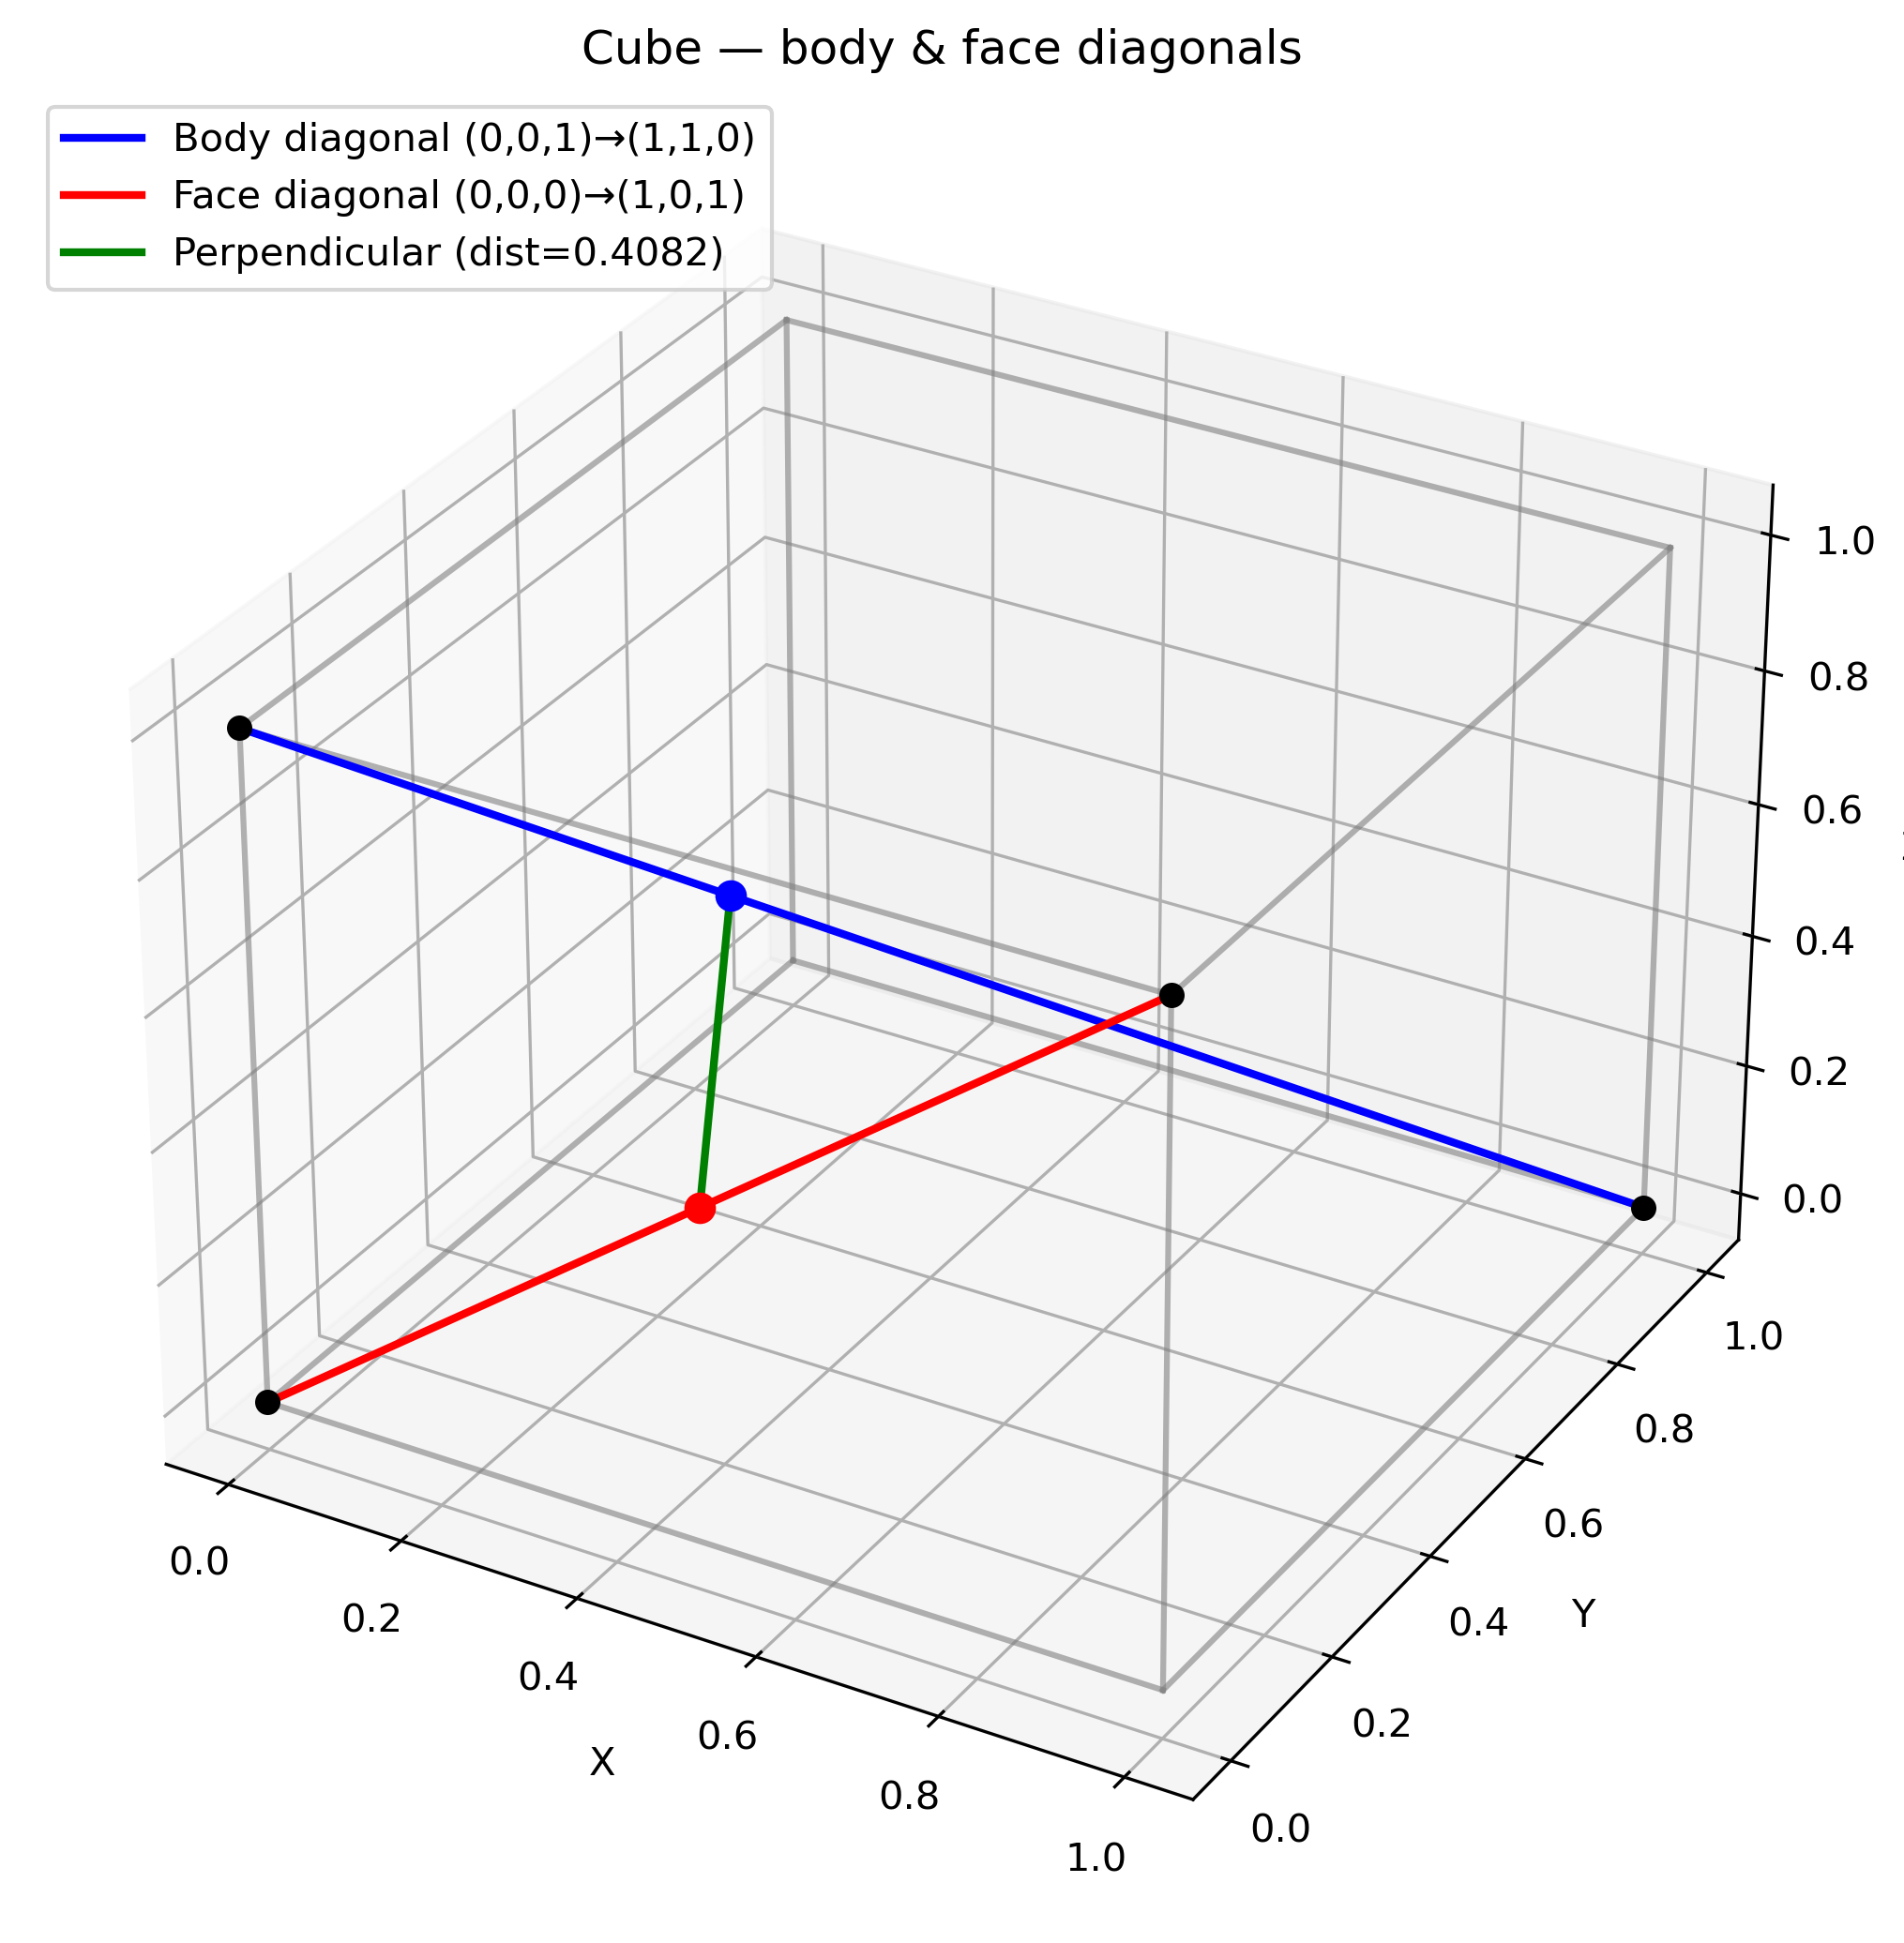
\includegraphics[width=0.7\columnwidth]{JEE/chapters/2.10.84/figs/cube_lines.png} 
   \caption{}
  \label{fig:2.10.84/Fig1}
\end{figure}


 \item Let $\vec{P}$ be the plane $3x + 2y + 3z = 16$ and let 
$$
S : \alpha \hat{i} + \beta \hat{j} + \gamma \hat{k}, \quad \text{where } \alpha + \beta + \gamma = 7
$$
and the distance of $(\alpha, \beta, \gamma)$ from the plane is $\frac{2}{\sqrt{22}}$.
Let $\vec{u}, \vec{v}, \vec{w}$ be three distinct vectors in $S$ such that $|\vec{u} - \vec{v}| = |\vec{v} - \vec{w}| = |\vec{w} - \vec{u}|$. Let $V$ be the volume of the parallelepiped determined by vectors $\vec{u}, \vec{v}, \vec{w}$. Then the value of $\frac{80}{3} V$ is
\rule{1cm}{0.1pt}.
\hfill (2023)
\item Let the position vectors of the points $\vec{P}, \vec{Q}, \vec{R},$ and $\vec{S}$ be
\begin{align*}
{\overrightarrow{a}} &= \hat{i} + 2\hat{j} - 5\hat{k}\\ {\overrightarrow{b}} &= 3\hat{i} + 6\hat{j} + 3\hat{k}\\ {\overrightarrow{c}} &= \frac{17}{5}\hat{i} + \frac{16}{5}\hat{j} + \frac{7}{5}\hat{k}\\ {\overrightarrow{d}} &= 2\hat{i} + \hat{j} + \hat{k}
\end{align*}
	respectively. Then which of the following statements is true?
\hfill (2023)
\begin{enumerate}
\item The points $\vec{P}, \vec{Q}, \vec{R},$ and $\vec{S}$ are NOT coplanar
\item $\frac{\vec{\overrightarrow{b}} + 2\vec{\overrightarrow{d}}}{3}$ is the position vector of a point which divides $PR$ internally in the ratio $5:4$
\item $\frac{\vec{\overrightarrow{b}} + 2\vec{\overrightarrow{d}}}{3}$ is the position vector of a point which divides $PR$ externally in the ratio $5:4$
\item The square of the magnitude of the vector $\vec{\overrightarrow{b}} \times \vec{\overrightarrow{d}}$ is $95$
\end{enumerate}
%
\item Let $\mathbb{R}^3$ denote the three-dimensional space. Take two points $\vec{P} = \brak{1,2,3}$ and $\vec{Q} = \brak{4,2,7}$. Let $dist\brak{\vec{X},\vec{Y}}$ denote the distance between two points $\vec{X}$ and $\vec{Y}$ in $\mathbb{R}^3$. Let  

\[
S = \{ \vec{X} \in \mathbb{R}^3 \; : \; \brak{dist\brak{\vec{X},\vec{P}}}^2 - \brak{dist\brak{\vec{X},\vec{Q}}}^2 = 50 \}
\]

\[
T = \{ \vec{Y} \in \mathbb{R}^3 \; : \; \brak{dist\brak{\vec{Y},\vec{Q}}}^2 - \brak{dist\brak{\vec{Y},\vec{P}}}^2 = 50 \}
\]

Then which of the following statements is {are} TRUE?
\hfill (2024)
\begin{enumerate}
\item There is a triangle whose area is $1$ and all of whose vertices are from $S$.
\item There are two distinct points $\vec{L}$ and $\vec{M}$ in $T$ such that each point on the line segment $LM$ is also in $T$.
\item There are infinitely many rectangles of perimeter $48$, two of whose vertices are from $S$ and the other two vertices are from $T$.
\item There is a square of perimeter $48$, two of whose vertices are from $S$ and the other two vertices are from $T$.
\end{enumerate}
\end{enumerate}

\item Find the values of $x, y, z$ so that the vectors 
$x\hat{i}+2\hat{j}+z\hat{k}$
and 
$2\hat{i}+y\hat{j}+\hat{k}$
are equal.
\item Find the sum of the vectors $\vec{a}=\hat{i}-2\hat{j}+\hat{k}$,  $\vec{b}=-2\hat{i}+4\hat{j}+5\hat{k}$ and $\vec{c}=\hat{i}-6\hat{j}-7\hat{k}$.
\item Find the slope of a line,  which passes through the origin and the mid point of the line segment joining the points $\vec{P}$(0, -4) and $\vec{B}$(8, 0).
\label{chapters/11/10/1/5}
	\\
	\solution
\begin{enumerate}[label=\thesection.\arabic*,ref=\thesection.\theenumi]
	%iffalse%\let\negmedspace\undefined
\let\negthickspace\undefined
\documentclass[journal,12pt,onecolumn]{IEEEtran}
\usepackage{cite}
\usepackage{amsmath,amssymb,amsfonts,amsthm}
\usepackage{algorithmic}
\usepackage{graphicx}
\usepackage{textcomp}
\usepackage{xcolor}
\usepackage{caption}
\usepackage{txfonts}
\usepackage{listings}
\usepackage{enumitem}
\usepackage{mathtools}
\usepackage{gensymb}
\usepackage{comment}
\usepackage[breaklinks=true]{hyperref}
\usepackage{tkz-euclide} 
\usepackage{listings}
\usepackage{gvv}                                        
%\def\inputGnumericTable{}                                 
\usepackage[latin1]{inputenc}   
\usepackage{xparse}
\usepackage{color}                                            
\usepackage{array}                                            
\usepackage{longtable}                                       
\usepackage{calc}                                             
\usepackage{multirow}
\usepackage{multicol}
\usepackage{hhline}                                           
\usepackage{ifthen}                                           
\usepackage{lscape}
\usepackage{tabularx}
\usepackage{array}
\usepackage{float}
\newtheorem{theorem}{Theorem}[section]
\newtheorem{problem}{Problem}
\newtheorem{proposition}{Proposition}[section]
\newtheorem{lemma}{Lemma}[section]
\newtheorem{corollary}[theorem]{Corollary}
\newtheorem{example}{Example}[section]
\newtheorem{definition}[problem]{Definition}
\newcommand{\BEQA}{\begin{eqnarray}}
\newcommand{\EEQA}{\end{eqnarray}}
\usepackage{float}
%\newcommand{\define}{\stackrel{\triangle}{=}}
\theoremstyle{remark}
\usepackage{ circuitikz }
%\newtheorem{rem}{Remark}
% Marks the beginning of the document this one
\title{ AE : AEROSPACE ENGINEERING}
\author{EE25BTECH11018-Darisy Sreetej}
\begin{document}
\maketitle

\begin{enumerate}
  
\item The function defined by
$
f(x) = \begin{cases}
\sin x, & x < 0 \\
0, & x = 0 \\
3x^3, & x > 0
\end{cases}
$

\begin{enumerate}
\begin{multicols}{2}
\item  is neither continuous nor differentiable at $x = 0$ 
\item  is continuous and differentiable at $x = 0$ 
\item  is differentiable but not continuous at $x = 0$ 
\item  is continuous but not differentiable at $x = 0$
\end{multicols}
\end{enumerate}

\hfill(GATE AE 2008)
\quad

\item The product of the eigenvalues of the matrix
$
\myvec{
1 & 0 & 1 \\
0 & 2 & 1 \\
1 & 1 & -3
}
$
is 
\begin{enumerate}
\begin{multicols}{4}
    

\item 4  \item 0  \item $-6$  \item $-9$
\end{multicols}
\end{enumerate}
\hfill(GATE AE-2008)
\quad

\item Which of the following equations is a LINEAR ordinary differential equation?

\begin{enumerate}
\begin{multicols}{2}
   \item $\dfrac{d^2 y}{dx^2} + \dfrac{dy}{dx} + 2y^2 = 0$
    \item $\dfrac{d^2 y}{dx^2} + y \dfrac{dy}{dx} + 2y = 0$
    \item $\dfrac{d^2 y}{dx^2} + \dfrac{dy}{dx} + 2y = 0$
   \item $\left( \dfrac{dy}{dx} \right)^2 + \dfrac{dy}{dx} + 2y = 0$
   \end{multicols}
\end{enumerate}
\hfill(GATE AE-2008)
\quad

\item To transfer a satellite from an elliptical orbit to a circular orbit having radius equal to the apogee distance of the elliptical orbit, the speed of the satellite should be 
\begin{enumerate}
    \begin{multicols}{2}

\item increased at the apogee 
\item decreased at the apogee 
\item increased at the perigee 
\item decreased at the perigee
\end{multicols}
\end{enumerate}
\hfill(GATE AE-2008)
\quad

\item The service ceiling of a transport aircraft is defined as the altitude 
\begin{enumerate}
    \begin{multicols}{2}
\item that is halfway between sea-level and absolute ceiling 
\item at which it can cruise with one engine operational 
\item at which its maximum rate of climb is zero 
\item at which its maximum rate of climb is 0.508 m/s
\end{multicols}
\end{enumerate}

\hfill(GATE AE-2008)
\quad

\item The drag of an aircraft in steady climbing fight at a given forward speed is 
\begin{enumerate}
\begin{multicols}{2}
    \item inversely proportional to climb angle 
    \item higher than drag in steady level fight at the same forward speed 
    \item lower than drag in steady level fight at the same forward speed 
    \item independent of climb angle 
    \end{multicols}
\end{enumerate}
\hfill(GATE AE-2008)

\quad

\item In steady,level turning flight of an aircraft at a load factor 'n',the ratio of the horizontal component of lift and aircraft weight is 
\begin{enumerate}
\begin{multicols}{4}
    \item $ \sqrt{n-1} $
    \item $\sqrt{n+1}$
    \item $\sqrt{n^2-1}$
    \item $\sqrt{n^2+1}$
    \end{multicols}
\end{enumerate}
\hfill(GATE AE-2008)

\quad

\item The parameters that remain constant in a cruise-climb of an aircraft are
\begin{enumerate}
\begin{multicols}{2}
    \item equivalent airspace and lift coefficient 
    \item altitude and lift coefficient
    \item equivalent airspace and altitude 
    \item lift coefficient and aircraft mass 
    \end{multicols}
\end{enumerate}
\hfill(GATE AE-2008)

\quad

\item The maximum thickness to chord ratio for the NACA 24012 airfoil is  
\begin{enumerate}
\begin{multicols}{4}
    \item 0.01 
    \item 0.12
    \item 0.24 
    \item 0.40
    \end{multicols}
\end{enumerate}
\hfill(GATE AE-2008)

\quad

\item The maximum possible value of pressure coefficient \(C_p\) in incompressible flow is 
\begin{enumerate}
\begin{multicols}{4}
    \item 0.5
    \item 1 
    \item $pi$
    \item $infty$
    \end{multicols}
\end{enumerate}
\hfill(GATE AE-2008)

\quad

\item An irrotational and inviscid flow can become rotational on passing through a 
\begin{enumerate}
\begin{multicols}{2}
    \item normal shock wave 
    \item oblique shock wave 
    \item curved shock wave 
    \item mach wave 
    \end{multicols}
\end{enumerate}
\hfill(GATE AE-2008)

\quad 

\item Laminar flow airfoils are used to reduce 
\begin{enumerate}
\begin{multicols}{2}
    \item trim drag 
    \item skin friction drag 
    \item induced drag 
    \item wave drag
    \end{multicols}
\end{enumerate}
\hfill(GATE AE-2008)

\quad 

\item The degree of reaction of an impulse turbine is 
\begin{enumerate}
\begin{multicols}{4}
    \item 1
    \item 0.75 
    \item 0.5
    \item 0
    \end{multicols}
\end{enumerate}
\hfill(GATE AE-2008)

\quad 

\item In a convergent-divergent(CD) nozzle of a rocket motor, the wall heat flux is maximum at 
\begin{enumerate}
\begin{multicols}{2}
    \item the exit of the divergent portion of the CD nozzle 
    \item the entry to the convergent portion of the CD nozzle 
    \item the throat of the CD nozzle 
    \item the mid-length of the divergent portion of the CD nozzle 
    \end{multicols}
\end{enumerate}
\hfill(GATE AE-2008)

\quad 

\item In a scramjet engine, the Mach number at the entry to the combustion chamber is around 
\begin{enumerate}
\begin{multicols}{4}
    \item 0
    \item 0.3
    \item 2
    \item 6 
    \end{multicols}
\end{enumerate}
\hfill(GATE AE-2008)

\quad 

\item DB denotes double base solid propellant.  
LOX-RP1 denotes liquid oxygen -- kerosene combination.  
LOX-LH$_2$ denotes liquid oxygen -- hydrogen combination.  

The correct order of increasing specific impulse is:  

\begin{enumerate}
\begin{multicols}{2}
\item $\text{DB} < \text{LOX-RP1} < \text{LOX-LH}_2$
\item $\text{LOX-RP1} < \text{DB} < \text{LOX-LH}_2$
\item $\text{LOX-LH}_2 < \text{DB} < \text{LOX-RP1}$
\item $\text{DB} < \text{LOX-LH}_2 < \text{LOX-RP1}$
\end{multicols}
\end{enumerate} 
\hfill(GATE AE-2008)

\quad 

\item  In the absence of body moments, the symmetry of the stress of the stress tensor is derived from 
\begin{enumerate}
\begin{multicols}{2}
    \item force equilibrium conditions 
    \item moment equilibrium conditions 
    \item linear relations between stresses and strains 
    \item compatibility conditions 
    \end{multicols}
\end{enumerate}
\hfill(GATE AE-2008)

\quad 

\item  In a 3-D orthotropic material, the number of elastic constants in linear stress-strain relationship is
    
    \begin{enumerate}
    \begin{multicols}{4}
        \item 3
        \item 5
        \item 9
        \item 21
        \end{multicols}
    \end{enumerate}
\hfill(GATE AE-2008)

\quad

    \item The compatibility conditions in theory of elasticity ensure that
    \begin{enumerate}
    \begin{multicols}{2}
        \item there is compatibility between various direct and shear stresses
        \item relationships between stresses and strains are consistent with constitutive relations
        \item displacements are single-valued and continuous
        \item stresses satisfy bi-harmonic equation
        \end{multicols}
    \end{enumerate}
\hfill(GATE AE-2008)

\quad

    \item In a spring-mass-damper single degree of freedom system, the mass is 2 kg and the undamped natural frequency is 20 Hz. The critical damping constant of the system is
    \begin{enumerate}
        \begin{multicols}{4}
        \item 160$\pi$ Ns/m
        \item 80$\pi$ Ns/m
        \item 1 Ns/m
        \item 0 Ns/m
        \end{multicols}
    \end{enumerate}
\hfill(GATE AE-2008)

\quad


\quad 

        \item Which of the following quantities remains constant for a satellite in an elliptical orbit around the earth?
    \begin{enumerate}
    \begin{multicols}{2}
        \item Kinetic energy
        \item Product of speed and radial distance from the center of the earth
        \item Rate of area swept by the radial vector from the center of the orbit
        \item Rate of area swept by the radial vector from the center of the earth
        \end{multicols}
    \end{enumerate}
\hfill(GATE AE-2008)

    \quad
    
    \item A planet is observed to be at its slowest when it is at a distance $r_1$ from the sun and at its fastest when it is at a distance $r_2$ from the sun. The eccentricity $e$ of the planet's orbit is given by
    \begin{enumerate}
    \begin{multicols}{2}
        \item $e = \frac{r_1}{r_2}$
        \item $e = \frac{r_1 - r_2}{r_1 + r_2}$
        \item $e = \frac{r_2}{r_1}$
        \item $e = \frac{r_1 + r_2}{r_1 - r_2}$
        \end{multicols}
    \end{enumerate}
    \hfill(GATE AE-2008)

\quad

    \item The function $f(x,y,z) = \frac{1}{2}x^2y^2z^2$ satisfies
    \begin{enumerate}
    \begin{multicols}{2}
        \item grad $f = 0$
        \item div(grad $f$) = 0
        \item curl(grad $f$) = 0
        \item grad(div(grad $f$)) = 0
        \end{multicols}
    \end{enumerate}
    \hfill(GATE AE-2008)

    \quad
    
    \item Which of the following is true for all choices of vectors $\vec{p}, \vec{q}, \vec{r}$?
    \begin{enumerate}
    \begin{multicols}{2}
        \item $\vec{p} \times \vec{q} + \vec{q} \times \vec{r} + \vec{r} \times \vec{p} = 0$
        \item $(\vec{p} \cdot \vec{q}) \vec{r} + (\vec{q} \cdot \vec{r}) \vec{p} + (\vec{r} \cdot \vec{p}) \vec{q} = 0$
        \item $\vec{p} \cdot (\vec{q} \times \vec{r}) + \vec{q} \cdot (\vec{r} \times \vec{p}) + \vec{r} \cdot (\vec{p} \times \vec{q}) = 0$
        \item $\vec{p} \times (\vec{q} \times \vec{r}) + \vec{q} \times (\vec{r} \times \vec{p}) + \vec{r} \times (\vec{p} \times \vec{q}) = 0$
        \end{multicols}
    \end{enumerate}
    \hfill(GATE AE-2008)

\quad

    \item  The value of the line integral
    $
    \frac{1}{2\pi} \oint (x\,dy - y\,dx)
    $
    taken anticlockwise along a circle of unit radius is
    \begin{enumerate}
    \begin{multicols}{4}
        \item 0.5
        \item 1
        \item 2
        \item $\pi$
        \end{multicols}
    \end{enumerate}
\hfill(GATE AE-2008)

\quad

    \item Which of the following is a solution of 
    $
    \frac{d^2 y}{dx^2} + 2\frac{dy}{dx} + y = 0 ?
    $
    \begin{enumerate}
    \begin{multicols}{2}
        \item $e^{-x} + xe^{-x}$
        \item $e^x + xe^{-x}$
        \item $e^t + e^x$
        \item $e^{-x} + xe^x$
        \end{multicols}
    \end{enumerate}
    \hfill(GATE AE-2008)

    \quad

    \item Suppose the non-constant functions $F(x)$ and $G(t)$ satisfy
    $
    \frac{d^2 F}{dx^2} + p^2 F = 0,\quad \frac{dG}{dt} + c^2 p^2 G = 0,
    $
    where $p$ and $c$ are constants. Then the function $u(x,t) = F(x)G(t)$ definitely satisfies
    \begin{enumerate}
    \begin{multicols}{2}
        \item $\frac{\partial^2 u}{\partial t^2} = c^2 \frac{\partial^2 u}{\partial x^2}$
        \item $\frac{\partial u}{\partial t} = c^2 \frac{\partial^2 u}{\partial x^2}$
        \item $\nabla^2 u = 0$
        \item $\frac{\partial^2 u}{\partial t^2} + c^2 u^2 = 0$
        \end{multicols}
    \end{enumerate}
    \hfill(GATE AE-2008)

    \quad

        \item The following set of equations
    $
    \myvec{
    1 & 1 & 2 \\
    1 & 0 & 1 \\
    0 & 1 & 1 
    }
    \myvec{
    x_1 \\
    x_2 \\
    x_3
    }
    =
    \myvec{
    1 \\
    -1 \\
    0
    }
    $
    has
    \begin{enumerate}
    \begin{multicols}{2}
        \item no solution
        \item a unique solution
        \item two solutions
        \item infinite solutions
        \end{multicols}
    \end{enumerate}
    \hfill(GATE AE-2008)

    \quad

    \item The function $f(x) = x^2 - 5x + 6$
    \begin{enumerate}
    \begin{multicols}{2}
        \item has its maximum value at $x = 2.0$
        \item has its maximum value at $x = 2.5$
        \item is increasing on the interval (2.0, 2.5)
        \item is increasing on the interval (2.5, 3.0)
        \end{multicols}
    \end{enumerate}
    \hfill(GATE AE-2008)

    \quad

        \item Let $Y(s)$ denote the Laplace transform $\mathcal{L}(y(t))$ of the function $y(t) = \cosh(at) \sin(at)$. Then
    \begin{enumerate}
    \begin{multicols}{2}
        \item $\mathcal{L}\left(\frac{dy}{dt}\right) = \frac{dY}{ds}, \quad \mathcal{L}(t\,y(t)) = sY(s)$
        \item $\mathcal{L}\left(\frac{dy}{dt}\right) = sY(s), \quad \mathcal{L}(t\,y(t)) = -\frac{dY}{ds}$
        \item $\mathcal{L}\left(\frac{dy}{dt}\right) = \frac{dY}{ds}, \quad \mathcal{L}(t\,y(t)) = Y(s-1)$
        \item $\mathcal{L}\left(\frac{dy}{dt}\right) = sY(s), \quad \mathcal{L}(t\,y(t)) = e^{a}Y(s)$
        \end{multicols}
    \end{enumerate}
        \hfill(GATE AE-2008)

    \quad

    \item  The velocity required for a spacecraft to escape earth's gravitational field depends on
    \begin{enumerate}
    \begin{multicols}{2}
        \item the mass of the spacecraft
        \item the distance between earth's center and the spacecraft
        \item the earth's rotational speed about its own axis
        \item the earth's orbital speed
        \end{multicols}
    \end{enumerate}
    \hfill(GATE AE-2008)

    \quad

\item The figure below shows the variation of $C_m$ versus $\alpha$ for an aircraft for three combinations of elevator deflections and locations of centre of gravity.In the figure, lines P and Q are parallel, while lines Q and R have the same intercept on the $C_m$ axis.

\begin{figure}
    \centering
    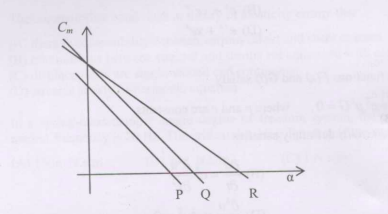
\includegraphics[width=0.5\linewidth]{figs/Screenshot from 2025-08-08 00-10-35.png}
    \caption{Caption}
    \label{fig:placeholder}
\end{figure}
 Which of the following statements is true?
    \begin{enumerate}
    \begin{multicols}{2}
        \item Lines P and Q correspond to the same centre of gravity location.
        \item Lines Q and R correspond to the same centre of gravity location.
        \item Lines P and Q correspond to the same elevator deflection.
        \item Lines P and R correspond to the same centre of gravity location.
        \end{multicols}
    \end{enumerate}
    \hfill(GATE AE-2008)

    \quad

 \item Which of the following statements is TRUE as the altitude increases in stratosphere of International Standard Atmosphere?
    \begin{enumerate}
    \begin{multicols}{2}
        \item Temperature increases and dynamic viscosity decreases.
        \item Temperature remains constant and pressure increases.
        \item Temperature decreases and sound speed decreases.
        \item Temperature remains constant and density decreases.
        \end{multicols}
    \end{enumerate}
    \hfill(GATE AE-2008)

    \quad

 \item Which of the following statements is TRUE?
    \begin{enumerate}
    \begin{multicols}{2}
        \item Wing dihedral reduces roll stability while a low wing increases roll stability.
        \item Wing dihedral increases roll stability while a low wing reduces roll stability.
        \item Wing dihedral, as well as low wing reduces roll stability.
        \item Wing dihedral, as well as low wing increases roll stability.
        \end{multicols}
    \end{enumerate}
    \hfill(GATE AE-2008)

    \quad

 \item An aircraft has a level flight stalling speed of 60 m/s EAS (equivalent air speed). As per the V-n diagram, what is the minimum speed at which it should be designed to withstand the maximum vertical load factor of 9?
    \begin{enumerate}
    \begin{multicols}{4}
        \item 20 m/s
        \item 60 m/s
        \item 120 m/s
        \item 180 m/s
        \end{multicols}
    \end{enumerate}
    \hfill(GATE AE-2008)

    \quad

    \item  Match each mode of aircraft motion listed in Group I to its corresponding property from Group II.

\input{tables/table1}
    \begin{enumerate}
    \begin{multicols}{2}
        \item P-2, Q-1, R-4, S-3
        \item P-4, Q-3, R-2, S-1
        \item P-4, Q-1, R-2, S-3
        \item P-2, Q-3, R-4, S-1
        \end{multicols}
    \end{enumerate}
    \hfill(GATE AE-2008)

    \quad

    \item An aircraft is cruising at a true air speed (TAS) of 100 m/s under ISA conditions, at an altitude at which the density of free stream is 0.526 kg/m$^3$. What will be the equivalent air speed (EAS)?
    \begin{enumerate}
    \begin{multicols}{2}
        \item 65.5 m/s
        \item 72.5 m/s
        \item 110.5 m/s
        \item 152.7 m/s
        \end{multicols}
    \end{enumerate}
    \hfill(GATE AE-2008)

    \quad

\item In the definition of the aircraft Euler angles $\phi$ (roll), $\theta$ (pitch), and $\psi$ (yaw), the correct sequence of rotations required to make the inertial frame coincide with the aircraft body frame is  
\begin{enumerate}
\begin{multicols}{2}
    \item First $\psi$ about $z$ axis, second $\theta$ about $y$ axis, third $\phi$ about $x$ axis
    \item First $\theta$ about $y$ axis, second $\phi$ about $x$ axis, third $\psi$ about $z$ axis
    \item First $\phi$ about $x$ axis, second $\theta$ about $y$ axis, third $\psi$ about $z$ axis
    \item First $\psi$ about $z$ axis, second $\phi$ about $x$ axis, third $\theta$ about $y$ axis
    \end{multicols}
\end{enumerate}
    \hfill(GATE AE-2008)

    \quad

\item To maximize range of a jet engine aircraft, it should be flown at a velocity that maximizes  
\begin{enumerate}
\begin{multicols}{2}
    \item $C_L/C_D$
    \item $C_L^{0.5}/C_D$
    \item $C_L^{1.5}/C_D$
    \item $C_L^2/C_D$
    \end{multicols}
\end{enumerate}
    \hfill(GATE AE-2008)

    \quad

\item The primary function of the fin in the vertical tail of an aircraft is to provide  
\begin{enumerate}
\begin{multicols}{2}
    \item yaw control
    \item yaw stability
    \item roll damping
    \item roll stability
    \end{multicols}
\end{enumerate}
    \hfill(GATE AE-2008)

    \quad

\item An aircraft requires the trailing edge of the elevator to be deflected upwards from its initial position to lower the trim speed. Which of the following statements about the static stick-fixed stability of this aircraft is true? 
\begin{enumerate}
\begin{multicols}{2}
    \item The aircraft is unstable.
    \item The aircraft is neutrally stable.
    \item The aircraft is stable.
    \item The stability of the aircraft cannot be determined from the given information.
    \end{multicols}
\end{enumerate}
    \hfill(GATE AE-2008)

    \quad

\item Which of the following statements is true for an aircraft flying at a low angle of attack?  
\begin{enumerate}
\begin{multicols}{2}
    \item Yawing motion generates yawing moment and pitching moment.
    \item Rolling motion generates rolling moment and pitching moment.
    \item Yawing motion generates yawing moment and rolling moment.
    \item Pitching motion generates yawing moment and rolling moment.
    \end{multicols}
\end{enumerate}
    \hfill(GATE AE-2008)

    \quad

\item Consider 2-D flow with stream function $\psi = \frac{1}{2} \ln\left( \sqrt{x^2 + y^2} \right)$. The absolute value of circulation along a unit circle centered at $(x=0, y=0)$ is  
\begin{enumerate}
\begin{multicols}{4}
    \item 0
    \item 1
    \item $\pi/2$
    \item $\pi$
    \end{multicols}
\end{enumerate}
    \hfill(GATE AE-2008)

    \quad

\item Consider a symmetric airfoil at an angle of attack of $4$ degrees. Using thin airfoil theory, the magnitude of the moment coefficient about the leading edge is  
\begin{enumerate}
\begin{multicols}{4}
    \item $2\pi$
    \item $\pi$
    \item $\pi^2/60$
    \item $\pi^2/90$
    \end{multicols}
\end{enumerate}
    \hfill(GATE AE-2008)

    \quad

\item Consider steady, inviscid flow in a convergent-divergent (CD) nozzle, with a normal shock in the divergent portion. The static pressure along the nozzle downstream of the normal shock  
\begin{enumerate}
\begin{multicols}{2}
    \item remains constant
    \item increases isentropically to the static pressure at the nozzle exit
    \item decreases isentropically to the static pressure at the nozzle exit
    \item can increase or decrease, depending on the magnitude of the static pressure at the nozzle exit
    \end{multicols}
\end{enumerate}
    \hfill(GATE AE-2008)

    \quad

\item For a free stream Mach number of $0.7$ the critical pressure coefficient $(C_{p_{cr}})$ is $-0.78$. If the minimum pressure coefficient for a given airfoil in incompressible flow is $-0.6$, then the flow over the airfoil at a free stream Mach number of $0.7$ is  
\begin{enumerate}
\begin{multicols}{2}
    \item subsonic and compressible 
    \item completely supersonic 
    \item incompressible 
    \item partly subsonic and partly supersonic
    \end{multicols}
\end{enumerate}
  \hfill(GATE AE-2008)

    \quad

\item If the flow Mach number in a turbulent boundary layer over a flat plate is increased keeping the Reynolds number unchanged, the skin friction coefficient $C_f$  
\begin{enumerate}
\begin{multicols}{2}
    \item decreases
    \item increases
    \item remains constant
    \item initially decreases, followed by a rapid increase
    \end{multicols}
\end{enumerate}
 \hfill(GATE AE-2008)

    \quad

\item In supersonic wind-tunnel design, an oblique shock diffuser is preferred over a normal shock diffuser because 
\begin{enumerate}
\begin{multicols}{2}
    \item it reduces total pressure loss
    \item the flow is slowed down more rapidly
    \item the flow is accelerated more rapidly
    \item it increases total pressure loss
    \end{multicols}
\end{enumerate}
 \hfill(GATE AE-2008)

    \quad

\item The variation of downwash along the span of an untwisted wing of elliptic planform is  
\begin{enumerate}
\begin{multicols}{2}
    \item sinusoidal
    \item parabolic
    \item elliptic
    \item constant
    \end{multicols}
\end{enumerate}
 \hfill(GATE AE-2008)

    \quad

\item Flow past an airfoil is to be modeled using a vortex sheet. The strength of the vortex sheet at the trailing edge will be  
\begin{enumerate}
\begin{multicols}{4}
    \item 0
    \item 1
    \item $2\pi$
    \item $\infty$
    \end{multicols}
\end{enumerate}
 \hfill(GATE AE-2008)

    \quad

\item Consider a 2-D body in supersonic flow with an attached oblique shock as shown below  
\begin{figure}[H]
    \centering
    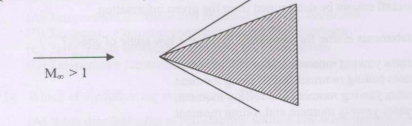
\includegraphics[width=0.5\linewidth]{figs/Screenshot from 2025-08-08 11-48-03.png}
    \caption{Caption}
    \label{fig:placeholder}
\end{figure}
An increase in free stream Mach number $M_\infty$ will cause the oblique shock wave to 
\begin{enumerate}
\begin{multicols}{2}
    \item move closer to the body 
    \item move away from the body 
    \item detach from the body 
    \item become a normal shock
    \end{multicols}
\end{enumerate}
 \hfill{GATE AE-2008}

    \quad

\item The geometrical features of a supercritical airfoil are  
\begin{enumerate}
\begin{multicols}{2}
    \item rounded leading edge, flat upper surface and high camber at the rear
    \item sharp leading edge, curved upper surface and high camber at the rear
    \item rounded leading edge, curved upper surface and no camber at the rear
    \item sharp leading edge, flat upper surface and no camber at the rear
    \end{multicols}
\end{enumerate}
 \hfill(GATE AE-2008)

    \quad

\item Which one of the following high lift device results in higher stalling angle? 
\begin{enumerate}
\begin{multicols}{2}
    \item split flap
    \item Fowler flap
    \item plain flap
    \item leading edge flap
    \end{multicols}
\end{enumerate}
 \hfill(GATE AE-2008)

    \quad

\item A turbofan engine has a bypass ratio of $5$ and a total mass flow rate of $120 \ \mathrm{kg/s}$. The mass flow rate through the bypass duct is
\begin{enumerate}
\begin{multicols}{2}
    \item $20 \ \mathrm{kg/s}$
    \item $100 \ \mathrm{kg/s}$
    \item $120 \ \mathrm{kg/s}$
    \item $600 \ \mathrm{kg/s}$
    \end{multicols}
\end{enumerate}
 \hfill(GATE AE-2008)

    \quad

\item A turbojet engine is operating with afterburner off. If the afterburner is switched on, then  
\begin{enumerate}
\begin{multicols}{2}
    \item both thrust and sfc decrease
    \item thrust increases and sfc decreases
    \item thrust decreases and sfc increases
    \item both thrust and sfc increase
    \end{multicols}
\end{enumerate}
 \hfill(GATE AE-2008)

    \quad

\item A centrifugal compressor operates with a tip blade speed of $340 \ \mathrm{m/s}$. The air leaves the impeller with a radial velocity of $88 \ \mathrm{m/s}$. If the slip factor is $0.85$, the relative velocity at the blade tip is  
\begin{enumerate}
\begin{multicols}{2}
    \item $101.7 \ \mathrm{m/s}$
    \item $120.3 \ \mathrm{m/s}$
    \item $132.6 \ \mathrm{m/s}$
    \item $135.8 \ \mathrm{m/s}$
    \end{multicols}
\end{enumerate}
 \hfill(GATE AE-2008)

    \quad

\item  An ideal ramjet engine is flying at a Mach number $M$. The exhaust gas static temperature at the outlet of the nozzle is $T_e$. The ambient static temperature is $T_a$. Gas constant $R$ and specific heat ratio $\gamma$ do not vary through the ramjet. Assuming that nozzle exhaust static pressure is equal to the ambient pressure and fuel air ratio $f \ll 1$, the thrust per unit mass flow rate is  
\begin{enumerate}
\begin{multicols}{2}
    \item $\sqrt{\gamma R T_a} \left[ \sqrt{\frac{T_e}{T_a}} - 1 \right]$
    \item $\sqrt{\gamma R T_e} \left[ \sqrt{\frac{T_e}{T_a}} - 1 \right]$
    \item $M \sqrt{\gamma R T_a} \left[ \sqrt{\frac{T_e}{T_a}} - 1 \right]$
    \item $M \sqrt{\gamma R T_e} \left[\sqrt{ \frac{T_e}{T_a}} - 1 \right]$
    \end{multicols}
\end{enumerate}
 \hfill(GATE AE-2008)

    \quad

\item A 50 percent degree of reaction axial flow turbine operates with a mean blade speed of $180 \ \mathrm{m/s}$. The flow leaves the stator and then enters the rotor at an angle of $60^\circ$ to the axial direction. The axial velocity is $150 \ \mathrm{m/s}$, and remains constant throughout the stage. The turbine power per unit mass flow is  
\begin{enumerate}
    \begin{multicols}{2}
    \item $29.76 \ \text{kJ/kg}$
    \item $41.12 \ \text{kJ/kg}$
    \item $58.33 \ \text{kJ/kg}$
    \item $61.13 \ \text{kJ/kg}$
    \end{multicols}
\end{enumerate}
\hfill(GATE AE-2008)

    \quad

\item The chamber stagnation temperature inside a rocket motor is $T_c$. Only a convergent nozzle is used, and the flow at the exit of this nozzle is choked. Assume that the nozzle exhaust static pressure is equal to ambient static pressure. Gas constant for exhaust gases is $R$ and ratio of specific heats is $\gamma$. The specific impulse of the rocket motor is  
\begin{enumerate}
\begin{multicols}{2}
    \item $\dfrac{2 \gamma R T_c}{\gamma - 1}$
    \item $\dfrac{\gamma R T_c}{\gamma - 1}$
    \item $\dfrac{\gamma R T_c}{\gamma + 1}$
    \item $\dfrac{2 \gamma R T_c}{\gamma + 1}$
    \end{multicols}
\end{enumerate}
\hfill(GATE AE-2008)

    \quad

\item  Air enters the combustor of a gas turbine engine at total temperature of $500 \ \mathrm{K}$ and leaves the combustor at total temperature of $1800 \ \mathrm{K}$. If $c_p$ remains constant at $1.005 \ \mathrm{kJ/(kg \cdot K)}$ and heating value of the fuel used is $44 \ \mathrm{MJ/kg}$, the fuel to air ratio is  
\begin{enumerate}
\begin{multicols}{4}
    \item $0.003$
    \item $0.012$
    \item $0.031$
    \item $0.074$
    \end{multicols}
\end{enumerate}
\hfill(GATE AE-2008)

    \quad

\item The initial temperature sensitivity of burn rate of a solid rocket motor propellant is positive. If the initial temperature increases then  
\begin{enumerate}
\begin{multicols}{2}
    \item thrust increases but burn time decreases
    \item thrust decreases and burn time decreases too
    \item thrust remains same but burn time increases
    \item thrust increases but burn time remains same
    \end{multicols}
\end{enumerate}
\hfill(GATE AE-2008)

    \quad

\item An aircraft is cruising at a Mach number of $0.8$ at an altitude where the ambient static pressure is $95 \ \mathrm{kPa}$. The diffuser exit total pressure is $140 \ \mathrm{kPa}$. Assuming there is no change in the specific heat at constant pressure across the diffuser, and ratio of specific heats is $1.4$, the adiabatic efficiency of the intake is  
\begin{enumerate}
\begin{multicols}{4}
    \item $0.988$
    \item $0.915$
    \item $0.722$
    \item $0.684$
    \end{multicols}
\end{enumerate}
\hfill(GATE AE-2008)

    \quad

\item A parallelogram shaped plate of dimensions 'a' and 'b' as shown in the figure, is subjected to a uniform loading of normal stresses $\sigma_1$ and $\sigma_2$. The plate is in equilibrium for 
\begin{figure}[H]
    \centering
    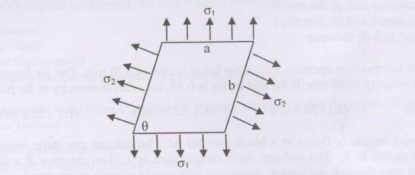
\includegraphics[width=0.5\linewidth]{figs/Screenshot from 2025-08-08 12-13-37.png}
    \caption{Caption}
    \label{fig:placeholder}
\end{figure}
\begin{enumerate}
\begin{multicols}{2}
    \item any value of $\sigma_1$ and $\sigma_2$
    \item $\sigma_2=\sigma_1 \cos\theta$
    \item $\sigma_1=\sigma_2 \cos\theta$
    \item $\sigma_2=\sigma_1$
    \end{multicols}
\end{enumerate}
\hfill(GATE AE-2008)

    \quad

\item A column of solid circular cross-section and length $L$ can have various end conditions. Choose the correct set that matches the end conditions (listed in Group I) with the corresponding effective length for buckling (listed in Group II).

\begin{center}
\input{tables/table2}
\end{center}

\quad

\begin{enumerate}
\begin{multicols}{2}

\item P-3, Q-1, R-2, S-4 
\item P-4, Q-1, R-2, S-3 
\item  P-2, Q-1, R-3, S-4 
\item P-3, Q-1, R-2, S-4
\end{multicols}
\end{enumerate}
\hfill(GATE AE-2008)

    \quad
    
\item A thin walled tube of circular cross-section with mean radius $r$ has a central web which divides it into two symmetric cells as shown. A torque $M$ is acting on the section. The shear flow $q$ in the central web is
\begin{figure}[H]
    \centering
    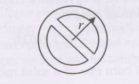
\includegraphics[width=0.5\linewidth]{figs/Screenshot from 2025-08-08 12-34-18.png}
    \caption{Caption}
    \label{fig:placeholder}
\end{figure}
\begin{enumerate}
\begin{multicols}{4}
    \item $q=M/2\pi r^2$
     \item $q=0$
      \item $q=M/4\pi r^2$
       \item $q=M/\pi r^2$
       \end{multicols}
\end{enumerate}
\hfill(GATE AE-2008)

\quad 

\item  A concentraion bending moment M is acting at mid-span of a beam as shown. The shear force diagram for the beam is:
\begin{figure}[H]
    \centering
    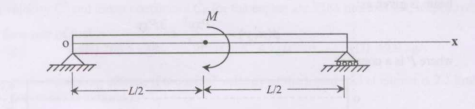
\includegraphics[width=0.5\linewidth]{figs/Screenshot from 2025-08-08 12-52-57.png}
    \caption{Caption}
    \label{fig:placeholder}
\end{figure}
\begin{enumerate}
    \item 
    \begin{figure}[H]
        \centering
        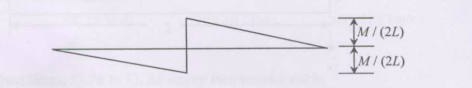
\includegraphics[width=0.5\linewidth]{figs/Screenshot from 2025-08-08 12-59-04.png}
        \caption{Caption}
    \label{fig:placeholder}
    \end{figure} 
    
    \item 
    \begin{figure}[H]
        \centering
        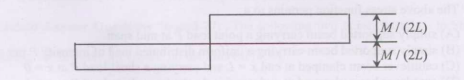
\includegraphics[width=0.5\linewidth]{figs/Screenshot from 2025-08-08 14-37-14.png}
        \caption{Caption}
    \label{fig:placeholder}
        \end{figure} 

        \item 
        \begin{figure}[H]
            \centering
            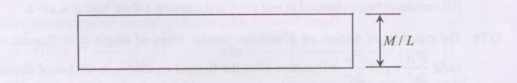
\includegraphics[width=0.5\linewidth]{figs/Screenshot from 2025-08-09 16-17-42.png}
            \caption{Caption}
    \label{fig:placeholder}
        \end{figure}

        \item 
        \begin{figure}[H]
            \centering
            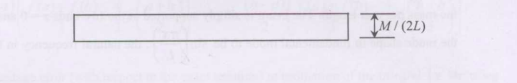
\includegraphics[width=0.5\linewidth]{figs/Screenshot from 2025-08-09 16-19-48.png}
            \caption{Caption}
    \label{fig:placeholder}
        \end{figure}
        
\end{enumerate}
\hfill(GATE AE-2008)

\quad

\item  An idealized thin-walled cross-section of a beam and the respective areas of the booms are as shown. A bending moment M, is acting on the cross-section. The ratio of the magnitude of normal stress in the top booms to that of the bottom boom is
\begin{figure}[H]
    \centering
    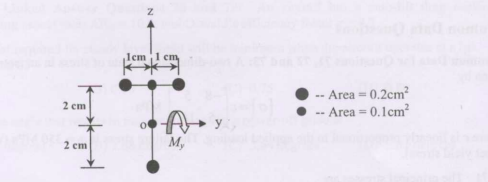
\includegraphics[width=0.5\linewidth]{figs/Screenshot from 2025-08-08 14-45-55.png}
    \caption{Caption}
    \label{fig:placeholder}
\end{figure}
\begin{enumerate}
\begin{multicols}{4}
    \item 5/11
    \item 2/5
    \item 1
    \item 5/2
    \end{multicols}
\end{enumerate}
\hfill(GATE AE-2008)

\quad

\item  An engineer is asked to test a system which can be idealized as SDOF (single degree of freedom) with viscous damping. A frequency response test was conducted and it is found that the quality factor Q is equal to 10. What will be the logarithmic decrement if a free vibration test is performed?
\begin{enumerate}
\begin{multicols}{4}
    \item $\pi/40$
     \item $\pi/20$
     \item $\pi/10$
      \item $\pi/5$
      \end{multicols}
\end{enumerate}
\hfill{GATE AE-2008}

\quad

\item A beam occupies a region 
$
0 \leq x \leq L, \quad -c \leq y \leq c, \quad -0.5 \leq z \leq 0.5
$
as shown below. The beam can be considered to be in plane stress condition in the $x\text{-}y$ plane.  
Airy's stress function for the beam is given as:
$
\phi(x,y) = \frac{Pxy^{3}}{4c^{3}} + \frac{3Pxy}{4c}
$
where $P$ is a constant.
\begin{figure}[H]
    \centering
    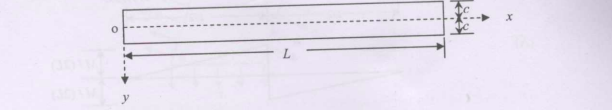
\includegraphics[width=0.5\linewidth]{figs/Screenshot from 2025-08-08 14-58-40.png}
    \caption{Caption}
    \label{fig:placeholder}
\end{figure}
The above stress function pertains to a 
\begin{enumerate}
\begin{multicols}{2}
\item simply supported beam carrying a point load P at mid span
\item simply supported beam carrying a uniform distributed load of intensity P per unit length
\item cantilever beam clamped at end x = L and carrying a shear load P at x = 0
\item cantilever beam clamped at end x = 0 and carrying a shear load P at 
\end{multicols}
\end{enumerate}
\hfill(GATE AE 2008)

\quad 

\item  The equation of motion of a uniform slender beam of length \( L \) in flexural vibration is given as
$
EI \frac{\partial^4 w}{\partial x^4} + \rho A \frac{\partial^2 w}{\partial t^2} = 0
$
where $EI$ is the flexural rigidity, $w$ is the lateral displacement and $ \rho A $ is the mass per unit length.  
The beam is simply supported at the two ends $x = 0 $and $x = L $.  
Assuming the mode shape in fundamental mode to be $ \sin\left( \frac{\pi x}{L} \right) $,  
the natural frequency in fundamental mode is:

\begin{enumerate}
\begin{multicols}{2}
\item $ 0.5 \sqrt{\frac{EI}{\rho A L^4}} \, \pi^2 $
\item $sqrt{\frac{EI}{\rho A L^4}} \, \pi^2 $
\item $ 2 \sqrt{\frac{EI}{\rho A L^4}} \, \pi^2$ 
\item $ 4 \sqrt{\frac{EI}{\rho A L^4}} \, \pi^2$
\end{multicols}
\end{enumerate}
\hfill(GATE AE 2008)

\quad 

\textbf{Common Data Questions}  

\quad

\textbf{Common Data for Questions 71, 72 and 73:}  
A two-dimensional state of stress in an isotropic material is given by:
$
[\sigma] = c 
\myvec{
-8 & 5 \\
5 & 16
} \; \text{MPa}
$
where $c$ is linearly proportional to the applied loading.  
The failure stress is $ \sigma_f = 350 \, \text{MPa}$ (which is 0.2\% offset yield stress).

\item The principal stresses are:  

\begin{enumerate}
\begin{multicols}{2}
    \item $\sigma_1=17cMPa$, $\sigma_2=-9cMPa$
    \item $\sigma_1=9cMPa$, $\sigma_2=17cMPa$
    \item $\sigma_1=-17cMPa$, $\sigma_2=-9cMPa$
    \item $\sigma_1=17cMPa$, $\sigma_2=9cMPa$
    \end{multicols}
\end{enumerate}
\hfill(GATE AE 2008)

\quad 

\item The maximum shear stress is: 
\begin{enumerate}
\begin{multicols}{2}
    \item $\tau_{max}=7cMPa$
    \item $\tau_{max}=10cMPa$
    \item $\tau_{max}=13cMPa$
    \item $\tau_{max}=15cMPa$
    \end{multicols}
\end{enumerate}
\hfill(GATE AE 2008)

\quad 

\item The maximum value of $c $ for safe loading of the structure, based on von-Mises failure criterion is:  
\begin{enumerate}
\begin{multicols}{4}
    \item 10.2
    \item 15.3
    \item 25.4
    \item 31.8
    \end{multicols}
\end{enumerate}
\hfill(GATE AE 2008)

\quad 

\textbf{Common Data for Questions 74 and 75:}  
A liquid rocket engine with oxidizer to fuel ratio of 5:1 produces a thrust of $ 1 \, \text{MN} $.  
The initial mass of the rocket engine is $ 100{,}000 \, \text{kg} $ and its mass at burn out is $10{,}000 \, \text{kg} $.  
The characteristic velocity $C^* $ and thrust coefficient $C_F $ for the engine are 2386 \text{m/s}  and 1.4 , respectively.

\item The mass flow rate of fuel is:  
\begin{enumerate}
   \begin{multicols}{4}
\item 300.3 kg/s
\item 269.5 kg/s
\item 87.4 kg/s 
\item 49.9 kg/s
\end{multicols}
\end{enumerate}
\hfill(GATE AE 2008)

\quad 

\item Neglecting gravity and drag effects, if the initial velocity of the liquid rocket engine is $2.5 \ \text{km/s}$, the velocity of the rocket at burnout is:  

\begin{enumerate}
\begin{multicols}{2}
\item $1.2 \ \text{km/s}$
\item $2.5 \ \text{km/s}$
\item $10.2 \ \text{km/s}$
\item $11.8 \ \text{km/s}$
\end{multicols}
\end{enumerate}
\hfill(GATE AE 2008)

\quad 

\textbf{Statement for Linked Answer Questions 76 and 77:} 
The following two questions relate to Simpson's rule for approximating the integral  
$\int_a^b f(x) \, dx$ on the interval $[a, b]$.

\item Which of the following gives the correct formula for Simpson's rule? 

\begin{enumerate}
\begin{multicols}{2}
\item $\dfrac{(b-a)}{2} \left[ f(b) + f\left( \dfrac{a+b}{2} \right) \right]$
\item $\dfrac{(b-a)}{2} \left[ f(a) + f(b) + f\left( \dfrac{a+b}{2} \right) \right]$
\item $\dfrac{(b-a)}{2} \left[ \dfrac{f(a) + f(b)}{3} + \dfrac{4}{3} f\left( \dfrac{a+b}{2} \right) \right]$
\item $\dfrac{(b-a)}{2} \left[ \dfrac{f(a) + f(b)}{3} + \dfrac{4}{3} f\left( \dfrac{a+b}{3} \right) \right]$
\end{multicols}
\end{enumerate}
\hfill(GATE AE 2008)

\quad 

\item The percentage error (with respect to the exact solution) in estimation of the integral  
$\int_{0}^{1} x^3 \, dx$ using Simpson's rule is:  

\begin{enumerate}
\begin{multicols}{4}
\item $5.3$
\item $3.5$
\item $2.8$
\item $0$
\end{multicols}
\end{enumerate}
\hfill(GATE AE 2008)

\quad 

\textbf{Statement for Linked Answer Questions 78 and 79:}  
An aircraft has a zero-lift drag coefficient $C_{D_0} = 0.0223$, wing aspect ratio $AR_w = 10.0$, and Oswald's efficiency factor $e = 0.7$.

\item The thrust required for steady level flight will be minimum when the aircraft operates at a lift coefficient of:  

\begin{enumerate}
\begin{multicols}{4}
\item $0.65$
\item $0.70$
\item $0.75$
\item $0.80$
\end{multicols}
\end{enumerate}
\hfill(GATE AE-2008)

\quad 

\item The glide angle that results in maximum range in a power-off glide is:  

\begin{enumerate}
\begin{multicols}{4}
\item $1.82^\circ$
\item $2.68^\circ$
\item $3.64^\circ$
\item $5.01^\circ$
\end{multicols}
\end{enumerate}
\hfill(GATE AE 2008)

\quad 

\textbf{Statement for Linked Answer Questions 80 and 81:}  
Consider an untwisted wing of elliptical planform in inviscid incompressible irrotational flow at an angle of attack of $4^\circ$.  
The wing aspect ratio is $7$ and the zero lift angle of attack is $-2^\circ$.\\

\item The wing lift coefficient $C_L$ is:  

\begin{enumerate}
\begin{multicols}{4}
\item $0.66$
\item $0.51$
\item $0.44$
\item $0.34$
\end{multicols}
\end{enumerate}
\hfill(GATE AE 2008)

\quad 

\item The induced drag coefficient of the wing $C_{D_i}$ is:  

\begin{enumerate}
\begin{multicols}{4}
\item $0.0053$
\item $0.0087$
\item $0.0118$
\item $0.0197$
\end{multicols}
\end{enumerate}
\hfill(GATE AE 2008)

\quad 

\textbf{Statement for Linked Answer Questions 82 and 83:}  
A multi-stage axial flow compressor operating at an adiabatic efficiency of $0.9$ develops a total pressure ratio of $11$.  
The total temperature at inlet to the compressor is $335 \ \text{K}$ and the stagnation enthalpy rise across each stage is $37 \ \text{kJ/kg}$.  
Ratio of specific heats is $1.4$ and specific heat at constant pressure is $1.005 \ \text{kJ/kg.K}$.

\item The total temperature rise across the compressor is:  

\begin{enumerate}
\begin{multicols}{4}
\item $310.1 \ \text{K}$
\item $366.3 \ \text{K}$
\item $392.1 \ \text{K}$
\item $405.4 \ \text{K}$
\end{multicols}
\end{enumerate}
\hfill(GATE AE 2008)

\quad

\item The total number of stages required are:  

\begin{enumerate}
\begin{multicols}{4}
\item $9$
\item $10$
\item $11$
\item $12$
\end{multicols}
\end{enumerate} 
\hfill(GATE AE 2008)

\quad

\textbf{Statement for Linked Answer Questions 84 and 85:}  
An idealized thin walled two cell symmetric box beam is as shown.  
The shear flows in the walls are due to the applied shear forces $V_y = 480 \ \text{N}$, $V_z = 300 \ \text{N}$, and a torque $M$, all acting at the shear center.

\begin{figure}[H]
    \centering
    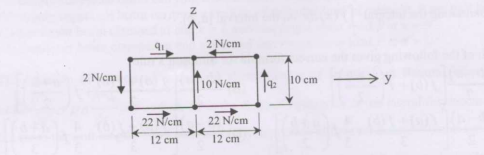
\includegraphics[width=0.5\linewidth]{figs/pic9.png}
    \caption{Caption}
    \label{fig:placeholder}
\end{figure}

\item \quad The shear flows $q_1$ and $q_2$ are:  

\begin{enumerate}
\begin{multicols}{2}
\item $q_1 = -2 \ \text{N/cm}$, \quad $q_2 = +22 \ \text{N/cm}$
\item $q_1 = +2 \ \text{N/cm}$, \quad $q_2 = +22 \ \text{N/cm}$
\item $q_1 = +2 \ \text{N/cm}$, \quad $q_2 = -22 \ \text{N/cm}$
\item $q_1 = -2 \ \text{N/cm}$, \quad $q_2 = -22 \ \text{N/cm}$
\end{multicols}
\end{enumerate} 
\hfill(GATE AE 2008)

\quad

\item The torque $M$ is:  

\begin{enumerate}
\begin{multicols}{2}
\item $3360 \ \text{N.cm}$
\item $5760 \ \text{N.cm}$
\item $6960 \ \text{N.cm}$
\item $8160 \ \text{N.cm}$
\end{multicols}
\end{enumerate} 
\hfill(GATE AE 2008)

\quad
\end{enumerate}
\end{document}

	\item In the interconnection of ideal sources shown in \figref{fig:placeholder_6}, it is known that the $60 V$ source is absorbing power.
\begin{figure}[H]
    \centering
    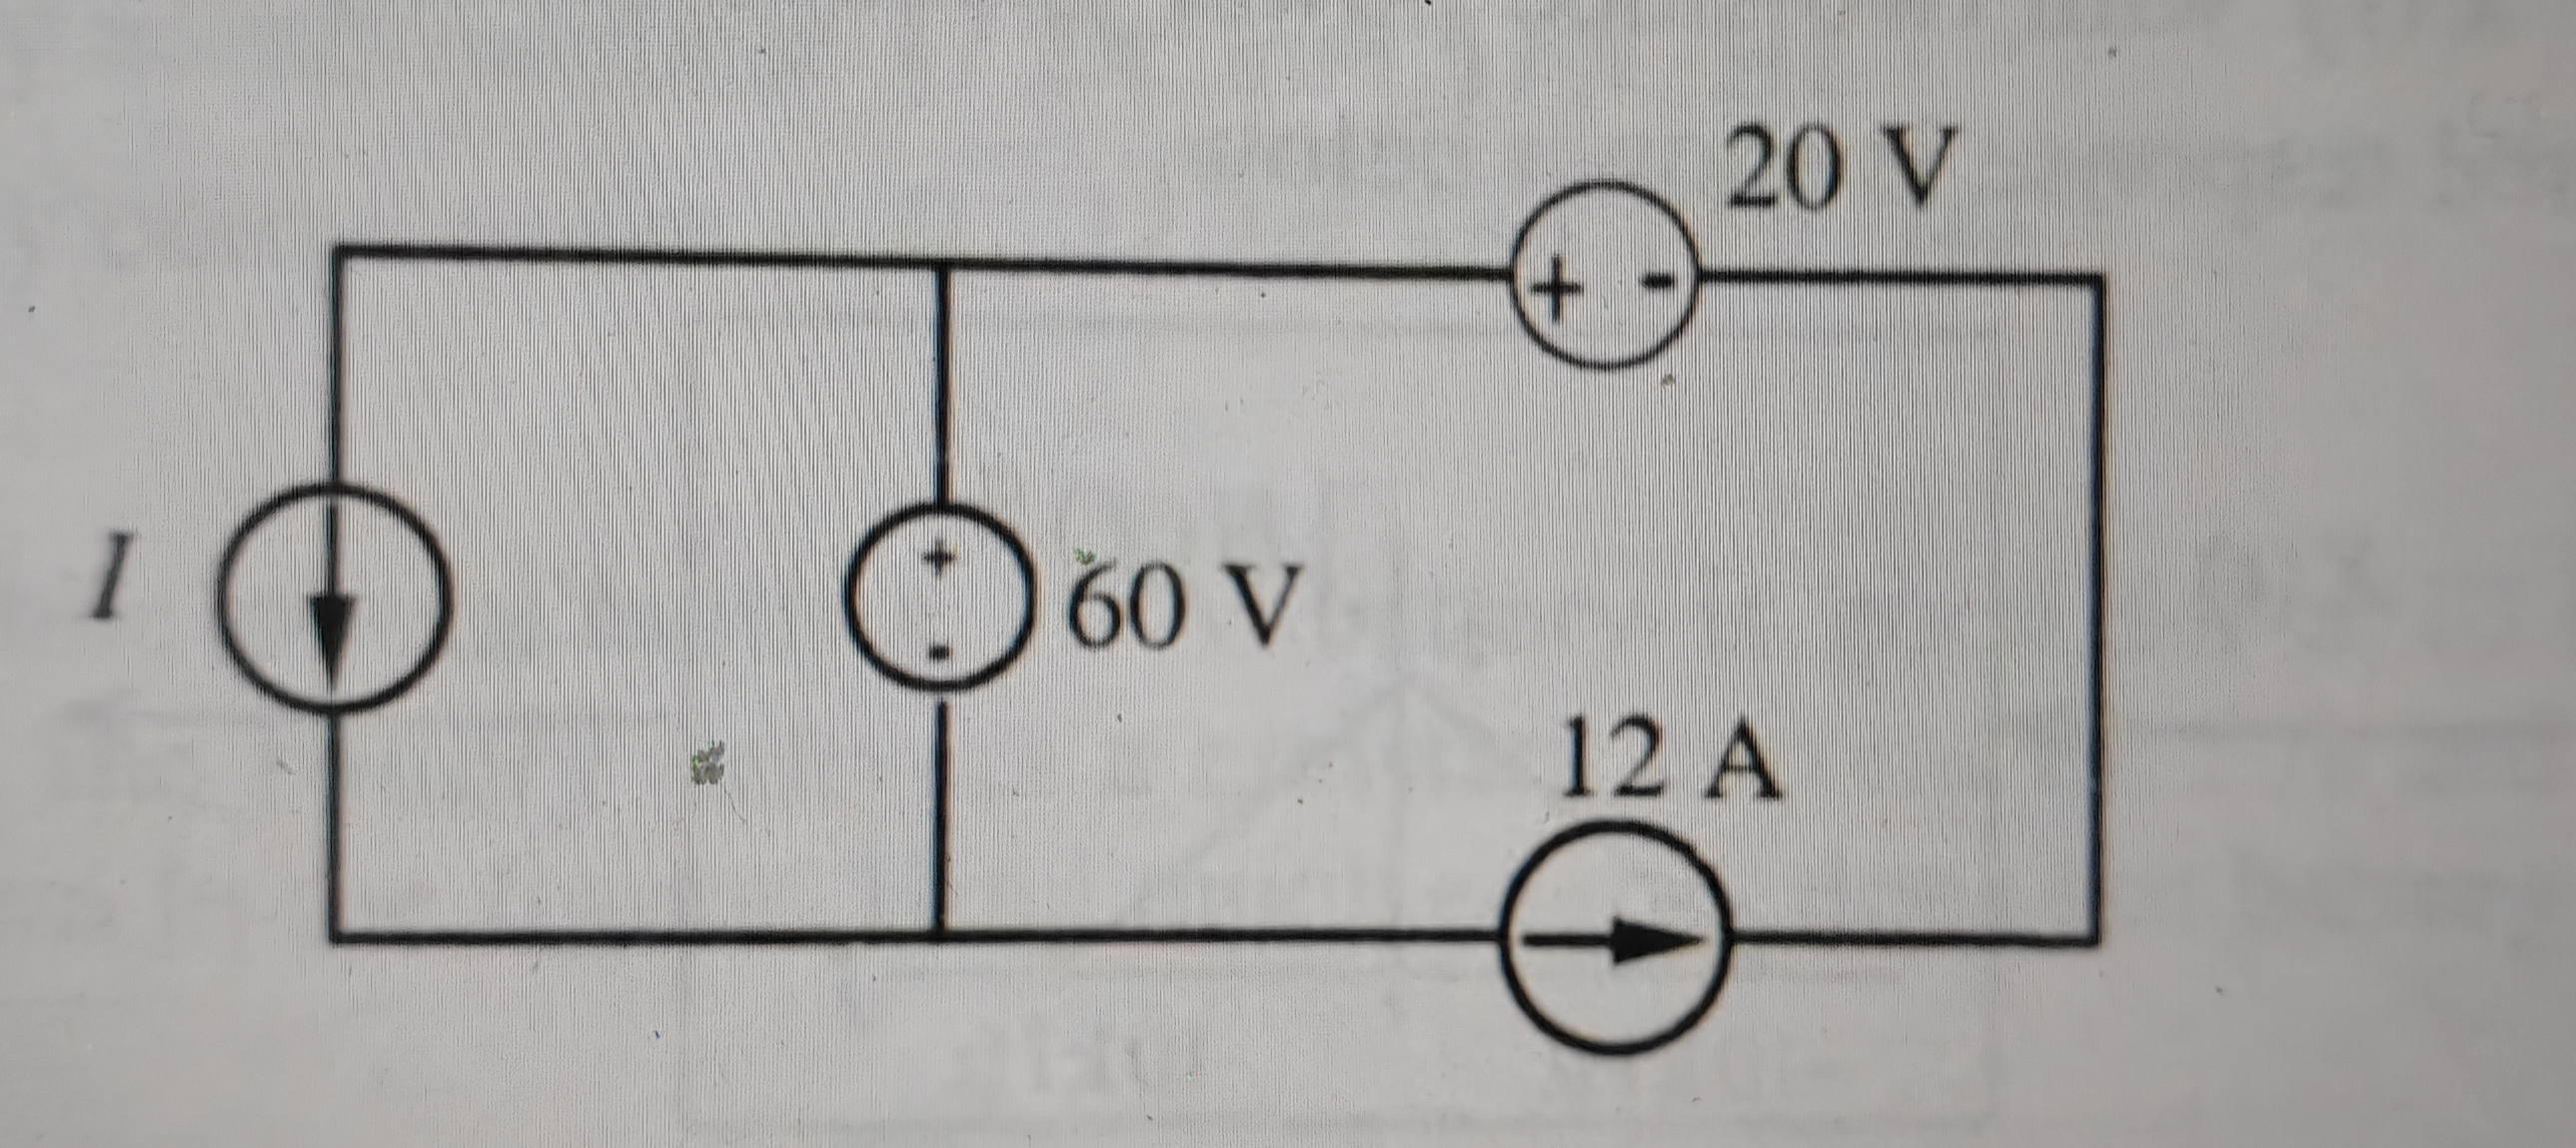
\includegraphics[width=0.7\columnwidth]{GATE/2009/EC/figs/fig_6.jpg}
    \caption{}
    \label{fig:placeholder_6}
\end{figure}
Which of the following can be the value of current source ${I}$ ?

\begin{enumerate}
\begin{multicols}{4}
\item 10 $A$
\item 13 $A$
\item 15 $A$
\item 18 $A$
\end{multicols}
\end{enumerate}
\hfill $\brak{\text{EC 2009}}$

\item In the \figref{fig:placeholder_11} shown below, what value of $R_l$ maximizes the power delivered to $R_l$ ?
\begin{figure}[H]
    \centering
    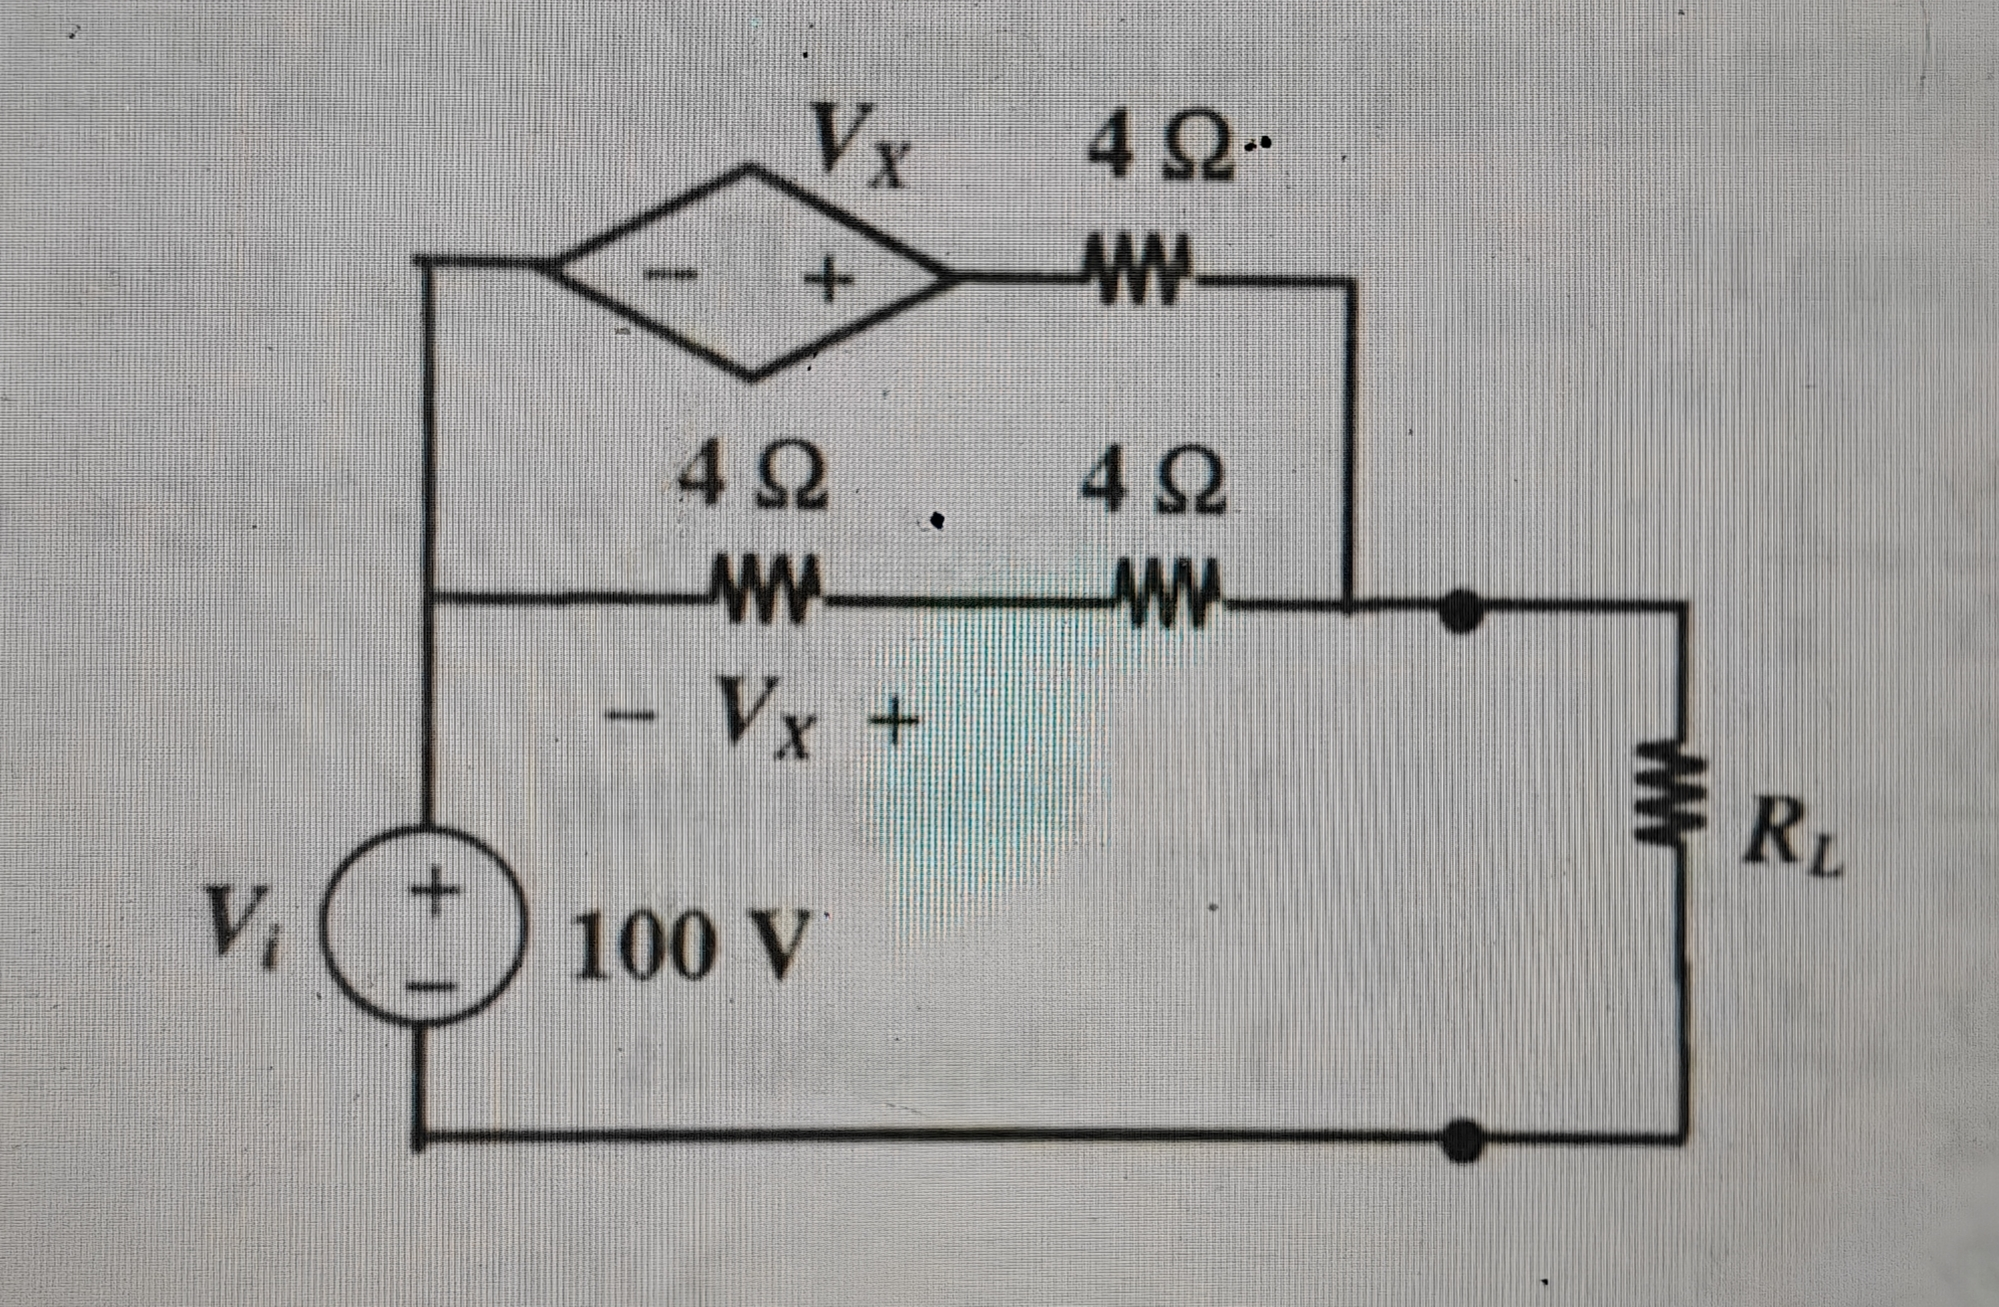
\includegraphics[width=0.7\columnwidth]{GATE/2009/EC/figs/fig_11.jpg}
    \caption{}
    \label{fig:placeholder_11}
\end{figure}
\begin{enumerate}
    \begin{multicols}{4}
        \item $2.4 \ohm$
        \item $\frac{8}{3} \ohm$
        \item $4 \ohm$
        \item $6 \ohm$
    \end{multicols}
\end{enumerate}
\hfill \brak{\text{EC 2009}}

\item The 4-point Discrete Fourier Transform $\brak{DFT}$ of a discrete time sequence $\cbrak{1,0,2,3}$ is 
\begin{enumerate}
    \begin{multicols}{2}
        \item $\sbrak{0,-2+2j, 2,-2,-2j}$
        \item $\sbrak{2,2+2j, 6, 2-2j}$
        \item $\sbrak{6,1-3j, 2, 1+3j}$
        \item $\sbrak{6,-1+3j, 0,-1-3j}$
    
    \end{multicols}
\end{enumerate}
\hfill $\brak{\text{EC 2009}}$


	\documentclass[journal,12pt,onecolumn]{IEEEtran}
\usepackage{cite}
\usepackage{graphicx}
\usepackage{amsmath,amssymb,amsfonts,amsthm}
\usepackage{algorithmic}
\usepackage{graphicx}
\usepackage{textcomp}
\usepackage{xcolor}
\usepackage{txfonts}
\usepackage{listings}
\usepackage{enumitem}
\usepackage{mathtools}
\usepackage{gensymb}
\usepackage{comment}
\usepackage[breaklinks=true]{hyperref}
\usepackage{tkz-euclide} 
\usepackage{listings}
\usepackage{gvv}                                        
\usepackage[latin1]{inputenc} 
\usetikzlibrary{arrows.meta, positioning}
\usepackage{xparse}
\usepackage{color}                                            
\usepackage{array}                                            
\usepackage{longtable}                                       
\usepackage{calc}                                             
\usepackage{multirow}
\usepackage{multicol}
\usepackage{hhline}                                           
\usepackage{ifthen}                                           
\usepackage{lscape}
\usepackage{tabularx}
\usepackage{array}
\usepackage{float}
\newtheorem{theorem}{Theorem}[section]
\newtheorem{problem}{Problem}
\newtheorem{proposition}{Proposition}[section]
\newtheorem{lemma}{Lemma}[section]
\newtheorem{corollary}[theorem]{Corollary}
\newtheorem{example}{Example}[section]
\newtheorem{definition}[problem]{Definition}
\newcommand{\BEQA}{\begin{eqnarray}}
\newcommand{\EEQA}{\end{eqnarray}}
\usepackage{float}
\theoremstyle{remark}
\usepackage{circuitikz}
\usepackage{tikz}



\title{GATE 2009 GG: GEOLOGY AND GEOPHYSICS}
\author{EE25BTECH11032 -Kartik Lahoti}
\date{}

\begin{document}
\maketitle
    \begin{center}
        \subsection*{PART A: COMMON TO BOTH GEOLOGY AND GEOPHYSICS CANDIDATES}
    \end{center}
\subsubsection*{Q.1 - Q.20 carry one mark each.}

    \begin{enumerate}                                 
     \item The Gutenberg discontinuity is located at a depth of around \hfill{\hfill{\brak{\text{GATE GG 2009}}}} 
            \begin {enumerate}
                \begin{multicols}{2}
                    \item$35\,km$
                    \item$150\,km$
                    \item$2900\,km$
                    \item$5000\,km$
                \end{multicols}
            \end{enumerate}
         
    \item What is the age of the "Barail Series"? \hfill{\hfill{\brak{\text{GATE GG 2009}}}} 
            \begin {enumerate}
                \begin{multicols}{2}
                    \item Jurassic
                    \item Paleocene
                    \item Oligocene
                    \item Miocene
                \end{multicols}
            \end{enumerate}            

    \item Thermohaline circulation in the oceans is driven by \hfill{\hfill{\brak{\text{GATE GG 2009}}}} 
            \begin{enumerate}
                \item only salinity gradients
                \item both temperature and salinity gradients
                \item only temperature gradients
                \item only density difference
            \end{enumerate}
        
    \item Which one of the following minerals cannot be used as an abrasive ? \hfill{\brak{\text{GATE GG 2009}}} 
                \begin {enumerate}
                    \begin{multicols}{2}
                        \item Garnet
                        \item Corundum
                        \item Quartz
                        \item Gypsum
                    \end{multicols}
            \end{enumerate}
        
    \item Which one of the following lakes is interpreted to be of meteoritic impact origin ? \hfill{\brak{\text{GATE GG 2009}}} 
            \begin {enumerate}
                \begin{multicols}{2}
                    \item Lonar Lake
                    \item Chilika Lake
                    \item Kolleru Lake
                    \item Pulicat Lake
                \end{multicols}
            \end{enumerate}
            
    \item Which one of the following geomorphic features is \textbf{not} related to desert environments ? \hfill{\brak{\text{GATE GG 2009}}} 
            \begin {enumerate}
                \begin{multicols}{2}
                    \item yardang
                    \item bajada
                    \item hamada
                    \item esker
                \end{multicols}
            \end{enumerate}            
            
    \item Which one of the following is located closest to the Ninety-East Ridge ?  \hfill{\brak{\text{GATE GG 2009}}} 
            \begin{enumerate}
                \item Bombay High
                \item Lakshwadweep Islands
                \item Andaman And Nicobar Islands
                \item Maldives                
            \end{enumerate}
            
     \item LPG (Liquefied Petroleum Gas) consists mainly of \hfill{\brak{\text{GATE GG 2009}}}  
            \begin{enumerate}
                \item propane and butane
                \item methane and ethane
                \item methane and butane
                \item ethane and propane              
            \end{enumerate}    
            
    \item Who proposed the principle "the present is the key to the past"? \hfill{\brak{\text{GATE GG 2009}}}  
            \begin {enumerate}
                \begin{multicols}{2}
                    \item Carl von Linnaeus
                    \item James Hutton
                    \item William Smith
                    \item Alcide d'Orbigny
                \end{multicols}
            \end{enumerate}
            
    \item Of the following, which is an ore of nickel? \hfill{\brak{\text{GATE GG 2009}}} 
            \begin {enumerate}
                \begin{multicols}{2}
                    \item Pentlandite
                    \item Cinnabar
                    \item Cassiterite
                    \item Scheelite
                \end{multicols}
            \end {enumerate}
            
    \item  Over a three layered earth, comprising of top dry soil followed by saturated weathered layer and hard rock basement, a resistivity sounding experiment is performed. The obtained VES curve is \hfill{\brak{\text{GATE GG 2009}}} 
             \begin {enumerate}
                \begin{multicols}{2}
                    \item K-type  
                    \item A-type
                    \item H-type
                    \item Q-type
                \end{multicols}
            \end{enumerate}
            
    \item The logging tool for direct determination of permeability is \hfill{\brak{\text{GATE GG 2009}}} 
            \begin {enumerate}
                \begin{multicols}{2}
                    \item induction
                    \item litho-density
                    \item sonic
                    \item NMR
                \end{multicols}
            \end{enumerate}
            
    \item Which of the following parameters is uniquely resolved by residual gravity anomaly data? \hfill{\brak{\text{GATE GG 2009}}}   
            \begin{enumerate}
                \item lateral density contrast 
                \item excess/deficit mass
                \item absolute density
                \item geometric dimensions of geophysical model                 
            \end{enumerate}
            
    \item Crude oil density, in degree API (American Petroleum Institute), is a measure of viscosity. The value of $10$ API is of \hfill{\brak{\text{GATE GG 2009}}}  
            \begin {enumerate}
                \begin{multicols}{2}
                    \item water
                    \item heavy crude
                    \item average crude
                    \item light crude
                \end{multicols}
            \end{enumerate}
            
    \item For perfectly conducting medium, skin depth $\brak{m}$ is \hfill{\brak{\text{GATE GG 2009}}} 
            \begin {enumerate}
                \begin{multicols}{2}
                    \item $10^5$
                    \item $100$
                    \item $10$
                    \item $0$
                \end{multicols}
            \end{enumerate}
            
    \item If a planet revolves around the Sun with a period of $8$ years, then its distance from the Sun would be (in terms of distance between Earth and Sun) \hfill{\brak{\text{GATE GG 2009}}} 
            \begin {enumerate}
                \begin{multicols}{2}
                    \item two times
                    \item four times
                    \item six times
                    \item eight times
                \end{multicols}
            \end{enumerate}
            
    \item A vast majority of earthquake sources are often linked to \hfill{\brak{\text{GATE GG 2009}}}   
            \begin{enumerate}
                \item inner core
                \item outer core
                \item brittle part of the earth's crust
                \item molten part of earth's mantle                
            \end{enumerate}
            
    \item In paleomagnetism, detrital magnetization is an important process for study of \hfill{\brak{\text{GATE GG 2009}}}  
            \begin{enumerate}
                \item sedimentary rocks
                \item metamorphic rocks
                \item basic igneous rocks
                \item acidic igneous rocks                
            \end{enumerate}
            
    \item A Geiger-Muller counter is used for measuring \hfill{\brak{\text{GATE GG 2009}}}    
            \begin{enumerate}
                \item gamma radiation
                \item alpha particles
                \item beta particles
                \item both alpha and beta particles                
            \end{enumerate}            
    \item The presence of crustal root beneath a mountain chain can be best explained by \hfill{\brak{\text{GATE GG 2009}}}    
            \begin{enumerate}
                \item Pratt's model
                \item Airy's Model
                \item Vening Meinesz model
                \item Plume model                
            \end{enumerate}        
            
    \centerline{\textbf{END OF PART A}}
 
    \begin{center}
        \subsection*{PART B \brak{\text{SECTION 1}}: FOR GEOLOGY CANDIDATES ONLY}
    \end{center}
        
\subsubsection*{Q.21 - Q.60 carry two marks each.}
    \item  Which one of the following is a typical Lower Gondwana plant assemblage ? \hfill{\brak{\text{GATE GG 2009}}}  
            \begin{enumerate}
                \item \textit{Glossopteris, Ptilophyllum, Nilssonia, Bucklandia} 
                \item \textit{Glossopteris, Gangamopteris, Schizoneura, Sphenophyllum}
                \item \textit{Gangamopteris, Lycopodites, Brachyphyllum, Nilssonia}
                \item \textit{Vertebraria, Alethopteris, Otozamites, Glossopteris}                
            \end{enumerate}
            
    \item Which of the following is not correct for a Pelecypod shell? \hfill{\brak{\text{GATE GG 2009}}}     
            \begin{enumerate}
                \item Pedicle is present.
                \item Pallial sinus, if present, is on the posterior side.
                \item Lunule is towards anterior.
                \item Both the valves have teeth and sockets.                
            \end{enumerate}          

    \item Match the following: \hfill{\brak{\text{GATE GG 2009}}} 
        
        \begin{multicols}{2}
            \hspace{2em}{\textbf{Group $I$}}
            \begin{enumerate}[start=16]
                \item Muschelkalk
                \item Katrol Formation
                \item Uttatur Stage
                \item Baripada beds
            \end{enumerate}                
            
            \columnbreak
            
            \hspace{2em}{\textbf{Group $II$}}            
            \begin{enumerate}
            \item Cambrian
            \item Miocene
            \item Middle Triassic
            \item Cretaceous
            \item Pleistocene
            \item Late Jurassic
            \end{enumerate}

        \end{multicols}
            \begin {enumerate}
                \begin{multicols}{2}
                    \item P-$3$, Q-$6$, R-$5$, S-$1$
                    \item P-$1$, Q-$2$, R-$3$, S-$4$
                    \item P-$3$, Q-$6$, R-$4$, S-$2$
                    \item P-$6$, Q-$3$, R-$1$, S-$2$
                \end{multicols}
            \end{enumerate}

    \item Match the following: \hfill{\brak{\text{GATE GG 2009}}} 
    
    \begin{multicols}{2}
            \hspace{2em}{\textbf{Group $I$}}
            \begin{enumerate}[start=16]
                \item Pelagic
                \item Pycnocline
                \item Psychrosphere
                \item Humboldt Current
            \end{enumerate}
            
            \columnbreak
            
            \hspace{2em}{\textbf{Group $II$}}
            

            \begin{enumerate} 
                \item Open ocean
                \item Cold sphere
                \item North Atlantic
                \item Density
                \item Thermocline
                \item East Pacific
            \end{enumerate}            

        \end{multicols}
            \begin {enumerate}
                \begin{multicols}{2}
                    \item P-$1$, Q-$4$, R-$3$, S-$6$
                    \item P-$6$, Q-$2$, R-$1$, S-$5$
                    \item P-$5$, Q-$6$, R-$1$, S-$3$
                    \item P-$1$, Q-$4$, R-$2$, S-$6$
                \end{multicols}
            \end{enumerate}
    \item Match the following: \hfill{\brak{\text{GATE GG 2009}}} 
        
    \begin{multicols}{2}
            \hspace{2em}{\textbf{Group $I$}}
            \begin{enumerate}[start=16]
                \item \textit{Globigerina bulloides}
                \item \textit{Olenellus}
                \item Ambulacrum
                \item Nema
            \end{enumerate}
            \columnbreak
            
            \hspace{2em}{\textbf{Group $II$}}
            \begin{enumerate} 
                \item Lower Cambrian
                \item Echinodermata
                \item Graptolites
                \item Upwelling
                \item Coelenterata
                \item Silurian
            \end{enumerate}
            

        \end{multicols}
            \begin {enumerate}
                
                    \item P-$1$, Q-$6$, R-$2$, S-$5$
                    \item P-$5$, Q-$6$, R-$2$, S-$3$
                    \item P-$4$, Q-$1$, R-$2$, S-$3$
                    \item P-$2$, Q-$4$, R-$5$, S-$6$
                
            \end{enumerate}
    \item Dinosaurs can be distinguished from the other Mesozoic reptiles by \hfill{\brak{\text{GATE GG 2009}}} 
        \begin {enumerate}
                \begin{multicols}{2}
                    \item Large size
                    \item Carnivorous habit
                    \item Erect stance
                    \item Sprawling stance
                \end{multicols}
            \end{enumerate}
    \item Which of the following is a polar planktic formanifer ? \hfill{\brak{\text{GATE GG 2009}}} 
            \begin{enumerate}
                \item \textit{Globigerenoides rubber}
                \item \textit{Neogloboquadina pachyderma}
                \item \textit{Globorotalia menardii}
                \item \textit{Orbulina universa}                
            \end{enumerate}
    \item Which one of the following mass-wasting processes is designated as a slow flowage type ? \hfill{\brak{\text{GATE GG 2009}}} 
    \begin {enumerate}
                \begin{multicols}{4}
                    \item Mudflow
                    \item Solifluction
                    \item Slump
                    \item Rockslide
                \end{multicols}
            \end{enumerate}
    \item Which of the following accurately describes the rock 'phonolite'? \hfill{\brak{\text{GATE GG 2009}}} 
    \begin{enumerate}
                \item Undersaturated ultramafic volcanic rock
                \item Undersaturated mafic plutonic rock
                \item Undersaturated ultrabasic volcanic rock
                \item Intermediate alkaline plutonic rock
            \end{enumerate}
    \item Match the assemblages in Group $I$ with the corresponding metamorphic facies in Group $II$: \hfill{\brak{\text{GATE GG 2009}}} 
        
    \begin{multicols}{2}
            \hspace{2em}{\textbf{Group $I$}}
            \begin{enumerate}[start = 16]
                \item Albite-jadeite-glaucophane-lawsonite
                \item Garnet-orthopyroxene-clinopyroxene-plagioclase
                \item Garnet-muscovite-biotite-sillimanite-quartz
                \item Albite-chlorite-epidote-actinolite
            \end{enumerate}
            
            \columnbreak
            
            \hspace{2em}{\textbf{Group $II$}}
            \begin{enumerate} 
                \item Greenschist
                \item Blueschist
                \item Granulitec
                \item Amphibolite
                \item Zeolite
                \item Prehnite-pumpellyite
            \end{enumerate}         


        \end{multicols}
            \begin {enumerate}
                \begin{multicols}{2}
                    \item P-$1$, Q-$6$, R-$2$, S-$5$
                    \item P-$5$, Q-$1$, R-$3$, S-$4$
                    \item P-$2$, Q-$3$, R-$4$, S-$1$
                    \item P-$3$, Q-$2$, R-$1$, S-$6$

                \end{multicols}
            \end{enumerate}
    \item When underplated by mafic magmas, and with no erosion, lower crustal rocks will experience \rule{2.5cm}{0.15mm} during metamorphism. \hfill{\brak{\text{GATE GG 2009}}} 
        \begin{enumerate}
                \item isobaric heating followed by isothermal decompression 
                \item isothermal compression followed by isobaric heating
                \item isobaric heating followed by isothermal compression 
                \item isobaric heating-cooling trajectory                 
            \end{enumerate}
    \item Match the minerals in Group $I$ with their characteristic optical properties in Group $II$: \hfill{\brak{\text{GATE GG 2009}}} 
    
    \begin{multicols}{2}
            \hspace{2em}{\textbf{Group $I$}}
            \begin{enumerate}[start=16]
                \item Biotite
                \item Sodalite
                \item Nepheline
                \item Quartz
            \end{enumerate}

                \columnbreak
           
             \hspace{2em}{\textbf{Group $II$}}
            \begin{enumerate} 
                \item Uniaxial negative
                \item Mottled extinction
                \item Uniaxial positive
                \item Isotropic, low relief
                \item Isotropic, high relief
                \item Biaxial negative
            \end{enumerate}
           \end{multicols}
            \begin {enumerate}
                \begin{multicols}{2}
                    \item P-$5$, Q-$1$, R-$3$, S-$6$
                    \item P-$6$, Q-$2$, R-$5$, S-$1$
                    \item P-$3$, Q-$2$, R-$4$, S-$5$
                    \item P-$2$, Q-$4$, R-$1$, S-$3$
                \end{multicols}
            \end{enumerate}
    \item A single slice of rock bound by thrust faults on all sides is called a \hfill{\brak{\text{GATE GG 2009}}} 
        \begin {enumerate}
                \begin{multicols}{2}
                    \item horse
                    \item pop-up structure
                    \item duplex
                    \item graben
                \end{multicols}
            \end{enumerate}
    \item A strike-slip dip fault strikes $30\degree N$, and dips $45\degree SE$. The net slip of the fault plunges \hfill{\brak{\text{GATE GG 2009}}} 
        \begin {enumerate}
                \begin{multicols}{2}
                    \item $30\degree \text{ towards } 45\degree N$
                    \item $0\degree \text{ towards } 30\degree N$
                    \item $45\degree \text{ towards } 120\degree N$
                    \item $90\degree \text{ towards } 30\degree N$
                \end{multicols}
            \end{enumerate}
    \item The boundary between the Indian and Eurasian plates is the \hfill{\brak{\text{GATE GG 2009}}} 
        \begin{enumerate}
                \item Main Central Thrust
                \item Main Boundary Thrust
                \item South Tibetan Detachment Zone
                \item Indus-Tsangpo Suture Zone                
            \end{enumerate}
    \item Plagioclase feldspars belong to the \rule{2.5cm}{0.15mm} crystal system. \hfill{\brak{\text{GATE GG 2009}}} 
        \begin {enumerate}
                \begin{multicols}{2}
                    \item Triclinic
                    \item Monoclinic
                    \item Orthorhombic
                    \item Rhombic 
                \end{multicols}
            \end{enumerate}
    \item The plane by which twinned crystals are united is called the \hfill{\brak{\text{GATE GG 2009}}} 
        \begin {enumerate}
                \begin{multicols}{2}
                    \item mirror plane
                    \item twin plane
                    \item glide plane
                    \item composition plane
                \end{multicols}
            \end{enumerate}
    \item In satellite remote-sensing, the spectral bands near $1.4\,\mu m$ and $1.9\,\mu m$ are avoided because of \hfill{\brak{\text{GATE GG 2009}}} 
        \begin{enumerate}
                \item absorption due to $H_2O$ and $CO_2$ in the atmosphere
                \item absorption due to ozone layer in the atmosphere
                \item absorption due to nitrogen in the atmosphere
                \item absorption by vegetation               
            \end{enumerate}
    \item Formation of chromitite from a basaltic magma can be explained by \hfill{\brak{\text{GATE GG 2009}}} 
        \begin {enumerate}
                \begin{multicols}{2}
                    \item liquid immiscibility
                    \item assimilation
                    \item magma mixing
                    \item Soret effect
                \end{multicols}
            \end{enumerate}
    \item Match the following economic deposits in Group $I$ with their places of occurrences in Group $II$: \hfill{\brak{\text{GATE GG 2009}}} 
    \begin{multicols}{2}
            \hspace{2em}{\textbf{Group $I$}}
            \begin{enumerate}[start=16]
                \item Bauxite
                \item Phosphorite
                \item Magnesite
                \item Barite
            \end{enumerate}
            
            \columnbreak
            
            \hspace{2em}{\textbf{Group $II$}}
            \begin{enumerate} 
                \item Naliya
                \item Maldeota
                \item Pahalgam
                \item Salem
                \item Mangampeta
                \item Belgaum
            \end{enumerate}
            

        \end{multicols}
            \begin {enumerate}
                \begin{multicols}{2}
                    \item P-$1$, Q-$2$, R-$4$, S-$5$
                    \item P-$2$, Q-$3$, R-$4$, S-$6$
                    \item P-$3$, Q-$1$, R-$6$, S-$5$
                    \item P-$6$, Q-$2$, R-$4$, S-$5$
                \end{multicols}
            \end{enumerate}
    \item What is the host rock for sulphide mineralization in Rampura-Agucha belt? \hfill{\brak{\text{GATE GG 2009}}} 
            \begin{enumerate}
                \item Graphitic mica schist
                \item Garnetiferous mica schist
                \item Graphitic biotite-sillimanite gneiss
                \item Garnetiferous sillimanite-feldspar gneiss               
            \end{enumerate}
    \item Which of the following is the correct order of decreasing permeability? \hfill{\brak{\text{GATE GG 2009}}} 
            \begin{enumerate}
                \item silty sandstone $>$ siltstone $>$ sandstone $>$ pebbly sandstone 
                \item siltstone $>$ silty sandstone $>$ sandstone $>$ pebbly sandstone
                \item pebbly sandstone $>$ sandstone $>$ silty sandstone $>$ siltstone
                \item pebbly sandstone $>$ sandstone $>$ siltstone $>$ silty sandstone                
            \end{enumerate}
    \item Which of the following varieties of coal has the least $H/C$ ratio? \hfill{\brak{\text{GATE GG 2009}}} 
            \begin {enumerate}
                \begin{multicols}{2}
                    \item peat
                    \item lignite
                    \item bituminous
                    \item anthracite
                \end{multicols}
            \end{enumerate}
    \item What is the age of the reservoir rock in the Cambay basin? \hfill{\brak{\text{GATE GG 2009}}} 
            \begin {enumerate}
                \begin{multicols}{2}
                    \item Eocene
                    \item Oligocene
                    \item Miocene
                    \item Paleocene
                \end{multicols}
            \end{enumerate}
    \item Which one of the following can be considered the best cap rock for oil and gas traps? \hfill{\brak{\text{GATE GG 2009}}} 
            \begin {enumerate}
                \begin{multicols}{2}
                    \item chert
                    \item evaporite
                    \item sandstone
                    \item shale
                \end{multicols}
            \end{enumerate}
    \item A negative $Eu$ anomaly will develop in a fractionating magma following separation of \hfill{\brak{\text{GATE GG 2009}}} 
            \begin {enumerate}
                \begin{multicols}{2}
                    \item garnet
                    \item olivine
                    \item plagioclase
                    \item orthopyroxene
                \end{multicols}
            \end{enumerate}
    \item In which of the following islands is the Mid-oceanic ridge exposed above sea-level? \hfill{\brak{\text{GATE GG 2009}}} 
            \begin {enumerate}
                \begin{multicols}{2}
                    \item Japan
                    \item Seychelles
                    \item Hawaii
                    \item Iceland
                \end{multicols}
            \end{enumerate}
    \item \rule{2.5cm}{0.15mm} dams are constructed where the foundation rock is strong. \hfill{\brak{\text{GATE GG 2009}}} 
            \begin {enumerate}
                \begin{multicols}{2}
                    \item Gravity
                    \item Arch
                    \item Buttress
                    \item Earth
                \end{multicols}
            \end{enumerate}
    \item Which type of cross-bedding is a definite indicator of tidal currents? \hfill{\brak{\text{GATE GG 2009}}} 
            \begin {enumerate}
                \begin{multicols}{2}
                    \item epsilon cross-bedding
                    \item herring-bone cross-bedding
                    \item hummocky cross-bedding
                    \item trough cross-bedding
                \end{multicols}
            \end{enumerate}
    \item Which type of sedimentary basin is formed close to continent-continent collisional settings? \hfill{\brak{\text{GATE GG 2009}}} 
            \begin {enumerate}
                \begin{multicols}{2}
                    \item Fore-arc basin
                    \item Peripheral foreland basin
                    \item Back-arc basin
                    \item Retro-arc foreland basin
                \end{multicols}
            \end{enumerate}  
\section*{Common Data Questions}
\subsection*{Common Data Questions 51 and 52: }

    A rock contains $65\%$ forsterite $\brak{Fo}$, $27\%$ enstatite $\brak{En}$and $8\%$ pigeonite $\brak{Pig}$ and its melting relationships at $1$ bar can be represented by the figure given below:

    \begin{figure}[H]
        \centering
        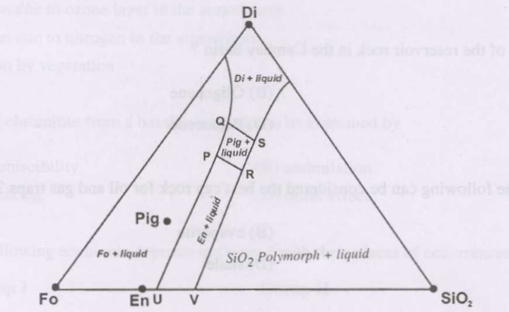
\includegraphics[width=0.5\columnwidth]{figs/IMG-1 2009.png}
        \caption{ Questions 51 and 52 }
        \label{fig:placeholder_1}
    \end{figure}
    

    \item The name of the rock is \hfill{\brak{\text{GATE GG 2009}}} 
            \begin {enumerate}
                \begin{multicols}{2}
                    \item Lherzolite
                    \item Harzburgite
                    \item Wehrlite
                    \item Dunite
                \end{multicols}
            \end{enumerate}
    \item On partially melting this rock, the first melt will have the composition of point \hfill{\brak{\text{GATE GG 2009}}} 
            \begin {enumerate}
                \begin{multicols}{2}
                    \item P
                    \item Q
                    \item R
                    \item S
                \end{multicols}
            \end{enumerate}
\subsection*{Common Data Questions 53 and 54: }
    An unfossiliferous sedimentary succession is characterized by the following features - 
    $\brak{i}$ sandstone-shale alternation, with sheet-like geometry of the sandstone beds;$\brak{ii}$ the sandstones exhibit graded bedding;$\brak{iii}$ erosional structures under the sandstone beds;$\brak{iv}$ convolute lamination, and $\brak{v}$ripple marks on the sandstone beds.

    \item Which depositional environment is indicated for the above sedimentary succession? \hfill{\brak{\text{GATE GG 2009}}} 
            \begin {enumerate}
                \begin{multicols}{2}
                    \item Fluvial
                    \item Eolian
                    \item Intertidal
                    \item Deep marine
                \end{multicols}
            \end{enumerate}
    \item What type of paleocurrent pattern is expected from the erosional structures in the succession? \hfill{\brak{\text{GATE GG 2009}}} 
            \begin {enumerate}
                \begin{multicols}{2}
                    \item Unimodal
                    \item Bimodal
                    \item Bimodal - bipolar
                    \item Polymodal
                \end{multicols}
            \end{enumerate}
\subsection*{Common Data Questions 55 and 56: }
    Examine the given geological section, which contains sedimentary successions interrupted by a dyke, and which contains no tectonic discontinuities.

    \begin{figure}[H]
        \centering
        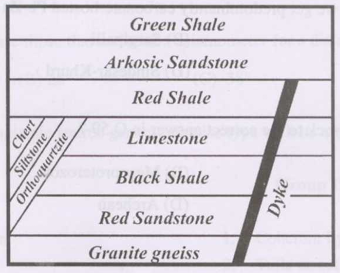
\includegraphics[width=0.5\columnwidth]{figs/IMG-2 2009.png}
        \caption{ Questions 55 and 56 }
        \label{fig:placeholder_2}
    \end{figure}
    
    \item How many unconformities can be identified in the section? \hfill{\brak{\text{GATE GG 2009}}} 
            \begin {enumerate} 
                \begin{multicols}{2}
                    \item $3$
                    \item $4$
                    \item $5$
                    \item $6$
                \end{multicols}
            \end{enumerate}
    \item Which of the following contacts is a nonconformity? \hfill{\brak{\text{GATE GG 2009}}} 
            \begin {enumerate}
                    \item Granite gneiss - Red Sandstone
                    \item Black Shale - Limestone
                    \item Limestone - Red Shale
                    \item Red Shale - Arkosic Sandstone
            \end{enumerate}
\section*{Linked Answer Questions}
\subsection*{Statement for Linked Answer Questions 57 and 58: }

    Microfossils may have following is a siliceous microfossil group ?
    \item Which of the following is a siliceous microfossil group? \hfill{\brak{\text{GATE GG 2009}}} 

            \begin {enumerate}
                \begin{multicols}{2}
                    \item Conodonts
                    \item Radiolaria
                    \item Dinoflagellates
                    \item Foraminifera
                \end{multicols}
            \end{enumerate}
    \item What is the preferred microhabitat of the microfossil group that is the correct answer in Q.57? \hfill{\brak{\text{GATE GG 2009}}} 
            \begin {enumerate}
                \begin{multicols}{2}
                    \item Benthic
                    \item Planktic
                    \item Nektic
                    \item Nektobenthic
                \end{multicols}
            \end{enumerate}
\subsection*{Statement for Linked Answer Questions 59 and 60: }
    $Pb-Zn$ sulphide deposits can form in different types of host rocks.
    \item Of the following, where do we get predominantly carbonate-hosted $Pb-Zn$ sulphide deposits? \hfill{\brak{\text{GATE GG 2009}}} 
            \begin {enumerate}
                \begin{multicols}{2}
                    \item Mochia - Zawar
                    \item Sargipalli
                    \item Pur - Banera
                    \item Sindesar-Khurd
                \end{multicols}
            \end{enumerate}
    \item What is the age of the host rock to the correct answer in $Q.59$? \hfill{\brak{\text{GATE GG 2009}}} 
            \begin {enumerate}
                \begin{multicols}{2}
                    \item Neoproterozoic
                    \item Mesoproterozoic
                    \item Paleoproterozoic
                    \item Archean
                \end{multicols}
            \end{enumerate}
    \centerline{\textbf{END OF SECTION 1 OF PART B }}
    \begin{center}
        \subsection*{PART B (SECTION 2): FOR GEOPHYSICS CANDIDATES ONLY}
    \end{center}
 
 \end{enumerate}
\subsubsection*{Q.20 - Q.60 carry two marks each.}
\begin{enumerate}[start = 21]
    \item Match the following functions in time-domain with their Fourier spectra: \hfill{\brak{\text{GATE GG 2009}}} 
            \begin{multicols}{2}
                \hspace{4em}{\textbf{Group $I$}}
                \begin{enumerate}[start=16]
                            \item $\Pi{(t)} =
                                        \begin{cases}
                                        1,-1/2\leq t \leq 1/2\\
                                        0,t<-1/2\text{ and }\hspace{.25cm}t>1/2
                                        \end{cases}  $    
                            \item Dirac delta function, $\delta(t)$
                            \item $x(t) = e^{-\mydet{t}}$
                            \item $\Lambda{(t)} =
                                    \begin{cases}
                                    1+t,-1<t<0\\
                                    1-t,0<t<1\\
                                    0,\text{otherwise}
                                    \end{cases}  $
                \end{enumerate}
                
    
                \columnbreak
                
                \hspace{5em}{\textbf{Group $II$}} 
                \begin{enumerate}            
                    \item $1$ 
                    \item $ \frac{\sin{\brak{\pi f}}}{f} \text{,where f is frequency }$
                    \item $ \frac{2}{1+4\pi^2f^2}\text{,where f is frequency }$
                    \item $ \frac{\sin^2\brak{\pi f}}{f^2}\text{,where f is    frequency }$
                \end{enumerate}
               
            \end{multicols}
                \begin {enumerate}
                    \begin{multicols}{2}
                        \item P-$2$, Q-$3$, R-$1$, S-$4$
                        \item P-$1$, Q-$3$, R-$2$, S-$4$
                        \item P-$1$, Q-$4$, R-$2$, S-$3$
                        \item P-$2$, Q-$1$, R-$3$, S-$4$
                    \end{multicols}
                \end{enumerate}
    \item The teleseismic rays are those that arrive at a seismometer for a distance greater than \hfill{\brak{\text{GATE GG 2009}}} 
            \begin {enumerate}
                \begin{multicols}{4}
                    \item $18\degree$
                    \item $28\degree$
                    \item $38\degree$
                    \item $48\degree$
                \end{multicols}
            \end{enumerate}
    \item Match the following seismic source generated noise type with its appearance on the seismogram : \hfill{\brak{\text{GATE GG 2009}}} 
                    
            \begin{multicols}{2}           
            \hspace{2em}{\textbf{Group $I$}}
            \begin{enumerate}[start=16]
                \item Reverberation
                \item Multiples
                \item Guided waves
                \item Diffractions
            \end{enumerate}
            
            \columnbreak
            
            \hspace{2em}{\textbf{Group $II$}}
            \begin{enumerate} 
                \item Coherent hyperbolic events
                \item Tails on reflected events
                \item Events paralleling first breaks
                \item Reflections at even time intervals after the primary reflections
            \end{enumerate}                       

        \end{multicols}
            \begin {enumerate}
                \begin{multicols}{2}
                    \item P-$1$, Q-$3$, R-$2$, S-$4$
                    \item P-$3$, Q-$4$, R-$2$, S-$1$
                    \item P-$2$, Q-$4$, R-$3$, S-$1$
                    \item P-$4$, Q-$1$, R-$3$, S-$2$
                \end{multicols}
            \end{enumerate}
    \item Which is the parameter for measuring the size of the earthquake that does not need an instrumental record? \hfill{\brak{\text{GATE GG 2009}}} 
            \begin {enumerate}
                \begin{multicols}{2}
                    \item Richter Magnitude
                    \item Intensity
                    \item Moment
                    \item M$_W$
                \end{multicols}
            \end{enumerate}  
    \item The standard form of wave equation for propagation of cubical dilatation $\brak{\theta}$ is \hfill{\brak{\text{GATE GG 2009}}} 
    $$\rho\frac{\partial^2\theta}{\partial t^2} = \brak{\lambda + 2\mu }\nabla^2\theta$$
    The compressional wave velocity is given by 
   
    
            \begin {enumerate}
                \begin{multicols}{4}
                    \item $\sqrt{\frac{2\lambda + \mu }{\rho}}$
                    \item $\sqrt{\frac{\lambda + 2\mu }{2\rho}}$
                    \item $\sqrt{\frac{\lambda + \mu }{\rho}}$
                    \item $\sqrt{\frac{\lambda + 2\mu }{\rho}}$
                \end{multicols}
            \end{enumerate}

    \item PKIKP is a seismic body wave which travels through \hfill{\brak{\text{GATE GG 2009}}} 
            \begin{enumerate}
                \item upper mantle
                \item upper and lower mantle
                \item mantle, outer core and inner core
                \item mantle and outer core                
            \end{enumerate}
    \item A seismic signal is recorded in a frequency band, $50-100\,Hz$. The sampling interval $\brak{ms}$ to avoid aliasing would be \hfill{\brak{\text{GATE GG 2009}}} 
            \begin {enumerate}
                \begin{multicols}{4}
                    \item $5$
                    \item $10$
                    \item $15$
                    \item $20$
                \end{multicols}
            \end{enumerate}
    \item The minimum appreciable amplitude recorded by a seismometer is $0.2\,mm$ and the maximum one is $20.0\,cm$, then the dynamic range in $dB$ is \hfill{\brak{\text{GATE GG 2009}}} 
            \begin {enumerate}
                \begin{multicols}{4}
                    \item $80$
                    \item $60$
                    \item $40$
                    \item $20$
                \end{multicols}
            \end{enumerate}
    \item Match the following: \hfill{\brak{\text{GATE GG 2009}}} 
                    
            \begin{multicols}{2}
            \hspace{2em}{\textbf{Group $I$}}
            
            \begin{enumerate}[start=16]
                \item Primary wave
                \item Secondary wave
                \item Rayleigh wave
                \item Love wave
            \end{enumerate}

            \columnbreak
            
            \hspace{2em}{\textbf{Group $II$}}
            
            \begin{enumerate} 
                \item Propagate along surface of the medium
                \item Particle motion is orthogonal to direction of propagation
                \item Particle motion describes a retrograde ellipse
                \item Particle motion in the direction of propagation
            \end{enumerate}
        \end{multicols}
            \begin {enumerate}
                \begin{multicols}{2}
                    \item P-$3$, Q-$4$, R-$1$, S-$2$
                    \item P-$1$, Q-$4$, R-$2$, S-$3$
                    \item P-$1$, Q-$3$, R-$2$, S-$4$
                    \item P-$4$, Q-$2$, R-$3$, S-$1$
                \end{multicols}
            \end{enumerate}
    
    \item  Which of the following is a minimum-phase wavelet? The first value in each case is at time zero. \hfill{\brak{\text{GATE GG 2009}}} 
            \begin {enumerate}
                \begin{multicols}{2}
                    \item $\cbrak{-2,5,-2}$
                    \item $\cbrak{-2,5,2}$
                    \item $\cbrak{6,-1,-2}$
                    \item $\cbrak{3,4,-4}$
                \end{multicols}
            \end{enumerate}
    \item In a gas zone, true porosity $\phi_t$, neutron $\log{\phi_n}$, and density derived porosity $\phi_d$are related as \hfill{\brak{\text{GATE GG 2009}}} 
            \begin {enumerate}
                \begin{multicols}{2}
                    \item $\phi_n<\phi_d>\phi_t$
                    \item $\phi_n>\phi_d>\phi_t$
                    \item $\phi_n>\phi_d=\phi_t$
                    \item $\phi_n<\phi_d=\phi_t$
                \end{multicols}
            \end{enumerate}
    \item Identify the equation for formation water resistivity $\brak{Rw_e}$ estimation from SP log, wherein $SSP$, $K\brak{T}$, and $R_{mfe}$ are respectively static SP, temperature dependent coefficient and mudfiltrate resistivity . \hfill{\brak{\text{GATE GG 2009}}} 
            
            \begin{enumerate}
                \item $\hspace{.25cm}SSP=-Rw_e\log{\brak{\frac{K\brak{T}}{R_{mfe}}}}$
                \item $\hspace{.25cm}SSP=-K\brak{T}\log{\brak{\frac{Rw_e}{R_{mfe}}}}$
                \item $\hspace{.25cm}SSP=-R_{mfe}\log{\brak{\frac{K\brak{T}}{Rw_e}}}$
                \item $\hspace{.25cm}SSP=-K\brak{T}\log{\brak{\frac{R_{mfe}}{Rw_e}}}$
            \end{enumerate}
            
    \item Gamma ray detected in density log is \hfill{\brak{\text{GATE GG 2009}}} 
            \begin{enumerate}
                \item natural gamma present in the formation
                \item gamma ray from epithermal neutron source
                \item gamma ray scattered from the formation
                \item gamma ray emitted from neutron capture reaction               
            \end{enumerate}
    \item In Turam method, one measures the reduced field ratio of the amplitude and of the phase difference between the two coils. In the absence of subsurface conducting body, the response is characterized as \hfill{\brak{\text{GATE GG 2009}}} 
            \begin{enumerate}
                \item the successive reduced field ratio is equal to 1.0 and phase difference is $0\degree$
                \item the successive reduced field ratio is equal to 1.0 and phase difference is $45\degree$ 
                \item the successive reduced field ratio is equal to 0.5 and phase difference is $90\degree$
                \item the successive reduced field ratio is equal to 0.5 and phase difference is $60\degree$                
            \end{enumerate}
    \item  Electric field \brak{\overrightarrow{E}} through a polarizable dielectric medium with polarization vector \brak{\overrightarrow{P}}, electric susceptibility $\brak{\chi_e}$ and dielectric permittivity \brak{\varepsilon_0}. The electric displacement vector \brak{\overrightarrow{D}} for the medium can be written as \hfill{\brak{\text{GATE GG 2009}}} 
            \begin {enumerate}
                \begin{multicols}{2}
                    \item $\overrightarrow{D} = \varepsilon_0\brak{1 + \chi_e} $
                    \item $\overrightarrow{D} = \varepsilon_0\overrightarrow{E} - \overrightarrow{P}$
                    \item $\overrightarrow{D} = \varepsilon_0\overrightarrow{E} + \chi_e$
                    \item $\overrightarrow{D}= \varepsilon_0\overrightarrow{E} + \overrightarrow{P}$
                \end{multicols}
            \end{enumerate}
    \item Using different electrodes configuration, maximum depth of investigation is achieved in \hfill{\brak{\text{GATE GG 2009}}} 
            \begin {enumerate}
                \begin{multicols}{2}
                    \item Schlumberger
                    \item dipole
                    \item tri-electrodes
                    \item Wenner
                \end{multicols}
            \end{enumerate}
    \item Relevant differential equation to study low frequency electromagnetic prospecting for a conducting target can be written in the form of \hfill{\brak{\text{GATE GG 2009}}} 
            \begin {enumerate}
                \begin{multicols}{2}
                    \item Wave equation
                    \item Laplace's equation
                    \item Helmholtz equation
                    \item Poisson's equation
                \end{multicols}
            \end{enumerate}
    \item In a layered medium, if the basement is perfectly conducting, magnetotelluric phase response asymptotically approaches to \hfill{\brak{\text{GATE GG 2009}}} 
            \begin {enumerate}
                \begin{multicols}{2}
                    \item $0\degree$
                    \item $45\degree$
                    \item $60\degree$
                    \item $90\degree$
                \end{multicols}
            \end{enumerate}
    \item Magnetotelluric spectral impedance can be defined as \hfill{\brak{\text{GATE GG 2009}}} 
            \begin{enumerate}
                \item the ratio of the spatial spectrum from mutually orthogonal horizontal components of the electric and magnetic field
                \item the ratio of the spatial spectrum of the vertical component to the horizontal component of magnetic field
                \item the ratio of the spatial spectrum of the vertical component to the horizontal component of electric magnetic field
                \item the ratio of the spatial spectrum of the two horizontal components of electric field                 
            \end{enumerate}
    \item Following four electrodes array: P1, P2 are measuring electrodes and C1, C2 are current electrodes used in resistivity measurement. Inter-electrode separation is also shown in figure.\hfill{\brak{\text{GATE GG 2009}}} 
    \begin{figure}[H]
        \centering
        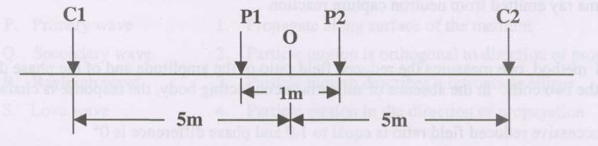
\includegraphics[width=1\columnwidth]{figs/IMG-3_2009.png}
        \caption{Q.40.}
        \label{fig:placeholder}
    \end{figure}
   
    The above electrodes configuration is 
    \begin{enumerate}
        \begin{multicols}{2}
            \item radial dipole
            \item parallel dipole
            \item Schlumberger 
            \item Wenner
        \end{multicols}
    \end{enumerate}
     \item In DC resistivity method, direct filter coefficients are used to compute \hfill{\brak{\text{GATE GG 2009}}} 
            \begin{enumerate}
                \item apparent resistivity data from resistivity transform
                \item resistivity transform from apparent resistivity data
                \item apparent resistivity from measured potential difference
                \item apparent resistivity from one electrode configuration to other electrode configuration                
            \end{enumerate}
    \item A counting rate of $15,100$ counts per minute is recorded by a radiation counter having a dead time of $300\,\mu sec$. The count rate (counts per minute) in the absence of dead time \hfill{\brak{\text{GATE GG 2009}}} 
            \begin {enumerate}
                \begin{multicols}{4}
                    \item $13,333$
                    \item $14,333$
                    \item $15,333$
                    \item $16,333$
                \end{multicols}
            \end{enumerate}
     \item The output of a linear and invariant system for a unit input is $\cbrak{3,1}$. Then what would be the output for an input $\cbrak{-2,1}$? \hfill{\brak{\text{GATE GG 2009}}} 
            \begin {enumerate}
                \begin{multicols}{4}
                    \item $\cbrak{-6,1,1}$
                    \item $\cbrak{-1,1,6}$
                    \item $\cbrak{-1,6,1}$
                    \item $\cbrak{1,-1,6}$
                \end{multicols}
            \end{enumerate}
    \item Geophysical inverse problems are described by \hfill{\brak{\text{GATE GG 2009}}} 
            \begin{enumerate}
                \item Fredholm's integral equation of first kind
                \item Fredholm's integral equation of second kind
                \item Volterra's equation of second kind
                \item Legendre equation                
            \end{enumerate}
    \item Spot the ANN method from the following: \hfill{\brak{\text{GATE GG 2009}}} 
            \begin{enumerate}
                \item Singular value decomposition
                \item Monte-Carlo technique
                \item Ridge regression procedure
                \item Back propagation technique                
            \end{enumerate}
    \item The concept of resolving kernel is used in \hfill{\brak{\text{GATE GG 2009}}} 
            \begin{enumerate}
                \item Tikhonov's regularization method
                \item Ridge regression method
                \item Backus-Gilbert method
                \item Simulated annealing method                
            \end{enumerate}
    \item For underwater gravity measurements, the following correction is needed: \hfill{\brak{\text{GATE GG 2009}}} 
            \begin{enumerate}
                \item Prey correction
                \item Free-air correction
                \item Bouguer correction
                \item Isostatic correction                
            \end{enumerate}
    \item The source of magnetic anomalies extend up to \hfill{\brak{\text{GATE GG 2009}}} 
            \begin{enumerate}
                \item upper mantle
                \item core-mantle boundary
                \item lower mantle
                \item Curie-point isotherm                
            \end{enumerate}
    \item In magnetic prospecting scalar magnetometers are used. Then, the prime assumption involved in magnetic data acquisition is \hfill{\brak{\text{GATE GG 2009}}} 
            \begin{enumerate}
                \item remnant magnetization is predominant
                \item both remnant and induced magnetization are responsible
                \item induced magnetization plays a dominant role
                \item only diamagnetic sources are responsible                 
            \end{enumerate}
    \item Source of main geomagnetic field is best represented by \hfill{\brak{\text{GATE GG 2009}}} 
            \begin{enumerate}
                \item a system of electric currents at core-mantle boundary
                \item a system of dipoles, quadrupoles, octupoles and multipoles
                \item an inclined geomagnetic dipole at center of earth
                \item a system of currents in the ionosphere                
            \end{enumerate}
\section*{Common Data Questions}
\subsection*{Common Data Questions 51 and 52: }
    In a resistivity sounding experiment using Schlumberger configuration the apparent resistivity function asymptotically approaches a sloping straight line of slope $45\degree$ with abscissa.
        \item From the above data it can be inferred that the basement is \hfill{\brak{\text{GATE GG 2009}}} 
                \begin {enumerate}
                    \begin{multicols}{2}
                        \item Perfectly conducting
                        \item Relatively resistive
                        \item Relatively conducting
                        \item Perfectly resistive
                    \end{multicols}
                \end{enumerate}
    \item If the intercept at $\rho_a = 1\,ohm-m$ is 5 and resistivity of top layer is $10\,ohm-m$ , then the depth of basement is \hfill{\brak{\text{GATE GG 2009}}} 
            \begin {enumerate}
                \begin{multicols}{2}
                    \item $50.0\,m$
                    \item $5.0\,m$
                    \item $2.0\,m$
                    \item $0.5\,m$
                \end{multicols}
            \end{enumerate}
\subsection*{Common Data Questions 53 and 54: }
    In a seismic refraction experiment involving a two-layered earth of P-wave velocities, $3\,km/sec$ and $4.5\,km/sec$ the delay time is found to be $49.69\, ms$.
        \item From the above data, the depth to the interface is given by \hfill{\brak{\text{GATE GG 2009}}} 
                \begin {enumerate}
                    \begin{multicols}{2}
                        \item $150\,m$
                        \item $120\,m$
                        \item $100\,m$
                        \item $50\,m$
                    \end{multicols}
                \end{enumerate}
    \item Using the above depth, the computed critical distance $\brak{m}$ would be \hfill{\brak{\text{GATE GG 2009}}} 
            \begin {enumerate}
                \begin{multicols}{2}
                    \item $151.20$
                    \item $178.88$
                    \item $221.67$
                    \item $169.87$
                \end{multicols}
            \end{enumerate}
\subsection*{Common Data Questions 55 and 56: }
    The peak gravity anomaly over a 2-D line mass of circular cross-section \brak{horizontal cylinder} of density contrast $500\,kg/m^3$ is $1.674\,mgal$. The anomaly decreases to $0.837\,mgal$ at a distance of $500\,m$ along a principal profile. The universal gravitation constant, $G = 6.6667\times10^{-11}m^3sec^{-2}kg^{-1}$
        \item The depth $\brak{m}$ to center of line mass and radius $\brak{m}$ of the horizontal cylinder are \hfill{\brak{\text{GATE GG 2009}}} 
                \begin {enumerate}
                    \begin{multicols}{2}
                        \item $500$, $199.80$
                        \item $200$, $150.93$
                        \item $200$, $100.33$
                        \item $100$, $60.37$
                    \end{multicols}
                \end{enumerate}
    \item Hence compute the excess mass per unit length $\brak{kg/m}$ of the line mass \hfill{\brak{\text{GATE GG 2009}}}
            \begin {enumerate}
                \begin{multicols}{2}
                    \item $11.0 \times 10^7$
                    \item $9.0 \times 10^7$
                    \item $6.27 \times 10^7$
                    \item $3.67 \times 10^7$
                \end{multicols}
            \end{enumerate}
\section*{Linked Answer Questions}
\subsection*{Statement for Linked Answer Questions 57 and 58: }
    Resistivity log recorded using normal device with measuring electrode, $M$, is situated close to the current electrode, $A$, in logging device placed in borehole. A constant current, $I$, injected from current electrode into the formation.
        \item If the spacing between $A$ and $M$ is $r$, and the potential difference $\Delta V$ is measured between the measuring electrode, $M$ and remotely placed surface electrode. Then the expression for the apparent resistivity can be written as \hfill{\brak{\text{GATE GG 2009}}} 
                    \begin{enumerate}
                        \begin{multicols}{2}
                            \item$ \rho_a = \frac{2\pi r}{I}\Delta V$
                            \item$ \rho_a = \frac{4\pi r^2 }{I}\Delta V $
                            \item$ \rho_a = \frac{2\pi r^2}{I}\Delta V$
                            \item$ \rho_a = \frac{4\pi r }{I}\Delta V $
                        \end{multicols}
                    \end{enumerate}
    \item If $r = 0.40\,m$ ; $I = 0.02\,amp$ ; $\Delta V =0.04\,volt$, then the measured apparent resistivity will be \hfill{\brak{\text{GATE GG 2009}}} 
            \begin {enumerate}
                \begin{multicols}{2}
                    \item $1\,\Omega m$
                    \item $5\,\Omega m$
                    \item $10\,\Omega m$
                    \item $20\,\Omega m$
                \end{multicols}
            \end{enumerate}
\subsection*{Statement for Linked Answer Questions 59 and 60: }
    Given the wavelets,$a=\cbrak{3,-2} \text{ and } b = \cbrak{1,-2}$
        \item The cross-correlation, $\phi_{ab}$, is given by \hfill{\brak{\text{GATE GG 2009}}} 
            \begin{enumerate}
                \begin{multicols}{2}
                    \item $\cbrak{-6,7,-2}$
                    \item $\cbrak{-6,10,-12}$
                    \item $\cbrak{-4,-11,-6}$
                    \item $\cbrak{-6,11,-4}$
                \end{multicols}            
            \end{enumerate}
    \item The inverse of wavelet $a$,$W^{-1}_a$ is given by \hfill{\brak{\text{GATE GG 2009}}} 
        \begin{enumerate}
            \begin{multicols}{2}
                \item $\cbrak{4/3, 16/9, 17/7, 64/81}$
                \item $\cbrak{1/3, 2/9, 4/27, 8/81}$
                \item $\cbrak{4/9, 1/3, 64/81, 16/27}$
                \item $\cbrak{16/27, 64/81, 4/9, 1/3}$
            \end{multicols}

        \end{enumerate}
    \centerline{\textbf{END OF THE QUESTION PAPER}}
 \end{enumerate}
\end{document}

	\documentclass[journal,12pt,onecolumn]{IEEEtran}
\usepackage{cite}
\usepackage{graphicx}
\usepackage{amsmath,amssymb,amsfonts,amsthm}
\usepackage{algorithmic}
\usepackage{graphicx}
\usepackage{textcomp}
\usepackage{xcolor}
\usepackage{txfonts}
\usepackage{listings}
\usepackage{enumitem}
\usepackage{mathtools}
\usepackage{gensymb}
\usepackage{comment}
\usepackage[breaklinks=true]{hyperref}
\usepackage{tkz-euclide} 
\usepackage{listings}
\usepackage{gvv}                                        
%\def\inputGnumericTable{}                                 
\usepackage[latin1]{inputenc} 
\usetikzlibrary{arrows.meta, positioning}
\usepackage{xparse}
\usepackage{color}                                            
\usepackage{array}                                            
\usepackage{longtable}                                       
\usepackage{calc}                                             
\usepackage{multirow}
\usepackage{multicol}
\usepackage{hhline}                                           
\usepackage{ifthen}                                           
\usepackage{lscape}
\usepackage{tabularx}
\usepackage{array}
\usepackage{float}
\newtheorem{theorem}{Theorem}[section]
\newtheorem{problem}{Problem}
\newtheorem{proposition}{Proposition}[section]
\newtheorem{lemma}{Lemma}[section]
\newtheorem{corollary}[theorem]{Corollary}
\newtheorem{example}{Example}[section]
\newtheorem{definition}[problem]{Definition}
\newcommand{\BEQA}{\begin{eqnarray}}
\newcommand{\EEQA}{\end{eqnarray}}
\usepackage{float}
\usepackage{caption}

%\newcommand{\define}{\stackrel{\triangle}{=}}
\theoremstyle{remark}
\usepackage{circuitikz}
\usepackage{tikz}
\graphicspath{{figs/}}
\usepackage[top=1in,bottom=1in,left=1in,right=1in]{geometry}
\pagestyle{empty}
\setlength{\parindent}{0pt}

\title{PI: PRODUCTION AND INDUSTRIAL ENGINEERING}
\author{EE25BTECH11023-Venkata Sai}
\begin{document}
\maketitle
 
\textbf{Q. 1 - Q. 20 carry one mark each.}

\begin{enumerate}

\item The homogeneous part of the differential equation
$\frac{d^2 y}{dx^2} + p \frac{dy}{dx} + q y = r$
has real distinct roots if $\brak{p, q and r are constants}$
\begin{enumerate}
\begin{multicols}{2}
\item $p^2 - 4q > 0$  
\item  $p^2 - 4q < 0$ 
\item  $p^2 - 4q = 0$ 
\item  $p^2 - 4q = r$ 
\end{multicols}
\end{enumerate}
\hfill (GATE PI 2009) 
\item The total derivative of the function $xy$ is
\begin{enumerate}
\begin{multicols}{2}
\item $x dy + ydx$ 
\item $xdx + ydy$ 
\item  $dx + dy$ 
\item $dx dy$ 
\end{multicols}
\end{enumerate}
\hfill (GATE PI 2009) 
\item A helical compression spring has: $ d = $wire diameter, $ D = $ mean coil diameter, $ E = $ Young's modulus, $ G = $ modulus of rigidity and $ N_a = $ number of active coils. The spring stiffness is
\begin{enumerate}
\begin{multicols}{2}
\item $\frac{d E}{8 D^{3} N_a}$  
\item $\frac{d G}{8 D^{3} N_a}$ 
\item  $\frac{d^{3} E}{8 D N_a}$ 
\item $\frac{d^{3}}{8 D N_a}$ 

\end{multicols}
\end{enumerate}
\hfill (GATE PI 2009)
\item Which of the following processes is NOT executed by an ideal Rankine cycle with no superheat?
\begin{enumerate}
\item Isentropic expansion
\item Isentropic compression
\item Constant temperature heat addition
\item Constant temperature heat rejection
\end{enumerate}
\hfill (GATE PI 2009)
\item During the numerical solution of a first order differential equation using the Euler (also known as Euler Cauchy) method with step size $h$, the local truncation error is of the order of
\begin{enumerate}
\begin{multicols}{4}
\item  $h^2$ 
\item $h^3$ 
\item $h^4$ 
\item $h^5$ 
\end{multicols}
\end{enumerate}
\hfill (GATE PI 2009)
\item For a granted patent to last for 20 years, the patent must be
\begin{enumerate}
\begin{multicols}{2}
\item owned by the inventor 
\item renewed and maintained \\
\item novel 
\item  non-obvious \\
\end{multicols}
\end{enumerate}

\hfill (GATE PI 2009)
\item As per Kendall's notation in M/G/c queuing system, the number of arrivals in a fixed time follows
\begin{enumerate}
\begin{multicols}{2}
\item  Beta distribution 
\item  Normal distribution 
\item Poisson distribution 
\item Uniform distribution 
\end{multicols}
\end{enumerate}
\hfill (GATE PI 2009)
\item Which of the following forecasting models explicitly accounts for seasonality of demand?
\begin{enumerate}
\begin{multicols}{2}
\item Simple moving average  model 
\item Simple exponential smoothing model \\
\item Holt's model 
\item Winter's model \\
\end{multicols}
\end{enumerate}
\hfill (GATE PI 2009)
\item A typical Fe-C alloy containing greater than 0.8\% C is known as
\begin{enumerate}
\begin{multicols}{2}
\item Eutectoid steel 
\item Hypoeutectoid steel 
\item Mild steel 
\item Hypereutectoid steel 
\end{multicols}
\end{enumerate}
\hfill (GATE PI 2009)
\item The capacity of a material to absorb energy when deformed elastically, and to release it back when unloaded is termed as
\begin{enumerate}
\begin{multicols}{2}
\item toughness 
\item resilience 
\item  ductility 
\item malleability 
\end{multicols}
\end{enumerate}
\hfill (GATE PI 2009)
\item The product of the complex numbers $\brak{3 - i2}$ and $\brak{3 + i4}$ results in
\begin{enumerate}
\begin{multicols}{4}
\item $\brak{1 + i^6}$ 
\item $\brak{9-i^8}$  
\item $\brak{9+i^8}$ 
\item $\brak{17 + i^6}$ \\
\end{multicols}
\end{enumerate}
\hfill (GATE PI 2009)
\item The value of the determinant
$
\myvec{
4 & 1 & 1 \\
2 & 1 & 3 \\
1 & 3 & 2
}
$
is
\begin{enumerate}
\begin{multicols}{4}
\item -28 
\item -24 
\item 32 
\item 36 
\end{multicols}
\end{enumerate}

\hfill (GATE PI 2009)

\item If module and number of teeth of a spur gear with involute profile are 3 mm and 23 respectively, then the pitch diameter (in mm) of the spur gear is
\begin{enumerate}
\begin{multicols}{4}
\item  7.67 
\item 15.34 
\item 34.50 
\item 69.00 
\end{multicols}
\end{enumerate}
\hfill (GATE PI 2009)
\item Hot chamber die casting process is NOT suited for
\begin{enumerate}
\begin{multicols}{2}
\item Lead and its alloys 
\item Zinc and its alloys 
\item Tin and its alloys  
\item Aluminum and its alloys 
\end{multicols}
\end{enumerate}
\hfill (GATE PI 2009)
\item The total angular movement (in degrees) of a lead-screw with a pitch of 5.0 mm to drive the work-table by a distance of 200 mm in a NC machine is \\
\begin{enumerate}
\begin{multicols}{4}
\item  14400 
\item  28800
\item 57600 
\item 72000 
 \end{multicols}
 \end{enumerate}
\hfill (GATE PI 2009)
\item Anisotropy in rolled components is caused by
\begin{enumerate}
\begin{multicols}{2}
\item change in dimensions 
\item scale formation 
\item closure of defects 
\item grain orientation 
\end{multicols}
\end{enumerate}
\hfill (GATE PI 2009)
\item Which of the following processes is used to manufacture products with controlled porosity?
\begin{enumerate}
\begin{multicols}{2}
\item Casting 
\item Welding 
\item Forming 
\item Powder metallurgy 
\end{multicols}
\end{enumerate}
\hfill (GATE PI 2009)
\item Which of the following powders should be fed for effective oxy-fuel cutting of stainless steel?
\begin{enumerate}
\begin{multicols}{4}
\item  Steel
\item Aluminum
\item Copper 
\item Ceramic 
\end{multicols}
\end{enumerate}
\hfill (GATE PI 2009)
\item An autocollimator is used to

\begin{enumerate}
\item measure small angular displacements on flat surfaces
\item compare known and unknown dimensions
\item measure the flatness error
\item measure roundness error between centers
\end{enumerate}
\hfill (GATE PI 2009)
\item Diamond cutting tools are not recommended for machining of ferrous metals due to

\begin{enumerate}
\item high tool hardness
\item high thermal conductivity of work material
\item poor tool toughness
\item chemical affinity of tool material with iron
\end{enumerate}
\hfill (GATE PI 2009)
\item The value of $x_3$ obtained by solving the following system of linear equations is
\begin{align*} 
x + 2x_2 - 2x_3 = 4 \\ 
2x + x_2 + x_3 = -2 \\
-x + x_2 - x_3 = 2
\end{align*}
\begin{enumerate}
\begin{multicols}{2}
\item -12 
\item -2 
\item 0 
\item 12 
\end{multicols} 
\end{enumerate}
\hfill (GATE PI 2009)
\item The displacement and acceleration of a cam follower mechanism are plotted in the following figures:

\begin{figure}[h]
    \centering
    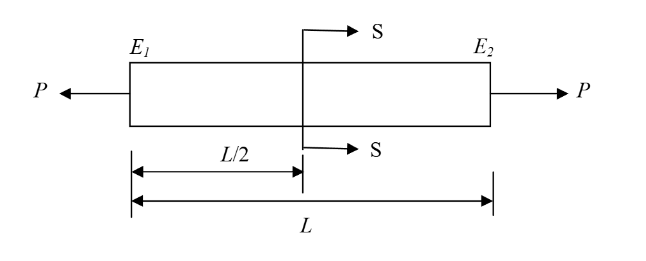
\includegraphics[width=0.5\linewidth]{figs/1.png}
    \caption{}
    \label{fig:placeholder}
\end{figure} 

The nature of the displacement curve is:
\begin{enumerate}
\begin{multicols}{2}
\item Cubic 
\item Quadratic 
\item Simple harmonic 
\item Linear 
\end{multicols}
\end{enumerate}
\hfill (GATE PI 2009)
\item The solution of the differential equation
$
\frac{d^2 r}{dx^2} = 0
$
with boundary conditions: (i) $\frac{dy}{dx} = 1$ at $x = 0$, (ii) $\frac{dy}{dx} = 1$ at x=1 is
\begin{enumerate}
\item $y = 1$ 
\item $y = x$ 
\item $y = x + C$, where $C$ is an arbitrary constant  
\item $y = C_1 x + C_2$, where $C_1, C_2$ are arbitrary constants 

\end{enumerate}
\hfill (GATE PI 2009)
\item The line integral of the vector function $\mathbf{F} = 2x + x^2 \mathbf{\hat{j}}$ along the x-axis from $x=1$ to $x=2$ is
\begin{enumerate}
\begin{multicols}{4}
\item 0
\item 2.33
\item 3
\item 5.33 
\end{multicols}
\end{enumerate}

\hfill (GATE PI 2009)
\item Using direct extrusion process, a round billet of 100 mm length and 50 mm diameter is extruded. Considering an ideal deformation process (no friction and no redundant work), extrusion ratio 4, and average flow stress of material 300 MPa, the pressure (in MPa) on the ram will be
\begin{enumerate}
\begin{multicols}{4}
\item 416
\item 624
\item 700
\item 832
\end{multicols}
\end{enumerate}
\hfill (GATE PI 2009)
\item A friction clutch is designed to transmit 15 horsepower at 1500 rpm. The torque (in N·m) experienced by the clutch is
\begin{enumerate}
\begin{multicols}{2}
\item 1.19 
\item 7.46 
\item 71.24 
\item 447.61 
\end{multicols}
\end{enumerate}
\hfill (GATE PI 2009)
\item A manufacturer has set up an assembly line where first, Task I is performed in Workstation 1 for 0.3 minutes; then Task II is performed in Workstation 2 for 0.4 minutes; and finally Task III is performed in Workstation 3 for 0.3 minutes. The efficiency (in \%) of this assembly line setup is
\begin{enumerate}
\begin{multicols}{2}
\item  33.33 
\item 64.33 
\item 75.33
\item 83.33 
\end{multicols}
\end{enumerate}
\hfill (GATE PI 2009)

\item A biaxial stress element is subjected to tensile and shear stresses as shown in the figure. If $\sigma_1 = 40$ MPa, $\sigma_y = 20$ MPa and $T_{xy} = T_{yx} = 15$ MPa. The principal normal stresses (in MPa) are:

\begin{figure}[h]
    \centering
    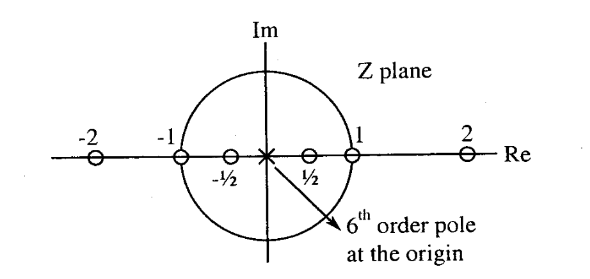
\includegraphics[width=0.5\linewidth]{figs/2.png}
    \caption{}
    \label{fig:placeholder}
\end{figure} 

\begin{enumerate}
\begin{multicols}{2}
\item 5 and 55
\item 10 and 30 
\item 12 and 48
\item 20 and 40
\end{multicols}
\end{enumerate}
\hfill (GATE PI 2009)

\item The area under the curve shown, between $x=1$ and $x=3$, to be evaluated using the trapezoidal rule. The following points on the curve are given:

\begin{center}
\input{tables/table3}
\end{center}

\begin{figure}[h]
    \centering
    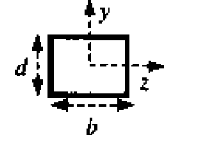
\includegraphics[width=0.3\linewidth]{figs/3.png}
    \caption{}
    \label{fig:placeholder}
\end{figure} 
\begin{center}

\end{center}
The evaluated area (in m$^2$) will be
\begin{enumerate}
\begin{multicols}{4}
\item 7  
\item 8.67 
\item 9  
\item 18 
\end{multicols}
\end{enumerate}
\hfill (GATE PI 2009)
\item The pressure drop for laminar flow of a liquid in a smooth pipe at normal temperature and pressure is
\begin{enumerate}
\begin{multicols}{2}
\item directly proportional to density 
\item inversely proportional to density 
\item independent of density 
\item proportional to density$^{0.75}$

\end{multicols}
\end{enumerate}
\hfill (GATE PI 2009)
\item A titanium sheet of 5.0 mm thickness is cut by wire-cut EDM process using a wire of 1.0 mm diameter. A uniform spark gap of 0.5 mm on both sides of the wire is maintained during cutting operation. If the feed rate of the wire into the sheet is 20 mm/min, the material removal rate (in mm$^3$/min) will be
\begin{enumerate}
\begin{multicols}{4}
\item 150 
\item 200
\item 300 
\item 400 
\end{multicols}
\end{enumerate}
\hfill (GATE PI 2009)
\item Autogenous gas tungsten arc welding of a steel plate is carried out with welding current of 500 A, voltage of 20 V, and weld speed of 20 mm/min. Consider the heat transfer efficiency from the arc to the weld pool as 90\%. The heat input per unit length (in kJ/mm) is
\begin{enumerate}
\begin{multicols}{4}
\item  0.25 
\item 0.35 
\item 0.45 
\item 0.55 
\end{multicols}
\end{enumerate}

\hfill (GATE PI 2009)
\item Consider steady flow of water in a situation where two pipe lines (Pipe 1 and Pipe 2) combine into a single pipeline (Pipe 3) as shown in the figure. The cross-sectional areas of all three pipelines are constant. The following data is given : \\
\begin{center}
\input{tables/table2}
\end{center}
Assuming water properties and velocities to be uniform across the cross sections of the inlets and the outlet, the exit velocity (in m/s) in pipe 3 is
\begin{enumerate}
\begin{multicols}{4}
\item  1 
\item 1.5 
\item  2  
\item 2.5
\end{multicols}
\end{enumerate}
\hfill (GATE PI 2009)

\item Match the Following:
{
\setlength{\columnsep}{-5cm}
\begin{multicols}{2}
\begin{enumerate}[label=\Alph*.]
    \item[]  \textit{\textbf{Group I (Product)}}
    \item Process layout
    \item Product flow layout
    \item Fixed position layout
    \item Cellular layout 
\end{enumerate}
\columnbreak
\begin{enumerate}[label=\arabic*.]
    \item[] \textit{\textbf{Group II (Manufacturing Process)}}
    \item Inflexible to significant changes in product design
    \item Distinct part families and expanded worker training
    \item Low equipment utilization and high skill requirement
    \item Large work-in-process and increased material handling
\end{enumerate}
\end{multicols}
}
\begin{multicols}{2}
\begin{enumerate}
    \item P-4, Q-1, R-3, S-2
    \item P-4, Q-3, R-2, S-1
    \item P-2, Q-1, R-4, S-3
    \item P-1, Q-4, R-3, S-2
\end{enumerate}
\end{multicols}
\hfill (GATE PI 2009)
\item Consider the joint probability mass function of random variables X and Y as shown in the table below: \\
For instance, $P\cbrak{X=1, Y=2}$ = 0.3
\begin{center}
\input{tables/table1}
\end{center}
The value of $P\cbrak{X=2|Y=2}$ is

\begin{enumerate}
\begin{multicols}{4}
\item 0.10 
\item 0.25 
\item 0.40 
\item 0.75 
\end{multicols}
\end{enumerate}

\hfill (GATE PI 2009)
\item A grocery store faces a demand of 50 units of soap per day. The store orders soap periodically. It costs Rs. 100 to initiate a purchase order. It costs Rs. 0.04 per soap per day to store the soap. The lead time between placing and receiving the order is 4 days. The optimal inventory policy for ordering soap is to
\begin{enumerate}
\item order 500 units when inventory drops to 200 units 
\item order 500 units when inventory drops to 100 units
\item order 1000 units when inventory drops to 200 units
\item order 1000 units when inventory drops to 100 units
\end{enumerate}
\hfill (GATE PI 2009)
\item A disk of 200 mm diameter is blanked from a strip of an aluminum alloy of thickness 3.2 mm. The material shear strength to fracture is 150 MPa. The blanking force (in kN) is

\begin{enumerate}
\begin{multicols}{4}
\item 291 
\item 301 
\item 311 
\item 321 
\end{multicols}
\end{enumerate}

\hfill (GATE PI 2009)

\item Match the following:

\noindent
\begin{multicols}{2}
\begin{enumerate}[label=\Alph*.]
    \item[]  \textit{\textbf{Group I (Product)}}
    \item Refrigerator liners
    \item Composite pressure vessels
    \item Hollow parts of thermoset plastics
    \item Rubber sheets
\end{enumerate}
\columnbreak
\begin{enumerate}[label=\arabic*.]
    \item[] \textit{\textbf{Group II (Manufacturing Process)}}
    \item Filament winding
    \item Thermoforming
    \item Calendering
    \item Rotational moulding
\end{enumerate}
\end{multicols}


\begin{multicols}{2}
\begin{enumerate}
    \item P-2, Q-1, R-4, S-3
    \item P-1, Q-2, R-3, S-4
    \item P-1, Q-4, R-2, S-3
    \item P-2, Q-4, R-1, S-3
\end{enumerate}
\end{multicols}
\hfill (GATE PI 2009)
\noindent 
\item Match the following:
{
\setlength{\columnsep}{-8cm}
\begin{multicols}{2}
\begin{enumerate}[label=\Alph*.]
    \item[]  \textit{\textbf{Group I (Device)}}
    \item Jig
    \item Fixture
    \item Clamp
    \item Locator
\end{enumerate}
\columnbreak
\begin{enumerate}[label=\arabic*.]
    \item[] \textit{\textbf{Group II (Function)}}
    \item Helps to place the workpiece in the same position cycle after cycle
    \item Holds the workpiece only
    \item Holds and positions the workpiece
    \item Holds and positions the workpiece and guides the cutting tool during a machining operation
\end{enumerate}
\end{multicols}
}

\begin{multicols}{2}
\begin{enumerate}
    \item P-4, Q-3, R-1, S-2
    \item P-1, Q-2, R-3, S-4
    \item P-1, Q-4, R-3, S-2
    \item P-4, Q-3, R-2, S-1
\end{enumerate}
\end{multicols}
\hfill (GATE PI 2009)
\item A spur gear having a pressure angle of $20\degree$, module of 4 mm and 40 teeth is to be inspected for its pitch circle diameter using two rollers (test plug method). If the centres of the rollers lie on the pitch circle, the suitable roller diameter (in mm) and the resulting distance (in mm) between the rollers placed in opposite spaces will respectively be
\begin{enumerate}
\begin{multicols}{2}
\item 2.9 and 82.9 
\item 2.9 and 165.9 
\item 5.9 and 82.9 
\item 5.9 and 165.9 
\end{multicols}
\end{enumerate}
\hfill (GATE PI 2009)
\item A company makes a product using three independent components I, II and III, with reliabilities of 0.80, 0.85 and 0.90 respectively. If the company decides to add one redundant unit of component I to improve reliability, then the reliability of the product is
\begin{enumerate}
\begin{multicols}{4}
\item  0.612 
\item 0.734 
\item 0.837 
\item 0.969
\end{multicols}
\end{enumerate}

\hfill (GATE PI 2009)
\item Given: \\
Assertion [a] : Managers spend time on job analysis and job rating.\\
Reason [r]: Scientific management of wage structures through job evaluation helps increase productivity.
\begin{enumerate}
\item Both [a] and [r] are true and [r] is the correct reason for [a].
\item Both [a] and [r] are true, but [r] is not the correct reason for [a].
\item Both [a] and [r] are false. 
\item \text[a] is true but [r] is false.
\end{enumerate}
\hfill (GATE PI 2009)
\item A spare parts retail shop has sales of Rs. 4,00,000 and a profit of Rs. 50,000 for a product, in its first quarter. The profit volume (PV) ratio is 25\%. The margin of safety = profit / PV ratio. The break even point of sales (in Rs.) is
\begin{enumerate}
\begin{multicols}{2}
\item 20,000 
\item 40,000 
\item 2,00,000 
\item 4,00,000 
\end{multicols}
\end{enumerate}
\hfill (GATE PI 2009)
\item The following information relates to worker's payment in a company: \\
\centerline{Standard production of a worker = 12 jobs per hour} \\
\centerline{Standard job rate = Rs. 3.00 per job}\\
\centerline{Pay for production less than standard = 85\% of standard job rate}\\
\centerline{Pay for production more than standard = 120\% of standard job rate} \\
Three workers produce at the rate of 11, 13 and 15 jobs per hour. The total pay for three workers per hour based on differential wage incentive scheme is
\begin{enumerate}
\begin{multicols}{2}
\item  Rs. 117.00 
\item Rs. 128.85 
\item  Rs. 1404.00 
\item  Rs. 1546.20 
\end{multicols}
\end{enumerate}
\hfill (GATE PI 2009)
\item{Match the following:}

\noindent
\begin{multicols}{2}
\begin{enumerate}[label=\Alph*.]
    \item[]  \textit{\textbf{Group I (Protection type)}}
    \item Patent
    \item Trademark
    \item Copyright
    \item Industrial design
\end{enumerate}
\columnbreak
\begin{enumerate}[label=\arabic*.]
    \item[] \textit{\textbf{Group II (Example in the Indian context)}}
    \item Manual of a product
    \item Appearance of an MP3 player
    \item Logo of a company
    \item Microprocessor
\end{enumerate}
\end{multicols}

\begin{multicols}{2}
\begin{enumerate}
    \item P-2, Q-4, R-3, S-1
    \item P-4, Q-1, R-3, S-2
    \item P-2, Q-3, R-4, S-1
    \item P-4, Q-3, R-1, S-2
\end{enumerate}
\end{multicols}
\hfill (GATE PI 2009)
\item{Match the following:}
{
\setlength{\columnsep}{-2cm}
\begin{multicols}{2}
\begin{enumerate}[label=\Alph*.]
    \item[]  \textit{\textbf{Group I (Design aspect)}}
    \item Form design
    \item Concurrent engineering
    \item Value analysis
    \item Product life cycle
\end{enumerate}
\columnbreak
\begin{enumerate}[label=\arabic*.]
    \item[] \textit{\textbf{Group II (Description)}}
    \item Introduction, growth, maturity and decline
    \item Determines cost of each function of the design
    \item Integration of product design and manufacturing
    \item Appearance, shape, colour and size of product
\end{enumerate}
\end{multicols}
}
\begin{multicols}{2}
\begin{enumerate}
    \item P-4, Q-1, R-2, S-3
    \item P-3, Q-2, R-4, S-1
    \item P-4, Q-3, R-2, S-1
    \item P-4, Q-2, R-3, S-1
\end{enumerate}
\end{multicols}
\hfill (GATE PI 2009)
\item In an orthogonal machining operation, the tool life obtained is 10 min at a cutting speed of 100 m/min, while at 75 m/min cutting speed, the tool life is 30 min. The value of index $n$ in the Taylor's tool life equation is
\begin{enumerate}
\begin{multicols}{2}
\item 0.262 
\item 0.323 
\item  0.423 
\item 0.521 
\end{multicols}
\end{enumerate}
\hfill (GATE PI 2009)
\item A solid cylinder of diameter D and height equal to D, and a solid cube of side L are being sand cast by using the same material. Assuming there is no superheat in both cases, the ratio of solidification time of the cylinder to that of the cube is
\begin{enumerate}
\begin{multicols}{2}
\item $\brak{L/D}^2$
\item  $\brak{2L/D}^2$ 
\item  $\brak{2D/L}^2$ 
\item $\brak{D/L}^2$ 
\end{multicols}
\end{enumerate}
\hfill (GATE PI 2009)
\item Following are some possible characteristics of a pile of powder mixture: \\
P. Low inter-particle friction \\
Q. High inter-particle friction \\
R. Low porosity \\
S. High porosity \\
If the angle of repose for a pile of powder mixture is low, it will exhibit
\begin{enumerate}
\begin{multicols}{2}
\item P and R 
\item P and S 
\item  Q and S 
\item Q and R 
\end{multicols}
\end{enumerate}
\hfill (GATE PI 2009)
\item Match the following:

\begin{multicols}{2}
\begin{enumerate}[label=\Alph*.]
    \item[]  \textit{\textbf{Group I}}
    \item Relational DBMS
    \item Primary key
    \item Retrieving data
    \item Boolean search
\end{enumerate}
\columnbreak
\begin{enumerate}[label=\arabic*.]
    \item[] \textit{\textbf{Group II}}
    \item SQL
    \item AND, OR
    \item Tables, columns and rows
    \item Columns that uniquely identify a row
\end{enumerate}
\end{multicols}


\begin{multicols}{2}
\begin{enumerate}
    \item P-3, Q-4, R-2, S-1
    \item P-3, Q-1, R-4, S-2
    \item P-3, Q-4, R-1, S-2
    \item P-4, Q-1, R-2, S-3 
\end{enumerate}
\end{multicols}
\hfill (GATE PI 2009) \\

\textbf{\large{Common Data Questions}}

\textbf{Common Data for Questions 51 and 52:}

Consider the Linear Programming Problem (LPP)\\
Maximize  $ z = 4x_1 + 3x_2 + 2x_3 $ \\
Subject to:
\begin{align*}
2x_1 + x_2 + 2x_3 \leq 50\  \text{(constraint 1)}   \\ 
x_1 + x_2 + x_3 \leq 30\  \text{(constraint 2)} \\
x_1, x_2, x_3 \geq 0  
\end{align*}
The associated simplex tableau at optimality is shown below, where $s_1$ and $s_2$ represent the slacks for constraints 1 and 2 respectively.

\begin{center}
\input{tables/table4}
\end{center}

\item Basic variables in the optimal solution are
\begin{enumerate}
\begin{multicols}{2}
\item  $s_1\ \text{and}\ s_2$ 
\item $x_1\ \text{and}\ x_2$ 
\item  $x_1, x_2\ \text{and}\ x_3$ 
\item $x_3, s_1\ \text{and}\ s_2$ 
\end{multicols}
\end{enumerate}
\hfill (GATE PI 2009)
\item Suppose that in the LPP given, the right hand side of constraint 1 changes from 50 to 40. The new objective value is
\begin{enumerate}
\begin{multicols}{4}
\item 90 
\item  100 
\item 110 
\item 120 
\end{multicols}

\end{enumerate}
\hfill (GATE PI 2009) \\
\textbf{Common Data for Questions 53 and 54:}


In acceptance sampling, the probability distribution of the number of defectives X in a sample can be approximated as a Poisson distribution
\begin{align*} 
\text{Prob}\cbrak{X = k}  = \frac{(np)^k e^{-np}}{k!}\ k=0,1,2,...
\end{align*}
where $n$ is the sample size and $p$ is the actual proportion or percent of defective items in a batch.\\

A company receives a shipment batch of $N = 2000$ items. The sampling plan followed by the company is to sample $n = 50$ items from the batch and accept the batch if the number of defective items is 2 or less. Let the Acceptable Quality Level (AQL) be 0.02 and the Lot Tolerance Percent Defective (LTPD) be 0.05.


\item The probability of incorrectly rejecting a good batch or the Producer's risk is
\begin{enumerate}
\begin{multicols}{2}
\item 0.0805 
\item 0.3678 
\item 0.5437 
\item 0.9195 
\end{multicols}
\end{enumerate}
\hfill (GATE PI 2009)
\item The probability of incorrectly accepting a bad batch or the Consumer's risk is
\begin{enumerate}
\begin{multicols}{2}
\item 0.0805 
\item 0.3678 
\item 0.5437 
\item 0.9195 
\end{multicols}
\end{enumerate}
\hfill (GATE PI 2009) \\
\textbf{Common Data for Questions 55 and 56:}

An orthogonal turning operation is carried out at 20 m/min cutting speed, using a cutting tool of rake angle 15$\degree$. The chip thickness is 0.4 mm and the uncut chip thickness is 0.2 mm.


\item The shear plane angle (in degrees) is
\begin{enumerate}
\begin{multicols}{2}
\item 26.8 
\item 27.8 
\item 28.8 
\item 29.8 
\end{multicols}
\end{enumerate}
\hfill (GATE PI 2009)
\item The chip velocity (in m/min) is
\begin{enumerate}
\begin{multicols}{2}
\item  8 
\item  10 
\item 12 
\item 14 
\end{multicols}
\end{enumerate}
\end{enumerate}

\hfill (GATE PI 2009) \\
\textbf{\large{Linked Answer Equations}}

\textbf{Statement for linked Answer Questions 57 and 58}

 Four jobs need to be processed sequentially on two machines, first on Machine M and then on Machine N. Each machine can process only one job at a time. The processing times (in minutes) are given in the table below:

\begin{enumerate}
\setcounter{enumi}{56}
\item The optimal sequence of jobs that will minimize makespan (total time required to complete all jobs) is 
\begin{enumerate}
\begin{multicols}{2}
\item  I - II - III - IV 
\item III - II - I - IV 
\item  IV - III - I - II 
\item III - I - IV - II
\end{multicols}
\end{enumerate}
\hfill (GATE PI 2009)
\item When the jobs are processed based on the optimal sequence that minimizes makespan, the total idle time $\brak{in minutes}$ on Machine N is
\begin{enumerate}
\begin{multicols}{2}
\item 1 
\item 3 
\item  4 
\item 6 
\end{multicols}
\end{enumerate}

\hfill (GATE PI 2009)

\textbf{Statement for Linked Answer Questions 59 and 60:} \\
Resistance spot welding of two steel sheets is carried out in lap joint configuration by using a welding current of 3 kA and a weld time of 0.2 s. A molten weld nugget of volume 20 mm$^3$ is obtained. The effective contact resistance is 200 $\mu\Omega$ $\brak{micro-ohms}$. The material properties of steel are given as: (i)latent heat of melting: 1400 kJ/kg,(ii) density: 8000 kg/m$^3$),(iii) melting temperature: 1520A$\degree$C,(iv) specific heat: 0.5 kJ/kg$\degree$C.

The ambient temperature is 20$\degree$C. 


\item Heat (in Joules) used for producing weld nugget will be (assuming 100\%heat transfer efficiency)
\begin{enumerate}
\begin{multicols}{4}
\item 324 
\item 334 
\item 344 
\item 354 
\end{multicols}
\end{enumerate}

\hfill (GATE PI 2009)

\item Heat (in Joules) dissipated to the base metal will be (neglecting all other heat losses)
\begin{enumerate}
\begin{multicols}{4}
\item 10 
\item 16 
\item  22 
\item 32 
\end{multicols}
\end{enumerate}
\hfill (GATE PI 2009)

\end{enumerate}
\end{document}

	\let\negmedspace\undefined
\let\negthickspace\undefined
\documentclass[journal,12pt,onecolumn]{IEEEtran}
\usepackage{cite}
\usepackage{amsmath,amssymb,amsfonts,amsthm}
\usepackage{algorithmic}
\usepackage{graphicx}
\graphicspath{{./figs/}}
\usepackage{textcomp}
\usepackage{xcolor}
\usepackage{txfonts}
\usepackage{listings}
\usepackage{enumitem}
\usepackage{mathtools}
\usepackage{gensymb}
\usepackage{comment}
\usepackage{caption}
\usepackage[breaklinks=true]{hyperref}
\usepackage{tkz-euclide} 
\usepackage{listings}
\usepackage{gvv}                                        
%\def\inputGnumericTable{}                                 
\usepackage[latin1]{inputenc}     
\usepackage{xparse}
\usepackage{color}                                            
\usepackage{array}                                            
\usepackage{longtable}                                       
\usepackage{calc}                                             
\usepackage{multirow}
\usepackage{multicol}
\usepackage{hhline}                                           
\usepackage{ifthen}                                           
\usepackage{lscape}
\usepackage{tabularx}
\usepackage{array}
\usepackage{float}
\newtheorem{theorem}{Theorem}[section]
\newtheorem{problem}{Problem}
\newtheorem{proposition}{Proposition}[section]
\newtheorem{lemma}{Lemma}[section]
\newtheorem{corollary}[theorem]{Corollary}
\newtheorem{example}{Example}[section]
\newtheorem{definition}[problem]{Definition}
\newcommand{\BEQA}{\begin{eqnarray}}
\newcommand{\EEQA}{\end{eqnarray}}
\newcommand{\define}{\stackrel{\triangle}{=}}
\theoremstyle{remark}
\newtheorem{rem}{Remark}

\begin{document}
\title{
ASSIGNMENT 1: GATE 2010 \\
IN: INSTRUMENTATION ENGINEERING}
\author{EE25BTECH11062 - Vivek K Kumar}
\maketitle
\renewcommand{\thefigure}{\theenumi}
\renewcommand{\thetable}{\theenumi}
\begin{enumerate}

\item The infinite series $f\brak{x} = x - \frac{x^3}{3!} + \frac{x^5}{5!} - \frac{x^7}{7!} \dots \dots \infty$ converges to

\hfill{\brak{\text{GATE IN 2010}}}
\begin{enumerate}
\begin{multicols}{4}
\item $\cos\brak{x}$
\item $\sin\brak{x}$
\item $\sinh\brak{x}$
\item $e^x$
\end{multicols}
\end{enumerate}

\item The diameters of $10000$ ball bearings were measured. The mean diameter and standard deviation were found to be $10mm$ and $0.05mm$ respectively. Assuming Gaussian distribution of measurements, it can be expected that the number of measurements more than $ 10.15 mm$ will be

\hfill{\brak{\text{GATE IN 2010}}}
\begin{enumerate}
\begin{multicols}{4}
\item $230$
\item $115$
\item $15$
\item $2$
\end{multicols}
\end{enumerate}

\item A person weighing $60kg$ receives radiation energy of $0.3J$ over the entire body. The dose of radiation absorbed \brak{\text{in rad}} is

\hfill{\brak{\text{GATE IN 2010}}}
\begin{enumerate}
\begin{multicols}{4}
\item $0.005$ rad
\item $0.1$ rad
\item $0.3$ rad
\item $0.5$ rad
\end{multicols}
\end{enumerate}

\item $u\brak{t}$ represents the unit step function. The Laplace transform of $u\brak{t - \tau}$ is

\hfill{\brak{\text{GATE IN 2010}}}
\begin{enumerate}
\begin{multicols}{4}
\item $\frac{1}{s\tau}$
\item $\frac{1}{s-\tau}$
\item $\frac{e^{-s\tau}}{s}$
\item $e^{-s\tau}$
\end{multicols}
\end{enumerate}

\item A measurement system with input $x\brak{t}$ and output $y\brak{t}$ is described by the differential equation $3\frac{dy}{dt} + 5y = 8x$. The static sensitivity of the system is

\hfill{\brak{\text{GATE IN 2010}}}
\begin{enumerate}
\begin{multicols}{4}
\item $0.60$
\item $1.60$
\item $1.67$
\item $2.67$
\end{multicols}
\end{enumerate}

\item Poisson's ratio of a metal is $0.35$. Neglecting piezo-resistance effect, the gage factor of a strain gage made of this metal is

\hfill{\brak{\text{GATE IN 2010}}}
\begin{enumerate}
\begin{multicols}{4}
\item $0.65$
\item $1$
\item $1.35$
\item $1.70$
\end{multicols}
\end{enumerate}

\item Match the following:
\begin{table}[H]
    \centering\normalsize
    \begin{tabular}{|m{18em}|m{18em}|}
    \hline
        P. Radiation Pyrometer & W. Angular velocity measurement  \\
    \hline
        Q. Dall tube & X. Vaccum pressure measurement \\
    \hline
        R. Pirani gauge & Y. Flow measurement \\
    \hline
        S. Gyroscope & Z. Temperature measurement \\
        \hline
    \end{tabular}
    \caption*{}
    \label{tab:Q7}
\end{table}

\hfill{\brak{\text{GATE IN 2010}}}

\begin{enumerate}
\begin{multicols}{2}
\item P-Z, Q-W, R-X, S-Y
\item P-Z, Q-Y, R-X, S-W
\item P-W, Q-X, R-Y, S-Z
\item P-Z, Q-X, R-W, S-Y
\end{multicols}
\end{enumerate}

\item In a pulse code modulated \brak{\text{PCM}} signal sampled at $f_s$ and encoded into an $n$-bit code, the minimum bandwidth required for faithful reconstruction is

\hfill{\brak{\text{GATE IN 2010}}}
\begin{enumerate}
\begin{multicols}{4}
\item $2nf_s$
\item $nf_s$
\item $\frac{nf_s}{2}$
\item $f_s$
\end{multicols}
\end{enumerate}

\item A beam of unpolarized light is first passed through a linear polarizer and then through a quarter-wave plate. The emergent beam is

\hfill{\brak{\text{GATE IN 2010}}}
\begin{enumerate}
\begin{multicols}{2}
\item unpolarized
\item linearly polarized
\item circularly polarized
\item elliptically polarized
\end{multicols}
\end{enumerate}

\item $f\brak{x},$ shown in the adjoining figure is represented by
\begin{align*}
f\brak{x} = a_0 + \sum_{n=1}^{\infty}\cbrak{a_n \cos\brak{nx} + b_n \sin\brak{mx}}
\end{align*}
The value of $a_0$ is
\begin{figure}[H]
    \centering
    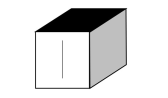
\includegraphics[width=0.7\columnwidth]{q10}
    \caption*{}
    \label{fig:Q10}
\end{figure}

\hfill{\brak{\text{GATE IN 2010}}}
\begin{enumerate}
\begin{multicols}{4}
\item 0
\item $\frac{\pi}{2}$
\item $\pi$
\item $2\pi$
\end{multicols}
\end{enumerate}

\item  The PMMC ammeter A in the adjoining figure has a range of 0 to 3 mA. When switch S1 is opened, the pointer of the ammeter swings to the 1 mA mark, returns and settles at 0.9 mA. The meter is
\begin{figure}[H]
    \centering
    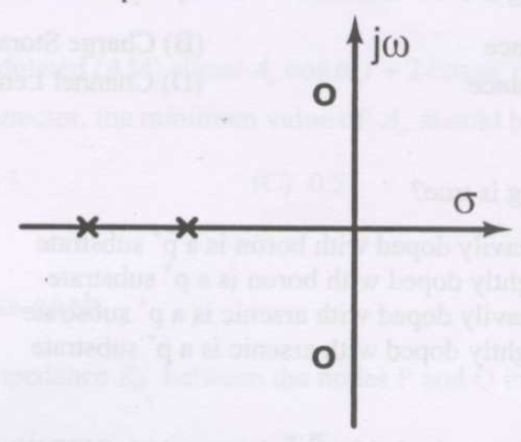
\includegraphics[width = 0.7\columnwidth]{q11}
    \caption*{}
    \label{fig:Q11}
\end{figure}

\hfill{\brak{\text{GATE IN 2010}}}
\begin{enumerate}
\item  critically damped and has a coil resistance of 100 $\ohm$
\item critically damped and has a coil resistance of 200 $\ohm$
\item under damped and has a coil resistance of 100 $\ohm$
\item under damped and has a coil resistance of 200 $\ohm$
\end{enumerate}

\item The open loop transfer function of a unity gain feedback system is given by: 
\begin{align*}
G\brak{s} = \frac{k\brak{s+3}}{\brak{s+1}\brak{s+2}}
\end{align*}
The range of positive values of k for which the closed loop system will remain stable is:

\hfill{\brak{\text{GATE IN 2010}}}
\begin{enumerate}
\begin{multicols}{2}
\item $1 < k < 3$
\item $0 < k < 10$
\item $5 < k < \infty$
\item $0 < k < \infty$
\end{multicols}
\end{enumerate}

\item A real $n \times n$ matrix $A = [a_{ij}]$ is defined as follows:
\begin{align*}
    a_{ij} &=i, if \text{ i = j}; \\
    &= 0, \text{ otherwise}
\end{align*}
The summation of all eigenvalues of A is

\hfill{\brak{\text{GATE IN 2010}}}
\begin{enumerate}
\begin{multicols}{4}
\item $n\brak{n+1}/2$
\item $n\brak{n-1}/2$
\item $\frac{n\brak{n+1}\brak{2n+1}}{6}$
\item $n^2$
\end{multicols}
\end{enumerate}

\item The contour C in the adjoining figure is described by $x^2 + y^2 = 16$.

\begin{minipage}{0.45\columnwidth}
\begin{figure}[H]
    \centering
    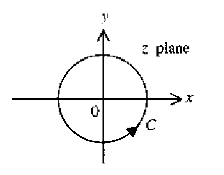
\includegraphics[width = 0.6\columnwidth]{q14}
    \caption*{}
    \label{fig:Q14}
\end{figure}
\end{minipage}
\hspace{0.05\columnwidth}
\begin{minipage}{0.45\columnwidth}
The value of 
\begin{align*}
\oint\limits_{C} \frac{z^2+8}{0.5z - 1.5j} dz
\end{align*}
is \brak{\text{Note: $j = \sqrt{-1}$}}
\end{minipage}

\hfill{\brak{\text{GATE IN 2010}}}
\begin{enumerate}
\begin{multicols}{4}
\item $-2\pi j$
\item $2\pi j$
\item $4\pi j$
\item $-4\pi j$
\end{multicols}
\end{enumerate}

\item In the dc circuit shown in the adjoining figure, the node voltage $V_2$ at steady state is
\begin{figure}[H]
    \centering
    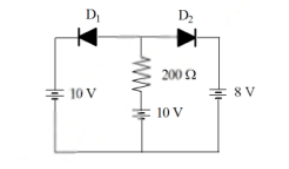
\includegraphics[width = 0.7\columnwidth]{q15}
    \caption*{}
    \label{fig:Q15}
\end{figure}

\hfill{\brak{\text{GATE IN 2010}}}
\begin{enumerate}
\begin{multicols}{4}
\item 0 V
\item 1 V
\item 2 V
\item 3 V
\end{multicols}
\end{enumerate}

\item A 100 $\ohm$, 1 W resistor and a 800 $\ohm$, 2 W resistor are connected in series. The maximum dc voltage that can be applied continuously to the series circuit without exceeding the power limit of any of the resistors is

\hfill{\brak{\text{GATE IN 2010}}}
\begin{enumerate}
\begin{multicols}{4}
\item 90 V
\item 50 V
\item 45 V
\item 40 V
\end{multicols}
\end{enumerate}

\item The seismic mass of an accelerometer oscillates sinusoidally at 100 Hz with a maximum displacement of 10 mm from its mean position. The peak acceleration of the seismic mass is

\hfill{\brak{\text{GATE IN 2010}}}
\begin{enumerate}
\begin{multicols}{4}
\item $3947.84 \, m/s^2$
\item $3141.50 \, m/s^2$
\item $314.15 \, m/s^2$
\item $100.00 \, m/s^2$
\end{multicols}
\end{enumerate}

\item In the ideal opamp circuit given in the adjoining figure, the value of $R_f$ is varied from 1 k$\ohm$ to 100 k$\ohm$. The gain $G = \brak{v_o/v_i}$ will
\begin{figure}[H]
    \centering
    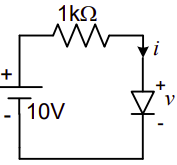
\includegraphics[width = 0.7\columnwidth]{q18}
    \caption*{}
    \label{fig:Q18}
\end{figure}

\hfill{\brak{\text{GATE IN 2010}}}
\begin{enumerate} 
\begin{multicols}{2}
    \item remain constant at +1
    \item remain constant at -1
    \item vary as $-\brak{R_f/10,000}$
    \item vary as $\brak{1+R_f/10,000}$
\end{multicols} \end{enumerate}


\item A signal with frequency components 50 Hz, 100 Hz and 200 Hz only is sampled at 150 samples/s. The ideally reconstructed signal will have frequency component\brak{\text{s}} of

\hfill{\brak{\text{GATE IN 2010}}}\begin{enumerate} \begin{multicols}{2}
    \item 50 Hz only
    \item 75 Hz only
    \item 50 Hz and 75 Hz
    \item 50 Hz, 75 Hz and 100 Hz
\end{multicols} \end{enumerate}

\item The subroutine SBX given below is executed by an 8085 processor. The value in the accumulator immediately after the execution of the subroutine will be:
\begin{verbatim}
SBX: MVI A, 99h
     ADI 11h
     MOV C, A
     RET
\end{verbatim}

\hfill{\brak{\text{GATE IN 2010}}}\begin{enumerate} \begin{multicols}{4}
    \item 00h
    \item 11h
    \item 99h
    \item AAh
\end{multicols} \end{enumerate}



\item The integral $\int\limits_{-\infty}^{\infty} \delta\brak{t - \pi/6} 6 \sin\brak{t} dt$ evaluates to

\hfill{\brak{\text{GATE IN 2010}}}\begin{enumerate} \begin{multicols}{4}
    \item 6
    \item 3
    \item 1.5
    \item 0
\end{multicols} \end{enumerate}



\item The deflection angle of the pointer of an ideal moving iron ammeter is $20\degree$ for 1.0 ampere dc current. If a current of $3 \sin\brak{314t}$ amperes is passed through the ammeter then the deflection angle is

\hfill{\brak{\text{GATE IN 2010}}}\begin{enumerate} \begin{multicols}{4}
    \item $0\degree$
    \item $42\degree$
    \item $60\degree$
    \item $90\degree$
\end{multicols} \end{enumerate}



\item An 8-bit DAC is interfaced with a microprocessor having 16 address lines \brak{A_0\dots A_{15}} as shown in the adjoining figure. A possible valid address for this DAC is
\begin{figure}[H]
    \centering
    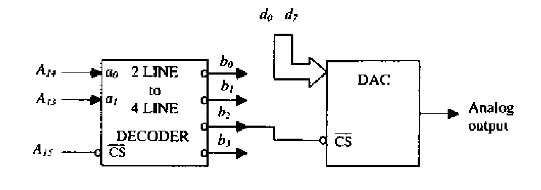
\includegraphics[width = 0.7\columnwidth]{q23}
    \caption*{}
    \label{fig:Q23}
\end{figure}

\hfill{\brak{\text{GATE IN 2010}}}\begin{enumerate} \begin{multicols}{4}
    \item 3000h
    \item 4FFFh
    \item AFFFh
    \item C000h
\end{multicols} 
\end{enumerate}

\item $H\brak{z}$ is a discrete rational transfer function. To ensure that both $H\brak{z}$ and its inverse are stable its

\hfill{\brak{\text{GATE IN 2010}}}\begin{enumerate}
    \item poles must be inside the unit circle and zeros must be outside the unit circle.
    \item poles and zeros must be inside the unit circle.
    \item poles and zeros must be outside the unit circle.
    \item poles must be outside the unit circle and the zeros should be inside the unit circle.
 \end{enumerate}



\item The output voltage of a transducer with an output resistance of 10 k$\ohm$ is connected to an amplifier. The minimum input resistance of the amplifier so that the error in recording the transducer output does not exceed 2\% is

\hfill{\brak{\text{GATE IN 2010}}}
\begin{enumerate}
\begin{multicols}{4}
    \item 10 k$\ohm$
    \item 49 k$\ohm$
    \item 490 k$\ohm$
    \item 1.2 M$\ohm$
\end{multicols} \end{enumerate}



\item X and Y are non-zero square matrices of size $n \times n$. If $XY=0_{n \times n}$ then

\hfill{\brak{\text{GATE IN 2010}}}\begin{enumerate} \begin{multicols}{2}
    \item $\abs{X}=0$ and $\abs{Y}\neq0$
    \item $\abs{X}\neq0$ and $\abs{Y}=0$
    \item $\abs{X}=0$ and $\abs{Y}=0$
    \item $\abs{X}\neq0$ and $\abs{Y}\neq0$
\end{multicols} \end{enumerate}



\item Consider the differential equation $\frac{dy}{dx} + y = e^x$ with $y\brak{0} = 1$. The value of $y\brak{1}$ is

\hfill{\brak{\text{GATE IN 2010}}}
\begin{enumerate} \begin{multicols}{4}
    \item $e + e^{-1}$
    \item $\frac{1}{2}\brak{e - e^{-1}}$
    \item $\frac{1}{2}\brak{e + e^{-1}}$
    \item $2\brak{e - e^{-1}}$
\end{multicols} \end{enumerate}



\item The electric charge density in the region $R\colon x^2+y^2 \le 1, y \le 0$ is given as $\sigma\brak{x,y} = 1 \, C/m^2$, where x and y are in meters. The total charge \brak{\text{in coulomb}} contained in the region R is

\hfill{\brak{\text{GATE IN 2010}}}\begin{enumerate} \begin{multicols}{4}
    \item $4\pi$
    \item $2\pi$
    \item $\pi/2$
    \item 0
\end{multicols} \end{enumerate}



\item The input $x\brak{t}$ and the corresponding output $y\brak{t}$ of a system are related by $y\brak{t} = \int_{-\infty}^{5t} x\brak{\tau} d\tau$. The system is

\hfill{\brak{\text{GATE IN 2010}}}\begin{enumerate} \begin{multicols}{2}
    \item time invariant and causal
    \item time invariant and noncausal
    \item time variant and noncausal
    \item time variant and causal
\end{multicols} \end{enumerate}



\item A digital filter having a transfer function $H\brak{z} = \frac{p_0 + p_1 z^{-1} + p_3 z^{-3}}{1 + d_3 z^{-3}}$ is implemented using Direct Form-I and Direct Form-II realizations of IIR structure. The number of delay units required in Direct Form-I and Direct Form-II realizations are, respectively

\hfill{\brak{\text{GATE IN 2010}}}\begin{enumerate} \begin{multicols}{4}
    \item 6 and 6
    \item 6 and 3
    \item 3 and 3
    \item 3 and 2
\end{multicols} \end{enumerate}



\item The velocity v \brak{\text{in m/s}} of a moving mass, starting from rest, is given as $\frac{dv}{dt} = v+t$. Using Euler forward difference method \brak{\text{also known as Cauchy-Euler method}} with a step size of 0.1 s, the velocity at 0.2 s evaluates to

\hfill{\brak{\text{GATE IN 2010}}}\begin{enumerate} \begin{multicols}{4}
    \item 0.01 m/s
    \item 0.1 m/s
    \item 0.2 m/s
    \item 1 m/s
\end{multicols} \end{enumerate}



\item The rotor of the control transformer of a synchro pair gives a maximum voltage of 1.0 V at a particular position of the rotor of the control transmitter. The transmitter rotor is now rotated by $30\degree$ anticlockwise keeping the transformer rotor stationary. The transformer rotor voltage for this position is

\hfill{\brak{\text{GATE IN 2010}}}\begin{enumerate} \begin{multicols}{4}
    \item 1.0 V
    \item 0.866 V
    \item 0.5 V
    \item 0 V
\end{multicols} \end{enumerate}



\item The matched transistors Q1 and Q2 shown in the adjoining figure have $\beta = 100$. Assuming the base-emitter voltages to be 0.7 V, the collector-emitter voltage $V_2$ of the transistor Q2 is
\begin{figure}[H]
    \centering
    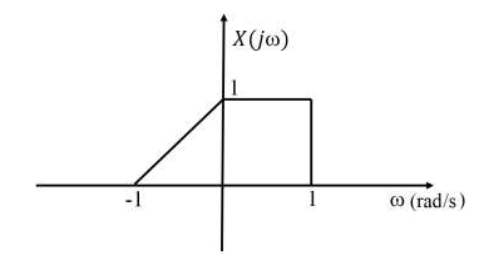
\includegraphics[width = 0.7\columnwidth]{q33}
    \caption*{}
    \label{fig:Q33}
\end{figure}

\hfill{\brak{\text{GATE IN 2010}}}\begin{enumerate} \begin{multicols}{4}
    \item 33.9 V
    \item 27.8 V
    \item 16.2 V
    \item 0.7 V
\end{multicols} \end{enumerate}

\item The volume of a cylinder is computed from measurements of its height \brak{\text{h}} and diameter \brak{\text{d}}. A set of several measurements of height has an average value of 0.2 m and a standard deviation of 1\%. The average value obtained for the diameter is 0.1 m and the standard deviation is 1\%. Assuming the errors in the measurements of height and diameter are uncorrelated, the standard deviation of the computed volume is

\hfill{\brak{\text{GATE IN 2010}}}\begin{enumerate} \begin{multicols}{4}
    \item 1.00\%
    \item 1.73\%
    \item 2.23\%
    \item 2.41\%
\end{multicols} \end{enumerate}



\item A thermocouple based temperature measurement system is shown in the adjoining figure. Relevant thermocouple emf data \brak{\text{in mV}} is given below. The cold junction is kept at $0\degree C$. The temperature is $30\degree C$ in the other parts of the system. The emf $V_o$ is measured to be 26.74 mV. The temperature of the hot liquid is
\begin{figure}[H]
    \centering
    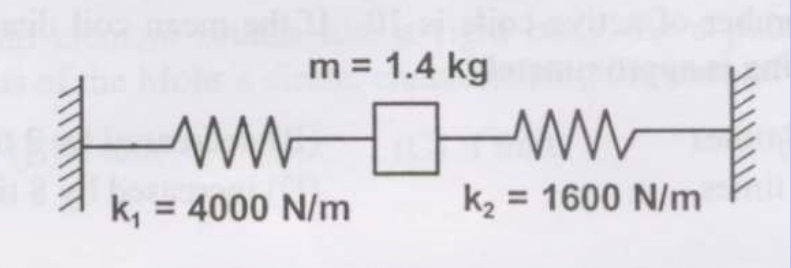
\includegraphics[width = 0.7\columnwidth]{q35}
    \caption*{}
    \label{fig:Q35}
\end{figure}
\begin{table}[H]
    \centering\normalsize
    \begin{tabular}{|l|c|c|}
        \hline
        \textbf{Temperature} & \textbf{emf of Chromel-Constantan} & \textbf{emf of Copper-Constantan} \\
        \hline
        $10\degree C$ & 0.591 & 0.391 \\
        \hline
        $20\degree C$ & 1.192 & 0.789 \\
        \hline
        $30\degree C$ & 1.801 & 1.196 \\
        \hline
        $370\degree C$ & 26.549 & 19.027 \\
        \hline
        $380\degree C$ & 27.345 & 19.638 \\
        \hline
    \end{tabular}
    \caption*{}
    \label{tab:Q35}
\end{table}

\hfill{\brak{\text{GATE IN 2010}}}\
\begin{enumerate} \begin{multicols}{4}
    \item $370.0\degree C$
    \item $372.4\degree C$
    \item $376.6\degree C$
    \item $380.0\degree C$
\end{multicols} \end{enumerate}



\item A differential pressure transmitter is used to measure the flow rate in a pipe. Due to aging, the sensitivity of the pressure transmitter is reduced by 5\%. All other aspects of the flow meter remaining constant, change in the sensitivity of the flow measurement is

\hfill{\brak{\text{GATE IN 2010}}}\begin{enumerate} \begin{multicols}{4}
    \item 10.0\%
    \item 5.0\%
    \item 2.5\%
    \item 2.2\%
\end{multicols} \end{enumerate}



\item The asymptotic Bode magnitude plot of a lead network with its pole and zero on the left half of the s-plane is shown in the adjoining figure. The frequency at which the phase angle of the network is maximum \brak{\text{in rad/s}} is
\begin{figure}[H]
    \centering
    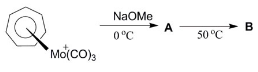
\includegraphics[width = 0.7\columnwidth]{q37}
    \caption*{}
    \label{Q37}
\end{figure}

\hfill{\brak{\text{GATE IN 2010}}}
\begin{enumerate} 
\begin{multicols}{4}
    \item $\frac{3}{\sqrt{10}}$
    \item $\frac{1}{\sqrt{20}}$
    \item $\frac{1}{20}$
    \item $\frac{1}{30}$
\end{multicols} \end{enumerate}

\item In an analog single channel cathode ray oscilloscope \brak{\text{CRO}}, the x and y sensitivities are set as 1 ms/div and 1 V/div, respectively. The y-input is connected to a voltage signal $4 \cos\brak{200\pi t - 45\degree}$ V. The trigger source is internal, level chosen is zero and the slope is positive. The display seen on the CRO screen is

\hfill{\brak{\text{GATE IN 2010}}}
\begin{enumerate}
\begin{figure}[H]
\centering
\begin{multicols}{2}
    \item
        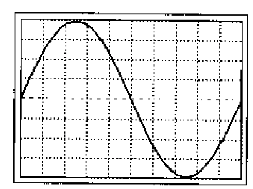
\includegraphics[width = 0.5\columnwidth]{38aa}
    \item 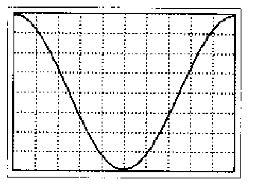
\includegraphics[width = 0.5\columnwidth]{38ab}
    \item 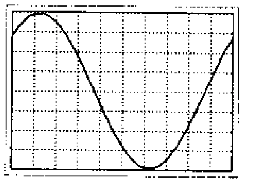
\includegraphics[width = 0.5\columnwidth]{38ac}
    \item 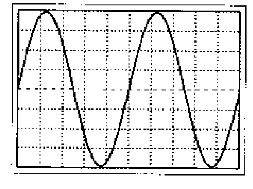
\includegraphics[width = 0.5\columnwidth]{38ad}
\end{multicols}
\caption*{}
\label{fig:q38}
\end{figure}
\end{enumerate}

\item A unit ramp input is applied to the system shown in the adjoining figure. The steady state error in its output is
\begin{figure}[H]
    \centering
    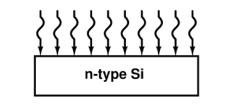
\includegraphics[width = 0.7\columnwidth]{q39}
    \caption*{}
    \label{fig:Q39}
\end{figure}

\hfill{\brak{\text{GATE IN 2010}}}\begin{enumerate} \begin{multicols}{4}
    \item 0
    \item 0.5
    \item 1
    \item 2
\end{multicols} \end{enumerate}



\item A unity feedback system has an open loop transfer function $G\brak{s} = \frac{k}{s\brak{s+3}}$. The value of k that yields a damping ratio of 0.5 for the closed loop system is

\hfill{\brak{\text{GATE IN 2010}}}\begin{enumerate} \begin{multicols}{4}
    \item 1
    \item 3
    \item 5
    \item 9
\end{multicols} \end{enumerate}

\item A 4-bit successive approximation type ADC has a full scale value of 15 V. The sequence of the states, the SAR will traverse, for the conversion of an input of 8.15 V is

\hfill{\brak{\text{GATE IN 2010}}}
\begin{figure}[H]
    \centering
    \begin{enumerate} 
    \item \caption*{} \label{41A}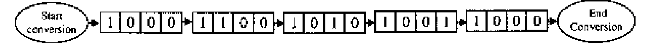
\includegraphics[width = 0.7\columnwidth]{41a}
    \item \caption*{} \label{41B}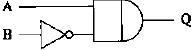
\includegraphics[width = 0.7\columnwidth]{41b}
    \item \caption*{} \label{41C}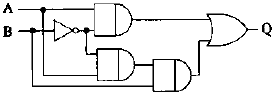
\includegraphics[width = 0.7\columnwidth]{41c}
    \item \caption*{} \label{41D}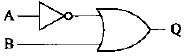
\includegraphics[width = 0.7\columnwidth]{41d}
 \end{enumerate}
 \caption*{}
 \label{fig:Q41}
\end{figure}




\item The logic gate circuit shown in the adjoining figure realizes the function
\begin{figure}[H]

    \centering
    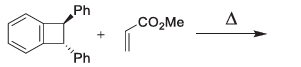
\includegraphics[width = 0.7\columnwidth]{q42}
    \caption*{}
    \label{fig:Q42}
\end{figure}

\hfill{\brak{\text{GATE IN 2010}}}\begin{enumerate} \begin{multicols}{2}
    \item XOR
    \item XNOR
    \item Half adder
    \item Full adder
\end{multicols} \end{enumerate}



\item In an 8085 processor, the main program calls the subroutine SUB1 given below. When the program returns to the main program after executing SUB1, the value in the accumulator is
\begin{center}
\begin{verbatim}
Address     Opcode      Mnemonic
2000h       3E 00       SUB1: MVI A, 00h
2002h       CD 05 20          CALL SUB2
2005h       3C          SUB2: INR A
2006h       C9                RET
\end{verbatim}
\end{center}

\hfill{\brak{\text{GATE IN 2010}}}\begin{enumerate} \begin{multicols}{4}
    \item 00
    \item 01
    \item 02
    \item 03
\end{multicols} \end{enumerate}



\item Light coming out of an optical fiber is incident on a plane perpendicular to the fiber axis and 50 mm away from the end of the fiber. The light coming out creates a circular spot that can at most be of 20 mm diameter. Neglecting the diameter of the fiber, the numerical aperture of the fiber is, approximately,

\hfill{\brak{\text{GATE IN 2010}}}\begin{enumerate} \begin{multicols}{4}
    \item 0.14
    \item 0.20
    \item 0.34
    \item 0.40
\end{multicols} \end{enumerate}



\item A solution "P" is put in a spectrophotometer cuvette of optical path length 1 cm. The transmittance is found to be 10\%. Another solution "Q" has a transmittance of 40\% under the same circumstances. If equal volumes of P and Q are mixed together, the transmittance of the resulting solution \brak{\text{assuming the constituents of P and Q do not react with each other}} is, approximately,

\hfill{\brak{\text{GATE IN 2010}}}\begin{enumerate} \begin{multicols}{4}
    \item 15\%
    \item 20\%
    \item 25\%
    \item 30\%
\end{multicols} \end{enumerate}



\item 4-point DFT of a real discrete-time signal $x[n]$ of length 4 is given by $X[k]$, $n=0,1,2,3$ and $k=0,1,2,3$. It is given that $X[0]=5$, $X[1]=1+j1$, $X[2]=0.5$. $X[3]$ and $x[0]$ respectively are

\hfill{\brak{\text{GATE IN 2010}}}
\begin{enumerate} \begin{multicols}{4}
    \item $1-j$, 1.875
    \item $1-j$, 1.500
    \item $1+j$, 1.875
    \item $0.1-j0.1$, 1.500
\end{multicols} 
\end{enumerate}



\item An active filter is shown in the adjoining figure. The dc gain and the 3 dB cut-off frequency of the filter respectively, are, nearly
\begin{figure}[H]
    \centering
    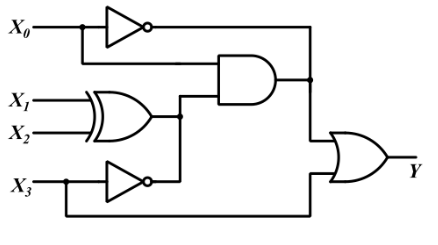
\includegraphics[width = 0.7\columnwidth]{q47}
    \caption*{}
    \label{fig:Q47}
\end{figure}

\hfill{\brak{\text{GATE IN 2010}}}
\begin{enumerate} 
\begin{multicols}{2}
    \item 40 dB, 3.14 kHz
    \item 40 dB, 1.00 kHz
    \item 20 dB, 6.28 kHz
    \item 20 dB, 1.00 kHz
\end{multicols} 
\end{enumerate}


A differential amplifier is constructed using an ideal opamp as shown in the adjoining figure. The values of $R_1$ and $R_2$ are 47 k$\ohm$ and 470 k$\ohm$ respectively.
\begin{figure}[H]
    \centering
    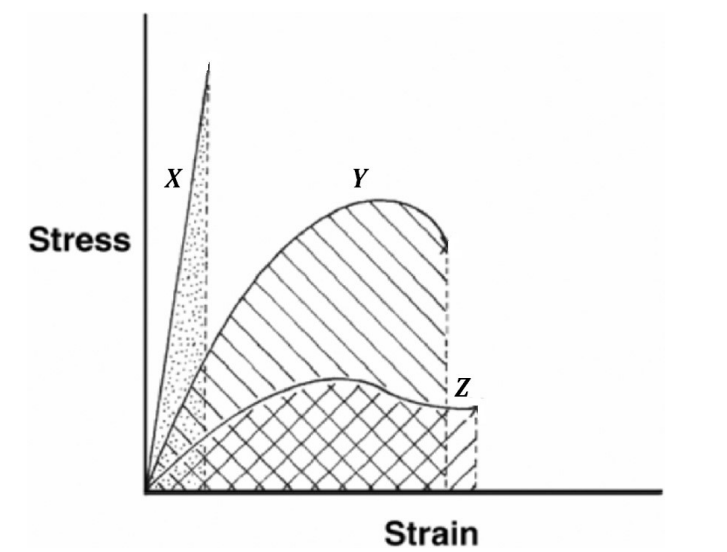
\includegraphics[width = 0.7\columnwidth]{q48}
    \caption*{}
    \label{fig:Q48}
\end{figure}


\item The input impedances seen looking into the terminals $V_1$ and $V_2$, with respect to ground, respectively are

\hfill{\brak{\text{GATE IN 2010}}}\begin{enumerate} \begin{multicols}{2}
    \item 47 k$\ohm$ and 43 k$\ohm$
    \item 47 k$\ohm$ and 47 k$\ohm$
    \item 47 k$\ohm$ and 517 k$\ohm$
    \item 517 k$\ohm$ and 517 k$\ohm$
\end{multicols} \end{enumerate}

\item $V_1$ and $V_2$ are connected to voltage sources having an open circuit output of +1 V each and internal resistances of 13 k$\ohm$ and 3 k$\ohm$ respectively. The output voltage $V_o$ is

\hfill{\brak{\text{GATE IN 2010}}}\begin{enumerate} \begin{multicols}{4}
    \item 0 V
    \item 0.15 V
    \item 1.5 V
    \item 10 V
\end{multicols} \end{enumerate}

A PMMC type ammeter has full scale current of 100 $\mu$A and a coil resistance of 100 $\ohm$.

\item The resistance required to convert the 100 $\mu$A ammeter into a 1A full scale dc ammeter is

\hfill{\brak{\text{GATE IN 2010}}}
\begin{enumerate} 
\begin{multicols}{2}
    \item 10 m$\ohm$ in series with the meter
    \item 10 m$\ohm$ in parallel with the meter
    \item 1 m$\ohm$ in series with the meter
    \item 1 m$\ohm$ in parallel with the meter
\end{multicols} \end{enumerate}

\item The above PMMC meter is connected in the circuit shown in the adjoining figure. The opamp is ideal. The voltage $v_i\brak{t} = 1.0 \sin 314t$ V. Assuming the source impedance of $v_i\brak{t}$ to be zero, the ammeter will indicate a current of
\begin{figure}[H]
    \centering
    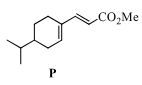
\includegraphics[width = 0.7\columnwidth]{q51}
    \caption*{}
    \label{fig:Q51}
\end{figure}

\hfill{\brak{\text{GATE IN 2010}}}\begin{enumerate} \begin{multicols}{4}
    \item 100 $\mu$A
    \item 70.7 $\mu$A
    \item 63.7 $\mu$A
    \item 31.8 $\mu$A
\end{multicols} \end{enumerate}

A coil having an inductance \brak{\text{L}} of 10 mH and resistance R is connected in series with an ideal 100 $\mu$F capacitor \brak{\text{C}}. When excited by a voltage source of value $10\sqrt{2} \cos\brak{1000t}$ V, the series RLC circuit draws 20 W of power.

\item The value of the coil resistance R is

\hfill{\brak{\text{GATE IN 2010}}}\begin{enumerate} \begin{multicols}{4}
    \item 1 $\ohm$
    \item 2 $\ohm$
    \item 4 $\ohm$
    \item 5 $\ohm$
\end{multicols} \end{enumerate}

\item The Q factor of the coil at an angular frequency of 1000 rad/s is

\hfill{\brak{\text{GATE IN 2010}}}\begin{enumerate} \begin{multicols}{4}
    \item 1
    \item 2
    \item 4
    \item 5
\end{multicols} \end{enumerate}

Consider a temperature measurement scheme shown in the adjoining figure. It uses an RTD whose resistance at $0\degree$C is 100 $\ohm$ and temperature coefficient of resistance \brak{\alpha} is 0.00392 /$\degree$C.
\begin{figure}[H]
    \centering
    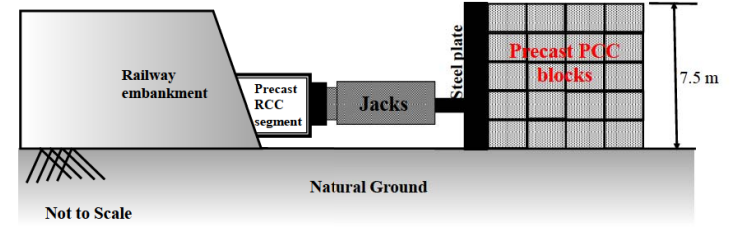
\includegraphics[width = 0.7\columnwidth]{q54}
    \caption*{}
    \label{fig:Q54}
\end{figure}


\item The differential gain of the instrumentation amplifier to achieve a voltage sensitivity of 10 mV/$\degree$C at $0\degree$C, should be approximately

\hfill{\brak{\text{GATE IN 2010}}}\begin{enumerate} \begin{multicols}{4}
    \item 13.41
    \item 26.02
    \item 57.53
    \item 90.14
\end{multicols} \end{enumerate}

\item The RTD is placed in a hot water bath of temperature $100\degree$C. Based on the gain calculated in Q.54, the error in the measured value of the temperature due to bridge nonlinearity is

\hfill{\brak{\text{GATE IN 2010}}}\begin{enumerate} \begin{multicols}{4}
    \item $-0.1\degree$C
    \item $0.4\degree$C
    \item $0.9\degree$C
    \item $+1.2\degree$C
\end{multicols} \end{enumerate}



\item 25 persons are in a room. 15 of them play hockey, 17 of them play football and 10 of them play both hockey and football. Then the number of persons playing neither hockey nor football is:

\hfill{\brak{\text{GATE IN 2010}}}
\begin{enumerate} 
\begin{multicols}{4}
    \item 2
    \item 17
    \item 13
    \item 3
\end{multicols}
\end{enumerate}



\item Choose the most appropriate word from the options given below to complete the following sentence:

\textbf{If we manage to \underline{\hspace{2cm}} our natural resources, we would leave a better planet for our children.}

\hfill{\brak{\text{GATE IN 2010}}}
\begin{enumerate}
    \item uphold
    \item restrain
    \item cherish
    \item conserve
\end{enumerate}



\item The question below consists of a pair of related words followed by four pairs of words. Select the pair that best expresses the relation in the original pair. 

\textbf{Unemployed : Worker}

\hfill{\brak{\text{GATE IN 2010}}}
\begin{enumerate}
    \item fallow : land
    \item unaware : sleeper
    \item wit : jester
    \item renovated : house
\end{enumerate}



\item Which of the following options is the closest in meaning to the word below: 

\textbf{Circuitous}

\hfill{\brak{\text{GATE IN 2010}}}\begin{enumerate}
    \item cyclic
    \item indirect
    \item confusing
    \item crooked
\end{enumerate}

\item Choose the most appropriate word from the options given below to complete the following sentence:

\textbf{His rather casual remarks on politics \underline{\hspace{2cm}} his lack of seriousness about the subject.}

\hfill{\brak{\text{GATE IN 2010}}}
\begin{enumerate} \begin{multicols}{4}
    \item masked
    \item belied
    \item betrayed
    \item suppressed
\end{multicols} \end{enumerate}



\item Hari \brak{\text{H}}, Gita \brak{\text{G}}, Irfan \brak{\text{I}} and Saira \brak{\text{S}} are siblings \brak{\text{i.e. brothers and sisters}}. All were born on $1^{st}$ January. The age difference between any two successive siblings \brak{\text{that is born one after another}} is less than 3 years. Given the following facts:

\begin{itemize}
    \item Hari's age + Gita's age $>$ Irfan's age + Saira's age.
    \item The age difference between Gita and Saira is 1 year. However, Gita is not the oldest and Saira is not the youngest.
    \item There are no twins. 
\end{itemize}

In what order were they born \brak{\text{oldest first}}?

\hfill{\brak{\text{GATE IN 2010}}}
\begin{enumerate}
\begin{multicols}{4}
    \item HSIG
    \item SGHI
    \item IGSH
    \item IHSG
\end{multicols} \end{enumerate}

\item 5 skilled workers can build a wall in 20 days; 8 semi-skilled workers can build a wall in 25 days; 10 unskilled workers can build a wall in 30 days. If a team has 2 skilled, 6 semi-skilled and 5 unskilled workers, how long will it take to build the wall?

\hfill{\brak{\text{GATE IN 2010}}}\begin{enumerate} \begin{multicols}{4}
    \item 20 days
    \item 18 days
    \item 16 days
    \item 15 days
\end{multicols} \end{enumerate}



\item \textbf{Modern warfare has changed from large scale clashes of armies to suppression of civilian populations. Chemical agents that do their work silently appear to be suited to such warfare; and regretfully, there exist people in military establishments who think that chemical agents are useful tools for their cause.} \\
\\
Which of the following statements best sums up the meaning of the above passage:

\hfill{\brak{\text{GATE IN 2010}}}
\begin{enumerate}
    \item Modern warfare has resulted in civil strife.
    \item Chemical agents are useful in modern warfare.
    \item Use of chemical agents in warfare would be undesirable.
    \item People in military establishments like to use chemical agents in war.
\end{enumerate}



\item Given digits 2, 2, 3, 3, 3, 4, 4, 4, 4 how many distinct 4-digit numbers greater than 3000 can be formed?

\hfill{\brak{\text{GATE IN 2010}}}\begin{enumerate} \begin{multicols}{4}
    \item 50
    \item 51
    \item 52
    \item 54
\end{multicols} \end{enumerate}



\item If $137 + 276 = 435$ how much is $731 + 672$?

\hfill{\brak{\text{GATE IN 2010}}}\begin{enumerate} \begin{multicols}{4}
    \item 534
    \item 1403
    \item 1623
    \item 1513
\end{multicols} \end{enumerate}

\begin{center}
\textbf{END OF THE QUESTION PAPER}
\end{center}

\end{enumerate}
\end{document}

	\documentclass[journal,12pt,onecolumn]{IEEEtran}
\usepackage{cite}
\usepackage{graphicx}
\usepackage{amsmath,amssymb,amsfonts,amsthm}
\usepackage{algorithmic}
\usepackage{graphicx}
\usepackage{textcomp}
\usepackage{xcolor}
\usepackage{txfonts}
\usepackage{listings}
\usepackage{enumitem}
\usepackage{mathtools}
\usepackage{gensymb}
\usepackage{comment}
\usepackage[breaklinks=true]{hyperref}
\usepackage{tkz-euclide} 
\usepackage{listings}
\usepackage{gvv}                                        
%\def\inputGnumericTable{}                                 
\usepackage[latin1]{inputenc} 
\usetikzlibrary{arrows.meta, positioning}
\usepackage{xparse}
\usepackage{color}                                            
\usepackage{array}                                            
\usepackage{longtable}                                       
\usepackage{calc}                                             
\usepackage{multirow}
\usepackage{multicol}
\usepackage{hhline}                                           
\usepackage{ifthen}                                           
\usepackage{lscape}
\usepackage{tabularx}
\usepackage{array}
\usepackage{float}
\newtheorem{theorem}{Theorem}[section]
\newtheorem{problem}{Problem}
\newtheorem{proposition}{Proposition}[section]
\newtheorem{lemma}{Lemma}[section]
\newtheorem{corollary}[theorem]{Corollary}
\newtheorem{example}{Example}[section]
\newtheorem{definition}[problem]{Definition}
\newcommand{\BEQA}{\begin{eqnarray}}
\newcommand{\EEQA}{\end{eqnarray}}
\usepackage{float}
%\newcommand{\define}{\stackrel{\triangle}{=}}
\theoremstyle{remark}
\usepackage{circuitikz}
\usepackage{tikz}
\title{GG: GEOLOGY AND GEOPHYSICS}
\author{EE25BTECH11032- KARTIK LAHOTI}
\begin{document}

\maketitle 

\begin{center}
    \subsection*{PART A: COMMON TO BOTH GEOLOGY AND GEOPHYSICS CANDIDATES}
\end{center}
\subsubsection*{Q.1 - Q.25 carry one mark each.}

    \begin{enumerate}
        \item The number of hydrous minerals in the Moh's scale of hardness is \rule{3cm}{0.15mm} \hfill{\brak{\text{GATE GG 2013}}}

        \item It takes approximately \rule{3cm}{0.15mm} minutes for sunlight to reach the Earth. \hfill{\brak{\text{GATE GG 2013}}}

        \item In a remotely sensed data of a planet, the presence of hydrous species can be inferred using \rule{3cm}{0.15mm} region of the electromagnetic spectrum? \hfill{\brak{\text{GATE GG 2013}}}
        \begin{enumerate}
            \begin{multicols}{4}
                \item Radiowave
                \item Gamma
                \item Infrared
                \item Visible
            \end{multicols}                    
        \end{enumerate}

        \item Amongst the following, which one will have the highest P-wave velocity? \hfill{\brak{\text{GATE GG 2013}}}
        \begin{enumerate}
            \begin{multicols}{4}
                \item Granite
                \item Diamond
                \item Shale
                \item Talc
            \end{multicols}
        \end{enumerate}

        \item Assuming the Earth to be a perfect sphere, its equatorial velocity is approximately \rule{3cm}{0.15mm}$\,km/hr$ \hfill{\brak{\text{GATE GG 2013}}}

        \item Both strength and plasticity of a rock increase with the \hfill{\brak{\text{GATE GG 2013}}}
            \begin{enumerate}
                \item increase in temperature
                \item decrease in strain rate
                \item increase in confining pressure
                \item increase in pore fluid pressure
            \end{enumerate}
            
        \item Amongst the following options, the acceptable value of the Poisson's ratio of a rock is \hfill{\brak{\text{GATE GG 2013}}}
            \begin{enumerate}
                \begin{multicols}{4}
                    \item $0.55$
                    \item $1.00$
                    \item $0.25$
                    \item $-1.00$
                \end{multicols}
            \end{enumerate}

        \item The acceleration due to gravity, $'g'$ is maximum at \hfill{\brak{\text{GATE GG 2013}}}
            \begin{enumerate}
                \begin{multicols}{4}
                    \item equator
                    \item poles
                    \item mid-latitudes
                    \item sub-tropical regions
                \end{multicols}
            \end{enumerate}

        \item The most abundant mineral in the Earth's crust is \hfill{\brak{\text{GATE GG 2013}}}
            \begin{enumerate}
                \begin{multicols}{4}
                    \item quartz
                    \item K-feldspar
                    \item biotite
                    \item garnet
                \end{multicols}
            \end{enumerate}

        \item Acoustic impedance is the \rule{3cm}{0.15mm} of density and velocity. \hfill{\brak{\text{GATE GG 2013}}}\hfill{\brak{\text{GATE GG 2013}}}
            \begin{enumerate}
                \begin{multicols}{4}
                    \item sum
                    \item difference
                    \item product
                    \item ratio
                \end{multicols}
            \end{enumerate}

        \item Choose the diamagnetic mineral from the following. \hfill{\brak{\text{GATE GG 2013}}}
            \begin{enumerate}
                \begin{multicols}{4}
                    \item Calcite
                    \item Enstatite
                    \item Pyrite
                    \item Ilmenite
                \end{multicols}
            \end{enumerate}

        \item Two bodies made up of same material with different dimensions have \hfill{\brak{\text{GATE GG 2013}}}
            \begin{enumerate}
                    \item same resistances and resistivities
                    \item same resistivities but different resistances
                    \item same resistances but different resistivities
                    \item different resistances and resistivities
            \end{enumerate}

        \item The type of wave that arrives first at a station from an earthquake hypocenter is \hfill{\brak{\text{GATE GG 2013}}}
            \begin{enumerate}
                \begin{multicols}{4}
                    \item P-wave
                    \item S-wave
                    \item Rayleigh wave
                    \item Love wave
                \end{multicols}
            \end{enumerate}

        \item Which one of the following is the correct statement? \hfill{\brak{\text{GATE GG 2013}}}
            \begin{enumerate}
                \item Accretionary wedge is part of the foreland basin
                \item Spreading ridge is a major zone of metamorphism
                \item Dehydration of subducting slab induces mantle melting
                \item Back arc basin represent a convergent regime
            \end{enumerate}
            
        \item Match the following items of \textbf{Group $I$} with those of \textbf{Group $II$}. \hfill{\brak{\text{GATE GG 2013}}}

        \begin{multicols}{2}
            \underline{\textbf{Group $I$}}
            \begin{enumerate}[start =16]
                \item Electrical Method
                \item Magnetic Method
                \item Gravity Method
                \item Seismic Method
            \end{enumerate}

            \columnbreak

            \underline{\textbf{Group $II$}}
            \begin{enumerate}
                \item Density
                \item Velocity
                \item Resistivity
                \item Susceptibility
                \item Dielectric Permittivity
            \end{enumerate}
        \end{multicols}

        \begin{enumerate}
            \item P-$3$, Q-$2$, R-$5$, S-$1$
            \item P-$3$, Q-$4$, R-$1$, S-$2$
            \item P-$3$, Q-$4$, R-$2$, S-$1$
            \item P-$5$, Q-$4$, R-$3$, S-$2$
        \end{enumerate}
        
        \item If a radioactive isotope has a decay constant of $1.55 \times 10^{-10}\text{year}^{-1}$, its half-life (in years) would be \hfill{\brak{\text{GATE GG 2013}}}
            \begin{enumerate}
                \begin{multicols}{4}
                    \item $4.57 \times 10^{9}$
                    \item $4.47 \times 10^{9}$
                    \item $4.57 \times 10^{10}$
                    \item $4.47 \times 10^{10}$
                \end{multicols}
            \end{enumerate}

        \item Which of the following physical properties of rocks has the widest range of variation? \hfill{\brak{\text{GATE GG 2013}}}
            \begin{enumerate}
                \begin{multicols}{2}
                    \item Magnetic permeability
                    \item Dielectric permittivity
                    \item Seismic velocity
                    \item Electrical resistivity
                \end{multicols}
            \end{enumerate}

        \item Which of the following is \underline{\textbf{NOT}} an inverse square law? \hfill{\brak{\text{GATE GG 2013}}}
            \begin{enumerate}
                    \item Newton's law of Gravitation
                    \item Coulomb's law of electrostatics
                    \item Coulomb's law of magnetostatics
                    \item Hooke's law
            \end{enumerate}
        
        \item A type of unconformity characterized by the occurrence of sedimentary rocks on igneous/metamorphic rocks is known as \hfill{\brak{\text{GATE GG 2013}}}
            \begin{enumerate}
                \begin{multicols}{2}
                    \item angular unconformity
                    \item nonconformity
                    \item paraconformity
                    \item disconformity
                \end{multicols}
            \end{enumerate}
        
        \item For seismic S-wave velocity, $V$, the rigidity modulus, $\mu$, is proportional to \hfill{\brak{\text{GATE GG 2013}}}
            \begin{enumerate}
                \begin{multicols}{4}
                    \item $\sqrt{V}$
                    \item $V$
                    \item $V^{2}$
                    \item $V^{3}$
                \end{multicols}
            \end{enumerate}

        \item An active trench is present in the vicinity of \hfill{\brak{\text{GATE GG 2013}}}
            \begin{enumerate}
                \begin{multicols}{2}
                    \item Andaman \& Nicobar Islands
                    \item Gulf of Cambay
                    \item Lakshadweep
                    \item Krishna-Godavari delta
                \end{multicols}
            \end{enumerate}

        \item In a homogeneous anisotropic medium, the physical property varies \hfill{\brak{\text{GATE GG 2013}}}
            \begin{enumerate}
                    \item with position but not with direction
                    \item with both position and direction
                    \item with direction but not with position
                    \item neither with position nor with direction
            \end{enumerate}
        \item Which one of the following stable isotopic ratios is used for estimation of palaeo-temperature of seawater? \hfill{\brak{\text{GATE GG 2013}}}
            \begin{enumerate}
                \begin{multicols}{2}
                    \item $^{13}\text{C/}^{12}\text{C}$
                    \item $^{18}\text{O/}^{16}\text{O}$
                    \item $^{87}\text{S/}^{86}\text{Sr}$
                    \item $^{15}\text{N/}^{14}\text{N}$
                \end{multicols}
            \end{enumerate}

        \item Match the following items of \textbf{Group $I$} with those of \textbf{Group $II$}. \hfill{\brak{\text{GATE GG 2013}}}

        \begin{multicols}{2}
            \underline{\textbf{Group $I$}}
            \begin{enumerate}[start =16]
                \item Coal
                \item Copper
                \item Oil
                \item Uranium
            \end{enumerate}

            \columnbreak

            \underline{\textbf{Group $II$}}
            \begin{enumerate}
                \item Gandhar
                \item Singareni
                \item Khetri
                \item Jadugoda
                \item Degana
            \end{enumerate}
        \end{multicols} 

        \begin{enumerate}
            \begin{multicols}{2}
                \item P-$4$, Q-$3$, R-$1$, S-$2$
                \item P-$2$, Q-$3$, R-$5$, S-$4$
                \item P-$1$, Q-$3$, R-$2$, S-$5$
                \item P-$2$, Q-$3$, R-$1$, S-$4$ 
            \end{multicols}            
        \end{enumerate}
        
        \item Which of the following logging techniques is best suited to estimate the shaliness of hydrocarbon reservoirs? \hfill{\brak{\text{GATE GG 2013}}}
            \begin{enumerate}
                \begin{multicols}{2}
                    \item Resistivity
                    \item Sonic
                    \item Induction
                    \item Gamma ray
                \end{multicols}
            \end{enumerate}

        \newpage

    \begin{center}
        \subsection*{PART B \brak{\text{SECTION 1}}: FOR GEOLOGY CANDIDATES ONLY}
    \end{center}
    
    \subsection*{Q.26 - Q.55 carry two mark each.}

        \item Which of the following statements is correct? \hfill{\brak{\text{GATE GG 2013}}}
            \begin{enumerate}
                \item Eolian sands do not exhibit cross bedding.
                \item Deep marine sands are well sorted.
                \item Glacier deposit may contain faceted pebble.
                \item Wave ripples do not form on shallow marine sands.
            \end{enumerate}

        \item The test of organic-walled foraminifera is termed as \hfill{\brak{\text{GATE GG 2013}}}
            \begin{enumerate}
                \begin{multicols}{2}
                    \item Microgranular
                    \item Hyaline
                    \item Porcellaneous
                    \item Tectinous
                \end{multicols}
            \end{enumerate}

        \item The void ratio (in percentage) of sandstone is $25$. Its porosity in percentage is \rule{3cm}{0.15mm}. \hfill{\brak{\text{GATE GG 2013}}}

        \item On a $1:10,000$ scale map, the length of a fault trace on a hrizontal plane is represented as $5\,cm$. The same on $1:25,000$ scale vertical aerial photograph is \rule{3cm}{0.15mm} $\,cm$ \hfill{\brak{\text{GATE GG 2013}}}

        \item In high-grade metamorphism, biotite melting indicates \hfill{\brak{\text{GATE GG 2013}}}
            \begin{enumerate}
                \begin{multicols}{2}
                    \item rock cooling
                    \item rock hydration
                    \item rock uplifting
                    \item rock dehydration
                \end{multicols}
            \end{enumerate}

        \item Match the defination type in \textbf{Group $I$} with the bivalves in \textbf{Group $II$}.\hfill{\brak{\text{GATE GG 2013}}}

        \begin{multicols}{2}
            \underline{\textbf{Group $I$}}
            \begin{enumerate}[start =16]
                \item Desmodont
                \item Dysodont
                \item Isodont
                \item Heterdont
            \end{enumerate}

            \columnbreak

            \underline{\textbf{Group $II$}}
            \begin{enumerate}
                \item \textit{Mytilus}
                \item \textit{Ceratoderma}
                \item \textit{Mya}
                \item \textit{Spondylus}
                \item \textit{Nucula}
                \item \textit{Arca}
            \end{enumerate}
        \end{multicols}

        \begin{enumerate}
            \begin{multicols}{2}
                \item P-$3$, Q-$1$, R-$4$, S-$2$
                \item P-$1$, Q-$2$, R-$6$, S-$5$
                \item P-$3$, Q-$1$, R-$5$, S-$2$
                \item P-$2$, Q-$1$, R-$4$, S-$6$
            \end{multicols}
        \end{enumerate}

        \item Which one of the following is the correct statement regarding hydrocarbon generation? \hfill{\brak{\text{GATE GG 2013}}}
            \begin{enumerate}
                \item H/C content of organic matter increases as it matures.
                \item O/C content of organic matter increases as it matures.
                \item Lignite does not form any hydrocarbon during maturation.
                \item Oil source rock is most abundant in Mesozoic.
            \end{enumerate}

        \item In the stereographic projection, $1$, $2$ and $3$ represent poles of three planes. Choose the correct combination of statements from the following.  \hfill{\brak{\text{GATE GG 2013}}}

        \begin{figure}[h]
	    \centering 	
            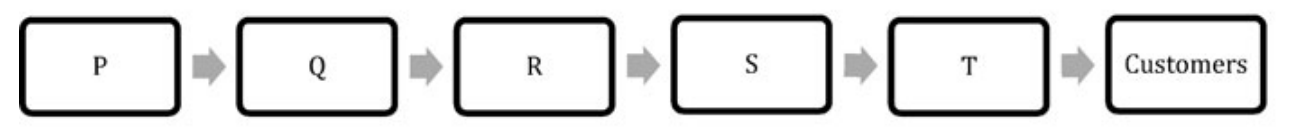
\includegraphics[width=0.5\linewidth]{Figs/fig1.png}
            \caption{Question 33}
            \label{fig:placeholder_1}
        \end{figure}
        
            \begin{enumerate}
                \item The plane corresponding to $1$ is horizontal and the plane corresponding to $2$ is inclined.
                \item The plane corresponding to $1$ is striking N-S and the plane corresponding to 2 is horizontal.
                \item The plane corresponding to $2$ is vertical and the plane corresponding to $3$ is striking E-W.
                \item The plane corresponding to $2$ is striking E-W and the plane corresponding to $3$ is inclined.

            \end{enumerate}
\newpage
        \item Match the minerals in \textbf{Group $I$} with its corresponding industrial application in  \textbf{Group $II$}. \hfill{\brak{\text{GATE GG 2013}}}

        \begin{multicols}{2}
            \underline{\textbf{Group $I$}}
            \begin{enumerate}[start =16]
                \item Kaolinite
                \item Rutile
                \item Graphite
                \item Serpentine
            \end{enumerate}

            \columnbreak

            \underline{\textbf{Group $II$}}
            \begin{enumerate}
                \item Pigment
                \item Asbestos
                \item Cement
                \item Lubricant
                \item Abrasive
            \end{enumerate}
        \end{multicols}

        \begin{enumerate}
            \begin{multicols}{2}
                \item P-$1$, Q-$3$, R-$4$, S-$2$
                \item P-$3$, Q-$1$, R-$2$, S-$4$
                \item P-$3$, Q-$1$, R-$4$, S-$2$
                \item P-$1$, Q-$5$, R-$3$, S-$2$
            \end{multicols}
        \end{enumerate}

        \item  Match the Hermann-Maugin symbol in \textbf{Group $I$} with its corresponding general form in \textbf{Group $II$}. \hfill{\brak{\text{GATE GG 2013}}}
         
        \begin{multicols}{2}
            \underline{\textbf{Group $I$}}
            \begin{enumerate}[start =16]
                \item $6\text{/m}$
                \item $3\text{m}$
                \item $\overline{6}m^{2}$
                \item $\overline{6}$
            \end{enumerate}

            \columnbreak

            \underline{\textbf{Group $II$}}
            \begin{enumerate}
                \item Trigonal Dipyramid
                \item Ditrigonal Dipyramid
                \item Dihexagonal Pyramid
                \item Ditrigonal Pyramid
                \item Hexagonal Dipyramid
            \end{enumerate}
        \end{multicols}

        \begin{enumerate}
            \begin{multicols}{2}
                \item P-$5$, Q-$4$, R-$2$, S-$1$
                \item P-$5$, Q-$4$, R-$1$, S-$2$
                \item P-$5$, Q-$4$, R-$1$, S-$3$
                \item P-$3$, Q-$4$, R-$2$, S-$1$
            \end{multicols}
        \end{enumerate}

        \item Which of the following is a type of dam?\hfill{\brak{\text{GATE GG 2013}}}
            \begin{enumerate}
                \begin{multicols}{4}
                    \item Anchor
                    \item Shotcrete
                    \item Geogrid
                    \item Buttress
                \end{multicols}
            \end{enumerate}

        \item Match the following items in \textbf{Group $I$} with those in \textbf{Group $II$}. \hfill{\brak{\text{GATE GG 2013}}}

        \begin{multicols}{2}
            \underline{\textbf{Group $I$}}
            \begin{enumerate}[start =16]
                \item Kersantite
                \item Fenite
                \item Mugearite
                \item Phonolite
            \end{enumerate}

            \columnbreak

            \underline{\textbf{Group $II$}}
            \begin{enumerate}
                \item Hornblende-diopside-plagioclase lamprophyre
                \item Basaltic trachyandesite
                \item Volcanic nepheline syenite
                \item Biotite-plagioclase lamprophyre
                \item Metasomatic rock associated with carbonatites
            \end{enumerate}
        \end{multicols}

        \begin{enumerate}
            \begin{multicols}{2}
                \item P-$1$, Q-$2$, R-$4$, S-$3$
                \item P-$4$, Q-$5$, R-$2$, S-$3$
                \item P-$3$, Q-$1$, R-$2$, S-$4$
                \item P-$4$, Q-$5$, R-$3$, S-$2$
            \end{multicols}
        \end{enumerate}

         \item A chondrite-normalized REE pattern of quartzo-feldspathic gneiss shows a sharp positive
         $Eu$ anomaly. This indicates presence of  \hfill{\brak{\text{GATE GG 2013}}}
            \begin{enumerate}
                \item plagioclase in the sample.
                \item quartz in the sample.
                \item clinopyroxene in the sample.
                \item sillimanite in the sample.
            \end{enumerate}
            
        \item Choose the correct expression from the following that explains the changing vertical position of a point on the land surface at any time (Surface Uplift - SU, Bedrock Uplift - BU, Deposition - D, Compaction - C, Erosion - E). \hfill{\brak{\text{GATE GG 2013}}}
            \begin{enumerate}
                    \item $SU=BU-D-C-E$
                    \item $SU=BU-D+C-E$
                    \item $SU=BU+D-C+E$
                    \item $SU=BU+D-C-E$
            \end{enumerate}

        \item Match the following stratigraphic units listed in \textbf{Group $I$} with the Precambrian basins in \textbf{Group $II$}. \hfill{\brak{\text{GATE GG 2013}}}
            \begin{multicols}{2}
                \underline{\textbf{Group $I$}}
                \begin{enumerate}[start =16]
                    \item Badami Group
                    \item Kheinjua Formation
                    \item Sullavai Group
                    \item Papaghni Group
                \end{enumerate}
        
                \columnbreak
        
                \underline{\textbf{Group $II$}}
                \begin{enumerate}
                    \item Vindhyan
                    \item Chhatisgarh
                    \item Kaladgi
                    \item Cuddapah
                    \item Pranhita-Godavari
                \end{enumerate}
            \end{multicols}
            \begin{enumerate}
                \begin{multicols}{2}
                    \item P-$3$, Q-$1$, R-$5$, S-$4$
                    \item P-$1$, Q-$5$, R-$4$, S-$3$
                    \item P-$1$, Q-$2$, R-$3$, S-$5$
                    \item P-$3$, Q-$2$, R-$5$, S-$4$
                \end{multicols}
            \end{enumerate}

        \item Mantle xenoliths are observed in \hfill{\brak{\text{GATE GG 2013}}}
            \begin{enumerate}                
                    \item Kimberlite
                    \item Granite
                    \item Pegmatite
                    \item Granulite
            \end{enumerate}

        \item Dimension of hydraulic conductivity is \hfill{\brak{\text{GATE GG 2013}}}
            \begin{enumerate}
                \begin{multicols}{4}
                    \item $LT^{-2}$
                    \item $L^{3}T^{-1}$
                    \item $ML^{-3}$
                    \item $LT^{-1}$
                \end{multicols}
            \end{enumerate}

        \item Match the items in \textbf{Group $I$} with those in \textbf{Group $II$}. \hfill{\brak{\text{GATE GG 2013}}}
        \newpage
            \begin{multicols}{2}
                \underline{\textbf{Group $I$}}
                \begin{enumerate}[start=16]
                    \item Katrol Formation
                    \item Barail Formation
                    \item Ariyalur Formation
                    \item Sylhet Formation
                \end{enumerate}
        
                \columnbreak
        
                \underline{\textbf{Group $II$}}
                \begin{enumerate}
                    \item Oligocene
                    \item Cretaceous
                    \item Eocene
                    \item Jurassic
                    \item Paleocene
                    \item Miocene
                \end{enumerate}
            \end{multicols}
            \begin{enumerate}
                \begin{multicols}{2}
                        \item P-$2$, Q-$4$, R-$5$, S-$3$
                        \item P-$2$, Q-$5$, R-$3$, S-$1$
                        \item P-$4$, Q-$2$, R-$4$, S-$5$
                        \item P-$4$, Q-$1$, R-$2$, S-$3$
                \end{multicols}
            \end{enumerate}

        \item The outcrop pattern of folded sedimentary strata on the map given below represents \hfill{\brak{\text{GATE GG 2013}}}

        \begin{figure}[h]
	    \centering
            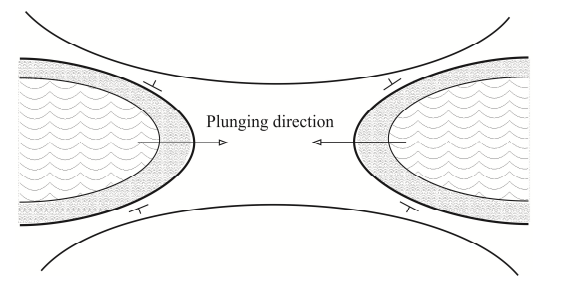
\includegraphics[width=0.5\linewidth]{Figs/fig2.png}
            \caption{Question 44}
            \label{fig:placeholder_2}
        \end{figure}
        
            \begin{enumerate}
                \begin{multicols}{2}
                    \item culmination of antiform
                    \item culmination of synform
                    \item depression of antiform
                    \item depression of synform
                \end{multicols}
            \end{enumerate}

        \item Match the economic deposits in \textbf{Group $I$} with the host rocks in \textbf{Group $II$}. \hfill{\brak{\text{GATE GG 2013}}}
            \begin{multicols}{2}
                \underline{\textbf{Group $I$}}
                \begin{enumerate}[start=16]
                    \item Malanjkhand copper
                    \item Salem magnesite
                    \item Zawar Pb-Zn
                    \item Rampura-Agucha
                \end{enumerate}
        
                \columnbreak
        
                \underline{\textbf{Group $II$}}
                \begin{enumerate}
                    \item Granite
                    \item Dolomite
                    \item Graphitic Schist
                    \item Ultramafics
                    \item Basalt
                    \item Rhyollite
                \end{enumerate}
            \end{multicols}
            \begin{enumerate}
                \begin{multicols}{2}              
                        \item P-$1$, Q-$4$, R-$3$, S-$2$
                        \item P-$2$, Q-$3$, R-$5$, S-$2$
                        \item P-$1$, Q-$4$, R-$2$, S-$3$
                        \item P-$3$, Q-$2$, R-$6$, S-$5$
                \end{multicols}
            \end{enumerate}
\newpage
        \item The stereographic projection below shows the principal stress axes and fault planes. The projection represents a \hfill{\brak{\text{GATE GG 2013}}}

        \begin{figure}[h]
	    \centering
            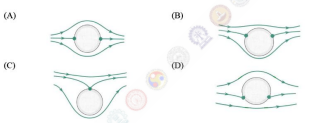
\includegraphics[width=0.5\linewidth]{Figs/fig3.png}
            \caption{Question 46}
            \label{fig:placeholder_3}
        \end{figure}
        
            \begin{enumerate}
                \begin{multicols}{4}
                    \item normal fault
                    \item reverse fault
                    \item dextral fault
                    \item sinistral fault
                \end{multicols}
            \end{enumerate}
        \item Select the correct the statement from the following. \hfill{\brak{\text{GATE GG 2013}}}
            \begin{enumerate}
                \item Incised channels form an account of aeolin action.
                \item Mesa structures are observed only in steeply dipping beds.
                \item Crevasse splay is commonly associated with meandering river.
                \item Coral reefs are abundant in Gulf of Cambay.
            \end{enumerate}
            \newpage
\subsection*{Common Data Questions}
\subsubsection*{Common Data for Questions 48 and 49}

A, B, C, D, E, F and G are minerals in a sample of metamorphic rock. The micro-texture of the assemblage is given below. A, D and G are porphyroblasts, B and C are coronas, E and F are inclusions.

        \begin{figure}[h]
            \centering
            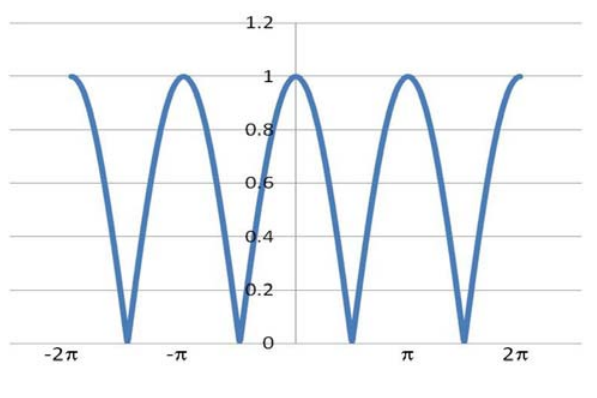
\includegraphics[width=1\linewidth]{Figs/fig4.png}
            \caption{Common Data Questions 48 and 49}
            \label{fig:placeholder_4}
        \end{figure}

        \item Select the appropriate metamorphic reaction from the following options. \hfill{\brak{\text{GATE GG 2013}}}
            \begin{enumerate}
                \begin{multicols}{2}
                    \item $A + B = C + D$
                    \item $A + C = D + G$
                    \item $A + D = B + C$
                    \item $E + D = C + A$
                \end{multicols}
            \end{enumerate}

        \item Based on the micro-texture, select the oldest assemblage from the following. \hfill{\brak{\text{GATE GG 2013}}}
            \begin{enumerate}
                \begin{multicols}{4}
                    \item $A-D$
                    \item $E-F$
                    \item $B-C$
                    \item $A-G$
                \end{multicols}
            \end{enumerate}
    \newpage
\subsubsection*{Common Data for Questions 50 and 51}
The Mohr-Coulomb failure envolope $\brak{A-B}$ of a porous limestone is given below. 

        \begin{figure}[h]
            \centering
            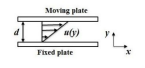
\includegraphics[width=1\linewidth]{Figs/fig5.png}
            \caption{Common Data Questions 50 and 51}
            \label{fig:placeholder_5}
        \end{figure}

        \item The point P represents \hfill{\brak{\text{GATE GG 2013}}}
            \begin{enumerate}
                \item uniaxial tensile strength.
                \item uniaxial compressive strength.
                \item indirect tensile strength.
                \item shear strength.
            \end{enumerate}

        \item For a condition represented by the circle $1$, if pore water pressure increases, the circle will change to \hfill{\brak{\text{GATE GG 2013}}}
            \begin{enumerate}
                \begin{multicols}{4}
                    \item circle $2$.
                    \item circle $3$.
                    \item circle $4$.
                    \item circle $5$.
                \end{multicols}
            \end{enumerate}
\subsection*{Linked Answer Questions}
\subsubsection*{Statement for Linked Answer Questions 52 and 53}
Sedimentary structures are useful for determining the younging direction of a bed.

        \item Which one of the following sedimentary structure represents the bottom of a bed? \hfill{\brak{\text{GATE GG 2013}}}
            \begin{enumerate}
                \begin{multicols}{2}
                    \item Current crescent
                    \item Desiccation crack
                    \item Rain print
                    \item Load cast
                \end{multicols}
            \end{enumerate}

        \item Which sedimentary process is responsible for the generation of the structure identified above? \hfill{\brak{\text{GATE GG 2013}}}
            \begin{enumerate}
                \begin{multicols}{2}
                    \item Wave reworking
                    \item Liquefaction of sediments
                    \item Drying and desiccation
                    \item Erosion of cohesive substrate
                \end{multicols}
            \end{enumerate}
\subsubsection*{Statement for Linked Answer Questions 54 and 55}
    The table below represents recalculated cation compositions data of minerals.

    \begin{table}[H]
        \input{Tables/table1.tex}
    \end{table}

        \item Select the correct garnet [$\brak{Ca,Fe,Mg,Mn}_3Al_2Si_3O_{12}$] and clinopyroxene [$Ca\brak{FeMg}Si_2O_6$] pair respectively. hfill{\brak{\text{GATE GG 2013}}}
            \begin{enumerate}
                \begin{multicols}{4}
                    \item $II$ and $III$
                    \item $II$ and $IV$
                    \item $I$ and $IV$
                    \item $I$ and $III$
                \end{multicols}
            \end{enumerate}
            
        \item Calculate the distribution coefficient [$K_D$] for the $Fe\text{-}Mg$ system. \hfill{\brak{\text{GATE GG 2013}}}
            \begin{enumerate}
                \begin{multicols}{4}
                    \item $0.504$
                    \item $0.620$
                    \item $1.420$
                    \item $1.535$
                \end{multicols}
            \end{enumerate}
    \newpage
\begin{center}
    \subsection*{PART B (SECTION 2): FOR GEOPHYSICS CANDIDATES ONLY }    
\end{center}
\end{enumerate}
\subsubsection*{Q.26 to Q.55 carry two marks each. }
        \begin{enumerate}[start = 26 ]
           
        \item A P-wave is reflected as both P- and S- waves from an interface at angles $r_p$ and $r_s$ respectively. The relationship between $r_p$ and $r_s$ is \hfill{\brak{\text{GATE GG 2013}}}
            \begin{enumerate}
                \begin{multicols}{4}
                    \item $r_p > r_s$
                    \item $r_p = r_s$
                    \item $r_p < r_s$
                    \item $r_p = 2r_s$
                \end{multicols}
            \end{enumerate}

        \item Which of the following ways of measuring the size of an earthquake does not require instrumental recording? \hfill{\brak{\text{GATE GG 2013}}}
            \begin{enumerate}
                \begin{multicols}{2}
                    \item Richter magnitude
                    \item Moment
                    \item $M_w$
                    \item Intensity
                \end{multicols}
            \end{enumerate}

        \item In what circumstances, the migrated reflection seismic section will be same as the unmigrated one? \hfill{\brak{\text{GATE GG 2013}}}
            \begin{enumerate}
                \begin{multicols}{2}
                    \item Inclined interfaces
                    \item Undulating interfaces
                    \item Horizontal interfaces
                    \item Vertical interfaces
                \end{multicols}
            \end{enumerate}

        \item Which of the following methods is best suited to estimate the resistivity variations in the upper mantle? \hfill{\brak{\text{GATE GG 2013}}}
            \begin{enumerate}
                    \item Deep electrical resistivity
                    \item Ground Penetrating Radar
                    \item Controlled Source Electromagnetics
                    \item Magnetotellurics
            \end{enumerate}

        \item Amongst the following $4$-electrode configurations of the electrical resistivity method, which is best suited for archeological investigations? \hfill{\brak{\text{GATE GG 2013}}}
            \begin{enumerate}
                    \item Schlumberger
                    \item Pole-Pole
                    \item Wenner
                    \item Dipole-Dipole
            \end{enumerate}

        \item A singular value of an $m \times n$ matrix, $A$, is defined as \hfill{\brak{\text{GATE GG 2013}}}
            \begin{enumerate}
                \begin{multicols}{2}
                    \item positive square root of eigenvalue of $AA^T$
                    \item modulus of eigenvalue of $A$
                    \item eigenvalue of $A^TA$
                    \item square of eigenvalue of $A$
                \end{multicols}
            \end{enumerate}

        \item In an ill-posed geophysical inverse problem, stated as non-singular matrix equation, the magnitude of determinant of the coefficient matrix is \hfill{\brak{\text{GATE GG 2013}}}
            \begin{enumerate}
                \begin{multicols}{4}
                    \item large
                    \item zero
                    \item near zero
                    \item very large
                \end{multicols}
            \end{enumerate}

        \item In a 4-layer subsurface model, which combination of A-, H-, K- and Q- type electrical resistivity sounding curves is \underline{\textbf{NOT}} possible? \hfill{\brak{\text{GATE GG 2013}}}
            \begin{enumerate}
                \begin{multicols}{4}
                    \item HA
                    \item AK
                    \item KQ
                    \item HQ
                \end{multicols}
            \end{enumerate}

        \item Which of the following characteristics of a Self Potential (SP) anomaly gives the approximate 
        position of centre of the buried ore body? \hfill{\brak{\text{GATE GG 2013}}}
            \begin{enumerate}
                \item Position of maximum of the anomaly
                \item Position of minimum of the anomaly
                \item Position of zero crossing
                \item Position midpoint between maximum and minimum of the anomaly
            \end{enumerate}

        \item Given a scalar function, $f(x,y) = xy$. The curl of gradient of $f(x,y)$ is \hfill{\brak{\text{GATE GG 2013}}}
            \begin{enumerate}
                \begin{multicols}{4}
                    \item $2x\,\hat{i}$
                    \item $-2y\,\hat{j}$
                    \item $0\,\hat{i}$
                    \item $x\,\hat{i} + y\,\hat{j}$
                \end{multicols}
            \end{enumerate}

        \item Which of the following is \underline{\textbf{NOT}} correct? \hfill{\brak{\text{GATE GG 2013}}}
            \begin{enumerate}
                \item In VLF-EM technique, the tilt-angle mode is best suited to locate conductive bodies
                \item Fraser filter is a difference filter
                \item Static shift affects MT impedance phase
                \item Tipper vector is derived from the three magnetic field components, $H_x, H_y$ and $H_z$.
            \end{enumerate}
        
        \item If L, B, F and T respectively stand for Latitude correction, Bouguer correction, Free-air correction and Terrain correction, then the order in which they will have to be applied for gravity data analysis is \hfill{\brak{\text{GATE GG 2013}}}
            \begin{enumerate}
                \begin{multicols}{4}
                    \item LFBT
                    \item LBTF
                    \item FLBT
                    \item TBLF
                \end{multicols}
            \end{enumerate}
        
        \item Geomagnetic secular variations originate from the \hfill{\brak{\text{GATE GG 2013}}}
            \begin{enumerate}
                \begin{multicols}{4}
                    \item inner core
                    \item outer core
                    \item crust
                    \item mantle
                \end{multicols}
            \end{enumerate}

        \item Removal of regional component from magnetic data is similar to \hfill{\brak{\text{GATE GG 2013}}}
            \begin{enumerate}
                    \item band-pass filtering
                    \item low-pass filtering
                    \item high-pass filtering
                    \item band-reject filtering
            \end{enumerate}
        
        \item Which of the following is useful to estimate the depth to the centre of a spherical body from a gravity anomaly curve? \hfill{\brak{\text{GATE GG 2013}}}
            \begin{enumerate}
                    \item Surface integration
                    \item Volume integration
                    \item Twice the absolute maximum
                    \item Half-width of the anomaly
            \end{enumerate}
        
        \item Application of reduction-to-pole technique to a magnetic anomaly results in \hfill{\brak{\text{GATE GG 2013}}}
            \begin{enumerate}
                \item flattening the anomaly curve.
                \item transforming the asymmetry in the anomaly to symmetry.
                \item halving the amplitude.
                \item doubling the amplitude.
            \end{enumerate}

        \item The Fourier transform of a comb function is \hfill{\brak{\text{GATE GG 2013}}}
            \begin{enumerate}
                \begin{multicols}{4}
                    \item delta function
                    \item comb function
                    \item sync function
                    \item rectangular function
                \end{multicols}
            \end{enumerate}
        
        \item In Cartesian coordinate system, if the geological strike of a two-dimensional body is oriented along the $x$-direction, then the electromagnetic field components associated with TM mode of magnetotelluric method are \hfill{\brak{\text{GATE GG 2013}}}
            \begin{enumerate}
                \begin{multicols}{4}
                    \item $H_x, E_y \text{ and }E_z$
                    \item $E_x, H_y \text{ and }E_z$
                    \item $H_x, H_y \text{ and }E_z$
                    \item $E_x, H_y \text{ and }H_z$
                \end{multicols}
            \end{enumerate}
        
        \item A seismic signal is recorded in the frequency band $100-250 Hz$. While digitizing the signal, the sampling interval one should choose to avoid aliasing is \rule{3cm}{0.15mm} $ms$. \hfill{\brak{\text{GATE GG 2013}}}

        \item Wadati diagram is a plot of the difference in P- and S- wave arrival times against the arrival time of P-wave. It helps in estimating the \hfill{\brak{\text{GATE GG 2013}}}
            \begin{enumerate}
                \begin{multicols}{2}
                    \item velocity of P-wave.
                    \item velocity of S-wave.
                    \item time of occurrence of earthquake.
                    \item hypocenter of earthquake.
                \end{multicols}
            \end{enumerate}
        
        \item Match the items of \textbf{Group $I$} with those of \textbf{Group $II$} \hfill{\brak{\text{GATE GG 2013}}}
            \begin{multicols}{2}
                \underline{\textbf{Group $I$}}
                \begin{enumerate}[start = 1]
                    \item Caliper log
                    \item NMR log
                    \item Neutron log
                    \item SP log
                \end{enumerate}
                
                \columnbreak
                
                \underline{\textbf{Group $II$}}
                \begin{enumerate}
                    \item Permeability
                    \item Resistivity
                    \item Diameter
                    \item Velocity
                    \item Porosity
                \end{enumerate}
            \end{multicols}
            \begin{enumerate}
                \begin{multicols}{2}
                    \item P - $3$, Q - $4$, R - $2$, S - $5$
                    \item P - $3$, Q - $1$, R - $5$, S - $2$
                    \item P - $4$, Q - $2$, R - $4$, S - $3$
                    \item P - $1$, Q - $3$, R - $2$, S - $4$        
                \end{multicols}
            \end{enumerate}
            
        \item The most common hydrocarbon indicator is \hfill{\brak{\text{GATE GG 2013}}}
        \begin{enumerate}
            \begin{multicols}{4}
                    \item flat spot
                    \item dim spot
                    \item bright spot
                    \item velocity sag
            \end{multicols}
        \end{enumerate}
        
            
\subsection*{Common Data Questions}
\subsubsection*{Common Data for Questions 48 and 49}

A recursive filter $y_n$ is given by $y_n = 2x_n - 1.5x_{n-1} + y_{n-2}$.

        \item The order of $y_n$ is \rule{3cm}{0.15mm}. \hfill{\brak{\text{GATE GG 2013}}}
        
        \item The transfer function of $y_n$ in $z$-domain is \hfill{\brak{\text{GATE GG 2013}}}
            \begin{enumerate}
                \begin{multicols}{2}
                    \item $\frac{1-1.5z}{2-z^2}$
                    \item $\frac{1-z^{2}}{2-1.5z}$
                    \item $\frac{2+z^{2}}{1+1.5z}$
                    \item $\frac{2-1.5z}{1-z^{2}}$
                \end{multicols}
            \end{enumerate}

\subsubsection*{Common Data for Questions 50 and 51:}
In a linear inverse problem, the coefficient matrix, $A = \myvec{ 2.00 & 2.01 \\ 2.01 & 2.00 }$.

        \item The eigenvalues of $A$ are \hfill{\brak{\text{GATE GG 2013}}}
            \begin{enumerate}
                \begin{multicols}{4}
                    \item $\brak{4.01\,, -0.01}$
                    \item $\brak{-4.01\,,-0.01}$
                    \item $\brak{4.01\,,0.01}$
                    \item $\brak{-4.01\,,1.01}$
                \end{multicols}
            \end{enumerate}
        
        \item If the elements of A are expressed up to first decimal place only, then the number of possible solution(s) of the resulting inverse problem is \hfill{\brak{\text{GATE GG 2013}}}
            \begin{enumerate}
                \begin{multicols}{4}
                    \item $1$
                    \item $2$
                    \item $3$
                    \item $\infty$
                \end{multicols}
            \end{enumerate}

\subsection*{Linked Answer Questions}
\subsubsection*{Statement for Linked Answer Questions 52 and 53}
In an electrical resistivity sounding survey a current of $20 mA$ is passed through the current electrodes separated by a distance of $50 m$ and a voltage of $3 V$ is measured across the potential electrodes, separated by $10 m$.

        \item The above electrode configuration is known as \hfill{\brak{\text{GATE GG 2013}}}
            \begin{enumerate}
                    \item Schlumberger
                    \item Wenner
                    \item Pole-Dipole
                    \item Pole-Pole
            \end{enumerate}
        
        \item The apparent resistivity $\brak{\text{in }\Omega-m}$ for the above electrode configuration is close to \hfill{\brak{\text{GATE GG 2013}}}
            \begin{enumerate}
                \begin{multicols}{4}
                    \item $100$
                    \item $200$
                    \item $300$
                    \item $400$
                \end{multicols}
            \end{enumerate}

\subsubsection*{Statement for Linked Answer Questions 54 and 55:}
An electromagnetic (EM) wave of frequency $25 Hz$ is impinging on a homogeneous half-space, having resistivity of $100 \Omega-m$.

        \item The skin-depth of the wave is about \hfill{\brak{\text{GATE GG 2013}}}
            \begin{enumerate}
                \begin{multicols}{4}
                    \item $1 km$
                    \item $1 m$
                    \item $500 km$
                    \item $500 m$
                \end{multicols}
            \end{enumerate}
        
        \item The velocity of the EM wave $\brak{\text{in} km/s}$ is close to \hfill{\brak{\text{GATE GG 2013}}}
            \begin{enumerate}
                \begin{multicols}{2}
                    \item $20\pi$
                    \item $30\pi$
                    \item $40\pi$
                    \item $50\pi$
                \end{multicols}
            \end{enumerate}
            
\subsection*{General Aptitude (GA) Questions }    

\subsubsection{Q.56 to Q.60 carry one marks each. }

        \item A number is as much greater than $75$ as it is smaller than $117$. The number is: \hfill{\brak{\text{GATE GG 2013}}}
            \begin{enumerate}
                \begin{multicols}{4}
                    \item $91$
                    \item $93$
                    \item $89$
                    \item $96$
                \end{multicols}
            \end{enumerate}
            

        \item \underline{The professor} \underline{ordered to} \underline{ the students to go} \underline{out of the class}. \\\hspace{2cm}$I$\hspace{3cm}$II$\hspace{2.5cm}$III$\hspace{2cm}$IV$\\
        Which of the above underlined parts of the sentence is grammatically incorrect?\hfill{\brak{\text{GATE GG 2013}}}
        
            \begin{enumerate}
                
                    \begin{multicols}{4}
                    \item $I$
                    \item $II$
                    \item $III$
                    \item $IV$
                \end{multicols}
            \end{enumerate}

        \item Which of the following options is the closest in meaning to the word given below:
        \hfill{\brak{\text{GATE GG 2013}}}
            \begin{enumerate}
                \begin{multicols}{2}
                    \item Modern
                    \item Historic
                    \item Primitive
                    \item Antique
                \end{multicols}
            \end{enumerate}

        \item Friendship, no matter how \rule{3cm}{0.15mm} it is, has its limitations.\hfill{\brak{\text{GATE GG 2013}}}
            \begin{enumerate}
                    \item cordial
                    \item intimate
                    \item secret
                    \item pleasant
            \end{enumerate}

        \item Select the pair that best expresses a relationship similar to that expressed in the pair: \textbf{Medicine: Health} \hfill{\brak{\text{GATE GG 2013}}}
            \begin{enumerate}
                \begin{multicols}{2}
                    \item Science: Experiment
                    \item Wealth: Peace
                    \item Education: Knowledge
                    \item Money: Happiness
                \end{multicols}
            \end{enumerate}
\subsection{Q.61 to Q.65 carry two marks each. }

        \item $X \text{ and } Y$ are two posivtive numbers such that $2X + Y \leq 6 \text{ and } X + 2Y \leq 8$. For which of the following values of $\brak{X,Y}$ the function $f\brak{X,Y} = 3X + 6Y$ will give maximum value? \hfill{\brak{\text{GATE GG 2013}}}
            \begin{enumerate}
                \item $\brak{4/3\,, 10/3}$
                \item $\brak{8/3\,, 20/3}$
                \item $\brak{8/3\,, 10/3}$
                \item $\brak{4/3\,, 20/3}$
            \end{enumerate}
        \newpage
        \item If $\mydet{4X - 7} = 5$ then the values of $2\mydet{X} - \mydet{-X}$ is: \hfill{\brak{\text{GATE GG 2013}}}
            \begin{enumerate}
                \begin{multicols}{4}
                    \item $2\,, 1/3$
                    \item $1/2\,, 3$
                    \item $3/2\,, 9$
                    \item $2/3\,, 9$
                \end{multicols}
            \end{enumerate}

         \item Following table provides figures (in rupees) on annual expenditure of a firm for two years - $2010 \text{ and }2011$.   \hfill{\brak{\text{GATE GG 2013}}}
            \begin{table}[H]
                \centering
                \input{Tables/table2.tex}
            \end{table}

            In 2011, which of the following two categories have registered increase by same percentage?
            \begin{enumerate}
                \item Raw material and Salary \& wages
                \item Salary \& wages and Advertising
                \item Power \& fuel and Advertising
                \item Raw material and Research \& Development
            \end{enumerate}

        \item A firm is selling its product at $Rs. 60$ per unit. The total cost of production is $Rs. 100$ and firm is earning total profit of $Rs. 500$. Later, the total cost increased by $30\%$. By what percentage the price should be increased to maintained the same profit level. \hfill{\brak{\text{GATE GG 2013}}}
            \begin{enumerate}
                \begin{multicols}{4}
                    \item $5$
                    \item $10$
                    \item $15$
                    \item $30$
                \end{multicols}
            \end{enumerate}
        
         \item Abhishek is elder to Savar. Savar is younger to Anshul. Which of the given conclusions is logically valid and is inferred from the above statements? \hfill{\brak{\text{GATE GG 2013}}}
            \begin{enumerate}
                \item Abhishek is elder to Anshul
                \item Anshul is elder to Abhishek
                \item Abhishek and Anshul are of same age
                \item No conclusion follows
            \end{enumerate}

\begin{center}
    \subsection*{END OF THE QUESTION PAPER}
\end{center}

    
    \end{enumerate}
\end{document}


	    \item $\vec{X}$ is 1 km northeast of $\vec{Y}$. $\vec{Y}$ is 1 km southeast of $\vec{Z}$. $\vec{W}$ is 1 km west of $\vec{Z}$. $\vec{P}$ is 1 km south of $\vec{W}$. $\vec{Q}$ is 1 km east of $\vec{P}$. What is the distance between $\vec{X}$ and $\vec{Q}$ in km?

    \hfill{\brak{\text{IN 2014}}}
        \begin{enumerate}
    \begin{multicols}{4}
            \item 1
            \item $\sqrt{2}$
            \item $\sqrt{3}$
            \item 2
    \end{multicols}
        \end{enumerate}
    \item Given $x\brak{t} = 3 \sin\brak{1000 \pi t}$ and $y\brak{t} = 5 \cos\brak{1000 \pi t + \frac{\pi}{4}}$. The $x-y$ plot will be

    \hfill{\brak{\text{IN 2014}}}
        \begin{enumerate}
    \begin{multicols}{2}
            \item a circle
            \item a multi-loop closed curve
            \item a hyperbola
            \item an ellipse
            
    \end{multicols}
        \end{enumerate}
    
    \item For the matrix $\vec{A}$ satisfying the equation given below, the eigenvalues are
    \begin{align*}
        \vec{A}\myvec{1 & 2 & 3 \\ 4 & 5 & 6 \\ 7 & 8 & 9}
         = \myvec{1 & 2 & 3 \\ 4 & 5 & 6 \\ 7 & 8 & 9 }
    \end{align*}
    \hfill{\brak{\text{IN 2014}}}
        \begin{enumerate}
    \begin{multicols}{2}
            \item \brak{1, j, -j}
            \item \brak{1, 1, 0}
            \item \brak{1, 1, -1}
            \item \brak{1, 0, 0}
    \end{multicols}
        \end{enumerate}
    \item $X\brak{k}$ is the Discrete Fourier Transform of a 6-point real sequence $x\brak{n}$. If $X\brak{0} = 9+j0, X\brak{2} = 2+j2, X\brak{3} = 3-j0, X\brak{5} = 1-j1$, then $x\brak{0}$ is
    \hfill{\brak{\text{IN 2014}}}
        \begin{enumerate}
    \begin{multicols}{4}
            \item 3
            \item 9
            \item 15
            \item 18
    \end{multicols}
        \end{enumerate}


	\documentclass[journal,12pt,onecolumn]{IEEEtran}
\usepackage{graphicx, float}
\graphicspath{{Figs/}}
\usepackage{multicol}
\usepackage{parskip}
\usepackage{titlesec}
\usepackage{color}
\usepackage{enumitem}
\usepackage{amsmath,amssymb,amsfonts,amsthm}
\usepackage{array}
\usepackage{booktabs}
\usepackage[table]{xcolor}
\usepackage{longtable}
\usepackage{gensymb}
\usepackage{cite}
\usepackage{algorithmic}
\usepackage{textcomp}
\usepackage{txfonts}
\usepackage{listings}
\usepackage{mathtools}
\usepackage{comment}
\usepackage{tkz-euclide}
\usepackage[breaklinks=true]{hyperref}
\usepackage{gvv}
\usepackage[latin1]{inputenc}
\usetikzlibrary{arrows.meta, positioning}
\usepackage{xparse}
\usepackage{calc}
\usepackage{multirow}
\usepackage{hhline}
\usepackage{ifthen}
\usepackage{lscape}
\usepackage{tabularx}
\usepackage{circuitikz}
\usepackage{tikz}
\newtheorem{problem}{Problem}
\newtheorem{theorem}{Theorem}[section]
\newtheorem{proposition}{Proposition}[section]
\newtheorem{lemma}{Lemma}[section]
\newtheorem{corollary}[theorem]{Corollary}
\newtheorem{example}{Example}[section]
\newtheorem{definition}[problem]{Definition}
\newcommand{\BEQA}{\begin{eqnarray}}
\newcommand{\EEQA}{\end{eqnarray}}
\theoremstyle{remark}
\title{Graduate Aptitude Test in Engineering 2017}
\author{EE25BTECH11025- Vishwambhar}

\begin{document}

\maketitle

\begin{enumerate}
 
\item If a vector $\vec{v}$ has components $v_x = 1$, $v_y = 2$,$v_z = 3$, then its magnitude is \dots.\\
(write answer with two decimal places)\\

\hfill{(GATE PE 2017)}

\item The value of $\lim\limits_{x \to 0} \frac{(2 + x)^4 - 16}{x} $ is \dots.\\

\hfill{(GATE PE 2017)}

\item If $\frac{d^2 y}{dx^2} + f\brak{x, y} = 0$ is to be solved using the conditions $y(0) = a$ and $y(1) = b$, which of the following numerical method(s) can be used?
\begin{enumerate}
\item Euler with shooting method
\item Euler without shooting method
\item 4th order Runge-Kutta with shooting method
\item Both (A) and (C)
\end{enumerate}
\hfill{(GATE PE 2017)}

\item The numerical method used to find the root of a non-linear algebraic equation, that converges quadratically, is:
\begin{enumerate}
\item Bisection method.
\item Regula-falsi method (Method of False Position).
\item Newton-Raphson method.
\item None of above.
\end{enumerate}
\hfill{(GATE PE 2017)}

\item Which one of the following curves shows a typical behavior of the producing gas oil ratio (GOR) with time for a reservoir under solution gas drive?
\begin{figure}[h]
    \centering
    \includegraphics[width=0.5\columnwidth]{GraphQ _5.png}
    \caption{}
    \label{fig:placeholder}
\end{figure}
\hfill{(GATE PE 2017)}

\item A student has written the following possible causes of lost circulation during a drilling operation:
\begin{enumerate}
\item High salinity in the reservoir \\
\item Fracture in the reservoir \\
\item A fault encountered during drilling \\
\item Low viscosity of the reservoir fluid
\end{enumerate}

Which of the above statements are correct?
\begin{enumerate}
\begin{multicols}{4}
\item i, iv
\item ii, iii
\item i, iii
\item ii, iv
\end{multicols}
\end{enumerate}
\hfill{(GATE PE 2017)}

\item For water depth less than 8 m, which one of the following drilling vessels is the most suitable and economical?
\begin{enumerate}
    \item Semi-submersible rig
    \item Jack-up rig
    \item Drilling barges
    \item Drill ship
\end{enumerate}
\hfill{(GATE PE 2017)}

\item Which one of the following statements is correct for pseudo-steady state condition in a confined reservoir?
\begin{enumerate}
\item The pressure decline stops in the reservoir.
\item The pressure declines at the same rate across the reservoir.
\item The boundary pressure does not change.
\item The pressure starts increasing in the reservoir.
\end{enumerate}
\hfill{(GATE PE 2017)}

\item The roots of the equation $ \frac{d^3 y}{dx^3} - 6 \frac{d^2 y}{dx^2} + 11 \frac{dy}{dx} - 6y = 0$ are:
\begin{enumerate}
\begin{multicols}{4}
\item 1,1,2
\item 1,2,3
\item 1,3,4
\item 1,2,4
\end{multicols}
\end{enumerate}
\hfill{(GATE PE 2017)}

\item The API of a crude oil of density $950\, \text {kg/m}^3$ is \dots. (write answer with two decimal places)\\

\hfill{(GATE PE 2017)}

\item The differential equation $2xy \, dx + \brak{1 + x^2} \, dy = 0,$in which $x$ is an independent variable and $y$ is the dependent variable, is:
\begin{enumerate}
\item an ordinary differential equation of second order.
\item a first order nonlinear differential equation.
\item an exact differential equation.
\item a partial differential equation.
\end{enumerate}
\hfill{(GATE PE 2017)}

\item For the two matrices $X=
\myvec{
1 & 2 & 3\\
4 & 5 & 6
}$ $Y=
\myvec{
7 & 0\\
8 & -1
}$ the product $YX$ will be:
\begin{enumerate}
\item $XY = \myvec{ 
50 & 4 \\ 
122 & 13 
}$
\item $XY = \myvec{ 
4 & 11 & 18 \\ 
7 & 14 & 21 
}$
\item $XY = \myvec{ 
7 & 14 & 21 \\ 
4 & 11 & 18 
}$
\item $XY =\myvec{ 
18 & 5 & 6 \\ 
7 & 14 & 21 
}$
\end{enumerate}
\hfill{(GATE PE 2017)}

\item As per the Bharat IV norms, the maximum permissible limit of sulfur in diesel in ppm is:
\begin{enumerate}
\begin{multicols}{4}
\item 10
\item 50
\item 100
\item 500
\end{multicols}
\end{enumerate}
\hfill{(GATE PE 2017)}

\item The amount of methane gas evolved at $0\degree C$ and 1 atm from the dissociation of 1 m$^3$ of methane gas hydrate, is approximately:
\begin{enumerate}
\item equal to the volume of gas hydrate.
\item 10 times the volume of gas hydrate.
\item 160 times the volume of gas hydrates.
\item 300 times the volume of gas hydrates.
\end{enumerate}
\hfill{(GATE PE 2017)}

\item For a centrifugal pump, the head developed by the pump is proportional to the:
\begin{enumerate}
\item speed of the impeller rotation.
\item square of speed of the impeller rotation.
\item cubic power of speed of the impeller rotation.
\item square root of speed of the impeller rotation.
\end{enumerate}
\hfill{(GATE PE 2017)}

\item Which of these is a must for petroleum generation and accumulation?
\begin{enumerate}
\item Source rocks
\item Porous reservoir rocks
\item Impermeable cap rocks
\item All of the above
\end{enumerate}
\hfill{(GATE PE 2017)}

\item The problem of viscous fingering is encountered when:
\begin{enumerate}
\item a low viscosity fluid is injected in a high viscosity fluid.
\item a high viscosity fluid is injected in a low viscosity fluid.
\item a fluid of equal viscosity but lower density is injected in a fluid of higher density.
\item none of the above.
\end{enumerate}
\hfill{(GATE PE 2017)}

\item Which of these is \textbf{NOT} a sedimentary rock?
\begin{enumerate}
\item Shale
\item Sandstone
\item Carbonate
\item None of the above
\end{enumerate}
\hfill{(GATE PE 2017)}

\item The \textbf{unbiased} sample variance for the set of numbers: $S = \{40, 45, 50, 55, 60\}$ is \dots. (write answer with one decimal place)\\

\hfill{(GATE PE 2017)}

\item If $ 5x + 2iy - ix + 7y = 2 + 3i,$ where $i = \sqrt{-1}$, the values of two real numbers $\brak{x, y}$ are, respectively:
\begin{enumerate}
\begin{multicols}{4}
\item (-1,1)
\item (1,-1)
\item (1,1)
\item (-1,-1)
\end{multicols}
\end{enumerate}
\hfill{(GATE PE 2017)}

\item Pick the \textbf{INCORRECT} inequality, where $z_1$, $z_2$, and $z_3$ are complex numbers.
\begin{enumerate}
\item $|z_1 + z_2| \leq |z_1| + |z_2|$
\item $|z_1 - z_2| \geq |\,|z_1| - |z_2|\,|$
\item $|z_1 - z_2| \leq |z_1| - |z_2|$
\item $|z_1 + z_2 + z_3| \leq |z_1| + |z_2| + |z_3|$
\end{enumerate}
\hfill{(GATE PE 2017)}

\item Which of the following is \textbf{NOT} true? ($i = \sqrt{-1}$)
\begin{enumerate}
\item $\cos \theta = \dfrac{e^{i\theta} + e^{-i\theta}}{2}$
\item $e^{i\theta} = \cos \theta + i \sin \theta$
\item $\sin \theta = \dfrac{e^{i\theta} - e^{-i\theta}}{2i}$
\item $\cos \theta = \dfrac{e^{i\theta} + e^{-i\theta}}{2i}$
\end{enumerate}
\hfill{(GATE PE 2017)}

\item Which of the following is a potential environmental threat due to the cement-plug deterioration in an abandoned oil well?
\begin{enumerate}
\item Well bore could leak oil reservoir fluids into groundwater
\item Oil reservoir fluids could flow to the surface and contaminate surface soil
\item Oil reservoir fluids could discharge into navigable waters
\item All of the above
\end{enumerate}
\hfill{(GATE PE 2017)}

\item \dots is a mode of flame propagation in a pre-mixed gas, and drives a leading shock front into the quiescent, unburnt gas at supersonic velocity, immediately followed by a combustion zone.
\begin{enumerate}
\item Deflagration
\item Fire
\item Detonation
\item Ignition
\end{enumerate}
\hfill{(GATE PE 2017)}

\item Bio-Gas (BG), Coal Bed Methane (CBM), and Methane Gas Hydrate (MGH), if arranged in the order of increasing methane content, the correct order is:
\begin{enumerate}
\item BG, CBM, MGH
\item CBM, BG, MGH
\item CBM, MGH, BG
\item BG, MGH, CBM
\end{enumerate}
\hfill{(GATE PE 2017)}

\item For a velocity field given by $\vec{v} = y \hat{i} - x \hat{j} + 0 \hat{k}$, calculate the curl of $\vec{v}$. If the calculated vector is $a \hat{i} + b \hat{j} + c \hat{k}$, then the value of $c$ is \dots.\\

\hfill{(GATE PE 2017)}

\item Single step integration (step size = 0.5) of $ I = \int_0^1 x^2 e^x \, dx,$evaluated \textbf{numerically} using the Simpson's 1/3 rule, is \dots. (write answer with three decimal places)\\

\hfill{(GATE PE 2017)}

\item Solve $ \frac{dy}{dx} = -y$ \textbf{numerically} from $x = 0$ to $1$ using explicit, forward, first order Euler method with initial condition of $y(0) = 1$ and step size ($h$) of 0.2. The absolute value of error in $y(1)$ calculated using analytical and numerical solution is \dots \% (calculate the error using analytical solution as the basis and use three decimal places).\\

\hfill{(GATE PE 2017)}

\item Relative permeability curves are shown in the following figure for a water-oil system in a porous medium. $S_w$ is water saturation and $k_r$ is relative permeability. Curve 1 is relative permeability of water and Curve 2 is relative permeability of oil.
Assuming the porous medium is at irreducible water saturation initially, the maximum possible recovery of oil by water flooding is \dots \%. (write answer with one decimal place)\\

\hfill{(GATE PE 2017)}
\begin{figure}[h]
    \centering
    \includegraphics[width=0.5\columnwidth]{GraphQ_29.png}
    \caption{}
    \label{fig:placeholder}
\end{figure}

\item An oil reservoir of $1000$ m$^2$ area and thickness of $10$ m has a porosity of 30\%. The connate water saturation is 20\%. Initial formation volume factor $B_o = 1.2 \dfrac{\text{reservoir m}^3}{\text{stock tank m}^3}$. Assuming average oil flow rate of 2 m$^3$/day (at surface condition), the life of reservoir is \dots days.\\

\hfill{(GATE PE 2017)}

\item A self-flowing production well of depth 3,000 m having oil with density 850 kg/m$^3$ is shut-in for workover job. The shut-in pressure at the surface is $70 \times 10^5$ N/m$^2$. The density of the mud required to kill the well will be \dots kg/m$^3$. ($g = 9.81$ m/s$^2$, write answer with one decimal place)\\

\hfill{(GATE PE 2017)}

\item In a directional well, the kick off point has a true vertical depth (TVD) of 1000 m and the end of buildup section has a TVD of 1200 m. The buildup section for directional drilling has a horizontal displacement of 200 m, after which the tangent section has inclination of 45\degree.
A driller monitors the well from the surface location of the well and sees that the target has horizontal departure of 1000 m. The TVD of the deepest point of the well is \dots meters.\\

\hfill{(GATE PE 2017)}

\item The figure below shows the pressure measured in a well at different depths. AB is gas cap, B is gas-oil contact and C is water-oil contact. Density of gas in gas cap is 2 kg/m$^3$, oil density is 800 kg/m$^3$ and water density is 1000 kg/m$^3$.
The difference between pressure at point D and point B {$\brak{P_D - P_B}$ is \dots $\times 10^5$ N/m$^2$. (use $g = 9.81$ m/s$^2$, write answer with one decimal place)\\
\begin{figure}[h]
    \centering
    \includegraphics[width=0.5\columnwidth]{GraphQ _33.png}
    \caption{}
    \label{fig:placeholder}
\end{figure}
\hfill{(GATE PE 2017)}
\item A laboratory air-brine capillary pressure of $1.20 \times 10^5$ N/m$^2$ has been measured in a reservoir core sample at residual water saturation. The air-brine surface tension is 0.070 N/m, and the brine-oil interfacial tension for the reservoir fluid is 0.025 N/m. The density values of brine and oil are 1080 kg/m$^3$ and 780 kg/m$^3$, respectively.
Take $g = 9.81$ m/s$^2$, and assume identical wetting preferences for the core sample and reservoir. The height of the water-oil transition zone (up to the point of reservoir where connate water saturation is reached) from the free water level is \dots meters. (write answer with two decimal places)\\

\hfill{(GATE PE 2017)}

\item The eigenvalues for the matrix $ \myvec{
1 & 3 \\
4 & 2 
}$ are:
\begin{enumerate}
\item 2 and 5
\item -2 and -5
\item -2 and 5
\item none of the above
\end{enumerate}
\hfill{(GATE PE 2017)}

\item The temperature time profile for a system is given as follows:
$ \frac{dT}{dt} + 5T = 500,$ where $T$ is temperature in °C, and $t$ is time in hours. The initial condition is $T(0) = 500\degree$C.
The temperature of the system after 1 hour is \dots °C. (write answer with two decimal places)\\

\hfill{(GATE PE 2017)}

\item A porous medium is blended with three types of sediment fractions: fine pebble gravel with porosity ($\phi_{pebble} = 38\%$), sand ($\phi_{sand} = 32\%$) and fine sand ($\phi_{fine\_sand} = 30\%$). The three sediments are mixed in such proportions that the sand fills the pore volume of fine pebbles completely, and the fine sand fills the pore volume of sand completely.
The total porosity of such an irregular system is \dots \%. (write answer with two decimal places)\\

\hfill{(GATE PE 2017)}

\item Match the following:\\
\begin{enumerate}
    \item (P) Sandstone  (I)Clastic rocks\\
    \item (Q) Limestone (II)Nonclastic rocks\\
    \item (R) Shale
    \item (S) Gypsum
\end{enumerate}
\begin{enumerate}
    \item P-I, Q-I, R-II, S-II
    \item P-II, Q-I, R-I, S-I
    \item P-I, Q-II, R-I, S-II
    \item P-II, Q-I, R-II, S-I
\end{enumerate}
\hfill{(GATE PE 2017)}

\item Oil of density 900 kg/m$^3$ is flowing at 100 m$^3$/day through a horizontal pipeline having a diameter reduction from 0.1 m to 0.05 m as shown in the following figure.
The kinetic energy pressure drop ($P_1 - P_2$) caused by the diameter change is \dots N/m$^2$.
(Assume frictional losses to be negligible, write answer with one decimal place)\\
\begin{figure}[h]
    \centering
    \includegraphics[width=0.5\columnwidth]{figQ_39.png}
    \caption{}
    \label{fig:placeholder}
\end{figure}
\hfill{(GATE PE 2017)}

\item Match the following EOR techniques and the principle behind them:\\

\begin{tabular}{ll}
(P) Surfactant flooding & (I) Lower the viscosity of the oil phase \\
(Q) Polymer flooding & (II) Increase the viscosity of the aqueous phase \\
(R) Steam flooding & (III) Lower the oil-water interfacial tension \\
(S) Sea water flooding & (IV) Influence the wettability of the rock \\
\end{tabular}
\begin{enumerate}
\item P-I, Q-II, R-III, S-IV \\
\item P-III, Q-II, R-IV, S-I \\
\item P-III, Q-II, R-I, S-IV \\
\item P-III, Q-I, R-II, S-IV
\end{enumerate}
\hfill{(GATE PE 2017)}

\item The viscosity-shear rate curve for a fluid is shown in the following plot. Which one of the following options best describes the behavior of the fluid in the regions I, II, and III, respectively?

\begin{enumerate}
\item Newtonian, Shear thinning, Shear thickening
\item Shear thinning, Newtonian, Shear thickening
\item Shear thickening, Newtonian, Shear thinning
\item Shear thinning, Shear thickening, Newtonian
\end{enumerate}
\hfill{(GATE PE 2017)}
\begin{figure}[h]
    \centering
    \includegraphics[width=0.5\columnwidth]{Graph_Q41.png}
    \caption{}
    \label{fig:placeholder}
\end{figure}
\item The value of constant $a$ for which:$ f(x) = \begin{cases}ax^2, & 0 \leq x \leq 5 \\0, & \text{otherwise}
\end{cases}$is a valid probability density function, is (given, $a \geq 0$):
\begin{enumerate}
\begin{multicols}{4}
\item $\dfrac{1}{125}$
\item $\dfrac{3}{125}$
\item $\dfrac{6}{125}$
\item $\dfrac{9}{125}$
\end{multicols}
\end{enumerate}
\hfill{(GATE PE 2017)}

\item $z = \frac{3^{30} - i^{19}}{2i - 1}, \quad \text{where } i = \sqrt{-1},$ would simplify to:
\begin{enumerate}
\begin{multicols}{4}
\item $1 - i$
\item $1$
\item $-i$
\item $1 + i$
\end{multicols}
\end{enumerate}
\hfill{(GATE PE 2017)}

\item A well of radius 0.25 m is drilled. Mud invasion in the formation caused a skin radius of 2 m and reduced the permeability of the damaged zone to 30 mD. Well test revealed that the skin factor of the damaged zone is 2.3.
The permeability of the unaffected formation will be \dots mD. (write answer with one decimal place)\\

\hfill{(GATE PE 2017)}

\item The average reservoir pressure and fracture gradient of petroleum formation at a depth of 4,000 m are 30,000 kN/m$^2$ and 16 (kN/m$^2$)/m, respectively.
The density of the formation is 2290 kg/m$^3$. If the reservoir pressure declines to 20,000 kN/m$^2$ after a few years of production, the fracture gradient of the formation is \dots(kN/m$^2$)/m. (write answer with one decimal place)\\

\hfill{(GATE PE 2017)}

\item Match the following:\\

\begin{tabular}{ll}
(P) Gamma ray log & (I) Water saturation \\
(Q) Resistivity log & (II) Acoustic waves \\
(R) Cement bond log & (III) Permeability \\
(S) NMR log & (IV) Lithology \\
\end{tabular}
\begin{enumerate}
\item P-IV, Q-I, R-II, S-III \\
\item P-I, Q-II, R-III, S-IV \\
\item P-I, Q-III, R-II, S-IV \\
\item P-IV, Q-II, R-I, S-III
\end{enumerate}
\hfill{(GATE PE 2017)}

\item The sonic log travel time in a loosely consolidated formation is 260 $\mu s/m$. The matrix and fluid travel times are 130 $\mu s/m$ and 618 $\mu s/m$, respectively. A correction factor of 1.0 may be used in a Wyllie time average equation for simplification.\\[1ex]
The calculated formation porosity using the Wyllie time average equation is \dots \%. (write answer with two decimal places)\\

\hfill{(GATE PE 2017)}

\item An oil emulsion having 15\% water cut by weight is being treated in a horizontal heater-treater unit at the rate of 6000 kg/hr. The inlet temperature of the emulsion is 30\textdegree C and operating temperature of the heater-treater is 40\textdegree C. The specific heat capacity of water and oil are 1 kcal/kg\textdegree C and 0.5 kcal/kg\textdegree C, respectively. Assuming 10\% of the total heat input is lost to the surroundings, the total heat energy required to break the emulsion in the heater-treater unit is \dots kcal/hr. (write answer with one decimal place)\\

\hfill{(GATE PE 2017)}

\item An oil well has a flowing bottom hole pressure of 3000 psi and the reservoir has an average pressure of 3250 psi. A pressure build-up test reveals that the slope of the straight line portion of Horner's plot is 38.5 psi/cycle and skin factor of the well is 3. The flow efficiency of this well is \dots. (write answer with two decimal places)\\

\hfill{(GATE PE 2017)}


\item A pressure charged, casing pressure operated gas lift valve is installed at a depth of 200 m and the bellow pressure of this valve is $50 \times 10^5$ N/m\textsuperscript{2} under operating conditions. The tubing pressure is $30 \times 10^5$ N/m\textsuperscript{2} at the valve depth. The area of the bellow and the port are 6 and 0.6 cm\textsuperscript{2}, respectively. The opening pressure of the gas lift valve under operating condition is \dots $\times 10^5$ N/m\textsuperscript{2}. (write answer with one decimal place)\\

\hfill{(GATE PE 2017)}

\item Match the following:\\

\begin{tabular}{ll}
(P) Coal bed methane & (I) Requires natural or artificial fractures \\
(Q) Tight gas        & (II) Exists in solid phase \\
(R) Gas hydrate      & (III) Gas adsorbed on surface in micro-pores \\
(S) Associated gas   & (IV) Dissolved in crude oil \\
\end{tabular}
Options:
\begin{enumerate}
\item P-I, Q-II, R-III, S-IV  
\item P-IV, Q-III, R-I, S-II  
\item P-III, Q-I, R-II, S-IV  
\item P-IV, Q-I, R-II, S-III  
\end{enumerate}
\hfill{(GATE PE 2017)}

\item Match the following, in the context of treatment of oil spills:\\

\begin{tabular}{ll}
(P) Boom          & (I) Use of chemical fertilizers to enhance the                      rate of oil degradation by microbes \\
(Q) Adsorbent     & (II) Mechanized equipment for removing floating                      oil from water surface \\
(R) Skimmer       & (III) Floating physical barrier to divert oil                        to a recovery area \\
(S) Biostimulation & (IV) Oleophilic material to attract oil, which                       can be removed subsequently \\
\end{tabular}
Options:
\begin{enumerate}
\item P-I, Q-IV, R-II, S-III  
\item P-III, Q-IV, R-II, S-I  
\item P-III, Q-I, R-IV, S-I  
\item P-I, Q-III, R-IV, S-II  
\end{enumerate}
\hfill{(GATE PE 2017)}

\item Match the following:\\

\begin{tabular}{ll}
(P) Aquifer     & (I) Slows down the movement of water and
                not good for water (or CO\textsubscript{2}) injection \\
(Q) Aquitard    & (II) Evaporite rocks, such as halides or 
                 anhydrite, retarding upward movement
                 of water/CO\textsubscript{2} \\
(R) Aquicludes  & (III) Preferentially stores CO\textsubscript{2}                      but not water \\
                & (IV) Rocks with sufficient permeability to conduct water, into which water (or CO\textsubscript{2}) may be injected \\
\end{tabular}

Options:
\begin{enumerate}
\item P-I, Q-III, R-IV  
\item P-IV, Q-I, R-III  
\item P-IV, Q-I, R-II  
\item P-IV, Q-II, R-III  
\end{enumerate}
\hfill{(GATE PE 2017)}

\item Synthetic Aperture Radar (SAR), used for oil spill monitoring and detection, is based on the:\\
\begin{enumerate}
\item dampening effect oil has on capillary and short ocean surface waves, as seen in the radar backscatter signal.
\item radar backscatter signal only from navigating ships.
\item frequency change in the radar backscatter signal from flights over the sea.
\item physical sample collection from random locations on the high seas.
\end{enumerate}
\hfill{(GATE PE 2017)}

\item The adjacent figure shows the phase diagram of free methane gas and methane hydrate for a pure water and pure methane system. Match the zones marked (I),(II),(III), and (IV) with different states of phases listed below;

\begin{figure}[h]
    \centering
    \includegraphics[width=0.5\columnwidth]{Graph_Q55.png}
    \caption{}
    \label{fig:placeholder}
\end{figure}
(P) Methane hydrate + water = gas\\
(Q) Methane gas + water\\
(R) Methane gas + ice\\
(S) Methane hydrate + ice + gas\\

\begin{enumerate}
    \item I-R, II-S, III-P, IV-Q
    \item I-R, II-Q, III-P, IV-S
    \item I-R, II-S, III-Q, IV-P
    \item I-R, II-P, III-S, IV-Q
\end{enumerate}
\hfill{(GATE PE 2017)}

\item The ninth and the tenth of this month are Monday and Tuesday \dots.
\begin{enumerate}
\item figuratively
\item retrospectively
\item respectively
\item rightfully
\end{enumerate}
\hfill{(GATE PE 2017)}

\item It is \dots to read this year's textbook \dots the last year's.
\begin{enumerate}
\item easier, than
\item most easy, than
\item easier, from
\item easiest, from
\end{enumerate}
\hfill{(GATE PE 2017)}

\item A rule states that in order to drink beer, one must be over 18 years old. In a bar, there are 4 people. P is 16 years old, Q is 25 years old, R is drinking milkshake and S is drinking a beer. What must be checked to ensure that the rule is being followed?
\begin{enumerate}
\item Only P's drink
\item Only P's drink and S's age
\item Only S's age
\item Only P's drink, Q's drink and S's age
\end{enumerate}
\hfill{(GATE PE 2017)}

\item Fatima starts from point P, goes North for 3 km, and then East for 4 km to reach point Q. She then turns to face point P and goes 15 km in that direction. She then goes North for 6 km. How far is she from point P, and in which direction should she go to reach point P?
\begin{enumerate}
\item 8 km, East
\item 12 km, North
\item 6 km, East
\item 10 km, North
\end{enumerate}
\hfill{(GATE PE 2017)}

\item 500 students are taking one or more courses out of Chemistry, Physics, and Mathematics. Registration records indicate course enrolment as follows: Chemistry (329), Physics (186), Mathematics (295), Chemistry and Physics (83), Chemistry and Mathematics (217), and Physics and Mathematics (63). How many students are taking all 3 subjects?
\begin{enumerate}
\begin{multicols}{4}
\item 37
\item 43
\item 47
\item 53
\end{multicols}
\end{enumerate}
\hfill{(GATE PE 2017)}


\item ``If you are looking for a history of India, or for an account of the rise and fall of the British Raj, or for the reason of the cleaving of the subcontinent into two mutually antagonistic parts and the effects this mutilation will have in the respective sections, and ultimately on Asia, you will not find it in these pages; for though I have spent a lifetime in the country, I lived too near the seat of events, and was too intimately associated with the actors, to get the perspective needed for the impartial recording of these matters.''\\
Which of the following statements best reflects the author's opinion?
\begin{enumerate}
\item An intimate association does not allow for the necessary perspective.
\item Matters are recorded with an impartial perspective.
\item An intimate association offers an impartial perspective.
\item Actors are typically associated with the impartial recording of matters.
\end{enumerate}
\hfill{(GATE PE 2017)}

\item Each of P, Q, R, S, W, X, Y and Z has been married at most once. X and Y are married and have two children P and Q. Z is the grandfather of the daughter S of P. Further, Z and W are married and are parents of R. Which one of the following must necessarily be FALSE?
\begin{enumerate}
\item X is the mother-in-law of R
\item P and R are not married to each other
\item P is a son of X and Y
\item Q cannot be married to R
\end{enumerate}
\hfill{(GATE PE 2017)}

\item 1200 men and 500 women can build a bridge in 2 weeks. 900 men and 250 women will take 3 weeks to build the same bridge. How many men will be needed to build the bridge in one week?
\begin{enumerate}
\begin{multicols}{4}
\item 3000
\item 3300
\item 3600
\item 3900
\end{multicols}
\end{enumerate}
\hfill{(GATE PE 2017)}

\item The number of 3-digit numbers such that the digit 1 is never to the immediate right of 2 is
\begin{enumerate}
\begin{multicols}{4}
\item 781
\item 791
\item 881
\item 891
\end{multicols}
\end{enumerate}
\hfill{(GATE PE 2017)}

\item A contour line joins locations having the same height above the mean sea level. The following is a contour plot of a geographical region. Contour lines are shown at 25 m intervals in this plot.\\
Which of the following is the steepest path leaving from P?
\begin{figure}[h]
    \centering
    \includegraphics[width=0.5\columnwidth]{Graph_Q65.png}
    \caption{}
    \label{fig:placeholder}
\end{figure}
\begin{enumerate}
\begin{multicols}{4}
    \item P to Q
    \item P to R
    \item P to S
    \item P to T
\end{multicols}
\end{enumerate}
\hfill{(GATE PE 2017)}

\end{enumerate}

\newpage

\input{tables/key1.tex}

\end{document}




	    \item Let $\vec{N}$ be a $3$ by $3$ matrix with real number entries. The matrix $\vec{N}$ is such that $\vec{N}^{2}=0$. The eigenvalues of $\vec{N}$ are
    \hfill{\brak{\text{GATE IN 2018}}}
    \begin{enumerate}
        \begin{multicols}{4}
            \item $0,0,0$
            \item $0,0,1$
            \item $0,1,1$
            \item $1,1,1$
        \end{multicols}
    \end{enumerate}
    \item Consider the following system of linear equations
    \begin{align*}
    3x+2ky&=-2\\
    kx+6y&=2
    \end{align*}
    Here $x$ and $y$ are the unknowns and $k$ is a real constant. The value of $k$ for which there are infinite number of solutions is
    \hfill{\brak{\text{GATE IN 2018}}}
    \begin{enumerate}
        \begin{multicols}{4}
            \item $3$
            \item $1$
            \item $-3$
            \item $-6$
        \end{multicols}
    \end{enumerate}
    \item In the given circuit, the mesh currents $I_{1}$, $I_{2}$ and $I_{3}$ are
    \begin{figure}[H]
        \centering
        \includegraphics[width=0.7\columnwidth]{GATE/2018/IN/figs/q32.png}
        \caption{}
        \label{fig:q32}
    \end{figure}
    \hfill{\brak{\text{GATE IN 2018}}}
    \begin{enumerate}
        \begin{multicols}{2}
            \item $I_{1}=1$ A, $I_{2}=2$ A and $I_{3}=3$ A
            \item $I_{1}=2$ A, $I_{2}=3$ A and $I_{3}=4$ A
            \item $I_{1}=3$ A, $I_{2}=4$ A and $I_{3}=5$ A
            \item $I_{1}=4$ A, $I_{2}=5$ A and $I_{3}=6$ A
        \end{multicols}
    \end{enumerate}
    \item For the sequence $x[n] = \{1, -1, 1, -1\}$, with $n = 0,1,2,3$, the DFT is computed as $X\brak{k} = \sum_{n=0}^{3} x[n]e^{-j\frac{2\pi}{4}nk}$, for $k = 0,1,2,3$. The value of $k$ for which $X\brak{k}$ is not zero is
    \hfill{\brak{\text{GATE IN 2018}}}
    \begin{enumerate}
        \begin{multicols}{4}
            \item $0$
            \item $1$
            \item $2$
            \item $3$
        \end{multicols}
    \end{enumerate}
    

	\let\negmedspace\undefined
\let\negthickspace\undefined
\documentclass[journal,12pt,onecolumn]{IEEEtran}
\usepackage{cite}
\usepackage{amsmath,amssymb,amsfonts,amsthm}
\usepackage{algorithmic}
\usepackage{graphicx}
\graphicspath{{./figs/}}
\usepackage{textcomp}
\usepackage{xcolor}
\usepackage{txfonts}
\usepackage{listings}
\usepackage{enumitem}
\usepackage{mathtools}
\usepackage{gensymb}
\usepackage{comment}
\usepackage{caption}
\usepackage[breaklinks=true]{hyperref}
\usepackage{tkz-euclide} 
\usepackage{listings}
\usepackage{gvv}                                        
%\def\inputGnumericTable{}                                 
\usepackage[latin1]{inputenc}     
\usepackage{xparse}
\usepackage{color}                                            
\usepackage{array}                                            
\usepackage{longtable}                                       
\usepackage{calc}                                             
\usepackage{multirow}
\usepackage{multicol}
\usepackage{hhline}                                           
\usepackage{ifthen}                                           
\usepackage{lscape}
\usepackage{tabularx}
\usepackage{array}
\usepackage{float}
\newtheorem{theorem}{Theorem}[section]
\newtheorem{problem}{Problem}
\newtheorem{proposition}{Proposition}[section]
\newtheorem{lemma}{Lemma}[section]
\newtheorem{corollary}[theorem]{Corollary}
\newtheorem{example}{Example}[section]
\newtheorem{definition}[problem]{Definition}
\newcommand{\BEQA}{\begin{eqnarray}}
\newcommand{\EEQA}{\end{eqnarray}}
\newcommand{\define}{\stackrel{\triangle}{=}}
\theoremstyle{remark}
\newtheorem{rem}{Remark}

\begin{document}
\title{Assignment 1 : GATE PE 2018}
\author{ee25btech11056 - Suraj.N}
\maketitle
\renewcommand{\thefigure}{\theenumi}
\renewcommand{\thetable}{\theenumi}

\begin{enumerate}
 
\item``Going by the \_\_\_\_\_\_\_\_ that many hands make light work, the school \_\_\_\_\_\_\_\_ involved all the students in the task.''

\hfill{\brak{\text{GATE PE 2018}}} 

The words that best fill the blanks in the above sentence are 

\begin{enumerate}
\begin{multicols}{2}
\item principle,principal  \item principal,principle
\item principle,principle  \item principal,principal
\end{multicols}
\end{enumerate}

\item ``Her \_\_\_\_\_\_ should not be confused with miserliness; she is ever willing to assist those in need.'' 

\hfill{\brak{\text{GATE PE 2018}}} 

The word that best fills the blank in the above sentence is 

\begin{enumerate}
\begin{multicols}{4}
\item cleanliness  \item punctuality  \item frugality  \item greatness
\end{multicols}
\end{enumerate}

\item Seven machines take 7 minutes to make 7 identical toys. At the same rate, how many minutes would it take for 100 machines to make 100 toys? 

\hfill{\brak{\text{GATE PE 2018}}}

\begin{enumerate}
\begin{multicols}{4}
\item1  \item7  \item100  \item700 
\end{multicols}
\end{enumerate}

\item A rectangle becomes a square when its length and breadth are reduced by 10 m and 5 m, respectively. During this process, the rectangle loses $650 \ \mathrm{m}^2$ of area. What is the area of the original rectangle in square meters? 

\hfill{\brak{\text{GATE PE 2018}}} 

\begin{enumerate}
\begin{multicols}{4}
\item 1125   \item 2250  \item 2924  \item 4500
\end{multicols}
\end{enumerate}

\item A number consists of two digits. The sum of the digits is 9. If 45 is subtracted from the number, its digits are interchanged. What is the number? 

\hfill{\brak{\text{GATE PE 2018}}}\begin{enumerate}

\begin{multicols}{4}
\item 63  \item 72  \item 81 \item 90    
\end{multicols}
\end{enumerate}

\item For integers $a, b$ and $c$, what would be the minimum and maximum values respectively of $a + b + c$ if $\log |a| + \log |b| + \log |c| = 0$? 

\hfill{\brak{\text{GATE PE 2018}}}

\begin{enumerate}
\begin{multicols}{4}
\item -3 and 3 \item -1 and 1 \item -1 and 3 \item 1 and 3
\end{multicols}
\end{enumerate}

\pagebreak

\item Given that $a$ and $b$ are integers and $a + a^2b^3$ is odd, which one of the following statements is correct? 

\hfill{\brak{\text{GATE PE 2018}}}

\begin{enumerate}
\begin{multicols}{2}
\item $a$ and $b$ are both odd \item $a$ and $b$ are both even
\item $a$ is even and $b$ is odd \item $a$ is odd and $b$ is even
\end{multicols}
\end{enumerate}

\item From the time the front of a train enters a platform, it takes 25 seconds for the back of the train to leave the platform, while travelling at a constant speed of 54 km/h. At the same speed, it takes 14 seconds to pass a man running at 9 km/h in the same direction as the train. What is the length of the train and that of the platform in meters, respectively? 

\hfill{\brak{\text{GATE PE 2018}}}

\begin{enumerate}
\begin{multicols}{2}
\item 210 and 140 \item 162.5 and 187.5
\item 245 and 130 \item 175 and 200
\end{multicols}
\end{enumerate}

\item Which of the following functions describe the graph shown in the below figure?

\hfill{\brak{\text{GATE PE 2018}}}

\begin{figure}[h!]
  \centering
  \includegraphics[width=0.4\columnwidth]{figs/pic1.png} 
  \caption*{}
  \label{fig:Q9}
\end{figure}
  
\begin{center}
\begin{enumerate}
\begin{multicols}{2}

 \item $y = ||x| + 1| - 2$ \item $y = ||x| - 1| - 1$
 \item $y = ||x| + 1| - 1$ \item $y = ||x - 1| - 1|$

\end{multicols}
\end{enumerate}
\end{center}

\pagebreak

\item Consider the following three statements:

\begin{enumerate}	
\item Some roses are red.
\item All red flowers fade quickly.
\item Some roses fade quickly.
\end{enumerate}

\noindent
Which of the following statements can be logically inferred from the above statements?

\hfill{\brak{\text{GATE PE 2018}}}

\begin{enumerate}
\item If \brak{i} is true and \brak{ii} is false, then \brak{iii} is false.
\item If \brak{i} is true and \brak{ii} is false, then \brak{iii} is true.
\item If \brak{i} and \brak{ii} are true, then \brak{iii} is true.
\item If \brak{i} and \brak{ii} are false, then \brak{iii} is false.
\end{enumerate}

\item The Taylor series expansion of the function,

\hfill{\brak{\text{GATE PE 2018}}}

\begin{align*}
{\Large f(x) = \frac{-1}{1+x}}
\end{align*}

\noindent
around $x = 0$ \brak{\text{up to 4th order term}} is:

\begin{enumerate}
\item $ 1 + x + x^2 + x^3 + x^4$
\item $ -1 + x - x^2 + x^3 - x^4$
\item $ -1 - x + x^2 - x^3 + x^4$
\item $ -1 + x - 2x^2 + 3x^3 - 4x^4$
\end{enumerate}

\item The inverse of the matrix $\myvec{ 1 & 3 \\ 1 & 2}$ is, 

\hfill{\brak{\text{GATE PE 2018}}}

\begin{enumerate}
\begin{multicols}{4}
\item $\myvec{ 2 & 3 \\ 1 & 1 }$ 
\item $\myvec{ -2 & 1 \\ 3 & -1}$ 
\item $\myvec{ -2 & 3 \\ 1 & -1}$ 
\item $\myvec{ 2 & -3 \\ -1 & 1 }$
\end{multicols}
\end{enumerate}

\item The line integral of a vector function $\vec{F}(\vec{r})$ over a curve $C$ in a simply connected domain $D$ in space, is defined by: 

\hfill{\brak{\text{GATE PE 2018}}}

\begin{align*}
\int_C \vec{F}(\vec{r}) \cdot d\vec{r} = \int_C (F_1 dx + F_2 dy + F_3 dz)
\end{align*}

The line integral is independent of path in $D$. $F_1$, $F_2$, and $F_3$ are continuous, and have continuous first partial derivatives in $D$. $C'$ is a closed curve in $D$.\\

\noindent
Which one of the following is \textbf{NOT ALWAYS} true in domain $D$?

\begin{enumerate}
\begin{multicols}{2}
\item $\nabla \times \vec{F} = \vec{0}$  \item $\nabla \cdot \vec{F} = 0$ \hspace{2em}
\item $\oint_{C'} \vec{F}(\vec{r}) \cdot d\vec{r} = 0$  \item $\vec{F} \times \vec{F} = \vec{0}$
\end{multicols}
\end{enumerate}

\item Which one of the following is the integrating factor \brak{IF} for the differential equation, $(\cos^2 x)\dfrac{dy}{dx} + y = \cos x$ ? 

\hfill{\brak{\text{GATE PE 2018}}}

\begin{enumerate}
\begin{multicols}{2}
\item $e^{\tan x}$  \item $e^{\cos x}$ 
\item $e^{-\tan x}$  \item $e^{\sin x}$
\end{multicols}
\end{enumerate}

\pagebreak

\item A phase diagram of a black oil is shown in the figure \brak{\text{Y is the critical point}}.

\hfill{\brak{\text{GATE PE 2018}}}

\begin{figure}[h!]
  \centering
  \includegraphics[width=0.6\columnwidth]{figs/pic2.png} 
   \caption*{}
  \label{fig:Q15}
\end{figure}

\noindent
Match the following:\\\\

\begin{tabular}{ll}
P. Curve XY & I. Dew point curve\\
Q. Curve YZ & II. Single phase liquid\\
R. Phase I  & III. Bubble point curve\\
S. Phase II &  IV. Single phase gas
\end{tabular}

\begin{enumerate}
\begin{multicols}{2}
\item P-I, Q-III, R-II, S-IV \item P-III, Q-I, R-II, S-IV
\item P-III, Q-I, R-IV, S-II \item P-I, Q-II, R-III, S-IV
\end{multicols}
\end{enumerate}


\item Match the following chemicals to their respective oilfield applications:

\hfill{\brak{\text{GATE PE 2018}}}\\\\

\begin{tabular}{ll}
P. Hydrate inhibitor & I. Formaldehyde\\
Q. Well stimulation & II. Xanthan gum\\
R. Drilling fluid biocide & III. Methanol\\
S. Viscosifier & IV. Hydrochloric acid\\\\
\end{tabular}

\begin{enumerate}
\begin{multicols}{2}
\item P-IV, Q-III, R-II, S-I \item P-III, Q-I, R-IV, S-II
\item P-I, Q-III R-IV, S-II \item P-III, Q-IV, R-I, S-II 
\end{multicols}
\end{enumerate}

\pagebreak

\item The CH4-hydrate equilibrium curve \brak{\text{dashed}} and CO2-hydrate equilibrium curve \brak{\text{solid}} on a pressure-temperature plane above 0{\degree}C are shown in the figure. The two curves divide the plane in four non-overlapping regions. In which region are CO2-hydrates stable and CH4-hydrates unstable?

\hfill{\brak{\text{GATE PE 2018}}}

\begin{figure}[h!]
  \centering
  \includegraphics[width=0.5\columnwidth]{figs/pic3.png} 
   \caption*{}
  \label{fig:Q17}
\end{figure}

\begin{enumerate}
\begin{multicols}{4}
\item I  \item II  \item III  \item IV 
\end{multicols}
\end{enumerate}

\item Plot of ratio of pressure to gas compressibility factor \brak{P/Z} vs. cumulative gas production
\brak{Gp} for a gas reservoir \brak{\text{represented by solid curve in the figure}} was shown to a reservoir
engineering student.

\hfill{\brak{\text{GATE PE 2018}}}

\begin{figure}[h!]
  \centering
  \includegraphics[width=0.4\columnwidth]{figs/pic4.png} 
   \caption*{}
  \label{fig:Q18}
\end{figure}

\noindent
The student made the following statements:

\begin{enumerate}
\item A water aquifer is attached to this gas reservoir.
\item P/Z vs. Gp curve must always be a straight line for water encroachment in a gas reservoir.
\item The ultimate gas recovery is diminished due to water encroachment.
\end{enumerate}

Which of the above statements are \textbf{TRUE}?


\begin{enumerate}
\begin{multicols}{4}
\item Only I and II \item Only II and III \item Only I and III \item I, II, and III
\end{multicols}
\end{enumerate}

\pagebreak

\item  Waste water from oil industry consists of oil in free and emulsified forms. The oil in the
free form can be recovered by:

\hfill{\brak{\text{GATE PE 2018}}}

\begin{enumerate}
\begin{multicols}{2}
\item Aerated lagoons
\item Trickling filters
\item Gravity separators
\item Biological oxygen pond
\end{multicols}
\end{enumerate}

\noindent
\item A reservoir model consisting of two porous matrices M and N, separated by a fracture, is shown in the figure. The matrices are strongly water-wet and are saturated with oil of specific gravity 0.8. Water is injected only in the fracture at injection well A. If the Reynolds number for the flow in the fracture conduit is assumed to be less than unity, which one of the following force will dominate oil recovery from the porous matrix M during the water-flood operation?

\hfill{\brak{\text{GATE PE 2018}}}

\begin{figure}[h!]
  \centering
  \includegraphics[width=0.6\columnwidth]{figs/pic5.png} 
   \caption*{}
  \label{fig:Q20}
\end{figure}

\begin{enumerate}
\begin{multicols}{2}
\item Capillary force \item Gravity force
\item Viscous force \item Inertial force
\end{multicols}
\end{enumerate}

\item A fractional flow curve is given for a core for which the irreducible water saturation is 0.2 and the residual oil saturation is 0.3. The initial water saturation in the core is 0.3. If Welge's method is applied to find the breakthrough saturation and fraction flow of water at breakthrough, which point should be used in the figure to draw a tangent line to the
fractional flow curve.

\hfill{\brak{\text{GATE PE 2018}}}

\begin{figure}[h!]
  \centering
  \includegraphics[width=0.3\columnwidth]{figs/pic6.png} 
   \caption*{}
  \label{fig:Q21}
\end{figure}

\begin{enumerate}
\begin{multicols}{4}
\item I \item II \item III \item IV
\end{multicols}
\end{enumerate}

\pagebreak

\item Which one of the following curves represents behavior of oil phase viscosity as a function of pressure in the reservoir \brak{\text{where, Pb is the bubble point pressure of oil}}?

\hfill{\brak{\text{GATE PE 2018}}}

\begin{figure}[h!]
  \centering
  \includegraphics[width=0.6\columnwidth]{figs/pic7.png} 
   \caption*{}
  \label{fig:Q22}
\end{figure}

\begin{enumerate}
\begin{multicols}{4}
\item Curve I  \item Curve II \item Curve III \item Curve IV
\end{multicols}
\end{enumerate}

\item Pick out the \textbf{INCORRECT} statement.

\hfill{\brak{\text{GATE PE 2018}}}

\begin{enumerate}
\item Flash point is always lower than fire point.
\item Pour point of lube oil can be reduced by removing the wax from it.
\item Fracturing is a well stimulation technique.
\item Coal bed methane typically contains more than 60\% $CO_2$.
\end{enumerate}

\item Which one of the following phenomena encountered during flooding is desirable for
increasing oil recovery from a reservoir?

\hfill{\brak{\text{GATE PE 2018}}}

\begin{enumerate}
\begin{multicols}{2}
\item Viscous fingering \item Formation damage
\item Increase in mobility ratio \item Decrease in capillary pressure
\end{multicols}
\end{enumerate}

\item $CO_2$ foams are used for enhanced oil recovery due to which of the following reasons?

\hfill{\brak{\text{GATE PE 2018}}}

\begin{enumerate}
\item It can be used for $CO_2$ sequestration
\item $CO_2$ can exist in the form of a dense fluid at reservoir conditions
\item $CO_2$ can convert to hydrocarbon at the reservoir temperature and pressure
\item Solubility of $CO_2$ in oil is higher compared to gases like $N_2$
\end{enumerate}

\begin{enumerate}
\begin{multicols}{2}
\item Only I, II, and III \item Only I, II, and IV
\item Only II, III, and IV \item Only I, III, and IV
\end{multicols}
\end{enumerate}

\pagebreak

\item Which one of the following is FALSE about a typical offshore deepwater oil spill?

\hfill{\brak{\text{GATE PE 2018}}}

\begin{enumerate}
\item Using boom boats to prevent spilled oil from spreading
\item Allowing the spill to reach the shore before clearing
\item Burning of spilled oil
\item Using a skimmer to collect the oil
\end{enumerate}

\item Which one of these methods is NOT commonly used to deal with the problem of soil
contamination by oil spillage?\hfill{\brak{\text{GATE PE 2018}}}
\begin{enumerate}
\item Biodegradation
\item Leaching out the oil
\item Soil recycling
\item Using rain water to wash the contaminants
\end{enumerate}

\item The factor on which the selection of an offshore platform for the reservoir does \textbf{NOT}
depend:

\hfill{\brak{\text{GATE PE 2018}}}

\begin{enumerate}
\item Water depth
\item Reservoir fluid properties
\item Sea bed conditions
\item Best case weather forecast
\end{enumerate}

\item Which one of the following options is correct about the effects of steam stimulation in increasing the oil production rate?

\hfill{\brak{\text{GATE PE 2018}}}

\begin{enumerate}
\item Reduces the oil viscosity
\item Increases the formation damage
\item Reduces the interfacial tension
\item Increases the oil viscosity
\end{enumerate}

\begin{enumerate}
\item Only I and II
\item Only II and III
\item Only III and IV
\item Only I and III
\end{enumerate}

\item  Which one of the following is \textbf{INCORRECT} about oil based drilling muds?

\hfill{\brak{\text{GATE PE 2018}}}

\begin{enumerate}
\item Good rheological properties at higher temperatures \brak{\text{as high as $250{\degree}C$.}}
\item Effective against corrosion
\item Detection of gas kick is difficult
\item Less inhibitive than water based muds
\end{enumerate}

\item Assume that viscous, gravity, and capillary are the only dominant forces for fluid flow in a given reservoir, a cone formed around the perforation zone will break into the well, when

\hfill{\brak{\text{GATE PE 2018}}}

\begin{enumerate}
\item capillary forces are more than viscous and gravity forces.
\item viscous forces are more than gravity forces.
\item gravity forces are more than capillary forces.
\item viscous and gravity forces are equal.
\end{enumerate}

\pagebreak

\item Two complex numbers, $\vec{k}$ and $\vec{\varepsilon}$ are related as follows:

\hfill{\brak{\text{GATE PE 2018}}}

\begin{align*}
\vec{k} = \frac{\vec{\varepsilon}}{i\omega}
\end{align*}

where, $i = \sqrt{-1}$ and $\omega$ is a scalar. Given principal argument of $\vec{\varepsilon}$, $\text{Arg}(\vec{\varepsilon}) = -\frac{2\pi}{3}$, the principal argument of $\vec{k}$, $\text{Arg}(\vec{k}) = \underline{\hspace{3cm}}$. \brak{\text{rounded-off to two decimal places}} \\
Use $\pi = 3.14$

\item A cylindrical sandstone core, 7.5 cm long and 3.5 cm diameter has grain density of 3 g/cm$^3$. If the mass of the dry core is 200 g, the porosity of the core is \underline{\hspace{3cm}} \%.\\
\brak{\text{rounded-off to two decimal places}}

\hfill{\brak{\text{GATE PE 2018}}}

\item In an oil reservoir the current average pressure is below bubble point pressure of the oil. The current oil production rate is $10^3$ $m^3$/day and total gas production rate is $10^5$ $m^3$/day at STP conditions \brak{\text{$25{\degree}C$. and 1 atm}}. The formation volume factor of the oil is

\begin{align*}
\frac{1.2 \text{ m}^3 \text{ at reservoir pressure}}{\text{m}^3 \text{ at STP}} \quad \text{and that of gas is} \quad \frac{0.01 \text{ m}^3 \text{ at reservoir pressure}}{\text{m}^3 \text{ at STP}}.
\end{align*}

The dissolved gas oil ratio is 10 $\dfrac{\text{m}^3 \text{ of gas at STP}}{\text{m}^3 \text{ of oil at STP}}$ of oil.

The gas flow rate at bottom-hole conditions is \underline{\hspace{1.5cm}} $\times 10^2$ m$^3$ per day.\\ 
\brak{\text{rounded-off to two decimal places}}

\hfill(GATE PE 2018)

\item Exponential decline curve is to be used to estimate the oil reserves of a well. The current oil production rate is 1000 m$^3$ per day and yearly decline rate is 6\% per year. If the minimum inflow rate economically sustainable for the well is 1 m$^3$ per day, the reserves \brak{\text{economically producible}} associated with the well are \underline{\hspace{2cm}} $\times 10^6$ m$^3$. \brak{\text{rounded-off to two decimal places}}. Use 1 year = 365 days.

\hfill{\brak{\text{GATE PE 2018}}}

\pagebreak

\item The probability density for three binomial distributions \brak{\text{D1, D2, and D3}} is plotted against
number of successful trials in the given figure.

\hfill{\brak{\text{GATE PE 2018}}}

\begin{figure}[h!]
  \centering
  \includegraphics[width=0.6\columnwidth]{figs/pic8.png} 
   \caption*{}
  \label{fig:Q36}
\end{figure}

Each of the plotted distributions corresponds to a unique pair of $\brak{n, p}$ values, where, $n$ is the number of trials and $p$ is the probability of success in a trial. Three sets of $\brak{n, p}$ values are provided in the table.

\hfill{\brak{\text{GATE PE 2018}}}

\begin{center}
\begin{tabular}{|c|c|}
\hline
Set & (n, p) \\
\hline
I & (60, 0.3) \\
II & (60, 0.2) \\
III & (24, 0.5) \\
\hline
\end{tabular}
\end{center}

Pick the correct match between the $\brak{n, p}$ set and the plotted distribution.

\begin{enumerate}
\begin{multicols}{2}
\item Set I - D1, Set II - D2, Set III - D3 \item Set I - D3, Set II - D1, Set III - D2 \item Set I - D2, Set II - D3, Set III - D1 \item Set I - D2, Set II - D1, Set III - D3
\end{multicols}
\end{enumerate}

\item Which of the following statements are true about Natural Gas Hydrates?

\hfill{\brak{\text{GATE PE 2018}}}

\noindent
Natural gas hydrates:

\begin{enumerate}
\item are formed under low temperature and high pressure.
\item can store approximately 160 m$^3$ of gas per m$^3$ of hydrate at $25{\degree}C$ and 1 atm.
\item formation is an endothermic process.
\item are potential sources of methane.
\end{enumerate}

\begin{enumerate} 
\begin{multicols}{2}
\item Only II, III \& IV \item Only I, II \& III
\item Only I, II \& IV  \item Only I, III \& IV 
\end{multicols}
\end{enumerate}

\pagebreak

\item $P_{wf}$ \brak{\text{bottom-hole well flowing pressure}} vs. Q \brak{\text{flow rate}} plots show the inflow performance relation \brak{IPR} and vertical lift performance \brak{VLP} curves. Figure I shows VLP curves for two well head pressures $P_{hw1}$ and $P_{hw2}$. Figure II shows VLP curves for two well diameters $D_1$ and $D_2$. Which one of the following statements is true?

\hfill{\brak{\text{GATE PE 2018}}}

\begin{figure}[h!]
  \centering
  \includegraphics[width=0.8\columnwidth]{figs/pic9.png} 
   \caption*{}
  \label{fig:Q38}
\end{figure}

\begin{enumerate}
\begin{multicols}{2}	
\item $P_{hw1} > P_{hw2}$ and $D_1 < D_2$ \item $P_{hw1} > P_{hw2}$ and $D_1 > D_2$
\item $P_{hw1} < P_{hw2}$ and $D_1<D_2$ \item  $P_{hw1} < P_{hw2}$ and $D_1 > D_2$
\end{multicols}
\end{enumerate}

\item Match the following: 

\hfill{\brak{\text{GATE PE 2018}}}

\begin{tabular}{ll}
P. Weber Number      & I. Ratio of inertial force to viscous force \\
Q. Froude Number     & II. Ratio of convective heat transfer to conductive heat transfer \\
R. Reynolds number   & III. Ratio of inertial force to interfacial force \\
S. Nusselt number    & IV. Ratio of inertial force to gravitational force \\\\
\end{tabular}

\begin{enumerate} 
\begin{multicols}{2}
\item P-III, Q-IV, R-I, S-II \item P-III, Q-II, R-I, S-IV 
\item P-II, Q-III, R-IV, S-I \item P-IV, Q-III, R-I, S-II 
\end{multicols}
\end{enumerate}

\item A dilute mixture of coal and sand particles, both of diameter $100m$ and densities 1800~kg/m$^3$ and 2600~kg/m$^3$, respectively, is to be classified by elutriation technique using water \brak{\text{density 1000~kg/m$^3$, viscosity $10^{-3}$~Pa$\cdot$s}}. Assuming Stokes law is applicable, the minimum settling velocity of the particles in the mixture is \brak{\text{g = 9.81~m/s$^2$}}: 

\hfill{\brak{\text{GATE PE 2018}}}

\begin{enumerate}
\begin{multicols}{2}
\item 4.36 $\times$ 10$^{-3}$ m/s \item 8.72 $\times$ 10$^{-3}$ m/s 
\item 2.18 $\times$ 10$^{-3}$ m/s \item 1.29 $\times$ 10$^{-3}$ m/s 
\end{multicols}
\end{enumerate}

\pagebreak

\item Oil flow rate and flowing bottom-hole pressure \brak{FBHP} recorded with time during a multi-
rate well test are shown.

\hfill{\brak{\text{GATE PE 2018}}}

\begin{figure}[h!]
  \centering
  \includegraphics[width=0.4\columnwidth]{figs/pic10.png} 
  \caption*{}
  \label{fig:Q41}
\end{figure}

Let $k$ is the reservoir permeability, $h$ is the formation thickness and $\mu$ is the viscosity of the oil. $\Delta P_D(t)$ is constant-rate dimensionless pressure drop as a function of time. The total pressure drop till time, $t$, where $t > t_1$, will be: 

\hfill{\brak{\text{GATE PE 2018}}}

\begin{enumerate}
\begin{multicols}{2}
\item $\dfrac{q_1 \mu}{2 \pi k h} \Delta P_D(t) + \dfrac{(q_2 - q_1) \mu}{2 \pi k h} \Delta P_D(t - t_1)$ 
\item $\dfrac{q_1 \mu}{2 \pi k h} \Delta P_D(t_1) + \dfrac{(q_2 - q_1) \mu}{2 \pi k h} \Delta P_D(t - t_1)$
\item $\dfrac{q_1 \mu}{2 \pi k h} \Delta P_D(t) + \dfrac{q_2 \mu}{2 \pi k h} \Delta P_D(t - t_1)$
\item $\dfrac{q_1 \mu}{2 \pi k h} \Delta P_D(t_1) + \dfrac{q_2 \mu}{2 \pi k h} \Delta P_D(t)$
\end{multicols}
\end{enumerate}

\item Which one of the following options presents the correct combination? 

\hfill{\brak{\text{GATE PE 2018}}}

\begin{tabular}{ll}
P. Reservoir limit test         & I. Communication between wells \\
Q. Modified isochronal test     & II. Ideally zero flowing bottom hole pressure \\
R. Interference test            & III. Extended drawdown test \\
S. Absolute open flow potential & IV. Drawdown and build-up test of equal duration\\ 
\end{tabular}

\begin{enumerate}
\begin{multicols}{2}
\item P-II, Q-III, R-I, S-IV \item P-IV, Q-I, R-III, S-II 
\item P-III, Q-IV, R-I, S-II \item P-I, Q-III, R-IV, S-II 
\end{multicols}
\end{enumerate}

\pagebreak

\item Which one of the following options presents the correct combination? 

\hfill{\brak{\text{GATE PE 2018}}}

\begin{tabular}{ll}
P. Roller Cone bits    & I. Long and widely spaced teeth \\
Q. PDC bits            & II. Journal (Pin) angle \\
R. Soft formation      & III. Short and wider teeth \\
S. Hard formation      & IV. Size of the cutting \\
T. Back rake angle     & V. 1400$^\circ$C and 6$\times$10$^5$ psi \\
\end{tabular}

\begin{enumerate} 
\begin{multicols}{2}
\item P-II, Q-V, R-I, S-III, T-IV \item P-III, Q-IV, R-I, S-II, T-V \\
\item P-III, Q-II, R-IV, S-I, T-V \item P-II, Q-V, R-III, S-I, T-IV \\
\end{multicols}
\end{enumerate}

\item Primary and secondary indicators of kick in a well where the indicators are: 

\hfill{\brak{\text{GATE PE 2018}}}

\begin{enumerate}
\item flow rate increase,
\item gas, oil or water-cut muds,
\item pit volume increase,
\item flowing well with mud pump shut-off,
\item reduction in drill-pipe weight,
\item drilling break.
\end{enumerate}

\noindent
Which one of the following presents the correct combination?


\begin{enumerate} 
\item Primary\brak{1, 3, 5} and Secondary\brak{2, 4, 6}
\item Primary\brak{1, 2, 3} and Secondary\brak{4, 5, 6} 
\item Primary\brak{1, 2, 4} and Secondary\brak{3, 5, 6} 
\item Primary\brak{1, 3, 4} and Secondary\brak{2, 5, 6} 
\end{enumerate}

\item Relative permeability curve for the two rock types \brak{\text{X: solid line and Y: dashed line}} are shown in the diagram, where Sw is the fractional water saturation.Which one of the following statements is correct about wettability and consolidated nature of the two rock types?

\hfill{\brak{\text{GATE PE 2018}}}

\begin{figure}[h!]
  \centering
  \includegraphics[width=0.3\columnwidth]{figs/pic11.png} 
   \caption*{}
  \label{fig:Q45}
\end{figure}

\begin{enumerate} 
\item X is more consolidated and mixed wet, Y is less consolidated and water wet
\item X is more consolidated and water wet, Y is less consolidated and mixed wet
\item X is less consolidated and mixed wet, Y is more consolidated and water wet
\item X is less consolidated and water wet, Y is more consolidated and mixed wet\\
\end{enumerate}

\pagebreak

\item Which one of the following options presents correct combinations of exploration methods with their respective frequency of operation? 

\hfill{\brak{\text{GATE PE 2018}}}

\begin{tabular}{ll}
P. Seismic               & I. ~$10^6$ Hz \\
Q. Sonic                 & II. ~$10^2$ Hz \\
R. Controlled Source EM & III. ~$10^4$ Hz \\
S. Ultrasonic            & IV. ~1 Hz \\
\end{tabular}

\begin{enumerate} 
\begin{multicols}{2}
\item P-IV, Q-II, R-I, S-III \item P-II, Q-III, R-IV, S-I \\
\item P-II, Q-I, R-IV, S-III \item P-IV, Q-I, R-II, S-III \\
\end{multicols}
\end{enumerate}

\item Which one of the following options presents the correct combinations? 

\hfill{\brak{\text{GATE PE 2018}}}

\begin{tabular}{ll}
P. Borisov's  & I. Critical rate correlation in vertical wells with coning \\
Q. Schols'    & II. Horizontal well performance relation \\
R. Efros'     & III. Vertical well performance relation \\
S. Wiggins'   & IV. Critical rate correlation in horizontal wells with coning 
\end{tabular}

\begin{enumerate} 
\begin{multicols}{2}
\item P-II, Q-IV, R-I, S-III \item P-IV, Q-III, R-II, S-I \\
\item P-IV, Q-II, R-III, S-I \item P-II, Q-I, R-IV, S-III \\
\end{multicols}
\end{enumerate}

\item Which one of the following options represents the typical sequence of applying cut-offs for pay zone identification in a conventional reservoir? 

\hfill{\brak{\text{GATE PE 2018}}}

\begin{enumerate} 
\begin{multicols}{2}
\item porosity, saturation, shale \item porosity, permeability, saturation \\
\item shale, porosity, saturation \item shale, porosity, permeability \\
\end{multicols}
\end{enumerate}

\item Which one of the following options represents the correct sequence of arrival of acoustic wave energy recorded in a sonic log? 

\hfill{\brak{\text{GATE PE 2018}}}

\begin{enumerate}
\begin{multicols}{2}
\item shear, surface, compressional  \item compressional, shear, surface \\ 
\item surface, shear, compressional  \item compressional, surface, shear \\
\end{multicols}
\end{enumerate}

\item The variation of the amount of salt in a tank with time is given by, 

\hfill{\brak{\text{GATE PE 2018}}}

\begin{align*} 
\frac{dx}{dt} + 0.025x = 20
\end{align*}

where, $x$ is the amount of salt in kg and $t$ is the time in minutes. Given that there is no salt in the tank initially, the time at which the amount of salt increases to 200 kg is \underline{\hspace{2cm}} minutes. \brak{\text{rounded-off to two decimal places}}

\pagebreak

\item Solve the given differential equation using the 2\textsuperscript{nd} order Runge-Kutta \brak{RK2} method: 

\hfill{\brak{\text{GATE PE 2018}}}

\begin{align*} 
\frac{dy}{dt} = t - \sqrt{y} \quad ; \quad \text{Initial condition: } y(0) = 4
\end{align*}

Use the following form of RK2 method with an integration step-size, $h = 0.5$:
\begin{align*} 
k_1 = f(t_i, y_i) \quad ; \quad k_2 = f(t_i + 0.5h, y_i + 0.5k_1 h) 
\end{align*}
\begin{align*}
y_{i+1} = y_i + k_2 h 
\end{align*}
The value of $y(t = 0.5) = \underline{\hspace{2cm}}$. \brak{\text{rounded-off to two decimal places}}\\\\

\item A box contains 100 balls of same size, of which, 25 are black and 75 are white. Out of 25 black balls, 5 have a red dot. A trial consists of randomly picking a ball and putting it back in the same box, i.e., sampling is done with replacement. Two such trials are done. The conditional probability that no black ball with a red dot is picked given that at least one black ball is picked, is \underline{\hspace{2cm}}. \brak{\text{in fraction rounded-off to two decimal places}} 

\hfill{\brak{\text{GATE PE 2018}}}

\item A cylindrical pipeline of length 30 km is transporting naphtha. Pressure sensors are attached along pipe length to detect leaks. Under steady-state, leak-free operation, there is a linear pressure drop along the length $z$ of the pipeline. If a leak occurs, the pressure profile develops a kink at the leak point $z_{\text{leak}}$.


Assume that there is only one leak-point ($4~\text{km} < z_{\text{leak}} < 27~\text{km}$) and a new steady-state is reached. The steady-state pressure measurements at four locations along the pipe-length are provided in the table. The location of the leak-point using the \textit{gradient intersection method} is \underline{\hspace{2cm}} km. \brak{\text{rounded-off to two decimal places}} 

\hfill{\brak{\text{GATE PE 2018}}}

\begin{tabular}{|c|c|}
\hline
$z$ (km) & Pressure \\
\hline
0 & $p_0$ \\
4 & $0.84p_0$ \\
27 & $0.31p_0$ \\
30 & $0.25p_0$ \\
\hline
\end{tabular}

\pagebreak

\item A dry core was subjected to the mercury injection test in the laboratory. Following are the related details:  

\begin{enumerate}
\item Average formation porosity = 0.2 
\item Formation volume factor, $B_o = 1.2$ reservoir-bbl/STB  
\item Oil API$^\circ$ = 32, Specific gravity of water = 1.1 
\item Hydrostatic gradient = 0.433 psi/ft  
\item $(\sigma_{OW} \cos \theta)_{res}$ = 26 dyne/cm, where $\sigma_{OW}$ is the oil-water interfacial tension and $\theta$ is the contact angle 
\item $(\sigma_{AM} \cos \theta)_{lab}$ = 367 dyne/cm, where $\sigma_{AM}$ is air- mercury interfacial tension and $\theta$ is the contact angle 
\item Average drainage area = 80 acres 
\end{enumerate}

(1 acre-ft = 7758 bbl) \\ 

The Table shows the laboratory data for capillary pressure at different mercury saturations.


\begin{tabular}{|c|c|}
\hline
$P_c$ (psia) & Mercury saturation ($S_{Hg}$) \\
\hline
10 & 0.0075 \\
17 & 0.25 \\
30 & 0.50 \\
108 & 0.70 \\
2000 & 0.85 \\
\hline
\end{tabular}


$P_c = \frac{2\sigma \cos \theta}{r}$ and the average water saturation $\brak{S_W}$ for the productive column is 0.25. The Original Oil in Place \brak{OOIP} in the productive column where $S_W \leq 0.5$ is \underline{\hspace{2cm}} MMSTB. \brak{\text{rounded-off to two decimal places}} 

\hfill{\brak{\text{GATE PE 2018}}}


\item A well is drilled with water based mud. The water saturation in the completely flushed zone (no formation fluid residual) is given by, 
\begin{align*}
S_{xo} = \left( \frac{a}{\phi^2} \times \frac{R_{mf}}{R_{xo}} \right)^{1/2}
\end{align*}
where, $R_{mf}$ and $R_{xo}$ are the mud filtrate resistivity and flushed zone resistivity, respectively. Use, $a = 1.0$ and $R_{xo} = 25 R_{mf}$. 
The calculated porosity $\brak{\phi}$ of the formation is \underline{\hspace{2cm}}. \brak{\text{in fraction rounded-off to two decimal places}} 

\hfill{\brak{\text{GATE PE 2018}}}

\item An oil well is tested at a flow rate $\brak{Q}$ of 50 BOPD. The bottom hole flowing pressure $\brak{P_{wf}}$ is 500 psia. The shut-in pressure is 1000 psia. If $P_{wf}$ is lowered to 300 psia and assuming the Vogel's correlation holds, the estimated flow rate in the oil well is \underline{\hspace{2cm}} BOPD \brak{\text{rounded-off to two decimal places}}. The Vogel's correlation is:

\begin{align*}
\frac{Q}{Q_{max}} = 1 - 0.2\left(\frac{P_{wf}}{\bar{P}}\right) - 0.8\left(\frac{P_{wf}}{\bar{P}}\right)^2 
\end{align*}
\hfill{\brak{\text{GATE PE 2018}}}
\pagebreak

\item Using Miller, Dyes and Hutchinson \brak{MDH} method, the skin factor of an oil well is found to be $s = -3.5$. \\ 

The reservoir and fluid properties are: 

\begin{itemize}
\item Formation porosity is 0.20
\item Total compressibility is $2.5 \times 10^{-5}$ psia$^{-1}$
\item Oil viscosity is 1.5 cP
\item Wellbore radius is 0.5 ft
\item Flowing bottom hole pressure at $\Delta t = 0$ is 2830 psia
\item Shut in pressure at $\Delta t = 1$ hr $\brak{P_{\Delta t=1hr}}$ is 3000 psia
\item Slope of middle time region \brak{MTR} line in MDH plot is 190 psia/cycle
\end{itemize}

The permeability of the reservoir is \underline{\hspace{2cm}} mD. \brak{\text{rounded-off to two decimal places}} 

\hfill{\brak{\text{GATE PE 2018}}}

\item An oil well \brak{\text{producing under expansion drive only}} in a reservoir is subjected to two pressure build-up tests. The average formation thickness of the reservoir is 13 ft, the total compressibility is $1\times10^{-5}$ psia$^{-1}$, and porosity is 0.2. The average formation volume factor of oil is 1.3 reservoir-bbl/STB. Average reservoir pressure during the first test and the second test was found to be 3500 psia and 3200 psia, respectively. \\ 
If the oil produced between the two pressure build-up tests in 180 days is 250 STB/day, the area of the reservoir is \underline{\hspace{2cm}} acres. \brak{\text{rounded-off to two decimal places}} \\ 
\brak{\text{Use: 1 acre = 43560 ft$^2$, 1 bbl = 5.615 ft$^3$}} 

\hfill{\brak{\text{GATE PE 2018}}}

\item A well in a very large reservoir has a wellbore radius of 10 cm. The sandstone, with a porosity of 0.25 and 12\% \brak{\text{by grain volume}} calcite $\brak{CaCO_3}$, is to be acidized with a preflush \brak{\text{HCl solution}} so as to dissolve all the calcite up to a distance of 1 m from the wellbore. 1 m$^3$ of preflush is able to dissolve 0.082 m$^3$ CaCO$_3$. Assume that the reaction between HCl and CaCO$_3$ is instantaneous. 

The minimum preflush volume required per meter of the formation thickness is \underline{\hspace{2cm}} m$^3$. \brak{\text{rounded-off to two decimal places}} 

\hfill{\brak{\text{GATE PE 2018}}}

\item At a particular temperature, the vapour pressure of benzene and toluene are 4 atm and 1.2 atm, respectively. The composition of the liquid at equilibrium is 0.5 moles of benzene and 0.5 moles of toluene. Assuming ideal gas and ideal solution, the equilibrium vapour phase mole fraction of benzene is \underline{\hspace{2cm}}. \brak{\text{rounded-off to two decimal places}} 

\hfill{\brak{\text{GATE PE 2018}}}

\item Saturated steam at 0.7 atm and 90$^\circ$C condenses on a vertical pipe of 2 cm outside diameter and 40 cm length. The average condensation heat transfer coefficient on the tube is 12000 W/m$^2$K. The outside surface temperature of the pipe is maintained constant at 85$^\circ$C. \\ 
The enthalpy values for saturated steam and condensate are 2660 kJ/kg and 375 kJ/kg, respectively. The rate of steam condensation is \underline{\hspace{2cm}} kg/h.\\
\brak{\text{rounded-off to two decimal places}} 

\hfill{\brak{\text{GATE PE 2018}}}

\item Oil is being transported between two reservoirs with the help of three parallel pipes at steady state. The diameters of these pipes are 2 cm, 3 cm and 4 cm, respectively. The pipes are equal in length and the flow is laminar. The discharge through the 4 cm diameter pipe is 50 liters/s. The discharge through the 2 cm diameter pipe is \underline{\hspace{2cm}} liters/s. \brak{\text{rounded-off to two decimal places}} 

\hfill{\brak{\text{GATE PE 2018}}}

\pagebreak

\item A driller finds an oil reservoir with a gas cap starting at a depth of 1000 m from the surface. The gas-oil contact was found at 1100 m depth and water-oil contact was found at 1300 m depth. The water pressure in the aquifer below the oil zone varies with depth from the surface \brak{\text{$h$, in meters}} as, $P = h \times 10^4$ Pa. The density of the oil is 900 kg/m$^3$ and that of gas is 5 kg/m$^3$ at the reservoir condition. The minimum density of the mud needed to stop the gas kick when the driller reaches at the top of the gas cap is \underline{\hspace{2cm}} kg/m$^3$. \brak{\text{rounded-off to two decimal places. Use $g = 9.81$ m/s$^2$}} 

\hfill{\brak{\text{GATE PE 2018}}}

\item The viscosity, $\mu$ \brak{\text{in Pa.s}} of a power law fluid as a function of shear rate, $\dot{\gamma}$ \brak{\text{in s$^{-1}$}} is given by the following relation: 

\begin{align*} 
\mu = \frac{1}{2} |\dot{\gamma}| 
\end{align*}

This power law fluid lies between two infinitely large horizontal parallel plates separated by a distance $\brak{h}$ of 10$^{-3}$ m. The top plate is moving horizontally at a velocity $\brak{v}$ of 10$^{-3}$ m/s and the bottom plate is held stationary. Assuming laminar flow and neglecting gravity, the absolute value of steady-state shear stress acting on the bottom plate is \underline{\hspace{2cm}} Pa. \brak{\text{rounded-off to two decimal places}} 

\hfill{\brak{\text{GATE PE 2018}}}

\item A heterogeneous rectangular rock of cross-sectional area 1 m2 perpendicular to the flow is
being flooded by water to measure the effective permeability from cross-section AA' to
cross-section CC'.

\hfill{\brak{\text{GATE PE 2018}}}\\\\

\begin{figure}[h!]
  \centering
  \includegraphics[width=0.8\columnwidth]{figs/pic12.png} 
   \caption*{}
  \label{fig:Q65}
\end{figure}

The pressure at the cross-sections AA', BB', and CC' is 2 bar, 1.5 bar, and 1 bar,
respectively. The permeability in mili-Darcy and lengths AB and BC in meters are given in
the figure. The effective permeability of the rock from AA' to CC' is \underline{\hspace{4cm}}mD. 
\brak{\text{rounded-off to two decimal places}}\\\\



\begin{center}
	{\LARGE \textbf{END OF THE QUESTION PAPER}}
\end{center}

\end{enumerate}

\end{document}

	\documentclass[journal,12pt,onecolumn]{IEEEtran}
\usepackage{cite}
\usepackage{graphicx}
\usepackage{amsmath,amssymb,amsfonts,amsthm}
\usepackage{algorithmic}
\usepackage{graphicx}
\usepackage{textcomp}
\usepackage{xcolor}
\usepackage{txfonts}
\usepackage{listings}
\usepackage{enumitem}
\usepackage{mathtools}
\usepackage{gensymb}
\usepackage{comment}
\usepackage[breaklinks=true]{hyperref}
\usepackage{tkz-euclide} 
\usepackage{listings}
\usepackage{gvv}                                        
%\def\inputGnumericTable{}                                 
\usepackage[latin1]{inputenc} 
\usetikzlibrary{arrows.meta, positioning}
\usepackage{xparse}
\usepackage{color}                                            
\usepackage{array}                                            
\usepackage{longtable}                                       
\usepackage{calc}                                             
\usepackage{multirow}
\usepackage{multicol}
\usepackage{hhline}                                           
\usepackage{ifthen}                                           
\usepackage{lscape}
\usepackage{tabularx}
\usepackage{array}
\usepackage{float}
\newtheorem{theorem}{Theorem}[section]
\newtheorem{problem}{Problem}
\newtheorem{proposition}{Proposition}[section]
\newtheorem{lemma}{Lemma}[section]
\newtheorem{corollary}[theorem]{Corollary}
\newtheorem{example}{Example}[section]
\newtheorem{definition}[problem]{Definition}
\newcommand{\BEQA}{\begin{eqnarray}}
\newcommand{\EEQA}{\end{eqnarray}}
\usepackage{float}
\theoremstyle{remark}
\usepackage{circuitikz}
\usepackage{tikz} 
\graphicspath{{figs/}}

\title{GATE 2021 STATISTICS}
\author{EE25BTECH11022 - SANKEERTHAN }
\date{}


\begin{document}
\maketitle
\textbf{\underline{General Aptitude}}

\begin{enumerate}
\item 
The current population of a city is 11,02,500. If it has been increasing at the rate of $5\%$ per annum, what was its population 2 years ago?

\begin{enumerate}
\item 9,92,500
\item 9,95,006
\item 10,00,000
\item 12,51,506
\end{enumerate}

\hfill (GATE ST 2021)\\

\item If $p$ and $q$ are positive integers and
$
\frac{p}{q} + \frac{q}{p} = 3,
$
then
$
\frac{p^{2}}{q^{2}} + \frac{q^{2}}{p^{2}} = \ ?
$
\begin{enumerate}
\item 3
\item 7
\item 9
\item 11
\end{enumerate}

\hfill (GATE ST 2021) 


\item 

\begin{figure}[h]
    \centering
    \includegraphics[width=0.2\linewidth]{figs/3.png}
    \caption{}
    \label{fig:1}
\end{figure}

The least number of squares that must be added so that the line P-Q becomes the line of symmetry is:

\begin{enumerate}
\item 4
\item 3
\item 6
\item 7
\end{enumerate}

\hfill (GATE ST 2021) \\



\item
Nostalgia is to anticipation as \_\_\_\_\_ is to \_\_\_\_\_.  
Which one of the following options maintains a similar logical relation?

\begin{enumerate}
\item Present, past
\item Future, past
\item Past, future
\item Future, present
\end{enumerate}
\hfill (GATE ST 2021)

 

\item
Consider the following sentences:
\begin{enumerate}
\item[(i)] I woke up from sleep.
\item[(ii)] I woked up from sleep.
\item[(iii)] I was woken up from sleep.
\item[(iv)] I was wokened up from sleep.
\end{enumerate}
Which of these sentences are grammatically correct?
\begin{enumerate}
\item (i) and (ii)
\item (i) and (iii)
\item (ii) and (iii)
\item (i) and (iv)
\end{enumerate}
\hfill (GATE ST 2021)\\



\item
Statements:  
1. All purple are green. \\ 
2. All black are green.  

Conclusions: 
I. Some black are purple.  \\
II. No black is purple.

Which option is logically correct?
\begin{enumerate}
\item Only I  
\item Only II  
\item Either I or II  
\item Both I and II
\end{enumerate}

\hfill (GATE ST 2021)\\
\item
Computers are ubiquitous... (passage given).  
Which of the following can be deduced?  
(i) Nowadays, computers are present in almost all places.  
(ii) Computers cannot be used for solving problems in engineering.  
(iii) Humans have both positive and negative effects from using computers.  
(iv) Artificial intelligence can be done without data.

\begin{enumerate}
\item (ii) and (iii)
\item (ii) and (iv)
\item (i), (iii) and (iv)
\item (i) and (iii)
\end{enumerate}

\hfill (GATE ST 2021)\\

\item
A square sheet of side 1 unit is cut along the diagonal.  
One triangle is revolved about its short edge to form a cone.  
Volume of the cone is:

\begin{enumerate}
\item $\frac{\pi}{3}$
\item $\frac{2\pi}{3}$
\item $\frac{3\pi}{2}$
\item $3\pi$
\end{enumerate}
\hfill (GATE ST 2021)\\

\newpage
\item
\begin{figure}
    \centering
    \includegraphics[width=0.5\linewidth]{figs/4.png}
    \caption{}
    \label{fig:2}
\end{figure}

  
Number of days in a week where one student spend at least $10\%$ more than the other:

\begin{enumerate}
\item 4
\item 5
\item 6
\item 7
\end{enumerate}

\hfill (GATE ST 2021) \\

\newpage

\item 
\begin{figure}
    \centering
    \includegraphics[width=0.5\linewidth]{figs/5.png}
    \caption{}
    \label{fig:3}
\end{figure}

An equilateral triangle is cut at corners to form a regular convex hexagon.  
Ratio of hexagon's area to triangle's area is:

\begin{enumerate}
\item $2:3$
\item $3:4$
\item $4:5$
\item $5:6$
\end{enumerate}

\hfill (GATE ST 2021) \\

\item
Let $X$ be a non-constant positive random variable such that $\mathbb{E}(X) = 9$.  
Which one of the following statements is true?

\begin{enumerate}
\item $\mathbb{E} \brak{\frac{1}{X+1}}  > 0.1$ and $P\brak{X \geq 10} \leq 0.9$
\item $\mathbb{E} \brak{\frac{1}{X+1}}  < 0.1$ and $P\brak{X \geq 10} \leq 0.9$
\item $\mathbb{E} \brak{\frac{1}{X+1}}  > 0.1$ and $P\brak{X \geq 10} > 0.9$
\item $\mathbb{E} \brak{\frac{1}{X+1}}  < 0.1$ and $P\brak{X \geq 10} > 0.9$
\end{enumerate}

\hfill (GATE ST 2021) \\


\item
Let $\{W(t)\}_{t \geq 0}$ be a standard Brownian motion.  
Then the variance of $W\brak{1} W(2)$ equals:
\begin{enumerate}
\item 1
\item 2
\item 3
\item 4
\end{enumerate}

\hfill (GATE ST 2021) \\

\item
Let $X_1, X_2, \dots, X_n$ be a random sample of size $n \ \brak{\geq 2}$ from a distribution with probability density function:
$
f(x; \theta) =
\begin{cases}
\frac{\theta}{x^{\theta+1}}, & x > 1, \; \theta > 0, \\
0, & \text{otherwise}.
\end{cases}
$
Then the method of moments estimator of $\theta$ equals:
\begin{enumerate}
\item $\frac{1}{2\bar{X}}$
\item $\frac{2}{\bar{X}}$
\item $\frac{n}{\sum_{i=1}^n X_i}$
\item $\frac{n}{\sum_{i=1}^n X_i - 2}$
\end{enumerate}

\hfill (GATE ST 2021) \\

\item
Let $\cbrak{ X_1, X_2, \dots, X_n }$ be a sample from $N\brak{\mu,\sigma^2}$, $\ -\infty < \mu < \infty$ and $\sigma > 0$.

P: 95\% confidence interval of $\mu$ when $\sigma$ is known is unique.  
Q: 95\% confidence interval of $\mu$ when $\sigma$ is unknown is \textbf{not} unique.

\begin{enumerate}
\item P only
\item Q only
\item Both P and Q
\item Neither P nor Q
\end{enumerate}
\hfill (GATE ST 2021) \\


\item
Let $X_1, X_2, \dots, X_n$ be a sample from $N\brak{0,\sigma^2}$.  
Test $H_0: \sigma = 1$ against $H_1: \sigma > 1$ at level $\alpha$.

$\mathcal{S}$ has a monotone likelihood ratio in $T_2 = \sum_{i=1}^n X_i^2$ and $H_0$ is rejected if:
\begin{enumerate}
\item $T_1 > \chi_\alpha^2$
\item $T_1 > \chi_{n,1-\alpha}^2$
\item $T_2 > \chi_\alpha^2$
\item $T_2 > \chi_{n,1-\alpha}^2$
\end{enumerate}
\hfill (GATE ST 2021) \\


\item
Let $X$ and $Y$ be binary random variables with $p_{ij} = P\brak{X = i, Y = j}$.  
A sample of size $60$ yields: $n_{11} = 10$, $n_{10} = 20$, $n_{01} = 20$, $n_{00} = 10$.

Under $H_0$: $X$ and $Y$ are independent, the $\chi^2$ test statistic follows:

\begin{enumerate}
\item $\chi^2_{\brak{1}}$ with observed value $\frac{3}{20}$
\item $\chi^2_{\brak{3}}$ with observed value $\frac{20}{3}$
\item $\chi^2_{\brak{1}}$ with observed value $\frac{16}{3}$
\item $\chi^2_{\brak{3}}$ with observed value $\frac{3}{16}$
\end{enumerate}
\hfill (GATE ST 2021) \\


\item
Let $\brak{X,Y}$ follow a bivariate normal distribution with correlation $\rho$ and $\Phi_\rho\brak{0,0}= P\brak{X \leq 0, Y \leq 0}$.  
Kendall's coefficient between $X$ and $Y$ equals:
\begin{enumerate}
\item $4\Phi_\rho\brak{0,0} - 1$
\item $4\Phi_\rho\brak{0,0}$
\item $4\Phi_\rho\brak{0,0} + 1$
\item $\Phi_\rho\brak{0,0}$
\end{enumerate}
\hfill (GATE ST 2021) \\

\item
Consider the simple linear regression model:
$
Y_i = \beta_0 + \beta_1 x_i + \epsilon_i, \quad i = 1, \dots, n, \; n \geq 3
$
with $\bar{x} = \frac{1}{n} \sum_{i=1}^n x_i$, $S_1 = \sum_{i=1}^n (x_i - \bar{x})^2$, $S_2 = \sum_{i=1}^n y_i(x_i - \bar{x})$.  
The variance of $\hat{\beta}_0 + c \hat{\beta}_1$ is:
\begin{enumerate}
\item $\frac{\sigma^2}{n} + \frac{c^2\sigma^2}{S_1}$
\item $\frac{\sigma^2}{n} + \frac{2c^2\sigma^2}{S_1}$
\item $\frac{\sigma^2}{n} + c^2\sigma^2$
\item $\frac{\sigma^2}{c^2 + S_1}$
\end{enumerate}
\hfill (GATE ST 2021) \\

 

\item
Let $X_1,\dots,X_3 \sim N_4\brak{0,\Sigma_1}$ and $Y_1,\dots,Y_4 \sim N_4\brak{0,\Sigma_2}$ independently.  
Define:
$
Z = \Sigma_1^{-\frac12}XX^T\Sigma_1^{-\frac12} + \Sigma_2^{-\frac12}YY^T\Sigma_2^{-\frac12}
$
where $X$ is a $4\times 3$ matrix, $Y$ is a $4\times 4$ matrix.  
Then:
\begin{enumerate}
\item $Z \sim W_4\brak{7, I_4}$
\item $Z \sim W_4\brak{4, I_4}$
\item $Z \sim W_7\brak{4, I_7}$
\item $Z \sim W_7\brak{7, I_7}$
\end{enumerate}
\hfill (GATE ST 2021) \\


 \item
Evaluate:
$
\lim_{n \to \infty} \frac{2n + n 2^n \sin^2\frac{1}{n}}{2n - n 2^n \cos\frac{1}{n}}
$

\hfill (GATE ST 2021) \\
\item
Let
$
I = \int_{0}^{1} \int_{0}^{\sqrt{2 - x^2}} \frac{1}{\sqrt{1 - x^2} \, \sqrt{x^2 + y^2}} \, dy \, dx
$
Find $e^{I + \ln{\sqrt{2}}}$ (round off to 2 decimal places).

\hfill (GATE ST 2021) \\

\item
Let $A = 10I_3$ where $I_3$ is the $3 \times 3$ identity matrix.  
Find the **nullity** of:
$
5A \brak{I_3 + A + A^2}
$

\hfill (GATE ST 2021) \\

\item
Let $A$ be a $2 \times 2$ real matrix with eigenvalues $1$ and $-1$, and corresponding eigenvectors:
$
\myvec{ \sqrt{3} \\ -1 }
\quad \text{and} \quad
\myvec{ 2 \\ 2 }
$
If $A^{2021} = \myvec{ a & b \\ c & d }$,  
find $a+b+c+d$ (round off to 2 decimal places).

\hfill (GATE ST 2021) \\

\item
Let $A$ and $B$ be independent events with $P\brak{B} = \frac{3}{4}$ and $P\brak{A \cup B^c} = \frac12$.  
Find $P\brak{A}$ (round off to 2 decimal places).

\hfill (GATE ST 2021) \\

\item
A fair die is rolled twice independently.  
Let $X$ and $Y$ be the outcomes of the first and second rolls respectively.  
Find $E\brak{X + Y \, | \, \brak{X - Y}^2 = 1}$.

\hfill (GATE ST 2021) \\

\item
Let $X$ have CDF:
$
F\brak{x} =
\begin{cases}
    
0, & x < 1 \\
a - 2c x, & 1 \le x < 2 \\
\frac12, & 2 \le x < 3 \\
1, & x \ge 3
\end{cases}
$
where $a$ and $c$ are constants.  
Given $P\brak{X \leq 1} = \frac15$ and $E\sbrak{X} = 3$,  
find $P\brak{X \in A}$ where $A_n = \sbrak{1+\frac1n,\, 3 - \frac1n}$, $n \ge 1$ and $A = \bigcup_{n=1}^\infty A_n$ (round off to 2 decimal places).

\hfill (GATE ST 2021) \\


\item
If the marginal pdf of the $k$-th order statistic from a sample of size 8 from $U\sbrak{0,2}$ is:
$
f\brak{x} = \frac{7}{32} x \brak{2-x}, \quad 0 < x < 2
$
find $k$.

\hfill (GATE ST 2021) \\

\item
For $a > 0$, let $\brak{ X_n^{\brak{a}} }$ be independent Bernoulli random variables such that:
$
P\brak{X_n^{\brak{a}}} = 1) = \frac{1}{n^\alpha}, \quad P\brak{X_n^{\brak{a} = 0}} = 1 - \frac{1}{n^\alpha}
$
Define $S = \cbrak{ \alpha > 0 : X_n^{\brak{a}} \to 0 \ \text{a.s. as} \ n \to \infty }$.  
Find $\inf S$ (round off to 2 decimal places).

\hfill (GATE ST 2021) \\

\item
Let $\cbrak{X_n}$ be i.i.d. $U\sbrak{0,2}$. For $n \ge 1$, let:
$
Z_n = - \log_e \brak{ \frac{1}{n} \sum_{i=1}^n \brak{2 - X_i} }
$
Find $\lim_{n \to \infty} Z_n$ almost surely (round off to 2 decimal places).
\hfill (GATE ST 2021) \\

\item
A two-state Markov chain $\cbrak{X_n}$ has:
$
P = \myvec{ 0.25 & 0.75 \\ 0.75 & 0.25 }
$
with $P\brak{X_0 = 0} = P\brak{X_0 = 1} = 0.5$. Find:
$
\sum_{k=1}^{100} E\sbrak{\brak{X_{2k}}^{2k}}
$

\hfill (GATE ST 2021) \\

\item
A sample $\sbrak{0,2}$ from Binomial$\brak{n=2,p}$ is used to test $H_0: p = \frac12$ vs $H_1: p \ne \frac12$.  
Find the observed value of the likelihood ratio test statistic (round off to 2 decimal places).

\hfill (GATE ST 2021) \\

\item
Let $X$ have:
$
f\brak{x} = 13x\brak{1-x}\brak{9-x}, \quad 0 < x < 1
$
Find $E\sbrak{ X\brak{X^2 - 15X + 27}}$ (round off to 2 decimal places).

\hfill (GATE ST 2021) \\

\item
Let $\brak{Y, X_1, X_2}$ have mean:
$
\mu = \brak{5,0,2}
$
and covariance:
$
\Sigma =
\myvec{
10 & 0.5 & -0.5 \\
0.5 & 7 & 1.5 \\
-0.5 & 1.5 & 2}
$
Find the multiple correlation coefficient between $Y$ and its best linear predictor using $X_1$ and $X_2$ (round off to 2 decimal places).

\hfill (GATE ST 2021) \\

\item
Let $X_1, X_2, X_3$ be from $N_2\brak{\mu, \Sigma}$ with $\mu$ and $\Sigma$ unknown positive-definite.  
Given sample $\brak{(2,2), (2,2), (5,0)}$, find the $p$-value for testing $H_0: \mu = \brak{0,0}$ vs $H_1: \mu \neq \brak{0,0}$ using the LRT (round off to 2 decimal places)

\item
In the regression model $Y_i = \alpha + \beta x_i + \epsilon_i$,  
with observations: \\
\input{tables/table2} 
\bigskip
Find $\alpha + \beta$ (round off to 2 decimal places).

\hfill (GATE ST 2021) \\


\item
Let $f: \mathbb{R} \to \mathbb{R}$ be defined by:
$
f\brak{x} =
\begin{cases}
x^3 \sin x, & x = 0 \ \text{or $x$ irrational}, \\
\frac{1}{p q^3}, & x = \frac{p}{q}, \ p \in \mathbb{Z} \setminus \cbrak{0}, \ q \in \mathbb{N}, \ \gcd\brak{p,q} = 1
\end{cases}
$
Then which one of the following is true?
\begin{enumerate}
\item $f$ is not continuous at $0$
\item $f$ is not differentiable at $0$
\item $f$ is differentiable at $0$ and $f'\brak{0} = 0$
\item $f$ is differentiable at $0$ and $f'\brak{0} = 1$
\end{enumerate}

\hfill (GATE ST 2021) \\

\item
Let $f: \lsbrak{0, \rbrak{\infty}} \to \mathbb{R}$. Which one of the following is true?
\begin{enumerate}
\item If $f$ is bounded and continuous, then $f$ is uniformly continuous.
\item If $f$ is uniformly continuous, then $\lim_{x \to \infty} f\brak{x}$ exists.
\item If $f$ is uniformly continuous, then $g\brak{x} = f\brak{x} \sin x$ is also uniformly continuous.
\item If $f$ is continuous and $\lim_{x \to \infty} f\brak{x}$ is finite, then $f$ is uniformly continuous.
\end{enumerate}

\hfill (GATE ST 2021) \\
\item
Let $f: \mathbb{R} \to \mathbb{R}$ be differentiable with $f\brak{0} = 0$ and $f'\brak{x} + 2f\brak{x} > 0$ for all $x \in \mathbb{R}$. Then which one of the following is true?
\begin{enumerate}
\item $f\brak{x} > 0$ for $x > 0$ and $f\brak{x} < 0$ for $x < 0$
\item $f\brak{x }< 0$ for all $x \neq 0$
\item $f\brak{x} > 0$ for all $x \neq 0$
\item $f\brak{x} < 0$ for $x > 0$ and $f\brak{x} > 0$ for $x < 0$
\end{enumerate}

\hfill (GATE ST 2021) \\
\item
Let $\mathcal{M}$ be the set of $3\times 3$ real symmetric positive definite matrices. Consider  
$
S = \cbrak{ A \in \mathcal{M} : A^{50} - A^{48} = 0 }.
$
The number of elements in $S$ equals:
\begin{enumerate}
\item $0$
\item $1$
\item $8$
\item $8^1$
\end{enumerate}

\hfill (GATE ST 2021) \\

\item
Let $A$ be a $3\times 3$ real matrix such that $I_3 + A$ is invertible and
$
B = \brak{I_3 + A}^{-1}\brak{I_3 - A}.
$
Which one of the following is true?
\begin{enumerate}
\item If $B$ is orthogonal, then $A$ is invertible.
\item If $B$ is orthogonal, then all eigenvalues of $A$ are real.
\item If $B$ is skew-symmetric, then $A$ is orthogonal.
\item If $B$ is skew-symmetric, then $\det(A) = -1$.
\end{enumerate}

\hfill (GATE ST 2021) \\
\item
Let $X \sim \text{Poisson}(\lambda)$ with $E\brak{X^2} = 110$. Which one is NOT true?
\begin{enumerate}
\item $E\sbrak{X} = 10 E\sbrak{\brak{X+1}^{n-1}}$ for all $n \ge 1$
\item $P\brak{X \ \text{even}} = \frac{1 + e^{-20}}{2}$
\item $P\brak{X = k} < P\brak{X = k+1}$ for $k = 0, 1, \dots, 8$
\item $P\brak{X = k} > P\brak{X = k+1}$ for $k = 10, 11, \dots$
\end{enumerate}

\hfill (GATE ST 2021) \\
\item
Let $
X \sim U\brak{-\frac{\pi}{2}, \frac{\pi}{2}}$. Which one is NOT true?
\begin{enumerate}
\item $Y = \cot X$ follows standard Cauchy.
\item $Y = \tan X$ follows standard Cauchy.
\item $Y = -\log_e \brak{\frac{1+ \sin X}{2}}$ has mgf $M(t) = \frac{1}{1-t}$ for $t<1$.
\item $Y = -2\log_e\brak{ \frac{1 + \sin X}{2} }$ follows $\chi^2_{\brak{1}}$.
\end{enumerate}

\hfill (GATE ST 2021) \\
\item
Let $\Omega = \brak{1,2,3,\dots}$ with $P(\{n\}) = a_n$. Which one is NOT true?
\begin{enumerate}
\item $\lim_{n\to\infty} a_n = 0$
\item $\sum_{n=1}^\infty \sqrt{a_n}$ converges
\item For any $k$, there exist disjoint $A_1, \dots, A_k$ with $P\brak{\cup_{i=1}^k A_i} < 0.001$.
\item There exists an increasing sequence $\cbrak{A_i}$ with $P\brak{\cup_{i=1}^\infty A_i} < 0.001$.
\end{enumerate}

\hfill (GATE ST 2021) \\
\item
Let $\brak{X,Y}$ have pdf $f_{X,Y}(x,y) = \frac{4}{3}\brak{x+y}^3$ for $0 < x < 1$, $0 < y < 1$, $0$ otherwise. Which is NOT true?
\begin{enumerate}
\item The probability density function of $X+Y$ is $f_{X+Y}\brak{z} = \frac{4}{3} z^3 \brak{z-2}$ for $0<z<2$
\item $P\brak{X+Y > 4} = \frac{3}{4}$
\item $E\brak{X+Y} = 4 \log_e 2$
\item $E\brak{Y \mid X=2} = 4$
\end{enumerate}

\hfill (GATE ST 2021) \\
\item
Let $X_1, X_2, X_3$ be uncorrelated with var = $\sigma^2$. Let:
$
Y_1 = 2X_1 + X_2 + X_3,\quad Y_2 = X_1 + 2X_2 + X_3,\quad Y_3 = X_1 + X_2 + 2X_3.
$
P: Sum of eigenvalues of Cov $\brak{Y_1,Y_2,Y_3}$ is $18\sigma^2$.  
Q: Corr$\brak{Y_1,Y_2}$ = Corr $\brak{Y_2,Y_3}$.
\begin{enumerate}
\item P only
\item Q only
\item Both P and Q
\item Neither P nor Q
\end{enumerate}

\hfill (GATE ST 2021) \\


\item
Let $\cbrak{X_n}$ be a Markov chain. Which one is true?
\begin{enumerate}
\item There is at least one recurrent state.
\item If there is an absorbing state, there exists at least one stationary distribution.
\item If all states are positive recurrent, there is a unique stationary distribution.
\item If irreducible, $S = \sbrak{1,2}$, and $\sbrak{\pi_1,\pi_2}$ stationary, then $\lim_{n\to\infty} P\brak{X_n=i \mid X_0=i} = \pi_i$.
\end{enumerate}

\hfill (GATE ST 2021) \\

\item
Customers arrive via Poisson($10$), male/female equally likely. $N\brak{t}$ = total arrivals by $t$. Which one is NOT true?
\begin{enumerate}
\item $P\brak{S_2 \le 1} = 25 \int_0^1 s e^{-5s} ds$, where $S_2$ = time of 2nd female.
\item $P\brak{M\brak{2} = 0 \mid M\brak{1} = 1} = \frac13$.
\item $E\sbrak{N\brak{t}^2}= 100t^2 + 10t$.
\item $E\sbrak{N\brak{t}N\brak{2t}} = 200t^2 + 10t$.
\end{enumerate}
\hfill (GATE ST 2021) \\

\item
Let $X_{\brak{1}} < \dots < X_{\brak{5}}$ from $U\sbrak{0,\theta}$. True?
\begin{enumerate}
\item P only
\item Q only
\item Both P and Q
\item Neither P nor Q
\end{enumerate}
\hfill (GATE ST 2021) \\

\item
Let $X_i \sim f\brak{x;\theta} = \frac{1}{\theta} e^{-x/\theta}$, $x>0$. Then $E\brak{X_{\brak{1}} \mid T}$ equals:
\begin{enumerate}
\item $\frac{T}{n^2}$

\item $\frac{T}{n}$
\item $\frac{\brak{n+1}T}{2n}$
\item $\frac{\brak{n+1}^2T}{4n^2}$
\end{enumerate}
\hfill (GATE ST 2021) \\

\item
Let $X_i \sim U\sbrak{-\theta,\theta}$. True?
\begin{enumerate}
\item P only
\item Q only
\item Both P and Q
\item Neither P nor Q
\end{enumerate}
\hfill (GATE ST 2021) \\
\item
EDF $S_n\brak{x}$ from bounded support $\brak{a,b}$. Which one is NOT true?
\begin{enumerate}
\item $\limsup_{n\to\infty} \sup_x |S_n\brak{x}-F\brak{x}| = 0$ a.s.
\item For fixed $x$, $\sqrt{n}\frac{S_n(x)-F(x)}{\sqrt{S_n(x)(1-S_n(x))}} \to_d N(0,1)$
\item $\text{Cov}\brak{S_n(x), S_n(y)} = \frac{F\brak{x}\brak{1-F\brak{y}}}{n}$
\item If $Y_n = \sup_x \brak{S_n(x)-F(x)}^2$, then $4n Y_n \to_d \chi^2_{\brak{2}}$.
\end{enumerate}
\hfill (GATE ST 2021) \\


\item
Let $\brak{X_1,\dots,X_4} \sim N_4\brak{\mu,\Sigma}$ with  
$\mu = \brak{1,0,0,0}$, $\Sigma = \myvec{ 1 & 0.2 & 0 & 0 \\ 0.2 & 2 & 0 & 0 \\ 0 & 0 & 1 & 0.2 \\ 0 & 0 & 0.2 & 1 }$.  
Which one is true?
\begin{enumerate}
\item $\sbrak{\brak{X_1+X_2}^2 + \brak{X_3+X_4-1)^2}} \sim \chi^2_{(2)}$
\item $\sbrak{\brak{X_1+X_3-1}^2 + \brak{X_2+X_4-1}^2}\sim \chi^2_{(2)}$
\item $E\sbrak{\frac{X_1+X_2-1}{X_3+X_4-1}}$ is not finite
\item $E\sbrak{ \frac{X_1+X_2+X_3+X_4-2}{X_1+X_2-X_3-X_4} }$ is not finite
\end{enumerate}
\hfill (GATE ST 2021) \\

\item
Let $Y \sim N_8\brak{0,I_8}$ and $Y^T\Sigma_1Y \sim \chi^2_{\brak{3}}$, $Y^T\Sigma_2Y \sim \chi^2_{(4)}$, independent. True?
\begin{enumerate}
\item P only
\item Q only
\item Both P and Q
\item Neither P nor Q
\end{enumerate}
\hfill (GATE ST 2021) \\


\item
Let $(X,Y)$ have joint pdf:
$
f_{X,Y}\brak{x,y} = \frac{1}{\pi} e^{-\brak{2x - 3x^2 - 2y^2}}, \quad -\infty < x,y < \infty.
$
Find $8 \, E\brak{XY}$.
\hfill (GATE ST 2021) \\

\item
Let $f: \mathbb{R} \times \mathbb{R} \to \mathbb{R}$ be:
$
f\brak{x,y}= 8x^2 - 2y.
$
If $M$ and $m$ are the maximum and minimum values of $f$ on $\cbrak{ \brak{x,y} : x^2 + y^2 = 1 }$,  
find $M - m$ (round off to 2 decimal places).
\hfill (GATE ST 2021) \\


\item
Let 
$
A = \sbrak{a, u_1, u_2, u_3}, \quad
B = \brak{b, u_1, u_2, u_3}, \quad
C = \brak{u_2, u_3, u_1, a+b}
$
be $4\times 4$ real matrices where $a,b,u_1,u_2,u_3$ are $4 \times 1$ real column vectors.  
If $\det(A) = 6$ and $\det(B) = 2$, find $\det\brak{A+B} - \det\brak{C}$.
\hfill (GATE ST 2021) \\
\item
A random variable $X$ has mgf:
$
M\brak{t} = \frac{e^t - 1}{t\brak{1-t}}, \quad t < 1.
$
Find $P\brak{X > 1}$ (round off to 2 decimal places).
\hfill (GATE ST 2021) \\
\item
Let $\brak{ X_n }$ be i.i.d. $\text{Uniform}(0,3)$.  
Let $Y$ be an independent random variable with:
$
P\brak{Y = k} = \frac{1}{e-1} \cdot \frac{1}{k!}, \quad k = 1,2,\dots
$
Find $P\brak{ \max\brak{ X_1,\dots,X_Y } \le 1 }$ (round off to 2 decimal places).

\hfill (GATE ST 2021) \\


\item
Let  $X_n$ be i.i.d. with pdf:
$
f(x) = e^{-x}, \quad x > 0,
$
and $0$ otherwise.  
Let $X_{(n)} = \max\cbrak{ X_1,\dots,X_n }$. If 
$
Z = X_{(n)} - \log n
$
converges in distribution as $n \to \infty$, find the **median** of $Z$ (round off to 2 decimal places).

\hfill (GATE ST 2021) \\

\item
Customers arrive at a park via Poisson process with rate $1/\text{unit time}$.  
Service times are i.i.d. exponential with rate $1$. At a certain time, there are 10 visitors in the park.  
If $p$ is the probability that exactly two more arrivals occur before the next departure, find $1/p$.

\hfill (GATE ST 2021) \\

\item
Given the sample $\{0.90, 0.50, 0.01, 0.95 \}$ from:
$
f(x) = \frac{\theta\, x^{\theta - 1}}{1 - \brak{2^{\theta} - 1}/\brak{1- \theta}}, \quad 0 < x < 1, \ 0.5 \le \theta < 1,
$
find the MLE of $\theta$ (round off to 2 decimal places).

\hfill (GATE ST 2021) \\
\item
A sample of size $100$ from $N\brak{\mu,9}$ yields $\bar{X} = 5.608$.  
Given $\Phi\brak{1.96}= 0.975$, $\Phi\brak{1.64} = 0.95$,  
find the $p$-value for testing $H_0: \mu = 5.02$ vs $H_1: \mu \neq 5.02$ using the UMPU test  
(round off to 3 decimal places).
\hfill (GATE ST 2021) \\
\item
Let $X$ be a discrete random variable with probability mass function

\input{tables/table1}  \bigskip

To test $H_0: p = p_0$ against $H_1: p = p_1$, the power of the most powerful test of size 0.05 based on $X$ equals (round off to 2 decimal places).
\hfill (GATE ST 2021) \\
\item
Let $X_1,\dots,X_{10}$ be from $f_\theta\brak{x} = f\brak{x-\theta}$ where $f$ is symmetric about $0$.  
For testing $H_0: \theta = 1.2$ vs $H_1: \theta \neq 1.2$,  
let $T_+$ be the Wilcoxon signed-rank statistic and $\eta = P\brak{T_+ < 50 \mid H_0}$.  
Find $32 \eta$ (round off to 2 decimal places).
\hfill (GATE ST 2021) \\
\item
In the regression:
$
Y_i = \beta_0 + \beta_1 x_{1,i} + \dots + \beta_{22} x_{22,i} + \epsilon_i, \quad i=1,\dots,123,
$
given SSR = 338.92, SST = 522.30,  
find $100\, R_{\text{adj}}^2$ (round off to 2 decimal places).
\hfill (GATE ST 2021) \\
\end{enumerate}
\end{document}

	\item Given $\vec{M} = \myvec{ 2 & 3 & 7 \\ 6 & 4 & 7 \\ 4 & 6 & 14 }$, which of the following statement\brak{s} is/are correct?

\hfill{\brak{\text{IN 2022}}}
\begin{enumerate}
	\begin{multicols}{2}
\item The rank of $\vec{M}$ is $2$
\item The rank of $\vec{M}$ is $3$
\item The rows of $\vec{M}$ are linearly independent
\item The determinant of $\vec{M}$ is $0$
\end{multicols}
\end{enumerate}

\item The matrix $\vec{A} = \myvec{4 & 3 \\ 9 & -2}$ has eigenvalues $-5$ and $7$. The eigenvector(s) is/are \underline{\hspace{2cm}}
\hfill{\brak{\text{IN 2022}}}
\begin{enumerate}
	\begin{multicols}{4}
\item \myvec{ 1 \\ 1 }
\item \myvec{ 3 \\ 4 }
\item \myvec{ 2 \\ -6 }
\item \myvec{ 2 \\ 8 }
\end{multicols}
\end{enumerate}
%
\item Given Circuit A with currents $I_1$ and $I_2$ as shown, the current $I_3$ in Circuit B \brak{\text{in amperes}}, is \underline{\hspace{2cm}}\brak{\text{round off to one decimal place}}
\hfill{\brak{\text{IN 2022}}}
\begin{figure}[H]
\centering
\includegraphics[width = 0.7\columnwidth]{GATE/2022/IN/figs/q54}
\caption{}
\label{fig:q54}
\end{figure}


	\item Which of the following properties of the given matrix are CORRECT?

\hfill{\brak{\text{GATE PE 2022}}}
	$$\vec{A} =\myvec{
1 & 0.5 & 0 \\
0.5 & 1 & 0.5 \\
0 & 0.5 & 1}$$
\begin{enumerate}
\begin{multicols}{4}
\item Singular
\item Positive definite
\item Symmetric
\item Diagonal
\end{multicols}
\end{enumerate}


	\item The product of matrices $\brak{\vec{P}\vec{Q}}^{-1} \vec{P}$ is \hfill (CE 2008)
\begin{enumerate}
	\begin{multicols}{4}
\item $\vec{P}^{-1}$
\item $\vec{Q}^{-1}$
\item $\vec{P}^{-1}\vec{Q}^{-1}\vec{P}$
\item $\vec{P}\vec{Q}^{-1}$
\end{multicols}
\end{enumerate}

\item Three values of $x$ and $y$ are to be fitted in a straight line in the form $y = a + bx$ by the method of least squares. Given $\sum x = 6$, $\sum y = 21$, $\sum x^2 = 14$ and $\sum xy = 46$, the values of $a$ and $b$ are respectively \hfill (CE 2008)
\begin{enumerate}
\begin{multicols}{4}
\item $2$ and $3$
\item $1$ and $2$
\item $2$ and $1$
\item $3$ and $2$
\end{multicols}
\end{enumerate}

\item The eigenvalues of the matrix \hfill (CE 2008)
\begin{align*}
\vec{P} = \myvec{4 & -5 \\ 2 & -5}
\end{align*}
are
\begin{enumerate}
\begin{multicols}{2}
\item $-7$ and $8$
\item $-6$ and $5$
\item $3$ and $4$
\item $1$ and $2$
\end{multicols}
\end{enumerate}

\item The following simultaneous equations
\begin{align*}
x + y + z &= 3 \\
x + 2y + 3z &= 4 \\
x + 4y + kz &= 6
\end{align*}
will NOT have a unique solution for $k$ equal to \hfill (CE 2008)
\begin{enumerate}
\begin{multicols}{4}
\item $0$
\item $5$
\item $6$
\item $7$
\end{multicols}
\end{enumerate}
\item The inner product of two vectors $\vec{P}$ and $\vec{Q}$ is zero. The angle  between the two vectors is \hfill (CE 2008)
\begin{enumerate}
\begin{multicols}{4}
\item $0$
\item $30$
\item $90$
\item $120$
\end{multicols}
\end{enumerate}


	\documentclass[journal]{IEEEtran}
\usepackage[a5paper, margin=10mm]{geometry}
%\usepackage{lmodern} % Ensure lmodern is loaded for pdflatex
\usepackage{tfrupee} % Include tfrupee package


\setlength{\headheight}{1cm} % Set the height of the header box
\setlength{\headsep}{0mm}     % Set the distance between the header box and the top of the text


%\usepackage[a5paper, top=10mm, bottom=10mm, left=10mm, right=10mm]{geometry}

%
\setlength{\intextsep}{10pt} % Space between text and floats

\makeindex


\usepackage{cite}
\usepackage{amsmath,amssymb,amsfonts,amsthm}
\usepackage{algorithmic}
\usepackage{graphicx}
\usepackage{textcomp}
\usepackage{xcolor}
\usepackage{txfonts}
\usepackage{listings}
\usepackage{enumitem}
\usepackage{mathtools}
\usepackage{gensymb}
\usepackage{comment}
\usepackage[breaklinks=true]{hyperref}
\usepackage{tkz-euclide} 
\usepackage{listings}
\usepackage{multicol}
\usepackage{xparse}
\usepackage{gvv}
%\def\inputGnumericTable{}                                 
\usepackage[latin1]{inputenc}                                
\usepackage{color}                                            
\usepackage{array}                                            
\usepackage{longtable}                                       
\usepackage{calc}                                             
\usepackage{multirow}                                         
\usepackage{hhline}                                           
\usepackage{ifthen}                                               
\usepackage{lscape}
\usepackage{tabularx}
\usepackage{array}
\usepackage{float}
\usepackage{ar}
\usepackage[version=4]{mhchem}


\newtheorem{theorem}{Theorem}[section]
\newtheorem{problem}{Problem}
\newtheorem{proposition}{Proposition}[section]
\newtheorem{lemma}{Lemma}[section]
\newtheorem{corollary}[theorem]{Corollary}
\newtheorem{example}{Example}[section]
\newtheorem{definition}[problem]{Definition}
\newcommand{\BEQA}{\begin{eqnarray}}
\newcommand{\EEQA}{\end{eqnarray}}

\theoremstyle{remark}


\begin{document}
\bibliographystyle{IEEEtran}
\onecolumn

\title{METALLURGY ENGINEERING}
\author{GATE 2009\\
EE25BTECH11027-INDHIRESH S}
\maketitle


\renewcommand{\thefigure}{\theenumi}
\renewcommand{\thetable}{\theenumi}

\section{Q1 - Q20 carry one mark each}
\begin{enumerate}
\item  In a $n\times n $ identity matrix, the trace equals: \hfill{\brak{\text{GATE MT 2009}}}

\begin{multicols}{4}
\begin{enumerate}
\item $0$
\item $1$
\item $n$
\item $n^2$
\end{enumerate}
\end{multicols}

\item  Gibbs free energies of a system in states $1$ and $2$ are denoted by $G_1$ and $G_2$ respectively. The system will go spontaneously from state $1$ to state $2$ , if and only if: \hfill{\brak{\text{GATE MT 2009}}}
\begin{multicols}{4}
\begin{enumerate}
\item $G1-G2>0$
\item $G1-G2<0$
\item $G1-G2=0$
\item $G1<0 , G2<0$
\end{enumerate}
\end{multicols}

\item Flux in welding process acts as:
\hfill{\brak{\text{GATE MT 2009}}}
\begin{multicols}{2}
\begin{enumerate}
\item catalyst
\item protective agent
\item filler
\item heat generator
\end{enumerate}
\end{multicols}

\item  In an ideal HCP packing , the $\frac{c}{a}$ ratio is:\hfill{\brak{\text{GATE MT 2009}}}

\begin{multicols}{4}
\begin{enumerate}
\item $1.225$
\item $1.414$
\item $1.633$
\item $1.732$
\end{enumerate}
\end{multicols}

\item  A property that CANNOT be obtained from a tensile test is
\hfill{\brak{\text{GATE MT 2009}}}
\begin{multicols}{2}
\begin{enumerate}
\item Young's modulus
\item yield strength
\item ultimate tensile strength
\item endurance limit
\end{enumerate}
\end{multicols}

\item  Intensive thermodynamic variables are \hfill{\brak{\text{GATE MT 2009}}}
\begin{enumerate}
\item independent of the number of moles in the system
\item dependent on the volume of the system
\item dependent on the volume of the system
\item dependent on the volume of the system
\end{enumerate}

\item In a sound casting , the last liquid to solidify is in the \hfill{\brak{\text{GATE MT 2009}}}
\begin{multicols}{4}
\begin{enumerate}
\item runner
\item riser
\item gate
\item vent
\end{enumerate}
\end{multicols}

\item An annealed plain carbon steel, showing fully pearlitic microstructure , has a carbon content of\hfill{\brak{\text{GATE MT 2009}}}
\begin{multicols}{4}
\begin{enumerate}
\item $0.001wt\%$
\item $0.20wt\%$
\item $0.77wt\%$
\item $1.20wt\%$
\end{enumerate}
\end{multicols}

\item Superalloys are \hfill{\brak{\text{GATE MT 2009}}}
\begin{multicols}{2}
\begin{enumerate}
\item Al-based alloys
\item Cu-based alloys
\item Ni-based alloys
\item Mg-based alloys
\end{enumerate}
\end{multicols}

\item Wood is naturally occurring 
\hfill{\brak{\text{GATE MT 2009}}}
\begin{multicols}{2}
\begin{enumerate}
\item malleable material
\item composite material
\item ceramic material
\item isotropic material    
\end{enumerate}
\end{multicols}
\item The function, $f(x)=ax^2+bx+c$ has a maximum only if \hfill{\brak{\text{GATE MT 2009}}}
\begin{multicols}{4}
\begin{enumerate}
        \item$a<o$
        \item $a>0$
        \item $a=0$
        \item $a>0\;\text{and}\;b<0$
\end{enumerate}
\end{multicols}
\item A furnace wall consists of four layers of different materials $M1,M2,M3 \;      \text{and}\; M4$. If the layers are of equal thickness and the steady state temperature profile is, as shown below , then the material with the lowest thermal conductivity is\hfill{\brak{\text{GATE MT 2009}}}
\begin{figure}[H]
    \centering
    \includegraphics[width=0.5\linewidth]{figs/Q.12.png}
    \caption\centering{STUDY STATE TEMPERATURE PROFILE}
    \label{fig:placeholder}
\end{figure}
\begin{multicols}{4}
\begin{enumerate}
    \item $M1$
    \item $M2$
    \item $M3$
    \item $M4$
\end{enumerate}
\end{multicols}
\item From the list given below 
\begin{enumerate}[label=\Alph*),start = 16]
    \item Cu
    \item Mg
    \item Ni
    \item Zn
\end{enumerate}
two metals which provide cathodic protection to steel are\hfill{\brak{\text{GATE MT 2009}}}
\begin{multicols}{4}
\begin{enumerate}
    \item P,R
    \item R,S
    \item Q,R
    \item Q,S
\end{enumerate}
    
\end{multicols}


\item The Miller indices of the plane PQRS, shown in the unit cell are\hfill{\brak{\text{GATE MT 2009}}}
\begin{figure}[H]
    \centering
    \includegraphics[width=0.5\textwidth]{figs/Q.14.png}
    \caption\centering{THE UNIT CELL}
    \label{fig:placeholder}
\end{figure}
\begin{multicols}{4}
\begin{enumerate}
\item $111$
\item$121$
\item $110$
\item $100$
\end{enumerate}
\end{multicols}

\item A defect that is bounded by two mirror plane is
\hfill{\brak{\text{GATE MT 2009}}}
\begin{multicols}{4}
\begin{enumerate}
\item twin
\item stacking fault
\item grain boundry
\item edge dislocation
\end{enumerate}
\end{multicols}

\item  $\lim_{x \to 0} \frac{sinx}{x}$ is equal to\hfill{\brak{\text{GATE MT 2009}}}

\begin {multicols}{4}
\begin{enumerate}
\item $0$
\item $1$
\item $\infty$
\item undefined
\end{enumerate}
\end{multicols}

\item  Fick's first law relates
\hfill{\brak{\text{GATE MT 2009}}}
\begin{enumerate}
\item flux of atoms and the concentration gradient
\item amount of gas dissolved in the molten metal and the partial pressure
\item applied normal stress and the orientation of slip system
\item heat flux and the temperature gradient
\end{enumerate}

\item  X-ray radiography is used to determine the \hfill{\brak{\text{GATE MT 2009}}}
\begin{multicols}{2}
\begin{enumerate}
\item soundness of casting
\item chemical composition
\item crystal structure
\item phase present
\end{enumerate}
\end{multicols}

\item Hardenability of steel does NOT depend on the\hfill{\brak{\text{GATE MT 2009}}}
\begin{multicols}{2}
\begin{enumerate}
\item alloy content
\item grain size
\item amount of carbon present
\item amount of cold work
\end{enumerate}
\end{multicols}

\item p-type semiconductor can be obtained by doping silicon with\hfill{\brak{\text{GATE MT 2009}}}
\begin{multicols}{4}
\begin{enumerate}
\item antimony
\item phosphorous
\item arsenic
\item boron
\end{enumerate}
\end{multicols}

\section{Q21 - Q60 carry 2 marks each}
\item The figure below shows water over mercury manometer. if the density of water is denoted by $\rho_w$ and that of mercury by $\rho_M$ and $'g'$ denotes the acceleration due to gravity , the pressure difference $(P_A - P_B)$ will be equal to\hfill{\brak{\text{GATE MT 2009}}}
\begin{figure}[H]
    \centering
    \includegraphics[width=0.2\textwidth]{figs/Q.21.png}
    \caption\centering{MERCURY MANOMETER}
    \label{fig:placeholder}
\end{figure}
\begin{multicols}{4}
\begin{enumerate}
    \item $-(\rho_M gH)$
    \item ($ \rho_W  -\rho_M$)gH
    \item  $rho_M$gH
    \item ($\rho_M-\rho_W$)gH
\end{enumerate}
\end{multicols}
\item Match the processes given in Group 1 with the coresponding typical defects given in group 2\hfill{\brak{\text{GATE MT 2009}}}\\
\begin{center}
\begin{tabular}{c c}
 
Group 1 & Group 2 \\ 
P.Forging & 1. Alligatoring\\
Q.Rolling & 2.Cold shut\\
R.Deep drawing & 3.Chevron cracks\\
S.Extrusion &  4. wrinkles
\end{tabular}
\end{center}
\begin{multicols}{2}
\begin{enumerate}
    \item$ P-1,Q-2,R-3,S-4$
    \item$P-2,Q-1,R-4,S-3$
    \item $P-2,Q-1,R-3,S-4$
    \item $P-3,Q-1,R-4,S-2$
\end{enumerate}
\end{multicols}
\item From the list given below , two factors that promotes coring in cast alloys are   \hfill{\brak{\text{GATE MT 2009}}}
\begin{enumerate}[label=\Alph*),start=16] 

    \item slow cooling during solidification  
    \item rapid cooling during solidification
    \item small difference between the liquids and solidus temperatures
    \item large difference between the liquidus and solidus temperatures
\end{enumerate}
\begin{multicols}{4}
\begin{enumerate}
    \item P,R
    \item Q,R
    \item P,S
    \item Q,S
\end{enumerate}
\end{multicols}
\item Match the loading conditions in group 1 with the characteristics in group 2.\hfill{\brak{\text{GATE MT 2009}}}
\begin{center}
\begin{tabular}{c c}
Group 1     &Group2  \\
P.Tensile     &1.barreling\\
Q.Compressive &2. Intergranular cracking\\
R.Fatigue &3. striations\\
S.Creep &4.Cup and cone\\
       &5.Earing
\end{tabular}
\end{center}
\begin{multicols}{2}
\begin{enumerate}
    \item $P-4,Q-5,R-3,S-1$
    \item $P-4,Q-1,R-3,S-2$
    \item $P-5,Q-1,R-4,S-2$
    \item $P-1,Q-2,R-3,S-5$
\end{enumerate}
\end{multicols}
\item  Match the extraction methods in group 1 with the metals in group 2 \hfill{\brak{\text{GATE MT 2009}}}
\begin{center}
\begin{tabular}{c c}
Group 1     &Group 2  \\
P. roasting followed by carbothermic reduction     & 1. Ti\\
Q. electrolysis of fused salt & 2.Pb\\
R. roasting followed by controoled oxidation & 3.Al\\
S. halide process & 4. Cu\\
      &5. Au
\end{tabular}
\end{center}

\begin{multicols}{2}
\begin{enumerate}
\item $P-2,Q-3,R-4,S-1$
\item $P-5,Q-4,R-3,S-1$
\item $P-2,Q-5,R-1,S-4$
\item $P-3,Q-2,R-5,S-1$
\end{enumerate}
\end{multicols}

\item  The average molecular weight of high density polyethylene is found to be $56000$.The degree of polymerization is \hfill{\brak{\text{GATE MT 2009}}}
\begin{multicols}{4}
\begin{enumerate}
\item $200$
\item $1000$
\item $2000$
\item $4000$
\end{enumerate}
\end{multicols}

\item A $0.2wt\%$ C steel is carburized at $1200K$ for $4$ hours to obtain $0.8wt\%$ at a depth of $0.20mm$ . Instead , if the carburizing is performed for $8$ hours at the same temperature , then $0.8wt\%$ C will be acheived at a depth of
\hfill{\brak{\text{GATE MT 2009}}}
\begin{multicols}{4}
\begin{enumerate}
\item $0.23mm$
\item $0.55mm$
\item $0.28mm$
\item $0.40mm$
\end{enumerate}
\end{multicols}

\item  A unit dislocation with a Burgers vector $\vec{b_1}$ will dissociate into two partial dislocations with burgers vectors $\vec{b_2}$ and $\vec{b_3}$ , if and only if  \hfill{\brak{\text{GATE MT 2009}}}
\begin{enumerate}[label=\Alph*),start=16] 
    \item  $\vec{b_1^2}$ $>$ $\vec{b_2^2} + \vec{b_3^2}$
    \item  $\vec{b_1^2}$ $<$ $\vec{b_2^2} + \vec{b_3^2}$
    \item  $\vec{b_1^2}$ $=$ $\vec{b_2^2} + \vec{b_3^2}$
    \item  $\vec{b_1^2}$ $\neq$ $\vec{b_2^2} + \vec{b_3^2}$
\end{enumerate}
\begin {multicols}{4}
\begin{enumerate}
\item P,R
\item P,S
\item Q,R
\item Q,S
\end{enumerate}
\end{multicols}

\item The solution function $y=f(x)$ for the ordinary differential equation, $\frac{dy}{dx} = 3x^2 - 2x$, passes through $(1,1)$. The magnitude of y at $x=3 $ is
\hfill{\brak{\text{GATE MT 2009}}}
\begin{multicols}{4}
\begin{enumerate}
\item $0$
\item $18$
\item $19$
\item $21$
\end{enumerate}
\end{multicols}

\item What is the magnitude of the following integral using single step application of trapezoid rule?\hfill{\brak{\text{GATE MT 2009}}}
\begin{align}
 \int_0^2(3x^2 + 4x  -2)dx
\end{align}
\begin{multicols}{4}
\begin{enumerate}
\item $9$
\item $16$
\item $18$
\item $36$
\end{enumerate}
\end{multicols}

\item During a sheet stamping operation, it is observed that sheet surface area triples . the true thickness strain is  \hfill{\brak{\text{GATE MT 2009}}}
\begin{multicols}{4}
\begin{enumerate}
\item $-1.1$
\item $-0.333$
\item $+0.333$
\item $+1.1$
\end{enumerate}
\end{multicols}
\item Match the practices in Group 1 with reactors in Group 2.\hfill{\brak{\text{GATE MT 2009}}}
\begin{center}
\begin{tabular}{c c}
Group 1     &  Group 2\\
P. Layered charging of coke and ore     &1. Ladle furnace\\
Q. Oxygen injection through supersonic nozzle &2. Electric arc furnace\\ 
R. Aluminium wire feeding &3. Blast furnace\\
S.Foamy slag practice & 4.LD converter
\end{tabular}
\end{center}
\begin{multicols}{2}
\begin{enumerate}
\item P-3,Q-1,R-2,S-4
\item P-2,Q-4,R-3,S-1
\item P-4,Q-3,R-2,S-1
\item P-3,Q-4,R-1,S-2
\end{enumerate}
\end{multicols}

\item For the reaction,\\
\begin{center}
    
$MO(Pure, Solid) + CO(gas) \longrightarrow M(Pure, Solid) + CO_2 (gas)$
\end{center}
the equilibrium constant at $1000K$ is $2.0$. The oxide, MO, can be reduced to M at $1000K$, using a gas
mixture containing
\hfill{\brak{\text{GATE MT 2009}}}
\begin{multicols}{2}
\begin{enumerate}
\item $20\% CO , 45\% CO_2, 35\% N_2$
\item  $20\% CO, 10\% CO_2, 70\% N_2$
\item$20\% O_2, 80\% N_2$
\item $50\% N_2, 50\%Ar$
\end{enumerate}
\end{multicols}

\item  Stacking fault energy (SFE) plays an important role in determining the work hardening ability of a metal. In this context, the correct logical sequence is \hfill{\brak{\text{GATE MT 2009}}}
\begin{enumerate}
\item  High SFE $\longrightarrow$ easy cross-slip $\longrightarrow$ low work hardening
\item  High SFE $\longrightarrow$ difficult cross-slip $\longrightarrow$  high work hardening
\item  Low SFE $\longrightarrow$ easy cross-slip $\longrightarrow$  low work hardening
\item  Low SFE $\longrightarrow$ difficult cross-slip $\longrightarrow$  low work hardening   
\end{enumerate}
\item Match the joining processes in Group 1 with the filler materials in Group 2\hfill{\brak{\text{GATE MT 2009}}}
\begin{center}
\begin{tabular}{c c}
Group 1&Group 2\\
P. Soldering&1.Silver- Titanium alloy  \\
Q. Welding     & 2. Silver- tin alloy\\
R. Brazing&3.Mild steel\\
    & 4. Lead floride
\end{tabular}
\end{center}
\begin{multicols}{2}
\begin{enumerate}
        \item $P-2, Q-3, R-1$
        \item $P-1, Q-2, R-3$
        \item  $P-3, Q-1, R-2$
        \item $P-2, Q-4, R-1$
\end{enumerate}
\end{multicols}
\item  Match the properties in Group 1 with the metals in Group 2.\hfill{\brak{\text{GATE MT 2009}}}
\begin{center}
\begin{tabular}{c c}
Group 1 &Group 2\\
P.  Ferromagnetism&1. Nb \\
Q.  Superconductivity      & 2.  Fe\\
R. Diamagnetism&3. Cu\\
S.antiferromagnetism   & 4.  Cr
\end{tabular}
\end{center}
\begin{multicols}{2}
\begin{enumerate}
    \item $P-2, Q-4, R-3, S-1$
    \item $P-2, Q-1, R-3, S-4$
    \item $P-3, Q-4, R-1, S-2$
    \item $P-1, Q-2, R-3, S-4$
\end{enumerate}
\end{multicols}
\item Assertion a :During hardening of steel, the component to be heat treated is strongly agitated in the quenching medium.\\
Reason r: The agitation breaks down the vapour barrier allowing the quench to proceed at a more rapid rate.
\hfill{\brak{\text{GATE MT 2009}}}
\begin{enumerate}
    \item Both a and r are correct, but r is not the correct reason for a.
    \item Both a and r are false.
    \item a is true but r is false.
    \item Both a and r are correct and r is the correct reason for a.
\end{enumerate}



\item The activity of copper in the $'impure copper'$ is $0.5$ at $298 K$. The minimum voltage required to refine
$'impure copper'$ to pure copper using an electrolyte having $Cu^2+$ ions at $298 K$ is\hfill{\brak{\text{GATE MT 2009}}}
\begin{multicols}{4}
\begin{enumerate}
\item $0.9 mV$
\item $9 mV$
\item  $90 mV$
\item  $900 mV$
\end{enumerate}
\end{multicols}

\item  A $3.0 mm$ diameter single crystal is loaded to $400 N$ along $[001]$ direction. The resolved shear stress on
$(111) [T01]$ slip system is
\hfill{\brak{\text{GATE MT 2009}}}
\begin{multicols}{4}
\begin{enumerate}
\item  $5.8 MPa$
\item  $11.5 MPa$
\item  $23.1 MPa$
\item $46.2 MPa$
\end{enumerate}
\end{multicols}

\item As per the TTT diagram, bainite will form in eutectoid plain carbon steel when heated to $850^\degree C$ followed by\hfill{\brak{\text{GATE MT 2009}}}


\begin{enumerate}
\item  air-cooling to room temperature
\item  isothermal holding between eutectoid temperature and the nose
\item  quenching to room temperature
\item  isothermal holding between the nose and the M, temperature
\end{enumerate}

\item   The vapour pressure of pure liquid B at temperature $T_o$ is $0.5 atm$. The partial pressure of B in the
vapour phase that is in equilibrium with the liquid solution consisting of $30 mol\%$ A and $70 mol\%$ B at
temperature $T_O$ is (assume both liquid and vapour phases behave ideally)

\hfill{\brak{\text{GATE MT 2009}}}
\begin{multicols}{4}
\begin{enumerate}
\item  $0.35 atm$
\item $0.50 atm$
\item  $0.70 atm$
\item  $1.00 atm$
\end{enumerate}
\end{multicols}

\item  During low temperature plastic deformation of an under-aged precipitation hardened alloy, dislocations \hfill{\brak{\text{GATE MT 2009}}}
\begin{enumerate}
\item  climb to completely avoid the precipitate
\item loop around the precipitate
\item  cross-slip to completely avoid the precipitate
\item  cut through the precipitate
\end{enumerate}

\item According to Hume-Rothery rules, extensive solid solubility between elements X and Y is promoted by 
the two factors in the following list:\hfill{\brak{\text{GATE MT 2009}}}
\begin{enumerate}[label=\Alph*), start=16]
    \item Same crystal structure of X and Y
    \item Large atomic size difference ($>20\%$) between X and Y
    \item Same valence of X and Y
    \item Large difference in melting points of X and Y
\end{enumerate}
\begin{multicols}{4}
\begin{enumerate}
\item  P, Q
\item  P, R
\item Q, S
\item P, S
\end{enumerate}
\end{multicols}

\item At constant temperature and pressure, two phases $\alpha$ and $\beta$ will be in equilibrium when\hfill{\brak{\text{GATE MT 2009}}}\\
\begin{enumerate}
\item chemical potential of each component is the same in $\alpha$  and $\beta$
\item partial molar free energy of each component is NOT the same in $\alpha$  and $\beta$
\item Gibbs free energy of mixing is minimum
\item  enthalpy of mixing is zero
\end{enumerate}

	\item  The stress applied on a material is
    \hfill{\brak{\text{GATE MT 2009}}}
    
\begin{align}
\sigma_{ij}= 
\myvec{21 & 0 & 0 \\ 0 & 21 & 0 \\0 & 0 & 21} \text{MPa}
\end{align}
The maximum shear stress experienced by it is
\begin{multicols}{4}
\begin{enumerate}
\item  $0 MPa$
\item  $10.5 MPa$
\item  $21 MPa$
\item  $63 MPa$
\end{enumerate}
\end{multicols}

\item  For the following reaction at 300 K,\\
\begin{center}
    

$CH_4 + 2O_2 \longrightarrow CO_2 + 2H_2O $
\end{center}
the heat of reaction is $803 kJ/mol$ of $CH_4$. At $300 K$, $CH_4$ - air gas mixture containing the required stoichiometric amount of oxygen is burnt to completion. Assuming, air contains $20 vo1\% O_2$ and
$80 vol\% N2$ and the specific heats for $CO_2$, $H_2O$ (g) and $N_2$ are $50, 40 \;\text{and}\; 40 J \text{mol K}$ respectively the adiabatic flame temperature will be
 \hfill{\brak{\text{GATE MT 2009}}}
\begin{multicols}{4}
\begin{enumerate}
\item  $1684 K$
\item $1784 K$
\item  $2084 K$
\item  $2384 K$
\end{enumerate}
\end{multicols}

\item   Match the properties in Group 1 with the testing techniques in Group 2.
\hfill{\brak{\text{GATE MT 2009}}}
\begin{center}
    \begin{tabular}{c c}
    Group 1     &Group 2  \\
   P. Electrical conductivity      & 1. Jominy test\\
   Q. Impact energy &2. Izod test\\
   R. Thermal expansion&3. Dilatometry\\
   S. Specific heat&4. Four probe technique\\
     &5. Differential scanning calorimetry


    \end{tabular}
\end{center}
\begin{multicols}{2}
\begin{enumerate}   
\item $P-4, Q-2, R-5, S-1$
\item $P-5, Q-3, R-2, S-1$
\item  $P-2, Q-1, R-3, S-4$
\item  $P-4, Q-2, R-3, S-5$
\end{enumerate}
\end{multicols}

\item   A blast furnace is charged with pure $Fe_2O_3$. For each ton of Fe produced, it discharges $700 kg$ of $CO_2$ and $450 kg$ of CO as top gas. The $O_2$ consumed, per ton of Fe produced, is
\hfill{\brak{\text{GATE MT 2009}}}

\begin {multicols}{4}
\begin{enumerate}
\item$138 kg$
\item $238 kg$
\item  $338 kg$ 
\item  $438 kg$
\end{enumerate}
\end{multicols}

\item   Taylor series can be used to approximate the value of $f(x) = \cos{x}$ by expanding around $x = 0$. If only the first three terms of the series are considered, the magnitude of deviation from the actual value of $\cos(\frac{\pi}{3})$ will be
\hfill{\brak{\text{GATE MT 2009}}}
\begin{multicols}{4}
\begin{enumerate}
\item  $0.01$
\item $0.03$
\item $0.05$
\item $0.07$
\end{enumerate}
\end{multicols}

\item  A $200 mm \times 200 mm$ cross-section bloom is continuously cast at a casting speed of $0.05 m/s$. The amount of heat extracted from the $0.7 m$ long mould is $1.28 MW$. Assume that the temperature of the steel is at its melting point while entering and leaving the mould. Latent heat of fusion for the steel is $278 kJ/kg$ and density of steel is $7800 kg/m^3$. The thickness of the solidified shell emerging from the
mould will be \hfill{\brak{\text{GATE MT 2009}}}
\begin{multicols}{4}
\begin{enumerate}
\item $0.147 mm$
\item $1.47 mm$
\item  $14.7 mm$
\item  $147 mm$
\end{enumerate}
\end{multicols}
\section*{Common data questions}
\subsection*{Common data for questions 51 and 52:}
A metallic rod with $2 mm \times 2 mm$ square cross-section is being tested in tension and has the following mechanical properties: \\
\begin{center}
    \begin{tabular}{c c}
      Young's modulus = $100 GPa$  & Poisson's ratio = $0.30$ \\
     Yield stress = $500 MPa$   & Work hardening exponent = $0.25$\\
     Ultimate tensile strength = $1000 MPa$&  
    \end{tabular}
\end{center}
\item   The rod is loaded to $1000 N$, the magnitude of transverse strain is
\hfill{\brak{\text{GATE MT 2009}}}
\begin{multicols}{4}
\begin{enumerate}
\item   $0.025\%$
\item) $0.075\%$
\item  $0.15\%$
\item $0.25\%$
\end{enumerate}
\end{multicols}

\item   The modulus of resilience of the material is
\hfill{\brak{\text{GATE MT 2009}}}

\begin {multicols}{4}
\begin{enumerate}
\item  $0.25 MJ/m^3$
\item  $0.50 MJ/m^3$
\item  $0.75 MJ/m^3$
\item  $1.25 MJ/m^3$
\end{enumerate}
\end{multicols}
\subsection*{Common data for Questions 53 and 54:}
Schematic of the Pb-Sn phase diagram at atmospheric pressure is shown below.\\
\begin{figure}[H]
    \centering
    \includegraphics[width=0.5\textwidth]{figs/Q.53.png}
    \caption\centering{Pb-Sn PHASE DIAGRAM AT ATMOSPHERIC PRESSURE }
     \label{fig:placeholder}
\end{figure}
\item    A Pb-Sn hypo-eutectic alloy is slowly cooled from the liquid state to room temperature. The composition of the alloy whose microstructure consists of $25 wt\%$ lamellar constituent is
\hfill{\brak{\text{GATE MT 2009}}}
\begin {multicols}{2}
\begin{enumerate}
\item   $Pb - 29.2 wt\% \;Sn$
\item  $Pb - 35.5 wt\% \;Sn$
\item   $Pb-40.8 wt \% \;Sn$
\item  $Pb -61.9 wt\% \;Sn$
\end{enumerate}
\end{multicols}

\item   The minimum and maximum degrees of freedom in the above binary system are
\hfill{\brak{\text{GATE MT 2009}}}

\begin {multicols}{4}
\begin{enumerate}
\item  $1$ and $3$
\item   $0$ and $3$
\item  $1$ and $2$
\item  $0$ and $2$
\end{enumerate}
\end{multicols}
\subsection*{Common Data for Questions 55 and 56:}
An operator in a steel plant wants to reduce the phosphorous level in steel by treating it with an appropriate slag. The equilibrium phosphorous distribution ratio between slag and liquid steel, i.e. (wt$\%$ of P in slag) / (wt$\%$ of P in steel) is $100$ for the chosen slag composition. Assume before the treatment, the steel contains $0.2 wt\%\;P$.
\item   If the operator treats $1000 kg$ of liquid steel with $100 kg$ of slag, the resulting phosphorous content in liquid steel will be
\hfill{\brak{\text{GATE MT 2009}}}

\begin {multicols}{4}
\begin{enumerate}
\item   $0.001 \%$
\item    $0.002\%$
\item  $0.010\%$
\item $0.018\%$
\end{enumerate}
\end{multicols}
\item    Instead, the operator treats the $1000kg$ of liquid steel with $50 kg$ of slag. Then, the processed slag is removed and another $50 kg$ of fresh slag is added. The resulting phosphorous content in steel will be

\hfill{\brak{\text{GATE MT 2009}}}

\begin {multicols}{4}
\begin{enumerate}
\item   $0.0015\%$
\item   $0.0030\%$
\item   $0.0055\%$
\item $0.0090\%$
\end{enumerate}
\end{multicols}
\section*{Linked Answer Questions}
\subsection*{Statement for Linked Answer Questions 57 and 58:}
In automobile industry, electrical resistance welding is used for spot welding steel panels, each of $1.5 mm$ thickness. The weld has an area of $2 mm \times 2 mm$. The current used is $1000 A$. The amount of heat required to melt this spot volume is $36 J$. Electrical resistivity of steel is $8 \micro \ohm cm$.
\item   The resistance offered by the spot is
\hfill{\brak{\text{GATE MT 2009}}}

\begin {multicols}{4}
\begin{enumerate}
\item  $6 \times10^{-8} \ohm$
\item   $6 \times10^{-5} \ohm$
\item  $6 \times10^{+5} \ohm$
\item$6 \times10^{+8} \ohm$
\end{enumerate}
\end{multicols}
\item   The time required to perform the weld is
\hfill{\brak{\text{GATE MT 2009}}}

\begin {multicols}{4}
\begin{enumerate}
\item  $0.6 s$
\item   $6s$
\item  $60 s$
\item $600 s$
\end{enumerate}
\end{multicols}
\subsection*{Statement for Linked Answer Questions 59 and 60:}
Copper has FCC crystal structure with an atomic radius of $0.128 nm.$
\item   The interplanar spacing for $(220)$ planes in copper is
\hfill{\brak{\text{GATE MT 2009}}}

\begin {multicols}{4}
\begin{enumerate}
\item  $0.064 nm$
\item   $0.128 nm$
\item   $0.181 nm$
\item $0.256 nm$
\end{enumerate}
\end{multicols}
\item   In an X-ray diffraction experiment, radiation of wavelength $0.154 nm$ is used. Assuming the order of reflection to be 1, the Bragg angle for the $(220)$ set of planes in copper will be

\hfill{\brak{\text{GATE MT 2009}}}

\begin {multicols}{4}
\begin{enumerate}
\item  $12.56\degree$
\item  $36.98\degree$
\item  $48.98\degree$
\item  $74.21\degree$
\end{enumerate}
\end{multicols}



\end{enumerate}
\section*{*END OF THE QUESTION PAPER*}
 
\end{document}
	    \item Let $\vec{A}$ and $\vec{B}$ be two similar square matrices of order two. If 1 and -2 are the eigenvalues of $\vec{A}$, then the Trace of $\vec{B}$ is \hfill(XE 2009)
    \begin{multicols}{4}
  \begin{enumerate}
      \item -2
       \item -1
       \item 1
        \item 2
  \end{enumerate}      
    \end{multicols}

    \item Let the eigenvalues of a square matrix $\vec{A}$ of order two be 1 and 2. The corresponding eigenvectors are $
        \myvec{ 0.6 \\ 0.8}$  and  $\myvec{ 0.8 \\ -0.6 }
$ respectively. Then, the element $A(2,2)$ is 

\hfill(XE 2009)
    \begin{enumerate}
    \begin{multicols}{4}
      \item -0.48
       \item 0.48
       \item 1.36
        \item 1.64
       \end{multicols} 
  \end{enumerate}      
    

	\item A tangent is drawn on the curve of the funtion $y = x^2$ at the point $(x,y)=(3,9)$. The slope of the tangent is \_\_\_\_.
\hfill(ES 2021)
\begin{enumerate}
\begin{multicols}{4}
\item 3
\item 6
\item 9
\item 12
\end{multicols}
\end{enumerate}
\item The $2\times2$ matrices $\vec{P}$ and $\vec{Q}$ satisfy the following relations
	\begin{align}
		\vec{P} + \vec{Q} &= \myvec{3 & 1\\2 & 12}
\\
		\vec{P}-\vec{Q} &= \myvec{-1 & -7\\8 & 2}.
\end{align}
The matrix $\vec{Q}$ is equal to \_\_\_\_\_\_. \hfill(ES 2021)
\begin{enumerate}
\begin{multicols}{4}
    \item $\myvec{2 & 4\\-3 & 5}$
    \item $\myvec{1 & -3\\5 & 7}$
    \item $\myvec{2 & -3\\4 & 5}$
    \item $\myvec{1 & 0\\0 & 1}$
    \end{multicols}
\end{enumerate}


	\item For a matrix $$\vec{M}=\myvec{ \frac{4}{5} & \frac{3}{5} \\ \frac{3}{5} & x },$$ the transpose of the matrix is equal to the inverse of the matrix, i.e., $\vec{M}^{\top}=\vec{M}^{-1}$. The value of $x$ is given by
  \hfill{\brak{\text{ME 2009}}}
  \begin{enumerate}
    \begin{multicols}{5}
        \item $4$
        \item $5$
        \item $-\frac{3}{5}$
        \item $\frac{3}{5}$
        \item $\frac{4}{5}$
    \end{multicols}
  \end{enumerate}

\item The distance between the origin and the point nearest to it on the surface $z^2 = 1+xy$ is
\hfill{\brak{\text{ME 2009}}}
\begin{enumerate}
  \begin{multicols}{4}
  \item $1$
  \item $\frac{\sqrt{3}}{2}$
  \item $\sqrt{3}$
  \item $2$
  \end{multicols}
\end{enumerate}

%25
\item The area enclosed between the curves $y^2 = 4x$ and $x^2 = 4y$ is
\hfill{\brak{\text{ME 2009}}}
\begin{enumerate}
  \begin{multicols}{4}
  \item $\frac{16}{3}$
  \item $8$
  \item $\frac{32}{3}$
  \item $16$
  \end{multicols}
\end{enumerate}


	\item If $m$ represents the number of model parameters, $d$ the number of data points and $p$ the rank of matrix to be inverted, then which of the following defines an underdetermined system?
\hfill (GG 2010) 
\begin{enumerate}
	\begin{multicols}{2}
    \item   $m<$d and $p=d$ 
\item  $m>d$ and $p=d$
\item  $m=d$ and $p=d$
\item  $m<d$ and $p\neq d$
\end{multicols}
\end{enumerate}


	\documentclass[journal,12pt,onecolumn]{IEEEtran}
\usepackage{graphicx, float}
\graphicspath{{Figs/}}
\usepackage{multicol}
\usepackage{parskip}
\usepackage{titlesec}
\usepackage{color}
\usepackage{enumitem}
\usepackage{amsmath,amssymb,amsfonts,amsthm}
\usepackage{array}
\usepackage{booktabs}
\usepackage[table]{xcolor}
\usepackage{longtable}
\usepackage{gensymb}
\usepackage{cite}
\usepackage{algorithmic}
\usepackage{textcomp}
\usepackage{txfonts}
\usepackage{listings}
\usepackage{mathtools}
\usepackage{comment}
\usepackage{tkz-euclide}
\usepackage[breaklinks=true]{hyperref}
\usepackage{gvv}
\usepackage[latin1]{inputenc}
\usetikzlibrary{arrows.meta, positioning}
\usepackage{xparse}
\usepackage{calc}
\usepackage{multirow}
\usepackage{hhline}
\usepackage{ifthen}
\usepackage{lscape}
\usepackage{tabularx}
\usepackage{circuitikz}
\usepackage{tikz}
\newtheorem{problem}{Problem}
\newtheorem{theorem}{Theorem}[section]
\newtheorem{proposition}{Proposition}[section]
\newtheorem{lemma}{Lemma}[section]
\newtheorem{corollary}[theorem]{Corollary}
\newtheorem{example}{Example}[section]
\newtheorem{definition}[problem]{Definition}
\newcommand{\BEQA}{\begin{eqnarray}}
\newcommand{\EEQA}{\end{eqnarray}}
\theoremstyle{remark}
\title{Graduate Aptitude Test in Engineering 2021}
\author{EE25BTECH11025- Vishwambhar}

\begin{document}

\maketitle

\section{\large\textbf{General Aptitude (GA)}}

\begin{enumerate}
\item The current population of a city is 11,02,500. If it has been increasing at the rate of $5\%$ per annum, what was its population 2 years ago?
\begin{enumerate}
    \item 9,92,500
    \item 9,95,006
    \item 10,00,000
    \item 12,51,506
\end{enumerate}
\hfill{(GATE PE 2021)}

\item $p$ and $q$ are positive integers and $\frac{p}{q}+\frac{q}{p}=3$, then, $\frac{p^2}{q^2}+\frac{q^2}{p^2}=$
\begin{enumerate}
\begin{multicols}{4}
    \item 3
    \item 7
    \item 9
    \item 11
\end{multicols}
\end{enumerate}
\hfill{(GATE PE 2021)}

\item The least number of squares that must be added so that the line P-Q becomes the line of symmetry is \dots
\begin{figure}[h]
    \centering
    \includegraphics[width=0.2\columnwidth]{Q_3.png}
    \caption{}
    \label{fig:placeholder}
\end{figure}
\begin{enumerate}
\begin{multicols}{4}
    \item 4
    \item 3
    \item 6
    \item 7
\end{multicols} 
\end{enumerate}
\hfill{(GATE PE 2021)}

\item $Nostalgia$ is to $anticipation$ as \dots is to \dots\\
Which one of the following options maintains a similar logical relation in the above sentence?
\begin{enumerate}
    \item Present, past
    \item Future, past
    \item Past, future
    \item Future, present
\end{enumerate}
\hfill{(GATE PE 2021)}

\item Consider the following sentences:\\
(i)I woke up from sleep\\
(ii)I woked up from sleep\\
(iii)I was woken up from sleep\\
(iv)I was wokened up from sleep\\
Which one of the above sentences are grammatically \textbf{CORRECT}?
\begin{enumerate}
    \item (i) and (ii)
    \item (i) and (iii)
    \item (ii) and (iii)
    \item (i) and (iv)
\end{enumerate}
\hfill{(GATE PE 2021)}

\item Given below are two statements and two conclusions.\\
Statement I: All purple are green.\\
Statement II: All black are green.\\
Conclusion I: Some black are purple.\\
Conclusion II: No black are purple.\\
Based on the above statements and conclusions, which one of the following options is logically \textbf{CORRECT}?
\begin{enumerate}
    \item Only conclusion I is correct.
    \item Only conclusion II is correct.
    \item Either conclusion I or II is correct.
    \item Both conclusion I and II are correct.
\end{enumerate}
\hfill{(GATE PE 2021)}

\item Computers are ubiquitous. They are used to improve efficiency in almost all fields from agriculture to space exploration. Artificial intelligence(AI) is currently a hot topic. AI enables computers to learn, given enough training date. For humans, sitting in front of a computer for long hours can lead to health issues.\\
Which one of the following can be deduced from the above passage?\\
(i)Nowadays, computers are present in almost al places.\\
(ii)Computers cannot be used for solving problems in engineering.\\
(iii)For humans, there are both positive and negative effects of using computers.\\
(iv)Artificial intelligence can be done without data.
\begin{enumerate}
    \item (ii) and (iii)
    \item (ii) and (iv)
    \item (i), (iii) and (iv)
    \item (i) and (iii)
\end{enumerate}
\hfill{(GATE PE 2021)}

\item Consider a square sheet of side 1 unit. In the first step, it is cut along the main diagonal to get two triangles. In the next step, one of the cut triangles is revolved about its short edge to form a solid cone. The volume of the resulting cone, in cubic units, is \dots
\begin{enumerate}
\begin{multicols}{4}
     \item $\frac{\pi}{3}$
     \item $\frac{2\pi}{3}$
     \item $\frac{3\pi}{2}$
     \item $3\pi$
\end{multicols}
\end{enumerate}
\hfill{(GATE PE 2021)}

\item The number of minutes spent by two students, \textbf{X} and \textbf{Y}, exercising every day in given week are shown in the bar chart above.\\
The number of days in the given week in which one of the students spent a minimum of 10$\%$ more than the other student, on a given day, is
\begin{figure}[h]
    \centering
    \includegraphics[width=0.5\columnwidth]{Q_9.png}
    \caption{}
    \label{fig:placeholder}
\end{figure}
\begin{enumerate}
\begin{multicols}{4}
    \item 4
    \item 5
    \item 6
    \item 7
\end{multicols}
\end{enumerate}
\hfill{(GATE PE 2021)}

\item Corners are cut from an equilateral triangle to produce a regular convex hexagon as shown in the figure above.\\
The ratio of the area of the regular convex hexagon to tha area of the original equilateral triangle is 
\begin{figure}[h]
    \centering
    \includegraphics[width=0.2\columnwidth]{Q_10.png}
    \caption{}
    \label{fig:placeholder}
\end{figure}
\begin{enumerate}
\begin{multicols}{4}
    \item $2:3$
    \item $3:4$
    \item $4:5$
    \item $5:6$
\end{multicols}
\end{enumerate}
\hfill{(GATE PE 2021)}

\end{enumerate}

\section{\large\textbf{Petroleum Engineering(PE)}}

\begin{enumerate}
\item MOPU (in the context of offshore drilling and production systems) stands for
\begin{enumerate}
    \item Mobile Offshore Process Unit
    \item Mobile Offshore Piping Unit
    \item Mobile Offshore Production Unit
    \item Mobile Oil Production Unit
\end{enumerate}
\hfill{(GATE PE 2021)}

\item Which ONE of the following statements is \textbf{INCORRECT}?
\begin{enumerate}
    \item Conductor is the outer casing of a well
    \item Riser is used for transporting fluid
    \item Conductor and riser have the same functions
    \item Conductor is used for shielding the well flow lines from external forces
\end{enumerate}
\hfill{(GATE PE 2021)}

\item Which ONE of the following offshore installations uses Dynamic Positioning System (DPS) for the station keeping?
\begin{enumerate}
    \item Jacket 
    \item Jacket-up
    \item Semi- submersible
    \item Tension Leg Platform
\end{enumerate}
\hfill{(GATE PE 2021)}

\item  Which one of the following is \textbf{NOT} a primary safety system for offshore installation?
\begin{enumerate}
    \item Emergency Shut Down
    \item Isolation
    \item Fire Protection
    \item Blowdown
\end{enumerate}
\hfill{(GATE PE 2021)}

\item The primary function of the thruster in the Dynamic Positioning System (DPS) of an offshore installation is
\begin{enumerate}
    \item To apply thrust in the direction opposite to the resultant environmental force
    \item To apply thrust in the same direction as the resultant environmental force
    \item To apply thrust in the direction opposite to the motion
    \item To apply thrust in the same direction as the motion
\end{enumerate}
\hfill{(GATE PE 2021)}

\item Select the \textbf{CORRECT} firefighting system for electrical switchgear room an offshore facility.
\begin{enumerate}
    \item Wet chemical
    \item Halon system
    \item Foam
    \item Water sprinklers
\end{enumerate}
\hfill{(GATE PE 2021)}

\item Which one of the following options can be used to quantify secondary porosity?
\begin{enumerate}
    \item Sonic and Gamma Ray Logs
    \item Sonic and Neutron Logs
    \item Sonic and Caliper Logs
    \item Density and Neutron Logs
\end{enumerate}
\hfill{(GATE PE 2021)}

\item Among the options given below, what is the typical temperature range for significant oil generation in a source rock associated with conventional crude-oil reservoirs?
\begin{enumerate}
    \item $10\degree C-40\degree C$
    \item $60\degree C-175\degree C$
    \item $225\degree C-325\degree C$
    \item $350\degree C-425\degree C$
\end{enumerate}
\hfill{(GATE PE 2021)}

\item In the original Darcy's law as proposed by Henry Darcy, which of the following drives the fluid flow through a fully saturated sand column?
\begin{enumerate}
    \item Pressure-gradient or hydraulic-gradient
    \item Viscous force per unit volume
    \item Capillary force per unit volume
    \item Inertial force per unit volume
\end{enumerate}
\hfill{(GATE PE 2021)}

\item At which one of the following scales is Darcy's law for fluid flow through a porous medium applicable?
\begin{enumerate}
    \item Nano-scale
    \item Molecular-scale
    \item Microscopic-scale
    \item Macroscopic-scale
\end{enumerate}
\hfill{(GATE PE 2021)}

\item Pressure-Temperature phase diagram of $CO_2$ is shown below. Identify the correct phases from the given options.
\begin{figure}[h]
    \centering
    \includegraphics[width=0.5\columnwidth]{Q_11.png}
    \caption{}
    \label{fig:placeholder}
\end{figure}
\begin{enumerate}
    \item I = Solid Phase, II = Liquid Phase, III = Gas Phase, IV = Supercritical Phase
    \item I = Gas Phase, II = Supercritical Phase, III = Solid Phase, IV = Liquid Phase
    \item I = Supercritical Phase, II = Liquid Phase, III = Solid Phase, IV = Gas Phase
    \item I = Gas Phase, II = Solid Phase, III = Liquid Phase, IV = Supercritical Phase
\end{enumerate}
\hfill{(GATE PE 2021)}

\item A measure of the potential of crude oil to form surfactants for Enhanced Oil Recovery (EOR) is given by the Total Acid Number (TAN). TAN is the mass of \dots (in milligrams) that is required to neutralize one gram of crude oil.
\begin{enumerate}
    \item $Ca(OH)_2$
    \item $NaCl$
    \item $KOH$
    \item $NaOH$
\end{enumerate}
\hfill{(GATE PE 2021)}

\item In Water-Alternating-Gas (WAG) injection, the purpose of the injection is to \dots I \dots the "relative permeability" of gas and to \dots II \dots the "mobility" of the gas.
\begin{enumerate}
    \item I = reduce, II = enhance
    \item I = reduce, II = reduce
    \item I = enhance, II = reduce
    \item I = enhance, II = enhance
\end{enumerate}
\hfill{(GATE PE 2021)}

\item Solids that may possibly form in the offshore pipelines during the production of oil and gas from deep-water reservoirs are
\begin{enumerate}
    \item Wax
    \item Char
    \item Hydrates
    \item Asphaltenes
\end{enumerate}
\hfill{(GATE PE 2021)}

\item Oil and gas pipelines, which are at an elevated pressure (about 3 MPa) and sub-ambient temperature (below 298 K), may get blocked by the formation of solid hydrates. One of the strategies adopted to inhibit the formation of hydrates is the injection of Thermodynamic Hydrate Inhibitors (THIs) into the reservoir fluid.\\
Identify all suitable chemicals that are commonly used as THIs.
\begin{enumerate}
    \item Sodium Chloride
    \item Methanol
    \item Polyvinylpyrrolidone
    \item Sodium Dodecyl Sulphate
\end{enumerate}
\hfill{(GATE PE 2021)}

\item When $CO_2$ and liquid water are brought in contact with each other, they may form solid hydrates. The three-phase hydrate boundary is shown in the Pressure-Temperature plot given below.\\

Identify the correct statements.\\

G = Gas Phase, H = Hydrate Phase, L = Liquid Phase
\begin{figure}[h]
    \centering
    \includegraphics[width=0.5\columnwidth]{Q_16.png}
    \caption{}
    \label{fig:placeholder}
\end{figure}
\begin{enumerate}
    \item Hydrates are stable in region I
    \item Hydrates are stable in region II
    \item Hydrates are stable in region III
    \item Hydrates are stable in region IV
\end{enumerate}
\hfill{(GATE PE 2021)}

\item Heavy oil recovered from reservoirs can be represented by $C_XH_{1.5X}$ Suitable processes to reduce the density of heavy oil are
\begin{enumerate}
    \item Carbon Rejection
    \item Pyrolysis
    \item Hydrogenation
    \item Filtration
\end{enumerate}
\hfill{(GATE PE 2021)}

\item Identify the \textbf{CORRECT} statements for a $n\times n$ matrix.
\begin{enumerate}
    \item Under elementary row operations, the rank of the matrix remains invariant
    \item Under elementary row operations, the eigenvalues of the matrix remain the same
    \item  If the elements in a row can be written as a linear combination of two or more rows, then the matrix is singular.
    \item The rank of the matrix is equal to n if the determinant of the matrix is zero.
\end{enumerate}
\hfill{(GATE PE 2021)}

\item During a drilling operation, kick occurs if
\begin{enumerate}
    \item the shear ram in the Blow Out Preventer (BOP) does not work.
    \item the formation pressure is equal to the drilling fluid pressure.
    \item the volume of the mud used to fill the hole is less than that of the pipe being pulled out.
    \item the formation pressure is more than the drilling fluid pressure.
\end{enumerate}
\hfill{(GATE PE 2021)}

\item The value of $\lim\limits_{x \to 0} \frac{4x^3-2x^2+x}{3x^2+2x}$ is \dots(correct up to one decimal place).\\

\hfill{(GATE PE 2021)}

\item Given two complex numbers, $Z_1=4+3i$ and $Z_2=2-5i$, the real part of ($Z_1Z_2$) is \dots\\

\hfill{(GATE PE 2021)}

\item The number of 'three-digit numbers' that can be formed using the digits from 1 to 9 without the repetition of each digit is \dots\\

\hfill{(GATE PE 2021)}

\item The estimate for the root of the function $f\brak{x}=e^{2x}+2x$ after one iteration with an initial guess of $x_0=0$, using the Newton-Raphson method is \dots(correct up to two decimal places).\\

\hfill{(GATE PE 2021)}

\item A saturated oil reservoir has an average reservoir pressure of 3000 psia, tested for flowing bottom-hole pressure (BHP) of 2000 psia and production rate of 500 STB/day. The maximum reservoir deliverability based on Vogel's equation for two-phase flow is \dots  STB/day.\\

\hfill{(GATE PE 2021)}

\item If the specific heat ratio of natural gas is 1.28, the critical pressure ratio (ratio of outlet pressure to upstream pressure) through a choke is \dots (round off to two decimal places).\\

\hfill{(GATE PE 2021)}

\item Match the suitable artificial lift methods to meet the requirements given in the table.\\
\begin{tabular}{ll}
(P) Progressive cavity pump & (I) To deliver high-water cut (95\%) oil with high flow rate. \\
(Q) Electric submersible pump & (II) Increase the viscosity of the aqueous phase \\
(R) Sucker rod pump & (III) To deliquify a gas-well with 5 bbl/day water. \\
(S) Gas lift & (IV) To be used in a sandy oil well to produce 5000 bbl/day. \\
\end{tabular}
\begin{enumerate}
    \item P - I, Q - II, R - IV, S - III \\
    \item P - II, Q - I, R - IV, S - III \\
    \item P - I, Q - II, R - III, S - IV \\
    \item P - II, Q - I, R - III, S - IV
\end{enumerate}
\hfill{(GATE PE 2021)}

\item Match the Enhanced Oil Recovery (EOR) methods with the corresponding laboratory tests.\\
\begin{tabular}{ll}
(P) Gas injection EOR & (I) Interfacial tension studies \\
(Q)  In-situ combustion EOR & (II) Screen viscometer test \\
(R) Polymer flooding EOR & (III) Minimum miscibility pressure test \\
(S) Surfactant-Alkaline EOR & (IV) Oxidation cell test \\
\end{tabular}
\begin{enumerate}
    \item P - III, Q - II, R - I, S - IV \\
    \item P - II, Q - IV, R - I, S - III \\
    \item P - III, Q - IV, R - II, S - I \\
    \item P - II, Q - IV, R - II, S - I
\end{enumerate}
\hfill{(GATE PE 2021)}

\item Identify the following well test methods corresponding to the transient pressure profiles in the figures given below. (BHP: Bottom-hole pressure, BOPD: Barrels of oil per day)\\

(P) Flow-after-flow test\\
(Q) Interference test\\
(R) Fall-off test\\
(S) Modified isochronal test\\
\begin{figure}[h]
    \centering
    \includegraphics[width=0.5\columnwidth]{Q_28.png}
    \caption{}
    \label{fig:placeholder}
\end{figure}
\begin{enumerate}
    \item P - IV, Q - II, R - I, S - III
    \item P - II, Q - III, R - IV, S - I
    \item P - III, Q - III, R - I, S - IV
    \item P - IV, Q - I, R - III, S - II
\end{enumerate}
\hfill{(GATE PE 2021)}

\item Match the following wire-line logging methods based on the physical principles of measurements.\\
\begin{tabular}{ll}
(P) Induction Log & (I) Measures natural radioactivity of a formation\\
(Q) Gamma-Ray Log & (II) Measures induced magnetic moment of hydrogen nuclei (protons)\\
(R) Sonic Log & (III) Measures electrical resistivity/conductivity. \\
(S) Nuclear Magnetic Resonance Log & (IV) Measures elastic wave propagation properties. \\
\end{tabular}
\begin{enumerate}
    \item P - II, Q - I, R - IV, S - III \\
    \item P - III, Q - I, R - IV, S - II \\
    \item P - III, Q - II, R - IV, S - I \\
    \item P - III, Q - I, R - III, S - IV
\end{enumerate}
\hfill{(GATE PE 2021)}

\item Match the following rock types with their respective chemical compositions from the given options.\\
\begin{tabular}{ll}
(P) Sandstone & (I) A non-clastic carbonate rock consisting mainly of the mineral calcite.\\
(Q) Limestone & (II) A non-clastic chemical rock composed of mineral halite.\\
(R) Shale & (III) A siliciclastic rock formed mainly of sand. \\
(S) Rock salt & (IV) A fissile rock with a laminated structure, formed by consolidation of clay or mud. \\
\end{tabular}
\begin{enumerate}
    \item P - III, Q - II, R - IV, S - I \\
    \item P - II, Q - III, R - I, S - IV \\
    \item P - III, Q - I, R - IV, S - II\\
    \item P - III, Q - I, R - II, S - IV
\end{enumerate}
\hfill{(GATE PE 2021)}

\item The following equations describe the transient fluid flow in a typical petroleum reservoir system. Here, p is pressure, x and r are the spatial coordinates in rectangular and cylindrical systems respectively, and t is time. Also, $\phi$ (porosity), $\mu$ (viscosity), $c_f$ (formation compressibility), $c_t$ (total compressibility) and $k$ (permeability) are constant coefficients.\\
Match the equations with their corresponding descriptions.\\
\begin{tabular}{ll}
(P) $\frac{\partial^2 p}{\partial r^2}+\frac{1}{r}\frac{\partial p}{\partial r}=\frac{\phi\mu c_t}{k}\frac{\partial p}{\partial t}$ & (I) Equation in Cartesian coordinates used to describe incompressible fluid flow\\
(Q) $\frac{\partial^2p}{\partial x^2}=\frac{\phi \mu c_t}{k}\frac{\partial p}{\partial t}$ & (II)  Equation in Cartesian coordinates used to describe slightly compressible fluid flow.\\
(R) $\frac{\partial^2p}{\partial x^2}+c_f\brak{\frac{\partial p}{\partial    x}}^2=\frac{\phi \mu c_t}{k}\frac{\partial p}{\partial t}$& (III) Equation in cylindrical coordinates used to describe slightly compressible fluid flow \\
(S) $\frac{\partial^2p}{\partial r^2}+\frac{1}{r}\brak{\frac{\partial p}{\partial r}}+c_f\brak{\frac{\partial p}{\partial r}}^2=\frac{\phi \mu c_t}{k}\frac{\partial p}{\partial t}$& (IV) Equation in cylindrical coordinates used to describe incompressible fluid flow \\
\end{tabular}
\begin{enumerate}
    \item P - IV, Q - I, R - II, S - III \\
    \item P - IV, Q - III, R - II, S - I \\
    \item P - III, Q - IV, R - II, S - I\\
    \item P - III, Q - IV, R - I, S - II
\end{enumerate}
\hfill{(GATE PE 2021)}

\item Select the \textbf{INCORRECT} statement related to Enhanced Oil Recovery (EOR) techniques from the following options
\begin{enumerate}
    \item Alkaline flooding recovers crude oil by reduction of interfacial tension (IFT) and reversal of wettability of rocks.
    \item In-situ combustion recovers crude oil by the application of heat, thus lowering the viscosity of the crude oil.
    \item Nitrogen flue gas flooding recovers crude oil by vaporizing the lighter components of the crude oil.
    \item Polymer flooding recovers crude oil by reducing the viscosity and increasing the mobility of water
\end{enumerate}
\hfill{(GATE PE 2021)}

\item Match the petroleum reservoir forming traps with their general classifications.\\
\begin{tabular}{ll}
(P)  Dome and Anticlinal Trap& (I) A geological structure with bodies of porous lithofacies embedded in impermeable lithofacies.\\
(Q) Salt Dome& (II) A geological structure formed by the tectonic uplift and/or folding of sedimentary rocks\\
(R)  Fault Trap & (III) A geological structure caused by the upward intrusion of a diapiric body of halite. \\
(S) Lenticular Trap & (IV) A geological plane with a sealing effect that acts as a fluid migration barrier for reservoir rocks \\
\end{tabular}
\begin{enumerate}
    \item P - III, Q - II, R - IV, S - I \\
    \item P - II, Q - III, R - IV, S - I\\
    \item P - III, Q - I, R - II, S - IV\\
    \item P - II, Q - III, R - I, S - IV
\end{enumerate}
\hfill{(GATE PE 2021)}

\item An Ideal Pressure Buildup Test yields a single straight line for all times, when shut-in Bottom-Hole Pressure $\brak{P_{ws}}$ is plotted against
$\log_{10}\frac{\brak{t_p+\triangle t }}{\triangle t}$. Here $t_p$ is the well production time and $\triangle t$ is the time elapsed since shut-in. However, in an actual Pressure Buildup Test, a non-linear curve is obtained which can be logically divided into distinct regions.
Choose \textbf{INCORRECT} option from the following.
\begin{enumerate}
    \item A late-time region, in which the radius of investigation has reached the well's drainage boundaries
    \item A middle-time region during which the pressure transient has moved away from the wellbore and into the bulk formation
    \item An early-time region during which a pressure transient is moving through the formation nearest the wellbore.
    \item An early-time region during which a pressure transient is moving away from the drainage boundary
\end{enumerate}
\hfill{(GATE PE 2021)}

\item When two immiscible fluid phases are placed in contact with a solid surface, one phase usually is attracted to solid more strongly than the other phase. The more strongly attracted phase is called the 'wetting phase'.\\
The inter-molecular interaction of the non-wetting phase with the solid is \dots I\dots  than its intra-molecular interaction. Due to this, the non-wetting phase tends to occupy the \dots II\dots of the reservoir.
\begin{enumerate}
    \item I = stronger, II = smaller pores
    \item I = stronger, II = larger pores
    \item I = weaker, II = smaller pores.
    \item I = weaker, II = larger pores
\end{enumerate}
\hfill{(GATE PE 2021)}

\item Coal bed methane is methane gas adsorbed in coal seams. To desorb the methane from the coal seam it should be exposed to $CO_2$ and (or) $N_2$. Which ONE of the following is an appropriate reason to enhance the desorption process?\\
\begin{enumerate}
    \item $N_2$ is used because it has low kinetic energy compared to $CH_4$
    \item $CO_2$ is used as it has high kinetic energy compared to $CH_4$
    \item $CO_2$ is used as it strongly binds with coal compared to $CH_4$
    \item $N_2$. is used as it strongly binds with coal compared to $CH_4$
\end{enumerate}
\hfill{(GATE PE 2021)}

\item Match the platforms with appropriate support systems\\
\begin{tabular}{ll}
(P) Semi-submersible& (I) Tether.\\
(Q) Spar platform& (II) Turret Mooring\\
(R) Tension leg platform& (III) Catenary Mooring \\
(S) FPSO & (IV) Column Stabilised Unit \\
\end{tabular}
\begin{enumerate}
    \item P - IV, Q - III, R - I, S - II \\
    \item P - II, Q - III, R - I, S - IV\\
    \item P - III, Q - I, R - IV, S - II\\
    \item P - I, Q - IV, R - II, S - III
\end{enumerate}
\hfill{(GATE PE 2021)}

\item Select the \textbf{CORRECT} statements from the following.\\
Well testing operations on a typical crude oil reservoir\\
\begin{enumerate}
    \item do not measure rock and fluid properties of the reservoir when the well is flowing or shut-in.
    \item measure variation in pressure response of the reservoir with time when the well is flowing or shut-in.
    \item measure productivity index and partial well completion.
    \item do not measure length and conductivity of hydraulic fractures.
\end{enumerate}
\hfill{(GATE PE 2021)}

\item Crude oil from oil sands contains bitumen and asphaltene and this crude is heavy and viscous at room temperature. Assume that one such crude oil is represented by $C_X H_{1.2X}O_Y$. For easier transportation through pipelines it should be processed further. Identify the processes which help in transportation of this crude oil.
\begin{enumerate}
    \item Drying
    \item Vis-breaking
    \item Coking process
    \item Hydro-treating
\end{enumerate}
\hfill{(GATE PE 2021)}

\item Given matrix $A=\myvec{
2&-1\\
-1&2}$. The eigenvalue corresponding to the eigenvector $\myvec{1\\
-1}$ is \dots \\

\hfill{(GATE PE 2021)}

\item The maximum value of the function $f\brak{x}=x^4-8x^2+2$ for $-2\leq x \leq 2$ is \dots\\

\hfill{(GATE PE 2021)}

\item Given the second order ordinary differential equation: $y''+3y'-4y=0$ with the initial condition $y\brak{0}=3$, and $y'\brak{0}=-7$, the value  of $y\brak{1}$ is \dots(round off to two decimal places)\\

\hfill{(GATE PE 2021)}

\item The directional derivative of $f\brak{x,y,z}=x^2+3y^2+z^2$, at point $\brak{2,1,0}$ along the unit vector in $x$-direction, $\vec{i}$, is \dots \\

\hfill{(GATE PE 2021)}

\item A productivity test conducted on a crude oil well indicates a stabilized flow rate of 150 STB/day (water-free oil production) at a bottom-hole flowing pressure of 935 psig. After shutting the well for 24 hours, the bottom-hole pressure reached a static value of 1250 psig.\\
The Absolute Open Flow (AOF) potential of the well is \dots STB/day.\\

\hfill{(GATE PE 2021)}

\item A porous medium (shown schematically in the figure) has the following properties.\\
Length$=600m$, Width $=8m$, Height $=0.5m$, Permeability $k=100mD$, Porosity $\phi=15\%$.
\begin{figure}[h]
    \centering
    \includegraphics[width=0.5\linewidth]{Q_45.png}
    \caption{}
    \label{fig:placeholder}
\end{figure}
An incompressible fluid having a viscosity of 2 cP is flowing through a porous medium at the inlet and exit pressures of $7\times 10^6$ Pa and $6\times 10^6$ Pa, respectively.
The actual fluid velocity through the porous medium is \dots $\times 10^{-7}$ m/s.
(1 Darcy = $10^{-12} m^2$)\\

\hfill{(GATE PE 2021)}

\item A tubing with an inner diameter of 2.259 inch delivers oil from a well at the rate of 1000 bbl/day. The API gravity and viscosity of the oil are $40\degree$ and 1.2 cP, respectively. The tubing makes an angle of $15\degree$ with the vertical. Assuming a fanning friction factor of $0.006$, the pressure-drop over a length of 1000 ft tubing is \dots psi (round off to nearest integer).\\
$[1bbl =5.615 ft^2]$ \\

\hfill{(GATE PE 2021)}

\item A cylindrical crude oil reservoir with a radius of 3000 ft is under water influx from a cylindrical aquifer with an estimated radius of 9000 ft. The reservoir has the following properties.\\
Aquifer thickness $h=40ft$\\
Porosity, $\phi=15\%$\\
Formation compressibility, $C_f=4.5\times 10^{-6}psi^{-1}$\\
Water compressibility, $C_w=4.0\times10^{-6}psi^{-1}$\\
Assuming a pot reservoir model with fractional encroachment angle as unity, the water influx into the reservoir for a pressure drop of 700 psi is \dots MMbbl (million barrels) (round off to two decimal places).
($\pi=3.14$, 1 bbl $=5.615ft^3$)\\

\hfill{(GATE PE 2021)}

\item A heavy oil reservoir with an initial oil recovery of 10\% has the following properties.\\
Confined area A = 1.5 acres, thickness of the reservoir h = 15 ft,\\
effective porosity $\phi$ = 15\%, irreducible water saturation $S_{wr}$ = 25\%,\\
oil formation volume factor $B_0$ = 1.10 bbl/STB.\\
An in-situ combustion test was conducted in the above reservoir. Oil recovery due to the combustion process at the well is observed to be 12000 bbl.\\
The total (overall) oil recovery at the end of the in-situ combustion process is \dots\% (round off to nearest integer) of the original oil in place.\\

(1 acre $=43560ft^2$, 1 bbl $=5.615ft^3$)\\

\hfill{(GATE PE 2021)}

\item A double acting duplex pump with a rod diameter of 2.5 inch and a stroke of 20 inch is to be operated at 60 strokes per minute for drilling down to 10000 ft. The flow rate is 600 gpm. If the volumetric efficiency of the pump is 80\%, the liner size is \dots inch (round off to one decimal place).\\
(1 gallon $=231inch^3$)\\

\hfill{(GATE PE 2021)}

\item The fluid flow through an under-saturated oil reservoir is driven by solution gas drive mechanism. The reservoir parameters are as given below.\\
Compressibility of water, $C_w=1\times10^{-6}psi^{-1}$\\
Compressibility of formation, $C_f=1\times10^{-5}$\\
Connate water saturation, $S_{wc}=0.2$\\
Initial reservoir pressure, $p_i=4000psi$\\
Reservoir pressure at bubble-point, $P_b=3000psi$\\
Oil formation volume factor, $B_{oi}=1.24rb/$\\ 
Formation volume factor at bubble point pressure, $b_{ob}=1.26rb/STB$\\
The percentage of oil recovered as a fraction of the Original Oil in Place (OOIP) is \dots \% (round off to one decimal place).\\

\hfill{(GATE PE 2021)}

\item During drilling, a well is damaged out to a radial distance of 5 ft from the periphery of the wellbore so that the permeability within the damaged zone is reduced to $1/50^{th}$ of the undamaged effective permeability. After completion, the well is stimulated so that the permeability out to a radial distance of 15 ft from the periphery of the wellbore is increased to twenty times the permeability of the undamaged zone.\\
The radial inflow equation for stabilized flow conditions under semi-steady state conditions is given by\\
$p_e-p_{wf}=\frac{q\mu}{2\pi k_eh}\sbrak{ln\brak{\frac{r_e}{r_w}}-\frac{1}{2}+S}$,\\
where $p_e$ is effective pressure, $p_{wf}$ is flowing bottom-hole pressure, $q$ is flow-rate, $\mu$ is viscosity, $k_e$ is average effective permeability, $h$ is reservoir thickness, $r_e$ is drainage radius, $r_w$ is wellbore radius and $S$ is skin factor.\\
If $r_w=0.5ft$ and $r_e=500ft$, then the increase in Productivity Index ratio $\brak{=\frac{PI_{stimulated-well}}{PI_{unstimulated-well}}}$ is \dots
(round off to one decimal place).\\

\hfill{(GATE PE 2021)}

\item A depleted and shut-in oil reservoir originally contained $25\times10^6$ STB of oil with a formation volume factor of 1.35 res bbl/STB and a connate water saturation of 0.25. Cumulative oil production to date has been $2.5\times10^6$ STB of oil. The oil formation volume factor is now 1.25 res bbl/STB. Assuming no water influx, the gas saturation in the reservoir is \dots \% (round off to one decimal place).\\

\hfill{(GATE PE 2021)}

\item Surface tension of liquid A in a capillary is being measured in the laboratory using capillary rise (refer the figure given below). The capillary radius $\brak{r}$ is 100 $\mu m$, the height of liquid column $\brak{h}$ is 10 cm and $\theta=38\degree$. Density of air can be neglected. Assume liquid A to have the same density as water.\\
Surface tension of liquid A at room temperature is \dots dynes/cm (round off to one decimal place).\\
\begin{figure}[h]
    \centering
    \includegraphics[width=0.5\columnwidth]{Q_53.png}
    \caption{}
    \label{fig:placeholder}
\end{figure}

\hfill{(GATE PE 2021)}

\item Miscible displacement process is one of the EOR techniques. The performance of this process depends on fluid physical properties that affect flow behavior in a reservoir. Two of the important properties are density and viscosity. Consider the use of $CO_2$ for one such process. The density of $CO_2$ at the reservoir condition is \dots $lb/ft^3$ (round off to one decimal place).\\
Relevant data for this calculation are given below.\\
Reservoir temperature = $300\degree F\brak{422K}$\\
Reservoir temperature = $1470 psig \brak{100atm}$\\
Compressibility factor $\brak{z}$ at the reservoir condition $=0.5$\\
Values of universal gas constant $\brak{R}$ in different units are listed below.\\
Universal Gas Constant $\brak{R}=8.314m^3.Pa.K^{-1}.mol^{-1}=10.731psi.ft^3.lb.mol^{-1}\degree R^{-1}=0.082L.atm.K^{-1}mol^{-1}$\\

\hfill{(GATE PE 2021)}

\item In a counter current heat exchanger, the hot fluid enters at $175\degree F$ and exits at $100\degree F$. The cold fluid enters at $175\degree F$ and exits at $75\degree F$. For the calculation of heat transfer rate, consider the tube surface area (per unit length) to be $0.26ft^2/ft$ and a tube length of $ft$. The overall heat transfer coefficient of the exchanger is $100 BTU/hr-ft^2$. The minimum number of tubes required in the exchanger for a heat duty of $15\times10^5BTU/hr$ is \dots (round off to nearest integer).\\

\hfill{(GATE PE 2021)}

\newpage

\input{tables/key}

\end{enumerate}

\end{document}

	    \item A square matrix $\vec{B}$ is skew-symmetric if \hfill (CE 2009)
    \begin{multicols}{2}
    \begin{enumerate}
        \item $\vec{B}^{\top} = -\vec{B}$ 
        \item $\vec{B}^{\top} = \vec{B}$ 
        \item $\vec{B}^{-1} = \vec{B}$ 
        \item $\vec{B}^{-1} = \vec{B}^{\top}$
    \end{enumerate}
    \end{multicols}
    
    
    \item In the solution of the following set of linear equations by Gauss elimination using partial pivoting  
	    \begin{align*}
    5x+y+2z&=34\\  4y-3z&=12\\ 10x-2y+z&=-4 
\end{align*}
    the pivots for elimination of $x$ and $y$ are \hfill (CE 2009)
    \begin{multicols}{4}
    \begin{enumerate}
        \item 10 and 4 
        \item 10 and 2 
        \item 5 and 4 
        \item 5 and -4
    \end{enumerate}
    \end{multicols}
    

	\item The eigenvalues of the matrix $$\myvec{ 2 & 3 & 0 \\ 3 & 2 & 0 \\ 0 & 0 & 1 }$$ are\hfill\brak{\text{PH 2010}}


\begin{enumerate} \begin{multicols}{4}
	\item 5, 2, -2 \item -5, -1, -1 \item 5, 1, -1 \item -5, 1, 1
\end{multicols} \end{enumerate}

	% Preamble templated from Mihir-Divyansh/Course-Setup
%iffalse
\let\negmedspace\undefined
\let\negthickspace\undefined
\documentclass[journal,12pt,onecolumn]{IEEEtran}
\usepackage{cite}
\usepackage{amsmath,amssymb,amsfonts,amsthm}
\usepackage{algorithmic}
\usepackage{graphicx}
\usepackage{textcomp}
\usepackage{xcolor}
\usepackage{txfonts}
\usepackage{listings}
\usepackage{enumitem}
\usepackage{mathtools}
\usepackage{gensymb}
\usepackage{comment}
\usepackage[breaklinks=true]{hyperref}
\usepackage{tkz-euclide}
\usepackage{listings}
\usepackage{gvv}
%\def\inputGnumericTable{}
\usepackage[latin1]{inputenc}
\usepackage{color}
\usepackage{array}
\usepackage{longtable}
\usepackage{calc}
\usepackage{multirow}
\usepackage{hhline}
\usepackage{ifthen}
\usepackage{lscape}
\usepackage{tabularx}
\usepackage{array}
\usepackage{float}
\usepackage{caption}
\usepackage{multicol}

\newtheorem{theorem}{Theorem}[section]
\newtheorem{problem}{Problem}
\newtheorem{proposition}{Proposition}[section]
\newtheorem{lemma}{Lemma}[section]
\newtheorem{corollary}[theorem]{Corollary}
\newtheorem{example}{Example}[section]
\newtheorem{definition}[problem]{Definition}
\newcommand{\BEQA}{\begin{eqnarray}}
\newcommand{\EEQA}{\end{eqnarray}}
\newcommand{\define}{\stackrel{\triangle}{=}}
\theoremstyle{remark}
\newtheorem{rem}{Remark}

% Marks the beginning of the document
\begin{document}
\bibliographystyle{IEEEtran}
\vspace{3cm}

\title{Assignment 2: GATE 2014 PH: Physics}
\author{EE25BTECH11055 - Subhodeep Chakraborty}
\maketitle
\hrulefill
\bigskip

\renewcommand{\thefigure}{\theenumi}
\renewcommand{\thetable}{\theenumi}

\begin{enumerate}
\item A student is required to demonstrate a high level of \underline{\smash{comprehension}} of the subject, especially in the social sciences. The word closest in meaning to \underline{\smash{comprehension}} is
% \smash to remove padding from text, making underline look closer and neater
\hfill\brak{\text{GATE PH 2014}} \begin{enumerate} \begin{multicols}{4}
    \item understanding
    \item meaning
    \item concentration
    \item stability
\end{multicols} \end{enumerate}

\item Choose the most appropriate word from the options given below to complete the following sentence. \\
One of his biggest \rule{1.5cm}{0.025pt} was his ability to forgive.
\hfill\brak{\text{GATE PH 2014}} \begin{enumerate} \begin{multicols}{4}
    \item vice
    \item virtues
    \item choices
    \item strength
\end{multicols} \end{enumerate}

\item Rajan was not happy that Sajan decided to do the project on his own. On observing his unhappiness, Sajan explained to Rajan that he preferred to work independently. Which one of the statements below is logically valid and can be inferred from the above sentences?
\hfill\brak{\text{GATE PH 2014}} \begin{enumerate}
    \item Rajan has decided to work only in a group.
    \item Rajan and Sajan were formed into a group against their wishes.
    \item Sajan had decided to give in to Rajan's request to work with him.
    \item Rajan had believed that Sajan and he would be working together.
\end{enumerate}

\item If $y = 5x^2 + 3$, then the tangent at $x = 0, y = 3$
\hfill\brak{\text{GATE PH 2014}} \begin{enumerate} \begin{multicols}{2}
    \item passes through $x = 0, y = 0$
    \item has a slope of +1
    \item is parallel to the x-axis
    \item has a slope of -1
\end{multicols} \end{enumerate}

\item A foundry has a fixed daily cost of Rs 50,000 whenever it operates and a variable cost of Rs 800Q, where Q is the daily production in tonnes. What is the cost of production in Rs per tonne for a daily production of 100 tonnes?

\item Find the odd one in the following group: ALRVX, EPVZB, ITZDF, OYEIK
\hfill\brak{\text{GATE PH 2014}} \begin{enumerate} \begin{multicols}{4}
    \item ALRVX
    \item EPVZB
    \item ITZDF
    \item OYEIK
\end{multicols} \end{enumerate}

\item Anuj, Bhola, Chandan, Dilip, Eswar and Faisal live on different floors in a six-storeyed building (the ground floor is numbered 1, the floor above it 2, and so on). Anuj lives on an even-numbered floor. Bhola does not live on an odd numbered floor. Chandan does not live on any of the floors below Faisal's floor. Dilip does not live on floor number 2. Eswar does not live on a floor immediately above or immediately below Bhola. Faisal lives three floors above Dilip. Which of the following floor-person combinations is correct?
\begin{center}
    \begin{tabular}{|c|c|c|c|c|c|c|}
    \hline
        & Anuj & Bhola & Chandan & Dilip & Eswar & Faisal \\
        \hline
        (A) & 6 & 2 & 5 & 1 & 3 & 4 \\
        \hline
        (B) & 2 & 6 & 5 & 1 & 3 & 4 \\
        \hline
        (C) & 4 & 2 & 6 & 3 & 1 & 5 \\
        \hline
        (D) & 2 & 4 & 6 & 1 & 3 & 5 \\
        \hline
    \end{tabular}
\end{center}

\item The smallest angle of a triangle is equal to two thirds of the smallest angle of a quadrilateral. The ratio between the angles of the quadrilateral is 3:4:5:6. The largest angle of the triangle is twice its smallest angle. What is the sum, in degrees, of the second largest angle of the triangle and the largest angle of the quadrilateral?

\item One percent of the people of country X are taller than 6 ft. Two percent of the people of country Y are taller than 6 ft. There are thrice as many people in country X as in country Y. Taking both countries together, what is the percentage of people taller than 6 ft?
\hfill\brak{\text{GATE PH 2014}} \begin{enumerate} \begin{multicols}{4}
    \item 3.0
    \item 2.5
    \item 1.5
    \item 1.25
\end{multicols} \end{enumerate}

\item The monthly rainfall chart based on 50 years of rainfall in Agra is shown in \figref{fig:10}.
Which of the following are true? (\textit{k} percentile is the value such that \textit{k} percent of the data fall below that value)
\begin{figure}[H]
\centering
 \caption{} \label{fig:10} \includegraphics[width=0.8\columnwidth]{figs/q10.png}
\end{figure}

\begin{enumerate}
    \item On average, it rains more in July than in December.
    \item Every year, the amount of rainfall in August is more than that in January.
    \item July rainfall can be estimated with better confidence than February rainfall.
    \item In August, there is at least 500 mm of rainfall.
\end{enumerate}
\hfill\brak{\text{GATE PH 2014}} \begin{enumerate} \begin{multicols}{4}
    \item a and b
    \item a and c
    \item b and d
    \item c and d
\end{multicols} \end{enumerate}

\vspace{0.3cm}
\begin{center}\textbf{END OF THE QUESTION PAPER}\end{center}
\newpage

\item The unit vector perpendicular to the surface $x^2+y^2+z^2 = 3$ at the point \brak{1,1,1} is
\hfill\brak{\text{GATE PH 2014}} \begin{enumerate} \begin{multicols}{4}
    \item $\frac{\hat{x}+\hat{y}-\hat{z}}{\sqrt{3}}$
    \item $\frac{\hat{x}-\hat{y}-\hat{z}}{\sqrt{3}}$
    \item $\frac{\hat{x}-\hat{y}+\hat{z}}{\sqrt{3}}$
    \item $\frac{\hat{x}+\hat{y}+\hat{z}}{\sqrt{3}}$
\end{multicols} \end{enumerate}

\item Which one of the following quantities is invariant under Lorentz transformation?
\hfill\brak{\text{GATE PH 2014}} \begin{enumerate} \begin{multicols}{4}
    \item Charge density
    \item Charge
    \item Current
    \item Electric field
\end{multicols} \end{enumerate}

\item The number of normal Zeeman splitting components of ${}^1P \rightarrow {}^1D$ transition is
\hfill\brak{\text{GATE PH 2014}} \begin{enumerate} \begin{multicols}{4}
    \item 3
    \item 4
    \item 8
    \item 9
\end{multicols} \end{enumerate}

\item If the half-life of an elementary particle moving with speed 0.9c in the laboratory frame is $5 \times 10^{-8}$ s, then the proper half-life is \rule{3cm}{0.4pt} $\times 10^{-8}$ s. \brak{c=3\times10^8 m/s}\hfill\brak{\text{GATE PH 2014}}

\item An unpolarized light wave is incident from air on a glass surface at the Brewster angle. The angle between the reflected and the refracted wave is
\hfill\brak{\text{GATE PH 2014}} \begin{enumerate} \begin{multicols}{4}
    \item $0\degree$
    \item $45\degree$
    \item $90\degree$
    \item $120\degree$
\end{multicols} \end{enumerate}

\item Two masses m and 3m are attached to the two ends of a massless spring with force constant K. If m = 100 g and K = 0.3 N/m, then the natural angular frequency of oscillation is \rule{3cm}{0.4pt} Hz.\hfill\brak{\text{GATE PH 2014}}

\item The electric field of a uniform plane wave propagating in a dielectric, non-conducting medium is given by, $$\vec{E} = \hat{x} 10 \cos\brak{6\pi \times 10^7 t - 0.4\pi z} \, \text{V/m}$$. The phase velocity of the wave is \rule{3cm}{0.4pt} $\times 10^8$ m/s.\hfill\brak{\text{GATE PH 2014}}

\item The matrix $$A = \frac{1}{\sqrt{3}} \myvec{ 1 & 1+i \\ 1-i & -1 }$$ is
\hfill\brak{\text{GATE PH 2014}} \begin{enumerate} \begin{multicols}{4}
    \item orthogonal
    \item symmetric
    \item anti-symmetric
    \item unitary
\end{multicols} \end{enumerate}

\item The recoil momentum of an atom is $p_A$ when it emits an infrared photon of wavelength 1500 nm, and it is $p_B$ when it emits a photon of visible wavelength 500 nm. The ratio $\frac{p_A}{p_B}$ is
\hfill\brak{\text{GATE PH 2014}} \begin{enumerate} \begin{multicols}{4}
    \item 1:1
    \item $1:\sqrt{3}$
    \item 1:3
    \item 3:2
\end{multicols} \end{enumerate}

\item For a gas under isothermal conditions, its pressure P varies with volume V as $P \propto V^{-5/3}$. The bulk modulus B is proportional to
\hfill\brak{\text{GATE PH 2014}} \begin{enumerate} \begin{multicols}{4}
    \item $V^{-1/2}$
    \item $V^{-2/3}$
    \item $V^{-3/5}$
    \item $V^{-5/3}$
\end{multicols} \end{enumerate}

\item Which one of the following high energy processes is allowed by conservation laws?
\hfill\brak{\text{GATE PH 2014}} \begin{enumerate} \begin{multicols}{4}
    \item $p + \bar{p} \rightarrow \Lambda^0 + \Lambda^0$
    \item $\pi^- + p \rightarrow \pi^0 + n$
    \item $n \rightarrow p + e^- + \nu_e$
    \item $\mu^+ \rightarrow e^+ + \gamma$
\end{multicols} \end{enumerate}

\item The length element ds of an arc is given by, $\brak{ds}^2 = 2\brak{dx^1}^2 + \brak{dx^2}^2 + \sqrt{3}dx^1dx^2$. The metric tensor $g_{ij}$ is
\hfill\brak{\text{GATE PH 2014}} \begin{enumerate} \begin{multicols}{4}
    \item $\myvec{ 2 & \sqrt{3} \\ \sqrt{3} & 1 }$
    \item $\myvec{2 & \sqrt{\frac{3}{2}} \\ \sqrt{\frac{3}{2}} & 1}$
    \item $\myvec{2 & 1 \\ \sqrt{\frac{3}{2}} & \sqrt{\frac{3}{2}}}$
    \item $\myvec{1 & \sqrt{\frac{3}{2}} \\ \sqrt{\frac{3}{2}} & 2}$
\end{multicols} \end{enumerate}

\item The ground state and the first excited state wave functions of a one dimensional infinite potential well are $\psi_1$ and $\psi_2$, respectively. When two spin-up electrons are placed in this potential, which one of the following, with $x_1$ and $x_2$ denoting the position of the two electrons, correctly represents the space part of the ground state wave function of the system?
\hfill\brak{\text{GATE PH 2014}} \begin{enumerate} \begin{multicols}{2}
    \item $\frac{1}{\sqrt{2}}[\psi_1\brak{x_1}\psi_2\brak{x_1} - \psi_1\brak{x_2}\psi_2\brak{x_2}]$
    \item $\frac{1}{\sqrt{2}}[\psi_1\brak{x_1}\psi_2\brak{x_2} + \psi_1\brak{x_2}\psi_2\brak{x_1}]$
    \item $\frac{1}{\sqrt{2}}[\psi_1\brak{x_1}\psi_2\brak{x_1} + \psi_1\brak{x_2}\psi_2\brak{x_2}]$
    \item $\frac{1}{\sqrt{2}}[\psi_1\brak{x_1}\psi_2\brak{x_2} - \psi_1\brak{x_2}\psi_2\brak{x_1}]$
\end{multicols} \end{enumerate}

\item If the vector potential $$\vec{A} = \alpha x \hat{x} + 2y \hat{y} - 3z \hat{z}$$ satisfies the Coulomb gauge, the value of the constant $\alpha$ is \rule{3cm}{0.4pt}.\hfill\brak{\text{GATE PH 2014}}

\item At a given temperature, T, the average energy per particle of a non-interacting gas of two-dimensional classical harmonic oscillators is \rule{3cm}{0.4pt} $k_B T$ ($k_B$ is the Boltzmann constant).\hfill\brak{\text{GATE PH 2014}}

\item Which one of the following is a fermion?
\hfill\brak{\text{GATE PH 2014}} \begin{enumerate} \begin{multicols}{4}
    \item $\alpha$ particle
    \item ${}^7_4\text{Be}$ nucleus
    \item Hydrogen atom
    \item Deuteron
\end{multicols} \end{enumerate}

\item Which one of the following three-quark states \brak{\text{qqq}}, denoted by X, CANNOT be a possible baryon? The corresponding electric charge is indicated in the superscript.
\hfill\brak{\text{GATE PH 2014}} \begin{enumerate} \begin{multicols}{4}
    \item $X^{++}$
    \item $X^+$
    \item $X^-$
    \item $X^{--}$
\end{multicols} \end{enumerate}

\item The Hamilton's canonical equations of motion in terms of Poisson Brackets are
\hfill\brak{\text{GATE PH 2014}} \begin{enumerate} \begin{multicols}{2}
    \item $\dot{q} = \{q, H\}; \dot{p} = \{p, H\}$
    \item $\dot{q} = \{H, q\}; \dot{p} = \{H, p\}$
    \item $\dot{q} = \{H, p\}; \dot{p} = \{H, q\}$
    \item $\dot{q} = \{p, H\}; \dot{p} = \{q, H\}$
\end{multicols} \end{enumerate}

\item The Miller indices of a plane passing through the three points having coordinates \brak{0,0,1}, \brak{1,0,0}, $\brak{\frac{1}{2}, \frac{1}{2}, \frac{1}{4}}$ are
\hfill\brak{\text{GATE PH 2014}} \begin{enumerate} \begin{multicols}{4}
    \item \brak{212}
    \item \brak{111}
    \item \brak{121}
    \item \brak{211}
\end{multicols} \end{enumerate}

\item The plot of specific heat versus temperature across the superconducting transition temperature \brak{T_C} is most appropriately represented by \\
\hfill\brak{\text{GATE PH 2014}}
\begin{figure}[H]
\centering
 \caption*{} \label{fig:30o} \includegraphics[width=0.8\columnwidth]{figs/q30.png}
\end{figure}

\item If $\vec{L}$ is the orbital angular momentum and $\vec{S}$ is the spin angular momentum, then $\vec{L} \cdot \vec{S}$ does NOT commute with
\hfill\brak{\text{GATE PH 2014}} \begin{enumerate} \begin{multicols}{4}
    \item $S_z$
    \item $L^2$
    \item $S^2$
    \item $\brak{\vec{L}+\vec{S}}^2$
\end{multicols} \end{enumerate}

\item The energy, $\epsilon_k$ for band electrons as a function of the wave vector, k in the first Brillouin zone \brak{-\pi/a \le k \le \pi/a} of a one dimensional monatomic lattice is shown in \figref{fig:32} (a is lattice constant).
\begin{figure}[H]
\centering
 \caption{} \label{fig:32} \includegraphics[width=0.3\columnwidth]{figs/q32.png}
\end{figure}
The variation of the group velocity $v_k$ is most appropriately represented by
\hfill\brak{\text{GATE PH 2014}}
\begin{figure}[H]
\centering
 \caption*{} \label{fig:32o} \includegraphics[width=0.8\columnwidth]{figs/q32o.png}
\end{figure}
\item For a free electron gas in two dimensions, the variation of the density of states, N(E) as a function of energy E, is best represented by
\hfill\brak{\text{GATE PH 2014}}
\begin{figure}[H]
\centering
 \caption*{} \label{fig:33o} \includegraphics[width=0.8\columnwidth]{figs/q33.png}
\end{figure}
\item The input given to an ideal OP-AMP integrator circuit is shown in \figref{fig:34}
\begin{figure}[H]
\centering
 \caption{} \label{fig:34} \includegraphics[width=0.25\columnwidth]{figs/q34.png}
\end{figure}
The correct output of the integrator circuit is
\hfill\brak{\text{GATE PH 2014}}
\begin{figure}[H]
\centering
 \caption*{} \label{fig:34o} \includegraphics[width=0.7\columnwidth]{figs/q34o.png}
\end{figure}
\item The minimum number of flip-flops required to construct a mod-75 counter is \rule{3cm}{0.4pt}.\hfill\brak{\text{GATE PH 2014}}

\item A bead of mass m can slide without friction along a massless rod kept at 45$\degree$ with the vertical as shown in \figref{fig:36}. The rod is rotating about the vertical axis with a constant angular speed $\omega$. At any instant, r is the distance of the bead from the origin. The momentum conjugate to r is
\begin{figure}[H]
\centering
 \caption{} \label{fig:36} \includegraphics[width=0.3\columnwidth]{figs/q36.png}
\end{figure}
\hfill\brak{\text{GATE PH 2014}} \begin{enumerate} \begin{multicols}{4}
    \item $m\dot{r}$
    \item $\frac{1}{2}m\dot{r}$
    \item $\frac{1}{2}m\dot{r}$
    \item $2m\dot{r}$
\end{multicols} \end{enumerate}

\item An electron in the ground state of the hydrogen atom has the wave function $$\Psi\brak{\vec{r}} = \frac{1}{\sqrt{\pi a_0^3}} e^{-\brak{r/a_0}}$$ where $a_0$ is constant. The expectation value of the operator $\hat{Q} = z^2 - r^2$, where $z = r\cos\theta$ is (Hint: $\int_0^\infty e^{-\alpha r} r^n dr = \frac{\Gamma(n)}{\alpha^{n+1}} = \frac{(n-1)!}{\alpha^{n+1}}$)
\hfill\brak{\text{GATE PH 2014}} \begin{enumerate} \begin{multicols}{4}
    \item $-a_0^2/2$
    \item $-a_0^2$
    \item $-3a_0^2/2$
    \item $-2a_0^2$
\end{multicols} \end{enumerate}

\item For Nickel, the number density is $8 \times 10^{23} \text{ atoms}/cm^3$ and electronic configuration is $1s^22s^22p^63s^23p^63d^84s^2$. The value of the saturation magnetization of Nickel in its ferromagnetic state is \rule{3cm}{0.4pt} $\times 10^9 A/m$. (Given the value of Bohr magneton $\mu_B = 9.21 \times 10^{-21} Am^2$)\hfill\brak{\text{GATE PH 2014}}

\item A particle of mass m is in a potential given by $$V(r) = -\frac{a}{r} + \frac{ar_0^2}{3r^3}$$, where a and $r_0$ are positive constants. When disturbed slightly from its stable equilibrium position, it undergoes a simple harmonic oscillation. The time period of oscillation is
\hfill\brak{\text{GATE PH 2014}} \begin{enumerate} \begin{multicols}{4}
    \item $2\pi \sqrt{\frac{mr_0^3}{2a}}$
    \item $2\pi \sqrt{\frac{mr_0^3}{a}}$
    \item $2\pi \sqrt{\frac{2mr_0^3}{a}}$
    \item $4\pi \sqrt{\frac{mr_0^3}{a}}$
\end{multicols} \end{enumerate}

\item The donor concentration in a sample of n-type silicon is increased by a factor of 100. The shift in the position of the Fermi level at 300K, assuming the sample to be non degenerate is \rule{3cm}{0.4pt} meV. \brak{k_B T = 25 \text{ meV} \text{at 300 K}}\hfill\brak{\text{GATE PH 2014}}

\item A particle of mass $m$ is subjected to a potential, $$V(x,y) = \frac{1}{2} m\omega^2(x^2+y^2), -\infty \le x \le \infty, -\infty \le y \le \infty$$. The state with energy $4\hbar\omega$ is $g$-fold degenerate. The value of $g$ is \rule{3cm}{0.4pt}.\hfill\brak{\text{GATE PH 2014}}

\item A hydrogen atom is in the state $$\Psi = \sqrt{\frac{8}{21}}\psi_{200} - \sqrt{\frac{3}{7}}\psi_{310} + \sqrt{\frac{4}{21}}\psi_{321}$$, where $n,l,m$ in $\psi_{nlm}$ denote the principal, orbital and magnetic quantum numbers, respectively. If $\vec{L}$ is the angular momentum operator, the average value of $L^2$ is \rule{3cm}{0.4pt} $\hbar^2$.\hfill\brak{\text{GATE PH 2014}}

\item A planet of mass m moves in a circular orbit of radius $r_0$ in the gravitational potential $V(r) = -k/r$, where k is a positive constant. The orbital angular momentum of the planet is
\hfill\brak{\text{GATE PH 2014}} \begin{enumerate} \begin{multicols}{4}
    \item $2r_0km$
    \item $\sqrt{2r_0km}$
    \item $r_0km$
    \item $\sqrt{r_0km}$
\end{multicols} \end{enumerate}

\item The moment of inertia of a rigid diatomic molecule A is 6 times that of another rigid diatomic molecule B. If the rotational energies of the two molecules are equal, then the corresponding values of the rotational quantum numbers $J_A$ and $J_B$ are
\hfill\brak{\text{GATE PH 2014}} \begin{enumerate} \begin{multicols}{4}
    \item $J_A = 2, J_B = 1$
    \item $J_A = 3, J_B = 1$
    \item $J_A = 5, J_B = 0$
    \item $J_A = 6, J_B = 1$
\end{multicols} \end{enumerate}

\item The value of the integral $$\oint\limits_C \frac{z^2}{e^z+1} dz$$, where C is the circle $|z|=4$, is
\hfill\brak{\text{GATE PH 2014}} \begin{enumerate} \begin{multicols}{4}
    \item $2\pi i$
    \item $2\sqrt{2}\pi i$
    \item $4\pi i / 3$
    \item $4\pi i / \sqrt{2}$
\end{multicols} \end{enumerate}

\item A ray of light inside Region 1 in the xy-plane is incident at the semicircular boundary that carries no free charges. The electric field at the point $P(r_0, \pi/4)$ in plane polar coordinates is $\vec{E}_1 = 7\hat{e}_r - 3\hat{e}_\phi$, where $\hat{e}_r$ and $\hat{e}_\phi$ are the unit vectors. The emerging ray in Region 2 has the electric field $\vec{E}_2$ parallel to x-axis. If $\epsilon_1$ and $\epsilon_2$ are the dielectric constants of Region 1 and Region 2 respectively, then $\frac{\epsilon_2}{\epsilon_1}$ is \rule{5cm}{0.4pt}
\hfill\brak{\text{GATE PH 2014}}
\begin{figure}[H]
\centering
 \caption*{} \label{fig:46} \includegraphics{figs/q46.png}
\end{figure}
\item The solution of the differential equation $$\frac{d^2y}{dt^2} - y = 0$$, subject to the boundary conditions $y(0)=1$ and $y(\infty)=0$, is
\hfill\brak{\text{GATE PH 2014}} \begin{enumerate} \begin{multicols}{4}
    \item $\cos t + \sin t$
    \item $\cosh t + \sinh t$
    \item $\cos t - \sin t$
    \item $\cosh t - \sinh t$
\end{multicols} \end{enumerate}

\item Given that the linear transformation of a generalized coordinate q and the corresponding momentum p, $$Q = q + 4ap, \\P = q + 2p$$ is canonical, the value of the constant a is \rule{3cm}{0.4pt}.\hfill\brak{\text{GATE PH 2014}}

\item The value of the magnetic field required to maintain non-relativistic protons of energy 1 MeV in a circular orbit of radius 100 mm is \rule{4cm}{0.4pt} Tesla. \brak{\text{Given: $m_p = 1.67 \times 10^{-27} \text{kg}$, $e = 1.6 \times 10^{-19} \text{C}$}}\hfill\brak{\text{GATE PH 2014}}

\item For a system of two bosons, each of which can occupy any of the two energy levels 0 and $\epsilon$, the mean energy of the system at a temperature T with $\beta = \frac{1}{k_BT}$ is given by
\hfill\brak{\text{GATE PH 2014}} \begin{enumerate} \begin{multicols}{2}
    \item $\frac{\epsilon e^{-\beta\epsilon} + 2\epsilon e^{-2\beta\epsilon}}{1+2e^{-\beta\epsilon}+e^{-2\beta\epsilon}} $
    \item $\frac{1+\epsilon e^{-\beta\epsilon}}{2e^{-\beta\epsilon}+e^{-2\beta\epsilon}}$
    \item $\frac{2\epsilon e^{-\beta\epsilon}+\epsilon e^{-2\beta\epsilon}}{2+e^{-\beta\epsilon}+e^{-2\beta\epsilon}}$
    \item $\frac{\epsilon e^{-\beta\epsilon}+2\epsilon e^{-2\beta\epsilon}}{2+e^{-\beta\epsilon}+e^{-2\beta\epsilon}}$
\end{multicols} \end{enumerate}

\item In an interference pattern formed by two coherent sources, the maximum and the minimum of the intensities are $9I_0$ and $I_0$, respectively. The intensities of the individual waves are
\hfill\brak{\text{GATE PH 2014}} \begin{enumerate} \begin{multicols}{4}
    \item $3I_0$ and $I_0$
    \item $4I_0$ and $I_0$
    \item $5I_0$ and $4I_0$
    \item $9I_0$ and $I_0$
\end{multicols} \end{enumerate}

\item $\psi_1$ and $\psi_2$ are two orthogonal states of a spin $1/2$ system. It is given that $$\psi_1 = \frac{1}{\sqrt{3}} \myvec{ 1 \\ 0 } + \frac{\sqrt{2}}{\sqrt{3}} \myvec{ 0 \\ 1 }$$, where $\myvec{1 \\ 0}$ and $\myvec{0 \\ 1}$ represent the spin-up and spin-down states, respectively. When the system is in the state $\psi_2$, its probability to be in the spin-up state is \rule{3cm}{0.4pt}.\hfill\brak{\text{GATE PH 2014}}

\item Neutrons moving with speed $10^3$ m/s are used for the determination of crystal structure. If the Bragg angle for the first order diffraction is $30\degree$, the interplanar spacing of the crystal is \rule{3cm}{0.4pt} \AA. (Given: $m_n = 1.675 \times 10^{-27}$ kg, $h = 6.626 \times 10^{-34}$ J.s)\hfill\brak{\text{GATE PH 2014}}

\item The Hamiltonian of a particle of mass m is given by $H = \frac{p^2}{2m} - \frac{\alpha q^2}{2}$. Which one of the following figures describes the motion of the particle in phase space?
\hfill\brak{\text{GATE PH 2014}}
\begin{figure}[H]
\centering
 \caption*{} \label{fig:54} \includegraphics{figs/q54.png}
\end{figure}
\item The intensity of a laser in free space is 150 mW/m$^2$. The corresponding amplitude of the electric field of the laser is \rule{3cm}{0.4pt} V/m. \brak{\epsilon_0 = 8.854 \times 10^{-12} C^2/N.m^2}\hfill\brak{\text{GATE PH 2014}}

\item The emission wavelength for the transition ${}^1D_2 \rightarrow {}^1F_3$ is 3122 \AA. The ratio of populations of the final to the initial states at a temperature 5000 K is \brak{h = 6.626 \times 10^{-34} \text{J.s}, c = 3 \times 10^8 \text{m/s}, k_B = 1.380 \times 10^{-23} \text{J/K}}
\hfill\brak{\text{GATE PH 2014}} \begin{enumerate} \begin{multicols}{4}
    \item $2.03 \times 10^{-5}$
    \item $4.02 \times 10^{-5}$
    \item $7.02 \times 10^{-5}$
    \item $9.83 \times 10^{-5}$
\end{multicols} \end{enumerate}

\item Consider a system of 3 fermions, which can occupy any of the 4 available energy states with equal probability. The entropy of the system is
\hfill\brak{\text{GATE PH 2014}} \begin{enumerate} \begin{multicols}{4}
    \item $k_B \ln 2$
    \item $2 k_B \ln 2$
    \item $2 k_B \ln 4$
    \item $3 k_B \ln 4$
\end{multicols} \end{enumerate}

\item A particle is confined to a one dimensional potential box with the potential
\[ V(x) = \begin{cases} 0, & 0 < x < a \\ \infty, & \text{otherwise} \end{cases} \]
If the particle is subjected to a perturbation, within the box, $W = \beta x$, where $\beta$ is a small constant, the first order correction to the ground state energy is
\hfill\brak{\text{GATE PH 2014}} \begin{enumerate} \begin{multicols}{4}
    \item 0
    \item $\alpha\beta /4$
    \item $\alpha\beta /2$
    \item $\alpha\beta $
\end{multicols} \end{enumerate}

\item Consider the process $\mu^+ + \mu^- \rightarrow \pi^+ + \pi^-$. The minimum kinetic energy of the muons \brak{\mu} in the centre of mass frame required to produce the pion \brak{\pi} pairs at rest is \rule{3cm}{0.4pt} MeV. (Given: $m_\mu = 105 \text{ MeV/c}^2$, $m_\pi = 140 \text{ MeV/c}^2$).\hfill\brak{\text{GATE PH 2014}}

\item A one dimensional harmonic oscillator is in the superposition of number states, $|n\rangle$, given by $$|\psi\rangle = \frac{1}{2}|1\rangle + \frac{\sqrt{3}}{2}|2\rangle + \frac{\sqrt{3}}{2}|3\rangle$$. The average energy of the oscillator in the given state is \rule{3cm}{0.4pt} $\hbar\omega$.\hfill\brak{\text{GATE PH 2014}}

\item A nucleus X undergoes a first forbidden $\beta$-decay to a nucleus Y. If the angular momentum (I) and parity (P), denoted by $I^P$ as $7/2^-$ for X, which of the following is a possible $I^P$ value for Y?
\hfill\brak{\text{GATE PH 2014}} \begin{enumerate} \begin{multicols}{4}
    \item $1/2^+$
    \item $1/2^-$
    \item $3/2^+$
    \item $3/2^-$
\end{multicols} \end{enumerate}

\item The current gain of the transistor in the following circuit in \figref{fig:62} is $\beta_{dc} = 100$. The value of collector current $I_c$ is \rule{3cm}{0.4pt} mA.
\hfill\brak{\text{GATE PH 2014}}
\begin{figure}[H]
\centering
 \caption{} \label{fig:62} \includegraphics{figs/q62.png}
\end{figure}
\item In order to measure a maximum of 1V with a resolution of 1mV using a n-bit A/D converter, working under the principle of ladder network, the minimum value of n is \rule{3cm}{0.4pt}.\hfill\brak{\text{GATE PH 2014}}

\item If $L_+$ and $L_-$ are the angular momentum ladder operators, then, the expectation value of $\brak{L_+L_- + L_-L_+}$, in the state $|l=1, m=1\rangle$ of an atom is \rule{3cm}{0.4pt} $\hbar^2$.\hfill\brak{\text{GATE PH 2014}}

\item A low pass filter is formed by a resistance R and a capacitance C. At the cut-off angular frequency $\omega_c = 1/RC$, the voltage gain and the phase of the output voltage relative to the input voltage respectively, are
\hfill\brak{\text{GATE PH 2014}} \begin{enumerate} \begin{multicols}{4}
    \item 0.71 and $45\degree$
    \item 0.71 and $-45\degree$
    \item 0.5 and $-90\degree$
    \item 0.5 and $90\degree$
\end{multicols} \end{enumerate}
\end{enumerate}

\hrulefill
\textbf{END OF THE QUESTION PAPER}
\hrulefill

\end{document}

	    \item Which one of the following sets of vectors $\cbrak{\vec{V}_1,\vec{V}_2,\vec{V}_3}$ is lineraly dependent?
                \begin{enumerate}
                        \item $\vec{V}_1 = \brak{0,-1,3}, \vec{V}_2 = (2,0,1), V_3 =(-2,-1,3)$
                        \item $\vec{V}_1 = \brak{2,-2,0}, \vec{V}_2 = (0,1,-1), V_3 =(0,4,2)$
                        \item $\vec{V}_1 = \brak{2,6,2}, \vec{V}_2 = (2,0,-2), V_3 =(0,4,2)$
                        \item $\vec{V}_1 = \brak{1,4,7}, \vec{V}_2 = (2,5,8), V_3 =(3,6,9)$
                \end{enumerate}
	    \hfill{\brak{\text{GG 2017}}}
    
    \item The condition number for the matrix $A = \myvec{2 & 1 \\ 0 & 3}$ is \rule{3cm}{0.15mm}  \hfill{\brak{\text{GG 2017}}}
    
                
    \item $X$ bullocks and $Y$ tractors take $8$ days to plough a field. If we halve the number of bullocks and double the number of tractors, it takes $5$ days to plough the same field. How many days will it take $X$ bullocks alone to plough the field? \hfill{\brak{\text{GG 2017}}}
        \begin{enumerate}
            \begin{multicols}{4}
                \item $30$
                \item $35$
                \item $40$
                \item $45$
            \end{multicols}
        \end{enumerate}
        

	    \item The eigenvalues of a Hermitian matrix are all
 \hfill\brak{\text{PH 2018}} \begin{enumerate}
	 \begin{multicols}{4}
        \item real
        \item imaginary
        \item of modulus one
        \item real and positive
	\end{multicols}
    \end{enumerate}

    \item Given $\vec{V}_1 = \hat{i} - \hat{j}$ and $\vec{V}_2 = -2\hat{i} + 3\hat{j} + 2\hat{k}$, which one of the following $\vec{V}_3$ makes $(\vec{V}_1, \vec{V}_2, \vec{V}_3)$ a complete set for a three dimensional real linear vector space?
 \begin{enumerate}
	 \begin{multicols}{4}
        \item $\vec{V}_3 = \hat{i} + \hat{j} + 4\hat{k}$
        \item $\vec{V}_3 = 2\hat{i} - \hat{j} + 2\hat{k}$
        \item $\vec{V}_3 = \hat{i} + 2\hat{j} + 6\hat{k}$
        \item $\vec{V}_3 = 2\hat{i} + \hat{j} + 4\hat{k}$
	\end{multicols}	
    \end{enumerate}
    \hfill\brak{\text{PH 2018}}

    \item An interstellar object has speed $v$ at the point of its shortest distance $R$ from a star of much larger mass $M$. Given $v^2 = 2GM/R$, the trajectory of the object is
    \hfill\brak{\text{PH 2018}} \begin{enumerate}
	 \begin{multicols}{4}
        \item circle
        \item ellipse
        \item parabola
        \item hyperbola
	\end{multicols}
    \end{enumerate}


	    \item Which Norm gives the maximum weight to the data points having maximum deviation/outlier from the smoothly fitted curve during linearized inversion? \hfill{\brak{\text{GG 2021}}}
        \begin{enumerate}
            \begin{multicols}{4}
                \item $L_1$-Norm
                \item $L_2$-Norm
                \item $L_p$-Norm
                \item $L_\infty$-Norm
            \end{multicols}
        \end{enumerate}
    

	\item
What is the maximum number of free independent real parameters specifying an $n$-dimensional orthogonal matrix?
\hfill (PH 2022)
\begin{enumerate}
	\begin{multicols}{4}
    \item $n(n - 2)$
    \item $(n - 1)^2$
    \item $\frac{n(n - 1)}{2}$
    \item $\frac{n(n + 1)}{2}$
    \end{multicols}
\end{enumerate}



	\let\negmedspace\undefined
\let\negthickspace\undefined
\documentclass[journal,12pt,onecolumn]{IEEEtran}
\usepackage{cite}
\usepackage{amsmath,amssymb,amsfonts,amsthm}
\usepackage{algorithmic}
\usepackage{graphicx}
\graphicspath{{./figs/}}
\usepackage{textcomp}
\usepackage[utf8]{inputenc}
\usepackage{xcolor}
\usepackage{txfonts}
\usepackage{romannum}
\usepackage{listings}
\usepackage{enumitem}
\usepackage{mathtools}
\usepackage{gensymb}
\usepackage{comment}
\usepackage{caption}
\usepackage[breaklinks=true]{hyperref}
\usepackage{tkz-euclide} 
\usepackage{listings}
\usepackage{gvv}                                        
%\def\inputGnumericTable{}                                     
\usepackage{color}        
\usepackage[utf8]{inputenc}                                     
\usepackage{array}                                            
\usepackage{longtable}                                       
\usepackage{calc}                                             
\usepackage{multirow}
\usepackage{multicol}
\usepackage{hhline}                                           
\usepackage{ifthen}                                           
\usepackage{lscape}
\usepackage{tabularx}
\usepackage{array}
\usepackage{float}
\newtheorem{theorem}{Theorem}[section]
\newtheorem{problem}{Problem}
\newtheorem{proposition}{Proposition}[section]
\newtheorem{lemma}{Lemma}[section]
\newtheorem{corollary}[theorem]{Corollary}
\newtheorem{example}{Example}[section]
\newtheorem{definition}[problem]{Definition}
\newcommand{\BEQA}{\begin{eqnarray}}
	\newcommand{\EEQA}{\end{eqnarray}}

\theoremstyle{remark}


\title{\textbf{GATE 2022 ST}}
\author{ EE25BTECH11052 - Shriyansh Kalpesh Chawda}
\begin{document}
	
	\maketitle
	\newpage
	\fbox{\textbf{ {\LARGE Q.1 - Q.5 Carry ONE mark each}}}\\
	\\
	\\
	\\
Q.1 Mr. X speaks \underline{\hspace{2cm}} Japanese \underline{\hspace{2cm}} Chinese.                                       
\begin{enumerate}[label=(\Alph*)]
		\item neither / or
		\item either / or
		\item neither / nor
		\item also / but
		\hfill (GATE ST 2022)
	\end{enumerate}
	\vspace{2em}
	Q.2 A sum of money is to be distributed among P, Q, R and S in the proportion 5:2:4:3 respectively.
	If R gets 1000 more than S, what is the share of Q (in)?
	\begin{enumerate}[label=(\Alph*)]
		\item 500
		\item 1000
		\item 1500
		\item 2000
		\hfill (GATE ST 2022)
	\end{enumerate}
		\vspace{2em}
Q.3 A trapezium has vertices marked as P, Q, R and S (in that order anticlockwise). The side PQ is parallel to side SR. Further, it is given that: PQ = 11 cm, QR = 4 cm, RS = 6 cm and PS = 3 cm. \\
What is the shortest distance between PQ and SR (in cm)?
	\begin{enumerate}[label=(\Alph*)]
		\item 1.80
		\item 2.40
		\item 4.20
		\item 5.76
		\hfill (GATE ST 2022)
	\end{enumerate}
		\vspace{2em}
		
Q.4 The figure shows a grid formed by a collection of unit squares. The shaded unit square in the grid represents a hole.
	\begin{figure}[H]
		\centering
		\includegraphics[width=0.3\linewidth]{figs/screenshot001}
		\caption{}
		\label{fig:screenshot001}
	\end{figure}
	\begin{enumerate}[label=(\Alph*)]
		\item 16
		\item 20
		\item 21
		\item 26
		\hfill (GATE ST 2022)
	\end{enumerate}
	\vspace{2em}
Q.5 An art gallery engages a security guard so that the items displayed are protected. The diagram below represents the plan of the gallery where the boundary walls are opaque. The location where the security guard is posted is identified such that all the inner space (shaded region in the plan) of the gallery is within the line of sight of the security guard.\\
If the security guard does not move around the posted location and has a 360° view, which one of the following correctly represents the set of \textbf{ALL} possible locations among the locations P, Q, R and S, where the security guard can be posted to watch over the entire inner space of the gallery?\\
\begin{figure}[H]
		\centering
		\includegraphics[width=0.4\linewidth]{figs/screenshot002}
		\caption{}
		\label{fig:screenshot002}
\end{figure}
\begin{enumerate}
\item P and Q
\item Q
\item Q and S
\item R and S
\hfill (GATE ST 2022)
\end{enumerate}
	 \pagebreak
	 \fbox{\textbf{ {\LARGE Q.6 - Q.10 Carry two mark each}}}\\
	 \\
	 \\
Q.6 Mosquitoes pose a threat to human health. Controlling mosquitoes using chemicals may have undesired consequences. In Florida, authorities have used genetically modified mosquitoes to control the overall mosquito population. It remains to be seen if this novel approach has unforeseen consequences.
	
Which one of the following is the correct logical inference based on the information in the above passage?
\begin{enumerate}[label=(\Alph*)]
		\item Using chemicals to kill mosquitoes is better than using genetically modified mosquitoes because genetic engineering is dangerous.
		\item Using genetically modified mosquitoes is better than using chemicals to kill mosquitoes because they do not have any side effects.
		\item Both using genetically modified mosquitoes and chemicals have undesired consequences and can be dangerous.
		\item Using chemicals to kill mosquitoes may have undesired consequences but it is not clear if using genetically modified mosquitoes has any negative consequence.
		\hfill (GATE ST 2022)
\end{enumerate} 
	\vspace{2em}
Q.7 Consider the following inequalities.\\
	 (\romannum{1}) $ 2x - 1 > 7 $ \\
	 (\romannum{2}) $ 2x - 1 < 1 $ \\
	 Which one of the following expressions below satisfies the above two inequalities?[0.5em]
	 \begin{enumerate}[label=(\Alph*)]
	 	\item $ x \leq -4$
	 	\item $ -4 < x \leq 4 $
	 	\item $ 4 < x < 5 $
	 	\item $ x \geq 5 $
	 	\hfill (GATE ST 2022)
	 \end{enumerate}
	 	\vspace{2em}
Q.8 Four points P(0, 1), Q(0, -3), R(-2, -1), and S(2, -1) represent the vertices of a quadrilateral.\\
	 What is the area enclosed by the quadrilateral?[0.5em]
	 \begin{enumerate}[label=(\Alph*)]
	 	\item $ 4 $
	 	\item $ 4\sqrt{2} $
	 	\item $ 8 $
	 	\item $ 8\sqrt{2} $
	 	\hfill (GATE ST 2022)
	 \end{enumerate}
	 	\vspace{2em}
Q.9 In a class of five students P, Q, R, S and T, only one student is known to have copied in the exam. The disciplinary committee has investigated the situation and recorded the statements from the students as given below.[0.3em]
	 \textbf{Statement of P}: R has copied in the exam. \\
	 \textbf{Statement of Q}: S has copied in the exam. \\
	 \textbf{Statement of R}: P did not copy in the exam. \\
	 \textbf{Statement of S}: Only one of us is telling the truth. \\
	 \textbf{Statement of T}: R is telling the truth. \\
	 The investigating team had authentic information that S never lies.\\
	 Based on the information given above, the person who has copied in the exam is
	 \begin{enumerate}[label=(\Alph*)]
	 	\item R
	 	\item P
	 	\item Q
	 	\item T
	 	\hfill (GATE ST 2022)
	 \end{enumerate}
	 	\vspace{2em}
Q.10 Consider the following square with the four corners and the center marked as P, Q, R, S and T respectively.\\
Let X, Y and Z represent the following operations: \\
X: rotation of the square by 180 degree with respect to the S-Q axis.\\
Y: rotation of the square by 180 degree with respect to the P-R axis.\\
Z: rotation of the square by 90 degree clockwise with respect to the axis perpendicular, going into the screen and passing through the point T.\\
Consider the following three distinct sequences of operation (which are applied in the left to right order).\\
(1) XYZZ \\
(2) XY \\
(3) ZZZZ \\
\begin{figure}[H]
	 	\centering
	 	\includegraphics[width=0.2\linewidth]{figs/screenshot003}
	 	\caption{}
	 	\label{fig:screenshot003}
	 	\end{figure}
	 
	 Which one of the following statements is correct as per the information provided above?\\[0.5em]
	 \begin{enumerate}[label=(\Alph*)]
	 	\item The sequence of operations (1) and (2) are equivalent
	 	\item The sequence of operations (1) and (3) are equivalent
	 	\item The sequence of operations (2) and (3) are equivalent
	 	\item The sequence of operations (1), (2) and (3) are equivalent
	 \end{enumerate}
	 \hfill (GATE ST 2022)
	 \vspace{2em}
	 \\
Q.11 Let $\mathbf{M}$ be a $2 \times 2$ real matrix such that 
$(\mathbf{I} + \mathbf{M})^{-1} = \mathbf{I} - \alpha \mathbf{M}$, 
where $\alpha$ is a non-zero real number and $\mathbf{I}$ is the $2 \times 2$ identity matrix. 
If the trace of the matrix $\mathbf{M}$ is $3$, then the value of $\alpha$ is:
\begin{enumerate}[label=\alph*.] 
	\item $\frac{3}{4}$
	\item $\frac{1}{3}$
	\item $\frac{1}{2}$
	\item $\frac{1}{4}$
	\hfill (GATE ST 2022)
\end{enumerate}
	\vspace{2em}
Q.12 Let $ \{X(t)\}_{t\geq0} $ be a linear pure death process with death rate $\mu_i = 5i$, for $i = 0, 1, \dots , N$, where $N \geq 1$. Suppose that $p_i(t) = P(X(t) = i)$. Then the system of forward Kolmogorov equations is:
\begin{enumerate}[label=\alph*.] 
	\item $ \frac{dp_i(t)}{dt} = 5(i + 1)p_{i+1}(t) + 5i p_i(t) \text{ and } \frac{dp_N(t)}{dt} = 5Np_N(t)$ for $i = 0,1, \dots ,N - 1$ with initial conditions $p_i(0) = 0$ for $i \neq N $, and $p_N(0) = 1$.
	\item $ \frac{dp_i(t)}{dt} = 5(i + 1)p_{i+1}(t) - 5i p_i(t) \text{ and } \frac{dp_N(t)}{dt} = -5Np_N(t)$ for $i = 0,1, \dots ,N - 1$ with initial conditions $p_i(0) = 0$ for $i \neq N $, and $p_N(0) = 1$.
	\item $ \frac{dp_i(t)}{dt} = 5(i + 1)p_{i+1}(t) + 5i p_i(t) \text{ and } \frac{dp_N(t)}{dt} = 5Np_N(t)$ for $i = 0,1, \dots ,N - 1$ with initial conditions $p_i(0) = 1$ for $i \neq N $, and $p_N(0) = 1$.
	\item $ \frac{dp_i(t)}{dt} = 5(i + 1)p_{i+1}(t) - 5i p_i(t) \text{ and } \frac{dp_N(t)}{dt} = -5Np_N(t)$ for $i = 0,1, \dots ,N - 1$ with initial conditions $p_i(0) = 0$ for $i \neq N $, and $p_N(0) = 1$.
	\hfill (GATE ST 2022)
\end{enumerate}
	\vspace{2em}
Q.13 Let $S^2$ be the variance of a random sample of size $n > 1$ from a normal population with an unknown mean $\mu$ and an unknown finite variance $\sigma^2 > 0$. Consider the following statements:
(I) $S^2$ is an unbiased estimator of $\sigma^2$, and $S$ is an unbiased estimator of $\sigma$.
(II) $(\frac{n-1}{n})S^2$ is a maximum likelihood estimator of $\sigma^2$, and $\sqrt{\frac{n-1}{n}}S$ is a maximum likelihood estimator of $\sigma$.
Which of the above statements is/are true?
\begin{enumerate}[label=\alph*.] 
	\item (I) only
	\item (II) only
	\item Both (I) and (II)
	\item Neither (I) nor (II)
	\hfill (GATE ST 2022)
\end{enumerate}
	\vspace{2em}
Q.14 Let $f : \mathbb{R}^2 \to \mathbb{R}$ be a function defined by
\[
f(x,y) =
\begin{cases}
	\dfrac{x^2y}{x^2 + y^2}, & (x,y) \neq (0,0), \\[6pt]
	0, & (x,y) = (0,0).
\end{cases}
\]
Then which one of the following statements is true?
\begin{enumerate}[label=\alph*.] 
	\item $f$ is bounded and $\frac{\partial f}{\partial x}$ is unbounded on $\mathbb{R}^2$.
	\item $f$ is unbounded and $\frac{\partial f}{\partial x}$ is bounded on $\mathbb{R}^2$.
	\item Both $f$ and $\frac{\partial f}{\partial x}$ are unbounded on $\mathbb{R}^2$.
	\item Both $f$ and $\frac{\partial f}{\partial x}$ are bounded on $\mathbb{R}^2$.
	\hfill (GATE ST 2022)
\end{enumerate}
	\vspace{2em}
Q.15 Let $X_1, X_2, \dots, X_n$ be a random sample from a distribution with cumulative distribution function $F(x)$. Let the empirical distribution function of the sample be $F_n(x)$. The classical Kolmogorov-Smirnov goodness of fit test statistic is given by
$$ T_n = \sqrt{n}D_n = \sqrt{n} \sup_{-\infty < x < \infty} | F_n(x) - F(x) | $$
Consider the following statements:
(I) The distribution of $T_n$ is the same for all continuous underlying distribution functions $F(x)$.
(II) $D_n$ converges to 0 almost surely, as $n \to \infty$.
Which of the above statements is/are true?
\begin{enumerate}[label=\alph*.] 
	\item (I) only
	\item (II) only
	\item Both (I) and (II)
	\item Neither (I) nor (II)
	\hfill (GATE ST 2022)
\end{enumerate}
	\vspace{2em}
Q.16 Consider the following transition matrices $\textbf{P}_1$ and $\textbf{P}_2$ of two Markov chains:
\[
P_1 = 
\begin{bmatrix}
	1 & 0 & 0 \\
	\frac{1}{3} & \frac{1}{2} & \frac{1}{6} \\
	0 & 0 & 1
\end{bmatrix}
\quad \text{and} \quad
P_2 = 
\begin{bmatrix}
	\frac{1}{6} & \frac{1}{3} & \frac{1}{2} \\
	\frac{1}{4} & 0 & \frac{3}{4} \\
	0 & 1 & 0
\end{bmatrix}.
\]
Then which one of the following statements is true?
\begin{enumerate}[label=\alph*.] 
	\item Both $\textbf{P}_1$ and $\textbf{P}_2$ have unique stationary distributions.
	\item $\textbf{P}_1$ has a unique stationary distribution, but $\textbf{P}_2$ has infinitely many stationary distributions.
	\item $\textbf{P}_1$ has infinitely many stationary distributions, but $\textbf{P}_2$ has a unique stationary distribution.
	\item Neither $\textbf{P}_1$ nor $\textbf{P}_2$ has a unique stationary distribution.
	\hfill (GATE ST 2022)
\end{enumerate}
	\vspace{2em}
Q.17 Let $\textbf{X}_1, \textbf{X}_2, \dots, \textbf{X}_{20}$ be a random sample of size 20 from $N_6(\mathbf{\mu,\Sigma})$ with $\det(\Sigma) \neq 0$, and suppose both $\mu$ and $\Sigma$ are unknown. Let 
$$
\bar{X} = \frac{1}{20}\sum_{i=1}^{20} X_i 
\quad \text{and} \quad
S = \frac{1}{19} \sum_{i=1}^{20} (X_i - \bar{X})(X_i - \bar{X})^T.
$$ 
Consider the following two statements:
(I) The distribution of $19S$ is $W_6(19,\Sigma)$ (Wishart distribution of order 6 with 19 degrees of freedom).
(II) The distribution of $(X_3 - \mu)^T S^{-1}(X_3 - \mu)$ is $\chi^2_6$ (Chi-square distribution with 6 degrees of freedom).
Then which of the above statements is/are true?
\begin{enumerate}[label=\alph*.] 
	\item (I) only
	\item (II) only
	\item Both (I) and (II)
	\item Neither (I) nor (II)
	\hfill (GATE ST 2022)
\end{enumerate}
	\vspace{2em}
Q.18 Let $X_1, X_2, \dots, X_{18}$ be a random sample from the distribution
\[
f(x; \theta) =
\begin{cases}
	\dfrac{2x}{\theta} e^{-x^2/\theta}, & x > 0, \\[4pt]
	0, & x \leq 0.
\end{cases}
\]
Let $\chi^2_{\alpha,n}$ denote the value of a Chi-square random variable Y with n degrees of freedom such that $P(Y > \chi^2_{\alpha, n}) = \alpha$. If $x_1, x_2, \dots, x_{18}$ is a realization of this random sample, then, based on the sufficient statistic $\sum_{i = 1}^{18} X^2_i$, which one of the following is a 98\% confidence interval for $\theta$?
\begin{enumerate}
	\item $	\left( 
	\dfrac{2 \sum_{i=1}^{18} x_i^2}{\chi^2_{0.01,36}},\;
	\dfrac{2 \sum_{i=1}^{18} x_i^2}{\chi^2_{0.99,36}} 
	\right)
	$
	\item	$
	\left( 
	\dfrac{2 \sum_{i=1}^{18} x_i^2}{\chi^2_{0.01,18}},\;
	\dfrac{2 \sum_{i=1}^{18} x_i^2}{\chi^2_{0.99,18}} 
	\right)$
	\item$ 	\left( 
	\dfrac{ \sum_{i=1}^{18} x_i^2}{\chi^2_{0.01,36}},\;
	\dfrac{ \sum_{i=1}^{18} x_i^2}{\chi^2_{0.99,36}} 
	\right)$
	\item $	\left( 
	\dfrac{\sum_{i=1}^{18} x_i^2}{\chi^2_{0.01,18}},\;
	\dfrac{\sum_{i=1}^{18} x_i^2}{\chi^2_{0.99,18}} 
	\right)$
	\hfill (GATE ST 2022)
\end{enumerate}
	\vspace{2em}
Q.19 Let $X_1,X_2, \dots ,X_n$ be a random sample from a population $f(\chi; \theta)$ , where $\theta$ is a parameter .Then which one of the follwoing statements is NOT true ?\\
(A) $\sum_{i=1}^{n}$ $X_i$ is a complete and sufficient  statistic for $\theta$, if \[
f(x; \theta) = 
\dfrac{e^{-\theta}\,\theta^{x}}{x!} , x = 0,1,2, ..., and \theta > 0
\]\\
\begin{enumerate}
	\item[(B)] 
	$(\sum_{i=1}^n X_i,\; \sum_{i=1}^n X_i^2)$ is a complete and sufficient statistic for $\theta$, if 
	\[
	f(x; \theta) = \frac{1}{\sqrt{2 \pi}\,\theta}\,
	e^{-\frac{1}{2\theta^2}(x-\theta)^2},
	\quad -\infty < x < \infty,\; \theta > 0
	\]
	\item[(C)] 
	$f(x; \theta) = \theta x^{\theta - 1},\; 0 < x < 1,\; \theta > 0$
	has monotone likelihood ratio property in 
	$
	\prod_{i=1}^{n} X_i
	$
	\\
	\item[(D)] 
	$X_{(n)} - X_{(1)}$ is ancillary statistic for $\theta$ if 
	$f(x;\theta)=1,\; 0 < \theta < x < \theta+1$, where 
	\[
	X_{(1)} = \min\{X_1, X_2, \ldots, X_n\}, 
	\quad 
	X_{(n)} = \max\{X_1, X_2, \ldots, X_n\}
	\]
	\hfill (GATE ST 2022)
\end{enumerate}
Q.20 A random sample $X_1,X_2, \dots, X_6$ of size 6 is taken from a Bernoulli distribution with
the parameter $\theta$. The null hypothesis $H_o$ : $\theta = \frac{1}{2}$ is to be tested against the alternative hypothesis $H_1 : \theta > \frac{1}{2}$ ,based on the statistic Y = $\sum_{i=6}^{6}X_i$.If the value of Y
corresponding to the observed sample values is 4, then the p-value of the test
statistic is \hfill (GATE ST 2022)\\
\\
(A) $\frac{21}{32}$\\
\\
(B) $\frac{
9}{64}$\\
\\
(C) $\frac{11}{32}$\\
\\
(D) $\frac{7}{64}$\\
\\
\\
Q.21 Let $\{a_n\}_{n=1}^{\infty}$ be a sequence of positive real numbers satisfying 
\[
\frac{8}{a_{n+1}} = \frac{7}{a_n} + \frac{a_n^2}{343}, 
\qquad n \geq 1
\]
with $a_1 = 3$ and $a_n < 7$ for all $n \geq 2$. 

Consider the following statements:
\begin{enumerate}
	\item[(I)] $\{a_n\}$ is monotonically increasing.
	\item[(II)] $\{a_n\}$ converges to a value in the interval $[3,7]$.
\end{enumerate}

Then which of the above statements is/are true?\\
\\
(a) (I) only \\
(b) (II) only \\
(c) Both (I) and (II)\\
(d) Neither (I) nor (II) \hfill (GATE ST 2022)\\
\\
\\
\\
Q.22 Let \textbf{M} be any squar e matrix of arbitrary order n such that $\textbf{M}^2$  = \textbf{0} AND THE NULLITY OF m IS 6.Then the maximum possible value of n \textbf{(in integer)} is \underline{\hspace{2cm}}.\hfill (GATE ST 2022)\\
\\
\\
	\vspace{2em}
Q.23 Consider the usual inner product in \textbf{Q.23} Consider the usual inner product in $\mathbb{R}^4$. 
Let $\mathbf{u} \in \mathbb{R}^4$ be a unit vector orthogonal to the subspace
\[
S = \{ (x_1, x_2, x_3, x_4)^T \in \mathbb{R}^4 
\mid x_1 + x_2 + x_3 + x_4 = 0 \}.
\]
If $\mathbf{v} = (1, -2, 1, 1)^T$, and the vectors $\mathbf{u}$ and 
$\mathbf{v} - \alpha \mathbf{u}$, $\alpha \in \mathbb{R}$, are orthogonal, 
then the value of $\alpha^2$ (\textit{rounded off to two decimal places}) is equal to 
\underline{\hspace{2cm}}. \hfill (GATE ST 2022)\\
\\
\\
Q.24 Let $\{ B(t) \}_{t \geq 0}$ be a standard Brownian motion and let 
$\Phi(\cdot)$ be the cumulative distribution function of the standard normal distribution. 
If 
\[
P\big( (B(2) + 2B(3)) > 1 \big)
= 1 - \Phi\left( \frac{1}{\sqrt{\alpha}} \right), 
\qquad \alpha > 0,
\]
then the value of $\alpha$ (in integer) is equal to 
\underline{\hspace{2cm}}. \hfill (GATE ST 2022)\\
\\
\\
Q.25 Let X and Y be two independent exponential random variables with $E(X^2) = \frac{1}{2} $ and $E(Y^2)$ = $\frac{2}{9}$ .Then p($ X < 2Y$) \textbf{(rounded off to to decimal places)} is equal to \underline{\hspace{2cm}}. \hfill (GATE ST 2022)\\
\\
\\
Q.26 Let X be a random variable with the probability mass function $p_x(x) = (\frac{3}{4})^{x-1}\frac{1}{4}$ ,x = 1,2,3, \dots. Then the value of \[ \sum_{n=0}^{\infty}P(n < X \leq n + 3)
\]
\textbf{(rounded off to two decimal places)} is equal to \underline{\hspace{2cm}} . \hfill (GATE ST 2022)\\
\\
\\
Let $X_i, \; i = 1, 2, \ldots, n,$ be i.i.d. random variables from a normal distribution 
with mean $1$ and variance $4$. Let 
\[
S_n = X_1^2 + X_2^2 + \cdots + X_n^2.
\]
If $\mathrm{Var}(S_n)$ denotes the variance of $S_n$, then the value of
\[
\lim_{n \to \infty} 
\left(
\frac{\mathrm{Var}(S_n)}{n} 
- 
\left(\frac{\mathbb{E}(S_n)}{n}\right)^2
\right)
\]
\textbf{(in integer)} is equal to \underline{\hspace{2cm}} .\hfill (GATE ST 2022)\\
\\
\\
Q.28 At a telephone exchange, telephone calls arrive independently at an average rate of
1 call per minute, and the number of telephone calls follows a Poisson distribution.
Five time intervals, each of duration 2 minutes, are chosen at random. Let p denote
the probability that in each of the five time intervals at most 1 call arrives at the
telephone exchange. Then $e^{10}p$(in integer is equal to \underline{\hspace{2cm}}.\hfill (GATE ST 2022)\\
\\
\\
Q.29 Let X be a random variable with the probability density function.\\
\[ 
f(x) = \begin{cases}
	c(x - [x]), &  0 < x < 3 \\
	0, & elsewhere,\\
	\end{cases}
\]
where C is a constant and [x] denotes the greatest integer less than or equal to x.If $A = [\frac{1}{2},2]$, then P(X $\in$ A) (\textbf{rounded off to two decimal  places}) is equal to \underline{\hspace{2cm}}.\hfill (GATE ST 2022)\\
\\
\\
Q.30 Let X and Y be two random variables such that the moment generating function of X is M(t) and the moment generating function of Y is \[
H(t) = \left( \frac{3}{4} e^{2t} + \frac{1}{4} \right) M(t),
\]
where $t \in (-h,h),\, h > 0$. If the mean and the variance of $X$ are $\frac{1}{2}$ and $\frac{1}{4}$, respectively, then the variance of $Y$ \textbf{(in integer)} is equal to \underline{\hspace{2cm}}.\hfill (GATE ST 2022)\\
\\
\\
Q.31 Let $X_i, \, i = 1, 2, \ldots, n,$ be \textit{i.i.d.} random variables with the probability density function
\[
f_X(x) = 
\begin{cases} 
	\frac{1}{\sqrt{2}\,\Gamma\left(\frac{1}{6}\right)} x^{-5/6} e^{-x/8}, & 0 < x < \infty, \\
	0, & \text{elsewhere},
\end{cases}
\]
where $\Gamma(\cdot)$ denotes the gamma function. Also, let $\overline{X}_n = \frac{1}{n}(X_1 + X_2 + \cdots + X_n)$. If
$
\sqrt{n} \left( \overline{X}_n \left(3 - \overline{X}_n \right) - \frac{20}{9} \right)
$
converges to $\mathrm{N}(0, \sigma^2)$ in distribution, then $\sigma^2$ \textbf{(rounded off to two decimal places)} is equal to \underline{\hspace{2cm}} .\hfill (GATE ST 2022)\\
\\
\\
Q.32 Consider a Poisson process $\{X(t), t \geq 0\}$. The probability mass function of $X(t)$ is given by
\[
f(t) = \frac{e^{-4t} (4t)^n}{n!}, \quad n=0,1,2,\dots
\]
If $C(t_1,t_2)$ is the covariance function of the Poisson process, then the value of $C(5,3)$ is equal to \underline{\hspace{2cm}}.\hfill (GATE ST 2022)\\
\\
\\
Q.33 A random sample of size 4 is taken from the distribution with the probability density
function $
f(x; \theta) = \begin{cases}
	\frac{2(\theta - x)}{\theta^2}, & 0 < x < \theta \\
	0, & elsewhere,
\end{cases}
$
\\
\\
If the observed sample values are 6, 5, 3, 6, then the method of moments estimate (in integer) of the parameter $\theta$,based on these observations, is \underline{\hspace{2cm}}.\hfill (GATE ST 2022)\\
\\
\\
Q.34 A company sometimes stops payments of quarterly dividends. If the company pays the quarterly dividend, the probability that the next one will be paid is 0.7. If the  company stops the quarterly dividend, the probability that the next quarterly dividend will not be paid is 0.5. Then the probability (rounded off to three decimal places) that the company will not pay quarterly dividend in the long run is \underline{\hspace{2cm}}. \hfill (GATE ST 2022)\\
\\
\\
Q.35 Let $X_1,X_2, \dots,X_8$ be a random sample taken from a distribution funnction of the sample. If $\alpha$ is the variance of $F_8(2)$,then 128$\alpha$ (in integer) is equal to \underline{\hspace{2cm}.}\hfill (GATE ST 2022)\\
\\
\pagebreak
\\
\fbox{\textbf{Q.36 – Q.65 Carry TWO marks Each}}\\
\\
Q.36 Let \textbf{M} be a 3 x 3 real symmetric matrix with eigenvalues -1, 1, 2 and the corresponding unit eigenvectors \textbf{u, v, w}, respectively. Let \textbf{x} and \textbf{y} be two vectors in $\mathbb{R}^3$ such that
\[
\mathbf{M} \mathbf{x} = \mathbf{u} + 2(\mathbf{v} + \mathbf{w}) \hspace{1cm} \text{and} \hspace{1cm} \mathbf{M}^2\mathbf{y} = \mathbf{u} -(\mathbf{v} + 2\mathbf{w})
\]
Considering the usual inner product in $\mathbb{R}^3$, the value of ${|\mathbf{x} + \mathbf{y}|}^2$, where $|\mathbf{x} + \mathbf{y}|$ is the length of the vector $\mathbf{x + y}$, is
\begin{enumerate}[label=\Alph*.] 
	\item 1.25
	\item 0.25
	\item 0.75
	\item 1
	\hfill (GATE ST 2022)
\end{enumerate}
	\vspace{2em}
Q.37 Consider the following infinite series:
\[
S_1 := \sum_{n=0}^{\infty} (-1)^n \frac{n}{n^2 + 4} \quad \text{and} \quad 
S_2 := \sum_{n=0}^{\infty} (-1)^n \left(\sqrt{n^2 + 1} - n \right).
\]
Which of the above series is/are conditionally convergent?
\begin{enumerate}[label=\Alph*.] 
	\item $S_1$ only
	\item $S_2$ only
	\item Both $S_1$ and $S_2$
	\item Neither $S_1$ nor $S_2$
	\hfill (GATE ST 2022)
\end{enumerate}
	\vspace{2em}
Q.38 Let ${(3,6)}^T$, ${(4,4)}^T$, ${(5,7)}^T$ and ${(4,7)}^T$ be four independent observations from a bivariate normal distribution with the mean vector $\mathbf{\mu}$ and the covariance matrix $\mathbf{\Sigma}$. Let $\hat{\mu}$ and $\hat{\Sigma}$ be the maximum likelihood estimates of $\mu$ and $\Sigma$, respectively, based on these observations. Then $\hat{\mu}$ is equal to 
\begin{enumerate}[label=\Alph*.] 
	\item $\begin{pmatrix} 3.5\\ 6.0 \end{pmatrix}$
	\item $\begin{pmatrix} 4.0\\ 6.0 \end{pmatrix}$
	\item $\begin{pmatrix} 4.0\\ 13.5 \end{pmatrix}$
	\item $\begin{pmatrix} 16.0\\ 24.0 \end{pmatrix}$
	\hfill (GATE ST 2022)
\end{enumerate}
	\vspace{2em}
Q.39 Let 
$
\mathbf{X} = \begin{pmatrix} X_1 \\ X_2 \\ X_3 \end{pmatrix}
$
follow 
$
N_3(\mu, \Sigma)
$
with 
$
\mu = \begin{pmatrix} 2 \\ -3 \\ 2 \end{pmatrix}
\quad \text{and} \quad
\Sigma = \begin{bmatrix}
	4 & -1 & 1 \\
	-1 & 2 & a \\
	1 & a & 2
\end{bmatrix},
$
where \(a \in \mathbb{R}\). Suppose that the partial correlation coefficient between \(X_2\) and \(X_3\), keeping \(X_1\) fixed, is \(\frac{5}{7}\). Then a is equal to
\begin{enumerate}[label=\Alph*.] 
	\item 1
	\item $\frac{3}{2}$
	\item 2
	\item $\frac{1}{2}$
	\hfill (GATE ST 2022)
\end{enumerate}
	\vspace{2em}
Q.40 If the line y = $\alpha$x, $\alpha \geq \sqrt{2}$, divides the area of the region 
\[
R:= \{(x,y) \in \mathbb{R}^2|0 \leq x \leq \sqrt{y}, 0 \leq y \leq 2\}
\]
into two equal parts, then the value of $\alpha$ is equal to
\begin{enumerate}[label=\alph*.] 
	\item $\frac{3}{\sqrt{2}}$
	\item $2\sqrt{2}$
	\item $\sqrt{2}$
	\item $\frac{5}{2\sqrt{2}}$
	\hfill (GATE ST 2022)
\end{enumerate}
	\vspace{2em}
Q.41 Let (X,Y,Z) be a random vector with the joint probability density function
\[
f_{X,Y,Z}(x,y,z) = 
\begin{cases}
	\frac{1}{3} (2x + 3y + z), & 0 < x < 1,\, 0 < y < 1,\, 0 < z < 1, \\
	0, & \text{elsewhere}.
\end{cases}
\]
Then which one of the following points is on the regression surface of X on (Y,Z)?
\begin{enumerate}[label=\Alph*.] 
	\item $( \frac{4}{7}, \frac{1}{3}, \frac{1}{3} )$
	\item $( \frac{6}{7}, \frac{2}{3}, \frac{2}{3} )$
	\item $(\frac{1}{2},\frac{1}{3},\frac{2}{3})$
	\item $(\frac{1}{2},\frac{2}{3},\frac{1}{3})$
	\hfill (GATE ST 2022)
\end{enumerate}
	\vspace{2em}
Q.42 A random sample X of size one is taken from a distribution with the probability density function 
\[
f(x; \theta) = \begin{cases}
	\frac{2x}{\theta^2}, & 0 < x < \theta \\
	0, & \text{elsewhere},
\end{cases}
\]
if $\frac{X}{\theta}$ is used as a pivot for obtaining the confidence interval for $\theta$, then which one of the following is an 80\% confidence interval (confidence limits rounded off to three decimal places) for $\theta$ based on the observed sample value x = 10?
\begin{enumerate}[label=\Alph*.] 
	\item (10.541, 31.623)
	\item (10.987, 31.126)
	\item (11.345, 30.524)
	\item (11.267, 30.542)
	\hfill (GATE ST 2022)
\end{enumerate}
	\vspace{2em}
Q.43 Let \(X_1, X_2, \ldots, X_7\) be a random sample from a normal population with mean 0 and variance \(\theta > 0\). Let
\[
K = \frac{X_1^2 + X_2^2}{X_1^2 + X_2^2 + \cdots + X_7^2}.
\]
Consider the following statements:
\begin{enumerate}[label=\Alph*.] 
	\item[(I)] The statistics \(K\) and \(X_1^2 + X_2^2 + \cdots + X_7^2\) are independent.
	\item[(II)] \(\frac{7K}{2}\) has an \(F\)-distribution with 2 and 7 degrees of freedom.
	\item[(III)] \(E(K^2) = \frac{8}{63}.\)
\end{enumerate}
Then which of the above statements is/are true?
\begin{enumerate}[label=\Alph*.] 
	\item (I) and (II) only
	\item (I) and (III) only
	\item (II) and (III) only
	\item (I) only
	\hfill (GATE ST 2022)
\end{enumerate}
	\vspace{2em}
Q.44 Consider the following statements :\\
(I) Let a random variable X have the probability density function 
\[
f_X(x) = \frac{1}{2}e^{-|x|}, \hspace{1cm} -\infty < x < \infty.
\]
Then there exist i.i.d. random variables $X_1$ and $X_2$ such that X and $X_1 - X_2$ have the same distribution. \\
(II) Let a random variable Y have the probability density function 
\[
f_Y(y) = \begin{cases}
	\frac{1}{4}, & -2 < y < 2,\\
	0, & \text{elsewhere}.
\end{cases}
\]
Then there exist i.i.d. random variables $Y_1$ and $Y_2$ such that Y and $Y_1 - Y_2$ have the same distribution.\\
Then which of the above statements is/are true?
\begin{enumerate}[label=\Alph*.] 
	\item (I) only
	\item (II) only
	\item both (I) and (II)
	\item Neither (I) nor (II)
	\hfill (GATE ST 2022)
\end{enumerate}
	\vspace{2em}
Q.45 Suppose \(X_1, X_2, \ldots, X_n, \ldots\) are independent exponential random variables with the mean \(\frac{1}{2}\). Let the notation \emph{i.o.} denote "infinitely often". Then which of the following is/are true?
\begin{enumerate}[label=\alph*.] 
	\item P(\{$x_n > \frac{\epsilon}{2}\log_en$\} i.o.) = 1 for $0 < \epsilon \leq 1$
	\item P(\{$x_n < \frac{\epsilon}{2}\log_en$\} i.o.) = 1 for $0 < \epsilon \leq 1$
	\item P(\{$x_n > \frac{\epsilon}{2}\log_en$\} i.o.) = 1 for $\epsilon > 1$
	\item P(\{$x_n < \frac{\epsilon}{2}\log_en$\} i.o.) = 1 for $\epsilon > 1$
	\hfill (GATE ST 2022)
\end{enumerate}
	\vspace{2em}
Q.46 Let \(\{X_n\}, n \ge 1\), be a sequence of random variables with the probability mass functions
\[
p_{X_n}(x) = 
\begin{cases}
	\frac{n}{n+1}, & x = 0, \\[6pt]
	\frac{1}{n+1}, & x = n, \\[6pt]
	0, & \text{elsewhere}.
\end{cases}
\]
Let \(X\) be a random variable with \(P(X=0)=1\). Then which of the following statements is/are true?
\begin{enumerate}[label=\Alph*.] 
	\item \(X_n\) converges to \(X\) in distribution.
	\item \(X_n\) converges to \(X\) in probability.
	\item \(E(X_n) \longrightarrow E(X)\).
	\item There exists a subsequence \(\{X_{n_k}\}\) of \(\{X_n\}\) such that \(X_{n_k}\) converges to \(X\) almost surely.
	\hfill (GATE ST 2022)
\end{enumerate}
	\vspace{2em}
Q.47 5Let \textbf{M} be any 3 × 3 symmetric matrix with eigenvalues 1, 2 and 3. Let \textbf{N} be any 3 × 3 matrix with real eigenvalues such that \textbf{MN} + \textbf{NM} = 3\textbf{I}, where \textbf{I} is the 3 × 3 identity matrix. Then which of the following cannot be eigenvalue(s) of the matrix \textbf{N}?
\begin{enumerate}[label=\Alph*.] 
	\item $\frac{1}{4}$ 
	\item $\frac{3}{4}$
	\item $\frac{1}{2}$
	\item $\frac{7}{4}$
	\hfill (GATE ST 2022)
\end{enumerate}
	\vspace{2em}
Q.48 Let \(M\) be a \(3 \times 2\) real matrix having a singular value decomposition as $M = USV^T,$ where the matrix $
S = \begin{bmatrix}
	\sqrt{3} & 0 \\
	0 & 1 \\
	0 & 0
\end{bmatrix},
$
\(U\) is a \(3 \times 3\) orthogonal matrix, and \(V\) is a \(2 \times 2\) orthogonal matrix. Then which of the following statements is/are true?
\begin{enumerate}[label=\Alph*.] 
	\item The rank of the matrix \(M\) is 1.
	\item The trace of the matrix \(M^TM\) is 4.
	\item The largest singular value of the matrix \((M^TM)^{-1}M^T\) is 1.
	\item The nullity of the matrix \(M\) is 1.
	\hfill (GATE ST 2022)
\end{enumerate}
	\vspace{2em}
Q.49 Let X be a random variable such that 
\[
P\left(\frac{a}{2\pi}X \in \mathbb{Z}\right) = 1, \hspace{1cm} a > 0.
\]
Then which of the following statements is/are true?
\begin{enumerate}[label=\Alph*.] 
	\item $\phi_X(a) = 1$
	\item $\phi_X(.)$ is periodic with period a.
	\item $|\phi_X(t)| < 1$ for all $t \neq a$.
	\item $\int_{0}^{2\pi} e^{itn} \phi_X(t) dt = \pi P\left(X = \frac{2\pi n}{a}\right), n \in \mathbb{Z}, i = \sqrt{-1}$
\end{enumerate}(A) $\sin^2x$\\
(B) x$\sin$x\\
(C) $\sin$($\sin$x)\\
(D) $\sin$(x$\sin$x) \hfill (GATE ST 2022)\\
\\
\\
Q.50 Which of the following real valued functions is/are uniformly continuous on $[0, \infty)$?

\begin{enumerate}[label=\Alph*.] 
	\item $\sin^2 x$
	\item $x \sin x$
	\item $\sin(\sin x)$
	\item $\sin(x \sin x)$
	\hfill (GATE ST 2022)
\end{enumerate}
	\vspace{2em}
Q.51 Two independent random samples, each of size 7, from two populations yield the following values:
\[
\begin{tabular}{|c|c|c|c|c|c|c|c|}
	\hline
	Population 1 & 18 & 20 & 16 & 20 & 17 & 18 & 14 \\
	\hline
	Population 2 & 17 & 18 & 14 & 20 & 14 & 13 & 16 \\
	\hline
\end{tabular} 
\]
If Mann-Whitney U test is performed at 5\% level of significance to test the null hypothesis $H_0$: Distributions of the populations are same, against the alternative hypothesis $H_1$: Distributions of the populations are not same, then the value of the test statistic U (in integer) for the given data, is \underline{\hspace{2cm}}.\hfill (GATE ST 2022)\\
\\
\\
Q.52 Consider the multiple regression model
\[
Y = \beta_0 + \beta_1X_1 + \beta_2X_2 + \beta_3X_3 + \epsilon
\]
where $\epsilon$ is normally distributed with mean 0 and variance $\sigma^2 > 0$ and $\beta_0, \beta_1, \beta_2, \beta_3$ are unknown parameters. Suppose 52 observations of ($Y, X_1, X_2, X_3$) yield sum of squares due to regression as 18.6 and total sum of squares as 79.23. Then, for testing the null hypothesis $H_0: \beta_1 = \beta_2 = \beta_3 = 0$ against the alternative hypothesis $H_1: \beta_i \neq 0$ for some $i = 1, 2, 3$, the value of the test statistic \textbf{(rounded off to three decimal places)}, based on one way analysis of variance, is \underline{\hspace{2cm}}.\hfill (GATE ST 2022)\\
\\
\\
Q.53 Suppose a random sample of size 3 is taken from a distribution with the probability density function 
\[
f(x) = \begin{cases}
	2x, & 0 < x < 1, \\
	0, & \text{elsewhere},
\end{cases}
\]
If P is the probability that the largest sample observation is at least twice the smallest sample observation, then the value of P \textbf{(rounded off to three decimal places)} is \underline{\hspace{2cm}}.\hfill (GATE ST 2022)\\
\\
\\
Q.54 Let a linear model Y = $\beta_0 + \beta_1X + \epsilon$ be fitted to the following data, where $\epsilon$ is normally distributed with mean 0 and unknown variance $\sigma^2 > 0$. 
\[
\begin{tabular}{|c|c|c|c|c|c|}
	\hline
	$x_i$ & 0 & 1 & 2 & 3 & 4 \\
	\hline
	$y_i$ & 3 & 4 & 5 & 6 & 7 \\
	\hline
\end{tabular}
\]
Let $\hat{Y}$ denote the ordinary least-square estimator of Y at X = 6, and the variance of $\hat{Y} = c\sigma^2$. Then the value of the real constant c \textbf{(rounded off to one decimal place)} is equal to \underline{\hspace{2cm}}.\hfill (GATE ST 2022)\\
\\
\\
Q.55 Let 0, 1, 1, 2, 0 be five observations of a random variable X which follows a Poisson distribution with the parameter $\theta > 0$. Let the minimum variance unbiased estimate of P(X $\leq$ 1), based on this data, be $\alpha$. Then 5$\alpha$ \textbf{(in integer)} is equal to \underline{\hspace{2cm}}.\hfill (GATE ST 2022)\\
\\
\\
Q.56 While calculating Spearman’s rank correlation coefficient, based on n observations $\{(x_i , y_i), i = 1, 2, \dots, n\}$ from a paired data, it is found that $x_i$ are distinct for all $i \ge 2$, $x_1 = x_2$ and $\sum_{i=1}^{n}d^2_i = 19.5$, where $d_i = \text{rank}(x_i) - \text{rank}(y_i)$. Then the minimum possible value of $n^3 - n$ \textbf{(in integer)} is \underline{\hspace{2cm}}.\hfill (GATE ST 2022)\\
\\
\\
Q.57 In a laboratory experiment, the behavior of cats are studied for a particular food preference between two foods A and B. For an experiment, 70\% of the cats that had food A will prefer food A, and 50\% of the cats that had food B will prefer food A. The experiment is repeated under identical conditions. If 40\% of the cats had food A in the first experiment, then the percentage (rounded off to one decimal place) of cats those will prefer food A in the third experiment, is \underline{\hspace{2cm}}.\hfill (GATE ST 2022)\\
\\
\\
Q.58 A random sample of size 5 is taken from a distribution with the probability density function
\[
f(x; \theta) =
\begin{cases}
	\frac{3x^2}{\theta^3}, & 0 < x < \theta, \\
	0, & \text{elsewhere},
\end{cases}
\]
where $\theta$ is an unknown parameter. If the observed values of the random sample are 3, 6, 4, 7, 5, then the maximum likelihood estimate of the $\frac{1}{8}$th quantile of the distribution \textbf{(rounded off to one decimal place)} is \underline{\hspace{2cm}}.\hfill (GATE ST 2022)\\
\\
\\
Q.59 Consider a gamma distribution with the probability density function 
\[
f(x; \beta) = \begin{cases}
	\frac{1}{24\beta^5}x^4 e^{-x/\beta}, & x > 0,\\
	0, & \text{elsewhere},
\end{cases}
\]
with $\beta > 0$. Then, for $\beta = 2$, the value of the Cramer-Rao lower bound (\textbf{rounded off to one decimal place}) for the variance of any unbiased estimator of $\beta^2$, based on a random sample of size 8 from this distribution, is \underline{\hspace{2cm}}.\hfill (GATE ST 2022)\\
\\
\\
Q.60 Let $X_1, X_2, X_3, X_4$ be a random sample of size four from a Bernoulli distribution with the parameter $\theta$, $0 < \theta < 1$. Consider the null hypothesis $H_0: \theta = \frac{1}{4}$ against the alternative hypothesis $H_1: \theta > \frac{1}{4}$. Suppose $H_0$ is rejected if and only if $X_1 + X_2 + X_3 + X_4 > 2$. If $\alpha$ is the probability of Type I error for the test and $\gamma(\theta)$ is the power function of the test, then the value of $16\alpha + 7 \gamma \left(\frac{1}{2}\right)$ \textbf{(in integer)} is equal to \underline{\hspace{5cm}}.\hfill (GATE ST 2022)\\
\\
\\
Q.61 Given that $\Phi(1.645) = 0.95$ and $\Phi(2.33) = 0.99$, where $\Phi(\cdot)$ denotes the cumulative distribution function of a standard normal random variable. For a random sample $X_1, X_2, \dots, X_n$ from a normal population $N(\mu, \sigma^2)$, where $\mu$ is unknown, the null hypothesis $H_0: \mu = 10$ is to be tested against the alternative hypothesis $H_1: \mu = 12$. Suppose that a test that rejects $H_0$ if the sample mean $\bar{X}$ is large, is used. Then the smallest value of \textbf{n} (in integer) such that Type I error is at most 0.05 and Type II error is at most 0.01, is \underline{\hspace{2cm}}.\hfill (GATE ST 2022)\\
\\
\\
Q.62 Let $Y_1 < Y_2 < \dots < Y_n$ be the order statistics of a random sample of size n from a continuous distribution, which is symmetric about its mean $\mu$. Then the smallest value of n (in integer) such that $P(Y_1 < \mu < Y_n) \geq 0.99$, is \underline{\hspace{2cm}}.\hfill (GATE ST 2022)\\
\\
\\
Q.63 If P(x, y, z) is a point which is nearest to the origin and lies on the intersection of the surfaces $z = xy + 5$ and $x + y + z = 1$. Then the distance (in integer) between the origin and the point P is \underline{\hspace{2cm}}.\hfill (GATE ST 2022)\\
\\
\\
Q.64 Let X and Y be random variables such that X is uniformly distributed over (0, 4), and the conditional distribution of Y given X = x is uniformly distributed over $(0, \frac{x^2}{4})$. Then E($Y^2$) (\textbf{rounded-off to three decimal places}) is equal to \underline{\hspace{2cm}}.\hfill (GATE ST 2022)\\
\\
\\
Q.65 Let X = $(X_1, X_2, X_3)^T$ be a random vector with the distribution $N_3(\mu, \Sigma)$, where 
\[
\mu = \begin{pmatrix}
	3 \\
	2 \\
	4\\
\end{pmatrix}
\hspace{1cm} \text{and} \hspace{1cm} \Sigma = \begin{bmatrix}
	4 & 2 & 1 \\
	2 & 3 & 0 \\
	1 & 0 & 2 \\
\end{bmatrix}.
\]
Then $E(X_1|X_2 = 4, X_3 = 7)$ (\textbf{in integer}) is equal to \underline{\hspace{2cm}}.\hfill (GATE ST 2022)
	

\end{document}


			\item The system of linear equations $\vec{Ax = 0}$, where $\vec{A}$ is an $n \times n$ matrix, has a non-trivial solution ONLY if
		\hfill \brak{\text{CH 2009}}
		\begin{enumerate}
			\begin{multicols}{2}
				\item rank of $\vec{A}>n$
				\item rank of $\vec{A}=n$
				\item rank of $\vec{A}<n$
				\item $\vec{A}$ is an identity matrix
			\end{multicols}
		\end{enumerate}
	\item The eigenvalues of matrix 
		\begin{align*}
\vec{A} = 
			\myvec{ 1 & 2 \\ 5 & 3}
		\end{align*}
		are 5 and -1. Then the eigenvalues of $-2\vec{A}+3\vec{I}$ 
		are
		\hfill \brak{\text{CH 2009}}
		\begin{enumerate}
			\begin{multicols}{4}
				\item  -7 and 5
				\item  7 and -5
				\item  -1/7 and 1/5
				\item   1/7 and - 1/5 
			\end{multicols}
		\end{enumerate}

	\item Let  $\vec{P} \not= \vec{0}$ be a $3 \times 3$ real matrix. There exist linearly independent vectors $\Vec{x}$ and $\Vec{y}$ such that $\vec{P}\vec{x} = 0$ and $\vec{P}\vec{y} = 0$. The dimension of the range space of $\vec{P}$ is \hfill\brak{\text{IN 2009}}
\begin{enumerate}
    \begin{multicols}{4}
        \item $0$
        \item $1$
        \item $2$
        \item $3$
\end{multicols}
\end{enumerate}
%4
\item A sphere of unit radius is centered at the origin. The unit normal at a point $\brak{x,y,z}$ on the surface of the sphere is the vector  \hfill\brak{\text{IN 2009}}
\begin{enumerate}
    \begin{multicols}{4}
        \item $\brak{x,y,z}$
        \item $\brak{\frac{1}{\sqrt{3}},\frac{1}{\sqrt{3}},\frac{1}{\sqrt{3}}}$
        \item $\brak{\frac{x}{\sqrt{3}},\frac{y}{\sqrt{3}},\frac{z}{\sqrt{3}}}$
        \item $\brak{\frac{x}{\sqrt{2}},\frac{y}{\sqrt{2}},\frac{z}{\sqrt{2}}}$
\end{multicols}
\end{enumerate}
\item The eigenvalues of a $\brak{2\times2}$ matrix $\vec{X}$ are $-2$ and $-3$. The eigenvalues of the matrix $\brak{\vec{X}+\vec{I}}^{-1}\brak{\vec{X}+5\vec{I}}$ are  \hfill{\brak{\text{IN 2009}}}
\begin{enumerate} 
    \begin{multicols}{4}
        \item $-3, -4$
        \item $-1,-2$
        \item $-1,-3$
        \item $-2,-4$
\end{multicols}
\end{enumerate}

 
%22
\item The matrix $$\vec{P}= \myvec{0&0&0\\1&0&0\\0&1&0}$$
 rotates a vector about the axis \myvec{1\\1\\1} by an angle of  \hfill{\brak{\text{IN 2009}}}
\begin{enumerate}
    \begin{multicols}{4}
        \item $30\degree$
        \item $60\degree$
        \item $90\degree$
        \item $120\degree$
\end{multicols}
\end{enumerate}


	\item The eigenvalues of a symmetric matrix are all
\hfill (PI 2013)
\begin{enumerate}
\item complex with non-zero positive imaginary part 
\item complex with non-zero negative imaginary part 
\item real
\item pure imaginary 
\end{enumerate} 

	\documentclass[journal,12pt,onecolumn]{IEEEtran}
\usepackage[top=0.2in,bottom=1in,left=1in,right=1in]{geometry}
\usepackage{cite}
\usepackage{graphicx}
\usepackage{amsmath,amssymb,amsfonts,amsthm}
\usepackage{algorithmic}
\usepackage{graphicx}
\usepackage{textcomp}
\usepackage{xcolor}
\usepackage{txfonts}
\usepackage{listings}
\usepackage{enumitem}
\usepackage{mathtools}
\usepackage{gensymb}
\usepackage{comment}
\usepackage[breaklinks=true]{hyperref}
\usepackage{tkz-euclide} 
\usepackage{listings}
\usepackage{gvv}                                        
%\def\inputGnumericTable{}                                 
\usepackage[latin1]{inputenc} 
\usetikzlibrary{arrows.meta, positioning}
\usepackage{xparse}
\usepackage{color}                                            
\usepackage{array}                                            
\usepackage{longtable}                                       
\usepackage{calc}                                             
\usepackage{multirow}
\usepackage{multicol}
\usepackage{caption}
\usepackage{hhline}                                           
\usepackage{ifthen}                                           
\usepackage{lscape}
\usepackage{tabularx}
\usepackage{array}
\usepackage{float}
\newtheorem{theorem}{Theorem}[section]
\newtheorem{problem}{Problem}
\newtheorem{proposition}{Proposition}[section]
\newtheorem{lemma}{Lemma}[section]
\newtheorem{corollary}[theorem]{Corollary}
\newtheorem{example}{Example}[section]
\newtheorem{definition}[problem]{Definition}
\newcommand{\BEQA}{\begin{eqnarray}}
\newcommand{\EEQA}{\end{eqnarray}}
\usepackage{float}
%\newcommand{\define}{\stackrel{\triangle}{=}}
\theoremstyle{remark}
\usepackage{circuitikz}
\usepackage{tikz}
\usepackage{wrapfig}
\graphicspath{{figs/}}                                                                       
\title{Graduate Aptitude Test in Engineering 2017}

\author{EE25BTECH11023-Venkata Sai}
\begin{document}
\noindent
\maketitle
\textit{Duration:} Three Hours \hfill \textit{Maximum Marks:} 100

\begin{enumerate}

\item Divergence of the curl of a twice differentiable continuous vector function is:
\begin{enumerate}
\begin{multicols}4
\item unity
\item infinity
\item zero
\item a unit vector
\end{multicols}
\end{enumerate}
\hfill (GATE PI 2017)

\item For two non-zero vectors $\bar{A}$ and $\bar{B}$, if $\bar{A} + \bar{B}$ is perpendicular to $\bar{A} - \bar{B}$, then:
\begin{enumerate}
\item the magnitude of $\bar{A}$ is twice the magnitude of $\bar{B}$
\item the magnitude of $\bar{A}$ is half the magnitude of $\bar{B}$
\item $\bar{A}$ and $\bar{B}$ cannot be orthogonal
\item the magnitudes of $\bar{A}$ and $\bar{B}$ are equal
\end{enumerate}
\hfill (GATE PI 2017)

\item For an orthogonal matrix $Q$, the valid equality is:
\begin{enumerate}
\begin{multicols}{4}
\item $Q^{T} = Q^{-1}$
\item $Q = Q^{-1}$
\item $Q = Q$
\item $\det(Q) = 0$
\end{multicols}
\end{enumerate}
\hfill (GATE PI 2017)

\item The product of a complex number $z = x + i y$ and its complex conjugate $\bar{z}$ is:
\begin{enumerate}
\begin{multicols}{4}
\item $x^{2}$
\item $y^{2}$
\item $x^{2} - y^{2}$
\item $x^{2} + y^{2}$
\end{multicols}
\end{enumerate}
\hfill (GATE PI 2017)

\item Using Simpson's $\frac{1}{3}$ rule for numerical integration, the consecutive points are joined by a
\begin{enumerate}
\begin{multicols}{2}
\item line
\item parabola
\item polynomial with power 3
\item polynomial with power $\frac{1}{3}$
\end{multicols}
\end{enumerate}
\hfill (GATE PI 2017)

\item For a two-dimensional state of stress defined as $\sigma_{xx} = \sigma_{yy} = \tau_{xy} = S$, the Mohr's circle of stress has:
\begin{enumerate}
\item center at $\brak{S, 0}$ and radius $S$
\item center at $\brak{0, 0}$ and radius $S$
\item center at $\brak{S, 0}$ and radius $0$
\item center at $\brak{\frac{S}{2}, 0}$ and radius $2S$
\end{enumerate}
\hfill (GATE PI 2017)

\item A specimen of steel has yield strength of 700 MPa. It is subjected to a state of plane stress with $\sigma_1 = 500$ MPa and $\sigma_2 = 0$. The factor of safety according to the von-Mises theory of failure is .....................

\hfill (GATE PI 2017) 


\item The inside and outside radii of a thick-walled cylindrical pressure vessel are denoted by $a$ and $b$, respectively. If the vessel is subjected to an internal pressure $P$, then the magnitude of the radial stress $\sigma_r$ is:
\begin{enumerate}
\item zero at $r = a$ and maximum at $r = b$
\item maximum at $r = a$ and zero at $r = b$
\item constant over the entire thickness
\item zero at both $r = a$ and $r = b$
\end{enumerate}
\hfill (GATE PI 2017)

\item A metallic cylindrical casing of an exhaust pipe has inner radius $50$ mm and wall thickness $7$ mm. If the thermal conductivity of the material is 50 W/m-K, then the thermal resistance of the casing (in K/kW) is ....................... (up to three decimal places).  

\hfill (GATE PI 2017)

\item In Value Engineering approach, the value of the product is:
\begin{enumerate}
\item inversely proportional to its functions and directly proportional to its cost
\item directly proportional to its functions and inversely proportional to its cost
\item inversely proportional to its functions as well as its cost
\item directly proportional to its functions as well as its cost
\end{enumerate}
\hfill (GATE PI 2017)

\item Match the ASME process chart symbols with their correct description: \\

\begin{enumerate}

    \item[] (P) $\bigcirc$  \quad 1.STORAGE\\
    \item[] (Q) $\longrightarrow$ \quad 2.TRANSPORTATION\\
    \item[] (R) $\square$ \quad 3. OPERATION \\
    \item[] (S) $\nabla$ \quad 4.DELAY \\
    \item[] (T) \textbf{D}  \quad 5.INSPECTION \\
\end{enumerate}


\begin{enumerate}
\begin{multicols}{2}
\item P-3, Q-4, R-1, S-5, T-2
\item P-4, Q-2, R-5, S-1, T-3
\item P-3, Q-2, R-5, S-1, T-4
\item P-1, Q-5, R-3, S-2, T-4
\end{multicols}
\end{enumerate}
\hfill (GATE PI 2017)

\item In Glass Fiber Reinforced Plastic (GFRP) composites with long fibers, the role of matrix is to:  

(P) support and transfer the stresses to the fibers  

(Q) reduce propagation of cracks  

(R) carry the entire load  

(S) protect the fibers against damage  

The correct statements are:
\begin{enumerate}
\begin{multicols}{4}
\item P, Q and R
\item Q, R and S
\item P, Q and S
\item P, R and S
\end{multicols}
\end{enumerate}
\hfill (GATE PI 2017)

\item Turning, drilling, boring and milling are common machining operations. Among these, the operation(s) performed by a single point cutting tool is(are):
\begin{enumerate}
\begin{multicols}{2}
\item turning only
\item drilling and milling only
\item turning and boring only
\item boring only
\end{multicols}
\end{enumerate}
\hfill (GATE PI 2017)

\newpage
\item In chemical machining, the etch factor is expressed as:
\begin{enumerate}
\begin{multicols}{2}
\setlength{\itemsep}{0.3cm}
\item $\frac{\text{undercut}}{\text{depth of cut}}$
\item $\frac{\text{depth of cut}}{\text{undercut}}$ 
\item $\frac{\text{workpiece wear}}{\text{tool wear}}$
\item $\frac{\text{tool wear}}{\text{workpiece wear}}$
\end{multicols}
\end{enumerate}
\hfill (GATE PI 2017)
\newline
\item A Shewhart $\bar{X}$-chart was developed for an in-control process. Considering the probability of a point falling outside the $3\sigma$ control limits as $0.0026$, the value of average run length for this chart is:  
....................   

\hfill (GATE PI 2017)

\item Accuracy of a measuring instrument is expressed as:
\begin{enumerate}
\item $\text{true value} - \text{measured value}$
\item $\text{measured value} - \text{true value}$
\item $1 - \frac{\text{true value} - \text{measured value}}{\text{true value}}$
\item $1 + \frac{\text{true value} - \text{measured value}}{\text{true value}}$
\end{enumerate}
\hfill (GATE PI 2017)

\item The operating characteristic curves of three single sampling plans X, Y and Z with same lot size and acceptance number are shown in the figure.

\begin{figure}[h]
    \centering
    \includegraphics[width=0.5\columnwidth]{figs/fig1.png}
    \caption{}
    \label{fig:placeholder}
\end{figure} 


Based on these curves, the correct relationship of the plans with respect to sample size is:
\begin{enumerate}
\item sample size of X $<$ sample size of Y $<$ sample size of Z
\item sample size of X $=$ sample size of Y $=$ sample size of Z
\item sample size of X $>$ sample size of Y $>$ sample size of Z
\item sample size of X $>$ sample size of Y $<$ sample size of Z
\end{enumerate}
\hfill (GATE PI 2017)

\item In carbon dioxide molding process, the binder used is:
\begin{enumerate}
\item Sodium bentonite
\item Calcium bentonite
\item Sodium silicate
\item Phenol formaldehyde
\end{enumerate}

\hfill (GATE PI 2017)

\item A steel wire of $2$ mm diameter is to be drawn from a wire of $5$ mm diameter.  
The value of true strain developed is:  
\underline{\hspace{3cm}} \ (up to three decimal places)  

\hfill (GATE PI 2017)

\item In gas tungsten arc welding process, the material coated on pure tungsten electrode  
to enhance its current carrying capacity is:
\begin{enumerate}
\begin{multicols}{4}
\item Titanium
\item Manganese
\item Radium
\item Thorium
\end{multicols}
\end{enumerate}

\hfill (GATE PI 2017)

\item In powder metallurgy, the process \textit{atomization} refers to a method of:
\begin{enumerate}
\item producing powders
\item compaction of powders
\item sintering of powder compacts
\item blending of metal powders
\end{enumerate}

\hfill (GATE PI 2017)

\item The ideal stress\--strain behavior for a completely brittle material during tensile testing up to failure is described by:
\begin{figure}[h]
    \centering
    \includegraphics[width=1\columnwidth]{fig2.png}
    \caption{}
    \label{fig:placeholder}
\end{figure}

\hfill (GATE PI 2017)

\item With reference to the Iron\--Carbon equilibrium phase diagram, the crystal structure of $0.3\%$ plain carbon steel at $1100^\circ$C is:
\begin{enumerate}
\begin{multicols}{4}
\item HCP
\item BCT
\item BCC
\item FCC
\end{multicols}
\end{enumerate}

\hfill (GATE PI 2017)

\item If $E$ is the modulus of elasticity in GPa, $G$ is the shear modulus in GPa and $\nu$ is the Poisson's ratio of a linear elastic isotropic material, the three parameters are related as:
\begin{enumerate}
\begin{multicols}{2}
\item $E = G(1 - 2\,\nu)$
\item $E = 2G(1 - \nu)$
\item $E = G(1 + 2\,\nu)$
\item $E = 2G(1 + \nu)$
\end{multicols}
\end{enumerate}

\hfill (GATE PI 2017)

\item A machined surface with standard symbols indicating the surface texture is shown in the figure (all dimensions in $\mu$m).  

\begin{figure}[h]
    \centering
    \includegraphics[width=0.5\columnwidth]{fig3.png}
    \caption{}
    \label{fig:placeholder}
\end{figure}

The waviness height (in $\mu$m) of the surface is:
\begin{enumerate}
\begin{multicols}{4}
\item 1
\item 50
\item 60
\item 120
\end{multicols}
\end{enumerate}

\hfill (GATE PI 2017)

\item The improper integral $\int_{0}^{\infty} e^{-2t} \, dt$ converges to:
\begin{enumerate}
\begin{multicols}{2}
\item 0
\item 1.0
\item 0.5
\item 2.0
\end{multicols}
\end{enumerate}
\hfill (GATE PI 2017)

\item The local minima of the function $f(x) = x^{2} - x^{4}$ in the range $-0.8 \leq x \leq 0.8$ is located at:
\begin{enumerate}
\begin{multicols}{4}
\item $x = 0$
\item $x = \frac{1}{\sqrt{2}}$
\item $x = -\frac{1}{\sqrt{2}}$
\item $x = \frac{1}{2}$
\end{multicols}
\end{enumerate}
\hfill (GATE PI 2017)

\item Runge\--Kutta fourth order method is used to solve the differential equation
$
\frac{dy}{dx} = y - x
$
If the initial value $y\brak{0} = 2$ and the step-size is $0.1$, then the value of $y(0.1)$ is:  
.................. (up to three decimal places)  

\hfill (GATE PI 2017)

\item Two machines are defective in a lot of 10. A combination of four machines is to be picked at a time from the lot.  
The maximum number of combinations that can be obtained without any defective machine is .........................
  
\hfill (GATE PI 2017)

\item The simply supported beam shown in the figure is loaded symmetrically using two equal point loads $P$.  
The radius of curvature of the deflection curve is $15 \ \text{m}$ for the portion of the beam that is subjected to pure bending.  
The vertical deflection (in mm) at point $M$, equidistant from both supports, is ...................... (up to two decimal places)

\begin{figure}[h]
    \centering
    \includegraphics[width=0.5\columnwidth]{fig4.png}
    \caption{}
    \label{fig:placeholder}
\end{figure}

\hfill (GATE PI 2017)

\item A solid circular shaft is subjected to a bending moment $M$ and torque $T$ simultaneously. Neglecting stress concentration effects,  
the equivalent bending moment is expressed as:
\begin{enumerate}
\begin{multicols}{2}
\setlength{\itemsep}{0.3cm}
\item $\frac{M + \sqrt{M^{2} + 4T^{2}}}{2}$
\item $\frac{M}{2} + \sqrt{M^{2} + T^{2}}$
\item $\frac{M + \sqrt{M^{2} + 4T^{2}}}{2}$
\item $\frac{M}{2} + \sqrt{M^{2} + 4T^{2}}$
\end{multicols}
\end{enumerate}
\hfill (GATE PI 2017)

\item A pair of spur gears with $20^\circ$ full\--depth involute teeth is used to transmit $3.5 \ \text{kW}$ of power.  
The pinion rotates at $700 \ \text{rpm}$ and has a pitch circle diameter of $100 \ \text{mm}$.  
Assuming a single pair of teeth in contact, the total force acting on a gear tooth (in kN) is:
\begin{enumerate}
\begin{multicols}{4}
\item 0.347
\item 0.954
\item 1.016
\item 1.302
\end{multicols}
\end{enumerate}
\hfill (GATE PI 2017)

\item A manometer is used for the pressure measurement in a closed tank. The three fluids $f_1$, $f_2$, and $f_3$  
have specific weights $\gamma$, $2\gamma$, and $0.5\gamma$, respectively.  
In order to ensure zero gauge pressure in the tank at the mid\--height level $\brak{h/2}$, the height of the tank $h$ (in m) is ...................

\begin{figure}[h]
    \centering
    \includegraphics[width=0.4\columnwidth]{fig5.png}
    \caption{}
    \label{fig:placeholder}
\end{figure}

\hfill (GATE PI 2017)

\item A pipeline with variable cross\--section contains water with specific weight $10^4 N/m^3$.  
The flow conditions at two points 1 and 2 along the axis of the pipe are:  
$P_1 = 3\ bar$, $P_2 = 1\ bar$, $V_1$ = 10 m/s, $V_2$ =20 m/s .  
Neglecting frictional losses, for no\--flow condition between the points (as shown), if the height $z_1$ from datum is 1 m,  
then the height $z_2$ (in m) is .................
\newpage
\begin{figure}[h]
    \centering
    \includegraphics[width=0.4\columnwidth]{fig7.png}
    \caption{}
    \label{fig:placeholder}
\end{figure}


\hfill (GATE PI 2017)

\item A reversible heat engine $E$ operates in a cycle between three reservoirs at  
$T_{1}$ = 500K, $T_{2}$ = 400K and $T_{3} $= 300K.  
The engine receives 10 kJ of heat from reservoir 1 and rejects 3 kJ to reservoir 3.  
The net work output, $W_{{net}}$ (in kJ) from the engine is ....................... 

\begin{figure}[h]
    \centering
    \includegraphics[width=0.5\columnwidth]{fig8.png}
    \caption{}
    \label{fig:placeholder}
\end{figure}

\hfill (GATE PI 2017)

\item A schematic diagram of peripheral milling is shown in figure .
\begin{figure}[h]
    \centering
    \includegraphics[width=0.4\columnwidth]{fig6.png}
    \caption{}
    \label{fig:placeholder}
\end{figure}


If $t$ is the depth of cut and $d$ is the cutter diameter, the length of approach $l_a$ is:
\begin{enumerate}
\begin{multicols}{2}
\item $\sqrt{d(t - d)}$
\item $d(d - t)$
\item $t(d - t)$
\item $t(t - d)$
\end{multicols}
\end{enumerate}
\hfill (GATE PI 2017)

\item An electrical appliances showroom sells $2400$ ceiling fans in one year ($52$ weeks).  
The holding cost is $10\%$ of the cost of the fan, unit cost = Rs. 600, ordering cost = Rs. 201/order, lead time = 5 weeks.  
The EOQ and reorder level respectively (rounded to next higher integer) are:
\begin{enumerate}
\begin{multicols}{4}
\item 231, 127
\item 38, 231
\item 127, 231
\item 127, 13
\end{multicols}
\end{enumerate}
\hfill (GATE PI 2017)

\item In a calendar year, the demand forecast of motorbikes for June is $200$.  
The actual demand for June and July are $300$ and $350$, respectively.  
Using single exponential smoothing with smoothing constant $0.7$, the forecast for August is ...................

\hfill (GATE PI 2017)

\item In a project, tasks A, B, C, D, E, F, G, H, I, J have given precedence and durations.  
The time required (in days) to complete the project along the critical path is................ \\

\input{tables/table1}
 
\hfill (GATE PI 2017)

\item The potential production alternatives for manufacturing a product and their unit cost/capacity are given in the table 
Inventory at July end = $100$ units, August demand = $620$ units.  
The minimum total cost (in Rs.) to meet the demand is .................\\

\input{tables/table3}

\hfill (GATE PI 2017)

\item The preparatory and miscellaneous codes used in CNC part programming and the functions are given in the Table. \\

\input{tables/table2}

\hfill (GATE PI 2017)

\item A surface $30 mm \times 30 mm$ of an iron block is machined using electrochemical machining.  
For iron: atomic weight $=55.85$, valency $= 2$, density $= 7.860 kg/m^3$.  
If input current is 1000 A and Faraday's constant 96540 C,  
then the feed rate (in mm/min) is ......................... (up to two decimal places)   

\hfill (GATE PI 2017)

\item Quality control department of a company maintains a \textit{c}-chart to assess the quality of laptops.  
In this process, twenty laptops are examined randomly. The number of nonconformities observed per laptop is: 

\input{tables/table6}

Based on the data, the upper control limit for the \textit{c}-chart is:  
................... (up to two decimal places) 

\hfill (GATE PI 2017)

\item The Merchant circle diagram in orthogonal cutting shows various forces associated with a cutting process using a wedge\--shaped tool.  

\begin{figure}[h]
    \centering
    \includegraphics[width=0.5\columnwidth]{fig10.png}
    \caption{}
    \label{fig:placeholder}
\end{figure}

The coefficient of friction can be estimated from the ratio:

\begin{enumerate}
\begin{multicols}{2}
\item $\frac{f_1}{f_2}$
\item $\frac{f_3}{f_4}$
\item $\frac{f_5}{f_6}$
\item $\frac{f_6}{f_5}$
\end{multicols}
\end{enumerate}
\hfill (GATE PI 2017)

\item An air conditioning unit is expected to run continuously. The mean time between failures (MTBF) for this unit is $2000$ h and the mean time to repair (MTTR) is $48$ h.  
The availability of the unit is:  
........................(up to three decimal places)  

\hfill (GATE PI 2017)

\item A firm manufactures capacitors. The desired specification for the capacitance is $40 \pm 10$ picofarads (pF).  
The process mean is $41$ pF and the estimated standard deviation is $3$ pF (process in control).  
The process capability index $C_{pk}$ is:  
............................

\hfill (GATE PI 2017)

\item A metallic strip $12$ mm thick is to be rolled using two steel rolls each of $800$ mm diameter.  
No change in width of strip occurs during rolling.  
To achieve $10\%$ reduction in cross\--sectional area, the angle subtended (in degrees) by the deformation zone at the roll center is:
\begin{enumerate}
\begin{multicols}{4}
\item 1.84
\item 3.14
\item 6.84
\item 8.23
\end{multicols}
\end{enumerate}

\hfill (GATE PI 2017)

\item An electron beam welding process uses a $15$ mA beam current at an accelerating voltage of $150$ kV.  
The energy released per second by the beam (in J) is:  
.................... (up to one decimal place) ( 1 Ampere = 6.28 x 10$^{18}$ electrons per second, 1eV = 1.6 x 10$-19$J)  

\hfill (GATE PI 2017)

\item In a machine shop, four jobs need to be assigned to four different machines. The processing time (in hours) is:

\input{tables/table7}

The optimal assignment to minimize total time is:
\begin{enumerate}
\item J1$\implies$ M4,\ J2$\implies$ M2,\ J3$\implies$ M3,\ J4$\implies$M1
\item J1$\implies$M2,\ J2$\implies$M1,\ J3$\implies$M4,\ J4$\implies$M3
\item J1$\implies$M2,\ J2$\implies$M1,\ J3$\implies$M3,\ J4$\implies$M4
\item J1$\implies$M4,\ J2$\implies$M2,\ J3$\implies$M1,\ J4$\implies$M3
\end{enumerate}
\hfill (GATE PI 2017)

\item A hose coupling manufacturer has annual production capacity = $2500$ units.  
Selling price/unit = Rs.\ 150, fixed cost = Rs.\ 80{,}000, variable cost/unit = Rs.\ 70.  
If desired annual profit = Rs.\ 20{,}000, the minimum annual quantity to produce is:  
............................. 

\hfill (GATE PI 2017)

\item Schematic diagram of pouring basin and sprue of a gating system is shown in the figure.  
Depth of molten metal in the pouring basin is 100 mm and the height of the sprue is $1500$mm.  



\begin{figure}[h]
    \centering
    \includegraphics[width=0.3\columnwidth]{fig9.png}
    \caption{}
    \label{fig:placeholder}
\end{figure}

Considering the cross \-- section of the sprue is circular, the ratio $d_{1} : d_{2}$ to avoid aspiration is:

\begin{enumerate}
\begin{multicols}{4}
\item 3:2
\item 5:6
\item 15:16
\item 1:2
\end{multicols}
\end{enumerate}
\hfill (GATE PI 2017)

\item In a numerical control (NC) machine positioning system, the measures of precision are expressed by considering a single axis as shown in the figure.  
If $\sigma$ is standard deviation of the error distribution, then  $l$, $m$ and $n$ are:
\newpage
\begin{figure}[h]
    \centering
    \includegraphics[width=0.5\columnwidth]{fig11.png}
    \caption{}
    \label{fig:placeholder}
\end{figure}

\begin{enumerate}
\item $l=$ Accuracy,\ $m=$ Repeatability,\ $n=$ Control resolution
\item $l=$ Repeatability,\ $m=$ Accuracy,\ $n=$ Control resolution
\item $l=$ Control resolution,\ $m=$ Repeatability,\ $n=$ Accuracy
\item $l=$ Accuracy,\ $m=$ Control resolution,\ $n=$ Repeatability
\end{enumerate}
\hfill (GATE PI 2017)

\item In a machining operation with turning tool, the tool life ($T$) is related to cutting speed $v$ (m/s), feed $f$ (mm) and depth of cut $d$ (mm) as:  
\begin{align*}
T = C\, v^{-0.25} f^{-0.9} d^{-0.15}
\end{align*}
where $C$ is a constant. The suggested values are $v = 1.5 \ \text{m/s}$, $f = 0.25 \ \text{mm}$ and $d = 3 \ \text{mm}$ for normal rough turning.  
If the operation is performed at twice the cutting speed and other parameters remain unchanged,  
the corresponding percentage change in tool life is:  
..............

\hfill (GATE PI 2017)

\item The annual demand of wrist watches produced on an assembly line is $103{,}125$ units.  
The line operates $50$ weeks/year, $5$ shifts/week, and $7.5$ hours/shift.  
The uptime efficiency of the line is $99\%$.  
The cycle time ($T_c$) of the assembly line (in minutes/unit) is:  
.................. (up to two decimal places)  

\hfill (GATE PI 2017)

\item In a gear manufacturing company, three orders P, Q and R are to be processed on a hobbing machine.  
The orders were received in the sequence P\--Q\--R. The table indicates the process time remaining and due date for each order: \\

\input{tables/table4}


Considering today as Day 10 of the production calendar,  
the sequence scheduled using the 'Critical Ratio' rule is:
\begin{enumerate}
\begin{multicols}{2}
\item P\--Q\--R
\item P\--R\--Q
\item Q\--P\--R
\item Q\--R\--P
\end{multicols}
\end{enumerate}
\hfill (GATE PI 2017)

\item She has a sharp tongue and it can occasionally turn
\begin{enumerate}
\begin{multicols}{4}
\item hurtful
\item left
\item methodical
\item vital
\end{multicols}
\end{enumerate}
\hfill (GATE PI 2017)

\item I ...........made arrangements had I ......... informed earlier.
\begin{enumerate}
\begin{multicols}{2}
\item could have, been
\item would have, being
\item had, have
\item had been, been
\end{multicols}
\end{enumerate}
\hfill (GATE PI 2017)

\item In the summer, water consumption is known to decrease overall by $25\%$.  
A Water Board official states that in the summer household consumption decreases by $20\%$, while other consumption increases by $70\%$.  

Which of the following statements is correct?
\begin{enumerate}
\item The ratio of household to other consumption is $8/17$
\item The ratio of household to other consumption is $1/17$
\item The ratio of household to other consumption is $17/8$
\item There are errors in the official's statement
\end{enumerate}
\hfill (GATE PI 2017)

\item $40\%$ of deaths on city roads may be attributed to drunken driving.  
The number of degrees needed to represent this as a slice of a pie chart is:
\begin{enumerate}
\begin{multicols}{4}
\item 120
\item 144
\item 160
\item 212
\end{multicols}
\end{enumerate}
\hfill (GATE PI 2017)

\item Some tables are shelves.  
Some shelves are chairs.  
All chairs are benches.  

Which of the following conclusions can be deduced from the preceding sentences?  
i. At least one bench is a table.  \\
ii. At least one shelf is a bench.  \\
iii. At least one chair is a table.  \\
iv. All benches are chairs.\\
\begin{enumerate}
\begin{multicols}{4}
\item Only i
\item Only ii
\item Only ii and iii
\item Only iv
\end{multicols}
\end{enumerate}
\hfill (GATE PI 2017)

\item "If you are looking for a history of India, or for an account of the rise and fall of the British Raj,  
or for the reason of the cleaving of the subcontinent into two mutually antagonistic parts and the effects this mutilation will have in  
the respective sections, and ultimately on Asia, you will not find it in these pages; for though I have spent a lifetime in the country,  
I lived too near the seat of events, and was too intimately associated with the actors, to get the perspective needed for the  
impartial recording of these matters." 

Here, the word 'antagonistic' is closest in meaning to:
\begin{enumerate}
\begin{multicols}{4}
\item impartial
\item argumentative
\item separated
\item hostile
\end{multicols}
\end{enumerate}
\hfill (GATE PI 2017)

\item S,T,U,V,W,X,Y and Z are seated around a circular table.  
T's neighbours are Y and V. Z is seated third to the left of T and second to the right of S. U's neighbours are S and Y;  
and T and W are not seated opposite each other.  

Who is third to the left of V?
\begin{enumerate}
\begin{multicols}{4}
\item X
\item W
\item U
\item T
\end{multicols}
\end{enumerate}
\hfill (GATE PI 2017)

\item Trucks (10 m long) and cars (5 m long) go on a single lane bridge.  
There must be a gap of at least 20 m after each truck and a gap of at least 15 m after each car.  
Trucks and cars travel at a speed of 36 km/hr.  

If cars and trucks go alternately, the maximum number of vehicles that can use the bridge in one hour is:
\begin{enumerate}
\begin{multicols}{4}
\item 1440
\item 1200
\item 720
\item 600
\end{multicols}
\end{enumerate}
\hfill (GATE PI 2017)

\item There are 3 Indians and 3 Chinese in a group of 6 people.  
How many subgroups of this group can be chosen so that every subgroup has at least one Indian?
\begin{enumerate}
\begin{multicols}{4}
\item 56
\item 52
\item 48
\item 44
\end{multicols}
\end{enumerate}
\hfill (GATE PI 2017)

\item A contour line joins locations having the same height above mean sea level.  
The following is a contour plot of a geographical region. Contour lines are shown at 25 m intervals.  

\begin{figure}[h]
    \centering
    \includegraphics[width=0.5\columnwidth]{fig12.png}
    \caption{}
    \label{fig:placeholder}
\end{figure}

The path from $P$ to $Q$ is best described by:
\begin{enumerate}
\begin{multicols}{2}
\item Up\--Down\--Up\--Down
\item Down\--Up\--Down\--Up
\item Down\--Up\--Down
\item Up\--Down\--Up
\end{multicols}
\end{enumerate}
\hfill (GATE PI 2017)

\end{enumerate}

\newpage

\input{tables/table5}

\end{document}
	\item If $\vec{A}=\myvec{ a & b \\ c & -a }$ is a matrix such that $\vec{A}^2=\vec{I}$, where $\vec{I}$ is an identity matrix, then which of the following is TRUE?
\hfill (PI 2024)
\begin{enumerate}
	\begin{multicols}{4}
    \item $1 + a^2 + bc= 0$
    \item $1 - a^2 + bc= 0$
    \item $1 - a^2 - bc= 0$
    \item $1 + a^2 - bc= 0$
    \end{multicols}
\end{enumerate}


	\item 
Let $\vec{A}$ be a $3 \times 3$ real matrix and $\vec{I}_3$ be the $3 \times 3$ identity matrix.  
Which of the following statements is NOT true?
\hfill (ST 2024)
\begin{enumerate}
\item If the row-reduced echelon form of $\vec{A}$ is $\vec{I}_3$, then zero is not an eigenvalue of $\vec{A}$
\item If zero is not an eigenvalue of $\vec{A}$, then the row-reduced echelon form of $\vec{A}$ is $\vec{I}_3$
\item If $\vec{A}$ has three distinct eigenvalues, then the row-reduced echelon form of $\vec{A}$ is $\vec{I}_3$
\item If the system $\vec{A} \vec{x} = \vec{b}$ has a solution for every $3\times 1$ real vector $\vec{b}$, then the row-reduced echelon form of $\vec{A}$ is $\vec{I}_3$
\end{enumerate}
\item 
Let $\vec{u}_1, \vec{u}_2, \vec{u}_3, \vec{v}_1, \vec{v}_2, \vec{v}_3$ be vectors in $\mathbb{R}^4$. Let $U$ be the span of $\{\vec{u}_1, \vec{u}_2, \vec{u}_3\}$ and $V$ be the span of $\{\vec{v}_1, \vec{v}_2, \vec{v}_3\}$.  

Statements:  
\begin{enumerate}[label=(\Roman*)]

	\item If $\dim\brak{U \cap V} = 2$ and $\dim\brak{U} = 3$, then $\cbrak{\vec{v}_1, \vec{v}_2, \vec{v}_3}$ is linearly dependent.  
	\item  If $U + V = \mathbb{R}^4$, then either $\brak{\vec{u}_1, \vec{u}_2, \vec{u}_3}$ is linearly independent or $\brak{\vec{v}_1, \vec{v}_2, \vec{v}_3}$ is linearly independent.
\end{enumerate}
Which is/are true?
\hfill (ST 2024)
\begin{enumerate}
\begin{multicols}{4}
\item Only (I)
\item Only (II)
\item Both (I) and (II)
\item Neither (I) nor (II)
\end{multicols}
\end{enumerate}
\item 
Consider $\mathbb{R}^2$ with standard inner product. If $\vec{u} = \myvec{ a \\ b }$ is such that  
$ \vec{u}^{\top} \myvec{ 1 \\ 2 }  = 2$  
and  
$ \vec{u}^{\top} \myvec{ 4 \\ -2 }  = -1$,  
then which statement is true?
\hfill (ST 2024)
\begin{enumerate}
\begin{multicols}{4}
\item $ \vec{u}^{\top} \myvec{ 1 \\ -1 }  = \frac12$
\item $ \vec{u}^{\top} \myvec{ -1 \\ 1 }  = \frac35$
\item $ \vec{u}^{\top} \myvec{ 2 \\ -\frac12 }  = -\frac65$
\item $ \vec{u}^{\top} \myvec{ -\frac12 \\ 1 }  = \frac45$
\end{multicols}
\end{enumerate}
\item 
Let $\vec{A} = \myvec{ a_1 & a_2 & a_3 \\ b_1 & b_2 & b_3 }$ be a $2\times 3$ real matrix with $\brak{a_1,a_2,a_3} \neq \brak{0,0,0}$, $\brak{b_1,b_2,b_3} \neq \brak{0,0,0}$, and $\mathrm{rank}\brak{\vec{A}} = 1$.  
Define:  
\begin{align*}
	W &= \cbrak{ \vec{x} \in \mathbb{R}^3 : \vec{A}\vec{x} = \vec{0} }  
	\\
	W_1 &= \brak{ \vec{x} \in \mathbb{R}^3 : a_1 x_1 + a_2 x_2 + a_3 x_3 = 0} 
	\\
W_2 &= \brak{\vec{x} \in \mathbb{R}^3 : b_1 x_1 + b_2 x_2 + b_3 x_3 = 0}
\end{align*}

Statements:  
\begin{enumerate}[label=(\Roman*)]
	\item $W = W_1 \cap W_2$  
	\item  $W_1 = W_2$
\end{enumerate}
Which is/are true?
\hfill (ST 2024)
\begin{enumerate}
\begin{multicols}{4}
\item Only (I)
\item Only (II)
\item Both (I) and (II)
\item Neither (I) nor (II)
\end{multicols}
\end{enumerate}
\item
Let $\vec{A}$ be an $n\times n$ real matrix. Which are true?
\hfill (ST 2024)

\begin{enumerate}
\item If $\vec{A}$ symmetric and $\vec{A}+\epsilon \vec{I}_n$ PSD for all $\epsilon>0$, then $\vec{A}$ is PSD  
\item If $n$ odd, then $\vec{A}-\vec{A}^\top$ not invertible  
\item If $\vec{A}$ symmetric and all singular values $>0$, then $\vec{A}$ positive definite  
\item If $1$ is the only singular value of $\vec{A}$, then $\vec{A}$ is orthogonal
\end{enumerate}
\item
Which statements are true?
\hfill (ST 2024)
\begin{enumerate}
\item If $\vec{A}$ is $3\times3$ real with 3 distinct eigenvalues, then $\vec{A}$ is diagonalizable
\item If $\vec{A}^2$ is diagonalizable, then $\vec{A}$ is diagonalizable
\item For real $a,b,c$, if $\myvec{0&a&b\\0&0&c\\0&0&0}$ is diagonalizable, then $a=b=c=0$
\item If $\vec{A}=\myvec{a&b&c\\0&d&e\\0&0&f}$ is diagonalizable, then $\vec{A}\vec{A}^\top = \vec{A}^\top \vec{A}$
\end{enumerate}
\item
A Markov chain with state space $\brak{0,1,2}$ has transition matrix
$$
\myvec{
\frac12 & \frac12 & 0 \\
\frac12 & \frac12 & 0 \\
\frac13 & \frac13 & \frac13
}.
$$
Which statements are true?
\hfill (ST 2024)
\begin{enumerate}
\begin{multicols}{2}
\item $0$ and $1$ are recurrent
\item $2$ is transient
\item Chain has unique stationary distribution
\item Chain is irreducible
\end{multicols}
\end{enumerate}
\item
$\vec{A}$ is $2\times2$ with $\mathrm{tr}\brak{\vec{A}}=5$, $\det\brak{\vec{A}}=6$. Let the characteristic polynomial of $\brak{\vec{A}+\vec{I}_2}^{-1}$ be $x^2 - b x + c$.  
Find $b/c =$ \underline{\phantom{imagine}} (integer).
\hfill (ST 2024)


	\item  For a matrix $\vec{M}={[m_{ij}]};i,j$=1,2,3,4,the diagonal elements are all zero and ${m_{ij}}=-{m_{ij}}$. The minimum number of elements required to fully specify the matrix is
\hfill(BT 2020)
\begin{multicols}{4}
\begin{enumerate}
\item $0$
\item $6$
\item $12$
\item $16$
\end{enumerate} 
\end{multicols}
\item The largest eigenvalue of the matrix 
\myvec{4 & 1 \\-2 & 1}
is   \hfill(BT 2020)
\item The system of linear equations
\begin{align*}
	cx+y&=5\\
	3x+3y&=6
\end{align*}
has no solution when $c$ is equal to \hfill(BT 2020)


	\item For the matrix
$$
\myvec{
1 & 3 \\
3 & 1
}
$$
the eigenvectors are
\hfill (PI 2020)
\begin{enumerate}
	\begin{multicols}{4}
    \item $\myvec{ 1 \\ 1 }$ and $\myvec{ 3 \\ -3}$
    \item $\myvec{ 1 \\ 1 }$ and $\myvec{ \frac{-5}{3} \\ 1 }$
    \item $\myvec{ 1 \\ 3 }$ and $\myvec{ 5 \\ 3 }$
     \item $\myvec{ -1 \\ 1 }$ and $\myvec{ \frac{5}{3} \\ 1 }$
     \end{multicols}
\end{enumerate}
%
\item The vertices of rectangle $PQRS$ are as follows in a 2-D CAD system.
$\vec{P}\brak{-4,2}, \vec{Q}\brak{-2,3} 
 \vec{R}\brak{-3,5}, \vec{S}\brak{-5,4}$.
The coordinates of the corresponding new vertices, $\vec{P}', \vec{Q}', \vec{R}', \vec{S}'$ after translation of the rectangle along $x$-axis in the positive direction by $6$ units and along $y$-axis in the positive direction by $3$ units are

\hfill (PI 2020)
\begin{enumerate}
 \item $\vec{P}'\brak{-10,-5}, \vec{Q}'\brak{-8,-6}, \vec{R}'\brak{-9,-8}, \vec{S}'\brak{-11,-7}$
    \item $\vec{P}'\brak{2,1}, \vec{Q}'\brak{4,0}, \vec{R}'\brak{3,-2}, \vec{S}'\brak{1,-1}$
    \item $\vec{P}'\brak{2,-5}, \vec{Q}'\brak{4,-6}, \vec{R}'\brak{3,-8}, \vec{S}'\brak{1,-7}$
    \item $\vec{P}'\brak{-10,1}, \vec{Q}'\brak{-8,0}, \vec{R}'\brak{-9,-2}, \vec{S}'\brak{-11,-1}$
\end{enumerate}



	\item In a two-dimensional stress analysis, the state of stress at a point $P$ is  
\begin{align*}
[\sigma] =
\myvec{ \sigma_{xx} & \tau_{xy} \\ \tau_{xy} & \sigma_{yy} }
\end{align*}
The necessary and sufficient condition for existence of the state of pure shear at the point $P$, is \hfill (CE 2020)

\begin{enumerate}
	\begin{multicols}{2}
\item $\sigma_{xx}\sigma_{yy} - \tau_{xy}^{2} = 0$  
\item $\tau_{xy} = 0$  
\item $\sigma_{xx} + \sigma_{yy} = 0$  
\item $(\sigma_{xx} - \sigma_{yy})^{2} + 4\tau_{xy}^{2} = 0$  
\end{multicols}
\end{enumerate}

\item Consider the system of equations  
	\begin{align*}
\myvec{ 1 & 3 & 2 \\ 2 & 2 & -3 \\ 4 & 4 & -6 \\ 2 & 5 & 2}
\myvec{x_1 \\ x_2 \\ x_3}
=
\myvec{1 \\2 \\3 \\2}
\end{align*}
The value of $x_3$ is \underline{\hspace{2cm}}. \hfill (CE 2020)


	\item The convolution of two finite length sequences $x_n = \sbrak{1, 0, -2}$ and $y_n = \sbrak{1, -1}$ is
\hfill(GG 2014)
\begin{enumerate}
\begin{multicols}{4}
    \item \sbrak{-1, 1, 2, -2}
    \item \sbrak{1, -1, -2, 2}
    \item \sbrak{1, 0, -2, 2}
    \item \sbrak{-1, 0, -2, 1}
    \end{multicols}
\end{enumerate}

\item Consider the four systems of algebraic equations (listed in Group I).  
The systems (Q), (R), and (S) are obtained from (P) by restricting the accuracy of data or coefficients or both, respectively, to two decimal places.  
\hfill{(GG 2014)}\\
\begin{tabular}{ l c l c }
& \textbf{Group I} & & \textbf{Group Il}\\
(P) &$\begin{aligned}x + 1.0000y &= 2.0000\\x + 1.0001y &= 2.0001 \end{aligned}$ & (1) & Instability \\ 
(Q) &$\begin{aligned}x + 1.0000y &= 2.00\\ x + 1.0001y &= 2.00  \end{aligned}$& (2) & Inconsistency \\ 
(R) & $\begin{aligned}x + 1.00y &= 2.0000\\x + 1.00y &= 2.0001 \end{aligned}$& (3) & Non-uniqueness\\
(S) & $\begin{aligned}x + 1.00y &= 2.00\\x + 1.00y &= 2.00 \end{aligned}$& (4) & Exact   
\end{tabular}
\begin{multicols}{2}
    \begin{enumerate}
         \item P-1; Q-4; R-3; S-2
    \item P-4; Q-1; R-2; S-3
    \item P-4; Q-1; R-3; S-2
    \item P-1; Q-4; R-2; S-3
    \end{enumerate}
\end{multicols}

\item The eigenvalue ($\bm{\Lambda}$) and eigenvector ($\vec{U}$) matrices for singular value decomposition of the matrix $\begin{pmatrix}
    2 & 1 \\
    2 & 0
\end{pmatrix}$ respectively are
\hfill (GG 2014)
\begin{multicols}{2}
\begin{enumerate}
    \item $\bm{\Lambda}=\begin{pmatrix}
        3 & 0\\
        0 & 1
    \end{pmatrix}$ and $\vec{U}=\frac{1}{\sqrt{2}}\begin{pmatrix}
        1 & -1\\
        1 & 1
    \end{pmatrix}$
    \item $\bm{\Lambda}=\begin{pmatrix}
        3 & 0\\
        0 & 1
    \end{pmatrix}$ and $\vec{U}=\frac{1}{\sqrt{2}}\begin{pmatrix}
        1 & -1\\
        1 & -1
    \end{pmatrix}$
    \item $\bm{\Lambda}=\begin{pmatrix}
        2 & 0\\
        0 & 2
    \end{pmatrix}$ and $\vec{U}=\frac{1}{\sqrt{2}}\begin{pmatrix}
        1 & -1\\
        1 & 1
    \end{pmatrix}$
    \item $\bm{\Lambda}=\begin{pmatrix}
        2 & 0\\
        0 & 2
    \end{pmatrix}$ and $\vec{U}=\frac{1}{\sqrt{2}}\begin{pmatrix}
        1 & 1\\
        1 & 1
    \end{pmatrix}$
\end{enumerate}
\end{multicols}


	\let\negmedspace\undefined
\let\negthickspace\undefined
\documentclass[journal]{IEEEtran}
\usepackage[a5paper, margin=10mm, onecolumn]{geometry}
\usepackage{lmodern} % Ensure lmodern is loaded for pdflatex
\usepackage{tfrupee} % Include tfrupee package

\setlength{\headheight}{1cm} % Set the height of the header box
\setlength{\headsep}{0mm}  % Set the distance between the header box and the top of the text

\usepackage{csquotes}
\usepackage{gvv-book}
\usepackage{gvv}
\usepackage{circuitikz}
\usepackage{cite}
\usepackage{amsmath,amssymb,amsfonts,amsthm}
\usepackage{algorithmic}
\usepackage{graphicx}
\usepackage{textcomp}
\usepackage{xcolor}
\usepackage{txfonts}
\usepackage{listings}
\usepackage{enumitem}
\usepackage{mathtools}
\usepackage{gensymb}
\usepackage{comment}
\usepackage[breaklinks=true]{hyperref}
\usepackage{tkz-euclide} 
\usepackage{listings}
% \usepackage{gvv}                                        
\def\inputGnumericTable{}                                 
\usepackage[latin1]{inputenc}                                
\usepackage{color}                                            
\usepackage{array}                                            
\usepackage{longtable}                                       
\usepackage{calc}                                             
\usepackage{multirow}                                         
\usepackage{hhline}                                           
\usepackage{ifthen}                                           
\usepackage{lscape}
\usepackage{caption}
\usepackage{tikz}
\usetikzlibrary{patterns}
\begin{document}

\bibliographystyle{IEEEtran}

\title{GATE 2016 CIVIL ENGINEERING}
\author{EE25BTECH11013 - Bhargav}
\maketitle
% \maketitle
% \newpage
% \bigskip
{\let\newpage\relax\maketitle}

\renewcommand{\thefigure}{\theenumi}
\renewcommand{\thetable}{\theenumi}
\setlength{\intextsep}{10pt} % Space between text and floats






\begin{enumerate}
\item Out of the following four sentences, select the most suitable sentence with respect to grammar and usage. \hfill \brak{GATE \ CE \ 2016}
\begin{enumerate}

\item I will not leave the place until the minister does not meet me.
\item I will not leave the place until the minister doesn't meet me.
\item I will not leave the place until the minister meet me.
\item I will not leave the place until the minister meets me.

\end{enumerate}

\item A rewording of something written or spoken is a  \hfill \brak{GATE \ CE \ 2016}
\begin{enumerate}
\begin{multicols}{2}
\item paraphrase
\item paradox
\item paradigm
\item paraffin
\end{multicols}
\end{enumerate}

\item Archimedes said, ``Give me a lever long enough and a fulcrum on which to place it, and I will move the world.'' The sentence above is an example of a \_\_\_\_\_\_ statement. \hfill \brak{GATE \ CE \ 2016}
\begin{enumerate}
\begin{multicols}{2}
\item figurative
\item collateral
\item literal
\item figurine
\end{multicols}
\end{enumerate}

\item If "relftaga" means carefree, "otaga" means careful and "fertaga" means careless, which of the following could mean "aftercare"? \hfill \brak{GATE \ CE \ 2016}
\begin{enumerate}
\begin{multicols}{2}
\item zentaga
\item tagafer
\item tagazen
\item relffer
\end{multicols}
\end{enumerate}

\item A cube is built using 64 cubic blocks of side one unit. After it is built, one cubic block is removed from every corner of the cube. The resulting surface area of the body (in square units) after the removal is . \hfill \brak{GATE \ GA \ 2016}
\begin{enumerate}
\begin{multicols}{2}
\item 56
\item 64
\item 72
\item 96
\end{multicols}
\end{enumerate}

\item A shaving set company sells 4 different types of razors: Elegance (Rs. 48), Smooth (Rs. 63), Soft (Rs. 78) and Executive (Rs. 173). The table below shows number of each razor sold in each quarter of a year. Which product contributes the greatest fraction to the annual revenue? \hfill \brak{GATE \ CE \ 2016}
\begin{enumerate}
\begin{multicols}{2}
\item Elegance 
\item Executive
\item Smooth
\item Soft
\end{multicols}
\end{enumerate}

\item Indian currency notes show denomination in at least 17 languages. This is evidence of \_\_\_\_\_\_. \hfill \brak{GATE \ CE \ 2016}
\begin{enumerate}
\begin{multicols}{2}
\item India is a country of exactly 17 languages.
\item Linguistic pluralism is the only indicator of diversity.
\item Indian currency notes have space for all languages.
\item Linguistic pluralism is strong evidence of India's diversity.
\end{multicols}
\end{enumerate}

\item Four players $P, Q, R, S$ have the following relations: $P$ always beats $Q$; $R$ always beats $S$; $S$ loses to $P$ only sometimes; $R$ always loses to $Q$. Which of the following is correct? \hfill \brak{GATE \ CE \ 2016}
\begin{enumerate}
\begin{multicols}{2}
\item (i) only
\item (ii) only
\item (i) and (ii)
\item neither (i) nor (ii)
\end{multicols}
\end{enumerate}

\item If $f(x) = 2x^7 + 3x^{-5}$, which of the following is a factor of $f(x)$? \hfill \brak{GATE \ CE \ 2016}
\begin{enumerate}
\begin{multicols}{2}
\item $(x^3+8)$
\item $(x-1)$
\item $(2x-5)$
\item $(x+1)$
\end{multicols}
\end{enumerate}

\item In a process, the number of cycles to failure decreases exponentially with load. At $80$ units load, failure in 100 cycles; at half load, failure in 10000 cycles. Find the load for failure in 5000 cycles. \hfill \brak{GATE \ CE \ 2016}
\begin{enumerate}
\begin{multicols}{2}
\item 40.00
\item 46.02
\item 60.01
\item 92.02
\end{multicols}
\end{enumerate}
\end{enumerate}

\subsection*{Civil Engineering - Set 1}

\begin{enumerate}[resume]
\item Newton-Raphson method is used for root of $3x - e^x + \sin x = 0$ with initial trial $x_0 = 0.333$. Find the next approximation (3 decimal places). \hfill \brak{GATE \ CE \ 2016} \\[0.5em]
\textbf{Answer:} \_\_\_\_\_

\item The type of PDE
\begin{align}
\frac{\partial^2 P}{\partial x^2} + \frac{\partial^2 P}{\partial y^2} + 3\frac{\partial^2 P}{\partial x \partial t} + 2\frac{\partial P}{\partial x} - \frac{\partial P}{\partial t} = 0
\end{align}
is \hfill \brak{GATE \ CE \ 2016}
\begin{enumerate}
\begin{multicols}{2}
\item elliptic
\item parabolic
\item hyperbolic
\item none of these
\end{multicols}
\end{enumerate}

\item If the entries in each column of a square matrix $M$ add up to $1$, then an eigenvalue is \hfill \brak{GATE \ CE \ 2016}
\begin{enumerate}
\begin{multicols}{2}
\item 4
\item 3
\item 2
\item 1
\end{multicols}
\end{enumerate}

\item Type II error in hypothesis testing is \hfill \brak{GATE \ CE \ 2016}
\begin{enumerate}
\begin{multicols}{2}
\item Accept $H_0$ when it is false
\item Reject $H_0$ when it is true
\item Reject $H_0$ when it is false
\item Accept $H_0$ when it is true
\end{multicols}
\end{enumerate}

\item The solution of
\begin{align}
\frac{\partial^2 u}{\partial t^2} = \alpha^2 \frac{\partial^2 u}{\partial x^2}
\end{align}
is of the form: \hfill \brak{GATE \ CE \ 2016}
\begin{enumerate}
\begin{multicols}{2}
\item $\left(C_1 e^{kx} + C_2 e^{-kx}\right)\cos(\alpha kt)$
\item $\left(C_1 e^{kx} + C_2 e^{-kx}\right)Ce^{\alpha kt}$
\item $\left(C_1 \cos kx + C_2 \sin kx\right)e^{\alpha kt}$
\item $\left(C_1 \cos kx + C_2 \sin kx\right)\sin(\alpha kt)$
\end{multicols}
\end{enumerate}
\maketitle

\item Consider the plane truss with load $P$ as shown in the figure. Let the horizontal and vertical reactions at the joint B be $H_B$ and $V_B$, respectively and $V_C$ be the vertical reaction at the joint C.

\begin{figure}[H]
    \centering
    \includegraphics[width=0.6\columnwidth]{figs/Q16.png} 
    \caption{}
    \label{fig:placeholder}
\end{figure}

Which one of the following sets gives the correct values of $V_B$, $H_B$ and $V_C$? \hfill \brak{GATE \ CE \ 2016}
\begin{enumerate}
\begin{multicols}{2}
\item $V_B = 0, \ H_B = 0, \ V_C = P$
\item $V_B = P\sqrt{2}, \ H_B = 0, \ V_C = -P/2$
\item $V_B = P/2, \ H_B = P\sin 60^\degree, \ V_C = P/2$
\item $V_B = P/2, \ H_B = P\cos 60^\degree, \ V_C = 0$
\end{multicols}
\end{enumerate}


\item In shear design of an RC beam, other than the allowable shear strength of concrete $(\tau_c)$, there is also an additional check suggested in IS 456-2000 with respect to the maximum permissible shear stress $(\tau_{c \ \text{max}})$. The check for $\tau_{c \ \text{max}}$ is required to take care of \hfill \brak{GATE \ CE \ 2016}
\begin{enumerate}
\begin{multicols}{2}
\item Additional shear resistance from reinforcing steel
\item Additional shear resistance from strain hardening
\item Possibility of failure of concrete by diagonal tension
\item Possibility of crushing of concrete by diagonal compression
\end{multicols}
\end{enumerate}


\item The semi-compact section of a laterally unsupported steel beam has an elastic section modulus, plastic section modulus and design bending compressive stress of $550 \ mm^3$, $650 \ mm^3$ and $200 \ MPa$, respectively. The shape factor (plastic/elastic) expressed in terms of the section is \hfill \brak{GATE \ CE \ 2016}
\begin{enumerate}
\begin{multicols}{2}
\item 0.85
\item 1.18
\item 1.33
\item 1.41
\end{multicols}
\end{enumerate}


\item Bull's trench kiln is used in the manufacturing of \hfill \brak{GATE \ CE \ 2016}
\begin{enumerate}
\begin{multicols}{2}
\item lime
\item cement
\item bricks
\item none of these
\end{multicols}
\end{enumerate}


\item The compound which is largely responsible for initial setting and early strength gain of Ordinary Portland Cement is \hfill \brak{GATE \ CE \ 2016}
\begin{enumerate}
\begin{multicols}{2}
\item $C_3A$
\item $C_3S$
\item $C_2S$
\item $C_4AF$
\end{multicols}
\end{enumerate}


\item In the consolidated undrained triaxial test on a saturated soil sample, the pore water pressure is zero  \hfill \brak{GATE \ CE \ 2016}
\begin{enumerate}
    \item during shearing stage only
    \item at the end of consolidation stage only
    \item both at the end of consolidation and during shearing stages
    \item under none of the above conditions
\end{enumerate}


\item A fine grained soil is found to be plastic in the water content range of 26 -- 48\%. As per Indian Standard Classification System, the soil is classified as \hfill \brak{GATE \ CE \ 2016}
\begin{enumerate}
\begin{multicols}{2}
\item CL
\item CH
\item CL-ML
\item CI
\end{multicols}
\end{enumerate}

\item A vertical cut is to be made in a soil mass having cohesion \( c \), angle of internal friction \( \varphi \), and unit weight \( \gamma \). Considering \( K_a \) and \( K_p \) as the coefficients of active and passive earth pressures, respectively, the maximum depth of unsupported excavation is \hfill \brak{GATE \ CE \ 2016}
\begin{enumerate}
\begin{multicols}{2}
\item \( \frac{4c}{\gamma \sqrt{K_p}} \)
\item \( \frac{2c \sqrt{K_p}}{\gamma} \)
\item \( \frac{4c \sqrt{K_a}}{\gamma} \)
\item \( \frac{4c}{\gamma \sqrt{K_a}} \)
\end{multicols}
\end{enumerate}

\item The direct runoff hydrograph in response to 5 cm rainfall excess in a catchment is shown in the figure. The area of the catchment (expressed in hectares) is \rule{3cm}{0.15mm} \hfill \brak{GATE \ CE \ 2016}

\begin{figure}[H]
    \centering
    \includegraphics[width=0.6\columnwidth]{figs/Q24.png} 
    \caption{}
    \label{fig:placeholder}
\end{figure}

\item The types of flood routing (Group-I) and the appropriate used for its purpose (Group-II) are given below: \hfill \brak{GATE \ CE \ 2016}
\begin{enumerate}
\item[(P)] Storage Indication Method \hfill 1. Reservoir situation
\item[(Q)] Muskingum Method \hfill 2. Open channel routing
\item[(R)] Unit Hydrograph \hfill 3. Surface runoff estimation
\item[(S)] Hydrological routing \hfill 4. Groundwater movement
\end{enumerate}
The correct combination is
\begin{enumerate}
\begin{multicols}{2}
\item P-1, Q-2, R-3, S-4
\item P-2, Q-1, R-3, S-4
\item P-3, Q-4, R-1, S-2
\item P-4, Q-1, R-2, S-3
\end{multicols}
\end{enumerate}

\item The pre-jump Froude Number for a particular flow in a horizontal rectangular channel is $10$. The ratio of sequent depths \brak{i.e. \ post-jump \ depth \ to \ pre-jump \ depth} is \hfill \brak{GATE \ CE \ 2016}

\item Pre-cursors to photochemical oxidants are \hfill \brak{GATE \ CE \ 2016}
\begin{enumerate}
\begin{multicols}{2}
\item NOx, VOCs and sunlight
\item SO$_2$, CO and sunlight
\item CO, NOx and sunlight
\item SO$_2$, NH$_3$ and sunlight
\end{multicols}
\end{enumerate}


\item Crown corrosion in a reinforced concrete sewer is caused by: \hfill \brak{GATE \ CE \ 2016}
\begin{enumerate}
\begin{multicols}{2}
\item H$_2$S
\item CO$_2$
\item CH$_4$
\item NH$_3$
\end{multicols}
\end{enumerate}


\item It was decided to construct a fabric filter, using bags of $0.45$ m diameter and $7.5$ m long, for removing industrial stack gas containing particulates. The expected rate of airflow into the filter is $10$ m$^3$/s. If the filtering velocity is $2.0$ m/min, the minimum number of bags \brak{rounded \ to \ nearest \
higher \ integer} required for continuous cleaning operation is \hfill \brak{GATE \ CE \ 2016}
\begin{enumerate}
\begin{multicols}{2}
\item $27$
\item $29$
\item $31$
\item $32$
\end{multicols}
\end{enumerate}


\item Match the items in Group -- I with those in Group -- II and choose the right combination. \hfill \brak{GATE \ CE \ 2016}
\begin{enumerate}
\item[(P)] Aerated lagoon \hfill 1. Group -- III
\item[(Q)] Activated sludge process \hfill 2. Microstraining
\item[(R)] Coagulation \hfill 3. Autotrophic bacteria
\item[(S)] Nitrification \hfill 4. Heterotrophic bacteria
\end{enumerate}
\begin{enumerate}
\begin{multicols}{2}
\item P-3, Q-4, R-2, S-1
\item P-2, Q-1, R-3, S-4
\item P-4, Q-3, R-2, S-1
\item P-1, Q-4, R-3, S-2
\end{multicols}
\end{enumerate}

\item During a forensic investigation of pavement failure, an engineer reconstructed the graphs P, Q, R and S, using partial and damaged old reports. \hfill \brak{GATE \ CE \ 2016}

\begin{figure}[H]
    \centering
    \includegraphics[width=0.6\columnwidth]{figs/Q31.png} 
    \caption{}
    \label{fig:placeholder}
\end{figure}

\begin{enumerate}
\begin{multicols}{2}
\item P, Q, R
\item P, Q, S
\item Q, R, S
\item P, S, R
\end{multicols}
\end{enumerate}

\item In a one-lane one-way homogeneous traffic stream, the observed average headway is $3.0 \ s$. The flow (expressed in vehicles/hr) in this traffic stream is \hfill \brak{GATE \ CE \ 2016}
\begin{enumerate}
\begin{multicols}{2}
\item 1200
\item 900
\item 720
\item 600
\end{multicols}
\end{enumerate}

\item The minimum number of satellites needed for a GPS to determine its position precisely is \hfill \brak{GATE \ CE \ 2016}
\begin{enumerate}
\begin{multicols}{2}
\item 2
\item 3
\item 4
\item 24
\end{multicols}
\end{enumerate}

\item The system that uses the Sun as a source of electromagnetic energy and records the naturally radiated and reflected energy from the object is called \hfill \brak{GATE \ CE \ 2016}
\begin{enumerate}
\begin{multicols}{2}
\item Geographical Information System
\item Global Positioning System
\item Passive Remote Sensing
\item Active Remote Sensing
\end{multicols}
\end{enumerate}

\item The staff reading taken on a workshop floor using a level is $0.645 \ m$. The inverted staff reading taken to the bottom of a beam is $2.950 \ m$. The reduced level of the floor is $40.500 \ m$. The reduced level (expressed in m) of the bottom of the beam is \hfill \brak{GATE \ CE \ 2016}
\begin{enumerate}
\begin{multicols}{2}
\item 44.105
\item 43.460
\item 42.815
\item 41.145
\end{multicols}
\end{enumerate}

\item Probability density function of a random variable $X$ is given below:
\begin{align}
f(x) = \begin{cases}
0.25 & \text{if } 1 \leq x \leq 5 \\
0 & \text{otherwise}
\end{cases}
\end{align}
P(X $>$ 4) is \hfill \brak{GATE \ CE \ 2016}
\begin{enumerate}
\begin{multicols}{2}
\item $\frac{3}{4}$
\item $\frac{2}{4}$
\item $\frac{1}{4}$
\item $\frac{1}{2}$
\end{multicols}
\end{enumerate}

\item The value of 
\begin{align}
\int_{0}^{\pi/3} \frac{1}{1+3\tan^2x} dx + \int_{0}^{\pi/3} \frac{\sin x}{x} dx
\end{align}
is \hfill \brak{GATE \ CE \ 2016}
\begin{enumerate}
\begin{multicols}{2}
\item $\frac{\pi}{6}$
\item $\frac{\pi}{3}$
\item $\frac{\pi}{2}$
\item 1
\end{multicols}
\end{enumerate}

\item The area of the region bounded by the parabola $y = x^2 + 1$ and the straight line $x + y = 3$ is \hfill \brak{GATE \ CE \ 2016}
\begin{enumerate}
\begin{multicols}{2}
\item $\frac{59}{6}$
\item $\frac{9}{2}$
\item $\frac{10}{3}$
\item $\frac{7}{6}$
\end{multicols}
\end{enumerate}

\item The magnitudes of vectors P, Q and R are 100 kN, 250 kN and 150 kN, respectively. The respective values of the magnitude (in kN) and the direction (with respect to the x-axis) of the resultant vector are \hfill \brak{GATE \ CE \ 2016}

\begin{figure}[H]
    \centering
    \includegraphics[width=0.6\columnwidth]{figs/Q39.png} 
    \caption{}
    \label{fig:placeholder}
\end{figure}

\begin{enumerate}
\begin{multicols}{2}
\item 299.90 and 96.0$^\degree$
\item 368.1 and 94.7$^\degree$
\item 330.4 and 118.9$^\degree$
\item 400.1 and 113.5$^\degree$
\end{multicols}
\end{enumerate}

\item The respective expressions for complimentary function and particular integral part of the solution of the differential equation $\frac{d^2x}{dt^2} + 3\frac{dx}{dt} + 12x = 108t^2$ are \hfill \brak{GATE \ CE \ 2016}
\begin{enumerate}
\item $[c_1 + c_2 t + \sin \sqrt{3}t + c_3 \cos \sqrt{3}t]$ and $[3t^2 - 12t^2 + c]$
\item $[x + c_1 \sin \sqrt{3}t + c_2 \cos \sqrt{3}t]$ and $[5t^2 - 12t^2 + c]$
\item $[c_1 t + c_2 \sin \sqrt{3}t + c_3 \cos \sqrt{3}t]$ and $[5t^2 - 12t^2 + c]$
\item $[c_1 + c_2 t + \sin \sqrt{3}t + c_3 \cos \sqrt{3}t]$ and $[5t^2 - 12t^2 + c]$
\end{enumerate}

\item A 3 m long simply supported beam of uniform cross section is subjected to a uniformly distributed load of $w = 20 \ \text{kN/m}$ in the central 1 m as shown. If the flexural rigidity (EI) of the beam is $30 \times 10^6 \ \text{Nm}^2$, the maximum slope (expressed in radians) of the deformed beam is \hfill \brak{GATE \ CE \ 2016}

\begin{figure}[H]
    \centering
    \includegraphics[width=0.3\columnwidth]{figs/Q41.png} 
    \caption{}
    \label{fig:placeholder}
\end{figure}

\begin{enumerate}
\begin{multicols}{2}
\item $0.681 \times 10^{-3}$
\item $0.943 \times 10^{-3}$
\item $4.310 \times 10^{-3}$
\item $5.910 \times 10^{-3}$
\end{multicols}
\end{enumerate}

\item Two beams PQ (fixed at P and with a roller support at Q, as shown in Figure I, which allows vertical movement) and XZ (with a hinge at Y) are shown in the Figures I and II respectively. The spans of PQ and XZ are $L$ and $2L$ respectively. Both the beams are under the action of uniformly distributed load $(w)$ and have the same flexural stiffness, $EI$ (where, $E$ and $I$ respectively denote modulus of elasticity and moment of inertia about axis of bending). Let the maximum deflection and maximum rotation be $\delta_{max1}$ and $\theta_{max1}$ respectively, in the case of beam PQ and the corresponding quantities for the beam XZ be $\delta_{max2}$ and $\theta_{max2}$ respectively. \hfill \brak{GATE \ CE \ 2016}

\begin{figure}[H]
    \centering
    \includegraphics[width=0.3\columnwidth]{figs/Q42.png} 
    \caption{}
    \label{fig:placeholder}
\end{figure}

Which one of the following relationships is true?
\begin{enumerate}
\begin{multicols}{2}
\item $\delta_{max1} \neq \delta_{max2}$ and $\theta_{max1} \neq \theta_{max2}$
\item $\delta_{max1} = \delta_{max2}$ and $\theta_{max1} \neq \theta_{max2}$
\item $\delta_{max1} \neq \delta_{max2}$ and $\theta_{max1} = \theta_{max2}$
\item $\delta_{max1} = \delta_{max2}$ and $\theta_{max1} = \theta_{max2}$
\end{multicols}
\end{enumerate}

\item A plane truss with applied loads is shown in the figure. \hfill \brak{GATE \ CE \ 2016}

The members which do not carry any force are:

\begin{figure}[H]
    \centering
    \includegraphics[width=0.3\columnwidth]{figs/Q43.png} 
    \caption{}
    \label{fig:placeholder}
\end{figure}

\begin{enumerate}
\begin{multicols}{2}
\item FT, TG, HU, MP, PL
\item ET, GS, UR, VR, QL
\item FT, GS, HU, MP, QL
\item MP, PL, HU, FT, UR
\end{multicols}
\end{enumerate}

\item A rigid member ACB is shown in the figure. The member is supported at A and B by pinned and guided roller supports, respectively. A force $P$ acts at C as shown. Let $R_{Ah}$ and $R_{Bh}$ be the horizontal reactions at supports A and B, respectively, and $R_{Av}$ be the vertical reaction at support A. Self-weight of the member may be ignored. \hfill \brak{GATE \ CE \ 2016}

\begin{figure}[H]
    \centering
    \includegraphics[width=0.6\columnwidth]{figs/Q44.png} 
    \caption{}
    \label{fig:placeholder}
\end{figure}

Which one of the following sets gives the correct magnitudes of $R_{Av}$, $R_{Ah}$ and $R_{Bh}$?
\begin{enumerate}
\begin{multicols}{2}
\item $R_{Av} = 0; \ R_{Bh} = \frac{1}{3}P; \ R_{Ah} = \frac{2}{3}P$
\item $R_{Av} = 0; \ R_{Bh} = \frac{2}{3}P; \ R_{Ah} = \frac{1}{3}P$
\item $R_{Av} = P; \ R_{Bh} = \frac{3}{8}P; \ R_{Ah} = \frac{1.5}{8}P$
\item $R_{Av} = P; \ R_{Bh} = \frac{1.5}{8}P; \ R_{Ah} = \frac{1.5}{8}P$
\end{multicols}
\end{enumerate}

\item A reinforced concrete (RC) beam with width of $250 \ mm$ and effective depth of $400 \ mm$ is reinforced with Fe415 steel. As per the provisions of IS $456$ - $2000$, the minimum and maximum amount of tensile reinforcement (expressed in $mm^2$) for the section are, respectively: \hfill \brak{GATE \ CE \ 2016}
\begin{enumerate}
\begin{multicols}{2}
\item 250 and 3500
\item 205 and 4000
\item 270 and 2000
\item 300 and 2500
\end{multicols}
\end{enumerate}

\item For M25 concrete with creep coefficient of $1.5$, the long-term static modulus of elasticity (expressed in MPa) as per the provisions of IS:$456$ - $2000$ is  \hfill \brak{GATE \ CE \ 2016}

\item A propped cantilever of span $L$ carries a vertical concentrated load at the mid-span. If the plastic moment capacity of the section is $M_p$, the magnitude of the collapse load is   \hfill \brak{GATE \ CE \ 2016}
\begin{enumerate}
\begin{multicols}{4}
\item $\frac{8M_p}{L}$
\item $\frac{6M_p}{L}$
\item $\frac{4M_p}{L}$
\item $\frac{2M_p}{L}$
\end{multicols}
\end{enumerate}

\item Two plates are connected by fillet welds of size $10 \ mm$ and subjected to tension. The thickness of each plate is $12 \ mm$. The yield stress and the ultimate tensile stress of steel are $250 \ MPa$ and $410 \ MPa$, respectively. The welding is done in the workshop $(\gamma_{mw} = 1.25)$.  
As per the Limit State Method of IS 800: 2007, the minimum length (rounded off to the nearest higher multiple of $5 \ mm$) of each weld to transmit a force $P$ equal to $270 \ kN$ (factored) is  \hfill \brak{GATE \ CE \ 2016}

\begin{figure}[H]
    \centering
    \includegraphics[width=0.6\columnwidth]{figs/Q48.png} 
    \caption{}
    \label{fig:placeholder}
\end{figure}

\begin{enumerate}
    \item $90 \ mm$
    \item $105 \ mm$
    \item $110 \ mm$
    \item $115 \ mm$
\end{enumerate}

\item The Optimistic Time (O), Most likely Time (M) and Pessimistic Time (P) (in days) of the activities in the critical path are given below in the format O-M-P:  

\begin{figure}[H]
    \centering
    \includegraphics[width=0.6\columnwidth]{figs/Q49.png} 
    \caption{}
    \label{fig:placeholder}
\end{figure}

The expected completion time (in days) of the project is \_\_\_\_\_\_ \hfill \brak{GATE \ CE \ 2016}

\item The porosity $(n)$ and the degree of saturation $(S)$ of a soil sample are $0.7$ and $40\%$, respectively. In a $100 \ m^3$ volume of the soil, the volume (expressed in $m^3$) of air is \_\_\_\_\_\_ \hfill \brak{GATE \ CE \ 2016}

\item A homogeneous gravity retaining wall supporting a cohesionless backfill has a height of $6 \ m$ and base width $4 \ m$. The lateral active earth pressure at the bottom of the wall is $40 \ kPa$. The minimum weight of the wall \brak{expressed \ in \ kN \ per \ m \ length} required to prevent it from overturning about its toe \brak{Point \ P} is:  \hfill \brak{GATE \ CE \ 2016}

\begin{figure}[H]
    \centering
    \includegraphics[width=0.6\columnwidth]{figs/Q51.png} 
    \caption{}
    \label{fig:placeholder}
\end{figure}
\begin{enumerate}
    \item 120
    \item 180
    \item 240
    \item 360
\end{enumerate}

\item An undisturbed soil sample was taken from the middle of a clay layer (i.e., $1.5 \ m$ below GL). The water table was at the top of clay layer. Laboratory test results are as follows:  \hfill \brak{GATE \ CE \ 2016}

\input{tables/table1}

\begin{figure}[H]
    \centering
    \includegraphics[width=0.6\columnwidth]{figs/Q16.png} 
    \caption{}
    \label{fig:placeholder}
\end{figure}

A compacted fill of $2.5 \ m$ height with unit weight of $20 \ kN/m^3$ is placed at the ground level.  

Assuming unit weight of water as $10 \ kN/m^3$, the ultimate consolidation settlement (expressed in mm) of the clay layer is \_\_\_\_\_\_

\item A seepage flow condition exists in a soil mass. The saturated unit weight of the soil $\gamma_{sat} = 18 \ \text{kN/m}^3$. Using unit weight of water $\gamma_w = 9.81 \ \text{kN/m}^3$, the effective vertical stress \brak{expressed \ in \ kN/m2} on plane $X$--$X$ is \_\_\_\_\_\_ \hfill \brak{GATE \ CE \ 2016}

\begin{figure}[H]
    \centering
    \includegraphics[width=0.6\columnwidth]{figs/Q53.png}
    \caption{}
    \label{fig:placeholder}
\end{figure}

\item A drained triaxial compression test on a saturated clay yielded the effective shear strength parameters as $c' = 15 \ kPa$ and $\phi' = 22^\degree$. Consolidated Undrained triaxial test on an identical sample of this clay at a cell pressure of $200 \ kPa$ developed a pore water pressure of $150 \ kPa$ at failure. The deviator stress (expressed in kPa) at failure is \_\_\_\_\_\_ \hfill \brak{GATE \ CE \ 2016}

\item A concrete gravity dam section is shown. Assuming unit weight of water as $10 \ \text{kN/m}^3$ and unit weight of concrete as $24 \ \text{kN/m}^3$, the uplift force per unit length of the dam (expressed in kN/m) at $PQ$ is \_\_\_\_\_\_ \hfill \brak{GATE \ CE \ 2016}

\begin{figure}[H]
    \centering
    \includegraphics[width=0.6\columnwidth]{figs/Q55.png} 
    \caption{}
    \label{fig:placeholder}
\end{figure}

\item Seepage is occurring through a porous media. The hydraulic conductivity values $k_1, k_2, k_3$ are in m/day. The seepage discharge (m$^3$/day per m) through the porous media at section $PQ$ is  \hfill \brak{GATE \ CE \ 2016}

\begin{figure}[H]
    \centering
    \includegraphics[width=0.6\columnwidth]{figs/Q56.png} 
    \caption{}
    \label{fig:placeholder}
\end{figure}

\begin{enumerate}
\begin{multicols}{4}
    \item $\frac{7}{12}$
    \item $\frac{1}{2}$
    \item $\frac{9}{16}$
    \item $\frac{3}{4}$
\end{multicols}
\end{enumerate}

\item A $4 \ m$ wide rectangular channel, having bed slope of $0.001$ carries a discharge of $16 \ \text{m}^3/\text{s}$. Considering Manning's roughness coefficient = $0.012$ and $g = 10 \ \text{m/s}^2$, the category of the channel slope is  \hfill \brak{GATE \ CE \ 2016}


\begin{enumerate}
    \item horizontal
    \item mild
    \item critical
    \item steep
\end{enumerate}

\item A sector gate is provided on a spillway. Assuming $g = 10 \ \text{m/s}^2$, the resultant force per meter length (expressed in kN/m) on the gate will be \_\_\_\_\_\_ \hfill \brak{GATE \ CE \ 2016}

\begin{figure}[H]
    \centering
    \includegraphics[width=0.6\columnwidth]{figs/Q58.png} 
    \caption{}
    \label{fig:placeholder}
\end{figure}

\item A hydraulically efficient trapezoidal channel section has a uniform flow depth of $2 \ m$. The bed width (expressed in m) of the channel is \_\_\_\_\_\_ \hfill \brak{GATE \ CE \ 2016}

\item Effluent from an industry 'A' has a pH of $4.2$. The effluent from another industry 'B' has double the hydroxyl (OH$^-$) ion concentration than the effluent from industry 'A'. pH of effluent from the industry 'B' will be \_\_\_\_\_\_ \hfill \brak{GATE \ CE \ 2016}

\item An electrostatic precipitator (ESP) with $5600 \ \text{m}^2$ of collector plate area is $96 \%$ efficient in treating $185 \ \text{m}^3/\text{s}$ of flue gas from a $200 \ \text{MW}$ thermal power plant. It was found that in order to achieve $97 \%$ percent efficiency, the collector plate area should be $6100 \ \text{m}^2$. In order to increase the efficiency to $99 \%$, the ESP collector plate area (expressed in $\text{m}^2$) would be \_\_\_\_\_\_ \hfill \brak{GATE \ CE \ 2016}

\item The 2-day and 4-day BOD values of a sewage sample are $100 \ \text{mg/L}$ and $155 \ \text{mg/L}$, respectively. The value of BOD rate constant (expressed in per day) is \_\_\_\_\_\_ \hfill \brak{GATE \ CE \ 2016}

\item A two lane, one-way road with radius of $50 \ m$ is predominantly carrying lorries with wheelbase of $5 \ m$. The speed of lorries is restricted to be between $60 \ \text{kmph}$ and $80 \ \text{kmph}$. The mechanical widening and psychological widening required at $60 \ \text{kmph}$ are designated as $w_{me,60}$ and $w_{ps,60}$, respectively. The mechanical widening and psychological widening required at $80 \ \text{kmph}$ are designated as $w_{me,80}$ and $w_{ps,80}$, respectively. The correct values of $w_{me,60}$, $w_{ps,60}$, $w_{me,80}$, $w_{ps,80}$ respectively are  \hfill \brak{GATE \ CE \ 2016}
\begin{enumerate}
    \item $0.89$ m, $0.50$ m, $1.19$ m, and $0.50$ m
    \item $0.50$ m, $0.89$ m, $0.50$ m, and $1.19$ m
    \item $0.50$ m, $1.19$ m, $0.50$ m, and $0.89$ m
    \item $1.19$ m, $0.50$ m, $0.89$ m, and $0.50$ m
\end{enumerate}

\item While traveling along and against the traffic stream, a moving observer measured the relative flows as $50 \ \text{vehicles/hr}$ and $200 \ \text{vehicles/hr}$, respectively. The average speeds of the moving observer while traveling along and against the stream are $20 \ \text{km/hr}$ and $30 \ \text{km/hr}$, respectively. The density of the traffic stream \brak{expressed \ in \ vehicles/km} is \_\_\_\_\_\_ \hfill \brak{GATE \ CE \ 2016}

\item The vertical angles subtended by the top of a tower $T$ at two instrument stations set up at $P$ and $Q$ are shown. The two stations are in line with the tower and spaced at a distance of $60 \ m$. Readings taken from these two stations on a leveling staff placed at the benchmark (BM = $450.000 \ m$) are also given. The reduced level of the top of the tower $T$ \brak{expressed \ in \ m} is \_\_\_\_\_\_ \hfill \brak{GATE \ CE \ 2016}

\begin{figure}[H]
    \centering
    \includegraphics[width=0.6\columnwidth]{figs/Q65.png} 
    \caption{}
    \label{fig:placeholder}
\end{figure}


\end{enumerate}
\end{document}

	    \item If 
	    \begin{align*}
	    f\brak{\theta} = \myvec{\cos\theta & \sin\theta \\
        -\sin\theta & \cos\theta}, 
\end{align*}
then $f\brak{\alpha} f\brak{\beta} = $

\hfill (AE 2007)
    \begin{multicols}{4}
    \begin{enumerate}
        \item $f\brak{\alpha/\beta}$ 
        \item $f\brak{\alpha + \beta}$ 
        \item $f\brak{\alpha - \beta}$ 
        \item  zero matrix
    \end{enumerate}
    \end{multicols}
%
    \item Let $\vec{P}$ and $\vec{Q}$ be two square matrices of same size. Consider the following statements

\hfill (AE 2007)
\begin{enumerate}[label=(\roman*)]
	    \item $\vec{P}\vec{Q} = 0$ implies $\vec{P} = 0$ or $\vec{Q} = 0$ or both
        \item $\vec{P}\vec{Q} = \vec{I}$ implies $\vec{Q}\vec{P} = \vec{I}$
        \item $\brak{\vec{P} + \vec{Q}}^2 = \vec{P}^2 + 2\vec{P}\vec{Q} + \vec{Q}^2$
	\item $\brak{\vec{P} - \vec{Q}}^2 = \vec{P}^2 - 2\vec{P}\vec{Q} + \vec{Q}^2$
    \end{enumerate}
    where $\vec{I}$ is the identity matrix. Which of the following statement is correct? 

\hfill (AE 2007)
    \begin{enumerate}
        \item Both \brak{i} and \brak{ii} are true
        \item \brak{i} is true but \brak{ii} is false
        \item \brak{i} is false but \brak{ii} is true
        \item Both \brak{i} and \brak{ii} are false
    \end{enumerate}
%
    \item The eigenvalues of the matrix, 
$	    \vec{A} =
    \myvec{2 & 1 \\
        0 & 3}
	$
    are 
\hfill (AE 2007)
    \begin{multicols}{4}
    \begin{enumerate}
        \item 1 and 2 
        \item 1 and 2
        \item 2 and 3 
        \item 2 and 4
    \end{enumerate}
    \end{multicols}
%
    \item The eigenvalues of the matrix, $\vec{A}^{-1}$, where 
	    $\vec{A} = \myvec{2 & 1 \\
    0 & 3},$
    are 
\hfill (AE 2007)
    \begin{multicols}{4}
    \begin{enumerate}
        \item 1 and 1/2 
        \item 1 and 1/3
        \item 2 and 3 
        \item 1/2 and 1/3
    \end{enumerate}
    \end{multicols}
    \item Let a system of linear equations be as follows
    \begin{align*}
        x - y + 2z &= 0 \\
        2x + 3y - z &= 0 \\
        2x - 2y + 4z &= 0
    \end{align*}
    This system of equations has
\hfill (AE 2007)
    \begin{enumerate}
        \item No non-trivial solution
        \item Infinite number of non-trivial solutions
        \item An unique non-trivial solution
        \item Two non-trivial solutions
    \end{enumerate}

	\item Let $\vec{A}$ be a $4 \times 4$ matrix with eigen values $-5,-2,1,4 $. Which of the following is the eigenvalue of
\begin{align*}
    \myvec{\vec{A} & \vec{I}\\ \vec{I} & \vec{A}},
\end{align*} 
where $\vec{I}$ is the $4 \times 4$ identity matrix ?
    \hfill (CS 2007)
\begin{enumerate}
	\begin{multicols}{4}
    \item $-5$
    \item $-7$
    \item $2$
    \item $1$
    \end{multicols}
\end{enumerate}
   % 
\item Consider the set of column vectors defined  by  $$X=\cbrak{\vec{x} \in R^3| x_1 +x_2+x_3 = 0},$$
	where $\vec{x}^{\top}={\brak{x_1,x_2,x_3}}^{\top}$. Which of the following is \textbf{TRUE}?
    \hfill (CS 2007)
    \begin{enumerate}
        \item $ \cbrak{{\brak{1,-1,0}}^{\top},{\brak{1,0,-1}}^{\top} } $ is a basis for the subspace $X$.
        \newline
        \item $ \cbrak{{\brak{1,-1,0}}^{\top},{\brak{1,0,-1}}^{\top} } $ is a linearly independent set, but it does not span $X$ and therefore is not a basis  of $X$
        \item $X$ is not a subspace of $R^3$
        \item None of these
    \end{enumerate}

	\item The $S_2$ operation on a molecule with the axis of rotation as the $Z$ axis, moves a nucleus at $\brak{x, y, z}$ to \hfill (CY 2007)
\begin{multicols}{4}
\begin{enumerate}
     \item   $\brak{-x, -y, z} $  
     \item   $\brak{x, -y, -z}$ 
     \item   $\brak{-x, y, -z}$
     \item   $\brak{-x, -y, -z}$
\end{enumerate}
\end{multicols}
 

	\item It is given that $\vec{X}_1, \vec{X}_2, \ldots, \vec{X}_M$ are $M$ non-zero, orthogonal vectors. The dimension of the vector space spanned by the $2M$ vectors $\vec{X}_1, \vec{X}_2, \ldots, \vec{X}_M, -\vec{X}_1, -\vec{X}_2, \ldots, -\vec{X}_M$ is
\hfill{(EC 2007)}
\begin{enumerate}
	\begin{multicols}{2}
    \item $2M$
    \item $M+1$
    \item $M$
    \item \text{Dependent on choice of } $X_i$
    \end{multicols}
\end{enumerate}
%
\item Three functions $f_1\brak{t}, f_2\brak{t}$ and $f_3\brak{t}$, which are zero outside the interval $[0,7]$, are shown in the figure. Which of the following statements is correct? 
\hfill{(EC 2007)}
\begin{figure}[H]
    \centering
    \includegraphics[width=0.7\columnwidth]{GATE/2007/EC/figs/Q26.png}
    \caption{}
    \label{fig:Q26.png}
\end{figure}
\begin{enumerate}
	\begin{multicols}{2}
    \item $f_1\brak{t}$ and $f_2\brak{t}$ are orthogonal
    \item $f_1\brak{t}$ and $f_3\brak{t}$ are orthogonal
    \item $f_2\brak{t}$ and $f_3\brak{t}$ are orthogonal
    \item $f_1\brak{t}$ and $f_2\brak{t}$ are orthonormal
    \end{multicols}
\end{enumerate}
%
\item  Consider a linear system whose state space representation is $\dot{x}\brak{t} = \vec{A} x\brak{t}$.
If the initial state vector of the system is $\vec{x}\brak{0} = \myvec{1 \\ -2}$, then the system response is 
$\vec{x}\brak{t} = \myvec{e^{-2t}  -2e^{-2t}}.$ 
If the initial state vector of the system changes to $\vec{x}\brak{0} = \myvec{1  \\ -1}$,
then the system response becomes $\vec{x}\brak{t} = \myvec{e^{-t}  -e^{-t}}$. 
\begin{enumerate}
\item The eigenvalue and eigenvector pairs  for the system are
\hfill{\brak{(EC 2007)}}
%
\begin{enumerate}
\begin{multicols}{2}
  \item $\brak{-1,\myvec{1 \\ -1}}$ and $\brak{-2, \myvec{1 \\ -2}}$
  \item $\brak{-2,\myvec{1 \\ -1}}$ and $\brak{-1, \myvec{1 \\ -2}}$
  \item $\brak{-1,\myvec{1 \\ -1}}$ and $\brak{2,\myvec{1 \\ -2}}$
  \item $\brak{-2,\myvec{1 \\ -1}}$ and $\brak{1,\myvec{1 \\ -2}}$
  \end{multicols}
\end{enumerate}
% 
\item The system matrix $\vec{A}$ is  
\hfill{\brak{(EC 2007)}}
\begin{multicols}{4}
\begin{enumerate}
  \item $\myvec{0 & 1 \\ -1 & 1}$
  \item $\myvec{1 & 1 \\ -1 & -2}$
  \item $\myvec{2 & 1 \\ -1 & -1}$
  \item $\myvec{0 & 1 \\ -2 & -3}$
\end{enumerate}
\end{multicols}
\end{enumerate}


	\item  $\vec{x} = \myvec{x_1 & x_2 & \ldots & x_n}^{\top}$ is an $n$-tuple nonzero vector. The $n \times n$ matrix $\vec{V} = \vec{x} \vec{x}^{\top}$ 

	\hfill{(GATE EE 2007)} 
\begin{multicols}{2}
\begin{enumerate}
\item has rank zero
\item has rank 1
\item is orthogonal
\item has rank $n$
\end{enumerate}
\end{multicols}
\item 
A three phase balanced star connected voltage source with frequency $\omega$ rad/s is connected to a star connected balanced load which is purely inductive. The instantaneous line currents and phase to neutral voltages are denoted by $(i_a, i_b, i_c)$ and $(v_{an}, v_{bn}, v_{cn})$ respectively, and their rms values are denoted by $V$ and $I$.
If 
$$R = 
\myvec{
v_{an} & v_{bn} & v_{cn}
}
\myvec{
0 & \frac{1}{\sqrt{3}} & -\frac{1}{\sqrt{3}} \\
-\frac{1}{\sqrt{3}} & 0 & \frac{1}{\sqrt{3}} \\
\frac{1}{\sqrt{3}} & -\frac{1}{\sqrt{3}} & 0
}
\myvec{
i_a \\ i_b \\ i_c
}, 
$$
then the magnitude of $R$ is
\hfill{(GATE EE 2007)} 
\begin{multicols}{4}
\begin{enumerate}
\item  $3VI$
\item  $VI$
\item  $0.7VI$
\item  $0$
\end{enumerate}
\end{multicols}

\item  
Suppose we define a sequence transformation between $a-b-c$ and $p-n-o$ variables as follows
$$
\myvec{
f_a \\ f_b \\ f_c
}
=
k
\myvec{
1 & 1 & 1 \\ 
\alpha^2 & \alpha & 1 \\ 
\alpha & \alpha^2 & 1
}
\myvec{
f_p \\ f_n \\ f_o
}
$$
where  $\alpha = e^{j\frac{2\pi}{3}}$  and $k$ is a constant.
Now, if it is given that
$$
\myvec{ V_p \\ V_n \\ V_o } = 
\myvec{ 
0.5 & 0 & 0 \\
0 & 0.5 & 0 \\
0 & 0 & 2.0
}
\myvec{ i_p \\ i_n \\ i_o }
\text{ and }
\myvec{ V_a \\ V_b \\ V_c } = 
\myvec{ i_a \\ i_b \\ i_c }
$$
then, \hfill{(GATE EE 2007)} 
\begin{multicols}{2}
\begin{enumerate}
\item  $Z = 
\myvec{ 
1.0 & 0.5 & 0.75 \\
0.75 & 1.0 & 0.5 \\
0.5 & 0.75 & 1.0 
}$ 

\item  $Z = 
\myvec{ 
1.0 & 0.5 & 0.5 \\
0.5 & 1.0 & 0.5 \\
0.5 & 0.5 & 1.0 
}$ 

\item  $Z = 3k^2
\myvec{ 
1.0 & 0.75 & 0.5 \\
0.5 & 1.0 & 0.75 \\
0.75 & 0.5 & 1.0 
}$ 

\item  $Z = \dfrac{k^2}{3}
\myvec{ 
1.0 & -0.5 & -0.5 \\
-0.5 & 1.0 & -0.5 \\
-0.5 & -0.5 & 1.0 
}$ 
\end{enumerate}
\end{multicols}
%
\item  Let $\vec{x}$ and $\vec{y}$ be two vectors in a 3 dimensional space. 
Then the determinant

\hfill{(GATE EE 2007)} 
$$
\det\myvec{
\vec{x}^{\top} \vec{x} & \vec{x}^{\top} \vec{y} \\
\vec{y}^{\top} \vec{x} & \vec{y}^{\top} \vec{y} 
}
$$
\begin{enumerate}
\item is zero when $\vec{x}$ and $\vec{y}$ are linearly independent
\item is positive when $\vec{x}$ and $\vec{y}$ are linearly independent
\item is non-zero for all non-zero $\vec{x}$ and $\vec{y}$
\item is zero only when either $\vec{x}$ or $\vec{y}$ is zero
\end{enumerate}
%
\item  The linear operation $\mathrm{L}(\vec{x})$ is defined by the cross product $\mathrm{L}(\vec{x}) = \vec{b} \times \vec{x}$, where $\vec{b} = \myvec{0 &1&0}^{\top}$ and $\vec{x} = \myvec{x_1&x_2&x_3}^{\top}$ are three dimensional vectors. The $3 \times 3$ matrix $\vec{M}$ of this operation satisfies
$
    \mathrm{L}(\vec{x}) = \vec{M}\vec{x}.     
$
Then the eigenvalues of $\vec{M}$ are 

\hfill{(GATE EE 2007)} 
\begin{enumerate}
\begin{multicols}{4}
    \item $0$, $+1$, $-1$
    \item $1$, $-1$, $1$
    \item $i$, $-i$, $1$
    \item $i$, $-i$, $0$
    \end{multicols}
\end{enumerate}
%
\item  
The matrix $A$ given below is the node incidence matrix of a network. The columns correspond to branches of the network while the rows correspond to nodes. Let $\vec{V} = \brak{v_1\, v_2\, \ldots\, v_6}^{\top}$ denote the vector of branch voltages while $\vec{I} = \brak{i_1\, i_2\, \ldots\, i_6}^{\top}$ that of branch currents. The vector $\vec{E} = \brak{e_1\, e_2\, e_3\, e_4}^{\top}$ denotes the vector of node voltages relative to a common ground.
$$ A =
\myvec{
1 & 1 & 1 & 0 & 0 & 0 \\
0 & -1 & 0 & -1 & 1 & 0 \\
-1 & 0 & 0 & 0 & -1 & -1 \\
0 & 0 & -1 & 1 & 0 & 1 \\
}.
$$
Which of the following statements is true?\hfill{(GATE EE 2007)}
\begin{enumerate}
    \item The equations
	    \begin{align*}
        v_1 - v_2 + v_3 &= 0, \\ v_3 + v_4 - v_5 &= 0
\end{align*}
        are KVL equations for the network for some loops.
    \item The equations
	    \begin{align*}
        v_1 - v_3 - v_6 &= 0, \\ v_4 + v_5 - v_6 &= 0
\end{align*}
        are KVL equations for the network for some loops.
    \item $\vec{E} = \vec{A}\vec{V}$
    \item $\vec{A}\vec{V} = 0$ are KVL equations for the network
\end{enumerate}
%
\item 
Consider a matrix
\hfill{(GATE EE 2007)}
$$
\vec{A} =
\myvec{
-3 & 2 \\
-1 & 0
}
$$
\begin{enumerate}
\item  $\vec{A}$ satisfies the relation
\begin{multicols}{2}
\begin{enumerate}
    \item  $\vec{A} + 3\vec{I} + 2\vec{A}^{-1} = 0$ 
 \item  $\vec{A}^2 + 2\vec{A} + 3\vec{I} = 0$
 \item  $\brak{\vec{A} + \vec{I}}\brak{\vec{A} + 2\vec{I}} = 0$ 
 \item  $\exp\brak{\vec{A}} = 0$ 
\end{enumerate}
\end{multicols}
%
\item  $\vec{A}^9$ equals
\begin{multicols}{4}
\begin{enumerate}
\item $511\, \vec{A} + 510\, \vec{I}$
\item $309\, \vec{A} + 104\, \vec{I}$
\item $154\, \vec{A} + 155\, \vec{I}$
\item $\exp\brak{9\vec{A}}$ 
\end{enumerate}
\end{multicols}
\end{enumerate}


	\let\negmedspace\undefined
\let\negthickspace\undefined
\documentclass[journal]{IEEEtran}
\usepackage[a5paper, margin=10mm, onecolumn]{geometry}
\usepackage{lmodern} 
\usepackage{tfrupee} 

\setlength{\headheight}{1cm} 
\setlength{\headsep}{0mm}     

\usepackage{gvv-book}
\usepackage{gvv}
\usepackage{cite}
\usepackage{amsmath,amssymb,amsfonts,amsthm}
\usepackage{algorithmic}
\usepackage{graphicx}
\usepackage{textcomp}
\usepackage{xcolor}
\usepackage{txfonts}
\usepackage{listings}
\usepackage{enumitem}
\usepackage{mathtools}
\usepackage{gensymb}
\usepackage{comment}
\usepackage{multicol}
\usepackage[breaklinks=true]{hyperref}
\usepackage{tkz-euclide} 
\usepackage{listing}

\graphicspath{ {./figs/} }

\begin{document}


\title{
ASSIGNMENT 1: GATE 2007 \\
IN:INSTRUMENTATION ENGINEERING}
\author{AI25BTECH11013-Gautham Pocha}
\maketitle
\renewcommand{\thefigure}{\theenumi}
\renewcommand{\thetable}{\theenumi}
\begin{enumerate}

 \item Let $A$ be an $n \times n$ real matrix such that $A^2 = I$ and $y$ be an $n$--dimensional vector. Then the linear system of equations $Ax = y$ has  
\begin{enumerate}
\item no solution
\item a unique solution
\item more than one but finitely many independent solutions
\item infinitely many independent solutions
\end{enumerate}
\hfill(GATE IN 2007)
\item Let $j = \sqrt{-1}$. Then one value of $j^j$ is  
\begin{multicols}{4}
\begin{enumerate}
\item $\sqrt{j}$
\item $-1$
\item $\pi/2$
\item $e^{-\pi/2}$
\end{enumerate}
\end{multicols}
\hfill(GATE IN 2007)
\item In full sunlight, a solar cell has a short circuit current of $75$ mA and a current of $70$ mA for a terminal voltage of $0.6$ V with a given load. The Thevenin resistance of the solar cell is  
\begin{multicols}{4}
\begin{enumerate}
\item $8~\Omega$
\item $8.6~\Omega$
\item $120~\Omega$
\item $240~\Omega$
\end{enumerate}
\end{multicols}
\hfill(GATE IN 2007)
 \item The DC voltage gain $\frac{V_o}{V_i}$ in the following circuit is given by  
\begin{figure}[H]
    \centering
      \includegraphics[width=0.6\textwidth]{1.jpg} 
      \caption{}
    \label{fig:fig1} 
\end{figure}
\begin{multicols}{2}
\begin{enumerate}
\item $A_v \frac{R_2}{R_1 + R_2}$
\item $A_v \frac{R_1}{R_1 + R_2}$
\item $A_v \frac{R_2}{R_1 + R_2 + R_0}$
\item $A_v$
\end{enumerate}
\end{multicols}
\hfill(GATE IN 2007)

\item Match the essential amplifier characteristics with the sensing applications given below: \\
\begin{table}[H]
\centering
\begin{tabular}{p{4cm} p{4cm}}
\textbf{Amplifier Characteristics} & \textbf{Sensing Applications} \\
\hline
P. Charge amplifier with very low bias current and high input impedance & L. Strain gauge in unipolar DC Wheatstone bridge \\
Q. Voltage amplifier with low bias current and very high input impedance & M. Glass electrode pH sensor \\
R. Voltage amplifier with very high CMRR & N. Piezoelectric sensor for measurement of static force \\
\end{tabular}
\caption{}
\label{tab:matching 1}
\end{table}
\begin{multicols}{2}
\begin{enumerate}
\item P-L, Q-M, R-N
\item P-M, Q-N, R-L
\item P-N, Q-L, R-M
\item P-N, Q-M, R-L
\end{enumerate}
\end{multicols}
\hfill(GATE IN 2007)
\item The figure below shows various configurations of bonding a strain gauge to a cantilever subjected to a bending force $F$.  
\begin{figure}[H]
    \centering
      \includegraphics[width=0.6\textwidth]{2.jpg} 
      \caption{}
    \label{fig:fig2} 
\end{figure}
Which configuration gives the maximum change in resistance for this force?
\begin{enumerate}
\item P  
\item Q  
\item R  
\item All have equal change in resistance
\end{enumerate}
\hfill(GATE IN 2007)
\item When light falls on the photodiode shown in the following circuit, the reverse saturation current of the photodiode changes from 100 $\mu$A to 200 $\mu$A.  
\begin{figure}[H]
    \centering
      \includegraphics[width=0.6\textwidth]{3.jpg} 
      \caption{}
    \label{fig:fig3} 
\end{figure}
Assuming the op-amp to be ideal, the output voltage $V_{out}$ of the circuit
\begin{enumerate}
\item does not change  
\item changes from 1 V to 2 V  
\item changes from 2 V to 1 V  
\item changes from -1 V to -2 V
\end{enumerate}
\hfill(GATE IN 2007)

\item A 555 astable multivibrator circuit is shown.  
\begin{figure}[H]
    \centering
      \includegraphics[width=0.6\textwidth]{4.jpg} 
      \caption{}
    \label{fig:fig4} 
\end{figure}
If $R_B$ is shorted,\hfill(GATE IN 2007) the waveform at $V_C$ is
\begin{multicols}{2}
\begin{enumerate}
\item \begin{figure}[H]
      \includegraphics[width=0.3\textwidth]{5.jpg} 
      \caption{}
    \label{fig:fig5} 
    \end{figure}  
\item   \begin{figure}[H]
      \includegraphics[width=0.3\textwidth]{6.jpg} 
      \caption{}
    \label{fig:fig6} 
\end{figure}
\item \begin{figure}[H]
      \includegraphics[width=0.3\textwidth]{7.jpg} 
      \caption{}
    \label{fig:fig7} 
\end{figure}
\item  \begin{figure}[H]
      \includegraphics[width=0.3\textwidth]{8.jpg} 
      \caption{}
    \label{fig:fig8} 
\end{figure} 
\end{enumerate}
\end{multicols}
\hfill(GATE IN 2007)
\item A Clark oxygen sensor is a
\begin{multicols}{2}
\begin{enumerate}
\item potentiometric sensor  
\item amperometric sensor  
\item conductometric sensor  
\item magnetostrictive sensor  
\end{enumerate}
\end{multicols}
\hfill(GATE IN 2007)
\item A logic circuit implements the Boolean function$F = \overline{X} \cdot Y + X \cdot \overline{Y} \cdot \overline{Z}$It is found that the input combination $ X = Y = 1 $ can never occur. Taking this into account, a simplified expression for $ F $ is:
\begin{multicols}{2}
\begin{enumerate}
\item $ \overline{X} + \overline{Y} \cdot \overline{Z} $
\item $ X + Z $
\item $ X + Y $
\item $ Y + X \cdot \overline{Z} $
\end{enumerate}
\end{multicols}
\hfill(GATE IN 2007)
\item A CMOS implementation of a logic gate is shown in the following figure.
\begin{figure}[H]
    \centering
      \includegraphics[width=0.6\textwidth]{9.jpg} 
      \caption{}
    \label{fig:fig9} 
\end{figure}
The boolean logic function realized by the circuit is
\begin{multicols}{4}
\begin{enumerate}
\item AND  
\item NAND  
\item NOR  
\item OR  
\end{enumerate}
\end{multicols}
\hfill(GATE IN 2007)

\item Let $x(t)$ be a continuous-time, real-valued signal band-limited to $F$ Hz.  
The Nyquist sampling rate, in Hz, for $y(t) = x(0.5t) + x(t) - x(2t)$ is
\begin{multicols}{4}
\begin{enumerate}
\item $F$  
\item $2F$  
\item $4F$  
\item $8F$  
\end{enumerate}
\end{multicols}
\hfill(GATE IN 2007)
\item Consider the periodic signal $x(t) = (1 + 0.5\cos 40\pi t)\cos 200\pi t$, where $t$ is in seconds.  
Its fundamental frequency, in Hz, is
\begin{multicols}{4}
\begin{enumerate}
\item 20  
\item 40  
\item 100  
\item 200  
\end{enumerate}
\end{multicols}
\hfill(GATE IN 2007)
\item A dynamometer type wattmeter with a single scale marked for the smallest power range, has two current ranges, namely, 0--5 A and 0--10 A as well as two voltage ranges, namely, 0--150 V and 0--300 V.  
To carry out a load test on a 230 V / 115 V, 1 kVA, single phase transformer, the wattmeter is used on the high voltage side.  
The voltage and current ranges are chosen for maximum utilization of the scale. The multiplying factor to be used in this case is
\begin{multicols}{4}
\begin{enumerate}
\item 0.5  
\item 1.0  
\item 2.0  
\item 4.0  
\end{enumerate}
\end{multicols}
\hfill(GATE IN 2007)
\item Consider the AC bridge shown, with $A, L$ and $C$ having positive finite values. 
\begin{figure}[H]
    \centering
      \includegraphics[width=0.6\textwidth]{10.jpg} 
      \caption{}
    \label{fig:fig10} 
\end{figure}
Then
\begin{multicols}{2}
\begin{enumerate}
\item $V_o = 0$ if $\omega L = \dfrac{1}{\omega C}$  
\item $V_o = 0$ if $L = C$  
\item $V_o = 0$ if $R = \dfrac{1}{\omega \sqrt{LC}}$  
\item $V_o$ cannot be made zero  
\end{enumerate}
\end{multicols}
\hfill(GATE IN 2007)
\item A feedback control system with high gain $K$, is shown. 
\begin{figure}[H]
    \centering
      \includegraphics[width=0.6\textwidth]{11.jpg} 
      \caption{}
    \label{fig:fig11} 
\end{figure}
Then the closed loop transfer function is
\begin{enumerate}
\item sensitive to perturbations in $G(s)$ and $H(s)$  
\item sensitive to perturbations in $G(s)$ but not to perturbations in $H(s)$  
\item sensitive to perturbations in $H(s)$ but not to perturbations in $G(s)$  
\item insensitive to perturbations in $G(s)$ and $H(s)$  
\end{enumerate}
\hfill(GATE IN 2007)
\item Consider the following standard state-space description of a linear time-invariant single input single output system:  
$\dot{x} = Ax + Bu, \quad y = Cx + Du$  

Which one of the following statements about the transfer function \textbf{CANNOT} be true if $D \neq 0$?
\begin{multicols}{2}
\begin{enumerate}
\item The system is unstable  
\item The system is strictly proper  
\item The system is low pass  
\item The system is of type zero  
\end{enumerate}
\end{multicols}
\hfill(GATE IN 2007)

\item During intravascular measurement of arterial blood pressure, catheters may be introduced in different configurations, as shown in the figures below.  
\begin{figure}[H]
    \centering
      \includegraphics[width=0.6\textwidth]{12.jpg} 
      \caption{}
    \label{fig:fig12} 
\end{figure}
The static pressure will be measured correctly in the configuration(s)
\begin{multicols}{2}
\begin{enumerate}
\item P and Q but not in R  
\item R only  
\item Q only  
\item P and R but not in Q  
\end{enumerate}
\end{multicols}
\hfill(GATE IN 2007)
\item In $ \text{N}_2 $-washout estimation of lung volume using spirometry, the lung volumes at the beginning and the end of the washout are the same. Let $ T, V, F $ denote temperature, volume and molar fraction (of $ \text{N}_2 $) respectively; subscripts $ S $ and $ L $ denote the spirometer and the lung; and $ t_1, t_2 $ the beginning and end times of the experiment, respectively. Then:
\begin{multicols}{2}
\begin{enumerate}
\item $ V_L = \dfrac{T_L}{T_S} \left[ \dfrac{F_S(t_2)V_S(t_2)}{F_L(t_1) - F_L(t_2)} \right] $
\item $ V_L = \dfrac{T_L}{T_S} \left[ \dfrac{F_L(t_2)V_S(t_2)}{F_L(t_1) - F_L(t_2)} \right] $
\item $ V_L = F_L(t_1)V_L(t_2) $
\item $ V_L = T_S F_S(t_2)V_S(t_2) $
\end{enumerate}
\end{multicols}
\hfill(GATE IN 2007)

\item The dispersion in an X-ray diffractometer, defined as $\dfrac{d\theta}{d\lambda}$, is given by the expression  
\begin{multicols}{4}
\begin{enumerate}
\item $\dfrac{m}{2d \cos \theta}$  
\item $\dfrac{m}{2d \sin \theta}$  
\item $2d \sin \theta$  
\item $2d \cos \theta$  
\end{enumerate}
\end{multicols}
\hfill(GATE IN 2007)

\item The polynomial $p(x) = x^5 + x^2 + 2$ has  
\begin{multicols}{2}
\begin{enumerate}
\item all real roots  
\item 3 real and 2 complex roots  
\item 1 real and 4 complex roots  
\item all complex roots  
\end{enumerate}
\end{multicols}

\hfill(GATE IN 2007)
\item Let $A = [a_{ij}], 1 \leq i,j \leq n,$ with $n \geq 3$ and $a_{ij} = i+j$. Then the rank of $A$ is  
	\begin{multicols}{4}
\begin{enumerate}
\item 0  
\item 1  
\item $n-1$  
\item n  
\end{enumerate}
\end{multicols}
\hfill(GATE IN 2007)

\item For real $ x $, the maximum value of $ \dfrac{e^{\sin x}}{e^{\cos x}} $ is:
\begin{multicols}{2}
\begin{enumerate}
\item 1
\item $ e $
\item $ e^{\sqrt{2}} $
\item $ \infty $
\end{enumerate}
\end{multicols}
\hfill(GATE IN 2007)

\item Consider the function $f(x) = |x|^3$, where $x$ is real. Then the function $f(x)$ at $x=0$ is 
\begin{enumerate}
\item continuous but not differentiable  
\item once differentiable but not twice  
\item twice differentiable but not thrice  
\item thrice differentiable  
\end{enumerate}
\hfill(GATE IN 2007)

\item The value of the integral $\int_{0}^{\infty} \int_{0}^{\infty} e^{-x^2-y^2} \, dx\, dy$ is  
\begin{multicols}{4}
\begin{enumerate}
\item $\sqrt{\pi}/2$  
\item $\sqrt{\pi}$  
\item $\pi$  
\item $\pi/4$  
\end{enumerate}
\end{multicols}
\hfill(GATE IN 2007)

\item For the function $\dfrac{\sin z}{z^3}$ of a complex variable, the point $z=0$ is  
\begin{multicols}{2}
\begin{enumerate}
\item a pole of order 3  
\item a pole of order 2  
\item a pole of order 1  
\item not a singularity  
\end{enumerate}
\end{multicols}
\hfill(GATE IN 2007)

\item Assume that the duration in minutes of a telephone conversation follows the exponential distribution $f(x) = \dfrac{1}{5} e^{-x/5}, x \geq 0$. The probability that the conversation will exceed five minutes is  
\begin{multicols}{4}
\begin{enumerate}
\item $\dfrac{1}{e}$  
\item $\dfrac{1}{5}$  
\item $\dfrac{1}{3}$  
\item $1 - \dfrac{1}{e}$  
\end{enumerate}
\end{multicols}
\hfill(GATE IN 2007)

\item The boundary-value problem $y'' + \lambda y = 0, \, y(0)=y(\pi)=0$ will have non-zero solutions if and only if the values of $\lambda$ are  
\begin{multicols}{2}
\begin{enumerate}
\item 0, $\pm 1, \pm 2, \dots$  
\item 1, 2, 3, \dots  
\item 1, 4, 9, \dots  
\item 1, 9, 25, \dots  
\end{enumerate}
\end{multicols}

\hfill(GATE IN 2007)
\item Identify the Newton-Raphson iteration scheme for finding the square root of 2.  
\begin{multicols}{2}
\begin{enumerate}
\item $x_{n+1} = \dfrac{1}{2} \left(x_n + \dfrac{2}{x_n}\right)$  
\item $x_{n+1} = \dfrac{1}{2} \left(x_n - \dfrac{2}{x_n}\right)$  
\item $x_{n+1} = \dfrac{2}{x_n}$  
\item $x_{n+1} = \sqrt{2}\,x_n$  
\end{enumerate}
\end{multicols}
\hfill(GATE IN 2007)

\item Consider the linear circuit with an ideal op-amp shown in the figure below.  
\begin{figure}[H]
    \centering
      \includegraphics[width=0.6\textwidth]{13.jpg} 
      \caption{}
    \label{fig:fig13} 
\end{figure}
The $Z$-parameters of the two-port feedback network are $Z_{11} = Z_{22} = 11 \, k\Omega$ and $Z_{12} = Z_{21} = 1 \, k\Omega$. The gain of the amplifier is  
\begin{multicols}{4}
\begin{enumerate}
\item +110  
\item +11  
\item -1  
\item -120  
\end{enumerate}
\end{multicols}
\hfill(GATE IN 2007)

\item Consider a non-ideal voltage source whose output voltage is measured by a non-ideal voltmeter as shown below. 
\begin{figure}[H]
    \centering
      \includegraphics[width=0.6\textwidth]{14.jpg} 
      \caption{}
    \label{fig:fig14} 
\end{figure}
Let $V_d$ be the difference between $V_s$ and the measured voltage. Then $V_d$ is a function of  
\begin{multicols}{2}
\begin{enumerate}
\item $R_s$ only  
\item $R_m$ only  
\item $\dfrac{R_s}{R_m}$  
\item $R_s - R_m$  
\end{enumerate}
\end{multicols}
\hfill(GATE IN 2007)

\item Two sensors have measurement errors that are Gaussian distributed with zero means and variances $\sigma_1^2$ and $\sigma_2^2$, respectively. The two sensor measurements $x_1$ and $x_2$ are combined to form the weighted average $x = \alpha x_1 + (1-\alpha)x_2, \, 0 \leq \alpha \leq 1$. Assuming that the measurement errors of the two sensors are uncorrelated, the weighting factor $\alpha$ that yields the smallest error variance of $x$ is  
\begin{multicols}{4}
\begin{enumerate}
\item $\dfrac{\sigma_1^2}{\sigma_1^2 + \sigma_2^2}$  
\item $\dfrac{\sigma_2^2}{\sigma_1^2 + \sigma_2^2}$  
\item $\dfrac{\sigma_1}{\sigma_1 + \sigma_2}$  
\item 0.5  
\end{enumerate}
\end{multicols}
\hfill(GATE IN 2007)
\item Two square waves of equal period $T$, but with a time delay $\tau$ are applied to a digital circuit whose truth table is shown in the following figure.  
\begin{figure}[H]
    \centering
      \includegraphics[width=0.6\textwidth]{15.jpg} 
      \caption{}
    \label{fig:fig15} 
\end{figure}
The high and low levels of the output of the digital circuit are $5\ \mathrm{V}$ and $0\ \mathrm{V}$, respectively. Which one of the following figures shows the correct variation that the output voltage is a function of $\tau$ for $0 \leq \tau \leq T/2$?

\begin{enumerate}
\item \begin{figure}[H]
      \includegraphics[width=0.3\textwidth]{16.jpg} 
      \caption{}
    \label{fig:fig16} 
\end{figure}
\item \begin{figure}[H]
      \includegraphics[width=0.3\textwidth]{17.jpg} 
      \caption{}
    \label{fig:fig17} 
\end{figure}
\item \begin{figure}[H]
      \includegraphics[width=0.3\textwidth]{18.jpg} 
      \caption{}
    \label{fig:fig18} 
\end{figure}
\item  \begin{figure}[H]
      \includegraphics[width=0.3\textwidth]{19.jpg} 
      \caption{}
    \label{fig:fig19} 
\end{figure}
\end{enumerate}

\hfill(GATE IN 2007)
\item In the circuit shown in the following figure, the current through the $1\ \Omega$ resistor is
\begin{figure}[H]
    \centering
      \includegraphics[width=0.6\textwidth]{20.jpg} 
      \caption{}
    \label{fig:fig20} 
\end{figure}
\begin{multicols}{2}
\begin{enumerate}
\item $(1+5\cos 2t)\ \mathrm{A}$  
\item $(5+\cos 2t)\ \mathrm{A}$  
\item $(1-5\cos 2t)\ \mathrm{A}$  
\item $6\ \mathrm{A}$  
\end{enumerate}
\end{multicols}
\hfill(GATE IN 2007)
\item In the circuit shown in the following figure, the switch is kept closed for a long time and then opened at $t=0$.  
\begin{figure}[H]
    \centering
      \includegraphics[width=0.6\textwidth]{21.jpg} 
      \caption{}
    \label{fig:fig21} 
\end{figure}
The values of the current $i$ just before opening the switch $(t=0^-)$ and just after opening the switch $(t=0^+)$ are, respectively
\begin{multicols}{4}
\begin{enumerate}
\item $\tfrac{3}{4}\ \mathrm{A}$ and $1\ \mathrm{A}$  
\item $\tfrac{3}{4}\ \mathrm{A}$ and $\tfrac{5}{4}\ \mathrm{A}$  
\item $1\ \mathrm{A}$ and $\tfrac{7}{6}\ \mathrm{A}$  
\item $1\ \mathrm{A}$ and $1\ \mathrm{A}$  
\end{enumerate}
\end{multicols}
\hfill(GATE IN 2007)
\item Consider the coupled circuit shown below.
\begin{figure}[H]
    \centering
      \includegraphics[width=0.6\textwidth]{22.jpg} 
      \caption{}
    \label{fig:fig22} 
\end{figure}
At angular frequency $\omega$, this circuit can be represented by the equivalent T-network.  
\begin{figure}[H]
    \centering
      \includegraphics[width=0.6\textwidth]{23.jpg} 
      \caption{}
    \label{fig:fig23} 
\end{figure}
Indicate the correct set of expressions for the impedances of the T-network.

\begin{multicols}{2}
\begin{enumerate}
\item $Z_1 = j\omega(L_1 - M_{12}),\ Z_2 = j\omega(L_2 - M_{12}),\ Z_3 = j\omega M_{12}$  
\item $Z_1 = j\omega(L_1+M_{12}),\ Z_2 = j\omega(L_2+M_{12}),\ Z_3 = -j\omega M_{12}$  
\item $Z_1 = j\omega L_1,\ Z_2 = j\omega L_2,\ Z_3 = j\omega M_{12}$  
\item $Z_1 = j\omega(L_1+L_2+M_{12}),\ Z_2 = j\omega L_2,\ Z_3 = j\omega L_1$  
\end{enumerate}
\end{multicols}
\hfill(GATE IN 2007)
\item A FET source follower is shown in the figure below. 
\begin{figure}[H]
    \centering
      \includegraphics[width=0.6\textwidth]{24.jpg} 
      \caption{}
    \label{fig:fig24} 
\end{figure}
The nature of feedback in this circuit is  

\begin{enumerate}
\item positive current  
\item negative current  
\item positive voltage  
\item negative voltage  
\end{enumerate}
\hfill(GATE IN 2007)
\item In the circuit shown below, $V_{\mathrm{BE}} = 0.7\ \mathrm{V}$.
\begin{figure}[H]
    \centering
      \includegraphics[width=0.6\textwidth]{25.jpg} 
      \caption{}
    \label{fig:fig25} 
\end{figure}
The $\beta$ of the transistor and $V_{CE}$ are, respectively

\begin{multicols}{4}
\begin{enumerate}
\item $19$ and $2.8\ \mathrm{V}$  
\item $19$ and $4.7\ \mathrm{V}$  
\item $38$ and $2.8\ \mathrm{V}$  
\item $38$ and $4.7\ \mathrm{V}$  
\end{enumerate}
\end{multicols}
\hfill(GATE IN 2007)
\item A well of cross-sectional area $ a_w $ is connected to an inclined tube of cross-sectional area $ a_t $ to form a differential pressure gauge as shown in the figure. When $ p_1 = p_2 $, the common liquid level is denoted by $ A $. When $ p_1 > p_2 $, the liquid level in the well is depressed to $ B $, and the level in the tube rises by $ l $ along its length such that the difference in the tube and well levels is $ h_d $.
\begin{figure}[H]
    \centering
      \includegraphics[width=0.6\textwidth]{26.jpg} 
      \caption{}
    \label{fig:fig26} 
\end{figure}
The angle of inclination $ \theta $ of the tube with the horizontal is:

\begin{multicols}{2}
\begin{enumerate}
\item $ \sin^{-1} \left( \dfrac{l}{h_d} - \dfrac{a_w}{a_t} \right) $
\item $ \sin^{-1} \left( \dfrac{h_d}{l} + \dfrac{a_t}{a_w} \right) $
\item $ \sin^{-1} \left( \dfrac{h_d}{l} - \dfrac{a_t}{a_w} \right) $
\item $ \sin^{-1} \left( \dfrac{h_d}{l} - \dfrac{a_w}{a_t} \right) $
\end{enumerate}
\end{multicols}
\hfill(GATE IN 2007)
\item A vertical venturimeter is shown. When the measured static pressure difference between inlet and throat$p_1 - p_2 = 30\ \mathrm{kPa}$, the flow rate was $50$ liters/s.Assume that the coefficientof dischareremains the same.
If $p_1 - p_2 = 20\ \mathrm{kPa}$, the flow rate is  
\begin{figure}[H]
    \centering
      \includegraphics[width=0.6\textwidth]{27.jpg} 
      \caption{}
\label{fig:fig27} 
\end{figure}
\begin{multicols}{4}
\begin{enumerate}
\item $33.3$  
\item $39.3$  
\item $40.8$  
\item $54.2$  
\end{enumerate}
\end{multicols}
\hfill(GATE IN 2007)
\item A thermometer with time constant $\tau$ is used to measure the temperature of a liquid. If $\theta(t)$ and $\theta_i(t)$ are the excess temperatures of the thermometer and liquid, then $\lim_{t\to \infty} (\dot{\theta}(t) - \dot{\theta}_i(t))$ is  

\begin{multicols}{4}
\begin{enumerate}
\item $0$  
\item $-k$  
\item $-k\theta$  
\item $-k\tau$  
\end{enumerate}
\end{multicols}
\hfill(GATE IN 2007)
\item In a laminar flow experiment, two fluids $A$ and $B$ are pumped through straight tubes with same flow rates and pressure drops. The ratio of the dynamic viscosities $\mu_A / \mu_B$ is  

\begin{multicols}{4}
\begin{enumerate}
\item $16$  
\item $32$  
\item $64$  
\item $128$  
\end{enumerate}
\end{multicols}
\hfill(GATE IN 2007)
\item A thermistor has resistance $10\ \mathrm{k}\Omega$ at $25^\circ C$ and $1\ \mathrm{k}\Omega$ at $100^\circ C$. The range of operation is $0^\circ C - 150^\circ C$. The excitation voltage is $5\ \mathrm{V}$ and a series resistor of $1\ \mathrm{k}\Omega$ is connected to the thermistor.
\begin{figure}[H]
    \centering
      \includegraphics[width=0.6\textwidth]{28.jpg} 
      \caption{}
    \label{fig:fig28} 
\end{figure}
The power dissipated in the thermistor at $150^\circ C$ is  

\begin{multicols}{4}
\begin{enumerate}
\item $4.0\ \mathrm{mW}$  
\item $4.7\ \mathrm{mW}$  
\item $5.4\ \mathrm{mW}$  
\item $6.1\ \mathrm{mW}$  
\end{enumerate}
\end{multicols}

\hfill(GATE IN 2007)


\item A measurement system for the rotational speed of a motor is shown in the figure below. The system consists of an opaque disk attached to the motor shaft with a hole. A light source and a photodetector are placed on two sides of the disk so that whenever the hole crosses the light path, the photodetector receives light through the hole. The photodetector circuit is also shown below. Assume sufficient light intensity and TTL logic levels for the inverter.
\begin{figure}[H]
    \centering
      \includegraphics[width=0.6\textwidth]{29.jpg} 
      \caption{}
    \label{fig:fig29} 
\end{figure}
The output of the photodetector is a 
\begin{enumerate}
    \item triangular wave
    \item square wave with 50\% duty cycle
    \item rectangular wave with duty cycle close to unity
    \item rectangular wave with duty cycle close to zero
\end{enumerate}
\hfill(GATE IN 2007)

\item A pH electrode, being used at 25$^\circ$C, has a source resistance of $10^{10}\,\Omega$. The electrode obeys the Nernst equation perfectly. The electronic voltmeter, with which the potential is being measured, has an input impedance of $10^{12}\,\Omega$ and a gain of 100. If the pH of the analyte changes from 6.5 to 7.8, the change in voltage observed on the voltmeter is:

\begin{multicols}{2}
\begin{enumerate}
    \item less than 6.8 V
    \item between 6.8 V and 7.19 V
    \item between 7.2 V and 7.49 V
    \item greater than 7.49 V
\end{enumerate}
\end{multicols}

\hfill(GATE IN 2007)

\item The figure shows a single op-amp differential amplifier circuit.
\begin{figure}[H]
    \centering
      \includegraphics[width=0.6\textwidth]{30.jpg} 
      \caption{}
    \label{fig:fig30} 
\end{figure}
Which one of the following statements about the output is correct?

\begin{multicols}{2}
\begin{enumerate}
    \item $V_o \leq 95$ mV
    \item $95 < V_o \leq 98$ mV
    \item $98 < V_o \leq 101$ mV
    \item $V_o > 101$ mV
\end{enumerate}
\end{multicols}
\hfill(GATE IN 2007)
\item The three transistors in the circuit shown below are identical, with $V_{BE} = 0.7$ V and $\beta = 100$. 
\begin{figure}[H]
    \centering
      \includegraphics[width=0.6\textwidth]{31.jpg} 
      \caption{}
    \label{fig:fig31} 
\end{figure}
The voltage $V_C$ is:

\begin{multicols}{4}
\begin{enumerate}
    \item 0.2 V
    \item 2 V
    \item 7.4 V
    \item 10 V
\end{enumerate}
\end{multicols}
\hfill(GATE IN 2007)
\item The input signal shown in the figure below is fed to a Schmitt trigger. The signal has a square wave amplitude of 6 V p-p. It is corrupted by an additive high frequency noise of amplitude 8 V p-p.
\begin{figure}[H]
    \centering
      \includegraphics[width=0.6\textwidth]{32.jpg} 
      \caption{}
    \label{fig:fig32} 
\end{figure}
Which one of the following is an appropriate choice for the upper and lower trip points of the Schmitt trigger to recover a square wave of the same frequency from the corrupted input signal $V_i$?

\begin{multicols}{4}
\begin{enumerate}
    \item $\pm 8.0$ V
    \item $\pm 2.0$ V
    \item $\pm 0.5$ V
    \item 0 V
\end{enumerate}
\end{multicols}
\hfill(GATE IN 2007)
\item Consider the circuit shown below.
\begin{figure}[H]
    \centering
      \includegraphics[width=0.6\textwidth]{33.jpg} 
      \caption{}
    \label{fig:fig33} 
\end{figure}
The correct frequency response of the circuit is:

\begin{multicols}{2}
\begin{enumerate}
    \item \begin{figure}[H]
      \includegraphics[width=0.3\textwidth]{34.jpg} 
      \caption{}
    \label{fig:fig34} 
\end{figure}
    \item \begin{figure}[H]
    \centering
      \includegraphics[width=0.3\textwidth]{35.jpg} 
      \caption{}
    \label{fig:fig35} 
\end{figure}
    \item\begin{figure}[H]
    \centering
      \includegraphics[width=0.3\textwidth]{36.jpg} 
      \caption{}
    \label{fig:fig36} 
\end{figure}
    \item \begin{figure}[H]
    \centering
      \includegraphics[width=0.3\textwidth]{37.jpg} 
      \caption{}
    \label{fig:fig37} 
\end{figure}
\end{enumerate}
\end{multicols}
\hfill(GATE IN 2007)
\item Let $ X = X_1 X_0 $ and $ Y = Y_1 Y_0 $ be unsigned 2-bit numbers. The function $ F = 1 $ if $ X > Y $ and  $F = 0 $otherwise. The minimized sum of products expression for $F$ is:


\begin{enumerate}
  \item $ Y_1 \cdot \overline{Y_0} + X_0 \cdot Y_0 + \overline{X_1} \cdot X_0 \cdot \overline{Y_1} $
  \item $ X_0\cdot  \overline{Y_1} + Y_1 \cdot \overline{Y_0} + X_1 \cdot \overline{X_0} $
  \item $ Y_1 \cdot  \overline{X_1} + Y_0 \cdot \overline{X_1} \cdot \overline{X_0} + Y_1 \cdot  Y_0 \cdot  \overline{X_0} $
  \item $ X_1 \cdot \overline{Y_1} + X_0 \cdot \overline{Y_1} \cdot \overline{Y_0} + X_1 \cdot X_0 \cdot \overline{Y_0} $
\end{enumerate}


\hfill(GATE IN 2007)

  \item A MUX circuit shown in the figure below implements a logic function $ F_1 $.
\begin{figure}[H]
    \centering
      \includegraphics[width=0.6\textwidth]{38.jpg} 
      \caption{}
    \label{fig:fig38} 
\end{figure}
  The correct expression for $ F_1 $ is:

\begin{multicols}{4}
    \begin{enumerate}
      \item $ (\overline{X \oplus Y}) \oplus Z $
      \item $ \overline{\overline{(X \oplus Y)} \oplus Z} $
      \item $ (X \oplus Y) \oplus \overline{Z} $
      \item $ (X \oplus Y) + Z $
    \end{enumerate}
\end{multicols}
\hfill(GATE IN 2007)
\item A sequential circuit is shown in the figure below. Let the state of the circuit be encoded as $Q_AQ_B$. The notation $X \rightarrow Y$ implies that state $Y$ is reachable from state $X$ in a finite number of clock transitions.
\begin{figure}[H]
    \centering
      \includegraphics[width=0.6\textwidth]{39.jpg} 
      \caption{}
    \label{fig:fig39} 
\end{figure}
Identify the incorrect statement:

\begin{multicols}{4}
\begin{enumerate}
    \item $01 \rightarrow 00$
    \item $11 \rightarrow 01$
    \item $01 \rightarrow 11$
    \item $01 \rightarrow 10$
\end{enumerate}
\end{multicols}
\hfill(GATE IN 2007)
\item A snapshot of the address, data and control buses of an 8085 microprocessor executing a program is given below:
\begin{table}[H]
\begin{tabular}{|c|c|}
    \hline
    Address & 2020H \\ \hline
    Data & 24H \\ \hline
     IO/M & Logic High \\ \hline
     RD & Logic High \\ \hline
     WR & Logic Low \\ \hline
\end{tabular}
\caption{}
\label{tab:table 1}
\end{table}

The assembly language instruction being executed is:

\begin{multicols}{4}
\begin{enumerate}
    \item IN 24H
    \item IN 20H
    \item OUT 24H
    \item OUT 20H
\end{enumerate}
\end{multicols}
\hfill(GATE IN 2007)
\item The circuit shown in the figure below works as a 2-bit analog to digital converter for $0 \leq V_{in} \leq 3$ V.
\begin{figure}[H]
    \centering
      \includegraphics[width=0.6\textwidth]{40.jpg} 
      \caption{}
    \label{fig:fig40} 
\end{figure}
The MSB of the output $Y_1$, expressed as a Boolean function of the inputs $X_1$, $X_2$, $X_3$, is:

\begin{multicols}{4}
\begin{enumerate}
    \item $X_1$
    \item $X_2$
    \item $X_3$
    \item $X_1 + X_2$
\end{enumerate}
\end{multicols}
\hfill(GATE IN 2007)
\item 8-bit signed integers in 2's complement form are read into the accumulator of an 8085 microprocessor from an I/O port using the following assembly language program segment:
 \begin{verbatim}
BEGIN: IN PORT
       RAL
       JNC BEGIN
       RAR
END:   HLT
\end{verbatim}



\begin{enumerate}
    \item halts upon reading a negative number
    \item halts upon reading a positive number
    \item halts upon reading a zero
    \item never halts
\end{enumerate}

\hfill(GATE IN 2007)
\item In the circuit shown in the figure, the input signal is $v_i(t) = 5 + 3 \cos(\omega t)$. 
\begin{figure}[H]
    \centering
      \includegraphics[width=0.6\textwidth]{41.jpg} 
      \caption{}
    \label{fig:fig41} 
\end{figure}
The steady-state output is expressed as $v_o(t) = P + Q \cos(\omega t - \phi)$. If $\omega CR = 2$, the values of $P$ and $Q$ are:

\begin{multicols}{2}
\begin{enumerate}
    \item $P = 0$, $Q = \frac{6}{\sqrt5}$
    \item $P = 0$, $Q = \frac{3}{\sqrt5}$
    \item $P = 5$, $Q = \frac{6}{\sqrt5}$
    \item $P = 5$, $Q = 3$
\end{enumerate}
\end{multicols}
\hfill(GATE IN 2007)
\item The signals $x(t)$ and $h(t)$ shown in the figures are convolved to yield $y(t)$. 
\begin{figure}[H]
    \centering
      \includegraphics[width=0.6\textwidth]{42.jpg} 
      \caption{}
    \label{fig:fig42} 
\end{figure}
\begin{figure}[H]
    \centering
      \includegraphics[width=0.6\textwidth]{43.jpg} 
      \caption{}
    \label{fig:fig43} 
\end{figure}
Which one of the following figures represents the output $y(t)$?

\begin{multicols}{2}
\begin{enumerate}
    \item \begin{figure}[H]
    \centering
      \includegraphics[width=0.3\textwidth]{44.jpg} 
      \caption{}
    \label{fig:fig44} 
\end{figure}
    \item \begin{figure}[H]
    \centering
      \includegraphics[width=0.3\textwidth]{45.jpg} 
      \caption{}
    \label{fig:fig45} 
\end{figure}
    \item \begin{figure}[H]
    \centering
      \includegraphics[width=0.3\textwidth]{46.jpg} 
      \caption{}
    \label{fig:fig46} 
\end{figure}
    \item \begin{figure}[H]
    \centering
      \includegraphics[width=0.3\textwidth]{47.jpg} 
      \caption{}
 \label{fig:fig47} 
\end{figure}
\end{enumerate}
\end{multicols}
\hfill(GATE IN 2007)
\item Consider the discrete-time signal $x(n) = (-1)^n u(n)$, where $u(n) = 1$ for $n \geq 0$, and define $y(n) = x(-n)$. Then $\sum_{n=-\infty}^{\infty} y(n)$ equals:

\begin{multicols}{4}
\begin{enumerate}
    \item $-2/3$
    \item $2/3$
    \item $3/2$
    \item $3$
\end{enumerate}
\end{multicols}
\hfill(GATE IN 2007)
\item Let the signal $x(t)$ have the Fourier transform $X(\omega)$. Consider the signal $y(t) = x(t - t_a)$ where $t_a$ is an arbitrary delay. The magnitude of the Fourier transform of $y(t)$ is:

\begin{multicols}{4}
\begin{enumerate}
    \item $|X(\omega) \cdot [\omega]|$
    \item $|X(\omega)| \cdot \omega$
    \item $\omega^2 \cdot |X(\omega)|$
    \item $|(\omega)||X(\omega) \cdot e^{-j\omega t_a}|$
\end{enumerate}
\end{multicols}
\hfill(GATE IN 2007)
\item In the circuit shown below, the switch (S) is closed whenever the input voltage ($V_{in}$) is positive and open otherwise.
\begin{figure}[H]
    \centering
      \includegraphics[width=0.6\textwidth]{48.jpg} 
      \caption{}
\label{fig:fig48} 
\end{figure}
The circuit is a:

\begin{multicols}{2}
\begin{enumerate}
    \item low pass filter
    \item level shifter
    \item modulator
    \item precision rectifier
\end{enumerate}
\end{multicols}
\hfill(GATE IN 2007)
\item The linear sweep for the time base in an oscilloscope has deviation from its nominal waveform. The nominal (dashed line) and actual (solid line) sweep waveforms are shown. 
\begin{figure}[H]
    \centering
      \includegraphics[width=0.6\textwidth]{49.jpg} 
      \caption{}
    \label{fig:fig49} 
\end{figure}
A 5 V p-p sine wave with a frequency of 1 kHz will be measured on the oscilloscope as a sine wave with:

\begin{multicols}{2}
\begin{enumerate}
    \item 4.45 V p-p and 1 kHz frequency
    \item 5 V p-p and 1 kHz frequency
    \item 5 V p-p and 1.1 kHz frequency
    \item 5 V p-p and 1.15 kHz frequency
\end{enumerate}
\end{multicols}
\hfill(GATE IN 2007)
\item The pulse width $T$ of an asynchronous pulse is measured by a counter with an edge-triggered clock of known frequency $f_c$.
\begin{figure}[H]
    \centering
      \includegraphics[width=0.6\textwidth]{50.jpg} 
      \caption{}
    \label{fig:fig50} 
\end{figure}
The counter counts while Enable is high and is reset otherwise. The counter output is latched by the negative edge of Enable. The measured pulse width is taken to be $N$ times the clock period. Assuming no overflow, the measurement error will be limited to $x\%$ of $T$ if:

\begin{multicols}{4}
\begin{enumerate}
    \item $T > \dfrac{100}{xf_c}$
    \item $T < \dfrac{100}{xf_c}$
    \item $T > \dfrac{200}{xf_c}$
    \item $T < \dfrac{200}{xf_c}$
\end{enumerate}
\end{multicols}
\hfill(GATE IN 2007)
\item A potentiometer of total resistance $R_T$ with a sliding contact is shown. 
\begin{figure}[H]
    \centering
      \includegraphics[width=0.6\textwidth]{51.jpg} 
      \caption{}
    \label{fig:fig51} 
\end{figure}
The resistance between points P and Q is $R_C$ and the voltage ratio $V$ at this point is 0.5. If $\dfrac{R_L}{R_T} = 1$, then the ratio $\dfrac{R_C}{R_T}$ is:

\begin{multicols}{4}
\begin{enumerate}
    \item $\dfrac{-1 + \sqrt{5}}{2}$
    \item $\dfrac{1 + \sqrt{5}}{2}$
    \item $-1 + \sqrt{5}$
    \item $1 + \sqrt{5}$
\end{enumerate}
\end{multicols}
\hfill(GATE IN 2007)
\item Consider the triangular wave generator shown.
\begin{figure}[H]
    \centering
      \includegraphics[width=0.6\textwidth]{52.jpg} 
      \caption{}
    \label{fig:fig52} 
\end{figure}
Assume ideal op-amps and $\pm2$ V supply. If the input is a +5 V, 50 Hz square wave with 50\% duty cycle, the condition that results in a triangular wave of 5 V peak-to-peak and 50 Hz frequency at the output is:

\begin{multicols}{4}
\begin{enumerate}
    \item $RC = 1$
    \item $R/C = 1$
    \item $R/C = 5$
    \item $C/R = 5$
\end{enumerate}
\end{multicols}
\hfill(GATE IN 2007)

\item Two signals of peak-to-peak voltages 5 V and 2 V are fed to Channel 1 and Channel 2 of an oscilloscope. Vertical sensitivity is 1 V/div. The sine waves have identical frequency and phase. Trigger is manual at +1.25 V on Channel 1. 

Which trace correctly depicts Channel 2?
\begin{figure}[H]
	\centering
      \includegraphics[width=0.6\textwidth]{53.jpg} 
      \caption{}
    \label{fig:fig53} 
\end{figure}
\begin{enumerate}
    \item      \begin{figure}[H]
      \includegraphics[width=0.15\textwidth]{54.jpg} 
      \caption{}
    \label{fig:fig54} 
\end{figure} P
    \item \begin{figure}[H]
      \includegraphics[width=0.15\textwidth]{55.jpg} 
      \caption{}
    \label{fig:fig55} 
\end{figure}  Q
    \item           \begin{figure}[H]
      \includegraphics[width=0.15\textwidth]{56.jpg} 
      \caption{}
    \label{fig:fig56} 
\end{figure} R
    \item  \begin{figure}[H]
      \includegraphics[width=0.15\textwidth]{57.jpg} 
      \caption{}
    \label{fig:fig57} 
\end{figure}   S
\end{enumerate}
\hfill(GATE IN 2007)

\item A chamber is heated with a heater of max power 1000 W. The steady-state power-temperature slope is 2 W/°C. Heater power is the sum of a proportional controller output (band = 200\%) and a constant offset of 500 W. The temperature achieved for a set point of 300°C is:

\begin{multicols}{4}
\begin{enumerate}
    \item 260°C
    \item 60°C
    \item 275°C
    \item 150°C
\end{enumerate}
\end{multicols}
\hfill(GATE IN 2007)

\item A cascade control system with proportional controllers is shown.
\begin{figure}[H]
    \centering
      \includegraphics[width=0.6\textwidth]{58.jpg} 
      \caption{}
	\label{fig:fig58} 
\end{figure}
Theoretically, the largest values of gains $K_1$ and $K_2$ that can be set without causing instability of the closed loop system are:

\begin{multicols}{4}
\begin{enumerate}
    \item 10 and 100
    \item 100 and 10
    \item 10 and 10
    \item $\infty$ and $\infty$
\end{enumerate}
\end{multicols}
\hfill(GATE IN 2007)

\item The ECG of a patient is recorded using three standard frontal plane leads. If the cardiac vector is oriented at 45° to Lead I and has a magnitude of 3 mV, the voltages seen on Leads I, II, and III are:

\begin{multicols}{2}
\begin{enumerate}
    \item 1.50, 2.27, and 0.77 mV
    \item 2.12, 0.77, and 2.89 mV
    \item 2.12, 3.15, and 1.03 mV
    \item 2.12, 2.89, and 0.77 mV
\end{enumerate}
\end{multicols}
\hfill(GATE IN 2007)

\item Light of intensity $I_0$ is equally divided and passed through two cuvettes $P_1$ and $P_2$ containing analyte at concentrations $c$ and $0.5c$, respectively. Path lengths are 4 cm and 1 cm; cross-sectional areas are 1 cm² and 3 cm². The ratio of absorbances in $P_1$ and $P_2$ is:

\begin{multicols}{4}
\begin{enumerate}
    \item 1.5
    \item $\dfrac{8}{3}$
    \item 3
    \item 8
\end{enumerate}
\end{multicols}
\hfill(GATE IN 2007)

\item The H-D curves of two X-ray films $F_1$ and $F_2$ are shown. 
\begin{figure}[H]
    \centering
      \includegraphics[width=0.6\textwidth]{59.jpg} 
      \caption{}
    \label{fig:fig59} 
\end{figure}
For the same change in exposure, $F_1$ has:


\begin{enumerate}
    \item higher contrast than $F_2$ but same fog level
    \item lower contrast than $F_2$ but same fog level
    \item higher contrast and higher fog level than $F_2$
    \item lower contrast than $F_2$ but higher fog level
\end{enumerate}
\hfill(GATE IN 2007)

\begin{center}
\textbf{Common Data Question}
\end{center}

\textbf{Common Data for Questions 71, 72, 73:}

Consider the op-amp circuit shown in the figure below.
\begin{figure}[H]
    \centering
      \includegraphics[width=0.6\textwidth]{60.jpg} 
      \caption{}
    \label{fig:fig60} 
\end{figure}
  \item If $ V_1 = 0.2\,V $, $ V_2 = 0.6\,V $, and $ V_o = -0.7\,V $, and the op-amp is ideal, the value of $ R_1 $ is:

  \begin{multicols}{4}
  \begin{enumerate}
    \item 5 k$\Omega$
    \item 10 k$\Omega$
    \item 15 k$\Omega$
    \item 20 k$\Omega$
  \end{enumerate}
  \end{multicols}
\hfill(GATE IN 2007)

  \item Let $ V_1 = V_2 = V_c \sin 2\pi f t $ and $ R_1 = 20\,k\Omega $. The op-amp has a slew rate of 0.5 V/$\mu$s with its other parameters being ideal. The values of $ V_c $ and $ f $ for which the amplifier output will have no distortion are, respectively:

  \begin{multicols}{2}
\begin{enumerate}
    \item 0.1 V and 300 kHz
    \item0.5 V and 300 kHz
    \item 0.1 V and 30 kHz
    \item 0.5 V and 30 kHz
  \end{enumerate}
  \end{multicols}
\hfill(GATE IN 2007)

  \item Let $ V_1 = V_2 = 0 $ and $ R_1 = 20\,k\Omega $. Assume that the op-amp is ideal except for a non-zero input bias current. What is the value of $ R_2 $ for the output voltage of the op-amp to be zero?

  \begin{multicols}{4}
	  \begin{enumerate}
    \item 2.2 k$\Omega$
    \item 9.1 k$\Omega$
    \item 20 k$\Omega$
    \item 100 k$\Omega$
  \end{enumerate}
  \end{multicols}
\hfill(GATE IN 2007)

\textbf{Common data for Questions 74 and 75:}  
The following figure represents a proportional control scheme of a first order system with transportation lag.  
\begin{figure}[H]
    \centering
      \includegraphics[width=0.6\textwidth]{61.jpg} 
      \caption{}
    \label{fig:fig61} 
\end{figure}
\item 
The angular frequency in rad/s at which the loop phase lag becomes 180$^\circ$ is  

\begin{multicols}{4}
\begin{enumerate}
\item 0.408  
\item 0.818  
\item 1.56  
\item 2.03  
\end{enumerate}
\end{multicols}
\hfill(GATE IN 2007)

\item 
The steady state error for a unit step input when the gain $K_c = 1$ is  

\begin{multicols}{4}
\begin{enumerate}
\item 1/4  
\item 1/2  
\item 1  
\item 2  
\end{enumerate}
\end{multicols}
\hfill(GATE IN 2007)

\begin{center}
    \textbf{Linked Answer Questions}
\end{center}
\textbf{Statement for Linked Answer Questions 76 \& 77:}  
Blood flow through a straight segment of an artery is measured using a Doppler flowmeter. The probe is oriented at an angle of 45$^\circ$ to the longitudinal axis of the artery. It is known that Doppler shift is proportional to the velocity of blood in the direction of propagation of sound from the probe and the frequency generated from the probe. The velocity of sound in blood is 1500 m/s and the maximum blood flow velocity to be measured is 110 cm/s.  

\item 
Signal processing limitations constrain the maximum Doppler shift to be less than 3 kHz. The maximum source frequency (probe output), to the nearest MHz, should be  

\begin{multicols}{4}
\begin{enumerate}
\item 2 MHz  
\item 3 MHz  
\item 5 MHz  
\item 10 MHz  
\end{enumerate}
\end{multicols}
\hfill(GATE IN 2007)

\item 
In Q.76, if the piezoelectric crystal of the probe is made of quartz (Young's modulus $Y=8\times10^{10}\,\text{N/m}^2$, $\rho = 2.65\times10^3\,\text{kg/m}^3$), the minimum thickness of the crystal required to resonate at the frequency determined above, to the nearest mm, is  

\begin{multicols}{4}
\begin{enumerate}
\item 1 mm  
\item 2 mm  
\item 3 mm  
\item 4 mm  
\end{enumerate}
\end{multicols}
\hfill(GATE IN 2007)

\textbf{Statement for Linked Answer Questions 78 \& 79:}  
Consider the circuit shown in the following figure.
\begin{figure}[H]
    \centering
      \includegraphics[width=0.6\textwidth]{62.jpg} 
      \caption{}
    \label{fig:fig62} 
\end{figure}
\item 
The correct input-output relationship between $Y$ and $(X_1,X_2)$ is  

\begin{multicols}{4}
\begin{enumerate}
\item $Y = X_1 + X_2$  
\item $Y = X_1 X_2$  
\item $Y = X_1 \bar{X_2}$  
\item $Y = \bar{X_1} \bar{X_2}$  
\end{enumerate}
\end{multicols}
\hfill(GATE IN 2007)

\item 
The D flip-flops are initialized to $Q_2 Q_1 Q_0 = 000$. After 1 clock cycle, $Q_2 Q_1 Q_0$ is equal to  

\begin{multicols}{4}
\begin{enumerate}
\item 011  
\item 010  
\item 100  
\item 101  
\end{enumerate}
\end{multicols}
\hfill(GATE IN 2007)

\textbf{Statement for Linked Answer Questions 80 \& 81:}  

The numerical aperture of a step index fiber in air (refractive index = 1) is 0.39. The diameter of the core is 200 $\mu$m.
\item The angle of acceptance when the fiber is used in water (refractive index = 1.33) is closest to  

\begin{multicols}{4}
\begin{enumerate}
\item 15$^\circ$  
\item 16$^\circ$  
\item 17$^\circ$  
\item 18$^\circ$  
\end{enumerate}
\end{multicols}
\hfill(GATE IN 2007)

\item 
Two experiments are conducted in which light is launched into the fiber from a uniformly distributed planar source kept 5 mm away from the tip. In the first experiment ($E_1$), both the source and the fiber are in air. In the second experiment ($E_2$), both the source and the fiber are in water. Neglecting absorption and reflection between the source and the tip, the ratio of the amount of light coupled into the fiber in $E_2$ to the amount of light coupled into the fiber in $E_1$ is closest to  

\begin{multicols}{4}
\begin{enumerate}
\item 0.5  
\item 1.0  
\item 1.4  
\item 1.9  
\end{enumerate}
\end{multicols}
\hfill(GATE IN 2007)

\textbf{Statement for Linked Answer Questions 82 \& 83:}  

A push-pull capacitive displacement transducer is interfaced to a differential amplifier and an ADC as shown in the figure below.  
\begin{figure}[H]
    \centering
      \includegraphics[width=0.6\textwidth]{63.jpg} 
      \caption{}
    \label{fig:fig63} 
\end{figure}
Note that the bridge supply and the analog reference input for the ADC are derived from the same 10 V DC source. 

\item The change in capacitance for full scale displacement is 5\% for the capacitors. The gain of the differential amplifier for utilization of the full range of the ADC (which is $\pm 10$ V) is
\begin{multicols}{4}
\begin{enumerate}
\item 10  
\item 20  
\item 30 
\item 40  
\end{enumerate}
\end{multicols}
\hfill(GATE IN 2007)

\item If the supply voltage to the bridge decreases by 5\%, the sensitivity of the measurement system
\begin{multicols}{2}
\begin{enumerate}
\item decreases by 5\%  
\item does not change  
\item increases by 5\%  
\item increases by 200\%  
\end{enumerate}
\end{multicols}
\hfill(GATE IN 2007)

\textbf{Statement for Linked Answer Questions 84 \& 85:}  

A transfer function with unity DC gain has three poles at -1, -2, and -3 and no finite zeros. A plant with this transfer function is connected with a proportional controller of gain $K$ in the forward path, in a unity feedback configuration.  

\item The transfer function is
\begin{multicols}{2}
\begin{enumerate}
\item $\dfrac{s}{(s-1)(s-2)(s-3)}$
\item $\dfrac{6}{(s+1)(s+2)(s+3)}$
\item $\dfrac{s}{(s+1)(s+2)(s+3)}$
\item $\dfrac{6}{(s-1)(s-2)(s-3)}$
\end{enumerate}
\end{multicols}
\hfill(GATE IN 2007)

\item If the root locus plot of the closed loop system passes through the points $\pm j\sqrt{11}$, the maximum value of $K$ for stability of the unity feedback closed loop system is
\begin{multicols}{4}
\begin{enumerate}
\item $\sqrt{11}$  
\item 6  
\item 10  
\item $\dfrac{6}{\sqrt{11}}$  
\end{enumerate}
\end{multicols}
\hfill(GATE IN 2007)

\end{enumerate}
\end{document}



	\item Let $P_1$ and $P_2$ be two projection operators on a vector space. 
Then 

\hfill{(MA 2007)}
\begin{enumerate}    
    \item $P_1 + P_2$ is a projection if $P_1 P_2 = P_2 P_1 = 0$
    \item $P_1 - P_2$ is a projection if $P_1 P_2 = P_2 P_1 = 0$
    \item $P_1 + P_2$ is a projection
    \item $P_1 - P_2$ is a projection
\end{enumerate}
\item Consider the system of linear equations         
\begin{align*}
x + y + z &= 3 ,\\ 
x - y - z &= 4 , \\
-5y + kz &= 6
\end{align*}
Then the value of $k$ for which this system has an infinite number of solutions is

\hfill{(MA 2007)}
\begin{multicols}{4}
\begin{enumerate}    
    \item $k = -5$
    \item $k = 0$
    \item $k = 1$
    \item $k = 3$
\end{enumerate}
\end{multicols}
%
\item Let     
$$\vec{A} = \myvec{
1 & 1 & 1 \\
2 & 2 & 3 \\
x & y & z}$$
and let $V = \cbrak{\brak{x, y, z} \in \mathbb{R}^3 : \det\brak{\vec{A}} = 0}$. Then the dimension of $V$ equals

        \hfill{(MA 2007)}
\begin{multicols}{4}
\begin{enumerate}    
    \item $0$
    \item $1$
    \item $2$
    \item $3$
\end{enumerate}
\end{multicols}
\item Let
\begin{align*}
S = \cbrak{\brak{0,1,1}, \brak{1,0,1}, \brak{-1,2,1}} \subseteq \mathbb{R}^3.
\end{align*}
Suppose $\mathbb{R}^3$ is endowed with the standard inner product. Define 
\begin{align*}
M = \cbrak{\vec{x} \in \mathbb{R}^3 :  \vec{x}^\top \vec{y}  = 0 \forall  \vec{y} \in S}
\end{align*}
Then the dimension of $M$ equals \hfill{(MA 2007)}
\begin{multicols}{4}
\begin{enumerate}    
    \item $0$
    \item $1$
    \item $2$
    \item $3$ 
\end{enumerate}
\end{multicols}
%
\item A basis of the vector space 
\begin{align*}
W = \cbrak{\brak{x,y,z,w} \in \mathbb{R}^4 : x + y + z = 0, y + z + w = 0, 2x + y - z + w = 0}
\end{align*}
is  \hfill{(MA 2007)}
\begin{multicols}{2}
\begin{enumerate}    
    \item $\cbrak{\brak{1,1,1,1}, \brak{2,1,1,1}}$
    \item $\cbrak{\brak{1,-1,0,1}, \brak{0,1,-1,0}}$
    \item $\cbrak{\brak{1,0,-1,0}, \brak{2,1,1,1}}$
    \item $\cbrak{\brak{1,0,-1,0}, \brak{0,1,-1,0}}$
\end{enumerate}
\end{multicols}
\item Consider $\mathbb{R}^3$ with the standard inner product. Let
\begin{align*}
 S = \cbrak{\brak{1,1,1}, \brak{2,-1,2}, \brak{-1,2,1}}   
\end{align*}
%
For a subset $W$ of $\mathbb{R}^3$, let $L\brak{W}$ denote the linear span of $W$ in $\mathbb{R}^3$. Then an orthonormal set $T$ with $L\brak{S} = L\brak{T}$ is  \hfill{(MA 2007)}
    \begin{multicols}{2}
\begin{enumerate}    
        \item $\left\{ \frac{1}{\sqrt{3}}\brak{1,1,1}, \frac{1}{\sqrt{6}}\brak{1,0,-2}, \frac{1}{\sqrt{2}}\brak{1,-1,0} \right\}$ 
        \item $\{\brak{0,0,0}, \brak{0,1,0}, \brak{0,0,1}\}$
        \item $\left\{ \frac{1}{\sqrt{3}}\brak{1,1,1}, \frac{1}{\sqrt{2}}\brak{1,0,-1} \right\}$        \item $\left\{ \frac{1}{\sqrt{3}}\brak{1,1,1}, \frac{1}{\sqrt{2}}\brak{1,-1,0} \right\}$
    \end{enumerate}
    \end{multicols}
\item Let $\vec{A}$ be a $3 \times 3$ matrix. Suppose that the eigenvalues of $\vec{A}$ are $-1, 0, 1$ with respective eigenvectors $\brak{1, -1, 0}^\top$, $\brak{1, 1, -2}^\top$ and $\brak{1, 1, 1}^\top$. Then $6\vec{A}$ equals

\hfill{(MA 2007)}
\begin{multicols}{4}
\begin{enumerate}    
        \item $\myvec{ -1 & 5 & 2 \\ 5 & -1 & 2 \\ 2 & 2 & -1 }$
        \item $\myvec{ 1 & 0 & 0 \\ 0 & -1 & 0 \\ 0 & 0 & 0 }$
        \item $\myvec{ 1 & 5 & 3 \\ 5 & 1 & 3 \\ 3 & 3 & 3 }$
        \item $\myvec{ -3 & 9 & 0 \\ 9 & -3 & 0 \\ 0 & 0 & 6}$ 
    \end{enumerate}
    \end{multicols}
\item Let $T:\mathbb{R}^3 \rightarrow \mathbb{R}^3$ be a linear transformation defined by
\begin{align*}
T\brak{\brak{x, y, z}} = \brak{x + y - z, x + y + z, y - z}.
\end{align*}
Then the matrix of the linear transformation $T$ with respect to the ordered basis
\begin{align*}
    B = \{\brak{0,1,0}, \brak{0,0,1}, \brak{1,0,0}\} \in \mathbb{R}^3
\end{align*}
is \hfill{(MA 2007)}
\begin{multicols}{2}
\begin{enumerate}    
        \item $\myvec{ 1 & 1 & 0 \\ 0 & -1 & 1 \\ 1 & 1 & 1 }$
        \item $\myvec{ 1 & 0 & 1 \\ 1 & 1 & 1 \\ -1 & 0 & 1 }$
        \item $\myvec{ 1 & -1 & 0 \\ 1 & -1 & 1 \\ 1 & 1 & 1  }$
        \item $\myvec{ 1 & 1 & 1 \\ -1 & 0 & 1 \\ 1 & -1 & 0 }$ 
    \end{enumerate}
\end{multicols}
\item Let $Y\brak{x} = \brak{y_1\brak{x}, y_2\brak{x}}^\top$ and let
\begin{align*}
\vec{A} = \myvec{ -3 & 1 \\ k & -1 }.
\end{align*}
Further, let $S$ be the set of values of $k$ for which all the solutions of the system of equations $Y'\brak{x} = A Y\brak{x}$ tend to zero as $x \rightarrow \infty$. 
Then $S$ is given by      

\hfill{(MA 2007)}
\begin{multicols}{2}
\begin{enumerate}    
        \item $\{k : k \leq -1\}$
        \item $\{k : k \leq 3\}$
        \item $\{k : k < -1\}$
        \item  $\{k : k < 3\}$
    \end{enumerate}
\end{multicols}
\item Let
\begin{align*}
\vec{A} = \myvec{
3 & 0 & 0 \\
0 & 6 & 2 \\
0 & 2 & 6
}
\end{align*}
and let $\lambda_1 \geq \lambda_2 \geq \lambda_3$ be the eigenvalues of $A$.
    \begin{enumerate}
\item The triple $\brak{\lambda_1, \lambda_2, \lambda_3}$ equals    \hfill{(MA 2007)}
\begin{multicols}{4}
\begin{enumerate}    
        \item $\brak{9, 4, 2}$
        \item $\brak{8, 4, 3}$
        \item $\brak{9, 3, 3}$
        \item $\brak{7, 5, 3}$
    \end{enumerate}
\end{multicols}
%
\item The matrix $\vec{P}$ such that   \hfill{(MA 2007)}
	\begin{align*}
	\vec{P}^{-1} \vec{A} \vec{P} = \myvec{
\lambda_1 & 0 & 0 \\
0 & \lambda_2 & 0 \\
0 & 0 & \lambda_3
}
\end{align*}
is 
\begin{multicols}{2}
\begin{enumerate}    
        \item  $\myvec{
    \dfrac{1}{\sqrt{3}} & 0 & \dfrac{-2}{\sqrt{6}} \\
    \dfrac{1}{\sqrt{3}} & \dfrac{1}{\sqrt{2}} & \dfrac{1}{\sqrt{6}} \\
    \dfrac{1}{\sqrt{3}} & \dfrac{-1}{\sqrt{2}} & \dfrac{1}{\sqrt{6}}
    }$
        \item $\myvec{
    \dfrac{1}{\sqrt{3}} & \dfrac{-2}{\sqrt{6}} & 0 \\
    \dfrac{1}{\sqrt{3}} & \dfrac{1}{\sqrt{6}} & \dfrac{1}{\sqrt{2}} \\
    \dfrac{1}{\sqrt{3}} & \dfrac{1}{\sqrt{6}} & \dfrac{-1}{\sqrt{2}}
    }$
        \item $\myvec{
    0 & 0 & 1 \\
    \dfrac{1}{\sqrt{2}} & \dfrac{1}{\sqrt{2}} & 0 \\
    \dfrac{1}{\sqrt{2}} & \dfrac{-1}{\sqrt{2}} & 0
   }$
        \item $\myvec{
    0 & 1 & 0 \\
    \dfrac{1}{\sqrt{2}} & 0 & \dfrac{1}{\sqrt{2}} \\
    \dfrac{1}{\sqrt{2}} & 0 & \dfrac{-1}{\sqrt{2}}
    }$
    \end{enumerate}
\end{multicols}
\end{enumerate}

	\item If a square matrix $ \vec{A} $ is real and symmetric, then the eigenvalues
\hfill (ME 2007)
\begin{multicols}{2}
\begin{enumerate}
\item are always real
\item are always real and positive
\item are always real and non-negative
\item occur in complex conjupairs
\end{enumerate}
\end{multicols}

\item The area of a triangle formed by the tips of vectors $ \vec{a}, \vec{b}, \vec{c} $ is
\hfill (ME 2007)
\begin{multicols}{2}
	\begin{enumerate}[itemsep=1ex]
\item $\frac{1}{2} (\vec{a} - \vec{b}) \cdot (\vec{a} - \vec{c})$
\item $\frac{1}{2} \left| (\vec{a} - \vec{b}) \times (\vec{a} - \vec{c}) \right|$
\item $\frac{1}{2} \left| \vec{a} \times \vec{b} \times \vec{c} \right|$
\item $\frac{1}{2} (\vec{a} \times \vec{b}) \cdot \vec{c}$
\end{enumerate}
\end{multicols}
\item The number of linearly independent eigenvectors of matrix
	$$\myvec{
2 & 0 \\
0 & 2}
$$
is
\hfill (ME 2007)
\begin{multicols}{4}
\begin{enumerate}
\item 0
\item 1
\item 2
\item infinite
\end{enumerate}
\end{multicols}


	\let\negmedspace\undefined
\let\negthickspace\undefined
\documentclass[journal]{IEEEtran}
\usepackage[a5paper, margin=10mm, onecolumn]{geometry}
%\usepackage{lmodern} % Ensure lmodern is loaded for pdflatex
\usepackage{tfrupee} % Include tfrupee package

\setlength{\headheight}{1cm} % Set the height of the header box
\setlength{\headsep}{0mm}     % Set the distance between the header box and the top of the text

\usepackage{gvv-book}
\usepackage{gvv}
\usepackage{cite}
\usepackage{amsmath,amssymb,amsfonts,amsthm}
\usepackage{algorithmic}
\usepackage{graphicx}
\usepackage{textcomp}
\usepackage{xcolor}
\usepackage{txfonts}
\usepackage{listings}
\usepackage{enumitem}
\usepackage{mathtools}
\usepackage{gensymb}
\usepackage{comment}
%\usepackage{multiclo}
\usepackage[breaklinks=true]{hyperref}
\usepackage{tkz-euclide} 
\usepackage{listings}
% \usepackage{gvv} 
\graphicspath{ {./figs/} }

\begin{document}


\title{
ASSIGNMENT 1: GATE 2007 \\
MN:MINING ENGINEERING}
\author{AI25BTECH11010 - Dhanush Kumar}
\maketitle
\renewcommand{\thefigure}{\theenumi}
\renewcommand{\thetable}{\theenumi}

\begin{enumerate}
    \item If the slope of a diagonal of a rectangle is $m$, the slope of the other diagonal is
	     \hfill (GATE MN 2007)
    \begin{enumerate}
	 \begin{multicols}{4}	    
        \item $\frac{1}{2m}$ 
        \item $-\frac{1}{2m}$
        \item $\frac{1}{m}$
        \item $-\frac{1}{m}$ 
	\end{multicols}	
    \end{enumerate}


    \item If the rank of a matrix $A$ is $r$, the rank of the matrix $A^T$ is
	    \hfill (GATE MN 2007)
	    \begin{enumerate}
    \begin{multicols}{2}	    
        \item $r$, if and only if $A^T = A$
        \item $r$, for all $A$
        \item $p$, where $p \neq r$
        \item $r - 1$, where $r \geq 1$
        \end{multicols}
    \end{enumerate}


    \item Bulk modulus of rock is defined as
	    \hfill (GATE MN 2007)
    \begin{enumerate}
	\begin{multicols}{2}	    
        \item $\frac{\text{shear stress}}{\text{volumetric strain}}$	
        \item $\frac{\text{hydrostatic pressure}}{\text{shear strain}}$
        \item $\frac{\text{hydrostatic pressure}}{\text{volumetric strain}}$	
        \item $\frac{\text{shear stress}}{\text{shear strain}}$
	\end{multicols}	
    \end{enumerate}


    \item The magnitude of the resultant moment about point O in Nm of the two forces acting on the rod shown below is
	    \hfill (GATE MN 2007)
    \begin{figure}[H]
    \centering
        \includegraphics[width=0.7\textwidth]{Screenshot_2025_0812_111906.png}
	    \caption{}
    \label{fig:Q4}
    \end{figure}
    \begin{enumerate}
	\begin{multicols}{4}	    
        \item 25 
        \item 125 
        \item 175 
        \item 225 
	\end{multicols}	
    \end{enumerate}


    \item Radial stress on the excavation boundary of a circular tunnel is
	    \hfill (GATE MN 2007)
    \begin{enumerate}
		    
        \item always zero
        \item always positive
        \item always negative
        \item positive in some area and negative in some area
		
    \end{enumerate}


    \item The critical diameter of an explosive is defined as the diameter below which it
	    \hfill (GATE MN 2007)
    \begin{enumerate}
        \item develops the optimum velocity of detonation
        \item does not involve in chemical reaction
        \item develops the maximum velocity of detonation
        \item deflagrates
		
    \end{enumerate}


    \item Which one of the following supports does NOT require a power pack for its operation
	    \hfill (GATE MN 2007)
    \begin{enumerate}
		    \begin{multicols}{2}
        \item chock shield support
        \item open circuit hydraulic prop
        \item close circuit hydraulic prop
        \item Alpine breaker line support
          \end{multicols}
    \end{enumerate}


    \item In a centrifugal flow fan the conversion of velocity pressure to static pressure is accomplished with the help of
	    \hfill (GATE MN 2007)
\begin{enumerate}
	\begin{multicols}{4}	
    \item impeller
    \item curved blades
    \item hub
    \item casing
	\end{multicols} 

		
\end{enumerate}


   \item A 3.3 kV, 3-phase AC motor having a PF of 0.85 draws current at 95 A. The motor input power in kW is
	   \hfill (GATE MN 2007)
\begin{enumerate}
	\begin{multicols}{4}	
    \item 266.5
    \item 461.5
    \item 543.0
    \item 799.5
	\end{multicols}    
\end{enumerate}


   \item The amount of total stone dust required in kg for a secondary/heavy type stone dust barrier in a roadway of size 4.0 m $\times$ 3.0 m is
	   \hfill (GATE MN 2007)
\begin{enumerate}
		\begin{multicols}{4}
    \item 1320
    \item 4680
    \item 5200
    \item 6600
	    \end{multicols}
\end{enumerate}


\item In the Gaussian plume model, the dispersion coefficients are function of
	\hfill (GATE MN 2007)
\begin{enumerate}
		
    \item distance from source and stability class
    \item stack height and distance from source
    \item stability class and source coordinates
    \item source coordinates and distance from source
	    
\end{enumerate}


\item The rachet-and-pawl arrangement in percussive drill machine helps in
	\hfill (GATE MN 2007)
\begin{enumerate}
		
		
    \item providing required rotational speed
    \item indexing at the bit rock interface
    \item regulating air flow in forward and return strokes of the piston
    \item engaging the bit with the rock between the blows
	    
\end{enumerate}


\item The measurement of distances from a position on the earth to artificial satellites is
	\hfill (GATE MN 2007)
\begin{enumerate}
		
		\begin{multicols}{2}
    \item astronomical ranging
    \item pseudo ranging
    \item satellite ranging
    \item celestial ranging
	    \end{multicols}
\end{enumerate}


\item In opencast mining, the width which is extracted from the working bench is termed as
	\hfill (GATE MN 2007)
\begin{enumerate}
		\begin{multicols}{4}
    \item cut
    \item bench width
    \item bank width
    \item bench face
	    \end{multicols}
\end{enumerate}


\item Zener barriers are associated with
	\hfill (GATE MN 2007)
\begin{enumerate}
		
    \item increased safety apparatus
    \item statistically safe apparatus
    \item flame proof apparatus
    \item intrinsic safety
	    
\end{enumerate}


\item The most recent model of self-contained compressed-oxygen breathing apparatus is
	\hfill (GATE MN 2007)
\begin{enumerate}
		\begin{multicols}{4}
    \item Proto-IV
    \item BG-174
    \item BG-4
    \item BG-174A
	    \end{multicols}
\end{enumerate}



\item The measures of dispersion are
\hfill (GATE MN 2007)
\begin{enumerate}
    \item range, variance, and standard deviation
    \item mean, median, and variance
    \item mean, mode, and skewness
    \item mean, range, and variance

\end{enumerate}


\item In a single server queueing model with constant arrival rate, which one of the following probability distributions is followed by the inter–arrival times of the customers at the service facility?
	\hfill (GATE MN 2007)
\begin{enumerate}
		\begin{multicols}{4}
    \item binomial
    \item Poisson
    \item Weibull
    \item exponential
	    \end{multicols}
\end{enumerate}



\item A company invested Rs.\ 4 lakh in a machine with an expected useful life of 12 years. The net income expected from the operation of the machine is Rs.\ 80,000 per annum. The payback period for the machine in years is
\hfill (GATE MN 2007)	
\begin{enumerate}
		\begin{multicols}{4}
    \item 4
    \item 5
    \item 6
    \item 7
	    \end{multicols}
\end{enumerate}


\item The angular (horizontal/vertical) observation made by a transit theodolite with the face of the vertical circle on the right of the observer is called
	\hfill (GATE MN 2007)
\begin{enumerate}
		\begin{multicols}{2}
    \item face right observation
    \item face left observation
    \item normal observation
    \item reciprocal observation
	    \end{multicols}
\end{enumerate}





\item Two sides of a triangle are represented by vectors $\mathbf{a} = \hat{i} + \hat{j} + \hat{k}$ and $\mathbf{b} = -\hat{i} - \hat{j} + \hat{k}$. The area (magnitude) of the triangle is
\hfill (GATE MN 2007)
\begin{enumerate}
		\begin{multicols}{4}
    \item $\frac{1}{\sqrt{2}}$
    \item 1
    \item $\sqrt{2}$
    \item $2\sqrt{2}$
	    \end{multicols}
\end{enumerate}


\item The cost of diesel is Rs.\ $\left(25 + \frac{x}{90}\right)$ per km to drive a dump truck at a speed of $x$ km/hour. The maintenance cost of the truck is Rs.\ 10 per hour. To minimize the cost per km, the truck speed in km/hour is
	\hfill (GATE MN 2007)
\begin{enumerate}
		\begin{multicols}{4}
    \item 5
    \item 20
    \item 25
    \item 30
	    \end{multicols}
\end{enumerate}



\item The functions $f(x)$ and $g(x)$ satisfy $f(x=0)=3$, $f'(x=0)=-5$, $g(x=0)=2$ and $g'(x=0)=-10$. The value of 
\[
\frac{d}{dx} \left( \frac{f(x)}{g(x)} \right)_{x=0}
\]
is
\hfill (GATE MN 2007)
\begin{enumerate}
		\begin{multicols}{4}
    \item $-35.0$
    \item $-5.0$
    \item $0.5$
    \item $5.0$
	    \end{multicols}
\end{enumerate}



\item A wooden block of 50 kg rests on the floor (shown in figure below) for which the coefficient of static friction is 0.5. The smallest magnitude of the force $P$ in kg that will cause impending motion of the block is
	\hfill (GATE MN 2007)
	\begin{figure}[H]
    \centering
\includegraphics[width=0.4\textwidth]{Screenshot_2025_0812_123307.png}
\caption{}
    \label{fig:Q24}
\end{figure}
\begin{enumerate}
    \begin{multicols}{4}
    \item 50
    \item 40
    \item 30
    \item 25
	    \end{multicols}
\end{enumerate}


\item The solution of $y e^x dx + (4y + e^x) dy = 0$ for $y(0) = -1$ is
	\hfill (GATE MN 2007)
\begin{enumerate}
    \begin{multicols}{2}
    \item $y e^x + 2y^2 - 1 = 0$
    \item $e^x + y^2 - 2 = 0$
    \item $y e^x - y^2 = 0$
    \item $y e^x + y^2 - 1 = 0$
	    \end{multicols}
\end{enumerate}


\item A point $P(10,3)$ MPa on the Mohr’s circle represents normal and shear stresses. If the centre of the Mohr’s circle is $C(6,0)$ MPa, the normal and shear stresses in MPa on the point diametrically opposite to $P$ are
	\hfill (GATE MN 2007)
\begin{enumerate}
	\begin{multicols}{4}
    \item 2, $-3$
    \item 4, $-3$
    \item 2, 3
    \item 4, 3
	    \end{multicols}
\end{enumerate}


\item A rock sample with a horizontal joint is subjected to 10 MPa of normal pressure as shown in the figure. The elastic modulus and Poisson’s ratio of the rock are 5.0 GPa and 0 respectively. If the normal stiffness ($k_n$) of the joint is 50 GPa/m, normal displacement at the top of the sample (A$A'$ line) in mm is
	\hfill (GATE MN 2007)
\begin{figure}[H]
    \centering
\includegraphics[width=0.35\textwidth]{Screenshot_2025_0812_124013.png}
\caption{}
    \label{fig:Q27}
\end{figure}
\begin{enumerate}
	\begin{multicols}{4}
    \item 0.2
    \item 0.4
    \item 0.6
    \item 0.8
	    \end{multicols}
\end{enumerate}



\item The state of stress $(\sigma_{xx}, \sigma_{yy}, \tau_{xy})$ at a point below ground is found to be $(5, 15, -3)$ MPa. The angle measured in the counter clockwise direction between the x-axis and the major principal axis in degree is
	\hfill (GATE MN 2007)
\begin{enumerate}
		\begin{multicols}{4}
    \item 9.52
    \item 15.48
    \item 150.48
    \item 164.52
	    \end{multicols}
\end{enumerate}


\item The unconfined compressive strength of a cylindrical rock sample is 90 MPa. The angle of internal friction of the rock is $30^\circ$. If a confining pressure of 5 MPa is applied radially to the rock sample, the confined compressive strength in MPa is
	\hfill (GATE MN 2007)
\begin{enumerate}
		\begin{multicols}{4}
    \item 92.88
    \item 95.00
    \item 105.00
    \item 110.0
	    \end{multicols}
\end{enumerate}



\item A circular opening of radius $a$ is made underground in hydrostatic stress condition. The radial distance from the centre of the opening, where the tangential stress is twice the radial stress, is
\hfill (GATE MN 2007)
\begin{enumerate}
		\begin{multicols}{4}
\item $a$
\item $\sqrt{2}a$
\item $\sqrt{3}a$
\item $2\sqrt{3}a$
	\end{multicols}
\end{enumerate}



\item Coal pillar strength is represented by $S = S_{in} h^\alpha w^\beta$, where $S_{in}$ = insitu strength of the pillar, $h$ = mining height, and $w$ = pillar width. Two bord and pillar panels are developed in the similar geological conditions at depths $D_1$ and $D_2$ with mining heights $h_1$ and $h_2$ respectively. If the gallery width and the pillar width in both the panels remain the same, the ratio of pillar safety factors, $SF_1/SF_2$ is
\hfill (GATE MN 2007)
\begin{enumerate}
		\begin{multicols}{4}
\item $\left(\frac{h_2}{h_1}\right)^\alpha \frac{D_1}{D_2}$
\item $\left(\frac{h_2}{h_1}\right)^\alpha \frac{D_2}{D_1}$
\item $\left(\frac{h_1}{h_2}\right)^\alpha \frac{D_2}{D_1}$
\item $\left(\frac{h_1}{h_2}\right)^\alpha \frac{D_1}{D_2}$
	\end{multicols}
\end{enumerate}



\item Match the following
\begin{table}[H]
    \centering\normalsize
\begin{tabular}{llcl}
\multicolumn{2}{l}{\textbf{Belt conveyor component}} & & \textbf{Function} \\
P & Pull cord      &  & 1. Cleaning device \\
Q & Snub pulley    &  & 2. Discharging material side of the conveyor \\
R & Tripper        &  & 3. Safety stopping device \\
S & Rotary brush   &  & 4. Increasing the angle of wrap \\
\end{tabular}
\caption{}
    \label{tab:Q32}
\end{table}

\hfill (GATE MN 2007)

\begin{enumerate}
		\begin{multicols}{2}
\item P-1, Q-2, R-3, S-4
\item P-3, Q-4, R-1, S-2
\item P-4, Q-2, R-3, S-1
\item P-3, Q-4, R-2, S-1
	\end{multicols}
\end{enumerate}




\item Match the following
\begin{table}[H]
    \centering\normalsize
\begin{tabular}{llcl}                             
\multicolumn{2}{l}{\textbf{Equipment  }} & & \textbf{Action/Process} \\
P & Dragline       &  & 1. Reaming \\ 
Q & Bucket wheel excavator    &  & 2. Key cut \\                     
R & Tunnel boring machine   &  & 3. Pulsatng impact    \\                                                
S & Hydraulic monitor   &  & 4. Terracing \\                                       
\end{tabular}
\caption{}
    \label{tab:Q33}
\end{table}
\hfill (GATE MN 2007)
\begin{enumerate}
		\begin{multicols}{2}
\item P-1, Q-2, R-3, S-4
\item P-2, Q-4, R-1, S-3
\item P-2, Q-4, R-3, S-1
\item P-3, Q-4, R-2, S-1
	\end{multicols}
\end{enumerate}



\item Match the following
\begin{table}[H]
    \centering\normalsize
\begin{tabular}{llcl}                             
\multicolumn{2}{l}{\textbf{Mining method    }} & & \textbf{Face supporting system} \\                       
P & Mechanised longwall     &  & 1. Cable bolting \\     
Q & Blasting gallery    &  & 2. Shield type powered supports \\                         
R & Steep seam mechanised longwall        &  & 3.Alpine breaker line supports     \\                                               
S & Wangawilli   &  & 4. troika shield supports \\                                          
\end{tabular}
\caption{}
    \label{tab:Q34}
\end{table}
\hfill (GATE MN 2007)
\begin{enumerate}
		\begin{multicols}{2}
\item P-1, Q-2, R-3, S-4
\item P-2, Q-1, R-4, S-3
\item P-3, Q-4, R-2, S-1
\item P-2, Q-4, R-1, S-3
	\end{multicols}
\end{enumerate}



\item A $15 \ \text{yd}^3$ dragline is deployed in an overburden bench of an opencast mine. It works for 40 days at the rate of 6 hours per shift and 3 shifts a day. The cycle time, bucket fill factor, and operating efficiency of the dragline are respectively 50 s, 0.8, and 75\%. The total volume of overburden in m$^3$ handled by the dragline is \\
(1 yd$^3$ = 0.765 m$^3$)

\hfill (GATE MN 2007)
\begin{enumerate}
		\begin{multicols}{4}
\item 356918
\item 634521
\item 557685
\item 991440
	\end{multicols}
\end{enumerate}



\item The phenomenon of fretting (necking) of pillars in room-and-pillar stoping is common in the pillars formed in
	\hfill (GATE MN 2007)
\begin{enumerate}
\item massive rock with very high pillar height to width ratio
\item regularly jointed rock with high pillar height to width ratio
\item massive rock with low pillar height to width ratio
\item transversely jointed rock with low pillar height to width ratio
\end{enumerate}
\item In an underground opening, the immediate roof strata consists of two rock layers with the following properties:

\begin{table}[H]
    \centering\normalsize
\begin{tabular}{|l|c|c|}
\hline
Property & Layer-1 & Layer-2 \\
\hline
Modulus of elasticity (GPa) & 60.0 & 40.0 \\
\hline
Modulus of rupture (MPa) & 20.0 & 10.0 \\
\hline
Unit weight (kN/m$^3$) & 25.0 & 20.0 \\
\hline
Thickness (m) & 2.5 & 2.5 \\
\hline
\end{tabular}
\caption{}
    \label{tab:Q37}
\end{table}

Considering a factor of safety of 4.0, the length of safe span in m is
\hfill (GATE MN 2007)
\begin{enumerate}
		\begin{multicols}{4}
\item 27.82
\item 34.06
\item 36.54
\item 39.34
	\end{multicols}
\end{enumerate}


\item In an opencast mine, a centrifugal pump is required to lift water at the rate of 60 l/s to a height of 80 m above the pump level. The vertical suction head is 4 m. The total friction head including shock and energy loss is 10 m. If the pump runs at an efficiency of 80\%, the brake power of the motor in kW is
	\hfill (GATE MN 2007)
\begin{enumerate}
		\begin{multicols}{4}
\item 70.50
\item 67.50
\item 63.00
\item 57.55
	\end{multicols}
\end{enumerate}



\item Match the following:
\begin{table}[H]
    \centering\normalsize
\begin{tabular}{p{5cm} p{5cm}}
\textbf{Support system} & \textbf{Support principle} \\
P \quad Shotcrete & 1 \quad reinforces rock mass by binding them together \\
Q \quad Backfill & 2 \quad acts as link between two layers of rock to transfer load between them \\
R \quad Bolt & 3 \quad imposes kinematic constraints on key pieces in a stope boundary \\
S \quad Prop & 4 \quad prevents spatially progressive disintegration of near field rock mass \\
\end{tabular}
 \caption{}
    \label{tab:Q39}
\end{table}
\hfill (GATE MN 2007)
\begin{enumerate}
		\begin{multicols}{2}
\item P-3, Q-4, R-2, S-1
\item P-2, Q-1, R-4, S-2
\item P-4, Q-3, R-1, S-2
\item P-3, Q-4, R-1, S-2
	\end{multicols}
\end{enumerate}


\item Match the following:
\begin{table}[H]
    \centering\normalsize
\begin{tabular}{p{3cm} p{4cm} p{6cm}}
\textbf{Stope} & \textbf{Drill machine} & \textbf{Method of drilling} \\
P \quad Shrinkage & I \quad Drill jumbo & 1 \quad Fan drilling \\
Q \quad Room-and-pillar & J \quad Down-the-hole hammer & 2 \quad Overhand drilling \\
R \quad Sublevel & K \quad Hand held stopper & 3 \quad Parallel drilling \\
S \quad Sublevel caving & L \quad Mechanised fan drill & 4 \quad Frontal/vertical/downward benching \\
\end{tabular}
 \caption{}
    \label{tab:Q40}
\end{table}
\hfill (GATE MN 2007)
\begin{enumerate}
		\begin{multicols}{2}
\item P-I-2, Q-K-4, R-L-3, S-J-1
\item P-K-4, Q-I-3, R-J-2, S-L-1
\item P-K-2, Q-L-4, R-J-3, S-I-1
\item P-I-3, Q-K-4, R-J-1, S-L-2
	\end{multicols}
\end{enumerate}



\item A coal seam of 12 m thickness is worked out by mechanized top coal caving system. The thickness of the bottom slice is 3 m, length of the solid coal face is 120 m and the average depth of cut by the shearer (web) is 70 cm. The density of coal is 1300 kg/m$^3$ with the percentage of extraction in the slice at 95 and in the top coal at 70. The production of coal per cycle in tonne is 
	\hfill (GATE MN 2007)
\begin{enumerate}
       \begin{multicols}{4}
    \item 1008
    \item 999
    \item 688
    \item 311
	    \end{multicols}
\end{enumerate}


\item Two reservoirs are connected by two equal length parallel pipelines with diameters $d$ and $2d$. Assuming similar resistance coefficients, if the discharge through the smaller diameter pipeline is 0.04 m$^3$/s, the discharge through the other pipeline in m$^3$/s is 
	\hfill (GATE MN 2007)
\begin{enumerate}
       \begin{multicols}{4}
    \item 0.226
    \item 0.426
    \item 1.130
    \item 1.280
	    \end{multicols}
\end{enumerate}


\item The shear force diagram for the shaft shown below resembles which one of the following graphs?  

\begin{figure}[H]
    \centering
\includegraphics[width=0.6\textwidth]{Screenshot_2025_0812_143315.png}
\caption{}
    \label{fig:Q43}
\end{figure}
\hfill (GATE MN 2007)
\begin{multicols}{2}
	Graph-I \\
	\begin{figure}[H]
\includegraphics[width=0.45\textwidth]{Screenshot_2025_0812_143545.png} \\
\caption{}
\label{fig:Q43option1}
 \end{figure}
Graph-II \\
\begin{figure}[H]
\includegraphics[width=0.45\textwidth]{Screenshot_2025_0812_143610.png} \\
\caption{}
  \label{fig:Q43option2}
  \end{figure}
Graph-III \\
\begin{figure}[H]
\includegraphics[width=0.45\textwidth]{Screenshot_2025_0812_144908.png} \\
\caption{}
  \label{fig:Q43option3}
  \end{figure}
Graph-IV \\
\begin{figure}[H]
\includegraphics[width=0.45\textwidth]{Screenshot_2025_0812_143638.png} \\
\caption{}
\label{fig:Q43option4}
 \end{figure}
\end{multicols}
\begin{enumerate}                               
\begin{multicols}{4}            
\item Graph-I                                 
\item Graph-II                                
\item Graph-III                              
\item Graph-IV                                  
\end{multicols}                                  
\end{enumerate}


\item A 12 tonne diesel locomotive of 60 kW is plying in an underground haulage roadway. The coefficient of adhesion is 0.25 and the maximum gear efficiency is 80\%. The speed in m/s at which it will haul a train at its full power is 
	\hfill (GATE MN 2007)
\begin{enumerate}
		\begin{multicols}{4}
    \item 2.548
    \item 2.448
    \item 2.038
    \item 1.630
\end{multicols}
\end{enumerate}


\item An air receiver of volume 0.2 m$^3$ has an initial temperature of 27$^\circ$C and pressure 1800 kPa. After use, the air pressure falls to 1200 kPa at a temperature of 17$^\circ$C. The volume of air consumed in m$^3$ corresponding to an air pressure of 101.3 kPa and temperature of 0$^\circ$C is  
	\hfill (GATE MN 2007)
\begin{enumerate}
     \begin{multicols}{4}
    \item 0.693
    \item 0.895
    \item 1.002
    \item 1.251
	    \end{multicols}
\end{enumerate}


\item Four benches are being worked by the opencast mining system. Height, width and face angle for each bench are 15 m, 50 m and 70$^\circ$ respectively. The overall slope angle of the benches in degrees is  
	\hfill (GATE MN 2007)
\begin{enumerate}
   \begin{multicols}{4}
    \item 15.45
    \item 19.25
    \item 32.65
    \item 36.25
	    \end{multicols}
\end{enumerate}


\item Match the following
\begin{table}[H]
    \centering\normalsize
\begin{tabular}{p{4.5cm} p{4.5cm} p{4cm}}
\textbf{Rock mass condition} & \textbf{Shaft sinking method} & \textbf{Limiting depth (m)} \\
P: Water bearing strata of loose sand or gravel & I: Freezing & 1: 40 \\
Q: Competent rock with fissures and cracks filled with water & J: Depression of ground water level & 2: 150 \\
R: Highly permeable coarse solid or gravel with heavy water flow & K: Cement grouting & 3: 1000 \\
S: All types of water bearing rocks & L: Caisson & 4: $>$600 \\
\end{tabular}
\caption{}
    \label{tab:Q47}
\end{table}
\hfill (GATE MN 2007)
\begin{enumerate}
		\begin{multicols}{2}
\item P-L-4, Q-K-1, R-J-2, S-I-3
\item P-L-1, Q-K-4, R-J-2, S-I-3
\item P-L-2, Q-K-4, R-J-3, S-I-1
\item P-L-4, Q-K-3, R-J-2, S-I-1
	\end{multicols}
\end{enumerate}


\item Match the following
\begin{table}[H]
    \centering\normalsize
\begin{tabular}{p{4.5cm} p{6cm}}
\textbf{System} & \textbf{Device / Safety device} \\
P: Drum winding & 1: Taper guide \\
Q: Koepe winding & 2: Detaching safety hook \\
R: Inclined Haulage & 3: Rider \\
S: Winding in sinking shaft & 4: Back catch \\
\end{tabular}
\caption{}
    \label{tab:Q48}
\end{table}
\hfill (GATE MN 2007)
\begin{enumerate}
    \begin{multicols}{2}
\item P-1, Q-2, R-3, S-4
\item P-4, Q-3, R-1, S-2
\item P-2, Q-1, R-3, S-4
\item P-2, Q-1, R-4, S-3
	\end{multicols}
\end{enumerate}


\item A closed container with 10 kg of air at ambient pressure and specific heat 1020 kJ/kg$^\circ$C is cooled from 35$^\circ$C. If the removal of 200 kJ of heat resulted in the saturation of air, the corresponding dew point temperature in $^\circ$C is:
\hfill (GATE MN 2007)
\begin{enumerate}
		\begin{multicols}{4}
\item 33.0
\item 27.3
\item 15.4
\item 12.9
	\end{multicols}
\end{enumerate}


\item Identify the \textbf{INCORRECT} statement
\hfill (GATE MN 2007)
\begin{enumerate}
\item Evasee is meant to minimise exit shock losses
\item Evasee efficiency is primarily a function of divergence angle and area ratio
\item Evasee produces an inevitable increase in friction losses
\item Evasee installation leads to reduction in the fan total pressure
\end{enumerate}


\item A single lamp placed centrally at the roof provides 40 lux illumination vertically below, at the floor of an underground workshop. The workshop is of dimensions 20.0 m $\times$ 20.0 m with height 4.0 m. Assuming uniform spherical dispersion of luminous intensity, the floor level illumination in lux at any corner of the workshop is:
\hfill (GATE MN 2007)
\begin{enumerate}
\begin{multicols}{4}
\item 23.2
\item 10.9
\item 3.0
\item 0.8
	\end{multicols}
\end{enumerate}


\item An effluent sample is diluted with fresh water to make up a solution of 300 ml. The DO of the solution initially is 8.0 mg/l and the value falls to 3.0 mg/l after 5 days. If the 5-day BOD of the original effluent is known to be 50 mg/l, the amount of fresh water added in ml to the solution is:
\hfill (GATE MN 2007)
\begin{enumerate}
		\begin{multicols}{4}
\item 270
\item 160
\item 54
\item 30
	\end{multicols}
\end{enumerate}



\item With respect to stack emission the phenomenon of fumigation is noticed in case of 
	\hfill (GATE MN 2007)
\begin{enumerate}
    \item atmospheric lapse rate being lower than the adiabatic lapse rate
    \item atmospheric lapse rate being higher than the adiabatic lapse rate
    \item temperature inversion in the atmosphere above the stack height
    \item temperature inversion in the atmosphere below the stack height
\end{enumerate}


\item A jackhammer operates at a corner of a square field of side $50\,\text{m}$.  
At the diagonally opposite corner, the SPL sensed is $82.3\,\text{dB}$.  
The SPL at any of the other two corners of the field in dB is  
\hfill (GATE MN 2007)
\begin{enumerate}
		\begin{multicols}{4}
    \item 86.3
    \item 85.3
    \item 83.6
    \item 81.2
	    \end{multicols}
\end{enumerate}



\item At a fan drift pressure of $450\,\text{Pa}$, $50\,\text{m}^3/\text{s}$ of air flows through a mine.  
When the fan stops, $10\,\text{m}^3/\text{s}$ of air still flows in the same direction.  
The mine resistance in Ns$^2$/m$^8$ is
\hfill (GATE MN 2007)
\begin{enumerate}
		\begin{multicols}{4}
    \item 0.1731
    \item 0.1800
    \item 0.1875
    \item 0.2372
	    \end{multicols}
\end{enumerate}


\item In an experiment to determine rock thermal conductivity,a disc of rock specimen is placed between two solid brass cylinders and one-dimensional heat flow is created as shown in the figure.  
The readings of the thermocouple sensors with respect to zero potential are shown in the figure.  
Brass thermal conductivity is $90\,\text{W/m$^\circ$C}$, and the thermocouple constant is $40\,\mu\text{V}/^\circ$C.  
\hfill (GATE MN 2007)
\begin{figure}[H]
    \centering
    \includegraphics[width=0.6\textwidth]{Screenshot_2025_0812_172517.png}
\caption{}
    \label{fig:Q56}
\end{figure}

The rock thermal conductivity in W/m$^\circ$C and the heat flux in W/m$^2$ respectively are  
\begin{enumerate}
\begin{multicols}{4}
    \item 1.8, 1800
    \item 0.6, 1020
    \item 3.2, 540
    \item 2.1, 670
	    \end{multicols}
\end{enumerate}


\item Consider the following data for the grade of iron ore from a working bench over past 5 weeks:
\hfill (GATE MN 2007)
\begin{table}[H]
    \centering\normalsize
\begin{tabular}{|c|c|}
\hline
Week & Grade (\% Fe) \\
\hline
1 & 62.1 \\
\hline
2 & 61.0 \\
\hline
3 & 60.5 \\
\hline
4 & 62.5 \\
\hline
5 & 62.0 \\
\hline
\end{tabular}
   \caption{}
    \label{tab:Q57}
\end{table}

The 3-week moving average forecast for the grade, in \% Fe, in the 6th week is:
\hfill (GATE MN 2007)
\begin{enumerate}
   \begin{multicols}{4}
    \item 61.66
    \item 61.90
    \item 62.20
    \item 62.50
	    \end{multicols}
\end{enumerate}


\item The random variable $X$ has the following probability mass function:  
\[
P(4) = \frac14, \quad P(8) = \frac14, \quad P(12) = \frac14, \quad P(16) = \frac14
\]
The expected value of $X$ is:  
\hfill (GATE MN 2007)
\begin{enumerate}
\begin{multicols}{4}
    \item 1
    \item 3
    \item 10
    \item 12
	    \end{multicols}
\end{enumerate}


\item The time between successive failures (in hours) of a side discharge loader operating in a mechanised underground coal mine are as follows:  
\[
62, \; 58, \; 54, \; 50, \; 52, \; 60, \; 58, \; 57, \; 50, \; 53
\]
If the failure data follow an exponential distribution, then reliability of the equipment for a period of 50 hours is: 
\hfill (GATE MN 2007)
\begin{enumerate}
\begin{multicols}{4}
    \item 0.25
    \item 0.40
    \item 0.60
    \item 1.00
	    \end{multicols}
\end{enumerate}


\item Three jobs A, B, and C are to be assigned to three machines X, Y and Z. The processing costs are given below:

\begin{table}[ht]
\centering
\renewcommand{\arraystretch}{1.2}
\begin{tabular}{|c|c|c|c|c|}
\hline
\multicolumn{2}{|c|}{} & \multicolumn{3}{c|}{\textbf{Machine}} \\ \hline
\multirow{3}{*}{\rotatebox{90}{\textbf{Job}}} & A & 19 & 28 & 31 \\ \cline{2-5}
 & B & 11 & 17 & 16 \\ \cline{2-5}
 & C & 12 & 15 & 13 \\ \hline
\end{tabular}
    \caption{}
    \label{tab:Q60}
\end{table}



The minimum total cost of assigning the jobs to the machines is  
\hfill (GATE MN 2007)
\begin{enumerate}
\begin{multicols}{4}
\item 60
\item 54
\item 51
\item 49
\end{multicols}
\end{enumerate}


\item An underground coal mine employing 1200 persons experienced 12 roof fall injuries during the year 2005. The roof fall injury rate per 1000 persons employed during the period 2005, as per the DGMS norms, is  
	\hfill (GATE MN 2007)
\begin{enumerate}
\begin{multicols}{4}
\item 6
\item 8
\item 10
\item 12
	\end{multicols}
\end{enumerate}


\item Consider the following linear programming problem:  
Maximize $Z = 6X_1 + 4X_2$  
Subject to
\[
\begin{aligned}
2X_1 &\le 8, \\
2X_2 &\le 12, \\
3X_1 + 2X_2 &\le 18, \\
X_1 &\ge 0, \ X_2 \ge 0
\end{aligned}
\]
The multiple optimal solutions lie on the line joining the corner points 
\hfill (GATE MN 2007)
\begin{enumerate}
\begin{multicols}{4}
\item (0, 0), (0, 6)
\item (0, 6), (2, 6)
\item (2, 6), (4, 3)
\item (4, 3), (4, 0)
\end{multicols}

\end{enumerate}


\item Match the following:\\
	\begin{table}[H]
    \centering\normalsize
\begin{tabular}{p{4.5cm} p{6cm}}                
\textbf{Problem} & \textbf{Technique}      \\                                              
P:Queuing & 1: Time series models \\            
Q: Project scheduling and monitoring & 2:Linear programming models \\  
R:Transportation & 3:Waiting line models \\     
S: Forecasting of production & 4: PERT and CPM \\
\end{tabular}
    \caption{}
    \label{tab:Q63}
\end{table}
	
\hfill (GATE MN 2007)
\begin{enumerate}
\begin{multicols}{2}
\item P-3, Q-4, R-2, S-1
\item P-2, Q-3, R-4, S-1
\item P-3, Q-4, R-1, S-2
\item P-2, Q-4, R-3, S-1
	\end{multicols}
\end{enumerate}


\item The net present value in Rs. of a 3-year annuity of Rs. 10,000 discounted at 10\% is  
	\hfill (GATE MN 2007)
\begin{enumerate}
		\begin{multicols}{4}
\item 9,091
\item 17,355
\item 24,869
\item 26,446
	\end{multicols}
\end{enumerate}


\item For a track gauge of 1.05 m and a speed of 10 km/hour, the super-elevation in cm from the following figure is
	\begin{figure}[H]
    \centering
	\includegraphics[width=0.4\textwidth]{Screenshot_2025_0812_180648.png}
	\caption{}
    \label{fig:Q65}
\end{figure}

\hfill (GATE MN 2007)
\begin{enumerate}
\begin{multicols}{4}
\item 1.65
\item 2.76
\item 5.54
\item 6.64
	\end{multicols}
\end{enumerate}


\item In the bubble tube of a dumpy level, the bubble moves $5 \ \mathrm{mm}$ for a change of inclination of $40''$. The sensitivity in mm and the radius of the bubble tube in m are \\
($1 \ \mathrm{radian} = 206265''$) \\
\hfill (GATE MN 2007)
\begin{enumerate}
\begin{multicols}{4}
    \item 0.125, 12.89
    \item 0.063, 26.78
    \item 0.125, 25.78
    \item 0.063, 12.89
	    \end{multicols}
\end{enumerate}


\item The value of $A \cdot B$, if 
\[
\vec{A+B}=\myvec{1 & -1 \\ 3 & 0}
\quad \text{and} \quad
\vec{A-B}= \myvec{ 3 & 1 \\ 1 & 4 }
\]
is
\hfill (GATE MN 2007)
\begin{enumerate}
		\begin{multicols}{2}
		\item $-4$$\myvec{1 & 1 \\ 0 & 3}$
    \item $-2$$\myvec{ -2 & 1 \\ 0 & 3}$
    \item $\myvec{ 1 & 3 \\ 1 &1}$
    \item$-\frac{1}{2}$$\myvec{ -2 & 1 \\ 0 & 3 }$
		    \end{multicols}
\end{enumerate}


\item The values of $f(x)$ at $x_0, x_1$ and $x_2$ are 9.0, 12.0 and 15.0 respectively. Using Simpson's $\frac{1}{3}$ rule, the value of $\int f(x) \, dx$, considering an interval of $0.1$ is:
	\hfill (GATE MN 2007)
\begin{enumerate}
		\begin{multicols}{4}
    \item 1.2
    \item 2.4
    \item 1.6
    \item 1.8
	    \end{multicols}
\end{enumerate}


\item From the following page of a levelling field book, the missing values in F.S. and B.S. respectively are:

\begin{table}[H]
    \centering\normalsize
\begin{tabular}{|c|c|c|c|c|c|l|}
\hline
Station & B.S. & I.S. & F.S. & Rise & Fall & Remarks \\
\hline
1 & 4.550 &     &     &      &      & Starting Point \\
\hline
2 & 2.125 &     &     &  ?    & 0.750 & Change point \\
\hline
3 &       & 2.225 &     &      &      &  \\
\hline
4 &    ?   &     & 1.975 &      &      & Change point \\
\hline
5 &       & 2.445 & 1.500 &      &      &  \\
\hline
\end{tabular}
    \caption{}
    \label{tab:Q69}
\end{table}
\hfill (GATE MN 2007)
\begin{enumerate}
\begin{multicols}{4}
    \item 3.804, 0.945
    \item 3.804, 3.945
    \item 5.300, 0.945
    \item 5.300, 3.945
	    \end{multicols}
\end{enumerate}


\item The magnetic bearing and declination of a line were recorded in the year 1906 as $S43^\circ 30' E$ and $2^\circ 00'$ E respectively. If the declination in the year 2000 is $3^\circ 00'$ W, the magnetic bearing of the line is:
	\hfill (GATE MN 2007)
\begin{enumerate}
		\begin{multicols}{4}
    \item $S48^\circ 30' E$
    \item $S45^\circ 30' E$
    \item $S41^\circ 30' E$
    \item $S38^\circ 30' E$
	    \end{multicols}
\end{enumerate}


\begin{center}
	\textbf{Common Data Question}
\end{center}

\textbf{Common Data for Questions 71, 72, 73:}  
In a straight duct of length $200 \, \text{m}$ a fan operates $50 \, \text{m}$ away from the inlet such that the mean air velocity in the duct is $8.0 \, \text{m/s}$ at a density of $1.1 \, \text{kg/m}^3$. The friction pressure loss per m length of the duct is $3.0 \, \text{Pa}$ and the entry shock factor is $1.2$. Answer the following in terms of gauge pressure values in Pa.

    \item The total pressure at the outlet of the duct is 
	    \hfill (GATE MN 2007)
	    \begin{enumerate}
\begin{multicols}{4}
        \item $-35.2$
        \item $35.2$
        \item $192.2$
        \item $635.2$
		\end{multicols}
    \end{enumerate}


    \item The total pressure at the inlet side of the fan is  
	    \hfill (GATE MN 2007)
    \begin{enumerate}
\begin{multicols}{4}
        \item $-192.2$
        \item $-150.0$
        \item $150.0$
        \item $192.2$
		\end{multicols}
    \end{enumerate}

    \item The total pressure generated by the fan is  
	    \hfill (GATE MN 2007)
    \begin{enumerate}
		    \begin{multicols}{4}
        \item $600.0$
        \item $635.2$
        \item $677.4$
        \item $682.2$
		\end{multicols}
    \end{enumerate}


\textbf{Common Data for Questions 74, 75:}  
A bauxite deposit has been intersected by 5 drill holes. The values of alumina (\% by weight) and silica (\% by weight) in these drill holes are as follows:

\begin{table}[H]
    \centering\normalsize
\begin{tabular}{|c|c|c|}
\hline
Drill hole number & Alumina (\%) & Silica (\%) \\
\hline
1 & 46 & 1 \\
\hline
2 & 42 & 5 \\
\hline
3 & 45 & 2 \\
\hline
4 & 43 & 4 \\
\hline
5 & 44 & 3 \\
\hline
\end{tabular}
    \caption{}
    \label{tab:Q74&Q75}
\end{table}

    \item The relationship between alumina and silica is  
	    \hfill (GATE MN 2007)
    \begin{enumerate}
\begin{multicols}{4}
        \item positive linear
        \item exponential
        \item negative linear
        \item random
		\end{multicols}
    \end{enumerate}

    \item The unbiased estimate of variances of alumina and silica in (\%)$^2$ respectively are  
	    \hfill (GATE MN 2007)
    \begin{enumerate}
		    \begin{multicols}{4}
        \item $2.5,\, 2.5$
        \item $2.0,\, 2.5$
        \item $2.5,\, 2.0$
        \item $2.0,\, 2.0$
		\end{multicols}
    \end{enumerate}


\begin{center}
	\textbf{Linked Answer Question}
\end{center}

\textbf{Statement for Linked Answer Questions 76 \& 77:}  
Porosity of a coarse grain sandstone sample is $15\%$. The specific gravity of sandstone is $2.8$.

\item What is the void ratio in the sandstone sample? 
	\hfill (GATE MN 2007)
    \begin{enumerate}
		    \begin{multicols}{4}
        \item $0.150$
        \item $0.176$
        \item $0.850$
        \item $1.176$
		\end{multicols}
    \end{enumerate}


    \item If the sandstone sample is fully saturated in water, the saturated density of the sample in kg/m$^3$ is  
	    \hfill (GATE MN 2007)
    \begin{enumerate}
		    \begin{multicols}{4}
        \item $1590$
        \item $2234$
        \item $2438$
        \item $2531$
		\end{multicols}
    \end{enumerate}



\textbf{Statement for Linked Answer Questions 78 \& 79:} A double outboard chain stranded conveyor is installed in an underground coal mine to transport coal. 
The mass of the chain and associated flight is $40 \ \mathrm{kg/m}$, the coefficients of kinematic friction are $0.33$ between chain and the pan and $0.5$ between conveyed coal and the pan. 
The motor efficiency is $80\%$. 
Coal is to be conveyed at the rate of $120 \ \mathrm{t/hour}$ over a length of $120 \ \mathrm{m}$ at a chain speed of $0.9 \ \mathrm{m/s}$. 
The bulk density of coal is $900 \ \mathrm{kg/m^3}$.
\item The power requirement of the motor of the chain conveyor in kW is  
	\hfill (GATE MN 2007)
\begin{enumerate}
		\begin{multicols}{4}
\item 33.16
\item 37.53
\item 42.00
\item 45.94
	\end{multicols}
\end{enumerate}


\item The power requirement of the motor of the chain conveyor in kW, if it moves in the uphill direction at a gradient of 1 in 10, is 
	\hfill (GATE MN 2007)
\begin{enumerate}
\begin{multicols}{4}
\item 46.91
\item 42.00
\item 38.53
\item 30.16
	\end{multicols}
\end{enumerate}

\textbf{Statement for Linked Answer Questions 80 \& 81:} The observed total time of drilling a face in an underground coal mine is $18$ min. The rating of the drill crew performance, expressed in percentage, is $90$.  
Following allowances are recommended by the mine management:
\begin{enumerate}
\item personal needs allowance: $5\%$ of the basic time
\item fatigue allowance: $4\%$ of the basic time
\item contingency delay allowance: $1\%$ of basic time
\end{enumerate}

\item The basic time required for the drilling job by the crew in min is
	\hfill (GATE MN 2007)
\begin{enumerate}
		\begin{multicols}{4}
\item 16.2
\item 17.4
\item 18.0
\item 20.0
	\end{multicols}
\end{enumerate}

\item The standard time required for the same drilling job by the crew in min is
	\hfill (GATE MN 2007)
\begin{enumerate}
		\begin{multicols}{4}
\item 15.50
\item 17.01
\item 17.82
\item 18.90
	\end{multicols}
\end{enumerate}
\textbf{Statement for Linked Answer Questions 82 \& 83:}The results of a theodolite survey are given below:  

\begin{table}[H]
    \centering\normalsize
\begin{tabular}{|c|c|c|}
\hline
Points & North Coordinate (m) & East Coordinate (m) \\
\hline
A & 400.5 & 620.2 \\
\hline
B & 750.5 & 320.5 \\
\hline
\end{tabular}
    \caption{}
	\label{tab:Q82&Q83}
\end{table}
\item The length of the line AB in m is 
	\hfill (GATE MN 2007)
\begin{enumerate}
		\begin{multicols}{4}
\item 460.78
\item 349.70
\item 106.60
\item 50.30
	\end{multicols}
\end{enumerate}

\item The bearing of the line AB in degrees is  
	\hfill (GATE MN 2007)
\begin{enumerate}
		\begin{multicols}{4}
\item $-23.17^\circ$NE
\item $23.17^\circ$NW
\item $40.57^\circ$NW
\item $40.57^\circ$NE
	\end{multicols}
\end{enumerate}
\textbf{Statement for Linked Answer Questions 84 \& 85:} The following figure provides the grade information:

\begin{figure}[H]
    \centering                                  
\includegraphics[width=0.6\textwidth]{Screenshot_2025_0812_201406.png}                 
\caption{}
	\label{fig:Q84&Q85}
\end{figure}

\item The grade of copper (\%) at point A using the inverse distance weighting method is  
	\hfill (GATE MN 2007)
\begin{enumerate}
		\begin{multicols}{4}
\item 0.47
\item 0.58
\item 0.61
\item 1.20
	\end{multicols}
\end{enumerate}

\item Assume the grade at A to be the average grade of copper, mill recovery is $90\%$ and the smelting \& refining losses to be $1.0 \ \mathrm{kg}$ of copper per tonne of ore. The saleable copper in kg/tonne of ore is  
	\hfill (GATE MN 2007)
\begin{enumerate}
\begin{multicols}{4}
\item 2.93
\item 3.93
\item 4.93
\item 5.93
	\end{multicols}
\end{enumerate}




\end{enumerate}
\begin{center}                                  
\huge{END OF THE QUESTION PAPER}    
\end{center}

\end{document}


	\item Convolving two sampled signals $f(n) = \{1,1,2,2\}$ with $g(n) = \{3,2,1\}$ results in a function $x(n)$ equal to
\hfill 	(GG 2007)
\begin{multicols}{2}
\begin{enumerate}
\item \{1, 3, 7, 9, 10, 6\}  
\item \{3, 5, 9, 11, 6, 2\}  
\item \{3, 9, 6, 11, 2, 2\}  
\item \{3, 5, 9, 6, 11, 5\}  
\end{enumerate}
\end{multicols}


	\item The determinant of the matrix
$$
\myvec{
1 & 3 & 2 \\
2 & 6 & 4 \\
-5 & 3 & 1
}
$$
is \hfill (2007 MT)
\begin{multicols}{4}
\begin{enumerate}    
    \item -10
    \item -5
    \item 0
    \item 5
\end{enumerate}
\end{multicols}



	\let\negmedspace\undefined
\let\negthickspace\undefined
\documentclass[journal,12pt,onecolumn]{IEEEtran}
\usepackage{gvv-book}
\usepackage{gvv}
\usepackage{mathtools}
\usepackage{amssymb,amsfonts,amsthm}
\usepackage{siunitx}
\usepackage{algorithmic}
\usepackage{graphicx}
\graphicspath{{./figs/}}
\usepackage{textcomp}
\usepackage{xcolor}
\usepackage{txfonts}
\usepackage{listings}
\usepackage{enumitem}
\usepackage{gensymb}
\usepackage{comment}
\usepackage{caption}
\usepackage{tkz-euclide}
\usepackage[latin1]{inputenc}
\usepackage{color}
\usepackage{array}
\usepackage{longtable}
\usepackage{calc}
\usepackage{multirow}
\usepackage{multicol}
\usepackage{hhline}
\usepackage{ifthen}
\usepackage{lscape}
\usepackage{tabularx}
\usepackage{float}
\usepackage[breaklinks=true]{hyperref}
\usepackage{cite}


\begin{document}

\title{
ASSIGNMENT 1: GATE PHYSICS }

\author{AI25BTECH11006 - Nikhila }
\maketitle

\vspace{6em} 

% ===== Constants Table =====


\noindent\textbf{\large Some useful physical constants, symbols and formulae}


\vspace{6em}

\begin{tabular}{ l l }
Speed of light in free space, $c$ & $3.0 \times 10^8\ \mathrm{m\,s^{-1}}$ \\
Atomic mass unit, $\mathrm{amu}$ & $1.66 \times 10^{-27}\ \mathrm{kg}$ \\
Avogadro's number, $N_A$ & $6.02 \times 10^{23}\ \mathrm{mole^{-1}}$ \\
Bohr magneton, $\mu_B$ & $9.27 \times 10^{-24}\ \mathrm{A\,m^2}$ \\
Boltzmann constant, $k_B$ & $1.38 \times 10^{-23}\ \mathrm{J\,K^{-1}}$ \\
Electron charge, $e$ & $1.60 \times 10^{-19}\ \mathrm{C}$ \\
Planck's constant, $h$ & $6.63 \times 10^{-34}\ \mathrm{J\,s}$ \\
Rest mass of electron, $m_e$ & $9.11 \times 10^{-31}\ \mathrm{kg}$ \\
Reduced Planck's constant, $\hbar$ & $1.05 \times 10^{-34}\ \mathrm{J\,s}$ \\
Permeability of free space, $\mu_0$ & $1.26 \times 10^{-6}\ \mathrm{N\,A^{-2}}$ \\
Permittivity of free space, $\varepsilon_0$ & $8.85 \times 10^{-12}\ \mathrm{C^2\,N^{-1}\,m^{-2}}$
\end{tabular}




\newpage

% ===== Questions =====
\begin{enumerate}[itemsep = 1em]

\item The eigenvalues of a matrix are $i$, $-2i$ and $3i$. The matrix is

\hfill{\brak{\text{GATE IN 20007}}}
\begin{enumerate}
\begin{multicols}{4}
\item unitary.
\item anti-unitary.
\item Hermitian.
\item anti-Hermitian.
\end{multicols}
\end{enumerate}

\item A space station moving in a circular orbit around the Earth goes into a new bound orbit by firing its engine radially outwards. This orbit is

\hfill{\brak{\text{GATE IN 20007}}}


\begin{enumerate}
\begin{multicols}{4}
\item a larger circle.
\item a smaller circle.
\item an ellipse.
\item a parabola.
\end{multicols}
\end{enumerate}

\item A power amplifier gives $150\ \mathrm{W}$ output for an input of $1.5\ \mathrm{W}$. The gain, in dB, is

\hfill{\brak{\text{GATE IN 20007}}}


\begin{enumerate}
\begin{multicols}{4}
\item 10
\item 20
\item 54
\item 100
\end{multicols}
\end{enumerate}

\item Four point charges are placed in a plane at the following positions:  
$+Q$ at $(1,0)$, $-Q$ at $(-1,0)$, $+Q$ at $(0,1)$, and $-Q$ at $(0,-1)$.  
At large distances the electrostatic potential due to this charge distribution will be dominated by the

\hfill{\brak{\text{GATE IN 20007}}}


\begin{enumerate}
\begin{multicols}{4}
\item monopole moment.
\item dipole moment.
\item quadrupole moment.
\item octopole moment.
\end{multicols}
\end{enumerate}

\item A charged capacitor $(C)$ is connected in series with an inductor $(L)$. When the displacement current reduces to zero, the energy of the LC circuit is

\hfill{\brak{\text{GATE IN 20007}}}


\begin{enumerate}
\begin{multicols}{2}
\item stored entirely in its magnetic field.
\item stored entirely in its electric field.
\item distributed equally among its electric and magnetic fields.
\item radiated out of the circuit.
\end{multicols}
\end{enumerate}


    
\item Match the following

\hfill{\brak{\text{GATE IN 20007}}}

\begin{tabular}{@{}ll}
P. Franck-Hertz experiment & 1. electronic excitation of molecules \\
Q. Hartree-Fock method     & 2. wave function of atoms \\
R. Stern-Gerlach experiment & 3. spin angular momentum of atoms \\
S. Franck-Condon principle & 4. energy levels in atoms
\end{tabular}

\vspace{0.5em}

\begin{multicols}{4}
(A) P-4, Q-2, R-3, S-1 \\
(B) P-1, Q-4, R-3, S-2 \\
(C) P-3, Q-2, R-4, S-1 \\
(D) P-4, Q-1, R-3, S-2
\end{multicols}


\item The wavefunction of a particle, moving in a one-dimensional time-independent potential $V(x)$, is given by
\[
\psi(x) = e^{-ax^2 + b}, \quad \text{where $a$ and $b$ are constants.}
\]
This means that the potential $V(x)$ is of the form

\hfill{\brak{\text{GATE IN 20007}}}


\begin{multicols}{2}
\begin{enumerate}
\item $V(x) \propto x$
\item $V(x) \propto x^2$
\item $V(x) = 0$
\item $V(x) \propto e^{-ax}$
\end{enumerate}
\end{multicols}


\item The $D_1$ and $D_2$ lines of Na ($3^2P_{1/2} \rightarrow 3^2S_{1/2}$, $3^2P_{3/2} \rightarrow 3^2S_{1/2}$) will split on the application of a weak magnetic field into

\hfill{\brak{\text{GATE IN 20007}}}


\begin{multicols}{2}
\begin{enumerate}
\item 4 and 6 lines respectively.
\item 3 lines each.
\item 6 and 4 lines respectively.
\item 6 lines each.
\end{enumerate}
\end{multicols}


\item In a He-Ne laser, the laser transition takes place in

\hfill{\brak{\text{GATE IN 20007}}}


\begin{multicols}{2}
\begin{enumerate}
\item He only.
\item Ne only.
\item Ne first, then in He.
\item He first, then in Ne.
\end{enumerate}
\end{multicols}


\item The partition function of a single gas molecule is $Z_a$. The partition function of $N$ such non-interacting gas molecules is then given by

\hfill{\brak{\text{GATE IN 20007}}}


\begin{multicols}{2}
\begin{enumerate}
\item $\dfrac{(Z_a)^N}{N!}$
\item $(Z_a)^N$
\item $N(Z_a)$
\item $\dfrac{(Z_a)^N}{N}$
\end{enumerate}
\end{multicols}


\item A solid superconductor is placed in an external magnetic field and then cooled below its critical temperature. The superconductor

\hfill{\brak{\text{GATE IN 20007}}}


\begin{multicols}{2}
\begin{enumerate}
\item retains its magnetic flux because the surface current supports it.
\item expels out its magnetic flux because it behaves like a paramagnetic material.
\item expels out its magnetic flux because it behaves like an anti-ferromagnetic material.
\item expels out its magnetic flux because the surface current induces a field in the direction opposite to the applied magnetic field.

\end{enumerate}
\end{multicols}


\item A particle with energy $E$ is in a time-independent double well potential as shown in the figure.

\begin{figure}[h!]
    \centering
    \includegraphics[width=0.25\textwidth]{fig1.jpeg}
    \caption{}
    \label{fig:fig1.jpeg}
\end{figure}

Which of the following statements about the particle is \textbf{NOT} correct?

\hfill{\brak{\text{GATE IN 20007}}}

\begin{enumerate}
    \item The particle will always be in a bound state.
    \item The probability of finding the particle in one well will be time-dependent.
    \item The particle will be confined to any one of the wells.
    \item The particle can tunnel from one well to the other, and back.
\end{enumerate}



\item It is necessary to apply quantum statistics to a system of particles if

\hfill{\brak{\text{GATE IN 20007}}}

\begin{enumerate}
    \item There is substantial overlap between the wavefunctions of the particles.
    \item The mean free path of the particles is comparable to the inter-particle separation.
    \item The particles have identical mass and charge.
    \item The particles are interacting.
\end{enumerate}


\item When liquid oxygen is poured down close to a strong bar magnet, the oxygen stream is

\hfill{\brak{\text{GATE IN 20007}}}

\begin{enumerate}
    \item Repelled towards the lower field because it is diamagnetic.
    \item Attracted towards the higher field because it is diamagnetic.
    \item Repelled towards the lower field because it is paramagnetic.
    \item Attracted towards the higher field because it is paramagnetic.
\end{enumerate}


\item Fission fragments are generally radioactive as

\hfill{\brak{\text{GATE IN 20007}}}

\begin{enumerate}
    \item They have excess of neutrons.
    \item They have excess of protons.
    \item They are products of radioactive nuclides.
    \item Their total kinetic energy is of the order of $200\,\mathrm{MeV}$.
\end{enumerate}


\item In a typical $npn$ transistor the doping concentrations in emitter, base and collector regions are $C_E, C_B$ and $C_C$ respectively. These satisfy the relation,

\hfill{\brak{\text{GATE IN 20007}}}

\begin{enumerate}
    \item $C_E > C_C > C_B$
    \item $C_E > C_B > C_C$
    \item $C_C > C_B > C_E$
    \item $C_E = C_C > C_B$
\end{enumerate}


\item The allowed states for He ($2p^2$) configuration are

\hfill{\brak{\text{GATE IN 20007}}}

\begin{enumerate}
    \item $^1S_0,\, ^3S_1,\, ^1P_1,\, ^3P_{0,1,2},\, ^1D_2,\, ^3D_{1,2,3}$
    \item $^1S_0,\, ^3P_{0,1,2},\, ^1D_2$
    \item $^1P_1,\, ^3P_{0,1,2}$
    \item $^1S_0,\, ^1P_1$
\end{enumerate}


\item The energy levels of a particle of mass $m$ in a potential of the form
\[
V(x) = 
\begin{cases}
\infty, & x \leq 0 \\
\frac{1}{2}m\omega^2 x^2, & x > 0
\end{cases}
\]
are given, in terms of quantum number $n = 0,1,2,\dots$, by

\hfill{\brak{\text{GATE IN 20007}}}

\begin{enumerate}
    \item $\left(n + \frac{1}{2}\right)\hbar\omega$
    \item $\left(2n + \frac{1}{2}\right)\hbar\omega$
    \item $\left(2n + \frac{3}{2}\right)\hbar\omega$
    \item $\left(n + \frac{3}{2}\right)\hbar\omega$
\end{enumerate}


\item The electromagnetic field due to a point charge must be described by lienard-wechert potentials when

\hfill{\brak{\text{GATE IN 20007}}}

\begin{enumerate}
    \item The point charge is highly accelerated.
    \item the electric and magnetic fields are not perpendicular.
    \item the point charge is moving with velocity close to that of light.
    \item the calculation is done for the radiation zone.
\end{enumerate}


\item The strangeness quantum number is conserved in

\hfill{\brak{\text{GATE IN 20007}}}

\begin{enumerate}
    \item strong, weak and electromagnetic interactions
    \item weak and electromagnetic interactions only.
    \item strong and weak interaction only.
    \item strong and electromagnetic interactions only.
\end{enumerate}


\item the eigenvalues and eigenvectors of the matrix \myvec{5 & 4\\1 & 2} are 

\hfill{\brak{\text{GATE IN 20007}}}

\begin{multicols}{2}
\begin{enumerate}
    \item 6, 1 and \myvec{4\\1},\myvec{1\\-1}
    \item 2, 5 and \myvec{4\\1},\myvec{1\\-1}
    \item 6, 1 and \myvec{1\\4},\myvec{1\\-1}
    \item 2, 5 and \myvec{1\\4},\myvec{1\\-1}
    \end{enumerate}
\end{multicols}


\item A vector field is defined everywhere as 
\begin{align*}
 \vec{F} = \frac{y^2}{L}\hat{i} + z\hat{k}   
\end{align*}.  The net flux of $\vec{F}$ associated with a cube of side L, with one vertex at the origin and sides along the positive X, Y, Z axes is

\hfill{\brak{\text{GATE IN 20007}}}

\begin{multicols}{4}
\begin{enumerate}
    \item $2L^{3}$
    \item $4L^{3}$
    \item $8L^{3}$
    \item $10L^{3}$
    \end{enumerate}
\end{multicols}


\item If $\vec{r} = x\hat{i} + y\hat{j}$ , then

\hfill{\brak{\text{GATE IN 20007}}}

\item Consider a vector $\vec{p} = 2\hat{i} + 3\hat{j} + 2\hat{k}$ in the coordinate system $(\hat{i},\hat{j},\hat{k})$. The axes are rotated anti-clockwise about the $Y$ axis by an angle of $60\degree$. The vector $\vec{p}$ in the rotated coordinate system $(\hat{i}',\hat{j}',\hat{k}')$ is

\hfill{\brak{\text{GATE IN 2007}}}

\begin{enumerate}

\item $(1-\sqrt{3})\hat{i}' + 3\hat{j}' + (1+\sqrt{3})\hat{k}'$
\item $(1+\sqrt{3})\hat{i}' + 3\hat{j}' + (1-\sqrt{3})\hat{k}'$
\item $(1-\sqrt{3})\hat{i}' + (3+\sqrt{3})\hat{j}' + 2\hat{k}'$
\item $(1-\sqrt{3})\hat{i}' + (3-\sqrt{3})\hat{j}' + 2\hat{k}'$

\end{enumerate}

\vspace{2em}


\item The contour integral $\oint \frac{dz}{z^2+a^2}$ is to be evaluated on a circle of radius $2a$ centered at the origin. It will have contributions only from the points

\hfill{\brak{\text{GATE IN 2007}}}


\begin{enumerate}

\item $\frac{1+i}{\sqrt{2}}a$ and $\frac{1-i}{\sqrt{2}}a$
\item $ia$ and $-ia$
\item $ia, -ia, \frac{-1+i}{\sqrt{2}}a$ and $\frac{-1-i}{\sqrt{2}}a$
\item $\frac{1+i}{\sqrt{2}}a, \frac{-1+i}{\sqrt{2}}a, \frac{-1-i}{\sqrt{2}}a$ and $\frac{1-i}{\sqrt{2}}a$

\end{enumerate}

\vspace{2em}

\item Inverse Laplace transform of $\frac{s+1}{s^2-4}$ is

\hfill{\brak{\text{GATE IN 2007}}}

\begin{enumerate}
\begin{multicols}{4}
\item $\cos 2x + \frac{1}{2} \sin 2x$
\item $\cos x + \frac{1}{2} \sin x$
\item $\cosh x + \frac12 \sinh x$
\item $\cosh 2x + \frac12 \sinh 2x$
\end{multicols}
\end{enumerate}

\item The points, where the series solution of the Legendre differential equation  
$(1-x^2)\frac{d^2y}{dx^2} - 2x\frac{dy}{dx} + \frac{3}{2}\left(\frac{3}{2}+1\right)y=0$  
will diverge, are located at

\hfill{\brak{\text{GATE IN 2007}}}

\begin{enumerate}
\begin{multicols}{4}
\item $0$ and $1$
\item $0$ and $-1$
\item $-1$ and $1$
\item $\frac{3}{2}$ and $\frac{5}{2}$
\end{multicols}
\end{enumerate}

\vspace{3em}

\item Solution of the differential equation $x\frac{dy}{dx} + y = x^4$, with the boundary condition that $y=1$ at $x=1$, is

\hfill{\brak{\text{GATE IN 2007}}}

\begin{enumerate}
\begin{multicols}{4}
\item $y = 5x^4 - 4$
\item $y = x^4 + \frac{4x}{5}$
\item $y = \frac{4x^4}{5} + \frac{1}{5x}$
\item $y = x^4 + \frac{4}{5x}$
\end{multicols}
\end{enumerate}

\item Match the following:

\begin{table}[H]
\centering
\caption{Matching list for Question \theenumi}
\label{tab:q29}
\begin{tabular}{|l|l|}
\hline
P. rest mass & 1. timelike vector \\
Q. charge & 2. Lorentz invariant \\
R. four-momentum & 3. tensor of rank 2 \\
S. electromagnetic field & 4. conserved and Lorentz invariant \\
\hline
\end{tabular}
\end{table}

\hfill{\brak{\text{GATE IN 2007}}}

\vspace{1em}

\begin{enumerate}
\begin{multicols}{2}
\item P-2, Q-4, R-3, S-1
\item P-4, Q-2, R-1, S-3
\item P-2, Q-4, R-1, S-3
\item P-4, Q-2, R-3, S-1
\end{multicols}
\end{enumerate}

\vspace{2em}

\item The moment of inertia of a uniform sphere of radius $r$ about an axis passing through its centre is given by $\frac{2}{5}\left(\frac{4\pi r^3}{3}\rho\right)$.

A rigid sphere of uniform mass density $\rho$ and radius $R$ has two smaller spheres of radius $R/2$ hollowed out of it, as shown in the figure. The moment of inertia of the resulting body about the $Y$-axis is

\begin{figure}[ht!]
    \centering
    \includegraphics[width=0.25\textwidth]{fig2.jpeg}
    \caption{}
    \label{fig:fig2.jpeg}
\end{figure}

Which of the following statements about the particle is \textbf{NOT} correct?

\hfill{\brak{\text{GATE IN 2007}}}


\hfill{\brak{\text{GATE IN 20007}}}

\vspace{2em}

\begin{enumerate}
\begin{multicols}{4}
    \item $\frac{\pi \rho R^{5}}{4}$
    \item $\frac{5 \pi \rho R^{5}}{12}$
    \item $\frac{7 \pi \rho R^{5}}{12}$.
    \item $\frac{3 \pi \rho R^{5}}{4}$
\end{multicols}
\end{enumerate}

\item The Lagrangian of a particle of mass $m$ is 
\[
L = \frac{m}{2} \left[ \left( \frac{dx}{dt} \right)^2 + \left( \frac{dy}{dt} \right)^2 + \left( \frac{dz}{dt} \right)^2 \right]
- \frac{\nu}{2} \left( x^2 + y^2 \right) + W' \sin(\omega t),
\]
where $\nu, W'$ and $\omega$ are constants. The conserved quantities are:

\hfill{\brak{\text{GATE IN 20007}}}

\begin{enumerate}
\item energy and $z$-component of linear momentum only.
\item energy and $z$-component of angular momentum only.
\item 2-components of both linear and angular momenta only.
\item energy and $z$-components of both linear and angular momenta.
\end{enumerate}

\item  Three particles of mass $m$ each situated at $x_{1}(t)$, $x_{2}(t)$ and $x_{3}(t)$ respectively are connected by two springs of spring constant $k$ and un-stretched length $l$. The system is free to oscillate only in one dimension along the straight line joining all the three particles. The Lagrangian of the system is:

\hfill{\brak{\text{GATE IN 20007}}}

\begin{enumerate}
\item $L = \frac{m}{2} \left[ \left( \frac{dx_{1}}{dt} \right)^{2} + \left( \frac{dx_{2}}{dt} \right)^{2} + \left( \frac{dx_{1}}{dt} \right)^{2} \right] 
- \frac{k}{2} \left( x_{1} - x_{2} - l \right)^{2} + \frac{k}{2} \left( x_{1} - x_{2} - l \right)^{2}$

\item $L = \frac{m}{2} \left[ \left( \frac{dx_{1}}{dt} \right)^{2} + \left( \frac{dx_{2}}{dt} \right)^{2} + \left( \frac{dx_{1}}{dt} \right)^{2} \right] 
- \frac{k}{2} \left( x_{1} - x_{9} - l \right)^{2} + \frac{k}{2} \left( x_{1} - x_{2} - l \right)^{2}$

\item $L = \frac{m}{2} \left[ \left( \frac{dx_{1}}{dt} \right)^{2} + \left( \frac{dx_{2}}{dt} \right)^{2} + \left( \frac{dx_{1}}{dt} \right)^{2} \right] 
- \frac{k}{2} \left( x_{1} - x_{2} + l \right)^{2} - \frac{k}{2} \left( x_{1} - x_{2} + l \right)^{2}$

\item $L = \frac{m}{2} \left[ \left( \frac{dx_{1}}{dt} \right)^{2} + \left( \frac{dx_{2}}{dt} \right)^{2} + \left( \frac{dx_{3}}{dt} \right)^{2} \right] 
- \frac{k}{2} \left( x_{1} - x_{2} - l \right)^{2} - \frac{k}{2} \left( x_{1} - x_{2} - l \right)^{2}$
\end{enumerate}

\item The Hamiltonian of a particle is $H = \frac{p^{2}}{2m} + pq$ where $q$ is the generalized coordinate and $p$ is the corresponding canonical momentum. The Lagrangian is:

\hfill{\brak{\text{GATE IN 20007}}}

\begin{enumerate}
\item $\frac{m}{2} \left( \dot{q} + q \right)^{2}$
\item $\frac{m}{2} \left( \dot{q} - q \right)^{2}$
\item $\frac{m}{2} \left[ \dot{q}^{2} + q \dot{q} - q^{2} \right]$
\item $\frac{m}{2} \left[ \dot{q}^{2} - q \dot{q} + q^{2} \right]$
\end{enumerate}

\item A toroidal coil has $N$ closely-wound turns. Assume the current through the coil to be $I$ and the toroid is filled with a magnetic material of relative permeability $\mu_{r}$. The magnitude of magnetic induction $\vec{B}$ inside the toroid, at a radial distance $r$ from the axis, is given by:

\hfill{\brak{\text{GATE IN 20007}}}

\begin{enumerate}
\begin{multicols}{2}
\item $\mu_{r} \mu_{0} \frac{N I}{r}$
\item $\mu \, \mu_{0} \frac{N I}{r}$
\item $\frac{\mu_{r} \mu_{0} N I}{2 \pi r}$
\item $2\pi \, \mu_{r} \mu_{0} \frac{N I}{r}$
\end{multicols}
\end{enumerate}

\item Can the following scalar and vector potentials describe an electromagnetic field?
\begin{align}
\phi(x,y,z) &= 3xyz - 4r \\
\vec{A}(\vec{x},t)  &= (2x - \omega t) \, \hat{i} + (y - 2z) \, \hat{j} + (z-2xe^{i\omega t}) \, \hat{k}  
\end{align}

\hfill{\brak{\text{GATE IN 20007}}}

\begin{enumerate}
\item Yes, in the Coulomb gauge.
\item Yes, in the Lorentz gauge.
\item Yes, provided $\omega = 0$.
\item No.
\end{enumerate}


\item An electromagnetic wave $\tilde{E}(z,t) = E_{0} \cos(\alpha \nu t - kz) \, \hat{z}$ is traveling in free space and crosses a disc of radius $2\,\text{m}$ placed perpendicular to the $z$-axis. If $E_{z} = 60 \ \mathrm{V \, m^{-1}}$, the average power, in Watt, crossing the disc along the $z$-direction is:

\hfill{\brak{\text{GATE IN 20007}}}

\begin{enumerate}
\begin{multicols}{4}
\item 30
\item 60
\item 120
\item 270
\end{multicols}
\end{enumerate}

\item For a particle of mass $m$ in a one-dimensional harmonic oscillator potential of the form  $V(x) = \frac{1}{2} m \omega^{2} x^{2}$. the first excited energy eigenstate is  $\psi(x) = x \, e^{ -\alpha \omega x^{2} }$ The value of $\alpha$ is:

\hfill{\brak{\text{GATE IN 20007}}}

\begin{enumerate}
\begin{multicols}{4}
\item $\frac{m \omega}{4 \hbar}$
\item $\frac{m \omega}{3 \hbar}$
\item $\frac{m \omega}{2 \hbar}$
\item $\frac{2 m \omega}{3 \hbar}$
\end{multicols}
\end{enumerate}


\item If $[x, p] = i \hbar$, the value of $[x^{3}, p]$ is:

\hfill{\brak{\text{GATE IN 20007}}}

\begin{enumerate}
\begin{multicols}{4}
\item $2 i \hbar x^{2}$
\item $-\frac{2}{\hbar} x^{2}$
\item $3 i \hbar x^{2}$
\item $-3 i \hbar x^{2}$
\end{multicols}
\end{enumerate}

\item There are only three bound states for a particle of mass m  in a one-dimensional potential well of the form shown in the figure. The depth $V_0$ of the potential satisfies

\begin{figure}[ht!]
    \centering
    \includegraphics[width=0.25\textwidth]{fig3.jpeg}
    \caption{}
    \label{fig:fig3.jpeg}
\end{figure}

\hfill{\brak{\text{GATE IN 20007}}}

\begin{enumerate}
\begin{multicols}{2}
\item $\frac{m}{2} \left( \frac{dq}{dt} + q \right)^{2}$
\item $\frac{m}{2} \left( \frac{dq}{dt} - q \right)^{2}$
\item $\frac{m}{2} \left[ \left( \frac{dq}{dt} \right)^{2} + q \frac{dq}{dt} - q^{2} \right]$
\item $\frac{m}{2} \left[ \left( \frac{dq}{dt} \right)^{2} - q \frac{dq}{dt} + q^{2} \right]$
\end{multicols}{}
\end{enumerate}

\item A toroidal coil has $N$ closely-wound turns. Assume the current through the coil to be $I$ and the toroid is filled with a magnetic material of relative permeability $\mu_{r}$. The magnitude of magnetic induction $\vec{B}$ inside the toroid, at a radial distance $r$ from the axis, is given by:

\hfill{\brak{\text{GATE IN 20007}}}

\begin{enumerate}
\begin{multicols}{2}
\item $\mu_{r} \mu_{0} \frac{N I}{r}$
\item $\mu \, \mu_{0} \frac{N I}{r}$
\item $\frac{\mu_{r} \mu_{0} N I}{2 \pi r}$
\item $2\pi \, \mu_{r} \mu_{0} \frac{N I}{r}$
 \end{multicols}
\end{enumerate}

\item An electromagnetic wave $\tilde{E}(z,t) = E_{0} \cos(\alpha \nu t - kz) \, \hat{z}$ is traveling in free space and crosses a disc of radius $2\,\text{m}$ placed perpendicular to the $z$-axis. If $E_{z} = 60 \ \mathrm{V \, m^{-1}}$, the average power, in Watt, crossing the disc along the $z$-direction is:

\hfill{\brak{\text{GATE IN 20007}}}

\begin{enumerate}
\begin{multicols}{4}
\item 30
\item 60
\item 120
\item 270
\end{multicols}
\end{enumerate}

\item For a particle of mass $m$ in a one-dimensional harmonic oscillator potential of the form  $V(x) = \frac{1}{2} m \omega^{2} x^{2}$ , the first excited energy eigenstate is $\psi(x) = x \, e^{ -\alpha \omega x^{2} }$. The value of $\alpha$ is:

\hfill{\brak{\text{GATE IN 20007}}}

\begin{enumerate}
\begin{multicols}{4}
\item $\frac{m \omega}{4 \hbar}$
\item $\frac{m \omega}{3 \hbar}$
\item $\frac{m \omega}{2 \hbar}$
\item $\frac{2 m \omega}{3 \hbar}$
\end{multicols}
\end{enumerate}

\item If $[x, p] = i \hbar$, the value of $[x^{3}, p]$ is:

\hfill{\brak{\text{GATE IN 20007}}}

\begin{enumerate}
\begin{multicols}{4}
\item $2 i \hbar x^{2}$
\item $-\frac{2}{\hbar} x^{2}$
\item $3 i \hbar x^{2}$
\item $-3 i \hbar x^{2}$
\end{multicols}
\end{enumerate}

\item The free energy for a photon gas is given by $F = -\frac{\alpha}{3} \nu T^{4}$, where $\alpha$ is a constant. The entropy $S$ and the pressure $P$ of the photon gas are

\hfill{\brak{\text{GATE IN 2007}}}
\begin{enumerate}
\begin{multicols}{2}
\item $S = \frac{4}{3}aV T, \quad P = \frac{a}{3}T^{4}$
\item $S = \frac{1}{3}aV T^{4}, \quad P = \frac{4a}{3}T^{3}$
\item $S = \frac{4}{3}aV T^{3}, \quad P = \frac{a}{3}T^{3}$
\item $S = \frac{1}{3}aV T^{3}, \quad P = \frac{4a}{3}T^{4}$
\end{multicols}
\end{enumerate}

\item A system has energy levels $E_{0}, \ 2E_{0}, \ 3E_{0}, \dots$ where the excited states are triply degenerate. Four non-interacting bosons are placed in this system. If the total energy of these bosons is $5E_{0}$, the number of microstates is

\hfill{\brak{\text{GATE IN 2007}}}
\begin{enumerate}
\begin{multicols}{4}
\item $2$
\item $3$
\item $4$
\item $5$
\end{multicols}
\end{enumerate}

\item In accordance with the selection rules for electric dipole transitions, the $4^{3}P_{1}$ state of helium can decay by photon emission to the states

\hfill{\brak{\text{GATE IN 2007}}}
\begin{enumerate}
\begin{multicols}{2}
\item $2^{1}S_{0}, \ 2^{1}P_{1}, \ 3^{1}D_{2}$
\item $3^{1}P_{1}, \ 3^{1}D_{2}, \ 3^{1}S_{0}$
\item $3^{3}P_{2}, \ 3^{3}D_{3}, \ 3^{3}P_{0}$
\item $2^{3}S_{1}, \ 3^{3}D_{2}, \ 3^{3}D_{1}$
\end{multicols}
\end{enumerate}

\item If an atom is in the $^{3}D_{3}$ state, the angle between its orbital and spin angular momentum vectors \brak{\vec{L} and \vec{S}}is

\hfill{\brak{\text{GATE IN 2007}}}
\begin{enumerate}
\begin{multicols}{4}
\item $\cos\left(\frac{1}{\sqrt{3}}\right)$
\item $\cos^{-1}\left(\frac{2}{\sqrt{3}}\right)$
\item $\cos^{-1}\left(\frac{1}{2}\right)$
\item $\cos\left(\frac{\sqrt{3}}{2}\right)$
\end{multicols}
\end{enumerate}

\item The hyperfine structure of Na $(3^{2}P_{3/2})$ with nuclear spin $I = \frac{3}{2}$ has

\hfill{\brak{\text{GATE IN 2007}}}
\begin{enumerate}
\begin{multicols}{4}
\item $1$ state
\item $2$ states
\item $3$ states
\item $4$ states
\end{multicols}
\end{enumerate}

\item The allowed rotational energy levels of a rigid hetero-nuclear diatomic molecule are expressed as $\varepsilon_{J} = BJ(J+1)$ where $B$ is the rotational constant and $J$ is a rotational quantum number.

In a system of such diatomic molecules of reduced mass $\mu$, some of the atoms of one element are replaced by a heavier isotope, such that the reduced mass changes to $1.05\mu$. In the rotational spectrum of the system, the shift in the spectral line corresponding to a transition $J=4 \to J=5$ is

\hfill{\brak{\text{GATE IN 2007}}}
\begin{enumerate}
\begin{multicols}{4}
\item $0.475B$
\item $0.50B$
\item $0.95B$
\item $1.0B$
\end{multicols}
\end{enumerate}

\item The number of fundamental vibrational modes of CO$_{2}$ molecule is

\hfill{\brak{\text{GATE IN 2007}}}
\begin{enumerate}

\item Four: $2$ Raman active and $2$ infrared active
\item Four: $1$ Raman active and $3$ infrared active
\item Three: $1$ Raman active and $2$ infrared active
\item Three: $2$ Raman active and $1$ infrared active

\end{enumerate}


\item A piece of paraffin is placed in a uniform magnetic field $H_{0}$. The sample contains hydrogen nuclei of mass $m_{p}$ which interact only with the external magnetic field. An additional oscillating magnetic field is applied to observe resonance absorption. If $g$ is the g-factor of the hydrogen nucleus, the frequency at which resonance absorption takes place is given by

\hfill{\brak{\text{GATE IN 2007}}}
\begin{enumerate}
\begin{multicols}{4}
\item $\frac{3 g_{1} e H_{0}}{2 \pi m_{p}}$
\item $\frac{3 g_{j} e H_{0}}{4 \pi m_{p}}$
\item $\frac{g_{z} e H_{0}}{2 \pi m_{p}}$
\item $\frac{S_{r} e H_{q}}{4 \pi m_{p}}$
\end{multicols}
\end{enumerate}

\item The solid phase of an element follows van der Waals bonding with inter-atomic potential $V(r) = - \frac{P}{r^5} + \frac{Q}{r^{12}}$, where $P$ and $Q$ are constants. The bond length can be expressed as

\hfill{\brak{\text{GATE IN 2007}}}
\begin{enumerate}
\begin{multicols}{4}
\item $\left(\frac{2P}{Q}\right)^{-6}$
\item $\left(\frac{P}{Q}\right)^{-6}$
\item $\left(\frac{P}{2Q}\right)^{-6}$
\item $\left(\frac{P}{Q}\right)^{-6}$
\end{multicols}
\end{enumerate}

\item Consider the atomic packing factor (APF) of the following crystal structures:

P. Simple Cubic

Q. Body Centred Cubic

R. Face Centred Cubic

S. Diamond

T. Hexagonal Close Packed

Which two of the above structures have equal APF?

\hfill{\brak{\text{GATE IN 2007}}}
\begin{enumerate}
\begin{multicols}{4}
\item P and Q
\item S and T
\item R and S
\item R and T
\end{multicols}
\end{enumerate}

\item In a powder diffraction pattern recorded from a face-centred cubic sample using x-rays, the first peak appears at $30^\circ$. The second peak will appear at

\hfill{\brak{\text{GATE IN 2007}}}
\begin{multicols}{4}
\begin{enumerate}

\item $32.8^\circ$
\item $33.7^\circ$
\item $34.8^\circ$
\item $35.3^\circ$

\end{enumerate}
\end{multicols}


\vspace{8em}

\item Variation of electrical resistivity $\rho$ with temperature T of three solids is sketched \brak{on different scales} in the figure, as curves P, Q and R.\\

Which one of the following statements describes the variations most appropriately?

\hfill{\brak{\text{GATE IN 2007}}}

\begin{figure}[ht!]
    \centering
    \includegraphics[width=0.25\textwidth]{fig4.jpeg}
    \caption{}
    \label{fig:fig4.jpeg}
\end{figure}

\begin{enumerate}
    \item P is a superconductor, and R for a semiconductor.
    \item Q is a superconductor, and P for a conductor.
    \item Q is a superconductor, and R for a conductor.
    \item R is a superconductor, and P for a conductor.
    
\end{enumerate}

\item An extrinsic semiconductor sample of cross-section $A$ and length $L$ is doped in such a way that the doping concentration varies as $N_D(x) = N_0 \exp(-x/L)$. Assume that the mobility of the majority carriers remains constant. The resistance $R$ of the sample is given by:  

\hfill{\brak{\text{GATE IN 2007}}}

\begin{multicols}{2}
\begin{enumerate}
    \item $R = \dfrac{L}{A \mu N_0} \left[\exp(1)-1\right]$
    \item $R = \dfrac{L}{\mu \pi r N_0} \left[\exp(1)-1\right]$
    \item $R = \dfrac{L}{A \epsilon N_0} \left[\exp(-1)-1\right]$
    \item $R = \dfrac{L}{A \mu N_g}$
\end{enumerate}
\end{multicols}

\item A ferromagnetic mixture of iron and copper having $75\%$ atoms of Fe exhibits a saturation magnetization of $1.3 \times 10^6 \ \mathrm{A/m}$. Assume that the total number of atoms per unit volume is $8 \times 10^{28} \ \mathrm{m}^{-3}$. The magnetic moment of an iron atom, in terms of the Bohr magneton, is:  

\hfill{\brak{\text{GATE IN 2007}}}

\begin{multicols}{2}
\begin{enumerate}
    \item 1.7
    \item 2.3
    \item 2.9
    \item 3.8
\end{enumerate}
\end{multicols}

\item Half-life of a radio-isotope is $4 \times 10^4$ years. If there are $10^3$ radioactive nuclei in a sample today, the number of such nuclei in the sample $4 \times 10^5$ years ago were:  

\hfill{\brak{\text{GATE IN 2007}}}

\begin{multicols}{2}
\begin{enumerate}
    \item $1.28 \times 10^5$
    \item $2.56 \times 10^5$
    \item $5.12 \times 10^5$
    \item $1.024 \times 10^6$
\end{enumerate}
\end{multicols}

\item In the deuterium + tritium (D + T) fusion, more energy is released compared to deuterium + deuterium (D + D) fusion because:  

\hfill{\brak{\text{GATE IN 2007}}}

\begin{multicols}{2}
\begin{enumerate}
    \item Tritium is radioactive
    \item More nucleons participate in fusion
    \item The Coulomb barrier is lower for the D+T system than D+D system
    \item The reaction product He is more tightly bound
\end{enumerate}
\end{multicols}

\item According to the shell model, the ground state spin of the $^{17}$O nucleus is:  

\hfill{\brak{\text{GATE IN 2007}}}

\begin{multicols}{2}
\begin{enumerate}
    \item $3/2^+$
    \item $5/2^+$
    \item $3/2^-$
    \item $5/2^-$
\end{enumerate}
\end{multicols}

\item A relativistic particle travels a length of $3 \times 10^{-3}$ m in air before decaying. The decay process of the particle is dominated by:  

\hfill{\brak{\text{GATE IN 2007}}}

\begin{multicols}{2}
\begin{enumerate}
    \item Strong interactions
    \item Electromagnetic interactions
    \item Weak interactions
    \item Gravitational interactions
\end{enumerate}
\end{multicols}

\item The strange baryon $\Xi^-$ has the quark structure:  

\hfill{\brak{\text{GATE IN 2007}}}

\begin{multicols}{4}
\begin{enumerate}
    \item $uds$
    \item $uud$
    \item $uus$
    \item $u\bar{s}$
\end{enumerate} 
\end{multicols}


\item A neutron scatters elastically from a heavy nucleus. The initial and final states off the neutron have the

\hfill{\brak{\text{GATE IN 2007}}}

\begin{enumerate}
    \item same energy.
    \item same energy and linear momentum.
    \item same energy and angular momentum.
    \item same linear and angular momentum.
\end{enumerate}


\vspace{13em}

\item The circuit shown is based on ideal operational amplifiers. It acts as a 

\hfill{\brak{\text{GATE IN 2007}}}

\begin{figure}[ht!]
    \centering
    \includegraphics[width=0.5\textwidth]{fig5.jpeg}
    \caption{}
    \label{fig:fig5.jpeg}
\end{figure}

\begin{multicols}{4}
\begin{enumerate}
    \item subtractor
    \item buffer amplifier
    \item adder
    \item divider
\end{enumerate} 
\end{multicols}

\item Identify the function F generated by the logic network shown

\hfill{\brak{\text{GATE IN 2007}}}

\begin{figure}[ht!]
    \centering
    \includegraphics[width=0.5\textwidth]{fig6.jpeg}
    \caption{}
    \label{fig:fig6.jpeg}
\end{figure}

\begin{multicols}{4}
\begin{enumerate}
    \item F = \brak{X + Y}Z
    \item F = Z + Y +YX
    \item ZY\brak{Y + X}
    \item XYZ
\end{enumerate} 
\end{multicols}

\item In the circuit shown, the ports $Q_1$ and $Q_2$ are in the state $Q_1$ = 1, $Q_2$ = 0. The circuit is now subjected to two complete clock pulses. The state of these ports now becomes

\hfill{\brak{\text{GATE IN 2007}}}

\begin{figure}[ht!]
    \centering
    \includegraphics[width=0.5\textwidth]{fig7.jpeg}
    \caption{}
    \label{fig:fig7.jpeg}
\end{figure}

\begin{multicols}{4}
\begin{enumerate}
    \item $Q_2$ = 1, $Q_1$ = 0
    \item $Q_2$ = 0, $Q_1$ = 1
    \item $Q_2$ = 1, $Q_1$ = 1
    \item $Q_2$ = 0, $Q_1$ = 0
\end{enumerate} 
\end{multicols}

\vspace{4em}

\item The registers $Q_D$, $Q_C$, $Q_B$ and $Q_A$ shown in the figure are initially in the state 1010 respectively. An input sequence SI = 0101 is applied. After two clock pulses, the state of the shift registers is

\hfill{\brak{\text{GATE IN 2007}}}

\begin{figure}[ht!]
    \centering
    \includegraphics[width=0.4\textwidth]{fig8.jpeg}
    \caption{}
    \label{fig:fig8.jpeg}
\end{figure}

\begin{multicols}{4}
\begin{enumerate}
    \item 1001
    \item 0100
    \item 0110
    \item 1010
\end{enumerate} 
\end{multicols}


\item For the circuit shown, the potential difference in volts across $R_L$ is

\hfill{\brak{\text{GATE IN 2007}}}

\begin{figure}[ht!]
    \centering
    \includegraphics[width=0.4\textwidth]{fig9.jpeg}
    \caption{}
    \label{fig:fig9.jpeg}
\end{figure}

\begin{multicols}{4}
\begin{enumerate}
    \item 48
    \item 52
    \item 56
    \item 65
\end{enumerate} 
\end{multicols}


\item In the circuit shown, the voltage at test point P is 12 V and the voltage between gate and source is -2V. The value of R in k\ohm is

\hfill{\brak{\text{GATE IN 2007}}}

\begin{figure}[ht!]
    \centering
    \includegraphics[width=0.25\textwidth]{fig10.jpeg}
    \caption{}
    \label{fig:fig10.jpeg}
\end{figure}

\begin{multicols}{4}
\begin{enumerate}
    \item 42
    \item 48
    \item 56
    \item 70
\end{enumerate} 
\end{multicols}

\item when an input voltage $V_i$, of the form shown, is applied to the circuit given below, the output voltage is of the form

\hfill{\brak{\text{GATE IN 2007}}}

\begin{figure}[ht!]
    \centering
    \includegraphics[width=0.5\textwidth]{fig11.jpeg}
    \caption{}
    \label{fig:fig11.jpeg}
\end{figure}
\begin{multicols}{2}
\begin{enumerate}
    \item \includegraphics[width=0.25\textwidth]{fig12.jpeg} \hfill
    \item \includegraphics[width=0.25\textwidth]{fig13.jpeg} \hfill
    \item \includegraphics[width=0.25\textwidth]{fig14.jpeg} \hfill
    \item \includegraphics[width=0.25\textwidth]{fig15.jpeg} \hfill
\end{enumerate}
\end{multicols}



\newpage



\begin{center}
\textbf{Common Data Questions}     
\end{center}


\textbf{Common Data for Questions 71,72,73:} \\
A particle of mass $m$ is confined in the ground state of a one-dimensional box, extending from $x=-2L$ to $x=2L$. The wavefunction of the particle in this state is 
$\psi(x) = \psi_A \cos\left(\frac{\pi x}{4L}\right)$, where $\psi_A$ is a constant.


\item The normalization factor of this wavefunction is:

\hfill{\brak{\text{GATE IN 2007}}}

\begin{multicols}{2}
\begin{enumerate}
    \item $\sqrt{2/L}$
    \item $\sqrt{1/(4L)}$
    \item $24$
    \item $\sqrt{1/L}$
\end{enumerate}
\end{multicols}

\item The energy eigenvalue corresponding to this state is:

\hfill{\brak{\text{GATE IN 2007}}}

\begin{multicols}{2}
\begin{enumerate}
    \item $\dfrac{\hbar^2 \pi^2}{2 m L^2}$
    \item $\dfrac{\hbar^2 \pi^2}{4 m L^2}$
    \item $\dfrac{\hbar^2 \pi^2}{16 m L^2}$
    \item $\dfrac{\hbar^2 \pi^3}{32 m L^2}$
\end{enumerate}
\end{multicols}

\item The expectation value of $p^2$ (momentum operator) in this state is:

\hfill{\brak{\text{GATE IN 2007}}}

\begin{multicols}{2}
\begin{enumerate}
    \item $0$
    \item $\dfrac{h^2 \pi^2}{32 L^2}$
    \item $\dfrac{h^2 \pi^3}{16 L^2}$
    \item $\dfrac{h^2 \pi^3}{8 L^2}$
\end{enumerate}
\end{multicols}



\textbf{Common Data for Questions 74,75:} \\
The Fresnel relations between the amplitudes of incident and reflected electromagnetic waves at an interface between air and a dielectric of refractive index $\mu$ are:  
\[
E_\parallel^{\rm ref} / E_\parallel^{\rm inc} = \frac{\cos r - \mu \cos i}{\cos r + \mu \cos i}, \quad
E_\perp^{\rm ref} / E_\perp^{\rm inc} = \frac{\cos i - \mu \cos r}{\cos i + \mu \cos r}
\]  
where $i$ and $r$ are the angles of incidence and refraction respectively.


\item The condition for the reflected ray to be completely polarized is:

\hfill{\brak{\text{GATE IN 2007}}}

\begin{multicols}{2}
\begin{enumerate}
    \item $\mu \cos i = \cos r$
    \item $\cos i = \mu \cos r$
    \item $\mu \cos i = - \cos r$
    \item $\cos i = - \mu \cos r$
\end{enumerate}
\end{multicols}

\item For normal incidence at an air-glass interface with $\mu=1.5$, the fraction of energy reflected is:

\hfill{\brak{\text{GATE IN 2007}}}

\begin{multicols}{2}
\begin{enumerate}
    \item 0.40
    \item 0.20
    \item 0.16
    \item 0.04
\end{enumerate}
\end{multicols}

\newpage
\begin{center}
 \textbf{Linked Answer Questions: Q.76 to Q.81 carry two marks each.}   
\end{center}

\vspace{2em}


\textbf{Statement for Linked Answer Questions 76 \& 77:} \\
In the laboratory frame, a particle $P$ of rest mass $m_0$ is moving in the positive $x$ direction with speed $5c/19$. It approaches an identical particle $Q$, moving in the negative $x$ direction with speed $2c/5$.


\item The speed of the particle $P$ in the rest frame of particle $Q$ is:

\hfill{\brak{\text{GATE IN 2007}}}

\begin{multicols}{4}
\begin{enumerate}
    \item $\dfrac{7c}{95}$
    \item $\dfrac{13c}{85}$
    \item $\dfrac{3c}{5}$
    \item $\dfrac{63c}{95}$
\end{enumerate}
\end{multicols}

\item The energy of the particle $P$ in the rest frame of particle $Q$ is:

\hfill{\brak{\text{GATE IN 2007}}}

\begin{multicols}{4}
\begin{enumerate}
    \item $\dfrac{1}{2} m_0 \omega^2$
    \item $\dfrac{5}{4} m_0 c^2$
    \item $\dfrac{19}{13} m_0 c^2$
    \item $\dfrac{11}{9} m_0 c^2$
\end{enumerate}
\end{multicols}


\vspace{2em}


\textbf{Statement for Linked Answer Questions 78 \& 79:} \\
The atomic density of a solid is $5.85 \times 10^{28} \ \mathrm{m}^{-3}$. Its electrical resistivity is $1.6 \times 10^{-4} \ \Omega\cdot\mathrm{m}$. Assume electrical conduction is described by the Drude model (classical theory), and that each atom contributes one conduction electron.

\item The drift mobility ($\mathrm{m^2 \, V^{-1} s^{-1}}$) of the conduction electrons is:

\hfill{\brak{\text{GATE IN 2007}}}

\begin{multicols}{4}
\begin{enumerate}
    \item $6.67 \times 10^{-3}$
    \item $6.67 \times 10^{-6}$
    \item $7.63 \times 10^{-1}$
    \item $7.63 \times 10^{-4}$
\end{enumerate}
\end{multicols}

\item The relaxation time (mean free time), in seconds, of the conduction electrons is:

\hfill{\brak{\text{GATE IN 2007}}}

\begin{multicols}{4}
\begin{enumerate}
    \item $3.98 \times 10^{-15}$
    \item $3.79 \times 10^{-14}$
    \item $2.84 \times 10^{-12}$
    \item $2.64 \times 10^{-11}$
\end{enumerate}
\end{multicols}

\vspace{2em}

\textbf{Statement for Linked Answer Questions 80 \& 81:} \\
A sphere of radius $R$ carries a polarization $\overline{P} = k \vec{r}$, where $k$ is a constant and $\vec{r}$ is measured from the centre of the sphere.

\item The bound surface and volume charge densities are given, respectively, by:

\hfill{\brak{\text{GATE IN 2007}}}

\begin{multicols}{4}
\begin{enumerate}
    \item $-k |\vec{r}|$ and $3k$
    \item $k |\vec{r}|$ and $-3k$
    \item $k$ and $-4kR$
    \item $-k |\vec{r}|$ and $4kR$
\end{enumerate}
\end{multicols}

\item The electric field $\vec{E}$ at a point outside the sphere is given by:

\hfill{\brak{\text{GATE IN 2007}}}

\begin{multicols}{4}
\begin{enumerate}
    \item $\hat{E} = 0$
    \item $\overline{E} = \dfrac{k R (R^2 - r^2)}{\epsilon_0 r^3} \hat{r}$
    \item $\vec{E} = \dfrac{k R (R^3 - r^2)}{\kappa_a r^3} \hat{r}$
    \item $\vec{E} = \dfrac{3k (r - R)}{4 \pi \epsilon_0 r^4} \hat{r}$
\end{enumerate}
\end{multicols}

\newpage

\textbf{Statement for Linked Answer Questions 82 \& 83:} \\
An ensemble of quantum harmonic oscillators is kept at a finite temperature $T = 1/(k_B \beta)$.

\item The partition function of a single oscillator with energy levels $(m + 1/2)\hbar \omega$ is:

\hfill{\brak{\text{GATE IN 2007}}}

\begin{multicols}{2}
\begin{enumerate}
    \item $Z = e^{-\beta \hbar \omega /2} \frac{1}{1 - e^{-\beta \hbar \omega}}$
    \item $Z = \frac{1}{1 - e^{-\beta \hbar \omega}}$
    \item $Z = e^{-\beta \hbar \omega /2} \frac{1}{1 + e^{-\beta \hbar \omega}}$
    \item $Z = \frac{1}{1 + \mu^{-\beta k_m}}$
\end{enumerate}
\end{multicols}

\item The average number of energy quanta of the oscillators is given by:

\hfill{\brak{\text{GATE IN 2007}}}

\begin{multicols}{2}
\begin{enumerate}
    \item $\langle n \rangle = \frac{1}{e^{2\lambda + \nu} - 1}$
    \item $\langle H \rangle = \frac{e^{-j \lambda x}}{e^{j \lambda x} - 1}$
    \item $\langle n \rangle = \frac{1}{e^{x \lambda x} + 1}$
    \item $\langle n \rangle = \frac{e^{-\beta \beta_w}}{e^{\beta \beta_w \sigma} + 1}$
\end{enumerate}
\end{multicols}


\textbf{Statement for Linked Answer Questions 84 \& 85:} \\
A $16\,\mu\mathrm{A}$ beam of alpha particles, having cross-sectional area $10^{-4}\,\mathrm{m^2}$, is incident on a rhodium target of thickness $1\,\mu\mathrm{m}$. This produces neutrons through the reaction:  
\[
\alpha + {}^{100}\mathrm{Rh} \rightarrow {}^{100}\mathrm{Pd} + 3n
\]

\item The number of alpha particles hitting the target per second is:

\hfill{\brak{\text{GATE IN 2007}}}

\begin{multicols}{2}
\begin{enumerate}
    \item $0.5 \times 10^{14}$
    \item $1 \times 10^{14}$
    \item $2 \times 10^{10}$
    \item $4 \times 10^{11}$
\end{enumerate}
\end{multicols}

\item The neutrons are observed at the rate of $1.306 \times 10^4 \ \mathrm{s^{-1}}$. If the density of rhodium is approximated as $10\,\mathrm{kg/m^3}$, the cross-section (in barns) is:

\hfill{\brak{\text{GATE IN 2007}}}

\begin{multicols}{2}
\begin{enumerate}
    \item $0.1$
    \item $0.2$
    \item $0.4$
    \item $0.8$
\end{enumerate}
\end{multicols}

\end{enumerate}


\begin{center}
 \textbf{END OF THE QUESTION PAPER}   
\end{center}


\vspace{2cm}
\textbf{Space for Rough Work:} \\


\end{document}

	    \item 
    The angle (in degrees) between two planar vectors 
$$\vec{a} = \frac{\sqrt{3}}{2} i + \frac{1}{2}  j
\text{ and } \vec{b} = -\frac{\sqrt{3}}{2}  i + \frac{1}{2}  j$$
      is
      \hfill(2007 PI)
      \begin{enumerate}
      \begin{multicols}{4}
          \item 30
          \item 60
          \item 90
          \item 120
          \end{multicols}
      \end{enumerate}
     % 
    \item 
    The determinant
$$
\begin{vmatrix}
1+b & b & 1 \\
b & 1+b & 1 \\
1 & 2b & 1
\end{vmatrix}
$$
evaluates to
\hfill(2007 PI)
\begin{enumerate}
\begin{multicols}{4}
    \item 0
    \item 2b(b-1)
    \item 2(1-b)(1+2b)
    \item 3b(1+b)
    \end{multicols}
\end{enumerate}
            \item
           	If $\vec{A}$ is square symmetric real valued matrix of dimension $2n$, the eigenvalues of $\vec{A}$ are
            \hfill(2007 PI)
            \begin{enumerate}
            \begin{multicols}{2}
                \item $2n$ distinct real values 
                \item 	$2n$ real values, not necessarily distinct
                \item 	$n$ distinctpairs of complex conjugate numbers
                \item $n$ pairs of complex conjugate numbers. not necessarily distinct
                \end{multicols}
            \end{enumerate}
\item
$\vec{q}_{1},\dots, \vec{q}_{m}$ are $n$-dimensional vectors, with $m < n$. This set of vectors is linearly dependent. $\vec{Q}$ is the matrix with $\vec{q}_{1},\dots, \vec{q}_{m}$ as the columns. The rank of $\vec{Q}$ is

\hfill(2007 PI)
\begin{enumerate}
\begin{multicols}{4}
    \item Less than $m$
    \item $m$
    \item between $m$ and $n$
    \item $n$
    \end{multicols}
    \end{enumerate}
\item
In a CAD package, a point $\vec{P}(6, 3, 2)$ is projected along a vector $\vec{v}(-2,1,-1 )$. The projection of this point on $X-Y$ plane will be
\hfill(2007 PI)
\begin{enumerate}
\begin{multicols}{4}
    \item (4,4,0)
    \item (8,2,0)
    \item (7,4,0)
    \item (2,5,0)
    \end{multicols}
\end{enumerate}
%
\item
The geometric transformation specified by 
$$\myvec{X' &Y' &1} = \myvec{X &Y & 1}
 \myvec{
0.5 & 0 & 0 \\
0 & 0.25 & 0 \\
1 & 2 & 1
}$$ in a 2D CAD system represents
\hfill(2007 PI)
\begin{enumerate}
\begin{multicols}{2}
    \item Scaling and Translation
    \item Scaling and Rotataion
    \item Rotation and Translation
    \item Rotation
    \end{multicols}
\end{enumerate}

	\let\negmedspace\undefined
\let\negthickspace\undefined
\documentclass[journal,cmex10]{IEEEtran}
\usepackage[a5paper, margin=10mm, onecolumn]{geometry}
\usepackage{tfrupee}
\usepackage{cite}
\usepackage[cmex10]{amsmath}
\usepackage{amssymb}
\usepackage{amsfonts}
\usepackage{amsthm}
\usepackage{float}
\usepackage{algorithmic}
\usepackage{graphicx}
\usepackage{textcomp}
\usepackage{xcolor}
\usepackage{txfonts}
\usepackage{listings}


\usepackage{enumitem}
\setlistdepth{9}
\renewlist{enumerate}{enumerate}{9}
\setlist[enumerate,1]{label=\arabic*., leftmargin=*}
\setlist[enumerate,2]{label=\alph*), leftmargin=*}


\usepackage{mathtools}
\usepackage{gensymb}
\usepackage{comment}
\usepackage[breaklinks=true]{hyperref}
\usepackage{tkz-euclide}
\usepackage{circuitikz}
\usepackage{xparse}
\usepackage{siunitx}
\usepackage{mathrsfs}
\usepackage{stfloats}
\usepackage{steinmetz}
\usepackage{bm}
\usepackage{cases}
\usepackage{subfig}
\usepackage{longtable}
\usepackage{tabularx}
\usepackage{multirow}
\usepackage{lscape}
\usepackage{chngcntr}
\usepackage{color}
\usepackage{array}
\usepackage{calc}
\usepackage{hhline}
\usepackage{ifthen}
\usepackage{setspace}
\usepackage{float}
\usepackage{listings}
\usepackage{verbatim}

\usepackage{multicol}

\usetikzlibrary{calc,math}
\usetikzlibrary{fadings}

\setlength{\headheight}{1cm}
\setlength{\headsep}{0mm}
\setlength{\intextsep}{10pt}

\hyphenation{op-tical net-works semi-conduc-tor}
\def\inputGnumericTable{}

\lstset{
frame=single,
breaklines=true,
columns=fullflexible
}

\providecommand{\pr}[1]{\ensuremath{\Pr\left(#1\right)}}
\providecommand{\qfunc}[1]{\ensuremath{Q\left(#1\right)}}
\providecommand{\sbrak}[1]{\ensuremath{{}\left[#1\right]}}
\providecommand{\lsbrak}[1]{\ensuremath{{}\left[#1\right.}}
\providecommand{\rsbrak}[1]{\ensuremath{{}\left.#1\right]}}
\providecommand{\brak}[1]{\ensuremath{\left(#1\right)}}
\providecommand{\lbrak}[1]{\ensuremath{\left(#1\right.}}
\providecommand{\rbrak}[1]{\ensuremath{\left.#1\right)}}
\providecommand{\cbrak}[1]{\ensuremath{\left\{#1\right\}}}
\providecommand{\lcbrak}[1]{\ensuremath{\left\{#1\right.}}
\providecommand{\rcbrak}[1]{\ensuremath{\left.#1\right\}}}
\theoremstyle{remark}
\newtheorem{rem}{Remark}
\providecommand{\abs}[1]{\ensuremath{\left\vert#1\right\vert}}
\providecommand{\res}[1]{\Res\displaylimits_{#1}}
\providecommand{\norm}[1]{\ensuremath{\left\lVert#1\right\rVert}}
\providecommand{\mtx}[1]{\mathbf{#1}}

\providecommand{\mean}[1]{\ensuremath{E\left[ #1 \right]}}

\providecommand{\dec}[2]{\ensuremath{\overset{#1}{\underset{#2}{\gtrless}}}}
\providecommand{\prt}[2]{\ensuremath{p_{#1}^{\left(#2\right)} }}
\newcommand{\sgn}{\mathop{\mathrm{sgn}}}
\providecommand{\cond}[2]{#1\middle|#2}
\let\vec\mathbf
\DeclareMathOperator*{\Res}{Res}
\newcommand{\solution}{\noindent \textbf{Solution: }}
\newcommand{\cosec}{\,\text{cosec}\,}
\newcommand{\myvecf}[2][0pt]{\ensuremath{\begin{pmatrix}\renewcommand{\arraystretch}{1.5}\def\myvec@rowspacing{#1}#2\end{pmatrix}}}
\newcommand{\myvec}[1]{\ensuremath{\begin{pmatrix}#1\end{pmatrix}}}
\newcommand{\augvec}[3]{\ensuremath{\begin{amatrix}{#1|#2}#3\end{amatrix}}}
\newcommand{\mydet}[1]{\ensuremath{\begin{vmatrix}#1\end{vmatrix}}}
\providecommand{\rank}{\text{rank}}
\providecommand{\gauss}[2]{\mathcal{N}\ensuremath{\left(#1,#2\right)}}
\providecommand{\diff}[2]{\ensuremath{\frac{d{#1}}{d{#2}}}}

\providecommand{\myceil}[1]{\ensuremath{\left\lceil #1 \right\rceil}}


\newcommand\figref{Fig.~\ref}
\newcommand\appref{Appendix~\ref}
\newcommand\probref{Problem~\ref}
\newcommand\tabref{Table~\ref}
\newcommand{\sinc}{\,\text{sinc}\,}
\newcommand{\rect}{\,\text{rect}\,}
\newcommand*{\permcomb}[4][0mu]{{{}^{#3}\mkern#1#2_{#4}}}
\newcommand*{\perm}[1][-3mu]{\permcomb[#1]{P}}
\newcommand*{\comb}[1][-1mu]{\permcomb[#1]{C}}
\let\define\triangleq

\newtheorem{theorem}{Theorem}[section]
\newtheorem{problem}{Problem}
\newtheorem{proposition}{Proposition}[section]
\newtheorem{lemma}{Lemma}[section]
\newtheorem{corollary}[theorem]{Corollary}
\newtheorem{example}{Example}[section]
\newtheorem{definition}[problem]{Definition}

\renewcommand\thesection{\arabic{section}}
\renewcommand\thesubsection{\thesection.\arabic{subsection}}
\renewcommand\thesubsubsection{\thesubsection.\arabic{subsubsection}}
\renewcommand\thesectiondis{\arabic{section}}
\renewcommand\thesubsectiondis{\thesectiondis.\arabic{subsection}}
\renewcommand\thesubsubsectiondis{\thesubsectiondis.\arabic{subsubsection}}
\setlist[enumerate,1]{label=\arabic*.}
\NewDocumentEnvironment{amatrix}{>{\SplitArgument{1}{|}}m}
  {\ensuremath{\left(
    \begin{array}{c}
      \makeamatrix#1
    \end{array}
    \right)}}
  
\NewDocumentCommand{\makeamatrix}{mmm}{%
  \IfNoValueTF{#2}
    {\ensuremath{\begin{array}{@{}*{#1}{c}@{}} #3 \end{array}}}
    {\ensuremath{\begin{array}{@{}*{#1}{c}|*{#2}{c}@{}} #3 \end{array}}}% 
    }

\NewDocumentCommand{\system}{gg}{%
  \IfNoValueTF{#1}
    {%
 \longleftrightarrow
    }
    {%
      \IfNoValueTF{#2}
      {%
\overset{\mathcal{#1}}{ \longleftrightarrow}
      }
      {%
\overset{\mathcal{#1}^{#2}}{ \longleftrightarrow}
      }
    }%
}

\newcounter{matchleft}\newcounter{matchright}
\newenvironment{matchtabular}{%
  \setcounter{matchleft}{0}%
  \setcounter{matchright}{0}%
  \tabularx{\textwidth}{%
    >{\leavevmode\hbox to 1.5em{\stepcounter{matchleft}\arabic{matchleft}.}}X%
    >{\leavevmode\hbox to 1.5em{\stepcounter{matchright}\alph{matchright})}}X%
    }%
}{\endtabularx}

\renewcommand{\thefigure}{\theenumi}
\renewcommand{\thetable}{\theenumi}
\numberwithin{equation}{enumi}
\numberwithin{figure}{enumi}

\begin{document}
\bibliographystyle{IEEEtran}
\vspace{3cm}

\title{GATE XE 2007}
\author{AI25BTECH11003 - Bhavesh Gaikwad}
{\let\newpage\relax\maketitle}

\section*{Section A: Engineering Mathematics (Compulsory)}
\vspace{2\baselineskip}
\begin{enumerate}

    \item Let $M =\myvec{ 1 & 1 & 1 \\ 0 & 1 &1 \\ 0 & 0 &1}$. Then the maximum number of linearly independent eigenvectors of M is:
    \hfill{(GATE 2007 XE)}
    
    \begin{multicols}{4}
    \begin{enumerate}
        \item 0
        \item 1
        \item 2
        \item 3
     \end{enumerate}
     \end{multicols}

    
    \item Let $ lim_{x \to \frac{\pi}{2}} \frac{\sin^{2}(2x)}{\left(x - \frac{\pi}{2}\right)^{2}} $. Then L is equal to :
    \hfill{(GATE 2007 XE)}
    \begin{multicols}{4}
    \begin{enumerate}
        \item -4
        \item 0
        \item 2
        \item 4
    \end{enumerate}
\end{multicols}


    \item Let $ f(z) = \frac{1}{1 - z^{2}} $. The coefficient of  $ f(z) = \frac{1}{z-1} $ in the Laurent expansion of f(z) about z=1 is:
    \hfill{(GATE 2007 XE)}
    \begin{multicols}{4}
    \begin{enumerate}
        \item -1
        \item $-\frac{1}{2}$
        \item $\frac{1}{2}$
        \item 1
    \end{enumerate}
\end{multicols}
    

    \item Let u(x,t) be the solution of the initial value problem $ \dfrac{\partial^{2}u}{\partial t^{2}} = 9,\dfrac{\partial^{2}u}{\partial x^{2}},; t>0,; -\infty<x<\infty $
$ u(x,0)=x+5,; \left.\dfrac{\partial u}{\partial t}\right|(x,0)=0 $. Then u(2,2) is:
    \hfill{(GATE 2007 XE)}
    \begin{multicols}{4}
        \begin{enumerate}
        \item 7
        \item 13
        \item 14
        \item 26
    \end{enumerate}
\end{multicols}

    \item Two students take a test consisting of five TRUE/FALSE questions. To pass the test the students have to answer at least three questions correctly. Both of them know the correct answers to two questions and guess the answers to the remaining three. The probability that only one student passes the test is equal to:
    \hfill{(GATE 2007 XE)}
    \begin{multicols}{4}
    \begin{enumerate}
    
        \item $\frac{6}{32}$
        \item $\frac{7}{32}$
        \item $\frac{1}{4}$
        \item $\frac{3}{4}$
    \end{enumerate}
    \end{multicols}

    \item The equation g(x) = x is solved by Newton-Raphson iteration method, starting with an initial approximation $x_n$ near the simple root a. If $x_{n+1}$ is the approximation to a at the (n+1)th iteration, then:

    \hfill{(GATE 2007 XE)}
    \begin{multicols}{2}
    \begin{enumerate}
        \item $ x_{n+1}=\frac{x_n\,g'(x_n)-g(x_n)}{1-g'(x_n)} $
        \item $ x_{n+1}=\frac{x_n,g'(x_n)-g(x_n)}{g'(x_n)-1} $
        \item $ x_{n+1}=g(x_n) $
        \item $ x_{n+1}=\frac{x_n,g'(x_n)-g(x_n)+2x_n}{g'(x_n)+1} $
    \end{enumerate}
\end{multicols}

    \item Let Ax = b be a system of m linear equations in n unknowns with m < n and $b \neq 0$. Then the system has:
  
    \hfill{(GATE 2007 XE)}
    \begin{multicols}{4}
    \begin{enumerate}
        \item n - m  solutions
        \item either zero or infinitely many solutions
        \item exactly one solution
        \item n  solutions
    \end{enumerate}
\end{multicols}

    \item Let R be an $n \times n $ nonsingular matrix. Let P and Q be two  $n \times n $ matrices such that $ Q = R^{-1}PR $. If x  is an eigenvector of  P corresponding to a nonzero eigenvalue $\lambda$ of P, then:
    \hfill{(GATE 2007 XE)}
    \begin{multicols}{2}
    \begin{enumerate}
        \item Rx  is an eigenvector of Q  corresponding to eigenvalue $\lambda$ of  Q 
        \item  Rx  is an eigenvector of Q  corresponding to eigenvalue $ \frac{1}{\lambda} $ of Q 
        \item $R^{-1}x$  is an eigenvector of Q  corresponding to eigenvalue $\lambda$ of Q 
        \item $ R^{-1}x$ is an eigenvector of Q  corresponding to eigenvalue $ \frac{1}{\lambda} $ of Q 
    \end{enumerate}
\end{multicols}

    \item Let M  be a $2 \times 2$ matrix with eigenvalues 1 and 2. Then  $ M^{-1}$ is:
    \hfill{(GATE 2007 XE)}
    \begin{multicols}{4}
    \begin{enumerate}[label=\alph*)]
        \item $M - 3I$
        \item $3I - M$
        \item $2I - M$
        \item $M^{-1} - 3I$
    \end{enumerate}
\end{multicols}

    \item The number of $n \times n$ matrices that are simultaneously Hermitian, unitary and diagonal is:
    \hfill{(GATE 2007 XE)}
    \begin{multicols}{4}
    \begin{enumerate}[label=\alph*)]
        \item $2^n$
        \item $n^2$
        \item $2n$
        \item 2
    \end{enumerate}
    \end{multicols}

    \item Let $M = \myvec{ 1 & b & a \\ 0 & 2 & c \\ 0 & 0 & 1}$, where  a, b, c are real numbers. Then M is diagonalizable:    
    \hfill{(GATE 2007 XE)}
    \begin{multicols}{4}
    \begin{enumerate}
        \item for all values of a, b, c
        \item only when $bc \neq a$
        \item only when b + c = a 
        \item only when bc = a
    \end{enumerate}
\end{multicols}

    \item The maximum value of the function 2x + 3y + 4z  on the ellipsoid $2x^2 + 3y^2 + 4z^2 = 1$ is:
    
    \hfill{(GATE 2007 XE)}
    \begin{multicols}{4}
    \begin{enumerate}
        \item 2
        \item 3
        \item 6
        \item 9
    \end{enumerate}
\end{multicols}

    \item Let $f: \mathbb{R} \to \mathbb{R}$ be a twice differentiable real valued function such that $f\left(\frac{1}{n}\right) = 1$ for  $n = 1, 2, 3, \dots$. Then:
\hfill{(GATE 2007 XE)}
\begin{multicols}{4}
    \begin{enumerate}
        \item $f'(0) = 0$
        \item  $f'(0) = 1$
        \item $0 < f'(0) < 1$
        \item $f'(0) > 1$
    \end{enumerate}
\end{multicols}

    \item Let $f(x) = \int_{0}^{\sqrt{x}} \sin t \, dt$ for  $x \geq 0$. Then $f'\left(\frac{x}{2}\right)$ is equal to:
    \hfill{(GATE 2007 XE)}
    \begin{multicols}{4}
    \begin{enumerate}
        \item 0
        \item $\pi$
        \item 1
        \item $\frac{\pi}{2}$
    \end{enumerate}
\end{multicols}

    \item The value of the contour integral $\oint_{|z|=1} \frac{4z^2 + 1}{\cosh z} \, dz$ is equal to:
    \hfill{(GATE 2007 XE)}
\begin{multicols}{4}
    \begin{enumerate}
        \item $2\pi i \cosh(i/2)$
        \item $\pi \cosh(i/2)$
        \item 0
        \item $2\pi i$
    \end{enumerate}
    \end{multicols}

    \item Let  $f(x+iy) = u(x,y) + iv(x,y)$ be an analytic function defined on the complex plane satisfying $2u^2 + 3v^2 = 1$. Then:
    \hfill{(GATE 2007 XE)}
    \begin{multicols}{4}
    \begin{enumerate}
        \item  f  is a constant
        \item f(z) = kz for some nonzero real k 
        \item $u(x,y) = \frac{\cos(x+y)}{\sqrt{2}}$
        \item $v(x,y) = \frac{\sin(x-y)}{\sqrt{3}}$
    \end{enumerate}
\end{multicols}

    \item The value of $\oint_C \left( xy^2 + 2x \right) dx + \left( x^2 y + 4x \right) dy$ along the circle $C: x^2 + y^2 = 4$ in the anticlockwise direction is:
    \hfill{(GATE 2007 XE)}
    \begin{multicols}{4}
    \begin{enumerate}
        \item $-16\pi$
        \item $-4\pi$
        \item $4\pi$
        \item $16\pi$
    \end{enumerate}
\end{multicols}

    \item The volume of the prism whose base is the triangle in the xy-plane bounded by the x-axis and the lines y = x and x = 2 , and whose top lies in the plane z = 5 - x - y is:
    \hfill{(GATE 2007 XE)}
    \begin{enumerate}[label=\alph*)]
        \item 2
        \item 4
        \item 6
        \item 10
    \end{enumerate}

    \item The general solution of $x \frac{\partial z}{\partial x} (z^2 - y^2) + (x - 2) \frac{\partial z}{\partial y} = (-x) \frac{\partial z}{\partial z}$ is:
    \hfill{(GATE 2007 XE)}
    \begin{multicols}{4}
    \begin{enumerate}
        \item $F(x^2 + y^2 + z^2, xyz) = 0$
        \item $F(x^2 + y^2 - z^2, xyz) = 0$
        \item $F(x^2 - y^2 + z^2, xyz) = 0$
        \item $F(-x^2 + y^2 + z^2, xyz) = 0$
    \end{enumerate}
    \end{multicols}

    \item Choose a point uniformly at random on the disc $x^2 + y^2 \leq 1$. Let the random variable X denote the distance of this point from the center of the disc. Then the variance of X is:
    \hfill{(GATE 2007 XE)}
    \begin{multicols}{4}
    \begin{enumerate}
        \item $\frac{1}{16}$
        \item $\frac{1}{17}$
        \item $\frac{1}{18}$
        \item $\frac{1}{19}$
    \end{enumerate}
\end{multicols}

\newpage

    \item If Runge–Kutta method of order 4 is used to solve the differential equation $\frac{dy}{dx} = f(x)$, y(0) = 0, in the interval [0,h] with step size h, then
    \hfill{(GATE 2007 XE)}
    \begin{multicols}{2}
    \begin{enumerate}
        \item $y(h) = \frac{h}{6} [f(0) + 4f(h/2) + f(h)]$
        \vspace{0.1cm}
        \item $y(h) = \frac{h}{6} [f(0) + f(h)]$
        \item $y(h) = h [f(0) + f(h)]$
        \item $y(h) = \frac{h}{6} [f(0) + 2f(h/2) + f(h)]$
    \end{enumerate}
\end{multicols}

    \item If a polynomial of degree three interpolates a function f(x) at the points (0,3), (1,13), (3,99), (4,187), then f(2) is:
    \hfill{(GATE 2007 XE)}
    \begin{multicols}{4}
    \begin{enumerate}
        \item 20
        \item 36
        \item 43
        \item 58
    \end{enumerate}
\end{multicols}

    \item Let $f(x) = x^2$ for $-\pi \leq x \leq \pi$ and f(x+2$\pi$) = f(x). The Fourier series of f in $[-\pi,\pi]$ is:
    \hfill{(GATE 2007 XE)}
    \begin{multicols}{2}
    \begin{enumerate}
        \item $\frac{\pi^2}{3} + 4 \sum_{n=1}^{\infty} \frac{\cos nx}{n^2}$
        \item $\frac{\pi^2}{3} + 4 (-1)^n \sum_{n=1}^{\infty} \frac{\cos nx}{n^2}$       
        \item $\frac{\pi^2}{3} + 4 (-1)^n \sum_{n=1}^{\infty} \frac{\cos nx}{n^2}$
        \item $\frac{\pi^2}{3} + \sum_{n=1}^{\infty} \frac{\cos nx}{n^2}$
    \end{enumerate}
\end{multicols}

    \item The sum of the absolute values of the Fourier coefficients of f is:
    \hfill{(GATE 2007 XE)}
    \begin{multicols}{4}
    \begin{enumerate}
        \item $\frac{\pi^2}{6}$
        \item $\frac{\pi^2}{3}$
        \item $\frac{2\pi^2}{3}$
        \item $\pi^2$
    \end{enumerate}
    \end{multicols}

    \item Let $y(x) = \sum_{n=0}^{\infty} a_n x^n$ be a solution of $ \frac{d^2 y}{dx^2} + x y = 0$. The value of $a_n$ is:\\
    \hfill{(GATE 2007 XE)}
    \begin{multicols}{4}
    \begin{enumerate}
        \item 0
        \item 1
        \item 2
        \item 3
    \end{enumerate}
\end{multicols}

    \item The solution of the above differential equation satisfying y(0) = 1 and y'(0) = 0 is:
    \hfill{(GATE 2007 XE)}
    \begin{multicols}{2}
    \begin{enumerate}
        \item $y(x) = 1 + \frac{x^2}{2! \cdot 3} - \frac{x^4}{2 \cdot 3 \cdot 5 \cdot 6} + \dots$
        \item  $y(x) = 1 - \frac{2 \cdot 3 x^2}{1} + \dots$
        \item $y(x) = 1 + \dots$
        \item $y(x) = 1 - \dots$
    \end{enumerate}
\end{multicols}

    \item The potential u(x,y) satisfies $\frac{\partial^2 u}{\partial x^2} + \frac{\partial^2 u}{\partial y^2} = 0$ in $0 \le x \le \pi$ , $0 \le y \le \pi$, with u = 0 on x = 0 ,  $x = \pi$ , y = 0 and nonzero at $y = \pi$. The potential is:
    \hfill{(GATE 2007 XE)}
    \begin{multicols}{2}
    \begin{enumerate}
        \item $u = \sum A_n \cosh(nx) \sin(ny)$
        \item $u = \sum A_n \sin(nx) \cosh(ny)$
        \item $u = \sum A_n \sinh(nx) \sin(ny)$
        \item $u = \sum A_n \sin(nx) \sinh(ny)$
    \end{enumerate}
\end{multicols}

    \item If  $y = \pi$ edge is at potential sin(x), then:
    \hfill{(GATE 2007 XE)}
    \begin{multicols}{2}
    \begin{enumerate}
    
        \item $u = \frac{\sin(nx) \sinh(ny)} {\sinh(n\pi)}$
        \item $u = \frac{\sin x \sinh y} {\sinh \pi}$
        \item $u = \frac{\sin x \cosh y} {\cosh \pi}$
        \item  $u = \frac{\cosh(nx) \sin(ny)} {\cosh(n\pi)}$
    \end{enumerate}
\end{multicols}


\end{enumerate}
    \vspace{3\baselineskip}
    \begin{center}
    \textbf{\Large ---END OF SECTION---}
    \end{center}

\newpage

\section*{Section B: Computational Science}
\vspace{2\baselineskip}
\begin{enumerate}[label=\arabic*)]

    \item If the 7-base representation of a number is 123, then its octal representation is\\
   \hfill{(GATE 2007 XE)}
   \begin{multicols}{4}
    \begin{enumerate}
        \item 102
        \item 103
        \item 111
        \item 112
    \end{enumerate}
    \end{multicols}

    \item Consider the following four FORTRAN statements: \\
    S1: X = 5**3 \\
    S2: X = (-5)**3.0 \\
    S3: X = 5**-3 \\
    S4: X = 5**3.0 \\
    Which of the following sets contains the valid statements from above?\\
    \hfill{(GATE 2007 XE)}
    \begin{multicols}{4}
    \begin{enumerate}
        \item \{S1, S3\}
        \item \{S1, S4\}
        \item \{S2, S3\}
        \item \{S2, S4\}
    \end{enumerate}
    \end{multicols}

    \item Which of the following sets contains the set of the basic data types in C?\\
    \hfill{(GATE 2007 XE)}
    \begin{multicols}{2}
    \begin{enumerate}
        \item \{char, int, float, logical\}
        \item \{char, boolean, int, float\}
        \item \{char, int, long, short, float, double\}
        \item \{char, int, float, void\}
    \end{enumerate}
\end{multicols}

    \item If a root of $f(x) = x^2 - 2x + 1 = 0$ is obtained by using iteration $x_{n+1} = x_n - \frac{f(x_n)}{f'(x_n)}$ with $x_0 = 0.5$, the convergence rate is\\
   \hfill{(GATE 2007 XE)}
   \begin{multicols}{4}
    \begin{enumerate}
        \item 1
        \item 1.62
        \item 1.84
        \item 2
    \end{enumerate}
\end{multicols}

    \item Let $S_1$ be the sum of the eigenvalues of a $2 \times 2$ matrix P and $S_2$ the sum of eigenvalues of another $2 \times 2$ matrix Q. If $S_1 = S_2$, then P and Q  are:
    \hfill{(GATE 2007 XE)}
    \begin{multicols}{2}
    \begin{enumerate}
        \item $\myvec{4 & 1 \\ 3 & 5}$ and $\myvec{ 3 & 2 \\ 3 & 5}$
        \item $\myvec{3 & 4 \\ 5 & 1 }$ and $\myvec{3 & 4 \\ 5 & 1 }$
        \item $\myvec{4 & 1 \\ 3 & 5 }$ and $\myvec{3 & 1 \\ 5 & 1 }$
        \item $\myvec{4 & 3 \\ 5 & 5 }$ and $\myvec{4 & 3 \\ 5 & 5 }$
    \end{enumerate}
\end{multicols}

    \item If $y_i$ denotes the value of y(x) at x = $x_i$ in  $x_0 < x_1 < \dots < x_n$, $x_i - x_{i-1} = h$ for $1 \le i \le n$, then  $\frac{d^2 y}{dx^2}$ at $x = x_i$ is approximated using finite differences by:\\
    \hfill{(GATE 2007 XE)}
    \begin{multicols}{4}
    \begin{enumerate}
        \item $\frac{y_{i+1} - 2y_i + y_{i-1}}{h^2}$
        \vspace{0.1cm}
        \item $\frac{y_{i+1} - y_i + y_{i-1}}{h^2}$
        \vspace{0.1cm}
        \item $\frac{y_{i+1} - 2y_i + y_{i-1}}{2h}$
        \vspace{0.1cm}
        \item $\frac{y_{i+1} - y_i + y_{i-1}}{2h^2}$
    \end{enumerate}
\end{multicols}

    \item The minimum number of terms required in $e^x$ series expansion to evaluate at x = 1 correct up to 3 decimal places is:
    \hfill{(GATE 2007 XE)}
    \begin{multicols}{4}
    \begin{enumerate}
        \item 8
        \item 7
        \item 6
        \item 5
    \end{enumerate}
\end{multicols}

    \item The iteration $x_{n+1} = \frac{1}{1+x_n^2}$ converges to a real number x in the interval (0,1) with $x_0 = 0.5$. The value of x correct up to 2 decimal places is:
    \hfill{(GATE 2007 XE)}
    \begin{multicols}{4}
    \begin{enumerate}
        \item 0.65
        \item 0.68
        \item 0.73
        \item 0.80
    \end{enumerate}
    \end{multicols}

    \item If the diagonal elements of a lower triangular square matrix A are all $\neq 0$, then A will always be:

    \hfill{(GATE 2007 XE)}
    \begin{multicols}{4}
    \begin{enumerate}
        \item symmetric
        \item non-symmetric
        \item singular
        \item non-singular
    \end{enumerate}
\end{multicols}

    \item If two eigenvalues of the matrix $M = \myvec{2 & 6 & 0 \\ 1 & p & 0 \\ 0 & 0 & 3}$ are -1 and 4, then p is:\\
    \hfill{(GATE 2007 XE)}
    \begin{multicols}{4}
    \begin{enumerate}
        \item 4
        \item 2
        \item 1
        \item -1
    \end{enumerate}
\end{multicols}

    \item Consider the system:\\ x + 10y = 5 \\ y + 5z = 1 \\ 10x - y + z = 0\\ On applying Gauss–Seidel method, x correct up to 4 decimal places is:\\
    \hfill{(GATE 2007 XE)}
    \begin{multicols}{4}
    \begin{enumerate}
        \item 0.0385
        \item 0.0395
        \item 0.0405
        \item 0.0410
    \end{enumerate}
\end{multicols}

    \item The graph y = f(x) passes through (0,-3), (1,-1), (2,3). Using Lagrange interpolation, the x-value where y = 0 is:
    \hfill{(GATE 2007 XE)}
    \begin{multicols}{4}
    \begin{enumerate}
        \item 1.375
        \item 1.475
        \item 1.575
        \item 1.675
    \end{enumerate}
\end{multicols}

    \item The equation of the best fit line (least squares) for: $x: 1\ 2\ 3\ 4\ 5$, $y: 14\ 13\ 9\ 5\ 2 $ is:

    \hfill{(GATE 2007 XE)}
    \begin{multicols}{4}
    \begin{enumerate}
        \item y = 18 - 3x
        \item y = 18.1 - 3.1x
        \item y = 18.2 - 3.2x
        \item y = 18.3 - 3.3x
    \end{enumerate}
\end{multicols}

    \item Solve $\frac{dy}{dx} = xy^2$, y(1) = 1 by Euler's method, step h = 0.1, find y(1.2):
    \hfill{(GATE 2007 XE)}
    \begin{multicols}{4}
    \begin{enumerate}
        \item 1.1000
        \item 1.1232
        \item 1.2210
        \item 1.2331
    \end{enumerate}
\end{multicols}

    \item The local error of scheme: $y_{n+1} = y_n + \frac{h}{12} (5y_{n+1} + 8y_n - y_{n-1})$ by comparison with Taylor series is:
    \hfill{(GATE 2007 XE)}
    \begin{multicols}{4}
    \begin{enumerate}
        \item O(h)
        \item $O(h^2)$
        \item $O(h^3)$ 
        \item $O(h^4)$
    \end{enumerate}
\end{multicols}

    \item The area between $y = 1 - x^2$ and x-axis from x = -1 to x = 1 using Trapezoidal rule with h = 0.5 is:

    \hfill{(GATE 2007 XE)}
    \begin{multicols}{4}
    \begin{enumerate}
        \item 1.20
        \item 1.23
        \item 1.25
        \item 1.33
    \end{enumerate}
\end{multicols}

    \item Iteration: $x_{n+1} = \sqrt{a} \left(1 + \frac{1}{3a^2}\right)$ , $a > 0$ converges to:
    \hfill{(GATE 2007 XE)}
    \begin{multicols}{4}
    \begin{enumerate}
        \item $\sqrt{a}$
        \item a
        \item $\sqrt[3]{a}$
        \item $a^2$
    \end{enumerate}
    \end{multicols}

    \item If $m = 01001101_2$, $n = 00101011_2$ , then $m - n$ in binary is:\\
    \hfill{(GATE 2007 XE)}
    \begin{multicols}{4}
    \begin{enumerate}
        \item 00010010
        \item 00100010
        \item 00111101
        \item 00100001
    \end{enumerate}
\end{multicols}

    \item Which of the following C-program statements are true? \\
    P: Local variable is used only within its block and sub-blocks. \\
    Q: Global variables are declared outside all blocks. \\
    R: Extern variables are used for sharing between compilation units. \\
    S: Default all global variables are extern.:\\
    \hfill{(GATE 2007 XE)}
    \begin{multicols}{4}
    \begin{enumerate}
        \item P, Q
        \item P, Q, R
        \item P, Q, S
        \item P, Q, R, S
    \end{enumerate}
\end{multicols}

    \item Recursive function:\\

integer function g(m,n)\\
if (n == 0) then\\
   r = m\\
else if (m <= 0) then\\
   r = n + 1\\
else if ((n - n/2*2) == 1) then\\
   r = g(m-1, n+1)\\
else\\
   r = g(m-2, n/2)\\
end if\\

    If called with (6,6), returns:

   \hfill{(GATE 2007 XE)}
   \begin{multicols}{4}
    \begin{enumerate}
        \item 2
        \item 4
        \item 6
        \item 8
    \end{enumerate}
    \end{multicols}

    \item Function:\\

real function print\_value(x)\\
i = 0; sum = 2.0; term = 1.0\\
do while (term $>$ 0.00001)\\
   term = x * term / (i+1)\\
   sum = sum + term\\
   i = i + 1\\
end do\\
    Called with x = 1  outputs close to:
    \hfill{(GATE 2007 XE)}
    \begin{multicols}{4}
    \begin{enumerate}
        \item ln2
        \item ln3
        \item 1 + e
        \item e
    \end{enumerate}
\end{multicols}

    \item C-program:\\

char s[80], *p;\\
int sum = 0;\\
p = s;\\
gets(s);\\
while (*p) {\\
  if (*p == '1') sum = 2*sum + 1;\\
  else if (*p == '0') sum = sum * 2;\\
  else printf("invalid string");\\
  p++;\\
}
printf("\%d", sum);\\

    Input 10110 outputs:
    \hfill{(GATE 2007 XE)}
    \begin{multicols}{4}
    \begin{enumerate}
        \item 31
        \item 28
        \item 25
        \item 22
    \end{enumerate}
\end{multicols}


    \item Given:\\

int m[3] = { {1,3,5}, {7,9,11}, {13,15,17} };\\
sum=0;\\
for (i=0; i$<$3; i++)\\
  for (j=2; j$>$1; j--)\\
    sum += m[i][j]*m[i][j-1];\\
    prints \texttt{sum =} ?:
    \hfill{(GATE 2007 XE)}
    \begin{multicols}{4}
    \begin{enumerate}
        \item 369
        \item 361
        \item 303
        \item 261
    \end{enumerate}
    \end{multicols}

\newpage

    \item Values printed after calling:\\

void print\_mat(int mat[][3]) \{\\
  int (*p) = \&mat[1];\\
  printf("\%d and \%d", (*p)[1], (*p));
\} :
 
    \hfill{(GATE 2007 XE)}
    \begin{multicols}{4}
    \begin{enumerate}
        \item 3 and 5
        \item 7 and 9
        \item 9 and 11
        \item 13 and 15
    \end{enumerate}
\end{multicols}

    \item Quadrature formula: $\int_0^1 f(x) \, dx \approx \frac{1}{8} \left[ f(0) + 2b f(0.25) + 2 f(0.5) + 2d f(0.75) + f(1) \right]$. If used as Simpson’s $\frac{1}{3}$ rule:
    \hfill{(GATE 2007 XE)}
    \begin{multicols}{4}
    \begin{enumerate}
        \item b = d = 1
        \item b = d = 2
        \item b = 2d = 1
        \item b = 2d = 2 
    \end{enumerate}
    \end{multicols}

    \item Using b, d  from Q25, $\int_0^1 \frac{dx}{1+x}$ correct to 4 decimal places is:
    \hfill{(GATE 2007 XE)}
    \begin{multicols}{4}
    \begin{enumerate}
        \item 0.3091
        \item 0.3121
        \item 0.3151
        \item 0.3191
    \end{enumerate}
\end{multicols}


    \item Solve $\frac{dy}{dx} = f(x,y) = 2xy$, y(0) = 1, y(0.2) = 1.0408 , y(0.4) = 1.1735, y(0.6) = 1.4333. Predictor scheme:
    \hfill{(GATE 2007 XE)}
    \begin{multicols}{2}
    \begin{enumerate}
        \item $y_{n+1} = y_n + \frac{4h}{3} (2f_{n-1} - f_{n-2} + 2f_{n-3})$\\
     
        \item $y_{n+1} = y_{n-3} + 3\frac{h}{4} (2f_{n-2} - f_{n-1} + 2f_n)$\\
      
        \item $y_{n+1} = y_{n-1} + \frac{h}{3} (4f_n - 5f_{n-1} + 4f_{n+1}) $\\
        
        \item $y_{n+1} = y_{n-3} + \frac{h}{4} (2f_{n-1} - f_{n-2} + 2f_{n-3})$\\
    \end{enumerate}
\end{multicols}

    \item Using correct predictor from Q27, y(0.8) =:
    \hfill{(GATE 2007 XE)}
    \begin{multicols}{4}
    \begin{enumerate}
        \item 1.8680
        \item 1.8750
        \item 1.8890
        \item 1.9055
    \end{enumerate}
\end{multicols}

\end{enumerate}

    \vspace{3\baselineskip}
    \begin{center}
    \textbf{\Large ---END OF SECTION---}
    \end{center}

\newpage

\section*{Section C: Electrical Sciences}
\vspace{2\baselineskip}
\begin{enumerate}

    \item Assuming all components are ideal, the average power delivered by the DC voltage source in the network is:
    
    \begin{figure}[htbp]
  \centering
  \includegraphics[width=0.6\columnwidth]{figs/C/fig1.png}
  \caption{Circuit}
  \label{fig:C/figs1.png}
\end{figure}
    \hfill{(GATE 2007 XE)}
    \begin{multicols}{4}
    \begin{enumerate}
        \item -28W
        \item 0W
        \item 64W
        \item 80W
    \end{enumerate}
    \end{multicols}
    \newpage

    \item An ideal transformer with 10 turns in primary and 30 turns in secondary has its primary connected to external circuits as shown. The current provided from the sinusoidal voltage source is:
    \begin{figure}[htbp]
  \centering
  \includegraphics[width=0.6\columnwidth]{figs/C/fig2.png}
  \caption{Transformer}
  \label{fig:C/figs2.png}
\end{figure}

    \hfill{(GATE 2007 XE)}
    \begin{multicols}{4}
    \begin{enumerate}
        \item $0.67\angle 0^\circ$
        \item $2.0\angle 0^\circ$
        \item $2.67\angle 0^\circ$
        \item $10.67\angle 0^\circ$
    \end{enumerate}
    \end{multicols}

    \item In a three-phase, Y-connected squirrel cage induction motor, if $N_s$ is synchronous speed, $N_r$ is rotor speed and s is slip, then speeds of airgap field and rotor field w.r.t. stator structure will be respectively:
    \hfill{(GATE 2007 XE)}
    \begin{multicols}{4}
    \begin{enumerate}
        \item $N_s$, $N_s$
        \item $N_r$, $N_s$
        \item $N_r$, $N_r$
        \item $N_s$, $N_r$
    \end{enumerate}
    \end{multicols}

    \item The equivalent conductance of a forward biased diode at room temperature is:\\
    \hfill{(GATE 2007 XE)}
    \begin{multicols}{2}
    \begin{enumerate}
        \item constant
        \item proportional to V
        \item proportional to $V^2$
        \item proportional to $\exp(KV)$
    \end{enumerate}
\end{multicols}

    \item An 8-bit signed magnitude number $(10101010)_2$ represents the decimal:\\
    \hfill{(GATE 2007 XE)}
    \begin{multicols}{4}
    \begin{enumerate}
        \item -42
        \item -85
        \item -86
        \item -176
    \end{enumerate}
\end{multicols}

    \item A 10-bit DAC with full-scale $5\,V$ has resolution and step size respectively:\\
    \hfill{(GATE 2007 XE)}
    \begin{multicols}{2}
    \begin{enumerate}
        \item 0.0978\%, 500\,mV
        \item 0.0978\%, 4.88\,mV
        \item 0.195\%, 9.76\,mV
        \item 0.195\%, 500\,mV
    \end{enumerate}
\end{multicols}

\newpage
    \item A power source has open circuit voltage 24 V and short circuit current 16 A. Terminal characteristics shown below:
    \begin{figure}[htbp]
  \centering
  \includegraphics[width=0.6\columnwidth]{figs/C/fig3.png}
  \caption{Circuit}
  \label{fig:C/fig3.png}
\end{figure}
    \hfill{(GATE 2007 XE)}
    \begin{multicols}{2}
    \begin{enumerate}
        \item Load current = 16 A
        \item Source voltage = 24 V
        \item Load power = 96 W
        \item Load power = 384 W
    \end{enumerate}
\end{multicols}

    \item A 100 kVA, 11 kV/415 V transformer with 2\% winding resistance and 4\% leakage reactance. Voltage regulation at rated KVA, 0.8 pf lagging load is:
    \hfill{(GATE 2007 XE)}
    \begin{multicols}{4}
    \begin{enumerate}
        \item 2\%
        \item 4\%
        \item 4.8\%
        \item 6\%
    \end{enumerate}
\end{multicols}

    \item Source voltage of three-phase network is 11 kV. Line voltage at load end and phase angle w.r.t source voltage:
    \begin{figure}[htbp]
  \centering
  \includegraphics[width=0.6\columnwidth]{figs/C/fig4.png}
  \caption{Network}
  \label{fig:C/fig4.png}
\end{figure}
    
    \hfill{(GATE 2007 XE)}
    \begin{multicols}{2}
    \begin{enumerate}
        \item 10.7 kV, 0°
        \item 10.7 kV, 1.08° lagging
        \item 10.7 kV, 1.08° leading
        \item 11 kV, 1.08° lagging
    \end{enumerate}
\end{multicols}

\newpage

    \item A sine-wave voltage at 400 Hz feeds a transformer with 50 primary turns, core saturation flux density 1.2 T, core area 10 cm$^2$, relative permeability 1000. Max amplitude without saturation is:
    \begin{figure}[htbp]
  \centering
  \includegraphics[width=0.6\columnwidth]{figs/C/fig5.png}
  \caption{Transformer}
  \label{fig:C/fig5.png}
\end{figure}
    \hfill{(GATE 2007 XE)}
    \begin{multicols}{4}
    \begin{enumerate}
        \item 24 V
        \item 48 V
        \item 75.4 V
        \item 150.8 V
    \end{enumerate}
\end{multicols}

    \item A 415 V/240 V, 1 kVA, 50 Hz transformer has leakage reactance 4\%. Leakage inductance of secondary winding is:
    \hfill{(GATE XE 2007)}
    \begin{multicols}{4}
    \begin{enumerate}
        \item 7.3 mH
        \item 21.9 mH
        \item 183 mH
        \item 2300 mH
    \end{enumerate}
    \end{multicols}

    \item Transformer with 100 turns primary and 50 turns secondary on C core with 1.0 mm airgap, core area 1.0 cm$^2$, primary connected to $v_p=10\cos (2000\pi t)$V. Peak MMF of primary winding is:
   \begin{figure}[htbp]
  \centering
  \includegraphics[width=0.6\columnwidth]{figs/C/fig6.png}
  \caption{Transformer}
  \label{fig:C/fig6.png}
\end{figure}
    \hfill{(GATE 2007 XE)}
    \begin{multicols}{4}
    \begin{enumerate}
        \item 126.65 AT
        \item 253.3 AT
        \item 314 AT
        \item 1000 AT
    \end{enumerate}
    \end{multicols}

\newpage

    \item PMDC generator armature resistance 0.5 $\Omega$, speed 600 rpm, voltage 60 V. When armature connected to 150 V DC source, starting current and line current at 1200 rpm are:\\
    \hfill{(GATE 2007 XE)}
    \begin{multicols}{4}
    \begin{enumerate}
        \item 120 A, 60 A
        \item 300 A, 60 A
        \item 120 A, 120 A
        \item 300 A, 120 A
    \end{enumerate}
\end{multicols}

    \item 4-pole DC machine with lap wound armature radius 14.2 cm, length 26.3 cm, poles cover 80\% armature, 39 coils 5 turns each, flux per pole is:\\
    \hfill{(GATE 2007 XE)}
    \begin{multicols}{4}
    \begin{enumerate}
        \item 15.95 mWb
        \item 31.9 mWb
        \item 39.9 mWb
        \item 63.8 mWb
    \end{enumerate}
\end{multicols}

    \item DC shunt motor at 1400 rpm fed by 220 V DC, line current 101 A, field resistance 220 $\Omega$, armature resistance 0.2 $\Omega$. Mechanical power developed

    \hfill{(GATE 2007 XE)}
    \begin{multicols}{4}
    \begin{enumerate}
        \item 22.22 kW
        \item 22 kW
        \item 20 kW
        \item 2 kW
    \end{enumerate}
\end{multicols}

    \item A transistor oscillator uses a 3-section RC phase shift circuit. Oscillation frequency 10 k rad/s, suitable R and C values are:
    \hfill{(GATE 2007 XE)}
    \begin{multicols}{2}
    \begin{enumerate}
        \item $R=3\,k\Omega$, $C=0.33\,\mu F$
        \item $R=1\,k\Omega$, $C=0.33\,\mu F$
        \item $R=\frac{1}{\sqrt{3}}\,k\Omega$, $C=0.1\,\mu F$
        \item $R=1\,k\Omega/\sqrt{3}$, $C=0.1\,\mu F$
    \end{enumerate}
    \end{multicols}

    \item For transistor circuit given, $\beta=50$, $C \to \infty$. The quiescent collector current $I_{CQ}$ is:
    \begin{figure}[htbp]
  \centering
  \includegraphics[width=0.6\columnwidth]{figs/C/fig7.png}
  \caption{Transistor Circuit}
  \label{fig:C/fig7.png}
\end{figure}
    \hfill{(GATE 2007 XE)}
    \begin{multicols}{4}
    \begin{enumerate}
        \item 7 mA
        \item 10 mA
        \item 14 mA
        \item 35 mA
    \end{enumerate}
    \end{multicols}
    
    \newpage 
    
    \item The CMOS circuit shown below represents:
    \begin{figure}[htbp]
  \centering
  \includegraphics[width=0.6\columnwidth]{figs/C/fig8.png}
  \caption{CMOS circuit}
  \label{fig:C/fig8.png}
\end{figure}

    \hfill{(GATE 2007 XE)}
    \begin{multicols}{4}
    \begin{enumerate}
        \item AND gate
        \item NAND gate
        \item OR gate
        \item NOR gate
    \end{enumerate}
    \end{multicols}

    \item In the circuit below, $v(t) = 3\cos \omega t$, diode cut-in voltage 0.7 V, $V_1 = 2V$, $V_2=1V$. Max and min values of $v_o(t)$ are:
    \begin{figure}[htbp]
  \centering
  \includegraphics[width=0.6\columnwidth]{figs/C/fig9.png}
  \caption{Circuit}
  \label{fig:C/fig9.png}
\end{figure}
    \hfill{(GATE 2007 XE)}
    \begin{multicols}{4}
    \begin{enumerate}
        \item +2.3 V, -1.7 V
        \item +2.7 V, -1.7 V
        \item +1.3 V, -0.3 V
        \item +2.3 V, -1.3 V
    \end{enumerate}
    \end{multicols}

\newpage

    \item Given $v(t) = 2 \cos 2000 \pi t$ and ideal op-amp as shown, current $i_x(t)$ in 5 k$\Omega$ resistor is:
    \begin{figure}[htbp]
  \centering
  \includegraphics[width=0.6\textwidth]{figs/C/fig10.png}
  \caption{Circuit}
  \label{fig:C/fig10.png}
\end{figure}

    \hfill{(GATE 2007 XE)}
    \begin{multicols}{2}
    \begin{enumerate}
        \item 0.66 mA $\cos 2000 \pi t$
        \item 0.33 mA $\cos 2000 \pi t$
        \item 0.2 mA $\cos 2000 \pi t$
        \item 0.1 mA $\cos 2000 \pi t$
    \end{enumerate}
    \end{multicols}
    

    \item Simplified logic expression of circuit shown is:
    \begin{figure}[htbp]
  \centering
  \includegraphics[width=0.6\columnwidth]{figs/C/fig11.png}
  \caption{Logic Gate}
  \label{fig:C/fig11.png}
\end{figure}

    \hfill{(GATE 2007 XE)}
    \begin{multicols}{4}
    \begin{enumerate}
        \item AB + BC
        \item AB + C
        \item A + B + C
        \item $\overline{A + B + C}$
    \end{enumerate}
    \end{multicols}

\newpage

    \item A D flip-flop is converted to T flip-flop by a logic circuit shown. The logic circuit is:
    \begin{figure}[htbp]
  \centering
  \includegraphics[width=0.6\columnwidth]{figs/C/fig12.png}
  \caption{Logic Circuit}
  \label{fig:C/fig12.png}
\end{figure}
    
    \hfill{(GATE 2007 XE)}
    \begin{multicols}{2}
    \begin{enumerate}
        \item \begin{center}\includegraphics[width=0.5\columnwidth]{figs/C/fig22a.png}\end{center}
        \item \begin{center}\includegraphics[width=0.5\columnwidth]{figs/C/fig22b.png}\end{center}
        \item \begin{center}\includegraphics[width=0.5\columnwidth]{figs/C/fig22c.png}\end{center}
        \item \begin{center}\includegraphics[width=0.5\columnwidth]{figs/C/fig22d.png}\end{center}
    \end{enumerate}
    \end{multicols}

    \item Three-phase, 4-pole, 400 V, 50 Hz, Y-connected induction motor with parameters $R_2=0.35 \Omega$, $X_2=0.25 \Omega$, $X_m=25 \Omega$. Stator impedance and iron loss neglected. Starting current for direct-on-line start is:

    \hfill{(GATE 2007 XE)}
    \begin{multicols}{4}
    \begin{enumerate}
        \item 542.36 A
        \item 659.83 A
        \item 939.4 A
        \item 1142.85 A
    \end{enumerate}
\end{multicols}

    \item Full load current at rated speed is:

    \hfill{(GATE 2007 XE)}
    \begin{multicols}{4}
    \begin{enumerate}
        \item 13.88 A
        \item 24.04 A
        \item 33.99 A
        \item 41.64 A
    \end{enumerate}
\end{multicols}

\newpage

    \item The switch $S_1$ turns on/off repeatedly at 20 kHz, with ON duration 20 $\mu$s. Switch \& diode ideal. The average load voltage $V_o$ is:
    \begin{figure}[htbp]
  \centering
  \includegraphics[width=0.6\columnwidth]{figs/C/fig13.png}
  \caption{Circuit}
  \label{fig:C/fig13.png}
\end{figure}
    \hfill{(GATE 2007 XE)}
    \begin{multicols}{4}
    \begin{enumerate}
        \item 667 V
        \item 400 V
        \item 240 V
        \item 160 V
    \end{enumerate}
    \end{multicols}
    

    \item Average source current $I_s$ provided by 400 V source is:
    \begin{figure}[htbp]
  \centering
  \includegraphics[width=0.6\columnwidth]{figs/C/fig13.png}
  \caption{Circuit}
  \label{fig:C/fig13.png}
\end{figure}
    \bigskip
    \hfill{(GATE 2007 XE)}
    \begin{multicols}{4}
    \begin{enumerate}
        \item 8 A
        \item 12 A
        \item 20 A
        \item 160 A
    \end{enumerate}
    \end{multicols}

    \newpage
    
    \item Divide by N counter using J-K flip-flops shown below. The value of N is:
    \begin{figure}[htbp]
  \centering
  \includegraphics[width=0.9\columnwidth]{figs/C/fig14.png}
  \caption{Circuit}
  \label{C/fig14.png}
\end{figure}\\
    \hfill{(GATE 2007 XE)}
    \begin{multicols}{4}
    \begin{enumerate}
        \item 4
        \item 5
        \item 6
        \item 7
    \end{enumerate}
    \end{multicols}

    \item Counter output (Q27) goes to 3-to-8 decoder, LEDs as shown. LEDs that never glow are:
    \begin{figure}[htbp]
  \centering
  \includegraphics[width=0.7\columnwidth]{figs/C/fig15.png}
  \caption{LED Circuit}
  \label{fig:C/fig15.png}
\end{figure} \\
    \hfill{(GATE 2007 XE)}
    \begin{multicols}{4}
    \begin{enumerate}
        \item $D_0$ and $D_7$
        \item $D_0$ and $D_2$
        \item $D_2$ and $D_5$
        \item $D_5$ and $D_7$
    \end{enumerate}
    \end{multicols}

    \vspace{3\baselineskip}
    \begin{center}
    \textbf{\Large ---END OF SECTION---}
    \end{center}
\end{enumerate}

\newpage 

%-------------------Section-D------------------


\section*{Section D: Fluid Mechanics}
\vspace{2\baselineskip}
\begin{enumerate}
% ---------- Q1 ----------
\item A projection manometer measures the dynamic pressure of an airstream ($\rho = 1.2\,\text{kg/m}^3$). The manometric liquid is alcohol (specific gravity 0.8), least count 0.1 mm, $g = 10\,\text{m/s}^2$, water density $\rho = 1000\,\text{kg/m}^3$. The lowest measurable velocity is:
\hfill{(GATE 2007 XE)}

\begin{multicols}{4}
\begin{enumerate}

    \item $\sqrt{3}/2\,\text{m/s}$
    \item $2/\sqrt{3}\,\text{m/s}$
    \item $\sqrt{3}\,\text{m/s}$
    \item $2\,\text{m/s}$
\end{enumerate}
\end{multicols}


% ---------- Q2 ----------
\item The velocity of sound:  
\hfill{(GATE 2007 XE)}
\begin{multicols}{2}
\begin{enumerate}
    \item is a thermodynamic state variable
    \item is constant for a particular fluid
    \item depends on the velocity field
    \item depends on laminar or turbulent flow
\end{enumerate}
\end{multicols}

% ---------- Q3 ----------
\item The mass balance equation 

\begin{align*}
\frac{\partial \rho}{\partial t} 
+ \frac{\partial (\rho u)}{\partial x} 
+ \frac{\partial (\rho v)}{\partial y} 
= 0
\end{align*}

holds for:  
\hfill{(GATE 2007 XE)}
\begin{multicols}{2}
\begin{enumerate}
    \item steady/unsteady, compressible/incompressible
    \item steady/unsteady, compressible only
    \item steady/unsteady, incompressible only
    \item steady, compressible or incompressible
\end{enumerate}
\end{multicols}

% ---------- Q4 ----------

\item The non-dimensional number from specific heat c, thermal conductivity k, and viscosity $\mu$ is:  
\hfill{(GATE 2007 XE)}
\begin{multicols}{4}
\begin{enumerate}
    \item $\frac{k c_p}{\mu}$
    \item $\sqrt{\frac{k u}{c_p}}$
    \item $\frac{k \mu}{c_p}$
    \item $\frac{\mu c}{k}$
\end{enumerate}
\end{multicols}

% ---------- Q5 ----------

\item In a turbulent boundary layer, wall shear stress is  
$\tau_w = \mu \left.\frac{du}{dy}\right|_{\text{wall}}, $  
where $u$ is velocity parallel to the wall, $y$ is perpendicular. Here, $\mu$ denotes

\hfill{(GATE 2007 XE)}
\begin{multicols}{2}
\begin{enumerate}
    \item molecular viscosity
    \item turbulent eddy viscosity
    \item effective viscosity greater than molecular
    \item effective viscosity less than molecular
\end{enumerate}
\end{multicols}

% ---------- Q6 ----------
\newpage
\item Flow separation may occur if the flow is:

\hfill{(GATE 2007 XE)}
\begin{multicols}{2}
\begin{enumerate}
    \item viscous, positive streamwise pressure gradient
    \item viscous, negative streamwise pressure gradient
    \item inviscid, positive streamwise pressure gradient
    \item inviscid, negative streamwise pressure gradient
\end{enumerate}
\end{multicols}
% ---------- Q7 ----------

\item A solid sphere and hollow cube have the same surface area. The buoyancy force ratio (sphere:cube), fully submerged, is:  
\hfill{(GATE 2007 XE)}
\begin{multicols}{4}
\begin{enumerate}
    \item $\frac{\pi^2}{4}$
    \item $\frac{\pi}{6}$
    \item $\frac{\pi}{8}$
    \item $\frac{\pi}{67}$
\end{enumerate}
\end{multicols}

% ---------- Q8 ----------
\item For steady 2D incompressible flow, if temperature $T(x,y)$ is constant along a streamline, the streamline equation is:  
\hfill{(GATE 2007 XE)}
\begin{multicols}{4}
\begin{enumerate}
    \item $\frac{\partial T}{\partial x} = \frac{\partial T}{\partial y} \cdot \frac{dy}{dx}$
    \item $\frac{\partial T}{\partial x} \cdot \frac{dy}{dx} = \frac{\partial T}{\partial y}$
    \item $\frac{\partial T}{\partial y} \cdot \frac{dy}{dx} = \frac{\partial T}{\partial x}$
    \item $\frac{\partial T}{\partial y} = \frac{\partial T}{\partial x} \cdot \frac{dy}{dx}$
\end{enumerate}
\end{multicols}

% ---------- Q9 ----------
\item In a 2D laminar boundary layer with constant free-stream velocity, the signs of material acceleration (parallel, perpendicular to wall) near the wall are:

\hfill{(GATE 2007 XE)}
\begin{multicols}{4}
\begin{enumerate}
    \item $+$, $-$
    \item $-$, $+$
    \item $+$, $+$
    \item $-$, $-$
\end{enumerate}
\end{multicols}

% ---------- Q10 ----------
\item Water enters a pipe (area $A$) and branches into sections (areas $A_2$, $A_3$). Velocities at one instant: $V_1=2\,\text{m/s}$, $V_2=3\,\text{m/s}$, $V_3=5\,\text{m/s}$. At another, $V_1=3\,\text{m/s}$, $V_2=4\,\text{m/s}$. Find $V_3$:  
\begin{figure}[htbp]
  \centering
  \includegraphics[width=0.6\columnwidth]{figs/D/fig1.png}
  \caption{Pipe Diagram}
  \label{fig:D/fig1.png}
\end{figure}
\hfill{(GATE 2007 XE)}
\begin{multicols}{4}
\begin{enumerate}
    \item $5\,\text{m/s}$
    \item $6\,\text{m/s}$
    \item $7\,\text{m/s}$
    \item $8\,\text{m/s}$
\end{enumerate}
\end{multicols}

% ---------- Q11 ----------
\newpage
\item In 2D incompressible irrotational flow, $u = 2x + 3y$. The $y$-component of velocity is:  
\hfill{(GATE 2007 XE)}
\begin{enumerate}[label=\alph*)]
    \item $2y - 3x$
    \item $2y + 3x$
    \item $-2y + 3x$
    \item $-2y - 3x$
\end{enumerate}

% ---------- Q12 ----------

\item For steady 2D flow with $u=6y$, $v=0$ ($y$ is vertical distance), the angular velocity and shear strain rate are:
\hfill{(GATE 2007 XE)}
\begin{multicols}{4}
\begin{enumerate}
    \item $-3$, $3$
    \item $3$, $-3$
    \item $3$, $-6$
    \item $-6$, $3$
\end{enumerate}
\end{multicols}

% ---------- Q13 ----------

\item In steady 2D incompressible flow, the stream function $\psi$ obeys:  

$\frac{\partial^2 \psi}{\partial x^2} + \frac{\partial^2 \psi}{\partial y^2} = 4.$ 
A solution is:
\hfill{(GATE 2007 XE)}
\begin{multicols}{4}
\begin{enumerate}
    \item $\psi = x^2 + y^2$
    \item $\psi = y^2 - x^2$
    \item $\psi = xy$
    \item $\psi = x + y$
\end{enumerate}
\end{multicols}

% ---------- Q14 ----------

\item A uniform stream of ideal fluid (velocity $U$, pressure $p$) flows past a circular cylinder. Wall velocity is $V = 2U \sin \theta$. Pressure coefficient $C_p = \frac{P - P_\infty}{0.5 \rho U^2}$. The minimum $C_p$ on the cylinder is:  
\begin{figure}[htbp]
  \centering
  \includegraphics[width=0.6\columnwidth]{figs/D/fig2.png}
  \caption{Circular Cylinder}
  \label{fig:D/fig2.png}
\end{figure}\\
\hfill{(GATE 2007 XE)}
\begin{multicols}{4}
\begin{enumerate}
    \item $1$
    \item $-1$
    \item $-3$
    \item $-4$
\end{enumerate}
\end{multicols}
% ---------- Q15 ----------
\newpage
\item A model (length 20 cm) studies water flow ($v=10^{-6}\,\text{m}^2/\text{s}$) in a 5 m channel. The model’s kinematic viscosity should be:  
\hfill{(GATE 2007 XE)}
\begin{multicols}{4}
\begin{enumerate}
    \item $4 \times 10^{-6}$
    \item $8 \times 10^{-6}$
    \item $4 \times 10^{-7}$
    \item $8 \times 10^{-7}$
\end{enumerate}
\end{multicols}

% ---------- Q16 ----------

\item Water flows through a 5 cm diameter tube at $\pi\,\text{kg/s}$, $\mu=0.001\,\text{Ns/m}^2$, $\rho = 1000\,\text{kg/m}^3$. Darcy friction factor: $f=64/\text{Re}$ (laminar), $f=0.316 \text{Re}^{-0.25}$ (turbulent). Approximate pressure drop per unit length is:  
\hfill{(GATE 2007 XE)}
\begin{multicols}{4}
\begin{enumerate}
    \item $20\,\text{Pa/m}$
    \item $120\,\text{Pa/m}$
    \item $480\,\text{Pa/m}$
    \item $960\,\text{Pa/m}$
\end{enumerate}
\end{multicols}

% ---------- Q17 ----------
\item Constant pressure boundary layer over a 3 m plate, $U=60\,\text{m/s}$, $\rho=1.23\,\text{kg/m}^3$, $\mu=1.79 \times 10^{-5}\,\text{Ns/m}^2$. Transition at $x_{cr}=0.1\,\text{m}$. If $U=120\,\text{m/s}$, new $x_{cr}$ is:

\hfill{(GATE 2007 XE)}
\begin{multicols}{4}
\begin{enumerate}
    \item $0.2\,\text{m}$
    \item $0.1\,\text{m}$
    \item $0.05\,\text{m}$
    \item $0.005\,\text{m}$
\end{enumerate}
\end{multicols}
% ---------- Q18 ----------

\item For a laminar boundary layer with constant free-stream velocity ($\frac{dp}{dx}$=0), the variation of $\partial u / \partial y$ with $y$ is:  
\hfill{(GATE 2007 XE)}

\begin{multicols}{2}
\begin{enumerate}
    \item \quad \includegraphics[width=0.3\columnwidth]{figs/D/fig18a.png}
    \item \quad \includegraphics[width=0.3\columnwidth]{figs/D/fig18b.png}
    \item \quad \includegraphics[width=0.3\columnwidth]{figs/D/fig18c.png}
    \item \quad \includegraphics[width=0.3\columnwidth]{figs/D/fig18d.png}
\end{enumerate}
\end{multicols}

% ---------- Q19 ----------
\item Steady viscous flow past a cylinder: (I) slow rotation, (II) no rotation. Which is true?  

P: Lift force zero in (I) \quad Q: Lift force zero in (II) \\
R: Drag force non-zero in (I) \quad S: Drag force zero in (II) \\
\hfill{(GATE 2007 XE)}

\begin{multicols}{4}
\begin{enumerate}
    \item P, Q, R
    \item P, R, S
    \item P, S
    \item Q, R
\end{enumerate}
\end{multicols}

% ---------- Q20 ----------

\item Orifice plate (60 mm diameter, discharge coefficient 0.6) measures air flow ($\rho = 1.2\,\text{kg/m}^3$, $\mu=1.8 \times 10^{-5}\,\text{kg m}^{-1}\text{s}^{-1}$) in a 100 mm pipe. Manometer reading 180 mm of water. Air flow rate is:  
\hfill{(GATE 2007 XE)}
\begin{multicols}{4}
\begin{enumerate}
    \item $0.3\,\text{m}^3/\text{s}$
    \item $0.1\,\text{m}^3/\text{s}$
    \item $0.01\,\text{m}^3/\text{s}$
    \item $0.003\,\text{m}^3/\text{s}$
\end{enumerate}
\end{multicols}

% ---------- Q21 ----------
\newpage
\item Airstream velocity ($\rho=1.0\,\text{kg/m}^3$) measured with a Pitot-static tube, manometer difference 2 cm of water. Velocity is:  
\hfill{(GATE 2007 XE)}

\begin{multicols}{4}
\begin{enumerate}
    \item $0.02\,\text{m/s}$
    \item $2.0\,\text{m/s}$
    \item $10\,\text{m/s}$
    \item $20\,\text{m/s}$
\end{enumerate}
\end{multicols}

% ---------- Q22 ----------
\item Match the following columns using the most appropriate combinations:  

\input{tables/table1.tex}

Correct matching is:  
\hfill{(GATE 2007 XE)}
\begin{multicols}{2}
\begin{enumerate}
    \item P-3, Q-4, R-1, S-5
    \item P-1, Q-2, R-4, S-3
    \item P-4, Q-5, R-2, S-3
    \item P-2, Q-4, R-1, S-3
\end{enumerate}
\end{multicols}

% ---------- Q23 ----------
\item A line source and sink of unit strength at $x=-1$ and $x=+1$. Velocity at (0,1) in Cartesian unit vectors $\mathbf{i}$, $\mathbf{j}$ is:  
\hfill{(GATE 2007 XE)}

\begin{multicols}{4}
\begin{enumerate}
    \item $0\mathbf{i} + 0\mathbf{j}$
    \item $\frac{1}{2\pi} \mathbf{i} + 0 \mathbf{j}$
    \item $0 \mathbf{i} + \frac{1}{2\pi} \mathbf{j}$
    \item $\frac{1}{\pi} \mathbf{i} + 0 \mathbf{j}$
\end{enumerate}
\end{multicols}

% ---------- Q24 ----------

\item Source and sink in a uniform stream correspond to:  
\hfill{(GATE 2007 XE)}

\begin{multicols}{2}
\begin{enumerate}
    \item doublet
    \item flow over circular cylinder
    \item flow over Rankine half-body
    \item flow over Rankine oval
\end{enumerate}
\end{multicols}
% ---------- Q25 ----------

\item A motorboat cruises at 10 m/s. A 180 kW pump sucks water at 1 m$^3$/s and ejects it at 10 m/s relative to the lake. Total drag on the boat is:  

\begin{figure}[htbp]
  \centering
  \includegraphics[width=1.0\columnwidth]{figs/D/fig3.png}
  \caption{Motor Boat}
  \label{fig:D/fig3.png}
\end{figure}
\hfill{(GATE 2007 XE)}
\begin{multicols}{4}
\begin{enumerate}
    \item $30\,\text{kN}$
    \item $20\,\text{kN}$
    \item $10\,\text{kN}$
    \item $0\,\text{kN}$
\end{enumerate}
\end{multicols}

% ---------- Q26 ----------
\item From Q25, Power utilized for propelling the boat is:  
\hfill{(GATE 2007 XE)}
\begin{multicols}{4}
\begin{enumerate}
    \item $130\,\text{kW}$
    \item $100\,\text{kW}$
    \item $80\,\text{kW}$
    \item $30\,\text{kW}$
\end{enumerate}
\end{multicols}
% ---------- Q27 ----------

\item Fully developed laminar flow in a pipe (radius $R$) with axial velocity:  
\[
u(r) = \frac{-R^2}{4\mu} \frac{dp}{dx} \left(1 - \frac{r^2}{R^2}\right).
\]  
Wall shear stress magnitude $\tau_{wall}$ is:  
\hfill{(GATE 2007 XE)}
\begin{multicols}{4}
\begin{enumerate}
    \item $\frac{4 \mu U_m}{R}$
    \item $\rho u R$
    \item $\frac{\mu U_m}{R}$
    \item $-\frac{R}{2} \frac{dp}{dx}$
\end{enumerate}
\end{multicols}
% ---------- Q28 ----------

\item Local friction factor $C_f$ with $y = \frac{dp}{dx}$ is:  
\hfill{(GATE 2007 XE)}
\begin{multicols}{4}
\begin{enumerate}
    \item $\frac{16 \mu^2}{\rho^2 R^3 y}$
    \item $\frac{24 \mu^2}{\rho^2 R^3 y}$
    \item $\frac{64 \mu^2}{\rho^2 R^3 y}$
    \item $\frac{2 \mu y}{\rho R}$
\end{enumerate}
\end{multicols}


\end{enumerate}

    \begin{center}
    \textbf{\Large ---END OF SECTION---}
    \end{center}




    %----------------------Section-E-----------------------
\newpage
\section*{Section E: Material Science}

\begin{enumerate}
\vspace{2\baselineskip}

% ---------- Q1 ----------

\item High bond energy in a crystal leads to:  

\hfill{(GATE 2007 XE)}
\begin{multicols}{2}
\begin{enumerate}
    \item high elastic modulus, low melting point, high coefficient of thermal expansion
    \item low elastic modulus, high melting point, low coefficient of thermal expansion
    \item high elastic modulus, high melting point, low coefficient of thermal expansion
    \item low elastic modulus, low melting point, high coefficient of thermal expansion
\end{enumerate}
\end{multicols}
% ---------- Q2 ----------
\item Which oxide does NOT form glass by itself?  
\hfill{(GATE 2007 XE)}
\begin{multicols}{4}
\begin{enumerate}
    \item $SiO_{2}$
    \item $B_2$$O_3$
    \item $P_2$$O_5$
    \item $Al_2$$O_3$
\end{enumerate}
\end{multicols}

% ---------- Q3 ----------

\item Diffusion mechanism with lowest activation energy is:  
\hfill{(GATE 2007 XE)}
\begin{multicols}{2}
\begin{enumerate}
    \item Lattice diffusion
    \item Grain boundary diffusion
    \item Surface diffusion
    \item Diffusion through dislocations
\end{enumerate}
\end{multicols}

% ---------- Q4 ----------

\item  In tensile test, necking starts at:  
\hfill{(GATE 2007 XE)}
\begin{multicols}{2}
\begin{enumerate}
    \item lower yield point
    \item upper yield point
    \item ultimate tensile stress
    \item proof stress
\end{enumerate}
\end{multicols}

% ---------- Q5 ----------

\item Si is added to transformer grade steel to:  
\hfill{(GATE 2007 XE)}
\begin{multicols}{2}
\begin{enumerate}
    \item decrease magnetic permeability
    \item decrease electrical resistivity
    \item improve ductility
    \item increase magnetic permeability
\end{enumerate}
\end{multicols}
% ---------- Q6 ----------

\item According to galvanic series, the most active metal among: Mg, Zn, Sn, Al is:

\hfill{(GATE 2007 XE)}
\begin{multicols}{4}
\begin{enumerate}
    \item Mg
    \item Zn
    \item Sn
    \item Al
\end{enumerate}
\end{multicols}

% ---------- Q7 ----------

\item Enthalpy of vacancy formation in Cu is 120 kJ/mol. Equilibrium fraction of vacant lattice sites in Cu at 1000 K is: 
\hfill{(GATE 2007 XE)}
\begin{multicols}{4}
\begin{enumerate}
    \item $1.35 \times 10^{-8}$
    \item $5.39 \times 10^{-7}$
    \item $7.76 \times 10^{-6}$
    \item $2.58 \times 10^{-9}$
\end{enumerate}
\end{multicols}

% ---------- Q8 ----------
\newpage
\item Metal melting point 1000 K, enthalpy of melting $2.0 \times 10^9$ J/m$^3$, solid-liquid interface energy 0.5 J/m$^2$. Radius of critical nucleus during solidification at 900 K is:  
\hfill{(GATE 2007 XE)}
\begin{multicols}{4}
\begin{enumerate}
    \item 10.0 nm
    \item 5.0 nm
    \item 5.0 $\mu$m
    \item 2.5 nm
\end{enumerate}
\end{multicols}
% ---------- Q9 ----------

\item  In binary system A-B at 1 atm, parameters independently varied in two phase $(\alpha+\beta)$ region are:  
\hfill{(GATE 2007 XE)}
\begin{multicols}{2}
\begin{enumerate}
    \item composition of $\alpha$ phase and temperature
    \item composition of $\alpha$ and $\beta$ phases
    \item either composition of $\alpha$ or $\beta$ phase or temperature
    \item temperature only
\end{enumerate}
\end{multicols}
% ---------- Q10 ----------

\item Cd$^{++}$ doped NaCl crystal has higher conductivity at room temp due to:  \\

\hfill{(GATE 2007 XE)}
\begin{multicols}{2}
\begin{enumerate}
    \item lower activation energy for cation movement
    \item increase in cation vacancy concentration
    \item introduction of holes in crystal
    \item increase in anion vacancy concentration
\end{enumerate}
\end{multicols}

% ---------- Q11 ----------

\item Match heat treatments (P, Q, R, S) with microstructure (1-5) in hypoeutectoid steel: 

\hfill{(GATE 2007 XE)}
\input{tables/table2.tex}
\begin{multicols}{2}
\begin{enumerate}
    \item P-4, Q-1, R-3, S-2
    \item P-5, Q-1, R-3, S-2
    \item P-1, Q-4, R-2, S-3
    \item P-2, Q-5, R-3, S-4
\end{enumerate}
\end{multicols}

% ---------- Q12 ----------

\item Second peak in powder X-ray diffraction pattern of FCC crystal at Bragg angle $23.21^\circ$ with Cu-K$\alpha$ wavelength 0.154 nm. Lattice parameter (nm) is:

\hfill{(GATE 2007 XE)}
\begin{multicols}{4}
\begin{enumerate}
    \item 0.391
    \item 0.338
    \item 0.276
    \item 0.437
\end{enumerate}
\end{multicols}

% ---------- Q13 ----------
\newpage
\item  Which direction lies in (111) plane?  
\hfill{(GATE 2007 XE)}
\begin{multicols}{4}
\begin{enumerate}
    \item (211)
    \item (110)
    \item (100)
    \item (112)
\end{enumerate}
\end{multicols}
% ---------- Q14 ----------

\item Yield strength varies with grain size $d$ as:  
\hfill{(GATE 2007 XE)}
\begin{multicols}{4}
\begin{enumerate}
    \item $d^{-1/2}$
    \item $d^{-1}$
    \item $d$
    \item $d^{1/2}$
\end{enumerate}
\end{multicols}
% ---------- Q15 ----------

\item  Toughening mechanism NOT contributing in SiC whisker reinforced alumina composite:  
\hfill{(GATE 2007 XE)}
\begin{multicols}{2}
\begin{enumerate}
    \item crack tip deflection
    \item transformation toughening
    \item bridging across crack face
    \item energy absorbed during whisker pull-out
\end{enumerate}
\end{multicols}

% ---------- Q16 ----------

\item Match experimental techniques (P, Q, R, S) with applications (1-5):  

\hfill{(GATE 2007 XE)}
\input{tables/table3.tex}
\begin{multicols}{2}
\begin{enumerate}
    \item P-2, Q-3, R-1, S-5
    \item P-4, Q-3, R-5, S-3
    \item P-4, Q-3, R-1, S-2
    \item P-2, Q-4, R-1, S-5
\end{enumerate}
\end{multicols}

% ---------- Q17 ----------

\item  Match polymers (P, Q, R, S) with applications (1-5):    
\hfill{(GATE 2007 XE)}

\input{tables/table4.tex}
\begin{multicols}{2}
\begin{enumerate}
    \item P-2, Q-1, R-4, S-3
    \item P-4, Q-1, R-3, S-2
    \item P-3, Q-1, R-5, S-4
    \item P-3, Q-1, R-5, S-2
\end{enumerate}
\end{multicols}

% ---------- Q18 ----------
\newpage
\item  Match materials (P, Q, R, S) with applications (1-5):  
\input{tables/table5.tex}

\hfill{(GATE 2007 XE)}
\begin{multicols}{2}
\begin{enumerate}
    \item P-3, Q-5, R-1, S-2
    \item P-3, Q-5, R-4, S-2
    \item P-5, Q-4, R-1, S-2
    \item P-3, Q-5, R-4, S-1
\end{enumerate}
\end{multicols}
% ---------- Q19 ----------

\item  Optical transparency of a single crystal depends on:  
\hfill{(GATE 2007 XE)}
\begin{multicols}{2}
\begin{enumerate}
    \item Band gap
    \item Lattice parameter
    \item Crystal structure
    \item Work function
\end{enumerate}
\end{multicols}

% ---------- Q20 ----------
\item Drift mobility of electrons in intrinsic region of doped semiconductor as function of temperature:  
\hfill{(GATE 2007 XE)}
\begin{multicols}{2}
\begin{enumerate}
    \item limited by ionized impurity scattering
    \item limited by phonon scattering
    \item limited by point defects\\
    \item remains unaffected
\end{enumerate}
\end{multicols}

% ---------- Q21 ----------
\item  Zn$Fe_2$$O_4$ has inverse spinel structure. Atomic numbers of Zn, Fe, O are 30, 26, 8 respectively. Net magnetic moment per formula unit in Bohr magnetons ($\mu_B$) is:

\hfill{(GATE 2007 XE)}
\begin{multicols}{4}
\begin{enumerate}
    \item 2 $\mu_B$
    \item 1 $\mu_B$
    \item 4 $\mu_B$
    \item 0 $\mu_B$
\end{enumerate}
\end{multicols}

% ---------- Q22 ----------

\item $Nb_3$Sn is widely used in superconducting magnets because

\hfill{(GATE 2007 XE)}
\begin{multicols}{2}
\begin{enumerate}
    \item Type I superconductor
    \item Type II superconductor with large critical magnetic field
    \item $T_c$ above helium boiling point
    \item It is an intermetallic
\end{enumerate}
\end{multicols}

% ---------- Q23 ----------
\newpage
\item  Mo has BCC with lattice parameter 0.315 nm, atomic mass 96. Mo–Mo nearest neighbor distance (nm) is: 
\hfill{(GATE 2007 XE)}
\begin{multicols}{4}
\begin{enumerate}
    \item 0.223
    \item 0.273
    \item 0.136
    \item 0.1575
\end{enumerate}
\end{multicols}

% ---------- Q24 ----------
\item  Theoretical density of Mo (kg/m$^3$) is:  
\hfill{(GATE 2007 XE)}
\begin{multicols}{4}
\begin{enumerate}
    \item 20400
    \item 2550
    \item 10200
    \item 5100
\end{enumerate}
\end{multicols}

% ---------- Q25 ----------

\item  A continuous carbon fiber reinforced epoxy composite has 40 vol\% carbon fibers. Elastic modulus of fibers 400 GPa, epoxy 2.4 GPa. Density of fiber 1800 kg/m$^3$, epoxy 1200 kg/m$^3$. Density of composite (kg/m$^3$) is:  

\hfill{(GATE 2007 XE)}
\begin{multicols}{4}
\begin{enumerate}
    \item 1440
    \item 1200
    \item 1800
    \item 1340
\end{enumerate}
\end{multicols}
% ---------- Q26 ----------

\item Specific modulus of elasticity of composite in longitudinal direction is:  

\hfill{(GATE 2007 XE)}
\begin{multicols}{2}
\begin{enumerate}
    \item 2.76 MPa$\cdot$m$^3$/kg
    \item 112.11 GPa
    \item 161.44 GPa
    \item 112.11 MPa$\cdot$m$^3$/kg
\end{enumerate}
\end{multicols}
% ---------- Q27 ----------

\item  Intrinsic carrier density in Si at 300 K is $1.45 \times 10^{16}$ m$^{-3}$. Sample doped with 1 ppm As. Density of Si 2330 kg/m$^3$, atomic wt 28. Number of As atoms per m$^3$ is:  

\hfill{(GATE 2007 XE)}
\begin{multicols}{4}
\begin{enumerate}
    \item $5.01 \times 10^{22}$
    \item $5.01 \times 10^{26}$
    \item $5.01 \times 10^{19}$
    \item $3.929 \times 10^{23}$
\end{enumerate}
\end{multicols}

% ---------- Q28 ----------

\item Assuming all impurities ionized, hole concentration per m$^3$ is:  
\hfill{(GATE 2007 XE)}
\begin{multicols}{2}
\begin{enumerate}
    \item $2.894 \times 10^{-7}$
    \item $4.197 \times 10^{0}$
    \item $4.197 \times 10^{5}$
    \item $4.197 \times 10^{12}$
\end{enumerate}
\end{multicols}

    \vspace{3\baselineskip}
    \begin{center}
    \textbf{\Large ---END OF SECTION---}
    \end{center}

\end{enumerate}

\end{document}

	\item 
 Eigenvalues of the matrix
 $$\myvec{ 
 2 & 1 \\
 2 & 3 \\
 }$$
 are 
\hfill(AG 2008)
\begin{enumerate}
\begin{multicols}{4}
\item 1 and 2
\item 1 and 3
\item 1 and 4
\item 2 and 3 
\end{multicols}
\end{enumerate}
\item 
 The cross product of $\vec{x} = 2\vec{i}+\vec{j}$ and $\vec{y} = \vec{i}-2\vec{j}+\vec{k}$ is 
\hfill(AG 2008)
\begin{enumerate}
\begin{multicols}{2}
\item  $\vec{i}-\vec{j}+2\vec{k}$
\item  $\vec{i}-2\vec{j}+5\vec{k}$
\item  $\vec{i}-2\vec{j}-5\vec{k}$
\item  $2\vec{i}-4\vec{j}$
\end{multicols}
\end{enumerate}


	\item The following system of equations
\begin{align*}
x_1 + x_2 + 2x_3 &= 1 \\
x_1 + 2x_2 + 3x_3 &= 2 \\
x_1 + 4x_2 + \alpha x_3 &= 4
\end{align*} 
has a unique solution. The only possible value(s) for \(\alpha\) is/are
\hfill (CS 2008)
\begin{enumerate}  
\begin{multicols}{2}
    \item $0$ 
    \item either $0$ or $1$ 
    \item one of $0$, $1$ or $-1$
    \item any real number
\end{multicols}
\end{enumerate}
\item How many of the following matrices have an eigenvalue $1$?
\hfill (CS 2008)
$$
\myvec{1 & 0 \\
0 & 0}
\myvec{1 & 1 \\
0 & 1}
\myvec{1 & -1 \\
0 & 1}
\myvec{-1 & 0 \\
0 & -1}
$$
\begin{enumerate}
\begin{multicols}{4}
   \item one
   \item two
   \item three
   \item four
\end{multicols}
\end{enumerate}

	\item All the four entries of the $2\times2$ matrix $\vec{P} = \myvec{P_{11} & P_{12}\\ P_{21} & P_{22}}$ are nonzero, and one of its eigenvalues is zero. Which of the following statements is true?
\hfill (EE 2025)
\begin{multicols}{2}
    \begin{enumerate}
        \item $P_{11}P_{22} - P_{12}P_{21} = 1$
        \item $P_{11}P_{22} - P_{12}P_{21} = -1$
        \item $P_{11}P_{22} - P_{12}P_{21} = 0$
        \item $P_{11}P_{22} + P_{12}P_{21} = 0$
    \end{enumerate}
\end{multicols}
%
\item The system of linear equations
\begin{align*}
4x + 2y &= 7 \\
2x + y  &= 6
\end{align*}
has
\hfill (EE 2025)
\begin{multicols}{2}
    \begin{enumerate}
        \item a unique solution
        \item no solution
        \item an infinite number of solutions
        \item exactly two distinct solutions
    \end{enumerate}
\end{multicols}
\item Consider the matrix $\vec{P} = \myvec { 0 & 1 \\ -2 & -3 }$. The value of $e^{\vec{P}}$ is
\hfill (EE 2025)
\begin{multicols}{2}
\begin{enumerate}
    \item $\myvec { 2e^{-2} - 3e^{-1} & e^{-1} - e^{-2} \\ 2e^{-2} - 2e^{-1} & 5e^{-2} - e^{-1}}$
    \item $\myvec { e^{-1} + e^{-2} & 2e^{-2} - e^{-1} \\ 2e^{-1} - 4e^{-2} & 3e^{-1} + e^{-2} }$
    \item $\myvec { 5e^{-2} - 6e^{-1} & 3e^{-1} - e^{-2} \\ 2e^{-2} - 6e^{-1} & 4e^{-2} + e^{-1} }$
    \item $\myvec { 2e^{-1} - e^{-2} & -e^{-1} + 2e^{-2} \\ -2e^{-1} + 2e^{-2} & -e^{-1} + 2e^{-2} }$
\end{enumerate}
\end{multicols}
%
\item A discrete time linear shift-invariant system has an impulse response $h[n]$ with $h[0]=1$, $h[1]=-1$, $h[2]=2$, and zero otherwise. The system is given an input sequence $x[n]$ with $x[0]=x[2]=1$, and zero otherwise. The number of nonzero samples in the output sequence $y[n]$, and the value of $y[2]$ are, respectively
\hfill (EE 2025)
\begin{multicols}{4}
\begin{enumerate}
    \item $5, 2$
    \item $6, 2$
    \item $6, 1$
    \item $5, 3$
\end{enumerate}
\end{multicols}
\item A signal flow graph of a system is given below.
\begin{figure}[H]
	\centering
\includegraphics[width=0.5\columnwidth]{GATE/2008/EC/figs/q40.png}
\caption{}
\label{fig:q40}
\end{figure}
The set of equations that correspond to this signal flow graph is
\hfill (EE 2025)
\begin{enumerate}
  \item $\dfrac{d}{dt}
    \myvec {
      x_1 \\ x_2 \\ x_3
    }
    =
    \myvec {
      \beta & -\gamma & 0 \\
      \gamma & \alpha & 0 \\
      -\alpha & -\beta & 0
    }
    \myvec {
      x_1 \\ x_2 \\ x_3
    }
    +
    \myvec {
      1 & 0 \\
      0 & 1 \\
      0 & 0
    }
    \myvec {
      u_1 \\ u_2
    }
   $
  \item $\dfrac{d}{dt}
    \myvec {
      x_1 \\ x_2 \\ x_3
    }
    =
    \myvec {
      0 & \alpha & -\gamma \\
      -\gamma & 0 & \beta \\
      \alpha & \beta & 0
    }
    \myvec {
      x_1 \\ x_2 \\ x_3
    }
    +
    \myvec {
      1 & 0 \\
      0 & 1 \\
      0 & 0
    }
    \myvec {
      u_1 \\ u_2
    }
   $
  \item $\dfrac{d}{dt}
    \myvec {
      x_1 \\ x_2 \\ x_3
    }
    =
    \myvec {
      -\gamma & 0 & \beta \\
      \alpha & \gamma & 0 \\
      -\beta & 0 & -\alpha
    }
    \myvec {
      x_1 \\ x_2 \\ x_3
    }
    +
    \myvec {
      1 & 0 \\
      0 & 1 \\
      0 & 0
    }
    \myvec {
      u_1 \\ u_2
    }
   $
  \item $\dfrac{d}{dt}
    \myvec {
      x_1 \\ x_2 \\ x_3
    }
    =
    \myvec {
      -\gamma & 0 & \beta \\
      0 & \alpha & 0 \\
      -\beta & 0 & -\alpha
    }
    \myvec {
      x_1 \\ x_2 \\ x_3
    }
    +
    \myvec {
      1 & 0 \\
      0 & 1 \\
      0 & 0
    }
    \myvec {
      u_1 \\ u_2
    }
   $
\end{enumerate}

	\item The characteristic equation of a $(3 \times 3)$ matrix $\vec{P}$ is defined as
$$
\alpha(\lambda) = \lvert \lambda \vec{I} - \vec{P} \rvert 
= \lambda^3 + \lambda^2 + 2\lambda + 1 = 0.
$$ % /lvert is mod
If $\vec{I}$ denotes the identity matrix, then the inverse of matrix $\vec{P}$ will be
\hfill (EE 2008)
\begin{enumerate}
\begin{multicols}{4}
    \item $(\vec{P}^2 + \vec{P} + 2\vec{I})$
    \item $(\vec{P}^2 + \vec{P} + \vec{I})$
    \item $-(\vec{P}^2 + \vec{P} + \vec{I})$
    \item $-(\vec{P}^2 + \vec{P} + 2\vec{I})$
\end{multicols}
\end{enumerate}
\item If the rank of a $(5 \times 6)$ matrix $\vec{Q}$ is $4$, then which one of the following statements is correct?
\hfill (EE 2008)
\begin{enumerate}
    \item $\vec{Q}$ will have four linearly independent rows and four linearly independent columns
    \item $\vec{Q}$ will have four linearly independent rows and five linearly independent columns
    \item $\vec{Q} \vec{Q}^{\top}$ will be invertible
    \item $\vec{Q}^{\top} \vec{Q}$ will be invertible
\end{enumerate}
\item $\vec{A}$ is a $m \times n$ full rank matrix with $m>n$ and $\vec{I}$ is an identity matrix. Let matrix $\vec{A}^{+}=(\vec{A}^{\top}\vec{A})^{-1}\vec{A}^{\top}$. Then, which one of the following statements is {FALSE}?

\hfill (EE 2008)
\begin{multicols}{4}
\begin{enumerate}
    \item $\vec{A}\vec{A}^{+}\vec{A} = \vec{A}$
    \item $(\vec{A}\vec{A}^{+})^2 = \vec{A}\vec{A}^{+}$
    \item $\vec{A}^{+}\vec{A} = \vec{I}$
    \item $\vec{A} \vec{A}^{+}\vec{A} = \vec{A}^{+}$
\end{enumerate}
\end{multicols}
%
\item Let $\vec{P}$ be a $2\times 2$ real orthogonal matrix and $\vec{x}$ is a real vector $\myvec{x_1 & x_2}^{\top}$ with length $\|\vec{x}\| = (x_1^2+x_2^2)^{1/2}$. Then, which one of the following statements is correct?
\begin{enumerate}
    \item $\|\vec{Px}\| \le \|\vec{x}\|$ where at least one vector satisfies $\|\vec{Px}\| < \|\vec{x}\|$
    \item $\|\vec{Px}\| = \|\vec{x}\|$ for all vectors $\vec{x}$
    \item $\|\vec{Px}\| \ge \|\vec{x}\|$ where at least one vector satisfies $\|\vec{Px}\| > \|\vec{x}\|$
    \item No relationship can be established between $\|\vec{x}\|$ and $\|\vec{Px}\|$
\end{enumerate}
\hfill (EE 2008)
\item 
The state space equation of a system is described by
\begin{align*}
	\dot{\vec{x}} &= \vec{A}\vec{x} + \vec{B}\vec{u}\\
	y &= \vec{C}\vec{x}
\end{align*}
where $\vec{x}$ is state vector, $\vec{u}$ is input, ${y}$ is output and
$$
\vec{A}=\myvec{0&1\\0&-2},\
\vec{B}=\myvec{0\\1},\
\vec{C}=\myvec{1&0}.
	$$
The transfer function $G(s)$ of this system will be
\hfill (EE 2008) 
\begin{multicols}{4}
\begin{enumerate}
    \item $\dfrac{s}{(s+2)}$
    \item $\dfrac{s+1}{s(s-2)}$
    \item $\dfrac{s}{(s-2)}$
    \item $\dfrac{1}{s(s+2)}$
\end{enumerate}
\end{multicols}


	    \item In a linear inverse problem having rectangular system matrix that is rank deficient, the inverse solution is
    \hfill{\brak{\text{GG 2008}}}
    \begin{multicols}{2}
        \begin{enumerate}
            \item unique solution
            \item least square solution
            \item minimum norm solution
            \item minimum norm least square solution
        \end{enumerate}
    \end{multicols}
    \item In a linear inverse problem having eigenvalues 100, 10, 1, 0.1, 0.01, 0.001, the highest condition number of the system matrix is
    \hfill{\brak{\text{GG 2008}}}
    \begin{multicols}{4}
        \begin{enumerate}
            \item 100000
            \item 10000
            \item 1000
            \item 100
        \end{enumerate}
    \end{multicols}
    \item Two sampled data sets are given as 
    \hfill{\brak{\text{GG 2008}}}
	    $$X(t) = \sbrak{1, \frac{1}{2}, -1, -\frac{1}{2}} \text{ and } Y(t) = \sbrak{1, -\frac{1}{2}, -1, \frac{1}{2}}.$$
        \begin{enumerate}
    \item The cross-correlation between these two time series for zero lag is
    \begin{multicols}{4}
        \begin{enumerate}
            \item $-\frac{3}{2}$
            \item $\frac{5}{2}$
            \item $-\frac{1}{2}$
            \item $\frac{3}{2}$
        \end{enumerate}
    \end{multicols}
    \item The convolution of the data sets results in a time series
    \begin{multicols}{2}
	    \begin{enumerate}[itemsep=1ex]
            \item $\sbrak{1, 1, -\frac{11}{2}, 4, -\frac{17}{2}, -1, 1}$
            \item $\sbrak{-1, 1, 4, \frac{17}{2}, -\frac{11}{2}, 1, 1}$
            \item $\sbrak{1, \frac{17}{2}, 4, -\frac{11}{2}, -1, \frac{3}{2}, 1}$
            \item $\sbrak{1, -1, \frac{17}{2}, 5, \frac{11}{2}, -1, 1}$
        \end{enumerate}
    \end{multicols}
        \end{enumerate}

	%iffalse
\let\negmedspace\undefined
\let\negthickspace\undefined
\documentclass[journal,12pt,onecolumn]{IEEEtran}
\usepackage{cite}
\usepackage{amsmath,amssymb,amsfonts,amsthm}
\usepackage{algorithmic}
\usepackage{graphicx}
\usepackage{textcomp}
\usepackage{xcolor}
\usepackage{txfonts}
\usepackage{listings}
\usepackage{enumitem}
\usepackage{mathtools}
\usepackage{gensymb}
\usepackage{comment}
\usepackage[breaklinks=true]{hyperref}
\usepackage{tkz-euclide} 
\usepackage{listings}
\usepackage{gvv}                                        
%\def\inputGnumericTable{}                                 
\usepackage[latin1]{inputenc}     
\usepackage{xparse}
\usepackage{color}                                            
\usepackage{array}                                            
\usepackage{longtable}                                       
\usepackage{calc}                                             
\usepackage{multirow}
\usepackage{multicol}
\usepackage{hhline}                                           
\usepackage{ifthen}                                           
\usepackage{lscape}
\usepackage{tabularx}
\usepackage{array}
\usepackage{float}
\newtheorem{theorem}{Theorem}[section]
\newtheorem{problem}{Problem}
\newtheorem{proposition}{Proposition}[section]
\newtheorem{lemma}{Lemma}[section]
\newtheorem{corollary}[theorem]{Corollary}
\newtheorem{example}{Example}[section]
\newtheorem{definition}[problem]{Definition}
\newcommand{\BEQA}{\begin{eqnarray}}
\newcommand{\EEQA}{\end{eqnarray}}
\usepackage{float}
%\newcommand{\define}{\stackrel{\triangle}{=}}
\theoremstyle{remark}
\usepackage{ circuitikz }
%\newtheorem{rem}{Remark}
% Marks the beginning of the document

\title{GATE-IN-2008}
\author{EE25BTECH11002 - Achat Parth Kalpesh }
\date{}

\begin{document}

\maketitle

\section*{Questions 1-20 (1 mark each)}
\begin{enumerate}
    \item Given y = $x^2$ + 2x + 10 , the value of $\frac{dy}{dx}\Big|_{x=1}$ is equal to \hfill{(GATE-IN 2008)}
    \begin{multicols}{4}
    \begin{enumerate} 
        \item 0
        \item 4 
        \item 12 
        \item 13
    \end{enumerate}
    \end{multicols}
    
    \item $\lim_{x \to 0} \frac{\sin x}{x}$ is \hfill{(GATE-IN 2008)}
    \begin{multicols}{4}
    \begin{enumerate} 
        \item indeterminate
        \item  0
        \item  1
        \item $\infty$
    \end{enumerate}
    \end{multicols}
    
    \item  The power supplied by the dc voltage source in the circuit shown below is \figref{fig:placeholder1} \hfill{(GATE-IN 2008)}
    
    \begin{figure}[H]
    \centering
    \includegraphics[width=0.5\columnwidth]{figs/i1.jpg}
    \caption{}
    \label{fig:placeholder1}
\end{figure}
\begin{multicols}{4}
        \begin{enumerate} 
        \item 0 W
        \item 1.0 W
        \item 2.5 W 
        \item 3.0 W
    \end{enumerate}
    \end{multicols}
    
    \item  The current I supplied by the dc voltage source in the circuit shown below is \figref{fig:placeholder2} \hfill{(GATE-IN 2008)}

 \begin{figure}[H]
    \centering
    \includegraphics[width=0.5\columnwidth]{figs/i2.jpg}
    \caption{}
    \label{fig:placeholder2}
\end{figure}
\begin{multicols}{4}
    \begin{enumerate} 
        \item  0 A
        \item  0.5 A
        \item  1 A
        \item  2 A
    \end{enumerate}
    \end{multicols}
    \item For signal conditioning of a piezoelectric type transducer we require \hfill{(GATE-IN 2008)}
    \begin{multicols}{2}
    \begin{enumerate}
        \item a charge amplifier 
        \item  a differential amplifier
        \item  an instrumentation amplifier
        \item  a transconductance amplifier
    \end{enumerate}
    \end{multicols}
    
    \item A linear variable differential transformer \brak{LVDT} is \hfill{(GATE-IN 2008)}
    \begin{multicols}{2}
    \begin{enumerate} 
        \item a displacement transducer 
        \item an impedance matching transformer
        \item a differential temperature sensor
        \item an auto transformer
    \end{enumerate}
    \end{multicols}
    
    \item The temperature being sensed by a negative temperature coefficient \brak{NTC} type thermistor is linearly increasing. Its resistance will \hfill{(GATE-IN 2008)}
    \begin{multicols}{2}
    \begin{enumerate} 
        \item linearly increase with temperature
        \item exponentially increase with temperature 
        \item linearly decrease with temperature
        \item exponentially decrease with temperature
    \end{enumerate}
    \end{multicols}
    
    \item For a single stage BJT common base amplifier,\hfill{(GATE-IN 2008)}
    \begin{enumerate} 
        \item current gain as well as voltage gain can be greater than unity
        \item current gain can be greater than unity but voltage gain is always less than unity 
        \item voltage gain can be greater than unity but current gain is always less than unity 
        \item current gain as well as voltage gain is always less than unity
    \end{enumerate}
    
    \item In the circuit shown below \figref{fig:placeholder3}, the ideality factor n of the diode is unity and the voltage drop across it
is 0.7 V. The dynamic resistance of the diode at room temperature is approximately  voltage gain can be greater than unity but current gain is always less than unity\hfill{(GATE-IN 2008)}

 \begin{figure}[H]
    \centering
    \includegraphics[width=0.5\columnwidth]{figs/i3.jpg}
    \caption{}
    \label{fig:placeholder3}
\end{figure}
\begin{multicols}{4}
    \begin{enumerate} 
        \item 15 $\ohm$
        \item 25 $\ohm$
        \item 50 $\ohm$
        \item 700 $\ohm$
    \end{enumerate}
    \end{multicols}
    
    \item An ideal op-amp has the characteristics of an ideal \hfill{(GATE-IN 2008)}
    \begin{multicols}{2}
    \begin{enumerate} 
        \item voltage controlled voltage source
        \item voltage controlled current source 
        \item current controlled voltage source 
        \item curremt controlled current source
    \end{enumerate}
    \end{multicols}
    
    \item The inverters in the ring oscillator circuit shown below \figref{fig:placeholder4} are identical. If the output waveform has a
frequency of 10 MHz, the propagation delay of each inverter is \hfill{(GATE-IN 2008)}
\begin{figure}[H]
    \centering
    \includegraphics[width=0.5\columnwidth]{figs/i4.jpg}
    \caption{}
    \label{fig:placeholder4}
\end{figure}
\begin{multicols}{4}
    \begin{enumerate} 
        \item 5 ns
        \item 10 ns
        \item 20 ns
        \item 50 ns
    \end{enumerate}
    \end{multicols}
    
    \item A 2K$\times$8 bit RAM is interfaced to an 8-bit microprocessor. If the address of the first memory
location in the RAM is 0800H, the address of the last memory location will be \hfill{(GATE-IN 2008)}
\begin{multicols}{4}
    \begin{enumerate} 
        \item 1000H
        \item 0FFFH
        \item 4800H 
        \item 47FFH
    \end{enumerate}
    \end{multicols}
        
    \item  The fundamental period of the discrete-time signal
    $x$$\sbrak{n}$ = e$^{j(\frac{5\pi}{6})n}$ is  \hfill{(GATE-IN 2008)}
    \begin{multicols}{4}
    \begin{enumerate} 
        \item $\frac{6}{5\pi}$
        \item $\frac{12}{5}$
        \item 6
        \item 12
    \end{enumerate}
    \end{multicols}
    
    \item  Which one of the following discrete-time systems is time invariant? \hfill{(GATE-IN 2008)}
    \begin{multicols}{4}
    \begin{enumerate} 
        \item $y$$\sbrak{n}$ = $nx$$\sbrak{n}$
        \item $y$$\sbrak{n}$ = $x$$\sbrak{3n}$
        \item $y$$\sbrak{n}$ = $x$$\sbrak{-n}$
        \item $y$$\sbrak{n}$ = $x$$\sbrak{n-3}$
    \end{enumerate}
    \end{multicols}
    
    \item If a curent of $\sbrak{-6\sqrt{2}\sin\brak{100{\pi}t} +6\sqrt{2}\cos\brak{300{\pi}t + \frac{\pi}{4}} + 6\sqrt{2}}$   $A$ is passed through a true RMS ammeter , the meter reading will be \hfill{(GATE-IN 2008)} 
    \begin{multicols}{4}
    \begin{enumerate} 
        \item $6\sqrt{2}$ A
        \item $\sqrt{126}$ A
        \item 12 A
        \item $\sqrt{216}$ A
    \end{enumerate}
    \end{multicols}
    
    \item If the ac bridge circuit shown below \figref{fig:placeholder5} is balanced, the element Z can be a  \hfill{(GATE-IN 2008)}

\begin{figure}[H]
    \centering
    \includegraphics[width=0.5\columnwidth]{figs/i5.jpg}
    \caption{}
    \label{fig:placeholder5}
\end{figure}
    \begin{multicols}{2}
    \begin{enumerate} 
        \item pure capacitor
        \item pure inductor
        \item R-L series combination
        \item R-L parallel combination
    \end{enumerate}
    \end{multicols}
    
    \item The Bode asymptotic plot of a transfer function is given below\figref{fig:placeholder6}. In the frequency range shown, the
transfer function has \hfill{(GATE-IN 2008)}

\begin{figure}[H]
    \centering
    \includegraphics[width=0.5\columnwidth]{figs/i6.jpg}
    \caption{}
    \label{fig:placeholder6}
\end{figure}
\begin{multicols}{2}
    \begin{enumerate} 
        \item 3 poles and 1 zero 
        \item 1 pole and 2 zeros
        \item 2 poles and 1 zero 
        \item 2 poles and 2 zeros
    \end{enumerate}
    \end{multicols}
    
    \item For radioisotope imaging, an Anger camera is fitted with a parallel hole collimator. If the thickness
of the collimator is increased, the camera\hfill{(GATE-IN 2008)}
    \begin{enumerate} 
        \item  resolution and sensitivity will increase
        \item  resolution and sensitivity will decrease
        \item  resolution will increase and sensitivity will decrease
        \item  resolution will decrease and sensitivity will increase
    \end{enumerate}
    
    \item In the standard 12-lead ECG recording system, the minimum number of electrodes required to be
attached to a human subject for recording any one of the unipolar chest lead signals is \hfill{(GATE-IN 2008)}
\begin{multicols}{4}
    \begin{enumerate} 
        \item 1  
        \item 2
        \item 4
        \item 5
    \end{enumerate}
    \end{multicols}
    
    \item A laser light with a wavelength of 633 nm is passed through 1 cm length of tissue and 2 cm length
of glass. The refractive indices of tissue and glass are 1.33 and 1.5 respectively. The velocities of
laser light in the tissue and in the glass are in the ratio of \hfill{(GATE-IN 2008)}
\begin{multicols}{4}
    \begin{enumerate} 
        \item 1.33: 0.75
        \item 1.33: 3.0
        \item 1.33: 1.5
        \item 1.5: 1.33
    \end{enumerate}
    \end{multicols}

\section*{Questions 21-75 (2 marks each)}
    \item The expression $e^{-lnx}$ for $x > 0$ is equal to \hfill{(GATE-IN 2008)}
    \begin{multicols}{4}
    \begin{enumerate} 
        \item $-x$ 
        \item $x$
        \item $x^{-1}$ 
        \item $-x^{-1}$
    \end{enumerate}
    \end{multicols}
    
    \item Consider the differential equation $\frac{dy}{dx}=1 + y^2$. Which one of the following can be a particular solution of this differential equation? \hfill{(GATE-IN 2008)}
    \begin{multicols}{4}
    \begin{enumerate} 
        \item $y=tan\brak{x+3}$
        \item $y=tanx + 3$ 
        \item $x=tan\brak{y+3}$ 
        \item $x=tany + 3$
    \end{enumerate}
    \end{multicols}
    
    \item  Consider the function $y=x^2 -6x +9$.The maximum value of y obtained when x varies over the interval 2 to 5 is \hfill{(GATE-IN 2008)}
    \begin{multicols}{4}
    \begin{enumerate} 
        \item 1
        \item 3 
        \item 4 
        \item 9
    \end{enumerate}
    \end{multicols}
    
    \item It is known that two roots of the nonlinear equation $x^3 -6x^2 +11x -6 = 0$ are 1 and 3. The third root will be \hfill{(GATE-IN 2008)}
    \begin{multicols}{4}
    \begin{enumerate} 
        \item $j$ 
        \item $-j$
        \item 2
        \item 4
    \end{enumerate}
    \end{multicols}
    
    \item Consider a Gaussian distributed random variable with zero mean and standard deviation $\sigma$ . The
value of its cumulative distribution function at the origin will be \hfill{(GATE-IN 2008)}
\begin{multicols}{4}
    \begin{enumerate} 
        \item 0
        \item 0.5
        \item 1
        \item 10 $\sigma$
    \end{enumerate}
    \end{multicols}
    
    \item  A random variable is uniformly distributed over the interval 2 to 10. Its variance will be \hfill{(GATE-IN 2008)}
    \begin{multicols}{4}
    \begin{enumerate} 
        \item \(\frac{16}{3}\) 
        \item 6
        \item \(\frac{256}{9}\)
        \item 36
    \end{enumerate}
    \end{multicols}
    
    \item The Fourier transform of $x\brak{t}$ = $e^{-at}$$u\brak{-t}$, where $u\brak{t}$is the unit step function,\hfill{(GATE-IN 2008)}
    \begin{multicols}{2}
    \begin{enumerate} 
        \item exists for any real value of a
        \item does not exist for any real value of a
        \item exists if the real value of a is strictly negative
        \item exists if the real value of a is strictly positive
    \end{enumerate}
    \end{multicols}
    
    \item In the circuit shown below \figref{fig:placeholder7} the maximum power that can be transferred to the load ZL is \hfill{(GATE-IN 2008)}

        \begin{figure}[H]
    \centering
    \includegraphics[width=0.5\columnwidth]{figs/i7.jpg}
    \caption{}
    \label{fig:placeholder7}
\end{figure}
\begin{multicols}{4}
    \begin{enumerate} 
        \item 250 W
        \item 500 W
        \item 1000 W
        \item 2000 W
    \end{enumerate}
    \end{multicols}
    
    \item A complex variable $Z=x + j0.1$ has its real part x varying in the range $-\infty$ to $\infty$ . Which of the following is the locus (shown in thick lines) of \(\frac{1}{Z}\) in the complex plane ? \hfill{(GATE-IN 2008)}
    \begin{multicols}{2}
    \begin{enumerate} 
        \item  
        
       \begin{figure}[H]
    \centering
    \includegraphics[width=0.5\columnwidth]{figs/i8.jpg}
    \caption{}
    \label{fig:placeholder8}
\end{figure}
        \item  

           \begin{figure}[H]
    \centering
    \includegraphics[width=0.5\columnwidth]{figs/i9.jpg}
    \caption{}
    \label{fig:placeholder9}
\end{figure}
        \item  

          \begin{figure}[H]
    \centering
    \includegraphics[width=0.5\columnwidth]{figs/i10.jpg}
    \caption{}
    \label{fig:placeholder10}
\end{figure}
        \item 

           \begin{figure}[H]
    \centering
    \includegraphics[width=0.5\columnwidth]{figs/i11.jpg}
    \caption{}
    \label{fig:placeholder11}
\end{figure}
    \end{enumerate}
    \end{multicols}
    
    \item For the circuit shown below\figref{fig:placeholder12} the input resistance $R_{11} = \frac{V_1}{I_1}\Big|_{I_2=0}$is \hfill{(GATE-IN 2008)}
  \begin{figure}[H]
    \centering
    \includegraphics[width=0.5\columnwidth]{figs/i12.jpg}
    \caption{}
    \label{fig:placeholder12}
\end{figure}
\begin{multicols}{4}
    \begin{enumerate} 
        \item -3 $\ohm$
        \item  2 $\ohm$
        \item  3 $\ohm$
        \item 13 $\ohm$
    \end{enumerate}
    \end{multicols}
    
    \item In the circuit shown below \figref{fig:placeholder13} the average power consumed by the 1$\ohm$ resistor is \hfill{(GATE-IN 2008)}

  \begin{figure}[H]
    \centering
    \includegraphics[width=0.5\columnwidth]{figs/i13.jpg}
    \caption{}
    \label{fig:placeholder13}
\end{figure}

\begin{multicols}{4}
    \begin{enumerate} 
        \item 50 W
        \item 1050 W
        \item 5000 W
        \item 10100 W
    \end{enumerate}
    \end{multicols}
    
    \item Which one of the following equations is valid for the circuit shown below? \figref{fig:placeholder14} \hfill{(GATE-IN 2008)}

       \begin{figure}[H]
    \centering
    \includegraphics[width=0.5\columnwidth]{figs/i14.jpg}
    \caption{}
    \label{fig:placeholder14}
\end{figure}
\begin{multicols}{2}
    \begin{enumerate} 
        \item $I_3+ I_5- I_6+ I_7 = 0 $
        \item  $I_3- I_5+ I_6+ I_7 = 0 $
        \item $I_3+ I_5+ I_6+ I_7 = 0 $ 
        \item $I_3+ I_5+ I_6- I_7 = 0 $
    \end{enumerate}
    \end{multicols}
    
    \item  For the circuit shown below \figref{fig:placeholder15} the steady-state current I is \hfill{(GATE-IN 2008)}

   \begin{figure}[H]
    \centering
    \includegraphics[width=0.5\columnwidth]{figs/i15.jpg}
    \caption{}
    \label{fig:placeholder15}
\end{figure}
\begin{multicols}{4}
    \begin{enumerate} 
        \item 0 A 
        \item $5\sqrt{2} \cos\brak{1000t} A$
        \item $5\sqrt{2} \cos\brak{1000t - \frac{\pi}{4}} A$
        \item $5\sqrt{2} A$
    \end{enumerate}
    \end{multicols}
    
    \item For the circuit shown below \figref{fig:placeholder16} the voltage across the capacitor is \hfill{(GATE-IN 2008)}

\begin{figure}[H]
    \centering
    \includegraphics[width=0.5\columnwidth]{figs/i16.jpg}
    \caption{}
    \label{fig:placeholder16}
\end{figure}
\begin{multicols}{4}
    \begin{enumerate} 
        \item \brak{10+j0} V
        \item \brak{100+ j0} V 
        \item \brak{0+j100} V 
        \item \brak{0-j100} V
    \end{enumerate}
    \end{multicols}
    
    \item The speed of a gear having 60 teeth is measured using a proximity sensor. The output of the
proximity sensor is fed to a counter with a gating time of 1s. The counter indicates a value of 120.
The speed at which the gear is rotating is \hfill{(GATE-IN 2008)}
\begin{multicols}{4}
    \begin{enumerate} 
        \item 60 rpm 
        \item 120 rpm
        \item 600 rpm
        \item 1200 rpm 
    \end{enumerate}
    \end{multicols}
    
    \item A piezoelectric type accelerometer has a sensitivity of 100 mV/g. The transducer is subjected to a
constant acceleration of 5 g. The steady state output of the transducer will be \hfill{(GATE-IN 2008)}
\begin{multicols}{4}
    \begin{enumerate} 
        \item 0 V 
        \item 100 mV
        \item 0.5 V
        \item 5 V
    \end{enumerate}
    \end{multicols}
    
    \item A pair of identical thermocouples is employed for measuring the temperature of a specimen as shown below. \figref{fig:placeholder17} The characteristic of the thermocouples is tabulated below. The reference junction is at $2\degree$C. The meter reads 48 $\mu$V. The correct temperature of the specimen is \hfill{(GATE-IN 2008)}
    
\begin{figure}[H]
    \centering
    \includegraphics[width=0.5\columnwidth]{figs/i17.jpg}
    \caption{}
    \label{fig:placeholder17}
\end{figure}





\begin{table}[h]
\centering
\begin{tabular}{|l|c|c|c|c|c|c|c|c|c|c|}
\hline
Temperature $\brak{\degree C}$ & 0 & 10 & 20 & 30 & 40 & 50 & 60 & 70 & 80 & 90 \\
\hline
Output $\brak{\mu V}$ & 35 & 45 & 55 & 65 & 75 & 85 & 95 & 105 & 115 & 125 \\
\hline
\end{tabular}
\caption{}
\label{Table}
\end{table}








\begin{multicols}{4}
    \begin{enumerate} 
        \item  $13\degree$C
        \item  $46\degree$C
        \item  $48\degree$C
        \item  $50\degree$C
    \end{enumerate}
    \end{multicols}
    
    \item A strain gauge has a nominal resistance of 600$\ohm$ and a gauge factor of 2.5. The strain gauge is
connected in a dc bridge with three other resistances of 600$\ohm$ each. The bridge is excited by a 4 V
battery. If the strain gauge is subjected to a strain of 100 $\mu$m/m, the magnitude of the bridge output will be \hfill{(GATE-IN 2008)}
\begin{multicols}{4}
    \begin{enumerate} 
        \item  $0 V$
        \item  250 $\mu$V
        \item  500 $\mu$V
        \item  750 $\mu$V
    \end{enumerate}
    \end{multicols}
    
    \item The torque in a rotating shaft is measured using strain gauges. The strain gauges must be positioned
on the shaft such that the axes of the strain gauges are at \hfill{(GATE-IN 2008)}
\begin{multicols}{2}
    \begin{enumerate} 
        \item  $0\degree$ with respect to the axis of the shaft 
        \item  $30\degree$ with respect to the axis of the shaft
        \item  $45\degree$ with respect to the axis of the shaft
        \item  $90\degree$ with respect to the axis of the shaft
    \end{enumerate}
    \end{multicols}
    
    \item To reduce the effect of fringing in a capacitive type transducer, \hfill{(GATE-IN 2008)}
    \begin{enumerate} 
        \item  the transducer is shielded and the shield is kept at ground potential  
        \item  a guard ring is provided and it is kept at ground potential  
        \item   the transducer is shielded and the shield is kept at the same potential as the moving plate
        \item a guard ring is provided and it is kept at the same potential as the moving plate
    \end{enumerate}

    \item A differential amplifier shown below \figref{fig:placeholder18} has a differential mode gain of 100 and a CMRR of 40 dB. If $V_1$= 0.55V  and $V_2$ = 0.45 V, the output $V_0$ is \hfill{(GATE-IN 2008)}

 \begin{figure}[H]
    \centering
    \includegraphics[width=0.5\columnwidth]{figs/i18.jpg}
    \caption{}
    \label{fig:placeholder18}
\end{figure}

\begin{multicols}{4}     
    \begin{enumerate} 
        \item 10 V 
        \item 10.5 V
        \item 11 V
        \item 15 V
    \end{enumerate}
    \end{multicols}
    

    \item  The op-amp circuit shown below \figref{fig:placeholder19} is that of a \hfill{(GATE-IN 2008)}
    \begin{figure}[H]
    \centering
    \includegraphics[width=0.5\columnwidth]{figs/i19.jpg}
    \caption{}
    \label{fig:placeholder19}
\end{figure}
\begin{multicols}{2}
    \begin{enumerate} 
        \item low-pass filter with a maximum gain of 1 
        \item low-pass filter with a maximum gain of 2
        \item high-pass filter with a maximum gain of 1 
        \item high-pass filter with a maximum gain of 2
    \end{enumerate}
    \end{multicols}
    
    \item In the op-amp circuit shown below \figref{fig:placeholder20}, the input voltage $v_{in}$ is gradually increased from -10V to +10V.Assuming that the output voltage $v_{out}$ saturates at -10V and +10V, $V_{out}$ will change from \hfill{(GATE-IN 2008)}
    
    \begin{figure}[H]
    \centering
    \includegraphics[width=0.5\columnwidth]{figs/i20.jpg}
    \caption{}
    \label{fig:placeholder20}
\end{figure}
\begin{multicols}{2}
    \begin{enumerate} 
        \item -10 V to +10 V when $v_{in}$ =-1 V
        \item -10 V to +10 V when $v_{in}$ = +1 V
        \item +10 V to -10 V when $v_{in}$ =-1 V
        \item +10 V to -10 V when $v_{in}$ = +1 V
    \end{enumerate}
    \end{multicols}
    
    \item  For the op-amp circuit shown below \figref{fig:placeholder21}, $v_0$ is approximately equal to \hfill{(GATE-IN 2008)}
    \begin{figure}[H]
    \centering
    \includegraphics[width=0.5\columnwidth]{figs/i21.jpg}
    \caption{}
    \label{fig:placeholder21}
\end{figure}
\begin{multicols}{4}
    \begin{enumerate} 
        \item -10 V
        \item  -5 V
        \item  +5 V
        \item +10 V
    \end{enumerate}
    \end{multicols}
    
    \item  In the amplifier circuit shown below \figref{fig:placeholder22}, assume $V_{BE}$ = 0.7 V and the $\beta$ of the transistor and the values
of $C_1$ and $C_2$ are extremely high. If the amplifier is designed such that at the quiescent point its $V_{CE}$=$\frac{V_{CC}}{2}$ where $V_{CC}$  is the power supply voltage, its small signal voltage gain $\lvert \ \frac{V_{out}}{V_{in}}\  \rvert$ will be \hfill{(GATE-IN 2008)}
\begin{figure}[H]
    \centering
    \includegraphics[width=0.5\columnwidth]{figs/i22.jpg}
    \caption{}
    \label{fig:placeholder22}
\end{figure}
\begin{multicols}{4}
    \begin{enumerate} 
        \item 3.75
        \item  4.5
        \item  9
        \item 19
    \end{enumerate}
    \end{multicols}
    
    \item The result of $(45)_{10}$ - $(45)_{16}$ expressed in 6-bit 2's complement representation is \hfill{(GATE-IN 2008)}
    \begin{multicols}{4}
    \begin{enumerate} 
        \item 011000
        \item 100111
        \item 101000
        \item 101001
    \end{enumerate}
    \end{multicols}
    
    \item  The output F of the multiplexer circuit shown below \figref{fig:placeholder23} expressed in terms of the inputs P, Q and R is \hfill{(GATE-IN 2008)}
    \begin{figure}[H]
    \centering
    \includegraphics[width=0.5\columnwidth]{figs/i23.jpg}
    \caption{}
    \label{fig:placeholder23}
\end{figure}
\begin{multicols}{4}
    \begin{enumerate} 
        \item  F= P $\oplus$ Q $\oplus$ R
        \item  F = PQ + QR + RP
        \item  F= $\brak{P \oplus Q}R$
        \item  F =$\brak{P\oplus Q} \bar{R}$
    \end{enumerate}
    \end{multicols}
    
    \item A part of a program written for an 8085 microprocessor is shown below. When the program
execution reaches LOOP2, the value of register C will be

 SUB A\\ 
 MOV C, A  \\
 LOOP1: INR A\\  
    DAA  \\
    JC LOOP2\\  
    INR C  \\
    JNC LOOP1\\  
LOOP2: NOP\\
 \hfill{(GATE-IN 2008)}
 \begin{multicols}{4}
    \begin{enumerate} 
        \item 63 H
        \item 64 H
        \item 99 H
        \item 100 H
    \end{enumerate}
    \end{multicols}
    
    \item  The minimum sum of products form of the Boolean expression Y = $\bar{P}$$\bar{Q}$$\bar{R}$$\bar{S}$ + P$\bar{Q}$$\bar{R}$$\bar{S}$ + P$\bar{Q}$$\bar{R}$S + P$\bar{Q}$RS + P$\bar{Q}$R$\bar{S}$ + $\bar{P}$$\bar{Q}$R$\bar{S}$ \hfill{(GATE-IN 2008)}
    \begin{multicols}{2}
    \begin{enumerate} 
        \item  Y = P$\bar{Q}$ + $\bar{Q}$$\bar{S}$
        \item  Y = P$\bar{Q}$ + $\bar{Q}$R$\bar{S}$
        \item  Y = P$\bar{Q}$ + $\bar{Q}$$\bar{R}$$\bar{S}$
        \item  Y = $\bar{Q}$$\bar{S}$ + P$\bar{Q}$R
    \end{enumerate}
    \end{multicols}
    
    \item An X-ray tube is operated at 80 kV anode voltage. In order to filter the low intensity X-rays, a
2.5 mm thick aluminum filter is used. It is given that at 80 kV anode voltage, the mass attenuation
coefficients and densities of aluminum are $0.02$ $\text{m}^{2}\,\text{kg}^{-1}$ and 2699 $\text{kg}\,\text{m}^{-3}$ respectively and for copper
these are 0.075 $\text{m}^{2}\,\text{kg}^{-1}$ and 8960 $\text{kg}\,\text{m}^{-3}$ respectively. If a copper filter is to replace the aluminum
filter with the same filtering effect, the thickness of the copper filter should be \hfill{(GATE-IN 2008)}
\begin{multicols}{4}
    \begin{enumerate} 
        \item 0.2 mm
        \item 0.66 mm
        \item 1.5 mm
        \item 5 mm
    \end{enumerate}
    \end{multicols}
    
    
    
    \item A 5 MHz acoustic pulse travels from a transducer through a 2 cm thick fat tissue before it
encounters an interface with a liver tissue at normal incidence. The amplitude attenuation factors of
fat and liver are 0.075 $\text{Np}\,\text{cm}^{-1}/MHz$ and 0.1 $\text{Np}\,\text{cm}^{-1}/MHz$ respectively. The amplitude reflectivity
coefficient of fat-liver interface is 0.1. Taking both attenuation and reflection losses into account,
the amplitude loss \brak{in dB} of echo pulse when it returns to the transducer is
 \hfill{(GATE-IN 2008)}
 \begin{multicols}{4}
  \begin{enumerate} 
        \item 0.74
        \item -2.6
        \item -6
        \item -33
\end{enumerate}
\end{multicols}

\item  Consider a discrete-time LTI system with input $x\sbrak{n} = \delta \sbrak{n} +\delta\sbrak{n-1} $ and impulse response $h\sbrak{n} =\delta\sbrak{n}-\delta\sbrak{n-1}$. The output of the system will be given by \hfill{(GATE-IN 2008)}
\begin{multicols}{2}
  \begin{enumerate} 
        \item $\delta\sbrak{n}-\delta\sbrak{n-2}$
        \item $\delta\sbrak{n}-\delta\sbrak{n-1}$
        \item $\delta\sbrak{n-1}+\delta\sbrak{n-2}$
        \item $\delta\sbrak{n}+\delta\sbrak{n-1}+\delta\sbrak{n-2}$
  \end{enumerate}
  \end{multicols}
  
    \item Consider a discrete-time system for which the input $x[n]$ and the output $y[n]$ are related as $y\sbrak{n}$ = $x\sbrak{n}$-\(\frac{1}{3}\)$y\sbrak{n-1}$. If $y\sbrak{n} = 0$ for $n < 0$ and $x\sbrak{n} = \delta\sbrak{n}$, then $y\sbrak{n}$ can be expressed in terms of the unit step $u[n]$ \hfill{(GATE-IN 2008)}
    \begin{multicols}{4}
    \begin{enumerate} 
      \item $\brak{\frac{-1}{3}}^{n}$ $u\sbrak{n}$ 
      \item $\brak{\frac{1}{3}}^{n}$ $u\sbrak{n}$
      \item $\brak{3}^{n}$ $u\sbrak{n}$
      \item $(-3)^{n}$ $u\sbrak{n}$
    \end{enumerate}  
    \end{multicols}

    \item  If the bandwidth of a low-pass signal g\brak{t} is 3 kHz, the bandwidth of $g^{2}$\brak{t} will be    \hfill{(GATE-IN 2008)}
    \begin{multicols}{4}
    \begin{enumerate} 
            \item \(\frac{3}{2}\) MHz 
            \item 3 MHz
            \item 6 kHz
            \item 9 kHz
   \end{enumerate}
   \end{multicols}

   \item Consider the AM signal $s\brak{t} = [1+ m\brak{t}]\cos{2{\pi}ft}$ . It is given that the bandwidth of the real, low-pass message signal $m\brak{t}$ is 2 kHz. If $f_{c}$ = 2 MHz, the bandwidth of the band-pass signal $s\brak{t}$ will be \hfill{(GATE-IN 2008)}
\begin{multicols}{4}
    \begin{enumerate} 
            \item  2.004 Hz
            \item  2 kHz
            \item  4 kHz
            \item  2 kHz
     \end{enumerate}
     \end{multicols}

         \item Ten real, band-pass message signals, each of bandwidth 3 kHz, are to be frequency division multiplexed over a band-pass channel with bandwidth B kHz. If the guard band in between any two adjacent signals should be of 500 Hz width and there is no need to provide any guard band at the edges of the band-pass channel, the value of B should be at least \hfill{(GATE-IN 2008)}
\begin{multicols}{4}
          \begin{enumerate} 
              \item  30
              \item  34.5
              \item  35
              \item  35.5
           \end{enumerate}
           \end{multicols}

\item The region of convergence of the z-transform of the discrete-time signal $x[n]$ = $2^{n}$ $u[n]$ will be  \hfill{(GATE-IN 2008)}
\begin{multicols}{4}
          \begin{enumerate} 
              \item  \( |z| \) $>$ 2
              \item  \( |z| \) $<$ 2
              \item  \( |z| \) $>$ $\frac{1}{2}$
              \item  \( |z| \) $<$ $\frac{1}{2}$
           \end{enumerate}
           \end{multicols}


\item The step response of a linear time invariant system is $y\brak{t}$ = 5 $e^{-10t}$ $u\brak{t}$, where $u\brak{t}$  is the unit step
function. If the output of the system corresponding to an impulse input $\delta\brak{t}$ is $h\brak{t}$, then $h\brak{t}$ is \hfill{(GATE-IN 2008)}
\begin{multicols}{2}
          \begin{enumerate} 
                \item -50 $e^{-10t}$ $u\brak{t}$
                \item 5 $e^{-10t}$ $\delta\brak{t}$
                \item 5 $u\brak{t}$ -50 $e^{-10t}$ $\delta\brak{t}$
                \item 5 $\delta\brak{t}$ -50 $e^{-10t}$ $u\brak{t}$
                
           \end{enumerate}
           \end{multicols}

\item A 2 A full-scale PMMC type dc ammeter has a voltage drop of 100 mV at 2 A. The meter can be
converted into a 10 A full-scale dc ammeter by connecting a \hfill{(GATE-IN 2008)}
\begin{multicols}{2}
           \begin{enumerate} 
              \item  12.5 m$\ohm$ resistor in parallel with the meter 
              \item  12.5 m$\ohm$ resistor in series with the meter 
              \item  50.0 m$\ohm$ resistor in parallel with the meter 
              \item  50.0 m$\ohm$ resistor in series with the meter 
           \end{enumerate}
           \end{multicols}

\item  A 3$\frac{1}{2}$ digit, 200 mV full scale DVM has an accuracy specification of $\underset{-}{+}$ 0.5\%  of reading plus 5
counts. When the meter reads 100 mV, the voltage being measured is \hfill{(GATE-IN 2008)}
\begin{multicols}{2}
           \begin{enumerate} 
              \item any value between 99.5 mV and 100.5 mV 
              \item any value between 99.5 mV and 100.5 mV
              \item exactly 99.5 mV
              \item exactly 100 mV
           \end{enumerate}
           \end{multicols}

\item  A 230 V, 5 A, 50 Hz single phase house service energy meter has a meter constant of
360 rev/kWhr. The meter takes 50 s for making 51 revolutions of the disc when connected to a
10 kW, unity power factor load. The error in the reading of the meter is \hfill{(GATE-IN 2008)}
\begin{multicols}{4}
           \begin{enumerate} 
              \item 0 \%          
              \item +0.5 \%
              \item -2.0 \%
              \item +2.0 \%
            \end{enumerate}
            \end{multicols}
 
\item  The op-amp based circuit of a half wave rectifier electronic voltmeter shown below \figref{fig:placeholder24} uses a $PMMC$ 
ammeter with a full scale deflection (FSD) current of 1 mA and a coil resistance of 1 k$\ohm$. The value
of R that gives FSD for a sinusoidal input voltage of 100 mV \brak{RMS} is \hfill{(GATE-IN 2008)}
\begin{figure}[H]
    \centering
    \includegraphics[width=0.5\columnwidth]{figs/i24.jpg}
    \caption{}
    \label{fig:placeholder24}
\end{figure}
\begin{multicols}{4}
           \begin{enumerate} 
              \item 45 $\ohm$   
              \item 67.5 $\ohm$
              \item 100 $\ohm$
              \item 144.4 $\ohm$
            \end{enumerate}
            \end{multicols}

\item  The x and y sensitivities of an analog oscilloscope are set as 2 ms/cm and 1V/cm respectively. The
trigger is set at $0 V$ with negative slope. An input of 2 $\cos{\brak{100{\pi}t + 30\degree}}$ V is fed to the y input of
the oscilloscope. The waveform seen on the oscilloscope will be \hfill{(GATE-IN 2008)}
\begin{multicols}{2}
           \begin{enumerate} 
              \item  
              \begin{figure}[H]
    \centering
    \includegraphics[width=0.5\columnwidth]{figs/i25.jpg}
    \caption{}
    \label{fig:placeholder25}
\end{figure}
              \item
              \begin{figure}[H]
    \centering
    \includegraphics[width=0.5\columnwidth]{figs/i26.jpg}
    \caption{}
    \label{fig:placeholder26}
\end{figure}
              \item
              \begin{figure}[H]
    \centering
    \includegraphics[width=0.5\columnwidth]{figs/i27.jpg}
    \caption{}
    \label{fig:placeholder27}
\end{figure}
              \item
              \begin{figure}[H]
    \centering
    \includegraphics[width=0.5\columnwidth]{figs/i28.jpg}
    \caption{}
    \label{fig:placeholder28}
\end{figure}
            \end{enumerate}
\end{multicols}

\item The open loop transfer function of a unity feedback system is $G\brak{s}$ =$\frac{K\brak{s+2}}{\brak{s+1+j1}\brak{s+1-j1}}$. The root locus plot of the system has \hfill{(GATE-IN 2008)}
           \begin{enumerate} 
              \item two breakaway points located at s = -0.59 and s = -3.41 
              \item one breakaway point located at s = -0.59
              \item one breakaway point located at s =-3.41
              \item one breakaway point located at s =-1.41
            \end{enumerate}

\item If a first order system and its time response to a unit step input are as shown below in \figref{fig:placeholder29}, the gain K is \hfill{(GATE-IN 2008)}
\begin{figure}[H]
    \centering
    \includegraphics[width=0.5\columnwidth]{figs/i29.jpg}
    \caption{}
    \label{fig:placeholder29}
\end{figure}
\begin{multicols}{4}
           \begin{enumerate} 
              \item 0.25           
              \item 0.8
              \item 1
              \item 4
            \end{enumerate}
\end{multicols}

\item The state space representation of a system is given by \


\begin{align}
\dot{x} &= 
\myvec{
0 & 1 \\
0 & -3
} x
+ 
\myvec{
1 \\
0
} u
\\
y &= 
\myvec{
1 & 0
} x
\end{align}


The transfer function$\frac{Y\brak{s}}{U\brak{s}}$ of the system will be \hfill{(GATE-IN 2008)}
\begin{multicols}{4}
           \begin{enumerate} 
              \item $\frac{1}{s}$           
              \item $\frac{1}{s\brak{s+3}}$
              \item $\frac{1}{s+3}$
              \item $\frac{1}{s^2}$
            \end{enumerate}
            \end{multicols}

            
\item  A closed loop control system is shown below. \figref{fig:placeholder30} The range of the controller gain $K_{C}$  which will
make the real parts of all the closed loop poles more negative than -1 is \hfill{(GATE-IN 2008)}
\begin{figure}[H]
    \centering
    \includegraphics[width=0.5\columnwidth]{figs/i30.jpg}
    \caption{}
    \label{fig:placeholder30}
\end{figure}
\begin{multicols}{4}
           \begin{enumerate} 
              \item $K_C$ $>$ -4         
              \item $K_C$ $>$ 0
              \item $K_C$ $>$ 2
              \item $K_C$ $<$ 2
            \end{enumerate}
            \end{multicols}


\item For the closed loop system shown below \figref{fig:placeholder31} to be stable, the value of time delay $T_D$  $\brak{in seconds}$
should be less than \hfill{(GATE-IN 2008)}
\begin{figure}[H]
    \centering
    \includegraphics[width=0.5\columnwidth]{figs/i31.jpg}
    \caption{}
    \label{fig:placeholder31}
\end{figure}
\begin{multicols}{4}
           \begin{enumerate} 
              \item $\frac{\pi}{4}$           
              \item $\frac{\pi}{3}$           
              \item $\frac{\pi}{2}$           
              \item ${\pi}$           
            \end{enumerate} 
            \end{multicols}

\item A tissue with a refractive index 1.33 is introduced in one of the light paths of a Michelson
interferometer operating with a monochromatic coherent light source of wavelength 589 nm. After
the introduction of a tissue sample of thickness $\Delta$$t$, the fringe pattern is observed to shift by
50 fringes. If the thickness is 2 $\Delta$$t$ , the fringe pattern will shift by \hfill{(GATE-IN 2008)}
\begin{multicols}{4}
           \begin{enumerate} 
              \item 25 fringes        
              \item 50 fringes
              \item 100 fringes
              \item 200 fringes
            \end{enumerate}
            \end{multicols}

\item In the process of non-destructive testing of a 10 cm diameter cylinder, a cross-sectional \brak{transaxial} image of the cylinder is reconstructed with the help of parallel beam computer tomography
technique. To realize a spatial resolution of 1 mm in the image, the minimum number of ray
samples in each projection set and the minimum number of projection sets required are \hfill{(GATE-IN 2008)}
\begin{multicols}{2}
           \begin{enumerate} 
              \item  200 and 315 respectively          
              \item  100 and 315 respectively
              \item  200 and 629 respectively
              \item  100 and 629 respectively
            \end{enumerate}
            \end{multicols}


\section*{Common Data Questions}
\textbf{Common Data for Questions 71,72 and 73}
A data acquisition system \brak{DAS} shown below \figref{fig:placeholder32} employs a successive 
approximation type 12-bit ADC having a conversion time of $5$ $\mu$s.

\begin{figure}[H]
    \centering
    \includegraphics[width=0.5\columnwidth]{figs/i32.jpg}
    \caption{}
    \label{fig:placeholder32}
\end{figure}


            

\item The quantization error of the ADC is \hfill{(GATE-IN 2008)}
\begin{multicols}{4}
           \begin{enumerate} 
              \item 0           
              \item $\underset{-}{+}$ 0.012 \%
              \item $\underset{-}{+}$ 0.024 \%
              \item $\underset{-}{+}$ 0.048 \%
            \end{enumerate}
            \end{multicols}

\item  The system is used as a single channel DAS with channel 1 selected as input to the ADC which is
set in the continuous conversion mode. For avoiding aliasing error, the cutoff frequency $f_c$ of the
filter in channel 1 should be \hfill{(GATE-IN 2008)}
\begin{multicols}{2}
           \begin{enumerate} 
              \item $f_c$ $<$ 100 kHz         
              \item $f_c$ = 100kHz
              \item 100 kHz $<$ $f_c$ $<$ 200 kHz
              \item $f_c$ = 200 kHz
            \end{enumerate}
            \end{multicols}

\item If the multiplexer is controlled such that the channels are sequenced every 5 us as 1, 2, 1, 3, 1, 4, 1,
2, 1, 3, 1, 4, 1, ....., the input connected to channel 1 will be sampled at the rate of \hfill{(GATE-IN 2008)}
\begin{multicols}{4}
           \begin{enumerate} 
              \item 25k samples/s           
              \item 50k samples/s
              \item 100k samples/s
              \item 200k samples/s
            \end{enumerate}
            \end{multicols}

\textbf{Common Data for Questions 74 and 75}

Laser light is generated by energizing helium-neon gas in a chamber. The ground and metastable states of
helium are 0 eV and 20.61 eV respectively. The ground, higher and metastable energies of neon are 0 eV,
18.70 eV and 20.66 eV respectively. The values of speed of light, Planck constant and charge of electron
are 3 x $10^{8}$  m/s, 6.625 x $10^{-34}$ 4 Js and 1.6 x $10^{19}$ C respectively.


 \item In this process, helium molecules \hfill{(GATE-IN 2008)}
 \begin{multicols}{2}
           \begin{enumerate} 
              \item  play no role        
              \item  produce laser light
              \item  give energy to neon molecules
              \item  absorb energy from neon molecules
            \end{enumerate}
\end{multicols}


\item  Wavelength of laser light generated in this process is \hfill{(GATE-IN 2008)}
\begin{multicols}{4}
           \begin{enumerate} 
              \item 61.6 nm       
              \item 66.4 nm
              \item 633.8 nm
              \item 650.3 nm
            \end{enumerate}
            \end{multicols}

\section*{Linked Answer Questions: Q.76 to Q.85 carry two marks each }
\textbf{Statement for Linked Answer Questions 76 and 77:}

In the Wheatstone bridge shown below \figref{fig:placeholder33} the galvanometer G has a current sensitivity of 1 $\mu$A/mm, a
resistance of 2.5 k$\ohm$and a scale resolution of 1 mm. Let $\Delta$$R$ be the minimum increase in R from its
nominal value of 2k$\ohm$ that can be detected by this bridge.

\begin{figure}[H]
    \centering
    \includegraphics[width=0.5\columnwidth]{figs/i33.jpg}
    \caption{}
    \label{fig:placeholder33}
\end{figure}

\item When R is 2k$\ohm$ + $\Delta$$R$ , $V_{AN}$ is \hfill{(GATE-IN 2008)}
\begin{multicols}{4}
           \begin{enumerate} 
              \item 6 V
              \item 6.0024 V
              \item 6.0038 V
              \item 6.005 V
            \end{enumerate}
            \end{multicols}




\item The value of $\Delta$$R$ is approximately \hfill{(GATE-IN 2008)}
\begin{multicols}{4}
           \begin{enumerate} 
              \item  2.8 $\ohm$       
              \item  3.4 $\ohm$
              \item  5.2 $\ohm$
              \item  12 $\ohm$
            \end{enumerate}
            \end{multicols}

\textbf{Statement for Linked Answer Questions 78 and 79:}

In the circuit shown below \figref{fig:placeholder34} the steady-state is reached with the switch K open. Subsequently the switch is
closed at time t = 0.

\begin{figure}[H]
    \centering
    \includegraphics[width=0.3\columnwidth]{figs/i34.jpg}
    \caption{}
    \label{fig:placeholder34}
\end{figure}

\item  At time t = $0^{+}$, current I is \hfill{(GATE-IN 2008)}
\begin{multicols}{4}
           \begin{enumerate} 
              \item  -$\frac{5}{3}$ A    
              \item  0 A
              \item  $\frac{5}{3}$ A
              \item  $\infty$ A
            \end{enumerate}
            \end{multicols}


\item At time t = $0^{+}$, $\frac{dI_2}{dt}$ \hfill{(GATE-IN 2008)}
\begin{multicols}{4}
           \begin{enumerate} 
              \item  -5 A/s       
              \item  -$\frac{10}{3}$ A/s 
              \item  0 A/s
              \item  5A/s
            \end{enumerate}
            \end{multicols}

\textbf{Statement for Linked Answer Questions 80 and 81 :}

Consider the counter circuit shown below.\figref{fig:placeholder35}
\begin{figure}[H]
    \centering
    \includegraphics[width=0.5\columnwidth]{figs/i35.jpg}
    \caption{}
    \label{fig:placeholder35}
\end{figure}

\item  In the above figure, Y can be expressed as \hfill{(GATE-IN 2008)}
\begin{multicols}{4}
           \begin{enumerate} 
              \item $Q_3 \brak{Q_2 + Q_1}$        
              \item  $Q_3$ + $Q_2$$Q_1$
              \item $\overline{Q_3\brak{Q_2 + Q_1}}$
              \item $\overline{Q_3 + Q_2  Q_1}$ 
            \end{enumerate}
            \end{multicols}


\item The above circuit is a \hfill{(GATE-IN 2008)}
\begin{multicols}{4}
           \begin{enumerate} 
              \item  Mod-8 Counter           
              \item  Mod-9 Counter
              \item  Mod-10 Counter
              \item  Mod-11 Counter
            \end{enumerate}
            \end{multicols}

\textbf{Statement for Linked Answer Questions 82 and 83 :}

Consider a unity feedback system with open loop transfer function $G\brak{s}$ = $\frac{1+ 6s}{s^2\brak{1+s}\brak{1+2s}}$



\item The phase crossover frequency of the system in radians per second is \hfill{(GATE-IN 2008)}
\begin{multicols}{4}
           \begin{enumerate} 
              \item 0.125            
              \item 0.25
              \item 0.5
              \item 1
            \end{enumerate}
            \end{multicols}

\item The gain margin of the system is \hfill{(GATE-IN 2008)}
\begin{multicols}{4}
           \begin{enumerate} 
              \item  0.125          
              \item  0.25
              \item  0.5
              \item  1
            \end{enumerate}
            \end{multicols}

\textbf{Statement for Linked Answer Questions 84 and 85 :}

A unity feedback system has open loop transfer function $G\brak{s}$ = $\frac{100}{s\brak{s+p}}$. The time at which the
response to a unit step input reaches its peak is $\frac{\pi}{8}$ seconds.




\item The damping coefficient for the closed loop system is \hfill{(GATE-IN 2008)}
\begin{multicols}{4}
           \begin{enumerate} 
              \item  0.4      
              \item  0.6
              \item  0.8
              \item  1
            \end{enumerate}
            \end{multicols}


\item The value of p is \hfill{(GATE-IN 2008)}
\begin{multicols}{4}
           \begin{enumerate} 
              \item 6           
              \item 12
              \item 14
              \item 16
            \end{enumerate}
\end{multicols}


\end{enumerate}

\end{document}

	\let\negmedspace\undefined
\let\negthickspace\undefined
\documentclass[journal]{IEEEtran}
\usepackage[a5paper, margin=10mm, onecolumn]{geometry}
%\usepackage{lmodern} % Ensure lmodern is loaded for pdflatex
\usepackage{tfrupee} % Include tfrupee package
\setlength{\headheight}{1cm} % Set the height of the header box
\setlength{\headsep}{0mm}     % Set the distance between the header box and the top of the text
\usepackage{gvv-book}
\usepackage{gvv}
\usepackage{cite}
\usepackage{amsmath,amssymb,amsfonts,amsthm}
\usepackage{algorithmic}
\usepackage{graphicx}
\usepackage{textcomp}
\usepackage{xcolor}
\usepackage{txfonts}
\usepackage{listings}
\usepackage{enumitem}
\usepackage{mathtools}
\usepackage{gensymb}
\usepackage{comment}
\usepackage[breaklinks=true]{hyperref}
\usepackage{tkz-euclide}
\usepackage{multicol}
\usepackage{listings}                                        
\def\inputGnumericTable{}                                 
\usepackage[latin1]{inputenc}                                
\usepackage{color}                                            
\usepackage{array}                                            
\usepackage{longtable}                                       
\usepackage{calc}                                             
\usepackage{multirow}                                         
\usepackage{hhline}
\usepackage{ifthen}                                           
\usepackage{lscape}
\usepackage{circuitikz}
\renewcommand{\thefigure}{\theenumi}
\renewcommand{\thetable}{\theenumi}
\setlength{\intextsep}{10pt} % Space between text and floats
\numberwithin{equation}{enumi}
\numberwithin{figure}{enumi}
\renewcommand{\thetable}{\theenumi}

\begin{document}
\bibliographystyle{IEEEtran}

\begin{center}
    \LARGE \textbf{GATE 2008 MA}\\[0.5em]
    \large \textbf{EE25BTECH11001 - AARUSH DILAWRI}
\end{center}
\begin{center}
 \textbf{Q.1-Q.20 carry one mark each.}
\end{center}
\vspace{0.25em}
\begin{enumerate}

\item Consider the subspace \(W = \{[a]: a=0 \text{ if } i \text{ is even}\}\) of all \(10 \times 10\) real matrices. Then the dimension of \(W\) is
\hfill{\text{GATE MA 2008}}
\begin{multicols}{4}
\begin{enumerate}
\item 25
\item 50
\item 75
\item 100
\end{enumerate}
\end{multicols}

\item Let \(S\) be the open unit disk and \(f: S \to \mathbb{C}\) be a real-valued analytic function with \(f(0) = 1\). Then the set \(\{z \in S: f(z) \neq 1\}\) is
\hfill{\text{GATE MA 2008}}
\begin{multicols}{2}
\begin{enumerate}
\item empty
\item nonempty finite
\item countably infinite
\item uncountable
\end{enumerate}
\end{multicols}

\item Let \(E = \{(x, y) \in \mathbb{R}^2: 0 \leq x \leq 1, 0 \leq y \leq x\}\). Then \(\displaystyle \iint_{E} f(x + y) \, dx\, dy\) is equal to
\hfill{\text{GATE MA 2008}}
\begin{multicols}{4}
\begin{enumerate}
\item -1
\item 0
\item 1
\item 2
\end{enumerate}
\end{multicols}

\item For \((x,y) \in \mathbb{R}^2\), let
\[
f(x,y) = \begin{cases}
\dfrac{2xy}{x^2 + y^2}, & (x,y) \neq (0,0), \\
0, & (x,y) = (0,0).
\end{cases}
\]
Then
\hfill{\text{GATE MA 2008}}
\begin{enumerate}
\item \(f_x, f_y\) exist at \((0,0)\) and \(f\) is continuous at \((0,0)\)
\item \(f_x, f_y\) exist at \((0,0)\) and \(f\) is discontinuous at \((0,0)\)
\item \(f_x, f_y\) do not exist at \((0,0)\) and \(f\) is continuous at \((0,0)\)
\item \(f_x, f_y\) do not exist at \((0,0)\) and \(f\) is discontinuous at \((0,0)\)
\end{enumerate}

\item Let \(y\) be a solution of \(y' = e^{2x} - 1\) on \([0,1]\) with \(y(0) = 0\). Then
\hfill{\text{GATE MA 2008}}
\begin{multicols}{2}
\begin{enumerate}
\item \(y(x) > 0\) for \(x > 0\)
\item \(y(x) < 0\) for \(x > 0\)
\item \(y\) changes sign in \([0,1]\)
\item \(y = 0\) for \(x > 0\)
\end{enumerate}
\end{multicols}

\item For the equation
\[
x(x-1) y'' + \sin x\, y' + 2 x(x-1) y = 0,
\]
consider the statements:
\begin{itemize}
  \item \(P\): \(x=0\) is a regular singular point.
  \item \(Q\): \(x=1\) is a regular singular point.
\end{itemize}
Then
\hfill{\text{GATE MA 2008}}
\begin{multicols}{2}
\begin{enumerate}
\item both \(P\) and \(Q\) are true
\item \(P\) is false but \(Q\) is true
\item \(P\) is true but \(Q\) is false
\item both \(P\) and \(Q\) are false
\end{enumerate}
\end{multicols}

\item Let \(G = \mathbb{R} \setminus \{0\}\) and \(H = \{-1,1\}\) be groups under multiplication. The map \(\phi : G \to H\) defined by \(\phi(x) = \mathrm{sgn}(x)\) is
\hfill{\text{GATE MA 2008}}

\begin{enumerate}
\item not a homomorphism
\item a one-one homomorphism, which is not onto
\item an onto homomorphism, which is not one-one
\item an isomorphism
\end{enumerate}


\item For \(1 \leq p \leq \infty\), let \(\|\cdot\|_p\) denote the \(p\)-norm on \(\mathbb{R}^2\). If \(\|\cdot\|_p\) satisfies the parallelogram law, then \(p\) equals
\hfill{\text{GATE MA 2008}}
\begin{multicols}{4}
\begin{enumerate}
\item 1
\item 2
\item 3
\item 4
\end{enumerate}
\end{multicols}

\item The number of maximal ideals in \(\mathbb{Z}_{27}\) is
\hfill{\text{GATE MA 2008}}
\begin{multicols}{4}
\begin{enumerate}
\item 0
\item 1
\item 2
\item 3
\end{enumerate}
\end{multicols}

\item Consider the initial value problem
\begin{align}
    \frac{dy}{dx} = f(x,y), \quad y(x) = y_0.
\end{align}


To compute the value \(y_1 = y(x+h)\), \(h>0\), equate \(y_1\) to the value of the straight line passing through \((x,y)\) with slope equal to the slope of the curve \(y(x)\) at \(x\), resulting in the method called
\hfill{\text{GATE MA 2008}}
\begin{multicols}{2}
\begin{enumerate}
\item Euler's method
\item Improved Euler's method
\item Backward Euler's method
\item Taylor series method of order 2
\end{enumerate}
\end{multicols}



\item The solution of \(x u_x + y u_y = 0\) is of the form
\hfill{\text{GATE MA 2008}}
\begin{multicols}{4}
\begin{enumerate}
\item \(f(y/x)\)
\item \(f(x+y)\)
\item \(f(x - y)\)
\item \(f(x y)\)
\end{enumerate}
\end{multicols}

\item If the partial differential equation \((x-1)^2 u_x + (y-2)^2 u_y + 2 x + 2 y u_x + 2 x y u = 0\) is parabolic in \(S \subset \mathbb{R}^2\) but not in \(\mathbb{R}^2 \setminus S\), then \(S\) is
\hfill{\text{GATE MA 2008}}
\begin{multicols}{2}
\begin{enumerate}
\item \(\{(x,y) \in \mathbb{R}^2 : x=1 \text{ or } y=2\}\)
\item \(\{(x,y) \in \mathbb{R}^2 : x=1 \text{ and } y=2\}\)
\item \(\{(x,y) \in \mathbb{R}^2 : x=1\}\)
\item \(\{(x,y) \in \mathbb{R}^2 : y=2\}\)
\end{enumerate}
\end{multicols}

\item Let \(E\) be a connected subset of \(\mathbb{R}\) with at least two elements. Then the number of elements in \(E\) is
\hfill{\text{GATE MA 2008}}
\begin{multicols}{2}
\begin{enumerate}
\item exactly two
\item more than two but finite
\item countably infinite
\item uncountable
\end{enumerate}
\end{multicols}

\item Let \(X\) be a non-empty set. Let \(\mathcal{I}_1\) and \(\mathcal{I}_2\) be two topologies on \(X\) such that \(\mathcal{I}_1\) is strictly contained in \(\mathcal{I}_2\). If \(I : (X, \mathcal{I}_1) \to (X, \mathcal{I}_2)\) is the identity map, then
\hfill{\text{GATE MA 2008}}

\begin{enumerate}
\item both \(I\) and \(I^{-1}\) are continuous
\item both \(I\) and \(I^{-1}\) are not continuous
\item \(I\) is continuous but \(I^{-1}\) is not continuous
\item \(I\) is not continuous but \(I^{-1}\) is continuous
\end{enumerate}


\item Let \(X_1, X_2, \ldots, X_{10}\) be a random sample from \(N(80, 3^2)\) distribution. Define
\begin{align}
    S = \sum_{i=1}^{10} X_i, \quad T = \sum_{i=1}^{10} \frac{X_i - 80}{3}.
\end{align}


Then the value of \(E(ST)\), the expectation of the product, is
\hfill{\text{GATE MA 2008}}
\begin{multicols}{4}
\begin{enumerate}
\item 0
\item 1
\item 10
\item 3
\end{enumerate}
\end{multicols}

\item Two distinguishable fair coins are tossed simultaneously. Given that one of them lands heads, the probability that the other lands tails is
\hfill{\text{GATE MA 2008}}
\begin{multicols}{4}
\begin{enumerate}
\item \(\dfrac{1}{3}\)
\item \(\dfrac{1}{2}\)
\item \(\dfrac{2}{3}\)
\item 1
\end{enumerate}
\end{multicols}

\item Let \(c \geq 2\) be the cost of the \((i,j)\)-th cell of an assignment problem. If a new cost matrix is generated by the elements \(c' = 2 + c\), then
\hfill{\text{GATE MA 2008}}

\begin{enumerate}
\item the optimal assignment plan remains unchanged and cost of assignment decreases
\item the optimal assignment plan changes and cost of assignment decreases
\item the optimal assignment plan remains unchanged and cost of assignment increases
\item the optimal assignment plan changes and cost of assignment increases
\end{enumerate}


\item Let a primal linear programming problem admit an optimal solution. Then the corresponding dual problem
\hfill{\text{GATE MA 2008}}

\begin{enumerate}
\item does not have a feasible solution
\item has a feasible solution but does not have any optimal solution
\item does not have a convex feasible region
\item has an optimal solution
\end{enumerate}


\item In any system of particles, if internal forces are not assumed to come in pairs, the fact that the sum of internal forces is zero follows from
\hfill{\text{GATE MA 2008}}

\begin{enumerate}
\item Newton's second law
\item conservation of angular momentum
\item conservation of energy
\item principle of virtual displacement
\end{enumerate}


\item Let \(q_1, q_2, \ldots, q_n\) be the generalized coordinates and \(\dot{q}_1, \dot{q}_2, \ldots, \dot{q}_n\) be the generalized velocities in a conservative force field. Under a transformation, the new coordinate system has generalized coordinates \(Q_1, Q_2, \ldots\) and velocities \(\dot{Q}_1, \dot{Q}_2, \ldots\). Then the equation
\begin{align}
    \frac{d}{dt}\frac{\partial L}{\partial \dot{q}_k} - \frac{\partial L}{\partial q_k} = 0
\end{align}


takes the form
\hfill{\text{GATE MA 2008}}
\begin{multicols}{4}
\begin{enumerate}
\item \(\frac{d}{dt}\frac{\partial L'}{\partial \dot{Q}_k} - \frac{\partial L'}{\partial Q_k} = 0\)
\item \(\frac{d}{dt}\frac{\partial L'}{\partial \dot{Q}_k} + \frac{\partial L'}{\partial Q_k} = 0\)
\item \(-\frac{d}{dt}\frac{\partial L'}{\partial \dot{Q}_k} + \frac{\partial L'}{\partial Q_k} = 0\)
\item \(\frac{\partial L'}{\partial \dot{Q}_k} - \frac{d}{dt}\frac{\partial L'}{\partial Q_k} = 0\)
\end{enumerate}
\end{multicols}

\item
Let $T:\mathbb{R}^4 \to \mathbb{R}^4$ be the linear map satisfying
\begin{align}
    T(e_1) = e_2,\quad T(e_2) = e_3,\quad T(e_3) = 0,\quad T(e_4) = e_3,
\end{align}


where $\{e_1, e_2, e_3, e_4\}$ is the standard basis of $\mathbb{R}^4$. Then
\hfill{\text{GATE MA 2008}}
\begin{multicols}{2}
\begin{enumerate}
\item $T$ is idempotent
\item $T$ is invertible
\item Rank $T = 3$
\item $T$ is nilpotent
\end{enumerate}

\end{multicols}

\item
Let 
\begin{align}
    M = \myvec{1 & 1 & 2 \\ 0 & 1 & 1 \\ 0 & 1 & 1}
\end{align}

and $V = \{ M x' : x \in \mathbb{R}^3 \}$. Then an orthonormal basis for $V$ is
\hfill{\text{GATE MA 2008}}
\begin{enumerate}
    \item $\left\{ (1,0,0)',\, \myvec{0 \\ \frac{2}{\sqrt{5}} \\ \frac{1}{\sqrt{5}}},\, \myvec{\frac{2}{\sqrt{6}} \\ \frac{1}{\sqrt{6}} \\ \frac{1}{\sqrt{6}}} \right\}$
    \item $\left\{ (1,0,0)',\, \myvec{0 \\ \frac{1}{\sqrt{2}} \\ \frac{1}{\sqrt{2}}} \right\}$
    \item $\left\{ (1,0,0)',\, \myvec{\frac{1}{\sqrt{3}} \\ \frac{1}{\sqrt{3}} \\ \frac{1}{\sqrt{3}}},\, \myvec{\frac{2}{\sqrt{6}} \\ \frac{1}{\sqrt{6}} \\ \frac{1}{\sqrt{6}}} \right\}$
    \item $\left\{ (1,0,0)',\, (0,0,1)' \right\}$
\end{enumerate}

\item
For any $n \in \mathbb{N}$, let $P_n$ denote the vector space of all polynomials with real coefficients and of degree at most $n$. Define $T:P_n \to P_{n+1}$ by
\begin{align}
    T(p)(x) = p'(x) - \int_0^x p(t) \, dt.
\end{align}

Then the dimension of the null space of $T$ is
\hfill{\text{GATE MA 2008}}
\begin{multicols}{4}
\begin{enumerate}
    \item $0$
    \item $1$
    \item $n$
    \item $n+1$
\end{enumerate}
\end{multicols}


\item
Let
\begin{align}
    M = \myvec{1 & 0 & 0 \\ 0 & \cos\theta & -\sin\theta \\ 0 & \sin\theta & \cos\theta}
\end{align}


where $0 < \theta < \frac{\pi}{2}$. Let $V = \{ u \in \mathbb{R}^3 : M u^2 = u' \}$. Then the dimension of $V$ is
\hfill{\text{GATE MA 2008}}
\begin{multicols}{4}
\begin{enumerate}
    \item $0$
    \item $1$
    \item $2$
    \item $3$
\end{enumerate}
\end{multicols}


\item
The number of linearly independent eigenvectors of the matrix
\begin{align}
   \myvec{2 & 2 & 0 & 0 \\ 2 & 1 & 0 & 0 \\ 0 & 0 & 3 & 0 \\ 0 & 0 & 0 & 4} 
\end{align}

is
\hfill{\text{GATE MA 2008}}
\begin{multicols}{4}
\begin{enumerate}
    \item $1$
    \item $2$
    \item $3$
    \item $4$
\end{enumerate}
\end{multicols}

\item
Let $f$ be a bilinear transformation that maps $-1$ to $1$, $i$ to $\infty$, and $i$ to $0$. Then $f(1)$ is equal to
\hfill{\text{GATE MA 2008}}
\begin{multicols}{4}
\begin{enumerate}
    \item $-2$
    \item $-1$
    \item $i$
    \item $-i$
\end{enumerate}
\end{multicols}


\item
Which one of the following does NOT hold for all continuous functions $f : [-\pi, \pi] \rightarrow \mathbb{C}$?
\hfill{\text{GATE MA 2008}}
\begin{enumerate}
    \item If $f(t) = f(-t)$ for each $t \in [-\pi, \pi]$, then $\int_{-\pi}^{\pi} f(t) \, dt = 2 \int_0^\pi f(t)\, dt$
    \item If $f(t) = -f(-t)$ for each $t \in [-\pi, \pi]$, then $\int_{-\pi}^{\pi} f(t) \, dt = 0$
    \item $\int_{-\pi}^{\pi} f(-t) \, dt = -\int_{-\pi}^{\pi} f(t)\, dt$
    \item There exists an $a$ with $-\pi < a < \pi$ such that $\int_{-\pi}^{\pi} f(t)\, dt = 2\pi f(a)$
\end{enumerate}

\item
Let $S$ be the positively oriented circle $|z-3i|=2$. Then the value of
\begin{align}
    \int_S \frac{dz}{z^2 + 4}
\end{align}

is
\hfill{\text{GATE MA 2008}}
\begin{multicols}{4}
\begin{enumerate}
    \item $-\pi$
    \item $2\pi$
    \item $-i\pi$
    \item $i\pi$
\end{enumerate}
\end{multicols}


\item
Let $T$ be the closed unit disk and $\partial T$ be the unit circle. Then which one of the following holds for every analytic function $f : T \to \mathbb{C}$?
\hfill{\text{GATE MA 2008}}
\begin{enumerate}
    \item $f$ attains its minimum and its maximum on $\partial T$
    \item $f$ attains its minimum on $\partial T$ but need not attain its maximum on $\partial T$
    \item $f$ attains its maximum on $\partial T$ but need not attain its minimum on $T$
    \item $f$ need not attain its maximum on $\partial T$ and also need not attain its minimum on $T$
\end{enumerate}

\item
Let $S$ be the disk $|z| < 3$ in the complex plane and let $f:S \to \mathbb{C}$ be an analytic function such that
\begin{align}
    f\left(\frac{\sqrt{2n}}{n^2+1}\right) = \frac{1+\sqrt{2n}}{n^2}
\end{align}

for each natural number $n$. Then $f(\sqrt{2})$ is equal to
\hfill{\text{GATE MA 2008}}
\begin{multicols}{4}
\begin{enumerate}
    \item $3 - 2\sqrt{2}$
    \item $3 + 2\sqrt{2}$
    \item $2 - 3\sqrt{2}$
    \item $2 + 3\sqrt{2}$
\end{enumerate}
\end{multicols}


\item
Which one of the following statements holds?
\hfill{\text{GATE MA 2008}}
\begin{enumerate}
    \item The series $\sum_{n=0}^{\infty} x^n$ converges for each $x \in [-1,1]$
    \item The series $\sum_{n=0}^{\infty} x^n$ converges uniformly in $(-1,1)$
    \item The series $\sum_{n=1}^{\infty} \frac{x^n}{n}$ converges for each $x \in [-1,1]$
    \item The series $\sum_{n=1}^{\infty} \frac{x^n}{n}$ converges uniformly in $(-1,1)$
\end{enumerate}

\item
For $x \in [-\pi, \pi]$, let
\begin{align}
    f(x) = (\pi + x)(\pi - x) \quad \text{and} \quad 
g(x) = 
\begin{cases}
\cos\left(\frac{1}{x}\right) & \text{if } x \neq 0 \\
0 & \text{if } x = 0
\end{cases}.
\end{align}

Consider the statements\\
$P$: The Fourier series of $f$ converges uniformly to $f$ on $[-\pi, \pi]$.\\
$Q$: The Fourier series of $g$ converges uniformly to $g$ on $[-\pi, \pi]$. Then
\hfill{\text{GATE MA 2008}}
\begin{multicols}{2}
\begin{enumerate}
    \item $P$ and $Q$ are true
    \item $P$ is true but $Q$ is false
    \item $P$ is false but $Q$ is true
    \item both $P$ and $Q$ are false
\end{enumerate}
\end{multicols}


\item
Let $W = \{ (x, y, z) \in \mathbb{R}^3 : 1 \leq x^2 + y^2 + z^2 \leq 4 \}$ and $F: W \rightarrow \mathbb{R}^3$ be defined by
\begin{align}
    F(x, y, z) = \myvec{x \\ y \\ z} [x^2 + y^2 + z^2]^{3/2}
\end{align}

for $(x, y, z) \in W$. If $\partial W$ denotes the boundary of $W$ oriented by the outward normal $n$ to $W$, then 
\begin{align}
    \iint_{\partial W} F \cdot n \, dS
\end{align}

is equal to
\hfill{\text{GATE MA 2008}}
\begin{multicols}{4}
\begin{enumerate}
    \item $0$
    \item $4\pi$
    \item $8\pi$
    \item $12\pi$
\end{enumerate}
\end{multicols}


\item
For each $n \in \mathbb{N}$, let $f_n : [0,1] \to \mathbb{R}$ be a measurable function such that $|f_n(t)| \leq \frac{1}{t}$ for all $t \in (0,1]$. Let $f : [0,1] \to \mathbb{R}$ be defined by $f(t) = 1$ if $t$ is irrational and $f(t) = -1$ if $t$ is rational. Assume that $f_n(t) \to f(t)$ as $n \to \infty$ for all $t \in [0,1]$. Then
\hfill{\text{GATE MA 2008}}

\begin{enumerate}
    \item $f$ is not measurable
    \item $f$ is measurable and $\int_{[0,1]} f_n \, d\mu \to 1$ as $n\to\infty$
    \item $f$ is measurable and $\int_{[0,1]} f_n \, d\mu \to 0$ as $n\to\infty$
    \item $f$ is measurable and $\int_{[0,1]} f_n \, d\mu \to -1$ as $n\to\infty$
\end{enumerate}

\item
Let $y_1$ and $y_2$ be two linearly independent solutions of $y'' + (\sin x)y = 0$, $0 \leq x \leq 1$. Let $g(x) = W(y_1, y_2)(x)$ be the Wronskian of $y_1$ and $y_2$. Then
\hfill{\text{GATE MA 2008}}
\begin{multicols}{2}
\begin{enumerate}
    \item $g' > 0$ on $[0,1]$
    \item $g' < 0$ on $[0,1]$
    \item $g'$ vanishes at only one point of $[0,1]$
    \item $g'$ vanishes at all points of $[0,1]$
\end{enumerate}
\end{multicols}


\item
One particular solution of $y^{(4)} - y'' - y' + y = -e^x$ is a constant multiple of
\hfill{\text{GATE MA 2008}}
\begin{multicols}{4}
\begin{enumerate}
    \item $x e^x$
    \item $x e^{-x}$
    \item $x^2 e^x$
    \item $x^2 e^{-x}$
\end{enumerate}
\end{multicols}


\item
Let $a, b \in \mathbb{R}$. Let $y = \myvec{y_1 \\ y_2}$ be a solution of the system of equations
\begin{align}
    y_1' = y_2, \quad y_2' = a y_1 + b y_2.
\end{align}

Every solution $y(x) \to 0$ as $x \to \infty$ if
\hfill{\text{GATE MA 2008}}
\begin{multicols}{4}
\begin{enumerate}
    \item $a < 0$, $b < 0$
    \item $a < 0$, $b > 0$
    \item $a > 0$, $b > 0$
    \item $a > 0$, $b < 0$
\end{enumerate}    
\end{multicols}


\item
Let $G$ be a group of order $45$. Let $H$ be a $3$-Sylow subgroup of $G$ and $K$ be a $5$-Sylow subgroup of $G$. Then
\hfill{\text{GATE MA 2008}}
\begin{enumerate}
    \item both $H$ and $K$ are normal in $G$
    \item $H$ is normal in $G$ but $K$ is not normal in $G$
    \item $H$ is not normal in $G$ but $K$ is normal in $G$
    \item both $H$ and $K$ are not normal in $G$
\end{enumerate}

\item
The ring $\mathbb{Z}[\sqrt{-11}]$ is
\hfill{\text{GATE MA 2008}}
\begin{enumerate}
    \item a Euclidean Domain
    \item a Principal Ideal Domain, but not a Euclidean Domain
    \item a Unique Factorization Domain, but not a Principal Ideal Domain
    \item not a Unique Factorization Domain
\end{enumerate}

\item
Let $R$ be a Principal Ideal Domain and $a, b$ any two non-unit elements of $R$. Then the ideal generated by $a$ and $b$ is also generated by
\hfill{\text{GATE MA 2008}}
\begin{multicols}{4}
\begin{enumerate}
    \item $a + b$
    \item $ab$
    \item $\gcd(a, b)$
    \item $\operatorname{lcm}(a, b)$
\end{enumerate}
\end{multicols}

\item
Consider the action of $S_4$, the symmetric group of order 4, on $\mathbb{Z}[X_1,X_2,X_3,X_4]$ given by
\begin{align}
    \sigma p(X_1,X_2,X_3,X_4) = p(X_{\sigma(1)}, X_{\sigma(2)}, X_{\sigma(3)}, X_{\sigma(4)}) \quad \text{for } \sigma \in S_4.
\end{align}

Let $H_S$ denote the cyclic subgroup generated by $(1423)$. Then the cardinality of the orbit $O_H(X_1X_3 + X_2X_4)$ of $H$ on the polynomial $X_1X_3 + X_2X_4$ is
\hfill{\text{GATE MA 2008}}
\begin{multicols}{4}
\begin{enumerate}
    \item 1
    \item 2
    \item 3
    \item 4
\end{enumerate}
\end{multicols}

\item
Let $f: l^2 \to \mathbb{R}$ be defined by $f(x_1,x_2,\ldots) = \sum_{n=1}^\infty \frac{x_n^2}{n^2}$. Then $\| f \|$ is equal to
\hfill{\text{GATE MA 2008}}
\begin{multicols}{4}
\begin{enumerate}
    \item 1
    \item $\frac{1}{2}$
    \item 2
    \item $\sqrt{2} - 1$
\end{enumerate}
\end{multicols}

\item
Consider $\mathbb{R}^3$ with norm $\|\cdot\|$ and the linear transformation $T : \mathbb{R}^3 \to \mathbb{R}^3$ defined by the matrix
\begin{align}
    \myvec{1 & 1 & 3 \\ 1 & 3 & 3 \\ 1 & 3 & 3}.
\end{align}

Then the operator norm $\|T\|$ of $T$ is equal to
\hfill{\text{GATE MA 2008}}
\begin{multicols}{4}
\begin{enumerate}
    \item 6
    \item 7
    \item 8
    \item $\sqrt{42}$
\end{enumerate}
\end{multicols}

\item
Consider $\mathbb{R}^2$ with norm $\|\cdot\|$, and let $Y = \{(y_1,y_2) \in \mathbb{R}^2 : y_1 + y_2 = 0\}$. If $g : Y \to \mathbb{R}$ is defined by $g(y_1,y_2) = y_2$ for $(y_1,y_2) \in Y$, then
\hfill{\text{GATE MA 2008}}

\begin{enumerate}
    \item $g$ has no Hahn-Banach extension to $\mathbb{R}^2$
    \item $g$ has a unique Hahn-Banach extension to $\mathbb{R}^2$
    \item Every linear functional $f : \mathbb{R}^2 \to \mathbb{R}$ satisfying $f(-1,1) = 1$ is a Hahn-Banach extension of $g$ to $\mathbb{R}^2$
    \item The functionals $f_1(x_1,x_2) = x_2$ and $f_2(x_1,x_2) = -x_1$ are both Hahn-Banach extensions of $g$ to $\mathbb{R}^2$
\end{enumerate}


\item
Let $X$ be a Banach space and $Y$ be a normed linear space. Consider a sequence $(F_n)$ of bounded linear maps from $X$ to $Y$ such that for each fixed $x \in X$, the sequence $(F_n(x))$ is bounded in $Y$. Then
\hfill{\text{GATE MA 2008}}

\begin{enumerate}
    \item For each fixed $x \in X$, the sequence $(F_n(x))$ is convergent in $Y$
    \item For each fixed $n \in \mathbb{N}$, the set $\{F_n(x) : x \in X \}$ is bounded in $Y$
    \item The sequence $(\|F_n\|)$ is bounded in $\mathbb{R}$
    \item The sequence $(F_n)$ is uniformly bounded on $X$
\end{enumerate}

\item
Let $H = L^2([0, \pi])$ with the usual inner product. For $n \in \mathbb{N}$, let
\begin{align}
    u_n(t) = \sqrt{\frac{2}{\pi}} \sin(n t), \quad t \in [0, \pi],
\end{align}

and $E = \{u_n : n \in \mathbb{N}\}$. Then
\hfill{\text{GATE MA 2008}}

\begin{enumerate}
    \item $E$ is not a linearly independent subset of $H$
    \item $E$ is a linearly independent subset of $H$, but is not an orthonormal subset of $H$
    \item $E$ is an orthonormal subset of $H$, but is not an orthonormal basis for $H$
    \item $E$ is an orthonormal basis for $H$
\end{enumerate}


\item
Let $X = \mathbb{R}$ and let $\mathcal{I} = \{ U \subseteq X : X \setminus U \text{ is finite}\} \cup \{\emptyset, X\}$. The sequence $(1/n)_{n=1}^\infty$ in $(X, \mathcal{I})$ 
\hfill{\text{GATE MA 2008}}

\begin{enumerate}
    \item Converges to $0$ and not to any other point of $X$
    \item Does not converge to $0$
    \item Converges to each point of $X$
    \item Is not convergent in $X$
\end{enumerate}


\item
Let
\begin{align}
    E = \{(x,y) \in \mathbb{R}^2 : |x| \leq 1, |y| \leq 1 \}, \quad \text{and define } f : E \to \mathbb{R} \text{ by } f(x,y) = 1 + x^2 + y^2.
\end{align}

Then the range of $f$ is a
\hfill{\text{GATE MA 2008}}
\begin{multicols}{2}
\begin{enumerate}
    \item Connected open set
    \item Connected closed set
    \item Bounded open set
    \item Closed and unbounded set
\end{enumerate}
\end{multicols}

\item
Let $X = \{1,2,3\}$ and $\mathcal{I} = \{\emptyset, \{1\}, \{2\}, \{1,2\}, \{2,3\}, X\}$. The topological space $(X, \mathcal{I})$ has the property $P$ if for any two proper disjoint closed subsets $Y$ and $Z$ of $X$, there exist disjoint open sets $U, V$ such that $Y \subseteq U$ and $Z \subseteq V$. Then the space $(X, \mathcal{I})$
\hfill{\text{GATE MA 2008}}
\begin{multicols}{2}
\begin{enumerate}
    \item Is $T_1$ and satisfies $P$
    \item Is $T_1$ and does not satisfy $P$
    \item Is not $T_1$ and satisfies $P$
    \item Is not $T_1$ and does not satisfy $P$
\end{enumerate}
\end{multicols}

\item
Which one of the following subsets of $\mathbb{R}$ (with the usual metric) is NOT complete?
\hfill{\text{GATE MA 2008}}
\begin{multicols}{4}
\begin{enumerate}
    \item $[1,2] \cup [3,4]$
    \item $[0, \infty)$
    \item $[0,1)$
    \item $\{0\} \cup \mathbb{N}$
\end{enumerate}
\end{multicols}

\item
Consider the function
\begin{align}
    f(x) = 
\begin{cases}
k(x - \lfloor x \rfloor) & 0 \leq x < 2 \\
0 & \text{otherwise}
\end{cases}
\end{align}

where $\lfloor x \rfloor$ is the integral part of $x$. The value of $k$ for which $f$ is a probability density function of some random variable is
\hfill{\text{GATE MA 2008}}
\begin{multicols}{4}
\begin{enumerate}
    \item $\frac{1}{4}$
    \item $\frac{1}{2}$
    \item $1$
    \item $2$
\end{enumerate}
\end{multicols}

\item
For two random variables $X$ and $Y$, the regression lines are given by $Y = 5X - 15$ and $X = 10Y - 35$. Then the regression coefficient of $X$ on $Y$ is
\hfill{\text{GATE MA 2008}}
\begin{multicols}{4}
\begin{enumerate}
    \item 0.1
    \item 0.2
    \item 5
    \item 10
\end{enumerate}
\end{multicols}

\item
In an examination there are 80 questions each having four choices. Exactly one choice is correct and the other three are wrong. A student is awarded 1 mark for each correct answer, and -0.25 for each wrong answer. If a student ticks the answer of each question randomly, then the expected value of the total marks in the examination is
\hfill{\text{GATE MA 2008}}
\begin{multicols}{4}
\begin{enumerate}
    \item $-15$
    \item $0$
    \item $5$
    \item $20$
\end{enumerate}
\end{multicols}

\item
Let $X_1, X_2, \ldots, X_n$ be a random sample from a uniform distribution on $[0,\theta]$. Then the maximum likelihood estimator (MLE) of $\theta$ based on the sample is
\hfill{\text{GATE MA 2008}}
\begin{multicols}{4}
\begin{enumerate}
    \item $X_1$
    \item $\frac{1}{n} \sum_{i=1}^n X_i$
    \item $\min\{X_1, X_2, \ldots, X_n\}$
    \item $\max\{X_1, X_2, \ldots, X_n\}$
\end{enumerate}
\end{multicols}

\item
The cost matrix of a transportation problem is given by
\begin{align}
    \myvec{
1 & 2 & 3 & 4 \\
4 & 3 & 2 & 0 \\
0 & 2 & 2 & 1
}
\end{align}


A feasible solution has $X_{12} = 6$, $X_{23} = 2$, $X_{24} = 6$, $X_{31} = 4$, $X_{33} = 6$. Then the solution is
\hfill{\text{GATE MA 2008}}
\begin{multicols}{2}
\begin{enumerate}
    \item degenerate and basic
    \item non-degenerate and basic
    \item degenerate and non-basic
    \item non-degenerate and non-basic
\end{enumerate}
\end{multicols}

\item
The maximum value of $z = 3x_1 - x_2$ subject to $2x_1 - x_2 \leq 1$, $x_1 \leq 3$, and $x_1, x_2 \geq 0$ is
\hfill{\text{GATE MA 2008}}
\begin{multicols}{4}
\begin{enumerate}
    \item 0
    \item 4
    \item 6
    \item 9
\end{enumerate}
\end{multicols}

\item
Consider the problem of maximizing $z = 2x_1 + 3x_2 - 4x_3 + x_4$ subject to
\begin{align}
    \begin{cases}
x_1 + x_2 + x_3 = 2, \\
x_1 - x_2 + x_3 = 2, \\
2x_1 + 3x_2 + 2x_3 - x_4 = 0, \\
x_i \geq 0, \quad i=1,2,3,4.
\end{cases}
\end{align}


Then
\hfill{\text{GATE MA 2008}}
\begin{multicols}{2}
\begin{enumerate}
    \item $(1,0,1,4)$ is a basic feasible solution but $(2,0,0,4)$ is not
    \item $(1,0,1,4)$ is not a basic feasible solution but $(2,0,0,4)$ is
    \item Neither $(1,0,1,4)$ nor $(2,0,0,4)$ is a basic feasible solution
    \item Both $(1,0,1,4)$ and $(2,0,0,4)$ are basic feasible solutions
\end{enumerate}
\end{multicols}

\item
In the closed system of a simple harmonic motion of a pendulum, let $H$ denote the Hamiltonian and $E$ be the total energy. Then
\hfill{\text{GATE MA 2008}}
\begin{multicols}{2}
\begin{enumerate}
    \item $H$ is a constant and $H = E$
    \item $H$ is a constant but $H \neq E$
    \item $H$ is not constant but $H = E$
    \item $H$ is not constant and $H \neq E$
\end{enumerate}
\end{multicols}

\item
The possible values of $a$ for which the variational problem
\begin{align}
    J[y(x)] = \int_0^1 (3y^2 + 2x^2 y')\, dx, \quad y(a) = 1,
\end{align}

has extremals are
\hfill{\text{GATE MA 2008}}
\begin{multicols}{4}
\begin{enumerate}
    \item $-1, 0$
    \item $0, 1$
    \item $-1, 1$
    \item $-1, 0, 1$
\end{enumerate}
\end{multicols}

\item
The functional 
\begin{align}
    \int_0^1 (y^2 + x) \, dx,
\end{align}

given $y(1) = 1$, achieves its
\hfill{\text{GATE MA 2008}}

\begin{enumerate}
    \item weak maximum on all its extremals
    \item weak minimum on all its extremals
    \item weak maximum on some, but not on all of its extremals
    \item weak minimum on some, but not on all of its extremals
\end{enumerate}


\item
The integral equation
\begin{align}
    x(t) = \sin t + \lambda \int_0^1 (s^2 t^3 + e^{s^2 + r^2}) x(s) \, ds, \quad 0 \leq t \leq 1, \lambda \in \mathbb{R}, \lambda \neq 0,
\end{align}

has a solution for
\hfill{\text{GATE MA 2008}}

\begin{enumerate}
    \item all non-zero values of $\lambda$
    \item no value of $\lambda$
    \item only countably many positive values of $\lambda$
    \item only countably many negative values of $\lambda$
\end{enumerate}


\item
The integral equation
\begin{align}
    x(t) - \int_0^1 \cos t \, x(s) \, ds = \sinh t, \quad 0 < t \leq 1,
\end{align}

has
\hfill{\text{GATE MA 2008}}

\begin{enumerate}
    \item no solution
    \item a unique solution
    \item more than one but finitely many solutions
    \item infinitely many solutions
\end{enumerate}


\item
If 
\begin{align}
    y_{i+1} = y_i + h p(f,x,y,h), \quad i = 1,2,\ldots,
\end{align}

where
\begin{align}
    p(f,x,y,h) = a f(x,y) + b f(x+h, y + h f(x,y)),
\end{align}

is a second order accurate scheme to solve the initial value problem
\begin{align}
    \frac{dy}{dx} = f(x,y), \quad y(x) = y_0,
\end{align}

then $a$ and $b$, respectively, are
\hfill{\text{GATE MA 2008}}
\begin{multicols}{4}
\begin{enumerate}
    \item $2$, $2$
    \item $1$, $-1$
    \item $2$, $1/2$
    \item $h$, $-h$
\end{enumerate}
\end{multicols}

\item
If a quadrature formula 
\begin{align}
    \int_{-1}^1 f(x) \, dx \approx -3 f(-1) + K f(0) + f(1),
\end{align}

that approximates $\int_{-1}^1 f(x) \, dx$, is found to be exact for quadratic polynomials, then the value of $K$ is
\hfill{\text{GATE MA 2008}}
\begin{multicols}{4}
\begin{enumerate}
    \item 2
    \item 1
    \item 0
    \item -1
\end{enumerate}
\end{multicols}

\item
If
\begin{align}
    \frac{279}{58} = a,
\end{align}

then the value of $a$ is
\hfill{\text{GATE MA 2008}}
\begin{multicols}{4}
\begin{enumerate}
    \item -2
    \item -1
    \item 1
    \item 2
\end{enumerate}
\end{multicols}

\item
Using the least squares method, if a curve 
\begin{align}
    y = a x^2 + b x + c
\end{align}

is fitted to the collinear data points $(-1,-3)$, $(1,1)$, $(3,5)$, and $(7,13)$, then the triplet $(a,b,c)$ is equal to
\hfill{\text{GATE MA 2008}}
\begin{multicols}{4}
\begin{enumerate}
    \item $(-1, 2, 0)$
    \item $(0, 2, -1)$
    \item $(2, -1, 0)$
    \item $(0, -1, 2)$
\end{enumerate}
\end{multicols}

\item
A quadratic polynomial $p(x)$ is constructed by interpolating the data points $(0,1)$, $(1,e)$, and $(2,e^2)$. If $\sqrt{e}$ is approximated by using $p(x)$, then its approximate value is
\hfill{\text{GATE MA 2008}}
\begin{multicols}{2}
\begin{enumerate}
    \item $(3 + 6 e - e^2)$
    \item $(3 - 6 e + 2 e^2)$
    \item $(3 - 6 e - e^2)$
    \item $(3 + 6 e - 2 e^2)$
\end{enumerate}
\end{multicols}

\item
The characteristic curve of
\begin{align}
    2 y u_x + (2x + y^2) u_y = 0
\end{align}

passing through $(0,0)$ is
\hfill{\text{GATE MA 2008}}
\begin{multicols}{2}
\begin{enumerate}
    \item $y^2 = 2(e^x + x - 1)$
    \item $y^2 = 2(e^x - x + 1)$
    \item $y^2 = 2(e^x - x - 1)$
    \item $y^2 = 2(e^x + x + 1)$
\end{enumerate}
\end{multicols}

\item
The initial value problem
\begin{align}
    u_t + u_x = 1, \quad u(s,s) = \sin s, \quad 0 \leq s \leq 1,
\end{align}

has
\hfill{\text{GATE MA 2008}}
\begin{multicols}{2}
\begin{enumerate}
    \item two solutions
    \item a unique solution
    \item no solution
    \item infinitely many solutions
\end{enumerate}
\end{multicols}

\item
Let $u(x,t)$ be the solution of 
\begin{align}
    u_{tt} - u_{xx} = 1, \quad x \in \mathbb{R}, \, t > 0,
\end{align}

with initial conditions
\begin{align}
    u(x,0) = 0, \quad u_t(x,0) = 0, \quad x \in \mathbb{R}.
\end{align}

Then $u\left(\frac{1}{2}, \frac{1}{2}\right)$ is equal to
\hfill{\text{GATE MA 2008}}
\begin{multicols}{4}
\begin{enumerate}
    \item $\frac{1}{8}$
    \item $-\frac{1}{8}$
    \item $\frac{1}{4}$
    \item $-\frac{1}{4}$
\end{enumerate}
\end{multicols}

\item
Let $X = C([0,1])$ with sup norm $\|\cdot\|$.

Let $S = \{x \in X : \|x\| \leq 1\}$. Then
\hfill{\text{GATE MA 2008}}
\begin{multicols}{2}
\begin{enumerate}
    \item $S$ is convex and compact
    \item $S$ is not convex but compact
    \item $S$ is convex but not compact
    \item $S$ is neither convex nor compact
\end{enumerate}
\end{multicols}

\item
Which one of the following is true?
\hfill{\text{GATE MA 2008}}

\begin{enumerate}
    \item $C([0,1])$ is dense in $X$
    \item $X$ is dense in $L^0([0,1])$
    \item $X$ has a countable basis
    \item There is a sequence in $X$ which is uniformly Cauchy on $[0,1]$ but does not converge uniformly on $[0,1]$
\end{enumerate}


\item
Let $I = \{x \in X : x(0) = 0\}$. Then
\hfill{\text{GATE MA 2008}}

\begin{enumerate}
    \item $I$ is not an ideal of $X$
    \item $I$ is an ideal, but not a prime ideal of $X$
    \item $I$ is a prime ideal, but not a maximal ideal of $X$
    \item $I$ is a maximal ideal of $X$
\end{enumerate}


\item
Let $X = C'([0,1])$ and $Y = C([0,1])$, both with the sup norm. Define $F: X \to Y$ by $F(x) = x + x'$ and $f(x) = x(1) + x'(1)$ for $x \in X$. Then
\hfill{\text{GATE MA 2008}}
\begin{multicols}{2}
\begin{enumerate}
    \item $F$ and $f$ are continuous
    \item $F$ is continuous and $f$ is discontinuous
    \item $F$ is discontinuous and $f$ is continuous
    \item $F$ and $f$ are discontinuous
\end{enumerate}
\end{multicols}

\item
Then
\hfill{\text{GATE MA 2008}}
\begin{multicols}{2}
\begin{enumerate}
    \item $F$ and $f$ are closed maps
    \item $F$ is a closed map and $f$ is not a closed map
    \item $F$ is not a closed map and $f$ is a closed map
    \item Neither $F$ nor $f$ is a closed map
\end{enumerate}
\end{multicols}

\item
Let
\begin{align}
   N =
\begin{pmatrix}
\frac{4}{5} & \frac{3}{5} & 0 \\
0 & 0 & 1 \\
\end{pmatrix}. 
\end{align}

Then $N$ is
\hfill{\text{GATE MA 2008}}
\begin{multicols}{2}
\begin{enumerate}
    \item non-invertible
    \item skew-symmetric
    \item symmetric
    \item orthogonal
\end{enumerate}
\end{multicols}

\item
If $M$ is any $3 \times 3$ real matrix, then $\operatorname{trace}(N M N')$ is equal to
\hfill{\text{GATE MA 2008}}
\begin{multicols}{2}
\begin{enumerate}
    \item $(\operatorname{trace}(N))^2 \operatorname{trace}(M)$
    \item $2 \operatorname{trace}(N) + \operatorname{trace}(M)$
    \item $\operatorname{trace}(M)$
    \item $(\operatorname{trace}(N))^2 + \operatorname{trace}(M)$
\end{enumerate}
\end{multicols}

\item
Let $f(z) = \frac{\cos z - 1}{z}$ for non-zero $z \in \mathbb{C}$ and $f(0) = 0$. Also, let $g(z) = \sinh z$ for $z \in \mathbb{C}$. Then $f(z)$ has a zero at $z=0$ of order
\hfill{\text{GATE MA 2008}}
\begin{multicols}{4}
\begin{enumerate}
    \item 0
    \item 1
    \item 2
    \item greater than 2
\end{enumerate}
\end{multicols}

\item
Then $g(z)/ (z f(z))$ has a pole at $z=0$ of order
\hfill{\text{GATE MA 2008}}
\begin{multicols}{4}
\begin{enumerate}
    \item 1
    \item 2
    \item 3
    \item greater than 3
\end{enumerate}
\end{multicols}

\item
Let $n \geq 3$ be an integer. Let $y$ be the polynomial solution of
\begin{align}
    (1 - x^2) y'' - 2 x y' + n(n-1) y = 0
\end{align}

satisfying $y(1) = 1$. Then the degree of $y$ is
\hfill{\text{GATE MA 2008}}
\begin{multicols}{2}
\begin{enumerate}
    \item $n$
    \item $n-1$
    \item Less than $n-1$
    \item Greater than $n+1$
\end{enumerate}
\end{multicols}

\item
If
\begin{align}
    I = \int y(x) \, x \, dx \quad \text{and} \quad J = \int y(x) \, x^2 \, dx,
\end{align}

then
\hfill{\text{GATE MA 2008}}
\begin{multicols}{2}
\begin{enumerate}
    \item $I \neq 0$, $J \neq 0$
    \item $I \neq 0$, $J = 0$
    \item $I = 0$, $J \neq 0$
    \item $I = 0$, $J = 0$
\end{enumerate}
\end{multicols}

\item
Consider the boundary value problem
\begin{align}
    u_{xx} + u_{yy} = 0, \quad x \in (0,\pi), \quad y \in (0,\pi),
\end{align}

with boundary conditions
\begin{align}
    u(x, 0) = u(x, \pi) = u(0, y) = 0.
\end{align}

Any solution of this boundary value problem is of the form
\hfill{\text{GATE MA 2008}}
\begin{multicols}{2}
\begin{enumerate}
    \item $\sum_{n=1}^\infty a_n \sinh nx \sin ny$
    \item $\sum_{n=1}^\infty a_n \cosh nx \sin ny$
    \item $\sum_{n=1}^\infty a_n \sinh nx \cos ny$
    \item $\sum_{n=1}^\infty a_n \cosh nx \cos ny$
\end{enumerate}
\end{multicols}

\item
If an additional boundary condition
\begin{align}
    u_x(\pi, y) = \sin y
\end{align}

is satisfied, then 
\begin{align}
    u\left(x, \frac{\pi}{2}\right)
\end{align}

is equal to
\hfill{\text{GATE MA 2008}}
\begin{multicols}{4}
\begin{enumerate}
    \item $\frac{\pi}{2} \frac{e^x - e^{-x}}{e^\pi + e^{-\pi}}$
    \item $\frac{\pi (e^x + e^{-x})}{e^\pi - e^{-\pi}}$
    \item $\frac{\pi (e^x - e^{-x})}{e^\pi + e^{-\pi}}$
    \item $\frac{\pi}{2} \frac{e^x + e^{-x}}{e^\pi + e^{-\pi}}$
\end{enumerate}
\end{multicols}

\item
Let a random variable $X$ follow the exponential distribution with mean 2. Define
\begin{align}
    Y = [X - 2 \mid X > 2].
\end{align}

The value of $P(Y \geq t)$ is
\hfill{\text{GATE MA 2008}}
\begin{multicols}{4}
\begin{enumerate}
    \item $e^{-t/2}$
    \item $e^{-2t}$
    \item $\frac{1}{2} e^{-t/2}$
    \item $\frac{1}{2} e^{-t}$
\end{enumerate}
\end{multicols}

\item
The value of $E(Y)$ is equal to
\hfill{\text{GATE MA 2008}}
\begin{multicols}{4}
\begin{enumerate}
    \item $\frac{1}{4}$
    \item $\frac{1}{2}$
    \item $1$
    \item $2$
\end{enumerate}
\end{multicols}


\end{enumerate}



\end{document}

	\documentclass[journal,12pt,onecolumn]{IEEEtran}
% Page configurations
\title{ME: MECHANICAL ENGINEERING}
\usepackage[a4paper,bottom=1in,top=1in]{geometry}
\usepackage{amsmath}
\usepackage{graphicx}
\usepackage{float}
\usepackage{tikz}
\usepackage{multicol}
\setlength{\columnsep}{1cm}
% \usepackage{gvv-book}
\usepackage{gvv}
\usetikzlibrary{arrows}
\usetikzlibrary{decorations.markings}
\graphicspath{{figs/}}

\begin{document}
\begin{center}
    \Large
    \textbf{ME: MECHANICAL ENGINEERING}
\end{center}

\textit{Duration} : Three hours
\hfill
\textit{Maximum Marks} : 150
\\\\
\textbf{Read the following instructions carefully}
\begin{enumerate}
    \item This question paper contains \textbf{24} printed pages including pages for rough work. Please check all pages and report discrepancy, if any.
    \item Write your registration number, your name and name of the examination centre at the specified locations on the right half of the ORS.
    \item Using HB pencil, darken the appropriate bubble under each digit of your registration number and the letters corresponding to your paper code.
    \item All the questions in this question paper are of objective type.
    \item Questions must be answered on \textbf{O}bjective \textbf{R}esponse \textbf{S}heet (\textbf{ORS}) by darkening the appropriate bubble (marked A, B, C, D) using HB pencil against the question number on the left hand side of the ORS. \textbf{Each question has only one correct answer}. In case you wish to change an answer, erase the old answer completely. More than one answer bubbled against a question will be treated as a wrong answer.
    \item Questions 1 through 20 are 1-mark questions and questions 21 through 85 are 2-mark questions.
    \item Questions 71 through 73 is one set of common data questions. The question pairs (76, 77), (78, 79), (80, 81), (82, 83) and (84, 85) are questions with linked answers. The answer to the second question of the above pairs will depend on the answer to the first question of the pair. If the first question in the linked pair is wrongly answered or is un-attempted, then the answer to the second question will not be evaluated.
    \item Unattempted questions will carry zero marks.
    \item \textbf{NEGATIVE MARKING}: For Q.1 to Q.20, \textit{\textbf{0.25}} mark will be deducted for each wrong answer. For Q.21 to Q.75, \textit{\textbf{0.5}} mark will be deducted for each wrong answer. For the pairs of questions with linked answers, there will be negative marks only for wrong answer to the first question, i.e. for Q.76, Q.78, Q.80, Q.82 and Q.84, \textit{\textbf{0.5}} mark will be deducted for each wrong answer. There is no negative marking for Q.77, Q.79, Q.81, Q.83 and Q.85.
    \item Calculator \textbf{without data connectivity} is allowed in the examination hall.
    \item Charts, graph sheets and tables are NOT allowed in the examination hall.
    \item Rough work can be done on the question paper itself. Additional blank pages are given at the end of the question paper for rough work.
\end{enumerate}
\newpage

\large\textbf{Q.1 -- Q.20 carry one mark each.}\\
\begin{enumerate}
    \item In the Taylor series expansion of $e^x$ about x=2, the coefficient of $(x-2)^4$ is
          \begin{enumerate}
              \begin{multicols}{4}
                  \item $\frac{1}{4!}$
                  \item $\frac{2^4}{4!}$
                  \item $\frac{e^2}{4!}$
                  \item $\frac{e^4}{4!}$
              \end{multicols}
          \end{enumerate}

    \item Given that $\ddot{x} + 3x = 0$, and $x(0)=1$, $\dot{x}(0)=(0)$, what is $x(1)$?
          \begin{enumerate}
              \begin{multicols}{4}
                  \item $-0.99$
                  \item $-0.16$
                  \item $0.16$
                  \item $0.99$
              \end{multicols}
          \end{enumerate}

    \item The value of $\lim{x\rightarrow8} \frac{x^{\frac{1}{3}}-2}{(x-8)}$ is
          \begin{enumerate}
              \begin{multicols}{4}
                  \item $\frac{1}{16}$
                  \item $\frac{1}{12}$
                  \item $\frac{1}{8}$
                  \item $\frac{1}{4}$
              \end{multicols}
          \end{enumerate}

    \item A coin is tossed 4 times. What is the probability of getting heads exactly 3 times?
          \begin{enumerate}
              \begin{multicols}{4}
                  \item $\frac{1}{4}$
                  \item $\frac{3}{8}$
                  \item $\frac{1}{2}$
                  \item $\frac{3}{4}$
              \end{multicols}
          \end{enumerate}

    \item The matrix $\myvec{1 & 2 & 4 \\3 & 0 & 6 \\1 & 1 & p}$ has one eigenvalue equal to 3. The sum of the other two eigenvalues is
          \begin{enumerate}
              \begin{multicols}{4}
                  \item $p$
                  \item $p-1$
                  \item $p-2$
                  \item $p-3$
              \end{multicols}
          \end{enumerate}

    \item The divergence of the vector field $(x-y)\hat{i} + (y-x)\hat{j} + (x+y+z)\hat{k}$ is
          \begin{enumerate}
              \begin{multicols}{4}
                  \item $0$
                  \item $1$
                  \item $2$
                  \item $3$
              \end{multicols}
          \end{enumerate}

    \item The transverse shear stress acting in a beam of rectangular cross-section, subjected to a transverse shear load, is
          \begin{enumerate}
              \item variable with maximum at the bottom of the beam
              \item variable with maximum at the top of the beam
              \item uniform
              \item variable with maximum on the neutral axis
          \end{enumerate}

    \item A rod of length $L$ and diameter $D$ is subjected to a tensile load $P$. Which of the following is sufficient to calculate the resulting change in diameter?
          \begin{enumerate}
              \item Young's modulus
              \item Shear modulus
              \item Poisson's ratio
              \item Both Young's modulus and shear modulus
          \end{enumerate}

    \item A straight rod of length $L(t)$, hinged at one end and freely extensible at the other end, rotates through an angle $\theta(t)$ about the hinge. At time $t$, $L(t)=1$ m, $\dot{L}(t)=1$ m/s, $\theta(t)=\frac{\pi}{4}$rad and $\dot{\theta}(t)=1$ rad/s. The magnitude of the velocity at the other end of the rod is
          \begin{enumerate}
              \begin{multicols}{4}
                  \item $1$m/s
                  \item $\sqrt{2}$m/s
                  \item $\sqrt{3}$m/s
                  \item $2$m/s
              \end{multicols}
          \end{enumerate}

    \item A cantilever type gate hinged at Q is shown in the figure. P and R are the centers of gravity of the cantilever part and the counterweight respectively. The mass of the cantilever part is 75 kg. The mass of the coutnerweight, for static balance, is
          \begin{figure}[H]
              \centering
              \begin{tikzpicture}
                  \draw (0,0) rectangle (2,3);
                  \node at (1,1.5) {•R};
                  \draw[very thin] (1,1.25) -- (1,-0.5);
                  \draw (2,2) -- (10,2) -- (10,1.75) -- (2,0.5);
                  \node at (2.5,1.5) {•Q};
                  \draw[very thin] (2.5,1.25) -- (2.5,-0.5);
                  \node at (6.5,1.5) {•P};
                  \draw[very thin] (6.5,1.25) -- (6.5,-0.5);
                  \draw[thick, <->] (1.1,-0.5) -- (2.4,-0.5);
                  \draw[thick, <->] (2.6,-0.5) -- (6.4,-0.5);
                  \node at (1.75,-0.75) {0.5m};
                  \node at (4.5,-0.75) {2.0m};
              \end{tikzpicture}
              \caption{}
              \label{q10}
          \end{figure}

          \begin{enumerate}
              \begin{multicols}{4}
                  \item 75kg
                  \item 150kg
                  \item 225kg
                  \item 300kg
              \end{multicols}
          \end{enumerate}

    \item A planar mechanism has 8 links and 10 rotary joints. The number of degrees of freedom of the mechanism, using Greubler's criterion, is
          \begin{enumerate}
              \begin{multicols}{4}
                  \item $0$
                  \item $1$
                  \item $2$
                  \item $3$
              \end{multicols}
          \end{enumerate}

    \item An axial residual compressive stress due to a manufacturing process is present on the outer surface of a rotating shaft subjected to bending. Under a given bending load, the fatigue life of the shaft in the presence of residual compressive stress is
          \begin{enumerate}
              \item decreased
              \item increased or decreased, depending on the external bending load
              \item neither decreased nor increased
              \item increased
          \end{enumerate}

    \item 2 moles of oxygen are mixed adiabatically with another 2 moles of oxygen in a mixing chamber, so that the final total pressure and temperature of the mixture become same as those of the individual constituents at their intial states. The universal gas constant is given as $R$. The change in entropy due to mixing, per mole of oxygen, is given by
          \begin{enumerate}
              \begin{multicols}{4}
                  \item $-R \ln2$
                  \item $0$
                  \item $R \ln 2$
                  \item $R\ln4$
              \end{multicols}
          \end{enumerate}

    \item For flow of liquid over a heated plate, the following fluid properties are known:\\
          viscosity = 0.001 Pa.s ; specific heat constant pressure = 1kJ/kg.K ; thermal conductivity = 1 W/m.K.\\
          The hydrodynamic boundary layer thickness at a specified location on the plate is 1 mm. The thermal boundary layer thickness at the same location is
          \begin{enumerate}
              \begin{multicols}{4}
                  \item 0.001 mm
                  \item 0.01 mm
                  \item 1 mm
                  \item 1000 mm
              \end{multicols}
          \end{enumerate}

    \item For the continuity equation given by $\overrightarrow{\nabla}\cdot\overrightarrow{V} = 0$ to be valid, where $\bar{V}$ is the velocity vector, which one of the following is a necessary condition?
          \begin{enumerate}
              \item steady flow
              \item irrotational flow
              \item inviscid flow
              \item incompressible flow
          \end{enumerate}

    \item Which one of the following is NOT a necessary assumption for the air-standard Otto cycle?
          \begin{enumerate}
              \item All processes are both internally as well as externally reversible.
              \item Intake and exhaust processes are constant volume heat rejection processes.
              \item The combustion process is a constant volume heat addition process.
              \item The working fluid is an ideal gas with constant specific heats.
          \end{enumerate}

    \item In an M/M/1 queueing system, the number of arrivals in an interval of length $T$ is a Poisson random variable (i.e. the probability of there being $n$ arrivals in an interval of length $T$ is $\frac{e^{-\lambda T}(\lambda T)^n}{n!}$). The probability density function $f(t)$ of the inter-arrival time is given by
          \begin{enumerate}
              \begin{multicols}{4}
                  \item $\lambda^2(e^{-\lambda^2t})$
                  \item $\frac{e^{-\lambda^2t}}{\lambda^2}$
                  \item $\lambda e^{-\lambda t}$
                  \item $\frac{e^{-\lambda t}}{\lambda}$
              \end{multicols}
          \end{enumerate}

    \item A set of 5 jobs is to be processed on a single machine. The processing time (in days) is given in the table below. The holding cost for each job is Rs. $K$ per day.
          \begin{table}[H]
              \centering\large
              \begin{tabular}{|l|l|}
                  \hline
                  \textbf{Job} & \textbf{Processing time} \\
                  \hline
                  P            & 5                        \\\hline
                  Q            & 2                        \\\hline
                  R            & 3                        \\\hline
                  S            & 2                        \\\hline
                  T            & 1                        \\\hline
              \end{tabular}
              %   \caption{}
              \label{q18}
          \end{table}
          A schedule that minimizes the total inventory cost is

          \begin{enumerate}
              \item T-S-Q-R-P
              \item P-R-S-Q-T
              \item T-R-S-Q-P
              \item P-Q-R-S-T
          \end{enumerate}

    \item For generating a Coon's surface we require
          \begin{enumerate}
              \item a set of grid points on the surface
              \item a set of grid control points
              \item four bounding curves defining the surface
              \item two bounding curves and a set of grid control points
          \end{enumerate}

    \item Internal gear cutting operation can be performed by
          \begin{enumerate}
              \item milling
              \item shaping with rack cutter
              \item shaping with pinion cutter
              \item hobbing
          \end{enumerate}
          \pagebreak
\end{enumerate}
\large\textbf{Q.21 -- Q.75 carry two marks each.}\\
\begin{enumerate}[resume]
    \item Consider the shaded triangular region $P$ shown in the figure. What is $\iint\limits_P xy\mathrm{d}x\mathrm{d}y$?\\
          \begin{figure}[H]
              \centering
              \begin{tikzpicture}[scale=2]
                  \fill[black!30!white] (0,0) -- (2,0) -- (0,1) -- cycle;
                  \node at (0.4,0.4) {$P$};
                  \draw (0,1) -- (2,0);
                  \draw[thick,-triangle 90] (0,0) -- (3,0) node [below] {x};
                  \draw[thick,-triangle 90] (0,0) -- (0,2) node [left] {y};
                  \node[circle,fill=black,inner sep=0pt,minimum size=5pt,label=below:2] at (2,0) {};
                  \node[circle,fill=black,inner sep=0pt,minimum size=5pt,label=left:0] at (0,0) {};
                  \node[circle,fill=black,inner sep=0pt,minimum size=5pt,label=left:1] at (0,1) {};
              \end{tikzpicture}
              \caption{}
              \label{q21}
          \end{figure}

          \begin{enumerate}
              \begin{multicols}{4}
                  \item $\frac{1}{6}$
                  \item $\frac{2}{9}$
                  \item $\frac{7}{2}$
                  \item $1$
              \end{multicols}
          \end{enumerate}

    \item The directional derivative of the scalar function $f(x,y,z) = x^2 + 2y^2 + z$ at the point $P=(1,1,2)$ in the direction of vector $\overrightarrow{a} = 3\hat{i} -4\hat{j}$ is
          \begin{enumerate}
              \begin{multicols}{4}
                  \item $-4$
                  \item $-2$
                  \item $-1$
                  \item $1$
              \end{multicols}
          \end{enumerate}
    \item For what value of $a$, if any, will the following system of equations in $x$, $y$ and $z$ have a solution?
          \begin{align}
              2x+3y=4 \\
              x+y+z=4 \\
              x+2y-z=a
          \end{align}

          \begin{enumerate}
              \item Any real number
              \item $0$
              \item $1$
              \item There is no such value
          \end{enumerate}

    \item Which of the following integrals is unbounded?
          \begin{enumerate}
              \item $\int_{0}^{\pi/4}{\tan x dx}$
              \item $\int_{0}^{\infty}{\frac{1}{x^2+1} dx}$
              \item $\int_{0}^{\infty}{xe^{-x} dx}$
              \item $\int_{0}^{1}{\frac{1}{1-x} dx}$
          \end{enumerate}

    \item The integral $\oint{f(z)dz}$ evaluated around the unit circle on the complex plane for $f(z) = \frac{\cos z}{z}$ is
          \begin{enumerate}
              \begin{multicols}{4}
                  \item $2\pi i$
                  \item $4\pi i$
                  \item $-2\pi i$
                  \item $0$
              \end{multicols}
          \end{enumerate}

    \item The length of the curve $y=\frac{2}{3}x^{\frac{3}{2}}$ from $x=0$ to $x=1$ is
          \begin{enumerate}
              \begin{multicols}{4}
                  \item $0.27$
                  \item $0.67$
                  \item $1$
                  \item $1.22$
              \end{multicols}
          \end{enumerate}

    \item The eigenvectors of the matrix $\myvec{1 & 2 \\0 & 2}$ are written in the form $\myvec{1 \\a}$ and $\myvec{1 \\b}$. What is $a+b$?
          \begin{enumerate}
              \begin{multicols}{4}
                  \item $0$
                  \item $\frac{1}{2}$
                  \item $1$
                  \item $2$
              \end{multicols}
          \end{enumerate}

    \item Let $f = y^x$. What is $\frac{\partial^2 f}{\partial{x}\partial{y}}$ at $x=2$, $y=1$?
          \begin{enumerate}
              \begin{multicols}{4}
                  \item $0$
                  \item $\ln 2$
                  \item $1$
                  \item $\frac{1}{\ln 2}$
              \end{multicols}
          \end{enumerate}

    \item It is given that $y'' + 2y' + y=0$, $y(0)=0$, $y(1)=0$. What is $y(0.5)$?          \begin{enumerate}
              \begin{multicols}{4}
                  \item $0$
                  \item $0.37$
                  \item $0.62$
                  \item $1.13$
              \end{multicols}
          \end{enumerate}

    \item The strain energy stored in the beam with flexural rigidity $EI$ and loaded as shown in the figure is
          \begin{figure}[H]
              \centering
              \includegraphics[scale=0.5]{q30}
              \caption{}
              \label{q30}
          \end{figure}

          \begin{enumerate}
              \begin{multicols}{4}
                  \item $\frac{P^2L^3}{3EI}$
                  \item $\frac{2P^2L^3}{3EI}$
                  \item $\frac{4P^2L^3}{3EI}$
                  \item $\frac{8P^2L^3}{3EI}$
              \end{multicols}
          \end{enumerate}

    \item For the component loaded with a force $F$ as shown in the figure, the axial stress at the corner point $P$ is
          \begin{figure}[H]
              \centering
              \includegraphics[scale=0.3]{q31}
              \caption{}
              \label{q31}
          \end{figure}

          \begin{enumerate}
              \begin{multicols}{4}
                  \item $\frac{F(3L-b)}{4b^3}$
                  \item $\frac{F(3L+b)}{4b^3}$
                  \item $\frac{F(3L-4b)}{4b^3}$
                  \item $\frac{F(3L-2b)}{4b^3}$
              \end{multicols}
          \end{enumerate}

    \item A solid circular shaft of diameter 100 mm is subjected to an axial stress of 50 MPa. It is further subjected to a torque of 10 kNm. The maximum principal stress experienced on the shaft is closest to
          \begin{enumerate}
              \begin{multicols}{4}
                  \item 41 MPa
                  \item 82 MPa
                  \item 164 MPa
                  \item 204 MPa
              \end{multicols}
          \end{enumerate}

    \item A circular disk of radius $R$ rolls without slipping at a velocity $v$. The magnitude of velocity at point $P$ (see figure) is:
          \begin{figure}[H]
              \centering
              \includegraphics[scale=0.7]{q33}
              \caption{}
              \label{q33}
          \end{figure}

          \begin{enumerate}
              \begin{multicols}{4}
                  \item $\sqrt{3}v$
                  \item $\sqrt{3}v/2$
                  \item $v/2$
                  \item $2v/\sqrt{3}$
              \end{multicols}
          \end{enumerate}

    \item Consider a truss PQR loaded at P with a force $F$ as shown in the figure.
          The tension in the member QR is
          \begin{figure}[H]
              \centering
              \includegraphics[scale=0.3]{q34}
              \caption{}
              \label{q34}
          \end{figure}

          \begin{enumerate}
              \begin{multicols}{4}
                  \item 0.5 $F$
                  \item 0.63 $F$
                  \item 0.73 $F$
                  \item 0.87 $F$
              \end{multicols}
          \end{enumerate}

    \item The natural frequency of the spring mass system shown in the figure is closest to
          \begin{figure}[H]
              \centering
              \includegraphics[scale=0.3]{q35}
              \caption{}
              \label{q35}
          \end{figure}

          \begin{enumerate}
              \begin{multicols}{4}
                  \item 8 Hz
                  \item 10 Hz
                  \item 12 Hz
                  \item 14 Hz
              \end{multicols}
          \end{enumerate}

    \item The rod PQ of length $L$ and with flexural rigidity $EI$ is hinged at both ends. For what minimum force $F$ is it expected to buckle?
          \begin{figure}[H]
              \centering
              \includegraphics[scale=0.3]{q36}
              \caption{}
              \label{q36}
          \end{figure}

          \begin{enumerate}
              \begin{multicols}{4}
                  \item $\frac{\pi^2EI}{L^2}$
                  \item $\frac{\sqrt{2}\pi^2EI}{L^2}$
                  \item $\frac{\pi^2EI}{\sqrt{2}L^2}$
                  \item $\frac{\pi^2EI}{2L^2}$
              \end{multicols}
          \end{enumerate}

    \item In a cam design, the rise motion is given by a simple harmonic motion (SHM) $s=\frac{h}{2}(1-\cos\frac{\pi\theta}{\beta})$, where $h$ is the total rise, $\theta$ is camshaft angle, $\beta$ is the total angle of the rise interval. The jerk is given by
          \begin{enumerate}
              \begin{multicols}{4}
                  \item $\frac{h}{2}(1-\cos\frac{\pi\theta}{\beta})$
                  \item $\frac{\pi}{\beta}\frac{h}{2}\sin\frac{\pi\theta}{\beta}$
                  \item $\frac{\pi^2}{\beta^2}\frac{h}{2}\cos\frac{\pi\theta}{\beta}$
                  \item $-\frac{\pi^3}{\beta^3}\frac{h}{2}\sin\frac{\pi\theta}{\beta}$
              \end{multicols}
          \end{enumerate}

    \item A uniform rigid rod of mass $m=1$ kg and length $L=1$ m is hinged at its centre and laterally supported at one end by a spring of spring constant $k=300$ N/m. The natural frequency $\omega_n$ in rad/s is
          \begin{enumerate}
              \begin{multicols}{4}
                  \item 10
                  \item 20
                  \item 30
                  \item 40
              \end{multicols}
          \end{enumerate}

    \item A compression spring is made of music wire of 2 mm diameter having a shear strength and shear modulus of 800 MPa and 80 GPa respectively. The mean coil diameter is 20 mm, free length is 40 mm and the number of active coils is 10. If the mean coil diameter is reduced to 10 mm, the stiffness of the spring is approximately
          \begin{enumerate}
              \item decreased by 8 times
              \item decreased by 2 times
              \item increased by 2 times
              \item increased by 8 times
          \end{enumerate}

    \item A journal bearing has a shaft diameter of 40 mm and a length of 40 mm. The shaft is rotating at 20 rad/s and the viscosity of lubricant is 20 mPa.s. The clearance is 0.020 mm. The loss of torque due to the viscosity of the lubricant is approximately.
          \begin{enumerate}
              \begin{multicols}{4}
                  \item 0.040 Nm
                  \item 0.252 Nm
                  \item 0.400 Nm
                  \item 0.652 Nm
              \end{multicols}
          \end{enumerate}

    \item A clutch has outer and inner diameters 100 mm and 40 mm respectively. Assuming a uniform pressure of 2 MPa and coefficient of friction of liner material 0.4, the torque carrying capacity of the clutch is
          \begin{enumerate}
              \begin{multicols}{4}
                  \item 148 Nm
                  \item 196 Nm
                  \item 372 Nm
                  \item 490 Nm
              \end{multicols}
          \end{enumerate}

    \item A spur gear has a module of 3 mm, number of teeth 16, a face width of 36 mm and a pressure angle of $20^\circ$. It is transmitting a power of 3 kW at 20 rev/s. Taking a velocity factor of 1.5, and a form factor of 0.3, the stress in the gear tooth is about
          \begin{enumerate}
              \begin{multicols}{4}
                  \item 32 MPa
                  \item 46 MPa
                  \item 58 MPa
                  \item 70 MPa
              \end{multicols}
          \end{enumerate}

    \item Match the type of gears with their most appropriate description.
          \begin{table}[H]
              \centering\large
              \begin{tabular}{|p{0.2in}|p{1in}|p{0.2in}|p{0.2in}|p{3in}|}
                  \hline
                    & Type of gear    &  &   & Description                                                                 \\
                  \cline{1-2}\cline{4-5}
                  P & Helical         &  & 1 & Axes non parallel and non intersecting                                      \\
                  \cline{1-2}\cline{4-5}
                  Q & Spiral Bevel    &  & 2 & Axes parallel teeth are inclined to the axis                                \\
                  \cline{1-2}\cline{4-5}
                  R & Hypoid          &  & 3 & Axes parallel teeth are parallel to the axis                                \\
                  \cline{1-2}\cline{4-5}
                  S & Rack and pinion &  & 4 & Axes are perpendicular and intersecting, and teeth are inclined to the axis \\
                  \cline{1-2}\cline{4-5}
                    &                 &  & 5 & Axes are perpendicular and used for large speed reduction                   \\
                  \cline{1-2}\cline{4-5}
                    &                 &  & 6 & Axes parallel and one of the gears has infinite radius                      \\
                  \cline{1-2}\cline{4-5}
              \end{tabular}
              \label{q43}
          \end{table}

          \begin{enumerate}
              \item P-2, Q-4, R-1, S-6
              \item P-1, Q-4, R-5, S-6
              \item P-2, Q-6, R-4, S-2
              \item P-6, Q-3, R-1, S-5
          \end{enumerate}

    \item A gas expands in a frictionless piston-cylinder arrangement. The expansion process is very slow, and is resisted by an ambient pressure of 100 kPa. During the expansion process, the pressure of the system (gas) remains constant at 300 kPa. The change in volume of the gas is 0.01 m$^3$. The maximum amount of work that could be utilized from the above process is
          \begin{enumerate}
              \begin{multicols}{4}
                  \item 0 kJ
                  \item 1 kJ
                  \item 2 kJ
                  \item 3 kJ
              \end{multicols}
          \end{enumerate}

    \item The logarithmic mean temperature difference (LMTD) of a counterflow heat exchanger is 20$^\circ$C. The cold fluid enters at 20$^\circ$C and the hot fluid enters at 100$^\circ$C. Mass flow rate of the cold fluid is twice that of the hot fluid. Specific heat at constant pressure of the hot fluid is twice that of the cold fluid. The exit temperature of the cold fluid
          \begin{enumerate}
              \item is 40$^\circ$C
              \item is 60$^\circ$C
              \item is 80$^\circ$C
              \item cannot be determined
          \end{enumerate}

    \item A two dimensional fluid element rotates like a rigid body. At a point within the element, the pressure is 1 unit. Radius of the Mohr's circle, characterizing the state of stress at that point, is
          \begin{enumerate}
              \begin{multicols}{4}
                  \item 0.5 unit
                  \item 0 unit
                  \item 1 unit
                  \item 2 units
              \end{multicols}
          \end{enumerate}

    \item A cyclic device operates between three thermal reservoirs, as shown in the figure. Heat is transferred to/from the cyclic device. It is assumed that heat transfer between each thermal reservoir and the cyclic device takes place across negligible temperature difference. Interactions between the cyclic device and the respective thermal reservoirs that are shown in the figure are all in the form of heat transfer.\\
          The cyclic device can be

          \begin{figure}[H]
              \centering
              \includegraphics[scale=0.3]{q47}
              \caption{}
              \label{q47}
          \end{figure}

          \begin{enumerate}
              \item A reversible heat engine
              \item A reversible heat pump or a reversible refrigerator
              \item An irreversible heat engine
              \item An irreversible heat pump or an irreversible refrigerator
          \end{enumerate}

    \item A balloon containing an ideal gas is initially kept in an evacuated and insulated room. The balloon ruptures and the gas fills up the entire room. Which one of the following statements is TRUE at the end of above process?
          \begin{enumerate}
              \item The internal energy of the gas decreases from its initial value, but the enthalpy remains constant
              \item The internal energy of the gas increases from its initial value, but the enthalpy remains constant
              \item Both internal energy and enthalpy of the gas remain constant
              \item Both internal energy and enthalpy of the gas increase
          \end{enumerate}

    \item A rigid, insulated tank is initially evacuated. The tank is connected with a supply line through which air (assumed to be ideal gas with constant specific heats) passes at 1 MPa, 350$^\circ$C. A valve connected with the supply line is opened and the tank is charged with air until the final pressure inside the tank reaches 1 MPa. The final temperature inside the tank.

          \begin{figure}[H]
              \centering
              \includegraphics[scale=0.3]{q49}
              \caption{}
              \label{q49}
          \end{figure}

          \begin{enumerate}
              \item is greater than 350$^\circ$C
              \item is less than 350$^\circ$C
              \item is equal to 350$^\circ$C
              \item may be greater than, less than, or equal to 350$^\circ$C, depending on the volume of the tank.
          \end{enumerate}

    \item For the three dimensional object shown in the figure below, five faces are insulated. The sixth face (PQRS), which is not insulated, interacts thermally with the ambient, with a convective heat transfer coefficient of 10 W/m$^2$.K. The ambient temperature is 30$^\circ$C. Heat is uniformly generated inside the object at the rate of 100 W/m$^3$. Assuming the face PQRS to be at uniform temperature, its steady state temperature is

          \begin{figure}[H]
              \centering
              \includegraphics[scale=0.3]{q50}
              \caption{}
              \label{q50}
          \end{figure}

          \begin{enumerate}
              \begin{multicols}{4}
                  \item 10$^\circ$C
                  \item 20$^\circ$C
                  \item 30$^\circ$C
                  \item 40$^\circ$C
              \end{multicols}
          \end{enumerate}

    \item Water, having a density of 1000 kg/m$^3$, issues from a nozzle with a velocity of 10 m/s and the jet strikes a bucket mounted on a Pelton wheel. The wheel rotates at 10 rad/s. The mean diameter of the wheel is 1 m. The jet is split into two equal streams by the bucket such that each stream is deflected by 120$^\circ$, as shown in the figure. Friction in the bucket may be neglected. Magnitude of the torque extended by the water on the wheel, per unit mass flow rate of the incoming jet, is

          \begin{figure}[H]
              \centering
              \includegraphics[scale=0.3]{q51}
              \caption{}
              \label{q51}
          \end{figure}

          \begin{enumerate}
              \begin{multicols}{4}
                  \item 0 (N.m)/(kg/s)\columnbreak
                  \item 1.25 (N.m)/(kg/s)\columnbreak
                  \item 2.5 (N.m)/(kg/s)\columnbreak
                  \item 3.75 (N.m)/(kg/s)
              \end{multicols}
          \end{enumerate}

    \item A thermal power plant operates on a regenerative cycle with a single open feedwater heater, as shown in the figure. For the state points shown, the specific enthaplies are: $h_1 = 2800$ kJ/kg and $h_2 = 200$ kJ/kg. The bleed to the feedwater heater is 20\% of the boiler steam generation rate. The specific enthalpy at state 3 is

          \begin{figure}[H]
              \centering
              \includegraphics[scale=0.3]{q52}
              \caption{}
              \label{q52}
          \end{figure}

          \begin{enumerate}
              \begin{multicols}{4}
                  \item 720 kJ/kg
                  \item 2280 kJ/kg
                  \item 1500 kJ/kg
                  \item 3000 kJ/kg
              \end{multicols}
          \end{enumerate}

    \item Moist air at a pressure of 100 kPa is compressed to 500 kPa and then cooled to 35$^\circ$C in an aftercooler. The air at the entry to the aftercooler is unsaturated and becomes just saturated at the exit of the aftercooler. The saturation pressure of water at 35$^\circ$C is 5.628 kPa. The partial pressure of water vapour (in kPa) in the moist air entering the compressor is closest to\\

          \begin{enumerate}
              \begin{multicols}{4}
                  \item 0.57
                  \item 1.13
                  \item 2.26
                  \item 4.52
              \end{multicols}
          \end{enumerate}

    \item A hollow enclosure is formed between two infinitely long concentric cylinders of radii 1 m and 2 m, respectively. Radiative heat exchange takes place between the inner surface of the larger cylinder (surface-2) and the outer surface of the smaller cylinder (surface-1). The radiating surfaces are diffuse and the medium in the enclosure is non-participating. The fraction of the thermal radiation leaving the larger surface and striking itself is

          \begin{figure}[H]
              \centering
              \includegraphics[scale=0.3]{q54}
              \caption{}
              \label{q54}
          \end{figure}

          \begin{enumerate}
              \begin{multicols}{4}
                  \item 0.25
                  \item 0.5
                  \item 0.75
                  \item 1
              \end{multicols}
          \end{enumerate}

    \item Air (at atmospheric pressure) at a dry bulb temperature of 40$^\circ$C and wet bulb temperature of 20$^\circ$C is humidified in an air washer operating with continuous water recirculation. The wet bulb depression (i.e. the difference between the dry and wet bulb temperatures) at the exit is 25\% of that at the inlet. The dry bulb temperature at the exit of the air washer is closest to\\

          \begin{enumerate}
              \begin{multicols}{4}
                  \item 10$^\circ$C
                  \item 20$^\circ$C
                  \item 25$^\circ$C
                  \item 30$^\circ$C
              \end{multicols}
          \end{enumerate}

    \item Steady two-dimensional heat conduction takes place in the body shown in the figure below. The normal temperature gradients over surfaces P and Q can be considered to be uniform. The temperature gradient $\frac{\partial{T}}{\partial{x}}$ at surface Q is equal to 10 K/m. Surfaces P and Q are maintained at constant temperatures as shown in the figure, while the remaining part of the boundary is insulated. The body has a constant thermal conductivity of 0.1 W/m.K. The values of $\frac{\partial{T}}{\partial{x}}$ and $\frac{\partial{T}}{\partial{y}}$ at surface P are

          \begin{figure}[H]
              \centering
              \includegraphics[scale=0.3]{q56}
              \caption{}
              \label{q56}
          \end{figure}

          \begin{enumerate}
              \begin{multicols}{4}
                  \item $\frac{\partial{T}}{\partial{x}} = 20$ K/m, $\frac{\partial{T}}{\partial{y}} = 0$ K/m
                  \item $\frac{\partial{T}}{\partial{x}} = 0$ K/m, $\frac{\partial{T}}{\partial{y}} = 10$ K/m
                  \item $\frac{\partial{T}}{\partial{x}} = 10$ K/m, $\frac{\partial{T}}{\partial{y}} = 10$ K/m
                  \item $\frac{\partial{T}}{\partial{x}} = 0$ K/m, $\frac{\partial{T}}{\partial{y}} = 20$ K/m
              \end{multicols}
          \end{enumerate}

    \item In a steady state steady flow process taking place in a device with a single inlet and a single outlet, the work done per unit mass flow rate is given by $w=-\int_{inlet}^{outlet} vdp$, where $v$ is the specific volume and $p$ is the pressure. The expression for $w$ given above\\

          \begin{enumerate}
              \begin{multicols}{2}
                  \item is valid only if the process is both reversible and adiabatic
                  \item is valid only if the process is both reversible and isothermal
                  \item is valid for any reversible process
                  \item is incorrect; it must be $w=\int_{inlet}^{outlet} pdv$
              \end{multicols}
          \end{enumerate}

    \item For the standard transportation linear programme with $m$ sources and $n$ destinations and total supply equaling total demand, an optimal solution (lowest cost) with the smallest number of non-zero $x_{ij}$ values (amounts from source $i$ to destination $j$) is desired. The best upper bound for this number is\\

          \begin{enumerate}
              \begin{multicols}{4}
                  \item $mn$
                  \item $2(m+n)$
                  \item $m+n$
                  \item $m+n-1$
              \end{multicols}
          \end{enumerate}

    \item A moving average system is used for forcasting weekly demand. $F_1(t)$ and $F_2(t)$ are sequences of forecasts with parameters $m_1$ and $m_2$, respectively, where $m_1$ and $m_2$ ($m_1>m_2$) denote the numbers of weeks over which the moving averages are taken. The actual demand shows a step incerase from $d_1$ to $d_2$ at a certain time. Subsequently,\\

          \begin{enumerate}
              \begin{multicols}{2}
                  \item neither $F_1(t)$ nor $F_2(t)$ will catch up with the value $d_2$
                  \item both sequences $F_1(t)$ and $F_2(t)$ will reach $d_2$ in the same period
                  \item $F_1(t)$ will attain the value $d_2$ before $F_2(t)$
                  \item $F_2(t)$ will attain the value $d_2$ before $F_1(t)$
              \end{multicols}
          \end{enumerate}

    \item For the network below, the objective is to find the length of the shortest path from node P to node G. Let $d_{ij}$ be the length of directed arc from node $i$ to node $j$.

          \begin{figure}[H]
              \centering
              \includegraphics[scale=0.3]{q35}
              \caption{}
              \label{q35}
          \end{figure}
          Let $s_j$ be the length of the shortest path from P to node $j$. Which of the following equations can be used to find $s_G$?

          \begin{enumerate}
              \begin{multicols}{2}
                  \item $s_G = \text{Min}\{s_Q,s_R\}$
                  \item $s_G = \text{Min}\{s_Q-d_{QG},s_R-d_{RG}\}$
                  \item $s_G = \text{Min}\{s_Q+d_{QG},s_R+d_{RG}\}$
                  \item $s_G = \text{Min}\{d_{QG},d_{RG}\}$
              \end{multicols}
          \end{enumerate}

    \item The product structure of an assembly P is shown in the figure

          \begin{figure}[H]
              \centering
              \includegraphics[scale=0.3]{q61}
              \caption{}
              \label{q61}
          \end{figure}
          Estimated demand for end product P is as follows:\\
          \begin{table}[H]
              \centering\large
              \begin{tabular}{|l|l|l|l|l|l|l|}
                  \hline
                  Week   & 1    & 2    & 3    & 4    & 5    & 6    \\\hline
                  Demand & 1000 & 1000 & 1000 & 1000 & 1200 & 1200 \\\hline
              \end{tabular}
              \label{t61}
          \end{table}
          Ignore lead  times for assembly and sub-assembly. Production capacity (per week) for component R is the bottleneck operation. Starting with zero inventory, the smallest capacity that will ensure a feasible production plan up to week 6 is

          \begin{enumerate}
              \begin{multicols}{4}
                  \item 1000
                  \item 1200
                  \item 2200
                  \item 2400
              \end{multicols}
          \end{enumerate}

    \item One tooth of a gear having 4 module and 32 teeth is shown in the figure. Assume that the gear tooth and the corresponding tooth space make equal intercepts on the pitch circumference. The dimension `$a$' and `$b$', respectively, are closest to

          \begin{figure}[H]
              \centering
              \includegraphics[scale=0.3]{q62}
              \caption{}
              \label{q62}
          \end{figure}

          \begin{enumerate}
              \begin{multicols}{4}
                  \item 6.08 mm, 4 mm
                  \item 6.48 mm, 4.2 mm
                  \item 6.28 mm, 4.3 mm
                  \item 6.28 mm, 4.1 mm
              \end{multicols}
          \end{enumerate}

    \item While cooling, a cubical casting of side 40 mm undergoes 3\%, 4\%, and 5\% volume shrinkage during the liquid state, phase transition and solid state, respectively. The volume of metal compensated from the riser is\\

          \begin{enumerate}
              \begin{multicols}{4}
                  \item 2\%
                  \item 7\%
                  \item 8\%
                  \item 9\%
              \end{multicols}
          \end{enumerate}

    \item In a single point turning tool, the side rake angle and the orthogonal rake angle are equal. $\phi$ is the principal cutting edge angle and its range is $0^\circ \le \phi \le 90^\circ$. The chip flows in the orthogonal plane. The value of $\phi$ is closest to\\

          \begin{enumerate}
              \begin{multicols}{4}
                  \item 0$^\circ$
                  \item 45$^\circ$
                  \item 60$^\circ$
                  \item 90$^\circ$
              \end{multicols}
          \end{enumerate}

    \item A researcher conducts electrochemical machining (ECM) on a binary alloy (density 6000 kg/m$^3$) of iron (atomic weight 56, valency 2) and metal P (atomic weight 24, valency 4). Faraday's constant = 96500 coulomb/mole. Volumetric material removal rate of the alloy is 50 mm$^3$/s at a current of 2000 A. The percentage of the metal P in the alloy is closest to\\

          \begin{enumerate}
              \begin{multicols}{4}
                  \item 40
                  \item 25
                  \item 15
                  \item 79
              \end{multicols}
          \end{enumerate}

    \item In a single pass rolling operation, a 20 mm thick plate with plate width of 100 mm, is reduced to 18 mm. The roller radius is 250 mm and rotational speed is 10 rpm. The average flow stress for the plate material is 300 MPa. The power required for the rolling operation in kW is closest to\\

          \begin{enumerate}
              \begin{multicols}{4}
                  \item 15.2
                  \item 18.2
                  \item 30.4
                  \item 45.6
              \end{multicols}
          \end{enumerate}

    \item In arc welding of a butt joint, the welding speed is to be selected such that the highest cooling rate is achieved. Melting efficiency and heat transfer efficiency are 0.5 and 0.7, respectively. The area of the weld cross section is 5 mm$^2$ and the unit energy required to melt the metal is 10 J/mm$^3$. If the welding power is 2 kW, the welding speed in mm/s is closest to\\

          \begin{enumerate}
              \begin{multicols}{4}
                  \item 4
                  \item 14
                  \item 24
                  \item 34
              \end{multicols}
          \end{enumerate}

    \item In the deep drawing of cups, blanks show a tendency to wrinkle up around the periphery (flange). The most likely cause and remedy of the phenomenon are, respectively,\\

          \begin{enumerate}
              \begin{multicols}{2}
                  \item Buckling due to circumferential compression; Increase blank holder pressure
                  \item High blank holder pressure and high friction; Reduce blank holder pressure and apply lubricant
                  \item High temperature causing increase in circumferential length; Apply coolant to blank
                  \item Buckling due to circumferential compression; decrease blank holder pressure
              \end{multicols}
          \end{enumerate}

    \item The figure shows an incomplete schematic of a conventional lathe to be used for cutting threads with different pitches. The speed gear box $U_V$ is shown and the feed gear box $U_X$ is to be placed. P, Q, R and S denote locations and have no other significance. Changes in $U_V$ should NOT affect the pitch of the thread being cut and changes in $U_X$ should NOT affect the cutting speed.

          \begin{figure}[H]
              \centering
              \includegraphics[scale=0.3]{q69}
              \caption{}
              \label{q69}
          \end{figure}
          The correct connections and the correct placement of $U_X$ are given by

          \begin{enumerate}
              \begin{multicols}{2}
                  \item Q and E are conneted, $U_X$ is placed between P and Q.
                  \item S and E are conneted, $U_X$ is placed between R and S.
                  \item Q and E are conneted, $U_X$ is placed between Q and E.
                  \item S and E are conneted, $U_X$ is placed between S and E.
              \end{multicols}
          \end{enumerate}

    \item A displacement sensor (a dial indicator) measures the lateral displacement of a mandrel mounted on the taper hole inside a drill spindle. The mandrel axis is an extension of the drill spindle taper hole axis and the protruding portion of the mandrel surface is perfectly cylindrical. Measurements are taken with the sensor placed at two positions P and Q as shown in the figure. The readings are recorded as $R_X = $ maximum deflection minus minimum deflection, corresponding to sensor position at $X$, over one rotation.
          \begin{figure}[H]
              \centering
              \includegraphics[scale=0.3]{q70.png}
              \caption{}
              \label{png}
          \end{figure}
          If $R_P=R_Q>0$, which one of the following would be consistent with the observation?

          \begin{enumerate}
              \begin{multicols}{2}
                  \item The drill spindle rotational axis is coincident with the drill spindle taper hole axis
                  \item The drill spindle rotational axis intersects the drill spindle taper hole axis at point P
                  \item The drill spindle rotational axis is parallel to the drill spindle taper hole axis
                  \item The drill spindle rotational axis intersects the drill spindle taper hole axis at point Q
              \end{multicols}
          \end{enumerate}
\end{enumerate}
\noindent\large\textbf{Common Data Questions}\\
\noindent\normalsize\textbf{Common Data for Questions 71, 72 and 73:}\\
In the figure shown, the system is a pure substance kept in a piston-cylinder arrangement. The system is initially a two-phase mixture containing 1 kg of liquid and 0.03 kg of vapour at a pressure of 100 kPa. Initially, the pison rests on a set of stops, as shown in the figure. A pressure of 200 kPa is required to exactly balance the weight of the piston and the outside atmospheric pressure. Heat transfer takes place into the system until its volume increases by 50\%. Heat transfer to the system occurs in such a manner that the piston, when allowed to move, does so in a very slow (quasi-static / quasi-equilibrium) process. The thermal reservoir from which heat is transferred to the system has a temperature of 400$^\circ$C. Average temperature of the system boundary can be taken as 175$^\circ$C. The heat transfer to the system is 1 kJ, during which its entrpoy increases by 10 J/K.

\begin{figure}[H]
    \centering
    \includegraphics[scale=0.3]{q71}
    \caption{}
    \label{q71}
\end{figure}
Specific volumes of liquid ($v_f$) and vapour ($v_g$) phases, as well as values of saturation temperatures, are given in the table below.
\begin{table}[H]
    \centering\large
    \begin{tabular}{|l|l|l|l|}
        \hline
        Pressure (kPa) & Saturation temperature, $T_{sat}$ ($^\circ$C) & $v_f$(m$^3$/kg) & $v_g$(m$^3$/kg) \\\hline
        100            & 100                                           & 0.001           & 0.1             \\\hline
        200            & 200                                           & 0.0015          & 0.002           \\\hline
    \end{tabular}
    \label{t71}
\end{table}

\begin{enumerate}[resume]
    \item At the end of the process, which one of the following situations will be true?
          \begin{enumerate}
              \begin{multicols}{2}
                  \item superheated vapour will be left in the system
                  \item no vapour will be left in the system
                  \item a liquid + vapour mixture will be left in the system
                  \item the mixture will exist at a dry saturated vapour state
              \end{multicols}
          \end{enumerate}

    \item The work done by the sywstem during the process is
          \begin{enumerate}
              \begin{multicols}{4}
                  \item 0.1 kJ
                  \item 0.2 kJ
                  \item 0.3 kJ
                  \item 0.4 kJ
              \end{multicols}
          \end{enumerate}

    \item The net entropy generation (considering the system and the thermal reservoir together) during the process is closest to
          \begin{enumerate}
              \begin{multicols}{4}
                  \item 7.5 J/K
                  \item 7.7 J/K
                  \item 8.5 J/K
                  \item 10 J/K
              \end{multicols}
          \end{enumerate}

\end{enumerate}
\normalsize\textbf{Common Data for Questions 74 and 75}\\
Consider the Linear Programme (LP)\\\\
Max $4x + 6y$\\
subject to
\begin{align}
    3x+2y\le6 \\
    2x+3y\le6 \\
    x,y\ge0
\end{align}
\begin{enumerate}[resume]
    \item After introducing slack variables $s$ and $t$, the initial basic feasible solution is represented by the tableu below (basic variables are $s=6$ and $t=6$, and the objective function value is 0).
          \begin{table}[H]
              \centering\large
              \begin{tabular}{|l|l|l|l|l|l|}
                  \hline
                    & -4 & -6 & 0 & 0 & 0   \\\hline
                  s & 3  & 2  & 1 & 0 & 6   \\\hline
                  t & 2  & 3  & 0 & 1 & 6   \\\hline
                    & x  & y  & s & t & RHS \\\hline
              \end{tabular}
              \label{t74}
          \end{table}
          After some simple iterations, the following tableau is obtained
          \begin{table}[H]
              \centering\large
              \begin{tabular}{|l|l|l|l|l|l|}
                  \hline
                    & 0   & 0 & 0 & 2    & 12  \\\hline
                  s & 5/3 & 0 & 1 & -1/3 & 2   \\\hline
                  y & 2/3 & 1 & 0 & 1/3  & 2   \\\hline
                    & x   & y & s & t    & RHS \\\hline
              \end{tabular}
              \label{}
          \end{table}
          From this, one can conclude that

          \begin{enumerate}
              \begin{multicols}{2}
                  \item the LP has a unique optimal solution
                  \item the LP has an optimal solution that is not unique
                  \item the LP is infeasible
                  \item the LP is unbounded
              \end{multicols}
          \end{enumerate}

    \item The dual for the LP in Q 74 is
          \begin{enumerate}
              \begin{multicols}{2}
                  \item Max $6u + 6v$\\
                  subject to\\
                  $3u+2v\ge4$\\
                  $2u+3v\ge6$\\
                  $u,v\ge0$
                  \item Max $6u + 6v$\\
                  subject to\\
                  $3u+2v\le4$\\
                  $2u+3v\le6$\\
                  $u,v\ge0$
                  \item Max $4u + 6v$\\
                  subject to\\
                  $3u+2v\ge6$\\
                  $2u+3v\ge6$\\
                  $u,v\ge0$
                  \item Max $4u + 6v$\\
                  subject to\\
                  $3u+2v\le6$\\
                  $2u+3v\le6$\\
                  $u,v\ge0$
              \end{multicols}
          \end{enumerate}

\end{enumerate}
\large\textbf{Linked Answer Questions: Q.76 to Q.85 carry two marks each.}\\\\
\normalsize\textbf{Statement for Linked Answer Questions 76 and 77:}\\

A cylindrical container of radius R = 1 m, wall thickness 1 mm is filled with water up to a deth of 2 m and suspended along its upper rim. The density of water is 1000 kg/m$^3$ and acceleration due to gravity is 10 m/s$^2$. The self-weight of the cylinder is negligible. The formula for hoop stress in a thin-walled cylinder can be used at all points along the height of the cylindrical container.

\begin{figure}[H]
    \centering
    \includegraphics[scale=0.3]{q76}
    \caption{}
    \label{q76}
\end{figure}
\begin{enumerate}[resume]
    \item The axial and circumferential stress ($\sigma_a$, $\sigma_c$) experienced by the cylinder wall at mid-depth (1 m as shown) are
          \begin{enumerate}
              \begin{multicols}{4}
                  \item (10, 10) MPa
                  \item (5, 10) MPa
                  \item (10, 5) MPa
                  \item (5, 5) MPa
              \end{multicols}
          \end{enumerate}

    \item If the Young's modulus and Poisson's ratio of the container material are 100 GPa and 0.3, respectively, the axial strain in the cylinder wall at mid-depth is
          \begin{enumerate}
              \begin{multicols}{4}
                  \item $2\times10^{-5}$
                  \item $6\times10^{-5}$
                  \item $7\times10^{-5}$
                  \item $1.2\times10^{-4}$
              \end{multicols}
          \end{enumerate}

\end{enumerate}
\normalsize\textbf{Statement for Linked Answer Questions 78 and 79:}\\
A steel bar of $10\times50$ mm is cantilevered with two M 12 bolts (P and Q) to support a static load of 4 kN as shown in the figure.

\begin{figure}[H]
    \centering
    \includegraphics[scale=0.3]{q78}
    \caption{}
    \label{q78}
\end{figure}
\begin{enumerate}[resume]
    \item The primary and secondary shear loads on bolt P, respectively, are
          \begin{enumerate}
              \begin{multicols}{4}
                  \item 2 kN, 20 kN
                  \item 20 kN, 2 kN
                  \item 20 kN, 0 kN
                  \item 0 kN, 20 kN
              \end{multicols}
          \end{enumerate}

    \item The resultant shear stress on bolt P is closest to
          \begin{enumerate}
              \begin{multicols}{4}
                  \item 132 MPa
                  \item 159 MPa
                  \item 178 MPa
                  \item 195 MPa
              \end{multicols}
          \end{enumerate}

\end{enumerate}
\normalsize\textbf{Statement for Linked Answer Questions 80 and 81:}\\
The gap between a moving circular plate and a stationary surface is being continuously reduced, as the circular plate comes down at a uniform speed $V$ towards the stationary bottom surface, as shown in the figure. In the process, the fluod contained between the two plates flows out radially. The fluid is assumed to be incompressible and inviscid.

\begin{figure}[H]
    \centering
    \includegraphics[scale=0.3]{q80}
    \caption{}
    \label{q80}
\end{figure}
\begin{enumerate}[resume]
    \item The radial velocity $v_r$ at any radius $r$, when the gap width is $h$, is
          \begin{enumerate}
              \begin{multicols}{4}
                  \item $v_r = \frac{Vr}{2h}$
                  \item $v_r = \frac{Vr}{h}$
                  \item $v_r = \frac{2Vh}{r}$
                  \item $v_r = \frac{Vh}{r}$
              \end{multicols}
          \end{enumerate}

    \item The radial component of the fluid acceleration at $r=R$ is
          \begin{enumerate}
              \begin{multicols}{4}
                  \item $\frac{3V^2R}{4h^2}$
                  \item $\frac{V^2R}{4h^2}$
                  \item $\frac{V^2R}{2h^2}$
                  \item $\frac{V^2h}{4R^2}$
              \end{multicols}
          \end{enumerate}
\end{enumerate}
\normalsize\textbf{Statement for Linked Answer Questions 82 and 83:}\\
Orthogonal turning is performed on a cylindrical workpiece with shear strength of 250 MPa. The following conditions are used: cutting velocity is 180 m/min, feed is 0.20 mm/rev, depth of cut is 3mm, chip thickness ratio = 0.5. The orthogonal rake angle is 7$^\circ$. Apply Merchant's theory for analysis.
\begin{enumerate}[resume]
    \item The shear plane angle (in degrees) and the shear force respectively are
          \begin{enumerate}
              \begin{multicols}{4}
                  \item 52 ; 320 N
                  \item 52 ; 400 N
                  \item 28 ; 400 N
                  \item 28 ; 320 N
              \end{multicols}
          \end{enumerate}

    \item The cutting and frictional forces, respectively are
          \begin{enumerate}
              \begin{multicols}{4}
                  \item 568 N ; 387 N
                  \item 565 N ; 381 N
                  \item 440 N ; 342 N
                  \item 480 N ; 356 N
              \end{multicols}
          \end{enumerate}

\end{enumerate}
\normalsize\textbf{Statement for Linked Answer Questions 84 and 85:}\\
In the feed drive of a Point-to-Point open loop CNC drive, a stepper motor rotating at 200 steps/rev drives a table through a gear box and lead screw-nut mechanism (pitch = 4 mm, number of starts = 1). The gear ratio ($=\frac{\text{Output rotational speed}}{\text{Input rotational speed}}$) is given by $U=\frac{1}{4}$. The stepper motor (driven by voltage pulses from a pulse generator) executes 1 step/pulse of the pulse generator. The frequency of the pulse train from the pulse generator is $f=10,000$ pulses per minute.

\begin{figure}[H]
    \centering
    \includegraphics[scale=0.3]{q84.png}
    \caption{}
    \label{png}
\end{figure}
\begin{enumerate}[resume]
    \item The Basic Length Unit (BLU), i.e., the table movement correspodning to 1 pulse of the pulse generator, is
          \begin{enumerate}
              \begin{multicols}{4}
                  \item 0.5 microns
                  \item 5 microns
                  \item 50 microns
                  \item 500 microns
              \end{multicols}
          \end{enumerate}

    \item A customer insists on a modification to change the BLU of the CNC drive to 10 microns without changing the table speed. The modification can be accomplished by
          \begin{enumerate}
              \begin{multicols}{2}
                  \item changing $U$ to $\frac{1}{2}$ and reducing $f$ to $\frac{f}{2}$
                  \item changing $U$ to $\frac{1}{8}$ and reducing $f$ to $2f$
                  \item changing $U$ to $\frac{1}{2}$ and keeping $f$ unchanged
                  \item keeping $U$ unchanged and increasing $f$ to $2f$
              \end{multicols}
          \end{enumerate}
          \vspace{1cm}
          \centering\Large\textbf{END OF THE QUESTION PAPER}
\end{enumerate}
\end{document}


	\documentclass[journal, 11pt, onecolumn]{IEEEtran}
\usepackage{graphicx}
\usepackage{fancyhdr}
\usepackage{lastpage}
\usepackage[a4paper,margin=1in]{geometry}
\usepackage{newtxtext,newtxmath}
\usepackage{enumitem}
\usepackage{multicol}
\usepackage{array}

\usepackage{cite}
\usepackage{amsmath,amssymb,amsfonts,amsthm}
\usepackage{algorithmic}
\usepackage{graphicx}
\usepackage{textcomp}
\usepackage{xcolor}

\usepackage{listings}
\usepackage{enumitem}
\usepackage{mathtools}
\usepackage{gensymb}
\usepackage{comment}
\usepackage[breaklinks=true]{hyperref}
\usepackage{tkz-euclide} 
\usepackage{gvv}                                        
\def\inputGnumericTable{}                                 
\usepackage[latin1]{inputenc}     
\usepackage{xparse}
\usepackage{color}                                            
\usepackage{array}                                            
\usepackage{longtable}                                       
\usepackage{calc}                                             
\usepackage{multirow}
\usepackage{multicol}
\usepackage{hhline}                                           
\usepackage{ifthen}                                           
\usepackage{lscape}
\usepackage{tabularx}
\usepackage{array}
\usepackage{float}
\newtheorem{theorem}{Theorem}[section]
\newtheorem{problem}{Problem}
\newtheorem{proposition}{Proposition}[section]
\newtheorem{lemma}{Lemma}[section]
\newtheorem{corollary}[theorem]{Corollary}
\newtheorem{example}{Example}[section]
\newtheorem{definition}[problem]{Definition}
\newcommand{\BEQA}{\begin{eqnarray}}
\newcommand{\EEQA}{\end{eqnarray}}
\newcommand{\define}{\stackrel{\triangle}{=}}
\theoremstyle{remark}
\newtheorem{rem}{Remark}


\pagestyle{fancy}

% Header and footer text
\fancyhead[L]{2008}
\fancyhead[C]{ }
\fancyhead[R]{MAIN PAPER-MT}
\fancyfoot[L]{MT}
\fancyfoot[C]{ }
\fancyfoot[R]{\thepage/\pageref{LastPage}}

% Adjust distances
\setlength{\headheight}{14pt}
\setlength{\headsep}{5pt}
\setlength{\footskip}{20pt}


% Line thickness
\renewcommand{\headrulewidth}{0.4pt}
\renewcommand{\footrulewidth}{0.4pt}

\begin{document}

\begin{center}
    \Large{AI25btech11038}
\end{center} 



\begin{enumerate}
\item The yield point of the phenomenon observed in annealed low carbon steels is due to the presence of

\begin{multicols}{4}
\begin{enumerate}
\item silicon
\item chromium
\item phosphorous 
\item carbon
\end{enumerate}
\end{multicols}

\hfill(GATE MT 2008)

\item In a tensile test of a ductile material, necking starts at

\begin{multicols}{2}
\begin{enumerate}
\item lower yield stress
\item upper yield stress
\item ultimate tensile strength
\item just before fracture
\end{enumerate}
\end{multicols}


\hfill(GATE MT 2008)

\item Fatigue resistance of a steel is reduced by

\begin{multicols}{2}
\begin{enumerate}
\item decarburization
\item polishing the surface
\item reducing the grain size
\item shot peening
\end{enumerate}
\end{multicols}


\hfill(GATE MT 2008)

\item The stress concentration factor K, for a circular hole located at the center of a plate is

\begin{multicols}{4}
\begin{enumerate}
\item $0$
\item $1$
\item $3$ 
\item tends to $\infty$
\end{enumerate}
\end{multicols}


\hfill(GATE MT 2008)

\item Cassiterite is an important source for

\begin{multicols}{4}
\begin{enumerate}
\item tin
\item titanium 
\item molybdenum
\item thorium
\end{enumerate}
\end{multicols}

\hfill(GATE MT 2008)

\item High top pressure in the blast furnace

\begin{multicols}{1}
\begin{enumerate}
\item decreases the time of contact between gas and solid
\item increases the time of contact between gas and solid 
\item increases fuel consumption
\item increases the rate of solution loss reaction
\end{enumerate}
\end{multicols}

\hfill (GATE MT 2008)

\item For a closed system of fixed internal energy and volume, at equilibrium

\begin{multicols}{2}
\begin{enumerate}
\item Gibb's free energy is minimum
\item entropy is maximum
\item Helmholtz's free energy is minimum
\item enthalpy is maximum
\end{enumerate}
\end{multicols}

\hfill(GATE MT 2008)

\item Intergranular corrosion of 18-8 stainless steel can NOT be prevented by

\begin{multicols}{1}
\begin{enumerate}
\item reducing the carbon content to less than 0.05\%
\item quenching it from high temperature to prevent chromium carbide precipitation 
\item adding strong carbide forming elements
\item increasing the carbon content
\end{enumerate}
\end{multicols}

\hfill(GATE MT 2008)

\item Riser is NOT required for the castings of \hfill (GATE EE 2025)

\begin{multicols}{4}
\begin{enumerate}
\item grey cast iron
\item white cast iron 
\item Al-4\% Cu
\item Al-12\% Si
\end{enumerate}
\end{multicols}

\hfill(GATE MT 2008)

\item The NDT technique used to detect deep lying defects in a large sized casting is

\begin{multicols}{2}
\begin{enumerate}
\item liquid penetrant inspection
\item magnetic particle inspection
\item ultrasonic inspection
\item eddy current inspection
\end{enumerate}
\end{multicols}

\hfill(GATE MT 2008)

\item The maximum number of phases in a quaternary system at atmospheric pressure are

\begin{multicols}{4}
\begin{enumerate}
\item 2
\item 3 
\item 4
\item 5
\end{enumerate}
\end{multicols}

\hfill(GATE MT 2008)

\item In Cu-Al phase diagram, the solubility of Al in Cu at room temperature is about 10\% and that of Cu in Al is less than 1\%. The Hume-Rothery rule that justifies this difference is

\begin{multicols}{2}
\begin{enumerate}
\item size factor
\item electro-negativity
\item structure
\item valency
\end{enumerate}
\end{multicols}

\hfill(GATE MT 2008)

\item Mannesmann process

\begin{multicols}{1}
\begin{enumerate}
\item is a cold working process
\item is used for making thin walled seamless tubes 
\item uses parallel rolls
\item is used for making thick walled seamless tubes
\end{enumerate}
\end{multicols}

\hfill(GATE MT 2008)

\item The intensive thermodynamic variables among the following are

\begin{multicols}{4}
\begin{enumerate}
\item pressure
\item volume 
\item temperature
\item enthalpy
\end{enumerate}
\end{multicols}

\hfill(GATE MT 2008)


\begin{multicols}{4}
\begin{enumerate}
\item P, Q
\item P, R 
\item R, S
\item Q, R
\end{enumerate}
\end{multicols}

\hfill(GATE MT 2008)

\item In a binary phase diagram, the activity of the solute in a two phase field at a given temperature

\begin{multicols}{1}
\begin{enumerate}
\item increases linearly with the solute content
\item decreases linearly with the solute content
\item remains constant
\item is proportional to the square root of the solute content
\end{enumerate}
\end{multicols}

\hfill(GATE MT 2008)

\item In Jominy curves of steel A (Fe-0.4\% C) and steel B (Fe-0.4\% C -1.0\% Ni),

\begin{multicols}{1}
\begin{enumerate}
\item depth of hardening in steel A is more than in steel B 
\item depth of hardening in steel B is more than in steel A
\item hardness at the quenched end in steel A is more than in steel B
\item hardness at the quenched end in steel B is more than in steel A
\end{enumerate}
\end{multicols}

\hfill(GATE MT 2008)

\item Determinant of \myvec{3 & 1 & 2\\1 & 2 & 1\\ 4 & 2 & 3}
%$\begin{pmatrix}3 & 1 & 2\\1 & 2 & 1\\ 4 & 2 & 3\end{pmatrix}$

\begin{multicols}{4}
\begin{enumerate}
\item $-2$
\item $-1$ 
\item $1$
\item $2$
\end{enumerate}
\end{multicols}

\hfill(GATE MT 2008)

\item  $\displaystyle \int \frac{dx}{ax + b}$ is

\begin{multicols}{4}
\begin{enumerate}
\item {\large $\frac{1}{b}$ln\brak{ax+b} + c}
\item {\large ln\brak{ax+b) + c}
\item {\large b ln\brak{ax+b} + c}
\item {\large $\frac{1}{a}$ln\brak{ax+b} + c}
\end{enumerate}
\end{multicols}

\hfill(GATE MT 2008)

\item The value of $dy/dx$ for the following data set at $x = 3.5$, computed by central difference method, is
\begin{center}
\begin{tabular}{ | m{1cm} | m{1cm}| m{1cm} | m{1cm} | m{1cm} | m{1cm} | } 
\hline
x & 1 & 2 & 3 & 4 & 5 \\ 
\hline
y & 0 & 3 & 8 & 15 & 24 \\ 
\hline 
\end{tabular}
\end{center}

\begin{multicols}{4}
\begin{enumerate}
\item $3.5$
\item $7$
\item $10.5$
\item $14$
\end{enumerate}
\end{multicols}

\hfill(GATE MT 2008)


\item The velocity at which particles from a fluidized bed are carried away by the fluid passing through it, is known as

\begin{multicols}{2}
\begin{enumerate}
\item elutriation velocity
\item terminal velocity
\item minimum fluidization velocity
\item superficial velocity
\end{enumerate}
\end{multicols}

\hfill(GATE MT 2008)

\item A metal with an average grain size of 36 $\mu$m has yield strength of 250 MPa and that with 4 $\mu$m has 500 MPa. The friction stress of the metal in MPa is

\begin{multicols}{4}
\begin{enumerate}
\item $31.2$
\item $62.5$
\item $125$
\item $250$
\end{enumerate}
\end{multicols}

\hfill(GATE MT 2008)

\item The stacking sequence of close packed planes with a stacking fault is

\begin{multicols}{2}
\begin{enumerate}
\item \textit{a b c a b c a b c}
\item \textit{a b a b a b a b a b}
\item \textit{a b c a c a b c a b}
\item \textit{a b c a b a c b a}
\end{enumerate}
\end{multicols}

\hfill(GATE MT 2008)

\item The slip directions on a ($\bar{1}$1$\bar{1}$) plane of a fcc crystal are

\begin{multicols}{2}
\begin{enumerate}
\item $[101], [011], [110]$
\item $[101], [110], [101]$
\item $[101], [110], [011]$
\item $[101], [110], [011]$
\end{enumerate}
\end{multicols}

\hfill(GATE MT 2008)

\item The correct statements among the following are
\begin{enumerate}
    \item screw dislocations cannot climb
    \item screw dislocations cannot cross-slip
    \item edge dislocations cannot climb
    \item edge dislocations cannot cross-slip
\end{enumerate}

\begin{multicols}{4}
\begin{enumerate}
\item P, R
\item P, S
\item Q, R
\item Q, S
\end{enumerate}
\end{multicols}

\hfill(GATE MT 2008)

\item A steel bar (elastic modulus = 200 GPa and yield strength = 400 MPa) is loaded to a tensile stress of 1 GPa and undergoes a plastic strain of 2\%. The elastic strain in the bar in percent is

\begin{multicols}{4}
\begin{enumerate}
\item $0$
\item $0.2$
\item $0.5$
\item $2.0$
\end{enumerate}
\end{multicols}

\hfill(GATE MT 2008)



\item The ASTM grain size number of a material which shows 64 grains per square inch at a magnification of 200X is

\begin{multicols}{4}
\begin{enumerate}
\item $5$
\item $6$
\item $7$
\item $8$
\end{enumerate}
\end{multicols}

\hfill(GATE MT 2008)

\item Two samples P and Q of a brittle material have crack lengths in the ratio 4:1. The ratio of fracture strengths of P and Q, measured normal to the cracks, will be 
\begin{multicols}{4}
\begin{enumerate}
\item $1:4$
\item $1:2$
\item $2:1$
\item $4:1$
\end{enumerate}
\end{multicols}

\hfill(GATE MT 2008)

\item The structure-sensitive properties are
\begin{enumerate}
    \item elastic modulus
    \item yield strength
    \item melting point
    \item fracture strength
\end{enumerate}

\begin{multicols}{4}
\begin{enumerate}
\item P, S
\item Q, S
\item Q, R
\item P, R
\end{enumerate}
\end{multicols}

\hfill(GATE MT 2008)

\item The time taken for 50\% recrystallization of cold worked Al is 100 hours at 500 K and 10 minutes at 600 K. Assuming Arrhenius kinetics, the activation energy for recrystallization in kJ $mol^{-1}$ is

\begin{multicols}{4}
\begin{enumerate}
\item $50$
\item $80$
\item $160$
\item $320$
\end{enumerate}
\end{multicols}

\hfill(GATE MT 2008)

\item Match the mechanical behaviour in Group 1 with the terms in Group 2 
\begin{multicols}{2}
\underline{Group 1}
\begin{enumerate}[label=(\Alph*), start=16]
\item Low cycle fatigue
\item Creep
\item Impact toughness
\item Stretcher strain
\end{enumerate}


\underline{Group 2}
\begin{enumerate}[label=(\arabic*), start=1]
\item Charpy test
\item Portevin-LeChatelier effect
\item Coffin-Manson equation
\item Larson-Miller parameter
\item Jominy test
\end{enumerate}
\end{multicols}    

\begin{multicols}{2}
\begin{enumerate}
\item P-$2$, Q-$4$, R-$1$, S-$5$
\item P-$2$, Q-$1$, R-$5$, S-$3$
\item P-$3$, Q-$4$, R-$1$, S-$2$
\item P-$3$, Q-$1$, R-$4$, S-$5$
\end{enumerate}
\end{multicols}

\hfill(GATE MT 2008)

\item Match the processes in Group 1 with the physical principles in Group 2

\begin{multicols}{2}
\underline{Group 1}
\begin{enumerate}
\item Floatation
\item Jigging
\item Tabling
\item Heavy media separation
\end{enumerate}

\underline{Group 2}
\begin{enumerate}[label=(\arabic*), start=1]
\item Differential initial acceleration
\item Differential lateral movement
\item Difference in density
\item Modification of surface tension 
\end{enumerate}
\end{multicols}

\begin{multicols}{2}
\begin{enumerate}
\item $P-4, Q-1, R-2, S-3$
\item $P-4, Q-1, R-3, S-2$
\item $P-2, Q-3, R-4, S-1$
\item $P-1, Q-3, R-4, S-2$
\end{enumerate}
\end{multicols}

\hfill(GATE MT 2008)

\item Which of the following is the solution for {\LARGE $\frac{\partial z}{\partial t}$ = $\frac{\partial^2z}{\partial^2x}$}

\begin{multicols}{2}
\begin{enumerate}
\item {\large$z(x,t)= [Asinx]$$e^{-\lambda^2 t}$}
\item {\large$z(x,t)= [Asin(\lambda x)]$$e^{-\lambda^2 t}$} 
\item {\large$z(x,t)=\frac{A}{t}$$e^{-x^2 t}$}
\item {\large$z(x,t)= [Acos(\lambda x)]$$\sqrt{t}$}
\end{enumerate}
\end{multicols}

\hfill(GATE MT 2008)

\item Match the unit processes in Group 1 with the objectives in Group 2
\begin{multicols}{2}
\underline{Group 1}
\begin{enumerate}[label=(\Alph*), start=16]
\item Leaching
\item Cementation
\item Roasting
\item Converting
\end{enumerate}

\underline{Group 2}
\begin{enumerate}[label=(\arabic*), start=1]
\item Precipitation of metal in aqueous solution
\item Selective dissolution of metal
\item Conversion of matte to metal
\item Conversion of sulphide to oxide 
\item Separation of metal from slag
\end{enumerate}
\end{multicols}

\begin{multicols}{2}
\begin{enumerate}
\item $P-2, Q-1, R-3, S-5$
\item $P-2, Q-1, R-4, S-3$
\item $P-3, Q-4, R-5, S-2$
\item $P-4, Q-3, R-2, S-1$
\end{enumerate}
\end{multicols}

\hfill(GATE MT 2008)

\item Match the following metals in Group 1 with their production methods in Group 2
\begin{multicols}{2}
\underline{Group 1}
\begin{enumerate}[label=(\Alph*), start=16]
\item Titanium
\item Nickel
\item Magnesium
\item Zinc
\end{enumerate}

\underline{Group 2}
\begin{enumerate}[label=(\arabic*), start=1]
\item Mond's process
\item Pidgeon's process
\item Imperial smelting
\item Kroll's process
\item Cyanidation
\end{enumerate}
\end{multicols}

\setlist[enumerate,2]{label=(\MakeUppercase{\alph*}), itemsep=0pt, leftmargin=1.8em}
\begin{multicols}{2}
\begin{enumerate}
\item $P-5, Q-2, R-3, S-4$
\item $P-3, Q-5, R-4, S-2$
\item $P-4, Q-1, R-2, S-3$
\item $P-4, Q-1, R-5, S-3$
\end{enumerate}
\end{multicols}

\hfill(GATE MT 2008)

\item Manganese recovery in steelmaking is aided by
\begin{enumerate}[label=(\MakeUppercase{\alph*}), start=16]
\item oxidizing slag
\item reducing slag
\item high temperature
\item low temperature
\item acidic slag 
\end{enumerate}

\begin{multicols}{4}
\begin{enumerate}
\item P, Q
\item Q, S
\item Q, R
\item P, R
\end{enumerate}
\end{multicols}

\hfill(GATE MT 2008)

\item A flotation plant treats 100 tons of chalcopyrite containing 2\% Cu and produces 6 tons of concentrate. 
The concentrate has 25\% Cu. The percentage Cu in the tailings is
\begin{multicols}{4}
\begin{enumerate}
\item $0.35 $
\item $0.53$ 
\item $0.86$ 
\item $0.93$
\end{enumerate}
\end{multicols}

\hfill(GATE MT 2008)

\item One ton of liquid steel initially containing $0.08$\% S is brought into equilibrium with $0.1$ ton of liquid slag containing no sulphur. The sulphur distribution ratio 
$\displaystyle \frac{\%S_{\text{slag}}}{\%S_{\text{metal}}} = 30$ 
at equilibrium. The final sulphur content of steel in wt.\% is

\begin{multicols}{4}
\begin{enumerate}
\item $0.01$ 
\item $0.02$ 
\item $0.03$ 
\item $0.04$
\end{enumerate}
\end{multicols}

\hfill(GATE MT 2008)  
\item Deoxidation of liquid steel with ferrosilicon produces spherical silica particles. 
The particles of $5$ $\mu$m diameter take $3000$ minutes to float up through a $2$ m height of liquid steel. 
For particles of $50$ $\mu$m diameter to float up through the same height, the time required in minutes is

\begin{multicols}{4}
\begin{enumerate}
\item $30$ 
\item $300$ 
\item $960$ 
\item $3000$
\end{enumerate}
\end{multicols}

\hfill(GATE MT 2008)

\item Match applications in Group 1 with the commonly used corrosion protection methods in Group 2
\begin{multicols}{2}
\underline{Group 1}
\begin{enumerate}[label=(\Alph*), start=16]
\item Seagoing vessel
\item Underground pipeline
\item Electric traction tower
\item Electric poles
\end{enumerate}

\underline{Group 2}
\begin{enumerate}[label=(\arabic*), start=1]
\item Inorganic coating
\item Sacrificial anode
\item Aluminium paint
\item Impressed current
\end{enumerate}
\end{multicols}

\begin{multicols}{2}
\begin{enumerate}
\item $P-2, Q-4, R-5, S-3$
\item $P-2, Q-3, R-5, S-1$
\item $P-1, Q-2, R-5, S-4$
\item $P-4, Q-3, R-1, S-2$
\end{enumerate}
\end{multicols}
\hfill(GATE MT 2008) 

\item For a regular solution A-B, $\Delta H$ is 2660.5 J at $x_B = 0.6$. The critical point of the miscibility gap in the system would be at

\begin{multicols}{2}
\begin{enumerate}
\item $x_B = 0.5, T = 1000 \ \mathrm{K}$
\item $x_B = 0.6, T = 1000 \ \mathrm{K}$
\item $x_B = 0.5, T = 500 \ \mathrm{K}$
\item $x_B = 0.6, T = 2000 \ \mathrm{K}$
\end{enumerate}
\end{multicols}

\hfill(GATE MT 2008) 
\item For Ni + 0.5O$_2$ = NiO, $\Delta G^\circ = -250,000 + 100T$ Joules. At 1000 K, the $p_{O_2}$ in equilibrium with Ni/NiO in atm is 

\begin{multicols}{4}
\begin{enumerate}
\item $2.13 \times 10^{-16}$
\item $8.54 \times 10^{-16}$
\item $1.46 \times 10^{-8}$
\item $2.92 \times 10^{-8}$
\end{enumerate}
\end{multicols}

\hfill(GATE MT 2008) 
\item The planar density for (111) plane in a fcc crystal is 

\begin{multicols}{4}
\begin{enumerate}
\item $0.68$
\item $0.74$ 
\item $0.85$ 
\item $0.91$
\end{enumerate}
\end{multicols}

\hfill(GATE MT 2008)

\item Iridium has fcc structure. Its density and atomic weight are 22,400 kg/m$^3$ and 192.2, respectively. The atomic radius of iridium in nm is

\begin{multicols}{4}
\begin{enumerate}
\item $0.126$ 
\item $0.136$ 
\item $0.146$ 
\item $0.156$
\end{enumerate}
\end{multicols}

\hfill(GATE MT 2008) 

\item Match the names in Group 1 with the invariant reactions in binary phase diagrams in Group 2
\begin{multicols}{2}
\underline{Group 1}
\begin{enumerate}
\item Eutectic
\item Eutectoid 
\item Peritectoid
\item Monotectic
\end{enumerate}

\underline{Group 2}
\begin{enumerate}[label=(\arabic*), start=1]
\item S1 = S2 + S3
\item L = S1 + S2
\item L1 = L2 + S
\item S1 + S2 = S3
\end{enumerate}
\end{multicols}

\begin{multicols}{2}
\begin{enumerate} 
\item $P-2, Q-1, R-3, S-4$
\item $P-2, Q-1, R-4, S-3$
\item $P-3, Q-4, R-2, S-1$
\item $P-4, Q-3, R-1, S-2$
\end{enumerate}
\end{multicols}

\hfill(GATE MT 2008)

\item Match the properties in Group 1 with the units in Group 2
\begin{multicols}{2}
\underline{Group 1}
\begin{enumerate}[label=(\Alph*), start=16]
\item Thermal conductivity
\item Heat transfer coefficient 
\item Specific heat
\item Diffusivity 
\end{enumerate}

\underline{Group 2}
\begin{enumerate}[label=(\arabic*), start=1]
\item J m$^{-2}$ s$^{-1}$ K$^{-1}$
\item J m$^{-1}$ s$^{-1}$ K$^{-1}$ 
\item m$^3$ s$^{-1}$
\item mol$^{-1}$ K$^{-1}$
\end{enumerate}
\end{multicols}

\begin{multicols}{2}
\begin{enumerate} 
\item $P-1, Q-2, R-4, S-3$
\item $P-2, Q-3, R-1, S-4$
\item $P-2, Q-1, R-4, S-3$
\item $P-2, Q-4, R-3, S-1$
\end{enumerate}
\end{multicols}

\hfill(GATE MT 2008) 

\item Match the heat treatment processes of steels in Group 1 with the microstructural features in Group 2
\begin{multicols}{2}
\underline{Group 1}
\begin{enumerate}[label=(\Alph*), start=16]
\item Quenching
\item Maraging 
\item Tempering
\item Austempering
\end{enumerate}

\underline{Group 2}
\begin{enumerate}[label=(\arabic*), start=1]
\item Bainite
\item Martensite
\item Intermetallic precipitates
\item Epsilon carbide
\end{enumerate}
\end{multicols}

\begin{multicols}{2}
\begin{enumerate} 
\item $P-2, Q-3, R-1, S-4$
\item $P-1, Q-3, R-2, S-4$
\item $P-2, Q-3, R-4, S-1$
\item $P-3, Q-2, R-1, S-4$
\end{enumerate}
\end{multicols}

\hfill(GATE MT 2008) 

\item Match the nonferrous alloys in Group 1 with their applications in Group 2
\begin{multicols}{2}
\underline{Group 1}
\begin{enumerate}[label=(\Alph*), start=16]
\item Ti alloy
\item Zr alloy
\item Ni alloy
\item Cu alloy
\end{enumerate}

\underline{Group 2}
\begin{enumerate}[label=(\arabic*), start=1]
\item Nuclear reactors
\item Bells
\item Dental implants 
\item Gas turbines
\end{enumerate}
\end{multicols}

\begin{multicols}{2}
\begin{enumerate} 
\item $P-3, Q-1, R-4, S-2$
\item $P-2, Q-3, R-4, S-1$
\item $P-2, Q-1, R-3, S-4$
\item $P-3, Q-4, R-1, S-2$
\end{enumerate}
\end{multicols}
\hfill(GATE MT 2008) 

\item Match the materials in Group 1 with their functional applications in Group 2
\begin{multicols}{2}
\underline{Group 1}
\begin{enumerate}[label=(\Alph*), start=16]
\item Nb$_3$Sn
\item GaAs 
\item Fe-$4$\%Si alloy
\item SiO$_2$
\end{enumerate}

\underline{Group 2}
\begin{enumerate}[label=(\arabic*), start=1]
\item Dielectric
\item Soft magnet
\item Superconductor  
\item Semiconductor
\end{enumerate}
\end{multicols}

\begin{multicols}{2}
\begin{enumerate} 
\item $P-3, Q-1, R-4, S-2$
\item $P-1, Q-4, R-2, S-3$
\item $P-3, Q-2, R-4, S-1$
\item $P-3, Q-4, R-2, S-1$
\end{enumerate}
\end{multicols}
\hfill(GATE MT 2008) 

\item An annealed hypoeutectoid steel has 10\% of proeutectoid ferrite at room temperature. The eutectoid carbon content of the steel is 0.8\%. The carbon content in the steel in percent is

\begin{multicols}{4}
\begin{enumerate} 
\item $0.58$ 
\item $0.68$ 
\item $0.72$ 
\item $0.78$
\end{enumerate}
\end{multicols}

\hfill(GATE MT 2008) 
\item The melting point and latent heat of fusion of copper are 1356 K and 13 kJ mol$^{-1}$, respectively. 
Assume that the specific heats of solid and liquid are same. 
The free energy change for the liquid to solid transformation at 1250 K in kJ mol$^{-1}$ is

\begin{multicols}{4}
\begin{enumerate} 
\item $-4$
\item $-3$
\item $-2$
\item $-1$
\end{enumerate}
\end{multicols}

\hfill(GATE MT 2008) 

\item According to the Clausius Clapeyron equation, the melting point of aluminium

\begin{multicols}{2}
\begin{enumerate} 
\item increases linearly with pressure
\item decreases linearly with pressure
\item increases exponentially with pressure
\item does not vary with pressure
\end{enumerate}
\end{multicols}

\item Match the cast irons in Group 1 with the distinguishing microstructural features in Group 2
\begin{multicols}{2}
\underline{Group 1}
\begin{enumerate}[label=(\Alph*), start=16]
\item Grey cast iron
\item Ductile cast iron  
\item Malleable cast iron
\item White cast iron
\end{enumerate}

\underline{Group 2}
\begin{enumerate}[label=(\arabic*), start=1]
\item Temper graphite
\item Pearlite
\item Graphite flakes  
\item Massive cementite
\end{enumerate}
\end{multicols}

\begin{multicols}{2}
\begin{enumerate} 
\item $P-3, Q-5, R-4, S-2$
\item $P-1, Q-5, R-4, S-2$
\item $P-2, Q-4, R-5, S-3$
\item $P-3, Q-5, R-1, S-4$
\end{enumerate}
\end{multicols}
\hfill(GATE MT 2008) 

\item Match the casting defects in Group 1 with causes given in Group 2
\begin{multicols}{2}
\underline{Group 1}
\begin{enumerate}[label=(\Alph*), start=16]
\item Hot tear
\item Misrun  
\item Blister
\item Rat tail 
\end{enumerate}

\underline{Group 2}
\begin{enumerate}[label=(\arabic*), start=1]
\item Insufficient melt super heat
\item High residual stresses
\item Improper venting  
\item Expansion of sand
\end{enumerate}
\end{multicols}

\begin{multicols}{2}
\begin{enumerate} 
\item $P-1, Q-2, R-3, S-4$
\item $P-3, Q-4, R-1, S-2$
\item $P-4, Q-3, R-2, S-1$
\item $P-2, Q-1, R-3, S-4$
\end{enumerate}
\end{multicols}
\hfill(GATE MT 2008)

\item The thickness of a plate is to be reduced from 60 to 30 mm by multipass rolling. The roll radius is 350 mm and coefficient of friction is 0.15. Assuming equal draft in each pass, the minimum number of passes required would be
\begin{multicols}{4}
\begin{enumerate} 
\item $2$
\item $4$ 
\item $5$ 
\item $6$
\end{enumerate}
\end{multicols}
\hfill(GATE MT 2008)

\item Match the particle morphologies in Group 1 with the powder production methods in Group 2
\begin{multicols}{2}
\underline{Group 1}
\begin{enumerate}[label=(\Alph*), start=16]
\item Superalloy powder with rounded morphology 
\item Monosized spherical Ta powder
\item Fe powder with \textit{onion peel} structure
\item Irregularly shaped W powder
\end{enumerate}

\underline{Group 2}
\begin{enumerate}[label=(\arabic*), start=1]
\item Carbonyl process
\item Gas atomization
\item Oxide reduction
\item Rotating electrode process
\end{enumerate}
\end{multicols}

\begin{multicols}{2}
\begin{enumerate} 
\item $P-2, Q-1, R-4, S-3$
\item $P-1, Q-4, R-3, S-2$
\item $P-2, Q-4, R-1, S-3$
\item $P-4, Q-1, R-2, S-3$
\end{enumerate}
\end{multicols}
\hfill(GATE MT 2008)

\item One mole of monatomic ideal gas is reversibly and isothermally expanded at 1000 K to twice its original volume. The work done by the gas in Joules is
\begin{multicols}{4}
\begin{enumerate} 
\item $2430$ 
\item $2503$ 
\item $5006$ 
\item $5763$
\end{enumerate}
\end{multicols}
\hfill(GATE MT 2008)

\item In the Ellingham diagram C$\rightarrow$CO line intersects M$\rightarrow$MO line at temperature $T_1$ and N$\rightarrow$NO line at temperature $T_2$. M and N are metals. $T_2$ is greater than $T_1$. The correct statements among the following are:
\begin{enumerate}[label=(\MakeUppercase{\alph*}), start= 16]
\item carbon will reduce both MO and NO at temperatures $T_1 > T_2$
\item carbon will reduce both MO and NO at temperatures between $T_1 and T_2$
\item carbon will reduce both MO and NO at temperatures $T_2 < T_1$
\item carbon will reduce MO but not NO at temperatures between $T_1 and T_2$
\item carbon will reduce NO but not MO at temperatures between $T_1 and T_2$
\end{enumerate}

\begin{multicols}{2}
\begin{enumerate} 
\item P, S
\item Q, T
\item R, S
\item P, T
\end{enumerate}
\end{multicols}
\hfill(GATE MT 2008)

\item Match the forms of corrosion in Group 1 with the typical examples in Group 2
\begin{multicols}{2}
\underline{Group 1}
\begin{enumerate}[label=(\Alph*), start=16]
\item Filiform corrosion  
\item Crevice corrosion
\item Galvanic corrosion
\item Stress corrosion cracking 
\end{enumerate}

\underline{Group 2}
\begin{enumerate}[label=(\arabic*), start=1]
\item Austenitic stainless steel in chloride environment
\item Nut bolt with gasket
\item Painted food cans
\item Steel studs in copper plate
\end{enumerate}
\end{multicols}

\begin{multicols}{2}
\begin{enumerate} 
\item $P-3, Q-2, R-4, S-1$
\item $P-1, Q-3, R-4, S-2$
\item $P-3, Q-4, R-2, S-1$
\item $P-2, Q-3, R-4, S-1$
\end{enumerate}
\end{multicols}
\hfill(GATE MT 2008)

\item Given the following assertion 'a' and the reason \text{'r'}, the correct option is

\textbf{Assertion a:} Phosphorous removal in steelmaking is favoured by basic slag \\
\textbf{Reason r:} Basic slag decreases the activity of P$_2$O$_5$ in the slag

\begin{multicols}{2}
\begin{enumerate} 
\item Both a and r are true and r is the correct reason for a
\item Both a and r are true
\item a is true but r is false
\item Both a and r are true but r is not the correct reason for a
\end{enumerate}
\end{multicols}
\hfill(GATE MT 2008)
\item Given the following assertion \text{'a'} and the reason \text{'r'}, the correct option is

\textbf{Assertion a:} In Bayer's process high pressure is used to dissolve alumina from bauxite \\
\textbf{Reason r:} Pressure increases the boiling point of water

\begin{multicols}{2}
\begin{enumerate} 
\item Both a and r are correct, but r is not the correct reason for a
\item Both a and r are false
\item Both a and r are correct and r is the correct reason for a
\item a is true but r is false
\end{enumerate}
\end{multicols}
\hfill(GATE MT 2008) 

\item Match the alloys in Group 1 with the main precipitates responsible for hardening in Group 2
\begin{multicols}{2}
\underline{Group 1}
\begin{enumerate}[label=(\Alph*), start=16]
\item Al-4.4\%Cu-1.5\%Mg-0.6\%Mn
\item Fe-18.0\%Ni-8.5\%Co-3.5\%Mo-0.2\%Ti-0.1\%Al
\item Al-1.0\%Mg-0.6\%Si-0.3\%Cu-0.2\%Cr
\item Ni-15.0\%Cr-2.7\%Al-1.7\%Ti-1.0\%Fe
\end{enumerate}

\underline{Group 2}
\begin{enumerate}[label=(\arabic*), start=1]
\item Ni$_3$Mo
\item Mg$_2$Si
\item CuAl$_2$ 
\item TiAl$_3$
\end{enumerate}
\end{multicols}

\begin{multicols}{2}
\begin{enumerate} 
\item $P-3, Q-5, R-2, S-4$
\item $P-1, Q-3, R-2, S-4$
\item $P-4, Q-1, R-3, S-5$
\item $P-3, Q-1, R-2, S-5$
\end{enumerate}
\end{multicols}

\hfill(GATE MT 2008)
\item Identify the attributes associated with dispersion hardened alloys
\begin{enumerate}[label=(\MakeUppercase{\alph*}), start= 16]
\item dispersoids do not dissolve in the matrix even at high temperatures
\item dispersoids are coherent with the matrix
\item dispersoids impart creep resistance to the alloy
\item dispersoids improve the corrosion resistance of the alloy
\end{enumerate}
\begin{multicols}{2}
\begin{enumerate} 
\item P, S
\item Q, R
\item Q, S
\item P, R
\end{enumerate}
\end{multicols}
\hfill(GATE MT 2008)
\item In a gaseous mixture, CO, CO$_2$ and O$_2$ are in equilibrium at temperature T. 
For the reaction CO + $0.5O$$_2$ = CO$_2$, 
$\Delta G^\circ = -281,400 + 87.6T$ Joules. 
The correct statements among the following are:

\begin{enumerate}[label=(\MakeUppercase{\alph*}), start= 16]
\item The reaction will shift to left on increasing T
\item The reaction will shift to right on increasing T
\item The reaction will shift to left on increasing pressure
\item The reaction will shift to right on increasing pressure
\end{enumerate}

\begin{multicols}{2}
\begin{enumerate} 
\item P, S
\item P, Q
\item Q, R
\item R, S
\end{enumerate}
\end{multicols}
\hfill(GATE MT 2008)

\item The casting processes that require expendable moulds are
\begin{multicols}{1}
\begin{enumerate}[label=(\MakeUppercase{\alph*}), start= 16]
\item investment casting
\item low-pressure casting
\item shell moulding
\item slush casting
\end{enumerate}
\end{multicols}

\begin{multicols}{2}
\begin{enumerate} 
\item P, Q
\item Q, R
\item R, S
\item P, R
\end{enumerate}
\end{multicols}
\hfill(GATE MT 2008)
\item Transport mechanisms that do \textbf{NOT} contribute to densification during sintering are
\begin{enumerate}[label=(\MakeUppercase{\alph*}), start= 16]
\item surface diffusion
\item grain boundary diffusion
\item bulk diffusion
\item evaporation-condensation
\item viscous flow
\end{enumerate}

\begin{multicols}{2}
\begin{enumerate} 
\item P, Q
\item Q, S
\item Q, T
\item P, S
\end{enumerate}
\end{multicols}
\hfill(GATE MT 2008)
\item The order of decreasing weldability among the following steels is
\begin{enumerate}[label=(\MakeUppercase{\alph*}), start= 16]
\item Fe-$0.6$\%C
\item Fe-$0.4$\%C
\item HSLA
\end{enumerate}

\begin{multicols}{2}
\begin{enumerate} 
\item R $\rightarrow$ Q $\rightarrow$ P
\item P $\rightarrow$ Q $\rightarrow$ R
\item Q $\rightarrow$ P $\rightarrow$ R
\item Q $\rightarrow$ R $\rightarrow$ P
\end{enumerate}
\end{multicols}
\hfill(GATE MT 2008)
\item Match the welding processes in Group 1 with the sources of heat in Group 2

\begin{multicols}{2}
\underline{Group 1}
\begin{enumerate}[label=(\Alph*), start=16]
\item Ultrasonic welding
\item Spot welding
\item SMAW
\item Thermit welding
\end{enumerate}

\underline{Group 2}
\begin{enumerate}[label=(\arabic*), start=1]
\item Thermochemical 
\item Electrical resistance
\item Conversion of matte to metal
\item Friction
\item Electrical arc
\end{enumerate}
\end{multicols}

\begin{multicols}{2}
\begin{enumerate} 
\item P-3, Q-2, R-1, S-4
\item P-4, Q-3, R-2, S-1
\item P-1, Q-3, R-4, S-2
\item P-3, Q-2, R-4, S-1
\end{enumerate}
\end{multicols}
\hfill(GATE MT 2008)

\item A cup is to be made from a 2 mm thick metal sheet by deep-drawing. 
The height of the cup is 75 mm and the inside diameter is 100 mm. 
For a drawing ratio of 1.25, the blank diameter in mm is
\begin{multicols}{4}
\begin{enumerate} 
\item $62.5$
\item $125$
\item $225$
\item $250$
\end{enumerate}
\end{multicols}
\hfill(GATE MT 2008)

\item The defects that are \textbf{NOT} observed in extruded products are
\begin{enumerate}[label=(\MakeUppercase{\alph*}), start=16]
\item chevron cracking
\item fold
\item piping
\item surface cracking
\item alligatoring
\end{enumerate}

\begin{multicols}{2}
\begin{enumerate} 
\item P, Q
\item R, T
\item P, S
\item Q, T
\end{enumerate}
\end{multicols}
\hfill(GATE MT 2008)
\item Oil impregnated bronze bearings are manufactured using
\begin{multicols}{2}
\begin{enumerate} 
\item pressure die casting
\item centrifugal casting
\item solid-state sintering
\item liquid phase sintering
\end{enumerate}
\end{multicols}


\textbf{Common Data Questions}

\textbf{Common Data for Questions 71, 72 and 73:}

The diffusivities of carbon in $\gamma$-iron at 1173 K and 1273 K are $5.90 \times 10^{-12}$ and $1.94 \times 10^{-11}$ m$^2$s$^{-1}$, respectively.
\hfill(GATE MT 2008)
\item The activation energy for diffusion in kJ mol$^{-1}$ is
\begin{multicols}{4}
\begin{enumerate} 
\item $138$
\item $148$
\item $158$
\item $168$
\end{enumerate}
\end{multicols}
\hfill(GATE MT 2008)
\item The diffusivity of carbon in $\gamma$-iron at 1373 K in m$^2$s$^{-1}$ is
\begin{multicols}{4}
\begin{enumerate} 
\item $3.4$ $\times 10^{-11}$
\item $4.4$ $\times 10^{-11}$
\item $5.4$ $\times 10^{-11}$
\item $6.4$ $\times 10^{-11}$
\end{enumerate}
\end{multicols}
\hfill(GATE MT 2008)
\item During the carburization of a steel, a case depth of d has been obtained in 40 hours at 1173 K. 
For achieving a case depth of d/2 at 1273 K, the time required in hours is
\begin{multicols}{4}
\begin{enumerate} 
\item$ 1$
\item $2$
\item $3$
\item$ 4$
\end{enumerate}
\end{multicols}


\textbf{Common Data for Questions 74 and 75:}

A copper alloy powder has an apparent density of 3000 kg m$^{-3}$ and tap density of 4500 kg m$^{-3}$. 
The powder is compacted in a cylindrical die at 300 MPa to a green density of 6000 kg m$^{-3}$. 
Subsequently, the compact is sintered to a density of 7500 kg m$^{-3}$. 
Th(GATE MT 2008)
\item If the powder is compressed to 10 mm height, the initial fill height in mm is
\begin{multicols}{4}
\begin{enumerate} 
\item $12$
\item $15$
\item $20$
\item $25$
\end{enumerate}
\end{multicols}
\hfill(GATE MT 2008)
\item The densification parameter of the sintered compact is
\begin{multicols}{4}
\begin{enumerate} 
\item $0.50$
\item $0.67$
\item $0.75$
\item $0.83$
\end{enumerate}
\end{multicols}


\textbf{Linked Answer Questions: Q.76 to Q.85 carry two marks each.}

\textbf{Statement for Linked Answer Questions 76 and 77:}

A polyester-matrix composite is unidirectionally reinforced with 60 vol.\% of E-glass fibers. 
The elastic moduli of the matrix and the fiber are 6.9 and 72.4 GPa, respectively.
\hfill(GATE MT 2008)
\item The elastic modulus of the composite parallel to the fiber direction in GPa is
\begin{multicols}{4}
\begin{enumerate} 
\item $15.1$
\item $23.1$
\item $43.4$
\item $46.2$
\end{enumerate}
\end{multicols}
\hfill(GATE MT 2008)
\item If a load of 100 kg is applied on the composite in the fiber direction, the load carried by the fibers in kg is
\begin{multicols}{4}
\begin{enumerate} 
\item $6$
\item $47$
\item $94$
\item $100$
\end{enumerate}
\end{multicols}
\hfill(GATE MT 2008)


\textbf{Statement for Linked Answer Questions 78 and 79:}

1000 kg of zinc concentrate of composition 78\% ZnS and 22\% inerts is roasted in a multiple hearth furnace.
Roasting converts ZnS to ZnO, SO$_2$ and SO$_3$. The exit gas contains 6 vol.\% SO$_2$ and 2 vol.\% SO$_3$. \\
Molecular weights: Zn = 65, S = 32, O$_2$ = 32. \\
Composition of air (in vol.\%) = 21\% O$_2$ and 79\% N$_2$. \\
1 kg mol of gas occupies 22.4 m$^3$ at 273 K and 1 atm.

\item Volume of the exit gas (at 1 atm pressure and 273 K) in m$^3$ is
\begin{multicols}{4}
\begin{enumerate} 
\item $2129$
\item $2252$
\item $2628$
\item $2923$
\end{enumerate}
\end{multicols}
\hfill(GATE MT 2008)
\item Stoichiometric amount of air used (at 1 atm pressure and 273 K) in m$^3$ is
\begin{multicols}{4}
\begin{enumerate} 
\item $1010$
\item $1394$
\item $1520$
\item $2020$
\end{enumerate}
\end{multicols}
\hfill(GATE MT 2008)\\


\textbf{Statement for Linked Answer Questions 80 and 81:}

Density of Al = 2700 kg m$^{-3}$, atomic weight of Al = 27, density of Al$_2$O$_3$ = 3700 kg m$^{-3}$.

\item The Pilling-Bedworth ratio for the oxidation of Al is
\begin{multicols}{4}
\begin{enumerate} 
\item $0.57$
\item $0.74$
\item $1.38$
\item $3.12$
\end{enumerate}
\end{multicols}
\hfill(GATE MT 2008)
\item The oxidation law that governs the high temperature oxidation of Al is
\vspace{-0.9em}
\begin{multicols}{4}
\begin{enumerate} 
\item parabolic
\item linear
\item logarithmic
\item paralinear
\end{enumerate}
\end{multicols}
\hfill(GATE MT 2008)\\


\textbf{Statement for Linked Answer Questions 82 and 83:}

In the diffraction pattern of a fcc metal obtained using CuK$_\alpha$ radiation (wavelength of 0.154 nm), 
a diffraction peak appears at 2$\theta$ of 58.4$^\circ$. The lattice parameter of the crystal is 0.316 nm.

\item The interplanar spacing in nm is

\begin{multicols}{4}
\begin{enumerate} 
\item $0.158$
\item $0.164$
\item $0.177$
\item $0.185$
\end{enumerate}
\end{multicols}

\hfill(GATE MT 2008)

\item The Miller indices of the reflecting plane are
\vspace{-0.9em}
\begin{multicols}{4}
\begin{enumerate} 
\item \brak{111}
\item \brak{200}
\item \brak{220}
\item \brak{222}
\end{enumerate}
\end{multicols}
\hfill(GATE MT 2008)\\



\textbf{Statement for Linked Answer Questions 84 and 85:}

Mg casting with a volume to surface area ratio (casting modulus) of 0.1 m is made by gravity die casting.
Heat transfer coefficient at the metal-mould interface is 1.9 kJ m$^{-2}$ K$^{-1}$ s$^{-1}$. 
The density and melting point of Mg are 1700 kg m$^{-3}$ and 923 K, respectively. 
Assume ambient temperature to be 293 K.

\item If the solidification time is 50 s, the latent heat of fusion in kJ mol$^{-1}$ is

\begin{multicols}{4}
\begin{enumerate} 
\item $300$
\item $352$
\item $472$
\item $532$
\end{enumerate}
\end{multicols}

\hfill(GATE MT 2008)

\item In a spiral channel of 10 mm diameter and with an entrance flow velocity of 300 mm s$^{-1}$, the fluidity of the melt in mm is
\vspace{-0.9em}
\begin{multicols}{4}
\begin{enumerate} 
\item $75$
\item $175$
\item $275$
\item $375$
\end{enumerate}
\end{multicols}
\hfill(GATE MT 2008)
\end{enumerate}

\textbf{END OF THE QUESTION PAPER}



\end{document}

	    \item For arbitrary matrices $\vec{E,F,G}$ and $\vec{H}$, if $\vec{EF}-\vec{FE}=0$ then $\text{Trace}\vec{(EFGH)}$ is equal to

    \hfill{\brak{\text{PH 2008}}}
    \begin{multicols}{2}
    \begin{enumerate}
	    \item Trace$\brak{\vec{HGFE}}$
	    \item $\text{Trace}\brak{\vec{E}}\text{Trace}\brak{\vec{F}}\text{Trace}\brak{\vec{G}}\text{Trace}\brak{\vec{H}}$
	    \item Trace$\brak{\vec{GFEH}}$
	    \item Trace$\brak{\vec{EGHF}}$
    \end{enumerate}
    \end{multicols}
    \item An unitary matrix
	    $$\myvec{
a e^{i\alpha} & b \\
c e^{i\beta} & d}
$$
is given, where \(a, b, c, d, \alpha, \beta\) are real. The inverse of the matrix is
\hfill{\brak{\text{PH 2008}}}
\begin{multicols}{4}
    \begin{enumerate}
\item
$\myvec{
a e^{i\alpha} & -c e^{i\beta} \\
b & d}
$
\item 
$\myvec{
a e^{i\alpha} & c e^{i\beta} \\
b & d
}$
\item
$\myvec{
a e^{-i\alpha} & b \\
c e^{-i\beta} & d
}$
\item
$\myvec{
a e^{-i\alpha} & c e^{-i\beta} \\
b & d}
$
 \end{enumerate}
    \end{multicols}
\item The eigenvalues of the matrix 
	$$
 \myvec{
\cos\theta & -\sin\theta \\ \sin\theta & \cos\theta 
}$$
are
\hfill{\brak{\text{PH 2008}}}
\begin{multicols}{2}
    \begin{enumerate}
        \item $\frac{1}{2}(\sqrt{3} \pm i) \text{ when } \theta = 45\degree$
        \item $\frac{1}{2}(\sqrt{3} \pm i) \text{ when } \theta = 30\degree$
        \item $\pm 1 \text{ since the matrix is unitary}$
        \item $\frac{1}{\sqrt{2}} (1 \pm i) \text{ when } \theta = 30\degree$
    \end{enumerate}
\end{multicols}
\item Under a certain rotation of coordinate axes, a rank-1 tensor $v_a$ ($a=1,2,3$) transforms according to the orthogonal transformation defined by the relations
	\begin{align*}	 v'_1 &= \frac{1}{\sqrt{2}}(v_1 + v_2)\\ v'_2 &=\frac{1}{\sqrt{2}}(-v_1 + v_2) \\ v'_3 &= v_3.\end{align*}
Under the same rotation a rank-2 tensor $T_{a,b}$ would transform such that
\hfill{\brak{\text{PH 2008}}}
\begin{multicols}{2}
	\begin{enumerate}[itemsep=1ex]
        \item $T'_{1,1} = T_{1,1}  T_{1,2}$
        \item $T'_{1,1} = T_{1,1}$
        \item $T'_{1,1} = T_{1,1} + 2T_{2,2} - T_{2,1}$
        \item $T'_{1,1} = \tfrac{1}{2}(T_{1,1} + T_{2,2} + T_{1,2} + T_{2,1})$
    \end{enumerate}
\end{multicols}
\item The moment of inertia tensor of a rigid body is given by
$$I = \myvec{
8 & 0 & -4 \\
0 & 4 & 0 \\
-4 & 0 & 8}.
$$ The magnitude of the moment of inertia about an axis $\hat{n} = \myvec{\tfrac{1}{2} & \tfrac{\sqrt{3}}{2} &0}^{\top}$ is

\hfill{\brak{\text{PH 2008}}}
\begin{multicols}{4}
    \begin{enumerate}
        \item 6
        \item 5
        \item 2
        \item 8/3
    \end{enumerate}
\end{multicols}
\item 
The set $V$ of all polynomials of a real variable $x$ of degree two or less and with real coefficients, constitutes a real linear vector space $V \{\equiv \{ c_{0} + c_{1}x + c_{2}x^{2} : c_{0}, c_{1}, c_{2}\} \in \mathbb{R}$ 
\hfill{\brak{\text{PH 2008}}}
\begin{enumerate}
\item For $f(x)=a_0 + a_1x + a_2 x^2 \in\mathbb{V}$ and $g(x) = b_0 + b_1 x + b_2  x^2 \in\mathbb{V} $, which one of the following constitutes an acceptable scalar product?
\begin{multicols}{2}
	\begin{enumerate}[itemsep=1ex]
    \item $(f,g)=a_0^2 b_0 + a_1^2 b_1 + a_2^2 b_2$
    \item $(f,g)=a_0^2 b_0^2 + a_1^2 b_1^2 + a_2^2 b_2^2$
    \item $(f,g)=a_0 b_0 - a_1 b_1 + a_2 b_2$
    \item $(f,g)=a_0 b_0 + \dfrac{a_1 b_1}{2} + \dfrac{a_2 b_2}{3}$
\end{enumerate}
\end{multicols}

\item Using the scalar product obtained in the above question, identify the subspace of $V$ that is orthogonal to $(1 + x)$:
\begin{multicols}{2}
\begin{enumerate}
    \item $\{f(x): b(1-x)+c x^2 ; b,c\in\mathbb{R}\}$
    \item $\{f(x): b(1-2x)+c x^2 ; b,c\in\mathbb{R}\}$
    \item $\{f(x):b + c x^2 ; b,c\in\mathbb{R}\}$
    \item $\{f(x): b x + c x^2 ; b,c\in\mathbb{R}\}$
\end{enumerate}
\end{multicols}
\end{enumerate}


	\let\negmedspace\undefined
\let\negthickspace\undefined
\documentclass[journal,12pt,onecolumn]{IEEEtran}
\usepackage{cite}
\usepackage{amsmath,amssymb,amsfonts,amsthm}
\usepackage{algorithmic}
\usepackage{graphicx}
\usepackage{textcomp}
\usepackage{xcolor}
\usepackage{txfonts}
\usepackage{listings}
\usepackage{enumitem}
\usepackage{mathtools}
\usepackage{gensymb}
\usepackage{comment}
\usepackage[breaklinks=true]{hyperref}
\usepackage{tkz-euclide} 
\usepackage{gvv}                                        
%\def\inputGnumericTable{}                                 
\usepackage[latin1]{inputenc}     
\usepackage{xparse}
\usepackage{color}                                            
\usepackage{array}                                            
\usepackage{longtable}                                       
\usepackage{calc}                                             
\usepackage{multirow}
\usepackage{multicol}
\usepackage{hhline}                                           
\usepackage{ifthen}                                           
\usepackage{lscape}
\usepackage{tabularx}
\usepackage{float}
\newtheorem{theorem}{Theorem}[section]
\newtheorem{problem}{Problem}
\newtheorem{proposition}{Proposition}[section]
\newtheorem{lemma}{Lemma}[section]
\newtheorem{corollary}[theorem]{Corollary}
\newtheorem{example}{Example}[section]
\newtheorem{definition}[problem]{Definition}
\newcommand{\BEQA}{\begin{eqnarray}}
\newcommand{\EEQA}{\end{eqnarray}}
\newcommand{\define}{\stackrel{\triangle}{=}}
\theoremstyle{remark}
\newtheorem{rem}{Remark}
% Marks the beginning of the document
\begin{document}
\title{PI : PRODUCTION AND INDUSTRIAL ENGINEERING}
\author{AI25BTECH11034 - Sujal Chauhan}
\maketitle
\renewcommand{\thefigure}{\theenumi}
\renewcommand{\thetable}{\theenumi}
\textbf{Q.1-Q.20 carry one marks each}
\vspace{1cm}

\begin{enumerate}

    

    \item %Q.1}]  
    The value of the integral $\int_{-\frac{\pi}{2}}^{\frac{\pi}{2}}xcos(x)dx$ is 
    \hfill{(PI 2008)}
    \begin{multicols}{4}
    \begin{enumerate}
        \item $0$
        \item $\pi-2$
        \item $\pi$
        \item $\pi+2$
    \end{enumerate}
\end{multicols}
\vspace{1cm}
\item %Q.2}] 
The value of the expression $$\frac{-5+i10}{3+i4}$$ is 
    \hfill{(PI 2008)}
    \begin{multicols}{4}
    \begin{enumerate}
        \item $1-i2$
        \item $1+i2$
        \item $2-i$
        \item $2+i$
    \end{enumerate}
\end{multicols}
\vspace{1cm}
\item %Q.3}] 
The value of the expression $$\lim_{x\to0}\left[\frac{\sin(x)}{e^xx}\right]$$  
    \hfill{(PI 2008)}
    \begin{multicols}{4}
    \begin{enumerate}
        \item $0$
        \item $\frac{1}{2}$
        \item $1$
        \item $\frac{1}{1+e}$
    \end{enumerate}
\end{multicols}
\vspace{1cm}
\item %Q.4}]
In inventory cost structure, set up cost is a part of  replenishment cost when it
    \hfill{(PI 2008)}
    \begin{itemize}[label={}]
        \item a has taken place externally
        \item b) is dependent on supply conditions
        \item c) is independent of supply conditions
        \item d) has taken place internally
    \end{itemize}
    \vspace{1cm}
    \item %Q.5}]
    Acceptable Quantity Level(AQL) is associated with
    \hfill{(PI 2008)}

\begin{itemize}
        \item a Producer's risk
        \item b) Consumer's risk
        \item c) Lot tolerance percent defective
        \item d) Average outgoing quality limit
    \end{itemize}
\vspace{1cm}
\item %Q.6}] 
The REL chart is used for 
    \hfill{(PI 2008)}

\begin{itemize}
        \item a designing the layout of plants
        \item b) estimating the valuation of stock
        \item c) analysing the movement of an item in a store
        \item d) maintaining the issue and reciept record
    \end{itemize}
    \vspace{1cm}
    \item %Q.7}]  
    If $\Vec{r}$ is the position vector of any point on a closed surface $S$ that encloses the volume $V$, then    
    $\int_{S}\left(\vec{r}.d\vec{S}\right)$ 
    \hfill{(PI 2008)}
    \begin{multicols}{4}
    \begin{enumerate}
        \item $\frac{1}{2}V$
        \item $V$
        \item $2V$
        \item $3V$
    \end{enumerate}
\end{multicols}
\vspace{1cm}
\item %Q.8}] 
Laplace transform of $8t^3$ is     \hfill{(PI 2008)}
    \begin{multicols}{4}
    \begin{enumerate}
        \item $\frac{8}{s^4}$
        \item $\frac{16}{s^4}$
        \item $\frac{24}{s^4}$
        \item $\frac{48}{s^4}$
    \end{enumerate}
\end{multicols}
\vspace{1cm}
\item  %Q.9}] 
For a random variable $x (-\infty<x<\infty)$ following normal distribution, the mean is $\mu=100$. If the probability is $P=\alpha$ for $x\geq110$, then the probability of $x$ lying between 90 and 110,i.e.,$P(90\leq x \leq 110 )$ will be equal to
    \hfill{(PI 2008)}
    \begin{multicols}{4}
    \begin{enumerate}
        \item $1-2\alpha$
        \item $1-\alpha$
        \item $1-\frac{\alpha}{2}$
        \item $2\alpha$
    \end{enumerate}
\end{multicols}
\vspace{1cm}
\item %Q.10}]
Consider a steady,reversible flow process in a system with one inlet stream and one outlet stream. Potential and kinetic energy effects are negligibly small. Given : $\nu=$specific volume and $p=$pressure of the system. The net work done by system per unit mass flow rate is 
    \hfill{(PI 2008)}
    \begin{multicols}{4}
    \begin{enumerate}
        \item $\int pdv$
        \item $-\int pdv$
        \item $\int vdp$
        \item $-\int vdp$
    \end{enumerate}
\end{multicols}
\vspace{1cm}
\item %Q.11}]
A refrigerator,operating in a room at a temprature of $29.5^{\circ}C$, maintains the refrigerated space at $2^{\circ}C$. The maximum possible COP of the refrigerator is 
    \hfill{(PI 2008)}
    \begin{multicols}{4}
    \begin{enumerate}
        \item $1.0$
        \item $7.0$
        \item $10.0$
        \item $11.0$
    \end{enumerate}
\end{multicols}
\vspace{1cm}
\item %Q.12}]
Self locking condition for a pair of square thread screw and nut having coeffficent of friction$\mu=$, lead of thread$=L$ and pitch diameter of thread $=d$, is given by
    \hfill{(PI 2008)}
    \begin{multicols}{4}
    \begin{enumerate}
        \item $d>\frac{L}{\pi\mu}$
        \item $d>\pi\mu L$
        \item $d>\mu L$
        \item $\mu>Ld$
    \end{enumerate}
\end{multicols}
\vspace{1cm}
\item %Q.13}] 
The state of stress at a point in a body under plane state of stress condition is given by\[ \myvec {
60 && 0 \\
0 && 20
}\]
    \hfill{(PI 2008)}
    \begin{multicols}{4}
    \begin{enumerate}
        \item $0$
        \item $20$
        \item $30$
        \item $40$
    \end{enumerate}
\end{multicols}
\vspace{1cm}
\item %Q.14}] 
Which one of the following is a heat treatment process for surface hardening?
    \hfill{(PI 2008)}
    \begin{multicols}{4}
    \begin{enumerate}
        \item Normalizing
        \item Annneling
        \item Carburising
        \item Tempering
    \end{enumerate}
\end{multicols}
\vspace{1cm}
\item  %Q.15}] 
Which pair among the following solid waste welding process uses heat from a extrenal source?\\
P-Diffusion welding;Q-Friction welding;R-Ultrasonic welding;S-Forge welding
    \hfill{(PI 2008)}
    \begin{multicols}{4}
    \begin{enumerate}
        \item P and R
        \item R and S
        \item Q and S
        \item P and S
    \end{enumerate}
\end{multicols}
\vspace{1cm}
\item  %Q.16}]
In hollow cylindrical parts,made by centrifugal casting, the density of the part is 
    \hfill{(PI 2008)}
   \begin{itemize}[label={}]
        \item a) maximum at outer region
        \item b) maximum at inner region
        \item c) maximum at the mid-point between outer and inner surfaces
        \item d) uniform throught
    \end{itemize}
\vspace{1cm}

\item %Q.17}] 
Brittle material are machined with tools having zero or negative rake angle because it  
    \hfill{(PI 2008)}

\begin{itemize}[label={}]
        \item a) results in lower cutting force  
        \item b) improve surface finish
        \item c) provides adequate strenght to cutting tool
        \item d) results in more accurate dimensions 
    \end{itemize}
\vspace{1cm}

\item %Q.18}]
When 0.8\% carbon eutectoid steel is slowly cooled from $750^{\circ}$ to room temorature,
    \hfill{(PI 2008)}

\begin{itemize}[label={}]
        \item a) austenite transforms to pearlite
        \item b) pearlite transforms to austenite
        \item c) austenite transforms to martensite  
        \item d) pearlite transforms to martensite
    \end{itemize}
\vspace{1cm}
\item %Q.19}]
Which one of the following is a unary operation performed in relational data model?
    \hfill{(PI 2008)}

\begin{itemize}[label={}]
        \item aCartesian product            \item b)Set union 
        \item c)Set diffrence                \item d)Selection 
    \end{itemize}
\vspace{1cm}
\item %Q.20}]
The process of tracing through the MRP records and all levels in the product structure to identify how changes in the records of one component will effect the records of other components is known as
    \hfill{(PI 2008)}\\
    \begin{itemize}
        \item a product exlosion
        \item b) lead time offsetting
        \item c) updating
        \item d) pegging
    \end{itemize}
\vspace{1cm}
\textbf{Q.21-Q.75 carry two marks each}
\vspace{1cm}
\item %Q.21}]
The eigenvector pair of the matrix
\myvec 
{3 & 4 \\
4 & -3}
 is
    \hfill{(PI 2008)}\\
    \[\begin{matrix}
   { a \myvec { 2 \\ 1
    }  and \myvec { 1 \\-2
    }} & {b) \myvec { 2 \\ 1
    } and \myvec { 1 \\-2
    }}\\
    { c) \myvec { 2 \\ 1
    }  and \myvec { 1 \\-2
    }} & {d) \myvec { 2 \\ 1
    } and \myvec { 1 \\-2
    }}
    
    \end{matrix}\]
    \vspace{1cm}
    \item %Q.22}] 
    If the interval of integration is divided into two equal intervals of width 1.0, the value of the definite integral $\int_1^3 log_e x dx$, using Simpson's one-third rule, will be
    \hfill{(PI 2008)}
    \begin{multicols}{4}
    \begin{enumerate}
        \item $0.50$
        \item $0.80$
        \item $1.00$
        \item $1.29$
    \end{enumerate}
\end{multicols}
\item %Q.23}]
In a game,two players X and Y toss a coin alternately. Whosoever gets a 'head' first, wins the game and game is terminated. Assuming  that player X starts the game, the probability of player X winning is 
    \hfill{(PI 2008)}
    \begin{multicols}{4}
    \begin{enumerate}
        \item $\frac{1}{3}$
        \item $\frac{1}{2}$
        \item $\frac{2}{3}$
        \item $\frac{3}{4}$
    \end{enumerate}
\end{multicols}
\item %Q.24}]
Laplace transform of $\sinh (t)$ is  
    \hfill{(PI 2008)}
    \begin{multicols}{4}
    \begin{enumerate}
        \item $\frac{1}{s^2 -1}$
        \item $\frac{1}{1-s^2}$
        \item $\frac{s}{s^2-1}$
        \item $\frac{s}{1-s^2}$
    \end{enumerate}
\end{multicols}
\item %Q.25}]
A resorvoir contains an estimated 30,00,000 barrel of oil. The initial cost of the reservoir is Rs. 1,50,00,000. If 2,00,000 barrrels of oil are produced from the resorvoir during a particular year, how much will be the deplition charge (cost depletion) for that year?  
    \hfill{(PI 2008)}
    \begin{multicols}{4}
    \begin{enumerate}
        \item $Rs.10,00,000$
        \item $Rs.15,00,000$
        \item $Rs.20,00,000$
        \item $Rs.25,00,000$
    \end{enumerate}
\end{multicols}
\item %Q.26}] 
Customer arrives at a service counter nammed by a single person according to a Poisson distribution with a mean arrival rate of 30per hour. The time required to serve a customer follow and exponential distribuation with a mean of 100 seconds. The average waiting time (in hour) of a customer in the system will be
    \hfill{(PI 2008)}
    \begin{multicols}{4}
    \begin{enumerate}
        \item $0.138$
        \item $0.166$
        \item $0.276$
        \item $0.332$
    \end{enumerate}
\end{multicols}
\item %Q.27}]
Consider the following linear programming problem (LPP)  \\ \\
Maximize $z=5x_1+3x_2$\\
Subject to the following constraints
$x_1-x_2\leq2$\\
$x_1+x_2\geq 3$\\
$x_1,x_2\geq 0$
    \hfill{(PI 2008)}
    \begin{itemize}[label={}]
        \item a no solution
        \item b) unique solution
        \item c) two solution
        \item d) unbounded solution
    \end{itemize}
\vspace{1cm}
 \item %Q.28}]
 A machine costing Rs.2 lakh (salvage value of the machine at end of 4 years $= 0$) is to be depreciated over 4 years using the double declining balance depreciation method. The amount of depresiation changes in $3^{rd}$ year is 
    \hfill{(PI 2008)}
    \begin{multicols}{4}
    \begin{enumerate}
        \item Rs. $1.00$ lakh
        \item Rs. $0.50$ lakh
        \item Rs. $0.25$ lakh
        \item Rs. $0.125$ lakh
    \end{enumerate}
\end{multicols}
\vspace{1cm}
 \item %Q.29}]
 During a survey of customers in a store,20 samples of size 200 customers were taken. The number of dissatisfied customers was found to be 180. The upper and lower control limits for the control chart of disstisfied customers will be 
    \hfill{(PI 2008)}\\
\[ \begin{matrix}
       { a 18.345,0.205} & { a) 17.345,0.605} \\
       { a) 17.345,0.805} & { a) 16.345,0.705}
    \end{matrix}  \]
   
\vspace{1cm}

 \item %Q.30}] 
 An assembly has 10 components in series. Each component has an exponential time-to-failure distribution with a constant failure rare of 0.02 per 3000 hours of operation. Assuming that the failed component of the assembly is replaced immediately with another component that has the same failure rate, the relibility of the assmebly for 2000 hours of operation and the mean time-to-failure(MTTF) is 
    \hfill{(PI 2008)}
    \[
    \begin{matrix}
        {a) 0.875,10,000 hours } & {b)0.675,20,000 hours}\\
        {c)0.975,40,000 hours}  & {d)0.875,15,000 hours}
    \end{matrix}
    \]
    \vspace{1cm}
    \item %Q.31}]
    Match the following: 
    \hfill{(PI 2008)}\\
    \vspace{1cm}
    \begin{tabular}{p{4cm} p{6cm}}
\textbf{Group 1} & \textbf{Group 2} \\
    P--SLP                  & 1--Intellectual property system \\
    Q--Margin of Safety     & 2--Assembly line balancing\\
    R--LOB                  & 3--Facility design\\
    S--TRIPS                & Break even analysis\\
    \end{tabular}
    \vspace{1cm}
     \item %Q.32}]
     A man has deposited Rs. 1,000 per year for three year in bank that paid him 5\% intrest compounded annually. At the end three years,he had Rs 3,153 in his account. How much more would he have earned if the bannk had paid him 5\% intrest compounded continuously?
    \hfill{(PI 2008)}
    \begin{multicols}{4}
    \begin{enumerate}
        \item $Rs.300$
        \item $Rs30$
        \item $Rs3$
        \item $Rs0.30$
    \end{enumerate}
\end{multicols}
\vspace{1cm}

    \item %Q.33}] 
    Two pipes of uniform section but differnt diameter carry  water at the same volumetric flow rate. Water properties are the same in the two pipes. The Reynolds number,based on the pipe diameter.
    \hfill{(PI 2008)}
    \[
    \begin{matrix}
        {a) \text{is the same in both pipes}  } & {b)\text{is larger in the narrower pipe}}\\
        {c)\text{is smaller in the narrower pipe}}  & {d)\text{depends on the pipe material}}
    \end{matrix}
    \]
    \vspace{1cm}
     \item %Q.34}] 
     A single cylinder compression ignition engine, operating on the air-standard diesel cycle,has a mean effective pressure of 1.0MPa and a compression ratio of 21. The engine has a clearence volume of $5\times10^{-5}m^3$. The heat added at constant pressure is 2.0KJ. The thermal effciency of the engine is 
    \hfill{(PI 2008)}
    \begin{multicols}{4}
    \begin{enumerate}
        \item $10\%$
        \item $35\%$
        \item $50\%$
        \item $70\%$
    \end{enumerate}
\end{multicols}
\vspace{1cm}
 \item %Q.35}]
 An industrial gas $(C_p=1 KJ/kgK)$enters a parallel-flow heat exchanger at $250^{\circ}C$ with a flow rate of $2Kg/s$. The heat a water stream. Thenwater stream $(C_p=4KJ/kgK)$ enters the heat exchanger at  $50^{\circ}$ with a flow rate of $1kg/s$. The heat exchanger has an effectiveness of 0.75. The gas stream exit temprature will be 

    \hfill{(PI 2008)}
    \begin{multicols}{4}
    \begin{enumerate}
        \item  $75^{\circ}$
        \item  $100^{\circ}$

        \item  $125^{\circ}$

        \item  $150^{\circ}$

    \end{enumerate}
\end{multicols}
\vspace{1cm}
 \item %Q.36}]
 Oil is being pumped through a straight pipe. The pipe lenght, diameter and volumetric flow rate are all doubled in a new arrangment. The pipe friction factor, however, remains constant. The ratio of pipe frictional loses in the new arrangment to that in the original configuration would be   
    \hfill{(PI 2008)}
    \begin{multicols}{4}
    \begin{enumerate}
        \item $\frac{1}{4}$
        \item $\frac{1}{2}$
        \item $2$
        \item $4$
    \end{enumerate}
\end{multicols}
\vspace{1cm}
 \item %Q.37}]
 Air flows steadily at low speed throught a horizontal nozzle, which dischrages the air into the atmosphere. The area at the nozzle inlet and outlet are $0.1m^2$ and $0.2m^2$ respectively. If the air density remains constant at $1.0kg/m^3$, the gauge pressure(in kPa) required at the nozzle inlet to produce an outlet speed of 50 m/s would be  
    \hfill{(PI 2008)}
    \begin{multicols}{4}
    \begin{enumerate}
        \item $0.6$
        \item $1.2$
        \item $100.2$
        \item $101.2$
    \end{enumerate}
\end{multicols}
\vspace{1cm}
 \item %Q.38}]
 Heat is being transferred convextively from a cylindrical nuclear reactor fuel rod of 50 mm diameter to water at $75^{\circ}C$, Under steady state condition, the rate of heat genration within the fuel element is $5\times10^7W/m^3$ and the convection heat transfer coefficient is $1kW/m^2K$. \\
 The outer surface surface temprature of the fuel element would be
    \hfill{(PI 2008)}
    \begin{multicols}{4}
    \begin{enumerate}
        \item $700^{\circ}C$
        \item $625^{\circ}C$
        \item $550^{\circ}C$
        \item $400^{\circ}C$
    \end{enumerate}
\end{multicols}
\vspace{1cm}
 \item %Q.39}]
 In an assembly , the dimension of a component should be between 20mm and 30 mm. Twenty five components were taken at random during the manufacturing of the components. The mean value of the dimension and the standard deviation of the 25 components were 26mm and 2mm respectively. The process capability index $C_{pk}$of the concerned manufacturing process 
 would be 
    \hfill{(PI 2008)}
    \begin{multicols}{4}
    \begin{enumerate}
        \item $0.33$
        \item $0.67$
        \item $0.83$
        \item $1.00$
    \end{enumerate}
\end{multicols}
\vspace{1cm}
 \item %Q.40}]
 A three-component welded cylindrical assembly is shown below. The mean lenght of the three components and their respective tolerance (both in mm) are given int the table below. 
    \hfill{(PI 2008)}
 
   \begin{figure}[h]
       \centering
       \includegraphics[width=0.5\linewidth]{figures/gate-pi-2008-40.png}
       \label{fig:q40}
   \end{figure}
   
\begin{tabularx}{\linewidth}{|X|X|X|}
\hline
Component & Mean Length (mm) & Tolerance (mm) \\
\hline 
P & $X_1=18$   & $\pm1.2$   \\
\hline
Q & $X_2=23$  & $\pm1.0$ \\
\hline
R & $X_3=24$ & $\pm1.5$\\
\hline
\end{tabularx}
    \begin{multicols}{4}
    \begin{enumerate}
        \item $65\pm2.16$
        \item $65\pm1.16$
        \item $65\pm6.16$
        \item $65\pm0.16$
    \end{enumerate}
\end{multicols}
\vspace{1cm}
 \item %Q.41}] 
 For the partial differential equation $\frac{\partial^2u}{\partial x^2}=\pi^2\frac{\partial u}{\partial t }$ in the domain $0\leq x\leq 1$ with boundary conditions $u(0,t)=0$ and $u(1,t)=0$ and initial condition $u(x,0)=\sin (\pi x)$, the solution of the differntial equation is 
    \hfill{(PI 2008)}
    \begin{multicols}{4}
    \begin{enumerate}
        \item $e^{-t}\sin (\pi x)$
        \item $e^{t}\sin (\pi x)$
        \item $e^{\pi t}\sin (\pi x)$
        \item $e^{-\pi t}\sin (\pi x)$
    \end{enumerate}
\end{multicols}
\vspace{1cm}
 \item %Q.42}]
 Inverse of the matrix 
 \myvec{
 0 & 1 & 0 \\
 1 & 0 & 0 \\
 0 & 0 & 1 }

    \hfill{(PI 2008)}
    \begin{multicols}{4}
    \begin{enumerate}
        \item $\myvec
           { 0 & 1 & 0 \\
            1 & 0 & 0 \\
            0 & 0 & 1} $
        
        \item $\myvec{
            0 & 1 & 0 \\
            1 & 0 & 0 \\
            0 & 0 & 1} 
        $
        \item $\myvec
            {0 & 1 & 0 \\
            1 & 0 & 0 \\
            0 & 0 & 1} 
        $
        \item $\myvec
           { 0 & 1 & 0 \\
            1 & 0 & 0 \\
            0 & 0 & 1} 
        $
    \end{enumerate}
\end{multicols}
\vspace{1cm}

 \item %Q.43}]
 For real x, the maximum value of $\frac{e^{\sin (x)}}{e^{\cos}(x)}$
    \hfill{(PI 2008)}
    \begin{multicols}{4}
    \begin{enumerate}
        \item $1$
        \item $e$
        \item $e^{\sqrt{2}}$
        \item $e^{\frac{1}{\sqrt 2}}$
    \end{enumerate}
\end{multicols}
\vspace{1cm}
 \item %Q.44}]
 A 19-tooth pinion paired with a 33-tooth gear has a 2-mm module and 20 degree pressure angle. Tooth forms are standard AGMA full depth involutes. If the center distance, during assembly, is increased by 3 percent, then the new pressure angle (in degrees) will be   
    \hfill{(PI 2008)}
    \begin{multicols}{4}
    \begin{enumerate}
        \item 
    $24.17$
        \item $22.21$
        \item $17.49$
        \item $34.45$
        \item $38.76$
    \end{enumerate}
\end{multicols}
\vspace{1cm}

\item %Q.45}]
The solutions of the differential equation 
\[
\frac{d^{2}y}{dx^{2}} + 2 \frac{dy}{dx} + 2y = 0
\]
are  
\hfill{(PI 2008)}
\begin{multicols}{4}
    \begin{enumerate}
\item[a] $e^{-(1+i)x},\ e^{-(1-i)x}$
\item[b)] $e^{(1+i)x},\ e^{(1-i)x}$
\item[c)] $e^{-(1+i)x},\ e^{(1+i)x}$
\item[d)] $e^{(1+i)x},\ e^{-(1+i)x}$
\end{enumerate}
    \end{multicols}
\vspace{1cm}

\item %mQ.46}]
By application of tensile force, the cross sectional area of a bar `P' is first reduced by 30\% and then by an additional 20\%. Another bar `Q' of the same material is reduced in cross sectional area by 50\% in a single step by applying tensile force. After deformation, the true strains in bar `P' and bar `Q' will, respectively, be  \hfill{(PI 2008)}
\begin{multicols}{4}
    \begin{enumerate}
\item[a)] 0.50 and 0.50
\item[b)] 0.58 and 0.69
\item[c)] 0.69 and 0.69
\item[d)] 0.78 and 1.00
\end{enumerate}
    \end{multicols}
\vspace{1cm}

\item %Q.47}]
In sand casting of a hollow part of lead, a cylindrical core of diameter 120 mm and height 180 mm is placed inside the mould cavity. The densities of core material and lead are 1600 $\mathrm{kg/m^3}$ and 11300 $\mathrm{kg/m^3}$ respectively. The net force (in N) that tends to lift the core during pouring of molten metal will be  \hfill{(PI 2008)}
\begin{multicols}{4}
    \begin{enumerate}
\item[a)] 19.7
\item[b)] 64.5
\item[c)] 193.7
\item[d)] 257.6
\end{enumerate}
\end{multicols}
\vspace{1cm}

\item %Q.48}]
Aluminium strips of 2 mm thickness are joined together by resistance spot welding process by applying an electric current of 6000 A for 0.15 sec. The heat required for melting aluminium is$2.9J/m^3$. The diameter and the thickness of weld nugget are found to be 5 mm and 2.5 mm, respectively. Assuming the electrical resistance to be 75 $\mu\Omega$, the percentage of total energy utilized in forming the weld nugget is:\hfill{(PI 2008)}
\begin{multicols}{4}
    \begin{enumerate}
  \item[a)] 28
  \item[b)] 35
  \item[c)] 65
  \item[d)] 72
\end{enumerate}
\end{multicols}
\vspace{1cm}
\item %Q.49}]
In a rolling process, thickness of a strip is reduced from 4 mm to 3 mm using 300 mm diameter rolls rotating at 100 rpm. The velocity of the strip (in m/sec) at the neutral point is:\hfill{(PI 2008)}
\begin{multicols}{4}
    \begin{enumerate}
  \item[a)] 1.57
  \item[b)] 3.14
  \item[c)] 47.10
  \item[d)] 94.20
\end{enumerate}
\end{multicols}
\vspace{1cm}

\item %Q.50}]
A blank of 50 mm diameter is to be sheared from a sheet of 2.5 mm thickness. The required radial clearance between the die and the punch is 6\% of sheet thickness. The punch and die diameters (in mm) for this blanking operation, respectively, are:\hfill{(PI 2008)}
\begin{multicols}{4}
    \begin{enumerate}
  \item[a)] 50.00 and 50.30
  \item[b)] 50.00 and 50.15
  \item[c)] 49.70 and 50.00
  \item[d)] 49.85 and 50.00
\end{enumerate}
\end{multicols}
\vspace{1cm}

\item %Q.51}]
In an electrochemical machining (ECM) operation, a square hole of dimensions 5 mm $\times$ 5 mm is drilled in a block of copper. The current used is 5000 A. Atomic weight of copper is 63 and valency of dissolution is 1. Faraday's constant is 96500 Coulomb. The material removal rate (in g/s) is:\hfill{(PI 2008)}
\begin{multicols}{4}
    \begin{enumerate}
  \item[a)] 0.326
  \item[b)] 3.260
  \item[c)] \( 3.15 \times 10^3 \)
  \item[d)] \( 3.15 \times 10^5 \)
\end{enumerate}
\end{multicols}
\vspace{1cm}

\item %Q.52}]
A shaft of diameter 10 mm transmits 100 W of power at an angular speed of \( \frac{800}{\pi} \) rad/s. The maximum shear stress (in MPa) developed in the shaft is:\hfill{(PI 2008)}
\begin{multicols}{4}
    \begin{enumerate}
  \item[a)] 2
  \item[b)] 4
  \item[c)] 8
  \item[d)] 16
\end{enumerate}
\end{multicols}
\vspace{1cm}
\item %Q.53}]
During machining, the wear land $(h)$ has been plotted against machining time $(T)$ as given in the following figure. \\[2mm]

\begin{figure}[h]
    \centering
    \includegraphics[width=0.5\linewidth]{figures/GATE-pi-2008-51.png}
    \caption{Caption}
    \label{q53}
\end{figure}

For a critical wear land of $1.8 \ \mathrm{mm}$, the cutting tool life (in minute) is  \hfill{(PI 2008)}
\begin{multicols}{4}
    \begin{enumerate}
\item[a)] 52.00
\item[b)] 51.67
\item[c)] 51.50
\item[d)] 50.00
\end{enumerate}
\end{multicols}
\vspace{1cm}
\item %Q.54}] 
A strain rosette, as shown in the figure, has three strain gauges P, Q and R.  



If the values of strain indicated in the three strain gauges are  
\[
\varepsilon_P = 100 \times 10^{-6}, \quad
\varepsilon_Q = 150 \times 10^{-6}, \quad
\varepsilon_R = 200 \times 10^{-6}
\]
the largest principal strain is  \hfill{(PI 2008)}
\begin{multicols}{4}
    \begin{enumerate}
\item[a)] $200 \times 10^{-6}$
\item[b)] $250 \times 10^{-6}$
\item[c)] $300 \times 10^{-6}$
\item[d)] $350 \times 10^{-6}$
\end{enumerate}
\end{multicols}
\vspace{1cm}

\item %Q.55}] 
A cantilever beam XY of length 2 m and cross-sectional dimensions $25\ \mathrm{mm} \times 25\ \mathrm{mm}$ is fixed at X and is subjected to a moment of $100\ \mathrm{N \cdot m}$ and an unknown force P at the free end Y as shown in the figure. The Young's modulus of the material of the beam is $200\ \mathrm{GPa}$.  

\begin{figure}[h]
    \centering
    \includegraphics[width=0.5\linewidth]{figures/GATE-pi-2008-55.png}
    \caption{Caption}
    \label{q55}
\end{figure}

If the deflection of the free end Y is zero, then the value of P (in N) is  \hfill{(PI 2008)}
\begin{multicols}{4}
    \begin{enumerate}
\item[a)] 67
\item[b)] 75
\item[c)] 133
\item[d)] 150
\end{enumerate}
\end{multicols}
\vspace{1cm}


\item %Q.56}] 
A frame of square cross-section of $(a \times a)$ is as shown in the figure. The stress near the fixed end on the upper side of the frame is  \hfill{(PI 2008)}

\begin{figure}[h]
    \centering
    \includegraphics[width=0.5\linewidth]{figures/GATE-pi-2008-56.png}
    \caption{Caption}
    \label{q56}
\end{figure}

\begin{multicols}{4}
    \begin{enumerate}
\item[a)] $\dfrac{58P}{a^2}$
\item[b)] $\dfrac{59P}{a^2}$
\item[c)] $\dfrac{60P}{a^2}$
\item[d)] $\dfrac{61P}{a^2}$
\end{enumerate}
\end{multicols}
\vspace{1cm}
\item %Q.57}]
\hfill{(PI 2008)}
\begin{multicols}{4}
    \begin{enumerate}
\item[a)] 50
\item[b)] 100
\item[c)] 200
\item[d)] 400
\end{enumerate}
\end{multicols}
\vspace{1cm}

\item %Q.58}] 
The quick return mechanism used in a shaper has rocker arm drive of length 200 mm. If the crank radius is 50 mm and the offset between crank centre and rocker arm pivot is 20 mm, length of the stroke (in m) is  \hfill{(PI 2008)}
\begin{multicols}{4}
    \begin{enumerate}
\item[a)] 0.5
\item[b)] 1.0
\item[c)] 1.5
\item[d)] 2.0
\end{enumerate}
\end{multicols}
\vspace{1cm}
\item %Q.59}]
A stepper motor has 150 steps. The output shaft of the motor is directly coupled to a lead screw of pitch 4 mm, which drives a table. If the frequency of pulse supply to the motor is 200 Hz, the speed of the table (in mm/min) is  \hfill{(PI 2008)}
\begin{multicols}{4}
    \begin{enumerate}
\item[a)] 400
\item[b)] 320
\item[c)] 300
\item[d)] 280
\end{enumerate}
\end{multicols}
\vspace{1cm}


\item %Q.60}]
An experimental setup is planned to determine the taper of workpiece as shown in the figure. If the two precision rollers have radii 8 mm and 5 mm and the total thickness of slip gauges inserted between the rollers is 15.54 mm, the taper angle $\theta$ is:\hfill{(PI 2008)}

\begin{figure}
    \centering
    \includegraphics[width=0.5\linewidth]{figures/GATE-pi-2008-60.png}
    \caption{Caption}
    \label{q60}
\end{figure}
\begin{multicols}{4}
    \begin{enumerate}
\item 6 degree 
b) 10 degree 
c) 11 degree
d) 12 degree

\end{enumerate}
\end{multicols}
\vspace{1cm}
\item %Q.61}]
Following data are given for calculating limits of dimensions and tolerances for a hole:  
Tolerance unit $i$ ($\mu m$) $= 0.45\sqrt[3]{D} + 0.001D$.  
The unit of $D$ is mm. Diameter step is 18--30 mm.  
If the fundamental deviation for H hole is zero and $IT8 = 25i$, the maximum and minimum limits of dimension for a 25 mm H8 hole (in mm) are:\hfill{(PI 2008)}

\begin{multicols}{4}
    \begin{enumerate}
\item  24.984, 24.967 
\item  25.017, 24.984 
\item  25.033, 25.000 
\item 25.000, 24.967

\end{enumerate}
\end{multicols}


\vspace{0.5cm}
\item %Q.62}] 
Match the following:  
\hfill{(PI 2008)}\\
\begin{tabular}{ll}
\textbf{Group 1} & \textbf{Group 2} \\
P -- Wrinkling & 1 -- Upsetting \\
Q -- Centre burst & 2 -- Deep drawing \\
R -- Barrelling & 3 -- Extrusion \\
S -- Cold shut & 4 -- Closed die forging \\
\end{tabular}

\begin{multicols}{4}
    \begin{enumerate}
\item  P-2, Q-3, R-4, S-1 
\item  P-3, Q-4, R-1, S-2 
\item  P-2, Q-3, R-1, S-4 
\item  P-2, Q-4, R-3, S-1
\end{enumerate}
\end{multicols}
\vspace{1cm}

\item %Q.63}] 
Suppose point $P_1$ in APT (Automatically Programmed Tool) programming is coded by statement  
\[
P_1 = \text{POINT/ XSMALL, INTOF, LN1, CR1}
\]  
The coded geometric situation without causing error is:
\hfill{(PI 2008)}
\begin{itemize}

   

    \item[a)]\begin{figure}[h]
    \includegraphics[width=0.35\textwidth]{figures/63-a-pi-2008-gate.png}
    \caption{}
    \label{q63a}
    \end{figure}
    \item[b)]\begin{figure}[h] \includegraphics[width=0.35\textwidth]{figures/63-b-pi-2008-gate.png}
    \caption{}
    \label{q63b}
    \end{figure}
    \item[c)]\begin{figure}[h] \includegraphics[width=0.35\textwidth]{figures/63-c-pi-2008-gate.png}
    \caption{}
    \label{q63c}
    \end{figure}
    \item[d)]\begin{figure}[h] \includegraphics[width=0.35\textwidth]{figures/63-d-pi-2008-gate.png}
    \caption{}
    \label{q63d}
    \end{figure}
\end{itemize}


\vspace{0.5cm}
\item %Q.64}] 
Match the following:
\hfill{(PI 2008)}\\
\begin{tabular}{ll}
\textbf{Group 1} & \textbf{Group 2} \\
P -- Mulling & 1 -- Powder metallurgy \\
Q -- Impregnation & 2 -- Injection moulding \\
R -- Flash trimming & 3 -- Processing of FRP composites \\
S -- Curing & 4 -- Sand casting \\
\end{tabular}

\noindent
a) P-4, Q-3, R-2, S-1 \\
b) P-2, Q-4, R-3, S-1 \\
c) P-2, Q-1, R-4, S-3 \\
d) P-4, Q-1, R-2, S-3

\vspace{0.5cm}
\item %Q.65}]
When P is the rate of production, D is the demand rate and l is the duration production, the actual inventory built up during production period in the EPQ model is 
\hfill{(PI 2008)}
\begin{multicols}{4}
    \begin{enumerate}
\item Zero
\item $(P+D)t$
\item $Pt$
\item $\frac{(P-D)}{t}$
    
    \end{enumerate}
\end{multicols}
\vspace{1cm}

\item %Q.66}]
Consider the following work sampling data:  
Working time = 60\%, average rating = 90\%, relaxation allowance = 12.5\%,  
actual output during the study = 1000 units and study duration = 480 minutes.  
The standard time per unit (in minutes) will be:
\hfill{(PI 2008)}

\begin{multicols}{4}
    \begin{enumerate}
\item  0.2592
\item  0.2916
\item  0.3240 
\item  0.4860
 \end{enumerate}
\end{multicols}
\vspace{1cm}
\vspace{0.5cm}
\item %Q.67}]
Six jobs are received for processing and their processing times and delivery dates are given below:
\hfill{(PI 2008)}
\begin{center}
\begin{tabular}{|c|c|c|}
\hline
\textbf{Job Sequence} & \textbf{Production Time (days)} & \textbf{Delivery Date (days)} \\
\hline
P & 2 & 4 \\
Q & 5 & 18 \\
R & 3 & 8 \\
S & 7 & 4 \\
T & 6 & 20 \\
U & 4 & 24 \\
\hline
\end{tabular}
\end{center}

Using FCFS dispatching rule, the average lateness is:  

\begin{multicols}{4}
    \begin{enumerate}
\item 2.0 
\item1.5 
\item1.0 
\item0.5
 \end{enumerate}
\end{multicols}
\vspace{1cm}
\vspace{0.5cm}
\item %Q.68}]
An assembly line data is given below:
\hfill{(PI 2008)}
\begin{center}
\begin{tabular}{|c|c|c|c|c|c|c|}
\hline
\textbf{Station} & 1 & 2 & 3 & 4 & 5 & 6 \\
\hline
Cycle time & 90 & 90 & 90 & 90 & 90 & 90 \\
Task time  & 70 & 70 & 80 & 70 & 80 & 60 \\
Idle time  & 20 & 20 & 10 & 20 & 10 & 30 \\
\hline
\end{tabular}
\end{center}

The percentage utilization of labour on the assembly line is:  

\begin{multicols}{4}
    \begin{enumerate}
\item a) 20.37
\item b) 25.58 
\item c) 26.63  
\item d) 79.62
 \end{enumerate}
\end{multicols}
\vspace{1cm}
\item %Q.69}]
In mostly accepted and applicable PTS systems (i.e. MTM-2), the motions and their codes are specified. Match the following:
\hfill{(PI 2008)}\\
\vspace{1cm}
\begin{tabular}{ll}
\textbf{Group 1} & \textbf{Group 2} \\
P -- Weight factors & 1 -- GW \\
Q -- GET            & 2 -- GA \\
R -- PUT            & 3 -- PB \\
S -- Apply pressure & 4 -- A \\
\end{tabular}

\begin{multicols}{4}
    \begin{enumerate}
\item  P-1, Q-3, R-4, S-2 
\item P-2, Q-1, R-3, S-4 
\item P-1, Q-4, R-3, S-2 
\item P-1, Q-2, R-3, S-4

 \end{enumerate}
\end{multicols}
\vspace{1cm}
\item %Q.70}]
Daily demand of a product is normally distributed with a mean of 50 units and a standard deviation of 5. Supply conditions are virtually certain with a lead time of 6 days. If a 95\% percent service level is desired, the reorder point ($z_{0.95} = 1.645$) is:
\hfill{(PI 2008)}
\begin{multicols}{4}
    \begin{enumerate}
\item  340 units 
\item  320 units 
\item  300 units
\item  280 units

 \end{enumerate}
\end{multicols}
\vspace{1cm}

\textbf{Common Data Questions}\\
\textbf{Common Data for Questions 71, 72 and 73:}  

The figure illustrates a PERT network describing the precedence relationship among different activities.  
The optimistic time, most likely time and pessimistic time of the activities are given in the table below.

\begin{figure}
    \centering
    \includegraphics[width=0.5\linewidth]{figures/71-73-pi-2008-gate.png}
    \caption{}
    \label{q71}
\end{figure}

\begin{center}
\begin{tabular}{|c|c|c|c|}
\hline
\textbf{Activity} & \textbf{Optimistic time (hour)} & \textbf{Most likely time (hour)} & \textbf{Pessimistic time (hour)} \\
\hline
1-2 & 7 & 9 & 11 \\
1-3 & 5 & 7 & 9 \\
1-4 & 4 & 7 & 12 \\
2-5 & 8 & 10 & 12 \\
3-5 & 8 & 10 & 12 \\
3-6 & 7 & 10 & 12 \\
4-6 & 4 & 8 & 12 \\
5-7 & 5 & 8 & 11 \\
6-7 & 3 & 5 & 7 \\
\hline
\end{tabular}
\end{center}

\noindent
\item %Q.71}]
The length of the critical path (in hours) is: \hfill{(PI 2008)}
\begin{multicols}{4}
    \begin{enumerate}
\item  17 
\item 18 
\item 24 
\item 27
\end{enumerate}
\end{multicols}
\vspace{1cm}
\vspace{0.4cm}

\item %Q.72}]
The standard deviation of the critical path (in hours) is:\hfill{(PI 2008)}  
\begin{multicols}{4}
    \begin{enumerate}
\item 0.66 
\item 0.94 
\item 1.37 
\item 1.56
 \end{enumerate}
\end{multicols}
\vspace{1cm}
\noindent
\item %Q.73}]
The slack at event number 3 (in hours) is: \hfill{(PI 2008)}
\begin{multicols}{4}
    \begin{enumerate}
\item 0 
\item 3
\item 6 
\item 10

 \end{enumerate}
\end{multicols}
\vspace{1cm}
\textbf{Common Data for Questions 74 and 75:}  

A quadratic Bezier curve segment is described by  
\[
\vec{r}(u) = \sum_{i=0}^{2} B_{i,2} \vec{r}_i
\]
where $\vec{r}_i$ and $B_{i,2}$ are control points and blending functions respectively.  
Given:  
\[
B_{i,2} = \binom{2}{i} u^i (1-u)^{2-i}, \quad u \in [0,1]
\]
Consider $(0,0)$, $(4,4)$ and $(12,8)$ as the control points of the Bezier curve.

\vspace{0.4cm}
\noindent
\item %Q.74}]
The point $(1,2)$ lies:  \hfill{(PI 2008)}

a on the Bezier curve \\
b) on the boundary of the convex hull \\
c) outside the convex hull \\
d) within the convex hull but not on the Bezier curve \\

\vspace{1cm}
\noindent
\item %Q.75}]
Slope of the tangent at point $(5,4)$ to the Bezier curve is: \hfill{(PI 2008)}
\begin{multicols}{4}
    \begin{enumerate}
\item  $-0.667$ 
\item $-0.333$ 
\item $0.333$
\item $0.667$

 \end{enumerate}
\end{multicols}
\vspace{1cm}

\textbf{Statement for Linked Answer Questions 76 and 77:}

A wall is heated uniformly at a volumetric heat generation rate of 1 kW/m$^3$.  
The temperature distribution across the 1 m thick wall at a certain instant of time is given by:  
\[
T(x) = a + b x + c x^2
\]
where $a = 900^\circ \text{C}$, $b = -300^\circ \text{C/m}$, and $c = -50^\circ \text{C/m}^2$.  

The wall has an area of 10 m$^2$ (as shown in the figure) and a thermal conductivity of 40 W/mK.

\begin{figure}
    \centering
    \includegraphics[width=0.5\linewidth]{figures/76-77-pi-2008-gate.png}
    \caption{}
    \label{q76}
\end{figure}
\noindent
\item %Q.76}] 
The rate of heat transfer (in kW) into the wall (at $x=0$) is:\hfill{(PI 2008)}
\begin{multicols}{4}
    \begin{enumerate}
\item 900 
\item 450  
\item 120  
\item 60

 \end{enumerate}
\end{multicols}
\vspace{1cm}

\noindent
\item %Q.77}]
The rate of change of energy storage (in kW) in the wall is:\hfill{(PI 2008)}
\begin{multicols}{4}
    \begin{enumerate}
\item  130 
\item 120 
\item $-10$
\item $-30$

 \end{enumerate}
\end{multicols}
\vspace{1cm}

\section*{Statement for Linked Answer Questions 78 and 79:}

A disk brake has two friction linings with the outside-lining and inside-lining diameters as 120 mm and 60 mm, respectively.  
The coefficient of friction at the interface of lining and rotating part is 0.35.  
A 10 kN axial force is applied to stop the part rotating at 8000 rpm.  
To cool the disk brake, an arrangement of circulating the water (specific heat 4.2 kJ/kg$^\circ$C) is made.  
Assume uniform wear rate of disk linings and heat transfer by convection only.


\textbf{Q.78} The torque (in N·m) applied by the brake on the rotating part is:\hfill{(PI 2008)} 
\begin{multicols}{4}
    \begin{enumerate}
\item  215  
\item 315 
\item 630 
\item 1260

 \end{enumerate}
\end{multicols}
\vspace{1cm}


\item %Q.79}]
temperature rise of $3^\circ$C is:
\hfill{(PI 2008)}
\begin{multicols}{4}
    \begin{enumerate}
\item  2.2 
\item 3.4  
\item 10.4  
\item 21.0

 \end{enumerate}
\end{multicols}
\vspace{1cm}

\textbf{Statement for Linked Answer Questions 80 and 81:}

A 10 mm diameter annealed steel wire is drawn through a die at a speed of 0.5 m/s to reduce the diameter by 20\%.  
The yield stress of the material is 800 MPa.

\noindent
\item %Q.80}]
Neglecting friction and strain hardening, the stress required for drawing (in MPa) is: \hfill{(PI 2008)}
\begin{multicols}{4}
    \begin{enumerate}
\item  178.5 
\item 357.0 
\item 1287.5 
\item 2575.0

 \end{enumerate}
\end{multicols}
\vspace{1cm}

\noindent
\item %Q.81}]
The power required for the drawing process (in kW) is: \hfill{(PI 2008)}
\begin{multicols}{4}
    \begin{enumerate}
\item  8.97
\item 14.0 
\item 17.95 
\item 28.0
 \end{enumerate}
\end{multicols}
\vspace{1cm}

\textbf{Statement for Linked Answer Questions 82 and 83:}

In an orthogonal cutting experiment, an HSS tool having the following tool signature in the orthogonal reference system (ORS) has been used: 0-10-7-7-10-75-1.  

Given: width of cut = 3.6 mm; shear strength of workpiece material = 460 N/mm$^2$;  
depth of cut = 0.25 mm; coefficient of friction at tool-chip interface = 0.7.  


    \item %Q.82}] 
    Shear plane angle (in degree) for minimum cutting force is \hfill{(PI 2008)} 
    \begin{enumerate}
        \item 20.5
        \item 24.5
        \item 28.5
        \item 32.5
    \end{enumerate}

    \item %Q.83}]
    Minimum power requirement (in kW) at a cutting speed of 150 m/min is  \hfill{(PI 2008)}
    \begin{enumerate}
        \item 3.15
        \item 3.25
        \item 3.35
        \item 3.45
    \end{enumerate}


\textbf{Statement for Linked Answer Questions 84 and 85:}

A company forecasts the demand for a product to be 400 units per month for each of the next three months. The actual demand, however, turned out to be 400, 550 and 580 units respectively for those three months.


    \item %Q.84}]
    The forecast error bias is \hfill{(PI 2008)} 
    \begin{enumerate}
        \item -330 units
        \item -110 units
        \item 110 units
        \item 330 units
    \end{enumerate}

    \item %Q.85}]
    The forecasting technique used has a tendency to \hfill{(PI 2008)} 
    \begin{enumerate}
        \item under forecast with 21.56\% bias
        \item over forecast with 21.56\% bias
        \item under forecast with 64.70\% bias
        \item over forecast with 64.70\% bias
    \end{enumerate}
\vspace{6cm}
{END OF THE QUESTION PAPER}


























    




    
    \end{enumerate}
\end{document}
	\documentclass[12pt]{article}
\usepackage{hyperref}
\usepackage{listings}
\usepackage[margin=1in]{geometry}
\usepackage{enumitem}
\usepackage{multicol}
\usepackage{array}
\usepackage{titlesec}
\usepackage{helvet}
\renewcommand{\familydefault}{\sfdefault}
\usepackage{amsmath}     % For math equations
\usepackage{amssymb}     % For advanced math symbols
\usepackage{amsfonts} % For math fonts
\usepackage{gvv}
\usepackage{esint}
\usepackage[utf8]{inputenc}
\usepackage{graphicx}
\usepackage{pgfplots}
\pgfplotsset{compat=1.18}
\titleformat{\section}{\bfseries\large}{\thesection.}{1em}{}
\setlength{\parindent}{0pt}
\setlength{\parskip}{6pt}
\usepackage{multirow}

\usepackage{fancyhdr}     % For custom headers and footers

\pagestyle{fancy}         % Use the fancy page style
\fancyhf{}                % Clear existing header/footer

% Header customization
\renewcommand{\headrulewidth}{0.4pt}          % Horizontal line at top
\fancyhead[L]{\textbf{2008}}                       % Page number on left
\fancyhead[R]{\textbf{ENGINEERING SCIENCES – XE}}  % Custom text on right
\cfoot{\thepage}

\usepackage[siunitx,RPvoltages]{circuitikz}
\usepackage{tikz}
\usepackage{float}
\usepackage{caption}
\begin{document}


\begin{center}

   \textbf{\large XE : Engineering Sciences} \\[1em]
    \textit{Maximum Marks: 150} \\[1em]
    \textbf{Duration: Three Hours}
\end{center}


\textbf{Read the following instructions carefully}
\begin{enumerate}
    \item This question paper contains 64 printed pages including pages for rough work. Please check all pages and report discrepancy, if any.

    \item Write your registration number, your name and name of the examination centre at the specified location on the right half of the ORS.

    \item Using HB pencil, darken the appropriate bubble under each digit of your registration number and the letters corresponding to your paper code.

    \item All the questions in this question paper are of objective type.

    \item Questions must be answered on Objective Response Sheet (ORS) by darkening the appropriate bubble (marked A, B, C, D) using HB pencil against the question number on the left hand side of the ORS. Each question has only one correct answer. If you wish to change an answer, erase the old one completely. More than one answer bubbled against a question will be treated as wrong answer.

    \item This question paper contains nine sections as listed below. \textbf{Section A is compulsory.} Choose any two sections from the remaining Sections B through H.
\end{enumerate}

\begin{center}
\begin{table}[H]     \centering     \caption{}     \label{}     \begin{tabular}{|c|l|c|}
    \hline
    \textbf{Section} & \textbf{Section Name} & \textbf{Page} \\
    \hline
    A & Engineering Mathematics & 03 \\
    \hline
    B & Computational Science & 08 \\
     \hline
    C & Electrical Sciences & 18\\
     \hline
    D & Fluid Mechanics & 32 \\
     \hline
    E & Materials Science & 44 \\
     \hline
    F & Solid Mechanics & 52 \\
     \hline
    G & Thermodynamics & 64 \\
     \hline
    H & Polymer Science and Engineering & 73 \\
     \hline
    I & Food Technology & 81 \\
    \hline
\end{tabular} \end{table}
\end{center}

\begin{enumerate}[start=7,label=\arabic*.]
    \item The XE Engineering Mathematics section (A), which is compulsory, carries 30 marks. Questions 1 through 8 are 2-mark questions. Questions 9 through 18 are 1-mark questions.

    \item Each of the other XE sections (B through I) carry 70 marks. Questions 1 through 8 are 1-mark questions; questions 9 through 32 (except Q32 and Q34) are 2-mark questions. Questions 32 and 34 are matching type with 2 marks each. Some of the questions may be linked.

    \item Un-attempted questions will carry zero marks.
\end{enumerate}

\textbf{NEGATIVE MARKING:}
\begin{itemize}
    \item \textbf{Section A:} For Q.1 to Q.6, 0.25 mark will be deducted for each wrong answer. For Q.7 to Q.18, 0.5 mark will be deducted for each wrong answer.

    \item \textbf{Sections B through I:} For Q.1 to Q.8, 0.25 mark will be deducted for each wrong answer. For Q.9 to Q.30, 0.66 mark will be deducted for each wrong answer. For linked questions, there will be negative marks only for the first question. For Q.31 and Q.34, 0.34 mark will be deducted. No negative marking for Q.32.
\end{itemize}

\begin{enumerate}[start=11,label=\arabic*.]
    \item Calculator \textbf{without data connectivity} is allowed in the examination hall.

    \item Charts, graph sheets and tables are \textbf{NOT} allowed in the examination hall.

    \item Rough work can be done on the question paper itself. Additional blank pages are given at the end of the question paper for rough work.
\end{enumerate}

\newpage



\begin{center}

   \textbf{\large A: ENGINEERING MATHEMATICS (\textit {Compulsary})} \\[1em]
    
\end{center}
\textbf{Q1-Q6 carry one mark each}

\begin{enumerate}
\item If the characteristic equation of a 3x3 matrix is $\lambda^3 - \lambda^2 + \lambda - 1 =0$, then the matrix should be 

\begin{enumerate}

\item  Hermitian 
\item Unitary
 \item Skew symmetric
\item Identity

\end{enumerate}

(GATE XE 2008)

\item {\large $\lim_{(x,y) \to (0,0)} \frac{x^4 + xy}{x^3 - y^3} $} is

\begin{enumerate}
\item 0
\item 1
\item -1
\item does not exist

\end{enumerate}
(GATE XE 2008)
\item If $f(z)= u + iv$ is an analytic function and $u-v=(x-y)^3 + kxy(x-y)$, then $k$ is

\begin{enumerate}
\item  2
\item  -4
\item  6
\item -8
\end{enumerate}

(GATE XE 2008)
\item The directional derivative at the point $P(1,2,3)$ to the surface {\large $x^2 + \frac{y^2}{4} + \frac{z^2}{9} =3$} in the direction of the vector $\overrightarrow{OP}$ ,where $O$ denotes the origin is

\begin{enumerate}
\item 0
\item {\Large $\frac{2}{\sqrt{14}}$}
\item {\Large $\frac{3}{\sqrt{14}}$}
\item {\Large $\frac{6}{\sqrt{14}}$}
\end{enumerate}

(GATE XE 2008)
\item If the solution of the differential equation $\frac{dy}{dx} + P(x)y = xy^3$ is $y^2(1+ce^{x^2}$, $c$ being an arbitary constant, then $P(x)$ is

\begin{enumerate}
\item  $-x$
\item  $\frac{x}{2}$
\item  $x$
\item $2x$
\end{enumerate}

(GATE XE 2008)
\item The system of equations \newline $ax+by+a^2=0$ \newline $bx+ay-b^2=0$ \newline $x+y+a-b=0$

\begin{enumerate}
\item  admits unique solution if $a=b\not =0$
\item admits unique solution if $a=-b\not=0$
\item admits unique solution if $a=b=0$
\item does not admit unique solution
\end{enumerate}

(GATE XE 2008)\newline
\textbf{Q7 to Q18 carry two marks each}
\item The matrix $\myvec{l&0&\sin\theta\\0&1&m\\n&0&\cos\theta}$ is orthogonal, if

\begin{enumerate}
\item $l=-\sin\theta, m=-\cos\theta, n=0$
\item $l=-\sin\theta, m=0, n=\cos\theta$
\item $l=\cos\theta, m=\sin\theta, n=0$
\item $l=-\cos\theta, m=0, n=\sin\theta$
\end{enumerate}

(GATE XE 2008)
\item The radius of convergence of the real power series $\sum_{m=0}^{\infty} \frac{(m!)^2}{(2m+1)!} x^m$ is

\begin{enumerate}
\item 4
\item  3
\item 2
\item 1
\end{enumerate}

(GATE XE 2008)
\item The value of \newline$(\int_{0}^{\frac{\pi}{2}} (\sin\theta)^\frac{3}{4} \, d\theta)$x$(\int_{0}^{\frac{\pi}{2}} (\sin\theta)^\frac{-3}{4} \, d\theta)$ is

\begin{enumerate}
\item $\frac{2\pi}{3} (\sqrt{2} +1)$
\item $\frac{2\pi}{3} (\sqrt{2} -1)$
\item $\frac{\pi}{2} (\sqrt{3})$
\item $\frac{-\pi}{2} (\sqrt{3})$
\end{enumerate}

(GATE XE 2008)
\item If $f(z)=y(1+x^2) +x^2 +i(y^2+2y)x$ is differentiable at a point $z=z_0$, then $f'(z_0)$ is

\begin{enumerate}
\item 0
\item 1
\item $i$
\item $-i$
\end{enumerate}

(GATE XE 2008)

\item  The value of the integral $\oint_{|z|=2} \frac{e^{1/z}}{(z-1)^2} \,dz$ is

\begin{enumerate}
\item 0
\item $(2e\pi)i$
 \item $(4e\pi)i$
\item $(4\pi)i$
\end{enumerate}

(GATE XE 2008)
\item  The absolute value of the integral $\oint_C(-zdx+xdy+ydz)$, where c is the curve obtained by the intersection of $x^2 + y^2 = a^2$and $y=z$, is

\begin{enumerate}
\item  $\frac{\pi a^2}{\sqrt{2}}$
\item $\frac{\pi a^2}{\sqrt{3}}$
\item $\pi a^2 \sqrt{2}$
\item $2\pi a^2$
\end{enumerate}

(GATE XE 2008)
\item  One of the values of  $\frac{1}{(4x^2D^2 + 8xD+1)}(\ln{x})$where $D\equiv \frac{d}{dx}$ is

\begin{enumerate}
\item  $\ln{x} +4$
\item $\ln{x} -4$
\item $4\ln{x} -4$
\item $4\ln{x} +4$
\end{enumerate}

(GATE XE 2008)
\item  A particular integral of the differential equation {\large $\frac{d^2y}{dx^2} - y = sec$ $h$ $x$} is

\begin{enumerate}
\item $- (cosh x) (ln cosh x) + xsinhx$
\item $- (sinh x) (Incosh x) + xcosh x$
\item $(cosh x) (Insinh x) + xsinh x$
\item $(sinh x) (ln cosh x) - x cosh x$
\end{enumerate}

(GATE XE 2008)
\item If $u=u(x,t)$ is such that $\frac{\partial^2 u}{\partial t^2} = 4\frac{\partial^2 u}{\partial x^2}$ , $0\leq x \leq \pi$ , $t \geq 0$, \newline $u(0,t)=u(\pi , t)=0,$\newline $u(x,0)=0,$ \newline $\frac{\partial u}{\partial t}(x,0)=\sin{x}$,\newline then $u(\frac{\pi}{3}, \frac{\pi}{6})$ is

\begin{enumerate}
\begin{multicols}{2}
\item $\frac{3}{4}$    
\item $\frac{\sqrt{3}}{4}$ 
\item $\frac{\sqrt{3}}{4}$
\item $\frac{\sqrt{3}}{8}$
\end{multicols}
\end{enumerate}


(GATE XE 2008)
\item The two lines of regression of the variables $x$ and $y$ are
$4x+2.4y = 20$ and $1.6x +4y =12$.
The coefficient of correlation between $x$ and $y$ is

\begin{enumerate}
\item 0.49
\item -0.49
\item  0.35
\item -0.35
\end{enumerate}

(GATE XE 2008)
\item While solving the initial value problem\newline $\frac{dy}{dx}+ky=0$, $y(0)=1$\newline at $x = h$ by fourth order Runge-Kutta method, the expression for $k_3$ is

\begin{enumerate}
\item  $-kh + \frac{(kh)^2}{2!} -\frac{(kh)^3}{3!}$
\item   $-kh + \frac{(kh)^2}{2} -\frac{(kh)^3}{3}$
\item   $-kh + \frac{(kh)^2}{2} -\frac{(kh)^3}{4}$
\item   $-k(1+\frac{h}{2}-\frac{h^2}{3})$
\end{enumerate}

(GATE XE 2008)
\item  On solving the system of equations\newline
$4x+z =5$\newline
$x+2y+3z =1$\newline
$-y-4z=3,$\newline
by $LU$ - decomposition with $u_{ii} =1$ for i =1,2,3; the values of $u_{23}$ and $l_{33}$ are respectively

\begin{enumerate}
\item  1.375 and -4.250
\item  2.750 and -3.625
\item  1.375 and -2.625
\item 2.750 and -4.250
\end{enumerate}

(GATE XE 2008)\


\end{enumerate}
    
 

\begin{center}
   
    \textbf{END OF SECTION - A}
\end{center}
\newpage
\begin{center}
    \textbf{B:COMPUTATIONAL SCIENCE}
\end{center}


\begin{enumerate}
\item[] \textbf{Q1-Q8 carry one mark each}
\item  Which one of the following is not a physical component of a computer ?

\begin{enumerate}

\item  CPU 
\item  RAM
\item  Assembler 
\item  Motherboard
\end{enumerate}

(GATE XE 2008)
\item A number whose representation in base \textit{b}  is 64, is equal to 100 in the decimal representation. The value of the base \textit{b} is

\begin{enumerate}
\begin{multicols}{4}
\item 4
\item 8
\item 12
\item 16
\end{multicols}
\end{enumerate}

(GATE XE 2008)
\item Evaluation of the integral \newline {\Large$\int_{1}^{2} \frac{dx}{\sqrt{1+x^2}}$}\newline using 2 segment trapezoidal rule with equal intervals gives the result

\begin{enumerate}
\begin{multicols}{4}
\item 0.566
\item 0.564
\item 0.562
\item 0.560
\end{multicols}
\end{enumerate}

(GATE XE 2008)
\item A continuous function $f(x)$ defined in interval [a,b] is such that $f(a)f(b)<0$.A possible number of simple roots of the equation $f(x)=0$ in this interval is

\begin{enumerate}
\begin{multicols}{4}
\item 0
\item 1
\item 2
\item 4
\end{multicols}
\end{enumerate}

(GATE XE 2008)
\item The function $e^x$ is expanded about the point $x=0$ in a Taylor polynomial $P_{n}(x)$ of degree $n$. The value of $n$ necessary to approximate $e^x$ to an accuracy of $10^{-5}$ in [0,0.5] is

\begin{enumerate}
\begin{multicols}{4}
\item 5
\item 6
\item 7
\item 8
\end{multicols}
\end{enumerate}

(GATE XE 2008)
\item The eigenvalues of the matrix $\begin{pmatrix}0&-1\\1&0\end{pmatrix}$ are\newline

\begin{enumerate}
\begin{multicols}{2}
\item 1,-1          
\item $i,i$
\item 1,1    
\item $i,-i$
\end{multicols}
\end{enumerate}

(GATE XE 2008)
\item  Consider the following code segment in Fortran:
\begin{verbatim}
   REAL PARAMETER:: X=10.0, Y=2.0, Z=5.0
   REAL:: RESULT
   RESULT = X/Y+Y*Z**2
\end{verbatim}
The value of the result when this code segment is executed, is

\begin{enumerate}
\begin{multicols}{2}
\item 0.098  
\item 0.192
\item 55.0   
\item 105.0
\end{multicols}
\end{enumerate}

(GATE XE 2008)
\item The value of the integral $\int_{1}^{2} \frac{dx}{x}$ obtained by using Simpson's 1/3 rule, with 3 points, is

\begin{enumerate}
\begin{multicols}{4}
\item 0.694 
\item 0.693 
\item 0.692 
\item 0.691
\end{multicols}
\end{enumerate}

(GATE XE 2008)

\item []\textbf{Q9 to Q30 carry two marks each}
\item  The hypotenuse \textit{c} and a side \textit{b} of a right triangle are found by measurement to be 13 cm and 5 cm respectively. The possible error in the measurement of the hypotenuse is 0.2 cm and that in the side \textit{b} is 0.1 cm. The maximum possible error (in cm) in the calculation of the third side is

\begin{enumerate}
\begin{multicols}{4}
\item 0.26 
\item 0.22 
\item 0.17 
\item 0.10
\end{multicols}
\end{enumerate}

(GATE XE 2008)
\item One of the eigenvalues of a 3×3 matrix $M$ is 3. If the determinant of the matrix $M$ is 24 and the trace is 9, then the smallest eigenvalue of the matrix $M^{-1}$ is

\begin{enumerate}
\begin{multicols}{4}
\item 1/8 
\item 1/4 
\item 1/3 
\item 1/2
\end{multicols}
\end{enumerate}

(GATE XE 2008)
\item  A quadrature formula is given by\begin{center} $\int_{0}^{1} f(x) \,dx =pf(0) + qf(0.5) +rf(1)$\end{center} where the coefficients $p,q$ and $r$ rare determined by comparing the right hand side of the above formula with the exact value of the integral for a quadratic polynomial. The formula corresponds to

\begin{enumerate}
\item Two segment trapezoidal rule
\item One segment trapezoidal rule
\item Simpson's 3/8 rule
\item Simpson's 1/3 rule
\end{enumerate}

(GATE XE 2008)
\item The set of simultaneous equations \begin{center}$4x-y=15$ 

$x+5y=9$\end{center} is to be solved using Jacobi's iterative method. Starting with the initial values x = 2, y =2, the values of x and y after two iterations are, respectively,

\begin{enumerate}
\begin{multicols}{2}
\item  4.25, 0.95
\item  4.25, 1.4
\item  4.1, 0.95
\item 4.1, 1.4
\end{multicols}
\end{enumerate}

(GATE XE 2008)
\item The lower triangular matrix $L$ in the LU factorization of the matrix\newline
$\begin{pmatrix}
    25&5&4\\10&8&16\\8&10&22
\end{pmatrix}$ is written as $\begin{pmatrix}
    1&0&0\\L_{21}&1&0\\L_{31}&L_{32}&1
\end{pmatrix}$. The element $L_{32}$ is 

\begin{enumerate}
\begin{multicols}{4}
\item 1.0 
\item 1.4 
\item 0.4 
\item 0.32
\end{multicols}
\end{enumerate}

(GATE XE 2008)
\item For a function $f(x)$ whose second derivative $f"(x)$ has a maximum value 12 in the interval [0,1]. The number of segments required to integrate $\int_{0}^{1} f(x) \,dx$
with an accuracy of 0.001 using trapezoidal rule is

\begin{enumerate}
\begin{multicols}{4}
\item  10 
\item  12
\item 100 
\item 1000
\end{multicols}
\end{enumerate}

(GATE XE 2008)
\item  An approximate solution of the equation $x^3 - 3x+1=0$ is 0.347296. Which of the following iterating functions will converge most rapidly to this root?

\begin{enumerate}
\begin{multicols}{2}
\item  $x_{n+1} = \frac{1}{(3-x_{n}^2)}$
\item  $x_{n+1}=\frac{1}{3}(x_{n}^3 + 1)$
\item  $x_{n+1}=\frac{1}{5}(x_{n}^3 +2x_{n}+ 1)$
\item  $x_{n+1}=\frac{1}{27}(10x_{n}^3 -3x_{n} + 10)$
\end{multicols}
\end{enumerate}

(GATE XE 2008)
\item  A real root of the equation $x^3 -2x-5 =0$ lies between $x=2$ and $x = 3$. The location of the root obtained after the second iteration using the method of false position is

\begin{enumerate}
\begin{multicols}{4}
\item  2.081 
\item 2.061 
\item  2.059 
\item 2.041
\end{multicols}
\end{enumerate}

(GATE XE 2008)
\item The solution of the first order differential equation $(0\leq x\leq1)$\newline
$\frac{dy}{dx} - y^2 =0$ with $y(0)=1$ is

\begin{enumerate}
\begin{multicols}{2}
\item  $\frac{1}{1+x}$  
\item  $\frac{1}{1-x}$
\item  $\frac{2}{2+x}$  
\item $\frac{x^3}{3} +1$
\end{multicols}
\end{enumerate}

(GATE XE 2008)
\item  For the initial value problem\newline
$\frac{dy}{dx}+y=0 , y(0)=1 , y_{1}$  is the computed value of $y$ at $x = 0.2$ obtained by using Euler's $dx$ method with step size $h =0.1$. Then,

\begin{enumerate}
\begin{multicols}{2}
\item $y_{1} < e^{-0.2}$  
\item  $e^{-0.2}<y_{1}<1$
\item  $1<y_{1}$       
\item $y_{1}=e^{-0.2}$
\end{multicols}
\end{enumerate}

(GATE XE 2008)
\item Consider the initial value problem\newline
$\frac{dy}{dx}=y+x$ with $y(0)=2$.\newline
The value of $y(0.1)$ obtained using the fourth order Runge-Kutta method with step size $h = 0.1$ is

\begin{enumerate}
\begin{multicols}{4}
\item  2.20000 
\item 2.21500 
\item 2.21551 
\item 2.21576
\end{multicols}
\end{enumerate}

(GATE XE 2008)
\item The following table gives a function $f(x)$ vs $x$\newline
\begin{table}[H]     \centering     \caption{}     \label{}     \begin{tabular}{|c|c|c|c|c|c|}
\hline
    $x$ & 0 & 1 & 2 & 3 & 4 \\
    \hline
    $f(x)$ & 1.0 & 3.7 & 6.5 & 9.3 & 12.1\\
    \hline
\end{tabular} \end{table}
The best fit of a straight line for the above data points, using a least square error method is

\begin{enumerate}
\begin{multicols}{2}
\item  2.75$x$+0.55
\item  2.80$x$+0.80
\item  3.10$x$+0.85
\item 2.78$x$+0.96
\end{multicols}
\end{enumerate}

(GATE XE 2008)

\item Consider the following part of a Fortran 90 function \begin{verbatim}
    INTEGER FUNCTION RESULT (X)
        INTEGER::X
        VALUE =1
        DO
            IF (X == 0) EXIT
            TERM = MOD (X,10)
            VALUE = VALUE*TERM
            X = X/10
        END DO
        RESULT = VALUE
    END FUNCTION RESULT
\end{verbatim}
If the above function is called with an integer $X=123$, the value returned by the function will be

\begin{enumerate}
\begin{multicols}{4}
\item  0 
\item 6 
\item 9 
\item 321
\end{multicols}
\end{enumerate}

(GATE XE 2008)
\item  A portion of a Fortran 90 program is reproduced below:
\begin{verbatim}
    PROGRAM CHECK_CYCLE
        DO I =1, 10, 2
            IF (MOD(I, 3) == 0 ) CYCLE
            PRINT *, I
        END DO
    END PROGRAM CHECK_CYCLE
\end{verbatim}
The result displayed by the program is

\begin{table}[H]     
\centering     
\caption{}     
\label{}     
\begin{tabular}{ll}
(a) & 
    \begin{tabular}{l}
1 \\
5 \\
7
\end{tabular}  
\\
\\
(b) & 
     \begin{tabular}{l}
1 \\
3 \\
5
\end{tabular} 
\\
\\
(c) & 
    \begin{tabular}{l}
1 \\
3 \\
7
\end{tabular} \\
\\
(d) & 
    \begin{tabular}{l}
3 \\
5 \\
7
\end{tabular} 

\end{tabular} \end{table}

(GATE XE 2008)
\item (P), (Q), (R) and (S) are separate segments of Fortran 90 code.
\begin{verbatim}
    (P) IF (A > B) P=Q
    (Q) SUBROUTINE SWAP(A, B)
        INTEGER, INTENT(IN):: A, B
        TEMP = A
        A = B
        B = TEMP
        END SUBROUTINE SWAP
    (R) IF (A /= B) X = Y-Z
        ELSE
          X=Y+Z
        ENDIF
    (S) DO I = 1, N, 3
          C(I) = A(I) + B(I)
        END DO
\end{verbatim}

Which segments have syntax errors?

\begin{enumerate}
\begin{multicols}{4}
\item  P, Q 
\item  Q, R 
\item  R, S 
\item P,S
\end{multicols}
\end{enumerate}

(GATE XE 2008)
\item A Fortran-90 subroutine for Gauss-Siedel Method to solve a set of N simultaneous equations $[A][X]=[C]$ is given below.
\begin{verbatim}
 SUBROUTINE SIEDEL(A, C, X, N,
 IMAX)
 REAL:: SUM
 REAL, DIMENSION(N,N):: A
 REAL, DIMENSION(N):: C, X
  DO K = 1, IMAX
    DO I = 1, N
        SUM = 0.0
        DO J = 1, N
            IF ( I / = J ) THEN
              SUM=SUM+A(I,J)*X(J)
            ENDIF
        ENDDO
        ******
    ENDDO
  ENDDO
 END SUBROUTINE SIEDEL
\end{verbatim}

The missing statement in the program, indicated by ******, is

\begin{enumerate}
\item  \texttt{X(I) C(I) + SUM}

\item  \texttt{X(I) = C(I) - SUM}

\item  \texttt{X(I) = (C(I) + SUM)/A(I,I)}

\item  \texttt{X(I) = (C(I) - SUM)/A(I,I)}
\end{enumerate}

(GATE XE 2008)
\item  What is the result of the following C program?
\begin{verbatim}
    int main()
    {
       int i, sum=0;
       for (i = 0; i < 25; i++ ) {
          if (i > 10 ) continue;
          sum += i;
       }
       printf("%d\n", sum);
       return 1;
    }   
\end{verbatim}

\begin{enumerate}
\begin{multicols}{4}
\item  25  
\item  45  
\item  55 
\item  325
\end{multicols}
\end{enumerate}

(GATE XE 2008)
\item  Consider the following C code.
\begin{verbatim}
    int x = 1, y = 5, z;
    z = x++<<--y;

\end{verbatim}
The values of x,y and z after the execution are

\begin{enumerate}
\begin{multicols}{4}
\item  2,4,16  
\item  2,4,32
\item 2,4,64   
\item 1,5,32
\end{multicols}
\end{enumerate}

(GATE XE 2008)
\item A two dimensional array is declared as \texttt{int num[3] [3]}. Then the result of the expression \texttt{* (num+1)} is

\begin{enumerate}
\item The value of \texttt{num[1][0]}

\item  The value of \texttt{num[0][1]}

\item  The address of \texttt{num[1][0]}

\item  The address of \texttt{num[0][1]}
\end{enumerate}

(GATE XE 2008)
\item A C function named \texttt{func} is defined as follows:
\begin{verbatim}
int func(int a, int b) {
    if ( (a == 1)||(b == 0)||
         (a == b) ) return 1;
    return func(a-1,b)+func(a-1,b-1);
}

\end{verbatim}
What is the result of \texttt{func (4,2)}?

\begin{enumerate}
\begin{multicols}{4}
\item  $12$  
\item  $6$  
\item  $3$  
\item $1$
\end{multicols}
\end{enumerate}

(GATE XE 2008)
\\
\\

\noindent \textbf{\large Common Data Questions}

\textbf{Common data for questions 29 and 30: }

The following table gives the values of a function f at three discrete points.

\begin{table}[H]     \centering     \caption{}     \label{}     \begin{tabular}{|c|c|c|c|}
    \hline
    $x$ & $0.5$ & $0.6$ & $0.7$ \\
    \hline
    $f(x)$ & $0.4794$ & $0.5646$ & $0.4662$ \\
    \hline
\end{tabular} \end{table}
\item The value of $f'(x)$ at $x = 0.5$ accurate upto two decimal places, is

\begin{enumerate}
\begin{multicols}{2}
\item  $0.82$
\item  $0.85$
\item  $0.88$
\item  $0.91$
\end{multicols}
\end{enumerate}

(GATE XE 2008)
\item  The value of $f'(x)$ at $x =0.55$ obtained using Newton's interpolation formula, is

\begin{enumerate}
\begin{multicols}{2}
\item  $0.5626$
\item  $0.5227$
\item  $0.4847$
\item  $0.4749$
\end{multicols}
\end{enumerate}

(GATE XE 2008)
\\
\\
\noindent \textbf{\large Linked Answer Questions: Q31 to Q34 carry two marks each.}

\textbf{Statement for Linked Answer Questions 31 and 32:}

A modified Newton-Raphson method is used to find the roots of an equation $f(x)= 0$ which has multiple zeros at some point $x = p$ in the interval $[a,b]$. If the multiplicity $M$ of the root is known in advance, an iterative procedure for determining $p$ is given by \newline \\
$p_{k+1} = p_{k} - M\frac{f(p_{k})}{f'(p_{k})}$ for $k=0,1,2,...$
\\
\item  The equation $f(x)=x^2-1.8x^2 -1.35x+2.7= 0$ is known to have a multiple root in the
interval $[1,2]$. Starting with an initial guess $x =1.0$ in modified Newton-Raphson method, the root, correct up to three decimal places, is

\begin{enumerate}
\begin{multicols}{2}
\item  $1.500$
\item  $1.200$
\item  $1.578$
\item  $1.495$
\end{multicols}
\end{enumerate}

(GATE XE 2008)

\item The root of the derivative of $f(x)$ in the same interval is

\begin{enumerate}
\begin{multicols}{2}
\item  $1.500$ 
\item  $1.200$
\item  $1.578$ 
\item  $1.495$
\end{multicols}
\end{enumerate}

(GATE XE 2008)
\\ \\
\textbf{Statement for Linked Answer Questions 33 and 34:}

The values of a function $f(x)$ at four discrete points are as follows:
\begin{center}
\begin{table}[H]     \centering     \caption{}     \label{}     \begin{tabular}{|c|c|c|c|c|}
\hline
   $x$  & $0$ & $1$ & $2$ & $4$\\
   \hline
  $f(x)$   & $-12$ & $0$ & $6$ & $12$\\
  \hline
\end{tabular} \end{table}
\end{center}

\item  The function may be represented by a polynomial $P(x)=(x-a)R(x)$, where $R(x)$ is a polynomial of degree $2$, obtained by Lagrange's interpolation and a is a real constant. The polynomial $R(x)$ is

\begin{enumerate}
\item  $x^2+6x+12$
\item  $x^2+6x-12$
\item  $x^2-6x-12$
\item  $x^2-6x+12$
\end{enumerate}

(GATE XE 2008)
\item The value of the derivative of the interpolated polynomial $P(x)$ at the position of its real root is

\begin{enumerate}
\begin{multicols}{4}
\item  $-6$
\item  $-4$
\item  $6$
\item  $7$
\end{multicols}
\end{enumerate}

(GATE XE 2008)







\end{enumerate}
    


\begin{center}
    \textbf{END OF SECTION-B}
\end{center}

\newpage
\begin{center}
    \textbf{C:ELECTRICAL SCIENCES}
\end{center}



\begin{enumerate}
\item[] \textbf{Q1 - Q8 carry one mark each}

\item  An LC circuit is shown in the figure. The inductor current, i, when the switch S is opened at t = 0 is best represented by

    

\begin{figure}[H]
\centering
\resizebox{0.3\columnwidth}{!}{%
\begin{circuitikz}
\tikzstyle{every node}=[font=\LARGE]
\draw (3.5,14) to[short] (4.25,14);
\node at (4.25,14) [circ] {};
\draw (4.25,14) to[opening switch] (5.75,14);
\node at (5.75,14) [circ] {};
\node at (5.75,14) [circ] {};
\draw (5.75,14) to[short] (6.5,14);
\draw (3.5,14) to[short] (3.5,12);
\draw (6.5,14) to[short] (6.5,12);
\draw (3.5,12) to[L ] (6.5,12);
\draw (3.5,12) to[curved capacitor] (3.5,10);
\draw (3.5,10) to[short] (6.5,10);
\draw (6.5,12) to[short] (6.5,10);
\draw [->, >=Stealth] (3.5,12) -- (4.25,12);
\node [font=\large] at (5,14.5) {t=0};
\node [font=\large] at (5,13.5) {S};
\node [font=\large] at (5,12.5) {i(0)=10A};
\node [font=\large] at (2.5,11) {v(0)=0};
\node [font=\large] at (4,11) {C};
\node [font=\normalsize] at (4,12.25) {i};
\end{circuitikz}
}%
\caption{}
\label{fig:my_label}
\end{figure}


\begin{multicols}{2}
(a) \begin{figure}[H]
  \centering
  \includegraphics[width=0.7\columnwidth]{figs/cosine_wave2.png}
  \caption{}
\end{figure}

(b) \begin{figure}[H]
  \centering
  \includegraphics[width=0.7\columnwidth]{figs/damped_sine_wave1.png}
  \caption{}
\end{figure}

(c) \begin{figure}[H]
  \centering
  \includegraphics[width=0.7\columnwidth]{figs/constant_wave.png}
  \caption{}
\end{figure}

(d) \begin{figure}[H]
  \centering
  \includegraphics[width=0.7\columnwidth]{figs/exponential_current_rise.png}
  \caption{}
\end{figure}


\end{multicols}


(GATE XE 2008)


\item In the figure shown, power supplied by the current source is

\begin{figure}[H]
\centering
\resizebox{0.2\columnwidth}{!}{%
\begin{circuitikz}
\tikzstyle{every node}=[font=\LARGE]
\draw (3.25,12.75) to[battery1] (5,12.75);
\draw (5,12.75) to[R] (6.5,12.75);
\draw (6.5,11.25) to[american current source] (3.25,11.25);
\draw (3.25,12.75) to[short] (3.25,11.25);
\draw (6.5,12.75) to[short] (6.5,11.25);
\node [font=\Large] at (4,13.25) {10V};
\node [font=\Large] at (5.75,13.25) {2.5$\Omega$};
\node [font=\Large] at (4.75,10.5) {2A};
\end{circuitikz}
}%
\caption{}
\label{fig:my_label}
\end{figure}

\begin{enumerate}
\begin{multicols}{2}
\item $0.0 W$
\item $5.0 W$, delivered
\item $10.0 W$, delivered
\item  $10.0 W$, absorbed
\end{multicols}
\end{enumerate}

(GATE XE 2008)
\item An inductor of $0.4$ H was constructed with $20$ turns on an iron core. If $10$ additional turns in the same sense are added to the coil on the same core, the new inductance will be

\begin{enumerate}
\begin{multicols}{4}
\item  $0.9 H$ 
\item  $0.8 H$ 
\item  $0.7 H$ 
\item  $0.6 H$
\end{multicols}
\end{enumerate}

(GATE XE 2008)
\item  A three-phase star-connected, slip-ring induction motor has per-phase standstill rotor resistance, $r_{2} = 0.01$ and reactance, $x_{2} = 0.05$ . To achieve maximum torque at starting, the external perphase resistance to be connected at the slip-rings is

\begin{enumerate}
\begin{multicols}{4}
\item  $0.01 \Omega$ 
\item  $0.02 \Omega$ 
\item  $0.03 \Omega$ 
\item  $0.04 \Omega$
\end{multicols}
\end{enumerate}

(GATE XE 2008)
\item  The device structure shown in the figure is that of a

\begin{figure}[H]
\centering
\resizebox{0.3\columnwidth}{!}{%
\begin{circuitikz}
\tikzstyle{every node}=[font=\large]
\draw  (3.25,12.75) rectangle (5.25,12.25);
\draw [short] (4.75,12.75) -- (4.75,13.25);
\draw [short] (4.75,13.25) -- (5.75,13.25);
\draw [short] (5.75,13.25) -- (5.75,12.25);
\draw [short] (5.25,12.25) -- (5.75,12.25);
\draw  (5.75,12.75) rectangle (9.25,12.25);
\draw  (6,13.25) rectangle (9,12.75);
\draw [short] (9.25,12.75) -- (9.25,13.25);
\draw [short] (9.25,13.25) -- (10.75,13.25);
\draw [short] (10.75,13.25) -- (10.75,12.75);
\draw  (9.75,12.75) rectangle (12,12.25);
\draw  (4.75,12.25) rectangle (6.5,11.5);
\draw  (9,12.25) rectangle (11,11.5);
\begin{scope}[rotate around={-97.25:(3.25,12.25)}]
\draw[domain=3.25:5.25,samples=100,smooth] plot (\x,{0.2*sin(8.1*\x r -3.25 r ) +12.25});
\end{scope}
\begin{scope}[rotate around={-90:(12,12.25)}]
\draw[domain=12:14,samples=100,smooth] plot (\x,{0.3*sin(7.58*\x r -12 r ) +12.25});
\end{scope}
\draw [short] (3,10.25) -- (12.25,10.25);
\draw [short] (3,10.25) -- (2.75,10.25);
\node at (5,14) [circ] {};
\node at (5,14) [circ] {};
\node at (5,14) [circ] {};
\node at (7.5,14) [circ] {};
\node at (10,14) [circ] {};
\draw (5,14) to[short] (5,13.25);
\draw (7.5,14) to[short] (7.5,13.25);
\draw (10,14) to[short] (10,13.25);
\draw [->, >=Stealth] (8.25,11.5) -- (8,12.25);
\node [font=\LARGE] at (5,14.5) {$V_S$};
\node [font=\LARGE] at (7.5,14.5) {$V_G$};
\node [font=\LARGE] at (10,14.5) {$V_D$};
\node [font=\Large] at (5.5,12) {$P$};
\node [font=\Large] at (10,12) {$P$};
\node [font=\large] at (8.25,11.25) {$oxide$};
\node [font=\Large] at (5.5,10.75) {$n substrate$};
\end{circuitikz}
}%
\caption{}
\label{fig:my_label}
\end{figure}

\begin{enumerate}
\begin{multicols}{2}
\item  pnp BJT
\item  p-channel MOSFET
\item  npn BJT
\item  n-channel MOSFET
\end{multicols}
\end{enumerate}

(GATE XE 2008)
\item  The input voltage applied to the rectifier circuit shown in the figure is $V_{in} = V_{m} sin(2\pi50t)$. The steady state output voltage $V_{o}$ of the rectifier, under no-load condition, is

\begin{figure}[H]
\centering
\resizebox{0.3\columnwidth}{!}{%
\begin{circuitikz}
\tikzstyle{every node}=[font=\large]
\draw (4.75,12) to[sinusoidal voltage source, sources/symbol/rotate=auto] (4.75,11);
\draw (4.75,12) to[short] (6.25,12);
\draw (4.75,11) to[crossing] (7.75,11);
\draw (6.25,12) to[D] (6.25,14);
\draw (6.25,8.5) to[D] (6.25,12);
\draw (7.75,11) to[curved capacitor] (7.75,8.5);
\draw (7.75,14) to[curved capacitor] (7.75,11);
\draw (6.25,8.5) to[short] (8.75,8.5);
\draw (6.25,14) to[short] (8.25,14);
\draw (8.25,14) to[short] (8.75,14);
\node at (8.75,14) [circ] {};
\node at (8.75,8.5) [circ] {};
\node [font=\large] at (4,11.5) {$V_{in}$};
\node [font=\large] at (9,11.25) {$V_o$};
\node [font=\large] at (8.75,13.5) {$+$};
\node [font=\large] at (8.75,8.75) {$-$};
\end{circuitikz}
}%
\caption{}
\label{fig:my_label}
\end{figure}

\begin{enumerate}
\begin{multicols}{4}
\item  $V_m$ 
\item $\sqrt{2} V_m$ 
\item  $2 V_m$ 
\item  $2\sqrt{2} V_m$
\end{multicols}
\end{enumerate}

(GATE XE 2008)
\item In the figure shown, the diode is ideal and the zener voltage is $10 V$. The input voltage, $v_{in} =10\sqrt{2} (100\pi t) V$. The wave-shape of the current through the resistor, R is represented by

\begin{figure}[H]
\centering
\resizebox{0.3\columnwidth}{!}{%
\begin{circuitikz}
\tikzstyle{every node}=[font=\large]
\draw (3.5,14.25) to[sinusoidal voltage source, sources/symbol/rotate=auto] (3.5,11.5);
\draw (3.5,14.25) to[D] (7,14.25);
\draw (7,12.5) to[empty Zener diode] (7,14.25);
\draw (7,12.5) to[R] (7,11.25);
\draw (3.5,11.5) to[short] (3.5,10.75);
\draw (7,11.25) to[short] (7,10.75);
\draw (3.5,10.75) to[short] (7,10.75);
\node [font=\large] at (2.75,13) {$V_{in}$};
\node [font=\large] at (5.25,14.75) {$D$};
\node [font=\large] at (7.75,13.25) {$10V$};
\node [font=\large] at (8,11.75) {$R=1\Omega$};
\node [font=\large] at (7.25,13.75) {$+$};
\node [font=\large] at (7.25,13) {$-$};
\end{circuitikz}
}%
\caption{}
\label{fig:my_label}
\end{figure}

\begin{multicols}{2}
(a) \begin{figure}[H]
  \centering
  \includegraphics[width=0.8\columnwidth]{figs/half_wave_rectified.png}
  \caption{}
\end{figure}

(b) \begin{figure}[H]
  \centering
  \includegraphics[width=0.8\columnwidth]{figs/full_wave_peak_14A.png}
  \caption{}
\end{figure}

(c) \begin{figure}[H]
  \centering
  \includegraphics[width=0.8\columnwidth]{figs/precise_half_sine_pulses.png}
  \caption{}
\end{figure}

(d) \begin{figure}[H]
  \centering
  \includegraphics[width=0.8\columnwidth]{figs/shifted_half_sine_pulses.png}
  \caption{}
\end{figure}
\end{multicols}

(GATE XE 2008)
\item  For the counter shown in figure, the present count, $Q_{1}Q_{2}Q_{3}Q_{4}$ is $0100$. The count after two clock pulses will be

\begin{figure}[H]
\centering
\resizebox{0.9\columnwidth}{!}{%
\begin{circuitikz}
\tikzstyle{every node}=[font=\large]
\draw  (3.75,13.5) rectangle (6.5,10.25);
\draw  (7.75,13.5) rectangle (10.5,10.25);
\draw  (11.75,13.5) rectangle (14.5,10.25);
\draw  (15.75,13.5) rectangle (18.5,10.25);
\draw (3,12) to[short, -o] (3.75,12) ;
\draw (7.25,12) to[short, -o] (7.75,12) ;
\draw (11,12) to[short, -o] (11.75,12) ;
\draw (15.25,12) to[short, -o] (15.75,12) ;
\draw (3,12) to[short] (3,9.5);
\draw (7.25,12) to[short] (7.25,9.5);
\draw (11,12) to[short] (11,9.5);
\draw (15.25,12) to[short] (15.25,9.5);
\draw (1.25,9.5) to[short] (15.25,9.5);
\draw (3.75,13) to[short] (2.75,13);
\draw (2.75,13) to[short] (2.75,14.25);
\draw (2.75,14.25) to[short] (19.5,14.25);
\draw (19.5,14.25) to[short] (19.5,13);
\draw (19.5,13) to[short] (18.5,13);
\draw (15.75,13) to[short] (14.5,13);
\draw (11.75,13) to[short] (10.5,13);
\draw (7.75,13) to[short] (6.5,13);
\node [font=\LARGE] at (4,13) {$D_{1}$};
\node [font=\LARGE] at (6,13) {$Q_{1}$};
\node [font=\LARGE] at (6,10.5) {$Q_{1}$};
\node [font=\LARGE] at (8,13) {$D_{2}$};
\node [font=\LARGE] at (10,13) {$Q_{2}$};
\node [font=\LARGE] at (10,10.5) {$Q_{2}$};
\node [font=\LARGE] at (12.25,13) {$D_{3}$};
\node [font=\LARGE] at (14,13) {$Q_{3}$};
\node [font=\LARGE] at (14,10.5) {$Q_{3}$};
\node [font=\LARGE] at (16,13) {};
\node [font=\LARGE] at (18,13) {$Q_{4}$};
\node [font=\LARGE] at (18,10.5) {$Q_{4}$};
\node [font=\LARGE] at (6,11) {$$};
\draw (5.75,11) to[short] (6.25,11);
\draw (9.75,11) to[short] (10.25,11);
\draw (13.75,11) to[short] (14.25,11);
\node [font=\LARGE] at (16.25,13) {$D_{4}$};
\draw (17.75,11) to[short] (18.25,11);
\draw [short] (3.75,12.25) -- (4.25,12);
\draw [short] (3.75,11.75) -- (4.25,12);
\draw [short] (7.75,12.25) -- (8.25,12);
\draw [short] (7.75,11.75) -- (8.25,12);
\draw [short] (11.75,12.25) -- (12.25,12);
\draw [short] (11.75,11.75) -- (12.25,12);
\draw [short] (15.75,12.25) -- (16.25,12);
\draw [short] (15.75,11.75) -- (16.25,12);
\node [font=\large] at (5,13) {$SET$};
\node [font=\large] at (5,10.5) {$CLR$};
\node [font=\large] at (9,13) {$SET$};
\node [font=\large] at (9,10.5) {$CLR$};
\node [font=\large] at (13.25,13) {$SET$};
\node [font=\large] at (13,10.5) {$CLR$};
\node [font=\large] at (17,13) {$SET$};
\node [font=\large] at (17,10.5) {$CLR$};
\draw [short] (6.5,10.75) -- (7,10.75);
\draw [short] (10.5,10.75) -- (10.75,10.75);
\draw [short] (14.5,10.75) -- (15,10.75);
\draw [short] (18.5,10.75) -- (19,10.75);
\draw [short] (7,10.75) -- (7,10.5);
\draw [short] (10.75,10.75) -- (10.75,10.5);
\draw [short] (15,10.75) -- (15,10.5);
\node [font=\large] at (1,9.5) {$Clk$};
\end{circuitikz}
}%
\caption{}
\label{fig:my_label}
\end{figure}

\begin{enumerate}
\begin{multicols}{4}
\item  $0100$ 
\item  $0001$ 
\item  $0010$ 
\item  $1000$
\end{multicols}
\end{enumerate}

(GATE XE 2008)
\item[] \textbf{Q9 to Q30 carry two marks each}

\item  An incandescent lamp is rated for $200 V$, $100 W$. Neglect temperature effects. When the lamp consumes $121 W$, the supply voltage is

\begin{enumerate}
\begin{multicols}{4}
\item $242 V$ 
\item $220 V$ 
\item $180 V$ 
\item $165 V$
\end{multicols}
\end{enumerate}

(GATE XE 2008)

\item  In the circuit shown in the figure, the load resistance, $R_{1}$ draws $15$ A when it is $10\Omega$ and $20$ A when it is $5 \Omega$. The open circuit voltage across XY is

\begin{figure}[H]
\centering
\resizebox{0.5\columnwidth}{!}{%
\begin{circuitikz}
\tikzstyle{every node}=[font=\Large]
\draw  (4.25,14) rectangle (7.5,10.25);
\draw (7.5,13) to[short] (9.75,13);
\draw (7.5,11.25) to[short] (9.75,11.25);
\draw (9.75,13) to[R] (9.75,11.25);
\node at (8.75,13) [circ] {};
\node at (8.75,11.25) [circ] {};
\node [font=\Large] at (5.75,13.5) {$Resistive$};
\node [font=\Large] at (5.75,12.75) {$Circuit$};
\node [font=\Large] at (5.75,12) {$including$};
\node [font=\Large] at (5.75,11.25) {$Sources$};
\node [font=\Large] at (8.75,13.5) {$X$};
\node [font=\Large] at (8.75,10.75) {$Y$};
\draw [->, >=Stealth] (9.5,11.75) -- (10.25,12.5);
\node [font=\Large] at (10.5,12) {$R_{L}$};
\end{circuitikz}
}%
\caption{}
\label{fig:my_label}
\end{figure}

\begin{enumerate}
\begin{multicols}{4}
\item  $100 V$ 
\item  $150 V$ 
\item  $200 V$ 
\item  $300 V$
\end{multicols}
\end{enumerate}

(GATE XE 2008)
\item  Three $15$V batteries are connected to a resistive network as shown in the figure. The current in each resistor is

\begin{figure}[H]
\centering
\resizebox{0.5\columnwidth}{!}{%
\begin{circuitikz}
\tikzstyle{every node}=[font=\Large]
\draw (4,10.25) to[battery1] (4,11.75);
\draw (4,10.25) to[battery1] (5,9.25);
\draw (4,10.25) to[battery1] (2.75,9);
\draw (8.5,11.75) to[R] (8.5,10);
\draw (8.5,10) to[R] (9.75,8.75);
\draw (8.5,10) to[R] (7.25,8.75);
\draw (4,11.75) to[short] (8.5,11.75);
\draw (7.25,8.75) to[short] (5,8.75);
\draw (5,9.25) to[short] (5,8.75);
\draw (2.75,9) to[short] (2.75,8.25);
\draw (9.75,8.75) to[short] (9.75,8.25);
\draw (2.75,8.25) to[short] (9.75,8.25);
\node [font=\Large] at (4.75,11) {$15V$};
\node [font=\Large] at (3,10) {$15V$};
\node [font=\Large] at (5.25,10) {$15V$};
\node [font=\Large] at (7.75,11) {$10\Omega$};
\node [font=\Large] at (7.25,9.75) {$10\Omega$};
\node [font=\Large] at (9.75,9.75) {$10\Omega$};
\end{circuitikz}
}%
\caption{}
\label{fig:my_label}
\end{figure}

\begin{enumerate}
\begin{multicols}{4}
\item  $0.0A$ 
\item  $0.667A$ 
\item  $1.0A$ 
\item  $1.5A$
\end{multicols}
\end{enumerate}

(GATE XE 2008)
\item  At a particular frequency, the impedance across terminals AB in the figure shown is $(6.0 + j0.0)$ ohms. If $R_{1}= 12\Omega$, $C_{1} = 10\mu F$, $L_{1} = 0.2 H$, $R_{2} = 12\Omega$,$L_{2} = 0.1 H$, then $C_{2}$ is

\begin{figure}[H]
\centering
\resizebox{0.5\columnwidth}{!}{%
\begin{circuitikz}
\tikzstyle{every node}=[font=\Large]
\draw  (3.75,11.25) circle (0.75cm);
\draw (3.75,12) to[short] (3.75,13.75);
\draw (3.75,10.5) to[short] (3.75,8.25);
\draw (3.75,13.75) to[short] (8.5,13.75);
\draw (3.75,8.25) to[short] (8.5,8.25);
\draw (6.25,13.75) to[R] (6.25,12);
\draw (6.25,12) to[L ] (6.25,10);
\draw (6.25,10) to[C] (6.25,8.25);
\draw (8.5,13.75) to[R] (8.5,12);
\draw (8.5,12) to[L ] (8.5,10);
\draw (8.5,10) to[C] (8.5,8.25);
\node at (5.5,13.75) [circ] {};
\node at (5.5,8.25) [circ] {};
\node [font=\Large] at (3.75,11.25) {$AC$};
\node [font=\Large] at (5.5,13) {$R_{1}$};
\node [font=\Large] at (5.5,11) {$L_{1}$};
\node [font=\Large] at (5.5,9.25) {$C_{1}$};
\node [font=\Large] at (8,13) {$R_{2}$};
\node [font=\Large] at (8,11) {$L_{2}$};
\node [font=\Large] at (7.75,9.25) {$C_{2}$};
\node [font=\Large] at (5,14) {$A$};
\node [font=\Large] at (5,8) {$B$};
\end{circuitikz}
}%
\caption{}
\label{fig:my_label}
\end{figure}

\begin{enumerate}
\begin{multicols}{4}
\item $1.414 \mu F$ 
\item $5 \mu F$ 
\item $12 \mu F$ 
\item $20 \mu F$
\end{multicols}
\end{enumerate}

(GATE XE 2008)
\item  A transformer is feeding a $2.5$ kVA load at $0.8$ pf (lag). If its efficiency is $95\%$ and the copper losses equal $55$ W, the core loss is

\begin{enumerate}
\begin{multicols}{4}
\item  $25.13 W$ 
\item  $50.26 W$ 
\item  $100.54 W$ 
\item  $125.26 W$
\end{multicols}
\end{enumerate}

(GATE XE 2008)
\item The total winding resistance of a single-phase, two-winding transformer is half the magnitude of total impedance of the winding, both referred to the primary side. Considering the input and output voltages to be practically in-phase, the transformer will have zero regulation when the load power factor is

\begin{enumerate}
\begin{multicols}{4}
\item  $60^{\circ}$ lagging 
\item  $60^{\circ}$ leading 
\item  $30^{\circ}$ leading 
\item  $30^{\circ}$ lagging
\end{multicols}
\end{enumerate}

(GATE XE 2008)
\item A $220$ V dc shunt motor having an armature resistance, $r_{a}=0.5\Omega$ draws an armature current of $40$A when running at $1400$rpm. If the load torque is halved at the same field current and maintaining the same terminal voltage, then (neglecting armature reaction) the speed of the motor will be

\begin{enumerate}
\begin{multicols}{4}
\item  $1510$ rpm 
\item  $1485$ rpm 
\item  $1470$ rpm 
\item  $1370$ rpm
\end{multicols}
\end{enumerate}

(GATE XE 2008)
\item A $230$ V separately excited dc motor has armature resistance, $r_{a} = 2.0\Omega$. It draws $15$ A when running at a speed $N_{1}$. If the supply to the armature is disconnected, the field excitation and speed remaining unchanged, the voltage at the armature terminals will be

\begin{enumerate}
\begin{multicols}{4}
\item  $0 V$ 
\item  $200 V$ 
\item  $210 V$ 
\item  $240 V$
\end{multicols}
\end{enumerate}

(GATE XE 2008)
\item In an induction motor the phase-difference,$\phi$ between the voltage applied at the stator terminals and the magnetizing current is

\begin{enumerate}
\begin{multicols}{4}
\item  $\phi=0^{\circ}$
\item  $0^{\circ} < \phi <90^{\circ}$ 
\item  $\phi=90^{\circ}$ 
\item  $90^{\circ}<\phi < 180^{\circ}$ 
\end{multicols}
\end{enumerate}

(GATE XE 2008)
\item  A voltage of $+5$ V is applied (with respect to ground) to both the inputs $V_{1}$ and $V_{2}$ of an operational amplifier circuit shown in the figure. $R_{1} = 20 k\Omega$ and $R_{2} = 10 k\Omega$. The output voltage, $V_{o}$ is

\begin{figure}[H]
\centering
\resizebox{0.5\columnwidth}{!}{%
\begin{circuitikz}
\tikzstyle{every node}=[font=\Large]
\draw (3.25,12.5) to[R] (7.25,12.5);
\draw (3.25,11.5) to[R] (7.25,11.5);
\draw (6.75,12.5) to[short] (6.75,14);
\draw (6.75,14) to[R] (4.25,14);
\draw (4.25,14) to (4.25,13.75) node[ground]{};
\draw (6.75,11.5) to[short] (6.75,9.75);
\draw (6.75,9.75) to[R] (9.75,9.75);
\draw (9.75,9.75) to[short] (9.75,12);
\draw (8.5,11.5) to[short] (8.5,11);
\draw (8.5,12.5) to[short] (8.5,13);
\node at (3.25,12.5) [circ] {};
\node at (3.25,11.5) [circ] {};
\node at (10.25,12) [circ] {};
\node [font=\Large] at (2.75,12.5) {$V_{1}$};
\node [font=\Large] at (2.75,11.5) {$V_{2}$};
\node [font=\Large] at (5.5,14.5) {$R_{2}$};
\node [font=\Large] at (5.25,13) {$R_{1}$};
\node [font=\Large] at (5.25,11) {$R_{1}$};
\node [font=\Large] at (8.25,9.25) {$R_{2}$};
\node [font=\Large] at (10.75,12) {$V_{0}$};
\draw (8.75,12) node[op amp,scale=1, yscale=-1 ] (opamp2) {};
\draw (opamp2.+) to[short] (7.25,12.5);
\draw  (opamp2.-) to[short] (7.25,11.5);
\draw (9.95,12) to[short](10.25,12);
\end{circuitikz}
}%
\caption{}
\label{fig:my_label}
\end{figure}

\begin{enumerate}
\begin{multicols}{4}
\item  $-5V$ 
\item  $0V$ 
\item  $5V$ 
\item $20V$
\end{multicols}
\end{enumerate}

(GATE XE 2008)
\item A pair of zener diodes each with a drop of $0.7 V$ and a zener voltage of $4.7 V$ is connected as shown in the figure. The input voltage is $v_{in}=10\sin{(2t)}$. The peak-to-peak output voltage,$v_{o}$ is

\begin{figure}[H]
\centering
\resizebox{0.5\columnwidth}{!}{%
\begin{circuitikz}
\tikzstyle{every node}=[font=\Large]
\draw (0.5,13.75) to[sinusoidal voltage source, sources/symbol/rotate=auto] (0.5,10.5);
\draw (0.5,13.75) to[R] (4.25,13.75);
\draw (0.5,10.5) to[short] (4.25,10.5);
\draw (4.25,10.5) to[empty Zener diode] (4.25,13.75);
\draw (4.25,13.75) to[short] (6.25,13.75);
\draw (4.25,10.5) to[short] (6.25,10.5);
\draw (5.5,13.75) to[empty Zener diode] (5.5,10.5);
\node at (6.25,13.75) [circ] {};
\node at (6.25,10.5) [circ] {};
\node [font=\Large] at (-0.5,12.25) {$V_{in}$};
\node [font=\Large] at (7,12) {$V_{o}$};
\node [font=\Large] at (2.5,14.5) {$R_{s}$};
\end{circuitikz}
}%
\caption{}
\label{fig:my_label}
\end{figure}

\begin{enumerate}
\begin{multicols}{4}
\item  $5.4 V$ 
\item  $4.7 V$ 
\item  $1.4 V$ 
\item  $0.7 V$
\end{multicols}
\end{enumerate}

(GATE XE 2008)
\item  The npn transistor shown in figure has $h_{fe} = 99$ and $V_{BE} = 0.7 V$. Under quiescent condition, $V_{EG} =4.3 V$ and $I_{g} = 1 mA$, and the current in $R_{2}$ is $0.1 mA$. The value of $R$, required for biasing the circuit is

\begin{figure}[H]
\centering
\resizebox{0.5\columnwidth}{!}{%
\begin{circuitikz}
\tikzstyle{every node}=[font=\Large]
\draw (1,15.5) to[short] (4.75,15.5);
\draw (1,15.5) to[R] (1,11.75);
\draw (4.75,15.5) to[R] (4.75,13);
\draw (4.75,11) to[Tnpn, transistors/scale=1.19] (4.75,13);
\draw (4.75,11) to[R] (4.75,9.5);
\draw (1,11.75) to[R] (1,9.5);
\draw (1,9.5) to[short] (4.75,9.5);
\draw (2.75,15.5) to[short] (2.75,16);
\draw (2.75,9.5) to (2.75,8.75) node[ground]{};
\node at (2.75,16) [circ] {};
\draw (3.75,12) to[short] (1,12);
\node [font=\Large] at (3,16.5) {$15V$};
\node [font=\Large] at (5.25,14.25) {$R_{c}$};
\node [font=\Large] at (5.25,10.25) {$R_{E}$};
\node [font=\Large] at (0.25,10.5) {$R_{2}$};
\node [font=\Large] at (0.25,13.75) {$R_{1}$};
\node [font=\Large] at (3.75,12.25) {$B$};
\node [font=\Large] at (5,13) {$C$};
\node [font=\Large] at (4,11) {$I_{E}$};
\node [font=\Large] at (5,11.5) {$E$};
\node [font=\Large] at (3,9.25) {$G$};
\draw [->, >=Stealth] (4.25,11.25) -- (4.25,10.25);
\end{circuitikz}
}%
\caption{}
\label{fig:my_label}
\end{figure}

\begin{enumerate}
\begin{multicols}{4}
\item  $10.1 k\Omega$ 
\item  $90.9 k\Omega$ 
\item  $100.1 k\Omega$ 
\item  $150.2 k\Omega$
\end{multicols}
\end{enumerate}

(GATE XE 2008)
\item The forward characteristics of a p-n diode is given by $i =I_{s}e^{v/(nV_{T})}$ with $n = 2$ and $V_{T}= 25mV$. If the diode current is measured to be $100 mA$ at $0.7 V$ drop, the diode power dissipation at a diode current of $200 mA$ is

\begin{enumerate}
\begin{multicols}{4}
\item  $ 70 mW$ 
\item  $140 mW$ 
\item  $143 mW$ 
\item  $147 mW$
\end{multicols}
\end{enumerate}

(GATE XE 2008)
\item  For the n-channel JFET shown in the figure the pinch-off voltage, $V_{p} = -5 V$, and gate source voltage, $V_{GS} = -3 V$. The minimum required drain to source voltage, $V_{DS}$ to operate at pinch-off condition is

\begin{figure}[H]
\centering
\resizebox{0.5\columnwidth}{!}{%
\begin{circuitikz}
\tikzstyle{every node}=[font=\LARGE]
\draw  (1.5,14.75) rectangle (5.25,10.5);
\draw  (1.5,14.25) rectangle (2.5,11);
\draw  (5.25,14.25) rectangle (4.25,11);
\draw  (1.5,14) rectangle (1.25,11.25);
\draw  (5.25,14) rectangle (5.5,11.25);
\draw  (2,15) rectangle (4.75,14.75);
\draw  (2,10.5) rectangle (4.75,10.25);
\draw (3.25,10.25) to[short] (3.25,9.5);
\draw (1.25,13) to[short] (-1.25,13);
\draw (-1.25,9.5) to[battery1] (-1.25,13);
\draw (-1.25,9.5) to[crossing] (3.25,9.5);
\draw (1,13) to[short] (1,8.5);
\draw (1,8.5) to[short] (6.25,8.5);
\draw (6.25,8.5) to[short] (6.25,12.75);
\draw (6.25,12.75) to[short] (5.5,12.75);
\node at (1,13) [circ] {};
\draw (3.25,15) to[short] (3.25,16);
\node at (3.25,16) [circ] {};
\node at (3.25,9.5) [circ] {};
\node [font=\LARGE] at (3.25,16.5) {$V_{D}$};
\node [font=\LARGE] at (0.75,13.5) {$V_{S}$};
\node [font=\LARGE] at (3.75,9.25) {$V_{G}$};
\node [font=\LARGE] at (-1.25,11.75) {$V_{GS}$};
\node [font=\LARGE] at (3.25,14.5) {n};
\node [font=\LARGE] at (2,12.75) {p};
\node [font=\LARGE] at (4.75,12.75) {p};
\end{circuitikz}
}%
\caption{}
\label{fig:my_label}
\end{figure}

\begin{enumerate}
\begin{multicols}{4}
\item  $0V$ 
\item  $2 V$ 
\item  $5V$ 
\item  $8 V$
\end{multicols}
\end{enumerate}

(GATE XE 2008)
\item  The Boolean function corresponding to the truth table shown is

\begin{table}[H]     \centering     \caption{}     \label{}     \begin{tabular}{c|c|c|c}
    A & B & C & \textbf{F}  \\
    \hline
    0 & 0 & 0 & \textbf{1}   \\
    \hline
    0 & 0 & 1 & \textbf{1}  \\
    \hline
    0 & 1 & 0 & \textbf{0} \\
    \hline
    0 & 1 & 1 & \textbf{1} \\
    \hline
    1 & 0 & 0 & \textbf{0} \\
    \hline
    1 & 0 & 1 & \textbf{1} \\
    \hline
    1 & 1 & 0 & \textbf{0} \\
    \hline
    1 & 1 & 1 & \textbf{0} \\
    \hline
\end{tabular} \end{table}

\begin{enumerate}
\item  $F=A\bar{B}C + \bar{A}BC +\bar{A}\bar{B}C + \bar{A}\bar{B}\bar{C}$
\item  $F=ABC + AB\bar{C} + \bar{A}BC$
\item  $F=ABC + AB\bar{C} +A\bar{B}\bar{C} +\bar{A}B\bar{C}$
\item  $F=A\bar{B}C + \bar{A}BC + \bar{A}\bar{B}C + \bar{A}BC$
\end{enumerate}

(GATE XE 2008)
\item  The decimal number $328$ when converted to the base of $9$ is equivalent to

\begin{enumerate}
\begin{multicols}{4}
\item  $(434)_{9}$ 
\item  $(424)_{9}$ 
\item  $(404)_{9}$ 
\item  $(304)_{9}$
\end{multicols}
\end{enumerate}

(GATE XE 2008)
\item  The following logic circuit can be represented by the Boolean expression

\begin{figure}[H]
\centering
\resizebox{0.8\columnwidth}{!}{%
\begin{circuitikz}
\tikzstyle{every node}=[font=\LARGE]
\draw (0.75,15.75) to[short] (1,15.75);
\draw (0.75,15.25) to[short] (1,15.25);
\draw (1,15.75) node[ieeestd nor port, anchor=in 1, scale=0.89](port){} (port.out) to[short] (2.75,15.5);
\draw (4.5,15.5) to[short] (4.75,15.5);
\draw (4.5,15) to[short] (4.75,15);
\draw (4.75,15.5) node[ieeestd xnor port, anchor=in 1, scale=0.89](port){} (port.out) to[short] (6.5,15.25);
\draw (4.75,12.75) node[ieeestd not port, anchor=in](port){} (port.out) to[short] (6.5,12.75);
\draw (port.in) to[short] (4.5,12.75);
\draw (0.75,13) to[short] (1,13);
\draw (0.75,12.5) to[short] (1,12.5);
\draw (1,13) node[ieeestd and port, anchor=in 1, scale=0.89](port){} (port.out) to[short] (2.75,12.75);
\draw (7.5,14.25) to[short] (7.75,14.25);
\draw (7.5,13.75) to[short] (7.75,13.75);
\draw (7.75,14.25) node[ieeestd or port, anchor=in 1, scale=0.89](port){} (port.out) to[short] (9.5,14);
\draw (0.75,15.75) to[short] (-1.25,15.75);
\draw (0.75,15.25) to[short] (-1.25,15.25);
\draw (-0.25,15.25) to[short] (-0.25,13);
\draw (-0.25,13) to[short] (0.75,13);
\draw (0.75,12.5) to[short] (-1.25,12.5);
\draw (2.75,12.75) to[short] (4.75,12.75);
\draw (2.75,15.5) to[short] (4.5,15.5);
\draw (3.5,12.75) to[short] (3.5,15);
\draw (3.5,15) to[short] (4.5,15);
\draw (6.5,15.25) to[short] (7,15.25);
\draw (7,15.25) to[short] (7,14.25);
\draw (7,14.25) to[short] (7.5,14.25);
\draw (6.5,12.75) to[short] (7,12.75);
\draw (7,12.75) to[short] (7,13.75);
\draw (7,13.75) to[short] (7.75,13.75);
\node [font=\LARGE] at (-1.5,16) {A};
\node [font=\LARGE] at (-1.5,15.25) {B};
\node [font=\LARGE] at (-1.5,12.5) {C};
\node [font=\LARGE] at (9.75,14) {F};
\end{circuitikz}
}%
\caption{}
\label{fig:my_label}
\end{figure}

\begin{enumerate}
\begin{multicols}{2}
\item  $F=\bar{B} + BC + \bar{C}$
\item  $F=\bar{B} + \bar{C}$
\item  $F=\overline{(B+C)}$
\item  $F=\bar{A} + \bar{B} +\bar{C}$
\end{multicols}
\end{enumerate}

(GATE XE 2008)
\item A 4-bit resistor network based D/A converter is shown in the figure. The output corresponding to
the number $1010$ is

\begin{figure}[H]
\centering
\resizebox{0.8\columnwidth}{!}{%
\begin{circuitikz}
\tikzstyle{every node}=[font=\LARGE]
\draw (-0.5,16.5) to[battery1] (-0.5,13.25);
\draw (-0.5,13.25) to (-0.5,11.75) node[ground]{};
\draw (1.25,16.5) to[normal open switch] (1.25,14.25);
\draw (2.75,16.5) to[normal open switch] (2.75,14.25);
\draw (4.25,16.5) to[normal open switch] (4.25,14.25);
\draw (5.5,16.5) to[normal open switch] (5.5,14.25);
\draw (-0.5,16.5) to[short] (5.5,16.5);
\draw (1.25,14.25) to[R] (1.25,12.25);
\draw (2.75,14.25) to[R] (2.75,12.25);
\draw (4.25,14.25) to[R] (4.25,12.25);
\draw (5.5,14.25) to[R] (5.5,12.25);
\draw (1.25,12.25) to[short] (6.5,12.25);


\draw (7.75,11.75) node[op amp,scale=1] (opamp2) {};
\draw (opamp2.+) to[short] (6.25,11.25);
\draw  (opamp2.-) to[short] (6.25,12.25);
\draw (8.95,11.75) to[short](9.25,11.75);
\draw (6.25,11.25) to (6.25,10.25) node[ground]{};
\draw (6.25,12.25) to[short] (6.25,13.75);
\draw (6.25,13.75) to[R] (8.5,13.75);
\draw (8.5,13.75) to[short] (8.5,11.75);
\node at (9.25,11.75) [circ] {};
\draw (7.5,12.25) to[short] (7.5,12.75);
\draw (7.5,11.25) to[short] (7.5,10.75);
\node [font=\large] at (0,15.25) {-10V};
\node [font=\LARGE] at (1,16.75) {MSB};
\node [font=\LARGE] at (5.5,16.75) {LSB};
\node [font=\large] at (1.75,13.25) {10k};
\node [font=\large] at (3.5,13.25) {20k};
\node [font=\large] at (4.75,13.25) {40k};
\node [font=\large] at (6,13.25) {80k};
\node [font=\large] at (7.25,14.25) {5k};
\node [font=\LARGE] at (9.75,11.75) {$V_{o}$};
\node [font=\large] at (1,15.25) {1};
\node [font=\large] at (1.75,15.25) {0};
\node [font=\large] at (2.5,15.25) {1};
\node [font=\large] at (3.25,15.25) {0};
\node [font=\large] at (4,15.25) {1};
\node [font=\large] at (4.75,15.25) {0};
\node [font=\large] at (5.25,15.25) {1};
\node [font=\large] at (6,15.25) {0};
\end{circuitikz}
}%
\caption{}
\label{fig:my_label}
\end{figure}

\begin{enumerate}
\begin{multicols}{4}
\item  $5.0 V$ 
\item  $6.25 V$ 
\item  $7.25 V$ 
\item  $10.0 V$
\end{multicols}
\end{enumerate}

(GATE XE 2008)
\item  Two $10 V$ square waves of same frequency but $90^{\circ}$ out-of-phase to each other are applied to X and Y deflecting plates of a CRO. Both channels are set at $5 V$/division and the CRO is operating in the X-Y mode. The display on CRO will be

\begin{enumerate}

\item  A bright circle

\item  A bright ellipse

\item  Two bright spots at the diagonal of a faint square

\item  Four bright spots at the corners of a faint square
\end{enumerate}

(GATE XE 2008)
\item  A CRO that is used in X-Y mode displays a line inclined at an angle of $135^{\circ}$. The X-channel gain is $5V$/division and the Y-channel gain is $10V$/division. If the display point at a given instant corresponds to $+ 3$ divisions on the X-axis, the input voltage to the Y-channel at that instant is

\begin{enumerate}
\begin{multicols}{4}
\item  $-30 V$ 
\item  $-15 V$
\item  $+15 V$ 
\item  $+30 V$
\end{multicols}
\end{enumerate}

(GATE XE 2008)
\item[]\textbf{\Large Common Data Questions}

\textbf{Common Data for Questions 29 and 30}

A $1.0 kW$ induction motor has $15$ pole-pairs and is supplied from a $60 Hz$ source. The motor runs at $0.05$ slip. The stator loss is $80 W$.

\item  The speed of the rotating magnetic field in the motor and the frequency of the rotor induced voltage are

\begin{enumerate}
\begin{multicols}{2}
\item  $120 rpm , 1.5 Hz$
\item  $120 rpm, 28.5 Hz$
\item  $240 rpm, 3.0 Hz$
\item  $240 rpm, 57.0 Hz$
\end{multicols}
\end{enumerate}

(GATE XE 2008)
\item  The rotor copper loss of this induction motor is

\begin{enumerate}
\begin{multicols}{4}
\item  $4.6 W$ 
\item  $42 W$ 
\item  $46 W$  
\item  $54 W$
\end{multicols}
\end{enumerate}

(GATE XE 2008)
\item[]\textbf{\Large Linked Answer Questions: Q.31 to Q.34 carry two marks each.}

\textbf{Statement for Linked Answer Questions 31 and 32:}

A practical de voltage source is represented as an ideal dc voltage source in series with an internal
resistance. The V-I characteristics of two such sources, $E_{1}$ and $E_{2}$, are shown in the figure.

\begin{figure}[H]
  \centering
  \includegraphics[width=0.8\columnwidth]{figs/q31.png}
  \caption{}
\end{figure}

\item  The respective internal resistances of $E_{1}$ and $E_{2}$ are

\begin{enumerate}
\begin{multicols}{4}
\item  $20 \Omega, 8 \Omega$ 
\item  $5 \Omega, 2 \Omega$ 
\item  $8\Omega, 20\Omega$ 
\item  $2 \Omega, 5\Omega$
\end{multicols}
\end{enumerate}

(GATE XE 2008)
\item  If the two sources, $E_{1}$ and $E_{2}$, in question Q.31 are connected in parallel to feed a load of $200\Omega$ resistance, then the load current is in the range

\begin{enumerate}
\begin{multicols}{2}
\item  $0.0 A$ to $0.5 A$
\item  $0.5 A$ to $2.0 A$
\item  $2.0 A$ to $4.0 A$
\item  $4.0 A$ to $8.0 A$
\end{multicols}
\end{enumerate}

(GATE XE 2008)
\item[] \textbf{Statement for Linked Answer Questions 33 and 34:}

A function F, in "Sum of Product (SOP)" form is described by$ F = \sum m (0,1,3,4,5,6,7,13,15)$

\item  The Karnaugh Map for F is given by (X being don't care)

\begin{enumerate}
\begin{multicols}{2}
\item 

\begin{center}
\renewcommand{\arraystretch}{1.4}
\begin{table}[H]     \centering     \caption{}     \label{}     \begin{tabular}{|c|c|c|c|c|}
\hline
\multirow{2}{*}{AB $\backslash$ CD} & 00 & 01 & 11 & 10 \\
\cline{2-5}
& & & & \\
\hline
00 & X & X & X & 1 \\
\hline
01 & X & X & X & X \\
\hline
11 & 1 & X & X & 1 \\
\hline
10 & 1 & 1 & 1 & 1 \\
\hline
\end{tabular} \end{table}
\end{center}

\item  \begin{center}
\renewcommand{\arraystretch}{1.4}
\begin{table}[H]     \centering     \caption{}     \label{}     \begin{tabular}{|c|c|c|c|c|}
\hline
\multirow{2}{*}{AB $\backslash$ CD} & 00 & 01 & 11 & 10 \\
\cline{2-5}
& & & & \\
\hline
00 & 1 & 1 & 1 & X \\
\hline
01 & 1 & 1 & 1 & 1 \\
\hline
11 & X & 1 & 1 & X \\
\hline
10 & X & X & X & X \\
\hline
\end{tabular} \end{table}
\end{center}

\item  \begin{center}
\renewcommand{\arraystretch}{1.4}
\begin{table}[H]     \centering     \caption{}     \label{}     \begin{tabular}{|c|c|c|c|c|}
\hline
\multirow{2}{*}{AB $\backslash$ CD} & 00 & 01 & 11 & 10 \\
\cline{2-5}
& & & & \\
\hline
00 & 1 & X & 1 & X \\
\hline
01 & X & 1 & X & 1 \\
\hline
11 & 1 & X & X & X \\
\hline
10 & X & 1 & X & 1 \\
\hline
\end{tabular} \end{table}
\end{center}

\item  \begin{center}
\renewcommand{\arraystretch}{1.4}
\begin{table}[H]     \centering     \caption{}     \label{}     \begin{tabular}{|c|c|c|c|c|}
\hline
\multirow{2}{*}{AB $\backslash$ CD} & 00 & 01 & 11 & 10 \\
\cline{2-5}
& & & & \\
\hline
00 & 1 & 1 & X & X \\
\hline
01 & X & X & X & X \\
\hline
11 & X & 1 & 1 & 1 \\
\hline
10 & X & 1 & 1 & X \\
\hline
\end{tabular} \end{table}
\end{center}

\end{multicols}
\end{enumerate}

(GATE XE 2008)

\item  Using the Karnaugh Map obtained in question Q.33, the function, F reduces to

\begin{enumerate}
\begin{multicols}{2}
\item  $F =\bar{A}\bar{C} + \bar{A}D + AB + BD$
\item  $F = AC+ AD + \bar{A}\bar{B}+\bar{B}\bar{D}$
\item  $F = AC + \bar{A}D + \bar{A}\bar{B}+\bar{B}\bar{D}$
\item  $F = \bar{A}\bar{C}+ \bar{A}D+\bar{A}B+BD$
\end{multicols}
\end{enumerate}

(GATE XE 2008)

\begin{center}
    \textbf{END OF SECTION-C}
\end{center}


\end{enumerate}
\newpage
\begin{center}
    \textbf{D : FLUID MECHANICS}
\end{center}

 \textbf{\underline{Useful data:}}
 \begin{center}
     Acceleration due to gravity, $g =10 m/s^{2}$\\
Density of water $\rho _{w} = 1000 kg/m^{3}$\\
Density of air (unless otherwise specified),$ \rho _{o}=1.2kg/m^{3}$
 \end{center}

\begin{enumerate}
\item[] \textbf{Q1 - Q8 carry one mark each}

\item A potential function can be defined for a flow if and only if it is

\begin{enumerate}
\begin{multicols}{4}
\item  laminar  
\item  incompressible  
\item  steady  
\item  irrotational
\end{multicols}
\end{enumerate}


(GATE XE 2008)
\item The momentum equation (Euler),\\
$\frac{\partial u}{\partial t}+ u \frac{\partial u}{\partial x}+v\frac{\partial u}{\partial y}+w\frac{\partial u}{\partial z} = -\frac{1}{\rho} \frac{\partial p}{\partial x}$ ,\\
is valid if and only if the flow is

\begin{enumerate}
\begin{multicols}{4}
\item  unsteady 
\item  laminar 
\item  steady 
\item  inviscid
\end{multicols}
\end{enumerate}

(GATE XE 2008)
\item Which of the following statements is true for two kinematically similar flows?

\begin{enumerate}
\item  They must be geometrically similar but may or may not be dynamically similar

\item  They must be dynamically similar but may or may not be geometrically similar

\item  They must be neither geometrically similar nor dynamically similar

\item  They must be both geometrically similar and dynamically similar
\end{enumerate}

(GATE XE 2008)
\item  The Darcy-Weisbach equation for head loss is valid

\begin{enumerate}
\item  only for laminar flow through smooth pipes

\item  only for turbulent flow through rough pipes

\item  for laminar or turbulent flows through smooth pipes only

\item  for laminar or turbulent flow through smooth or rough pipes
\end{enumerate}

(GATE XE 2008)
\item A ceiling fan of diameter, $D$, and weight, $W$, is suspended at a distance, $L$, below the ceiling by a support rod. When the fan spins at high speed and creates a downward flow the force exerted by the fan on the support rod is

\begin{enumerate}
\begin{multicols}{2}
\item  greater than $W$
\item  less than $W$
\item  equal to $W$
\item  greater than or less than $W$ depending on the value of $D/L$
\end{multicols}
\end{enumerate}

(GATE XE 2008)
\item Logs of the following cross-section are fully submerged horizontally in water


    
\begin{figure}[H]
\centering
  \includegraphics[width=0.2\columnwidth]{figs/ass1_d_q6_1.png}
  \caption{Solid Cylinder}
\end{figure} 
\begin{figure}[H]
\centering
  \includegraphics[width=0.2\columnwidth]{figs/ass1_d_q6_2.png}
  \caption{Hollow Cylinder}
  \end{figure} 
\begin{figure}[H]
\centering
  \includegraphics[width=0.2\columnwidth]{figs/ass1_d_q6_3.png}
  \caption{Solid Square}
  \end{figure} 
\begin{figure}[H]
  \centering
  \includegraphics[width=0.2\columnwidth]{figs/ass1_d_q6_4.png}
  \caption{Hollow square}
\end{figure}

The buoyancy force passes through the point 'O' for which of the following cross-sections?

\begin{enumerate}
\begin{multicols}{2}
\item  Solid cylinder only 
\item  Solid cylinder and hollow cylinder \newline only 
\item  All the cross sections except hollow square 
\item  All the cross sections
\end{multicols}
\end{enumerate}

(GATE XE 2008)
\item A fluid particle can accelerate

\begin{enumerate}
\item  in a steady non-uniform flow-field
\item  only if the flow field is both unsteady and non-uniform 
\item  only in an unsteady flow-field
\item  in a steady uniform flow-field if the viscous forces are large enough
\end{enumerate}

(GATE XE 2008)
\item A fluid element is said to have vorticity with respect to a reference frame if in that reference frame

\begin{enumerate}
\item  it travels along a circular streamline
\item  it travels along a circular pathline
\item  it revolves about any arbitrary point in the flow-field
\item  it rotates about its own centre of mass as it moves
\end{enumerate}

(GATE XE 2008)
\item[] \textbf{Q. 9 to Q.30 carry two marks each.}

\item A cubical block of melting ice ($20 cm x 20 cm x 20 cm$) rests on a smooth horizontal floor over a layer of water of $0.1 mm$ thickness. To pull the block at a speed of $1 m/s$ a force of $1 N$ is required. What is the force required to pull the block at a speed of $2 m/s$?

\begin{enumerate}
\begin{multicols}{4}
\item  $0.5 N$ 
\item  $1 N$ 
\item  $2 N$ 
\item  $4 N$
\end{multicols}
\end{enumerate}

(GATE XE 2008)
\item  Which of the following statements is true?

\begin{enumerate}
\item  Eulerian description of fluid motion follows individual fluid particles 
\item  Lagrangian description of fluid motion is a field description 
\item  Both Eulerian and Lagrangian descriptions follow individual fluid particles but in different reference frames
\item  Eulerian description is a field description while Lagrangian description follows individual fluid particles
\end{enumerate}

(GATE XE 2008)
\item The velocity in a wind tunnel is being measured using a Pitot-static tube connected to a vertical U- tube manometer. The density of air is $1.2 kg/m^3$ and the deflection of the manometer is $24 mm$. The manometric fluid is water. The velocity measured by the Pitot-static tube is:

\begin{enumerate}
\begin{multicols}{4}
\item  $14.1 m/s$ 
\item  $20.0 m/s$ 
\item  $22.0 m/s$ 
\item  $400 m/s$
\end{multicols}
\end{enumerate}


(GATE XE 2008)
\item  The stream function for a potential flow around a corner is given by $y(x, y) = kxy$, where $k$ is a constant. The slopes of the streamline and the potential line passing through the point $(1,1)$ are respectively

\begin{figure}[H]
\centering
  \includegraphics[width=0.3\columnwidth]{figs/ass1_d_q12.png}
  \caption{}
\end{figure} 

\begin{enumerate}
\begin{multicols}{4}
\item  1 and-1 
\item  -1 and 
\item  1 and 1 
\item  -1 and-1
\end{multicols}
\end{enumerate}

(GATE XE 2008)
\item The non-dimensional numbers shown in column 1 relate the inertial force with another force shown in column 2. Match the dimensionless number with the corresponding force.

\begin{table}[H]     \centering     \caption{}     \label{}     \begin{tabular}{l   l}
    Column 1 & Column 2 \\
      &  \\
   R: Reynolds number & P: Pressure\\
F: Froude number & G: Gravity\\
E: Euler number & S: Surface tension\\
W: Weber number & V: Viscous\\
\end{tabular} \end{table}

\begin{enumerate}
\begin{multicols}{2}
\item  R-G, F-P, E-S, W-V
\item  R-V, F-G, E-S, W-P
\item  R-G, F-V, E-S, W-P
\item  R-V, F-G, E-P, W-S
\end{multicols} 
\end{enumerate}


(GATE XE 2008)
\item  Consider the aerofoil of the dimensions shown. The lift coefficient Ct is measured to be $1.4$ (based on the largest projected area). If air of density $1.2 kg/m^3$ flows over the aerofoil at $50 m/s$ the lift force is:

\begin{figure}[H]
\centering
  \includegraphics[width=0.5\columnwidth]{figs/ass1_d_q14.png}
  \caption{}
\end{figure} 

\begin{enumerate}
\begin{multicols}{4}
\item  $2.1 kN$ 
\item  $1.5 kN$ 
\item  $0.21 kN$ 
\item  $0.042 kN$
\end{multicols}
\end{enumerate}

(GATE XE 2008)
\item A two-dimensional water jet hits a splitter plate as shown. The velocities at sections 1,2 and 3 may be taken as uniform and equal to $V$. The weight of the water and the friction along the plate may be neglected. For the data shown what is $\theta$?

\begin{figure}[H]
\centering
  \includegraphics[width=0.5\columnwidth]{figs/ass1_d_q15.png}
  \caption{}
\end{figure} 

\begin{enumerate}
\begin{multicols}{4}
\item  $0$ 
\item  $\tan^{-1} (0.5)$ 
\item  $\cos^{-1}(0.5)$ 
\item  $\sin^{-1}(0.5)$
\end{multicols}
\end{enumerate}

(GATE XE 2008)
\item Find the vertical hydrostatic force, $f_{z}$, on the surface P-Q due to the water in the tank. Note, $f_{z}$ is the force per unit width along $y$. The surface P-Q is shaped like a quarter-cylinder of radius $R$.. The atmospheric pressure is $P_{o}$.

\begin{figure}[H]
\centering
  \includegraphics[width=0.5\columnwidth]{figs/ass1_d_q12.png}
  \caption{}
\end{figure} 

\begin{enumerate}
\begin{multicols}{2}
\item  $\rho _{w} (R^2 +\frac{\pi}{4}R^2)$
\item  $P_{o} R + \rho _{w} g (R^2 +\frac{\pi}{4}R^2)$
\item  $\rho _{w} g (\frac{\pi}{4} R^2)$
\item  $P_{o} R + \rho _{w} g (\frac{\pi}{4} R^2)$
\end{multicols}
\end{enumerate}

(GATE XE 2008)
\item For a given location in a flow, the rate of change of density following a fluid particle
$(\frac{D\rho}{Dt} = \frac{\partial \rho}{\partial t} + u\frac{\partial \rho}{\partial x} + v\frac{\partial \rho}{\partial y} + w\frac{\partial \rho}{\partial z})$, is $2.4 kg/(m^3 s)$.I the denst at that poin is $1.2 kg/m^3$, then
the divergence of the velocity field $(\nabla \cdot \vec{V})$ at that point is:

\begin{enumerate}
\begin{multicols}{4}
\item  $0.5 s^{-1}$ 
\item  $-0.5 s^{-1}$ 
\item  $-2 s^{-1}$ 
\item  $2 s^{-1}$
\end{multicols}
\end{enumerate}

(GATE XE 2008)
\item Water is flowing with volume flow rate $Q$ through a pipe whose diameter reduces to half across a reducer. If the flow is frictionless, compare the manometer reading $h_1$,$h_2$ and $h_3$, corresponding to the three different inclinations of the pipe $\theta _1 = 30^{\circ}$, $\theta _2 = 0^{\circ}$and $\theta _3 =-30^{\circ}$. Note that only the pipe tilts, while the manometer always stays vertical.

\begin{figure}[H]
\centering
  \includegraphics[width=0.5\columnwidth]{figs/ass1_d_q18.png}
  \caption{}
\end{figure} 

\begin{enumerate}
\begin{multicols}{4}
\item  $h_1>h_2>h_3$ 
\item  $h_1<h_2<h_3$ 
\item  $h_1=h_2=h_3$ 
\item  $h_1 =h_3$ and $h_1>h_2$
\end{multicols}
\end{enumerate}

(GATE XE 2008)
\item A $4 m$ wide canal is modelled using a $1 m$ wide dynamically similar model in the laboratory. A wooden block was observed to travel between two points in the model in $8$ seconds. How long will it take to travel between the corresponding points in the actual canal?

\begin{enumerate}
\begin{multicols}{4}
\item  $4 s$ 
\item  $8 s$ 
\item  $16 s$ 
\item  $32 s$
\end{multicols}
\end{enumerate}

(GATE XE 2008)
\item Water (dynamic viscosity $\mu = 0.001 Ns/m^2$) flows under pressure through a pipe of $1 cm$ diameter at a velocity of $1 cm/s$. What would be the head loss per km length of the pipe?

\begin{enumerate}
\begin{multicols}{4}
\item  $0.08 m$ 
\item  $0.16 m$ 
\item  $0.32 m$ 
\item  $1.28 m$
\end{multicols}
\end{enumerate}

(GATE XE 2008)
\item  Air with free stream velocity $10 m/s$ flows over three different bluff bodies P, Q and R as shown below, with a hemisphere of radius $1 m$ forming the nose.

\begin{figure}[H]
\centering
  \includegraphics[width=0.7\columnwidth]{figs/ass1_d_q21.png}
  \caption{}
\end{figure} 

Comparing the total drag force $F$ on the three bodies, state which of the following is true.

\begin{enumerate}
\begin{multicols}{4}
\item  $F_P>F_Q>F_R$ 
\item  $F_P=F_Q=F_R$ 
\item  $F_P<F_Q<F_R$ 
\item  $F_P=F_Q and F_R>F_P$
\end{multicols}
\end{enumerate}

(GATE XE 2008)
\item A single engine jet aircraft is in a steady level flight at speed $V_a$ with respect to ground. Assume that the engine intake area ($A_{in}$) is much larger than the engine exhaust area ($A_e$). If the density of the exhaust gas is $\rho _e$ and the exhaust velocity relative to the aircraft is $V_e$, the thrust generated by
the engine is

\begin{enumerate}
\begin{multicols}{4}
\item  $\rho _e V_e ^2 A_e$ 
\item  $\rho _e(V_a +V_e)^2 A_e$ 
\item  $\rho _e(V_a-V_e)^2 A_e$ 
\item  $\rho _e (V_a + V_e) V_e A_e$
\end{multicols}
\end{enumerate}

(GATE XE 2008)
\item Which of the following is a valid velocity field for an incompressible flow?

\begin{enumerate}
\begin{multicols}{2}
\item  $\vec{V} = (xy)\hat{i} - (xy)\hat{j}$
\item  $\vec{V} = (x^2 y)\hat{i} -(xy^2)\hat{j}$
\item  $\vec{V} = (xy^2)\hat{i} +(x^2 y)\hat{j}$
\item  $\vec{V} = (x^2y^2)\hat{i} -(x^2y^2)\hat{j}$
\end{multicols}
\end{enumerate}

(GATE XE 2008)
\item A log is fully submerged horizontally in water. Consider four different orientations (cross-sections shown below) such that point 'O' lies at the same depth.

\begin{figure}[H]
\centering
  \includegraphics[width=0.7\columnwidth]{figs/ass1_d_q24.png}
  \caption{}
\end{figure} 

Which orientation(s) will give the maximum moment about point O?

\begin{enumerate}
\begin{multicols}{4}
\item  P 
\item  Q 
\item  R 
\item  Pand S
\end{multicols}
\end{enumerate}

(GATE XE 2008)
\item  A closed cylindrical container of diameter D and length L is completely filled with a liquid of density $\rho$. The axis of the cylinder makes an angle with the vertical.

\begin{figure}[H]
\centering
  \includegraphics[width=0.5\columnwidth]{figs/ass1_d_q25.png}
  \caption{}
\end{figure} 

The total force on the curved surface is

\begin{enumerate}
\begin{multicols}{2}
\item  $\frac{\pi D^2 L}{4} \rho g \sin{\theta}$
\item  $\frac{\pi D^2 L}{4} \rho g \cos{\theta}$
\item  $\frac{3\pi D^2 L}{4} \rho g \sin{\theta}$
\item  $\frac{3\pi D^2 L}{4} \rho g \cos{\theta}$
\end{multicols}
\end{enumerate}

(GATE XE 2008)
\item  Air flowing over a smooth cylinder of diameter $30 cm$ in a wind tunnel produces a two-dimensional laminar boundary layer that separates from the surface ofthe cylinder. The surface of the cylinder is then roughened with sand paper so that the boundary layer turns turbulent. The location of the point of separation will

\begin{enumerate}
\item  shift upstream

\item  shift downstream

\item  not shift

\item  shift upstream or downstream depending on the roughness height
\end{enumerate}

(GATE XE 2008)
\item The drag force on a ship travelling in sea depends on the viscous resistance as well as the effect of surface waves. A model with complete dynamic similarity is to be constructed in the laboratory using a fluid with a kinematic viscosity which is $\frac{\nu_m}{\nu_p} = \frac{1}{64}$ times that of seawater. What should be the length ratio $\left( \frac{l_m}{l_p} \right)$? Note that the subscripts $m$ and $p$ refer to the model and the prototype respectively.  

\begin{enumerate}
\begin{multicols}{4}
\item  $\frac{1}{64}$  
\item  $\frac{1}{16}$  
\item  $\frac{1}{8}$  
\item  $16$  
\end{multicols}
\end{enumerate}

(GATE XE 2008)
\item Air flows in a square duct of side $10 \ \text{cm}$. At the entrance, the velocity is uniform at $10 \ \text{m/s}$ and the boundary layer thickness is negligible. At the exit, the displacement thickness is $5 \ \text{mm}$ (on each wall). The velocity outside the boundary layers at the exit is:

\begin{enumerate}
\begin{multicols}{4}
\item  $12.35 \ \text{m/s}$  
\item  $11.08 \ \text{m/s}$  
\item  $10 \ \text{m/s}$  
\item  $9 \ \text{m/s}$
\end{multicols}
\end{enumerate}

(GATE XE 2008)
\item[] \textbf{\Large Common Data questions}

\textbf{Common Data for Questions 29 and 30:}  

The Darcy–Weisbach equation for head loss through a pipe is given as  
$h_f = f \frac{L}{D} \frac{V^2}{2g}$.  

A reservoir, as shown in the figure, stores water to a height of $8 \ \text{m}$.  
The entrance from the reservoir to the pipe (length $50 \ \text{m}$, diameter $10 \ \text{cm}$) is sharp, with a loss coefficient of $0.5$, and the friction factor for the pipe is $0.017$.  

\begin{figure}[H]
\centering
  \includegraphics[width=0.5\columnwidth]{figs/ass1_d_q29.png}
  \caption{}
\end{figure} 

\item What would be the discharge through the pipe?  

\begin{enumerate}
\begin{multicols}{4}
\item  $0.0314 \ \text{m}^3/\text{s}$  
\item  $0.0322 \ \text{m}^3/\text{s}$  
\item  $0.0331 \ \text{m}^3/\text{s}$  
\item  $0.0341 \ \text{m}^3/\text{s}$  
\end{multicols}
\end{enumerate}

(GATE XE 2008)

\item If it is desired to increase the discharge, the following four options are available:  

1. Increase the pipe length, keeping everything else the same  

2. Increase the pipe diameter, keeping everything else the same  

3. Add a valve at the end of the pipe, keeping everything else the same 

4. Replace the sharp entrance by a rounded entrance, keeping everything else the same  

Only two of these options serve our purpose. Which are they?  

\begin{enumerate}
\begin{multicols}{4}
\item  1, 2  
\item  1, 3  
\item  2, 4  
\item  3, 4 
\end{multicols}
\end{enumerate}

(GATE XE 2008)

\item[] \textbf{\Large Linked Answer Questions: Q.31 to Q.34 carry two marks each.}

\textbf{Statement for Linked Answer Questions 31 and 32:}  

A pump draws water from a reservoir and discharges it to an overhead tank as shown.  
The area of the outlet pipe is $20 \ \text{cm}^2$ and the average velocity in the outlet pipe is $3 \ \text{m/s}$.  
Neglect the minor and major losses in the piping.  

\begin{figure}[H]
\centering
  \includegraphics[width=0.8\columnwidth]{figs/ass1_d_q31.png}
  \caption{}
\end{figure}

\item The total head developed by the pump (in metres of water) is:  

\begin{enumerate}
\begin{multicols}{4}
\item  $27 \ \text{m}$  
\item  $25 \ \text{m}$  
\item  $24 \ \text{m}$  
\item  $22 \ \text{m}$  
\end{multicols}
\end{enumerate}

(GATE XE 2008)


\item If the combined efficiency of the pump and motor is $0.75$, then the power required to run the pump is:  

\begin{enumerate}
\begin{multicols}{4}
\item  $1.76 \ \text{kW}$  
\item  $1.92 \ \text{kW}$  
\item  $2.00 \ \text{kW}$  
\item  $2.16 \ \text{kW}$ 
\end{multicols}
\end{enumerate}

(GATE XE 2008)

\item[] \textbf{Statement for Linked Answer Questions 33 and 34:}  

The potential function for an ideal flow over a cylinder with rotation is given by  
$\phi(r,\theta) = U r \cos \theta + \frac{\mu}{2 \pi r} \cos \theta + \frac{\Gamma}{2\pi} \theta$  

The velocity components are related to the potential function as  
$u_r = \frac{\partial \phi}{\partial r}$ and $u_\theta = \frac{1}{r} \frac{\partial \phi}{\partial \theta}$.  

\begin{figure}[H]
\centering
  \includegraphics[width=0.5\columnwidth]{figs/ass1_d_q33.png}
  \caption{}
\end{figure}

\item What is the radius of the cylinder?  

\begin{enumerate}
\begin{multicols}{4}
\item  $R = \sqrt{\frac{\mu}{2 \pi U}}$  
\item  $R = \sqrt{\frac{2 \pi U}{\mu}}$  
\item  $R = \sqrt{\frac{\mu}{\Gamma - 2 \pi U}}$  
\item  $R = \sqrt{\frac{\Gamma - 2 \pi U}{\mu}}$  
\end{multicols}
\end{enumerate}

(GATE XE 2008)

\item Where are the stagnation points located?  

\begin{enumerate}
\begin{multicols}{4}
\item  $\theta = 0$ and $\theta = \pi$  

\item  $\theta = \sin^{-1} \left( \frac{\Gamma}{4 \pi U R} \right)$ and $\theta = \pi - \sin^{-1} \left( \frac{\Gamma}{4 \pi U R} \right)$  

\item  $\theta = \frac{\pi}{2}$ and $\theta = -\frac{\pi}{2}$  

\item  $\theta = \cos^{-1} \left( \frac{\Gamma}{4 \pi U R} \right)$ and $\theta = 2\pi - \cos^{-1} \left( \frac{\Gamma}{4 \pi U R} \right)$  
\end{multicols}
\end{enumerate}

(GATE XE 2008)
\end{enumerate}
\begin{center}
    \textbf{END OF SECTION - D}
\end{center}

\newpage

\begin{center}
    \textbf{\Large E : MATERIALS SCIENCE}
\end{center}

\textbf{Useful Data}

   \begin{table}[H]     \centering     \caption{}     \label{}     \begin{tabular}{ll}
Avogadro's number & $6.023 \times 10^{23} \ \text{mol}^{-1}$ \\
Boltzmann's constant & $1.38 \times 10^{-23} \ \text{J K}^{-1}$ \\
Electron charge & $1.6 \times 10^{-19} \ \text{C}$ \\
Gas constant & $8.314 \ \text{J mol}^{-1} \text{K}^{-1}$ \\
Electron rest mass & $9.1 \times 10^{-31} \ \text{kg}$ \\
Free space permittivity $(\varepsilon_0)$ & $8.854 \times 10^{-12} \ \text{F m}^{-1}$ or $\text{C} \ \text{V}^{-1} \ \text{m}^{-1}$ \\
Free space magnetic permeability $(\mu_0)$ & $4\pi \times 10^{-7} \ \text{H m}^{-1}$ \\
Speed of light $(c)$ & $3 \times 10^{8} \ \text{m s}^{-1}$ \\
Planck's constant $(h)$ & $6.62 \times 10^{-34} \ \text{J s}$ \\
Bohr magneton, $\mu_B$ & $9.27 \times 10^{-24} \ \text{A m}^2$ \\
\end{tabular} \end{table}


$1 \ \text{eV} = 1.6 \times 10^{-19} \ \text{J}$ \\
$1 \ \text{cal} = 4.2 \ \text{J}$

\begin{enumerate}
\item[] \textbf{Q1 - Q8 carry one mark each}

\item In the rocksalt-type structure, the large anions are arranged in a cubic close-packed manner. The cations occupy

\begin{enumerate}

\item  all the octahedral interstitial sites
\item  half of the octahedral interstitial sites and quarter of the tetrahedral interstitial sites
\item  all the tetrahedral interstitial sites
\item  50\% of the tetrahedral interstitial sites
\end{enumerate}

(GATE XE 2008)
\item  Which of the following is \textbf{\underline NOT} a Bravais lattice?

\begin{enumerate}
\begin{multicols}{2}
\item  Body-centered tetragonal 
\item  Face-centered tetragonal
\item  Body-centered orthorhombic 
\item  Face-centered orthorhombic
\end{multicols}
\end{enumerate}

(GATE XE 2008)
\item The characteristic diffusion distance in a material with diffusivity $D$ in time $t$ is proportional to  

\begin{enumerate}
\begin{multicols}{4}
    \item  $D t^{1/2}$  
    \item  $D^{1/2} t$  
    \item  $D^{1/2} t^{1/2}$  
    \item  $D t$ 
\end{multicols}
\end{enumerate}

    (GATE XE 2008)  
\item At constant pressure, the maximum degrees of freedom in a binary phase diagram are  

\begin{enumerate}
\begin{multicols}{4}
    \item  $0$  
    \item  $1$  
    \item  $2$  
    \item  $3$
\end{multicols}
\end{enumerate}

    (GATE XE 2008)  
\item When the particle size decreases, the surface-to-volume ratio  

\begin{enumerate}
\begin{multicols}{2}
    \item  increases  
    \item  decreases  
    \item  remains constant  
    \item  is material-dependent 
\end{multicols}
\end{enumerate}

    (GATE XE 2008)  
\item A material in the superconducting state is  

\begin{enumerate}
\begin{multicols}{4}
    \item  paramagnetic  
    \item  diamagnetic  
    \item  ferromagnetic  
    \item  antiferromagnetic 
\end{multicols}
\end{enumerate}

    (GATE XE 2008)  
\item Toughness is a measure of  

\begin{enumerate}
\item  the stress required to fracture a material  
\item  the strain required to fracture a material 
\item  the energy required to fracture a material 
\item  the energy required to plastically deform a material 
\end{enumerate}

    (GATE XE 2008)  
\item Metals, because of their many available empty electron states, will absorb  

\begin{enumerate}
\item  X- and $\gamma$-ray radiation  
\item  visible light of all frequencies  
\item  ultra-violet (UV) light  
\item  all the frequencies greater than that of UV light 
\end{enumerate}    

    (GATE XE 2008)  

\item[] \textbf{Q. 9 to Q.30 carry two marks each.}
\item The stacking sequence of the (001) FCC and (0001) HCP planes is  

\begin{enumerate}
\begin{multicols}{2}
\item  $\ldots$ABAB and ABAB$\ldots$  
\item  $\ldots$ABCABC and ABCABC$\ldots$  
\item  $\ldots$ABAB and ABCABC$\ldots$  
\item  $\ldots$ABCABC and ABAB$\ldots$  
\end{multicols}
\end{enumerate}

(GATE XE 2008)

\item A Schottky defect in CaF$_2$ is comprised of  

\begin{enumerate}
\begin{multicols}{2}
\item  one Ca$^{2+}$ vacancy and one F$^-$ \newline vacancy  
\item  one Ca$^{2+}$ vacancy and one F$^-$ \newline interstitial  
\item  two Ca$^{2+}$ vacancies and one F$^-$ vacancy  
\item  one Ca$^{2+}$ vacancy and two F$^-$ vacancies  
\end{multicols}
\end{enumerate}

(GATE XE 2008)

\item Match the materials property (Group I) with the most appropriate characterization technique (Group II).  

\begin{table}[H]     \centering     \caption{}     \label{}     \begin{tabular}{l l}
\textbf{Group I (Property)} & \textbf{Group II (Technique)}  \\
P)Lattice strain & 1) Scanning electron microscope  \\
Q) Band Gap & 2) X-ray diffraction  \\
R) Surface topography & 3) Optical Absorption Spectroscopy \\ 
S) Specific Heat &4) Differential Scanning Calorimetry  \\
   & 5) Nuclear Magnetic Resonance (NMR) Spectroscopy  
\end{tabular} \end{table}
\begin{enumerate}
\begin{multicols}{2}
\item  P-1, Q-2, R-3, S-4  
\item  P-5, Q-1, R-2, S-3  
\item  P-2, Q-3, R-1, S-4  
\item  P-3, Q-5, R-1, S-4  
\end{multicols}
\end{enumerate}
(GATE XE 2008)

\item The average degree of polymerization of Polypropylene associated with an average molecular weight of $36000$ amu is (atomic masses of C and H are $12$ and $1$ amu, respectively)  

\begin{enumerate}
\begin{multicols}{4}
\item  $1286$  
\item  $857$  
\item  $360$  
\item  $346$  
\end{multicols}
\end{enumerate}

 (GATE XE 2008)

\item In an alloy system, X-Y, three phases $\alpha$ (10), $\gamma$ (21), and L$_{\text{iq}}$ (45) are in equilibrium at $700^\circ$C and $\gamma$ (21), L$_{\text{iq}}$ (68) and $\beta$ (89) are in equilibrium at $420^\circ$C. (Numbers in the brackets are compositions of the phase in wt\% of X). Choose the \textbf{\underline INCORRECT} statement:  

\begin{enumerate}
\item  $\gamma$ is an intermetallic compound  
\item  Equilibrium at $700^\circ$C is peritectic  
\item  Equilibrium at $420^\circ$C is eutectic  
\item  Equilibrium at $420^\circ$C is eutectoid  
\end{enumerate}

(GATE XE 2008)

\item Which one of the following may \textbf{\underline NOT} help in resisting the weld decay or intergranular corrosion in austenitic stainless steel?  

\begin{enumerate}

\item  Heating the stainless steel to $1000^\circ$C followed by quenching to room temperature  
\item  Heating the stainless steel to $1000^\circ$C followed by furnace cooling 
\item  Lowering the carbon content to $0.03$ wt.\% in the stainless steel  
\item  Alloying the stainless steel with Nb or Ti  
\end{enumerate}

(GATE XE 2008)

\item A badminton racquet stem is designed to have a Young’s modulus of $230$ GPa. The stem is made up of long, oriented carbon fibres parallel to the stem axis in an epoxy matrix. The Young’s moduli of carbon fibre and epoxy are $400$ GPa and $3$ GPa respectively. The volume fraction of the fiber in the composite should be  

\begin{enumerate}
\begin{multicols}{4}
\item  $0.006$  
\item  $0.428$  
\item  $0.572$  
\item  $0.994$  
\end{multicols}
\end{enumerate}

(GATE XE 2008)


\item Match the material (Group I) with its most well known application (Group II).

\begin{table}[H]     \centering     \caption{}     \label{}     \begin{tabular}{l l}
\textbf{Group I (Material)} & \textbf{Group II (Application)} \\
P) Graphite & 1) Lubricant \\
Q) Cermet & 2) Cutting tools \\
R) PbS & 3) Infrared detector \\
S) Quartz & 4) Crystal oscillator \\
 & 5) Red LED \\
\end{tabular} \end{table}

\begin{enumerate}
\begin{multicols}{2}
\item  P-1, Q-2, R-3, S-4
\item  P-3, Q-1, R-2, S-4
\item  P-5, Q-1, R-2, S-3
\item  P-2, Q-5, R-1, S-4
\end{multicols}
\end{enumerate}

(GATE XE 2008)

\item At constant volume, the energy required to raise the temperature of $1 \ \mathrm{g}$ of a monatomic solid (atomic mass: $24 \ \mathrm{amu}$) by $1^\circ \mathrm{C}$ at $T \gg \Theta_{\mathrm{Debye}}$ is:

\begin{enumerate}
\begin{multicols}{4}
\item  $0.20 \ \mathrm{cal}$ 
\item  $0.25 \ \mathrm{cal}$ 
\item  $0.30 \ \mathrm{cal}$ 
\item  $0.35 \ \mathrm{cal}$
\end{multicols}
\end{enumerate}

(GATE XE 2008)

\item For a hard magnet, the remnant induction $(B_r)$ is $0.5 \ \mathrm{T}$ and the coercive field $(H_c)$ is $4 \times 10^4 \ \mathrm{A \, m^{-1}}$. The energy loss of the magnet per cycle is:

\begin{enumerate}
\begin{multicols}{4}
\item  $2 \ \mathrm{kJ \, m^{-3}}$
\item  $20 \ \mathrm{kJ \, m^{-3}}$
\item  $40 \ \mathrm{kJ \, m^{-3}}$
\item  $80 \ \mathrm{kJ \, m^{-3}}$
\end{multicols}
\end{enumerate}

(GATE XE 2008)

\item A $1 \ \mathrm{mm}$ thick sheet of a material having a relative dielectric constant of $4$ is subjected to a static voltage of $100 \ \mathrm{V}$. The polarization induced in the sheet is:

\begin{enumerate}
\begin{multicols}{4}
\item  $3 \times 10^{-6} \ \mathrm{C \, m^{-2}}$
\item  $2.7 \times 10^{-6} \ \mathrm{C \, m^{-2}}$
\item  $4.2 \times 10^{-7} \ \mathrm{C \, m^{-2}}$
\item  $6.8 \times 10^{-5} \ \mathrm{C \, m^{-2}}$
\end{multicols}
\end{enumerate}

(GATE XE 2008)

\item The refractive index of a window glass is $1.5$ in the range of visible wavelengths of light. The value of the reflectivity is:

\begin{enumerate}
\begin{multicols}{4}
\item  $0.01$ 
\item  $2$ 
\item  $0.04$
\item  $5$
\end{multicols}
\end{enumerate}

(GATE XE 2008)

\item In BaTiO$_3$, the presence of spontaneous polarization is as a result of the

\begin{enumerate}

\item  relative displacements of the Ti$^{4+}$ and O$^{2-}$ ions from their symmetrical positions 
\item  displacement of only cations from their symmetrical positions
\item  relative displacements of Ba$^{2+}$ and O$^{2-}$ ions from their symmetrical positions
\item  displacement of only O$^{2-}$ ions from their symmetrical positions
\end{enumerate}

(GATE XE 2008)

\item What is the yield strength of a material with a grain size of $10 \ \mu \mathrm{m}$? The yield strength of a single crystal of this material is $80 \ \mathrm{MPa}$ and its Hall–Petch constant is $0.6 \ \mathrm{MN \, m^{-3/2}}$.

\begin{enumerate}
\begin{multicols}{4}
\item  $80 \ \mathrm{MPa}$ 
\item  $86 \ \mathrm{MPa}$ 
\item  $140 \ \mathrm{MPa}$
\item  $270 \ \mathrm{MPa}$
\end{multicols}
\end{enumerate}

(GATE XE 2008)

\item The amount of sulphur (S) required for $5\%$ cross linking in $100 \ \mathrm{kg}$ of polyisoprene is (atomic masses of H, C, and S are $1$, $12$, and $32 \ \mathrm{amu}$, respectively):

\begin{enumerate}
\begin{multicols}{4}
\item  $23.5 \ \mathrm{g}$ \quad
\item  $47 \ \mathrm{g}$ \quad
\item  $2.35 \ \mathrm{kg}$ \quad
\item  $16 \ \mathrm{kg}$
\end{multicols}
\end{enumerate}

(GATE XE 2008)

\item Match the type of laser (Group I) with its lasing medium (Group II).

\begin{table}[H]     \centering     \caption{}     \label{}     \begin{tabular}{l l}
\textbf{Group I (Laser)} & \textbf{Group II (Lasing Medium)} \\
P) CO$_2$ & 1) Gas \\
Q) Ruby & 2) Metal vapor \\
R) Dye & 3) Liquid \\
S) HeCd & 4) Solid \\
 & 5) Gas-ions \\
\end{tabular} \end{table}

\begin{enumerate}
\begin{multicols}{2}
\item  P-1, Q-4, R-3, S-2 
\item  P-1, Q-2, R-3, S-4 
\item  P-2, Q-4, R-5, S-4 
\item  P-5, Q-4, R-3, S-4 
\end{multicols}
\end{enumerate}

(GATE XE 2008)

\item Which of the following is the direction common to $(\bar{1}11)$ and $(111)$ planes?

\begin{enumerate}
\begin{multicols}{4}
\item  $[011]$ 
\item  $[21\bar{1}]$ 
\item  $[0\bar{1}1]$ 
\item  $[001]$ 
\end{multicols}
\end{enumerate}

(GATE XE 2008)

\item The net magnetic moment of iron (Fe) is $2.22 \, \mu_B$ per atom. Calculate the saturation flux density in iron. (Density of iron: $7.87 \, \mathrm{g/cm^3}$; Atomic mass of iron: $56 \, \mathrm{amu}$)

\begin{enumerate}
\begin{multicols}{4}
\item  $2.18 \times 10^{-6} \ \mathrm{Tesla}$ 
\item  $2.18 \times 10^{-12} \ \mathrm{Tesla}$ 
\item  $2.18 \times 10^{9} \ \mathrm{Tesla}$ 
\item  $2.18 \ \mathrm{Tesla}$ 
\end{multicols}
\end{enumerate}

(GATE XE 2008)



\item[] \textbf{\Large Common Data Questions}
\textbf{Common Data for Questions 27 and 28:}

A hypothetical load–elongation curve for a $13 \ \mathrm{mm}$ diameter tensile specimen with $50 \ \mathrm{mm}$ gauge length is as shown.

\begin{figure}[H]
\centering
  \includegraphics[width=0.5\columnwidth]{figs/ass1_e_q27.png}
  \caption{}
\end{figure} 


\item The Young’s modulus is

\begin{enumerate}
\begin{multicols}{4}
\item  $101 \ \mathrm{GPa}$ 
\item  $148 \ \mathrm{GPa}$ 
\item  $201 \ \mathrm{GPa}$ 
\item  $301 \ \mathrm{GPa}$ 
\end{multicols}
\end{enumerate}

(GATE XE 2008)

\item The ultimate tensile strength of the material is

\begin{enumerate}
\begin{multicols}{4}
\item  $207 \ \mathrm{MPa}$ 
\item  $247 \ \mathrm{MPa}$ 
\item  $222 \ \mathrm{MPa}$ 
\item  $267 \ \mathrm{MPa}$ 
\end{multicols}
\end{enumerate}

(GATE XE 2008)



\item[] \textbf{Common Data for Questions 29 and 30:}

A cylindrical well-annealed copper (Cu) specimen having a cross-sectional area of $5 \times 10^{-6} \ \mathrm{m^2}$ and length of $1 \ \mathrm{m}$ has a dislocation density of $10^{9} \ \mathrm{m^{-2}}$ and grain diameter of $40 \ \mu\mathrm{m}$. This specimen is reduced to a cross-section of $1 \times 10^{-6} \ \mathrm{m^2}$ by passing through a die and in the process, its dislocation density increases to $10^{13} \ \mathrm{m^{-2}}$. Subsequently, the wire is annealed at $400^\circ \mathrm{C}$ and the just-recrystallized wire has a grain diameter of $10 \ \mu\mathrm{m}$. If it is kept at $450^\circ \mathrm{C}$ for a longer duration, grain growth would occur. (Shear modulus of Cu: $44 \ \mathrm{GPa}$; Atomic diameter of Cu: $2.56 \ \mathrm{\AA}$; Specific grain boundary energy of Cu: $0.5 \ \mathrm{J/m^2}$)



\item What is the strain energy stored in the just-deformed copper specimen?

\begin{enumerate}
\begin{multicols}{4}
\item  $72 \ \mathrm{J}$ 
\item  $36 \ \mathrm{J}$ 
\item  $72 \ \mathrm{mJ}$ 
\item  $36 \ \mathrm{mJ}$ 
\end{multicols}
\end{enumerate}

(GATE XE 2008)

\item What is the driving force for grain growth (stored grain boundary energy) just after recrystallization at $450^\circ \mathrm{C}$ in the given specimen?

\begin{enumerate}
\begin{multicols}{4}
\item  $375 \ \mathrm{mJ}$ 
\item  $750 \ \mathrm{mJ}$ 
\item  $1.5 \ \mathrm{J}$ 
\item  $3.0 \ \mathrm{J}$ 
\end{multicols}
\end{enumerate}

(GATE XE 2008)

\item[]\textbf{\Large Linked Answer Questions: Q.31 to Q.34 (carry two marks each)} 

\textbf{Statement for Linked Answer Questions 31 and 32:} 

    For a semiconductor, the electron and hole mobilities are $\mu_e = 0.364 \ \mathrm{m^2 \, V^{-1} \, s^{-1}}$, $\mu_h = 0.19 \ \mathrm{m^2 \, V^{-1} \, s^{-1}}$, and the intrinsic carrier concentrations are $n_e = n_h = 2.3 \times 10^{19} \ \mathrm{m^{-3}}$ at $300 \ \mathrm{K}$.

\item The electrical conductivity of the semiconductor at $300 \ \mathrm{K}$ is

\begin{enumerate}
\begin{multicols}{4}
\item  2.04 $\mathrm{\Omega^{-1} \, m^{-1}}$
\item  1.34 $\mathrm{\Omega^{-1} \, m^{-1}}$
\item  0.70 $\mathrm{\Omega^{-1} \, m^{-1}}$
\item  2.74 $\mathrm{\Omega^{-1} \, m^{-1}}$
\end{multicols}
\end{enumerate}

    (GATE XE 2008)

    \item Upon increasing the temperature to $373 \ \mathrm{K}$, the electrical conductivity increases to $25.75 \ \mathrm{\Omega^{-1} \, m^{-1}}$. The bandgap of the semiconductor is

\begin{enumerate}
\begin{multicols}{4}
\item 1.43 eV
\item 1.11 eV
\item 0.67 eV
\item 0.33 eV
\end{multicols}
\end{enumerate}
    
    (GATE XE 2008)

    \item[] \textbf{Statement for Linked Answer Questions 33 and 34:} 

    The X-ray powder diffraction pattern of a well annealed cubic material (lattice parameter $a = 4.2 \ \mathrm{\AA}$) is taken using CuK$_\alpha$ radiation ($\lambda = 1.54 \ \mathrm{\AA}$).

    \item The Bragg angle ($\theta_B$) for the (111) peak occurs at

\begin{enumerate}
\begin{multicols}{4}
\item  $18.55^{\circ}$
\item  $10.56^{\circ}$
\item  $15.02^{\circ}$
\item  $33.37^{\circ}$
\end{multicols}
\end{enumerate}
   
    (GATE XE 2008)

    \item If the full width at half maximum (FWHM) of the above peak is $0.4^{\circ}$, ignoring the instrumental broadening, the crystallite size of the material is

\begin{enumerate}
\begin{multicols}{4}
\item  20.2 nm
\item  20.5 nm
\item  20.9 nm
\item  23.7 nm
\end{multicols}
\end{enumerate}
    
    (GATE XE 2008)

\end{enumerate}    
\begin{center}
    \textbf{END OF SECTION - E}
\end{center}

\newpage

\begin{center}
    \textbf{\Large F : SOLID MECHANICS}
\end{center}

\begin{enumerate}
\item[] \textbf{Q1 - Q8 carry one mark each}

\item Which of the following is true?  

\begin{enumerate}

\item  In the plane of maximum shear, normal stress is always zero.
\item  In the plane of maximum shear, normal stress may not be always zero.
\item  In a principal plane, shear stress is never zero.
\item  In a principal plane, normal stress is always zero. 
\end{enumerate}

(GATE XE 2008)

\item State of stress at a point in a loaded body is given by $\sigma_x = 10 \ \text{MPa}$, $\sigma_y = 0$, $\sigma_z = -5 \ \text{MPa}$ and $\tau_{xy} = \tau_{yz} = \tau_{zx} = 0$. Maximum shear stress at that point is  

\begin{enumerate}
\begin{multicols}{4}
\item  $5 \ \text{MPa}$  
\item  $2.5 \ \text{MPa}$  
\item  $7.5 \ \text{MPa}$  
\item  $0$  
\end{multicols}
\end{enumerate}

(GATE XE 2008)

\item State of stress at a point of a body in a plane stress problem is given by $\sigma_x = -6 \ \text{MPa}$, $\sigma_y = 2 \ \text{MPa}$ and $\tau_{xy} = \text{MPa}$. Which of the following is true at that point?  

\begin{enumerate}
\item  There exists at least one plane where normal stress is zero. 
\item  There exists no plane where normal stress is zero.  
\item  There exists no plane where shear stress is zero.  
\item  In the plane of maximum shear, normal stress is zero. 
\end{enumerate}

(GATE XE 2008)

\item To an observer standing on the ground the velocity of a cyclist is $12 \ \text{m/s}$ in the horizontal direction and that of rain drops falling vertically down is $6 \ \text{m/s}$. The magnitude of the velocity of the rain drops relative to the cyclist is  

\begin{enumerate}
\begin{multicols}{4}
\item  $6 \ \text{m/s}$  
\item  $12 \ \text{m/s}$  
\item  $13.4 \ \text{m/s}$  
\item  $18.4 \ \text{m/s}$  
\end{multicols}
\end{enumerate}

(GATE XE 2008)

\item If a mass attached to the free end of a linear spring is so constrained that it executes vertical undamped oscillations, its acceleration at the instant when it occupies the static equilibrium position is  

\begin{enumerate}
\begin{multicols}{2}
\item  vertically upward  
\item  vertically downward  
\item  the maximum  
\item  zero  
\end{multicols}
\end{enumerate}

(GATE XE 2008)

\item If three nonparallel forces are in equilibrium they  

\begin{enumerate}
\item  must be concurrent but need not be coplanar  
\item  must be coplanar but need not be concurrent  
\item  must be both concurrent and coplanar  
\item  need not have zero as the geometric sum of the force vectors  
\end{enumerate}

(GATE XE 2008)

\item A point of contraflexure in a loaded beam is one where 

\begin{enumerate}
\begin{multicols}{2}
\item  shear force is maximum.  
\item  shear force and bending moment are maximum.  
\item  bending moment is maximum.  
\item  bending moment is zero.  
\end{multicols}
\end{enumerate}

(GATE XE 2008)

\item In a beam of uniform strength, the extreme fibers at every cross section are stressed to the maximum allowable stress. Consider a solid circular beam of uniform strength subjected to bending moment. In this beam, the diameter of the cross-section at any section is proportional  

\begin{enumerate}
\item  to cube root of the bending moment at that section. 
\item  to the square root of the bending moment at that section.  
\item  to the bending moment at that section.  
\item  inversely to the bending moment at that section. 
\end{enumerate}

(GATE XE 2008)

\item[] \textbf{Q9 to Q30 carry two marks each.}


\item For a loaded body representing a two dimensional plane problem, the displacement components along $x$ and $y$ at any point $(x, y)$ are $u = x^2 + y^2$, $v = 2xy$ respectively. Principal strains at the point $(3, 1)$ in the body are 

\begin{enumerate}
\begin{multicols}{2}
\item  $\epsilon_1 = 8, \epsilon_2 = 2$  
\item  $\epsilon_1 = 6.24, \epsilon_2 = 1.76$  
\item  $\epsilon_1 = 0, \epsilon_2 = 3$  
\item  $\epsilon_1 = 5, \epsilon_2 = -3$  
\end{multicols}
\end{enumerate}

(GATE XE 2008)  

\item A $9 \ \text{kN}$ tensile load will be applied to a $50 \ \text{m}$ length steel wire with $E = 200 \ \text{GPa}$. The normal stress in the wire must not exceed $150 \ \text{MPa}$ and the increase in the length of the wire should be at most $25 \ \text{mm}$. Which among these could be the smallest diameter of the wire so that the wire does not fail?  

\begin{enumerate}
\begin{multicols}{4}
\item  $5.75 \ \text{mm}$  
\item  $7.75 \ \text{mm}$  
\item  $8.75 \ \text{mm}$  
\item  $10.7 \ \text{mm}$  
\end{multicols}
\end{enumerate}

(GATE XE 2008)  

\item A uniform circular cross section rod made of a brittle material is subjected to a pure torsion. If $d$ is the diameter of the cross section of the rod and $\sigma_{\text{all}}$ is the maximum allowable normal stress for the material of the rod, then the maximum twisting moment that can be applied to the rod without failure is  

\begin{enumerate}
\begin{multicols}{2}
\item  $\frac{\sigma_{\text{all}}}{16} \pi d^3$  
\item  $\frac{\sigma_{\text{all}}}{32} \pi d^3$  
\item  $\frac{\sigma_{\text{all}}}{8} \pi d^3$  
\item  $\frac{\sigma_{\text{all}}}{64} \pi d^3$ 
\end{multicols}
\end{enumerate}

(GATE XE 2008)  

\item A thin walled spherical pressure vessel of mean radius $1000 \ \text{mm}$, having a wall thickness of $10 \ \text{mm}$ is subjected to an internal pressure of $0.8 \ \text{MPa}$. The maximum shear stress developed in the wall will be  

\begin{enumerate}
\begin{multicols}{4}
\item  $0$  
\item  $20 \ \text{MPa}$  
\item  $40 \ \text{MPa}$  
\item  $80 \ \text{MPa}$
\end{multicols}
\end{enumerate}

(GATE XE 2008)  

\item A rectangular cross section beam of width $w = 0.25 \ \text{m}$ and depth $d = 0.4 \ \text{m}$ is subjected to a bending moment $M = 200 \ \text{N} \cdot \text{m}$ and a uniform axial load of $P = 200 \ \text{N}$ as shown. Measured from the centroidal axis of the beam, normal stress will be zero at a distance of  

\begin{figure}[H]
\centering
  \includegraphics[width=0.7\columnwidth]{figs/ass1_f_q13.png}
  \caption{}
\end{figure}

\begin{enumerate}
\begin{multicols}{4}
\item  $y = 15 \ \text{mm}$  
\item  $y = -13.3 \ \text{mm}$  
\item  $y = -15 \ \text{mm}$  
\item  $y = 10 \ \text{mm}$  
\end{multicols}
\end{enumerate}

(GATE XE 2008)  


    \item Three masses $M$, $2M$ and $3M$ are attached by circular cross section wires and are rotated around a vertical axis on a frictionless plane at 4 Hz as shown in the figure. Consider the masses to be concentrated as points. For equal stresses in wires in all the three segments, the cross sectional areas of the wires in the three segments 1, 2 and 3 should be in the ratio

    \begin{figure}[H]
\centering
  \includegraphics[width=0.5\columnwidth]{figs/ass1_f_q14.png}
  \caption{}
\end{figure}

\begin{enumerate}
\begin{multicols}{4}
\item  1:2:3
\item  3:2:1
\item  9:4:1
\item  14:13:9
\end{multicols}
\end{enumerate}
    
    (GATE XE 2008)
    
    \item Two steel plates of uniform cross section $10 \ \mathrm{mm} \times 80 \ \mathrm{mm}$ are welded together and subjected to an axial load of $P=100 \ \mathrm{kN}$ as shown in the figure. Allowable normal stress (tension and compression) and allowable shear stress for the material of the weld are 100 MPa and 50 MPa respectively and $\beta = 25^\circ$. Which of the following is true?

    \begin{figure}[H]
\centering
  \includegraphics[width=0.7\columnwidth]{figs/ass1_f_q15.png}
  \caption{}
\end{figure}

\begin{enumerate}
\item  The joint will fail due to normal tensile stress.
\item  The joint will fail due to normal compressive stress.
\item  The joint will fail due to shear stress.
\item  The joint will not fail.
\end{enumerate}
    
    (GATE XE 2008)
    
    \item A plane cantilever truss is loaded as shown in the figure. If a positive sign denotes tension and a negative sign compression, the axial force in the member 1 is

     \begin{figure}[H]
    \centering
    \includegraphics[width=0.7\columnwidth]{figs/ass1_f_q16.png}
    \caption{}
\end{figure}

\begin{enumerate}
\begin{multicols}{4}    
\item  $-5.33P$
\item  $-1.67P$
\item  $+2P$
\item  $+3P$
\end{multicols}
\end{enumerate}
    
    (GATE XE 2008)


    \item A man weighing $600 \ \mathrm{N}$ stands on a horizontal beam of negligible weight at C and holds a string passing over two smooth pulleys and attached to point B on the beam as shown in the figure. The tension in the string is

    \begin{figure}[H]
    \centering
    \includegraphics[width=0.5\columnwidth]{figs/ass1_f_q17.png}
    \caption{}
    \end{figure}

\begin{enumerate}
\begin{multicols}{4}
    \item  $100 \ \mathrm{N}$ \quad
    \item  $400 \ \mathrm{N}$ \quad
    \item  $600 \ \mathrm{N}$ \quad
    \item  $1200 \ \mathrm{N}$
\end{multicols}
\end{enumerate}

    (GATE XE 2008)

    \item A homogeneous cubic block of side $L$ and weight $200 \ \mathrm{N}$ resting on a horizontal floor is acted upon by a force of $100 \ \mathrm{N}$ at an angle of $60^{\circ}$ to the horizontal as shown in the figure. If the coefficient of friction is $0.3$, the magnitude of the frictional force between the block and the floor is

    \begin{figure}[H]
    \centering
    \includegraphics[width=0.5\columnwidth]{figs/ass1_f_q18.png}
    \caption{}
    \end{figure}

\begin{enumerate}
\begin{multicols}{4}
    \item  $0 \ \mathrm{N}$ \quad
    \item  $50 \ \mathrm{N}$ \quad
    \item  $86 \ \mathrm{N}$ \quad
    \item  $100 \ \mathrm{N}$
\end{multicols}
\end{enumerate}

    (GATE XE 2008)

    \item A ball is thrown vertically upwards with a velocity of $10 \ \mathrm{m/s}$ from a height of $40 \ \mathrm{m}$ from the ground. If the air resistance is neglected and $g = 9.8 \ \mathrm{m/s^2}$, the time taken by the ball to reach the ground is

\begin{enumerate}
\begin{multicols}{4}
    \item  $2.01 \ \mathrm{s}$ \quad
    \item  $2.53 \ \mathrm{s}$ \quad
    \item  $2.86 \ \mathrm{s}$ \quad
    \item  $4.05 \ \mathrm{s}$
\end{multicols}
\end{enumerate}

    (GATE XE 2008)


    \item When a ball of weight $W$ rests on a spring of constant $k$, it produces a static deflection of $3\ \mathrm{cm}$. If the ball is now dropped from a height of $h = 30\ \mathrm{cm}$ as shown in the figure, the spring will get compressed by  

    \begin{figure}[H]
    \centering
    \includegraphics[width=0.5\columnwidth]{figs/ass1_f_q20.png}
    \caption{}
    \end{figure}

\begin{enumerate}
\begin{multicols}{4}
    \item  2.45 cm  
    \item  14.07 cm  
    \item  16.75 cm  
    \item  33 cm  
\end{multicols}
\end{enumerate}
    
    (GATE XE 2008)  

    \item A bullet of mass $m_{1} = 20\ \mathrm{gm}$ fired horizontally with a velocity of $v = 200\ \mathrm{m/s}$ hits a wooden block of mass $m_{2} = 500\ \mathrm{gm}$ (take $g = 9.8\ \mathrm{m/s^{2}}$) resting on a horizontal plane as shown in the figure and the bullet remains embedded in the block after the impact. If the coefficient of friction between the surfaces in contact remains constant at $0.3$, the distance the block will move before coming to rest is 

    \begin{figure}[H]
    \centering
    \includegraphics[width=0.7\columnwidth]{figs/ass1_f_q21.png}
    \caption{}
    \end{figure}

\begin{enumerate}
\begin{multicols}{4}
    \item  5.03 m  
    \item  10.06 m  
    \item  20.12 m  
    \item  100 m  
\end{multicols}
\end{enumerate}
    
    (GATE XE 2008)  

    \item A block of weight $500\ \mathrm{N}$ is about to move up the plane due to a horizontal force of $800\ \mathrm{N}$. The coefficient of static friction between the contact surfaces is 

    \begin{figure}[H]
    \centering
    \includegraphics[width=0.5\columnwidth]{figs/ass1_f_q22.png}
    \caption{}
    \end{figure}

\begin{enumerate}
\begin{multicols}{4}
    \item  0.15  
    \item  0.25 
    \item  0.33  
    \item  0.53  
\end{multicols}
\end{enumerate}
    
    (GATE XE 2008)  


    \item The horizontal displacement at D of the frame shown in figure is (neglect axial strain energy and assume $EI$ to be constant throughout) 

    \begin{figure}[H]
    \centering
    \includegraphics[width=0.5\columnwidth]{figs/ass1_f_q23.png}
    \caption{}
    \end{figure}

\begin{enumerate}
\begin{multicols}{4}
    \item  $\frac{6P}{EI}$ 
    \item  $\frac{9P}{EI}$ 
    \item  $\frac{45P}{EI}$ 
    \item  $\frac{729P}{EI}$ 
\end{multicols}
\end{enumerate}
    
    (GATE XE 2008)  

    \item The forces in the members of a truss ABCD as shown in the figure are (T stands for tension and C for compression)  

    \begin{figure}[H]
    \centering
    \includegraphics[width=0.5\columnwidth]{figs/ass1_f_q24.png}
    \caption{}
    \end{figure}

\begin{enumerate}

    \item  $F_{AB} = 12\ \mathrm{kN}(\mathrm{T}),\ F_{CD} = 12\ \mathrm{kN}(\mathrm{C}),\ F_{AD} = 9\ \mathrm{kN}(\mathrm{T}),\ F_{BC} = 9\ \mathrm{kN}(\mathrm{T}),\ F_{AC} = 0$  

    \item  $F_{BC} = 0,\ F_{AC} = 15\ \mathrm{kN}(\mathrm{T}),\ F_{CD} = 12\ \mathrm{kN}(\mathrm{C}),\ F_{AD} = 9\ \mathrm{kN}(\mathrm{T}),\ F_{AB} = 12\ \mathrm{kN}(\mathrm{T})$  

    \item  $F_{BC} = 0,\ F_{AC} = 15\ \mathrm{kN}(\mathrm{T}),\ F_{CD} = 12\ \mathrm{kN}(\mathrm{C}),\ F_{AB} = 12\ \mathrm{kN}(\mathrm{C})$  

    \item  $F_{AB} = F_{BC} = F_{AD} = 0,\ F_{AC} = 15\ \mathrm{kN}(\mathrm{T}),\ F_{CD} = 12\ \mathrm{kN}(\mathrm{C})$
\end{enumerate}    
    
    (GATE XE 2008)  

    \item The axial force, shear force and bending moment at section A-A of beam shown in figure are respectively  

    \begin{figure}[H]
    \centering
    \includegraphics[width=0.5\columnwidth]{figs/ass1_f_q25.png}
    \caption{}
    \end{figure}

\begin{enumerate}
\begin{multicols}{2}
    \item  $-400\ \mathrm{N},\ 150\ \mathrm{N},\ 600\ \mathrm{N \cdot m}$  
    \item  $400\ \mathrm{N},\ 0,\ 600\ \mathrm{N \cdot m}$  
    \item  $0,\ 250\ \mathrm{N},\ 1000\ \mathrm{N \cdot m}$  
    \item  $-400\ \mathrm{N},\ 310\ \mathrm{N},\ 1240\ \mathrm{N \cdot m}$ 
\end{multicols}
\end{enumerate}
    
    (GATE XE 2008)  
    
    \item The slope and deflection at the free end of a variable cross section cantilever beam subjected to a bending moment at the free end as shown in the figure is  

    \begin{figure}[H]
    \centering
    \includegraphics[width=0.5\columnwidth]{figs/ass1_d_q26.png}
    \caption{}
    \end{figure}

\begin{enumerate}
\begin{multicols}{4}    
    \item  $\dfrac{2ML}{3EI},\ \dfrac{5ML^2}{18EI}$  
    \item  $\dfrac{ML}{EI},\ \dfrac{ML^2}{2EI}$  
    \item  $\dfrac{ML}{1.5EI},\ \dfrac{ML^2}{3EI}$  
    \item  $\dfrac{ML}{3EI},\ \dfrac{ML^2}{3EI}$
\end{multicols}
\end{enumerate}
    
    (GATE XE 2008)  
    
    \item The maximum compressive load that can be applied on a hinged-hinged column of cross-section $20\ \mathrm{mm} \times 10\ \mathrm{mm}$ and length $2000\ \mathrm{mm}$ is (allowable compressive stress = $250\ \mathrm{MPa}$; $E = 210\ \mathrm{GPa}$)  

\begin{enumerate}
\begin{multicols}{4}    
    \item  $0.86\ \mathrm{kN}$  
    \item  $3.45\ \mathrm{kN}$  
    \item  $25\ \mathrm{kN}$  
    \item  $50\ \mathrm{kN}$ 
\end{multicols}
\end{enumerate}
    
    (GATE XE 2008)  
    
    \item A lift originally moving downwards at $10\ \mathrm{m/s}$ is brought to rest with a constant retardation in a distance of $25\ \mathrm{m}$. The force with which the feet of a passenger of mass $80\ \mathrm{kg}$ (take $g = 9.8\ \mathrm{m/s^2}$) press downwards on the floor of the lift is 

\begin{enumerate}
\begin{multicols}{4}
    \item  $160\ \mathrm{N}$  
    \item  $784\ \mathrm{N}$  
    \item  $944\ \mathrm{N}$  
    \item  $1000\ \mathrm{N}$ 
\end{multicols}
\end{enumerate}
    
    (GATE XE 2008)  

\item[] \textbf{\Large Common Data Questions}

\textbf{Common Data for Questions 29 and 30}

Two wires are connected to a rigid bar as shown in the figure. The wire on the left is made of steel having an area of cross section $A = 60 mm^2$ and $E = 210 GPa$. The aluminum wire on the right has $A = 120 m^2$ and $E = 70 GPa$. The weight $W = 100 kN$ is placed as shown

    \begin{figure}[H]
    \centering
    \includegraphics[width=0.7\columnwidth]{figs/ass1_f_q29.png}
    \caption{}
    \end{figure}


\item Due to this loading, the vertical displacement of the rigid bar at the mid span under the load is  

\begin{enumerate}
\begin{multicols}{4}
\item  $0.45 \ \mathrm{mm}$ \quad
\item  $0.6 \ \mathrm{mm}$ \quad
\item  $1.04 \ \mathrm{mm}$ \quad
\item  $1.49 \ \mathrm{mm}$ 
\end{multicols}
\end{enumerate}

(GATE XE 2008)

\item At what distance the weight $W$ should be placed from the left wire so that the bar will remain horizontal  

\begin{enumerate}
\begin{multicols}{4}
\item  $100 \ \mathrm{mm}$ \quad
\item  $200 \ \mathrm{mm}$ \quad
\item  $350 \ \mathrm{mm}$ \quad
\item  $500 \ \mathrm{mm}$  
\end{multicols}
\end{enumerate}

(GATE XE 2008)

\item[] \textbf{\Large Linked Answer Questions: Q.31 to Q.34 carry two marks each.}

\textbf{Statement for Linked Answer Questions 31 and 32:}

One end of a linear spring is attached to a fixed support and a mass of $2 kg$ hangs from it at the other end. A force of $4 N$ causes a displacement of $0.02m$. The mass is pulled down a distance of $0.04 m$ from its static equilibrium position and released with zero velocity


\item The natural frequency of vibration is  

\begin{enumerate}
\begin{multicols}{4}
\item  $1 \ \mathrm{rad/s}$ \quad
\item  $1.59 \ \mathrm{rad/s}$ \quad
\item  $5 \ \mathrm{rad/s}$ \quad
\item  $10 \ \mathrm{rad/s}$ 
\end{multicols}
\end{enumerate}

(GATE XE 2008)

\item The magnitude of velocity when the body has moved half way towards the static equilibrium position from its initial position is  

\begin{enumerate}
\begin{multicols}{4}
\item  $0.212 \ \mathrm{m/s}$ \quad
\item  $0.346 \ \mathrm{m/s}$ \quad
\item  $0.4 \ \mathrm{m/s}$ \quad
\item  $1.0 \ \mathrm{m/s}$
\end{multicols}
\end{enumerate}

(GATE XE 2008)

\item[] \textbf{Statement for Linked Answer Questions 33 and 34:}  

A two span variable cross section simply supported beam ABC is carrying two concentrated loads as shown in the figure.

    \begin{figure}[H]
    \centering
    \includegraphics[width=0.7\columnwidth]{figs/ass1_f_q33.png}
    \caption{}
    \end{figure}

\item The support moment at $B$ ($M_B$) is  

\begin{enumerate}
\begin{multicols}{4}
\item  $-7.5\ \mathrm{kN \cdot m}$ \quad
\item  $0\ \mathrm{kN \cdot m}$ \quad
\item  $20\ \mathrm{kN \cdot m}$ \quad
\item  $80\ \mathrm{kN \cdot m}$ 
\end{multicols}
\end{enumerate}

(GATE XE 2008)


\item The support reactions are  

\begin{enumerate}
\begin{multicols}{4}
\item  $R_A = R_C = 3.125\ \mathrm{kN},\quad R_B = 13.75\ \mathrm{kN}$ \quad
\item  $R_A = R_C = R_B = 6.67\ \mathrm{kN}$ \quad
\item  $R_A = R_C = 5\ \mathrm{kN},\quad R_B = 10\ \mathrm{kN}$ \quad
\item  $R_A = R_C = 10\ \mathrm{kN},\quad R_B = 0$ 
\end{multicols}
\end{enumerate}

(GATE XE 2008)


\end{enumerate}

\begin{center}
    \textbf{END OF SECTION - F}
\end{center}

\newpage

\begin{center}
    \textbf{\Large G : THERMODYNAMICS}
\end{center}

\begin{enumerate}
\item[] \textbf{Q1 - Q8 carry one mark each}

\item Experimental data obtained from a constant-volume gas thermometer is shown in the figure below. The value of $t$ in $^\circ$C is  

    \begin{figure}[H]
    \centering
    \includegraphics[width=0.5\columnwidth]{figs/ass1_g_q1.png}
    \caption{}
    \end{figure}
\begin{enumerate}
\begin{multicols}{4}
\item  $273.15$ \quad
\item  $1.0$ \quad
\item  $-100$ \quad
\item  $-273.15$  
\end{multicols}
\end{enumerate}

(GATE XE 2008)

\item At constant temperature, pressure of an incompressible fluid is changed from $400\ \mathrm{kPa}$ to $4\ \mathrm{MPa}$. Which of the following set of thermodynamic properties remain unchanged during the process: ($u$ is specific internal energy, $v$ is specific volume, $h$ is specific enthalpy and $s$ is specific entropy)  

\begin{enumerate}
\begin{multicols}{4}
\item  $u, v, h$ 
\item  $u, s, h$ 
\item  $u, v, s$ 
\item  $v, s, h$  
\end{multicols}
\end{enumerate}

(GATE XE 2008)

\item The densities of water and ice at $0^\circ$C are $1000\ \mathrm{kg/m^3}$ and $900\ \mathrm{kg/m^3}$, respectively. If ice at $0^\circ$C is allowed to melt into water at the same temperature, then  

\begin{enumerate}
\item  work is done by ice on the surrounding atmosphere. 
\item  work is done by the atmosphere on ice. 
\item  there is no work interaction. 
\item  nothing can be said about the work interaction.  
\end{enumerate}

(GATE XE 2008)

\item The work done in an isentropic process involving ideal gas is equal to  

\begin{enumerate}
\begin{multicols}{2}
\item  $-\int V\, dP$ \quad
\item  Zero \quad
\item  $\dfrac{P_1 V_1 - P_2 V_2}{\gamma - 1}$ \quad
\item  $RT \ln \left( \dfrac{V_2}{V_1} \right)$  
\end{multicols}
\end{enumerate}

(GATE XE 2008)

\item Thermal efficiency of a Diesel cycle can be increased by  

\begin{enumerate}
\item  increasing both compression ratio and cut-off ratio. 
\item  decreasing both compression ratio and cut-off ratio. 
\item  decreasing compression ratio and increasing cut-off ratio. 
\item  increasing compression ratio and decreasing cut-off ratio.  
\end{enumerate}

(GATE XE 2008)

\item In a throttling process  

\begin{enumerate}
\item  temperature always remains unchanged.
\item  temperature always increases.
\item  temperature always decreases.
\item  temperature may increase, decrease or remain unchanged.  
\end{enumerate}
(GATE XE 2008)

\item The COP of a Carnot heat pump operating between $-3^\circ\mathrm{C}$ and $27^\circ\mathrm{C}$ is  

\begin{enumerate}
\begin{multicols}{4}
\item  $10$ 
\item  $0.1$ 
\item  $9.0$ 
\item  $1.0$  
\end{multicols}
\end{enumerate}

(GATE XE 2008)

\item If the moist air is heated at a constant pressure  

\begin{enumerate}
\begin{multicols}{2}
\item  the specific humidity changes.
\item  the relative humidity does not \newline change.
\item  the relative humidity decreases.
\item  the relative humidity increases.
\end{multicols}
\end{enumerate}

(GATE XE 2008)

\item[] \textbf{Q. 9 to Q. 30 carry two marks each.}

\item Three thermodynamic quantities $X, Y$ and $Z$ satisfy the relation  
$dZ = X\, dY + Y\, dX.$
This implies,  
\begin{enumerate}
\item  quantity $Z$ is a thermodynamic property.
\item  quantities $X$ and $Y$ are thermodynamic properties. 
\item  all three quantities are thermodynamic properties. 
\item  none of the quantities are thermodynamic property. 
\end{enumerate}

(GATE XE 2008)

\item In a constant temperature process 70 moles of an ideal gas at temperature $354\ \mathrm{K}$ attains a final volume $V_2 = 1\ \mathrm{m^3}$. Work input during this process is $206\ \mathrm{kJ}$. Initial volume $V_1$ of the gas approximately satisfies the following relation ($e$ is the base of natural logarithm)  

\begin{enumerate}
\begin{multicols}{4}
\item  $V_1 = V_2$ 
\item  $V_1 = e\,V_2$ 
\item  $\ln \left( \dfrac{V_2}{V_1} \right) = 1$ 
\item  $V_1 = \ln (V_2)$ 
\end{multicols}
\end{enumerate}

(GATE XE 2008)

\item An ideal gas at pressure $P_0$ and temperature $T_0$ undergoes a reversible isothermal compression and attains a pressure $P_1$. The characteristic gas constant is $R$. Net heat transferred during this process is  

\begin{enumerate}
\begin{multicols}{4}
\item  zero 
\item  $RT_0 \ln\left( \dfrac{P_1}{P_0} \right)$ 
\item  $-RT_0 \ln\left( \dfrac{P_1}{P_0} \right)$ 
\item  $RT_0 \dfrac{(P_0 - P_1)}{P_0}$  
\end{multicols}
\end{enumerate}

(GATE XE 2008)

\item A person starts a $60\ \mathrm{W}$ table fan in an insulated room of volume $30.4\ \mathrm{m^3}$. The person expects to cool the room from $32^\circ\mathrm{C}$ (pressure = $100\ \mathrm{kPa}$) and allows the fan to rotate for $4$ hours. If the specific heat at constant volume of the room air is $0.718\ \mathrm{kJ/(kg\ K)}$ and characteristic gas constant is $287\ \mathrm{J/(kg\ K)}$, after 4 hours, the person will find that the room is  

\begin{enumerate}
\item  hotter by approximately $12^\circ$C.
\item  cooler by approximately $10^\circ$C.
\item  at the same temperature.
\item  hotter by approximately $8^\circ$C.
\end{enumerate}

(GATE XE 2008)

\item Consider the cycles given below and state which one of the following statements is true

    \begin{figure}[H]
    \centering
    \includegraphics[width=0.5\columnwidth]{figs/ass1_g_q13.png}
    \caption{}
    \end{figure}

\begin{enumerate}
\item  In both (a) and (b) net work done is $+12$ units.
\item  In (b) net work done is more since in (a) no work is produced by the constant volume process.
\item  Magnitudes of net work produced in both (a) and (b) are $12$ units but their signs are opposite.
\item  Magnitudes of net work produced in both (a) and (b) are different.  
\end{enumerate}

(GATE XE 2008)

\item Steam of quality $0.98$ is present in two separate containers A and B at $300\ \mathrm{kPa}$ and $200\ \mathrm{kPa}$, respectively. Specific volumes of steam in containers A and B initially are $v_A$ and $v_B$, respectively. Steam condenses at a constant pressure in such a way that the final quality of steam in both the containers is $0.01$ and specific volumes of steam in containers A and B are $v_{A2}$ and $v_{B2}$, respectively. Which one of the following statements is true?  

\begin{enumerate}
\item  $v_A > v_{A2}$ and $v_{B2} > v_B$  
\item  $v_A < v_{A2}$ and $v_{B2} < v_B$  
\item  $v_A > v_{A2}$ and $v_{B2} < v_B$  
\item  $v_A < v_{A2}$ and $v_{B2} > v_B$  
\end{enumerate}

(GATE XE 2008)

\item The approximate entropy change, when $10\ \mathrm{kg}$ of an ideal gas having specific heat at constant volume $c_v = \dfrac{5R}{2}$ (given, $R = 287\ \mathrm{J/(kg\ K)}$) is taken from an initial state of $100\ \mathrm{kPa}$ and $300\ \mathrm{K}$ to the final state of $200\ \mathrm{kPa}$ and $500\ \mathrm{K}$, is  

\begin{enumerate}
\begin{multicols}{4}
\item  $9.1$  
\item  $3.14$  
\item  $91.0$  
\item  $0.314$ 
\end{multicols}
\end{enumerate}

(GATE XE 2008)

\item In a thermal power plant operating on a Rankine cycle, steam having enthalpy $h = 2995.1\ \mathrm{kJ/kg}$ and entropy $s = 6.5422\ \mathrm{kJ/(kg\ ^\circ C)}$ is produced at $3\ \mathrm{MPa}$ and $300\ ^\circ \mathrm{C}$ and is fed to a turbine where it expands to a condenser pressure of $5\ \mathrm{kPa}$. The dryness fraction of steam at the exit of the turbine is $x_t = 0.9761$ and $s_f = 0.4763\ \mathrm{kJ/(kg\ ^\circ C)}$ and $s_g = 8.3960\ \mathrm{kJ/(kg\ ^\circ C)}$. At the entrance to the condenser, the quality and enthalpy of steam, respectively, are approximately:  

\begin{enumerate}
\begin{multicols}{4}
\item  $0.89,\ 1994.42$  
\item  $0.68,\ 1795.67$  
\item  $0.79,\ 2055.02$  
\item  $0.77,\ 2004.12$  
\end{multicols}
\end{enumerate}

(GATE XE 2008)

\item For a refrigerant, the slope $\left( \dfrac{dP}{dT} \right)_{\mathrm{sat}}$ of the saturation curve on a $P$–$T$ diagram is a function of the temperature, the enthalpy of vaporization and the difference between specific volumes of the saturated liquid and saturated vapor. If at $20\ ^\circ\mathrm{C}$, for the refrigerant, $\left( \dfrac{dP}{dT} \right)_{\mathrm{sat}} = 17.69\ \mathrm{kPa/K}$, $v_f = 0.0008157\ \mathrm{m^3/kg}$ and $v_g = 0.0358\ \mathrm{m^3/kg}$, the enthalpy of vaporization in $\mathrm{kJ/kg}$ at $20\ ^\circ\mathrm{C}$ is approximately:  

\begin{enumerate}
\begin{multicols}{4}
\item  $12.38$  
\item  $273.77$  
\item  $353.8$  
\item  $181.5$  
\end{multicols}
\end{enumerate}

(GATE XE 2008)

\item Which one of the following relations is wrong:  

\begin{enumerate}
\begin{multicols}{2}
\item  $\left( \frac{\partial T}{\partial v} \right)_s = -\left( \frac{\partial P}{\partial s} \right)_v$  
\item  $\left( \frac{\partial T}{\partial P} \right)_s = \left( \frac{\partial v}{\partial s} \right)_P$  
\item  $\left( \frac{\partial P}{\partial T} \right)_v = \left( \frac{\partial s}{\partial v} \right)_T$  
\item  $\left( \frac{\partial s}{\partial P} \right)_T = -\left( \frac{\partial v}{\partial T} \right)_P$  
\end{multicols}
\end{enumerate}

(GATE XE 2008)

\item  For the same maximum temperature and pressure, an Otto cycle and a Diesel cycle are shown on the same T-s diagram in the following figure. Which one of the following is correct:  

    \begin{figure}[H]
    \centering
    \includegraphics[width=0.5\columnwidth]{figs/ass1_g_q19.png}
    \caption{}
    \end{figure}
\begin{enumerate}
\item  1-2-3-4 is an Otto cycle and 2-3 is an isobaric process. 
\item  1-2-3-4 is an Otto cycle and 2$'$-3 is an isobaric process. 
\item  1-2-3-4 is an Otto cycle and 2-3 is an isochoric process. 
\item  1-2-3-4 is a Diesel cycle and 2$'$-3 is an isochoric process.
\end{enumerate}

(GATE XE 2008)

\item  A Carnot engine having efficiency $\eta = 0.5$ drives a Carnot refrigerator with COP = 4. The energy absorbed by the refrigerator from the cold body for each kJ of energy absorbed from the source by the Carnot engine is  

\begin{enumerate}
\begin{multicols}{4}
\item  $ 2 kJ$  
\item  $2.4 kJ $ 
\item  $3 kJ$  
\item  $4 kJ$  
\end{multicols}
\end{enumerate}

(GATE XE 2008)

\item  It is proposed that the solar energy be used to heat a large collector plate. The engine in turn transfers heat to a fluid within a heat engine, and the engine would reject energy as heat to the atmosphere. Experiments indicate that 0.5 kW/m$^2$ of energy can be collected at the operating temperature of the plate and the maximum efficiency of the engine is 0.2. The minimum collector area that would be required for a plant to produce 1 kW of useful shaft power is  

\begin{enumerate}
\begin{multicols}{4}
\item  1 m$^2$  
\item  10 m$^2$ 
\item  100 m$^2$  
\item  1000 m$^2$  
\end{multicols}
\end{enumerate}

(GATE XE 2008)

\item  A reversible engine operates between temperatures $T_1 = 1000 \, \mathrm{K}$ and $T_2 = 400 \, \mathrm{K}$. The engine drives a refrigerator which operates between $T_2 = 400 \, \mathrm{K}$ and $T_3 = 200 \, \mathrm{K}$. The energy transfer to the engine is 2000 kJ and the net work output of the combined engine and refrigerator is 300 kJ. The energy transferred to the refrigerant is  

\begin{enumerate}
\begin{multicols}{4}
\item  $9 kJ$  
\item  $90 kJ$  
\item  $900 kJ$  
\item  $9000 kJ$  
\end{multicols}
\end{enumerate}
(GATE XE 2008)

\item  Two kg of air at 500 kPa and 370 K expands adiabatically in a closed system until its volume is doubled and its pressure and temperature become equal to that of the surroundings, which is at 100 kPa and 300 K. If for air, $C_v = 0.7 \, \mathrm{kJ/kg \cdot K}$ and the characteristic gas constant $R = 0.287 \, \mathrm{kJ/kg \cdot K}$, the maximum work for this process is approximately given by

\begin{enumerate}
\begin{multicols}{4}
\item  $105 kJ$  
\item  $205 kJ$  
\item  $305 kJ$  
\item  $405 kJ$  
\end{multicols}
\end{enumerate}

(GATE XE 2008)

\item  A reversible heat engine in a satellite operates between a hot reservoir at temperature $T_r$ and a radiating panel at temperature $T_p$. Radiation from the panel is proportional to the area $A$ and $T_p^4$. The constant of proportionality is the Stefan–Boltzmann constant $\sigma$. The ratio of the work output $W$ to the temperature difference $(T_r - T_p)$ is  

\begin{enumerate}
\begin{multicols}{4}
\item  $\sigma A T$  
\item  $\sigma A T^2$  
\item  $\sigma A T_p^2$  
\item  $\sigma A T_p^4$ 
\end{multicols}
\end{enumerate}

(GATE XE 2008)

\item Irreversibility of a given process in a system is equal to  

\begin{enumerate}
\item  product of temperature of the surroundings and net change in entropy in the universe and it represents loss in total work available from the system.  
 \item  product of temperature of the surroundings and net change in entropy in the universe and it represents gain in total work available from the system.  
 \item  product of temperature of the system and net change in entropy in the universe and it represents loss in total work available from the system. 
  \item  product of temperature of the system and net change in entropy in the system and it represents loss in total work available from the system.
 \end{enumerate}
 
 (GATE XE 2008)  

\item $T_{\max}$ and $T_{\min}$ represent the maximum and minimum temperatures respectively in a gas turbine working on a Brayton cycle. The optimum pressure ratio $r_p$ which provides the maximum amount of work is given by  

\begin{enumerate}
\begin{multicols}{2}
\item  $r_p = \left( \frac{T_{\max}}{T_{\min}} \right)^{\frac{2\gamma - 1}{\gamma}}$
\item $r_p = \left( \frac{T_{\max}}{T_{\min}} \right)^{\frac{\gamma}{2\gamma -1}}$
\item $r_p = \left( \frac{T_{\min}}{T_{\max}} \right)^{\frac{\gamma}{2\gamma-1}}$
\item $ r_p = \left( \frac{T_{\min}}{T_{\max}} \right)^{\frac{2\gamma - 1}{\gamma}}$
\end{multicols}
\end{enumerate}


 (GATE XE 2008)  

\item A heat engine operates between three reservoirs: $R_1$ at 550 K, $R_2$ at 450 K and $R_3$ at 350 K. For every cycle, the engine accepts 100 kJ from $R_1$ and rejects 60 kJ into $R_2$ and 30 kJ into $R_3$. The engine efficiency is  

\begin{enumerate}
\begin{multicols}{4}
 \item  0.10  
 \item  0.20  
 \item  0.30  
 \item  can not be defined  
 \end{multicols}
 \end{enumerate}

 (GATE XE 2008)  

\item Carbon tetrachloride boils at $76^{\circ}$C at 101 kPa. The latent heat of vaporization of carbon tetrachloride is 195 kJ/kg and for this, the characteristic gas constant is 0.055 kJ/kg K. The boiling point of carbon tetrachloride at 202 kPa is 

\begin{enumerate}
\begin{multicols}{4}
 \item  274.54 K  
 \item  374.54 K  
 \item  474.54 K  
 \item  574.54 K  
 \end{multicols}
 \end{enumerate}

(GATE XE 2008)  


\item[] \textbf{\Large Common Data Questions}

\textbf{Common Data for Questions 29 and 30:}  

Steam at 0.6181 MPa and 160$^\circ$C (saturated) enters a steady flow device with a velocity of 50 m/s and enthalpy 2756.7 kJ/kg. It leaves at a pressure of 0.1 MPa with a velocity of 600 m/s and enthalpy $h_2$. The device is perfectly insulated and does not do any work on the surroundings. Neither does it receive any work input. Use the following data table:  

\begin{table}[H]     \centering     \caption{}     \label{}     \begin{tabular}{|c|c|c|c|c|c|}
\hline
\multirow{2}{*}{\textbf{Pressure} $P$ (bar)} & 
\multirow{2}{*}{\textbf{Temperature} ($^{\circ}$C)} & 
\multicolumn{2}{c|}{\textbf{Specific enthalpy}} & 
\multicolumn{2}{c|}{\textbf{Specific entropy}} \\ \cline{3-6}
 & & $h_f$ (kJ/kg) & $h_g$ (kJ/kg) & $s_f$ (kJ/kgK) & $s_g$ (kJ/kgK) \\ \hline
1.5 & 111.37 & 467.13 & 2693.4 & 1.4336 & 7.2234 \\ \hline
\end{tabular} \end{table}


\item The quality of the steam at the outlet of the device is  
\begin{enumerate}
\begin{multicols}{4}
\item  0.548  
\item  0.648  
\item  0.748  
\item  0.948  
\end{multicols}
\end{enumerate}

 (GATE XE 2008)  

\item The above mentioned device is a  

\begin{enumerate}
\begin{multicols}{4}
 \item  turbine  
 \item  compressor  
 \item  nozzle  
 \item  diffuser 
\end{multicols}
\end{enumerate}

 (GATE XE 2008)  

\item[] \textbf{\Large Linked Answer Questions: Q.31 to Q.34 carry two marks each.}

\textbf{Statement for Linked Answer Questions 31 and 32:}  

A tank contains $9~\mathrm{kg}$ of liquid water at an initial temperature $T_0~^{\circ}\mathrm{C}$.  
A coil removes heat at the rate of $\dot{Q} = k_1 T$ from the tank. A paddle wheel, by constantly stirring, maintains uniform temperature in the tank.  
The rate of work input through the paddle wheel is $\dot{W} = k_2 T$. Temperature, $T$ is in $^{\circ}\mathrm{C}$ and $k_1$ and $k_2$ are constants.  
(Note that the rate of change in internal energy inside the tank will be a balance of work and heat transfer rates.)  

\item Temperature of the tank will vary in such a way that  

\begin{enumerate}
\item  If $|k_2| > |k_1|$ temperature will decrease exponentially  
\item  If $|k_2| > |k_1|$ temperature will increase exponentially  
\item  If $|k_2| < |k_1|$ temperature will increase exponentially  
\item  If $|k_2| > |k_1|$ temperature will decrease linearly  
\end{enumerate}

(GATE XE 2008)  

\item If $T_0 = 80\,^{\circ}\mathrm{C}$, $|k_1| = 0.1$, $|k_2| = 0.01$ and specific heat of the liquid $= 1.0$, the temperature of the tank after $1~\mathrm{minute}$ will be  

\begin{enumerate}
\begin{multicols}{4}
\item  $43.9^{\circ}\mathrm{C}$ 
\item  $38.4^{\circ}\mathrm{C}$ 
\item  $166.6^{\circ}\mathrm{C}$ 
\item  $145.7^{\circ}\mathrm{C}$ 
\end{multicols}
\end{enumerate}

(GATE XE 2008)  

\item[] \textbf{Statement for Linked Answer Questions 33 and 34:}  

Air enters a gas turbine at $1.0135~\mathrm{MPa}$, $1000~\mathrm{K}$ at the rate of $1~\mathrm{kg/s}$ and exits at $101.35~\mathrm{kPa}$ and $600~\mathrm{K}$.  
Neglect the changes in potential energy and kinetic energy and assume that air is an ideal gas with $R = 0.287~\mathrm{kJ/(kg\,K)}$, $c_p = 1.005~\mathrm{kJ/(kg\,K)}$.  

\item The net power output of the gas turbine is 

\begin{enumerate}
\begin{multicols}{4}
\item  $102~\mathrm{kW}$ 
\item  $200~\mathrm{kW}$ 
\item  $301~\mathrm{kW}$ 
\item  $402~\mathrm{kW}$  
\end{multicols}
\end{enumerate}

(GATE XE 2008)  

\item If for the isentropic process  
$
\frac{T_2}{T_1} = \left( \frac{P_2}{P_1} \right)^{\frac{\gamma-1}{\gamma}}
$ 
and $\gamma = 1.4$, the isentropic efficiency of the turbine is  

\begin{enumerate}
\begin{multicols}{4}
\item  $63\%$ 
\item  $73\%$ 
\item  $83\%$
\item  $93\%$  
\end{multicols}
\end{enumerate}

(GATE XE 2008)  

\end{enumerate}

\begin{center}
    \textbf{END OF SECTION - G}
\end{center}

\newpage

\begin{center}
    \textbf{\Large H : POLYMER SCIENCE AND ENGINEERING}
\end{center}

\begin{enumerate}
\item[] \textbf{Q1 - Q8 carry one mark each}

\item Among the polymerization methods listed below, the one that is likely to give a polydispersity close to unity is  

\begin{enumerate}
\begin{multicols}{2}
\item  Anionic polymerization  
\item  Cationic polymerization  
\item  Condensation polymerization  
\item  Radical polymerization  
\end{multicols}
\end{enumerate}

 (GATE XE 2008)

\item The end-groups in a polymer sample prepared by using $\mathrm{ROOH}/\mathrm{Fe}^{2+}$ (where R = alkyl) as the initiator system is  

\begin{enumerate}
\begin{multicols}{4}
\item  $\mathrm{Fe}^{2+}$  
\item  $- \mathrm{OR}$  
\item  $- \mathrm{OH}$  
\item  $\mathrm{Fe}^{3+}$ 
\end{multicols}
\end{enumerate}

 (GATE XE 2008)

\item Most polymers exhibit Newtonian behaviour at  

\begin{enumerate}
\begin{multicols}{2}
\item  High temperature  
\item  Low shear rate  
\item  High molecular weight  
\item  Low filler content  
\end{multicols}
\end{enumerate}

(GATE XE 2008)

\item The shear rate of a typical injection molding process is  

\begin{enumerate}
\begin{multicols}{4}
\item  $1~\mathrm{s^{-1}}$  
\item  $10~\mathrm{s^{-1}}$  
\item  $100~\mathrm{s^{-1}}$  
\item  $1000~\mathrm{s^{-1}}$  
\end{multicols}
\end{enumerate}

(GATE XE 2008)

\item Which of the following monomers is used in the synthesis of poly(vinyl alcohol) is  

\begin{enumerate}
\begin{multicols}{4}
\item  $\mathrm{CH_3CH_2OH}$  
\item  $\mathrm{CH_2=CH(OH)}$  
\item  $\mathrm{CH_2=CH-O-CO-CH_3}$  
\item  $\mathrm{CH_2=CH-CO_2H}$  
\end{multicols}
\end{enumerate}

(GATE XE 2008)

\item The extension ratio of an elastomer deformed to $10$ times its original length is  

\begin{enumerate}
\begin{multicols}{4}
\item  $2$  
\item  $5$  
\item  $9$  
\item  $11$  
\end{multicols}
\end{enumerate}

(GATE XE 2008)

\item Most plausible value for the Gibbs free energy change for a miscible blend of two polymers is  

\begin{enumerate}
\begin{multicols}{4}
\item  $+5~\mathrm{kJ\,mol^{-1}}$  
\item  $+1~\mathrm{kJ\,mol^{-1}}$  
\item  $0~\mathrm{kJ\,mol^{-1}}$  
\item  $-0.01~\mathrm{kJ\,mol^{-1}}$  
\end{multicols}
\end{enumerate}

 (GATE XE 2008)

\item The glass transition temperature of raw natural rubber is  

\begin{enumerate}
\begin{multicols}{4}
\item  $-70\,^{\circ}\mathrm{C}$  
\item  $-10\,^{\circ}\mathrm{C}$  
\item  $0\,^{\circ}\mathrm{C}$  
\item  $+30\,^{\circ}\mathrm{C}$ 
\end{multicols}
\end{enumerate}

(GATE XE 2008)

\item[] \textbf{Q. 9 to Q.30 carry two marks each.}


\item $2,2'$-Azobisisobutyronitrile (AIBN) is an initiator used in the free radical polymerization of methyl methacrylate (MMA). When the concentration of AIBN is doubled maintaining MMA concentration unchanged, the rate of propagation  

\begin{enumerate}
\begin{multicols}{2}
\item  Is doubled  
\item  Increases by a factor of $\sqrt{2}$  
\item  Is reduced by half  
\item  Decreases by a factor of $\sqrt{2}$  
\end{multicols}
\end{enumerate}

(GATE XE 2008)

\item A polymer sample has $3$ molecules with molecular weights $1\times 10^5$, $2\times 10^5$ and $3\times 10^5~\mathrm{g\,mol^{-1}}$ respectively. The weight average molecular weight of the sample is  

\begin{enumerate}
\begin{multicols}{2}
\item  $2.99\times 10^5~\mathrm{g\,mol^{-1}}$  
\item  $2.66\times 10^5~\mathrm{g\,mol^{-1}}$  
\item  $2.33\times 10^5~\mathrm{g\,mol^{-1}}$  
\item  $2.00\times 10^5~\mathrm{g\,mol^{-1}}$ 
\end{multicols}
\end{enumerate}

 (GATE XE 2008)

\item Which of the following reagents is capable of effecting Group Transfer polymerization with methacrylates?  

\
\begin{multicols}{2}
 \begin{figure}[H]
    \includegraphics[width=0.4\columnwidth]{figs/ass1_h_q11_1.png}
    \caption{A}
    \end{figure}
    
  \begin{figure}[H]
    \includegraphics[width=0.4\columnwidth]{figs/ass1_h_q11_2.png}
    \caption{B}
    \end{figure}
 
  \begin{figure}[H]
    \includegraphics[width=0.4\columnwidth]{figs/ass1_h_q11_3.png}
    \caption{C}
    \end{figure}
    
  \begin{figure}[H]
    \includegraphics[width=0.4\columnwidth]{figs/ass1_h_q11_4.png}
    \caption{D}
    \end{figure}
\end{multicols}    


(GATE XE 2008)

\item For the copolymerization of MMA with vinyl chloride, the monomer reactivity ratios were found to be $10$ and $0.1$ respectively. The resulting polymer is most likely to be 

\begin{enumerate}
\begin{multicols}{2}
\item  an alternating copolymer  
\item  an ideal copolymer  
\item  a block copolymer  
\item  a branched copolymer  
\end{multicols}
\end{enumerate}

 (GATE XE 2008)

\item Match the characterization techniques listed in Group I with the applications listed in Group II and select the correct answer from (A), (B), (C) or (D):

\begin{table}[H]     \centering     \caption{}     \label{}     \begin{tabular}{ll}
\textbf{Group I (Technique)} & \textbf{Group II (Application)} \\
P. X-ray Diffraction & 1. Functional Groups \\
Q. Differential Thermal Analysis & 2. Crystallinity \\
R. Infrared Spectroscopy & 3. Morphology \\
S. Microscopy & 4. Enthalpy \\
 & 5. Power Factor \\
\end{tabular} \end{table}

\begin{enumerate}
\begin{multicols}{2}
\item  P-5, Q-4, R-3, S-2  
\item  P-2, Q-3, R-1, S-5  
\item  P-3, Q-2, R-4, S-5  
\item  P-2, Q-4, R-1, S-3  
\end{multicols}
\end{enumerate}

(GATE XE 2008)

\item For a polymer, viscosity at $50\,^{\circ}\mathrm{C}$ and at $80\,^{\circ}\mathrm{C}$ was found to be $2.00~\mathrm{Pa\cdot s}$ and $1.00~\mathrm{Pa\cdot s}$ respectively. The value of viscosity at $60\,^{\circ}\mathrm{C}$ is  

\begin{enumerate}
\begin{multicols}{4}
\item  $1.65~\mathrm{Pa\cdot s}$  
\item  $1.55~\mathrm{Pa\cdot s}$  
\item  $1.45~\mathrm{Pa\cdot s}$  
\item  $1.35~\mathrm{Pa\cdot s}$  
\end{multicols}
\end{enumerate}

 (GATE XE 2008)

\item For a viscoelastic material behaving as Maxwell model, the modulus at its relaxation time under constant strain reduces to  

\begin{enumerate}
\item  $36.8\%$ of the initial value  
\item  $63.2\%$ of the initial value  
\item  $66.7\%$ of the initial value  
\item  $50.0\%$ of the initial value 
\end{enumerate}

(GATE XE 2008)

\item The capacity of an extruder can be maximized by a combination of  

\begin{enumerate}
\item  higher barrel diameter; higher screw diameter; higher helix angle; higher rpm  
\item  higher barrel diameter; higher screw diameter; higher helix angle; lower rpm 
\item  higher barrel diameter; higher screw diameter; lower helix angle; higher rpm 
\item  higher barrel diameter; lower screw diameter; higher helix angle; higher rpm
\end{enumerate}

(GATE XE 2008)

\item Match the raw materials in Group I with the polymer processing operation in Group II and select the correct answer from (A), (B), (C) or (D).

\begin{table}[H]     \centering     \caption{}     \label{}     \begin{tabular}{l l}
\textbf{Group I (raw material)} & \textbf{Group II (processing operation)} \\
P. polyethylene granules & 1. Injection molding \\
Q. polycarbonate granules & 2. Film extrusion \\
R. polystyrene sheet & 3. Calendering \\
S. plasticized poly(vinyl chloride) & 4. Thermoforming \\
& 5. Rotational molding \\
\end{tabular} \end{table}

\begin{enumerate}
\begin{multicols}{2}
\item  P-1, Q-2, R-3, S-4 
\item  P-2, Q-1, R-4, S-3 
\item  P-2, Q-5, R-3, S-1 
\item  P-4, Q-3, R-2, S-5
\end{multicols}
\end{enumerate}

(GATE XE 2008)

\item The difference in the stress-strain curve for plastics, elastomer and metals can be represented by: \\
(M = Modulus; $\varepsilon$ = elongation at break)

\begin{enumerate}
\item  $M_{\text{metal}} < M_{\text{plastic}} < M_{\text{elastomer}}$ and $\varepsilon_{\text{metal}} \geq \varepsilon_{\text{plastic}} \geq \varepsilon_{\text{elastomer}}$ 
\item  $M_{\text{plastic}} < M_{\text{elastomer}} < M_{\text{metal}}$ and $\varepsilon_{\text{plastic}} \geq \varepsilon_{\text{elastomer}} \geq \varepsilon_{\text{metal}}$ 
\item  $M_{\text{elastomer}} < M_{\text{plastic}} < M_{\text{metal}}$ and $\varepsilon_{\text{elastomer}} \geq \varepsilon_{\text{plastic}} \geq \varepsilon_{\text{metal}}$ 
\item  $M_{\text{plastic}} > M_{\text{metal}} > M_{\text{elastomer}}$ and $\varepsilon_{\text{plastic}} \geq \varepsilon_{\text{metal}} \geq \varepsilon_{\text{elastomer}}$
\end{enumerate}

(GATE XE 2008)

\item Match the following rubbers in Group I with their applications in Group II and select the correct answer from (A), (B), (C) or (D).

\begin{table}[H]     \centering     \caption{}     \label{}     \begin{tabular}{l l}
\textbf{Group I (rubbers)} & \textbf{Group II (applications)} \\
P. Butyl rubber & 1. Gaskets in chemical plants \\
Q. Fluorocarbon elastomer & 2. Petrol hoses \\
R. Natural rubber & 3. Hand gloves \\
S. Nitrile rubber & 4. Roofing membrane \\
& 5. Tire inner liner \\
\end{tabular} \end{table}

\begin{enumerate}
\begin{multicols}{2}
\item  P-5, Q-1, R-3, S-2 
\item  P-1, Q-3, R-2, S-5 
\item  P-2, Q-3, R-1, S-4 
\item  P-3, Q-5, R-1, S-4
\end{multicols}
\end{enumerate}

(GATE XE 2008)

\item A carbon fiber-epoxy bar of dimensions ($0.5\,\mathrm{m} \times 0.04\,\mathrm{m} \times 0.04\,\mathrm{m}$) gave a breaking load of $784\,\mathrm{N}$ in a three point bending test. The flexural strength of the material is:

\begin{enumerate}
\begin{multicols}{4}
\item  $15.8\ \mathrm{MPa}$
\item  $9.2\ \mathrm{MPa}$ 
\item  $0.3\ \mathrm{GPa}$ 
\item  $108.1\ \mathrm{GPa}$
\end{multicols}
\end{enumerate}

(GATE XE 2008)

\item Match the polymers in Group I with their crystalline melting point ($m_p$, $^\circ$C) in Group II and select the correct answer from (A), (B), (C) or (D).

\begin{table}[H]     \centering     \caption{}     \label{}     \begin{tabular}{l l}
\textbf{Group I (polymers)} & \textbf{Group II ($m_p$, $^\circ$C)} \\
P. Nylon66 & 1. 108 \\
Q. PBT & 2. 320 \\
R. PP & 3. 264 \\
S. LDPE & 4. 165 \\
& 5. 220 \\
\end{tabular} \end{table}

\begin{enumerate}
\begin{multicols}{2}
\item  P-1, Q-3, R-5, S-2 
\item  P-3, Q-4, R-2, S-5 
\item  P-3, Q-5, R-4, S-1 
\item  P-5, Q-1, R-3, S-4
\end{multicols}
\end{enumerate}

(GATE XE 2008)

\item Match the additives listed in Group I below with their function listed in Group II and select the right answer from (A), (B), (C) or (D).

\begin{table}[H]     \centering     \caption{}     \label{}     \begin{tabular}{l l}
\textbf{Group I (additives)} & \textbf{Group II (function)} \\
P. Sulfur & 1. Age resistor \\
Q. Zinc oxide & 2. Accelerator activator \\
R. Paraphenylene diamine & 3. Vulcanizing agent \\
S. Dioctyl phthalate & 4. Plasticizer \\
& 5. Accelerator \\
\end{tabular} \end{table}

\begin{enumerate}
\begin{multicols}{2}
\item  $P$-1, $Q$-3, $R$-4, $S$-5 
\item  $P$-3, $Q$-2, $R$-1, $S$-4 
\item  $P$-2, $Q$-4, $R$-5, $S$-1 
\item  $P$-2, $Q$-4, $R$-5, $S$-1 
\end{multicols}
\end{enumerate}

(GATE XE 2008)

\item Match the ingredients in Group I with their amount in parts by weight in Group II in a typical recipe and select the right answer from (A), (B), (C) or (D).

\begin{table}[H]     \centering     \caption{}     \label{}     \begin{tabular}{l l}
\textbf{Group I (ingredients)} & \textbf{Group II (parts by weight)} \\
P. Polyvinylchloride & 1. 0.5 \\
Q. Plasticizer & 2. 40 \\
R. Stabilizer & 3. 3 \\
S. Calcium stearate & 4. 100 \\
\end{tabular} \end{table}

\begin{enumerate}
\begin{multicols}{2}
\item  $P$-1, $Q$-2, $R$-3, $S$-4 
\item  $P$-4, $Q$-3, $R$-2, $S$-1 
\item  $P$-2, $Q$-3, $R$-1, $S$-4 
\item  $P$-4, $Q$-2, $R$-3, $S$-1 
\end{multicols}
\end{enumerate}

(GATE XE 2008)

\item The heat flow across the thickness to the opposite surface of a plastic slab of dimensions $0.1 \times 0.1 \times 0.05 \, \text{m}$ is $19 \, \text{W}$. If the temperature difference between the surface of the slab is $10 \, \text{K}$, the thermal conductivity of the material will be

\begin{enumerate}
\begin{multicols}{4}
\item  $0.3 \, \text{W K}^{-1} \text{m}^{-1}$ 
\item  $35.1 \, \text{W K}^{-1} \text{m}^{-1}$ 
\item  $2.1 \, \text{W K}^{-1} \text{m}^{-1}$ 
\item  $9.5 \, \text{W K}^{-1} \text{m}^{-1}$ 
\end{multicols}
\end{enumerate}

(GATE XE 2008)

\item A miscible polymer blend consisting of 60\% of polymer X ($T_g = 208 \, ^\circ\text{C}$) and 40\% of polymer Y ($T_g = 100 \, ^\circ\text{C}$) will show a glass transition temperature in the range of

\begin{enumerate}
\begin{multicols}{4}
\item  $100$–$120 \, ^\circ\text{C}$ 
\item  $145$–$165 \, ^\circ\text{C}$ 
\item  $200$–$220 \, ^\circ\text{C}$ 
\item  $250$–$270 \, ^\circ\text{C}$ 
\end{multicols}
\end{enumerate}

(GATE XE 2008)

\item Crystallinity of the three different types of polyethylene (PE) follows the order

\begin{enumerate}
\begin{multicols}{2}
\item  HDPE $>$ LLDPE $>$ LDPE 
\item  LDPE $>$ HDPE $>$ LLDPE 
\item  HDPE $>$ LDPE $>$ LLDPE 
\item  LLDPE $>$ HDPE $>$ LDPE 
\end{multicols}
\end{enumerate}

(GATE XE 2008)

\item The notched Izod impact strength of acrylonitrile-butadiene-styrene polymer (ABS), polypropylene (PP), polycarbonate (PC) and phenol-formaldehyde (PF) resin follows the order

\begin{enumerate}
\begin{multicols}{2}
\item  PC $<$ ABS $<$ PP $<$ PF 
\item  ABS $<$ PF $<$ PC $<$ PP 
\item  PC $<$ PP $<$ PC $<$ PF 
\item  PF $<$ PC $<$ ABS $<$ PC 
\end{multicols}
\end{enumerate}

(GATE XE 2008)

\item The properties of three polymers are as follows:

\begin{table}[H]     \centering     \caption{}     \label{}     \begin{tabular}{|c|c|c|c|}
\hline
 & \textbf{Polymer X} & \textbf{Polymer Y} & \textbf{Polymer Z} \\
\hline
Density (kg/m$^3$) & 920 & 1130 & 900 \\
Heat Distortion Temp. ($^\circ$C) & 40 & 110 & 55 \\
Tensile strength (MPa) & 10 & 85 & 35 \\
Elongation at break (\%) & 600 & 200 & 400 \\
\hline
\end{tabular} \end{table}

Which of the following is true? 

\begin{enumerate}
\item  Polymer X is Commodity and Polymer Z is Engineering Plastic 
\item  Polymer Y is Commodity and Polymer Z is Engineering Plastic 
\item  Polymer Z is Commodity and Polymer Y is Engineering Plastic 
\item  Polymer Y is Commodity and Polymer Z is Engineering Plastic 
\end{enumerate}

(GATE XE 2008)

\item[] \textbf{\Large Common Data Questions}

\textbf{Common Data for Questions 29 and 30:}

 For a polymer which follows the Mark-Houwink equation, the various parameters determined were as follows:  
$K = 1.2 \times 10^{-4}$; $[\eta] = 2.4$; $a = 0.76$; Huggins' constant $= 0.33$; concentration, $c = 0.3\ \text{g\,dL}^{-1}$

\item The molecular weight of the polymer is  

\begin{enumerate}
\begin{multicols}{4}
\item  $4.5 \times 10^{5}$ 
\item  $6.1 \times 10^{4}$ 
\item  $3.2 \times 10^{6}$
\item  $7.9 \times 10^{5}$  
\end{multicols}
\end{enumerate}

(GATE XE 2008)

\item The specific viscosity of the above polymer is 

\begin{enumerate}
\begin{multicols}{4}
\item  $0.73$
\item  $1.12$ 
\item  $0.89$ 
\item  $2.30$  
\end{multicols}
\end{enumerate}

(GATE XE 2008)



\item[] \textbf{\Large Linked Answer Questions: Q.31 to Q.34 carry two marks each.}

\textbf{Statement for Linked Answer Questions 31 and 32:}  

 Consider step growth polymerization of two bifunctional monomers with a monomer ratio of $0.99$ and the number average degree of polymerization of $66.8$.

\item The extent of reaction will be  

\begin{enumerate}
\begin{multicols}{4}
\item  $0.90$
\item  $0.95$ 
\item  $0.99$ 
\item  $1.00$  
\end{multicols}
\end{enumerate}

(GATE XE 2008)

\item The polydispersity index at stoichiometric conditions would be  

\begin{enumerate}
\begin{multicols}{4}
\item  $1.90$ 
\item  $1.95$ 
\item  $1.85$
\item  $1.99$  
\end{multicols}
\end{enumerate}

(GATE XE 2008)


\item[]

\textbf{Statement for Linked Answer Questions 33 and 34:}  

A polymer composite of mica filled polypropylene contains $60\%$ polymer by mass.  
Tensile elastic modulus of polypropylene $= 23\ \text{MPa}$  
Tensile elastic modulus of mica $= 30\ \text{GPa}$  
Density of polypropylene $= 900\ \text{kg\,m}^{-3}$  
Density of mica $= 2800\ \text{kg\,m}^{-3}$

\item The volume \% of mica in the composite is  

\begin{enumerate}
\begin{multicols}{4}
\item  $25.95$ 
\item  $17.60$ 
\item  $14.83$ 
\item  $39.27$
\end{multicols}
\end{enumerate}

(GATE XE 2008)

\item  The modulus of elasticity of the composite is  

\begin{enumerate}
\begin{multicols}{4}
\item  $12.8\ \text{GPa}$ 
\item  $20.3\ \text{GPa}$ 
\item  $5.3\ \text{GPa}$ 
\item  $31.7\ \text{GPa}$  
\end{multicols}
\end{enumerate}

(GATE XE 2008)

\end{enumerate}
\begin{center}
    \textbf{END OF SECTION - H}
\end{center}

 \newpage

\begin{center}
    \textbf{\Large I : FOOD TECHNOLOGY}
\end{center}

\begin{enumerate}
\item[] \textbf{Q1 - Q8 carry one mark each}



    \item The major protein in corn is
\begin{enumerate}
\begin{multicols}{4}
    \item  Oryzenin
    \item  Glutenin 
    \item  Zein 
    \item  Hordenin 
\end{multicols}
\end{enumerate}
    
    (GATE XE 2008)

    \item Which of the following is NOT a reducing sugar? 
\begin{enumerate}
\begin{multicols}{4}
    \item  Lactose 
    \item  Mannose 
    \item  Maltose 
    \item  Sucrose 
\end{multicols}
\end{enumerate}
    
    (GATE XE 2008)

    \item Which of the following is an intrinsic factor influencing microbial growth in food? 

\begin{enumerate}
\begin{multicols}{4}
    \item  Temperature
    \item  Relative \newline humidity
    \item  Nutrients
    \item  Gas composition 
\end{multicols}
\end{enumerate}
    
    (GATE XE 2008)

    \item Which of the following combination of starter cultures is mostly used for the production of yoghurt? 

\begin{enumerate}
    \item  \textit{Lactobacillus casei} and \textit{Lactobacillus delbrueckii} 
    \item  \textit{Lactobacillus delbrueckii} and \textit{Streptococcus thermophilus} 
    \item  \textit{Lactobacillus acidophilus} and \textit{Leuconostoc mesenteroides} 
    \item  \textit{Streptococcus thermophilus} and \textit{Leuconostoc mesenteroides} 
\end{enumerate}
    
    (GATE XE 2008)

    \item Potassium bromate is used to improve the gluten quality of wheat dough by increasing 

\begin{enumerate}
\item  protein-protein ester linkages 
\item  protein-protein disulphide linkages 
\item  protein-protein interaction with large number of H-bonds 
\item  protein-starch interaction with large number of H-bonds 
\end{enumerate}
    
    (GATE XE 2008)

    \item Which of the following substances is NOT a Class I preservative in food 

\begin{enumerate}
\begin{multicols}{4}
    \item  Vinegar 
    \item  Sodium benzoate 
    \item  Vegetable oils 
    \item  Citric acid 
\end{multicols}
\end{enumerate}
    
    (GATE XE 2008)

    \item Saturated steam at temperature $T_s$ ($^\circ$C) flows through a pipe and atmospheric air flows over the outer surface of the pipe. If the temperature of the air has increased from $T_i$ to $T_o$, the effectiveness of the heat exchange can be expressed as 

\begin{enumerate}
\begin{multicols}{2}
    \item  $\dfrac{T_s - T_o}{T_s - T_i}$ 
    \item  $\dfrac{T_s - T_i}{T_s - T_o}$ 
    \item  $\dfrac{T_o - T_i}{T_s - T_i}$ 
    \item  $\dfrac{T_o - T_i}{T_s - T_o}$ 
\end{multicols}
\end{enumerate}
    
    (GATE XE 2008)

    \item Convective mass transfer coefficient of water vapour diffusing from a water surface to air depends primarily on 

\begin{enumerate}
\begin{multicols}{2}
    \item  velocity of air 
    \item  viscosity of water vapour 
    \item  density of water vapour 
    \item  specific heat of water vapour
\end{multicols}
\end{enumerate}
    
    (GATE XE 2008)

\item[] \textbf{Q.9 to Q.30 carry two maeks each.}    

\item The following was obtained from an analysis of two oil samples A and B  

(a) Iodine value of A is greater than iodine value of B  

(b) Reichert Meissl value of A is less than Reichert Meissl value of B  

Based on the above analysis, the following is the correct statement  

\begin{enumerate}
\item  Oil A is more unsaturated than oil B and has low molecular weight fatty acids
\item  Oil A is less unsaturated than oil B and has low molecular weight fatty acids 
\item  Oil A is less unsaturated than oil B and has high molecular weight fatty acids
\item Oil A is more unsaturated than oil B and has high molecular weight fatty acids  
\end{enumerate}

(GATE XE 2008)

\item Match the items in Group I with the most appropriate items in Group II  

\begin{table}[H]     \centering     \caption{}     \label{}     \begin{tabular}{l l}
\textbf{Group I} & \textbf{Group II} \\
P) Iodine & (1) Biotin \\
Q) Curing salt & (2) Flavour enhancer \\
R) Avidin & (3) Goitre \\
S) Mono sodium glutamate & (4) Sausage \\
 & (5) Anemia \\
\end{tabular} \end{table}  

\begin{enumerate}
\begin{multicols}{2}
\item  P-3, Q-4, R-1, S-2 
\item  P-5, Q-4, R-1, S-2  
\item  P-3, Q-4, R-5, S-2  
\item  P-5, Q-2, R-1, S-4  
\end{multicols}
\end{enumerate}

(GATE XE 2008)

\item  Protein denaturation is a phenomenon of change in three dimensional structure of protein, and consequently an alteration of its functionality. Which of the following statement is NOT related to protein denaturation?  

\begin{enumerate}
\item  Accessibility of proteolytic enzymes to peptide bonds increases 
\item  Solubility and enzymatic activity of native protein decrease  
\item  Intrinsic viscosity and optical rotation of the protein solution increase  
\item  Increase in intrinsic viscosity through formation of amino acids by hydrolysis 
\end{enumerate}

(GATE XE 2008)

\item If $v$ is the reaction rate, $V_{\max}$ is the maximum reaction rate, $K_m$ is the Michaelis-Menton constant and $[S]$ is the substrate concentration, the Lineweaver–Burk plot for NO INHIBITION enzymatic reaction can be written as  

\begin{enumerate}
\begin{multicols}{2}
\item  $\frac{1}{v} = \frac{1}{V_{\max}} + \frac{K_m}{V_{\max}[S]}$  
\item  $\frac{1}{v} = \frac{K_m}{V_{\max}[S]} + \frac{1}{V_{\max}}$  
\item  $\frac{1}{v} = \frac{K_m}{V_{\max}} + \frac{[S]}{V_{\max}}$  
\item  $\frac{1}{v} = \frac{K_m}{V_{\max}[S]^2} + \frac{1}{V_{\max}}$  
\end{multicols}
\end{enumerate}

(GATE XE 2008)

\item \noindent Match the items in Group I with the most appropriate items in Group II  

\begin{table}[H]     \centering     \caption{}     \label{}     \begin{tabular}{l l}
\textbf{Group I} & \textbf{Group II} \\
P) PER & (1) Jelly \\
Q) Synerisis & (2) Essential amino acids \\
R) Soyabean & (3) Nerai \\
S) Lemon & (4) Saponin \\
 & (5) Lycopene \\
\end{tabular} \end{table}  

\begin{enumerate}
\begin{multicols}{2}
\item  P-2, Q-1, R-4, S-5  
\item  P-2, Q-1, R-5, S-3  
\item  P-2, Q-1, R-4, S-3 
\item  P-5, Q-1, R-4, S-3 
\end{multicols}
\end{enumerate}

(GATE XE 2008)

\item Which of the following is the structure of flavonol? 

\begin{multicols}{2}

(a) \begin{figure}[H]
    \centering
    \includegraphics[width=0.7\columnwidth]{figs/ass1_i_q14_1.png}
    \caption{}
    \end{figure}

(b) \begin{figure}[H]
    \centering
    \includegraphics[width=0.7\columnwidth]{figs/ass1_i_q14_2.png}
    \caption{}
    \end{figure} 

(c) \begin{figure}[H]
    \centering
    \includegraphics[width=0.7\columnwidth]{figs/ass1_i_q14_3.png}
    \caption{}
    \end{figure}

(d) \begin{figure}[H]
    \centering
    \includegraphics[width=0.7\columnwidth]{figs/ass1_i_q14_4.png}
    \caption{}
    \end{figure}
    
\end{multicols}

(GATE XE 2008)

\item The specific growth rate of \textit{Bacillus cereus} in a food sample is $0.4\ \mathrm{h}^{-1}$. Doubling time of the cell is  

\begin{enumerate}
\begin{multicols}{4}
\item  $2.0\ \mathrm{h}$ 
\item  $1.73\ \mathrm{h}$ 
\item  $1.25\ \mathrm{h}$ 
\item  $1.0\ \mathrm{h}$ 
\end{multicols}
\end{enumerate}

(GATE XE 2008)

\item Match the items in Group I with the most appropriate items in Group II
 
\begin{table}[H]     \centering     \caption{}     \label{}     \begin{tabular}{l l}

\textbf{Group I} & \textbf{Group II} \\
(P) Cheese & (1) Hydrogen peroxide \\
(Q) Enterotoxin B & (2) Nisin \\
(R) Bacteriocin & (3) \textit{Propionibacterium} \\
(S) Milk ropiness & (4) \textit{Alcaligenes} \\
 & (5) \textit{Staphylococcus aureus} \\
\end{tabular} \end{table}  

\begin{enumerate}
\begin{multicols}{2}
\item  P-5, Q-1, R-2, S-4  
\item  P-3, Q-1, R-5, S-4
\item  P-3, Q-5, R-2, S-4  
\item  P-3, Q-5, R-2, S-1 
\end{multicols}
\end{enumerate}

(GATE XE 2008)

\item Five grams of cheese was mixed with $45\ \mathrm{ml}$ of sterile diluent. Two successive dilutions of 1:100 each were made and one-tenth milliliter from the last dilution was plated onto each of two plates containing plate count agar (PCA) medium. Following incubation, $56$ colonies were counted on one plate and $54$ on the other. The average number of colony forming units (CFUs) per gram of cheese is

\begin{enumerate}
\begin{multicols}{4}
\item  $5.5 \times 10^5$  
\item  $5.5 \times 10^6$  
\item  $5.5 \times 10^7$  
\item  $5.5 \times 10^8$ 
\end{multicols}
\end{enumerate}

(GATE XE 2008)

\item Match the items in Group I with the most appropriate items in Group II  

\begin{table}[H]     \centering     \caption{}     \label{}     \begin{tabular}{l l}

\textbf{Group I} & \textbf{Group II} \\
(P) Spore former & (1) \textit{Listeria} \\
(Q) Vinegar & (2) \textit{Shigella} \\
(R) Psychrotroph & (3) \textit{Lactobacillus} \\
(S) Dysentery & (4) \textit{Bacillus} \\
 & (5) \textit{Acetobacter} \\
\end{tabular} \end{table}  

\begin{enumerate}
\begin{multicols}{2}
\item  P-3, Q-5, R-4, S-2  
\item  P-4, Q-5, R-1, S-2 
\item  P-4, Q-5, R-1, S-3  
\item  P-4, Q-3, R-1, S-2 
\end{multicols}
\end{enumerate}

(GATE XE 2008)

\item Development of ‘hot spot’ in high moisture grain during storage in silo is due to  

\begin{enumerate}
\item  exothermic reaction between moisture and starch present in the endosperm of the grain 
\item  microbial growth and respiration of grain 
\item  heating of the silo wall during day and cooling during night 
\item  exothermic reaction between the moisture present in endosperm and the oil in germ 
\end{enumerate}

(GATE XE 2008)

\item In modern rice mills, the two rubber rolls in the sheller rotate in opposite direction at the  

\begin{enumerate}
\item  same rotational speed and different surface speed 
\item  same rotational speed and same surface speed  
\item  different rotational speed and different surface speed  
\item  different rotational speed and same surface speed  
\end{enumerate}

(GATE XE 2008)  

\item Two food materials A and B, each having $14\%$ moisture content (dry basis) are stored in a constant relative humidity chamber at $30^{\circ} \mathrm{C}$ for equilibration. The final moisture contents of A and B are $6\%$ and $12\%$ (both in dry basis), respectively. The final water activity $a_{wA}$ of A and $a_{wB}$ of B are related as  

\begin{enumerate}
\begin{multicols}{4}
\item  $a_{wA} : a_{wB} =$\newline$ 0.65 : 1$  
\item  $a_{wA} : a_{wB} =$\newline$ 1 : 1$  
\item  $a_{wA} : a_{wB} = $\newline$1 : 2$  
\item  $a_{wA} : a_{wB} =$\newline$ 2 : 1$ 
\end{multicols}
\end{enumerate}

(GATE XE 2008)  

\item Match the items in Group I with the most appropriate items in Group II  

\begin{table}[H]     \centering     \caption{}     \label{}     \begin{tabular}{p{7cm} p{7cm}}
\textbf{Group I} & \textbf{Group II} \\
(P) Disc centrifuge & (1) Separation of solid phase in milk by coagulation \\
(Q) Multiple effect evaporator & (2) Aseptic packaging of milk \\
(R) UHT processing & (3) Separation of liquid phases in milk \\
(S) Homogenization & (4) Dispersion of one of the liquid phases in milk \\
& (5) Concentration of milk \\
\end{tabular} \end{table}  

\begin{enumerate}
\begin{multicols}{2}
\item  P-3, Q-5, R-1, S-4  
\item  P-1, Q-5, R-2, S-4  
\item  P-3, Q-5, R-2, S-1  
\item  P-3, Q-5, R-2, S-4  
\end{multicols}
\end{enumerate}

(GATE XE 2008)  

\item Rigor mortis in meat is due to  

\begin{enumerate}
\item  glycolysis followed by formation of lactic acid  
\item  binding of collagen and elastin  
\item  action of cathepsin enzyme in meat  
\item  binding of myosin and actin  
\end{enumerate}

(GATE XE 2008)  

\item Following operations are adopted for cleaning in place (CIP) of equipment  

P: Cold water rinse; Q: Hot water rinse; R: Alkali cleaning; S: Acid cleaning  

The correct sequence of CIP for equipment used in UHT processing of milk is  

\begin{enumerate}
\begin{multicols}{2}
\item  P – Q – R – S – P  
\item  P – Q – R – Q – S – P  
\item  P – Q – R – Q – S – P  
\item  P – Q – S – P  
\end{multicols}
\end{enumerate}

(GATE XE 2008)  

\item Following operations are adopted for refining of vegetable oils  

P: Winterization; Q: Alkali refining; R: Steam deodorization; S: Bleaching; T: Degumming  

The correct sequence of operations for the refining is  

\begin{enumerate}
\begin{multicols}{2}
\item  P – Q – T – R – S  
\item  S – R – Q – T – P  
\item  Q – T – S – R – P  
\item  R – T – Q – S – P  
\end{multicols}
\end{enumerate}

(GATE XE 2008)  

\item A liquid having density $\rho$ and viscosity $\mu$ flows under laminar condition through a circular pipe having diameter $D$ and length $L$ against a pressure drop of $\Delta P$. Volume flow rate of the liquid through the pipe will be proportional to  

\begin{enumerate}
\begin{multicols}{4}
\item  $\dfrac{D^4 \Delta P}{\mu L}$  
\item  $\dfrac{D^3 \Delta P}{\mu L}$  
\item  $\dfrac{D \Delta P}{\mu L}$  
\item  $\dfrac{\Delta P}{\mu L}$  
\end{multicols}
\end{enumerate}

(GATE XE 2008)  

\item  A liquid having mass $M$ (kg), heat capacity $C_p$ (J.kg$^{-1} \, ^\circ$C$^{-1}$) is cooled in an agitated vessel having surface area $A$ (m$^2$). A cooling medium at temperature $T_r$ ($^\circ$C) is used for cooling the liquid. The differential equation governing the temperature change $\frac{dT}{d\theta}$ of liquid with overall heat transfer coefficient $U$ (W.m$^{-2} \, ^\circ$C$^{-1}$) for the vessel is given by  

\begin{enumerate}
\begin{multicols}{2}
\item  $\frac{dT}{d\theta} = \frac{UA}{MC_p} (T_r - T)$  
\item  $\frac{dT}{d\theta} = \frac{MC_p}{UA} (T_r - T)$  
\item  $\frac{dT}{d\theta} = \frac{MC_p}{UA} (T_r - T)$  
\item  $\frac{dT}{d\theta} = \frac{UA}{MC_p} (T_r - T)$  
\end{multicols}
\end{enumerate}

(GATE XE 2008)  

\item  Match the items in Group I with the most appropriate items in Group II  

\begin{table}[H]     \centering     \caption{}     \label{}     \begin{tabular}{p{7cm} p{7cm}}
\textbf{Group I} & \textbf{Group II} \\
(P) Freezing & (1) Stoke's law \\
(Q) Fat globules movement in milk & (2) Plank's equation \\
(R) Flow through packed bed & (3) Ergun's equation \\
(S) Boiling temperature & (4) Hagen Poiseulli's equation \\
& (5) Raoult's law \\
\end{tabular} \end{table}  

\begin{enumerate}
\begin{multicols}{2}
\item  P-4, Q-1, R-3, S-5  
\item  P-2, Q-1, R-3, S-4  
\item  P-2, Q-1, R-4, S-5  
\item  P-2, Q-1, R-3, S-5 
\end{multicols}
\end{enumerate}
(GATE XE 2008)  

\item[] \textbf{\Large Common Data Questions}

\textbf{Common Data for Questions 29 and 30:} 

Milk having heat capacity $3900$ J.kg$^{-1} \, ^\circ$C$^{-1}$ and density $1020$ kg.m$^{-3}$ is pressurized to 300 atmosphere gauge pressure and allowed to flow through a high pressure homogenizing valve at a rate of 60 liters per min. The diameter of the homogenizing valve through which the milk flows is 6 mm. (1 atmosphere = 101.3 kPa)  

\item Temperature rise in milk will be  

\begin{enumerate}
\begin{multicols}{4}
\item  $10.1 \, ^\circ$C  
\item  $9.2 \, ^\circ$C  
\item  $7.7 \, ^\circ$C  
\item  $6.1 \, ^\circ$C  
\end{multicols}
\end{enumerate}

(GATE XE 2008)  

\item Height of the valve lift will be  

\begin{enumerate}
\begin{multicols}{4}
\item  $0.06$ mm  
\item  $0.11$ mm  
\item  $0.16$ mm  
\item  $0.22$ mm  
\end{multicols}
\end{enumerate}

(GATE XE 2008)  

\item[] \textbf{\Large Linked Answer Questions: Q.31 to Q.34 carry two marks each.}

  
\textbf{ Statement for Linked Answer Questions 31 and 32:  }
A medium acid food is sterilized at $100^\circ$C in a can to reduce the number of heat resistant organisms ($D_{120} = 2$ min, $z = 10^\circ$C) from an initial count of $10000$ per can to a probability of survival of $1$ in million.  

\item $D_{100}$ value of this organism is 

\begin{enumerate}
\begin{multicols}{4}
\item  $0.4$ min  
\item  $20$ min  
\item  $4$ min  
\item  $10$ min  
\end{multicols}
\end{enumerate}

(GATE XE 2008)  

\item The total processing time is  

\begin{enumerate}
\begin{multicols}{4}
\item  $100$ min  
\item  $40$ min  
\item  $200$ min  
\item  $4$ min  
\end{multicols}
\end{enumerate}

(GATE XE 2008)  

\item[] \textbf{Statement for Linked Answer Questions 33 and 34:}

Compressed air at 0.5 atmosphere gauge pressure and 30$^\circ$C contains 0.01 kg water vapor per kg dry air. Molecular weight of dry air and water vapor are 28.9 and 18 kg.kmol$^{-1}$, respectively. Saturation vapor pressure of water at 30$^\circ$C is 4.246 kPa absolute. (1 atmosphere = 101.3 kPa) \\

\item Partial pressure of water vapor inside the compressor is 

\begin{enumerate}
\begin{multicols}{4}
\item  2.15 kPa 
\item  2.40 kPa 
\item  3.12 kPa 
\item  3.51 kPa 
\end{multicols}
\end{enumerate}

(GATE XE 2008)

\item Relative humidity of air inside the compressor is

\begin{enumerate}
\begin{multicols}{4}
\item  40.1\%  
\item  49.8\% 
\item  56.5\% 
\item  57.6\%
\end{multicols}
\end{enumerate}

(GATE XE 2008)

\end{enumerate}

\begin{center}
    \textbf{END OF SECTION - I}
\end{center}

\end{document}


	\let\negmedspace\undefined
\let\negthickspace\undefined
\documentclass[journal,12pt,onecolumn]{IEEEtran}
\usepackage{cite}
\usepackage{amsmath,amssymb,amsfonts,amsthm}
\usepackage{algorithmic}
\usepackage{graphicx}
\graphicspath{{./figs/}}
\usepackage{textcomp}
\usepackage{xcolor}
\usepackage{txfonts}
\usepackage{listings}
\usepackage{enumitem}
\usepackage{mathtools}
\usepackage{gensymb}
\usepackage{comment}
\usepackage{caption}
\usepackage[breaklinks=true]{hyperref}
\usepackage{tkz-euclide} 
\usepackage{listings}
\usepackage{gvv}                                        
%\def\inputGnumericTable{}                                 
\usepackage[latin1]{inputenc}     
\usepackage{xparse}
\usepackage{color}                                            
\usepackage{array}                                            
\usepackage{longtable}                                       
\usepackage{calc}                                             
\usepackage{multirow}
\usepackage{multicol}
\usepackage{hhline}                                           
\usepackage{ifthen}                                           
\usepackage{lscape}
\usepackage{tabularx}
\usepackage{array}
\usepackage{float}
\newtheorem{theorem}{Theorem}[section]
\newtheorem{problem}{Problem}
\newtheorem{proposition}{Proposition}[section]
\newtheorem{lemma}{Lemma}[section]
\newtheorem{corollary}[theorem]{Corollary}
\newtheorem{example}{Example}[section]
\newtheorem{definition}[problem]{Definition}
\newcommand{\BEQA}{\begin{eqnarray}}
\newcommand{\EEQA}{\end{eqnarray}}
\newcommand{\define}{\stackrel{\triangle}{=}}
\theoremstyle{remark}
\newtheorem{rem}{Remark}


\title{\LARGE \textbf{EE - 2009}}

\author{\Large EE25BTECH11036 - M Chanakya Srinivas}

\date{}

\begin{document}
\maketitle
\begin{flushleft}
\begin{enumerate}

\item The pressure coil of a dynamometer type wattmeter is 

\hfill(GATE EE 2009)

\begin{enumerate}
    \item highly inductive  
\item  highly resistive  
\item  purely resistive  
\item purely inductive

\end{enumerate}


\item The measurement system shown in the figure uses three sub-systems in cascade whose gains are specified as $G_1$, $G_2$ and $\frac{1}{G_3}$. The relative small errors associated with each respective subsystem $G_1$, $G_2$, and $G_3$ are $\varepsilon_1$, $\varepsilon_2$, and $\varepsilon_3$. The error associated with the output is: 
\hfill(GATE EE 2009)
\begin{figure}[H]
    \centering
    \includegraphics[width=0.5\columnwidth]{figs/image2.png}
    \caption{}
    \label{fig:placeholder}
\end{figure}

\begin{enumerate}
    \item  $\varepsilon_1 + \varepsilon_2 + \frac{1}{\varepsilon_3}$  
 \item $\frac{\varepsilon_1 \cdot \varepsilon_2}{\varepsilon_3}$  
 \item $\varepsilon_1 + \varepsilon_2 - \varepsilon_3$  
 \item $\varepsilon_1 + \varepsilon_2 + \varepsilon_3$
\end{enumerate}


\item The following circuit has a source voltage $V_S$ as shown in the graph. The current through the circuit is also shown. 
\hfill(GATE EE 2009)

\begin{figure}[h!]
    \centering
    \includegraphics[width=0.5\columnwidth]{figs/17544763396671480524229116990460.png}
    \caption{*}
\label{fig:placeholder}
\end{figure}
The elements connected between \textbf{a} and \textbf{b} could be 
\begin{multicols}{2}
\begin{enumerate}
\item \begin{figure}[H]
    \includegraphics[width=0.4\columnwidth]{figs/Screenshot_20250818-181213.png}
   
    \label{fig:placeholder}
\end{figure}
\item \begin{figure}[H]
    \includegraphics[width=0.4\columnwidth]{figs/Screenshot_20250818-181242.png}
     \label{fig:placeholder}
\end{figure}
\item  
\begin{figure}[H] \includegraphics[width=0.4\columnwidth]{figs/Screenshot_20250818-181257 (1).png}
  \label{fig:placeholder}
\end{figure}
\item \begin{figure}[H]
    \includegraphics[width=0.4\columnwidth]{figs/Screenshot_20250818-181311.png}
      \label{fig:placeholder}
\end{figure}
\end{enumerate}
\end{multicols}


\item The two inputs of a CRO are fed with two stationary periodic signals. In the X-Y mode, the screen shows a figure which changes from ellipse to circle and back to ellipse with its major axis changing orientation slowly and repeatedly. The following inference can be made from this. 
\hfill(GATE EE 2009)
\begin{enumerate}
    \item  The signals are not sinusoidal 
\item  The amplitudes of the signals are very close but not equal 
\item  The signals are sinusoidal with their frequencies very close but not equal 
\item There is a constant but small phase difference between the signals
\end{enumerate}


\item The increasing order of speed of data access for the following devices is

(i) Cache Memory \quad (ii) CDROM \quad (iii) Dynamic RAM \quad (iv) Processor Registers \quad (v) Magnetic Tape 
\hfill(GATE EE 2009)
\begin{enumerate}
    \item  (v), (ii), (iii), (iv), (i) 
\item  (v), (ii), (iii), (i), (iv) 
\item  (ii), (i), (iii), (iv), (v) 
\item  (v), (ii), (i), (iii), (iv)
\end{enumerate}


\item A field excitation of $20 A$ in a certain alternator results in an armature current of $400 A$ in short circuit and a terminal voltage of 2000 V on open circuit. The magnitude of the internal voltage drop within the machine at a load current of 200 A is 
\hfill(GATE EE 2009)
\begin{enumerate}
\item  1 V 
\item  10 V 
\item 100 V 
\item 1000 V
\end{enumerate}

\item The current through the $2 k \ohm$ resistance in the circuit shown is
\hfill(GATE EE 2009)
\begin{figure}[H]
    \centering
    \includegraphics[width=0.5\columnwidth]{figs/image.png}
    \caption{}
    \label{fig:placeholder}
\end{figure}

\begin{enumerate}
    \item  0 mA  
\item  1 mA  
\item  2 mA  
\item  6 mA

\end{enumerate}

\item Out of the following plant categories 
(i) Nuclear  (ii) Run-of-river  (iii) Pump Storage  (iv) Diesel 
the base load power plants are 
\hfill(GATE EE 2009)
\begin{enumerate}
    \item  (i) and (ii) 
\item  (ii) and (iii) 
\item  (i), (ii) and (iii) 
\item  (i), (iii) and (iv)
\end{enumerate}

\item For a fixed value of complex power flow in a transmission line having a sending end voltage $V$, the real power loss will be proportional to 
\hfill(GATE EE 2009)
\begin{enumerate}
\item  $V$  
\item  $V^2$  
\item  $1/V^2$  
\item  $1/V$ 
\end{enumerate}


\item How many 200W/220V incandescent lamps connected in series would consume the same total power as a single 100W/220V incandescent lamp?
\hfill(GATE EE 2009)
\begin{enumerate}
    \item not possible
    \item 4
    \item 3
    \item 2
\end{enumerate}


\item A Linear Time Invariant system with an impulse response $h(t)$ produces output $y(t)$ when input $x(t)$ is applied. When the input $x(t-\tau)$ is applied to a system with impulse response $h(t-\tau)$, the output will be
\hfill(GATE EE 2009)
\begin{enumerate}
    \item  $y(t)$
    \item $y(2(1-t))$
    \item $y(t-\tau)$
    \item $y(t-2\tau)$
\end{enumerate}


\item The nature of feedback in the opamp circuit shown is
\hfill(GATE EE 2009)
\begin{figure}[h]

    \centering
    \includegraphics[width=0.5\columnwidth]{figs/Screenshot 2025-08-08 182804.png}
    \caption{}
    \label{fig:placeholder}
\end{figure}

\begin{enumerate}
    \item Current - Current feedback
    \item Voltage - Voltage feedback
    \item Current - Voltage feedback
    \item Voltage - Current feedback
\end{enumerate}



\item The complete set of only those Logic Gates designated as Universal Gates is
\hfill(GATE EE 2009)
\begin{enumerate}
     \item NOT, OR and AND Gates
     \item XNOR,NOR and NAND Gates
     \item NOR and NAND Gates
     \item XOR,  NOR and NAND Gates
\end{enumerate}


\item The single phase, 50Hz, iron core transformer in the circuit has both the vertical arms of cross sectional area $20\text{ cm}^2$ and both the horizontal arms of cross sectional area $10\text{ cm}^2$. If the two windings shown were wound instead on opposite horizontal arms, the mutual inductance will
\hfill(GATE EE 2009)
\begin{figure}[h]
    \centering
    \includegraphics[width=0.5\columnwidth]{figs/Screenshot 2025-08-08 191933.png}
    \caption{}
    \label{fig:placeholder}
\end{figure}

\begin{enumerate}
    \item double
     \item remain same
     \item be halved
     \item become one quarter
\end{enumerate}


\item A 3-phase squirrel cage induction motor supplied from a balanced 3-phase source drives a mechanical load. The torque-speed characteristics of the motor (solid curve) and of the load (dotted curve) are shown.Of the two equilibrium points A and B, which of the following options correctly describes the stability of A and B?
\hfill(GATE EE 2009)
\begin{figure}[h!]
    \centering
    \includegraphics[width=0.5\columnwidth]{figs/Screenshot 2025-08-08 191438.png}
    \caption{}
    \label{fig:placeholder}
\end{figure}

\begin{enumerate}
    \item A is stable, B is unstable
    \item A is unstable, B is stable
    \item Both are stable
    \item Both are unstable
\end{enumerate}


\item An SCR is considered to be a semi-controlled device because
\hfill(GATE EE 2009)
\begin{enumerate}
    \item it can be turned OFF but not ON with a gate pulse
    \item it conducts only during one half-cycle of an alternating current wave
    \item it can be turned ON but not OFF with a gate pulse
    \item it can be turned ON only during one half-cycle of an alternating voltage wave
\end{enumerate}


\item The polar plot of an open loop stable system is shown below. The closed loop system is
\hfill(GATE EE 2009)
\begin{figure}[h!]
    \centering
    \includegraphics[width=0.5\columnwidth]{figs/Screenshot 2025-08-08 192713.png}
    \caption{}
    \label{fig:placeholder}
\end{figure}

\begin{enumerate}
    \item always stable
    \item marginally stable
    \item unstable with one pole on the right half $s$-plane
    \item unstable with two poles on the right half $s$-plane
\end{enumerate}


\item The first two rows of Routh's tabulation of a third order equation are as follows:
\hfill(GATE EE 2009)
\[
\begin{array}{ccc}
s^3 & 2 & 2 \\
s^2 & 4 & 4
\end{array}
\]
This means there are
\begin{enumerate}
    \item  two roots at $s = \pm j$ and one root in right half $s$-plane
    \item two roots at $s = \pm j2$ and one root in left half $s$-plane
      \item two roots at $s = \pm j2$ and one root in right half $s$-plane
     \item  two roots at $s = \pm j$ and one root in left half $s$-plane
\end{enumerate}



\item The asymptotic approximation of the log-magnitude vs frequency plot of a system containing only real poles and zeros is shown. Its transfer function is
\hfill(GATE EE 2009)
\begin{figure}[h!]
    \centering
    \includegraphics[width=0.5\columnwidth]{figs/Screenshot 2025-08-08 194719.png}
    \caption{}
    \label{fig:placeholder}
\end{figure}

\begin{enumerate}
     \item  $\dfrac{10(s+5)}{s (s+2) (s+25)}$
     \item  $\dfrac{1000 (s+5)}{s^{2} (s+2)(s+25)}$
 \item  $\dfrac{100 (s+5)}{s (s+2) (s+25)}$
     \item $\dfrac{80 (s+5)}{s^{2} (s+2) (s+25)}$
\end{enumerate}



\item The trace and determinant of a $2 \times 2$ matrix are known to be $-2$ and $-35$ respectively. Its eigenvalues are
\hfill(GATE EE 2009)
\begin{enumerate}
     \item  $-30$ and $-5$
     \item  $-37$ and $-1$
     \item $-7$ and $5$
     \item $17.5$ and $-2$
\end{enumerate}

\item The following circuit has $R = 10\,\text{k} \ohm$, $C = 10\,\mu\text{F}$. The input voltage is a sinusoid at 50 Hz with an rms value of 10 V. Under ideal conditions, the current from the source is
\hfill(GATE EE 2009)
\begin{figure}[h!]
    \includegraphics[width=0.35\columnwidth]{figs/Screenshot 2025-08-08 200039.png}
    \caption{}
    \label{fig:placeholder}
\end{figure}

\begin{enumerate}
    \item $10 \pi\,\text{mA}$ leading by $90\degree$
    \item $20 \pi\,\text{mA}$ leading by $90\degree$
    \item $10\,\text{mA}$ leading by $90\degree$
    \item $10 \pi\,\text{mA}$ lagging by $90\degree$
\end{enumerate}


\item In the figure shown, all elements used are ideal. For time $t < 0$, $S_1$ remained closed and $S_2$ open. At $t=0$, $S_1$ is opened and $S_2$ is closed. If the voltage $V_{C2}$ across the capacitor $C_2$ at $t=0^{-}$ is 3 V, the voltage across the capacitor combination at $t=0^{+}$ will be
\hfill(GATE EE 2009)
\begin{figure}[h!]
    \centering
    \includegraphics[width=0.5\columnwidth]{figs/Screenshot 2025-08-08 200324.png}
    \caption{}
    \label{fig:placeholder}
\end{figure}
\begin{enumerate}
    \item 1 V
    \item 2 V
    \item 1.5 V
    \item 3 V
\end{enumerate}

\item Transformer and emitter follower can both be used for impedance matching at the output of an audio amplifier. The basic relationship between the input power $P_{\text{in}}$ and output power $P_{\text{out}}$ in both the cases is
\hfill(GATE EE 2009)
\begin{enumerate}
    \item $P_{\text{in}} = P_{\text{out}}$ for both transformer and emitter follower
    \item $P_{\text{in}} > P_{\text{out}}$ for both transformer and emitter follower
    \item $P_{\text{in}} < P_{\text{out}}$ for transformer and $P_{\text{in}} = P_{\text{out}}$ for emitter follower
    \item $P_{\text{in}} = P_{\text{out}}$ for transformer and $P_{\text{in}} < P_{\text{out}}$ for emitter follower
\end{enumerate}



\item The equivalent capacitance of the input loop of the circuit shown is
\hfill(GATE EE 2009)
\begin{figure}[h!]
    \centering
    \includegraphics[width=0.5\columnwidth]{figs/Screenshot 2025-08-08 202455.png}
    \caption{}
    \label{fig:placeholder}
\end{figure}



\begin{enumerate}
    \item $2\ \mu F$
    \item $100\ \mu F$
    \item $200\ \mu F$
    \item $4\ \mu F$
\end{enumerate}

\item In an 8085 microprocessor, the contents of the Accumulator, after the following instructions are executed, will become
\hfill(GATE EE 2009)

\begin{tabular}{l}
XRA A \\
MVIB F0H \\
SUB B
\end{tabular}

\begin{enumerate}
    \item $01\text{H}$
    \item $0F\text{H}$
    \item $F0\text{H}$
    \item $10\text{H}$
\end{enumerate}


\item For the Y-bus matrix of a 4-bus system given in per unit, the buses having shunt elements are

\hfill(GATE EE 2009)
$Y_{\text{BUS}} = \mathrm{j}\myvec{
-5 & 2 & 2.5 & 0 \\
2 & -10 & 2.5 & 4 \\
2.5 & 2.5 & -9 & 4 \\
0 & 4 & 4 & -8
}$


\begin{enumerate}
    \item 3 and 4
    \item 2 and 3
    \item 1 and 2
    \item 1, 2 and 4
\end{enumerate}

\item The unit-step response of a unity feedback system with open loop transfer function 

\begin{align*}
G(s)&= \frac{K}{(s+1)(s+2)}
\end{align*}

is shown in the figure. The value of $K$ is

\hfill(GATE EE 2009)
\begin{figure}[h!]
    \centering
    \includegraphics[width=0.5\columnwidth]{figs/Screenshot 2025-08-08 203002.png}
    \caption{}
    \label{fig:placeholder}
\end{figure}

\begin{enumerate}
    \item 0.5
    \item 2
    \item 4
    \item 6
\end{enumerate}


\item The open loop transfer function of a unity feedback system is given by

\begin{align*}
G(s)&= \frac{e^{-0.1s}}{s} 
\end{align*}

The gain margin of this system is
\hfill(GATE EE 2009)
\begin{enumerate}
    \item 11.95 dB
    \item 17.67 dB
    \item 21.33 dB
    \item 23.9 dB
\end{enumerate}

\item Match the items in List-I with the items in List-II and select the correct answer using the codes given below the lists.
\hfill(GATE EE 2009)
\begin{tabular}{ll}
\textbf{List I} & \textbf{List II}\\
a. improve power factor & 1. shunt reactor \\
b. reduce the current ripples & 2. shunt capacitor \\
c. increase the power flow in line & 3. series capacitor \\
d. reduce the Ferranti effect & 4. series reactor \\
\end{tabular}



\begin{enumerate}
    \item a - 2, b - 3, c - 4, d - 1
    \item a - 2, b - 4, c - 3, d - 1
    \item a - 4, b - 3, c - 1, d - 2
    \item a - 4, b - 1, c - 3, d - 2
\end{enumerate}


\item Match the items in List-I with the items in List-II and select the correct answer using the codes given below the lists.
\hfill(GATE EE 2009)
\begin{tabular}{ll}
\textbf{List I} & \textbf{List II}\\
a. Short Line & 1. Ohm Relay \\
b. Medium Line & 2. Reactance Relay \\
c. Long Line & 3. Mho Relay \\
\end{tabular}



\begin{enumerate}
    \item a - 2, b - 1, c - 3
    \item a - 3, b - 2, c - 1
    \item a - 1, b - 2, c - 3
    \item a - 1, b - 3, c - 2
\end{enumerate}


\item Three generators are feeding a load of 100 MW. The details of the generators are:
\hfill(GATE EE 2009)
\begin{tabular}{lccc}
\textbf{Rating (MW)} & \textbf{Efficiency (\%)} & \textbf{Regulation (p.u.) on 100 MVA base} \\
Generator-1 & 100 & 20 & 0.02 \\
Generator-2 & 100 & 30 & 0.04 \\
Generator-3 & 100 & 40 & 0.03 \\
\end{tabular}



In the event of increased load power demand, which of the following will happen?
\hfill(GATE EE 2009)
\begin{enumerate}
    \item All the generators will share equal power
    \item Generator-3 will share more power compared to Generator-1
    \item Generator-1 will share more power compared to Generator-2
    \item Generator-2 will share more power compared to Generator-3
\end{enumerate}



\item A 500 MW, 21 kV, 50 Hz, 3-phase, 2-pole synchronous generator having a rated power factor $= 0.9$, has a moment of inertia of $27.5 \times 10^{3}$ kg-m$^{2}$. The inertia constant ($H$) will be
\hfill(GATE EE 2009)
\begin{enumerate}
    \item 2.44 s
    \item 2.71 s
    \item 4.88 s
    \item 5.42 s
\end{enumerate}


\item $f(x, y)$ is a continuous function defined over $(x,y) \in [0,1]\times[0,1]$. Given the two constraints, $x > y^{2}$ and $y > x^{2}$, the volume under $f(x,y)$ is
\hfill(GATE EE 2009)
\begin{enumerate}
    \item $\displaystyle \int_{0}^{1} \int_{y^{2}}^{1} f(x,y) \, dx \, dy$
    \item $\displaystyle \int_{0}^{1} \int_{x^{2}}^{1} f(x,y) \, dy \, dx$
    \item $\displaystyle \int_{0}^{1} \int_{0}^{\sqrt{x}} f(x,y) \, dy \, dx$
    \item $\displaystyle \int_{0}^{1} \int_{0}^{\sqrt{y}} f(x,y) \, dx \, dy$
\end{enumerate}


\item Assume for simplicity that $N$ people, all born in April (a month of 30 days), are collected in a room. Consider the event of at least two people in the room being born on the same date of the month, even if in different years, e.g. 1980 and 1985. What is the smallest $N$ so that the probability of this event exceeds 0.5?
\hfill(GATE EE 2009)
\begin{enumerate}
    \item 20
    \item 7
    \item 15
    \item 16
\end{enumerate}



\item A cascade of 3 Linear Time Invariant systems is causal and unstable. From this, we conclude that
\hfill(GATE EE 2009)
\begin{enumerate}
    \item Each system in the cascade is individually causal and unstable
    \item At least one system is unstable and at least one system is causal
    \item At least one system is causal and all systems are unstable
    \item The majority are unstable and the majority are causal
\end{enumerate}


\item The Fourier Series coefficients, of a periodic signal $x(t)$, expressed as
\begin{align*}
x(t) = \sum_{k = -\infty}^\infty a_k e^{j 2 \pi k t / T}
\end{align*}
are given by:
\hfill(GATE EE 2009)
\begin{align*}
a_{-2} = 2 - j1, \quad a_{-1} = 0.5 + j0.2, \quad a_{0} = j2, \quad a_{1} = 0.5 - j0.2, \quad a_{2} = 2 + j1, \quad a_k = 0 \quad \text{for } |k| > 2.
\end{align*}

Which of the following is true?
\hfill(GATE EE 2009)
\begin{enumerate}
    \item $x(t)$ has finite energy because only finitely many coefficients are non-zero
    \item $x(t)$ has zero average value because it is periodic
    \item The imaginary part of $x(t)$ is constant
    \item The real part of $x(t)$ is even
\end{enumerate}


\item The z-transform of a signal $x[n]$ is given by
\begin{align*}
4 z^{3} + 3 z^{-1} + 2 - 6 z^{2} + 2 z^{3}.
\end{align*}
It is applied to a system with a transfer function 
\begin{align*}
H(z) = 3 z^{-1} - 2.
\end{align*}
Let the output be $y(n)$. Which of the following is true?
\hfill(GATE EE 2009)
\begin{enumerate}
    \item $y(n)$ is non causal with finite support
    \item $y(n)$ is causal with infinite support
    \item $y(n) = 0$ for $|n| > 3$
    \item \(\mathrm{Re}[Y(z)]_{z = e^{j \theta}} = - \mathrm{Re}[Y(z)]_{z = e^{-j \theta}}, \quad \mathrm{Im}[Y(z)]_{z = e^{j \theta}} = \mathrm{Im}[Y(z)]_{z = e^{-j \theta}}, \quad -\pi \leq \theta < \pi\)
\end{enumerate}


\item A cubic polynomial with real coefficients
\hfill(GATE EE 2009)
\begin{enumerate}
    \item can possibly have no extrema and no zero crossings
    \item may have up to three extrema and up to two zero crossings
    \item cannot have more than two extrema and more than three zero crossings
    \item will always have an equal number of extrema and zero crossings
\end{enumerate}


\item Let 
\begin{align*}
(x^{2} - 117 = 0)
\end{align*}. 
The iterative steps for the solution using Newton-Raphson's method is given by
\hfill(GATE EE 2009)
\begin{enumerate}
      \item
   \begin{align*}
     (x_{k+1} = \frac{1}{2} \left(x_k + \frac{117}{x_k}\right))
    \end{align*}
    \item 
  \begin{align*}
       (x_{k+1} = x_k - \frac{117}{x_k})
       \end{align*}
       \item
  \begin{align*}
    (x_{k+1} = x_k - \frac{x_k}{117})
    \end{align*}
   \item
   \begin{align*}
        (x_{k+1} = x_k - \frac{1}{2} \left(x_k + \frac{117}{x_k}\right))
        \end{align*}
\end{enumerate}

\item \begin{align*}
\mathbf{F}(x,y) = (x^{2} + xy) \hat{a}_x + (y^{2} + xy) \hat{a}_y.
\end{align*}
Its line integral over the straight line from \((x,y) = (0,2)\) to \((2,0)\) evaluates to:
\hfill(GATE EE 2009)
\begin{enumerate}
    \item $-8$
    \item $4$
    \item $8$
    \item $0$
\end{enumerate}



\item An ideal opamp circuit and its input waveform are shown in the figures. The output waveform of this circuit will be:
\hfill(GATE EE 2009)

\begin{center}
    \includegraphics[width=0.7\columnwidth]{figs/Screenshot 2025-08-08 214119.png}
  \label{fig:placeholder}

\end{center}

\begin{enumerate}
    \item (Waveform A) \\
    \includegraphics[width=0.4\columnwidth]{figs/Screenshot 2025-08-08 214145.png}
    \item (Waveform B) \\
    \includegraphics[width=0.4\columnwidth]{figs/Screenshot 2025-08-08 214154.png}
    \item (Waveform C) \\
    \includegraphics[width=0.4\columnwidth]{figs/Screenshot 2025-08-08 214200.png}
    \item (Waveform D) \\
    \includegraphics[width=0.4\columnwidth]{figs/Screenshot 2025-08-08 214204.png}
\end{enumerate}

\item A 220 V, 50 Hz, single-phase induction motor has the following connection diagram and winding orientations shown. MM' is the axis of the main stator winding (M\textsubscript{1}M\textsubscript{2}), and AA' is that of the auxiliary winding (A\textsubscript{1}A\textsubscript{2}). Directions of the winding axes indicate direction of flux when currents in the windings are in the directions shown. Parameters of each winding are indicated. When switch $S$ is closed, the motor:
\hfill(GATE EE 2009)
\begin{center}
\centering
    \includegraphics[width=0.5\columnwidth]{figs/Screenshot 2025-08-08 214242.png}
    \label{fig:placeholder}

\end{center}

\begin{enumerate}
    \item rotates clockwise
    \item rotates anticlockwise
    \item does not rotate
    \item rotates momentarily and comes to a halt
\end{enumerate}




\item The circuit shows an ideal diode connected to a pure inductor and driven by a purely sinusoidal 50 Hz voltage source. The voltage source is 

\begin{align*}
v_s = 10 \sin(100 \pi t).
\end{align*}
\begin{figure}[h!]
    \centering
    \includegraphics[width=0.5\columnwidth]{figs/Screenshot 2025-08-08 215519.png}
\label{fig:placeholder}
\caption{}
\end{figure}

Under ideal conditions, the current waveform through the inductor will look like:
\hfill(GATE EE 2009)
\begin{enumerate}
        \item \includegraphics[width=0.4\columnwidth]{figs/Screenshot 2025-08-08 215542.png}
    \item \includegraphics[width=0.4\columnwidth]{figs/Screenshot 2025-08-08 215551.png} 
    \item \includegraphics[width=0.4\columnwidth]{figs/Screenshot 2025-08-08 215529.png} 
   \item  \includegraphics[width=0.4\columnwidth]{figs/Screenshot 2025-08-08 215536.png} 
\end{enumerate}

\item The current source inverter shown in the figure is operated by alternately turning on thyristor pairs (T1, T2) and (T3, T4). If the load is purely resistive, the theoretical maximum output frequency obtainable will be:

\hfill(GATE EE 2009)
\begin{figure}[H]
    \centering
  \includegraphics[width=0.7\columnwidth]{figs/Screenshot 2025-08-08 215620.png}
     \caption{}
    \label{fig:placeholder}
\end{figure}
  

\begin{enumerate}
    \item 125 kHz
    \item 250 kHz
    \item 500 kHz
    \item 50 kHz
\end{enumerate}


\item In the chopper circuit shown, the main thyristor (TM) is operated at a duty ratio of 0.8 which is much larger than the commutation interval.
If the maximum allowable reapplied dv/dt on \(T_M\) is \(50~\mathrm{V/\mu s}\), what should be the theoretical minimum value of \(C_1\)?
Assume current ripple through \(L_0\) to be negligible.
\hfill(GATE EE 2009)
\begin{figure}[h!]
    \centering
    \includegraphics[width=0.5\columnwidth]{figs/Screenshot 2025-08-09 101310.png}
    \label{fig:13}
\end{figure}

\begin{enumerate}
    \item  $0.2~\mu\mathrm{F}$
\item  $0.02~\mu\mathrm{F}$  
\item  $2~\mu\mathrm{F}$ 
\item  $20~\mu\mathrm{F}$ 
\end{enumerate}


\item Match the switch arrangements on the top row to the steady-state V-I characteristics on the lower row.
The steady-state operating points are shown by large black dots.
\hfill(GATE EE 2009)


\begin{figure}[h]
    \centering
    \includegraphics[width=0.5\columnwidth]{figs/Screenshot 2025-08-09 102009.png}
    \label{fig:placeholder}
\end{figure}




\begin{enumerate}
     \item  A-I, B-II, C-III, D-IV
    \item  A-II, B-IV, C-I, D-III
    \item  A-IV, B-III, C-I, D-II
    \item  A-IV, B-III, C-II, D-I
\end{enumerate}



\item For the circuit shown, find out the current flowing through the $2 \ohm$ resistance.
Also, identify the changes to be made to double the current flow through the $2\ohm$ resistance.
\hfill(GATE EE 2009)
\begin{figure}[h!]
    \centering
    \includegraphics[width=0.5\columnwidth]{figs/Screenshot 2025-08-09 102019.png}
    \caption{*}
    \label{fig:placeholder}
\end{figure}

\begin{enumerate}
    

\item (5A; Put $V_s = 20$V) 
\item  (2A; Put $V_s = 8$V) 
\item  (5A; Put $I_s = 10$A) 
\item  (7A; Put $I_s = 12$A) 
\end{enumerate}
 

\item The figure shows a three-phase delta connected load supplied from a \(\,400 \, \mathrm{V}\),
\(50\, \mathrm{Hz}\), 3-phase balanced source. The pressure coil (PC) and current coil (CC) of a wattmeter are
connected to the load as shown, with the coil polarities suitably selected to ensure a positive deflection.


\begin{figure}[H]
    \centering
    \includegraphics[width=0.5\columnwidth]{figs/Screenshot 2025-08-09 102914.png}
    \caption{*}
    \label{fig:placeholder}
\end{figure}
The wattmeter reading will be:
\hfill(GATE EE 2009)
\begin{enumerate}
    
\item 0 
\item 1600 W 
\item 800 W 
\item 400 W
\end{enumerate}


\item An average-reading digital multimeter reads \(10 \, \mathrm{V}\) when fed with a triangular wave,
symmetric about the time-axis. For the same input, an rms-reading meter will read:
\hfill(GATE EE 2009)
\begin{enumerate}
    

\item \(\dfrac{20}{\sqrt{3}}\) 
\item \(\dfrac{10}{\sqrt{3}}\) 
\item \(20\sqrt{3}\) 
\item  \(10\sqrt{3}\)
\end{enumerate}

\item  The figure shows the extended view of a 2-pole DC machine with 10 armature conductors.
Normal brush positions are shown by \(A\) and \(B\), placed at the interpolar axis. If the brushes are now 
shifted, in the direction of rotation, to \(A'\) and \(B'\) as shown, the voltage waveform \(V_{A'B'}\) will resemble:
\hfill(GATE EE 2009)
\begin{figure}[h!]
    \centering
    \includegraphics[width=0.5\columnwidth]{figs/Screenshot 2025-08-09 104422.png}
    \label{fig:placeholder}
    \caption{rotation speed at $\omega$ rad/sec}
\end{figure}

\begin{enumerate}
     

\item  \includegraphics[width=0.3\columnwidth]{figs/Screenshot 2025-08-09 104456.png} 
\item  \includegraphics[width=0.3\columnwidth]{figs/Screenshot 2025-08-09 104451.png} 
\item  \includegraphics[width=0.3\columnwidth]{figs/Screenshot 2025-08-09 104444.png} 
\item  \includegraphics[width=0.3\columnwidth]{figs/Screenshot 2025-08-09 104436.png}
\end{enumerate}

\subsection*{Common Data Questions}

\textbf{Common Data for Questions 51 and 52:}

The star-delta transformer shown below\ is excited on the star side with a balanced, 4-wire, 3-phase, 
sinusoidal voltage supply of rated magnitude. The transformer is under no load condition.

\begin{center}
\includegraphics[width=0.5\columnwidth]{figs/Screenshot 2025-08-09 105450.png}
\label{fig:placeholder}
\end{center}

\item  With both \(S_1\) and \(S_2\) open, the core flux waveform will be:
\hfill(GATE EE 2009)
\begin{enumerate}
    
\item  a sinusoid at fundamental frequency 
\item  flat-topped with third harmonic 
\item  peaky with third-harmonic 
\item  none of these
\end{enumerate}

\item With \(S_2\) closed and \(S_1\) open, the current waveform in the delta winding will be:
\hfill(GATE EE 2009)
\begin{enumerate}
    

\item  a sinusoid at fundamental frequency 
\item  flat-topped with third harmonic 
\item  only third-harmonic 
\item none of these
\end{enumerate}


\textbf{Common Data for Questions 53 and 54:}

The circuit diagram shows a two-winding, lossless transformer with no leakage flux, 
excited from a current source \(i(t)\) whose waveform is also shown.
The transformer has a magnetizing inductance of \(\frac{400}{\pi}\ \mathrm{mH}\).

\begin{center}
\includegraphics[width=0.75\columnwidth]{figs/Screenshot 2025-08-09 105611.png}
\label{fig:placeholder}
\end{center}

\item The peak voltage across A and B, with \(S\) open, is:
\hfill(GATE EE 2009)
\begin{enumerate}
 
\item \(\frac{400}{\pi} \text{ V}\) 
\item  \(800 \ \text{V}\) 
\item  \(\frac{4000}{\pi} \ \text{V}\) 
\item  \(\frac{800}{\pi} \ \text{V}\)
\end{enumerate}

\item If the waveform of \( i(t) \) is changed to
\begin{align*}
i(t) = 10 \sin(100 \pi t) \ \text{A},
\end{align*}
the peak voltage across A and B with \( S \) closed is:
\hfill(GATE EE 2009)
\begin{enumerate}
    

\item \(400 \ \mathrm{V}\) 
\item \(240 \ \mathrm{V}\) 
\item \(320 \ \mathrm{V}\) 
\item  \(160 \ \mathrm{V}\)
\end{enumerate}

\textbf{Common Data for Questions 55 and 56}

A system is described by the following state and output equations:
\begin{align*}
\frac{dx_1(t)}{dt} = -3x_1(t) + x_2(t) + 2u(t)
\frac{dx_2(t)}{dt} = -2x_2(t) + u(t)
y(t) = x_1(t)
\end{align*}
where \(u(t)\) is the input and \(y(t)\) is the output.
 
\item  The system transfer function is:
\hfill(GATE EE 2009)
\begin{enumerate}
    
\item  \(\dfrac{s+2}{s^{2} + 5s - 6}\) 
\item  \(\dfrac{s+3}{s^{2} + 5s + 6}\) 
\item  \(\dfrac{2s+5}{s^{2} + 5s + 6}\)
\item  \(\dfrac{2s - 5}{s^{2} + 5s - 6}\)
\end{enumerate}

\item  The state-transition matrix of the above system is:
\hfill(GATE EE 2009)
\begin{enumerate}
\item \[ \myvec{
e^{-3t} & 0 \\
e^{-2t} + e^{-3t} & e^{-2t} } 
\]
\item \[ \myvec{
e^{-3t} & e^{-2t} - e^{-3t} \\
0 & e^{-2t} }
\]
\item \[\myvec{
e^{-3t} & e^{-2t} + e^{-3t} \\
0 & e^{-2t} } 
\]
\item \[ \myvec{
e^{-3t} & e^{-2t} - e^{-3t} \\
0 & e^{-2t} }
\]
\end{enumerate}



\textbf{Linked Answer Questions}

\textbf{Statement for Questions 57 and 58:}

The figure below shows coils 1 and 2, with dot markings as indicated, having \( 4000 \) and \( 6000 \) turns respectively.  
Both the coils have a rated current of \( 25 \ \mathrm{A} \).  
Coil 1 is excited with single-phase, \( 400 \ \mathrm{V},\ 50 \ \mathrm{Hz} \) supply.

\begin{center}
\includegraphics[width=0.6\columnwidth]{figs/Screenshot 2025-08-09 110459.png}
\label{fig:placeholder}
\end{center}
 
\item The coils are to be connected to obtain a single-phase, \(400/1000 \ \mathrm{V}\), auto-transformer to drive a load of \(10 \ \mathrm{kVA}\).  
Which of the options should be exercised to realize the required auto-transformer?
\hfill(GATE EE 2009)
\begin{enumerate}
\item Connect A and D; Common B 
\item Connect B and D; Common C 
\item  Connect A and C; Common B 
\item  Connect A and C; Common D
\end{enumerate}


\item In the autotransformer obtained in Question 57, the current in each coil is:
\hfill(GATE EE 2009)
\begin{enumerate}
    
\item  Coil-1 is \(25 \ \mathrm{A}\) and Coil-2 is \(10 \ \mathrm{A}\) 
\item  Coil-1 is \(10 \ \mathrm{A}\) and Coil-2 is \(25 \ \mathrm{A}\) 
\item  Coil-1 is \(10 \ \mathrm{A}\) and Coil-2 is \(15 \ \mathrm{A}\) 
\item Coil-1 is \(15 \ \mathrm{A}\) and Coil-2 is \(10 \ \mathrm{A}\)
\end{enumerate}

 
\subsection*{Linked Answer Questions}

\textbf{Statement for Questions 59 and 60:}

The circuit diagram is shown below:

\begin{center}
\includegraphics[width=0.6\columnwidth]{figs/Screenshot 2025-08-09 110647.png}
\label{fig:placeholder}
\end{center}

\item For the circuit given above, the Thevenin's resistance across the terminals A and B is:
\hfill(GATE EE 2009)
\begin{enumerate}
    

\item \(0.5 \ \mathrm{k\ohm}\) 
\item  \(0.2 \ \mathrm{k\ohm}\) 
\item  \(1 \ \mathrm{k\ohm}\) 
\item  \(0.11 \ \mathrm{k\ohm}\)
\end{enumerate} 

For the circuit given above, the Thevenin's voltage across the terminals A and B is:
\hfill(GATE EE 2009)
\begin{enumerate}
    

\item  \(1.25 \ \mathrm{V}\) 
\item  \(0.25 \ \mathrm{V}\) 
\item  \(1 \ \mathrm{V}\) 
\item  \(0.5 \ \mathrm{V}\)
\end{enumerate}


\begin{center}
\textbf{--- END OF THE QUESTION PAPER ---}
\end{center}

\end{enumerate}
\end{flushleft}
\end{document}

        



	\item The dimension of the vector space $V = \{ A = (a_{ij})_{n\times n} : a_{ij} \in \mathbb{C},\ a_{ij} = - a_{ji} \}$ over $\mathbb{R}$ is

\hfill (MA 2009)
\begin{enumerate}
\begin{multicols}{4}
    \item $n^2$
    \item $n^2-1$
    \item $n^2-n$
    \item $n^2/2$
\end{multicols}
\end{enumerate}

%2
\item The minimal polynomial associated with the matrix
$\myvec{
0 & 0 & 3 \\
1 & 0 & 2 \\
0 & 1 & 1}$
is
\hfill (MA 2009)
\begin{enumerate}
\begin{multicols}{2}
    \item $x^3-x^2-2x-3$
    \item $x^3-x^2+2x-3$
    \item $x^3-x^2-3x-3$
    \item $x^3-x^2+3x-3$
\end{multicols}
\end{enumerate}
\item If $\vec{A}=
\myvec{
1 & 0 & 0 \\
0 & -1+i\sqrt{3} & 0 \\
0 & 0 & 1+2i
}$, then the trace of $\vec{A}^{102}$ is
\hfill (MA 2009)
\begin{enumerate}
\begin{multicols}{4}
    \item 0
    \item 1
    \item 2
    \item 3
\end{multicols}
\end{enumerate}

%22
\item Which of the following matrices is NOT diagonalizable?
\hfill (MA 2009)
\begin{enumerate}
\begin{multicols}{4}
    \item $\myvec{1 & 1 \\ 1 & 2}$
    \item $\myvec{1 & 0 \\ 3 & 2}$
    \item $\myvec{0 & -1 \\ 1 & 0}$
    \item $\myvec{1 & 1 \\ 0 & 1}$
\end{multicols}
\end{enumerate}

%23
\item Let $V$ be the column space of $A=\myvec{1 & -1 \\ 1 & 2\\ 1 & -1}$. The orthogonal projection of $\myvec{0 \\ 1 \\ 0}$ on $V$ is
\hfill (MA 2009)
\begin{enumerate}
\begin{multicols}{4}
    \item $\myvec{0 \\ 1 \\ 0}$
    \item $\myvec{0 \\ 0 \\ 1}$
    \item $\myvec{1 \\ 1 \\ 0}$
    \item $\myvec{1 \\ 0 \\ 1}$
\end{multicols}
\end{enumerate}
\item Let T:$\mathbb{R}^3\rightarrow \mathbb{R}^3$ be the linear transformation defined by $$T(x_1,x_2,x_3)=(x_1+3x_2+2x_3,3x_1+4x_2+x_3,2x_1+x_2-x_3)$$
\hfill (MA 2009)
\begin{enumerate}
\item The dimension of the range space of $T^2$ is
\begin{enumerate}
\begin{multicols}{4}
    \item 0
    \item 1
    \item 2
    \item 3
\end{multicols}
\end{enumerate}
\item The dimension of the null space of $T^3$ is
\begin{enumerate}
\begin{multicols}{4}
    \item 0
    \item 1
    \item 2
    \item 3
\end{multicols}
\end{enumerate}
\end{enumerate}

	\item The eigenvalues of the matrix $\vec{A} = \myvec{0 & i \\ i & 0}$ are
    \hfill {(PH 2009)}
    \begin{multicols}{2}
    \begin{enumerate}
        \item real and distinct
        \item complex and distinct
        \item complex and coinciding
        \item real and coinciding
    \end{enumerate}
    \end{multicols}
\item $\sigma_i (i=1, 2, 3)$ represent the Pauli spin matrices. Which one of the following is {NOT} true?
    \hfill {(PH 2009)}
    \begin{multicols}{2}
    \begin{enumerate}
        \item $\sigma_i \sigma_j + \sigma_j \sigma_i = 2\delta_{ij}$
        \item $\operatorname{Tr}(\sigma_i) = 0$
        \item The eigenvalues of $\sigma_i$ are $\pm 1$
        \item $\det(\sigma_i) = 1$
    \end{enumerate}
    \end{multicols}
\item Consider the set of vectors in three-dimensional real vector space $\mathbb{R}^3$, $$S = \{(1,1,1), (1,-1,1), (1,1,-1)\}$$. Which one of the following statements is true?
\hfill {(PH 2009)}
\begin{enumerate}
\item $S$ is not a linearly independent set.
\item $S$ is a basis for $\mathbf{R}^3$.
\item The vectors in $S$ are orthogonal.
\item An orthogonal set of vectors cannot be generated from $S$.
\end{enumerate}


	\let\negmedspace\undefined
\let\negthickspace\undefined
\documentclass[journal]{IEEEtran}
\usepackage[a5paper, margin=10mm, onecolumn]{geometry}
%\usepackage{lmodern} % Ensure lmodern is loaded for pdflatex
\usepackage{tfrupee} % Include tfrupee package

\setlength{\headheight}{1cm} % Set the height of the header box
\setlength{\headsep}{0mm}     % Set the distance between the header box and the top of the text

\usepackage{gvv-book}
\usepackage{gvv}
\usepackage{cite}
\usepackage{amsmath,amssymb,amsfonts,amsthm}
\usepackage{algorithmic}
\usepackage{graphicx}
\usepackage{textcomp}
\usepackage{xcolor}
\usepackage{txfonts}
\usepackage{listings}
\usepackage{enumitem}
\usepackage{mathtools}
\usepackage{gensymb}
\usepackage{comment}
\usepackage[breaklinks=true]{hyperref}
\usepackage{tkz-euclide}
\usepackage{multicol}
\usepackage{listings}
                                       
\def\inputGnumericTable{}                                 
\usepackage[latin1]{inputenc}                                
\usepackage{color}                                            
\usepackage{array}                                            
\usepackage{longtable}                                       
\usepackage{calc}                                             
\usepackage{multirow}                                         
\usepackage{hhline}
\usepackage{ifthen}                                           
\usepackage{lscape}
\usepackage{circuitikz}


\renewcommand{\thefigure}{\theenumi}
\renewcommand{\thetable}{\theenumi}
\setlength{\intextsep}{10pt} % Space between text and floats


\numberwithin{equation}{enumi}
\numberwithin{figure}{enumi}
\renewcommand{\thetable}{\theenumi}





\begin{document}
\bibliographystyle{IEEEtran}


\begin{center}
    \LARGE \textbf{GATE 2010 AG}\\[0.5em]
    \large \textbf{AI25BTECH11012 - UNNATHI GARIGE}
\end{center}

\textbf{Q.1 -- Q.25 carry one mark each.}
\bigskip
\begin{enumerate}


\item A particular solution of 
    \begin{align*}
      \frac{d^2 y}{dx^2} + 5 \frac{dy}{dx} - 3y = 6  
    \end{align*} is
    \hfill{\text{GATE AG 2010}}
\begin{multicols}{4}
\begin{enumerate}
    \item 2
    \item 0.5
    \item -0.5
    \item -2
\end{enumerate}
\end{multicols}


    \item The partial differential equation 
    \begin{align*}
    \frac{\partial^2 u}{\partial x^2} - 7 \frac{\partial^2 u}{\partial x \partial y} + 2 \frac{\partial^2 u}{\partial y^2} = 0
    \end{align*}
    is said to be
       \hfill{\text{GATE AG 2010}}
\begin{multicols}{4}
\begin{enumerate}
    \item parabolic
    \item hyperbolic
    \item elliptic
    \item eccentric
\end{enumerate}
\end{multicols}


    \item While carrying out tillage operations, negative slip is sometimes experienced with
    \begin{enumerate}
    \item  front wheels of two-wheel drive tractor \hfill{\text{GATE AG 2010}}
    \item  front wheels of four-wheel drive tractor 
    \item  front wheels of front wheel assisted tractor 
    \item  wheels of power tiller pulling a mould board plough
    \end{enumerate}


    \item A two-wheel drive tractor has a PTO speed of 540 rpm and it produces 35 kW net engine power. \\
    Corresponding torque available at PTO in N m will be \hfill{\text{GATE AG 2010}}
    \begin{multicols}{4}
    \begin{enumerate}
    \item 435--457
    \item 485--495
    \item 495--505
    \item 535--558
    \end{enumerate}
    \end{multicols}
    

    \item Raising the hitch on the implement frame of a pull type offset disk harrow without gauge wheel helps in  \hfill{\text{GATE AG 2010}}
    \begin{enumerate}
    \item  increasing the depth of penetration for the rear gang 
    \item increasing the depth of penetration for the front gang 
    \item decreasing the depth of penetration for the front gang 
    \item maintaining the same depth of penetration for both the gangs
    \end{enumerate}




    \item While deriving the Chezy formula for uniform flow, it is assumed that there is a balance between
     \hfill{\text{GATE AG 2010}}
    \begin{enumerate}
    \item gravity and inertial forces
    \item inertial and viscous forces
    \item frictional and gravity forces
    \item frictional and inertial forces
    \end{enumerate}



    \item A cross regulator is usually provided
    \hfill{\text{GATE AG 2010}}
    \begin{enumerate}
    \item at the head of the off-taking channel
    \item in the main channel upstream of the off-taking channel
    \item in the main channel downstream of the off-taking channel
    \item in the watercourse to regulate the outlets
    \end{enumerate}


   

    \item An effective rainfall of 20 mm h\(^{-1}\) occurs for 2 hours in a catchment. The time of concentration of the catchment is 1.5 hour. The peak of the resulting direct runoff hydrograph, in mm h\(^{-1}\), is
    \hfill{\text{GATE AG 2010}}
    \begin{multicols}{4}
    \begin{enumerate}
    \item 10
    \item 20
    \item 30
    \item 40
    \end{enumerate}
    \end{multicols}
    


\item The dimensionless number in heat transfer corresponding to Sherwood Number in mass transfer is 
\hfill{\text{GATE AG 2010}}
    \begin{multicols}{2}
    \begin{enumerate}
    \item Biot Number
    \item Schmidt Number
    \item Nusselt Number
    \item Graetz Number
    \end{enumerate}
    \end{multicols}


    
\item The interrelationship between thermal conductivity, dynamic viscosity and temperature of gas can be described as \hfill{\text{GATE AG 2010}}
\begin{enumerate}
   
\item  dynamic viscosity and thermal conductivity decrease as temperature increases 
\item  dynamic viscosity decreases and thermal conductivity increases as temperature increases 
\item dynamic viscosity and thermal conductivity decrease as temperature decreases 
\item  dynamic viscosity and thermal conductivity increase as temperature decreases 
\end{enumerate}

    
\item A system of equations represented as
\hfill{\text{GATE AG 2010}}
\begin{align*}
\myvec{
1 & -1 & 2 \\
2 & 1  & 4 \\
1 & 3  & 1
}
\myvec{
x_1 \\ x_2 \\ x_3
}
=
\myvec{
4 \\ y \\ 3
}
\end{align*}
is 

    \begin{multicols}{2}
    \begin{enumerate}
    \item consistent and has unique solution
    \item inconsistent and has no solution
    \item consistent and has infinite solutions
    \item inconsistent and has unique solution 
    \end{enumerate}
    \end{multicols}


    
\item There is a significant difference between scores from two groups if 

\begin{enumerate}
\item  the means are large compared to the standard error  \hfill{\text{GATE AG 2010}}
\item  the difference between the means is large compared to the standard error 
\item  the means are small compared to the standard error 
\item  the difference between the standard deviation is large compared to the means 
\end{enumerate}




\item The error in using trapezoidal rule for finding the value of
\begin{align*}
\int_0^1 \frac{dx}{1+x}    
\end{align*}
is \hfill{\text{GATE AG 2010}}
\begin{multicols}{4}
    \begin{enumerate}
    \item 0.0368
    \item 0.0468
    \item 0.0568
    \item 0.0668
    \end{enumerate}
    \end{multicols}


    
\item A farmer constructed a 2 m$^3$ 40 days HRT (hydraulic retention time) Deenbandhu model biogas plant. The gas will be solely used for cooking in a stove with a burner efficiency of 45\%. \\
If the density of biogas is 0.94 kg m$^{-3}$ with a heating value of 21 MJ kg$^{-1}$, the total effective energy available per day in MJ will be 
\hfill{\text{GATE AG 2010}}
\begin{multicols}{4}
    \begin{enumerate}
    \item 17.77
    \item 18.91
    \item 24.47
    \item 39.48
    \end{enumerate}
    \end{multicols}



    
\item A 2 $\times$ 0.3 m tractor drawn mould board plough while operating at a depth of 0.15 m has a draft of 2.5 kN at a forward speed of 3 km h$^{-1}$ with a field efficiency of 75\%. When the speed of operation is increased by 20\%, draft increased by 10\%. Assuming field efficiency, soil pulverization and soil inversion to be same at both the speeds, the performance index of the plough increases by 
\hfill{\text{GATE AG 2010}}
\begin{multicols}{4}
    \begin{enumerate}
    \item  0\%
    \item  9\%
    \item 20\%
    \item 30\%
    \end{enumerate}
    \end{multicols}



    
\item While evaluating a stationary power thresher for threshing wheat having a grain to straw ratio of 45\% and a moisture content (dry basis) of 14\%, the following observations were recorded for a duration of 5 min: \\
Quantity of grain (clean and broken) collected at main grain outlet = 16 kg, quantity of clean grain collected at bhusa outlet = 0.3 kg, quantity of clean grain obtained at sieve underflow and overflow = 0.2 kg and quantity of unthreshed grain from all outlets = 0.5 kg. \\
Percentage of blown and spilled grain are 
\hfill{\text{GATE AG 2010}}
\begin{multicols}{4}
    \begin{enumerate}
    \item  1.18, 3.03
    \item  1.25, 1.82
    \item  1.76, 1.18
    \item  1.88, 1.25 
    \end{enumerate}
    \end{multicols}





\item The Local Apparent Time (LAT) corresponding to 14 h 30' Indian Standard Time (IST) at a place in India (19$^\circ$ 07'N, 72$^\circ$ 51'E) in the month of April with a time correction of zero min will be
\hfill{\text{GATE AG 2010}}
\begin{multicols}{2}
    \begin{enumerate}
    \item  13 h 51' 24''
    \item  14 h 9' 39''
    \item  14 h 30'
    \item  15 h 8' 36''
    \end{enumerate}
    \end{multicols}




\item The following figure shows two advance curves for surface irrigation.
\begin{figure}[ht!]
    \centering
    \includegraphics[width=0.4\textwidth]{ques_18.png}
    \caption{}
    \label{fig:proj31.jpeg}
\end{figure}
The advance represented by curve M is slower than N. This could be attributed to\\
P. the inflow rate to the field is lower\\
Q. the intake rate of the soil is lower\\
R. the field slope is flatter\\
S. the hydraulic roughness is greater for curve N than for curve M
\hfill{\text{GATE AG 2010}}
\begin{multicols}{2}
    \begin{enumerate}
    \item  P, Q
    \item  P, R
    \item  Q, S
    \item  R, S
    \end{enumerate}
    \end{multicols}



    
\item  A land survey is conducted on 40 m $\times$ 40 m grids and the elevations of grids in m from mean sea level are as follows.\\
\begin{center}
\begin{tabular}{|c|c|c|c|}
\hline
& A & B & C \\
\hline
1 & 102.3 & 103.0 & 103.7 \\
\hline
2 & 101.5 & 102.4 & 102.3 \\
\hline
3 & 101.2 & 103.5 & 102.6 \\
\hline
\end{tabular}
\end{center}
Assuming that cut is equal to fill, the volume of earthwork required to level the area in m$^3$ is
\hfill{\text{GATE AG 2010}}
\begin{multicols}{4}
    \begin{enumerate}
    \item  4480
    \item  4840 
    \item  5480
    \item  6480
    \end{enumerate}
    \end{multicols}

    
\item For hydrologic design, the entire runoff hydrograph should be known in case of
\begin{enumerate}
    \item Drop spillway   \hfill{\text{GATE AG 2010}}
    \item Chute spillway
    \item Drop inlet spillway
    \item Ogee spillway
    \end{enumerate}


    
\item  For a given watershed, the rainfall erosivity index is 1000 MJ mm ha$^{-1}$ h$^{-1}$ year$^{-1}$, soil erodibility index is 0.25 Mg h ha$^{-1}$ MJ$^{-1}$ mm$^{-1}$, crop management factor is 0.75, conservation practice factor is 1.0 and slope length factor is 0.2. If by certain conservation practices, the conservation practice factor is reduced to 0.7, then the reduction in soil loss, in Mg ha$^{-1}$ year$^{-1}$ is
\hfill{\text{GATE AG 2010}}
\begin{multicols}{4}
    \begin{enumerate}
    \item  9.75
    \item  11.25
    \item  11.75
    \item  12.25
    \end{enumerate}
    \end{multicols}

 

  \item Eight log cycle reduction of \textit{Clostridium botulinum} having z-value of $9^{\circ}\mathrm{C}$ needs a process time of 1.5 minute at $121^{\circ}\mathrm{C}$ temperature. The same degree of reduction at $130^{\circ}\mathrm{C}$ temperature will require a process time of
  \hfill{\text{GATE AG 2010}}
\begin{multicols}{4}
    \begin{enumerate}
    \item  72 s 
    \item  54 s
    \item  18 s
    \item  9 s
    \end{enumerate}
    \end{multicols}
  
   

    \item Let $m$, $n$ and $p$ be the numbers of carbon, hydrogen, and fluorine atoms in a refrigerant. The identification number of the refrigerant is
     \hfill{\text{GATE AG 2010}}
\begin{multicols}{4}
    \begin{enumerate}
    \item $R(m+1)(n-1)p$
    \item  $R(m-1)(n+1)p$
    \item $R(m-1)(n-1)p$
    \item  $R(m+1)(n+1)p$
    \end{enumerate}
    \end{multicols}


     
    \item A household refrigerator of 1 TR capacity operates half the time during 13-hour long days and 30\% time during the nights.\\
    If coefficient of performance is 4.7 then at Rs. 3 per kWh, monthly (30 days) electricity bill in Rupees for the refrigerator is
      \hfill{\text{GATE AG 2010}}
\begin{multicols}{4}
    \begin{enumerate}
    \item 110
    \item 220
    \item 440
    \item 660
    \end{enumerate}
    \end{multicols}

    

    \item Air at $40^\circ$C temperature has partial vapour pressure of 2.4 kPa. If universal gas constant is $8.314$ kJ kg$^{-1}$ K$^{-1}$ and total pressure is $101.325$ kPa then humid volume of air in m\textsuperscript{3}/(kg dry air) is
      \hfill{\text{GATE AG 2010}}
\begin{multicols}{4}
    \begin{enumerate}
    \item 0.809
    \item 0.908
    \item 1.089
    \item 1.098
    \end{enumerate}
    \end{multicols}
      


\textbf{Q.26 -- Q.55 carry two marks each.}

\vspace{0.5cm}
    \item The curl of the vector $A = xyi + yzj + zxk$ ($i, j, k$ represent unit vectors along the three orthogonal axes) is
     \hfill{\text{GATE AG 2010}}
\begin{multicols}{4}
    \begin{enumerate}
    \item $xyi + yj + zk$
    \item $-xi - yj - zk$
    \item $yi + zj + xk$
    \item  $-yi - zj - xk$
    \end{enumerate}
    \end{multicols}
      
  

    \item The angle of intersection between the planes $x - 3y + 2z = 10$ and $2x + 4y + 5z = 0$ is
    \hfill{\text{GATE AG 2010}}
\begin{multicols}{4}
    \begin{enumerate}
    \item $30^\circ$
    \item $60^\circ$
    \item $75^\circ$
    \item $90^\circ$
    \end{enumerate}
    \end{multicols}
      

       
    \item The Laplace transformation of $t^2 e^{4t}$ is
    \hfill{\text{GATE AG 2010}}
\begin{multicols}{4}
    \begin{enumerate}
    \item $\frac{4!}{(s-4)^4}$
    \item $\frac{3!}{(s-4)^4}$
    \item $\frac{3!}{(s-4)^3}$
    \item $\frac{4!}{(s-4)^3}$
    \end{enumerate}
    \end{multicols}
  

    
    \item The derivative of 
    \begin{align*}
        y = \sqrt{x + \sqrt{x + \sqrt{x + \cdots}}}
    \end{align*}
        with respect to x at y=0 is
    \hfill{\text{GATE AG 2010}}
\begin{multicols}{4}
    \begin{enumerate}
    \item -1
    \item 0
    \item 1
    \item 2
    \end{enumerate}
    \end{multicols}
  


    \item The value of \begin{align*}\int_0^2 \int_0^x xy \, dx \, dy\end{align*} is
     \hfill{\text{GATE AG 2010}}
\begin{multicols}{4}
    \begin{enumerate}
    \item 0.5
    \item 1
    \item 2
    \item 4
    \end{enumerate}
    \end{multicols}  



 
    \item A thresher requires a torque of $(5000 + 500 \sin{\alpha})$ Nm to drive, where $\alpha$ is the angle of rotation of shaft measured from certain datum. The thresher is directly coupled to an engine which produces a torque of $(5000 + 600 \sin{2\alpha})$ Nm. The flywheel and the rotary parts attached to the engine have a mass of $500\,\text{kg}$ at a radius of gyration $0.4\, \text{m}$. The maximum angular acceleration of the flywheel in rad sec$^{-2}$ will be
       \hfill{\text{GATE AG 2010}}
\begin{multicols}{4}
    \begin{enumerate}
    \item $3.46$
    \item $5.46$
    \item $7.46$
    \item $9.46$  
    \end{enumerate}
    \end{multicols}  
  


   \item The tractor seat vibrates with a frequency of 1~Hz when there is no damping. When damping is provided, the frequency of damped vibration is reduced by 10\%. The damping factor is
    \hfill{\text{GATE AG 2010}}
\begin{multicols}{4}
    \begin{enumerate}
    \item $0.21$
    \item $ 0.39$
    \item $0.44$
    \item $0.93$  
    \end{enumerate}
    \end{multicols}  
   


    \item A disk type mower, operated by a tractor PTO, has six discs with a swath of 0.4~m per disk. The specific energy required for cutting is 2.1~kJ~m$^{-2}$ and specific power losses due to air, stubble and gear train friction are 2~kW~m$^{-1}$ of cutting width. If the mower with tractor requires a propelling force of 2~kN, the total power requirement for carrying out mowing in kW at a forward speed of 3~km~h$^{-1}$
     \hfill{\text{GATE AG 2010}}
\begin{multicols}{4}
    \begin{enumerate}
    \item  6.47 
    \item 7.57
    \item 8.33
    \item 10.67
    \end{enumerate}
    \end{multicols}  
    


    \item In a tractor differential, the pinion on the propeller shaft has 12 teeth and the crown gear has 60 teeth. The propeller shaft rotates at 1000~rpm and the right rear axle rotates at 210~rpm while taking a left turn. The rotation of the left rear axle in rpm will be
      \hfill{\text{GATE AG 2010}}
\begin{multicols}{4}
    \begin{enumerate}
    \item 170
    \item 180
    \item 190
    \item 200
    \end{enumerate}
    \end{multicols}  
    


    \item Match all items in Group I with correct options from those in Group II

    \textbf{Group I}\hspace{4cm}\textbf{Group II}\\
    i. Slider crank mechanism \hspace{1.75cm} a. Tractor steering\\
    ii. Four bar linkage mechanism \hspace{1cm} b. Attachment of pitman to knife head\\
    iii. Ball and socket joint \hspace{2cm} c. Planting unit of rice transplanter\\
    iv. Worm and roller type unit \hspace{1.25cm} d. Vertical conveyor reaper
     \hfill{\text{GATE AG 2010}}
\begin{multicols}{2}
    \begin{enumerate}
    \item i-d, ii-c, iii-b, iv-a
    \item i-b, ii-c, iii-a, iv-d
    \item i-c, ii-a, iii-d, iv-b
    \item i-b, ii-c, iii-a, iv-d
    \end{enumerate}
    \end{multicols}  
    
   

    \item The mass of a 3.0~mm crumbled soil thread is \(17.5 \times 10^{-3}\)~kg. On oven-drying, the mass of the soil thread reduces to \(14.9 \times 10^{-3}\)~kg. The liquid limit of the soil sample is 35.4\%. The plasticity index of the soil sample is
     \hfill{\text{GATE AG 2010}}
\begin{multicols}{4}
    \begin{enumerate}
    \item 14.9 
    \item 18.0
    \item 32.8
    \item 35.4
    \end{enumerate}
    \end{multicols}  
    

    
    \item A pipeline carrying a discharge of 500 litres per minute branches into two parallel pipes, X and Y, as shown in the following figure. The length and diameter of pipes X and Y are shown in the figure.  \hfill{\text{GATE AG 2010}}
\begin{figure}[ht!]
    \centering
    \includegraphics[width=0.7\textwidth]{ques_37.jpeg}
    \caption{}
    \label{fig:proj32.jpeg}
\end{figure}

The friction factor, \(f\), for all pipes is 0.030. The ratio of flow in pipes X and Y is
      
\begin{multicols}{4}
    \begin{enumerate}
    \item 0.36 
    \item 0.44
    \item 0.67 
    \item 1.00
    \end{enumerate}
    \end{multicols}  

    
    \item A pump installed in an existing irrigation system delivers 3200 litres per minute flow at a total head of 60.0~m. The impeller diameter is 0.26~m and it is rotated at 1800~rpm. A motor with an output shaft power of 54~kW is required to drive the pump. The existing irrigation system, however, is modified in such a way that the discharge pressure requirement is reduced to 52.0~m while keeping the flow rate unchanged. If the existing pump is to be utilized, then to meet the new system requirement, the impeller diameter in m will be
     \hfill{\text{GATE AG 2010}}
\begin{multicols}{4}
    \begin{enumerate}
    \item 0.24
    \item 0.25
    \item  0.26
    \item  0.27
    \end{enumerate}
    \end{multicols}  



% Q39
\item
In order to evaluate irrigation distribution, an irrigator estimates the depth of infiltration, in mm, around a field as given below.
\[
\begin{array}{cccc}
42 & 36 & 32 & 38 \\
40 & 32 & 35 & 34 \\
36 & 30 & 27 & 31 \\
45 & 38 & 34 & 44 \\
\end{array}
\]
The distribution uniformity for the irrigation is
\hfill{\text{GATE AG 2010}}
\begin{multicols}{4}
    \begin{enumerate}
    \item 80.4
    \item 81.9 
    \item 87.9
    \item 88.1
    \end{enumerate}
    \end{multicols}  




% Q40
\item
A parabolic shaped grassed waterway has a top width of 4 m, a maximum depth of 0.40 m, and a slope of 2.5\%. The Manning's 'n' value is 0.035, and there is no provision of freeboard. \\
The discharge carrying capacity of the waterway in m$^3$\,s$^{-1}$ is
\hfill{\text{GATE AG 2010}}
\begin{multicols}{4}
    \begin{enumerate}
    \item 1.38
    \item 1.52
    \item 1.76
    \item 1.96
    \end{enumerate}
    \end{multicols}  





% Q41
\item
In an irrigation command area, the irrigation interval, gross application in an irrigation and the application efficiency are 20 days, 75 mm and 60\%, respectively. The soil is homogeneous with $K=0.9$ m day$^{-1}$. The impermeable layer is at a depth of 7 m from the ground surface. The area is to be tile drained with tiles at a depth of 2 m below the ground surface. The maximum permissible steady state water table height mid-way between the drains, from the plane of the drain, is 1.2 m. Using the steady state approach of Hooghoudt, assuming an equivalent depth of 4.12 m, the drain spacing in m will be
\hfill{\text{GATE AG 2010}}
\begin{multicols}{2}
    \begin{enumerate}
    \item 115.25
    \item 131.75
    \item 146.25
    \item 186.35
    \end{enumerate}
    \end{multicols}  

    
% Q42
\item
A tubewell in a confined aquifer has a diameter of 0.30 m. For a certain yield, the radius of influence is 400 m. All conditions remaining the same, if the diameter of the well is doubled, then the percentage increase in the yield is
\hfill{\text{GATE AG 2010}}
\begin{multicols}{4}
    \begin{enumerate}
    \item 9.28
    \item 9.63
    \item 10.00
    \item 10.23
    \end{enumerate}
    \end{multicols}  


    
% Q43
\item
The heating surface of an oven has an emissivity of 0.7 with 0.1 m$^2$ surface area and is maintained at 280$^\circ$C. The view factor of this surface with respect to a piece of bread of 0.01 m$^2$ surface area is 0.05. If bread has emissivity of 0.3 and receives 10 W of energy through radiation from the heating surface (with Stephan-Boltzmann constant of $5.67 \times 10^{-8}$ W m$^{-2}$ K$^{-4}$), the steady state bread surface temperature in $^\circ$C is
\hfill{\text{GATE AG 2010}}
\begin{multicols}{4}
    \begin{enumerate}
    \item 137.2
    \item 118.5
    \item 97.3
    \item 84.5
    \end{enumerate}
    \end{multicols}  


    
% Q44
\item
In parboiling operation water to paddy ratio is 1.2. Water of specific heat capacity of 4.2 kJ kg$^{-1}$ K$^{-1}$ is heated from 25$^\circ$C to 85$^\circ$C by condensation of steam supplying 2114 kJ kg$^{-1}$ latent heat across a tubular heat exchanger. When 1 ton paddy at 30$^\circ$C is poured into the hot water the mixture temperature stabilizes at 75$^\circ$C. Assuming no heat loss to the surrounding this implies:
\\
P. steam supplied is 431 kg \\
Q. specific heat capacity of paddy is 1.12 kJ kg$^{-1}$ K$^{-1}$ \\
R. steam supplied is 143 kg \\
S. specific heat capacity of paddy is 2.11 kJ kg$^{-1}$ K$^{-1}$
\hfill{\text{GATE AG 2010}}
\begin{multicols}{4}
    \begin{enumerate}
    \item P,Q
    \item Q,R
    \item R,S
    \item  P,S
    \end{enumerate}
    \end{multicols}  



\item Density, specific heat capacity and thermal conductivity of air are $0.99~\text{kg}\text{m}^{-3},~1\text{kJ}\text{kg}^{-1}\text{K}^{-1}$ and $0.03~\text{W}\text{m}^{-1}\text{K}^{-1}$ respectively. Convective heat transfer coefficient of air medium and equimolar counter-diffusion mass transfer coefficient of water vapour into air are $35~\text{W}\text{m}^{-2}\text{K}^{-1}$ and $0.032~\text{m}^{2}\text{s}^{-1}$ respectively. The mass diffusivity of water vapour into the air in $\text{m}^2\text{s}^{-1}$ is 
\hfill{\text{GATE AG 2010}}
\begin{multicols}{4}
    \begin{enumerate}
    \item $2.46 \times 10^{-5}$
    \item $4.62 \times 10^{-5}$
    \item $8.25 \times 10^{-4}$
    \item  $2.85 \times 10^{-5}$
    \end{enumerate}
    \end{multicols}  




\item 20\% sucrose solution is boiled and frozen separately.\\
If latent heat of vaporization at $100^\circ$C and the latent heat of crystallization at $0^\circ$C are 2257 and 334 kJ kg$^{-1}$, respectively, then the ratio of freezing point depression to boiling point elevation is 
\hfill{\text{GATE AG 2010}}
\begin{multicols}{4}
    \begin{enumerate}
    \item 4.2
    \item 2.3 
    \item 3.6
    \item 2.4
    \end{enumerate}
    \end{multicols}  




\item Carrot slices of 2 mm thickness are freeze dried from initial free moisture content of 80\% (wet basis) to a final free moisture content of 2\% (wet basis). Mass density of fresh carrot is $1100~\text{kg}\text{m}^{-3}$. Thermal conductivity of dried layer is $0.005\text{W}\text{m}^{-1}\text{K}^{-1}$. Latent heat of sublimation at $-35^\circ$C is $2840~\text{kJ}~\text{kg}^{-1}$ and product surface temperature is $-5^\circ$C. The total drying time in hour is
\hfill{\text{GATE AG 2010}}
\begin{multicols}{4}
    \begin{enumerate}
    \item 1.2
    \item 2.3
    \item  3.2
    \item 5.4
    \end{enumerate}
    \end{multicols}  




\textbf{Common Data Questions}

\textbf{Common Data for Questions 48 and 49:}
\vspace{0.5cm} \newline
A field sprayer having 16 fan type spray nozzles spaced 0.5 m apart is moving at a forward speed of 3.5 km/hr with an application rate of 1 m$^3$ ha$^{-1}$. At a deposition level 430 mm below the tip of the nozzle, the discharge rate across a 0.2 m width at the centre of the sprayed tip is essentially constant at 15 ml min$^{-1}$ per 10 mm of lateral distance. On each side of this 0.2 cm centre strip, the discharge rate per mm of width decreases uniformly to zero at a lateral distance of 0.36 m from the nozzle centre line.

\item  The discharge rate per nozzle in m$^3$ h$^{-1}$ will be
\hfill{\text{GATE AG 2010}}
\begin{multicols}{4}
    \begin{enumerate}
    \item 0.175   
    \item  0.350
    \item 0.215
    \item 0.430
    \end{enumerate}
    \end{multicols}  



\item  The nozzle tip height in mm above the deposition level that would give uniform coverage will be  
\hfill{\text{GATE AG 2010}}
\begin{multicols}{4}
    \begin{enumerate}
    \item 602
    \item  546 
    \item 501
    \item 477
    \end{enumerate}
    \end{multicols}  




\textbf{Common Data for Questions 50 and 51:}

In a drying experiment on potato slices of 5 mm thickness the initial moisture content of 4.2 kg water (kg dry matter)$^{-1}$ got reduced to 0.03 kg water (kg dry matter)$^{-1}$ by the application of hot air at $65^\circ$C having absolute humidity of 0.02 kg water vapour (kg dry air)$^{-1}$ with saturation water vapour pressure of 6 kPa. Critical moisture content of 2.5 kg water (kg dry matter)$^{-1}$ was reached after 3 hour of drying time. The dry matter concentration in the drying chamber was 5 kg per m$^2$ of surface area.
\vspace{0.125cm}
\item  The mass transfer coefficient in kg mole m$^{-2}$ s$^{-1}$ during drying is\\ 
. \hfill{\text{GATE AG 2010}}
\begin{multicols}{4}
    \begin{enumerate}
    \item $1.43 \times 10^{-7}$
    \item $3.14 \times 10^{-3}$
    \item $4.31 \times 10^{-5}$
    \item $7.87 \times 10^{-8}$
    \end{enumerate}
    \end{multicols}  




\item  Mass diffusivity of water vapour in m$^2$ s$^{-1}$ during the falling rate phase of drying is 
. \hfill{\text{GATE AG 2010}}
\begin{multicols}{4}
    \begin{enumerate}
    \item $7.01 \times 10^{-4}$ 
    \item $5.07 \times 10^{-4}$
    \item  $3.71 \times 10^{-5}$
    \item $1.07 \times 10^{-3}$
    \end{enumerate}
    \end{multicols}  


\large{\textbf {Linked Answer Questions}}

\textbf{Statement for Linked Answer Questions 52 and 53:}

A 37\,kW two-wheel drive tractor weighing 20\,kN with a wheel base of 2.1\,m is having the option to be fitted with either 12.4--28 12PR or 13.6--28 12 PR at the rear axle. The ratio of section height and section width for all tyres is 0.75. On a level ground, the weight distribution on the front and rear axles is 35 and 65\% of the total tractor weight, respectively. Cone index of soil is 1200\,kPa.
\vspace{0.25cm}


    \item The motion resistance ratio of each of the rear wheels when fitted with the above-mentioned tyres at normal tyre inflation pressure while moving on a level ground will be
    \hfill{\text{GATE AG 2010}}
\begin{multicols}{4}
    \begin{enumerate}
    \item 0.04, 0.04
    \item 0.047, 0.055
    \item 0.051, 0.049
    \item 0.057
    \end{enumerate}
    \end{multicols}  




    \item Net traction developed in kN by the rear wheels when fitted with 13.6--28 12 PR tyre at normal inflation pressure on a level ground with 15\% wheel slip will be
     \hfill{\text{GATE AG 2010}}
\begin{multicols}{4}
    \begin{enumerate}
    \item  8.79
    \item 9.18
    \item 9.78
    \item 10.32
    \end{enumerate}
    \end{multicols}  



\textbf{Statement for Linked Answer Questions 54 and 55:}
\vspace{0.25cm}

The peak of a flood hydrograph due to a 1--h duration isolated storm in a catchment of area 13.5\,km$^2$ is 135\,m$^3$s$^{-1}$. The total depth of rainfall is 54\,mm. Assume a constant base flow of 10\,m$^3$s$^{-1}$ and phi--index equal to 4\,mm\,h$^{-1}$.


    \item The peak of 1--h unit hydrograph for the catchment in m$^3$s$^{-1}$ is
    \hfill{\text{GATE AG 2010}}
\begin{multicols}{4}
    \begin{enumerate}
    \item 15
    \item 20
    \item 25
    \item 30
    \end{enumerate}
    \end{multicols}  




    \item Assuming the above 1--h unit hydrograph to be triangular in shape with the time to peak as t hour, the peak of the 2--h unit hydrograph for the catchment in m$^3$s$^{-1}$ is
   \item The peak of 1--h unit hydrograph for the catchment in m$^3$s$^{-1}$ is
    \hfill{\text{GATE AG 2010}}
\begin{multicols}{4}
    \begin{enumerate}
    \item  13.25 
    \item 18.75
    \item 21.25
    \item 26.75
    \end{enumerate}
    \end{multicols}    





\large{\textbf{General Aptitude (GA) Questions}}

\textbf{Q.56 -- Q.60 carry one mark each.}
\vspace{0.25cm}

% Q.56
\item Choose the most appropriate word from the options given below to complete the following sentence:

\textbf{His rather casual remarks on politics \underline{\hspace{2cm}} his lack of seriousness about the subject.}
 \hfill{\text{GATE AG 2010}}
    \begin{enumerate}
     \item masked
    \item belied
    \item betrayed
    \item suppressed
\end{enumerate}



% Q.57
\item Which of the following options is the closest in meaning to the word below:\\
\textbf{Circumlocutous}
\hfill{\text{GATE AG 2010}}
    \begin{enumerate}
     \item cyclic
    \item indirect
    \item confusing
    \item crooked
    \end{enumerate}



\item Choose the most appropriate word from the options given below to complete the following sentence:
\textbf{If we manage to \underline{\hspace{2cm}} our natural resources, we would leave a better planet for our children.}

\begin{enumerate}
    \item uphold
    \item restrain
    \item cherish
    \item conserve
\end{enumerate}



% Q.59
\item 25 persons are in a room. 15 of them play hockey, 17 of them play football and 10 of them play both hockey and football. Then the number of persons playing neither hockey nor football is:
 \hfill{\text{GATE AG 2010}}
\begin{multicols}{4}
    \begin{enumerate}
    \item 2
    \item 17
    \item 13
    \item 3
    \end{enumerate}
    \end{multicols}    






% Q.60
\item The question below consists of a pair of related words followed by four pairs of words. Select the pair that best expresses the relation in the original pair.

\textbf{Unemployed : Worker}

\begin{enumerate}
    \item fallow : land
    \item unaware : sleeper
    \item wit : jester
    \item renovated : house
\end{enumerate}



\vspace{0.5cm}

\textbf{Q.61 -- Q.65 carry two marks each.}
\vspace{0.5cm}

\item If $137 + 276 = 435$ how much is $731 + 672$?
\hfill{\text{GATE AG 2010}}
\begin{multicols}{4}
    \begin{enumerate}
    \item 534
    \item 1403
    \item 1623
    \item 1513
    \end{enumerate}
    \end{multicols}    




\item Hari (H), Gita (G), Irfan (I) and Saira (S) are siblings (i.e. brothers and sisters). All were born on 1\textsuperscript{st} January. The age difference between any two successive siblings (that is born one after another) is less than 3 years. Given the following facts:\\
\begin{enumerate}
    \item Hari's age + Gita's age $>$ Irfan's age + Saira's age.
    \item The age difference between Gita and Saira is 1 year. However, Gita is not the oldest and Saira is not the youngest.
    \item There are no twins.
\end{enumerate}
In what order were they born (oldest first)?
\hfill{\text{GATE AG 2010}}
\begin{multicols}{4}
    \begin{enumerate}
    \item  HSGI
    \item  SGHI
    \item IGSH
    \item IHSG
    \end{enumerate}
    \end{multicols}    



 
\item \textbf{Modern warfare has changed from large scale clashes of armies to suppression of civilian populations. Chemical agents that do their work silently appear to be suited to such warfare; and regretfully, there exist people in military establishments who think that chemical agents are useful tools for their cause.}

\textit{Which of the following statements best sums up the meaning of the above passage:}
\hfill{\text{GATE AG 2010}}
\begin{enumerate}
 
\item  Modern warfare has resulted in civil strife.
\item Chemical agents are useful in modern warfare.
\item  Use of chemical agents in warfare would be undesirable.
\item  People in military establishments like to use chemical agents in war.
\end{enumerate}



\item 5 skilled workers can build a wall in 20 days; 8 semi-skilled workers can build a wall in 25 days; 10 unskilled workers can build a wall in 30 days. If a team has 2 skilled, 6 semi-skilled and 5 unskilled workers, how long will it take to build the wall?
\hfill{\text{GATE AG 2010}}
\begin{multicols}{4}
    \begin{enumerate}
    \item  20 days 
    \item  18 days
    \item 16 days
    \item  15 days
    \end{enumerate}
    \end{multicols}    



\item Given digits 2, 2, 3, 3, 3, 4, 4, 4, 4 how many distinct 4 digit numbers greater than 3000 can be formed?
\hfill{\text{GATE AG 2010}}
\begin{multicols}{4}
    \begin{enumerate}
    \item  50 
    \item   51
    \item 52
    \item  54
    \end{enumerate}
    \end{multicols}    



\begin{center}
    \textbf{END OF THE QUESTION PAPER}
\end{center}
   






\end{enumerate}




















\end{document}

	
%iffalse
\let\negmedspace\undefined
\let\negthickspace\undefined
\documentclass[journal,12pt,onecolumn]{IEEEtran}
\usepackage[version=4]{mhchem}
\usepackage{chemformula} % for \ch if needed
\usepackage{chemfig}
\usepackage{chemmacros}
\chemsetup{modules = reactions} % Enables reaction arrows

\usepackage{fancyhdr}
\usepackage{geometry}
\usepackage{lastpage}
\usepackage{cite}
\usepackage{amsmath,amssymb,amsfonts,amsthm}
\usepackage{enumitem,multicol}
\usepackage{algorithmic}
\usepackage{graphicx}
\usepackage{textcomp}
\usepackage{xcolor}
\usepackage{txfonts}
\usepackage{listings}
\usepackage{enumitem}
\usepackage{mathtools}
\usepackage{gensymb}
\usepackage{comment}
\usepackage[breaklinks=true]{hyperref}
\usepackage{tkz-euclide} 
\usepackage{listings}
\usepackage{gvv}                                        
%\def\inputGnumericTable{}                                 
\usepackage[utf8]{inputenc}                                
\usepackage{color}                                            
\usepackage{array}                                            
\usepackage{longtable}                                       
\usepackage{calc}                                             
\usepackage{multirow}                                         
\usepackage{hhline}                                           
\usepackage{ifthen}                                           
\usepackage{lscape}
\usepackage{tabularx}
\usepackage{array}
\usepackage{float}

\newtheorem{theorem}{Theorem}[section]
\newtheorem{problem}{Problem}
\newtheorem{proposition}{Proposition}[section]
\newtheorem{lemma}{Lemma}[section]
\newtheorem{corollary}[theorem]{Corollary}
\newtheorem{example}{Example}[section]
\newtheorem{definition}[problem]{Definition}
\newcommand{\BEQA}{\begin{eqnarray}}
\newcommand{\EEQA}{\end{eqnarray}}
\newcommand{\define}{\stackrel{\triangle}{=}}
\theoremstyle{remark}

\geometry{margin=1 in}

% Marks the beginning of the document

\title{\huge {GATE-2010-CE}}
\author{ai25btech11008- Chiruvella Harshith Sharan}
\date{}

\begin{document}

\maketitle

% Reduce spacing between items
\setlength{\parindent}{0pt}
\setlength{\parskip}{0.5cm}

\section*{Q.1 -- Q.25 carry one mark each}

\begin{enumerate}
%------------------- Q1 -------------------%
\item The $\displaystyle \lim_{x \to 0} \frac{\sin \left( \frac{2}{3} x \right)}{x}$ is  
\hfill{\brak{\text{GATE CE 2010}}}
\begin{enumerate}
   
\begin{multicols}{4}
\item  $\dfrac{2}{3}$ 
\item  $1$ 
\item $\dfrac{3}{2}$ 
\item $\infty$
\end{multicols}
\end{enumerate}
%------------------- Q2 -------------------%
\noindent\item Two coins are simultaneously tossed. The probability of two heads simultaneously appearing is \hfill{\brak{\text{GATE CE 2010}}}
\begin{enumerate}
\begin{multicols}{4}
\item $\dfrac{1}{8}$ 
\item $\dfrac{1}{6}$ 
 \item$\dfrac{1}{4}$ 
\item $\dfrac{1}{2}$
\end{multicols}
\end{enumerate}
%------------------- Q3 -------------------%
\noindent\item The order and degree of the differential equation 
\begin{align*}
\frac{d^3 y}{dx^3} + 4 \left( \frac{dy}{dx} \right)^2 + y^2 = 0
\end{align*}
are respectively \hfill{\brak{\text{GATE CE 2010}}}
\begin{enumerate}
\begin{multicols}{4}
\item 3 and 2 
\item2 and 3 
\item 3 and 3 
\item3 and 1
\end{multicols}
\end{enumerate}
%------------------- Q4 -------------------%
\noindent\item Two people weighing $W$ each are sitting on a plank of length $L$ floating on water at $\frac{L}{4}$ from either end. Neglecting the weight of the plank, the bending moment at the centre of the plank is \hfill{\brak{\text{GATE CE 2010}}}
\begin{enumerate}
\begin{multicols}{4}
\item $\dfrac{WL}{8}$ 
\item $\dfrac{WL}{16}$ 
\item $\dfrac{WL}{32}$ 
\item zero
\end{multicols}
\end{enumerate}
%------------------- Q5 -------------------%
\noindent\item For the truss shown in the figure, the force in the member QR is \hfill{\brak{\text{GATE CE 2010}}}
\begin{figure}[H]
    \centering
    \includegraphics[scale=0.5]{figs/image1.jpg}
    \caption{}
    \label{fig:figure1}
\end{figure}
\begin{enumerate}
\begin{multicols}{4}
\item zero 
\item $\dfrac{P}{\sqrt{2}}$ 
\item $P$ 
\item $\sqrt{2}P$
\end{multicols}
\end{enumerate}
%------------------- Q6 -------------------%
\noindent\item The major and minor principal stresses at a point are 3 MPa and -3 MPa respectively. The maximum shear stress at the point is \hfill{\brak{\text{GATE CE 2010}}}
\begin{enumerate}
\begin{multicols}{4}
\item zero 
\item 3 MPa 
\item 6 MPa 
\item 9 MPa
\end{multicols}
\end{enumerate}
%------------------- Q7 -------------------%
\noindent\item  The number of independent elastic constants for a linear elastic isotropic and homogeneous material is \hfill{\brak{\text{GATE CE 2010}}}
\begin{enumerate}
\begin{multicols}{4}
\item 4 
\item 3 
\item 2 
\item 1
\end{multicols}
\end{enumerate}
%------------------- Q8 -------------------%
\noindent\item The effective length of a column of length $L$ fixed against rotation and translation at one end and free at the other end is \hfill{\brak{\text{GATE CE 2010}}}
\begin{enumerate}
\begin{multicols}{4}
\item $0.5L$ 
\item $0.7L$ 
\item $1.414L$ 
\item $2L$
\end{multicols}
\end{enumerate}

\raggedright
%------------------- Q9 -------------------%
\noindent\item As per Indian standard code of practice for prestressed concrete (IS:1343-1980) the minimum grades of concrete to be used for post-tensioned and pre-tensioned structural elements are respectively 
\hfill{\brak{\text{GATE CE 2010}}}
\begin{enumerate}
\begin{multicols}{4}
\item M20 for both 
\item M40 and M30 
\item M15 and M20 
\item M30 and M40
\end{multicols}
\end{enumerate}
%------------------- Q10 -------------------%
\noindent\item A solid circular shaft of diameter $d$ and length $L$ is fixed at one end and free at the other end. A torque $T$ is applied at the free end. The shear modulus of the material is $G$. The angle of twist at the free end is 
\hfill{\brak{\text{GATE CE 2010}}}
\begin{enumerate}
\begin{multicols}{4}
\item $\dfrac{16TL}{\pi d^4 G}$ 
\item $\dfrac{32TL}{\pi d^4 G}$ 
\item $\dfrac{64TL}{\pi d^4 G}$ 
\item $\dfrac{128TL}{\pi d^4 G}$
\end{multicols}
\end{enumerate}
%------------------- Q11 -------------------%
\noindent\item In a compaction test, $G$, $w$, $S$ and $e$ represent the specific gravity, water content, degree of saturation and void ratio of the soil sample, respectively. If $\gamma_w$ represents the unit weight of water and $\gamma_d$ represents the dry unit weight of the soil, the equation for zero air voids line is 
\\ \hfill{\brak{\text{GATE CE 2010}}}
\begin{enumerate}
\begin{multicols}{4}
\item $\gamma_d = \dfrac{G \gamma_w}{1+Se}$ 
\item $\gamma_d = \dfrac{G \gamma_w}{1+Gw}$ 
\item $\gamma_d = \dfrac{G_w}{e+\gamma_w S}$ 
\item $\gamma_d = \dfrac{G_w}{1+Se}$
\end{multicols}
\end{enumerate}
%------------------- Q12 -------------------%
\noindent\item A fine grained soil has liquid limit of 60 and plastic limit of 20. As per the plasticity chart, according to IS classification, the soil is represented by the letter symbols 
\hfill{\brak{\text{GATE CE 2010}}}
\begin{enumerate}
\begin{multicols}{4}
\item CL 
\item CI 
\item CH 
\item CL-ML
\end{multicols}
\end{enumerate}
%------------------- Q13 -------------------%
\noindent\item Quick sand condition occurs when 
\hfill{\brak{\text{GATE CE 2010}}}


\begin{enumerate}[label=]
 \item A. the void ratio of the soil becomes 1.0 
 \item B. the upward seepage pressure in soil becomes zero 
 \item C. the upward seepage pressure in soil becomes equal to the saturated unit weight of the soil 
 \item D. the upward seepage pressure in soil becomes equal to the submerged unit weight of the soil
 \end{enumerate}


%------------------- Q14 -------------------%
\noindent\item The $e$--$\log p$ curve shown in the figure is representative of 
\hfill{\brak{\text{GATE CE 2010}}}

\begin{figure}[H]
     \centering
     \includegraphics[scale=0.5]{figs/3e0ddfff-16d6-49d4-a917-0f59027d78f5.jpg} 
     \caption{}
     \label{fig:figure2}
 \end{figure}
    
\begin{enumerate}[label=]
\item A. Normally consolidated clay \\
\item B. Over consolidated clay \\
\item C. Under consolidated clay \\
\item D. Normally consolidated clayey sand
\end{enumerate}

% Formatting adjustments
\setlength{\parindent}{0pt}
\setlength{\parskip}{0.5cm}

\raggedright


%------------------- Q15 -------------------%
\noindent\item If $\sigma_h$, $\sigma_v$, $\sigma'_h$ and $\sigma'_v$ represent the total horizontal stress, total vertical stress, effective horizontal stress and effective vertical stress on a soil element, respectively, the coefficient of earth pressure at rest is given by
\hfill{\brak{\text{GATE CE 2010}}}
\begin{enumerate}
\begin{multicols}{4}
\item $\dfrac{\sigma_h}{\sigma_v}$ 
\item $\dfrac{\sigma'_h}{\sigma'_v}$ 
\item $\dfrac{\sigma_v}{\sigma_h}$ 
\item $\dfrac{\sigma'_v}{\sigma'_h}$
\end{multicols}
\end{enumerate}
%------------------- Q16 -------------------%
\noindent\item A mild-sloped channel is followed by a steep-sloped channel. The profiles of gradually varied flow in the channel are
\hfill{\brak{\text{GATE CE 2010}}}
\begin{enumerate}
\begin{multicols}{4}
\item M\textsubscript{1}, S\textsubscript{2} 
\item M\textsubscript{2}, S\textsubscript{3} 
\item M\textsubscript{2}, S\textsubscript{1} 
\item M\textsubscript{2}, S\textsubscript{2}
\end{multicols}
\end{enumerate}
%------------------- Q17 -------------------%
\noindent\item The flow in a rectangular channel is subcritical. If width of the channel is reduced at a certain section, the water surface under no-choke condition will
\hfill{\brak{\text{GATE CE 2010}}}
\begin{enumerate}
\begin{multicols}{4}
\item drop at a downstream section 
\item rise at a downstream section 
\item rise at an upstream section 
\item not undergo any change
\end{multicols}
\end{enumerate}
%------------------- Q18 -------------------%
\noindent\item The correct match of Group-I with Group-II is
\hfill{\brak{\text{GATE CE 2010}}}
\begin{table}[H]
\centering
\begin{tabular}{l l}
Group-I & Group-II \\
P. Evapotranspiration     & 1. Penman method \\
Q. Infiltration    & 2. Snyder’s method \\
R. Synthetic unit hydrograph    & 3. Muskingum method  \\
S. Channel Routing    & 4. Horton's method
\end{tabular}
\label{table1}
\end{table}

\begin{enumerate}
\begin{multicols}{4}
\item P-1, Q-3, R-4, S-2 
\item  P-1, Q-4, R-2, S-3 
\item  P-3, Q-4, R-1, S-2 
\item  P-4, Q-2, R-1, S-3
\end{multicols}
\end{enumerate}
%------------------- Q19 -------------------%
\noindent\item Group-I gives a list of devices and Group-II gives the list of uses. The correct match of Group-I with Group-II is
\hfill{\brak{\text{GATE CE 2010}}}

\begin{table}[H]
    \centering
\begin{tabular}{l l}
Group-I  & Group-II  \\
P. Pitot tube & 1. measuring pressure in a pipe \\
Q. Manometer   & 2. measuring velocity of flow in a pipe     \\
R. Venturimeter     & 3. measuring air and gas velocity          \\
S. Anemometer    & 4. measuring discharge in a pipe
\end{tabular}
\label{table2}
\end{table}

\begin{multicols}{4}
 P-1, Q-2, R-4, S-3 
 P-2, Q-1, R-3, S-4 
 P-2, Q-1, R-4, S-3 
 P-4, Q-1, R-3, S-2
\end{multicols}

%------------------- Q20 -------------------%
\noindent\item A coastal city produces municipal solid waste (MSW) with high moisture content, high organic materials, low calorific value and low inorganic materials. The most effective and sustainable option for MSW management in that city is
\hfill{\brak{\text{GATE CE 2010}}}
\begin{enumerate}
\begin{multicols}{4}
\item Composting 
\item Dumping in sea 
\item Incineration 
\item Landfill
\end{multicols}
\end{enumerate}
%------------------- Q21 -------------------%
\noindent\item According to the Noise Pollution (Regulation and Control) Rules, 2000, of the Ministry of Environment and Forests, India, the day time and night time noise level limits in ambient air for residential areas expressed in dB(A) Leq are
\hfill{\brak{\text{GATE CE 2010}}}
\begin{enumerate}
\begin{multicols}{4}
\item 50 and 40 
\item 55 and 45 
\item 65 and 55 
\item 75 and 70
\end{multicols}
\end{enumerate}
% Formatting adjustments
\setlength{\parindent}{0pt}
\setlength{\parskip}{0.5cm}


%------------------- Q22 -------------------%
\noindent\item An air parcel having $40^\circ\mathrm{C}$ temperature moves from ground level to 500 m elevation in dry air following the ``adiabatic lapse rate''. The resulting temperature of air parcel at 500 m elevation will be
\hfill{\brak{\text{GATE CE 2010}}}
\begin{enumerate}
\begin{multicols}{4}
\item $35^\circ\mathrm{C}$ 
\item $38^\circ\mathrm{C}$ 
\item $41^\circ\mathrm{C}$ 
\item $44^\circ\mathrm{C}$
\end{multicols}
\end{enumerate}
%------------------- Q23 -------------------%
\noindent\item Aggregate impact value indicates the following property of aggregates
\hfill{\brak{\text{GATE CE 2010}}}
\begin{enumerate}
\begin{multicols}{4}
\item Durability 
\item Toughness 
\item Hardness 
\item Strength
\end{multicols}
\end{enumerate}
%------------------- Q24 -------------------%
\noindent\item As per IRC: 67-2001, a traffic sign indicating the Speed Limit on a road should be of               
\hfill{\brak{\text{GATE CE 2010}}}
\begin{enumerate}[label=]
    
\item A.\ Circular Shape with White Background and Red Border \\
\item B.\ Triangular Shape with White Background and Red Border \\
\item C.\ Triangular Shape with Red Background and White Border \\
\item D.\ Circular Shape with Red Background and White Border
\end{enumerate}

%------------------- Q25 -------------------%
\noindent\item The local mean time at a place located in longitude $90^\circ40'$ E when the standard time is 6 hours and 30 minutes and the standard meridian is $82^\circ30'$ E is
\hfill{\brak{\text{GATE CE 2010}}}
\begin{enumerate}[label=]
\item A.\ 5 hours, 2 minutes and 40 seconds \\
\item B.\ 5 hours, 57 minutes and 20 seconds \\
\item C.\ 6 hours and 30 minutes \\
\item D.\ 7 hours, 02 minutes and 40 seconds
\end{enumerate}

\raggedright
    
\section*{Q.26 -- Q.55 carry two marks each}

%------------------- Q26 -----------------%
\noindent\item The solution to the ordinary differential equation
\begin{align*}
\frac{d^2y}{dx^2} + \frac{dy}{dx} - 6y = 0
\end{align*}
is
\hfill{\brak{\text{GATE CE 2010}}}
\begin{enumerate}
\begin{multicols}{4}
\item $y = c_1 e^x + c_2 e^{-2x}$ 
\item $y = c_1 e^{3x} + c_2 e^{2x}$ 
\item $y = c_1 e^{-x} + c_2 e^{-2x}$ 
\item $y = c_1 e^{-3x} + c_2 e^{-2x}$
\end{multicols}
\end{enumerate}
%------------------- Q27 -------------------%
\item The inverse of the matrix \myvec{3+2i & i \\-i & 3-2i} is
\hfill{\brak{\text{GATE CE 2010}}}\newline
\begin{enumerate}
\begin{multicols}{2}
\item $\dfrac{1}{12}$\myvec{ 3+2i & -i \\ i & 3-2j}
\item $\dfrac{1}{12}$\myvec{ 3-2i & -i \\ i & 3+2j}
\item $\dfrac{1}{14}$\myvec{ 3+2i & -i \\ i & 3-2j}
\item $\dfrac{1}{14}$\myvec{ 3-2i & -i \\ i & 3+2j}
\end{multicols}
\end{enumerate}
%------------------- Q28 -------------------%
\noindent\item The table below gives values of a function $F(x)$ obtained for values of $x$ at intervals of 0.25.

\begin{align*}
\begin{array}{c|c|c|c|c|c}
x & 0 & 0.25 & 0.5 & 0.75 & 1.0 \\
\hline
F(x) & 1 & 0.9412 & 0.8 & 0.64 & 0.50
\end{array}
\end{align*}

The value of the integral of the function between the limits 0 to 1 using Simpson's rule is
\\ \hfill{\brak{\text{GATE CE 2010}}}
\begin{enumerate}
\begin{multicols}{4}
\item 0.7854 
\item 2.3562 
\item 3.1416 
\item 7.5000
\end{multicols}
\end{enumerate}

%------------------- Q29 -------------------%
\noindent\item The partial differential equation that can be formed from 
\begin{align*}
z = ax + by + ab
\end{align*}
has the form (with $p = \frac{\partial z}{\partial x}$ and $q = \frac{\partial z}{\partial y}$)
\hfill{\brak{\text{GATE CE 2010}}}
\begin{enumerate}
\begin{multicols}{4}
\item $z = px + qy$ 
\item $z = px + pq$ 
\item $z = px + qy + pq$ 
\item $z = qy + pq$
\end{multicols}
\end{enumerate}
%------------------- Q30 -------------------%
\noindent\item A parabolic cable is held between two supports at the same level. The horizontal span between the supports is $L$. The sag at the mid-span is $h$. The equation of the parabola is 
\begin{align*}
y = \frac{4h}{L^2} x^2
\end{align*}
where $x$ is the horizontal coordinate and $y$ is the vertical coordinate with the origin at the centre of the cable. The expression for the total length of the cable is
\hfill{\brak{\text{GATE CE 2010}}}

A.\ $\int_0^{L/2} \sqrt{1 + 64 \frac{h^2 x^2}{L^4}} \, dx$ \\
B.\ $2 \int_0^{L/2} \sqrt{1 + 64 \frac{h^2 x^2}{L^4}} \, dx$ \\
C.\ $\int_0^{L/2} \sqrt{1 + 64 \frac{h^2 x^2}{L^4}} \, dx$ \\
D.\ $2 \int_0^{L/2} \sqrt{1 + 64 \frac{h^2 x^2}{L^4}} \, dx$

%------------------- Q31 -------------------%
\noindent\item Given a function 
\begin{align*}
f(x, y) = 4x^2 + 6y^2 - 8x - 4y + 8
\end{align*}
The optimal value of $f(x, y)$
\hfill{\brak{\text{GATE CE 2010}}}
\begin{enumerate}
\begin{multicols}{4}
\item is a minimum equal to $10/3$ 
\item is a maximum equal to $10/3$ 
\item is a minimum equal to $8/3$ 
\item is a maximum equal to $8/3$
\end{multicols}
\end{enumerate}
%------------------- Q32 -------------------%
\noindent\item A double cover butt riveted joint is used to connect two flat plates of 200 mm width and 14 mm thickness as shown in the figure. There are twelve power driven rivets of 20 mm diameter at a pitch of 50 mm in both directions on either side of the plate. Two cover plates of 10 mm thickness are used. The capacity of the joint in tension considering bearing and shear ONLY, with permissible bearing and shear stresses as 300 MPa and 100 MPa respectively is
\hfill{\brak{\text{GATE CE 2010}}}

\begin{figure}[H]
     \centering
     \includegraphics[scale=0.5]{figs/8332fb3c-532c-4d6c-a8c4-1f20c3321f4f.jpg} 
     \caption{}
     \label{fig:figure3}
 \end{figure}
\begin{enumerate}
\begin{multicols}{4}
\item 1083.6 kN 
\item 871.32 kN 
\item 541.8 kN 
\item 433.7 kN
\end{multicols}
\end{enumerate}
%------------------- Q33 -------------------%
\noindent\item Two plates, subjected to direct tension, each of 10 mm thickness and having widths of 100 mm and 175 mm, respectively are to be fillet welded with an overlap of 200 mm. Given that the permissible weld stress is 110 MPa and the permissible stress in steel is 150 MPa, the length of the weld required using the maximum permissible weld size as per IS:800-1984 is \hfill{\brak{\text{GATE CE 2010}}}

\begin{figure}[H]
     \centering
     \includegraphics[scale=0.5]{figs/47c2880c-f6f6-44c0-8945-4aa142a40d60.jpg} 
     \caption{}
     \label{fig:figure4}
 \end{figure}
 \begin{enumerate}
\begin{multicols}{4}
\item 245.3 mm 
\item 229.2 mm 
\item 205.5 mm 
\item 194.8 mm
\end{multicols}
\end{enumerate}
%------------------- Q34 -------------------%
\noindent\item For the simply supported beam of length $L$, subjected to a uniformly distributed moment $M$ kN-m per unit length as shown in the figure, the bending moment (in kN-m) at the mid-span of the beam is
\hfill{\brak{\text{GATE CE 2010}}}

\begin{figure}[H]
     \centering
     \includegraphics[scale=0.55]{figs/3d041fea-5713-4739-aa3e-a69aaeca9879.jpg} 
     \caption{}
     \label{fig:figure5}
 \end{figure}
 \begin{enumerate}
\begin{multicols}{4}
\item zero 
\item $M$ 
\item $ML$ 
\item $M/L$
\end{multicols}
\end{enumerate}
%------------------- Q35 -------------------%
\noindent\item A disc of radius $r$ has a hole of radius $\frac{r}{2}$ cut-out as shown. The centroid of the remaining disc (shaded portion) at a radial distance from the centre “O” is

\hfill{\brak{\text{GATE CE 2010}}}

\begin{figure}[H]
     \centering
     \includegraphics[scale=0.55]{figs/412a18c6-0377-40d3-8e64-77d6fc371075.jpg} 
     \caption{}
     \label{fig:figure6}
 \end{figure}
\begin{enumerate}
\begin{multicols}{4}
\item $\frac{r}{2}$ 
\item $\frac{r}{3}$ 
\item $\frac{r}{6}$ 
\item $\frac{r}{8}$
\end{multicols}
\end{enumerate}

%------------------- Q36 -------------------%
\noindent\item A three hinged parabolic arch having a span of 20 m and a rise of 5 m carries a point load of 10 kN at quarter span from the left end as shown in the figure. The resultant reaction at the left support and its inclination with the horizontal are respectively
\hfill{\brak{\text{GATE CE 2010}}}

\begin{figure}[H]
     \centering
     \includegraphics[scale=0.55]{figs/32b8c197-51f7-4381-b234-407edc801822.jpg} 
     \caption{}
     \label{fig:figure7}
 \end{figure}
\begin{enumerate}
\begin{multicols}{2}
\item 9.01 kN and $56.31^\circ$ 
\item 9.01 kN and $33.69^\circ$ 
\item 7.50 kN and $56.31^\circ$ 
\item 2.50 kN and $33.69^\circ$
\end{multicols}
\end{enumerate}
%------------------- Q37 -------------------%
\noindent\item The vertical stress at point $P_1$ due to the point load $Q$ on the ground surface as shown in figure is $\sigma_z$. According to Boussinesq's equation, the vertical stress at point $P_2$ shown in figure will be
\hfill{\brak{\text{GATE CE 2010}}}

\begin{figure}[H]
     \centering
     \includegraphics[scale=0.55]{figs/e4388fce-713b-4dc9-a1a5-4b431f7ae7ed.jpg} 
     \caption{}
     \label{fig:figure8}
 \end{figure}
\begin{enumerate}
\begin{multicols}{4}
\item $\frac{\sigma_z}{2}$ 
\item $\sigma_z$ 
\item $2\sigma_z$ 
\item $4\sigma_z$
\end{multicols}
\end{enumerate}
%------------------- Q38 -------------------%
\noindent\item An open ended steel barrel of 1 m height and 1 m diameter is filled with saturated fine sand having coefficient of permeability of $10^{-2}$ m/s. The barrel stands on a saturated bed of gravel. The time required for the water level in the barrel to drop by 0.75 m is \hfill{\brak{\text{GATE CE 2010}}}
\begin{enumerate}
\begin{multicols}{4}
\item 58.9 s 
\item 75 s 
\item 100 s 
\item 150 s
\end{multicols}
\end{enumerate}
%------------------- Q39 -------------------%
\noindent\item The ultimate load capacity of a 10 m long concrete pile of square cross section 500 mm $\times$ 500 mm driven into a homogeneous clay layer having undrained cohesion value of 40 kPa is 700 kN. If the cross section of the pile is reduced to 250 mm $\times$ 250 mm and the length of the pile is increased to 20 m, the ultimate load capacity will be
\hfill{\brak{\text{GATE CE 2010}}}
\begin{enumerate}
\begin{multicols}{4}
\item 350 kN 
\item 632.5 kN 
\item 722.5 kN 
\item 1400 kN
\end{multicols}
\end{enumerate}
\setlength{\parindent}{0pt}
\setlength{\parskip}{0.5cm}


%------------------- Q40 -------------------%
\noindent\item For a rectangular channel section, {Group-I} lists geometrical elements and {Group-II} gives proportions for hydraulically efficient section. 

\begin{table}[H]
\centering
\begin{tabular}{l l}
Group-I & Group-II  \\
P. Top width     & 1. $y_c/2$ \\
Q. Perimeter    & 2.  $y_c$     \\
R. Hydraulic Radius    & 3.  $2y_c$          \\
S. Hydraulic Depth    & 4. $y_c$
\end{tabular}
\label{table3}
\end{table}
$y_c$ is the flow depth corresponding to hydraulically efficient sections. The correct match of {Group-I} with {Group-II} is
\hfill{\brak{\text{GATE CE 2010}}}
\begin{enumerate}
\begin{multicols}{4}
\item P-2, Q-4, R-1, S-3 
\item  P-3, Q-1, R-4, S-2 
\item  P-3, Q-4, R-1, S-2 
\item  P-3, Q-4, R-2, S-1
\end{multicols}
\end{enumerate}
%------------------- Q41 -------------------%
\noindent\item The Froude number of flow in a rectangular channel is 0.8. If the depth of flow is 1.5 m, the critical depth is
\hfill{\brak{\text{GATE CE 2010}}}
\begin{enumerate}
\begin{multicols}{4}
\item 1.80 m 
\item 1.56 m 
\item 1.36 m 
\item 1.29 m
\end{multicols}
\end{enumerate}
%------------------- Q42 -------------------%
\noindent\item A well of diameter 20 cm fully penetrates a confined aquifer. After a long period of pumping at a rate of 2720 litres per minute, the observations of drawdown taken at 10 m and 100 m distances from the center of the well are found to be 3 m and 0.5 m respectively. The transmissivity of the aquifer is
\hfill{\brak{\text{GATE CE 2010}}}
\begin{enumerate}
\begin{multicols}{4}
\item 676 m$^2$/day 
\item 576 m$^2$/day 
\item 526 m$^2$/day 
\item 249 m$^2$/day
\end{multicols}
\end{enumerate}
%------------------- Q43 -------------------%
\noindent\item If the BOD$_5$ of a wastewater sample is 75 mg/L and reaction rate constant $k$ (base $e$) is 0.345 per day, the amount of BOD remaining in the given sample after 10 days is
\hfill{\brak{\text{GATE CE 2010}}}
\begin{enumerate}
\begin{multicols}{4}
\item 3.21 mg/L 
\item 3.45 mg/L 
\item 3.69 mg/L 
\item 3.92 mg/L
\end{multicols}
\end{enumerate}
%------------------- Q44 -------------------%
\noindent\item Consider the following statements in the context of geometric design of roads: \\begin{align*}0.1cm]
I: A simple parabolic curve is an acceptable shape for summit curves \\ 
II: Comfort to passengers is an important consideration in the design of summit curves \\begin{align*}0.2cm]
The correct option evaluating the above statements and their relationship is
\hfill{\brak{\text{GATE CE 2010}}}\newline
A.\ I is true, II is false \\
B.\ I is true, II is true, and II is the correct reason for I \\
C.\ I is true, II is true, and II is NOT the correct reason for I \\
D.\ I is false, II is true

%------------------- Q45 -------------------%
\noindent\item The design speed for a two-lane road is 80 kmph. When a design vehicle with a wheelbase of 6.6 m is negotiating a horizontal curve on that road, the off-tracking is measured as 0.096 m. The required widening of carriageway of the two-lane road on the curve is approximately
\\ \hfill{\brak{\text{GATE CE 2010}}}
\begin{enumerate}
\begin{multicols}{4}
\item 0.55 m 
\item 0.65 m 
\item 0.75 m 
\item 0.85 m
\end{multicols}
\end{enumerate}
%------------------- Q46 -------------------%
\noindent\item Consider the following statements in the context of cement concrete pavements: \\begin{align*}0.1cm]
I: Warping stresses in cement concrete pavements are caused by the seasonal variation in temperature \\ 
II: Tie bars are generally provided across transverse joints of cement concrete pavements \\begin{align*}0.2cm]
The correct option evaluating the above statements is
\hfill{\brak{\text{GATE CE 2010}}}
\begin{enumerate}
\begin{multicols}{4}
\item I: True, II: False 
\item I: False, II: True 
\item I: True, II: True 
\item I: False, II: False
\end{multicols}
\end{enumerate}
%47%
\noindent\item A bench mark has been established at the soffit of an ornamental arch at the known elevation of 100.0 m above mean sea level. The back sight used to establish height of instrument is an inverted staff reading of 2.105 m. A forward sight reading with normally held staff of 1.105 m is taken on a recently constructed plinth. The elevation of the plinth is

\setlength{\parskip}{0.5cm}

\hfill{\brak{\text{GATE CE 2010}}}
\begin{enumerate}
\begin{multicols}{4}
\item 103.210 m
\item 101.000 m
\item 99.000 m
\item 96.790 m
\end{multicols}
\end{enumerate}

\setlength{\parskip}{0.5cm}

\noindent{Common Data for Questions 48 and 49:}

\noindent Ion concentrations obtained for a groundwater sample (having pH = 8.1) are given below
\begin{table}[H]
\resizebox{\textwidth}{!}{%
\begin{tabular}{|c|c|c|c|c|c|c|}
\hline
Ion & Ca\(^{2+}\) & Mg\(^{2+}\) & Na\(^+\) & HCO\(_3^-\) & SO\(_4^{2-}\) & Cl\(^-\) \\
\hline
Ion concentration (mg/L) & 100 & 6 & 15 & 250 & 45 & 39 \\
\hline
Atomic Weight & Ca = 40 & Mg = 24 & Na = 23 & H = 1, C = 12, O = 16 & S = 32, O = 16 & Cl = 35.5 \\
\hline
\end{tabular}%
}
\label{table4}
\end{table}
%48%
\noindent\item Total hardness (mg/L as CaCO\(_3\)) present in the above water sample is

\setlength{\parskip}{0.5cm}

\hfill{\brak{\text{GATE CE 2010}}}
\begin{enumerate}
\begin{multicols}{4}
\item 205
\item 250
\item 275
\item 308
\end{multicols}
\end{enumerate}
\setlength{\parskip}{0.5cm}
%49%
\noindent\item Carbonate hardness (mg/L as CaCO\(_3\)) present in the above water sample is

\setlength{\parskip}{0.5cm}

\hfill{\brak{\text{GATE CE 2010}}}
\begin{enumerate}
\begin{multicols}{4}
\item 205
\item 250
\item 275
\item 289
\end{multicols}
\end{enumerate}

\setlength{\parskip}{0.5cm}

\noindent{Common Data for Questions 50 and 51:}

\noindent The moisture holding capacity of the soil in a 100 hectare farm is 18 cm/m. The field is to be irrigated when 50 percent of the available moisture in the root zone is depleted. The irrigation water is to be supplied by a pump working for 10 hours a day, and water application efficiency is 75 percent. Details of crops planned for cultivation are as follows

\begin{table}[H]
\centering
\begin{tabular}{|c|c|c|}
\hline
Crop & Root zone depth (m) & Peak rate of moisture use (mm/day) \\
\hline
X & 1.0 & 5.0 \\
Y & 0.8 & 4.0 \\
\hline
\end{tabular}
\label{table5}
\end{table}
%50%
\noindent\item The capacity of irrigation system required to irrigate crop 'X' in 36 hectares is

\setlength{\parskip}{0.5cm}

\hfill{\brak{\text{GATE CE 2010}}}
\begin{enumerate}
\begin{multicols}{4}
\item 83 litres/sec
\item 67 litres/sec
\item 57 litres/sec
\item 53 litres/sec
\end{multicols}
\end{enumerate}

\setlength{\parskip}{0.5cm}
%51%
\noindent\item The area of crop 'Y' that can be irrigated when the available capacity of irrigation system is 40 litres/sec is

\setlength{\parskip}{0.5cm}

\hfill{\brak{\text{GATE CE 2010}}}
\begin{enumerate}
\begin{multicols}{4}
\item 40 hectares
\item 36 hectares
\item 30 hectares
\item 27 hectares
\end{multicols}
\end{enumerate}

\noindent{Statement for Linked Answer Questions 52 and 53:}

A doubly reinforced rectangular concrete beam has a width of 300 mm and an effective depth of 500 mm. The beam is reinforced with 2200 mm\(^2\) of steel in tension and 628 mm\(^2\) of steel in compression. The effective cover for compression steel is 50 mm. Assume that both tension and compression steel yield. The grades of concrete and steel used are M20 and Fe250, respectively. The stress block parameters (rounded off to first two decimal places) for concrete shall be as per IS 456:2000.

\setlength{\parskip}{0.5cm}
%52%
\noindent\item The depth of neutral axis is

\setlength{\parskip}{0.5cm}

\hfill{\brak{\text{GATE CE 2010}}}
\begin{enumerate}
\begin{multicols}{4}
\item 205.30 mm
\item 184.56 mm
\item 160.91 mm
\item 145.30 mm
\end{multicols}
\end{enumerate}

\setlength{\parskip}{0.5cm}
%53%
\noindent\item The moment of resistance of the section is

\setlength{\parskip}{0.5cm}

\hfill{\brak{\text{GATE CE 2010}}}
\begin{enumerate}
\begin{multicols}{4}
\item 206.00 kN-m
\item 209.20 kN-m
\item 236.80 kN-m
\item 251.90 kN-m
\end{multicols}
\end{enumerate}

\setlength{\parskip}{0.5cm}

\noindent{Statement for Linked Answer Questions 54 and 55:}

The unconfined compressive strength of a saturated clay sample is 54 kPa.

\setlength{\parskip}{0.5cm}

\noindent\item The value of cohesion for the clay is

\setlength{\parskip}{0.5cm}

\hfill{\brak{\text{GATE CE 2010}}}
\begin{enumerate}
\begin{multicols}{4}
\item zero
\item 13.5 kPa
\item 27 kPa
\item 54 kPa
\end{multicols}
\end{enumerate}

\setlength{\parskip}{0.5cm}
\noindent\item If a square footing of size 4 m x 4 m is resting on the surface of a deposit of the above clay, the ultimate bearing capacity of the footing (as per Terzaghi’s equation) is

\setlength{\parskip}{0.5cm}

\hfill{\brak{\text{GATE CE 2010}}}
\begin{enumerate}
\begin{multicols}{4}
\item 1600 kPa
\item 316 kPa
\item 200 kPa
\item 100 kPa
\end{multicols}
\end{enumerate}

\section*{General Aptitude (GA) Questions}

\noindent{Q.56 -- Q.60 carry one mark each.}

\setlength{\parskip}{0.5cm}
%56%
\noindent \item \textit{Which of the following options is the closest in meaning to the word below:}\\


\hfill{\brak{\text{GATE CE 2010}}}
\begin{enumerate}
\begin{multicols}{4}
\item cyclic
\item indirect
\item confusing
\item crooked
\end{multicols}
\end{enumerate}

\setlength{\parskip}{0.5cm}
%57%
\noindent\item \textit{The question below consists of a pair of related words followed by four pairs of words. Select the pair that best expresses the relation in the original pair.}\\
Unemployed : Worker \hfill{\brak{\text{GATE CE 2010}}}
\begin{enumerate}
\begin{multicols}{2}
\item fallow : land
\item unaware : sleeper
\item wit : jester
\item renovated : house
\end{multicols}
\end{enumerate}

\setlength{\parskip}{0.5cm}
%58%
\noindent\item \textit{Choose the most appropriate word from the options given below to complete the following sentence:}
%59%
\noindent\textit{If we manage to \rule{2cm}{0.15mm} our natural resources, we would leave a better planet for our children.}

\hfill{\brak{\text{GATE CE 2010}}}
\begin{enumerate}
\begin{multicols}{4}
\item uphold
\item restrain
\item cherish
\item conserve
\end{multicols}
\end{enumerate}

\setlength{\parskip}{0.5cm}

\noindent\item \textit{Choose the most appropriate word from the options given below to complete the following sentence:}

\noindent\textit{His rather casual remarks on politics \rule{2cm}{0.15mm} his lack of seriousness about the subject.}

\hfill{\brak{\text{GATE CE 2010}}}
\begin{enumerate}
\begin{multicols}{4}
\item masked
\item belied
\item betrayed
\item suppressed
\end{multicols}
\end{enumerate}

\setlength{\parskip}{0.5cm}
%60%
\noindent\item 25 persons are in a room. 15 of them play hockey, 17 of them play football and 10 of them play both hockey and football. Then the number of persons playing neither hockey nor football is: \hfill{\brak{\text{GATE CE 2010}}}
\begin{enumerate}
\begin{multicols}{4}
\item 2
\item 17
\item 13
\item 3
\end{multicols}
\end{enumerate}

\setlength{\parskip}{0.5cm}

\noindent{Q.61 -- Q.65 carry two marks each.}

\setlength{\parskip}{0.5cm}

 \textit{Modern warfare has changed from large scale clashes of armies to suppression of civilian populations. Chemical agents that do their work silently appear to be suited to such warfare; and regretfully, there exist people in military establishments who think that chemical agents are useful tools for their cause.}

\vspace{0.3cm}
\noindent\item\textit{ Which of the following statements best sums up the meaning of the above passage:}

\hfill{\brak{\text{GATE CE 2010}}}

A.\ Modern warfare has resulted in civil strife. \\
B.\ Chemical agents are useful in modern warfare.\\
C.\ Use of chemical agents in warfare would be undesirable. \\
D.\ People in military establishments like to use chemical agents in war.

\noindent\item If 137 + 276 = 435, how much is 731 + 672?

\hfill{\brak{\text{GATE CE 2010}}}
\begin{enumerate}
\begin{multicols}{4}
\item 534
\item 1403
\item 1623
\item 1513
\end{multicols}
\end{enumerate}

\setlength{\parskip}{0.5cm}

\noindent\item 5 skilled workers can build a wall in 20 days; 8 semi-skilled workers can build a wall in 25 days; 10 unskilled workers can build a wall in 30 days. If a team has 2 skilled, 6 semi-skilled and 5 unskilled workers, how long will it take to build the wall?

\hfill{\brak{\text{GATE CE 2010}}}
\begin{enumerate}
\begin{multicols}{4}
\item 20 days
\item 18 days
\item 16 days
\item 15 days
\end{multicols}
\end{enumerate}

\setlength{\parskip}{0.5cm}

\noindent\item Given digits 2, 2, 3, 3, 3, 4, 4, 4, 4, how many distinct 4-digit numbers greater than 3000 can be formed?

\hfill{\brak{\text{GATE CE 2010}}}
\begin{enumerate}
\begin{multicols}{4}
\item 50
\item 51
\item 52
\item 54
\end{multicols}
\end{enumerate}

\noindent Hari (H), Gita (G), Irfan (I) and Saira (S) are siblings (i.e. brothers and sisters). All were born on 1\textsuperscript{st} January. The age difference between any two successive siblings (that is born one after another) is less than 3 years. Given the following facts:

\begin{itemize}
  \item[i.] Hari’s age + Gita’s age > Irfan’s age + Saira’s age.
  \item[ii.] The age difference between Gita and Saira is 1 year. However, Gita is not the oldest and Saira is not the youngest.
  \item[iii.] There are no twins.
\end{itemize}

\noindent \item  In what order were they born (oldest first)?

\hfill{\brak{\text{GATE CE 2010}}}
\begin{enumerate}
\begin{multicols}{2}
\item HSIG
\item SGHI
\item IGSH
\item IHSG
\end{multicols}
\end{enumerate}

\begin{center}
\section*{END OF QUESTION PAPER}
\end{center}

\end{enumerate}

\end{document}
	\item 
 The inverse of the matrix 
 \[
 \begin{pmatrix}
     1 & 2\\
     3 & 4
 \end{pmatrix}  
 \] 
is \rule{1cm}{0.01pt}.
\hfill{(2010 CH)}
 


	 \item One of the eigenvectors of the matrix
	 \( \vec{A} = \begin{pmatrix} 2 & 2 \\ 1 & 3 \end{pmatrix} \) is
\hfill{(ME 2010)}
\begin{multicols}{4}
\begin{enumerate}
    \item \( \myvec{2 \\ -1} \)
    \item \( \myvec{2 \\ 1} \)
    \item \( \myvec{4 \\ 1} \)
    \item \( \myvec{1 \\ -1} \)
\end{enumerate}
\end{multicols}

	\documentclass[journal,12pt,onecolumn]{IEEEtran}
\usepackage{cite}
\usepackage{graphicx}
\usepackage{amsmath,amssymb,amsfonts,amsthm}
\usepackage{algorithmic}
\usepackage{textcomp}
\usepackage{xcolor}
\usepackage{txfonts}
\usepackage{listings}
\usepackage{enumitem}
\usepackage{mathtools}
\usepackage{gensymb}
\usepackage{comment}
\usepackage[breaklinks=true]{hyperref}
\usepackage{tkz-euclide} 
\usepackage{caption}
\usepackage{listings}
\usepackage{gvv}                                        
\usepackage[latin1]{inputenc} 
\usetikzlibrary{arrows.meta, positioning}
\usepackage{xparse}
\usepackage{color}                                            
\usepackage{array}                                            
\usepackage{longtable}                                       
\usepackage{calc}                                             
\usepackage{multirow}
\usepackage{multicol}
\usepackage{hhline}                                           
\usepackage{ifthen}                                           
\usepackage{lscape}
\usepackage{tabularx}
\usepackage{array}
\usepackage{float}
\newtheorem{theorem}{Theorem}[section]
\newtheorem{problem}{Problem}
\newtheorem{proposition}{Proposition}[section]
\newtheorem{lemma}{Lemma}[section]
\newtheorem{corollary}[theorem]{Corollary}
\newtheorem{example}{Example}[section]
\newtheorem{definition}[problem]{Definition}
\newcommand{\BEQA}{\begin{eqnarray}}
\newcommand{\EEQA}{\end{eqnarray}}
\usepackage{float}
\theoremstyle{remark}
\usepackage{circuitikz}
\usepackage{tikz}\title{}
\title{\Huge MN:MINING ENGINEERING}
\author{Vaishnavi Ramkrishna Anantheertha-EE25BTECH11059}
\begin{document}
\maketitle

\section*{Q.1--Q.25 carry one mark each}
\begin{enumerate}
\item Ascensionally ventilated coal mine inclines ideally should have higher methane layering number when compared to descensionally ventilated inclines. The reason is $\colon$

\hfill\brak{GATE\ MN\ 2010}
\begin{enumerate}
\item In ascensionally ventilated incline, density of air is higher
\item Ascensionally ventilated incline creates conditions for improved turbulent mixing of methane layer
\item Methane drainage is not practiced in ascensionally ventilated incline
\item Descensionally ventilated incline creates conditions for improved turbulent mixing of methane layer
\end{enumerate}
\item A coolant is a desirable component in the design of a Self-Contained Breathing Apparatus since $\colon$

\hfill\brak{GATE\ MN\ 2010}
\begin{multicols}{2}
\begin{enumerate}
\item Surroundings can be hot and humid during rescue
\item A rescue worker generates large amount of metabolic heat
\item Exhaled air CO\textsubscript{2} absorption is an exothermic reaction
\item Exhaled air water vapour has to be condensed
\end{enumerate}
\end{multicols}
\item  Determine the correctness or otherwise of the following Assertion \sbrak{a} and the Reason \sbrak{r} $\colon$
\vspace{0.5em}
\noindent

\textbf{Assertion \sbrak{a} $\colon$} Both intake and return side stoppings must be closed simultaneously in the event of sealing off a coal mine panel with explosion hazard following a fire.

\vspace{0.5em}
\noindent
\textbf{Reason \sbrak{r} $\colon$} By continuously ventilating the area till simultaneous closure of the stoppings, the possibility of an explosion hazard due to gas build-up is avoided.
\vspace{1em}

\hfill\brak{GATE\ MN\ 2010}    
\begin{enumerate}
    \item \sbrak{a} is true but \sbrak{r} is false
    \item Both \sbrak{a} and \sbrak{r} are true and \sbrak{r} is the correct reason for \sbrak{a}
    \item Both \sbrak{a} and \sbrak{r} are true and \sbrak{r} is not the correct reason for \sbrak{a}
    \item Both \sbrak{a} and \sbrak{r} are false

\end{enumerate}
\item In a Cartesian coordinate system the vertices of a triangular plate are given by $\brak{-2, 1}$,$\brak{3, 4}$,and $\brak{-4, -8}$.The coordinates of the centre of gravity of the plate are.

\hfill\brak{GATE\ MN\ 2010}
\begin{multicols}{4}
\begin{enumerate}
\item $\brak{3,4}$
\item $\brak{7,12}$ 
\item $\brak{-1,-1}$
\item $\brak{-3,-4}$
\end{enumerate}
\end{multicols}
\item An air quality parameter required to be monitored under the Indian National Ambient Air Quality Standards is

\hfill\brak{GATE\ MN\ 2010} 
\begin{multicols}{4}
\begin{enumerate}
\item $As$
\item $Pb$
\item $Hg$
\item Silica
\end{enumerate}
\end{multicols}
\item In an underground coal mine, a freshly exposed roof can be supported by a temporary support in the form of

\hfill\brak{GATE\ MN\ 2010}
\begin{multicols}{4}
\begin{enumerate}
\item triangular chocks
\item screw props 
\item safari supports
\item hydraulic props
\end{enumerate}
\end{multicols}
\item At a surface mine office the independent Sound Pressure Levels $\brak{SPL}$ measured in dB(A) on account of $3$ drill machines are $85$,$88$ and $85$. If all the three machines work simultaneously, the combined SPL,in dB(A), is

\hfill\brak{GATE\ MN\ 2010}
\begin{multicols}{4}
\begin{enumerate}
\item $91$
\item $90$ 
\item $92$
\item $94$
\end{enumerate}
\end{multicols}
\item The backsight reading on a bench mark of RL $100.0$ m is $1.45$ m. If the inverse staff reading on a foresight is $2.23$ m, the RL of the staff station in m is

\hfill\brak{GATE\ MN\ 2010}
\begin{multicols}{4}
\begin{enumerate}
\item $105.13$
\item $103.68$ 
\item $100.78$
\item $98.55$
\end{enumerate}
\end{multicols}
\item For a mine of production per year, the total cost of production is given by $at^2 + b$. The revenue from sale is given by ct. If a, b and c, are constants, the breakeven value of t is

\hfill\brak{GATE\ MN\ 2010}
  \begin{multicols}{2}
  \begin{enumerate}
    \item $\displaystyle \frac{c \pm \sqrt{c^2 - 4ab}}{2a}$
    \item $\displaystyle \frac{\sqrt{c^2 - 4ab}}{2a}$
    \item $\displaystyle \frac{-c \pm \sqrt{c^2 - 4ab}}{2a}$
    \item $\displaystyle \frac{c \pm \sqrt{c^2 + 4ab}}{2a}$
\end{enumerate}
  \end{multicols}
\item The value of the\[\lim_{x \to 1} \frac{\,1 - x^{-1/3}\,}{\,1 - x^{-2/3}\,}\] is

\hfill\brak{GATE\ MN\ 2010}
\begin{multicols}{4}
\begin{enumerate}
\item $\infty$
\item $1$
\item $0$
\item $\frac{1}{2}$
\end{enumerate}
\end{multicols}
\item Two determinants of order n are multiplied. The order of the resultant determinant is

\hfill\brak{GATE\ MN\ 2010}
\begin{multicols}{4}
\begin{enumerate}
\item $n$
\item $2n$
\item $n^2$
\item $n/2$
\end{enumerate}
\end{multicols}
\item The partial differential equation,$r\frac{\partial \theta}{\partial r}=constant$,is a solution for

\hfill\brak{GATE\ MN\ 2010}
\begin{multicols}{2}
\begin{enumerate}
\item $\quad \frac{\partial^2 \theta}{\partial r^2} \;-\; \frac{1}{r}\,\frac{\partial \theta}{\partial r} = 0$
\item $\quad \frac{\partial^2 \theta}{\partial r^2} + \frac{\partial \theta}{\partial r} = 0$
\item $\quad r^2 \frac{\partial^2 \theta}{\partial r^2}
         + r \frac{\partial \theta}{\partial r} = 0$
\item $\quad \frac{\partial^2 \theta}{\partial r^2} \;+\; \frac{1}{r}\,\frac{\partial \theta}{\partial r} = 0$
\end{enumerate}
\end{multicols}
\item In Mohr-Coulomb failure criterion, the ratio of the uniaxial compressive strength to the tensile strength is

\hfill\brak{GATE\ MN\ 2010}
\begin{multicols}{2}
\begin{enumerate}
  \item $\dfrac{1 + \sin\phi}{1 - \sin\phi}$
  \item $\dfrac{1 - \sin\phi}{1 + \sin\phi}$
  \item $\dfrac{C\,(1 + \sin\phi)}{1 - \sin\phi}$
  \item $\dfrac{2C\,(1 + \sin\phi)}{1 - \sin\phi}$
\end{enumerate}
\end{multicols}

 \item The average Young's modulus and Poisson's ratio values of a limestone sample are $60 \times 10^3$ MPa and $0.3$ respectively. The shear modulus in MPa is
\hfill\brak{GATE\ MN\ 2010}
\begin{multicols}{4}
\begin{enumerate}
\item $23.07$
\item $230.7$
\item $2307.0$
\item $23070.0$
\end{enumerate}
\end{multicols}

\item The angle of draw in a trough subsidence helps in determining the

\hfill\brak{GATE\ MN\ 2010}
\begin{multicols}{2}
\begin{enumerate}
\item maximum subsidence
\item extent of surface subsidence
\item plane of fracture
\item critical width of the opening
\end{enumerate}
\end{multicols}

\item Recapping a winding rope is done to

\hfill\brak{GATE\ MN\ 2010}
\begin{enumerate}
\item increase the flexural strength of the rope
\item increase the flexibility of the rope
\item remove a portion of the rope subjected to deterioration
\item  prevent the rope from excessive rusting
\end{enumerate}

\item Match the following
\vspace{0.5em}

\hfill\brak{GATE\ MN\ 2010}
\begin{table}[H]
  \centering
  \caption{Match The Following}
  \input{Tables/Table1}
  \label{tab:Table1}
\end{table}
\begin{multicols}{2}
\begin{enumerate}
\item P-r; Q-q; R-s; S-p  
\item P-r; Q-p; R-s; S-q  
\item P-q; Q-r; R-p; S-s  
\item P-q; Q-r; R-s; S-p  
\end{enumerate}
\end{multicols}

\item Payback period is time required

\hfill\brak{GATE\ MN\ 2010}
\begin{enumerate}
\item for the cash income from a project to get back the initial cash investment  
\item from the start of the project to the time to recover the total initial investment  
\item from the start of the project to the start of production  
\item to the period during which internal rate of return is generated  
\end{enumerate}

\item For electric signaling systems in underground coal mines, the statement that is NOT true is

\hfill\brak{GATE\ MN\ 2010}
\begin{enumerate}
\item all signaling equipment must be intrinsically safe
\item the signaling circuit must be connected to ground
\item the source of current should be an approved dry battery
\item DC bells or retays when connected in parallel should be supplied from a single source of current
\end{enumerate}
\item  A ladder of weight 50 N rests against a frictionless wall and floor as shown in the figure. A horizontal string ties the base of the ladder to the wall. The tension in the string in N is

\hfill\brak{GATE\ MN\ 2010}
\begin{figure}[H]
  \centering
  \includegraphics[width=0.4\columnwidth]{figs/ladder.png}
  \caption{Illustration of the ladder mechanism.}
  \label{fig:ladder}
\end{figure}
\begin{multicols}{4}
\begin{enumerate}
\item $100$
\item $50$
\item $72$
\item $25$
\end{enumerate}
\end{multicols}
\item The mean and the standard deviation of the grade of iron ore in a deposit are $62$\% and $5$\%
respectively. The coefficient of variation of the grade in \% is

\hfill\brak{GATE\ MN\ 2010}
\begin{multicols}{4}
\begin{enumerate}
\item $24.8$
\item $12.4$
\item $8.0$
\item $4.0$
\end{enumerate}
\end{multicols}
\item The variance of failure time $\brak{time\ to\ failures}$ of an electric motor in shovel is $1600$ $hr^2$. If the failure time follows an exponential distribution, the expected failure time in hr is

\hfill\brak{GATE\ MN\ 2010}
\begin{multicols}{4}
\begin{enumerate}
\item $40$
\item $80$
\item $800$
\item $1600$
\end{enumerate}
\end{multicols}
\item Match the following for standard diamond drill rods.
\begin{table}[H]
  \centering
  \caption{Match The Following}
  \input{Tables/Table3}
  \label{tab:table3}
\end{table}
\vspace{0.5em}
\hfill\brak{GATE\ MN\ 2010}


\vspace{0.5em}

\begin{multicols}{2}
\begin{enumerate}
\item  1-a; 2-c; 3-d; 4-b  
\item 1-c; 2-b; 3-d; 4-a  
\item  1-d; 2-a; 3-d; 4-c  
\item 1-d; 2-c; 3-b; 4-a
  
\end{enumerate}
\end{multicols}
\item A cage weighing $12000$ kg is raised by four chains each making an angle of $30^\circ$ with the vertical.The tension in each chain in kN is

\hfill\brak{GATE\ MN\ 2010}
\begin{multicols}{4}
\begin{enumerate}
\item $41$
\item $34$
\item $25$
\item $20$
\end{enumerate}
\end{multicols}
\item The relationship between the drawbar puil and the speed for different gears of a self propelling vehicle is represented by

\hfill\brak{GATE\ MN\ 2010}
\begin{figure}[H]
  \centering
  \includegraphics[width=0.4\columnwidth]{figs/graphs.png}
  \caption{Graphical illustrations}
  \label{fig:graphs}
\end{figure}
\begin{multicols}{4}
\begin{enumerate}
\item Q
\item S
\item R
\item P
\end{enumerate}
\end{multicols}

\section*{Q.26--Q.55 carry one mark each}
\item A flammable mixture has $70$ \% $CH_4$, and $30$\% $CO$. The lower flammability limits for these gases are
$5$\% and $13$\% respectively. For the mixture, the lower flammability limit in \% is

\hfill\brak{GATE\ MN\ 2010}
\begin{multicols}{4}
\begin{enumerate}
\item $6.13$
\item $8.72$
\item $10.25$
\item $12.16$
\end{enumerate}
\end{multicols}
\item The volume of tetrahedron with vertices at $\brak{0,0,0}$, $\brak{1,0,0}$, $\brak{0,1,0}$ and $\brak{0,0,1}$ is

\hfill\brak{GATE\ MN\ 2010}
\begin{multicols}{4}
\begin{enumerate}
\item $\frac{1}{2}$
\item $\frac{1}{4}$
\item $\frac{1}{6}$
\item $\frac{1}{8}$
\end{enumerate}
\end{multicols}
\item  A balanced winder raises $3000$ tonnes per day from a depth of $500$ m The payload of the winding cage is $7$ tonnes. The energy consumed per day in kWh at $70$\% winder efficiency is

\hfill\brak{GATE\ MN\ 2010}
\begin{multicols}{4}
\begin{enumerate}
\item $6030$
\item $5840$
\item $5750$
\item $5630$
\end{enumerate}
\end{multicols}

\item A truss is loaded as shown in the figure. The force in the member AC is

\hfill\brak{GATE\ MN\ 2010}
\begin{figure}[H]
  \centering
  \includegraphics[width=0.4\columnwidth]{figs/truss.png}
  \caption{truss}
  \label{fig:truss}
\end{figure}
\begin{multicols}{2}
\begin{enumerate}
\item tension $75.9$ N
\item compression $43.3$ N
\item tension $43.3$ N
\item compression $75.9$ N
\end{enumerate}
\end{multicols}

\item In the frictionless pulley system shown in the figure, each pulley weighs $20$ N.  
The weight \( W \), in N, that can be lifted by the system under the conditions shown is $\colon$


\hfill\brak{GATE\ MN\ 2010}

\begin{figure}[H]
  \centering
  \includegraphics[width=0.4\columnwidth]{figs/pulley.png}
  \caption{Schematic diagram of a pulley system}
  \label{fig:pulley}
\end{figure}
\begin{multicols}{4}
\begin{enumerate}
\item $200$
\item $170$
\item $150$
\item $100$
\end{enumerate}
\end{multicols}

\item A force of $\vec{F} = 50\hat{i} - 50\hat{j} \, \text{N}$ is moved from the origin to the coordinate $\brak{4.0\,\text{m}, 2.0\,\text{m}}$. The work done in the process, in joules, is.


\hfill\brak{GATE\ MN\ 2010}

\begin{multicols}{4}
\begin{enumerate}
\item $75.6$
\item $85.5$
\item $90.2$
\item $100.0$
\end{enumerate}
\end{multicols}

\item The queue of tricks at a crusher plant hopper is known to be M/M/I queue. The probability that
there is no truck to unload is $0.3$.Due to rains the mean service time at the hopper is increased by $30$\%. As a consequence, the expected number of trucks in the queuing system 
\brak{including\ the\ one\ possibly\ unloading} becomes

\hfill\brak{GATE\ MN\ 2010}

\begin{multicols}{4}
\begin{enumerate}
\item $10$
\item $12$
\item $14$
\item $16$
\end{enumerate}
\end{multicols}

\item Pull from an underground tunnel blasting is normally distributed with a mean of $100$ tonnes and variance $100$ $\brak{tonnes}^2$. The probability that the tonnage value from a blast exceeds $110$ is


\hfill\brak{GATE\ MN\ 2010}

\begin{multicols}{4}
\begin{enumerate}
\item $0.60 $
\item $0.80$
\item $0.16$
\item $0.32$
\end{enumerate}
\end{multicols}

\item The feasible region of a LP problem in variables $x$ and $y$ is given by the following constraints \brak{along\ with\ the\ non-negativity\ constraints} 
$y \leq 60$, $x \leq 90$, and $x + y \leq 70$.
The number of corner point feasible solutions for this problem are.
\

\hfill\brak{GATE\ MN\ 2010}

\begin{multicols}{4}
\begin{enumerate}
\item $3$
\item $4$
\item $5$
\item $6$
\end{enumerate}
\end{multicols}

\item The unit cost matrix of a balanced transportation problem is shown below
\begin{table}[H]
  \centering
  \caption{Unit cost matrix}
  \input{Tables/Table2}
  \label{tab:table2}
\end{table}
The transportation cost of the initial basic feasible solution obtained by the North-West corner rule is 

\hfill\brak{GATE\ MN\ 2010}
\begin{multicols}{4}
\begin{enumerate}
\item $1025$
\item $1075$
\item $1130$
\item $1226$
\end{enumerate}
\end{multicols}

\item A high volume air sampler is operated for 8 hours in a mine with the flow rate of air varying from 
$1.5\, \mathrm{m}^3/\mathrm{min}$ to $1.3\, \mathrm{m}^3/\mathrm{min}$. The empty weight of the filter paper is 
$2.30\, \mathrm{g}$ and the final weight is $2.65\, \mathrm{g}$. The mean concentration of the Suspended 
Particulate Matter \brak{SPM} during the study period in $\mu\mathrm{g}/\mathrm{m}^3$ is

\hfill\brak{GATE\ MN\ 2010}
\begin{multicols}{4}
\begin{enumerate}
\item $591$
\item $550$
\item $545$
\item $ 521$
\end{enumerate}
\end{multicols}

\item In an opencast mine shown in the figure below, the coal has a density of $1.4\, \mathrm{tonne}/\mathrm{m}^3$. Assuming
mining operation started from plane $XY$, the operating stripping ratio under the given conditions in 
$\mathrm{m^3}/\mathrm{tonne}$ is

\hfill\brak{GATE\ MN\ 2010}
\begin{figure}[H]
  \centering
  \includegraphics[width=0.4\columnwidth]{figs/37.png}
  \caption{Opencast Mine}
  \label{fig:37}
\end{figure}
\begin{multicols}{4}
\begin{enumerate}
\item $ 2.32$
\item $ 2.47$
\item $ 2.56$
\item $ 2.64$
\end{enumerate}
\end{multicols}

\item A developed panel for a coal seam having an incubation period of 6 months has 32 square pillars 
under extraction, each having a size of $25\,\mathrm{m}$ and a height of $3.0\,\mathrm{m}$. 
The density of coal is $1.4\,\mathrm{tonne/m^3}$. The extraction ratio during depillaring is expected to be $75\%$. 
To depillar the panel within the incubation period, assuming $25$ working days in a month, the production from  the panel in $\mathrm{tonne/day}$ is

\hfill\brak{GATE\ MN\ 2010}
\begin{multicols}{4}
\begin{enumerate}
\item $420$
\item $480$
\item $560$
\item $680$
\end{enumerate}
\end{multicols}

\item A closed traverse ABCDE of perimeter $425\,\mathrm{m}$ has a total error $+0.25\,\mathrm{m}$ in latitude and$-0.44\,\mathrm{m}$ in departure. The precision of traverse is

\hfill\brak{GATE\ MN\ 2010}
\begin{multicols}{4}
\begin{enumerate}
\item $1$ in $556$
\item $1$ in $785$
\item $1$ in $833$
\item $1$ in $1024$
\end{enumerate}
\end{multicols}

\item The value of the given integral is

\[
\int_{\frac{\pi}{5}}^{\frac{\pi}{10}} \frac{\sin x}{\sin x + \cos x} \, dx
\]

\hfill\brak{GATE\ MN\ 2010}
\begin{multicols}{4}
\begin{enumerate}
\item $\dfrac{\sin \frac{\pi}{8}}{10}$
\item $\dfrac{\pi}{10}$
\item $\dfrac{\sin \frac{\pi}{5}}{10}$
\item $\dfrac{3\pi}{10}$
\end{enumerate}
\end{multicols}

\item  The probabilities of hitting a target by A and B are $\frac{1}{3}$ and $\frac{2}{5}$ respectively. A shoots at the target
once, followed by B shooting at the target once. The probability of hitting the target is

\hfill\brak{GATE\ MN\ 2010}
\begin{multicols}{4}
\begin{enumerate}
\item $\frac{2}{15}$
\item $\frac{5}{15}$
\item $\frac{8}{15}$
\item $\frac{9}{15}$
\end{enumerate}
\end{multicols}

\item  The value of k for which the points $\brak{5,5}$,$\brak{k,1}$,$\brak{10,7}$ lie on a straight line is

\hfill\brak{GATE\ MN\ 2010}
\begin{multicols}{4}
\begin{enumerate}
\item $-5$
\item $+5$
\item $-2$
\item $+2$
\end{enumerate}
\end{multicols}

\item A project network comprises five activities as shown below. The activity durations, in days, are as
indicated. Crashing of any activity costs Rs.$1000$ per day. If the project is crashed to the shortest possible duration, the total crashing cost in Rupees is

\hfill\brak{GATE\ MN\ 2010}
\begin{figure}[H]
  \centering
  \includegraphics[width=0.4\columnwidth]{figs/43.png}
  \caption{project network}
  \label{fig:43}
\end{figure}
\begin{multicols}{4}
\begin{enumerate}
\item $15000$
\item $14000$
\item $13000$
\item $ 12000$
\end{enumerate}
\end{multicols}

\item A steel wire rope of diameter $25\,\mathrm{mm}$ weighing $37\,\mathrm{N/m}$ has $6$ strands of $7$ wires each. 
The diameter and tensile strength of each wire are $2.5\,\mathrm{mm}$ and $1800\,\mathrm{MPa}$, respectively. The factor of safety for raising a cage of weight $60\,\mathrm{kN}$ from a depth of $200\,\mathrm{m}$ is

\hfill\brak{GATE\ MN\ 2010}
\begin{multicols}{4}
\begin{enumerate}
\item $5.60$
\item $4.50$
\item $25$
\item $4.15$
\end{enumerate}
\end{multicols}

\item In block caving operation the draw points are placed at $20$ m center to center, with the pillar width
$3.5$ m as shown in the figure below. The muck is assumed to have zero cohesion and $35^\circ$ friction angle. The height of draw cone (h) in m is

\hfill\brak{GATE\ MN\ 2010}
\begin{figure}[H]
  \centering
  \includegraphics[width=0.4\columnwidth]{figs/45.png}
  \caption{block caving}
  \label{fig:45}
\end{figure}
\begin{multicols}{4}
\begin{enumerate}
\item $12.5 $
\item $14.6$
\item $15.8$
\item $ 16.5$
\end{enumerate}
\end{multicols}

\item The stroke length and pitch of the rifle bar of a percussive drill machine are $60$ mm and $\frac{1}{760}$ respectively. If the drill operates at $2000$ blows/minute, the rotational speed in rpm of the drill steel is

\hfill\brak{GATE\ MN\ 2010}
\begin{multicols}{4}
\begin{enumerate}
\item $145$
\item $158$
\item $162$
\item $175$
\end{enumerate}
\end{multicols}

\item The main fan operating point of a ventilation system is shown in the figure below. If an NPV of $200$ Pa assists the ventilation system, the resultant pressure \brak{Pa} and quantity \brak{m} generated by the fan respectively are

\hfill\brak{GATE\ MN\ 2010}
\begin{figure}[H]
  \centering
  \includegraphics[width=0.4\columnwidth]{figs/graph47.png}
  \caption{Graphical representation }
  \label{fig:graph47}
\end{figure}
\begin{multicols}{4}
\begin{enumerate}
\item $500,68$
\item $600,63$
\item $640,55$
\item $400,63$
\end{enumerate}
\end{multicols}

\section*{Common Data Questions}
\subsection*{Common Data for Questions $48$ and $49$ $\colon$}
 The granular media in an ore bin is assumed to be of regular spherical shape, represented by the geometry as shown in the figure. The unit weight of solids is $25\ \text{kN/m}^3$.
\begin{figure}[H]
  \centering
  \includegraphics[width=0.2\columnwidth]{figs/4849.png}
  \caption{common data questions for Q48 and Q49}
  \label{fig:4849}
\end{figure}
\item The void ratio is


\hfill\brak{GATE\ MN\ 2010}
\begin{multicols}{4}
\begin{enumerate}
\item $0.91$
\item $0.84$
\item $0.78$
\item $0.69$
\end{enumerate}
\end{multicols}

\item The dry density in $\text{kN/m}^3$is

\hfill\brak{GATE\ MN\ 2010}
\begin{multicols}{4}
\begin{enumerate}
\item $13.09$
\item $12.50$
\item $11.74$
\item $10.87$
\end{enumerate}
\end{multicols}

\section*{Common Data for Questions $50$ and $51$  $\colon$}
Match the elements of a simple curve as given in the figure below.
\begin{figure}[H]
  \centering
  \includegraphics[width=0.4\columnwidth]{figs/5051.png}
  \caption{common data for Q50 and Q51}
  \label{fig:5051}
\end{figure}
\item The tangent length in m is


\hfill\brak{GATE\ MN\ 2010}

\begin{multicols}{4}
\begin{enumerate}
\item $215.5$
\item $220.4$
\item $228.4$
\item $230.9$
\end{enumerate}
\end{multicols}

\item The length of the long chord in m is


\hfill\brak{GATE\ MN\ 2010}

\begin{multicols}{4}
\begin{enumerate}
\item $375$
\item $400.0$
\item $415$
\item $450$
\end{enumerate}
\end{multicols}

\section*{Linked Answer Questions}
\subsection*{Statement for Linked Answer Questions $54$ and $55$ $\colon$}
A longwall panel with a face height of $3.0\ \text{m}$ and face length of $150.0\ \text{m}$ is worked in $3$ shifts per day employing $40$ men per shift. The depth of the web of the shearer cutting coal is $0.5\ \text{m}$. The unit weight of the coal is $1.4\ \text{tonne/m}^2$. Two full face cuts are executed per shift.
\item  The daily production from the panel in tonnes is


\hfill\brak{GATE\ MN\ 2010}

\begin{multicols}{4}
\begin{enumerate}
\item $945$
\item $1240$
\item $1890$
\item $2530$
\end{enumerate}
\end{multicols}

\item The panel OMS in tonnes is


\hfill\brak{GATE\ MN\ 2010}

\begin{multicols}{4}
\begin{enumerate}
\item $12.75$
\item $15.75$
\item $8.75$
\item $5.25$
\end{enumerate}
\end{multicols}

\subsection*{Statement for Linked Answer Questions $54$ and $55$ $\colon$}
Air at a density of $1.2\ \text{kg/m}^3$ flows in a straight duct such that the velocity at the centre is $12.5\ \text{m/s}$. The method factor for the velocity profile is known to be $0.80$.
\item The velocity pressure value in the duct in Pa is 


\hfill\brak{GATE\ MN\ 2010}
\begin{multicols}{4}
\begin{enumerate}
\item $31$
\item $47$
\item $60$
\item $83$
\end{enumerate}
\end{multicols}

\item  The air flow encounters a symmetric expansion such that the cross-sectional area of the duct becomes double. The static pressure value at the inlet and outlet of the expansion are $60$ Pa and $90$ Pa, respectively. Neglecting friction, the shock pressure loss on account of expansion in Pa is

\hfill\brak{GATE\ MN\ 2010}
\begin{multicols}{4}
\begin{enumerate}
\item $15$
\item $22$
\item $38$
\item $46$
\end{enumerate}
\end{multicols}

\section*{General Aptitude (GA) Questions}
\subsection*{Q.$56$-Q.$60$ carry one mark each.}
\item Which of the following options is the closest in meaning to the word below $\colon$
Exhert


\hfill\brak{GATE\ MN\ 2010}

\begin{enumerate}
\item urge
\item condemm
\item restrain
\item scold
\end{enumerate}

\item The question below consists of a pair of related words followed by four pairs of words. Select the
pair that best expresses the relation in the original pair.
\textbf{Preamble $\colon$ Constitution}


\hfill\brak{GATE\ MN\ 2010}

\begin{enumerate}
\item amendment $\colon$ law
\item prologue $\colon$ play
\item episode $\colon$ serial
\item plot $\colon$ story
\end{enumerate}

\item Choose the most appropriate word from the options given below to complete the following
sentence $\colon$
\textbf{The committee wrote a \underline{\hspace{1.5cm}} report, extolling only the strengths of the proposal.}


\hfill\brak{GATE\ MN\ 2010}

\begin{enumerate}
\item amendment $\colon$ law
\item prologue $\colon$ play
\item episode $\colon$ serial
\item plot $\colon$ story
\end{enumerate}

\item Choose the most appropriate word from the options given below to complete the following
sentence $\colon$
\textbf{If the country has to achieve real prosperity, it is \underline{\hspace{1.5cm}} that the frults of progress reach all, and in equal measure.}


\hfill\brak{GATE\ MN\ 2010}

\begin{enumerate}
\item inevitable
\item contingent
\item oblivious
\item imperative
\end{enumerate}

\item A person invests Rs.$1000$ at $10$\% annual compound interest for 2 years. At the end of two years the
whole amount is invested at an annual simple interest of $12$\% for $5$ years. The total value of the
investment finally is $\colon$


\hfill\brak{GATE\ MN\ 2010}

\begin{multicols}{4}
\begin{enumerate}
\item $1776$
\item $1760$
\item $1920$
\item $1936$
\end{enumerate}
\end{multicols}


\subsection*{Q.$61$-Q.$65$ carry two marks each.}
\item \textbf{The ban on smoking in designated public places can save a large mumber of people from the
well known effects of environmental tobacco smoke. Passive smoking seriously impairs respiratory health. The ban rightly seeks to protect non-smokers from its ill effects.}
Which of the following statements best sums up the meaning of the above passage $\colon$


\hfill\brak{GATE\ MN\ 2010}

\begin{enumerate}
\item Effects of environmental tobacco are well known.
\item The ban on smoking in public places protects the non smokers.
\item Passive smoking is bad for health
\item The ban on smoking in public places excludes passive smoking.
\end{enumerate}

\item Given the sequence A, B, B, C, C, C, D, D, D, D, $\ldots$ etc., that is one A, two Bs, three Cs, four Ds, five Es and so on, the $240^{\text{th}}$ letter in the sequence will be $\colon$
\hfill\brak{GATE\ MN\ 2010}
\begin{multicols}{4}
\begin{enumerate}
\item V
\item U
\item T
\item W
\end{enumerate}
\end{multicols}


\item Consider the set of integers $\{1, 2, 3, \ldots, 5000\}$. The number of integers that is divisible by neither $3$ nor $4$ is $\colon$


\hfill\brak{GATE\ MN\ 2010}

\begin{multicols}{4}
\begin{enumerate}
\item $1668$
\item $2084$
\item $2500$
\item $2916$
\end{enumerate}
\end{multicols}

\item A positive integer $m$ in base 10, when represented in base 2 has the representation $p$, and in base 3 has the representation $q$. We get $p - q = 990$, where the subtraction is done in base 10. Which of the following is necessarily true $\colon$

\hfill\brak{GATE\ MN\ 2010}

\begin{multicols}{4}
\begin{enumerate}
\item \(m \ge 14\)
\item \(9 \le m \le 13\)
\item \(6 \le m \le 8\)
\item \(m < 6\)
\end{enumerate}
\end{multicols}

\item Given the following four functions $\colon$ 
$f_1 $\brak{n}$= n^{100}$, 
$f_2 $\brak{n}$ = (1.2)^n$, 
$f_1 $\brak{n}$ = 2^{n/2}$, 
$f_1 $\brak{n}$ = 3^{n/3}$, 
which function will have the largest value for sufficiently large values of $n$ $\brak{\text{i.e., } n \to \infty}$?

\hfill\brak{GATE\ MN\ 2010}

\begin{multicols}{4}
\begin{enumerate}
\item $f_4$
\item $f_3$
\item $f_2$
\item $f_1$
\end{enumerate}
\end{multicols}

\begin{center}
\Large\textbf{{END OF THE QUESTION PAPER}}
\end{center}
\end{enumerate}

\end{document}





	\let\negmedspace\undefined
\let\negthickspace\undefined
\documentclass[a4paper,10pt]{article}
\usepackage[a5paper, margin=10mm, onecolumn]{geometry}

\usepackage{tfrupee}
\setlength{\headheight}{1cm}
\setlength{\headsep}{0mm}

\usepackage{gvv-book}
\usepackage{cite}
\usepackage{amsmath,amssymb,amsfonts,amsthm}
\usepackage{gvv}
\usepackage{algorithmic}
\usepackage{graphicx}
\usepackage{textcomp}
\usepackage{xcolor}
\usepackage{txfonts}
\usepackage{listings}
\usepackage{enumitem}
\usepackage{mathtools}
\usepackage{gensymb}
\usepackage{comment}
\usepackage[breaklinks=true]{hyperref}
\usepackage{tkz-euclide} 
\usepackage{listings}                                     
\def\inputGnumericTable{}                                 
\usepackage[latin1]{inputenc}                              
\usepackage{color}                                         
\usepackage{array}                                         
\usepackage{longtable}                                     
\usepackage{calc}                                          
\usepackage{multirow}                                      
\usepackage{hhline}                                        
\usepackage{ifthen}                                        
\usepackage{lscape}


\graphicspath{{./figs/}}


\title{XE:ENGINEERING SCIENCES}

\author{EE25BTECH11051- Shreyas Goud Burra}

\date{}



\begin{document}

\maketitle

\section*{GA: General Aptitude (Compulsory)}
\begin{enumerate}
\item The question below consists of a pair of related words followed by four pairs of words. Select the pair that best expresses the relation in the original pair. \\
Unemployed : Worker
\hfill{\brak{\text{GATE XE 2010}}}

\begin{multicols}{2}
\begin{enumerate}
\item fallow : land
\item unaware : sleeper
\item wit : jester
\item renovated : house
\end{enumerate}
\end{multicols}

\item Choose the most appropriate word from the options given below to complete the following sentence: \\
His rather casual remarks on politics \underline{\hspace{2cm}} his lack of seriousness about the subject.
\hfill{\brak{\text{GATE XE 2010}}}

\begin{multicols}{4}
\begin{enumerate}
\item masked
\item belied
\item betrayed
\item suppressed
\end{enumerate}
\end{multicols}

\item Which of the following options is the closest in meaning to the word below: \\
Circuitous
\hfill{\brak{\text{GATE XE 2010}}}

\begin{multicols}{4}
\begin{enumerate}
\item cyclic
\item indirect
\item confusing
\item crooked
\end{enumerate}
\end{multicols}

\item 25 persons are in a room. 15 of them play hockey, 17 of them play football and 10 of them play both hockey and football. Then the number of persons playing neither hockey nor football is:
\hfill{\brak{\text{GATE XE 2010}}}

\begin{multicols}{4}
\begin{enumerate}
\item 2
\item 17
\item 13
\item 3
\end{enumerate}
\end{multicols}

\item Choose the most appropriate word from the options given below to complete the following sentence: \\
If we manage to \underline{\hspace{2cm}} our natural resources, we would leave a better planet for our children.
\hfill{\brak{\text{GATE XE 2010}}}

\begin{multicols}{4}
\begin{enumerate}
\item uphold
\item restrain
\item cherish
\item conserve
\end{enumerate}
\end{multicols}

\item 5 skilled workers can build a wall in 20 days; 8 semi-skilled workers can build a wall in 25 days; 10 unskilled workers can build a wall in 30 days. If a team has 2 skilled, 6 semi-skilled and 5 unskilled workers, how long will it take to build the wall?
\hfill{\brak{\text{GATE XE 2010}}}

\begin{multicols}{4}
\begin{enumerate}
\item 20 days
\item 18 days
\item 16 days
\item 15 days
\end{enumerate}
\end{multicols}

\item Given digits 2, 2, 3, 3, 3, 4, 4, 4, 4 how many distinct 4 digit numbers greater than 3000 can be formed?
\hfill{\brak{\text{GATE XE 2010}}}

\begin{multicols}{4}
\begin{enumerate}
\item 50
\item 51
\item 52
\item 54
\end{enumerate}
\end{multicols}

\item If $137 + 276 = 435$ how much is $731 + 672$?
\hfill{\brak{\text{GATE XE 2010}}}

\begin{multicols}{4}
\begin{enumerate}
\item 534
\item 1403
\item 1623
\item 1513
\end{enumerate}
\end{multicols}

\item Hari \brak{H}, Gita \brak{G}, Irfan \brak{I} and Saira \brak{S} are siblings \brak{\text{i.e. brothers and sisters}}. All were born on 1\textsuperscript{st} January. The age difference between any two successive siblings \brak{\text{that is born one after another}} is less than 3 years. Given the following facts: \\
i. Hari's age + Gita's age $>$ Irfan's age + Saira's age. \\
ii. The age difference between Gita and Saira is 1 year. However, Gita is not the oldest and Saira is not the youngest. \\
iii. There are no twins. \\
In what order were they born \brak{\text{oldest first}}?
\hfill{\brak{\text{GATE XE 2010}}}

\begin{multicols}{4}
\begin{enumerate}
\item HSIG
\item SGHI
\item IGSH
\item IHSG
\end{enumerate}
\end{multicols}

\item Modern warfare has changed from large scale clashes of armies to suppression of civilian populations. Chemical agents that do their work silently appear to be suited to such warfare; and regretfully, there exist people in military establishments who think that chemical agents are useful tools for their cause. \\
Which of the following statements best sums up the meaning of the above passage:
\hfill{\brak{\text{GATE XE 2010}}}

\begin{enumerate}
\item Modern warfare has resulted in civil strife.
\item Chemical agents are useful in modern warfare.
\item Use of chemical agents in warfare would be undesirable.
\item People in military establishments like to use chemical agents in war.
\end{enumerate}
\end{enumerate}

\section*{A : ENGINEERING MATHEMATICS (Compulsory)}
\begin{enumerate}
\item If $P = \myvec{1 & 1 \\ 1 & 1}$, then $P^8 - 2P^7 + 2P^6 - 4P^5 + 3P^4 - 6P^3 + 2P^2$ equals
\hfill{\brak{\text{GATE XE 2010}}}

\begin{multicols}{4}
\begin{enumerate}
\item P
\item 2P
\item 3P
\item 4P
\end{enumerate}
\end{multicols}

\item Which one of the following matrices has the same eigen values as that of $\myvec{1 & 2 \\ 4 & 3}$?
\hfill{\brak{\text{GATE XE 2010}}}

\begin{multicols}{2}
\begin{enumerate}
\item $\myvec{3 & 4 \\ 1 & 2}$
\item $\myvec{1 & 4 \\ 2 & 3}$
\item $\myvec{4 & 2 \\ 1 & 3}$
\item $\myvec{2 & 4 \\ 1 & 3}$
\end{enumerate}
\end{multicols}

\item The integral $\int_{-1}^{1} x^{-2/3} dx$ is
\hfill{\brak{\text{GATE XE 2010}}}

\begin{enumerate}
\item an improper integral converging to -6.
\item an improper integral converging to 0.
\item not an improper integral but has value -6.
\item a divergent improper integral.
\end{enumerate}

\item The residue of the function $f(z) = \frac{\sin^4 z}{\brak{z+\pi/4}^3}$ at $z = -\pi/4$ is
\hfill{\brak{\text{GATE XE 2010}}}

\begin{multicols}{4}
\begin{enumerate}
\item 2
\item 1
\item -1
\item -2
\end{enumerate}
\end{multicols}

\item The variance of the number of heads resulting from ten independent tosses of a fair coin is
\hfill{\brak{\text{GATE XE 2010}}}

\begin{multicols}{4}
\begin{enumerate}
\item $5/4$
\item $5/2$
\item $3/4$
\item $3/2$
\end{enumerate}
\end{multicols}

\item If the quadrature rule $\int_{0}^{3} f(x)dx = \alpha f(1) + \beta f(3)$ is exact for all polynomials of degree 2 or less, then
\hfill{\brak{\text{GATE XE 2010}}}

\begin{multicols}{2}
\begin{enumerate}
\item $\alpha = 3/4$, $\beta = 3/4$
\item $\alpha = 3/4$, $\beta = 9/4$
\item $\alpha = 9/4$, $\beta = 3/4$
\item $\alpha = 9/4$, $\beta = 9/4$
\end{enumerate}
\end{multicols}

\item Given that $\frac{dy}{dx} = 1+y^2$, $y(0) = 0$, which one of the following is nearest to $y(0.4)$ computed by Euler's method with step size of 0.2 ?
\hfill{\brak{\text{GATE XE 2010}}}

\begin{multicols}{4}
\begin{enumerate}
\item 0.408
\item 0.404
\item 0.208
\item 0.204
\end{enumerate}
\end{multicols}

\item Let $f(x) = \begin{cases} \frac{\sin x}{x} & \text{if } x \neq 0 \\ 1 & \text{if } x = 0 \end{cases}$. Then
\hfill{\brak{\text{GATE XE 2010}}}

\begin{enumerate}
\item f is not continuous at $x=0$.
\item f is continuous at $x=0$ but not differentiable at $x=0$.
\item f is differentiable at $x=0$ and $f'(0)=0$.
\item f is differentiable at $x=0$ and $f'(0)=1$.
\end{enumerate}

\item Let $u(x, y) = \tan{xy(x + y)}$. Then
\hfill{\brak{\text{GATE XE 2010}}}

\begin{enumerate}
\item $x \frac{\partial u}{\partial x} + y \frac{\partial u}{\partial y} = \frac{1}{3}xy(x+y) \sec^2{xy(x + y)}$.
\item $x \frac{\partial u}{\partial x} - y \frac{\partial u}{\partial y} = \frac{1}{3}xy(x+y) \sec^2{xy(x + y)}$.
\item $x \frac{\partial u}{\partial x} + y \frac{\partial u}{\partial y} = 3xy(x + y) \sec^2{xy(x+y)}$.
\item $x \frac{\partial u}{\partial x} - y \frac{\partial u}{\partial y} = 3xy(x+y) \sec^2{xy(x + y)}$.
\end{enumerate}

\item Which one of the following is a particular solution of the ordinary differential equation $\frac{d^2 y}{dx^2} - \frac{dy}{dx} = 2x^2 f(x)$?
\hfill{\brak{\text{GATE XE 2010}}}

\begin{multicols}{2}
\begin{enumerate}
\item $x^2 \int x f(x)dx + \int x^3 f(x)dx$
\item $x^2 \int f(x)dx + \int x^2 f(x)dx$
\item $x^2 \int x f(x)dx - \int x^3 f(x)dx$
\item $x^2 \int f(x)dx - \int x^2 f(x)dx$
\end{enumerate}
\end{multicols}

\item Which one of the following is a possible solution to the partial differential equation $\frac{\partial^2 u}{\partial t^2} - \frac{\partial^2 u}{\partial x^2} = 0$ with boundary conditions $u(0,t)=0, \frac{\partial u(\pi,t)}{\partial x}=0, \text{ for } t \geq 0, u(x,0)=0, \frac{\partial u(x,0)}{\partial t}=\pi, \text{ for } 0 \leq x \leq \pi$?
\hfill{\brak{\text{GATE XE 2010}}}

\begin{enumerate}
\item $u(x,t) = \sum_{n=0}^{\infty} a_n \sin\brak{(n+\frac{1}{2})t} \sin\brak{(n+\frac{1}{2})x}$
\item $u(x,t) = \sum_{n=0}^{\infty} a_n \cos\brak{(n+\frac{1}{2})t} \sin\brak{(n+\frac{1}{2})x}$
\item $u(x,t) = \sum_{n=0}^{\infty} a_n \sin\brak{(n+\frac{1}{2})t} \cos\brak{(n+\frac{1}{2})x}$
\item $u(x,t) = \sum_{n=0}^{\infty} a_n \cos\brak{(n+\frac{1}{2})t} \cos\brak{(n+\frac{1}{2})x}$
\end{enumerate}
\end{enumerate}

\section*{B: FLUID MECHANICS}
\begin{enumerate}
\item A cylindrical container is filled with a liquid up to half of its height. The container is mounted on the centre of a turn-table and is held fixed using a spindle. The turn-table is now rotated about its central axis with a certain angular velocity. After some time interval, the fluid attains rigid body rotation. Which of the following profiles best represents the constant pressure surfaces in the container?
\hfill{\brak{\text{GATE XE 2010}}} \\

\begin{multicols}{2}
\begin{enumerate}
\item \begin{figure}[H]
    \centering
    \includegraphics[width=0.4\columnwidth]{B1opt1.png}
    \caption*{}
    \label{fig:opt1}
\end{figure}
\item \begin{figure}[H]
    \centering
    \includegraphics[width=0.4\columnwidth]{B1opt2.png}
    \caption*{}
    \label{fig:opt2}
\end{figure}
\item \begin{figure}[H]
    \centering
    \includegraphics[width=0.4\columnwidth]{B1opt3.png}
    \caption*{}
    \label{fig:opt3}
\end{figure}
\item \begin{figure}[H]
    \centering
    \includegraphics[width=0.4\columnwidth]{B1opt4.png}
    \caption*{}
    \label{fig:opt4}
\end{figure}
\end{enumerate}
\end{multicols}

\item Match the items given in the following two columns using appropriate combinations:
\begin{table}[H]
\centering
\begin{tabular}{ll}
\textbf{Column 1} & \textbf{Column 2} \\
P Ratio of inertial force to viscous force & 1. Reynolds number \brak{\text{Re}} \\
Q Ratio of momentum diffusivity to thermal diffusivity & 2. Froude number \brak{\text{Fr}} \\
R Ratio of inertial force to compressibility force & 3. Prandtl number \brak{\text{Pr}} \\
S Ratio of inertial force to gravity force & 4. Mach number \brak{\text{Ma}} \\
\end{tabular}
\caption*{}
\label{tab:q2}
\end{table}
\hfill{\brak{\text{GATE XE 2010}}}

\begin{multicols}{2}
\begin{enumerate}
\item P-1; R-2; Q-3; S-4
\item P-1; Q-2; R-3; S-4
\item P-1; R-2; S-3; Q-4
\item P-1; S-2; Q-3; R-4
\end{enumerate}
\end{multicols}

\item In the context of boundary layers, which one of the following statements is FALSE ?
\hfill{\brak{\text{GATE XE 2010}}}

\begin{enumerate}
\item It is a frictional layer, close to the body
\item It is a region where the fluid flow is irrotational
\item It is a region across which the pressure gradient is negligible
\item It is a diffusion layer of vorticity
\end{enumerate}

\item Consider an ideal fluid flow past a circular cylinder shown in the figure below. The peripheral velocity at a point P on the surface of the cylinder is
\begin{figure}[H]
    \centering
    \includegraphics[width=0.4\columnwidth]{Bq4.png}
    \caption*{}
    \label{fig:q4}
\end{figure}
\hfill{\brak{\text{GATE XE 2010}}}

\begin{multicols}{4}
\begin{enumerate}
\item 0
\item $U_\infty$
\item $U_\infty \sin \theta$
\item $2 U_\infty \sin \theta$
\end{enumerate}
\end{multicols}

\item The Rheological diagram depicting the relation between shear stress and strain rate for different types of fluids is shown in the figure below.
\begin{figure}[H]
    \centering
    \includegraphics[width=0.4\columnwidth]{Bq5.png}
    \caption*{}
    \label{fig:q5}
\end{figure}
The most suitable relation for flow of tooth paste being squeezed out of the tube is given by the curve
\hfill{\brak{\text{GATE XE 2010}}}

\begin{multicols}{4}
\begin{enumerate}
\item P
\item Q
\item R
\item S
\end{enumerate}
\end{multicols}

\item The diverging limb of a venturimeter is kept longer than the converging limb to
\hfill{\brak{\text{GATE XE 2010}}}

\begin{enumerate}
\item ensure that the flow remains laminar
\item avoid separation
\item ensure that the flow remains turbulent
\item avoid formation of boundary layer
\end{enumerate}

\item The length scale of a model is kept as 1 : 64. The prototype fluid is water. Viscous and gravity forces are equally dominant in the prototype. The required kinematic viscosity \brak{\text{m$^2$/s}} of the fluid used in the model is
\hfill{\brak{\text{GATE XE 2010}}}

\begin{multicols}{2}
\begin{enumerate}
\item 0.100E-07
\item 0.195E-08
\item 0.156E-07
\item 0.125E-07
\end{enumerate}
\end{multicols}

\item Let $\phi$ and $\psi$ represent, respectively, the velocity potential and stream function of a flow field of an incompressible fluid. Which of the following statements are TRUE? \\
P: $\phi$ exists for irrotational flows only \\
Q: $\psi$ exists for both irrotational and rotational flows \\
R: $\phi$ exists for rotational flows only \\
S: $\psi$ exists for both rotational and irrotational flows
\hfill{\brak{\text{GATE XE 2010}}}

\begin{multicols}{4}
\begin{enumerate}
\item P, R
\item Q, S
\item Q, R
\item P, Q
\end{enumerate}
\end{multicols}

\item Two models $M_1$ and $M_2$ have equal volumes and are made of steel. Model $M_1$ is an aerofoil \brak{\text{a streamlined body}} and model $M_2$ a sphere \brak{\text{a bluff body}}. Both models are dropped in two identical short jars filled with honey simultaneously. Which of the following statements is TRUE?
\hfill{\brak{\text{GATE XE 2010}}}

\begin{enumerate}
\item $M_1$ reaches the bottom earlier than $M_2$
\item $M_2$ reaches the bottom earlier than $M_1$
\item Both models reach the bottom at the same time
\item Both models float on the surface
\end{enumerate}

\item The wind is blowing east - west at time $t < T$, and switches to south - north at $t = T$. At $t > T$, which of the following curves represent streaklines?
\hfill{\brak{\text{GATE XE 2010}}}

\begin{multicols}{2}
\begin{enumerate}
\item \begin{figure}[H]
    \centering
    \includegraphics[width=0.5\columnwidth]{B10opt1.png}
    \caption*{}
    \label{fig:opt1}
\end{figure}
\item \begin{figure}[H]
    \centering
    \includegraphics[width=0.5\columnwidth]{B10opt2.png}
    \caption*{}
    \label{fig:opt2}
\end{figure}
\item \begin{figure}[H]
    \centering
    \includegraphics[width=0.5\columnwidth]{B10opt3.png}
    \caption*{}
    \label{fig:opt3}
\end{figure}
\item \begin{figure}[H]
    \centering
    \includegraphics[width=0.5\columnwidth]{B10opt4.png}
    \caption*{}
    \label{fig:opt4}
\end{figure}
\end{enumerate}
\end{multicols}

\item A cricket ball comprises of a seam running along its central section, which is essentially stitching of two hemi-spheres. The seam creates additional roughness. The bowler releases the ball with seam orientation as shown in the figure below.
\begin{figure}[H]
    \centering
    \includegraphics[width=0.3\columnwidth]{Bq11.png}
    \caption*{}
    \label{fig:q11}
\end{figure}
This would result in an out swinger with side forces on the cricket ball. These side forces on the ball are attributed to
\hfill{\brak{\text{GATE XE 2010}}}

\begin{enumerate}
\item flow having a laminar boundary layer separation on both sides.
\item flow having turbulent boundary layer separation on both sides.
\item flow having a laminar boundary layer separation on the side "S" and a turbulent boundary layer separation on the side "R".
\item flow having a laminar boundary layer separation on the side "R" and a turbulent boundary layer separation on the side "S".
\end{enumerate}

\item Ancients have designed water clocks based upon the head of the water in a circular section container with a hole at the bottom as shown in the figure below. The radius (r) varies as a function of head (H) to maintain a constant rate of decline of H.
\begin{figure}[H]
    \centering
    \includegraphics[width=0.4\columnwidth]{Bq12.png}
    \caption*{}
    \label{fig:q12}
\end{figure}
The relation between H and r is
\hfill{\brak{\text{GATE XE 2010}}}

\begin{multicols}{2}
\begin{enumerate}
\item H is proportional to r
\item H is proportional to $r^2$
\item H is proportional to $r^3$
\item H is proportional to $r^4$
\end{enumerate}
\end{multicols}

\item A 20 cm diameter pipe carries a water discharge of $\pi/100$ m$^3$/s. The pipe is bent through an angle of 30\degree in the horizontal plane as shown in the figure below.
\begin{figure}[H]
    \centering
    \includegraphics[width=0.4\columnwidth]{Bq13.png}
    \caption*{}
    \label{fig:q13}
\end{figure}
Neglecting friction, the components of the force (N) exerted by water on the bend in x- and y-directions, respectively, are
\hfill{\brak{\text{GATE XE 2010}}}

\begin{multicols}{2}
\begin{enumerate}
\item 4.21 and -15.71
\item -4.21 and 15.71
\item 15.71 and -27.2
\item 4.21 and 15.71
\end{enumerate}
\end{multicols}

\item A differential U-tube manometer with mercury as the manometric fluid is used to measure the pressure difference between two sections P and Q in a horizontal pipe carrying water at steady state as shown in the figure below. If the difference in mercury levels in the two limbs of the manometer is 0.75 m, the difference in pressure (kPa) between sections P and Q is
\begin{figure}[H]
    \centering
    \includegraphics[width=0.4\columnwidth]{Bq14.png}
    \caption*{}
    \label{fig:q14}
\end{figure}
\hfill{\brak{\text{GATE XE 2010}}}

\begin{multicols}{4}
\begin{enumerate}
\item 49.275
\item 94.275
\item 9.4275
\item 492.75
\end{enumerate}
\end{multicols}

\item Two walls are holding back water as shown in the figures below. The resisting moments per unit length of the walls at points P and Q are $M_P$ and $M_Q$. Denoting the specific weight of water as $\gamma$, the difference in the moments ($M_Q - M_P$) is
\begin{figure}[H]
    \centering
    \includegraphics[width=0.6\columnwidth]{Bq15.png}
    \caption*{}
    \label{fig:q15}
\end{figure}
\hfill{\brak{\text{GATE XE 2010}}}

\begin{multicols}{2}
\begin{enumerate}
\item $\frac{\sqrt{3}\gamma h^3}{2}$
\item $\frac{2\gamma h^3}{\sqrt{3}}$
\item $\frac{\gamma h^3}{18}$
\item $\frac{\gamma h^3}{2}$
\end{enumerate}
\end{multicols}

\item A 20 cm cubical box slides on oil (mass density = 800 kg/m$^3$), over a large plane surface with a steady state velocity of 0.4 m/s. The plane surface is inclined at an angle of 30\degree with the horizontal plane. The oil film between the block and the plane surface is 0.4 mm thick. The weight of the cubical box is 64 N. The kinematic viscosity of the oil is
\hfill{\brak{\text{GATE XE 2010}}}

\begin{multicols}{2}
\begin{enumerate}
\item 0.8 Pa.s
\item 0.001 m$^2$/s
\item 1.6 Pa.s
\item 0.002 m$^2$/s
\end{enumerate}
\end{multicols}

\textbf{Common Data for Questions 17 and 18:} \\
A 60\% efficient pump is installed in a pipe of diameter 20 cm to lift water from a sump to an overhead tank at a discharge rate of $\pi/100$ m$^3$/s. Free surface level in the overhead tank is 20 m higher than the free surface level in the sump. The all-inclusive head losses \brak{\text{not including the lift}} in the suction and delivery sides of the pump are 2 times and 28 times the velocity head, respectively.

\item The power (\brak{\text{W}} supplied to the pump is
\hfill{\brak{\text{GATE XE 2010}}}

\begin{multicols}{4}
\begin{enumerate}
\item 10476.2
\item 6285.7
\item 6757.1
\item 11261.9
\end{enumerate}
\end{multicols}

\item The suction side of the pump is located L m above the free surface level in the sump. The minimum permissible pressure in the pipeline on the suction side of the pump is 8 m of water below atmospheric pressure. The maximum permissible value of L is
\hfill{\brak{\text{GATE XE 2010}}}

\begin{multicols}{4}
\begin{enumerate}
\item 20.00
\item 8.00
\item 7.85
\item 5.00
\end{enumerate}
\end{multicols}

\textbf{Common Data for Questions 19 and 20:} \\
The velocity field of a two-dimensional fluid flow is as follows:
\[ u = U_0 \frac{x}{L}, \quad v = -U_0 \frac{y}{L} \]
Where, $U_0$ and L are, respectively, the characteristic velocity and length.

\item If L = 0.2 m and the resultant of total accelerations in x- and y- directions at (x = L, y = L) is 10 m/s$^2$, the magnitude of $U_0$ (m/s) is
\hfill{\brak{\text{GATE XE 2010}}}

\begin{multicols}{4}
\begin{enumerate}
\item 1.414
\item 2.38
\item 1.19
\item 11.90
\end{enumerate}
\end{multicols}

\item The above fluid flow can be described as
\hfill{\brak{\text{GATE XE 2010}}}

\begin{multicols}{2}
\begin{enumerate}
\item rotational and compressible
\item irrotational and compressible
\item rotational and incompressible
\item irrotational and incompressible
\end{enumerate}
\end{multicols}

\textbf{Statement for Linked Answer Questions 21 and 22:} \\
The boundary layer formation over a flat plate is shown in the figure below. The variation of horizontal velocity (u) with y at any x along the plate in the boundary layer is approximated as: $u = P \sin(Qy) + R$
\begin{figure}[H]
    \centering
    \includegraphics[width=0.6\columnwidth]{Bq21_22.png}
    \caption*{}
    \label{fig:q21_22}
\end{figure}

\item The most acceptable boundary conditions are
\hfill{\brak{\text{GATE XE 2010}}}

\begin{enumerate}
\item at y = 0, u = 0; at y = $\delta$, u = $U_\infty$; at y = 0, $\frac{du}{dy} = 0$
\item at y = 0, u = $U_\infty$; at y = $\delta$, u = $U_\infty$; at y = 0, $\frac{du}{dy} = 0$
\item at y = 0, u = 0; at y = $\delta$, u = $U_\infty$; at y = $\delta$, $\frac{du}{dy} = 0$
\item at y = 0, u = $U_\infty$; at y = $\delta$, u = $U_\infty$; at y = $\delta$, $\frac{du}{dy} = 0$
\end{enumerate}

\item Expressions for P, Q and R are
\hfill{\brak{\text{GATE XE 2010}}}

\begin{multicols}{2}
\begin{enumerate}
\item P = 0; Q = 0; R = 0
\item P = $U_\infty$; Q = 0; R = 0
\item P = 0; Q = $\frac{\pi}{2\delta}$; R = $U_\infty$
\item P = $U_\infty$; Q = $\frac{\pi}{2\delta}$; R = 0
\end{enumerate}
\end{multicols}
\end{enumerate}

\newpage

\section*{C: MATERIAL SCIENCE}

\begin{center}
    \textbf{Useful Data}
\end{center}
\begin{table}[H]
    \centering
    \begin{center}
    \begin{tabular}{|l l|}
        \hline
         Avogadro's number&:$6.023x10^{23}mol^{-1}$  \\
         Boltzmann's constant($k_B$)&:$1.38x10^{-23}$ \\
         Electron charge($e$)&:$1.602x10^{-19}$\\
         Gas Constant&:$8.314Jmol^{-1}K^{-1}$\\
         Electron rest mass&:$9.1x10^{-31}kg$\\
         Permittivity of vacuum($\epsilon_o$)&:$8.854x10^{-12}Fm^{-1}$\\
         Planck's constant($h$)&:$6.626x10^{-34}Js^{-1}$\\
         Bohr magneton($\mu_B$)&:$9.27x10^{-24}Am^{-2}$\\
         Free space permeability($\mu_o$)&:$4\pi 10^{-7}Hm^{-1}$\\
         $1J=6.242x10^{18}eV$&\\
         $1eV=1.602x10^{-19}J$&\\
         $1cal=4.2J$\\
         \hline
    \end{tabular}
\end{center}
    \caption*{}
    \label{useful_data}
\end{table}
\begin{enumerate}
\item The number of lattice points in an ideal Perovskite unit cell is
\hfill{\brak{\text{GATE XE 2010}}}

\begin{multicols}{4}
\begin{enumerate}
\item 1
\item 2
\item 4
\item 5
\end{enumerate}
\end{multicols}

\item A Frenkel defect is
\hfill{\brak{\text{GATE XE 2010}}}

\begin{enumerate}
\item a pair of cation and anion vacancy
\item a pair of cation interstitial and cation vacancy
\item a cation vacancy
\item an anion vacancy
\end{enumerate}

\item The angle between the line vector of a screw dislocation and the Burgers vector is
\hfill{\brak{\text{GATE XE 2010}}}

\begin{multicols}{4}
\begin{enumerate}
\item 0 degree
\item 45 degrees
\item 60 degrees
\item 90 degrees
\end{enumerate}
\end{multicols}

\item The addition of a network modifier to silica
\hfill{\brak{\text{GATE XE 2010}}}

\begin{enumerate}
\item produces vacancies
\item enhances the network structure
\item disrupts the network structure
\item increases the viscosity
\end{enumerate}

\item The best semiconductor material for LED in the visible range is
\hfill{\brak{\text{GATE XE 2010}}}

\begin{multicols}{4}
\begin{enumerate}
\item Si
\item Ge
\item GaAs
\item GaAs$_{0.6}$P$_{0.4}$
\end{enumerate}
\end{multicols}

\item A plain carbon steel sample is water- quenched from 900\degree C to room temperature. Its microstructure will consist of
\hfill{\brak{\text{GATE XE 2010}}}

\begin{multicols}{2}
\begin{enumerate}
\item pearlite
\item bainite
\item martensite
\item ferrite and pearlite
\end{enumerate}
\end{multicols}

\item Graphite at zero Kelvin is a
\hfill{\brak{\text{GATE XE 2010}}}

\begin{multicols}{4}
\begin{enumerate}
\item good conductor
\item insulator
\item semiconductor
\item semi-metal
\end{enumerate}
\end{multicols}

\item A high molecular weight polyethylene has an average molecular weight of 560,000g/mol. Its average degree of polymerization is
\hfill{\brak{\text{GATE XE 2010}}}

\begin{multicols}{4}
\begin{enumerate}
\item 15,000
\item 18,660
\item 19,310
\item 20,000
\end{enumerate}
\end{multicols}

\item In which region of the spectra crystal lattice absorption is very significant
\hfill{\brak{\text{GATE XE 2010}}}

\begin{multicols}{4}
\begin{enumerate}
\item ultraviolet
\item visible
\item microwave
\item infrared
\end{enumerate}
\end{multicols}

\item Match the properties in Column I with appropriate units in Column II
\begin{table}[H]
\centering
\begin{tabular}{ll}
\textbf{Column I} & \textbf{Column II} \\
P. viscosity & 1. m$^2$s$^{-1}$ \\
Q. diffusivity & 2. Kg mm$^2$ \\
R. charge mobility & 3. Nm$^{-2}$s \\
S. fracture toughness & 4. m$^2$V$^{-1}$s$^{-1}$ \\
 & 5. MPa$\sqrt{\text{m}}$ \\
\end{tabular}
\caption*{}
\label{tab:q10_mat}
\end{table}
\hfill{\brak{\text{GATE XE 2010}}}

\begin{multicols}{2}
\begin{enumerate}
\item P-3, Q-4, R-1, S-2
\item P-4, Q-1, R-2, S-5
\item P-5, Q-4, R-1, S-2
\item P-3, Q-1, R-4, S-5
\end{enumerate}
\end{multicols}

\item Match the terms in Column I with the details of phase transformations in Column II ($\rightarrow$ indicates cooling)
\begin{table}[H]
\centering
\begin{tabular}{ll}
\textbf{Column I} & \textbf{Column II} \\
P. eutectic & 1. L+ $\alpha \rightarrow \beta$ \\
Q. monotectic & 2. $\gamma \rightarrow \alpha + \beta$ \\
R. eutectoid & 3. L $\rightarrow \alpha + \beta$ \\
S. peritectic & 4. $\alpha + \beta \rightarrow \gamma$ \\
 & 5. L1 $\rightarrow \alpha$ + L2 \\
\end{tabular}
\caption*{}
\label{tab:q11_mat}
\end{table}
\hfill{\brak{\text{GATE XE 2010}}}

\begin{multicols}{2}
\begin{enumerate}
\item P-1, Q-5, R-4, S-3
\item P-3, Q-4, R-2, S-1
\item P-3, Q-5, R-2, S-1
\item P-5, Q-2, R-4, S-1
\end{enumerate}
\end{multicols}

\item Match the following materials in Column I with appropriate preparation technique given in Column II
\begin{table}[H]
\centering
\begin{tabular}{ll}
\textbf{Column I} & \textbf{Column II} \\
P. single crystals of laser materials & 1. sol-gel \\
Q. highly dense fine grained ceramics & 2. melt spinning \\
R. nanocrystalline oxide powders & 3. Bridgman-Stockbarger \\
S. metallic glasses & 4. hot pressing \\
 & 5. Czochralski \\
\end{tabular}
\caption*{}
\label{tab:q12_mat}
\end{table}
\hfill{\brak{\text{GATE XE 2010}}}

\begin{multicols}{2}
\begin{enumerate}
\item P-5, Q-4, R-1, S-2
\item P-3, Q-5, R-2, S-1
\item P-2, Q-1, R-4, S-5
\item P-5, Q-2, R-1, S-4
\end{enumerate}
\end{multicols}

\item Match the statement given in Column I with the most suitable material given in Column II
\begin{table}[H]
\centering
\begin{tabular}{ll}
\textbf{Column I} & \textbf{Column II} \\
P. biocompatible ceramic material & 1. zinc \\
Q. magnetic material with very high B-H product & 2. titanium \\
R. nonstick coating on aluminum & 3. Nd$_2$Fe$_{14}$B \\
S. sacrificial coating on steel & 4. Ca$_{10}$(PO$_4$)$_6$(OH)$_2$ \\
 & 5. BaFe$_{12}$O$_{19}$ \\
 & 6. polytetrafluoroethylene \\
 & 7. polyethylene terephthalate \\
\end{tabular}
\caption*{}
\label{tab:q13_mat}
\end{table}
\hfill{\brak{\text{GATE XE 2010}}}

\begin{multicols}{2}
\begin{enumerate}
\item P-4, Q-3, R-7, S-2
\item P-2, Q-5, R-6, S-1
\item P-4, Q-3, R-6, S-1
\item P-6, Q-5, R-7, S-6
\end{enumerate}
\end{multicols}

\item A 99\% pure copper wire has resistance of 0.1 $\Omega$ at 0.1 K, and 20 $\Omega$ at 300 K. For 100\% pure, perfect copper wire of the same size, the estimated resistance at 0.1 K and 300 K is
\hfill{\brak{\text{GATE XE 2010}}}

\begin{multicols}{2}
\begin{enumerate}
\item $\sim$ zero and 19.9 $\Omega$
\item $\sim$ zero and 20.1 $\Omega$
\item 0.1 and 19.9 $\Omega$
\item 0.1 and 20.1 $\Omega$
\end{enumerate}
\end{multicols}

\item A 12.0 mm diameter aluminum alloy test bar is subjected to a load of 110 kN. If the diameter of the bar is 10.5 mm at this load, the true strain will be
\hfill{\brak{\text{GATE XE 2010}}}

\begin{multicols}{4}
\begin{enumerate}
\item 0.134
\item 0.306
\item 0.267
\item 0.767
\end{enumerate}
\end{multicols}

\item If the effective magnetic moment of Fe$^{3+}$ is equal to 5 $\mu_B$, the magnetic moment in $\mu_B$ per formula of $\gamma$-Fe$_2$O$_3$ (which is inverse spinel with cation defects on the octahedral site) is
\hfill{\brak{\text{GATE XE 2010}}}

\begin{multicols}{4}
\begin{enumerate}
\item zero
\item 2.5
\item 5
\item 10
\end{enumerate}
\end{multicols}

\textbf{Common Data for Questions 17 and 18:} \\
A unidirectional carbon fiber epoxy matrix composite contains 60 vol \% carbon fibers. The density of carbon fiber is 1790 kg/m$^3$ and that of the epoxy matrix is 1200kg/m$^3$. The tensile moduli of the carbon fiber and the epoxy matrix are 340 GPa and 4.50 GPa respectively.

\item The density of the composite in the units of kg/m$^3$ is
\hfill{\brak{\text{GATE XE 2010}}}

\begin{multicols}{4}
\begin{enumerate}
\item 1495
\item 1554
\item 1672
\item 1790
\end{enumerate}
\end{multicols}

\item The tensile modulus of elasticity of the composite under iso-strain condition is
\hfill{\brak{\text{GATE XE 2010}}}

\begin{multicols}{4}
\begin{enumerate}
\item 5.5 GPa
\item 11.0 GPa
\item 102.9 GPa
\item 205.8 GPa
\end{enumerate}
\end{multicols}

\textbf{Common Data for questions 19 and 20:} \\
For a type II superconductor (at 4 K), the lower critical field (B$_{c1}$) and thermodynamic critical field (B$_c$) are respectively 0.001 Tesla and 0.10 Tesla.

\item The upper critical field (B$_{c2}$) in Tesla is
\hfill{\brak{\text{GATE XE 2010}}}

\begin{multicols}{4}
\begin{enumerate}
\item 0.10
\item 0.33
\item 1.00
\item 10.00
\end{enumerate}
\end{multicols}

\item The maximum energy that can be stored per unit volume (Jm$^{-3}$) in the superconductor is
\hfill{\brak{\text{GATE XE 2010}}}

\begin{multicols}{4}
\begin{enumerate}
\item $3.979 \times 10^3$
\item $50.00 \times 10^3$
\item $7.96 \times 10^3$
\item $1.326 \times 10^3$
\end{enumerate}
\end{multicols}

\textbf{Statement for linked Answer Questions 21 and 22:} \\
For Cu metal, the conduction electron density, n = $8.45 \times 10^{28}$ m$^{-3}$.

\item The energy of the electrons at the Fermi level (E$_F$) is
\hfill{\brak{\text{GATE XE 2010}}}

\begin{multicols}{4}
\begin{enumerate}
\item 3.50 eV
\item 7.028 eV
\item 8.45 eV
\item 49.0 eV
\end{enumerate}
\end{multicols}

\item The density of states (DOS), for 1cm$^3$ of Cu, at Fermi level per meV is
\hfill{\brak{\text{GATE XE 2010}}}

\begin{multicols}{4}
\begin{enumerate}
\item $1.20 \times 10^{19}$
\item $1.80 \times 10^{19}$
\item $1.20 \times 10^{22}$
\item $1.81 \times 10^{22}$
\end{enumerate}
\end{multicols}
\end{enumerate}

\section*{D: SOLID MECHANICS}
\begin{enumerate}
\item Three forces acting on a particle are given as
$\vec{F_1} = (5\hat{i}+6\hat{j})N$, $\vec{F_2} = (-\hat{i} +4\hat{k})N$ and $\vec{F_3} = (\hat{i}+6\hat{j}+16\hat{k})N$, where $\hat{i}, \hat{j}, \hat{k}$ are the unit vectors along Cartesian coordinate axes. Which one of the following statements is true?
\hfill{\brak{\text{GATE XE 2010}}}

\begin{enumerate}
\item Forces are coplanar and the particle is in equilibrium
\item Forces are coplanar but the particle is not in equilibrium
\item Forces are not coplanar but the particle is in equilibrium
\item Forces are not coplanar and the particle is not in equilibrium
\end{enumerate}

\item A truss consisting of members AD, DC, AB, BD and BC is subjected to a vertical force of 120 N at joint B as shown in the figure. The members AD, DC and BD are each of 1 meter length. The magnitude of force in the member BD is
\begin{figure}[H]
    \centering
    \includegraphics[width=0.4\columnwidth]{Dq2.png}
    \caption*{}
    \label{fig:q2_solid}
\end{figure}
\hfill{\brak{\text{GATE XE 2010}}}

\begin{multicols}{4}
\begin{enumerate}
\item 0
\item $20\sqrt{2}$ N
\item 40 N
\item 120 N
\end{enumerate}
\end{multicols}

\item Two rigid bodies A and B are each weighing 30 N. Body A is kept on a floor and body B is kept on body A as shown in the figure. The coefficient of friction between two bodies, and between body A and the floor is 0.1. If a horizontal force of 2 N is applied on body A, the friction force at the interface of body A and body B will be
\begin{figure}[H]
    \centering
    \includegraphics[width=0.3\columnwidth]{Dq3.png}
    \caption*{}
    \label{fig:q3_solid}
\end{figure}
\hfill{\brak{\text{GATE XE 2010}}}

\begin{multicols}{4}
\begin{enumerate}
\item 0
\item 1 N
\item 2 N
\item 3 N
\end{enumerate}
\end{multicols}

\item A rigid link PQ is rotating about a revolute joint at P with a uniform angular velocity $\omega$. A slider R is sliding on the link with a relative velocity v. Which one of the following figures represents the correct direction of the Coriolis acceleration $a_c$?
\hfill{\brak{\text{GATE XE 2010}}}

\begin{multicols}{2}
\begin{enumerate}
\item \begin{figure}[H]
    \centering
    \includegraphics[width=0.5\columnwidth]{D4opt1.png}
    \caption*{}
    \label{fig:opt1}
\end{figure}
\item \begin{figure}[H]
    \centering
    \includegraphics[width=0.5\columnwidth]{D4opt2.png}
    \caption*{}
    \label{fig:opt2}
\end{figure}
\item \begin{figure}[H]
    \centering
    \includegraphics[width=0.5\columnwidth]{D4opt3.png}
    \caption*{}
    \label{fig:opt3}
\end{figure}
\item \begin{figure}[H]
    \centering
    \includegraphics[width=0.5\columnwidth]{D4opt4.png}
    \caption*{}
    \label{fig:opt4}
\end{figure}
\end{enumerate}
\end{multicols}

\item A bullet of mass m having a horizontal velocity of 500 m/s hits a stationary block of mass 6.15 kg. The block breaks into two parts viz. Q \brak{\text{mass of 3 kg}} and R \brak{\text{mass of 3.15 kg}}, with the bullet embedded in R. The parts Q and R travel in the direction of initial velocity of the bullet. If the velocity of Q is 3 m/s and the velocity of R is 5 m/s, the mass of the bullet m is
\hfill{\brak{\text{GATE XE 2010}}}

\begin{multicols}{4}
\begin{enumerate}
\item 5 kg
\item 0.5 kg
\item 0.05 kg
\item 0.005 kg
\end{enumerate}
\end{multicols}

\item Two particles, P and Q, are initially at two ends of a circular arc which subtends an angle of 120\degree at the arc-center. The radius of the arc is r. The particles P and Q are moving along the arc towards each other with constant tangential velocities of $v_P$ and $v_Q$ respectively. The distance travelled by the particle P when it meets the particle Q is
\hfill{\brak{\text{GATE XE 2010}}}

\begin{multicols}{2}
\begin{enumerate}
\item $\frac{2\pi r}{3} \frac{(v_P + v_Q)}{v_P}$
\item $\frac{2\pi r}{3} \frac{(v_P + v_Q)}{v_Q}$
\item $\frac{2\pi}{3} \frac{r v_P}{(v_P + v_Q)}$
\item $\frac{2\pi}{3} \frac{r v_Q}{(v_P + v_Q)}$
\end{enumerate}
\end{multicols}

\item Which one of the following plane states of stress corresponds to Mohr's circle of radius zero?
\hfill{\brak{\text{GATE XE 2010}}}

\begin{figure}[H]
    \centering
    \includegraphics[width=0.8\columnwidth]{Dq7.png}
    \caption*{}
    \label{fig:q7_solid}
\end{figure}

\item Maximum shear stress theory for material yielding is known as
\hfill{\brak{\text{GATE XE 2010}}}

\begin{multicols}{2}
\begin{enumerate}
\item Tresca's criterion
\item von-Mises criterion
\item Saint-Venant's theory
\item Rankine's theory
\end{enumerate}
\end{multicols}

\item In a cantilever beam of length 2 m, the shear force in newton \brak{\text{N}} along the length is given by $V(x) = 5x^2$, where x is the distance in meter measured from the fixed end. The magnitude of the load intensity at the mid-span of the beam is
\hfill{\brak{\text{GATE XE 2010}}}

\begin{multicols}{4}
\begin{enumerate}
\item 0
\item 1 N/m
\item 5 N/m
\item 10 N/m
\end{enumerate}
\end{multicols}

\item Two blocks P and Q are connected by a string, which passes over a pulley as shown in the figure. The block P is sliding on an inclined surface. Ignoring the masses of the string and the pulley, the tension in the string is \brak{\text{use gravitational acceleration g = 9.81 m/s$^2$ and neglect all friction}}
\begin{figure}[H]
    \centering
    \includegraphics[width=0.4\columnwidth]{Dq10.png}
    \caption*{}
    \label{fig:q10_solid}
\end{figure}
\hfill{\brak{\text{GATE XE 2010}}}

\begin{multicols}{4}
\begin{enumerate}
\item 55.2 N
\item 62.5 N
\item 74.3 N
\item 86.2 N
\end{enumerate}
\end{multicols}

\item A hollow circular shaft of inside diameter 10 mm and outside diameter 20 mm is subjected to a pure symmetric-bending moment of 200 N-m. The magnitude of bending stress at a point in the plane of loading, which is at a distance of 5 mm from the neutral axis, is
\hfill{\brak{\text{GATE XE 2010}}}

\begin{multicols}{4}
\begin{enumerate}
\item 0
\item 68.8 MPa
\item 135.8 MPa
\item 271.6 MPa
\end{enumerate}
\end{multicols}

\item A stepped circular shaft made of steel is rigidly fixed at two supports A and C as shown in the figure. A torque of 680 N-m is applied on the shaft at point B. The diameter of portion AB is twice that of portion BC. The magnitudes of torque reactions at supports A and C respectively are
\begin{figure}[H]
    \centering
    \includegraphics[width=0.6\columnwidth]{Dq12.png}
    \caption*{}
    \label{fig:q12_solid}
\end{figure}
\hfill{\brak{\text{GATE XE 2010}}}

\begin{multicols}{2}
\begin{enumerate}
\item 640 N-m, 40 N-m
\item 40 N-m, 640 N-m
\item 340 N-m, 340 N-m
\item 544 N-m, 136 N-m
\end{enumerate}
\end{multicols}

\item A thin-walled cylinder with open ends is subjected to uniform internal pressure p alone. The wall thickness is t, internal radius is r and the Young's modulus is E. The increase in radius of the cylinder due to the internal pressure is
\hfill{\brak{\text{GATE XE 2010}}}

\begin{multicols}{2}
\begin{enumerate}
\item zero
\item $\frac{pr^2}{2Et}$
\item $\frac{pr^2}{Et}$
\item $\frac{pr}{Et} + r$
\end{enumerate}
\end{multicols}

\item A cylindrical steel bar of uniform cross-sectional area is subjected to an axial tensile force P and a torque T. Assuming linear elastic deformation of the bar, the internal strain energy stored in the bar is $(20P^2 + 8T^2) \times 10^{-6}$ N-m. The axial extension of the bar for P = 10 N and T = 16 N-m is
\hfill{\brak{\text{GATE XE 2010}}}

\begin{multicols}{4}
\begin{enumerate}
\item 256 $\mu$m
\item 400 $\mu$m
\item 2000 $\mu$m
\item 2048 $\mu$m
\end{enumerate}
\end{multicols}

\item The buckling load of a slender column clamped at both the ends is 4000 N. The column is subjected to an axial compression. During the course of service, one of the ends gets detached from the clamp and becomes free end. The absolute percentage change in the buckling load due to the change in the end condition is
\hfill{\brak{\text{GATE XE 2010}}}

\begin{multicols}{4}
\begin{enumerate}
\item 50.00
\item 75.00
\item 83.25
\item 93.75
\end{enumerate}
\end{multicols}

\item A spring-mass system shown in the figure is vibrating with very small amplitude. The natural frequency of the system is
\begin{figure}[H]
    \centering
    \includegraphics[width=0.4\columnwidth]{Dq16.png}
    \caption*{}
    \label{fig:q16_solid}
\end{figure}
\hfill{\brak{\text{GATE XE 2010}}}

\begin{multicols}{4}
\begin{enumerate}
\item $\sqrt{\frac{k}{m}}$
\item $\sqrt{\frac{2k}{m}}$
\item $\sqrt{\frac{2k \cos \theta}{m}}$
\item $\sqrt{\frac{2k \cos^2 \theta}{m}}$
\end{enumerate}
\end{multicols}

\textbf{Common Data for Questions 17 and 18:} \\
Two particles P and Q are connected by a rigid link of negligible mass. The length of the link PQ is $\sqrt{2} r$. The inner radius of the ring is r and its centre is at O as shown in the figure. The particles are allowed to slide freely with negligible friction on the inner surface of a vertical circular ring. The angle $\theta$, between OQ and horizontal X-axis, is measured from X-axis in the clockwise sense. Gravitational acceleration is g.
\begin{figure}[H]
    \centering
    \includegraphics[width=0.4\columnwidth]{Dq17_18.png}
    \caption*{}
    \label{fig:q17_18_solid}
\end{figure}

\item Mass of the particles P and Q are m and 2m, respectively. The link PQ is released from $\theta = 0^\circ$. When the link occupies the horizontal position, the magnitude of velocity of particle P is
\hfill{\brak{\text{GATE XE 2010}}}

\begin{multicols}{4}
\begin{enumerate}
\item $0.865\sqrt{gr}$
\item $1.865\sqrt{gr}$
\item $0.086\sqrt{gr}$
\item $2.865\sqrt{gr}$
\end{enumerate}
\end{multicols}

\item If both the particles P and Q are of the mass m and the link PQ is released from $\theta = 0^\circ$, the maximum possible value of $\theta$ during the oscillation of the link is
\hfill{\brak{\text{GATE XE 2010}}}

\begin{multicols}{4}
\begin{enumerate}
\item 45$^\circ$
\item 90$^\circ$
\item 135$^\circ$
\item 180$^\circ$
\end{enumerate}
\end{multicols}

\textbf{Common Data for Questions 19 and 20:} \\
A cantilever beam of length 3l is subjected to two forces each of magnitude P as shown in the figure. The flexural rigidity of the beam is EI. Assume linear elastic material and small deflections.
\begin{figure}[H]
    \centering
    \includegraphics[width=0.6\columnwidth]{Dq19_20.png}
    \caption*{}
    \label{fig:q19_20_solid}
\end{figure}

\item Which one of the following statements is true?
\hfill{\brak{\text{GATE XE 2010}}}

\begin{enumerate}
\item The magnitude of the bending moment in portion AB is zero
\item The magnitude of the bending moment in portion AB is Pl
\item The magnitude of the bending moment in portion AB is 2Pl
\item The magnitude of the bending moment in portion AB varies linearly from 0 to Pl
\end{enumerate}

\item The deflection due to bending at point B is
\hfill{\brak{\text{GATE XE 2010}}}

\begin{multicols}{2}
\begin{enumerate}
\item $\frac{Pl^3}{3EI} \downarrow \brak{\text{downward}}$
\item $\frac{Pl^3}{2EI} \uparrow \brak{\text{upward}}$
\item $\frac{Pl^3}{6EI} \downarrow \brak{\text{downward}}$
\item $\frac{Pl^3}{6EI} \uparrow \brak{\text{upward}}$
\end{enumerate}
\end{multicols}

\textbf{Statement for Linked Answer Questions 21 and 22:} \\
A steel bar of rectangular cross-section is heated uniformly and the rise in the temperature is $\Delta T$. The Young's modulus is E, the Poisson's ratio is $\nu$ and the coefficient of thermal expansion is $\alpha$. The bar is completely restrained in the axial direction and lateral directions.

\item The thermal stress developed in the bar along the axial direction is
\hfill{\brak{\text{GATE XE 2010}}}

\begin{multicols}{2}
\begin{enumerate}
\item $\frac{E\alpha\Delta T}{1+2\nu}$
\item $-E\alpha\Delta T$
\item $-\frac{E\alpha\Delta T}{1-2\nu}$
\item $\frac{E\alpha\Delta T \nu}{1-2\nu}$
\end{enumerate}
\end{multicols}

\item Assume that the bar is allowed to deform freely in the lateral directions, while keeping the axial direction restrained. The percentage change in the magnitude of axial thermal stress for $\nu = 0.25$ is
\hfill{\brak{\text{GATE XE 2010}}}

\begin{multicols}{4}
\begin{enumerate}
\item 0
\item 25
\item 50
\item 100
\end{enumerate}
\end{multicols}
\end{enumerate}

\section*{E: THERMODYNAMICS}
\begin{enumerate}
\item Match the items in Group I for their correctness with the corresponding appropriate terms given in Groups II and III.
\begin{table}[H]
\centering
\begin{tabular}{lll}
\textbf{GROUP I} & \textbf{GROUP II} & \textbf{GROUP III} \\
P: Pressure & 1: Path dependent quantity & X: Intensive property \\
Q: Heat & 2: Path independent quantity & Y: Extensive property \\
\end{tabular}
\caption*{}
\label{tab:q1_thermo}
\end{table}
\hfill{\brak{\text{GATE XE 2010}}}

\begin{multicols}{4}
\begin{enumerate}
\item P,1,X
\item P,2,X
\item Q,1,X
\item Q,2,Y
\end{enumerate}
\end{multicols}

\item An object of mass 'm' in a wooden box having mass 'M' falls through a height 'h' under the influence of gravity in vacuum. The work done by the object on the box is
\begin{flushright}
\brak{\text{GATE XE 2010}}
\end{flushright}

\begin{multicols}{4}
\begin{enumerate}
\item 0
\item mgh
\item Mgh
\item (m+M)gh
\end{enumerate}
\end{multicols}

\item An ideal gas is known to obey following relationships: $u = 200 + 0.718T$ and $Pv = 0.287(T + 273)$, where u is specific internal energy \brak{\text{kJ/kg}}, T is temperature \brak{\text{\degree C}}, P is pressure \brak{\text{kPa}} and v is specific volume \brak{\text{m$^3$/kg}}. Specific heat \brak{\text{in kJ/kg-K}} at constant pressure is
\hfill{\brak{\text{GATE XE 2010}}}

\begin{multicols}{4}
\begin{enumerate}
\item 0.287
\item 0.431
\item 0.718
\item 1.005
\end{enumerate}
\end{multicols}

\item A heat pump, which operates in a cycle, extracts heat energy from the cold reservoir and supplies the same amount of energy to the hot reservoir. Which of the following statements holds for this process?
\hfill{\brak{\text{GATE XE 2010}}}

\begin{enumerate}
\item This process violates both the first and the second law
\item This process violates the first law but not the second law
\item This process violates the second law but not the first law
\item This process does not violate both first and second law
\end{enumerate}

\item An insulated rigid container having 1 m$^3$ volume has two compartments having equal volume separated by a thin membrane. Half of the container is filled with helium \brak{\text{R = 2.08 kJ/kg-K, $C_p = 5.19$ kJ/kg-K and $C_v = 3.11$ kJ/kg-K}}, while the remaining half is empty. Suddenly the membrane ruptures and helium fills the whole volume of the container. Temperature and pressure of helium before rupture are 500\degree C and 0.1 MPa respectively. The change in the entropy of helium is
\hfill{\brak{\text{GATE XE 2010}}}

\begin{multicols}{4}
\begin{enumerate}
\item 0.019 kJ/K
\item 0.045 kJ/K
\item 0.112 kJ/K
\item 0.675 kJ/K
\end{enumerate}
\end{multicols}

\item 1 kg of methane is enclosed in a cylinder having volume 6.4 litres and is maintained at a temperature of 13\degree C and pressure of 18.56 MPa. If molecular weight of methane is 16 kg/kmol \brak{\text{for methane, critical pressure = 4.64 MPa, critical temperature is 191.1 K; universal gas constant is 8.314 kJ/kmol-K}}, compressibility factor, Z, is
\begin{flushright}
\brak{\text{GATE XE 2010}}
\end{flushright}

\begin{multicols}{4}
\begin{enumerate}
\item 0.375
\item 0.8
\item 1.25
\item 2.66
\end{enumerate}
\end{multicols}

\item $\brak{\frac{\partial P}{\partial T}}_v$ is equal to
\hfill{\brak{\text{GATE XE 2010}}}

\begin{multicols}{2}
\begin{enumerate}
\item $\brak{\frac{\partial s}{\partial v}}_P$
\item $-\brak{\frac{\partial s}{\partial v}}_T$
\item $\brak{\frac{\partial s}{\partial v}}_T$
\item $-\brak{\frac{\partial s}{\partial v}}_P$
\end{enumerate}
\end{multicols}

\item A rigid spherical vessel contains 1 kg of wet steam of quality x at pressure $P_1$. This is shown by point A on the T-v diagram. Heat is transferred to the vessel to form superheated steam at pressure $P_2$ and temperature $T_2$, as shown by point B.
\begin{figure}[H]
    \centering
    \includegraphics[width=0.4\columnwidth]{Eq8.png}
    \caption*{}
    \label{fig:q8_thermo}
\end{figure}
Specific enthalpy and specific internal energy corresponding to the saturated water and saturated vapour at pressures $P_1$ and $P_2$ as well as at points A and B are given by
\begin{table}[H]
\centering
\caption*{}
\label{tab:q8_thermo}
\begin{tabular}{|l|c|c|c|c|c|c|}
\hline
 & \multicolumn{2}{c|}{Saturated liquid} & \multicolumn{2}{c|}{Saturated vapour} & Point & Point \\
\cline{2-5}
Property & Pressure $P_1$ & Pressure $P_2$ & Pressure $P_1$ & Pressure $P_2$ & A & B \\
\hline
Specific Enthalpy & $h_{f1}$ & $h_{f2}$ & $h_{g1}$ & $h_{g2}$ & $h_A$ & $h_B$ \\
\brak{\text{kJ/kg}} & & & & & & \\
\hline
Specific internal & $u_{f1}$ & $u_{f2}$ & $u_{g1}$ & $u_{g2}$ & $u_A$ & $u_B$ \\
energy \brak{\text{kJ/kg}} & & & & & & \\
\hline
\end{tabular}
\end{table}
Heat transferred to the steam is
\hfill{\brak{\text{GATE XE 2010}}}

\begin{multicols}{2}
\begin{enumerate}
\item $h_B - h_A$
\item $h_B - h_{f1}$
\item $u_B - u_A$
\item $u_B - u_{f1}$
\end{enumerate}
\end{multicols}

\item Determine the correctness or otherwise of the following Assertion [a] and the Reason [r] \\
\textbf{Assertion:} Carnot cycle is not used in vapour power cycles. \\
\textbf{Reason:} Pumping of a two phase mixture is difficult
\hfill{\brak{\text{GATE XE 2010}}}

\begin{enumerate}
\item Both [a] and [r] are true and [r] is a reason for [a]
\item Both [a] and [r] are true but [r] is NOT a reason for [a]
\item [a] is true but [r] is false
\item Both [a] and [r] are false
\end{enumerate}

\item A slab of mass 2000 kg and volume 0.2 m$^3$ is raised slowly in the vertical direction by a massless rope through a height of 2 m from the bottom of a fresh-water lake. Depth of water in the lake is 10 m. If the density of fresh water is 1000 kg/m$^3$ and acceleration due to gravity is 10 m/s$^2$, work done by water on the block is
\hfill{\brak{\text{GATE XE 2010}}}

\begin{multicols}{4}
\begin{enumerate}
\item -40 kJ
\item 0 kJ
\item 4 kJ
\item +40 kJ
\end{enumerate}
\end{multicols}

\item A bulb is connected to a U-tube with long vertical column as shown in the figure below. Cross-sectional area of both sides of the U-tube is 1 cm$^3$. Water is poured in the right side open column of the U-tube such that the trapped air in the left column and the bulb above water has a volume of 1000 cc and a pressure of 105 kPa. Ambient pressure is 100 kPa. Density of water is 1000 kg/m$^3$. Acceleration due to gravity may be taken as 10 m/s$^2$.
\begin{figure}[H]
    \centering
    \includegraphics[width=0.6\columnwidth]{Eq11.png}
    \caption*{}
    \label{fig:q11_thermo}
\end{figure}
When 90 cc of kerosene oil \brak{\text{specific gravity = 0.7}} is poured on the right side of the U-tube, water level in the left column rises by 10 cm. The pressure in the bulb becomes
\hfill{\brak{\text{GATE XE 2010}}}

\begin{multicols}{4}
\begin{enumerate}
\item 105.1 kPa
\item 108.3 kPa
\item 112.4 kPa
\item 119.7 kPa
\end{enumerate}
\end{multicols}

\item Air \brak{\text{R=287 J/kg-K, $C_p$=1005 J/kg-K and $\gamma$=1.4}} flows sequentially through a compressor, a heater and a turbine as shown in the figure. Volume flow rate of air coming out from the compressor is 2.33m$^3$/s when pressure and temperature are 276 kPa and 43 \degree C respectively. Air is then heated at same pressure to 430 \degree C in a heater. From heater, air flows through a turbine which produces 1860 kW of power. Heat loss from turbine to the surrounding is 90 kW. Air temperature at the turbine exit is
\begin{figure}[H]
    \centering
    \includegraphics[width=1\columnwidth]{Eq12.png}
    \caption*{}
    \label{fig:q12_thermo}
\end{figure}
\hfill{\brak{\text{GATE XE 2010}}}

\begin{multicols}{4}
\begin{enumerate}
\item 156.4\degree C
\item 181.6\degree C
\item 223.7\degree C
\item 678.4\degree C
\end{enumerate}
\end{multicols}

\item Availability per unit mass associated with air \brak{\text{R = 287 J/kg-K, $C_p$ = 1005 J/kg-K and $\gamma$ = 1.4}} flowing from a reservoir at 10 atm and 25\degree C when atmosphere is at 1 atm and 25\degree C is \brak{\text{Neglect changes in the potential and the kinetic energies}}
\hfill{\brak{\text{GATE XE 2010}}}

\begin{multicols}{4}
\begin{enumerate}
\item 98.4 kJ/kg
\item 196.9 kJ/kg
\item 492.3 kJ/kg
\item 689.14 kJ/kg
\end{enumerate}
\end{multicols}

\item In an air standard Diesel cycle, compression ratio is 14. At the beginning of compression of air \brak{\text{R = 287 J/kg-K, $C_p$ = 1005 J/kg-K and $\gamma$ = 1.4}} the temperature is 27\degree C and the pressure is 1 bar. If the specific volume after heat addition is two times the specific volume after compression, heat added \brak{\text{in kJ per kg of air}} at constant pressure is
\hfill{\brak{\text{GATE XE 2010}}}

\begin{multicols}{4}
\begin{enumerate}
\item 555.5
\item 622.7
\item 767.8
\item 866.4
\end{enumerate}
\end{multicols}

\item A mixture of Freon and air is supplied for cleaning a chamber. The mixture contains 70\% by volume of air and 30\% by volume of Freon. Specific heat ratios for Freon and air are 1.1 and 1.4 respectively. Molecular mass of Freon is 200 g/mole and that of air is 30 g/mole. Temperature of gas is 300 K. If, universal gas constant is 8.314 J/mole-K, specific heat ratio of the mixture is
\hfill{\brak{\text{GATE XE 2010}}}

\begin{multicols}{4}
\begin{enumerate}
\item 1.16
\item 1.21
\item 1.25
\item 1.31
\end{enumerate}
\end{multicols}

\item Air-water vapour mixture having 100\% relative humidity at 50\degree C is heated isobarically to 100\degree C in a closed system. If saturation pressure at 50\degree C is 12.352 kPa and at 100\degree C is 101.42 kPa, final relative humidity is
\hfill{\brak{\text{GATE XE 2010}}}

\begin{multicols}{4}
\begin{enumerate}
\item 0\%
\item 8.2\%
\item 12.2\%
\item 100\%
\end{enumerate}
\end{multicols}

\textbf{Common Data for Questions 17 and 18:} \\
Saturated vapour enters a turbine at a pressure of 2 bar and leaves the turbine at a pressure of 0.1 bar and a quality of 0.9. After condensation, saturated water at 0.1 bar is pumped into the boiler where it receives heat at a constant pressure of 2 bar. The pumping process can be considered to be isentropic. Use the data given in the following table to answer Q17 and Q18.
\begin{table}[H]
\centering
\caption*{}
\label{tab:q17_18_thermo}
\begin{tabular}{|c|c|cc|cc|cc|}
\hline
Pressure & Saturation & \multicolumn{2}{c|}{Specific volume} & \multicolumn{2}{c|}{Specific enthalpy} & \multicolumn{2}{c|}{Specific entropy} \\
\brak{\text{bar}} & temperature \brak{\text{\degree C}} & \multicolumn{2}{c|}{(m$^3$/kg)} & \multicolumn{2}{c|}{(kJ/kg)} & \multicolumn{2}{c|}{(kJ/kg-K)} \\
\hline
 & & $v_f$ & $v_g$ & $h_f$ & $h_g$ & $s_f$ & $s_g$ \\
2 & 120.23 & 0.001061 & 0.8857 & 504.68 & 2706.6 & 1.530 & 7.1271 \\
0.1 & 45.81 & 0.001010 & 14.674 & 191.81 & 2584.6 & 0.6492 & 8.1501 \\
\hline
\end{tabular}
\end{table}

\item Work done by the turbine is
\hfill{\brak{\text{GATE XE 2010}}}

\begin{multicols}{4}
\begin{enumerate}
\item 276.5 kJ/kg
\item 303.9 kJ/kg
\item 335.8 kJ/kg
\item 361.3 kJ/kg
\end{enumerate}
\end{multicols}

\item Heat addition in the boiler is
\hfill{\brak{\text{GATE XE 2010}}}

\begin{multicols}{4}
\begin{enumerate}
\item 2000.9 kJ/kg
\item 2514.6 kJ/kg
\item 3028.2 kJ/kg
\item 3554.5 kJ/kg
\end{enumerate}
\end{multicols}

\textbf{Common Data for Questions 19 and 20:} \\
An insulated piston-cylinder assembly having a paddle wheel, as shown in the adjacent figure, contains air \brak{\text{R = 287 J/kg-K, and $C_v$ = 718 J/kg-K}} of mass 4 kg. Both piston and paddle wheel can be considered as insulated and massless. Temperature and pressure of air inside the cylinder are 300 K and 100 kPa respectively. Ambient pressure is 100 kPa.
\begin{figure}[H]
    \centering
    \includegraphics[width=0.3\columnwidth]{Eq19_20.png}
    \caption*{}
    \label{fig:q19_20_thermo}
\end{figure}

\item If the piston is locked in the fixed position and the paddle wheel delivers 75 kJ of work, final air temperature is
\hfill{\brak{\text{GATE XE 2010}}}

\begin{multicols}{4}
\begin{enumerate}
\item 300 K
\item 318.7 K
\item 320.6 K
\item 326.1 K
\end{enumerate}
\end{multicols}

\item If the piston is free to slide without any friction when the paddle wheel delivers 75 kJ of work, final temperature of air in the cylinder is
\hfill{\brak{\text{GATE XE 2010}}}

\begin{multicols}{4}
\begin{enumerate}
\item 305.2 K
\item 309.3 K
\item 312.6 K
\item 318.7 K
\end{enumerate}
\end{multicols}

\textbf{Statement for Linked Answer Questions 21 and 22:} \\
In a process industry, two different streams of water \brak{\text{to be considered incompressible}} are available at 10\degree C and 90\degree C as shown in the figure. Mass flow rates of both the streams are 1 kg/s. Rather than wasting these resources, it is desired to connect a reversible Carnot engine that will continuously extract heat from the hot stream and supply part of it to the cold stream such that the exit temperature of both the streams $T_f$, is identical. Heat capacity of water is 4.18 kJ/kg-K.
\begin{figure}[H]
    \centering
    \includegraphics[width=0.6\columnwidth]{Eq21_22.png}
    \caption*{}
    \label{fig:q21_22_thermo}
\end{figure}

\item Value of $T_f$ is
\hfill{\brak{\text{GATE XE 2010}}}

\begin{multicols}{4}
\begin{enumerate}
\item 30 \degree C
\item 42.5 \degree C
\item 47.5 \degree C
\item 50 \degree C
\end{enumerate}
\end{multicols}

\item Work output $\dot{W}$ is:
\hfill{\brak{\text{GATE XE 2010}}}

\begin{multicols}{4}
\begin{enumerate}
\item 20.8 kW
\item 42.5 kW
\item 63 kW
\item 167 kW
\end{enumerate}
\end{multicols}
\end{enumerate}

\section*{F: POLYMER SCIENCE AND ENGINEERING}
\begin{enumerate}
\item Which one of the following molecules undergoes ring opening polymerization?
\begin{flushright}
\brak{\text{GATE XE 2010}}
\end{flushright}

\begin{multicols}{2}
\begin{enumerate}
\item \begin{figure}[H]
    \centering
    \includegraphics[width=0.5\columnwidth]{F1opt1.png}
    \caption*{}
    \label{fig:opt1}
\end{figure}
\item \begin{figure}[H]
    \centering
    \includegraphics[width=0.5\columnwidth]{F1opt2.png}
    \caption*{}
    \label{fig:opt2}
\end{figure}
\item \begin{figure}[H]
    \centering
    \includegraphics[width=0.5\columnwidth]{F1opt3.png}
    \caption*{}
    \label{fig:opt3}
\end{figure}
\item \begin{figure}[H]
    \centering
    \includegraphics[width=0.5\columnwidth]{F1opt4.png}
    \caption*{}
    \label{fig:opt4}
\end{figure}
\end{enumerate}
\end{multicols}

\item Out of the following polymers, which one shows the highest melting temperature?
\begin{flushright}
\brak{\text{GATE XE 2010}}
\end{flushright}

\begin{enumerate}
\item Poly\brak{\text{ethylene terephthalate}}
\item Poly\brak{\text{propylene terephthalate}}
\item Poly\brak{\text{butylene terephthalate}}
\item Poly\brak{\text{hexylene terephthalate}}
\end{enumerate}

\item Which one of the following reagents is used to prevent coagulation of natural rubber latex?
\hfill{\brak{\text{GATE XE 2010}}}

\begin{multicols}{2}
\begin{enumerate}
\item Ammonia
\item Acetic acid
\item Tolyl mercaptan
\item Sodium chloride
\end{enumerate}
\end{multicols}

\item From the following four groups of polymers, identify the group in which all four polymers are semicrystalline
\hfill{\brak{\text{GATE XE 2010}}}

\begin{multicols}{2}
\begin{enumerate}
\item HDPE, PP, PS, UF
\item PET, PVC, PF, ABS
\item Nylon 6, EPDM, PMMA, SBR
\item Nylon 66, PP, HDPE, PET
\end{enumerate}
\end{multicols}

\item If $\eta$ represents viscosity of polymer solution and $\eta_0$ represents viscosity of pure solvent, then the specific viscosity ($\eta_{sp}$) of the polymer solution is expressed as
\begin{flushright}
\brak{\text{GATE XE 2010}}
\end{flushright}

\begin{multicols}{4}
\begin{enumerate}
\item $\frac{\eta}{\eta_0}$
\item $\frac{\eta}{\eta_0} - 1$
\item $\frac{\eta_0-1}{\eta}$
\item $\frac{\eta_0}{\eta}$
\end{enumerate}
\end{multicols}

\item A polymer blend is developed by mixing
\hfill{\brak{\text{GATE XE 2010}}}

\begin{multicols}{2}
\begin{enumerate}
\item A polymer and a monomer
\item A polymer and a stabilizer
\item A polymer with another polymer
\item A polymer and a filler
\end{enumerate}
\end{multicols}

\item In shear deformation of a polymer melt, the unit of shear rate is
\hfill{\brak{\text{GATE XE 2010}}}

\begin{multicols}{4}
\begin{enumerate}
\item m$^2$sec$^{-1}$
\item m$^2$sec$^{-1}$
\item msec$^{-1}$
\item sec$^{-1}$
\end{enumerate}
\end{multicols}

\item A rubber compound is made by mixing functional additives with the rubber using
\begin{flushright}
\brak{\text{GATE XE 2010}}
\end{flushright}

\begin{multicols}{2}
\begin{enumerate}
\item Two-roll mill
\item Compression molding machine
\item Three-roll calender
\item Thermoforming machine
\end{enumerate}
\end{multicols}

\item The group of polymers consisting of LDPE, PP, PS and PVC is best categorized as
\begin{flushright}
\brak{\text{GATE XE 2010}}
\end{flushright}

\begin{multicols}{2}
\begin{enumerate}
\item Engineering polymers
\item Biodegradable polymers
\item Commodity polymers
\item Natural polymers
\end{enumerate}
\end{multicols}

\item A small molecule is eliminated as a byproduct during the synthesis of
\hfill{\brak{\text{GATE XE 2010}}}

\begin{multicols}{2}
\begin{enumerate}
\item Polycaprolactone
\item Poly(ethylene terephthalate)
\item Styrene butadiene copolymer
\item Polytetrafluoroethylene
\end{enumerate}
\end{multicols}

\item For free radical copolymerization of monomers $M_1$ and $M_2$, if the reactivity ratios $r_1$ and $r_2$ are both found to be zero, then the resulting copolymer is
\hfill{\brak{\text{GATE XE 2010}}}

\begin{multicols}{2}
\begin{enumerate}
\item Random
\item Branched
\item Block
\item Alternating
\end{enumerate}
\end{multicols}

\item Pair each item in Column I with the appropriate one in Column II
\begin{table}[H]
\centering
\begin{tabular}{ll}
\textbf{Column I} & \textbf{Column II} \\
P. Shampoo bottles & 1. Injection molding \\
Q. Overhead tank & 2. Extrusion \\
R. Helmet & 3. Blow molding \\
S. Insulation for cables & 4. Rotomolding \\
\end{tabular}
\caption*{}
\label{tab:q12_poly}
\end{table}
\hfill{\brak{\text{GATE XE 2010}}}

\begin{multicols}{2}
\begin{enumerate}
\item P-1; Q-2; R-4; S-3
\item P-2; Q-1; R-3; S-4
\item P-3; Q-4; R-1; S-2
\item P-4; Q-3; R-2; S-1
\end{enumerate}
\end{multicols}

\item Toughness of a plastic material can be judged from the area under the stress-strain curve obtained from tensile test. The plastic having the highest toughness exhibits
\hfill{\brak{\text{GATE XE 2010}}}

\begin{multicols}{2}
\begin{enumerate}
\item High tensile strength and low elongation
\item Low tensile strength and high elongation
\item High tensile strength and high elongation
\item Low tensile strength and low elongation
\end{enumerate}
\end{multicols}

\item Match the following additives for plastics with their respective functions
\begin{table}[H]
\centering
\begin{tabular}{ll}
\textbf{Additives} & \textbf{Functions} \\
P. Iron oxide & 1. Blowing agent \\
Q. Azodicarbonamide & 2. Coloring agent \\
R. Phenyl salicylate & 3. Filler \\
S. Calcium carbonate & 4. UV stabilizer \\
\end{tabular}
\caption*{}
\label{tab:q14_poly}
\end{table}
\hfill{\brak{\text{GATE XE 2010}}}

\begin{multicols}{2}
\begin{enumerate}
\item P-1; Q-2; R-3; S-4
\item P-2; Q-1; R-4; S-3
\item P-3; Q-4; R-1; S-2
\item P-4; Q-3; R-2; S-1
\end{enumerate}
\end{multicols}

\item The volume fraction of epoxy resin in a glass fibre/epoxy composite is 0.48. The densities of glass fibre and composite are 2540 kg/m$^3$ and 1950 kg/m$^3$, respectively. The weight fraction of the fibre in the composite is
\hfill{\brak{\text{GATE XE 2010}}}

\begin{multicols}{4}
\begin{enumerate}
\item 0.68
\item 0.52
\item 0.48
\item 0.32
\end{enumerate}
\end{multicols}

\item The change of shear stress with shear rate of a polymer melt as shown in the figure below indicates
\begin{figure}[H]
    \centering
    \includegraphics[width=0.4\columnwidth]{Fq16.png}
    \caption*{}
    \label{fig:q16_poly}
\end{figure}
\hfill{\brak{\text{GATE XE 2010}}}
\begin{enumerate}
\item Viscosity increase with increase in shear rate
\item Viscosity decrease with increase in shear rate
\item Viscosity remaining independent of shear rate
\item Viscosity oscillation with increase in shear rate
\end{enumerate}

\textbf{Common Data for Questions 17 and 18:} \\
For polyesterification of HO-\brak{\text{CH$_2$}}$_{14}$-COOH, the number average degree of polymerization, $\bar{X}_n$, is related to the stoichiometric imbalance $r$ between the functional groups and the extent of polymerization $p$ by the equation
\[ \bar{X}_n = \frac{1+r}{1+r-2rp} \]

\item For 100\% polyesterification, the $\bar{X}_n$ will be
\hfill{\brak{\text{GATE XE 2010}}}

\begin{multicols}{4}
\begin{enumerate}
\item 100
\item 1000
\item 10000
\item $\infty$
\end{enumerate}
\end{multicols}

\item The percentage conversion of functional groups required to obtain the polyester with a molecular weight of 24000 g/mol will be
\hfill{\brak{\text{GATE XE 2010}}}

\begin{multicols}{4}
\begin{enumerate}
\item 99
\item 96
\item 93
\item 90
\end{enumerate}
\end{multicols}

\textbf{Common Data for Questions 19 and 20:} \\
The glass transition temperatures of PVC, plasticized PVC and nitrile rubber are 81 \degree C, -3 \degree C and -50 \degree C, respectively. For making a plastic raincoat, 40 mass percent of polymeric plasticizer is added to PVC.

\item The glass transition temperature of the polymeric plasticizer will be
\hfill{\brak{\text{GATE XE 2010}}}

\begin{multicols}{4}
\begin{enumerate}
\item -84 \degree C
\item -74 \degree C
\item 74 \degree C
\item 84 \degree C
\end{enumerate}
\end{multicols}

\item If the polymeric plasticizer is replaced by nitrile rubber to make the same raincoat, the mass percent of rubber to be blended with PVC is
\hfill{\brak{\text{GATE XE 2010}}}

\begin{multicols}{4}
\begin{enumerate}
\item 40
\item 47
\item 53
\item 60
\end{enumerate}
\end{multicols}

\textbf{Statement for Linked Answer Questions 21 and 22:} \\
A polydisperse polymer consists of the following three different fractions
\begin{table}[H]
\centering
\begin{tabular}{lccc}
 & Fraction I & Fraction II & Fraction III \\
Mass of polymer (\%) & 30 & 20 & 50 \\
Molecular weight (g/mol) & 30,000 & 80,000 & 150,000 \\
\end{tabular}
\caption*{}
\label{tab:q21_22_poly}
\end{table}

\item The number average molecular weight, $\bar{M}_n$ (g/mol) of the polymer is
\hfill{\brak{\text{GATE XE 2010}}}

\begin{multicols}{2}
\begin{enumerate}
\item $1.02 \times 10^5$
\item $0.99 \times 10^5$
\item $0.63 \times 10^5$
\item $0.55 \times 10^5$
\end{enumerate}
\end{multicols}

\item The polydispersity index of the polymer is
\hfill{\brak{\text{GATE XE 2010}}}

\begin{multicols}{4}
\begin{enumerate}
\item 2.59
\item 1.87
\item 1.72
\item 1.59
\end{enumerate}
\end{multicols}
\end{enumerate}

\section*{G: FOOD TECHNOLOGY}
\begin{enumerate}
\item A food material contains 70\% moisture (wet basis). The food is dried for 3 hours at 80\degree C air temperature in a tray dryer such that 80\% of its initial moisture is removed. Final moisture content (wet basis) of the dried food is
\hfill{\brak{\text{GATE XE 2010}}}

\begin{multicols}{4}
\begin{enumerate}
\item 31.82\%
\item 46.67\%
\item 56.00\%
\item 20.01\%
\end{enumerate}
\end{multicols}

\item Liquid A obeys power law equation $\sigma = k\dot{\gamma}^n$ (as shown in the attached figure) where $\sigma$ is shear stress, $\dot{\gamma}$ is shear rate, k is consistency index and n is flow behavior index.
\begin{figure}[H]
    \centering
    \includegraphics[width=0.4\columnwidth]{Gq2.png}
    \caption*{}
    \label{fig:q2_food}
\end{figure}
The correct unit of consistency index and nature of liquid are
\hfill{\brak{\text{GATE XE 2010}}}

\begin{multicols}{2}
\begin{enumerate}
\item Pa s and Shear thinning
\item Pa s$^n$ and Shear thickening
\item Pa s and Shear thickening
\item Pa s$^n$ and Shear thinning
\end{enumerate}
\end{multicols}

\item Identify the amino acid tyrosine from the following structures
\hfill{\brak{\text{GATE XE 2010}}}

\begin{multicols}{2}
\begin{enumerate}
\item \begin{figure}[H]
    \centering
    \includegraphics[width=0.8\columnwidth]{G3opt1.png}
    \caption*{}
    \label{fig:opt1}
\end{figure}
\item \begin{figure}[H]
    \centering
    \includegraphics[width=0.8\columnwidth]{G3opt2.png}
    \caption*{}
    \label{fig:opt2}
\end{figure}
\item \begin{figure}[H]
    \centering
    \includegraphics[width=0.8\columnwidth]{G3opt3.png}
    \caption*{}
    \label{fig:opt3}
\end{figure}
\item \begin{figure}[H]
    \centering
    \includegraphics[width=0.8\columnwidth]{G3opt4.png}
    \caption*{}
    \label{fig:opt4}
\end{figure}
\end{enumerate}
\end{multicols}

\item Saponification number of a fat is the milligrams of KOH required to saponify 1 g of fat. The correct statement on saponification is
\hfill{\brak{\text{GATE XE 2010}}}

\begin{enumerate}
\item Fat with high amount of low molecular weight fatty acids will have high saponification number
\item Butter has low saponification number
\item Fatty acids with long carbon chains have high saponification number
\item Fat with low Reichert-Meissl number has very high saponification number
\end{enumerate}

\item The expansion of the terms HACCP and GRAS are
\hfill{\brak{\text{GATE XE 2010}}}

\begin{enumerate}
\item Hygienic Associated Critical Control Point; Grossly Recommended As Safe
\item Hazard Analysis and Critical Control Point; Generally Recognized As Safe
\item Hygienic and Aesthetic Concept of Critical Products; Generally Recognized As Safe
\item Hazard Analysis and Critical Control Point; Grossly Recommended As Safe
\end{enumerate}

\item Which two of the following statements are NOT the objectives of homogenization of milk? \\
i. Counteracting segregation for the most part of creaming thus avoiding sedimentation or phase separation \\
ii. Arresting rancidity of fat globules in milk \\
iii. Increasing fluidity of milk by lowering viscosity \\
iv. Improving the colour of the milk (more whitish) \\
v. Improving milk stability by preventing partial coalescence of fat globules
\hfill{\brak{\text{GATE XE 2010}}}

\begin{multicols}{4}
\begin{enumerate}
\item i and ii
\item ii and iii
\item iii and iv
\item iv and v
\end{enumerate}
\end{multicols}

\item Shelf-life of fish can be extended by chilling as it
\hfill{\brak{\text{GATE XE 2010}}}

\begin{enumerate}
\item reduces chemical activity of food constituents and increases biochemical activity
\item reduces water activity and increases biochemical reaction rate
\item reduces chemical and biochemical reactions in fish cells
\item destroys pathogenic microbes
\end{enumerate}

\item Major spoilage organisms of poultry meat at low temperatures are
\hfill{\brak{\text{GATE XE 2010}}}

\begin{multicols}{2}
\begin{enumerate}
\item Candida and Staphylococcus
\item Torula and Clostridium
\item Pseudomonas and Acinetobacter
\item Flavobacteria and Lactobacillus
\end{enumerate}
\end{multicols}

\item The appropriate explanation for spoilage of egg, stored at low temperature, might be due to:
\hfill{\brak{\text{GATE XE 2010}}}

\begin{enumerate}
\item Shell of egg is porous and only fungal hyphae can enter and contaminate the egg liquid
\item Shells are non-porous and the spoilage is mainly attributed to chemical decomposition
\item Shell of egg is porous and microorganisms contaminating the shell penetrate it and cause the spoilage
\item Eggs are contaminated before they are laid by hen
\end{enumerate}

\item Two faces of a metal plate having thermal conductivity 17 W m$^{-1}$ K$^{-1}$ and thickness 10 mm are maintained at 80\degree C and 100\degree C. If the thickness of the plate is increased by 20\% and the temperature of the hotter face is increased to 120\degree C, then the percent increase in heat flux under steady state heat transfer is
\hfill{\brak{\text{GATE XE 2010}}}

\begin{multicols}{4}
\begin{enumerate}
\item 20.67
\item 40.00
\item 59.99
\item 66.67
\end{enumerate}
\end{multicols}

\item Match the items in Group I with the most appropriate items in Group II
\begin{table}[H]
\centering
\begin{tabular}{ll}
\textbf{Group I} & \textbf{Group II} \\
P. Freeze concentration & 1. Triple point of water \\
Q. Reverse osmosis & 2. Heat transfer by conduction \\
R. Drum drying & 3. Eutectic point \\
S. Freeze drying & 4. Radiation heat transfer \\
 & 5. Concentration polarization \\
\end{tabular}
\caption*{}
\label{tab:q11_food}
\end{table}
\hfill{\brak{\text{GATE XE 2010}}}

\begin{multicols}{2}
\begin{enumerate}
\item P-4, Q-5, R-2, S-1
\item P-3, Q-2, R-5, S-1
\item P-3, Q-5, R-2, S-1
\item P-1, Q-2, R-4, S-3
\end{enumerate}
\end{multicols}

\item Match the following items in Group I and Group II in relation to nutritional requirement of human body
\begin{table}[H]
\centering
\begin{tabular}{ll}
\textbf{Group I} & \textbf{Group II} \\
P. Calcium and Phosphorus & 1. Elements not needed in diet \\
Q. Vitamin D & 2. Promotes absorption of iron \\
R. Manganese and Chromium & 3. Elements that are required in small quantities \\
S. Vitamin K & 4. Promotes the absorption of Calcium \\
 & 5. Essential for normal clotting of blood \\
 & 6. Elements that are required in large quantities \\
\end{tabular}
\caption*{}
\label{tab:q12_food}
\end{table}
\hfill{\brak{\text{GATE XE 2010}}}

\begin{multicols}{2}
\begin{enumerate}
\item P-6, Q-2, R-1, S-5
\item P-5, Q-2, R-6, S-4
\item P-6, Q-4, R-3, S-5
\item P-2, Q-5, R-1, S-4
\end{enumerate}
\end{multicols}

\item 9.5 g of corn flakes containing 5\% moisture (wet basis) is oxidized completely to CO$_2$ and H$_2$O by ignition in a Bomb Calorimeter (as shown in the figure). The combustion increases the temperature of 2500 g of water from 15\degree C to 27\degree C. Assume that the heat capacity and latent heat of vaporization of water are 4.187 kJ kg$^{-1}$ K$^{-1}$ and 2257 kJ kg$^{-1}$, respectively. Neglect any sensible heat gain by water vapour. The calorific value of the flake is
\begin{figure}[H]
    \centering
    \includegraphics[width=0.8\columnwidth]{Gq13.png}
    \caption*{}
    \label{fig:q13_food}
\end{figure}
\hfill{\brak{\text{GATE XE 2010}}}

\begin{multicols}{2}
\begin{enumerate}
\item 18.28 kJ g$^{-1}$ (4.37 kcal g$^{-1}$)
\item 9.79 kJ g$^{-1}$ (2.34 kcal g$^{-1}$)
\item 14.04 kJ g$^{-1}$ (3.36 kcal g$^{-1}$)
\item 22.43 kJ g$^{-1}$ (5.36 kcal g$^{-1}$)
\end{enumerate}
\end{multicols}

\item Match the following items in Group I and Group II in relation to permitted food additives/preservatives in India
\begin{table}[H]
\centering
\begin{tabular}{ll}
\textbf{Group I} & \textbf{Group II} \\
P. Jelly & 1. Calcium propionate \\
Q. Edible oil & 2. Monosodium glutamate \\
R. Meat flavour enhancer & 3. Sodium benzoate \\
S. Bread & 4. Butylated hydroxylated anisole \\
 & 5. Tricalcium silicate \\
\end{tabular}
\caption*{}
\label{tab:q14_food}
\end{table}
\hfill{\brak{\text{GATE XE 2010}}}

\begin{multicols}{2}
\begin{enumerate}
\item P-3, Q-4, R-2, S-1
\item P-5, Q-3, R-2, S-4
\item P-1, Q-3, R-4, S-5
\item P-2, Q-3, R-1, S-5
\end{enumerate}
\end{multicols}

\item Preparation of sweet coated breakfast cereals like corn flakes includes several major processing steps, like \\
P: Soaking in water followed by steaming of corn grits \\
Q: Coating of sugar followed by drying of flakes \\
R: Breaking the whole corn into large grits \\
S: Flaking of cooked grits \\
T: Packaging of finished product \\
U: Toasting of flakes \\
V: Cleaning of whole corn \\
The correct sequence for the preparation of sugar coated corn flake is
\hfill{\brak{\text{GATE XE 2010}}}

\begin{enumerate}
\item V $\rightarrow$ U $\rightarrow$ Q $\rightarrow$ P $\rightarrow$ S $\rightarrow$ R $\rightarrow$ T
\item V $\rightarrow$ R $\rightarrow$ S $\rightarrow$ P $\rightarrow$ U $\rightarrow$ Q $\rightarrow$ T
\item V $\rightarrow$ U $\rightarrow$ P $\rightarrow$ Q $\rightarrow$ S $\rightarrow$ R $\rightarrow$ T
\item V $\rightarrow$ R $\rightarrow$ P $\rightarrow$ S $\rightarrow$ U $\rightarrow$ Q $\rightarrow$ T
\end{enumerate}

\item A bacterial strain isolated from meat is inoculated in a growth medium at a cell density of $2 \times 10^5$ cells/ml. Then, 0.2 ml of the culture broth is withdrawn immediately and mixed with 0.8 ml of sterile saline. This sample is diluted by mixing 0.1 ml of it with 99.9 ml sterile water. Then 0.1 ml of this diluted solution is spread on appropriate nutrient agar plate. The number of colonies expected on the agar plate is
\hfill{\brak{\text{GATE XE 2010}}}

\begin{multicols}{4}
\begin{enumerate}
\item 4
\item 40
\item 400
\item 4000
\end{enumerate}
\end{multicols}

\textbf{Common Data for Questions 17 and 18:} \\
Water at 20\degree C is pumped from a base tank to an elevated tank, 15 m above the base tank. Water flows at a rate of $5.0 \times 10^{-3}$ m$^3$ s$^{-1}$ through a pipe having internal diameter of 0.1023 m. Frictional energy loss in the pipe is 6.837 J kg$^{-1}$. The pump has an efficiency of 65\%. Density and viscosity of water are 998.2 kg m$^{-3}$ and $1.005 \times 10^{-3}$ Pa s, respectively.

\item Reynolds number for water flowing through the pipe is
\hfill{\brak{\text{GATE XE 2010}}}

\begin{multicols}{2}
\begin{enumerate}
\item $5.286 \times 10^4$
\item $6.180 \times 10^4$
\item $2.285 \times 10^4$
\item $1.252 \times 10^4$
\end{enumerate}
\end{multicols}

\item Power needed for pumping water in kW is
\hfill{\brak{\text{GATE XE 2010}}}

\begin{multicols}{4}
\begin{enumerate}
\item 1.182
\item 3.334
\item 0.985
\item 2.226
\end{enumerate}
\end{multicols}

\textbf{Common Data for Questions 19 and 20:} \\
True density and bulk density of rice grain are 1230 kg m$^{-3}$ and 740 kg m$^{-3}$, respectively, and that of wheat grain are 1360 kg m$^{-3}$ and 650 kg m$^{-3}$, respectively.

\item The void fractions of a bed of rice and that of wheat are respectively.
\hfill{\brak{\text{GATE XE 2010}}}

\begin{multicols}{4}
\begin{enumerate}
\item 0.331 and 0.546
\item 0.662 and 0.261
\item 0.398 and 0.480
\item 0.398 and 0.522
\end{enumerate}
\end{multicols}

\item Assume the bulk volume for the mixture of two grains follows additive rule. If the bulk density of a mixture of rice and wheat is 700 kg m$^{-3}$, weight percentage of wheat in the mixture is nearly
\hfill{\brak{\text{GATE XE 2010}}}

\begin{multicols}{4}
\begin{enumerate}
\item 41
\item 50
\item 24
\item 36
\end{enumerate}
\end{multicols}

\textbf{Statement for Linked Answer Questions 21 and 22:} \\
D$_T$ value of a bacterium is determined by using two thin walled glass capillary tubes filled with same bacterial suspension in distilled water. The sealed capillaries are dipped in an oil bath maintained at 121\degree C and kept for 60 s and 135 s, respectively. These capillaries are cooled immediately in ice water. Number of survivals remained in the respective tubes are 2000 and 300.

\item D$_T$ value (in minutes) of the bacterium is
\hfill{\brak{\text{GATE XE 2010}}}

\begin{multicols}{4}
\begin{enumerate}
\item 1.32
\item 0.52
\item 1.52
\item 2.52
\end{enumerate}
\end{multicols}

\item The processing time (in minutes) to kill 99.999\% of the bacteria in any food at 121\degree C will be
\hfill{\brak{\text{GATE XE 2010}}}

\begin{multicols}{4}
\begin{enumerate}
\item 7.60
\item 6.60
\item 12.62
\item 2.60
\end{enumerate}
\end{multicols}
\end{enumerate}

\end{document}

	\item Two simultaneous equations given by 
	\begin{align*}
		x+y&=\pi\\
	x-y&=-\pi 
	\end{align*}
have
\hfill(AE 2011)
\begin{multicols}{2}
\begin{enumerate}
\item a unique solution
\item infinitely many solutions
\item no solution
\item a finite number of multiple solutions
\end{enumerate}
\end{multicols}
\item Consider the matrix $\myvec{a & 2 \\ b & 2}$ where $a$ and $b$ are real numbers. The two eigenvalues of this matrix $\lambda_1$ and $\lambda_2$ are real and distinct $(\lambda_1\neq\lambda_2)$ when
\hfill(AE 2011)
\begin{multicols}{4}
\begin{enumerate}
\item $a>0$ and $b<0$
\item $a>0$ and $b>0$
\item $a<0$ and $b<0$
\item $a=0$ and $b=0$
\end{enumerate}
\end{multicols}


	\item A square matrix $\vec{A}$ will be lower triangular if and only if $a_{MN}$ represents an element of M$^{\text{th}}$ row and N$^{\text{th}}$ column of the matrix
\hfill{(AG 2011)}
\begin{multicols}{2}
\begin{enumerate}
\item $a_{MN} = 0, \ N > M$
\item $a_{MN} = 0, \ M > N$
\item $a_{MN} \neq 0, \ M > N$
\item $a_{MN} \neq 0, \ N > M$
\end{enumerate}
\end{multicols}
\item A plane contains the following three points: $\vec{P}(2,1,5)$, $\vec{Q}(-1,3,4)$ and $\vec{R}(3,0,6)$.  
The vector perpendicular to the above plane can be represented as
\hfill{(AG 2011)}
\begin{multicols}{4}
\begin{enumerate}
\item 2i - j + k
\item i + 2j + 2k
\item 2i + 3j + k
\item i + 2j + k
\end{enumerate}
\end{multicols}

	\documentclass[journal,12pt,onecolumn]{IEEEtran}
\usepackage{graphicx, float}
\graphicspath{{Figs/}}
\usepackage{multicol}
\usepackage{parskip}
\usepackage{titlesec}
\usepackage{color}
\usepackage{enumitem}
\usepackage{amsmath,amssymb,amsfonts,amsthm}
\usepackage{array}
\usepackage{booktabs}
\usepackage[table]{xcolor}
\usepackage{longtable}
\usepackage{gensymb}
\usepackage{cite}
\usepackage{algorithmic}
\usepackage{textcomp}
\usepackage{txfonts}
\usepackage{listings}
\usepackage{mathtools}
\usepackage{comment}
\usepackage{tkz-euclide}
\usepackage[breaklinks=true]{hyperref}
\usepackage{gvv}
\usepackage[utf8]{inputenc}
\usetikzlibrary{arrows.meta, positioning}
\usepackage{xparse}
\usepackage{calc}
\usepackage{multirow}
\usepackage{hhline}
\usepackage{ifthen}
\usepackage{lscape}
\usepackage{tabularx}

\begin{document}

\title{
ASSIGNMENT 1: GATE 2011 \\
BT: BIOTECHNOLOGY ENGINEERING}
\author{AI25BTECH11025-R Nikhil}
\maketitle
\renewcommand{\thefigure}{\theenumi}
\renewcommand{\thetable}{\theenumi}

\begin{center}
    \textbf{2011} \hfill \textbf{BT : BIOTECHNOLOGY} \hfill \textbf{BT} \\[6pt]
    \textit{Duration: Three Hours} \hfill \textit{Maximum Marks: 100}
\end{center}


\noindent \textbf{Read the following instructions carefully.}
\begin{enumerate}
    \item Write your name and registration number in the space provided at the bottom of this page.
    \item Take out the Optical Response Sheet (ORS) from this Question Booklet \textbf{without breaking the seal}.
    \item Do not open the seal of the Question Booklet until you are asked to do so by the invigilator.
    \item Write your registration number, your name and name of the examination centre at the specified locations on the right half of the ORS. Also, using HB pencil, darken the appropriate bubble under each digit of your registration number and the letters corresponding to your test paper code (BT).
    \item This Question Booklet contains \textbf{16 pages} including blank pages for rough work. After opening the seal at the specified time, please check all pages and report discrepancy, if any.
    \item There are a total of 65 questions carrying 100 marks. All these questions are of objective type. Questions must be answered on the left hand side of the ORS by darkening the appropriate bubble (marked A, B, C, D) using HB pencil against the question number. For \textbf{each question darken the bubble of the correct answer}. In case you wish to change an answer, erase the old answer completely. More than one answer bubbled against a question will be treated as an incorrect response.
    \item Questions Q.1 – Q.25 carry 1-mark each, and questions Q.26 – Q.55 carry 2-marks each.
    \item Questions Q.48 – Q.51 (2 pairs) are common data questions and question pairs (Q.52, Q.53) and (Q.54, Q.55) are linked answer questions. The answer to the second question of the linked answer questions depends on the answer to the first question of the pair. If the first question in the linked pair is wrongly answered or is unattempted, then the answer to the second question in the pair will not be evaluated.
    \item Questions Q.56 – Q.65 belong to General Aptitude (GA). Questions Q.56 – Q.60 carry 1-mark each, and questions Q.61 – Q.65 carry 2-marks each. The GA questions begin on a fresh page starting from page 12.
    \item Unattempted questions will result in zero mark and wrong answers will result in \textbf{NEGATIVE marks}. For Q.1 – Q.25 and Q.56 – Q.60, $\tfrac{1}{3}$ mark will be deducted for each wrong answer. For Q.26 – Q.51 and Q.61 – Q.65, $\tfrac{2}{3}$ mark will be deducted for each wrong answer. The question pairs (Q.52, Q.53) and (Q.54, Q.55) are questions with linked answers. There will be negative marks only for wrong answer to the first question of the linked answer question pair, i.e. for Q.52 and Q.54, $\tfrac{2}{3}$ mark will be deducted for each wrong answer. There is no negative marking for Q.53 and Q.55.
    \item Calculator is allowed whereas charts, graph sheets or tables are \textbf{NOT} allowed in the examination hall.
    \item Rough work can be done on the question paper itself. Additionally, blank pages are provided at the end of the question paper for rough work.
\end{enumerate}

\vfill

\noindent\begin{tabular}{|p{7cm}|}
\hline
Name \\[1.5cm] \\
\hline
Registration Number \hfill \textbf{BT} \\[1.5cm] \\
\hline
\end{tabular}

\section*{Q.1 – Q.25 carry one mark each}

\begin{enumerate}

    \item Embryonic stem cells are derived from
    \begin{multicols}{2}
    \begin{enumerate}
        \item fertilized embryo
        \item unfertilized embryo
        \item sperm
        \item kidney
    \end{enumerate}
    \end{multicols} \hfill(GATE BT 2011)

    \item Members of the antibody protein family that have common structural features are collectively known as
    \begin{multicols}{2}
    \begin{enumerate}
        \item haptens
        \item allergens
        \item antigens
        \item immunoglobulins
    \end{enumerate}
    \end{multicols} \hfill(GATE BT 2011)

    \item Apoptosis is characterized by
    \begin{multicols}{2}
    \begin{enumerate}
        \item necrosis
        \item programmed cell death
        \item membrane leaky syndrome
        \item cell cycle arrest process
    \end{enumerate}
    \end{multicols} \hfill(GATE BT 2011)

    \item Yeast artificial chromosomes (YAC’s) are used for cloning
    \begin{multicols}{2}
    \begin{enumerate}
        \item large segments of DNA
        \item mRNA
        \item bacterial DNA
        \item yeast DNA
    \end{enumerate}
    \end{multicols} \hfill(GATE BT 2011)

    \item The product commercially produced by animal cell culture is
    \begin{multicols}{2}
    \begin{enumerate}
        \item insulin
        \item tissue plasminogen activator
        \item interferon
        \item hepatitis B vaccine
    \end{enumerate}
    \end{multicols} \hfill(GATE BT 2011)

    \item An alternative to glycolysis pathway is
    \begin{multicols}{2}
    \begin{enumerate}
        \item glyoxylate pathway
        \item pentose phosphate pathway
        \item citric acid cycle
        \item gluconeogenesis
    \end{enumerate}
    \end{multicols} \hfill(GATE BT 2011)

    \item A cell in G$_1$ of interphase has 12 chromosomes. How many chromatids will be found per cell during metaphase II of meiosis?
    \begin{multicols}{2}
    \begin{enumerate}
        \item 6
        \item 12
        \item 18
        \item 24
    \end{enumerate}
    \end{multicols} \hfill(GATE BT 2011)

    \item Diploid \textit{Drosophila} has eight chromosomes. Which one of the following terms should \textbf{NOT} be used to describe \textit{Drosophila} with sixteen numbers of chromosomes?
    \begin{multicols}{2}
    \begin{enumerate}
        \item Polyploid
        \item Aneuploid
        \item Euploid
        \item Tetraploid
    \end{enumerate}
    \end{multicols} \hfill(GATE BT 2011)

    \item Hydrated synthetic seeds which are produced by ion exchange reaction involve mixing the somatic embryos in a solution of
    \begin{enumerate}
        \item sodium alginate and dropping it in a solution of calcium nitrate
        \item calcium alginate and dropping it in a solution of sodium nitrate
        \item calcium alginate and dropping it in a solution of ammonium nitrate
        \item mannitol and dropping it in a solution of sodium nitrate
    \end{enumerate}
    \hfill(GATE BT 2011)
    
\item Shoot organogenesis by tissue culture results into
    \begin{enumerate}
        \item a bipolar structure that has no vascular connection with the explant
        \item a monopolar structure that has a strong connection with the pre-existing vascular tissue of the explant
        \item a monopolar structure that has no vascular connection with the explant
        \item a bipolar structure that has a strong connection with the pre-existing vascular tissue of the explant
    \end{enumerate}
     \hfill(GATE BT 2011)

\item ‘Hairy roots’ induced \textit{in vitro} by the infection of \textit{Agrobacterium rhizogenes}, are characterized by 

    P. a high degree of lateral branching  \\
    Q. genetic instability of culture  \\
    R. an absence of geotropism\\
    S. poor biomass production  

    \begin{multicols}{2}
    \begin{enumerate}
        \item P and R only
        \item P and Q only
        \item Q and R only
        \item R and S only
    \end{enumerate}
    \end{multicols} \hfill(GATE BT 2011)

    \item In balanced growth phase of a cell 

    P. all components of a cell grow at the same rate 
    
    Q. specific growth determined by cell number or cell mass would be the same  
    
    R. the growth rate is independent of substrate concentration  
    
    S. the growth rate decreases with decreasing substrate concentration  

    \begin{multicols}{2}
    \begin{enumerate}
        \item P, Q and S only
        \item Q, R and S only
        \item P, Q and R only
        \item P only
    \end{enumerate}
    \end{multicols} \hfill(GATE BT 2011)

    \item In N-linked glycosylation, the oligosaccharide chain is attached to protein by
    \begin{multicols}{2}
    \begin{enumerate}
        \item asparagine
        \item arginine
        \item serine
        \item threonine
    \end{enumerate}
    \end{multicols} \hfill(GATE BT 2011)

    \item Restriction endonucleases which recognize and cut same recognition sequences are known as
    \begin{multicols}{2}
    \begin{enumerate}
        \item isoschizomers
        \item isozymes
        \item isoaccepting endonucleases
        \item abzymes
    \end{enumerate}
    \end{multicols} \hfill(GATE BT 2011)

    \item Substrate consumption in lag phase of microbial growth is primarily used for  

    P. turn over of the cell material 
    
    Q. maintenance of intracellular pH 
    
    R. motility  
    
    S. increase in cell number 

    \begin{multicols}{2}
    \begin{enumerate}
        \item P, Q and S only
        \item Q, R and S only
        \item P, Q and R only
        \item S only
    \end{enumerate}
    \end{multicols} \hfill(GATE BT 2011)
    
\item Wash out (as defined by $D = D_{\text{max}}$) of a continuous stirred tank fermenter is characterized by \\
(X = biomass, S = substrate concentration in bioreactor, $S_0$ = substrate concentration in feed, P = product concentration in bioreactor)  
\begin{multicols}{2}
\begin{enumerate}
\item $X = 0, S = 0, P = 0$  
\item $X = 0, S = S_0, P = 0$  
\item $X = 0, S < S_0, P = 0$  
\item $X < 0, S < S_0, P < 0$  
\end{enumerate}
\end{multicols} \hfill(GATE BT 2011)

\item The study of evolutionary relationships is known as  
\begin{multicols}{2}
\begin{enumerate}
\item genomics  
\item proteomics  
\item phylogenetics  
\item genetics  
\end{enumerate}
\end{multicols} \hfill(GATE BT 2011)

\item The lipopolysaccharides present in bacterial cell wall has lipid A which is connected to  
\begin{enumerate}
\item O-polysaccharide  
\item core polysaccharide  
\item both O-polysaccharide and core polysaccharide  
\item rhamnose-mannose disaccharide  
\end{enumerate}
\hfill(GATE BT 2011)

\item Molecular chaperones are class of proteins that facilitate  
\begin{enumerate}
\item the proper folding of newly synthesized proteins  
\item unfolding of newly synthesized proteins  
\item degradation of newly synthesized proteins  
\item targeting of newly synthesized proteins  
\end{enumerate}
\hfill(GATE BT 2011)


\item Gas vacuoles are present in  
\begin{enumerate}
\item \textit{Anabaena flos-aquae}  
\item \textit{Bacillus subtilis}  
\item \textit{Acathamoeba nifrigiscens}  
\item \textit{Mycobacterium tuberculosis}  
\end{enumerate}
\hfill(GATE BT 2011)

\item In ABO blood group system, antigenic determinants are  
\begin{multicols}{2}
\begin{enumerate}
\item nucleic acid  
\item carbohydrate  
\item lipid  
\item protein  
\end{enumerate}
\end{multicols} \hfill(GATE BT 2011)

\item The most widely used program for multiple sequence alignment is  
\begin{multicols}{2}
\begin{enumerate}
\item BLAST  
\item FASTA  
\item CLUSTAL  
\item Chime  
\end{enumerate}
\end{multicols} \hfill(GATE BT 2011)

\item Diphtheria toxin, tetracycline and streptomycin inhibit  
\begin{multicols}{2}
\begin{enumerate}
\item DNA repair  
\item DNA replication  
\item transcription  
\item translation  
\end{enumerate}
\end{multicols} \hfill(GATE BT 2011)

\item The polymorphic domains for Class II MHC proteins are  
\begin{multicols}{2}
\begin{enumerate}
\item $\alpha_1$ and $\beta_1$ domains only  
\item $\beta_1$ and $\beta_2$ domains only  
\item $\alpha_1$ and $\beta_2$ domains only  
\item $\alpha_2$ and $\beta_1$ domains only  
\end{enumerate}
\end{multicols} \hfill(GATE BT 2011)

\item The protein in eukaryotes which is subjected to degradation undergoes  
\begin{multicols}{2}
\begin{enumerate}
\item phosphorylation  
\item carboxylation  
\item ubiquitination  
\item methylation  
\end{enumerate}
\end{multicols} \hfill(GATE BT 2011)

\item Match the viruses in Group I with their host cell receptors in Group II.  
\begin{multicols}{2}
  Group I
  \begin{enumerate}
    \item[P.] Hepatitis A virus  
    \item[Q.] Human immunodeficiency virus  
    \item[R.] Rabies virus  
    \item[S.] Herpes simplex virus type I  
  \end{enumerate}


  Group II
  \begin{enumerate}
    \item[1.] Heparan sulphate  
    \item[2.] Acetylcholine receptor  
    \item[3.] CD4 protein  
    \item[4.] Alpha-2 macroglobulin  
  \end{enumerate}
\end{multicols} 

  \begin{multicols}{2}
  \begin{enumerate}
    \item P-1, Q-3, R-2, S-4  
    \item P-3, Q-4, R-1, S-2  
    \item P-4, Q-3, R-2, S-1  
    \item P-2, Q-3, R-1, S-4  
  \end{enumerate}
  \end{multicols} \hfill(GATE BT 2011)


  \item Match the microbial growth characteristics in \textbf{Group I} 
  with the corresponding features in \textbf{Group II}. 

  \begin{table}[H]
  \centering
\begin{tabular}{cc}
    \textbf{Group I}  & \textbf{Group II}  \\
    P. Growth associated product formation & 1. Specific growth rate decreases with increasing product concentration \\ 
    Q. Non growth associated product formation & 2. Specific product formation rate is constant \\ 
    R. Product inhibition & 3. Specific product formation rate is proportional to specific growth rate \\ 
    S. Substrate inhibition & 4. Specific growth rate decreases with increasing substrate concentration \\
  \end{tabular}
  \end{table}

  \begin{multicols}{2}
  \begin{enumerate}
    \item $P \to 1,\; Q \to 2,\; R \to 4,\; S \to 3$
    \item $P \to 3,\; Q \to 2,\; R \to 1,\; S \to 4$
    \item $P \to 2,\; Q \to 1,\; R \to 3,\; S \to 4$
    \item $P \to 2,\; Q \to 3,\; R \to 4,\; S \to 1$
  \end{enumerate}
  \end{multicols}\hfill(GATE BT 2011)


  \item Match the items in \textbf{Group I} with \textbf{Group II}.
  
  \begin{table}[H]
  \centering
  \begin{tabular}{cc}
    \textbf{Group I}  & \textbf{Group II}  \\ 
    P. Circular dichroism & 1. Concentration \\ 
    Q. X-ray crystallography & 2. Sedimentation coefficient \\ 
    R. Freeze-drying & 3. Secondary structure determination \\ 
    S. Ultracentrifugation & 4. Tertiary structure determination \\
  \end{tabular}
  \end{table}

  \begin{multicols}{2}
  \begin{enumerate}
    \item[(A)] $P \to 4,\; Q \to 1,\; R \to 2,\; S \to 3$
    \item[(B)] $P \to 1,\; Q \to 4,\; R \to 3,\; S \to 2$
    \item[(C)] $P \to 2,\; Q \to 3,\; R \to 4,\; S \to 1$
    \item[(D)] $P \to 3,\; Q \to 4,\; R \to 1,\; S \to 2$
  \end{enumerate}
  \end{multicols}
  \hfill(GATE BT 2011)
  
\item Match the products in Group I with their respective organisms in Group II.  

\begin{table}[H]
  \begin{tabular}{p{4cm} p{6cm}}
    \textbf{Group I}    & \textbf{Group II} \\
    P. Glycerol         & 1. Corynebacterium glutamicum \\
    Q. Glutamic acid    & 2. Alcaligenes faecalis \\
    R. Curdlan          & 3. Dunaliella salina \\
    S. Actinomycin B    & 4. Streptomyces nodosus \\
  \end{tabular}
  \end{table}
  
  \begin{multicols}{2}
  \begin{enumerate}
    \item P-2, Q-1, R-3, S-4  
    \item P-4, Q-2, R-1, S-3  
    \item P-3, Q-1, R-2, S-4  
    \item P-2, Q-1, R-4, S-3  
  \end{enumerate}
  \end{multicols} \hfill(GATE BT 2011)

\item Determine the correctness or otherwise of the following Assertion (a) and the Reason (r).  

\textbf{Assertion}: $I_gM$ is found in serum as a pentameric protein consisting of fiv $I_gM$ monomers.  

\textbf{Reason}: The pentameric form of $I_gM$ is due to cross-linking of $I_gM$ monomers via peptide bond.  

\begin{enumerate}
  \item Both (a) and (r) are true and (r) is the correct reason for (a)  
  \item Both (a) and (r) are true but (r) is not the correct reason for (a)  
  \item (a) is true but (r) is false  
  \item (a) is false but (r) is true  
\end{enumerate}
\hfill(GATE BT 2011)

\item Determine the correctness or otherwise of the following Assertion (a) and the Reason (r).  

\textbf{Assertion}:   N-methyl-N'-nitro-N-nitrosoguanidine (NTG) is an effective chemical mutagen.  

\textbf{Reason}:   Mutations induced by NTG mainly are the GC $\rightarrow$ AT transitions.  

\begin{enumerate}
  \item Both (a) and (r) are true and (r) is the correct reason for (a)  
  \item Both (a) and (r) are true but (r) is not the correct reason for (a)  
  \item (a) is true but (r) is false  
  \item (a) is false but (r) is true  
\end{enumerate}
\hfill(GATE BT 2011)



\item Determine the correctness of the following statements  

I. Enhancer sequences are those DNA sequences that are involved in increasing the rate of DNA replication. \\ 
II. Enhancer sequences work by binding with eukaryotic gene activator factors.  

\begin{multicols}{2}
\begin{enumerate}
  \item Only I is true  
  \item Only II is true  
  \item Both I and II are true  
  \item Both I and II are false  
\end{enumerate}
\end{multicols} \hfill(GATE BT 2011)

    \item In a well aerated and agitated microbial culture, the `supply' of oxygen is equal to 
    `demand' (uptake) of the growing culture. The $K_La$ for such a system will be 
    \\
    ($K_La =$ volumetric mass transfer coefficient, $C^* =$ dissolved oxygen concentration in liquid 
    in equilibrium with gaseous oxygen, $C =$ instantaneous value of dissolved oxygen concentration, 
    $r =$ specific oxygen uptake rate per unit weight of cells, $X =$ dry weight of the cells per unit volume).
    
    \begin{multicols}{2}
    \begin{enumerate}
        \item $(rX) / (C^* - C)$
        \item $r / \{ X (C^* - C) \}$
        \item $(C^* - C) / (rX)$
        \item $X / \{ r (C^* - C) \}$
    \end{enumerate}
    \end{multicols} \hfill(GATE BT 2011)
  
  \item Structured William’s model
  \begin{enumerate}
    \item[P.] can describe the changes in intracellular components of the cell during growth
    \item[Q.] can not describe the death phase of the cells
    \item[R.] can describe the variation of size of cells in the different phases of growth
    \item[S.] can not describe the lag period of growth
  \end{enumerate}

  Which one of the following is \textbf{CORRECT}?
  \begin{multicols}{2}
    \begin{enumerate}
      \item P, Q and S only
      \item P, Q and R only
      \item Q, R and S only
      \item P, R and S only
    \end{enumerate}
  \end{multicols} \hfill(GATE BT 2011)

  % Q35
  \item Match items in Group I with Group II.

  \begin{table}[H]
  \centering
  \begin{tabular}{cc}

    \textbf{Group I} & \textbf{Group II} \\
    P. Glycolytic pathway & 1. Chloroplast \\
    Q. Eukaryotic oxidative metabolism & 2. Glyoxysomes \\
    R. Glyoxylate cycle & 3. Mitochondria \\
    S. Calvin cycle & 4. Cytosol \\

  \end{tabular}
  \end{table}

  \begin{multicols}{2}
    \begin{enumerate}
      \item P-1, Q-2, R-3, S-4
      \item P-2, Q-3, R-4, S-1
      \item P-4, Q-3, R-2, S-1
      \item P-3, Q-4, R-1, S-2
    \end{enumerate}
  \end{multicols} \hfill(GATE BT 2011)

  % Q36
  \item Match items in Group I with Group II.

  \begin{table}[H]
  \centering
  \begin{tabular}{cc}
    \textbf{Group I} & \textbf{Group II} \\
    P. Alzheimer’s disease & 1. H1N1 \\
    Q. Mad cow disease & 2. Hemoglobin \\
    R. Sickle cell anaemia & 3. Prions \\
    S. Swine flu & 4. Amyloid \\
  \end{tabular}
  \end{table}

  \begin{multicols}{2}
    \begin{enumerate}
      \item P-4, Q-3, R-2, S-1
      \item P-3, Q-4, R-1, S-2
      \item P-2, Q-1, R-4, S-3
      \item P-1, Q-2, R-3, S-4
    \end{enumerate}
  \end{multicols} \hfill(GATE BT 2011)

  % Q37
  \item Determine the correctness or otherwise of the following Assertion (a) and the Reason (r) \\
  \textbf{Assertion}: The elucidation of ribosome structure helps in the development of new generation drugs. \\
  \textbf{Reason}: The high resolution of macromolecular structure has enabled in structure-based drug design. 

    \begin{enumerate}
      \item Both (a) and (r) are true and (r) is the correct reason for (a)
      \item Both (a) and (r) are true but (r) is not the correct reason for (a)
      \item(a) is true but (r) is false
      \item (a) is false but (r) is true
    \end{enumerate}
    \hfill(GATE BT 2011)

  % Q38
  \item Determine the correctness or otherwise of the following Assertion (a) and the Reason (r) \\
  \textbf{Assertion}: A very low amount of inhibitor can act as an activator for allosteric enzymes. \\
  \textbf{Reason}: Allosteric enzymes follow Michaelis--Menten kinetics. 

  
    \begin{enumerate}
      \item Both (a) and (r) are true and (r) is the correct reason for (a)
      \item Both (a) and (r) are true but (r) is not the correct reason for (a)
      \item (a) is true but (r) is false
      \item (a) is false but (r) is true
    \end{enumerate}
    \hfill(GATE BT 2011)
  

  % Q39
  \item Match the terms in Group I with their associated functions in Group II. 

  \begin{table}[H]
  \centering
  \begin{tabular}{c c}
    \textbf{Group I} & \textbf{Group II} \\
    P. Shine–Dalgarno sequences & 1. Aminoacylation of tRNA \\
    Q. Leucine zipper & 2. Gene silencing \\
    R. Aminoacyl tRNA synthetase & 3. Ribosome binding and facilitation of initiation \\
    S. RNA interference (RNAi) & 4. Transcription factors \\
  \end{tabular}
  \end{table}

  \begin{multicols}{2}
    \begin{enumerate}
      \item P-3, Q-4, R-1, S-2
      \item P-4, Q-3, R-2, S-1
      \item P-2, Q-3, R-1, S-4
      \item P-3, Q-2, R-4, S-1
    \end{enumerate}
  \end{multicols} \hfill(GATE BT 2011)

  % Q40
  \item Protein–protein interactions are studied by
  \begin{enumerate}
    \item[P.] DNA foot printing
    \item[Q.] Yeast two hybrid system
    \item[R.] Ligation chain reaction
    \item[S.] Mass spectrometry
  \end{enumerate}

  \begin{multicols}{2}
    \begin{enumerate}
      \item P and S only
      \item Q and S only
      \item P and Q only
      \item Q and R only
    \end{enumerate}
  \end{multicols} \hfill(GATE BT 2011)

  % Q41
  \item Determine the correctness or otherwise of the following Assertion (a) and the Reason (r) \\
  \textbf{Assertion}: Isopropylthiogalactoside (IPTG) is a gratuitous inducer of lactose operon. \\
  \textbf{Reason}: Gratuitous inducers are chemical analogues which behave like natural inducer but they do not serve as substrate for the enzymes that are subsequently induced.

    \begin{enumerate}
      \item Both (a) and (r) are true and (r) is the correct reason for (a)
      \item Both (a) and (r) are true but (r) is not the correct reason for (a)
      \item (a) is true but (r) is false
      \item (a) is false but (r) is true
    \end{enumerate}
    \hfill(GATE BT 2011)

  % Q42
  \item Determine the correctness or otherwise of the following Assertion (a) and the Reason (r) \\
  \textbf{Assertion}: In synchronous culture, majority of the cells move to next phase of the cell cycle simultaneously. \\
  \textbf{Reason}: Synchronous culture could be obtained by starving cells for essential nutrient components.

    \begin{enumerate}
      \item Both (a) and (r) are true and (r) is the correct reason for (a)
      \item Both (a) and (r) are true but (r) is not the correct reason for (a)
      \item (a) is true but (r) is false
      \item (a) is false but (r) is true
    \end{enumerate}
 \hfill(GATE BT 2011)
    

  % Q43
  \item Which of the following characteristics with respect to bacterial DNA polymerase III are \textbf{TRUE}?
  \begin{enumerate}
    \item[P.] Initiation of chain synthesis
    \item[Q.] $5' \to 3'$ polymerization
    \item[R.] $3' \to 5'$ exonuclease activity
    \item[S.] $5' \to 3'$ exonuclease activity
  \end{enumerate}

  \begin{multicols}{2}
    \begin{enumerate}
      \item P and Q only
      \item Q and R only
      \item Q and S only
      \item P and S only
    \end{enumerate}
  \end{multicols} \hfill(GATE BT 2011)

  % Q44
  \item Maximum specific growth rate $(\mu_{\max})$ of a microorganism is calculated by taking the 
  $\ln = \log_e X, \; X =$ biomass, $t =$ time
    \begin{enumerate}
      \item slope of $\ln X$ vs $t$ of the growth cycle
      \item slope of $\ln X$ vs $t$ during the exponential growth phase
      \item slope of $X$ vs $t$
      \item slope of $X$ vs $t$ during the exponential phase of growth
    \end{enumerate}
    \hfill(GATE BT 2011)

  % Q45
  \item Identify the \textbf{CORRECT} statements
  \begin{enumerate}
    \item[P.] $5'$ and $3'$ ends of the transcripts can be mapped by utilizing polymerase chain reaction
    \item[Q.] S$_1$ nuclease can cleave the DNA strand of a DNA-RNA hybrid
    \item[R.] T$_4$ polynucleotide kinase is used for labeling $3'$ end of DNA
    \item[S.] Baculovirus \textit{(Autographa californica)} can be used as an insect expression vector
  \end{enumerate}

  \begin{multicols}{2}
    \begin{enumerate}
      \item P and Q only
      \item R and S only
      \item P and S only
      \item Q and R only
    \end{enumerate}
  \end{multicols} \hfill(GATE BT 2011)

  % Q46
  \item Value of the determinant mentioned below is
  \[
  \begin{vmatrix}
  1 & 0 & -1 & 0 \\
  4 & 7 & 0 & 2 \\
  1 & 1 & -1 & 1 \\
  2 & 0 & 2 & 1
  \end{vmatrix}
  \]

   \begin{multicols}{4}   
    \begin{enumerate}
      \item 24
      \item -30
      \item -24
      \item -10
    \end{enumerate}
    \end{multicols}{4} \hfill(GATE BT 2011)
    

  % Q47
  \item HAT (hypoxanthine, aminopterin and thymidine) is used for selecting the hybridomas based on the following \\
  I. Only hybridoma will grow since it inherited the HGPRT genes from B-cells and can synthesize DNA from hypoxanthine. \\
  II. Myeloma cells will not grow in cultures since \textit{de novo} synthesis is blocked by aminopterin and due to the lack of HGPRT enzyme.

  \begin{multicols}{2}
    \begin{enumerate}
      \item Only I is true
      \item Only II is true
      \item Both I and II are true
      \item I is true and II is false
    \end{enumerate}
  \end{multicols} \hfill(GATE BT 2011)

\textbf{Common Data Questions}
 \textbf{Common Data for Questions 48 and 49:}

Red-green colour blindness is inherited as a recessive X-linked trait.

  +%48
\item What will be the probability of having the colour-blind son to a woman with phenotypically normal parents and a colour-blind brother, and married to a normal man? (Assume that she has no previous children)
  \begin{multicols}{4}
    \begin{enumerate}
      \item 100 \%
      \item 50 \%
      \item 25 \%
      \item 12.5 \%
    \end{enumerate}
    \end{multicols}  \hfill(GATE BT 2011)


  % Q49
  \item What will be the probability of having the colour-blind daughter to a phenotypically normal woman, who already had one colour-blind son, and is married to a colour-blind man?

   \begin{multicols}{4}   
    \begin{enumerate}
      \item 75 \%
      \item 50 \%
      \item 25 \%
      \item 15 \%
    \end{enumerate}
  \end{multicols} \hfill(GATE BT 2011)

\textbf{Common Data for Questions 50 and 51:} \\
A microorganism grows in a continuous `chemostat' culture of $60 \, \text{m}^3$ working volume with sucrose as the growth limiting nutrient at dilution rate, $D = 0.55 \, h^{-1}$. The steady state biomass concentration is $4.5 \, \text{Kg dry biomass m}^{-3}$ and the residual sucrose concentration is $2.0 \, \text{Kg m}^{-3}$. The sucrose concentration in the incoming feed medium is $10.0 \, \text{Kg m}^{-3}$.

\setcounter{enumi}{49}

  % Q50
  \item What would be the yield $Y_{XS}$ (Kg biomass/Kg substrate)?
 
    \begin{multicols}{4}
        \begin{enumerate}
      \item 0.562
      \item 0.462
      \item 0.362
      \item 0.162
     \end{enumerate}
    \end{multicols}\hfill(GATE BT 2011)

  % Q51
  \item What would be the sucrose concentration in the input feed for the output to be $45 \, \text{Kg biomass h}^{-1}$?

  \begin{multicols}{4}
    \begin{enumerate}
      \item 3.225 Kg m$^{-3}$
      \item 4.425 Kg m$^{-3}$
      \item 5.115 Kg m$^{-3}$
      \item 6.525 Kg m$^{-3}$
    \end{enumerate}
  \end{multicols} \hfill(GATE BT 2011)

\section*{Linked Answer Questions}

\textbf{Statement for Linked Answer Questions 52 and 53:} \\
The abdomen length (in millimeters) was measured in 15 male fruit flies, and the following data were obtained: \\
1.9, 2.4, 2.1, 2.0, 2.2, 2.4, 1.7, 1.8, 2.0, 2.0, 2.3, 2.1, 1.6, 2.3 and 2.2



  % Q52
  \item Variance ($V_X$) for this population of fruit flies as calculated from the above data shall be

  \begin{multicols}{4}
    \begin{enumerate}
      \item 0.85
      \item 0.25
      \item 0.061
      \item 0.08
    \end{enumerate}
  \end{multicols} \hfill(GATE BT 2011)

  % Q53
  \item The value of standard deviation (SD) will be

  \begin{multicols}{4}
    \begin{enumerate}
      \item 0.061
      \item 0.25
      \item 0.61
      \item 0.85
    \end{enumerate}
  \end{multicols} \hfill(GATE BT 2011)

\section*{Linked Answer Questions}

\textbf{Statement for Linked Answer Questions 54 and 55:} \\
A 200 $\mu$l of polymerase chain reaction has 100 template DNA molecules and the reaction was performed for 10 cycles.

\setcounter{enumi}{53}

  % Q54
  \item How many molecules of amplicons will be generated?
  \begin{multicols}{4}
    \begin{enumerate}
      \item $1.024 \times 10^4$
      \item $1.024 \times 10^5$
      \item $2.048 \times 10^4$
      \item $2.048 \times 10^5$
    \end{enumerate}
    \end{multicols} \hfill(GATE BT 2011)

  % Q55
  \item How many molecules of amplicons will be present in $0.1 \, \mu l$ of reaction?
  \begin{multicols}{4}
    \begin{enumerate}
      \item 102.4
      \item 1024
      \item 51.2
      \item 512
\end{enumerate}
\end{multicols} \hfill(GATE BT 2011)

\setcounter{enumi}{55}

  % Q56
  \item Which of the following options is the closest in the meaning to the word below: \textbf{Inexplicable}

    \begin{enumerate}
      \item Incomprehensible
      \item Indelible
      \item Incurable
      \item Infallible
    \end{enumerate}
     \hfill(GATE BT 2011)


  % Q57
  \item Choose the word from the options given below that is most nearly opposite in meaning to the given word: \textbf{Amalgamate}

    \begin{enumerate}
      \item merge
      \item split
      \item collect
      \item separate
    \end{enumerate}
     \hfill(GATE BT 2011)

  % Q58
  \item Choose the most appropriate word from the options given below to complete the following sentence. \\
  \textbf{If you are trying to make a strong impression on your audience, you cannot do so by being understated, tentative or \_\_\_\_\_.}

    \begin{enumerate}
      \item hyperbolic
      \item restrained
      \item argumentative
      \item indifferent
    \end{enumerate}
     \hfill(GATE BT 2011)

  % Q59
  \item Choose the most appropriate word(s) from the options given below to complete the following sentence. \\
  \textbf{I contemplated \_\_\_\_\_ Singapore for my vacation but decided against it.}

    \begin{enumerate}
      \item to visit
      \item having to visit
      \item visiting
      \item for a visit
    \end{enumerate}
     \hfill(GATE BT 2011)


  % Q60
  \item If $\log (P/Q) = (1/2) \log(Q/R) = (1/3)\log(R)$, then which of the following options is TRUE?

  \begin{multicols}{4}
    \begin{enumerate}
      \item $P^2 = Q R^2$
      \item $Q^3 = P R$
      \item $Q^2 = R^3 P$
      \item $R = P Q^2$
    \end{enumerate}
  \end{multicols} \hfill(GATE BT 2011)

\textbf{Q.61 to Q.65 carry two marks each.}
 

% ---------------- Q61 ----------------
\item \textbf{ Few school curricula include a unit on how to deal with bereavement and grief, 
and yet all students at some point in their lives suffer from losses through death and parting.} 

Based on the above passage which topic would \textbf{not} be included in a unit on bereavement?

  \begin{enumerate}
    \item how to write a letter of condolence
    \item what emotional stages are passed through in the healing process
    \item what the leading causes of death are
    \item how to give support to a grieving friend
  \end{enumerate}
 \hfill(GATE BT 2011)

% ---------------- Q62 ----------------
\item A container originally contains $10$ litres of pure spirit. 
From this container $1$ litre of spirit is replaced with $1$ litre of water. 
Subsequently, $1$ litre of the mixture is again replaced with $1$ litre of water 
and this process is repeated one more time. 
How much spirit is now left in the container?

\begin{multicols}{4}
  \begin{enumerate}
    \item $7.58$ litres
    \item $7.84$ litres
    \item $7$ litres
    \item $7.29$ litres
  \end{enumerate}
\end{multicols} \hfill(GATE BT 2011)

% ---------------- Q63 ----------------
\item A transporter receives the same number of orders each day. 
Currently, he has some pending orders (backlog) to be shipped. 
If he uses $7$ trucks, then at the end of the $4$th day he can clear all the orders. 
Alternatively, if he uses only $3$ trucks, then all the orders are cleared at the end of the $10$th day. 
What is the minimum number of trucks required so that there will be no pending order at the end of the $5$th day?

\begin{multicols}{4}
  \begin{enumerate}
    \item $4$
    \item $5$
    \item $6$
    \item $7$
  \end{enumerate}
\end{multicols} \hfill(GATE BT 2011)

% ---------------- Q64 ----------------
\item The variable cost $(V)$ of manufacturing a product varies according to the equation 
$V = 4q$, where $q$ is the quantity produced. 
The fixed cost $(F)$ of production of the same product reduces with $q$ according to the equation 
$F = \dfrac{100}{q}$. 
How many units should be produced to minimize the total cost $(V + F)$?

\begin{multicols}{4}
  \begin{enumerate}
    \item $5$
    \item $4$
    \item $7$
    \item $6$
  \end{enumerate}
\end{multicols} \hfill(GATE BT 2011)

% ---------------- Q65 ----------------
\item P, Q, R and S are four types of dangerous microbes recently found in a human habitat. 
The area of each circle with its diameter printed in brackets represents the growth of a single microbe surviving the human immunity system within 24 hours of entering the body. 
The danger to human beings varies proportionately with the toxicity, potency and growth attributed to a microbe shown in the figure below:

\begin{figure}[H]
   \centering
   \includegraphics[width=0.65\columnwidth]{fig 1.png}
   \caption{}
   \label{fig:question65}
\end{figure}

A pharmaceutical company is contemplating the development of a vaccine against the most dangerous microbe. 
Which microbe should the company target in its first attempt?

\begin{multicols}{4}
  \begin{enumerate}
    \item P
    \item Q
    \item R
    \item S
  \end{enumerate}
\end{multicols} \hfill(GATE BT 2011)

\end{enumerate}
\end{document}
	\item Four matrices $\vec{M}_1, \vec{M}_2, \vec{M}_3$ and $\vec{M}_4$ of dimensions $p \times q, \; q \times r, \; r \times s, \; s \times t$ respectively can be multiplied in several ways with different number of total scalar multiplications. For example when multiplied as $(((\vec{M}_1 \vec{M}_2) \vec{M}_3) \vec{M}_4)$, the total number of scalar multiplications is $pqr + prs + pst$. When multiplied as $((\vec{M}_1 (\vec{M}_2 \vec{M}_3)) \vec{M}_4)$, the total number of scalar multiplications is $pqr + rst + prt$. What is the minimum number of scalar multiplications needed if
\hfill {(CS 2011)}
\[
p = 10, \; q = 100, \; r = 20, \; s = 5, \; t = 80 ?
\]
\begin{enumerate}
\begin{multicols}{4}
    \item 248000
    \item 44000
    \item 19000
    \item 25000
    \end{multicols}
\end{enumerate}
\item  Consider the matrix as given below.
\begin{align*}
    \myvec{1 & 2 & 3\\ 0 & 4 & 7\\0 & 0 & 3\\}
\end{align*}
Which one of the following options provides the {CORRECT} values of the eigenvalues of the matrix? 

\hfill {(CS 2011)} 
\begin{enumerate}
\begin{multicols}{4}
\item 1, 4, 3
\item 3, 7, 3
\item 7, 3, 2
\item 1, 2, 3
\end{multicols}
\end{enumerate}


	\documentclass[a4paper,10pt]{exam}
\usepackage{graphicx}
\usepackage[document]{ragged2e}
 \usepackage[margin=1in]{geometry}
\usepackage{circuitikz}
\usepackage{tikz}
\usetikzlibrary{arrows.meta, shapes, circuits.ee.IEC, positioning}
\usepackage{float}
\usepackage{amsmath}
\usepackage{multicol}
\usepackage{enumitem}
\usepackage{setspace}
\usepackage{amssymb}

\usepackage{cite}
\usepackage{graphicx}
\usepackage{amsmath,amssymb,amsfonts,amsthm}
\usepackage{algorithmic}
\usepackage{graphicx}
\usepackage{textcomp}
\usepackage{xcolor}
\usepackage{txfonts}
\usepackage{listings}
\usepackage{enumitem}
\usepackage{mathtools}
\usepackage{gensymb}
\usepackage{comment}
\usepackage[breaklinks=true]{hyperref}
\usepackage{tkz-euclide} 
\usepackage{listings}
\usepackage{gvv}                                        
%\def\inputGnumericTable{}                                 
\usetikzlibrary{arrows.meta, positioning}
\usepackage{xparse}
\usepackage{color}                                            
\usepackage{array}                                            
\usepackage{longtable}                                       
\usepackage{calc}                                             
\usepackage{multirow}
\usepackage{multicol}
\usepackage{hhline}                                           
\usepackage{ifthen}                                           
\usepackage{lscape}
\usepackage{tabularx}
\usepackage{array}
\usepackage{float}
\newtheorem{theorem}{Theorem}[section]
\newtheorem{problem}{Problem}
\newtheorem{proposition}{Proposition}[section]
\newtheorem{lemma}{Lemma}[section]
\newtheorem{corollary}[theorem]{Corollary}
\newtheorem{example}{Example}[section]
\newtheorem{definition}[problem]{Definition}
\newcommand{\BEQA}{\begin{eqnarray}}
\newcommand{\EEQA}{\end{eqnarray}}
\usepackage{float}
%\newcommand{\define}{\stackrel{\triangle}{=}}
\theoremstyle{remark}
\usepackage{circuitikz}
\usepackage{tikz}
\usepackage{ragged2e}


\begin{document}
\begin{center}
\textbf{2007\\EE:Electrical Engineering}
\end{center}
\vspace{0.5cm}
\raggedright{Duration:Three hours}
\hfill
\raggedleft{Maximum Marks :150}
\vspace{0.98mm}
\begin{center}
    \textbf{Read the following instructions carefully.}
\end{center}
\begin{enumerate}
 \item This question paper contains 85 objective type questions. Q.1 to Q.20 carry \textbf{one mark} each and Q.21 to Q.85 carry \textbf{two marks} each.
\item Attempt all the questions.
    
    \item Questions must be answered on \textbf{Objective Response Sheet (ORS)} by darkening the appropriate bubble (marked A, B, C, D) using HB pencil against the question number on the left-hand side of the \textbf{ORS}. \textbf{Each question has only one correct answer.} In case you wish to change an answer, erase the old answer completely.
    
    \item Wrong answers will carry \textbf{NEGATIVE} marks. In Q.1 to Q.20, \textbf{0.25} mark will be deducted for each wrong answer. In Q.21 to Q.76, Q.76, Q.78, Q.80, Q.82 and in Q.84, \textbf{0.5} mark will be deducted for each wrong answer. However, there is no negative marking in Q.77, Q.79, Q.81, Q.83 and in Q.85. More than one answer bubbled against a question will be taken as an incorrect response. Unattempted questions will not carry any marks.
    
    \item Write your registration number, your name and name of the examination centre at the specified locations on the right half of the \textbf{ORS}.
    
    \item Using HB pencil, darken the appropriate bubble under each digit of your registration number and the letters corresponding to your paper code.
    
    \item Calculator is allowed in the examination hall.
    
    \item Charts, graph sheets or tables are \textbf{NOT} allowed in the examination hall.
    
    \item Rough work can be done on the question paper itself. Additionally blank pages are given at the end of the question paper for rough work.
    
    \item This question paper contains \textbf{32} printed pages including pages for rough work. Please check all pages and report, if there is any discrepancy.
\end{enumerate}
\vfill
\raggedright{\textbf{S/121 Food/06--EE--1A}}\\
\centering{EE 1/32}
\newpage
\begin{center}
    \textbf{Q.1 – Q.20 carry one mark each.}
\end{center}
\vspace{1em}
\begin{enumerate}
   

\item   The common emitter forward current gain of the transistor shown is $\beta_F = 100 $  \hfill{(GATE EE 2007)} 

\begin{figure}[H]
    \centering
    \includegraphics[width=0.4\linewidth]{figs/Q1.png} \caption{}     \label{fig:myfigure}
   
\end{figure}

\raggedright{The transistor is operating in}
\begin{multicols}{2}
\begin{enumerate}
\item Saturation region
\item Cutoff region
\item Reverse active region
\item Forward active region
\end{enumerate}
\end{multicols}
\vspace{0.5cm}
\item   The three-terminal linear voltage regulator is connected to a 10\( \Omega \)
 load resistor as shown in the figure. If \( V_{in} \)
 is 10 V, what is the power dissipated in the transistor?\hfill{(GATE EE 2007)} 
\begin{figure}[H]
    \centering
    \includegraphics[width=0.5\linewidth]{figs/Q 2.png} \caption{}     \label{fig:myfigure}
   
\end{figure}
\begin{multicols}{4}
\begin{enumerate}
\item 0.6 W
\item 2.4 W
\item 4.2 W
\item 5.4 W
\end{enumerate}
\end{multicols}
\vfill
\centering{EE 2/32}\\

\raggedleft{\textbf{S/121 Food/06--EE--1B}}\\
\newpage
\item 
Consider the transformer connections in a part of a power system shown in the figure. The nature of transformer connections and phase shifts are indicated for all but one transformer.\\

Which of the following connections, and the corresponding phase shift $ \theta $
, should be used for the transformer between A and B?\hfill{(GATE EE 2007)} 
\begin{figure}[!ht]
\centering
\resizebox{0.7\textwidth}{!}{%
\begin{circuitikz}
\tikzstyle{every node}=[font=\small]
\draw (1.25,12.25) to[short] (1.25,10.75);
\draw (0.75,11.5) to[short] (2.75,11.5);
\draw (2.25,11.5) to[short] (2.25,11);
\draw (2.25,11) to[short] (4,11);
\draw (4,11) to[short] (4,11.75);
\draw  (4,12) circle (0.25cm);
\draw  (4,12.25) circle (0.25cm);
\draw [short] (4,13) -- (4,12.5);
\draw [short] (3.75,13) -- (7,13);
\draw [short] (7,13) -- (7.5,13);
\draw [short] (7,13) -- (7,12);
\draw  (7,11.5) circle (0.25cm);
\draw  (7,11.75) circle (0.25cm);
\draw  (1.25,10.25) circle (0.25cm);
\draw  (1.25,10.5) circle (0.25cm);
\draw [short] (1.25,10) -- (1.25,9.25);
\draw [short] (0.5,9.25) -- (2.25,9.25);
\draw [short] (0.75,9.25) -- (0.75,8.75);
\draw [short] (1.75,9.25) -- (1.75,9);
\draw [short] (1.75,9) -- (3.25,9);
\draw [short] (3.25,9) .. controls (3.75,9.25) and (3.75,9.5) .. (4,9.5);
\draw  (4,9.25) circle (0.25cm);
\draw [short] (4.25,9.25) -- (5.5,9.25);
\draw [short] (5.5,9.25) -- (5.5,9.5);
\draw [short] (5,9.5) -- (7.75,9.5);
\draw [short] (7,11.25) -- (7,9.5);
\draw [short] (6.25,9.5) -- (6.25,8.75);
\draw [short] (1.75,10.75) -- (1.5,10.75);
\draw [short] (1.5,10.75) -- (1.75,11);
\draw [short] (1.75,10.75) -- (2,10.75);
\draw [short] (1.75,11) -- (2,10.75);
\draw [short] (4.5,11.75) -- (4.25,11.75);
\draw [short] (4.25,11.75) -- (4.5,12);
\draw [short] (4.5,11.75) -- (4.75,11.75);
\draw [short] (4.5,12) -- (4.75,11.75);
\draw [short] (4.75,8.5) -- (4.75,8.75);
\draw [short] (4.75,8.75) -- (5,9);
\draw [short] (4.75,8.75) -- (4.5,9);
\draw [short] (1.75,9.75) -- (1.75,10);
\draw [short] (1.75,10) -- (2,10.25);
\draw [short] (1.75,10) -- (1.5,10.25);
\draw (0.75,12.5) to[sinusoidal voltage source, sources/symbol/rotate=auto] (1.5,12.5);
\draw [->, >=Stealth] (6.75,12) .. controls (6.5,12) and (6.25,11.75) .. (6.75,11.25) ;
\draw [->, >=Stealth] (3.75,12.5) .. controls (3.5,12.5) and (3.25,12.25) .. (3.75,11.75) ;
\draw [->, >=Stealth] (0.75,10.75) .. controls (0.5,10.75) and (0.25,10.5) .. (0.75,10) ;
\draw [->, >=Stealth] (3.5,9.5) .. controls (3.75,10) and (4,10) .. (4.5,9.5) ;
\node [font=\small] at (6.5,11) {$\Theta$};
\node [font=\small] at (7.25,12.25) {A};
\node [font=\small] at (7.25,11) {B};
\node [font=\small] at (7.25,9) {220kV};
\node [font=\small] at (-0.25,8.75) {400kV};
\node [font=\small] at (0.25,11.75) {15kV};
\node [font=\small] at (3.25,12) {-30$\circ$};
\node [font=\small] at (4,10) {0$\circ$};
\node [font=\small] at (0.25,10.25) {30$\circ$};
\node [font=\normalsize] at (3.5,8.25) {Autotransformer};
\end{circuitikz}
}%
\caption{}
    \label{fig:myfigure}
\end{figure}

\begin{multicols}{2}
\begin{enumerate}
\item  Star - Star ($ \theta = 0^\circ$)
  \item Star - Delta($ \theta = -30^\circ $)
  \item  Delta - Star($ \theta = 30^\circ $)
    \item  Star - Zigzag($ \theta = 30^\circ $)
\end{enumerate}
\end{multicols}
\vspace{0.5cm}

\item  The incremental cost curves in Rs/MWhr for two generators supplying a common load of 700 MW are shown in the figures. The maximum and minimum generation limits are also indicated. The optimum generation schedule is:\hfill{(GATE EE 2007)} \\
\begin{figure}[!ht]
\centering
\resizebox{1.1\textwidth}{!}{%
\begin{circuitikz}
\tikzstyle{every node}=[font=\normalsize]
\draw [->, >=Stealth] (2.5,10.5) -- (2.5,14.75);
\draw [->, >=Stealth] (2.5,10.5) -- (8.75,10.5);
\draw [->, >=Stealth] (12.5,10.5) -- (12.5,14.75);
\draw [->, >=Stealth] (12.5,10.5) -- (18.75,10.5);
\draw [short] (4,12.25) -- (7.75,13);
\draw [short] (14.5,13.5) -- (18,14.25);
\draw [dashed] (4,12.25) -- (4,10.75);
\draw [dashed] (4,11) -- (4,10.5);
\draw [dashed] (7.75,13) -- (7.75,10.5);
\draw [dashed] (14.5,13.5) -- (14.5,10.5);
\draw [dashed] (18,14.25) -- (18,10.5);
\draw [dashed] (4,12.25) -- (2.5,12.25);
\draw [dashed] (7.75,13) -- (2.5,12.75);
\draw [dashed] (14.5,13.5) -- (12.5,13.5);
\draw [dashed] (18,14.25) -- (12.5,14);
\node [font=\small] at (2.25,12.75) {600};
\node [font=\small] at (2.25,12.25) {450};
\node [font=\small] at (12,14.25) {800};
\node [font=\small] at (12,13.5) {650};
\node [font=\normalsize] at (4,10.25) {200MW};
\node [font=\normalsize] at (7.75,10.25) {450MW};
\node [font=\normalsize] at (14.5,10.25) {150MW};
\node [font=\normalsize] at (18,10.25) {400MW};
\node [font=\normalsize] at (3.25,15.25) {Incremental Cost Rs/MWhr};
\node [font=\normalsize] at (13.75,15.25) {Incremental Cost Rs/MWhr};
\node [font=\normalsize] at (19.25,10.5) {P};
\node [font=\normalsize] at (9.25,10.5) {P};
\end{circuitikz}
}%
\caption{}
    \label{fig:myfigure}
\end{figure}
\hspace{0.5in} \textbf{GENERATOR A} \hspace{2in} \textbf{GENERATOR B}\\
\vspace{0.3cm}
\begin{enumerate}[label=(\Alph*)]
\item Generator A: 400 MW, Generator B: 300 MW
\item  Generator A: 350 MW, Generator B: 350 MW
\item Generator A: 450 MW, Generator B: 250 MW
\item Generator A: 425 MW, Generator B: 275 MW
\end{enumerate}
\vspace{0.5cm}
\centering{EE 3/32}
\newpage
\item  Two regional systems, each having several synchronous generators and loads are interconnected by an ac line and a HVDC link as shown in the figure. Which of the following statements is true in the steady state:\hfill{(GATE EE 2007)} 
\begin{figure}[!ht]
\centering
\resizebox{0.8\textwidth}{!}{%
\begin{circuitikz}
\tikzstyle{every node}=[font=\large]


\draw (1.5,11.25) ellipse (2.5cm and 3.5cm);
\draw (11.75,11.25) ellipse (2.5cm and 3.5cm);


\draw [short] (3,9.5) -- (10.25,9.5);
\draw [line width=0.5pt] (3,12.75) -- (4.5,12.75);
\draw [line width=0.5pt] (10.25,12.75) -- (8.5,12.75);
\draw [line width=0.5pt] (4.5,12.75) -- (4.75,12.75);


\draw [line width=0.5pt] (4.75,13.5) rectangle (6.25,12);
\draw [line width=0.5pt] (7,13.5) rectangle (8.5,12);


\draw [line width=0.5pt] (6.25,13) -- (7,13);


\draw [line width=0.5pt, ->, >=Stealth] (6,14.25) -- (7.25,14.25);
\draw [line width=0.5pt, ->, >=Stealth] (6.25,8.75) -- (7.5,8.75);


\draw [line width=0.5pt] (5.5,12.75) -- (5,12.25);
\draw [line width=0.5pt] (5,12.25) -- (5.75,12.25);
\draw [line width=0.5pt] (5.5,12.75) -- (5.75,12.25);
\draw [line width=0.5pt] (5,12.75) -- (5.75,12.75);
\draw [line width=0.5pt] (5.5,13.25) -- (5.5,12.75);
\draw [line width=0.5pt] (5.5,12.75) -- (5.75,13);


\draw [line width=0.5pt] (7.25,13.25) -- (8,13.25);
\draw [line width=0.5pt] (7.25,13.25) -- (7.75,12.75);
\draw [line width=0.5pt] (8,13.25) -- (7.75,12.75);
\draw [line width=0.5pt] (7.25,12.75) -- (8,12.75);
\draw [line width=0.5pt] (7.75,12.75) -- (7.75,12.25);
\draw [line width=0.5pt] (7.75,12.75) -- (8,12.5);


\node at (1.5,11.25) {Region 1};
\node at (12,11) {Region 2};
\node at (6.75,11.5) {HVDC link};
\node at (6.5,10) {AC line};
\node at (6.5,15) {$P_{dc}$};
\node at (7,8) {$P_{ac}$};

\end{circuitikz}
}%
\caption{}
    \label{fig:myfigure}
\end{figure}
\begin{enumerate}[label=(\Alph*)]
\item Both regions need not have the same frequency

\item The total power flow between the regions (\( P_{ac} \)
+\( P_{dc} \)
) can be changed by controlling the HVDC converters alone

\item The power sharing between the ac line and the HVDC link can be changed by controlling the HVDC converters alone.
\item  The direction of power flow in the HVDC link (P) cannot be reversed.
\end{enumerate}
\vspace{1cm}
\item  Consider a bundled conductor of an overhead line, consisting of three identical sub-conductors placed at the corners of an equilateral triangle as shown in the figure. If we neglect the charges on the other phase conductors and ground, and assume that spacing between sub-conductors is much larger than their radius, the maximum electric field intensity is experienced at\hfill{(GATE EE 2007)} 
\begin{figure}[!ht]
\centering
\resizebox{0.3\textwidth}{!}{%
\begin{circuitikz}
\tikzstyle{every node}=[font=\LARGE]
\draw  (9,14) circle (0.75cm);
\draw [ line width=0.5pt ] (6,8.5) circle (0.75cm);
\draw [ line width=0.5pt ] (12.75,8.5) circle (0.75cm);



\node [font=\normalsize] at (9,14.75) {\textbf{.}};
\node [font=\normalsize] at (9,13.25) {\textbf{.}};
\node [font=\normalsize] at (7.25,11) {\textbf{.}};
\node [font=\normalsize] at (9.25,10) {\textbf{.}};
\node [font=\LARGE] at (9.5,12.75) {\textbf{X}};
\node [font=\LARGE] at (9.25,15.25) {\textbf{Y}};
\node [font=\LARGE] at (7.75,11.5) {\textbf{Z}};
\node [font=\LARGE] at (10,10) {\textbf{W}};
\end{circuitikz}
}%
\caption{}
    \label{fig:myfigure}
\end{figure}
\begin{multicols}{4}
    \begin{enumerate}
        \item  Point X
        \item  Point Y
        \item  Point Z
        \item  Point W
    \end{enumerate}
\end{multicols}

\vfill
\centering{EE 4/32}
\newpage
\item  The circuit shown in the figure is \hfill{(GATE EE 2007)} 

\begin{figure}[!ht]
\hspace{4in}
\resizebox{0.4\textwidth}{!}{%
\begin{circuitikz}
\tikzstyle{every node}=[font=\huge]


\draw (1,18) to[battery2] (1,5);


\draw[line width=1.4pt] (1,18) -- (9.25,18);
\draw[line width=1.4pt] (9.25,18) to[european resistor] (9.25,12.75);
\draw[line width=1.4pt] (9.25,12.75) to[european resistor] (9.25,7.5);
\draw[line width=1.4pt] (0.75,5.25) -- (18,5.25);
\draw[line width=1.4pt] (9.25,7.75) -- (9.25,5.25);


\draw[line width=1pt] (9.25,13.75) -- (13,13.75);
\draw[line width=1pt] (13,14.75) -- (13,10.25);
\draw[line width=1pt] (13,14.75) -- (15.25,12.5);
\draw[line width=1pt] (13,10.25) -- (15.25,12.5);


\draw[line width=1pt] (13,11.75) -- (12,11.75);
\draw[line width=1pt] (12,11.75) -- (12,8.5);
\draw[line width=1pt] (12,8.5) -- (18,8.5);


\draw[line width=1pt] (15,12.5) -- (18,12.5);
\draw[line width=1pt] (17.75,12.5) to[european resistor] (17.75,8.5);
\draw[line width=1pt] (17.75,8.5) to[european resistor] (17.75,5.25);


\node[font=\LARGE] at (19.25,10.5) {LOAD};
\node[font=\huge] at (18.5,6.75) {$r$};
\node[font=\huge] at (8.5,15.75) {$R_1$};
\node[font=\huge] at (8.25,10) {$R_2$};
\node[font=\huge] at (-0.75,11.25) {$V$};
\node[font=\huge] at (0.5,12.25) {+};
\node[font=\huge] at (0.5,10.75) {-};
\node[font=\huge] at (13.5,13.5) {+};
\node[font=\huge] at (13.5,11.75) {-};

\end{circuitikz}
}%
\caption{}
    \label{fig:myfigure}
\end{figure}

\begin{enumerate}

\item a voltage source with voltage $ \frac{rV}{R_1 \parallel R_2}$
\item a voltage source with voltage 
$\frac{r \parallel R_2}{R_1} V$

\item a current source with current 
$\frac{ r \parallel R_2 }{R_1 + R_2} \cdot \frac{V}{r}$

\item  a current source with current$ \frac{R_2}{R_1 + R_2} \cdot \frac{V}{r}$

\end{enumerate}
\vspace{0.4cm}
\item The system shown in the figure is\hfill{(GATE EE 2007)} 
\begin{figure}[!ht]

\hspace{5in}

\resizebox{0.5\textwidth}{!}{%
\begin{circuitikz}
\tikzstyle{every node}=[font=\Large]
\draw [line width=0.8pt, ->, >=Stealth] (4.5,-5.75) -- (6,-5.75);
\draw [ line width=0.8pt ] (7,-5.75) circle (1cm);
\draw [line width=0.8pt, ->, >=Stealth] (8,-5.75) -- (9.75,-5.75);
\draw [ line width=0.8pt ] (9.75,-4.75) rectangle (13.25,-6.5);
\draw [line width=0.8pt, short] (13.25,-5.75) -- (15,-5.75);
\draw [line width=0.8pt, ->, >=Stealth] (15,-5.75) -- (15,-8);
\draw [ line width=0.8pt ] (15,-9) circle (1cm) node {\LARGE \textbf{$\sum$}} ;
\draw [line width=0.8pt, ->, >=Stealth] (17.5,-9) -- (16,-9);
\draw [line width=0.8pt, ->, >=Stealth] (14,-9) -- (12.75,-9);
\draw [ line width=0.8pt ] (12.75,-10) rectangle (9.5,-8);
\draw [line width=0.8pt, short] (9.5,-9) -- (6.75,-9);
\draw [line width=0.8pt, ->, >=Stealth] (6.75,-9) -- (6.75,-6.75);
\node [font=\LARGE] at (7,-5.75) {\textbf{$\sum$}};
\node [font=\Large] at (4.75,-5) {$u_1$};
\node [font=\LARGE] at (15.5,-7.75) {\textbf{+}};
\node [font=\LARGE] at (16.25,-9.5) {\textbf{+}};
\node [font=\LARGE] at (5.75,-5.25) {\textbf{+}};
\node [font=\LARGE] at (5.75,-6.25) {\textbf{-}};
\node [font=\large] at (11.25,-5.25) {\textbf{s - 1}};
\node [font=\large] at (11.25,-5.75) {\textbf{s + 2}};
\node [font=\large] at (11.25,-8.75) {\textbf{1}};
\node [font=\large] at (11.25,-9.25) {\textbf{s - 1}};
\node [font=\Large] at (17.25,-8.25) {$u_2$};
\draw [line width=0.8pt, short] (10.75,-5.5) -- (12,-5.5);
\draw [line width=0.8pt, short] (10.75,-9) -- (11.75,-9);
\end{circuitikz}
}%
\caption{}
    \label{fig:myfigure}
\end{figure}
\begin{enumerate}
\item stable
\item unstable
\item conditionally stable
\item stable for input \(u_{1}\),but unstable for input $u_{2}$
\end{enumerate}


\vspace{1cm}

\item  Let a signal $ a_1 \sin(\omega_1 t + \phi_1)$ be applied to a stable linear time-invariant system. Let the corresponding steady state output be represented as $ a_2 F(\omega_1 t + \phi_2) $. Then which of the following statements is true?\hfill{(GATE EE 2007)} 
\begin{enumerate}
\item  F is not necessarily a "sine" or "cosine" function but must be periodic with $\omega_1= \omega_2$
\item  F must be a "sine" or "cosine" function with $a_1=a_2$
\item  F must be a "sine" function with $\omega_1= \omega_2$ and   $\phi_1 = \phi_2$
\item  F must be a "sine" or "cosine" function with $\omega_1=\omega_2$
\end{enumerate}

\vspace{0.5cm}

\centering{EE 5/32}
\newpage

\item  The frequency spectrum of a signal is shown in the figure. If this signal is ideally sampled at intervals of 1 ms, then the frequency spectrum of the sampled signal will be\hfill{(GATE EE 2007)} 

\begin{figure}[H]
    \centering
    \includegraphics[width=0.75\linewidth]{figs/Q 10.png} \caption{}     \label{fig:myfigure}
    
\end{figure}

\item  Divergence of the vector field\hfill{(GATE EE 2007)} 
\begin{align}
\textbf{V}(x,y,z)=-(x cos xy+y)\textbf{i}+ 
(y \cos xy)\textbf{j}+(\sin z^2+x^2+y^2)\textbf{k} is        
\end{align}


\begin{multicols}{2}
\begin{enumerate}
\item $ 2z \cos z^{2}$
\item $\sin xy + 2z \cos z^{2}$
\item $ x \sin xy - \cos z$
\item none of these
\end{enumerate}
\end{multicols}
\vspace{0.5cm}

\noindent
\item  \quad $\vec{x} = [x_1\ x_2\ \ldots\ x_n]^{\mathrm{T}}$ is an $n$-tuple nonzero vector. The $n \times n$ matrix $V = \vec{x} \vec{x}^{\mathrm{T}}$ \hfill{(GATE EE 2007)} 

\begin{multicols}{2}
\begin{enumerate}
\item has rank zero
\item has rank 1
\item is orthogonal
\item has rank n
\end{enumerate}
\end{multicols}

\noindent
\item  \quad A single-phase fully controlled thyristor bridge ac-dc converter is operating at a firing angle of $25^\circ$ and an overlap angle of $10^\circ$ with constant dc output current of 20 A. The fundamental power factor (displacement factor) at input ac mains is \hfill{(GATE EE 2007)} 

\begin{multicols}{2}
\begin{enumerate}
 \item    0.78
\item  0.827
\item 0.866
\item  0.9
\end{enumerate}
\end{multicols}

\centering{EE 6/32}
\newpage

\item A three-phase, fully-controlled thyristor bridge converter is used as line commutated inverter to feed 50 kW power at 420 V dc to a three-phase, 415 V (line), 50 Hz ac mains. Consider dc link current to be constant. The rms current of the thyristor is \hfill{(GATE EE 2007)} 

\begin{multicols}{4}
\begin{enumerate}
 \item 119.05 A
\item  79.37 A
\item 68.73 A 
\item  39.68 A
\end{enumerate}
\end{multicols}

\item  In a transformer, zero voltage regulation at full load is \hfill{(GATE EE 2007)} 

\begin{multicols}{4}
\begin{enumerate}
 \item  not possible
\item   possible at unity power factor load 
\item  possible at leading power factor load 
\item  possible at lagging power factor load
\end{enumerate}
\end{multicols}

\item  The dc motor, which can provide zero speed regulation at full load without any controller, is \hfill{(GATE EE 2007)} 

\begin{multicols}{4}
\begin{enumerate}
 \item series
\item  shunt
\item cumulative compound
\item  differential compound
\end{enumerate}
\end{multicols}

\item  The probes of a non-isolated, two-channel oscilloscope are clipped to points A, B and C in the circuit of the adjacent figure. $V_{\text{in}}$ is a square wave of a suitable low frequency. \\
The display on Ch$_1$ and Ch$_2$ are as shown on the right. Then the ``Signal'' and ``Ground'' probes $S_1, G_1$ and $S_2, G_2$ of Ch$_1$ and Ch$_2$ respectively are connected to points:\hfill{(GATE EE 2007)} 

\begin{figure}[H]
    \centering
    \includegraphics[width=0.6\linewidth]{figs/Q 17.png} \caption{}     \label{fig:myfigure}
   
\end{figure}

\begin{multicols}{4}
\begin{enumerate}
 \item  A,B,C,A
\item A,B,C,B
\item  C,B,A,B 
\item  B,A,B,C
\end{enumerate}
\end{multicols}

\item  A single phase full-wave half-controlled bridge converter feeds an inductive load. \\
The two SCRs in the converter are connected to a common DC bus. The converter has to have a freewheeling diode \hfill{(GATE EE 2007)} 
\begin{enumerate}
\item  because the converter inherently does not provide for free-wheeling
\item because the converter does not provide for free-wheeling for high values of triggering angles

\item  or else the free-wheeling action of the converter will cause shorting of the AC supply 
\item or else if a gate pulse to one of the SCRs is missed, it will subsequently cause a high load current in the other SCR
\end{enumerate}
\vfill
\centering{EE 7/32}
\newpage

\item  The electromagnetic torque $T_e$ of a drive, and its connected load torque $T_L$ are as shown below. Out of the operating points A, B, C and D, the stable ones are: \hfill{(GATE EE 2007)} 

\begin{figure}[!ht]
\centering
\resizebox{0.85\textwidth}{!}{%
\begin{circuitikz}
\tikzstyle{every node}=[font=\Large]

\draw [line width=1pt, ->, >=Stealth] (-1.5,-3.5) -- (-1.5,1.75);
\draw [line width=1pt, ->, >=Stealth] (-2,-3) -- (3.75,-3);

\draw [line width=1pt, ->, >=Stealth] (7.25,-3.5) -- (7.25,1.75);
\draw [line width=1pt, ->, >=Stealth] (6.75,-3) -- (12.5,-3);

\draw [line width=1pt, ->, >=Stealth] (16,-3.25) -- (16,2);
\draw [line width=1pt, ->, >=Stealth] (15.5,-2.75) -- (21.25,-2.75);

\draw [line width=1pt, ->, >=Stealth] (24.25,-3.25) -- (24.25,2);
\draw [line width=1pt, ->, >=Stealth] (23.75,-2.75) -- (29.5,-2.75);
\node at (-2.25,0.5) {T};
\node at (6.25,0.5) {T};
\node at (14.75,0.5) {T};
\node at (23.25,0.5) {T};

\node at (2.75,-3.75) {Speed};
\node at (11.5,-3.75) {Speed};
\node at (20.25,-3.5) {Speed};
\node at (28.5,-3.5) {Speed};

\draw [line width=1pt] (0.5,1.25) .. controls (1.5,2.75) and (1.75,-0.25) .. (3,-2);
\draw [line width=1pt] (0.5,-2) .. controls (2.25,-1.25) and (2.75,-0.75) .. (3.75,1);

\draw [line width=1pt] (8.25,-1.75) .. controls (9.5,0) and (11.25,3.25) .. (11.5,1.25);
\draw [line width=1pt] (7.75,-1) .. controls (9.75,-1) and (10.25,-0.25) .. (11,0.5);

\draw [line width=1pt] (16.5,-2) .. controls (17.75,-0.25) and (19.5,3) .. (19.75,1);
\draw [line width=1pt] (17,-2.25) .. controls (18.25,-1) and (18.25,0) .. (18.5,2.25);

\draw [line width=1pt] (26,1.5) .. controls (27,3.25) and (27.5,0) .. (28.75,-1.75);
\draw [line width=1pt] (26.25,1) .. controls (28.25,0.5) and (28.5,0) .. (29.25,-1.25);

\node at (0,1.75) {$T_e$};
\node at (10.25,2) {$T_e$};
\node at (20.25,1) {$T_e$};
\node at (27.25,2.5) {$T_e$};

\node at (4.25,1.25) {$T_L$};
\node at (11.25,-0.25) {$T_L$};
\node at (18.75,-0.5) {$T_L$};
\node at (29.75,-1) {$T_L$};


\node at (3,-1) {A};
\node at (9,-1.25) {B};
\node at (18,0.75) {C};
\node at (27.25,0.25) {D};

\end{circuitikz}
}%
\caption{}
    \label{fig:myfigure}
\end{figure}
\begin{multicols}{4}
\begin{enumerate}
 \item  A, C, D
\item B, C 
\item   A, D 
\item  B, C, D
\end{enumerate}
\end{multicols}

\item  ``Six MOSFETs connected in a bridge configuration (having no other power device), MUST be operated as a Voltage Source Inverter (VSI)''. This statement is: \hfill{(GATE EE 2007)} 
\begin{enumerate}
 \item  True, because being majority carrier devices, MOSFETs are voltage driven 
 \item  True, because MOSFETs have inherently anti-parallel diodes
 \item  False, because it can be operated both as Current Source Inverter (CSI) or a VSI 
 \item False, because MOSFETs can be operated as excellent constant current sources in the saturation region 
\end{enumerate}
\textbf{Q.21 to Q.75 carry two marks each.}\\[3ex]

\item  The input signal $V_{\text{in}}$ shown in the figure is a 1 kHz square wave voltage that alternates between +7V and -7V with a 50\% duty cycle. Both transistors have the same current gain, which is large. The circuit delivers power to the load resistor $R_L$. What is the efficiency of this circuit for the given input? Choose the closest answer. \hfill{(GATE EE 2007)} 

\begin{figure}[H]
    \centering
    \includegraphics[width=0.5\linewidth]{figs/Q 21.png} \caption{}     \label{fig:myfigure}
    
\end{figure}

\begin{multicols}{4}
\begin{enumerate}
 \item 46\% 
\item 55\%
\item  63\% 
\item  92\% 
\end{enumerate}
\end{multicols}

\vfill
\centering{EE 8/32}
\newpage

\item  A, B, C and D are input bits, and Y is the output bit in the XOR gate circuit of the figure below. Which of the following statements about the sum S of A, B, C, D and Y is correct?\hfill{(GATE EE 2007)} 
\begin{figure}[!ht]
\centering
\resizebox{0.6\textwidth}{!}{%
\begin{circuitikz}
\tikzstyle{every node}=[font=\normalsize]
\draw (21.5,-12.5) to[short] (21.75,-12.5);
\draw (21.5,-13) to[short] (21.75,-13);
\draw (21.75,-12.5) node[ieeestd xor port, anchor=in 1, scale=0.89](port){} (port.out) to[short] (23.5,-12.75);
\draw [ line width=1pt](23.5,-12.75) to[short] (24.75,-12.75);
\draw [ line width=1pt](24.75,-12.75) to[short] (24.75,-13.5);
\draw [ line width=1pt](24.75,-13.5) to[short] (26.25,-13.5);
\draw (26.25,-13.5) to[short] (26.5,-13.5);
\draw (26.25,-14) to[short] (26.5,-14);
\draw (26.5,-13.5) node[ieeestd xor port, anchor=in 1, scale=0.89](port){} (port.out) to[short] (28.25,-13.75);
\draw (21.5,-14.5) to[short] (21.75,-14.5);
\draw (21.5,-15) to[short] (21.75,-15);
\draw (21.75,-14.5) node[ieeestd xor port, anchor=in 1, scale=0.89](port){} (port.out) to[short] (23.5,-14.75);
\draw [ line width=1pt](26.25,-14) to[short] (24.75,-14);
\draw [ line width=1pt](24.75,-14) to[short] (24.75,-14.75);
\draw [ line width=1pt](24.75,-14.75) to[short] (23.25,-14.75);
\node [font=\normalsize] at (27.25,-13.75) {$XOR$};
\node [font=\normalsize] at (22.5,-12.75) {$XOR$};
\node [font=\normalsize] at (22.5,-14.75) {$XOR$};
\node [font=\normalsize] at (21.25,-12.5) {$A$};
\node [font=\normalsize] at (21.25,-13) {$B$};
\node [font=\normalsize] at (21.25,-14.5) {$C$};
\node [font=\normalsize] at (21.25,-15) {$D$};
\node [font=\normalsize] at (28.5,-13.75) {$Y$};
\end{circuitikz}
}%
\caption{}
    \label{fig:myfigure}

\end{figure}
\begin{multicols}{4}
\begin{enumerate}
 \item S is always either zero or odd
\item S is always either zero or even
\item  s = 1 only if the sum of A, B, C and D is even 
\item s = 1 only if the sum of A, B, C and D is odd
\end{enumerate}
\end{multicols}
\vspace{0.5cm}
\item  The differential equation $\frac{dx}{dy}$ = $\frac{1-x}{\tau}$ is discretised using Euler's numerical integration method with a time step triangle $\Delta$T $>$  0 . What is the maximum permissible value of $\Delta$T to ensure stability of the solution of the corresponding discrete time equation?\hfill{(GATE EE 2007)} 
\begin{multicols}{4}
\begin{enumerate}
 \item 1
\item $\frac{\tau}{2}$
\item $\tau$
\item 2$\tau$
\end{enumerate}
\end{multicols}

\item  The switch S in the circuit of the figure is initially closed. It is opened at time t=0. You may neglect the Zener diode forward voltage drops. What is the behaviour of $V_{out}$ for t $>$ 0?\hfill{(GATE EE 2007)} 

\begin{figure}[H]
    \centering
    \includegraphics[width=0.5\linewidth]{figs/Q24 2007.png} 
   \caption{}
    \label{fig:myfigure}
\end{figure}

\begin{enumerate}
 \item  It makes a transition from -5 to +5 V at t= 12.98$\mu$s

 \item  It makes a transition from -5 to +5 V at t=2.57$\mu$s
 \item  It makes a transition from +5 to -5 V at t=12.98$\mu$s
 \item  It makes a transition from +5 to -5 V at t=2.57$\mu$s
\end{enumerate}
\vfill
\centering{EE 9/32}\\
\vspace{0.7cm}
\raggedright{\textbf{S/121 Food/06--EE--2A}}
\newpage
\item  A solid sphere made of insulating material has a radius R and has a total charge Q distributed uniformly in its volume. What is the magnitude of the electric field intensity, E, at a distance r(0 $<$ r $<$ R) inside the sphere?\hfill{(GATE EE 2007)} 
\begin{multicols}{4}
\begin{enumerate}
 \item $\frac{1}{4\pi\epsilon}$$\frac{Qr}{R^3}$
\item $\frac{3}{4\pi\epsilon}$$\frac{Qr}{R^3}$
\item $\frac{1}{4\pi\epsilon}$$\frac{Q}{r^3}$
\item $\frac{1}{4\pi\epsilon}$$\frac{QR}{r^3}$
\end{enumerate}
\end{multicols}

\item  The figure below shows a three phase self-commutated voltage source converter connected to a power system. The converter's de bus capacitor is marked as C in the figure. The circuit is initially operating in steady state with $\delta$= 0 and the capacitor de voltage is equal to \(V_{dc0}\). You may neglect all losses and harmonics. What action should be taken to increase the capacitor de voltage slowly to a new steady state value?\hfill{(GATE EE 2007)} 
\begin{figure}[!ht]
\centering
\resizebox{0.6\textwidth}{!}{%
\begin{circuitikz}
\tikzstyle{every node}=[font=\LARGE]
\draw (-1,11.75) to[short] (0.75,11.75);
\draw (-1,9.75) to[short] (0.75,9.75);
\draw  (0.75,13) rectangle (6.75,8.5);
\draw [short] (6.75,10.75) -- (8.25,10.75);
\draw [short] (10.5,10.75) -- (12,10.75);
\draw (12,10.75) to[sinusoidal voltage source, sources/symbol/rotate=auto] (12.75,10.75);
\draw (8.75,10) to[short] (7.75,9);
\draw (7.75,9) to[short] (8.75,9);
\draw (12.5,10) to[short] (11.5,9);
\draw (11.5,9) to[short] (12.75,9);
\node [font=\LARGE] at (-1.75,11) {C};
\node [font=\LARGE] at (5.75,9.25) {};
\node [font=\LARGE] at (11.5,9.5) {E};
\node [font=\LARGE] at (8.5,9.25) {$\delta$};
\node [font=\LARGE] at (12.25,9.25) {0};
\node [font=\LARGE] at (7.75,9.5) {E};
\draw [short] (8.25,10.75) .. controls (8.5,12) and (8.5,11.75) .. (9,10.75);
\draw [short] (9,10.75) .. controls (9.5,12) and (9.25,11.75) .. (9.75,10.75);
\draw [short] (9.75,10.75) .. controls (10.25,11.75) and (10,11.5) .. (10.5,10.75);
\draw [short] (-1,11.75) -- (-1,11);
\draw [short] (-1.5,11) -- (-0.5,11);
\draw [short] (-1.5,10.75) -- (-0.5,10.75);
\draw [short] (-1,10.75) -- (-1,9.75);
\node [font=\LARGE] at (3.75,11.25) {Three phase voltage};
\node [font=\LARGE] at (3.5,10.75) {source converter};
\end{circuitikz}
}%
\caption{}
    \label{fig:myfigure}
\end{figure}
\begin{enumerate}
\item Make $\delta$ positive and maintain it at a positive value
\item   Make $\delta$ positive and return it to its original value
\item  Make $\delta$ negative and maintain it at a negative value
\item Make $\delta$ negative and return it to its original value
\end{enumerate}
\vspace{1cm}
\item  The total reactance and total susceptance of a lossless overhead EHV line, operating at 50 Hz, are given by 0.045 pu and 1.2 pu respectively. If the velocity of wave propagation is 3 x $10^5$ km/s, then the approximate length of the line is\hfill{(GATE EE 2007)} 

\begin{multicols}{4}
\begin{enumerate}
 \item 122 km
\item 172km
\item 222km
\item 272km
\end{enumerate}
\end{multicols}
\vfill
\centering{EE 10/32}\\
\vspace{1cm}
\raggedleft{\textbf{S/121 Food/06--EE--2B}}
\newpage

\item  \quad
Consider the protection system shown in the figure below. The circuit breakers, numbered from 1 to 7 are of identical type. A single line to ground fault with zero fault impedance occurs at the midpoint of the line (at point F), but circuit breaker 4 fails to operate (\textquotedblleft stuck breaker\textquotedblright). If the relays are coordinated correctly, a valid sequence of circuit breaker operations is\hfill{(GATE EE 2007)} 

\begin{figure}[H]
    \centering
    \includegraphics[width=0.75\linewidth]{figs/Q 28 2007.png} 
    \caption{}
    \label{fig:myfigure}
\end{figure}
\begin{multicols}{4}
\begin{enumerate}
 \item 1, 2, 6, 7, 3, 5 
\item  1, 2, 5, 6, 7, 3 
\item 5, 6, 7, 3, 1, 2 
\item 5, 1, 2, 3, 6, 7
\end{enumerate}
\end{multicols}

\item \quad
A three phase balanced star connected voltage source with frequency $\omega$ rad/s is connected to a star connected balanced load which is purely inductive. The instantaneous line currents and phase to neutral voltages are denoted by $(i_a, i_b, i_c)$ and $(v_{an}, v_{bn}, v_{cn})$ respectively, and their rms values are denoted by $V$ and $I$.\hfill{(GATE EE 2007)} 

$
\text{If}\ R = 
\myvec{
v_{an} & v_{bn} & v_{cn}
}
\myvec{
0 & \frac{1}{\sqrt{3}} & -\frac{1}{\sqrt{3}} \\
-\frac{1}{\sqrt{3}} & 0 & \frac{1}{\sqrt{3}} \\
\frac{1}{\sqrt{3}} & -\frac{1}{\sqrt{3}} & 0
}
\myvec{
i_a \\ i_b \\ i_c
},\ 
\text{then the magnitude of $R$ is}
$


\vspace{1cm}
\begin{multicols}{4}
\begin{enumerate}
\item  $3VI$
\item  $VI$
\item  $0.7VI$
\item  $0$
\end{enumerate}
\end{multicols}

\vfill
\centering{EE 11/32}
\newpage

\item  \quad
Consider a synchronous generator connected to an infinite bus by two identical parallel transmission lines. The transient reactance $x'$ of the generator is $0.1$ pu and the mechanical power input to it is constant at $1.0$ pu. Due to some previous disturbance, the rotor angle ($\delta$) is undergoing an undamped oscillation, with the maximum value of $\delta(t)$ equal to $130^\circ$. One of the parallel lines trips due to relay maloperation at an instant when $\delta(t) = 130^\circ$ as shown in the figure. The maximum value of the per unit line reactance, $x$, such that the system does not lose synchronism subsequent to this tripping is\hfill{(GATE EE 2007)} 

\begin{figure}[H]
    \centering
    \includegraphics[width=0.7\linewidth]{figs/Q 30 2007.png} 
    \caption{}
    \label{fig:myfigure}
\end{figure}

\begin{multicols}{4}
\begin{enumerate}
\item  $0.87$
\item  $0.74$
\item  $0.67$
\item  $0.54$
\end{enumerate}
\end{multicols}

\item  \quad
Suppose we define a sequence transformation between ``a-b-c'' and ``p-n-o'' variables as follows:

$
\myvec{
f_a \\ f_b \\ f_c
}
=
k
\myvec{
1 & 1 & 1 \\ 
\alpha^2 & \alpha & 1 \\ 
\alpha & \alpha^2 & 1
}
\myvec{
f_p \\ f_n \\ f_o
}
\quad
\text{where } \alpha = e^{j\frac{2\pi}{3}} \text{ and $k$ is a constant.}
$

Now, if it is given that:

$
\myvec{ V_p \\ V_n \\ V_o } = 
\myvec{ 
0.5 & 0 & 0 \\
0 & 0.5 & 0 \\
0 & 0 & 2.0
}
\myvec{ i_p \\ i_n \\ i_o }
\text{ and }
\myvec{ V_a \\ V_b \\ V_c } = 
\myvec{ i_a \\ i_b \\ i_c }
$
then,\hfill{(GATE EE 2007)} 

\begin{multicols}{2}
\begin{enumerate}
\item  $Z = 
\myvec{ 
1.0 & 0.5 & 0.75 \\
0.75 & 1.0 & 0.5 \\
0.5 & 0.75 & 1.0 \\
}$ 

\item  $Z = 
\myvec{ 
1.0 & 0.5 & 0.5 \\
0.5 & 1.0 & 0.5 \\
0.5 & 0.5 & 1.0 \\
}$ 

\item  $Z = 3k^2
\myvec{ 
1.0 & 0.75 & 0.5 \\
0.5 & 1.0 & 0.75 \\
0.75 & 0.5 & 1.0 \\
}$ 

\item  $Z = \dfrac{k^2}{3}
\myvec{ 
1.0 & -0.5 & -0.5 \\
-0.5 & 1.0 & -0.5 \\
-0.5 & -0.5 & 1.0 \\
}$ 
\end{enumerate}
\end{multicols}


\vfill
\centering{EE 12/32}
\newpage

\item  \quad
Consider the two power systems shown in figure A below, which are initially not interconnected, and are operating in steady state at the same frequency. Separate loadflow solutions are computed individually for the two systems, corresponding to this scenario. The bus voltage phasors so obtained are indicated on figure A. These two isolated systems are now interconnected by a short transmission line as shown in figure B, and it is found that  $P_{1}$=  $P_{2}$ =  $Q_{1}$ =  $Q_{2}$ =0.\hfill{(GATE EE 2007)} 

\begin{figure}[H]
    \centering
    \includegraphics[width=0.6\linewidth]{figs/Q 32 2007.png} 
    \caption{}
    \label{fig:myfigure}
\end{figure}

The bus voltage phase angular difference between generator bus X and generator bus Y after the interconnection is

\begin{multicols}{4}
\begin{enumerate}
    \item  $10^{0}$
    \item  $25^{0}$
    \item  $-30^{0}$
    \item  $30^{0}$
    \end{enumerate}
\end{multicols}


\item  \quad The octal equivalent of the HEX number \textbf{AB.CD} is\hfill{(GATE EE 2007)} 

\begin{center}
\begin{multicols}{4}
\begin{enumerate}
\item  253.314
\item  253.632
\item  526.314
\item  526.632
\end{enumerate}
\end{multicols}
\end{center}

\item  \quad If $x = \text{Re}\ G(j\omega)$, and $y = \text{Im}\ G(j\omega)$ then for $\omega \to 0^{+}$, the Nyquist plot for\\
$G(s) = \dfrac{1}{s(s+1)(s+2)}$ becomes asymptotic to the line\hfill{(GATE EE 2007)} 

\begin{multicols}{4}
\begin{enumerate}
\item  $x = 0$
\item  $x = -3/4$
\item  $x = y - 1/6$
\item  $x = y/\sqrt{3}$
\end{enumerate}
\end{multicols}


\vfill
\centering{EE 13/32}
\newpage

\item  \quad The system $\dfrac{900}{s(s+1)(s+9)}$ is to be compensated such that its gain-crossover frequency becomes same as its uncompensated phase-crossover frequency and provides a $45^{0}$ phase margin. To achieve this, one may use\hfill{(GATE EE 2007)} 

\begin{enumerate}
    \item a lag compensator that provides an attenuation of 20 dB and a phase lag of $45^{0}$ at the frequency of $3\sqrt{3}$ rad/s
    \item a lead compensator that provides an amplification of 20 dB and a phase lead of $45^{0}$ at the frequency of 3 rad/s
    \item a lag-lead compensator that provides an amplification of 20 dB and a phase lag of $45^{0}$ at the frequency of $\sqrt{3}$ rad/s
    \item a lag-lead compensator that provides an attenuation of 20 dB and phase lead of $45^{0}$ at the frequency of 3 rad/s
\end{enumerate}

\item  \quad Consider the discrete-time system shown in the figure where the impulse response $G(z)$ is $g(0) = 0$, $g(1) = g(2) = 1$, $g(3) = g(4) = \cdots = 0$. \hfill{(GATE EE 2007)} 

\begin{figure}[H]
    \centering
    \includegraphics[width=0.4\linewidth]{figs/q 36 2007.png} 
\caption{}
    \label{fig:myfigure}
\end{figure}

This system is stable for range of values of $K$

\begin{multicols}{4}
\begin{enumerate}
\item  $[-1, 1/2]$
\item  $[-1, 1]$=
\item  $[-1/2, 1]$
\item  $[-1/2, 2]$
\end{enumerate}
\end{multicols}

\item A signal $x(t)$ is given by
$
x(t) = \begin{cases} 
1, & -\dfrac{T}{4} < t \leq \dfrac{3T}{4} \\\\ 
-1, & \dfrac{3T}{4} < t \leq \dfrac{7T}{4} \\\\ 
-x(t+T)
\end{cases}
$

Which among the following gives the fundamental Fourier term of $x(t)$?\hfill{(GATE EE 2007)} 

\begin{multicols}{2}
\begin{enumerate}

\item  $\dfrac{4}{\pi} \cos\left(\dfrac{\pi t}{T} - \dfrac{\pi}{4}\right)$

\item  $\dfrac{\pi}{4} \cos\left(\dfrac{\pi t}{2T} + \dfrac{\pi}{4}\right)$

\item  $\dfrac{4}{\pi} \sin\left(\dfrac{\pi t}{T} - \dfrac{\pi}{4}\right)$

\item  $\dfrac{\pi}{4} \sin\left(\dfrac{\pi t}{2T} + \dfrac{\pi}{4}\right)$
\end{enumerate}
\end{multicols}



\item  If the loop gain $K$ of a negative feedback system having a loop transfer function $\dfrac{K(s+3)}{(s+8)^2}$ is to be adjusted to induce a sustained oscillation then\hfill{(GATE EE 2007)} 

\begin{enumerate}
    \item The frequency of this oscillation must be $\dfrac{4}{\sqrt{3}}$ rad/s
    \item The frequency of this oscillation must be 4 rad/s
    \item The frequency of this oscillation must be 4 or $\dfrac{4}{\sqrt{3}}$ rad/s
    \item such a $K$ does not exist
\end{enumerate}
\centering{EE 14/32}
\newpage
\item   The system shown in figure below\hfill{(GATE EE 2007)} 

\begin{figure}[H]
    \centering
    \includegraphics[width=0.75\linewidth]{figs/Q 39 2007.png} 
    \caption{}
    \label{fig:myfigure}
\end{figure}

with

\begin{enumerate}
   \item $X = c_0 s + c_1,$ \quad $Y = \dfrac{1}{s^{2} + a_0 s + a_1},$\quad $Z = b_0 s + b_1$

\item $X = 1,$ \quad $Y = \dfrac{c_0 s + c_1}{s^2 + a_0 s + a_1},$\quad $Z = b_0 s + b_1$

\item $X = c_1 s + c_0,$ \quad $Y = \dfrac{b_1 s + b_0}{s^2 + a_1 s + a_0},$\quad $Z = 1$

\item $X = c_1 s + c_0,$ \quad $Y = \dfrac{1}{s^2 + a_1 s + a_0},$\quad $Z = b_1 s + b_0$
\end{enumerate}
\item  \quad
The value of 
$
\oint_C \frac{dz}{1 + z^2}
$
where $C$ is the contour $|z - i/2| = 1$ is\hfill{(GATE EE 2007)} 
\begin{multicols}{4}
\begin{enumerate}
\item  $2\pi i$
\item  $\pi$
\item  $\tan^{-1} z$
\item $\pi i \tan^{-1} z$
\end{enumerate}
\end{multicols}

\vfill
\centering{EE 15/32}
\newpage

\item \quad A single-phase voltage source inverter is controlled in a single pulse-width modulated mode with a pulse width of $150^{\circ}$ in each half cycle. Total harmonic distortion is defined as $\text{THD} = \frac{\sqrt{V_{rms}^2 - V_1^2}}{V_1} \times 100$, where $V_1$ is the rms value of the fundamental component of the output voltage. The THD of output ac voltage waveform is\hfill{(GATE EE 2007)} 

\begin{multicols}{4}
\begin{enumerate}
    \item  65.65\%
 \item  48.42\%
 \item 31.83\%
 \item  30.49\%
\end{enumerate}
\end{multicols}

\item  \quad A voltage source inverter is used to control the speed of a three-phase, 50 Hz, squirrel cage induction motor. Its slip for rated torque is 4\%. The flux is maintained at rated value. If the stator resistance and rotational losses are neglected, then the frequency of the impressed voltage to obtain twice the rated torque at starting should be\hfill{(GATE EE 2007)} 

\begin{multicols}{4}
\begin{enumerate}
 \item  10 Hz
 \item  5 Hz
 \item  4 Hz
 \item  2 Hz
 \end{enumerate}
\end{multicols}

\item \quad A three-phase, 440 V, 50 Hz ac mains fed thyristor bridge is feeding a 440 V dc, 15 kW, 1500 rpm separately excited dc motor with a ripple free continuous current in the dc link under all operating conditions. Neglecting the losses, the power factor of the ac mains at half the rated speed, is\hfill{(GATE EE 2007)} 

\begin{multicols}{4}
\begin{enumerate}
 \item  0.354
 \item 0.372
 \item 0.90
 \item 0.955
 \end{enumerate}
\end{multicols}

\item \quad A single-phase, 230V, 50 Hz ac mains fed step down transformer (4:1) is supplying power to a half-wave uncontrolled ac-dc converter used for charging a battery (12 V dc) with the series current limiting resistor being 19.04 $\Omega$. The charging current is\hfill{(GATE EE 2007)} 

\begin{multicols}{4}
\begin{enumerate}
\item 2.43 A
\item 1.65 A
\item1.22 A
\item 1.0 A
 \end{enumerate}
\end{multicols}

\item \quad A three-phase synchronous motor connected to ac mains is running at full load and unity power factor. If its shaft load is reduced by half, with field current held constant, its new power factor will be\hfill{(GATE EE 2007)} 

\begin{multicols}{4}
\begin{enumerate}
\item unity
\item leading
\item lagging
\item dependent on machine parameters
 \end{enumerate}
\end{multicols}

\item \quad A 100 kVA, 415 V (line), star-connected synchronous machine generates rated open circuit voltage of 415 V at a field current of 15 A. The short circuit armature current at a field current of 10 A is equal to the rated armature current. The per unit saturated synchronous reactance is\hfill{(GATE EE 2007)} 

\begin{multicols}{4}
\begin{enumerate}
 \item  1.731
 \item  1.5
 \item  0.666
 \item  0.577
 \end{enumerate}
\end{multicols}

\item \quad A three-phase, three-stack, variable reluctance step motor has 20 poles on each rotor and stator stack. The step angle of this step motor is\hfill{(GATE EE 2007)} 

\begin{multicols}{4}
\begin{enumerate}
   \item  $3^\circ$
   \item  $6^\circ$
   \item  $9^\circ$
   \item  $18^\circ$
   \end{enumerate}
\end{multicols}

\vfill
\centering{EE 16/32}
\newpage

\item \quad A single-phase 50 kVA, 250V/500V two winding transformer has an efficiency of 95\% at full load, unity power factor. If it is reconfigured as a 500V/750V autotransformer, its efficiency at its new rated load at unity power factor will be\hfill{(GATE EE 2007)} 

\begin{multicols}{4}
\begin{enumerate}
     \item 95.752\%
\item 97.851\%
\item 98.276\%
\item 99.241\%
\end{enumerate}
\end{multicols}

\item \quad A 230 V (Phase), 50 Hz, three-phase, 4-wire system has a phase sequence ABC. A unity power-factor load of 4 kW is connected between phase A and neutral N. It is desired to achieve zero neutral current through the use of a pure inductor and a pure capacitor in the other two phases. The value of inductor and capacitor is\hfill{(GATE EE 2007)} 

\begin{enumerate}
    \item 72.95 mH in phase C and 139.02 $\mu$F in phase B
    \item 72.95 mH in phase B and 139.02 $\mu$F in phase C
    \item 42.12 mH in phase C and 240.79 $\mu$F in phase B
    \item 42.12 mH in phase B and 240.79 $\mu$F in phase C
\end{enumerate}

\item \quad The state equation for the current $I_1$ shown in the network shown below in terms of the voltage $V_x$ and the independent source $V$, is given by\hfill{(GATE EE 2007)} 

\begin{figure}[H]
    \centering
    \includegraphics[width=0.45\linewidth]{figs/Q 50 2007.png} \caption{}     \label{fig:myfigure}
\end{figure}

\begin{enumerate}
   \item   $\dfrac{dI_1}{dt} = -1.4 V_x - 3.75 I_1 + \dfrac{5}{4} V$ 
\item  $\dfrac{dI_1}{dt} = 1.4 V_x - 3.75 I_1 - \dfrac{5}{4} V$
\item $\dfrac{dI_1}{dt} = -1.4 V_x + 3.75 I_1 + \dfrac{5}{4} V$
\item $\dfrac{dI_1}{dt} = -1.4 V_x + 3.75 I_1 - \dfrac{5}{4} V$

\end{enumerate}


\item \quad If $u(t)$, $r(t)$ denote the unit step and unit ramp functions respectively and $u(t)*r(t)$ their convolution, then the function $u(t+1)*r(t-2)$ is given by\hfill{(GATE EE 2007)} 

\begin{multicols}{4}
\begin{enumerate} 
\item (1/2)$(t-1)(t-2)$
\item (1/2)$(t-1)(t-2)$
\item (1/2)$(t-1)^2u(t-1)$
\item none of the above
\end{enumerate}
\end{multicols}

\item The integral
$
\frac{1}{2\pi}\int_0^{2\pi}\sin(t-\tau)\cos\tau\, d\tau
$
equals\hfill{(GATE EE 2007)} 

\begin{multicols}{4}
\begin{enumerate}
    \item $\sin t \cos t$
\item  $0$
\item  $(1/2) \cos t$
\item  $(1/2) \sin t$
\end{enumerate}
\end{multicols}

\vfill
\centering{EE 17/32}
\newpage


\item  \quad $X(z) = 1 - 3z^{-1}$,\quad $Y(z) = 1 + 2z^{-2}$ are Z-transforms of two signals $x[n],\,y[n]$ respectively.
A linear time invariant system has the impulse response $h[n]$ defined by these two signals as
$
    h[n] = x[n-1] * y[n]
$
where $*$ denotes discrete time convolution. Then the output of the system for the input $\delta[n-1]$\hfill{(GATE EE 2007)} 
\begin{enumerate}
    \item has Z-transform $z^{-1} X(z) Y(z)$
    \item equals $\delta[n-2] - 3\delta[n-3] + 2\delta[n-4] - 6\delta[n-5]$
    \item has Z-transform $1 - 3z^{-1} + 2z^{-2} - 6z^{-3}$
    \item does not satisfy any of the above three.
\end{enumerate}


\item  \quad A loaded dice has following probability distribution of occurrences

\begin{center}
\begin{tabular}{|c|c|c|c|c|c|c|}
\hline
Dice value      & 1   & 2   & 3   & 4   & 5   & 6   \\
\hline
Probability     & $1/4$ & $1/8$ & $1/8$ & $1/8$ & $1/8$ & $1/4$ \\
\hline
\end{tabular}
\end{center}

If three identical dice as the above are thrown, the probability of occurrence of values 1, 5 and 6 on the three dice is\hfill{(GATE EE 2007)} 
 
\begin{enumerate}
    \item same as that of occurrence of 3, 4, 5
    \item same as that of occurrence of 1, 2, 5
    \item$1/128$
    \item $5/8$
\end{enumerate}


\item  \quad Let $\vec{x}$ and $\vec{y}$ be two vectors in a 3 dimensional space and $\langle x, y \rangle$ denote their dot product.\\
Then the determinant
$
\det\myvec{
\langle x, x \rangle & \langle x, y \rangle \\
\langle y, x \rangle & \langle y, y \rangle 
}
$\hfill{(GATE EE 2007)} 
\noindent
\begin{enumerate}
\item is zero when $x$ and $y$ are linearly independent
\item is positive when $x$ and $y$ are linearly independent
\item is non-zero for all non-zero $x$ and $y$
\item is zero only when either $x$ or $y$ is zero
\end{enumerate}

\item  \quad The linear operation $\mathrm{L}(\vec{x})$ is defined by the cross product $\mathrm{L}(\vec{x}) = \vec{b} \times \vec{x}$, where $\vec{b} = [0\;1\;0]^T$ and $\vec{x} = [x_1\;x_2\;x_3]^T$ are three dimensional vectors. The $3 \times 3$ matrix $M$ of this operation satisfies
$
    \mathrm{L}(\vec{x}) = M \myvec{
        x_1 \\
        x_2 \\
        x_3
    }
$
Then the eigenvalues of $M$ are\hfill{(GATE EE 2007)} 

\begin{enumerate}
    \item $0$, $+1$, $-1$
    \item $1$, $-1$, $1$
    \item $i$, $-i$, $1$
    \item $i$, $-i$, $0$
\end{enumerate}

\vfill
\centering{EE 18/32}
\newpage

\item  \quad In the figure, transformer $T_1$ has two secondaries, all three windings having the same number of turns and with polarities as indicated. One secondary is shorted by a $10\,\Omega$ resistor $R$, and the other by a 15 $\mu$F capacitor. The switch SW is opened ($t=0$) when the capacitor is charged to 5V with the left plate as positive. At $t=0+$ the voltage $V_p$ and current $I_R$ are
\hfill{(GATE EE 2007)} 

\begin{figure}[H]
    \centering
    \includegraphics[width=0.5\linewidth]{figs/Q 57 2007.png} \caption{}     \label{fig:myfigure}
\end{figure}

\begin{multicols}{2}
\begin{enumerate}
\item  -$25$V,$0.0$ 
\item  very large voltage, very large current
\item   $5.0$V, $0.5$
\item  -$5.0$V ,-$0.5$ A
\end{enumerate}
\end{multicols}
\vspace{0.5cm}
\item  \quad IC 555 in the adjacent figure is configured as an astable multivibrator. It is enabled to oscillate at $t=0$ by applying a high input to pin 4. The pin description is: 1 and 8 -- supply; 2--trigger; 4--reset; 6--threshold; 7--discharge. The waveform appearing across the capacitor starting from $t=0$, as observed on a storage CRO is\hfill{(GATE EE 2007)} 
\begin{figure}[H]
    \centering
    \includegraphics[width=0.2\linewidth]{figs/Q 58(Q).png} \caption{}     \label{fig:myfigure}
\end{figure}

\begin{figure}[H]
    \centering
    \includegraphics[width=0.5\linewidth]{figs/Q 58 opt.png} 
\end{figure}
\vfill
\centering{EE 19/32}
\newpage

\item  \quad In the circuit of adjacent figure the diode connects the ac
source to a pure inductance L.
\begin{figure}[H]
    \centering
    \includegraphics[width=0.2\linewidth]{figs/Q 59.png} \caption{}     \label{fig:myfigure}
\end{figure}


The diode conducts for\hfill{(GATE EE 2007)} 
\begin{multicols}{4}
\begin{enumerate}
\item The angle is $90^\circ$
\item $180^\circ$
\item $270^\circ$
\item $360^\circ$
\end{enumerate}
\end{multicols}

\item \quad The circuit in the figure is a current commutated dc--dc chopper where, $Th_{M}$ is the main SCR and $Th_{AUX}$  is the auxiliary SCR. The load current is constant at $10$ A. $Th_{M}$  is ON. $Th_{AUX}$  is triggered at $t=0$. $Th_{M}$  is turned OFF between\hfill{(GATE EE 2007)} 

\begin{figure}[H]
    \centering
    \includegraphics[width=0.45\linewidth]{figs/Q 60.png} \caption{}     \label{fig:myfigure}
\end{figure}


\begin{multicols}{2}
(A) $0~\mu\mathrm{s} < t \leq 25~\mu\mathrm{s}$ \\
(B) $25~\mu\mathrm{s} < t \leq 50~\mu\mathrm{s}$ \\
(C) $50~\mu\mathrm{s} < t \leq 75~\mu\mathrm{s}$ \\
(D) $75~\mu\mathrm{s} < t \leq 100~\mu\mathrm{s}$ \\
\end{multicols}

\item  \quad In the circuit shown in figure, switch SW$_1$ is initially CLOSED and SW$_2$ is OPEN. The inductor $L$ carries a current of $10~\mathrm{A}$ and the capacitor is charged to $10~\mathrm{V}$ with polarities as indicated. SW$_2$ is initially CLOSED at $t = 0-$ and SW$_1$ is OPENED at $t = 0$. The current through $C$ and the voltage across $L$ at $t = 0+$ is\hfill{(GATE EE 2007)} 

\begin{figure}[H]
    \centering
    \includegraphics[width=0.3\linewidth]{figs/Q 61.png} \caption{}     \label{fig:myfigure}
\end{figure}


\begin{multicols}{4}
\begin{enumerate}
\item $55$A, $4.5$V
\item $5.5$A, $45$V
\item  $45$A, $5.5$V
\item $4.5$A, $55$V
\end{enumerate}
\end{multicols}

\vfill
\centering{EE 20/32}
\newpage
\item  \quad The R-L-C series circuit shown is supplied from a variable frequency voltage source. The admittance-locus of the R-L-C network at terminals AB for increasing frequency $\omega$ is\hfill{(GATE EE 2007)} 

\begin{figure}[H]
    \centering
    \includegraphics[width=0.3\linewidth]{figs/Q 62 Q.png} \caption{}     \label{fig:myfigure}
\end{figure}
    \begin{figure}[H]
    \centering
    \includegraphics[width=0.85\linewidth]{figs/Q 62.png} 

\end{figure}
\vfill
\centering{EE 21/32}
\newpage
\item \quad In the figure given below all phasors are with reference to the potential at point ``O''. The locus of voltage phasor $V_{YX}$ as R is varied from zero to infinity is shown by\hfill{(GATE EE 2007)} 

\begin{figure}[H]
    \centering
    \includegraphics[width=1\linewidth]{figs/Q 63.png} \caption{}     \label{fig:myfigure}
\end{figure}
\vspace{1cm}
\item  \quad A 3V dc supply with an internal resistance of $2~\Omega$ supplies a passive non-linear resistance characterized by the relation $V_{NL} = I_{NL}^2$. The power dissipated in the non-linear resistance is\hfill{(GATE EE 2007)} 

\begin{multicols}{4}
\begin{enumerate}
    \item $1.0$  
\item $1.5$ 
\item $2.5$ 
\item $3.0$ 
\end{enumerate}
\end{multicols}

\vfill
\centering{EE 22/32}
\newpage

\item  \hspace{0.5em} \parbox[t]{0.85\textwidth}{%
Consider the feedback control system shown below which is subjected to a unit step input. The system is stable and has the following parameters $k_p = 4$, $k_i = 10$, $\omega = 500$ and $\xi = 0.7$.
} 

\begin{figure}[H]
    \centering
    \includegraphics[width=0.7\linewidth]{figs/Q 65.png} \caption{}     \label{fig:myfigure}
\end{figure}

The steady state value of  is\hfill{(GATE EE 2007)}
\begin{multicols}{4}
\begin{enumerate}
\item $1$  
\item $0.25$  
\item $0.1$  
\item $0$  
 \end{enumerate}
\end{multicols}

\item  A three-phase squirrel cage induction motor has a starting torque of 150\% and a maximum torque of 300\% with respect to rated torque at rated voltage and rated frequency. Neglect the stator resistance and rotational losses. The value of slip for maximum torque is\hfill{(GATE EE 2007)}

\begin{multicols}{4}
\begin{enumerate}
\item  13.48\% 
\item 16.24\% 
\item 18.92\% 
\item 26.79\%
\end{enumerate}
\end{multicols}

\vspace{1em}
\item  
The matrix $A$ given below is the node incidence matrix of a network. The columns correspond to branches of the network while the rows correspond to nodes. Let $\vec{V} = [v_1\, v_2\, \ldots\, v_6]^T$ denote the vector of branch voltages while $\vec{I} = [i_1\, i_2\, \ldots\, i_6]^T$ that of branch currents. The vector $\vec{E} = [e_1\, e_2\, e_3\, e_4]^T$ denotes the vector of node voltages relative to a common ground.
$
A =
\myvec{
1 & 1 & 1 & 0 & 0 & 0 \\
0 & -1 & 0 & -1 & 1 & 0 \\
-1 & 0 & 0 & 0 & -1 & -1 \\
0 & 0 & -1 & 1 & 0 & 1 \\
}
$
Which of the following statements is true?\hfill{(GATE EE 2007)}
\begin{enumerate}
    \item[(A)] The equations\\
        \hspace*{1.5em}$v_1 - v_2 + v_3 = 0$, \ $v_3 + v_4 - v_5 = 0$\\
        are KVL equations for the network for some loops
    \item[(B)] The equations\\
        \hspace*{1.5em}$v_1 - v_3 - v_6 = 0$, \ $v_4 + v_5 - v_6 = 0$\\
        are KVL equations for the network for some loops
    \item[(C)] $\vec{E} = A\vec{V}$
    \item[(D)] $A\vec{V} = 0$ are KVL equations for the network
\end{enumerate}

\vfill
\centering{EE 23/32}
\newpage

\item  
An isolated 50 Hz synchronous generator is rated at 15 MW which is also the maximum continuous power limit of its prime mover. It is equipped with a speed governor with 5\% droop. Initially, the generator is feeding three loads of 4 MW each at 50 Hz. One of these loads is programmed to trip \textit{permanently} if the frequency falls below 48 Hz. If an additional load of 3.5 MW is connected then the frequency will settle down to\hfill{(GATE EE 2007)}

\begin{multicols}{4}
\begin{enumerate}
\item  49.417 Hz
\item  49.917 Hz
\item  50.083 Hz
\item  50.583 Hz
\end{enumerate}
\end{multicols}

\vspace{1em}

\item 
Which one of the following statements regarding the INT (interrupt) and the BRQ (bus request) pins in a CPU is true?\hfill{(GATE EE 2007)}

\begin{enumerate}
    \item[(A)] The BRQ pin is sampled after every instruction cycle, but the INT is sampled after every machine cycle
    \item[(B)] Both INT and BRQ are sampled after every machine cycle
    \item[(C)] The INT pin is sampled after every instruction cycle, but the BRQ is sampled after every machine cycle
    \item[(D)] Both INT and BRQ are sampled after every instruction cycle
\end{enumerate}

\vspace{1em}

\item 
A bridge circuit is shown in the figure below. Which one of the sequences given below is most suitable for balancing the bridge?\hfill{(GATE EE 2007)}

\begin{figure}[H]
    \centering
    \includegraphics[width=0.5\linewidth]{figs/Q 70.png} \caption{}     \label{fig:myfigure}
\end{figure}

\begin{multicols}{2}
\begin{enumerate}
 \item  First adjust $R_4$, and then adjust $R_1$
\item   First adjust $R_2$, and then adjust $R_3$
 \item   First adjust $R_2$, and then adjust $R_4$
 \item  First adjust $R_4$, and then adjust $R_2$
 \end{enumerate}
\end{multicols}

\vfill
\centering{EE 24/32}
\newpage

\textbf{Common Data Questions}\\

\vspace{1cm}

\raggedright{\textbf{Common Data for Questions 71,72,73:}}

A three phase squirrel cage induction motor has a starting current of seven times the full load current and full load slip of 5\%.

\vspace{1em}

\item   If an autotransformer is used for reduced voltage starting to provide 1.5 per unit starting torque, the autotransformer ratio (\%) should be\hfill{(GATE EE 2007)}

\begin{multicols}{4}
\begin{enumerate}
\item  57.77\% 
\item  72.56\% 
\item  78.25\% 
\item  81.33\%
\end{enumerate}
\end{multicols}

\vspace{0.5em}

\item   If a star-delta starter is used to start this induction motor, the per unit starting torque will be\hfill{(GATE EE 2007)}

\begin{multicols}{4}
\begin{enumerate}
    \item  0.607
 \item  0.816
 \item  1.225
 \item  1.616
\end{enumerate}
\end{multicols}

\vspace{0.5em}

\item If a starting torque of 0.5 per unit is required then the per unit starting current should be\hfill{(GATE EE 2007)}

\begin{multicols}{4}
\begin{enumerate}
\item 4.65 
\item 3.75 
\item 3.16 
\item 2.13 
\end{enumerate}
\end{multicols}

\vspace{1em}

\noindent\textbf{Common Data for Questions 74, 75:}

A 1:1 Pulse Transformer (PT) is used to trigger the SCR in the adjacent figure. The SCR is rated at 1.5 kV, 250 A with $I_L = 250$ mA, $I_H = 150$ mA, and $I_{Gmax} = 150$ mA, $I_{Gmin} = 100$ mA. The SCR is connected to an inductive load, where $L = 150$ mH in series with a small resistance and the supply voltage is 200V dc. The forward drops of all transistors/diodes and gate-cathode junction during ON state are 1.0 V.


\begin{figure}[H]
    \centering
    \includegraphics[width=0.4\linewidth]{figs/Q 74,75,76.png} \caption{}     \label{fig:myfigure}
\end{figure}

\begin{minipage}{0.6\textwidth}
\item  The resistance R should be\hfill{(GATE EE 2007)}
\begin{multicols}{4}
\begin{enumerate}
    \item  4.7 k$\Omega$ 
 \item  470 $\Omega$
 \item  47 $\Omega$ 
 \item  4.7 $\Omega$ 
\end{enumerate}
\end{multicols}

\item  The minimum approximate volt-second rating of the pulse transformer suitable for triggering the SCR should be: (volt–second rating is the maximum of product of the voltage and the width of the pulse that may be applied)\hfill{(GATE EE 2007)}
\begin{multicols}{4}
\begin{enumerate}
   \item  2000 $\mu$V-s
 \item  200 $\mu$V-s
 \item  20 $\mu$V-s 
 \item  2.0 $\mu$V-s 
\end{enumerate}
\end{multicols}
\end{minipage}
\hfill

\vfill
\centering{EE 25/32}
\newpage

{\textbf{Linked Answer Questions:Q.76 to Q.85 carry two marks each.}}
\vspace{0.5cm}

\raggedright{\textbf{Statement for Linked Answer Questions 76 \& 77:}}

\noindent

An inductor designed with 400 turns coil wound on an iron core of 16 cm$^2$ cross sectional area \\
and with a cut of an air gap length of 1 mm. The coil is connected to a 230 V, 50 Hz ac \\
supply. Neglect coil resistance, core loss, iron reluctance and leakage inductance. ($\mu_0 = 4\pi \times 10^{-7}$ H/m)

\vspace{1em}

\item  The current in the inductor is\hfill{(GATE EE 2007)}

\begin{multicols}{4}
\begin{enumerate}
    \item  18.08 A 
\item  9.04 A
\item  4.56 A 
\item 2.28 A 
\end{enumerate}
\end{multicols}

\item  The average force on the core to reduce the air gap will be\hfill{(GATE EE 2007)}

\begin{multicols}{4}
\begin{enumerate}
    \item  832.29 N 
\item  1666.22 N 
\item  3332.47 N 
\item  6664.84 N 
\end{enumerate}
\end{multicols}

\vspace{1em}

\noindent
\textbf{Statement for Linked Answer Questions 78 \& 79:} \\
Cayley-Hamilton Theorem states that a square matrix satisfies its own characteristic equation. \\
Consider a matrix
$
A =
\myvec{
-3 & 2 \\
-1 & 0
}
$

\item  $A$ satisfies the relation\hfill{(GATE EE 2007)}

\begin{multicols}{2}
\begin{enumerate}
    \item  $A + 3I + 2A^{-1} = 0$ 
 \item  $A^2 + 2A + 3I = 0$
 \item  $(A + I)(A + 2I) = 0$ 
 \item  $\exp(A) = 0$ 
\end{enumerate}
\end{multicols}

\item  $A^9$ equals\hfill{(GATE EE 2007)}

\begin{multicols}{2}
\begin{enumerate}
\item $511\, A + 510\, I$
\item $309\, A + 104\, I$
\item $154\, A + 155\, I$
\item $\exp(9A)$ 
\end{enumerate}
\end{multicols}

\noindent
\textbf{Statement for Linked Answer Questions 80 \& 81:}\\
Consider the R-L-C circuit shown in figure.
\begin{figure}[H]
    \centering
    \includegraphics[width=0.3\linewidth]{figs/Q 80,81.png} \caption{}     \label{fig:myfigure}
\end{figure}
\item  For a step-input $e_i$, the overshoot in the output $e_o$ will be\hfill{(GATE EE 2007)}

\begin{multicols}{4}
\begin{enumerate}
    \item  0, since the system is not under-damped
  \item 5\% 
  \item  16\% 
  \item  48\% 
\end{enumerate}
\end{multicols}

\item  If the above step response is to be observed on a non-storage CRO, then it would be best to have the $e_i$ as a\hfill{(GATE EE 2007)}

\begin{multicols}{2}
\begin{enumerate}
 \item  step function 
\item square wave of frequency 50 Hz 
\item  square wave of frequency 300 Hz 
\item  square wave of frequency 2.0 kHz
\end{enumerate}
\end{multicols}
\newpage
\noindent
\textbf{Statement for Linked Answer Questions 82 \& 83:}\\
The associated figure shows the two types of rotate right instructions R1, R2 available in a microprocessor where Reg is a 8-bit register and C is the carry bit. The rotate left instructions L1 and L2 are similar except that C now links the most significant bit of Reg instead of the least significant one.

\vspace{0.5em}

\begin{figure}[H]
    \centering
    \includegraphics[width=0.5\linewidth]{figs/Q 82,83.png} \caption{}     \label{fig:myfigure}
\end{figure}

\item 
Suppose Reg contains the 2's complement number 11010110. If this number is divided by 2 the answer should be\hfill{(GATE EE 2007)}

\begin{multicols}{4}
\begin{enumerate}
    \item  01101011 
 \item  10010101 
 \item  11101001 
 \item  11101011 
\end{enumerate}
\end{multicols}
\item  Such a division can be correctly performed by the following set of operations\hfill{(GATE EE 2007)}

\begin{multicols}{4}
\begin{enumerate}
   \item  L2, R2, R1 
  \item  L2, R1, R2 
  \item  R2, L1, R1 
  \item  R1, L2, R2
\end{enumerate}
\end{multicols}

\vspace{1em}

\noindent
\textbf{Statement for Linked Answer Questions 84 \& 85:}\\
\item A signal is processed by a causal filter with transfer function $G(s)$. For a distortion free output signal waveform, $G(s)$ must\hfill{(GATE EE 2007)}

\begin{enumerate}
\item[(A)] provide zero phase shift for all frequency
\item[(B)] provide constant phase shift for all frequency
\item[(C)] provide linear phase shift that is proportional to frequency
\item[(D)] provide a phase shift that is inversely proportional to frequency
\end{enumerate}

\item 
$G(z) = \alpha z^{-1} + \beta z^{-3}$ is a low-pass digital filter with a phase characteristics same as that of the above question if
\hfill{(GATE EE 2007)}
\begin{multicols}{4}
\begin{enumerate}
  \item  $\alpha = \beta$ 
\item  $\alpha = -\beta$
\item  $\alpha = \beta^{(1/3)}$ 
\item  $\alpha = \beta^{-(1/3)}$  
\end{enumerate}
\end{multicols}

\vskip 2em

\textbf{END OF THE QUESTION PAPER}
\vfill
\centering{EE 27/32}


\end{enumerate}
\end{document}

\caption{}
    \label{fig:myfigure}
	\item The least squares generalized inverse of an overdetermined problem is expressed as  

\hfill{(GG 2011)}
\begin{multicols}{2}
\begin{enumerate}
	\item \(\brak{\vec{G}^\top \vec{G}}^{-1} \vec{G}^\top\)  
	\item \(\brak{\vec{G}^\top \vec{G}}^{-1}\)  
	\item \(\vec{G}^\top \brak{\vec{G} \vec{G}^\top}^{-1}\)  
	\item \(\brak{\vec{G} \vec{G}^\top}^{-1}\)  
\end{enumerate}
\end{multicols}
\item Time series $\vec{P}$ and $\vec{Q}$ are given by  
	\begin{align*}
		\vec{P} &= \{1, -1, -2, 0, 1\}  
		\\
\vec{Q} &= \{1, 0, -1\}
\end{align*}
The convolution of $\vec{P}$ and $\vec{Q}$ is  
\hfill{(GG 2011)}
\begin{multicols}{2}
\begin{enumerate}
\item \{-1, 0, 3, 1, -3, -1, 1\}  
\item \{1, -1, -3, 1, 3, 0, -1\}  
\item \{1, -1, -3, -1, 3, 1, -1\}  
\item \{1, 0, 3, 1, -3, -1, 1\}  
\end{enumerate}
\end{multicols}

	\item The distinct eigenvalues of the matrix
\begin{align*}
 \myvec{
1 & 1 & 0 \\
1 & 1 & 0 \\
0 & 0 & 0
}
\end{align*}
are
\hfill{(MA 2011)}
\begin{multicols}{4}
\begin{enumerate}
    \item 0 and 1
    \item 1 and -1
    \item 1 and 2 
    \item 0 and 2
\end{enumerate}
\end{multicols}
\item The minimal polynomial of the matrix
\begin{align*}
\myvec{
3 & 3 & 0 \\
3 & 3 & 0 \\
0 & 0 & 6
}
\end{align*}
is
\hfill{(MA 2011)}
\begin{multicols}{4}
\begin{enumerate}
    \item $x(x-1)(x-6)$
    \item $x(x-3)$
    \item $(x-3)(x-6)$
    \item  $x(x-6)$
\end{enumerate}
\end{multicols}
\item Consider the system of equations
\begin{align*}
\myvec{
5 & 2 & 1 \\
-2 & 5 & 2 \\
-1 & 2 & 8
}
\myvec{
x_1 \\ x_2 \\ x_3
}
=
\myvec{
13 \\ -22 \\ 14
}
\end{align*}
With the initial guess of the solution $\myvec{x_1& x_2& x_3}^{\top} = \myvec{1& 1& 1}^{\top}$, the approximate value of the solution $\myvec{x_1& x_2& x_3}^{\top}$ after one iteration by the Gauss Seidel method is
\hfill{(MA 2011)}
\begin{multicols}{2}
\begin{enumerate}
    \item $\myvec{2& -4.4& 1.625}^{\top}$
    \item $\myvec{2& -4& -3}^{\top}$
    \item  $\myvec{2& 4.4& 1.625}^{\top}$ 
    \item $\myvec{2& -4& 3}^{\top}$
\end{enumerate}
\end{multicols}
%
\item The application of Gram Schmidt process of orthonormalization to 
\begin{align*}
u_1 = \myvec{1&1&0}, u_2 = \myvec{1&0&0}, u_3 = \myvec{1&1&1}
\end{align*}
yields
\hfill{(MA 2011)}
\begin{enumerate}
    \item $\frac{1}{\sqrt{2}}\myvec{1&1&0},\ \myvec{1&0&0},\ \myvec{0&0&1}$
    \item $\frac{1}{\sqrt{2}}\myvec{1&1&0},\ \frac{1}{\sqrt{2}}\myvec{1&-1&0},\ \frac{1}{\sqrt{2}}\myvec{1&1&1}$
    \item  $\frac{1}{\sqrt{2}}\myvec{1&1&0},\ \frac{1}{\sqrt{2}}\myvec{1&-1&0},\ \myvec{0&0&1}$
    \item  $\myvec{0&1&0},\ \myvec{1&0&0},\ \myvec{0&0&1}$
\end{enumerate}
%
\item Let $T:\mathbb{C}^3 \to \mathbb{C}^3$ be defined by 
\begin{align*}
T \myvec{z_1 \\ z_2 \\ z_3 } =
\myvec{
z_1 + i z_2 \\
i z_1 + z_2 \\
z_1 + z_2 + i z_3}
.\end{align*}
Then, the adjoint $T^*$ of $T$ is given by 
\hfill{(MA 2011)}
%\begin{align*}
%  T \myvec{ z_1 \\ z_2 \\ z_3 }  
%\end{align*}
\begin{multicols}{4}
\begin{enumerate}
\item  $\myvec{ z_1 + i z_2 \\ -i z_1 + z_2 \\ z_1 + z_2 - i z_3}$
\item  $\myvec{ z_1 - i z_2 + z_3 \\ i z_1 + z_2 + z_3 \\ i z_3 }$
\item  $\myvec{ z_1 - i z_2 + z_3 \\ i z_1 + z_2 + z_3 \\ -i z_3 }$
\item  $\myvec{ i z_1 + z_2 \\ z_1 - i z_2 \\ z_1 - i z_2 - i z_3}$
\end{enumerate}
\end{multicols}
\item Let $T:\mathbb{R}^4 \to \mathbb{R}^4$ be defined by
\begin{align*}
 T(x, y, z, w) = (x + y + 5w, x + 2y + w, -z + 2w, 5x + y + 2z).   
\end{align*}
The dimension of the eigenspace of $T$ is  
\hfill{(MA 2011)}
\begin{multicols}{4}
\begin{enumerate}
\item  $1$ \hspace{2cm}
\item  $2$ \hspace{2cm}
\item  $3$ \hspace{2cm}
\item  $4$
\end{enumerate}
\end{multicols}
\item 
The matrix 
\begin{align*}
\vec{A} = \myvec{
1 & 1 & 1 \\
2 & 1 & 2 \\
1 & 3 & 2
}
\end{align*}
can be decomposed into the product of a lower triangular matrix $\vec{L}$ and an upper triangular matrix $\vec{U}$ as $\vec{A} = \vec{L}\vec{U}$ where
\begin{align*}
\vec{L} = \myvec{
1 & 0 & 0 \\
l_{21} & 1 & 0 \\
l_{31} & l_{32} & 1
}
\quad \text{and} \quad
\vec{U} = \myvec{
u_{11} & u_{12} & u_{13} \\
0 & u_{22} & u_{23} \\
0 & 0 & u_{33}
}
\end{align*}
Let $\vec{x}, \vec{z} \in \mathbb{R}^3$ and $\vec{b} = \myvec{1& 1& 1}^{\top}$.
\hfill{(MA 2011)}
\begin{enumerate}
\item The solution $\vec{z} = \myvec{{z}_1& {z}_2& {z}_3}^{\top}$ of the system $\vec{L}\vec{z} = \vec{b}$ is
\begin{multicols}{2}
\begin{enumerate}
   \item $\myvec{-1& -1& -2}^{\top}$
   \item $\myvec{1& -1& 2}^{\top}$
   \item $\myvec{1& -1& -2}^{\top}$
    \item $\myvec{-1& 1& 2}^{\top}$
\end{enumerate}
\end{multicols}
\item The solution $\vec{x} = \myvec{x_1& x_2& x_3}^{\top}$ of the system $\vec{U}\vec{x} = \vec{z}$ is
\begin{multicols}{2}
\begin{enumerate}
   \item $\myvec{2& 1& -2}^{\top}$
   \item $\myvec{2& 1& 2}^{\top}$
   \item $\myvec{-2& -1& -2}^{\top}$
    \item $\myvec{-2& 1& -2}^{\top}$
\end{enumerate}
\end{multicols}
\end{enumerate}

	\item Consider the system of equations
	\begin{align*}
 2x_1 + x_2 + x_3 &= 0 \\  
 x_2 - x_3 &= 0 \\  
 x_1 + x_2 &= 0.  
	\end{align*}
This system has
\hfill (ME 2011)
\begin{multicols}{2}
\begin{enumerate}
\item a unique solution  
\item no solution  
\item infinite number of solutions  
\item five solutions  
\end{enumerate}
\end{multicols}   


	\let\negmedspace\undefined
\let\negthickspace\undefined
\documentclass[journal]{IEEEtran}
\usepackage[a5paper, margin=10mm, onecolumn]{geometry}
%\usepackage{lmodern} % Ensure lmodern is loaded for pdflatex
\usepackage{tfrupee} % Include tfrupee package

\setlength{\headheight}{1cm} % Set the height of the header box
\setlength{\headsep}{0mm}     % Set the distance between the header box and the top of the text

\usepackage{gvv-book}
\usepackage{gvv}
\usepackage{cite}
\usepackage{amsmath,amssymb,amsfonts,amsthm}
\usepackage{algorithmic}
\usepackage{graphicx}
\usepackage{textcomp}
\usepackage{xcolor}
\usepackage{txfonts}
\usepackage{listings}
\usepackage{enumitem}
\usepackage{mathtools}
\usepackage{gensymb}
\usepackage{comment}
%\usepackage{multiclo}
\usepackage[breaklinks=true]{hyperref}
\usepackage{tkz-euclide} 
\usepackage{listings}
\usepackage{tikz}
% \usepackage{gvv} 
\graphicspath{ {./figs/} }

\begin{document}
\title{ASSIGNMENT 2: GATE 2011 \\
MN: MINING ENGINEERING}
\author{AI25BTECH11010 - Dhanush Kumar A}
\maketitle
 \renewcommand{\thefigure}{\theenumi}
 \renewcommand{\thetable}{\theenumi}
\begin{enumerate}

\item A scatter plot prepared using a set of values of lead and zinc from a lead-zinc deposit is shown in figure below. The value of correlation coefficient is

	
   \begin{figure}[H]
    \centering	
\includegraphics[width=0.4\textwidth]{Screenshot_2025_0813_154158.png} 
\caption{}
    \label{fig:Q1}
    \end{figure}

\hfill(GATE MN 2011)

\begin{enumerate}
 \begin{multicols}{4}
    \item 1.0
    \item 0.7
    \item 0.5
    \item 0
    \end{multicols}
\end{enumerate}

\item The two vectors are orthonormal, if

	\hfill(GATE MN 2011)
	\begin{enumerate}

    \item vector product is zero and norm of each vector is also zero
    \item vector product is one and norm of each vector is also one
    \item cross product is zero and norm of each vector is one
    \item cross product is one and norm of each vector is zero
    
\end{enumerate}

\item The value of 
\[
\lim_{x \to 0} \frac{1}{x} \left( \sqrt{1+x} - \sqrt{1-x} \right) \ \text{is}
\]

\hfill(GATE MN 2011)
\begin{enumerate}
\begin{multicols}{4}
    \item 0
    \item 1
    \item 2
    \item 3
    \end{multicols}
\end{enumerate}

\item The infinite series $1 + \frac{1}{2} + \frac{1}{4} + \frac{1}{8} + \cdots$ is

	\hfill(GATE MN 2011)
\begin{enumerate}
\begin{multicols}{4}
    \item convergent
    \item divergent
    \item oscillatory
    \item semi-convergent
    \end{multicols}
\end{enumerate}

\item The largest area of a rectangular shaft for a given constant perimeter is obtained when length is

	\hfill(GATE MN 2011)

\begin{enumerate}
\begin{multicols}{2}
    \item 2.5 times of breadth
    \item 1.5 times of breadth
    \item 2 times of breadth
    \item equal to breadth
    \end{multicols}
\end{enumerate}

\item A drive shaft of an engine develops torque of $500$ N$\cdot$m. It rotates at a constant speed of $50$ rpm. The power transmitted by the shaft in kW is

	\hfill(GATE MN 2011)
\begin{enumerate}
\begin{multicols}{4}
    \item 1.46
    \item 2.05
    \item 2.62
    \item 4.32
    \end{multicols}
\end{enumerate}

\item A mine winder cage traveling $450$ m from pit bottom to pit top is following a three period duty cycle as shown in the figure below. The maximum velocity attained by the cage in m/s is

\begin{figure}[H]
    \centering
\includegraphics[width=0.5\textwidth]{Screenshot_2025_0813_160511.png} 
\caption{}
    \label{fig:Q7}
    \end{figure}

\hfill(GATE MN 2011)
\begin{enumerate}
		\begin{multicols}{4}
    \item 7.5
    \item 9.0
    \item 11.0
    \item 12.0
	    \end{multicols}
\end{enumerate}

\item Stress concentration at a point on the wall of a vertical shaft results in a compressive stress of $59.66$ MPa. The wall rock mass has an unconfined compressive strength of $89.49$ MPa. The safety factor of the shaft wall at the point is

	\hfill(GATE MN 2011)
\begin{enumerate}
\begin{multicols}{4}
    \item 0.67
    \item 0.86
    \item 1.23
    \item 1.50
	    \end{multicols}
\end{enumerate}

\item A core sample of $54$ mm diameter having Young$’$s modulus of $68.97$ GPa fails in uniaxial compression at $0.1\%$ axial strain. The axial load at failure in kN is

	\hfill(GATE MN 2011)
\begin{enumerate}
		\begin{multicols}{4}
    \item 158.00
    \item 68.97
    \item 58.00
    \item 15.80
	    \end{multicols}
\end{enumerate}

\item The maximum number of coal faces in an underground bord and pillar development district is 13. The number of headings in the district is

	\hfill(GATE MN 2011)
\begin{enumerate}
		\begin{multicols}{4}
    \item 3
    \item 5
    \item 6
    \item 7
	    \end{multicols}
\end{enumerate}

\item The whole circle bearing of the line AB is $116^\circ 20'20''$. If there exists an east declination of $20'$, the true quadrantal bearing of line AB is

	\hfill(GATE MN 2011)
\begin{enumerate}
\begin{multicols}{4}
    \item S$41^\circ 59'40''$E
    \item S$43^\circ 39'40''$E
    \item S$45^\circ 59'40''$W
    \item S$47^\circ 59'40''$W
	    \end{multicols}
\end{enumerate}

\item It is proposed to connect two straights of a road by a simple circular curve. If the maximum speed of the vehicle is 60 km/h and the centrifugal ratio for the road is 1/4, the minimum radius of the curve in m is

	\hfill(GATE MN 2011)
\begin{enumerate}
		\begin{multicols}{4}
    \item 113.26
    \item 98.18
    \item 25.46
    \item 15.50
	    \end{multicols}
\end{enumerate}

\item A centrifugal fan rotating at 500 rpm delivers $70$ m$^3$/s of air. If the speed is reduced to 200 rpm, the quantity of air delivered in m$^3$/s will be

	\hfill(GATE MN 2011)
\begin{enumerate}
		\begin{multicols}{4}
    \item 175
    \item 55
    \item 28
    \item 11
	    \end{multicols}
\end{enumerate}

\item According to mine regulations, the value of the fleet angle $\alpha$, in degree of a drum winder installation lies in the range of

	\hfill(GATE MN 2011)
\begin{enumerate}
		\begin{multicols}{4}
    \item $1.5 < \alpha \leq 2.0$
    \item $0 < \alpha \leq 1.5$
    \item $2.0 < \alpha \leq 2.5$
    \item $2.5 < \alpha \leq 3.0$
	    \end{multicols}
\end{enumerate}

\item Water will not be delivered by a centrifugal pump due to

	\hfill(GATE MN 2011)
\begin{enumerate}
		\begin{multicols}{2}
    \item lack of priming
    \item too low discharge head
    \item wrong direction of rotation
    \item partial obstruction at discharge outlet
	    \end{multicols}
\end{enumerate}

\item Match the following

\begin{table}[H]
    \centering\normalsize
\begin{tabular}{ll}
	\textbf{Mine car type} & \textbf{Mode of unloading} \\
P. Granby & 1. Bottom opening \\
Q. Gable bottom & 2. Both side tilting \\
R. Drop bottom & 3. Single side opening \\
S. Rocker dump & 4. Both side opening
\end{tabular}
\caption{}
    \label{tab:Q16}
\end{table}

\hfill(GATE MN 2011)

\begin{enumerate}
		\begin{multicols}{2}
    \item P-2, Q-4, R-3, S-1
    \item P-4, Q-1, R-3, S-2
    \item P-3, Q-1, R-4, S-2
    \item P-3, Q-4, R-1, S-2
	    \end{multicols}
\end{enumerate}

\item Mean air temperature of a 450 m deep downcast shaft is $29^\circ$C and that of the upcast shaft is $37^\circ$C. The height of the motive column in m is

	\hfill(GATE MN 2011)
\begin{enumerate}
\begin{multicols}{4}
    \item 8.2
    \item 9.5
    \item 11.6
    \item 12.8
	    \end{multicols}
\end{enumerate}

\item The total pressure and the static pressure measured at a point in a ventilation duct are 20 mm and 10 mm of water gauge respectively. If density of air is $1.2\ \text{kg/m}^3$, the velocity of the air in m/s is

	\hfill(GATE MN 2011)
\begin{enumerate}
		\begin{multicols}{4}
    \item 14.08
    \item 12.78
    \item 8.53
    \item 6.24
	    \end{multicols}
\end{enumerate}

\item The type of fire extinguisher that must \textbf{NOT} be used in case of fire in an electric substation located in an underground metal mine is

	\hfill(GATE MN 2011)
\begin{enumerate}
		\begin{multicols}{4}
    \item multi-purpose dry chemical extinguisher
    \item CO$_2$ snow extinguisher
    \item dry chemical powder extinguisher
    \item foam extinguisher
	    \end{multicols}
\end{enumerate}

\item ISO 9000 Quality Systems \textbf{DO NOT} contain

	\hfill(GATE MN 2011)
\begin{enumerate}
		\begin{multicols}{4}
    \item legal provisions
    \item measurement
    \item document control
    \item standardization
	    \end{multicols}
\end{enumerate}

\item Air samples collected from the intake and the return gates of a retreating longwall face show methane concentration values of 0.1\% and 0.8\% respectively. The production from the longwall face is 2000 tonne/day and the air quantity circulating the face is 15 m$^3$/s. The rate of methane emission in m$^3$ per tonne of coal produced is

	\hfill(GATE MN 2011)
\begin{enumerate}
		\begin{multicols}{4}
    \item 11.0
    \item 9.5
    \item 5.5
    \item 4.5
	    \end{multicols}
\end{enumerate}

\item The time study data of an equipment deployed in a mine during a calendar month is given below.\\
Total working hours = 400\\
Total maintenance hours = 100\\
Total hours of actual work = 240\\
The percentage of utilization of the equipment is

\hfill(GATE MN 2011)
\begin{enumerate}
		\begin{multicols}{4}
    \item 85
    \item 80
    \item 65
    \item 60
	    \end{multicols}
\end{enumerate}

\item 
100 ml of waste water is allowed to evaporate in a dish weighing 48.6232 g. The weight of the dish with dry solids is 48.6432 g. The concentration of dry solids in waste water in mg/l is

\hfill(GATE MN 2011)
\begin{enumerate}
		\begin{multicols}{4}
    \item 200
    \item 220
    \item 260
    \item 320
	    \end{multicols}
\end{enumerate}

\item 
A longwall face cut by double back shuffle method can be only worked with 

\hfill(GATE MN 2011)
\begin{enumerate}
		\begin{multicols}{2}
    \item fixed drum shearer
    \item single ended ranging drum shearer
    \item double ended ranging drum shearer
    \item plough
	    \end{multicols}
\end{enumerate}

\item 
Proximate analysis of 50 g of a coal sample shows the following: \\
Moisture = 0.80 g \\
Ash = 7.85 g \\
Volatile matter = 15.90 g \\
The fixed carbon in percentage on a dry, ash free basis is 

\hfill(GATE MN 2011)
\begin{enumerate}
		\begin{multicols}{4}
    \item 83
    \item 66
    \item 55
    \item 45
	    \end{multicols}
\end{enumerate}

\item 
For an oil exploration drilling, chance of striking an oil reservoir is 1 out of 15. If an oil exploration company decides to explore 5 sites, the probability of striking at least one successful oil reservoir is 

\hfill(GATE MN 2011)
\begin{enumerate}
		\begin{multicols}{4}
    \item 0.292
    \item 0.250
    \item 0.034
    \item 0.0024
	    \end{multicols}
\end{enumerate}

\item 
Product of the eigen values of the matrix $A$ is\\ 

$\vec{A} = \myvec{
3 & 2 & 5 \\
2 & 2 & 1 \\
1 & 5 & 4
}$

\hfill(GATE MN 2011)

\begin{enumerate}
		\begin{multicols}{4}
    \item 6
    \item 8
    \item 10
    \item 35
	    \end{multicols}
\end{enumerate}

\item 
For the equation $\frac{dy}{dx} = 2x + 3y$, the value of $y$ at $x = 0.1$ in one step using Runge-Kutta fourth order method for the condition $y = 1$ when $x = 0$, is 

\hfill(GATE MN 2011)
\begin{enumerate}
		\begin{multicols}{4}
    \item 0.3608
    \item 1.2508
    \item 1.3608
    \item 1.4625
	    \end{multicols}
\end{enumerate}

\item 
Value of the integral $\int_{0}^{1} \sqrt{\frac{1+x}{1-x}} \, dx$ is 

\hfill(GATE MN 2011)
\begin{enumerate}
		\begin{multicols}{4}
    \item $\frac{\pi}{2} - 1$
    \item $\frac{\pi}{2} + 1$
    \item $\pi - 1$
    \item $\pi + 1$
	    \end{multicols}
\end{enumerate}

\item A 1 tonne mine car traveling at a constant speed o    f 10 km/h collides with a stationary buffer and co    mes to rest. If the buffer spring stiffness is 200     kN/m, the maximum compression in the spring in mm     is                        

	\hfill(GATE MN 2011)
\begin{enumerate}                                 
	\begin{multicols}{4}                     
	\item 49                                 
	\item 98                                 
	\item 196                                
	\item 247                                
	             \end{multicols}              
\end{enumerate}


\item In an iron ore handling port, a barge is pulled by ropes using two tugboats as shown in the figure. In equilibrium, the resultant of the forces $T_1$ and $T_2$ along the axis of the barge in the direction of its travel is $5000 \, \mathrm{N}$. The tensions $T_1$ and $T_2$ in N respectively are

	\hfill(GATE MN 2011)

\begin{figure}[H]
    \centering
\includegraphics[width=0.4\textwidth]{Screenshot_2025_0813_192351.png}
\caption{}
    \label{fig:Q31}
    \end{figure}

\begin{enumerate}
		\begin{multicols}{2}
    \item 9700 and 6831
    \item 6831 and 9700
    \item 3660 and 2588
    \item 2588 and 3660
	    \end{multicols}
\end{enumerate}

\item A flat belt conveyor is carrying coal of bulk density $1\, \mathrm{tonne/m^3}$ at a rate of $400 \, \mathrm{tonne/h}$. The belt speed is $3\, \mathrm{m/s}$. Coal is spread over the belt covering 80\% of the belt width in a shape of a triangle. If the pile height is $1/4$ of the belt width, the width of the belt in mm is

	\hfill(GATE MN 2011)
\begin{enumerate}
		\begin{multicols}{4}
    \item 1109
    \item 909
    \item 709
    \item 609
	    \end{multicols}
\end{enumerate}

\item Match the following

 \begin{figure}[H]
    \centering
        \includegraphics[width=0.7\textwidth]{Screenshot_2025_0816_113416.png}
	    \caption{}
    \label{fig:Q33}
    \end{figure}


    \hfill(GATE MN 2011)
\begin{enumerate}
		\begin{multicols}{2}
    \item P-4, Q-2, R-3, S-1
    \item P-2, Q-4, R-3, S-1
    \item P-3, Q-2, R-1, S-4
    \item P-2, Q-3, R-1, S-4
\end{multicols}
\end{enumerate}

\item Match the following
	\begin{table}[H]
    \centering\normalsize
\begin{tabular}{c c c}                
\textbf{Method of mining} & \textbf{Stope support} & \textbf{Ore loading}  \\   
P. Shrinkage stoping & 1. Insitu pillar & a. Overhead mucker  \\        
Q. Blasthole stoping & 2. Broken ore & b. Pneumatic autoloader \\              
R. Top slicing & 3. Timber mat & c. Load haul dumper  \\                
\end{tabular}
\caption{}
    \label{tab:Q32}
\end{table}

\hfill(GATE MN 2011)
\begin{enumerate}
		\begin{multicols}{2}
    \item P-2-a, Q-1-c, R-3-b
    \item P-2-a, Q-3-c, R-1-b
    \item P-2-b, Q-3-c, R-1-a
    \item P-3-c, Q-2-a, R-1-b
	    \end{multicols}
\end{enumerate}

\item A typical case of gravity loading under complete lateral restraint in flat strata is shown in the figure below. The physico-mechanical parameters of the strata are given in the table. The in situ stresses $(\sigma_Z, \sigma_H)$ on the top of the coal seam in MPa are:


\begin{figure}[H]
    \centering
\includegraphics[width=0.6\textwidth]{Screenshot_2025_0813_193403.png} 
\caption{}
    \label{fig:Q35}
    \end{figure}
\begin{table}[H]
\centering
	\small
\begin{tabular}{|c|c|c|c|c|}
\hline
\textbf{Strata} & \textbf{Thickness (m)} & \textbf{Specific Gravity} & \textbf{Young's  Modulus (GPa)} & \textbf{Shear Modulus (GPa)} \\
\hline
Sandstone & 50 & 2.35 & 26.40 & 12.50 \\
\hline
Shale & 25 & 2.15 & 20.50 & 8.25 \\
\hline
Coal & 20 & 1.52 & 2.41 & 0.95 \\
\hline

\end{tabular}
\caption{}
    \label{tab:Q35}


	\hfill(GATE MN 2011)

\end{table}
\begin{enumerate}
\begin{multicols}{4}
    \item $(10.17, 2.54)$
    \item $(10.17, 3.69)$
    \item $(11.68, 3.69)$
    \item $(11.68, 2.54)$
	    \end{multicols}
\end{enumerate}



\item The sale value of chromite ore from an open pit mine is Rs.\ 6500 per tonne. 
Cost of mining, excluding stripping cost, is Rs.\ 2450 per tonne. 
If the cost of stripping is Rs.\ 1150 per m$^3$, the breakeven stripping ratio in m$^3$/tonne is

\hfill(GATE MN 2011)
\begin{multicols}{4}
\begin{enumerate}
  \item 2.18
  \item 3.52
  \item 3.65
  \item 4.25
\end{enumerate}
\end{multicols}

\item An investment at 10\% yearly interest rate, compounded quarterly, accumulates to a sum of Rs.\ 120,000 in 5 years. 
The present value of the sum in rupees is

\hfill(GATE MN 2011)
\begin{multicols}{4}
\begin{enumerate}
  \item 72,233
  \item 74,511
  \item 88,232
  \item 106,063
\end{enumerate}
\end{multicols}

\item A toxic gas flows into a mine working place at the rate of 2.52 m$^3$/min. 
The concentration of the gas in the intake air is 0.25\%. 
The minimum quantity of intake air in m$^3$/min required to dilute the gas to its threshold limit value of 1.0\% is

\hfill(GATE MN 2011)
\begin{multicols}{4}
\begin{enumerate}
  \item 123
  \item 252
  \item 295
  \item 333
\end{enumerate}
\end{multicols}

\item An exhaust fan attached to an evasee of 18 m$^2$ cross-sectional area at the outlet circulates 150 m$^3$/s of air at the pressure of 1000 Pa in a mine ventilation system. 
The ratio of the inlet to outlet area of the evasee is 1:4 and the density of air is 1.2 kg/m$^3$. 
The quantity of air circulated in the mine in absence of evasee is 120 m$^3$/s. 
The evasee efficiency in \% is

\hfill(GATE MN 2011)
\begin{multicols}{4}
\begin{enumerate}
  \item 57.6
  \item 43.2
  \item 39.06
  \item 37.7
\end{enumerate}
\end{multicols}

\item A fan circulates 24 m$^3$/s of air at a pressure of 1200 Pa in a ventilation district. 
It is intended to reduce the air quantity to 16 m$^3$/s by placing a regulator. 
Assuming the pressure remains unchanged, the size of the regulator in m$^2$ is

\hfill(GATE MN 2011)
\begin{multicols}{4}
\begin{enumerate}
  \item 1.48
  \item 0.74
  \item 0.37
  \item 0.18
\end{enumerate}
\end{multicols}

\item An air sample taken from the return airway of a district contains the following gases. 
The Graham’s ratio for the district is

\begin{table}[H]
    \centering\normalsize
\begin{tabular}{|c|c|}
\hline
Gas & Concentration (\%) \\ \hline
CO$_2$ & 0.40 \\ \hline
H$_2$ & 1.17 \\ \hline
O$_2$ & 19.92 \\ \hline
N$_2$ & 78.49 \\ \hline
CO & 0.02 \\ \hline
\end{tabular}

\caption{}
    \label{tab:Q41}
\end{table}


\hfill(GATE MN 2011)
\begin{multicols}{4}
\begin{enumerate}
  \item 5.6
  \item 4.8
  \item 3.0
  \item 2.3
\end{enumerate}
\end{multicols}

\item An incandescent headlight of a mining vehicle is of spot beam type with a beam angle of 30$^\circ$. 
The spherical surface in m$^2$ subtended by the lighted beam at a distance of 5 m from the headlight is

\hfill(GATE MN 2011)
\begin{multicols}{4}
\begin{enumerate}
  \item 7.5
  \item 15
  \item 21
  \item 25
\end{enumerate}
\end{multicols}

\item The thickness of a coal deposit is represented by a spherical semi-variogram model with sill of 5 m$^2$. 
If the semi-variogram value at lag distance $h$ is 3 m$^2$, the correlogram value at the same lag distance is

\hfill(GATE MN 2011)
\begin{multicols}{4}
\begin{enumerate}
  \item 0.4
  \item 2.0
  \item 2.5
  \item 5.0
\end{enumerate}
\end{multicols}

\item The total cost $C$ (lakh rupees) of a longwall face of length $L$ in m is given by the equation
\[
C = 0.1L + \frac{1562.5}{L} + 300
\]
Length of the face in m for the minimum total cost is

\hfill(GATE MN 2011)
\begin{multicols}{4}
\begin{enumerate}
  \item 40
  \item 125
  \item 156
  \item 300
\end{enumerate}
\end{multicols}

\item 20 plain detonators in series, each of 2$\Omega$ resistance, are fired by a DC exploder supplying a current of 1.25 A. 
If 250 mJ energy is spent to fire the detonators, the time required in millisecond after detonator initiation is

\hfill(GATE MN 2011)
\begin{multicols}{4}
\begin{enumerate}
  \item 4
  \item 8
  \item 12
  \item 16
\end{enumerate}
\end{multicols}


\item A sudden increase of CO incidence has occurred in an underground mine section. A man at point A starts to run out to the main intake of the mine where he will be safe. Refer figure below for the mine section and the logic diagram. The probabilities that he will successfully cross the gallery sections A, B, C, D, E, and F are 0.9, 0.8, 0.7, 0.8, 0.7 and 0.9 respectively. The probability that he will successfully reach the main intake is  

    
\begin{center}
\begin{minipage}{0.45\textwidth}

\centering
\begin{figure}[H]
    \centering
\includegraphics[width=\textwidth]{Screenshot_2025_0816_114426.png} \\ 
\caption{}
    \label{fig:Q4}
    \end{figure}
\textit{Section of the mine}
\end{minipage}
\hfill
\begin{minipage}{0.45\textwidth}
\centering
\begin{figure}[H]
    \centering
\includegraphics[width=\textwidth]{Screenshot_2025_0816_114537.png} \\ 
\caption{}
    \label{fig:Q4}
    \end{figure}
\textit{Series-parallel logic diagram}
\end{minipage}
\end{center}


\hfill(GATE MN 2011)

\begin{multicols}{4}
\begin{enumerate}
\item 0.40  
\item 0.51  
\item 0.66  
\item 0.77  
\end{enumerate}
\end{multicols}

\item In an underground correlation survey by the Weisbach triangle (figure below) the following data are obtained:  
\begin{figure}[H]
    \centering
        \includegraphics[width=0.7\textwidth]{Screenshot_2025_0816_112932.png}
	    \caption{}
    \label{fig:Q47}
    \end{figure} 


    \hfill(GATE MN 2011)
\begin{multicols}{2}
\begin{enumerate}
\item $102^\circ 27' 16''$  
\item $114^\circ 41' 49''$  
\item $115^\circ 27' 16''$  
\item $179^\circ 14' 16''$
\end{enumerate}
\end{multicols}

\textbf{Common Data Questions}

\textbf{Common Data for Questions 48 and 49:}\\  
A concentrator pilot plant is fed with 1 tonne of copper ore at ROM grade of 1.5\% Cu. Metal recovery in the concentrator pilot plant is 90\% and the grade of copper in concentrate is 20\%.  

\item The amount of copper in concentrate in kg is:  

	\hfill(GATE MN 2011)

\begin{multicols}{4}
\begin{enumerate}
\item 13.5  
\item 14.0  
\item 14.5  
\item 15.0  
\end{enumerate}
\end{multicols}

\item Amount of concentrate produced from 1 tonne of ore in kg is: 

	\hfill(GATE MN 2011)

\begin{multicols}{4}
\begin{enumerate}
\item 75.0  
\item 72.0  
\item 70.0  
\item 67.5  
\end{enumerate}
\end{multicols}

\textbf{Common Data for Questions 50 and 51:} A mine ventilation system consists of two splits A and B with resistances of $0.8 \, \text{Ns}^2/\text{m}^8$ respectively as shown in figure. Trunk airways have resistance of $0.2 \, \text{Ns}^2/\text{m}^8$. The main fan generating pressure of 500 Pa.

    \begin{figure}[H]
    \centering
        \includegraphics[width=0.7\textwidth]{Screenshot_2025_0816_115916.png}
	    \caption{}
    \label{fig:Q50}
    \end{figure}

\item The air quantities in m$^3$/s circulated in the splits A and B respectively are:  

	\hfill(GATE MN 2011)

\begin{multicols}{4}
\begin{enumerate}
\item 20 and 30  
\item 30 and 20  
\item 20 and 10  
\item 40 and 10  
\end{enumerate}
\end{multicols}

\item The flows in the two splits are equalized by placing a booster fan in split B. Assume that the fan pressure does not change after installation of the booster fan. The size of the booster fan in Pa is:  

	\hfill(GATE MN 2011)

\begin{multicols}{4}
\begin{enumerate}
\item 749.05  
\item 850.08  
\item 950.02  
\item 1000.50  
\end{enumerate}
\end{multicols}


\textbf{Linked Answer Questions}


\textbf{Statement for Linked Answer Questions 52 and 53:}\\
A 400 V, 3 phase, star connected induction motor takes a line current of 10 A with 0.86 p.f. lagging. Total stator losses are 5\% of the input. Rotor copper losses are 4\% of the input to the rotor, and mechanical losses are 3\% of the input to the rotor.



\item The input power to the rotor in Watts is

	\hfill(GATE MN 2011)
\begin{multicols}{4}
\begin{enumerate}
\item 5958  
\item 5788  
\item 5660  
\item 5532  
\end{enumerate}
\end{multicols}

\item The shaft output power in Watts is

	\hfill(GATE MN 2011)
\begin{multicols}{4}
\begin{enumerate}
\item 5562  
\item 5490  
\item 5434  
\item 5264  
\end{enumerate}
\end{multicols}



\textbf{Statement for Linked Answer Questions 54 and 55:}\\
The bolts are spaced at 1.5 m centre-to-centre in a square pattern as shown in the figure below. The tensile stress in 22 mm diameter bolt rod is 193.35 MPa. The unit weight of the roof layer is 25 kN/m$^{3}$.

\begin{center}
Plan view of rock bolting pattern (figure)
\begin{figure}[H]
    \centering
        \includegraphics[width=0.7\textwidth]{Screenshot_2025_0816_120814.png}
	    \caption{}
    \label{fig:Q54}
    \end{figure}
\end{center}

\item The axial load in the bolt rod in kN is

	\hfill(GATE MN 2011)
\begin{multicols}{4}
\begin{enumerate}
\item 294.0  
\item 173.5  
\item 147.0  
\item 73.5  
\end{enumerate}
\end{multicols}

\item At equilibrium, the thickness of the roof layer supported by the bolt in m is

	\hfill(GATE MN 2011)
\begin{multicols}{4}
\begin{enumerate}
\item 1.31  
\item 2.4  
\item 2.62  
\item 3.08  
\end{enumerate}
\end{multicols}



\textbf{General Aptitude (GA) Questions}

\noindent
\textbf{Q.56 -- Q.60 carry one mark each.}



\item Choose the word from the options given below that is most nearly opposite in meaning to the given word: \\
\textbf{Deference}

\hfill(GATE MN 2011)

\begin{enumerate}
\item aversion  
\item resignation  
\item suspicion  
\item contempt  
\end{enumerate}


\item Choose the most appropriate word(s) from the options given below to complete the sentence. \\
\textbf{We lost confidence in him because he never \underline{\hspace{2cm}} the grandiose promises he had made.}


\hfill(GATE MN 2011)
\begin{enumerate}
\item delivered  
\item deliberated on  
\item forgot  
\item reneged on  
\end{enumerate}

\item Choose the word or phrase that best completes the sentence below. \\
\textbf{\underline{\hspace{2cm}} in the frozen wastes of Arctic takes special equipment.}


\hfill(GATE MN 2011)
\begin{enumerate}
\item To survive  
\item Surviving  
\item Survival  
\item That survival  
\end{enumerate}

\item In how many ways 3 scholarships can be awarded to 4 applicants, when each applicant can receive any number of scholarships?


	\hfill(GATE MN 2011)
\begin{multicols}{4}
\begin{enumerate}
\item 4
\item 12
\item 64
\item 81
\end{enumerate}
\end{multicols}

\item Choose the most appropriate word from the options given below to complete the following sentence.  

\textit{The \underline{\hspace{2cm}} of evidence was on the side of the plaintiff since all but one witness testified that his story was correct.}


\hfill(GATE MN 2011)
\begin{enumerate}
\item paucity
\item propensity
\item preponderance
\item accuracy
\end{enumerate}


\textbf{Q.61 to Q.65 carry two marks each.}



\item If $(2y+1)(y+2) < 1$, then which of the following alternatives gives the \textbf{CORRECT} range of $y$?

	\hfill(GATE MN 2011)

\begin{multicols}{4}
\begin{enumerate}
\item $-2 < y < 2$
\item $-2 < y < 1$
\item $-3 < y < 1$
\item $-4 < y < 1$
\end{enumerate}
\end{multicols}

\item A student attempted to solve a quadratic equation in $x$ twice. However, in the first attempt, he incorrectly wrote the constant term and ended up with the roots as (4,3). In the second attempt, he incorrectly wrote down the coefficient of $x$ and got the roots as (3,2). Based on the above information, the roots of the correct quadratic equation are  

	\hfill(GATE MN 2011)

\begin{multicols}{4}
\begin{enumerate}
\item (3,4)
\item (3,-4)
\item (6,1)
\item (4,2)
\end{enumerate}
\end{multicols}

\item L, M and N are waiting in a queue meant for children to enter the zoo. There are 5 children between L and M, and 8 children between M and N. If there are 3 children ahead of N and 21 children behind L, then what is the minimum number of children in the queue?  


	\hfill(GATE MN 2011)
\begin{multicols}{4}
\begin{enumerate}
\item 28
\item 27
\item 41
\item 40
\end{enumerate}
\end{multicols}

\item Four archers P, Q, R and S try to hit a bull’s eye during a tournament consisting of seven rounds. As illustrated in the figure below, a player receives 10 points for hitting the bull’s eye, 5 points for hitting within the inner circle and 1 point for hitting within the outer circle.  
	\begin{figure}[H]
    \centering
        \includegraphics[width=0.7\textwidth]{Screenshot_2025_0816_123811.png}
	    \caption{}
    \label{fig:Q64}
    \end{figure}

The final scores received by the players during the tournament are listed in the table below.
\begin{table}[H]
    \centering\normalsize	
\begin{tabular}{|c|c|c|c|c|}
\hline
Round & P & Q & R & S \\
\hline
1 & 1 & 5 & 1 & 10 \\\hline
2 & 10 & 10 & 5 & 1 \\\hline
3 & 1 & 10 & 1 & 5 \\\hline
4 & 10 & 1 & 5 & 1 \\\hline
5 & 1 & 10 & 1 & 5 \\\hline
6 & 10 & 5 & 1 & 1 \\\hline
7 & 5 & 10 & 5 & 1 \\
\hline
\end{tabular}
\caption{}
    \label{tab:Q64}
\end{table}

\bigskip
The most accurate and the most consistent players during the tournament are respectively  

\hfill(GATE MN 2011)
\begin{multicols}{4}
\begin{enumerate}
\item P and S
\item Q and R
\item Q and Q
\item R and Q
\end{enumerate}
\end{multicols}

\item Nimbus clouds are dark and ragged, stratus clouds appear dull in colour and cover the entire sky. Cirrus clouds are thin and delicate, whereas cumulus clouds look like cotton balls.  

It can be inferred from the passage that  

\hfill(GATE MN 2011)
\begin{enumerate}
\item A cumulus cloud on the ground is called fog
\item It is easy to predict the weather by studying clouds
\item Clouds are generally of very different shapes, sizes and mass
\item There are four basic cloud types: stratus, nimbus, cumulus and cirrus
\end{enumerate}

\end{enumerate}

\bigskip
\begin{center}
\textbf{END OF THE QUESTION PAPER}
\end{center}

\end{document}




\end{enumerate}

\end{document}


	\let\negmedspace\undefined
\let\negthickspace\undefined
\documentclass[journal,12pt,onecolumn]{IEEEtran}
\usepackage{gvv-book}
\usepackage{gvv}
\usepackage{mathtools}
\usepackage{amssymb,amsfonts,amsthm}
\usepackage{siunitx}
\usepackage{algorithmic}
\usepackage{graphicx}
\graphicspath{{./figs/}}
\usepackage{textcomp}
\usepackage{xcolor}
\usepackage{txfonts}
\usepackage{listings}
\usepackage{enumitem}
\usepackage{gensymb}
\usepackage{comment}
\usepackage{caption}
\usepackage{tkz-euclide}
\usepackage[latin1]{inputenc}
\usepackage{color}
\usepackage{array}
\usepackage{longtable}
\usepackage{calc}
\usepackage{multirow}
\usepackage{multicol}
\usepackage{hhline}
\usepackage{ifthen}
\usepackage{lscape}
\usepackage{tabularx}
\usepackage{float}
\usepackage[breaklinks=true]{hyperref}
\usepackage{cite}


\begin{document}

\title{
ASSIGNMENT 2: GATE PHYSICS \\
IN: INSTRUMENTATION ENGINEERING}
\author{AI25BTECH11006 - Nikhila }
\maketitle


\vspace{2em} 

\begin{center}
\textbf{Q.1-Q.25 carry one mark each.}   
\end{center}


\begin{enumerate}
\item Two matrices $A$ and $B$ are said to be similar if $B = P^{-1} A P$ for some invertible matrix $P$. Which of the following statements is \textbf{NOT TRUE}?

\hfill{\brak{\text{GATE IN 2011}}}

\begin{multicols}{2}
\begin{enumerate}
    \item $\det A = \det B$
    \item Trace of $A$ = Trace of $B$
    \item $A$ and $B$ have the same eigenvectors
    \item $A$ and $B$ have the same eigenvalues
\end{enumerate}
\end{multicols}

\item If a force $\vec{F}$ is derivable from a potential function $V(r)$ where $r$ is the distance from the origin of the coordinate system, it follows that

\hfill{\brak{\text{GATE IN 2011}}}

\begin{multicols}{4}
\begin{enumerate}
    \item $\vec{\nabla} \cdot \vec{F} = 0$
    \item $\overline{\nabla} \cdot \overline{F} = 0$
    \item $\vec{\nabla} V = 0$
    \item $\nabla^{2} V = 0$
\end{enumerate}
\end{multicols}

\item The quantum mechanical operator for the momentum of a particle moving in one dimension is given by

\hfill{\brak{\text{GATE IN 2011}}}

\begin{multicols}{4}
\begin{enumerate}
    \item $i\hbar \dfrac{d}{dx}$
    \item $-i\hbar \dfrac{d}{dx}$
    \item $\dagger \dfrac{\partial}{\partial t}$
    \item $-\dfrac{\hbar^{2}}{2m} \dfrac{d^{2}}{dx^{2}}$
\end{enumerate}
\end{multicols}

\item A Carnot cycle operates on a working substance between two reservoirs at temperatures $T_{1}$ and $T_{2}$ with $T_{1} > T_{2}$. During each cycle, an amount of heat $Q_{1}$ is extracted from the reservoir at $T_{1}$ and an amount $Q_{2}$ is delivered to the reservoir at $T_{2}$. Which of the following statements is \textbf{INCORRECT}?

\hfill{\brak{\text{GATE IN 2011}}}


\begin{enumerate}
    \item Work done in one cycle is $Q_{1} - Q_{2}$
    \item $\dfrac{Q_{1}}{T_{1}} = \dfrac{Q_{2}}{T_{2}}$
    \item Entropy of the hotter reservoir decreases
    \item Entropy of the universe (consisting of the working substance and the two reservoirs) increases
\end{enumerate}


\item In a first order phase transition, at the transition temperature, specific heat of the system

\hfill{\brak{\text{GATE IN 2011}}}

\begin{enumerate}
    \item Diverges and its entropy remains the same
    \item Diverges and its entropy has finite discontinuity
    \item Remains unchanged and its entropy has finite discontinuity
    \item Has finite discontinuity and its entropy diverges
\end{enumerate}

\newpage

\item The semi-empirical mass formula for the binding energy of a nucleus contains a surface correction term. This term depends on the mass number $A$ of the nucleus as

\hfill{\brak{\text{GATE IN 2011}}}

\begin{multicols}{4}
\begin{enumerate}
    \item $A^{-1/3}$
    \item $A^{1/3}$
    \item $A^{2/3}$
    \item $A$
\end{enumerate}
\end{multicols}

\item The population inversion in a two-level laser material \textbf{cannot} be achieved by optical pumping because

\hfill{\brak{\text{GATE IN 2011}}}


\begin{enumerate}
    \item the rate of upward transitions is equal to the rate of downward transitions
    \item the upward transitions are forbidden but downward transitions are allowed
    \item the upward transitions are allowed but downward transitions are forbidden
    \item the spontaneous decay rate of the higher level is very low
\end{enumerate}


\item The temperature $(T)$ dependence of magnetic susceptibility $(\chi)$ of a ferromagnetic substance with a Curie temperature $(T_{c})$ is given by

\hfill{\brak{\text{GATE IN 2011}}}

\begin{multicols}{2}
\begin{enumerate}
    \item for $T < T_{c}$, $\dfrac{C}{T - T_{c}}$
    \item $\dfrac{C}{T - T_{c}}$, $T > T_{c}$
    \item $\dfrac{C}{T \, T_{c}}$ for $T > T_{c}$
    \item for all temperatures $\dfrac{C}{T + T_{c}}$
\end{enumerate}
\end{multicols}
where $C$ is a constant.

\item The order of magnitude of the energy gap of a typical superconductor is

\hfill{\brak{\text{GATE IN 2011}}}

\begin{multicols}{2}
\begin{enumerate}
    \item $1 \ \mathrm{MeV}$
    \item $1 \ \mathrm{keV}$
    \item $1 \ \mathrm{eV}$
    \item $1 \ \mathrm{meV}$
\end{enumerate}
\end{multicols}

\item Which of the following statements is \textbf{CORRECT} for a common emitter amplifier circuit?

\hfill{\brak{\text{GATE IN 2011}}}


\begin{enumerate}
    \item The output is taken from the emitter
    \item There is $180^\circ$ phase shift between input and output voltages
    \item There is no phase shift between input and output voltages
    \item Both $p$-$n$ junctions are forward biased
\end{enumerate}


\item A $3 \times 3$ matrix has elements such that its trace is $11$ and its determinant is $36$. The eigenvalues of the matrix are all known to be positive integers. The largest eigenvalue of the matrix is

\hfill{\brak{\text{GATE IN 2011}}}

\begin{multicols}{4}
\begin{enumerate}
    \item $18$
    \item $12$
    \item $9$
    \item $6$
\end{enumerate}
\end{multicols}

\item A heavy symmetrical top is rotating about its own axis of symmetry (the $z$-axis). If $I_{1}$, $I_{2}$ and $I_{3}$ are the principal moments of inertia along $x$, $y$ and $z$ axes respectively, then

\hfill{\brak{\text{GATE IN 2011}}}

\begin{multicols}{4}
\begin{enumerate}
    \item $I_{2} = I_{3}, \ I_{1} \neq I_{2}$
    \item $I_{1} = I_{y}, \ I_{1} \neq I_{2}$
    \item $I_{1} = I_{2}, \ I_{1} \neq I_{3}$
    \item $I_{1} = I_{2} \neq I_{3}$
\end{enumerate}
\end{multicols}


\newpage

\item An electron with energy E is incident from left on a potential barrier,given by as shown in the figure. 


\begin{center}
    V\brak{x} = 0  for $x < 0$\\
    = $V_0$ for $x > 0$
\end{center}


\begin{figure}[ht!]
    \centering
    \includegraphics[width=0.35\textwidth]{fig1.jpeg}
    \caption{}
    \label{fig:fig1.jpeg}
\end{figure}

For $E<V_0$, the space part of the wavefunction for $x>0$ is of the form

\hfill{\brak{\text{GATE IN 2011}}}

\begin{multicols}{4}
\begin{enumerate}
    \item $e^{\alpha x}$
    \item $e^{-\alpha x}$
    \item $e^{i\alpha x}$
    \item $e^{-i\alpha x}$
\end{enumerate}
\end{multicols}

\item If $L_{x}$, $L_{y}$ and $L_{z}$ are respectively the $x$, $y$ and $z$ components of the angular momentum operator $\vec{L}$, the commutator $[L_{z} L_{x}, L_{z}]$ is equal to

\hfill{\brak{\text{GATE IN 2011}}}

\begin{multicols}{4}
\begin{enumerate}
    \item $i\hbar \left(L_{x}^{3} + L_{y}^{2}\right)$
    \item $2 i \hbar L_{z}$
    \item $i\hbar \left(L_{x}^{2} - L_{y}^{2}\right)$
    \item $0$
\end{enumerate}
\end{multicols}

\item The normalized ground state wavefunction of a hydrogen atom is given by $\psi(r) = \frac{1}{\sqrt{4\pi}} \cdot \frac{2}{a^{5/2}} \ e^{-r/a}$
where $a$ is the Bohr radius and $r$ is the distance of the electron from the nucleus, located at the origin.  
The expectation value $\langle \dfrac{1}{r^{2}} \rangle$ is

\hfill{\brak{\text{GATE IN 2011}}}

\begin{multicols}{4}
\begin{enumerate}
    \item $\dfrac{8\pi}{a^{2}}$
    \item $\dfrac{4\pi}{a^{2}}$
    \item $\dfrac{4}{a^{2}}$
    \item $\dfrac{2}{a^{2}}$
\end{enumerate}
\end{multicols}

\item Two charges $q$ and $2q$ are placed along the $x$-axis in front of a grounded, infinite conducting plane, as shown in the figure. They are located respectively at a distance of $0.5 \ \mathrm{m}$ and $1.5 \ \mathrm{m}$ from the plane. The force acting on the charge $q$ is



\begin{figure}[ht!]
    \centering
    \includegraphics[width=0.5\textwidth]{fig2.jpeg}
    \caption{}
    \label{fig:fig2.jpeg}
\end{figure}

\hfill{\brak{\text{GATE IN 2011}}}

\begin{multicols}{4}
\begin{enumerate}
    \item $\dfrac{1}{4\pi\epsilon_{0}} \cdot \dfrac{7q^{2}}{2}$
    \item $\dfrac{1}{4\pi\epsilon_{0}} \cdot 2q^{2}$
    \item $\dfrac{1}{4\pi\epsilon_{0}} \cdot q^{2}$
    \item $\dfrac{1}{4\pi\epsilon_{0}} \cdot \dfrac{q^{2}}{2}$
\end{enumerate}
\end{multicols}

\item A uniform surface current is flowing in the positive $y$-direction over an infinite sheet lying in $x$-$y$ plane. The direction of the magnetic field is  

\hfill{\brak{\text{GATE IN 2011}}}

\begin{multicols}{2}
\begin{enumerate}
    \item along $\hat{i}$ for $z > 0$ and along $-$ for $z < 0$
    \item along for $z > 0$ and along $\hat{k}$ for $z < 0$
    \item along $-\hat{i}$ for $z > 0$ and along \dots
    \item along $-\hat{k}$
\end{enumerate}
\end{multicols}

\item A magnetic dipole of dipole moment $\vec{m}$ is placed in a non-uniform magnetic field $\vec{B}$. If the position vector of the dipole is $\overline{r}$, the torque acting on the dipole about the origin is  

\hfill{\brak{\text{GATE IN 2011}}}

\begin{multicols}{2}
\begin{enumerate}
    \item $\vec{r} \times (\vec{m} \times \vec{B})$
    \item $\vec{r} \times \vec{\nabla} (\vec{m} \cdot \vec{B})$
    \item $\vec{m} \times \vec{B}$
    \item $\vec{m} \times \vec{B} + \vec{r} \times \vec{\nabla} (\vec{m} \cdot \vec{B})$
\end{enumerate}
\end{multicols}

\item Which of the following expressions for a vector potential $\vec{A}$ \textbf{does not} represent a uniform magnetic field of magnitude $B_{0}$ along the $z$-direction?  

\hfill{\brak{\text{GATE IN 2011}}}

\begin{multicols}{2}
\begin{enumerate}
    \item $\overline{A} = (0, B_{0}x, 0)$
    \item $\overline{A} = (-B_{0}y, 0, 0)$
    \item $\vec{A} = \left( \frac{B_{0}x}{2}, \frac{B_{0}y}{2}, 0 \right)$
    \item $\vec{A} = \left( -\frac{B_{0}y}{2}, \frac{B_{0}x}{2}, 0 \right)$
\end{enumerate}
\end{multicols}

\item A neutron passing through a detector is detected because of  

\hfill{\brak{\text{GATE IN 2011}}}


\begin{enumerate}
    \item the ionization it produces
    \item the scintillation light it produces
    \item the electron-hole pairs it produces
    \item the secondary particles produced in a nuclear reaction in the detector medium
\end{enumerate}


\item An atom with one outer electron having orbital angular momentum $l$ is placed in a weak magnetic field. The number of energy levels into which the higher total angular momentum state splits, is  

\hfill{\brak{\text{GATE IN 2011}}}

\begin{multicols}{2}
\begin{enumerate}
    \item $2l+2$
    \item $2l+1$
    \item $2l$
    \item $2l-1$
\end{enumerate}
\end{multicols}

\item For a multi-electron atom, $l$, $L$, and $S$ specify the one-electron orbital angular momentum, total orbital angular momentum, and total spin angular momentum, respectively. The selection rules for electric dipole transition between the two electronic energy levels, specified by $l$, $L$, and $S$ are  

\hfill{\brak{\text{GATE IN 2011}}}

\begin{multicols}{2}
\begin{enumerate}
    \item $\Delta L = 0, \pm 1;\ \Delta l = 0, \pm 1;\ \Delta S = 0$
    \item $\Delta l = 0, \pm 1;\ \Delta S = 0;\ \Delta L = \pm 1$
    \item $\Delta L = 0, 1;\ \Delta S = \pm 1;\ \Delta l = 0, \pm 1$
    \item $\Delta L = 0;\ \Delta S = \pm 1;\ \Delta l = \pm 1$
\end{enumerate}
\end{multicols}

\item For a three-dimensional crystal having $N$ primitive unit cells with a basis of $p$ atoms, the number of optical branches is  

\hfill{\brak{\text{GATE IN 2011}}}

\begin{multicols}{4}
\begin{enumerate}
    \item $3$
    \item $3p$
    \item $3p - 3$
    \item $3N - 3p$
\end{enumerate}
\end{multicols}

\item For an intrinsic semiconductor, $m_{e}^{}$ and $m_{h}^{}$ are respectively the effective masses of electrons and holes near the corresponding band edges. At a finite temperature, the position of the Fermi level  

\hfill{\brak{\text{GATE IN 2011}}}

\begin{enumerate}
    \item depends on $m_{e}^{}$ but not on $m_{h}^{}$
    \item depends on $m_{h}^{}$ but not on $m_{e}^{}$
    \item depends on both $m_{e}^{}$ and $m_{h}^{}$
    \item depends neither on $m_{e}^{}$ nor on $m_{h}^{}$
\end{enumerate}

\item In the following circuit, the voltage across and the current through 2k\ohm resistance are

\begin{figure}[ht!]
    \centering
    \includegraphics[width=0.5\textwidth]{fig3.jpeg}
    \caption{}
    \label{fig:fig3.jpeg}
\end{figure}

\hfill{\brak{\text{GATE IN 2011}}}

\begin{multicols}{4}
\begin{enumerate}
    \item 20V, 10mA
    \item 20V, 5mA
    \item 10V, 10mA
    \item 10V, 5mA
\end{enumerate}
\end{multicols}


\item The unit vector normal to the surface $x^{2} + y^{2} - z = 1$ at the point $P(1,1,1)$ is 

\hfill{\brak{\text{GATE IN 2011}}}

\begin{multicols}{4}
\begin{enumerate}
    \item $\dfrac{\hat{i} + \hat{j} - \hat{k}}{\sqrt{3}}$
    \item $\dfrac{2\hat{i} + \hat{j} - \hat{k}}{\sqrt{6}}$
    \item $\dfrac{\hat{i} + 2\hat{j} - \hat{k}}{\sqrt{6}}$
    \item $\dfrac{2\hat{i} + 2\hat{j} - \hat{k}}{3}$
\end{enumerate}
\end{multicols}

\item Consider a cylinder of height $h$ and radius $a$, closed at both ends, centered at the origin.  
Let $\vec{r} = \hat{i}x + \hat{j}y + \hat{k}z$ be the position vector and $\hat{n}$ a unit vector normal to the surface.  
The surface integral $\int_{S} \vec{r} \cdot \hat{n} \, dS$ over the closed surface of the cylinder is

\begin{figure}[ht!]
    \centering
    \includegraphics[width=0.3\textwidth]{fig4.jpeg}
    \caption{}
    \label{fig:fig4.jpeg}
\end{figure}

\hfill{\brak{\text{GATE IN 2011}}}


\begin{multicols}{4}
\begin{enumerate}
    \item $2\pi a^2 \brak{a + h}$
    \item $3\pi a^2 h$
    \item $2\pi a^2 h$
    \item zero
\end{enumerate}
\end{multicols}


\item The solutions to the differential equation $\frac{dy}{dx} = -\frac{x}{y + 1}$
are a family of  

\hfill{\brak{\text{GATE IN 2011}}}

\begin{enumerate}
    \item circles with different radii
    \item circles with different centres
    \item straight lines with different slopes
    \item straight lines with different intercepts on the y-axis
\end{enumerate}

\item A particle is moving under the action of a generalized potential. The magnitude of the generalized force is  

\hfill{\brak{\text{GATE IN 2011}}}

\begin{multicols}{4}
\begin{enumerate}
    \item $2(1+q)$
    \item $2(1-q)$
    \item $2q$
    \item $4q$
\end{enumerate}
\end{multicols}

\item Two bodies of mass $m$ and $2m$ are connected by a spring of spring constant $k$. The frequency of the normal mode is   

\hfill{\brak{\text{GATE IN 2011}}}

\begin{multicols}{4}
\begin{enumerate}
    \item $\sqrt{\frac{3k}{2m}}$
    \item $\sqrt{\frac{k}{m}}$
    \item $\sqrt{\frac{2k}{3m}}$
    \item $\sqrt{\frac{k}{2m}}$
\end{enumerate}
\end{multicols}

\item Let $(q,p)$ and $(Q,P)$ be two pairs of canonical variables. The transformation $Q = q^{\alpha} \cos(\beta p)$ is canonical for $P = q^{\alpha} \sin(\beta p)$.  

\hfill{\brak{\text{GATE IN 2011}}}

\begin{multicols}{4}
\begin{enumerate}
    \item $\beta = \frac12, \ \alpha = 2$
    \item $\alpha = 2, \ \beta = 2$
    \item $\alpha = 1, \ \beta = 1$
    \item $\beta = 2, \ \alpha = \frac12$
\end{enumerate}
\end{multicols}

\item Two particles, each of rest mass $m$, collide head-on and stick together. Before collision, the speed of each mass was $0.6$ times the speed of light in free space. The mass of the final entity is 

\hfill{\brak{\text{GATE IN 2011}}}

\begin{multicols}{4}
\begin{enumerate}
    \item $\frac{5m}{4}$
    \item $2m$
    \item $\frac{5m}{2}$
    \item $\frac{25m}{8}$
\end{enumerate}
\end{multicols}

\item The normalized eigenstates of a particle in a one-dimensional potential well are given by  
\[
V(x) = 
\begin{cases}
0, & 0 \le x \le a \\
\infty, & \text{otherwise}
\end{cases}
\]
where $n = 1,2,3,\dots$ and  
\[
\psi_{n}(x) = \sqrt{\frac{2}{a}} \sin\left( \frac{n\pi x}{a} \right)
\]
The particle is subjected to  
\[
V'(x) = 
\begin{cases}
V_{0} \cos\left( \frac{\pi x}{a} \right), & 0 \le x \le \frac{a}{2} \\
0, & \text{otherwise}
\end{cases}
\]
The shift in the ground state energy due to the perturbation, in the first order perturbation theory, is  

\hfill{\brak{\text{GATE IN 2011}}}

\begin{multicols}{4}
\begin{enumerate}
    \item $\frac{2V_{0}}{3\pi}$
    \item $\frac{V_{0}}{3\pi}$
    \item $-\frac{V_{0}}{3\pi}$
    \item $-\frac{2V_{0}}{3\pi}$
\end{enumerate}
\end{multicols}

\item If the isothermal compressibility of a solid is $10^{-10} \ \mathrm{Pa}^{-1}$, the pressure required to increase its density by $1\%$ is approximately:

\hfill{\brak{\text{GATE IN 2011}}}

\begin{multicols}{4}
\begin{enumerate}
    \item $10^{4} \ \mathrm{Pa}$
    \item $10^{6} \ \mathrm{Pa}$
    \item $10^{8} \ \mathrm{Pa}$
    \item $10^{10} \ \mathrm{Pa}$
\end{enumerate}
\end{multicols}

\item A system of $N$ non-interacting and distinguishable particles of spin $1$ is in thermodynamic equilibrium. The entropy of the system is:

\hfill{\brak{\text{GATE IN 2011}}}

\begin{multicols}{4}
\begin{enumerate}
    \item $2 k_{B} \ln N$
    \item $3 k_{B} N$
    \item $2 N k_{B}$
    \item $N k_{B} \ln 3$
\end{enumerate}
\end{multicols}

\item A system has two energy levels with energies $x$ and $2x$. The lower level is 4-fold degenerate while the upper level is doubly degenerate. If there are $N$ non-interacting classical particles in the system, which is in thermodynamic equilibrium at a temperature $T$, the fraction of particles in the upper level is:

\hfill{\brak{\text{GATE IN 2011}}}

\begin{multicols}{2}
\begin{enumerate}
    \item $\dfrac{1}{1 + e^{(-x)/(k_{B}T)}}$
    \item $\dfrac{1}{1 + 2 e^{x/(k_{B}T)}}$
    \item $\dfrac{1}{2 e^{x/(k_{B}T)} + 4 e^{2x/(k_{B}T)}}$
    \item $\dfrac{1}{2 e^{x/(k_{B}T)} - 4 e^{2x/(k_{B}T)}}$
\end{enumerate}
\end{multicols}

\item A spherical conductor of radius $a$ is placed in a uniform electric field $\overline{E} = E_{0} \hat{k}$. The potential at a point $P(r,\theta)$ for $r > a$ is given by:
\[
\varphi(r,\theta) = \text{constant} - E_{0} r \cos\theta + \frac{E_{0} a^{3}}{r^{2}} \cos\theta
\]
where $r$ is the distance from the origin and $\theta$ is the angle $OP$ makes with the $z$-axis.


\begin{figure}[ht!]
    \centering
    \includegraphics[width=0.35\textwidth]{fig5.jpeg}
    \caption{}
    \label{fig:fig5.jpeg}
\end{figure}


The charge density on the sphere at $\theta = 30^\circ$ is:

\hfill{\brak{\text{GATE IN 2011}}}

\begin{multicols}{4}
\begin{enumerate}
    \item $\dfrac{3\sqrt{3} \ \epsilon_{0} E_{0}}{2}$
    \item $\dfrac{3 \ \epsilon_{0} E_{0}}{2}$
    \item $\dfrac{\sqrt{3} \ \epsilon_{0} E_{0}}{2}$
    \item $\dfrac{\epsilon_{0} E_{0}}{2}$
\end{enumerate}
\end{multicols}

\item According to the single particle nuclear shell model, the spin-parity of the ground state of ${}^{17}_{8}\mathrm{O}$ is:

\hfill{\brak{\text{GATE IN 2011}}}

\begin{multicols}{4}
\begin{enumerate}
    \item $\dfrac{1}{2}^-$
    \item $\dfrac{3}{2}^-$
    \item $\dfrac{3}{2}^+$
    \item $\dfrac{5}{2}^+$
\end{enumerate}
\end{multicols}

\item In the $\beta$-decay of neutron $n \rightarrow p + e^- + \bar{\nu}_e$, the anti-neutrino escapes detection. Its existence is inferred from the measurement of:

\hfill{\brak{\text{GATE IN 2011}}}

\begin{multicols}{2}
\begin{enumerate}
    \item Energy distribution of electrons
    \item Angular distribution of electrons
    \item Helicity distribution of electrons
    \item Forward-backward asymmetry of electrons
\end{enumerate}
\end{multicols}

\item The isospin and the strangeness of $\Omega^-$ baryon are:

\hfill{\brak{\text{GATE IN 2011}}}

\begin{multicols}{4}
\begin{enumerate}
    \item $1, -3$
    \item $0, -3$
    \item $1, 3$
    \item $0, 3$
\end{enumerate}
\end{multicols}

\item The lifetime of an atomic state is $1\,\mathrm{ns}$. The natural line width of the spectral line in the emission spectrum of this state is of the order of:

\hfill{\brak{\text{GATE IN 2011}}}

\begin{multicols}{4}
\begin{enumerate}
    \item $10^{-1} \,\mathrm{eV}$
    \item $10^{-3} \,\mathrm{eV}$
    \item $10^{-5} \,\mathrm{eV}$
    \item $10^{-7} \,\mathrm{eV}$
\end{enumerate}
\end{multicols}

\item The degeneracy of an excited state of nitrogen atom having electronic configuration $1s^2 \, 2s^2 \, 2p^3 \, 3d^1$:

\hfill{\brak{\text{GATE IN 2011}}}

\begin{multicols}{4}
\begin{enumerate}
    \item 6
    \item 10
    \item 15
    \item 150
\end{enumerate}
\end{multicols}

\item The far infrared rotational absorption spectrum of a diatomic molecule shows equidistant lines with spacing $20\,\mathrm{cm^{-1}}$. The position of the first Stokes line in the rotational Raman spectrum of this molecule is:

\hfill{\brak{\text{GATE IN 2011}}}

\begin{multicols}{4}
\begin{enumerate}
    \item $20\,\mathrm{cm^{-1}}$
    \item $40\,\mathrm{cm^{-1}}$
    \item $60\,\mathrm{cm^{-1}}$
    \item $120\,\mathrm{cm^{-1}}$
\end{enumerate}
\end{multicols}

\item A metal with body-centered cubic (bcc) structure shows the first (smallest angle) diffraction peak at a Bragg angle $\theta = 30^\circ$. The wavelength of X-ray used is $2.1\,\text{\AA}$. The volume of the primitive unit cell of the metal is:

\hfill{\brak{\text{GATE IN 2011}}}

\begin{multicols}{4}
\begin{enumerate}
    \item $26.2\,\text{\AA}^3$
    \item $13.1\,\text{\AA}^3$
    \item $9.3\,\text{\AA}^3$
    \item $4.6\,\text{\AA}^3$
\end{enumerate}
\end{multicols}

\item In the following circuit, Tr$1$ and Tr$_2$ are identical transistors having $V{BE} = 0.7\,\mathrm{V}$. The current passing through transistor Tr$_2$ is:

\begin{figure}[ht!]
    \centering
    \includegraphics[width=0.3\textwidth]{fig6.jpeg}
    \caption{}
    \label{fig:fig6.jpeg}
\end{figure}


\hfill{\brak{\text{GATE IN 2011}}}

\begin{multicols}{4}
\begin{enumerate}
    \item $57\,\mathrm{mA}$
    \item $50\,\mathrm{mA}$
    \item $48\,\mathrm{mA}$
    \item $43\,\mathrm{mA}$
\end{enumerate}
\end{multicols}

\item The following Boolean expression 
\[
Y = A\overline{B} \, \overline{C} \, \overline{D} 
+ \overline{A}B \, \overline{C} D
+ \overline{A} \, \overline{B} \, \overline{C} D
+ \overline{A} \, \overline{B} C D
+ \overline{A} B C D
+ A \, \overline{B} \, \overline{C} D
\]
can be simplified into:


\hfill{\brak{\text{GATE IN 2011}}}


\begin{multicols}{2}
\begin{enumerate}
    \item $\overline{A} \, \overline{B} C + A \, \overline{D}$
    \item $\overline{A} B \, \overline{C} + A \, \overline{D}$
    \item $A \, \overline{B} \, \overline{C} + \overline{A} D$
    \item $A \, \overline{B} C + \overline{A} D$
\end{enumerate}
\end{multicols}

\item Consider the following circuit.

\begin{figure}[ht!]
    \centering
    \includegraphics[width=0.6\textwidth]{fig7.jpeg}
    \caption{}
    \label{fig:fig7.jpeg}
\end{figure}

Which of the following correctly represents the output V\text{out} corresponding to the input V\text{in} ?

\hfill{\brak{\text{GATE IN 2011}}}

\begin{multicols}{2}
\begin{enumerate}
    \item \includegraphics[width=0.25\textwidth]{fig8.jpeg} \hfill
    \item \includegraphics[width=0.25\textwidth]{fig9.jpeg} \hfill
    \item \includegraphics[width=0.25\textwidth]{fig10.jpeg} \hfill
    \item \includegraphics[width=0.25\textwidth]{fig11.jpeg} \hfill
\end{enumerate}
\end{multicols}


\newpage

\textbf{Common Data for Questions 48 and 49:} \\
Consider the function $f(z)=\frac{z\sin z}{(z-\pi)^2}.$ of a complex variable $z$,

\vspace{2em}

\item Which of the following statements is TRUE for the function $f(z)$?

\hfill{\brak{\text{GATE IN 2011}}}

\begin{enumerate}
    \item $f(z)$ is analytic everywhere in the complex plane
    \item $f(z)$ has a zero at $z=\pi$
    \item $f(z)$ has a pole of order $2$ at $z=\pi$
    \item $f(z)$ has a pole at $z=\pi$
\end{enumerate}


\item Consider a counterclockwise circular contour $|z|=1$ about the origin. The contour integral $\displaystyle\oint_{|z|=1} f(z)\,dz$ is

\hfill{\brak{\text{GATE IN 2011}}}

\begin{multicols}{4}
\begin{enumerate}
    \item $-i\pi$
    \item $0$
    \item $i\pi$
    \item $2i\pi$
\end{enumerate}
\end{multicols}


\textbf{Common Data for Questions 50 and 51:} \\

\vspace{2em}

The tight-binding energy dispersion relation for electrons in a one-dimensional array of atoms having lattice constant $a$ and total length $L$ is
\[
E = E_{0} - \beta - 2\gamma \cos(ka),
\]
where $E_{0}$, $\beta$ and $\gamma$ are constants and $k$ is the wave-vector. 

\item The density of states of electrons (including spin degeneracy) in the band is given by:

\hfill{\brak{\text{GATE IN 2011}}}

\begin{multicols}{2}
\begin{enumerate}
    \item $\dfrac{L}{\pi\, \hbar a \,\sin(ka)}$
    \item $\dfrac{L}{2\pi\, \gamma a \,\sin(ka)}$
    \item $\dfrac{L}{\pi a \,\cos(ka)}$
    \item $\dfrac{L}{2\pi a \,\cos(ka)}$
\end{enumerate}
\end{multicols}

\item The effective mass of electrons in the band is given by:

\hfill{\brak{\text{GATE IN 2011}}}

\begin{multicols}{2}
\begin{enumerate}
    \item $\dfrac{\hbar^{2}}{\gamma a^{2}\cos(ka)}$
    \item $\dfrac{\hbar^{2}}{2\gamma a^{2}\cos(ka)}$
    \item $\dfrac{\hbar^{2}}{\gamma a^{2}\sin(ka)}$
    \item $\dfrac{\hbar^{2}}{2\gamma a^{3}\sin(ka)}$
\end{enumerate}
\end{multicols}

\newpage

\textbf{Statement for Linked Answer Questions 52 and 53:} \\
In a one-dimensional harmonic oscillator, $\varphi_{0}$, $\varphi_{1}$, and $\varphi_{2}$ are respectively the ground, first, and second excited states. These three states are normalized and orthogonal to one another. Two states $\psi_{1}$ and $\psi_{2}$ are defined by:
\[
\psi_{1} = \varphi_{0} - 2\varphi_{1} + 3\varphi_{2}, \quad
\psi_{2} = \varphi_{0} - \varphi_{1} + \alpha \varphi_{2},
\]
where $\alpha$ is a constant.


\item The value of $\alpha$ for which $\psi_{2}$ is orthogonal to $\psi_{1}$ is:

\hfill{\brak{\text{GATE IN 2011}}}

\begin{multicols}{4}
\begin{enumerate}
\item $2$
\item $1$
\item $-1$
\item $-2$
\end{enumerate}
\end{multicols}

\item For the value of $\alpha$ determined above, the expectation value of energy of the oscillator in the state $\psi_{2}$ is:

\hfill{\brak{\text{GATE IN 2011}}}

\begin{multicols}{4}
\begin{enumerate}
\item $\pi \hbar \omega$
\item $\frac{3\hbar\omega}{2}$
\item $3\hbar\omega$
\item $\frac{9\hbar\omega}{2}$
\end{enumerate}
\end{multicols}


\textbf{Statement for Linked Answer Questions 54 and 55:} \\
A plane electromagnetic wave has the magnetic field:
\[
\vec{B}(x,y,z,t) = B_{0} \sin\left[\frac{k(x+y)}{\sqrt{2}} + \omega t\right] \, \hat{k},
\]
where $k$ is the wave number and $\hat{i}, \hat{j}, \hat{k}$ are the Cartesian unit vectors in $x$, $y$, and $z$ directions respectively.


\item The electric field $\vec{E}(x,y,z,t)$ corresponding to the above wave is:

\hfill{\brak{\text{GATE IN 2011}}}

\begin{multicols}{2}
\begin{enumerate}
\item $\dfrac{cB_{0}}{\sqrt{2}} \sin\left[\frac{k(x+y)}{\sqrt{2}} + \omega t\right](\hat{i} - \hat{j})$
\item $\dfrac{cB_{0}}{\sqrt{2}} \sin\left[\frac{k(x+y)}{\sqrt{2}} + \omega t\right](\hat{i} + \hat{j})$
\item $cB_{0} \sin\left[\frac{k(x+y)}{\sqrt{2}} + \omega t\right] \hat{i}$
\item $cB_{0} \sin\left[\frac{k(x+y)}{\sqrt{2}} + \omega t\right] \hat{j}$
\end{enumerate}
\end{multicols}

\item The average Pointing vector is:

\hfill{\brak{\text{GATE IN 2011}}}

\begin{multicols}{2}
\begin{enumerate}
\item $\dfrac{cB_{0}^{2}}{2\mu_{0}\sqrt{2}} (\hat{i} - \hat{j})$
\item $-\dfrac{cB_{0}^{2}}{2\mu_{0}\sqrt{2}} (\hat{i} - \hat{j})$
\item $\dfrac{cB_{0}^{2}}{2\mu_{0}\sqrt{2}} (\hat{i} + \hat{j})$
\item $-\dfrac{cB_{0}^{2}}{2\mu_{0}\sqrt{2}} (\hat{i} + \hat{j})$
\end{enumerate}
\end{multicols}

\newpage

\item Choose the most appropriate word from the options given below to complete the following sentence.\\
If you are trying to make a strong impression on your audience, you cannot do so by being understated, tentative or

\hfill{\brak{\text{GATE IN 2011}}}

\begin{multicols}{2}
\begin{enumerate}
    \item hyperbolic
    \item restrained
    \item argumentative
    \item indifferent
\end{enumerate}
\end{multicols}

\item Choose the most appropriate word(s) from the options given below to complete the following sentence.\\
I contemplated \rule{2cm}{0.15mm} Singapore for my vacation but decided against it.

\hfill{\brak{\text{GATE IN 2011}}}

\begin{multicols}{2}
\begin{enumerate}
    \item to visit
    \item having to visit
    \item visiting
    \item for a visit
\end{enumerate}
\end{multicols}

\item If $\log P = \frac{1}{2} \log Q = \frac{1}{3} \log R$, then which of the following options is TRUE?

\hfill{\brak{\text{GATE IN 2011}}}

\begin{multicols}{2}
\begin{enumerate}
    \item $P^{2} = Q^{3} \cdot R^{2}$
    \item $Q^{2} = PR$
    \item $Q^{2} = R^{3} \cdot P$
    \item $R = P^{2} \cdot Q^{2}$
\end{enumerate}
\end{multicols}

\item Which of the following options is the closest in meaning to the word below: \textbf{Inexplicable}

\hfill{\brak{\text{GATE IN 2011}}}

\begin{multicols}{2}
\begin{enumerate}
    \item Incomprehensible
    \item Indelible
    \item Inextricable
    \item Infallible
\end{enumerate}
\end{multicols}

\item Choose the word from the options given below that is most nearly opposite in meaning to the given word: \textbf{Amalgamate}

\hfill{\brak{\text{GATE IN 2011}}}

\begin{multicols}{2}
\begin{enumerate}
    \item merge
    \item split
    \item collect
    \item separate
\end{enumerate}
\end{multicols}

\item A transporter receives the same number of orders each day. Currently, he has some pending orders (backlog) to be shipped. If he uses 7 trucks, then at the end of the 4th day he can clear all the orders. Alternatively, if he uses only 3 trucks, then all the orders are cleared at the end of the 10th day. What is the minimum number of trucks required so that there will be no pending order at the end of the 5th day?

\hfill{\brak{\text{GATE IN 2011}}}

\begin{multicols}{2}
\begin{enumerate}
    \item 4
    \item 5
    \item 6
    \item 7
\end{enumerate}
\end{multicols}

\item The variable cost ($V$) of manufacturing a product varies according to the equation $V = 4q$ where $q$ is the quantity produced. The fixed cost ($F$) of production of the same product reduces according to the equation $F = \frac{100}{q}$. How many units should be produced to minimize the total cost $(V+F)$?

\hfill{\brak{\text{GATE IN 2011}}}
 
\begin{multicols}{2}
\begin{enumerate}
    \item 5
    \item 4
    \item 7
    \item 6
\end{enumerate}
\end{multicols}

\item P, Q, R and S are four types of dangerous microbes recently found in a human habitat. The area of each circle with its diameter printed in brackets represents the growth of a single microbe surviving human immunity system within 24 hours of entering the body. The danger to human beings varies proportionately with the toxicity, potency and growth attributed to a microbe shown in the figure below:

\begin{figure}[ht!]
    \centering
    \includegraphics[width=0.75\textwidth]{fig12.jpeg}
    \caption{}
    \label{fig:fig12.jpeg}
\end{figure}

A pharmaceutical company is contemplating the development of a vaccine against the most dangerous microbe. Which microbe should the company target in its first attempt?

\hfill{\brak{\text{GATE IN 2011}}}

\begin{multicols}{4}
\begin{enumerate}
    \item P
    \item Q
    \item R
    \item S
\end{enumerate}
\end{multicols}

\item Few school curricula include a unit on how to deal with bereavement and grief, and yet all students at some point in their lives suffer from losses through death and parting.\\
Based on the above passage which topic would not be included in a unit on bereavement?

\hfill{\brak{\text{GATE IN 2011}}}


\begin{enumerate}
    \item how to write a letter of condolence
    \item what emotional stages are passed through in the healing process
    \item what the leading causes of death are
    \item how to give support to a grieving friend
\end{enumerate}


\item A container originally contains 10 litres of pure spirit. From this container 1 litre of spirit is replaced with 1 litre of water. Subsequently, 1 litre of the mixture is again replaced with 1 litre of water and this process is repeated one more time. How much spirit is now left in the container?

\hfill{\brak{\text{GATE IN 2011}}}

\begin{multicols}{4}
\begin{enumerate}
    \item 7.58 litres
    \item 7.84 litres
    \item 7 litres
    \item 7.29 litres
\end{enumerate}
\end{multicols}



\end{enumerate}

\vspace{2em}

\begin{center}
    \textbf{END OF THE QUESTION PAPER}
\end{center}

\end{document}

	%iffalse
\let\negmedspace\undefined
\let\negthickspace\undefined
\documentclass[journal,12pt,onecolumn]{IEEEtran}
\usepackage[version=4]{mhchem}
\usepackage{chemformula} % for \ch if needed
\usepackage{chemfig}
\usepackage{chemmacros}
\chemsetup{modules = reactions} % Enables reaction arrows
\usepackage{graphicx}
\graphicspath{ {./images/} }
\usepackage{geometry}
\usepackage{lastpage}
\usepackage{cite}
\usepackage{amsmath,amssymb,amsfonts,amsthm}
\usepackage{enumitem,multicol}
\usepackage{algorithmic}
\usepackage{graphicx}
\usepackage{textcomp}
\usepackage{xcolor}
\usepackage{txfonts}
\usepackage{listings}
\usepackage{enumitem}
\usepackage{mathtools}
\usepackage{gensymb}
\usepackage{comment}
\usepackage[breaklinks=true]{hyperref}
\usepackage{tkz-euclide} 
\usepackage{listings}
\usepackage{gvv}                                        
%\def\inputGnumericTable{}                                 
\usepackage[latin1]{inputenc}                                
\usepackage{color}                                            
\usepackage{array}                                            
\usepackage{longtable}                                       
\usepackage{calc}                                             
\usepackage{multirow}                                         
\usepackage{hhline}                                           
\usepackage{ifthen}                                           
\usepackage{lscape}
\usepackage{tabularx}
\usepackage{array}
\usepackage{float}


\newtheorem{theorem}{Theorem}[section]
\newtheorem{problem}{Problem}
\newtheorem{proposition}{Proposition}[section]
\newtheorem{lemma}{Lemma}[section]
\newtheorem{corollary}[theorem]{Corollary}
\newtheorem{example}{Example}[section]
\newtheorem{definition}[problem]{Definition}
\newcommand{\BEQA}{\begin{eqnarray}}
\newcommand{\EEQA}{\end{eqnarray}}
\newcommand{\define}{\stackrel{\triangle}{=}}
\theoremstyle{remark}

\geometry{margin=1 in}



\setlength{\headheight}{14pt}
\setlength{\headsep}{5pt}
\setlength{\footskip}{20pt}

\begin{document}

\begin{enumerate}
   \subsection*{1 to 25 carry one mark each}

\item If matrix 
\[
A = \begin{bmatrix} 2 & 4 \\ 1 & 3 \end{bmatrix}, \quad 
B = \begin{bmatrix} 4 & 6 \\ 5 & 9 \end{bmatrix},
\]
the transpose of product of these two matrices, i.e. $(AB)^T$ is equal to

\begin{multicols}{2}
\begin{enumerate}
    \item $\begin{bmatrix} 28 & 19 \\ 34 & 47 \end{bmatrix}$
    \item $\begin{bmatrix} 19 & 34 \\ 47 & 28 \end{bmatrix}$
    \item $\begin{bmatrix} 48 & 33 \\ 28 & 19 \end{bmatrix}$
    \item $\begin{bmatrix} 28 & 19 \\ 48 & 33 \end{bmatrix}$
\end{enumerate}
\end{multicols}
\hfill{GATE 2011 PI}

\item If $A(0,4,3)$, $B(0,0,0)$ and $C(3,0,4)$ are three points defined in $x,y,z$ coordinate system, then which one of the following vectors is perpendicular to both the line vectors $\overrightarrow{BA}$ and $\overrightarrow{BC}$?

\begin{multicols}{2}
\begin{enumerate}
    \item $16\hat{i} + 9\hat{j} - 12\hat{k}$
    \item $16\hat{i} - 9\hat{j} + 12\hat{k}$
    \item $16\hat{i} - 9\hat{j} - 12\hat{k}$
    \item $16\hat{i} + 9\hat{j} + 12\hat{k}$
\end{enumerate}
\end{multicols}
\hfill{GATE 2011 PI}

\item The solution of the differential equation 
\[
\frac{d^2y}{dx^2} + 6 \frac{dy}{dx} + 9y = 9x + 6
\]
with $C_1$ and $C_2$ as constants is

\begin{multicols}{2}
\begin{enumerate}
    \item $y = (C_1 x + C_2)e^{-3x}$
    \item $y = C_1 e^{3x} + C_2 e^{-3x} + x$
    \item $y = (C_1 x + C_2)e^{-3x} + x$
    \item $y = (C_1 x + C_2)e^{3x} + x$
\end{enumerate}
\end{multicols}
\hfill{GATE 2011 PI}
\item The line integral 
\[
\int_{P_1}^{P_2} \left( y \, dx + x \, dy \right)
\]
from $P_1(x_1, y_1)$ to $P_2(x_2, y_2)$ along the semi-circle $P_1 P_2$ shown in the figure is
\begin{figure}[H]
    \centering
    \includegraphics[width=0.25\linewidth]{figs/Q.4.png}
    \caption{fig1}
    \label{fig:figs/Q.4.png}
\end{figure}
\hfill{GATE 2011 PI}
\begin{enumerate}
\begin{multicols}{2}
    \item $x_2y_2 - x_1y_1$
    \item $(y_2^2 - y_1^2) + (x_2^2 - x_1^2)$
    \item $(x_2 - x_1)(y_2 - y_1)$
    \item $(y_2 - y_1)^2 + (x_2 - x_1)^2$
\end{multicols}
\end{enumerate}
\item It is estimated that the average number of events during a year is three. What is the probability of occurrence of not more than two events over a two-year duration? Assume that the number of events follows a Poisson distribution.  

\hfill GATE 2011 PI  

\begin{enumerate}
\begin{multicols}{2}
    \item 0.052
    \item 0.062
    \item 0.072
    \item 0.082
\end{multicols}
\end{enumerate}

\item 
A cirular steel shaft is under elastic deformation due to torsion. The relationship between modulus of elasticity(E) and shear modulus of elasticity(G). taking V as poison's ratio, is 
\hfill GATE 2011 PI  

\begin{enumerate}
\begin{multicols}{2}
    \item $G = 2E(1+\nu)$
    \item $E = 2G(1+\nu)$
    \item $G = \dfrac{2E}{(1+\nu)}$
    \item $E = \dfrac{2G}{(1+\nu)}$
\end{multicols}
\end{enumerate}
\item 
Two circular steel bars having same length L are subjected to equal load P. The first bar has diameter d over its entire length while the second has diameter 2d over two-thirds of its length  as shown in the figure. Assuming linear elastic behaviour, the ratio of strain energy of the first bar to that of second bar is

\begin{figure}[H]
    \centering
    \includegraphics[width=0.5\linewidth]{figs/Q.7.png}
    \caption{fig2}
    \label{fig:figs/Q.7.png}
\end{figure}
\hfill{GATE 2011 PI}
\begin{enumerate}
\begin{multicols}{4}
    \item 1/2
    \item 4
    \item 1/4
    \item 2
\end{multicols}
 \end{enumerate}
 \item An ideal air standard Diesel cycle does NOT contain the following process:  

\hfill GATE 2011 PI  

\begin{enumerate}
\begin{multicols}{2}
    \item constant volume heat addition
    \item constant volume heat rejection
    \item isentropic compression
    \item isentropic expansion
\end{multicols}
\end{enumerate}

\item Which of the following is a surface (two-dimensional) imperfection in the crystal structure of common metals?  

\hfill GATE 2011 PI  

\begin{enumerate}
\begin{multicols}{2}
    \item Vacancy
    \item Dislocation
    \item Grain boundary
    \item Inclusion
\end{multicols}
\end{enumerate}

\item In sand casting, fluidity of the molten metal increases with  

\hfill GATE 2011 PI  

\begin{enumerate}
\begin{multicols}{2}
    \item increase in degree of superheat
    \item decrease in pouring rate
    \item increase in thermal conductivity of the mould
    \item increase in sand grain size
\end{multicols}
\end{enumerate}

\item Which of the following casting processes uses expendable pattern and expendable mould?  

\hfill GATE 2011 PI  

\begin{enumerate}
\begin{multicols}{2}
    \item Shell mould casting
    \item Investment casting
    \item Pressure die casting
    \item Centrifugal casting
\end{multicols}
\end{enumerate}

\item Which of the following welding processes results in the smallest heat affected zone?  

\hfill GATE 2011 PI  

\begin{enumerate}
\begin{multicols}{2}
    \item Shielded metal arc welding
    \item Gas welding
    \item Laser beam welding
    \item Thermit welding
\end{multicols}
\end{enumerate}

\item In resistance seam welding, the electrode is in the form of a  

\hfill GATE 2011 PI  

\begin{enumerate}
\begin{multicols}{2}
    \item cylinder
    \item flat plate
    \item coil of wire
    \item circular disc
\end{multicols}
\end{enumerate}

\item Which of the following powder production methods produces spongy and porous particles?  

\hfill GATE 2011 PI  

\begin{enumerate}
\begin{multicols}{2}
    \item Atomization
    \item Reduction of metal oxides
    \item Electrolytic deposition
    \item Pulverization
\end{multicols}
\end{enumerate}

\item The binding material used in cemented carbide cutting tools is  

\hfill GATE 2011 PI  

\begin{enumerate}
\begin{multicols}{2}
    \item graphite
    \item tungsten
    \item nickel
    \item cobalt
\end{multicols}
\end{enumerate}
\item Grinding ratio is defined as  

\hfill GATE 2011 PI  

\begin{enumerate}
\begin{multicols}{2}
    \item $\dfrac{\text{volume of wheel wear}}{\text{volume of work material removed}}$
    \item $\dfrac{\text{volume of work material removed}}{\text{volume of wheel wear}}$
    \item $\dfrac{\text{cutting speed}}{\text{feed}}$
    \item $\dfrac{\text{longitudinal feed}}{\text{transverse feed}}$
\end{multicols}
\end{enumerate}

\item The best wire size (in mm) for measuring effective diameter of a metric thread (included angle is $60^\circ$) of 20 mm diameter and 2.5 mm pitch using two wire method is  

\hfill GATE 2011 PI  

\begin{enumerate}
\begin{multicols}{2}
    \item 1.443
    \item 0.723
    \item 2.886
    \item 2.086
\end{multicols}
\end{enumerate}

\item The number of defectives produced by a \textit{six sigma} process (in parts per million) is  

\hfill GATE 2011 PI  

\begin{enumerate}
\begin{multicols}{2}
    \item 5.2
    \item 4.2
    \item 3.2
    \item 2.2
\end{multicols}
\end{enumerate}

\item A manufacturing cell has 5 machines A, B, C, D and E. The average cycle time (in minutes) for a job on each of the machines is given in the following table:  

\begin{center}
\begin{tabular}{|c|c|c|c|c|c|}
\hline
Machine & A & B & C & D & E \\ \hline
Average cycle time & 5 & 6 & 5.5 & 4 & 4.5 \\ \hline
\end{tabular}
\end{center}

There are three operators in the cell. First operator operates machines A and B. The second operator operates machine C and the third operator operates machines D and E. All the jobs have to move in the following sequence:  

\[
A \;\to\; B \;\to\; C \;\to\; D \;\to\; E
\]

Assuming the job transfer time between two machines to be negligible, the average cycle time (in minutes) for the manufacturing cell is  

\hfill GATE 2011 PI  

\begin{enumerate}
\begin{multicols}{2}
    \item 5.0
    \item 11.0
    \item 11.5
    \item 4.0
\end{multicols}
\end{enumerate}

\item
For a simple moving average forecasting method, as the length of averaging period increases, the forecast sensitivity
\hfill{GATE 2011 PI}
\begin{enumerate}
\begin{multicols}{2}
  \item increases
  \item decreases
  \item remains constant
  \item cannot be predicted
\end{multicols}
\end{enumerate}


\item
A dedicated machine receives jobs at a rate of 20 per hour and the processing rate of the machine is 30 jobs per hour. Assume the following: \\
(i) inter-arrival time and processing time for jobs follow exponential distributions \\
(ii) queue discipline is first-come-first-served (FCFS) \\
(iii) queue capacity and job population are infinite

For how much time (in minutes), on an average, does a job have to wait before it gets loaded on to the machine?
\hfill{GATE 2011 PI}
\begin{enumerate}
\begin{multicols}{2}
  \item 4
  \item 3
  \item 5
  \item 6
\end{multicols}
\end{enumerate}


\item
A system that acquires knowledge, creates a knowledge base and applies a large but standard set of probability based rules to make a decision in a specific problem setting, is termed as

\hfill{GATE 2011 PI}
\begin{enumerate}
\begin{multicols}{2}
  \item an expert system
  \item a management information system
  \item a database management system
  \item a probabilistic assessment system
\end{multicols}
\end{enumerate}
\item
Which one of the following is NOT a method of calculating depreciation?
\hfill{GATE 2011 PI}
\begin{enumerate}
\begin{multicols}{2}
    \item Straight line method
    \item Sum of year digits (SYD) method
    \item Declining balance method
    \item Net present value method
\end{multicols}
\end{enumerate}

\item
In a value analysis exercise, the cost of a product has come down by 20\% without any change in its quality. The product value has improved by
\hfill{GATE 2011 PI}
\begin{enumerate}
\begin{multicols}{2}
    \item 15\%
    \item 20\%
    \item 25\%
    \item 30\%
\end{multicols}
\end{enumerate}

\item
It is proposed to conduct a work sampling study of workers in a machine shop. Which of the following information would be necessary to determine the number of observations?
\hfill{GATE 2011 PI}
\begin{enumerate}
\begin{multicols}{2}
    \item Confidence level only
    \item Accuracy only
    \item Both confidence level and accuracy
    \item Rating factor
\end{multicols}
\end{enumerate}
\subsection{26 to 55 carry one mark each}


\item
The eigen values of the following matrix are
\[
\begin{bmatrix}
10 & -4 \\
18 & -12
\end{bmatrix}
\]
\hfill{GATE 2011 PI}
\begin{enumerate}
\begin{multicols}{2}
    \item 4, 9
    \item 6, -8
    \item 4, 8
    \item -6, 8
\end{multicols}
\end{enumerate}

\item
If $T(x, y, z) = x^2 + y^2 + 2z^2$ defines the temperature at any location $(x, y, z)$, then the magnitude of the temperature gradient at point $P(1,1,1)$ is
\hfill{GATE 2011 PI}
\begin{enumerate}
\begin{multicols}{2}
    \item $2\sqrt{6}$
    \item 4
    \item 24
    \item $\sqrt{6}$
\end{multicols}
\end{enumerate}

\item
The value of $\displaystyle \oint_C \frac{z^2}{z^4 - 1}\,dz$ using Cauchy's integral around the circle $|z+1|=1$, where $z = x + iy$, is
\hfill{GATE 2011 PI}
\begin{enumerate}
\begin{multicols}{2}
    \item $2\pi i$
    \item $-\frac{\pi i}{2}$
    \item $-\frac{3\pi i}{2}$
    \item $\pi^2 i$
\end{multicols}
\end{enumerate}
\item
The value of $\displaystyle \int_{0}^{1} e^{-x^2} \, dx$, using trapezoidal rule for 10 trapezoids, is equal to

\hfill{GATE 2011 PI}
\begin{enumerate}
\begin{multicols}{2}
    \item 0.6778
    \item 0.7165
    \item 0.6985
    \item 0.7462
\end{multicols}
\end{enumerate}
\item
A cantilever beam AB of length $L$, rigidly fixed at end $A$, is uniformly loaded with intensity $q$ (downwards) over two-thirds of its length from the free end $B$ as shown in the figure. The modulus of elasticity is $E$ and the moment of inertia about the horizontal axis is $I$. The angle of rotation at the free end under the applied load is
\begin{figure}[H]
    \centering
    \includegraphics[width=0.5\linewidth]{figs/Q.30.png}
    \caption{Enter Caption}
    \label{fig:figs/Q.30.png}
\end{figure}
\hfill{GATE 2011 PI}
\begin{enumerate}
\begin{multicols}{2}
    \item $\dfrac{7qL^3}{48EI}$
    \item $\dfrac{13qL^3}{72EI}$
    \item $\dfrac{11qL^3}{60EI}$
    \item $\dfrac{qL^3}{24EI}$
\end{multicols}
\end{enumerate}
\item
A short column of length $L$ having cross-sectional area of $50~\text{mm} \times 100~\text{mm}$ is pinned at the ends. The proportional limit of the column is $250~\text{MPa}$ and modulus of elasticity is $200~\text{GPa}$. The minimum length of the column (in m) at which it will buckle elastically is
\hfill{GATE 2011 PI}
\begin{enumerate}
\begin{multicols}{2}
    \item 5.25
    \item 2.25
    \item 1.65
    \item 1.15
\end{multicols}
\end{enumerate}

\item
In a steady state and adiabatic flow of air through a horizontal nozzle, the pressure and temperature drop from $105~\text{kPa}$ and $300~\text{K}$ to $100~\text{kPa}$ and $296~\text{K}$ respectively. Air is considered to be a perfect gas. Take specific heat at constant pressure $C_p = 1005~\text{J/(kg K)}$, density $\rho = 1.15~\text{kg/m}^3$ and ratio of specific heats $\gamma = 1.4$ for air. If the inlet kinetic energy is negligible, then the velocity of air (in m/s) at the nozzle exit is
\hfill{GATE 2011 PI}
\begin{enumerate}
\begin{multicols}{2}
    \item 85
    \item 90
    \item 93
    \item 96
\end{multicols}
\end{enumerate}

\item
Water is flowing through a horizontal pipe of constant diameter and the flow is laminar. If the diameter of the pipe is increased by 50\% keeping the volume flow rate constant, then the pressure drop in the pipe due to friction will decrease by
\hfill{GATE 2011 PI}
\begin{enumerate}
\begin{multicols}{2}
    \item 33\%
    \item 56\%
    \item 70\%
    \item 80\%
\end{multicols}
\end{enumerate}

\item
Cold water flowing at $0.1~\text{kg/s}$ is heated from $20^\circ$C to $70^\circ$C in a counter-flow type heat exchanger by a hot water stream flowing at $0.1~\text{kg/s}$ and entering at $90^\circ$C. The specific heat of water is $4200~\text{J/(kg K)}$ and density is $1000~\text{kg/m}^3$. If the overall heat transfer coefficient $U$ for the heat exchanger is $2000~\text{W/(m}^2~\text{K)}$, the required heat exchange area (in m$^2$) is

\hfill{GATE 2011 PI}
\begin{enumerate}
\begin{multicols}{2}
    \item 0.052
    \item 0.525
    \item 0.151
    \item 0.202
\end{multicols}
\end{enumerate}
\item
Match the following materials with their most appropriate application: 

\begin{tabbing}
    \hspace{6cm} \= \hspace{4cm} \= \kill
    \textbf{Material} \> \textbf{Application} \\[6pt]
    1. Low carbon steel \> P. Machine tool base \\
    2. Stainless steel \> Q. Aircraft parts \\
    3. Gray cast iron \> R. Kitchen utensils \\
    4. Titanium alloys \> S. Car body panels \\
\end{tabbing}
\hfill{GATE 2011 PI}
\begin{enumerate}
\begin{multicols}{2}
    \item 1-P, 2-R, 3-Q, 4-S
    \item 1-P, 2-R, 3-S, 4-Q
    \item 1-S, 2-Q, 3-P, 4-R
    \item 1-S, 2-R, 3-P, 4-Q
\end{multicols}
\end{enumerate}

\item
In a sand casting process, a sphere and a cylinder of equal volumes are separately cast from the same molten metal under identical conditions. The height and diameter of the cylinder are equal. The ratio of the solidification time of the sphere to that of the cylinder is
\hfill{GATE 2011 PI}
\begin{enumerate}
\begin{multicols}{2}
    \item 1.14
    \item 0.87
    \item 1.31
    \item 0.76
\end{multicols}
\end{enumerate}

\item
The thickness of a plate is reduced from $30\, \mathrm{mm}$ to $10\, \mathrm{mm}$ by successive cold rolling passes using identical rolls of diameter $600\, \mathrm{mm}$. Assume that there is no change in width. If the coefficient of friction between the rolls and the work piece is 0.1, the minimum number of passes required is
\hfill{GATE 2011 PI}
\begin{enumerate}
\begin{multicols}{2}
    \item 3
    \item 4
    \item 6
    \item 7
\end{multicols}
\end{enumerate}

\item
Match the following:

\begin{tabbing}
    \hspace{6cm} \= \hspace{4cm} \= \kill
    \textbf{Type of material} \> \textbf{Name of material} \\[6pt]
    1. Thermoplastics \> P. SiAlON \\
    2. Thermosets \> Q. Polyvinylchloride \\
    3. Elastomers \> R. Epoxy \\
    4. Ceramics \> S. Latex \\
\end{tabbing}
\hfill{GATE 2011 PI}
\begin{enumerate}
\begin{multicols}{2}
    \item 1-Q, 2-R, 3-S, 4-P
    \item 1-R, 2-Q, 3-S, 4-P
    \item 1-S, 2-R, 3-Q, 4-P
    \item 1-R, 2-Q, 3-P, 4-S
\end{multicols}
\end{enumerate}
\item
While removing material from iron (atomic weight = 56, valency = 2 and density = $7.8~\text{g/cc}$) by electrochemical machining, a metal removal rate of 2 cc/min is desired. The current (in A) required for achieving this material removal rate is
\hfill{GATE 2011 PI}
\begin{enumerate}
\begin{multicols}{2}
    \item 896.07
    \item 14.93
    \item 448.03
    \item 53764.29
\end{multicols}
\end{enumerate}

\item
To measure the effective diameter of an external metric thread (included angle is $60^\circ$) of 3.5 mm pitch, a cylindrical standard of 30.5 mm diameter and two wires of 2 mm diameter each are used. The micrometer readings over the standard and over the wires are 16.532 mm and 15.398 mm, respectively. The effective diameter (in mm) of the thread is
\hfill{GATE 2011 PI}
\begin{enumerate}
\begin{multicols}{2}
    \item 33.366
    \item 30.397
    \item 29.366
    \item 26.397
\end{multicols}
\end{enumerate}

\item
Observation of a slip gauge on a flatness interferometer produced fringe counts numbering 10 and 14 for two readings. The second reading is taken by rotating the set-up by $180^\circ$. Assume that both faces of the slip gauge are flat and the wavelength of the radiation is $0.5086~\mu$m. The parallelism error (in $\mu$m) between the two faces of the slip gauge is
\hfill{GATE 2011 PI}
\begin{enumerate}
\begin{multicols}{2}
    \item 0.2543
    \item 1.172
    \item 0.5086
    \item 0.1272
\end{multicols}
\end{enumerate}

\item
A shop-floor engineer is looking at an $\overline{X}$ control chart for outer diameter of a cylindrical component with design specifications as $50 \pm 0.1~\text{mm}$. The control chart uses a sample size of 25, and has a standard deviation of 0.01 mm and a mean of 50.02 mm. The process capability index $C_p$ for this process is
\hfill{GATE 2011 PI}
\begin{enumerate}
\begin{multicols}{2}
    \item 0.667
    \item 0.752
    \item 0.565
    \item 0.800
\end{multicols}
\end{enumerate}
\item
The output '$y$' of a process is related to two independent and non-correlated process variables $x_1$ and $x_2$ through the following relation:
\[
y = 200 + 3x_1 - 8x_2
\]
The standard deviations of the variables $x_1$ and $x_2$ are 0.5 each. A portion of cumulative standard normal distribution table (z table) is given below:

\[
\begin{array}{c|ccccc}
z & 1.0 & 1.5 & 2.0 & 2.5 \\
\hline
\text{Cumulative probability} & 0.8413 & 0.9332 & 0.9772 & 0.9938 \\
\end{array}
\]

If the values of $x_1$ and $x_2$ are set at 10 and 20 respectively, the probability that the value of '$y$' is greater than 76.41 will be
\hfill{GATE 2011 PI}
\begin{enumerate}
\begin{multicols}{2}
    \item 0.1587
    \item 0.0062
    \item 0.0228
    \item 0.0668
\end{multicols}
\end{enumerate}

\item The average demand for a component is 10 units per day. A store follows a periodic review system for this component. The stock level for this component is checked after every 30 days. The lead time to get this component from the supplier is 5 days. During one review, the stock level is found to be 50. If the policy of the company is to have a safety stock of 20\% of the expected demand during the next period, order size for the next period will be

\hfill{GATE 2011 PI}
\begin{enumerate}
\begin{multicols}{2}
    \item 340
    \item 350
    \item 360
    \item 370
\end{multicols}
\end{enumerate}

\item A company proposes to spend Rs 2,00,000 for a new machine. The service life of the machine is three years and the minimum acceptable rate of return per year is 25\%. The annual savings (in rupees) due to the machine, assumed to incur at the year end, should be at least

\hfill{GATE 2011 PI}
\begin{enumerate}
\begin{multicols}{2}
    \item 1,30,950
    \item 1,18,340
    \item 1,02,460
    \item 86,500
\end{multicols}
\end{enumerate}

\item An operation consists of four work elements with the following data obtained during a work measurement exercise:

\begin{tabular}{|c|c|c|}
    \hline
    Element No. & Average element time & Rating factor \\
                & (in centi-minutes)  &              \\
    \hline
    1 & 40 & 1.00 \\
    2 & 50 & 1.05 \\
    3 & 45 & 1.10 \\
    4 & 40 & 0.90 \\
    \hline
\end{tabular}

If the total permissible allowance is 11\% of the standard time, then the standard time (in minutes) for the operation would be

\hfill{GATE 2011 PI}
\begin{enumerate}
\begin{multicols}{2}
    \item 2.2
    \item 2.0
    \item 1.8
    \item 1.6
\end{multicols}
\end{enumerate}
\item A small project is composed of seven activities whose time estimates are given below. The activities are identified by their beginning nodes ($i$) and ending nodes ($j$).

\begin{tabular}{|c|c|c|c|c|}
    \hline
    (i) & (j) & \textbf{Optimistic time} (days) & \textbf{Pessimistic time} (days) & \textbf{Most likely time} (days) \\
    \hline
    1 & 2 & 2 & 8 & 2 \\
    1 & 3 & 2 & 8 & 5 \\
    1 & 4 & 3 & 9 & 3 \\
    2 & 5 & 2 & 2 & 2 \\
    3 & 5 & 3 & 15 & 6 \\
    4 & 6 & 3 & 9 & 6 \\
    5 & 6 & 4 & 16 & 7 \\
    \hline
\end{tabular}

The expected project completion time (in days) is
\hfill{GATE 2011 PI}
\begin{enumerate}
\begin{multicols}{2}
    \item 20
    \item 25
    \item 30
    \item 40
\end{multicols}
\end{enumerate}
Common Data Questions
Common Data for Questions 48 and 49:

In a multi-pass drawing operation, a round bar of 10 mm diameter and 100 mm length is reduced in cross-section by drawing it successively through a series of seven dies of decreasing exit diameter. During each of these drawing operations, the reduction in cross-sectional area is 35\%. The yield strength of the material is 200 MPa. Ignore strain hardening.

\item The total true strain applied and the final length (in mm), respectively, are
\hfill{GATE 2011 PI}
\begin{enumerate}
\begin{multicols}{2}
    \item 2.45 and 817
    \item 2.45 and 345
    \item 3.02 and 2043
    \item 3.02 and 3330
\end{multicols}
\end{enumerate}

\item Neglecting friction and redundant work, the force (in kN) required for drawing the bar through the first die, is
\hfill{GATE 2011 PI}
\begin{enumerate}
\begin{multicols}{2}
    \item 15.71
    \item 10.21
    \item 6.77
    \item 4.39
\end{multicols}
\end{enumerate}

Common Data for Questions 50 and 51:

In an acceptance sampling plan, one item is taken at random from the lot and inspected. If the item is good, the lot is accepted, otherwise it is rejected. If the lot is rejected, it is subjected to 100\% inspection and all defective items in the lot are identified and replaced with good items.

\item The slope of the operating characteristic curve (OC Curve) of this plan would be
\hfill{GATE 2011 PI}
\begin{enumerate}
\begin{multicols}{2}
    \item zero
    \item +1
    \item --1
    \item --2
\end{multicols}
\end{enumerate}

\item If the lot size is 50 and it has 10\% defective items, then the average total number of items inspected (ATI) per lot would be
\hfill{GATE 2011 PI}
\begin{enumerate}
\begin{multicols}{2}
    \item 5.9
    \item 7.2
    \item 9.3
    \item 11.5
\end{multicols}
\end{enumerate}
Statement for Linked Answer Questions 52 and 53:

During orthogonal machining of a mild steel specimen with a cutting tool of zero rake angle, the following data is obtained:\\
Uncut chip thickness = 0.25 mm\\
Chip thickness = 0.75 mm\\
Width of cut = 2.5 mm\\
Normal force = 950 N\\
Thrust force = 475 N

\item The shear angle and shear force, respectively, are
\hfill{GATE 2011 PI}
\begin{enumerate}
\begin{multicols}{2}
    \item $71.565^\circ$, 150.21 N
    \item $9.218^\circ$, 861.64 N
    \item $18.435^\circ$, 751.04 N
    \item $23.157^\circ$, 686.66 N
\end{multicols}
\end{enumerate}

\item The ultimate shear stress (in N/mm$^2$) of the work material is
\hfill{GATE 2011 PI}
\begin{enumerate}
\begin{multicols}{2}
    \item 235
    \item 139
    \item 564
    \item 380
\end{multicols}
\end{enumerate}

Statement for Linked Answer Questions 54 and 55:

A system contains four components A, B, C and D. Their time-to-failure distributions are exponential. The mean time to failure (in hours) is found to be 5000, 4000, 4000 and 5000 for A, B, C and D, respectively.

\item The reliabilities $R_A$, $R_B$, $R_C$ and $R_D$ for these four components after 1000 hours of operation will be
\hfill{GATE 2011 PI}
\begin{enumerate}
\begin{multicols}{2}
    \item $R_A = 0.855$, $R_B = 0.8$, $R_C = 0.8$ and $R_D = 0.855$
    \item $R_A = 0.753$, $R_B = 0.9$, $R_C = 0.9$ and $R_D = 0.753$
    \item $R_A = 0.951$, $R_B = 0.852$, $R_C = 0.852$ and $R_D = 0.951$
    \item $R_A = 0.819$, $R_B = 0.779$, $R_C = 0.779$ and $R_D = 0.819$
\end{multicols}
\end{enumerate}
\item 
If the four components in the previous question are connected in a series -parallel structure as shown in the fig , the system reliability at the end of 1000 hours of operation will be
\begin{figure}[H]
    \centering
    \includegraphics[width=0.5\linewidth]{figs/Q.55.png}
    \caption{fig4}
    \label{fig:figs/Q.55.png}
\end{figure}
\hfill{GATE 2011 PI}
\begin{enumerate}
\begin {multicols}{4}

    \item 0.853
    \item 0.638
    \item 0.733
    \item 0.925
    \end{multicols}
\end{enumerate}
General Aptitude (GA) Questions\\
56-60 carry one mark each
\item Choose the word from the options given below that is most nearly opposite in meaning to the given word: \\
Amalgamate
\hfill{GATE 2011 PI}
\begin{enumerate}
\begin{multicols}{2}
    \item merge
    \item split
    \item collect
    \item separate
\end{multicols}
\end{enumerate}

\item If $\log(P) = (1/2)\log(Q) = (1/3)\log(R)$, then which of the following options is \textit{TRUE}?

\hfill{GATE 2011 PI}
\begin{enumerate}
\begin{multicols}{2}
    \item $P^2 = Q^3 R^2$
    \item $Q^2 = PR$
    \item $Q^2 = R^3 P$
    \item $R = P^2 Q^2$
\end{multicols}
\end{enumerate}

\item Choose the most appropriate word from the options given below to complete the following sentence.\\
If you are trying to make a strong impression on your audience, you cannot do so by being understated, tentative or \underline{\hspace{2.2cm}}.
\hfill{GATE 2011 PI}
\begin{enumerate}
\begin{multicols}{2}
    \item hyperbolic
    \item restrained
    \item argumentative
    \item indifferent
\end{multicols}
\end{enumerate}

\item Which of the following options is the closest in meaning to the word below: \\
Inexplicable
\hfill{GATE 2011 PI}
\begin{enumerate}
\begin{multicols}{2}
    \item Incomprehensible
    \item Indelible
    \item Inextricable
    \item Infallible
\end{multicols}
\end{enumerate}

\item Choose the most appropriate word(s) from the options given below to complete the following sentence.\\
I contemplated \underline{\hspace{1.5cm}} Singapore for my vacation but decided against it.
\hfill{GATE 2011 PI}
\begin{enumerate}
\begin{multicols}{2}
    \item to visit
    \item having to visit
    \item visiting
    \item for a visit
\end{multicols}
\end{enumerate}
61 to 65 carry two marks each
\item A container originally contains 10 litres of pure spirit. From this container 1 litre of spirit is replaced with 1 litre of water. Subsequently, 1 litre of the mixture is again replaced with 1 litre of water and this process is repeated one more time. How much spirit is now left in the container?
\hfill{GATE 2011 PI}
\begin{enumerate}
\begin{multicols}{4}
    \item 7.58 litres
    \item 7.84 litres
    \item 7 litres
    \item 7.29 litres
\end{multicols}
\end{enumerate}
\item 
P, Q, R and S are four types of dangerous microbes recently found in a human habitat. The area of each circle with its diameter printed in brackets represents the growth of a single microbe surviving human immunity system within 24 hours of entering the body. The danger to human beings varies proportionately with the toxicity, potency and growth attributed to a microbe shown in the figure below:
\begin{figure}[H]
    \centering
    \includegraphics[width=0.5\linewidth]{figs/Q.62.png}
    \caption{fig5}
    \label{fig:figs/Q.62.png}
\end{figure}
a pharmaceutical company is contemplating the devolopment of a vaccine against the most dangerous microbe.Which microbe should the company target first attempt?

\hfill{GATE 2011 PI}
\begin{enumerate}
\begin{multicols}{4}
    \item P
    \item Q
    \item R
    \item S
\end{multicols}
\end{enumerate}
\item A transporter receives the same number of orders each day. Currently, he has some pending orders (backlog) to be shipped. If he uses 7 trucks, then at the end of the 4th day he can clear all the orders. Alternatively, if he uses only 3 trucks, then all the orders are cleared at the end of the 10th day. What is the minimum number of trucks required so that there will be no pending order at the end of the 5th day?
\hfill{GATE 2011 PI}
\begin{enumerate}
\begin{multicols}{2}
    \item 4
    \item 5
    \item 6
    \item 7
\end{multicols}
\end{enumerate}

\item Few school curricula include a unit on how to deal with bereavement and grief, and yet all students at some point in their lives suffer from losses through death and parting.

Based on the above passage which topic would not be included in a unit on bereavement?

\hfill{GATE 2011 PI}
\begin{enumerate}
\begin{multicols}{2}
    \item how to write a letter of condolence
    \item what emotional stages are passed through in the healing process
    \item what the leading causes of death are
    \item how to give support to a grieving friend
\end{multicols}
\end{enumerate}

\item The variable cost (V) of manufacturing a product varies according to the equation $V = 4q$, where $q$ is the quantity produced. The fixed cost (F) of production of same product reduces with $q$ according to the equation $F = 100/q$. How many units should be produced to minimize the total cost $(V+F)$?
\hfill{GATE 2011 PI}
\begin{enumerate}
\begin{multicols}{4}
    \item 5
    \item 4
    \item 7
    \item 6
\end{multicols}
\end{enumerate}

















    







































    





















































\end{enumerate}


\end{document}

	\item The eigenvalues of a 3×3 matrix $\vec{P}$ are 2, 2 and -1. Then $\vec{P}^{-1}$ is equal to 
\hfill{(2011 XE)} 
\begin{multicols}{4}
\begin{enumerate}
\item $\frac{1}{4}\myvec{3\vec{P} - \vec{P}^2}$ 
\item $\frac{1}{2}\myvec{\vec{P}^2 - 2\vec{P}}$ 
\item $-\frac{1}{2}\myvec{\vec{P}^2 + 3\vec{P}}$ 
\item $-\frac{1}{4}\myvec{\vec{P}^2 + 2\vec{P}}$
\end{enumerate}
\end{multicols}
\item For any positive numbers $a$ and $b$, the matrix 
	$\vec{P} = \myvec{1 \\ a \\ b} \myvec{4 & 5 & 6}$ is 
\hfill{(2011 XE)} 
\begin{multicols}{4}
\begin{enumerate}
\item orthogonal 
\item diagonalizable 
\item nonsingular 
\item of rank 2
\end{enumerate}
\end{multicols}


	%iffalse%\let\negmedspace\undefined
\let\negthickspace\undefined
\documentclass[journal,12pt,onecolumn]{IEEEtran}
\usepackage{cite}
\usepackage{amsmath,amssymb,amsfonts,amsthm}
\usepackage{algorithmic}
\usepackage{graphicx}
\usepackage{textcomp}
\usepackage{xcolor}
\usepackage{caption}
\usepackage{txfonts}
\usepackage{listings}
\usepackage{enumitem}
\usepackage{mathtools}
\usepackage{gensymb}
\usepackage{comment}
\usepackage[breaklinks=true]{hyperref}
\usepackage{tkz-euclide} 
\usepackage{listings}
\usepackage{gvv}                                        
%\def\inputGnumericTable{}                                 
\usepackage[latin1]{inputenc}   
\usepackage{xparse}
\usepackage{color}                                            
\usepackage{array}                                            
\usepackage{longtable}                                       
\usepackage{calc}                                             
\usepackage{multirow}
\usepackage{multicol}
\usepackage{hhline}                                           
\usepackage{ifthen}                                           
\usepackage{lscape}
\usepackage{tabularx}
\usepackage{array}
\usepackage{float}
\newtheorem{theorem}{Theorem}[section]
\newtheorem{problem}{Problem}
\newtheorem{proposition}{Proposition}[section]
\newtheorem{lemma}{Lemma}[section]
\newtheorem{corollary}[theorem]{Corollary}
\newtheorem{example}{Example}[section]
\newtheorem{definition}[problem]{Definition}
\newcommand{\BEQA}{\begin{eqnarray}}
\newcommand{\EEQA}{\end{eqnarray}}
\usepackage{float}
%\newcommand{\define}{\stackrel{\triangle}{=}}
\theoremstyle{remark}
\usepackage{ circuitikz }
%\newtheorem{rem}{Remark}
% Marks the beginning of the document this one
\title{ AE : AEROSPACE ENGINEERING}
\author{EE25BTECH11018-Darisy Sreetej}
\begin{document}
\maketitle

\textbf{Q.1 -- Q.25 carry one mark each.}

\begin{enumerate}

\item The constraint $A^2 = A$ on any square matrix $A$ is satisfied for
\begin{enumerate}
\begin{multicols}{2}
\item the identity matrix only
\item the null matrix only
\item both the identity matrix and the null matrix
\item no square matrix $A$
\end{multicols}
\end{enumerate}
\hfill(GATE AE 2012)


\item The general solution of the differential equation  
$\dfrac{d^2y}{dt^2} + \dfrac{dy}{dt} - 2y = 0$ is
\begin{enumerate}
\begin{multicols}{2}
\item $Ae^{-t} + Be^{2t}$
\item $Ae^{-2t} + Be^{-t}$
\item $Ae^{-2t} + Be^{t}$
\item $Ae^{t} + Be^{2t}$
\end{multicols}
\end{enumerate}
\hfill(GATE AE 2012)



\item An aircraft in trimmed condition has zero pitching moment at
\begin{enumerate}
\begin{multicols}{2}
\item its aerodynamic centre
\item its centre of gravity
\item $25\%$ of its mean aerodynamic chord
\item $50\%$ of its wing root chord
\end{multicols}
\end{enumerate}
\hfill(GATE AE 2012)



\item In an aircraft, constant roll rate can be produced using ailerons by applying
\begin{enumerate}
\begin{multicols}{2}
\item a step input
\item a ramp input
\item a sinusoidal input
\item an impulse input
\end{multicols}
\end{enumerate}
\hfill(GATE AE 2012) 



\item For a symmetric airfoil, the lift coefficient for zero degree angle of attack is
\begin{enumerate}
\begin{multicols}{4}
\item $-1.0$
\item $0.0$
\item $0.5$
\item $1.0$
\end{multicols}
\end{enumerate}
\hfill(GATE AE 2012) 



\item The critical Mach number of an airfoil is attained when
\begin{enumerate}
\item the freestream Mach number is sonic
\item the freestream Mach number is supersonic
\item the Mach number somewhere on the airfoil is unity
\item the Mach number everywhere on the airfoil is supersonic
\end{enumerate}
\hfill(GATE AE 2012) 



\item The shadowgraph flow visualization technique depends on
\begin{enumerate}
\item the variation of the value of density in the flow
\item the first derivative of density with respect to spatial coordinate
\item the second derivative of density with respect to spatial coordinate
\item the third derivative of density with respect to spatial coordinate
\end{enumerate}
\hfill(GATE AE 2012)



\item The Hohmann ellipse used as earth-Mars transfer orbit has
\begin{enumerate}
\begin{multicols}{2}
\item apogee at earth and perigee at Mars
\item both apogee and perigee at earth
\item apogee at Mars and perigee at earth
\item both apogee and perigee at Mars
\end{multicols}
\end{enumerate}
\hfill(GATE AE 2012)



\item The governing equation for the static transverse deflection of a beam under an uniformly distributed load, according to Euler-Bernoulli (engineering) beam theory, is a
\begin{enumerate}
\item $2^{\text{nd}}$ order linear homogenous partial differential equation
\item $4^{\text{th}}$ order linear non-homogenous ordinary differential equation
\item $2^{\text{nd}}$ order linear non-homogenous ordinary differential equation
\item $4^{\text{th}}$ order nonlinear homogenous ordinary differential equation
\end{enumerate}
\hfill(GATE AE 2012)



\item The Poisson's ratio, $\nu$ of most aircraft grade metallic alloys has values in the range
\begin{enumerate}
\begin{multicols}{4}
\item $-1 \leq \nu \leq 0$
\item $0 \leq \nu \leq 0.2$
\item $0.2 \leq \nu \leq 0.4$
\item $0.4 \leq \nu \leq 0.5$
\end{multicols}
\end{enumerate}
\hfill(GATE AE 2012) 



\item The value of $k$ for which the system of equations $x+2y+kz=1$ ; $2x+ky+8z=3$ has no solution is
\begin{enumerate}
\begin{multicols}{4}
\item $0$
\item $2$
\item $4$
\item $8$
\end{multicols}
\end{enumerate}
\hfill(GATE AE 2012)



\item If $u(t)$ is a unit step function, the solution of the differential equation $m\dfrac{d^2x}{dt^2}+kx=u(t)$ in Laplace domain is
\begin{enumerate}
\begin{multicols}{2}
\item $\dfrac{1}{s(ms^2+k)}$
\item $\dfrac{1}{ms^2+k}$
\item $\dfrac{s}{ms^2+k}$
\item $\dfrac{1}{s^2(ms^2+k)}$
\end{multicols}
\end{enumerate}
\hfill(GATE AE 2012) 



\item The general solution of the differential equation $\dfrac{dy}{dx}-2\sqrt{y}=0$ is
\begin{enumerate}
\begin{multicols}{2}
\item $y-\sqrt{x}+C=0$
\item $y-x+C=0$
\item $\sqrt{y}-\sqrt{x}+C=0$
\item $\sqrt{y}-x+C=0$
\end{multicols}
\end{enumerate}
\hfill(GATE AE 2012)



\item During the ground roll manoeuvre of an aircraft, the force(s) acting on it parallel to the direction of motion
\begin{enumerate}
\begin{multicols}{2}
\item is thrust alone.
\item is drag alone.
\item are both thrust and drag.
\item are thrust, drag and a part of both weight and lift.
\end{multicols}
\end{enumerate}
\hfill(GATE AE 2012)



\item An aircraft in a steady climb suddenly experiences a $10\%$ drop in thrust. After a new equilibrium is reached at the same speed, the new rate of climb is
\begin{enumerate}
\begin{multicols}{2}
\item lower by exactly $10\%$.
\item lower by more than $10\%$.
\item lower by less than $10\%$.
\item an unpredictable quantity.
\end{multicols}
\end{enumerate}
\hfill(GATE AE 2012)



\item In an aircraft, the dive manoeuvre can be initiated by
\begin{enumerate}
\begin{multicols}{2}
\item reducing the engine thrust alone.
\item reducing the angle of attack alone.
\item generating a nose down pitch rate.
\item increasing the engine thrust alone.
\end{multicols}
\end{enumerate}
\hfill(GATE AE 2012)



\item In an aircraft, elevator control effectiveness determines
\begin{enumerate}
\begin{multicols}{2}
\item turn radius.
\item rate of climb.
\item forward-most location of the centre of gravity.
\item aft-most location of the centre of gravity.
\end{multicols}
\end{enumerate}
\hfill(GATE AE 2012)



\item The Mach angle for a flow at Mach $2.0$ is
\begin{enumerate}
\begin{multicols}{4}
\item $30^{\degree}$
\item $45^{\degree}$
\item $60^{\degree}$
\item $90^{\degree}$
\end{multicols}
\end{enumerate}
\hfill(GATE AE 2012) 



\item For a wing of aspect ratio $AR$, having an elliptical lift distribution, the induced drag coefficient is (where $C_L$ is the lift coefficient)
\begin{enumerate}
\begin{multicols}{4}
\item $\dfrac{C_L}{\pi AR}$
\item $\dfrac{C_L^2}{\pi AR}$
\item $\dfrac{C_L}{2\pi AR}$
\item $\dfrac{C_L^2}{\pi AR^2}$
\end{multicols}
\end{enumerate}
\hfill(GATE AE 2012) 



\item Bernoulli's equation is valid under steady state 
\begin{enumerate}
\item only along a streamline in inviscid flow, and between any two points in potential flow.
\item  between any two points in both inviscid flow and potential flow.
\item between any two points in inviscid flow, and only along a streamline in potential flow.
\item  only along a streamline in both inviscid flow and potential flow. 
\end{enumerate}
\hfill(GATE AE 2012)



\item The ratio of flight speed to the exhaust velocity for maximum propulsion efficiency is
\begin{enumerate}
\begin{multicols}{4}
\item $0.0$
\item $0.5$
\item $1.0$
\item $2.0$
\end{multicols}
\end{enumerate}
\hfill(GATE AE 2012)



\item The ideal static pressure coefficient of a diffuser with an area ratio of $2.0$ is
\begin{enumerate}
\begin{multicols}{4}
\item $0.25$
\item $0.50$
\item $0.75$
\item $1.0$
\end{multicols}
\end{enumerate}
\hfill(GATE AE 2012)



\item A rocket is to be launched from the bottom of a very deep crater on Mars for earth return. The specific impulse of the rocket, measured in seconds, is to be normalized by the acceleration due to gravity at
\begin{enumerate}
\begin{multicols}{2}
\item the bottom of the crater on Mars.
\item Mars standard ``sea level''.
\item earth's standard sea level.
\item the same depth of the crater on earth.
\end{multicols}
\end{enumerate}
\hfill(GATE AE 2012)



\item In a semi-monocoque construction of an aircraft wing, the skin and spar webs are the primary carriers of
\begin{enumerate}
\item shear stresses due to an aerodynamic moment component alone.
\item normal (bending) stresses due to aerodynamic forces.
\item shear stresses due to aerodynamic forces alone.
\item shear stresses due to aerodynamic forces and a moment component.
\end{enumerate}
\hfill(GATE AE 2012)



\item The logarithmic decrement measured for a viscously damped single degree of freedom system is $0.125$. The value of the damping factor in \% is closest to
\begin{enumerate}
\begin{multicols}{4}
\item $0.5$
\item $1.0$
\item $1.5$
\item $2.0$
\end{multicols}
\end{enumerate}
\hfill(GATE AE 2012)



\item The integration $\int_{0}^{1} x^3 dx$ computed using trapezoidal rule with $n = 4$ intervals is \dots.
\hfill(GATE AE 2012)



\item An aircraft has a steady rate of climb of $300 \, m/s$ at sea level and $150 \, m/s$ at $2500 \, m$ altitude. The time taken (in sec) for this aircraft to climb from $500 \, m$ altitude to $3000 \, m$ altitude is \dots.
\hfill(GATE AE 2012)



\item An airfoil generates a lift of $80 \, N$ when operating in a freestream flow of $60 \, m/s$. If the ambient pressure and temperature are $100 \, kPa$ and $290 \, K$ respectively (specific gas constant is $287 \, J/kg \cdot K$), the circulation on the airfoil in $m^2/s$ is \dots.
\hfill(GATE AE 2012)



\item A rocket motor has combustion chamber temperature of $2600 \, K$ and the products have molecular weight of $25 \, g/mol$ and ratio of specific heats $1.2$. The universal gas constant is $8314 \, J/kg \cdot mol \cdot K$. The value of theoretical $c^*$ (in $m/s$) is \dots.
\hfill(GATE AE 2012)



\item The mode shapes of an un-damped two degrees of freedom system are 
$\{1 \;\; 0.5\}^T$ and $\{1 \;\; -0.675\}^T$. The corresponding natural frequencies are 
$0.45 \, Hz$ and $1.247 \, Hz$. The maximum amplitude (in mm) of vibration of the first 
degree of freedom due to an initial displacement of $\{2 \;\; 1\}^T$ (in mm) and zero 
initial velocities is \dots
\hfill(GATE AE 2012)



\textbf{Questions Q.31 to Q.55 are multiple choice type}



\item The $n^{\text{th}}$ derivative of the function $y = \frac{1}{x+3}$ is
\begin{enumerate}
\begin{multicols}{4}
\item $\frac{(-1)^n n!}{(x+3)^{n+1}}$
\item $\frac{(-1)^{n+1} n!}{(x+3)^{n+1}}$
\item $\frac{(-1)^n (n+1)!}{(x+3)^n}$
\item $\frac{(-1)^n n!}{(x+3)^n}$
\end{multicols}
\end{enumerate}
\hfill(GATE AE 2012)



\item The volume of a solid generated by rotating the region between semi-circle 
$y = 1 - \sqrt{1-x^2}$ and straight line $y = 1$, about x-axis, is
\begin{enumerate}
\begin{multicols}{4}
\item $\pi^2 - \frac{4}{3} \pi$
\item $4\pi^2 - \frac{1}{3} \pi$
\item $\pi^2 - \frac{3}{4} \pi$
\item $\frac{\pi}{4} \pi^2 - \pi$
\end{multicols}
\end{enumerate}
\hfill(GATE AE 2012)



\item One eigenvalue of the matrix $A = \myvec{2 & 7 & 10  5 & 2 & 25  1 & 6 & 5}$ is $-9.33$. One of the other eigenvalues is
\begin{enumerate}
\begin{multicols}{4}
\item $18.33$
\item $-18.33$
\item $18.33 - 9.33i$
\item $18.33 + 9.33i$
\end{multicols}
\end{enumerate}
\hfill(GATE AE 2012)



\item If an aircraft takes off with $10\%$ less fuel in comparison to its standard configuration, its range is
\begin{enumerate}
\begin{multicols}{2}
\item lower by exactly $10\%$
\item lower by more than $10\%$
\item lower by less than $10\%$
\item an unpredictable quantity
\end{multicols}
\end{enumerate}
\hfill(GATE AE 2012)



\item An aircraft has an approach speed of $144$ kmph with a descent angle of $6.6^\degree$. If the aircraft load factor is $1.2$ and constant deceleration at touch down is $0.25g$ $(g = 9.81 \, \text{m/s}^2)$, its total landing distance approximately over a $15$ m high obstacle is
\begin{enumerate}
\begin{multicols}{4}
\item $1830$ m
\item $1380$ m
\item $830$ m
\item $380$ m
\end{multicols}
\end{enumerate}
\hfill(GATE AE 2012)



\item An aircraft is trimmed straight and level at true air speed (TAS) of $100$ m/s at standard sea level (SSL). Further, pull of $5$ N holds the speed at $90$ m/s without re-trimming at SSL (air density = $1.22$ kg/m$^3$). To fly at $3000$ m altitude (air density = $0.91$ kg/m$^3$) and $120$ m/s TAS without re-trimming, the aircraft needs
\begin{enumerate}
\begin{multicols}{2}
\item $1.95$ N upward force
\item $1.95$ N downward force
\item $1.85$ N upward force
\item $1.75$ N downward force
\end{multicols}
\end{enumerate}
\hfill(GATE AE 2012)



\item An oblique shock wave with a wave angle $\beta$ is generated from a wedge angle of $\theta$. The ratio of the Mach number downstream of the shock to its normal component is
\begin{enumerate}
\begin{multicols}{4}
\item $\sin(\beta - \theta)$
\item $\cos(\beta - \theta)$
\item $\sin(\theta - \beta)$
\item $\cos(\theta - \beta)$
\end{multicols}
\end{enumerate}
\hfill(GATE AE 2012)



\item In a closed-circuit supersonic wind tunnel, the convergent-divergent (C-D) nozzle and test section are followed by a C-D diffuser to swallow the starting shock. Here, we should have the
\begin{enumerate}
\item diffuser throat larger than the nozzle throat and the shock located just at the diffuser throat.
\item diffuser throat larger than the nozzle throat and the shock located downstream of the diffuser throat.
\item diffuser throat of the same size as the nozzle throat and the shock located just at the diffuser throat.
\item diffuser throat of the same size as the nozzle throat and the shock located downstream of the diffuser throat.
\end{enumerate}
\hfill(GATE AE 2012)



\item A vortex flowmeter works on the principle that the Strouhal number of 0.2 is a constant over a wide range of flow rates. If the bluff-body diameter in the flowmeter is $20$ mm and the piezo-electric transducer registers the vortex shedding frequency to be $10$ Hz, then the velocity of the flow would be measured as
\begin{enumerate}
\begin{multicols}{4}
\item $0.1$ m/s
\item $1$ m/s
\item $10$ m/s
\item $100$ m/s
\end{multicols}
\end{enumerate}
\hfill(GATE AE 2012)



\item The stagnation temperatures at the inlet and exit of a combustion chamber are $600$ K and $1200$ K, respectively. If the heating value of the fuel is $44$ MJ/kg and specific heat at constant pressure for air and hot gases are $1.005$ kJ/kg.K and $1.147$ kJ/kg.K respectively, the fuel-to-air ratio is
\begin{enumerate}
\begin{multicols}{4}
\item $0.0018$
\item $0.018$
\item $0.18$
\item $1.18$
\end{multicols}
\end{enumerate}
\hfill(GATE AE 2012)



\item A solid propellant of density $1800$ kg/m$^3$ has a burning rate law $r = 6.65 \times 10^{-3} p^{0.45}$ mm/s, where $p$ is pressure in Pascals. It is used in a rocket motor with a tubular grain with an initial burning area of $0.314$ m$^2$. The characteristic velocity is $1450$ m/s. What should be the nozzle throat diameter to achieve an equilibrium chamber pressure of $50$ bar at the end of the ignition transient?
\begin{enumerate}
\begin{multicols}{4}
\item $35$ mm
\item $38$ mm
\item $41$ mm
\item $45$ mm
\end{multicols}
\end{enumerate}
\hfill(GATE AE 2012)



\item A bipropellant liquid rocket motor operates at a chamber pressure of $40$ bar with a nozzle throat diameter of $50$ mm. The characteristic velocity is $1540$ m/s. If the fuel-oxidizer ratio of the propellant is $1.8$, and the fuel density is $900$ kg/m$^3$, what should be the minimum fuel tank volume for a burn time of $8$ minutes
\begin{enumerate}
\begin{multicols}{4}
\item $1.65$ m$^3$
\item $1.75$ m$^3$
\item $1.85$ m$^3$
\item $1.95$ m$^3$
\end{multicols}
\end{enumerate}
\hfill(GATE AE 2012)



\item The propellant in a single stage sounding rocket occupies $60\%$ of its initial mass. If all of it is expended instantaneously at an equivalent exhaust velocity of $3000$ m/s, what would be the altitude attained by the payload when launched vertically?
(Neglect drag and assume acceleration due to gravity to be constant at $9.81$ m/s$^2$)
\begin{enumerate}
\begin{multicols}{4}
\item $315$ km
\item $335$ km
\item $365$ km
\item $385$ km
\end{multicols}
\end{enumerate}
\hfill(GATE AE 2012)



\item The Airy stress function, $\phi = \alpha x^2 + \beta xy + \gamma y^2$ for a thin square panel of size $l \times l$ automatically satisfies compatibility. If the panel is subjected to uniform tensile stress, $\sigma_o$, on all four edges, the traction boundary conditions are satisfied by
\begin{enumerate}
\begin{multicols}{2}
\item $\alpha = \sigma_o / 2; \ \beta = 0; \ \gamma = \sigma_o / 2$
\item $\alpha = \sigma_o; \ \beta = 0; \ \gamma = \sigma_o$
\item $\alpha = 0; \ \beta = \sigma_o / 4; \ \gamma = 0$
\item $\alpha = 0; \ \beta = \sigma_o / 2; \ \gamma = 0$
\end{multicols}
\end{enumerate}
\hfill(GATE AE 2012)



\item The boundary condition of a rod under longitudinal vibration is changed from fixed-fixed to fixed-free. The fundamental natural frequency of the rod is now $k$ times the original frequency, where $k$ is
\begin{enumerate}
\begin{multicols}{4}
\item $\frac{1}{2}$
\item $2$
\item $\frac{1}{\sqrt{2}}$
\item $\sqrt{2}$
\end{multicols}
\end{enumerate}
\hfill(GATE AE 2012)



\item A spring-mass system is viscously damped with a viscous damping constant $c$. The energy dissipated per cycle when the system is undergoing a harmonic vibration $X \cos\omega_d t$ is given by
\begin{enumerate}
\begin{multicols}{4}
\item $\pi c \omega_d X^2$
\item $\pi \omega_d X^2$
\item $\pi c \omega_d^2 X$
\item $\pi c \omega_d^2 X^2$
\end{multicols}
\end{enumerate}
\hfill(GATE AE 2012)



\item Buckling of the fuselage skin can be delayed by 
\begin{enumerate}
\begin{multicols}{2}
\item increasing internal pressure
\item  placing stiffeners farther apart
\item reducing skin thickness
\item  placing stiffeners farther and decreasing internal pressure
\end{multicols}
\end{enumerate}
\hfill(GATE AE 2012)



\textbf{Common Data Questions}

\textbf{Common Data for Questions 48 and 49:}
A wing and tail are geometrically similar, while tail area is one-third of the wing area and distance between two aerodynamic centres is equal to wing semi-span ($b/2$). In addition, following data is applicable: 
$\epsilon_a = 0.3, \ C_{L} = 1.0, \ C_{L_\epsilon} = 0.08 \ \text{/ deg.}, \ \overline{c} = 2.5 \ \text{m}, \ b = 30 \ \text{m}, \ C_{M_{ac}} = 0, \ \eta_t = 1$. The symbols have their usual aerodynamic interpretation.

\item The maximum distance that the centre of gravity can be behind aerodynamic centre without destabilizing the wing-tail combination is
\begin{enumerate}
\begin{multicols}{4}
\item $0.4$ m
\item $1.4$ m
\item $2.4$ m
\item $3.4$ m
\end{multicols}
\end{enumerate}
\hfill(GATE AE 2012)



\item The angle of incidence of tail to trim the wing-tail combination for a $5\%$ static margin is
\begin{enumerate}
\begin{multicols}{4}
\item $-1.4^\degree$
\item $-0.4^\degree$
\item $0.4^\degree$
\item $1.4^\degree$
\end{multicols}
\end{enumerate}
\hfill(GATE AE 2012)



\textbf{Common Data for Questions 50 and 51:}
A thin long circular pipe of $10$ mm diameter has porous walls and spins at $60$ rpm about its own axis. Fluid is pumped out of the pipe such that it emerges radially relative to the pipe surface at a velocity of $1$ m/s. [Neglect the effect of gravity.]

\item What is the radial component of the fluid's velocity at a radial location $0.5$ m from the pipe axis?
\begin{enumerate}
\begin{multicols}{4}
\item $0.01$ m/s
\item $0.1$ m/s
\item $1$ m/s
\item $10$ m/s
\end{multicols}
\end{enumerate}
\hfill(GATE AE 2012)



\item What is the tangential component of the fluid's velocity at the same radial location as above?
\begin{enumerate}
\begin{multicols}{4}
\item $0.01$ m/s
\item $0.03$ m/s
\item $0.10$ m/s
\item $0.31$ m/s
\end{multicols}
\end{enumerate}
\hfill(GATE AE 2012)



\textbf{Linked Answer Questions}
\textbf{Statement for Linked Answer Questions 52 and 53:}
Air at a stagnation temperature of $15^\degree$C and stagnation pressure $100$ kPa enters an axial compressor with an absolute velocity of $120$ m/s. Inlet guide vanes direct this absolute velocity to the rotor inlet at an angle of $18^\degree$ to the axial direction. The rotor turning angle is $27^\degree$ and the mean blade speed is $200$ m/s. The axial velocity is assumed constant through the stage.

\item The blade angle at the inlet of the rotor is
\begin{enumerate}
\begin{multicols}{4}
\item $25.5^\degree$
\item $38.5^\degree$
\item $48.5^\degree$
\item $59.5^\degree$
\end{multicols}
\end{enumerate}
\hfill(GATE AE 2012)



\item If the mass flow rate is $1$ kg/s, the power required to drive the compressor is
\begin{enumerate}
\begin{multicols}{4}
\item $50.5$ kW
\item $40.5$ kW
\item $30.5$ kW
\item $20.5$ kW
\end{multicols}
\end{enumerate}
\hfill(GATE AE 2012)



\textbf{Statement for Linked Answer Questions 54 and 55:}
A thin-walled spherical vessel ($1$ m inner diameter and $10$ mm wall thickness) is made of a material with $|\sigma_y| = 500$ MPa in both tension and compression.

\item The internal pressure $p_t$ at yield, based on the von Mises yield criterion, if the vessel is floating in space, is approximately
\begin{enumerate}
\begin{multicols}{4}
\item $500$ MPa
\item $250$ MPa
\item $100$ MPa
\item $20$ MPa
\end{multicols}
\end{enumerate}
\hfill(GATE AE 2012)



\item If the vessel is evacuated (internal pressure = 0) and subjected to external pressure, yielding according to the von Mises yield criterion (assuming elastic stability until yield)
\begin{enumerate}
\begin{multicols}{2}
\item occurs at about half the pressure Y p 
\item occurs at about double the pressure Y p
\item occurs at about the same pressure Y p 
\item  never occurs. 
\end{multicols}
\end{enumerate}
\hfill(GATE AE 2012)



\textbf{General Aptitude (GA) Questions}

\textbf{Q.56 -- Q.60 carry one mark each.}

\item Choose the most appropriate alternative from the options given below to complete the following sentence:
I \dots to have bought a diamond ring.
\begin{enumerate}
\begin{multicols}{4}
\item have a liking
\item should have liked
\item would like
\item may like
\end{multicols}
\end{enumerate}
\hfill(GATE AE 2012)



\item Choose the most appropriate alternative from the options given below to complete the following sentence:
Food prices \dots again this month.
\begin{enumerate}
\begin{multicols}{4}
\item have raised
\item have been raising
\item have been rising
\item have arose
\end{multicols}
\end{enumerate}
\hfill(GATE AE 2012)



\item Choose the most appropriate alternative from the options given below to complete the following sentence:
\textit{The administrators went on to implement yet another unreasonable measure, arguing that the measures were already \dots and one more would hardly make a difference.}
\begin{enumerate}
\begin{multicols}{4}
\item reflective
\item utopian
\item luxuriant
\item unpopular
\end{multicols}
\end{enumerate}
\hfill(GATE AE 2012)



\item Choose the most appropriate alternative from the options given below to complete the following sentence:
\textit{To those of us who had always thought him timid, his \dots came as a surprise.}
\begin{enumerate}
\begin{multicols}{4}
\item intrepidity
\item inevitability
\item inability
\item inertness
\end{multicols}
\end{enumerate}
\hfill(GATE AE 2012)



\item The arithmetic mean of five different natural numbers is $12$. The largest possible value among the numbers is
\begin{enumerate}
\begin{multicols}{4}
\item $12$
\item $40$
\item $50$
\item $60$
\end{multicols}
\end{enumerate}
\hfill(GATE AE 2012)



\textbf{Q.61 -- Q.65 carry two marks each.}

\item Two policemen, A and B, fire once each at the same time at an escaping convict. The probability that A hits the convict is three times the probability that B hits the convict. If the probability of the convict not getting injured is $0.5$, the probability that B hits the convict is
\begin{enumerate}
\begin{multicols}{4}
\item $0.14$
\item $0.22$
\item $0.33$
\item $0.40$
\end{multicols}
\end{enumerate}
\hfill(GATE AE 2012)



\item The total runs scored by four cricketers P, Q, R, and S in years 2009 and 2010 are given in the following table: 
\input{tables/table1}
The player with the lowest percentage increase in total runs is 
\begin{enumerate}
\begin{multicols}{4}
    \item P
    \item Q
    \item R
    \item S
    \end{multicols}
\end{enumerate}
\hfill(GATE AE 2012)



\item If a prime number on division by 4 gives a remainder of 1, then that number can be expressed as  
\begin{enumerate}
\begin{multicols}{2}
        \item sum of squares of two natural numbers
        \item sum of cubes of two natural numbers
        \item sum of square roots of two natural numbers
        \item sum of cube roots of two natural numbers
        \end{multicols}
    \end{enumerate}
    \hfill(GATE AE 2012)


    
    \item Two points (4, $p$) and (0, $q$) lie on a straight line having a slope of $3/4$. The value of $(p - q)$ is  
    \begin{enumerate}
    \begin{multicols}{4}
        \item -3
        \item 0
        \item 3
        \item 4
        \end{multicols}
    \end{enumerate}
    \hfill(GATE AE 2012)


    
    \item \textbf{In the early nineteenth century, theories of social evolution were inspired less by Biology than by the conviction of social scientists that there was a growing improvement in social institutions. Progress was taken for granted and social scientists attempted to discover its laws and phases.}  
    
    Which one of the following inferences may be drawn with the greatest accuracy from the above passage?  
    
    Social scientists  
    \begin{enumerate}
    \begin{multicols}{2}
        \item did not question that progress was a fact.
        \item did not approve of Biology.
        \item framed the laws of progress.
        \item emphasized Biology over Social Sciences.
        \end{multicols}
    \end{enumerate}
    \hfill(GATE AE 2012)



\newpage

\input{tables/table2}
    
\end{enumerate}
\end{document}
	\item The eigenvalues of matrix \myvec{$9$ & $5$ \\ $5$ & $8$} are \hfill (CE  2012)
\begin{enumerate}
\begin{multicols}{4}
\item $-2.42$ and $6.86$
\item $3.48$ and $13.53$
\item $4.70$ and $6.86$
\item $6.86$ and $9.50$
\end{multicols}
\end{enumerate}
\item For the parallelogram $OPQR$ shown in the sketch, 
\begin{align*}
	\overrightarrow{OP}=a\hat{i}+b\hat{j} \text{ and } \overrightarrow{OR}=c\hat{i}+d\hat{j}.
\end{align*}
The area of the parallelogram is \hfill (CE  2012)
\begin{figure}[H]
    \centering
    \includegraphics[width=0.3\columnwidth]{GATE/2012/CE/figs/Q29.png} 
    \caption{}
    \label{fig:placeholder-2012-ce}
\end{figure}
\begin{enumerate}
\begin{multicols}{4}
\item $a d - b c$
\item $a c + b d$
\item $a d + b c$
\item $a b - c d$
\end{multicols}
\end{enumerate}

	\let\negmedspace\undefined
\let\negthickspace\undefined
\documentclass[12pt]{article}
\usepackage{cite}
\usepackage{float}
\usepackage{amsmath,amssymb,amsfonts,amsthm}
\usepackage{algorithmic}
\usepackage{graphicx}
\usepackage{textcomp}
\usepackage{xcolor}
\usepackage{txfonts}
\usepackage{listings}
\usepackage{enumitem}
\usepackage{mathtools}
\usepackage{gensymb}
\usepackage{comment}
\usepackage[breaklinks=true]{hyperref}
\usepackage{tkz-euclide} 
\usepackage{listings}
\usepackage{gvv}                                                             
\usepackage{gvv-book}     
\usepackage{xparse}
\usepackage{color}                                            
\usepackage{array}                                            
\usepackage{longtable}                                       
\usepackage{calc}                                             
\usepackage{multirow}
\usepackage{multicol}
\usepackage{hhline}                                           
\usepackage{ifthen}                                           
\usepackage{lscape}
\usepackage{tabularx}
\usepackage{array}
\usepackage{float}
\usepackage{geometry}
\geometry{left=1in, right=1in, top=1in, bottom=1in}

\begin{document}
\begin{center}
    {\LARGE \textbf{EC : ELECTRONICS AND COMMUNICATION ENGINEERING}}\\[0.7em]
    \begin{tabular}{c c}
        \textbf{Duration:} Three Hours & \textbf{Maximum Marks:} 100
    \end{tabular}
\end{center}

\textbf{Read the following instructions carefully}
\begin{enumerate}[leftmargin=2em,itemsep=0.5em]
    \item Do not open the seal of the Question Booklet until you are asked to do so by the invigilator.
    \item Take out the Optical Response Sheet (ORS) from this Question Booklet without breaking the seal and read the instructions printed on the ORS carefully. If you find that the Question Booklet Code printed at the right hand top corner of this page does not match with the Booklet Code on the ORS, exchange the booklet immediately with a new sealed Question Booklet.
    \item On the right half of the ORS, using ONLY a black ink ball point pen, (i) darken the bubble corresponding to your test paper code and the appropriate bubble under each digit of your registration number and (ii) write your registration number, your name and name of the examination centre and put your signature at the specified location.
    \item This Question Booklet contains \textbf{20 pages} including blank pages for rough work. After you are permitted to open the seal, please check all pages and report discrepancies, if any, to the invigilator.
    \item There are a total of \textbf{65 questions carrying 100 marks}. All these questions are of objective type. Each question has only one correct answer. Questions must be answered on the left hand side of the ORS by darkening the appropriate bubble (marked A, B, C, D) using ONLY a black ink ball point pen against the question number. For each question darken the bubble of the correct answer. More than one answer bubbled against a question will be treated as an incorrect response.
    \item Since bubbles darkened by the black ink ball point pen cannot be erased, candidates should darken the bubbles in the ORS very carefully.
    \item Questions Q.1 – Q.25 carry 1 mark each. Questions Q.26 – Q.55 carry 2 marks each. The 2-mark questions include two pairs of common data questions and two pairs of linked answer questions. The answer to the second question of the linked answer questions depends on the answer to the first question of the pair. If the first question in the linked pair is wrongly answered or is unattempted, then the answer to the second question in the pair will not be evaluated.
    \item Questions Q.56 – Q.65 belong to the General Aptitude (GA) section and carry a total of 15 marks. Questions Q.56 – Q.60 carry 1 mark each, and questions Q.61 – Q.65 carry 2 marks each.
    \item Unattempted questions will result in zero mark and wrong answers will result in \textbf{NEGATIVE marks}. For all 1 mark questions, $\tfrac{1}{3}$ mark will be deducted for each wrong answer. For all 2 mark questions, $\tfrac{2}{3}$ mark will be deducted for each wrong answer. However, in the case of the linked answer question pair, there will be negative marks only for wrong answer to the first question and no negative marks for wrong answer to the second question.
    \item Calculator is allowed whereas charts, graph sheets or tables are NOT allowed in the examination hall.
    \item Rough work can be done on the question paper itself. Blank pages are provided at the end of the question paper for rough work.
    \item Before the start of the examination, write your name and registration number in the space provided below using a black ink ball point pen.
\end{enumerate}

\newpage
\section*{Q.1 -- Q.25 carry one mark each.}
\begin{enumerate}[leftmargin=1.0em, label=\textbf{Q.\arabic*.}, itemsep=2em]

\item The current $i_b$ through the base of a silicon npn transistor is $i_b = 10000(\cos 1.01 \pi t + 1)$ mA. At 300 K, the $r_\pi$ in the small signal model of the transistor is

\noindent \textbf{[GATE EC 2012]}
\begin{figure}[H]\centering
\includegraphics[width=0.5\columnwidth]{figs/q1.png}
\caption{Power spectral density $S_X(\omega)$}
\label{fig:q1}
\end{figure}
\begin{multicols}{2}
    \begin{enumerate}
        \item $250~\Omega$
        \item $27.5~\Omega$
        \item $25~\Omega$
        \item $22.5~\Omega$
    \end{enumerate}
\end{multicols}

\item The power spectral density of a real process $X(t)$ for positive frequencies is shown below. The values of $E[X^2(t)]$ and $E[X(t)]$, respectively, are

\noindent \textbf{[GATE EC 2012]}
\begin{figure}[H]\centering
\includegraphics[width=0.5\columnwidth]{figs/q2.png}
\caption{Power spectral density $S_X(\omega)$}
\label{fig:q2}
\end{figure}
\begin{multicols}{2}
    \begin{enumerate}
        \item $6000/\pi, \; 0$
        \item $6400/\pi, \; 0$
        \item $6400/\pi, \; 20/(2\pi)$
        \item $6000/\pi, \; 20/(2\pi)$
    \end{enumerate}
\end{multicols}

\item In a baseband communications link, frequencies up to 3500 Hz are used for signaling. Using a raised cosine pulse with 75\% excess bandwidth and for no inter-symbol interference, the maximum possible signaling rate in symbols per second is

\noindent \textbf{[GATE EC 2012]}
\begin{multicols}{2}
    \begin{enumerate}
        \item 1750
        \item 2625
        \item 4000
        \item 5250
    \end{enumerate}
\end{multicols}

\item A plane wave propagating in air with 
\[
\vec{E} = (8\hat{a}_x + 6\hat{a}_y + 5\hat{a}_z) e^{j(3z+y+4x-\omega t)} \; \text{V/m}
\]
is incident on a perfectly conducting slab positioned at $x \leq 0$. The $\vec{E}$ field of the reflected wave is

\noindent \textbf{[GATE EC 2012]}
\begin{multicols}{2}
    \begin{enumerate}
        \item $( -8\hat{a}_x - 6\hat{a}_y - 5\hat{a}_z ) e^{j(3z+y-4x-\omega t)}$ V/m
        \item $( -8\hat{a}_x - 6\hat{a}_y + 5\hat{a}_z ) e^{j(3z+y-4x-\omega t)}$ V/m
        \item $( 8\hat{a}_x + 6\hat{a}_y + 5\hat{a}_z ) e^{j(3z+y-4x-\omega t)}$ V/m
        \item $( 8\hat{a}_x + 6\hat{a}_y - 5\hat{a}_z ) e^{j(3z+y-4x-\omega t)}$ V/m
    \end{enumerate}
\end{multicols}

\item The electric field of a uniform plane electromagnetic wave in free space, along the positive $x$ direction, is given by
\[
\vec{E} = 10(\hat{a}_y + j \hat{a}_z) e^{-j25x}
\]
The frequency and polarization of the wave, respectively, are
\noindent \textbf{[GATE EC 2012]}
\begin{multicols}{2}
    \begin{enumerate}
        \item 1.2 GHz and left circular
        \item 4 Hz and left circular
        \item 1.2 GHz and right circular
        \item 4 Hz and right circular
    \end{enumerate}
\end{multicols}

\item Consider the given circuit.

\noindent \textbf{[GATE EC 2012]}
\begin{figure}[H]\centering
\includegraphics[width=0.5\columnwidth]{figs/q6.png}
\caption{Circuit for Q.6}
\label{fig:q6}
\end{figure}
\begin{multicols}{2}
    \begin{enumerate}
        \item does not occur
        \item occurs when CLK = 0
        \item occurs when CLK = 1 and A = B = 1
        \item occurs when CLK = 1 and A = B = 0
    \end{enumerate}
\end{multicols}

\item The output $Y$ of a 2-bit comparator is logic 1 whenever the 2-bit input $A$ is greater than the 2-bit input $B$. The number of combinations for which the output is logic 1, is

\noindent \textbf{[GATE EC 2012]}
\begin{multicols}{2}
    \begin{enumerate}
        \item 4
        \item 6
        \item 8
        \item 10
    \end{enumerate}
\end{multicols}

\item The $i$–$v$ characteristics of the diode in the circuit given below are

\noindent \textbf{[GATE EC 2012]}
\begin{figure}[H]\centering
\includegraphics[width=0.5\columnwidth]{figs/q8.png}
\caption{Diode circuit for Q.8}
\label{fig:q8}
\end{figure}
\begin{multicols}{2}
    \begin{enumerate}
        \item 10 mA
        \item 9.3 mA
        \item 6.67 mA
        \item 6.2 mA
    \end{enumerate}
\end{multicols}

\item In the following figure, $C_1$ and $C_2$ are ideal capacitors. $C_1$ has been charged to 12 V before the ideal switch $S$ is closed at $t=0$. The current $i(t)$ for all $t$ is

\noindent \textbf{[GATE EC 2012]}
\begin{figure}[H]\centering
\includegraphics[width=0.5\columnwidth]{figs/q9.png}
\caption{Capacitor switching circuit for Q.9}
\label{fig:q9}
\end{figure}
\begin{multicols}{2}
    \begin{enumerate}
        \item zero
        \item a step function
        \item an exponentially decaying function
        \item an impulse function
    \end{enumerate}
\end{multicols}

\item The average power delivered to an impedance $(3-j4)\,\Omega$ by a current $i(t) = 5\cos(100\pi t + 100)$ A is

\noindent \textbf{[GATE EC 2012]}
\begin{multicols}{2}
    \begin{enumerate}
        \item 44.2 W
        \item 50 W
        \item 62.5 W
        \item 125 W
    \end{enumerate}
\end{multicols}

\item The unilateral Laplace transform of $f(t)$ is $\tfrac{1}{s^2+s+1}$. The unilateral Laplace transform of $t f(t)$ is

\noindent \textbf{[GATE EC 2012]}
\begin{multicols}{2}
    \begin{enumerate}
        \item $\dfrac{-s}{(s^2+s+1)^2}$
        \item $\dfrac{s+1}{(s^2+s+1)^2}$
        \item $\dfrac{s}{(s^2+s+1)^2}$
        \item $\dfrac{s+2}{(s^2+s+1)^2}$
    \end{enumerate}
\end{multicols}

\item With initial condition $x(1)=0.5$, the solution of the differential equation
\begin{align*}
\frac{dx}{dt} + x = t
\end{align*}
is

\noindent \textbf{[GATE EC 2012]}
\begin{multicols}{2}
    \begin{enumerate}
        \item $x = t - 1/2$
        \item $x = t - 2$
        \item $x = 2t$
        \item $x = t^2/2$
    \end{enumerate}
\end{multicols}

\item The diodes and capacitors in the circuit shown are ideal. The voltage $v(t)$ across the diode $D_1$ is

\noindent \textbf{[GATE EC 2012]}
\begin{figure}[H]\centering
\includegraphics[width=0.5\columnwidth]{figs/q13.png}
\caption{Circuit for Q.13}
\label{fig:q13}
\end{figure}
\begin{multicols}{2}
    \begin{enumerate}
        \item $\cos(\omega t) - 1$
        \item $\sin(\omega t)$
        \item $1 - \cos(\omega t)$
        \item $1 - \sin(\omega t)$
    \end{enumerate}
\end{multicols}

\item In the circuit shown

\noindent \textbf{[GATE EC 2012]}
\begin{figure}[H]\centering
\includegraphics[width=0.5\columnwidth]{figs/q14.png}
\caption{Logic circuit for Q.14}
\label{fig:q14}
\end{figure}
\begin{multicols}{2}
    \begin{enumerate}
        \item $Y = A + B + C$
        \item $Y = A(B+C)$
        \item $Y = (A+B)C$
        \item $Y = (A+C)B$
    \end{enumerate}
\end{multicols}

\item A source alphabet consists of $N$ symbols with the probability of the first two symbols being the same. A source encoder increases the probability of the first symbol by a small amount $\epsilon$ and decreases that of the second by $\epsilon$. After encoding, the entropy of the source

\noindent \textbf{[GATE EC 2012]}
\begin{multicols}{2}
    \begin{enumerate}
        \item increases
        \item remains the same
        \item increases only if $N=2$
        \item decreases
    \end{enumerate}
\end{multicols}

\item A coaxial cable with an inner diameter of 1 mm and outer diameter of 2.4 mm is filled with a dielectric of relative permittivity 10.89. Given $\mu_0 = 4\pi \times 10^{-7}$ H/m, $\epsilon_0 = 10^{-9}/(36\pi)$ F/m, the characteristic impedance of the cable is

\noindent \textbf{[GATE EC 2012]}
\begin{multicols}{2}
    \begin{enumerate}
        \item 330 $\Omega$
        \item 100 $\Omega$
        \item 143.3 $\Omega$
        \item 43.4 $\Omega$
    \end{enumerate}
\end{multicols}

\item The radiation pattern of an antenna in spherical coordinates is given by $F(\theta) = \cos^4\theta$ for $0 \leq \theta \leq \pi/2$. The directivity of the antenna is

\noindent \textbf{[GATE EC 2012]}
\begin{multicols}{2}
    \begin{enumerate}
        \item 10 dB
        \item 12.6 dB
        \item 11.5 dB
        \item 18 dB
    \end{enumerate}
\end{multicols}

\item If $x[n] = (1/2)^n u[n] - (1/3)^n u[n]$, then the region of convergence (ROC) of its $Z$-transform will be

\noindent \textbf{[GATE EC 2012]}
\begin{multicols}{2}
    \begin{enumerate}
        \item $|z| > 1/3$
        \item $1/3 < |z| < 1/2$
        \item $|z| > 1/2$
        \item $|z| < 1/3$
    \end{enumerate}
\end{multicols}

\item In the sum of products function $f(X,Y,Z) = \Sigma(2,3,4,5)$, the prime implicants are

\noindent \textbf{[GATE EC 2012]}
\begin{multicols}{2}
    \begin{enumerate}
        \item $XY, X'Y$
        \item $XY, X'Y, YZ$
        \item $XY, X'Y, Y'Z$
        \item $XY, X'Y, YZ, Y'Z$
    \end{enumerate}
\end{multicols}

\item A system with transfer function
\[
G(s) = \frac{s^2+9}{(s+1)(s+3)(s+4)}
\]
is excited by $\sin(\omega t)$. The steady-state output of the system is zero at

\noindent \textbf{[GATE EC 2012]}
\begin{multicols}{2}
    \begin{enumerate}
        \item $\omega = 1$ rad/s
        \item $\omega = 2$ rad/s
        \item $\omega = 3$ rad/s
        \item $\omega = 4$ rad/s
    \end{enumerate}
\end{multicols}

\item The impedance looking into nodes 1 and 2 in the given circuit is

\noindent \textbf{[GATE EC 2012]}
\begin{figure}[H]\centering
\includegraphics[width=0.5\columnwidth]{figs/q21.png}
\caption{Circuit for Q.21}
\label{fig:q21}
\end{figure}
\begin{multicols}{2}
    \begin{enumerate}
        \item 50 $\Omega$
        \item 100 $\Omega$
        \item 5 k$\Omega$
        \item 10.1 k$\Omega$
    \end{enumerate}
\end{multicols}

\item In the circuit shown below, the current through the inductor is

\noindent \textbf{[GATE EC 2012]}
\begin{figure}[H]\centering
\includegraphics[width=0.5\columnwidth]{figs/q22.png}
\caption{Circuit for Q.22}
\label{fig:q22}
\end{figure}
\begin{multicols}{2}
    \begin{enumerate}
        \item $\dfrac{1}{2+j}$ A
        \item $\dfrac{1}{1+j}$ A (with negative sign)
        \item $\dfrac{1}{1+j}$ A
        \item 0 A
    \end{enumerate}
\end{multicols}

\item Given
\[
f(z) = \frac{1}{(z+1)(z-1)(z+2)}
\]
If $C$ is a counterclockwise path in the $z$-plane such that $|z+1|=1$, the value of
\[
\frac{1}{2\pi j} \int_C f(z) \, dz
\]
is

\noindent \textbf{[GATE EC 2012]}
\begin{multicols}{2}
    \begin{enumerate}
        \item –2
        \item –1
        \item 1
        \item 2
    \end{enumerate}
\end{multicols}

\item Two independent random variables $X$ and $Y$ are uniformly distributed in the interval [–1, 1]. The probability that $\max[X,Y] < 1/2$ is

\noindent \textbf{[GATE EC 2012]}
\begin{multicols}{2}
    \begin{enumerate}
        \item 3/4
        \item 9/16
        \item 1/4
        \item 1/16
    \end{enumerate}
\end{multicols}

\item If $x = -1$, then the value of $x^x$ is

\noindent \textbf{[GATE EC 2012]}
\begin{multicols}{2}
    \begin{enumerate}
        \item $-e^{\pi/2}$
        \item $e^{\pi/2}$
        \item $x$
        \item 1
    \end{enumerate}
\end{multicols}

\newpage
\section*{Q.26 -- Q.55 carry two marks each.}
\begin{enumerate}[leftmargin=2.5em, label=\textbf{Q.\arabic*.}, itemsep=2em, start=26]

\item The source of a silicon ($n_i = 10^{10}$ per cm$^3$) n-channel MOS transistor has an area of 1 $\mu$m$^2$ and a depth of 1 $\mu$m. If the dopant density in the source is $10^{19}$/cm$^3$, the number of holes in the source region with the above volume is approximately

\noindent \textbf{[GATE EC 2012]}
\begin{multicols}{2}
    \begin{enumerate}
        \item $10^7$
        \item 100
        \item 10
        \item 0
    \end{enumerate}
\end{multicols}

\item A BPSK scheme operating over an AWGN channel with noise power spectral density $N_0/2$, uses equiprobable signals $s_1(t) = \sqrt{\tfrac{E}{T}} \sin(\omega_c t)$ and $s_2(t) = -\sqrt{\tfrac{E}{T}} \sin(\omega_c t)$ over the symbol interval $(0,T)$. If the local oscillator in a coherent receiver is ahead in phase by $45^\circ$ with respect to the received signal, the probability of error in the resulting system is

\noindent \textbf{[GATE EC 2012]}
\begin{multicols}{2}
    \begin{enumerate}
        \item $Q\!\left(\sqrt{\tfrac{E}{N_0}}\right)$
        \item $Q\!\left(\sqrt{\tfrac{E}{2N_0}}\right)$
        \item $Q\!\left(\sqrt{\tfrac{E}{4N_0}}\right)$
        \item $Q\!\left(\sqrt{\tfrac{E}{N_0/2}}\right)$
    \end{enumerate}
\end{multicols}

\item A transmission line with a characteristic impedance of 100 $\Omega$ is used to match a 50 $\Omega$ section to a 200 $\Omega$ section. If the matching is to be done both at 429 MHz and 1 GHz, the length of the transmission line can be approximately

\noindent \textbf{[GATE EC 2012]}
\begin{multicols}{2}
    \begin{enumerate}
        \item 82.5 cm
        \item 1.05 m
        \item 1.58 m
        \item 1.75 m
    \end{enumerate}
\end{multicols}

\item The input $x(t)$ and output $y(t)$ of a system are related as
\begin{align*}
y(t) = \int_{-\infty}^{t} x(\tau)\cos(3\tau) \, d\tau
\end{align*}
The system is

\noindent \textbf{[GATE EC 2012]}
\begin{multicols}{2}
    \begin{enumerate}
        \item time-invariant and stable
        \item stable and not time-invariant
        \item time-invariant and not stable
        \item not time-invariant and not stable
    \end{enumerate}
\end{multicols}

\item The feedback system shown below oscillates at $2$ rad/s when

\noindent \textbf{[GATE EC 2012]}
\begin{figure}[H]\centering
\includegraphics[width=0.5\columnwidth]{figs/q30.png}
\caption{Feedback system for Q.30}
\label{fig:q30}
\end{figure}
\begin{multicols}{2}
    \begin{enumerate}
        \item $K=2, \; a=0.75$
        \item $K=3, \; a=0.75$
        \item $K=4, \; a=0.5$
        \item $K=2, \; a=0.5$
    \end{enumerate}
\end{multicols}

\item The Fourier transform of a signal $h(t)$ is
\[
H(\omega) = \frac{2\sin(2\omega)}{\omega}\cos(\omega)
\]
The value of $h(0)$ is

\noindent \textbf{[GATE EC 2012]}
\begin{multicols}{2}
    \begin{enumerate}
        \item 1/4
        \item 1/2
        \item 1
        \item 2
    \end{enumerate}
\end{multicols}

\item The state variable description of an LTI system is given by
\begin{align*}
\myvec{
\dot{x}_1 \\ \dot{x}_2 \\ \dot{x}_3
}
&=
\myvec{
0 & 0 & a_1 \\
0 & 0 & a_2 \\
0 & 0 & a_3
}
\myvec{
x_1 \\ x_2 \\ x_3
}
+
\myvec{
1 \\ 0 \\ 0
} u
\\[0.5em]
y &=
\myvec{
0 & 0 & 1
}
\myvec{
x_1 \\ x_2 \\ x_3
}
\end{align*}

The system is controllable for

\noindent \textbf{[GATE EC 2012]}
\begin{multicols}{2}
    \begin{enumerate}
        \item $a_1 \neq 0, \; a_2 = 0, \; a_3 \neq 0$
        \item $a_1 = 0, \; a_2 \neq 0, \; a_3 \neq 0$
        \item $a_1 = 0, \; a_2 \neq 0, \; a_3 = 0$
        \item $a_1 \neq 0, \; a_2 \neq 0, \; a_3 = 0$
    \end{enumerate}
\end{multicols}

\item Assuming both the voltage sources are in phase, the value of $R$ for which maximum power is transferred from circuit A to circuit B is

\noindent \textbf{[GATE EC 2012]}
\begin{figure}[H]\centering
\includegraphics[width=0.5\columnwidth]{figs/q33.png}
\caption{Circuit for Q.33}
\label{fig:q33}
\end{figure}
\begin{multicols}{2}
    \begin{enumerate}
        \item 0.8 $\Omega$
        \item 1.4 $\Omega$
        \item 2 $\Omega$
        \item 2.8 $\Omega$
    \end{enumerate}
\end{multicols}

\item Consider the differential equation
\begin{align*}
\frac{d^2y(t)}{dt^2} + \frac{dy(t)}{dt} + y(t) &= t, \quad y(0)=-2, \; y'(0)=0
\end{align*}
The numerical value of $y'(0^+)$ is

\noindent \textbf{[GATE EC 2012]}
\begin{multicols}{2}
    \begin{enumerate}
        \item –2
        \item –1
        \item 0
        \item 1
    \end{enumerate}
\end{multicols}

\item The direction of vector $\vec{A}$ is radially outward from the origin, with $\vec{A} = k r^n \hat{r}$, where $r = \sqrt{x^2+y^2+z^2}$ and $k$ is a constant. The value of $n$ for which $\nabla \cdot \vec{A} = 0$ is

\noindent \textbf{[GATE EC 2012]}
\begin{multicols}{2}
    \begin{enumerate}
        \item –2
        \item 2
        \item 1
        \item 0
    \end{enumerate}
\end{multicols}

\item A fair coin is tossed till a head appears for the first time. The probability that the number of required tosses is odd, is

\noindent \textbf{[GATE EC 2012]}
\begin{multicols}{2}
    \begin{enumerate}
        \item 1/3
        \item 1/2
        \item 2/3
        \item 3/4
    \end{enumerate}
\end{multicols}

\item In the CMOS circuit shown, electron and hole mobilities are equal, and M1 and M2 are equally sized. The device M1 is in the linear region if

\noindent \textbf{[GATE EC 2012]}
\begin{figure}[H]\centering
\includegraphics[width=0.5\columnwidth]{figs/q37.png}
\caption{CMOS circuit for Q.37}
\label{fig:q37}
\end{figure}
\begin{multicols}{2}
    \begin{enumerate}
        \item $V_{in} < 1.875$ V
        \item $1.875 < V_{in} < 3.125$ V
        \item $V_{in} > 3.125$ V
        \item $0 < V_{in} < 5$ V
    \end{enumerate}
\end{multicols}

\item A binary symmetric channel (BSC) has a transition probability of $1/8$. If the binary transmit symbol $X$ is such that $P(X=0)=9/10$, then the probability of error for an optimum receiver will be

\noindent \textbf{[GATE EC 2012]}
\begin{multicols}{2}
    \begin{enumerate}
        \item 7/80
        \item 63/80
        \item 9/10
        \item 1/10
    \end{enumerate}
\end{multicols}

\item The signal $m(t)$ as shown is applied both to a phase modulator (with $k_p$ as the phase constant) and a frequency modulator (with $k_f$ as the frequency constant) having the same carrier frequency. The ratio $k_p/k_f$ (in rad/Hz) for the same maximum phase deviation is

\noindent \textbf{[GATE EC 2012]}
\begin{figure}[H]\centering
\includegraphics[width=0.5\columnwidth]{figs/q39.png}
\caption{Signal $m(t)$ for Q.39}
\label{fig:q39}
\end{figure}
\begin{multicols}{2}
    \begin{enumerate}
        \item $8\pi$
        \item $4\pi$
        \item $2\pi$
        \item $\pi$
    \end{enumerate}
\end{multicols}

\item The magnetic field along the propagation direction inside a rectangular waveguide with the cross-section shown in the figure is
\[
H_z = 3 \cos(2.94\times 10^{10} x)\cos(6.18\times 10^{10} y)\cos(8.36\times 10^{10} z - \beta z)
\]
The phase velocity $v_p$ of the wave inside the waveguide satisfies

\noindent \textbf{[GATE EC 2012]}
\begin{figure}[H]\centering
\includegraphics[width=0.5\columnwidth]{figs/q40.png}
\caption{Waveguide cross-section for Q.40}
\label{fig:q40}
\end{figure}
\begin{multicols}{2}
    \begin{enumerate}
        \item $v_p > c$
        \item $v_p = c$
        \item $v_p < c$
        \item $v_p = 0$
    \end{enumerate}
\end{multicols}

\item The circuit shown is a

\noindent \textbf{[GATE EC 2012]}
\begin{figure}[H]\centering
\includegraphics[width=0.5\columnwidth]{figs/q41.png}
\caption{Circuit for Q.41}
\label{fig:q41}
\end{figure}
\begin{multicols}{2}
    \begin{enumerate}
        \item low pass filter with $f_{3dB} = \tfrac{1}{C(R_1+R_2)}$ rad/s
        \item high pass filter with $f_{3dB} = \tfrac{1}{CR_1}$ rad/s
        \item low pass filter with $f_{3dB} = \tfrac{1}{CR_1}$ rad/s
        \item high pass filter with $f_{3dB} = \tfrac{1}{C(R_1+R_2)}$ rad/s
    \end{enumerate}
\end{multicols}

\item Let $y[n]$ denote the convolution of $h[n]$ and $g[n]$, where $h[n] = (1/2)^n u[n]$ and $g[n]$ is a causal sequence. If $y[0]=1$ and $y[1]=1/2$, then $g[1]$ equals

\noindent \textbf{[GATE EC 2012]}
\begin{multicols}{2}
    \begin{enumerate}
        \item 0
        \item 1/2
        \item 1
        \item 3/2
    \end{enumerate}
\end{multicols}

\item The state transition diagram for the logic circuit shown is

\noindent \textbf{[GATE EC 2012]}
\begin{figure}[H]\centering
\includegraphics[width=0.5\columnwidth]{figs/q43.png}
\caption{Logic circuit for Q.43}
\label{fig:q43}
\end{figure}
\begin{multicols}{2}
    \begin{enumerate}
        \item Diagram A
        \item Diagram B
        \item Diagram C
        \item Diagram D
    \end{enumerate}
\end{multicols}

\item The voltage gain $A_v$ of the circuit shown below is

\noindent \textbf{[GATE EC 2012]}
\begin{figure}[H]\centering
\includegraphics[width=0.5\columnwidth]{figs/q44.png}
\caption{Amplifier circuit for Q.44}
\label{fig:q44}
\end{figure}
\begin{multicols}{2}
    \begin{enumerate}
        \item $A_v \approx 200$
        \item $A_v \approx 100$
        \item $A_v \approx 20$
        \item $A_v \approx 10$
    \end{enumerate}
\end{multicols}

\item If $V_A = -6$ V and $V_B = V$, then $V_D - V_C$ is

\noindent \textbf{[GATE EC 2012]}
\begin{figure}[H]\centering
\includegraphics[width=0.5\columnwidth]{figs/q45.png}
\caption{Circuit for Q.45}
\label{fig:q45}
\end{figure}
\begin{multicols}{2}
    \begin{enumerate}
        \item –5 V
        \item 2 V
        \item 3 V
        \item 6 V
    \end{enumerate}
\end{multicols}


\end{enumerate}

\newpage
\section*{Q.46 -- Q.65}
\begin{enumerate}[leftmargin=2.5em, label=\textbf{Q.\arabic*.}, itemsep=2em, start=46]

\item The maximum value of
\[
f(x) = x^{3} - 9x^{2} + 24x + 5
\]
in the interval $[1,6]$ is
\noindent \textbf{[GATE EC 2012]}
\begin{multicols}{2}
    \begin{enumerate}[label=\alph*.]
        \item 21
        \item 25
        \item 41
        \item 46
    \end{enumerate}
\end{multicols}

\item Given that
\[
A = \begin{pmatrix}-5 & -3\\[4pt] 2 & 0\end{pmatrix}, \qquad
I = \begin{pmatrix}1 & 0\\[4pt] 0 & 1\end{pmatrix},
\]
the value of $A^{3}$ is
\noindent \textbf{[GATE EC 2012]}
\begin{multicols}{2}
    \begin{enumerate}[label=\alph*.]
        \item $15A + 12I$
        \item $19A + 30I$
        \item $17A + 15I$
        \item $17A + 21I$
    \end{enumerate}
\end{multicols}

\item[] \textbf{Common data for Questions 48 and 49:}\\

With 10 V dc connected at port A in the linear non-reciprocal two-port network shown below, the following were observed:
\begin{enumerate}[leftmargin=*, itemsep=0.2em]
    \item 1 $\Omega$ connected at port B draws a current of 3 A.
    \item 2.5 $\Omega$ connected at port B draws a current of 2 A.
\end{enumerate}

\begin{figure}[H]\centering
\includegraphics[width=0.5\columnwidth]{figs/q48.png}
\caption{Two-port network (common data for Q.48 and Q.49)}
\label{fig:q48}
\end{figure}

\item With 10 V dc at port A, the current drawn by 7 $\Omega$ connected at port B is
\noindent \textbf{[GATE EC 2012]}
\begin{multicols}{2}
    \begin{enumerate}[label=\alph*.]
        \item $3/7$ A
        \item $5/7$ A
        \item 1 A
        \item $9/7$ A
    \end{enumerate}
\end{multicols}

\item For the same network (common data), if 6 V dc is connected at port A, 1 $\Omega$ at port B draws $7/3$ A. If 8 V dc is connected to port A, the open-circuit voltage at port B is
\noindent \textbf{[GATE EC 2012]}
\begin{multicols}{2}
    \begin{enumerate}[label=\alph*.]
        \item 6 V
        \item 7 V
        \item 8 V
        \item 9 V
    \end{enumerate}
\end{multicols}

\item[] \textbf{Common data for Questions 50 and 51:}\\

(Three-dimensional view of an n-channel MOS transistor; $d=20\,$nm, width $=1\ \mu$m; depletion width at every p–n junction $=10\,$nm; relative permittivities: Si $=11.7$, SiO$_2=3.9$, $\varepsilon_0 = 8.9\times10^{-12}$ F/m.)

\begin{figure}[H]\centering
\includegraphics[width=0.5\columnwidth]{figs/q50.png}
\caption{3D view of MOS transistor (common data for Q.50 and Q.51)}
\label{fig:q50}
\end{figure}

\item The gate–source overlap capacitance is approximately

\noindent \textbf{[GATE EC 2012]}
\begin{multicols}{2}
    \begin{enumerate}[label=\alph*.]
        \item $0.7\ \text{fF}$
        \item $0.7\ \text{pF}$
        \item $0.35\ \text{fF}$
        \item $0.24\ \text{pF}$
    \end{enumerate}
\end{multicols}

\item The source–body junction capacitance is approximately

\noindent \textbf{[GATE EC 2012]}
\begin{multicols}{2}
    \begin{enumerate}[label=\alph*.]
        \item $2\ \text{fF}$
        \item $7\ \text{fF}$
        \item $2\ \text{pF}$
        \item $7\ \text{pF}$
    \end{enumerate}
\end{multicols}

\item[] \textbf{Linked answer questions 52 and 53 (statement):}\\

An infinitely long uniform solid wire of radius $a$ carries a uniform DC current density $\mathbf{j}$.  

\item The magnetic field at a distance $r$ from the center of the wire is proportional to

\noindent \textbf{[GATE EC 2012]}
\begin{multicols}{2}
    \begin{enumerate}[label=\alph*.]
        \item $r$ for $r<a$ and $1/r^{2}$ for $r>a$
        \item $0$ for $r<a$ and $1/r$ for $r>a$
        \item $r$ for $r<a$ and $1/r$ for $r>a$
        \item $0$ for $r<a$ and $1/r^{2}$ for $r>a$
    \end{enumerate}
\end{multicols}

\item A hole of radius $b$ ($b<a$) is drilled along the length of the wire at a distance $d$ from the center (see figure). The magnetic field inside the hole is

\noindent \textbf{[GATE EC 2012]}
\begin{figure}[H]\centering
\includegraphics[width=0.5\columnwidth]{figs/q53.png}
\caption{Cross-section for Q.53 (hole in wire)}
\label{fig:q53}
\end{figure}
\begin{multicols}{2}
    \begin{enumerate}[label=\alph*.]
        \item uniform and depends only on $d$
        \item uniform and depends only on $b$
        \item uniform and depends on both $b$ and $d$
        \item non-uniform
    \end{enumerate}
\end{multicols}

\item[] \textbf{Statement for Linked Answer Questions 54 and 55:}\\
The transfer function of a compensator is given by
\[
G_c(s)=\frac{bs+1}{as+1}.
\]

\item $G_c(s)$ is a lead compensator if

\noindent \textbf{[GATE EC 2012]}
\begin{multicols}{2}
    \begin{enumerate}[label=\alph*.]
        \item $a=1,\ b=2$
        \item $a=3,\ b=2$
        \item $a=-3,\ b=-1$
        \item $a=3,\ b=1$
    \end{enumerate}
\end{multicols}

\item The phase of the above lead compensator is maximum at

\noindent \textbf{[GATE EC 2012]}
\begin{multicols}{2}
    \begin{enumerate}[label=\alph*.]
        \item $2\ \text{rad/s}$
        \item $3^{1/2}\ \text{rad/s}$
        \item $6^{1/2}\ \text{rad/s}$
        \item $1/3\ \text{rad/s}$
    \end{enumerate}
\end{multicols}

\item[] \textbf{General Aptitude (GA) — Q.56–Q.65 (compulsory). Q.56–Q.60 carry 1 mark each; Q.61–Q.65 carry 2 marks each.}

\item If $(1.001)^{1259}=3.52$ and $(1.001)^{2062}=7.85$, then $(1.001)^{3321}=$

\noindent \textbf{[GATE EC 2012]}
\begin{multicols}{2}
    \begin{enumerate}[label=\alph*.]
        \item 2.23
        \item 4.33
        \item 11.37
        \item 27.64
    \end{enumerate}
\end{multicols}

\item Choose the most appropriate alternative to complete the sentence:
\[
\text{If the tired soldier wanted to lie down, he \_\_\_ the mattress out on the balcony.}
\]

\noindent \textbf{[GATE EC 2012]}
\begin{multicols}{2}
    \begin{enumerate}[label=\alph*.]
        \item should take
        \item shall take
        \item should have taken
        \item will have taken
    \end{enumerate}
\end{multicols}

\item Choose the most appropriate word to complete the sentence:

\[
\text{Given the seriousness of the situation that he had to face, his \_\_\_ was impressive.}
\]

\noindent \textbf{[GATE EC 2012]}
\begin{multicols}{2}
    \begin{enumerate}[label=\alph*.]
        \item beggary
        \item nomenclature
        \item jealousy
        \item nonchalance
    \end{enumerate}
\end{multicols}

\item Which one of the following options is the closest in meaning to the word \textbf{Latitude}?

\noindent \textbf{[GATE EC 2012]}
\begin{multicols}{2}
    \begin{enumerate}[label=\alph*.]
        \item Eligibility
        \item Freedom
        \item Coercion
        \item Meticulousness
    \end{enumerate}
\end{multicols}

\item One of the parts (A, B, C, D) in the sentence given below contains an ERROR. Which one is INCORRECT?

\emph{I requested that he should be given the driving test today instead of tomorrow.}

\noindent \textbf{[GATE EC 2012]}
\begin{multicols}{2}
    \begin{enumerate}[label=\alph*.]
        \item requested that
        \item should be given
        \item the driving test
        \item instead of tomorrow
    \end{enumerate}
\end{multicols}

\item One of the legacies of the Roman legions was discipline. (Passage-based question — choose best summary statement.)

\noindent \textbf{[GATE EC 2012]}
\begin{multicols}{2}
    \begin{enumerate}[label=\alph*.]
        \item Thorough regimentation was the main reason for the efficiency of the Roman legions even in adverse circumstances.
        \item The legions were treated inhumanly as if the men were animals.
        \item Discipline was the armies’ inheritance from their seniors.
        \item The harsh discipline to which the legions were subjected led to the odds and conditions being against them.
    \end{enumerate}
\end{multicols}

\item Raju has 14 currency notes in his pocket consisting only of Rs.20 and Rs.10 notes. The total value is Rs.230. The number of Rs.10 notes Raju has is

\noindent \textbf{[GATE EC 2012]}
\begin{multicols}{2}
    \begin{enumerate}[label=\alph*.]
        \item 5
        \item 6
        \item 9
        \item 10
    \end{enumerate}
\end{multicols}

\item There are eight indistinguishable bags of rice; seven have equal weight and one is slightly heavier. Using a weighing balance of unlimited capacity, the minimum number of weighings required to identify the heavier bag is

\noindent \textbf{[GATE EC 2012]}
\begin{multicols}{2}
    \begin{enumerate}[label=\alph*.]
        \item 2
        \item 3
        \item 4
        \item 8
    \end{enumerate}
\end{multicols}

\item The data below summarize monthly budget (Rs.) — Food: 4000; Clothing: 1200; Rent: 2000; Savings: 1500; Other expenses: 1800. The approximate percentage of the monthly budget NOT spent on savings is

\noindent \textbf{[GATE EC 2012]}
\begin{multicols}{2}
    \begin{enumerate}[label=\alph*.]
        \item 10\%
        \item 14\%
        \item 81\%
        \item 86\%
    \end{enumerate}
\end{multicols}

\item A and B decide to meet between 1 PM and 2 PM. Whoever arrives first will not wait more than 15 minutes. The probability they meet is

\noindent \textbf{[GATE EC 2012]}
\begin{multicols}{2}
    \begin{enumerate}[label=\alph*.]
        \item $1/4$
        \item $1/16$
        \item $7/16$
        \item $9/16$
    \end{enumerate}
\end{multicols}

\end{enumerate}

\end{enumerate}

\end{document}

	\documentclass[journal, 11pt, onecolumn]{IEEEtran}
\usepackage{graphicx}
\usepackage{fancyhdr}
\usepackage{lastpage}
\usepackage[a4paper,margin=1in]{geometry}
\usepackage{newtxtext,newtxmath}
\usepackage{enumitem}
\usepackage{multicol}
\usepackage{array}

\usepackage{cite}
\usepackage{amsmath,amssymb,amsfonts,amsthm}
\usepackage{algorithmic}
\usepackage{graphicx}
\usepackage{textcomp}
\usepackage{xcolor}

\usepackage{listings}
\usepackage{enumitem}
\usepackage{mathtools}
\usepackage{gensymb}
\usepackage{comment}
\usepackage[breaklinks=true]{hyperref}
\usepackage{tkz-euclide} 
\usepackage{gvv}                                        
%\def\inputGnumericTable{}                                 
\usepackage[latin1]{inputenc}     
\usepackage{xparse}
\usepackage{color}                                            
\usepackage{array}                                            
\usepackage{longtable}                                       
\usepackage{calc}                                             
\usepackage{multirow}
\usepackage{multicol}
\usepackage{hhline}                                           
\usepackage{ifthen}                                           
\usepackage{lscape}
\usepackage{tabularx}
\usepackage{array}
\usepackage{float}
\newtheorem{theorem}{Theorem}[section]
\newtheorem{problem}{Problem}
\newtheorem{proposition}{Proposition}[section]
\newtheorem{lemma}{Lemma}[section]
\newtheorem{corollary}[theorem]{Corollary}
\newtheorem{example}{Example}[section]
\newtheorem{definition}[problem]{Definition}
\newcommand{\BEQA}{\begin{eqnarray}}
\newcommand{\EEQA}{\end{eqnarray}}
\newcommand{\define}{\stackrel{\triangle}{=}}
\theoremstyle{remark}
\newtheorem{rem}{Remark}

\graphicspath{{figs/}}


\pagestyle{fancy}

% Header and footer text
\fancyhead[L]{2012}
\fancyhead[C]{}
\fancyhead[R]{MAIN PAPER-MT}
\fancyfoot[L]{MT}
\fancyfoot[C]{}
\fancyfoot[R]{\thepage/\pageref{LastPage}}

% Adjust distances
\setlength{\headheight}{14pt}
\setlength{\headsep}{5pt}
\setlength{\footskip}{20pt}


% Line thickness
\renewcommand{\headrulewidth}{0.4pt}
\renewcommand{\footrulewidth}{0.4pt}

\begin{document}

\begin{center}
    \Large{AI25btech11038}
\end{center} 

\begin{enumerate}

\begin{enumerate}

\item A is a $2 \times 2$ matrix with $\det A = 2$. The $\det (2A)$ is
\begin{multicols}{4}
\begin{enumerate}  
\item 4
\item 8
\item 32
\item 16
\end{enumerate}
\end{multicols}
\hfill(GATE MT 2012)



\item A is a $2 \times 2$ matrix given below:
    \myvec{-3 & 1 \\-1 & -1}
The eigenvalues of $A$ are 
\begin{multicols}{4}
\begin{enumerate}  
\item $-2, -2$
\item $-3, -1$
\item $2, 2$
\item $3, 1$
\end{enumerate}
\end{multicols}
\hfill(GATE MT 2012)


\item In a production facility, iron rods are made with a mean diameter of 6 cm and standard deviation of 0.02 cm. If a large number of rods are tested, the approximate percentage of rods whose sizes fall in the range of 5.98 cm to 6.02 cm is
\begin{multicols}{4}
\begin{enumerate}  
\item 68
\item 75
\item 90
\item 99.7
\end{enumerate}
\end{multicols}
\hfill(GATE MT 2012)


\item Which one of the following methods is NOT used for numerical integration? 
\begin{multicols}{4}
\begin{enumerate}  
\item Rectangular rule
\item Trapezoidal rule
\item Simpson\textquotesingle s rule
\item Cramer\textquotesingle s rule
\end{enumerate}
\end{multicols}
\hfill(GATE MT 2012)
 

\item How many boundary conditions are required to solve the following equation?\\
\begin{center}
$\displaystyle \frac{\partial^2 T}{\partial r^2} 
+ \frac{1}{r} \frac{\partial T}{\partial r} 
= \frac{1}{\alpha} \frac{\partial T}{\partial t}$    
\end{center}

\begin{multicols}{2}
\begin{enumerate}  
\item Two in $r$-direction
\item One in $r$-direction and one for time
\item Two in $r$-direction and one for time
\item Three in $r$-direction and one for time
\end{enumerate}
\end{multicols}
\hfill(GATE MT 2012)
 

\item When a zinc metal rod is immersed in dilute hydrochloric acid, it results in 
\begin{multicols}{2}
\begin{enumerate}  
\item Evolution of hydrogen
\item Evolution of chlorine
\item Evolution of oxygen
\item No evolution of any gas
\end{enumerate}
\end{multicols}
\hfill(GATE MT 2012)

 

\item A fluid is flowing with a velocity of 0.5 m/s on a plate moving with a velocity of 0.01 m/s in the same direction. The velocity at the interface of the fluid and plate is  
\begin{multicols}{4}
\begin{enumerate}  
\item 0.0 m/s
\item 0.01 m/s
\item 0.255 m/s
\item 0.50 m/s
\end{enumerate}
\end{multicols}
\hfill(GATE MT 2012)
 

\item Hot metal at 1700 K is poured in a sand mould that is open at the top. Heat loss from the liquid metal takes place by 
\begin{multicols}{2}
\begin{enumerate}  
\item Radiation only
\item Radiation and conduction only
\item Radiation and convection only
\item Radiation, conduction and convection
\end{enumerate}
\end{multicols}
\hfill(GATE MT 2012)
 

\item Which one of the following is an equilibrium defect?
\begin{multicols}{4}
\begin{enumerate}  
\item Vacancies
\item Dislocations
\item Stacking faults
\item Grain boundaries
\end{enumerate}
\end{multicols}
\hfill(GATE MT 2012)

\item Floatation beneficiation is based on the principle of  
\begin{multicols}{2}
\begin{enumerate}  
\item Mineral surface hydrophobicity
\item Gravity difference
\item Chemical reactivity
\item Particle size difference
\end{enumerate}
\end{multicols}
\hfill(GATE MT 2012)
 

\item Copper can be reduced from acidic copper sulphate solution by  
\begin{multicols}{4}
\begin{enumerate}  
\item Silver
\item Iron
\item Carbon
\item Lead
\end{enumerate}
\end{multicols}
\hfill(GATE MT 2012)
 

\item Which one is NOT an agglomeration process?  
\begin{multicols}{4}
\begin{enumerate}  
\item Nodulizing
\item Briquetting
\item Roasting
\item Pelletizing
\end{enumerate}
\end{multicols}
\hfill(GATE MT 2012)
 

\item During LD blow in steelmaking the impurity that gets removed first is  
\begin{multicols}{4}
\begin{enumerate}  
\item Carbon
\item Phosphorous
\item Manganese
\item Silicon
\end{enumerate}
\end{multicols}
\hfill(GATE MT 2012)
 

\item During the solidification of a pure metal, it was found that dendrites are formed. Assuming that the liquid-solid interface is at the melting temperature, the temperature from the interface into the liquid  
\begin{multicols}{2}
\begin{enumerate}  
\item Decreases
\item Increases
\item Remains constant
\item Increases and then decreases
\end{enumerate}
\end{multicols}
\hfill(GATE MT 2012)
 

\item A peak in the X-ray diffraction pattern is observed at $2\theta = 78^\circ$, corresponding to $\{311\}$ planes of an fcc metal, when the incident beam has a wavelength of 0.154 nm. The lattice parameter of the metal is approximately  
\begin{multicols}{4}
\begin{enumerate}  
\item 0.6 nm
\item 0.4 nm
\item 0.3 nm
\item 0.2 nm
\end{enumerate}
\end{multicols}
\hfill(GATE MT 2012)
 

\item If $d$ is the inter-planar spacing of the planes $\{h k l\}$, the inter-planar spacing of the planes $\{n h n k n l\}$, $n$ being an integer, is  
\begin{multicols}{4}
\begin{enumerate}  
\item $d$
\item $d/n$
\item $nd$
\item $d/n^2$
\end{enumerate}
\end{multicols}
\hfill(GATE MT 2012)
 

\item As temperature increases, the electrical resistivities of pure metals ($\rho_m$) and intrinsic semiconductors ($\rho_s$) vary as follows  
\begin{multicols}{2}
\begin{enumerate}  
\item Both $\rho_m$ and $\rho_s$ increase
\item Both $\rho_m$ and $\rho_s$ decrease
\item $\rho_m$ increases and $\rho_s$ decreases
\item $\rho_m$ decreases and $\rho_s$ increases
\end{enumerate}
\end{multicols}
\hfill(GATE MT 2012)
 

\item At equilibrium spacing in a crystalline solid, which of the following is true for net inter-atomic force ($F$) and potential energy ($U$)  
\begin{multicols}{2}
\begin{enumerate}  
\item $F$ is zero and $U$ is zero
\item $F$ is zero and $U$ is minimum
\item $F$ is minimum and $U$ is zero
\item $F$ is minimum and $U$ is minimum
\end{enumerate}
\end{multicols}
\hfill(GATE MT 2012)
 

\item The property of a material that CANNOT be significantly changed by heat treatment is  
\begin{multicols}{2}
\begin{enumerate}  
\item Yield strength
\item Ultimate tensile strength
\item Ductility
\item Elastic modulus
\end{enumerate}
\end{multicols}
\hfill(GATE MT 2012)

\item A unit dislocation splits into two partial dislocations. The correct combination of the Burgers vectors of the partial dislocations for a given unit dislocation having Burgers vector \( \frac{a}{2}[\overline{1}10] \) is

\begin{multicols}{2}
\begin{enumerate}  
\item \( \frac{a}{6} [2\ \overline{1}\ 1] \) and \( \frac{a}{6} [1\ 2\ \overline{1}] \)
\item \( \frac{a}{6} [1\ \overline{1}\ 2] \) and \( \frac{a}{6} [\overline{1}\ 2\ 1] \)
\item \( \frac{a}{6} [1\ \overline{1}\ 2] \) and \( \frac{a}{6} [2\ 1\ \overline{1}] \)
\item \( \frac{a}{6} [2\ 1\ 1] \) and \( \frac{a}{6} [1\ 2\ \overline{1}] \)
\end{enumerate}
\end{multicols}
\hfill(GATE MT 2012)


\item A polymer matrix composite is reinforced with long continuous ceramic fibres aligned in one direction. The Young’s moduli of the matrix and fibres are \(E_m\) and \(E_f\) respectively, and the volume fraction of the fibres is \(f\). Assuming iso-stress condition, Young’s modulus of the composite \(E_c\) in a direction perpendicular to the length of fibres, is given by the expression

\begin{multicols}{2}
\begin{enumerate}  
\item \( E_c = (1-f)E_m + f E_f \)
\item \( E_c = fE_m + (1-f)E_f \)
\item \( \frac{1}{E_c} = \frac{(1-f)}{E_m} + \frac{f}{E_f} \)
\item \( \frac{1}{E_c} = \frac{f}{E_m} + \frac{(1-f)}{E_f} \)
\end{enumerate}
\end{multicols}
\hfill(GATE MT 2012)

\item Which of the following is NOT a fusion welding process?

\begin{multicols}{2}
\begin{enumerate}  
\item Arc welding
\item Gas welding
\item Resistance welding
\item Friction stir welding
\end{enumerate}
\end{multicols}
\hfill(GATE MT 2012)

\item Tungsten filament used in electric bulb is processed by

\begin{multicols}{2}
\begin{enumerate}  
\item Extrusion
\item Wire drawing
\item Casting
\item Powder metallurgy
\end{enumerate}
\end{multicols}
\hfill(GATE MT 2012)

\item The riser is designed such that the melt in the riser solidifies

\begin{enumerate}  
\item Before casting solidifies
\item At the same time as casting solidifies
\item After casting solidifies
\item Irrespective of the solidification of the casting
\end{enumerate}
\hfill(GATE MT 2012)


\item Radiography technique of detecting defects is based on the principle of

\begin{multicols}{4}
\begin{enumerate}  
\item Diffraction
\item Reflection
\item Interference
\item Absorption
\end{enumerate}
\end{multicols}
\hfill(GATE MT 2012)

\item At \(x=0.5\), the polynomial \(x^2(1-x^2)\) has

\begin{multicols}{4}
\begin{enumerate}  
\item No extrema
\item A saddle point
\item A minima
\item A maxima
\end{enumerate}
\end{multicols}
\hfill(GATE MT 2012)

\item Given that $\mathbf{v}$ is a vector field and $f$ is a scalar field, match the equations in \textbf{Group I} with their physical meaning in \textbf{Group II}
\begin{multicols}{2}
\underline{Group 1}
\begin{enumerate}[label=(\Alph*), start=16]
\item $\mathrm{div}\ (\mathbf{v}) = 0$  
\item $\mathrm{curl}\ (\mathrm{grad}(f)) = 0$
\item $\mathrm{div}\ (\mathrm{grad}(f)) = 0$
\item $\mathbf{v} = \mathrm{grad}(f)$
\end{enumerate}

\underline{Group 2}
\begin{enumerate}[label=(\arabic*), start=1]
\item Irrotational 
\item Incompressible
\item Potential
\item Laplace equation 
\end{enumerate}
\end{multicols}

\begin{multicols}{2}
\begin{enumerate}  
\item P-1, Q-2, R-3, S-4
\item P-2, Q-1, R-4, S-3
\item P-1, Q-3, R-2, S-4
\item P-2, Q-1, R-3, S-4
\end{enumerate}
\end{multicols}
\hfill(GATE MT 2012)

\item The temperature field of a slab is given by $T = 400 - 50z \exp(-t - x^2 - y^2)$. The temperature gradient in $y$-direction is

\begin{multicols}{2}
\begin{enumerate}  
\item $100yz \exp(-t - x^2 - y^2)$
\item $-100yz \exp(-t - x^2 - y^2)$
\item $100xz \exp(-t - x^2 - y^2)$
\item $-100xz \exp(-t - x^2 - y^2)$
\end{enumerate}
\end{multicols}
\hfill(GATE MT 2012)

% Q.29
\item What does the solution of the following ordinary differential equation represent? 
\begin{align}
    y \frac{dy}{dx} + x = 0
\end{align}

\begin{multicols}{2}
\begin{enumerate}  
\item A parabola
\item A circle
\item An ellipse
\item A hyperbola
\end{enumerate}
\end{multicols}
\hfill(GATE MT 2012)

% Q.30
\item A thin layer of material B (of total amount $m$) is plated on the end faces of two long rods of material A. These are then joined together on the plated side (see the figure below) and heated to a high temperature. Assuming the diffusion coefficient of B in A is $D$, the composition profile $c_B$ along the rod axis $x$ after a time $t$ is described by

\begin{figure}
    \centering
    \includegraphics[width=0.5\linewidth]{figs/image1.png}
    \caption{}
    \label{fig:placeholder}
\end{figure}

\begin{multicols}{2}
\begin{enumerate}  
\item $c_B = \dfrac{m}{2\sqrt{\pi D t}} \exp \left[ - \dfrac{x^2}{4Dt} \right]$
\item $c_B = \dfrac{m}{2\sqrt{\pi D t}} \mathrm{erf} \left[ - \dfrac{x^2}{4Dt} \right]$
\item $c_B = \dfrac{m}{2\sqrt{\pi D t}} \left[ 1 - \mathrm{erf} \left( - \dfrac{x^2}{4Dt} \right)\right]$
\item $c_B = \dfrac{m}{2\sqrt{\pi D t}} t$
\end{enumerate}
\end{multicols}
\hfill(GATE MT 2012)

\item Match the principles given in \textbf{Group I} with corresponding corrosion terminology in \textbf{Group II}

\begin{multicols}{2}
\underline{Group 1}
\begin{enumerate}[label=(\Alph*), start=16]
\item Electrode polarization  
\item Passivity 
\item Selective leaching
\item Grain boundary precipitation
\end{enumerate}

\underline{Group 2}
\begin{enumerate}[label=(\arabic*), start=1]
\item Dezinfication
\item Intergranular attack 
\item Over voltage
\item Surface oxide film 
\end{enumerate}
\end{multicols}

\begin{multicols}{2}
\begin{enumerate}  
\item P-3, Q-4, R-1, S-2
\item P-3, Q-4, R-2, S-1
\item P-4, Q-2, R-1, S-3
\item P-2, Q-1, R-4, S-3
\end{enumerate}
\end{multicols}
\hfill(GATE MT 2012)

% Q.32
\item Identify the correct combination of the following statements

P. Hydrogen electrode is a standard used to measure redox potentials \\
Q. Activation polarization refers to electrochemical processes controlled by reaction sequence at metal-solution interface \\
R. Potential-pH diagrams can be used to predict corrosion rates of metals \\
S. Cathodic protection can use sacrificial anodes such as magnesium

\begin{multicols}{2}
\begin{enumerate}  
\item P, Q and R
\item Q, R and S
\item P, Q and S
\item P, R and S
\end{enumerate}
\end{multicols}
\hfill(GATE MT 2012)

% Q.33
\item Consider a reaction with activation energy of 8.314 kJ/mol that takes place at 300 K. If the reaction rate is to be tripled, the temperature of the reaction should be

\begin{multicols}{2}
\begin{enumerate}  
\item 174.5 K
\item 447.5 K
\item 600.5 K
\item 847.5 K
\end{enumerate}
\end{multicols}
\hfill(GATE MT 2012)

% Q.34
\item Match the processes in \textbf{Group I} with the objectives in \textbf{Group II}
\begin{multicols}{2}
\underline{Group 1}
\begin{enumerate}[label=(\Alph*), start=16]
\item Vacuum Arc Degassing (VAD)  
\item LD
\item COREX 
\item Blast Furnace
\end{enumerate}

\underline{Group 2}
\begin{enumerate}[label=(\arabic*), start=1]
\item Primary iron making 
\item Secondary steel making 
\item Direct smelting
\item Primary steel making 
\end{enumerate}
\end{multicols}

\begin{multicols}{2}
\begin{enumerate}
\item P-3, Q-4, R-2, S-1
\item P-4, Q-3, R-1, S-2
\item P-3, Q-2, R-1, S-4
\item P-2, Q-4, R-3, S-1
\end{enumerate}
\end{multicols}
\hfill(GATE MT 2012)

\item The reduction of FeO with CO gas in co-current flow is given by the following equation: \\
\[
    \text{FeO} + \text{CO} = \text{Fe} + \text{CO}_2 \qquad \Delta G^\circ = 8120 \text{ J at 1173 K}
\]
The ratio of $P_{CO}/P_{CO_2}$ for this reaction at $1173$ K is

\begin{multicols}{2}
\begin{enumerate}  
\item 0.0
\item 0.25
\item 0.44
\item 2.3
\end{enumerate}
\end{multicols}
\hfill(GATE MT 2012)

\item The sulphide capacity ($C_S$) of liquid slag of composition 55 wt.\% CaO, 20 wt.\% SiO$_2$, 15 wt.\% Al$_2$O$_3$, and 10 wt.\% MgO is given by the following equation \\
\[
    \log C_S = -3.44 \, (X_{CaO} + 0.1 X_{MgO} - 0.8 X_{Al_2O_3} - X_{SiO_2}) - \frac{9894}{T} + 2.05
\]
where, $X$ is mole fraction of the respective components. Atomic weights of Ca, Mg, Si, Al and O are 40, 24, 28, 27 and 16 respectively. \\
The value of $C_S$ at $1900$ K is
\begin{multicols}{2}
\begin{enumerate}  
\item 0.0009
\item 0.009
\item 0.09
\item 0.9
\end{enumerate}
\end{multicols}
\hfill(GATE MT 2012)

\item Match the processes given in \textbf{Group I} with the corresponding metals in \textbf{Group II}
\begin{multicols}{2}
\underline{Group 1}
\begin{enumerate}[label=(\Alph*), start=16]
\item Matte smelting   
\item Cyanide leaching
\item Carbothermic reduction 
\item Fused salt electrolysis
\end{enumerate}
\hfill(GATE MT 2012)

\underline{Group 2}
\begin{enumerate}[label=(\arabic*), start=1]
\item Lead 
\item Copper
\item Aluminium
\item Gold
\end{enumerate}
\end{multicols}

\begin{multicols}{2}
\begin{enumerate}[(A)]
\item P-1, Q-2, R-1, S-4
\item P-2, Q-3, R-1, S-4
\item P-2, Q-1, R-3, S-4
\item P-2, Q-3, R-4, S-1
\end{enumerate}
\end{multicols}
\hfill(GATE MT 2012)

\item Identify the correct combination of the following statements

P. Bessemer converter can be used in copper smelting \\
Q. The Mond process for nickel involves reaction of metal with H$_2$ gas \\
R. Roasted ZnS concentrates can be smelted in a blast furnace \\
S. Magnesium metal can be produced by electrolysis of sea water

\begin{multicols}{2}
\begin{enumerate}  
\item P, R and S
\item P, Q and R
\item P and Q
\item Q and S
\end{enumerate}
\end{multicols}
\hfill(GATE MT 2012)

\item Match the phases of steel in \textbf{Group I} with the crystal structures in \textbf{Group II}
\begin{multicols}{2}
\underline{Group 1}
\begin{enumerate}[label=(\Alph*), start=16]
\item Martensite   
\item Cementite
\item Austenite  
\item Ferrite
\end{enumerate}

\underline{Group 2}
\begin{enumerate}[label=(\arabic*), start=1]
\item bcc 
\item fcc
\item bct
\item Orthorhombic
\end{enumerate}
\end{multicols}

\begin{multicols}{2}
\begin{enumerate}  
\item P-3, Q-4, R-1, S-2
\item P-2, Q-3, R-1, S-4
\item P-3, Q-4, R-2, S-1
\item P-4, Q-3, R-2, S-1
\end{enumerate}
\end{multicols}
\hfill(GATE MT 2012)

\item Arrange the following in terms of increasing severity of quench

P. Oil quenching \\
Q. Water quenching \\
R. Water quenching with agitation \\
S. Brine quenching

\begin{multicols}{2}
\begin{enumerate}  
\item P<Q<R<S
\item Q<R<P<S
\item P<Q<S<R
\item Q<P<R<S
\end{enumerate}
\end{multicols}
\hfill(GATE MT 2012)

\item Regarding recrystallization, which one of the following statements is NOT correct?

\begin{enumerate}  
\item Higher the amount of cold work, lower is the recrystallization temperature
\item Higher the recovery, higher is the recrystallization temperature
\item Higher the temperature of cold work, higher is the recrystallization temperature
\item Finer the initial grain size, higher is the recrystallization temperature
\end{enumerate}
\hfill(GATE MT 2012)

\item A liquid droplet ($\beta$) is on a substrate ($\delta$) and is surrounded by air ($\alpha$), as shown below. The angle of contact ($\theta$) is determined using the following expression:

\begin{figure}
    \centering
    \includegraphics[width=0.5\linewidth]{figs/image2.png}
    \caption{}
    \label{fig:placeholder}
\end{figure}

\begin{multicols}{2}
\begin{enumerate}  
\item $\theta = \cos^{-1} \left( \dfrac{\gamma_{\alpha \delta} - \gamma_{\beta \delta}}{\gamma_{\alpha \beta}} \right)$
\item $\theta = \cos^{-1} \left( \dfrac{\gamma_{\delta \delta} - \gamma_{\alpha \beta}}{\gamma_{\alpha \beta}} \right)$
\item $0 = \cos^{-1} \left( \dfrac{\gamma_{\alpha \delta} - \gamma_{\beta \delta}}{\gamma_{\alpha \delta}} \right)$
\item $\theta = \cos^{-1} \left( \dfrac{\gamma_{\alpha \delta} - \gamma_{\beta \delta}}{\gamma_{\beta \delta}} \right)$
\end{enumerate}
\end{multicols}
\hfill(GATE MT 2012)

\item Match the phenomena listed in \textbf{Group I} with the possible mechanisms in \textbf{Group II}
\begin{multicols}{2}
\underline{Group 1}
\begin{enumerate}[label=(\Alph*), start=16]
\item Fatigue   
\item Creep
\item Strain hardening  
\item Yield point phenomenon
\end{enumerate}

\underline{Group 2}
\begin{enumerate}[label=(\arabic*), start=1]
\item Grain boundary sliding 
\item Slip band extrusion and intrusion
\item Cottrell atmosphere
\item Dislocation interaction
\end{enumerate}
\end{multicols}

\begin{multicols}{2}
\begin{enumerate}  
\item P-2, Q-3, R-4, S-1
\item P-2, Q-4, R-3, S-1
\item P-1, Q-2, R-4, S-3
\item P-1, Q-2, R-4, S-3
\end{enumerate}
\end{multicols}
\hfill(GATE MT 2012)

% Q.44
\item Fracture stress for a brittle material having a crack length of 1 $\mu$m is 200 MPa. Fracture stress for the same material having a crack length of 4 $\mu$m is
\begin{multicols}{2}
\begin{enumerate}  
\item 200 MPa
\item 150 MPa
\item 100 MPa
\item 50 MPa
\end{enumerate}
\end{multicols}
\hfill(GATE MT 2012)

% Q.45
\item The flow stress ($\overline{\sigma}$) of an alloy varies with strain rate ($\dot{\epsilon}$) as $\overline{\sigma} = 100(\dot{\epsilon})^{0.1}$ MPa. When the alloy is hot extruded from 10 cm diameter to 5 cm diameter at a speed of 2 cm/s, the flow stress is
\begin{multicols}{2}
\begin{enumerate}  
\item 1000 MPa
\item 105 MPa
\item 150 MPa
\item 1050 MPa
\end{enumerate}
\end{multicols}
\hfill(GATE MT 2012)

% Q.46
\item Determine the correctness or otherwise of the following \textbf{Assertion (a)} and \textbf{Reason (r)}.
\\[0.5em]\textit{Assertion}: During rolling, front tension and (or) back tension are (is) employed to decrease rolling load.\\
\textit{Reason}: Roll pressure decreases due to lowering of flow stress as a result of front tension/back tension.
\begin{enumerate}  
\item A is false but R is true
\item A is true and R is also true, but r is not the reason for a
\item A is true and R is also true, and r is the reason for a
\item A is true but R is false
\end{enumerate}
\hfill(GATE MT 2012)


\item Match the defects listed in \textbf{Group I} with the processes listed in \textbf{Group II}

\begin{multicols}{2}
\underline{Group 1}
\begin{enumerate}[label=(\Alph*), start=16]
\item Cold shut  
\item Earing
\item Alligatoring  
\item Shrinkage porosity
\end{enumerate}

\underline{Group 2}
\begin{enumerate}[label=(\arabic*), start=1]
\item Rolling 
\item Forging 
\item Deep drawing
\item Fusion welding
\end{enumerate}
\end{multicols}

\begin{multicols}{2}
\begin{enumerate}
\item P-2, Q-4, R-1, S-4
\item P-2, Q-4, R-3, S-1
\item P-2, Q-3, R-1, S-4
\item P-4, Q-1, R-2, S-3
\end{enumerate}
\end{multicols}
\hfill(GATE MT 2012)

\item[] \textbf{Common Data for Questions 48 and 49:} \\
A steel ball (density $\rho_{steel}=7200$kg/m$^3$) is placed in an upward moving liquid Al (density $\rho_{Al}=2360$kg/m$^3$, viscosity $\mu_{Al}=1\times10^3$ Pa.s and Reynolds number $=5\times10^5$). The force ($F$) exerted on the steel ball is expressed as \\
\[
    F = f \pi R^2 \left( \rho_{Al}v^2/2 \right)
\]
where $f$ is friction factor (=0.2), $v$ is the velocity of liquid Al and $R$ is the radius of steel ball.

\item The force exerted on the steel ball is
\begin{multicols}{2}
\begin{enumerate}  
\item 8.32 N
\item 6.70 N
\item 1.67 N
\item 0.52 N
\end{enumerate}
\end{multicols}
\hfill(GATE MT 2012)

% Q.49
\item The terminal velocity of a fine spherical steel particle having diameter $d_p$, in $\mu$m range, if allowed to fall in a quiescent liquid Al bath, is
\begin{multicols}{2}
\begin{enumerate}  
\item $5.2 \times 10^6 d_p^2$ m/s
\item $2.6 \times 10^6 d_p^2$ m/s
\item $1.3 \times 10^6 d_p^2$ m/s
\item $6.6 \times 10^5 d_p^2$ m/s
\end{enumerate}
\end{multicols}
\hfill(GATE MT 2012)

\item[] \textbf{Common Data for Questions 50 and 51:} 

\begin{figure}
    \centering
    \includegraphics[width=0.5\linewidth]{figs/image3.png}
    \caption{}
    \label{fig:placeholder}
\end{figure}

For the above stress cycle:

\item Stress ratio is
\begin{multicols}{2}
\begin{enumerate}  
\item 4
\item 2
\item -2
\item -4
\end{enumerate}
\end{multicols}
\hfill(GATE MT 2012)

\item Amplitude ratio is
\begin{multicols}{2}
\begin{enumerate}  
\item 3
\item $1/3$
\item $-1/3$
\item -3
\end{enumerate}
\end{multicols}
\hfill(GATE MT 2012)

\item[] \textbf{Statement for Linked Answer Questions 52 and 53:} \\
A material with grain size of ASTM No. 6 has a lattice frictional stress 100 MN/m$^2$ and locking parameter (Hall-Petch constant) 0.10 MN/m$^{3/2}$

\item Grain size of the material is approximately
\begin{multicols}{2}
\begin{enumerate}  
\item 45 $\mu$m
\item 35 $\mu$m
\item 4.5 $\mu$m
\item 3.5 $\mu$m
\end{enumerate}
\end{multicols}
\hfill(GATE MT 2012)

\item Yield strength of the material is approximately
\begin{multicols}{2}
\begin{enumerate}  
\item 100 MPa
\item 115 MPa
\item 165 MPa
\item 215 MPa
\end{enumerate}
\end{multicols}
\hfill(GATE MT 2012)

\item[] \textbf{Statement for Linked Answer Questions 54 and 55:}\\
The strain hardening behaviour of an annealed rod during cold rolling is given by $\overline{\sigma} = 700(\epsilon)^{0.2}$ MPa, where $\overline{\sigma}$ is the flow stress at strain $\epsilon$.

\item Flow stress after $50\%$ reduction in area of the annealed rod on cold rolling is approximately
\begin{multicols}{2}
\begin{enumerate}  
\item 750 MPa
\item 650 MPa
\item 609 MPa
\item 559 MPa
\end{enumerate}
\end{multicols}
\hfill(GATE MT 2012)

\item If a wire of 5 mm diameter is drawn from the above cold rolled rod of 10 mm diameter, the drawing stress, neglecting the effect of friction and redundant work, is approximately
\begin{multicols}{2}
\begin{enumerate}  
\item 650 MPa
\item 550 MPa
\item 450 MPa
\item 400 MPa
\end{enumerate}
\end{multicols}
\hfill(GATE MT 2012)

\item Which one of the following options is the closest in meaning to the word given below?\\[0.5em]
\textbf{Latitude}
\begin{multicols}{2}
\begin{enumerate}  
\item Eligibility
\item Freedom
\item Coercion
\item Meticulousness
\end{enumerate}
\end{multicols}
\hfill(GATE MT 2012)

\item Choose the most appropriate word from the options given below to complete the following sentence:\\[0.5em]
\textbf{Given the seriousness of the situation that he had to face, his \_\_\_ was impressive.}
\begin{multicols}{2}
\begin{enumerate}  
\item beggary
\item nomenclature
\item jealousy
\item nonchalance
\end{enumerate}
\end{multicols}
\hfill(GATE MT 2012)

\item Choose the most appropriate alternative from the options given below to complete the following sentence:\\[0.5em]
\textbf{If the tired soldier wanted to lie down, he \_\_\_ the mattress out on the balcony.}
\begin{multicols}{2}
\begin{enumerate}  
\item should take
\item shall take
\item should have taken
\item will have taken
\end{enumerate}
\end{multicols}
\hfill(GATE MT 2012)

\item If $(1.001)^{1259} = 3.52$ and $ (1.001)^{2062} = 7.85 $, then $ (1.001)^{3321} = $
\begin{multicols}{2}
\begin{enumerate}  
\item 2.23
\item 4.33
\item 11.37
\item 27.64
\end{enumerate}
\end{multicols}
\hfill(GATE MT 2012)

\item One of the parts (A, B, C, D) in the sentence given below contains an \textbf{ERROR}. Which one of the following is \textbf{INCORRECT}?\\[0.5em]
\textbf{I requested that he should be given the driving test today instead of tomorrow.}
\begin{multicols}{2}
\begin{enumerate}  
\item requested that
\item should be given
\item the driving test
\item instead of tomorrow
\end{enumerate}
\end{multicols}
\hfill(GATE MT 2012)

\item The data given in the following table summarizes the monthly budget of an average household.
\[
    \begin{array}{|c|c|}
    \hline
    \text{Category} & \text{Amount (Rs.)} \\
    \hline
    \text{Food}        & 4000 \\
    \text{Clothing}    & 1200 \\
    \text{Rent}        & 2000 \\
    \text{Savings}     & 1500 \\
    \text{Other expenses} & 1800 \\
    \hline
    \end{array}
\]
The approximate percentage of the monthly budget \textbf{NOT} spent on savings is
\begin{multicols}{2}
\begin{enumerate}  
\item 10\%
\item 14\%
\item 81\%
\item 86\%
\end{enumerate}
\end{multicols}
\hfill(GATE MT 2012)

\item There are eight bags of rice looking alike, seven of which have equal weight and one is slightly heavier. The weighing balance is of unlimited capacity. Using this balance, the minimum number of weighings required to identify the heavier bag is
\begin{multicols}{2}
\begin{enumerate}  
\item 2
\item 3
\item 4
\item 8
\end{enumerate}
\end{multicols}
\hfill(GATE MT 2012)

\item Raju has 14 currency notes in his pocket consisting of only Rs. 20 notes and Rs. 10 notes. The total money value of the notes is Rs. 230. The number of Rs. 10 notes that Raju has is
\begin{multicols}{2}
\begin{enumerate}  
\item 5
\item 6
\item 9
\item 10
\end{enumerate}
\end{multicols}
\hfill(GATE MT 2012)

\item \textbf{One of the legacies of the Roman legions was discipline. In the legions, military law prevailed and discipline was brutal. Discipline on the battlefield kept units obedient, intact and fighting, even when the odds and conditions were against them.}
Which one of the following statements best sums up the meaning of the above passage?
\begin{multicols}{2}
\begin{enumerate}  
\item Thorough regimentation was the main reason for the efficiency of the Roman legions even in adverse circumstances.
\item The legions were treated inhumanly as if the men were animals.
\item Discipline was the armies' inheritance from their seniors.
\item The harsh discipline to which the legions were subjected to led to the odds and conditions being against them.
\end{enumerate}
\end{multicols}
\hfill(GATE MT 2012)

\item A and B are friends. They decide to meet between 1 PM and 2 PM on a given day. There is a condition that whoever arrives first will not wait for the other for more than 15 minutes. The probability that they will meet on that day is
\begin{multicols}{2}
\begin{enumerate}  
\item $1/4$
\item $1/16$
\item $7/16$
\item $9/16$
\end{enumerate}
\end{multicols}
\hfill(GATE MT 2012)

\end{enumerate}



\begin{center}
\textbf{END OF THE QUESTION PAPER}
\end{center}

\end{document}





	\item
The straight lines $L_1: x = 0$, $L_2: y = 0$, and $L_3: x + y = 1$ are mapped by the transformation $w = z^2$ into the curves $C_1$, $C_2$, and $C_3$ respectively. The angle of intersection between the curves at $w = 0$ is
\hfill\brak{\text{MA 2012}}
\begin{multicols}{4}
\begin{enumerate}
  \item $0$
  \item $\dfrac{\pi}{4}$
  \item $\dfrac{\pi}{2}$
  \item $\pi$
\end{enumerate}
\end{multicols}

\item
Let $H$ be a complex Hilbert space, $T: H \to H$ a bounded linear operator and $T^*$ its adjoint. Which of the following statements are true?
\hfill{\brak{\text{MA 2012}}}
\begin{enumerate}[label=\Alph*., start=16]
\item $\brak{ Tx, y } = \brak{ x, T^*y }$ for all $x, y \in H$
\item $\brak{ x, Ty } = T \brak{ x, y }$ for all $x, y \in H$
\item $\brak{ x, Ty } = \brak{ x, T^*y }$ for all $x, y \in H$
\item $\brak{ Tx, Ty } = T^* \brak{ x, Ty }$ for all $x, y \in H$
\end{enumerate}
\begin{multicols}{4}
\begin{enumerate}
  \item P and Q
  \item P and R
  \item Q and S
  \item P and S
\end{enumerate}
\end{multicols}
\item
Let $\alpha = e^{2 \pi i/5}$ and the matrix
\begin{align*}
\vec{M} = \myvec{
\alpha & \alpha^2 & \alpha^3 & 4 \\
\alpha^2 & \alpha^3 & \alpha^4 & 0 \\
0 & 0 & 0 & 0 \\
0 & 0 & 0 & 0
}
\end{align*}
Then the trace of the matrix $\vec{I} + \vec{M} + \vec{M}^2$ is
\hfill\brak{\text{MA 2012}}
\begin{multicols}{4}
\begin{enumerate}
  \item $5$
  \item $0$
  \item $3$
  \item $-5$
\end{enumerate}
\end{multicols}
\item
Let $V = \mathbb{C}^2$ be the vector space over the complex numbers and $B = \{(1, i), (i, 1)\}$ be a given ordered basis of $V$. Then which of the following pairs $\{f_1, f_2\}$ is a dual basis of $B$ over $\mathbb{C}$?
\hfill\brak{\text{MA 2012}}
\begin{multicols}{2}
\begin{enumerate}
  \item $f_1(z_1, z_2) = \frac{z_1 - z_2}{2}, \quad f_2(z_1, z_2) = \frac{z_1 + z_2}{2}$
  \item $f_1(z_1, z_2) = \frac{z_1 + z_2}{2}, \quad f_2(z_1, z_2) = \frac{z_1 + z_2 i}{2}$
  \item $f_1(z_1, z_2) = \frac{z_1 - z_2}{2}, \quad f_2(z_1, z_2) = \frac{z_1 - z_2 i}{2}$
  \item $f_1(z_1, z_2) = \frac{z_1 + z_2}{2}, \quad f_2(z_1, z_2) = \frac{z_1 - z_2}{2}$
\end{enumerate}
\end{multicols}
\item
If 
\begin{align*}
\vec{A} = \myvec{
1 & 0 & 0 \\
1 & 0 & 1 \\
0 & 1 & 0
},
\end{align*}
then $\vec{A}^{50}$ is
\hfill\brak{\text{MA 2012}}
\begin{multicols}{4}
\begin{enumerate}
  \item $\myvec{
1 & 0 & 0 \\
50 & 1 & 0 \\
50 & 0 & 1
}$
  \item $\myvec{
1 & 0 & 0 \\
48 & 1 & 0 \\
48 & 0 & 1
}$
  \item $\myvec{
1 & 0 & 0 \\
25 & 1 & 0 \\
25 & 0 & 1
}$
  \item $\myvec{
1 & 0 & 0 \\
24 & 1 & 0 \\
24 & 0 & 1
}$
\end{enumerate}
\end{multicols}
\item
Let the linear transformation 
\begin{align*}
T : F^2 \to F^3
\end{align*}
be defined by
\begin{align*}
T(x_1, x_2) = (x_1 + x_2, x_1, x_2).
\end{align*}
Then the nullity of $T$ is
\hfill\brak{\text{MA 2012}}
\begin{multicols}{4}
\begin{enumerate}
  \item $0$
  \item $1$
  \item $2$
  \item $3$
\end{enumerate}
\end{multicols}
\item
The approximate eigenvalue of the matrix
\begin{align*}
\vec{A} = \myvec{
15 & 4 & 3 \\
10 & 12 & 6 \\
20 & 4 & 2
}
\end{align*}
obtained after two iterations of the Power method, with the initial vector $(1,1,1)^{\top}$, is
\rule{1cm}{0.01pt}.
\hfill\brak{\text{MA 2012}}
\iffalse
\begin{multicols}{4}
\begin{enumerate}
  \item $7.768$
  \item $9.468$
  \item $10.548$
  \item $19.468$
\end{enumerate}
\end{multicols}
\fi
\item
For the matrix
\begin{align*}
    \vec{M} = \myvec{
	    2 &3+2i & -4 \\ 3- 2i & 5 & 6i \\ -4 & -6i & 3
}
\end{align*}
which of the following statements are correct?
\hfill\brak{\text{MA 2012}}
\begin{enumerate}[label=\Alph*., start=16]
\item $\vec{M}$ is skew-Hermitian and $i\vec{M}$ is Hermitian
\item $\vec{M}$ is Hermitian and $i\vec{M}$ is skew-Hermitian
\item Eigenvalues of $\vec{M}$ are real
\item Eigenvalues of $i\vec{M}$ are real
\end{enumerate}
\begin{multicols}{4}
\begin{enumerate}
\item P and R only
\item Q and R only
\item P and S only
\item Q and S only
\end{enumerate}
\end{multicols}
\item
Let $T: P_3 \to P_3$ be the map defined by
\begin{align*}
    T(p)(x) = \int_0^x p(t) \, dt.
\end{align*}
If the matrix of $T$ relative to the standard basis $\cbrak{1, x, x^2, x^3}$ is $\vec{M}$ and $\vec{M}^{\top}$ denotes transpose of $\vec{M}$, then $\vec{M} + \vec{M}^{\top}$ is
\hfill\brak{\text{MA 2012}}
\begin{multicols}{4}
\begin{enumerate}
\item $\myvec{
0 & 1 & 1 & 1 \\
1 & 2 & 0 & 0 \\
0 & 0 & 2 & 0 \\
0 & 0 & 0 & 2
}$
\item $\myvec{
1 & 0 & 0 & 2 \\
0 & 1 & 1 & 0 \\
0 & 1 & 2 & 0 \\
2 & 0 & 0 & 1
}$
\item $\myvec{
2 & 0 & 0 & 1 \\
0 & 2 & 1 & 0 \\
1 & 1 & 0 & 1 \\
0 & 1 & -1 & 0
}$
\item $\myvec{
0 & 2 & 2 & 2 \\
2 & 1 & 0 & 0 \\
2 & 0 & 1 & 0 \\
2 & 0 & 0 & 1
}$
\end{enumerate}
\end{multicols}
\item
System of equations
\begin{align*}
    \myvec{
5 & 1 & 1 \\
10 & 2 & 4 \\
0 & 12 & 1
}
\myvec{x \\ y \\ z} =
\myvec{1 \\ 1 \\ 5}.
\end{align*}
Using Jacobis method with initial guess $\myvec{2.0 \\ 3.0 \\ 0.0}$, the approximate solution after two iterations is
\hfill\brak{\text{MA 2012}}
\begin{multicols}{4}
\begin{enumerate}
\item $\myvec{2.64 \\ -1.70 \\ -1.12}$
\item $\myvec{2.64 \\ 1.70 \\ -1.12}$
\item $\myvec{2.64 \\ 1.70 \\ 1.12}$
\item $\myvec{2.64 \\ -1.70 \\ 1.12}$
\end{enumerate}
\end{multicols}


	\item Identify the CORRECT statement for the following vectors
\hfill{\brak{\text{PH 2012}}}
$$\vec{a}=3\hat{i}+2\hat{j} \text{ and } \vec{b}=\hat{i}+2\hat{j}.$$
\begin{enumerate}
\item The vectors $\vec{a}$ and $\vec{b}$ are linearly independent
\item The vectors $\vec{a}$ and $\vec{b}$ are linearly dependent
\item The vectors $\vec{a}$ and $\vec{b}$ are orthogonal
\item The vectors $\vec{a}$ and $\vec{b}$ are normalized
\end{enumerate}
\item The eigenvalues of the matrix
$
\begin{pmatrix}
0 & 1 & 0 \\
1 & 0 & 1\\
0 & 1 & 0
\end{pmatrix}
$
are
\hfill{\brak{\text{PH 2012}}}
\begin{multicols}{4}
\begin{enumerate}
\item $0,\,1,\,1$
\item $0,\,-\sqrt{2},\,\sqrt{2}$
\item $\dfrac{1}{\sqrt{2}},\dfrac{1}{\sqrt{2}},\,0$
\item $\sqrt{2},\sqrt{2},0$
\end{enumerate}
\end{multicols}

	\let\negmedspace\undefined
\let\negthickspace\undefined
\documentclass[journal,12pt,onecolumn]{IEEEtran}
\usepackage{cite}
\usepackage{amsmath,amssymb,amsfonts,amsthm}
\usepackage{algorithmic}
\usepackage{graphicx}
\graphicspath{{./figs/}}
\usepackage{textcomp}
\usepackage{xcolor}
\usepackage{txfonts}
\usepackage{listings}
\usepackage{enumitem}
\usepackage{mathtools}
\usepackage{gensymb}
\usepackage{comment}
\usepackage{caption}
\usepackage[breaklinks=true]{hyperref}
\usepackage{tkz-euclide} 
\usepackage{listings}
\usepackage{gvv}                                        
%\def\inputGnumericTable{}                                 
\usepackage[latin1]{inputenc}     
\usepackage{xparse}
\usepackage{color}                                            
\usepackage{array}                                            
\usepackage{longtable}                                       
\usepackage{calc}                                             
\usepackage{multirow}
\usepackage{multicol}
\usepackage{hhline}                                           
\usepackage{ifthen}                                           
\usepackage{lscape}
\usepackage{tabularx}
\usepackage{array}
\usepackage{float}
\newtheorem{theorem}{Theorem}[section]
\newtheorem{problem}{Problem}
\newtheorem{proposition}{Proposition}[section]
\newtheorem{lemma}{Lemma}[section]
\newtheorem{corollary}[theorem]{Corollary}
\newtheorem{example}{Example}[section]
\newtheorem{definition}[problem]{Definition}
\newcommand{\BEQA}{\begin{eqnarray}}
\newcommand{\EEQA}{\end{eqnarray}}
\newcommand{\define}{\stackrel{\triangle}{=}}
\theoremstyle{remark}
\newtheorem{rem}{Remark}

\begin{document}

\title{
ASSIGNMENT 2: GATE 2012 \\
PI: PRODUCTION AND INDUSTRIAL ENGINEERING}
\author{AI25BTECH11034 -- Sujal Chauhan}
\date{}
\maketitle
\textbf{Q.1 -- Q. 25 carry one mark each.}

\begin{enumerate}
\vspace{1cm}
  % Q.1
  \item $\lim_{x \to 0} \left( \frac{1-\cos x}{x^2} \right)$ is \hfill{(GATE 2012)}
  \begin{enumerate}
    \item 1/4
    \item 1/2
    \item 1
    \item 2
  \end{enumerate}
\vspace{1cm}
  % Q.2
  \item For the spherical surface $x^2 + y^2 + z^2 = 1$, the unit outward normal vector at the point $\left(\tfrac{1}{\sqrt{2}}, \tfrac{1}{\sqrt{2}}, 0\right)$ is given by
  \hfill{(GATE 2012)}
  \begin{enumerate}
    \item $\tfrac{1}{\sqrt{2}} \, \hat{i} + \tfrac{1}{\sqrt{2}} \, \hat{j}$
    \item $\tfrac{1}{\sqrt{2}} \, \hat{i} - \tfrac{1}{\sqrt{2}} \, \hat{j}$
    \item $\hat{k}$
    \item $\tfrac{1}{\sqrt{3}} \, \hat{i} + \tfrac{1}{\sqrt{3}} \, \hat{j} + \tfrac{1}{\sqrt{3}} \, \hat{k}$
  \end{enumerate}
\vspace{1cm}
  % Q.3
  \item Consider the function $f(x) = |x|$ in the interval $-1 \leq x \leq 1$. At the point $x = 0$, $f(x)$ is
  \hfill{(GATE 2012)}
  \begin{enumerate}
    \item continuous and differentiable.
    \item non-continuous and differentiable.
    \item continuous and non-differentiable.
    \item neither continuous nor differentiable.
  \end{enumerate}
\vspace{1cm}
  % Q.4
  \item At $x=0$, the function $f(x) = x^2 + 1$ has
  \hfill{(GATE 2012)}
  \begin{enumerate}
    \item a maximum value
    \item a minimum value
    \item a singularity
    \item a point of inflection
  \end{enumerate}
\vspace{1cm}
  % Q.5
  \item The area enclosed between the straight line $y=x$ and the parabola $y=x^2$ in the $xy$-plane is
  \hfill{(GATE 2012)}
  \begin{enumerate}
    \item 1/6
    \item 1/4
    \item 1/3
    \item 1/2
  \end{enumerate}
\vspace{1cm}
  % Q.6
  \item For a long slender column of uniform cross section, the ratio of critical buckling load for the case with both ends clamped to the case with both ends hinged is
  \hfill{(GATE 2012)}
  \begin{enumerate}
    \item 1
    \item 2
    \item 4
    \item 8
  \end{enumerate}
\vspace{1cm}
  % Q.7
  \item A thin walled spherical shell is subjected to an internal pressure. If the radius of the shell is increased by 1\% and the thickness is reduced by 1\%, with the internal pressure remaining the same, the percentage change in the circumferential (hoop) stress is
  \hfill{(GATE 2012)}
  \begin{enumerate}
    \item 0
    \item 1
    \item 1.08
    \item 2.02
  \end{enumerate}
\vspace{1cm}
  % Q.8
  \item A cantilever beam of length L is subjected to a moment M at the free end. The moment of inertia of
the beam cross section on the neutral axis is $I$ and the young's modulus is$ E$. The magnitude of 
the maximum deflection is 
\hfill{(GATE 2012)}
  \begin{enumerate}
    \item $\dfrac{ML^2}{2EI}$
    \item $\dfrac{ML^2}{EI}$
    \item $\dfrac{2ML^2}{EI}$
    \item $\dfrac{4ML^2}{EI}$
  \end{enumerate}
\vspace{1cm}
  % Q.9
  \item A circular solid disc of uniform thickness $20 \,\text{mm}$, radius $200 \,\text{mm}$ and mass $20 \,\text{kg}$ is used as a flywheel. If it rotates at $600$ rpm, the kinetic energy of the flywheel, in Joules is
  \hfill{(GATE 2012)}
  \begin{enumerate}
    \item 395
    \item 790
    \item 1580
    \item 3160
  \end{enumerate}
\vspace{1cm}

% Q.10
\item  In the mechanism given below, if the angular velocity of the eccentric circular disc is 1 rad/s, the angular velocity (rad/s) of the follower link for the instant shown in the figure is
\hfill{(GATE 2012)}

\textit{Note: All dimensions are in mm.}

\begin{figure}[h!]
\centering
\includegraphics[width=0.5\textwidth]{GATE-PI-2012/10-GATE-PI-2012.png}
\caption{}
\label{q10}
\end{figure}

\begin{enumerate}
\item 0.05
\item 0.1
\item 5.0
\item 10.0
\end{enumerate}
\vspace{1cm}
% Q.11
\item Steam enters an adiabatic turbine operating at steady state with an enthalpy of 3251.0 kJ/kg and leaves as a saturated mixture at 15 kPa with quality (dryness fraction) 0.9. The enthalpies of the saturated liquid and vapor at 15 kPa are $h_f = 225.94 \, kJ/kg$ and $h_g = 2598.3 \, kJ/kg$ respectively. The mass flow rate of steam is 10 kg/s. Kinetic and potential energy changes are negligible. The power output of the turbine in MW is
\hfill{(GATE 2012)}

\begin{enumerate}
\item 6.5
\item 8.9
\item 9.1
\item 27.0
\end{enumerate}
\vspace{1cm}
% Q.12
\item  An ideal gas of mass $m$ and temperature $T_1$ undergoes a reversible isothermal process from an initial pressure $P_1$ to final pressure $P_2$. The heat loss during the process is $Q$. The entropy change $\Delta S$ of the gas is
\hfill{(GATE 2012)}

\begin{enumerate}
\item $mR \ln \left(\frac{P_2}{P_1}\right)$
\item $mR \ln \left(\frac{P_1}{P_2}\right)$
\item $mR \ln \left(\frac{P_2}{P_1}\right) - \frac{Q}{T_1}$
\item zero
\end{enumerate}
\vspace{1cm}
% Q.13
\item For an opaque surface, the absorptivity $(\alpha)$, transmissivity $(\tau)$ and reflectivity $(\rho)$ are related by the equation:
\hfill{(GATE 2012)}

\begin{enumerate}
\item $\alpha + \rho = \tau$
\item $\rho + \alpha + \tau = 0$
\item $\alpha + \rho = 1$
\item $\alpha + \rho = 0$
\end{enumerate}
\vspace{1cm}
% Q.14
\item  Which of the following configurations has the highest fin effectiveness?
\hfill{(GATE 2012)}

\begin{enumerate}
\item Thin, closely spaced fins
\item Thin, widely spaced fins
\item Thick, widely spaced fins
\item Thick, closely spaced fins
\end{enumerate}
\vspace{1cm}
% Q.15
\item  Oil flows through a 200 mm diameter horizontal cast iron pipe (friction factor, $f=0.0225$) of length 500 m. The volumetric flow rate is $0.2 \, m^3/s$. The head loss (in m) due to friction is (assume $g=9.81 \, m/s^2$)
\hfill{(GATE 2012)}

\begin{enumerate}
\item 116.5
\item 0.116
\item 12.2
\item 232.36
\end{enumerate}
\vspace{1cm}
% Q.16
\item  A solid cylinder of diameter 100 mm and height 50 mm is forged between two frictionless flat dies until the height is 25 mm. The percentage change in diameter is
\hfill{(GATE 2012)}

\begin{enumerate}
\item 18.6
\item 20.0
\item 41.4
\item 52.6
\end{enumerate}

\vspace{1cm}
% Q.17
\item Q.17 In an interchangeable assembly, shafts of size $25.000^{-0.010}_{+0.030}$ mm mate with holes of size $25.000^{+0.020}_{+0.020}$ mm. The maximum interference (in microns) in the assembly is
\hfill{(GATE 2012)}

\begin{enumerate}
\item 40
\item 30
\item 20
\item 10
\end{enumerate}

\vspace{1cm}
% Q.18
\item A CNC vertical milling machine has to cut a straight slot of 10 mm width and 2 mm depth by a cutter of 10 mm diameter between points (0, 0) and (100, 100) on the $XY$ plane (dimensions in mm). The feed rate used for milling is 50 mm/min. Milling time for the slot (in seconds) is\\
\hfill{(GATE 2012)}

\begin{enumerate}
\item 120
\item 170
\item 180
\item 240
\end{enumerate}

\vspace{1cm}
% Q.19
\item Match the following metal forming processes with their associated stresses in the workpiece.
\hfill{(GATE 2012)}

\begin{center}
\begin{tabular}{ll}
Metal forming process & Type of stress \\
1. Coining       & P. Tensile \\
2. Wire Drawing  & Q. Shear \\
3. Blanking      & R. Tensile and compressive \\
4. Deep Drawing  & S. Compressive \\
\end{tabular}
\end{center}

\begin{enumerate}
\item 1-S, 2-P, 3-Q, 4-R
\item 1-S, 2-P, 3-R, 4-Q
\item 1-P, 2-Q, 3-S, 4-R
\item 1-P, 2-R, 3-Q, 4-S
\end{enumerate}

\vspace{1cm}
% Q.20
\item During \textit{normalizing} process of steel, the specimen is heated
\hfill{(GATE 2012)}

\begin{enumerate}
\item between the upper and lower critical temperature and cooled in still air.
\item above the upper critical temperature and cooled in furnace.
\item above the upper critical temperature and cooled in still air.
\item between the upper and lower critical temperature and cooled in furnace.
\end{enumerate}

\vspace{1cm}
% Q.21
\item  In abrasive jet machining, as the distance between the nozzle tip and the work surface increases, the material removal rate
\hfill{(GATE 2012)}

\begin{enumerate}
\item increases continuously.
\item decreases continuously.
\item decreases, becomes stable and then increases.
\item increases, becomes stable and then decreases.
\end{enumerate}

\vspace{1cm}
% Q.22
\item  Which one of the following is NOT a decision taken during the aggregate production planning stage?
\hfill{(GATE 2012)}

\begin{enumerate}
\item Scheduling of machines
\item Amount of labour to be committed
\item Rate at which production should happen
\item Inventory to be carried forward
\end{enumerate}

\vspace{1cm}
% Q.23
\item  Which one of the following is NOT associated with the process of new product development?
\hfill{(GATE 2012)}

\begin{enumerate}
\item QFD
\item FEMA
\item KANBAN
\item DFMA
\end{enumerate}
\vspace{1cm}
% Q.24
\item  A process needs to be standardized for method and time. Which one of the following represents the sequence of work study experiments?
\hfill{(GATE 2012)}

\begin{enumerate}
\item Time study followed by method study
\item Only time study
\item Time study and method study simultaneously
\item Method study followed by time study
\end{enumerate}

\vspace{1cm}
% Q.25
\item  Reduction in the variability of manufactured product characteristics will definitely result in observations close to
\hfill{(GATE 2012)}

\begin{enumerate}
\item the upper control limit in $\overline{X}$ chart.
\item the lower control limit in $\overline{X}$ chart.
\item the lower control limit in $R$ chart.
\item the center line in $R$ chart.
\end{enumerate}
\newpage
\vspace{1cm}
% Q.26
\item  The system of algebraic equations given below has
\[
x + 2y + z = 4 \\
2x + y + 2z = 5 \\
x - y + z = 1
\]
\hfill{(GATE 2012)}

\begin{enumerate}
\item A unique solution of $x=1, y=1$ and $z=1$.
\item Only two solutions of $(x=1, y=1, z=1)$ and $(x=2, y=1, z=0)$.
\item Infinite number of solutions.
\item No feasible solution.
\end{enumerate}

\vspace{1cm}
% Q.27
\item  For the matrix $A=\myvec{5 & 3 \\ 1 & 3}$, ONE of the normalized eigen vectors is given as
\hfill{(GATE 2012)}

\begin{enumerate}
\item $\myvec{\tfrac{1}{2} \\ \tfrac{\sqrt{3}}{2}}$
\item $\myvec{\tfrac{1}{\sqrt{2}} \\ -\tfrac{1}{\sqrt{2}}}$
\item $\myvec{\tfrac{3}{\sqrt{10}} \\ -\tfrac{1}{\sqrt{10}}}$
\item $\myvec{\tfrac{1}{\sqrt{5}} \\ \tfrac{2}{\sqrt{5}}}$
\end{enumerate}

\vspace{1cm}
% Q.28
\item  Consider the differential equation 
\[
x^2 \frac{d^2 y}{dx^2} + x \frac{dy}{dx} - 4y = 0
\]
with the boundary conditions of $y(0)=0$ and $y(1)=1$. The complete solution of the differential equation is
\hfill{(GATE 2012)}

\begin{enumerate}
\item $x^2$
\item $\sin\left(\tfrac{\pi x}{2}\right)$
\item $e^x \sin\left(\tfrac{\pi x}{2}\right)$
\item $e^x \sin\left(\tfrac{\pi x}{2}\right)$
\end{enumerate}

\vspace{1cm}
% Q.29
\item  The inverse Laplace transform of the function $F(s)=\tfrac{1}{s(s+1)}$ is given by
\hfill{(GATE 2012)}

\begin{enumerate}
\item $f(t) = \sin t$
\item $f(t) = e^{-t} \sin t$
\item $f(t) = e^t$
\item $f(t) = 1 - e^{-t}$
\end{enumerate}

\vspace{1cm}
% Q.30
\item  A box contains 4 red balls and 6 black balls. Three balls are selected randomly from the box one after another, without replacement. The probability that the selected set contains one red ball and two black balls is
\hfill{(GATE 2012)}

\begin{enumerate}
\item 1/20
\item 1/12
\item 3/10
\item 1/2
\end{enumerate}

\vspace{1cm}
% Q.31
\item  The state of stress at a point under plane stress condition is
\[
\sigma_{xx} = 40 \, \text{MPa}, \quad \sigma_{yy} = 100 \, \text{MPa}, \quad \tau_{xy} = 40 \, \text{MPa}.
\]
The radius of the Mohra's circle representing the given state of stress in MPa is
\hfill{(GATE 2012)}

\begin{enumerate}
\item 40
\item 50
\item 60
\item 100
\end{enumerate}
\vspace{1cm}
% Q.32
\item A force of 400 $N$ is applied to the brake drum of 0.5 m diameter in a band-brake system as shown in the figure, where the wrapping angle is $180^\circ$. If the coefficient of friction between the drum and the band is 0.25, the braking torque applied, in $N.m$ is
\hfill{(GATE 2012)}

\begin{figure}[h!]
\centering
\includegraphics[width=0.4\textwidth]{GATE-PI-2012/32-GATE-PI-2012.png}
\caption{}
\label{q32}
\end{figure}

\begin{enumerate}
\item 100.6
\item 54.4
\item 22.1
\item 15.7
\end{enumerate}
\vspace{1cm}

% Q.33
\item Water ($C_p=4.18 \, kJ/kgK$) at $80^\circ C$ enters a counterflow heat exchanger with a mass flow rate of $0.5 \, kg/s$. Air ($C_p = 1 \, kJ/kgK$) enters at $30^\circ C$ with a mass flow rate of $2.09 \, kg/s$. If the effectiveness of the heat exchanger is $0.8$, the LMTD (in $^\circ C$) is
\hfill{(GATE 2012)}

\begin{enumerate}
\item 40
\item 20
\item 10
\item 5
\end{enumerate}
\vspace{1cm}

% Q.34
\item Consider two infinitely long \textit{thin} concentric tubes of circular cross section as shown in the figure. If $D_1$ and $D_2$ are the diameters of the inner and outer tubes respectively, then the view factor $F_{22}$ is
\hfill{(GATE 2012)}

\begin{figure}[h!]
\centering
\includegraphics[width=0.35\textwidth]{GATE-PI-2012/34-GATE-PI-2012.png}
\caption{}
\label{q34}
\end{figure}

\begin{enumerate}
\item $\left(\tfrac{D_2}{D_1}\right) - 1$
\item zero
\item $\tfrac{D_1}{D_2}$
\item $1 - \left(\tfrac{D_1}{D_2}\right)$
\end{enumerate}
\vspace{1cm}

% Q.35
\item A large tank with a nozzle attached contains three immiscible, inviscid fluids as shown. Assuming that the changes in $h_1, h_2,$ and $h_3$ are negligible, the instantaneous discharge velocity is
\hfill{(GATE 2012)}

\begin{figure}[h!]
\centering
\includegraphics[width=0.35\textwidth]{GATE-PI-2012/35-GATE-PI-2012.png}
\caption{}
\label{q35}
\end{figure}

\begin{enumerate}
\item $\sqrt{2 g h_1 \left(1 + \tfrac{\rho_1}{\rho_3}\tfrac{h_1}{h_3} + \tfrac{\rho_2}{\rho_3}\tfrac{h_2}{h_3}\right)}$
\item $\sqrt{2 g (h_1 + h_2 + h_3)}$
\item $\sqrt{2 g \left(\tfrac{\rho_1 h_1 + \rho_2 h_2 + \rho_3 h_3}{\rho_1 + \rho_2 + \rho_3}\right)}$
\item $\sqrt{2 g \left(\tfrac{\rho_1 h_1 h_2 + \rho_2 h_2 h_3 + \rho_3 h_3 h_1}{\rho_1 h_1 + \rho_2 h_2 + \rho_3 h_3}\right)}$
\end{enumerate}
\vspace{1cm}
% Q.36
\item In a DC arc welding operation, the voltage-arc length characteristic was obtained as $V_{arc} = 20 + 5l$ where the arc length $l$ was varied between $5 \, mm$ and $7 \, mm$. Here $V_{arc}$ denotes the arc voltage in $Volts$. The arc current was varied from $400 \, A$ to $500 \, A$. Assuming linear power source characteristic, the \textit{open circuit voltage} and the \textit{short circuit current} for the welding operation are
\hfill{(GATE 2012)}

\begin{enumerate}
\item 45 V, 450 A
\item 75 V, 750 A
\item 95 V, 950 A
\item 150 V, 1500 A
\end{enumerate}
\vspace{1cm}

% Q.37
\item In a single pass rolling process using $410 \, mm$ diameter steel rollers, a strip of width $140 \, mm$ and thickness $8 \, mm$ undergoes $10\%$ reduction of thickness. The \textit{angle of bite} in radians is
\hfill{(GATE 2012)}

\begin{enumerate}
\item 0.006
\item 0.031
\item 0.062
\item 0.600
\end{enumerate}
\vspace{1cm}

% Q.38
\item A mould having dimensions $100 \, mm \times 90 \, mm \times 20 \, mm$ is filled with molten metal through a gate as shown in the figure. For height $h$ and cross-sectional area $A$, the mould filling time is $t_1$. The height is now quadrupled and the cross-sectional area is halved. The corresponding filling time is $t_2$. The ratio $t_2/t_1$ is
\hfill{(GATE 2012)}

\begin{figure}[h!]
\centering
\includegraphics[width=0.4\textwidth]{GATE-PI-2012/38-GATE-PI-2012.png}
\caption{}
\label{q38}
\end{figure}

\begin{enumerate}
\item $\tfrac{1}{\sqrt{2}}$
\item 1
\item $\sqrt{2}$
\item 2
\end{enumerate}
\vspace{1cm}

% Q.39
\item A thin square plate $ABCD$ with side of unit length is kept in the $X$-$Y$ plane as shown in the figure. The plate is first rotated by $30^\circ$ in the anti-clockwise direction about the $Z$-axis with $A$ fixed at the origin. The plate is then rotated by $90^\circ$ in the anti-clockwise direction about the $X$-axis with $A$ fixed at the origin. The final co-ordinates of $C$ are
\hfill{(GATE 2012)}

\begin{figure}[h!]
\centering
\includegraphics[width=0.35\textwidth]{GATE-PI-2012/39-GATE-PI-2012.png}
\caption{}
\label{q39}
\end{figure}

\begin{enumerate}
\item (1.366, 0.366, 0.0)
\item (0.0, 1.366, 0.366)
\item (1.366, 0.0, 0.366)
\item (0.366, 0.0, 1.366)
\end{enumerate}
\vspace{1cm}

% Q.40
\item A sine bar has a length of $250 \, mm$. Each roller has a diameter of $20 \, mm$. During taper angle measurement of a component, the height from the surface plate to the centre of a roller is $100 \, mm$. The calculated taper angle (in degrees) is
\hfill{(GATE 2012)}

\begin{enumerate}
\item 21.1
\item 22.8
\item 23.6
\item 68.9
\end{enumerate}
\vspace{1cm}

% Q.41
\item Match the following plastic products with their most appropriate materials. 
\hfill{(GATE 2012)}

\begin{tabular}{ll}
Products & Materials \\
1. Gears & P. Polymethylmethacrylate (PMMA) \\
2. Helmets & Q. Polyamides (PA) \\
3. Lenses & R. Polyethylene (PE) \\
4. Food packaging & S. Acrylonitrile-butadiene-styrene (ABS) \\
\end{tabular}

\begin{enumerate}
\item  1-Q, 2-R, 3-S, 4-P
\item  1-S, 2-P, 3-Q, 4-R
\item  1-P, 2-Q, 3-R, 4-S
\item  1-Q, 2-S, 3-P, 4-R
\end{enumerate}
\vspace{1cm}

% Q.42
\item In a shaping process, the number of double strokes per minute is 30 and the quick return ratio is 0.6. 
If the length of the stroke is $250 \, mm$, the average cutting velocity in $m/min$ is  
\hfill{(GATE 2012)}

\begin{enumerate}
\item 3.0
\item 4.5
\item 7.5
\item 12.0
\end{enumerate}
\vspace{1cm}

% Q.43
\item For a linear programming problem, the set of constraints $x+y \leq 2, \; 3x+5y \geq 15, \; x \geq 0 \;\; \text{and} \;\; y \geq 0$ leads to  
\hfill{(GATE 2012)}

\begin{enumerate}
\item an infeasible solution.
\item a unique optimal solution.
\item multiple but finite optimal solutions.
\item infinite optimal solutions.
\end{enumerate}
\vspace{1cm}

% Q.44
\item A milk vendor incurs an overstocking cost of Rs. $2$ per litre and a shortage cost of Rs. $0.5$ per litre. 
The demand is uniformly distributed between $1 \, litre$ and $6 \, litres$. Using the Newsvendor Model, the maximum quantity of milk in litre(s) the vendor should order is  
\hfill{(GATE 2012)}

\begin{enumerate}
\item 2
\item 6
\item 1
\item 3
\end{enumerate}
\vspace{1cm}

% Q.45
\item The specification limits for the weight of a product are $13.1 \, kg$ and $15 \, kg$. 
If the process has a variance of weight $0.05 \, kg^2$, then the process capability index is  
\hfill{(GATE 2012)}

\begin{enumerate}
\item 6.3
\item 1.9
\item 1.4
\item 8.6
\end{enumerate}
\vspace{1cm}

% Q.46
\item On an average, there are $30$ customers in a queue. 
If the arrival rate of customers into the system is $16$ customers per hour and on average $32$ customers leave the system per hour, then the average number of customers in the system is  
\hfill{(GATE 2012)}

\begin{enumerate}
\item 16.5
\item 30.5
\item 32.0
\item 46.0
\end{enumerate}
\vspace{1cm}

% Q.47
\item Data for four jobs that need to be processed on a single machine are given below. 
\hfill{(GATE 2012)}

\begin{tabular}{|c|c|c|}
\hline
Job & Processing time (days) & Due date (days) \\
\hline
P & 12 & 20 \\
Q & 9 & 40 \\
R & 21 & 30 \\
S & 10 & 19 \\
\hline
\end{tabular}


All the four jobs are available at time zero. If the jobs are scheduled using the Earliest Due Date (EDD) algorithm, then the job with maximum tardiness is  

\begin{enumerate}
\item P
\item Q
\item R
\item S
\end{enumerate}
\vspace{1cm}
\textbf{Common Data Questions }\\
\textbf{Common Data for Questions 48 and 49:   }\\
Two steel truss members, AC and BC, each having cross sectional area of $100 \, mm^2$, 
are subjected to a horizontal force $F$ as shown in figure. All the joints are hinged.  

\begin{figure}[h]
\centering
\includegraphics[width=0.4\textwidth]{GATE-PI-2012/48-GATE-PI-2012.png} 
\caption{}
\label{}
\end{figure}

% Q.48
\item The maximum force $F$ in $kN$ that can be applied at C such that the axial stress in any of the truss members 
DOES NOT exceed $100 \, MPa$ is  
\hfill{(GATE 2012)}

\begin{enumerate}
\item 8.17
\item 11.15
\item 14.14
\item 22.30
\end{enumerate}
\vspace{1cm}

% Q.49
\item IF $F = 1 \, kN$, the magnitude of the vertical reaction force developed at the point B in $kN$ is  
\hfill{(GATE 2012)}

\begin{enumerate}
\item 0.63
\item 0.32
\item 1.26
\item 1.46
\end{enumerate}
\vspace{1cm}

%  Q.50 and Q.51
\textbf{Common Data for Questions 50 and 51:   }\\
Data for a plain milling operation are given below.  

\begin{tabular}{ll}
Length of workpiece & $200 \, mm$ \\
Cutter diameter & $100 \, mm$ \\
No. of teeth & $4$ \\
Cutter speed & $100 \, rpm$ \\
Feed & $200 \, mm/min$ \\
Depth of cut & $2 \, mm$ \\
Total clearance (entry and exit) & $5 \, mm$ \\
\end{tabular}

% Q.50
\item Mean undeformed chip thickness (in microns) is  
\hfill{(GATE 2012)}

\begin{enumerate}
\item 142
\item 100
\item 71
\item 50
\end{enumerate}
\vspace{1cm}

% Q.51
\item Machining time for a single pass (in seconds) is  
\hfill{(GATE 2012)}

\begin{enumerate}
\item 60
\item 66
\item 126
\item 150
\end{enumerate}
\vspace{1cm}


% Q.52 and Q.53
\textbf{Linked Answer Questions }\\
\textbf{Statement for Linked Answer Questions 52 and 53:    }\\
\textbf In an EDM process using RC relaxation circuit, a $12 \, mm$ diameter through hole is made in a steel plate of $50 \, mm$ thickness using a graphite tool and kerosene as dielectric. Assume discharge time to be negligible. Machining is carried out under the following conditions:
\begin{itemize}
  \item Resistance: $40 \, \Omega$
  \item Capacitance: $20 \, \mu F$
  \item Supply voltage: $220 \, V$
  \item Discharge voltage: $110 \, V$
\end{itemize}

% Q.52
\item The time for one cycle, in milliseconds, is  
\hfill{(GATE 2012)}

\begin{enumerate}
\item 0.55
\item 0.32
\item 0.89
\item 0.24
\end{enumerate}
\vspace{1cm}

% Q.53
\item Average power input (in kW) is  
\hfill{(GATE 2012)}

\begin{enumerate}
\item 0.373
\item 0.137
\item 0.218
\item 0.500
\end{enumerate}
\vspace{1cm}

%  Q.54 and Q.55
\textbf{Statement for Linked Answer Questions 54 and 55: }\\
\textbf In a particular year, an organization earns cash revenues of Rs. $2{,}00{,}000$. Total material and labour expenses are Rs. $1{,}09{,}000$. The depreciation claimed on the equipment is Rs. $25{,}000$. The tax rate is $20\%$.

% Q.54
\item The profit after tax (PAT) is  
\hfill{(GATE 2012)}

\begin{enumerate}
\item Rs. 92,800
\item Rs. 66,200
\item Rs. 72,800
\item Rs. 52,800
\end{enumerate}
\vspace{1cm}

% Q.55
\item The net cash flow is  
\hfill{(GATE 2012)}

\begin{enumerate}
\item Rs. 97,800
\item Rs. 77,800
\item Rs. 66,000
\item Rs. 72,800
\end{enumerate}
\vspace{1cm}







\end{enumerate}

\end{document}
	\documentclass[12pt]{article}
\usepackage{hyperref}
\usepackage{listings}
\usepackage[margin=1in]{geometry}
\usepackage{enumitem}
\usepackage{multicol}
\usepackage{array}
\usepackage{titlesec}
\usepackage{helvet}
\renewcommand{\familydefault}{\sfdefault}
\usepackage{amsmath}     % For math equations
\usepackage{amssymb}     % For advanced math symbols
\usepackage{amsfonts} % For math fonts
\usepackage{gvv}
\usepackage{esint}
\usepackage[utf8]{inputenc}
\usepackage{graphicx}
\usepackage{pgfplots}
\pgfplotsset{compat=1.18}
\titleformat{\section}{\bfseries\large}{\thesection.}{1em}{}
\setlength{\parindent}{0pt}
\setlength{\parskip}{6pt}
\usepackage{multirow}

\usepackage{fancyhdr}     % For custom headers and footers

\pagestyle{fancy}         % Use the fancy page style
\fancyhf{}                % Clear existing header/footer

% Header customization
\renewcommand{\headrulewidth}{0.4pt}          % Horizontal line at top
\fancyhead[L]{\textbf{2012}}                       % Page number on left
\fancyhead[R]{\textbf{ENGINEERING SCIENCES – XE}}  % Custom text on right
\cfoot{\thepage}

\usepackage[siunitx,RPvoltages]{circuitikz}
\usepackage{tikz}
\usepackage{float}
\usepackage{caption}

\begin{document}

\begin{center}
    {\Large \textbf{XE : ENGINEERING SCIENCES}} \\
    \textit{Duration: Three Hours} \hfill \textbf{Maximum Marks: 100}
\end{center}

\noindent\textbf{Read the following instructions carefully.}

\begin{enumerate}[leftmargin=*]
    \item Do not open the seal of the Question Booklet until you are asked to do so by the invigilator.
    \item Take out the Optical Response Sheet (\textbf{ORS}) from this Question Booklet \textbf{without breaking the seal} and read the instructions printed on the ORS carefully.
    \item On the right half of the ORS, using \textbf{ONLY a black ink ball point pen}, (i) darken the bubble corresponding to your test paper code and the appropriate bubble under each digit of your registration number and (ii) write your registration number, your name and name of the examination centre and put your signature at the specified location.
    \item This Question Booklet contains \textbf{36 pages} including blank pages for rough work. After you are permitted to open the seal, please check all pages and report discrepancies, if any, to the invigilator.
    \item There are a total of \textbf{65 questions} carrying 100 marks. All these questions are of objective type. Each question has only one correct answer. Questions must be answered on the left hand side of the ORS by darkening the appropriate bubble (marked A, B, C, D) using \textbf{ONLY a black ink ball point pen} against the question number. For each question darken the bubble of the correct answer. More than one answer bubbled against a question will be treated as an incorrect response.
    \item Since bubbles darkened by the black ink ball point pen \textbf{cannot be erased}, candidates should darken the bubbles in the ORS \textbf{very carefully}.
    \item This Question Booklet contains \textbf{eight sections}: GA (General Aptitude), A (Engineering Mathematics), B (Fluid Mechanics), C (Materials Science), D (Solid Mechanics), E (Thermodynamics), F (Polymer Science \& Engineering) and G (Food Technology).
    \item Sections GA (General Aptitude) and Section A (Engineering Mathematics) are compulsory. Answer any two optional sections B through G. Using a \textbf{black ink ball point pen}, mark the sections you have chosen by darkening the appropriate bubbles provided on the left hand side of the ORS. Also, write the codes of the optional sections in the boxes provided. In case the candidate \textbf{does not bubble} section codes corresponding to Optional Section-1 or Optional Section-2 or both, the corresponding sections will \textbf{NOT be evaluated}.
    \item Questions Q.1--Q.10 belong to Section GA (General Aptitude) and carry a total of 15 marks. Questions Q.1--Q.5 carry 1 mark each, and questions Q.6--Q.10 carry 2 marks each.
    \item There are 11 questions carrying 15 marks in Section A (Engineering Mathematics), which is compulsory. Questions Q.1--Q.7 carry 1 mark each and questions Q.8--Q.11 carry 2 marks each.
    \item Each of the other sections (Sections B through G) contains 22 questions carrying 35 marks. Questions Q.1--Q.9 carry 1 mark each and questions Q.10--Q.22 carry 2 marks each. The 2 marks questions include two pairs of common data questions and one pair of linked answer questions. The answer to the second question of the linked answer questions depends on the answer to the first question of the pair. If the first question in the linked pair is wrongly answered or is unattempted, then the answer to the second question in the pair will not be evaluated.
    \item Unattempted questions will result in zero mark and wrong answers will result in \textbf{NEGATIVE marks}. For all 1 mark questions, $\tfrac{1}{3}$ mark will be deducted for each wrong answer. For all 2 marks questions, $\tfrac{2}{3}$ mark will be deducted for each wrong answer. However, in the case of the linked answer question pair, there will be negative marks only for wrong answer to the first question and no negative marks for wrong answer to the second question.
    \item Calculator is allowed whereas charts, graph sheets or tables are \textbf{NOT} allowed in the examination hall.
    \item Before the start of the examination, write your name and registration number in the space provided below using a black ink ball point pen.
\end{enumerate}

\noindent\textbf{Name:} \rule{8cm}{0.4pt} \newline \textbf{Registration Number:} \rule{5cm}{0.4pt} \\
\noindent\textbf{XE} 

\newpage

\section*{General Aptitude (GA) Questions (Compulsory)}

\begin{enumerate}

\item[] \textbf{Q.1 - Q.5 carry one mark each.}

\item One of the parts in the sentence given below contains an ERROR.  
Which one of the following is INCORRECT?  

\textbf{I requested that he should be given the driving test today instead of tomorrow.}  

\begin{enumerate}
\item requested that
\item should be given
\item the driving test
\item instead of tomorrow
\end{enumerate}

(GATE XE 2012)

\item Which one of the following options is the closest in meaning to the word given below?  

\textbf{Latitude}  

\begin{multicols}{4}
\begin{enumerate}
\item Eligibility
\item Freedom
\item Coercion
\item Meticulousness
\end{enumerate}
\end{multicols}

(GATE XE 2012)

\item Choose the most appropriate word from the options given below to complete the following sentence:  

Given the seriousness of the situation that he had to face, his \textbf{-----} was impressive.  

\begin{multicols}{4}
\begin{enumerate}
\item beggary
\item nomenclature
\item jealousy
\item nonchalance
\end{enumerate}
\end{multicols}

(GATE XE 2012)

\item Choose the most appropriate alternative from the options given below to complete the following sentence:  

If the tired soldier wanted to lie down, he \textbf{-----} the mattress out on the balcony.  

\begin{enumerate}
\item should take
\item shall take
\item should have taken
\item will have taken
\end{enumerate}

(GATE XE 2012)

\item If $(1.001)^{1259} = 3.52$ and $(1.001)^{2062} = 7.85$, then $(1.001)^{3321} =$  

\begin{multicols}{4}
\begin{enumerate}
\item 2.23
\item 4.33
\item 11.37
\item 27.64
\end{enumerate}
\end{multicols}

(GATE XE 2012)



\item[] \textbf{Q.6 -- Q.10 carry two marks each.}


\item A and B are friends. They decide to meet between 1 PM and 2 PM on a given day.  
There is a condition that whoever arrives first will not wait for the other for more than 15 minutes.  
The probability that they will meet on that day is  

\begin{multicols}{4}
\begin{enumerate}
\item 1/4
\item 1/16
\item 7/16
\item 9/16
\end{enumerate}
\end{multicols}

(GATE XE 2012)

\item The data given in the following table summarizes the monthly budget of an average household.  

\begin{table}[H]
\centering
\caption{}
\label{}
\begin{tabular}{|c|c|}
\hline
\textbf{Category} & \textbf{Amount (Rs.)} \\
\hline
Food & 4000 \\
\hline
Clothing & 1200 \\
\hline
Rent & 2000 \\
\hline
Savings & 1500 \\
\hline
Other expenses & 1800 \\
\hline
\end{tabular}
\end{table}

The approximate percentage of the monthly budget \textbf{NOT spent on savings} is  

\begin{multicols}{4}
\begin{enumerate}
\item 10\%
\item 14\%
\item 81\%
\item 86\%
\end{enumerate}
\end{multicols}

(GATE XE 2012)

\item There are eight bags of rice looking alike, seven of which have equal weight and one is slightly heavier. The weighing balance is of unlimited capacity. Using this balance, the minimum number of weighings required to identify the heavier bag is  

\begin{multicols}{4}
\begin{enumerate}
\item 2
\item 3
\item 4
\item 8
\end{enumerate}
\end{multicols}

(GATE XE 2012)

\item Raju has 14 currency notes in his pocket consisting of only Rs. 20 notes and Rs. 10 notes. The total money value of the notes is Rs. 230. The number of Rs. 10 notes that Raju has is  

\begin{multicols}{4}
\begin{enumerate}
\item 5
\item 6
\item 9
\item 10
\end{enumerate}
\end{multicols}

(GATE XE 2012)

\item \textbf{One of the legacies of the Roman legions was discipline. In the legions, military law prevailed and discipline was brutal. Discipline on the battlefield kept units obedient, intact and fighting, even when the odds and conditions were against them.}  

Which one of the following statements best sums up the meaning of the above passage?  

\begin{enumerate}
\item Thorough regimentation was the main reason for the efficiency of the Roman legions even in adverse circumstances.  
\item The legions were treated inhumanly as if the men were animals.  
\item Discipline was the armies’ inheritance from their seniors.  
\item The harsh discipline to which the legions were subjected to led to the odds and conditions being against them.  
\end{enumerate}

(GATE XE 2012)
\end{enumerate}

\newpage

\begin{center}
{\Large \textbf{A : ENGINEERING MATHEMATICS (Compulsory)}}
\end{center}

\begin{enumerate}

\item[] \textbf{ Q. 1 -- Q. 7 carry one mark each.}

\item For the matrix 
M = \myvec{
1 & 4 & 5 \\ 
0 & 2 & 6 \\ 
0 & 0 & 3}
,
consider the following statements:  

P: 3 is an eigenvalue of $M$.  
Q: \myvec{4 \\ 1 \\ 0}  is an eigenvector of $M$.  
R: \myvec{4 \\ 2 \\ 0}  is an eigenvector of $M$.  

Which of the above statements are TRUE?  

\begin{multicols}{2}
\begin{enumerate}
\item P and Q, but not R  
\item Q and R, but not P  
\item P and R, but not Q  
\item P, Q and R
\end{enumerate}
\end{multicols}

(GATE XE 2012)

\item Taylor series of $f(x) = \dfrac{1}{1-x}$ about $x=0$ is given as  
$
TS|_{x=0} = 1 + x + x^2 + x^3 + \dots
$
This series can be used to evaluate $f(x)$ for  

\begin{multicols}{4}
\begin{enumerate}
\item $|x| \neq 1$  
\item $x < -1$  
\item $|x| < 1$  
\item $-1 \leq x < 1$
\end{enumerate}
\end{multicols}

(GATE XE 2012)

\item Let $f(u,v) = u \ln(v)$ and $F(x,y) = f(u(x,y), v(x,y))$, where $u = x/y$ and $v = x-y$.  
Then $\dfrac{\partial F}{\partial y}$ is  

\begin{multicols}{2}
\begin{enumerate}
\item $-\dfrac{x}{y^2}\ln(x-y) + \dfrac{x}{y(x-y)}$  
\item $-\dfrac{x}{y^2}\ln v - \dfrac{u}{v}$  
\item $\dfrac{x}{y^2}\ln v - \dfrac{u}{v}$  
\item $\dfrac{x}{y^2}\ln v + \dfrac{x}{yv}$
\end{enumerate}
\end{multicols}

(GATE XE 2012)

\item Consider two functions $f(z) = |z|$ and $g(z) = \overline{z}$ (conjugate of $z$).  
Using Cauchy-Riemann conditions, choose the correct answer:  

\begin{multicols}{2}
\begin{enumerate}
\item Both $f$ and $g$ are analytic  
\item $f$ is analytic but $g$ is not analytic  
\item $g$ is analytic but $f$ is not analytic  
\item Neither $f$ nor $g$ is analytic
\end{enumerate}
\end{multicols}

(GATE XE 2012)

\item For $f(x,y) = x^4 - 5xy^2$, the direction of maximum increase of $f(x,y)$ at the point $(2,2)$ is along  

\begin{multicols}{4}
\begin{enumerate}
\item $3\hat{i} + 10\hat{j}$  
\item $-12\hat{i} - 40\hat{j}$  
\item $3\hat{i} - 10\hat{j}$  
\item $-12\hat{i} + 40\hat{j}$
\end{enumerate}
\end{multicols}

(GATE XE 2012)

\item Suppose 50\% of the population of a village like oranges, 70\% of the population like apples, and 40\% like both.  
If a person is picked at random who likes at least one of these fruits, what is the probability that the person likes oranges?  

\begin{multicols}{4}
\begin{enumerate}
\item $1/8$  
\item $5/12$  
\item $1/2$  
\item $5/8$
\end{enumerate}
\end{multicols}

(GATE XE 2012)

\item For the solution of $\nabla^{2}u = 0$, the domain and boundary conditions are shown below.

\begin{figure}[H]
    \centering
    \includegraphics[width=0.5\columnwidth]{figs/ass2_a_q7.png}
    \caption{}
    \label{fig:placeholder}
\end{figure}
Which of the following statements is \textbf{TRUE}?
\begin{enumerate}
\item The solution cannot be obtained using separation of variables because the governing equation is non-separable.
\item The solution cannot be obtained using separation of variables because all the boundary values are non-zero.
\item The solution cannot be obtained using separation of variables because not all the boundaries are along constant coordinate lines.
\item The solution can be obtained by separation of variables.
\end{enumerate}

(GATE XE 2012)

\item[] \textbf{Q.8 - Q.11 carry two marks each.}

\item If $f(x) = x\sin(x)$ and $g(x) = |x|\sin(x)$, then
\begin{enumerate}
\item $g(x) = |f(x)|$
\item $g(x)$ is an even function
\item The $x$-coordinates corresponding to the various local maxima are identical for both $f(x)$ and $g(x)$
\item $g(x)$ is differentiable at $x=0$
\end{enumerate}

(GATE XE 2012)

\item The general solution of $\dfrac{d^{4}y}{dx^{4}} - 2\dfrac{d^{3}y}{dx^{3}} + 2\dfrac{d^{2}y}{dx^{2}} - 2\dfrac{dy}{dx} + y = 0$ is
\begin{enumerate}
\item $c_{1}e^{x} + c_{2}xe^{x} + c_{3}\cosh(x) + c_{4}\sinh(x)$
\item $c_{1}e^{x} + c_{2}e^{-x} + c_{3}e^{ix} + c_{4}e^{-ix}$
\item $c_{1}e^{x} + c_{2}xe^{x} + c_{3}\cos(x) + c_{4}\sin(x)$
\item $c_{1}e^{x} + c_{2}xe^{-x} + c_{3}e^{ix} + c_{4}e^{-ix}$
\end{enumerate}

(GATE XE 2012)

\item Evaluation of $\iint_{S}(e^{x}\hat{i} + 3y\hat{j} - ze^{z}\hat{k}) \cdot \hat{n} \, dA$ over a surface $S: x^{2}+y^{2}+z^{2}=1$, using Gauss divergence theorem, gives
\begin{multicols}{2}
\begin{enumerate}
\item 0
\item $4\pi$
\item $\dfrac{4\pi}{3}$
\item $12\pi$
\end{enumerate}
\end{multicols}

(GATE XE 2012)

\item The exact solution of the integral $\int_{0}^{4}(x^{2}-4)\,dx$ is denoted by $I_{E}$. The same integral evaluated numerically by the trapezoidal rule and the Simpson’s 1/3 rule are denoted by $I_{T}$ and $I_{S}$, respectively. The subinterval used in the numerical methods is $h=2$. Then
\begin{multicols}{2}
\begin{enumerate}
\item $I_{E} = I_{S} > I_{T}$
\item $I_{E} = I_{S} < I_{T}$
\item $I_{E} < I_{S} < I_{T}$
\item $I_{E} > I_{S} > I_{T}$
\end{enumerate}
\end{multicols}

(GATE XE 2012)

\end{enumerate}

\begin{center}
\textbf{END OF SECTION - A}
\end{center}

\newpage

\begin{center}
{\Large \textbf{B : FLUID MECHANICS}}
\end{center}

\begin{enumerate}

\item[] \textbf{Q.1 -- Q.9 carry one mark each.}


\item In a two-dimensional flow field, the velocities in the $x$- and $y$- directions are $u$ and $v$, respectively. The shear stress for a Newtonian fluid having dynamic viscosity $\mu$ is given by
\begin{multicols}{4}
\begin{enumerate}
\item $\mu \left( \dfrac{\partial v}{\partial x} + \dfrac{\partial u}{\partial y} \right)$
\item $2\mu \dfrac{\partial v}{\partial y}$
\item $2\mu \dfrac{\partial u}{\partial x}$
\item $\mu \left( \dfrac{\partial v}{\partial x} - \dfrac{\partial u}{\partial y} \right)$
\end{enumerate}
\end{multicols}

(GATE XE 2012)

\item In a potential flow, the superposition of the stream functions of a uniform flow and a line source gives rise to a dividing streamline representing
\begin{multicols}{2}
\begin{enumerate}
\item Rankine’s half-body
\item infinite circular cylinder
\item infinite rotating circular cylinder
\item infinite elliptical cylinder
\end{enumerate}
\end{multicols}

(GATE XE 2012)

\item Given that $V$, $L$ and $g$ are the characteristic velocity, characteristic length and acceleration due to gravity, respectively, the expression $\dfrac{V}{\sqrt{Lg}}$ represents
\begin{multicols}{4}
\begin{enumerate}
\item Weber number
\item Euler number
\item Cavitation number
\item Froude number
\end{enumerate}
\end{multicols}

(GATE XE 2012)

\item Match the devices in Column I with the characteristics in Column II.

\begin{center}
\begin{table}[H]
\centering \caption{} \label{}
\begin{tabular}{l l}
\textbf{Column I} & \textbf{Column II} \\
P. orifice meter & 1. high head loss and low cost \\
Q. venturi meter & 2. high head loss and high cost \\
& 3. low head loss and high cost \\
& 4. low head loss and low cost \\
\end{tabular}
\end{table}
\end{center}

\begin{multicols}{4}
\begin{enumerate}
\item P = 2 ; Q = 4
\item P = 1 ; Q = 2
\item P = 3 ; Q = 1
\item P = 1 ; Q = 3
\end{enumerate}
\end{multicols}

(GATE XE 2012)

\item Identify the visualization method that shows a PATHLINE in an unsteady flow, assuming that the camera covers the required field of view.
\begin{enumerate}
\item A dye is continuously injected and a snap shot is taken
\item A dye is continuously injected and a long-exposure picture is taken
\item A blob (or drop) of dye is injected and a snap shot is taken
\item A blob (or drop) of dye is injected and a long-exposure picture is taken
\end{enumerate}

(GATE XE 2012)

\item In the case of a fully developed flow through a pipe, the shear stress at the centerline is
\begin{multicols}{2}
\begin{enumerate}
\item a function of the axial distance
\item a function of the centerline velocity
\item zero
\item infinite
\end{enumerate}
\end{multicols}

(GATE XE 2012)

\item The velocity in a one-dimensional unsteady flow is given by $(x^{2} - t)$, where $x$ is the position and $t$ is the time. The total acceleration at any $x$ and $t$ is
\begin{multicols}{4}
\begin{enumerate}
\item $-1 + x t + x^{3}$
\item $-1 + x t + 2x^{3}$
\item $-1 - x t - x^{3}$
\item $-1 - 2x t + 2x^{3}$
\end{enumerate}
\end{multicols}

(GATE XE 2012)

\item If $\psi$ is the stream function, the Laplace’s equation $\nabla^{2}\psi = 0$ is true when the flow is
\begin{multicols}{2}
\begin{enumerate}
\item incompressible
\item incompressible and irrotational
\item irrotational
\item compressible
\end{enumerate}
\end{multicols}

(GATE XE 2012)

\item A fully developed laminar flow is taking place through a pipe. If the flow velocity is doubled maintaining the flow laminar, the pressure loss would be
\begin{multicols}{4}
\begin{enumerate}
\item halved
\item unaltered
\item doubled
\item trebled
\end{enumerate}
\end{multicols}

(GATE XE 2012)

\item[] \textbf{Q.10-Q.22 carry two marks each.}

\item In the following equations, $u$ and $v$ are the velocities in the $x$- and $y$- directions, respectively and $t$ is time. The flow field that CANNOT be termed as incompressible is

\begin{multicols}{2}
\begin{enumerate}
\item $u = x^{3} + x y^{2}, \; v = y^{3} + y x^{2}$
\item $u = 10xt, \; v = -10yt$
\item $u = \left(\dfrac{y}{\delta}\right)^{1/7}, \; v = 0 \;\; (\delta = \text{constant})$
\item $u = 2y, \; v = 2x$
\end{enumerate}
\end{multicols}

(GATE XE 2012)

\item A U-tube mercury (Hg) manometer as shown below is employed to measure the pressure of an oil-filled vessel. The densities of Hg and oil are $13600 \; \text{kg/m}^{3}$ and $800 \; \text{kg/m}^{3}$, respectively. The gravitational acceleration may be taken as $10 \; \text{m/s}^{2}$. The gauge pressure (in Pa) at point A when $h_{1} = 0.5 \; \text{m}$ and $h_{2} = 0.9 \; \text{m}$, is approximately

\begin{figure}[H]
    \centering
    \includegraphics[width=0.5\columnwidth]{figs/ass2_b_q11.png}
    \caption{}
    \label{fig:placeholder}
\end{figure}

\begin{multicols}{4}
\begin{enumerate}
\item $118.4 \times 10^{3}$
\item $118.4$
\item $11.84$
\item $1.184$
\end{enumerate}
\end{multicols}

(GATE XE 2012)

\item Water is supplied to a tank at the rate of $0.02 \; \text{m}^{3}/\text{s}$, as shown in the figure below. The cross-sectional area of the tank is $1 \; \text{m}^{2}$ and the inner diameter of the outlet pipe is $60 \; \text{mm}$. At a time when the water level in the tank is increasing at the rate of $5 \; \text{mm/s}$, the average velocity (in m/s) of water in the outlet pipe is approximately

\begin{figure}[H]
    \centering
    \includegraphics[width=0.5\columnwidth]{figs/ass2_b_q12.png}
    \caption{}
    \label{fig:placeholder}
\end{figure}

\begin{multicols}{4}
\begin{enumerate}
\item 0.005
\item 0.06
\item 5.3
\item 20
\end{enumerate}
\end{multicols}

(GATE XE 2012)

\item The water level in the tank is $4.2 \, \text{m}$ above the pipe centerline as indicated. The gas pressure is $130 \, \text{kPa}$. The atmospheric pressure, gravitational acceleration and density of water may be taken as $100 \, \text{kPa}, \; 10 \, \text{m/s}^{2}$ and $1000 \, \text{kg/m}^{3}$, respectively. Neglecting losses, the maximum velocity (in m/s) of water at any location in the horizontal portion of the delivery pipe for the pressure NOT to drop below atmospheric pressure, is

\begin{figure}[H]
    \centering
    \includegraphics[width=0.5\columnwidth]{figs/ass2_b_q13.png}
    \caption{}
    \label{fig:placeholder}
\end{figure}
\begin{multicols}{4}
\begin{enumerate}
\item 1.3
\item 4.2
\item 10
\item 12
\end{enumerate}
\end{multicols}

(GATE XE 2012)

\item The figure given below shows typical non-dimensional velocity profiles for fully developed laminar flow between two infinitely long parallel plates separated by a distance $a$ along $y$-direction. The upper plate is moving with a constant velocity $U$ in the $x$-direction and the lower plate is stationary.  

\begin{figure}[H]
    \centering
    \includegraphics[width=0.5\columnwidth]{figs/ass2_b_q14.png}
    \caption{}
    \label{fig:placeholder}
\end{figure}

Match the non-dimensional velocity profiles in Column I with the pressure gradients in Column II.

\begin{center}
\begin{table}[H]
\centering
\caption{} \label{}
\begin{tabular}{l l}

\textbf{Column I} & \textbf{Column II} \\
P. profile I & 1. $\dfrac{\partial p}{\partial x} > 0$ \\
Q. profile II & 2. $\dfrac{\partial p}{\partial x} < 0$ \\
R. profile III & 3. $\dfrac{\partial p}{\partial x} = 0$ \\
\end{tabular}
\end{table}
\end{center}

\begin{multicols}{2}
\begin{enumerate}
\item P = 2 ; Q = 3 ; R = 1
\item P = 3 ; Q = 2 ; R = 1
\item P = 3 ; Q = 1 ; R = 2
\item P = 1 ; Q = 2 ; R = 3
\end{enumerate}
\end{multicols}

(GATE XE 2012)

\item Air flows over a spherical storage vessel of diameter $4 \, \text{m}$ at a speed of $1 \, \text{m/s}$. To find the drag force on the vessel, a test run is to be carried out in water using a sphere of diameter $100 \, \text{mm}$. The density and dynamic viscosity of air are $1.2 \, \text{kg/m}^{3}$ and $1.8 \times 10^{-5} \, \text{Pa.s}$, respectively. The density and dynamic viscosity of water are $1000 \, \text{kg/m}^{3}$ and $10^{-3} \, \text{Pa.s}$, respectively. The drag force on the model is $4 \, \text{N}$ under dynamically similar conditions. The drag force (in N) on the prototype is approximately
\begin{multicols}{4}
\begin{enumerate}
\item 0.25
\item 0.93
\item 1.08
\item 4
\end{enumerate}
\end{multicols}

(GATE XE 2012)

\item The velocity of an air stream is $20 \, \text{m/s}$. The densities of mercury and air are $13600 \, \text{kg/m}^{3}$ and $1.2 \, \text{kg/m}^{3}$, respectively. The gravitational acceleration may be taken as $10 \, \text{m/s}^{2}$. When a Pitot-static tube is placed in the stream, assuming the flow to be incompressible and frictionless, the difference between the stagnation and static pressure in the flow field (in mm Hg) would approximately be
\begin{multicols}{4}
\begin{enumerate}
\item $1760$
\item $1.76$
\item $0.57$
\item $0.57 \times 10^{-5}$
\end{enumerate}
\end{multicols}

(GATE XE 2012)



\item[] {\large\textbf{Common Data Questions} }

\textbf{Common Data for Questions 17 and 18:}  

A vessel containing water (density $1000 \, \text{kg/m}^{3}$) and oil (density $800 \, \text{kg/m}^{3}$), pressurized by gas, is shown. Assume that the gravitational acceleration is $10 \, \text{m/s}^{2}$.  

\begin{figure}[H]
    \centering
    \includegraphics[width=0.5\columnwidth]{figs/ass2_b_q16.png}
    \caption{}
    \label{fig:placeholder}
\end{figure}

\item The pressure (in bar) exerted on the bottom wall inside the vessel is approximately
\begin{multicols}{4}
\begin{enumerate}
\item 0.238
\item 2.38
\item 23.8
\item 238
\end{enumerate}
\end{multicols}

(GATE XE 2012)

\item The gate is $1 \, \text{m}$ wide perpendicular to the plane of the paper. The force (in N) exerted on the gate is approximately
\begin{multicols}{4}
\begin{enumerate}
\item $2.23 \times 10^{3}$
\item $2.23 \times 10^{4}$
\item $2.23 \times 10^{5}$
\item $2.23 \times 10^{6}$
\end{enumerate}
\end{multicols}

(GATE XE 2012)

\item[] \textbf{Common Data for Questions 19 and 20:}

A boat is propelled in still water at a velocity of $5 \,\text{m/s}$ by taking water at the rate of $1 \,\text{m}^3/\text{s}$ from the aft side and discharging it through the stern using a pump, as shown in the figure below. The velocity of the discharge jet relative to the boat is $9 \,\text{m/s}$. The effect of pressure at the intake and discharge can be neglected. The density of water may be taken as $1000 \,\text{kg/m}^3$.

\begin{figure}[H]
    \centering
    \includegraphics[width=0.5\columnwidth]{figs/ass2_b_q19.png}
    \caption{Caption}
    \label{fig:placeholder}
\end{figure}

\item The power (in kW) required to propel the boat is
\begin{multicols}{4}
\begin{enumerate}
\item 10
\item 20
\item 50
\item 90
\end{enumerate}
\end{multicols}

(GATE XE 2012)

\item The total kinetic energy imparted to the water per second (in kW) by the pump is
\begin{multicols}{4}
\begin{enumerate}
\item 10
\item 25
\item 28
\item 81
\end{enumerate}
\end{multicols}

(GATE XE 2012)

\item[] {\large \textbf{Linked Answer Questions}}

\textbf{Statement for Linked Answer Questions 21 and 22:}

The hydrodynamic boundary layer over a flat plate is shown in the figure below. The velocity in the $x$-direction is approximated as $u = a + by + cy^2$, where $a$, $b$ and $c$ are constants. $U$ is the free stream velocity and $\delta$ is the boundary-layer thickness at any point $x$ on the plate.

\begin{figure}[H]
    \centering
    \includegraphics[width=0.5\columnwidth]{figs/ass2_b_q21.png}
    \caption{Caption}
    \label{fig:placeholder}
\end{figure}

\item The dimensionless velocity profile is
\begin{multicols}{2}
\begin{enumerate}
\item $\dfrac{u}{U} = 2\left(\dfrac{y}{\delta}\right) - \left(\dfrac{y}{\delta}\right)^2$
\item $\dfrac{u}{U} = 2\left(\dfrac{y}{\delta}\right) + \left(\dfrac{y}{\delta}\right)^2$
\item $\dfrac{u}{U} = 1.5\left(\dfrac{y}{\delta}\right) - 0.5\left(\dfrac{y}{\delta}\right)^2$
\item $\dfrac{u}{U} = 1.5\left(\dfrac{y}{\delta}\right) + 0.5\left(\dfrac{y}{\delta}\right)^2$
\end{enumerate}
\end{multicols}

(GATE XE 2012)

\item The displacement thickness (in mm) when $\delta = 6 \,\text{mm}$, is
\begin{multicols}{4}
\begin{enumerate}
\item 2.25
\item 2
\item -2
\item -2.25
\end{enumerate}
\end{multicols}

(GATE XE 2012)

\end{enumerate}

\begin{center}
\textbf{END OF SECTION - B}
\end{center}

\newpage

\begin{center}
{\Large \textbf{C : MATERIALS SCIENCE}}
\end{center}

\begin{table}[H]
\centering
\begin{tabular}{>{\bfseries}l l}
Useful data &  \\
Boltzmann’s constant & $1.38 \times 10^{-23}\,\text{J K}^{-1}$ \\
Charge on an electron & $1.602 \times 10^{-19}\,\text{C}$ \\
Gas Constant & $8.314 \,\text{J mol}^{-1}\,\text{K}^{-1}$ \\
Electron rest mass & $9.1 \times 10^{-31}\,\text{kg}$ \\
Permittivity of vacuum ($\varepsilon_0$) & $8.854 \times 10^{-12}\,\text{F m}^{-1}$ \\
Bohr Magneton & $9.274 \times 10^{-24}\,\text{A m}^2$ \\
\end{tabular}
\caption{}
\label{}
\end{table}

\begin{enumerate}
\item[] \textbf{Q.1 – Q.9 carry one mark each.}

\item Which of the following is NOT a Bravais lattice?
\begin{enumerate}
\item Simple tetragonal
\item Body centered tetragonal
\item Base centred orthorhombic
\item Face centred tetragonal
\end{enumerate}
(GATE XE 2012)

\item A Schottky defect in an ionic crystal is a stoichiometric defect of
\begin{enumerate}
\item Cation vacancy
\item Anion vacancy
\item Cation and anion vacancy
\item Cation and anion interstitial
\end{enumerate}
(GATE XE 2012)

\item Which of the following techniques is NOT used to grow single crystals of semiconductors?
\begin{multicols}{4}
\begin{enumerate}
\item Calendering
\item Czochralski
\item Float zone
\item Bridgman
\end{enumerate}
\end{multicols}
(GATE XE 2012)

\item Which of the following signals is produced due to the elastic scattering of electrons by a material?
\begin{enumerate}
\item Secondary electron
\item Backscattered electron
\item Auger electron
\item Photoelectron
\end{enumerate}
(GATE XE 2012)

\item The best magnetostrictive material is
\begin{multicols}{4}
\begin{enumerate}
\item Nd$_2$Fe$_{14}$B
\item Fe$_3$O$_4$
\item Cu$_2$MnAl
\item ZnFe$_2$O$_4$
\end{enumerate}
\end{multicols}
(GATE XE 2012)

\item Of the following materials, which is the most suitable for an LED emitting at around 380 nm?
\begin{enumerate}
\item Direct bandgap material with a small bandgap
\item Indirect bandgap material with a large bandgap
\item Direct bandgap material with a large bandgap
\item Indirect bandgap material with a small bandgap
\end{enumerate}
(GATE XE 2012)

\item Which material has the lowest specific heat capacity at room temperature?
\begin{multicols}{4}
\begin{enumerate}
\item Water
\item Mercury
\item Copper
\item Silver
\end{enumerate}
\end{multicols}
(GATE XE 2012)

\item Microstrain can be measured by X-ray diffraction using peak
\begin{enumerate}
\item Area and intensity
\item Position and area
\item Broadening and intensity
\item Position and broadening
\end{enumerate}
(GATE XE 2012)


\item The Pilling-Bedworth ratio is defined as the ratio of
\begin{enumerate}
\item Volume of oxide to volume of metal
\item Weight of oxide to weight of metal
\item Density of oxide to density of metal
\item Surface area of oxide to surface area of metal
\end{enumerate}
(GATE XE 2012)

\item[]  \textbf{Q.10-Q.22 carry two marks each.}

\item Match the properties in Column I with the appropriate units in Column II

\begin{table}[h]
\centering
\begin{tabular}{l l}
\textbf{Column I} & \textbf{Column II} \\
P. Thermal diffusivity & 1. Hm$^{-1}$ \\
Q. Fracture toughness & 2. m$^{2}$s$^{-1}$ \\
R. Surface energy & 3. Fm$^{-1}$ \\
S. Magnetic permeability & 4. Nm$^{-3/2}$ \\
& 5. Jm$^{-2}$ \\
\end{tabular}
\caption{}
\label{}
\end{table}

\begin{multicols}{2}
\begin{enumerate}
\item P-2, Q-5, R-4, S-1
\item P-2, Q-4, R-5, S-1
\item P-3, Q-5, R-4, S-3
\item P-5, Q-4, R-2, S-3
\end{enumerate}
\end{multicols}
(GATE XE 2012)

\item Match the characterization techniques in Column I with the options in Column II

\begin{table}[h]
\centering
\begin{tabular}{l l}
\textbf{Column I} & \textbf{Column II} \\
P. Scanning tunneling microscopy & 1. No vacuum required \\
Q. Scanning electron microscopy & 2. Backscattered electrons \\
R. Transmission electron microscopy & 3. Photoelectrons \\
S. Atomic force microscopy & 4. Atomically sharp tip \\
& 5. Sub-Angstrom resolution \\
\end{tabular}
\caption{}
\label{}
\end{table}

\begin{multicols}{2}
\begin{enumerate}
\item P-4, Q-2, R-5, S-1
\item P-1, Q-3, R-4, S-5
\item P-2, Q-4, R-1, S-5
\item P-5, Q-1, R-2, S-4
\end{enumerate}
\end{multicols}
(GATE XE 2012)

\item Match the materials in Column I with the applications in Column II

\begin{table}[h]
\centering
\begin{tabular}{l l}
\textbf{Column I} & \textbf{Column II} \\
P. Titanium diboride & 1. Photocatalyst \\
Q. Molybdenum disilicide & 2. Furnace heating element \\
R. Hydroxyapatite & 3. Ultra high temperature material \\
S. Nanocrystalline titanium oxide & 4. Tough ceramic \\
& 5. Artificial bone implant \\
\end{tabular}
\caption{}
\label{}
\end{table}

\begin{multicols}{2}
\begin{enumerate}
\item P-3, Q-4, R-5, S-1
\item P-5, Q-3, R-2, S-1
\item P-4, Q-3, R-1, S-5
\item P-3, Q-2, R-5, S-4
\end{enumerate}
\end{multicols}
(GATE XE 2012)

\item Match the properties in Column I with the options in Column II

\begin{table}[h]
\centering
\begin{tabular}{l l}
\textbf{Column I} & \textbf{Column II} \\
P. Toughness & 1. Resistance to plastic deformation \\
Q. Resilience & 2. Time dependent permanent deformation under constant load \\
R. Creep & 3. Total elongation at failure \\
S. Hardness & 4. Area under the stress-strain curve \\
& 5. Area under the elastic part of the stress-strain curve \\
\end{tabular}
\caption{}
\label{}
\end{table}

\begin{multicols}{2}
\begin{enumerate}
\item P-5, Q-1, R-3, S-2
\item P-4, Q-3, R-2, S-1
\item P-4, Q-5, R-2, S-1
\item P-5, Q-4, R-3, S-2
\end{enumerate}
\end{multicols}
(GATE XE 2012)

 \item Determine the mole fraction of vinyl chloride in a copolymer of vinyl chloride (CH$_2$CHCl) and vinyl acetate (CH$_2$CH-OCOCH$_3$) having molecular weight of 10520 g/mol and degree of polymerization of 160.
  \begin{multicols}{4}
    \begin{enumerate}
      \item 0.14
      \item 0.30
      \item 0.70
      \item 0.86
    \end{enumerate}
  \end{multicols}
  (GATE XE 2012)

  \item The electron concentration in an n-type semiconductor is $5 \times 10^{18}$/m$^3$. If the drift velocity of electrons is 100 m/s in an electric field of 500 V/m, calculate the conductivity of the semiconductor.
  \begin{multicols}{4}
    \begin{enumerate}
      \item 0.16 $\times 10^{-1}$ S/m
      \item 1.60 $\times 10^{-1}$ S/m
      \item 2.50 $\times 10^{-1}$ S/m
      \item 30.05 $\times 10^{-1}$ S/m
    \end{enumerate}
  \end{multicols}
  (GATE XE 2012)

  \item Calculate the saturation magnetization ($M_{sat}$) for bcc iron of lattice parameter 2.866 \AA.
  \begin{multicols}{4}
    \begin{enumerate}
      \item 0.79 $\times 10^6$ A/m
      \item 1.5 $\times 10^6$ A/m
      \item 3.15 $\times 10^6$ A/m
      \item 4.73 $\times 10^6$ A/m
    \end{enumerate}
  \end{multicols}
  (GATE XE 2012)

  \item[] {\large \textbf{Common Data Questions}} 
  
  \textbf{Common Data for Questions 17 and 18:}
  
  A plain 0.45 wt.\% carbon steel is cooled slowly from 900$^\circ$C to just below the eutectoid temperature (723$^\circ$C) so that the following reaction occurs: \\
  $\gamma$ (0.8 wt.\% C) $\leftrightarrow$ $\alpha$ (0.02 wt.\% C) + Fe$_3$C (6.67 wt.\% C).

  \item During cooling from 900$^\circ$C to 723$^\circ$C, the proeutectoid $\alpha$ forms from $\gamma$. Find the volume \% of proeutectoid $\alpha$ just below 723$^\circ$C for the steel.
  \begin{multicols}{4}
    \begin{enumerate}
      \item 44.9\%
      \item 66.1\%
      \item 55.1\%
      \item 34.9\%
    \end{enumerate}
  \end{multicols}
  (GATE XE 2012)

  \item Find the volume \% of pearlite for the steel just below 723$^\circ$C for 0.45 wt.\% carbon steel.
  \begin{multicols}{4}
    \begin{enumerate}
      \item 44.9\%
      \item 55.1\%
      \item 40.9\%
      \item 59.1\%
    \end{enumerate}
  \end{multicols}
  (GATE XE 2012)

  \item[] \textbf{Common Data for Questions 19 and 20:} 
  
  A 20 kN tensile load is applied axially to a steel bar of cross-sectional area 8 cm$^2$ and 1m length. The Young’s modulus of steel ($E_{steel}$) is 200 GPa, and of aluminium ($E_{Al}$) is 70 GPa. The Poisson’s ratio ($\nu$) can be taken as 0.3.

  \item When the same load is applied to an aluminium bar, it is found to give same elastic strain as the steel. Calculate the cross-sectional area of the aluminium bar.
  \begin{multicols}{4}
    \begin{enumerate}
      \item 11.43 cm$^2$
      \item 14.93 cm$^2$
      \item 18.26 cm$^2$
      \item 22.86 cm$^2$
    \end{enumerate}
  \end{multicols}
  (GATE XE 2012)

  \item Calculate the final area of the steel bar after the deformation under the applied load of 20 kN.
  \begin{multicols}{4}
    \begin{enumerate}
      \item 7.9 cm$^2$
      \item 9.7 cm$^2$
      \item 7.0 cm$^2$
      \item 8.1 cm$^2$
    \end{enumerate}
  \end{multicols}
  (GATE XE 2012)

  \item[] {\large \textbf{Linked Answer Questions}} 
  
  \textbf{Statement for Linked Answer Questions 21 and 22:} Chromium has the bcc structure with atomic diameter of 2.494 \AA.

  \item Calculate the lattice parameter of chromium assuming tight atomic bonding.
  \begin{multicols}{4}
    \begin{enumerate}
      \item 1.442 \AA
      \item 2.880 \AA
      \item 4.323 \AA
      \item 5.764 \AA
    \end{enumerate}
  \end{multicols}
  (GATE XE 2012)

  \item Find the first diffraction peak position (2$\theta$) for Cu K$\alpha$ radiation with a wavelength of 1.54 \AA.
  \begin{multicols}{4}
    \begin{enumerate}
      \item 21.76$^\circ$
      \item 33.05$^\circ$
      \item 44.43$^\circ$
      \item 66.10$^\circ$
    \end{enumerate}
  \end{multicols}
  (GATE XE 2012)

\end{enumerate}
\begin{center}
\textbf{END OF SECTION - C}
\end{center}

\newpage

\begin{center}
{\Large\textbf{D : SOLID MECHANICS}}
\end{center}

\begin{enumerate}

\item[] \textbf{Q.1-Q.9 carry one mark each.}

\item The axial force diagram for the weightless beam subjected to the inclined force $P = 5 \, \text{kN}$ is

\begin{figure}[H]
    \centering
    \includegraphics[width=0.5\columnwidth]{figs/ass2_d_q1_q.png}
    \caption{}
    \label{fig:placeholder}
\end{figure}
\begin{enumerate}
\item \begin{figure}[H]
    \centering
    \includegraphics[width=0.5\columnwidth]{figs/ass2_d_q1_a.png}
    \caption{Caption}
    \label{fig:placeholder}
\end{figure}
\item \begin{figure}[H]
    \centering
    \includegraphics[width=0.5\columnwidth]{figs/ass2_d_q1_b.png}
    \caption{Caption}
    \label{fig:placeholder}
\end{figure}
\item \begin{figure}[H]
    \centering
    \includegraphics[width=0.5\columnwidth]{figs/ass2_d_q1_c.png}
    \caption{Caption}
    \label{fig:placeholder}
\end{figure}
\item \begin{figure}[H]
    \centering
    \includegraphics[width=0.5\columnwidth]{figs/ass2_d_q1_d.png}
    \caption{Caption}
    \label{fig:placeholder}
\end{figure}
\end{enumerate}
(GATE XE 2012)

\item A block of weight $W$, connected to two springs with spring constants $k_1$ and $k_2$, rests initially on a horizontal frictional surface. The coefficient of static friction between the block and the surface is $\mu$. Both springs are initially undeformed. The magnitude of force $F$, applied to the second spring, is now gradually increased. The block will start to slide when $F$ becomes

\begin{figure}[H]
    \centering
    \includegraphics[width=0.5\columnwidth]{figs/ass2_d_q2.png}
    \caption{Caption}
    \label{fig:placeholder}
\end{figure}

\begin{multicols}{2}
\begin{enumerate}
\item $\mu W$
\item $\dfrac{k_1 \mu W}{k_1 + k_2}$
\item $\dfrac{k_2 \mu W}{k_1 + k_2}$
\item $\dfrac{k_2 \mu W}{k_1}$
\end{enumerate}
\end{multicols}
(GATE XE 2012)

\item Three connected railway coaches A, B and C of masses $m_A$, $m_B$ and $m_C$, respectively are being 
pulled by a locomotive with force $F$ over a horizontal track. The coaches may be assumed to move on frictionless wheels with negligible air resistance. The tension in the connector between coaches A and B is  

\begin{figure}[H]
    \centering
    \includegraphics[width=0.5\columnwidth]{figs/ass2_d_q3.png}
    \caption{}
    \label{fig:placeholder}
\end{figure}

\begin{multicols}{2}
\begin{enumerate}
    \item $F$
    \item $\dfrac{F m_A}{m_A+m_B+m_C}$
    \item $\dfrac{F m_B}{m_A+m_B+m_C}$
    \item $\dfrac{F(m_B+m_C)}{m_A+m_B+m_C}$
\end{enumerate}
\end{multicols}
(GATE XE 2012)


\item For the beam-column configurations shown in figure, the minimum Euler buckling load is obtained for the case (Young’s modulus and second moment of cross-sectional area are as indicated)  

\begin{figure}[H]
    \centering
    \includegraphics[width=1\columnwidth]{figs/ass2_d_q4.png}
    \caption{}
    \label{fig:placeholder}
\end{figure}

\begin{multicols}{4}
\begin{enumerate}
    \item (i)
    \item (ii)
    \item (iii)
    \item (iv)
\end{enumerate}
\end{multicols}
(GATE XE 2012)


\item A disk of mass $m=0.25~\text{g}$ and radius $r=10~\text{mm}$ is at rest relative to a mass-less horizontal turntable spinning about a vertical axis at an angular speed of $\omega=2~\text{rad/s}$. The turntable is assumed to be mounted on frictionless bearings. Another identical, initially non-rotating disk is dropped onto the spinning disk. Friction causes both disks (and the turntable) to eventually rotate at the same angular speed. The eventual angular speed of the disks is  

\begin{multicols}{4}
\begin{enumerate}
    \item 0.15 rad/s
    \item 1 rad/s
    \item 2 rad/s
    \item 4 rad/s
\end{enumerate}
\end{multicols}
(GATE XE 2012)


\item A rocket in the atmosphere is accelerating upwards with acceleration $a~\text{m/s}^2$. The natural frequency of a spring–mass system (with mass $m$ kg and spring constant $k$ N/m), suspended vertically inside the rocket, is (take $g~\text{m/s}^2$ to be the acceleration due to gravity)  

\begin{multicols}{4}
\begin{enumerate}
    \item $\sqrt{\dfrac{\bar{k}}{m}} \quad (\,\bar{k} < k\,)$
    \item $\sqrt{\dfrac{k}{m}}$
    \item $\sqrt{\dfrac{kg}{ma}}$
    \item $\sqrt{\dfrac{k}{m}\left(1-\tfrac{a}{g}\right)}$
\end{enumerate}
\end{multicols}
(GATE XE 2012)

\item An irregular planar body in space is acted upon by a force $\bar{F} = (2\hat{i} + \hat{j})N$ at position 
$\bar{r}_1 = (\hat{i} + 2\hat{j})m$ and a moment $\bar{M} = 3\hat{k}Nm$ at position $\bar{r}_2 = (-2\hat{i})m$. 
The corresponding equivalent force $\bar{F}_0$ and moment $\bar{M}_0$ at the origin are  

\begin{enumerate}
    \item $\bar{F}_0 = (2\hat{i} + \hat{j})N;\ \bar{M}_0 = (3\hat{k})Nm$
    \item $\bar{F}_0 = (2\hat{i} + \hat{j})N;\ \bar{M}_0 = 0Nm$
    \item $\bar{F}_0 = (-2\hat{i} - \hat{j})N;\ \bar{M}_0 = (-6\hat{k})Nm$
    \item $\bar{F}_0 = (2\hat{i} + \hat{j})N;\ \bar{M}_0 = (6\hat{k})Nm$
\end{enumerate}
(GATE XE 2012)


\item A hollow shaft and a solid shaft constructed of the same material have the same length and the same outer radius $R$. The inner radius of the hollow shaft is $0.6R$. Assuming that both shafts are subjected to the same torque, the ratio of the maximum shear stress in the hollow shaft to that in the solid shaft is  

\begin{multicols}{4}
\begin{enumerate}
    \item 1.1
    \item 1.2
    \item 1.15
    \item 0.95
\end{enumerate}
\end{multicols}
(GATE XE 2012)


\item A point in a beam experiences a tensile stress (due to bending) of $50~N/mm^2$ and a shear stress of 
$20~N/mm^2$. The principal stresses are  

\begin{enumerate}
    \item $17~N/mm^2$ tension, $67~N/mm^2$ compression
    \item $0, 0$
    \item $37~N/mm^2$ tension, $7~N/mm^2$ compression
    \item $52~N/mm^2$ compression, $15~N/mm^2$ tension
\end{enumerate}
(GATE XE 2012)

\item[] \textbf{Q.10-Q.22 carry two marks each.}

\item Consider a simply supported beam loaded either by a uniformly distributed transverse load or by a concentrated transverse load applied at the center such that the maximum bending stress in both cases is the same. The ratio of the strain energy for the two cases is  

\begin{multicols}{4}
\begin{enumerate}
    \item 4/5
    \item 5/8
    \item 8/5
    \item 1
\end{enumerate}
\end{multicols}
(GATE XE 2012)


\item A small railway bridge is constructed from identical steel truss members, each of length $l$, cross-sectional area $A$ and Young’s modulus $E$. A train stops on the bridge. The loads applied by the train on the truss on one side of the bridge may be assumed to act at pins A, B and C, as shown. The displacement of the support C due to this loading is  

\begin{figure}[H]
    \centering
    \includegraphics[width=0.5\columnwidth]{figs/ass2_d_q11.png}
    \caption{}
    \label{fig:placeholder}
\end{figure}

\begin{multicols}{2}
\begin{enumerate}
    \item 0
    \item $\dfrac{Ql}{AE}$
    \item $\dfrac{\sqrt{3}Ql}{(4AE)}$
    \item $\dfrac{Ql}{(\sqrt{3}AE)}$
\end{enumerate}
\end{multicols}
(GATE XE 2012)


\item A vertical pole, cantilevered at the bottom, has a solid circular cross-section of diameter $d=49.21~mm$. 
It is loaded by a horizontal force $P=6675~N$ at the top end. The maximum shear stress in the pole is  

\begin{multicols}{4}
\begin{enumerate}
    \item 4.25 N/mm$^2$
    \item 5.68 N/mm$^2$
    \item 4.68 N/mm$^2$
    \item 7.50 N/mm$^2$
\end{enumerate}
\end{multicols}
(GATE XE 2012)

\item A striker with mass $m=20 \,\text{kg}$ is attached to the end of a mass-less rigid bar of length $R=0.3 \,\text{m}$. The bar is hinged to support $A$, and swings down from an initial horizontal position such that the striker hits mass $M=5 \,\text{kg}$ elastically. The mass $M$ slides (in a straight line) along the table, from point $B$ towards the spring located at point $C$, $0.2 \,\text{m}$ away from $B$. Assume that the coefficient of friction in the region $BC$ is $\mu_d = 0.4$; the region $CD$ is frictionless. Let the spring constant of the spring be $k=4000 \,\text{N/m}$. If the striker rises to a maximum height of $0.1 \,\text{m}$ below its starting location, then the maximum compression of the spring is (let acceleration due to gravity $g=10 \,\text{m/s}^2$, the dimensions of the striker and mass are small)

\begin{figure}[H]
    \centering
    \includegraphics[width=0.5\columnwidth]{figs/ass2_d_q13.png}
    \caption{}
    \label{fig:placeholder}
\end{figure}

\begin{multicols}{4}
\begin{enumerate}
\item 0.000 m
\item 0.100 m
\item 0.089 m
\item 0.109 m
\end{enumerate}
\end{multicols}
(GATE XE 2012)

\item A cube, made of aluminum, of dimension $0.1 \,\text{m} \times 0.1 \,\text{m} \times 0.1 \,\text{m}$, rests against a rigid wall (with wall's normal in the $y$-direction), as shown in the figure. Another parallel rigid wall is located at a clearance of $0.2 \,\text{mm}$ from the block. Assuming all contacts to be frictionless, if the block is heated by $\Delta T = 150^\circ \text{C}$, the normal stress $\sigma_{yy}$ induced in the block is (for aluminum $E = 70 \,\text{GPa}; \, \nu = 0.3; \, \alpha = 20 \times 10^{-6}/^\circ \text{C}$)

\begin{figure}[H]
    \centering
    \includegraphics[width=0.5\columnwidth]{figs/ass2_d_q14.png}
    \caption{}
    \label{fig:placeholder}
\end{figure}

\begin{enumerate}
\item $\sigma_{yy} = -7 \,\text{MPa}$
\item $\sigma_{yy} = 7 \,\text{MPa}$
\item $\sigma_{yy} = -70 \,\text{MPa}$
\item $\sigma_{yy} = 0$
\end{enumerate}
(GATE XE 2012)

\item A thin walled spherical pressure vessel made of a linear elastic isotropic material has inner radius $r$ and thickness $t$ before pressurization. When subjected to internal pressure $p$, elements of the pressure vessel wall experience a state of stress described by a single point $(\sigma, \tau) = \left(\tfrac{pr}{2t},0\right)$ in Mohr's circle. The reduction of the wall thickness due to pressurization

\begin{enumerate}
\item increases with $t$
\item remains independent of $t$
\item decreases with $t$
\item depends on the elastic properties
\end{enumerate}
(GATE XE 2012)

\item For small oscillations, the natural frequency of the system in terms of $K, a, b$ and $M$ is (assuming ideal joints and mass-less rigid rod ABC)

\begin{figure}[H]
    \centering
    \includegraphics[width=0.5\columnwidth]{figs/ass2_d_q16.png}
    \caption{}
    \label{fig:placeholder}
\end{figure}

\begin{multicols}{4}
\begin{enumerate}
\item $\sqrt{\dfrac{K}{M}}$
\item $\sqrt{\dfrac{Ka}{Mb}}$
\item $\sqrt{\dfrac{Kb^2}{Ma^2}}$
\item $\sqrt{\dfrac{Ka^2}{Mb^2}}$
\end{enumerate}
\end{multicols}
(GATE XE 2012)

\item[] {\large \textbf{Common Data Questions}}

\textbf{Common Data for Questions 17 and 18:}

A steel cylindrical pressure vessel has an inner radius of $1.8 \, \text{m}$ and a wall thickness of $20 \, \text{mm}$. 

\item For an internal pressure of $800 \, \text{kPa}$ the maximum shear stress for the cylindrical part of the vessel is  

\begin{multicols}{4}
\begin{enumerate}
\item $16 \, \text{MPa}$
\item $18 \, \text{MPa}$
\item $20 \, \text{MPa}$
\item $0$
\end{enumerate}
\end{multicols}
(GATE XE 2012)

\item At which of the following internal pressures will the cylindrical vessel yield as per the Tresca criterion if the yield strength of the material in tension is $320 \, \text{MPa}$  

\begin{multicols}{4}
\begin{enumerate}
\item $3.55 \, \text{MPa}$
\item $7.1 \, \text{MPa}$
\item $1.775 \, \text{MPa}$
\item $4.0 \, \text{MPa}$
\end{enumerate}
\end{multicols}
(GATE XE 2012)

\item[] \textbf{Common Data for Questions 19 and 20:}

A steel beam, of rectangular cross-section $25 \, \text{mm}$ wide and $75 \, \text{mm}$ deep, is pinned to supports at points A and B, where the support B is on rollers. The Young’s modulus of steel may be assumed as $2.0 \times 10^{5} \, \text{N/mm}^2$. The ends of the beam are loaded with $5 \, \text{kN}$ loads. 

\begin{figure}[H]
    \centering
    \includegraphics[width=0.5\columnwidth]{figs/ass2_d_q19.png}
    \caption{}
    \label{fig:placeholder}
\end{figure}

\item The maximum bending stress in the beam is  

\begin{multicols}{4}
\begin{enumerate}
\item $0$
\item $64 \, \text{MN/m}^2$
\item $128 \, \text{MN/m}^2$
\item $32 \, \text{MN/m}^2$
\end{enumerate}
\end{multicols}
(GATE XE 2012)

\item The vertical deflection at the ends is  

\begin{multicols}{4}
\begin{enumerate}
\item $4.92 \, \text{mm}$
\item $4.58 \, \text{mm}$
\item $9.31 \, \text{mm}$
\item $9.84 \, \text{mm}$
\end{enumerate}
\end{multicols}
(GATE XE 2012)

\item[] {\large \textbf{Linked Answer Questions}}

\textbf{Statement for Linked Answer Questions 21 and 22:}  

A cantilevered beam of unknown material (which is homogeneous, linearly elastic and isotropic) and an unknown cross-section (which is uniform and symmetric) is given in the figure. The stiffness of the end spring is $k = 2000 \, \text{N/m}$ and end load $P = 1000 \, \text{N}$; length of the beam $L = 1 \, \text{m}$. 

\begin{figure}[H]
    \centering
    \includegraphics[width=0.5\columnwidth]{figs/ass2_d_q21.png}
    \caption{}
    \label{fig:placeholder}
\end{figure}

\item If the deflection at the free-end (under load $P$, with end moment $M=0$) is measured as $\delta = 5 \, \text{mm}$, the flexural rigidity $EI$ for the beam is (in $\text{N m}^2$)

\begin{multicols}{4}
\begin{enumerate}
\item $66,666$
\item $66,000$
\item $67,300$
\item $64,000$
\end{enumerate}
\end{multicols}
(GATE XE 2012)

\item The value of the additional end moment $M$ (in N·m) required to obtain an upward deflection of $1 \, \text{mm}$ at the free end is (moment is positive in counterclockwise direction)  

\begin{multicols}{4}
\begin{enumerate}
\item $-533.33$
\item $533.33$
\item $-528$
\item $528$
\end{enumerate}
\end{multicols}
(GATE XE 2012)


\end{enumerate}

\begin{center}
\textbf{END OF SECTION - D}
\end{center}

\newpage

\begin{center}
{\Large\textbf{E : THERMODYNAMICS}}
\end{center}



\textit{Note: Usual notations have been used for thermodynamic variables.}

\textbf{Useful Data:} \\
Unless otherwise specified, the following data may be assumed. \\
Universal gas constant, $R = 8.314 \, \text{kJ/kmol.K}$; Acceleration due to gravity, $g = 9.81 \, \text{m/s}^2$ \\
Molecular mass of air, $M_{air} = 29 \, \text{kg/kmol}$; Specific heat of air at constant pressure, $c_p = 1.005 \, \text{kJ/kg.K}$ \\
Ratio of specific heats of air, $\gamma = 1.4$. Assume air to be a perfect gas unless specified otherwise.

\begin{enumerate}

\item[] \textbf{Q.1 - Q.9 carry one mark each.}


\item Consider a piston-cylinder arrangement containing a gas. This system is heated by placing it on the top of a burner. The system undergoes  
\begin{enumerate}
    \item a constant volume process  
    \item a constant pressure process  
    \item an adiabatic process  
    \item an isothermal process  
\end{enumerate}
(GATE XE 2012)

\item For a pure substance, at the triple point  
\begin{enumerate}
    \item only solid and liquid phases co-exist in equilibrium  
    \item only liquid and vapour phases co-exist in equilibrium  
    \item only solid and vapour phases co-exist in equilibrium  
    \item solid, liquid and vapour phases co-exist in equilibrium  
\end{enumerate}
(GATE XE 2012)

\item In a saturated liquid-vapour mixture, the property quality, $x$ is defined as  
\begin{multicols}{2}
\begin{enumerate}
    \item $x = \dfrac{m_{vapour}}{m_{liquid} + m_{vapour}}$  
    \item $x = \dfrac{m_{vapour}}{m_{liquid}}$  
    \item $x = \dfrac{m_{liquid}}{m_{liquid} + m_{vapour}}$  
    \item $x = \dfrac{m_{liquid}}{m_{vapour}}$  
\end{enumerate}
\end{multicols}
(GATE XE 2012)

\item The slope of a Mollier diagram at constant pressure indicates  
\begin{multicols}{2}
\begin{enumerate}
    \item enthalpy  
    \item entropy  
    \item internal energy  
    \item temperature  
\end{enumerate}
\end{multicols}
(GATE XE 2012)

\item If $Q_L$ represents the magnitude of heat transfer from a low temperature reservoir to a cyclic device and $Q_H$ represents the magnitude of heat transfer from a cyclic device to a high temperature reservoir, then for the same $Q_L$ and $Q_H$, the coefficient performance of a refrigerator $(COP_R)$ and the coefficient performance of a heat pump $(COP_{HP})$ can be related as  
\begin{multicols}{2}
\begin{enumerate}
    \item $COP_R = 1 - COP_{HP}$  
    \item $COP_{HP} = COP_R + 1$  
    \item $COP_R \cdot COP_{HP} = 1$  
    \item $COP_{HP} = COP_R - 1$  
\end{enumerate}
\end{multicols}
(GATE XE 2012)

\item Clausius inequality is written as  
\begin{multicols}{2}
\begin{enumerate}
    \item $\oint \dfrac{\delta Q}{T} \geq 0$  
    \item $\oint \delta Q < 0$  
    \item $\oint \dfrac{\delta Q}{T} \leq 0$  
    \item $\oint \dfrac{\delta Q}{T} > 0$  
\end{enumerate}
\end{multicols}
(GATE XE 2012)

\item In a Diesel cycle, the ratio of cylinder volumes after and before combustion process is called  
\begin{multicols}{4}
\begin{enumerate}
    \item cut-off ratio  
    \item back work ratio  
    \item pressure ratio  
    \item compression ratio  
\end{enumerate}
\end{multicols}
(GATE XE 2012)

\item The exergy (or availability) of a system at a specified state  
\begin{enumerate}
    \item depends on the conditions of the system alone  
    \item depends on the conditions of the environment alone  
    \item depends on the conditions of both the system and environment  
    \item depends neither on the conditions of the system nor the environment  
\end{enumerate}
(GATE XE 2012)

\item In each of the following choices, there are two expressions given. Select the choice that gives, first, the defining expression of volume expansivity and second, the expression of volume expansivity for ideal gas  
\begin{multicols}{2}
\begin{enumerate}
    \item $\dfrac{1}{v}\left(\dfrac{\partial v}{\partial T}\right)_p, \dfrac{1}{T}$  
    \item $\dfrac{1}{v}\left(\dfrac{\partial v}{\partial P}\right)_T, \dfrac{1}{T}$  
    \item $-\dfrac{1}{v}\left(\dfrac{\partial v}{\partial P}\right)_T, \dfrac{1}{P}$  
    \item $\dfrac{1}{v}\left(\dfrac{\partial v}{\partial T}\right)_p, \dfrac{1}{P}$  
\end{enumerate}
\end{multicols}
(GATE XE 2012)

\item[] \textbf{Q.10 - Q.22 carry two marks each.}

\item A certain mass of gas at $0^{\circ}C$ is expanded to $81$ times its original volume under adiabatic conditions. If ratio of specific heats of the gas, $\gamma = 1.25$, the final temperature of the gas is  
\begin{multicols}{4}
\begin{enumerate}
    \item $-235^{\circ}C$  
    \item $-182^{\circ}C$  
    \item $-91^{\circ}C$  
    \item $0^{\circ}C$  
\end{enumerate}
\end{multicols}
(GATE XE 2012)

\item A sample of gas with initial average kinetic energy, $E$ is heated from $27^{\circ}C$ to $327^{\circ}C$. The average kinetic energy after heating is  
\begin{multicols}{4}
\begin{enumerate}
    \item $E$  
    \item $2E$  
    \item $27E$  
    \item $327E$  
\end{enumerate}
\end{multicols}
(GATE XE 2012)

\item Helium in a piston/cylinder assembly at $20^{\circ}C$ and $100 \, \text{kPa}$ is brought to $400 \, K$ in a reversible polytropic process with exponent $n = 1.25$. Assume helium to be an ideal gas. The molecular mass of helium is $4.003 \, \text{kg/kmol}$. The specific work in the process is approximately  
\begin{multicols}{4}
\begin{enumerate}
    \item $-800 \, \text{kJ/kg}$  
    \item $788 \, \text{kJ/kg}$  
    \item $788 \, \text{kJ/kg}$  
    \item $-888 \, \text{kJ/kg}$  
\end{enumerate}
\end{multicols}
(GATE XE 2012)

\item $32 \, \text{kg}$ of oxygen is mixed with $28 \, \text{kg}$ of nitrogen at the same temperature. The gases are at the same pressure of $103 \, \text{kPa}$ before and after mixing. If $\bar{R}$ is the universal gas constant in $\text{kJ/kmol.K}$, the change in entropy of the mixture is  
\begin{multicols}{4}
\begin{enumerate}
    \item $1.38\bar{R}$  
    \item $0.69\bar{R}$  
    \item $\bar{R}$  
    \item $0.34\bar{R}$  
\end{enumerate}
\end{multicols}
(GATE XE 2012)

\item Consider two Carnot heat engines A and B operating in series. Engine A receives heat from a reservoir at $1750 \, K$ and rejects heat to another reservoir at temperature $T$. Engine B receives an equal amount of energy as that rejected by Engine A from the reservoir at temperature $T$, then rejects heat to another reservoir at $320 \, K$. In both cases, the engines produce the same amount of work. If the thermal efficiencies of both the engines are the same, then the temperature $T$ is approximately  
\begin{multicols}{4}
\begin{enumerate}
    \item $848 \, K$  
    \item $748 \, K$  
    \item $648 \, K$  
    \item $548 \, K$  
\end{enumerate}
\end{multicols}
(GATE XE 2012)

\item Joule-Thomson coefficient for a gas, $\mu_{j}$ obeying the relation $p(v-b) = RT$ is
\begin{multicols}{4}
\begin{enumerate}
\item $\mu_{j} = \dfrac{c_{p}}{b}$
\item $\mu_{j} = \dfrac{b}{c_{p}}$
\item $\mu_{j} = -\dfrac{b}{c_{p}}$
\item $\mu_{j} = -\dfrac{c_{p}}{b}$
\end{enumerate}
\end{multicols}
(GATE XE 2012)

\item The correct expression representing $Z$ to be a thermodynamic property is
\begin{enumerate}
\item $Z = vdp$
\item $Z = vdp + pdv$
\item $Z = pdv + vdp$
\item $Z = pdv - vdp$
\end{enumerate}
(GATE XE 2012)

\item[] {\large \textbf{Common Data Questions}}

\textbf{Common Data for Questions 17 and 18:}

The vapour pressure of liquid ammonia (in atmosphere) in the vicinity of the triple point can be expressed as  
$$\ln p + \dfrac{3063}{T} = 15.16$$  
where temperature $T$ is expressed in K.  

In a similar manner, the vapour pressure of solid ammonia can be expressed as  
$$\ln p + \dfrac{3754}{T} = 18.7$$  

Take the molecular mass of ammonia to be 17 kg/kmol.  

\item The temperature and pressure at the triple point are
\begin{multicols}{2}
\begin{enumerate}
\item 295.2 K, 0.69 atm
\item 295.2 K, 0.59 atm
\item 195.2 K, 0.69 atm
\item 195.2 K, 0.59 atm
\end{enumerate}
\end{multicols}
(GATE XE 2012)

\item The latent heat of vaporisation is
\begin{multicols}{4}
\begin{enumerate}
\item 1298 kJ/kg
\item 1398 kJ/kg
\item 1498 kJ/kg
\item 1698 kJ/kg
\end{enumerate}
\end{multicols}
(GATE XE 2012)

\textbf{Common Data for Questions 19 and 20:}

Consider an ideal reheat cycle utilizing steam. Steam leaves the boiler and enters the turbine at 3 MPa, 400$^\circ$C (state 3) and then expands to 0.8 MPa (state 4). It is then reheated at constant pressure 0.8 MPa to 400$^\circ$C (state 5) and expands to 10 kPa in the low pressure turbine (state 6). The entry to the pump corresponds to saturated liquid state (state 1), and state 2 represents inlet to the boiler. The following data are given:

$h_{1} = 191.81 \,\text{kJ/kg}, \quad h_{3} = 323.082 \,\text{kJ/kg}, \quad h_{4} = 2891.6 \,\text{kJ/kg},$  $h_{5} = 3267.97 \,\text{kJ/kg},$

$h_{g}|_{10kPa} = 2584.63 \,\text{kJ/kg}, \quad x_{6} = 0.92285 , \quad v_{f}|_{10kPa} = 0.00101 \,\text{m}^3/\text{kg}$  

\item The heat transfer in the boiler is approximately
\begin{multicols}{2}
\begin{enumerate}
\item 4411 kJ/kg
\item 3412 kJ/kg
\item 3230 kJ/kg
\item 2892 kJ/kg
\end{enumerate}
\end{multicols}
(GATE XE 2012)

\item The net workdone in the cycle is approximately
\begin{multicols}{2}
\begin{enumerate}
\item 1004 kJ/kg
\item 1104 kJ/kg
\item 1204 kJ/kg
\item 2004 kJ/kg
\end{enumerate}
\end{multicols}
(GATE XE 2012)

\item[] {\large \textbf{Linked Answer Questions}}

\textbf{Statement for Linked Answer Questions 21 and 22:}  

A piston-cylinder arrangement as shown in the figure initially contains air at $150 \,\text{kPa}$ and $400^{\circ}\text{C}$. The arrangement is allowed to cool to the ambient temperature of $20^{\circ}\text{C}$. The characteristic gas constant for air is $0.287 \,\text{kJ/kg.K}$. The cylinder wall has stops of negligible thickness that can prevent the piston from moving down. The stops are $1 \,\text{m}$ from the inner side of the base surface of the cylinder. At the initial state, the piston is resting $1 \,\text{m}$ above the stops.

\begin{figure}[H]
    \centering
    \includegraphics[width=0.5\columnwidth]{figs/ass2_e_q21.png}
    \caption{}
    \label{fig:placeholder}
\end{figure}
\item The final pressure in the cylinder is  
\begin{multicols}{2}
\begin{enumerate}
\item $130.7 \,\text{kPa}$  
\item $150 \,\text{kPa}$  
\item $200.7 \,\text{kPa}$  
\item $230.7 \,\text{kPa}$  
\end{enumerate}
\end{multicols}  
(GATE XE 2012)

\item The specific work done by the air during the process is  
\begin{multicols}{2}
\begin{enumerate}
\item $-26.67 \,\text{kJ/kg}$  
\item $26.67 \,\text{kJ/kg}$  
\item $49.5 \,\text{kJ/kg}$  
\item $-96.67 \,\text{kJ/kg}$  
\end{enumerate}
\end{multicols}  
(GATE XE 2012)



\end{enumerate}

\begin{center}
\textbf{END OF SECTION - E}
\end{center}

\newpage

\begin{center}
{\Large\textbf{F : POLYMER SCIENCE AND ENGINEERING}}
\end{center}

\begin{enumerate}

\item[] \textbf{Q.1-Q.9 carry one mark each.}

\item The diamine used for the synthesis of nylon 6,4 is
\begin{multicols}{2}
\begin{enumerate}
\item tetramethylene diamine
\item hexamethylene diamine
\item phenylene diamine
\item cyclohexane-1,4-diamine
\end{enumerate}
\end{multicols}
(GATE XE 2012)

\item A small amount of hydroquinone is added to methyl methacrylate monomer in order to
\begin{enumerate}
\item improve its thermal stability
\item improve its hydrolytic stability
\item inhibit polymerization
\item regulate molecular weight
\end{enumerate}
(GATE XE 2012)

\item Which of the following compounds is used in Ziegler–Natta catalyst?
\begin{multicols}{2}
\begin{enumerate}
\item TiCl$_3$
\item CaCl$_2$
\item ZnCl$_2$
\item NaCl
\end{enumerate}
\end{multicols}
(GATE XE 2012)

\item The z-average molecular weight, $M_z$, can be estimated using
\begin{multicols}{2}
\begin{enumerate}
\item End group analysis
\item Osmometry
\item Viscometry
\item Ultracentrifugation
\end{enumerate}
\end{multicols}
(GATE XE 2012)

\item The unit of intrinsic viscosity is
\begin{multicols}{4}
\begin{enumerate}
\item dl/g
\item g/dl
\item poise
\item g/mol
\end{enumerate}
\end{multicols}
(GATE XE 2012)

\item Heat dissipation is most inefficient in
\begin{multicols}{2}
\begin{enumerate}
\item Emulsion polymerization
\item Solution polymerization
\item Bulk polymerization
\item Suspension polymerization
\end{enumerate}
\end{multicols}
(GATE XE 2012)

\item The crystalline melting temperature of the polymers high density polyethylene (HDPE), isotactic polypropylene (iPP), nylon 6 (PA6) and poly(ethylene terephthalate) (PET) can be arranged as
\begin{multicols}{2}
\begin{enumerate}
\item $T_{HDPE} > T_{PET} > T_{iPP} > T_{PA6}$
\item $T_{PET} > T_{PA6} > T_{iPP} > T_{HDPE}$
\item $T_{PA6} > T_{HDPE} > T_{PET} > T_{iPP}$
\item $T_{iPP} > T_{PA6} > T_{PET} > T_{HDPE}$
\end{enumerate}
\end{multicols}
(GATE XE 2012)

\item Which of the following polymers is sensitive to moisture absorption?
\begin{multicols}{4}
\begin{enumerate}
\item Polyethylene
\item Polystyrene
\item Polyamide 6
\item Polybutadiene
\end{enumerate}
\end{multicols}
(GATE XE 2012)

\item Most engineering polymers have heat distortion temperature (HDT) in excess of
\begin{multicols}{4}
\begin{enumerate}
\item $-80^\circ$C
\item $0^\circ$C
\item $20^\circ$C
\item $80^\circ$C
\end{enumerate}
\end{multicols}
(GATE XE 2012)

\item[] \textbf{Q.10-Q.22 carry two marks each}

\item Two miscible polymers A and B are blended in weight ratio of 30:70. If the glass transition temperature, $T_g$, of polymer A is $-50^\circ$C and that of polymer B is $100^\circ$C, then the $T_g$ of the blend is
\begin{multicols}{4}
\begin{enumerate}
\item $-10.5^\circ$C
\item $25.0^\circ$C
\item $37.5^\circ$C
\item $74.8^\circ$C
\end{enumerate}
\end{multicols}
(GATE XE 2012)


\item If the flow curves of two viscous fluids are represented by

\begin{figure}[H]
    \centering
    \includegraphics[width=0.5\columnwidth]{figs/ass2_f_q11.png}
    \caption{}
    \label{fig:placeholder}
\end{figure}

then, the viscosity plots of the fluids will be
\begin{multicols}{2}
\begin{enumerate}
\item \begin{figure}[H]
    \centering
    \includegraphics[width=0.5\columnwidth]{figs/ass2_f_q11_a.png}
    \caption{}
    \label{fig:placeholder}
\end{figure}
\item\begin{figure}[H]
    \centering
    \includegraphics[width=0.5\columnwidth]{figs/ass2_f_q11_b.png}
    \caption{}
    \label{fig:placeholder}
\end{figure}
\item \begin{figure}[H]
    \centering
    \includegraphics[width=0.5\columnwidth]{figs/ass2_f_q11_c.png}
    \caption{}
    \label{fig:placeholder}
\end{figure}
\item \begin{figure}[H]
    \centering
    \includegraphics[width=0.5\columnwidth]{figs/ass2_f_q11_d.png}
    \caption{}
    \label{fig:placeholder}
\end{figure}
\end{enumerate}
\end{multicols}
(GATE XE 2012)

\item Match the following compounding ingredients in plastic technology with their respective functions:

\begin{table}[H]
\centering
\begin{tabular}{l l}
Compounding ingredients & Functions \\
P. Tricresyl phosphate & 1. Filler \\
Q. Calcium carbonate & 2. UV stabilizer \\
R. Azodicarbonamide & 3. Plasticizer \\
S. o-Hydroxybenzophenone & 4. Blowing agent \\
\hline
\end{tabular}
\caption{}
\label{}
\end{table}

\begin{multicols}{2}
\begin{enumerate}
\item P-3, Q-1, R-4, S-2
\item P-1, Q-4, R-3, S-2
\item P-4, Q-1, R-2, S-3
\item P-3, Q-4, R-1, S-2
\end{enumerate}
\end{multicols}
(GATE XE 2012)

\item In a three-point bending mode for flexural test of a polymer sample with the following data:  

\begin{center}
load applied in the mid-span $= 80$ kg  

width of the specimen $= 3$ cm  

depth of the specimen $= 2$ cm 

length of the specimen $= 30$ cm  
\end{center}

the flexural strength will be
\begin{multicols}{4}
\begin{enumerate}
\item 17.5 MPa
\item 29.4 MPa
\item 35.7 MPa
\item 41.3 MPa
\end{enumerate}
\end{multicols}
(GATE XE 2012)

\item How many stereo isomers are possible in total on polymerization of butadiene?
\begin{multicols}{4}
\begin{enumerate}
\item 2
\item 3
\item 4
\item 5
\end{enumerate}
\end{multicols}
(GATE XE 2012)

\item Match the following processing operations with their respective tools:  

\begin{table}[H]
\centering
\begin{tabular}{ll}
\textbf{Processing operations} & \textbf{Tools} \\
P. Injection molding & 1. Parison mold \\
Q. Twin screw extrusion & 2. Sprue-runner system \\
R. Blow molding & 3. Mixing head \\
S. Reaction injection molding & 4. Kneading blocks \\
\end{tabular}
\caption{}
\label{}
\end{table}

\begin{multicols}{2}
\begin{enumerate}
\item P-1, Q-2, R-3, S-4
\item P-2, Q-4, R-1, S-3
\item P-2, Q-1, R-4, S-3
\item P-4, Q-1, R-2, S-3
\end{enumerate}
\end{multicols}
(GATE XE 2012)

\item If a solid elastomer ball of weight $100 \, \text{g}$ is allowed to free fall from a height of $10 \, \text{m}$ and it rebounds back to a height of $8 \, \text{m}$, the hysteresis loss is  

\begin{multicols}{4}
\begin{enumerate}
\item 19.60 J
\item 9.80 J
\item 1.96 J
\item 0.98 J
\end{enumerate}
\end{multicols}
(GATE XE 2012)


\item[]  {\large \textbf{Common Data Questions}  }

\noindent \textbf{Common Data for Questions 17 and 18:}  

A polymer mixture contains three monodisperse polystyrene samples A, B and C of molecular weights $10000$, $20000$ and $30000 \, \text{g mol}^{-1}$, respectively.  


\item If the mixture contains equal number of molecules of A, B and C, the weight average molecular weight, $M_w$ will be  

\begin{multicols}{2}
\begin{enumerate}
\item $1.93 \times 10^4 \, \text{g mol}^{-1}$
\item $2.13 \times 10^4 \, \text{g mol}^{-1}$
\item $2.33 \times 10^4 \, \text{g mol}^{-1}$
\item $2.53 \times 10^4 \, \text{g mol}^{-1}$
\end{enumerate}
\end{multicols}
(GATE XE 2012)

\item If the mixture contains equal masses of A, B and C, then the number average molecular weight, $M_n$ will be  

\begin{multicols}{2}
\begin{enumerate}
\item $1.64 \times 10^4 \, \text{g mol}^{-1}$
\item $1.74 \times 10^4 \, \text{g mol}^{-1}$
\item $1.84 \times 10^4 \, \text{g mol}^{-1}$
\item $1.94 \times 10^4 \, \text{g mol}^{-1}$
\end{enumerate}
\end{multicols}
(GATE XE 2012)



\item[] \textbf{Common Data for Questions 19 and 20:}  

The stress relaxation equation for polymers is given by, $\sigma = \sigma_0 e^{-t/\tau}$, where $\sigma$ is the stress at any time instant $t$, $\sigma_0$ is the initial stress and $\tau$ is the relaxation time. The relaxation process is temperature dependent and follows the Arrhenius law. For a rubber sample, the relaxation time is $60$ days at $25^{\circ}\text{C}$.  


\item If the above sample is stressed to $2 \, \text{MPa}$ initially, then the time required to relax the stress to $1 \, \text{MPa}$ will be  

\begin{multicols}{2}
\begin{enumerate}
\item 31.6 days
\item 41.6 days
\item 51.6 days
\item 61.6 days
\end{enumerate}
\end{multicols}
(GATE XE 2012)

\item If the activation energy for relaxation is $30 \, \text{kJ mol}^{-1}$, the relaxation time at $35^{\circ}\text{C}$ will be  

\begin{multicols}{2}
\begin{enumerate}
\item 30.5 days
\item 35.5 days
\item 40.5 days
\item 45.5 days
\end{enumerate}
\end{multicols}
(GATE XE 2012)

\item[] {\large \textbf{Linked Answer Questions}} 

\textbf{Statement for Linked Answer Questions 21 and 22:} 

In tensile testing of carbon fiber reinforced epoxy composite samples, the following data were recorded: 
\begin{center}
gauge length = 4 cm 

cross-section = 0.8 cm $\times$ 0.3 cm 

increase in gauge length at the break point = 0.03 cm 

breaking load = 50 kg 
\end{center}

  \item Considering the stress-strain curve to be linear up to the break point, the tensile strength is
  \begin{multicols}{2}
  \begin{enumerate}
    \item 191.2 kg/cm$^2$
    \item 208.3 kg/cm$^2$
    \item 312.1 kg/cm$^2$
    \item 535.5 kg/cm$^2$
  \end{enumerate}
  \end{multicols}
  (GATE XE 2012)

  \item The Young’s modulus of the composite is
  \begin{multicols}{2}
  \begin{enumerate}
    \item 1.77 $\times$ 10$^4$ kg/cm$^2$
    \item 1.99 $\times$ 10$^4$ kg/cm$^2$
    \item 2.34 $\times$ 10$^4$ kg/cm$^2$
    \item 2.77 $\times$ 10$^4$ kg/cm$^2$
  \end{enumerate}
  \end{multicols}
  (GATE XE 2012)

\end{enumerate}

\begin{center}
\textbf{END OF SECTION - F}
\end{center}

\newpage

\begin{center}
{\Large\textbf{G : FOOD TECHNOLOGY}}
\end{center}

\begin{enumerate}

\item[] \textbf{Q.1-Q.9 carry one mark each.}

  \item Among the following fatty acids, which group is known as essential fatty acids?
  \begin{enumerate}
    \item 9,11-Octadecadienoic and 9,11,13-Octadecatrienoic
    \item 9,12-Octadecadienoic and 9,12,15-Octadecatrienoic
    \item 9-Octadecenoic and 9,11-Octadecadienoic
    \item 9,11-Octadecadienoic and 9-Eicosenoic
  \end{enumerate}
  (GATE XE 2012)

  \item Cellulose, the structural polysaccharide of plant, is a polymer of
  \begin{enumerate}
    \item $\beta$-D-Glucose
    \item $\alpha$-D-Glucose
    \item $\beta$-D-Galactose
    \item $\alpha$-D-Galacturonic acid
  \end{enumerate}
  (GATE XE 2012)

  \item The important role of carotenoids in the human diet is their ability to serve as precursors of
  \begin{multicols}{4}
  \begin{enumerate}
    \item Vitamin C
    \item Vitamin D
    \item Vitamin A
    \item Vitamin K
  \end{enumerate}
  \end{multicols}
  (GATE XE 2012)

  \item Which one of the following microorganisms is used in the preparation of bread?
  \begin{multicols}{2}
  \begin{enumerate}
    \item \textit{Candida utilis}
    \item \textit{Saccharomyces cerevisiae}
    \item \textit{Saccharomyces cerevarum}
    \item \textit{Aspergillus niger}
  \end{enumerate}
  \end{multicols}
  (GATE XE 2012)

  \item Which one of the microorganisms given below is NOT RESPONSIBLE for ropy or stringy fermentation of milk?
  \begin{enumerate}
    \item \textit{Alcaligenes viscolactis}
    \item \textit{Enterobacter aerogenes}
    \item \textit{Streptococcus cremoris}
    \item \textit{Streptococcus lactis}
  \end{enumerate}
  (GATE XE 2012)

  \item A mild heat treatment of foods that destroys pathogens and extends its shelf life is called
  \begin{multicols}{2}
  \begin{enumerate}
    \item Baking
    \item Blanching
    \item Sterilization
    \item Pasteurization
  \end{enumerate}
  \end{multicols}
  (GATE XE 2012)

  \item The most common and least expensive plastic film used for packaging of solid food materials is
  \begin{multicols}{2}
  \begin{enumerate}
    \item Polyethylene
    \item Polystyrene
    \item Polypropylene
    \item Polyvinylchloride
  \end{enumerate}
  \end{multicols}
  (GATE XE 2012)

  \item Reassociation of amylose and formation of crystalline structure upon cooling of cooked starch solution is termed as
  \begin{multicols}{2}
  \begin{enumerate}
    \item Syneresis
    \item Gelatinization
    \item Retrogradation
    \item Denaturation
  \end{enumerate}
  \end{multicols}
  (GATE XE 2012)

  \item Thermal destruction of microorganisms follows a kinetics of
  \begin{enumerate}
    \item Zero order
    \item First order
    \item Second order
    \item Fractional order
  \end{enumerate}
  (GATE XE 2012)

\item[] \textbf{Q.10-Q.22 carry two marks each.}

  \item Which one of the following is NOT A CORRECT statement?
\begin{enumerate}
    \item Meatiness is the taste produced by compounds such as glutamate in products like cheese, soy sauce. 
    \item Astringency is a dry mouth feel in the oral cavity that is most associated with phenolic compounds. 
    \item Saltiness is a taste that is mainly produced by chloride ions. 
    \item Sourness is related to acidity and is sensed by hydrogen ion channels in the human tongue.
\end{enumerate}
(GATE XE 2012)

\item The following plot represents the \textit{Lineweaver-Burk} equation of an enzymatic reaction both in the presence and the absence of inhibitor. Here, $V$ is the velocity of reaction and $S$ is the substrate concentration.  

\begin{figure}[H]
    \centering
    \caption{} \label{}
    \includegraphics[width=0.5\columnwidth]{figs/ass2_g_q11.png}
    \caption{}
    \label{fig:placeholder}
\end{figure}

The nature of inhibition shown in the plot is
\begin{enumerate}
    \item Non-competitive
    \item Anti-competitive
    \item Competitive
    \item Mixed type
\end{enumerate}
(GATE XE 2012)

\item Make the correct match of the food constituents in \textbf{Group I} with their nature given in \textbf{Group II}.  

\begin{table}[H]
\centering
\caption{} \label{}
\begin{tabular}{l l}
Group I & Group II \\
Ascorbic Acid & Antioxidant \\
Phenyl alanine & Amino Acid \\
Dextrose & Sugar \\
Haemoglobin & Chelate \\
\hline
\end{tabular}
\end{table}

\begin{multicols}{2}
\begin{enumerate}
    \item P-4, Q-3, R-1, S-2  
    \item P-4, Q-1, R-3, S-2  
    \item P-3, Q-4, R-2, S-1  
    \item P-4, Q-2, R-1, S-3  
\end{enumerate}
\end{multicols}
(GATE XE 2012)

\item Make the correct match of the fermented food products in \textbf{Group I} with the microorganisms in \textbf{Group II}.  

\begin{table}[H]
\centering
\begin{tabular}{l l}
Group I & Group II \\
Yoghurt & \textit{Lactobacillus acidophilus}, \textit{Lactobacillus delbrueckii} \\
Cheese & \textit{Leuconostoc mesenteroides}, \textit{Lactobacillus plantarum} \\
Sauerkraut & \textit{Lactobacillus delbrueckii}, \textit{Streptococcus thermophilus} \\
Kefir & \textit{Lactobacillus casei}, \textit{Streptococcus thermophilus} \\
\hline
\end{tabular}
\end{table}

\begin{multicols}{2}
\begin{enumerate}
    \item P-1, Q-4, R-2, S-3  
    \item P-4, Q-3, R-1, S-2  
    \item P-3, Q-4, R-2, S-1  
    \item P-3, Q-2, R-4, S-1  
\end{enumerate}
\end{multicols}
(GATE XE 2012)

\item Match the following between organelle or cellular components of a bacterium cell in Group I with the constituents and functionalities in Group II.  

\begin{table}[H]
\centering
\caption{} \label{}
\begin{tabular}{l l}
\textbf{Group I} & \textbf{Group II} \\
P) Cytoplasmic membrane & 1) Protein synthesis \\
Q) Flagellum & 2) Peptidoglycan \\
R) Cell wall & 3) Phospholipid bilayer \\
S) Ribosome & 4) Motility of cell \\
\end{tabular}
\end{table}

\begin{multicols}{4}
\begin{enumerate}
\item P-3, Q-2, R-4, S-1  
\item P-4, Q-2, R-1, S-3  
\item P-3, Q-4, R-2, S-1  
\item P-2, Q-3, R-4, S-1  
\end{enumerate}
\end{multicols}
(GATE XE 2012)

\item Thermal death time (TDT) of \textit{Clostridium botulinum} at $121^{\circ}$C is $2.78 \, \text{min}$ with a $z$-value of $10^{\circ}$C.  
The TDT of the microorganism at $116^{\circ}$C (in min) is  

\begin{multicols}{4}
\begin{enumerate}
\item 5.270  
\item 8.791  
\item 1.390  
\item 0.712  
\end{enumerate}
\end{multicols}
(GATE XE 2012)

\item Make the correct match between specific food processing operations in Group I with their mechanism of action in Group II.  

\begin{table}[H]
\centering
\caption{} \label{}
\begin{tabular}{l l}
\textbf{Group I} & \textbf{Group II} \\
P) Ball Mill & 1) Compression and shear \\
Q) Roller Mill & 2) Pressure bursting \\
R) Flash Peeling & 3) Friction and shear \\
S) Abrasive Peeling & 4) Impact and shear \\
\end{tabular}
\end{table}

\begin{multicols}{2}
\begin{enumerate}
\item P-4, Q-2, R-1, S-3  
\item P-4, Q-1, R-2, S-3  
\item P-4, Q-3, R-2, S-1  
\item P-3, Q-1, R-4, S-2  
\end{enumerate}
\end{multicols}
(GATE XE 2012)

\item[] {\large \textbf{Common Data Questions}}

\textbf{Common Data for Questions 17 and 18:}

650 g of a wet food containing 405 g water is dried in a tray dryer to a final moisture content of $6.8 \, \%$ (dry basis). It is observed that the drying process occurs under constant rate period and it takes $8 \, \text{h}$.

\item Initial moisture content (in percentage) of the food on wet basis is  

\begin{multicols}{4}
\begin{enumerate}
\item 62.31  
\item 70.45  
\item 162.31  
\item 165.31  
\end{enumerate}
\end{multicols}

\item The rate of drying (in kg/h) is  

\begin{multicols}{4}
\begin{enumerate}
\item 128.79  
\item 126.35  
\item 77.81  
\item 0.0485  
\end{enumerate}
\end{multicols}
(GATE XE 2012)

\item[] \textbf{Common Data for Questions 19 and 20:}

Air at 1 atmospheric pressure (101.325 kPa) and $30^\circ$C with absolute humidity of 0.0218 kg/kg of dry air is flowing in a drying chamber. The saturated vapor pressure of water ($p_{w}^{\text{sat}}$, in kPa) is related to temperature ($T$, in $^\circ$C) as given below

$$
\ln p_{w}^{\text{sat}} = 18.6556 - \frac{5217.635}{T+273}
$$

Heat capacities of dry air (average molecular weight 29) and that of water vapor (molecular weight 18) are 1.005 and 1.884 kJ/kg.K, respectively. Latent heat of vaporization of water at reference temperature (0 $^\circ$C) is 2502.3 kJ/kg.

\item The relative humidity of air (in percentage) is 

\begin{multicols}{4}
\begin{enumerate}
\item 62.82
\item 68.22
\item 86.62
\item 81.80
\end{enumerate}
\end{multicols}
(GATE XE 2012)

\item The enthalpy (in kJ/kg) of moist air is

\begin{multicols}{4}
\begin{enumerate}
\item 85.93
\item 54.55
\item 31.38
\item 99.38
\end{enumerate}
\end{multicols}
(GATE XE 2012)



\item[]  {\large \textbf{Linked Answer Questions}}

\textbf{Statement for Linked Answer Questions 21 and 22: }

 The total solids content in a milk sample is 18\%. It is desired to produce 1000 kg of sweetened condensed milk (SCM) having 40\% sugar, 25\% moisture and rest milk solids.

\item What is the ‘Sugar Ratio’ (in percentage) in the SCM in terms of sugar and water content in the final product?

\begin{multicols}{4}
\begin{enumerate}
\item 48.19
\item 61.54
\item 54.16
\item 56.14
\end{enumerate}
\end{multicols}
(GATE XE 2012)

\item If the ‘Concentration Degree’ is 2.5, the amount of sugar added in kg in the milk sample is

\begin{multicols}{4}
\begin{enumerate}
\item 246.16
\item 216.64
\item 192.76
\item 224.56
\end{enumerate}
\end{multicols}
(GATE XE 2012)


\end{enumerate}

\begin{center}
    {\Large \textbf{END OF QUESTION PAPER}}
\end{center}
\end{document}

	\item If $\vec P = \vec A\,\vec B$, where $\displaystyle \vec A = \myvec{2 & 1 \\ 3 & 0}$ and $\displaystyle \vec B = \myvec{1 & 3 & 0 \\ 2 & 1 & 2}$; then $\vec P$ is
\hfill(AG 2013)
\begin{multicols}{4}
\begin{enumerate}
    \item $\myvec{7 & 2\\ 9 & 0}$
    \item $\myvec{4 & 7 & 2\\ 3 & 9 & 0}$ 
    \item $\myvec{2 & 4\\ 3 & 9}$ 
    \item $\myvec{2 & 4 & 7\\ 0 & 3 & 9}$
\end{enumerate}
\end{multicols}
\item If $\vec C = \vec A \times \vec B$, where $\vec A = 2\,\vec i - \vec j + 3\,\vec k$ and $\vec B = \vec i + 2\,\vec j$; then $\vec C$ is
\hfill(AG 2013)
\begin{multicols}{4}
\begin{enumerate}
    \item  $-6\,\vec i + 3\,\vec j + 5\,\vec k$ 
    \item  $6\,\vec i + 3\,\vec j - 5\,\vec k$ 
    \item $-6\,\vec i + 2\,\vec j + 3\,\vec k$ 
    \item $6\,\vec i + 2\,\vec j + 5\,\vec k$
\end{enumerate}
\end{multicols}
\item Eigenvalues of the matrix $\myvec{2 & 1\\ 3 & 2}$ are
\hfill(AG 2013)
\begin{multicols}{4}
 \begin{enumerate}
     \item  $\pm 2i$ 
     \item  $2i\pm \sqrt{3}\,$
     \item  $2 \pm i\sqrt3$
     \item  $2 \pm \sqrt3$.
 \end{enumerate}   
\end{multicols}

	%iffalse
\let\negmedspace\undefined
\let\negthickspace\undefined
\documentclass[journal,12pt,onecolumn]{IEEEtran}
\usepackage{cite}
\usepackage{amsmath,amssymb,amsfonts,amsthm}
\usepackage{algorithmic}
\usepackage{graphicx}
\usepackage{textcomp}
\usepackage{xcolor}
\usepackage{txfonts}
\usepackage{listings}
\usepackage{enumitem}
\usepackage{mathtools}
\usepackage{gensymb}
\usepackage{comment}
\usepackage[breaklinks=true]{hyperref}
\usepackage{tkz-euclide} 
\usepackage{listings}
\usepackage{gvv}                                        
% \usepackage{gvv}  
\usepackage[latin1] {inputenc}
\usepackage{xparse}
\usepackage{color}                                            
\usepackage{array}                                            
\usepackage{longtable}                                       
\usepackage{calc}                                             
\usepackage{multirow}
\usepackage{multicol}
\usepackage{hhline}                                           
\usepackage{ifthen}                                           
\usepackage{lscape}
\usepackage{tabularx}
\usepackage{array}
\usepackage{float}
\newtheorem{theorem}{Theorem}[section]
\newtheorem{problem}{Problem}
\newtheorem{proposition}{Proposition}[section]
\newtheorem{lemma}{Lemma}[section]
\newtheorem{corollary}[theorem]{Corollary}
\newtheorem{example}{Example}[section]
\newtheorem{definition}[problem]{Definition}
\newcommand{\BEQA}{\begin{eqnarray}}
\newcommand{\EEQA}{\end{eqnarray}}
\usepackage{float}
%\newcommand{\define}{\stackrel{\triangle}{=}}
\theoremstyle{remark}
\usepackage{ circuitikz }
%\newtheorem{rem}{Remark}
% Marks the beginning of the document
\begin{document}
\title{GATE BT 2013}
\author{EE25BTECH11044 - Pappula Sai Hasini}
\maketitle
\renewcommand{\thefigure}{\theenumi}
\renewcommand{\thetable}{\theenumi}
%GATE BT 2013
\begin{enumerate}
    \item 


Under alkaline conditions, DNA is more stable than RNA because:

\begin{enumerate}
    \item RNA forms secondary structures
    \item RNA is a single stranded molecule
    \item RNA has uracil in place of thymidine
    \item RNA is susceptible to hydrolysis
\end{enumerate} 
\hfill (GATE BT 2013)

\item Which one of the following modifications is common to both protein and DNA?

\begin{enumerate}
    \item Sumoylation
    \item Nitrosylation
    \item Methylation
    \item Ubiquitination
\end{enumerate} 
\hfill (GATE BT 2013)

\item Protein A, which has strong affinity to Fc region of immunoglobulin, is extracted from:

\begin{enumerate}
    \item \textit{Saccharomyces cerevisiae}
    \item \textit{Staphylococcus aureus}
    \item \textit{Streptococcus pyogenes}
    \item \textit{Streptococcus sanguis}
\end{enumerate}
\hfill (GATE BT 2013)

\item The first humanized monoclonal antibody approved for the treatment of breast cancer is:

\begin{enumerate}
    \item Rituximab
    \item Cetuximab
    \item Bevacizumab
    \item Herceptin
\end{enumerate} 
\hfill (GATE BT 2013)

\item Which one of the following amino acids in proteins does \textbf{NOT} undergo phosphorylation?

\begin{enumerate}
    \item Ser 
    \item Thr
    \item Pro
    \item Tyr
\end{enumerate} 
\hfill (GATE BT 2013)

\item 

The role of an adjuvant is to: 

\begin{enumerate}
    
    \item Prolong the persistence of antigen
    \item Cross link the antigen
    \item Increase the size of antigen
    \item Avoid inflammation
\end{enumerate} 
\hfill (GATE BT 2013)

\item

Endogenous antigens are presented on to the cell surface along with:

\begin{enumerate}
    \item MHC-II
    \item MHC-I
    \item Fc$\gamma$ receptor
    \item Complement receptor
\end{enumerate} 
\hfill (GATE BT 2013)
\item

Human genome sequencing project involved the construction of genomic library in:

\begin{enumerate}
    \item Bacterial artificial chromosome
    \item pBR322
    \item Bacteriophage
    \item pcDNA3.1
\end{enumerate} 
\hfill (GATE BT 2013)
\item 

The nucleotide analogue used in DNA sequencing by chain termination method is:

\begin{enumerate}
    \item 1',3'-dideoxy nucleoside triphosphate
    \item 2',3'-dideoxy nucleoside triphosphate
    \item 2',4'-dideoxy nucleoside triphosphate
    \item 2',5'-dideoxy nucleoside triphosphate
\end{enumerate}
\hfill (GATE BT 2013)
\item 

In nature, the horizontal gene transfer across bacteria is mediated by:

\begin{enumerate}
    \item Gene cloning followed by transformation
    \item Conjugation and transformation
    \item Conjugation only
    \item Transformation only
\end{enumerate} 
\hfill (GATE BT 2013)
\item 

Phylum proteobacteria is subdivided into $\alpha$-, $\beta$-, $\gamma$-, $\delta$- and $\varepsilon$-proteobacteria based on:

\begin{enumerate}
    \item G+C content
    \item 23S rRNA sequences
    \item tRNA sequences
    \item 16S rRNA sequences
\end{enumerate}
\hfill (GATE BT 2013)
\item 

Which one of the following is an ABC transporter?

\begin{enumerate}
    \item Multidrug resistance protien 
    \item Acetylcholine receptor
    \item Bacteriorhodopsin
    \item ATP synthase
\end{enumerate} 
\hfill (GATE BT 2013)
\item 

The catalytic efficiency for an enzyme is defined as:

\begin{enumerate}
    \item $k_{cat}$
    \item $\dfrac{V_{max}}{k_{cat}}$
    \item {$\dfrac{k_{cat}}{K_m}$} 
    \item $\dfrac{k_{cat}}{V_{max}}$
\end{enumerate} 
\hfill (GATE BT 2013)
\item 

Of the two diploid species, species I has 36 chromosomes and species II has 28 chromosomes. How many chromosomes would be found in an allotriploid individual?

\begin{enumerate}
    \item $42$ or $54$
    \item $46$ or $50$
    \item $74$ or $86$
    \item $84$ or $108$
\end{enumerate} 
\hfill (GATE BT 2013)
\item 

The RNA primer synthesized during the replication process in bacteria is removed by:

\begin{enumerate}
    \item DNA gyrase
    \item Primase
    \item DNA polymerase I
    \item DNA polymerase II
\end{enumerate} 
\hfill (GATE BT 2013)
\item 

The suitable substitution matrix to align closely related sequences is:

\begin{enumerate}
    \item PAM $250$ or BLOSUM $80$
    \item PAM $40$ or BLOSUM $80$
    \item PAM $120$ or BLOSUM $40$
    \item PAM $250$ or BLOSUM $40$
\end{enumerate} 
\hfill (GATE BT 2013)
\item 

If 
\[
\vec{P} = \begin{bmatrix}
1 & 1 \\
2 & 2
\end{bmatrix},
\quad
\vec{Q} = \begin{bmatrix}
1 & 2 \\
2 & 2
\end{bmatrix},
\quad
\vec{R} = \begin{bmatrix}
0 & 3 \\
3 & 1
\end{bmatrix}
\]

which one of the following statements is TRUE?

\begin{enumerate}
    \item $PQ = PR$
    \item $QR = RP$
    \item $QP = RP$
    \item $PQ = QR$
\end{enumerate}
\hfill (GATE BT 2013)
\item 

If \( u = \log \left( e^{x} + e^{y} \right) \), then find \( \frac{du}{dx} + \frac{du}{dy} \):

\begin{enumerate}
    \item $e^{x} + e^{y}$
    \item $e^{x} - e^{y}$
    \item\( \frac{1}{e^x + e^y} \)
    \item 1
\end{enumerate} 
\hfill (GATE BT 2013)
\item 

Hypophosphatemia is manifested by an X-linked dominant allele. What proportion of the offspring from a normal male and an affected heterozygous female will manifest the disease?

\begin{enumerate}
    \item $\frac{1}{2}$ sons and $\frac{1}{2}$ daughters
    \item All daughters and no sons
    \item All sons and no daughters
    \item $\frac{1}{4}$ daughters and $\frac{1}{4}$ sons
\end{enumerate} 
\hfill (GATE BT 2013)
\item 

One of the eigenvalues of 
\[
\vec{P} = \left[
\begin{array}{cc}
10 & -18 \\
4 & -12
\end{array}
\right]
\]
is:

\begin{enumerate}
    \item $2$
    \item $4$
    \item $6$
    \item $8$
\end{enumerate} 
\hfill (GATE BT 2013)
\item 

A callus of 5 g dry weight was inoculated on semi-solid medium for growth. The dry weight of the callus was found to increase by 1.5 fold after 10 days of inoculation. The growth index of the culture is \_.
\hfill (GATE BT 2013)
\item 

A chemostat is operated at a dilution rate of 0.6 h$^{-1}$. At steady state, the biomass concentration in the exit stream was found to be 30 g L$^{-1}$. The biomass productivity (g L$^{-1}$ h$^{-1}$) after 3 h of steady state operation will be \_\_\_\_\_\_\_.
\hfill (GATE BT 2013)

\item 

A batch bioreactor is to be scaled up from 10 to 10,000 liters. The diameter of the large bioreactor is 10 times that of the small bioreactor. The agitator speed in the small bioreactor is 450 rpm. Determine the agitator speed (rpm) of the large bioreactor with the same impeller tip speed as that of the small bioreactor. \_\_\_\_\_\_\_.
\hfill (GATE BT 2013)
\item 

Calculate the percentage sequence identity for the pairwise alignment given below. \_\_\_\_\_\_\_
\hfill (GATE BT 2013)
\item 

In a batch culture, the specific rate of substrate utilization is 0.25 g (g cell mass)$^{-1}$ h$^{-1}$ and specific rate of product formation is 0.215 g (g cell mass)$^{-1}$ h$^{-1}$. Calculate the yield of product from the substrate (Y$_{p/s}$). \_\_\_\_\_\_\_.
\hfill (GATE BT 2013)
\item 

Match the commercial microbial sources in Group I with the products in Group II.

\begin{tabbing}
Group I \hspace{3cm} \= Group II \\
P. Corynebacterium \textit{lilium} \> 1. 2,3-Butane di-ol \\
Q. Klebsiella \textit{oxytoca} \> 2. Poly-$\beta$-hydroxybutyric acid \\
R. \textit{Aspergillus niger} \> 3. Glutamic acid \\
S. \textit{Alcaligenes eutrophus} \> 4. Citric acid \\
\end{tabbing}

\begin{enumerate}
    \item P-3, Q-1, R-2, S-4
    \item P-3, Q-1, R-4, S-2
    \item P-1, Q-3, R-2, S-4
    \item P-1, Q-3, R-4, S-2
\end{enumerate} 
\hfill (GATE BT 2013)
\item 

Match the entries in Group I with the elution conditions in Group II.

\begin{tabbing}
Group I \hspace{6cm} \= Group II \\
P. Ion-exchange chromatography \> 1. Isocratic solvent \\
Q. Hydrophobic column chromatography \> 2. Ampholytes \\
R. Gel filtration chromatography \> 3. Increasing gradient of salt \\
S. Chromatofocusing \> 4. Decreasing gradient of polarity \\
\end{tabbing}

\begin{enumerate}
    \item P-4, Q-1, R-2, S-3
    \item P-4, Q-3, R-1, S-2
    \item P-3, Q-4, R-1, S-2
    \item P-3, Q-4, R-2, S-1
\end{enumerate} 
\hfill (GATE BT 2013)
\item 

Determine the correctness or otherwise of the following Assertion (a) and Reason (r).

\textbf{Assertion (a):} Immobilization of plant cells can enhance secondary metabolite production during bioreactor cultivation.

\textbf{Reason (r):} Immobilization protects the plant cells from shear forces in the bioreactor.

\begin{enumerate}
    \item Both (a) and (r) are true and (r) is the correct reason for (a).
    \item Both (a) and (r) are true but (r) is not the correct reason for (a).
    \item (a) is true but (r) is false.
    \item (a) is false but (r) is true.
\end{enumerate} 
\hfill (GATE BT 2013)
\item 

Match the cell structures in Group I with the organisms in Group II.

\begin{tabbing}
Group I \hspace{3.5cm} \= Group II \\
P. Endospores \> 1. \textit{Methanobacterium} \\
Q. Bipolar flagella \> 2. \textit{Treponema} \\
R. Pseudomurine in cell wall \> 3. \textit{Spirillum} \\
S. Periplasmic flagella \> 4. \textit{Clostridium} \\
\end{tabbing}

\begin{enumerate}
    \item P-4, Q-3, R-1, S-2
    \item P-4, Q-3, R-2, S-1
    \item P-3, Q-4, R-1, S-2
    \item P-4, Q-1, R-3, S-2
\end{enumerate} 
\hfill (GATE BT 2013)
\item 

Match the antibiotics in Group I with the targets in Group II.

\begin{tabbing}
Group I \hspace{3.5cm} \= Group II \\
P. Sulfonamide \> 1. Peptidoglycan synthesis \\
Q. Quinolones \> 2. Peptide chain elongation \\
R. Erythromycin \> 3. Folic acid biosynthesis \\
S. Cephalosporin \> 4. Topoisomerase \\
\end{tabbing}

\begin{enumerate}
    \item P-3, Q-4, R-1, S-2
    \item P-2, Q-4, R-3, S-1
    \item P-4, Q-1, R-2, S-3
    \item P-3, Q-4, R-2, S-1
\end{enumerate} \hfill(GATE BT 2013)

\item 

In nature, \textit{Agrobacterium tumefaciens} mediated infection of plant cells leads to:

\begin{enumerate}
    \item S only
    \item P and R only
    \item Q and S only
    \item Q only
\end{enumerate} \hfill(GATE BT 2013)

Where:  
P. Crown gall disease in plants  
Q. Hairy root disease in plants  
R. Transfer of T-DNA into the plant chromosome  
S. Transfer of Ri-plasmid into the plant cell
\item 

Match the entries in Group I with the enzymes in Group II.

\begin{tabbing}
Group I \hspace{3.5cm} \= Group II \\
P. NAD$^+$ \> 1. Glutathione peroxidase \\
Q. Selenium \> 2. Nitrogenase \\
R. Pyridoxal phosphate \> 3. Lactate dehydrogenase \\
S. Molybdenum \> 4. Glycogen phosphorylase \\
\end{tabbing}

\begin{enumerate}
    \item P-3, Q-2, R-4, S-1
    \item P-4, Q-1, R-3, S-2
    \item P-3, Q-1, R-4, S-2
    \item P-3, Q-4, R-2, S-1
\end{enumerate} \hfill(GATE BT 2013)

\item 

Match the herbicides in Group I with the target enzymes in Group II.

\begin{tabbing}
Group I \hspace{3.5cm} \= Group II \\
P. Glyphosate \> 1. Nitrilase \\
Q. Bromoxynil \> 2. Acetolactate synthetase \\
R. Sulphonylureas \> 3. Dehalogenase \\
S. Dalapon \> 4. 5-Enolpyruvyl shikimate-3-phosphate synthase \\
\end{tabbing}


  \item The activity of an enzyme was measured by varying the concentration of the substrate (S) 
    in the presence of three different concentrations of inhibitor (I) 0, 2 and 4 mM. 
    The double reciprocal plot given below suggests that the inhibitor (I) exhibits

\begin{figure}[htbp]
  \centering
  \includegraphics[width=\columnwidth]{figs/enzyme_plot.png}
  \caption{Double reciprocal plot of enzyme activity with different inhibitor concentrations}
  \label{fig:enzyme_plot}
\end{figure}

\begin{enumerate}
    \item[(A)] substrate inhibition
    \item[(B)] uncompetitive inhibition
    \item[(C)] mixed inhibition
    \item[(D)] competitive inhibition
\end{enumerate} \hfill(GATE BT 2013)


\begin{enumerate}
    \item P-4, Q-1, R-2, S-3
    \item P-2, Q-1, R-4, S-3
    \item P-4, Q-3, R-2, S-1
    \item P-3, Q-2, R-4, S-1
\end{enumerate} \hfill(GATE BT 2013)


\item 

Match the entries in Group I with the entries in Group II.

\begin{tabbing}
Group I \hspace{3.5cm} \= Group II \\
P. RNase P \> 1. Polyadenylation \\
Q. RNase H \> 2. Splicing \\
R. snRNAs \> 3. Ribozymes \\
S. CstF \> 4. DNA-RNA hybrids \\
\end{tabbing}

\begin{enumerate}
    \item P-3, Q-4, R-2, S-1
    \item P-4, Q-3, R-2, S-1
    \item P-3, Q-2, R-1, S-4
    \item P-2, Q-4, R-1, S-3
\end{enumerate} \hfill(GATE BT 2013)

\item 

Determine the correctness or otherwise of the following Assertion (a) and Reason (r).

\textbf{Assertion (a):} UPGMA method produces an ultrametric tree.

\textbf{Reason (r):} Sequence alignment is converted into evolutionary distances in the UPGMA method.

\begin{enumerate}
    \item Both (a) and (r) are true and (r) is the correct reason for (a)
    \item Both (a) and (r) are true but (r) is not the correct reason for (a)
    \item (a) is true but (r) is false
    \item (a) is false but (r) is true
\end{enumerate} \hfill(GATE BT 2013)

\item 

Match the entries in Group I with the entries in Group II.

\begin{tabbing}
Group I \hspace{3.5cm} \= Group II \\
P. Threading \> 1. Gene duplication \\
Q. FASTA \> 2. Fold prediction \\
R. Profile \> 3. HMM \\
S. Paralogs \> 4. k-tuple \\
\end{tabbing}

\begin{enumerate}
    \item P-2, Q-1, R-3, S-4
    \item P-2, Q-4, R-3, S-1
    \item P-3, Q-4, R-2, S-1
    \item P-1, Q-4, R-3, S-2
\end{enumerate} \hfill(GATE BT 2013)

\item 

Evaluate \(\displaystyle \lim_{x \to \infty} \frac{\tan x}{x}\).

\begin{enumerate}
    \item \(\infty\)
    \item $1$
    \item $0$
    \item $-1$
\end{enumerate} \hfill(GATE BT 2013)

\item 

The Laplace transform of f(t)=2t + 6 is 

\begin{enumerate}
    \item 1/s + \( \frac{2}{s^2} \)
    \item 3/s - \(\frac{6}{s^2}\)
    \item 6/s + \(\frac{2}{s^2}\)
    \item -6/s +\(\frac{2}{s^2}\)

\end{enumerate} \hfill(GATE BT 2013)

\item 

The solution of the following set of equations is:
\[
\begin{aligned}
2x + 3y + z &= 20 \\
7x + 3y + z &= 13 \\
6x + 2y + z &= 0
\end{aligned}
\]

\begin{enumerate}
    \item $2,\ 2,\ 8$
    \item $2,\ 3,\ 8$
    \item $2,\ 3,\ 8$
    \item $8,\ 2,\ 3$
\end{enumerate} \hfill(GATE BT 2013)

\item 

The solution to the differential equation 
\[
\frac{dy}{dx} + y \cot x = \csc x
\]
is:

\begin{enumerate}
    \item \( y = (c + x) \cot x \)
    \item \( y = (c + x) \csc x \)
    \item \( y = (c + x) \csc x \cot x \)
    \item \( y = \frac{(c + x) \csc x}{\cot x} \)
\end{enumerate} \hfill(GATE BT 2013)

\item 

A complete restriction digestion of a circular plasmid (5000 bp) was carried out with HindIII, BamHI, and EcoRI individually. Restriction digestion yielded the following fragments:

\[
\begin{aligned}
\text{Plasmid + HindIII} &\to 1200 \text{ bp and } 3800 \text{ bp} \\
\text{Plasmid + BamHI} &\to 5000 \text{ bp} \\
\text{Plasmid + EcoRI} &\to 2500 \text{ bp}
\end{aligned}
\]

The number of sites for EcoRI, BamHI, and HindIII present on this plasmid are:

\begin{enumerate}
    \item EcoRI - 2, BamHI - 1, HindIII - 2
    \item EcoRI - 1, BamHI - 1, HindIII - 2
    \item EcoRI - 3, BamHI - 2, HindIII - 1
    \item EcoRI - 2, BamHI - 2, HindIII - 1
\end{enumerate} \hfill(GATE BT 2013)

\item 

The total number of fragments generated by the complete and sequential cleavage of the polypeptide given below by Trypsin followed by CNBr is \_\_\_\_\_\_\_.

\[
\text{Phe-Trp-Met-Gly-Ala-Lys-Leu-Pro-Met-Asp-Gly-Arg-Cys-Ala-Gln}
\]
\item 

In a genetic study, 80 people were found to have alleles for polydactyly. Only 36 of them were polydactylous. What is the extent of penetrance percentage? \_\_\_\_\_\_\_

\item 

One percent of the cars manufactured by a company are defective. What is the probability (up to four decimals) that more than two cars are defective, if 100 cars are produced? \_\_\_\_\_\_\_

\item 

The maximum cell concentration (g\,l\(^{-1}\)) expected in a bioreactor with initial cell concentration of 1.75 g\,l\(^{-1}\) and an initial glucose concentration of 125 g\,l\(^{-1}\) is \(\left(Y_{x/s} = 0.6 \text{ g cell/g substrate}\right)\) \_\_\_\_\_\_\_

\item 

A fed batch culture was operated with intermittent addition of glucose solution at a flow rate of 200 ml h\(^{-1}\). The values of \(K_s\), \(\mu_m\), and \(D\) are 0.3 g\,l\(^{-1}\), 0.4 h\(^{-1}\), and 0.1 h\(^{-1}\), respectively. Determine the concentration of growth limiting substrate (g\,l\(^{-1}\)) in the reactor at quasi-steady state. \_\_\_\_\_\_\_
\item 

A solution was prepared by dissolving 100 mg of protein X in 100 ml of water.  
Molecular weight of protein \(X\) is \(15{,}000\ \mathrm{Da};\) Avogadro's number \(= 6.022 \times 10^{23}\)

Calculate the molarity (\(\mu M\)) of the resulting solution.

\begin{enumerate}
    \item $66.6$
    \item $6.6$
    \item $0.67$
    \item $0.067$
\end{enumerate} \hfill(GATE BT 2013)

\item 

The number of molecules present in this solution is:

\begin{enumerate}
    \item $40.15 \times 10^{19}$
    \item $6.023 \times 10^{19}$
    \item $4.015 \times 10^{19}$
    \item $0.08 \times 10^{19}$
\end{enumerate} \hfill(GATE BT 2013)

\item 
The binding efficiency of three different receptors R1, R2 and R3 were tested against a ligand using 
equilibrium dialysis, with a constant concentration of receptor and varying concentrations of ligand. 
The Scatchard plot of receptor titration with different concentrations of ligand is given below 
(\(r\) is moles of bound ligand per moles of receptor and \(c\) is concentration of free ligand).

\begin{figure}[htbp]
  \centering
  \includegraphics[width=\columnwidth]{figs/scatchard_plot.png}
  \caption{Scatchard plot of receptor titration with ligand concentration}
  \label{fig:scatchard_plot}
\end{figure}

\begin{enumerate}
    \item The number of ligand binding sites present on receptors R1 and R3, respectively, are:
    \begin{enumerate}
        \item[(A)] 1 and 4
        \item[(B)] 1 and 1
        \item[(C)] 4 and 1
    \end{enumerate} \hfill(GATE BT 2013)
\end{enumerate}

    \item Which one of the receptors has the highest affinity for the ligand?
    \begin{enumerate}
        \item[(A)] R1
        \item[(B)] R2
        \item[(C)] R3
        \item[(D)] R4
    \end{enumerate} \hfill(GATE BT 2013)


\item 
A DNA fragment of 5000 bp needs to be isolated from \textit{E.~coli} (genome size \(4 \times 10^{3}\) kb) genomic library.

    The minimum number of independent recombinant clones required to represent this fragment in the genomic library are:

\begin{enumerate}
    \item \(16 \times 10^{2}\)
    \item \(12 \times 10^{2}\)
    \item \(8 \times 10^{2}\)
    \item \(1.25 \times 10^{2}\)
\end{enumerate} \hfill(GATE BT 2013)

\item 

The number of clones to represent this fragment in the genomic library with a probability of 95% are:

\begin{enumerate}
    \item \(5.9 \times 10^{3}\)
    \item \(4.5 \times 10^{3}\)
    \item \(3.6 \times 10^{3}\)
    \item \(2.4 \times 10^{3}\)
\end{enumerate} \hfill(GATE BT 2013)

\item 

During sterilization of a fermentation medium in a given bioreactor, \(\Delta_{\text{heating}} = 12.56\), \(\Delta_{\text{cooling}} = 7.48\), and the total value of \(\Delta\) required for the whole sterilization process is 52, where \(\Delta\) is the design criteria.

What is the value of \(\Delta_{\text{holding}}\)?

\begin{enumerate}
    \item $31.96$
    \item $42.32$
    \item $52.43$
\end{enumerate} \hfill(GATE BT 2013)

\item 

What is the holding period (min) at a \(k\) value of \(3.36 \text{ min}^{-1}\)?

\begin{enumerate}
    \item $10.6$
    \item $9.5$
    \item $8.4$
    \item $61.18$
    \item $7.2$
\end{enumerate} \hfill(GATE BT 2013)

\item 
If \(3 \le X \le 5\) and \(8 \le Y \le 11\) then which of the following options is \textbf{TRUE}?

\begin{enumerate}
    \item[(A)] \(\frac{3}{5} \le \frac{X}{Y} \le \frac{8}{5}\)
    \item[(B)] \(\frac{3}{11} \le \frac{X}{Y} \le \frac{5}{8}\)
    \item[(C)] \(\frac{3}{11} \le \frac{X}{Y} \le \frac{8}{5}\)
    \item[(D)] \(\frac{3}{5} \le \frac{X}{Y} \le \frac{8}{11}\)
\end{enumerate} \hfill(GATE BT 2013)

\item 

The Headmaster \_\_\_\_\_\_\_\_\_ to speak to you. 

Which of the following options is incorrect to complete the above sentence?

\begin{enumerate}
    \item is wanting
    \item wants
    \item want
    \item was wanting
\end{enumerate} \hfill(GATE BT 2013)

\item 

Mahatma Gandhi was known for his humility as

\begin{enumerate}
    \item he played an important role in humiliating exit of British from India.
    \item he worked for humanitarian causes.
    \item he displayed modesty in his interactions.
    \item he was a fine human being.
\end{enumerate} \hfill(GATE BT 2013)

\item 

All engineering students should learn mechanics, mathematics and how to do computation.

\[
\underbrace{\text{All engineering students}}_{I} \quad
\underbrace{\text{should learn mechanics}}_{II} \quad
\underbrace{\text{mathematics}}_{III} \quad
\underbrace{\text{and how to do computation}}_{IV}
\]

Which of the above underlined parts of the sentence is not appropriate?

\begin{enumerate}
    \item I
    \item II
    \item III
    \item IV
\end{enumerate} \hfill(GATE BT 2013)

\item 

Select the pair that best expresses a relationship similar to that expressed in the pair:  
water : pipe ::

\begin{enumerate}
    \item cart : road
    \item electricity : wire
    \item sea : beach
    \item music : instrument
\end{enumerate} \hfill(GATE BT 2013)

\item 

Velocity of an object fired directly in upward direction is given by
\[
V = 80 - 32t,
\]
where time \(t\) is in seconds. When will the velocity be between 32 m/sec and 64 m/sec?

\begin{enumerate}
    \item \((1, \tfrac{3}{2})\)
    \item \(\left(\tfrac{1}{2}, 1\right)\)
    \item \(\left(\tfrac{1}{2}, \tfrac{3}{2}\right)\)
    \item \((1, 3)\)
\end{enumerate} \hfill(GATE BT 2013)

\item 

In a factory, two machines M1 and M2 manufacture 60\% and 40\% of the autocomponents respectively. Out of the total production, 2\% of M1 and 3\% of M2 are found to be defective. If a randomly drawn autocomponent from the combined lot is found defective, what is the probability that it was manufactured by M2?

\begin{enumerate}
    \item $0.35$
    \item $0.45$
    \item $0.5$
    \item $0.4$
\end{enumerate} \hfill(GATE BT 2013)

\item 
Following table gives data on tourists from different countries visiting India in the year 2011.

\begin{center}
\begin{tabular}{|c|c|}
\hline
\textbf{Country} & \textbf{Number of Tourists} \\
\hline
USA & 2000 \\
England & 3500 \\
Germany & 1200 \\
Italy & 1100 \\
Japan & 2400 \\
Australia & 2300 \\
France & 1000 \\
\hline
\end{tabular}
\end{center}

Which two countries contributed to one-third of the total number of tourists who visited India in 2011?

\begin{enumerate}
    \item[(A)] USA and Japan
    \item[(B)] USA and Australia
    \item[(C)] England and France
    \item[(D)] Japan and Australia
\end{enumerate} \hfill(GATE BT 2013)

\item 

If \(\left| -2X + 9 \right| = 3\), then the possible value of \(\left| -X \right| - X^2\) would be:

\begin{enumerate}
    \item $30$
    \item $-30$
    \item $42$
    \item $-42$
\end{enumerate} \hfill(GATE BT 2013)

\item 
All professors are researchers. \\
Some scientists are professors. \\

Which of the given conclusions is logically valid and is inferred from the above arguments?

\begin{enumerate}
    \item All scientists are researchers
    \item All professors are scientists
    \item Some researchers are scientists
    \item No conclusion follows
\end{enumerate} \hfill(GATE BT 2013)
\end{enumerate}
\end{document}





	    \item What is the minimum number of multiplications involved in computing the matrix product $\vec{P}\vec{Q}\vec{R}$? Matrix $\vec{P}$ has 4 rows and 2 columns, matrix $\vec{Q}$ has 2 rows and 4 columns, and matrix $\vec{R}$ has 4 rows and 1 column. \hfill (CE 2013)
    

	\let\negmedspace\undefined
\let\negthickspace\undefined
\documentclass[journal,12pt,onecolumn]{IEEEtran}
\usepackage{cite}
\usepackage{amsmath,amssymb,amsfonts,amsthm}
\usepackage{algorithmic}
\usepackage{graphicx}
\graphicspath{{./figs/}}
\usepackage{textcomp}
\usepackage{xcolor}
\usepackage{txfonts}
\usepackage{listings}
\usepackage{enumitem}
\usepackage{mathtools}
\usepackage{gensymb}
\usepackage{comment}
\usepackage{caption}
\usepackage[breaklinks=true]{hyperref}
\usepackage{tkz-euclide} 
\usepackage{listings}
\usepackage{gvv}                                          
\usepackage{xparse}
\usepackage{color}                                            
\usepackage{array}                                            
\usepackage{longtable}                                       
\usepackage{calc}                                             
\usepackage{multirow}
\usepackage{multicol}
\usepackage{hhline}                                           
\usepackage{ifthen}                                           
\usepackage{lscape}
\usepackage{tabularx}
\usepackage{array}
\usepackage{float}
\newtheorem{theorem}{Theorem}[section]
\newtheorem{problem}{Problem}
\newtheorem{proposition}{Proposition}[section]
\newtheorem{lemma}{Lemma}[section]
\newtheorem{corollary}[theorem]{Corollary}
\newtheorem{example}{Example}[section]
\newtheorem{definition}[problem]{Definition}
\newcommand{\BEQA}{\begin{eqnarray}}
	\newcommand{\EEQA}{\end{eqnarray}}
\newcommand{\define}{\stackrel{\triangle}{=}}
\theoremstyle{remark}
\newtheorem{rem}{Remark}

\newcommand{\ihat}{\mathbf {\hat \imath}}
\newcommand{\jhat}{\mathbf {\hat \jmath}}
\newcommand{\vect}[1]{\mathbf #1}



\title{CH: CHEMICAL ENGINEERING}
\author{EE25BTECH11042 - Nipun Dasari}
\date{   }


	
	\begin{document}
		
		\bibliographystyle{IEEEtran}
		\vspace{3cm}
		
		\maketitle
		

	
	\begin{enumerate}
		\item The number of emails received on six consecutive days is 11, 9, 18, 18, 4 and 15, respectively. 
		What are the median and the mode for these data?
		\begin{enumerate}
			\item  18 and 11, respectively
			\item  13 and 18, respectively
			\item  13 and 12.5, respectively
			\item  12.5 and 18, respectively
		\end{enumerate} 
		
		\item For two rolls of a fair die, the probability of getting a 4 in the first roll and a number less than 4 in 
		the second roll, up to 3 digits after the decimal point, is  \underline{\hspace{2cm}} 
		
		\item Which of the following statements are TRUE?
		\begin{enumerate}
			
			\item[(P.)] The eigenvalues of a symmetric matrix are real
			\item[(Q.)] The value of the determinant of an orthogonal matrix can only be +1
			\item[(R.)] The transpose of a square matrix A has the same eigenvalues as those of A
			\item[(S.)] The inverse of an $n\times n$ matrix exists if and only if the rank is less than n
		
		\end{enumerate}
		\begin{enumerate}
			\begin{multicols}{4}
	\item  P and Q only
	\item  P and R only
	\item  Q and R only
	\item  P and S only
		\end{multicols}
		\end{enumerate}
		\item Evaluate $\int \frac{dx}{e^x-1}$
		\begin{enumerate}
			\begin{multicols}{2}
	\item  $\frac{e^x}{e^x-1} +C$
	\item  $\frac{ln\brak{e^x - 1}}{e^x}$ + C
	\item  ln\brak{\frac{e^x}{e^x-1}} + C
	\item  ln\brak{1-e^-x} +C
			\end{multicols}
\end{enumerate} 
 \item A gaseous system contains H2, I2, and HI, which participate in the gas-phase reaction \\
 2 HI $\rightleftharpoons$ $H_2 +I_2$ \\
 At a state of reaction equilibrium, the number of thermodynamic degrees of freedom is \underline{\hspace{2cm}}

 \item The thermodynamic state of a closed system containing a pure fluid changes from \brak{T_1, p_1} to
 \brak{T_2, p_2}, where T and p denote the temperature and pressure, respectively. Let Q denote the heat
 absorbed \brak{> 0 \text{if absorbed by the system}} and W the work done \brak{> 0 \text{if done by the system}}. Neglect
 changes in kinetic and potential energies. Which one of the following is CORRECT?
  \begin{enumerate}
 	\item  Q is path-independent and W is path-dependent
 	\item  Q is path-dependent and W is path-independent
 	\item  is path-independent
 	\item   is path-independent
 \end{enumerate}
 
 \item An equation of state is explicit in pressure p and cubic in the specific volume v. At the critical point
 ‘c’, the isotherm passing through ‘c’ satisfies
   \begin{enumerate}
   \begin{multicols}{2}
 	\item  $\frac{\delta p}{\delta v} < 0$,$\frac{\delta^2p}{\delta v^2} = 0$
 	\item  $\frac{\delta p}{\delta v} > 0$,$\frac{\delta^2p}{\delta v^2} < 0$
 	\item  $\frac{\delta p}{\delta v} = 0$,$\frac{\delta^2p}{\delta v^2} > 0$
 	\item  $\frac{\delta p}{\delta v} = 0$,$\frac{\delta^2p}{\delta v^2} = 0$
 \end{multicols}
 \end{enumerate}
 
 \item The units of the isothermal compressibility are
    \begin{enumerate}
    	\begin{multicols}{2}
 	\item  $m^{-3}$
 	\item  $Pa^{-1}$
 	\item  $m^3Pa^-1$
 	\item  $m^{-3}Pa^{-1}$
 \end{multicols}
 \end{enumerate}
 
 \item An open tank contains two immiscible liquids of densities \brak{800 kg/m^3 \text{and} 1000 kg/m^3} as shown in
 the figure. If g = 10 m/$s^2$ , under static conditions, the gauge pressure at the bottom of the tank in Pa
 is  \underline{\hspace{2cm}}
 \begin{figure}[H]
 	\centering
 	\includegraphics[width = 0.8\columnwidth]{q9.png}
 	\caption*{}
 	\label{fig:q9}
 \end{figure}

 \item The apparent viscosity of a fluid is given by \\
 0.007$|\frac{dV}{dy}|^{0.3}$, where \brak{\frac{dV}{dy}} is the velocity gradient. The fluid is:
      \begin{enumerate}
      	\begin{multicols}{2}
 	\item  Bingham plastic
 	\item  dilatant
 	\item  pseudoplastic
 	\item  thixotropic
 \end{multicols}
 \end{enumerate}
 
 \item The mass balance for a fluid with density $\rho$  velocity vector $\vec V$ is
       \begin{enumerate}
       	\begin{multicols}{2}
 	\item  $\frac{\delta p}{\delta t} + \Delta.\rho\vect{V}$
 	\item  $\frac{\delta p}{\delta t} + \rho.\Delta\vect{V}$
 	\item  $\frac{\delta p}{\delta t} + \vect{V}\Delta.\rho$
 	\item  $\frac{\delta p}{\delta t} -\vect{V} \Delta.\rho$
 \end{multicols}
 \end{enumerate}
 
 \item An incompressible Newtonian fluid, filled in an annular gap between two concentric cylinders of
 radii $R_1 and R_2$ as shown in the figure, is flowing under steady state conditions. The outer cylinder
 is rotating with an angular velocity of $\ohm$ while the inner cylinder is stationary. Given that
 \brak{R_2 - R_1} << $R_1 $the profile of the $\theta$-component of the velocity $V_\theta$ can be approximated by,
 \begin{figure}[H]
 	\centering
 	\includegraphics[width = 0.8\columnwidth]{q12.png}
 	\caption*{}
 	\label{fig:q12}
 \end{figure}
        \begin{enumerate}
        	\begin{multicols}{2}
 	\item  $R_2\ohm$
 	\item  $\frac{\brak{r-R_2}}{R_2-R_1}$
 	\item  $\frac{\brak{r+R_1}}{R_2+R_1}$
 	\item  $\frac{\brak{r-R_1}}{R_2-R_1}$
 \end{multicols}
 \end{enumerate}
 
 \item For a Newtonian fluid flowing in a circular pipe under steady state conditions in fully developed
 laminar flow, the Fanning friction factor is
         \begin{enumerate}
         	\begin{multicols}{2}
 	\item  $0.046Re^{-0.2}$
 	\item  $0.0014 + \frac{0.125}{Re^{0.32}}$
 	\item  $\frac{16}{Re}$
 	\item  $\frac{24}{Re}$
 \end{multicols}
 \end{enumerate} 
 
 \item In the Tyler standard screen scale series, when the mesh number increases from 3 mesh to 10 mesh,
 then
          \begin{enumerate}
          	\begin{multicols}{2}
 	\item  the clear opening decreases
 	\item  the clear opening increases
 	\item  the clear opening increases
 	\item  the clear opening increases
 \end{multicols}
 \end{enumerate} 
 
 \item Taking the acceleration due to gravity to be 10 m/$s^2$
 
 , the separation factor of a cyclone 0.5 m in
 
 diameter and having a tangential velocity of 20 m/s near the wall is  \underline{\hspace{2cm}}

 \item The effectiveness of a heat exchanger in the $\epsilon$-NTU method is defined as
            \begin{enumerate}
            	\begin{multicols}{2}
 	\item $\frac{{\brak{\text{increase in temperature of the cold fluid}}}}{{\brak{\text{decrease in temperature of the hot fluid}}}}$
 	\item  $\frac{{\brak{\text{actual exit temperature attained by the cold fluid}}}}{{\brak{\text{maximum exit temperature attainable by the cold fluid}}}}$
 	\item  $\frac{{\brak{\text{actual exit temperature attained by the hot fluid}}}}{{\brak{\text{minimum exit temperature attainable by the hot fluid}}}}$
 	\item  $\frac{{\brak{\text{actual heat transfer rate}}}}{{\brak{\text{maximum possible heat transfer rate from hot fluid to cold fluid}}}}$
 \end{multicols}
 \end{enumerate}
 
 \item In a pool boiling experiment, the following phenomena were observed.
 
 \begin{itemize}
 	\item[P.] Natural convention
 	\item[Q.] Film boiling
 	\item[R.] Transition boiling
 	\item[S.] Nucleate boiling
 \end{itemize}
 
 What was the CORRECT sequence of their occurrence?
             \begin{enumerate}
             	\begin{multicols}{2}
 	\item  P, Q, R, S
 	\item  S, R, Q, P
 	\item  Q, R, P, S
 	\item  P, S, R, Q
 \end{multicols}
 \end{enumerate}
 
 \item A hole of area 1 cm
 2
 is opened on the surface of a large spherical cavity whose inside temperature
 is maintained at 727 °C. The value of Stefan-Boltzmann constant is $5.67×10^-8 W/m^2-K^4$.
 Assuming black body radiation, the rate at which the energy is emitted \brak{\text{in W}} by the cavity through
 the hole, up to 3 digits after the decimal point, is  \underline{\hspace{2cm}}
 
 \item The packing of an existing absorption tower is replaced with a new type of packing. The height of
 the packing and the inlet conditions are maintained the same as before. Tests reveal that the
 number of transfer units is lower than before. This indicates that the tower with the new packing,
 when compared to that with the old packing, will
              \begin{enumerate}
              	\begin{multicols}{2}
 	\item  have a higher rate of absorption of the solute from the gas stream
 	\item  have a lower rate of absorption of the solute from the gas stream
 	\item  have the same rate of absorption of the solute from the gas stream
 	\item  have a lower height of transfer unit
 \end{multicols}
 \end{enumerate}
 
 \item A wet solid is dried over a long period of time by unsaturated air of nonzero constant relative
 humidity. The moisture content eventually attained by the solid is termed as the
               \begin{enumerate}
               	\begin{multicols}{2}
 	\item  have a lower height of transfer unit
 	\item  bound moisture content
 	\item  free moisture content
 	\item  equilibrium moisture content
 \end{multicols}
 \end{enumerate}
 
 \item The exit age distribution for a reactor is given by E\brak{t} = $\delta$\brak{t - 4}, where t is in seconds. A first order
 liquid phase reaction ($k = 0.25 s^-1$ ) is carried out in this reactor under steady state and isothermal
 conditions. The mean conversion of the reactant at the exit of the reactor, up to 2 digits after the
 decimal point, is  \underline{\hspace{2cm}}
 
 \item An isothermal liquid phase zero order reaction A $\rightarrow$ B (k = 0.5 mol/m3
 
 -s) is carried out in a batch
 
 reactor. The initial concentration of A is 2 mol/m3
 
 . At 3 seconds from the start of the reaction, the
 
 concentration of A in mol/m3
 
 is  \underline{\hspace{2cm}}
 
 \item The overall rates of an isothermal catalytic reaction using spherical catalyst particles of diameters
 1 mm and 2 mm are $r_{A1}$ and $r_{A2}$ (in $mol (kg-catalyst)^{-1} h^{-1}$
 ), respectively. The other physical
 properties of the catalyst particles are identical. If pore diffusion resistance is very high, the ratio
 $r_{A2}/r_{A1}$ is  \underline{\hspace{2cm}}
 
 \item In the manufacture of sulphuric acid by the contact process, the catalytic oxidation of SO2 is carried
 out in multiple stages mainly to 
                \begin{enumerate}
                	\begin{multicols}{2}
 	\item  increase the reaction rate by providing inter-stage heating
 	\item  increase the overall conversion by providing inter-stage heating
 	\item  increase the overall conversion by providing inter-stage cooling
 	\item  decrease the overall conversion by removing sulphur trioxide between stages
 \end{multicols}
 \end{enumerate}
 
 \item Match the following.
 \begin{tabular}{c c}
 	\textbf{Group 1} & \textbf{Group 2} \\
 	(P) Viscosity & (1) Pyrometer \\
 	(Q) Pressure & (2) Hot wire anemometer\\
 	(R) Velocity & (3) Rheometer\\
 	(S) Temperature & (4) Piezoelectric element 
 	 	
 \end{tabular}
                 \begin{enumerate}
                 	\begin{multicols}{2}
 	\item  P-4, Q-3, R-1, S-2
 	\item  P-3, Q-4, R-2, S-1
 	\item  P-3, Q-4, R-1, S-2
 	\item  P-4, Q-3, R-2, S-1
 \end{multicols} 
 \end{enumerate}
 
 
 
 \item For the function \\
 $f(z)= \frac{1}{(2-z)(z+2)}$ \\
 
 the residue at z = 2 is  \underline{\hspace{2cm}}
 
 \item The solution of the differential equation \\ 
 \begin{align*}
 	\frac{dy}{dx} - y^2 = 0,
 \end{align*}
 given y=1 and x=0 is
                  \begin{enumerate}
                  	\begin{multicols}{2}
 	\item  $\frac{1}{1+x}$
 	\item  $\frac{1}{1-x}$
 	\item  $\frac{1}{\brak{1-x}^2}$
 	\item  $\frac{x^3}{3} + 1$
 \end{multicols}
 \end{enumerate}
 
 \item The solution of the differential equation \\
  \begin{align*}
 	\frac{d^2y}{dx^2} - \frac{dy}{dx} + 0.25y = 0,
 \end{align*}
 given $\frac{dy}{dx}$ = 1 at x=0 is
                   \begin{enumerate}
                   	\begin{multicols}{2}
 	\item  $xe^{0.5x}-xe^{-0.5x}$
 	\item  $0.5xe^{x}-xe^{-x}$
 	\item  $xe^{0.5x}$
 	\item  $-xe^{0.5x}$
 \end{multicols}
 \end{enumerate}
 
 \item The value of the integral \\

 evaluated by Simpson’s rule using 4 subintervals (up to 3 digits after the decimal point) is \underline{\hspace{2cm}}
 
 \item In a process occurring in a closed system F, the heat transferred from F to the surroundings E is
 600 J. If the temperature of E is 300 K and that of F is in the range 380 - 400 K, the entropy
 changes of the surroundings ($\delta S_E$) and system ($\delta S_F$), in J/K, are given by
                    \begin{enumerate}
                    	\begin{multicols}{2}
 	\item  $\Delta_E = 2$, $\Delta_F = -2$
 	\item  $\Delta_E = -2$, $\Delta_F = 2$
 	\item  $\Delta_E = 2$, $\Delta_F = -2$
 	\item  $\Delta_E = 2$, $\Delta_F = -2$
 \end{multicols}
 \end{enumerate}
 
 \item A binary liquid mixture is in equilibrium with its vapor at a temperature T = 300 K. The liquid
 mole fraction $x^1$ of species 1 is 0.4 and the molar excess Gibbs free energy is 200 J/mol. The value
 of the universal gas constant is 8.314 J/mol-K, and $\gamma_i$ denotes the liquid-phase activity coefficient of
 species i. If ln\brak{\gamma_1} = 0.09, then the value of ln\brak{\gamma_2}, up to 2 digits after the decimal point, is  \underline{\hspace{2cm}}
 
 \item Water \brak{density= 1000 kg/m^3} is flowing through a nozzle, as shown below and exiting to the
 atmosphere. The relationship between the diameters of the nozzle at locations 1 and 2 is $D_1 = 4 D_2$.
 The average velocity of the stream at location 2 is 16 m/s and the frictional loss between location 1
 and location 2 is 10000 Pa. Assuming steady state and turbulent flow, the gauge pressure in Pa, at
 location 1 is  \underline{\hspace{2cm}}
 
 \begin{figure}[H]
 	\centering
 	\includegraphics[width = 0.8\columnwidth]{q32.png}
 	\caption*{}
 	\label{fig:q32}
 \end{figure}
 
 \item In the elutriation leg of a commercial crystallizer containing a mixture of coarse and very fine
 crystals of the same material, a liquid is pumped vertically upward. The liquid velocity is adjusted
 such that it is slightly lower than the terminal velocity of the coarse crystals only. Hence
                     \begin{enumerate}
                     	\begin{multicols}{2}
 	\item  the very fine and coarse crystals will both be carried upward by the liquid
 	\item  the very fine and coarse crystals will both settle at the bottom of the tube
 	\item  the very fine crystals will be carried upward and the coarse crystals will settle
 	\item  the coarse crystals will be carried upward and the very fine crystals will settle
 \end{multicols}
 \end{enumerate}
 
 \item 100 ton/h of a rock feed, of which 80\% passed through a mesh size of 2.54 mm, were reduced in
 size such that 80\% of the crushed product passed through a mesh size of 1.27 mm. The power
 consumption was 100 kW. If 100 ton/h of the same material is similarly crushed from a mesh size
 of 5.08 mm to a mesh size of 2.54 mm, the power consumption \brak{\text{in kW, to the nearest integer}} using
 Bond’s law, is  \underline{\hspace{2cm}}
 
 \item Calculate the heat required \brak{\text{in kJ, up to 1 digit after the decimal point}} to raise the temperature of
 1 mole of a solid material from 100 °C to 1000 °C. The specific heat \brak{C_p} of the material \brak{\text{in
 J/mol-K}} is expressed as $C_p = 20 + 0.005T$, where T is in K. Assume no phase change.  \underline{\hspace{2cm}}
 
 \item In a double pipe counter-current heat exchanger, the temperature profiles shown in the figure were
 observed. During operation, due to fouling inside the pipe, the heat transfer rate reduces to half of
 the original value. Assuming that the flow rates and the physical properties of the fluids do not
 change, the LMTD \brak{\text{in} \degree C} in the new situation is
 
 \begin{figure}[H]
 	\centering
 	\includegraphics[width = 0.8\columnwidth]{q36.png}
 	\caption*{}
 	\label{fig:q36}
 \end{figure}
                      \begin{enumerate}
                      	\begin{multicols}{2}
 	\item  0
 	\item  20
 	\item  40
 	\item  indeterminate
 \end{multicols}
 \end{enumerate}
 
 \item The vapor-liquid equilibrium curve of a binary mixture A-B, may be approximated by a linear
 equation over a narrow range of liquid mole fractions $( 0.2 < x_A < 0.3)$ as follows \\ 
 
 \begin{align*}
 	y_A = 1.325x_A + 0.121
 \end{align*}
 
 Here $y_A$
 is the mole fraction of A in the vapor. 100 moles of a feed \brak{ x_{A,W} = 0.28} is batch distilled
 
 to a final residue \brak{x_{A,W} = 0.2}. Using the Rayleigh equation, the number of moles of the residue
 
 left behind in the distillation unit, up to 2 digits after the decimal point, is  \underline{\hspace{2cm}}
 
 
 \item A crosscurrent cascade of N ideal stages is used to treat a feed stream of molar flow rate E. The
 feed stream contains a solute which is to be recovered by a pure solvent having a molar flow rate S.
 The solvent is divided equally between these N stages. The linear equilibrium curve relating the
 mole fractions x and y* of the solute in the raffinate and the extract respectively, is given by
 y* = m x. Assume dilute conditions. The ratio of the solute mole fraction in the original feed to
 that in the exit raffinate stream i.e. \brak{x_0 / x_N}  is given by
                       \begin{enumerate}
                       	\begin{multicols}{2}
 	\item $\brak{1+\frac{mS}{NE}}^N$
 	\item  $\brak{1+\frac{NE}{mS}}^N$
 	\item  $\brak{1+\frac{NE}{mS}}^N$
 	\item  $\brak{1+\frac{mS}{NE}}^N$
 \end{multicols}
 \end{enumerate}
 
 \item A study was conducted in which water was pumped through cylindrical pipes made of a sparingly
 soluble solid. For a given pipe and certain flow conditions, the mass transfer coefficient $k_c$ has been
 calculated as 1 mm/s using the correlation \\ 
  \begin{align*}
 	Sh = 0.025 Re^{0.6} Sc^{0.33}
 \end{align*}
 If the velocity of the fluid and the diameter of the pipe are both doubled, what is the new value of $k_c$
 in mm/s, up to 2 digits after the decimal point?  \underline{\hspace{2cm}}
 
 
 \item The gas phase decomposition of azomethane to give ethane and nitrogen takes place according to
 the following sequence of elementary reactions.
 \begin{align*}
 (CH_3)_2N_2 + (CH_3)_2N_2 \overset{k_1}\rightarrow (CH_3)_2N_2 + [(CH_3)_2N_2]* \\
 [(CH_3)_2N_2]* + (CH_3)_2N_2 \overset{k_2}\rightarrow (CH_3)_2N_2 + (CH_3)_2N_2  \\
 [(CH_3)_2N_2]*  \overset{k_3}\rightarrow C_2H_6 +N_2
 \end{align*}
 
 Using the pseudo-steady-state-approximation for $[(CH_3)_2N2]*$, the order with respect to azomethane
 in the rate expression for the formation of ethane, in the limit of high concentrations of azomethane,
 is \underline{\hspace{2cm}}
 
 \item A first order liquid phase reaction is carried out isothermally at a steady state in a CSTR and 90%
 conversion is attained. With the same inlet conditions and for the same overall conversion, if the
 CSTR is replaced by two smaller and identical isothermal CSTRs in series, the \% reduction in total
 volume, to the nearest integer, is  \underline{\hspace{2cm}}
 
 \item Match the reactant-product combination in Group 1 with the unit process in Group 2. \\
  \begin{tabular}{c c}
 	\textbf{Group 1} & \textbf{Group 2} \\
 	(P) propylene- butanol & (1) Pyrolysis \\
 	(Q) cumene- phenol & (2) Dehydrogenation\\
 	(R) butane-butadiene & (3) Hydroformylation\\
 	(S) ethylene dichloride - vinyl chloride & (4) Peroxidation element 
 	
 \end{tabular}
 \begin{enumerate}
 	\begin{multicols}{2}
 	\item  P-3, Q-2, R-4, S-1
 	\item  P-2, Q-4, R-3, S-1
 	\item  P-1, Q-3, R-2, S-4 
 	\item  P-3, Q-4, R-2, S-1
 \end{multicols}
 \end{enumerate}
 
 \item Identify which of the following statements are FALSE.
 
 \begin{itemize}
 	\item[(P)]Oils with an oleic radical (1 double bond) are more suitable than oils with a linolenic radical
 	(3 double bonds) as film forming vehicles for paints
 	\item[(Q)] Production of synthesis gas from coal and steam is an endothermic process
 	\item[(R)]Use of chlorine for bleaching of wood pulp results in the release of dioxins
 	\item[(S)]In the manufacture of urea from ammonia, the main intermediate product formed is ammonium
 	bicarbonate
 \end{itemize}
 
  \begin{enumerate}
  	\begin{multicols}{2}
 	\item P and Q only   
 	\item  R and S only
 	\item  Q and R only 
 	\item P and S only 
 \end{multicols}
 \end{enumerate}
 
 \item A unit gain $2^{nd}$ order underdamped process has a period of oscillation 1 second and decay ratio
 0.25. The transfer function of the process is
   \begin{enumerate}
   	\begin{multicols}{2}
 	\item  $\frac{1}{0.024s^2 +0.067s + 1}$
 	\item  $\frac{1}{0.067s^2 +0.024s + 1}$
 	\item  $\frac{1}{0.021s^2 +0.1176s + 1}$
 	\item  $\frac{1}{0.1176s^2 +0.021s + 1}$
 \end{multicols}
 \end{enumerate}
 
 \item A control valve, with a turndown ratio of 50, follows equal percentage characteristics. The flow rate
 of a liquid through the valve at 40\% stem position is $1 m^3/h$. What will be the flow rate in $m^3$
 /h at 50\% stem position, if the pressure drop across the valve remains unchanged? \brak{\text{Up to 2 digits after
 the decimal point}}  \underline{\hspace{2cm}}
 
 \item The purchase cost of a heat exchanger of 20 $m^2$ 
 area was Rs. 500000 in 2006. What will be the 
 estimated cost \brak{\text{in Rs. to the nearest integer}} of a similar heat exchanger of 50 $m^2$
 area in the year 2013? Assume the six-tenths factor rule for scaling and the cost index for 2006 as 430.2. The
 projected cost index for the year 2013 is 512.6.  \underline{\hspace{2cm}}
 
 \item A plant manufactures compressors at the rate of N units/day. The daily fixed charges are Rs. 20000
 and the variable cost per compressor is Rs. 500 + 0.2 N
 1.3
 . The selling price per compressor is
 Rs. 1000. The number of compressors to be manufactured, to the nearest integer, in order to
 maximize the daily profit is  \underline{\hspace{2cm}}
 
  
 \textbf{Common Data for Questions 48 and 49:}
 
 A reverse osmosis unit treats feed water \brak{F} containing fluoride and its output consists of a permeate stream
 \brak{P} and a reject stream \brak{R}. Let $C_F, C_P, and C_R$ denote the fluoride concentrations in the feed, permeate, and
 reject streams, respectively. Under steady state conditions, the volumetric flow rate of the reject is 60 \% of
 the volumetric flow rate of the inlet stream, and $C_F$ = 2 mg/L and $C_P$ = 0.1 mg/L. 
 
 \item The value of CR in mg/L, up to one digit after the decimal point, is \underline{\hspace{2cm}}
 
\item A fraction f of the feed is bypassed and mixed with the permeate to obtain treated water having a
fluoride concentration of 1 mg/L. Here also the flow rate of the reject stream is 60\% of the flow rate
entering the reverse osmosis unit \brak{\text{after the bypass}}. The value of f , up to 2 digits after the decimal
point, is \underline{\hspace{2cm}}

\textbf{Common Data for Questions 50 and 51:}
Liquid reactant A decomposes as follows
\begin{align*}
	A\rightarrow R \hspace{2cm} r_R=k_1C_A^2 \hspace{2cm} k_1 = 0.5m^3/mol-s \\
	A\rightarrow S \hspace{2cm} k_2C_A \hspace{2cm} k_2 = 1s^-1
\end{align*}

An aqueous feed of composition$C_{A0} =30 mol/m^3$

, $C_{R0} = 2 mol/m^3$

, and $C_{S0}= 1 mol/m^3$

enters a CSTR in which the above reactions occur. Assume isothermal and steady state conditions.

\item If the conversion of A is 80 \%, the concentration of R in the exit stream in mol/$m^3$

, to the nearest

integer, is  \underline{\hspace{2cm}}

\item What is the \% conversion of A, to the nearest integer, so that the concentration of S in the exit stream is 11.8 mol/$m^3$?  \underline{\hspace{2cm}}



\textbf{Statement for Linked Answer Questions 52 and 53:} \\ 
The vapor liquid equilibrium relation for an ideal binary system is given by 
\begin{align*}
	y_A * = \frac{\alpha_{AB}\chi_A}{1+(\alpha_{AB}-1)\chi_A}
\end{align*}
Here $\chi_A$ and $y_A *$ are the mole fractions of species A in the liquid and vapor, respectively. The relative

volatility \brak{\alpha_{AB}}is greater than unity.

\item The liquid mole fraction $\chi_A$ at which the maximum difference between the equilibrium vapor mole
fraction and liquid mole fraction occurs is
   \begin{enumerate}
   	\begin{multicols}{2}
	\item  $\frac{1}{1+\sqrt{\alpha_{AB}}}$
	\item  $\frac{0.75}{1+\sqrt{\alpha_{AB}}}$
	\item  $\frac{0.5}{\sqrt{1+\alpha_{AB}}}$
	\item  $\frac{0.75}{\sqrt{1+\alpha_{AB}}}$
\end{multicols}
\end{enumerate}

\item A liquid having the composition found in the first part of the linked answer question, is flash
distilled at a steady state to a final liquid mole fraction of $0.25$. If $\alpha_{AB}$ is $2.5$, the fraction of the
feed vaporized is
   \begin{enumerate}
   	\begin{multicols}{2}
	\item $0.08$ 
	\item  $0.20$
	\item  $0.67$
	\item  $0.74$
\end{multicols}
\end{enumerate}

\textbf{Statement for Linked Answer Questions 54 and 55:} \\
 Consider the following transfer function
 \begin{align*}
 	G_p (s) = \frac{5}{(2s+1)^4}
 \end{align*}
 \brak{\text{Note: The unit of the process time constant is in seconds.}}
 
 \item The crossover frequency \brak{in rad/s} of the process is
    \begin{enumerate}
    	\begin{multicols}{2}
 	\item  $20$
 	\item  $0.1$
 	\item  $0.5$
 	\item $0.05$
 \end{multicols} 
 \end{enumerate}
 
 \item For the computation of Ziegler-Nichols settings, the ultimate period \brak{\text{in s/cycle}} and the ultimate
 gain are
     \begin{enumerate}
     	\begin{multicols}{2}
 	\item  $\pi and 0.8$
 	\item  $4\pi and 0.8$
 	\item  $4\pi and 1.25$
 	\item $\pi and 1.25$
 \end{multicols} 
 \end{enumerate}
 
 
 
 
 \item If 3 $\le$ X $\le$ 5 and 8 $\le$   Y $\le$  11  then which of the following options is TRUE?
      \begin{enumerate}
      	\begin{multicols}{4}
 	\item  $\frac{3}{5} \le \frac{X}{Y} \le \frac{8}{5}$
 	\item  $\frac{3}{11} \le \frac{X}{Y} \le \frac{5}{8}$
 	\item  $\frac{3}{11} \le \frac{X}{Y} \le \frac{8}{5}$
 	\item  $\frac{3}{5} \le \frac{X}{Y} \le \frac{8}{11}$
 \end{multicols}
 \end{enumerate}
 
 \item The Headmaster  \underline{\hspace{2cm}} to speak to you. \\
 Which of the following options is incorrect to complete the above sentence?
       \begin{enumerate}
       	\begin{multicols}{2}
 	\item  is wanting
 	\item  wants
 	\item  want
 	\item  was wanting
 \end{multicols}
 \end{enumerate}
 
 \item Mahatama Gandhi was known for his humility as
        \begin{enumerate}
        	\begin{multicols}{2}
 	\item   he played an important role in humiliating exit of British from India
 	\item  he worked for humanitarian causes
 	\item  he displayed modesty in his interactions
 	\item he was a fine human being
 \end{multicols} 
 \end{enumerate}
 
 \item \underline{All engineering students}$_\mathrm{I}$ \underline{should learn mechanics,}$_\mathrm{II}$ \underline{mathematics and}$_\mathrm{III}$\underline{how to do computation}$_\mathrm{IV}$ \\
 Which of the above underlined parts of the sentence is not appropriate?
         \begin{enumerate}
         	\begin{multicols}{2}
 	\item  I
 	\item  II
 	\item  III
 	\item  IV
 \end{multicols}
 \end{enumerate}
 \item Select the pair that best expresses a relationship similar to that expressed in the pair:
 water: pipe::
          \begin{enumerate}
          	\begin{multicols}{2}
 	\item cart: road  
 	\item  electricity: wire
 	\item   sea: beach
 	\item  music: instrument
 \end{multicols}
 \end{enumerate}
 
 \textbf{Q.61 to 65 carry two marks each.}
 
 \item Velocity of an object fired directly in upward direction is given by V = 80 - 32 t, where t is in seconds. When will velocity be between 
           \begin{enumerate}
           	\begin{multicols}{2}
 	\item  \brak{1,3/2}
 	\item  \brak{1/2,1}
 	\item  \brak{1/2,3/2}
 	\item  \brak{1,3}
 \end{multicols}
 \end{enumerate}
 
 \item In a factory, two machines M1 and M2 manufacture 60\% and 40\% of the autocomponents
 respectively. Out of the total production, 2\% of M1 and 3\% of M2 are found to be defective. If a
 randomly drawn autocomponent from the combined lot is found defective, what is the probability
 that it was manufactured by M2?
            \begin{enumerate}
            	\begin{multicols}{4}
 	\item  $0.35$
 	\item  $0.45$
 	\item  $0.5$
 	\item  $0.4$
 \end{multicols}
 \end{enumerate}
 
 \item Following table gives data on tourists from different countries visiting India in the year 2011.\\
 \begin{tabular}{|c|c|}
 \hline 
 \textbf{country} & \textbf{Number of Tourists} \\ \hline 
 USA & 2000 \\ \hline 
 England & 3500 \\ \hline 
 Germany & 1200 \\ \hline 
 Italy & 1100 \\ \hline 
 Japan & 2400 \\ \hline
 Australia & 2300 \\ \hline 
 France & 1000 \\ \hline  	
 \end{tabular} \\
 Which two countries contributed to the one third of the total number of tourists who visited India in
 2011?
             \begin{enumerate}
             	\begin{multicols}{2}
 	\item  USA and Japan
 	\item  USA and Australia
 	\item  England and France
 	\item  Japan and Australia
 \end{multicols}
 \end{enumerate}
 
 \item If $|-2X + 9|$ = 3 then the possible value of $|-X|$ -$X^2$ would be:
              \begin{enumerate}
              	\begin{multicols}{2}
 	\item  $30$
 	\item  $-30$
 	\item  $-42$
 	\item  $42$
 \end{multicols}
 \end{enumerate}
 
 \item All professors are researchers \\
 Some scientists are professors \\ 
 \\ 
 Which of the given conclusions is logically valid and is inferred from the above arguments:
               \begin{enumerate}
               	\begin{multicols}{2}
 	\item  All scientists are researchers
 	\item  All professors are scientists
 	\item  Some researchers are scientists
 	\item  No conclusion follows
 \end{multicols}
 \end{enumerate}
 
 
 

 
 

	\end{enumerate}
	\end{document}
	\item The minimum eigenvalue of the following matrix is  
\hfill \brak{\text{EC 2013}}
\begin{align*}
    \myvec{ 3 & 5 & 2 \\ 5 & 12 & 7 \\ 2 & 7 & 5 }
\end{align*}
\begin{multicols}{4}
  \begin{enumerate}
\item 0
\item 1
\item 2
\item 3
\end{enumerate}
\end{multicols}
\item Let $\vec{A}$ be an $m \times n$ matrix and $\vec{B}$ an $n \times m$ matrix. It is given that $\det\brak{\vec{I}_m + \vec{A}\vec{B}} = \det\brak{\vec{I}_m + \vec{A}\vec{B}}$. Using this property, the determinant of the matrix
$\myvec{2 & 1 & 1 & 1 \\
1 & 2 & 1 & 1 \\
1 & 1 & 2 & 1 \\
1 & 1 & 1 & 2}$
is

\hfill \brak{\text{EC 2013}}
\begin{multicols}{4}
\begin{enumerate}
\item 2
\item 5
\item 8
\item 16
\end{enumerate}
\end{multicols}
\item The DFT of a vector \myvec{a&b&c&d} is the vector \myvec{\alpha&\beta&\gamma&\delta}. Consider the product
$$\myvec{p&q&r&s} = \myvec{a&b&c&d} 
\myvec{
a & b & c & d \\
d & a & b & c \\
c & d & a & b \\
b & c & d & a}.$$
The DFT of the vector \myvec{p&q&r&s} is a scaled version of
\hfill \brak{\text{EC 2013}}
\begin{multicols}{2}
\begin{enumerate}
\item $\myvec{\alpha^2&\beta^2&\gamma^2&\delta^2}$
\item $\myvec{\alpha+ \beta&\beta+\delta &\delta+\gamma&\gamma + \alpha}$
\item $\myvec{\sqrt{\alpha}&\sqrt{\beta}&\sqrt{\gamma}&\sqrt{\delta}}$
\item $\myvec{\alpha&\beta&\gamma&\delta}$
\end{enumerate}
\end{multicols}
\item The state diagram of a system is shown below in \figref{fig:placeholder_23}. A system is described by the state-variable equations
\begin{align*}
    \dot{\vec{X}} = \vec{A}\vec{X} + \vec{B}\vec{u}; \ \ \ \ y= \vec{C}\vec{X}+\vec{D}\vec{u}
\end{align*}
\begin{figure}[H]
    \centering
    \includegraphics[width=0.5\columnwidth]{GATE/2013/EC/figs/fig_23.png}
    \caption{}
    \label{fig:placeholder_23}
\end{figure}
The state-variable equations of the system shown in the figure above are
\hfill \brak{\text{EC 2013}}
\begin{multicols}{2}
\begin{enumerate}
	\item \begin{align*}\dot{\vec{X}}&= \myvec{-1&&0\\1&&-1} \vec{X} + \myvec{-1 \\ 1} \vec{u} \\ \vec{y}&=\myvec{1 && -1}\vec{X} + \vec{u}\end{align*}
    \item \begin{align*}\dot{\vec{X}}&= \myvec{-1&&0\\-1&&-1} \vec{X} + \myvec{-1 \\ 1} \vec{u} \\ \vec{y}&=\myvec{-1 && -1}\vec{X} + \vec{u}\end{align*}  
    \item \begin{align*}\dot{\vec{X}}&= \myvec{-1&&0\\-1&&-1} \vec{X} + \myvec{-1 \\ 1} \vec{u} \\ \vec{y}&=\myvec{-1 && -1}\vec{X} - \vec{u}\end{align*}
    \item \begin{align*}\dot{\vec{X}}&= \myvec{-1&&-1\\0&&-1} \vec{X} + \myvec{-1 \\ 1} \vec{u} \\ \vec{y}&=\myvec{1 && -1}\vec{X} - \vec{u}\end{align*}
\end{enumerate}
\end{multicols}


	\item The dimension of the null space of the matrix $\myvec{0 & 1 & 1 \\ 1 & 1 & 0 \\ 1 & 0 & 1}$ is
 \hfill\brak{\text{IN 2013}}
    \begin{enumerate}
    \begin{multicols}{4}
    \item $0$
    \item $1$
    \item $2$
    \item $3$
    \end{multicols}
    \end{enumerate}
%
\item If the A-matrix of the state space model of a SISO linear time invariant system is rank deficient, the transfer function of the system must have
 \hfill\brak{\text{IN 2013}}
    \begin{enumerate}
    \begin{multicols}{2}
    \item a pole with a positive real part
    \item a pole with a negative real part
    \item a pole with a positive imaginary part
    \item a pole at the origin
    \end{multicols}
    \end{enumerate}
\item One pair of eigenvectors corresponding to the two eigenvalues of the matrix $\myvec{0 & 1 \\ 1 & 0}$ is  
 \hfill\brak{\text{IN 2013}}
\begin{enumerate}
\begin{multicols}{4}
\item $\myvec{-1 \\ -j}, \myvec{1 \\ j}$
\item $\myvec{0 \\ 1}, \myvec{-1 \\ 0}$
\item $\myvec{1 \\ j}, \myvec{0 \\ 1}$
\item $\myvec{1 \\ j}, \myvec{j \\ 1}$
\end{multicols}
\end{enumerate}

	\documentclass[journal,12pt,onecolumn]{IEEEtran}
\usepackage{cite}
\usepackage{graphicx}
\usepackage{amsmath,amssymb,amsfonts,amsthm}
\usepackage{algorithmic}
\usepackage{graphicx}
\usepackage{textcomp}
\usepackage{xcolor}
\usepackage{txfonts}
\usepackage{listings}
\usepackage{enumitem}
\usepackage{mathtools}
\usepackage{gensymb}
\usepackage{comment}
\usepackage[breaklinks=true]{hyperref}
\usepackage{tkz-euclide} 
\usepackage{listings}
\usepackage{gvv}                                        
%\def\inputGnumericTable{}                                 
\usepackage[utf8]{inputenc} 
\usetikzlibrary{arrows.meta, positioning}
\usepackage{xparse}
\usepackage{color}                                            
\usepackage{array}                                            
\usepackage{longtable}                                       
\usepackage{calc}                                             
\usepackage{multirow}
\usepackage{multicol}
\usepackage{hhline}                                           
\usepackage{ifthen}                                           
\usepackage{lscape}
\usepackage{tabularx}
\usepackage{array}
\usepackage{float}
\newtheorem{theorem}{Theorem}[section]
\newtheorem{problem}{Problem}
\newtheorem{proposition}{Proposition}[section]
\newtheorem{lemma}{Lemma}[section]
\newtheorem{corollary}[theorem]{Corollary}
\newtheorem{example}{Example}[section]
\newtheorem{definition}[problem]{Definition}
\newcommand{\BEQA}{\begin{eqnarray}}
\newcommand{\EEQA}{\end{eqnarray}}
\usepackage{float}
%\newcommand{\define}{\stackrel{\triangle}{=}}
\theoremstyle{remark}
\usepackage{circuitikz}
\usepackage{tikz}

\title{GATE MA 2013}
\author{EE25BTECH11030-AVANEESH}

\begin{document}

\maketitle

\section*{Q.1 - Q.25 carry one mark each.}
\begin{enumerate}

%1
    \item The possible set of eigen values of a $4 \times 4$ skew-symmetric orthogonal real matrix is
    \begin{enumerate}
    \begin{multicols}{4}
        \item $\{\pm i\}$
        \item $\{\pm i, \pm 1\}$
        \item $\{\pm 1\}$
        \item $\{0, \pm i\}$
        \end{multicols}
    \end{enumerate}
    \hfill (GATE MA 2013)
%2
    \item The coefficient of $(z-\pi)^2$ in the Taylor series expansion of 
    $f(z) = \begin{cases} \frac{\sin z}{z-\pi} & \text{if } z \neq \pi \\ -1 & \text{if } z = \pi \end{cases}$ around $\pi$ is
    \begin{enumerate}
    \begin{multicols}{4}
        \item $\frac{1}{2}$
        \item $-\frac{1}{2}$
        \item $\frac{1}{6}$
        \item $-\frac{1}{6}$
    \end{multicols}
    \end{enumerate}
    \hfill (GATE MA 2013)
%3
    \item Consider $\mathbb{R}^2$ with the usual topology. Which of the following statements are TRUE for all A, B $\subseteq \mathbb{R}^2$? \\
    $P: \overline{A \cup B} = \overline{A} \cup \overline{B}$ \\
    $Q: \overline{A \cap B} = \overline{A} \cap \overline{B}$ \\
    $R: (A \cup B)^{\circ} = A^{\circ} \cup B^{\circ}$ \\
    $S: (A \cap B)^{\circ} = A^{\circ} \cap B^{\circ}$.
    \begin{enumerate}
    \begin{multicols}{4}
        \item P and R only
        \item P and S only
        \item Q and R only
        \item Q and S only
    \end{multicols}
    \end{enumerate}\
    \hfill (GATE MA 2013)
%4
    \item Let $f: \mathbb{R} \rightarrow \mathbb{R}$ be a continuous function with $f(1)=5$ and $f(3)=11$. If $g(x) = \int_{1}^{3} f(x+t) dt$, then $g'(0)$ is equal to \underline{\hspace{1cm}}.
    \hfill (GATE MA 2013)
%5
    \item Let P be a $2 \times 2$ complex matrix such that trace$(P)=1$ and det$(P)=-6$. Then, trace$(P^4 - P^3)$ is \underline{\hspace{1cm}}.
    \hfill (GATE MA 2013)
%6
    \item Suppose that R is a unique factorization domain and that a, $b \in R$ are distinct irreducible elements. Which of the following statements is TRUE?
    \begin{enumerate}
        \item The ideal $\langle 1+a \rangle$ is a prime ideal
        \item The ideal $\langle a+b \rangle$ is a prime ideal
        \item The ideal $\langle 1+ab \rangle$ is a prime ideal
        \item The ideal $\langle a \rangle$ is not necessarily a maximal ideal
    \end{enumerate}
    \hfill (GATE MA 2013)
%7
    \item Let X be a compact Hausdorff topological space and let Y be a topological space. Let $f: X \rightarrow Y$ be a bijective continuous mapping. Which of the following is TRUE?
    \begin{enumerate}
        \item f is a closed map but not necessarily an open map
        \item f is an open map but not necessarily a closed map
        \item f is both an open map and a closed map
        \item f need not be an open map or a closed map
    \end{enumerate}
    \hfill (GATE MA 2013)
%8
    \item Consider the linear programming problem: \\
    Maximize $x + \frac{3}{2}y$ \\
    subject to \\
    $2x + 3y \le 16,$ \\
    $x + 4y \le 18,$ \\
    $x \ge 0, y \ge 0$. \\
    If S denotes the set of all solutions of the above problem, then
    \begin{enumerate}
    \begin{multicols}{2}
        \item S is empty
        \item S is a singleton
        \item S is a line segment
        \item S has positive area
    \end{multicols}
    \end{enumerate}
    \hfill (GATE MA 2013)
%9
    \item Which of the following groups has a proper subgroup that is NOT cyclic?
    \begin{enumerate}
        \item $\mathbb{Z}_{15} \times \mathbb{Z}_{77}$
        \item $S_3$
        \item $(\mathbb{Z}, +)$
        \item $(\mathbb{Q}, +)$
    \end{enumerate}
    \hfill (GATE MA 2013)
%10
    \item The value of the integral $\int_{0}^{\infty} \int_{x}^{\infty} \left(\frac{1}{y}\right) e^{-y/2} dy dx$ is \underline{\hspace{1cm}}.
%11
    \item Suppose the random variable U has uniform distribution on [0,1] and $X = -2 \log U$. The density of X is
    \begin{enumerate}
        \item $f(x) = \begin{cases} e^{-x} & \text{if } x>0 \\ 0 & \text{otherwise} \end{cases}$
        \item $f(x) = \begin{cases} 2e^{-2x} & \text{if } x>0 \\ 0 & \text{otherwise} \end{cases}$
        \item $f(x) = \begin{cases} \frac{1}{2}e^{-x/2} & \text{if } x>0 \\ 0 & \text{otherwise} \end{cases}$
        \item $f(x) = \begin{cases} 1/2 & \text{if } x \in [0,2] \\ 0 & \text{otherwise} \end{cases}$
    \end{enumerate}
    \hfill (GATE MA 2013)
%12
    \item Let f be an entire function on $\mathbb{C}$ such that $|f(z)| \le 100 \log|z|$ for each z with $|z| \ge 2$. If $f(i) = 2i$, then $f(1)$
    \begin{enumerate}
    \begin{multicols}{2}
        \item must be 2
        \item must be 2i
        \item must be i
        \item cannot be determined from the given data
    \end{multicols}
    \end{enumerate}
    \hfill (GATE MA 2013)
%13
    \item The number of group homomorphisms from $\mathbb{Z}_3$ to $\mathbb{Z}_9$ is \underline{\hspace{1cm}}.
    \hfill (GATE MA 2013)
%14
    \item Let $u(x,t)$ be the solution to the wave equation $\frac{\partial^2 u}{\partial x^2}(x,t) = \frac{\partial^2 u}{\partial t^2}(x,t)$, with $u(x,0) = \cos(5\pi x)$, $\frac{\partial u}{\partial t}(x,0) = 0$. Then, the value of $u(1,1)$ is \underline{\hspace{1cm}}.
    \hfill (GATE MA 2013)
%15
    \item Let $f(x) = \sum_{n=1}^{\infty} \frac{\sin(nx)}{n^2}$. Then
    \begin{enumerate}
    \begin{multicols}{2}
        \item $\lim_{x \to 0} f(x) = 0$
        \item $\lim_{x \to 0} f(x) = 1$
        \item $\lim_{x \to 0} f(x) = \pi^2/6$
        \item $\lim_{x \to 0} f(x)$ does not exist
    \end{multicols}
    \end{enumerate}
    \hfill (GATE MA 2013)
%16
    \item Suppose X is a random variable with $P(X=k) = (1-p)^k p$ for $k \in \{0,1,2,...\}$ and some $p \in (0,1)$. For the hypothesis testing problem $$H_0: p = \frac{1}{2} H_1: p \neq \frac{1}{2}$$, consider the test "Reject $H_0$ if $X \leq A$ or if $X \geq B$" where A $<$ B are given positive integers. The type-I error of this test is
    \begin{enumerate}
        \item $1 + 2^{-B} - 2^{-A}$
        \item $1 - 2^{-B} + 2^{-A}$
        \item $1 + 2^{-B} - 2^{-A-1}$
        \item $1 - 2^{-B} + 2^{-A-1}$
    \end{enumerate}
    \hfill (GATE MA 2013)
%17
    \item Let G be a group of order 231. The number of elements of order 11 in G \\ is \underline{\hspace{1cm}}.
    \hfill (GATE MA 2013)
%18
    \item Let $f: \mathbb{R}^2 \rightarrow \mathbb{R}^2$ be defined by $f(x,y) = (e^{x+y}, e^{x-y})$. The area of the image of the region $\{(x,y) \in \mathbb{R}^2 : 0 < x, y < 1\}$ under the mapping f is
    \begin{enumerate}
    \begin{multicols}{4}
        \item 1
        \item $e-1$
        \item $e^2$
        \item $e^2 - 1$
    \end{multicols}
    \end{enumerate}
     \hfill (GATE MA 2013)
%19
    \item Which of the following is a field?
    \begin{enumerate}
        \item $\mathbb{C}[x] / \langle x^2+2 \rangle$
        \item $\mathbb{Z}[x] / \langle x^2+2 \rangle$
        \item $\mathbb{Q}[x] / \langle x^2-2 \rangle$
        \item $\mathbb{R}[x] / \langle x^2-2 \rangle$
    \end{enumerate}
    \hfill (GATE MA 2013)
%20
    \item Let $x_0 = 0$. Define $x_{n+1} = \cos x_n$ for every $n \ge 0$. Then
    \begin{enumerate}
        \item $\{x_n\}$ is increasing and convergent
        \item $\{x_n\}$ is decreasing and convergent
        \item $\{x_n\}$ is convergent and $x_{2n} < \lim_{m \to \infty} x_m < x_{2n+1}$ for every $n \in \mathbb{N}$
        \item $\{x_n\}$ is not convergent
    \end{enumerate}
    \hfill (GATE MA 2013)
%21
    \item Let C be the contour $|z|=2$ oriented in the anti-clockwise direction. The value of the integral $\oint_C z e^{3/z} dz$ is
    \begin{enumerate}
    \begin{multicols}{4}
        \item $3\pi i$
        \item $5\pi i$
        \item $7\pi i$
        \item $9\pi i$
    \end{multicols}
    \end{enumerate}
     \hfill (GATE MA 2013)
%22
    \item For each $\lambda > 0$, let $X_{\lambda}$ be a random variable with exponential density $\lambda e^{-\lambda x}$ on $(0, \infty)$. Then, $Var(\log X_{\lambda})$
    \begin{enumerate}
        \item is strictly increasing in $\lambda$
        \item is strictly decreasing in $\lambda$
        \item does not depend on $\lambda$
        \item first increases and then decreases in $\lambda$
    \end{enumerate}
    \hfill (GATE MA 2013)
%23
    \item Let $\{a_n\}$ be the sequence of consecutive positive solutions of the equation $\tan x = x$ and let $\{b_n\}$ be the sequence of consecutive positive solutions of the equation $\tan \sqrt{x} = x$. Then
    \begin{enumerate}
    \begin{multicols}{2}
        \item $\sum_{n=1}^{\infty} \frac{1}{a_n}$ converges but $\sum_{n=1}^{\infty} \frac{1}{b_n}$ diverges
        \item $\sum_{n=1}^{\infty} \frac{1}{a_n}$ diverges but $\sum_{n=1}^{\infty} \frac{1}{b_n}$ converges
        \item Both $\sum_{n=1}^{\infty} \frac{1}{a_n}$ and $\sum_{n=1}^{\infty} \frac{1}{b_n}$ converge
        \item Both $\sum_{n=1}^{\infty} \frac{1}{a_n}$ and $\sum_{n=1}^{\infty} \frac{1}{b_n}$ diverge
    \end{multicols}
    \end{enumerate}
    \hfill (GATE MA 2013)
%24
    \item Let f be an analytic function on $\overline{D} = \{z \in \mathbb{C} : |z| \le 1\}$. Assume that $|f(z)| \le 1$ for each $z \in \overline{D}$. Then, which of the following is NOT a possible value of $(e^f)''(0)$?
    \begin{enumerate}
    \begin{multicols}{4}
        \item 2
        \item 6
        \item $\frac{7}{9} e^{1/9}$
        \item $\sqrt{2} + i\sqrt{2}$
    \end{multicols}
    \end{enumerate}
    \hfill (GATE MA 2013)
%25
    \item The number of non-isomorphic abelian groups of order 24 is \underline{\hspace{1cm}}.
    \hfill (GATE MA 2013)
\end{enumerate}

\section*{Q.26 - Q.55 carry two marks each.}
\begin{enumerate}
    \setcounter{enumi}{25}
    %26
    \item Let V be the real vector space of all polynomials in one variable with real coefficients and having degree at most 20. Define the subspaces \\
    $W_1 = \cbrak{p \in V : p(1)=0, p(1/2)=0, p(5)=0, p(7)=0}$, \\
    $W_2 = \cbrak{p \in V : p(1/2)=0, p(3)=0, p(4)=0, p(7)=0}$. \\
    Then the dimension of $W_1 \cap W_2$ is \underline{\hspace{1cm}}.
    \hfill (GATE MA 2013)
%27
    \item Let $f, g: [0,1] \rightarrow \mathbb{R}$ be defined by \\
    $f(x) = \begin{cases} x & \text{if } x = \frac{1}{n} \text{ for } n \in \mathbb{N} \\ 0 & \text{otherwise} \end{cases}$ and $g(x) = \begin{cases} 1 & \text{if } x \in \mathbb{Q} \cap [0,1] \\ 0 & \text{otherwise} \end{cases}$. \\
    Then
    \begin{enumerate}
        \item Both f and g are Riemann integrable
        \item f is Riemann integrable and g is Lebesgue integrable
        \item g is Riemann integrable and f is Lebesgue integrable
        \item Neither f nor g is Riemann integrable
    \end{enumerate}
    \hfill (GATE MA 2013)
%28
    \item Consider the following linear programming problem: \\
    Maximize $x+3y+6z-w$ \\
    subject to \\
    $5x+y+6z+7w \le 20$, \\
    $x+2y+2z+9w \le 40$, \\
    $x \ge 0, y \ge 0, z \ge 0, w \ge 0$. \\
    Then the optimal value is \underline{\hspace{1cm}}.
    \hfill (GATE MA 2013)
%29
    \item Suppose X is a real-valued random variable. Which of the following values CANNOT be attained by $E[X]$ and $E[X^2]$ respectively?
    \begin{enumerate}
    \begin{multicols}{4}
        \item 0 and 1
        \item 2 and 3
        \item $\frac{1}{2}$ and $\frac{1}{3}$
        \item 2 and 5
    \end{multicols}
    \end{enumerate}
    \hfill (GATE MA 2013)
%30
    \item Which of the following subsets of $\mathbb{R}^2$ is NOT compact?
    \begin{enumerate}
        \item $\{(x,y) \in \mathbb{R}^2 : 1 \le x \le 1, y = \sin x\}$
        \item $\{(x,y) \in \mathbb{R}^2 : -1 \le y \le 1, y = x^8 - x^3 - 1\}$
        \item $\{(x,y) \in \mathbb{R}^2 : y=0, \sin(e^x)=0\}$
        \item $\{(x,y) \in \mathbb{R}^2 : x>0, y=\sin(\frac{1}{x})\} \cap \{(x,y) \in \mathbb{R}^2 : x>0, y=\frac{1}{x}\}$
    \end{enumerate}
    \hfill (GATE MA 2013)
%31
    \item Let M be the real vector space of $2 \times 3$ matrices with real entries. Let $T: M \rightarrow M$ be defined by \\
    $T\brak{\myvec{ x_1 & x_2 & x_3 \\ x_4 & x_5 & x_6 }} = \myvec{ -x_6 & x_4 & x_1 \\ x_3 & x_5 & x_2 }$. \\
    The determinant of T is \underline{\hspace{1cm}}.
    \hfill (GATE MA 2013)
%32
    \item Let H be a Hilbert space and let $\{e_n : n \ge 1\}$ be an orthonormal basis of H. Suppose $T: H \rightarrow H$ is a bounded linear operator. Which of the following CANNOT be true?
    \begin{enumerate}
        \item $T(e_n) = e_1$ for all $n \ge 1$
        \item $T(e_n) = e_{n+1}$ for all $n \ge 1$
        \item $T(e_n) = \sqrt{\frac{n+1}{n}} e_n$ for all $n \ge 1$
        \item $T(e_n) = e_{n-1}$ for all $n \ge 2$ and $T(e_1) = 0$
    \end{enumerate}
    \hfill (GATE MA 2013)
%33
    \item The value of the limit $\lim_{n \to \infty} \frac{2^{-n^2}}{\sum_{k=n+1}^{\infty} 2^{-k^2}}$ is
    \begin{enumerate}
    \begin{multicols}{4}
        \item 0
        \item some $c \in (0,1)$
        \item 1
        \item $\infty$
    \end{multicols}
    \end{enumerate}
    \hfill (GATE MA 2013)
%34
    \item Let $f: \mathbb{C} \setminus \{3i\} \rightarrow \mathbb{C}$ be defined by $f(z) = \frac{z-i}{iz+3}$. Which of the following statements about f is FALSE?
    \begin{enumerate}
        \item f is conformal on $\mathbb{C} \setminus \{3i\}$
        \item f maps circles in $\mathbb{C} \setminus \{3i\}$ onto circles in $\mathbb{C}$
        \item All the fixed points of f are in the region $\{z \in \mathbb{C} : Im(z) > 0\}$
        \item There is no straight line in $\mathbb{C} \setminus \{3i\}$ which is mapped onto a straight line in $\mathbb{C}$ by f
    \end{enumerate}
    \hfill (GATE MA 2013)
%35
    \item The matrix $A = \myvec{ 1 & 2 & 0 \\ 1 & 3 & 1 \\ 0 & 1 & 3 }$ can be decomposed uniquely into the product $A=LU$, where $L = \myvec{ 1 & 0 & 0 \\ l_{21} & 1 & 0 \\ l_{31} & l_{32} & 1 }$ and $U = \myvec{ u_{11} & u_{12} & u_{13} \\ 0 & u_{22} & u_{23} \\ 0 & 0 & u_{33} }$. The solution of the system $LX = \myvec{1 & 2 & 2}^t$ is
    \begin{enumerate}
    \begin{multicols}{4}
        \item $\myvec{1&1&1}^t$
        \item $\myvec{1&1 &0}^t$
        \item $\myvec{0 &1& 1}^t$
        \item $\myvec{1 &0& 1}^t$
    \end{multicols}
    \end{enumerate}
    \hfill (GATE MA 2013)
    
%36
    \item Let $S = \{x \in \mathbb{R} : x \ge 0, \sum_{n=1}^{\infty} x^{\sqrt{n}} < \infty\}$. Then the supremum of S is
    \begin{enumerate}
    \begin{multicols}{4}
        \item 1
        \item $\frac{1}{e}$
        \item 0
        \item $\infty$
    \end{multicols}
    \end{enumerate}
    \hfill (GATE MA 2013)
%37
    \item The image of the region $\{z \in \mathbb{C} : Re(z) > Im(z) > 0\}$ under the mapping $z \mapsto e^{z^2}$ is
    \begin{enumerate}
    \begin{multicols}{2}
        \item $\{w \in \mathbb{C} : Re(w) > 0, Im(w) > 0\}$
        \item $\{w \in \mathbb{C} : Re(w) > 0, Im(w) > 0, |w| > 1\}$
        \item $\{w \in \mathbb{C} : |w| > 1\}$
        \item $\{w \in \mathbb{C} : Im(w) > 0, |w| > 1\}$
    \end{multicols}
    \end{enumerate}
    \hfill (GATE MA 2013)
%38
    \item Which of the following groups contains a unique normal subgroup of order four?
    \begin{enumerate}
    \begin{multicols}{2}
        \item $\mathbb{Z}_2 \oplus \mathbb{Z}_4$
        \item The dihedral group, $D_4$, of order eight
        \item The quaternion group, $Q_8$
        \item $\mathbb{Z}_2 \oplus \mathbb{Z}_2 \oplus \mathbb{Z}_2$
    \end{multicols}
    \end{enumerate}
    \hfill (GATE MA 2013)
%39
    \item Let B be a real symmetric positive-definite $n \times n$ matrix. Consider the inner product on $\mathbb{R}^n$ defined by $\langle X, Y \rangle = Y^t BX$. Let A be an $n \times n$ real matrix and let $T: \mathbb{R}^n \rightarrow \mathbb{R}^n$ be the linear operator defined by $T(X) = AX$ for all $X \in \mathbb{R}^n$. If S is the adjoint of T, then $S(X) = CX$ for all $X \in \mathbb{R}^n$, where C is the matrix
    \begin{enumerate}
    \begin{multicols}{4}
        \item $B^{-1}A^t B$
        \item $B A^t B^{-1}$
        \item $B^{-1}AB$
        \item $A^t$
    \end{multicols}
    \end{enumerate}
    \hfill (GATE MA 2013)
%40
    \item Let X be an arbitrary random variable that takes values in $\{0, 1, ..., 10\}$. The minimum and maximum possible values of the variance of X are
    \begin{enumerate}
    \begin{multicols}{4}
        \item 0 and 30
        \item 1 and 30
        \item 0 and 25
        \item 1 and 25
    \end{multicols}
    \end{enumerate}
    \hfill (GATE MA 2013)
%41
    \item Let M be the space of all $4 \times 3$ matrices with entries in the finite field of three elements. Then the number of matrices of rank three in M is
    \begin{enumerate}
        \item $(3^4-3)(3^4-3^2)(3^4-3^3)$
        \item $(3^4-1)(3^4-2)(3^4-3)$
        \item $(3^4-1)(3^4-3)(3^4-3^2)$
        \item $3^4(3^4-1)(3^4-2)$
    \end{enumerate}
    \hfill (GATE MA 2013)
%42
    \item Let $V$ be a vector space of dimension $m \ge 2$. Let $T: V \rightarrow V$ be a linear transformation such that $T^{n+1}=0$ and $T^n \neq 0$ for some $n \ge 1$. Then which of the following is necessarily TRUE?
    \begin{enumerate}
    \begin{multicols}{2}
        \item Rank$(T^n) \le$ Nullity$(T^n)$
        \item trace$(T) \neq 0$
        \item T is diagonalizable
        \item $n=m$
    \end{multicols}
    \end{enumerate}
    \hfill (GATE MA 2013)
%43
    \item Let X be a convex region in the plane bounded by straight lines. Let X have 7 vertices. Suppose $f(x,y) = ax+by+c$ has maximum value M and minimum value N on X and $N < M$. Let $S = \{P : P \text{ is a vertex of X and } N < f(P) < M\}$. If S has n elements, then which of the following statements is TRUE?
    \begin{enumerate}
    \begin{multicols}{4}
        \item n cannot be 5
        \item n can be 2
        \item n cannot be 3
        \item n can be 4
    \end{multicols}
    \end{enumerate}
    \hfill (GATE MA 2013)
%44
    \item Which of the following statements are TRUE? \\
    P: If $f \in L^1(\mathbb{R})$, then f is continuous. \\
    Q: If $f \in L^1(\mathbb{R})$ and $\lim_{|x| \to \infty} f(x)$ exists, then the limit is zero. \\
    R: If $f \in L^1(\mathbb{R})$, then f is bounded. \\
    S: If $f \in L^1(\mathbb{R})$ is uniformly continuous, then $\lim_{|x| \to \infty} f(x)$ exists and equals zero.
    \begin{enumerate}
    \begin{multicols}{4}
        \item Q and S only
        \item P and R only
        \item P and Q only
        \item R and S only
    \end{multicols}
    \end{enumerate}
    \hfill (GATE MA 2013)
%45
    \item Let $u$ be a real valued harmonic function on $\mathbb{C}$. Let $g: \mathbb{R}^2 \rightarrow \mathbb{R}$ be defined by $g(x,y) = \frac{1}{2\pi} \int_0^{2\pi} u(e^{i\theta}(x+iy)) \sin\theta d\theta$. Which of the following statements is TRUE?
    \begin{enumerate}
        \item g is a harmonic polynomial
        \item g is a polynomial but not harmonic
        \item g is harmonic but not a polynomial
        \item g is neither harmonic nor a polynomial
    \end{enumerate}
    \hfill (GATE MA 2013)
%46
    \item Let $S = \{z \in \mathbb{C} : |z|=1\}$ with the induced topology from $\mathbb{C}$ and let $f: [0,2] \rightarrow S$ be defined as $f(t) = e^{2\pi i t}$. Then, which of the following is TRUE?
    \begin{enumerate}
        \item K is closed in [0,2] $\implies f(K)$ is closed in S
        \item U is open in [0,2] $\implies f(U)$ is open in S
        \item $f(X)$ is closed in S $\implies X$ is closed in [0,2]
        \item $f(Y)$ is open in S $\implies Y$ is open in [0,2]
    \end{enumerate}
    \hfill (GATE MA 2013)
%47
    \item Assume that all the zeros of the polynomial $a_n x^n + a_{n-1}x^{n-1} + \dots + a_1 x + a_0$ have negative real parts. If $u(t)$ is any solution to the ordinary differential equation \\
    $a_n \frac{d^n u}{dt^n} + a_{n-1} \frac{d^{n-1} u}{dt^{n-1}} + \dots + a_1 \frac{du}{dt} + a_0 u = 0$, \\
    then $\lim_{t \to \infty} u(t)$ is equal to
    \begin{enumerate}
    \begin{multicols}{4}
        \item 0
        \item 1
        \item $n-1$
        \item $\infty$
    \end{multicols}
    \end{enumerate}
    \hfill (GATE MA 2013)
    
\end{enumerate}
\subsection*{Common Data for Questions 48 and 49}
Let $c_{00}$ be the vector space of all complex sequences having finitely many non-zero terms. Equip $c_{00}$ with the inner product $\langle x, y \rangle = \sum_{n=1}^{\infty} x_n \overline{y_n}$ for all $x=(x_n)$ and $y=(y_n)$ in $c_{00}$. Define $f: c_{00} \rightarrow \mathbb{C}$ by $f(x) = \sum_{n=1}^{\infty} \frac{x_n}{n}$. Let N be the kernel of f.
\begin{enumerate}
    \setcounter{enumi}{47}
%48
    \item Which of the following is FALSE?
    \begin{enumerate}
        \item f is a continuous linear functional
        \item $\|f\| \le \frac{\pi}{\sqrt{6}}$
        \item There does not exist any $y \in c_{00}$ such that $f(x) = \langle x, y \rangle$ for all $x \in c_{00}$
        \item $N^{\perp} \neq \{0\}$
    \end{enumerate}
    \hfill (GATE MA 2013)
%49
    \item Which of the following is FALSE?
    \begin{enumerate}
        \item $c_{00} \neq N$
        \item N is closed
        \item $c_{00}$ is not a complete inner product space
        \item $c_{00} = N \oplus N^{\perp}$
    \end{enumerate}
    \hfill (GATE MA 2013)
\end{enumerate}
\subsection*{Common Data for Questions 50 and 51}
Let $X_1, X_2, \dots, X_n$ be an i.i.d. random sample from exponential distribution with mean $\mu$. In other words, they have density $f(x) = \begin{cases} \frac{1}{\mu} e^{-x/\mu} & \text{if } x>0 \\ 0 & \text{otherwise} \end{cases}$.
\begin{enumerate}
    \setcounter{enumi}{49}
%50
    \item Which of the following is NOT an unbiased estimate of $\mu$?
    \begin{enumerate}
        \item $X_1$
        \item $\frac{1}{n-1}\brak{X_2 + X_3 + \dots + X_n}$
        \item $n \cdot \brak{\min\{X_1, X_2, \dots, X_n\}}$
        \item $\frac{1}{n} \max\{X_1, X_2, \dots, X_n\}$
    \end{enumerate}
    \hfill (GATE MA 2013)
%51
    \item Consider the problem of estimating $\mu$. The m.s.e (mean square error) of the estimate $T(X) = \frac{X_1 + X_2 + \dots + X_n}{n+1}$ is
    \begin{enumerate}
    \begin{multicols}{4}
        \item $\mu^2$
        \item $\frac{1}{n+1} \mu^2$
        \item $\frac{1}{(n+1)^2} \mu^2$
        \item $\frac{n^2}{(n+1)^2} \mu^2$
    \end{multicols}
    \end{enumerate}
    \hfill (GATE MA 2013)
\end{enumerate}
\subsection*{Statement for Linked Answer Questions 52 and 53}
Let $X = \{(x,y) \in \mathbb{R}^2 : x^2+y^2=1\} \cup ([-1,1] \times \{0\}) \cup (\{0\} \times [-1,1])$.
Let $n_0 = \max\{k : k < \infty, \text{ there are } k \text{ distinct points } p_1, \dots, p_k \in X \text{ such that } X \setminus \{p_1, \dots, p_k\} \text{ is connected}\}$.
\begin{enumerate}
    \setcounter{enumi}{51}
%52
    \item The value of $n_0$ is \underline{\hspace{1cm}}.
    \hfill (GATE MA 2013)
    
%53
    \item Let $q_1, \dots, q_{n_0+1}$ be $n_0+1$ distinct points and $Y = X \setminus \{q_1, \dots, q_{n_0+1}\}$. Let m be the number of connected components of Y. The maximum possible value of m is \underline{\hspace{1cm}}.
\end{enumerate}
\hfill (GATE MA 2013)
\subsection*{Statement for Linked Answer Questions 54 and 55}
Let $W(y_1, y_2)$ be the Wronskian of two linearly independent solutions $y_1$ and $y_2$ of the equation $y'' + P(x)y' + Q(x)y = 0$.
\begin{enumerate}
    \setcounter{enumi}{53}
%54
    \item The product $W(y_1, y_2)P(x)$ equals
    \begin{enumerate}
    \begin{multicols}{2}
        \item $y_2 y_1'' - y_1 y_2''$
        \item $y_1 y_2' - y_2 y_1'$
        \item $y_1' y_2'' - y_2' y_1''$
        \item $y_2' y_1' - y_1'' y_2''$
    \end{multicols}
    \end{enumerate}
    \hfill (GATE MA 2013)
%55
    \item If $y_1 = e^{2x}$ and $y_2 = x e^{2x}$, then the value of $P(0)$ is
    \begin{enumerate}
    \begin{multicols}{4}
        \item 4
        \item -4
        \item 2
        \item -2
    \end{multicols}
    \end{enumerate}
    \hfill (GATE MA 2013)
\end{enumerate}
\section*{General Aptitude (GA) Questions}
\subsection*{Q. 56 – Q. 60 carry one mark each.}
\begin{enumerate}
    \setcounter{enumi}{55}
%56
    \item A number is as much greater than 75 as it is smaller than 117. The number is:
    \begin{enumerate}
    \begin{multicols}{4}
        \item 91
        \item 93
        \item 89
        \item 96
    \end{multicols}
    \end{enumerate}
    \hfill (GATE MA 2013)
%57
    \item The professor \underline{ordered to} the students to go out of the class. \\
    \hspace*{2cm} I \hspace{1.2cm} II \hspace{1.3cm} III \hspace{1.8cm} IV \\
    Which of the above underlined parts of the sentence is grammatically incorrect?
    \begin{enumerate}
    \begin{multicols}{4}
        \item I
        \item II
        \item III
        \item IV
    \end{multicols}
    \end{enumerate}
    \hfill (GATE MA 2013)
%58
    \item Which of the following options is the closest in meaning to the word given below: \\
    \textbf{Primeval}
    \begin{enumerate}
    \begin{multicols}{2}
        \item Modern
        \item Historic
        \item Primitive
        \item Antique
    \end{multicols}
    \end{enumerate}
    \hfill (GATE MA 2013)
%59
    \item Friendship, no matter how \underline{\hspace{1cm}} it is, has its limitations.
    \begin{enumerate}
        \item cordial
        \item intimate
        \item secret
        \item pleasant
    \end{enumerate}
    \hfill (GATE MA 2013)
%60
    \item Select the pair that best expresses a relationship similar to that expressed in the pair: \\
    \textbf{Medicine: Health}
    \begin{enumerate}
    \begin{multicols}{2}
        \item Science: Experiment
        \item Wealth: Peace
        \item Education: Knowledge
        \item Money: Happiness
    \end{multicols}
    \end{enumerate}
    \hfill (GATE MA 2013)
\end{enumerate}
\subsection*{Q. 61 to Q. 65 carry two marks each.}
\begin{enumerate}
    \setcounter{enumi}{60}
%61
    \item X and Y are two positive real numbers such that $2X + Y \le 6$ and $X + 2Y \le 8$. For which of the following values of (X, Y) the function $f(X, Y) = 3X + 6Y$ will give maximum value?
    \begin{enumerate}
        \item (4/3, 10/3)
        \item (8/3, 20/3)
        \item (8/3, 10/3)
        \item (4/3, 20/3)
    \end{enumerate}
    \hfill (GATE MA 2013)
%62
    \item If $|4X - 7| = 5$ then the values of $2|X| - |-X|$ is:
    \begin{enumerate}
    \begin{multicols}{4}
        \item 2, 1/3
        \item 1/2, 3
        \item 3/2, 9
        \item 2/3, 9
    \end{multicols}
    \end{enumerate}
    \hfill (GATE MA 2013)
%63
    \item Following table provides figures (in rupees) on annual expenditure of a firm for two years - 2010 and 2011.
    \begin{center}
        \begin{tabular}{|l|c|c|}
            \hline
            \textbf{Category} & \textbf{2010} & \textbf{2011} \\
            \hline
            Raw material & 5200 & 6240 \\
            Power \& fuel & 7000 & 9450 \\
            Salary \& wages & 9000 & 12600 \\
            Plant \& machinery & 20000 & 25000 \\
            Advertising & 15000 & 19500 \\
            Research \& Development & 22000 & 26400 \\
            \hline
        \end{tabular}
    \end{center}
    In 2011, which of the following two categories have registered increase by same percentage?
    \begin{enumerate}
        \item Raw material and Salary \& wages
        \item Salary \& wages and Advertising
        \item Power \& fuel and Advertising
        \item Raw material and Research \& Development
    \end{enumerate}
    \hfill (GATE MA 2013)
%64
    \item A firm is selling its product at Rs. 60 per unit. The total cost of production is Rs. 100 and firm is earning total profit of Rs. 500. Later, the total cost increased by 30\%. By what percentage the price should be increased to maintained the same profit level.
    \begin{enumerate}
    \begin{multicols}{4}
        \item 5
        \item 10
        \item 15
        \item 30
    \end{multicols}
    \end{enumerate}
    \hfill (GATE MA 2013)
%65
    \item Abhishek is elder to Savar. \\
    Savar is younger to Anshul. \\
    Which of the given conclusions is logically valid and is inferred from the above statements?
    \begin{enumerate}
        \item Abhishek is elder to Anshul
        \item Anshul is elder to Abhishek
        \item Abhishek and Anshul are of the same age
        \item No conclusion follows
    \end{enumerate}
    \hfill (GATE MA 2013)
\end{enumerate}

\begin{center}
\textbf{END OF QUESTION PAPER}
\end{center}

\end{document}

	\let\negmedspace\undefined
\let\negthickspace\undefined
\documentclass[journal,12pt,onecolumn]{IEEEtran}
\usepackage{cite}
\usepackage{amsmath,amssymb,amsfonts,amsthm}
\usepackage{algorithmic}
\usepackage{graphicx}
\graphicspath{{./figs/}}
\usepackage{textcomp}
\usepackage{xcolor}
\usepackage{txfonts}
\usepackage{listings}
\usepackage{enumitem}
\usepackage{mathtools}
\usepackage{gensymb}
\usepackage{comment}
\usepackage{caption}
\usepackage[breaklinks=true]{hyperref}
\usepackage{tkz-euclide} 
\usepackage{listings}
\usepackage{gvv}                                        
%\def\inputGnumericTable{}                                 
\usepackage[latin1]{inputenc}     
\usepackage{xparse}
\usepackage{color}                                            
\usepackage{array}                                            
\usepackage{longtable}                                       
\usepackage{calc}                                             
\usepackage{multirow}
\usepackage{multicol}
\usepackage{hhline}                                           
\usepackage{ifthen}                                           
\usepackage{lscape}
\usepackage{tabularx}
\usepackage{array}
\usepackage{float}
\newtheorem{theorem}{Theorem}[section]
\newtheorem{problem}{Problem}
\newtheorem{proposition}{Proposition}[section]
\newtheorem{lemma}{Lemma}[section]
\newtheorem{corollary}[theorem]{Corollary}
\newtheorem{example}{Example}[section]
\newtheorem{definition}[problem]{Definition}
\newcommand{\BEQA}{\begin{eqnarray}}
\newcommand{\EEQA}{\end{eqnarray}}
\newcommand{\define}{\stackrel{\triangle}{=}}
\theoremstyle{remark}
\newtheorem{rem}{Remark}

\begin{document}
\title{
ASSIGNMENT 1: GATE 2010 \\
PI : PRODUCTION \& INDUSTRIAL ENGINEERING}
\author{EE25BTECH11054 - S. Harsha Vardhan Reddy}
\maketitle
\renewcommand{\thefigure}{\theenumi}
\renewcommand{\thetable}{\theenumi}
\begin{enumerate}

\item During the filling process of a given sand mould cavity by molten metal through a horizontal runner of circular cross-section, the frictional head loss of the molten metal in the runner will increase with the
\hfill{\brak{\text{GATE PI 2010}}}
\begin{enumerate}
\begin{multicols}{2}
\item increase in runner diameter
\item decrease in internal surface roughness of runner 
\item decrease in length of runner
\item increase in average velocity of molten metal
\end{multicols}
\end{enumerate}

\item Solidification time of a metallic alloy casting is
\hfill{\brak{\text{GATE PI 2010}}}
\begin{enumerate}
\item directly proportional to its surface area
\item inversely proportional to the specific heat of the cast material
\item directly proportional to the thermal diffusivity of the mould material
\item inversely proportional to the pouring temperature
\end{enumerate}

\item In a rolling process, the roll separating force can be decreased by
\hfill{\brak{\text{GATE PI 2010}}}
\begin{enumerate}
\begin{multicols}{2}
\item reducing the roll diameter
\item increasing friction between the rolls and the metal
\item reducing front tension to rolled material
\item providing back-up rolls
\end{multicols}
\end{enumerate}

\item Ultrasonic machines, used in material removal processes, require ultrasonic transducers. The transducers work on different working principles. One of the working principles of such ultrasonic transducers is based on
\hfill{\brak{\text{GATE PI 2010}}}
\begin{enumerate}
\begin{multicols}{2}
\item eddy current effect
\item Seebeck effect
\item piezo-resistive effect
\item piezo-electric effect
\end{multicols}
\end{enumerate}

\item Hot die steel, used for large solid dies in drop forging, should necessarily have
\hfill{\brak{\text{GATE PI 2010}}}
\begin{enumerate}
\begin{multicols}{2}
\item high strength and high copper content
\item high hardness and low hardenability
\item high toughness and low thermal conductivity
\item high hardness and high thermal conductivity
\end{multicols}
\end{enumerate}

\item In powder metallurgy, sintering of a component
\hfill{\brak{\text{GATE PI 2010}}}
\begin{enumerate}
\begin{multicols}{2}
\item improves strength and reduces hardness
\item reduces brittleness and improves strength
\item improves hardness and reduces toughness
\item reduces porosity and increases brittleness
\end{multicols}
\end{enumerate}

\item Which one among the following statements is TRUE?
\hfill{\brak{\text{GATE PI 2010}}}
\begin{enumerate}
\item Thermoplastic polymers have cross-linked chain structure.
\item Thermosetting polymers have covalent bonded three-dimensional structure.
\item Polyethylene is a thermosetting polymer.
\item Thermoplastic polymers harden on heating and soften on cooling.
\end{enumerate}

\item During turning of a low carbon steel bar with TiN coated carbide insert, one needs to improve surface finish without sacrificing material removal rate. To achieve improved surface finish, one should
\hfill{\brak{\text{GATE PI 2010}}}
\begin{enumerate}
\item decrease nose radius of the cutting tool and increase depth of cut
\item increase nose radius of the cutting tool
\item increase feed and decrease nose radius of the cutting tool
\item increase depth of cut and increase feed
\end{enumerate}

\item Eutectic composition of iron-carbon alloy always corresponds to its
\hfill{\brak{\text{GATE PI 2010}}}
\begin{enumerate}
\begin{multicols}{2}
\item lowest melting temperature
\item highest melting temperature
\item least carbon percentage
\item highest fracture toughness
\end{multicols}
\end{enumerate}

\item As the weight percentage of carbon increases in plain carbon steel, its
\hfill{\brak{\text{GATE PI 2010}}}
\begin{enumerate}
\begin{multicols}{2}
\item weldability decreases
\item ductility improves
\item tensile strength decreases
\item formability improves
\end{multicols}
\end{enumerate}

\item Austempering is a heat treatment process that is aimed at obtaining
\hfill{\brak{\text{GATE PI 2010}}}
\begin{enumerate}
\begin{multicols}{2}
\item martensitic steel
\item bainitic steel
\item tempered martensitic steel
\item austenitic steel
\end{multicols}
\end{enumerate}

\item A machine component under fluctuating tensile stress, \brak{\text{in MPa}}yy, is considered to be safe if the average stress, $\sigma_{avg}$ \brak{\text{in MPa}} and the stress amplitude \brak{\text{variable stress}}, $\sigma_{amp}$ \brak{\text{in MPa}} satisfy the following inequality:
$$ \frac{\sigma_{avg}}{360} + \frac{\sigma_{amp}}{210} \le 1 $$
The machine member is subjected to a stress, $\sigma = 120 + p \sin\brak{20t+0.5}$. For safe operation of the machine component, the maximum value of p \brak{\brak{in MPa}} is
\hfill{\brak{\text{GATE PI 2010}}}
\begin{enumerate}
\begin{multicols}{4}
\item $70$
\item $140$
\item $280$
\item $320$
\end{multicols}
\end{enumerate}

\item A heat pump is operating between $-23^{\circ}\text{C}$ and $27^{\circ}\text{C}$. The compressor power input to the heat pump is $2$ kW. The heating COP \brak{\text{coefficient of performance}} of the heat pump is $75\%$ of the COP of a Carnot heat pump operating between the same temperatures. The heating power output \brak{\text{in kW}} of the heat pump is
\hfill{\brak{\text{GATE PI 2010}}}
\begin{enumerate}
\begin{multicols}{4}
\item $0.3$
\item $7.5$
\item $9.0$
\item $12.0$
\end{multicols}
\end{enumerate}

\item Among the given four computerized layout techniques, which one is an improvement routine technique requiring a user specified initial layout?
\hfill{\brak{\text{GATE PI 2010}}}
\begin{enumerate}
\item ALDEP \brak{\text{Automated Layout Design Program}}
\item CORELAP \brak{\text{Computerized Relationship Layout Planning}}
\item PLANET \brak{\text{Plant Layout Analysis and Evaluation Technique}}
\item COFAD \brak{\text{Computerized Facilities Design}}
\end{enumerate}

\item Match phrases in Group I with those in Group II.
\begin{table}[H]
\caption*{}
\label{tab:q15}
\centering
\begin{tabular}{llcl}
\multicolumn{2}{l}{\textbf{Group I}} & \multicolumn{2}{l}{\textbf{Group II}} \\
P. & Lead Time Forecast & 1. & Material Requirement Planning \\
Q. & Master Production Schedule & 2. & Financial Appraisal \\
R. & Payback Period & 3. & Project Planning \\
S. & Early Start Schedule & 4. & Inventory Control \\
\end{tabular}
\end{table}
\hfill{\brak{\text{GATE PI 2010}}}
\begin{enumerate}
\begin{multicols}{2}
\item P-4, Q-1, R-2, S-3
\item P-4, Q-2, R-3, S-1
\item P-1, Q-4, R-2, S-3
\item P-1, Q-2, R-4, S-3
\end{multicols}
\end{enumerate}

\item Which one of the following intellectual properties can be classified as copyrights?
\hfill{\brak{\text{GATE PI 2010}}}
\begin{enumerate}
\begin{multicols}{2}
\item Patents and Trademarks
\item Industrial Designs
\item Trade Secrets
\item Literary and Artistic Expressions
\end{multicols}
\end{enumerate}

\item The value of q for which the following set of linear algebraic equations
\begin{align*}
2x + 3y &= 0 \\
6x + qy &= 0
\end{align*}
can have non-trivial solution is
\hfill{\brak{\text{GATE PI 2010}}}
\begin{enumerate}
\begin{multicols}{4}
\item $2$
\item $7$
\item $9$
\item $11$
\end{multicols}
\end{enumerate}

\item If $\{1, 0, -1\}^T$ is an eigenvector of the following matrix,
$$ \myvec{1 & -1 & 0 \\ -1 & 2 & -1 \\ 0 & -1 & 1} $$
then the corresponding eigenvalue is
\hfill{\brak{\text{GATE PI 2010}}}
\begin{enumerate}
\begin{multicols}{4}
\item $1$
\item $2$
\item $3$
\item $5$
\end{multicols}
\end{enumerate}

\item if $f\brak{x} = \sin\abs{x}$, then the value of $\frac{df}{dx}$ at $x = -\frac{\pi}{4}$ is
\hfill{\brak{\text{GATE PI 2010}}}
\begin{enumerate}
\begin{multicols}{4}
\item $0$
\item $\frac{1}{\sqrt{2}}$
\item $-\frac{1}{\sqrt{2}}$
\item $1$
\end{multicols}
\end{enumerate}

\item Which one of the following differential equations has a solution given by the function $y = 5 \sin\brak{3x + \frac{\pi}{3}}$
\hfill{\brak{\text{GATE PI 2010}}}
\begin{enumerate}
\begin{multicols}{2}
\item $\frac{dy}{dx} - \frac{5}{3}\cos\brak{3x} = 0$
\item $\frac{dy}{dx} + \frac{5}{3}\cos\brak{3x} = 0$
\item $\frac{d^2y}{dx^2} + 9y = 0$
\item $\frac{d^2y}{dx^2} - 9y = 0$
\end{multicols}
\end{enumerate}

\item If $f\brak{x+iy} = x^3 - 3xy^2 + i \varphi\brak{x,y}$ where $i = \sqrt{-1}$ and $f\brak{x+iy}$ is an analytic function, then $\varphi\brak{x,y}$ is
\hfill{\brak{\text{GATE PI 2010}}}
\begin{enumerate}
\begin{multicols}{4}
\item $y^3 - 3x^2y$
\item $3x^2y - y^3$
\item $x^4 - 4x^3y$
\item $xy - y^2$
\end{multicols}
\end{enumerate}

\item If a complex number $\omega$ satisfies the equation $\omega^3 = 1$ then the value of $1 + \omega + \frac{1}{\omega}$ is
\hfill{\brak{\text{GATE PI 2010}}}
\begin{enumerate}
\begin{multicols}{4}
\item $0$
\item $1$
\item $2$
\item $4$
\end{multicols}
\end{enumerate}

\item If a random variable X satisfies the Poisson's distribution with a mean value of $2$, then the probability that $X \ge 2$ is
\hfill{\brak{\text{GATE PI 2010}}}
\begin{enumerate}
\begin{multicols}{4}
\item $2e^{-2}$
\item $1 - 2e^{-2}$
\item $3e^{-2}$
\item $1 - 3e^{-2}$
\end{multicols}
\end{enumerate}

\item The integral $\frac{1}{\sqrt{2\pi}} \int_{-\infty}^{\infty} e^{-\frac{x^2}{2}} dx$ is equal to
\hfill{\brak{\text{GATE PI 2010}}}
\begin{enumerate}
\begin{multicols}{4}
\item $\frac{1}{2}$
\item $\frac{1}{\sqrt{2}}$
\item $1$
\item $\infty$
\end{multicols}
\end{enumerate}

\item The following algorithm computes the integral $J = \int_a^b f\brak{x}dx$ from the given values $f_j = f\brak{x_j}$ at equidistant points: $x_0 = a$; $x_j = x_{j-1} + h$; $x_{2m} = x_0 + 2mh = b$.
\begin{align*}
\text{Compute } S_0 &= f_0 + f_{2m} \\
S_1 &= f_1 + f_3 + \dots + f_{2m-1} \\
S_2 &= f_2 + f_4 + \dots + f_{2m-2} \\
J &= \frac{h}{3}\brak{S_0 + 4S_1 + 2S_2}
\end{align*}
The rule of numerical integration, which uses the above algorithm, is
\hfill{\brak{\text{GATE PI 2010}}}
\begin{enumerate}
\begin{multicols}{2}
\item Rectangular rule
\item Trapezoidal rule
\item Four-point rule
\item Simpson's rule
\end{multicols}
\end{enumerate}

\item During open die forging process using two flat and parallel dies, a solid circular steel disc of initial radius \brak{R_{IN}} $200$ mm and initial height \brak{H_{IN}} $50$ mm attains a height \brak{H_{FN}} of $30$ mm and radius of $R_{FN}$. Along the die-disc interfaces,
\begin{enumerate}
    \item[i.] the coefficient of friction \brak{\mu} is: $\mu = 0.35\brak{1+e^{-\frac{R_{FN}}{R_{IN}}}}$.
    \item[ii.] in the region $R_{SS} \le r \le R_{FN}$, sliding friction prevails, and $P = \sqrt{3} K e^{\frac{2\mu}{H_{FN}}\brak{R_{FN}-r}}$ and $\tau = \mu p$, where p and $\tau$ are the normal an d the shear stresses, respectively; K is the shear yield strength of steel and r is the radial distance of any point.
    \item[iii.] in the region $0 \le r \le R_{SS}$, sticking condition prevails.
\end{enumerate}
The value of $R_{SS}$ \brak{\text{in mm}}, where sticking condition changes to sliding friction, is
\hfill{\brak{\text{GATE PI 2010}}}
\begin{enumerate}
\begin{multicols}{4}
\item $241.76$
\item $254.55$
\item $265.45$
\item $278.20$
\end{multicols}
\end{enumerate}

\item Two steel bars, each of diameter $10$ mm, are coaxially friction welded, end to end, at an axial pressure of $200$ MPa and at a rotational speed of $4000$ rpm. The coefficient of friction between the mating faces of the rotating bars is $0.50$. The torque is assumed to act at the $3/4^{th}$ radius of the rotating bar. The power \brak{\text{in kW}} consumed at the interface for welding is
\hfill{\brak{\text{GATE PI 2010}}}
\begin{enumerate}
\begin{multicols}{4}
\item $12.33$
\item $16.44$
\item $18.50$
\item $24.66$
\end{multicols}
\end{enumerate}

\item During a steady gas metal arc welding with direct current electrode positive polarity, the welding current, voltage and weld speed are $150$ A, $30$ V and $6$ m/min, respectively. A metallic wire electrode of diameter $1.2$ mm is being fed at a constant rate of $12$ m/min. The density, specific heat and melting temperature of the wire electrode are $7000 \text{ kg/m}^3$, $500 \text{ J/kg}^{\circ}\text{C}$ and $1530^{\circ}\text{C}$, respectively. Assume the ambient temperature to be $30^{\circ}\text{C}$ and neglect the latent heat of melting. Further, consider that two-third of the total electrical power is available for melting of the wire electrode. The melting efficiency \brak{\text{in percentage}} of the wire electrode is
\hfill{\brak{\text{GATE PI 2010}}}
\begin{enumerate}
\begin{multicols}{4}
\item $39.58$
\item $45.25$
\item $49.38$
\item $54.98$
\end{multicols}
\end{enumerate}

\item The tool geometry of a single point right handed turning tool is provided in the orthogonal rake system \brak{ORS}. The sum of the principal \brak{major} cutting edge angle and the auxiliary \brak{minor} cutting edge angle of the above tool is $90^{\circ}$. The inclination angles of the principal and the auxiliary cutting edges are both $0^{\circ}$. The principal and auxiliary orthogonal clearance angles are $10^{\circ}$ and $8^{\circ}$, respectively. The rake angle \brak{\text{in degree}} measured on the orthogonal plane is
\hfill{\brak{\text{GATE PI 2010}}}
\begin{enumerate}
\begin{multicols}{4}
\item $0$
\item $2$
\item $8$
\item $10$
\end{multicols}
\end{enumerate}

\item Keeping all other parameters unchanged, the tool wear in electrical discharge machining \brak{EDM} would be less if the tool material has
\hfill{\brak{\text{GATE PI 2010}}}
\begin{enumerate}
\begin{multicols}{2}
\item high thermal conductivity and high specific heat
\item high thermal conductivity and low specific heat
\item low thermal conductivity and low specific heat
\item low thermal conductivity and high specific heat
\end{multicols}
\end{enumerate}

\item For a 3-axes CNC table, the slide along the vertical axis of the table is driven by a DC servo motor via a lead screw-nut mechanism. The lead screw has a pitch of $5$ mm. This lead screw is fitted with a relative \brak{incremental} circular encoder. The basic length unit \brak{BLU} of the slide along the vertical axis of the table is $0.005$ mm. When the table moves along the vertical axis by $9$ mm, the corresponding number of pulses generated by the encoder is
\hfill{\brak{\text{GATE PI 2010}}}
\begin{enumerate}
\begin{multicols}{2}
\item $1400$
\item $1800$
\item $4200$
\item $9000$
\end{multicols}
\end{enumerate}

\item A small bore is designated as 25H7. The lower \brak{minimum} and upper \brak{maximum} limits of the bore are $25.000$ mm and $25.021$ mm, respectively. When the bore is designated as 25H8, then the upper \brak{maximum} limit is $25.033$ mm. When the bore is designated as 25H6, then the upper \brak{maximum} limit of the bore \brak{\text{in mm}} is
\hfill{\brak{\text{GATE PI 2010}}}
\begin{enumerate}
\begin{multicols}{4}
\item $25.001$
\item $25.005$
\item $25.009$
\item $25.013$
\end{multicols}
\end{enumerate}

\item A gear with involute tooth profile has $50$ teeth and module $2$. It is in mesh with a pinion having $20$ teeth. The pressure angle is $20^{\circ}$. The base circle diameter \brak{\text{in mm}} of the pinion is
\hfill{\brak{\text{GATE PI 2010}}}
\begin{enumerate}
\begin{multicols}{2}
\item $33.828$
\item $37.587$
\item $42.567$
\item $93.969$
\end{multicols}
\end{enumerate}

\item The length of time, during which a particular piece of equipment operates before failure, is a random variable with the distribution function given as: $F\brak{t} = 1 - e^{-0.5t}$. Assume $100$ pieces of the equipment are placed into service in year $0$. Out of the units, which survive the first $4$ years, the units \brak{\text{in percentage}} that will fail during year $5$ is
\hfill{\brak{\text{GATE PI 2010}}}
\begin{enumerate}
\begin{multicols}{4}
\item $37$
\item $39$
\item $41$
\item $43$
\end{multicols}
\end{enumerate}

\item Euler's method of integration is applied to the initial value problem: $y\brak{0}=0$.
$$ \frac{dy}{dx} = 2x $$
If the step size $h=0.2$, then the error in computation \brak{in percentage} after $5$ steps would be
\hfill{\brak{\text{GATE PI 2010}}}
\begin{enumerate}
\begin{multicols}{4}
\item $0$
\item $10$
\item $20$
\item $30$
\end{multicols}
\end{enumerate}

\item A rigid massless link YZ of length $100$ mm is connected at one end to another massless link XY of the same length by means of a frictionless hinge at Y and at the other end to a frictionless roller, as shown in the following figure. The link XY is connected to the wall by means of a frictionless hinge at point X. The roller is connected to a massless linear spring with a spring constant $10$ kN/m. A point force of $100$ N is applied at point Y as shown in the figure. At equilibrium, each of the links XY and YZ makes an angle $\theta = 30^{\circ}$ with the horizontal. Under this situation, the stretch of the spring \brak{\text{in mm}} is
\begin{figure}[h]
\centering
\includegraphics[width=0.6\columnwidth]{q36.png}
\caption*{}
\label{fig:q36}
\end{figure}
\hfill{\brak{\text{GATE PI 2010}}}
\begin{enumerate}
\begin{multicols}{2}
\item $\frac{5}{3}\sqrt{3}$
\item $\frac{5}{2}\sqrt{3}$
\item $5\sqrt{3}$
\item $10\sqrt{3}$
\end{multicols}
\end{enumerate}

\item A cantilever beam XY is made of a stepped circular shaft of diameters $100$ mm and $50$ mm, as shown in the following figure. The cantilever is subjected to two concentrated bending moments, one of $100$ Nm at point Y and another of $200$ Nm at point Z. The maximum bending stress \brak{\text{in MPa}} experienced by the cantilever is
\begin{figure}[h]
\centering
\includegraphics[width=0.8\columnwidth]{q37.png}
\caption*{}
\label{fig:q37}
\end{figure}
\hfill{\brak{\text{GATE PI 2010}}}
\begin{enumerate}
\begin{multicols}{2}
\item $1.02$
\item $3.06$
\item $8.15$
\item $16.30$
\end{multicols}
\end{enumerate}

\item A $1$ m long cylindrical shaft of diameter $100$ mm is joined to the wall by means of fillet weld as shown in the following figure. The shaft is designed to carry a torque of $5$ kNm at the free end. If the allowable shear stress of the weld material is $80$ MPa, then the minimum value of the size, L \brak{\text{shown in the following figure}}, of the fillet \brak{\text{in mm}} is
\begin{figure}[H]
\centering
\includegraphics[width=0.8\columnwidth]{q38.png}
\caption*{}
\label{fig:q38}
\end{figure}
\hfill{\brak{\text{GATE PI 2010}}}
\begin{enumerate}
\begin{multicols}{4}
\item $3.97$
\item $5.63$
\item $7.95$
\item $11.45$
\end{multicols}
\end{enumerate}

\item In a steam power plant, the turbine power output is $1$ MW while the boiler heat input is at the rate of $2.5$ MW. The pump power input is negligibly small. In the condenser, exhaust steam from the turbine rejects heat to a steady flow of cooling water, which enters the condenser at $25^{\circ}\text{C}$ and leaves at $40^{\circ}\text{C}$. Ignore kinetic and potential energy effects for the cooling water. The specific heat of cooling water is $4 \text{ kJ/kgK}$. The required mass flow rate \brak{\text{in kg/s}} of cooling water is
\hfill{\brak{\text{GATE PI 2010}}}
\begin{enumerate}
\begin{multicols}{4}
\item $1.5$
\item $2.5$
\item $15$
\item $25$
\end{multicols}
\end{enumerate}

\item Nitrogen gas flows over a flat surface, which is maintained at a temperature \brak{T_w} of $300$ K. The temperature distribution within the boundary layer is expressed as:
$$ \frac{T - T_w}{T_{\infty} - T_w} = 1 - e^{-3500y} $$
where y \brak{\text{in m}} is the distance normal to the surface, the free stream nitrogen gas temperature \brak{T_{\infty}} is $400$ K, and T is the Nitrogen gas temperature within the boundary layer at a given y. The thermal conductivity of nitrogen is $0.03$ W/mK. The resulting average convective heat transfer coefficient \brak{\text{in $\text{W/m}^2\text{K}$}} is
\hfill{\brak{\text{GATE PI 2010}}}
\begin{enumerate}
\begin{multicols}{4}
\item $52$
\item $105$
\item $1050$
\item $3500$
\end{multicols}
\end{enumerate}

\item Consider steady and incompressible flow of water through a tapered pipe from section 1 to section 2. The pipe has a diameter of $0.25$ m and a centre-line elevation of $25$ m at section 1 and a diameter of $0.35$ m and a centre-line elevation of $20$ m at section 2. Consider head loss between section 1 and section 2 to be negligibly small. Pressure at section 1 is $120$ kPa. The acceleration due to gravity is $10 \text{ m/s}^2$ and density of water is $1000 \text{ kg/m}^3$. For a flow rate of $0.2 \text{ m}^3\text{/s}$, the pressure at section 2 \brak{in kPa} is
\hfill{\brak{\text{GATE PI 2010}}}
\begin{enumerate}
\begin{multicols}{4}
\item $56$
\item $112$
\item $176$
\item $232$
\end{multicols}
\end{enumerate}

\item If annual demand, ordering cost and carrying cost become four times of their respective original values, then the economic order quantity \brak{EOQ}
\hfill{\brak{\text{GATE PI 2010}}}
\begin{enumerate}
\begin{multicols}{4}
\item remains the same
\item gets halved
\item gets doubled
\item becomes four times
\end{multicols}
\end{enumerate}

\item The solution of the differential equation $\frac{dy}{dx} - y^2 = 1$ satisfying the condition $y\brak{0}=1$ is
\hfill{\brak{\text{GATE PI 2010}}}
\begin{enumerate}
\begin{multicols}{4}
\item $y = e^{x^2}$
\item $y = \sqrt{x}$
\item $y = \cot\brak{x + \frac{\pi}{4}}$
\item $y = \tan\brak{x + \frac{\pi}{4}}$
\end{multicols}
\end{enumerate}

\item Two white and two black balls, kept in two bins, are arranged in four ways as shown below. In each arrangement, a bin has to be chosen randomly and only one ball needs to be picked randomly from the chosen bin. Which one of the following arrangements has the highest probability for getting a white ball picked?
\hfill{\brak{\text{GATE PI 2010}}}

\begin{figure}[H]
\centering
\includegraphics[width=0.8\columnwidth]{q44.png}
\caption*{}
\label{fig:q44}
\end{figure}


\item An industrial process consists of the following six activities
\begin{enumerate}
    \item[1.] Casting
    \item[2.] Wait
    \item[3.] To Buffing
    \item[4.] Buffing
    \item[5.] Inspection
    \item[6.] Store
\end{enumerate}
The correct flow process chart for this process is
\hfill{\brak{\text{GATE PI 2010}}}

\begin{figure}[H]
\centering
\includegraphics[width=0.6\columnwidth]{q45.png}
\caption*{}
\label{fig:q45}
\end{figure}


\item A batch of $10,000$ raw work units is processed through $20$ operations, each of which has a fraction defect rate of $0.05$. The defect-free units and the number of defects in the final batch are, respectively,
\hfill{\brak{\text{GATE PI 2010}}}
\begin{enumerate}
\begin{multicols}{4}
\item $3285$ and $6715$
\item $3385$ and $6615$
\item $3485$ and $6515$
\item $3585$ and $6415$
\end{multicols}
\end{enumerate}

\item Match the following groups most appropriately.
\begin{table}[h]
\caption*{}
\label{tab:q47}
\centering
\begin{tabular}{llcl}
\multicolumn{2}{l}{\textbf{Group I}} & \multicolumn{2}{l}{\textbf{Group II}} \\
E. & Strategic decision & 1. & Production scheduling \\
F. & Bullwhip effect & 2. & Reduce manufacturing lead time \\
G. & Flexible manufacturing system & 3. & Plant layout \\
H. & Tactical decision & 4. & Price fluctuations \\
I. & Operational decision & 5. & Inventory policies \\
\end{tabular}
\end{table}
\hfill{\brak{\text{GATE PI 2010}}}
\begin{enumerate}
\begin{multicols}{2}
\item E-3, F-4, G-2, H-5, I-1
\item E-4, F-5, G-1, H-2, I-3
\item E-4, F-1, G-5, H-3, I-2
\item E-3, F-1, G-2, H-5, I-4
\end{multicols}
\end{enumerate}
\noindent
\textbf{Common Data for Questions 48 and 49:}

\vspace{1em}

\noindent
A machine shop processes custom orders from a variety of clients. A machining centre in a job shop for a local manufacturing company has five unprocessed jobs remaining at a particular point in time. The jobs are labelled $J_1, J_2, J_3, J_4,$ and $J_5$ in the order they entered the shop. The respective processing times and due dates are given in the table below:

\vspace{1em}

\begin{center}
\begin{tabular}{|c|c|c|}
\hline
\textbf{Job} & \textbf{Processing time (in days)} & \textbf{Due date (in days)} \\
\hline
$J_1$ & 13 & 65 \\
\hline
$J_2$ & 32 & 48 \\
\hline
$J_3$ & 34 & 34 \\
\hline
$J_4$ & 4  & 36 \\
\hline
$J_5$ & 5  & 35 \\
\hline
\end{tabular}
\end{center}

\item When the jobs are assumed to enter the shop in the sequence of SPT \brak{\text{Shortest Processing Time}}, the mean flow time and average tardiness, respectively, are
\hfill{\brak{\text{GATE PI 2010}}}
\begin{enumerate}
\begin{multicols}{2}
\item $35.4$ and $12$
\item $37.4$ and $13$
\item $39.4$ and $14$
\item $41.4$ and $15$
\end{multicols}
\end{enumerate}

\item When the jobs are assumed to enter in the sequence of EDD \brak{\text{Earliest Due Date}}, the number of tardy jobs is
\hfill{\brak{\text{GATE PI 2010}}}
\begin{enumerate}
\begin{multicols}{4}
\item $0$
\item $1$
\item $3$
\item $4$
\end{multicols}
\end{enumerate}
\noindent
\textbf{Common Data for Questions 50 and 51:}

\vspace{1em} % Adds a bit of vertical space

\noindent
A company is engaged in producing and selling a single product. The fixed cost of the product is $F$ per period. The selling price for the product is $S$ per unit. The variable cost is $V$ per unit, which is half of the selling price, i.e., $S/2$ per unit. The company has computed its Break Even Sales in monetary units. Not being satisfied with this Break Even Sales, the company has decided to increase its selling price from $S$ to $1.5S$. The company has again computed the new Break Even Sales in monetary units keeping the fixed cost $\brak{F}$ and variable cost \brak{S/2\text { per unit}} of the product same.


\item The ratio of new to old Break Even Sales is
\hfill{\brak{\text{GATE PI 2010}}}
\begin{enumerate}
\begin{multicols}{4}
\item $0.25$
\item $0.50$
\item $0.75$
\item $1.50$
\end{multicols}
\end{enumerate}

\item The firm desires to make a profit equal to the fixed cost of the product. In this scenario, the ratio of new to old Required Sales Volume is
\hfill{\brak{\text{GATE PI 2010}}}
\begin{enumerate}
\begin{multicols}{4}
\item $0.25$
\item $0.50$
\item $0.75$
\item $1.50$
\end{multicols}
\end{enumerate}
\noindent 
\textbf{Linked Answer Questions}

\vspace{1em} % Adds a bit of vertical space

\noindent 
\textbf{Statement for Linked Answer Questions 52 and 53:}

\vspace{1em}

\noindent 
Consider the following Linear Programming problem:

\begin{align*}
    \text{Maximize } \quad & Z = 3x_1 + 5x_2 + 8x_3 \\
    \text{Subject to: } \quad & x_1 + 5x_2 \leq 10 \\
    & x_3 \leq 20 \\
    & x_1 \geq 0; \; x_2 \geq 0; \; x_3 \geq 0
\end{align*}

\item Apart from the non-negativity criteria, the dual problem for the given Linear Programming problem consists of
\hfill{\brak{\text{GATE PI 2010}}}
\begin{enumerate}
\item $2$ constraints and both of them are of $\le$ type
\item $2$ constraints and both of them are of $\ge$ type
\item $3$ constraints and all of them are of $\le$ type
\item $3$ constraints and all of them are of $\ge$ type
\end{enumerate}

\item The value of the objective function after solving the dual problem is
\hfill{\brak{\text{GATE PI 2010}}}
\begin{enumerate}
\begin{multicols}{4}
\item $160$
\item $170$
\item $190$
\item $210$
\end{multicols}
\end{enumerate}
\noindent 
\textbf{Statement for Linked Answer Questions 54 and 55:}

\vspace{1em} % Adds vertical space

\noindent 
In orthogonal turning of an engineering alloy, it has been observed that the friction force acting at the chip-tool interface is 402.5 N and the friction force is also perpendicular to the cutting velocity vector. The feed velocity is negligibly small with respect to the cutting velocity. The ratio of friction force to normal force associated with the chip-tool interface is 1. The uncut chip thickness is 0.2 mm and the chip thickness is 0.4 mm. The cutting velocity is 2 m/s.

\item The shear force \brak{\text{in N}} acting along the primary shear plane is
\hfill{\brak{\text{GATE PI 2010}}}
\begin{enumerate}
\begin{multicols}{4}
\item $180.0$
\item $240.0$
\item $360.5$
\item $402.5$
\end{multicols}
\end{enumerate}

\item Assume that the energy expended during machining is completely converted to heat. The rate of heat generation \brak{\text{in W}} at the primary shear plane is
\hfill{\brak{\text{GATE PI 2010}}}
\begin{enumerate}
\begin{multicols}{4}
\item $180.5$
\item $200.5$
\item $302.5$
\item $402.5$
\end{multicols}
\end{enumerate}

\item Choose the most appropriate word from the options given below to complete the following sentence:
His rather casual remarks on politics \underline{\hspace{2cm}} his lack of seriousness about the subject.
\hfill{\brak{\text{GATE GA 2010}}}
\begin{enumerate}
\begin{multicols}{2}
\item masked
\item belied
\item betrayed
\item suppressed
\end{multicols}
\end{enumerate}

\item Which of the following options is the closest in meaning to the word below:
Circuitous
\hfill{\brak{\text{GATE GA 2010}}}
\begin{enumerate}
\begin{multicols}{2}
\item cyclic
\item indirect
\item confusing
\item crooked
\end{multicols}
\end{enumerate}

\item Choose the most appropriate word from the options given below to complete the following sentence:
If we manage to \underline{\hspace{2cm}} our natural resources, we would leave a better planet for our children.
\hfill{\brak{\text{GATE GA 2010}}}
\begin{enumerate}
\begin{multicols}{2}
\item uphold
\item restrain
\item cherish
\item conserve
\end{multicols}
\end{enumerate}

\item $25$ persons are in a room. $15$ of them play hockey, $17$ of them play football and $10$ of them play both hockey and football. Then the number of persons playing neither hockey nor football is
\hfill{\brak{\text{GATE GA 2010}}}
\begin{enumerate}
\begin{multicols}{4}
\item $2$
\item $17$
\item $13$
\item $3$
\end{multicols}
\end{enumerate}

\item The question below consists of a pair of related words followed by four pairs of words. Select the pair that best expresses the relation in the original pair.
Unemployed : Worker
\hfill{\brak{\text{GATE GA 2010}}}
\begin{enumerate}
\begin{multicols}{2}
\item fallow : land
\item unaware : sleeper
\item wit : jester
\item renovated : house
\end{multicols}
\end{enumerate}

\item If $137 + 276 = 435$ how much is $731 + 672$?
\hfill{\brak{\text{GATE GA 2010}}}
\begin{enumerate}
\begin{multicols}{4}
\item $534$
\item $1403$
\item $1623$
\item $1513$
\end{multicols}
\end{enumerate}

\item Hari \brak{H}, Gita \brak{G}, Irfan \brak{I} and Saira \brak{S} are siblings \brak{\text{i.e. brothers and sisters}}. All were born on $1^{st}$ January. The age difference between any two successive siblings \brak{that is born one after another} is less than $3$ years. Given the following facts:
\begin{enumerate}
    \item[i.] Hari's age + Gita's age > Irfan's age + Saira's age.
    \item[ii.] The age difference between Gita and Saira is $1$ year. However, Gita is not the oldest and Saira is not the youngest.
    \item[iii.] There are no twins.
\end{enumerate}
In what order were they born \brak{\text{oldest first}}?
\hfill{\brak{\text{GATE GA 2010}}}
\begin{enumerate}
\begin{multicols}{4}
\item HSIG
\item SGHI
\item IGSH
\item IHSG
\end{multicols}
\end{enumerate}

\item Modern warfare has changed from large scale clashes of armies to suppression of civilian populations. Chemical agents that do their work silently appear to be suited to such warfare; and regretfully there exist people in military establishments who think that chemical agents are useful tools for their cause.
Which of the following statements best sums up the meaning of the above passage:
\hfill{\brak{\text{GATE GA 2010}}}
\begin{enumerate}
\item Modern warfare has resulted in civil strife.
\item Chemical agents are useful in modern warfare.
\item Use of chemical agents in warfare would be undesirable.
\item People in military establishments like to use chemical agents in war.
\end{enumerate}

\item $5$ skilled workers can build a wall in $20$ days; $8$ semi-skilled workers can build a wall in $25$ days; $10$ unskilled workers can build a wall in $30$ days. If a team has $2$ skilled, $6$ semi-skilled and $5$ unskilled workers, how long will it take to build the wall?
\hfill{\brak{\text{GATE GA 2010}}}
\begin{enumerate}
\begin{multicols}{4}
\item $20$ days
\item $18$ days
\item $16$ days
\item $15$ days
\end{multicols}
\end{enumerate}

\item Given digits $2, 2, 3, 3, 3, 4, 4, 4, 4$ how many distinct $4$ digit numbers greater than $3000$ can be formed?
\hfill{\brak{\text{GATE GA 2010}}}
\begin{enumerate}
\begin{multicols}{4}
\item $50$
\item $51$
\item $52$
\item $54$
\end{multicols}
\end{enumerate}

\end{enumerate}
\end{document}

	\let\negmedspace\undefined
\let\negthickspace\undefined
\documentclass[journal]{IEEEtran}
\usepackage[a5paper, margin=10mm, onecolumn]{geometry}
%\usepackage{lmodern} % Ensure lmodern is loaded for pdflatex
\usepackage{tfrupee} % Include tfrupee package

\setlength{\headheight}{1cm} % Set the height of the header box
\setlength{\headsep}{0mm}     % Set the distance between the header box and the top of the text

\usepackage{gvv-book}
\usepackage{gvv}
\usepackage{cite}
\usepackage{amsmath,amssymb,amsfonts,amsthm}
\usepackage{algorithmic}
\usepackage{graphicx}
\usepackage{float}

\usepackage{textcomp}
\usepackage{xcolor}
\usepackage{txfonts}
\usepackage{listings}
\usepackage{enumitem}
\usepackage{mathtools}
\usepackage{gensymb}
\usepackage{comment}
\usepackage[breaklinks=true]{hyperref}
\usepackage{tkz-euclide} 
\usepackage{listings}
% \usepackage{gvv}                                        
\def\inputGnumericTable{}                                 
\usepackage[latin1]{inputenc}                                
\usepackage{color}                                            
\usepackage{array}                                            
\usepackage{longtable}                                       
\usepackage{calc}                                             
\usepackage{multirow}                                         
\usepackage{hhline}                                           
\usepackage{ifthen}                                           
\usepackage{lscape}
\usepackage{circuitikz}


\renewcommand{\thefigure}{\theenumi}
\renewcommand{\thetable}{\theenumi}
\setlength{\intextsep}{10pt} % Space between text and floats


\numberwithin{equation}{enumi}
\numberwithin{figure}{enumi}
\renewcommand{\thetable}{\theenumi}


% Marks the beginning of the document
\begin{document}
\bibliographystyle{IEEEtran}
\vspace{3cm}

\title{GATE 2024 ES}
\author{EE25BTECH11006 - ADUDOTLA SRIVIDYA}
\maketitle
\noindent
\textbf{Q.1 -- Q.5 Carry ONE mark each}

\vspace{0.5cm}

\begin{enumerate}[start=1, label={Q\arabic*.}]

\item If `$\rightarrow$` denotes increasing order of intensity, then the meaning of the words
$ \text{sick} \rightarrow \text{infirm} \rightarrow \text{moribund}
\quad \text{is analogous to} \quad
\text{silly} \rightarrow \underline{\hspace{1.5cm}} \rightarrow \text{daft} $
Which one of the given options is appropriate to fill the blank?
\begin{enumerate} 
\begin{multicols}{4}
  \item frown
  \item fawn
  \item vein
  \item vain
  \end{multicols}
  \end{enumerate}
\item The 15 parts of the given figure are to be painted such that no two adjacent parts with shared boundaries (excluding corners) have the same color. The minimum number of colors required is
\begin{figure}[H]
    \centering
    \includegraphics[width=0.3\linewidth]{figs/fig1.png}
    \caption{First figure}
    \label{fig:first}
\end{figure}
\begin{enumerate} 
\begin{multicols}{4}
  \item $4$
  \item $3$
  \item $5$
  \item $6$
  \end{multicols}
  \end{enumerate}
  
\item How many $4$-digit positive integers divisible by $3$ can be formed using only the digits \cbrak{1, 3, 4, 6, 7}, such that no digit appears more than once in a number?
\begin{enumerate} 
\begin{multicols}{4}
  \item $24$
  \item $48$
  \item $72$
  \item $12$
  \end{multicols}
  \end{enumerate}
\item The sum of the following infinite series is 
 \[
 2 + \frac{1}{2} + \frac{1}{3} + \frac{1}{4} + \frac{1}{8} + \frac{1}{9} + \frac{1}{16} + \frac{1}{27} + \cdots                              \]
 \begin{enumerate} 
\begin{multicols}{4}
  \item $11/3$
  \item $7/2$
  \item $13/4$
  \item $9/2$
  \end{multicols}
  \end{enumerate}
  \newpage
\item In an election the share of valid votes received by the four candidates A, B, C, and D is represented by the pie chart shown. The total number of votes cast in the election were $1,15,000$, out of which $5,000$ were invalid
 \begin{figure}[H]
     \centering
     \includegraphics[width=0.5\linewidth]{figs/fig2.png}
     \caption{Sec figure}
     \label{fig:sec}
 \end{figure}
 Based on the data provided, the total number if valid votes received by the candidates B and c is

 \begin{enumerate} 
\begin{multicols}{4}
  \item $45,000$
  \item $49,500$
  \item $51,750$
  \item $54,000$
  \end{multicols}
  \end{enumerate}
 \item Thousands of years ago, some people began dairy farming. This coincided with a number of mutations in a particular gene that resulted in these people developing the ability to digest dairy milk. 
 Based on the given passage, which of the following can be inferred?

\begin{enumerate}
  \item All human beings can digest diary milk.
  \item No human being can digest diary milk.
  \item Digestion of diary milk is essential for human beings.
  \item In human beings, digestion of diary milk resulted from a mutuated gene.
  \end{enumerate}
\item The probability of a boy or a girl being born is 1/2. For a family having only three children, what is the probability of having two girls and one boy?
 \begin{enumerate} 
\begin{multicols}{4}
  \item $3/8$
  \item $1/8$
  \item $1/4$
  \item $1/2$
  \end{multicols}
  \end{enumerate}
  \newpage
\item Person $1$ and Person $2$ invest in three mutual funds A, B, and C. The amounts they invested in each of these mutual funds are given in the table.
\begin{center}
    \begin{tabular}{|c|c|c|c|}
    \hline
    & {Mutual fund A} & {Mutual fund B} & {Mutual fund C} \\
    \hline
    {Person 1} & \rupee10,000 & \rupee20,000 & \rupee20,000 \\
    \hline
    {Person 2} & \rupee20,000 & \rupee15,000 & \rupee15,000 \\
    \hline
    \end{tabular}
\end{center}
At the end of one year, the total amount that Person $1$ gets is \rupee500 more than Person $2$. The annual rate of return for the mutual funds B and C is $15\%$ each. What is the annual rate of return for the mutual fund A?
 \begin{enumerate} 
\begin{multicols}{4}
  \item $7.5\%$
  \item $10\%$
  \item $15\%$
  \item $20\%$
 \end{multicols}
  \end{enumerate}
\item Three different views of a dice are shown in the figure below.
 \begin{center}
\begin{tikzpicture}[scale=1]
\begin{scope}[x={(0.866cm,-0.5cm)}, y={(0cm,1cm)}, z={(0.5cm,0.866cm)}]
  \draw (0,0,0) -- (1,0,0) -- (1,1,0) -- (0,1,0) -- cycle;
  \draw (1,0,0) -- (1,0,1) -- (1,1,1) -- (1,1,0); 
  \draw (0,1,0) -- (0,1,1) -- (1,1,1) -- (1,1,0); 
  \node at (0.5,0.5,0) {1};
  \node at (1,0.5,0.5) {4};
  \node at (0.5,1,0.5) {5};
\end{scope}
\begin{scope}[xshift=3cm, x={(0.866cm,-0.5cm)}, y={(0cm,1cm)}, z={(0.5cm,0.866cm)}]
  \draw (0,0,0) -- (1,0,0) -- (1,1,0) -- (0,1,0) -- cycle;
  \draw (1,0,0) -- (1,0,1) -- (1,1,1) -- (1,1,0); 
  \draw (0,1,0) -- (0,1,1) -- (1,1,1) -- (1,1,0); 
  \node at (0.5,0.5,0) {3};
  \node at (1,0.5,0.5) {6};
  \node at (0.5,1,0.5) {4};
\end{scope}
\begin{scope}[xshift=6cm, x={(0.866cm,-0.5cm)}, y={(0cm,1cm)}, z={(0.5cm,0.866cm)}]
  \draw (0,0,0) -- (1,0,0) -- (1,1,0) -- (0,1,0) -- cycle;
  \draw (1,0,0) -- (1,0,1) -- (1,1,1) -- (1,1,0); 
  \draw (0,1,0) -- (0,1,1) -- (1,1,1) -- (1,1,0); 
  \node at (0.5,0.5,0) {5};
  \node at (1,0.5,0.5) {6};
  \node at (0.5,1,0.5) {2};
\end{scope}
\end{tikzpicture}
\end{center}

The piece of paper that can be folded to make this dice is

 \begin{enumerate} 
\begin{multicols}{2}
  \item 
\begin{center}
\begin{tikzpicture}[scale=1.2]
  \draw (0,0) rectangle ++(1,-1);
  \draw (1,0) rectangle ++(1,-1);
  \draw (1,-1) rectangle ++(1,-1);
  \draw (1,-2) rectangle ++(1,-1);
  \draw (1,-3) rectangle ++(1,-1);
  \draw (2,-3) rectangle ++(1,-1);

  \node at (0.5,-0.5) {5};
  \node at (1.5,-0.5) {1};
  \node at (1.5,-1.5) {4};
  \node at (1.5,-2.5) {6};
  \node at (1.5,-3.5) {2};
  \node at (2.5,-3.5) {3};
\end{tikzpicture}
\end{center}
  \item 
\begin{center}
\begin{tikzpicture}[scale=1.2]
  \draw (0,0) rectangle ++(1,-1);
  \draw (1,0) rectangle ++(1,-1);
  \draw (1,-1) rectangle ++(1,-1);
  \draw (1,-2) rectangle ++(1,-1);
  \draw (1,-3) rectangle ++(1,-1);
  \draw (2,-3) rectangle ++(1,-1);

  \node at (0.5,-0.5) {5};
  \node at (1.5,-0.5) {1};
  \node at (1.5,-1.5) {4};
  \node at (1.5,-2.5) {2};
  \node at (1.5,-3.5) {6};
  \node at (2.5,-3.5) {3};
\end{tikzpicture}
\end{center}

  \item \begin{center}
\begin{tikzpicture}[scale=1.2]
  \draw (0,0) rectangle ++(1,-1);
  \draw (1,0) rectangle ++(1,-1);
  \draw (1,-1) rectangle ++(1,-1);
  \draw (1,-2) rectangle ++(1,-1);
  \draw (1,-3) rectangle ++(1,-1);
  \draw (2,-3) rectangle ++(1,-1);

  \node at (0.5,-0.5) {5};
  \node at (1.5,-0.5) {1};
  \node at (1.5,-1.5) {3};
  \node at (1.5,-2.5) {2};
  \node at (1.5,-3.5) {4};
  \node at (2.5,-3.5) {6};
\end{tikzpicture}
\end{center}
  \item \begin{center}
\begin{tikzpicture}[scale=1.2]
  \draw (0,0) rectangle ++(1,-1);
  \draw (1,0) rectangle ++(1,-1);
  \draw (1,-1) rectangle ++(1,-1);
  \draw (1,-2) rectangle ++(1,-1);
  \draw (1,-3) rectangle ++(1,-1);
  \draw (2,-3) rectangle ++(1,-1);

  \node at (0.5,-0.5) {5};
  \node at (1.5,-0.5) {1};
  \node at (1.5,-1.5) {4};
  \node at (1.5,-2.5) {6};
  \node at (1.5,-3.5) {3};
  \node at (2.5,-3.5) {2};
\end{tikzpicture}
\end{center}
  \end{multicols}
  \end{enumerate}
  \newpage
\item Visualise two identical right circular cones such that one is inverted over the other and they share a common circular base. If a cutting plane passes through the vertices of the assembled cones, what shape does the outer boundary of the resulting cross-section make?
 \begin{enumerate} 
\begin{multicols}{4}
  \item A rhombus
  \item A triangle
  \item An ellipse
  \item A hexagon
  \end{multicols}
  \end{enumerate}
 \item Ten cards in a pack are numbered as $1,2,3,...10$. The probability of drawing a card with an even number or a number which is a multiple of $5$ from the pack is \underline{\hspace{1.5cm}}.
\begin{enumerate} 
\begin{multicols}{4}
  \item $4/10$
  \item $6/10$
  \item $2/10$
  \item $3/10$
  \end{multicols}
  \end{enumerate}
\item Hardness of water is NOT caused by \underline{\hspace{1.5cm}}.
\begin{enumerate} 
\begin{multicols}{4}
  \item $Ca^{2+}$
  \item $Si^{2+}$
  \item $Mg^{2+}$
  \item $CO_3^{2-}$
  \end{multicols}
  \end{enumerate}
\item The maximum coordination number of $Sn^{4+}$ is \underline{\hspace{1.5cm}}
\begin{enumerate} 
\begin{multicols}{4}
  \item $4$
  \item $8$
  \item $6$
  \item $2$
  \end{multicols}
  \end{enumerate}
\item Rod shape bacterial cells are called \underline{\hspace{1.5cm}}.
\begin{enumerate} 
\begin{multicols}{4}
  \item Bacilli
  \item Cocci
  \item Spirilla
  \item Diplococci
  \end{multicols}
  \end{enumerate}
\item Tuberculosis is predominantly caused by \underline{\hspace{1.5cm}}.
\begin{enumerate} 
\begin{multicols}{2}
  \item Entamoeba histolytica
  \item Salmonella typhi
  \item Mycobacterium bovis
  \item Bacillus cereus
  \end{multicols}
  \end{enumerate}
\item Which one of the following conversion belongs to nonsymbiotic nitrogen fixation?

\begin{enumerate}
  \item Atmospheric nitrogen to ammonia by Rhizobium bacteria in nodules attached to roots of legumes
  \item Atmospheric nitrogen to ammonia by Azotobacter species
  \item Nitrate to gaseous nitrogen under anaerobic conditions
  \item Nitrate to ammonia under aerobic conditions
  \end{enumerate}
\item Crown corrosion of reinforced cement sewer is caused by \underline{\hspace{1.5cm}}.
  \begin{enumerate} 
  \begin{multicols}{2}
  \item sulphur oxidising bacteria
  \item iron oxidising bacteria
  \item denitrifying bacteria
  \item fermentative bacteria
  \end{multicols}
  \end{enumerate}
\newpage
\item The process of removal of particle in a rapid sand filter with their description is given in the table.
\begin{table}[H]
\centering
\begin{tabular}{|c|p{9cm}|}
\hline
\textbf{Process} & \textbf{Description} \\
\hline
(i) Straining & P: Removes only particles in the water large enough to get caught in the pores of the filter \\
\hline
(ii) Sedimentation & Q: Larger and heavier particles do not follow the fluid streamline around the sand grain and settle on the grain \\
\hline
(iii) Interception & R: Particles that do follow the streamline, but are too large and are caught because they brush up against the sand grains \\
\hline
(iv) Diffusion & S: Very small particles are experiencing Brownian motion and may collide with the sand grains by chance \\
\hline
\end{tabular}
\end{table}
Select the correct match.
\begin{enumerate} 
  \begin{multicols}{2}
  \item i- S; ii-P; iii-Q; iv-R
  \item i-Q; ii-R; iii-S; iv-P
  \item i-R; ii- S; iii- P; iv-Q
  \item i-P; ii-Q; iii-R; iv-S
  \end{multicols}
  \end{enumerate}
\item The environmental temperature increases by $6^{\degree}$C/km with height at a particular location. The stability condition of the atmosphere at the location is \underline{\hspace{1.5cm}}.
  \begin{enumerate} 
  \begin{multicols}{4}
  \item stable
  \item unstable
  \item inversion
  \item neutral
  \end{multicols}
  \end{enumerate}
\item As per the United Nations agenda for sustainable development adopted in September $2015$,the number of Sustainable Development Goals (SDGs) are \underline{\hspace{1.5cm}} and the proposed target year to achieve tehm is \underline{\hspace{1.5cm}}.
  \begin{enumerate} 
  \begin{multicols}{4}
  \item $15;2035$
  \item $17;2030$
  \item $20;2050$
  \item $18;2047$
  \end{multicols}
  \end{enumerate}
\item Which one of the following is NOT a greenhouse gas?
 \begin{enumerate} 
  \begin{multicols}{4}
  \item $CO_2$
  \item $CH_4$
  \item $H_2$S
  \item $H_2$O
  \end{multicols}
  \end{enumerate}
\item As per the United Nations Environmental Program (UNEP) guidelines $2004$, the maximum size of microplastics is \underline{\hspace{1.5cm}}.
  \begin{enumerate} 
  \begin{multicols}{4}
  \item $10$ mm
  \item $5$ mm
  \item $10$ $\mu$m
  \item $5$ $\mu$m
 \end{multicols}
  \end{enumerate}
\item The costliest functional element in an urban centralized Muncipal Solid Waste management infrastructure for a typical Indian Tier $\mathrm{I}$ city is \underline{\hspace{1.5cm}}.
 \begin{enumerate} 
  \begin{multicols}{2}
  \item biological treatment
  \item collection and transport
  \item disposal in a sanitary landfill
  \item thermal treatment
 \end{multicols}
  \end{enumerate}
\newpage
\item The eigen values of the matrix $\begin{bmatrix} 4 & 3 \\ 3 & 4 \end{bmatrix}$ are
 \begin{enumerate} 
  \begin{multicols}{4}
  \item $1$
  \item $2$
  \item $7$
  \item $4$
  \end{multicols}
  \end{enumerate}
\item If $\mathbf{X}$ is a vector, and $\mathbf{A}$ and $\mathbf{B}$ are linear operators; then the correct mathematical relationship(s) is/are
 \begin{enumerate} 
  \begin{multicols}{2}
  \item $\mathbf{(A+B)X = AX + BX}$
  \item $\mathbf{(\lambda A)X = \lambda (AX)}$
  \item $\mathbf{(AB)X = A(BX)}$
  \item $\mathbf{(A+B)X = A^T X + B^T X}$
  \end{multicols}
  \end{enumerate}
\item In the context of fluid flow, which of the following statement(s) is/are correct? 
\vspace{0.2cm}
\begin{enumerate}
  \item Streamline is a line, tangent to which at any point gives the direction of the
velocity vector
  \item Streakline is the actual path traversed by a given fluid particle in an unsteady flow
  \item Streakline and streamline are same for a steady flow
  \item Pathline and streamline are same for a steady flow
  \end{enumerate}
\item In a rectangular open channel, the flow is critical, and the flow depth is $2$ m. Select the
correct statement(s)
 \begin{enumerate} 
  \begin{multicols}{2}
  \item Specific energy for the flow is $3.0$ m
  \item Specific energy for the flow is $2.0$ m
  \item Froude number is $1.0$
  \item Froude number is $1.5$
  \end{multicols}
  \end{enumerate}
\item With respect to particle settling in wastewater treatment systems; the correct statement(s)
is/are
 \vspace{0.2cm}
\begin{enumerate}
  \item Settling in grit chamber and primary sedimentation tanks are examples of Type-I settling
  \item Settling in primary sedimentation tank and secondary sedimentation tank are examples of
Type-II settling
  \item Settling in grit chamber is an example of Type-I settling, whereas settling in primary
sedimentation tank is an example of Type-II settling
  \item Settling in secondary sedimentation tank is an example of Type-III settling, whereas
settling in primary sedimentation tank is an example of Type-II settling
  \end{enumerate}
\item The equipment that can be used to control particulate air pollution in an industrial unit
is/are
\begin{enumerate} 
  \begin{multicols}{2}
  \item Electrostatic precipitator
  \item Cyclone separator
  \item Gravity settler
  \item Incinerator
  \end{multicols}
  \end{enumerate}
\item Which is/are the secondary air pollutant(s)?
 \begin{enumerate} 
  \begin{multicols}{4}
  \item $O_3$
  \item $HNO_3$
  \item $CO_2$
  \item $H_2$$SO_4$
  \end{multicols}
  \end{enumerate}
  \newpage
\item As per the Hazardous Waste (Management and Handling) Rules, $2016$, of India, which
is/are the characteristic(s) that must be exhibited by a waste to be classified as a
"characteristic" hazardous waste?
 \begin{enumerate} 
 \begin{multicols}{4}
\item Ignitability
\item Reactivity
\item Radioactivity
\item Toxicity
\end{multicols}
\end{enumerate}
\item f(x) = $x^3$ - $4.5x^2$ - $12x$ has local maximum at x = \underline{\hspace{1.5cm}}(an integer value) in the range x = $-2$ to $+2$.
\vspace{0.1cm}
\item Consider the equation $\frac{dy}{dx}- x^{2} + e^{x} = 0$; with y=$1$ at x=$0$. The value of y at x=$1$ is \underline{\hspace{1.5cm}}(rounded off to $2$ decimal places). Take the value of $e$ (base of natural logarithm) as $2.7$.
\vspace{0.1cm}
\item A municipal solid waste digester generates $1000$ kg of methane gas. The volume of
the tank needed to store this gas at $30^{\degree}$C and $3$ atmospheric pressure is \underline{\hspace{1.5cm}} liters
(an integer value).
Use R=$0.082$ L-atm/mole-K, Atomic weights of C=$12$, and H=$1$
\vspace{0.1cm}
\item A Class-A pan was setup adjacent to a lake for measuring evaporation losses in the lake.
The depth of water in the pan at the beginning of a certain week was $250$ mm. In that week,
there was a rainfall event with $10$ mm depth. Water depth in the pan at the end of the week
was $240$ mm. The pan coefficient is $0.8$.

\vspace{0.1cm}
The estimated lake evaporation during the week was \underline{\hspace{1.5cm}} mm (an integer value).
\vspace{0.1cm}
\item A population (with mean $\mu$) follows normal distribution. Ten samples (N) are drawn
at random with a mean value of "x" and standard deviation of "S". Following table
provides the confidence limits, C(t) of the cumulative probability function for
Student's t distribution two-tailed test with degree of freedom, D.

\vspace{0.1cm}
Which one of the following expression is correct for testing the null hypothesis
$H_0$: $\mu$ = $0$ at $10\%$ significance level?
\begin{table}[H]
\centering
\begin{tabular}{|c|c|c|c|}
\hline
\textbf{D} & \multicolumn{3}{c|}{\textbf{C(t)}} \\ \hline
 & \textbf{0.9} & \textbf{0.95} & \textbf{0.975} \\ \hline
9  & 1.38 & 1.83 & 2.26 \\ \hline
10 & 1.37 & 1.81 & 2.23 \\ \hline
11 & 1.36 & 1.80 & 2.20 \\ \hline
\end{tabular}
\end{table}
\begin{enumerate} 
    \item $-1.81 \;<\; \dfrac{x}{\dfrac{S}{\sqrt{N-1}}} \;<\; 1.81$
    \item $-1.83 \;<\; \dfrac{x}{\dfrac{S}{\sqrt{N-1}}} \;<\; 1.83$
    \item $-1.37 \;<\; \dfrac{x}{\dfrac{S}{\sqrt{N-1}}} \;<\; 1.37$
    \item $-2.23 \;<\; \dfrac{x}{\dfrac{S}{\sqrt{N-1}}} \;<\; 2.23$
\end{enumerate}
\newpage
\item Which one is the solution y(x) for the following ordinary differential equation and the
specified boundary conditions?
  
\[\frac{d^{2}y}{dx^{2}} - 3\frac{dy}{dx} + 2y= 2e^{-x}, \quad y(0) =2; \quad \left(\frac{dy}{dx}\right )_{x=0} = 1\]
 \begin{enumerate} 
  \begin{multicols}{2}
  \item \[y(x) = \frac{1}{3}e^{-x} - 2e^{x} - \frac{1}{3}e^{2x}\]
  \item \[y(x) = \frac{1}{3}e^{x} + 2e^{x} - \frac{1}{3}e^{2x}\]
  \item \[y(x) = \frac{1}{3}e^{-x} + 2e^{-x} -\frac{1}{3}e^{2x}\]
  \item \[y(x) = \frac{1}{3}e^{-x} + 2e^{x} - \frac{1}{3}e^{2x}\]
  \end{multicols}
  \end{enumerate}
\item A saturated CaCO3 stock solution is existing at $25^\degree$C. In one experiment (i) $25$ g
$Na_2 CO_3$ is added to the stock solution. In another experiment (ii) $25$ g $Na_2 SO_4$ is added
to the stock solution. Select the correct statement from the following
\begin{enumerate}
  \item Addition of (i) increases the concentration of $Ca^{2+}$ and addition of (ii) decreases the
concentration of $Ca^{2+}$
  \item Addition of (i) decreases the concentration of $Ca^{2+}$ and addition of (ii) increases the
concentration of $Ca^{2+}$
  \item Addition of (i) and (ii) increases the concentration of $Ca^{2+}$
  \item Addition of (i) and (ii) decreases the concentration of $Ca^{2+}$
  \end{enumerate}
\item Consider second order kinetics ($r_c = -k C^2$ under steady state condition. The ratio of
volume of a complete mixed reactor (CMR) to that of a plug flow reactor (PFR) to achieve
$90\%$ reduction in the concentration is \underline{\hspace{1.5cm}}.

Inlet concentrations in both the reactors are same.
 \begin{enumerate} 
  \begin{multicols}{4}
  \item $10.0$
  \item $1.0$
  \item $0.1$
  \item $2.3$
  \end{multicols}
  \end{enumerate}
\item Consider two horizontal layers of an aquifer as shown in figure. Each layer is isotropic
and homogeneous. Flow is parallel to the stratification. Thickness and horizontal
hydraulic conductivity of layer-1 are $h_1$ and $K_1$, respectively. Thickness and horizontal
hydraulic conductivity of layer-2 are $h_2$ and $K_2$, respectively, where $h_1$ is not equal to $h_2$.
The equivalent horizontal conductivity $K_x$ for the aquifer system is given by \underline{\hspace{1.5cm}}
\begin{figure}[H]
    \centering
    \includegraphics[width=0.6\linewidth]{figs/fig3.png}
    \caption{Third figure}
    \label{fig:third}
\end{figure}
\newpage
\begin{enumerate} 
    \item $K_x = \dfrac{K_1 h_1 + K_2 h_2}{h_1 + h_2}$
    \item $K_x = \dfrac{K_1 + K_2}{2}$
    \item $K_x = \dfrac{K_1 h_2 + K_2 h_1}{h_1 + h_2}$
    \item $K_x = \sqrt{K_1 \, K_2}$
\end{enumerate}

\item A gravity settling chamber of height 'H' and length 'L' is designed to control particulate
air pollution. In the chamber, the horizontal velocity of air flow is '$V_h$' and terminal
settling velocity of the target particle is '$V_t$'.
Which one of the following expressions is the correct concept used to calculate the
minimum size of the target particle that will be removed with $100\%$ efficiency?
 \begin{enumerate} 
  \begin{multicols}{4}
  \item $\frac{V_t}{L} = \frac{V_h}{H}$
  \item $V_h \times V_t = L \times H$
  \item $V_h = V_t \times L \times H$
  \item $\frac{V_t}{H} = \frac{V_h}{L}$
 \end{multicols}
  \end{enumerate}
  
\item Consider the function $f(x) = ln(sin(x))$.
\vspace{0.1cm}
Expand $f(x + h)$ usin Taylor's series. In this context, the correct statement(s) is/are
 \vspace{0.1cm}
\begin{enumerate}
  \item Second term in the Taylor's series i.e., the term which includes h is: h.$ln(sin(x))$
  \item First term is $ln(sin(x))$
  \item Third term in the Taylor's series i.e., the term which includes $h^2$ is: $\frac{-h^2}{2(sin(x))^2}$
  \item Third term in the Taylor's series i.e., the term which includes $h^2$ is:$\frac{2h^2}{(sin(x))^2}$
  \end{enumerate}
\item Enzymes with the class of enzymes are listed in the table.
\begin{center}
\renewcommand{\arraystretch}{1.1}
\setlength{\tabcolsep}{10pt}
\begin{tabular}{|l|l|}
\hline
\textbf{Enzyme} & \textbf{Class of Enzyme} \\ \hline
(a) Lactate dehydrogenase & (i) Isomerases \\ \hline
(b) Alanine racemase       & (ii) Transferases \\ \hline
(c) Lipase                 & (iii) Oxidoreductases \\ \hline
(d) Hexokinase             & (iv) Hydrolases \\ \hline
\end{tabular}
\end{center}
Select the correct match(es)
 \begin{enumerate} 
  \begin{multicols}{2}
  \item (a) - (iii); (b) - (i)
  \item (c) - (iv); (d) - (ii)
  \item (a) - (ii); (b) - (iv)
  \item (c) - (iii); (d) - (i)
 \end{multicols}
  \end{enumerate}
\item With reference to disinfection,which of the following statement(s) is/are $\mathbf{CORRECT}$?
\begin{enumerate}
  \item Ethanol damages lipid structures in the bacterial cell membrane.
  \item Mercuric chloride inactivates cellular enzymes containing sulfhydryl groups.
  \item Glutaraldehyde inactivates protein.
  \item Isopropyl alcohol cannot be used as a disinfectant.
  \end{enumerate}
  \vspace{0.1cm}
\item Which of the following statement(s) is/are $\mathbf{CORRECT}$?
\begin{enumerate}
  \item DNA is composed of nucleotides
  \item Five types of nitrogenous bases occur in DNA
  \item Each phosphate is attached to two deoxyribose units in a single strand of DNA.
  \item The ratio of adenine to guanine is always $1:1$ in a double stranded DNA.
  \end{enumerate}
  \newpage
\item The Streeter Phelp's oxygen sag equation for a river is based on a few assumptions.
The correct assumption(s) is/are
\begin{enumerate}
  \item At any instant the deoxygenation rate is directly proportional to the amount of
oxidizable organic material present. 
  \item At any instant the deoxygenation rate is inversely proportional to the amount of
oxidizable organic material present. 
  \item The reoxygenation rate is directly proportional to the dissolved oxygen deficit
  \item The reoxygenation rate and deoxygenation rate are directly proportional to the
saturation concentration of dissolved oxygen
  \end{enumerate}
\item Water is flowing $\mathbf{FULL}$ through a rectangular tunnel of size $3$ m (width) \(\times\) $2$ m (height).
The average velocity of flow is $1$ m/s. The frictional head loss is observed to be $1$ m per
km. Consider acceleration due to gravity (g) as $10$ m/$s^2$. The correct statement(s) is/are
\begin{enumerate}
  \item Hydraulic radius is $0.6$ m
  \item Darcy-Weisbach friction factor is $0.048$
  \item Hydraulic radius is $2$ m
  \item Darcy-Weisbach friction factor is $0.024$
  \end{enumerate}

\item Based on the ISO $14040$ methodology for Life Cycle Assessment, match the terms with
the descriptions in the table. 

\begin{center}
\renewcommand{\arraystretch}{1.3}
\setlength{\tabcolsep}{6pt} 
\begin{tabular}{|p{3cm}|p{8cm}|}
\hline
\textbf{Term} & \textbf{Description} \\ \hline
(a) Goal and Scope      & (i) Based on the product or system, the comparative unit must be carefully defined and be same for all scenarios \\ \hline
(b) Functional Unit     & (ii) The problem is described, and the objective of the study are defined \\ \hline
(c) Life Cycle \newline Inventory & (iii) Evaluates the environmental implications due to the inventorized emissions \\ \hline
(d) Impact \newline Assessment   & (iv) Process based approach and input--output approach \\ \hline
\end{tabular}
\end{center}
\begin{enumerate}  
    \begin{multicols}{4}
\item (a)-(ii); b-(i);
\item (a)-(iii), b-(i)
\item (c)-(iii), (d)-(iv)
\item (c)-(iv), (d)-(iii)
    \end{multicols}
\end{enumerate}
\item Consider the equation for a curve, $y = f(x) = x^2 + x$.

\vspace{0.1cm}
The area enclosed by the curve, the x -axis (y= $0$ line); the vertical lines passing through x = 1 and x = 2 is \underline{\hspace{1.5cm}}(rounded off to $2$ decimal places)

\vspace{0.1cm}

\item The pH of a solution containing $0.1$M of acetic acid and $0.05$ M of sodium acetate is
\underline{\hspace{1.5cm}} (rounded off to $2$ decimal places).

\vspace{0.1cm}
The pKa value of ionization of acetic acid is $4.76$.

\vspace{0.1cm}
\item The ionic strength of a solution containing 0.01M of $CaCl_2$ and $0.001$M of $Na_2SO_4$ is \underline{\hspace{1.5cm}}M (rounded off to $3$ decimal places).
\newpage
\item The concentration of Ozone corresponding to a mixing ratio of $120$ ppbv at pressure of $1$
atmosphere and temperature of 25$^\degree$C is \underline{\hspace{1.5cm}} $\mu$g/$m^3$
(rounded off to $1$ decimal place).
Atomic weight of oxygen = $16$; R= $8.314$ J/K-g.mole.

\vspace{0.1cm}
\item One million liters per day (MLD) of wastewater with a soluble BOD of $200$ mg/L is
treated in an activated sludge process. The BOD of treated wastewater is $20$ mg/L. The
observed yield coefficient of the biological system is $0.35$.

\vspace{0.1cm}
The daily biomass generation in the system is \underline{\hspace{1.5cm}} kg (an integer value).

\vspace{0.1cm}
\item An industry discharges $2$ million liters per day (MLD) of wastewater with a temperature
of $45^\degree$C and a pH of $2$, whereas the neighboring industry produces $3$ MLD of wastewater
with a temperature of $30^\degree$C and pH of $8$. If both the wastewaters are mixed and carried
through a pipeline, then the resultant pH of mixed wastewater is \underline{\hspace{1.5cm}}(rounded off
to $2$ decimal places).

Neglect buffering capacity of the system and the temperature effect on pH.

\item Consider a watershed and isohyets as shown in the figure. The average rainfall in the
watershed is \underline{\hspace{1.5cm}} mm (an integer value).
\begin{figure}[H]
    \centering
    \includegraphics[width=0.4\linewidth]{figs/fig4.png}
    \caption{Fourth figure}
    \label{fig:fourth}
\end{figure}

\item With reference to the gate shown in the figure, the gate will start opening automatically
when the water level 'h' above the hinge is \underline{\hspace{1.5cm}}m
(rounded off to $2$ decimal places).
\begin{figure}[H]
    \centering
    \includegraphics[width=0.4\linewidth]{figs/fig5.png}
    \caption{Fifth figure}
    \label{fig:fifth}
\end{figure}
\newpage
\item In a cyclone separator of radius $25$ cm, a particle is travelling with a gas stream at velocity
of $18$ m/s. The ratio of centrifugal force to the gravitational force acting on the particle is
\underline{\hspace{1.5cm}} (rounded off to $2$ decimal places).

Consider acceleration due to gravity (g) as $9.8$ m/$s^2$.

\vspace{0.2cm}
\item Two sources of noise, adjacent to each other in a room, have sound pressure levels of $30$
and $40$ decibel (dB). The combined sound pressure level in the room is \underline{\hspace{1.5cm}} dB
(rounded off to $2$ decimal places).

\vspace{0.1cm}
Use reference sound pressure as $20\mu$Pa.

\vspace{0.3cm}
\item An industrial stack emits $100$ g/s of CO at an effective height of 'H', where the wind
speed is $5$ m/s. At $3$ km distance downwind, the values of dispersion coefficient in y-direction and z-direction are $50$ m and $25$ m, respectively. The CO concentration at the
centerline of the plume at $3$ km distance downwind is \underline{\hspace{1.5cm}}mg/$m^3$
(rounded off to $2$
decimal places)?

\vspace{0.1cm}
Use Gaussian plume model and value of $\pi$ = $3.14$. Neglect reactions and the ground effect
of plume in the calculations.

\vspace{0.3cm}
\item Two hypothetical organic waste streams A and B are mixed prior to the composting
process. Waste-A has $2.16\%$ of C and $1.20\%$ of N. Waste-B has $19.10\%$ of C and $0.14\%$
of N. The quantity of Waste-B that should be mixed with per kg of Waste-A to achieve
the desired C:N ratio of $25$ is \underline{\hspace{1.5cm}}kg (rounded off to $2$ decimal places).

Assume both the waste streams are completely dry.

\vspace{0.3cm}
\item Food waste, paper waste and plastic waste have typical densities of $280$ kg/$m^3$
, $80$ kg/$m^3$
,
and $50$ kg/$m^3$
, respectively. The mixed waste is composed of $70\%$ food waste, $20\%$ paper
waste and $10\%$ plastic waste. The density of the mixed waste is \underline{\hspace{1.5cm}}kg/$m^3$
(rounded
off to $2$ decimal places).
Neglect compaction effect.

\vspace{0.3cm}
\item For a biodegradable waste with a chemical formula $C_{50}H_{100}N_{40}$, the maximum
theoretical methane production per ton of waste is \underline{\hspace{1.5cm}} kg (rounded off to $2$ decimal
places).
Assume $100\%$ anaerobic conversion. Atomic weights of C-$12$; H-$1$; O-$16$; N-$14$

\vspace{0.3cm}
\item A person consumes $2.5$ liters of water per day. The water quality test indicated that the
supplied water has a Pb concentration of $0.6$ mg/L. If the weight of the person is $75$ kg,
the exposure level for Pb for this person from this drinking water source is \underline{\hspace{1.5cm}} mg/kg/day (rounded off to $2$ decimal places).

\vspace{0.3cm}
\item In a region, total annual consumption of gasoline is $30.6$ million tons. The land required
for growing sugarcane to produce enough bioethanol to replace the gasoline completely
is \underline{\hspace{1.5cm}} $km^2$ (an integer value).

Ethanol energy equivalent is $67\%$ of gasoline, gasoline density is $850$ kg/$m^3$
, yield of
bioethanol produced from sugarcane per hectare of land is $3750$ L, and 1 $km^2$ = $100$ hectares.

 \vspace{0.3cm}
\item Initially a bottle contained $400$ g of ethanol. Half of ethanol was used by a student for
preparing the stock solution in an environmental chemistry laboratory just before summer
vacation of $90$ days. After completing the procedure, the student left the bottle uncorked.
If the unsealed bottle losses ethanol at a rate of $0.5$ g/day, the ethanol that will be left in
the bottle at the end of the summer vacation is \underline{\hspace{1.5cm}} g (an integer value).

 \end{enumerate}
\end{document}
	\documentclass[journal,12pt,onecolumn]{IEEEtran}
\usepackage{cite}
\usepackage{graphicx}
\usepackage{amsmath,amssymb,amsfonts,amsthm}
\usepackage{algorithmic}
\usepackage{graphicx}
\usepackage{textcomp}
\usepackage{xcolor}
\usepackage{txfonts}
\usepackage{listings}
\usepackage{enumitem}
\usepackage{mathtools}
\usepackage{gensymb}
\usepackage{comment}
\usepackage[breaklinks=true]{hyperref}
\usepackage{tkz-euclide} 
\usepackage{listings}
\usepackage{gvv}                                        
%\def\inputGnumericTable{}                                 
\usepackage[latin1]{inputenc}
\usetikzlibrary{arrows.meta, positioning}
\usepackage{xparse}
\usepackage{color}                                            
\usepackage{array}                                            
\usepackage{longtable}                                       
\usepackage{calc}                                             
\usepackage{multirow}
\usepackage{multicol}
\usepackage{hhline}                                           
\usepackage{ifthen}                                           
\usepackage{lscape}
\usepackage{tabularx}
\usepackage{array}
\usepackage{float}
\newtheorem{theorem}{Theorem}[section]
\newtheorem{problem}{Problem}
\newtheorem{proposition}{Proposition}[section]
\newtheorem{lemma}{Lemma}[section]
\newtheorem{corollary}[theorem]{Corollary}
\newtheorem{example}{Example}[section]
\newtheorem{definition}[problem]{Definition}
\newcommand{\BEQA}{\begin{eqnarray}}
\newcommand{\EEQA}{\end{eqnarray}}
\usepackage{float}
%\newcommand{\define}{\stackrel{\triangle}{=}}
\theoremstyle{remark}
\usepackage{circuitikz}
\usepackage{tikz}
\usepackage{ragged2e}

\title{GATE Petroleum Engineering (PE) 2024}
\author{Organizing Institute: IISc Bengaluru}
\date{}

\begin{document}

\maketitle

\section*{General Aptitude (GA)}

\subsection*{Questions 1 to 5 Carry ONE Mark Each}
\begin{enumerate}
\item If '---' denotes increasing order of intensity, then the meaning of the words [drizzle $\rightarrow$ rain $\rightarrow$ downpour] is analogous to [\underline{\hspace{1.5cm}} $\rightarrow$ quarrel $\rightarrow$ feud]. Which one of the given options is appropriate to fill the blank?
\begin{enumerate}
\begin{multicols}{2}
    \item bicker
    \item bog
    \item dither
    \item dodge
\end{multicols}
\end{enumerate}
\hfill{\brak{\text{GATE PE 2024}}}


\item  Statements: 
\begin{enumerate}
    \item All heroes are winners.
    \item All winners are lucky people.
\end{enumerate}
Inferences:
\begin{enumerate}[label=(\Roman*)]
    \item All lucky people are heroes.
    \item Some lucky people are heroes.
    \item Some winners are heroes.
\end{enumerate}
Which of the above inferences can be logically deduced from statements 1 and 2?
\begin{enumerate}
\begin{multicols}{2}
    \item Only I and II
    \item Only II and III
    \item Only I and III
    \item Only III
   \end{multicols} 
\end{enumerate}
\hfill{\brak{\text{GATE PE 2024}}}



\item  A student was supposed to multiply a positive real number $p$ with another positive real number $q$. Instead, the student divided $p$ by $q$. If the percentage error in the student's answer is 80\%, the value of $q$ is
\begin{enumerate}
\begin{multicols}{2}
    \item 5
    \item $\sqrt{2}$
    \item 2
    \item $\sqrt{5}$
 \end{multicols}   
\end{enumerate}
\hfill{\brak{\text{GATE PE 2024}}}



 \item If the sum of the first 20 consecutive positive odd numbers is divided by $20^2$, the result is
\begin{enumerate}
\begin{multicols}{2}
    \item 1
    \item 20
    \item 2
    \item $\frac{1}{2}$
    \end{multicols}
\end{enumerate}
\hfill{\brak{\text{GATE PE 2024}}}



\item  The ratio of the number of girls to boys in class VIII is the same as the ratio of the number of boys to girls in class IX. The total number of students \brak{\text{boys and girls}} in classes VIII and IX is 450 and 360, respectively. If the number of girls in classes VIII and IX is the same, then the number of girls in each class is
\begin{enumerate}
\begin{multicols}{2}
    \item 150
    \item 200
    \item 250
    \item 175
  \end{multicols}  
\end{enumerate}
\hfill{\brak{\text{GATE PE 2024}}}
\item  In the given text, the blanks are numbered (i)$-$\brak{iv}. Select the best match for all the blanks. \\
Yoko Roi stands \underline{\brak{i}} as an author for standing \underline{\brak{ii}} as an honorary fellow, after she stood \underline{\brak{iii}} her writings that stand \underline{\brak{iv}} the freedom of speech.
\begin{enumerate}
\begin{multicols}{2}
    \item i out ii down iii in iv for
    \item i down ii out iii by iv in
    \item i down ii out iii for iv in
    \item i out ii down iii by iv for
    \end{multicols}
\end{enumerate}
\hfill{\brak{\text{GATE PE 2024}}}



 \item Seven identical cylindrical chalk-sticks are fitted tightly in a cylindrical container. The figure below shows the arrangement of the chalk-sticks inside the cylinder.
 \begin{figure}[h]
     \centering
     \includegraphics[width=0.5\columnwidth]{figs/im 1.jpeg}
     \caption{}
     \label{fig:placeholder}
 \end{figure}

The length of the container is equal to the length of the chalk-sticks. The ratio of the occupied space to the empty space of the container is
\begin{enumerate}
\begin{multicols}{2}
    \item $\frac{5}{2}$
    \item $\frac{7}{2}$
    \item $\frac{9}{2}$
    \item 3
    \end{multicols}
\end{enumerate}
\hfill{\brak{\text{GATE PE 2024}}}
 \item The plot below shows the relationship between the mortality risk of cardiovascular disease and the number of steps a person walks per day. Based on the data, which one of the following options is true?
\begin{figure}[h]
    \centering
    \includegraphics[width=0.5\columnwidth]{figs/im 2.jpeg}
    \caption{}
    \label{fig:placeholder}
\end{figure}


\begin{enumerate}
    \item The risk reduction on increasing the steps/day from 0 to 10000 is less than the risk reduction on increasing the steps/day from 10000 to 20000.
    \item The risk reduction on increasing the steps/day from 0 to 5000 is less than the risk reduction on increasing the steps/day from 15000 to 20000.
    \item For any 5000 increment in steps/day the largest risk reduction occurs on going from 0 to 5000.
    \item For any 5000 increment in steps/day the largest risk reduction occurs on going from 15000 to 20000.
\end{enumerate}
\hfill{\brak{\text{GATE PE 2024}}}



\item  Five cubes of identical size and another smaller cube are assembled as shown in Figure A. If viewed from direction $X$, the planar image of the assembly appears as Figure B.
\begin{figure}[h]
    \centering
    \includegraphics[width=0.5\columnwidth]{figs/im 3.jpeg}
    \caption{}
    \label{fig:placeholder}
\end{figure}\\
If viewed from direction $Y$, the planar image of the assembly (Figure A) will appear as
\begin{enumerate}
    \item  \includegraphics[width=0.2\linewidth]{figs/im 4 1.jpeg}
        
    \item 
        \includegraphics[width=0.2\linewidth]{figs/im 4 2.jpeg}
        
       
     \item 
        \includegraphics[width=0.2\linewidth]{figs/im 4 3.jpeg}
       
     \item
        \includegraphics[width=0.2\linewidth]{figs/im 4 4.jpeg}
      
\end{enumerate}
\hfill{\brak{\text{GATE PE 2024}}}
\item  Visualize a cube that is held with one of the four body diagonals aligned to the vertical axis. Rotate the cube about this axis such that its view remains unchanged. The magnitude of the minimum angle of rotation is
\begin{enumerate}
\begin{multicols}{2}
    \item 120°
    \item 60°
    \item 90°
    \item 180°
    \end{multicols}
\end{enumerate}
\hfill{\brak{\text{GATE PE 2024}}}



\section*{Petroleum Engineering (PE)}



 \item A complex number is defined as $z = x + iy$ with $i = \sqrt{-1}$. $\bar{z}$ is the complex conjugate of $z$. The imaginary part of $(2z + 4\bar{z} + 4iy)$ is \underline{\hspace{1cm}}.
\begin{enumerate}
\begin{multicols}{2}
    \item 6
    \item 2
    \item 2$y$
    \item 3$y$
  \end{multicols}  
\end{enumerate}
\hfill{\brak{\text{GATE PE 2024}}}
 \item The solution of the initial value problem given by
 \begin{align}
 y'' + y' - 2y = 0\\ 
 y(0) = 3\\ 
 y'(0) = 6
 \end{align}

\begin{enumerate}
\begin{multicols}{2}
    \item $4e^x + e^{-2x}$
    \item $4e^x - e^{-2x}$
    \item $4e^x + 3e^{-2x}$
    \item $4e^{-2x} - 3e^x$
    \end{multicols}
\end{enumerate}
\hfill{\brak{\text{GATE PE 2024}}}



 \item open flow potential of a well is the
\begin{enumerate}
    \item maximum theoretical flow rate of reservoir fluid that a well can deliver
    \item minimum theoretical flow rate of reservoir fluid that a well can deliver
    \item flow rate of reservoir fluid from a well when the sandface pressure is 100 psia
    \item minimum flow rate of reservoir fluid when a well is stimulated
\end{enumerate}
\hfill{\brak{\text{GATE PE 2024}}}



\item  A constant composition expansion \brak{CCE} test is conducted on a slightly compressible reservoir fluid sample in a pressure-volume-temperature \brak{PVT} cell at 130°F. The data on the relative fluid volume $\left(\frac{V}{V_{\text{sat}}}\right)$ with pressure is given below:

\begin{table}[h]
\centering
\[
\begin{array}{|c|c|}
\hline
\textbf{Pressure (psia)} & \textbf{Relative fluid volume }\left(\tfrac{V}{V_{\text{sat}}}\right) \\
\hline
2530 & 0.967 \\
1650 & 0.987 \\
1425 & 0.992 \\
1250 & 1.000 \\
1128 & 1.021 \\
1095 & 1.038 \\
\hline
\end{array}
\]
\caption{Pressure vs. relative fluid volume}
\label{tab:fluid_volume}
\end{table}


The bubble point pressure \brak{psia} of the reservoir fluid is
\begin{enumerate}
\begin{multicols}{2}
    \item 2530
    \item 1650
    \item 1250
    \item 1095
   \end{multicols} 
\end{enumerate}
\hfill{\brak{\text{GATE PE 2024}}}



 \item Marsh funnel viscosity is reported as number of seconds required for one quart of drilling fluid sample to flow out of a Marsh funnel. The time of efflux of one quart of fresh water from a Marsh funnel at $70\pm5$ F is \underline{\hspace{1cm}} seconds.
\begin{enumerate}
\begin{multicols}{2}
    \item 21$\pm$0.5
    \item 26$\pm$0.5
    \item 31$\pm$0.5
    \item 36$\pm$0.5
    \end{multicols}
\end{enumerate}
\hfill{\brak{\text{GATE PE 2024}}}


\item  From the options given below, identify the process through which coal bed methane is produced.
\begin{enumerate}
    \item Underground coal gasification
    \item Open cast mining of coal
    \item Depressurization, using vertical/horizontal wells
    \item Underground coal combustion
\end{enumerate}
\hfill{\brak{\text{GATE PE 2024}}}



\item  Gas-liquid flow regimes for horizontal pipelines are shown below. Identify the correct pair from the list given below.
\begin{figure}[h]
    \centering
    \includegraphics[width=0.5\columnwidth]{figs/im 5.jpeg}
    \caption{}
    \label{fig:placeholder}
\end{figure}
\begin{enumerate}
    \item I - Stratified; II - Slug; III - Annular; IV - Bubbly
    \item I - Slug; II - Bubbly; III - Annular; IV - Stratified
    \item I - Annular; II - Slug; III - Stratified; IV - Bubbly
    \item I - Slug; II - Stratified; III - Bubbly; IV - Annular
\end{enumerate}
\hfill{\brak{\text{GATE PE 2024}}}



\item  The speed of Tsunami is a function of
\begin{enumerate}
\begin{multicols}{2}
    \item only water depth
    \item only wave height
    \item both water depth and wave height
    \item both wind speed and wave height
    \end{multicols}
\end{enumerate}
\hfill{\brak{\text{GATE PE 2024}}}



\item  Which ONE of the following is a POSITIVELY BUOYANT floating structure?
\begin{enumerate}
\begin{multicols}{2}
    \item Jacket Platform
    \item Semi-Submersible
    \item Tension Leg Platform
    \item Barge
    \end{multicols}
\end{enumerate}
\hfill{\brak{\text{GATE PE 2024}}}



\item  Which ONE of the following methods makes use of the centrifugal force for measuring the interfacial tension between two immiscible phases?
\begin{enumerate}
\begin{multicols}{2}
    \item Pendant drop method
    \item Spinning drop method
    \item Du Noüy ring method
    \item Wilhelmy plate method
    \end{multicols}
\end{enumerate}
\hfill{\brak{\text{GATE PE 2024}}}



\section*{Petroleum Engineering (PE)}
 \item Which ONE of the following can result in a negative value of skin factor near the wellbore?
\begin{enumerate}
\begin{multicols}{2}
    \item Hydraulic fracturing
    \item Fines migration
    \item Asphaltene deposition
    \item Clay swelling
    \end{multicols}
\end{enumerate}
\hfill{\brak{\text{GATE PE 2024}}}



\item  For a schematically shown five-spot pattern below, what is the ratio of number of production wells to the number of injection wells?
\begin{figure}[h]
    \centering
    \includegraphics[width=0.5\columnwidth]{figs/im 6.jpeg}
    \caption{}
    \label{fig:placeholder}
\end{figure}


\begin{enumerate}
\begin{multicols}{2}
    \item 2
    \item 1
    \item $\frac{1}{4}$
    \item $\frac{1}{2}$
    \end{multicols}
\end{enumerate}
\hfill{\brak{\text{GATE PE 2024}}}



\item  Which ONE of the following options represents the waves generated during partitioning of acoustic energy at an interface inside the Earth?
\begin{enumerate}
\begin{multicols}{2}
    \item Rayleigh waves
    \item Love waves
    \item Body waves
    \item Surface waves
    \end{multicols}
\end{enumerate}
\hfill{\brak{\text{GATE PE 2024}}}



\item  "Earth is a low-pass filter". This implies it filters out which ONE of the following parameters in the subsurface?
\begin{enumerate}
\begin{multicols}{2}
    \item Phase
    \item Amplitude
    \item Frequency
    \item Velocity
    \end{multicols}
\end{enumerate}
\hfill{\brak{\text{GATE PE 2024}}}



 \item Which ONE is the correct formula for calculation of Foldage of a 2D seismic line?
\begin{enumerate}
    \item $\text{Foldage} = \left(\frac{1}{2}\right) \text{(number of geophones)} \left(\frac{\text{geophone interval spacing}}{\text{shot interval spacing}}\right)$
    \item $\text{Foldage} = \left(\frac{1}{2}\right) \text{(number of geophones)} \left(\frac{\text{shot interval spacing}}{\text{geophone interval spacing}}\right)$
    \item $\text{Foldage} = \left(\frac{1}{2}\right) \text{(number of shots)} \left(\frac{\text{shot interval spacing}}{\text{geophone interval spacing}}\right)$
    \item $\text{Foldage} = \left(\frac{1}{2}\right) \text{(number of shots)} \left(\frac{\text{geophone interval spacing}}{\text{shot interval spacing}}\right)$
\end{enumerate}
\hfill{\brak{\text{GATE PE 2024}}}



\item  Well tests can be classified as either 'single well productivity test' or 'descriptive reservoir test'. Which ONE of the following CANNOT be determined from a 'single well productivity test'?
\begin{enumerate}
    \item Characteristics of the formation damage and other source of skin
    \item Well deliverability
    \item Characteristics of both vertical and horizontal reservoir heterogeneity
    \item Identification of produced fluids and their respective volume ratios
\end{enumerate}
\hfill{\brak{\text{GATE PE 2024}}}



\item  Which mud type will have the highest acoustic velocity from the following options?
\begin{enumerate}
    \item Mud with live oil at low temperature
    \item Mud with dead oil at high temperature
    \item Mud with live oil at high temperature
    \item Mud with dead oil at low temperature
\end{enumerate}
\hfill{\brak{\text{GATE PE 2024}}}



 For the given matrix $Q = \myvec{ 
\frac{1}{\sqrt{2}} & 0 & \frac{1}{\sqrt{2}} \\ 
0 & 1 & 0 \\ 
-\frac{1}{\sqrt{2}} & 0 & \frac{1}{\sqrt{2}} 
}$, which of the following statements is/are true?
\begin{enumerate}
\begin{multicols}{2}
    \item $Q$ is an orthogonal matrix
    \item $Q^T = Q^{-1}$
    \item $Q$ is a singular matrix
    \item $Q$ is a symmetric matrix
    \end{multicols}
\end{enumerate}
\hfill{\brak{\text{GATE PE 2024}}}



\item  Which of the following is/are thermal enhanced oil recovery method(s)?
\begin{enumerate}
\begin{multicols}{2}
    \item Alkali-surfactant-polymer flooding
    \item In situ combustion
    \item Steam assisted gravity drainage
    \item Low salinity water flooding
    \end{multicols}
\end{enumerate}
\hfill{\brak{\text{GATE PE 2024}}}



\item Dilute sodium hydroxide is used in oilfield operations for enhanced oil recovery. For economic reasons, sodium hydroxide is delivered on site as anhydrous solid beads/cakes. This compound must be diluted on site by mixing water. Which of the following precautions must be followed during handling and preparation of dilute sodium hydroxide?
\begin{enumerate}
    \item Use of Personal Protective Equipment \brak{PPE} while handling and processing sodium hydroxide
    \item Adequate ventilation to avoid exposure of sodium hydroxide aerosols
    \item Stable supply of hot utility line as sodium hydroxide dilution is an endothermic reaction
    \item Stable supply of cold utility line as sodium hydroxide dilution is an exothermic reaction
\end{enumerate}
\hfill{\brak{\text{GATE PE 2024}}}
\item  If $P = \myvec{ 2 & -1 \\ 2 & 2 }$, the product of the eigenvalues of $P$ is \underline{\hspace{1cm}}.
\begin{enumerate}
\begin{multicols}{2}
    \item 2
    \item 4
    \item 6
    \item 8
    \end{multicols}
\end{enumerate}
\hfill{\brak{\text{GATE PE 2024}}}



\item  The number of ways in which a supervisor can choose four workers out of 10 equally competent workers is \underline{\hspace{1cm}}.
\begin{enumerate}
\begin{multicols}{2}
    \item 40
    \item 210
    \item 5040
    \item 10000
    \end{multicols}
\end{enumerate}
\hfill{\brak{\text{GATE PE 2024}}}



\item  A field rotational viscometer containing a drilling fluid gives a dial reading of $12^\circ$ and $20^\circ$ at rotor speeds of 300 rpm and 600 rpm, respectively. The drilling fluid is assumed to obey power law model, $\tau = K \dot{\gamma}^n$, where $\tau$ is the shear stress, $\dot{\gamma}$ is the shear rate, $K$ is the consistency index and $n$ is the power law index. The power law index, $n$, is \underline{\hspace{1cm}} \brak{\text{round off to two decimal places}}.
\begin{enumerate}
\begin{multicols}{4}
    \item 0.42
    \item 0.58
    \item 0.74
    \item 0.86
    \end{multicols}
\end{enumerate}
\hfill{\brak{\text{GATE PE 2024}}}



\item  Shear wave velocity \brak{\text{$V_s$}} in a limestone formation is 3600 m/s. Assume that the modulus of incompressibility \brak{\text{$K$}} is twice that of the modulus of rigidity \brak{\text{$G$}}, and the bulk density \brak{\text{$\rho_b$}} of the formation is 2700 kg/m$^3$. For this limestone formation, the compressional wave velocity \brak{\text{$V_p$}} is \underline{\hspace{1cm}} m/s.
\begin{enumerate}
\begin{multicols}{2}
    \item 4800
    \item 5400
    \item 6000
    \item 7200
   \end{multicols} 
\end{enumerate}
\hfill{\brak{\text{GATE PE 2024}}}



 \item Two reservoir sands A and B of same thickness are encountered in a well at different depths. The hydrocarbon in the shallow reservoir sand A is 10$^\circ$API whereas, in the deeper reservoir sand B, it is 20$^\circ$API. For single phase incompressible systems, it may be assumed that the permeability in the deeper reservoir sand B is half of that of the shallow reservoir sand A, and the viscosity is directly proportional to the specific gravity of oil in respective sands. The ratio of the mobility in reservoir sand A to that of reservoir sand B is \underline{\hspace{1cm}} \brak{\text{round off to two decimal places}}.
\begin{enumerate}
\begin{multicols}{2}
    \item 0.25
    \item 0.50
    \item 1.00
    \item 2.00
    \end{multicols}
\end{enumerate}
\hfill{\brak{\text{GATE PE 2024}}}
\item  Which ONE of the following is the implicit form of the solution for the differential equation given below?
\begin{align}
 \frac{dy}{dx} + \frac{2x+3y}{3x+5y} = 0  
\end{align}
Note: C in the options below is the integration constant.
\begin{enumerate}
\begin{multicols}{2}
    \item $x^2 - 3xy - \frac{5y^2}{2} - C = 0$
    \item $x^2 - 3xy + \frac{5y^2}{2} - C = 0$
    \item $x^2 + 3xy - \frac{5y^2}{2} - C = 0$
    \item $x^2 + 3xy + \frac{5y^2}{2} - C = 0$
    \end{multicols}
\end{enumerate}
\hfill{\brak{\text{GATE PE 2024}}}



\item $r(t) = \frac{\sin 3t}{t} \vec{i} + (t + 2)^4 \vec{j} + (t + 1)\frac{\sin t}{t} \vec{k}$, with $\vec{i}, \vec{j},$ and $\vec{k}$ being the unit vectors along $x, y$ and $z$ directions, respectively. The value of $\lim\limits_{t \to 0} r(t)$ is \underline{\hspace{1cm}}.
\begin{enumerate}
\begin{multicols}{2}
    \item 0
    \item $t + 32\vec{j} - \vec{k}$
    \item $3\vec{i} + 16\vec{j} + \vec{k}$
    \item $3\vec{i} + 16\vec{j}$
    \end{multicols}
\end{enumerate}
\hfill{\brak{\text{GATE PE 2024}}}



\item  From the following figure, match the CORRECT set of liquid shrinkage curves from GROUP I with various crude oil systems from GROUP II.
\begin{figure}[h]
    \centering
    \includegraphics[width=0.5\columnwidth]{figs/im 7.jpeg}
    \caption{}
    \label{fig:placeholder}
\end{figure}


\begin{center}
[Figure showing curves P, Q, R, S]
\end{center}

\begin{table}[h!]
\centering
\[
\begin{array}{|l|l|}
\hline
\textbf{GROUP I} & \textbf{GROUP II} \\
\hline
(P)\ \text{Curve P} & (I)\ \text{High shrinkage crude oil} \\
(Q)\ \text{Curve Q} & (II)\ \text{Low shrinkage crude oil} \\
(R)\ \text{Curve R} & (III)\ \text{Ordinary black oil} \\
(S)\ \text{Curve S} & (IV)\ \text{Near-critical crude oil} \\
\hline
\end{array}
\]
\caption{Matching of crude oil types with PVT curves}
\label{tab:curves}
\end{table}


\begin{enumerate}
\begin{multicols}{2}
    \item P - I; Q - II; R - III; S - IV
    \item P - I; Q - III; R - IV; S - II
    \item P - II; Q - III; R - I; S - IV
    \item P - II; Q - IV; R - I; S - III
   \end{multicols} 
\end{enumerate}
\hfill{\brak{\text{GATE PE 2024}}}



\item  Match the following pressure-volume-temperature (PVT) studies from GROUP I with their objectives from GROUP II.

\begin{table}[h!]
\centering
\[
\begin{array}{|l|l|}
\hline
\textbf{GROUP I} & \textbf{GROUP II} \\
\hline
(P)\ \text{Constant composition expansion} & (I)\ \text{to determine the minimum miscibility pressure for gas injection} \\
(Q)\ \text{Differential liberation} & (II)\ \text{to determine the saturation pressure of the crude oil} \\
(R)\ \text{Separator test} & (III)\ \text{to mimic the reservoir performance during production} \\
(S)\ \text{Slim tube experiment} & (IV)\ \text{to design and optimize the separator conditions} \\
\hline
\end{array}
\]
\caption{Matching of PVT experiments with their applications}
\label{tab:pvt}
\end{table}
\begin{enumerate}
\begin{multicols}{2}
    \item P - III; Q - II; R - IV; S - I
    \item P - III; Q - IV; R - I; S - II
    \item P - II; Q - I; R - IV; S - III
    \item P - II; Q - III; R - IV; S - I
    \end{multicols}
\end{enumerate}
\hfill{\brak{\text{GATE PE 2024}}}
\item  Hydrocarbon fluids usually are classified as dry gas, wet gas, gas condensate and black oil. Which ONE of the following combinations is the CORRECT pressure - temperature phase diagram that represents the reservoir fluid type?
\begin{figure}[h]
    \centering
    \includegraphics[width=0.5\columnwidth]{figs/im 8.jpeg}
    \caption{}
    \label{fig:placeholder}
\end{figure}
[Four phase diagrams labeled I, II, III, IV]

\begin{enumerate}
    \item I - dry gas; II - wet gas; III - gas condensate; IV - black oil
    \item I - dry gas; II - gas condensate; III - wet gas; IV - black oil
    \item I - black oil; II - wet gas; III - gas condensate; IV - dry gas
    \item I - gas condensate; II - black oil; III - wet gas; IV - dry gas
\end{enumerate}
\hfill{\brak{\text{GATE PE 2024}}}
\item  Which ONE of the following is the CORRECT combination?

\begin{table}[h!]
\centering
\[
\begin{array}{|l|l|}
\hline
\textbf{Dimensionless Number} & \textbf{Ratio of the forces} \\
\hline
(P)\ \text{Froude Number}     & (I)\ \text{Inertia/Gravity} \\
(Q)\ \text{Capillary Number}  & (II)\ \text{Buoyancy/Capillary} \\
(R)\ \text{Reynolds Number}   & (III)\ \text{Inertia/Viscous} \\
(S)\ \text{Bond Number}       & (IV)\ \text{Viscous/Capillary} \\
\hline
\end{array}
\]
\caption{Matching of dimensionless numbers with force ratios}
\label{tab:dimensionless}
\end{table}


\begin{enumerate}
\begin{multicols}{2}
    \item P - I; Q - IV; R - II; S - III
    \item P - II; Q - IV; R - III; S - I
    \item P - I; Q - IV; R - III; S - II
    \item P - I; Q - III; R - II; S - IV
    \end{multicols}
\end{enumerate}
\hfill{\brak{\text{GATE PE 2024}}}



 \item From the standard flexible riser configurations shown schematically in the figure, choose the CORRECT combination.
\begin{figure}[h]
    \centering
    \includegraphics[width=0.5\columnwidth]{figs/im 9.jpeg}
    \caption{}
    \label{fig:placeholder}
\end{figure}
\begin{enumerate}
    \item I - Steep Wave; II - Lazy Wave; III - Steep S; IV - Lazy S
    \item I - Lazy Wave; II - Steep Wave; III - Lazy S; IV - Steep S
    \item I - Tethered Wave; II - Tethered S; III - Steep S; IV - Lazy S
    \item I - Steep Wave; II - Lazy Wave; III - Tethered S; IV - Tethered Wave
\end{enumerate}
\hfill{\brak{\text{GATE PE 2024}}}
\item  The figures below show the typical geometry of the subsurface strata in relation to the boundaries of the depositional sequences.
\begin{figure}[h]
    \centering
    \includegraphics[width=0.5\columnwidth]{figs/im 10.jpeg}
    \caption{}
    \label{fig:placeholder}
\end{figure}
 Which ONE of the following options CORRECTLY represents the four seismic sequences with their corresponding names?

\begin{enumerate}
    \item I - Onlap; II - Toplap; III - Erosional truncation; IV - Downlap
    \item I - Onlap; II - Downlap; III - Erosional truncation; IV - Toplap
    \item I - Erosional truncation; II - Toplap; III - Onlap; IV - Downlap
    \item I - Erosional truncation; II - Downlap; III - Onlap; IV - Toplap
\end{enumerate}
\hfill{\brak{\text{GATE PE 2024}}}
\item  Which of the following tests is/are used to obtain reservoir deliverability \(\frac{kh}{\mu}\) information?
\begin{enumerate}[label=\arabic*.]
    \item Exploration or appraisal well openhole wireline
    \item Exploration or appraisal well Drill Stem Test (DST)
    \item Development well openhole wireline
    \item Development well Drill Stem Test (DST)
\end{enumerate}
\begin{enumerate}
\begin{multicols}{2}
    \item 1 only
    \item 3 only
    \item 1 and 3
    \item 2 and 4
    \end{multicols}
\end{enumerate}
\hfill{\brak{\text{GATE PE 2024}}}
\item  The decay of Gamma ray energy in the Earth formation goes through three dominant processes represented by regions I, II, and III in the figure below.
\begin{figure}[h]
    \centering
    \includegraphics[width=0.5\columnwidth]{figs/im 11.jpeg}
    \caption{}
    \label{fig:placeholder}
\end{figure}
[Gamma ray energy decay diagram]

Which ONE of the following options is CORRECT?

\begin{enumerate}
    \item I - Photoelectric effect; II - Pair production effect; III - Compton effect
    \item I - Epithermal effect; II - Pair production effect; III - Photoelectric effect
    \item I - Photoelectric effect; II - Compton effect; III - Pair production effect
    \item I - Epithermal effect; II - Photoelectric effect; III - Compton effect
\end{enumerate}
\hfill{\brak{\text{GATE PE 2024}}}



 \item Consider single-phase radial flow of a fluid with constant viscosity and low compressibility through a homogenous and isotropic reservoir of constant porosity, permeability, and thickness. Match the flow regime with the CORRECT mathematical relation given in the table. P represents pressure, r represents the radial coordinate, and t represents time. f(r,t) is a function of 'r' and 't'.

\begin{table}[h!]
\centering
\[
\begin{array}{|l|l|}
\hline
\textbf{Flow regime} & \textbf{Mathematical relation} \\
\hline
(P)\ \text{Steady-state flow}        & (I)\ \left(\tfrac{\partial P}{\partial t}\right)_r = 0 \\
(Q)\ \text{Transient flow}           & (II)\ \left(\tfrac{\partial P}{\partial t}\right)_r = \text{constant} \\
(R)\ \text{Pseudosteady-state flow}  & (III)\ \left(\tfrac{\partial P}{\partial t}\right)_r = f(r,t) \\
\hline
\end{array}
\]
\caption{Matching of flow regimes with their mathematical relations}
\label{tab:flow}
\end{table}


\begin{enumerate}
\begin{multicols}{2}
    \item P - I; Q - II; R - III
    \item P - I; Q - III; R - II
    \item P - II; Q - III; R - I
    \item P - II; Q - I; R - III
    \end{multicols}
\end{enumerate}
\hfill{\brak{\text{GATE PE 2024}}}
 \item The microbial enhanced oil recovery method helps to recover oil by which one or more of the following phenomena?
\begin{enumerate}
    \item Reducing the interfacial tension due to production of biosurfactants
    \item Stimulating the well due to production of acids
    \item Increasing the mobility ratio due to production of biopolymers
    \item Reducing the viscosity due to production of gases in situ
\end{enumerate}
\hfill{\brak{\text{GATE PE 2024}}}




\item  Fixed roof tank for storage of organic liquids reduces volatile organic compound \brak{VOC} emissions and protects the stored liquid from elements and contamination. Such tanks are generally equipped with a vent at the roof. The objective\brak{s} of such a vent is/are to
\begin{enumerate}
    \item control pressure build-up in the tank
    \item control vacuum generation in the tank
    \item add oil to the tank
    \item add water to the tank
\end{enumerate}
\hfill{\brak{\text{GATE PE 2024}}}



\item  A choke is generally installed at the well head and/or downhole. The desired function\brak{s} of the choke is/are to
\begin{enumerate}
    \item protect surface equipment from damage
    \item avoid sand ingress problem
    \item regulate production rate
    \item ensure oil and water coning
\end{enumerate}
\hfill{\brak{\text{GATE PE 2024}}}



\item  Which of the following options is/are CORRECT about the below mentioned hydrocarbons? 
LNG: Liquefied Natural Gas; LPG: Liquefied Petroleum Gas; NGL: Natural Gas Liquid; CNG: Compressed Natural Gas
\begin{enumerate}
    \item LNG is primarily methane at approximately 110 K temperature
    \item LPG is primarily propane and butane at standard temperature and pressure
    \item NGL is primarily methane at standard temperature and pressure
    \item CNG is primarily pentane at standard temperature and pressure
\end{enumerate}
\hfill{\brak{\text{GATE PE 2024}}}




\item  Consider flow of two immiscible viscous fluids inside a thin slit of width $2B$. The flow rates of both the fluids are such that the planar interface is exactly at the center of the slit \brak{\text{corresponding to $X = 0$}}. The upper and lower fluid-solid boundaries lie at $X = B$ and $X = -B$, respectively. $\tau_{XZ}^I$ and $\tau_{XZ}^{II}$ are the shear stresses in fluids I and II, respectively. $v_Z^I$ and $v_Z^{II}$ are the velocities of fluid I and II, respectively in the $Z$ direction.

Which of the following options represent(s) the CORRECT boundary condition(s)?
\begin{figure}[h]
    \centering
    \includegraphics[width=0.5\columnwidth]{figs/im 12.jpeg}
    \caption{}
    \label{fig:placeholder}
\end{figure}

\begin{enumerate}
\begin{multicols}{2}
    \item At $X = 0$, $|\tau_{XZ}^I| = |\tau_{XZ}^{II}|$
    \item At $X = B$, $\tau_{XZ}^{II} = 0$
    \item At $X = B$, $v_Z^{II} = 0$
    \item At $X = -B$, $v_Z^I = 0$
    \end{multicols}
\end{enumerate}
\hfill{\brak{\text{GATE PE 2024}}}



\item  Given $f(x) = 2 + 20x + 30x^5$. The value of $\int_0^2 f(x) dx$ using Simpson's $\frac{1}{3}$rd rule with only one interior point is \underline{\hspace{1cm}}.
\begin{enumerate}
\begin{multicols}{2}
    \item 84
    \item 168
    \item 252
    \item 336
    \end{multicols}
\end{enumerate}
\hfill{\brak{\text{GATE PE 2024}}}



\item  If a weight of $P = 100$ N is supported by two massless strings connected to the walls as shown in the figure, the value of $T_1$ is \underline{\hspace{1cm}} N (round off to one decimal place).
\begin{figure}[h]
    \centering
    \includegraphics[width=0.5\columnwidth]{figs/im 13.jpeg}
    \caption{}
    \label{fig:placeholder}
\end{figure}

\begin{enumerate}
\begin{multicols}{4}
    \item 50.0
    \item 57.7
    \item 66.7
    \item 75.0
    \end{multicols}
\end{enumerate}
\hfill{\brak{\text{GATE PE 2024}}}



\item  Porosity and oil saturation of various core samples retrieved from a layered reservoir are given below. The thickness of different layers of the reservoir is also mentioned.

\begin{table}[h!]
\centering
\[
\begin{array}{|c|c|c|c|}
\hline
\textbf{Core sample} & \textbf{Layer thickness (ft)} & \textbf{Porosity (\%)} & \textbf{Oil saturation (\%)} \\
\hline
1 & 1.0 & 10 & 60 \\
2 & 1.5 & 15 & 65 \\
3 & 2.0 & 20 & 70 \\
4 & 2.5 & 25 & 75 \\
\hline
\end{array}
\]
\caption{Core sample properties}
\label{tab:core}
\end{table}


Assuming uniform area of cross section for all the layers, the average oil saturation of the reservoir is \underline{\hspace{1cm}} \% \brak{\text{round off to one decimal place}}.
\begin{enumerate}
\begin{multicols}{2}
    \item 65.5
    \item 67.5
    \item 69.5
    \item 71.5
    \end{multicols}
\end{enumerate}
\hfill{\brak{\text{GATE PE 2024}}}



 \item A natural gas has the following composition:

\begin{table}[h!]
\centering
\[
\begin{array}{|c|c|c|}
\hline
\textbf{Component (i)} & \textbf{Mole fraction ($y_i$)} & \textbf{Molecular weight ($M_i$)} \\
\hline
\text{CO}_2     & 0.02 & 44 \\
\text{CH}_4     & 0.93 & 16 \\
\text{C}_2\text{H}_6 & 0.03 & 30 \\
\text{C}_3\text{H}_8 & 0.02 & 44 \\
\hline
\end{array}
\]
\caption{Gas mixture composition}
\label{tab:composition}
\end{table}


Assume compressibility factor, $Z = 0.82$, the universal gas constant, $R = 10.73 \frac{\text{psia ft}^3}{\text{lb-mole }^\circ\text{R}}$. Density of the natural gas at 2000 psia and 150 $^\circ$F is \underline{\hspace{1cm}} lb/ft$^3$ \brak{\text{round off to two decimal places}}.
\begin{enumerate}
\begin{multicols}{4}
    \item 4.85
    \item 5.15
    \item 5.45
    \item 5.75
    \end{multicols}
\end{enumerate}
\hfill{\brak{\text{GATE PE 2024}}}



 \item A surfactant enhanced oil recovery process has been employed using a five-spot injection pattern on a sandstone reservoir. The reservoir has the following properties:

\begin{itemize}
\item Reservoir area, $A = 20$ acres
\item Reservoir thickness, $h = 25$ ft
\item Porosity of the reservoir, $\Phi = 0.20$
\item Residual oil saturation at termination of waterflood, $S_{orw} = 0.30$
\item Residual oil saturation left by surfactant flood, $S_{orc} = 0.10$
\item Oil formation volume factor, $B_o = 1.05$ reservoir bbl/STB
\item Volumetric sweep efficiency, $E_v = 1$
\item Initial oil saturation of the reservoir = 0.75
\end{itemize}

The ratio of oil displaced due to surfactant flood to the original oil in place at reservoir condition is \underline{\hspace{1cm}} \brak{\text{round off to two decimal places}}.
\brak{\text{Take: 1 acre = 43560 ft$^2$, 1 bbl = 5.615 ft$^3$}}.
\begin{enumerate}
\begin{multicols}{4}
    \item 0.15
    \item 0.25
    \item 0.35
    \item 0.45
\end{multicols}    
\end{enumerate}
\hfill{\brak{\text{GATE PE 2024}}}



 \item An ideal mixture of benzene and toluene is in equilibrium at a pressure of 750 mm Hg, and temperature of 90 $^\circ$C. The concentration of benzene in the vapour phase in mole fraction is \underline{\hspace{1cm}} \brak{\text{round off to two decimal places}}.

Following data is given:
\[
\log_{10} P_i^0 = A_i - \frac{B_i}{T + C_i}
\]
\[
A_b = 7, B_b = 1200, C_b = 210
\]
\[
A_t = 7, B_t = 1300, C_t = 210
\]
where $T$ is the temperature in $^\circ$C, $A_i$, $B_i$ and $C_i$ are Antoine constants for component $i$, and $P_i^0$ is the vapour pressure of pure component $i$. The subscripts b and t represent benzene and toluene, respectively.
\begin{enumerate}
\begin{multicols}{4}
    \item 0.45
    \item 0.55
    \item 0.65
    \item 0.75
 \end{multicols}   
\end{enumerate}
\hfill{\brak{\text{GATE PE 2024}}}



 \item The diameter and draft of a freely floating classical upright spar without moonpool is 30 m and 75 m, respectively. The added mass in heave mode is 1.8 times the mass of the spar. The critical damping of the spar in heave mode is \underline{\hspace{1cm}} $\times 10^6$ kg/s \brak{\text{round off to one decimal place}}. Take $\pi = 3.14$, density of seawater = 1025 kg/m$^3$, acceleration due to gravity = 10 m/s$^2$.
\begin{enumerate}
\begin{multicols}{4}
    \item 3.5
    \item 4.5
    \item 5.5
    \item 6.5
    \end{multicols}
\end{enumerate}
\hfill{\brak{\text{GATE PE 2024}}}



\item  A long vertical hollow steel pipe used as a column in an offshore structure follows Euler's column theory. The length, outer diameter and thickness of the pipe are 30 m, 0.50 m, and 0.03 m, respectively. The Euler buckling load \brak{\text{assuming no environmental loads}} of the pipe pinned at both the ends, is \underline{\hspace{1cm}} kN \brak{\text{round off to one decimal place}}. Take $\pi = 3.14$, Young's modulus of elasticity for steel = 210 GPa.
\begin{enumerate}
\begin{multicols}{2}
    \item 1250.5
    \item 1375.5
    \item 1500.5
    \item 1625.5
 \end{multicols}   
\end{enumerate}
\hfill{\brak{\text{GATE PE 2024}}}



\item  A core sample from a well-consolidated sand has a length of 10 cm, diameter of 4 cm, and a resistance ($r$) of 100 $\Omega$ at $T_2 = 200^\circ$F when completely saturated with brine. The resistivity $R_w(T_1)$ of brine is 0.5 $\Omega$.m at $T_1 = 75^\circ$F. The cementation factor, $m = 2$ and the tortuosity factor, $a = 1$. Use $R_w(T_2) = R_w(T_1) \frac{T_1 + 6.77}{T_2 + 6.77}$ where $T_1$ and $T_2$ are in $^\circ$F. The porosity (in fraction) of the core sample using generalized Humble's formula at $200^\circ$F is \underline{\hspace{1cm}} \brak{text{round off to two decimal places}}.
\begin{enumerate}
\begin{multicols}{4}
    \item 0.15
    \item 0.20
    \item 0.25
    \item 0.30
\end{multicols}    
\end{enumerate}
\hfill{\brak{\text{GATE PE 2024}}}



 \item In an exploratory well, both clean and dirty reservoir sand with quartz as major mineralogy is encountered. The clean reservoir sand is completely devoid of shale. The fraction of shale volume \brak{\text{$V_{sh}$}} in the dirty reservoir sand is 25\% with grain density \brak{\text{$\rho_{sh}$}} of 2.7 g/cc. Quartz \brak{\text{$V_q$}} with grain density \brak{\text{$\rho_q$}} of 2.65 g/cc. The bulk density \brak{\text{$\rho_b$}} of the clean and the dirty reservoir sand is 2 g/cc and 2.25 g/cc, respectively, and the pore fluid density \brak{\text{$\rho_f$}} is 1 g/cc for both the sands. The difference of porosity \brak{\text{$\phi_{\text{clean}} - \phi_{\text{Dirty}}$}} in fraction between the two reservoir sands is \underline{\hspace{1cm}} \brak{\text{round off three decimal places}}.
\begin{enumerate}
\begin{multicols}{4}
    \item 0.075
    \item 0.100
    \item 0.125
    \item 0.150
 \end{multicols}   
\end{enumerate}
\hfill{\brak{\text{GATE PE 2024}}}



\item  The settling velocity \brak{\text{$v_s$}} of a spherical particle in a Newtonian fluid using Stokes' law is
\begin{align}
   v_s = \frac{g d_s^2 (\rho_s - \rho_l)}{18 \mu} 
\end{align}


where $d_s$ is the particle diameter, $\rho_s$ is the particle density, $\rho_l$ is the drilling fluid density, $\mu$ is the drilling fluid viscosity, and $g$ is acceleration due to gravity.

The density of barite and a drilled solid particle are 4200 kg/m$^3$ and 2600 kg/m$^3$, respectively. The density of the drilling fluid is 1300 kg/m$^3$. The diameter of a drilled spherical solid particle that has the same settling velocity as a spherical barite particle of 0.1 mm diameter in the drilling fluid is \underline{\hspace{1cm}} mm \brak{\text{round off to two decimal places}}.
\begin{enumerate}
\begin{multicols}{4}
    \item 0.12
    \item 0.14
    \item 0.16
    \item 0.18
  \end{multicols}  
\end{enumerate}
\hfill{\brak{\text{GATE PE 2024}}}



\item  A two-cylinder reciprocating positive-displacement mud pump is used for mud circulation. The pump can deliver fluid on both forward and backward piston strokes. The pump has the following specifications:
\begin{itemize}
\item Liner diameter = 15 cm
\item Piston rod diameter = 6 cm
\item Stroke length = 40 cm
\item Volumetric efficiency = 85\%
\end{itemize}
Take $\pi = 3.14$. The total volume of fluid displaced per complete pump cycle is \underline{\hspace{1cm}} cm$^3$.
\begin{enumerate}
\begin{multicols}{2}
    \item 10000
    \item 12000
    \item 14000
    \item 16000
\end{multicols}    
\end{enumerate}
\hfill{\brak{\text{GATE PE 2024}}}



\item  Consider the displacement of oil by water through a one-dimensional homogeneous isotropic porous medium of uniform porosity, permeability and thickness. Assume oil and water to be incompressible and immiscible. The relative permeabilities of oil \brak{\text{$k_{ro}$}} and water \brak{\text{$k_{rw}$}} at a given water saturation \brak{\text{$S_w$}} are:
\begin{align}
 k_{ro} = k_{ro}^0 (1 - S_w^*)\\
 k_{rw} = k_{rw}^0 S_w^*\\
 S_w^* = \frac{S_w - S_{wr}}{1 - S_{or} - S_{wr}}
\end{align}
where $k_{ro}^0$ and $k_{rw}^0$ are the end point relative permeabilities of oil and water, respectively. $S_{or}$ and $S_{wr}$ are the residual saturations of oil and water, respectively. Assume that $k_{ro}^0 = 0.8$, $k_{rw}^0 = 0.3$, $S_{or} = 0.35$, and $S_{wr} = 0.25$. The viscosities of water and oil are 1 cP and 8 cP, respectively. The mobility ratio corresponding to the water saturation ($S_w$) of 0.6 is \underline{\hspace{1cm}} (round off to one decimal place).
\begin{enumerate}
\begin{multicols}{2}
    \item 0.5
    \item 1.0
    \item 1.5
    \item 2.0
  \end{multicols}  
\end{enumerate}
\hfill{\brak{\text{GATE PE 2024}}}



\item  The invasion of a drilling fluid to a radius of 3 feet from the center of the well-bore into the formation has resulted in the development of skin. The permeability of the skin zone \brak{\text{region affected by the drilling fluid invasion}} is 50 mD. The permeability of the unaffected formation is 400 mD. The well bore radius is 0.25 feet. The value of the skin factor is \underline{\hspace{1cm}} \brak{\text{round off to two decimal places}}.
\begin{enumerate}
\begin{multicols}{2}
    \item 2.08
    \item 3.08
    \item 4.08
    \item 5.08
    \end{multicols}
\end{enumerate}
\hfill{\brak{\text{GATE PE 2024}}}

\begin{center}
\textbf{\large --- END OF THE QUESTION PAPER---}
\end{center}
\end{enumerate}
\end{document}
	\item 
    See \tabref{tab:2024/ge}.
	Using the given $3 \times 3$ pixel kernel and original image and applying the concept of convolution, the value of central pixel of the output image is \rule{2cm}{0.5mm}. 
\hfill $\brak{\text{GE 2024}}$
\begin{table}[H]
    \centering
    \begin{tabular}{|c|c|c|}
        \hline
        $1/9$ & $1/9$ & $1/9$ \\
        \hline
        $1/9$ & $1/9$ & $1/9$ \\
        \hline
        $1/9$ & $1/9$ & $1/9$ \\
        \hline
    \end{tabular}
    \hspace{2cm} % Horizontal space between tables
    \begin{tabular}{|c|c|c|}
    
    \hline
        $67$ & $67$ & $72$ \\
        \hline
        $70$ & $68$ & $71$ \\
        \hline
        $72$ & $71$ & $72$ \\
        \hline
    \end{tabular}
    \hspace{2cm} % Horizontal space between tables
    \begin{tabular}{|c|c|c|}
        \hline
        
& & \\
        \hline
        & \huge{?} & \\
        \hline
        & & \\
        \hline
    \end{tabular}
    
    \vspace{0.5cm} % Vertical space between tables and labels
    
    \begin{tabular}{c c c}
        \hspace{2cm}
        \textbf{KERNEL} & \hspace{1cm} \textbf{ORIGINAL IMAGE} & \hspace{1cm} \textbf{OUTPUT 
IMAGE}
    \end{tabular}
    \caption{}
    \label{tab:2024/ge}
\end{table}

	\item The eigenvalues of a symmetric matrix are all
\hfill{\brak{\text{ME 2013}}}
\begin{enumerate}
\item complex with non-zero positive imaginary part
\item complex with non-zero negative imaginary part
\item real
\item pure imaginary
\end{enumerate}
\item In a CAD package, mirror image of a $2D$ point $\vec{P}\brak{5,10}$ is to be obtained about a line which passes through the origin and makes an angle of $45\degree$ counterclockwise with the $X$-axis. The coordinates of the transformed point will be
\hfill{\brak{\text{ME 2013}}}
\begin{enumerate}
\begin{multicols}{4}
\item $7.5, 5$
\item $10, 5$
\item $7.5, -5$
\item $10, -5$
\end{multicols}
\end{enumerate}


	\item  Which one of the following attributes is NOT correct for the matrix? 
 \hfill{\brak{\text{MT 2013}}}
 \begin{align*}
\myvec{\cos{\theta}& -\cos{\theta} & 0\\ \sin{\theta}& \cos{\theta}& 0\\ 0& 0 & 1
 },  \theta=60\degree
  \end{align*}
\begin {multicols}{4}
\begin{enumerate}
\item orthogonal
\item  singular 
\item skew-symmetric 
\item positive-definite 
\end{enumerate}
\end{multicols}

	\item For the matrix $\vec{M} = \myvec{1 & 0 & -1 \\ 0 & 1 & -1 \\ 1 & 1 & -2}$, consider the following statements \hfill(2013 XE)
	\begin{enumerate}[label=(\Alph*), start=16]
    \item The characteristic equation of $\vec{M}$ is $\lambda^{3} - \lambda = 0$.
    \item $\vec{M}^{-1}$ does not exist.
    \item The matrix $\vec{M}$ is diagonalizable.
\end{enumerate}
Which of the above statements are true?
\begin{multicols}{2}
\begin{enumerate}
    \item P, Q and R
    \item P and R but not Q
    \item P and Q but not R
    \item Q and R but not P
\end{enumerate}
\end{multicols}
\item The work done by the force
$
\vec{F} = \brak{x + y} \hat{i} + \brak{xy + x} \hat{j}
$
in moving a particle once along the triangle with vertices $\brak{0,0}, \brak{1,0}$ and $\brak{0,1}$ in the anti-clockwise direction is  

\hfill(2013 XE)

\begin{multicols}{4}
\begin{enumerate}
\item 0
\item $\frac{1}{6}$
\item $\frac{1}{3}$
\item $\frac{5}{3}$
\end{enumerate}
\end{multicols}


	\item If $y = 5x^{2} + 3$, then the tangent at $x = 0, y = 3$

\begin{enumerate}
    \item passes through $x = 0, y = 0$
    \item has a slope of $+1$
    \item is parallel to the $x$-axis
    \item has a slope of $-1$
\end{enumerate}
\hfill{\brak{\text{GATE AE 2014}}}
\item For a real symmetric matrix \([A]\), which of the following statements is true?

\begin{enumerate}
    \item The matrix is always diagonalizable and invertible.
    \item The matrix is always invertible but not necessarily diagonalizable.
    \item The matrix is always diagonalizable but not necessarily invertible.
    \item The matrix is always neither diagonalizable nor invertible.
\end{enumerate}
\hfill{\brak{\text{GATE AE 2014}}}

\item  
If  
$$
A = \myvec{
3 & -3 \\
-3 & 4
}
$$
Then  
$$
\det\left(-[A]^2 + 7[A] - 3[I] \right) \ \text{is}
$$
\begin{enumerate}
    \item 0
    \item -324
    \item 324
    \item 6
\end{enumerate}
\hfill{\brak{\text{GATE AE 2014}}}


	%iffalse
\let\negmedspace\undefined
\let\negthickspace\undefined
\documentclass[journal,12pt,onecolumn]{IEEEtran}
\usepackage[version=4]{mhchem}
\usepackage{chemformula} % for \ch if needed
\usepackage{chemfig}
\usepackage{chemmacros}
\chemsetup{modules = reactions} % Enables reaction arrows
\usepackage{graphicx}
\graphicspath{ {./images/} }

\usepackage{fancyhdr}
\usepackage{geometry}
\usepackage{lastpage}
\usepackage{cite}
\usepackage{amsmath,amssymb,amsfonts,amsthm}
\usepackage{enumitem,multicol}
\usepackage{algorithmic}
\usepackage{graphicx}
\usepackage{textcomp}
\usepackage{xcolor}
\usepackage{txfonts}
\usepackage{listings}
\usepackage{enumitem}
\usepackage{mathtools}
\usepackage{gensymb}
\usepackage{comment}
\usepackage[breaklinks=true]{hyperref}
\usepackage{tkz-euclide} 
\usepackage{listings}
\usepackage{gvv}                                        
%\def\inputGnumericTable{}                                 
\usepackage[latin1]{inputenc}                                
\usepackage{color}                                            
\usepackage{array}                                            
\usepackage{longtable}                                       
\usepackage{calc}                                             
\usepackage{multirow}                                         
\usepackage{hhline}                                           
\usepackage{ifthen}                                           
\usepackage{lscape}
\usepackage{tabularx}
\usepackage{array}
\usepackage{float}


\newtheorem{theorem}{Theorem}[section]
\newtheorem{problem}{Problem}
\newtheorem{proposition}{Proposition}[section]
\newtheorem{lemma}{Lemma}[section]
\newtheorem{corollary}[theorem]{Corollary}
\newtheorem{example}{Example}[section]
\newtheorem{definition}[problem]{Definition}
\newcommand{\BEQA}{\begin{eqnarray}}
\newcommand{\EEQA}{\end{eqnarray}}
\newcommand{\define}{\stackrel{\triangle}{=}}
\theoremstyle{remark}

\geometry{margin=1 in}

\pagestyle{fancy}
\fancyhead[L]{2014}
\fancyhead[C]{}
\fancyhead[R]{CE}
\fancyfoot[L]{CE}
\fancyfoot[C]{}
\fancyfoot[R]{\thepage/\pageref{LastPage}}

\setlength{\headheight}{14pt}
\setlength{\headsep}{5pt}
\setlength{\footskip}{20pt}


% Line thickness
\renewcommand{\headrulewidth}{0.4pt}
\renewcommand{\footrulewidth}{0.4pt}



% Marks the beginning of the document
\begin{document}



\title{
ASSIGNMENT 6: GATE 2014 \\
CE: CIVIL ENGINEERING}
\author{AI25BTECH11021 - Abhiram Reddy N}
\maketitle


\begin{enumerate} 

%----------------- Q1 ------------------
\item A student is required to demonstrate a high level of \textbf{comprehension} of the subject, especially in the social sciences.      \hfill{\brak{\textbf{GATE CE 2014}}} \\
The word closest in meaning to \textbf{comprehension} is

\begin{multicols}{4}
    
\begin{enumerate}
\item understanding
\item meaning
\item concentration
\item stability
\end{enumerate}
\end{multicols}


%----------------- Q2 ------------------
\item Choose the most appropriate word from the options given below to complete the following sentence.  \hfill{\brak{\textbf{GATE CE 2014}}}  \\
One of his biggest \_\_\_\_\_ was his ability to forgive.
\begin{multicols}{4}
    

\begin{enumerate}
\item vice
\item virtues
\item choices
\item strength
\end{enumerate}
\end{multicols}


%----------------- Q3 ------------------
\item Rajan was not happy that Sajan decided to do the project on his own. On observing his unhappiness, Sajan explained to Rajan that he preferred to work independently.    \hfill{\brak{\textbf{GATE CE 2014}}}  \\
Which one of the statements below is logically valid and can be inferred from the above sentences?
\begin{multicols}{4}
    

\begin{enumerate}
\item Rajan has decided to work only in a group.
\item Rajan and Sajan were formed into a group against their wishes.
\item Sajan had decided to give in to Rajan's request to work with him.
\item Rajan had believed that Sajan and he would be working together.
\end{enumerate}
\end{multicols}


%----------------- Q4 ------------------
\item If \(y = 5x^2 + 3\), then the tangent at \(x = 0, y = 3\) \hfill{\brak{\textbf{GATE CE 2014}}}
\begin{multicols}{4}
    

\begin{enumerate}
\item passes through \(x = 0, y = 0\)
\item has a slope of \(+1\)
\item is parallel to the x-axis
\item has a slope of \(-1\)
\end{enumerate}
\end{multicols}


%----------------- Q5 ------------------
\item A foundry has a fixed daily cost of Rs 50,000 wherever it operates and a variable cost of Rs 800Q, where Q is the daily production in tonnes. What is the cost of production in Rs per tonne for a daily production of 100 tonnes?  \hfill{\brak{\textbf{GATE CE 2014}}}

\begin{multicols}{4}

\begin{enumerate}
\item 800
\item 1000
\item 1200
\item 1300
\end{enumerate}
\end{multicols}

%----------------- Q6 ------------------
\item Find the odd one in the following group: ALRVX, EPVZB, ITZDF, OYEIK   \hfill{\brak{\textbf{GATE CE 2014}}}

\begin{multicols}{4}

\begin{enumerate}
\item ALRVX
\item EPVZB
\item ITZDF
\item OYEIK
\end{enumerate}
\end{multicols}


%----------------- Q7 ------------------
\item Anuj, Bhola, Chandan, Dilip, Eswar and Faisal live on different floors in a six-storeyed building (the ground floor is numbered 1, the floor above it 2, and so on). Anuj lives on an even-numbered floor. Bhola does not live on an odd numbered floor. Chandan does not live on any of the floors below Faisal's floor. Dilip does not live on floor number 2. Eswar does not live on a floor immediately above or immediately below Bhola. Faisal lives three floors above Dilip. Which of the following floor-person combinations is correct?  \hfill{\brak{\textbf{GATE CE 2014}}}

\begin{figure}[H]
\centering
\includegraphics[width=\columnwidth]{figs/image1.png}
\caption{Floor-person combinations for Q7}
\label{fig:q7-floorplan}
\end{figure}



%----------------- Q8 ------------------
\item The smallest angle of a triangle is equal to two thirds of the smallest angle of a quadrilateral. The ratio between the angles of the quadrilateral is 3:4:5:6. The largest angle of the triangle is twice its smallest angle. What is the sum, in degrees, of the second largest angle of the triangle and the largest angle of the quadrilateral? \hfill{\brak{\textbf{GATE CE 2014}}}

%----------------- Q9 ------------------
\item One percent of the people of country X are taller than 6 ft. Two percent of the people of country Y are taller than 6 ft. There are thrice as many people in country X as in country Y. Taking both countries together, what is the percentage of people taller than 6 ft?  \hfill{\brak{\textbf{GATE CE 2014}}}

\begin{multicols}{4}
\begin{enumerate}
\item 3.0
\item 2.5
\item 1.5
\item 1.25
\end{enumerate}
\end{multicols}
%----------------- Q10 ------------------
\item The monthly rainfall chart based on 50 years of rainfall in Agra is shown in the following figure. Which of the following are true? (\textit{k percentile is the value such that k percent of the data fall below that value}) \hfill{\brak{\textbf{GATE CE 2014}}}
\begin{figure}[H]
\centering
\includegraphics[width=0.75\textwidth]{figs/image2.png}
\caption{Monthly Rainfall in Agra}
\label{fig:monthly-rainfall-agra}
\end{figure}

\begin{enumerate}
\item On average, it rains more in July than in December
\item Every year, the amount of rainfall in August is more than that in January
\item July rainfall can be estimated with better confidence than February rainfall
\item In August, there is at least 500 mm of rainfall
\end{enumerate}

\begin{multicols}{4}

\begin{enumerate}
\item (i) and (ii)
\item (i) and (iii)
\item (ii) and (iii)
\item (iii) and (iv)
\end{enumerate}
\end{multicols}


\vspace{2 cm}

\begin{center}
    \textbf{END OF THE QUESTION PAPER}
\end{center}

\end{enumerate}

\newpage


\begin{enumerate}

%----------------- Q1 ------------------
\item 
\[
\lim_{x \to 0} \left(\frac{x + \sin x}{x}\right) \text{ equals to}
\]  \hfill{\brak{\textbf{GATE CE 2014}}}

\begin{multicols}{4}
\begin{enumerate}
\item $-\infty$
\item $0$
\item $1$
\item $\infty$
\end{enumerate}
\end{multicols}
%----------------- Q2 ------------------
\item Given the matrices 
\[
J = \myvec{3 & 2 & 1 \\ 2 & 4 & 2 \\ 1 & 2 & 6} \quad \text{and} \quad
K = \myvec{1 \\ 2 \\ -1},
\]
the product $K^T J K$ is \rule{3cm}{0.15mm}. \hfill{\brak{\textbf{GATE CE 2014}}}

%----------------- Q3 ------------------
\item The probability density function of evaporation $E$ on any day during a year in a watershed is given by \hfill{\brak{\textbf{GATE CE 2014}}}
\[
f(E) = \begin{cases}
\frac{1}{5} & 0 \leq E \leq 5 \text{ mm/day}\\
0 & \text{otherwise}
\end{cases}
\]
The probability that $E$ lies between 2 and 4 mm/day in a day in the watershed is (in decimal) \rule{3cm}{0.15mm}.

%----------------- Q4 ------------------
\item The sum of Eigen values of the matrix, $[M]$ is \hfill{\brak{\textbf{GATE CE 2014}}}
\[
[M] = \myvec{215 & 650 & 795 \\ 655 & 150 & 835 \\ 485 & 355 & 550}
\]

\begin{multicols}{4}

\begin{enumerate}
\item 915
\item 1355
\item 1640
\item 2180
\end{enumerate}
\end{multicols}

%----------------- Q5 ------------------
\item With reference to the conventional Cartesian $(x,y)$ coordinate system, the vertices of a triangle have the following coordinates: $(x_1,y_1) = (1,0)$; $(x_2,y_2) = (2,2)$; and $(x_3,y_3) = (4,3)$. The area of the triangle is equal to \hfill{\brak{\textbf{GATE CE 2014}}}


\begin{multicols}{4}

\begin{enumerate}
\item $\frac{3}{2}$
\item $\frac{3}{4}$
\item $\frac{4}{5}$
\item $\frac{5}{2}$
\end{enumerate}
\end{multicols}


%----------------- Q6 ------------------
\item Match the information given in Group - I with those in Group - II. \hfill{\brak{\textbf{GATE CE 2014}}} \\

\begin{multicols}{2}
Group - I

P \quad Factor to decrease ultimate strength to design strength

Q \quad Factor to increase working load to ultimate load for design

R \quad Statical method of ultimate load analysis

S \quad Kinematical mechanism method of ultimate load analysis
\columnbreak
Group - II

1 \quad Upper bound on ultimate load

2 \quad Lower bound on ultimate load

3 \quad Material partial safety factor

4 \quad Load factor
\end{multicols}

\begin{multicols}{2}
\begin{enumerate}
\item P - 1; Q - 2; R - 3; S - 4
\item P - 2; Q - 1; R - 4; S - 3
\item P - 3; Q - 4; R - 2; S - 1
\item P - 4; Q - 3; R - 2; S - 1
\end{enumerate}
\end{multicols}

%----------------- Q7 ------------------
\item The possible location of shear centre of the channel section, shown below, is \hfill{\brak{\textbf{GATE CE 2014}}}

\begin{figure}[H]
    \centering
    \includegraphics[width=0.8\textwidth]{figs/image3.png}
    \caption{Shear Centre of Channel Section}
    \label{fig:shear-centre}
\end{figure}

\begin{multicols}{2}
\begin{enumerate}
\item P
\item Q
\item R
\item S
\end{enumerate}
\end{multicols}

%----------------- Q8 ------------------
\item The ultimate collapse load ($P$) in terms of plastic moment $M_p$ by kinematic approach for a propped cantilever of length $L$ with $P$ acting at its mid-span as shown in the figure, would be \hfill{\brak{\textbf{GATE CE 2014}}}

\begin{figure}[H]
    \centering
    \includegraphics[width=0.8\textwidth]{figs/image4.png}
    \caption{Propped Cantilever Beam}
    \label{fig:propped-cantilever}
\end{figure}

\begin{multicols}{2}
\begin{enumerate}
\item $P = \frac{2M_p}{L}$
\item $P = \frac{4M_p}{L}$
\item $P = \frac{6M_p}{L}$
\item $P = \frac{8M_p}{L}$
\end{enumerate}
\end{multicols}

%----------------- Q9 ------------------
\item While designing, for a steel column of Fe250 grade, a base plate resting on a concrete pedestal of M20 grade, the bearing strength of concrete (in N/mm\textsuperscript{2}) in limit state method of design as per IS:456-2000 is \rule{3cm}{0.15mm}. \hfill{\brak{\textbf{GATE CE 2014}}}


%----------------- Q10 ------------------
\item A steel section is subjected to a combination of shear and bending actions. The applied shear force is $V$ and the shear capacity of the section is $V_s$. For such a section, high shear force (as per IS:800-2007) is defined as \hfill{\brak{\textbf{GATE CE 2014}}} \\

\begin{multicols}{2}
\begin{enumerate}
\item $V > 0.6V_s$
\item $V > 0.7V_s$
\item $V > 0.8V_s$
\item $V > 0.9V_s$
\end{enumerate}
\end{multicols}

%----------------- Q11 ------------------
\item The degree of static indeterminacy of a rigid jointed frame PQR supported as shown in the figure is \hfill{\brak{\textbf{GATE CE 2014}}}

\begin{figure}[H]
    \centering
    \includegraphics[width=0.8\textwidth]{figs/image5.png}
    \caption{Rigid Jointed Frame PQR}
    \label{fig:rigid-jointed-frame}
\end{figure}

\begin{multicols}{2}
\begin{enumerate}
\item zero
\item one
\item two
\item unstable
\end{enumerate}
\end{multicols}

%----------------- Q12 ------------------
\item In a beam of length $L$, four possible influence line diagrams for shear force at a section located at a distance of $\frac{L}{4}$ from the left end support (marked as P, Q, R and S) are shown below. The correct influence line diagram is \hfill{\brak{\textbf{GATE CE 2014}}}

\begin{figure}[H]
    \centering
    \includegraphics[width=0.8\textwidth]{figs/image6.png}
    \caption{Influence Line Diagrams for Shear Force}
    \label{fig:influence-line-diagrams}
\end{figure}

\begin{multicols}{2}
\begin{enumerate}
\item P
\item Q
\item R
\item S
\end{enumerate}
\end{multicols}

%----------------- Q13 ------------------
\item The degree of disturbance of the sample collected by the sampler is expressed by a term called the "area ratio". If the outer diameter and inner diameter of the sampler are $D_o$ and $D_i$ respectively, the area ratio is given by \hfill{\brak{\textbf{GATE CE 2014}}} \\

\begin{multicols}{2}
\begin{enumerate}
\item $\frac{D_o^2 - D_i^2}{D_i^2}$
\item $\frac{D_i^2 - D_o^2}{D_o^2}$
\item $\frac{D_o^2 - D_i^2}{D_o^2}$
\item $\frac{D_i^2 - D_o^2}{D_i^2}$
\end{enumerate}
\end{multicols}



%----------------- Q14 ------------------
\item For a saturated cohesive soil, a triaxial test yields the angle of internal friction ($\varphi$) as zero. The conducted test is \hfill{\brak{\textbf{GATE CE 2014}}}

\begin{multicols}{2}
\begin{enumerate}
\item Consolidated Drained (CD) test
\item Consolidated Undrained (CU) test
\item Unconfined Compression (UC) test
\item Unconsolidated Undrained (UU) test
\end{enumerate}
\end{multicols}

%----------------- Q15 ------------------
\item The action of negative skin friction on the pile is to \hfill{\brak{\textbf{GATE CE 2014}}}

\begin{multicols}{2}
\begin{enumerate}
\item increase the ultimate load on the pile
\item reduce the allowable load on the pile
\item maintain the working load on the pile
\item reduce the settlement of the pile
\end{enumerate}
\end{multicols}

%----------------- Q16 ------------------
\item A long slope is formed in a soil with shear strength parameters: $c' = 0$ and $\phi' = 34^\circ$. A firm stratum lies below the slope and it is assumed that the water table may occasionally rise to the surface, with seepage taking place parallel to the slope. Use $\gamma_{sat} = 18\, \text{kN/m}^3$ and $\gamma_w = 10\, \text{kN/m}^3$. The maximum slope angle (in degrees) to ensure a factor of safety of 1.5, assuming a potential failure surface parallel to the slope, would be \hfill{\brak{\textbf{GATE CE 2014}}}

\begin{multicols}{2}
\begin{enumerate}
\item 45.3
\item 44.7
\item 12.3
\item 11.3
\end{enumerate}
\end{multicols}

%----------------- Q17 ------------------
\item An incompressible homogeneous fluid is flowing steadily in a variable diameter pipe having the large and small diameters as 15 cm and 5 cm, respectively. If the velocity at a section at the 15 cm diameter portion of the pipe is 2.5 m/s, the velocity of the fluid (in m/s) at a section falling in 5 cm portion of the pipe is \hfill{\brak{\textbf{GATE CE 2014}}}

% No options or image given here.

%----------------- Q18 ------------------
\item A conventional flow duration curve is a plot between \hfill{\brak{\textbf{GATE CE 2014}}}


\begin{enumerate}
\item Flow and percentage time flow is exceeded
\item Duration of flooding and ground level elevation
\item Duration of water supply in a city and proportion of area receiving supply exceeding this duration
\item Flow rate and duration of time taken to empty a reservoir at that flow rate
\end{enumerate}


%----------------- Q19 ------------------
\item In reservoirs with an uncontrolled spillway, the peak of the plotted outflow hydrograph \hfill{\brak{\textbf{GATE CE 2014}}}


\begin{enumerate}
\item lies outside the plotted inflow hydrograph
\item lies on the recession limb of the plotted inflow hydrograph
\item lies on the peak of the inflow hydrograph
\item is higher than the peak of the plotted inflow hydrograph
\end{enumerate}



%----------------- Q20 ------------------
\item The dimension for kinematic viscosity is \hfill{\brak{\textbf{GATE CE 2014}}}

\begin{multicols}{4}
\begin{enumerate}
\item $\dfrac{L}{MT}$
\item $\dfrac{L}{T^{2}}$
\item $\dfrac{L^2}{T}$
\item $\dfrac{ML}{T}$
\end{enumerate}
\end{multicols}

%----------------- Q21 ------------------
\item Some of the nontoxic metals normally found in natural water are \hfill{\brak{\textbf{GATE CE 2014}}}

\begin{multicols}{2}
\begin{enumerate}
\item arsenic, lead and mercury
\item calcium, sodium and silver
\item cadmium, chromium and copper
\item iron, manganese and magnesium
\end{enumerate}
\end{multicols}

%----------------- Q22 ------------------
\item The amount of CO$_2$ generated (in kg) while completely oxidizing one kg of CH$_4$ to the end products is \hfill{\brak{\textbf{GATE CE 2014}}}

%----------------- Q23 ------------------
\item The minimum value of 15 minute peak hour factor on a section of a road is \hfill{\brak{\textbf{GATE CE 2014}}}

\begin{multicols}{4}
\begin{enumerate}
\item 0.10
\item 0.20
\item 0.25
\item 0.33
\end{enumerate}
\end{multicols}

%----------------- Q24 ------------------
\item The following statements are related to temperature stresses developed in concrete pavement slabs with free edges (without any restraint): \\

P. The temperature stresses will be zero during both day and night times if the pavement slab is considered weightless \\

Q. The temperature stresses will be compressive at the bottom of the slab during night time if the self-weight of the pavement slab is considered \\

R. The temperature stresses will be compressive at the bottom of the slab during day time if the self-weight of the pavement slab is considered \\

The TRUE statement(s) is(are) \hfill{\brak{\textbf{GATE CE 2014}}}

\begin{multicols}{4}
\begin{enumerate}
\item P only
\item Q only
\item P and Q only
\item P and R only
\end{enumerate}
\end{multicols}

%----------------- Q25 ------------------
\item The Reduced Levels (RLs) of the points P and Q are +49.600 m and +51.870 m respectively. Distance PQ is 20 m. The distance (in m from P) at which the +51.000 m contour cuts the line PQ is \hfill{\brak{\textbf{GATE CE 2014}}}

\begin{multicols}{4}
\begin{enumerate}
\item 15.00
\item 12.33
\item 3.52
\item 2.27
\end{enumerate}
\end{multicols}



\item If the following equation establishes equilibrium in slightly bent position, the mid-span deflection of a member shown in the figure is
\[
\frac{d^2 y}{dx^2} + \frac{P}{EI} y = 0
\]
If \(a\) is amplitude constant for \(y\), then \hfill{\brak{\textbf{GATE CE 2014}}}

\begin{figure}[H]
    \centering
    \includegraphics[width=0.7\textwidth]{figs/image7.png}
    \caption{Mid-span deflection of a member}
    \label{fig:q26}
\end{figure}

\begin{multicols}{4}
\begin{enumerate}
\item \( y = \frac{1}{P} \left(1 - a \cos \frac{2 \pi x}{L} \right) \)
\item \( y = \frac{1}{P} \left(a \sin \frac{2 \pi x}{L} \right) \)
\item \( y = a \sin \frac{n \pi x}{L} \)
\item \( y = a \cos \frac{n \pi x}{L} \)
\end{enumerate}
\end{multicols}

\item A box of weight 100 kN shown in the figure is to be lifted without swinging. If all forces are coplanar, the magnitude and direction \(\theta\) of the force \(F\) with respect to x-axis should be \hfill{\brak{\textbf{GATE CE 2014}}}

\begin{figure}[H]
    \centering
    \includegraphics[width=0.6\textwidth]{figs/image8.png}
    \caption{Box being lifted}
    \label{fig:q27}
\end{figure}

\begin{multicols}{4}
\begin{enumerate}
\item \(F = 56.389 \text{ kN and } \theta = 28.28^\circ\)
\item \(F = -56.389 \text{ kN and } \theta = -28.28^\circ\)
\item \(F = 9.055 \text{ kN and } \theta = 1.414^\circ\)
\item \(F = -9.055 \text{ kN and } \theta = -1.414^\circ\)
\end{enumerate}
\end{multicols}

\item A particle moves along a curve whose parametric equations are:
\[
x = t^3 + 2t, \quad y = 3 e^{-2t}
\]
and
\[
z = 2 \sin(5t),
\]
where \(x, y\) and \(z\) show variations of the distance covered by the particle (in cm) with time \(t\) (in s). The magnitude of the acceleration of the particle (in cm/s\(^3\)) at \(t=0\) is \hfill{\brak{\textbf{GATE CE 2014}}}

\item A traffic office imposes on an average 5 number of penalties daily on traffic violators. Assume that the number of penalties on different days is independent and follows a Poisson distribution. The probability that there will be less than 4 penalties in a day is  \hfill{\brak{\textbf{GATE CE 2014}}}






%----------------- Q30 ------------------
\item Mathematical idealization of a crane has three bars with their vertices arranged as shown in the figure with a load of 80 kN hanging vertically. The coordinates of the vertices are given in parentheses. The force in the member $QR$, $F_{QR}$ will be \hfill{\brak{\textbf{GATE CE 2014}}}

\begin{figure}[H]
\centering
\includegraphics[width=0.7\linewidth]{figs/image9.png}
\caption{Crane truss configuration for Q30}
\label{fig:q30}
\end{figure}

\begin{multicols}{4}
\begin{enumerate}
\item 30 kN Compressive
\item 30 kN Tensile
\item 50 kN Compressive
\item 50 kN Tensile
\end{enumerate}
\end{multicols}

%----------------- Q31 ------------------
\item For the cantilever beam of span 3 m (shown below), a concentrated load of 20 kN applied at the free end causes a vertical displacement of 2 mm at a section located at a distance of 1 m from the fixed end. If a concentrated vertically downward load of 10 kN is applied at the section located at a distance of 1 m from the fixed end (with no other load on the beam), the maximum vertical displacement in the same beam (in mm) is \hfill{\brak{\textbf{GATE CE 2014}}}

\begin{figure}[H]
\centering
\includegraphics[width=0.7\linewidth]{figs/image10.png}
\caption{Cantilever beam setup for Q31}
\label{fig:q31}
\end{figure}

%----------------- Q32 ------------------
\item For the truss shown below, the member PQ is short by 3 mm. The magnitude of vertical displacement of joint R (in mm) is \hfill{\brak{\textbf{GATE CE 2014}}}

\begin{figure}[H]
\centering
\includegraphics[width=0.7\linewidth]{figs/image11.png}
\caption{Truss deformation scenario for Q32}
\label{fig:q32}
\end{figure}






%----------------- Q33 ------------------
\item A rectangular beam of width $(b)$ 230 mm and effective depth $(d)$ 450 mm is reinforced with four bars of 12 mm diameter. The grade of concrete is M20 and grade of steel is Fe500. Given that for M20 grade of concrete the ultimate shear strength, $\tau_{cu} = 0.36$ N/mm$^2$ for steel percentage, $p = 0.25$, and $\tau_{cu} = 0.48$ N/mm$^2$ for $p = 0.50$. For a factored shear force of 45 kN, the diameter (in mm) of Fe500 steel two legged stirrups to be used at spacing of 375 mm, should be \hfill{\brak{\textbf{GATE CE 2014}}}

\begin{multicols}{4}
\begin{enumerate}
\item 8
\item 10
\item 12
\item 16
\end{enumerate}
\end{multicols}

%----------------- Q34 ------------------
\item The tension and shear force (both in kN) in each bolt of the joint, as shown below, respectively are \hfill{\brak{\textbf{GATE CE 2014}}}

\begin{figure}[H]
\centering
\includegraphics[width=0.7\linewidth]{figs/image12.png}
\caption{Bolt joint subjected to eccentric load (Q34)}
\label{fig:q34}
\end{figure}

\begin{multicols}{4}
\begin{enumerate}
\item 30.33 and 20.00
\item 30.33 and 25.00
\item 33.33 and 20.00
\item 33.33 and 25.00
\end{enumerate}
\end{multicols}

%----------------- Q35 ------------------
\item For a beam of cross-section, width = 230 mm and effective depth = 500 mm, the number of rebars of 12 mm diameter required to satisfy minimum tension reinforcement requirement specified by IS:456-2000 (assuming grade of steel reinforcement as Fe500) is \hfill{\brak{\textbf{GATE CE 2014}}}

%----------------- Q36 ------------------
\item In a reinforced concrete section, the stress at the extreme fibre in compression is 5.80 MPa. The depth of neutral axis in the section is 58 mm and the grade of concrete is M25. Assuming linear elastic behavior of the concrete, the effective curvature of the section (in per mm) is \hfill{\brak{\textbf{GATE CE 2014}}}

\begin{multicols}{4}
\begin{enumerate}
\item 2.0$\times 10^{-5}$
\item 3.0$\times 10^{-6}$
\item 4.0$\times 10^{-6}$
\item 5.0$\times 10^{-6}$
\end{enumerate}
\end{multicols}





%----------------- Q37 ------------------
\item Group I contains representative load-settlement curves for different modes of bearing capacity failures of sandy soil. Group II enlists the various failure characteristics. Match the load-settlement curves with the corresponding failure characteristics. \hfill{\brak{\textbf{GATE CE 2014}}}

\begin{figure}[H]
\centering
\includegraphics[width=0.4\linewidth]{figs/image13.png}
\caption{Load-settlement curves J, K, L for Q37}
\label{fig:q37}
\end{figure}

\textbf{Group I}
\begin{itemize}
\item P. Curve J
\item Q. Curve K
\item R. Curve L
\end{itemize}

\textbf{Group II}
\begin{enumerate}
\item No apparent heaving of soil around the footing
\item Rankine's passive zone develops imperfectly
\item Well defined slip surface extends to ground surface
\end{enumerate}

\begin{multicols}{4}
\begin{enumerate}
\item P - 1, Q - 3, R - 2
\item P - 3, Q - 2, R - 1
\item P - 3, Q - 1, R - 2
\item P - 1, Q - 2, R - 3
\end{enumerate}
\end{multicols}

%----------------- Q38 ------------------
\item A given cohesionless soil has $e_{max} = 0.85$ and $e_{min} = 0.50$. In the field, the soil is compacted to a mass density of 1800 kg/m$^3$ at a water content of 8\%. Take the mass density of water as 1000 kg/m$^3$ and $G_s$ as 2.7. The relative density (in \%) of the soil is \hfill{\brak{\textbf{GATE CE 2014}}}

\begin{multicols}{4}
\begin{enumerate}
\item 56.43
\item 60.25
\item 62.87
\item 65.71
\end{enumerate}
\end{multicols}

%----------------- Q39 ------------------
\item The following data are given for the laboratory sample. \hfill{\brak{\textbf{GATE CE 2014}}}

\[
\sigma_0' = 175 \text{ kPa}, \quad e_0 = 1.1 ; \qquad \sigma_1' = \sigma_0' + \Delta \sigma' = 300 \text{ kPa} ; \quad e = 0.9
\]

If thickness of the clay specimen is 25 mm, the value of coefficient of volume compressibility is $\rule{2cm}{0.15mm} \times 10^{-4}$ m$^2$/kN

\begin{multicols}{4}
\begin{enumerate}
\item 2.0
\item 3.0
\item 4.0
\item 5.0
\end{enumerate}
\end{multicols}






%----------------- Q40 ------------------
\item The flow net constructed for the dam is shown in the figure below. Taking the coefficient of permeability as $3.8 \times 10^{-4}$ m/s, the quantity of flow (in cm$^3$/s) under the dam per meter of dam is \hfill{\brak{\textbf{GATE CE 2014}}}

\begin{figure}[H]
\centering
\includegraphics[width=0.92\linewidth]{figs/image14.png}
\caption{Flow net under dam (Q.40)}
\label{fig:q40}
\end{figure}

\begin{multicols}{4}
\begin{enumerate}
\item 64
\item 85
\item 40
\item 20
\end{enumerate}
\end{multicols}

%----------------- Q41 ------------------
\item A horizontal jet of water with its cross-sectional area of 0.0028 m$^2$ hits a fixed vertical plate with a velocity of 5 m/s. After impact the jet splits symmetrically in a plane parallel to the plane of the plate. The force of impact (in N) of the jet on the plate is \hfill{\brak{\textbf{GATE CE 2014}}}

\begin{multicols}{4}
\begin{enumerate}
\item 90
\item 80
\item 70
\item 60
\end{enumerate}
\end{multicols}

%----------------- Q42 ------------------
\item A venturimeter, having a diameter of 7.5 cm at the throat and 15 cm at the enlarged end, is installed in a horizontal pipeline of 15 cm diameter. The pipe carries an incompressible fluid at a steady rate of 30 liters per second. The difference of pressure head measured in terms of the moving fluid in between the enlarged and the throat of the venturimeter is observed to be 2.45 m. Taking the acceleration due to gravity as 9.81 m/s$^2$, the coefficient of discharge of the venturimeter (correct up to two places of decimal) is \hfill{\brak{\textbf{GATE CE 2014}}}

%----------------- Q43 ------------------
\item A rectangular channel having a bed slope of 0.0001, width 3.0 m and Manning's coefficient '$n$' = 0.015, carries a discharge of 1.0 m$^3$/s. Given that the normal depth of flow ranges between 0.76 m and 0.8 m. The minimum width of a throat (in m) that is possible at a given section, while ensuring that the prevailing normal depth is not exceeded along the reach upstream of the contraction, is approximately equal to (assume negligible losses) \hfill{\brak{\textbf{GATE CE 2014}}}

\begin{multicols}{4}
\begin{enumerate}
\item 0.64
\item 0.84
\item 1.04
\item 1.24
\end{enumerate}
\end{multicols}




%----------------- Q44 ------------------
\item Three rigid buckets, shown as in the figures (1), (2) and (3), are of identical heights and base areas. Further, assume that each of these buckets have negligible mass and are full of water. The weights of water in these buckets are denoted as $W_1$, $W_2$ and $W_3$ respectively. Also, let the force of water on the base of the bucket be denoted as $F_1$, $F_2$ and $F_3$ respectively. The option giving an accurate description of the system physics is \hfill{\brak{\textbf{GATE CE 2014}}}

\begin{figure}[H]
\centering
\includegraphics[width=0.55\linewidth]{figs/image15.png}
\caption{Three bucket shapes with identical heights and base areas (Q.44)}
\label{fig:q44}
\end{figure}

\begin{multicols}{4}
\begin{enumerate}
\item $W_2 = W_1 = W_3$ and $F_2 > F_1 > F_3$
\item $W_2 > W_1 > W_3$ and $F_2 > F_1 > F_3$
\item $W_2 = W_1 = W_3$ and $F_1 = F_2 = F_3$
\item $W_2 > W_1 > W_3$ and $F_1 = F_2 = F_3$
\end{enumerate}
\end{multicols}

%----------------- Q45 ------------------
\item An incompressible fluid is flowing at a steady rate in a horizontal pipe. From a section, the pipe divides into two horizontal parallel pipes of diameters $d_1$ and $d_2$ (where $d_1 = 4d_2$) that run for a distance of $L$ each and then again join back to a pipe of the original size. For both the parallel pipes, assume the head loss due to friction only and the Darcy-Weisbach friction factor to be the same. The velocity ratio between the bigger and the smaller branched pipes is \hfill{\brak{\textbf{GATE CE 2014}}}

%----------------- Q46 ------------------
\item 16 MLD of water is flowing through a 2.5 km long pipe of diameter 45 cm. The chlorine at the rate of 32 kg/d is applied at the entry of this pipe so that disinfected water is obtained at the exit. There is a proposal to increase the flow through this pipe to 22 MLD from 16 MLD. Assume the dilution coefficient, $\eta = 1$. The minimum amount of chlorine (in kg per day) to be applied to achieve the same degree of disinfection for the enhanced flow is \hfill{\brak{\textbf{GATE CE 2014}}}

\begin{multicols}{4}
\begin{enumerate}
\item 60.50
\item 44.00
\item 38.00
\item 23.27
\end{enumerate}
\end{multicols}

%----------------- Q47 ------------------
\item The potable water is prepared from turbid surface water by adopting the following treatment sequence. \hfill{\brak{\textbf{GATE CE 2014}}}

\begin{multicols}{2}
\begin{enumerate}
\item Turbid surface water $\rightarrow$ Coagulation $\rightarrow$ Flocculation $\rightarrow$ Sedimentation $\rightarrow$ Filtration $\rightarrow$ Disinfection $\rightarrow$ Storage \& Supply
\item Turbid surface water $\rightarrow$ Disinfection $\rightarrow$ Flocculation $\rightarrow$ Sedimentation $\rightarrow$ Filtration $\rightarrow$ Coagulation $\rightarrow$ Storage \& Supply
\item Turbid surface water $\rightarrow$ Filtration $\rightarrow$ Sedimentation $\rightarrow$ Disinfection $\rightarrow$ Flocculation $\rightarrow$ Coagulation $\rightarrow$ Storage \& Supply
\item Turbid surface water $\rightarrow$ Sedimentation $\rightarrow$ Filtration $\rightarrow$ Coagulation $\rightarrow$ Disinfection $\rightarrow$ Filtration $\rightarrow$ Storage \& Supply
\end{enumerate}
\end{multicols}






%----------------- Q48 ------------------
\item For a sample of water with the ionic composition shown in the figure below, the carbonate and non-carbonate hardness concentrations (in mg/l as CaCO$_3$), respectively are: \hfill{\brak{\textbf{GATE CE 2014}}}

\begin{figure}[H]
\centering
\includegraphics[width=0.6\linewidth]{figs/image16.png}
\caption{Ionic composition of water for hardness determination (Q.48)}
\label{fig:q48}
\end{figure}

\begin{multicols}{4}
\begin{enumerate}
\item 200 and 50
\item 175 and 75
\item 75 and 175
\item 50 and 200
\end{enumerate}
\end{multicols}

%----------------- Q49 ------------------
\item A straight 100 m long raw water gravity main is to carry water from an intake structure to the jack well of a water treatment plant. The required flow through this water main is 0.21 m$^3$/s. Allowable velocity through the main is 0.75 m/s. Assume $f = 0.01$, $g = 9.81$ m/s$^2$. The minimum gradient (in cm/100 m length) to be given to this gravity main so that the required amount of water flows without any difficulty is \hfill{\brak{\textbf{GATE CE 2014}}}

%----------------- Q50 ------------------
\item A traffic survey conducted on a road yields an average daily traffic count of 5000 vehicles. The axle load distribution on the same road is given in the following table: \hfill{\brak{\textbf{GATE CE 2014}}}

\begin{figure}[H]
\centering
\includegraphics[width=0.7\linewidth]{figs/image17.png}
\caption{Axle load distribution table for MSA calculation (Q.50)}
\label{fig:q50}
\end{figure}

The design period of the road is 15 years, the yearly traffic growth rate is 7.5\% and the load safety factor (LSF) is 1.3. If the vehicle damage factor (VDF) is calculated from the above data, the design traffic (in million standard axle load, MSA) is

%----------------- Q51 ------------------
\item The perception-reaction time for a vehicle travelling at 90 km/h, given the coefficient of longitudinal friction of 0.35 and the stopping sight distance of 170 m (assume $g = 9.81$ m/s$^2$), is \hfill{\brak{\textbf{GATE CE 2014}}}

%----------------- Q52 ------------------
\item The speed-density ($u$-$k$) relationship on a single lane road with unidirectional flow is $u = 70 - 0.7k$, where $u$ is in km/hr and $k$ is in veh/km. The capacity of the road (in veh/hr) is \hfill{\brak{\textbf{GATE CE 2014}}}




%----------------- Q53 ------------------
\item An isolated three-phase traffic signal is designed by Webster's method. The critical flow ratios for three phases are 0.20, 0.30, and 0.25 respectively, and lost time per phase is 4 seconds. The optimum cycle length (in seconds) is \hfill{\brak{\textbf{GATE CE 2014}}}

\begin{multicols}{4}
\begin{enumerate}
\item 90
\item 95
\item 100
\item 105
\end{enumerate}
\end{multicols}

%----------------- Q54 ------------------
\item A levelling is carried out to establish the Reduced Levels (RL) of point R with respect to the Bench Mark (BM) at P. The staff readings taken are given below. \hfill{\brak{\textbf{GATE CE 2014}}}

\begin{figure}[H]
\centering
\includegraphics[width=0.7\linewidth]{figs/image18.png}
\caption{Staff readings and RL data for levelling (Q.54)}
\label{fig:q54}
\end{figure}

If RL of P is +100.000 m, then RL (in m) of R is

\begin{multicols}{4}
\begin{enumerate}
\item 103.355
\item 103.155
\item 101.455
\item 100.355
\end{enumerate}
\end{multicols}

%----------------- Q55 ------------------
\item Group I lists tool/instrument while Group II lists the method of surveying. Match the tool/instrument with the corresponding method of surveying. \hfill{\brak{\textbf{GATE CE 2014}}}

\textbf{Group I}
\begin{itemize}
\item[P.] Alidade
\item[Q.] Arrow
\item[R.] Bubble tube
\item[S.] Stadia hair
\end{itemize}

\textbf{Group II}
\begin{itemize}
\item[1.] Chain surveying
\item[2.] Levelling
\item[3.] Plane table surveying
\item[4.] Theodolite surveying
\end{itemize}

\begin{multicols}{4}
\begin{enumerate}
\item P - 3; Q - 2; R - 1; S - 4
\item P - 2; Q - 4; R - 3; S - 1
\item P - 1; Q - 2; R - 4; S - 3
\item P - 3; Q - 1; R - 2; S - 4
\end{enumerate}
\end{multicols}



\end{enumerate}
\vspace{3 cm}
\begin{center}
    \textbf{END OF THE QUESTION PAPER}
\end{center}







\end{document}
	\let\negmedspace\undefined
\let\negthickspace\undefined
\documentclass[journal]{IEEEtran}
\usepackage[a5paper, margin=10mm, onecolumn]{geometry}
%\usepackage{lmodern} % Ensure lmodern is loaded for pdflatex
\usepackage{tfrupee} % Include tfrupee package

\setlength{\headheight}{1cm} % Set the height of the header box
\setlength{\headsep}{0mm}     % Set the distance between the header box and the top of the text

\usepackage{gvv-book}
\usepackage{gvv}
\usepackage{cite}
\usepackage{amsmath,amssymb,amsfonts,amsthm}
\usepackage{algorithmic}
\usepackage{graphicx}
\usepackage{textcomp}
\usepackage{xcolor}
\usepackage{txfonts}
\usepackage{listings}
\usepackage{enumitem}
\usepackage{mathtools}
\usepackage{gensymb}
\usepackage{comment}
\usepackage[breaklinks=true]{hyperref}
\usepackage{tkz-euclide} 
\usepackage{listings}
% \usepackage{gvv}                                        
\def\inputGnumericTable{}                                 
\usepackage[latin1]{inputenc}                                
\usepackage{color}                                            
\usepackage{array}                                            
\usepackage{longtable}                                       
\usepackage{calc}                                             
\usepackage{multirow}                                         
\usepackage{hhline}                                           
\usepackage{ifthen}                                           
\usepackage{lscape}
\usepackage{circuitikz}


\renewcommand{\thefigure}{\theenumi}
\renewcommand{\thetable}{\theenumi}
\setlength{\intextsep}{10pt} % Space between text and floats


\numberwithin{equation}{enumi}
\numberwithin{figure}{enumi}
\renewcommand{\thetable}{\theenumi}


% Marks the beginning of the document
\begin{document}
\bibliographystyle{IEEEtran}
\vspace{3cm}

\title{GATE 2022}
\author{EE25BTECH11065 - YOSHITA.J}
\maketitle

% (add your content here)
\noindent \textbf{Q. 1 -- Q. \textbf{5}} carry one mark each.

\begin{enumerate}
    \item You should \rule{3cm}{0.15mm} when to say \rule{3cm}{0.15mm}
    \begin{enumerate}
        \item  no / no
        \item  no / know
        \item  know / know
        \item  know / no
    \end{enumerate}
    \hfill{$\brak{ GATE\ EY\ 2022}$}
    \bigskip
     \item Two straight lines pass through the origin $(x_0, y_0) = (0,0)$. One of them passes
through the point $(x_1, y_1) = (1,3)$ and the other passes through the point
$(x_2,y_2) = (1,2)$.
\\
What is the area enclosed between the straight lines in the interval $\sbrak{0, 1}$ on
the $x$-axis?
    \begin{enumerate}
        \item  $0.5$
        \item  $1.0$
        \item  $1.5$
        \item  $2.0$
    \end{enumerate}
    \hfill{$\brak{ GATE\ EY\ 2022}$}
    \bigskip
     \item If

$p:q=1:2$

$q:r = 4:3$

$r : s = 4:5$

and u is $50\%$ more than s, what is the ratio $p : u$?
    \begin{enumerate}
        \item  $2:15$
        \item  $16:15$
        \item  $1:5$
        \item  $16:45$
    \end{enumerate}
    \hfill{$\brak{ GATE\ EY\ 2022}$}
    \bigskip
     \item Given the statements:
     \begin{itemize}[label=$\bullet$]
    \item P is the sister of Q.
    \item Q is the husband of R.
    \item R is the mother of S.
    \item T is the husband of P.
   \end{itemize}
    
Based on the above information, T is \rule{3cm}{0.15mm} of S.
    \begin{enumerate}
        \item  the grandfather
        \item  an uncle
        \item  the father
        \item  a brother
    \end{enumerate}
    \hfill{$\brak{ GATE\ EY\ 2022}$}
    \bigskip
     \item In the following diagram, the point R is the center of the circle. The lines PQ
and ZV are tangential to the circle. The relation among the areas of the squares,
PXWR, RUVZ and SPQT is
\begin{figure}[H]
    \centering
\includegraphics[width=0.5\columnwidth]{figs/1.png}
    \caption{}
    \label{fig:1}
   \end{figure}
    \begin{enumerate}
        \item  Area of SPQT = Area of RUVZ = Area of PXWR
        \item  Area of SPQT = Area of PXWR - Area of RUVZ
        \item  Area of PXWR = Area of SPQT - Area of RUVZ
        \item  Area of PXWR = Area of RUVZ - Area of SPQT
    \end{enumerate}
    \hfill{$\brak{ GATE\ EY\ 2022}$}
    \bigskip
         \item 
         Healthy eating is a critical component of healthy aging. When should one start
eating healthy? It turns out that it is never too early. For example, babies who
start eating healthy in the first year are more likely to have better overall health
as they get older.

Which one of the following is the CORRECT logical inference based on the
information in the above passage?
    \begin{enumerate}
        \item  Healthy eating is important for those with good health conditions, but not for
others
        \item  Eating healthy can be started at any age, earlier the better
        \item  Eating healthy and better overall health are more correlated at a young age, but
not older age
        \item  Healthy eating is more important for adults than kids
    \end{enumerate}
    \hfill{$\brak{ GATE\ EY\ 2022}$}
    \bigskip
    
     \item P invested \rupee5000 per month for $6$ months of a year and Q invested \rupee $x$  per
month for $8$ months of the year in a partnership business. The profit is shared in
proportion to the total investment made in that year.
If at the end of that investment year, Q receives $\frac{4}{9}$ 
of the total profit, what is the
value of $x$ (in \rupee)?
    \begin{enumerate}
        \item  $2500$
        \item  $3000$
        \item  $4687$
        \item  $4687$
    \end{enumerate}
    \hfill{$\brak{ GATE\ EY\ 2022}$}
    \bigskip
 \item  .
 \begin{figure}[H]
    \centering
\includegraphics[width=0.5\columnwidth]{figs/2.png}
    \caption{}
    \label{fig:2}
   \end{figure}
   
   The above frequency chart shows the frequency distribution of marks obtained
by a set of students in an exam.
From the data presented above, which one of the following is CORRECT?
    \begin{enumerate}
        \item  mean $>$ mode $>$ median
        \item  mode $>$ median $>$ mean
        \item  mode $>$ mean $>$ median
        \item  median $>$ mode $>$ mean
    \end{enumerate}
    \hfill{$\brak{ GATE\ EY\ 2022}$}
    \bigskip
 \item In the square grid shown on the left, a person standing at P$2$ position is required
to move to P$5$ position.
The only movement allowed for a step involves, ``two moves along one direction followed by one move in a perpendicular direction`` The permissible directions for movement are shown as dotted arrows in the right.
For example, a person at a given position Y can move only to the positions
marked X on the right.
Without occupying any of the shaded squares at the end of each step, the
minimum number of steps required to go from P$2$ to P$5$ is
\begin{figure}[H]
    \centering
\includegraphics[width=0.5\columnwidth]{figs/3.png}
    \caption{}
    \label{fig:3}
   \end{figure}
    \begin{enumerate}
        \item  $4$
        \item  $5$
        \item  $6$
        \item  $7$
    \end{enumerate}
    \hfill{$\brak{ GATE\ EY\ 2022}$}
    \bigskip
 \item .
 \begin{figure}[H]
    \centering
\includegraphics[width=0.5\columnwidth]{figs/4.png}
    \caption{}
    \label{fig:4}
   \end{figure}
 Consider a cube made by folding a single sheet of paper of appropriate shape.
The interior faces of the cube are all blank . However, the exterior faces that are
not visible in the above view may not be blank.
Which one of the following represents a possible unfolding of the cube?
\begin{figure}[H]
    \centering
\includegraphics[width=0.5\columnwidth]{figs/5.png}
    \caption{}
    \label{fig:5}
   \end{figure}
    \hfill{$\brak{ GATE\ EY\ 2022}$}
    \bigskip
    \noindent \textbf{Q. 11 -- Q. \textbf{35}} carry one mark each.
  \item Which one of the following options denotes the time when the majority of animal
phyla first appeared in the fossil record? $\brak{MYA\ =\ Million\ Years\ Ago}$
    \begin{enumerate}
        \item  $65 MYA$
        \item  $250 MYA$
        \item  $550 MYA$
        \item  $700 MYA$
    \end{enumerate}
    \hfill{$\brak{ GATE\ EY\ 2022}$}
    \bigskip
 \item Consider the following strains of an influenza virus and their basic reproduction
numbers $\brak{R_0}$. Assuming that they are all equally virulent, which one of the
following strains would be most concerning for a completely vulnerable
population of humans?
    \begin{enumerate}
        \item  $\alpha$-strain with $R_0$ = $4.0$
        \item  $\beta$-strain with $R_0$ = $1.0$
        \item  $\gamma$-strain with $R_0$ = $0.5$
        \item  $\delta$-strain with $R_0$ = $0.2$
    \end{enumerate}
    \hfill{$\brak{ GATE\ EY\ 2022}$}
    \bigskip
 \item Which one of the following statements is true with respect to energy requirements
of photosynthesis in $C3$ and $C4$ biochemical cycles?
    \begin{enumerate}
        \item  $C3 > C4$
        \item  $C4 > C3$
        \item  $C3 = C4$
        \item  Energy requirement is unrelated to $C3$ or $C4$cycle
    \end{enumerate}
    \hfill{$\brak{ GATE\ EY\ 2022}$}
    \bigskip
 \item Which one of the following is a proximate explanation for grouping in animals?
    \begin{enumerate}
        \item  Animals in groups face a lower risk of predation.
        \item  Animals form groups to forage efficiently
        \item  Groups can navigate their environment better
        \item  Groups form when individuals show attraction to others
    \end{enumerate}
    \hfill{$\brak{ GATE\ EY\ 2022}$}
    \bigskip
 \item The ethologist Konrad Lorenz is known for his discovery of which one of the
following processes?
    \begin{enumerate}
        \item  Habituation
        \item  Sensitization
        \item  Reinforcement
        \item  Imprinting
    \end{enumerate}
    \hfill{$\brak{ GATE\ EY\ 2022}$}
    \bigskip
 \item Male stickleback fish develop red colour on their ventral side in the breeding
season and maintain territories. When a conspecific male intruder enters their
territory, resident males perform an aggressive display. The ethologist Niko
Tinbergen presented models of different shapes to territorial male stickleback fish.
He found that models of any shape elicited aggressive displays, provided the
ventral part of the models was coloured red. This observation led to the
development of which one of the following concepts
    \begin{enumerate}
        \item  Supernormal stimuli
        \item  Sign stimuli
        \item  Gestalt stimuli
        \item  Internal stimuli
    \end{enumerate}
    \hfill{$\brak{ GATE\ EY\ 2022}$}
    \bigskip
 \item Neuronal circuits that mediate escape responses in animals would perform best if
they had which one of the following combination of properties?
    \begin{enumerate}
        \item  Large diameter axons and electrical synapses
        \item  Small diameter axons and electrical synapses
        \item  Large diameter axons and chemical synapses
        \item  Small diameter axons and chemical synapses
    \end{enumerate}
    \hfill{$\brak{ GATE\ EY\ 2022}$}
    \bigskip
 \item Moth caterpillars that mimic bird droppings are an example of which one of the
following phenomena?
    \begin{enumerate}
        \item  Aposematism
        \item  Batesian mimicry
        \item  Masquerade
        \item  Müllerian mimicry
    \end{enumerate}
    \hfill{$\brak{ GATE\ EY\ 2022}$}
    \bigskip
 \item Which one of the following processes is not likely to lead to the stable
coexistence of two species at the same trophic level within an ecological
community?
    \begin{enumerate}
        \item  Density-dependent predation
        \item  Facilitation
        \item  Intense interspecific competition
        \item  Niche differentiation
    \end{enumerate}
    \hfill{$\brak{ GATE\ EY\ 2022}$}
    \bigskip
 \item Which one of the following organisms is a cytoplasmically inherited symbiotic
bacterium that can cause extreme female-biased sex ratios in many insects?
    \begin{enumerate}
        \item  $Clostridium$
        \item  $Escherichia$
        \item  $Mycobacterium$
        \item  $Wolbachia$
    \end{enumerate}
    \hfill{$\brak{ GATE\ EY\ 2022}$}
    \bigskip
 \item A cross between a pure-bred plant with red flowers and a pure-bred plant with
white flowers produced F1 generation with pink flowers. If the plants with pink
flowers are selfed, what is the proportion of white : pink : red flowers expected in
the next generation?
    \begin{enumerate}
        \item  $1 : 1 : 1$
        \item  $1 : 2 : 1$
        \item  $2 : 1 : 2$
        \item  $2 : 2 : 1$
    \end{enumerate}
    \hfill{$\brak{ GATE\ EY\ 2022}$}
    \bigskip
 \item A gene coding for a particular protein exhibits 2\% DNA sequence divergence
between humans and chimpanzees. However, protein sequences encoded by them
are identical. Which one of the following processes explains this?
    \begin{enumerate}
        \item  Nonsynonymous changes in the gene sequences
        \item  Synonymous changes in the gene sequences
        \item  Nonsense mutations in the gene sequences
        \item  Frameshift mutations in the gene sequences
    \end{enumerate}
    \hfill{$\brak{ GATE\ EY\ 2022}$}
    \bigskip
 \item Which one of the following sets of characteristics is most likely to cause
population extinction via demographic stochasticity?

    \begin{enumerate}
        \item  Small geographical range and low population density
        \item  Large geographical range and low population density
        \item  Small geographical range and high population density
        \item  Large geographical range and high population density
    \end{enumerate}
    \hfill{$\brak{ GATE\ EY\ 2022}$}
    \bigskip
 \item Which one of the following is not an expected impact of global warming?
    \begin{enumerate}
        \item  Birds shifting their distributions to higher elevations
        \item  Fish shifting their distributions to deeper waters
        \item  Lizards shifting their distributions towards the equator
        \item  Mammals shifting their distributions towards higher latitudes
    \end{enumerate}
    \hfill{$\brak{ GATE\ EY\ 2022}$}
    \bigskip
 \item Which one of the following represents the chemical energy available to herbivores
in an ecosystem?
    \begin{enumerate}
        \item  Net Secondary Productivity
        \item  Gross Primary Productivity
        \item  Net Ecosystem Productivity
        \item  Net Primary Productivity
    \end{enumerate}
    \hfill{$\brak{ GATE\ EY\ 2022}$}
    \bigskip
 \item Which one of the following major mass extinctions is the most recent?
    \begin{enumerate}
        \item  Cretaceous-Paleogene
        \item  Late Devonian
        \item  Permian-Triassic
        \item  Triassic-Jurassic
    \end{enumerate}
    \hfill{$\brak{ GATE\ EY\ 2022}$}
    \bigskip
 \item Which one of the following does not help maintain genetic diversity at a given
locus?
    \begin{enumerate}
        \item  Heterozygote advantage
        \item  Genetic drift
        \item  Negative frequency dependent selection
        \item  Mutation-Selection balance
    \end{enumerate}
    \hfill{$\brak{ GATE\ EY\ 2022}$}
    \bigskip
 \item Which one of the following is potentially explained by the mid-domain effect?
    \begin{enumerate}
        \item  Increase in body size of mammals at high latitudes
        \item  Species richness along an elevational gradient
        \item  Cumulative species richness with increasing area
        \item  Species richness along a disturbance gradient
    \end{enumerate}
    \hfill{$\brak{ GATE\ EY\ 2022}$}
    \bigskip
 \item The graph shows the yield of coffee plantations located at different distances from
a patch of primary forest
\begin{figure}[H]
    \centering
\includegraphics[width=0.5\columnwidth]{figs/6.png}
    \caption{}
    \label{fig:6}
   \end{figure}
Which one of the following options best explains this pattern?
    \begin{enumerate}
        \item  Carbon sequestration
        \item  Seed predation by forest-dwelling insects
        \item  Pollination by forest-dwelling insects
        \item  Seed dispersal by forest-dwelling birds and mammals
    \end{enumerate}
    \hfill{$\brak{ GATE\ EY\ 2022}$}
    \bigskip
 \item Which one or more of the following bird species is/are the focus of
conservation-oriented captive breeding efforts in India?
    \begin{enumerate}
        \item  Great Indian Bustard
        \item  Himalayan Quail
        \item  Jerdon's Courser
        \item  White-winged Wood Duck
    \end{enumerate}
    \hfill{$\brak{ GATE\ EY\ 2022}$}
    \bigskip
 \item Which one or more of the following is/are not an example of a zoonotic
disease$\brak{s}$?
    \begin{enumerate}
        \item  Ebola
        \item  HIV-AIDS
        \item  Lyme disease
        \item  Poliomyelitis
    \end{enumerate}
    \hfill{$\brak{ GATE\ EY\ 2022}$}
    \bigskip
 \item   Small islands tend to have fewer species than nearby large islands. Which one or
more of the following reasons explain(s) this outcome?
    \begin{enumerate}
        \item  Smaller areas have higher extinction rates.
        \item  Smaller areas have low environmental heterogeneity.
        \item  Smaller areas support smaller populations.
        \item  Smaller areas have higher speciation rates.
    \end{enumerate}
    \hfill{$\brak{ GATE\ EY\ 2022}$}
    \bigskip
 \item The term ``living fossil`` applies to which one or more of the following organisms?
    \begin{enumerate}
        \item  Coelacanth
        \item  Echidna
        \item  Horseshoe crab
        \item  Rhinoceros viper
    \end{enumerate}
    \hfill{$\brak{ GATE\ EY\ 2022}$}
    \bigskip
 \item Which one or more of the following reasons has/have been invoked to explain
island gigantism?
    \begin{enumerate}
        \item  Absence of interspecific competitors
        \item  Absence of predators
        \item  Limited habitat
        \item  Limited prey base
    \end{enumerate}
    \hfill{$\brak{ GATE\ EY\ 2022}$}
    \bigskip
 \item Which one or more of the following options represent(s) life history trade-offs?
    \begin{enumerate}
        \item  Egg size versus clutch size
        \item  Growth versus age at sexual maturation
        \item  Mate choice versus offspring quality
        \item  Survival versus reproduction
    \end{enumerate}
    \hfill{$\brak{ GATE\ EY\ 2022}$}
    \bigskip
 \item Certain plants and animals rely on toxins such as cardiac glycosides for self-defense.
Digitoxin and bufalin, structurally similar toxins produced by foxglove plants and
bufonid toads, respectively, are one such example. Which one of the following
statements about these toxins is correct?
    \begin{enumerate}
        \item  They are structural and functional analogs.
        \item  They are structural and functional homologs.
        \item  They are structural analogs and functional homologs.
        \item  They are structural homologs and functional analogs
    \end{enumerate}
    \hfill{$\brak{ GATE\ EY\ 2022}$}
    \bigskip
 \item A behavioural ecologist records the number of times a kingfisher succeeds in catching
fish over multiple five-minute intervals. Which one of the following distributions best
describes these data?
    \begin{enumerate}
        \item  Chi-squared
        \item  Normal
        \item  Poisson
        \item  Student's-t
    \end{enumerate}
    \hfill{$\brak{ GATE\ EY\ 2022}$}
    \bigskip
 \item Excess fertilizers used in agriculture commonly end up as runoff and cause
phytoplankton blooms in rivers. To figure out whether these blooms were driven by
ammonium or phosphate fertilizers, researchers cultured a phytoplankton species in
multiple samples of unpolluted river water. The samples were divided equally among
three treatments: ammonium fertilizer added, phosphate fertilizer added and no
fertilizer added. They then measured phytoplankton density in each of the samples
after a week. Phytoplankton densities (in thousands of cells/ml) are reported in the
table shown.
\begin{figure}[H]
    \centering
\includegraphics[width=0.5\columnwidth]{figs/7.png}
    \caption{}
    \label{fig:7}
   \end{figure}
Which one of the following inferences is correct?
    \begin{enumerate}
        \item  Nitrogen is the limiting nutrient for phytoplankton growth
        \item  Phosphorus is the limiting nutrient for phytoplankton growth.
        \item  Both nitrogen and phosphorus limit phytoplankton growth.
        \item  Neither nitrogen nor phosphorus limits phytoplankton growth
    \end{enumerate}
    \hfill{$\brak{ GATE\ EY\ 2022}$}
    \bigskip
 \item $S1$ and $S2$ are two strains of bacteria. The results of a bacterial growth experiment
on these strains measured after $24$ hours are shown. Black and white bars represent
$S1$ and $S2$, respectively.
\begin{figure}[H]
    \centering
\includegraphics[width=0.5\columnwidth]{figs/8.png}
    \caption{}
    \label{fig:8}
   \end{figure}
Which one of the following best describes the interaction between $S1$ and $S2$?
    \begin{enumerate}
        \item  Amensalism
        \item  Commensalism
        \item  Cooperator-cheater
        \item  Mutualism
    \end{enumerate}
    \hfill{$\brak{ GATE\ EY\ 2022}$}
    \bigskip
 \item Habitat P has twice the density of resources as habitat Q. Assume that individuals are
identical, can move freely, have perfect information about the environment, and
compete for resources when they are in a habitat. At equilibrium, which one of the
following represents the predicted outcome?
    \begin{enumerate}
        \item  The number of individuals present and the profitability per individual will be higher in
P than in Q.
        \item  The number of individuals present and the profitability per individual will be the same
in P and in Q.
        \item  The number of individuals present will be higher in P than in Q and the profitability
per individual will be the same in P and in Q.
        \item  The number of individuals present will be higher in Q than in P and the profitability
per individual will be higher in P than in Q.
    \end{enumerate}
    \hfill{$\brak{ GATE\ EY\ 2022}$}
    \bigskip
 \item Consider Holling's Type-III functional response, as shown.
 \begin{figure}[H]
    \centering
\includegraphics[width=0.5\columnwidth]{figs/9.png}
    \caption{}
    \label{fig:9}
   \end{figure}
 Which one of the marked points has the highest rate-of-change of prey-capture-rate?
    \begin{enumerate}
        \item  P
        \item  Q
        \item  R
        \item  S
    \end{enumerate}
    \hfill{$\brak{ GATE\ EY\ 2022}$}
    \bigskip
 \item In a population of birds on an island, the average beak size reduced over one
generation. A researcher estimated the association between beak size and relative fitness, shown in the graph. the estimated slope was-$0.05$ with a $95$\% confidence interval of -$0.15$ to $0.09$.

\begin{figure}[H]
    \centering
\includegraphics[width=0.5\columnwidth]{figs/10.png}
    \caption{}
    \label{fig:10}
   \end{figure}
Which one of the following evolutionary processes acting on beak size is the most
likely reason for the observed reduction in beak size?
    \begin{enumerate}
        \item  Genetic drift
        \item  Group selection
        \item  Kin selection
        \item  Natural selection
    \end{enumerate}
    \hfill{$\brak{ GATE\ EY\ 2022}$}
    \bigskip
  \item The Bateman gradient is a popular explanation for why the strength of sexual selection
is typically stronger on males than on females. Which one of the following figures is
the correct representation of the Bateman gradient? In all figures, the dotted line
represents males and the solid line females
\begin{figure}[H]
    \centering
\includegraphics[width=0.5\columnwidth]{figs/11.png}
    \caption{}
    \label{fig:11}
   \end{figure}
    \begin{enumerate}
        \item  A
        \item  B
        \item  C
        \item  D
    \end{enumerate}
    \hfill{$\brak{ GATE\ EY\ 2022}$}
    \bigskip
 \item Sparrows use two foraging tactics to obtain food. They either search for grains
themselves $\brak{Producer\ tactic\ P}$ or follow other individuals and steal grains from them
$\brak{Scrounger\ tactic\ S}$. The following graphs show how the fitness of each tactic
$\brak{P\ :\ dashed\ line\ and\ S\ :\ solid\ line}$ varies as a function of the relative frequency of S.
Which one of the graphs shows the correct representation of these tactics if they were
maintained through negative frequency dependence?
\begin{figure}[H]
    \centering
\includegraphics[width=0.5\columnwidth]{figs/12.png}
    \caption{}
    \label{fig:12}
   \end{figure}
    \begin{enumerate}
        \item  A
        \item  B
        \item  C
        \item  D
    \end{enumerate}
    \hfill{$\brak{ GATE\ EY\ 2022}$}
    \bigskip
 \item Some lizard species show positive allometry in head width, with larger individuals
investing disproportionately more in musculature leading to wider heads. To test for
positive allometry in a study population, a researcher measures body size and head
width for $100$ individuals and fits a straight line to a log-log plot of these two traits.
Which one of the following estimated values of the slope indicates support for
positive allometry?
    \begin{enumerate}
        \item  $0$
        \item  $0.5$
        \item  $1$
        \item  $1.5$
    \end{enumerate}
    \hfill{$\brak{ GATE\ EY\ 2022}$}
    \bigskip
 \item A team of ecologists laid $100$ plots of $50\,\text{m} \times 50\,\text{m}$ in a forest and counted the number
of individuals of a tree species in each plot. They then calculated the mean and
variance of the number of individuals per plot. If trees are randomly distributed, then
which one of the following relationships between the variance and mean is expected?
    \begin{enumerate}
        \item  Variance $>$ mean
        \item  Variance $<$ mean
        \item  Variance = mean
        \item  Variance is independent of the mean
    \end{enumerate}
    \hfill{$\brak{ GATE\ EY\ 2022}$}
    \bigskip
 \item The following graphs show rank abundance data for species in three different
communities P, Q and R. Based on both species richness and relative abundance,
which one of the following options correctly represents the ordering of communities
according to their species diversity?
\begin{figure}[H]
    \centering
\includegraphics[width=0.5\columnwidth]{figs/13.png}
    \caption{}
    \label{fig:13}
   \end{figure}
    \begin{enumerate}
        \item  $P > Q > R$
        \item  $Q > P > R$
        \item  $R > P > Q$
        \item  $R > Q > P$
    \end{enumerate}
    \hfill{$\brak{ GATE\ EY\ 2022}$}
    \bigskip
 \item Which one of the following cladograms represents the correct phylogenetic
relationships in the Kingdom Animalia?
\begin{figure}[H]
    \centering
\includegraphics[width=0.5\columnwidth]{figs/14.png}
    \caption{}
    \label{fig:14}
   \end{figure}
    \hfill{$\brak{ GATE\ EY\ 2022}$}
    \bigskip
 \item $\beta$-diversity quantifies the difference in species composition between two ecological
communities. Which one of the following statements is correct about $\beta$-diversity?
    \begin{enumerate}
        \item  Only nestedness affects $\beta$-diversity.
        \item  Only species turnover affects $\beta$-diversity.
        \item  Both nestedness and species turnover affect $\beta$-diversity
        \item  Neither nestedness nor species turnover affects $\beta$-diversity
    \end{enumerate}
    \hfill{$\brak{ GATE\ EY\ 2022}$}
    \bigskip
 \item Consider the logistic population growth model, given by
\[
\frac{dn}{dt} = r n \left( 1 - \frac{n}{k} \right)
\]

 where r is the intrinsic growth rate, n is the population size and k is the carrying
capacity. Which one or more of the following is/are assumption$\brak{s}$ of the model?
    \begin{enumerate}
        \item  Carrying capacity is constant
        \item  Density dependence is quadratic
        \item  Continuous growth with no time-lags
        \item  No genetic, age or size structure
    \end{enumerate}
    \hfill{$\brak{ GATE\ EY\ 2022}$}
    \bigskip
 \item Which one or more of the following genes/markers is/are typically used for species
identification?
    \begin{enumerate}
        \item  $16S$ rRNA
        \item  Cytochrome Oxidase I
        \item  IgG
        \item  Microsatellites
    \end{enumerate}
    \hfill{$\brak{ GATE\ EY\ 2022}$}
    \bigskip
 \item A bee species forages for nectar on a plant species which has yellow flowers. To find
out what cues the bees use to recognize the flowers, researchers performed the
following experiment. They presented individual bees with the stimuli given below
and examined the proportion of bees that approached and landed on the stimuli.
The results are shown below.
\begin{figure}[H]
    \centering
\includegraphics[width=0.5\columnwidth]{figs/15.png}
    \caption{}
    \label{fig:15}
   \end{figure}
Which one or more of the following interpretation$\brak{s}$ of the experiment is/are correct?
    \begin{enumerate}
        \item  All flower colours other than yellow are ineffective at eliciting approach responses
        \item  Olfactory cues are sufficient to elicit approach responses.
        \item  Visual cues are necessary to elicit approach responses.
        \item  Visual cues are sufficient to elicit approach responses.
    \end{enumerate}
    \hfill{$\brak{ GATE\ EY\ 2022}$}
    \bigskip
 \item Which one or more of the following reason$\brak{s}$ explain$\brak{s}$ why whales use low
frequencies $\brak{infrasound}$ for mate-finding and high frequencies $\brak{ultrasound}$
for hunting prey?
    \begin{enumerate}
        \item  High frequencies transmit further without distortion than low frequencies.
        \item  High frequencies scatter more and allow for high-resolution information
        \item  Low frequencies transmit further without distortion than high frequencies.
        \item  Low frequencies scatter more and allow for high-resolution information
    \end{enumerate}
    \hfill{$\brak{ GATE\ EY\ 2022}$}
    \bigskip
 \item The table shows the relative abundance of three potential prey species in the
environment and in the diet of a bat predator.
\begin{figure}[H]
    \centering
\includegraphics[width=0.5\columnwidth]{figs/16.png}
    \caption{}
    \label{fig:16}
   \end{figure}
Which one or more of the following is/are possible interpretations based on the data?
    \begin{enumerate}
        \item  The predator shows a preference for prey species Z.
        \item  The predator shows no preference for any of the three prey species.
        \item  Species X is avoided by the predator.
        \item  The predator shows a preference for prey species Y.
    \end{enumerate}
    \hfill{$\brak{ GATE\ EY\ 2022}$}
    \bigskip
 \item Which one or more of the following options represent$\brak{s}$ an evolutionary arms race?
    \begin{enumerate}
        \item Snake venom toxin specificity and prey receptor modification 
        \item  Egg discrimination by hosts and brood parasite egg colouration
        \item  Cooperative breeding and offspring survival rate
        \item  Crypsis in prey and visual acuity in predator
    \end{enumerate}
    \hfill{$\brak{ GATE\ EY\ 2022}$}
    \bigskip
 \item The figure shows an $F$ probability density function. The two dotted lines represent
critical values corresponding to a two-tailed $F$-test at a level of significance of $0.05$.
The observed $F$-statistic for two samples is indicated by the solid line.
\begin{figure}[H]
    \centering
\includegraphics[width=0.5\columnwidth]{figs/17.png}
    \caption{}
    \label{fig:17}
   \end{figure}
Which one or more of the following inferences is/are correct?
    \begin{enumerate}
        \item  The null hypothesis cannot be rejected
        \item  The null hypothesis is true.
        \item  The ratio of the variances of the two samples is not statistically significantly
different from $1$.
        \item  The ratio of the skewness of the two samples is not statistically significantly
different from $1$
    \end{enumerate}
    \hfill{$\brak{ GATE\ EY\ 2022}$}
    \bigskip
 \item Which one or more of the following conditions can lead to an increase in tree densities
in tropical savannas?
    \begin{enumerate}
        \item  Fire suppression
        \item  Increase in mean annual rainfall
        \item  Increased levels of browsing by herbivores
        \item  Increased atmospheric $CO_2$
    \end{enumerate}
    \hfill{$\brak{ GATE\ EY\ 2022}$}
    \bigskip
 \item Gene conversion can lead to which one or more of the following evolutionary
outcomes?
    \begin{enumerate}
        \item  Concerted evolution
        \item  Increased expression
        \item  Increased sequence divergence
        \item  Increased sequence similarity
    \end{enumerate}
    \hfill{$\brak{ GATE\ EY\ 2022}$}
    \bigskip
 \item If the observed heterozygosity at a locus is $0.6$, which one or more of the following
could produce this outcome?
    \begin{enumerate}
        \item  A neutral locus with three alleles
        \item  A locus under selection with two alleles
        \item  A neutral locus with two alleles
        \item  A locus under selection with one allele
    \end{enumerate}
    \hfill{$\brak{ GATE\ EY\ 2022}$}
    \bigskip
 \item Which one or more of the following reasons has/have been invoked to explain high
species diversity in the tropics?
    \begin{enumerate}
        \item  Greater area in the tropics
        \item  Higher speciation rates in the tropics
        \item  Lower extinction rates in the tropics
        \item  The tropics are closer to the sun
    \end{enumerate}
    \hfill{$\brak{ GATE\ EY\ 2022}$}
    \bigskip
 \item In a linear regression with a single continuous predictor and $100$ data points, the
residual degrees of freedom are \rule{3cm}{0.15mm} . $\brak{Answer\ in\ integer}$
    \hfill{$\brak{ GATE\ EY\ 2022}$}
    \bigskip
 \item The genome of an organism has $60$\% GC $\brak{Guanine-Cytosine}$ content.
The Adenine in this genome is \rule{3cm}{0.15mm} \% . $\brak{Answer\ in\ integer}$
    \hfill{$\brak{ GATE\ EY\ 2022}$}
    \bigskip
\item The prevalence of flu in a population is $1$\%. A diagnostic test has a false positive rate
of 10 and a false negative rate of $10$\%. The probability that a randomly chosen
person tests positive is \rule{3cm}{0.15mm} . $\brak{Round\ off\ to\ three\ decimal\ places}$
    \hfill{$\brak{ GATE\ EY\ 2022}$}
    \bigskip
 \item In a deer population, the male-to-female ratio is $1 : 2$. The probability that a randomly
formed group of size three has $2$ males and $1$ female is \rule{3cm}{0.15mm} .
$\brak{Round\ off\ to\ two\ decimal\ places}$
    \hfill{$\brak{ GATE\ EY\ 2022}$}
    \bigskip
 \item The fitness $f(n)$of an individual in a group of size is given by 
 \[
 f(n)=n(10-n)
\]
At evolutionary equilibrium, groups are found in two different sizes. If one group size
is $6$, the other group size must be \rule{3cm}{0.15mm}  $\brak{Answer\ in\ integer}$
    \hfill{$\brak{ GATE\ EY\ 2022}$}
    \bigskip
\end{enumerate}
\end{document}

	\let\negmedspace\undefined
\let\negthickspace\undefined
\documentclass[journal,12pt,onecolumn]{IEEEtran}
\usepackage{cite}
\usepackage{amsmath,amssymb,amsfonts,amsthm}
\usepackage{algorithmic}
\usepackage{graphicx}
\graphicspath{{./figs/}}
\usepackage{textcomp}
\usepackage{xcolor}
\usepackage{txfonts}
\usepackage{listings}
\usepackage{enumitem}
\usepackage{mathtools}
\usepackage{gensymb}
\usepackage{comment}
\usepackage{caption}
\usepackage[breaklinks=true]{hyperref}
\usepackage{tkz-euclide} 
\usepackage{listings}
\usepackage{gvv}                                        
%\def\inputGnumericTable{}                                 
\usepackage[latin1]{inputenc}     
\usepackage{xparse}
\usepackage{color}                                            
\usepackage{array}                                            
\usepackage{longtable}                                       
\usepackage{calc}                                             
\usepackage{multirow}
\usepackage{multicol}
\usepackage{hhline}                                           
\usepackage{ifthen}                                           
\usepackage{lscape}
\usepackage{tabularx}
\usepackage{array}
\usepackage{float}
\newtheorem{theorem}{Theorem}[section]
\newtheorem{problem}{Problem}
\newtheorem{proposition}{Proposition}[section]
\newtheorem{lemma}{Lemma}[section]
\newtheorem{corollary}[theorem]{Corollary}
\newtheorem{example}{Example}[section]
\newtheorem{definition}[problem]{Definition}
\newcommand{\BEQA}{\begin{eqnarray}}
\newcommand{\EEQA}{\end{eqnarray}}
\newcommand{\define}{\stackrel{\triangle}{=}}
\theoremstyle{remark}
\newtheorem{rem}{Remark}


\begin{document}

\title{
Assignment : GATE 2014 MA}
\author{EE25BTECH11061 - Vankudoth Sainadh}
\maketitle
\renewcommand{\thefigure}{\theenumi}
\renewcommand{\thetable}{\theenumi}

\begin{enumerate}

\item A student is required to demonstrate a high level of \underline{\text{comprehension}} of the subject, especially in the social sciences.\\
The word closest in meaning to \underline{\text{comprehension}} is 

\hfill{\brak{\text{{GATE MA 2014}}}

\begin{enumerate}
\begin{multicols}{4}
\item understanding
\item meaning
\item concentration
\item stability
\end{multicols}
\end{enumerate}

\item Choose the most appropriate word from the options given below to complete the following sentence.\\
One of his biggest \underline{\hspace{2cm}} was his ability to forgive. 

\hfill{\brak{\text{{GATE MA 2014}}}

\begin{enumerate}
\begin{multicols}{4}
\item vice
\item virtues
\item choices
\item strength
\end{multicols}
\end{enumerate}

\item Rajan was not happy that Sajan decided to do the project on his own. On observing his unhappiness, Sajan explained to Rajan that he preferred to work independently.\\
Which one of the statements below is logically valid and can be inferred from the above sentences?

\hfill{\brak{\text{{GATE MA 2014}}}}

\begin{enumerate}
\item Rajan has decided to work only in a group.
\item Rajan and Sajan were formed into a group against their wishes.
\item Sajan had decided to give in to Rajan's request to work with him.
\item Rajan had believed that Sajan and he would be working together.
\end{enumerate}

\item If $y=5x^{2}+3$, then the tangent at $x=0,\ y=3$ 

\hfill{\brak{\text{GATE MA 2014}}}

\begin{enumerate}
\begin{multicols}{2}
\item passes through $x=0,\ y=0$
\item has a slope of $+1$
\item is parallel to the $x$-axis
\item has a slope of $-1$
\end{multicols}
\end{enumerate}

\item A foundry has a fixed daily cost of Rs $50{,}000$ whenever it operates and a variable cost of Rs $800Q$, where $Q$ is the daily production in tonnes. What is the cost of production in Rs per tonne for a daily production of $100$ tonnes?

\hfill{\brak{\text{GATE MA 2014}}}

\item Find the odd one in the following group: \texttt{ALRVX}, \texttt{EPVZB}, \texttt{ITZDF}, \texttt{OYEIK} \hfill{\brak{\text{GATE MA 2014}}}
\begin{enumerate}
\begin{multicols}{4}
\item ALRVX
\item EPVZB
\item ITZDF
\item OYEIK
\end{multicols}
\end{enumerate}

\item Anuj, Bhola, Chandan, Dilip, Eswar and Faisal live on different floors in a six-storeyed building (the ground floor is numbered $1$, the floor above it $2$, and so on). Anuj lives on an even-numbered floor. Bhola does not live on an odd numbered floor. Chandan does not live on any of the floors below Faisal's floor. Dilip does not live on floor number $2$. Eswar does not live on a floor immediately above or immediately below Bhola. Faisal lives three floors above Dilip. Which of the following floor-person combinations is correct? 

\hfill{\brak{\text{GATE MA 2014}}}

\begin{center}
\renewcommand{\arraystretch}{1.2}
\begin{tabular}{|c|c|c|c|c|c|c|}
\hline
 & Anuj & Bhola & Chandan & Dilip & Eswar & Faisal\\
\hline
(A) & 6 & 2 & 5 & 1 & 3 & 4\\
\hline
(B) & 2 & 6 & 5 & 1 & 3 & 4\\
\hline
(C) & 4 & 2 & 6 & 3 & 1 & 5\\
\hline
(D) & 2 & 4 & 6 & 1 & 3 & 5\\
\hline
\end{tabular}
\end{center}

\item The smallest angle of a triangle is equal to two-thirds of the smallest angle of a quadrilateral. The ratio between the angles of the quadrilateral is $3:4:5:6$. The largest angle of the triangle is twice its smallest angle. What is the sum, in degrees, of the second largest angle of the triangle and the largest angle of the quadrilateral?

\hfill{\brak{\text{GATE MA 2014}}}

\item One percent of the people of country $X$ are taller than $6$ ft. Two percent of the people of country $Y$ are taller than $6$ ft. There are thrice as many people in country $X$ as in country $Y$. Taking both countries together, what is the percentage of people taller than $6$ ft? 

\hfill{\brak{\text{GATE MA 2014}}}

\begin{enumerate}
\begin{multicols}{4}
\item 3.0
\item 2.5
\item 1.5
\item 1.25
\end{multicols}
\end{enumerate}

\item The monthly rainfall chart based on $50$ years of rainfall in Agra is shown in the following figure. Which of the following are true? \brak{k} percentile is the value such that k percent of the data fall below that value}

\hfill{\brak{\text{GATE MA 2014}}}

\begin{figure}[h!]
\centering
\includegraphics[width=.85\linewidth]{figs/FIG1.png}
\caption{*}
\label{fig:placeholder}
\end{figure}

\begin{enumerate}
\item On average, it rains more in July than in December
\item Every year, the amount of rainfall in August is more than that in January
\item July rainfall can be estimated with better confidence than February rainfall
\item In August, there is at least $500$ mm of rainfall
\end{enumerate}

\begin{enumerate}
\begin{multicols}{2}
\item (i) and (ii)
\item (i) and (iii)
\item (ii) and (iii)
\item (iii) and (iv)
\end{multicols}
\end{enumerate}


\item The function $f(z)=\bar z^{\,2}+i\,\bar z+1$ is differentiable at

\hfill{\brak{\text{GATE MA 2014}}}

\begin{enumerate}
\begin{multicols}{4}
\item $i$
\item $1$
\item $-i$
\item no point in $\mathbb{C}$
\end{multicols}
\end{enumerate}


\item The radius of convergence of the power series
\begin{align*}
\sum_{n=0}^{\infty} 4^{\,(-1)^{n} n}\, z^{2n}
\end{align*}
is \underline{\hspace{2.5cm}}.

\hfill{\brak{\text{GATE MA 2014}}}

\item Let $E_1$ and $E_2$ be two non empty subsets of a normed linear space $X$, and let
\begin{align*}
E_{1}+E_{2}\;:=\;\{\,x+y\in X : x\in E_{1}\ \text{and}\ y\in E_{2}\,\}.
\end{align*}
Which of the following statements is \textbf{FALSE}?

\hfill{\brak{\text{GATE MA 2014}}}

\begin{enumerate}
\item If $E_1$ and $E_2$ are convex, then $E_1+E_2$ is convex
\item If either $E_1$ or $E_2$ is open, then $E_1+E_2$ is open
\item $E_1+E_2$ must be closed if $E_1$ and $E_2$ are closed
\item If $E_1$ is closed and $E_2$ is compact, then $E_1+E_2$ is closed
\end{enumerate}


\item Let $y(x)$ be the solution to the initial value problem
\begin{align*}
\frac{dy}{dx}=\sqrt{y}+2x, \qquad y(1.2)=2.
\end{align*}
Using the Euler method with step size $h=0.05$, the approximate value of $y(1.3)$,
correct to two decimal places, is \underline{\hspace{3cm}}.

\hfill{\brak{\text{GATE MA 2014}}}

\item Let $\alpha\in\mathbb{R}$. If $\alpha x$ is the polynomial which
interpolates the function $f(x)=\sin(\pi x)$ on $[-1,1]$ at all the zeroes
of the polynomial $4x^{3}-3x$, then $\alpha$ is
\underline{\hspace{2.0cm}}.

\hfill{\brak{\text{GATE MA 2014}}}

\item If $u(x,t)$ is the D'Alembert's solution to the wave equation
\begin{align*}
\frac{\partial^{2}u}{\partial t^{2}}=\frac{\partial^{2}u}{\partial x^{2}},
\qquad x\in\mathbb{R},\ t>0,
\end{align*}
with the conditions $u(x,0)=0$ and $\dfrac{\partial u}{\partial t}(x,0)=\cos x$,
then $u\!\left(0,\dfrac{\pi}{4}\right)$ is \underline{\hspace{2.2cm}}.

\hfill{\brak{\text{GATE MA 2014}}}

\item The solution of the integral equation
\begin{align*}
\phi(x)=x+\int_{0}^{x}\sin(x-\xi)\,\phi(\xi)\,d\xi
\end{align*}
is
\hfill{\brak{\text{GATE MA 2014}}}

\begin{enumerate}
\begin{multicols}{4}
\item $x^{2}+\dfrac{x^{3}}{3}$
\item $x-\dfrac{x^{3}}{3!}$
\item $x+\dfrac{x^{3}}{3!}$
\item $x^{2}-\dfrac{x^{3}}{3!}$
\end{multicols}
\end{enumerate}
\newpage

\item The general solution to the ordinary differential equation
\begin{align*}
x^{2}\frac{d^{2}y}{dx^{2}}+x\frac{dy}{dx}+\left(4x^{2}-\frac{9}{25}\right)y=0
\end{align*}
in terms of Bessel's functions $J_\nu(\cdot)$, is
\nolinebreak

\hfill\mbox{\brak{\text{GATE MA 2014}}}

\begin{enumerate}
\begin{multicols}{2}
\item $y(x)=c_{1}\,J_{3/5}(2x)+c_{2}\,J_{-3/5}(2x)$
\item $y(x)=c_{1}\,J_{3/10}(x)+c_{2}\,J_{-3/10}(x)$
\item $y(x)=c_{1}\,J_{3/5}(x)+c_{2}\,J_{-3/5}(x)$
\item $y(x)=c_{1}\,J_{3/10}(2x)+c_{2}\,J_{-3/10}(2x)$
\end{multicols}
\end{enumerate}

\item The inverse Laplace transform of
\begin{align*}
\frac{2s^{2}-4}{(s-3)\,(s^{2}-s-2)}
\end{align*}
is
\makebox[\linewidth][r]{\brak{\text{GATE MA 2014}}}

\begin{enumerate}
\begin{multicols}{2}
\item $(1+t)\,e^{-t}+\dfrac{7}{2}\,e^{-3t}$
\item \(\dfrac{e^{t}}{3}+t\,e^{-t}+2t\)
\item \(\dfrac{7}{2}\,e^{3t}-\dfrac{e^{-t}}{6}-\dfrac{4}{3}\,e^{2t}\)
\item \(\dfrac{7}{2}\,e^{-3t}-\dfrac{e^{t}}{6}-\dfrac{4}{3}\,e^{-2t}\)
\end{multicols}
\end{enumerate}


\item If $X_1,X_2$ is a random sample of size $2$ from $\mathcal{N}(0,1)$ population, then
\begin{align*}
\frac{(X_1+X_2)^{2}}{(X_1-X_2)^{2}}\ \text{follows}
\end{align*} follows

\hfill{\brak{\text{GATE MA 2014}}}

\begin{enumerate}
\begin{multicols}{2}
\item $\chi^{2}(2)$
\item $F(2,2)$
\item $F(2,1)$
\item $F(1,1)$
\end{multicols}
\end{enumerate}


\item Let $Z\sim\mathcal{N}(0,1)$ be a random variable. Then the value of $\mathbb{E}\!\left[\max\{Z,0\}\right]$ is

\makebox[\linewidth][r]{\brak{\text{GATE MA 2014}}}

\begin{enumerate}
\begin{multicols}{4}
\item $\dfrac{1}{\sqrt{\pi}}$
\item $\sqrt{\dfrac{2}{\pi}}$
\item $\dfrac{1}{\sqrt{2\pi}}$
\item $\dfrac{1}{\pi}$
\end{multicols}
\end{enumerate}

\item The number of non-isomorphic groups of order $10$ is
\underline{\hspace{2.5cm}}.

\hfill{\brak{\text{GATE MA 2014}}}

\item Let $a,b,c,d\in\mathbb{R}$ with $a<c<d<b$. Consider the ring $C[a,b]$ with
pointwise addition and multiplication. If
\begin{align*}
S=\{\,f\in C[a,b]: f(x)=0 \text{ for all } x\in[c,d]\,\},
\end{align*}
then

\makebox[\linewidth][r]{\brak{\text{GATE MA 2014}}}

\begin{enumerate}
\begin{multicols}{2}
\item $S$ is NOT an ideal of $C[a,b]$
\item $S$ is an ideal of $C[a,b]$ but NOT a prime ideal of $C[a,b]$
\item $S$ is a prime ideal of $C[a,b]$ but NOT a maximal ideal of $C[a,b]$
\item $S$ is a maximal ideal of $C[a,b]$
\end{multicols}
\end{enumerate}
\newpage
\item Let $R$ be a ring. If $R[x]$ is a principal ideal domain, then $R$ is necessarily a

\hfill{\brak{\text{GATE MA 2014}}}

\begin{enumerate}
\begin{multicols}{2}
\item Unique Factorization Domain
\item Principal Ideal Domain
\item Euclidean Domain
\item Field
\end{multicols}
\end{enumerate}

\item Consider the group homomorphism $\varphi:M_{2}(\mathbb{R})\to\mathbb{R}$ given by
$\varphi(A)=\operatorname{trace}(A)$. The kernel of $\varphi$ is isomorphic to

\hfill{\brak{\text{GATE MA 2014}}}

\begin{enumerate}
\begin{multicols}{2}
\item $\{A\in M_{2}(\mathbb{R}) : \varphi(A)=0\}$
\item $\mathbb{R}^{2}$
\item $\mathbb{R}^{3}$
\item $\mathrm{GL}_{2}(\mathbb{R})$
\end{multicols}
\end{enumerate}

\item  Let $X$ be a set with at least two elements. Let $\tau$ and $\tau'$ be two
topologies on $X$ with $\tau'\ne\{\varnothing,X\}$. Which of the following
conditions is necessary for the identity function
$\mathrm{id}:(X,\tau)\to (X,\tau')$ to be continuous?

\makebox[\linewidth][r]{\textit{(GATE MA 2014)}}

\begin{enumerate}
\begin{multicols}{2}
\item $\tau\subseteq\tau'$
\item $\tau'\subseteq\tau$
\item no conditions on $\tau$ and $\tau'$
\item $\tau\cap\tau'=\{\varnothing,X\}$
\end{multicols}
\end{enumerate}

\item Let $A\in M_{3}(\mathbb{R})$ satisfy $\det(A-I)=0$. If $\operatorname{trace}(A)=13$ and
$\det(A)=32$, then the sum of squares of the eigenvalues of $A$ is
\underline{\hspace{2.5cm}}.

\hfill{\brak{\text{GATE MA 2014}}}

\item Consider the group homomorphism \(\varphi:M_{2}(\mathbb{R})\to\mathbb{R}\) given by
\(\varphi(A)=\operatorname{trace}(A)\). The kernel of \(\varphi\) is isomorphic to which of the
following groups?
\makebox[\linewidth][r]{(GATE MA 2014)}

\begin{enumerate}
\begin{multicols}{2}
\item \( M_{2}(\mathbb{R}) \big/ \{\,A\in M_{2}(\mathbb{R}) : \varphi(A)=0\,\} \)
\item \( \mathbb{R}^{2} \)
\item \( \mathbb{R}^{3} \)
\item \( \mathrm{GL}_{2}(\mathbb{R}) \)
\end{multicols}
\end{enumerate}

\item Let $V$ be a real inner product space of dimension $10$.
Let $x,y\in V$ be non-zero vectors such that $\langle x,y\rangle=0$.
Then the dimension of $\{x\}^{1}\cap\{y\}^{1}$ is \underline{\hspace{3cm}}.

\hfill{\brak{\text{GATE MA 2014}}}

\item Consider the following linear programming problem\\
Minimize\quad $x_1+x_2$\\
Subject to

\begin{align*}
2x_1+x_2\ge 8,\qquad 2x_1+5x_2\ge 10,\qquad x_1,x_2\ge 0.
\end{align*}

The optimal value to this problem is \underline{\hspace{3.2cm}}.

\hfill{\brak{\text{GATE MA 2014}}}

\item Let

\begin{align*}
f(x)=
\begin{cases}
-3\pi, & -\pi<x\le 0,\\[2pt]
\ \,3\pi, & 0<x<\pi,
\end{cases}
\qquad\text{and extend $f$ to be $2\pi$-periodic.}
\end{align*}

The coefficient of $\sin(3x)$ in the Fourier series expansion of $f(x)$ on
$[-\pi,\pi]$ is \underline{\hspace{3.0cm}}.

\makebox[\linewidth][r]{\textit{(GATE MA 2014)}}
\newpage
\item For the sequence of functions

\begin{align*}
f_n(x)=\frac{1}{x^{2}}\sin\!\left(\frac{1}{n x}\right),\qquad x\in[1,\infty),
\end{align*}
consider the following quantities expressed in terms of Lebesgue integrals:
\begin{align*}
\text{I}:\ \lim_{n\to\infty}\int_{1}^{\infty} f_n(x)\,dx,
\qquad
\text{II}:\ \int_{1}^{\infty}\Bigl(\lim_{n\to\infty} f_n(x)\Bigr)\,dx.
\end{align*}
Which of the following is \textbf{TRUE}?

\makebox[\linewidth][r]{\textit{(GATE MA 2014)}}

\begin{enumerate}
\item The limit in I does not exist
\item The integrand in II is not integrable on $[1,\infty)$
\item Quantities I and II are well-defined, but I $\ne$ II
\item Quantities I and II are well-defined and I $=$ II
\end{enumerate}


\item  Which of the following statements about the spaces $\ell^{p}$ and $L^{p}[0,1]$ is \textbf{TRUE}?

\hfill{\brak{\text{GATE MA 2014}}}

\begin{enumerate}
\begin{multicols}{2}
\item $\ell^{3}\subset \ell^{7}$ \ \text{and}\  $L^{6}[0,1]\subset L^{9}[0,1]$
\item $\ell^{3}\subset \ell^{7}$ \ \text{and}\  $L^{9}[0,1]\subset L^{6}[0,1]$
\item $\ell^{7}\subset \ell^{3}$ \ \text{and}\  $L^{6}[0,1]\subset L^{9}[0,1]$
\item $\ell^{7}\subset \ell^{3}$ \ \text{and}\  $L^{9}[0,1]\subset L^{6}[0,1]$
\end{multicols}
\end{enumerate}


\item The maximum modulus of $e^{z^{2}}$ on the set
\begin{align*}
S=\{\, z\in\mathbb{C} : 0\le \Re(z)\le 1,\; 0\le \Im(z)\le 1 \,\}
\end{align*}
is
\hfill{\brak{\text{GATE MA 2014}}}

\begin{enumerate}
\begin{multicols}{4}
\item $2/e$
\item $e$
\item $e+1$
\item $e^{2}$
\end{multicols}
\end{enumerate}

\item Let $d_1,\,d_2$ and $d_3$ be metrics on a set $X$ with at least two elements.
Which of the following is \emph{NOT} a metric on $X$?

\hfill{\brak{\text{GATE MA 2014}}}

\begin{enumerate}
\begin{multicols}{2}
\item $\min\{d_1,\,2\}$
\item $\max\{d_2,\,2\}$
\item $\displaystyle \frac{d_3}{\,1+d_3\,}$
\item $\displaystyle \frac{d_1+d_2+d_3}{3}$
\end{multicols}
\end{enumerate}

\item Let $\Omega=\{\,z\in\mathbb{C}:\Im(z)>0\,\}$ and let $C$ be a smooth curve
lying in $\Omega$ with initial point $-1+2i$ and final point $1+2i$.  
The value of $\displaystyle \int_{C}\frac{1+2z}{1+z}\,dz$ is

\hfill{\brak{\text{GATE MA 2014}}}

\begin{enumerate}
\begin{multicols}{2}
\item $4-\dfrac{1}{2}\ln 2\;+\;i\,\dfrac{\pi}{4}$
\item $-\,4+\dfrac{1}{2}\ln 2\;+\;i\,\dfrac{\pi}{4}$
\item $4+\dfrac{1}{2}\ln 2\;-\;i\,\dfrac{\pi}{4}$
\item $4-\dfrac{1}{2}\ln 2\;+\;i\,\dfrac{\pi}{2}$
\end{multicols}
\end{enumerate}

\item If $a\in\mathbb{C}$ with $|a|<1$, then the value of
\begin{align*}
\frac{1-|a|^{2}}{\pi}\int_{\Gamma}\frac{|dz|}{\,|\,z+\overline{a}\,|^{2}}\,, 
\qquad \Gamma:\ |z|=1\ \text{(positively oriented)},
\end{align*}
is \underline{\hspace{3.0cm}}.

\hfill{\brak{\text{GATE MA 2014}}}

\item Consider $C[-1,1]$ equipped with the supremum norm
\begin{align*}
\|f\|_{\infty}=\sup\{\,|f(t)|:t\in[-1,1]\,\}\qquad\text{for }f\in C[-1,1].
\end{align*}
Define a linear functional $T$ on $C[-1,1]$ by
\begin{align*}
T(f)=\int_{0}^{1} f(t)\,dt\;-\;\int_{-1}^{0} f(t)\,dt
\qquad\text{for all }f\in C[-1,1].
\end{align*}
Then the value of $\|T\|$ is \underline{\hspace{3cm}}.

\hfill{\brak{\text{GATE MA 2014}}}

\item Consider the vector space $C[0,1]$ over $\mathbb{R}$.  Consider the following statements:



\textbf{P:}\ If the set $\{\,t f_1,\ t^{2} f_2,\ t^{3} f_3\,\}$ is linearly independent, then the set
$\{\,f_1,f_2,f_3\,\}$ is linearly independent, where $f_1,f_2,f_3\in C[0,1]$ and $t^{n}$ denotes the
polynomial $t\mapsto t^{n}$, $n\in\mathbb{N}$.


\textbf{Q:}\ If $F:C[0,1]\to\mathbb{R}$ is given by
\begin{align*}
F(x)=\int_{0}^{1} x(t^{2})\,dt\qquad\text{for each }x\in C[0,1],
\end{align*}
then $F$ is a linear map.


Which of the above statements hold \textbf{TRUE}?

\hfill{\brak{\text{GATE MA 2014}}}

\begin{enumerate}
\begin{multicols}{2}
\item Only \textbf{P}
\item Only \textbf{Q}
\item Both \textbf{P} and \textbf{Q}
\item Neither \textbf{P} nor \textbf{Q}
\end{multicols}
\end{enumerate}

\item Using the Newton-Raphson method with the initial guess \(x^{(0)}=6\),
the approximate value of the real root of \(x\log_{10}x=4.77\), after the
second iteration, is \underline{\hspace{3.2cm}}.

\hfill{\brak{\text{GATE MA 2014}}}

\item Let the following discrete data be obtained from a curve \(y=y(x)\):
\begin{align*}
\begin{array}{c|ccccc}
x: & 0 & 0.25 & 0.50 & 0.75 & 1.00\\ \hline
y: & 1 & 0.9896 & 0.9589 & 0.9089 & 0.8415
\end{array}
\end{align*}
Let \(S\) be the solid of revolution obtained by rotating the above curve about the
\(x\)-axis between \(x=0\) and \(x=1\), and let \(V\) denote its volume. The approximate value of \(V\),
obtained using Simpson's \(\tfrac{1}{3}\) rule, is \underline{\hspace{3.2cm}}.

\hfill{\brak{\text{GATE MA 2014}}}

\item The integral surface of the first-order partial differential equation
\begin{align*}
2y\,(z-3)\,\frac{\partial z}{\partial x}
\;+\;
(2x-z)\,\frac{\partial z}{\partial y}
\;=\;
y\,(2x-3),
\end{align*}
passing through the curve \(x^{2}+y^{2}=2x,\ z=0\), is

\hfill{\brak{\text{GATE MA 2014}}}

\begin{enumerate}[label=\Alph*.,itemsep=.3\baselineskip]
\begin{multicols}{2}
\item \(x^{2}+y^{2}-z^{2}-2x+4z=0\)
\item \(x^{2}+y^{2}-z^{2}-2x+8z=0\)
\item \(x^{2}+y^{2}+z^{2}-2x+16z=0\)
\item \(x^{2}+y^{2}+z^{2}-2x+8z=0\)
\end{multicols}
\end{enumerate}
\newpage
\item The boundary value problem
\begin{align*}
\frac{d^{2}\phi}{dx^{2}}+\lambda\,\phi=x,\qquad 
\phi(0)=0,\ \ \frac{d\phi}{dx}(1)=0,
\end{align*}
is converted into the integral equation
\begin{align*}
\phi(x)=g(x)+\lambda\!\int_{0}^{1}\!k(x,\xi)\,\phi(\xi)\,d\xi,
\qquad 
k(x,\xi)=
\begin{cases}
\xi, & 0<\xi<x,\\
x, & x<\xi<1.
\end{cases}
\end{align*}
Then \(g\!\left(\tfrac{2}{3}\right)\) is \underline{\hspace{3cm}}.
\hfill{\brak{\text{GATE MA 2014}}}

\item  If \(y_{1}(x)=x\) is a solution to the differential equation
\begin{align*}
(1-x^{2})\,\frac{d^{2}y}{dx^{2}}-2x\,\frac{dy}{dx}+2y=0,
\end{align*}
then its general solution is

\hfill{\brak{\text{GATE MA 2014}}}

\begin{enumerate}
\begin{multicols}{2}
\item \(y(x)=c_{1}x+c_{2}\Bigl(x\,\ln\!\bigl|1+x^{2}\bigr|-1\Bigr)\)
\item \(y(x)=c_{1}x+c_{2}\Bigl(\ln\!\bigl|\tfrac{1-x}{1+x}\bigr|+1\Bigr)\)
\item \(y(x)=c_{1}x+c_{2}\Bigl(\tfrac{x}{2}\,\ln\!\bigl|1-x^{2}\bigr|+1\Bigr)\)
\item \(y(x)=c_{1}x+c_{2}\Bigl(\tfrac{x}{2}\,\ln\!\bigl|\tfrac{1+x}{1-x}\bigr|-1\Bigr)\)
\end{multicols}
\end{enumerate}

\item The solution to the initial value problem
\begin{align*}
\frac{d^{2}y}{dt^{2}}+2\,\frac{dy}{dt}+5y \;=\; 3e^{-t}\sin t, 
\qquad y(0)=0,\ \ y'(0)=3,
\end{align*}
is

\hfill{\brak{\text{GATE MA 2014}}}

\begin{enumerate}
\begin{multicols}{2}
\item $y(t)=e^{t}\bigl(\sin t+\sin 2t\bigr)$
\item $y(t)=e^{-t}\bigl(\sin t+\sin 2t\bigr)$
\item $y(t)=3e^{t}\sin t$
\item $y(t)=3e^{-t}\sin t$
\end{multicols}
\end{enumerate}

\item The time to failure, in months, of light bulbs manufactured at two plants
$A$ and $B$ obey the exponential distributions with means $6$ and $2$ months,
respectively. Plant $B$ produces four times as many bulbs as plant $A$. Bulbs are
indistinguishable, mixed, and sold together. Given that a randomly purchased bulb
is working after $12$ months, the probability that it was manufactured at plant $A$
is \underline{\hspace{3.2cm}}.

\hfill{\brak{\text{GATE MA 2014}}}

\item Let $X,\,Y$ be continuous random variables with joint density
\begin{align*}
f_{X,Y}(x,y)=
\begin{cases}
e^{-y}\!\left(1-e^{-x}\right), & 0<x<y<\infty,\\[2pt]
e^{-x}\!\left(1-e^{-y}\right), & 0<y\le x<\infty,\\[2pt]
0, & \text{otherwise.}
\end{cases}
\end{align*}
The value of $E[X+Y]$ is \underline{\hspace{3.0cm}}.

\hfill{\brak{\text{GATE MA 2014}}}

\item Let $X=[0,1)\cup(1,2)$ be the subspace of $\mathbb{R}$ with the usual topology.
Which of the following is \textbf{FALSE}?

\hfill{\brak{\text{GATE MA 2014}}}

\begin{enumerate}
\item There exists a non\mbox{-}constant continuous function $f:X\to\mathbb{Q}$.
\item $X$ is homeomorphic to $(-\infty,-3)\,\cup\,[0,\infty)$.
\item There exists an onto continuous function $f:\overline{X}\to[0,1]$, where $\overline{X}$ is the closure of $X$ in $\mathbb{R}$.
\item There exists an onto continuous function $f:X\to[0,1]$.
\end{enumerate}

\newpage

\item Let
X=$\myvec
{2 & 0 & -3\\
3 & -1 & -3\\
0 & 0 & -1}$.
A matrix $P$ such that $P^{-1}XP$ is diagonal is \hfill{\brak{\text{GATE MA 2014}}}

\begin{enumerate}
\begin{multicols}{2}

\item $\myvec{1&1&1\\[2pt]0&1&1\\[2pt]1&1&0}$

\item $\myvec{-1&1&1\\[2pt]0&1&1\\[2pt]1&1&0}$

\item $\myvec{1&-1&1\\[2pt]0&1&1\\[2pt]1&1&0}$

\item $\myvec{-1&-1&1\\[2pt]0&-1&1\\[2pt]1&1&0}$

\end{multicols}
\end{enumerate}

\item Using the Gauss-Seidel iteration method with the initial guess
$\bigl(x_1^{(0)},x_2^{(0)},x_3^{(0)}\bigr)=(3.5,\,2.25,\,1.625)$,
the second approximation $\bigl(x_1^{(2)},x_2^{(2)},x_3^{(2)}\bigr)$ for the solution to the system
\begin{align*}
2x_1 - x_2 &= 7,\\
-\,x_1 + 2x_2 - x_3 &= 1,\\
-\,x_2 + 2x_3 &= 1,
\end{align*}
is

\hfill{\brak{\text{GATE MA 2014}}}

\begin{enumerate}
\item $x_1^{(2)}=5.3125,\quad x_2^{(2)}=4.4491,\quad x_3^{(2)}=2.1563$
\item $x_1^{(2)}=5.3125,\quad x_2^{(2)}=4.3125,\quad x_3^{(2)}=2.6563$
\item $x_1^{(2)}=5.3125,\quad x_2^{(2)}=4.4491,\quad x_3^{(2)}=2.6563$
\item $x_1^{(2)}=5.4991,\quad x_2^{(2)}=4.4491,\quad x_3^{(2)}=2.1563$
\end{enumerate}

\item The fourth-order Runge-Kutta method
\begin{align*}
u_{j+1}
= u_j+\frac{h}{6}\,\bigl(K_1+2K_2+2K_3+K_4\bigr),\qquad j=0,1,2,\ldots,
\end{align*}
is used to solve the initial value problem \(\dfrac{du}{dt}=u,\ u(0)=\alpha\).
If \(u(1)=1\) is obtained by taking the step size \(h=1\), then the value of
\(K_4\) is \underline{\hspace{3cm}}.

\hfill{\brak{\text{GATE MA 2014}}}

\item A particle \(P\) of mass \(m\) moves along the cycloid
\(x=\theta-\sin\theta\) and \(y=1+\cos\theta\), \(0\le\theta\le2\pi\).
Let \(g\) denote the acceleration due to gravity. Neglecting friction, the
Lagrangian associated with the motion of the particle \(P\) is:

\hfill{\brak{\text{GATE MA 2014}}}

\begin{enumerate}[label=\Alph*.,itemsep=.35\baselineskip]
\item \(m(1-\cos\theta)\,\dot\theta^{\,2}\;-\;mg(1+\cos\theta)\)
\item \(m(1+\cos\theta)\,\dot\theta^{\,2}\;+\;mg(1+\cos\theta)\)
\item \(m(1+\cos\theta)\,\dot\theta^{\,2}\;+\;mg(1-\cos\theta)\)
\item \(m(\theta-\sin\theta)\,\dot\theta^{\,2}\;-\;mg(1+\cos\theta)\)
\end{enumerate}

\item Suppose that $X$ is a population random variable with probability density
\begin{align*}
f(x;\theta)=
\begin{cases}
\theta\,x^{\theta-1}, & 0<x<1,\\[2pt]
0, & \text{otherwise},
\end{cases}
\end{align*}
where $\theta$ is a parameter. To test the null hypothesis $H_{0}:\ \theta=2$
against the alternative $H_{1}:\ \theta=3$, use the rule:
reject $H_{0}$ if $X_{1}\ge \tfrac12$ and accept otherwise, where
$X_{1}$ is a single observation drawn from the above population.
Then the power of this test is \underline{\hspace{3cm}}.

\hfill{\brak{\text{GATE MA 2014}}}

\item Suppose that $X_{1},X_{2},\ldots,X_{n}$ is a random sample of size $n$ drawn
from a population with probability density function
\begin{align*}
f(x;\theta)=
\begin{cases}
\dfrac{x}{\theta^{2}}\,e^{-x/\theta}, & x>0,\\[4pt]
0, & \text{otherwise},
\end{cases}
\end{align*}
where $\theta>0$. The maximum likelihood estimator of $\theta$ is

\hfill{\brak{\text{GATE MA 2014}}}

\begin{enumerate}
\begin{multicols}{2}
\item $\displaystyle \frac{1}{n}\sum_{i=1}^{n}X_i$
\item $\displaystyle \frac{1}{\,n-1\,}\sum_{i=1}^{n}X_i$
\item $\displaystyle \frac{1}{2n}\sum_{i=1}^{n}X_i$
\item $\displaystyle \frac{2}{n}\sum_{i=1}^{n}X_i$
\end{multicols}
\end{enumerate}
\item Let $\vec F$ be a vector field on $\mathbb{R}^2\setminus\{(0,0)\}$ defined by
\begin{align*}
\vec F(x,y)=\left(\frac{y}{x^{2}+y^{2}},\;-\frac{x}{x^{2}+y^{2}}\right).
\end{align*}
Let $\gamma,\alpha:[0,1]\to\mathbb{R}^{2}$ be given by
\begin{align*}
\gamma(t)=\bigl(8\cos(2\pi t),\,17\sin(2\pi t)\bigr),\qquad
\alpha(t)=\bigl(26\cos(2\pi t),\,-10\sin(2\pi t)\bigr).
\end{align*}
If
\begin{align*}
3\oint_{\alpha}\vec F\cdot d\vec r\;-\;4\oint_{\gamma}\vec F\cdot d\vec r \;=\;2m\pi,
\end{align*}
then $m$ is \underline{\hspace{1.6cm}}.

\hfill{\brak{\text{GATE MA 2014}}}

\item Let $g:\mathbb{R}^{3}\to\mathbb{R}^{3}$ be defined by
\begin{align*}
g(x,y,z)=\bigl(3y+4z,\;2x-3z,\;x+3y\bigr),
\end{align*}
and let
\begin{align*}
S=\{(x,y,z)\in\mathbb{R}^{3}:\ 0\le x\le1,\ 0\le y\le1,\ 0\le z\le1\}.
\end{align*}
If
\begin{align*}
\iiint_{\,g(S)} \!\!(2x+y-2z)\,dx\,dy\,dz
\;=\;
\alpha\!\iiint_{\,S}\! z\,dx\,dy\,dz,
\end{align*}
then $\alpha$ is \underline{\hspace{2.2cm}}.

\hfill{\brak{\text{GATE MA 2014}}}

\item Let $T_{1},T_{2}:\mathbb{R}^{5}\to\mathbb{R}^{3}$ be linear transformations such that
$\operatorname{rank}(T_{1})=3$ and $\operatorname{nullity}(T_{2})=3$.  
Let $T_{3}:\mathbb{R}^{3}\to\mathbb{R}^{3}$ be a linear transformation such that
$T_{3}\circ T_{1}=T_{2}$.  
Then $\operatorname{rank}(T_{3})$ is \underline{\hspace{2.8cm}}.

\hfill{\brak{\text{GATE MA 2014}}}

\item Let $\mathbb{F}_{3}$ be the field with $3$ elements and let
$\mathbb{F}_{3}\times\mathbb{F}_{3}$ be the vector space over $\mathbb{F}_{3}$.
The number of distinct linearly dependent sets of the form $\{u,v\}$, where
$u,v\in\mathbb{F}_{3}\times\mathbb{F}_{3}\setminus\{(0,0)\}$ and $u\ne v$, is
\underline{\hspace{2.8cm}}.

\hfill{\brak{\text{GATE MA 2014}}}

\item Let $\mathbb{F}_{125}$ be the field of $125$ elements. The number of nonzero elements
$\alpha\in\mathbb{F}_{125}$ such that $\alpha^{5}=\alpha$ is
\underline{\hspace{3.0cm}}.\ 

\hfill{\brak{\text{GATE MA 2014}}}

\item The value of $\displaystyle \iint_{R} x\,y\,dx\,dy$, where $R$ is the region in the first quadrant
bounded by the curves $y=x^{2}$, $y+x=2$ and $x=0$, is
\underline{\hspace{3.2cm}}.\

\hfill{\brak{\text{GATE MA 2014}}}

\item Consider the heat equation
\begin{align*}
\frac{\partial u}{\partial t}=\frac{\partial^{2}u}{\partial x^{2}},\qquad 0<x<\pi,\ t>0,
\end{align*}
with boundary conditions \(u(0,t)=0\), \(u(\pi,t)=0\) for \(t>0\), and initial condition
\(u(x,0)=\sin x\). Then \(u\!\left(\dfrac{\pi}{2},\,1\right)\) is
\underline{\hspace{2.8cm}}.\

\hfill{\brak{\text{GATE MA 2014}}}

\item Consider the partial order on $\mathbb{R}^{2}$ given by
\begin{align*}
(x_{1},y_{1})<(x_{2},y_{2})\ \text{either if }x_{1}<x_{2}\ \text{ or if }x_{1}=x_{2}\text{ and }y_{1}<y_{2}.
\end{align*}
Then, in the order topology on $\mathbb{R}^{2}$ defined by the above order, which of the
following is \textbf{TRUE}?

\hfill{\brak{\text{GATE MA 2014}}}

\begin{enumerate}
\item $[0,1]\times\{1\}$ is compact but $[0,1]\times[0,1]$ is \emph{not} compact
\item $[0,1]\times[0,1]$ is compact but $[0,1]\times\{1\}$ is \emph{not} compact
\item Both $[0,1]\times[0,1]$ and $[0,1]\times\{1\}$ are compact
\item Both $[0,1]\times[0,1]$ and $[0,1]\times\{1\}$ are \emph{not} compact
\end{enumerate}
\item Consider the following linear programming problem:
\begin{align*}
\text{Minimize}\quad & x_1+x_2+2x_3\\
\text{Subject to}\quad 
& x_1+2x_2 \ \ge\ 4,\\
& x_2+7x_3 \ \le\ 5,\\
& x_1-3x_2+5x_3 \ =\ 6,\\
& x_1,\ x_2 \ \ge\ 0,\qquad x_3\ \text{is unrestricted.}
\end{align*}


The dual to this problem is:

\begin{align*}   
\text{Maximize}\quad & 4y_1+5y_2+6y_3\\
\text{Subject to}\quad 
& y_1+y_3 \ \le\ 1,\\
& 2y_1+y_2-3y_3 \ \le\ 1,\\
& 7y_2+5y_3 \ =\ 2.
\end{align*}



Which choice of signs on $(y_1,y_2,y_3)$ is correct?

\hfill\mbox{(GATE MA 2014)}

\begin{enumerate}
\item $y_1\ge 0,\ y_2\le 0\ \text{ and }\ y_3\ \text{is unrestricted}$
\item $y_1\ge 0,\ y_2\ge 0\ \text{ and }\ y_3\ \text{is unrestricted}$
\item $y_1\ge 0,\ y_3\le 0\ \text{ and }\ y_2\ \text{is unrestricted}$
\item $y_3\ge 0,\ y_2\le 0\ \text{ and }\ y_1\ \text{is unrestricted}$
\end{enumerate}
\item Let $X=C^{1}[0,1]$. For each $f\in X$, define
\begin{align*}
p_{1}(f):=\sup\{\,|f(t)|: t\in[0,1]\},\qquad
p_{2}(f):=\sup\{\,|f'(t)|: t\in[0,1]\},\qquad
p_{3}(f):=p_{1}(f)+p_{2}(f).
\end{align*}
Which of the following statements is \textbf{TRUE}?
\hfill{\brak{\text{GATE MA 2014}}}

\begin{enumerate}
\item $(X,p_{1})$ is a Banach space
\item $(X,p_{2})$ is a Banach space
\item $(X,p_{3})$ is \emph{NOT} a Banach space
\item $(X,p_{3})$ does \emph{NOT} have denumerable basis
\end{enumerate}
\newpage
\item If the power series $\displaystyle\sum_{n=0}^{\infty} a_n\,(z+3-i)^n$ converges at $5i$ and diverges at $-3i$, then the power series

\hfill\mbox{\brak{\text{GATE MA 2014}}}

\begin{enumerate}
\item converges at $-2+5i$ and diverges at $2-3i$
\item converges at $2-3i$ and diverges at $-2+5i$
\item converges at both $2-3i$ and $-2+5i$
\item diverges at both $2-3i$ and $-2+5i$
\end{enumerate}

\end{enumerate}

\end{document}

	\item  Given that the determinant of matrix \( \vec{A} = \begin{pmatrix} 1 & 3 & 0 \\ 2 & 6 & 4 \\ -1 & 0 &  2 \end{pmatrix} \) is -12, the determinant of the matrix \( \vec{A} = \begin{pmatrix} 2 & 6 & 0 \\ 4 & 12 & 8 \\ -2 & 0 & 4 \end{pmatrix} \) is 
\hfill{(ME 2014)}
 \begin{multicols}{4}
 \begin{enumerate}
         \item -96
         \item -24
         \item 24
         \item 96
     \end{enumerate}
 \end{multicols}
\item The matrix form of the linear system 
    \begin{align*}
	    \frac{dx}{dt}&=3x-5y 
	    \\
	    \frac{dy}{dt}&=4x+8y 
    \end{align*}
is
\hfill{(ME 2014)}
    \begin{multicols}{2}
    \begin{enumerate}
    \item 
$\frac{d}{dt}
\begin{pmatrix}
x \\
y
\end{pmatrix}
=
\begin{pmatrix}
3 & -5 \\
4 & 8
\end{pmatrix}
\begin{pmatrix}
x \\
y
\end{pmatrix}
$
\item $
\frac{d}{dt}
\begin{pmatrix}
x \\
y
\end{pmatrix}
=
\begin{pmatrix}
3 & 8 \\
4 & -5
\end{pmatrix}
\begin{pmatrix}
x \\
y
\end{pmatrix}
$
    \item $
\frac{d}{dt}
\begin{pmatrix}
x \\
y
\end{pmatrix}
=
\begin{pmatrix}
4 & -5 \\
3 & 8
\end{pmatrix}
\begin{pmatrix}
x \\
y
\end{pmatrix}
$

\item $
\frac{d}{dt}
\begin{pmatrix}
x \\
y
\end{pmatrix}
=
\begin{pmatrix}
4 & 8 \\
3 & -5
\end{pmatrix}
\begin{pmatrix}
x \\
y
\end{pmatrix}
$
\end{enumerate}
\end{multicols}
\item 
Which one of the following describes the relationship among the three vectors, 

\hfill{(ME 2014)}
\[
\hat{i} + \hat{j} + \hat{k}, 
 2\hat{i} + 3\hat{j} + \hat{k}, 
 5\hat{i} + 6\hat{j} + 4\hat{k}
\]
\begin{enumerate}
    \item The vectors are mutually perpendicular
    \item The vectors are linearly dependent
    \item The vectors are linearly independent
    \item The vectors are unit vectors
\end{enumerate}
\item One of the eigenvectors of the matrix $\myvec{-5 & 2 \\ -9 & 6}$ is
\hfill{(ME 2014)}
 \begin{multicols}{4}
 \begin{enumerate}
	 \item $\myvec{-1 \\ 1}$
	 \item $\myvec{-2 \\ 9}$
	 \item $\myvec{2 \\ -1}$
	 \item $\myvec{1 \\ 1}$
 \end{enumerate}
 \end{multicols}

	\let\negmedspace\undefined
\let\negthickspace\undefined
\documentclass[journal,12pt,onecolumn]{IEEEtran}
\usepackage{cite}
\usepackage{amsmath,amssymb,amsfonts,amsthm}
\usepackage{algorithmic}
\usepackage{graphicx}
\graphicspath{{./figs/}}
\usepackage{textcomp}
\usepackage{xcolor}
\usepackage{txfonts}
\usepackage{listings}
\usepackage{enumitem}
\usepackage{mathtools}
\usepackage{gensymb}
\usepackage{comment}
\usepackage{caption}
\usepackage[breaklinks=true]{hyperref}
\usepackage{tkz-euclide} 
\usepackage{listings}
\usepackage{gvv}                                        
%\def\inputGnumericTable{}                                 
\usepackage[latin1]{inputenc}     
\usepackage{xparse}
\usepackage{color}                                            
\usepackage{array}                                            
\usepackage{longtable}                                       
\usepackage{calc}                                             
\usepackage{multirow}
\usepackage{multicol}
\usepackage{hhline}                                           
\usepackage{ifthen}                                           
\usepackage{lscape}
\usepackage{tabularx}
\usepackage{array}
\usepackage{float}
\newtheorem{theorem}{Theorem}[section]
\newtheorem{problem}{Problem}
\newtheorem{proposition}{Proposition}[section]
\newtheorem{lemma}{Lemma}[section]
\newtheorem{corollary}[theorem]{Corollary}
\newtheorem{example}{Example}[section]
\newtheorem{definition}[problem]{Definition}
\newcommand{\BEQA}{\begin{eqnarray}}
\newcommand{\EEQA}{\end{eqnarray}}
\newcommand{\define}{\stackrel{\triangle}{=}}
\theoremstyle{remark}
\newtheorem{rem}{Remark}

\begin{document}
\title{
ASSIGNMENT 2: GATE 2014  \\
PI : PRODUCTION \& INDUSTRIAL ENGINEERING}
\author{EE25BTECH11054 - S. Harsha Vardhan Reddy}
\maketitle
\renewcommand{\thefigure}{\theenumi}
\renewcommand{\thetable}{\theenumi}
\begin{enumerate}
    \item Choose the most appropriate word from the options given below to complete the following sentence.
    
    A person suffering from Alzheimer's disease \underline{\hspace{2cm}} short-term memory loss.
    
    \hfill{\brak{\text{GATE PI 2014}}}
    \begin{enumerate}
        \begin{multicols}{2}
            \item experienced
            \item has experienced
            \item is experiencing
            \item experiences
        \end{multicols}
    \end{enumerate}

    \item Choose the most appropriate word from the options given below to complete the following sentence.
    
    \underline{\hspace{2cm}} is the key to their happiness; they are satisfied with what they have.
    
    \hfill{\brak{\text{GATE PI 2014}}}
    \begin{enumerate}
        \begin{multicols}{4}
            \item Contentment
            \item Ambition
            \item Perseverance
            \item Hunger
        \end{multicols}
    \end{enumerate}

    \item Which of the following options is the closest in meaning to the sentence below?
    
    "As a woman, I have no country."
    
    \hfill{\brak{\text{GATE PI 2014}}}
    \begin{enumerate}
        \item Women have no country.
        \item Women are not citizens of any country.
        \item Women's solidarity knows no national boundaries.
        \item Women of all countries have equal legal rights.
    \end{enumerate}

    \item In any given year, the probability of an earthquake of Magnitude $6$ occurring in the Garhwal Himalayas is $0.04$. The average time between successive occurrences of such earthquakes is \underline{\hspace{2cm}} years.
    
    \hfill{\brak{\text{GATE PI 2014}}}

    \item The population of a new city is $5$ million and is growing at $20\%$ annually. How many years would it take to double at this growth rate?
    
    \hfill{\brak{\text{GATE PI 2014}}}
    \begin{enumerate}
        \begin{multicols}{4}
            \item 3-4 years
            \item 4-5 years
            \item 5-6 years
            \item 6-7 years
        \end{multicols}
    \end{enumerate}

    \item In a group of four children, Som is younger to Riaz. Shiv is elder to Ansu. Ansu is youngest in the group. Which of the following statements is/are required to find the eldest child in the group?
    
    $1$. Shiv is younger to Riaz.
    
    $2$. Shiv is elder to Som.
    
    \hfill{\brak{\text{GATE PI 2014}}}
    \begin{enumerate}
        \item Statement 1 by itself determines the eldest child.
        \item Statement 2 by itself determines the eldest child.
        \item Statements 1 and 2 are both required to determine the eldest child.
        \item Statements 1 and 2 are not sufficient to determine the eldest child.
    \end{enumerate}

    \item Moving into a world of big data will require us to change our thinking about the merits of exactitude. To apply the conventional mindset of measurement to the digital, connected world of the twenty-first century is to miss a crucial point. As mentioned earlier, the obsession with exactness is an artefact of the information-deprived analog era. When data was sparse, every data point was critical, and thus great care was taken to avoid letting any point bias the analysis.
    
    From "BIG DATA" Viktor Mayer-Schonberger and Kenneth Cukier
    
    The main point of the paragraph is:
    
    \hfill{\brak{\text{GATE PI 2014}}}
    \begin{enumerate}
        \item The twenty-first century is a digital world
        \item Big data is obsessed with exactness
        \item Exactitude is not critical in dealing with big data
        \item Sparse data leads to a bias in the analysis
    \end{enumerate}

    \item The total exports and revenues from the exports of a country are given in the two pie charts below. The pie chart for exports shows the quantity of each item as a percentage of the total quantity of exports. The pie chart for the revenues shows the percentage of the total revenue generated through export of each item. The total quantity of exports of all the items is $5$ lakh tonnes and the total revenues are $250$ crore rupees. What is the ratio of the revenue generated through export of Item 1 per kilogram to the revenue generated through export of Item 4 per kilogram?
    
    \begin{figure}[H]
        \centering
        \includegraphics[width=0.8\columnwidth]{q8.png}
        \caption*{}
        \label{fig:q8}
    \end{figure}
    
    \hfill{\brak{\text{GATE PI 2014}}}
    \begin{enumerate}
        \begin{multicols}{4}
            \item $1\colon2$
            \item $2\colon1$
            \item $1\colon4$
            \item $4\colon1$
        \end{multicols}
    \end{enumerate}

    \item X is $1$ km northeast of Y. Y is $1$ km southeast of Z. W is $1$ km west of Z. P is $1$ km south of W. Q is $1$ km east of P. What is the distance between X and Q in km?
    
    \hfill{\brak{\text{GATE PI 2014}}}
    \begin{enumerate}
        \begin{multicols}{4}
            \item $1$
            \item $\sqrt{2}$
            \item $\sqrt{3}$
            \item $2$
        \end{multicols}
    \end{enumerate}

    \item $10\%$ of the population in a town is HIV$^+$. A new diagnostic kit for HIV detection is available; this kit correctly identifies HIV$^+$ individuals $95\%$ of the time, and HIV$^-$ individuals $89\%$ of the time. A particular patient is tested using this kit and is found to be positive. The probability that the individual is actually positive is \underline{\hspace{2cm}}.
    
    \hfill{\brak{\text{GATE PI 2014}}}
\end{enumerate}
\begin{enumerate}

    \item The system of equations, given below, has
    \begin{align*}
        x+2y+4z &= 2 \\
        4x+3y+z &= 5 \\
        3x+2y+3z &= 1
    \end{align*}
    
    \hfill{\brak{\text{GATE PI 2014}}}
    \begin{enumerate}
        \begin{multicols}{2}
            \item a unique solution
            \item two solutions
            \item no solution
            \item more than two solutions
        \end{multicols}
    \end{enumerate}

    \item Directional derivative of $\phi=2xz-y^{2}$, at the point $\brak{1, 3, 2}$, becomes maximum in the direction of
    
    \hfill{\brak{\text{GATE PI 2014}}}
    \begin{enumerate}
        \begin{multicols}{4}
            \item $4i+2j-3k$
            \item $4i-6j+2k$
            \item $2i-6j+2k$
            \item $4i-6j-2k$
        \end{multicols}
    \end{enumerate}

    \item A metallic sphere of $0.1$ m diameter has a thermal conductivity of $10$ W/m-K. If the fluid flowing around it has a heat transfer coefficient of $10~\text{W/m}^2\text{-K}$ and thermal conductivity of $0.4~\text{W/m-K}$, the value of Biot number is \underline{\hspace{2cm}}.
    
    \hfill{\brak{\text{GATE PI 2014}}}

    \item A quantitative measure of maintainability is
    
    \hfill{\brak{\text{GATE PI 2014}}}
    \begin{enumerate}
        \begin{multicols}{2}
            \item Downtime
            \item Mean Time Between Failure
            \item Mean Time To Repair
            \item System availability
        \end{multicols}
    \end{enumerate}

    \item Which one of the following techniques is used to analyze the cause and effect of product failure?
    
    \hfill{\brak{\text{GATE PI 2014}}}
    \begin{enumerate}
        \begin{multicols}{2}
            \item Quality Function Deployment
            \item Fault Tree Analysis
            \item Value Analysis
            \item Failure Mode and Effect Analysis
        \end{multicols}
    \end{enumerate}

    \item As the product passes through different stages of product life cycle, the product variety
    
    \hfill{\brak{\text{GATE PI 2014}}}
    \begin{enumerate}
        \begin{multicols}{2}
            \item increases
            \item decreases and then increases
            \item remains the same
            \item decreases
        \end{multicols}
    \end{enumerate}

    \item A machine has been purchased for Rs. $100,000$ and its useful life is estimated to be $10$ years. Its scrap value at the end of $10$ years is estimated as Rs. $20,000$. If the depreciation is determined using the declining balance method, the value of depreciation \brak{\text{in Rs.}} during the first year is \underline{\hspace{2cm}}.
    
    \hfill{\brak{\text{GATE PI 2014}}}

    \item A company wants to determine the proportion of time workers are idle. In a pilot study, the proportion of idle time was found to be $0.16$. If the company wants to be $95\%$ confident \brak{\text{z-value}=1.96} that the estimated value is within $0.03$ of the true proportion, the number of observations required in the study should be \underline{\hspace{2cm}}.
    
    \hfill{\brak{\text{GATE PI 2014}}}

    \item A manufacturing plant, working in $2$ shifts of $8$ hrs each, produces $30,000$ switch boards using a set of $7$ workstations in series. The cycle time, in seconds, is \underline{\hspace{2cm}}.
    
    \hfill{\brak{\text{GATE PI 2014}}}

    \item A simple random sample of $100$ observations was taken from a large population. The sample mean and the standard deviation were determined to be $80$ and $12$, respectively. The standard error of mean is \underline{\hspace{2cm}}.
    
    \hfill{\brak{\text{GATE PI 2014}}}
    
    \item The diameter of a shaft must be within a tolerance of $0.02$ of the nominal diameter. Which control chart is useful to determine that the process is in statistical control?
    
    \hfill{\brak{\text{GATE PI 2014}}}
    \begin{enumerate}
        \begin{multicols}{4}
            \item p chart
            \item c chart
            \item $\overline{X}$ and R chart
            \item U chart
        \end{multicols}
    \end{enumerate}
    
    \item Which one of the following is not a characteristic of JIT manufacturing system?
    
    \hfill{\brak{\text{GATE PI 2014}}}
    \begin{enumerate}
        \begin{multicols}{2}
            \item Reduction of lot sizes
            \item Efficient use of buffer inventory
            \item Small but frequent deliveries
            \item Higher productivity
        \end{multicols}
    \end{enumerate}
    
    \item Relationship between Young's Modulus \brak{E}, Shear Modulus \brak{G}, and Poisson's Ratio \brak{\mu}, for a material obeying the Hooke's Law, is
    
    \hfill{\brak{\text{GATE PI 2014}}}
    \begin{enumerate}
        \begin{multicols}{4}
            \item $E=\frac{G}{\brak{2+\mu}}$
            \item $E=\frac{2G}{\brak{1+\mu}}$
            \item $E=G\brak{1+\mu}$
            \item $E=2G\brak{1+\mu}$
        \end{multicols}
    \end{enumerate}

    \item For a metal alloy, which one of the following descriptions relates to the stress-relief annealing process?
    
    \hfill{\brak{\text{GATE PI 2014}}}
    \begin{enumerate}
        \item Heating the workpiece material above its recrystallization temperature, soaking and then cooling in still air
        \item Heating the workpiece material below its recrystallization temperature, holding for some time and then furnace cooling
        \item Heating the workpiece material up to its recrystallization temperature and then rapid cooling
        \item Heating the workpiece up to its recrystallization temperature and cooling to room temperature alternately for a few cycles
    \end{enumerate}

    \item Generative Approach of Computer Aided Process Planning is NOT based on
    \begin{itemize}
        \item[\brak{i}] part coding using Group Technology
        \item[\brak{ii}] part feature representation
        \item[\brak{iii}] database of standard process plans for part families
        \item[\brak{iv}] geometric modelling
    \end{itemize}
    
    \hfill{\brak{\text{GATE PI 2014}}}
    \begin{enumerate}
        \begin{multicols}{4}
            \item \brak{i} and \brak{ii}
            \item \brak{i} and \brak{iii}
            \item \brak{iii} and \brak{iv}
            \item \brak{i}, \brak{ii} and \brak{iv}
        \end{multicols}
    \end{enumerate}

    \item Which one of the following methods is NOT used for producing metal powders?
    
    \hfill{\brak{\text{GATE PI 2014}}}
    \begin{enumerate}
        \begin{multicols}{2}
            \item Atomization
            \item Sintering
            \item Machining and grinding
            \item Electrolysis
        \end{multicols}
    \end{enumerate}

    \item In an open loop, point-to-point controlled CNC drilling machine, a stepper motor, producing $200$ angular steps per revolution, drives the table of a drilling machine by one angular step per each pulse generated by a pulse generator \brak{\text{shown in figure}}. Each angular step moves the table by one Basic Length Unit \brak{BLU} along X axis with a lead screw having a pitch of $4$ mm. If the frequency of pulse generator is doubled, the BLU will
    \begin{figure}[H]
        \centering
        \includegraphics[width=0.7\columnwidth]{q17.png}
        \caption*{}
        \label{fig:q17}
    \end{figure}
    
    \hfill{\brak{\text{GATE PI 2014}}}
    \begin{enumerate}
        \begin{multicols}{2}
            \item become double of previous value
            \item become half of previous value
            \item remain the same
            \item become zero
        \end{multicols}
    \end{enumerate}

    \item A spindle speed of $300$ rpm and a feed of $0.3$ mm/revolution are chosen for longitudinal turning operation on an engine lathe. In finishing pass, roughness on the work surface can be reduced by
    
    \hfill{\brak{\text{GATE PI 2014}}}
    \begin{enumerate}
        \begin{multicols}{2}
            \item reducing the spindle speed
            \item increasing the spindle speed
            \item reducing the feed of tool
            \item increasing the feed of tool
        \end{multicols}
    \end{enumerate}

    \item Chills are used in casting moulds to
    
    \hfill{\brak{\text{GATE PI 2014}}}
    \begin{enumerate}
        \begin{multicols}{2}
            \item achieve directional solidification
            \item reduce the roughness of top surface of the cast product
            \item increase the solidification time
            \item reserve excess molten metal
        \end{multicols}
    \end{enumerate}

    \item A moving mandrel is used in
    
    \hfill{\brak{\text{GATE PI 2014}}}
    \begin{enumerate}
        \begin{multicols}{4}
            \item wire drawing
            \item forging
            \item tube drawing
            \item bending
        \end{multicols}
    \end{enumerate}
    
    \item Brazing and Soldering are
    
    \hfill{\brak{\text{GATE PI 2014}}}
    \begin{enumerate}
        \item plastic joining methods
        \item liquid state joining methods
        \item solid state joining methods
        \item solid/liquid state joining methods
    \end{enumerate}
    
    \item Match the following
    \begin{table}[H]
        \centering
        \caption*{}
        \label{tab:q22}
        \begin{tabular}{ll|ll}
            \hline
            \multicolumn{2}{c|}{\textbf{Group I \brak{\text{Mechanism}}}} & \multicolumn{2}{c}{\textbf{Group II \brak{\text{Machines}}}} \\
            \hline
            P & Quick return & 1 & Lathe \\
            Q & Apron & 2 & Shaping \\
            R & Intermittent indexing & 3 & Gear hobbing \\
            S & Differential mechanism & 4 & Milling \\
            \hline
        \end{tabular}
    \end{table}
    
    \hfill{\brak{\text{GATE PI 2014}}}
    \begin{enumerate}
        \begin{multicols}{2}
            \item P1-Q2-R4-S3
            \item P2-Q1-R4-S3
            \item P4-Q1-R2-S3
            \item P2-Q3-R1-S4
        \end{multicols}
    \end{enumerate}

    \item Reaming is a process used for
    
    \hfill{\brak{\text{GATE PI 2014}}}
    \begin{enumerate}
        \item creating a circular hole in metals
        \item cutting a slot on the existing hole surface
        \item finishing an existing hole surface
        \item making non-circular holes in metals
    \end{enumerate}

    \item Find the correct combination of manufacturing processes to produce the part, shown in figure, from a blank \brak{\text{holes shown are with square and circular cross-sections}}.
    
    \begin{figure}[H]
        \centering
        \includegraphics[width=0.7\columnwidth]{q24.png}
        \caption*{}
        \label{fig:q24}
    \end{figure}
    
    \hfill{\brak{\text{GATE PI 2014}}}
    \begin{enumerate}
        \item Drilling and milling on column and knee type universal milling machine
        \item Die-sinking and CNC Wire-cut EDM process
        \item Die-sinking and CNC drilling
        \item CNC Wire-cut EDM process only
    \end{enumerate}

    \item In an open die forging, a circular disc is gradually compressed between two flat platens. The exponential decay of normal stress on the flat face of the disc, from the center of the disc towards its periphery, indicates that
    
    \hfill{\brak{\text{GATE PI 2014}}}
    \begin{enumerate}
        \item there is no sticking friction anywhere on the flat face of the disc
        \item sticking friction and sliding friction co-exist on the flat face of the disc
        \item the flat face of the disc is frictionless
        \item there is only sticking friction on the flat face of the disc
    \end{enumerate}

    \item If $\varphi = 2x^3y^2z^4$ then $\nabla^2\varphi$ is 

    \hfill{\brak{\text{GATE PI 2014}}}

    \begin{enumerate}
    \item $12xy^2z^4 + 4x^2z^4 + 20x^3y^3z^3$
    \item $2x^2y^2z + 4x^3z^ + 24x^3y^2z^2$
    \item $12xy^2z^4 + 4x^3z^4 + 24x^3y^2z^2$
    \item $4xy^2z + 4x^2z^4 + 24x^3y^2z^2$
    \end{enumerate}

    \item Using the Simpson's $1/3$rd rule, the value of $\int_1^5 ydx$ computed, for the data given below, is \underline{\hspace{2cm}}.
    
    \begin{table}[H]
        \centering
        \caption*{}
        \label{tab:q27}
        \begin{tabular}{c|ccc}
            \hline
            x & 1 & 3 & 5 \\
            \hline
            y & 2 & 6 & 4 \\
            \hline
        \end{tabular}
    \end{table}
    
    \hfill{\brak{\text{GATE PI 2014}}}
    
    \item If the equation $\sin\brak{x} = x^2$ is solved by Newton Raphson's method with the initial guess of $x=1$, then the value of x after $2$ iterations would be \underline{\hspace{2cm}}.
    
    \hfill{\brak{\text{GATE PI 2014}}}
    
    \item If $2$ kg mass of water, with a specific heat of $4.18$ kJ/kg-K, is heated from $20\degree$C to $40\degree$C in an open container, then the change in entropy of water, in kJ/K, is \underline{\hspace{2cm}}.
    
    \hfill{\brak{\text{GATE PI 2014}}}
    
    \item A gas at a pressure of $500$ kPa and volume of $0.75\text{m}^3$ is contained in a cylinder-piston assembly. When the piston moves slowly in the cylinder, the pressure inside the cylinder varies as $V^{-1.2}$. If the final volume of gas becomes doubled, then the work done by the gas, in kJ, is \underline{\hspace{2cm}}.
    
    \hfill{\brak{\text{GATE PI 2014}}}
    
    \item Two geometrically identical metallic bars are joined end to end \brak{\text{as shown in Fig.}}. Bars P and Q have thermal conductivities of $5$ W/m-K and $10$ W/m-K respectively. The free end of the Bar P is kept at $40\degree$C, while that of Bar Q is at $10\degree$C. The junction temperature \brak{\text{in }\degree\text{C}} for steady state heat flow is \underline{\hspace{2cm}}.
    
    \begin{figure}[H]
        \centering
        \includegraphics[width=0.8\columnwidth]{q31.png}
        \caption*{}
        \label{fig:q31}
    \end{figure}
    
    \hfill{\brak{\text{GATE PI 2014}}}
    
    \item A metallic sphere of $1$ kg mass, with surface area of $0.0314 \text{ m}^2$, is maintained at an initial temperature of $50\degree$C. The fluid circulating around the sphere is maintained at a temperature of $10\degree$C. Specific heat of metallic sphere is $314$ J/kg-K and the heat transfer coefficient between the fluid and the sphere is $10$ W/m$^2$-K. The time taken \brak{\text{in seconds}} for the sphere to cool down to $20\degree$C is \underline{\hspace{2cm}}.
    
    \hfill{\brak{\text{GATE PI 2014}}}

    \item An element, shown below, is subjected to stresses: $\sigma_x = 5 \text{ kN/mm}^2$, $\sigma_y = 3 \text{ kN/mm}^2$ and $\tau = 1 \text{ kN/mm}^2$. The magnitudes and direction of principal stresses $\sigma_1$, $\sigma_2$ \brak{\text{in kN/mm$^2$}} and $\phi$ \brak{\text{in degrees}} are
    
    \begin{figure}[H]
        \centering
        \includegraphics[width=0.5\columnwidth]{q33.png}
        \caption*{}
        \label{fig:q33}
    \end{figure}
    
    \hfill{\brak{\text{GATE PI 2014}}}
    \begin{enumerate}
        \begin{multicols}{2}
            \item $5.41, 2.58, -22.5$
            \item $5.41, 2.58, -45$
            \item $5.0, 3.0, -22.5$
            \item $4.0, 4.0, -22.5$
        \end{multicols}
    \end{enumerate}

    \item Each axis of NC machine is driven by a stepper motor drive with a lead screw. The pitch of lead screw is p mm. The step angle of stepper motor per pulse input is $\alpha$ degrees/pulse. The ratio of gear drive in stepper motor drive is g \brak{\text{number of turns of the motor for each single turn of the lead screw}}. The number of pulses required to achieve a linear movement of x mm is
    
    \hfill{\brak{\text{GATE PI 2014}}}
    \begin{enumerate}
        \begin{multicols}{4}
            \item $\frac{360gx}{p\alpha}$
            \item $\frac{360g}{\alpha xp}$
            \item $\frac{360xp}{g\alpha}$
            \item $\frac{360\alpha g}{xp}$
        \end{multicols}
    \end{enumerate}

    \item A uniformly distributed load \brak{q} of $1500$ N/m is applied on a simply supported beam LMN with an overhang of $0.5$ m. Which one of the following statements is FALSE?
    
    \begin{figure}[H]
        \centering
        \includegraphics[width=\columnwidth]{q35.png}
        \caption*{}
        \label{fig:q35}
    \end{figure}
    
    \hfill{\brak{\text{GATE PI 2014}}}
    \begin{enumerate}
        \item Reaction forces at L and M are 1 kN and 2 kN
        \item Bending moment is zero at the points L, N and at a point in between L and M
        \item The bending moment is zero at points L and N only
        \item The shear force is zero at points L, N and at a point in between L and M
    \end{enumerate}

    \item A CNC instruction G91G01X30Y40F100 commands the movement of tool along the path at a feed rate of $100$ mm/min \brak{\text{G91- incremental format and G01- linear interpolation}}. The feed rate of the tool \brak{\text{in mm/min}} along the X axis will be \underline{\hspace{2cm}}.
    
    \hfill{\brak{\text{GATE PI 2014}}}

    \item Elastic moduli of a fibre reinforced plastic composite and fibres are $200$ GPa and $400$ GPa, respectively. The longitudinal fibres are taking up $50\%$ of the load. Assuming the area fraction equal to the volume fraction, the volume fraction of the fibres will be \underline{\hspace{2cm}}.
    
    \hfill{\brak{\text{GATE PI 2014}}}

    \item The processing times and the due dates of $4$ independent jobs processed by a single machine in a shop are given in the table. The average lateness of the jobs \brak{\text{in days}} following the Shortest Processing Time \brak{SPT} rule is \underline{\hspace{2cm}}.
    \begin{table}[H]
        \centering
        \caption*{}
        \label{tab:q38}
        \begin{tabular}{ccc}
            \hline
            \textbf{Job} & \textbf{Processing Time \brak{\text{in days}}} & \textbf{Due Date \brak{\text{in days}}} \\
            \hline
            1 & 4 & 6 \\
            2 & 7 & 9 \\
            3 & 2 & 18 \\
            4 & 8 & 15 \\
            \hline
        \end{tabular}
    \end{table}
    
    \hfill{\brak{\text{GATE PI 2014}}}

    \item The annual requirement of a raw material item is $10,000$ units. The holding cost of inventory for the item is $80$ paise per unit per year and the ordering cost is Rs. $40$ per order. The order quantity presently is $800$ units per order. Assume that there are no other costs. Which one of the following observations is CORRECT?
    
    \hfill{\brak{\text{GATE PI 2014}}}
    \begin{enumerate}
        \item The order quantity is optimal and total ordering cost is equal to total holding cost.
        \item The order quantity is optimal and total ordering cost is more than total holding cost.
        \item The order quantity is not optimal and total ordering cost is equal to total holding cost.
        \item The order quantity is not optimal and total ordering cost is more than total holding cost.
    \end{enumerate}

    \item In a single-server queuing system, arrivals are Poisson distributed with a mean of $16$ per hour and the exponential service time is $3$ minutes per person on the average. What would be the expected number of persons in the queue \brak{L_q} for the queue disciplines of First-come-first-serve \brak{FCFS} and Last-come-first serve \brak{LCFS}?
    
    \hfill{\brak{\text{GATE PI 2014}}}
    \begin{enumerate}
        \begin{multicols}{4}
            \item $4.0, 4.0$
            \item $4.0, 3.2$
            \item $3.2, 4.0$
            \item $3.2, 3.2$
        \end{multicols}
    \end{enumerate}

    \item A project consisting of five activities needs crashing. The details of crashing that was carried out are given in the table. If the overhead cost of the project is Rs. $200$ per day, then the net change in project cost \brak{\text{in Rs.}} because of crashing is \underline{\hspace{2cm}}.
    
    \begin{table}[H]
        \centering
        \caption*{}
        \label{tab:q41}
        \begin{tabular}{ccccc}
            \hline
            \textbf{Activity} & \textbf{Normal Time \brak{\text{days}}} & \textbf{Shortest Time \brak{
            \text{days}}} & \textbf{Cost in Rs. for Reduction/day} & \textbf{Actually Crashed by \brak{\text{days}}} \\
            \hline
            1-2 & 6 & 4 & 100 & 1 day \\
            1-3 & 7 & 5 & 100 & 2 days \\
            1-4 & 10 & 7 & 100 & 1 day \\
            2-4 & 4 & 3 & 200 & Not Crashed \\
            3-4 & 5 & 4 & 200 & 1 day \\
            \hline
        \end{tabular}
    \end{table}
    
    \hfill{\brak{\text{GATE PI 2014}}}

    \item Two systems, P and Q, contain $3$ components each. Reliability of the components is measured for $1000$ hours operations and time-to-failure distributions for all the components are found to be exponential. System P components are connected in a series parallel structure with each component having a reliability of $0.8$. System Q components, on the other hand, are connected in series with each component having a reliability of $0.9$. See the configuration of the systems below.
    
    \begin{figure}[H]
        \centering
        \includegraphics[width=\columnwidth]{q42.png}
        \caption*{}
        \label{fig:q42}
    \end{figure}
    
    The reliabilities of System P and System Q will be respectively
    
    \hfill{\brak{\text{GATE PI 2014}}}
    \begin{enumerate}
        \begin{multicols}{2}
            \item $0.768, 0.729$
            \item $0.512, 0.729$
            \item $0.5, 0.271$
            \item $0.232, 0.271$
        \end{multicols}
    \end{enumerate}

    \item Marks obtained by $100$ students in an examination are given in the table.
    
    \begin{table}[H]
        \centering
        \caption*{}
        \label{tab:q43}
        \begin{tabular}{ccc}
            \hline
            \textbf{Sl. No.} & \textbf{Marks Obtained} & \textbf{Number of Students} \\
            \hline
            1. & 25 & 20 \\
            2. & 30 & 20 \\
            3. & 35 & 40 \\
            4. & 40 & 20 \\
            \hline
        \end{tabular}
    \end{table}
    
    What would be the mean, median, and mode of the marks obtained by the students?
    
    \hfill{\brak{\text{GATE PI 2014}}}
    \begin{enumerate}
        \begin{multicols}{2}
            \item Mean $33$; Median $35$; Mode $40$
            \item Mean $35$; Median $32.5$; Mode $40$
            \item Mean $33$; Median $35$; Mode $35$
            \item Mean $35$; Median $32.5$; Mode $35$
        \end{multicols}
    \end{enumerate}

    \item In a given day in the rainy season, it may rain $70\%$ of the time. If it rains, chance that a village fair will make a loss on that day is $80\%$. However, if it does not rain, chance that the fair will make a loss on that day is only $10\%$. If the fair has not made a loss on a given day in the rainy season, what is the probability that it has not rained on that day?
    
    \hfill{\brak{\text{GATE PI 2014}}}
    \begin{enumerate}
        \begin{multicols}{4}
            \item $3/10$
            \item $9/11$
            \item $14/17$
            \item $27/41$
        \end{multicols}
    \end{enumerate}

    \item For the linear programming problem given below, find the number of feasible corner point solutions. Is the optimal solution degenerate?
    \begin{align*}
        \text{Maximize } & z = 2x_1 + 3x_2 \\
        \text{Subject to: } & x_1 + 2x_2 \leq 60; \\
        & 2x_1 + x_2 \leq 30; \\
        & x_1 - x_2 \geq -10; \\
        & x_1 \geq 0; \\
        & x_2 \geq 0
    \end{align*}
    
    \hfill{\brak{\text{GATE PI 2014}}}
    \begin{enumerate}
        \begin{multicols}{4}
            \item $4$; No
            \item $4$; Yes
            \item $5$; No
            \item $5$; Yes
        \end{multicols}
    \end{enumerate}

    \item A manufacturing company must select a process for its new product, VS-5, from among two alternatives. The following cost data have been gathered.
    \begin{table}[H]
        \centering
        \caption*{}
        \label{tab:q46}
        \begin{tabular}{ccc}
            \hline
            \textbf{Cost} & \textbf{Process X} & \textbf{Process Y} \\
            \hline
            Fixed & Rs. 10,000 & Rs. 40,000 \\
            Variable & Rs. 5/unit & Rs. 2/unit \\
            \hline
        \end{tabular}
    \end{table}
    If the objective is to select a process with the least total cost for a given demand, which one of the following is the most appropriate choice?
    
    \hfill{\brak{\text{GATE PI 2014}}}
    \begin{enumerate}
        \item Below $10,000$ units, Process X; Above $10,000$ units, Process Y
        \item Below $10,000$ units, Process Y; Above $10,000$ units, Process X
        \item Below $20,000$ units, Process X; Above $20,000$ units, Process Y
        \item Below $20,000$ units, Process Y; Above $20,000$ units, Process X
    \end{enumerate}

    \item The following data refers to a manufacturing plant.
    \begin{table}[H]
        \centering
        \caption*{}
        \label{tab:q47}
        \begin{tabular}{lcc}
            \hline
             & \textbf{Current Year} & \textbf{Previous Year} \\
            \hline
            Revenue generated \brak{\text{in Rs.}} & 200,000 & 220,000 \\
            Number of units produced & 1000 & 1200 \\
            Piece rate of workers \brak{\text{in Rs.}} & 22 & 18 \\
            \hline
        \end{tabular}
    \end{table}
    Assuming the previous year to be the base year, the labor productivity index for this plant is \underline{\hspace{2cm}}.
    
    \hfill{\brak{\text{GATE PI 2014}}}

    \item A manufacturing company producing ball bearings has conducted a time study for $10$ cycles of a job consisting of three elements. The details are shown in the table below.
    
    \begin{table}[H]
        \centering
        \caption*{}
        \label{tab:q48}
        \begin{tabular}{ccc}
            \hline
            \textbf{Job elements} & \textbf{Average elemental time \brak{\text{in minutes}}} & \textbf{Performance rating factor} \\
            \hline
            1 & 0.12 & 0.8 \\
            2 & 0.34 & 1.1 \\
            3 & 0.48 & 1.2 \\
            \hline
        \end{tabular}
    \end{table}
    
    If the permissible allowance is $15\%$, then the standard time \brak{\text{in minutes}} is \underline{\hspace{2cm}}.
    
    \hfill{\brak{\text{GATE PI 2014}}}

    \item A control chart for number of non-conformities per unit is to be constructed for a manufacturing process. Sixteen non-conformities were recorded while inspecting $30$ units. How should the Upper Control Limit \brak{UCL} and the Lower Control Limit \brak{LCL} be set for this control chart?
    
    \hfill{\brak{\text{GATE PI 2014}}}
    \begin{enumerate}
        \begin{multicols}{2}
            \item UCL = $1.81$, LCL = $0.70$
            \item UCL = $2.71$, LCL = $0.00$
            \item UCL = $0.533$, LCL = $-0.533$
            \item UCL = $3.10$, LCL = $-1.46$
        \end{multicols}
    \end{enumerate}

    \item For a given volume of a riser, if the solidification time of the molten metal in riser needs to be quadrupled, the surface area of the riser should be made
    
    \hfill{\brak{\text{GATE PI 2014}}}
    \begin{enumerate}
        \begin{multicols}{4}
            \item one-fourth
            \item half
            \item double
            \item four times
        \end{multicols}
    \end{enumerate}

    \item A $80$ mm thick steel plate with $400$ mm width is rolled to $40$ mm thickness in $4$ passes with equal reduction in each pass, by using rolls of $800$ mm diameter. Assuming the plane-strain deformation, what is the minimum coefficient of friction required for unaided rolling to be possible?
    
    \hfill{\brak{\text{GATE PI 2014}}}
    \begin{enumerate}
        \begin{multicols}{4}
            \item $0.111$
            \item $0.158$
            \item $0.223$
            \item $0.316$
        \end{multicols}
    \end{enumerate}
    
    \item In an arc welding operation, carried out with a power source maintained at $40$ volts and $400$ amperes, the consumable electrode melts and just fills the gap between the metal plates to be butt-welded. The heat transfer efficiency for the process is $0.8$, melting efficiency is $0.3$ and the heat required to melt the electrode is $20 \text{ J/mm}^3$. If the travel speed of the electrode is $4$ mm/s, the cross-sectional area, in mm$^2$, of the weld joint is \underline{\hspace{2cm}}.
    
    \hfill{\brak{\text{GATE PI 2014}}}
    
    \item A hard ceramic marble, having density \brak{\rho} of $3000 \text{ kg/m}^3$ and diameter \brak{d} of $0.025$ m, is dropped accidentally from a static weather balloon at a height of $1$ km above the roof of a greenhouse. The flow stress of roof material \brak{\sigma} is $2.5$ GPa. The marble hits and creates an indentation on the roof. Assume that the principle of creation of indentation is the same as that in case of abrasive jet machining \brak{AJM}. The acceleration due to gravity \brak{g} is $10 \text{ m/s}^2$. If V is the velocity, in m/s, of the marble at the time it hits the greenhouse, the indentation depth \brak{\delta = \frac{V}{1000} \times \sqrt{\frac{d\rho}{6\sigma}}}, in mm, is \underline{\hspace{2cm}}.
    
    \hfill{\brak{\text{GATE PI 2014}}}

    \item An HSS drill of $20$ mm diameter with $5$ mm cone height is used to drill a through hole in a steel work-piece of $50$ mm thickness. Cutting speed of $10$ m/min and feed rate of $0.3$ mm/rev are used. The drilling time, in seconds, neglecting the approach and over travel, is \underline{\hspace{2cm}}.
    
    \hfill{\brak{\text{GATE PI 2014}}}

    \item The alignment test "Spindle square with base plate" is applied to the radial drilling machine. A dial indicator is fixed to the cylindrical spindle and the spindle is rotated to make the indicator touch the base plate at different points. This test inspects whether the
    
    \begin{figure}[H]
        \centering
        \includegraphics[width=0.4\columnwidth]{q55.png}
        \caption*{}
        \label{fig:q55}
    \end{figure}
    
    \hfill{\brak{\text{GATE PI 2014}}}
    \begin{enumerate}
        \item spindle vertical feed axis is perpendicular to the base plate
        \item axis of symmetry of the cylindrical spindle is perpendicular to the base plate
        \item axis of symmetry, the rotational axis and the vertical feed axis of the spindle are all coincident
        \item spindle rotational axis is perpendicular to the base plate
    \end{enumerate}

\end{enumerate}

\end{document}
	
\documentclass[a4paper,10pt]{article}
\usepackage[a5paper, margin=10mm, onecolumn]{geometry}

\usepackage{tfrupee}
\setlength{\headheight}{1cm}
\setlength{\headsep}{0mm}

\usepackage{gvv-book}

\usepackage{cite}
\usepackage{amsmath,amssymb,amsfonts,amsthm}
\usepackage{gvv}
\usepackage{algorithmic}
\usepackage{graphicx}
\usepackage{textcomp}
\usepackage{xcolor}
\usepackage{txfonts}
\usepackage{listings}
\usepackage{enumitem}
\usepackage{mathtools}
\usepackage{gensymb}
\usepackage{comment}
\usepackage[breaklinks=true]{hyperref}
\usepackage{tkz-euclide} 
\usepackage{listings}                                     
\def\inputGnumericTable{}                                 
\usepackage[latin1]{inputenc}                              
\usepackage{color}                                         
\usepackage{array}                                         
\usepackage{longtable}                                     
\usepackage{calc}                                          
\usepackage{multirow}                                      
\usepackage{hhline}                                        
\usepackage{ifthen}                                        
\usepackage{lscape}


\graphicspath{{./figs/}}

\title{XE:ENGINEERING SCIENCES}

\author{EE25BTECH11051- Shreyas Goud Burra}

\date{}



\begin{document}

\maketitle

\section*{GA: General Aptitude (Compulsory)}

\begin{enumerate}
    \item A student is required to demonstrate a high level of comprehension of the subject, especially in the social sciences.
    
    The word closest in meaning to comprehension is \underline{\hspace{2cm}}
    
    \hfill{\brak{\text{GATE XE 2014}}}
    \begin{enumerate}[label=\Alph*)]
        \begin{multicols}{4}
            \item understanding
            \item meaning
            \item concentration
            \item stability
        \end{multicols}
    \end{enumerate}

    \item Choose the most appropriate word from the options given below to complete the following sentence.
    
    One of his biggest \underline{\hspace{2cm}} was his ability to forgive.
    
    \hfill{\brak{\text{GATE XE 2014}}}
    \begin{enumerate}[label=\Alph*)]
        \begin{multicols}{4}
            \item vice
            \item virtues
            \item choices
            \item strength
        \end{multicols}
    \end{enumerate}

    \item Rajan was not happy that Sajan decided to do the project on his own. On observing his unhappiness, Sajan explained to Rajan that he preferred to work independently.
    
    Which one of the statements below is logically valid and can be inferred from the above sentences?
    
    \hfill{\brak{\text{GATE XE 2014}}}
    \begin{enumerate}[label=\Alph*)]
        \item Rajan has decided to work only in a group.
        \item Rajan and Sajan were formed into a group against their wishes.
        \item Sajan had decided to give in to Rajan's request to work with him.
        \item Rajan had believed that Sajan and he would be working together.
    \end{enumerate}

    \item If $y = 5x^2 + 3$, then the tangent at $x = 0, y = 3$
    
    \hfill{\brak{\text{GATE XE 2014}}}
    \begin{enumerate}[label=\Alph*)]
        \begin{multicols}{2}
            \item passes through $x = 0, y = 0$
            \item has a slope of $+1$
            \item is parallel to the x-axis
            \item has a slope of $-1$
        \end{multicols}
    \end{enumerate}

    \item A foundry has a fixed daily cost of Rs $50,000$ whenever it operates and a variable cost of Rs $800Q$, where $Q$ is the daily production in tonnes. What is the cost of production in Rs per tonne for a daily production of $100$ tonnes?
    
    \hfill{\brak{\text{GATE XE 2014}}}

    \item Find the odd one in the following group: ALRVX, EPVZB, ITZDF, OYEIK
    
    \hfill{\brak{\text{GATE XE 2014}}}
    \begin{enumerate}[label=\Alph*)]
        \begin{multicols}{4}
            \item ALRVX
            \item EPVZB
            \item ITZDF
            \item OYEIK
        \end{multicols}
    \end{enumerate}

    \item Anuj, Bhola, Chandan, Dilip, Eswar and Faisal live on different floors in a six-storeyed building \brak{\text{the ground floor is numbered 1, the floor above it 2, and so on}}. Anuj lives on an even-numbered floor. Bhola does not live on an odd numbered floor. Chandan does not live on any of the floors below Faisal's floor. Dilip does not live on floor number 2. Eswar does not live on a floor immediately above or immediately below Bhola. Faisal lives three floors above Dilip. Which of the following floor-person combinations is correct?
    
    \hfill{\brak{\text{GATE XE 2014}}}
    \begin{enumerate}[label=\Alph*)]
        \item 
        \begin{table}[H] \centering \caption*{} \label{tab:q7ga_a} \begin{tabular}{|c|c|c|c|c|c|} \hline Anuj & Bhola & Chandan & Dilip & Eswar & Faisal \\ \hline 6 & 2 & 5 & 1 & 3 & 4 \\ \hline \end{tabular} \end{table}
        \item 
        \begin{table}[H] \centering \caption*{} \label{tab:q7ga_b} \begin{tabular}{|c|c|c|c|c|c|} \hline Anuj & Bhola & Chandan & Dilip & Eswar & Faisal \\ \hline 2 & 6 & 5 & 1 & 3 & 4 \\ \hline \end{tabular} \end{table}
        \item 
        \begin{table}[H] \centering \caption*{} \label{tab:q7ga_c} \begin{tabular}{|c|c|c|c|c|c|} \hline Anuj & Bhola & Chandan & Dilip & Eswar & Faisal \\ \hline 4 & 2 & 6 & 3 & 1 & 5 \\ \hline \end{tabular} \end{table}
        \item 
        \begin{table}[H] \centering \caption*{} \label{tab:q7ga_d} \begin{tabular}{|c|c|c|c|c|c|} \hline Anuj & Bhola & Chandan & Dilip & Eswar & Faisal \\ \hline 2 & 4 & 6 & 1 & 3 & 5 \\ \hline \end{tabular} \end{table}
    \end{enumerate}
    
    \item The smallest angle of a triangle is equal to two thirds of the smallest angle of a quadrilateral. The ratio between the angles of the quadrilateral is $3:4:5:6$. The largest angle of the triangle is twice its smallest angle. What is the sum, in degrees, of the second largest angle of the triangle and the largest angle of the quadrilateral?
    
    \hfill{\brak{\text{GATE XE 2014}}}

    \item One percent of the people of country X are taller than $6$ ft. Two percent of the people of country Y are taller than $6$ ft. There are thrice as many people in country X as in country Y. Taking both countries together, what is the percentage of people taller than $6$ ft?
    
    \hfill{\brak{\text{GATE XE 2014}}}
    \begin{enumerate}[label=\Alph*)]
        \begin{multicols}{4}
            \item $3.0$
            \item $2.5$
            \item $1.5$
            \item $1.25$
        \end{multicols}
    \end{enumerate}

    \item The monthly rainfall chart based on $50$ years of rainfall in Agra is shown in the following figure. Which of the following are true? \brak{\text{$k$ percentile is the value such that $k$ percent of the data fall below that value}}
    \begin{figure}[H]
        \centering 
        \includegraphics[width=0.7\columnwidth]{GAq10.png} \caption*{} 
        \label{fig:q10} 
    \end{figure}
    (i) On average, it rains more in July than in December \\
    (ii) Every year, the amount of rainfall in August is more than that in January \\
    (iii) July rainfall can be estimated with better confidence than February rainfall \\
    (iv) In August, there is at least $500$ mm of rainfall
    
    \hfill{\brak{\text{GATE XE 2014}}}
    \begin{enumerate}[label=\Alph*)]
        \begin{multicols}{2}
            \item (i) and (ii)
            \item (i) and (iii)
            \item (ii) and (iii)
            \item (iii) and (iv)
        \end{multicols}
    \end{enumerate}
\end{enumerate}
\clearpage

\section*{A : ENGINEERING MATHEMATICS (COMPULSORY)}
\begin{enumerate}
    \item If $1, 0$, and $-1$ are the eigenvalues of a $3\times3$ matrix A, then the trace of $A^2 + 5A$ is equal to \underline{\hspace{2cm}}.
    
    \hfill{\brak{\text{GATE XE 2014}}}

    \item Which of the following is a solution of the differential equation $x^2y''+ xy'+ y = 4\sin(\ln x), x > 0$?
    
    \hfill{\brak{\text{GATE XE 2014}}}
    \begin{enumerate}[label=\Alph*)]
        \item $y = 2x \sin(\ln x)$
        \item $y = -2x \sin(\ln x)$
        \item $y = -2\ln x \cos(\ln x)$
        \item $y = 2\ln x \cos(\ln x)$
    \end{enumerate}
    
    \item At $z=0$, the complex function $f(z)=z|z|^2$
    
    \hfill{\brak{\text{GATE XE 2014}}}
    \begin{enumerate}[label=\Alph*)]
        \item satisfies the Cauchy-Riemann equations and is differentiable
        \item satisfies the Cauchy-Riemann equations but is not differentiable.
        \item does not satisfy the Cauchy-Riemann equations but is differentiable.
        \item does not satisfy the Cauchy-Riemann equations and is not differentiable.
    \end{enumerate}
    
    \item Ten chocolates are distributed randomly among three children standing in a row. The probability that the first child receives exactly three chocolates is
    
    \hfill{\brak{\text{GATE XE 2014}}}
    \begin{enumerate}[label=\Alph*)]
        \begin{multicols}{2}
            \item $\frac{5\times2^{11}}{3^9}$
            \item $\frac{5\times2^{10}}{3^9}$
            \item $\frac{1}{3^9}$
            \item $\frac{4}{3^{10}}$
        \end{multicols}
    \end{enumerate}

    \item Let the function $f :[0,5] \rightarrow R$ be defined by
    \begin{align*}
        f(x)= 
        \begin{cases}
            2x+5, & 0\leq x<1 \\
            2x^2 +5, & 1\leq x<2 \\
            \frac{2}{3}x^3 + \frac{23}{3}, & 2\leq x\leq 5
        \end{cases}
    \end{align*}
    The number of points where $f$ is not differentiable in $(0, 5)$, is \underline{\hspace{2cm}}.
    
    \hfill{\brak{\text{GATE XE 2014}}}

    \item An integrating factor of the differential equation $(3x^2y^3e^y + y^3 + y^2) dx + (x^3y^3e^y - xy) dy = 0$ is
    
    \hfill{\brak{\text{GATE XE 2014}}}
    \begin{enumerate}[label=\Alph*)]
        \item $\frac{1}{y}$
        \item $\frac{1}{y^2}$
        \item $\frac{1}{y^3}$
        \item $\ln y$
    \end{enumerate}

    \item If a cubic polynomial passes through the points $(0, 1)$, $(1, 0)$, $(2, 1)$ and $(3, 10)$, then it also passes through the point
    
    \hfill{\brak{\text{GATE XE 2014}}}
    \begin{enumerate}[label=\Alph*)]
        \begin{multicols}{2}
            \item $(-2, -11)$
            \item $(-1, -2)$
            \item $(-1, -4)$
            \item $(-2, -23)$
        \end{multicols}
    \end{enumerate}
    
    \item Let the function $f :[0,\infty) \rightarrow R$ be such that $f'(x) = \frac{8}{x^2 + 3x + 4}$ for $x > 0$ and $f(0) = 1$. Then $f(1)$ lies in the interval
    
    \hfill{\brak{\text{GATE XE 2014}}}
    \begin{enumerate}[label=\Alph*)]
        \begin{multicols}{2}
            \item $[0, 1]$
            \item $[2, 3]$
            \item $[4, 5]$
            \item $[6, 7]$
        \end{multicols}
    \end{enumerate}

    \item The perimeter of a rectangle having the largest area that can be inscribed in the ellipse $\frac{x^2}{8} + \frac{y^2}{32} = 1$, is \underline{\hspace{2cm}}.
    
    \hfill{\brak{\text{GATE XE 2014}}}

    \item If the work done in moving a particle once around a circle $x^2 + y^2 = 4$ under the force field $\vec{F}(x,y) = (2x-ay)\hat{i} + (2y+ax)\hat{j}$ is $16\pi$, then $|a|$ is equal to \underline{\hspace{2cm}}.
    
    \hfill{\brak{\text{GATE XE 2014}}}

    \item Let $r$ and $s$ be real numbers. If $A= \myvec{1 & 2 & 0 \\ 2 & 0 & 3 \\ r & s & 0}$ and $b = \myvec{1 \\ 1 \\ s-1}$, then the system of linear equations $AX =b$ has
    
    \hfill{\brak{\text{GATE XE 2014}}}
    \begin{enumerate}[label=\Alph*)]
        \item no solutions for $s \neq 2r$.
        \item infinitely many solutions for $s = 2r \neq 2$.
        \item a unique solution for $s = 2r = 2$.
        \item infinitely many solutions for $s = 2r = 2$.
    \end{enumerate}
\end{enumerate}
\clearpage

\section*{B : FLUID MECHANICS}
\begin{enumerate}
    \item A dam with a curved shape is shown in the figure. The cross sectional area of the dam \brak{\text{shaded portion}} is $100 \text{ m}^2$ and its centroid is at $\bar{x} = 10 \text{ m}$. The vertical component of the hydrostatic force, $F_z$, is acting at a distance $x_p$. The value of $x_p$ is \underline{\hspace{2cm}} m.
    \begin{figure}[H] 
        \centering 
        \includegraphics[width=0.4\columnwidth]{Bq1.png} \caption*{} 
        \label{fig:q1_fluid} 
    \end{figure}
    
    \hfill{\brak{\text{GATE XE 2014}}}

    \item For an unsteady incompressible fluid flow, the velocity field is $\vec{V} = (3x^2 +3)t \hat{i} - 6xyt \hat{j}$, where $x, y$ are in meters and $t$ is in seconds. Acceleration in m/s$^2$ at the point $x=10$ m and $y=0$, as measured by a stationary observer is
    
    \hfill{\brak{\text{GATE XE 2014}}}
    \begin{enumerate}[label=\Alph*)]
        \begin{multicols}{2}
            \item 303
            \item 162
            \item 43
            \item 13
        \end{multicols}
    \end{enumerate}

    \item For an incompressible flow, the existence of components of acceleration for different types of flow is described in the table below.
    \begin{table}[h!] \centering \caption*{} \label{tab:q3_fluid}
        \begin{tabular}{ll} \hline
            \textbf{Type of Flow} & \textbf{Components of Acceleration} \\ \hline
            P: Steady and uniform & 1: Local exists, convective does not exist \\
            Q: Steady and non-uniform & 2: Both exist \\
            R: Unsteady and uniform & 3: Both do not exist \\
            S: Unsteady and non-uniform & 4: Local does not exist, convective exists \\ \hline
        \end{tabular}
    \end{table}
    Which one of the following options connecting the left column with the right column is correct?
    
    \hfill{\brak{\text{GATE XE 2014}}}
    \begin{enumerate}[label=\Alph*)]
        \begin{multicols}{2}
            \item P-1; Q-4; R-3; S-2
            \item P-4; Q-1; R-2; S-3
            \item P-3; Q-2; R-1; S-4
            \item P-3; Q-4; R-1; S-2
        \end{multicols}
    \end{enumerate}

    \item Velocity in a two-dimensional flow field is specified as: $u = x^2y$; $v = -y^2x$. The magnitude of the rate of angular deformation at a location \brak{\text{$x = 2$ m and $y = 1$ m}} is \underline{\hspace{2cm}} s$^{-1}$.
    
    \hfill{\brak{\text{GATE XE 2014}}}

    \item For a plane irrotational flow, equi-potential lines and streamlines are
    
    \hfill{\brak{\text{GATE XE 2014}}}
    \begin{enumerate}[label=\Alph*)]
        \begin{multicols}{2}
            \item parallel to each other.
            \item at an angle of $90\degree$ to each other.
            \item at an angle of $45\degree$ to each other.
            \item at an angle of $60\degree$ to each other.
        \end{multicols}
    \end{enumerate}
    
    \item Flow around a Rankine half-body is represented by the superposition of
    
    \hfill{\brak{\text{GATE XE 2014}}}
    \begin{enumerate}[label=\Alph*)]
        \begin{multicols}{2}
            \item source and vortex flows.
            \item source and uniform flows.
            \item vortex and uniform flows.
            \item source, vortex and uniform flows.
        \end{multicols}
    \end{enumerate}

    \item It is required to carry out model studies on a boat having a characteristic length of $3.6$ m and travelling at a speed of $3$ m/s. Assume the acceleration due to gravity as $10$ m/s$^2$ and neglect the effects due to viscous and surface tension forces. The value of appropriate non-dimensional number is \underline{\hspace{2cm}}.
    
    \hfill{\brak{\text{GATE XE 2014}}}
    
    \item Which one of the following velocity profiles typically represents a fully developed incompressible, turbulent flow in a pipe?
    
    \hfill{\brak{\text{GATE XE 2014}}}
    \begin{figure}[H]
        \centering \caption*{} \label{fig:q8_fluid_options}
        \begin{tabular}{cccc}
        \includegraphics[width=0.2\columnwidth]{Bq8a.png} & \includegraphics[width=0.2\columnwidth]{Bq8b.png} & \includegraphics[width=0.2\columnwidth]{Bq8c.png} & \includegraphics[width=0.2\columnwidth]{Bq8d.png} \\
        (A) & (B) & (C) & (D)
        \end{tabular}
    \end{figure}

    \item Consider an incompressible, laminar flow past a circular cylinder of diameter $d$. The flow is uniform at the far upstream. Which one of the following figures typically represents the wake velocity profile just downstream of the cylinder?
    
    \hfill{\brak{\text{GATE XE 2014}}}
    \begin{figure}[H]
        \centering \caption*{} \label{fig:q9_fluid_options}
        \begin{tabular}{cc}
        \includegraphics[width=0.3\columnwidth]{Bq9a.png} & \includegraphics[width=0.3\columnwidth]{Bq9b.png} \\
        (A) & (B) \\
        \includegraphics[width=0.3\columnwidth]{Bq9c.png} & \includegraphics[width=0.3\columnwidth]{Bq9d.png} \\
        (C) & (D)
        \end{tabular}
    \end{figure}
    
    \item A container of square cross-section is partially filled with a liquid of density $\rho_1$. The cylinder is intended to float in another liquid of density $\rho_2$ as shown in the figure. The distance between metacentre and centre of buoyancy is $\frac{I_{sub}}{V_{sub}}$, where $I$ and $V_{sub}$ are area moment of inertia of the cross-section and submerged volume, respectively. Neglect the weight of the container.
    \begin{figure}[H] \centering \includegraphics[width=0.3\columnwidth]{Bq10.png} \caption*{} \label{fig:q10_fluid} \end{figure}
    Which one of the following is the correct condition for stability?
    
    \hfill{\brak{\text{GATE XE 2014}}}
    \begin{enumerate}[label=\Alph*)]
        \begin{multicols}{2}
            \item $\frac{\rho_2}{\rho_1}\frac{b}{h} - \frac{h}{b}\brak{1-\frac{\rho_1}{\rho_2}} > 0$
            \item $\frac{\rho_2}{\rho_1}\frac{b}{h} - \frac{h}{b}\brak{1+\frac{\rho_1}{\rho_2}} > 0$
            \item $\frac{\rho_2}{\rho_1}\frac{b}{h} + \frac{h}{b}\brak{1-\frac{\rho_1}{\rho_2}} > 0$
            \item $\frac{\rho_2}{\rho_1}\frac{b}{h} + \frac{h}{b}\brak{1+\frac{\rho_1}{\rho_2}} > 0$
        \end{multicols}
    \end{enumerate}

    \item In a steady state two-dimensional potential flow field due to a point source, the acceleration of a particle at a distance $r$ from the point source is
    
    \hfill{\brak{\text{GATE XE 2014}}}
    \begin{enumerate}[label=\Alph*)]
        \begin{multicols}{2}
            \item proportional to $r^{-1}$.
            \item proportional to $r$.
            \item a constant.
            \item proportional to $r^{-3}$.
        \end{multicols}
    \end{enumerate}

    \item Velocity in a two-dimensional flow at time $t$ and location $(x, y)$ is described as: $\vec{V} = 3t^2 \hat{i} +(x-1)\hat{j}$. The equation for the path line of a particle passing through the point $(1,0)$ at $t=0$ is
    
    \hfill{\brak{\text{GATE XE 2014}}}
    \begin{enumerate}[label=\Alph*)]
        \begin{multicols}{2}
            \item $x^3-4y^3 = 0$
            \item $(x-1)^3 -2y^2 = 0$
            \item $(x-1)^3-64y^3 = 0$
            \item $(x+1)^4-16y^3 = 0$
        \end{multicols}
    \end{enumerate}
    
    \item The gravity driven flow over a hump of height $h$ in a canal is shown in the figure. The height of the free surface from the canal bed at upstream of the hump is $H$. The free surface height reduces to $H_1$ above the hump.
    \begin{figure}[H] \centering \includegraphics[width=0.6\columnwidth]{Bq13.png} \caption*{} \label{fig:q13_fluid} \end{figure}
    Assuming the canal bed to be horizontal, the discharge per unit width is given by
    
    \hfill{\brak{\text{GATE XE 2014}}}
    \begin{enumerate}[label=\Alph*)]
        \begin{multicols}{2}
            \item $\sqrt{\frac{2g(H - H_1 - h)}{\frac{1}{H_1^2} - \frac{1}{H^2}}}$
            \item $\sqrt{\frac{2gh}{\frac{1}{(H_1 + h)^2} - \frac{1}{H^2}}}$
            \item $\sqrt{\frac{2g(H - H_1)}{\frac{1}{(H_1 + h)^2} - \frac{1}{H^2}}}$
            \item $\sqrt{\frac{2g(H - H_1)}{\frac{1}{H_1^2} - \frac{1}{H^2}}}$
        \end{multicols}
    \end{enumerate}

    \item Steady state incompressible flow through a pipe network is shown in the figure. Inlets marked as (1), (2) and (3) and exit marked as (4), are shown with their respective diameters. The exit flow rate at (4) is $0.1$ m$^3$/s. A $20\%$ increase in flow rate through (3) results in a $10\%$ increase in flow rate through (4). The original velocity through inlet (3) is \underline{\hspace{2cm}} m/s.
    \begin{figure}[H] \centering \includegraphics[width=0.6\columnwidth]{Bq14.png} \caption*{} \label{fig:q14_fluid} \end{figure}
    
    \hfill{\brak{\text{GATE XE 2014}}}

    \item A reducing elbow is used to deflect water upward by $30\degree$ as shown in the figure. The mass flow rate at the inlet is $14$ kg/s. Water is entering at a gauge pressure of $200$ kPa and exits to the atmosphere. The cross-sectional area is $113$ cm$^2$ at the inlet and $7$ cm$^2$ at the exit. Density of water and acceleration due to gravity are $1000$ kg/m$^3$ and $10$ m/s$^2$, respectively. Magnitude of $x$-component of the water force on the elbow is \underline{\hspace{2cm}} N.
    \begin{figure}[H] \centering \includegraphics[width=0.6\columnwidth]{Bq15.png} \caption*{} \label{fig:q15_fluid} \end{figure}
    
    \hfill{\brak{\text{GATE XE 2014}}}

    \item A source with a strength of $k_1$ and a vortex with a strength of $k_2$ are located at the origin. The resultant velocity at a radial distance $r$ from the origin due to the superposition of the source and vortex is expressed as
    
    \hfill{\brak{\text{GATE XE 2014}}}
    \begin{enumerate}[label=\Alph*)]
        \begin{multicols}{4}
            \item $\frac{k_1 + k_2}{r}$
            \item $\frac{\sqrt{k_1^2 + k_2^2}}{r}$
            \item $\frac{\sqrt{k_2^2 - k_1^2}}{r}$
            \item $\frac{k_1 - k_2}{r}$
        \end{multicols}
    \end{enumerate}

    \item Velocity potential for an incompressible fluid flow is given as: $\phi = 2(x^2+2y-y^2)$. Assume the value of stream function at the origin to be zero. The value of stream function at $[(x,y) = (2,2)]$ is \underline{\hspace{2cm}}.
    
    \hfill{\brak{\text{GATE XE 2014}}}

    \item The model of a conduit is scaled to $1/100$ of the actual size. Seawater is used in the prototype and fresh water is used in the model. Velocity in the prototype is $0.5$ m/s. Density and dynamic viscosity of the seawater are $1025$ kg/m$^3$ and $1.07 \times 10^{-3}$ kg/m-s, respectively. Density and dynamic viscosity of fresh water are $1000$ kg/m$^3$ and $1 \times 10^{-3}$ kg/m-s, respectively. Assume the viscous forces to be dominant. The velocity to be maintained in the model to ensure dynamic similarity is \underline{\hspace{2cm}} m/s.
    
    \hfill{\brak{\text{GATE XE 2014}}}

    \item A fluid is flowing through a pipe of circular cross-section. Reynolds number of the flow is $1600$. The head loss over a $45$ m length of the pipe is $0.6$ m. The average flow velocity of the fluid is $1$ m/s and the acceleration due to gravity is $10$ m/s$^2$. The diameter of the pipe is \underline{\hspace{2cm}} m.
    
    \hfill{\brak{\text{GATE XE 2014}}}

    \item Consider a laminar flow over a flat plate of width $w$. At Section 1-1, the velocity profile is uniform as shown in the figure. The $x$-direction velocity profile at Section 2-2 is given by $\frac{u}{U} = 2\frac{y}{\delta} - \brak{\frac{y}{\delta}}^2$, where $\delta$ is the boundary layer thickness.
    \begin{figure}[H] \centering \includegraphics[width=0.7\columnwidth]{Bq20.png} \caption*{} \label{fig:q20_fluid} \end{figure}
    The volume flow rate through Section 2-2 is given by
    
    \hfill{\brak{\text{GATE XE 2014}}}
    \begin{enumerate}[label=\Alph*)]
        \begin{multicols}{4}
            \item $\frac{1}{2}U w \delta$
            \item $\frac{1}{3}U w \delta$
            \item $U w \delta$
            \item $\frac{2}{3}U w \delta$
        \end{multicols}
    \end{enumerate}
    
    \item A cube of weight $W$ and side $a$ falls at a constant speed in a medium as shown in the figure. If the medium is air \brak{\text{mass density $=\rho_{air}$}} let $U_{air}$ be the velocity of the cube. If the medium is water \brak{\text{mass density $=\rho_{water}$}} let $U_{water}$ be the velocity of the cube.
    \begin{figure}[H] \centering \includegraphics[width=0.3\columnwidth]{Bq21.png} \caption*{} \label{fig:q21_fluid} \end{figure}
    Neglecting the buoyancy force and assuming drag coefficient to be same for both cases, the ratio of velocities, $\brak{\frac{U_{air}}{U_{water}}}$ is given by
    
    \hfill{\brak{\text{GATE XE 2014}}}
    \begin{enumerate}[label=\Alph*)]
        \begin{multicols}{4}
            \item $\frac{\rho_{air}}{\rho_{water}}$
            \item $\sqrt{\frac{\rho_{air}}{\rho_{water}}}$
            \item $\sqrt{\frac{\rho_{water}}{\rho_{air}}}$
            \item $1$
        \end{multicols}
    \end{enumerate}

    \item Water is flowing through a venturimeter having a diameter of $0.25$ m at the entrance \brak{\text{Station 1}} and $0.125$ m at the throat \brak{\text{Station 2}} as shown in the figure. A mercury manometer measures the piezometric head difference between Stations 1 and 2 as $1.3505$ m. The loss of head between these two stations, is $1/7$ times the velocity head at the Station 2. Assume the acceleration due to gravity to be $10$ m/s$^2$. The velocity of water at the throat is \underline{\hspace{2cm}} m/s.
    \begin{figure}[H] \centering \includegraphics[width=0.6\columnwidth]{Bq22.png} \caption*{} \label{fig:q22_fluid} \end{figure}
    
    \hfill{\brak{\text{GATE XE 2014}}}
\end{enumerate}
\clearpage

\section*{C: MATERIALS SCIENCE}

Useful constants\\
Avogadro's Number: $6.023 \times 10^{23}$ mol$^{-1}$ \\
Boltzmann's constant, $k$: $1.38 \times 10^{-23}$ J.K$^{-1}$ \\
Electron Charge, $e$: $1.6 \times 10^{-19}$ C \\
Electron rest mass, $m_0$: $9.1 \times 10^{-31}$ kg \\
Universal gas constant, $R$: $8.314$ J.mol$^{-1}$.K$^{-1}$ \\
Speed of light, $c$: $3 \times 10^8$ m.s$^{-1}$ \\
Planck's constant, $h$: $6.63 \times 10^{-34}$ J.s \\
$1$ eV $= 1.6 \times 10^{-19}$ J

\begin{enumerate}
    \item Neoprene is rendered non-inflammable because
    
    \hfill{\brak{\text{GATE XE 2014}}}
    \begin{enumerate}[label=\Alph*)]
        \item it has a highly cross-linked structure
        \item it has a highly linear chain structure
        \item of the presence of chlorine atom in the structure
        \item of the absence of chlorine atom in the structure
    \end{enumerate}

    \item Nylon-6 is manufactured from
    
    \hfill{\brak{\text{GATE XE 2014}}}
    \begin{enumerate}[label=\Alph*)]
        \item caprolactum
        \item adipic acid and hexamethylene diamine
        \item maleic anhydride and hexamethylene diamine
        \item sebasic acid and hexamethylene diamine
    \end{enumerate}

    \item At room temperature, the typical barrier potential for silicon p-n junction in Volt \brak{V} is
    
    \hfill{\brak{\text{GATE XE 2014}}}
    \begin{enumerate}[label=\Alph*)]
        \begin{multicols}{4}
            \item $0.7 \times 10^{-23}$
            \item $0.07$
            \item $0.70$
            \item $7.0$
        \end{multicols}
    \end{enumerate}

    \item Quantitative measurement of the roughness of a polysilicon wafer can be performed with
    
    \hfill{\brak{\text{GATE XE 2014}}}
    \begin{enumerate}[label=\Alph*)]
        \begin{multicols}{2}
            \item scanning tunneling microscopy
            \item scanning electron microscopy
            \item transmission electron microscopy
            \item atomic force microscopy
        \end{multicols}
    \end{enumerate}

    \item The temperature of the antiferromagnetic-to-paramagnetic transition is called
    
    \hfill{\brak{\text{GATE XE 2014}}}
    \begin{enumerate}[label=\Alph*)]
        \begin{multicols}{2}
            \item Curie temperature
            \item Curie-Weiss temperature
            \item Neel temperature
            \item Debye temperature
        \end{multicols}
    \end{enumerate}

    \item At low injection level, a forward biased p-n junction would have
    
    \hfill{\brak{\text{GATE XE 2014}}}
    \begin{enumerate}[label=\Alph*)]
        \item no charge carriers
        \item minority carrier concentration much more than majority carrier concentration
        \item minority carrier concentration equal to majority carrier concentration
        \item minority carrier concentration much less than majority carrier concentration
    \end{enumerate}

    \item Which of the following mechanical properties of a material depend on the mobile dislocation density in it?
    (P) Young's modulus \quad (Q) yield strength \quad (R) ductility \quad (S) fracture toughness
    
    \hfill{\brak{\text{GATE XE 2014}}}
    \begin{enumerate}[label=\Alph*)]
        \begin{multicols}{4}
            \item P, Q, R
            \item Q, R, S
            \item P, R, S
            \item S, P, Q
        \end{multicols}
    \end{enumerate}

    \item The equilibrium concentration of vacancies in a pure metal
    
    \hfill{\brak{\text{GATE XE 2014}}}
    \begin{enumerate}[label=\Alph*)]
        \item increases exponentially with temperature
        \item decreases exponentially with temperature
        \item varies linearly with temperature
        \item is independent of temperature
    \end{enumerate}
    
    \item The materials belonging to which one of the following crystal classes would be both piezoelectric and ferroelectric
    
    \hfill{\brak{\text{GATE XE 2014}}}
    \begin{enumerate}[label=\Alph*)]
        \begin{multicols}{4}
            \item 222
            \item 4mm
            \item $\bar{1}$
            \item 2/m
        \end{multicols}
    \end{enumerate}
    
    \item Polymerized isotactic polybutadiene has a molecular weight of $3 \times 10^5$ g/mol. The degree of polymerization is \underline{\hspace{2cm}}.
    
    \hfill{\brak{\text{GATE XE 2014}}}
    
    \item A bar of Ti with Young's modulus of $110$ GPa and yield strength of $880$ MPa is tested in tension. It is noticed that the alloy does not exhibit any strain hardening and fails at a total strain of $0.108$. The mechanical energy that is necessary to break the material in MJ/m$^3$ is \underline{\hspace{2cm}}.
    
    \hfill{\brak{\text{GATE XE 2014}}}
    
    \item A copper cup weighing $140$ g contains $80$ g of water at $4 \degree$C. Specific heats of water and copper are $4.18$ and $0.385$ J/g $\degree$C, respectively. If $100$ g of water that is at $90 \degree$C is added to the cup, the final temperature of water in $\degree$C is \underline{\hspace{2cm}}.
    
    \hfill{\brak{\text{GATE XE 2014}}}
    
    \item Match the reaction in Column I with its name in Column II.
    $L$ - liquid, $\alpha, \beta, \gamma$ - different solid solution phases
    \begin{table}[h!] \centering \caption*{} \label{tab:q13_material}
        \begin{tabular}{|l|l|} \hline
            \textbf{Column I} & \textbf{Column II} \\ \hline
            (P) $L \xrightarrow{\text{cooling}} \alpha + \beta$ & (1) peritectic \\
            (Q) $L + \beta \xrightarrow{\text{cooling}} \gamma$ & (2) eutectic \\
            (R) $\alpha \xrightarrow{\text{cooling}} \beta + \gamma$ & (3) monotectic \\
            & (4) eutectoid \\ \hline
        \end{tabular}
    \end{table}
    
    \hfill{\brak{\text{GATE XE 2014}}}
    \begin{enumerate}[label=\Alph*)]
        \begin{multicols}{2}
            \item P-1, Q-4, R-3
            \item P-2, Q-1, R-4
            \item P-2, Q-3, R-1
            \item P-4, Q-2, R-3
        \end{multicols}
    \end{enumerate}

    \item The Young's modulus of a unidirectional SiC fiber reinforced Ti matrix composite is $185$ GPa. If the Young's moduli of Ti and SiC are $110$ and $360$ GPa respectively, the volume fraction of fibers in the composite is \underline{\hspace{2cm}}.
    
    \hfill{\brak{\text{GATE XE 2014}}}

    \item Match the composite in Column I with the most suitable application in Column II.
    \begin{table}[h!] \centering \caption*{} \label{tab:q15_material}
        \begin{tabular}{ll} \hline
            \textbf{Column I} & \textbf{Column II} \\ \hline
            (P) Glass fibre reinforced plastic & (1) Missile cone heads \\
            (Q) SiC particle reinforced Al alloy & (2) Commercial automobile chasis \\
            (R) Carbon-carbon composite & (3) Airplane wheel tyres \\
            (S) Metal fibre reinforced rubber & (4) Car piston rings \\
            & (5) High performance skate boards \\ \hline
        \end{tabular}
    \end{table}
    
    \hfill{\brak{\text{GATE XE 2014}}}
    \begin{enumerate}[label=\Alph*)]
        \begin{multicols}{2}
            \item P-4, Q-5, R-1, S-2
            \item P-3, Q-5, R-2, S-4
            \item P-5, Q-4, R-1, S-3
            \item P-4, Q-2, R-3, S-1
        \end{multicols}
    \end{enumerate}
    
    \item Which among the following rules need to be satisfied for obtaining an isomorphous phase diagram in a binary alloy system?
    (P) The atomic size difference should be less than $15\%$. \\
    (Q) Both the end components should have the same crystal structure \\
    (R) The valency of the end components should be the same. \\
    (S) The end components should have dissimilar electronegativities
    
    \hfill{\brak{\text{GATE XE 2014}}}
    \begin{enumerate}[label=\Alph*)]
        \begin{multicols}{4}
            \item P, Q, R
            \item Q, R, S
            \item R, S, P
            \item S, P, Q
        \end{multicols}
    \end{enumerate}
    
    \item The energy in eV and the wavelength in $\mu$m, respectively, of the photon emitted when an electron in a hydrogen atom falls from $n = 4$ to $n = 2$ state is
    
    \hfill{\brak{\text{GATE XE 2014}}}
    \begin{enumerate}[label=\Alph*)]
        \begin{multicols}{4}
            \item $3.0$, $0.413$
            \item $2.55$, $0.365$
            \item $2.75$, $0.451$
            \item $2.55$, $0.487$
        \end{multicols}
    \end{enumerate}
    
    \item The weight in kg of gallium \brak{Ga} to be mixed with arsenic \brak{\text{As}} for obtaining $1.0$ kg of gallium arsenide \brak{\text{GaAs}} is \underline{\hspace{2cm}}. \brak{\text{$M_{Ga} = 69.72$ g/mol, $M_{As} = 74.92$ g/mol}}
    
    \hfill{\brak{\text{GATE XE 2014}}}

    \item Match the material in Column I with the property in Column II
    \begin{table}[h!] \centering \caption*{} \label{tab:q19_material}
        \begin{tabular}{ll} \hline
            \textbf{Column I} & \textbf{Column II} \\ \hline
            (P) Pb(Zr,Ti)O$_3$ & (1) Shape memory alloy \\
            (Q) Ni$_{50}$Ti$_{50}$ & (2) Piezoelectric ceramic \\
            (R) GaAs & (3) High temperature superconductor \\
            (S) YBa$_2$Cu$_3$O$_7$ & (4) Optoelectronic semiconductor \\ \hline
        \end{tabular}
    \end{table}
    
    \hfill{\brak{\text{GATE XE 2014}}}
    \begin{enumerate}[label=\Alph*)]
        \begin{multicols}{2}
            \item P-1, Q-2, R-3, S-4
            \item P-2, Q-3, R-4, S-1
            \item P-4, Q-1, R-2, S-3
            \item P-2, Q-1, R-4, S-3
        \end{multicols}
    \end{enumerate}

    \item Relevant portion of a binary phase diagram of elements A and B is shown below. The mass fraction of liquid phase at $1000 \degree$C for an alloy with $15$ wt.\% B is \underline{\hspace{2cm}}.
    \begin{figure}[H] \centering \includegraphics[width=0.6\columnwidth]{q20_material.png} \caption*{} \label{fig:q20_material} \end{figure}
    
    \hfill{\brak{\text{GATE XE 2014}}}

    \item The expected diffraction angle (in degrees) for the first order reflection from the (113) set of planes for face centered cubic Pt (lattice parameter = $0.392$ nm) using monochromatic radiation of wavelength $0.1542$ nm is \underline{\hspace{2cm}}.
    
    \hfill{\brak{\text{GATE XE 2014}}}
    
    \item The diffusion coefficients of Mg in Al at $500$ and $550 \degree$C are $1.9 \times 10^{-13}$ and $5.8 \times 10^{-13}$ m$^2$/s respectively. The activation energy for diffusion of Mg in Al in kJ/mol is \underline{\hspace{2cm}}.
    
    \hfill{\brak{\text{GATE XE 2014}}}
\end{enumerate}
\clearpage

\section*{D: SOLID MECHANICS}
\begin{enumerate}
    \item A steel wire of diameter $5$ mm is bent around a cylindrical drum of radius $0.5$ m. The steel wire has modulus of elasticity of $200$ GPa. Find the bending moment in the wire in N-m.
    \begin{figure}[H] \centering \includegraphics[width=0.4\columnwidth]{q1_solid.png} \caption*{} \label{fig:q1_solid} \end{figure}
    
    \hfill{\brak{\text{GATE XE 2014}}}

    \item A compressed air tank having an inner diameter of $480$ mm and a wall thickness of $8$ mm is formed by welding two steel hemispheres. If the allowable shear stress in the steel is $40$ MPa, find the maximum permissible pressure (in MPa) inside the tank.
    
    \hfill{\brak{\text{GATE XE 2014}}}

    \item The Euler's buckling load of a column fixed at both the ends is $P$. If one of the ends is made free, the buckling load shall change to
    
    \hfill{\brak{\text{GATE XE 2014}}}
    \begin{enumerate}[label=\Alph*)]
        \begin{multicols}{2}
            \item $P/16$
            \item $P/8$
            \item $P/4$
            \item $P/2$
        \end{multicols}
    \end{enumerate}

    \item A point in a body is subjected to a bi-axial state of stress, equal in magnitude but opposite in nature. On a plane inclined at an angle $45\degree$ with respect to x-axis (passing through the point), the
    
    \hfill{\brak{\text{GATE XE 2014}}}
    \begin{enumerate}[label=\Alph*)]
        \item shear and normal stresses are zero
        \item normal stress is maximum and shear stress is zero
        \item shear stress is maximum and normal stress is zero
        \item shear stress is maximum and normal stress is non-zero
    \end{enumerate}

    \item A weightless beam subjected to two point loads is shown in the figure below.
    \begin{figure}[H] \centering \includegraphics[width=0.6\columnwidth]{q5_solid.png} \caption*{} \label{fig:q5_solid} \end{figure}
    The shear force diagram of the beam is
    
    \hfill{\brak{\text{GATE XE 2014}}}
    \begin{figure}[H] \centering \caption*{} \label{fig:q5_solid_options}
        (A) \includegraphics[width=0.5\columnwidth]{q5a_solid.png} \\
        (B) \includegraphics[width=0.5\columnwidth]{q5b_solid.png} \\
        (C) \includegraphics[width=0.5\columnwidth]{q5c_solid.png} \\
        (D) \includegraphics[width=0.5\columnwidth]{q5d_solid.png}
    \end{figure}
    
    \item For the pin jointed truss, find the axial force (in kN) in the member 2-5.
    \begin{figure}[H] \centering \includegraphics[width=0.4\columnwidth]{q6_solid.png} \caption*{} \label{fig:q6_solid} \end{figure}
    
    \hfill{\brak{\text{GATE XE 2014}}}

    \item The supporting structure of a water tank is made of reinforced concrete (RC) with a tubular cross section of inner diameter $d_i$, outer diameter $d_o$, height $l$, and Young's modulus $E$. The mass of the tank is $m$. If mass of the supporting structure is neglected, then the natural frequency of the water tank in transverse direction is
    
    \hfill{\brak{\text{GATE XE 2014}}}
    \begin{enumerate}[label=\Alph*)]
        \begin{multicols}{2}
            \item $\sqrt{\frac{3\pi E(d_o^4 - d_i^4)}{64l^3m}}$
            \item $\sqrt{\frac{\pi E(d_o^4 - d_i^4)}{8l^3m}}$
            \item $\sqrt{\frac{384\pi E(d_o^4 - d_i^4)}{360l^3m}}$
            \item $\sqrt{\frac{\pi E(d_o^4 - d_i^4)}{64l^3m}}$
        \end{multicols}
    \end{enumerate}

    \item A mass is attached to a spring and placed horizontally in a frictionless surface. A simple pendulum has been pivoted to the mass. The degree of freedom of this system is
    \begin{figure}[H] \centering \includegraphics[width=0.5\columnwidth]{q8_solid.png} \caption*{} \label{fig:q8_solid} \end{figure}
    
    \hfill{\brak{\text{GATE XE 2014}}}
    \begin{enumerate}[label=\Alph*)]
        \begin{multicols}{4}
            \item 1
            \item 2
            \item 3
            \item 4
        \end{multicols}
    \end{enumerate}

    \item Consider the following two statements
    Statement 1: A body of weight $W$ falls from a height $h$ and strikes the ground. If the body starts from rest, the velocity with which it strikes the ground is $\sqrt{2gh}$, where $g$ is the acceleration due to gravity.
    \begin{figure}[H] \centering \includegraphics[width=0.3\columnwidth]{q9_solid_1.png} \caption*{} \label{fig:q9_solid_1} \end{figure}
    Statement 2: If the same body (initially at rest) slides without friction along an inclined plane $PQ$ (angle of inclination $\alpha$) starting from an elevation $h$ above point $Q$, then its velocity at point $Q$ is $\sqrt{2gh}$.
    \begin{figure}[H] \centering \includegraphics[width=0.4\columnwidth]{q9_solid_2.png} \caption*{} \label{fig:q9_solid_2} \end{figure}
    The correct option is
    
    \hfill{\brak{\text{GATE XE 2014}}}
    \begin{enumerate}[label=\Alph*)]
        \item Both statements 1 and 2 are true
        \item Statement 1 is true and 2 is false
        \item Statement 1 is false and 2 is true
        \item Both statements 1 and 2 are false
    \end{enumerate}

    \item A composite bar of length 'L' is made of a centrally placed steel plate (50 mm wide x 10 mm thick) with two copper plates (each 30 mm wide x 5 mm thick) connected rigidly on each side. If the temperature of the composite bar is raised by $50 \degree$C, find the stress developed in each copper plate in MPa.
    (For Steel: $E_s = 2 \times 10^5$ MPa and $\alpha_s = 12 \times 10^{-6} / \degree$C; For Copper: $E_c = 1 \times 10^5$ MPa and $\alpha_c = 17 \times 10^{-6} / \degree$C)
    \begin{figure}[H] \centering \includegraphics[width=0.5\columnwidth]{q10_solid.png} \caption*{} \label{fig:q10_solid} \end{figure}
    
    \hfill{\brak{\text{GATE XE 2014}}}

    \item The vertical deflection at the free end of the cantilever beam as shown in figure is
    \begin{figure}[H] \centering \includegraphics[width=0.5\columnwidth]{q11_solid.png} \caption*{} \label{fig:q11_solid} \end{figure}
    
    \hfill{\brak{\text{GATE XE 2014}}}
    \begin{enumerate}[label=\Alph*)]
        \begin{multicols}{2}
            \item $1400/EI$
            \item $1400/3EI$
            \item $200/EI$
            \item $100/EI$
        \end{multicols}
    \end{enumerate}
    
    \item A hollow shaft and a solid shaft have the same length and the same outer radius $R$. The inner radius of the hollow shaft is $0.6 R$. Assuming that both the shafts are made of same material and are subjected to the same torque, find the ratio of shear stress in hollow shaft to that in solid shaft.
    
    \hfill{\brak{\text{GATE XE 2014}}}
    
    \item A beam with overhangs carries one point load acting downwards and the other upward. The clockwise moment $Pb$ is applied at each support. The bending moment at the midpoint of the beam is
    \begin{figure}[H] \centering \includegraphics[width=0.7\columnwidth]{q13_solid.png} \caption*{} \label{fig:q13_solid} \end{figure}
    
    \hfill{\brak{\text{GATE XE 2014}}}
    \begin{enumerate}[label=\Alph*)]
        \begin{multicols}{4}
            \item 0
            \item $PL/2$
            \item $PL$
            \item $PbL$
        \end{multicols}
    \end{enumerate}
    
    \item A cantilever beam of length $L$ supports a concentrated load $P$ at the free end. The cross section of the beam is rectangular with constant width $b$ and varying depth $h$. The depth $h$ of this idealized cantilever beam varies in such a way that the maximum normal stress at every cross section remains equal to the allowable bending stress. Considering only the bending stresses, the depth $h_x$ of the fully stressed beam at any distance $x$ from the free end shall vary
    \begin{figure}[H] \centering \includegraphics[width=0.6\columnwidth]{q14_solid.png} \caption*{} \label{fig:q14_solid} \end{figure}
    
    \hfill{\brak{\text{GATE XE 2014}}}
    \begin{enumerate}[label=\Alph*)]
        \begin{multicols}{2}
            \item with square of $x$
            \item with square root of $x$
            \item linearly with $x$
            \item with cube of $x$
        \end{multicols}
    \end{enumerate}
    
    \item A cantilever beam is subjected to following three different loading conditions:
    (a) a concentrated load $P$ at its free end,
    (b) a couple $M_o$ at its free end and
    (c) both loads acting simultaneously
    \begin{figure}[H] \centering \includegraphics[width=0.4\columnwidth]{q15_solid.png} \caption*{} \label{fig:q15_solid} \end{figure}
    The flexural rigidity of the beam may be assumed as $EI$. The strain energy due to bending when both loads act simultaneously
    
    \hfill{\brak{\text{GATE XE 2014}}}
    \begin{enumerate}[label=\Alph*)]
        \item can be determined by applying the principle of superposition and the strain energy is $\frac{P^2L^3}{6EI} + \frac{M_o^2 L}{2EI}$
        \item can be determined by applying the principle of superposition and the strain energy is $\frac{P^2L^2}{6EI} + \frac{M_o L^3}{2EI}$
        \item cannot be determined by applying the principle of superposition and the strain energy is $\frac{P^2L^3}{6EI} + \frac{M_o^2 L}{2EI} + \frac{P M_o L^2}{2EI}$
        \item cannot be determined by applying the principle of superposition and the strain energy is $\frac{P^2L^2}{6EI} + \frac{M_o L^3}{2EI} + \frac{P M_o L^2}{2EI}$
    \end{enumerate}
    
    \item A tapered rod has diameter $d_1$ at one end which reduces uniformly to a diameter $d_2$ over the length ($L$). If the modulus of elasticity of the material is $E$, the change in the length of the rod due to the application of axial force ($P$) is
    
    \hfill{\brak{\text{GATE XE 2014}}}
    \begin{enumerate}[label=\Alph*)]
        \begin{multicols}{2}
            \item $\frac{4PL}{\pi E d_1 d_2}$
            \item $\frac{4PL}{\pi E (d_1^2 - d_2^2)}$
            \item $\frac{PL}{\pi E d_1 d_2}$
            \item $\frac{2PL}{\pi E (d_1^2 - d_2^2)}$
        \end{multicols}
    \end{enumerate}
    
    \item For a point in a body subjected to a plane stress condition ($\sigma_x = 100$ MPa, $\sigma_y = 50$ MPa and $\tau_{xy} = \tau_{yx} = 25$ MPa), the maximum principal stress in MPa is \underline{\hspace{2cm}}.
    
    \hfill{\brak{\text{GATE XE 2014}}}
    
    \item An isotropic body is subjected to a state of stress given by: $\sigma_x = 10$ MPa and $\tau_{xy} = \tau_{yx} = -20$ MPa. Assuming $G=0.4E$, the volumetric strain is
    
    \hfill{\brak{\text{GATE XE 2014}}}
    \begin{enumerate}[label=\Alph*)]
        \begin{multicols}{4}
            \item 5/E
            \item 7.5/E
            \item 10/E
            \item 15/E
        \end{multicols}
    \end{enumerate}
    
    \item A block of weight $Q$ rests on an inclined plane and it is attached to a string which runs over a frictionless pulley to carry a block of weight $P$ at its other end. The coefficient of friction between the block of weight $Q$ and the inclined plane is $\mu$. Consider the following cases:
    Case I: weight $Q$ starts moving down the inclined plane
    Case II: weight $P$ starts falling down
    \begin{figure}[H] \centering \includegraphics[width=0.4\columnwidth]{q19_solid.png} \caption*{} \label{fig:q19_solid} \end{figure}
    The limiting values of ratio $P/Q$ for Case I and Case II respectively are
    
    \hfill{\brak{\text{GATE XE 2014}}}
    \begin{enumerate}[label=\Alph*)]
        \item $(\sin\alpha - \mu\cos\alpha)$ and $(\sin\alpha + \mu\cos\alpha)$
        \item $(\mu\sin\alpha - \cos\alpha)$ and $(\mu\sin\alpha + \cos\alpha)$
        \item $(\sin\alpha + \mu\cos\alpha)$ and $(\sin\alpha - \mu\cos\alpha)$
        \item $(\mu\sin\alpha + \cos\alpha)$ and $\mu(\sin\alpha - \cos\alpha)$
    \end{enumerate}
    
    \item To unload an item from a truck a crane boom is raised with a constant angular velocity of $1$ rad/s relative to the cab and then the cab is rotated about a vertical axis with constant angular velocity of $0.5$ rad/s.
    \begin{figure}[H] \centering \includegraphics[width=0.6\columnwidth]{q20_solid.png} \caption*{} \label{fig:q20_solid} \end{figure}
    If the length of the boom ($OP$) is $10$ m, the velocity of the tip ($P$) of the boom in m/s is
    
    \hfill{\brak{\text{GATE XE 2014}}}
    \begin{enumerate}[label=\Alph*)]
        \begin{multicols}{2}
            \item $\frac{5}{\sqrt{2}}(-2\hat{i} - \hat{j} + 2\hat{k})$
            \item $\frac{5}{\sqrt{2}}(-\hat{i} - 2\hat{j} + \hat{k})$
            \item $\frac{5}{\sqrt{2}}(-2\hat{i} - \hat{j} + 2\hat{k})$
            \item $\frac{5}{\sqrt{2}}(-\hat{i} - 2\hat{j} + 2\hat{k})$
        \end{multicols}
    \end{enumerate}

    \item A block of mass $5$ kg moves up on a smooth inclined plane with a velocity of $10$ m/s in the direction shown. A bullet of mass $60$ g travelling at $500$ m/s strikes the block centrally and gets embedded in it. The velocity of the block and embedded bullet in m/s immediately after the impact is
    \begin{figure}[H] \centering \includegraphics[width=0.4\columnwidth]{q21_solid.png} \caption*{} \label{fig:q21_solid} \end{figure}
    
    \hfill{\brak{\text{GATE XE 2014}}}
    \begin{enumerate}[label=\Alph*)]
        \begin{multicols}{4}
            \item 12.54 at $30\degree$
            \item 13.84 at $51.78\degree$
            \item 13.84 at $30\degree$
            \item 15.62 at $51.78\degree$
        \end{multicols}
    \end{enumerate}
    
    \item A balloon with ballast (weight) inside it has a gross weight of $500$ N. It is falling vertically with a constant acceleration of $2$ m/s$^2$. If air resistance is negligible, find the weight of ballast (in N) that must be thrown out in order to give the balloon an upward acceleration of $2$ m/s$^2$. (Acceleration due to gravity, $g = 9.81$ m/s$^2$)
    \begin{figure}[H] \centering \includegraphics[width=0.3\columnwidth]{q22_solid.png} \caption*{} \label{fig:q22_solid} \end{figure}
    
    \hfill{\brak{\text{GATE XE 2014}}}
\end{enumerate}
\clearpage

\section*{E: THERMODYNAMICS}
Notations used: \\
$P$-pressure, $V$-volume, $T$-temperature, $S$-entropy, $H$-enthalpy, $U$-internal energy, $c_p$-specific heat at constant pressure, $c_v$-specific heat at constant volume; specific properties are designated by lower case symbols.
Subscripts: R-reduced, C-critical, f-saturated liquid, g-saturated vapor. \\
Properties of air: $c_p = 1.005$ kJ/(kg.K), specific heat ratio $\gamma = 1.4$, Gas constant $= 0.287$ kJ/(kg.K), Molecular weight $= 29$ gm/mol. \\
Universal gas constant $= 8.314$ kJ/(kmol.K).

\begin{enumerate}
    \item Entropy is a
    
    \hfill{\brak{\text{GATE XE 2014}}}
    \begin{enumerate}[label=\Alph*)]
        \begin{multicols}{2}
            \item Path function
            \item Point function
            \item Property independent function
            \item Neither path nor point function
        \end{multicols}
    \end{enumerate}

    \item A small container has gas at high pressure. It is placed in an evacuated space. If the container is punctured, work done by the gas is
    
    \hfill{\brak{\text{GATE XE 2014}}}
    \begin{enumerate}[label=\Alph*)]
        \begin{multicols}{4}
            \item Positive
            \item Negative
            \item Zero
            \item $\infty$
        \end{multicols}
    \end{enumerate}

    \item The molecular weight of a mixture is $38.4$ gm/mol. The mixture is composed of methane and carbon-dioxide gases. The atomic weights of the elements C, H, and O are $12, 1$, and $16$ gm/mol, respectively. The mole fraction of methane ($X_{methane}$) is \underline{\hspace{2cm}} and that of carbon-dioxide ($X_{carbon-dioxide}$) is \underline{\hspace{2cm}}.
    
    \hfill{\brak{\text{GATE XE 2014}}}
    \begin{enumerate}[label=\Alph*)]
        \item $X_{methane} = 0.2; X_{carbon-dioxide} = 0.8$
        \item $X_{methane} = 0.8; X_{carbon-dioxide} = 0.2$
        \item $X_{methane} = 0.3; X_{carbon-dioxide} = 0.7$
        \item $X_{methane} = 0.7; X_{carbon-dioxide} = 0.3$
    \end{enumerate}

    \item A system undergoes a change from state 1 to state 2. During this process, the change in the internal energy is $\Delta U$. The change in internal energy of the system when executing the cycle 1-2-1 is equal to
    
    \hfill{\brak{\text{GATE XE 2014}}}
    \begin{enumerate}[label=\Alph*)]
        \begin{multicols}{4}
            \item $\Delta U$
            \item $2\Delta U$
            \item Zero
            \item $-2\Delta U$
        \end{multicols}
    \end{enumerate}

    \item Which among the following plots represents a line joining two states with the same dew point temperature on a standard psychrometric chart, with the dry bulb temperature on the X-axis and the humidity ratio on the Y-axis?
    
    \hfill{\brak{\text{GATE XE 2014}}}
    \begin{figure}[H]
        \centering \caption*{} \label{fig:q5_thermo_options}
        \begin{tabular}{cc}
        \includegraphics[width=0.3\columnwidth]{   q5a_thermo.png} & \includegraphics[width=0.3\columnwidth]{q5b_thermo.png} \\
        (A) & (B) \\
        \includegraphics[width=0.3\columnwidth]{q5c_thermo.png} & \includegraphics[width=0.3\columnwidth]{q5d_thermo.png} \\
        (C) & (D)
        \end{tabular}
    \end{figure}
    
    \item The efficiency of a reversible engine operating between two temperatures is $40\%$. The COP of a reversible refrigerator operating between the same temperatures is
    
    \hfill{\brak{\text{GATE XE 2014}}}
    \begin{enumerate}[label=\Alph*)]
        \begin{multicols}{4}
            \item 1.5
            \item 2.5
            \item 0.4
            \item 3.5
        \end{multicols}
    \end{enumerate}
    
    \item For a superheated vapor that cannot be approximated as an ideal gas, the expression determining a small change in the specific internal energy is
    
    \hfill{\brak{\text{GATE XE 2014}}}
    \begin{enumerate}[label=\Alph*)]
        \item $du = c_p dT + \brak{\frac{\partial u}{\partial v}}_T dv$
        \item $du = c_v dT + \brak{\frac{\partial u}{\partial P}}_T dP$
        \item $du = c_v dT + \brak{\frac{\partial u}{\partial v}}_T dv$
        \item $du = c_v dT$
    \end{enumerate}
    
    \item The minimum and maximum volumes in an air standard Otto cycle are $100$ and $800$ cm$^3$. Its thermal efficiency (\%) is
    
    \hfill{\brak{\text{GATE XE 2014}}}
    \begin{enumerate}[label=\Alph*)]
        \begin{multicols}{4}
            \item 56.47
            \item 94.55
            \item 54.08
            \item 87.50
        \end{multicols}
    \end{enumerate}

    \item At a saturation temperature $T_{sat}$, the difference between the entropy of saturated vapor and entropy of saturated liquid can be expressed as
    
    \hfill{\brak{\text{GATE XE 2014}}}
    \begin{enumerate}[label=\Alph*)]
        \begin{multicols}{2}
            \item $(h_f - h_g) / T_{sat}$
            \item $(h_g - h_f) / T_{sat}$
            \item $(u_g - u_f) / T_{sat}$
            \item $(u_f - u_g) / T_{sat}$
        \end{multicols}
    \end{enumerate}

    \item A gas in a closed system is compressed reversibly from an initial volume of $0.2$ m$^3$ to $0.1$ m$^3$ at a constant pressure of $3$ bar. During this process, there was a heat transfer of $50$ kJ from the gas. The change in internal energy of the gas during this process in kJ is
    
    \hfill{\brak{\text{GATE XE 2014}}}
    \begin{enumerate}[label=\Alph*)]
        \begin{multicols}{4}
            \item 20
            \item -80
            \item 80
            \item -20
        \end{multicols}
    \end{enumerate}

    \item In a closed rigid vessel, air is initially at a pressure of $0.3$ MPa and volume of $0.1$ m$^3$ at $300$ K. A stirrer supplies $100$ kJ of work to the air, while $20$ kJ of heat is lost to the atmosphere across the container walls. After these processes, the temperature of air changes to \underline{\hspace{2cm}} K.
    \begin{figure}[H] \centering \includegraphics[width=0.4\columnwidth]{q11_thermo.png} \caption*{} \label{fig:q11_thermo} \end{figure}
    
    \hfill{\brak{\text{GATE XE 2014}}}
    \begin{enumerate}[label=\Alph*)]
        \begin{multicols}{4}
            \item 321.9
            \item 702.4
            \item 782.4
            \item 620.2
        \end{multicols}
    \end{enumerate}

    \item A reversible heat engine (E) operates using three thermal reservoirs with temperatures as shown in the following figure. If $Q_1 = Q_2$, the efficiency of the engine is \underline{\hspace{2cm}}.
    \begin{figure}[H] \centering \includegraphics[width=0.6\columnwidth]{q12_thermo.png} \caption*{} \label{fig:q12_thermo} \end{figure}
    
    \hfill{\brak{\text{GATE XE 2014}}}
    \begin{enumerate}[label=\Alph*)]
        \begin{multicols}{4}
            \item 0.25
            \item 0.125
            \item 0.625
            \item 0.75
        \end{multicols}
    \end{enumerate}
    
    \item A metal block of mass $25$ kg at $300$ K is immersed in an infinitely large liquid nitrogen bath maintained at $77$ K. The system comprising of the block and liquid nitrogen attains thermal equilibrium. The average specific heat of the metal is $0.45$ kJ/(kg.K). The entropy generated during the process is \underline{\hspace{2cm}} kJ/K.
    
    \hfill{\brak{\text{GATE XE 2014}}}
    \begin{enumerate}[label=\Alph*)]
        \begin{multicols}{4}
            \item 17.28
            \item 32.5
            \item 47.8
            \item -47.8
        \end{multicols}
    \end{enumerate}

    \item For a gas obeying the equation of state given by $\brak{P + \frac{a}{v^2}}v = RT$, the values of the critical volume and the critical temperature are $0.004$ m$^3$/kg and $100 \degree$C, respectively. If the value of the gas constant is $250$ J/(kg.K), then the value of the constant '$a$' is \underline{\hspace{2cm}} (N.m$^4$/kg$^2$). Note that the critical point is the point of inflection on the critical isotherm.
    
    \hfill{\brak{\text{GATE XE 2014}}}
    \begin{enumerate}[label=\Alph*)]
        \begin{multicols}{4}
            \item 124.3
            \item 0.75
            \item 186.58
            \item 248.67
        \end{multicols}
    \end{enumerate}

    \item A rigid closed vessel is initially filled with $2$ kg of water which is a mixture of saturated liquid and saturated vapor states at $2$ bar. The vessel is placed in an oven which heats the mixture to the critical state. Using the saturated and critical property values from the table given below, the heat transferred from the oven to the vessel is \underline{\hspace{2cm}} kJ.
    \begin{table}[h!] \centering \caption*{} \label{tab:q15_thermo}
        \begin{tabular}{|l|c|c|c|c|} \hline
            \multicolumn{5}{|c|}{Pressure = 2 bar} \\ \hline
            & $v_f$(m$^3$/kg) & $v_g$(m$^3$/kg) & $u_f$(kJ/kg) & $u_g$(kJ/kg) \\ \hline
            & 0.0010605 & 0.8857 & 504.49 & 2529.5 \\ \hline
            \multicolumn{5}{|c|}{Critical pressure} \\ \hline
            & $v_c$(m$^3$/kg) & \multicolumn{3}{c|}{$u_c$(kJ/kg)} \\ \hline
            & 0.003155 & \multicolumn{3}{c|}{2029.6} \\ \hline
        \end{tabular}
    \end{table}
    
    \hfill{\brak{\text{GATE XE 2014}}}
    \begin{enumerate}[label=\Alph*)]
        \begin{multicols}{4}
            \item 3035.8
            \item 3040.6
            \item 3036.2
            \item 3044.9
        \end{multicols}
    \end{enumerate}

    \item The equation of state for a certain gas is given by $v = RT/P - C_1/T^2 + C_2$, where $C_1$ is $50,000$ (K$^3$.m$^3$)/kg and $C_2$ is $0.8$ m$^3$/kg. The relation $\brak{\frac{\partial h}{\partial P}}_T = v - T\brak{\frac{\partial v}{\partial T}}_P$ is known for the gas. The inversion temperature, given by the condition, $\brak{\frac{\partial h}{\partial P}}_T = 0$ is \underline{\hspace{2cm}} K.
    
    \hfill{\brak{\text{GATE XE 2014}}}
    \begin{enumerate}[label=\Alph*)]
        \begin{multicols}{4}
            \item 500.0
            \item 433.0
            \item 353.6
            \item 250.0
        \end{multicols}
    \end{enumerate}

    \item The maximum pressure and temperature in an air standard diesel cycle are $44$ bar and $1600$ K, respectively. If the minimum pressure and temperature are $1$ bar and $300$ K, respectively, then the cut-off ratio (the ratio of the volume at the end of the heat addition process to that at the beginning of the heat addition process) is
    
    \hfill{\brak{\text{GATE XE 2014}}}
    \begin{enumerate}[label=\Alph*)]
        \begin{multicols}{4}
            \item 1.000
            \item 14.920
            \item 2.809
            \item 1.809
        \end{multicols}
    \end{enumerate}

    \item The thermal efficiency of an air standard Brayton cycle is $0.35$. The pressure ratio across the turbine is
    
    \hfill{\brak{\text{GATE XE 2014}}}
    \begin{enumerate}[label=\Alph*)]
        \begin{multicols}{4}
            \item 4.516
            \item 5.232
            \item 7.535
            \item 8.234
        \end{multicols}
    \end{enumerate}

    \item Steam is isentropically expanded in a turbine from $80$ bar to $7$ bar. At the inlet of the turbine (state 1) $h_1$ is $3246$ kJ/kg and $s_1$ is $6.52$ kJ/(kg.K).
    \begin{table}[h!] \centering \caption*{} \label{tab:q19_thermo}
        \begin{tabular}{|l|c|c|c|c|} \hline
            \multicolumn{5}{|c|}{Pressure = 7 bar} \\ \hline
            & $h_f$(kJ/kg) & $h_g$(kJ/kg) & $s_f$[kJ/(kg.K)] & $s_g$[kJ/(kg.K)] \\ \hline
            & 697 & 2763 & 2.0 & 6.7 \\ \hline
        \end{tabular}
    \end{table}
    The enthalpy of the steam exiting the turbine (state 2) in kJ/kg is
    
    \hfill{\brak{\text{GATE XE 2014}}}
    \begin{enumerate}[label=\Alph*)]
        \begin{multicols}{4}
            \item 2683.87
            \item 2657.17
            \item 1986.87
            \item 3354.17
        \end{multicols}
    \end{enumerate}

    \item A thin insulating membrane separates two tanks initially filled with nitrogen [mean $c_v = 21.6$ J/(mol.K)] and carbon-dioxide [mean $c_v = 11.6$ J/(mol.K)] as shown below.
    \begin{figure}[H] \centering \includegraphics[width=0.7\columnwidth]{q20_thermo.png} \caption*{} \label{fig:q20_thermo} \end{figure}
    The membrane is ruptured and the gases are allowed to mix to form a homogeneous mixture at equilibrium. During this process there are no heat or work interactions between the tank contents and the surroundings. The final temperature at the equilibrium state in Kelvin is
    
    \hfill{\brak{\text{GATE XE 2014}}}
    \begin{enumerate}[label=\Alph*)]
        \begin{multicols}{4}
            \item 344.1
            \item 306.3
            \item 325.0
            \item 346.1
        \end{multicols}
    \end{enumerate}

    \item Two moist air streams MAS1 and MAS2 are mixed adiabatically. The details of MAS1 and MAS2 are given below in the table.
    \begin{table}[h!] \centering \caption*{} \label{tab:q21_thermo}
        \begin{tabular}{|l|c|c|} \hline
            & MAS1 & MAS2 \\ \hline
            h (kJ/kg of dry air) & 42 & 80 \\ \hline
            v (m$^3$/kg of dry air) & 0.85 & 0.9 \\ \hline
            Flow rate (m$^3$/min) & 85 & 90 \\ \hline
        \end{tabular}
    \end{table}
    With pressure remaining same and with no work interactions during the mixing process, the enthalpy of the mixed stream is \underline{\hspace{2cm}} kJ/kg of dry air.
    
    \hfill{\brak{\text{GATE XE 2014}}}
    \begin{enumerate}[label=\Alph*)]
        \begin{multicols}{4}
            \item 122
            \item 61
            \item 81
            \item 108
        \end{multicols}
    \end{enumerate}

    \item Consider the steady flow of air through an insulated nozzle. The pressure and temperature at the inlet are $120$ kPa and $320$ K, respectively. The outlet pressure is $1$ bar. The inlet velocity is very small and the air undergoes a reversible adiabatic process. The outlet velocity, in m/s, is
    
    \hfill{\brak{\text{GATE XE 2014}}}
    \begin{enumerate}[label=\Alph*)]
        \begin{multicols}{4}
            \item 303.7
            \item 180.7
            \item 5.7
            \item 127.3
        \end{multicols}
    \end{enumerate}
\end{enumerate}
\clearpage

\section*{F : POLYMER SCIENCE AND ENGINEERING}
\begin{enumerate}[label=\Alph*)]
    \item The estimation of the molecular weight of a polymer by gel permeation chromatography (GPC) is based on its
    
    \hfill{\brak{\text{GATE XE 2014}}}
    \begin{enumerate}
        \begin{multicols}{2}
            \item polarity
            \item size
            \item adsorption to stationary phase
            \item crystallinity
        \end{multicols}
    \end{enumerate}

    \item Elastomers are characterized by
    
    \hfill{\brak{\text{GATE XE 2014}}}
    \begin{enumerate}[label=\Alph*)]
        \item high modulus and high elongation at break
        \item high modulus and low elongation at break
        \item low modulus and high elongation at break
        \item low modulus and low elongation at break
    \end{enumerate}

    \item Thermodynamically, two polymers with enthalpy of mixing ($\Delta H$) and entropy of mixing ($\Delta S$) form a miscible blend at temperature T when
    
    \hfill{\brak{\text{GATE XE 2014}}}
    \begin{enumerate}[label=\Alph*)]
        \begin{multicols}{4}
            \item $\frac{\Delta H}{\Delta S} = 0.5T$
            \item $\frac{\Delta H}{\Delta S} = T$
            \item $\frac{\Delta H}{\Delta S} = 1.5T$
            \item $\frac{\Delta H}{\Delta S} = 2T$
        \end{multicols}
    \end{enumerate}

    \item The tensile strain of a uniformly extending plastic specimen of initial length $L_0$ and extended length $L$ is
    
    \hfill{\brak{\text{GATE XE 2014}}}
    \begin{enumerate}[label=\Alph*)]
        \begin{multicols}{4}
            \item $\frac{L_0}{L}$
            \item $\frac{L}{L_0}$
            \item $\frac{L_0}{L-L_0}$
            \item $\frac{L-L_0}{L_0}$
        \end{multicols}
    \end{enumerate}

    \item In natural rubber compounding, a peptizer is added
    
    \hfill{\brak{\text{GATE XE 2014}}}
    \begin{enumerate}[label=\Alph*)]
        \item at the beginning of the compounding cycle
        \item after the addition of filler
        \item at the end of the compounding cycle
        \item after the addition of antioxidant
    \end{enumerate}

    \item A continuous annular product is produced by
    
    \hfill{\brak{\text{GATE XE 2014}}}
    \begin{enumerate}[label=\Alph*)]
        \begin{multicols}{2}
            \item compression molding
            \item extrusion
            \item blow molding
            \item injection molding
        \end{multicols}
    \end{enumerate}

    \item Relate the three varieties of polyethylene in the left column with their chain structures given in the right column.
    \begin{table}[h!] \centering \caption*{} \label{tab:q7_polymer}
        \begin{tabular}{ll} \hline
            P. HDPE & 1. long as well as short branches \\
            Q. LDPE & 2. only short branches \\
            R. LLDPE & 3. no branches \\ \hline
        \end{tabular}
    \end{table}
    
    \hfill{\brak{\text{GATE XE 2014}}}
    \begin{enumerate}[label=\Alph*)]
        \begin{multicols}{4}
            \item P-1, Q-3, R-2
            \item P-3, Q-2, R-1
            \item P-2, Q-3, R-1
            \item P-3, Q-1, R-2
        \end{multicols}
    \end{enumerate}

    \item Match the following changes observed in the calorimetric analysis of a polymer sample when heat flow (y-axis) is plotted against temperature (x-axis):
    \begin{table}[h!] \centering \caption*{} \label{tab:q8_polymer}
        \begin{tabular}{ll} \hline
            P. step increase in heat flow & 1. crystallization \\
            Q. exothermic peak & 2. melting \\
            R. endothermic peak & 3. glass transition \\ \hline
        \end{tabular}
    \end{table}
    
    \hfill{\brak{\text{GATE XE 2014}}}
    \begin{enumerate}[label=\Alph*)]
        \begin{multicols}{4}
            \item P-1, Q-2, R-3
            \item P-2, Q-1, R-3
            \item P-3, Q-1, R-2
            \item P-3, Q-2, R-1
        \end{multicols}
    \end{enumerate}
    
    \item A Bingham plastic fluid is flowing under gravity, down a vertical plate, as a film. Find the appropriate match for the fully developed velocity profile of the fluid in the film, from among those shown below.
    
    \hfill{\brak{\text{GATE XE 2014}}}
    \begin{figure}[H]
        \centering \caption*{} \label{fig:q9_polymer_options}
        \begin{tabular}{cc}
        \includegraphics[width=0.3\columnwidth]{q9a_poly.png} & \includegraphics[width=0.3\columnwidth]{q9b_poly.png} \\
        (A) & (B) \\
        \includegraphics[width=0.3\columnwidth]{q9c_poly.png} & \includegraphics[width=0.3\columnwidth]{q9d_poly.png} \\
        (C) & (D)
        \end{tabular}
    \end{figure}
    
    \item Calculate the mass percent of the crystalline phase in a polymer sample of density $975$ kg/m$^3$. The density of amorphous phase is $866$ kg/m$^3$ and that of the crystalline phase is $996$ kg/m$^3$.
    
    \hfill{\brak{\text{GATE XE 2014}}}
    
    \item Find the rate of initiation (molL$^{-1}$s$^{-1}$) of a polymerization reaction using a peroxide initiator with a half life of $0.1$ s and efficiency of $70\%$, if the concentration of the initiator is $0.05$ molL$^{-1}$.
    
    \hfill{\brak{\text{GATE XE 2014}}}
    
    \item The constitutive equation of a shear thinning polymeric fluid is given by
    \begin{align*}
        \sigma = \frac{\mu_0 \dot{\gamma}}{1 + (\dot{\gamma}/\dot{\gamma}_0)}
    \end{align*}
    where $\sigma$ represents shear stress (Pa), and $\dot{\gamma}$, the corresponding shear rate (s$^{-1}$). The quantities $\mu_0 = 20$ Pas and $\dot{\gamma}_0 = 10$ s$^{-1}$ are constants. Find the apparent viscosity of the sample (Pas) when the applied shear rate is $40$ s$^{-1}$.
    
    \hfill{\brak{\text{GATE XE 2014}}}
    
    \item Identify the monomer for the polymer shown below prepared by ring opening metathesis polymerization.
    \begin{figure}[H] \centering \includegraphics[width=0.4\columnwidth]{q13_poly.png} \caption*{} \label{fig:q13_poly} \end{figure}
    
    \hfill{\brak{\text{GATE XE 2014}}}
    \begin{figure}[H]
        \centering \caption*{} \label{fig:q13_poly_options}
        \begin{tabular}{cc}
        \includegraphics[width=0.3\columnwidth]{q13a_poly.png} & \includegraphics[width=0.3\columnwidth]{q13b_poly.png} \\
        (A) & (B) \\
        \includegraphics[width=0.3\columnwidth]{q13c_poly.png} & \includegraphics[width=0.3\columnwidth]{q13d_poly.png} \\
        (C) & (D)
        \end{tabular}
    \end{figure}
    
    \item The most appropriate order of toughness of nylon based materials is
    
    \hfill{\brak{\text{GATE XE 2014}}}
    \begin{enumerate}[label=\Alph*)]
        \item talc filled nylon < dry nylon < wet nylon
        \item dry nylon < wet nylon < talc filled nylon
        \item wet nylon < dry nylon < talc filled nylon
        \item wet nylon < talc filled nylon < dry nylon
    \end{enumerate}
    
    \item The shear rates involved in calendering ($\dot{\gamma}_{cal}$), compression molding ($\dot{\gamma}_{comp}$), extrusion ($\dot{\gamma}_{ext}$), and injection molding ($\dot{\gamma}_{inj}$) processes follow the order
    
    \hfill{\brak{\text{GATE XE 2014}}}
    \begin{enumerate}[label=\Alph*)]
        \begin{multicols}{2}
            \item $\dot{\gamma}_{inj} < \dot{\gamma}_{cal} < \dot{\gamma}_{ext} < \dot{\gamma}_{comp}$
            \item $\dot{\gamma}_{comp} < \dot{\gamma}_{ext} < \dot{\gamma}_{cal} < \dot{\gamma}_{inj}$
            \item $\dot{\gamma}_{comp} < \dot{\gamma}_{inj} < \dot{\gamma}_{ext} < \dot{\gamma}_{cal}$
            \item $\dot{\gamma}_{comp} < \dot{\gamma}_{cal} < \dot{\gamma}_{ext} < \dot{\gamma}_{inj}$
        \end{multicols}
    \end{enumerate}

    \item The dynamic mechanical response of a thermoplastic automotive component has shown a loss angle of $45\degree$ and storage modulus of $3500$ MPa. Calculate the loss modulus (MPa) of the component.
    
    \hfill{\brak{\text{GATE XE 2014}}}
    
    \item Match the terms in Column A with the appropriate terms in Column B:
    \begin{table}[h!] \centering \caption*{} \label{tab:q17_polymer}
        \begin{tabular}{ll} \hline
            \textbf{Column A} & \textbf{Column B} \\ \hline
            P. processability & 1. Rockwell scale \\
            Q. moisture permeation & 2. rubber modification \\
            R. hardness & 3. melt flow index \\
            S. fracture toughening & 4. Fick's law \\ \hline
        \end{tabular}
    \end{table}
    
    \hfill{\brak{\text{GATE XE 2014}}}
    \begin{enumerate}[label=\Alph*)]
        \begin{multicols}{2}
            \item P-3; Q-4; R-2; S-1
            \item P-3; Q-4; R-1; S-2
            \item P-4; Q-3; R-1; S-2
            \item P-4; Q-3; R-2; S-1
        \end{multicols}
    \end{enumerate}

    \item Match the following additives for plastics with their respective functions:
    \begin{table}[h!] \centering \caption*{} \label{tab:q18_polymer}
        \begin{tabular}{ll} \hline
            \textbf{Additive} & \textbf{Function} \\ \hline
            P. dilaurylthiodipropionate & 1. solid layer lubricant \\
            Q. graphite & 2. flame retardant \\
            R. antimony trioxide & 3. reinforcement \\
            S. carbon fibre & 4. antioxidant \\ \hline
        \end{tabular}
    \end{table}
    
    \hfill{\brak{\text{GATE XE 2014}}}
    \begin{enumerate}[label=\Alph*)]
        \begin{multicols}{2}
            \item P-4; Q-1; R-2; S-3
            \item P-1; Q-4; R-2; S-3
            \item P-4; Q-1; R-3; S-2
            \item P-1; Q-4; R-3; S-2
        \end{multicols}
    \end{enumerate}
    
    \item Match the following catalyst/initiator with the type of polymerization reaction:
    \begin{table}[h!] \centering \caption*{} \label{tab:q19_polymer}
        \begin{tabular}{ll} \hline
            \textbf{Catalyst/initiator} & \textbf{Polymerization reaction} \\ \hline
            P. butyl lithium & 1. Ziegler-Natta \\
            Q. TiCl$_4$ + Et$_3$Al & 2. cationic \\
            R. CuBr$_2$ & 3. anionic \\
            S. H$_2$SO$_4$ & 4. atom transfer radical polymerization \\ \hline
        \end{tabular}
    \end{table}
    
    \hfill{\brak{\text{GATE XE 2014}}}
    \begin{enumerate}[label=\Alph*)]
        \begin{multicols}{2}
            \item P-2; Q-1; R-4; S-3
            \item P-2; Q-4; R-1; S-3
            \item P-3; Q-1; R-4; S-2
            \item P-3; Q-4; R-1; S-2
        \end{multicols}
    \end{enumerate}
    
    \item For AIBN (mol. wt. = $164$ gmol$^{-1}$) initiated free radical polymerization of methyl methacrylate (mol. wt. = $100$ gmol$^{-1}$), where the termination is only by radical coupling, the $\bar{M}_n$ of PMMA is found to be $4636$ gmol$^{-1}$. Calculate the degree of polymerization.
    
    \hfill{\brak{\text{GATE XE 2014}}}
    
    \item A polymer solution is made by dissolving $5$ g of polymer in $1000$ ml of solvent. The flow time of the solvent and that of the polymer solution between two appropriate marks in a viscometer are $40$ s and $60$ s, respectively. The reduced viscosity (in dLg$^{-1}$) of the polymer solution is:
    
    \hfill{\brak{\text{GATE XE 2014}}}
    \begin{enumerate}[label=\Alph*)]
        \begin{multicols}{4}
            \item 0.25
            \item 0.50
            \item 1.0
            \item 1.5
        \end{multicols}
    \end{enumerate}
    
    \item The volume resistivity of a polymeric material is $10^7$ $\Omega$m. Find the resistance (in M$\Omega$) of a cube of the material of side $1$ cm. The direction of current flow is as shown in the figure below.
    \begin{figure}[H] \centering \includegraphics[width=0.2\columnwidth]{q22_poly.png} \caption*{} \label{fig:q22_poly} \end{figure}
    
    \hfill{\brak{\text{GATE XE 2014}}}
\end{enumerate}
\clearpage

\section*{G: FOOD TECHNOLOGY}
\begin{enumerate}
    \item The systematic name of sucrose is
    
    \hfill{\brak{\text{GATE XE 2014}}}
    \begin{enumerate}[label=\Alph*)]
        \item $\alpha$-D-Fructofuranosyl $(1 \rightarrow 2)$ $\beta$-D-Glucopyranoside
        \item $\alpha$-D-Glucopyranosyl $(1 \rightarrow 2)$ $\beta$-D-Fructofuranoside
        \item $\alpha$-D-Glucopyranosyl $(2 \rightarrow 1)$ $\beta$-D-Fructofuranoside
        \item $\alpha$-D-Fructofuranosyl $(2 \rightarrow 1)$ $\beta$-D-Glucopyranoside
    \end{enumerate}
    
    \item A non-hydrolyzable lipid is
    
    \hfill{\brak{\text{GATE XE 2014}}}
    \begin{enumerate}[label=\Alph*)]
        \begin{multicols}{4}
            \item Lecithin
            \item Arachidic acid
            \item Tocopherol
            \item Tristearin
        \end{multicols}
    \end{enumerate}
    
    \item The respiratory quotient (RQ) for the reaction $2\,\text{C}_{57}\text{H}_{110}\text{O}_6 + 163\,\text{O}_2 \rightarrow 114\,\text{CO}_2 + 110\,\text{H}_2\text{O}$ is
    
    \hfill{\brak{\text{GATE XE 2014}}}
    \begin{enumerate}[label=\Alph*)]
        \begin{multicols}{4}
            \item 0.70
            \item 1.14
            \item 1.43
            \item 0.14
        \end{multicols}
    \end{enumerate}
    
    \item Liver necrosis may be caused by the deficiency of
    
    \hfill{\brak{\text{GATE XE 2014}}}
    \begin{enumerate}[label=\Alph*)]
        \begin{multicols}{4}
            \item Vitamin A
            \item Vitamin D
            \item Vitamin K
            \item Vitamin E
        \end{multicols}
    \end{enumerate}
    
    \item Which of the following non-nutritive sweeteners contains similar calories per gram as that of sucrose?
    
    \hfill{\brak{\text{GATE XE 2014}}}
    \begin{enumerate}[label=\Alph*)]
        \begin{multicols}{4}
            \item Saccharin
            \item Aspartame
            \item Sucralose
            \item Cyclamate
        \end{multicols}
    \end{enumerate}
    
    \item The objective of heating milk to about $65^\circ$C before homogenization is to inactivate
    
    \hfill{\brak{\text{GATE XE 2014}}}
    \begin{enumerate}[label=\Alph*)]
        \begin{multicols}{4}
            \item Glucose oxidase
            \item Lipases
            \item Lactases
            \item Invertases
        \end{multicols}
    \end{enumerate}
    
    \item Make the correct match of the processes in Column I with the suitable materials/products in Column II
    \begin{table}[h!] \centering \caption*{} \label{tab:q7_food}
        \begin{tabular}{ll} \hline
            \textbf{Column I} & \textbf{Column II} \\ \hline
            1) Rendering & P) Lecithin \\
            2) Hydrogenation & Q) Fullers' earth \\
            3) Degumming & R) Lard \\
            4) Bleaching & S) Margarine \\ \hline
        \end{tabular}
    \end{table}
    
    \hfill{\brak{\text{GATE XE 2014}}}
    \begin{enumerate}[label=\Alph*)]
        \begin{multicols}{2}
            \item 1-R, 2-P, 3-Q, 4-S
            \item 1-P, 2-Q, 3-S, 4-R
            \item 1-R, 2-P, 3-S, 4-Q
            \item 1-R, 2-S, 3-P, 4-Q
        \end{multicols}
    \end{enumerate}

    \item A fruit juice of viscosity $\mu$ and density $\rho$ is agitated using an impeller of diameter D at a speed of N revolutions per minute. The terms $X = \frac{P}{\rho N^3 D^5}$, $Y = \frac{D^2 N \rho}{\mu}$, $Z = \frac{N^2 D}{g}$ represent three process related numbers, where P is power imparted by impeller and g is acceleration due to gravity. Which of the following is correct representation of these numbers?
    
    \hfill{\brak{\text{GATE XE 2014}}}
    \begin{enumerate}[label=\Alph*)]
        \begin{multicols}{2}
            \item X = Power, Y = Froude, Z = Reynolds
            \item X = Power, Y = Reynolds, Z = Froude
            \item X = Froude, Y = Reynolds, Z = Power
            \item X = Reynolds, Y = Power, Z = Froude
        \end{multicols}
    \end{enumerate}
    
    \item The energy required to reduce the size of a food material from a mean diameter of 12 mm to 4 mm is 10 kJ kg$^{-1}$. From Rittingers' law, the energy needed to reduce the same material from a diameter of 1.2 mm to 0.4 mm in kJ kg$^{-1}$ is \underline{\hspace{2cm}}.
    
    \hfill{\brak{\text{GATE XE 2014}}}
    
    \item Saccharomyces cerevisiae (mean doubling time 3.2 h) is grown in a batch fermenter with an operating volume of 12 m$^3$. A 2\% (v/v) inoculum, which contains 5 kg cells per 100 m$^3$ is mixed with the substrate. The residence time in the fermenter is 24 h and the density of broth is 1010 kg m$^{-3}$. The mass of S. cerevisiae obtained from the fermenter, in kg, is \underline{\hspace{2cm}}.
    
    \hfill{\brak{\text{GATE XE 2014}}}
    
    \item Make the correct combination of operations in Column I with the machines in Column II
    \begin{table}[h!] \centering \caption*{} \label{tab:q11_food}
        \begin{tabular}{ll} \hline
            \textbf{Column I} & \textbf{Column II} \\ \hline
            1) Rice milling & P) Pin mill \\
            2) Wheat milling & Q) Rubber rolls \\
            3) Mustard oil expelling & R) Break rolls \\
            4) Pepper grinding & S) Screw press \\ \hline
        \end{tabular}
    \end{table}
    
    \hfill{\brak{\text{GATE XE 2014}}}
    \begin{enumerate}[label=\Alph*)]
        \begin{multicols}{2}
            \item 1-Q, 2-R, 3-S, 4-P
            \item 1-R, 2-Q, 3-S, 4-P
            \item 1-Q, 2-P, 3-S, 4-R
            \item 1-Q, 2-R, 3-P, 4-S
        \end{multicols}
    \end{enumerate}

    \item The correct order for D$_{121}$ values of the spores of food spoilage bacteria in aqueous medium is
    
    \hfill{\brak{\text{GATE XE 2014}}}
    \begin{enumerate}[label=\Alph*)]
        \item B. stearothermophilus > C. sporogenes > C. botulinum type A > B. coagulans
        \item C. sporogenes > B. stearothermophilus > C. botulinum type A > B. coagulans
        \item C. botulinum type A > B. stearothermophilus > C. sporogenes > B. coagulans
        \item B. stearothermophilus > C. botulinum type A > C. sporogenes > B. coagulans
    \end{enumerate}
    
    \item Make the correct combination of pigments/microorganisms in Column I with the process/products in Column II
    \begin{table}[h!] \centering \caption*{} \label{tab:q13_food}
        \begin{tabular}{ll} \hline
            \textbf{Column I} & \textbf{Column II} \\ \hline
            1) Anthocyanin & P) Ropiness \\
            2) Chlorophyll & Q) Koji \\
            3) Bacillus subtilis & R) Glycosides \\
            4) Aspergillus oryzae & S) Porphyrins \\ \hline
        \end{tabular}
    \end{table}
    
    \hfill{\brak{\text{GATE XE 2014}}}
    \begin{enumerate}[label=\Alph*)]
        \begin{multicols}{2}
            \item 1-S, 2-R, 3-P, 4-Q
            \item 1-R, 2-S, 3-Q, 4-P
            \item 1-Q, 2-S, 3-P, 4-R
            \item 1-R, 2-S, 3-P, 4-Q
        \end{multicols}
    \end{enumerate}
    
    \item Make the correct combination of underlying principles in Column I with the processes in Column II
    \begin{table}[h!] \centering \caption*{} \label{tab:q14_food}
        \begin{tabular}{ll} \hline
            \textbf{Column I} & \textbf{Column II} \\ \hline
            1) Carbonyl derivatives react with free amino & P) Gelatinization \\
            \hspace{3mm} acids to yield aldehydes & \\
            2) Starch aggregates and forms micro-crystals & Q) Strecker degradation \\
            3) Starch granules swell and leach amylose & R) Caramelization \\
            4) Pyranose or furanose rings open up by & S) Retrogradation \\
            \hspace{3mm} pyrolytic reactions to form furfural & \\
            \hspace{3mm} derivatives & \\ \hline
        \end{tabular}
    \end{table}
    
    \hfill{\brak{\text{GATE XE 2014}}}
    \begin{enumerate}[label=\Alph*)]
        \begin{multicols}{2}
            \item 1-Q, 2-R, 3-P, 4-S
            \item 1-Q, 2-S, 3-P, 4-R
            \item 1-R, 2-S, 3-P, 4-Q
            \item 1-Q, 2-P, 3-S, 4-R
        \end{multicols}
    \end{enumerate}
    
    \item Which one of the following statements is FALSE?
    
    \hfill{\brak{\text{GATE XE 2014}}}
    \begin{enumerate}[label=\Alph*)]
        \item The peptide bond is planar offering restricted rotation around its axis.
        \item Full range of water activity is $0 \le a_w \le 1$ and it has well defined unit.
        \item The autooxidation of lipids proceeds via free radical mechanism.
        \item The carbonyl group of sugar reacts with nucleophilic amino group of amino acids in Amadori rearrangement.
    \end{enumerate}
    
    \item Which one of the following statements is TRUE?
    
    \hfill{\brak{\text{GATE XE 2014}}}
    \begin{enumerate}[label=\Alph*)]
        \item Pectate lyase hydrolyzes methyl ester bond of pectin.
        \item $\alpha$-Solanine is a non-toxic compound found in solanaceae plants.
        \item Egg proteins have lower digestibility than pea proteins.
        \item Lipoxygenase catalyses the conversion of cis, cis-1,4-pentadiene to hydroperoxides.
    \end{enumerate}
    
    \item Fish fillet having $84\%$ moisture (wet basis) is frozen from top using an air blast freezer maintained at $-32^\circ$C. The initial temperature of the fillet (density $1050$ kg m$^{-3}$) is $-2^\circ$C (freezing point). Convective heat transfer coefficient of air is $25$ Wm$^{-2}$K$^{-1}$, thermal conductivity of frozen fish is $1.0$ Wm$^{-1}$K$^{-1}$ and latent heat of crystallization is $340$ kJ kg$^{-1}$. The freezing time, in min, for a $20$ mm thick block of fish fillet weighing $1$ kg is \underline{\hspace{2cm}}.
    
    \hfill{\brak{\text{GATE XE 2014}}}
    
    \item Make the correct combination of properties in Column I with their dimensions in Column II
    \begin{table}[h!] \centering \caption*{} \label{tab:q18_food}
        \begin{tabular}{ll} \hline
            \textbf{Column I} & \textbf{Column II} \\ \hline
            1) Dynamic viscosity & P) m$^2$ s$^{-2}$ K$^{-1}$ \\
            2) Thermal conductivity & Q) kg m s$^{-2}$ \\
            3) Specific heat & R) kg m$^{-1}$ s$^{-1}$ \\
            4) Force & S) kg m s$^{-3}$ K$^{-1}$ \\ \hline
        \end{tabular}
    \end{table}
    
    \hfill{\brak{\text{GATE XE 2014}}}
    \begin{enumerate}[label=\Alph*)]
        \begin{multicols}{2}
            \item 1-R, 2-S, 3-Q, 4-P
            \item 1-Q, 2-S, 3-P, 4-R
            \item 1-R, 2-S, 3-P, 4-Q
            \item 1-S, 2-R, 3-P, 4-Q
        \end{multicols}
    \end{enumerate}
    
    \item The viscosity and density of a fruit juice at $21^\circ$C are $6.3 \times 10^{-3}$ Pa s and $1029$ kg m$^{-3}$, respectively. The juice flows at the rate of $0.12$ m$^3$ min$^{-1}$ in a $2.54$ cm inner diameter steel pipe. Correct combination of the Reynolds number ($N_{Re}$) and the nature of flow of juice is
    
    \hfill{\brak{\text{GATE XE 2014}}}
    \begin{enumerate}[label=\Alph*)]
        \begin{multicols}{2}
            \item $N_{Re} = 1048$, Laminar
            \item $N_{Re} = 2056$, Laminar
            \item $N_{Re} = 16375$, Turbulent
            \item $N_{Re} = 28656$, Turbulent
        \end{multicols}
    \end{enumerate}
    
    \item For a typical food sorption isotherm curve (Figure 1), which one of the following statements is CORRECT?
    \begin{figure}[H] \centering \includegraphics[width=0.6\columnwidth]{q20_food.png} \caption*{Figure 1: Food sorption isotherm curve} \label{fig:q20_food} \end{figure}
    
    \hfill{\brak{\text{GATE XE 2014}}}
    \begin{enumerate}[label=\Alph*)]
        \item Y-coordinate of A represents monolayer water content of food, A-B represents water absorbed in the multilayer within the food and B-C represents free water within the capillary network of the food.
        \item Y-coordinate of B represents monolayer water content of food, A-B represents water absorbed in the multilayer within the food and B-C represents free water within the capillary network of the food.
        \item Y-coordinate of A represents monolayer water content of food, Y-coordinate of B represents water absorbed in the multilayer within the food and B-C represents free water within the capillary network of the food.
        \item Y-coordinate of A represents monolayer water content of food, A-C represents water absorbed in the multilayer within the food and Y-coordinate of C represents free water within the capillary network of the food.
    \end{enumerate}
    
    \item $10,000$ kg milk (7\% fat) is passed through a cream separator to obtain cream (40\% fat) and skim milk (0.1\% fat). The cream, thus obtained, is churned to make butter of 80.5\% fat. If a loss of 0.5\% of initial milk fat occurs during the manufacturing process, the \% overrun is \underline{\hspace{2cm}}.
    
    \hfill{\brak{\text{GATE XE 2014}}}
    
    \item A $50$ mm thick pack of farm fresh berries is cooled at one side from $24^\circ$C to $7^\circ$C. The relevant properties of berries are: density $1025$ kg m$^{-3}$, specific heat $3.78$ kJ kg$^{-1}$K$^{-1}$, convective heat transfer coefficient $30$ Wm$^{-2}$K$^{-1}$, and thermal conductivity $0.3$ Wm$^{-1}$ K$^{-1}$. The Fourier number for a cooling span of $30$ min is \underline{\hspace{2cm}}.
    
    \hfill{\brak{\text{GATE XE 2014}}}
\end{enumerate}

\end{document}
	\let\negmedspace\undefined
\let\negthickspace\undefined
\documentclass[journal,12pt,onecolumn]{IEEEtran}
\usepackage{cite}
\usepackage{amsmath,amssymb,amsfonts,amsthm}
\usepackage{algorithmic}
\usepackage{graphicx}
\graphicspath{{./figs/}}
\usepackage{textcomp}
\usepackage{xcolor}
\usepackage{txfonts}
\usepackage{listings}
\usepackage{enumitem}
\usepackage{mathtools}
\usepackage{gensymb}
\usepackage{comment}
\usepackage{caption}
\usepackage[breaklinks=true]{hyperref}
\usepackage{tkz-euclide} 
\usepackage{listings}
\usepackage{gvv}                                        
%\def\inputGnumericTable{}                                 
%\usepackage[latin1]{inputenc}     
\usepackage{xparse}
\usepackage{color}                                            
\usepackage{array}                                            
\usepackage{longtable}                                       
\usepackage{calc}                                             
\usepackage{multirow}
\usepackage{multicol}
\usepackage{hhline}                                           
\usepackage{ifthen}                                           
\usepackage{lscape}
\usepackage{tabularx}
\usepackage{array}
\usepackage{float}
\newtheorem{theorem}{Theorem}[section]
\newtheorem{problem}{Problem}
\newtheorem{proposition}{Proposition}[section]
\newtheorem{lemma}{Lemma}[section]
\newtheorem{corollary}[theorem]{Corollary}
\newtheorem{example}{Example}[section]
\newtheorem{definition}[problem]{Definition}
\newcommand{\BEQA}{\begin{eqnarray}}
\newcommand{\EEQA}{\end{eqnarray}}
\newcommand{\define}{\stackrel{\triangle}{=}}
\theoremstyle{remark}
\newtheorem{rem}{Remark}

\setlength{\tabcolsep}{15pt}
\renewcommand{\arraystretch}{1.75}

\begin{document}

\title{GATE 2023-CE}
\author{Pratyush Panda(AI25BTECH11024)}
\maketitle

\renewcommand{\thefigure}{\theenumi}
\renewcommand{\thetable}{\theenumi}

\section*{Q. 1-Q. 20 carry one mark each.}

\begin{enumerate}
\item  The minimum and the maximum eigen values of the matrix $\myvec{1 & 1 & 3\\1 & 5 & 1\\3 & 1 & 1}$ are $-2$ and $6$ respectively. What are the other eigen values?

\hfill{\brak{\text{GATE CE 2007}}}
\begin{enumerate}
\item 3
\item 5
\item 1
\item -1
\end{enumerate}

\item The degree of the differential equation $\frac{d^2x}{dt^2}+2x^3=0$ is

\hfill{\brak{\text{GATE CE 2007}}}
\begin{enumerate}
\item 0
\item 1
\item 2
\item 3
\end{enumerate}

\item The solution of the differential equation $\frac{dy}{dx}=x^2y$ with the condition that $y=1$ at $x=0$ is

\hfill{\brak{\text{GATE CE 2007}}}
\begin{enumerate}
\item $y=e^{\frac{1}{2x}}$
\item $ln(y)=\dfrac{x^3}{3}+4$
\item $ln(y)=\dfrac{x^2}{2}$
\item $y=e^{\frac{x^3}{3}}$
\end{enumerate}

\item An axially loaded bar is subjected to a normal stress of $173MPa$. The shear stress in the bar is

\hfill{\brak{\text{GATE CE 2007}}}
\begin{enumerate}
\item $75MPa$
\item $86.5MPa$
\item $100MPa$
\item $122.3MPa$
\end{enumerate}

\item A steel column, pinned at both ends, has a buckling load of $200kN$. If the column is restricted against lateral movement at its mid-height, its buckling load will be

\hfill{\brak{\text{GATE CE 2007}}}
\begin{enumerate}
\item $200kN$
\item $283kN$
\item $400kN$
\item $800kN$
\end{enumerate}

\item The stiffness coefficient $k_{ij}$ indicates

\hfill{\brak{\text{GATE CE 2007}}}
\begin{enumerate}
\item force at i due to a unit deformation at j
\item deformation at j due to a unit force at i
\item deformation at i due to a unit force at j
\item force at j due to a unit deformation at i
\end{enumerate}

\item For an isotropic material, the relationship between the Young's modulus $\brak{\text{E}}$, shear modulus $\brak{\text{G}}$ and poisson's ratio $\brak{\mu}$ is given by

\hfill{\brak{\text{GATE CE 2007}}}
\begin{enumerate}
\item $G=\dfrac{E}{2(1+\mu)}$
\item $E=\dfrac{G}{2(1+\mu)}$
\item $G=\dfrac{E}{(1+2\mu)}$
\item $G=\dfrac{E}{2(1-\mu)}$
\end{enumerate}

\item  A clay soil sample is tested in a triaxial apparatus in consolidated-drained conditions at a cell pressure of $100 kN/m^2$. What will be the pore water pressure at a deviator stress of $40 kN/m^2$?

\hfill{\brak{\text{GATE CE 2007}}}
\begin{enumerate}
\item $0kN/m^2$
\item $20kN/m^2$
\item $40kN/m^2$
\item $60kN/m^2$
\end{enumerate}

\item The number of blows observed in a Standard Penetration Test $\brak{\text{SPT}}$ for different penetration depths are given as follows:

\hfill{\brak{\text{GATE CE 2007}}}
\begin{table}[H]
\centering
\begin{tabular}{c|c}
Penetration of sample & Number of blows\\
\hline
$0-150mm$ & 6\\
\hline
$150-300mm$ & 8\\
\hline
$300-450mm$ & 10\\
\end{tabular}
\caption*{}
\label{tab:Q.9}
\end{table}
The observed N value is

\begin{enumerate}
\item 8
\item 14
\item 18
\item 24
\end{enumerate}

\item The vertical stress at some depth below the corner of a $2m\times3m$ rectangular footing due to a certain load intensity is $100 kN/m^2$. What will be the vertical stress in $kN/m^2$ below the centre of a $4m\times6m$ rectangular footing at the same depth and same load intensity?

\hfill{\brak{\text{GATE CE 2007}}}
\begin{enumerate}
\item 25
\item 100
\item 200
\item 400
\end{enumerate}

\item There is a free overfall at the end of a long open channel. For a given flow rate, the critical depth is less than the normal depth. What gradually varied flow profile will occur in the channel for this flow rate?

\hfill{\brak{\text{GATE CE 2007}}}
\begin{enumerate}
\item $M_1$
\item $M_2$
\item $M_3$
\item $S_1$
\end{enumerate}

\item The consumptive use of water for a crop during a particular stage of growth is $2.0 mm/day$. The maximum depth of available water in the root zone is $60 mm$. Irrigation is required when the amount of available water is 50\% of the maximum available water in the root zone. Frequency of irrigation should be

\hfill{\brak{\text{GATE CE 2007}}}
\begin{enumerate}
\item 10 days
\item 15 days
\item 20 days
\item 25 days
\end{enumerate}

\item As per the Lacey's method for design of alluvial channels, identify the TRUE statement from the following:

\hfill{\brak{\text{GATE CE 2007}}}
\begin{enumerate}
\item Wetted perimeter increases with an increase in design discharge.
\item Hydraulic radius increases with an increase in silt factor.
\item Wetted perimeter decreases with an increase in design discharge.
\item Wetted perimeter increases with an increase in silt factor.
\end{enumerate}

\item At two points 1 and 2 in a pipeline the velocities are V and 2V, respectively. Both the points are at the same elevation. The fluid density is p. The flow can be assumed to be incompressible, inviscid, steady and irrotational. The difference in pressures $P_1$ and $P_2$ at points 1 and 2 is

\hfill{\brak{\text{GATE CE 2007}}}
\begin{enumerate}
\item $0.5\rho V^2$
\item $1.5\rho V^2$
\item $2\rho V^2$
\item $3\rho V^2$
\end{enumerate}

\item  The presence of hardness in excess of permissible limit causes

\hfill{\brak{\text{GATE CE 2007}}}
\begin{enumerate}
\item cardio vascular problems.
\item skin discolouration.
\item calcium deficiency.
\item increased laundry expenses.
\end{enumerate}

\item The dispersion of pollutants in atmosphere is maximum when

\hfill{\brak{\text{GATE CE 2007}}}
\begin{enumerate}
\item environmental lapse rate is greater than adiabatic lapse rate.
\item environmental lapse rate is less than adiabatic lapse rate. 
\item environmental lapse rate is equal to adiabatic lapse rate.
\item maximum mixing depth is equal to zero.
\end{enumerate}

\item The alkalinity and the hardness of a water sample are $250 mg/L$ and $350 mg/L$ as $CaCO_3$, respectively. The water has

\hfill{\brak{\text{GATE CE 2007}}}
\begin{enumerate}
\item $350 mg/L$ carbonate hardness and zero non-carbonate hardness.
\item $250 mg/L$ carbonate hardness and zero non-carbonate hardness.
\item $250 mg/L$ carbonate hardness and 350 mg/L non-carbonate hardness.
\item 250 mg/I. carbonate hardness and 100 mg/L non-carbonate hardness.
\end{enumerate}

\item The consistency and flow resistance of bitumen can be determined from the following:

\hfill{\brak{\text{GATE CE 2007}}}
\begin{enumerate}
\item Ductility test
\item Penetration test
\item Softening point test
\item Viscosity test
\end{enumerate}

\item If a two-lane national highway and a two-lane state highway intersect at right angles, the number of potential conflict points at the intersection, assuming that both the roads are two-way is

\hfill{\brak{\text{GATE CE 2007}}}
\begin{enumerate}
\item 11
\item 17
\item 24
\item 32
\end{enumerate}

\item In signal design as per Indian Roads Congress specifications, if the sum of the ratios of normal flows to saturation flow of two directional traffic flow is $0.50$ and the total lost time per cycle is $10 \, seconds$, the optimum cycle length in seconds is

\hfill{\brak{\text{GATE CE 2007}}}
\begin{enumerate}
\item 100
\item 80
\item 60
\item 40
\end{enumerate}

\section*{Q. 21 to Q. 75 carry two marks each.}

\item For what values of $\alpha$ and $\beta$ the following simultaneous equations have an infinite number of solutions?
$x+y+z=5; \hspace{0.5cm} x+3y+3z=9; \hspace{0.5cm} x+2y+\alpha z=\beta$

\hfill{\brak{\text{GATE CE 2007}}}
\begin{enumerate}
\item 2,7
\item 3,8
\item 8,3
\item 7,2
\end{enumerate}

\item A velocity vector is given as $\vec{V} = 5x\hat{i} + 2y^2\hat{j} + 3yz^2\hat{k}$. The divergence of this velocity vector at $\brak{1,1,1}$ is

\hfill{\brak{\text{GATE CE 2007}}}
\begin{enumerate}
\item 9
\item 10
\item 14
\item 15
\end{enumerate}

\item A body originally at $60^\circ$C cools down to $40^\circ$C in 15 minutes when kept in air at a temperature of $25^\circ$C. What will be the temperature of the body at the end of 30 minutes?

\hfill{\brak{\text{GATE CE 2007}}}

\begin{enumerate}
\item 35.2$^\circ$C
\item 31.5$^\circ$C
\item 28.7$^\circ$C
\item 15$^\circ$C
\end{enumerate}

\item The following equation needs to be numerically solved using the Newton-Raphson method. $x^3 + 4x - 9 = 0$
The iterative equation for this purpose is $\brak{\text{k indicates the iteration level}}$
\hfill{\brak{\text{GATE CE 2007}}}
\begin{enumerate}
\item $x_{k+1} = \dfrac{2x_k^3 + 9}{3x_k^2 + 4}$
\item $x_{k+1} = \dfrac{2x_k^3 + 9}{3x_k^2 + 9}$
\item $x_{k+1} = x_k - \frac{x_k^3 + 4x_k - 9}{3x_k^2 + 4}$
\item $x_{k+1} = \dfrac{4x_k^2 + 3}{9x_k^2 + 2}$
\end{enumerate}

\item Evaluate $\int_0^\pi \frac{\sin t}{t} dt$
\hfill{\brak{\text{GATE CE 2007}}}
\begin{enumerate}
\item $\pi$
\item $\pi/2$
\item $\pi/4$
\item $\pi/8$
\end{enumerate}

\item Potential function $\phi$ is given as $\phi = x^2 - y^2$. What will be the stream function $(\psi)$ with the condition $\psi = 0$ at $x = y = 0$?
\hfill{\brak{\text{GATE CE 2007}}}
\begin{enumerate}
\item $2xy$
\item $x^2 + y^2$
\item $x^2 - y^2$
\item $2x^2y^2$
\end{enumerate}

\item The inverse of the $2 \times 2$ matrix $\myvec{1 & 2 \\ 5 & 7}$ is,

\hfill{\brak{\text{GATE CE 2007}}}
\begin{enumerate}
\item $\dfrac{1}{3}\myvec{-7 & 2 \\ 5 & -1}$
\item $\dfrac{1}{3}\myvec{7 & 2 \\ 5 & 1}$
\item $\dfrac{1}{3}\myvec{7 & -2 \\ -5 & 1}$
\item $\dfrac{1}{3}\myvec{-7 & -2 \\ -5 & -1}$
\end{enumerate}

\item Given that one root of the equation $x^3 - 10x^2 + 31x - 30 = 0$ is 5, the other two roots are

\hfill{\brak{\text{GATE CE 2007}}}
\begin{enumerate}
\item 2 and 3
\item 2 and 4
\item 3 and 4
\item -2 and -3
\end{enumerate}

\item If the standard deviation of the spot speed of vehicles in a highway is $8.8 kmph$ and the mean speed of the vehicles is $33 kmph$, the coefficient of variation in speed is

\hfill{\brak{\text{GATE CE 2007}}}
\begin{enumerate}
\item 0.1517
\item 0.1867
\item 0.2666
\item 0.3646
\end{enumerate}

\item A metal bar of length 100 mm is inserted between two rigid supports and its temperature is increased by $10^\circ$C. If the coefficient of thermal expansion is $12 \times 10^{-6}$ per $^\circ$C and the Young’s modulus is $2 \times 10^5 MPa$, the stress in the bar is

\hfill{\brak{\text{GATE CE 2007}}}
\begin{enumerate}
\item zero
\item $12 MPa$
\item $24 MPa$
\item $2400 MPa$
\end{enumerate}

\item A rigid bar is suspended by three rods made of the same material as shown in the figure. The area and length of the central rod are $3A$ and $L$, respectively, while that of the two outer rods are $2A$ and $2L$, respectively. If a downward force of $50 kN$ is applied to the rigid bar, the forces in the central and each of the outer rods will be

\hfill{\brak{\text{GATE CE 2007}}}
\begin{figure}[H]
\centering
\includegraphics[width=0.3\columnwidth]{figs/q31.png}
\caption*{}
\label{fig:Q.31}
\end{figure}
\begin{enumerate}
\item $16.67 kN$ each
\item $30 kN$ and $15 kN$
\item $30 kN$ and $10 kN$
\item $21.4 kN$ and $14.3 kN$
\end{enumerate}

\item The maximum and minimum shear stresses in a hollow circular shaft of outer diameter $20 mm$ and thickness $2 mm$, subjected to a torque of $92.7 N.m$ will be

\hfill{\brak{\text{GATE CE 2007}}}

\begin{enumerate}
\item $59 MPa$ and $47.2 MPa$
\item $100 MPa$ and $80 MPa$
\item $118 MPa$ and $160 MPa$
\item $200 MPa$ and $160 MPa$
\end{enumerate}

\item The shear stress at the neutral axis in a beam of triangular section with a base of $40 mm$ and height $20 mm$, subjected to a shear force of $3 kN$ is

\hfill{\brak{\text{GATE CE 2007}}}

\begin{enumerate}
\item $3 MPa$
\item $6 MPa$
\item $10 MPa$
\item $20 MPa$
\end{enumerate}

\item $U_1$ and $U_2$ are the strain energies stored in a prismatic bar due to axial tensile forces $P_1$ and $P_2$, respectively. The strain energy $U$ stored in the same bar due to combined action of $P_1$ and $P_2$ will be

\hfill{\brak{\text{GATE CE 2007}}}

\begin{enumerate}
\item $U = U_1 + U_2$
\item $U = U_1 \, U_2$
\item $U < U_1 + U_2$
\item $U > U_1 + U_2$
\end{enumerate}

\item The right triangular truss is made of members having equal cross sectional area of $1550 mm^2$ and Young’s modulus of $2\times10^5 MPa$. The horizontal deflection of the joint Q is

\hfill{\brak{\text{GATE CE 2007}}}
\begin{figure}[H]
\centering
\includegraphics[width=0.3\columnwidth]{figs/q35.png}
\caption*{}
\label{fig:Q.35}
\end{figure}
\begin{enumerate}
\item $2.47 mm$
\item $10.25 mm$
\item $14.31 mm$
\item $15.68 mm$
\end{enumerate}

\item The influence line diagram $\brak{\text{ILD}}$ shown is for the member

\hfill{\brak{\text{GATE CE 2007}}}
\begin{figure}[H]
\centering
\includegraphics[width=0.4\columnwidth]{figs/q36.png}
\caption*{}
\label{fig:Q.36}
\end{figure}
\begin{enumerate}
\item PS
\item RS
\item PQ
\item QS
\end{enumerate}

\item Consider the following statements:

\begin{enumerate}
\item The compressive strength of concrete decreases with increase in water-cement ratio of the concrete mix.
\item Water is added to the concrete mix for hydration of cement and workability.
\item Creep and shrinkage of concrete are independent of the water-cement ratio in the concrete mix.
\end{enumerate}
The TRUE statements are

\hfill{\brak{\text{GATE CE 2007}}}
\begin{enumerate}
\item I and II
\item I, II and III
\item II and III
\item only II
\end{enumerate}

\item The percentage loss of prestress due to anchorage slip of 3 mm in a concrete beam of length 30 m which is post-tensioned by a tendon with an initial stress of 1200 N/mm$^2$ and modulus of elasticity equal to $2.1\times10^5$ N/mm$^2$ is

\hfill{\brak{\text{GATE CE 2007}}}
\begin{enumerate}
\item 0.0175
\item 0.175
\item 1.75
\item 17.5
\end{enumerate}

\item A concrete beam of rectangular cross-section of size 120 mm (width) and 200 mm (depth) is prestressed by a straight tendon to an effective force of 150 kN at an eccentricity of 20 mm (below the centroidal axis in the depth direction). The stresses at the top and bottom fibres of the section are

\hfill{\brak{\text{GATE CE 2007}}}
\begin{enumerate}
\item 2.5 N/mm$^2$ (compression), 10 N/mm$^2$ (compression).
\item 10 N/mm$^2$ (tension), 2.5 N/mm$^2$ (compression).
\item 3.75 N/mm$^2$ (tension), 3.75 N/mm$^2$ (compression).
\item 2.75 N/mm$^2$ (compression), 3.75 N/mm$^2$ (compression).
\end{enumerate}

\item Consider the following statements:

\begin{enumerate}
\item Modulus of elasticity of concrete increases with increase in compressive strength of concrete.
\item Brittleness of concrete increases with decrease in compressive strength of concrete.
\item Shear strength of concrete increases with increase in compressive strength of concrete.
\end{enumerate}

The TRUE statements are

\hfill{\brak{\text{GATE CE 2007}}}
\begin{enumerate}
\item II and III
\item I, II and III
\item I and II
\item I and III
\end{enumerate}

\item A steel flat of rectangular section of size $70 \times 6$ mm is connected to a gusset plate by three bolts each having a shear capacity of $15 kN$ in holes having diameter $11.5 mm$. If the allowable tensile stress in the flat is $150 MPa$, the maximum tension that can be applied to the flat is

\hfill{\brak{\text{GATE CE 2007}}}
\begin{figure}[H]
\centering
\includegraphics[width=0.3\columnwidth]{figs/q41.png}
\caption*{}
\label{fig:Q.41}
\end{figure}
\begin{enumerate}
\item 42.3 kN
\item 52.65 kN
\item 59.5 kN
\item 63.0 kN
\end{enumerate}

\item A bracket connection is made with four bolts of 10 mm diameter and supports a load of 10 kN at an eccentricity of 100 mm. The maximum force to be resisted by any bolt will be

\hfill{\brak{\text{GATE CE 2007}}}
\begin{figure}[H]
\centering
\includegraphics[width=0.3\columnwidth]{figs/q42.png}
\caption*{}
\label{fig:Q.42}
\end{figure}
\begin{enumerate}
\item 5 kN
\item 6.5 kN
\item 6.8 kN
\item 7.16 kN
\end{enumerate}

\item The plastic collapse load $W_p$ for the propped cantilever supporting two point loads as shown in figure in terms of plastic moment capacity, $M_p$, is given by

\hfill{\brak{\text{GATE CE 2007}}}
\begin{figure}[H]
\centering
\includegraphics[width=0.3\columnwidth]{figs/q43.png}
\caption*{}
\label{fig:Q.43}
\end{figure}
\begin{enumerate}
\item $3M_p/L$
\item $4M_p/L$
\item $5M_p/L$
\item $6M_p/L$
\end{enumerate}

\item Sieve analysis on a dry soil sample of mass 1000 g showed that 980 g and 270 g of soil pass through 4.75 mm and 0.075 mm sieve, respectively. The liquid limit and plastic limits of the soil fraction passing through 425$\mu$ sieves are 40\% and 18\%, respectively. The soil may be classified as

\hfill{\brak{\text{GATE CE 2007}}}
\begin{enumerate}
\item SC
\item MI
\item CI
\item SM
\end{enumerate}

\item The water content of a saturated soil and the specific gravity of soil solids were found to be $30\%$ and $2.70$, respectively. Assuming the unit weight of water to be $10$ kN/m$^3$, the saturated unit weight (kN/m$^3$) and the void ratio of the soil are

\hfill{\brak{\text{GATE CE 2007}}}
\begin{enumerate}
\item 19.4, 0.81
\item 18.5, 0.30
\item 19.4, 0.45
\item 18.5, 0.45
\end{enumerate}

\item The factor of safety of an infinite soil slope shown in the figure having the properties $c=0$, $\phi=35^\circ$, $\gamma_{dry}=16$ kN/m$^3$ and $\gamma_{sat}=20$ kN/m$^3$ is approximately equal to

\hfill{\brak{\text{GATE CE 2007}}}
\begin{figure}[H]
\centering
\includegraphics[width=0.3\columnwidth]{figs/q46.png}
\caption*{}
\label{fig:Q.46}
\end{figure}
\begin{enumerate}
\item 0.70
\item 0.80
\item 1.00
\item 1.20
\end{enumerate}

\item Match the following groups.

\hfill{\brak{\text{GATE CE 2007}}}
\begin{table}[H]
\centering
\begin{tabular}{c|c}
Group-I & Group-II \\
\hline
Constant head permeability test & Pile foundations \\
\hline
Consolidation test & Specific gravity \\
\hline
Pycnometer test & Clay soil \\
\hline
Negative skin friction & Sand \\
\end{tabular}
\caption*{}
\label{tab:Q.47}
\end{table}
\begin{enumerate}
\item P-4, Q-3, R-2, S-1
\item P-4, Q-2, R-3, S-1
\item P-3, Q-4, R-2, S-1
\item P-4, Q-1, R-2, S-3
\end{enumerate}

\item The bearing capacity of a rectangular footing of plan dimensions 1.5 m $\times$ 3 m resting on the surface of a sand deposit was estimated as 600 kN/m$^2$ when the water table is far below the base of the footing. The bearing capacities in kN/m$^2$ when the water level rises to depths of 3 m, 1.5 m and 0.5 m below the base of the footing are

\hfill{\brak{\text{GATE CE 2007}}}
\begin{enumerate}
\item 600, 600, 400
\item 600, 450, 350
\item 600, 500, 250
\item 600, 400, 250
\end{enumerate}

\item What is the ultimate capacity in kN of the pile group shown in the figure assuming the group to fail as a single block?

\hfill{\brak{\text{GATE CE 2007}}}
\begin{figure}[H]
\centering
\includegraphics[width=0.3\columnwidth]{figs/q49.png}
\caption*{}
\label{fig:Q.49}
\end{figure}
\begin{enumerate}
\item 921.6
\item 1177.6
\item 2438.6
\item 3481.6
\end{enumerate}

\item A horizontal water jet with a velocity of $10 m/s$ and cross sectional area of $10 mm^2$ strikes a flat plate held normal to the flow direction. The density of water is $1000 kg/m^3$. The total force on the plate due to the jet is

\hfill{\brak{\text{GATE CE 2007}}}
\begin{enumerate}
\item 100 N
\item 10 N
\item 1 N
\item 0.1 N
\end{enumerate}

\item A 1:50 scale model of a spillway is to be tested in the laboratory. The discharge in the prototype is $1000 m^3$/s. The discharge to be maintained in the model test is

\hfill{\brak{\text{GATE CE 2007}}}
\begin{enumerate}
\item $0.057 m^3/s$
\item $0.08 m^3/s$
\item $0.57 m^3/s$
\item $5.7 m^3/s$
\end{enumerate}

\item A triangular open channel has a vertex angle of $90^\circ$ and carries flow at a critical depth of $0.30$ m. The discharge in the channel is

\hfill{\brak{\text{GATE CE 2007}}}
\begin{enumerate}
\item $0.08 m^3/s$
\item $0.11 m^3/s$
\item $0.15 m^3/s$
\item $0.2 m^3/s$
\end{enumerate}

\item Flow rate of a fluid $\brak{text{density}= 1000 kg/m^3}$ in a small diameter tube is $800 mm^3/s$. The length and the diameter of the tube are 2 m and 0.5 mm, respectively. The pressure drop in 2 m length is equal to 2.0 MPa. The viscosity of the fluid is

\hfill{\brak{\text{GATE CE 2007}}}
\begin{enumerate}
\item $0.025 N.s/m^2$
\item $0.012 N.s/m^2$
\item $0.00192 N.s/m^2$
\item $0.00102 N.s/m^2$
\end{enumerate}

\item The flow rate in a wide rectangular open channel is $2.0 m^3/s$ per metre width. The channel bed slope is $0.002$. The Manning’s roughness coefficient is $0.012$. The slope of the channel is classified as

\hfill{\brak{\text{GATE CE 2007}}}
\begin{enumerate}
\item Critical
\item Horizontal
\item Mild
\item Steep
\end{enumerate}

\item The culturable command area for a distributary channel is $20,000$ hectares. Wheat is grown in the entire area and the intensity of irrigation is $50\%$. The \textit{kor} period for wheat is $30$ days and the \textit{kor} water depth is $120$ mm. The outlet discharge for the distributary should be

\hfill{\brak{\text{GATE CE 2007}}}
\begin{enumerate}
\item 2.85 m$^3$/s
\item 3.21 m$^3$/s
\item 4.63 m$^3$/s
\item 5.23 m$^3$/s
\end{enumerate}

\item An isolated 4-hour storm occurred over a catchment as follows

\begin{table}[H]
\centering
\begin{tabular}{|c|c|c|c|c|}
\hline
Time & $1^{st}$ hour & $2^{nd}$ hour & $3^{rd}$ hour & $4^{th}$ hour \\
\hline
Rainfall $\brak{\text{mm}}$ & 9 & 28 & 12 & 7 \\
\hline
\end{tabular}
\caption*{}
\label{tab:Q.56}
\end{table}
The $\phi$ index for the catchment is $10$ mm/h. The estimated runoff depth from the catchment due to the above storm is

\hfill{\brak{\text{GATE CE 2007}}}
\begin{enumerate}
\item 10 mm
\item 16 mm
\item 20 mm
\item 23 mm
\end{enumerate}

\item Two electrostatic precipitators $\brak{\text{ESPs}}$ are in series. The fractional efficiencies of the upstream and downstream ESPs for size $d_p$ are 80\% and 65\%, respectively. What is the overall efficiency of the system for the same $d_p$?

\hfill{\brak{\text{GATE CE 2007}}}
\begin{enumerate}
\item 100\%
\item 93\%
\item 80\%
\item 65\%
\end{enumerate}

\item 50 g of $\mathrm{CO}_2$ and 25 g of $\mathrm{CH}_4$ are produced from the decomposition of municipal solid waste (MSW) with a formula weight of 120 g. What is the average per capita green house gas production in a city of 1 million people with a MSW production rate of 500 ton/day?

\hfill{\brak{\text{GATE CE 2007}}}
\begin{enumerate}
\item 104 g/day
\item 120 g/day
\item 208 g/day
\item 313 g/day
\end{enumerate}

\item The extra widening required for a two-lane national highway at a horizontal curve of 300 m radius, considering a wheel base of 8 m and a design speed of 100 kmph is

\hfill{\brak{\text{GATE CE 2007}}}
\begin{enumerate}
\item 0.42 m
\item 0.62 m
\item 0.82 m
\item 0.92 m
\end{enumerate}

\item While designing a hill road with a ruling gradient of 6\%, if a sharp horizontal curve of 50 m radius is encountered, the compensated gradient at the curve as per the Indian Roads Congress specifications should be

\hfill{\brak{\text{GATE CE 2007}}}
\begin{enumerate}
\item 4.4\%
\item 4.75\%
\item 5.0\%
\item 5.25\%
\end{enumerate}

\item The design speed on a road is 60 kmph. Assuming the driver reaction time of 2.5 seconds and coefficient of friction of pavement surface as 0.35, the required stopping distance for two-way traffic on a single lane road is

\hfill{\brak{\text{GATE CE 2007}}}
\begin{enumerate}
\item 82.1 m
\item 102.4 m
\item 164.2 m
\item 186.4 m
\end{enumerate}

\item The width of the expansion joint is 20 mm in a cement concrete pavement. The laying temperature is $20^\circ$C and the maximum slab temperature in summer is $60^\circ$C. The coefficient of thermal expansion of concrete is $10 \times 10^{-6}$ mm/mm$^\circ$C and the joint filler compresses up to 50\% of the thickness. The spacing between expansion joints should be

\hfill{\brak{\text{GATE CE 2007}}}
\begin{enumerate}
\item 20 m
\item 25 m
\item 30 m
\item 40 m
\end{enumerate}

\item The following data pertains to the number of commercial vehicles per day for the design of a flexible pavement for a national highway as per IRC:37-1984:

\begin{table}[H]
\centering
\begin{tabular}{|c|c|c|}
\hline
Type of commercial vehicle & Number of vehicles per day considering the number of lanes & Vehicle Damage Factor \\
\hline
Two axle trucks & 2000 & 5\\
\hline
Tandem axle truck & 200 & 6\\
\hline
\end{tabular}
\caption*{}
\label{tab:Q.63}
\end{table}

Assuming a traffic growth factor of 7.5\% per annum for both the types of vehicles, the cumulative number of standard axle load repetitions (in million) for a design life of ten years is

\hfill{\brak{\text{GATE CE 2007}}}
\begin{enumerate}
\item 44.6
\item 57.8
\item 62.4
\item 78.7
\end{enumerate}

\item Match the following tests on aggregate and its properties.
\begin{table}[H]
\centering
\begin{tabular}{c|c}
TEST & PROPERTY \\
\hline
Crushing test & Hardness \\
\hline
Los Angeles Abberation test & Shape \\
\hline
Angularity test & Strenght \\
\end{tabular}
\caption*{}
\label{tab:Q.64}
\end{table}
\hfill{\brak{\text{GATE CE 2007}}}
\begin{enumerate}
\item P-2, Q-1, R-4, S-3
\item P-4, Q-2, R-3, S-1
\item P-3, Q-2, R-1, S-4
\item P-4, Q-1, R-2, S-3
\end{enumerate}

\item The plan of a map was photo copied to a reduced size such that a line originally 100 mm, measures 90 mm. The original scale of the plan was 1:1000. The revised scale is

\hfill{\brak{\text{GATE CE 2007}}}
\begin{enumerate}
\item 1:900
\item 1:1111
\item 1:1121
\item 1:1221
\end{enumerate}

\item The following table gives data of consecutive coordinates in respect of a closed theodolite traverse PQRSP.

\begin{table}[H]
\centering
\begin{tabular}{|c|c|c|c|c|}
\hline
Station & Northing, m & Southing, m & Easting, m & Westing, m \\
\hline
P & 400.75 &        &         & 300.5 \\
Q & 100.25 &        & 199.25  &        \\
R &        & 199.0  & 399.75  &        \\
S &        & 300.0  &         & 200.5 \\
\hline
\end{tabular}
\end{table}

The magnitude and direction of error of closure in whole circle bearing are

\hfill{\brak{\text{GATE CE 2007}}}
\begin{enumerate}
\item 2.0 m and $45^\circ$
\item 2.0 m and $315^\circ$
\item 2.82 m and $315^\circ$
\item 3.42 m and $45^\circ$
\end{enumerate}

\item The following measurements were made during testing a levelling instrument.

\begin{table}[H]
\centering
\begin{tabular}{| c | c c |}
\hline
\multirow{2}{*}{Instrument at} & \multicolumn{2}{c|}{Staff Reading at} \\
\cline{2-3}
& $P_1$\hspace{10pt} & $Q_1$\hspace{10pt} \\
\hline
P & 2.800 m & 1.700 m \\
Q & 2.700 m & 1.800 m \\
\hline
\end{tabular}
\end{table}

$P_1$ is close to P and $Q_1$ is close to Q. If the reduced level of station P is 100.000 m, the reduced level of station Q is

\hfill{\brak{\text{GATE CE 2007}}}
\begin{enumerate}
\item 99.000 m
\item 100.000 m
\item 101.000 m
\item 102.000 m
\end{enumerate}

\item Two straight lines intersect at an angle of $60^\circ$. The radius of a curve joining the two straight lines is 600 m. The length of long chord and mid-ordinates in metres of the curve are

\hfill{\brak{\text{GATE CE 2007}}}
\begin{enumerate}
\item 80.4, 600.0
\item 600.0, 80.4
\item 600.0, 39.89
\item 49.89, 300.0
\end{enumerate}

\item The magnetic bearing of a line AB is S $45^\circ$ E and the declination is $5^\circ$ West. The true bearing of the line AB is

\hfill{\brak{\text{GATE CE 2007}}}
\begin{enumerate}
\item S $45^\circ$ E
\item S $40^\circ$ E
\item S $50^\circ$ E
\item S $50^\circ$ W
\end{enumerate}

\section*{COMMON DATA QUESTIONS}

\subsection*{Common Data for Questions 70 and 71:}
Water is flowing through the permeability apparatus as shown in the figure. The coefficient of permeability of the soil is $k m/s$ and the porosity ofthe soil sample is 0.50.

\begin{figure}[H]
\centering
\includegraphics[width=0.5\columnwidth]{figs/q70,71.png}
\caption*{}
\label{fig:Q.70,71}
\end{figure}

\item The total head, elevation head and pressure head in metres of water at the point R shown in the figure are

\hfill{\brak{\text{GATE CE 2007}}}
\begin{enumerate}
\item 0.8, 0.4, 0.4
\item 1.2, 0.4, 0.4
\item 0.4, 0, 0.4
\item 1.6, 0.4, 1.2
\end{enumerate}

\item What are the discharge velocity and seepage velocity through the soil sample?

\hfill{\brak{\text{GATE CE 2007}}}
\begin{enumerate}
\item $k,2k$
\item $\frac{2}{3}k,\frac{4}{3}k$
\item $2k,k$
\item $\frac{4}{3}k,\frac{2}{3}k$
\end{enumerate}

\subsection*{Common Data for Questions 72 and73:}
Ordinates of a 1-hour unit hydrograph at 1 hour intervals, starting from time $t=0$ are 0, 2, 6, 4, 2, 1 and 0 m$^3$/s.

\item Catchment area represented by this unit hydrograph is

\hfill{\brak{\text{GATE CE 2007}}}
\begin{enumerate}
\item $1.0 km^2$
\item $2.0 km^2$
\item $3.2 km^2$
\item $5.4 km^2$
\end{enumerate}

\item Ordinate of a 3-hour unit hydrograph for the catchment at $t=3$ hours is

\hfill{\brak{\text{GATE CE 2007}}}
\begin{enumerate}
\item $2.0 m^3/s$
\item $3.0 m^3/s$
\item $4.0 m^3/s$
\item $5.0 m^3/s$
\end{enumerate}

\subsection*{Common Data for Questions 74 and 75:}
A completely mixed activated sludge process is used to treat a wastewater flow of 1 million litres per day (1 MLD) having a BOD$_5$ of 200 mg/L. The biomass concentration in the aeration tank is 2000 mg/L and the concentration of the net biomass leaving the system is 50 mg/L. The aeration tank has a volume of 200 m$^3$.

\item What is the hydraulic retention time of the wastewater in aeration tank?

\hfill{\brak{\text{GATE CE 2007}}}
\begin{enumerate}
\item 0.2 h
\item 4.8 h
\item 10 h
\item 24 h
\end{enumerate}

\item What is the average time for which the biomass stays in the system?

\hfill{\brak{\text{GATE CE 2007}}}
\begin{enumerate}
\item 5 h
\item 8 h
\item 2 days
\item 8 days
\end{enumerate}

\section*{LINKED ANSWER QUESTIONS: Q.76 to Q.85 carry two marks each.}

\subsection*{Statement for Linked Answer Questions 76 and 77:}
A distributed two span load continuous beam having equal spans each of length L is subjected to a uniformly w per unit length. The beam has constant flexural rigidity.

\item The reaction at the middle support is

\hfill{\brak{\text{GATE CE 2007}}}
\begin{enumerate}
\item $wL$
\item $\dfrac{5wL}{2}$
\item $\dfrac{5wL}{4}$
\item $\dfrac{5wL}{8}$
\end{enumerate}

\item The bending moment of the middle support is

\hfill{\brak{\text{GATE CE 2007}}}
\begin{enumerate}
\item $\dfrac{wL^2}{4}$
\item $\dfrac{wL^2}{8}$
\item $\dfrac{wL^2}{12}$
\item $\dfrac{wL^2}{16}$
\end{enumerate}

\subsection*{Statement for Linked Answer Questions 78 and 79:}
A singly reinforced rectangular concrete beam has a width of 150 mm and an effective depth of 330 mm. The characteristic compressive strength of concrete is $20MPa$ and the characteristic tensile strength of steel is $415MPa$. Adopt the stress block for concrete as given in IS 456-2000 and take limiting value of depth of neutral axis as 0.48 times the effective depth of the beam.

\item The limiting value of the moment of resistance of the beam in kN.m is

\hfill{\brak{\text{GATE CE 2007}}}
\begin{enumerate}
\item 0.14
\item 0.45
\item 45.08
\item 156.82
\end{enumerate}

\item The limiting area of tension steel in $mm^2$ is

\hfill{\brak{\text{GATE CE 2007}}}
\begin{enumerate}
\item 473.9
\item 412.3
\item 373.9
\item 312.3
\end{enumerate}

\subsection*{Statement for Linked Answer Questions 80 and 81:}
The ground conditions at a site are as shown in the figure. The water table at the site which was initially at a depth of 5~m below the ground level got permanently lowered to a depth of 15~m below the ground level due to pumping of water over a few years. Assume the following data:

\begin{enumerate}
\item unit weight of water $= 10$~kN/m$^3$
\item unit weight of sand above water table $= 18$~kN/m$^3$
\item unit weight of sand and clay below the water table $= 20$~kN/m$^3$
\item coefficient of volume compressibility $= 0.25$~m$^2$/MN
\end{enumerate}

\begin{figure}[H]
\centering
\includegraphics[width=0.5\columnwidth]{figs/q80,81.png}
\caption*{}
\label{fig:Q.81,82}
\end{figure}

\item What is the change in the effective stress in kN/m$^2$ at mid-depth of the clay layer due to the lowering of the water table?

\hfill{\brak{\text{GATE CE 2007}}}
\begin{enumerate}
\item 0
\item 20
\item 80
\item 100
\end{enumerate}

\item What is the compression of the clay layer in mm due to the lowering of the water table?

\hfill{\brak{\text{GATE CE 2007}}}
\begin{enumerate}
\item 125
\item 100
\item 25
\item 0
\end{enumerate}

\subsection*{Statement for Linked Answer Questions 83 and 84:}
A rectangular open channel needs to be designed to carry a flow of $2.0$~m$^3$/s under uniform flow conditions. The Manning’s roughness coefficient is $0.018$. The channel should be such that the flow depth is equal to half the width, and the Froude number is equal to $0.5$.

\item The bed slope of the channel to be provided is

\hfill{\brak{\text{GATE CE 2007}}}
\begin{enumerate}
\item 0.0012
\item 0.0021
\item 0.0025
\item 0.0052
\end{enumerate}

\item Keeping the width, flow depth and roughness the same, if the bed slope of the above channel is doubled, the average boundary shear stress under uniform flow conditions is

\hfill{\brak{\text{GATE CE 2007}}}
\begin{enumerate}
\item $5.6~N/m^2$
\item $10.8~N/m^2$
\item $12.3~N/m^2$
\item $17.2~N/m^2$
\end{enumerate}

\subsection*{Statement for Linked Answer Questions 84 and 85:}
A plain sedimentation tank with a length of 20~m, width of 10~m, and a depth of 3~m is used in a water treatment plant to treat 4 million litres of water per day (4~MLD). The average temperature of water is 20$^\circ$C. The dynamic viscosity of water is $1.002 \times 10^{-3}$~N$\cdot$s/m$^2$ at 20$^\circ$C. Density of water is 998.2~kg/m$^3$. Average specific gravity of particles is 2.65.

\item What is the surface overflow rate in the sedimentation tank?

\hfill{\brak{\text{GATE CE 2007}}}
\begin{enumerate}
\item $20~m^3/m^2/day$
\item $40~m^3/m^2/day$
\item $67~m^3/m^2/day$
\item $133~m^3/m^2/day$
\end{enumerate}

\item What is the minimum diameter of the particle which can be removed with 100\% efficiency in the above sedimentation tank?

\hfill{\brak{\text{GATE CE 2007}}}
\begin{enumerate}
\item 11.8~$\times$~10$^{-3}$~mm
\item 16.0~$\times$~10$^{-3}$~mm
\item 50~$\times$~10$^{-3}$~mm
\item 160~$\times$~10$^{-3}$~mm
\end{enumerate}
\end{enumerate}

\section*{END OF THE QUESTION PAPER}

\end{document}
	\let\negmedspace\undefined
\let\negthickspace\undefined
\documentclass[journal,12pt,onecolumn]{IEEEtran}
\usepackage{cite}
\usepackage{amsmath,amssymb,amsfonts,amsthm}
\usepackage{algorithmic}
\usepackage[version=4]{mhchem}
\usepackage{graphicx}
\usepackage{textcomp}
\usepackage{xcolor}
\usepackage{amsmath}
\usepackage{txfonts}
\usepackage{listings}
\usepackage{enumitem}
\usepackage{mathtools}
\usepackage{gensymb}
\usepackage{comment}
\usepackage[breaklinks=true]{hyperref}
\usepackage{tkz-euclide} 
\usepackage{gvv}                                        
%\def\inputGnumericTable{}                                 
\usepackage[latin1]{inputenc}     
\usepackage{xparse}
\usepackage{color}
\usepackage{array}                                         
\usepackage{longtable}                                     
\usepackage{calc}                                          
\usepackage{multirow}
\usepackage{multicol}
\usepackage{hhline}                                        
\usepackage{ifthen}                                        
\usepackage{lscape}
\usepackage{tabularx}
\usepackage{array}
\usepackage{float}
\newtheorem{theorem}{Theorem}[section]
\newtheorem{problem}{Problem}
\newtheorem{proposition}{Proposition}[section]
\newtheorem{lemma}{Lemma}[section]
\newtheorem{corollary}[theorem]{Corollary}
\newtheorem{example}{Example}[section]
\newtheorem{definition}[problem]{Definition}
\newcommand{\BEQA}{\begin{eqnarray}}
\newcommand{\EEQA}{\end{eqnarray}}
\newcommand{\define}{\stackrel{\triangle}{=}}
\theoremstyle{remark}
\newtheorem{rem}{Remark}
% Marks the beginning of the document
\begin{document}
\title{GE GATE}
\author{ai25btech11015 M Sai Rithik}
\maketitle

\begin{enumerate}
\item Choose the appropriate word/phrase, out of the four options given below, to complete the following sentence:  
Apparent lifelessness \underline{\hspace{1cm}} dormant life.  
\begin{multicols}{4}
\begin{enumerate}
\item harbours  
\item leads to  
\item supports  
\item affects  
\end{enumerate}
\end{multicols}

\item Fill in the blank with the correct idiom/phrase.  
That boy from the town was a \underline{\hspace{1cm}} in the sleepy village.  
\begin{multicols}{2}
\begin{enumerate}
\item dog out of herd  
\item sheep from the heap  
\item fish out of water  
\item bird from the flock  
\end{enumerate}
\end{multicols}

\item Choose the statement where the underlined word is used correctly.  
\begin{enumerate}
\item When the teacher eludes to different authors, he is being elusive.  
\item When the thief keeps eluding the police, he is being elusive.  
\item Matters that are difficult to understand, identify or remember are allusive.  
\item Mirages can be allusive, but a better way to express them is illusory.  
\end{enumerate}

\item Tanya is older than Eric. Cliff is older than Tanya. Eric is older than Cliff.  
If the first two statements are true, then the third statement is:  
\begin{enumerate}
\item True  
\item False  
\item Uncertain  
\item Data insufficient  
\end{enumerate}

\item Five teams have to compete in a league, with every team playing every other team exactly once, before going to the next round.  
How many matches will have to be held to complete the league round of matches?  
\begin{multicols}{4}
\begin{enumerate}
\item 20  
\item 10  
\item 8  
\item 5  
\end{enumerate}
\end{multicols}

\item Select the appropriate option in place of the underlined part of the sentence.  
Increased productivity necessary reflects greater efforts made by the employees.  
\begin{enumerate}
\item Increase in productivity necessary  
\item Increase productivity is necessary  
\item Increase in productivity necessarily  
\item No improvement required  
\end{enumerate}

\item Given below are two statements followed by two conclusions. Assuming these statements to be true, decide which one logically follows.  
\textbf{Statements:}  
I. No manager is a leader.  
II. All leaders are executives.  

\textbf{Conclusions:}  
I. No manager is an executive.  
II. No executive is a manager.  
\begin{enumerate}
\item Only conclusion I follows.  
\item Only conclusion II follows.  
\item Neither conclusion I nor II follows.  
\item Both conclusions I and II follow.  
\end{enumerate}

\item In the given figure angle Q is a right angle, PS:QS = 3:1, RT:QT = 5:2 and PU:UR = 1:1.  
If area of triangle QTS is 20 cm\(^2\), then the area of triangle PQR in cm\(^2\) is  

\begin{figure}[H]
    \centering
    \includegraphics[width=0.3\textwidth]{figs/fig1.png}
    \caption{Image for questions 8}
    \label{fig:question8}
\end{figure}

\begin{multicols}{4}
\begin{enumerate}
\item 280  
\item 140  
\item 70  
\item 35  
\end{enumerate}
\end{multicols}

\item Right triangle PQR is to be constructed in the xy-plane so that the right angle is at P and line PR is parallel to the x-axis.  
The x and y coordinates of P, Q, and R are to be integers that satisfy the inequalities: \(-4 \leq x \leq 5\) and \(6 \leq y \leq 16\).  
How many different triangles could be constructed with these properties?  
\begin{multicols}{2}
\begin{enumerate}
\item 110  
\item 1,100  
\item 9,900  
\item 10,000  
\end{enumerate}
\end{multicols}

\item A coin is tossed thrice. Let X be the event that head occurs in each of the first two tosses.  
Let Y be the event that a tail occurs on the third toss.  
Let Z be the event that two tails occur in three tosses.  
Based on the above information, which one of the following statements is TRUE?  
\begin{multicols}{2}
\begin{enumerate}
\item X and Y are not independent  
\item Y and Z are dependent  
\item Y and Z are independent  
\item X and Z are independent  
\end{enumerate}
\end{multicols}

\end{enumerate}

\section*{Part A: Geology and Geophysics }
\vspace{0.5cm}

\begin{enumerate}
\setcounter{enumi}{10}

\item The shape of the earth is best described as  
\begin{multicols}{2}
\begin{enumerate}
\item spheroid  
\item prolate ellipsoid  
\item ellipsoid  
\item oblate spheroid  
\end{enumerate}
\end{multicols}

\item Which one amongst the following is the CORRECT attitude of a bed?  
\begin{multicols}{4}
\begin{enumerate}
\item 221°, 95°  
\item N45°W, 40°SE  
\item 090°/ 20°W  
\item 089°, 75°S  
\end{enumerate}
\end{multicols}

\item Hawaiian Island chain is the result of  
\begin{enumerate}
\item collision of two oceanic plates  
\item intraplate hot spot activity  
\item divergence of two oceanic plates  
\item interplate hot spot activity  
\end{enumerate}

\item In which one of the following configurations the electrodes are uniformly spaced?  
\begin{enumerate}
\item Schlumberger array  
\item Pole-dipole array  
\item Wenner array  
\item Pole-pole array  
\end{enumerate}

\item In Triclinic crystal system, the three crystallographic axes \(a, b, c\) are of  
\begin{enumerate}
\item equal lengths with angle between \(b\) and \(c\) as 90°  

\item equal lengths with angle between \( a \) and \( c \) such that \( \angle ac \neq 90^\circ \)  
\item unequal lengths with angle between \( a \) and \( c \) such that \( \angle ac \neq 90^\circ \)
\item unequal lengths with angle between \(b\) and \(c\) as 90°  
\end{enumerate}

\item A landform that results from free fall of rocks is called  
\begin{multicols}{4}
\begin{enumerate}
\item talus slope  
\item eskers  
\item alluvial fan  
\item debris flow  
\end{enumerate}
\end{multicols}

\item Which one of the following figures correctly depicts the geomagnetic declination (D) and inclination (I) angles?  
\begin{multicols}{2}
\begin{enumerate}
\item \begin{figure}[H]
    \centering
    \includegraphics[width=0.1\textwidth]{figs/fig2.png}
    \caption{Image for questions 17}
    \label{fig:question17a}
\end{figure}

\item \begin{figure}[H]
    \centering
    \includegraphics[width=0.1\textwidth]{figs/fig3.png}
    \caption{Image for questions 17}
    \label{fig:question17b}
\end{figure}

\item \begin{figure}[H]
    \centering
    \includegraphics[width=0.1\textwidth]{figs/fig4.png}
    \caption{Image for questions 17}
    \label{fig:question17c}
\end{figure}

\item \begin{figure}[H]
    \centering
    \includegraphics[width=0.1\textwidth]{figs/fig5.png}
    \caption{Image for questions 17}
    \label{fig:question17d}
\end{figure}

\end{enumerate}
\end{multicols}

\item Which one of the following logging methods is NOT used to determine porosity?  
\begin{multicols}{4}
\begin{enumerate}
\item Sonic  
\item SP  
\item Neutron  
\item Gamma-gamma  
\end{enumerate}
\end{multicols}

\item PcP and ScS phases are reflected from  
\begin{enumerate}
\item crust - mantle boundary  
\item core - mantle boundary  
\item inner core - outer core boundary  
\item lithosphere - asthenosphere boundary  
\end{enumerate}

\item Identify the CORRECT sequence of the electromagnetic waves in their increasing frequency  
\begin{enumerate}
\item radio wave, micro-wave, infrared, visible, ultra violet, X-ray  
\item radio wave, infrared, micro-wave, visible, ultra violet, X-ray  
\item micro-wave, radio wave, infrared, visible, X-ray, ultra violet  
\item infrared, visible, micro-wave, radio wave, X-ray, ultra violet  
\end{enumerate}

\item \textbf{(NAT)} Considering the Airy isostatic compensation for a mountain having elevation of 2.0 km above mean sea level at a point \(P\), the thickness of its root below \(P\) would be \underline{\hspace{3cm}} km.  
\vspace{0.5cm}

\item \textbf{(NAT)} The reflection coefficient at the interface separating sandstone (\(V_p = 2000\) m/s, \(\rho = 1.5\) g/cm\(^3\)) underlain by shale (\(V_p = 2500\) m/s, \(\rho = 2.0\) g/cm\(^3\)) is \underline{\hspace{3cm}}.  
\vspace{0.5cm}

\item Gardner's formula relates the seismic P-wave velocity (\(V_p\)) to  
\begin{multicols}{2}
\begin{enumerate}
\item density  
\item porosity  
\item permeability  
\item lithology  
\end{enumerate}
\end{multicols}

\item Which one of the following sedimentary basins is related to extension?  
\begin{multicols}{2}
\begin{enumerate}
\item foredeep  
\item half-graben  
\item piggyback  
\item fore-arc  
\end{enumerate}
\end{multicols}

\item In a seismic section, paraconformity is marked by  
\begin{multicols}{2}
\begin{enumerate}
\item onlap  
\item downlap  
\item erosional truncation  
\item concordance  
\end{enumerate}
\end{multicols}

\end{enumerate}

\begin{enumerate}
\setcounter{enumi}{25}

\item Match the names listed in Group I with the attributes listed in Group II.

\begin{multicols}{2}
\textbf{Group I}  
\begin{flushleft}
P. Carlsberg Ridge\\
Q. Ninetyeast Ridge\\
R. Pranhita-Godavari Basin\\
S. Makran Coast
\end{flushleft}

\columnbreak

\textbf{Group II}  
\begin{flushleft}
1. Aseismic\\
2. Subduction\\
3. Spreading\\
4. Transform\\
5. Rift
\end{flushleft}
\end{multicols}

\begin{multicols}{2}
\begin{enumerate}
\item P--5; Q--3; R--1; S--4  
\item P--3; Q--1; R--5; S--2  
\item P--3; Q--4; R--1; S--2  
\item P--1; Q--3; R--5; S--4  
\end{enumerate}
\end{multicols}

\item In India, bituminous coal occurs at  
\begin{multicols}{4}
\begin{enumerate}
\item Panandhro  
\item Palana  
\item Neyveli  
\item Jharia  
\end{enumerate}
\end{multicols}

\item On the Earth, all conditions being same, the time period of a simple pendulum will be maximum at the  
\begin{multicols}{2}
\begin{enumerate}
\item Poles  
\item Tropic of Cancer  
\item Tropic of Capricorn  
\item Equator  
\end{enumerate}
\end{multicols}

\item The two most abundant elements in the Earth are  
\begin{multicols}{2}
\begin{enumerate}
\item oxygen and iron  
\item iron and magnesium  
\item oxygen and silicon  
\item iron and silicon  
\end{enumerate}
\end{multicols}

\item The pair of curves that depicts the radioactive decay and growth of a parent-daughter pair is  

\begin{figure}[H]
    \centering
    \includegraphics[width=0.4\textwidth]{figs/fig6.png}
    \caption{Image for questions 30}
    \label{fig:question30}
\end{figure}

\begin{multicols}{2}
\begin{enumerate}
\item P, Q  
\item P, R  
\item P, S  
\item S, Q  
\end{enumerate}
\end{multicols}

\item \textbf{(NAT)} A drainage basin with an area of \(2.0 \times 10^6\) m\(^2\) receives continuous rainfall for 48 hours at a uniform rate of 3 mm/h. The volume of precipitation is \underline{\hspace{3cm}} m\(^3\) of water.  
\vspace{0.6cm}

\item The main source of error in computing the orientation of planar features from drill cores is  
\begin{enumerate}
\item rotation of the core during extraction  
\item cylindrical shape of the core  
\item non-vertical orientation of the drill axis  
\item staining during drilling operations  
\end{enumerate}

\item Which combination of sorting and roundness of sand grains results in highest permeability?  
\begin{enumerate}
\item well sorted, poorly rounded  
\item well sorted, well rounded  
\item poorly sorted, poorly rounded  
\item poorly sorted, well rounded  
\end{enumerate}

\item Amongst the different gases in the atmosphere, which one of the following pairs DOES NOT contribute to heating of the atmosphere?  
\begin{multicols}{4}
\begin{enumerate}
\item CO\(_2\), H\(_2\)O  
\item N\(_2\), O\(_2\)  
\item H\(_2\)O, CH\(_4\)  
\item H\(_2\)O, O\(_3\)  
\end{enumerate}
\end{multicols}

\item The data of which one of the following active electromagnetic techniques can be used to correct static shift effect in magnetotelluric apparent resistivity data?  
\begin{multicols}{4}
\begin{enumerate}
\item Slingram  
\item Turam  
\item VLF  
\item TEM  
\end{enumerate}
\end{multicols}

\end{enumerate}


\begin{enumerate}
\setcounter{enumi}{35}

\item Which one of the following statements describing aspects of partial melting behavior of a binary eutectic system is NOT TRUE?  
\begin{enumerate}
\item Melting is complete at temperature just above the liquidus temperature.  
\item Two solid phases and one liquid phase co-exist at eutectic temperature.  
\item The lowest temperature at which partial melting occurs is independent of the chemical composition.  
\item The composition of the first liquid to form depends on the composition of the sample.  
\end{enumerate}

\item Find the CORRECT statement amongst the following.  
\begin{enumerate}
\item Delthyrium is a triangular cavity in cephalopod  
\item Madreporite is a skeletal part of Brachiopoda  
\item Pleuron is a part of thorax in Trilobite  
\item Endocone is the jaw of an Ammonoid  
\end{enumerate}

\item Which one of the following statements is NOT true regarding REEs partitioning?  

\begin{figure}[H]
    \centering
    \includegraphics[width=0.4\textwidth]{figs/fig7.png}
    \caption{Image for questions 38}
    \label{fig:question38}
\end{figure}

\begin{enumerate}
\item REEs are compatible only in apatite.  
\item Heavy REEs are compatible whereas Light REEs are incompatible in garnet.  
\item REEs are incompatible only in apatite.  
\item REEs are incompatible in olivine.  
\end{enumerate}

\item Which one of the following is NOT a set of polymorphous minerals?  
\begin{enumerate}
\item calcite, aragonite, vaterite  
\item quartz, coesite, tridymite  
\item graphite, anthracite, diamond  
\item kyanite, sillimanite, andalusite  
\end{enumerate}

\item Chemical analysis reveals that basalts contain much more aluminum (Al\(_2\)O\(_3\) ~15%) in comparison to peridotites (Al\(_2\)O\(_3\) ~4%). This is because they contain  
\begin{enumerate}
\item very little olivine  
\item higher proportion of pyroxene  
\item feldspars as dominant mineral  
\item no quartz  
\end{enumerate}

\item \textbf{(NAT)} A sandstone bed whose attitude is $090^\circ$, $30^\circ$ is exposed on a flat surface. The true thickness of the bed is 100 m. The width of the outcrop of the sandstone bed along a N--S traverse on the ground is \underline{\hspace{3cm}} m.
\vspace{0.3cm}

\item Assertion (a): The \(^{18}\)O/\(^{16}\)O ratio in natural systems can be used as a thermometer.  
Reason (r): The fractionation of \(^{18}\)O/\(^{16}\)O depends on temperature.  
\begin{enumerate}
\item Both (a) and (r) are True and (r) is the correct reason for (a).  
\item Both (a) and (r) are not True.  
\item (a) is True but (r) is not True  
\item Both (a) and (r) are True but (r) is not the correct reason for (a).  
\end{enumerate}

\item Match the boreholes in Group I with their features in Group II.

\begin{figure}[H]
    \centering
    \includegraphics[width=0.6\textwidth]{figs/fig8.png}
    \caption{Image for questions 43}
    \label{fig:question43}
\end{figure}

\begin{multicols}{2}
\textbf{Group I}  
\begin{flushleft}
P. Borehole B1\\
Q. Borehole B2\\
R. Borehole B3\\
S. Borehole B4
\end{flushleft}

\columnbreak

\textbf{Group II}  
\begin{flushleft}
1. Well in unconfined aquifer\\
2. Artesian well with water not flowing to surface\\
3. Artesian well with water flowing to surface\\
4. Dry well
\end{flushleft}
\end{multicols}

\begin{multicols}{2}
\begin{enumerate}
\item P--1; Q--3; R--2; S--4  
\item P--2; Q--4; R--1; S--3  
\item P--3; Q--4; R--1; S--2  
\item P--3; Q--1; R--4; S--2  
\end{enumerate}
\end{multicols}

\item \textbf{(NAT)} If the total volume of water in the Earth's atmosphere is \(1.29 \times 10^4\) km\(^3\), and it were to uniformly cover the Earth's surface (area = \(5.1 \times 10^8\) km\(^2\)), the height of the resulting water column would be \underline{\hspace{3cm}} cm.  
\vspace{0.3cm}

\item \textbf{(NAT)} Samples of copper ores are drawn from locations X1, X2 and X3. The values of \%Cu at sampling locations are:  
X1 = 2.2\%, X2 = 1.1\%, X3 = 3.3\%.  
Using inverse distance weighting, the estimated grade at point X is \underline{\hspace{3cm}} \%.  

\begin{figure}[H]
    \centering
    \includegraphics[width=0.4\textwidth]{figs/fig9.png}
    \caption{Image for questions 45}
    \label{fig:question45}
\end{figure}


\vspace{0.3cm}

\end{enumerate}

\begin{enumerate}
\setcounter{enumi}{45}

\item Match the point group (HM symbol) in Group I with its corresponding general form in Group II.

\begin{multicols}{2}
\textbf{Group I}  
\begin{flushleft}
P. 62m\\
Q. 3/m\\
R. 422\\
S. 42m
\end{flushleft}

\columnbreak

\textbf{Group II}  
\begin{flushleft}
1. Ditrigonal Dipyramid\\
2. Tetragonal Scalenohedron\\
3. Trigonal Dipyramid\\
4. Tetragonal Trapezohedron\\
5. Hexagonal Dipyramid
\end{flushleft}
\end{multicols}

\begin{multicols}{2}
\begin{enumerate}
\item P--5; Q--1; R--2; S--4  
\item P--1; Q--3; R--4; S--2  
\item P--1; Q--3; R--2; S--5  
\item P--3; Q--5; R--2; S--4  
\end{enumerate}
\end{multicols}

\item Identify the CORRECT pair of minerals both of which show optic axis figure and Becke line behavior.  
\begin{figure}[H]
    \centering
    \includegraphics[width=0.4\textwidth]{figs/fig10.png}
    \caption{Image for questions 47}
    \label{fig:question47}
\end{figure}

\begin{multicols}{2}
\begin{enumerate}
\item Quartz, Stishovite  
\item Cordierite, Chlorite  
\item Apatite, Tourmaline  
\item Nosean, Halite  
\end{enumerate}
\end{multicols}

\item \textbf{(NAT)} From a recovered core of total length 200 cm, the RQD (Rock Quality Designation) is 

\begin{figure}[H]
    \centering
    \includegraphics[width=0.2\textwidth]{figs/fig11.png}
    \caption{Image for questions 48}
    \label{fig:question48}
\end{figure}



\underline{\hspace{3cm}}\%.  
\vspace{0.3cm}

\item Interlimb angle and shape of a fold is best studied in a  
\begin{enumerate}
\item section parallel to the plunge of the fold axis  
\item section parallel to the axial plane of the fold  
\item section parallel to dip of bedding in the fold  
\item section whose pole is the fold axis  
\end{enumerate}

\item The thrust fault cross-section shows a hanging wall. Which combination is correct?  
\begin{figure}[H]
    \centering
    \includegraphics[width=0.4\textwidth]{figs/fig12.png}
    \caption{Image for questions 50}
    \label{fig:question28}
\end{figure}





\begin{enumerate}
\item Ramp (P), Flat (Q), Fault Bend Fold (R)  
\item Ramp (P), Flat (Q), Fault Propagation Fold (R)  
\item Flat (P), Ramp (Q), Fault Bend Fold (R)  
\item Flat (P), Ramp (Q), Fault Propagation Fold (R)  
\end{enumerate}

\item Euler Poles defined for plate motions on a spherical earth are  
\begin{enumerate}
\item parallel to associated transform faults  
\item perpendicular to associated transform faults  
\item not related to associated transform faults  
\item oblique to associated transform faults  
\end{enumerate}

\item Which one of the following sedimentary structures CANNOT be identified in vertical sections?  
\begin{multicols}{2}
\begin{enumerate}
\item Convolute lamination  
\item Gutter cast  
\item Dish structures  
\item Skip marks  
\end{enumerate}
\end{multicols}

\item A predominantly siliciclastic Mesozoic stratigraphic unit in mainland Kutch containing Trigonia and abundant plant fossils including Ptillophyllum is  
\begin{multicols}{2}
\begin{enumerate}
\item Baisakhi Formation  
\item Chari Formation  
\item Pachcham Formation  
\item Umia Formation  
\end{enumerate}
\end{multicols}

\item Match the texture in Group I with its corresponding description in Group II.

\begin{multicols}{2}
\textbf{Group I}  
\begin{flushleft}
P. Cumulus texture\\
Q. Exsolution texture\\
R. Caries texture\\
S. Cockade texture
\end{flushleft}

\columnbreak

\textbf{Group II}  
\begin{flushleft}
1. Triple point junction\\
2. Banding and crustification in open spaces\\
3. Protuberances of replacing mineral with replaced host\\
4. Spindles or lamellae of one mineral in another\\
5. Aggregates of minerals with non-penetrative mineral boundaries
\end{flushleft}
\end{multicols}

\begin{multicols}{2}
\begin{enumerate}
\item P--5; Q--4; R--3; S--2  
\item P--4; Q--5; R--3; S--1  
\item P--5; Q--4; R--2; S--3  
\item P--4; Q--3; R--2; S--5  
\end{enumerate}
\end{multicols}

\item Choose the CORRECT statement regarding coal.  
\begin{enumerate}
\item Sapropelic coal is a potential source rock of oil  
\item Vitrinite reflectance value (Ro \%) should be >1 for a lignite sample  
\item H/C content of the vitrinite maceral groups is more than that of liptinite maceral groups  
\item In Ranigunj field coal seams alternate with limestone beds  
\end{enumerate}

\end{enumerate}

\begin{enumerate}
\setcounter{enumi}{55}

\item Match the stratigraphic units in Group I with the economic deposits in Group II.

\begin{multicols}{2}
\textbf{Group I}  
\begin{flushleft}
P. Bailadila Group\\
Q. Nallamalai Group\\
R. Udaipur Group\\
S. Sausar Group
\end{flushleft}

\columnbreak

\textbf{Group II}  
\begin{flushleft}
1. Mn\\
2. Phosphorite\\
3. BIF\\
4. Pb-Zn\\
5. Pyrite
\end{flushleft}
\end{multicols}

\begin{multicols}{2}
\begin{enumerate}
\item P--3; Q--4; R--2; S--1  
\item P--4; Q--2; R--3; S--5  
\item P--2; Q--3; R--4; S--5  
\item P--3; Q--4; R--1; S--2  
\end{enumerate}
\end{multicols}

\item Match the igneous bodies in Group I with the cratons where they occur in Group II.

\begin{multicols}{2}
\textbf{Group I}  
\begin{flushleft}
P. Untala Granite\\
Q. Dalma Volcanics\\
R. Chamundi Granite\\
S. Bijli Rhyolite
\end{flushleft}

\columnbreak

\textbf{Group II}  
\begin{flushleft}
1. Singhbhum craton\\
2. Aravalli craton\\
3. Bastar craton\\
4. Dharwar craton\\
5. Bundelkhand craton
\end{flushleft}
\end{multicols}

\begin{multicols}{2}
\begin{enumerate}
\item P--2; Q--1; R--5; S--3  
\item P--2; Q--1; R--4; S--3  
\item P--3; Q--4; R--1; S--5  
\item P--1; Q--3; R--1; S--5  
\end{enumerate}
\end{multicols}

\item The reflectance spectrum of solar energy by hydrous molecules in plant leaves is best represented in the wavelength range of  
\begin{enumerate}
\item Near Infrared (0.7--1.3 μm)  
\item Short Infrared (1.3--3.0 μm)  
\item Mid Infrared (3--8 μm)  
\item Long Infrared (8--15 μm)  
\end{enumerate}


\item Match the type of mantled porphyroclasts in Group I with the corresponding figure in Group II.

\begin{figure}[H]
    \centering
    \includegraphics[width=0.6\textwidth]{figs/fig13.png}
    \caption{Image for questions 59}
    \label{fig:question59}
\end{figure}




\begin{multicols}{2}
\begin{enumerate}
\item P--3; Q--1; R--4; S--2  
\item P--3; Q--1; R--2; S--4  
\item P--1; Q--3; R--2; S--4  
\item P--2; Q--4; R--1; S--3  
\end{enumerate}
\end{multicols}


\item Choose the CORRECT symmetry operations that can create all possible two-dimensional planar point groups.  
\begin{enumerate}
\item translation, rotation, screw, glide  
\item translation, reflection, rotation, glide  
\item screw, reflection, rotation, glide  
\item translation, reflection, screw, glide  
\end{enumerate}

\item In the folded and faulted sequence of beds given in the map, the fault F--F (dipping 30° NE) is which type of fault?  

\begin{figure}[H]
    \centering
    \includegraphics[width=0.4\textwidth]{figs/fig14.png}
    \caption{Image for questions 61}
    \label{fig:question61}
\end{figure}




\begin{multicols}{2}
\begin{enumerate}
\item sinistral strike-slip  
\item reverse  
\item normal  
\item dextral strike-slip  
\end{enumerate}
\end{multicols}

\item Which one of the following sets of isotopic ratios contains ONLY those that change with time?


\begin{enumerate}
\item \ensuremath{^{87}\text{Sr}/^{86}\text{Sr},\ \allowbreak ^{143}\text{Nd}/^{144}\text{Nd},\ \allowbreak ^{207}\text{Pb}/^{206}\text{Pb},\ \allowbreak ^{147}\text{Sm}/^{144}\text{Nd}}  
\item \ensuremath{^{88}\text{Sr}/^{86}\text{Sr},\ \allowbreak ^{145}\text{Nd}/^{144}\text{Nd},\ \allowbreak ^{238}\text{U}/^{204}\text{Pb},\ \allowbreak ^{207}\text{Pb}/^{204}\text{Pb}}  
\item \ensuremath{^{84}\text{Sr}/^{86}\text{Sr},\ \allowbreak ^{143}\text{Nd}/^{144}\text{Nd},\ \allowbreak ^{208}\text{Pb}/^{204}\text{Pb},\ \allowbreak ^{85}\text{Rb}/^{87}\text{Sr}}  
\item \ensuremath{^{145}\text{Nd}/^{144}\text{Nd},\ \allowbreak ^{86}\text{Sr}/^{84}\text{Sr},\ \allowbreak ^{147}\text{Sm}/^{144}\text{Nd},\ \allowbreak ^{208}\text{Pb}/^{86}\text{Sr}}  
\end{enumerate}


\item Sediments derived exclusively from the Deccan basalt are deposited on a high-energy beach and lithified under shallow burial conditions. The sedimentary rock formed would be a/an  
\begin{enumerate}
\item arkose  
\item greywacke  
\item lithic arenite  
\item quartz arenite  
\end{enumerate}

\item Choose the CORRECT mineral assemblages in mafic rocks that indicate eclogite facies metamorphism.  
\begin{enumerate}
\item $orthopyroxene + plagioclase + garnet  $
\item $glaucophane + omphacite + lawsonite + garnet $ 
\item $ugrandite garnet + omphacite + plagioclase  $
\item $pyralspite garnet + omphacite + kyanite  $
\end{enumerate}

\item The maximum velocity of the Indian Plate is observed in  
\begin{multicols}{4}
\begin{enumerate}
\item Maldives  
\item Bangalore  
\item Delhi  
\item Srinagar  
\end{enumerate}
\end{multicols}

\end{enumerate}
\newpage
\section*{Part B: Geophysics }
\vspace{0.7cm}
\begin{enumerate}
\setcounter{enumi}{65}

\item Which type of VES curve is obtained for a three-layered earth model consisting of wet shale (top layer), poorly water saturated sandstone (middle layer) and impermeable granite (bottom layer)?

\begin{multicols}{4}
\begin{enumerate}
\item K  
\item Q  
\item H  
\item A  
\end{enumerate}
\end{multicols}

\item In the estimation of magnetotelluric transfer function, the time-independent conservation of current at conductivity discontinuities will result in

\begin{multicols}{2}
\begin{enumerate}
\item phase rotation  
\item static-shift  
\item null tipper  
\item equal bi-modal apparent resistivity values  
\end{enumerate}
\end{multicols}

\item In any given signal, removal of all periods shorter than Nyquist period is achieved by

\begin{multicols}{2}
\begin{enumerate}
\item high-pass filtering  
\item band-pass filtering  
\item low-pass filtering  
\item band-reject filtering  
\end{enumerate}
\end{multicols}

\item The magnetic flux density \( \mathbf{B} \) and the magnetic vector potential \( \mathbf{A} \) are related by

\begin{multicols}{2}
\begin{enumerate}
\item \( \mathbf{B} = \nabla \cdot \mathbf{A} \)  
\item \( \mathbf{B} = \nabla \times \mathbf{A} \)  
\item \( \mathbf{A} = \nabla \mathbf{B} \)  
\item \( \mathbf{A} = \nabla \times \mathbf{B} \)  
\end{enumerate}
\end{multicols}

\item The frequency range (in Hz) that defines dead-band in magnetotelluric source signal is

\begin{multicols}{2}
\begin{enumerate}
\item 0.1--10  
\item 10--100  
\item 100--1000  
\item 1000--10000  
\end{enumerate}
\end{multicols}

\item \textbf{(NAT)} The maximum foldage obtained from a 48-channel common-depth-point (CDP) reflection survey with geophone and shot point spacing of 50 m and 100 m respectively is \underline{\hspace{2cm}}.

\item The deviation in the geographical locations of the magnetic poles from the geomagnetic poles of the Earth's magnetic field is due to

\begin{enumerate}
\item orientation of dipole axis  
\item external magnetic field  
\item non-dipole component  
\item ionospheric currents  
\end{enumerate}

\item The analytic signal for the function \( f(t) = \sin(\omega t) \) is

\begin{multicols}{4}
\begin{enumerate}
\item \( -\cos(\omega t) \)  
\item \( -\sin(\omega t) \)  
\item \( e^{i\omega t} \)  
\item \( -i e^{i\omega t} \)  
\end{enumerate}
\end{multicols}

\item \textbf{(NAT)} The minimum frequency at which a signal comprising of 30 Hz, 50 Hz and 70 Hz should be sampled to avoid aliasing is \underline{\hspace{2cm}} Hz.
\vspace{0.5cm}
\item Assertion (a): The Gutenberg-Richter frequency-magnitude relation of earthquakes globally suggests that subduction zones in general are characterized by lower b-values compared to mid-oceanic ridges.  
Reason (r): Earthquakes in subduction zones occur at deeper focal depths, whereas those along mid-oceanic ridges occur at shallow depths.

\begin{enumerate}
\item (a) is false but (r) is true  
\item Both (a) and (r) are true; and (r) is correct reason for (a)  
\item Both (a) and (r) are true; and (r) is not a reason for (a)  
\item Both (a) and (r) are false  
\end{enumerate}

\end{enumerate}

\begin{enumerate}
\setcounter{enumi}{75}

\item Deduce which one of the following statements is NOT correct from the given data on radioactive heat generation in Earth's layers:
\begin{table}[ht]
\centering
\begin{tabular}{|l|c|c|}
\hline
\textbf{Region} & \textbf{Mass ($\times 10^{21}$ kg)} & \textbf{Radioactive Heat Generation ($\times 10^8$ mWkg$^{-1}$)} \\
\hline
Upper continental crust & 8 & 96.40 \\
\hline
Lower continental crust & 8 & 40.00 \\
\hline
Oceanic crust & 7 & 18.60 \\
\hline
Mantle & 4080 & 0.26 \\
\hline
Core & 1880 & 0.00 \\
\hline
\end{tabular}
\end{table}


\begin{enumerate}
\item Core does not contain any radioactive isotope  
\item Lower continental crust is depleted in heat-producing elements compared to upper crust  
\item Mantle produces the highest radiogenic heat  
\item Upper continental crust produces the highest radiogenic heat  
\end{enumerate}

\item Which ONE of the following statements is CORRECT with regard to the application of reduction-to-pole (RTP) technique on magnetic anomaly maps?

\begin{enumerate}
\item RTP is efficient near the equator (below $\pm 20^\circ$ latitude)  
\item RTP assumes mainly induced magnetization  
\item RTP cannot be applied at higher latitudes (above $\pm 60^\circ$ latitude)  
\item RTP eliminates remnant magnetization sources  
\end{enumerate}

\item After migration, an anticline observed on an unmigrated seismic section becomes

\begin{multicols}{4}
\begin{enumerate}
\item broader  
\item tighter  
\item unaltered  
\item flat  
\end{enumerate}
\end{multicols}

\item A clean, thick, hydrocarbon-bearing sandstone bed can be identified through a combination of

\begin{enumerate}
\item low SP and high resistivity  
\item large SP and high resistivity  
\item low transit time and high resistivity  
\item large SP and low resistivity  
\end{enumerate}

\item \textbf{(NAT)} In a consolidated sandstone formation, the interval transit times of the formation, matrix, and fluid are 70 μs, 55 μs, and 190 μs respectively. The porosity of the formation is \underline{\hspace{2cm}}.

\item Which one of the following statements is NOT CORRECT?

\begin{enumerate}
\item A well-conditioned matrix has a condition number close to 1  
\item An ill-conditioned matrix has a large condition number  
\item The inverse of a well-conditioned matrix can be computed accurately  
\item A non-invertible matrix has a condition number close to 1  
\end{enumerate}

\item Match the type of inverse problem in Group I with its solution in Group II.

\begin{multicols}{2}
\textbf{Group I}  
\begin{flushleft}
P. Overdetermined\\
Q. Underdetermined\\
R. Mixed determined\\
S. Even determined
\end{flushleft}

\columnbreak

\textbf{Group II}  
\begin{flushleft}
1. \( m = [G^T G + k^2 I]^{-1} G^T d \)\\
2. \( m = (G^T G)^{-1} G^T d \)\\
3. \( m = G^T (G G^T)^{-1} d \)\\
4. \( m = (G G^T)^{-1} G^T d \)\\
5. \( m = G^{-1} d \)
\end{flushleft}
\end{multicols}

\begin{multicols}{2}
\begin{enumerate}
\item P--2; Q--4; R--1; S--5  
\item P--2; Q--3; R--1; S--5  
\item P--2; Q--1; R--3; S--4  
\item P--3; Q--5; R--2; S--1  
\end{enumerate}
\end{multicols}

\item In frequency domain IP, which frequency range (in Hz) is used to measure apparent resistivity at DC and AC limits?

\begin{multicols}{4}
\begin{enumerate}
\item 0.01--0.1  
\item 0.1--1  
\item 0.1--10  
\item 10--100  
\end{enumerate}
\end{multicols}

\item The expression for electrical potential \( V \) at a distance \( r \) from a subsurface point source of current in a homogeneous medium is

\begin{multicols}{4}
\begin{enumerate}
\item \( V = \frac{\rho I}{2\pi r} \)  
\item \( V = \frac{\rho I}{4\pi r} \)  
\item \( V = \frac{2\rho I}{\pi r} \)  
\item \( V = \frac{\rho r}{4\pi I} \)  
\end{enumerate}
\end{multicols}

\item The Bouguer anomaly obtained after applying all necessary corrections is due to

\begin{enumerate}
\item topographic undulations  
\item increase in crustal rock density with depth  
\item lateral density variations  
\item vertical density contrast across Moho  
\end{enumerate}


\end{enumerate}

\begin{enumerate}
\setcounter{enumi}{85}

\item In a 3-D seismic survey, the bin size for the maximum frequency ($f_{\text{max}} = 80$ Hz) at the target having a reflector dip of $15^\circ$ and interval velocity of $3600$ m/s is:

\textbf{(NAT)} \underline{\hspace{2cm}}

\vspace{0.5cm}

\item A spherical body with its centre located at a depth of 1040 m gives a symmetric residual gravity anomaly high with $\Delta g_{\text{max}} = 5.2$ mGal. If the same anomaly were to be obtained over a 2-D horizontal cylinder, the depth to the centre of the horizontal cylinder (in m) is:

\textbf{(NAT)} \underline{\hspace{2cm}}

\vspace{0.5cm}

\item Seismic velocities from a 3-component broadband station yield $V_p = 7.0$ km/s and $V_s = 3.87$ km/s for the lower crust. The Poisson's ratio of the lower crustal rocks is:

\begin{multicols}{4}
\begin{enumerate}
\item 0.24  
\item 0.26  
\item 0.28  
\item 0.30  
\end{enumerate}
\end{multicols}

\item Match the geometry of multiple reflections shown in Group I with their corresponding names in Group II.

\begin{figure}[H]
    \centering
    \includegraphics[width=0.6\textwidth]{figs/fig15.png}
    \caption{Image for questions 89}
    \label{fig:question89}
\end{figure}

\begin{multicols}{2}
\begin{enumerate}
\item P--1; Q--4; R--2; S--3  
\item P--4; Q--1; R--3; S--2  
\item P--2; Q--4; R--1; S--3  
\item P--3; Q--1; R--4; S--2  
\end{enumerate}
\end{multicols}

\item The Königsberger ratio $Q_u \ll 1$ is characteristic of:

\begin{multicols}{2}
\begin{enumerate}
\item Sandstone  
\item Continental shield rocks  
\item Oceanic basalt  
\item Continental volcanic rocks  
\end{enumerate}
\end{multicols}

\item In free-space, the integral form of Faraday's law is:

\begin{multicols}{4}
\begin{enumerate}
\item $\oint \vec{H} \cdot d\vec{l} = \iint \left( \frac{\partial \vec{E}}{\partial t} \right) d\vec{s}$  
\item $\oint \vec{E} \cdot d\vec{l} = - \iint \left( \frac{\partial \vec{B}}{\partial t} \right) d\vec{s}$  
\item $\iint \vec{E} \cdot d\vec{s} = 0$  
\item $\iint \vec{B} \cdot d\vec{s} = 0$  
\end{enumerate}
\end{multicols}

\item Four point charges $Q_1 = 40$ nC, $Q_2 = 50$ nC, $Q_3 = 20$ nC, $Q_4 = -60$ nC are enclosed by a Gaussian surface. The net flux crossing the surface is:

\textbf{(NAT)} \underline{\hspace{2cm}}

\vspace{0.5cm}

\item The highest frequency range (in Hz) of an inducing electromagnetic wave that can penetrate up to a depth of 178 m in a medium with resistivity $10\ \Omega\cdot$m is:

\begin{multicols}{4}
\begin{enumerate}
\item 1--10  
\item 15--25  
\item 70--100  
\item 800--1000  
\end{enumerate}
\end{multicols}

\item \textbf{(NAT)} For the given near-offset reflection geometry, the RMS velocity to the bottom of the second layer is:

\begin{figure}[H]
    \centering
    \includegraphics[width=0.4\textwidth]{figs/fig16.png}
    \caption{Image for questions 94}
    \label{fig:question94}
\end{figure}


\underline{\hspace{2cm}}

\end{enumerate}
\begin{enumerate}
\setcounter{enumi}{94}


\vspace{0.5cm}
\item In seismic exploration, the dynamite source is generally considered to be a wavelet of:

\begin{multicols}{2}
\begin{enumerate}
\item Zero phase  
\item Minimum phase  
\item Mixed phase  
\item Maximum phase  
\end{enumerate}
\end{multicols}
\end{enumerate}

\end{document}
	%iffalse
\let\negmedspace\undefined
\let\negthickspace\undefined
\documentclass[journal,12pt,onecolumn]{IEEEtran}
\usepackage{cite}
\usepackage{amsmath,amssymb,amsfonts,amsthm}
\usepackage{algorithmic}
\usepackage{graphicx}
\usepackage{textcomp}
\usepackage{xcolor}
\usepackage{txfonts}
\usepackage{listings}
\usepackage{enumitem}
\usepackage{mathtools}
\usepackage{gensymb}
\usepackage{comment}
\usepackage[breaklinks=true]{hyperref}
\usepackage{tkz-euclide} 
\usepackage{listings}
\usepackage{gvv}                                        
%\def\inputGnumericTable{}                                 
\usepackage[latin1]{inputenc}     
\usepackage{xparse}
\usepackage{color}                                            
\usepackage{array}                                            
\usepackage{longtable}                                       
\usepackage{calc}                                             
\usepackage{multirow}
\usepackage{multicol}
\usepackage{hhline}                                           
\usepackage{ifthen}                                           
\usepackage{lscape}
\usepackage{tabularx}
\usepackage{array}
\usepackage{float}
\newtheorem{theorem}{Theorem}[section]
\newtheorem{problem}{Problem}
\newtheorem{proposition}{Proposition}[section]
\newtheorem{lemma}{Lemma}[section]
\newtheorem{corollary}[theorem]{Corollary}
\newtheorem{example}{Example}[section]
\newtheorem{definition}[problem]{Definition}
\newcommand{\BEQA}{\begin{eqnarray}}
\newcommand{\EEQA}{\end{eqnarray}}
\usepackage{float}
%\newcommand{\define}{\stackrel{\triangle}{=}}
\theoremstyle{remark}
\usepackage{ circuitikz }
%\newtheorem{rem}{Remark}
% Marks the beginning of the document
\begin{document}
\title{CH: Chemical Engineering}
\author{EE25BTECH11012 - BEERAM MADHURI}
\maketitle
\renewcommand{\thefigure}{\theenumi}
\renewcommand{\thetable}{\theenumi}

\begin{enumerate}
\item Which ONE of the following is NOT an integrating factor for the differential equation $x dy - y dx = 0$?
\hfill{\brak{\text{CH 2008}}}
\begin{enumerate}
\begin{multicols}{4}
    \item $\frac{1}{x^2}$
    \item $\frac{1}{y^2}$
    \item $\frac{1}{xy}$
    \item $\frac{1}{(x + y)}$
\end{multicols}
\end{enumerate}

\item Which ONE of the following is NOT a solution of the differential equation $\frac{d^2y}{dx^2} + y = 1$?
\hfill{\brak{\text{CH 2008}}}
\begin{enumerate}
\begin{multicols}{4}
    \item $y = 1$
    \item $y = 1 + \cos x$
    \item $y = 1 + \sin x$
    \item $y = 2 + \sin x + \cos x$
\end{multicols}
\end{enumerate}

\item The limit of $\frac{\sin x}{x}$ as $x \rightarrow \infty$ is
\hfill{\brak{\text{CH 2008}}}
\begin{enumerate}
\begin{multicols}{4}
    \item $-1$
    \item $0$
    \item $1$
    \item $\infty$
\end{multicols}
\end{enumerate}

\item The unit normal vector to the surface of the sphere $x^2 + y^2 + z^2 = 1$ at the point $\left(\frac{1}{\sqrt{2}}, 0, \frac{1}{\sqrt{2}}\right)$ is
\hfill{\brak{\text{CH 2008}}}
\begin{enumerate}
\begin{multicols}{4}
    \item$\frac{1}{\sqrt{2}} \hat{i} + \frac{1}{\sqrt{2}} \hat{j}$
    \item $\frac{1}{\sqrt{2}} \hat{i} + \frac{1}{\sqrt{2}} \hat{k}$
    \item $\frac{1}{\sqrt{2}} \hat{j} + \frac{1}{\sqrt{2}} \hat{k}$
    \item $\frac{1}{\sqrt{3}} \hat{i} + \frac{1}{\sqrt{3}} \hat{j} + \frac{1}{\sqrt{3}} \hat{k}$
\end{multicols}
\end{enumerate}

\item A nonlinear function $f(x)$ is defined in the interval $-1.2 < x < 4$. The equation $f(x) = 0$ is solved for $x$ using the Newton-Raphson iterative scheme. Among the initial guesses ($I_1, I_2, I_3$ and $I_4$), the guess that is likely to lead to the root most rapidly is
\begin{figure}[H]
\centering
\includegraphics[width=0.25\columnwidth]{figs/qn5.jpg}
\caption{}
\label{fig:qn5.jpg}
\end{figure}
\hfill{\brak{\text{CH 2008}}}
\begin{enumerate}
\begin{multicols}{4}
    \item $I_1$
    \item $I_2$
    \item $I_3$
    \item $I_4$
    \end{multicols}
    \end{enumerate}

\item For a Carnot refrigerator operating between $40^\circ\text{C}$ and $25^\circ\text{C}$, the coefficient of performance is
\hfill{\brak{\text{CH 2008}}}
    \begin{enumerate}[label=(\Alph*)]
    \begin{multicols}{4}
        \item $1$
        \item $1.67$
        \item $19.88$
        \item $39.74$
    \end{multicols}
    \end{enumerate}

\item The work done by one mole of a van der Waals fluid undergoing reversible isothermal expansion from initial volume $V_i$ to final volume $V_f$ is
\hfill{\brak{\text{CH 2008}}}
    \begin{enumerate}[label=(\Alph*)]
    \begin{multicols}{2}
        \item $RT \ln \left( \frac{V_f}{V_i} \right)$
        \item $RT \ln \left( \frac{V_f - b}{V_i - b} \right)$
        \item $RT \ln \left| \frac{V_f - b}{V_i - b} \right| - a \left( \frac{1}{V_f} - \frac{1}{V_i} \right)$
        \item $RT \ln \left( \frac{V_f - b}{V_i - b} \right) + a \left( \frac{1}{V_f} - \frac{1}{V_i} \right)$
    \end{multicols}
    \end{enumerate}

\item For a system containing species P, Q and R, composition at point k on the ternary plot is
    \begin{figure}[H]
    \centering
    \includegraphics[width=0.25\columnwidth]{figs/qn8.jpg}
    \caption{}
    \label{fig:qn8.jpg}
    \end{figure}
    \hfill{\brak{\text{CH 2008}}}
    \begin{enumerate}[label=(\Alph*)]
    \begin{multicols}{2}
        \item $62.5\%$ P, $12.5\%$ Q, $25\%$ R
        \item $25\%$ P, $62.5\%$ Q, $12.5\%$ R
        \item $12.5\%$ P, $62.5\%$ Q, $25\%$ R
        \item $12.5\%$ P, $25\%$ Q, $62.5\%$ R
    \end{multicols}
    \end{enumerate}

    \item Three containers are filled with water up to the same height as shown. The pressures at the bottom of the containers are denoted as $P_1$, $P_2$ and $P_3$. Which ONE of the following relationships is true?
    \begin{figure}[H]
        \centering
        \includegraphics[width=0.5\linewidth]{figs/qn9.jpg}
        \caption{}
        \label{fig:qn9.jpg}
    \end{figure}
    \hfill{\brak{\text{CH 2008}}}
    \begin{enumerate}[label=(\Alph*)]
    \begin{multicols}{4}
        \item $P_1 > P_3 > P_2$
        \item $P_2 > P_1 > P_3$
        \item $P_1 > P_2 = P_3$
        \item $P_1 = P_2 = P_3$
    \end{multicols}
    \end{enumerate}

    \item Losses for flow through valves and fittings are expressed in terms of
    \hfill{\brak{\text{CH 2008}}}
    \begin{enumerate}[label=(\Alph*)]
    \begin{multicols}{2}
        \item drag coefficient
        \item equivalent length of a straight pipe
        \item shape factor
        \item roughness factor
    \end{multicols}
    \end{enumerate}

    \item To determine the performance of a compressor, a standardized test is performed. In the testing process, when the compressor is under operation, ``shut off'' term signifies
    \hfill{\brak{\text{CH 2008}}}
    \begin{enumerate}[label=(\Alph*)]
    \begin{multicols}{2}
        \item maximum flow
        \item zero flow
        \item steady flow
        \item intermittent flow
    \end{multicols}
    \end{enumerate}

    \item Given a pipe of diameter $D$, the entrance length necessary to achieve fully developed laminar flow is proportional to ( $N_{\text{Re}}$ is Reynolds number)
    \hfill{\brak{\text{CH 2008}}}
    \begin{enumerate}[label=(\Alph*)]
    \begin{multicols}{4}
        \item $D \, N_{\text{Re}}$
        \item $\frac{D}{N_{\text{Re}}}$
        \item $D \, N_{\text{Re}}^2$
        \item $\frac{D}{N_{\text{Re}}^2}$
    \end{multicols}
    \end{enumerate}

    \item For laminar flow conditions, the relationship between the pressure drop $(\Delta P_c)$ across an incompressible filter cake and the specific surface area $(S_o)$ of the particles being filtered is given by ONE of the following
    \hfill{\brak{\text{CH 2008}}}
    \begin{enumerate}[label=(\Alph*)]
    \begin{multicols}{2}
        \item $\Delta P_c$ is proportional to $S_o$
        \item $\Delta P_c$ is proportional to $1/S_o$
        \item $\Delta P_c$ is proportional to $S_o^2$
        \item $\Delta P_c$ is proportional to $1/S$
        \end{multicols}
        \end{enumerate}
        
    \item The power required for size reduction in crushing is
    \hfill{\brak{\text{CH 2008}}}
    \begin{enumerate}[label=(\Alph*)]
        \item proportional to $\dfrac{1}{\text{Surface energy of the material}}$
        \item proportional to $\sqrt{\dfrac{1}{\text{Surface energy of the material}}}$
        \item proportional to Surface energy of the material
        \item independent of the Surface energy of the material
    \end{enumerate}

    \item Transient three-dimensional heat conduction is governed by ONE of the following differential equations ($\alpha$ - thermal diffusivity, $k$ - thermal conductivity and $\psi$ - volumetric rate of heat generation)
    \hfill{\brak{\text{CH 2008}}}
    \begin{enumerate}[label=(\Alph*)]
    \begin{multicols}{2}
        \item $\dfrac{1}{\alpha} \dfrac{\partial T}{\partial t} = \nabla T + \psi k$
        \item $\dfrac{1}{\alpha} \dfrac{\partial T}{\partial t} = \nabla T + \dfrac{\psi}{k}$
        \item $\dfrac{1}{\alpha} \dfrac{\partial T}{\partial t} = \nabla^2 T + \psi k$
        \item $\dfrac{1}{\alpha} \dfrac{\partial T}{\partial t} = \nabla^2 T + \dfrac{\psi}{k}$
        \end{multicols}
    \end{enumerate}

    \item In a countercurrent gas absorber, both the operating and equilibrium relations are linear. The inlet liquid composition and the exit gas composition are maintained constant. In order to increase the absorption factor
    \hfill{\brak{\text{CH 2008}}}
    \begin{enumerate}[label=(\Alph*)]
        \item the liquid flow rate should decrease
        \item the gas flow rate should increase
        \item the slope of the equilibrium line should increase
        \item the slope of the equilibrium line should decrease
    \end{enumerate}

    \item A species ($A$) reacts on a solid catalyst to produce $R$ and $S$ as follows:
    \begin{align*}
        A &\rightarrow R \qquad r_R = k_1 C_A^2 \\
        A &\rightarrow S \qquad r_S = k_2 C_A^2
    \end{align*}
    Assume film resistance to mass transfer is negligible. The ratio of instantaneous fractional yield of $R$ in the presence of pore diffusion to that in the absence of pore diffusion is
    \hfill{\brak{\text{CH 2008}}}
    \begin{enumerate}[label=(\Alph*)]
    \begin{multicols}{4}
        \item $1$
        \item $>1$
        \item $<1$
        \item $Zero$
    \end{multicols}
    \end{enumerate}

    \item For the case of single lump-sum capital expenditure of Rs. 10 crores which generates a constant annual cash flow of Rs. 2 crores in each subsequent year, the payback period (in years), if the scrap value of the capital outlay is zero is
    \hfill{\brak{\text{CH 2008}}}
    \begin{enumerate}[label=(\Alph*)]
    \begin{multicols}{4}
        \item $10$
        \item $20$
        \item $1$
        \item $5$
    \end{multicols}
    \end{enumerate}

    \item The relation between capital rate of return ratio (CRR), net present value (NPV) and maximum cumulative expenditure (MCE) is
    \hfill{\brak{\text{CH 2008}}}
    \begin{enumerate}[label=(\Alph*)]
    \begin{multicols}{2}
        \item $CRR = \dfrac{NPV}{MCE}$
        \item $CRR = \dfrac{MCE}{NPV}$
        \item $CRR = NPV \times MCE$
        \item $CRR = \dfrac{MCE}{(NPV + MCE)}$
    \end{multicols}
    \end{enumerate}

    \item Which ONE of the following is NOT a major constituent of crude oil?
    \hfill{\brak{\text{CH 2008}}}
    \begin{enumerate}[label=(\Alph*)]
    \begin{multicols}{4}
        \item Paraffins
        \item Olefins
        \item Naphthenes
        \item Aromatics
    \end{multicols}
    \end{enumerate}

   \item Which ONE of the following transformations $\{ u = f(y) \}$ reduces $\frac{dy}{dx} + Ay^3 + By = 0$ to a linear differential equation? \quad (A and B are positive constants)
   \hfill{\brak{\text{CH 2008}}}
\begin{enumerate}
\begin{multicols}{4}
\item $u = y^{-3}$
\item $u = y^{-2}$
\item $u = y^{-1}$
\item $u = y^2$
\end{multicols}
\end{enumerate}

\item The Laplace transform of the function $f(t) = t \sin t$ is
\hfill{\brak{\text{CH 2008}}}
\begin{enumerate}
\begin{multicols}{2}
\item $\frac{2s}{(s^2+1)^2}$
\item $\frac{1}{s^2(s^2+1)}$
\item $\frac{1}{s^2} + \frac{1}{(s^2+1)}$
\item $\frac{1}{(s-1)^2+1}$
\end{multicols}
\end{enumerate}

\item The value of the surface integral $\iint_S (x\hat{i}+y\hat{j})\cdot\hat{n}\,dA$ evaluated over the surface of a cube having sides of length $a$ is ($\hat{n}$ is unit normal vector)
\hfill{\brak{\text{CH 2008}}}
\begin{enumerate}
\begin{multicols}{4}
\item $0$
\item $a^3$
\item $2a^3$
\item $3a^3$
\end{multicols}
\end{enumerate}

\item The first four terms of the Taylor series expansion of $\cos X$ about the point $x = 0$ are
\hfill{\brak{\text{CH 2008}}}
\begin{enumerate}
\item $1 + x + \frac{x^2}{2!} + \frac{x^3}{3!}$
\item $1 - x + \frac{x^2}{2!} - \frac{x^3}{3!}$
\item $1 - \frac{x^2}{2!} + \frac{x^4}{4!} - \frac{x^6}{6!}$
\item $x - \frac{x^3}{3!} + \frac{x^5}{5!} - \frac{x^7}{7!}$
\end{enumerate}

\item If $A = \begin{bmatrix} 1 & 2 \\ 2 & 1 \end{bmatrix}$, then the eigenvalues of $A^3$ are
\hfill{\brak{\text{CH 2008}}}
\begin{enumerate}
\begin{multicols}{4}
\item $5, 4$
\item $3, -1$
\item $9, -1$
\item $27, -1$
\end{multicols}
\end{enumerate}

\item An analytic function $\mathrm{w}(z)$ is defined as $\mathrm{w}=u+\mathrm{i}v$, where $\mathrm{i} = \sqrt{-1}$ and $z = x + \mathrm{i}y$. If the real part is given by $u=\frac{y}{x^2 + y^2}$, $\mathrm{w}(z)$ is
\hfill{\brak{\text{CH 2008}}}
\begin{enumerate}
\begin{multicols}{4}
\item $\frac{1}{z}$
\item $\frac{1}{z^2}$
\item $\frac{\mathrm{i}}{z}$
\item $\frac{1}{\mathrm{i}z}$
\end{multicols}
\end{enumerate}

\item The normal distribution is given by
\[f(x) = \frac{1}{\sqrt{2\pi} \sigma} \exp \left( -\frac{(x-\mu)^2}{2\sigma^2} \right), \quad -\infty<x<\infty\]
The points of inflexion to the normal curve are
\hfill{\brak{\text{CH 2008}}}
\begin{enumerate}
\begin{multicols}{2}
\item $x = -\sigma, +\sigma$
\item $x = \mu + \sigma, \mu - \sigma$
\item $x = \mu + 2\sigma, \mu - 2\sigma$
\item $x = \mu + 3 \sigma, \mu - 3\sigma$
\end{multicols}
\end{enumerate}

\item Using Simpson's $1/3$ rule and FOUR equally spaced intervals ($n = 4$), estimate the value of the integral $\int_{0}^{\frac{\pi}{4}} \frac{\sin x}{\cos^3 x} \, dx$
\hfill{\brak{\text{CH 2008}}}
\begin{enumerate}
\begin{multicols}{4}
    \item $0.3887$
    \item $0.4384$
    \item $0.5016$
    \item $0.5527$
\end{multicols}
\end{enumerate}

\item The following differential equation is to be solved numerically by the Euler's explicit method.
\[\frac{dy}{dx} = x^2 y - 1.2 y \text{ with } y(0)=1\]
A step size of $0.1$ is used. The solution for $y$ at $x=0.1$ is
\hfill{\brak{\text{CH 2008}}}
\begin{enumerate}
\begin{multicols}{4}
    \item $0.880$
    \item $0.905$
    \item $1.000$
    \item $1.100$
\end{multicols}
\end{enumerate}

\item The Poisson distribution is given by $P(r) = \frac{m^r}{r!} \exp(-m)$. The first moment about the origin for this distribution is
\hfill{\brak{\text{CH 2008}}}
\begin{enumerate}
\begin{multicols}{4}
    \item $0$
    \item $m$
    \item $1/m$
    \item $m^2$
\end{multicols}
\end{enumerate}

\item Air ($79$ mole $\%$ nitrogen and $21$ mole $\%$ oxygen) is passed over a catalyst at high temperature. Oxygen completely reacts with nitrogen as shown below
\hfill{\brak{\text{CH 2008}}}
\[\begin{aligned}    0.5 \mathrm{N}_{2(\mathrm{g})} + 0.5 \mathrm{O}_{2(\mathrm{g})} &\rightarrow \mathrm{NO}_{(\mathrm{g})} \\    0.5 \mathrm{N}_{2(\mathrm{g})} + \mathrm{O}_{2(\mathrm{g})} &\rightarrow \mathrm{NO}_{2(\mathrm{g})}\end{aligned}\]
The molar ratio of $\mathrm{NO}$ to $\mathrm{NO}_2$ in the product stream is $2:1$. The fractional conversion of nitrogen is
\hfill{\brak{\text{CH 2008}}}
\begin{enumerate}
\begin{multicols}{4}
    \item $0.13$
    \item $0.20$
    \item $0.27$
    \item $0.40$
\end{multicols}
\end{enumerate}

\item A $35$ wt$\%$ $\mathrm{Na}_2\mathrm{SO}_4$ solution in water, initially at $50^\circ\mathrm{C}$, is fed to a crystallizer at $20^\circ\mathrm{C}$. The product stream has hydrated crystals $\mathrm{Na}_2\mathrm{SO}_4\cdot10\mathrm{H}_2\mathrm{O}$ in equilibrium with a $20$ wt$\%$ $\mathrm{Na}_2\mathrm{SO}_4$ solution. The molecular weights of $\mathrm{Na}_2\mathrm{SO}_4$ and $\mathrm{Na}_2\mathrm{SO}_4\cdot10\mathrm{H}_2\mathrm{O}$ are $142$ and $322$, respectively. The feed rate of the $35\%$ solution required to produce $500$ kg/hr of hydrated crystals is
\hfill{\brak{\text{CH 2008}}}
\begin{enumerate}
\begin{multicols}{4}
    \item $403$ kg/hr
    \item $603$ kg/hr
    \item $803$ kg/hr
    \item $1103$ kg/hr
\end{multicols}
\end{enumerate}

\item $600$ kg/hr of saturated steam at $1$ bar (enthalpy $2675.4$ kJ/kg) is mixed adiabatically with superheated steam at $450^\circ\mathrm{C}$ and $1$ bar (enthalpy $3382.4$ kJ/kg). The product is superheated steam at $350^\circ\mathrm{C}$ and $1$ bar (enthalpy $3175.6$ kJ/kg). The flow rate of the product is
\hfill{\brak{\text{CH 2008}}}
\begin{enumerate}
\begin{multicols}{4}
    \item $711$ kg/hr
    \item $1111$ kg/hr
    \item $1451$ kg/hr
    \item $2051$ kg/hr
\end{multicols}
\end{enumerate}

\item Carbon black is produced by decomposition of methane:
\[\mathrm{CH}_{4(\mathrm{g})} \rightarrow \mathrm{C}_{(\mathrm{s})} + 2 \mathrm{H}_{2(\mathrm{g})}\]
The single pass conversion of methane is $60\%$. If fresh feed is pure methane and $25\%$ of the methane exiting the reactor is recycled, then the molar ratio of fresh feed stream to recycle stream is
\hfill{\brak{\text{CH 2008}}}
\begin{enumerate}
\begin{multicols}{4}
    \item $0.9$
    \item $9$
    \item $10$
    \item $90$
\end{multicols}
\end{enumerate}

\item The molar volume ($v$) of a binary mixture, of species 1 and 2 having mole fractions $x_1$ and $x_2$ respectively is given by
\[
v = 220x_1 + 180x_2 + x_1 x_2 (90x_1 + 50x_2)
\]
The partial molar volume of species 2 at $x_2 = 0.3$ is  
\hfill{\brak{\text{CH 2008}}}
\begin{enumerate}
\begin{multicols}{4}
    \item $183.06$
    \item $212.34$
    \item $229.54$
    \item $256.26$
\end{multicols}
\end{enumerate}

\item The standard Gibbs free energy change and enthalpy change at $25^\circ$C for the liquid phase reaction
\[
\text{CH}_3\text{COOH}_{(l)} + \text{C}_2\text{H}_5\text{OH}_{(l)} \rightarrow \text{CH}_3\text{COOC}_2\text{H}_5{}_{(l)} + \text{H}_2\text{O}_{(l)}
\]
are given as $\Delta G^\circ_{298} = -4650 \ \text{J/mol}$ and $\Delta H^\circ_{298} = -3640 \ \text{J/mol}$.  
If the solution is ideal and enthalpy change is assumed to be constant, the equilibrium constant at $95^\circ$C is 
\hfill{\brak{\text{CH 2008}}}
\begin{enumerate}
\begin{multicols}{4}
    \item $0.65$
    \item $4.94$
    \item $6.54$
    \item $8.65$
\end{multicols}
\end{enumerate}

\item A cylindrical vessel with hemispherical ends is filled with water as shown in the figure. The head space is pressurized to a gauge pressure of $40 \ \text{kN/m}^2$.  
The vertical force $F$ (in kN) tending to lift the top dome and the absolute pressure $P$ (in kN/m$^2$) at the bottom of the vessel are  
($g = 9.8 \ \text{m/s}^2$, density of water $= 1000 \ \text{kg/m}^3$) \begin{figure}[H]
\centering
\includegraphics[width=0.25\columnwidth]{figs/qn37.jpg}
\caption{}
\label{fig:qn37.jpg}
\end{figure} 
\hfill{\brak{\text{CH 2008}}}
\begin{enumerate}
\begin{multicols}{2}
    \item $F = 83.6$ ; $P = 64.5$
    \item $F = 83.6$ ; $P = 165.8$
    \item $F = 125.7$ ; $P = 64.5$
    \item $F = 125.7$ ; $P = 165.8$
\end{multicols}
\end{enumerate}

\item A pump draws oil (specific gravity $0.8$) from a storage tank and discharges it to an overhead tank.  
The mechanical energy delivered by the pump to the fluid is $50 \ \text{J/kg}$.  
The velocities at the suction and the discharge points of the pump are $1 \ \text{m/s}$ and $7 \ \text{m/s}$, respectively.  
Neglecting friction losses and assuming kinetic energy correction factor to be unity, the pressure developed by the pump (in kN/m$^2$) is 
\hfill{\brak{\text{CH 2008}}}
\begin{enumerate}
\begin{multicols}{4}
    \item $19.2$
    \item $20.8$
    \item $40$
    \item $80$
\end{multicols}
\end{enumerate}

\item Match the following:  

\begin{tabular}{ll}
\textbf{Group 1} & \textbf{Group 2} \\
(P) Euler number & (1) Viscous force / Inertial force \\
(Q) Froude number & (2) Pressure force / Inertial force \\
(R) Weber number & (3) Inertial force / Gravitational force \\
& (4) Inertial force / Surface tension force
\end{tabular}
\hfill{\brak{\text{CH 2008}}}
\begin{enumerate}
\begin{multicols}{2}
    \item[(A)] $F = 83.6 \, ; \, P = 64.5$
    \item[(B)] $F = 83.6 \, ; \, P = 165.8$
    \item[(C)] $F = 125.7 \, ; \, P = 64.5$
    \item[(D)] $F = 125.7 \, ; \, P = 165.8$
\end{multicols}
\end{enumerate}

\item A pump draws oil (specific gravity 0.8) from a storage tank and discharges it to an overhead tank. The mechanical energy delivered by the pump to the fluid is $50 \, \text{J/kg}$. The velocities at the suction and the discharge points of the pump are $1 \, \text{m/s}$ and $7 \, \text{m/s}$, respectively. Neglecting friction losses and assuming kinetic energy correction factor to be unity, the pressure developed by the pump (in $\text{kN/m}^2$) is
\hfill{\brak{\text{CH 2008}}}
\begin{enumerate}[label=(\Alph*)]
\begin{multicols}{4}
    \item $19.2$
    \item $20.8$
    \item $40$
    \item $80$
\end{multicols}
\end{enumerate}

\item Match the following:
\begin{tabular}{ll}
\textbf{GROUP 1} & \textbf{GROUP 2} \\
(P) Euler number & (1) Viscous force / Inertial force \\
(Q) Froude number & (2) Pressure force / Inertial force \\
(R) Weber number & (3) Inertial force / Gravitational force \\
& (4) Inertial force / Surface tension force \\
\end{tabular}
\hfill{\brak{\text{CH 2008}}}
\begin{enumerate}[label=(\Alph*)]
\begin{multicols}{2}
    \item P-1, Q-2, R-3
    \item P-2, Q-3, R-4
    \item P-3, Q-2, R-1
    \item P-4, Q-3, R-2
\end{multicols}
\end{enumerate}

\item A steady flow field of an incompressible fluid is given by $\vec{V} = (Ax + By) \hat{i} - Ay \hat{j}$, where $A = 1 \, \text{s}^{-1}$, $B = 1 \, \text{s}^{-1}$, and $x, y$ are in meters. The magnitude of the acceleration (in $\text{m/s}^2$) of a fluid particle at $(1, 2)$ is
\hfill{\brak{\text{CH 2008}}}
\begin{enumerate}[label=(\Alph*)]
\begin{multicols}{4}
    \item $1$
    \item $\sqrt{2}$
    \item $\sqrt{5}$
    \item $\sqrt{10}$
\end{multicols}
\end{enumerate}

\item Two identically sized spherical particles $A$ and $B$ having densities $\rho_A$ and $\rho_B$, respectively, are settling in a fluid of density $\rho$. Assuming free settling under turbulent flow conditions, the ratio of the terminal settling velocity of particle $A$ to that of particle $B$ is given by
\begin{figure}[H]
\centering
\includegraphics[width=0.25\columnwidth]{figs/qn43.jpg}
\caption{}
\label{fig:qn43.jpg}
\end{figure}
\hfill{\brak{\text{CH 2008}}}
\begin{enumerate}[label=(\Alph*)]
\begin{multicols}{4}
    \item $\sqrt{\frac{(\rho_A - \rho)}{(\rho_B - \rho)}}$
    \item $\sqrt{\frac{(\rho_B - \rho)}{(\rho_A - \rho)}}$
    \item $\frac{(\rho_A - \rho)}{(\rho_B - \rho)}$
    \item $\frac{(\rho_B - \rho)}{(\rho_A - \rho)}$
\end{multicols}\end{enumerate}

\item Consider the scale-up of a cylindrical baffled vessel configured to have the standard geometry (i.e. Height = Diameter). In order to maintain an equal rate of mass transfer under turbulent conditions for a Newtonian fluid, the ratio of the agitator speeds should be \\
(Given $N_1, D_1$ are agitator speed and vessel diameter before scale-up; $N_2, D_2$ are agitator speed and vessel diameter after scale-up)
\hfill{\brak{\text{CH 2008}}}
\begin{enumerate}[label=(\Alph*)]
\begin{multicols}{4}
    \item $\frac{N_1}{N_2} = \frac{D_1}{D_2}$
    \item $\frac{N_1}{N_2} = \frac{D_2}{D_1}$
    \item $\frac{N_1}{N_2} = \left( \frac{D_1}{D_2} \right)^{\frac{2}{3}}$
    \item $\frac{N_1}{N_2} = \left( \frac{D_2}{D_1} \right)^{\frac{2}{3}}$
\end{multicols}
\end{enumerate}

\item Two plates of equal thickness ($t$) and cross-sectional area, are joined together to form a composite as shown in the figure. If the thermal conductivities of the plates are $k$ and $2k$ then the effective thermal conductivity of the composite is
\hfill{\brak{\text{CH 2008}}}
\begin{enumerate}[label=(\Alph*)]
\begin{multicols}{4}
    \item $3k/2$
    \item $4k/3$
    \item $3k/4$
    \item $2k/3$
    \end{multicols}
\end{enumerate}

\item The temperature profile for heat transfer from one fluid to another seperated by a solid wall is
\hfill{\brak{\text{CH 2008}}}
\begin{figure}[H]
    \centering
    \includegraphics[width=0.5\columnwidth]{figs/qn46.jpg}
    \caption{}
    \label{fig:qn46.jpg}
\end{figure}

\item A rectangular slab of thickness $2b$ along the $x$ axis and extending to infinity along the other directions is initially at concentration $c_{A0}$. At time $t=0$, both surfaces of the slab ($x = \pm b$) have their concentrations increased to $c_{AW}$ and maintained at that value. Solute A diffuses into the solid. The dimensionless concentration $C$ is defined as

\[C = \frac{c_A - c_{A0}}{c_{AW} - c_{A0}}\]

The diffusivity of A inside the solid is assumed constant. At a certain time instant, which ONE of the following is the correct representation of the concentration profile?
\hfill{\brak{\text{CH 2008}}}
\begin{figure}[H]
    \centering
    \includegraphics[width=0.5\columnwidth]{figs/qn47.jpg}
    \caption{}
    \label{fig:qn47.jpg}
\end{figure}

\item In a binary mixture containing components $A$ and $B$, the relative volatility of $A$ with respect to $B$ is $2.5$ when mole fractions are used. The molecular weights of $A$ and $B$ are $78$ and $92$ respectively. If the compositions are however expressed in mass fractions the relative volatility will then be
\hfill{\brak{\text{CH 2008}}}
\begin{enumerate}
\begin{multicols}{4}
\item $1.18$
\item $2.12$
\item $2.5$
\item $2.95$
\end{multicols}
\end{enumerate}

\item An ideal flash vaporization is carried out with a binary mixture at constant temperature and pressure. A process upset leads to an increase in the mole fraction of the heavy component in the feed. The flash vessel continues to operate at the previous temperature and pressure and still produces liquid and vapor. After steady state is re-established,
\hfill{\brak{\text{CH 2008}}}
\begin{enumerate}
\item the amount of vapor produced will increase
\item the amount of liquid produced will decrease
\item the new equilibrium compositions of the vapor and liquid products will be different
\item the new equilibrium compositions of the vapor and liquid products will remain as they were before the upset occurred
\end{enumerate}

\item A batch distillation operation is carried out to separate a feed containing $100$ moles of a binary mixture of A and B. The mole fraction of $A$ in the feed is $0.7$. The distillation progresses until mole fraction of A in the residue decreases to $0.6$. The equilibrium curve in this composition range may be linearized to $y^* = 0.7353 \, x + 0.3088$. Here $x$ and $y$ are the mole fractions of the more volatile component A in the liquid and vapor phases respectively. The number of moles of residue is
\hfill{\brak{\text{CH 2008}}}
\begin{enumerate}
\begin{multicols}{4}
\item $73.53$
\item $48.02$
\item $40$
\item $30.24$
\end{multicols}
\end{enumerate}

\item A packed tower containing Berl saddles is operated with a gas-liquid system in the countercurrent mode. Keeping the gas flow rate constant, if the liquid flow rate is continuously increased,
\hfill{\brak{\text{CH 2008}}}
\begin{enumerate}
\item the void fraction available for the gas to flow will decrease
\item the gas pressure drop will decrease
\item liquid will continue to flow freely down the tower beyond the loading point
\item the entrainment of liquid in the gas will considerably decrease near the flooding point
\end{enumerate}

\item A sparingly soluble solute in the form of a circular disk is dissolved in an organic solvent as shown in the figure. The area available for mass transfer from the disk is $A$ and the volume of the initially pure organic solvent is $V$. The disk is rotated along the horizontal plane at a fixed $rpm$ to produce a uniform concentration of the dissolving solute in the liquid.

The convective mass transfer coefficient under these conditions is $k_c$. The equilibrium concentration of the solute in the solvent is $C^*$. The time required for the concentration to reach $1\%$ of the saturation value is given by
\begin{figure}[H]
    \centering
    \includegraphics[width=0.25\columnwidth]{figs/qn52.jpg}
    \caption{}
    \label{fig:qn52.jpg}
\end{figure}
\hfill{\brak{\text{CH 2008}}}
\begin{enumerate}
\begin{multicols}{2}
\item `\exp\left(-\frac{k_c A}{V} t\right) = 0.99`
\item `\exp\left(-\frac{k_c A}{V} t\right) = 0.01`
\item `\frac{V}{A k_c} \exp(-0.99) = t
\item `\frac{V}{A k_c} \exp(0.01) = t`
\end{multicols}
\end{enumerate}

\item Air concentrated with solute P is brought in contact with water.At steady state,the bulk concentrations of P in air and water are 0.3 and 0.02 respectively. The equilibrium equation relating the interface compositions is 
\[y_{P,i} = 0.25 \, x_{P,i}\]
Assume that the mass transfer coefficients $F_G$ and $F_L$ are identical. The gas phase mole fraction of P at the interface ($y_{P,i}$) is
\hfill{\brak{\text{CH 2008}}}
\begin{enumerate}
\begin{multicols}{4}
\item $0.0663$
\item $0.075$
\item $0.16$
\item $0.3$
\end{multicols}
\end{enumerate}

\item A feed (F) containing a solute is contacted with a solvent (S) in an ideal stage as shown in the diagram below. Only the solute transfers into the solvent. The flow rates of all the streams are shown on a solute free basis and indicated by the subscript S. The compositions of the streams are expressed on a mole ratio basis. The extract leaving the contactor is divided into two equal parts, one part collected as the product (P) and the other stream is recycled to join the solvent. The equilibrium relationship is
\[Y^* = 2X\]
The product flow rate ($P_S$) and composition ($Y_{out}$) are
\begin{figure}[H]
    \centering
    \includegraphics[width=0.25\columnwidth]{figs/qn54.jpg}
    \caption{}
    \label{fig:qn54.jpg}
\end{figure}
\hfill{\brak{\text{CH 2008}}}
\begin{enumerate}
\begin{multicols}{2}
\item P_S = 50 \, \text{mol/s}, \quad Y_{\text{out}} = 0.3 
\item P_S = 100 \, \text{mol/s}, \quad Y_{\text{out}} = 0.2 
\item  P_S = 200 \, \text{mol/s}, \quad Y_{\text{out}} = 0.1 
\item P_S = 100 \, \text{mol/s}, \quad Y_{\text{out}} = 0.4 
\end{multicols}
\end{enumerate}

\item The gas phase reaction $\mathrm{A + 3B \rightarrow 2C}$ is conducted in a PFR at constant temperature and pressure. The PFR achieves a conversion of $20\%$ of A. The feed is a mixture of A, B and an inert I. It is found that the concentration of A remains the same throughout the reactor. \\
Which \textbf{ONE} of the following ratios of inlet molar rates ($F_{A,in}: F_{B,in}: F_{I,in}$) is consistent with this observation? Assume the reaction mixture is an ideal gas mixture.
\hfill{\brak{\text{CH 2008}}}
\begin{enumerate}
\begin{multicols}{4}
\item $2:3:0$
\item $2:2:1$
\item $3:2:1$
\item $1:2:1$
\end{multicols}
\end{enumerate}

\item The elementary liquid phase series-parallel reaction scheme
\[\begin{aligned}A &\rightarrow B \rightarrow C \\A &\rightarrow R\end{aligned}\]
is to be carried out in an isothermal CSTR. The rate laws are given by
\[\begin{aligned}r_R &= k' C_A \\r_B &= k C_A - k C_B\end{aligned}\]
Feed is pure A. The space time of the CSTR which results in the maximum exit concentration of B is given by
\hfill{\brak{\text{CH 2008}}}
\begin{enumerate}
\begin{multicols}{2}
\item $\frac{1}{\sqrt{k k'}}$
\item $\frac{1}{\sqrt{k'(k + k')}}$
\item $\frac{1}{(k + k')}$
\item $\frac{1}{\sqrt{k(k + k')}}$
\end{multicols}
\end{enumerate}

\item  The liquid phase reaction $A \rightarrow$ Products is governed by the kinetics
\[-r_A = k C_A^{1/2}\]
If the reaction undergoes $75\%$ conversion of $A$ in 10 minutes in an isothermal batch reactor, the time (in minutes) for complete conversion of $A$ is
\hfill{\brak{\text{CH 2008}}}
\begin{enumerate}
\begin{multicols}{4}
\item $40/3$
\item $20$
\item $30$
\item $\infty$
\end{multicols}
\end{enumerate}

\item The homogeneous reaction $\mathrm{A + B \rightarrow C}$ is conducted in an adiabatic CSTR at $800 \, \mathrm{K}$ so as to achieve a $30\%$ conversion of A. The relevant specific heats and enthalpy change of reaction are given by
\[\begin{aligned}C_{P,A} &= 100 \, \mathrm{J/(mol \, K)}, \, C_{P,C} = 150 \, \mathrm{J/(mol \, K)} \\C_{P,B} &= 50 \, \mathrm{J/(mol \, K)}, \, \Delta H^{rxn} = -100 \, \mathrm{kJ/mol}\end{aligned}\]
If the feed, a mixture of A and B, is available at $550 \, \mathrm{K}$, the mole fraction of A in the feed that is consistent with the above data is
\hfill{\brak{\text{CH 2008}}}
\begin{enumerate}
\begin{multicols}{4}
\item $5/7$
\item $1/4$
\item $1/2$
\item $2/7$
\end{multicols}
\end{enumerate}

\item The irreversible zero order reaction $A \rightarrow B$ takes place in a porous cylindrical catalyst that is sealed at both ends as shown in the figure. Assume dilute concentrations and neglect any variations in the axial direction.
\begin{figure}[H]
    \centering
    \includegraphics[width=0.25\columnwidth]{figs/qn59.jpg}
    \caption{}
    \label{fig:qn.59.jpg}
\end{figure}
The steady state concentration profile is
\[\frac{C_A}{C_{AS}} = 1 + \frac{\phi_o^2}{4} \left[ \left( \frac{r}{R} \right)^2 - 1 \right]\]
where $\phi_o$ is the Thiele modulus. For $\phi_o = 4$, the range of $r$ where $C_A=0$ is
\hfill{\brak{\text{CH 2008}}}
\begin{enumerate}
\begin{multicols}{2}
\item $0 < r < \frac{R}{4}$
\item $0 < r < \frac{R}{2}$
\item $0 \leq r \leq \sqrt{\frac{3}{4}} R$
\item $0 \leq r \leq R$
\end{multicols}
\end{enumerate}

\item The unit impulse response of a first order process is given by $2 e^{-0.5 t}$. The gain and time constant of the process are, respectively,
\hfill{\brak{\text{CH 2008}}}
\begin{enumerate}
\begin{multicols}{4}
    \item $4$ and $2$
    \item $2$ and $2$
    \item $2$ and $0.5$
    \item $1$ and $0.5$
\end{multicols}
\end{enumerate}

\item A unit step input is given to a process that is represented by the transfer function $\frac{(s+2)}{(s+5)}$. The initial value ($t = 0^+$) of the response of the process to the step input is
\hfill{\brak{\text{CH 2008}}}
\begin{enumerate}
\begin{multicols}{4}
    \item $0$
    \item $2/5$
    \item $1$
    \item $\infty$
\end{multicols}
\end{enumerate}

\item A tank of volume $0.25 \, \text{m}^3$ and height $1 \, \text{m}$ has water flowing in at $0.05 \, \text{m}^3/\text{min}$. The outlet flow rate is governed by the relation
\[F_{out} = 0.1 \, h\]
where $h$ is the height of the water in the tank in m and $F_{out}$ is the outlet flow rate in $\text{m}^3/\text{min}$.

The inlet flow rate changes suddenly from its nominal value of $0.05 \, \text{m}^3/\text{min}$ to $0.15 \, \text{m}^3/\text{min}$ and remains there. The time (in minutes) at which the tank will begin to overflow is given by
\hfill{\brak{\text{CH 2008}}}
\begin{enumerate}
\begin{multicols}{4}
    \item $0.28$
    \item $1.01$
    \item $1.73$
    \item $\infty$
\end{multicols}    
\end{enumerate}

\item Which ONE of the following transfer functions corresponds to an inverse response process with a positive gain?
\hfill{\brak{\text{CH 2008}}}
\begin{enumerate}
\begin{multicols}{2}
    \item $\frac{1}{2s+1} - \frac{2}{3s+1}$
    \item $\frac{2}{s+1} - \frac{5}{s+10}$
    \item $\frac{3(0.5s-1)}{(2s+1)(s+1)}$
    \item $\frac{5}{s+1} - \frac{3}{2s+1}$
\end{multicols}
\end{enumerate}

\item Match the following
\begin{center}
\begin{tabular}{c|c}
GROUP 1 & GROUP 2 \\
\hline
(P) Temperature & (1) Hot wire anemometry \\
(Q) Pressure & (2) Strain Gauge \\
(R) Flow & (3) Chromatographic analyzer \\
& (4) Pyrometer \\
\end{tabular}
\end{center}
\hfill{\brak{\text{CH 2008}}}
\begin{enumerate}
\begin{multicols}{4}
    \item P-1, Q-2, R-3
    \item P-4, Q-1, R-3
    \item P-1, Q-2, R-4
    \item P-4, Q-2, R-1
\end{multicols}
\end{enumerate}

\item  Match the following
\begin{center}
\begin{tabular}{c|c}
GROUP 1 & GROUP 2 \\
\hline
(P) Ziegler Nichols & (1) Process Reaction Curve \\
(Q) Under damped response & (2) Decay ratio \\
(R) Feed-forward Control & (3) Frequency Response \\
& (4) Disturbance measurement \\
\end{tabular}
\end{center}
\hfill{\brak{\text{CH 2008}}}
\begin{enumerate}
\begin{multicols}{4}
    \item P-3, Q-2, R-4
    \item P-1, Q-2, R-3
    \item P-3, Q-4, R-2
    \item P-1, Q-4, R-2
\end{multicols}
\end{enumerate}

\item A reactor has been installed at a cost of Rs. 50,000 and is expected to have a working life of 10 years with a scrap value of Rs. 10,000. The capitalized cost (in Rs.) of the reactor based on an annual compound interest rate of $5\%$ is
\hfill{\brak{\text{CH 2008}}}
\begin{enumerate}
\begin{multicols}{4}
    \item $1,13,600$
    \item $42,000$
    \item $52,500$
    \item $10,500$
\end{multicols}
\end{enumerate}

\item  In a shell and tube heat exchanger, if the shell length is $L_S$, the baffle spacing is $L_B$ and the thickness of baffle is $t_b$, the number of baffles on the shell side, $\mathrm{N}_b$, is
\hfill{\brak{\text{CH 2008}}}
\begin{enumerate}
\begin{multicols}{4}
    \item $\frac{L_S}{L_B + t_b}$
    \item $\frac{L_S}{L_B} - 1$
    \item $\frac{L_S}{L_B + t_b} + 1$
    \item $\frac{L_S}{L_B + t_b} + 2$
\end{multicols}
\end{enumerate}

\item Match the unit processes in Group 1 with the industries in Group 2
\begin{center}
\begin{tabular}{c|c}
GROUP 1 & GROUP 2 \\
\hline
(P) Saponification & (1) Petroleum refining \\
(Q) Calcination & (2) Synthetic fibres \\
(R) Alkylation & (3) Cement \\
& (4) Soaps and Detergents \\
\end{tabular}
\end{center}
\hfill{\brak{\text{CH 2008}}}
\begin{enumerate}
\begin{multicols}{4}
    \item P-1,Q-3,R-4
    \item P-2,Q-3,R-4
    \item P-4,Q-2,R-1
    \item P-4,Q-3,R-1
\end{multicols}
\end{enumerate}

\item \quad Which ONE of the following process sequences is used in the production of synthesis gas?
\hfill{\brak{\text{CH 2008}}}
\begin{enumerate}
\item Desulphurization $\rightarrow$ Steam reforming $\rightarrow$ Hot K$_2$CO$_3$ cycle 
\item Steam reforming $\rightarrow$ Desulphurization $\rightarrow$ Hot K$_2$CO$_3$ cycle
\item Hot K$_2$CO$_3$ cycle $\rightarrow$ Steam reforming $\rightarrow$ Desulphurization
\item Hot K$_2$CO$_3$ cycle $\rightarrow$ Desulphurization $\rightarrow$ Steam reforming
\end{enumerate}

\item Which ONE of the following process sequences is used in the sugar industry?
\hfill{\brak{\text{CH 2008}}}
\begin{enumerate}
\item Ca$_2$HPO$_4$/ Lime Treatment $\rightarrow$ Crystallization $\rightarrow$ Crushing
\item Ca$_2$HPO$_4$/ Lime Treatment $\rightarrow$ Multiple stage evaporation $\rightarrow$ Crystallization
\item Crushing $\rightarrow$ Crystallization $\rightarrow$ Ca$_2$HPO$_4$/ Lime Treatment
\item Multiple stage evaporation $\rightarrow$ Crystallization $\rightarrow$ Ca$_2$HPO$_4$/ Lime Treatment
\end{enumerate}
\section*{Common Data for Questions 71,72 and 73:}
Methane and steam are fed to a reactor in molar ratio $1:2$. The following reactions take place,
\[\begin{aligned}\mathrm{CH}_4(\mathrm{g}) + 2\mathrm{H}_2\mathrm{O}(\mathrm{g}) &\rightarrow \mathrm{CO}_2(\mathrm{g}) + 4\mathrm{H}_2(\mathrm{g}) \\\mathrm{CH}_4(\mathrm{g}) + \mathrm{H}_2\mathrm{O}(\mathrm{g}) &\rightarrow \mathrm{CO}(\mathrm{g}) + 3\mathrm{H}_2(\mathrm{g})\end{aligned}\]
where $\mathrm{CO}_2$ is the desired product, $\mathrm{CO}$ is the undesired product and $\mathrm{H}_2$ is a byproduct. The exit stream has the following composition

\begin{tabular}{|c|c|c|c|c|c|}
\hline
Species & $\mathrm{CH}_4$ & $\mathrm{H}_2\mathrm{O}$ & $\mathrm{CO}_2$ & $\mathrm{H}_2$ & $\mathrm{CO}$ 
\hline
Mole \% & 4.35 & 10.88 & 15.21 & 67.39 & 2.17 
\hline
\end{tabular}
\item [\textbf{71)}] The selectivity for desired product relative to undesired product is
\hfill{\brak{\text{CH 2008}}}
\begin{enumerate}
\begin{multicols}{4}
\item $2.3$
\item $3.5$
\item $7$
\item $8$
\end{multicols}
\end{enumerate}

\item [\textbf{72)}] The fractional yield of $\mathrm{CO}_2$ is
(where fractional yield is defined as the ratio of moles of the desired product formed to the moles that would have been formed if there were no side reactions and the limiting reactant had reacted completely)
\hfill{\brak{\text{CH 2008}}}
\begin{enumerate}
\begin{multicols}{4}
\item $0.7$
\item $0.88$
\item $1$
\item $3.5$
\end{multicols}
\end{enumerate}

\item [\textbf{73)}] The fractional conversion of methane is
\hfill{\brak{\text{CH 2008}}}
\begin{enumerate}
\begin{multicols}{4}
\item $0.4$
\item $0.5$
\item $0.7$
\item $0.8$
\end{multicols}
\end{enumerate}

\section*{Common Data for Questions 74 and 75:}
A liquid is flowing through a reactor at a constant flow rate. A step input of tracer at a molar flow rate of $1$ mol/min is given to the reactor at time $t = 0$. The time variation of the concentration ($C$) of the tracer at the exit of the reactor is as shown in the figure:
\begin{enumerate}
\item[\textbf{74)}] The volumetric flow rate of the liquid through the reactor (in L/min) is
\hfill{\brak{\text{CH 2008}}}
\begin{enumerate}
\begin{multicols}{4}
\item $1$
\item $2$
\item $1.5$
\item $4$
\end{multicols}
\end{enumerate}

\item[\textbf{75)}] The mean residence time of the fluid in the reactor (in minutes) is
\hfill{\brak{\text{CH 2008}}}
\begin{enumerate}
\begin{multicols}{4}
\item $1$
\item $2$
\item $3$
\item $4$
\end{multicols}
\end{enumerate}

\section*{Linked Answer Questions: Q.76 to Q.85 carry two marks each}

\subsection*{Statement for Linked Answer Questions 76 and 77:}
A binary mixture containing species 1 and 2 forms an azeotrope at $105.4^\circ$C and $1.013$ bar. The liquid phase mole fraction of component 1 ($x_1$) of this azeotrope is $0.62$. At $105.4^\circ$C, the pure component vapor pressures for species 1 and 2 are $0.878$ bar and $0.665$ bar, respectively. Assume that the vapour phase is an ideal gas mixture. The van Laar constants, $A$ and $B$, are given by the expressions:
\[\begin{aligned}A &= \left[ 1 + \frac{x_2 \ln \gamma_2}{x_1 \ln \gamma_1} \right]^2 \ln \gamma_1, \\B &= \left[ 1 + \frac{x_1 \ln \gamma_1}{x_2 \ln \gamma_2} \right]^2 \ln \gamma_2\end{aligned}\]

    \item[\textbf{76)}] The activity coefficients $(\gamma_1, \gamma_2)$ under these conditions are
    \hfill{\brak{\text{CH 2008}}}
    \begin{enumerate}
    \begin{multicols}{4}
        \item[(A)] $(0.88, 0.66)$
        \item[(B)] $(1.15, 1.52)$
        \item[(C)] $(1.52, 1.15)$
        \item[(D)] $(1.52, 0.88)$
        \end{multicols}
    \end{enumerate}
    \item[\textbf{77)}] The van Laar constants $(A, B)$ are
    \hfill{\brak{\text{CH 2008}}}
    \begin{enumerate}
    \begin{multicols}{4}
        \item[(A)] $(0.92, 0.87)$
        \item[(B)] $(1.00, 1.21)$
        \item[(C)] $(1.12, 1.00)$
        \item[(D)] $(1.52, 1.15)$
    \end{multicols}
    \end{enumerate}

\subsection*{Statement for Linked Answer Questions 78 and 79:}
A siphon tube having a diameter of $2$ cm draws water from a large open reservoir and discharges into the open atmosphere as shown in the figure. Assume incompressible fluid and neglect frictional losses. \quad $(g = 9.8 \, \text{m/s}^2)$

\begin{figure}[H]
    \centering
    \includegraphics[width=0.25\columnwidth]{figs/qn 78.jpg}
    \caption{}
    \label{fig:qn77.jpg}
\end{figure}

    \item[\textbf{78)}] The velocity (in m/s) at the discharge point is
    \hfill{\brak{\text{CH 2008}}}
    \begin{enumerate}
    \begin{multicols}{4}
        \item[(A)] $9.9$
        \item[(B)] $11.7$
        \item[(C)] $98$
        \item[(D)] $136.9$
        \end{multicols}
    \end{enumerate}
    \item[\textbf{79)}] The volumetric flow rate (in L/s) of water at the discharge is
    \hfill{\brak{\text{CH 2008}}}
    \begin{enumerate}
    \begin{multicols}{4}
        \item $3.11$
        \item $3.67$
        \item $30.77$
        \item $42.99$
        \end{multicols}
    \end{enumerate}
    \section*{Statement for Linked Answer Questions 80 \& 81:}
The liquid phase reaction $A \rightarrow$ Products is to be carried out at constant temperature in a CSTR followed by a PFR in series. The overall conversion of $A$ achieved by the reactor system (CSTR + PFR) is $95\%$. The CSTR has a volume of 75 liters. Pure $A$ is fed to the CSTR at a concentration $C_{A0} = 2$ mol/liter and a volumetric flow rate of 4 liters/min. The kinetics of the reaction is given by
\[-r_A = 0.1 \, C_A^2 \quad \frac{\text{mol}}{\text{liter} \cdot \text{min}}\]

    \item[\textbf{80)}] The conversion achieved by the CSTR is
    \hfill{\brak{\text{CH 2008}}}
    \begin{enumerate}
    \begin{multicols}{4}
        \item[(A)] $40\%$
        \item[(B)] $50\%$
        \item[(C)] $60\%$
        \item[(D)] $80\%$
        \end{multicols}
    \end{enumerate}
    \item[\textbf{81)}] The volume of the PFR required (in liters) is
    \hfill{\brak{\text{CH 2008}}}
    \begin{enumerate}
    \begin{multicols}{4}
        \item[(A)] $380$
        \item[(B)] $350$
        \item[(C)] $75$
        \item[(D)] $35$
        \end{multicols}
    \end{enumerate}
    \section*{Statement for Linked Answer Questions 82 and 83:}
A thin liquid film flows at steady state along a vertical surface as shown in the figure. The average velocity of the liquid film is $0.05$ m/s. The viscosity of the liquid is $1$ cP and its density is $1000$ kg/m$^3$. The initially pure liquid absorbs a sparingly soluble gas from air as it flows down. The length of the wall is $2$ m and its width is $0.5$ m. The solubility of the gas in the liquid is $3.4 \times 10^{-2}$ kmol/m$^3$ and isothermal conditions may be assumed.

\begin{figure}[H]
    \centering
    \includegraphics[width=0.25\columnwidth]{figs/qn 82.jpg}
    \caption{}
    \label{fig:qn81.jpg}
\end{figure}

    \item[\textbf{82)}] If the exit average concentration in the liquid is measured to be $1.4 \times 10^{-2}$ kmol/m$^3$, the total mass transfer rate (in kmol/s) of the sparingly soluble gas into the liquid is
    \hfill{\brak{\text{CH 2008}}}
    \begin{enumerate}
    \begin{multicols}{4}
        \item[(A)] $0.133 \times 10^{-4}$
        \item[(B)] $0.434 \times 10^{-7}$
        \item[(C)] $3.4 \times 10^{-2}$
        \item[(D)] $17 \times 10^{-2}$
    \end{multicols}
    \end{enumerate}
 \item[\textbf{83)}] The mass transfer coefficient $k_{c,\text{avg}}$ (in m/s), averaged along the length of the vertical surface is
 \hfill{\bracc,cck{\text{CH 2008}}}
    \begin{enumerate}
    \begin{multicols}{4}
        \item[(A)] $2.94 \times 10^{-6}$
        \item[(B)] $2.27 \times 10^{-6}$
        \item[(C)] $1.94 \times 10^{-6}$
        \item[(D)] $1.65 \times 10^{-6}$
    \end{multicols}
    \end{enumerate}
\section*{Statement for Linked Answer Questions 84 and 85:}
The cross-over frequency associated with a feedback loop employing a proportional controller to control the process represented by the transfer function
\[G_p(s) = \frac{2 e^{-s}}{(\tau s + 1)^2}, \quad \text{(units of time is minutes)}\]
is found to be $0.6$ rad/min. Assume that the measurement and valve transfer functions are unity.

    \item[\textbf{84)}] The time constant, $\tau$ (in minutes) is
    \hfill{\brak{\text{CH 2008}}}
    \begin{enumerate}
    \begin{multicols}{4}
        \item[(A)] $1.14$
        \item[(B)] $1.92$
        \item[(C)] $3.23$
        \item[(D)] $5.39$
        \end{multicols}
    \end{enumerate}
    \item[\textbf{85)}] If the control loop is to operate at a gain margin of $2.0$, the gain of the proportional controller must equal
    \hfill{\brak{\text{CH 2008}}}
    \begin{enumerate}
    \begin{multicols}{4}
        \item[(A)] $0.85$
        \item[(B)] $2.87$
        \item[(C)] $3.39$
        \item[(D)] $11.50$
    \end{multicols}
    \end{enumerate}
\centering
\textbf{END OF THE QUESTION PAPER}


\end{enumerate}
\end{document}




































































































			\item The system of linear equations $\vec{Ax = 0}$, where $\vec{A}$ is an $n \times n$ matrix, has a non-trivial solution ONLY if
		\hfill \brak{\text{CH 2009}}
		\begin{enumerate}
			\begin{multicols}{2}
				\item rank of $\vec{A}>n$
				\item rank of $\vec{A}=n$
				\item rank of $\vec{A}<n$
				\item $\vec{A}$ is an identity matrix
			\end{multicols}
		\end{enumerate}
	\item The eigenvalues of matrix 
		\begin{align*}
\vec{A} = 
			\myvec{ 1 & 2 \\ 5 & 3}
		\end{align*}
		are 5 and -1. Then the eigenvalues of $-2\vec{A}+3\vec{I}$ 
		are
		\hfill \brak{\text{CH 2009}}
		\begin{enumerate}
			\begin{multicols}{4}
				\item  -7 and 5
				\item  7 and -5
				\item  -1/7 and 1/5
				\item   1/7 and - 1/5 
			\end{multicols}
		\end{enumerate}

	\item Inverse of the matrix $\myvec{2 & 3 \\ 2 & 1 }$ is
\hfill(AG 2009)
\begin{multicols}{4}
\begin{enumerate}
\item $\myvec{-0.5 & 0.75 \\ 0.5 & -0.25} $
\item $\myvec{-0.25 & 0.5 \\ -0.5 & 0.75}$
\item $\myvec{-0.25 & 0.75 \\ 0.5 & -0.5}$
\item $\myvec{-0.25 & -0.5 \\ 0.75 & 0.5}$
\end{enumerate}
\end{multicols}


	\item Two position vectors are indicated by $ \vec{V}_1 = \myvec{x_1 \\ y_1} $ and $ \vec{V}_2 = \myvec{x_2 \\ y_2} $. If $ a^2 + b^2 = 1 $, then the operation $ \vec{V}_2 = \myvec{a & -b \\ b & a} \vec{V}_1 $ amounts to obtaining the position vector $ \vec{V}_2 $ from $ \vec{V}_1 $ by
\hfill (AE 2010)
\begin{enumerate}
\item translation
\item rotation
\item magnification
\item combination of translation, rotation, and magnification.
\end{enumerate}
\item The eigen-values of a real symmetric matrix are always
\hfill (AE 2010)
\begin{multicols}{2}
\begin{enumerate}
\item positive
\item imaginary
\item real
\item complex conjupairs
\end{enumerate}
\end{multicols}


	\let\negmedspace\undefined
\let\negthickspace\undefined
\documentclass[journal,12pt,onecolumn]{IEEEtran}
\usepackage{cite}
\usepackage{amsmath,amssymb,amsfonts,amsthm}
\usepackage{algorithmic}
\usepackage{graphicx}
\graphicspath{{./figs/}}
\usepackage{textcomp}
\usepackage{xcolor}
\usepackage{txfonts}
\usepackage{listings}
\usepackage{enumitem}
\usepackage{mathtools}
\usepackage{gensymb}
\usepackage{comment}
\usepackage{caption}
\usepackage[breaklinks=true]{hyperref}
\usepackage{tkz-euclide} 
\usepackage{listings}
\usepackage{gvv}                                        
%\def\inputGnumericTable{}                                 
\usepackage[latin1]{inputenc}     
\usepackage{xparse}
\usepackage{color}                                            
\usepackage{array}                                            
\usepackage{longtable}                                       
\usepackage{calc}                                             
\usepackage{multirow}
\usepackage{multicol}
\usepackage{hhline}                                           
\usepackage{ifthen}                                           
\usepackage{lscape}
\usepackage{tabularx}
\usepackage{array}
\usepackage{float}
\newtheorem{theorem}{Theorem}[section]
\newtheorem{problem}{Problem}
\newtheorem{proposition}{Proposition}[section]
\newtheorem{lemma}{Lemma}[section]
\newtheorem{corollary}[theorem]{Corollary}
\newtheorem{example}{Example}[section]
\newtheorem{definition}[problem]{Definition}
\newcommand{\BEQA}{\begin{eqnarray}}
\newcommand{\EEQA}{\end{eqnarray}}
\newcommand{\define}{\stackrel{\triangle}{=}}
\theoremstyle{remark}
\newtheorem{rem}{Remark}



\title{\LARGE \textbf{MA - 2010}}
\author{\Large EE25BTECH11061 Vankudoth Sainadh}
\date{}

\begin{document}

\maketitle
\begin{flushleft}
\begin{enumerate}
\item Let $E$ and $F$ be any two events with $P(E \cup F) = 0.8$, $P(E)=0.4$ and $P(E|F)=0.3$. Then $P(F)$ is \underline{\hspace{2cm}}.

\hfill (GATE MA 2010)

\begin{enumerate}
\begin{multicols}{4}
\item $\dfrac{3}{7}$
\item $\dfrac{4}{7}$
\item $\dfrac{1}{5}$
\item $\dfrac{2}{5}$
\end{multicols}
\end{enumerate}

\item Let $X$ have a binomial distribution with parameters $n$ and $p$, where $n$ is an integer greater than $1$ and $0<p<1$. If $P(X=0)=P(X=1)$, then the value of $p$ is \underline{\hspace{2cm}}.

\hfill (GATE MA 2010)

\begin{enumerate}
\begin{multicols}{4}
\item $\dfrac{1}{n-1}$
\item $\dfrac{n}{n+1}$
\item $\dfrac{1}{n+1}$
\item $\dfrac{1}{1+n\sqrt{n}}$
\end{multicols}
\end{enumerate}

\item Let $u(x,y)=2x(1-y)$ for all real $x$ and $y$. Then a function $v(x,y)$, so that $f(z)=u(x,y)+iv(x,y)$ is analytic, is \underline{\hspace{2cm}}.

\hfill (GATE MA 2010)

\begin{enumerate}
\begin{multicols}{2}
\item $(x^{2}-(y-1)^{2})$
\item $(x-1)^{2}-y^{2}$
\item $(x-1)^{2}+y^{2}$
\item $x^{2}+(y-1)^{2}$
\end{multicols}
\end{enumerate}

\item Let $f(z)$ be analytic on $D=\{z\in \mathbb{C}:|z-1|<1\}$ such that $f(1)=1$. If $f(z)=f(z^{2})$ for all $z\in D$, then which one of the following statements is NOT correct? \underline{\hspace{2cm}}

\hfill (GATE MA 2010)

\begin{enumerate}
\item $f(z)=[f(z)]^{2}$ for all $z \in D$
\item $f\left(\dfrac{z}{2}\right)=\dfrac{1}{2}f(z)$ for all $z \in D$
\item $f(z^{2})=[f(z)]^{2}$ for all $z \in D$
\item $f'(1)=0$
\end{enumerate}

\item The maximum number of linearly independent solutions of the differential equation
\begin{align*}
\dfrac{d^{4}y}{dx^{4}}=0,
\end{align*}
with the condition $y(0)=1$, is \underline{\hspace{2cm}}.

\hfill (GATE MA 2010)

\begin{enumerate}
\begin{multicols}{4}
\item 4
\item 3
\item 2
\item 1
\end{multicols}
\end{enumerate}

\item Which one of the following sets of functions is NOT orthogonal (with respect to the $L^{2}$ inner product) over the given interval? \underline{\hspace{2cm}}

\hfill (GATE MA 2010)

\begin{enumerate}
\item $\{\sin ax: a \in \mathbb{N}\}, \quad -\pi < x < \pi$
\item $\{\cos ax: a \in \mathbb{N}\}, \quad -\pi < x < \pi$
\item $\{x^{2n}: n \in \mathbb{N}\}, \quad -1 < x < 1$
\item $\{x^{2n+1}: n \in \mathbb{N}\}, \quad -1 < x < 1$
\end{enumerate}

\item If $f:[1,2]\to \mathbb{R}$ is a non-negative Riemann-integrable function such that
\begin{align*}
\int_{1}^{2}\sqrt{x}f(x)\,dx = k \int_{1}^{2}f(x)\,dx \neq 0,
\end{align*}
then $k$ belongs to the interval \underline{\hspace{2cm}}.

\hfill (GATE MA 2010)

\begin{enumerate}
\begin{multicols}{4}
\item $\left[0,\dfrac{1}{\sqrt{2}}\right]$
\item $\left(\dfrac{1}{\sqrt{2}},\dfrac{2}{\sqrt{3}}\right]$
\item $\left(\dfrac{2}{\sqrt{3}},1\right]$
\item $\left(1,\dfrac{4}{3}\right]$
\end{multicols}
\end{enumerate}

\item The set $X=\mathbb{R}$ with the metric $d(x,y)=\dfrac{|x-y|}{1+|x-y|}$ is \underline{\hspace{2cm}}. 

\hfill(GATE MA 2010)

\begin{enumerate}
\begin{multicols}{2}
\item bounded but not compact
\item bounded but not complete
\item complete but not bounded
\item compact but not complete
\end{multicols}
\end{enumerate}

\item Let 
\begin{align*}
f(x,y)=
\begin{cases}
\dfrac{xy}{(x^2+y^2)^{k/2}}\left[1-\cos(x^2+y^2)\right], & (x,y)\neq(0,0), \\[8pt]
0, & (x,y)=(0,0).
\end{cases}
\end{align*}
Then the value of $k$ for which $f(x,y)$ is continuous at $(0,0)$ is \underline{\hspace{2cm}}.

\hfill(GATE MA 2010)

\begin{enumerate}
\begin{multicols}{4}
\item $0$
\item $\dfrac{1}{2}$
\item $1$
\item $\dfrac{3}{2}$
\end{multicols}
\end{enumerate}

\item Let $A$ and $B$ be disjoint subsets of $\mathbb{R}$ and let $m^*$ denote the Lebesgue outer measure on $\mathbb{R}$.  
Consider the statements:  
$P$: $m^*(A\cup B)=m^*(A)+m^*(B)$  
$Q$: Both $A$ and $B$ are Lebesgue measurable  
$R$: One of $A$ and $B$ is Lebesgue measurable  

Which one of the following is correct? \underline{\hspace{2cm}}

\hfill(GATE MA 2010)

\begin{enumerate}
\item If $P$ is true, then $Q$ is true
\item If $P$ is NOT true, then $R$ is true
\item If $R$ is true, then $P$ is NOT true
\item If $R$ is true, then $P$ is true
\end{enumerate}

\item Let $f:\mathbb{R}\to [0,\infty)$ be a Lebesgue measurable function and $E$ be a Lebesgue measurable subset of $\mathbb{R}$ such that 
\[
\int_E f\,dm=0,
\]
where $m$ is the Lebesgue measure on $\mathbb{R}$. Then \underline{\hspace{2cm}}.

\hfill(GATE MA 2010)

\begin{enumerate}
\item $m(E)=0$
\item $\{x\in E:f(x)=0\}=E$
\item $m(\{x\in E:f(x)\neq 0\})=0$
\item $m(\{x\in E:f(x)=0\})=0$
\end{enumerate}
\newpage
\item If the nullity of the matrix 
\[
\myvec{ k & 1 & 2 \\ 1 & -1 & -2 \\ 1 & 1 & 4 }
\]
is $1$, then the value of $k$ is \underline{\hspace{2cm}}.

\hfill(GATE MA 2010)

\begin{enumerate}
\begin{multicols}{4}
\item $-1$
\item $0$
\item $1$
\item $2$
\end{multicols}
\end{enumerate}

\item If a $3\times 3$ real skew-symmetric matrix has an eigenvalue $2i$, then one of the remaining eigenvalues is \underline{\hspace{2cm}}.

\hfill(GATE MA 2010)

\begin{enumerate}
\begin{multicols}{4}
\item $\dfrac{1}{2i}$
\item $-\dfrac{1}{2i}$
\item $0$
\item $1$
\end{multicols}
\end{enumerate}
\item For the linear programming problem  
Minimize $z = x-y$, subject to $2x+3y\leq 6, \; 0\leq x \leq 3,\; 0\leq y \leq 3$,  
the number of extreme points of its feasible region and the number of basic feasible solutions respectively, are \underline{\hspace{2cm}}.  

\hfill(GATE MA 2010)

\begin{enumerate}
\begin{multicols}{4}
\item 3 and 3
\item 4 and 4
\item 3 and 5
\item 4 and 5
\end{multicols}
\end{enumerate}

\item Which one of the following statements is correct? \underline{\hspace{2cm}}  

\hfill(GATE MA 2010)

\begin{enumerate}
\item If a Linear Programming Problem (LPP) is infeasible, then its dual is also infeasible  
\item If an LPP is infeasible, then its dual always has unbounded solution  
\item If an LPP has unbounded solution, then its dual also has unbounded solution  
\item If an LPP has unbounded solution, then its dual is infeasible  
\end{enumerate}

\item Which one of the following groups is simple? \underline{\hspace{2cm}}  

\hfill(GATE MA 2010)

\begin{enumerate}
\begin{multicols}{2}
\item $S_3$
\item $GL(2,\mathbb{R})$
\item $\mathbb{Z}_2 \times \mathbb{Z}_2$
\item $A_5$
\end{multicols}
\end{enumerate}

\item Consider the algebraic extension $E=\mathbb{Q}(\sqrt{2},\sqrt{3},\sqrt{5})$ of the field $\mathbb{Q}$ of rational numbers.  
Then $[E:\mathbb{Q}]$, the degree of $E$ over $\mathbb{Q}$, is \underline{\hspace{2cm}}.  

\hfill(GATE MA 2010)

\begin{enumerate}
\begin{multicols}{4}
\item 3
\item 4
\item 7
\item 8
\end{multicols}
\end{enumerate}

\item The general solution of the partial differential equation  
\[
\frac{\partial^2 z}{\partial x \partial y} = x+y
\]  
is of the form \underline{\hspace{2cm}}.  

\hfill(GATE MA 2010)

\begin{enumerate}
\item $\dfrac{1}{2}xy(x+y)+F(x)+G(y)$  
\item $\dfrac{1}{2}xy(x-y)+F(x)+G(y)$  
\item $\dfrac{1}{2}xy(x-y)+F(x)G(y)$  
\item $\dfrac{1}{2}xy(x+y)+F(x)G(y)$  
\end{enumerate}

\item The numerical value obtained by applying the two-point trapezoidal rule to the integral  
\begin{align*}
\int_0^1 \frac{\ln(1+x)}{x} dx
\end{align*}
is \underline{\hspace{2cm}}.  

\hfill(GATE MA 2010)

\begin{enumerate}
\begin{multicols}{4}
\item $\dfrac{1}{2}(\ln 2+1)$  
\item $\dfrac{1}{2}$  
\item $\dfrac{1}{2}(\ln 2-1)$  
\item $\dfrac{1}{2}\ln 2$  
\end{multicols}
\end{enumerate}

\item Let $\ell_k(x), k=0,1,\dots,n$ denote the Lagrange's fundamental polynomials of degree $n$ for the nodes $x_0,x_1,\dots,x_n$.  
Then the value of $\sum_{k=0}^n \ell_k(x)$ is \underline{\hspace{2cm}}.  

\hfill(GATE MA 2010)

\begin{enumerate}
\begin{multicols}{4}
\item 0
\item $n$
\item $x+1$
\item $x-1$
\end{multicols}
\end{enumerate}
\item Let $X$ and $Y$ be normed linear spaces and $\{T_n\}$ be a sequence of bounded linear operators from $X$ to $Y$. Consider the statements: \\
$P\colon \{\lVert T_n x\rVert \colon n\in\mathbb{N}\}$ is bounded for each $x\in X$. \\
$Q\colon \{\lVert T_n\rVert \colon n\in\mathbb{N}\}$ is bounded. \\
Which one of the following is correct? \underline{\hspace{2cm}}

\hfill(GATE MA 2010)

\begin{enumerate}
\begin{multicols}{2}
\item If $P$ implies $Q$, then both $X$ and $Y$ are Banach spaces
\item If $P$ implies $Q$, then only one of $X$ and $Y$ is a Banach space
\item If $X$ is a Banach space, then $P$ implies $Q$
\item If $Y$ is a Banach space, then $P$ implies $Q$
\end{multicols}
\end{enumerate}

\item Let $X=C[0,1]$ with the norm $\lVert x\rVert_1=\displaystyle\int_{0}^{1}\lvert x(t)\rvert\,dt$, $x\in C[0,1]$, and $\Omega=\{f\in X' \colon \lVert f\rVert=1\}$, where $X'$ denotes the dual space of $X$. Let $C(\Omega)$ be the linear space of continuous functions on $\Omega$ with the norm $\lVert u\rVert_\infty=\sup_{f\in\Omega}\lvert u(f)\rvert$, $u\in C(\Omega)$. Then \underline{\hspace{2cm}}

\hfill(GATE MA 2010)

\begin{enumerate}
\item $X$ is linearly isometric with $C(\Omega)$
\item $X$ is linearly isometric with a proper subspace of $C(\Omega)$
\item there does not exist a linear isometry from $X$ into $C(\Omega)$
\item every linear isometry from $X$ to $C(\Omega)$ is onto
\end{enumerate}

\item Let $X=\mathbb{R}$ equipped with the topology generated by open intervals of the form $(a,b)$ and sets of the form $(a,b)\setminus\mathbb{Q}$. Which one of the following statements is correct? \underline{\hspace{2cm}}

\hfill(GATE MA 2010)

\begin{enumerate}
\begin{multicols}{2}
\item $X$ is regular
\item $X$ is normal
\item $X\setminus\mathbb{Q}$ is dense in $X$
\item $\mathbb{Q}$ is dense in $X$
\end{multicols}
\end{enumerate}

\item Let $H,T$ and $V$ denote the Hamiltonian, the kinetic energy and the potential energy respectively of a mechanical system at time $t$. If $H$ contains $t$ explicitly, then $\dfrac{dH}{dt}$ is equal to \underline{\hspace{2cm}}

\hfill(GATE MA 2010)

\begin{enumerate}
\begin{multicols}{2}
\item $\dfrac{\partial T}{\partial t}$
\item $\dfrac{\partial T}{\partial t}-\dfrac{\partial V}{\partial t}$
\item $\dfrac{\partial T}{\partial t}+\dfrac{\partial V}{\partial t}$
\item $-\dfrac{\partial V}{\partial t}$
\end{multicols}
\end{enumerate}

\item The Euler's equation for the variational problem  
\begin{align*}
\text{Minimize}\quad I(y(x))=\int_{a}^{b}\big(x^{2}-xy-y'^{2}\big)\,dx
\end{align*}
is \underline{\hspace{2cm}}

\hfill(GATE MA 2010)

\begin{enumerate}
\begin{multicols}{2}
\item $2y''-y=2$
\item $2y'+y=2$
\item $2y''-y=0$
\item $2y'-y=0$
\end{multicols}
\end{enumerate}
\item Let $X$ have a binomial distribution with parameters $n$ and $p$, $n=3$. For testing the hypothesis $H_0\colon p=\tfrac{2}{3}$ against $H_1\colon p=\tfrac{1}{3}$, let a test be: "Reject $H_0$ if $X\geq 2$ and accept $H_0$ if $X\leq 1$." Then the probabilities of Type I and Type II errors respectively are \underline{\hspace{2cm}}

\hfill(GATE MA 2010)

\begin{enumerate}
\begin{multicols}{4}
\item $\dfrac{20}{27}$ and $\dfrac{20}{27}$
\item $\dfrac{7}{27}$ and $\dfrac{20}{27}$
\item $\dfrac{20}{27}$ and $\dfrac{7}{27}$
\item $\dfrac{7}{27}$ and $\dfrac{7}{27}$
\end{multicols}
\end{enumerate}

\item Let $I=\int\limits_{C}\dfrac{f(z)}{z(z-1)(z-2)}\,dz$, where $f(z)=\sin\dfrac{\pi z}{2}+\cos\dfrac{\pi z}{2}$ and $C$ is the curve $\lvert z\rvert=3$ oriented anti-clockwise. Then the value of $I$ is \underline{\hspace{2cm}}

\hfill(GATE MA 2010)

\begin{enumerate}
\begin{multicols}{2}
\item $4\pi i$
\item $0$
\item $-2\pi i$
\item $-4\pi i$
\end{multicols}
\end{enumerate}

\item Let $\sum\limits_{n=-\infty}^{\infty} b_n z^n$ be the Laurent series expansion of the function $\dfrac{1}{z\sinh z}$, $0<\lvert z\rvert<\pi$. Then which one of the following is correct? \underline{\hspace{2cm}}

\hfill(GATE MA 2010)

\begin{enumerate}
\item $b_{-2}=1,\; b_0=-\dfrac{1}{6},\; b_2=\dfrac{7}{360}$
\item $b_{-1}=1,\; b_1=-\dfrac{1}{6},\; b_3=\dfrac{7}{360}$
\item $b_2=0,\; b_0=-\dfrac{1}{6},\; b_2=\dfrac{7}{360}$
\item $b_0=1,\; b_2=-\dfrac{1}{6},\; b_4=\dfrac{7}{360}$
\end{enumerate}

\item Under the transformation $w=\dfrac{1-iz}{z-i}$, the region $D=\{z\in\mathbb{C}\colon\lvert z\rvert<1\}$ is transformed to \underline{\hspace{2cm}}

\hfill(GATE MA 2010)

\begin{enumerate}
\begin{multicols}{2}
\item $\{z\in\mathbb{C}\colon 0<\arg z<\pi\}$
\item $\{z\in\mathbb{C}\colon -\pi<\arg z<0\}$
\item $\{z\in\mathbb{C}\colon 0<\arg z<\tfrac{\pi}{2}\;\;\text{or}\;\;\pi<\arg z<\tfrac{3\pi}{2}\}$
\item $\{z\in\mathbb{C}\colon \tfrac{\pi}{2}<\arg z<\pi\;\;\text{or}\;\; \tfrac{3\pi}{2}<\arg z<2\pi\}$
\end{multicols}
\end{enumerate}
\newpage
\item Let $y(x)$ be the solution of the initial value problem
\begin{align*}
y'''-y''+4y'-4y=0,\quad y(0)=y'(0)=2,\; y''(0)=0.
\end{align*}
Then the value of $y\left(\tfrac{\pi}{2}\right)$ is \underline{\hspace{2cm}}

\hfill(GATE MA 2010)

\begin{enumerate}
\begin{multicols}{2}
\item $\dfrac{1}{5}\left(4e^{\tfrac{\pi}{2}}-6\right)$
\item $\dfrac{1}{5}\left(e^{\tfrac{\pi}{2}}-4\right)$
\item $\dfrac{1}{5}\left(8e^{\tfrac{\pi}{2}}-2\right)$
\item $\dfrac{1}{5}\left(8e^{\tfrac{\pi}{2}}+2\right)$
\end{multicols}
\end{enumerate}
\item Let $y(x)$ be the solution of the initial value problem
\begin{align*}
x^2y''+xy'+y=x,\quad y(0)=y'(0)=1.
\end{align*}
Then the value of $y(e^{\tfrac{\pi i}{2}})$ is \underline{\hspace{2cm}}

\hfill(GATE MA 2010)

\begin{enumerate}
\begin{multicols}{2}
\item $\dfrac{1}{2}(1-e^{\tfrac{\pi i}{2}})$
\item $\dfrac{1}{2}(1+e^{\tfrac{\pi i}{2}})$
\item $\dfrac{1}{2}+\dfrac{\pi i}{4}$
\item $\dfrac{1}{2}-\dfrac{\pi i}{4}$
\end{multicols}
\end{enumerate}

\item Let $T:\mathbb{R}^3\to\mathbb{R}^3$ be a linear transformation defined by $T(x,y,z)=(x+y,\,y+z,\,z-x)$. Then, an orthonormal basis for the range of $T$ is \underline{\hspace{2cm}}

\hfill(GATE MA 2010)

\begin{enumerate}
\begin{multicols}{2}
    \item $\left\{\myvec{\tfrac{1}{\sqrt{2}},\tfrac{1}{\sqrt{2}},0},\;\myvec{\tfrac{1}{\sqrt{3}},-\tfrac{1}{\sqrt{3}},\tfrac{1}{\sqrt{3}}}\right\}$

\item $\left\{\myvec{\tfrac{1}{\sqrt{2}},-\tfrac{1}{\sqrt{2}},0},\;\myvec{\tfrac{1}{\sqrt{6}},\tfrac{1}{\sqrt{6}},\tfrac{2}{\sqrt{6}}}\right\}$

\item $\left\{\myvec{\tfrac{1}{\sqrt{2}},\tfrac{1}{\sqrt{2}},0},\;\myvec{\tfrac{1}{\sqrt{6}},-\tfrac{1}{\sqrt{6}},-\tfrac{2}{\sqrt{6}}}\right\}$

\item $\left\{\myvec{\tfrac{1}{\sqrt{2}},-\tfrac{1}{\sqrt{2}},0},\;\myvec{\tfrac{1}{\sqrt{3}},\tfrac{1}{\sqrt{3}},\tfrac{1}{\sqrt{3}}}\right\}$
\end{multicols}

\end{enumerate}

\item Let $T:P_3[0,1]\to P_3[0,1]$ be defined by $(Tp)(x)=p''(x)+p'(x)$. Then the matrix representation of $T$ with respect to the bases $\{1,x,x^2,x^3\}$ and $\{1,x,x^2,x^3\}$ of $P_3[0,1]$ and $P_2[0,1]$ respectively is \underline{\hspace{2cm}}

\hfill(GATE MA 2010)

\begin{enumerate}
\begin{multicols}{4}
\item $\myvec{0&0&0\\1&0&0\\2&2&0\\0&6&3}$
\item $\myvec{0&1&2&0\\0&0&2&6\\0&0&0&3}$
\item $\myvec{0&2&1&0\\6&2&0&0\\3&0&0&0}$
\item $\myvec{0&0&0\\0&0&1\\0&2&2\\3&6&0}$
\end{multicols}
\end{enumerate}

\item Consider the basis $\{u_1,u_2,u_3\}$ of $\mathbb{R}^3$, where $u_1=(1,0,0)$, $u_2=(1,1,0)$, $u_3=(1,1,1)$. Let $\{f_1,f_2,f_3\}$ be the dual basis of $\{u_1,u_2,u_3\}$ and $f$ be a linear functional defined by $f(a,b,c)=a+b+c$, $(a,b,c)\in\mathbb{R}^3$. If $f=\alpha_1f_1+\alpha_2f_2+\alpha_3f_3$, then $(\alpha_1,\alpha_2,\alpha_3)$ is \underline{\hspace{2cm}}

\hfill(GATE MA 2010)

\begin{enumerate}
\begin{multicols}{4}
\item $(1,2,3)$
\item $(1,3,2)$
\item $(2,3,1)$
\item $(3,2,1)$
\end{multicols}
\end{enumerate}

\item The following table gives the cost matrix of a transportation problem. 

\begin{align*}
\begin{array}{|c|c|c|c|}
4 & 5 & 6 \\
\hline
3 & 2 & 2 \\
\hline
1 & 1 & 2
\end{array}
\end{align*}
.
The basic feasible solution given by $x_{11}=3,\;x_{12}=1,\;x_{13}=6,\;x_{21}=2,\;x_{22}=5$ is \underline{\hspace{2cm}}

\hfill(GATE MA 2010)

\begin{enumerate}
\begin{multicols}{2}
\item degenerate and optimal
\item optimal but not degenerate
\item degenerate but not optimal
\item neither degenerate nor optimal
\end{multicols}
\end{enumerate}
\item If $z^*$ is the optimal value of the linear programming problem
\begin{align*}
&\text{Maximize } z=5x_1+9x_2+4x_3,\\
&\text{subject to } x_1+x_2+x_3\le 5,\\
&\phantom{\text{subject to }} 4x_1+3x_2+2x_3=12,\\
& x_1,x_2,x_3\ge 0,
\end{align*}
then

\hfill(GATE MA 2010)

\begin{enumerate}
\begin{multicols}{4}
\item $0\le z^*<10$
\item $10\le z^*<20$
\item $20\le z^*<30$
\item $30\le z^*<40$
\end{multicols}
\end{enumerate}

\item Let $G_1$ be an abelian group of order $6$ and $G_2=S_5$. For $j=1,2$, let $P_j$ be the statement: $G_j$ has a unique subgroup of order $2$. Then

\hfill(GATE MA 2010)

\begin{enumerate}
\begin{multicols}{2}
\item both $P_1$ and $P_2$ hold
\item neither $P_1$ nor $P_2$ holds
\item $P_1$ holds but not $P_2$
\item $P_2$ holds but not $P_1$
\end{multicols}
\end{enumerate}

\item Let $G$ be the group of all symmetries of the square. Then the number of conjugate classes in $G$ is

\hfill(GATE MA 2010)

\begin{enumerate}
\begin{multicols}{4}
\item $4$
\item $5$
\item $6$
\item $7$
\end{multicols}
\end{enumerate}

\item Consider the polynomial ring $\mathbb{Q}[x]$. The ideal of $\mathbb{Q}[x]$ generated by $x^2-3$ is

\hfill(GATE MA 2010)

\begin{enumerate}
\begin{multicols}{2}
\item maximal but not prime
\item prime but not maximal
\item both maximal and prime
\item neither maximal nor prime
\end{multicols}
\end{enumerate}

\item Consider the wave equation
\begin{align*}
\frac{\partial^2 u}{\partial t^2}=4\,\frac{\partial^2 u}{\partial x^2},\quad 0<x<\pi,\ t>0,\\
u(0,t)=u(\pi,t)=0,\qquad u(x,0)=\sin x,\qquad \frac{\partial u}{\partial t}(x,0)=0.
\end{align*}
Then $u\!\left(\frac{\pi}{2},\frac{\pi}{2}\right)$ is

\hfill(GATE MA 2010)

\begin{enumerate}
\begin{multicols}{4}
\item $2$
\item $1$
\item $0$
\item $-1$
\end{multicols}
\end{enumerate}

\item Let $I=\displaystyle\int_C \frac{e^x}{x}\,dx+\left(e^y\ln x+x\right)\,dy$, where $C$ is the positively oriented boundary of the region enclosed by $y=1+x^2$, $y=2x$, $x=\tfrac12$. Then the value of $I$ is

\hfill(GATE MA 2010)

\begin{enumerate}
\begin{multicols}{4}
\item $\dfrac{1}{8}$
\item $\dfrac{5}{24}$
\item $\dfrac{7}{24}$
\item $\dfrac{3}{8}$
\end{multicols}
\end{enumerate}
\item Let $\{f_n\}$ be a sequence of real valued differentiable functions on $[a,b]$ such that $f_n(x)\to f(x)$ as $n\to\infty$ for every $x\in[a,b]$ and for some Riemann-integrable function $f:[a,b]\to\mathbb{R}$. Consider the statements
\begin{align*}
P_1&:\ \{f_n\}\ \text{converges uniformly},\\
P_2&:\ \{f_n'\}\ \text{converges uniformly},\\
P_3&:\ \int_a^b f_n(x)\,dx\ \to\ \int_a^b f(x)\,dx,\\
P_4&:\ f\ \text{is differentiable}.
\end{align*}
Then which one of the following need NOT be true

\hfill(GATE MA 2010)

\begin{enumerate}
\begin{multicols}{2}
\item $P_3$ implies $P_1$
\item $P_2$ implies $P_1$
\item $P_2$ implies $P_4$
\item $P_3$ implies $P_4$
\end{multicols}
\end{enumerate}
\item Let $f_n(x)=\dfrac{x^n}{1+x}$ and $g_n(x)=\dfrac{x^n}{1+n x}$ for $x\in[0,1]$ and $n\in\mathbb{N}$. Then on the interval $[0,1]$,

\hfill(GATE MA 2010)

\begin{enumerate}
\begin{multicols}{2}
\item both $\{f_n\}$ and $\{g_n\}$ converge uniformly
\item neither $\{f_n\}$ nor $\{g_n\}$ converge uniformly
\item $\{f_n\}$ converges uniformly but $\{g_n\}$ does not converge uniformly
\item $\{g_n\}$ converges uniformly but $\{f_n\}$ does not converge uniformly
\end{multicols}
\end{enumerate}

\item Consider the power series $\sum_{n=1}^{\infty} \dfrac{x^n}{\sqrt{n}}$ and $\sum_{n=1}^{\infty} \dfrac{x^n}{n}$. Then

\hfill(GATE MA 2010)

\begin{enumerate}
\begin{multicols}{2}
\item both converge on $(-1,1)$
\item both converge on $[-1,1)$
\item exactly one of them converges on $(-1,1)$
\item none of them converges on $[-1,1)$
\end{multicols}
\end{enumerate}

\item Let $X=\mathbb{N}$ be equipped with the topology generated by the basis consisting of sets $A_n=\{n,n+1,n+2,\ldots\}, n\in\mathbb{N}$. Then $X$ is

\hfill(GATE MA 2010)

\begin{enumerate}
\begin{multicols}{2}
\item Compact and connected
\item Hausdorff and connected
\item Hausdorff and compact
\item Neither compact nor connected
\end{multicols}
\end{enumerate}

\item Four weightless rods form a rhombus $PQRS$ with smooth hinges at the joints. Another weightless rod joins the midpoints $E$ and $F$ of $PQ$ and $PS$ respectively. The system is suspended from $P$ and a weight $2W$ is attached to $R$. If the angle between the rods $PQ$ and $PS$ is $2\theta$, then the thrust in the rod $EF$ is

\hfill(GATE MA 2010)

\begin{enumerate}
\begin{multicols}{2}
\item $W \tan\theta$
\item $2W \tan\theta$
\item $2W \cot\theta$
\item $4W \tan\theta$
\end{multicols}
\end{enumerate}
\newpage
\item For a continuous function $f(t)$, $0\leq t\leq 1$, the integral equation 
\begin{align*}
y(t)=f(t)+\int_0^1 ts\,y(s)\,ds
\end{align*}
has

\hfill(GATE MA 2010)

\begin{enumerate}
\begin{multicols}{2}
\item a unique solution if $\int_0^1 s f(s)\,ds \neq 0$
\item no solution if $\int_0^1 s f(s)\,ds = 0$
\item infinitely many solutions if $\int_0^1 s f(s)\,ds = 0$
\item infinitely many solutions if $\int_0^1 s f(s)\,ds \neq 0$
\end{multicols}
\end{enumerate}
\textbf{Common Data for Q.48 and Q.49: }

Let $X$ and $Y$ be continuous random variables with the joint probability density function
\begin{align*}
f(x,y)=
\begin{cases}
a\,x^{2}e^{-y}, & 0<x<y<\infty,\\
0, & \text{otherwise}.
\end{cases}
\end{align*}

\hfill(GATE MA 2010)

\item The value of $a$ is
\hfill(GATE MA 2010)
\begin{enumerate}
\begin{multicols}{4}
\item $4$
\item $2$
\item $1$
\item $0.5$
\end{multicols}
\end{enumerate}

\item The value of $E[X\,|\,Y=2]$ is

\hfill(GATE MA 2010)

\begin{enumerate}
\begin{multicols}{4}
\item $4$
\item $3$
\item $2$
\item $1$
\end{multicols}
\end{enumerate}

\textbf{Common Data for Q.50 and Q.51:} 

Let $X=\mathbb{N}\times\mathbb{Q}$ with the subspace topology of the usual topology on $\mathbb{R}^{2}$ and $P=\{(n,\tfrac{1}{n}):n\in\mathbb{N}\}$.



\item In the space $X$,

\hfill(GATE MA 2010)

\begin{enumerate}
\begin{multicols}{2}
\item $P$ is closed but not open
\item $P$ is open but not closed
\item $P$ is both open and closed
\item $P$ is neither open nor closed
\end{multicols}
\end{enumerate}

\item The boundary of $P$ in $X$ is

\hfill(GATE MA 2010)

\begin{enumerate}
\begin{multicols}{2}
\item an empty set
\item a singleton set
\item $P$
\item $X$
\end{multicols}
\end{enumerate}

\textbf{Linked Answer Questions (Q.52-Q.53):}

For a differentiable function $f(x)$, the integral
\begin{align*}
\int_{0}^{1} f(x)\,dx
\end{align*}
is approximated by the formula
\begin{align*}
h\big[a_{0}f(0)+a_{1}f(1)\big]+h^{2}\big[b_{0}f'(0)+b_{1}f'(1)\big],
\end{align*}
which is exact for all polynomials of degree at most $3$.
\newpage


\item The values of $a_{0}$ and $a_{1}$ respectively are

\hfill(GATE MA 2010)

\begin{enumerate}
\begin{multicols}{4}
\item $\dfrac12$ and $-\dfrac12$
\item $\dfrac12$ and $\dfrac12$
\item $2$ and $\dfrac12$
\item $-\dfrac12$ and $\dfrac12$
\end{multicols}
\end{enumerate}

\item The values of $b_{0}$ and $b_{1}$ respectively are

\hfill(GATE MA 2010)

\begin{enumerate}
\begin{multicols}{4}
\item $\dfrac{1}{12}$ and $-\dfrac{1}{12}$
\item $-\dfrac{1}{12}$ and $\dfrac{1}{12}$
\item $\dfrac{1}{12}$ and $\dfrac{1}{12}$
\item $-\dfrac{1}{12}$ and $-\dfrac{1}{12}$
\end{multicols}
\end{enumerate}

\textbf{Statement for Linked Answer Questions 54 and 55}

Let $X=C[0,1]$ with the inner product
\begin{align*}
\langle x,y\rangle=\int_{0}^{1} x(t)\,y(t)\,dt,\qquad x,y\in C[0,1].
\end{align*}
Let
\begin{align*}
X_{0}=\Big\{x\in X:\int_{0}^{1} t^{2}x(t)\,dt=0\Big\},\qquad
X_{0}^{\perp}\ \text{be the orthogonal complement of}\ X_{0}.
\end{align*}

\item Which one of the following statements is correct?

\hfill(GATE MA 2010)

\begin{enumerate}
\begin{multicols}{2}
\item Both $X_{0}$ and $X_{0}^{\perp}$ are complete
\item Neither $X_{0}$ nor $X_{0}^{\perp}$ is complete
\item $X_{0}$ is complete but $(X_{0})^{\perp}$ is not complete
\item $X_{0}^{\perp}$ is complete but $X_{0}$ is not complete
\end{multicols}
\end{enumerate}

\item Let $y(t)=t^{r}$, $r\in[0,1]$, and let $x_{0}\in X_{0}^{\perp}$ be the best approximation of $y$. Then $x_{0}(t)$, $t\in[0,1]$, is

\hfill(GATE MA 2010)

\begin{enumerate}
\begin{multicols}{4}
\item $\dfrac{4}{5}\,t^{2}$
\item $\dfrac{5}{6}\,t^{2}$
\item $\dfrac{6}{7}\,t^{2}$
\item $\dfrac{7}{8}\,t^{2}$
\end{multicols}
\end{enumerate}
\begin{center}
    \textbf{GENERAL APTITUDE}
\end{center}
\item Which of the following options is the closest in meaning to the word below: 

\textbf{Circumlocution}

\hfill(GATE MA 2010)

\begin{enumerate}
\begin{multicols}{4}
\item cyclic
\item indirect
\item confusing
\item crooked
\end{multicols}
\end{enumerate}

\item The question below consists of a pair of related words followed by four pairs of words. Select the pair that best expresses the relation in the original pair. 
\textbf{Unemployed : Worker}

\hfill(GATE MA 2010)

\begin{enumerate}
\begin{multicols}{2}
\item fallow : land
\item unaware : sleeper
\item wit : jester
\item renovated : house
\end{multicols}
\end{enumerate}
\newpage
\item Choose the most appropriate word from the options given below to complete the following sentence: 
\textbf{If we manage to \underline{\hspace{2cm}}. our natural resources, we would leave a better planet for our children.}

\hfill(GATE MA 2010)

\begin{enumerate}
\begin{multicols}{4}
\item uphold
\item restrain
\item cherish
\item conserve
\end{multicols}
\end{enumerate}

\item Choose the most appropriate word from the options given below to complete the following sentence: 
\textbf{His rather casual remarks on politics\underline{\hspace{2cm}}. his lack of seriousness about the subject.}

\hfill(GATE MA 2010)

\begin{enumerate}
\begin{multicols}{4}
\item masked
\item belied
\item betrayed
\item suppressed
\end{multicols}
\end{enumerate}

\item 25 persons are in a room. 15 of them play hockey, 17 of them play football and 10 of them play both hockey and football. Then the number of persons playing neither hockey nor football is:

\hfill(GATE MA 2010)

\begin{enumerate}
\begin{multicols}{4}
\item 2
\item 17
\item 13
\item 3
\end{multicols}
\end{enumerate}
\item Modern warfare has changed from large scale clashes of armies to suppression of civilian populations. Chemical agents that do their work silently appear to be suited to such warfare; and regretfully, there exist people in military establishments who think that chemical agents are useful tools for their cause. 

Which of the following statements best sums up the meaning of the above passage:

\hfill(GATE MA 2010)

\begin{enumerate}
\item Modern warfare has resulted in civil strife.
\item Chemical agents are useful in modern warfare.
\item Use of chemical agents in warfare would be undesirable.
\item People in military establishments like to use chemical agents in war.
\end{enumerate}

\item If 137 + 276 = 435 how much is 731 + 672?

\hfill(GATE MA 2010)

\begin{enumerate}
\begin{multicols}{4}
\item 534
\item 1403
\item 1623
\item 1513
\end{multicols}
\end{enumerate}

\item 5 skilled workers can build a wall in 20 days; 8 semi-skilled workers can build a wall in 25 days; 10 unskilled workers can build a wall in 30 days. If a team has 2 skilled, 6 semi-skilled and 5 unskilled workers, how long will it take to build the wall?

\hfill(GATE MA 2010)

\begin{enumerate}
\begin{multicols}{4}
\item 20 days
\item 18 days
\item 16 days
\item 15 days
\end{multicols}
\end{enumerate}

\item Given digits 2, 3, 3, 3, 4, 4, 4, 4, how many distinct 4 digit numbers greater than 3000 can be formed?

\hfill(GATE MA 2010)

\begin{enumerate}
\begin{multicols}{4}
\item 50
\item 51
\item 52
\item 54
\end{multicols}
\end{enumerate}
\newpage
\item Hari (H), Gita (G), Irfan (I) and Saira (S) are siblings (i.e. brothers and sisters). All were born on 1st January. The age difference between any two successive siblings (that is born one after another) is less than 3 years. Given the following facts:

i. Hari's age + Gita's age = Irfan's age + Saira's age. 

ii. The age difference between Gita and Saira is 1 year. However, Gita is not the oldest and Saira is not the youngest. 

iii. There are no twins. 

In what order were they born (oldest first)?

\hfill(GATE MA 2010)

\begin{enumerate}
\begin{multicols}{4}
\item HSIG
\item SGHI
\item IGSH
\item IHSG
\end{multicols}
\end{enumerate}


\end{enumerate}
\end{flushleft}
\end{document}



	\item $\Vec{A}$  is a square matrix which is neither symmetric nor skew-symmetric and $\Vec{A^T}$ is its transpose. The sum and difference of these matrices are defined as $\Vec{S}=\Vec{A}+\Vec{A^T}$ and $\Vec{D}=\Vec{A}-\Vec{A^T}$
\hfill{\brak{\text{CE 2011}}}
\begin{enumerate}
\item Both $\Vec{S}$ and $\Vec{D}$ are symmetric
\item Both $\Vec{S}$ and $\Vec{D}$ are skew-symmetric
\item $\vec{S}$ is skew-symmetric and $\vec{D}$ is symmetric
\item $\vec{S}$ is symmetric and $\vec{D}$ is skew-symmetric
\end{enumerate}
\item If $\vec{a}$ and $\vec{b}$ are two arbitrary vectors with magnitudes $a$ and $b$, respectively, $|\vec{a} \times \vec{b}|^2$ will be equal to
\hfill{\brak{\text{CE 2011}}}
\begin{multicols}{4}
\begin{enumerate}
\item $a^2 b^2 - \left(\vec{a} \cdot \vec{b}\right)^2$
\item $ab - \vec{a} \cdot \vec{b}$
\item $a^2 b^2 + \left(\vec{a} \cdot \vec{b}\right)^2$
\item $ab + \vec{a} \cdot \vec{b}$
\end{enumerate}
\end{multicols}

	\item The matrix $ \Vec{M} = \myvec{-2 & 2 & -3 \\ 2 & 1 & -6 \\ -1 & -2 & 0 } $ has eigenvalues -3, -3, 5. An eigenvector corresponding to the eigenvalue 5 is $\myvec{1\ 2\ -1}$. One of the eigenvectors of the matrix $ \vec{M}^3 $ is
\hfill(IN 2011)
\begin{multicols}{4}
\begin{enumerate}
\item $\myvec{1\ 8\ -1}^{\top}$
\item $\myvec{1\ 2\ -1}^{\top}$
\item $\myvec{1\ 2\ -1}^{\top}$
\item $\myvec{1\ 1\ -1}^{\top}$
\end{enumerate}
\end{multicols} 

\item The transfer function of the system described by the state-space equations 
	\begin{align*}\myvec{\dot{x}_1 \\ \dot{x}_2}&=\myvec{-4 -1 \\-3 -1}\myvec{x_1 \\ x_2} +\myvec{1 \\ 1}u,
	\\
	\Vec{y}&=\myvec{1 0}\myvec{x_1 \\ x_2}
\end{align*}
is \hfill(IN 2011)
\begin{multicols}{4}
\begin{enumerate}
\item $\frac{s}{s^2 + 5s + 1}$
\item $\frac{2s}{s^2 + 5s + 1}$
\item $\frac{3s}{s^2 + 5s + 1}$
\item $\frac{4s}{s^2 + 5s + 1}$
\end{enumerate}
\end{multicols} 

	\item
The matrix 
\myvec{
0 & 2 & -3 \\
-2 & 0 & 4 \\
3 & -4 & 0 \\
}
is 
\hfill(AG 2012)
\begin{enumerate}
\begin{multicols}{4}
\item diagonal
\item symmetric
\item skew symmetric
\item triangular
\end{multicols}
\end{enumerate}
\item
The eigenvalues of the matrix
\myvec{
6 & 1 \\
-2 & 3}
are
\hfill(AG 2012)
\begin{enumerate}
\begin{multicols}{4}
\item (3, 6) 
\item (1, -2)
\item (5, 4) 
\item (1, 6)
\end{multicols}
\end{enumerate}
\item
 Two points ($4, p$) and ($0, q$) lie on a straight line having a slope of $3/4$. The value of $(p - q)$ is
\hfill(AG 2012)
\begin{enumerate}
\begin{multicols}{4}
\item -3
\item 0
\item 3
\item 4
\end{multicols}
\end{enumerate}


	\item Consider the following set of linear algebraic equations
\begin{align*}x_1 + 2x_2 + 3x_3 &= 2 \\x_2 + x_3 &= -1 \\2x_2 + 2x_3 &= 0\end{align*}
The system has
\hfill{\brak{\text{CH 2012}}}
\begin{enumerate}
\begin{multicols}{2}
\item a unique solution
\item no solution
\item an infinite number of solutions
\item only the trivial solution
\end{multicols}
\end{enumerate}

\item Consider the following $(2\times 2)$ matrix
\[\begin{pmatrix}4 & 0 \\0 & 4\end{pmatrix}.\]
Which one of the following vectors is NOT a valid eigenvector of the above matrix?

\hfill{\brak{\text{CH 2012}}}
\begin{enumerate}
\begin{multicols}{4}
\item $\begin{pmatrix} 1 \\ 0 \end{pmatrix}$
\item $\begin{pmatrix} -2 \\ 1 \end{pmatrix}$ \\
\item $\begin{pmatrix} 4 \\ -3 \end{pmatrix}$
\item $\begin{pmatrix} 0 \\ 0 \end{pmatrix}$
\end{multicols}
\end{enumerate}


	\item Let $\vec{A}$ be the $2 \times 2$ matrix with elements  
$a_{11} = a_{12} = a_{21} = +1$ and $a_{22} = -1$.  
Then the eigenvalues of the matrix $\vec{A}^{19}$ are
\hfill (CS 2012)
\begin{enumerate}
\begin{multicols}{2}
    \item $1024$ and $-1024$
    \item $1024 \sqrt{2}$ and $-1024 \sqrt{2}$
    \item $4 \sqrt{2}$ and $-4 \sqrt{2}$
    \item $512 \sqrt{2}$ and $-512 \sqrt{2}$
\end{multicols}
\end{enumerate}


	%iffalse
\let\negmedspace\undefined
\let\negthickspace\undefined
\documentclass[journal,12pt,onecolumn]{IEEEtran}
\usepackage{cite}
\usepackage{amsmath,amssymb,amsfonts,amsthm}
\usepackage{algorithmic}
\usepackage{graphicx}
\usepackage{textcomp}
\usepackage{xcolor}
\usepackage{txfonts}
\usepackage{listings}
\usepackage{enumitem}
\usepackage{mathtools}
\usepackage{gensymb}
\usepackage{comment}
\usepackage[breaklinks=true]{hyperref}
\usepackage{tkz-euclide} 
\usepackage{listings}
\usepackage{gvv}
\def\inputGnumericTable{}                                 
\usepackage[latin1]{inputenc}                              
\usepackage{color}                                         
\usepackage{array}                                        
\usepackage{longtable}                                     
\usepackage{calc}                                          
\usepackage{multirow}                                      
\usepackage{hhline}                                        
\usepackage{ifthen}                                        
\usepackage{lscape}
\newtheorem{theorem}{Theorem}[section]
\newtheorem{problem}{Problem}
\newtheorem{proposition}{Proposition}[section]
\newtheorem{lemma}{Lemma}[section]
\newtheorem{corollary}[theorem]{Corollary}
\newtheorem{example}{Example}[section]
\newtheorem{definition}[problem]{Definition}
\newcommand{\BEQA}{\begin{eqnarray}}
\newcommand{\EEQA}{\end{eqnarray}}
\newcommand{\define}{\stackrel{\triangle}{=}}
\theoremstyle{remark}
\newtheorem{rem}{Remark}
\graphicspath{ {./Figures/} }
\usepackage{float} % For the [H] float option
\usepackage{textcomp}
\usepackage{multicol}

\begin{document}

\begin{enumerate}[start=1, label=Q.\arabic*]

% Question 1
\item Two independent random variables $X$ and $Y$ are uniformly distributed in the interval $[-1,1]$. The probability that $\max[X, Y]$ is less than $1/2$ is

\begin{enumerate}
    \begin{multicols}{4}
    \item $3/4$
    \item $9/16$
    \item $1/4$
    \item $2/3$
    \end{multicols}
\end{enumerate}
\hfill{\brak{\text{GATE EE 2012}}}

% Question 2
\item If $x=\sqrt{-1}$, then the value of $x^{x}$ is

\begin{enumerate}
    \begin{multicols}{4}
    \item $e^{-\pi/2}$
    \item $e^{\pi/2}$
    \item $x$
    \item $1$
    \end{multicols}
\end{enumerate}
\hfill{\brak{\text{GATE EE 2012}}}

% Question 3
\item Given $f(z)=\frac{1}{z+1}-\frac{2}{z+3}$. If C is a counterclockwise path in the z-plane such that $\abs{z+1}=1$, the value of $\frac{1}{2\pi j}\oint_{c}f(z)dz$ is

\begin{enumerate}
    \begin{multicols}{4}
    \item $-2$
    \item $-1$
    \item $1$
    \item $2$
    \end{multicols}
\end{enumerate}
\hfill{\brak{\text{GATE EE 2012}}}

% Question 4
\item In the circuit shown below, the current through the inductor is
\begin{figure}[H]
    \centering
    \includegraphics[width=0.4\columnwidth]{Figures/q4.png}
    \caption{}
\end{figure}

\hfill{\brak{\text{GATE EE 2012}}}
\begin{enumerate}
\begin{multicols}{4}
    
    \item $\frac{2}{1+j}A$
    \item $\frac{-1}{1+j}A$
    \item $\frac{1}{1+j}A$
    \item $0 A$
    \end{multicols}

\end{enumerate}

% Question 5
\item The impedance looking into nodes 1 and 2 in the given circuit is
\begin{figure}[H]
    \centering
    \includegraphics[width=0.4\columnwidth]{q5}
    \caption{}
\end{figure}

\begin{enumerate}
    \begin{multicols}{2}
    \item $50~\ohm$
    \item $100~\ohm$
    \item $5~k\ohm$
    \item $10.1~k\ohm$
    \end{multicols}
\end{enumerate}
\hfill{\brak{\text{GATE EE 2012}}}

% Question 6
\item A system with transfer function $G(s)=\frac{\brak{s^{2}+9}\brak{s+2}}{\brak{s+1}\brak{s+3}\brak{s+4}}$ is excited by $\sin(\omega t)$. The steady-state output of the system is zero at

\begin{enumerate}
    \begin{multicols}{2}
    \item $\omega=1~\text{rad/s}$
    \item $\omega=2~\text{rad/s}$
    \item $\omega=3~\text{rad/s}$
    \item $\omega=4~\text{rad/s}$
    \end{multicols}
\end{enumerate}
\hfill{\brak{\text{GATE EE 2012}}}

% Question 7
\item In the sum of products function $f(X,Y,Z)=\sum(2,3,4,5)$, the prime implicants are

\begin{enumerate}
    \item $\overline{X}Y$, $X\overline{Y}$
    \item $\overline{X}Y$, $X\overline{Y}\overline{Z}$, $X\overline{Y}Z$
    \item $\overline{X}Y\overline{Z}$, $\overline{X}YZ$, $X\overline{Y}$
    \item $\overline{X}Y\overline{Z}$, $\overline{X}YZ$, $X\overline{Y}\overline{Z}$, $X\overline{Y}Z$
\end{enumerate}
\hfill{\brak{\text{GATE EE 2012}}}

% Question 8
\item If $x[n]=(1/3)^{\abs{n}}-(1/2)^{n}u[n]$, then the region of convergence \brak{ROC} of its Z-transform in the Z-plane will be

\begin{enumerate}
    \begin{multicols}{2}
    \item $\frac{1}{3}<\abs{z}<3$
    \item $\frac{1}{3}<\abs{z}<\frac{1}{2}$
    \item $\frac{1}{2}<\abs{z}<3$
    \item $\frac{1}{3}<\abs{z}$
    \end{multicols}
\end{enumerate}
\hfill{\brak{\text{GATE EE 2012}}}

% Question 9
\item The bus admittance matrix of a three-bus three-line system is $Y=j\myvec{-13 & 10 & 5 \\ 10 & -18 & 10 \\ 5 & 10 & -13}$. If each transmission line between the two buses is represented by an equivalent $\pi$-network, the magnitude of the shunt susceptance of the line connecting bus 1 and 2 is

\begin{enumerate}
    \begin{multicols}{4}
    \item $4$
    \item $2$
    \item $1$
    \item $0$
    \end{multicols}
\end{enumerate}
\hfill{\brak{\text{GATE EE 2012}}}

% Question 10
\item The slip of an induction motor normally does not depend on

\begin{enumerate}
    \begin{multicols}{2}
    \item rotor speed
    \item synchronous speed
    \item shaft torque
    \item core-loss component
    \end{multicols}
\end{enumerate}
\hfill{\brak{\text{GATE EE 2012}}}

% Question 11
\item A two-phase load draws the following phase currents: $i_{1}(t)=I_{m}\sin(\omega t-\phi_{1})$, $i_{2}(t)=I_{m}\cos(\omega t-\phi_{2})$. These currents are balanced if $\phi_{1}$ is equal to

\begin{enumerate}
    \begin{multicols}{2}
    \item $-\phi_{2}$
    \item $\phi_{2}$
    \item $(\pi/2-\phi_{2})$
    \item $(\pi/2+\phi_{2})$
    \end{multicols}
\end{enumerate}
\hfill{\brak{\text{GATE EE 2012}}}

% Question 12
\item A periodic voltage waveform observed on an oscilloscope across a load is shown. A permanent magnet moving coil \brak{PMMC} meter connected across the same load reads
\begin{figure}[H]
    \centering
    \includegraphics[width=0.4\columnwidth]{Figures/q12.png}
    \caption{}
\end{figure}

\begin{enumerate}
    \begin{multicols}{4}
    \item $4$ V
    \item $5$ V
    \item $8$ V
    \item $10$ V
    \end{multicols}
\end{enumerate}
\hfill{\brak{\text{GATE EE 2012}}}

% Question 13
\item The bridge method commonly used for finding mutual inductance is

\begin{enumerate}
    \begin{multicols}{2}
    \item Heaviside Campbell bridge
    \item Schering bridge
    \item De Sauty bridge
    \item Wien bridge
    \end{multicols}
\end{enumerate}
\hfill{\brak{\text{GATE EE 2012}}}

% Question 14
\item With initial condition $x(1)=0.5$, the solution of the differential equation $t\frac{dx}{dt}+x=t$ is

\begin{enumerate}
    \begin{multicols}{2}
    \item $x=t-\frac{1}{2}$
    \item $x=t^{2}-\frac{1}{2}$
    \item $x=\frac{t^{2}}{2}$
    \item $x=\frac{t}{2}$
    \end{multicols}
\end{enumerate}
\hfill{\brak{\text{GATE EE 2012}}}

% Question 15
\item The unilateral Laplace transform of $f(t)$ is $\frac{1}{s^{2}+s+1}$. The unilateral Laplace transform of $t f(t)$ is

\begin{enumerate}
    \item $-\frac{s}{\brak{s^{2}+s+1}^{2}}$
    \item $-\frac{2s+1}{\brak{s^{2}+s+1}^{2}}$
    \item $\frac{s}{\brak{s^{2}+s+1}^{2}}$
    \item $\frac{2s+1}{\brak{s^{2}+s+1}^{2}}$
\end{enumerate}
\hfill{\brak{\text{GATE EE 2012}}}

% Question 16
\item The average power delivered to an impedance $(4-j3)~\ohm$ by a current $5\cos(100\pi t+100)$ A is

\begin{enumerate}
    \begin{multicols}{2}
    \item $44.2$ W
    \item $50$ W
    \item $62.5$ W
    \item $125$ W
    \end{multicols}
\end{enumerate}
\hfill{\brak{\text{GATE EE 2012}}}

% Question 17
\item In the following figure, $C_{1}$ and $C_{2}$ are ideal capacitors. $C_{1}$ has been charged to $12$ V before the ideal switch S is closed at $t=0$. The current i(t) for all t is
\begin{figure}[H]
    \centering
    \includegraphics[width=0.3\columnwidth]{Figures/q17.png}
    \caption{}
\end{figure}

\begin{enumerate}
    \begin{multicols}{2}
    \item zero
    \item a step function
    \item an exponentially decaying function
    \item an impulse function
    \end{multicols}
\end{enumerate}
\hfill{\brak{\text{GATE EE 2012}}}

% Question 18
\item The i-v characteristics of the diode in the circuit given below are
$i=\begin{cases}\frac{v-0.7}{500}A, & v\ge0.7~V\\ 0~A, & v<0.7~V\end{cases}$
The current in the circuit is
\begin{figure}[H]
    \centering
    \includegraphics[width=0.2\columnwidth]{Figures/q18.png}
    \caption{}
\end{figure}

\begin{enumerate}
    \begin{multicols}{2}
    \item $10$ mA
    \item $9.3$ mA
    \item $6.67$ mA
    \item $6.2$ mA
    \end{multicols}
\end{enumerate}
\hfill{\brak{\text{GATE EE 2012}}}

% Question 19
\item The output Y of a 2-bit comparator is logic 1 whenever the 2-bit input A is greater than the 2-bit input B. The number of combinations for which the output is logic 1, is

\begin{enumerate}
    \begin{multicols}{4}
    \item $4$
    \item $6$
    \item $8$
    \item $10$
    \end{multicols}
\end{enumerate}
\hfill{\brak{\text{GATE EE 2012}}}

% Question 20
\item Consider the given circuit.
\begin{figure}[H]
    \centering
    \includegraphics[width=0.4\columnwidth]{Figures/q20.png}
    \caption{}
\end{figure}
In this circuit, the race around

\begin{enumerate}
    \item does not occur
    \item occurs when $CLK=0$
    \item occurs when $CLK=1$ and $A=B=1$
    \item occurs when $CLK=1$ and $A=B=0$
\end{enumerate}
\hfill{\brak{\text{GATE EE 2012}}}

% Question 21
\item The figure shows a two-generator system supplying a load of $P_{D}=40$ MW, connected at bus 2.
\begin{figure}[H]
    \centering
    \includegraphics[width=0.5\columnwidth]{Figures/q21.png}
    \caption{}
\end{figure}
The fuel cost of generators $G_{1}$ and $G_{2}$ are: $C_{1}(P_{G1})=10,000~\text{Rs/MWh}$ and $C_{2}(P_{G2})=12,500~\text{Rs/MWh}$ and the loss in the line is $P_{loss(pu)}=0.5P_{G1(pu)}^{2}$, where the loss coefficient is specified in pu on a 100 MVA base. The most economic power generation schedule in MW is

\begin{enumerate}
    \begin{multicols}{2}
    \item $P_{G1}=20$, $P_{G2}=22$
    \item $P_{G1}=22$, $P_{G2}=20$
    \item $P_{G1}=20$, $P_{G2}=20$
    \item $P_{G1}=0$, $P_{G2}=40$
    \end{multicols}
\end{enumerate}
\hfill{\brak{\text{GATE EE 2012}}}

% Question 22
\item The sequence components of the fault current are as follows: $I_{positive}=j1.5~\text{pu}$, $I_{negative}=-j0.5~\text{pu}$, $I_{zero}=-j1~\text{pu}$. The type of fault in the system is

\begin{enumerate}
    \begin{multicols}{4}
    \item LG
    \item LL
    \item LLG
    \item LLLG
    \end{multicols}
\end{enumerate}
\hfill{\brak{\text{GATE EE 2012}}}

% Question 23
\item A half-controlled single-phase bridge rectifier is supplying an R-L load. It is operated at a firing angle $\alpha$ and the load current is continuous. The fraction of cycle that the freewheeling diode conducts is

\begin{enumerate}
    \begin{multicols}{2}
    \item $1/2$
    \item $(1-\alpha/\pi)$
    \item $\alpha/2\pi$
    \item $\alpha/\pi$
    \end{multicols}
\end{enumerate}
\hfill{\brak{\text{GATE EE 2012}}}

% Question 24
\item The typical ratio of latching current to holding current in a 20 A thyristor is

\begin{enumerate}
    \begin{multicols}{4}
    \item $5.0$
    \item $2.0$
    \item $1.0$
    \item $0.5$
    \end{multicols}
\end{enumerate}
\hfill{\brak{\text{GATE EE 2012}}}

% Question 25
\item For the circuit shown in the figure, the voltage and current expressions are $v(t)=E_{1}\sin(\omega t)+E_{3}\sin(3\omega t)$ and $i(t)=I_{1}\sin(\omega t-\phi_{1})+I_{3}\sin(3\omega t-\phi_{3})+I_{5}\sin(5\omega t)$. The average power measured by the Wattmeter is
\begin{figure}[H]
    \centering
    \includegraphics[width=0.4\columnwidth]{Figures/q25.png}
    \caption{}
\end{figure}

\begin{enumerate}
    \item $\frac{1}{2}E_{1}I_{1}\cos\phi_{1}$
    \item $\frac{1}{2}[E_{1}I_{1}\cos\phi_{1}+E_{1}I_{3}\cos\phi_{3}+E_{1}I_{5}]$
    \item $\frac{1}{2}[E_{1}I_{1}\cos\phi_{1}+E_{3}I_{3}\cos\phi_{3}]$
    \item $\frac{1}{2}[E_{1}I_{1}\cos\phi_{1}+E_{3}I_{1}\cos\phi_{1}]$
\end{enumerate}
\hfill{\brak{\text{GATE EE 2012}}}

% Question 26
\item Given that $A=\myvec{-5 & -3 \\ 2 & 0}$ and $I=\myvec{1 & 0 \\ 0 & 1}$, the value of $A^{3}$ is

\begin{enumerate}
    \begin{multicols}{2}
    \item $15A+12 I$
    \item $19 A+30 I$
    \item $17A+15 I$
    \item $17A+21 I$
    \end{multicols}
\end{enumerate}
\hfill{\brak{\text{GATE EE 2012}}}

% Question 27
\item The maximum value of $f(x)=x^{3}-9x^{2}+24x+5$ in the interval $[1, 6]$ is

\begin{enumerate}
    \begin{multicols}{4}
    \item $21$
    \item $25$
    \item $41$
    \item $46$
    \end{multicols}
\end{enumerate}
\hfill{\brak{\text{GATE EE 2012}}}

% Question 28
\item If $V_{A}-V_{B}=6~V,$ then $V_{C}-V_{D}$ is
\begin{figure}[H]
    \centering
    \includegraphics[width=0.6\columnwidth]{Figures/q28.png}
    \caption{}
\end{figure}

\begin{enumerate}
    \begin{multicols}{4}
    \item $-5$ V
    \item $2$ V
    \item $3$ V
    \item $6$ V
    \end{multicols}
\end{enumerate}
\hfill{\brak{\text{GATE EE 2012}}}

% Question 29
\item The voltage gain $A_{v}$ of the circuit shown below is
\begin{figure}[H]
    \centering
    \includegraphics[width=0.4\columnwidth]{Figures/q29.png}
    \caption{}
\end{figure}

\begin{enumerate}
    \begin{multicols}{4}
    \item $\abs{A_{v}}\approx200$
    \item $\abs{A_{v}}\approx100$
    \item $\abs{A_{v}}\approx20$
    \item $\abs{A_{v}}\approx10$
    \end{multicols}
\end{enumerate}
\hfill{\brak{\text{GATE EE 2012}}}
% Question 30
\item The state transition diagram for the logic circuit shown is
\begin{figure}[H]
    \centering
    \includegraphics[width=0.4\columnwidth]{Figures/q30.png}
    \caption{}
\end{figure}

\begin{enumerate}
\item 
    \begin{figure}[H]
    \centering
    \includegraphics[width=0.4\columnwidth]{Figures/q30A.png}
    \caption{}
    \end{figure}
    \item 
    \begin{figure}[H]
    \centering
    \includegraphics[width=0.4\columnwidth]{Figures/q30B.png}
    \caption{}
    \end{figure}
    \item 
    \begin{figure}[H]
    \centering
    \includegraphics[width=0.4\columnwidth]{Figures/q30C.png}
    \caption{}
    \end{figure}
    \item 
    \begin{figure}[H]
    \centering
    \includegraphics[width=0.4\columnwidth]{Figures/q30D.png}
    \caption{}
    \end{figure}
\end{enumerate}
\hfill{\brak{\text{GATE EE 2012}}}

% Question 31
\item Let $y[n]$ denote the convolution of $h[n]$ and $g[n]$, where $h[n]=(1/2)^{n}u[n]$ and $g[n]$ is a causal sequence. If $y[0]=1$ and $y[1]=1/2$, then $g[1]$ equals

\begin{enumerate}
    \begin{multicols}{4}
    \item $0$
    \item $1/2$
    \item $1$
    \item $3/2$
    \end{multicols}
\end{enumerate}
\hfill{\brak{\text{GATE EE 2012}}}

% Question 32
\item The circuit shown is a
\begin{figure}[H]
    \centering
    \includegraphics[width=0.4\columnwidth]{Figures/q32.png}
    \caption{}
\end{figure}

\begin{enumerate}
    \item low pass filter with $f_{3dB}=\frac{1}{(R_{1}+R_{2})C}\text{rad/s}$
    \item high pass filter with $f_{3dB}=\frac{1}{R_{1}C}\text{rad/s}$
    \item low pass filter with $f_{3dB}=\frac{1}{R_{1}C}\text{rad/s}$
    \item high pass filter with $f_{3dB}=\frac{1}{(R_{1}+R_{2})C}\text{rad/s}$
\end{enumerate}
\hfill{\brak{\text{GATE EE 2012}}}

% Question 33
\item For the system shown below, $S_{D1}$ and $S_{D2}$ are complex power demands at bus 1 and bus 2 respectively. If $\abs{V_{2}}=1\text{pu}$, the VAR rating of the capacitor \brak{Q_{G2}} connected at bus 2 is
\begin{figure}[H]
    \centering
    \includegraphics[width=0.5\columnwidth]{Figures/q33.png}
    \caption{}
\end{figure}

\begin{enumerate}
    \begin{multicols}{4}
    \item $0.2$ pu
    \item $0.268$ pu
    \item $0.312$ pu
    \item $0.4$ pu
    \end{multicols}
\end{enumerate}
\hfill{\brak{\text{GATE EE 2012}}}

% Question 34
\item A cylindrical rotor generator delivers $0.5$ pu power in the steady-state to an infinite bus through a transmission line of reactance $0.5$ pu. The generator no-load voltage is $1.5$ pu and the infinite bus voltage is $1$ pu. The inertia constant of the generator is $5$ MW-s/MVA and the generator reactance is $1$ pu. The critical clearing angle, in degrees, for a three-phase dead short circuit fault at the generator terminal is

\begin{enumerate}
    \begin{multicols}{4}
    \item $53.5$
    \item $60.2$
    \item $70.8$
    \item $79.6$
    \end{multicols}
\end{enumerate}
\hfill{\brak{\text{GATE EE 2012}}}

% Question 35
\item In the circuit shown, an ideal switch S is operated at $100$ kHz with a duty ratio of $50\%$. Given that $\Delta i_{c}$ is $1.6$ A peak-to-peak and $I_{0}$ is $5$ A dc, the peak current in S is
\begin{figure}[H]
    \centering
    \includegraphics[width=0.5\columnwidth]{Figures/q35.png}
    \caption{}
\end{figure}

\begin{enumerate}
    \begin{multicols}{4}
    \item $6.6$ A
    \item $5.0$ A
    \item $5.8$ A
    \item $4.2$ A
    \end{multicols}
\end{enumerate}
\hfill{\brak{\text{GATE EE 2012}}}

% Question 36
\item A 220 V, 15 kW, 1000 rpm shunt motor with armature resistance of $0.25~\ohm$, has a rated line current of 68 A and a rated field current of 2.2 A. The change in field flux required to obtain a speed of 1600 rpm while drawing a line current of 52.8 A and a field current of 1.8 A is

\begin{enumerate}
    \begin{multicols}{2}
    \item $18.18\%$ increase
    \item $18.18\%$ decrease
    \item $36.36\%$ increase
    \item $36.36\%$ decrease
    \end{multicols}
\end{enumerate}
\hfill{\brak{\text{GATE EE 2012}}}

% Question 37
\item A fair coin is tossed till a head appears for the first time. The probability that the number of required tosses is odd, is

\begin{enumerate}
    \begin{multicols}{4}
    \item $1/3$
    \item $1/2$
    \item $2/3$
    \item $3/4$
    \end{multicols}
\end{enumerate}
\hfill{\brak{\text{GATE EE 2012}}}

% Question 38
\item The direction of vector A is radially outward from the origin, with $\abs{A}=k r^{n}$ where $r^{2}=x^{2}+y^{2}+z^{2}$ and k is a constant. The value of n for which $\nabla\cdot A=0$ is

\begin{enumerate}
    \begin{multicols}{4}
    \item $-2$
    \item $2$
    \item $1$
    \item $0$
    \end{multicols}
\end{enumerate}
\hfill{\brak{\text{GATE EE 2012}}}

% Question 39
\item Consider the differential equation $\frac{d^{2}y(t)}{dt^{2}}+2\frac{dy(t)}{dt}+y(t)=\delta(t)$ with $y(t)|_{t=0^{-}}=-2$ and $\frac{dy}{dt}|_{t=0^{-}}=0$. The numerical value of $\frac{dy}{dt}|_{t=0^{+}}$ is

\begin{enumerate}
    \begin{multicols}{4}
    \item $-2$
    \item $-1$
    \item $0$
    \item $1$
    \end{multicols}
\end{enumerate}
\hfill{\brak{\text{GATE EE 2012}}}

% Question 40
\item Assuming both the voltage sources are in phase, the value of R for which maximum power is transferred from circuit A to circuit B is
\begin{figure}[H]
    \centering
    \includegraphics[width=0.5\columnwidth]{Figures/q40.png}
    \caption{}
\end{figure}

\begin{enumerate}
    \begin{multicols}{2}
    \item $0.8~\ohm$
    \item $1.4~\ohm$
    \item $2~\ohm$
    \item $2.8~\ohm$
    \end{multicols}
\end{enumerate}
\hfill{\brak{\text{GATE EE 2012}}}

% Question 41
\item The state variable description of an LTI system is given by
$\myvec{\dot{x}_{1} \\ \dot{x}_{2} \\ \dot{x}_{3}}=\myvec{0 & a_{1} & 0 \\ 0 & 0 & a_{2} \\ a_{3} & 0 & 0}\myvec{x_{1} \\ x_{2} \\ x_{3}}+\myvec{0 \\ 0 \\ 1}u$
$y=\myvec{1 & 0 & 0}\myvec{x_{1} \\ x_{2} \\ x_{3}}$
where y is the output and u is the input. The system is controllable for

\begin{enumerate}
    \item $a_{1}\ne0$, $a_{2}=0$, $a_{3}\ne0$
    \item $a_{1}=0$, $a_{2}\ne0$, $a_{3}\ne0$
    \item $a_{1}=0$, $a_{2}\ne0$, $a_{3}=0$
    \item $a_{1}\ne0$, $a_{2}\ne0$, $a_{3}=0$
\end{enumerate}
\hfill{\brak{\text{GATE EE 2012}}}

% Question 42
\item The Fourier transform of a signal $h(t)$ is $H(j\omega)=(2\cos\omega)(\sin 2\omega)/\omega$. The value of $h(0)$ is

\begin{enumerate}
    \begin{multicols}{4}
    \item $1/4$
    \item $1/2$
    \item $1$
    \item $2$
    \end{multicols}
\end{enumerate}
\hfill{\brak{\text{GATE EE 2012}}}

% Question 43
\item The feedback system shown below oscillates at $2~\text{rad/s}$ when
\begin{figure}[H]
    \centering
    \includegraphics[width=0.6\columnwidth]{Figures/q41.png}
    \caption{}
\end{figure}

\begin{enumerate}
    \begin{multicols}{2}
    \item $K=2$ and $a=0.75$
    \item $K=3$ and $a=0.75$
    \item $K=4$ and $a=0.5$
    \item $K=2$ and $a=0.5$
    \end{multicols}
\end{enumerate}
\hfill{\brak{\text{GATE EE 2012}}}

% Question 44
\item The input $x(t)$ and output $y(t)$ of a system are related as $y(t)=\int_{-\infty}^{t}x(\tau)\cos(3\tau)d\tau$. The system is

\begin{enumerate}
    \item time-invariant and stable
    \item stable and not time-invariant
    \item time-invariant and not stable
    \item not time-invariant and not stable
\end{enumerate}
\hfill{\brak{\text{GATE EE 2012}}}

% Question 45
\item An analog voltmeter uses external multiplier settings. With a multiplier setting of $20~k\ohm$, it reads 440 V and with a multiplier setting of $80~k\ohm$, it reads 352 V. For a multiplier setting of $40~k\ohm$, the voltmeter reads

\begin{enumerate}
    \begin{multicols}{4}
    \item $371$ V
    \item $383$ V
    \item $394$ V
    \item $406$ V
    \end{multicols}
\end{enumerate}
\hfill{\brak{\text{GATE EE 2012}}}

% Question 46
\item The locked rotor current in a 3-phase, star connected 15 kW, 4-pole, 230 V, 50 Hz induction motor at rated conditions is 50 A. Neglecting losses and magnetizing current, the approximate locked rotor line current drawn when the motor is connected to a 236 V, 57 Hz supply is

\begin{enumerate}
    \begin{multicols}{4}
    \item $58.5$ A
    \item $45.0$ A
    \item $42.7$ A
    \item $55.6$ A
    \end{multicols}
\end{enumerate}
\hfill{\brak{\text{GATE EE 2012}}}

% Question 47
\item A single phase 10 kVA, 50 Hz transformer with 1 kV primary winding draws 0.5 A and 55 W, at rated voltage and frequency, on no load. A second transformer has a core with all its linear dimensions $\sqrt{2}$ times the corresponding dimensions of the first transformer. The core material and lamination thickness are the same in both transformers. The primary windings of both the transformers have the same number of turns. If a rated voltage of 2 kV at 50 Hz is applied to the primary of the second transformer, then the no load current and power, respectively, are

\begin{enumerate}
    \begin{multicols}{2}
    \item 0.7 A, 77.8 W
    \item 0.7 A, 155.6 W
    \item 1 A, 110 W
    \item 1 A, 220 W
    \end{multicols}
\end{enumerate}
\hfill{\brak{\text{GATE EE 2012}}}

\vspace{1cm}
\textbf{Common Data for Questions 48 and 49:}\\
In the 3-phase inverter circuit shown, the load is balanced and the gating scheme is 180\degree-conduction mode. All the switching devices are ideal.
\begin{figure}[H]
    \centering
    \includegraphics[width=0.5\columnwidth]{Figures/comp1.png}
    \caption{}
\end{figure}
% Question 48
\item The rms value of load phase voltage is

\begin{enumerate}
    \begin{multicols}{4}
    \item 106.1 V
    \item 141.4 V
    \item 212.2 V
    \item 282.8 V
    \end{multicols}
\end{enumerate}
\hfill{\brak{\text{GATE EE 2012}}}

% Question 49
\item If the dc bus voltage Vd =300 V, the power consumed by 3-phase load is

\begin{enumerate}
    \begin{multicols}{4}
    \item 1.5 kW
    \item 2.0 kW
    \item 2.5 kW
    \item 3.0 kW
    \end{multicols}
\end{enumerate}
\hfill{\brak{\text{GATE EE 2012}}}

\vspace{1cm}
\textbf{Common Data for Questions 50 and 51:}\\
With 10 V dc connected at port A in the linear nonreciprocal two-port network shown below, the following were observed:
\begin{enumerate}
    \item[i] 1 $\ohm$ connected at port B draws a current of 3 A
    \item[ii] 2.5 $\ohm$ connected at port B draws a current of 2 A
\end{enumerate}
\begin{figure}[H]
    \centering
    \includegraphics[width=0.4\columnwidth]{Figures/comp2.png}
    \caption{}
\end{figure}

% Question 50
\item For the same network, with 6 V dc connected at port A, 1 $\ohm$ connected at port B draws 7/3 A. If 8 V dc is connected to port A, the open circuit voltage at port B is

\begin{enumerate}
    \begin{multicols}{4}
    \item 6 V
    \item 7 V
    \item 8 V
    \item 9 V
    \end{multicols}
\end{enumerate}
\hfill{\brak{\text{GATE EE 2012}}}

% Question 51
\item With 10 V dc connected at port A, the current drawn by 7 $\ohm$ connected at port B is

\begin{enumerate}
    \begin{multicols}{4}
    \item 3/7 A
    \item 5/7 A
    \item 1 A
    \item 9/7 A
    \end{multicols}
\end{enumerate}
\hfill{\brak{\text{GATE EE 2012}}}

\vspace{1cm}
\textbf{Statement for Linked Answer Questions 52 and 53:}\\
In the circuit shown, the three voltmeter readings are $V_{1} = 220V$, $V_{2} = 122V$, $V_{3} = 136V$.
\begin{figure}[H]
    \centering
    \includegraphics[width=0.4\columnwidth]{Figures/comp3.png}
    \caption{}
\end{figure}

% Question 52
\item The power factor of the load is

\begin{enumerate}
    \begin{multicols}{4}
    \item 0.45
    \item 0.50
    \item 0.55
    \item 0.60
    \end{multicols}
\end{enumerate}
\hfill{\brak{\text{GATE EE 2012}}}

% Question 53
\item If $R_{L} = 5~\ohm$, the approximate power consumption in the load is

\begin{enumerate}
    \begin{multicols}{4}
    \item 700 W
    \item 750 W
    \item 800 W
    \item 850 W
    \end{multicols}
\end{enumerate}
\hfill{\brak{\text{GATE EE 2012}}}

\vspace{1cm}
\textbf{Statement for Linked Answer Questions 54 and 55:}\\
\begin{center}
    
The transfer function of a compensator is given as $G_{c}(s) = \frac{s+a}{s+b}$.
\end{center}
% Question 54
\item $G_{c}(s)$ is a lead compensator if

\begin{enumerate}
    \begin{multicols}{2}
    \item a = 1, b = 2
    \item a = 3, b = 2
    \item a = -3, b = -1
    \item a = 3, b = 1
    \end{multicols}
\end{enumerate}
\hfill{\brak{\text{GATE EE 2012}}}

% Question 55
\item The phase of the above lead compensator is maximum at

\begin{enumerate}
    \begin{multicols}{2}
    \item $\sqrt{2}$ rad/s
    \item $\sqrt{3}$ rad/s
    \item $\sqrt{6}$ rad/s
    \item $1/\sqrt{3}$ rad/s
    \end{multicols}
\end{enumerate}
\hfill{\brak{\text{GATE EE 2012}}}

\vspace{1cm}
\textbf{{General Aptitude (GA) Questions}}\\
% Question 56
\item One of the parts (A, B, C, D) in the sentence given below contains an ERROR. Which one of the following is INCORRECT?
\textit{I requested that he should be given the driving test today instead of tomorrow.}

\begin{enumerate}
    \item requested that
    \item should be given
    \item the driving test
    \item instead of tomorrow
\end{enumerate}
\hfill{\brak{\text{GATE EE 2012}}}

% Question 57
\item If $(1.001)^{1259} = 3.52$ and $(1.001)^{2062} = 7.85$, then $(1.001)^{3321}=$

\begin{enumerate}
    \begin{multicols}{4}
    \item 2.23
    \item 4.33
    \item 11.37
    \item 27.64
    \end{multicols}
\end{enumerate}
\hfill{\brak{\text{GATE EE 2012}}}

% Question 58
\item Choose the most appropriate alternative from the options given below to complete the following sentence: \textit{If the tired soldier wanted to lie down, he \underline{\hspace{2cm}} the mattress out on the balcony.}

\begin{enumerate}
    \item should take
    \item shall take
    \item should have taken
    \item will have taken
\end{enumerate}
\hfill{\brak{\text{GATE EE 2012}}}

% Question 59
\item Choose the most appropriate word from the options given below to complete the following sentence: \textit{Given the seriousness of the situation that he had to face, his \underline{\hspace{2cm}} was impressive.}

\begin{enumerate}
    \begin{multicols}{2}
    \item beggary
    \item nomenclature
    \item jealousy
    \item nonchalance
    \end{multicols}
\end{enumerate}
\hfill{\brak{\text{GATE EE 2012}}}

% Question 60
\item Which one of the following options is the closest in meaning to the word given below? \textit{Latitude}

\begin{enumerate}
    \begin{multicols}{2}
    \item Eligibility
    \item Freedom
    \item Coercion
    \item Meticulousness
    \end{multicols}
\end{enumerate}
\hfill{\brak{\text{GATE EE 2012}}}

% Question 61
\item A and B are friends. They decide to meet between 1 PM and 2 PM on a given day. There is a condition that whoever arrives first will not wait for the other for more than 15 minutes. The probability that they will meet on that day is

\begin{enumerate}
    \begin{multicols}{4}
    \item 1/4
    \item 1/16
    \item 7/16
    \item 9/16
    \end{multicols}
\end{enumerate}
\hfill{\brak{\text{GATE EE 2012}}}

% Question 62
\item One of the legacies of the Roman legions was discipline. In the legions, military law prevailed and discipline was brutal. Discipline on the battlefield kept units obedient, intact and fighting, even when the odds and conditions were against them. Which one of the following statements best sums up the meaning of the above passage?

\begin{enumerate}
    \item Thorough regimentation was the main reason for the efficiency of the Roman legions even in adverse circumstances.
    \item The legions were treated inhumanly as if the men were animals.
    \item Discipline was the armies’ inheritance from their seniors.
    \item The harsh discipline to which the legions were subjected to led to the odds and conditions being against them.
\end{enumerate}
\hfill{\brak{\text{GATE EE 2012}}}

% Question 63
\item Raju has 14 currency notes in his pocket consisting of only Rs. 20 notes and Rs. 10 notes. The total money value of the notes is Rs. 230. The number of Rs. 10 notes that Raju has is

\begin{enumerate}
    \begin{multicols}{4}
    \item 5
    \item 6
    \item 9
    \item 10
    \end{multicols}
\end{enumerate}
\hfill{\brak{\text{GATE EE 2012}}}

% Question 64
\item There are eight bags of rice looking alike, seven of which have equal weight and one is slightly heavier. The weighing balance is of unlimited capacity. Using this balance, the minimum number of weighings required to identify the heavier bag is

\begin{enumerate}
    \begin{multicols}{4}
    \item 2
    \item 3
    \item 4
    \item 8
    \end{multicols}
\end{enumerate}
\hfill{\brak{\text{GATE EE 2012}}}

% Question 65
\item The data given in the following table summarizes the monthly budget of an average household.
\begin{table}[H]
\centering
\begin{tabular}{|l|c|}
\hline
\textbf{Category} & \textbf{Amount (Rs.)} \\
\hline
Food & 4000 \\
Clothing & 1200 \\
Rent & 2000 \\
Savings & 1500 \\
Other expenses & 1800 \\
\hline
\end{tabular}
\caption*{}
\label{tab:budget}
\end{table}
The approximate percentage of the monthly budget NOT spent on savings is

\begin{enumerate}
    \begin{multicols}{4}
    \item 10\%
    \item 14\%
    \item 81\%
    \item 86\%
    \end{multicols}
\end{enumerate}
\hfill{\brak{\text{GATE EE 2012}}}

\end{enumerate}
\end{document}
	\item The solution to the purely under-determined problem \(\vec{G}\vec{m}=\vec{d}\) is given by
\hfill{\brak{\text{GG 2012}}}

\begin{multicols}{1}
\begin{enumerate}
\item \((\vec{G}^{\top}\vec{G})^{-1}\vec{G}^{\top}\vec{d}\)
\item \((\vec{G}^{\top}\vec{G})^{-1}\vec{G}\,\vec{d}^{\top}\)
\item \(\vec{G}^{\top}(\vec{G}\vec{G}^{\top})^{-1}\vec{d}\)
\item \(\vec{G}^{\top}\vec{d}\,(\vec{G}\vec{G}^{\top})^{-1}\)
\end{enumerate}
\end{multicols}
\item Given the following matrix equation:
\(\vec{A}_{m\times n}\,\vec{X}_{x\times 1}=\vec{b}_{m\times 1}\), the nature of this system of equations is
\hfill{\brak{\text{GG 2012}}}
\begin{multicols}{2}
\begin{enumerate}
\item over-determined if \(m>n\)
\item under-determined if \(m<n\)
\item even-determined if \(m=n\)
\item determined by the rank of the matrix \(\vec{A}\)
\end{enumerate}
\end{multicols}

	\documentclass[journal,11pt,onecolumn]{IEEEtran}

% Page configurations
\title{ME: MECHANICAL ENGINEERING}
\usepackage[a4paper,bottom=1in,top=1in]{geometry}
\usepackage{amsmath}
\usepackage{graphicx}
\usepackage{float}
\usepackage{tikz}
\usepackage{multicol}
\usepackage{tfrupee}
\setlength{\columnsep}{1cm}
\usepackage{gvv}
\usetikzlibrary{arrows}
\usetikzlibrary{decorations.markings}
\graphicspath{{figs/}}

\begin{document}

\begin{center}
    \Large
    \textbf{ME: MECHANICAL ENGINEERING}
\end{center}

\textit{Duration} : Three hours
\hfill
\textit{Maximum Marks} : 100

% \\\\

\textbf{Read the following instructions carefully}

\begin{enumerate}
    \item Do not open the seal of the Question Booklet until you are asked to do so by the invigilator.

    \item Take out the Optical Response Sheet (ORS) from this Question Booklet without breaking the seal and read the instructions printed on the ORS carefully. If you find that the Question Booklet Code printed at the right hand top corner of this page does not match with the Booklet Code on the ORS, exchange the booklet immediately with a new sealed Question Booklet.

    \item On the right half of the ORS, using ONLY a black ink ball point pen, (i) darken the bubble corresponding to your test paper code and the appropriate bubble under each digit of your registration number and (ii) write your registration number, your name and name of the examination centre and put your signature at the specified location.

    \item This Question Booklet contains 16 pages including blank pages for rough work. After you are permitted to open the seal, please check all pages and report discrepancies, if any, to the invigilator.

    \item There are a total of 65 questions carrying 100 marks. All these questions are of objective type. Each question has only one correct answer. Questions must be answered on the left hand side of the ORS by darkening the appropriate bubble (marked A, B, C, D) using ONLY a black ink ball point pen against the question number. For each question darken the bubble of the correct answer. More than one answer bubbled against a question will be treated as an incorrect response.

    \item Since bubbles darkened by the black ink ball point pen cannot be erased, candidates should darken the bubbles in the ORS very carefully.

    \item Questions Q.1 -- Q.25 carry 1 mark each. Questions Q.26 -- Q.55 carry 2 marks each. The 2 marks questions include two pairs of common data questions and two pairs of linked answer questions. The answer to the second question of the linked answer questions depends on the answer to the first question of the pair. If the first question in the linked pair is wrongly answered or is unattempted, then the answer to the second question in the pair will not be evaluated.

    \item Questions Q.56 -- Q.65 belong to General Aptitude (GA) section and carry a total of 15 marks. Questions Q.56 -- Q.60 carry 1 mark each, and questions Q.61 -- Q.65 carry 2 marks each.

    \item Unattempted questions will result in zero mark and wrong answers will result in NEGATIVE marks. For all 1 mark questions, 1/3 mark will be deducted for each wrong answer. For all 2 marks questions, 2/3 mark will be deducted for each wrong answer. However, in the case of the linked answer question pair, there will be negative marks only for wrong answer to the first question and no negative marks for wrong answer to the second question.

    \item Calculator is allowed whereas charts, graph sheets or tables are NOT allowed in the examination hall.

    \item Rough work can be done on the question paper itself. Blank pages are provided at the end of the question paper for rough work.

    \item Before the start of the examination, write your name and registration number in the space provided below using a black ink ball point pen.
\end{enumerate}

\textbf{Name:} \underline{\hspace{6cm}}

\textbf{Registration Number:} \underline{\hspace{4cm}}

\newpage

\large\textbf{Q.1 -- Q.25 carry one mark each.}\\

\begin{enumerate}

    \item In abrasive jet machining, as the distance between the nozzle tip and the work surface increases, the material removal rate

          \begin{enumerate}
              \item increases continuously.
              \item decreases continuously
              \item decreases, becomes stable and then increases.
              \item increases, becomes stable and then decreases.
          \end{enumerate}

    \item Match the following metal forming processes with their associated stresses in the workpiece.

          \begin{table}[H]
              \centering
              \begin{tabular}{|l|l|l|l|}
                  \hline
                  \textbf{Metal forming process} &  & \textbf{Type of stress}    & \\
                  \hline
                  1. Coining                     &  & P. Tensile                 & \\
                  2. Wire Drawing                &  & Q. Shear                   & \\
                  3. Blanking                    &  & R. Tensile and compressive & \\
                  4. Deep Drawing                &  & S. Compressive             & \\
                  \hline
              \end{tabular}
          \end{table}

          \begin{enumerate}
              \begin{multicols}{2}
                  \item 1-S, 2-P, 3-Q, 4-R
                  \item 1-S, 2-P, 3-R, 4-Q
                  \item 1-P, 2-Q, 3-S, 4-R
                  \item 1-P, 2-R, 3-Q, 4-S
              \end{multicols}
          \end{enumerate}

    \item In an interchangeable assembly, shafts of size $25.000^{+0.040}_{-0.010}$ mm mate with holes of size \(25.000^{+0.030}_{+0.020}\) mm. The maximum interference (in \textit{microns}) in the assembly is

          \begin{enumerate}
              \begin{multicols}{4}
                  \item 40
                  \item 30
                  \item 20
                  \item 10
              \end{multicols}
          \end{enumerate}

    \item During normalizing process of steel, the specimen is heated

          \begin{enumerate}
              \item between the upper and lower critical temperature and cooled in still air.
              \item above the upper critical temperature and cooled in furnace.
              \item above the upper critical temperature and cooled in still air.
              \item between the upper and lower critical temperature and cooled in furnace.
          \end{enumerate}

    \item Oil flows through a 200 mm diameter horizontal cast iron pipe (friction factor, f = 0.0225) of length 500 m. The volumetric flow rate is 0.2 m³/s. The head loss (in m) due to friction is (assume g = 9.81 m/s²)

          \begin{enumerate}
              \begin{multicols}{4}
                  \item 116.18
                  \item 0.116
                  \item 18.22
                  \item 232.36
              \end{multicols}
          \end{enumerate}

    \item For an opaque surface, the absorptivity \(\alpha\), transmissivity \(\tau\) and reflectivity \(\rho\) are related by the equation:

          \begin{enumerate}
              \begin{multicols}{4}
                  \item \(\alpha + \tau + \rho = 1\)
                  \item \(\alpha = \tau + \rho = 0\)\columnbreak
                  \item \(\alpha + \rho = 1\)
                  \item \(\alpha = \tau = \rho = 0\)
              \end{multicols}
          \end{enumerate}

    \item Steam enters an adiabatic turbine operating at steady state with an enthalpy of 3251.0 kJ/kg and leaves as a saturated mixture at 15 kPa with quality (dryness fraction) 0.9. The enthalpies of the saturated liquid and vapor at 15 kPa are \(h_f = 225.94\) kJ/kg and \(h_g = 2598.3\) kJ/kg respectively. The mass flow rate of steam is 10 kg/s. Kinetic and potential energy changes are negligible. The power output of the turbine in MW is

          \begin{enumerate}
              \begin{multicols}{4}
                  \item 6.5
                  \item 8.9
                  \item 9.1
                  \item 27.0
              \end{multicols}
          \end{enumerate}

    \item The following are the data for two crossed helical gears used for speed reduction:\\
          Gear I: Pitch circle diameter in the plane of rotation 80 mm and helix angle 30°\\
          Gear II: Pitch circle diameter in the plane of rotation 120 mm and helix angle 22.5°\\
          If the input speed is 1440 rpm, the output speed in rpm is

          \begin{enumerate}
              \begin{multicols}{4}
                  \item 1200
                  \item 900
                  \item 875
                  \item 720
              \end{multicols}
          \end{enumerate}

    \item A solid disc of radius r rolls without slipping on a horizontal floor with angular velocity \(\omega\) and angular acceleration \(\alpha\). The magnitude of the acceleration of the point of contact on the disc is

          \begin{enumerate}
              \begin{multicols}{4}
                  \item zero
                  \item \(r\alpha\)
                  \item \(\sqrt{(r\alpha)^2 + (r\omega^2)^2}\)
                  \item \(r\omega^2\)
              \end{multicols}
          \end{enumerate}

    \item A thin walled spherical shell is subjected to an internal pressure. If the radius of the shell is increased by 1\% and the thickness is reduced by 1\%, with the internal pressure remaining the same, the percentage change in the circumferential (hoop) stress is

          \begin{enumerate}
              \begin{multicols}{4}
                  \item 0
                  \item 1
                  \item 1.08
                  \item 2.02
              \end{multicols}
          \end{enumerate}

    \item The area enclosed between the straight line y = x and the parabola \(y = x^2\) in the x-y plane is

          \begin{enumerate}
              \begin{multicols}{4}
                  \item 1/6
                  \item 1/4
                  \item 1/3
                  \item 1/2
              \end{multicols}
          \end{enumerate}

    \item Consider the function \(f(x) = |x|\) in the interval \(-1 \leq x \leq 1\). At the point x = 0, f(x) is

          \begin{enumerate}
              \item continuous and differentiable.
              \item non-continuous and differentiable.
              \item continuous and non-differentiable.
              \item neither continuous nor differentiable.
          \end{enumerate}

    \item Which one of the following is NOT a decision taken during the aggregate production planning stage?

          \begin{enumerate}
              \begin{multicols}{2}
                  \item Scheduling of machines
                  \item Amount of labour to be committed\columnbreak
                  \item Rate at which production should happen
                  \item Inventory to be carried forward
              \end{multicols}
          \end{enumerate}

    \item \(\lim_{x \to 0} \frac{1-\cos x}{x^2}\) is

          \begin{enumerate}
              \begin{multicols}{4}
                  \item 1/4
                  \item 1/2
                  \item 1
                  \item 2
              \end{multicols}
          \end{enumerate}

    \item A CNC vertical milling machine has to cut a straight slot of 10 mm width and 2 mm depth by a cutter of 10 mm diameter between points (0, 0) and (100, 100) on the XY plane (dimensions in mm). The feed rate used for milling is 50 mm/min. Milling time for the slot (in seconds) is

          \begin{enumerate}
              \begin{multicols}{4}
                  \item 120
                  \item 170
                  \item 180
                  \item 240
              \end{multicols}
          \end{enumerate}

    \item A solid cylinder of diameter 100 mm and height 50 mm is forged between two frictionless flat dies to a height of 25 mm. The percentage change in diameter is

          \begin{enumerate}
              \begin{multicols}{4}
                  \item 0
                  \item 2.07
                  \item 20.7
                  \item 41.4
              \end{multicols}
          \end{enumerate}

    \item The velocity triangles at the inlet and exit of the rotor of a turbomachine are shown. V denotes the absolute velocity of the fluid, W denotes the relative velocity of the fluid and U denotes the blade velocity. Subscripts 1 and 2 refer to inlet and outlet respectively. If \(V_2 = W_1\) and \(V_1 = W_2\), then the degree of reaction is

          \begin{figure}[H]
              \centering
              \includegraphics[scale=0.2]{q17}
              \caption{}
              \label{q17}
          \end{figure}

          \begin{enumerate}
              \begin{multicols}{4}
                  \item 0
                  \item 1
                  \item 0.5
                  \item 0.25
              \end{multicols}
          \end{enumerate}

    \item Which one of the following configurations has the highest fin effectiveness?

          \begin{enumerate}
              \begin{multicols}{2}
                  \item Thin, closely spaced fins
                  \item Thin, widely spaced fins
                  \item Thick, widely spaced fins
                  \item Thick, closely spaced fins
              \end{multicols}
          \end{enumerate}

    \item An ideal gas of mass m and temperature \(T_1\) undergoes a reversible isothermal process from an initial pressure \(P_1\) to final pressure \(P_2\). The heat loss during the process is Q. The entropy change \(\Delta S\) of the gas is

          \begin{enumerate}
              \begin{multicols}{2}
                  \item \(mR \ln\left(\frac{P_2}{P_1}\right)\)
                  \item \(mR \ln\left(\frac{P_1}{P_2}\right)\)
                  \item \( mR \ln\left(\frac{P_2}{P_1}\right) - \frac{Q}{T_1}\)
                  \item zero
              \end{multicols}
          \end{enumerate}

    \item In the mechanism given below, if the angular velocity of the eccentric circular disc is 1 rad/s, the angular velocity (rad/s) of the follower link for the instant shown in the figure is
          \textit{Note: All dimensions are in mm.}
          \begin{figure}[H]
              \centering
              \includegraphics[scale=0.2]{q20}
              \caption{}
              \label{q20}
          \end{figure}


          \begin{enumerate}
              \begin{multicols}{4}
                  \item 0.05
                  \item 0.1
                  \item 5.0
                  \item 10.0
              \end{multicols}
          \end{enumerate}

    \item A circular solid disc of uniform thickness 20 mm, radius 200 mm and mass 20 kg, is used as a flywheel. If it rotates at 600 rpm, the kinetic energy of the flywheel, in Joules is

          \begin{enumerate}
              \begin{multicols}{4}
                  \item 395
                  \item 790
                  \item 1580
                  \item 3160
              \end{multicols}
          \end{enumerate}

    \item A cantilever beam of length L is subjected to a moment M at the free end. The moment of inertia of the beam cross section about the neutral axis is I and the Young's modulus is E. The magnitude of the maximum deflection is

          \begin{enumerate}
              \begin{multicols}{4}
                  \item \(\frac{ML^2}{2EI}\)
                  \item \(\frac{ML^2}{EI}\)
                  \item \(\frac{2ML^2}{EI}\)
                  \item \(\frac{4ML^2}{EI}\)
              \end{multicols}
          \end{enumerate}

    \item For a long slender column of uniform cross section, the ratio of critical buckling load for the case with both ends clamped to the case with both ends hinged is

          \begin{enumerate}
              \begin{multicols}{4}
                  \item 1
                  \item 2
                  \item 4
                  \item 8
              \end{multicols}
          \end{enumerate}

    \item At x = 0, the function \(f(x) = \frac{x^3}{1+x^2}\) has

          \begin{enumerate}
              \begin{multicols}{4}
                  \item a maximum value
                  \item a minimum value
                  \item a singularity
                  \item a point of inflection
              \end{multicols}
          \end{enumerate}

    \item For the spherical surface \(x^2 + y^2 + z^2 = 1\), the unit outward normal vector at the point \(\left(\frac{1}{2}, \frac{1}{2}, 0\right)\) is given by

          \begin{enumerate}
              \begin{multicols}{4}
                  \item \(\frac{1}{2}\hat{i} + \frac{1}{2}\hat{j}\)
                  \item \(-\frac{1}{2}\hat{i} - \frac{1}{2}\hat{j}\)
                  \item \(\hat{k}\)
                  \item \(\frac{1}{\sqrt{3}}\hat{i} + \frac{1}{\sqrt{3}}\hat{j} + \frac{1}{\sqrt{3}}\hat{k}\)
              \end{multicols}
          \end{enumerate}

\end{enumerate}

\newpage

\large\textbf{Q.26 -- Q.55 carry two marks each.}\\

\begin{enumerate}[resume]

    \item The homogeneous state of stress for a metal part undergoing plastic deformation is
          \[T = \myvec{10 & 5 & 0 \\ 5 & 20 & 0 \\ 0 & 0 & 10}\]
          where the stress component values are in MPa. Using von Mises yield criterion, the value of estimated shear yield stress, in MPa is

          \begin{enumerate}
              \begin{multicols}{4}
                  \item 9.50
                  \item 16.07
                  \item 28.52
                  \item 49.41
              \end{multicols}
          \end{enumerate}

    \item Details pertaining to an orthogonal metal cutting process are given below.

          \begin{table}[H]
              \centering
              \begin{tabular}{|l|l|}
                  \hline
                  Chip thickness ratio                 & 0.4        \\
                  \hline
                  Undeformed thickness                 & 0.6 mm     \\
                  \hline
                  Rake angle                           & +10°       \\
                  \hline
                  Cutting speed                        & 2.5 m/s    \\
                  \hline
                  Mean thickness of primary shear zone & 25 microns \\
                  \hline
              \end{tabular}
          \end{table}

          The shear strain rate in s$^{-1}$ during the process is

          \begin{enumerate}
              \begin{multicols}{4}
                  \item \(0.1781 \times 10^5\)
                  \item \(0.7754 \times 10^5\)
                  \item \(1.0104 \times 10^5\)
                  \item \(4.397 \times 10^5\)
              \end{multicols}
          \end{enumerate}

    \item In a single pass drilling operation, a through hole of 15 mm diameter is to be drilled in a steel plate of 50 mm thickness. Drill spindle speed is 500 rpm, feed is 0.2 mm/rev and drill point angle is 118°. Assuming 2 mm clearance at approach and exit, the total drill time (in seconds) is

          \begin{enumerate}
              \begin{multicols}{4}
                  \item 35.1
                  \item 32.4
                  \item 31.2
                  \item 30.1
              \end{multicols}
          \end{enumerate}

    \item Consider two infinitely long thin concentric tubes of circular cross section as shown in the figure. If \(D_1\) and \(D_2\) are the diameters of the inner and outer tubes respectively, then the view factor \(F_{22}\) is given by
          \begin{figure}[H]
              \centering
              \includegraphics[scale=0.2]{q29}
              \caption{}
              \label{q29}
          \end{figure}

          \begin{enumerate}
              \begin{multicols}{4}
                  \item \(1 - \frac{D_1}{D_2}\)
                  \item zero
                  \item \(\frac{D_1}{D_2}\)
                  \item \(1 - \frac{D_1}{D_2}\)
              \end{multicols}
          \end{enumerate}

    \item An incompressible fluid flows over a flat plate with zero pressure gradient. The boundary layer thickness is 1 mm at a location where the Reynolds number is 1000. If the velocity of the fluid alone is increased by a factor of 4, then the boundary layer thickness at the same location, in mm will be

          \begin{enumerate}
              \begin{multicols}{4}
                  \item 4
                  \item 2
                  \item 0.5
                  \item 0.25
              \end{multicols}
          \end{enumerate}

    \item A room contains 35 kg of dry air and 0.5 kg of water vapor. The total pressure and temperature of air in the room are 100 kPa and 25°C respectively. Given that the saturation pressure for water at 25°C is 3.17 kPa, the relative humidity of the air in the room is

          \begin{enumerate}
              \begin{multicols}{4}
                  \item 67\%
                  \item 55\%
                  \item 83\%
                  \item 71\%
              \end{multicols}
          \end{enumerate}

    \item A fillet welded joint is subjected to transverse loading F as shown in the figure. Both legs of the fillets are of 10 mm size and the weld length is 30 mm. If the allowable shear stress of the weld is 94 MPa, considering the minimum throat area of the weld, the maximum allowable transverse load in kN is
          \begin{figure}[H]
              \centering
              \includegraphics[scale=0.2]{q32}
              \caption{}
              \label{q32}
          \end{figure}
          \begin{enumerate}
              \begin{multicols}{4}
                  \item 14.44
                  \item 17.92
                  \item 19.93
                  \item 22.16
              \end{multicols}
          \end{enumerate}

    \item A concentrated mass m is attached at the centre of a rod of length 2L as shown in the figure. The rod is kept in a horizontal equilibrium position by a spring of stiffness k. For very small amplitude of vibration, neglecting the weights of the rod and spring, the undamped natural frequency of the system is
          \begin{figure}[H]
              \centering
              \includegraphics[scale=0.2]{q33}
              \caption{}
              \label{q33}
          \end{figure}

          \begin{enumerate}
              \begin{multicols}{4}
                  \item \(\sqrt{\frac{k}{m}}\)
                  \item \(\sqrt{\frac{2k}{m}}\)
                  \item \(\sqrt{\frac{k}{2m}}\)
                  \item \(\sqrt{\frac{4k}{m}}\)
              \end{multicols}
          \end{enumerate}

    \item The state of stress at a point under plane stress condition is
          \[\sigma_{xx} = 40 \text{ MPa}, \quad \sigma_{yy} = 100 \text{ MPa} \quad \text{and} \quad \tau_{xy} = 40 \text{ MPa}\]
          The radius of the Mohr's circle representing the given state of stress in MPa is

          \begin{enumerate}
              \begin{multicols}{4}
                  \item 40
                  \item 50
                  \item 60
                  \item 100
              \end{multicols}
          \end{enumerate}

    \item The inverse Laplace transform of the function \(F(s) = \frac{1}{s(s+1)}\) is given by

          \begin{enumerate}
              \begin{multicols}{4}
                  \item \(f(t) = \sin t\)
                  \item \(f(t) = e^{-t} \sin t\)
                  \item \(f(t) = e^{-t}\)
                  \item \(f(t) = 1 - e^{-t}\)
              \end{multicols}
          \end{enumerate}

    \item For the matrix \(A = \myvec{5 & 3 \\ 1 & 3}\), ONE of the normalized eigen vectors is given as

          \begin{enumerate}
              \begin{multicols}{4}
                  \item \(\myvec{\frac{3}{2} \\ \frac{1}{2}}\)
                  \item \(\myvec{\frac{1}{\sqrt{2}} \\ -\frac{1}{\sqrt{2}}}\)
                  \item \(\myvec{\frac{3}{\sqrt{10}} \\ \frac{1}{\sqrt{10}}}\)
                  \item \(\myvec{\frac{1}{\sqrt{5}} \\ \frac{2}{\sqrt{5}}}\)
              \end{multicols}
          \end{enumerate}

    \item Calculate the punch size in mm, for a circular blanking operation for which details are given below.

          \begin{table}[H]
              \centering
              \begin{tabular}{|l|l|}
                  \hline
                  Size of the blank                      & 25 mm   \\
                  \hline
                  Thickness of the sheet                 & 2 mm    \\
                  \hline
                  Radial clearance between punch and die & 0.06 mm \\
                  \hline
                  Die allowance                          & 0.05 mm \\
                  \hline
              \end{tabular}
          \end{table}

          \begin{enumerate}
              \begin{multicols}{4}
                  \item 24.83
                  \item 24.89
                  \item 25.01
                  \item 25.17
              \end{multicols}
          \end{enumerate}

    \item In a single pass rolling process using 410 mm diameter steel rollers, a strip of width 140 mm and thickness 8 mm undergoes 10\% reduction of thickness. The angle of bite in radians is

          \begin{enumerate}
              \begin{multicols}{4}
                  \item 0.006
                  \item 0.031
                  \item 0.062
                  \item 0.600
              \end{multicols}
          \end{enumerate}

    \item In a DC arc welding operation, the voltage-arc length characteristic was obtained as \(V_{arc} = 20 + 5l\) where the arc length l was varied between 5 mm and 7 mm. Here \(V_{arc}\) denotes the arc voltage in Volts. The arc current was varied from 400 A to 500 A. Assuming linear power source characteristic, the open circuit voltage and the short circuit current for the welding operation are
          \begin{enumerate}
              \begin{multicols}{2}
                  \item 45 V, 450 A
                  \item 75 V, 750 A
                  \item 95 V, 950 A
                  \item 150 V, 1500 A
              \end{multicols}
          \end{enumerate}

    \item A large tank with a nozzle attached contains three immiscible, inviscid fluids as shown. Assuming that the changes in \(h_1\), \(h_2\) and \(h_3\) are negligible, the instantaneous discharge velocity is
          \begin{figure}[H]
              \centering
              \includegraphics[scale=0.2]{q40}
              \caption{}
              \label{q40}
          \end{figure}

          \begin{enumerate}
              \begin{multicols}{2}
                  \item \(\sqrt{2gh_3\left(\frac{\rho_1 h_1 + \rho_2 h_2 + \rho_3 h_3}{\rho_3 h_3}\right)}\)
                  \item \(\sqrt{2g(h_1 + h_2 + h_3)}\)
                  \item \(\sqrt{2g\left(\frac{\rho_1 h_1 + \rho_2 h_2 + \rho_3 h_3}{\rho_1 + \rho_2 + \rho_3}\right)}\)
                  \item \(\sqrt{2g\left(\frac{(\rho_1-\rho_3)h_1 + (\rho_2-\rho_3)h_2}{\rho_3} + h_1 + h_2 + h_3\right)}\)
              \end{multicols}
          \end{enumerate}

    \item Water (\(C_p = 4.18\) kJ/kg.K) at 80°C enters a counterflow heat exchanger with a mass flow rate of 0.5 kg/s. Air (\(C_p = 1\) kJ/kg.K) enters at 30°C with a mass flow rate of 2.09 kg/s. If the effectiveness of the heat exchanger is 0.8, the LMTD (in °C) is

          \begin{enumerate}
              \begin{multicols}{4}
                  \item 40
                  \item 20
                  \item 10
                  \item 5
              \end{multicols}
          \end{enumerate}

    \item A solid steel cube constrained on all six faces is heated so that the temperature rises uniformly by \(\Delta T\). If the thermal coefficient of the material is \(\alpha\), Young's modulus is E and the Poisson's ratio is \(\nu\), the thermal stress developed in the cube due to heating is

          \begin{enumerate}
              \begin{multicols}{4}
                  \item \(\frac{\alpha(\Delta T) E}{(1-2\nu)}\)
                  \item \(\frac{2\alpha(\Delta T) E}{(1-2\nu)}\)
                  \item \(\frac{3\alpha(\Delta T) E}{(1-2\nu)}\)
                  \item \(\frac{\alpha(\Delta T) E}{3(1-2\nu)}\)
              \end{multicols}
          \end{enumerate}

    \item A solid circular shaft needs to be designed to transmit a torque of 50 N.m. If the allowable shear stress of the material is 140 MPa, assuming a factor of safety of 2, the minimum allowable design diameter in mm is
          \begin{enumerate}
              \begin{multicols}{4}
                  \item 8
                  \item 16
                  \item 24
                  \item 32
              \end{multicols}
          \end{enumerate}

    \item A force of 400 N is applied to the brake drum of 0.5 m diameter in a band-brake system as shown in the figure, where the wrapping angle is 180°. If the coefficient of friction between the drum and the band is 0.25, the braking torque applied, in N.m is
          \begin{figure}[H]
              \centering
              \includegraphics[scale=0.2]{q44}
              \caption{}
              \label{q44}
          \end{figure}

          \begin{enumerate}
              \begin{multicols}{4}
                  \item 100.6
                  \item 54.4
                  \item 22.1
                  \item 15.7
              \end{multicols}
          \end{enumerate}

    \item A box contains 4 red balls and 6 black balls. Three balls are selected randomly from the box one after another, without replacement. The probability that the selected set contains one red ball and two black balls is

          \begin{enumerate}
              \begin{multicols}{4}
                  \item 1/20
                  \item 1/12
                  \item 3/10
                  \item 1/2
              \end{multicols}
          \end{enumerate}

    \item Consider the differential equation \(x^2\frac{d^2y}{dx^2} + x\frac{dy}{dx} - 4y = 0\) with the boundary conditions of \(y(0) = 0\) and \(y(1) = 1\). The complete solution of the differential equation is

          \begin{enumerate}
              \begin{multicols}{4}
                  \item \(x^2\)
                  \item \(\sin\left(\frac{\pi x}{2}\right)\)
                  \item \(e^x \sin\left(\frac{\pi x}{2}\right)\)
                  \item \(e^{-x} \sin\left(\frac{\pi x}{2}\right)\)
              \end{multicols}
          \end{enumerate}

    \item
          \begin{align}
              2x + 4y + z & = 2 \\
              x + 2y + 5z & = 1 \\
              x + 2y + z  & = 1
          \end{align}

          The system of algebraic equations given above has


          \begin{enumerate}
              \item a unique solution of x = 1, y = 1 and z = 1.
              \item only the two solutions of (x = 1, y = 1, z = 1) and (x = 2, y = 1, z = 0).
              \item infinite number of solutions.
              \item no feasible solution.
          \end{enumerate}

\end{enumerate}

\newpage

\large\textbf{Common Data Questions}\\

\normalsize\textbf{Common Data for Questions 48 and 49:}

Two steel truss members, AC and BC, each having cross sectional area of 100 mm², are subjected to a horizontal force F as shown in figure. All the joints are hinged.

\begin{figure}[H]
    \centering
    \includegraphics[scale=0.2]{q48}
    \caption{}
    \label{q48}
\end{figure}
\begin{enumerate}[resume]

    \item If F = 1 kN, the magnitude of the vertical reaction force developed at the point B in kN is

          \begin{enumerate}
              \begin{multicols}{4}
                  \item 0.63
                  \item 0.32
                  \item 1.26
                  \item 1.46
              \end{multicols}
          \end{enumerate}

    \item The maximum force F in kN that can be applied at C such that the axial stress in any of the truss members DOES NOT exceed 100 MPa is

          \begin{enumerate}
              \begin{multicols}{4}
                  \item 8.17
                  \item 11.15
                  \item 14.14
                  \item 22.30
              \end{multicols}
          \end{enumerate}

\end{enumerate}

\normalsize\textbf{Common Data for Questions 50 and 51:}

A refrigerator operates between 120 kPa and 800 kPa in an ideal vapor compression cycle with R-134a as the refrigerant. The refrigerant enters the compressor as saturated vapor and leaves the condenser as saturated liquid. The mass flow rate of the refrigerant is 0.2 kg/s. Properties for R-134a are as follows:

\begin{table}[H]
    \centering
    \begin{tabular}{|l|l|l|l|l|l|}
        \hline
        \multicolumn{6}{|c|}{\textbf{Saturated R-134a}}                                              \\
        \hline
        P (kPa) & T (°C) & \(h_f\) (kJ/kg) & \(h_g\) (kJ/kg) & \(s_f\) (kJ/kg.K) & \(s_g\) (kJ/kg.K) \\
        \hline
        120     & -22.32 & 22.5            & 237             & 0.093             & 0.95              \\
        800     & 31.31  & 95.5            & 267.3           & 0.354             & 0.918             \\
        \hline
    \end{tabular}
\end{table}

\begin{table}[H]
    \centering
    \begin{tabular}{|l|l|l|l|}
        \hline
        \multicolumn{4}{|c|}{\textbf{Superheated R-134a}} \\
        \hline
        P (kPa) & T (°C) & h (kJ/kg) & s (kJ/kg.K)        \\
        \hline
        800     & 40     & 276.45    & 0.95               \\
        \hline
    \end{tabular}
\end{table}

\begin{enumerate}[resume]

    \item The rate at which heat is extracted, in kJ/s from the refrigerated space is

          \begin{enumerate}
              \begin{multicols}{4}
                  \item 28.3
                  \item 42.9
                  \item 34.4
                  \item 14.6
              \end{multicols}
          \end{enumerate}

    \item The power required for the compressor in kW is

          \begin{enumerate}
              \begin{multicols}{4}
                  \item 5.94
                  \item 1.83
                  \item 7.9
                  \item 39.5
              \end{multicols}
          \end{enumerate}

\end{enumerate}

\newpage

\large\textbf{Linked Answer Questions}\\

\normalsize\textbf{Statement for Linked Answer Questions 52 and 53:}

Air enters an adiabatic nozzle at 300 kPa, 500 K with a velocity of 10 m/s. It leaves the nozzle at 100 kPa with a velocity of 180 m/s. The inlet area is 80 cm². The specific heat of air \(C_p\) is 1008 J/kg.K.

\begin{enumerate}[resume]

    \item The exit temperature of the air is

          \begin{enumerate}
              \begin{multicols}{4}
                  \item 516 K
                  \item 532 K
                  \item 484 K
                  \item 468 K
              \end{multicols}
          \end{enumerate}

    \item The exit area of the nozzle in cm² is

          \begin{enumerate}
              \begin{multicols}{4}
                  \item 90.1
                  \item 56.3
                  \item 4.4
                  \item 12.9
              \end{multicols}
          \end{enumerate}

\end{enumerate}

\normalsize\textbf{Statement for Linked Answer Questions 54 and 55:}

For a particular project, eight activities are to be carried out. Their relationships with other activities and expected durations are mentioned in the table below.

\begin{table}[H]
    \centering
    \begin{tabular}{|l|l|l|}
        \hline
        Activity & Predecessors & Duration (days) \\
        \hline
        a        & -            & 3               \\
        b        & a            & 4               \\
        c        & a            & 5               \\
        d        & a            & 4               \\
        e        & b            & 2               \\
        f        & d            & 9               \\
        g        & c, e         & 6               \\
        h        & f, g         & 2               \\
        \hline
    \end{tabular}
\end{table}

\begin{enumerate}[resume]

    \item The critical path for the project is

          \begin{enumerate}
              \begin{multicols}{4}
                  \item a -- b -- e -- g -- h
                  \item a -- c -- g -- h
                  \item a -- d -- f -- h
                  \item a -- b -- c -- f -- h
              \end{multicols}
          \end{enumerate}

    \item If the duration of activity f alone is changed from 9 to 10 days, then the

          \begin{enumerate}
              \begin{multicols}{2}
                  \item critical path remains the same and the total duration to complete the project changes to 19 days.
                  \item critical path and the total duration to complete the project remain the same.
                  \item critical path changes but the total duration to complete the project remains the same.
                  \item critical path changes and the total duration to complete the project changes to 17 days.
              \end{multicols}
          \end{enumerate}

\end{enumerate}

\newpage

\large\textbf{General Aptitude (GA) Questions}\\

\normalsize\textbf{Q.56 -- Q.60 carry one mark each.}

\begin{enumerate}[resume]

    \item Choose the most appropriate alternative from the options given below to complete the following sentence:

          Suresh's dog is the one --------– was hurt in the stampede.

          \begin{enumerate}
              \begin{multicols}{4}
                  \item that
                  \item which
                  \item who
                  \item whom
              \end{multicols}
          \end{enumerate}

    \item The cost function for a product in a firm is given by \(5q^2\), where q is the amount of production. The firm can sell the product at a market price of \rupee50 per unit. The number of units to be produced by the firm such that the profit is maximized is

          \begin{enumerate}
              \begin{multicols}{4}
                  \item 5
                  \item 10
                  \item 15
                  \item 25
              \end{multicols}
          \end{enumerate}

    \item Choose the most appropriate alternative from the options given below to complete the following sentence:

          Despite several --------– the mission succeeded in its attempt to resolve the conflict.

          \begin{enumerate}
              \begin{multicols}{4}
                  \item attempts
                  \item setbacks
                  \item meetings
                  \item delegations
              \end{multicols}
          \end{enumerate}

    \item Which one of the following options is the closest in meaning to the word given below?

          \textbf{Mitigate}

          \begin{enumerate}
              \begin{multicols}{4}
                  \item Diminish
                  \item Divulge
                  \item Dedicate
                  \item Denote
              \end{multicols}
          \end{enumerate}

    \item Choose the grammatically INCORRECT sentence:

          \begin{enumerate}
              \begin{multicols}{2}
                  \item They gave us the money back less the service charges of Three Hundred rupees.
                  \item This country's expenditure is not less than that of Bangladesh.
                  \item The committee initially asked for a funding of Fifty Lakh rupees, but later settled for a lesser sum.
                  \item This country's expenditure on educational reforms is very less.
              \end{multicols}
          \end{enumerate}

\end{enumerate}

\normalsize\textbf{Q.61 -- Q.65 carry two marks each.}

\begin{enumerate}[resume]

    \item Given the sequence of terms, AD CG FK JP, the next term is

          \begin{enumerate}
              \begin{multicols}{4}
                  \item OV
                  \item OW
                  \item PV
                  \item PW
              \end{multicols}
          \end{enumerate}

    \item Wanted Temporary, Part-time persons for the post of Field Interviewer to conduct personal interviews to collect and collate economic data. Requirements: High School-pass, must be available for Day, Evening and Saturday work. Transportation paid, expenses reimbursed.

          Which one of the following is the best inference from the above advertisement?

          \begin{enumerate}
              \begin{multicols}{2}
                  \item Gender-discriminatory
                  \item Xenophobic
                  \item Not designed to make the post attractive
                  \item Not gender-discriminatory
              \end{multicols}
          \end{enumerate}

    \item A political party orders an arch for the entrance to the ground in which the annual convention is being held. The profile of the arch follows the equation \(y = 2x - 0.1x^2\) where y is the height of the arch in meters. The maximum possible height of the arch is

          \begin{enumerate}
              \begin{multicols}{4}
                  \item 8 meters
                  \item 10 meters
                  \item 12 meters
                  \item 14 meters
              \end{multicols}
          \end{enumerate}

    \item An automobile plant contracted to buy shock absorbers from two suppliers X and Y. X supplies 60\% and Y supplies 40\% of the shock absorbers. All shock absorbers are subjected to a quality test. The ones that pass the quality test are considered reliable. Of X's shock absorbers, 96\% are reliable. Of Y's shock absorbers, 72\% are reliable.

          The probability that a randomly chosen shock absorber, which is found to be reliable, is made by Y is

          \begin{enumerate}
              \begin{multicols}{4}
                  \item 0.288
                  \item 0.334
                  \item 0.667
                  \item 0.720
              \end{multicols}
          \end{enumerate}

    \item Which of the following assertions are CORRECT?

          P: Adding 7 to each entry in a list adds 7 to the mean of the list
          Q: Adding 7 to each entry in a list adds 7 to the standard deviation of the list
          R: Doubling each entry in a list doubles the mean of the list
          S: Doubling each entry in a list leaves the standard deviation of the list unchanged

          \begin{enumerate}
              \begin{multicols}{4}
                  \item P, Q
                  \item Q, R
                  \item P, R
                  \item R, S
              \end{multicols}
          \end{enumerate}

\end{enumerate}

\vspace{1cm}
\centering\Large\textbf{END OF THE QUESTION PAPER}

\end{document}
	\item The cofactor matrix of 
$\vec{P}=\myvec{3 & 1 & 2\\ 2 & 3 & 1\\ 1 & 2 & 3}$ is
\hfill{\brak{\text{MN 2012}}}
\begin{multicols}{2}
\begin{enumerate}
  \item $\myvec{-21 & -5 & -2\\ -2 & -21 & -5\\ -5 & -2 & -21}$
  \item $\myvec{-21 & -2 & -5\\ -2 & 7 & 15\\ -5 & 21 & 2}$
  \item $\myvec{-5 & -2 & -21\\ -15 & -7 & -2\\ 2 & 21 & 5}$
  \item $\myvec{15 & 7 & 2\\ -5 & -2 & -21\\ 2 & 21 & 5}$
\end{enumerate}
\end{multicols}


	\item The directional derivative of the function 
\[
f(x,y)=\frac{x^2+xy^2}{\sqrt{5}}
\] 
in the direction 
\[
d=2\hat{i}-4\hat{j}
\] 
at $(x,y)=(1,1)$ is \underline{\hspace{3cm}}.
\hfill(AE 2013)
\begin{multicols}{4}
\begin{enumerate}
    \item $-\frac{1}{\sqrt{5}}$
    \item $-\frac{2}{\sqrt{5}}$
    \item $0$
    \item $-\frac{1}{3}$
\end{enumerate}
\end{multicols}
\item One of the eigenvectors of the matrix
\[
\vec{A} = \myvec{1 & -1 & 0 \\ 0 & 1 & -1 \\ -1 & 0 & 1}
\text{ is } 
\vec{v} = \myvec{1 \\ 1 \\ 1}.
\]
The corresponding eigenvalue is \underline{\hspace{3cm}}.
\hfill(AE 2013)
\item Values of $a, b, c$ which render the matrix
\[
\vec{Q} = \myvec{ \frac{1}{\sqrt{3}} & \frac{1}{\sqrt{2}} & a \\
           \frac{1}{\sqrt{3}} & 0 & b \\
           \frac{1}{\sqrt{3}} & \frac{1}{\sqrt{2}} & c }
\]
orthonormal are, respectively
\hfill(AE 2013)
\begin{multicols}{4}
\begin{enumerate}
    \item $\frac{1}{\sqrt{2}}, \frac{1}{\sqrt{2}}, 0$  
    \item $\frac{1}{\sqrt{6}}, -\frac{2}{\sqrt{6}}, \frac{1}{\sqrt{6}}$  
    \item $\frac{1}{\sqrt{3}}, \frac{1}{\sqrt{3}}, \frac{1}{\sqrt{3}}$  
    \item $-\frac{1}{\sqrt{6}}, \frac{2}{\sqrt{6}}, -\frac{1}{\sqrt{6}}$  
\end{enumerate}
\end{multicols}


	\item The equation 
\[
\myvec{
2 & -2 \\ -1 & 1
}
\myvec{
x_1 \\ x_2
}
=
\myvec{
1 \\ -1
}
\]
has  
\hfill (EE 2013)
\begin{multicols}{2}
\begin{enumerate}
\item No solution  
\item Only one solution 
\item Non-zero unique solution  
\item Multiple solutions  
\end{enumerate}
\end{multicols}
\item A matrix has eigenvalues $-1$ and $-2$. The corresponding eigenvectors are 
$\myvec{ 1 \\ -1 }, 
\myvec{ 1 \\ -2 }
$
respectively. The matrix is

\hfill (EE 2013)
\begin{enumerate}
\begin{multicols}{4}
\item \myvec{ 1 & 1 \\ -1 & -2}
\item \myvec{ 1 & 2 \\ -2 & -4 }
\item \myvec{ 0 & -2 \\ -1 & 0 }
\item \myvec{ 0 & 1 \\ -1 & -3 }
\end{multicols}
\end{enumerate}
\item A function 
\begin{align*}
    y = 5x^2 + 10x
\end{align*}
is defined over an open interval $x=(1,2)$. At least at one point in this interval, $\frac{dy}{dx}$ is exactly
\hfill (EE 2013)
\begin{enumerate}
\begin{multicols}{4}
\item 20
\item 25
\item 30
\item 35
\end{multicols}
\end{enumerate}
\item The set of values of $p$ for which the roots of the equation
\begin{align*}
    3x^{2} + 2x + p(p-1) = 0
\end{align*}
are of opposite sign is
\hfill (EE 2013)
\begin{enumerate}
\begin{multicols}{4}
\item $(-\infty,\,0)$
\item $(0,\,1)$
\item $(1,\,\infty)$
\item $(0,\,\infty)$
\end{multicols}
\end{enumerate}


	\documentclass[14pt, a4paper]{extarticle}

\usepackage[margin=1in]{geometry}
\usepackage{graphicx}
\usepackage{enumitem}
\usepackage{multicol}
\usepackage{fancyhdr}
\usepackage{amsfonts}
\usepackage{amssymb}
\usepackage{listings}
\usepackage{float}
\usepackage{wrapfig}

\usepackage{gvv-book}
\usepackage{gvv}

\graphicspath{ {figs/} }

\pagestyle{fancy}
\fancyhf{} 
\fancyhead[L]{2013}
\fancyhead[R]{PH}
\fancyfoot[L]{PH}
\fancyfoot[R]{\thepage/15}
\renewcommand{\headrulewidth}{0.4pt}
\renewcommand{\footrulewidth}{0.4pt}

\let\oldvec\vec
\renewcommand{\vec}[1]{\overrightarrow{#1}}
\newcommand{\myvec}[1]{\begin{bmatrix} #1 \end{bmatrix}}

\begin{document}

\textbf{Q. 1 -- Q. 25 carry one mark each.}

\begin{enumerate}[label=\textbf{Q. \arabic*}]

\item $f(x)$ is a symmetric periodic function of x i.e. $f(x) = f(-x)$. Then, in general, the Fourier series of the function $f(x)$ will be of the form
\begin{enumerate}
        \item $ f(x) = \sum_{n=1}^{\infty} (a_n \cos(nkx) + b_n \sin(nkx)) $
        \item $ f(x) = a_0 + \sum_{n=1}^{\infty} (a_n \cos(nkx)) $
        \item $ f(x) = \sum_{n=1}^{\infty} (b_n \sin(nkx)) $
        \item $ f(x) = a_0 + \sum_{n=1}^{\infty} (b_n \sin(nkx)) $
    \end{enumerate}
    \hfill \textbf{(GATE PH 2013)}

\item In the most general case, which one of the following quantities is NOT a second order tensor?
\begin{multicols}{2}
    \begin{enumerate}
        \item Stress
        \item Strain
        \item Moment of inertia
        \item Pressure
    \end{enumerate}
\end{multicols}
\hfill \textbf{(GATE PH 2013)}

\item An electron is moving with a velocity of $0.85c$ in the same direction as that of a moving photon. The relative velocity of the electron with respect to photon is
\begin{multicols}{4}
    \begin{enumerate}
        \item $c$
        \item $-c$
        \item $0.15c$
        \item $-0.15c$
    \end{enumerate}
\end{multicols}
\hfill \textbf{(GATE PH 2013)}

 \item If Planck's constant were zero, then the total energy contained in a box filled with radiation of all frequencies at temperature $T$ would be ( $k$ is the Boltzmann constant and $T$ is nonzero)
    \begin{multicols}{4}
        \begin{enumerate}
            \item Zero
            \item Infinite
            \item $\frac{3}{2}kT$
            \item $kT$
        \end{enumerate}
    \end{multicols}
    \hfill \textbf{(GATE PH 2013)}

\item Across a first order phase transition, the free energy is    
    \begin{enumerate}
        \item proportional to the temperature
        \item a discontinuous function of the temperature
        \item a continuous function of the temperature but its first derivative is discontinuous
        \item such that the first derivative with respect to temperature is continuous
    \end{enumerate}
    \hfill \textbf{(GATE PH 2013)}

\item Two gases separated by an impermeable but movable partition are allowed to freely exchange energy. At equilibrium, the two sides will have the same    
    \begin{enumerate}
        \item pressure and temperature
        \item volume and temperature
        \item pressure and volume
        \item volume and energy
    \end{enumerate}
    \hfill \textbf{(GATE PH 2013)}

\item The entropy function of a system is given by $S(E) = a E (E_0 - E)$ where $a$ and $E_0$ are positive constants. The temperature of the system is
\begin{enumerate}
    \item negative for some energies
    \item increases monotonically with energy
    \item decreases monotonically with energy
    \item Zero
\end{enumerate}
\hfill \textbf{(GATE PH 2013)}

\item Consider a linear collection of $N$ independent spin $1/2$ particles, each at a fixed location. The entropy of this system is ($k$ is the Boltzmann constant)
\begin{multicols}{4}
    \begin{enumerate}
        \item Zero
        \item $Nk$
        \item $\frac{1}{2}Nk$
        \item $Nk \ln(2)$
    \end{enumerate}
\end{multicols}
\hfill \textbf{(GATE PH 2013)}

\item The decay process $n \to p^+ + e^- + \bar{\nu}_e$ violates
\begin{multicols}{2}
    \begin{enumerate}
        \item baryon number
        \item lepton number
        \item isospin
        \item strangeness
    \end{enumerate}
\end{multicols}
\hfill \textbf{(GATE PH 2013)}

\item The isospin ($I$) and baryon number ($B$) of the up quark is
\begin{multicols}{2}
    \begin{enumerate}
        \item $I=1, B=1$
        \item $I=1, B=1/3$
        \item $I=1/2, B=1$
        \item $I=1/2, B=1/3$
    \end{enumerate}
\end{multicols}
\hfill \textbf{(GATE PH 2013)}

\item Consider the scattering of neutrons by protons at very low energy due to a nuclear potential of range $r_0$. Given that,
\begin{align*}
    \cot(kr_0 + \delta) \approx -\frac{\gamma}{k}
\end{align*}
where $\delta$ is the phase shift, $k$ the wave number and $(-\gamma)$ the logarithmic derivative of the deuteron ground state wave function, the phase shift is
\begin{multicols}{4}
    \begin{enumerate}
        \item $\delta \approx -\frac{k}{\gamma} kr_0$
        \item $\delta \approx -\frac{\gamma}{k} kr_0$
        \item $\delta \approx \frac{\pi}{2} - kr_0$
        \item $\delta \approx -\frac{\pi}{2} - kr_0$
    \end{enumerate}
\end{multicols}
\hfill \textbf{(GATE PH 2013)}

\item In the $\beta$ decay process, the transition $2^+ \to 3^+$, is
\begin{enumerate}
    \item allowed both by Fermi and Gamow-Teller selection rule
    \item allowed by Fermi and but not by Gamow-Teller selection rule
    \item not allowed by Fermi but allowed by Gamow-Teller selection rule
    \item not allowed both by Fermi and Gamow-Teller selection rule
\end{enumerate}
\hfill \textbf{(GATE PH 2013)}

\item At a surface current, which one of the magnetostatic boundary condition is NOT CORRECT?
\begin{enumerate}
    \item Normal component of the magnetic field is continuous.
    \item Normal component of the magnetic vector potential is continuous.
    \item Tangential component of the magnetic vector potential is continuous.
    \item Tangential component of the magnetic vector potential is not continuous.
\end{enumerate}
\hfill \textbf{(GATE PH 2013)}

\item Interference fringes are seen at an observation plane $z = 0$, by the superposition of two plane waves $A_1\exp[i(\vec{k}_1 \cdot \vec{r} - \omega t)]$ and $A_2\exp[i(\vec{k}_2 \cdot \vec{r} - \omega t)]$, where $A_1$ and $A_2$ are real amplitudes. The condition for interference maximum is
\begin{enumerate}
    \item $(\vec{k}_1 - \vec{k}_2) \cdot \vec{r} = (2m+1)\pi$
    \item $(\vec{k}_1 - \vec{k}_2) \cdot \vec{r} = 2m\pi$
    \item $(\vec{k}_1 + \vec{k}_2) \cdot \vec{r} = (2m+1)\pi$
    \item $(\vec{k}_1 + \vec{k}_2) \cdot \vec{r} = 2m\pi$
\end{enumerate}
\hfill \textbf{(GATE PH 2013)}

\item For a scalar function $\varphi$ satisfying the Laplace equation, $\nabla\varphi$ has
\begin{enumerate}
    \item zero curl and non-zero divergence
    \item non-zero curl and zero divergence
    \item zero curl and zero divergence
    \item non-zero curl and non-zero divergence
\end{enumerate}
\hfill \textbf{(GATE PH 2013)}

\item A circularly polarized monochromatic plane wave is incident on a dielectric interface at Brewster angle. Which one of the following statements is CORRECT ?
\begin{enumerate}
    \item The reflected light is plane polarized in the plane of incidence and the transmitted light is circularly polarized.
    \item The reflected light is plane polarized perpendicular to the plane of incidence and the transmitted light is plane polarized in the plane of incidence.
    \item The reflected light is plane polarized perpendicular to the plane of incidence and the transmitted light is elliptically polarized.
    \item There will be no reflected light and the transmitted light is circularly polarized.
\end{enumerate}
\hfill \textbf{(GATE PH 2013)}

\item Which one of the following commutation relations is NOT CORRECT ? Here, symbols have their usual meanings.
\begin{enumerate}
    \item $[L^2, L_z] = 0$
    \item $[L_x, L_y] = i\hbar L_z$
    \item $[L_z, L_+] = \hbar L_+$
    \item $[L_z, L_-] = -\hbar L_-$
\end{enumerate}
\hfill \textbf{(GATE PH 2013)}

\item The Lagrangian of a system with one degree of freedom $q$ is given by $L = \alpha \dot{q}^2 + \beta q^2$, where $\alpha$ and $\beta$ are non-zero constants. If $p_q$ denotes the canonical momentum conjugate to $q$ then which one of the following statements is CORRECT?
\begin{enumerate}
    \item $p_q = 2\beta q$ and it is a conserved quantity.
    \item $p_q = 2\beta q$ and it is not a conserved quantity.
    \item $p_q = 2\alpha\dot{q}$ and it is a conserved quantity.
    \item $p_q = 2\alpha\dot{q}$ and it is not a conserved quantity.
\end{enumerate}
\hfill \textbf{(GATE PH 2013)}

\item What should be the clock frequency of a 6-bit A/D converter so that its maximum conversion time is $32\,\mu\text{s}$?
\begin{multicols}{4}
    \begin{enumerate}
        \item $1\,\text{MHz}$
        \item $2\,\text{MHz}$
        \item $0.5\,\text{MHz}$
        \item $4\,\text{MHz}$
    \end{enumerate}
\end{multicols}
\hfill \textbf{(GATE PH 2013)}

\item A phosphorous doped silicon semiconductor ( doping density: $10^{17}/\text{cm}^3$) is heated from $100^\circ\text{C}$ to $200^\circ\text{C}$. Which one of the following statements is CORRECT ?
\begin{enumerate}
    \item Position of Fermi level moves towards conduction band
    \item Position of dopant level moves towards conduction band
    \item Position of Fermi level moves towards middle of energy gap
    \item Position of dopant level moves towards middle of energy gap
\end{enumerate}
\hfill \textbf{(GATE PH 2013)}

\item Considering the BCS theory of superconductors, which one of the following statements is NOT CORRECT? ($h$ is the Planck's constant and $e$ is the electronic charge)
\begin{enumerate}
    \item Presence of energy gap at temperatures below the critical temperature
    \item Different critical temperatures for isotopes
    \item Quantization of magnetic flux in superconducting ring in the unit of ($h/e$)
    \item Presence of Meissner effect
\end{enumerate}
\hfill \textbf{(GATE PH 2013)}

\item Group I contains elementary excitations in solids. Group II gives the associated fields with these excitations. MATCH the excitations with their associated field and select your answer as per codes given below.
\begin{center}
    \begin{multicols}{2}
        \textbf{Group I}
        \begin{itemize}
            \item[(P)] phonon
            \item[(Q)] plasmon
            \item[(R)] polaron
            \item[(S)] polariton
        \end{itemize}
        \textbf{Group II}
        \begin{itemize}
            \item[(i)] photon + lattice vibration
            \item[(ii)] electron + elastic deformation
            \item[(iii)] collective electron oscillations
            \item[(iv)] elastic wave
        \end{itemize}
    \end{multicols}
\end{center}
Codes
\begin{enumerate}
    \item (P-iv), (Q-iii), (R-i), (S-ii)
    \item (P-iv), (Q-iii), (R-ii), (S-i)
    \item (P-i), (Q-iii), (R-ii), (S-iv)
    \item (P-iii), (Q-iv), (R-ii), (S-i)
\end{enumerate}
\hfill \textbf{(GATE PH 2013)}

\item The number of distinct ways of placing four indistinguishable balls into five distinguishable boxes is \underline{\hspace{5em}}.
\hfill \textbf{(GATE PH 2013)}

\item A voltage regulator has ripple rejection of $-50\,\text{dB}$. If input ripple is $1\,\text{mV}$, what is the output ripple voltage in $\mu\text{V}$? The answer should be up to two decimal places. \underline{\hspace{5em}}.
\hfill \textbf{(GATE PH 2013)}

\item The number of spectral lines allowed in the spectrum for the $3\,^2\text{D} \to 3\,^2\text{P}$ transition in sodium is \underline{\hspace{5em}}.
\textbf{(GATE PH 2013)}

\vspace{1.5em}

\textbf{Q. 26 to Q. 55 carry two marks each.}

\item Which of the following pairs of the given function $F(t)$ and its Laplace transform $f(s)$ is NOT CORRECT?
\begin{enumerate}
    \item $F(t) = \delta(t),~f(s)=1,$ (Singularity at +0)
    \item $F(t) = 1,~f(s) = \frac{1}{s},~(s>0)$
    \item $F(t) = \sin kt,~f(s) = \frac{k}{s^2+k^2},~(s>0)$
    \item $F(t) = te^{kt},~f(s) = \frac{1}{(s-k)^2},~(s>k, s>0)$
\end{enumerate}

\item If $\vec{A}$ and $\vec{B}$ are constant vectors, then $\nabla(\vec{A} \cdot \vec{B} \times \vec{r})$ is
\begin{multicols}{4}
    \begin{enumerate}
        \item $\vec{A} \cdot \vec{B}$
        \item $\vec{A} \times \vec{B}$
        \item $\vec{r}$
        \item Zero
    \end{enumerate}
\end{multicols}

\item $I(n + 1/2)$ is equal to [Given $\Gamma(n+1) = n\Gamma(n)$ and $\Gamma(1/2) = \sqrt{\pi}$]
\begin{multicols}{4}
    \begin{enumerate}
        \item $\frac{n!}{2n}\sqrt{\pi}$
        \item $\frac{(2n)!}{n!\,2^{2n}}\sqrt{\pi}$
        \item $\frac{2n!}{n!\,2^{2n}}\sqrt{\pi}$
        \item $\frac{n!}{2^{2n}}\sqrt{\pi}$
    \end{enumerate}
\end{multicols}

\item The relativistic form of Newton's second law of motion is
\begin{enumerate}
    \item $F = \frac{mc}{\sqrt{c^2-v^2}}\frac{dv}{dt}$
    \item $F = \frac{m\sqrt{c^2-v^2}}{c^2}\frac{dv}{dt}$
    \item $F = \frac{mc^2}{c^2-v^2}\frac{dv}{dt}$
    \item $F = m\frac{c^2}{c^2-v^2}\frac{dv}{dt}$
\end{enumerate}

\item Consider a gas of atoms obeying Maxwell-Boltzmann statistics. The average value of $e^{i\vec{a} \cdot \vec{p}}$ over all the momenta $\vec{p}$ of each of the particles (where $\vec{a}$ is a constant vector and $a$ is its magnitude, $m$ is the mass of each atom, $T$ is temperature and $k$ is Boltzmann's constant) is
\begin{multicols}{4}
    \begin{enumerate}
        \item One
        \item Zero
        \item $e^{-\frac{1}{2}a^2mkT}$
        \item $e^{-\frac{3}{2}a^2mkT}$
    \end{enumerate}
\end{multicols}
\hfill \textbf{(GATE PH 2013)}

\item The electromagnetic form factor $F(q^2)$ of a nucleus is given by,
\begin{align*}
 F(q^2) = \exp\left[-\frac{q^2}{2Q^2}\right]
\end{align*}
where $Q$ is a constant. Given that,
\begin{align*}
    F(q^2) &= \frac{4\pi}{q}\int_0^\infty rdr\,\rho(r)\sin qr \\
    \int d^3r\,\rho(r) &= 1
\end{align*}
where $\rho(r)$ is the charge density, the root mean square radius of the nucleus is given by,
\begin{multicols}{4}
    \begin{enumerate}
        \item $1/Q$
        \item $\sqrt{2}/Q$
        \item $\sqrt{3}/Q$
        \item $\sqrt{6}/Q$
    \end{enumerate}
\end{multicols}
\hfill \textbf{(GATE PH 2013)}

\item A uniform circular disk of radius $R$ and mass $M$ is rotating with angular speed $\omega$ about an axis, passing through its center and inclined at an angle $60^\circ$ with respect to its symmetry axis. The magnitude of the angular momentum of the disk is,
\begin{multicols}{4}
    \begin{enumerate}
        \item $\frac{\sqrt{5}}{4}\omega MR^2$
        \item $\frac{\sqrt{3}}{8}\omega MR^2$
        \item $\frac{\sqrt{7}}{8}\omega MR^2$
        \item $\frac{\sqrt{7}}{4}\omega MR^2$
    \end{enumerate}
\end{multicols}
\hfill \textbf{(GATE PH 2013)}

\item Consider two small blocks, each of mass $M$, attached to two identical springs. One of the springs is attached to the wall, as shown in the figure. The spring constant of each spring is $k$. The masses slide along the surface and the friction is negligible. The frequency of one of the normal modes of the system is,
\begin{figure}[H]
\centering
\includegraphics[width=0.5\textwidth]{figs/q.33fig2013.png}
\caption{two small blocks, each of mass M, attached to two identical
springs }
\label{fig:q33}
\end{figure}
\begin{enumerate}
\begin{multicols}{4}
\item $\frac{3+\sqrt{2}}{2}\sqrt{\frac{k}{M}}$
\item $\frac{\sqrt{3+\sqrt{3}}}{2}\sqrt{\frac{k}{M}}$
\item $\sqrt{\frac{3+\sqrt{5}}{2}}\sqrt{\frac{k}{M}}$
\item $\frac{\sqrt{3+\sqrt{6}}}{2}\sqrt{\frac{k}{M}}$
\end{multicols}
\end{enumerate}

\item A charge distribution has the charge density given by $\rho = Q\{\delta(x - x_0) - \delta(x + x_0)\}$. For this charge distribution the electric field at $(2x_0, 0,0)$
\begin{multicols}{4}
    \begin{enumerate}
        \item $\frac{2Q}{9\pi\epsilon_0x_0^2}$
        \item $\frac{Q}{4\pi\epsilon_0x_0^3}$
        \item $\frac{Q}{4\pi\epsilon_0x_0^2}$
        \item $\frac{Q}{16\pi\epsilon_0x_0^2}$
    \end{enumerate}
\end{multicols}
\hfill \textbf{(GATE PH 2013)}

\item A monochromatic plane wave at oblique incidence undergoes reflection at a dielectric interface. If $\hat{k}_i$, $\hat{k}_r$ and $\hat{n}$ are the unit vectors in the directions of incident wave, reflected wave and the normal to the surface respectively, which one of the following expressions is correct?
\begin{multicols}{2}
    \begin{enumerate}
        \item $(\hat{k}_i - \hat{k}_r) \times \hat{n} \ne 0$
        \item $(\hat{k}_i - \hat{k}_r) \cdot \hat{n} = 0$
        \item $(\hat{k}_i \times \hat{n}) \cdot \hat{k}_r = 0$
        \item $(\hat{k}_i \times \hat{n}) \cdot \hat{k}_r \ne 0$
    \end{enumerate}
\end{multicols}
\hfill \textbf{(GATE PH 2013)}

\item In a normal Zeeman effect experiment, spectral splitting of the line at the wavelength $643.8\,\text{nm}$ corresponding to the transition $5\,^1\text{D}_2 \to 5\,^1\text{P}_1$ of cadmium atoms is to be observed. The spectrometer has a resolution of $0.01\,\text{nm}$. The minimum magnetic field needed to observe this is ($m_e = 9.1 \times 10^{-31}\,\text{kg}$, $e = 1.6 \times 10^{-19}\,\text{C}$, $c = 3 \times 10^8\,\text{m/s}$)
\begin{multicols}{4}
    \begin{enumerate}
        \item $0.26\,\text{T}$
        \item $0.52\,\text{T}$
        \item $2.6\,\text{T}$
        \item $5.2\,\text{T}$
    \end{enumerate}
\end{multicols}
\hfill \textbf{(GATE PH 2013)}

\item The spacing between vibrational energy levels in CO molecule is found to be $8.44 \times 10^{-2}\,\text{eV}$. Given that the reduced mass of CO is $1.14 \times 10^{-26}\,\text{kg}$, Planck's constant is $6.626 \times 10^{-34}\,\text{Js}$ and $1\,\text{eV} = 1.6 \times 10^{-19}\,\text{J}$. The force constant of the bond in CO molecule is
\begin{multicols}{4}
    \begin{enumerate}
        \item $1.87\,\text{N/m}$
        \item $18.7\,\text{N/m}$
        \item $187\,\text{N/m}$
        \item $1870\,\text{N/m}$
    \end{enumerate}
\end{multicols}
\hfill \textbf{(GATE PH 2013)}

\item A lattice has the following primitive vectors (in $\r{A}$): $\vec{a} = 2(\hat{j} + \hat{k})$, $\vec{b} = 2(\hat{k} + \hat{i})$, $\vec{c} = 2(\hat{i} + \hat{j})$. The reciprocal lattice corresponding to the above lattice is
\begin{enumerate}
    \item BCC lattice with cube edge of $(\pi/2)\,\r{A}^{-1}$
    \item BCC lattice with cube edge of $(2\pi)\,\r{A}^{-1}$
    \item FCC lattice with cube edge of $(\pi/2)\,\r{A}^{-1}$
    \item FCC lattice with cube edge of $(2\pi)\,\r{A}^{-1}$
\end{enumerate}
\hfill \textbf{(GATE PH 2013)}

\item The total energy of an ionic solid is given by an expression $E = -\frac{\alpha e^2}{4\pi\epsilon_0 r} + \frac{B}{r^9}$, where $\alpha$ is Madelung constant, $r$ is the distance between the nearest neighbours in the crystal and $B$ is a constant. If $r_0$ is the equilibrium separation between the nearest neighbours then the value of $B$ is
\begin{enumerate}
\begin{multicols}{4}
\item $\frac{\alpha e^2 r_0^8}{36\pi\epsilon_0}$
\item $\frac{\alpha e^2 r_0^8}{4\pi\epsilon_0}$
\item $\frac{2\alpha e^2 r_0^{10}}{9\pi\epsilon_0}$
\item $\frac{\alpha e^2 r_0^{10}}{36\pi\epsilon_0}$
\end{multicols}
\end{enumerate}

\item A proton is confined to a cubic box, whose sides have length $10^{-12}$ m. What is the minimum kinetic energy of the proton? The mass of proton is $1.67 \times 10^{-27}$ kg and Planck's constant is $6.63 \times 10^{-34}$ Js.
\begin{enumerate}
\begin{multicols}{4}
\item $1.1 \times 10^{-17}$ J
\item $3.3 \times 10^{-17}$ J
\item $9.9 \times 10^{-17}$ J
\item $6.6 \times 10^{-17}$ J
\end{multicols}
\end{enumerate}


\item For the function $f(z) = \frac{16z}{(z+3)(z-1)^2}$, the residue at the pole $z = 1$ is (your answer should be an integer) \underline{\hspace{5em}}.
\hfill \textbf{(GATE PH 2013)}


\item The degenerate eigenvalue of the matrix
\begin{align*}
\myvec{4 & -1 & -1 \\ -1 & 4 & -1 \\ -1 & -1 & 4}
\end{align*}
is (your answer should be an integer) \underline{\hspace{5cm}}.

\item Consider the decay of a pion into a muon and an anti-neutrino $\pi^- \to \mu^- + \bar{\nu}_\mu$ in the pion rest frame.
\[ m_\pi = 139.6\,\text{MeV/c}^2,\quad m_\mu = 105.7\,\text{MeV/c}^2,\quad m_\nu \approx 0 \]
The energy (in MeV) of the emitted neutrino, to the nearest integer is \underline{\hspace{5em}}.
\hfill \textbf{(GATE PH 2013)}

\item In a constant magnetic field of 0.6 Tesla along the $z$ direction, find the value of the path integral $\oint \vec{A} \cdot d\vec{l}$ in the units of (Tesla m$^2$) on a square loop of side length $(1/\sqrt{2})$ meters. The normal to the loop makes an angle of $60^{\circ}$ to the $z$-axis, as shown in the figure. The answer should be up to two decimal places. \underline{\hspace{5cm}}
\begin{figure}[H]
\centering
\includegraphics[width=0.6\textwidth]{figs/q44fig13.png}
\caption{square loop in a magnetic field}
\label{fig:q44}
\end{figure}

\item A spin-half particle is in a linear superposition $0.8|\uparrow\rangle + 0.6|\downarrow\rangle$ of its spin-up and spin-down states. If $|\uparrow\rangle$ and $|\downarrow\rangle$ are the eigenstates of $\sigma_z$ then what is the expectation value, up to one decimal place, of the operator $10\sigma_z + 5\sigma_x$? Here, symbols have their usual meanings. \underline{\hspace{5em}}.
\hfill \textbf{(GATE PH 2013)}

\item Consider the wave function $A e^{ikr} (r_0/r)$, where $A$ is the normalization constant. For $r = 2r_0$, the magnitude of probability current density up to two decimal places, in units of $(A^2\hbar k/m)$, is \underline{\hspace{5em}}.
\hfill \textbf{(GATE PH 2013)}

\item An $n$-channel junction field effect transistor has $5\,\text{mA}$ source to drain current at shorted gate ($I_{\text{DSS}}$) and $5\,\text{V}$ pinch off voltage ($V_P$). Calculate the drain current in $\text{mA}$ for a gate-source voltage ($V_{\text{GS}}$) of $-2.5\,\text{V}$. The answer should be up to two decimal places. \underline{\hspace{5em}}.
\hfill \textbf{(GATE PH 2013)}

\textbf{Common Data Questions}

\textbf{Common Data for Questions 48 and 49:} There are four energy levels $E, 2E, 3E$ and $4E$ (where $E>0$). The canonical partition function of two particles is, if these particles are

\item two identical fermions
\begin{enumerate}
\item $e^{-2\beta E} + e^{-4\beta E} + e^{-6\beta E} + e^{-8\beta E}$
\item $e^{-3\beta E} + e^{-4\beta E} + 2e^{-5\beta E} + e^{-6\beta E} + e^{-7\beta E}$
\item $(e^{-\beta E} + e^{-2\beta E} + e^{-3\beta E} + e^{-4\beta E})^2$
\item $e^{-2\beta E} - e^{-4\beta E} + e^{-6\beta E} - e^{-8\beta E}$
\end{enumerate}

\item two distinguishable particles
\begin{enumerate}
\item $e^{-2\beta E} + e^{-4\beta E} + e^{-6\beta E} + e^{-8\beta E}$
\item $e^{-3\beta E} + e^{-4\beta E} + 2e^{-5\beta E} + e^{-6\beta E} + e^{-7\beta E}$
\item $(e^{-\beta E} + e^{-2\beta E} + e^{-3\beta E} + e^{-4\beta E})^2$
\item $e^{-2\beta E} - e^{-4\beta E} + e^{-6\beta E} - e^{-8\beta E}$
\end{enumerate}

\textbf{Common Data for Questions 50 and 51:} To the given unperturbed Hamiltonian
\begin{align*}
\myvec{5 & 2 & 0 \\ 2 & 5 & 0 \\ 0 & 0 & 2}
\end{align*}
we add a small perturbation given by
\begin{align*}
\varepsilon \myvec{1 & 1 & 1 \\ 1 & 1 & -1 \\ 1 & -1 & 1}
\end{align*}
where $\varepsilon$ is a small quantity.

\item The ground state eigenvector of the unperturbed Hamiltonian is
\begin{enumerate}
\begin{multicols}{2}
\item $\left(1/\sqrt{2}, 1/\sqrt{2}, 0\right)$
\item $\left(1/\sqrt{2}, -1/\sqrt{2}, 0\right)$
\item $(0,0,1)$
\item $(1,0,0)$
\end{multicols}
\end{enumerate}

\item A pair of eigenvalues of the perturbed Hamiltonian, using first order perturbation theory, is
\begin{enumerate}
\begin{multicols}{4}
\item $3+2\varepsilon, 7+2\varepsilon$
\item $3+2\varepsilon, 2+\varepsilon$
\item $3, 7+2\varepsilon$
\item $3, 2+\varepsilon$
\end{multicols}
\end{enumerate}

\textbf{Linked Answer Questions}

\textbf{Statement for Linked Answer Questions 52 and 53:} In the Schmidt model of nuclear magnetic moments, we have,
\begin{align*}
 \vec{\mu} = \frac{e\hbar}{2Mc}(g_l \vec{l} + g_s \vec{s})
\end{align*}
where the symbols have their usual meaning.

\item For the case $J = l + 1/2$, where $J$ is the total angular momentum, the expectation value of $\vec{s} \cdot \vec{J}$ in the nuclear ground state is equal to,
    \begin{multicols}{4}
        \begin{enumerate}
            \item $(J-1)/2$
            \item $(J+1)/2$
            \item $J/2$
            \item $-J/2$
        \end{enumerate}
    \end{multicols}
    \hfill \textbf{(GATE PH 2013)}

\item For the $\text{O}^{17}$ nucleus (A=17, Z=8), the effective magnetic moment is given by, $\vec{\mu}_{eff} = \frac{e\hbar}{2Mc} g \vec{J}$, where $g$ is equal to, ($g_s = 5.59$ for proton and $-3.83$ for neutron)
    \begin{multicols}{4}
        \begin{enumerate}
            \item $1.12$
            \item $-0.77$
            \item $-1.28$
            \item $1.28$
        \end{enumerate}
    \end{multicols}
    \hfill \textbf{(GATE PH 2013)}

\textbf{Statement for Linked Answer Questions 54 and 55:} Consider the following circuit
\begin{figure}[H]
\centering
\includegraphics[width=0.5\textwidth]{figs/q54fig13.png}
\caption{Circuit diagram}
\label{fig:q54_55}
\end{figure}

\item For this circuit the frequency above which the gain will decrease by 20 $dB$ per decade is
\begin{enumerate}
\begin{multicols}{4}
\item 15.9 kHz
\item 1.2 kHz
\item 5.6 kHz
\item 22.5 kHz
\end{multicols}
\end{enumerate}

\item At 1.2kHz the closed loop gain is
\begin{enumerate}
\begin{multicols}{4}
\item 1
\item 1.5
\item 3
\item 0.5
\end{multicols}
\end{enumerate}

\textbf{Q. 56 -- Q. 60 carry one mark each.}

\begin{enumerate}[label=\textbf{Q.\arabic*}, start=56]

\item A number is as much greater than 75 as it is smaller than 117. The number is:
    \begin{multicols}{4}
        \begin{enumerate}
            \item 91
            \item 93
            \item 89
            \item 96
        \end{enumerate}
    \end{multicols}

\item Which of the following underlined parts of the sentence is grammatically incorrect?
\begin{align*}
\underset{\text{I}} {\underline{\text{The professor }}}\text{ } \underset{\text{II}}{\underline{\text{ordered to}}}\text{ } \underset{\text{III}}{\underline{\text{the students to go}}}\text{ } \underset{\text{IV}}{\underline{\text{out of the class}}}.
\end{align*}
    \begin{multicols}{4}
        \begin{enumerate}
            \item I
            \item II
            \item III
            \item IV
        \end{enumerate}
    \end{multicols}

\item Which of the following options is the closest in meaning to the word given below:
\begin{quote}
        Primeval
\end{quote}
    \begin{multicols}{2}
        \begin{enumerate}
            \item Modern
            \item Historic
            \item Primitive
            \item Antique
        \end{enumerate}
    \end{multicols}

\item Friendship, no matter how \underline{\hspace{8em}} it is, has its limitations.
    \begin{enumerate}
        \item cordial
        \item intimate
        \item secret
        \item pleasant
    \end{enumerate}

\item Select the pair that best expresses a relationship similar to that expressed in the pair:
    \begin{center}
        \textbf{Medicine: Health}
    \end{center}
    \begin{multicols}{2}
        \begin{enumerate}
            \item Science: Experiment
            \item Wealth: Peace
            \item Education: Knowledge
            \item Money: Happiness
        \end{enumerate}
    \end{multicols}
\end{enumerate}

\textbf{Q. 61 to Q. 65 carry two marks each.}

\begin{enumerate}[label=\textbf{Q.\arabic*}, start=61]

    \item X and Y are two positive real numbers such that $2X + Y \le 6$ and $X + 2Y \le 8$. For which of the following values of $(X,Y)$ the function $f(X,Y) = 3X + 6Y$ will give maximum value?
    \begin{enumerate}
        \item $(4/3, 10/3)$
        \item $(8/3, 20/3)$
        \item $(8/3, 10/3)$
        \item $(4/3, 20/3)$
    \end{enumerate}

    \item If $|4X - 7| = 5$ then the values of $2|X| - |-X|$ is:
    \begin{multicols}{4}
        \begin{enumerate}
            \item $2, 1/3$
            \item $1/2, 3$
            \item $3/2, 9$
            \item $2/3, 9$
        \end{enumerate}
    \end{multicols}

\item Following table provides figures (in rupees) on annual expenditure of a firm for two years - 2010 and 2011.
\begin{center}
\begin{tabular}{|l|c|c|}
\hline
\textbf{Category} & \textbf{2010} & \textbf{2011} \\
\hline
Raw material & 5200 & 6240 \\
\hline
Power \& fuel & 7000 & 9450 \\
\hline
Salary \& wages & 9000 & 12600 \\
\hline
Plant \& machinery & 20000 & 25000 \\
\hline
Advertising & 15000 & 19500 \\
\hline
Research \& Development & 22000 & 26400 \\
\hline
\end{tabular}
\end{center}
In 2011, which of the following two categories have registered increase by same percentage?
\begin{enumerate}
\item Raw material and Salary \& wages
\item Salary \& wages and Advertising
\item Power \& fuel and Advertising
\item Raw material and Research \& Development
\end{enumerate}

\item A firm is selling its product at Rs. 60 per unit. The total cost of production is Rs. 100 and firm is earning total profit of Rs. 500. Later, the total cost increased by 30\%. By what percentage the price should be increased to maintained the same profit level.
    \begin{multicols}{4}
        \begin{enumerate}
            \item 5
            \item 10
            \item 15
            \item 30
        \end{enumerate}
    \end{multicols}

    \item Abhishek is elder to Savar. \\
    Savar is younger to Anshul.
    \vspace{4mm}

    Which of the given conclusions is logically valid and is inferred from the above statements?
    \begin{enumerate}
        \item Abhishek is elder to Anshul
        \item Anshul is elder to Abhishek
        \item Abhishek and Anshul are of the same age
        \item No conclusion follows
    \end{enumerate}

\end{enumerate}

\vspace{5mm}

\begin{center}
    \textbf{END OF THE QUESTION PAPER}
\end{center}

\end{enumerate}

\end{document}
	%iffalse
\let\negmedspace\undefined
\let\negthickspace\undefined
\documentclass[journal,12pt,onecolumn]{IEEEtran}
\usepackage{cite}
\usepackage{amsmath,amssymb,amsfonts,amsthm}
\usepackage{algorithmic}
\usepackage{graphicx}
\usepackage{textcomp}
\usepackage{xcolor}
\usepackage{txfonts}
\usepackage{listings}
\usepackage{enumitem}
\usepackage{mathtools}
\usepackage{gensymb}
\usepackage{comment}
\usepackage[breaklinks=true]{hyperref}
\usepackage{tkz-euclide} 
\usepackage{listings}
\usepackage{gvv}                                        
% \usepackage{gvv}  
\usepackage[latin1] {inputenc}
\usepackage{xparse}
\usepackage{color}                                            
\usepackage{array}                                            
\usepackage{longtable}                                       
\usepackage{calc}                                             
\usepackage{multirow}
\usepackage{multicol}
\usepackage{hhline}                                           
\usepackage{ifthen}                                           
\usepackage{lscape}
\usepackage{tabularx}
\usepackage{array}
\usepackage{float}
\newtheorem{theorem}{Theorem}[section]
\newtheorem{problem}{Problem}
\newtheorem{proposition}{Proposition}[section]
\newtheorem{lemma}{Lemma}[section]
\newtheorem{corollary}[theorem]{Corollary}
\newtheorem{example}{Example}[section]
\newtheorem{definition}[problem]{Definition}
\newcommand{\BEQA}{\begin{eqnarray}}
\newcommand{\EEQA}{\end{eqnarray}}
\usepackage{float}
%\newcommand{\define}{\stackrel{\triangle}{=}}
\theoremstyle{remark}
\usepackage{ circuitikz }
%\newtheorem{rem}{Remark}
% Marks the beginning of the document
\begin{document}
\title{GATE BT 2013}
\author{EE25BTECH11044 - Pappula Sai Hasini}
\maketitle
\renewcommand{\thefigure}{\theenumi}
\renewcommand{\thetable}{\theenumi}
%GATE BT 2013
\begin{enumerate}
    \item 


Under alkaline conditions, DNA is more stable than RNA because:

\begin{enumerate}
    \item RNA forms secondary structures
    \item RNA is a single stranded molecule
    \item RNA has uracil in place of thymidine
    \item RNA is susceptible to hydrolysis
\end{enumerate} 
\hfill (GATE BT 2013)

\item Which one of the following modifications is common to both protein and DNA?

\begin{enumerate}
    \item Sumoylation
    \item Nitrosylation
    \item Methylation
    \item Ubiquitination
\end{enumerate} 
\hfill (GATE BT 2013)

\item Protein A, which has strong affinity to Fc region of immunoglobulin, is extracted from:

\begin{enumerate}
    \item \textit{Saccharomyces cerevisiae}
    \item \textit{Staphylococcus aureus}
    \item \textit{Streptococcus pyogenes}
    \item \textit{Streptococcus sanguis}
\end{enumerate}
\hfill (GATE BT 2013)

\item The first humanized monoclonal antibody approved for the treatment of breast cancer is:

\begin{enumerate}
    \item Rituximab
    \item Cetuximab
    \item Bevacizumab
    \item Herceptin
\end{enumerate} 
\hfill (GATE BT 2013)

\item Which one of the following amino acids in proteins does \textbf{NOT} undergo phosphorylation?

\begin{enumerate}
    \item Ser 
    \item Thr
    \item Pro
    \item Tyr
\end{enumerate} 
\hfill (GATE BT 2013)

\item 

The role of an adjuvant is to: 

\begin{enumerate}
    
    \item Prolong the persistence of antigen
    \item Cross link the antigen
    \item Increase the size of antigen
    \item Avoid inflammation
\end{enumerate} 
\hfill (GATE BT 2013)

\item

Endogenous antigens are presented on to the cell surface along with:

\begin{enumerate}
    \item MHC-II
    \item MHC-I
    \item Fc$\gamma$ receptor
    \item Complement receptor
\end{enumerate} 
\hfill (GATE BT 2013)
\item

Human genome sequencing project involved the construction of genomic library in:

\begin{enumerate}
    \item Bacterial artificial chromosome
    \item pBR322
    \item Bacteriophage
    \item pcDNA3.1
\end{enumerate} 
\hfill (GATE BT 2013)
\item 

The nucleotide analogue used in DNA sequencing by chain termination method is:

\begin{enumerate}
    \item 1',3'-dideoxy nucleoside triphosphate
    \item 2',3'-dideoxy nucleoside triphosphate
    \item 2',4'-dideoxy nucleoside triphosphate
    \item 2',5'-dideoxy nucleoside triphosphate
\end{enumerate}
\hfill (GATE BT 2013)
\item 

In nature, the horizontal gene transfer across bacteria is mediated by:

\begin{enumerate}
    \item Gene cloning followed by transformation
    \item Conjugation and transformation
    \item Conjugation only
    \item Transformation only
\end{enumerate} 
\hfill (GATE BT 2013)
\item 

Phylum proteobacteria is subdivided into $\alpha$-, $\beta$-, $\gamma$-, $\delta$- and $\varepsilon$-proteobacteria based on:

\begin{enumerate}
    \item G+C content
    \item 23S rRNA sequences
    \item tRNA sequences
    \item 16S rRNA sequences
\end{enumerate}
\hfill (GATE BT 2013)
\item 

Which one of the following is an ABC transporter?

\begin{enumerate}
    \item Multidrug resistance protien 
    \item Acetylcholine receptor
    \item Bacteriorhodopsin
    \item ATP synthase
\end{enumerate} 
\hfill (GATE BT 2013)
\item 

The catalytic efficiency for an enzyme is defined as:

\begin{enumerate}
    \item $k_{cat}$
    \item $\dfrac{V_{max}}{k_{cat}}$
    \item {$\dfrac{k_{cat}}{K_m}$} 
    \item $\dfrac{k_{cat}}{V_{max}}$
\end{enumerate} 
\hfill (GATE BT 2013)
\item 

Of the two diploid species, species I has 36 chromosomes and species II has 28 chromosomes. How many chromosomes would be found in an allotriploid individual?

\begin{enumerate}
    \item $42$ or $54$
    \item $46$ or $50$
    \item $74$ or $86$
    \item $84$ or $108$
\end{enumerate} 
\hfill (GATE BT 2013)
\item 

The RNA primer synthesized during the replication process in bacteria is removed by:

\begin{enumerate}
    \item DNA gyrase
    \item Primase
    \item DNA polymerase I
    \item DNA polymerase II
\end{enumerate} 
\hfill (GATE BT 2013)
\item 

The suitable substitution matrix to align closely related sequences is:

\begin{enumerate}
    \item PAM $250$ or BLOSUM $80$
    \item PAM $40$ or BLOSUM $80$
    \item PAM $120$ or BLOSUM $40$
    \item PAM $250$ or BLOSUM $40$
\end{enumerate} 
\hfill (GATE BT 2013)
\item 

If 
\[
\vec{P} = \begin{bmatrix}
1 & 1 \\
2 & 2
\end{bmatrix},
\quad
\vec{Q} = \begin{bmatrix}
1 & 2 \\
2 & 2
\end{bmatrix},
\quad
\vec{R} = \begin{bmatrix}
0 & 3 \\
3 & 1
\end{bmatrix}
\]

which one of the following statements is TRUE?

\begin{enumerate}
    \item $PQ = PR$
    \item $QR = RP$
    \item $QP = RP$
    \item $PQ = QR$
\end{enumerate}
\hfill (GATE BT 2013)
\item 

If \( u = \log \left( e^{x} + e^{y} \right) \), then find \( \frac{du}{dx} + \frac{du}{dy} \):

\begin{enumerate}
    \item $e^{x} + e^{y}$
    \item $e^{x} - e^{y}$
    \item\( \frac{1}{e^x + e^y} \)
    \item 1
\end{enumerate} 
\hfill (GATE BT 2013)
\item 

Hypophosphatemia is manifested by an X-linked dominant allele. What proportion of the offspring from a normal male and an affected heterozygous female will manifest the disease?

\begin{enumerate}
    \item $\frac{1}{2}$ sons and $\frac{1}{2}$ daughters
    \item All daughters and no sons
    \item All sons and no daughters
    \item $\frac{1}{4}$ daughters and $\frac{1}{4}$ sons
\end{enumerate} 
\hfill (GATE BT 2013)
\item 

One of the eigenvalues of 
\[
\vec{P} = \left[
\begin{array}{cc}
10 & -18 \\
4 & -12
\end{array}
\right]
\]
is:

\begin{enumerate}
    \item $2$
    \item $4$
    \item $6$
    \item $8$
\end{enumerate} 
\hfill (GATE BT 2013)
\item 

A callus of 5 g dry weight was inoculated on semi-solid medium for growth. The dry weight of the callus was found to increase by 1.5 fold after 10 days of inoculation. The growth index of the culture is \_.
\hfill (GATE BT 2013)
\item 

A chemostat is operated at a dilution rate of 0.6 h$^{-1}$. At steady state, the biomass concentration in the exit stream was found to be 30 g L$^{-1}$. The biomass productivity (g L$^{-1}$ h$^{-1}$) after 3 h of steady state operation will be \_\_\_\_\_\_\_.
\hfill (GATE BT 2013)

\item 

A batch bioreactor is to be scaled up from 10 to 10,000 liters. The diameter of the large bioreactor is 10 times that of the small bioreactor. The agitator speed in the small bioreactor is 450 rpm. Determine the agitator speed (rpm) of the large bioreactor with the same impeller tip speed as that of the small bioreactor. \_\_\_\_\_\_\_.
\hfill (GATE BT 2013)
\item 

Calculate the percentage sequence identity for the pairwise alignment given below. \_\_\_\_\_\_\_
\hfill (GATE BT 2013)
\item 

In a batch culture, the specific rate of substrate utilization is 0.25 g (g cell mass)$^{-1}$ h$^{-1}$ and specific rate of product formation is 0.215 g (g cell mass)$^{-1}$ h$^{-1}$. Calculate the yield of product from the substrate (Y$_{p/s}$). \_\_\_\_\_\_\_.
\hfill (GATE BT 2013)
\item 

Match the commercial microbial sources in Group I with the products in Group II.

\begin{tabbing}
Group I \hspace{3cm} \= Group II \\
P. Corynebacterium \textit{lilium} \> 1. 2,3-Butane di-ol \\
Q. Klebsiella \textit{oxytoca} \> 2. Poly-$\beta$-hydroxybutyric acid \\
R. \textit{Aspergillus niger} \> 3. Glutamic acid \\
S. \textit{Alcaligenes eutrophus} \> 4. Citric acid \\
\end{tabbing}

\begin{enumerate}
    \item P-3, Q-1, R-2, S-4
    \item P-3, Q-1, R-4, S-2
    \item P-1, Q-3, R-2, S-4
    \item P-1, Q-3, R-4, S-2
\end{enumerate} 
\hfill (GATE BT 2013)
\item 

Match the entries in Group I with the elution conditions in Group II.

\begin{tabbing}
Group I \hspace{6cm} \= Group II \\
P. Ion-exchange chromatography \> 1. Isocratic solvent \\
Q. Hydrophobic column chromatography \> 2. Ampholytes \\
R. Gel filtration chromatography \> 3. Increasing gradient of salt \\
S. Chromatofocusing \> 4. Decreasing gradient of polarity \\
\end{tabbing}

\begin{enumerate}
    \item P-4, Q-1, R-2, S-3
    \item P-4, Q-3, R-1, S-2
    \item P-3, Q-4, R-1, S-2
    \item P-3, Q-4, R-2, S-1
\end{enumerate} 
\hfill (GATE BT 2013)
\item 

Determine the correctness or otherwise of the following Assertion (a) and Reason (r).

\textbf{Assertion (a):} Immobilization of plant cells can enhance secondary metabolite production during bioreactor cultivation.

\textbf{Reason (r):} Immobilization protects the plant cells from shear forces in the bioreactor.

\begin{enumerate}
    \item Both (a) and (r) are true and (r) is the correct reason for (a).
    \item Both (a) and (r) are true but (r) is not the correct reason for (a).
    \item (a) is true but (r) is false.
    \item (a) is false but (r) is true.
\end{enumerate} 
\hfill (GATE BT 2013)
\item 

Match the cell structures in Group I with the organisms in Group II.

\begin{tabbing}
Group I \hspace{3.5cm} \= Group II \\
P. Endospores \> 1. \textit{Methanobacterium} \\
Q. Bipolar flagella \> 2. \textit{Treponema} \\
R. Pseudomurine in cell wall \> 3. \textit{Spirillum} \\
S. Periplasmic flagella \> 4. \textit{Clostridium} \\
\end{tabbing}

\begin{enumerate}
    \item P-4, Q-3, R-1, S-2
    \item P-4, Q-3, R-2, S-1
    \item P-3, Q-4, R-1, S-2
    \item P-4, Q-1, R-3, S-2
\end{enumerate} 
\hfill (GATE BT 2013)
\item 

Match the antibiotics in Group I with the targets in Group II.

\begin{tabbing}
Group I \hspace{3.5cm} \= Group II \\
P. Sulfonamide \> 1. Peptidoglycan synthesis \\
Q. Quinolones \> 2. Peptide chain elongation \\
R. Erythromycin \> 3. Folic acid biosynthesis \\
S. Cephalosporin \> 4. Topoisomerase \\
\end{tabbing}

\begin{enumerate}
    \item P-3, Q-4, R-1, S-2
    \item P-2, Q-4, R-3, S-1
    \item P-4, Q-1, R-2, S-3
    \item P-3, Q-4, R-2, S-1
\end{enumerate} \hfill(GATE BT 2013)

\item 

In nature, \textit{Agrobacterium tumefaciens} mediated infection of plant cells leads to:

\begin{enumerate}
    \item S only
    \item P and R only
    \item Q and S only
    \item Q only
\end{enumerate} \hfill(GATE BT 2013)

Where:  
P. Crown gall disease in plants  
Q. Hairy root disease in plants  
R. Transfer of T-DNA into the plant chromosome  
S. Transfer of Ri-plasmid into the plant cell
\item 

Match the entries in Group I with the enzymes in Group II.

\begin{tabbing}
Group I \hspace{3.5cm} \= Group II \\
P. NAD$^+$ \> 1. Glutathione peroxidase \\
Q. Selenium \> 2. Nitrogenase \\
R. Pyridoxal phosphate \> 3. Lactate dehydrogenase \\
S. Molybdenum \> 4. Glycogen phosphorylase \\
\end{tabbing}

\begin{enumerate}
    \item P-3, Q-2, R-4, S-1
    \item P-4, Q-1, R-3, S-2
    \item P-3, Q-1, R-4, S-2
    \item P-3, Q-4, R-2, S-1
\end{enumerate} \hfill(GATE BT 2013)

\item 

Match the herbicides in Group I with the target enzymes in Group II.

\begin{tabbing}
Group I \hspace{3.5cm} \= Group II \\
P. Glyphosate \> 1. Nitrilase \\
Q. Bromoxynil \> 2. Acetolactate synthetase \\
R. Sulphonylureas \> 3. Dehalogenase \\
S. Dalapon \> 4. 5-Enolpyruvyl shikimate-3-phosphate synthase \\
\end{tabbing}


  \item The activity of an enzyme was measured by varying the concentration of the substrate (S) 
    in the presence of three different concentrations of inhibitor (I) 0, 2 and 4 mM. 
    The double reciprocal plot given below suggests that the inhibitor (I) exhibits

\begin{figure}[htbp]
  \centering
  \includegraphics[width=\columnwidth]{figs/enzyme_plot.png}
  \caption{Double reciprocal plot of enzyme activity with different inhibitor concentrations}
  \label{fig:enzyme_plot}
\end{figure}

\begin{enumerate}
    \item[(A)] substrate inhibition
    \item[(B)] uncompetitive inhibition
    \item[(C)] mixed inhibition
    \item[(D)] competitive inhibition
\end{enumerate} \hfill(GATE BT 2013)


\begin{enumerate}
    \item P-4, Q-1, R-2, S-3
    \item P-2, Q-1, R-4, S-3
    \item P-4, Q-3, R-2, S-1
    \item P-3, Q-2, R-4, S-1
\end{enumerate} \hfill(GATE BT 2013)


\item 

Match the entries in Group I with the entries in Group II.

\begin{tabbing}
Group I \hspace{3.5cm} \= Group II \\
P. RNase P \> 1. Polyadenylation \\
Q. RNase H \> 2. Splicing \\
R. snRNAs \> 3. Ribozymes \\
S. CstF \> 4. DNA-RNA hybrids \\
\end{tabbing}

\begin{enumerate}
    \item P-3, Q-4, R-2, S-1
    \item P-4, Q-3, R-2, S-1
    \item P-3, Q-2, R-1, S-4
    \item P-2, Q-4, R-1, S-3
\end{enumerate} \hfill(GATE BT 2013)

\item 

Determine the correctness or otherwise of the following Assertion (a) and Reason (r).

\textbf{Assertion (a):} UPGMA method produces an ultrametric tree.

\textbf{Reason (r):} Sequence alignment is converted into evolutionary distances in the UPGMA method.

\begin{enumerate}
    \item Both (a) and (r) are true and (r) is the correct reason for (a)
    \item Both (a) and (r) are true but (r) is not the correct reason for (a)
    \item (a) is true but (r) is false
    \item (a) is false but (r) is true
\end{enumerate} \hfill(GATE BT 2013)

\item 

Match the entries in Group I with the entries in Group II.

\begin{tabbing}
Group I \hspace{3.5cm} \= Group II \\
P. Threading \> 1. Gene duplication \\
Q. FASTA \> 2. Fold prediction \\
R. Profile \> 3. HMM \\
S. Paralogs \> 4. k-tuple \\
\end{tabbing}

\begin{enumerate}
    \item P-2, Q-1, R-3, S-4
    \item P-2, Q-4, R-3, S-1
    \item P-3, Q-4, R-2, S-1
    \item P-1, Q-4, R-3, S-2
\end{enumerate} \hfill(GATE BT 2013)

\item 

Evaluate \(\displaystyle \lim_{x \to \infty} \frac{\tan x}{x}\).

\begin{enumerate}
    \item \(\infty\)
    \item $1$
    \item $0$
    \item $-1$
\end{enumerate} \hfill(GATE BT 2013)

\item 

The Laplace transform of f(t)=2t + 6 is 

\begin{enumerate}
    \item 1/s + \( \frac{2}{s^2} \)
    \item 3/s - \(\frac{6}{s^2}\)
    \item 6/s + \(\frac{2}{s^2}\)
    \item -6/s +\(\frac{2}{s^2}\)

\end{enumerate} \hfill(GATE BT 2013)

\item 

The solution of the following set of equations is:
\[
\begin{aligned}
2x + 3y + z &= 20 \\
7x + 3y + z &= 13 \\
6x + 2y + z &= 0
\end{aligned}
\]

\begin{enumerate}
    \item $2,\ 2,\ 8$
    \item $2,\ 3,\ 8$
    \item $2,\ 3,\ 8$
    \item $8,\ 2,\ 3$
\end{enumerate} \hfill(GATE BT 2013)

\item 

The solution to the differential equation 
\[
\frac{dy}{dx} + y \cot x = \csc x
\]
is:

\begin{enumerate}
    \item \( y = (c + x) \cot x \)
    \item \( y = (c + x) \csc x \)
    \item \( y = (c + x) \csc x \cot x \)
    \item \( y = \frac{(c + x) \csc x}{\cot x} \)
\end{enumerate} \hfill(GATE BT 2013)

\item 

A complete restriction digestion of a circular plasmid (5000 bp) was carried out with HindIII, BamHI, and EcoRI individually. Restriction digestion yielded the following fragments:

\[
\begin{aligned}
\text{Plasmid + HindIII} &\to 1200 \text{ bp and } 3800 \text{ bp} \\
\text{Plasmid + BamHI} &\to 5000 \text{ bp} \\
\text{Plasmid + EcoRI} &\to 2500 \text{ bp}
\end{aligned}
\]

The number of sites for EcoRI, BamHI, and HindIII present on this plasmid are:

\begin{enumerate}
    \item EcoRI - 2, BamHI - 1, HindIII - 2
    \item EcoRI - 1, BamHI - 1, HindIII - 2
    \item EcoRI - 3, BamHI - 2, HindIII - 1
    \item EcoRI - 2, BamHI - 2, HindIII - 1
\end{enumerate} \hfill(GATE BT 2013)

\item 

The total number of fragments generated by the complete and sequential cleavage of the polypeptide given below by Trypsin followed by CNBr is \_\_\_\_\_\_\_.

\[
\text{Phe-Trp-Met-Gly-Ala-Lys-Leu-Pro-Met-Asp-Gly-Arg-Cys-Ala-Gln}
\]
\item 

In a genetic study, 80 people were found to have alleles for polydactyly. Only 36 of them were polydactylous. What is the extent of penetrance percentage? \_\_\_\_\_\_\_

\item 

One percent of the cars manufactured by a company are defective. What is the probability (up to four decimals) that more than two cars are defective, if 100 cars are produced? \_\_\_\_\_\_\_

\item 

The maximum cell concentration (g\,l\(^{-1}\)) expected in a bioreactor with initial cell concentration of 1.75 g\,l\(^{-1}\) and an initial glucose concentration of 125 g\,l\(^{-1}\) is \(\left(Y_{x/s} = 0.6 \text{ g cell/g substrate}\right)\) \_\_\_\_\_\_\_

\item 

A fed batch culture was operated with intermittent addition of glucose solution at a flow rate of 200 ml h\(^{-1}\). The values of \(K_s\), \(\mu_m\), and \(D\) are 0.3 g\,l\(^{-1}\), 0.4 h\(^{-1}\), and 0.1 h\(^{-1}\), respectively. Determine the concentration of growth limiting substrate (g\,l\(^{-1}\)) in the reactor at quasi-steady state. \_\_\_\_\_\_\_
\item 

A solution was prepared by dissolving 100 mg of protein X in 100 ml of water.  
Molecular weight of protein \(X\) is \(15{,}000\ \mathrm{Da};\) Avogadro's number \(= 6.022 \times 10^{23}\)

Calculate the molarity (\(\mu M\)) of the resulting solution.

\begin{enumerate}
    \item $66.6$
    \item $6.6$
    \item $0.67$
    \item $0.067$
\end{enumerate} \hfill(GATE BT 2013)

\item 

The number of molecules present in this solution is:

\begin{enumerate}
    \item $40.15 \times 10^{19}$
    \item $6.023 \times 10^{19}$
    \item $4.015 \times 10^{19}$
    \item $0.08 \times 10^{19}$
\end{enumerate} \hfill(GATE BT 2013)

\item 
The binding efficiency of three different receptors R1, R2 and R3 were tested against a ligand using 
equilibrium dialysis, with a constant concentration of receptor and varying concentrations of ligand. 
The Scatchard plot of receptor titration with different concentrations of ligand is given below 
(\(r\) is moles of bound ligand per moles of receptor and \(c\) is concentration of free ligand).

\begin{figure}[htbp]
  \centering
  \includegraphics[width=\columnwidth]{figs/scatchard_plot.png}
  \caption{Scatchard plot of receptor titration with ligand concentration}
  \label{fig:scatchard_plot}
\end{figure}

\begin{enumerate}
    \item The number of ligand binding sites present on receptors R1 and R3, respectively, are:
    \begin{enumerate}
        \item[(A)] 1 and 4
        \item[(B)] 1 and 1
        \item[(C)] 4 and 1
    \end{enumerate} \hfill(GATE BT 2013)
\end{enumerate}

    \item Which one of the receptors has the highest affinity for the ligand?
    \begin{enumerate}
        \item[(A)] R1
        \item[(B)] R2
        \item[(C)] R3
        \item[(D)] R4
    \end{enumerate} \hfill(GATE BT 2013)


\item 
A DNA fragment of 5000 bp needs to be isolated from \textit{E.~coli} (genome size \(4 \times 10^{3}\) kb) genomic library.

    The minimum number of independent recombinant clones required to represent this fragment in the genomic library are:

\begin{enumerate}
    \item \(16 \times 10^{2}\)
    \item \(12 \times 10^{2}\)
    \item \(8 \times 10^{2}\)
    \item \(1.25 \times 10^{2}\)
\end{enumerate} \hfill(GATE BT 2013)

\item 

The number of clones to represent this fragment in the genomic library with a probability of 95% are:

\begin{enumerate}
    \item \(5.9 \times 10^{3}\)
    \item \(4.5 \times 10^{3}\)
    \item \(3.6 \times 10^{3}\)
    \item \(2.4 \times 10^{3}\)
\end{enumerate} \hfill(GATE BT 2013)

\item 

During sterilization of a fermentation medium in a given bioreactor, \(\Delta_{\text{heating}} = 12.56\), \(\Delta_{\text{cooling}} = 7.48\), and the total value of \(\Delta\) required for the whole sterilization process is 52, where \(\Delta\) is the design criteria.

What is the value of \(\Delta_{\text{holding}}\)?

\begin{enumerate}
    \item $31.96$
    \item $42.32$
    \item $52.43$
\end{enumerate} \hfill(GATE BT 2013)

\item 

What is the holding period (min) at a \(k\) value of \(3.36 \text{ min}^{-1}\)?

\begin{enumerate}
    \item $10.6$
    \item $9.5$
    \item $8.4$
    \item $61.18$
    \item $7.2$
\end{enumerate} \hfill(GATE BT 2013)

\item 
If \(3 \le X \le 5\) and \(8 \le Y \le 11\) then which of the following options is \textbf{TRUE}?

\begin{enumerate}
    \item[(A)] \(\frac{3}{5} \le \frac{X}{Y} \le \frac{8}{5}\)
    \item[(B)] \(\frac{3}{11} \le \frac{X}{Y} \le \frac{5}{8}\)
    \item[(C)] \(\frac{3}{11} \le \frac{X}{Y} \le \frac{8}{5}\)
    \item[(D)] \(\frac{3}{5} \le \frac{X}{Y} \le \frac{8}{11}\)
\end{enumerate} \hfill(GATE BT 2013)

\item 

The Headmaster \_\_\_\_\_\_\_\_\_ to speak to you. 

Which of the following options is incorrect to complete the above sentence?

\begin{enumerate}
    \item is wanting
    \item wants
    \item want
    \item was wanting
\end{enumerate} \hfill(GATE BT 2013)

\item 

Mahatma Gandhi was known for his humility as

\begin{enumerate}
    \item he played an important role in humiliating exit of British from India.
    \item he worked for humanitarian causes.
    \item he displayed modesty in his interactions.
    \item he was a fine human being.
\end{enumerate} \hfill(GATE BT 2013)

\item 

All engineering students should learn mechanics, mathematics and how to do computation.

\[
\underbrace{\text{All engineering students}}_{I} \quad
\underbrace{\text{should learn mechanics}}_{II} \quad
\underbrace{\text{mathematics}}_{III} \quad
\underbrace{\text{and how to do computation}}_{IV}
\]

Which of the above underlined parts of the sentence is not appropriate?

\begin{enumerate}
    \item I
    \item II
    \item III
    \item IV
\end{enumerate} \hfill(GATE BT 2013)

\item 

Select the pair that best expresses a relationship similar to that expressed in the pair:  
water : pipe ::

\begin{enumerate}
    \item cart : road
    \item electricity : wire
    \item sea : beach
    \item music : instrument
\end{enumerate} \hfill(GATE BT 2013)

\item 

Velocity of an object fired directly in upward direction is given by
\[
V = 80 - 32t,
\]
where time \(t\) is in seconds. When will the velocity be between 32 m/sec and 64 m/sec?

\begin{enumerate}
    \item \((1, \tfrac{3}{2})\)
    \item \(\left(\tfrac{1}{2}, 1\right)\)
    \item \(\left(\tfrac{1}{2}, \tfrac{3}{2}\right)\)
    \item \((1, 3)\)
\end{enumerate} \hfill(GATE BT 2013)

\item 

In a factory, two machines M1 and M2 manufacture 60\% and 40\% of the autocomponents respectively. Out of the total production, 2\% of M1 and 3\% of M2 are found to be defective. If a randomly drawn autocomponent from the combined lot is found defective, what is the probability that it was manufactured by M2?

\begin{enumerate}
    \item $0.35$
    \item $0.45$
    \item $0.5$
    \item $0.4$
\end{enumerate} \hfill(GATE BT 2013)

\item 
Following table gives data on tourists from different countries visiting India in the year 2011.

\begin{center}
\begin{tabular}{|c|c|}
\hline
\textbf{Country} & \textbf{Number of Tourists} \\
\hline
USA & 2000 \\
England & 3500 \\
Germany & 1200 \\
Italy & 1100 \\
Japan & 2400 \\
Australia & 2300 \\
France & 1000 \\
\hline
\end{tabular}
\end{center}

Which two countries contributed to one-third of the total number of tourists who visited India in 2011?

\begin{enumerate}
    \item[(A)] USA and Japan
    \item[(B)] USA and Australia
    \item[(C)] England and France
    \item[(D)] Japan and Australia
\end{enumerate} \hfill(GATE BT 2013)

\item 

If \(\left| -2X + 9 \right| = 3\), then the possible value of \(\left| -X \right| - X^2\) would be:

\begin{enumerate}
    \item $30$
    \item $-30$
    \item $42$
    \item $-42$
\end{enumerate} \hfill(GATE BT 2013)

\item 
All professors are researchers. \\
Some scientists are professors. \\

Which of the given conclusions is logically valid and is inferred from the above arguments?

\begin{enumerate}
    \item All scientists are researchers
    \item All professors are scientists
    \item Some researchers are scientists
    \item No conclusion follows
\end{enumerate} \hfill(GATE BT 2013)
\end{enumerate}
\end{document}





	    \item The eigenvalues of the matrix $\vec{A} = \begin{pmatrix} 2 & 2 \\ -1 & 5 \end{pmatrix}$ are
    \hfill(AG 2014)
    \begin{multicols}{4}
    \begin{enumerate}
        \item $1$ and 2
        \item $2$ and 3
        \item $3$ and 4
        \item $4$ and $5$
    \end{enumerate}
    \end{multicols}
    \item Consider the following set of linear equations
    \begin{align*}
        x_1 + x_2 + x_3 &= 6 \\
        2x_1 + 2x_2 + 3x_3 &= 14 \\
        3x_1 + x_2 + 2x_3 &= 14
    \end{align*}
    The solution for this set exists only when the value of $x_2$ is \rule{1cm}{0.01pt}.
    \hfill(AG 2014)



	\documentclass[journal,12pt,onecolumn]{IEEEtran}
\usepackage{cite}
\usepackage{graphicx}
\usepackage{amsmath,amssymb,amsfonts,amsthm}
\usepackage{algorithmic}
\usepackage{textcomp}
\usepackage{xcolor}
\usepackage{txfonts}
\usepackage{listings}
\usepackage{enumitem}
\usepackage{mathtools}
\usepackage{gensymb}
\usepackage{comment}
\usepackage[breaklinks=true]{hyperref}
\usepackage{tkz-euclide} 
\usepackage{caption}
\usepackage{listings}
\usepackage{gvv}                                        
\usepackage[latin1]{inputenc} 

\usetikzlibrary{arrows.meta, positioning}
\usepackage{xparse}
\usepackage{color}                                            
\usepackage{array}                                            
\usepackage{longtable}                                       
\usepackage{calc}                                             
\usepackage{multirow}
\usepackage{multicol}
\usepackage{hhline}                                           
\usepackage{ifthen}                                           
\usepackage{lscape}
\usepackage{tabularx}
\usepackage{array}
\usepackage{float}
\newtheorem{theorem}{Theorem}[section]
\newtheorem{problem}{Problem}
\newtheorem{proposition}{Proposition}[section]
\newtheorem{lemma}{Lemma}[section]
\newtheorem{corollary}[theorem]{Corollary}
\newtheorem{example}{Example}[section]
\newtheorem{definition}[problem]{Definition}
\newcommand{\BEQA}{\begin{eqnarray}}
\newcommand{\EEQA}{\end{eqnarray}}
\usepackage{float}
\theoremstyle{remark}
\usepackage{circuitikz}
\usepackage{tikz}\title{}
\title{\Huge MN:MINING ENGINEERING}
\author{Vaishnavi Ramkrishna Anantheertha-EE25BTECH11059}
\begin{document}
\maketitle

\section*{Q.1--Q.5 carry one mark each}
\begin{enumerate}
\item Choose the most appropriate word from the options given below to complete the following sentence.
\vspace{0.5em}

A person suffering from Alzheimer disease \underline{\hspace{3cm}} short-term memory loss.

\vspace{0.5em}
\hfill\brak{GATE\ MN\ 2014}
\begin{multicols}{4}
\begin{enumerate}
\item experienced
\item has experienced
\item is experiencing
\item experiences
\end{enumerate}
\end{multicols}
\item Choose the most appropriate word from the options given below to complete the following
sentence
\vspace{0.5em}

\underline{\hspace{3cm}} he key to their happiness; they are satisfied with what they have 

\vspace{0.5em}
\hfill\brak{GATE\ MN\ 2014}
\begin{multicols}{4}
\begin{enumerate}
\item Contentment 
\item Ambition 
\item Perseverance 
\item Hunger
\end{enumerate}
\end{multicols}
\item Which of the following options is the closest in meaning to the sentence below?
\vspace{0.5em}
\textbf{As a woman, I have no country.}

\hfill\brak{GATE\ MN\ 2014}    
\begin{enumerate}
    \item Women have no country.
    \item Women are not citizens of any country.
    \item Womens solidarity knows no national boundaries
    \item Women of all countries have equal legal rights
\end{enumerate}
\item In any given year, the probability of an earthquake greater than Magnitude 6 occurring in the
Garhwal Himalayas is 0.04. The average time between successive occurrences of such earthquakes
is  \underline{\hspace{3cm}} years.

\hfill\brak{GATE\ MN\ 2014}

\item The population of a new city is 5 million and is growing at 20\% annually. How many years would
it take to double at this growth rate?

\hfill\brak{GATE\ MN\ 2014} 
\begin{multicols}{4}
\begin{enumerate}
\item $3$-$4$ years
\item $4$-$5$ years
\item $5$-$6$ years
\item $6$-$7$ years
\end{enumerate}
\end{multicols}
\section*{Q6 to Q10 carries 2 marks}
\item In a group of four children, Som is younger to Riaz. Shiv is elder to Ansu. Ansu is youngest in the group. Which of the following statements is/are required to find the eldest child in the group?

\textbf{Statements}
\hfill\brak{GATE\ MN\ 2014}
\begin{enumerate}[label=\arabic*]
\item Shiv is younger to Riaz.
\item Shiv is elder to Som.
\end{enumerate}

\begin{enumerate}
    \item Statement 1 by itself determines the eldest child.
    \item Statement 2 by itself determines the eldest child.
    \item Statements 1 and 2 are both required to determine the eldest child.
    \item Statements 1 and 2 are not sufficient to determine the eldest child.
\end{enumerate}

\item Moving into a world of big data will require us to change our thinking about the merits of
exactitude. To apply the conventional mindset of measurement to the digital, connected world of
the twenty-first century is to miss a crucial point. As mentioned earlier, the obsession with
exactness is an artefact of the information-deprived analog era. When data was sparse, every data
point was critical, and thus great care was taken to avoid letting any point bias the analysis.
From BIG DATA Viktor Mayer-Schonberger and Kenneth Cukier
The main point of the paragraph is $\colon$

\hfill\brak{GATE\ MN\ 2014}
\begin{enumerate}
\item The twenty-first century is a digital world
\item Big data is obsessed with exactness 
\item Exactitude is not critical in dealing with big data
\item Sparse data leads to a bias in the analysis
\end{enumerate}

\item The total exports and revenues from the exports of a country are given in the two pie charts below. The pie chart for exports shows the quantity of each item as a percentage of the total quantity of exports. The pie chart for the revenues shows the percentage of the total revenue generated through export of each item. The total quantity of exports of all the items is 5 lakh tonnes and the total revenues are 250 crore rupees. What is the ratio of the revenue generated through export of Item 1 per kilogram to the revenue generated through export of Item 4 per kilogram?
\begin{figure}[H]
  \centering
  \includegraphics[width=0.4\columnwidth]{figs/graph1.png}
  \caption{EXPORT AND REVENUES}
  \label{fig:ladder}
\end{figure}

\hfill\brak{GATE\ MN\ 2014}
\begin{multicols}{4}
\begin{enumerate}
\item $1$$\colon$$2$
\item $2$$\colon$$1$
\item $1$$\colon$$4$
\item $4$$\colon$$1$
\end{enumerate}
\end{multicols}
\item X is 1 km northeast of Y. Y is $1$ km southeast of Z. W is $1$ km west of Z. P is $1$ km south of W. Q is $1$ km east of P. What is the distance between X and Q in km?

\hfill\brak{GATE\ MN\ 2014}
  \begin{multicols}{4}
  \begin{enumerate}
    \item $1$
    \item $\sqrt{2}$
    \item $\sqrt{3}$
    \item $2$
\end{enumerate}
 \end{multicols}
\item 10\% of the population in a town is $HIV$. A new diagnostic kit for HIV detection is available; this kit correctly identifies HIV$^+$ individuals $95$\% of the time, and HIV$^-$ individuals 89\% of the time. A particular patient is tested using this kit and is found to be positive. The probability that the individual is actually positive is \underline{\hspace{2cm}}.
\end{enumerate}

\hfill\brak{GATE\ MN\ 2014}
\section*{Q. 1 to Q. 25 carry one mark each.}
\begin{enumerate}
\item A block of weight 100 kN rests on a floor as shown in the figure. The coefficient of static friction between the block and the floor is $0.5$. A force of 45 kN is applied horizontally on the block. The static frictional force in kN is
\begin{figure}[H]
  \centering
  \includegraphics[width=0.4\columnwidth]{figs/spring block.png}
  \caption{spring block system}
  \label{fig:block}
\end{figure}


\hfill\brak{GATE\ MN\ 2014}
\begin{multicols}{4}
\begin{enumerate}
\item $22.5$
\item $50.0$
\item $55.0 $
\item $100.0$
\end{enumerate}
\end{multicols}
\item A spring of constant stiffness k is stretched from point A to point B (displacement u in the figure) by a force F. The potential energy of the spring is expressed by
\begin{figure}[H]
  \centering
  \includegraphics[width=0.4\columnwidth]{figs/spring2.png}
  \caption{spring block system}
  \label{fig:spring}
\end{figure}

\hfill\brak{GATE\ MN\ 2014}
\begin{multicols}{2}
\begin{enumerate}
\item $\frac{1}{2}ku^2 - Fu$
\item $\frac{1}{2}ku^2 + Fu$
\item $ku-F$
\item $ku+F$
\end{enumerate}
\end{multicols}
\item If $\sigma_s$ is the induced stress and $\sigma_i$ is the in-situ stress at a point below ground, the stress concentration at that point is

\hfill\brak{GATE\ MN\ 2014}
\begin{multicols}{2}
\begin{enumerate}
  \item $\sqrt{\dfrac{\sigma_s}{\sigma_i}}$
  \item $\sqrt{\dfrac{\sigma_i}{\sigma_s}}$
  \item $\dfrac{\sigma_i}{\sigma_s}$
  \item $\dfrac{\sigma_s}{\sigma_i}$
\end{enumerate}
\end{multicols}

 \item The components of state of stress at a point in $x$--$y$ plane are given as 
$\sigma_{xx} = 5\,\text{MPa}$, $\sigma_{yy} = 10\,\text{MPa}$ and 
$\tau_{xy} = -2\,\text{MPa}$. The sum of the principal stresses acting on the 
$x$--$y$ plane in MPa is \underline{\hspace{2cm}}.

\hfill\brak{GATE\ MN\ 2014}

\item The angle $5^\circ 15' 25''$ is expressed in hours, minutes, and seconds as

\hfill\brak{GATE\ MN\ 2014}
\begin{multicols}{2}
\begin{enumerate}
\item $1^h 20^{min} 1.67^s$
\item  $1^h 20^{min} 16.00^s$ 
\item $0^h 21^{min} 1.67^s$
\item $0^h 21^{min} 16.00^s$
\end{enumerate}
\end{multicols}

\item A circular curve has a radius of 200 m and deflection angle of $65^\circ$.the length of the curve in m is

\hfill\brak{GATE\ MN\ 2014}
\begin{multicols}{4}
\begin{enumerate}
\item $221$
\item $227$
\item $235$
\item $262$
\end{enumerate}
\end{multicols}
\item The weight strength of ANFO of specific gravity $0.8$ is $912~\text{kcal/kg}$. The weight strength of an emulsion explosive of specific gravity $1.2$ is $850~\text{kcal/kg}$. Bulk strength of the emulsion explosive relative to ANFO in percentage is \underline{\hspace{2cm}}.
\hfill\brak{GATE\ MN\ 2014}
\item In a cut-and-fill stope, the main purpose of back filling is to
\begin{multicols}{2}
\begin{enumerate}
\item reduce ore dilution  
\item prevent high stress concentrations in far field domain  
\item prevent displacement due to dilation of fractured wall rock  
\item improve ore rehandling 
\end{enumerate}
\end{multicols}

\item Bypass valve in a compressed oxygen type self-contained breathing apparatus is meant to
\hfill\brak{GATE\ MN\ 2014}

\begin{enumerate}
\item release accumulated nitrogen in the breathing bag
\item release excess pressure in the breathing bag
\item supply oxygen directly to wearer in case pressure reducing valve 
\item flush out the apparatus with oxygen on opening the cylinder valve 
\end{enumerate}
\item Given S is the setting load and Y is the yield load of a hydraulic prop, the correct relationship is

\hfill\brak{GATE\ MN\ 2014}

\begin{multicols}{4}
\begin{enumerate}
\item $S \leq Y$ 
\item $S \geq Y$
\item $S = Y$
\item $S = Y^{2}$
\end{enumerate}
\end{multicols}
\item Solution of the differential equation $\frac{dy}{dx} = ky$ follows exponential decay (where $k$ is a constant) for x $\in [0, \infty)$ if

\hfill\brak{GATE\ MN\ 2014}
\begin{multicols}{4}
\begin{enumerate}
\item $k \geq 0$ 
\item $k \leq 0$ 
\item $k=0$
\item $k=e$
\end{enumerate}
\end{multicols}
\item The value of $k$ for which the vectors $\mathbf{a} = 2\mathbf{i} - 3\mathbf{j}$ and $\mathbf{b} = k \mathbf{i} + 4 \mathbf{j}$ are orthogonal to each other is \underline{\hspace{2cm}}.

\item Which one of the following is the most likely mode of slope failure for waste dump

\hfill\brak{GATE\ MN\ 2014}

\begin{multicols}{2}
\begin{enumerate}
\item Circular 
\item Wedge  
\item Plane
\item Toppling
  
\end{enumerate}
\end{multicols}
\item \quad The occurrence of head in a single toss of an unbiased coin is given by a random variable $X$. The variance of $X$ is \underline{\hspace{3cm}}.

\hfill\brak{GATE\ MN\ 2014}

\item The divergence of the vector $\mathbf{v} = (x+y)(-y \mathbf{i} + x \mathbf{j})$ is

\hfill\brak{GATE\ MN\ 2014}
\begin{multicols}{4}
\begin{enumerate}
\item $y - x$
\item $x - y$
\item $x^2 - y^2$
\item $y^2 - x^2$
\end{enumerate}
\end{multicols}


\item The $\displaystyle \lim_{x \to 0} \frac{|x|}{x}$ is

\hfill\brak{GATE\ MN\ 2014}
\begin{multicols}{4}
\begin{enumerate}
\item $-1$
\item $0$
\item $1$
\item non-existent
\end{enumerate}
\end{multicols}
\item For Indian coal mines, the maximum allowable concentration of respirable dust containing 7.5\% free silica in $mg/m^3$ is

\hfill\brak{GATE\ MN\ 2014}
\begin{multicols}{4}
\begin{enumerate}
\item $2.0$
\item $2.2$
\item $2.5$
\item $2.7$
\end{enumerate}
\end{multicols}
\item  Given $k$ is the thermal conductivity, $\rho$ is density and $c$ is specific heat of a rock sample, the thermal diffusivity of the rock sample is

\hfill\brak{GATE\ MN\ 2014}
\begin{multicols}{4}
\begin{enumerate}
\item $\dfrac{k\rho}{c}$
\item $\dfrac{\rho c}{k}$
\item $\dfrac{kc}{\rho}$
\item $\dfrac{k}{\rho c}$
\end{enumerate}
\end{multicols}

\item Cyclone, bag filter and scrubber can be used for control of

\hfill\brak{GATE\ MN\ 2014}
\begin{multicols}{4}
\begin{enumerate}
\item water pollution
\item air pollution
\item soil pollution
\item noise pollution
\end{enumerate}
\end{multicols}

\item A mine waste dump of pH $5.2$ can be neutralized by adding


\hfill\brak{GATE\ MN\ 2014}
\begin{multicols}{4}
\begin{enumerate}
\item urea
\item calcium carbonate
\item sulphuric acid
\item sodium chloride
\end{enumerate}
\end{multicols}

\item A flat coal seam of thickness $(t) = 3 \,\text{m}$ is excavated and broken roof rock has completely filled the space created due to extraction as shown in the figure. If the bulking factor of roof rock is $1.2$, the caving height $(H)$ in m is 
\begin{figure}[H]
  \centering
  \includegraphics[width=0.4\columnwidth]{figs/flat coal.png}
  \caption{Opencast Mine}
  \label{fig:30}
\end{figure}


\hfill\brak{GATE\ MN\ 2014}

\item A piece of coal sample weighs $10$ kg in air and $2$ kg when immersed in water. The specific gravity
of the coal sample is

\hfill\brak{GATE\ MN\ 2014}

\item In a borehole log of $1.2$ m in length, recovery of rock cores in cm is given below
$20$, $8$, $15$, $8$, $8$, $4$, $3$, $9$, $10$, $1$, $5$, $10$ 
the RQD in percentage is 

\hfill\brak{GATE\ MN\ 2014}

\begin{multicols}{4}
\begin{enumerate}
\item $29.2$
\item $31.8$
\item $45.8$
\item $50.0$
\end{enumerate}
\end{multicols}

\item An underground coal mine panel produces $520$ tonnes per day deploying $220$, $200$ and $192$ persons
in three shifts. As per CMR $1957$, the minimum quantity of air in $m^3$/min to be delivered at the last ventilation connection of the panel is

\hfill\brak{GATE\ MN\ 2014}

\item In A PERT Network the activities on the critical path are a, b and c. The standard deviations of the durations of these activities are 2, 2 and 1 respectively. The variance of the project duration is 

\hfill\brak{GATE\ MN\ 2014}
\begin{multicols}{4}
\begin{enumerate}
\item $3$
\item $5$
\item $9$
\item $12$
\end{enumerate}
\end{multicols}

\item A particle $P$ is in equilibrium as shown in the figure. The magnitude in kN and the orientation $\theta$ in degrees of the force $\mathbf{F}$ respectively are 
\begin{figure}[H]
  \centering
  \includegraphics[width=0.4\columnwidth]{figs/diagram.png}
  \caption{diagram}
  \label{fig:36}
\end{figure}

\hfill\brak{GATE\ MN\ 2014}
\begin{multicols}{4}
\begin{enumerate}
\item $5952.1$,$16.1$
\item $221.2$, $23.2$
\item $ 102.3$, $53.4$
\item $180.3$, $73.9$
\end{enumerate}
\end{multicols}

\item A distributed load of $4$ kN/m acts on a beam of $6$m length supported by a hinge and a roller as shown in the figure. The distance in m of the point of zero shear in the beam from the point A is 
\begin{figure}[H]
  \centering
  \includegraphics[width=0.4\columnwidth]{figs/load.png}
  \caption{Load}
  \label{load}
\end{figure}

\hfill\brak{GATE\ MN\ 2014}

\item A dry rock sample of diameter $50$ mm and length $100$ mm weighs $300$ g. After saturating in brine
solution of specific gravity $1.05$, its weight increased to $330$ g. The porosity of the rock sample in
percentage is

\hfill\brak{GATE\ MN\ 2014}

\item A joint plane of length $L$ and dip $\delta$ intersects the toe of a slope as shown in the figure. The weight of the shaded block is $W$. Uniform water pressure $P$ acts normal to the joint plane. If the cohesion and angle of internal friction of the joint surface are $c$ and $\phi$ respectively, then the expression for `safety factor' of the shaded block is 
\begin{figure}[H]
  \centering
  \includegraphics[width=0.4\columnwidth]{figs/dia2.png}
  \caption{dia}
  \label{daigram2}
\end{figure}

\hfill\brak{GATE\ MN\ 2014}
\begin{multicols}{2}
\begin{enumerate}
\item  $\dfrac{Lc + (W \sin \delta - LP)\tan \phi}{W \cos \delta}$ 
\item  $\dfrac{Lc + (W \cos \delta + LP)\tan \phi}{W \sin \delta}$
\item  $\dfrac{Lc + (W \cos \delta - LP)\tan \phi}{W \sin \delta}$
\item  $\dfrac{Lc + (W \sin \delta + LP)\tan \phi}{W \cos \delta}$
\end{enumerate}
\end{multicols}

\item The lengths and standard errors of three sections AB, BC, and CD of a straight line AD are given
below
$AB = 125.85 \pm 0.021 \,\text{m}; \; 
BC = 205.72 \pm 0.029 \,\text{m}; \; 
CD = 246.21 \pm 0.025 \,\text{m}$

\hfill\brak{GATE\ MN\ 2014}
\begin{multicols}{4}
\begin{enumerate}
\item $\pm 0.0436$
\item $\pm 0.0350$
\item $\pm 0.0250$
\item $\pm 0.0019$
\end{enumerate}
\end{multicols}

\item  The bearing of side $AB$ of a regular hexagon $ABCDEF$ is $S \, 50^{\circ}10' \, E$. If the station $C$ is easterly from the station $B$, the whole circle bearing of the side $BC$ is  

\hfill\brak{GATE\ MN\ 2014}
\begin{multicols}{4}
\begin{enumerate}
\item $65^{\circ}15'25''$
\item $69^{\circ}50'25''$ 
\item $69^{\circ}15'25''$
\item $69^{\circ}50'0''$
\end{enumerate}
\end{multicols}

\item  In a room-and-pillar stope, bench blasting is conducted using ANFO having density of $800 kg/m^3$The specific gravity of rock is $2.5$, hole diameter is $100$ mm and spacing to burden ratio is $1.3$.The
charge length of each blast hole is 80\% of the hole length. For a desired powder factor of 0.48 kg/tonne, the spacing and burden of the blast pattern in m respectively are

\hfill\brak{GATE\ MN\ 2014}
\begin{multicols}{4}
\begin{enumerate}
\item $-5$
\item $+5$
\item $-2$
\item $+2$
\end{enumerate}
\end{multicols}
\item Match the following for ore handling operations in an underground metal mine
\begin{table}[H]
  \centering
  \caption{Match The Following}
  \input{Tables/Table1}
  \label{tab:table1}
\end{table}
\begin{multicols}{2}
\begin{enumerate}
\item P-IV, Q-III, R-II, S-I
\item P-III, Q-IV, R-I, S-II
\item P-II, Q-IV, R-I, S-III
\item P-III, Q-I, R-II, S-IV
\end{enumerate}
\end{multicols}

\item The following characteristic curves (P, Q, R, S) pertain to rotary drilling in rock. 
\begin{figure}[H]
  \centering
  \includegraphics[width=0.4\columnwidth]{figs/Graph.png}
  \caption{graph}
  \label{fig:37}
\end{figure}
\begin{enumerate}
    \item Torque versus RPM
    \item Rate of penetration versus uniaxial compressive strength of rock
    \item Rate of penetration versus weight on bit
    \item Specific energy versus weight on bit
\end{enumerate}

\hfill\brak{GATE\ MN\ 2014}
\begin{enumerate}
\item P-III, Q-IV, R-II, S-I
\item P-II, Q-IV, R-I, S-III
\item P-IV, Q-III, R-II, S-I
\item P-I, Q-III, R-II, S-IV
\end{enumerate}

\item The height $H$ of a drawpoint in a sublevel caving stope is $3.0 \, \text{m}$. If the angle of repose $(\varphi)$ of broken ore is $35^{\circ}$, the digging depth $y$ of the loader as shown in the figure in m is \underline{\hspace{2cm}}.

\hfill\brak{GATE\ MN\ 2014}
\begin{figure}[H]
  \centering
  \includegraphics[width=0.4\columnwidth]{figs/wall.png}
  \caption{illustration}
  \label{fig:wall}
\end{figure}
\item The area enclosed by the curves $y = x^2$ and $y = x^3$ for $x \in [0,\infty)$ is

\hfill\brak{GATE\ MN\ 2014}
\begin{multicols}{4}
\begin{enumerate}
\item $1/12$
\item $1/6$
\item $1/2$
\item $1$
\end{enumerate}  
\end{multicols}
\item For an explosives company, the probability of producing a defective detonator is $0.02$. The
probability that a lot of $50$ detonators produced by the company contains at most $2$ defective
detonators is 
\hfill\brak{GATE\ MN\ 2014}
\item The area enclosed by the curves $y = x^{2}$ and $y = x^{3}$ for $x \in [0,\infty)$ is 

\hfill\brak{GATE\ MN\ 2014}

\begin{multicols}{4}
\begin{enumerate}
\item $\frac{1}{12}$
\item $\frac{1}{6}$
\item $\frac{1}{2}$
\item $1$
\end{enumerate}
\end{multicols}

\item The value of $a$, for which the function below is continuous at $x = 1$ is
\[
f(x) =
\begin{cases}
2x + ax^2, & x \leq 1 \\
4x + 3, & x > 1
\end{cases}
\]
\hfill\brak{GATE\ MN\ 2014}
\begin{multicols}{4}
\begin{enumerate}
\item $13.09$
\item $12.50$
\item $11.74$
\item $10.87$
\end{enumerate}
\end{multicols}

\item The sum of the infinite series 
$a + ar + ar^{2} + ar^{3} + \cdots + ar^{n-1} + \cdots \quad \text{for } |r| < 1$
is
\hfill\brak{GATE\ MN\ 2014}

\begin{multicols}{4}
\begin{enumerate}
\item $a(1+r)$
\item $a(1-r)$
\item $\frac{a}{1+r}$
\item $\frac{a}{1-r}$
\end{enumerate}
\end{multicols}

\item A centrifugal pump has a discharge rate of $2000$ L of water per min against a total head of $200$ m. If the pump efficiency is $75$\%, the input power to the pump in kW is

\hfill\brak{GATE\ MN\ 2014}
\begin{multicols}{4}
\begin{enumerate}
\item $87.20$
\item $49.05$
\item $ 13.33$
\item $7.50$
\end{enumerate}
\end{multicols}

\item  A dragline is required to remove $3,00,000$ $m^3$ of rock per month on the bank volume basis.
Consider the following data for the dragline operation.\\
Effective working hours per month = 450,
Bucket fill factor = $0.8$,
Cycle time = $65$ s,
Swell factor of the rock = $1.25$,
The minimum bucket capacity of the dragline in $m^3$ is

\hfill\brak{GATE\ MN\ 2014}
\begin{multicols}{4}
\begin{enumerate}
\item $7.70$
\item $9.63$
\item $12.04$
\item $ 18.80$
\end{enumerate}
\end{multicols}

\item A direct rope haulage pulls $8$ tubs loaded with coal through an incline of length $500$ m having an
inclination of $1$ in $6$. Consider the following additional data.
Capacity of tub = $1.0$ tonne
Tare weight of tub = $500$ kg
Hauling speed = $9$ km per hour
Coefficient of friction between wheel and rail = $1/60$
Coefficient of friction between rope and drum = $1/10$
Mass of rope per meter = $1.5$ kg 
The minimum power required to haul the tubs in kW is

\hfill\brak{GATE\ MN\ 2014}
\begin{multicols}{4}
\begin{enumerate}
\item $345.50$
\item $348.60$
\item $350.10$
\item $365.50$
\end{enumerate}
\end{multicols}

\item A coal mine receives two bids for purchase of a new dragline. The first bid quotes Rs. $150$ crore as a price to be paid in full on delivery. The second bid quotes Rs. 180 crore as a price payable at the end of the third year after delivery. If the discount rate is $12$\%, the difference in NPV between the first and second bids in crore of rupees is

\hfill\brak{GATE\ MN\ 2014}

\item Match the following in the context of underground mine environment:
\begin{table}[H]
  \centering
  \caption{Match The Following}
  \input{Tables/Table2}
  \label{tab:Table1}
\end{table}

\hfill\brak{GATE\ MN\ 2014}
\begin{multicols}{2}
\begin{enumerate}
\item P-II, Q-I, R-III, S-IV
\item P-III, Q-IV, R-I, S-II
\item P-IV, Q-II, R-III, S-I
\item P-I, Q-III, R-IV, S-II
\end{enumerate}
\end{multicols}

\item  A mine airway having cross-section of $2.2 \,\text{m} \times 2.2 \,\text{m}$ 
and length $500 \,\text{m}$ contains a bend. 
Given that the airway friction factor is $0.01 \,\text{Ns}^2\!/\text{m}^4$, 
shock loss factor for the bend is $0.07$, 
and density of air is $1.2 \,\text{kg}/\text{m}^3$, 
the equivalent length of the airway in m is

\hfill\brak{GATE\ MN\ 2014}
\item  In order to estimate the NVP in a mine,measurements are made at the main fan as shown below.
\begin{table}[H]
  \centering
  \caption{Match The Following}
  \input{Tables/Table3}
  \label{tab:Table3}
\end{table}

\hfill\brak{GATE\ MN\ 2014}
\item The NVP is $\colon$
The resistances of two splits A and B are 
$0.35 \,\text{Ns}^2\text{m}^{-8}$ and 
$0.05 \,\text{Ns}^2\text{m}^{-8}$ respectively. 
The combined resistance of the shafts and trunk airways is 
$0.4 \,\text{Ns}^2\text{m}^{-8}$. 
A booster fan is planned to be installed in split A to increase the quantity flowing through it. 
Assuming that the surface fan continues to operate at a constant pressure of $1000 \,\text{Pa}$, 
the critical pressure of the booster fan in Pa is $\colon$

\hfill\brak{GATE\ MN\ 2014}
\item A pitot tube is inserted in a ventilation duct with the nose facing the air flow. A vertical U-tube
manometer filled with alcohol (specific gravity $0.8$) has been used for pressure measurements such that $10.2$ mm is read as the total pressure and 8.8 mm as the static pressure. Given the density of air to be $1.2$ $kg/m^3$
, the air velocity at the nose of the pitot tube in $m/s$ is $\colon$

\hfill\brak{GATE\ MN\ 2014}
\begin{figure}[H]
  \centering
  \includegraphics[width=0.4\columnwidth]{figs/figtri.png}
  \caption{Illustration for Q49}
  \label{fig:tri}
\end{figure}
\item An illumination source S shown in the figure emits light equally in all directions. At a point A on
the floor, the illuminance is $5.0$ lux. The illuminance at point B on the floor in lux is

\hfill\brak{GATE\ MN\ 2014}
\item Two machines A and B while operating simultaneously produce a sound pressure level of $85$ dBA at a point. When the machine A stops, the sound pressure level at that point reduces to $80$ dBA. The sound pressure level at the same point due to machine A operating alone in dBA is


\hfill\brak{GATE\ MN\ 2014}
\begin{multicols}{4}
\begin{enumerate}
\item $70.0$
\item $75.0$
\item $80.0$
\item $83.3$
\end{enumerate}
\end{multicols}
\item A waste water effluent has BOD5 of $80$ mg/L and the reaction rate constant is $0.16$ per day. The ultimate BOD in mg/L is
\hfill\brak{GATE\ MN\ 2014}
\begin{multicols}{4}
\begin{enumerate}
\item $85$
\item $100$
\item $120$
\item $145$
\end{enumerate}
\end{multicols}


\item A series of tri-axial compression tests conducted on sandstone samples reveal the following relationship between major and minor principal stresses:
\[
\sigma_{1} = 50 + 3\sigma_{3} \quad \text{[stresses are in MPa]}
\]

The cohesion in MPa and angle of internal friction in degrees of sandstone respectively are $\colon$


\hfill\brak{GATE\ MN\ 2014}

\begin{multicols}{4}
\begin{enumerate}
\item $14.43, \; 30.0$
\item $14.43, \; 60.0$
\item $0.21, \; 73.9$
\item $0.21, \; 16.1$
\end{enumerate}
\end{multicols}

\item Six detonators each having resistance of $1.5$ ohm are connected in parallel. A $15$ V exploder is connected to the detonators by two single-core cables of resistance $3$ ohm each. The current in the circuit in Ampere is $\colon$

\hfill\brak{GATE\ MN\ 2014}
\item  The failure and repair rates of a shovel are 
$0.06 \,\text{hr}^{-1}$ and $0.04 \,\text{hr}^{-1}$ respectively. 
\begin{figure}[H]
  \centering
  \includegraphics[width=0.4\columnwidth]{figs/flow.png}
  \caption{Flowchart}
  \label{fi}
\end{figure}
The individual reliability values of four sub-systems are given in the figure below. The reliability of
the system is
\begin{center}
\Large\textbf{{END OF THE QUESTION PAPER}}
\end{center}
\end{enumerate}
\end{document}
	\item The system of equations for the variables $x$ and $y$
\begin{align*}
    a x + b y &= e\\
    c x + d y &= f
\end{align*}
has a unique solution only if
\hfill (AE 2015)
\begin{multicols}{4}
\begin{enumerate}
\item $a d - b c \ne 0$
\item $a c - b d \ne 0$
\item $a + c  \ne b + d$
\item $a - c \ne b - d $
\end{enumerate}
\end{multicols}
\item For a parabola defined by $y &= ax^2 + bx + c, a \neq 0$, the coordinates $(x, y)$ of the extremum are
\hfill (AE 2015)
\begin{multicols}{4}
\begin{enumerate}
\item $(-\frac{b}{2a} + \sqrt \frac{\brak{b^{2}-4ac}}{2a}, 0)$
\item $(-\frac{b}{2a}, \frac{\brak{-b^{2}+4ac}}{2a})$
\item $(-\frac{b}{2a}, \frac{\brak{-b^{2}+4ac}}{4a})$
\item $(0, c)$
\end{enumerate}
\end{multicols}
\item If all the eigenvalues of a matrix are real and equal, then
\hfill (AE 2015)
\begin{enumerate}
\item the matrix is diagonalizable
\item its eigenvectors are not necessarily linearly independent
\item its eigenvectors are linearly independent
\item its determinant is necessarily zero
\end{enumerate}


	\documentclass[journal,12pt,onecolumn]{IEEEtran}
\usepackage{graphicx, float}
\graphicspath{{Figs/}}
\usepackage{multicol}
\usepackage{parskip}
\usepackage{titlesec}
\usepackage{color}
\usepackage{enumitem}
\usepackage{amsmath,amssymb,amsfonts,amsthm}
\usepackage{array}
\usepackage{booktabs}
\usepackage[table]{xcolor}
\usepackage{longtable}
\usepackage{gensymb}
\usepackage{cite}
\usepackage{algorithmic}
\usepackage{textcomp}
\usepackage{txfonts}
\usepackage{listings}
\usepackage{mathtools}
\usepackage{comment}
\usepackage{tkz-euclide}
\usepackage[breaklinks=true]{hyperref}
\usepackage{gvv}
\usepackage[latin1]{inputenc}
\usetikzlibrary{arrows.meta, positioning}
\usepackage{xparse}
\usepackage{calc}
\usepackage{multirow}
\usepackage{hhline}
\usepackage{ifthen}
\usepackage{lscape}
\usepackage{tabularx}
\usepackage{circuitikz}
\usepackage{tikz}
\newtheorem{problem}{Problem}
\newtheorem{theorem}{Theorem}[section]
\newtheorem{proposition}{Proposition}[section]
\newtheorem{lemma}{Lemma}[section]
\newtheorem{corollary}[theorem]{Corollary}
\newtheorem{example}{Example}[section]
\newtheorem{definition}[problem]{Definition}
\newcommand{\BEQA}{\begin{eqnarray}}
\newcommand{\EEQA}{\end{eqnarray}}
\theoremstyle{remark}
\usepackage{pgfplots}
\pgfplotsset{compat=1.18}

\usepackage{tikz}

\title{GATE AG 2015}
\author{ai25btech11028 R.Manohar}
\begin{document}
\maketitle

\begin{enumerate}
    

\item 
Choose the most appropriate word from the options given below to complete the following sentence.


The principal presented the chief guest with a \underline{\hspace{3cm}}, as token of appreciation.


\begin{multicols}{4}
\begin{enumerate}
\item  momento 
\item  memento 
\item  momentum 
\item  moment
\end{enumerate}
\end{multicols}
\hfill{(GATE AG 2015)}

\item 
Choose the appropriate word/phrase, out of the four options given below, to complete the following sentence:


Frogs \underline{\hspace{3cm}}


\begin{multicols}{4}
\begin{enumerate}
\item  croak
\item  roar  
\item  hiss 
\item  patter
\end{enumerate}
\end{multicols}
\hfill{(GATE AG 2015)}


\item 
Choose the word most similar in meaning to the given word:
Educe
\begin{multicols}{4}
\begin{enumerate}
\item  Exert 
\item  Educate 
\item  Extract 
\item  Extend
\end{enumerate}
\end{multicols}
\hfill{(GATE AG 2015)}

\item 
Operators $\square$, $\diamondsuit$ and $\rightarrow$ are defined by: 
\begin{align*}
    a \square b = \frac{a-b}{a+b} \,;\quad a \diamondsuit b = \frac{a+b}{a-b} \,;\quad a \rightarrow b = ab.
\end{align*}
Find the value of $(66 \square 6) \rightarrow (66 \diamondsuit 6)$.\\

\begin{multicols}{4}
\begin{enumerate}
\item -2
\item -1 
\item  1 
\item  2
\end{enumerate}
\end{multicols}
\hfill{(GATE AG 2015)}

\item 
If 
\begin{align*}
    \log_{x}\left(\frac{5}{7}\right) = -\frac{1}{3}
\end{align*}
, then the value of $x$ is
\begin{multicols}{4}
\begin{enumerate}
    \item  $\dfrac{343}{125}$
    \item  $\dfrac{125}{343}$
    \item  $-\dfrac{25}{49}$
    \item  $-\dfrac{49}{25}$
\end{enumerate}
\end{multicols}
\hfill{(GATE AG 2015)}

\item 
The following question presents a sentence, part of which is underlined. Beneath the sentence you find four ways of phrasing the underlined part. Following the requirements of the standard written English, select the answer that produces the most effective sentence.

Tuberculosis, together with its effects, \underline{ranks one of the leading causes of death} in India.

\begin{enumerate}
    \item  ranks as one of the leading causes of death
    \item  rank as one of the leading causes of death
    \item  has the rank of one of the leading causes of death
    \item  are one of the leading causes of death
\end{enumerate}
\hfill{(GATE AG 2015)}

\item 
Read the following paragraph and choose the correct statement.


Climate change has reduced human security and threatened human well being. An ignored reality of human progress is that human security largely depends upon environmental security. But on the contrary, human progress seems contradictory to environmental security. To keep up both at the required level is a challenge to be addressed by one and all. One of the ways to curb the climate change may be suitable scientific innovations, while the other may be the Gandhian perspective on small scale progress with focus on sustainability.

\begin{enumerate}
    \item  Human progress and security are positively associated with environmental security.
    \item  Human progress is contradictory to environmental security.
    \item  Human security is contradictory to environmental security.
    \item  Human progress depends upon environmental security.
\end{enumerate}
\hfill{(GATE AG 2015)}

\item
Fill in the missing value
\begin{figure}[H]
    \centering
    \includegraphics[]{figs/Q.8.png}
    \caption{}
    \label{fig:1}
\end{figure}


\hfill{(GATE AG 2015)}

\item 

A cube of side 3 units is formed using a set of smaller cubes of side 1 unit. Find the proportion of the number of faces of the smaller cubes visible to those which are NOT visible.
\begin{multicols}{4}
\begin{enumerate}
    \item  1:4
    \item  1:3
    \item  1:2
    \item  2:3
\end{enumerate}
\end{multicols}
\hfill{(GATE AG 2015)}

\item 

Humpty Dumpty sits on a wall every day while having lunch. The wall sometimes breaks. A person sitting on the wall falls if the wall breaks.


Which one of the statements below is logically valid and can be inferred from the above sentences?

\begin{enumerate}
    \item  Humpty Dumpty always falls while having lunch
    \item  Humpty Dumpty does not fall sometimes while having lunch
    \item  Humpty Dumpty never falls during dinner
    \item  When Humpty Dumpty does not sit on the wall, the wall does not break
\end{enumerate}
\hfill{(GATE AG 2015)}

\subsection{Q.11 to Q.35 carry 1 mark each and Q.36 to Q.65 carry 2 marks each.}


\item The series represented by 
\begin{align*}
a_n &= \frac{n^2 - 2n}{3n^2 + n}
\end{align*}
is
\begin{multicols}{4}
\begin{enumerate}
    \item  convergent
    \item  divergent
    \item  asymptotic
    \item  oscillatory
\end{enumerate}
\end{multicols}
\hfill{(GATE AG 2015)}

\item Inverse of the matrix 
\[
\myvec{3 & 2 \\ 1 & 4}
\]
is
\begin{multicols}{4}
\begin{enumerate}
    \item  $\myvec{0.1 & -0.4 \\ -0.3 & 0.2}$
    \item  $\myvec{0.3 & -0.2 \\ -0.1 & 0.4}$
    \item  $\myvec{0.3 & -0.1 \\ -0.2 & 0.4}$
    \item  $\myvec{0.4 & -0.2 \\ -0.1 & 0.3}$
\end{enumerate}
\end{multicols}
\hfill{(GATE AG 2015)}

\item The distance $PQ$ between two position vectors 
\[
\vec{P} = -2\hat{i} + 3\hat{j} + 4\hat{k}, 
\quad \vec{Q} = 4\hat{i} + 5\hat{j} + 7\hat{k}
\]
is $\_\_\_\_$.

\item The incorrect statement from the following is

\begin{enumerate}
    \item  The peak runoff from an agricultural watershed is generally less than that from an urban watershed of the same area
    \item  The horizontal hydraulic conductivity of soil is less than its vertical hydraulic conductivity
    \item  The magnitude of a 75-year flood is less than that of a 100-year flood
    \item  The rating curve due to an unsteady flood event forms a loop
\end{enumerate}
\hfill{(GATE AG 2015)}


\item If x be the highest mean monthly precipitation and y be the mean annual precipitation, then the 'rainfall aggressiveness' to soil erosion is
\begin{multicols}{4}
\begin{enumerate}
    \item  $\dfrac{x^2}{y}$
    \item  $\dfrac{x}{y^2}$
    \item  $\dfrac{x^2}{y^2}$
    \item  $\dfrac{y^2}{x}$
\end{enumerate}
\end{multicols}
\hfill{(GATE AG 2015)}

\item Discharge through an irrigation outlet is independent of the water levels in the distributary and water courses in case of 
\begin{multicols}{4}
\begin{enumerate}
    \item non-modular outlet
    \item semi-modular outlet
    \item Kennedy's gauge outlet
    \item Gibb's module outlet
\end{enumerate}
\end{multicols}
\hfill{(GATE AG 2015)}

\item The USDA classification of irrigation water with regard to alkali and salinity hazards is based on  
\begin{enumerate}
    \item Exchangeable sodium percentage and pH
    \item Electrical conductivity and Sodium adsorption ratio
    \item Electrical conductivity and pH
    \item Sodium percentage and pH
\end{enumerate}
\hfill{(GATE AG 2015)}

\item A steady discharge of $60 \, \text{m}^3 \text{s}^{-1}$ is passing through a trapezoidal irrigation channel with a bottom width of 5 m, bed slope of 0.01\% and Manning's roughness coefficient of 0.025. The conveyance of the channel in $\text{m}^3 \, \text{s}^{-1}$ is \_\_\_\_\_.  
\hfill{(GATE AG 2015)}

\item Dupuit-Forchheimer assumptions are used for analyzing groundwater flow in  
\begin{multicols}{4}
\begin{enumerate}
    \item confined aquifers
    \item leaky confined aquifers
    \item unconfined aquifers
    \item both confined and unconfined aquifers
\end{enumerate}
\end{multicols}
\hfill{(GATE AG 2015)}

\item An unsteady time-drawdown pumping test was conducted in a confined aquifer and the drawdown was measured with time in an observation well located at a certain distance away from the pumping well. Using these time-drawdown data, we can determine
\begin{multicols}{2}
\begin{enumerate}
    \item transmissivity only
    \item storage coefficient only
    \item specific storage only
    \item both transmissivity and storage coefficient
\end{enumerate}
\end{multicols}
\hfill{(GATE AG 2015)}

\item Mole drain is the most suitable drainage system for
\begin{multicols}{4}
\begin{enumerate}
    \item heavy clay soil
    \item loamy soil
    \item sandy soil
    \item silty soil
\end{enumerate}
\end{multicols}
\hfill{(GATE AG 2015)}

\item The efficiency of a cyclone separator can be increased by
\begin{multicols}{2}
\begin{enumerate}
    \item decreasing the size of the particles
    \item increasing the velocity of inlet air
    \item reducing the length of the separator
    \item reducing the diameter of air outlet
\end{enumerate}
\end{multicols}
\hfill{(GATE AG 2015)}

\item The correct statement in respect of rice parboiling process is
\begin{multicols}{2}
\begin{enumerate}
    \item kernel structure becomes soft and it cooks easily
    \item heat treatment during parboiling preserves some antioxidants
    \item parboiled rice retains more proteins, vitamins and minerals
    \item shelling of parboiled rice becomes more difficult
\end{enumerate}
\end{multicols}
\hfill{(GATE AG 2015)}

\item In the design of an agitator vessel with model volume $V_1$ and prototype volume $V_2$, the scale-up ratio is given by
\begin{multicols}{2}
\begin{enumerate}
    \item $\dfrac{V_2}{V_1}$
    \item $\left(\dfrac{V_2}{V_1}\right)^{1/2}$
    \item $\left(\dfrac{V_2}{V_1}\right)^{1/4}$
    \item $\left(\dfrac{V_2}{V_1}\right)^{1/3}$
\end{enumerate}
\end{multicols}
\hfill{(GATE AG 2015)}

\item 
The wall of a cold storage is made up of four layers; concrete, brick, cardboard and paint with respective thickness of 5, 60, 8 and 1 mm, and their corresponding thermal conductivities are 0.8, 0.7, 0.04 and 0.15 W m$^{-1}$ K$^{-1}$. The overall resistance of the wall to conduction heat transfer in m$^{2}$ K W$^{-1}$ is \_\_\_\_.
\hfill{(GATE AG 2015)}

\item 
Two very large parallel walls (gray bodies) facing each other have emissivities of 0.5 and 0.7. The view factor between these two walls is \_\_\_\_.
\hfill{(GATE AG 2015)}

\item 
In a counter-current flow double pipe heat exchanger (DPHE), temperature difference between the hot and cold liquids at all positions is held constant at C. If the effectiveness of the heat exchanger is 0.65 and heat capacity ratio of hot and cold liquids is 1, the number of transfer units (NTU) is \_\_\_\_.
\hfill{(GATE AG 2015)}

\item 
The values of $C$ and $n$ for raisin are $1.283 \times 10^{-4}$ K$^{-1}$ and 1.02, respectively in the Henderson equation. The equilibrium moisture content of raisin in percent dry basis corresponding to the air with 70\% relative humidity at 40 $^{\circ}$C is \_\_\_\_.
\hfill{(GATE AG 2015)}

\item 
A power operated chaff cutter with two knives is rotating at 600 rpm. It has a conveyor type feeding mechanism which operates at a speed of 0.6 m s$^{-1}$. The theoretical chaff length in mm is \_\_\_\_.
\begin{multicols}{4}
\begin{enumerate}
    \item 20
    \item 30
    \item 60
    \item 90
\end{enumerate}
\end{multicols}
\hfill{(GATE AG 2015)}

\item 
The conversion efficiency of a solar cell is 12\%. For a maximum power output of $9 \times 10^{-3}$ W at an incident solar radiation of 250 Wm$^{-2}$, the required surface area of the solar cell in mm$^{2}$ will be \_\_\_\_.
\hfill{(GATE AG 2015)}

\item 
The non-combustible constituents of the producer gas are
\begin{multicols}{2}
\begin{enumerate}
    \item Carbon monoxide and Hydrogen
    \item Hydrogen and Methane
    \item Nitrogen and Carbon dioxide
    \item Carbon monoxide and Nitrogen
\end{enumerate}
\end{multicols}
\hfill{(GATE AG 2015)}

\item 
The grain to straw ratio of wheat crop is 1.5 : 1. The output capacity and cleaning efficiency of a thresher at an optimal operating condition are 500 kg h$^{-1}$ and 99\%, respectively. If the grain recovery at main grain outlet is 100\%, the throughput capacity in kg h$^{-1}$ will be \_\_\_\_.
\begin{multicols}{4}
\begin{enumerate}
    \item 758
    \item 825
    \item 1238
    \item 1320
\end{enumerate}
\end{multicols}
\hfill{(GATE AG 2015)}

\item 
The brake power of a six-cylinder, four-stroke diesel engine running at 3000 rpm is 125 kW. Its brake specific fuel consumption is 200 g kW$^{-1}$ h$^{-1}$. Assuming specific gravity of fuel as 0.85, the volume of fuel to be injected per cycle per cylinder in ml is \_\_\_\_.
\hfill{(GATE AG 2015)}

\item 
For a reference sound pressure of $2 \times 10^{-5}$ N m$^{-2}$, the sound level measured at the operator's workspace of a tractor was 80 dB. If the RMS sound pressure is increased by eight times, the resulting sound pressure level in dB, will be \_\_\_\_.
\hfill{(GATE AG 2015)}

\item 
The connecting rod of an internal combustion engine is subjected to
\begin{multicols}{2}
\begin{enumerate}
    \item compression only
    \item tension only
    \item both compression and tension
    \item torsion only
\end{enumerate}
\end{multicols}
\hfill{(GATE AG 2015)}

\item 
Values of the function
\begin{align*}
    y = \dfrac{1}{1+x^{2}} 
\end{align*}
are $y(0) = 1$; $y(1) = 0.5$; $y(2) = 0.2$; $y(3) = 0.1$; $y(4) = 0.0588$; $y(5) = 0.0385$; $y(6) = 0.027$. Using Simpson's one-third rule, the value of the integral 
\begin{align*}
    \int_{0}^{6} \dfrac{dx}{1+x^{2}}
\end{align*}
is \_\_\_\_.
\hfill{(GATE AG 2015)}

\item 
Daily sales figures for a week are shown in the bar chart given below. The mean daily sales and the standard deviation of the sample mean (integer value) are \_\_\_\_ and \_\_\_\_, respectively.

\begin{figure}[H]
    \centering
    \includegraphics[]{figs/Q.37.png}
    \caption{}
    \label{fig:2}
\end{figure}

\begin{multicols}{2}
\begin{enumerate}
    \item 3571, 1718
    \item 3715, 1915
    \item 3571, 1178
    \item 3715, 1591
\end{enumerate}
\end{multicols}
\hfill{(GATE AG 2015)}

\item 
A coin is tossed ten times. The probability of getting five heads and five tails is \_\_\_\_.
\hfill{(GATE AG 2015)}

\item 
The particular solution to the first order differential equation 
\begin{align*}
\frac{dy}{dx} = x - e^{-x} \quad \text{for } y(0) = -1
\end{align*}
is \_\_\_\_.
\begin{multicols}{4}
\begin{enumerate}
    \item $2x^{2} + e^{-x} - 2$
    \item $2x^{2} + e^{-x} + \tfrac{1}{2}$
    \item $\tfrac{x^{2}}{2} - e^{-x} + \tfrac{1}{2}$
    \item $\tfrac{x^{2}}{2} + e^{-x} - 2$
\end{enumerate}
\end{multicols}
\hfill{(GATE AG 2015)}

\item 
The value of 
\begin{align*}
\int_{0}^{\pi/2} \sin^{3}x \, dx
\end{align*}
is \_\_\_\_.
\begin{multicols}{4}
\begin{enumerate}
    \item 0
    \item $\tfrac{1}{3}$
    \item $\tfrac{2}{3}$
    \item 1
\end{enumerate}
\end{multicols}
\hfill{(GATE AG 2015)}

\item 
Two irrigation channels are designed in the same type of alluvial soil having the channel bed slopes of $1.52 \times 10^{-4}$ and $1.6 \times 10^{-4}$, respectively. If the design discharge of the first channel, using Lacey's regime theory, is 30 m$^{3}$ s$^{-1}$, then the design discharge of the second channel in m$^{3}$ s$^{-1}$ will be \_\_\_\_.
\begin{multicols}{4}
\begin{enumerate}
    \item 22.05
    \item 29.74
    \item 30.26
    \item 40.81
\end{enumerate}
\end{multicols}
\hfill{(GATE AG 2015)}

\item 
A catchment of 720 ha area has 25-year mean rainfall intensity of 100 mm h$^{-1}$ occurring for a duration equal to its time of concentration. During a storm event, the catchment received a total of 7.5 cm design rainfall for 6 hours. Assuming $\phi$-index of 0.25 cm h$^{-1}$ and runoff coefficient of 0.6, the peak ordinate of the 6-h unit hydrograph in m$^{3}$ s$^{-1}$ will be \_\_\_\_.
\hfill{(GATE AG 2015)}

\item 
A Cipolletti weir has the crest length of 1.2 m and a crest water level of 0.5 m. The average approach velocity of water in m s$^{-1}$ on the crest is \_\_\_\_.
\begin{multicols}{4}
\begin{enumerate}
    \item 0.49
    \item 1.18
    \item 1.19
    \item 1.32
\end{enumerate}
\end{multicols}
\hfill{(GATE AG 2015)}

\item 
Match the following items between \textbf{Column-I} and \textbf{Column-II} with the most appropriate combinations.

\begin{center}
\begin{tabular}{ll}
\textbf{Column-I} & \textbf{Column-II} \\
i) Direct runoff & 1) T-year rainfall depth \\
ii) Peak runoff & 2) Curve Number \\
iii) Tensiometer & 3) Aquifer \\
iv) Isoerodent map & 4) Rational formula \\
v) Isopluvial map & 5) 30-minute rainfall intensity \\
vi) Zone of saturation & 6) Field capacity \\
\end{tabular}
\end{center}
\begin{multicols}{2}
\begin{enumerate}
    \item i-4, ii-2, iii-6, iv-5, v-1, vi-3
    \item i-2, ii-4, iii-6, iv-5, v-1, vi-3
    \item i-4, ii-2, iii-6, iv-1, v-5, vi-3
    \item i-2, ii-4, iii-6, iv-1, v-5, vi-3
\end{enumerate}
\end{multicols}
\hfill{(GATE AG 2015)}

\item 
An unconfined aquifer covering an area of 50 ha has a hydraulic conductivity of 20 m day$^{-1}$ and specific yield of 12\%. After a significant rainfall event, the water table rises from 17 m to 14.5 m below the ground level. Assuming no abstraction and outflow of groundwater during the recharge period, the amount of groundwater recharge contributed by the rainfall in m$^{3}$ is \_\_\_\_.
\hfill{(GATE AG 2015)}

\item 
If an irrigation water source has the concentrations of Na$^{+}$, Ca$^{++}$ and Mg$^{++}$ as 28, 10 and 5 milliequivalents per litre, respectively, then the Sodium adsorption ratio of this water is \_\_\_\_.
\hfill{(GATE AG 2015)}

\item  
In a canal command, maize crop is grown in an area of 30 ha. The crop evapotranspiration (ET$_c$) of maize is 840 mm per season and the effective rainfall during growing season is 20 mm. It is irrigated with water having salinity of 1.1 dS m$^{-1}$ by a surface irrigation method. If the leaching efficiency of the field soil is 0.8 and the average soil salinity tolerated by the maize crop for 100\% yield is 1.7 dS m$^{-1}$, the depth of irrigation water in mm per season required to meet the seasonal ET$_c$ and leaching requirement will be \_\_\_\_.
\hfill{(GATE AG 2015)}

\item 
The depth of the impounded water in a 72 m long earthen dam is 6.2 m, while the tail water is 2.2 m deep. The hydraulic conductivity of the isotropic and homogeneous soil-fill of the dam is 0.53 m day$^{-1}$. Flow net method is used to estimate seepage wherein the number of flow channels is 6 and the number of potential drops is 21. The seepage rate through the dam in m$^{3}$ day$^{-1}$ is \_\_\_\_.
\hfill{(GATE AG 2015)}

\item 
A horizontal screw conveyer of 2.4 m length conveys wheat grain of bulk density 680 kg m$^{-3}$ and materials factor 1.2. The screw diameter, shaft diameter and pitch of the screw are 0.5, 0.15 and 0.4 m, respectively. If the screw is completely filled with grains and rotates at 60 rpm, the capacity of the screw conveyer in m$^{3}$ h$^{-1}$ and the actual power required in hp (approximately) are \_\_\_\_ and \_\_\_\_, respectively.
\begin{multicols}{4}
\begin{enumerate}
    \item 257, 2.8
    \item 258, 2.5
    \item 275, 1.9
    \item 396, 2.9
\end{enumerate}
\end{multicols}
\hfill{(GATE AG 2015)}

\item 
A suspension contains $3.6 \times 10^{5}$ spores of \textit{C. botulinum} having a D-value of 1.5 minute at 121.1 $^{\circ}$C and $8.5 \times 10^{6}$ spores of \textit{B. subtilis} having a D-value of 0.9 minute at the same temperature. The suspension is heated at a constant temperature of 121.1 $^{\circ}$C. The heating time needed in minutes for the suspension to obtain a survival probability of $10^{-3}$ for the most heat resistant organism in it is \_\_\_\_.
\hfill{(GATE AG 2015)}

\item 
Match the following items between \textbf{Column-I} and \textbf{Column-II} with the most appropriate combinations.  

\begin{tabular}{ll}
\textbf{Column-I} & \textbf{Column-II} \\
1) Microwave dryer & P) Cyclone separation \\
2) Spray dryer     & Q) Sublimation of water \\
3) Freeze dryer    & R) Dielectric drying \\
4) Drum dryer      & S) Drying of fruit pulp \\
\end{tabular}
\begin{multicols}{2}
\begin{enumerate}
    \item 1-Q, 2-S, 3-R, 4-P
    \item 1-R, 2-P, 3-Q, 4-S
    \item 1-R, 2-S, 3-Q, 4-P
    \item 1-Q, 2-S, 3-P, 4-R
\end{enumerate}
\end{multicols}
\hfill{(GATE AG 2015)}

\item 
A ball mill of 1.8 m diameter is loaded with steel balls each having a diameter of 6 cm. The rotational speed of the ball is kept at 75\% of the critical speed. The operational speed of the ball mill in rpm is \_\_\_\_.
\hfill{(GATE AG 2015)}

\item 
A fat globule of 1.5 $\mu$m diameter is rising up in a stagnant skim milk medium of 1005 kg m$^{-3}$ density and 1.5 cP viscosity. If the density of the fat globule is 915 kg m$^{-3}$, the steady rising velocity of the globule in $\mu$m s$^{-1}$ is \_\_\_\_.
\hfill{(GATE AG 2015)}

\item 
Two kg mass of air at 40~$^\circ$C with 0.023 kg water vapour per kg dry air is mixed with 3 kg mass of air at 20~$^\circ$C with 0.008 kg water vapour per kg dry air to produce 5 kg mass of air at 60\% relative humidity at 28~$^\circ$C. Assume all the streams are at normal atmospheric pressure (101.325 kPa). The saturation vapour pressure of water in kPa at 28~$^\circ$C is \_\_\_\_.  
\hfill{(GATE AG 2015)}

\item 
In a cascade refrigeration system, the COPs of the cooling cycle and cascade are 3.7 and 4.2, respectively. If tonnage (1 TR = 3.52 kW) of the cooling cycle is 15 and the cascade removes 70\% of the total heat rejected in the liquid receiver of the cooling cycle, then the powers required by the cooling and cascade compressors in hp are \_\_\_\_ and \_\_\_\_, respectively.  
\begin{multicols}{4}
\begin{enumerate}
    \item 67.07, 46.95  
    \item 52.08, 39.35  
    \item 19.13, 14.99  
    \item 14.27, 11.18  
\end{enumerate}
\end{multicols}
\hfill{(GATE AG 2015)}

\item 
A single effect long-tube evaporator has ten tubes each of 2.5 cm diameter and 6 m length. It concentrates pineapple juice from 18~Brix to 23~Brix. The feed rate into the evaporator is 557 kg h$^{-1}$ at the boiling point of 70~$^\circ$C (latent heat of vaporization = 2333.82 kJ kg$^{-1}$). Neglecting boiling point rise, the overall heat transfer coefficient in W m$^{-2}$ K$^{-1}$ for 12~$^\circ$C temperature gradient across the tube walls is \_\_\_\_.  
\hfill{(GATE AG 2015)}

\item 
In a plate freezer, the plate temperature is maintained at --25~$^\circ$C. Latent heat of crystallization is 335 kJ kg$^{-1}$, and the thermal conductivity and density of frozen meat are 1.25 W m$^{-1}$ K$^{-1}$ and 1060 kg m$^{-3}$, respectively. Assuming freezing point of deboned meat at 85\% water content on wet basis to be 0~$^\circ$C, the freezing time in minutes for 2 cm thick block of meat, kept between a pair of freezing plates, is \_\_\_\_.  
\hfill{(GATE AG 2015)}

\item 
The horizontal component of soil forces acting on the front gang of a right hand offset disc harrow in the directions parallel and perpendicular to the direction of motion are 8 kN and 3 kN, respectively. The corresponding forces on the rear gang are 6 kN and 7 kN, respectively. If the horizontal component of pull acts towards the left of the direction of motion, its magnitude in kN will be \_\_\_\_.  
\hfill{(GATE AG 2015)}

\item 
A two-wheel drive tractor is operating a mould board plough at an average speed of 4 km h$^{-1}$. The draft and the rear axle torque are found to be 30 kN and 25 kN m, respectively. If the rolling radius of traction wheel is 0.7 m and the wheel slip is 20\%, the tractive efficiency in percent will be \_\_\_\_.  
\begin{multicols}{4}
\begin{enumerate}
    \item 67.19  
    \item 46.71  
    \item 72.87  
    \item 84.00  
\end{enumerate}
\end{multicols}
\hfill{(GATE AG 2015)}

\item 
A power operated hydraulic sprayer operating at a pressure of 1.4 MPa has a boom with 11 nozzles spaced at 0.3 m interval. The input power of the pump is 1.5 kW and its mechanical efficiency is 75\%. If the nozzle diameter and the discharge coefficient are 2.4 mm and 0.5, respectively, the average jet velocity of the nozzles in m s$^{-1}$ is \_\_\_\_.  
\hfill{(GATE AG 2015)}

\item 
A propeller type wind turbine of 8 m diameter generates 4 kW electrical power. If the overall efficiency of power generation system is 32\% and the density of air is 1.2 kg m$^{-3}$, the average wind speed in m s$^{-1}$ is \_\_\_\_.  
\hfill{(GATE AG 2015)}

\item 
In a reciprocating type mower, the maximum inertia force of 2.2 kN along the pitman occurs at 35$^\circ$ crank angle and 25$^\circ$ pitman angle with the horizontal plane. The crank radius is 50 mm and the equivalent mass at the crankpin is 2.5 kg. If the crank rotates at 600 rpm, the resultant force passing through the crankpin in kN will be
\begin{multicols}{4}
  \begin{enumerate}
      \item 2.25
      \item 2.68
      \item 2.98
      \item 3.42
  \end{enumerate}
  \end{multicols}
\hfill{(GATE AG 2015)}

\item 
A multiple disc clutch is to transmit 15 kW at 750 rpm. The inner and outer radii of the friction surfaces are 60 mm and 100 mm, respectively. The coefficient of friction is 0.1 and the maximum allowable pressure is 350 kPa. Assuming uniform wear, the number of pair of contact surfaces required is \_\_\_.
\hfill{(GATE AG 2015)}

\item 
The speed reductions in the 1$^{\text{st}}$ low gear of a tractor gearbox and differential with final drive are 5:1 and 40:1, respectively. For the tractor developing 24 kW power at an engine rpm of 2000 with an overall power transmission efficiency of 80\%, the total torque in kN m available at the wheel axle will be
\begin{multicols}{4}
  \begin{enumerate}
      \item 22.92
      \item 28.64
      \item 16.54
      \item 18.33
  \end{enumerate}
  \end{multicols}
\hfill{(GATE AG 2015)}

  \item A double acting hydraulic cylinder has a bore of 200 mm with a piston rod of 140 mm diameter. The extend speed of the piston is 80 mm s$^{-1}$. If the flow rate of oil during retraction is same as that of the extending, the retract speed of the piston in mm s$^{-1}$ is \_\_\_.
\hfill{(GATE AG 2015)}



\end{enumerate}
\end{document}


	\documentclass[journal,12pt,onecolumn]{IEEEtran}
\usepackage{graphicx, float}
\graphicspath{{Figs/}}
\usepackage{multicol}
\usepackage{parskip}
\usepackage{titlesec}
\usepackage{color}
\usepackage{enumitem}
\usepackage{amsmath,amssymb,amsfonts,amsthm}
\usepackage{array}
\usepackage{booktabs}
\usepackage[table]{xcolor}
\usepackage{longtable}
\usepackage{gensymb}
\usepackage{cite}
\usepackage{algorithmic}
\usepackage{textcomp}
\usepackage{txfonts}
\usepackage{listings}
\usepackage{mathtools}
\usepackage{comment}
\usepackage{tkz-euclide}
\usepackage[breaklinks=true]{hyperref}
\usepackage{gvv}
\usepackage[utf8]{inputenc}
\usetikzlibrary{arrows.meta, positioning}
\usepackage{xparse}
\usepackage{calc}
\usepackage{multirow}
\usepackage{hhline}
\usepackage{ifthen}
\usepackage{lscape}
\usepackage{tabularx}

\begin{document}

\title{
ASSIGNMENT 1: GATE 2015 \\
BT: BIOTECHNOLOGY ENGINEERING}
\author{AI25BTECH11025-R Nikhil}
\maketitle
\renewcommand{\thefigure}{\theenumi}
\renewcommand{\thetable}{\theenumi}


\title{GATE 2015 -- Biotechnology (BT)}
\date{}
\maketitle



\begin{enumerate}[label=\textbf{Q.\arabic*}]
    \item Choose the most appropriate word to complete the sentence:  
    \textit{The principal presented the chief guest with a \underline{\hspace{2cm}} as a token of appreciation.}
    \begin{multicols}{4}
    \begin{enumerate}
        \item momento  
        \item memento  
        \item momentum  
        \item moment
    \end{enumerate}
    \end{multicols}             \hfill (GATE BT 2015)

    \item Choose the appropriate word/phrase out of the four options given below to complete the sentence:  
    \textit{Frogs \underline{\hspace{2cm}}.}
    \begin{multicols}{4}
    \begin{enumerate}
        \item croak  
        \item roar  
        \item hiss  
        \item patter  
    \end{enumerate}
    \end{multicols}             \hfill (GATE BT 2015)

    \item Choose the word most similar in meaning to the given word:  
    \textbf{Educe}
    \begin{multicols}{4}
    \begin{enumerate}
        \item Exert  
        \item Educate  
        \item Extract  
        \item Extend  
    \end{enumerate}
    \end{multicols}             \hfill (GATE BT 2015)


    \item Operators $\square$, $\lozenge$ and $\rightarrow$ are defined by:  
    $
    a \square b = \frac{a - b}{a + b}, \quad a \lozenge b = \frac{a + b}{a - b}, \quad a \rightarrow b = ab
    $
    Find the value of $(66 \square 6) \rightarrow (66 \lozenge 6)$.
    \begin{multicols}{4}
    \begin{enumerate}
        \item $-2$
        \item $-1$
        \item $1$
        \item $2$
    \end{enumerate}
    \end{multicols}             \hfill (GATE BT 2015)

   
    \item If $\log_x \left(\frac{5}{7}\right) = -\frac{1}{3}$, then the value of $x$ is:
    \begin{enumerate}
        \item $\frac{343}{125}$  
        \item $\frac{125}{343}$  
        \item $-\frac{25}{49}$  
        \item $-\frac{49}{25}$  
    \end{enumerate}
    \hfill (GATE BT 2015)


  \item The following question presents a sentence, part of which is underlined. 
  Beneath the sentence you find four ways of phrasing the underlined part. 
  Following the requirements of the standard written English, 
  select the answer that produces the most effective sentence.\$6pt]
  
  Tuberculosis, together with its effects, 
  \underline{ranks one of the leading causes of death} in India.\$6pt]
  
  \begin{enumerate}
    \item ranks as one of the leading causes of death
    \item rank as one of the leading causes of death
    \item has the rank of one of the leading causes of death
    \item are one of the leading causes of death
  \end{enumerate}
  \hfill (GATE BT 2015)


    \item Read the following paragraph and choose the correct statement:

    \textit{Climate change has reduced human security and threatened human well-being. An ignored reality of human progress is that human security largely depends upon environmental security. But on the contrary, human progress seems contradictory to environmental security. To keep up both at the required level is a challenge to be addressed by one and all. One of the ways to curb climate change may be suitable scientific innovations, while the other may be the Gandhian perspective on small-scale progress with focus on sustainability.}

    \begin{enumerate}
        \item Human progress and security are positively associated with environmental security  
        \item Human progress is contradictory to environmental security  
        \item Human security is contradictory to environmental security  
        \item Human progress depends upon environmental security  
    \end{enumerate}
    \hfill (GATE BT 2015)

\item \textbf{Fill in the missing value}  
    
\begin{figure}[H]
    \centering
    \includegraphics[width=0.7\columnwidth]{fig 1.png}
    \caption{}
    \label{fig:fig8}
\end{figure}
  \hfill (GATE BT 2015)

    \item A cube of side 3 units is formed using smaller cubes of side 1 unit. Find the proportion of the number of faces of the smaller cubes visible to those which are NOT visible.

    \begin{multicols}{4}
    \begin{enumerate}
        \item $1 : 4$  
        \item $1 : 3$  
        \item $1 : 2$  
        \item $2 : 3$  
    \end{enumerate}
    \end{multicols}             \hfill (GATE BT 2015)

    \item Humpty Dumpty sits on a wall every day while having lunch. The wall sometimes breaks. A person sitting on the wall falls if the wall breaks.  
    Which one of the statements below is logically valid and can be inferred?

    \begin{enumerate}
        \item Humpty Dumpty always falls while having lunch  
        \item Humpty Dumpty does not fall sometimes while having lunch  
        \item Humpty Dumpty never falls during dinner  
        \item When Humpty Dumpty does not sit on the wall, the wall does not break  
    \end{enumerate}
    \hfill (GATE BT 2015)

    \item Which one of the following complement proteins is the initiator of the membrane attack complex?
    \begin{multicols}{4}
    \begin{enumerate}
        \item C3a  
        \item C3b  
        \item C5a  
        \item C5b  
    \end{enumerate}
    \end{multicols}             \hfill (GATE BT 2015)

    \item Levinthal's paradox is related to:
    \begin{multicols}{2}
    \begin{enumerate}
        \item protein secretion  
        \item protein degradation  
        \item protein folding  
        \item protein trafficking  
    \end{enumerate}
    \end{multicols}             \hfill (GATE BT 2015)

    \item Which one of the following is a second generation genetically engineered crop?
    \begin{multicols}{2}
    \begin{enumerate}
        \item Bt brinjal  
        \item Roundup soybean  
        \item Golden rice  
        \item Bt rice  
    \end{enumerate}
    \end{multicols}             \hfill (GATE BT 2015)

    \item Based on the heavy chain, which one of the following antibodies has multiple subtypes?
    \begin{multicols}{4}
    \begin{enumerate}
        \item $I_gM$
        \item $I_gD$  
        \item $I_gE$  
        \item $I_gG$  
    \end{enumerate}
    \end{multicols}             \hfill (GATE BT 2015)

    \item The cytokinetic organelle in plant cells is:
    \begin{multicols}{4}
    \begin{enumerate}
        \item centriole  
        \item phragmoplast  
        \item proplastid  
        \item chromoplastid  
    \end{enumerate}
    \end{multicols}             \hfill (GATE BT 2015)


    \item Anergy refers to:
    \begin{multicols}{2}
    \begin{enumerate}
        \item mitochondrial dysfunction  
        \item allergy to environmental antigens  
        \item unresponsiveness to antigens  
        \item a state of no energy  
    \end{enumerate}
    \end{multicols}             \hfill (GATE BT 2015)

    \item ABO blood group antigens in humans are differentiated from each other on the basis of:
    \begin{multicols}{4}
    \begin{enumerate}
        \item sialic acid  
        \item lipids  
        \item spectrin  
        \item glycoproteins  
    \end{enumerate}
    \end{multicols}             \hfill (GATE BT 2015)

    \item Which one of the following organisms is used for the determination of phenol coefficient of a disinfectant?
    \begin{multicols}{2}
    \begin{enumerate}
        \item \textit{Salmonella typhi}  
        \item \textit{Escherichia coli}  
        \item \textit{Candida albicans}  
        \item \textit{Bacillus psychrophilus}  
    \end{enumerate}
    \end{multicols}             \hfill (GATE BT 2015)

    \item A single subunit enzyme converts 420 $\mu$mol of substrate to product in one minute. The activity of the enzyme is \underline{\hspace{2cm}} $\times 10^{-6}$ Katal.  
    \hfill(GATE BT 2015)

    \item Which one of the following amino acids has the highest probability to be found on the surface of a typical globular protein in aqueous environment?
    \begin{multicols}{4}
    \begin{enumerate}
        \item Ala  
        \item Val  
        \item Arg  
        \item Ile  
    \end{enumerate}
    \end{multicols}             \hfill (GATE BT 2015)

    \item Which one of the following is \textbf{NOT} a product of denitrification in \textit{Pseudomonas}?
    \begin{multicols}{4}
        \begin{enumerate}
            \item $N_{2}$
            \item $N_{2}O$
            \item $NO_{2}^{-}$
            \item $NH_{4}^{+}$
        \end{enumerate}
    \end{multicols}             \hfill (GATE BT 2015)

    %------------ Question 22 (NAT) -----------------
    \item The determinant of the matrix 
    $
    \begin{bmatrix}
    3 & 0 & 0 \\
    2 & 5 & 0 \\
    6 & -8 & -4
    \end{bmatrix}
    $
    is \_\_\_\_\_.
    \hfill (GATE BT 2015)

    %------------ Question 23 (MCQ) -----------------
    \item Which one of the following features is \textbf{NOT} required in a prokaryotic expression vector?
    \begin{multicols}{4}
        \begin{enumerate}
            \item $oriC$
            \item Selection marker
            \item CMV promoter
            \item Ribosome binding site
        \end{enumerate}
    \end{multicols}             \hfill (GATE BT 2015)

    %------------ Question 24 (MCQ) -----------------
    \item Production of monoclonal antibodies by hybridoma technology requires
    \begin{multicols}{4}
        \begin{enumerate}
            \item splenocytes
            \item osteocytes
            \item hepatocytes
            \item thymocytes
        \end{enumerate}
    \end{multicols}             \hfill (GATE BT 2015)

    %------------ Question 25 (MCQ) -----------------
    \item Which one of the following is \textbf{INCORRECT} about a typical apoptotic cell?
        \begin{enumerate}
            \item Phosphatidylserine is presented on the outer cell surface
            \item Cytochrome c is released from mitochondria
            \item Mitochondrial membrane potential does not change
            \item Annexin-V binds to the cell surface
        \end{enumerate}
         \hfill (GATE BT 2015)


    %------------ Question 26 (MCQ) -----------------
    \item Identify the file format given below:  

    \texttt{>P1; JMFD} \\
    \texttt{Protein X -- \textit{Homo sapiens}} \\
    \texttt{MKALTARQQEVFLDRDHISRTLRQQGDWL}

    \begin{multicols}{4}
        \begin{enumerate}
            \item GDE
            \item FASTA
            \item NBRF
            \item GCG
        \end{enumerate}
    \end{multicols}             \hfill (GATE BT 2015)

    %------------ Question 27 (MCQ) -----------------
    \item Which one of the following relations holds true for the specific growth rate ($\mu$) of a microorganism in the death phase?  

    \begin{multicols}{2}
        \begin{enumerate}
            \item $\mu = 0$
            \item $\mu < 0$
            \item $\mu = \mu_{\max}$
            \item $0 < \mu < \mu_{\max}$
        \end{enumerate}
    \end{multicols}             \hfill (GATE BT 2015)

    %------------ Question 28 (MCQ) -----------------
    \item How many 3-tuples are possible for the following amino acid sequence?  

    \texttt{MADCMWDISEASE}

    \begin{multicols}{4}
        \begin{enumerate}
            \item 4
            \item 5
            \item 11
            \item 12
        \end{enumerate}
    \end{multicols}             \hfill (GATE BT 2015)

    %------------ Question 29 (MCQ) -----------------
    \item How many different protein sequences of 100 residues can be generated using 20 standard amino acids?

    \begin{multicols}{4}
        \begin{enumerate}
            \item $100^{20}$
            \item $100 \times 20$
            \item $20^{100}$
            \item $100! \times 20!$
        \end{enumerate}
    \end{multicols}             \hfill (GATE BT 2015)


    %------------ Question 30 (MCQ) -----------------
    \item In DNA sequencing reactions using the chain termination method, the ratio of ddNTPs to dNTPs should be

    \begin{multicols}{2}
        \begin{enumerate}
            \item $0$
            \item $< 1$
            \item $1$
            \item $> 1$
        \end{enumerate}
    \end{multicols}             \hfill (GATE BT 2015)

    %------------ Question 31 (MCQ with Figure) -----------------
    \item Which one of the following graphs represents uncompetitive inhibition?

    \begin{multicols}{2}
        \begin{enumerate}
     \item \begin{figure}[H]
        \centering
        \includegraphics[width=0.8\columnwidth]{fig 2.png}
        \caption{}
        \label{fig:q31}
    \end{figure}
            \item \begin{figure}[H]
        \centering
        \includegraphics[width=0.8\columnwidth]{fig 3.png}
        \caption{}
        \label{fig:q31}
    \end{figure}
            \item \begin{figure}[H]
        \centering
        \includegraphics[width=0.8\columnwidth]{fig 4.png}
        \caption{}
        \label{fig:q31}
    \end{figure}
            \item \begin{figure}[H]
        \centering
        \includegraphics[width=0.8\columnwidth]{fig 5.png}
        \caption{}
        \label{fig:q31}
    \end{figure}
        \end{enumerate}
    \end{multicols}             \hfill (GATE BT 2015)


    %------------ Question 32 (MCQ with DNA sequence) -----------------
    \item Choose the appropriate pair of primers to amplify the following DNA fragment by the polymerase chain reaction (PCR):  

    $
    \begin{aligned}
    &5' - GACCTGTGG -------------------------- ATACGGGAT - 3' \\
    &3' - CTGGACACC -------------------------- TATGCCCTA - 5'
    \end{aligned}
    $

    Primers:  
    $
    \begin{aligned}
    \text{P. } & 5' - GACCTGTGG - 3' \\
    \text{Q. } & 5' - CCACAGGTC - 3' \\
    \text{R. } & 5' - TAGGGGATA - 3' \\
    \text{S. } & 5' - ATCCCGTAT - 3'
    \end{aligned}
    $

    \begin{multicols}{4}
        \begin{enumerate}
            \item P and R
            \item P and S
            \item Q and R
            \item Q and S
        \end{enumerate}
    \end{multicols}             \hfill (GATE BT 2015)

    %------------ Question 33 (NAT) -----------------
    \item Consider the following infinite series: 
    
\begin{center}
    $ 1 + r + r^2 + r^3 + \dots \infty $
\end{center}
    If $r = 0.3$, then the sum of this infinite series is \_\_\_\_\_\_\_.


    \item The system of linear equations in two variables shown below will have infinite solutions, if and only if, $b$ is equal to \_\_\_\_\_\_\_\_.

        \[
        2x_{1} + x_{2} = 3
        \]
        \[
        5x_{1} + bx_{2} = 7.5
        \]
         \hfill (GATE BT 2015)



% ---------- Question 35 (MCQ with figure) ----------
\item The interaction between an antigen (Ag) and a single-chain antibody (Ab) was studied using Scatchard analysis. The result is shown below.

\begin{figure}[H]
    \centering
    \includegraphics[width=0.5\linewidth]{fig 6.png}
    \caption{}
    \label{fig:scatchard}
\end{figure}

The affinity of interaction and the total concentration of antibody, respectively, can be determined from:

\begin{multicols}{2}
\begin{enumerate}
    \item slope and Y-intercept
    \item Y-intercept and slope
    \item X-intercept and slope
    \item slope and X-intercept
\end{enumerate}
\end{multicols} \hfill (GATE BT 2015)


% ---------- Question 36 (NAT with table) ----------
\item An isolated population on an island has the following genotypic frequencies:

\begin{table}[H]
    \centering
    \begin{tabular}{|c|c|c|c|}
    \hline
    Genotype & $AA$ & $Aa$ & $aa$ \\
    \hline
    Frequency & 0.3 & 0.4 & 0.3 \\
    \hline
    \end{tabular}
    \label{tab:genotype}
\end{table}

Assuming that there are only two alleles ($A$ and $a$) for the gene, the genotypic frequency of $AA$ in the next generation will be \_\_\_\_\_\_\_.
 \hfill (GATE BT 2015)

% ---------- Question 37 (MCQ without figure) ----------
\item How many rooted and unrooted phylogenetic trees, respectively, are possible with four different sequences?

\begin{multicols}{4}
\begin{enumerate}
    \item 3 and 15
    \item 15 and 3
    \item 15 and 12
    \item 12 and 3
\end{enumerate}
\end{multicols} \hfill (GATE BT 2015)


\item Match the compounds in \textbf{Group I} with the correct entries in \textbf{Group II}.  

\begin{table}[H]
\begin{tabular}{cc}
\textbf{Group I} & \textbf{Group II} \\
P) Cyanide          & 1) K$^{+}$ ionophore \\
Q) Antimycin A      & 2) Electron transfer from cytochrome $b$ to cytochrome $c_{1}$ \\
R) Valinomycin      & 3) F$_{1}$ subunit of ATP synthase \\
S) Aurovertin       & 4) Cytochrome oxidase \\
                    & 5) Adenine nucleotide translocase \\
\end{tabular}
\end{table}
\begin{multicols}{2}
\begin{enumerate}
    \item[(A)] P-5, Q-2, R-3, S-1
    \item[(B)] P-5, Q-2, R-1, S-3
    \item[(C)] P-4, Q-2, R-1, S-3
    \item[(D)] P-4, Q-5, R-3, S-1
\end{enumerate}
\end{multicols}\hfill (GATE BT 2015)

% ---------- Question 39 (MCQ Matrix) ----------
\item What are the eigenvalues of the following matrix?
\[
\begin{bmatrix}
1 & 1 \\
-2 & 4
\end{bmatrix}
\]

\begin{multicols}{4}
\begin{enumerate}
    \item 2 and 3
    \item -2 and 3
    \item 2 and -3
    \item -2 and -3
\end{enumerate}
\end{multicols}\hfill (GATE BT 2015)

% ---------- Question 40 (NAT) ----------
\item For a discrete random variable $X$, $ran(X)=\{0,1,2,3\}$ and the cumulative probability $F(X)$ is shown below:

\begin{table}[H]
\centering
\begin{tabular}{|c|c|c|c|c|}
\hline
$X$ & 0 & 1 & 2 & 3 \\
\hline
$F(X)$ & 0.5 & 0.6 & 0.8 & 1.0 \\
\hline
\end{tabular}
\end{table}

The mean value of $X$ is \_\_\_\_\_\_\_\_.
\hfill (GATE BT 2015)



% ---------- Question 41 (Matching type MCQ) ----------
\item Match the drugs in \textbf{Group I} with their mechanism of action in \textbf{Group II}.

\begin{table}[H]
\begin{tabular}{cc}
\textbf{Group I} & \textbf{Group II}  \\
P)  Paclitaxel      & 1)  Inhibits protein translation \\
Q)  Colchicine      & 2) Inhibits microtubule depolymerization \\
R)  Etoposide       & 3)  Inhibits DNA replication \\
S)  Methotrexate    & 4)  Alkylates DNA \\
              & 5) Inhibits dihydrofolate reductase \\
               & 6)  Inhibits microtubule polymerization \\

\end{tabular}
\end{table}

\begin{multicols}{2}
\begin{enumerate}
    \item P-1, Q-6, R-3, S-4
    \item P-2, Q-6, R-3, S-5
    \item P-1, Q-3, R-6, S-5
    \item P-2, Q-3, R-6, S-4
\end{enumerate}
\end{multicols}\hfill (GATE BT 2015)


% ---------- Question 42 (MCQ with math) ----------
\item The limit of the function $\left(1 + \tfrac{x}{n}\right)^{n}$ as $n \to \infty$ is

\begin{multicols}{2}
\begin{enumerate}
    \item $\ln x$
    \item $\ln \tfrac{1}{x}$
    \item $e^{x}$
    \item $e^{x}$ % duplicate for correct representation
\end{enumerate}
\end{multicols}\hfill (GATE BT 2015)


\item Match the cells in \textbf{Group I} with their corresponding entries in \textbf{Group II}.  

\begin{table}[H]
\begin{tabular}{cc}
\textbf{Group I} & \textbf{Group II} \\
P) Mast cells              & 1) Activation of the complement pathway \\
Q) Natural killer cells    & 2) Expression of CD56 \\
R) Neutrophils             & 3) Contains azurophilic granules \\
S) Dendritic cells         & 4) Defense against helminthic infection \\
                          & 5) Production of antibodies specific to bacteria \\
                          & 6) Contains long membranous projections \\
\end{tabular}
\end{table}

\begin{multicols}{2}
\begin{enumerate}
    \item P-4, Q-2, R-3, S-5
    \item P-4, Q-2, R-3, S-6
    \item P-3, Q-1, R-2, S-5
    \item P-3, Q-1, R-2, S-6
\end{enumerate}
\end{multicols}\hfill (GATE BT 2015)

\item Oxygen transfer was measured in a stirred tank bioreactor using dynamic method. The dissolved oxygen tension was found to be $80\%$ air saturation under steady state conditions. The measured oxygen tensions at $7 \, s$ and $17 \, s$ were $55\%$ and $68\%$ air saturation, respectively. The volumetric mass transfer coefficient $k_{L}a$ is \underline{\hspace{2cm}} $s^{-1}$.

\item Match the microorganisms in \textbf{Group I} with their fermentation products in \textbf{Group II}.  

\begin{table}[H]
\begin{tabular}{cc}
\textbf{Group I} & \textbf{Group II} \\
P) \textit{Leuconostoc mesenteroides}   & 1) Cobalamin \\
Q) \textit{Rhizopus oryzae}             & 2) Sorbose \\
R) \textit{Gluconobacter suboxydans}    & 3) Dextran \\
S) \textit{Streptomyces olivaceus}      & 4) Lactic acid \\
                                        & 5) Butanol \\
\end{tabular}
\end{table}

\begin{multicols}{2}
\begin{enumerate}
    \item P-5, Q-4, R-2, S-1
    \item P-5, Q-3, R-2, S-4
    \item P-3, Q-4, R-1, S-2
    \item P-3, Q-4, R-2, S-1
\end{enumerate}
\end{multicols}\hfill (GATE BT 2015)

\item Plasmid DNA ($0.5 \, \mu g$) containing an ampicillin resistance marker was added to $200 \, \mu l$ of competent cells. The transformed competent cells were diluted $10{,}000$ times, out of which $50 \, \mu l$ was plated on agar plates containing ampicillin. A total of $35$ colonies were obtained. The transformation efficiency is \underline{\hspace{2cm}} $\times 10^{6} \, \text{cfu} \cdot \mu g^{-1}$.
\hfill (GATE BT 2015)


\item Match the reagents in \textbf{Group I} with their preferred cleavage sites in \textbf{Group II}.  

\begin{table}[H]
\begin{tabular}{cc}
\textbf{Group I} & \textbf{Group II} \\
P) Cyanogen bromide                & 1) Carboxyl side of methionine \\
Q) o-Iodosobenzoate                & 2) Amino side of methionine \\
R) Hydroxylamine                   & 3) Carboxyl side of tryptophan \\
S) 2-Nitro-5-thiocyanobenzoate     & 4) Amino side of cysteine \\
                                   & 5) Asparagine-glycine bonds \\
\end{tabular}
\end{table}
\begin{multicols}{2}
\begin{enumerate}
    \item P-1, Q-3, R-5, S-4
    \item P-2, Q-3, R-1, S-4
    \item P-1, Q-2, R-5, S-4
    \item P-4, Q-2, R-5, S-3
\end{enumerate}
\end{multicols}\hfill (GATE BT 2015)

% ---------- Question 48 ----------



\item\textit{Saccharomyces cerevisiae} produces ethanol by fermentation. The theoretical yield of ethanol from $2.5 \, g$ of glucose is \underline{\hspace{2cm}} $g$.
\hfill (GATE BT 2015)


% ---------- Question 49 ----------


\item Choose the \textbf{CORRECT} sequence of steps involved in cytoplast production:

\begin{enumerate}
    \item Digestion of cell wall $\rightarrow$ protoplast viability $\rightarrow$ cybrid formation $\rightarrow$ osmotic stabilizer \\
    \item Osmotic stabilizer $\rightarrow$ digestion of cell wall $\rightarrow$ protoplast viability $\rightarrow$ cybrid formation \\
    \item Protoplast viability $\rightarrow$ osmotic stabilizer $\rightarrow$ digestion of cell wall $\rightarrow$ cybrid formation \\
    \item Osmotic stabilizer $\rightarrow$ digestion of cell wall $\rightarrow$ cybrid formation $\rightarrow$ protoplast viability \\
\end{enumerate} 
\hfill (GATE BT 2015)

\item Match the antibiotics in \textbf{Group I} with their modes of action in \textbf{Group II}.  

\begin{table}[H]
\begin{tabular}{cc}
\textbf{Group I} & \textbf{Group II} \\
P) Chloramphenicol      & 1) Inhibits protein synthesis by acting on 30S ribosomal subunit \\
Q) Rifampicin           & 2) Interferes with DNA replication by inhibiting DNA gyrase \\
R) Tetracycline         & 3) Inhibits protein synthesis by acting on 50S ribosomal subunit \\
S) Quinolone            & 4) Interferes with RNA polymerase activity \\
                        & 5) Inhibits $\beta$-lactamase activity \\
\end{tabular}
\end{table}

\begin{multicols}{2}
\begin{enumerate}
    \item P-1, Q-2, R-3, S-5
    \item P-3, Q-4, R-1, S-2
    \item P-3, Q-2, R-1, S-4
    \item] P-1, Q-4, R-3, S-2
\end{enumerate}
\end{multicols}\hfill (GATE BT 2015)






% ---------- Question 51 ----------
\item The diameters of a large and a small vessel are $1.62 \, m$ and $16.2 \, cm$, respectively. The vessels are geometrically similar and operated under similar volumetric agitated power input. The mixing time in the small vessel was found to be $15 \, s$. Determine the mixing time (in seconds) in the large vessel.  

\begin{multicols}{4}
\begin{enumerate}
    \item $15$  
    \item $30$  
    \item $61$  
    \item $122$  
\end{enumerate}
\end{multicols}\hfill (GATE BT 2015)




% ---------- Question 52 ----------
\item If $A = \begin{bmatrix} 4 & 2 \\ 1 & 3 \end{bmatrix}$, then $A^{2} + 3A$ will be  

\begin{multicols}{2}
\begin{enumerate}
    \item $\begin{bmatrix} 30 & 20 \\ 10 & 20 \end{bmatrix}$  
    \item $\begin{bmatrix} 28 & 10 \\ 4 & 18 \end{bmatrix}$  
    \item $\begin{bmatrix} 31 & 13 \\ 7 & 21 \end{bmatrix}$  
    \item $\begin{bmatrix} 20 & 10 \\ 5 & 15 \end{bmatrix}$  
\end{enumerate}
\end{multicols}\hfill (GATE BT 2015)


% ---------- Question 53 ----------
\item Consider the following multiple sequence alignment of four DNA sequences:  

\[
\begin{array}{cccc}
A & C & T & A \\
A & C & T & G \\
A & G & T & C \\
A & G & C & T \\
\end{array}
\]

Shannon’s entropy of the above alignment is \underline{\hspace{2cm}}.
\hfill (GATE BT 2015)



% ---------- Question 54 ----------
\item The $K_i$ of a novel competitive inhibitor designed against an enzyme is  $2.5 \, \mu M$. The enzyme was assayed in the absence or presence of the inhibitor ($5 \, \mu M$) under identical conditions. The $K_m$ in the presence of the inhibitor was found to be $30 \, \mu M$. The $K_m$ in the absence of the inhibitor is \underline{\hspace{2cm}} $\mu M$. 
\hfill (GATE BT 2015)



% ---------- Question 55 ----------
\item A heterozygous tall plant ($Tt$) was crossed with a homozygous dwarf plant ($tt$). The resultant seeds were collected. If five seeds are chosen at random, then the probability (in \%) that exactly two of these seeds will yield dwarf plants is \underline{\hspace{2cm}}.
\hfill (GATE BT 2015)


 

% ---------- Question 56 ----------
\item Assuming random distribution of nucleotides, the average number of fragments generated upon digestion of a circular DNA of size $4.3 \times 10^{5}$ bp with \textit{A\textsubscript{lu}I} (5$'$-AG$\downarrow$CT-3$'$) is \underline{\hspace{2cm}} $\times 10^{3}$.
\hfill (GATE BT 2015)


% ---------- Question 57 ----------
\item A synchronous culture containing $1.8 \times 10^{5}$ monkey kidney cells was seeded into three identical flasks. The doubling time of these cells is $24 \, h$. After $24 \, h$, the cells from all the three flasks were pooled and dispensed equally into each well of three $6$-well plates. The number of cells in each well will be \underline{\hspace{2cm}} $\times 10^{4}$. 
\hfill (GATE BT 2015)




% ---------- Question 58 ----------
\item An \textit{in vitro} translation system can synthesize peptides in all three reading frames of the RNA template. 
When 5$'$-UCUCUCUC---(UC)$_n$---UCUCUCUC-3$'$ was used as the template in this \textit{in vitro} translation system, the synthesized peptides contained 50\% each of serine and leucine. 
When 5$'$-CCUCCUCCU---(CCU)$_n$---CCUCCU-3$'$ was used as the template, the synthesized peptides contained 33.3\% each of serine, leucine, and proline. 
Deduce the codon for proline.  

\begin{multicols}{4}
\begin{enumerate}
\item UCU  
\item CUC  
\item CCU  
\item UCC  
\end{enumerate}
\end{multicols}\hfill (GATE BT 2015)



% ---------- Question 59 ----------
\item Three distinct antigens X, Y and Z were used to raise antibodies. Antigen Z was injected in a mouse on day zero followed by the administration of antigens X and Y on day 28. A second injection of antigen X was administered on day 70. The antibody titers were monitored in the serum every day and the results are shown below:

\begin{figure}[H]
\centering
\includegraphics[width=0.7\columnwidth]{fig 7.png}
\caption{}
\label{fig:antibody}
\end{figure}

Which one of the following statements regarding the antibody titers in the serum is \textbf{INCORRECT}?  


\begin{enumerate}
\item Z-specific IgG will be high on day 14  
\item X-specific antibody titer will be high on day 84  
\item X-specific IgG will be high on day 42  
\item Y-specific IgG will be high on day 84  
\end{enumerate}\hfill (GATE BT 2015)

% ---------- Question 60 ----------
\item The standard free energy change ($\Delta G^{\circ\prime}$) for ATP hydrolysis is $-30 \, \text{kJ}\,\text{mol}^{-1}$. 
The \textit{in vivo} concentrations of ATP, ADP and P$_i$ in \textit{E.~coli} are $7.90$, $1.04$ and $7.90$ mM, respectively. 
When \textit{E.~coli} cells are cultured at $37^{\circ} \mathrm{C}$, the free energy change ($\Delta G$) for ATP hydrolysis \textit{in vivo} is \underline{\hspace{2cm}} kJ mol$^{-1}$. 
\hfill (GATE BT 2015)


% ---------- Question 61 ----------
\item In a fed-batch culture, $200 \, \text{g L}^{-1}$ glucose solution is added at a flow rate of $50 \, \text{L h}^{-1}$. 
The initial culture volume (at quasi steady state) and the initial cell concentration are $600 \, \text{L}$ and $20 \, \text{g L}^{-1}$, respectively. 
The yield coefficient ($Y_{x/s}$) is $0.5 \, \text{g cell mass g substrate}^{-1}$.  
The cell concentration ($\text{g L}^{-1}$) at quasi steady state at $t = 8 \, \text{h}$ is  

\begin{multicols}{4}
\begin{enumerate}
\item $40$  
\item $52$  
\item $60$  
\item $68$  
\end{enumerate}
\end{multicols}\hfill (GATE BT 2015)


% ---------- Question 62 ----------
\item Cytoplasmic extract from the wild type strain of a bacterium has the ability to convert a colorless substrate ($S$) to a colored product ($P$) via three colorless intermediates $X$, $Y$ and $Z$, in that order. Each step of the pathway involves a specific enzyme coded by a distinct gene. Four mutant strains ($a^-$, $b^-$, $c^-$, $d^-$) were isolated, whose extracts are incapable of producing the colored product in the presence of $S$. In a series of experiments, extracts from the individual mutants were incubated with $X$, $Y$, or $Z$ and scored for color development. The data are summarized in the table below. (Yes: color developed, No: no color developed)  

\begin{figure}[H]
\centering
\includegraphics[width=0.7\columnwidth]{fig 13.png}
\caption{}
\label{fig:Q62}
\end{figure}

Based on the data, which one of the following is the correct order of enzymes involved in the pathway?  

\begin{multicols}{2}
\begin{enumerate}
\item $S \xrightarrow{a} X \xrightarrow{c} Y \xrightarrow{b} Z \xrightarrow{d} P$
\item $S \xrightarrow{a} X \xrightarrow{d} Y \xrightarrow{b} Z \xrightarrow{c} P$
\item $S \xrightarrow{X} Y \xrightarrow{c} Z \xrightarrow{d} P$
\item $S \xrightarrow{c} X \xrightarrow{b} Y \xrightarrow{d} Z \xrightarrow{a} P$
\end{enumerate}
\end{multicols}\hfill (GATE BT 2015)



% ---------- Question 63 ----------
\item Samples of bacterial culture taken at 5 PM and then the next day at 5 AM were found to have $10^4$ and $10^7$ cells mL$^{-1}$, respectively. Assuming that both the samples were taken during the log phase of cell growth, the generation time of this bacterium will be \_\_\_\_\_\_\_\_\_\_ h.
\hfill (GATE BT 2015)



% ---------- Question 64 ----------
\item Biomass is being produced in a continuous stirred tank bioreactor of 750 L capacity. The sterile feed containing $8 \, \text{g L}^{-1}$ glucose as substrate was fed at a flow rate of $150 \, \text{L h}^{-1}$. The microbial system follows Monod’s model with $\mu_m = 0.4 \, \text{h}^{-1}$, $K_s = 1.5 \, \text{g L}^{-1}$ and $Y_{x/s} = 0.5 \, \text{g cell mass g}^{-1}$ substrate. Determine the cell productivity ($\text{g L}^{-1}\text{h}^{-1}$) at steady state.  

\begin{multicols}{4}
\begin{enumerate}
\item$0.85$  
\item $0.65$
\item $0.45$  
\item $0.25$  
\end{enumerate}
\end{multicols}\hfill (GATE BT 2015)


% ---------- Question 65 ----------
\item A linear double stranded DNA of length 8 kbp has three restriction sites. Each of these can either be a \textit{BamHI} or a \textit{HaeIII} site. The DNA was digested completely with both enzymes. The products were purified and subjected to an end-filling reaction using the Klenow fragment and [$\alpha$-$^{32}$P]-dCTP. The products of the end-filling reaction were purified, resolved by electrophoresis, stained with ethidium bromide (EtBr) and then subjected to autoradiography. The corresponding images are shown below.

\begin{figure}[H]
    \centering
    \includegraphics[width=0.7\columnwidth]{fig 8.png}
    \caption{}
    \label{fig:Q65}
\end{figure}

The numbers below each band in the sample lane in the autoradiograph represent their mean signal intensity in arbitrary units. Which one of the following options is the correct restriction map of the DNA?

\begin{multicols}{2}
\begin{enumerate}
\item \begin{figure}[H]
    \centering
    \includegraphics[width=0.7\columnwidth]{fig 9.png}
    \caption{}
    \label{fig9}
\end{figure}
\item \begin{figure}[H]
    \centering
    \includegraphics[width=0.7\columnwidth]{fig 10.png}
    \caption{}
    \label{fig10}
\end{figure}
\item \begin{figure}[H]
    \centering
    \includegraphics[width=0.7\columnwidth]{fig 11.png}
    \caption{}
    \label{fig:Q65}
\end{figure}
\item \begin{figure}[H]
    \centering
    \includegraphics[width=0.7\columnwidth]{fig 12.png}
    \caption{}
    \label{fig:Q65}
\end{figure}
\end{enumerate}
\end{multicols}\hfill (GATE BT 2015)

\end{enumerate}
\end{document}
	\let\negmedspace\undefined
\let\negthickspace\undefined
\documentclass[journal,12pt,onecolumn]{IEEEtran}
\usepackage[margin=2.5cm]{geometry} 
\usepackage{cite}
\usepackage{amsmath,amssymb,amsfonts,amsthm}
\usepackage{algorithmic}
\usepackage{graphicx}
\graphicspath{{./figs/}}
\usepackage{textcomp}
\usepackage{xcolor}
\usepackage{txfonts}
\usepackage{listings}
\usepackage{enumitem}
\usepackage{mathtools}
\usepackage{gensymb}
\usepackage{comment}
\usepackage{caption}
\usepackage[breaklinks=true]{hyperref}
\usepackage{tkz-euclide} 
\usepackage{listings}
\usepackage{gvv}  
\usepackage{gensymb}
\usepackage{multicol}
%\def\inputGnumericTable{}                                    
\usepackage{xparse}
\usepackage{color}                                            
\usepackage{array}                                            
\usepackage{longtable}                                       
\usepackage{calc}                                             
\usepackage{multirow}
\usepackage{multicol}
\usepackage{hhline}                                           
\usepackage{ifthen}                                           
\usepackage{lscape}
\usepackage{tabularx}
\usepackage{array}
\usepackage{float}
\newtheorem{theorem}{Theorem}[section]
\newtheorem{problem}{Problem}
\newtheorem{proposition}{Proposition}[section]
\newtheorem{lemma}{Lemma}[section]
\newtheorem{corollary}[theorem]{Corollary}
\newtheorem{example}{Example}[section]
\newtheorem{definition}[problem]{Definition}
\newcommand{\BEQA}{\begin{eqnarray}}
\newcommand{\EEQA}{\end{eqnarray}}
\newcommand{\define}{\stackrel{\triangle}{=}}
\theoremstyle{remark}
\newtheorem{rem}{Remark}

\begin{document}

\title{
GATE 2015 \\
CH: CHEMICAL ENGINEERING}
\author{AI25BTECH11023 - Pratik R}
\maketitle
\renewcommand{\thefigure}{\theenumi}

\begin{enumerate}
    \item Choose the most appropriate word from the options given below to complete the following sentence.

    The principal presented the chief guest with a \rule{40pt}{0.1mm}, as token of appreciation.

\hfill{\brak{\text{GATE CH 2015}}}
\begin{enumerate}
        \item momento
         \item memento
          \item momentum
           \item moment
\end{enumerate}

    \item Choose the appropriate word/phrase, out of the four options given below, to complete the following sentence:

    Frogs \rule{40pt}{0.1mm}.

\hfill{\brak{\text{GATE CH 2015}}}
\begin{enumerate}
    \item croak
     \item roar
      \item hiss
       \item patter
\end{enumerate}

    \item Choose the word most similar in meaning to the given word:

    Educe

\hfill{\brak{\text{GATE CH 2015}}}
\begin{enumerate}
    \item Exert
     \item educate
      \item Extract
       \item Extend
\end{enumerate}

    \item Operator $\square , \diamond$ and $\to$ are defined by: $a \square b = \frac{a-b}{a+b}$; $a \diamond b = \frac{a+b}{a-b}$; $a \to b = ab$.

    Find the value of $\brak{66\square 6}\to \brak{66\diamond 6}$.

\hfill{\brak{\text{GATE CH 2015}}}
    \begin{enumerate}
        \item -2
         \item -1
          \item 1
           \item 2
    \end{enumerate}

    \item If $ \log_{x}\brak{5/7} = -1/3$, then the value of x is

\hfill{\brak{\text{GATE CH 2015}}}
\begin{enumerate}
    \item 343/125
     \item 125/343
      \item -25/49
       \item -49/25
\end{enumerate}

    \item The following question presents a sentence, part of which is underlined. Beneath the sentence you find four ways of phrasing the underlined part. Following the requirements of the standard written English, select the answer that produces the most effective sentence.
    Tuberculosis, together with its effects, ranks one of the leading causes of death in India.

\hfill{\brak{\text{GATE CH 2015}}}
\begin{enumerate}
    \item ranks as one of the leading causes of death
     \item rank as one of the leading causes of death
      \item has the rank of one of the leading causes of death
       \item are one of the leading causes of death
\end{enumerate}

    \item Read the following paragraph and choose the correct statement.
    
Climate change has reduced human security and threatened human well being. An ignored reality 
of human progress is that human security largely depends upon environmental security. But on the 
contrary. human progress seems contradictory to environmental security. To keep up both at the 
required level is a challenge to be addressed by one and all. One of the ways to curb the climate change may be suitable scientific innovations. while the other may be the Gandhian perspective on small scale progress with focus on sustainability.
change may be suitable scientific innovations. while the other may be the Gandhian perspective on small scale progress with focus on sustainability.
small scale progress with focus on sustainability.

\hfill{\brak{\text{GATE CH 2015}}}
\begin{enumerate}
    \item Human progress and security are positively associated with environmental security.
     \item Human progress is contradictory to environmental security
      \item Human security is contradictory to environmental security.
       \item Human progress depends upon environmental security.
\end{enumerate}

    \item Fill in the missing value

\hfill{\brak{\text{GATE CH 2015}}}
\begin{figure}[H]
    \centering
    \includegraphics[width=0.5\columnwidth]{figs/8.png}
    \caption{}
    \label{fig:8}
\end{figure}

    \item A cube of side 3 units is formed using a set of smaller cubes of side 1 unit. Find the proportion of the number of faces of the smaller cubes visible to those which are NOT visible.

\hfill{\brak{\text{GATE CH 2015}}}
\begin{enumerate}
    \item 1:4
     \item 1:3
      \item 1:2
       \item 2:3
\end{enumerate}

    \item Humpty Dumpty sits on a wall every day while having lunch. The wall sometimes breaks. A person sitting on the wall falls if the wall breaks. 

Which one of the statements below is logically valid and can be inferred from the above sentences?

\hfill{\brak{\text{GATE CH 2015}}}
\begin{enumerate}
    \item Humpty Dumpty always falls while having lunch
     \item Humpty Dumpty does not fall sometimes while having lunch
      \item Humpty Dumpty never falls during dinner
       \item When Humpty Dumpty does not sit on the wall. the wall does not break 
\end{enumerate}

    \item The following set of three vectors

    \begin{align*}
        \myvec{
        1 \\
        2 \\
        1 \\
        },
        \myvec{
        x \\
        6 \\
        x \\
        } and 
        \myvec{
        3 \\
        4 \\
        2 \\
        }
    \end{align*}

is linearly dependent when x is equal to 

\hfill{\brak{\text{GATE CH 2015}}}
\begin{enumerate}
    \item 0
     \item 1
      \item 2
       \item 3
\end{enumerate}

    \item For the matrix $\myvec{
    4 & 3 \\
    3 & 4 \\
    }$, if $\myvec{
    1 \\
    1 \\
    }$ is an eigenvector, the corresponding eigenvalues is \rule{40pt}{0.1mm}.

\hfill{\brak{\text{GATE CH 2015}}}
    \item Consider a linear ordinary differential equation: $\frac{dy}{dx} + p\brak{x}y = r\brak{x}$. Functions $p\brak{x}$ and $r\brak{x}$ are defined and have a continuous first derivative. The integrating factor of this equation is non-zero. Multiplying this equation by its integrating factor converts this into a:

\hfill{\brak{\text{GATE CH 2015}}}
\begin{multicols}{2}
\begin{enumerate}
    \item Homogeneous differential equation
     \item Non\-linear differential equation
      \item second order differential equation
       \item Exact differential equation
\end{enumerate}
\end{multicols}

    \item A complex-valued function, $f\brak{z}$, given below is analytic in domain D:

    $f\brak{z}= u\brak{x,y} + iv\brak{x,y}$
    $z= x+iy$

    Which of the following is NOT correct?

\hfill{\brak{\text{GATE CH 2015}}}
\begin{enumerate}
    \item $\frac{df}{dz} = \frac{\partial v}{\partial y}+ i\frac{\partial u}{\partial y}$
    \item $\frac{df}{dz} = \frac{\partial u}{\partial x}+ i\frac{\partial v}{\partial x} $
    \item $\frac{df}{dz} = \frac{\partial v}{\partial y}- i\frac{\partial u}{\partial y} $
    \item $\frac{df}{dz} = \frac{\partial v}{\partial y}+ i\frac{\partial u}{\partial x} $
\end{enumerate}

    \item A scalar function in the xy-plane is given by $\phi \brak{x,y}= x^2  + y^2$. If $\hat{i}$ and $\hat{j}$ are unit vectors in the x and y directions, the direction of maximum increase in the value of $\phi$ at (1,1) is along:

\hfill{\brak{\text{GATE CH 2015}}}
\begin{enumerate}
    \item $-2\hat{i}+ 2\hat{j}$
     \item $2\hat{i}+ 2\hat{j}$
      \item $-2\hat{i}- 2\hat{j}$
       \item $2\hat{i}- 2\hat{j}$
\end{enumerate}

    \item For a pure liquid, the rate of change of vapour pressure with temperature is 0.1bar/K in the temperature range of 300 to 350K. if the boiling point of the liquid at 2bar is 320K, the temperature(in K) at which it will boil at 1 bar(upto one decimal place) is \rule{40pt}{0.1mm}.

\hfill{\brak{\text{GATE CH 2015}}}
    \item Three identical closed systems of a pure gas are taken from an initial temperature and pressure($T_1,P_1$) to a final state ($T_2, P_2$), each by a different path. which of the following is ALWAYS TRUE for the three systems? ($\Delta$ represents the change between the initial and final states; U, S, G, Q and W are internal energy, entropy, Gibbs free energy, heat added and work done, respectively.)

\hfill{\brak{\text{GATE CH 2015}}}
\begin{enumerate}
    \item $\Delta$U,$\Delta$S, Q are same
     \item W, $\Delta$U,$\Delta$G are same
      \item $\Delta$S, W, Q are same
       \item $\Delta$G, $\Delta$U, $\Delta$S are same
\end{enumerate}

    \item For a gas phase cracking reaction $A \to B+C$ at $300^{o}C$, the Gibbs free energy of the reaction at this temperature is $\Delta G\degree = -2750 J/mol$. The pressure is 1 bar and the gas phase can be assumed to be ideal. The universal gas constant $R = 8.314J/molK$. The fractional molar conversion of A at equilibrium is:

\hfill{\brak{\text{GATE CH 2015}}}
\begin{enumerate}
    \item 0.44
     \item 0.50
      \item 0.64
       \item 0.80
\end{enumerate}

    \item If v,u and g represent respectively the molar volume, molar internal energy, molar entropy and molar Gibbs free energy, then match the entries in the left and right columns below and choose the correct option.

\hfill{\brak{\text{GATE CH 2015}}}
\begin{multicols}{2}
    \begin{enumerate}[label =\Alph*]
        \item $-\brak{\partial u/\partial v}_s$
         \item $\brak{\partial g/\partial P}_T$
          \item $-\brak{\partial g/\partial T}_P$
           \item $\brak{\partial u/\partial s}_v$
    \end{enumerate}
\columnbreak
    \begin{enumerate}[label = \Roman*]
        \item Temperature
         \item Pressure
          \item v
           \item s
    \end{enumerate}
\end{multicols}

\begin{enumerate}
    \item A-II, B-III, C-IV, D-I 
     \item A-II, B-IV, C-III, D-I 
      \item A-I, B-IV, C-II, D-III 
       \item A-III, B-II, C-IV, D-I 
\end{enumerate}

    \item Two different liquids are flowing through different pipes of the same diameter. In the first pipe, the flow is laminar with centerline velocity, $V_{max,1}$, whereas in the second pipe, the flow is turbulent. For turbulent flow, the average velocity is 0.82 times the centerline velocity, $V_{max,2}$. For equal volumetric flow rates in both the pipes, the ratio $V_{max,1}/V_{max,2}$ (up to two decimal places) is \rule{40pt}{0.1mm}.

\hfill{\brak{\text{GATE CH 2015}}}
    \item For uniform laminar flow over a flat plate, the thickness of the boundary layer, $\delta$, at a distance $x$ from the leading edge of the plate follows the relation:

\hfill{\brak{\text{GATE CH 2015}}}
\begin{enumerate}
    \item $\delta \brak{x} \propto x^{-1}$
     \item $\delta \brak{x} \propto x$
      \item $\delta \brak{x} \propto x^{1/2}$
       \item $\delta \brak{x} \propto x^{-1/2}$
\end{enumerate}

    \item A cylinderical packed bed of height 1m is filled with equal sized spherical particles. The particles are nonporous and have a density of $1500 kg/m^3$. The void fraction of the bed is 0.45. The bed is fluidized using air (density $1kg/m^3$). If the acceleration due to gravity is $9.8 ms^2$, the pressure drop(in Pa) across the bed at incipient fluidization (up to one decimal place) is \rule{40pt}{0.1mm}.

\hfill{\brak{\text{GATE CH 2015}}}
    \item Two infinitely large parallel plates(I and II) are held at temperatures $T_1$ and $T_II$ ($T_1 > T_{II}$) respectively, and placed at a distance 2d apart in vacuum. An infinitely large flat radiation shield (III) is placed in parallel in between I and II. The emissivities of all the plates are equal. the ratio of the steady state radiative heat fluxes with and without the shield is:

\hfill{\brak{\text{GATE CH 2015}}}
\begin{figure}[H]
    \centering
    \includegraphics[width=0.25\linewidth]{figs/23.png}
    \caption{}
    \label{fig:23}
\end{figure}

\begin{enumerate}
    \item 0.5
     \item 0.75
      \item 0.25
       \item 0
\end{enumerate}

    \item For a binary mixture of components A and B, $N_A$ and $N_B$ denote the total molar fluxes of component A and B, respectively. $J_A$ and $J_B$ are the corresponding molar diffusive fluxes. Which of the following is true for equimolar counter-diffusion in the binary mixture?

\hfill{\brak{\text{GATE CH 2015}}}
\begin{enumerate}
    \item $N_A + N_B = 0$ and $J_A + J_B \neq 0$
     \item $N_A + N_B \neq 0$ and $J_A + J_B = 0$
      \item $N_A + N_B \neq 0$ and $J_A + J_B \neq 0$
       \item $N_A + N_B = 0$ and $J_A + J_B = 0$
\end{enumerate}

    \item Benzene is removed from air by absorbing it in a non-volatile wash-oil at 100kPa in a counter\-current gas absorber. Gas flow rate is 100mol/min, which includes 2mol/min of benzene. The flow rate of wash oil is 50 mol/min. Vapor pressure of benzene at the column conditions is 50kPa. Benzene forms an ideal solution with the wash oil and the column is operating at steady state. Gas phase can be assumed to follow ideal gas law. Neglect the change in molar flow rates of liquid and gas phases inside the column.

    For this process, the value of the absorption factor (up to two decimal places) is \rule{40pt}{0.1mm}.

\hfill{\brak{\text{GATE CH 2015}}}
    \item A spherical naphthalene ball of 2mm diameter is subliming very slowly in stagnant air at $25\degree C$. The change in the size of the ball during the sublimation can be neglected. The diffusivity of naphthalene in air at $25\degree C$ is $1.1 \times 10^{-6} m^2/s$.

    The value of mass transfer coefficient is $B \times 10^{-3} m/s$, where B(upto one decimal place) is \rule{40pt}{0.1mm}.

\hfill{\brak{\text{GATE CH 2015}}}
    \item Which of the following can change if only the catalyst is changed for a reaction system?

\hfill{\brak{\text{GATE CH 2015}}}
\begin{enumerate}
    \item Enthalpy of reaction
    \item Activation energy
    \item Free energy of the reaction
    \item Equilibrium constant
\end{enumerate}

    \item For which reaction order, the half life of the reactant is half of the full lifetime (times for 100\% conversion) of the reactant?

\hfill{\brak{\text{GATE CH 2015}}}
\begin{enumerate}
    \item Zero order
    \item Half order
    \item First order
    \item Second order
\end{enumerate}

    \item An irreversible, homogeneous reaction $A \to products$, has the rate expression:

\begin{align*}
    Rate = \frac{2C_{A}^{2} + 0.1 C_A}{1 + 50C_A}, \text{where $C_A$ is the concentration of A.}
\end{align*}

$C_A$ varies in the range $0.5 - 50 mol/m^3$.

For very high concentration of A, the reaction order tends to:

\hfill{\brak{\text{GATE CH 2015}}}
\begin{enumerate}
    \item 0
    \item 1
    \item 1.5
    \item 2
\end{enumerate}

    \item Match the output signals as obtained from four measuring devices in response to a unit step change in the input signal.

\hfill{\brak{\text{GATE CH 2015}}}
    \begin{multicols}{2}
        \begin{figure}[H]
            \centering
            \includegraphics[width=0.7\columnwidth]{figs/30.png}
            \caption{}
            \label{fig:30}
        \end{figure}
\columnbreak
    \begin{enumerate}[label = \Alph*]
        \item Gas chromatograph, with a long capillary tube
        \item venturi tube
        \item Thermocouple with first order dynamics
        \item Pressure transducer with second order dynamics
    \end{enumerate}
    \end{multicols}

\begin{enumerate}
    \item A-IV, B-III, C-II, D-I 
     \item A-III, B-I, C-II, D-IV
      \item A-IV, B-I, C-II, D-III 
       \item A-II, B-IV, C-III, D-I 
\end{enumerate}

    \item The transfer function for the disturbance response in an open-loop process is given by $G_d^{open}\brak{s}$. The corresponding transfer function for the disturbance response in a closed-loop feedback control system with proportional controller is given by $G_d^{closed}\brak{s}$. Select the option that is ALWAYS correct $\cbrak{O\sbrak{G\brak{s}} \text{represents order of transfer function} G\brak{s}}$:

\hfill{\brak{\text{GATE CH 2015}}}
\begin{enumerate}
    \item $O\sbrak{G_d^{open}\brak{s}} = O\sbrak{G_d^{open}\brak{s}}$
     \item $O\sbrak{G_d^{open}\brak{s}} \neq O\sbrak{G_d^{open}\brak{s}}$
      \item $O\sbrak{G_d^{open}\brak{s}} \geq O\sbrak{G_d^{open}\brak{s}}$
       \item $O\sbrak{G_d^{open}\brak{s}} \leq O\sbrak{G_d^{open}\brak{s}}$  
\end{enumerate}

    \item Identify the WRONG statement amongst the following:

\hfill{\brak{\text{GATE CH 2015}}}
\begin{enumerate}
    \item Steam distillation is used for mixtures that are immiscible with water
    \item Vacuum distillation is used for mixtures that are miscible with water.
    \item Steam distillation is used for mixtures that are miscible with water
    \item Vacuum distillation columns have larger diameters as compared to atmospheric columns for the same throughput. 
\end{enumerate}

    \item Match the polymer mentioned on the left with the catalyst used for its manufacture given on the right.

\hfill{\brak{\text{GATE CH 2015}}}
\begin{multicols}{2}
    \begin{enumerate}[label = \Roman*]
        \item Low density Polyethylene
        \item High density Polyethylene
        \item Polyethylene Terephthalate
        \item Polyvinyl Chloride 
    \end{enumerate}
\columnbreak
\begin{enumerate}[label = \Alph*]
    \item Ziegler-Natta catalyst
    \item Traces of Oxygen
    \item Butyl Lithium
    \item Antimony 
\end{enumerate}
\end{multicols}

\begin{enumerate}
    \item I-Q, II-R, III-S, IV-P
     \item I-S, II-P, III-Q, IV-R
      \item I-Q, II-P, III-S, IV-R
       \item I-S, II-R, III-P, IV-Q
\end{enumerate}

    \item Match the technologies in Group 1 with the entries in Group 2:

\hfill{\brak{\text{GATE CH 2015}}}
\begin{multicols}{2}
    \begin{enumerate}[label =\Alph*]
        \item Urea manufacture
         \item Coal gasification
          \item Controlled release of chemicals
           \item Deep hydrodesulphurization
    \end{enumerate}
\columnbreak
    \begin{enumerate}[label = \Roman*]
        \item Microencapsulation
         \item Ultra-low sulphur diesel
          \item Shale oil
           \item Prilling tower
           \item Gas hydrates
           \item Gas solid non catalytic reaction
    \end{enumerate}
\end{multicols}

\begin{enumerate}
    \item A-I, B-V, C-II, D-VI 
     \item A-IV, B-VI, C-I, D-II
      \item A-IV, B-I, C-III, D-II 
       \item A-V, B-VI, C-IV, D-II
\end{enumerate}

    \item Match the chemicals written on the left with raw materials required to produce them mentioned on the right.

\hfill{\brak{\text{GATE CH 2015}}}
\begin{multicols}{2}
    \begin{enumerate}[label =\Roman*]
        \item Single Superphosphate
         \item Triple Superphosphate
          \item Diammonium Phosphate
           \item Caustic soda
    \end{enumerate}
\columnbreak
    \begin{enumerate}[label = \Alph*]
        \item Rock phosphate + Sulphuric Acid + Ammonia
         \item Brine
          \item Rock phosphate + Sulphuric Acid
           \item Rock phosphate + Phosphoric Acid
    \end{enumerate}
\end{multicols}

\begin{enumerate}
    \item I-Q, II-R, III-S, IV-P
     \item I-S, II-P, III-Q, IV-R
      \item I-R, II-S, III-P, IV-Q
       \item I-S, II-R, III-P, IV-Q
\end{enumerate}    

    \item The diameters of sand particles in a sample range from 50 to 150 microns. The number of particles of diameter $x$ in the sample is proportional to $\frac{1}{50+x}$. The average diameter, in microns, (upto one decimal place) is \rule{40pt}{0.1mm}.

\hfill{\brak{\text{GATE CH 2015}}}
    \item A vector $u = -2y\hat{i} + 2x\hat{j}$, where $\hat{i}$ and $\hat{j}$ are unit vectors in $x$ and $y$ directions, respectively. Evaluate the line integral
    \begin{align*}
        I = \oint_{C} u \, dx
    \end{align*}

    where C is a closed loop formed by connecting points (1,1), (3,1), (3,2), (1,2) in that order. The value of I is \rule{40pt}{0.1mm}.

\hfill{\brak{\text{GATE CH 2015}}}
    \item The solution of the non linear equation 
    \begin{align*}
        x^3 - x = 0
    \end{align*}

    is to be obtained using Newton Raphson method. If the initial guess is $x = 0.5$, the method converges to which of the following values:

\hfill{\brak{\text{GATE CH 2015}}}
\begin{enumerate}
    \item -1
    \item 0
    \item 1
    \item 2
\end{enumerate}

    \item For complex variable z, the value of the contour integral $\frac{1}{2\pi \iota} \int_{C} \frac{e^{-2z}}{z\brak{z-3}} \, dz$ along the clockwise contour C: $|z| = 2$ (upto two decimal places) is \rule{40pt}{0.1mm}.

\hfill{\brak{\text{GATE CH 2015}}}
    \item The schematic diagram of a steady state process is shown below. The fresh feed(F) to the reactor consists of 96 mol\% reactant A and 4mol\% inert I. The stoichiometry of the reaction is $A \to C$. A part of the reactor effluent is recycled. The molar flow rate of the recycle stream is 0.3 F. The product stream P contains 50mol\% C. The percentage conversion of A in the reactor based on A entering the reactor at point 1  in the figure (up to one decimal place) is \rule{40pt}{0.1mm}.

\hfill{\brak{\text{GATE CH 2015}}}
    \begin{figure}[H]
        \centering
        \includegraphics[width=0.5\columnwidth]{figs/40.png}
        \caption{}
        \label{fig:40}
    \end{figure}

    \item An ideal gas is initially at a pressure of 0.1 Mpa and a total volume of $2m^3$. It is first compressed to 1 Mpa by a reversible adiabatic process and then cooled at constant pressure to a final volume of $0.2m^3$. The total work done (in kJ) on the gas for the entire process (up to one decimal place) is \rule{40pt}{0.1mm}.

    Data: $R=8.314J/molK$; heat capacity at constant pressure $\brak{C_P} = 2.5R$

\hfill{\brak{\text{GATE CH 2015}}}
    \item Given that molar residual Gibbs free energy, $g^R$, and molar residual volume, $v^R$, are related as $\frac{g^R}{RT}=\int_{0}^{P}\brak{\frac{v^R}{RT}}\, dP$, find $g^R$ at $T = 27\degree C$ and $P = 0.2MPa$. The gas may be assumed to follow the virtual equation of state, $z=1+BP/RT$, where $B = -10^{-4}m^3/mol$ at the given conditions (R = 8.314 J/molK). The value of $g^R$ in J/mol is:

\hfill{\brak{\text{GATE CH 2015}}}
\begin{enumerate}
    \item 0.008
    \item -2.4
    \item 20
    \item -20
\end{enumerate}

    \item A binary mixture of components (1) and (2) forms an azeotrope at $130\degree C$ and $x_1 = 0.3$. The liquid phase non ideality is described by $\ln\gamma_2 = Ax^{2}_2$ and $\ln\gamma_1 = Ax^{1}_2$, where $\gamma_1, \gamma_2$ are the activity coefficients, and $x_1$, $x_2$ are the liquid phase mole fractions. For both components, the fugacity coefficients are 0.9 at the azeotropic composition. Saturated vapor pressure at $130\degree C$ are $P^{sat}_1=70$ bar and $P^{sat}_2= 30$ bar.

    The total pressure in bars for the above azeotropic system (up to two decimal places) is \rule{40pt}{0.1mm}.

\hfill{\brak{\text{GATE CH 2015}}}
    \item For Fanning fiction factor f(for flow in pipes) and drag coefficient $C_D$(for flow over immersed bodies), which of the following statements are true?

\hfill{\brak{\text{GATE CH 2015}}}
\begin{enumerate}[label = \Alph*]
    \item f accounts only for the skin friction
    \item $C_D$ accounts only for the form friction
    \item $C_D$ accounts for both skin friction and form friction
    \item Both f and $C_D$ depends on the Reynolds number
    \item For laminar flow through a pipe, f doubles on doubling the volumetric flow rate.
\end{enumerate}

\begin{multicols}{4}
    \begin{enumerate}
        \item C, D, E
        \item A, B, D
        \item A, C, D
        \item A, B, D, E
    \end{enumerate}
\end{multicols}

    \item A centrifugal pump delivers water at the rate of $0.22 m^3/s$ from a reservoir at ground level to another reservoir at a height $H$, through a vertical pipe of $0.2 m$ diameter. Both the reservoirs are open to atmosphere. The power input to the pump is 90 kW and it operates with an efficiency of 75/%.

    Data:
    Fanning friction factor for pipe flow is $f=0.04$. Neglect other head losses.
    Take gravitational acceleration, $g = 9.8 m/s^2$ and density of water is $1000kg/m^3$. 

    The height H, in meters, to which the water can be delivered(up to one decimal place) is \rule{40pt}{0.1mm}.

\hfill{\brak{\text{GATE CH 2015}}}
    \item A typical batch filtration cycle consists of filtration followed by washing. One such filtration unit operating at constant pressure difference first first filters a slurry during which is done for $t_W$ seconds and uses 1 liter of wash water. Assume the following relation to be applicable between the applied pressure drop $\Delta P$, cake thickness L at time t, and volume of liquid V collected in time t:

    \begin{align*}
        \frac{\Delta P}{L} = k_1 \frac{dv}{dt} ; L = k_2V, \textit{if L is changing}.
    \end{align*}

    $k_1$ and $k_2$ can be taken to be constant during filtration and washing. The wash time $t_w$, in seconds (up to one decimal place), is \rule{40pt}{0.1mm}.

\hfill{\brak{\text{GATE CH 2015}}}
        \item A spherical solid particle of 1mm diameter is falling with a downward velocity of 1.7 mm/s through a liquid(viscosity 0.04 Pa.s) at a low Reynolds number (Stokes regime). The liquid is flowing upward at a velocity of 1mm/s. All velocities are with respect to a stationary reference frame. Neglecting the wall effects, the drag force per unit projected area of the particle, in Pa, (up to two decimal places) is \rule{40pt}{0.1mm}.

\hfill{\brak{\text{GATE CH 2015}}}
\begin{figure}[H]
    \centering
    \includegraphics[width=0.5\columnwidth]{figs/47.png}
    \caption{}
    \label{fig:47}
\end{figure}

    \item In the figure below, the temperature profiles of cold and hot fluids in counter current double pipe heat exchangers(in different modes of operation) are shown on the left. For each case, match the heat exchange process for the fluid represented by the bold curve with the options given on the right.

\hfill{\brak{\text{GATE CH 2015}}}
\begin{figure}[H]
    \centering
    \includegraphics[width=0.5\columnwidth]{figs/48.png}
    \caption{}
    \label{fig:48}
\end{figure}

    \item A heated solid copper sphere(of surface area A and volume V) is immersed in a large body of cold fluid. Assume the resistance to heat transfer inside the sphere to be negligible and heat transfer coefficient(h), density($\rho$), heat capacity(C), and thermal conductivity(k) to be constant. Then, at time t, the temperature difference between the sphere and the fluid is proportional to:

    \hfill{\brak{\text{GATE CH 2015}}}
\begin{multicols}{2}
\begin{enumerate}
    \item $exp\sbrak{-\frac{hA}{\rho CA}t}$
    \item $exp\sbrak{-\frac{\rho V C}{hA}t}$
    \item $exp\sbrak{-\frac{4\pi k}{\rho CA}t}$
    \item $exp\sbrak{-\frac{\rho C A}{4\pi k}t}$
\end{enumerate}
\end{multicols}

    \item Air is flowing at a velocity of 3m/s perpendicular to a long pipe as shown in the figure below. The outer diameter of the pipe is $d = 6cm$ and temperature at the outside surface of the pipe is maintained at $100\degree C$. The temperature of the air far from the tube is $30\degree C$ 

    Data for air: Kinematic viscosity, $v = 18\times 10^{-6} m^2/s$; Thermal conductivity,k = 0.03 W/(mK)

    Using the Nusselt number correlation: $Nu = \frac{hd}{k} = 0.024 \times Re^{0.8}$, the rate of heat loss per unit length(W/m) from the pipe to air(up to one decimal place) is \rule{40pt}{0.1mm}.

\hfill{\brak{\text{GATE CH 2015}}}
\begin{figure}[H]
    \centering
    \includegraphics[width=0.5\columnwidth]{figs/50.png}
    \caption{}
    \label{fig:50}
\end{figure}

    \item Consider a solid block of unit thickness for which the thermal conductivity decreases with an increase in temperature. The opposite faces of the block are maintained at constant but different temperatures: $T\brak{x=0}>T\brak{x=1}$. Heat transfer is by steady state conduction in x direction only. There is no source or sink of heat inside the block. In the figure below, identify the correct temperature profile in the block.

\hfill{\brak{\text{GATE CH 2015}}}
\begin{figure}[H]
    \centering
    \includegraphics[width=0.5\columnwidth]{figs/51.png}
    \caption{}
    \label{fig:51}
\end{figure}

\begin{enumerate}
    \item I
    \item II
    \item III
    \item IV
\end{enumerate}

    \item A multi stage, counter current liquid liquid extractor is used to separate solute C from a binary mixture(F) of A and C using solvent B is recovered from the raffinate R by distillation, as shown in the schematic diagram below.

    \begin{figure}[H]
        \centering
        \includegraphics[width=0.5\columnwidth]{figs/52a.png}
        \caption{}
        \label{fig:52a}
    \end{figure}

    Location of different mixtures for this process are indicated on the triangular diagram below. P is the solvent free raffinate, E is the extract, F is the feed and $\Delta$ is the difference point from which the mass balance lines originate. The line PB intersects the binodal curve at U and T. The lines $P\Delta$ and FB intersects the binodal curve at V and W respectively.

    \begin{figure}[H]
        \centering
        \includegraphics[width=0.5\columnwidth]{figs/52b.png}
        \caption{}
        \label{fig:52b}
    \end{figure}

The raffinate coming out of the extractor is represented in the diagram by the point:

\hfill{\brak{\text{GATE CH 2015}}}
\begin{enumerate}
    \item T
    \item U
    \item V
    \item W
\end{enumerate}

\item A binary feed consisting of 25 mol\% liquid and 75 mol\% vapour is separated in a staged distillation column. The mole fraction of the more volatile component in the distillate product is 0.95. The molar flow rate of distillate is 50\% of the feed flow rate and the McCabe\-Thiele method can be used to analyze the column. The q-line intersects the operating line of the enriching section at (0.35, 0.5) on the x\-y diagram. The slope of the stripping section operating line (up to one decimal place) is  \rule{40pt}{0.1mm}

\hfill{\brak{\text{GATE CH 2015}}}
\item Consider a steady state mass transfer process between well-mixed liquid and vapour phases of a binary mixture comprising of components A and B. The mole fractions of component A in the bulk liquid ($x_A$) and bulk vapour ($y_A$) phases are 0.36 and 0.16, respectively. The mass transfer coefficients for component A in liquid and vapour phases are $0.1mol/\brak{m^2s}$ and $0.05 mol/\brak{m^2s}$, respectively. The vapour liquid equilibrium can be approximated as $y_A = 2 x_A$, for $x_A$ less than 0.4.
The mole fraction of A in the liquid at the intrface (up to two decimal places) is \rule{40pt}{0.1mm}.

\hfill{\brak{\text{GATE CH 2015}}}
\item Adsorption on activated carbon is to be used for reducing phenol concentration in wastewater from 0.04 mol/l to 0.008 mol/l. The adsorption isotherm at the operating temperature can be expressed as $q = 0.025C^{1/3}$ ; where q is the phenol concentration in solid (mol/g solid) and C is the phenol concentration in water (mol/l). The minimum amount of solid (in grams) required per liter of wastewater (up to one decimal place) is  \rule{40pt}{0.1mm}.

\hfill{\brak{\text{GATE CH 2015}}}
\item Consider two steady isothermal flow configurations shown schematically as Case I and Case II below. In Case I, a CSTR of volume $V_1$ is followed by a PFR of volume $V_2$, while in Case II a PFR of volume $V_2$ is followed by a CSTR of volume $V_1$. In each case, a volumetric flow rate $Q$ of liquid reactant is flowing through the two units in series. An irreversible reaction $A \to products$(order n) takes place in both cases, with a reactant concentration $C_{A0}$ being fed into the first unit. 

\begin{figure}[H]
    \centering
    \includegraphics[width=0.5\columnwidth]{figs/56.png}
    \caption{}
    \label{fig:56}
\end{figure}

Choose the correct option:

\hfill{\brak{\text{GATE CH 2015}}}
\begin{enumerate}
    \item $\frac{C_{A_f}^{I}}{C_{A_f}^{II}} > 1$ for $n=1$
     \item $\frac{C_{A_f}^{I}}{C_{A_f}^{II}} = 1$ for $n=1$
      \item $\frac{C_{A_f}^{I}}{C_{A_f}^{II}} < 1$ for $n=1$
       \item $\frac{C_{A_f}^{I}}{C_{A_f}^{II}} = 1$ for $n>0$
\end{enumerate}

    \item A catalyst slab of half thickness L (the width and length of the $slab >> L$) is used to conduct the first order reaction $A\to B$. At 450 K, the Thiele modulus for this system is 0.5. The activation energy for the first order rate constant is 100 kJ/mol. The effective diffusivity of the reactant in the slab can be assumed to be independent of temperature, and external mass transfer resistance can be neglected. If the temperature of the reaction is increased to 470 K, then the effectiveness factor at 470 K (up to two decimal places) will be  \rule{40pt}{0.1mm}.

Value of universal gas constant = 8.314 J/mol. K. 

\hfill{\brak{\text{GATE CH 2015}}}
    \item The impulse response to a tracer pulse experiment for a flow reactor is given below:

    \begin{figure}[H]
        \centering
        \includegraphics[width=0.5\columnwidth]{figs/58m.png}
        \caption{}
        \label{fig:58m}
    \end{figure}

In the above figure, C is the exit tracer concentration. The corresponding $E$ or $E_\theta$(normalized E) curve is correctly represented by which of the following choices? Here, $\theta $ is dimensionless time.

\hfill{\brak{\text{GATE CH 2015}}}
\begin{multicols}{2}
    \begin{enumerate}
        \item \begin{figure}[H]
            \includegraphics[width=0.5\linewidth]{figs/58a.png}
            \label{fig:58a}
        \end{figure}

         \item \begin{figure}[H]
            \includegraphics[width=0.5\linewidth]{figs/58b.png}
            \label{fig:58b}
        \end{figure}

         \item \begin{figure}[H]
            \includegraphics[width=0.5\linewidth]{figs/58c.png}
            \label{fig:58c}
        \end{figure}

         \item \begin{figure}[H]
            \includegraphics[width=0.5\linewidth]{figs/58d.png}
            \label{fig:58d}
        \end{figure}
    \end{enumerate}
\end{multicols}

    \item An isothermal steady state mixed flow reactor (CSTR) of $1 m^3$ volume is used to carry out the first order liquid phase reaction $A\to products$. Fresh feed at a volumetric flow rate of Q containing reactant A at a concentration $C_AO$ mixes with the recycle stream at a volumetric flow rate $RQ$ as shown in the figure below.

\hfill{\brak{\text{GATE CH 2015}}}
    \begin{figure}[H]
        \centering
        \includegraphics[width=0.5\linewidth]{figs/59.png}
        \caption{}
        \label{fig:59}
    \end{figure}

    It is observed that when the recycle ratio $R=0.5$, the exit conversion $ X_{Af}=50\% $. When the recyle ratio is increased to $R=2$, the new exit conversion(in percent) will be:

\hfill{\brak{\text{GATE CH 2015}}}
    \begin{enumerate}
        \item 50.0
        \item 54.3
        \item 58.7
        \item 63.2
    \end{enumerate}

    \item Which one of the following transfer functions, upon a unit step change in disturbance at t = 0, will show a stable time domain response with a negative initial slope (i.e., slope at t = 0):

\hfill{\brak{\text{GATE CH 2015}}}
    \begin{enumerate}
        \item $G\brak{s}=\frac{1}{s+1}- \frac{2}{s+4}$
        \item $G\brak{s}=\frac{1}{s+1}+ \frac{2}{s+4}$
        \item $G\brak{s}=\frac{1}{s+1}+ \frac{2}{s-4}$
        \item $G\brak{s}=\frac{1}{s-1}+ \frac{2}{s-4}$
    \end{enumerate}

    \item The block diagram for a process with feedback control for output deviation variable $h$ is shown in the figure below. All transfer functions are given with pre factor of $s$ in minutes. A unit step change is made in the set-point at $t=0$. The time required for h to reach 50\% of its ultimate value, in minutes (up to two decimal places), is: \rule{40pt}{0.1mm}.
    
\begin{figure}[H]
    \centering
    \includegraphics[width=0.5\linewidth]{figs/61.png}
    \caption{}
    \label{fig:61}
\end{figure}

Consider a control system  with the open loop transfer function given by:
\begin{align*}
    G_{OL}\brak{s}=\frac{K_ce^{-0.3s}}{1.5s+1}
\end{align*}

In the above function, pre factor of s is in minutes and $K_c$ is the gain of proportional controller. The frequency for phase margin of $30\degree $ is 4.04 rad/min. The value of $K_c$ for a gain margin of 1.7(up to one decimal place) is \rule{40pt}{0.1mm}

\hfill{\brak{\text{GATE CH 2015}}}
    \item The cost of two independent process variables $f_1$ and $f_2$ affects the total cost $C_T$ (in lakhs of rupees) of the process as per the following function:
\begin{align*}
    C_T = 100f_1 + \frac{1000}{f_1f_2} + 20f_2^{2} +50
\end{align*}

The lowest total cost $C_T$, in lakhs of rupees (up to one decimal place), is\rule{40pt}{0.1mm}.

\hfill{\brak{\text{GATE CH 2015}}}
    \item A proposed chemical plant is estimated to have a fixed capital (FC) of Rs. 24 crores. Assuming other costs to be small, the total investment may be taken to be same as FC. After commissioning (at t=0 years), the annual profit before tax is Rs. 10 crores /year (at the end of each year) and the expected life of the plant is 10 years. The tax rate is 40\% per year and a linear depreciation is allowed at 10\% per year. The salvage value is zero. If the annual interest rate is 12\%, the NPV (net present value or worth) of the project in crores of rupees (up to one decimal place) is\rule{40pt}{0.1mm}.

\hfill{\brak{\text{GATE CH 2015}}}
    \item Select the WRONG statement regarding water gas shift converters from the list below.

\hfill{\brak{\text{GATE CH 2015}}}
\begin{enumerate}
    \item Inter-stage cooling is provided between the two stages of shift converters. 
    \item Usually high temperature shift (HTS) reactor has a iron-based catalyst and low temperature shift (LTS) reactor has a copper-based catalyst.

    \item HTS reactor is followed by LTS reactor.

    \item LTS reactor is followed by HTS reactor.
\end{enumerate}
\end{enumerate}














\end{document}
	\documentclass[a4paper,12pt]{exam}
\usepackage{graphicx}
\usepackage[document]{ragged2e}
 \usepackage[margin=1in]{geometry}
\usepackage{circuitikz}
\usepackage{tikz}
\usetikzlibrary{arrows.meta, shapes, circuits.ee.IEC, positioning}
\usepackage{float}
\usepackage{amsmath}
\usepackage{multicol}
\usepackage{enumitem}
\usepackage{setspace}
\usepackage{amssymb}

\usepackage{cite}
\usepackage{graphicx}
\usepackage{amsmath,amssymb,amsfonts,amsthm}
\usepackage{algorithmic}
\usepackage{graphicx}
\usepackage{textcomp}
\usepackage{xcolor}
\usepackage{txfonts}
\usepackage{listings}
\usepackage{enumitem}
\usepackage{mathtools}
\usepackage{gensymb}
\usepackage{comment}
\usepackage[breaklinks=true]{hyperref}
\usepackage{tkz-euclide} 
\usepackage{listings}
\usepackage{gvv}                                        
%\def\inputGnumericTable{}                                 
\usetikzlibrary{arrows.meta, positioning}
\usepackage{xparse}
\usepackage{color}                                            
\usepackage{array}                                            
\usepackage{longtable}                                       
\usepackage{calc}                                             
\usepackage{multirow}
\usepackage{multicol}
\usepackage{hhline}                                           
\usepackage{ifthen}                                           
\usepackage{lscape}
\usepackage{tabularx}
\usepackage{array}
\usepackage{float}
\newtheorem{theorem}{Theorem}[section]
\newtheorem{problem}{Problem}
\newtheorem{proposition}{Proposition}[section]
\newtheorem{lemma}{Lemma}[section]
\newtheorem{corollary}[theorem]{Corollary}
\newtheorem{example}{Example}[section]
\newtheorem{definition}[problem]{Definition}
\newcommand{\BEQA}{\begin{eqnarray}}
\newcommand{\EEQA}{\end{eqnarray}}
\usepackage{float}
%\newcommand{\define}{\stackrel{\triangle}{=}}
\theoremstyle{remark}
\usepackage{circuitikz}
\usepackage{tikz}
\usepackage{ragged2e}


\begin{document}
\begin{figure}[H]
    \centering
    \includegraphics[width=1\columnwidth]{figs/image1.png}
\end{figure}
\newpage
  \begin{center}
\textbf{ Graduate Aptitude Test in Engineering}
  \end{center}
\textbf{Question Paper Name:}\quad EE:ELECTRICAL ENGINEERING 7th Feb Shift 1\\
\textbf{Number of Questions   :}\quad 65\\
\textbf{Total Marks:}\qquad \qquad \quad 100.0\\
\vspace{0.5cm}
Wrong answer for MCQ will result in negative marks, (-1/3) for 1 mark Questions and (-2/3) for 2 marks \\
\vspace{0.5cm}
General Aptitude\\
Number of Questions: 10\\
Section Marks: 15.0\\
\vspace{0.5cm}
 Q.1 to Q.5 carry 1 mark each \& Q.6 to Q.10 carry 2 marks
\begin{enumerate}
\item Didn't you buy \rule{3cm}{0.15mm} when you went shopping?\hfill{\textbf{(GATE EE 2015)}} 
    \begin{multicols}{4}
    \begin{enumerate}   
        \item any paper
        \item much paper
        \item no paper
        \item a few paper
    \end{enumerate}
    \end{multicols}

\item Which of the following options is the closest in meaning to the sentence below?\\
She enjoyed herself immensely at the party.\hfill{\textbf{(GATE EE 2015)}}
   
    \begin{enumerate}   
        \item She had a terrible time at the party
        \item She had a horrible time at the party
        \item She had a terrific time at the party
        \item She had a terrifying time at the party
    \end{enumerate}
 

\item Which one of the following combinations is incorrect?\hfill{\textbf{(GATE EE 2015)}}
    \begin{multicols}{2}
    \begin{enumerate}   
        \item Acquiescence - Submission
        \item Wheedle - Roundabout
        \item Flippancy - Lightness
        \item Profligate - Extravagant
    \end{enumerate}
    \end{multicols}

\item Based on the given statements, select the most appropriate option to solve the given question.\\
If two floors in a certain building are 9 feet apart, how many steps are there in a set of stairs that extends from the first floor to the second floor of the building?\\
Statements:
\begin{enumerate} 
\item[(I)] Each step is 3/4 foot high.
\item[(II)] Each step is 1 foot wide.\hfill{\textbf{(GATE EE 2015)}}
\end{enumerate}
  
    \begin{enumerate}   
        \item Statement I alone is sufficient, but statement II alone is not sufficient.
        \item Statement II alone is sufficient, but statement I alone is not sufficient.
        \item Both statements together are sufficient, but neither statement alone is sufficient.
        \item Statement I and II together are not sufficient.
    \end{enumerate}
  \newpage

\item Given Set $A = \{2, 3, 4, 5\}$ and Set $B = \{11, 12, 13, 14, 15\}$, two numbers are randomly selected, one from each set. What is the probability that the sum of the two numbers equals 16?\hfill{\textbf{(GATE EE 2015)}}
    \begin{multicols}{4}
    \begin{enumerate}   
        \item 0.20
        \item 0.25
        \item 0.30
        \item 0.33
    \end{enumerate}
    \end{multicols}
\item Select the alternative meaning of the underlined part of the sentence.\\
The chain snatchers \underline{took to their heels} when the police party arrived.\hfill{\textbf{(GATE EE 2015)}}
    \begin{multicols}{4}
    \begin{enumerate}
        \item took shelter in a thick jungle
        \item open indiscriminate fire
        \item took to flight
        \item unconditionally surrendered
    \end{enumerate}
    \end{multicols}

\item The given statement is followed by some courses of action. Assuming the statement to be true, decide the correct option.\hfill{\textbf{(GATE EE 2015)}}\\
Statement:\\
There has been a significant drop in the water level in the lakes supplying water to the city.\\
Course of action:\\
\begin{enumerate}
\item[(I)] The water supply authority should impose a partial cut in supply to tackle the situation.
\item[(II)] The government should appeal to all the residents through mass media for minimal use of water.
\item[(III)] The government should ban the water supply in lower areas.
\end{enumerate}
    \begin{multicols}{2}
    \begin{enumerate}   
        \item Statements I and II follow.
        \item Statements I and III follow.
        \item Statements II and III follow.
        \item All statements follow.
    \end{enumerate}
    \end{multicols}
\item The pie chart below has the breakup of the number of students from different departments in anengineering college for the year 2012. The proportion of male to female students in each
department is 5:4. There are 40 males in Electrical Engineering. What is the difference between the numbers of female students in the Civil department and the female students in the Mechanical department?\hfill{\textbf{(GATE EE 2015)}}
\begin{figure}[H]
    \centering
    \includegraphics[width=0.5\columnwidth]{figs/Q 8.png}
    \caption{}
    \label{fig:placeholder}
\end{figure}
\newpage
\item The probabilities that a student passes in Mathematics, Physics and Chemistry are m, p, and c respectively. Of these subjects, the student has 75\% chance of passing in at least one, a 50\% chance of passing in at least two and a 40\% chance of passing in exactly two. Following relations are drawn in m, p, c:\\
(I) p + m + c = 27/20\\
(II) p + m + c = 13/20\\
(III) (p) × (m) × (c) = 1/10\hfill{\textbf{(GATE EE 2015)}}\\

\begin{enumerate}
  \item Only relation I is true.
  \item Only relation II is true.
  \item Relations II and III are true.
  \item Relations I and III are true.
\end{enumerate}

\item The number of students in a class who have answered correctly, wrongly, or not attempted each question in an exam, are listed in the table below. The marks for each question are also listed. There is no negative or partial marking.\hfill{\textbf{(GATE EE 2015)}}

\begin{tabular}{|c|c|c|c|c|}
\hline
Q No. & Marks & Answered Correctly & Answered Wrongly & Not Attempted \\
\hline
1 & 2 & 21 & 17 & 6 \\
2 & 3 & 15 & 27 & 2 \\
3 & 1 & 11 & 29 & 4 \\
4 & 2 & 23 & 18 & 3 \\
5 & 5 & 31 & 12 & 1 \\
\hline
\end{tabular}

What is the average of the marks obtained by the class in the examination?
\begin{multicols}{4}
\begin{enumerate}
  \item 2.290
  \item 2.970
  \item 6.795
  \item 8.795
\end{enumerate}
\end{multicols}
\centering{ELECTRICAL ENGINNEERING}\\
Number of Questions:55\\
 Section Marks: 85\\
 \vspace{0.5cm
 }
\raggedright{ Q.11 to Q.35 carry 1 mark each \& Q.36 to Q.65 carry 2 marks each.}
\item A random variable    $X   $ has probability density function\hfill{\textbf{(GATE EE 2015)}}\\ $ f(x) = \begin{cases} a + bx, & 0 < x < 1 \\ 0, & \text{otherwise} \end{cases} $.

If the expected value $E[X] = \frac{2}{3}$, then $\Pr[X < 0.5]$ is \rule{3cm}{0.15mm}.

\item If a continuous function f(x) does not have a root in the interval $[a,b]$, then which one of the following statements is TRUE?\hfill{\textbf{(GATE EE 2015)}}

\begin{enumerate}
  \item    $f(a) \cdot f(b) = 0   $
  \item    $f(a) \cdot f(b) < 0   $
  \item    $f(a) \cdot f(b) > 0   $
  \item    $\frac{f(a)}{f(b)} \leq 0   $
\end{enumerate}

\item If the sum of the diagonal elements of a    $2 \times 2   $ matrix is -6, then the maximum possible value of the determinant of the matrix is \rule{3cm}{0.15mm}.\hfill{\textbf{(GATE EE 2015)}}

\item Consider a function    $\mathbf{f} = \frac{\hat{r}}{r^2}   $, where    $r   $ is the distance from the origin and    $\hat{r}   $ is the unit vector in the radial direction. The divergence of this function over a sphere of radius R, which includes the origin, is\hfill{\textbf{(GATE EE 2015)}}
\begin{multicols}{4}
\begin{enumerate}
  \item 0
  \item    $2\pi   $
  \item    $4\pi   $
  \item    $R \pi   $
\end{enumerate}
\end{multicols}
\item When the Wheatstone bridge shown in the figure is used to find the value of resistor    $R_x   $, the galvanometer    $G   $ indicates zero current when    $R_1 = 50 \Omega   $,    $R_2 = 65 \Omega   $, and    $R_3 = 100 \Omega   $. If    $R_3   $ is known with    $\pm 5\%   $ tolerance on its nominal value of 100    $\Omega   $, what is the range of    $R_x   $ in Ohms? \hfill{\textbf{(GATE EE 2015)}}
\begin{figure}[H]
    \centering
    \includegraphics[width=0.5\columnwidth]{figs/Q 15.png}
    \caption{}
    \label{fig:placeholder}
\end{figure}
\begin{multicols}{2}
\begin{enumerate}
    \item $[a]$    $[123.50, 136.50]   $
    \item [B]    $[125.89, 134.12]   $
    \item [C]    $[117.00, 143.00]   $
    \item [D]    $[120.25, 139.75]   $
\end{enumerate}
\end{multicols}
\item A    $(0-50 \text{ A})   $ moving coil ammeter has a voltage drop of 0.1 V across its terminals at full scale deflection. The external shunt resistance (in milliohms) needed to extend its range to    $(0-500 \text{ A})   $ is \rule{3cm}{0.15mm}.\hfill{\textbf{(GATE EE 2015)}}

\item Of the four characteristics given below, which are the major requirements for an instrumentation amplifier?\hfill{\textbf{(GATE EE 2015)}}
\begin{enumerate}
    \item P. High common mode rejection ratio
    \item Q. High input impedance
    \item R. High linearity
    \item S. High output impedance
\end{enumerate}
\begin{multicols}{2}
\begin{enumerate}
    \item P, Q, and R only
    \item P and R only
    \item P, Q, and S only
    \item Q, R, and S only
\end{enumerate}
\end{multicols}

\item In the following chopper, the duty ratio of switch    $S   $ is 0.4. If the inductor and capacitor are sufficiently large to ensure continuous inductor current and ripple free capacitor voltage, the charging current (in Ampere) of the 5 V battery, under steady-state, is \rule{3cm}{0.15mm}.\hfill{\textbf{(GATE EE 2015)}}
\begin{figure}[h]
    \centering
    \includegraphics[width=0.5\columnwidth]{figs/Q 18.png}
    \caption{}
    \label{fig:placeholder}
\end{figure}
\item A moving average function is given by    $ y(t) =
\frac{1}{T} \int_{t-T}^{t} u(\tau)\, d\tau.
    $. If the input    $u   $ is a sinusoidal signal of frequency Hz, then in steady state, the output    $y   $ will lag    $u   $ (in degree) by \rule{3cm}{0.15mm}.\hfill{\textbf{(GATE EE 2015)}}

\item The impulse response    $g(t)   $ of a system,    $G   $, is as shown in Figure (a). What is the maximum value attained by the impulse response of two cascaded blocks of    $G   $ as shown in Figure (b)?\hfill{\textbf{(GATE EE 2015)}}
\begin{figure}[H]
    \centering
    \includegraphics[width=0.5\columnwidth]{figs/Q 20.png}
    \caption{}
    \label{fig:placeholder}
\end{figure}
\begin{multicols}{4}
\begin{enumerate}
    \item    $\frac{2}{3}   $
    \item    $\frac{3}{4}   $
    \item    $\frac{4}{5}   $
    \item 1
\end{enumerate}
\end{multicols}
\item Consider a one-turn rectangular loop of wire placed in a uniform magnetic field as shown in the figure. The plane of the loop is perpendicular to the field lines. The resistance of the loop is $0.4\,\Omega$, and its inductance is negligible. The magnetic flux density (in Tesla) is a function of time, and is given by $B(t) = 0.25\sin \omega t$, where $\omega = 2\pi \times 50$ radian/second. The power absorbed (in Watt) by the loop from the magnetic field is \rule{3cm}{0.15mm}.\hfill{\textbf{(GATE EE 2015)}}
\begin{figure}[H]
    \centering
    \includegraphics[width=0.4\columnwidth]{figs/Q 21.png}
    \caption{}
    \label{fig:placeholder}
\end{figure}
\newpage
\item A steady current $I$ is flowing in the $-x$ direction through each of two infinitely long wires at $y = \pm \frac{L}{2}$ as shown in the figure. The permeability of the medium is $\mu_0$. The $\vec{B}$-field at $(0, L, 0)$ is\hfill{\textbf{(GATE EE 2015)}}
\begin{figure}[H]
    \centering
    \includegraphics[width=0.5\columnwidth]{figs/Q 22.png}
    \caption{}
    \label{fig:placeholder}
\end{figure}
\begin{multicols}{4}
    \begin{enumerate}
        \item $-\dfrac{4 \mu_0 I}{3 \pi L} \, \hat{z}$
        \item $+\dfrac{4 \mu_0 I}{3 \pi L} \, \hat{z}$
        \item $0$
        \item $-\dfrac{3 \mu_0 I}{4 \pi L} \, \hat{z}$
    \end{enumerate}
\end{multicols}
\item Consider the circuit shown in the figure. In this circuit $R = 1\,\mathrm{k}\Omega$, and $C = 1\,\mu\mathrm{F}$. The input voltage is sinusoidal with a frequency of 50 Hz, represented as a phasor with magnitude $V_i$ and phase angle 0 radian as shown in the figure. The output voltage is represented as a phasor with magnitude $V_o$ and phase angle $\delta$ radian. What is the value of the output phase angle $\delta$ (in radian) relative to the phase angle of the input voltage?\\\hfill{\textbf{(GATE EE 2015)}}
\begin{figure}[H]
    \centering
    \includegraphics[width=0.5\columnwidth]{figs/Q 23.png}
    \caption{}
    \label{fig:placeholder}
\end{figure}
\begin{multicols}{4}
    \begin{enumerate}
        \item $0$
        \item $\pi$
        \item $\pi/2$
        \item $-\pi/2$
    \end{enumerate}
\end{multicols}
\item In the given circuit, the silicon transistor has $\beta = 75$ and a collector voltage $V_C = 9\,\mathrm{V}$. Then the ratio of $R_B$ and $R_C$ is \rule{3cm}{0.15mm}.\hfill{\textbf{(GATE EE 2015)}}
\begin{figure}[H]
    \centering
    \includegraphics[width=0.4\columnwidth]{figs/Q 24.png}
    \caption{}
    \label{fig:placeholder}
\end{figure}
\item In the $4 \times 1$ multiplexer, the output $F$ is given by $F = A \oplus B$. Find the required input $I_3I_2I_1I_0$.\hfill{\textbf{(GATE EE 2015)}}
\begin{figure}[H]
    \centering
    \includegraphics[width=0.5\columnwidth]{figs/Q 25.png}
    \caption{}
    \label{fig:placeholder}
\end{figure}
\begin{multicols}{4}
    \begin{enumerate}
        \item 1010
        \item 0110
        \item 1000
        \item 1110
    \end{enumerate}
\end{multicols}
\item Consider a HVDC link which uses thyristor based line-commutated converters as shown in the figure. For a power flow of 750 MW from System 1 to System 2, the voltages at the two ends, and the current, are given by: $V_1 = 500$ kV, $V_2 = 485$ kV and $I = 1.5$ kA. If the direction of power flow is to be reversed (that is, from System 2 to System 1) without changing the electrical connections, then which one of the following combinations is feasible?\hfill{\textbf{(GATE EE 2015)}}
\begin{figure}[H]
    \centering
    \includegraphics[width=0.5\columnwidth]{figs/Q 26.png}
    \caption{}
    \label{fig:placeholder}
\end{figure}
    \begin{enumerate}
        \item $V_1 = -500$ kV, $V_2 = -485$ kV and $I = 1.5$ kA
        \item $V_1 = -485$ kV, $V_2 = -500$ kV and $I = 1.5$ kA
        \item $V_1 = 500$ kV, $V_2 = 485$ kV and $I = -1.5$ kA
        \item $V_1 = -500$ kV, $V_2 = -485$ kV and $I = -1.5$ kA
    \end{enumerate}

\item Base load power plants are\hfill{\textbf{(GATE EE 2015)}}\\
P: wind farms.\\
Q: run-of-river plants.\\
R: nuclear power plants.\\
S: diesel power plants.
\begin{multicols}{2}
    \begin{enumerate}
        \item P, Q and S only
        \item P, R and S only
        \item P, Q and R only
        \item Q and R only
    \end{enumerate}
\end{multicols}
\item The voltages developed across the $3\,\Omega$ and $2\,\Omega$ resistors shown in the figure are 6 V and 2 V respectively, with the polarity as marked. What is the power (in Watt) delivered by the 5 V voltage source?\hfill{\textbf{(GATE EE 2015)}}
\begin{figure}[H]
    \centering
    \includegraphics[width=0.5\columnwidth]{figs/Q 28.png}
    \caption{}
    \label{fig:placeholder}
\end{figure}
\begin{multicols}{4}
    \begin{enumerate}
        \item 5
        \item 7
        \item 10
        \item 14
    \end{enumerate}
\end{multicols}
\item For the given circuit, the Thevenin equivalent is to be determined. The Thevenin voltage, $V_{Th}$ (in Volt), seen from terminal AB is \rule{3cm}{0.15mm}.\hfill{\textbf{(GATE EE 2015)}}
\begin{figure}[H]
    \centering
    \includegraphics[width=0.4\columnwidth]{figs/Q 29.png}
    \caption{}
    \label{fig:placeholder}
\end{figure}
\item An inductor is connected in parallel with a capacitor as shown in the figure
\begin{figure}[H]
    \centering
    \includegraphics[width=0.5\columnwidth]{figs/Q 30.png}
    \caption{}
    \label{fig:placeholder}
\end{figure}
As the frequency of current $i$ is increased, the increased, the impedence ($Z$) of the network varies as\hfill{\textbf{(GATE EE 2015)}}
\begin{figure}[H]
    \centering
    \includegraphics[width=0.9\columnwidth]{figs/Q 30 opt.png}
\end{figure}

\item A separately excited DC generator has an armature resistance of $0.1\,\Omega$ and negligible armature inductance. At rated field current and rated rotor speed, its open-circuit voltage is $200$ V. When this generator is operated at half the rated speed, with half the rated field current, an uncharged $1000\,\mu$F capacitor is suddenly connected across the armature terminals. Assume that the speed remains unchanged during the transient. At what time (in microsecond) after the capacitor is connected will the voltage across it reach 25 V?\hfill{\textbf{(GATE EE 2015)}}
\begin{multicols}{4}
    \begin{enumerate}
        \item 62.25
        \item 69.3
        \item 73.25
        \item 77.3
    \end{enumerate}
\end{multicols}
\item The self inductance of the primary winding of a single phase, 50 Hz, transformer is $800$ mH, and that of the secondary winding is $600$ mH. The mutual inductance between these two windings is $480$ mH. The secondary winding of this transformer is short circuited and the primary winding is connected to a 50 Hz, single phase, sinusoidal voltage source. The current flowing in both the windings is less than their respective rated currents. The resistance of both windings can be neglected. In this condition, what is the effective inductance (in mH) seen by the source?\hfill{\textbf{(GATE EE 2015)}}
\begin{multicols}{4}
    \begin{enumerate}
        \item 416
        \item 440
        \item 200
        \item 920
    \end{enumerate}
\end{multicols}
\item The primary mmf is least affected by the secondary terminal conditions in a\\ \hfill{\textbf{(GATE EE 2015)}}
\begin{multicols}{2}
    \begin{enumerate}
        \item power transformer
        \item potential transformer
        \item current transformer
        \item distribution transformer
    \end{enumerate}
\end{multicols}
\item A Bode magnitude plot for the transfer function $G(s)$ of a plant is shown in the figure. Which one of the following transfer functions best describes the plant?\hfill{\textbf{(GATE EE 2015)}}
\begin{figure}[H]
    \centering
    \includegraphics[width=0.5\columnwidth]{figs/Q 34.png}
    \caption{}
    \label{fig:placeholder}
\end{figure}
\begin{multicols}{4}
    \begin{enumerate}
        \item $\dfrac{1000(s+10)}{s+1000}$
        \item $\dfrac{10(s+10)}{s(s+1000)}$
        \item $\dfrac{s+1000}{10s(s+10)}$
        \item $\dfrac{s+1000}{10(s+10)}$
    \end{enumerate}
\end{multicols}
\item For the signal-flow graph shown in the figure, which one of the following expressions is equal to the transfer function $\dfrac{Y(s)}{X_2(s)|_{X_1(s)=0}}$?\hfill{\textbf{(GATE EE 2015)}}
\begin{figure}[H]
    \centering
    \includegraphics[width=0.5\columnwidth]{figs/Q 35.png}
    \caption{}
    \label{fig:placeholder}
\end{figure}
\begin{multicols}{4}
    \begin{enumerate}
        \item $\dfrac{G_1}{1 + G_2(1 + G_1)}$
        \item $\dfrac{G_2}{1 + G_1(1 + G_2)}$
        \item $\dfrac{G_1}{1 + G_1G_2}$
        \item $\dfrac{G_2}{1 + G_1G_2}$
    \end{enumerate}
\end{multicols}
\item The maximum value of $a$ such that the matrix
$
\myvec{
-3 & 0 & 0 & -2 \\
1 & -1 & 0 & 0 \\
0 & a & -2
}
$
has three linearly independent real eigenvectors is\hfill{\textbf{(GATE EE 2015)}}
\begin{multicols}{4}
    \begin{enumerate}
        \item $\dfrac{2}{3\sqrt{3}}$
        \item $\dfrac{1}{3\sqrt{3}}$
        \item $\dfrac{1+2\sqrt{3}}{3\sqrt{3}}$
        \item $\dfrac{1+\sqrt{3}}{3\sqrt{3}}$
    \end{enumerate}
\end{multicols}
\item A solution of the ordinary differential equation $\dfrac{d^2y}{dt^2} + 5\dfrac{dy}{dt} + 6y = 0$ is such that $y(0) = 2$ and $y(1) = -1 - \dfrac{3}{e^3}$. The value of $\frac{dy}{dt}(0)$ is \rule{3cm}{0.15mm}.\hfill{\textbf{(GATE EE 2015)}}
\item The signum function is given by
$
sgn(x) =
\begin{cases}
\dfrac{x}{|x|}, & x \neq 0 \\
0, & x = 0
\end{cases}
$
The Fourier series expansion of $sgn(\cos(t))$ has\hfill{\textbf{(GATE EE 2015)}}
    \begin{enumerate}
        \item only sine terms with all harmonics.
        \item only cosine terms with all harmonics.
        \item only sine terms with even numbered harmonics.
        \item only cosine terms with odd numbered harmonics.
    \end{enumerate}

\item Two players, A and B, alternately keep rolling a fair dice. The person to get a six first wins the game. Given that player A starts the game, the probability that A wins the game is\hfill{\textbf{(GATE EE 2015)}}
\begin{multicols}{4}
        \begin{enumerate}
        \item $5/11$
        \item $1/2$
        \item $7/13$
        \item $6/11$
    \end{enumerate}
\end{multicols}

\item An unbalanced DC Wheatstone bridge is shown in the figure. At what value of $p$ will the magnitude of $V_0$ be maximum?\hfill{\textbf{(GATE EE 2015)}}
\begin{figure}[H]
    \centering
    \includegraphics[width=0.4\columnwidth]{figs/Q 40.png}
    \caption{}
    \label{fig:placeholder}
\end{figure}
\begin{multicols}{4}
    \begin{enumerate}
        \item $\sqrt{1 + x}$
        \item $1 + x$
        \item $1 / \sqrt{1 + x}$
        \item $\sqrt{1 - x}$
    \end{enumerate}
\end{multicols}
\item The circuit shown is meant to supply a resistive load $R_L$ from two separate DC voltage sources. The switches S1 and S2 are controlled so that only one of them is ON at any instant. S1 is turned on for 0.2 ms and S2 is turned on for 0.3 ms in a 0.5 ms switching cycle time period. Assuming continuous conduction of the inductor current and negligible ripple on the capacitor voltage, the output voltage $V_o$ (in Volt) across $R_L$ is \rule{3cm}{0.15mm}.\hfill{\textbf{(GATE EE 2015)}}
\begin{figure}[H]
    \centering
    \includegraphics[width=0.5\columnwidth]{figs/Q 41.png}
    \caption{}
    \label{fig:placeholder}
\end{figure}
\item A self commutating switch SW, operated at duty cycle $\delta$ is used to control the load voltage as shown in the figure.\hfill{\textbf{(GATE EE 2015)}}
\begin{figure}[H]
    \centering
    \includegraphics[width=0.5\columnwidth]{figs/Q 42.png}
    \caption{}
    \label{fig:placeholder}
\end{figure}
Under steady state operating conditions, the average voltage across the inductor and the capacitor respectively, are
\begin{multicols}{2}
    \begin{enumerate}
        \item $V_L = 0$ and $V_C = \frac{1}{1-\delta} V_{dc}$
        \item $V_L = \frac{\delta}{2} V_{dc}$ and $V_C = \frac{1}{1-\delta} V_{dc}$
        \item $V_L = 0$ and $V_C = \frac{\delta}{1-\delta} V_{dc}$
        \item $V_L = \frac{\delta}{2} V_{dc}$ and $V_C = \frac{\delta}{1-\delta} V_{dc}$
    \end{enumerate}
\end{multicols}
\item The single-phase full-bridge voltage source inverter (VSI), shown in figure, has an output frequency of 50 Hz. It uses unipolar pulse width modulation with switching frequency of 50 kHz and modulation index of 0.7. For $V_{in} = 100$ V DC, $L = 9.55$ mH, $C = 63.66\,\mu$F, and $R = 5\,\Omega$, the amplitude of the fundamental component in the output voltage $V_o$ (in Volt) under steady-state is \rule{3cm}{0.15mm}.\hfill{\textbf{(GATE EE 2015)}}
\begin{figure}[H]
    \centering
    \includegraphics[width=0.5\columnwidth]{figs/Q 43.png}
    \caption{}
    \label{fig:placeholder}
\end{figure}
\item A 3-phase 50 Hz square wave (6-step) VSI feeds a 3-phase, 4 pole induction motor. The VSI line voltage has a dominant$ 5^{th}$ harmonic component. If the operating slip of the motor with respect to fundamental component voltage is 0.04, the slip of the motor with respect to $5^{th}$ harmonic component of voltage is \rule{2cm}{0.15mm}.\hfill{\textbf{(GATE EE 2015)}}

\item Consider a discrete time signal given by\hfill{\textbf{(GATE EE 2015)}}\\
$$
x[n] = (-0.25)^n\, u[n] + (0.5)^n\, u[-n-1]
$$
The region of convergence of its Z-transform would be
    \begin{enumerate}
        \item the region inside the circle of radius 0.5 and centered at origin
        \item the region outside the circle of radius 0.25 and centered at origin
        \item the annular region between the two circles, both centered at origin and having radii 0.25 and 0.5
        \item the entire Z plane
    \end{enumerate}

\item A parallel plate capacitor is partially filled with glass of dielectric constant 4.0 as shown below. The dielectric strengths of air and glass are 30 kV/cm and 300 kV/cm, respectively. The maximum voltage (in kilovolts), which can be applied across the capacitor without any breakdown, is \rule{3cm}{0.15mm}.\hfill{\textbf{(GATE EE 2015)}}
\begin{figure}[H]
    \centering
    \includegraphics[width=0.5\columnwidth]{figs/Q 46.png}
    \caption{}
    \label{fig:placeholder}
\end{figure}

\item The figure shows a digital circuit constructed using negative edge triggered J-K flip flops. Assume a starting state of $Q_2Q_1Q_0=000$. This state $Q_2Q_1Q_0=000$ will repeat after \rule{3cm}{0.15mm} number of cycles of the clock CLK.\hfill{\textbf{(GATE EE 2015)}}
\begin{figure}[H]
    \centering
    \includegraphics[width=0.5\columnwidth]{figs/Q 47.png}
    \caption{}
    \label{fig:placeholder}
\end{figure}
\item $f(A,B,C,D) = \prod M(0,1,3,4,5,7,9,11,12,13,14,15)$ is a maxterm representation of a Boolean function $f(A,B,C,D)$, where $A$ is the MSB and $D$ is the LSB. The equivalent minimized representation of this function is\hfill{\textbf{(GATE EE 2015)}}
    \begin{enumerate}
        \item $(A + C + D)(A + B + D)$
        \item $ACD + ABD$
        \item $ACD + ABCD + ABCD$
        \item $(B + C + D)(A + B + C + D)(A + B + C + D)$
    \end{enumerate}

\item The op-amp shown in the figure has a finite gain $A = 1000$ and an infinite input resistance. A step-voltage $V_1 = 1$ mV is applied at the input at time $t = 0$ as shown. Assuming that the operational amplifier is not saturated, the time constant (in millisecond) of the output voltage $V_o$ is\hfill{\textbf{(GATE EE 2015)}}
\begin{figure}[H]
    \centering
    \includegraphics[width=0.5\columnwidth]{figs/Q 49.png}
    \caption{}
    \label{fig:placeholder}
\end{figure}
\begin{multicols}{4}
       \begin{enumerate}
        \item 1001
        \item 101
        \item 11
        \item 1
    \end{enumerate}
\end{multicols}

\item An 8-bit, unipolar Successive Approximation Register type ADC is used to convert 3.5 V to digital equivalent output. The reference voltage is +5 V. The output of the ADC, at the end of 3rd clock pulse after the start of conversion, is\hfill{\textbf{(GATE EE 2015)}}
\begin{multicols}{4}
    \begin{enumerate}
        \item 1010 0000
        \item 1000 0000
        \item 0000 0001
        \item 0000 0011
    \end{enumerate}
\end{multicols}
\item Consider the economic dispatch problem for a power plant having two generating units. The fuel costs in Rs/MWh along with the generation limits for the two units are given below:\hfill{\textbf{(GATE EE 2015)}}\\
$C_1(P_1) = 0.01P_1^2 + 30P_1 + 10;\ \ 100 \leq P_1 \leq 150$ MW\\
$C_2(P_2) = 0.05P_2^2 + 10P_2 + 10;\ \ 100 \leq P_2 \leq 180$ MW.\\
The incremental cost (in Rs/MWh) of the power plant when it supplies 200 MW is \rule{2cm}{0.15mm}.

\item Determine the correctness or otherwise of the following Assertion $[a]$ and the Reason $[r]$.\\
Assertion: Fast decoupled load flow method gives approximate load flow solution because it uses several assumptions.\\
Reason: Accuracy depends on the power mismatch vector tolerance.\hfill{\textbf{(GATE EE 2015)}}
    \begin{enumerate}
        \item Both $[a]$ and $[r]$ are true and $[r]$ is the correct reason for $[a]$.
        \item Both $[a]$ and $[r]$ are true but $[r]$ is not the correct reason for $[a]$.
        \item Both $[a]$ and $[r]$ are false.
        \item $[a]$ is false and $[r]$ is true.
    \end{enumerate}

\item A 50 Hz generating unit has $H$-constant of 2 MJ/MVA. The machine is initially operating in steady state at synchronous speed, and producing 1 pu of real power. The initial value of the rotor angle $\delta$ is $5^\circ$, when a bolted three phase to ground short circuit fault occurs at the terminal of the generator. Assuming the input mechanical power to remain at 1 pu, the value of $\delta$ in degrees, 0.02 second after the fault is \rule{3cm}{0.15mm}.\hfill{\textbf{(GATE EE 2015)}}

\item A sustained three-phase fault occurs in the power system shown in the figure. The current and voltage phasors during the fault (on a common reference), after the natural transients have died down, are also shown. Where is the fault located?\hfill{\textbf{(GATE EE 2015)}}
\begin{figure}[H]
    \centering
    \includegraphics[width=0.7\columnwidth]{figs/Q 54.png}
    \caption{}
    \label{fig:placeholder}
\end{figure}
\begin{multicols}{4}
    \begin{enumerate}
        \item Location P
        \item Location Q
        \item Location R
        \item Location S
    \end{enumerate}
\end{multicols}
\item The circuit shown in the figure has two sources connected in series. The instantaneous voltage of the AC source (in Volt) is given by $v(t) = 12\sin t$. If the circuit is in steady state, then the rms value of the current (in Ampere) flowing in the circuit is \rule{3cm}{0.15mm}.\hfill{\textbf{(GATE EE 2015)}}
\begin{figure}[H]
    \centering
    \includegraphics[width=0.5\columnwidth]{figs/Q 55.png}
    \caption{}
    \label{fig:placeholder}
\end{figure}
\item In a linear two-port network, when 10 V is applied to Port 1, a current of 4 A flows through Port 2 when it is short-circuited. When 5 V is applied to Port 1, a current of 1.25 A flows through a 1 $\Omega$ resistance connected across Port 2. When 3 V is applied to Port 1, the current (in Ampere) through a 2 $\Omega$ resistance connected across Port 2 is \rule{3cm}{0.15mm}.\hfill{\textbf{(GATE EE 2015)}}

\item In the given circuit, the parameter $k$ is positive, and the power dissipated in the $2\,\Omega$ resistor is 12.5 W. The value of $k$ is \rule{2cm}{0.15mm}.\hfill{\textbf{(GATE EE 2015)}}
\begin{figure}[H]
    \centering
    \includegraphics[width=0.5\columnwidth]{figs/Q 57.png}
    \caption{}
    \label{fig:placeholder}
\end{figure}
\item A separately excited DC motor runs at 1000 rpm on no load when its armature terminals are connected to a 200 V DC source and the rated voltage is applied to the field winding. The armature resistance of this motor is 1 $\Omega$. The no-load armature current is negligible. With the motor developing its full load torque, the armature voltage is set so that the rotor speed is 500 rpm. When the load torque is reduced to 50\% of the full load value under the same armature voltage conditions, the speed rises to 520 rpm. Neglecting the rotational losses, the full load armature current (in Ampere) is \rule{3cm}{0.15mm}.\hfill{\textbf{(GATE EE 2015)}}

\item A DC motor has the following specifications: 10 hp, 37.5 A, 230 V; flux/pole $=0.01$ Wb, number of poles $=4$, number of conductors $=666$, number of parallel paths $=2$. Armature resistance $=0.267~\Omega$. The armature reaction is negligible and rotational losses are 600 W. The motor operates from a 230 V DC supply. If the motor runs at 1000 rpm, the output torque produced (in Nm) is \rule{2cm}{0.15mm}.\hfill{\textbf{(GATE EE 2015)}}

\item A 200/400 V, 50 Hz, two-winding transformer is rated at 20 kVA. Its windings are connected as an auto-transformer of rating 200/600 V. A resistive load of 12 $\Omega$ is connected to the high voltage (600 V) side of the auto-transformer. The value of equivalent load resistance (in Ohm) as seen from low voltage side is\\ \rule{3cm}{0.15mm}.\hfill{\textbf{(GATE EE 2015)}}

\item Two single-phase transformers $T_1$ and $T_2$ each rated at 500 kVA are operated in parallel. Percentage impedances of $T_1$ and $T_2$ are $(1 + j6)$ and $(0.8 + j4.8)$, respectively. To share a load of 1000 kVA at 0.8 lagging power factor, the contribution of $T_2$ (in kVA) is \rule{3cm}{0.15mm}.\hfill{\textbf{(GATE EE 2015)}}

\item In the signal flow diagram given in the figure, $u_1$ and $u_2$ are possible inputs whereas $y_1$ and $y_2$ are possible outputs. When would the SISO system derived from this diagram be controllable and observable?\hfill{\textbf{(GATE EE 2015)}}
\begin{figure}[H]
    \centering
    \includegraphics[width=0.5\columnwidth]{figs/Q 62.png}
    \caption{}
    \label{fig:placeholder}
\end{figure}
    \begin{enumerate}
        \item When $u_1$ is the only input and $y_1$ is the only output.
        \item When $u_2$ is the only input and $y_1$ is the only output.
        \item When $u_1$ is the only input and $y_2$ is the only output.
        \item When $u_2$ is the only input and $y_2$ is the only output.
    \end{enumerate}

\item The transfer function of a second order real system with a perfectly flat magnitude response of unity has a pole at $(2 - j3)$. List all the poles and zeroes.\hfill{\textbf{(GATE EE 2015)}}
    \begin{enumerate}
        \item Poles at $(2 \pm j3)$, no zeroes.
        \item Poles at $(\pm 2 - j3)$, one zero at origin.
        \item Poles at $(2 - j3)$, $(-2 + j3)$, zeroes at $(-2 - j3)$, $(2 + j3)$.
        \item Poles at $(2 \pm j3)$, zeroes at $(-2 \pm j3)$.
    \end{enumerate}

\item Find the transfer function $\dfrac{Y(s)}{X(s)}$ of the system given below.\hfill{\textbf{(GATE EE 2015)}}
\begin{figure}[H]
    \centering
    \includegraphics[width=0.5\columnwidth]{figs/Q 64.png}
    \caption{}
    \label{fig:placeholder}
\end{figure}
\begin{multicols}{2}
        \begin{enumerate}
        \item $\dfrac{G_1}{1-HG_1} + \dfrac{G_2}{1-HG_2}$
        \item $\dfrac{G_1}{1+HG_1} + \dfrac{G_2}{1+HG_2}$
        \item $\dfrac{G_1+G_2}{1+H(G_1+G_2)}$
        \item $\dfrac{G_1+G_2}{1-H(G_1+G_2)}$
    \end{enumerate}
\end{multicols}


\item The open loop poles of a third order unity feedback system are at $0, -1, -2$. Let the frequency corresponding to the point where the root locus of the system transits to unstable region be $K$. Now suppose we introduce a zero in the open loop transfer function at $-3$, while keeping all the earlier open loop poles intact. Which one of the following is TRUE about the point where the root locus of the modified system transits to unstable region?\hfill{\textbf{(GATE EE 2015)}}
    \begin{enumerate}
        \item It corresponds to a frequency greater than $K$
        \item It corresponds to a frequency less than $K$
        \item It corresponds to a frequency $K$
        \item Root locus of modified system never transits to unstable region
    \end{enumerate}
\end{enumerate}









\newpage
\begin{figure}[H]
    \centering
    \includegraphics[width=1\columnwidth]{figs/image.png}
\end{figure}
\newpage
\begin{center}
\textbf{ Graduate Aptitude Test in Engineering}
  \end{center}
\textbf{Question Paper Name:}\quad EE:ELECTRICAL ENGINEERING 7th Feb Shift 1\\
\textbf{Number of Questions   :}\quad 65\\
\textbf{Total Marks:}\qquad \qquad \quad 100.0\\
\vspace{0.5cm}
Wrong answer for MCQ will result in negative marks, (-1/3) for 1 mark Questions and (-2/3) for 2 marks \\
\vspace{0.5cm}
General Aptitude \\
Number of Questions: 10\\
Section Marks: 15.0\\
\vspace{0.5cm}
 Q.1 to Q.5 carry 1 mark each \& Q.6 to Q.10 carry 2 marks each.\\
 \begin{enumerate}
 \item We \rule{3cm}{0.15mm} our friend's birthday and we \rule{3cm}{0.15mm} how to make it up to him.\hfill{\textbf{(GATE EE 2015)}}
    \begin{enumerate}
        \item completely forgot --- don’t just know
        \item forgot completely --- don’t just know
        \item completely forgot --- just don’t know
        \item forgot completely --- just don’t know
    \end{enumerate}

\item Choose the statement where underlined word is used correctly.\hfill{\textbf{(GATE EE 2015)}}

\begin{enumerate}
    \item The industrialist had a \underline{personnel} jet.
    \item I write my experience in my \underline{personnel} diary.
    \item All \underline{personnel} are being given the day off.
    \item Being religious is a \underline{personnel} aspect.
\end{enumerate}

\item A generic term that includes various items of clothing such as a skirt, a pair of trousers and a shirt is\hfill{\textbf{(GATE EE 2015)}}

\begin{multicols}{4}
\begin{enumerate}
    \item fabric
    \item textile
    \item fibre
    \item apparel
\end{enumerate}
\end{multicols}
\item Based on the given statements, select the most appropriate option to solve the given question.\hfill{\textbf{(GATE EE 2015)}}

What will be the total weight of 10 poles each of same weight?

\textbf{Statements:}

(I) One fourth of the weight of a pole is 5 kg.\\
(II) The total weight of these poles is 160 kg more than the total weight of two poles.


\begin{enumerate}
    \item Statement I alone is not sufficient.
    \item Statement II alone is not sufficient.
    \item Either I or II alone is sufficient.
    \item Both statements I and II together are not sufficient.
\end{enumerate}

\item Consider a function $f(x) = 1 - |x|$ on $-1 \leq x \leq 1$. The value of $x$ at which the function attains a maximum, and the maximum value of the function are:\hfill{\textbf{(GATE EE 2015)}}

\begin{multicols}{4}
\begin{enumerate}
    \item $0, -1$
    \item $-1, 0$
    \item $0, 1$
    \item $-1, 2$
\end{enumerate}
\end{multicols}

\item Out of the following four sentences, select the most suitable sentence with respect to grammar and usage:\hfill{\textbf{(GATE EE 2015)}}


\begin{enumerate}
    \item Since the report lacked needed information, it was of no use to them.
    \item The report was useless to them because there were no needed information in it.
    \item Since the report did not contain the needed information, it was not real useful to them.
    \item Since the report lacked needed information, it would not had been useful to them.
\end{enumerate}
\item In a triangle PQR, PS is the angle bisector of $\angle QPR$ and $\angle QPS = 60^\circ$. What is the length of PS?\hfill{\textbf{(GATE EE 2015)}}


\begin{multicols}{4}
\begin{enumerate}
    \item $\dfrac{(q+r)}{qr}$
    \item $\dfrac{qr}{(q+r)}$
    \item $\sqrt{(q^2 + r^2)}$
    \item $\dfrac{(q+r)^2}{qr}$
\end{enumerate}
\end{multicols}
\item If $p, q, r, s$ are distinct integers such that:\hfill{\textbf{(GATE EE 2015)}} \\
$f(p, q, r, s) = \max(p, q, r, s)$ \\
$g(p, q, r, s) = \min(p, q, r, s)$ \\
$h(p, q, r, s) =$ remainder of $(p \times q)/(r \times s)$ if $(p \times q) > (r \times s)$ or remainder of $(r \times s)/(p \times q)$ if $(r \times s) > (p \times q)$ \\

Also, a function $fgh(p, q, r, s) = f(p, q, r, s) \times g(p, q, r, s) \times h(p, q, r, s)$ \\
Also the same operations are valid with two variable functions of the form $f(p, q)$. \\

What is the value of $fg(h(2,5,7,3), 4, 6, 8)$?
\item If the list of letters, $P, R, S, T, U$ is an arithmetic sequence, which of the following are also in arithmetic sequence?\hfill{\textbf{(GATE EE 2015)}} \\

\begin{enumerate}
\item $2P, 2R, 2S, 2T, 2U$
\item $P-3, R-3, S-3, T-3, U-3$
\item $P^2, R^2, S^2, T^2, U^2$
\end{enumerate}

\begin{multicols}{4}
\begin{enumerate}
\item I only
\item I and II
\item II and III
\item I and III
\end{enumerate}
\end{multicols}
\item Four branches of a company are located at $M, N, O,$ and $P$. 
$M$ is north of $N$ at a distance of $4$ km; $P$ is south of $O$ at a distance of $2$ km; 
$N$ is southeast of $O$ by $1$ km. What is the distance between $M$ and $P$ in km?\hfill{\textbf{(GATE EE 2015)}} \\

\begin{multicols}{4}
\begin{enumerate}
\item (A) 5.34
\item (B) 6.74
\item (C) 28.5
\item (D) 45.49
\end{enumerate}
\end{multicols}
\newpage
\centering{ELECTRICAL ENGINNEERING}\\
Number of Questions:55\\
 Section Marks: 85\\
 \vspace{0.5cm
 }


\item Given $f(z) = g(z) + h(z)$, where $f, g, h$ are complex valued functions of a complex variable $z$. Which one of the following statements is TRUE? \hfill{\textbf{(GATE EE 2015)}}


\begin{enumerate}
\item  If $f(z)$ is differentiable at $z_0$, then $g(z)$ and $h(z)$ are also differentiable at $z_0$.
\item  If $g(z)$ and $h(z)$ are differentiable at $z_0$, then $f(z)$ is also differentiable at $z_0$.
\item  If $f(z)$ is continuous at $z_0$, then it is differentiable at $z_0$.
\item  If $f(z)$ is differentiable at $z_0$, then so are its real and imaginary parts.
\end{enumerate}

\item We have a set of $3$ linear equations in $3$ unknowns. 
`$X \equiv Y$' means $X$ and $Y$ are equivalent statements and 
`$X \not\equiv Y$' means $X$ and $Y$ are not equivalent statements. \\
P: There is a unique solution. \\
Q: The equations are linearly independent. \\
R: All eigenvalues of the coefficient matrix are nonzero. \\
S: The determinant of the coefficient matrix is nonzero. \\

Which one of the following is TRUE? \hfill{\textbf{(GATE EE 2015)}}

\begin{multicols}{2}
\begin{enumerate}
\item (A) $P \equiv Q \equiv R \equiv S$
\item (B) $P \equiv R \not\equiv Q \equiv S$
\item (C) $P \equiv Q \not\equiv R \equiv S$
\item (D) $P \not\equiv Q \not\equiv R \not\equiv S$
\end{enumerate}
\end{multicols}
\item Match the following. \hfill{\textbf{(GATE EE 2015)}}

\begin{figure}[H]
    \centering
    \includegraphics[width=0.8\columnwidth]{figs/2Q 13.png}

\end{figure}

\begin{multicols}{2}
\begin{enumerate}
\item P-2, Q-1, R-4, S-3
\item P-4, Q-1, R-3, S-2
\item P-4, Q-3, R-1, S-2
\item P-3, Q-4, R-2, S-1
\end{enumerate}
\end{multicols}

\item The Laplace transform of $f(t) = \dfrac{2\sqrt{t}}{\sqrt{\pi}}$ is $s^{-3/2}$. 
The Laplace transform of $g(t) = \dfrac{1}{\sqrt{\pi t}}$ is \\\hfill{\textbf{(GATE EE 2015)}}

\begin{multicols}{4}
\begin{enumerate}
\item $ \dfrac{3}{2} s^{-5/2} $
\item $ s^{-1/2} $
\item $ s^{1/2} $
\item $ s^{3/2} $
\end{enumerate}
\end{multicols}
\item Match the following. \hfill{\textbf{(GATE EE 2015)}}
\begin{figure}[H]
    \centering
    \includegraphics[width=0.8\columnwidth]{figs/2Q 15.png}
\end{figure}

\begin{multicols}{2}
\begin{enumerate}
\item P-1, Q-2, R-1, S-3
\item P-1, Q-3, R-1, S-2
\item P-1, Q-2, R-3, S-3
\item P-3, Q-1, R-2, S-1
\end{enumerate}
\end{multicols}
\item A 3-phase balanced load which has a power factor of $0.707$ is connected to a balanced supply. 
The power consumed by the load is $5 \, \text{kW}$. 
The power is measured by the two-wattmeter method. 
The readings of the two wattmeters are\hfill{\textbf{(GATE EE 2015)}}

\begin{multicols}{2}
\begin{enumerate}
\item 3.94 kW and 1.06 kW
\item 2.50 kW and 2.50 kW
\item 5.00 kW and 0.00 kW
\item 2.96 kW and 2.04 kW
\end{enumerate}
\end{multicols}
\item A capacitive voltage divider is used to measure the bus voltage $V_{bus}$ in a high-voltage 50 Hz AC system as shown in the figure. 
The measurement capacitors $C_1$ and $C_2$ have tolerances of $\pm 10\%$ on their nominal capacitance values. 
If the bus voltage $V_{bus}$ is $100 \, \text{kV rms}$, the maximum rms output voltage $V_{out}$ (in kV), considering the capacitor tolerances, is\rule{3cm}{0.15mm}.\hfill{\textbf{(GATE EE 2015)}}
\begin{figure}[H]
    \centering
    \includegraphics[width=0.5\columnwidth]{figs/2Q 17.png}
    \caption{}
    \label{fig:placeholder}
\end{figure}

\item In the following circuit, the input voltage $V_{in}$ is $100 \sin(100 \pi t)$. 
For $100 \pi R C = 50$, the average voltage across $R$ (in Volts) under steady-state is nearest\hfill{\textbf{(GATE EE 2015)}}
\begin{figure}[H]
    \centering
    \includegraphics[width=0.5\columnwidth]{figs/2Q 18.png}
    \caption{}
    \label{fig:placeholder}
\end{figure}
\begin{multicols}{4}
\begin{enumerate}
\item 100
\item 31.8
\item 200
\item 63.6
\end{enumerate}
\end{multicols}

\item Two semi-infinite dielectric regions are separated by a plane boundary at $y = 0$. 
The dielectric constants of region 1 ($y < 0$) and region 2 ($y > 0$) are $2$ and $5$, respectively. 
Region 1 has uniform electric field 
\begin{align}
\vec{E} = 3\hat{a}_x + 4\hat{a}_y + 2\hat{a}_z,
\end{align}
where $\hat{a}_x, \hat{a}_y, \hat{a}_z$ are unit vectors along the $x, y, z$ axes, respectively. 
The electric field in region 2 is\hfill{\textbf{(GATE EE 2015)}}

\begin{multicols}{2}
\begin{enumerate}
\item $3\hat{a}_x + 1.6\hat{a}_y + 2\hat{a}_z$
\item $1.2\hat{a}_x + 4\hat{a}_y + 2\hat{a}_z$
\item $1.2\hat{a}_x + 4\hat{a}_y + 0.8\hat{a}_z$
\item $3\hat{a}_x + 10\hat{a}_y + 0.8\hat{a}_z$
\end{enumerate}
\end{multicols}

\item A circular turn of radius $1 \, \text{m}$ revolves at $60 \, \text{rpm}$ about its diameter aligned with the x-axis as shown in the figure. 
The value of $\mu_0$ is $4\pi \times 10^{-7}$ in SI unit. If a uniform magnetic field intensity \hfill{\textbf{(GATE EE 2015)}}
\begin{align}
\vec{H} = 10^7 \hat{z} \, \text{A/m}
\end{align}
is applied, then the peak value of the induced voltage, $V_{turn}$ (in Volts), is
\begin{figure}[H]
    \centering
    \includegraphics[width=0.5\columnwidth]{figs/2Q 20.png}
    \caption{}
    \label{fig:placeholder}
\end{figure}

\item The operational amplifier shown in the figure is ideal. The input voltage (in Volt) is
\begin{align}
V_{i} = 2\sin(2\pi \times 2000t)
\end{align}
The amplitude of the output voltage $V_o$ (in Volt) is $\underline{\hspace{2cm}}$\hfill{\textbf{(GATE EE 2015)}}
\begin{figure}[H]
    \centering
    \includegraphics[width=0.5\columnwidth]{figs/2Q 21.png}
    \caption{}
    \label{fig:placeholder}
\end{figure}
\item In the following circuit, the transistor is in active mode and $V_C = 2\,\text{V}$. To get $V_C = 4\,\text{V}$, we replace $R_C$ with $R_C'$. Then the ratio $R_C'/R_C$ is $\underline{\hspace{2cm}}$\hfill{\textbf{(GATE EE 2015)}}
\begin{figure}[H]
    \centering
    \includegraphics[width=0.3\columnwidth]{figs/2Q 22.png}
    \caption{}
    \label{fig:placeholder}
\end{figure}
\item Consider the following Sum of Products expression, $F$.
\begin{align}
F = ABC + \overline{A}BC + AB\overline{C} + \overline{A}B\overline{C}
\end{align}
The equivalent Product of Sums expression is\hfill{\textbf{(GATE EE 2015)}}


\begin{enumerate}
    \item $(A + \overline{B} + C)(\overline{A} + B + C)(\overline{A} + B + \overline{C})$
    \item $(A + B + \overline{C})(A + \overline{B} + C)(\overline{A} + B + C)$
    \item $(A + B + \overline{C})(A + \overline{B} + C)(A + B + C)$
    \item $(\overline{A} + \overline{B} + C)(A + B + \overline{C})(A + B + C)$
\end{enumerate}

\item The filters F1 and F2 having characteristics as shown in Figures (a) and (b) are connected as shown in Figure (c). 
\begin{figure}[H]
    \centering
    \includegraphics[width=0.75\columnwidth]{figs/2Q 24.png}
    \caption{}
    \label{fig:placeholder}
\end{figure}
The cut-off frequencies of F1 and F2 are $f_1$ and $f_2$ respectively. If $f_1 < f_2$, the resultant circuit exhibits the characteristic of a\hfill{\textbf{(GATE EE 2015)}}
\begin{multicols}{2}
\begin{enumerate}
    \item Band-pass filter
    \item Band-stop filter
    \item All pass filter
    \item High-Q filter
\end{enumerate}
\end{multicols}

\item When a bipolar junction transistor is operating in the saturation mode, which one of the following statements is TRUE about the state of its collector-base (CB) and the base-emitter (BE) junctions?\hfill{\textbf{(GATE EE 2015)}}

\begin{enumerate}
    \item The CB junction is forward biased and the BE junction is reverse biased.
    \item The CB junction is reverse biased and the BE junction is forward biased.
    \item Both the CB and BE junctions are forward biased.
    \item Both the CB and BE junctions are reverse biased.
\end{enumerate}

\item The synchronous generator shown in the figure is supplying active power to an infinite bus via two short, lossless transmission lines, and is initially in steady state. The mechanical power input to the generator and the voltage magnitude $E$ are constant. If one line is tripped at time $t_1$ by opening the circuit breakers at the two ends (although there is no fault), then it is seen that the generator undergoes a stable transient. Which one of the following waveforms of the rotor angle $\delta$ shows the transient correctly?\\\hfill{\textbf{(GATE EE 2015)}}
\begin{figure}[H]
    \centering
    \includegraphics[width=1\columnwidth]{figs/2Q 26.png}
    \caption{}
    \label{fig:placeholder}
\end{figure}


\item A 3-bus power system network consists of 3 transmission lines. The bus admittance matrix of the uncompensated system is\\
\myvec{

-j6 & j3 & j4 \\
j3 & -j7 & j5 \\
j4 & j5 & -j8
}pu.\\
If the shunt capacitance of all transmission lines is 50\% compensated, the imaginary part of the $3^{\text{rd}}$ row $3^{\text{rd}}$ column element (in pu) of the bus admittance matrix after compensation is\hfill{\textbf{(GATE EE 2015)}}

\begin{multicols}{4}
\begin{enumerate}
    \item $-j7.0$
    \item $-j8.5$
    \item $-j7.5$
    \item $-j9.0$
\end{enumerate}
\end{multicols}

\vspace{0.5cm}

\item A series RL circuit is excited at $t = 0$ by closing a switch as shown in the figure. Assuming zero initial conditions, the value of $\dfrac{d^2i}{dt^2}$ at $t=0^+$ is\hfill{\textbf{(GATE EE 2015)}}
\begin{figure}[H]
    \centering
    \includegraphics[width=0.5\columnwidth]{figs/2Q 28.png}
    \caption{}
    \label{fig:placeholder}
\end{figure}

\begin{multicols}{4}
\begin{enumerate}
    \item $\dfrac{V}{L}$
    \item $-\dfrac{V}{R}$
    \item $0$
    \item $-\dfrac{RV}{L^2}$
\end{enumerate}
\end{multicols}


\item The current $i$ (in Ampere) in the $2~\Omega$ resistor of the given network  is $\underline{\hspace{2cm}}$ \hfill{\textbf{(GATE EE 2015)}}
\begin{figure}[H]
    \centering
    \includegraphics[width=0.5\columnwidth]{figs/2Q 29.png}
    \caption{}
    \label{fig:placeholder}
\end{figure}

\item Find the transformer ratios $a$ and $b$ such that the impedance ($Z_\text{in}$) is resistive and equals $2.5~\Omega$ when the network is excited with a sine wave voltage of angular frequency of $5000$~rad/s.\hfill{\textbf{(GATE EE 2015)}}
\begin{figure}[H]
    \centering
    \includegraphics[width=0.7\columnwidth]{figs/2Q 30.png}
    \caption{}
    \label{fig:placeholder}
\end{figure}

\begin{multicols}{2}
\begin{enumerate}
    \item $a = 0.5,\quad b = 2.0$
    \item $a = 2.0,\quad b = 0.5$
    \item $a = 1.0,\quad b = 1.0$
    \item $a = 4.0,\quad b = 0.5$
\end{enumerate}
\end{multicols}

\vspace{0.5cm}

\item A shunt-connected DC motor operates at its rated terminal voltage. Its no-load speed is $200$ radian/second. At its rated torque of $500$ Nm, its speed is $180$ radian/second. The motor is used to directly drive a load whose load torque $T_L$ depends on its rotational speed $\omega_r$ (in radian/second), such that $T_L = 2.78 \times \omega_r$. Neglecting rotational losses, the steady-state speed (in radian/second) of the motor, when it drives this load, is $\underline{\hspace{2cm}}$\hfill{\textbf{(GATE EE 2015)}}


\item The figure shows the per-phase equivalent circuit of a two-pole three-phase induction motor operating at $50$ Hz. The "air-gap" voltage, $V_g$ across the magnetizing inductance, is $210$ V rms, and the slip, $s$, is $0.05$. The torque (in Nm) produced by the motor is $\underline{\hspace{2cm}}$\hfill{\textbf{(GATE EE 2015)}}
\begin{figure}[H]
    \centering
    \includegraphics[width=0.75\columnwidth]{figs/2Q 32.png}
    \caption{}
    \label{fig:placeholder}
\end{figure}

\item A 4-pole, separately excited, wave wound DC machine with negligible armature resistance is rated for $230$~V and $5$~kW at a speed of $1200$~rpm. If the same armature coils are reconnected to form a lap winding, what is the rated voltage (in volts) and power (in kW) respectively at $1200$~rpm of the reconnected machine if the field circuit is left unchanged?\hfill{\textbf{(GATE EE 2015)}}

\begin{multicols}{4}
\begin{enumerate}
    \item $230$ and $5$
    \item $115$ and $5$
    \item $115$ and $2.5$
    \item $230$ and $2.5$
\end{enumerate}
\end{multicols}

\item An open loop control system results in a response of $e^{-2t}(\sin 5t + \cos 5t)$ for a unit impulse input. The DC gain of the control system is $\underline{\hspace{2cm}}$\hfill{\textbf{(GATE EE 2015)}}
\item Nyquist plots of two functions $G_1(s)$ and $G_2(s)$ are shown in figure.
\begin{figure}[H]
    \centering
    \includegraphics[width=0.5\columnwidth]{figs/2Q 35.png}
    \caption{}
    \label{fig:placeholder}
\end{figure}


Nyquist plot of the product of $G_1(s)$ and $G_2(s)$ is\hfill{\textbf{(GATE EE 2015)}}
\begin{figure}
    \centering
    \includegraphics[width=0.9\columnwidth]{figs/2Q 35 opt.png}
\end{figure}

\item The volume enclosed by the surface $f(x,y) = e^x$ over the triangle bounded by the lines $x = y$, $x = 0$, $y = 1$ in the $xy$ plane is $\underline{\hspace{2cm}}$\hfill{\textbf{(GATE EE 2015)}}


\item Two coins R and S are tossed. The 4 joint events $H_RH_S$, $T_RT_S$, $H_RT_S$, $T_RH_S$ have probabilities $0.28, 0.18, 0.30, 0.24$ respectively, where $H$ represents head and $T$ represents tail. Which one of the following is TRUE?\hfill{\textbf{(GATE EE 2015)}}

\begin{enumerate}
    \item The coin tosses are independent.
    \item R is fair, S is not.
    \item S is fair, R is not.
    \item The coin tosses are dependent.
\end{enumerate}

\item A differential equation $\frac{di}{dt} - 0.2i = 0$ is applicable over $-10 < t < 10$. If $i(4) = 10$, then $i(-5)$ is $\underline{\hspace{2cm}}$\hfill{\textbf{(GATE EE 2015)}}
\item Consider a signal defined by\hfill{\textbf{(GATE EE 2015)}}
\begin{align}
x(t) = 
\begin{cases}
e^{j10t} & \text{for } |t| \leq 1 \\
0 & \text{for } |t| > 1
\end{cases}
\end{align}
Its Fourier Transform is

\begin{multicols}{2}
\begin{enumerate}
    \item $\dfrac{2 \sin (\omega - 10)}{\omega - 10}$
    \item $2 e^{j10} \dfrac{\sin (\omega - 10)}{\omega - 10}$
    \item $\dfrac{2 \sin \omega}{\omega - 10}$
    \item $e^{j10\omega} \dfrac{2 \sin \omega}{\omega}$
\end{enumerate}
\end{multicols}

\vspace{0.5cm}

\item The coils of a wattmeter have resistances $0.01~\Omega$ and $1000~\Omega$; their inductances may be neglected. The wattmeter is connected as shown in the figure, to measure the power consumed by a load, which draws $25$~A at power factor $0.8$. The voltage across the load terminals is $30$~V. The percentage error on the wattmeter reading is $\underline{\hspace{2cm}}$\hfill{\textbf{(GATE EE 2015)}}
\begin{figure}[H]
    \centering
    \includegraphics[width=0.5\columnwidth]{figs/2Q 40.png}
    \caption{}
    \label{fig:placeholder}
\end{figure}

\item A buck converter feeding a variable resistive load is shown in the figure. The switching frequency of the switch S is 100 kHz and the duty ratio is 0.6. The output voltage $V_o$ is 36 V. Assume that all the components are ideal, and that the output voltage is ripple-free. The value of $R$ (in Ohm) that will make the inductor current $(i_L)$ just continuous is \rule{2cm}{0.15mm}.\hfill{\textbf{(GATE EE 2015)}}
\begin{figure}[H]
    \centering
    \includegraphics[width=0.8\columnwidth]{figs/2Q 41.png}
    \caption{}
    \label{fig:placeholder}
\end{figure}

\item For the switching converter shown in the following figure, assume steady-state operation. Also assume that the components are ideal, the inductor current is always positive and continuous and switching period is $T_s$. If the voltage $V_L$ is as shown, the duty cycle of the switch S is \rule{2cm}{0.15mm}.\hfill{\textbf{(GATE EE 2015)}}
\begin{figure}[H]
    \centering
    \includegraphics[width=0.75\columnwidth]{figs/2Q 42.png}
    \caption{}
    \label{fig:placeholder}
\end{figure}

\item In the given rectifier, the delay angle of the thyristor $T_1$ measured from the positive going zero crossing of $V_s$ is $30^\circ$. If the input voltage $V_s$ is $100\sin(100\pi t)$ V, the average voltage across $R$ (in Volt) under steady-state is \rule{2cm}{0.15mm}.\hfill{\textbf{(GATE EE 2015)}}
\begin{figure}[H]
    \centering
    \includegraphics[width=0.5\columnwidth]{figs/2Q 43.png}
    \caption{}
    \label{fig:placeholder}
\end{figure}

\item For linear time invariant systems, that are Bounded Input Bounded Output stable, which one of the following statements is TRUE?\hfill{\textbf{(GATE EE 2015)}}
    \begin{enumerate}
        \item The impulse response will be integrable, but may not be absolutely integrable.
        \item The unit impulse response will have finite support.
        \item The unit step response will be absolutely integrable.
        \item The unit step response will be bounded.
    \end{enumerate}

\item The z-Transform of a sequence $x[n]$ is given as $X(z) = 2z + 4 - 4/z + 3/z^2$. If $y[n]$ is the first difference of $x[n]$, then $Y(z)$ is given by\hfill{\textbf{(GATE EE 2015)}}
    \begin{enumerate}
        \item $2z + 2 - 8/z + 7/z^2 - 3/z^3$
        \item $2z - 2 - 6/z + 1/z^2 - 3/z^3$
        \item $-2z - 2 + 8/z - 7/z^2 + 3/z^3$
        \item $4z - 2 - 8/z - 1/z^2 + 3/z^3$
    \end{enumerate}

\item Two semi-infinite conducting sheets are placed at right angles to each other as shown in the figure. A point charge of $+Q$ is placed at a distance of $d$ from both sheets. The net force on the charge is
$ \frac{Q^2}{4\pi \epsilon_0 d^2} K $
where $K$ is given by\hfill{\textbf{(GATE EE 2015)}}
\begin{figure}[H]
    \centering
    \includegraphics[width=0.4\columnwidth]{figs/2Q 46.png}
    \caption{}
    \label{fig:placeholder}
\end{figure}

  \begin{multicols}{4}
    \begin{enumerate}
        \item $0$
        \item $\frac{1}{4} i - \frac{1}{4} j$
        \item $-\frac{1}{8} i - \frac{1}{8} j$
        \item $\frac{1 - 2\sqrt{2}}{8\sqrt{2}} i + \frac{1 - 2\sqrt{2}}{8\sqrt{2}} j$
    \end{enumerate}
\end{multicols}
\item In the following sequential circuit, the initial state (before the first clock pulse) of the circuit is $Q_1Q_0 = 00$. The state $(Q_1 Q_0)$, immediately after the $333^{\text{rd}}$ clock pulse is\\\hfill{\textbf{(GATE EE 2015)}}
\begin{figure}[H]
    \centering
    \includegraphics[width=0.6\columnwidth]{figs/2Q 47.png}
    \caption{}
    \label{fig:placeholder}
\end{figure}

\begin{multicols}{4}
    \begin{enumerate}
        \item 00
        \item 01
        \item 10
        \item 11
    \end{enumerate}
\end{multicols}
\item A Boolean function $f(A,B,C,D) = \prod(1,5,12,15)$ is to be implemented using an $8 \times 1$ multiplexer (A is MSB). The inputs $ABC$ are connected to the select inputs $S_2, S_1, S_0$ of the multiplexer respectively.
\begin{figure}[H]
    \centering
    \includegraphics[width=0.5\columnwidth]{figs/2Q 48.png}
    \caption{}
    \label{fig:placeholder}
\end{figure}
Which one of the following options gives the correct inputs to pins 0,1,2,3,4,5,6,7 in order? \hfill{\textbf{(GATE EE 2015)}}
    \begin{enumerate}
        \item $D, 0, D, 0, 0, 0, D, D$
        \item $D, 1, D, 1, 1, 1, D, D$
        \item $D, 1, D, 1, 1, 1, D, D$
        \item $D, 0, D, 0, 0, 0, D, D$
    \end{enumerate}

\item The saturation voltage of the ideal op-amp shown below is $\pm 10$ V. The output voltage $v_o$ of the following circuit in the steady-state is\hfill{\textbf{(GATE EE 2015)}}
\begin{figure}[H]
    \centering
    \includegraphics[width=0.5\columnwidth]{figs/2Q 49.png}
    \caption{}
    \label{fig:placeholder}
\end{figure}
\begin{multicols}{2}
    \begin{enumerate}
        \item square wave of period 0.55 ms
        \item triangular wave of period 0.55 ms
        \item square wave of period 0.25 ms
        \item triangular wave of period 0.25 ms
    \end{enumerate}
\end{multicols}
\item The incremental costs (in Rupees/MWh) of operating two generating units are functions of their respective powers $P_1$ and $P_2$ in MW, and are given by\\
$\frac{dC_1}{dP_1}=0.2P_1+50$\\
$\frac{dC_2}{dP_2}=0.24P_2+40$\\
where\\ $20MW \leq P_1 \leq 150$ MW, $20MW \leq P_2 \leq 150$ MW.\\
For a certain load demand, $P_1$ and $P_2$ have been chosen such that $\frac{dC_1}{dP_1}=76$ Rs/MWh and $\frac{dC_2}{dP_2}=68.8$ Rs/MWh. If the generations are rescheduled to minimize the total cost, then $P_2$ is \rule{2cm}{0.15mm}.\hfill{\textbf{(GATE EE 2015)}}

\item A composite conductor consists of three conductors of radius $R$ each. The conductors are arranged as shown below. The geometric mean radius (GMR) (in cm) of the composite conductor is $kR$. The value of $k$ is \rule{3cm}{0.15mm}.\hfill{\textbf{(GATE EE 2015)}}
\begin{figure}[H]
    \centering
    \includegraphics[width=0.4\columnwidth]{figs/2Q 51.png}
    \caption{}
    \label{fig:placeholder}
\end{figure}
\item A 3-phase transformer rated for 33 kV/11 kV is connected in delta/star as shown in figure. The current transformers (CTs) on low and high voltage sides have a ratio of 500/5. Find the currents $i_1$ and $i_2$, if the fault current is 300 A as shown in figure.\\\hfill{\textbf{(GATE EE 2015)}}
\begin{figure}[H]
    \centering
    \includegraphics[width=0.8\columnwidth]{figs/2Q 52.png}
    \caption{}
    \label{fig:placeholder}
\end{figure}
\begin{multicols}{2}
     \begin{enumerate}
        \item $i_1 = 1/\sqrt{3}$ A, $i_2 = 0$ A
        \item $i_1 = 0$, $i_2 = 0$ A
        \item $i_1 = 0$, $i_2 = 1/\sqrt{3}$ A
        \item $i_1 = 1/\sqrt{3}$ A, $i_2 = 1/\sqrt{3}$ A
    \end{enumerate}
\end{multicols}
   

\item A balanced (positive sequence) three-phase AC voltage source is connected to a balanced, star connected load through a star-delta transformer as shown in the figure. The line-to-line voltage rating is 230 V on the star side, and 115 V on the delta side. If the magnetizing current is neglected and $I_s = 100 \angle 0^\circ$ A, then what is the value of $I_p$ in Ampere?\hfill{\textbf{(GATE EE 2015)}}
\begin{figure}[H]
    \centering
    \includegraphics[width=0.8\columnwidth]{figs/2Q 53.png}
    \caption{}
    \label{fig:placeholder}
\end{figure}
\begin{multicols}{4}
    \begin{enumerate}
        \item $50 \angle 230^\circ$
        \item $50 \angle -30^\circ$
        \item $50\sqrt{3}\angle 230^\circ$
        \item $200\angle 230^\circ$
    \end{enumerate}
\end{multicols}
\item In the given network $V_1 = 100\angle 0^\circ$ V, $V_2 = 100\angle -120^\circ$ V, $V_3 = 100\angle +120^\circ$ V. The phasor current $i$ (in Ampere) is\hfill{\textbf{(GATE EE 2015)}}
\begin{figure}[H]
    \centering
    \includegraphics[width=0.5\columnwidth]{figs/2Q 54.png}
    \caption{}
    \label{fig:placeholder}
\end{figure}
\begin{multicols}{4}
    \begin{enumerate}
        \item $173.2\angle -60^\circ$
        \item $173.2\angle 120^\circ$
        \item $100.0\angle -60^\circ$
        \item $100.0\angle 120^\circ$
    \end{enumerate}
\end{multicols}

\item A symmetrical square wave of 50\% duty cycle has amplitude of $\pm 15$ V and time period of $0.4\pi$ ms. This square wave is applied across a series RLC circuit with $R = 5~\Omega$, $L = 10$ mH, and $C = 4~\mu$F. The amplitude of the 5000 rad/s component of the capacitor voltage (in Volt) is \rule{3cm}{0.15mm}.\hfill{\textbf{(GATE EE 2015)}}
\begin{figure}[H]
    \centering
    \includegraphics[width=0.5\columnwidth]{figs/2Q 55.png}
    \caption{}
    \label{fig:placeholder}
\end{figure}

\item Two identical coils each having inductance $L$ are placed together on the same core. If an overall inductance of $\alpha L$ is obtained by interconnecting these two coils, the minimum value of $\alpha$ is \rule{3cm}{0.15mm}.\hfill{\textbf{(GATE EE 2015)}}

\item A three-winding transformer is connected to an AC voltage source as shown in the figure. The number of turns are as follows: $N_1 = 100$, $N_2 = 50$, $N_3 = 50$. If the magnetizing current is neglected, and the currents in two windings are $I_2 = 2\angle30^\circ$ A and $I_3 = 2\angle150^\circ$ A, then what is the value of the current $I_1$ in Ampere?\hfill{\textbf{(GATE EE 2015)}}
\begin{figure}[H]
    \centering
    \includegraphics[width=0.5\columnwidth]{figs/2Q 57.png}
    \caption{}
    \label{fig:placeholder}
\end{figure}
\begin{multicols}{4}
    \begin{enumerate}
        \item $1\angle 290^\circ$
        \item $1\angle 270^\circ$
        \item $4\angle 290^\circ$
        \item $4\angle 270^\circ$
    \end{enumerate}
\end{multicols}
\item With an armature voltage of 100 V and rated field winding voltage, the speed of a separately excited DC motor driving a fan is 1000 rpm, and its armature current is 10 A. The armature resistance is $1~\Omega$. The load torque of the fan load is proportional to the square of the rotor speed. Neglecting rotational losses, the value of the armature voltage (in Volt) which will reduce the rotor speed to 500 rpm is \rule{3cm}{0.15mm}.\hfill{\textbf{(GATE EE 2015)}}

\item A three-phase, 11 kV, 50 Hz, 2 pole, star connected, cylindrical rotor synchronous motor is connected to an 11 kV, 50 Hz source. Its synchronous reactance is $50~\Omega$ per phase, and its stator resistance is negligible. The motor has a constant field excitation. At a particular load torque, its stator current is 100 A at unity power factor. If the load torque is increased so that the stator current is 120 A, then the load angle (in degrees) at this load is \rule{3cm}{0.15mm}.\hfill{\textbf{(GATE EE 2015)}}

\item A 220 V, 3-phase, 4-pole, 50 Hz inductor motor of wound rotor type is supplied at rated voltage and frequency. The stator resistance, magnetizing reactance, and core loss are negligible. The maximum torque produced by the rotor is 225\% of full load torque and it occurs at 15\% slip. The actual rotor resistance is $0.03~\Omega$/phase. The value of external resistance (in Ohm) which must be inserted in a rotor phase if the maximum torque is to occur at start is \rule{3cm}{0.15mm}.\hfill{\textbf{(GATE EE 2015)}}

\item Two three-phase transformers are realized using single-phase transformers as shown in the figure.\hfill{\textbf{(GATE EE 2015)}}
\begin{figure}[H]
    \centering
    \includegraphics[width=0.75\columnwidth]{figs/2Q 61.png}
    \caption{}
    \label{fig:placeholder}
\end{figure}
 The phase difference (in degree) between voltages $V_1$ and $V_2$ is \rule{3cm}{0.15mm}.
\item The following discrete-time equations result from the numerical integration of the differential equations of an un-damped simple harmonic oscillator with state variables $x$ and $y$. The integration time step is $h$.\hfill{\textbf{(GATE EE 2015)}}
\begin{align}
  \frac{x_{k+1} - x_k}{h} = y_k\\
\frac{y_{k+1} - y_k}{h} = -x_k
\end{align}

For this discrete-time system, which one of the following statements is TRUE?
    \begin{enumerate}
        \item The system is not stable for $h > 0$
        \item The system is stable for $h > \frac{1}{2}$
        \item The system is stable for $0 < h < \frac{1}{\pi}$
        \item The system is stable for $\frac{1}{2\pi} < h < \frac{1}{2}$
    \end{enumerate}
\item The unit step response of a system with the transfer function $G(s) = \frac{1 - 2s}{1 + s}$ is given by which one of the following waveforms?\hfill{\textbf{(GATE EE 2015)}}
  \begin{figure}[H]
      \centering
      \includegraphics[width=1\columnwidth]{figs/2Q 63.png}
      \caption{}
      \label{fig:placeholder}
  \end{figure}

\item An open loop transfer function $G(s)$ of a system is\hfill{\textbf{(GATE EE 2015)}}
$$
G(s) = \frac{K}{s(s+1)(s+2)}
$$\\
For a unity feedback system, the breakaway point of the root loci on the real axis occurs at,
\begin{multicols}{2}
        \begin{enumerate}
        \item $-0.42$
        \item $-1.58$
        \item $-0.42$ and $-1.58$
        \item none of the above
    \end{enumerate}
\end{multicols}


\item For the system governed by the set of equations:\hfill{\textbf{(GATE EE 2015)}}\\
$dx_1/dt = 2x_1 + x_2 + u$\\
$dx_2/dt = -2x_1 + u$\\
$y = 3x_1$\\
the transfer function $Y(s)/U(s)$ is given by
\begin{multicols}{2}
    \begin{enumerate}
        \item $\frac{3(s+1)}{(s^2 - 2s + 2)}$
        \item $\frac{3(2s+1)}{(s^2 - 2s + 1)}$
        \item $\frac{(s+1)}{(s^2 - 2s + 1)}$
        \item $\frac{3(2s+1)}{(s^2 - 2s + 2)}$
    \end{enumerate}
\end{multicols}


 \end{enumerate}
\end{document}




	\item The slope of the function   $y =x-x^2$ at $x=1$ is \underline{\hspace{1.5cm}}
\hfill{(EY 2015)}
%48



	\let\negmedspace\undefined
\let\negthickspace\undefined
\documentclass[journal,12pt,onecolumn]{IEEEtran}
\usepackage{cite}
\usepackage{amsmath,amssymb,amsfonts,amsthm}
\usepackage{algorithmic}
\usepackage[version=4]{mhchem}
\usepackage{graphicx}
\usepackage{textcomp}
\usepackage{xcolor}
\usepackage{amsmath}
\usepackage{txfonts}
\usepackage{listings}
\usepackage{enumitem}
\usepackage{mathtools}
\usepackage{gensymb}
\usepackage{comment}
\usepackage[breaklinks=true]{hyperref}
\usepackage{tkz-euclide} 
\usepackage{gvv}                                        
%\def\inputGnumericTable{}                                 
\usepackage[latin1]{inputenc}     
\usepackage{xparse}
\usepackage{color}
\usepackage{array}                                         
\usepackage{longtable}                                     
\usepackage{calc}                                          
\usepackage{multirow}
\usepackage{multicol}
\usepackage{hhline}                                        
\usepackage{ifthen}                                        
\usepackage{lscape}
\usepackage{tabularx}
\usepackage{array}
\usepackage{float}
\newtheorem{theorem}{Theorem}[section]
\newtheorem{problem}{Problem}
\newtheorem{proposition}{Proposition}[section]
\newtheorem{lemma}{Lemma}[section]
\newtheorem{corollary}[theorem]{Corollary}
\newtheorem{example}{Example}[section]
\newtheorem{definition}[problem]{Definition}
\newcommand{\BEQA}{\begin{eqnarray}}
\newcommand{\EEQA}{\end{eqnarray}}
\newcommand{\define}{\stackrel{\triangle}{=}}
\theoremstyle{remark}
\newtheorem{rem}{Remark}
% Marks the beginning of the document
\begin{document}
\title{gg Gate 2015}
\author{ai25btech11014-Gooty Suhas}
\maketitle
\section*{General Aptitude (GA) Questions}

\begin{enumerate}
\item Choose the appropriate word/phrase, out of the four options given below, to complete the following sentence:  
Apparent lifelessness \underline{\hspace{1cm}} dormant life.  
\begin{multicols}{4}
\begin{enumerate}
\item harbours  
\item leads to  
\item supports  
\item affects  
\end{enumerate}
\end{multicols}

\item Fill in the blank with the correct idiom/phrase.  
That boy from the town was a \underline{\hspace{1cm}} in the sleepy village.  
\begin{multicols}{2}
\begin{enumerate}
\item dog out of herd  
\item sheep from the heap  
\item fish out of water  
\item bird from the flock  
\end{enumerate}
\end{multicols}

\item Choose the statement where the underlined word is used correctly.  
\begin{enumerate}
\item When the teacher eludes to different authors, he is being elusive.  
\item When the thief keeps eluding the police, he is being elusive.  
\item Matters that are difficult to understand, identify or remember are allusive.  
\item Mirages can be allusive, but a better way to express them is illusory.  
\end{enumerate}

\item Tanya is older than Eric. Cliff is older than Tanya. Eric is older than Cliff.  
If the first two statements are true, then the third statement is:  
\begin{enumerate}
\item True  
\item False  
\item Uncertain  
\item Data insufficient  
\end{enumerate}

\item Five teams have to compete in a league, with every team playing every other team exactly once, before going to the next round.  
How many matches will have to be held to complete the league round of matches?  
\begin{multicols}{4}
\begin{enumerate}
\item 20  
\item 10  
\item 8  
\item 5  
\end{enumerate}
\end{multicols}

\item Select the appropriate option in place of the underlined part of the sentence.  
Increased productivity necessary reflects greater efforts made by the employees.  
\begin{enumerate}
\item Increase in productivity necessary  
\item Increase productivity is necessary  
\item Increase in productivity necessarily  
\item No improvement required  
\end{enumerate}

\item Given below are two statements followed by two conclusions. Assuming these statements to be true, decide which one logically follows.  
\textbf{Statements:}  
I. No manager is a leader.  
II. All leaders are executives.  

\textbf{Conclusions:}  
I. No manager is an executive.  
II. No executive is a manager.  
\begin{enumerate}
\item Only conclusion I follows.  
\item Only conclusion II follows.  
\item Neither conclusion I nor II follows.  
\item Both conclusions I and II follow.  
\end{enumerate}

\item In the given figure angle Q is a right angle, PS:QS = 3:1, RT:QT = 5:2 and PU:UR = 1:1.  
If area of triangle QTS is 20 cm\(^2\), then the area of triangle PQR in cm\(^2\) is  

\begin{figure}[H]
    \centering
    \includegraphics[width=0.3\textwidth]{figs/fig1.png}
    \caption{Image for questions 8}
    \label{fig:question8}
\end{figure}

\begin{multicols}{4}
\begin{enumerate}
\item 280  
\item 140  
\item 70  
\item 35  
\end{enumerate}
\end{multicols}

\item Right triangle PQR is to be constructed in the xy-plane so that the right angle is at P and line PR is parallel to the x-axis.  
The x and y coordinates of P, Q, and R are to be integers that satisfy the inequalities: \(-4 \leq x \leq 5\) and \(6 \leq y \leq 16\).  
How many different triangles could be constructed with these properties?  
\begin{multicols}{2}
\begin{enumerate}
\item 110  
\item 1,100  
\item 9,900  
\item 10,000  
\end{enumerate}
\end{multicols}

\item A coin is tossed thrice. Let X be the event that head occurs in each of the first two tosses.  
Let Y be the event that a tail occurs on the third toss.  
Let Z be the event that two tails occur in three tosses.  
Based on the above information, which one of the following statements is TRUE?  
\begin{multicols}{2}
\begin{enumerate}
\item X and Y are not independent  
\item Y and Z are dependent  
\item Y and Z are independent  
\item X and Z are independent  
\end{enumerate}
\end{multicols}

\end{enumerate}

\section*{Part A: Geology and Geophysics }
\vspace{0.5cm}

\begin{enumerate}
\setcounter{enumi}{10}

\item The shape of the earth is best described as  
\begin{multicols}{2}
\begin{enumerate}
\item spheroid  
\item prolate ellipsoid  
\item ellipsoid  
\item oblate spheroid  
\end{enumerate}
\end{multicols}

\item Which one amongst the following is the CORRECT attitude of a bed?  
\begin{multicols}{4}
\begin{enumerate}
\item 221°, 95°  
\item N45°W, 40°SE  
\item 090°/ 20°W  
\item 089°, 75°S  
\end{enumerate}
\end{multicols}

\item Hawaiian Island chain is the result of  
\begin{enumerate}
\item collision of two oceanic plates  
\item intraplate hot spot activity  
\item divergence of two oceanic plates  
\item interplate hot spot activity  
\end{enumerate}

\item In which one of the following configurations the electrodes are uniformly spaced?  
\begin{enumerate}
\item Schlumberger array  
\item Pole-dipole array  
\item Wenner array  
\item Pole-pole array  
\end{enumerate}

\item In Triclinic crystal system, the three crystallographic axes \(a, b, c\) are of  
\begin{enumerate}
\item equal lengths with angle between \(b\) and \(c\) as 90°  

\item equal lengths with angle between \( a \) and \( c \) such that \( \angle ac \neq 90^\circ \)  
\item unequal lengths with angle between \( a \) and \( c \) such that \( \angle ac \neq 90^\circ \)
\item unequal lengths with angle between \(b\) and \(c\) as 90°  
\end{enumerate}

\item A landform that results from free fall of rocks is called  
\begin{multicols}{4}
\begin{enumerate}
\item talus slope  
\item eskers  
\item alluvial fan  
\item debris flow  
\end{enumerate}
\end{multicols}

\item Which one of the following figures correctly depicts the geomagnetic declination (D) and inclination (I) angles?  
\begin{multicols}{2}
\begin{enumerate}
\item \begin{figure}[H]
    \centering
    \includegraphics[width=0.1\textwidth]{figs/fig2.png}
    \caption{Image for questions 17}
    \label{fig:question17a}
\end{figure}

\item \begin{figure}[H]
    \centering
    \includegraphics[width=0.1\textwidth]{figs/fig3.png}
    \caption{Image for questions 17}
    \label{fig:question17b}
\end{figure}

\item \begin{figure}[H]
    \centering
    \includegraphics[width=0.1\textwidth]{figs/fig4.png}
    \caption{Image for questions 17}
    \label{fig:question17c}
\end{figure}

\item \begin{figure}[H]
    \centering
    \includegraphics[width=0.1\textwidth]{figs/fig5.png}
    \caption{Image for questions 17}
    \label{fig:question17d}
\end{figure}

\end{enumerate}
\end{multicols}

\item Which one of the following logging methods is NOT used to determine porosity?  
\begin{multicols}{4}
\begin{enumerate}
\item Sonic  
\item SP  
\item Neutron  
\item Gamma-gamma  
\end{enumerate}
\end{multicols}

\item PcP and ScS phases are reflected from  
\begin{enumerate}
\item crust - mantle boundary  
\item core - mantle boundary  
\item inner core - outer core boundary  
\item lithosphere - asthenosphere boundary  
\end{enumerate}

\item Identify the CORRECT sequence of the electromagnetic waves in their increasing frequency  
\begin{enumerate}
\item radio wave, micro-wave, infrared, visible, ultra violet, X-ray  
\item radio wave, infrared, micro-wave, visible, ultra violet, X-ray  
\item micro-wave, radio wave, infrared, visible, X-ray, ultra violet  
\item infrared, visible, micro-wave, radio wave, X-ray, ultra violet  
\end{enumerate}

\item \textbf{(NAT)} Considering the Airy isostatic compensation for a mountain having elevation of 2.0 km above mean sea level at a point \(P\), the thickness of its root below \(P\) would be \underline{\hspace{3cm}} km.  
\vspace{0.5cm}

\item \textbf{(NAT)} The reflection coefficient at the interface separating sandstone (\(V_p = 2000\) m/s, \(\rho = 1.5\) g/cm\(^3\)) underlain by shale (\(V_p = 2500\) m/s, \(\rho = 2.0\) g/cm\(^3\)) is \underline{\hspace{3cm}}.  
\vspace{0.5cm}

\item Gardner's formula relates the seismic P-wave velocity (\(V_p\)) to  
\begin{multicols}{2}
\begin{enumerate}
\item density  
\item porosity  
\item permeability  
\item lithology  
\end{enumerate}
\end{multicols}

\item Which one of the following sedimentary basins is related to extension?  
\begin{multicols}{2}
\begin{enumerate}
\item foredeep  
\item half-graben  
\item piggyback  
\item fore-arc  
\end{enumerate}
\end{multicols}

\item In a seismic section, paraconformity is marked by  
\begin{multicols}{2}
\begin{enumerate}
\item onlap  
\item downlap  
\item erosional truncation  
\item concordance  
\end{enumerate}
\end{multicols}

\end{enumerate}

\begin{enumerate}
\setcounter{enumi}{25}

\item Match the names listed in Group I with the attributes listed in Group II.

\begin{multicols}{2}
\textbf{Group I}  
\begin{flushleft}
P. Carlsberg Ridge\\
Q. Ninetyeast Ridge\\
R. Pranhita-Godavari Basin\\
S. Makran Coast
\end{flushleft}

\columnbreak

\textbf{Group II}  
\begin{flushleft}
1. Aseismic\\
2. Subduction\\
3. Spreading\\
4. Transform\\
5. Rift
\end{flushleft}
\end{multicols}

\begin{multicols}{2}
\begin{enumerate}
\item P--5; Q--3; R--1; S--4  
\item P--3; Q--1; R--5; S--2  
\item P--3; Q--4; R--1; S--2  
\item P--1; Q--3; R--5; S--4  
\end{enumerate}
\end{multicols}

\item In India, bituminous coal occurs at  
\begin{multicols}{4}
\begin{enumerate}
\item Panandhro  
\item Palana  
\item Neyveli  
\item Jharia  
\end{enumerate}
\end{multicols}

\item On the Earth, all conditions being same, the time period of a simple pendulum will be maximum at the  
\begin{multicols}{2}
\begin{enumerate}
\item Poles  
\item Tropic of Cancer  
\item Tropic of Capricorn  
\item Equator  
\end{enumerate}
\end{multicols}

\item The two most abundant elements in the Earth are  
\begin{multicols}{2}
\begin{enumerate}
\item oxygen and iron  
\item iron and magnesium  
\item oxygen and silicon  
\item iron and silicon  
\end{enumerate}
\end{multicols}

\item The pair of curves that depicts the radioactive decay and growth of a parent-daughter pair is  

\begin{figure}[H]
    \centering
    \includegraphics[width=0.4\textwidth]{figs/fig6.png}
    \caption{Image for questions 30}
    \label{fig:question30}
\end{figure}

\begin{multicols}{2}
\begin{enumerate}
\item P, Q  
\item P, R  
\item P, S  
\item S, Q  
\end{enumerate}
\end{multicols}

\item \textbf{(NAT)} A drainage basin with an area of \(2.0 \times 10^6\) m\(^2\) receives continuous rainfall for 48 hours at a uniform rate of 3 mm/h. The volume of precipitation is \underline{\hspace{3cm}} m\(^3\) of water.  
\vspace{0.6cm}

\item The main source of error in computing the orientation of planar features from drill cores is  
\begin{enumerate}
\item rotation of the core during extraction  
\item cylindrical shape of the core  
\item non-vertical orientation of the drill axis  
\item staining during drilling operations  
\end{enumerate}

\item Which combination of sorting and roundness of sand grains results in highest permeability?  
\begin{enumerate}
\item well sorted, poorly rounded  
\item well sorted, well rounded  
\item poorly sorted, poorly rounded  
\item poorly sorted, well rounded  
\end{enumerate}

\item Amongst the different gases in the atmosphere, which one of the following pairs DOES NOT contribute to heating of the atmosphere?  
\begin{multicols}{4}
\begin{enumerate}
\item CO\(_2\), H\(_2\)O  
\item N\(_2\), O\(_2\)  
\item H\(_2\)O, CH\(_4\)  
\item H\(_2\)O, O\(_3\)  
\end{enumerate}
\end{multicols}

\item The data of which one of the following active electromagnetic techniques can be used to correct static shift effect in magnetotelluric apparent resistivity data?  
\begin{multicols}{4}
\begin{enumerate}
\item Slingram  
\item Turam  
\item VLF  
\item TEM  
\end{enumerate}
\end{multicols}

\end{enumerate}


\begin{enumerate}
\setcounter{enumi}{35}

\item Which one of the following statements describing aspects of partial melting behavior of a binary eutectic system is NOT TRUE?  
\begin{enumerate}
\item Melting is complete at temperature just above the liquidus temperature.  
\item Two solid phases and one liquid phase co-exist at eutectic temperature.  
\item The lowest temperature at which partial melting occurs is independent of the chemical composition.  
\item The composition of the first liquid to form depends on the composition of the sample.  
\end{enumerate}

\item Find the CORRECT statement amongst the following.  
\begin{enumerate}
\item Delthyrium is a triangular cavity in cephalopod  
\item Madreporite is a skeletal part of Brachiopoda  
\item Pleuron is a part of thorax in Trilobite  
\item Endocone is the jaw of an Ammonoid  
\end{enumerate}

\item Which one of the following statements is NOT true regarding REEs partitioning?  

\begin{figure}[H]
    \centering
    \includegraphics[width=0.4\textwidth]{figs/fig7.png}
    \caption{Image for questions 38}
    \label{fig:question38}
\end{figure}

\begin{enumerate}
\item REEs are compatible only in apatite.  
\item Heavy REEs are compatible whereas Light REEs are incompatible in garnet.  
\item REEs are incompatible only in apatite.  
\item REEs are incompatible in olivine.  
\end{enumerate}

\item Which one of the following is NOT a set of polymorphous minerals?  
\begin{enumerate}
\item calcite, aragonite, vaterite  
\item quartz, coesite, tridymite  
\item graphite, anthracite, diamond  
\item kyanite, sillimanite, andalusite  
\end{enumerate}

\item Chemical analysis reveals that basalts contain much more aluminum (Al\(_2\)O\(_3\) ~15%) in comparison to peridotites (Al\(_2\)O\(_3\) ~4%). This is because they contain  
\begin{enumerate}
\item very little olivine  
\item higher proportion of pyroxene  
\item feldspars as dominant mineral  
\item no quartz  
\end{enumerate}

\item \textbf{(NAT)} A sandstone bed whose attitude is $090^\circ$, $30^\circ$ is exposed on a flat surface. The true thickness of the bed is 100 m. The width of the outcrop of the sandstone bed along a N--S traverse on the ground is \underline{\hspace{3cm}} m.
\vspace{0.3cm}

\item Assertion (a): The \(^{18}\)O/\(^{16}\)O ratio in natural systems can be used as a thermometer.  
Reason (r): The fractionation of \(^{18}\)O/\(^{16}\)O depends on temperature.  
\begin{enumerate}
\item Both (a) and (r) are True and (r) is the correct reason for (a).  
\item Both (a) and (r) are not True.  
\item (a) is True but (r) is not True  
\item Both (a) and (r) are True but (r) is not the correct reason for (a).  
\end{enumerate}

\item Match the boreholes in Group I with their features in Group II.

\begin{figure}[H]
    \centering
    \includegraphics[width=0.6\textwidth]{figs/fig8.png}
    \caption{Image for questions 43}
    \label{fig:question43}
\end{figure}

\begin{multicols}{2}
\textbf{Group I}  
\begin{flushleft}
P. Borehole B1\\
Q. Borehole B2\\
R. Borehole B3\\
S. Borehole B4
\end{flushleft}

\columnbreak

\textbf{Group II}  
\begin{flushleft}
1. Well in unconfined aquifer\\
2. Artesian well with water not flowing to surface\\
3. Artesian well with water flowing to surface\\
4. Dry well
\end{flushleft}
\end{multicols}

\begin{multicols}{2}
\begin{enumerate}
\item P--1; Q--3; R--2; S--4  
\item P--2; Q--4; R--1; S--3  
\item P--3; Q--4; R--1; S--2  
\item P--3; Q--1; R--4; S--2  
\end{enumerate}
\end{multicols}

\item \textbf{(NAT)} If the total volume of water in the Earth's atmosphere is \(1.29 \times 10^4\) km\(^3\), and it were to uniformly cover the Earth's surface (area = \(5.1 \times 10^8\) km\(^2\)), the height of the resulting water column would be \underline{\hspace{3cm}} cm.  
\vspace{0.3cm}

\item \textbf{(NAT)} Samples of copper ores are drawn from locations X1, X2 and X3. The values of \%Cu at sampling locations are:  
X1 = 2.2\%, X2 = 1.1\%, X3 = 3.3\%.  
Using inverse distance weighting, the estimated grade at point X is \underline{\hspace{3cm}} \%.  

\begin{figure}[H]
    \centering
    \includegraphics[width=0.4\textwidth]{figs/fig9.png}
    \caption{Image for questions 45}
    \label{fig:question45}
\end{figure}


\vspace{0.3cm}

\end{enumerate}

\begin{enumerate}
\setcounter{enumi}{45}

\item Match the point group (HM symbol) in Group I with its corresponding general form in Group II.

\begin{multicols}{2}
\textbf{Group I}  
\begin{flushleft}
P. 62m\\
Q. 3/m\\
R. 422\\
S. 42m
\end{flushleft}

\columnbreak

\textbf{Group II}  
\begin{flushleft}
1. Ditrigonal Dipyramid\\
2. Tetragonal Scalenohedron\\
3. Trigonal Dipyramid\\
4. Tetragonal Trapezohedron\\
5. Hexagonal Dipyramid
\end{flushleft}
\end{multicols}

\begin{multicols}{2}
\begin{enumerate}
\item P--5; Q--1; R--2; S--4  
\item P--1; Q--3; R--4; S--2  
\item P--1; Q--3; R--2; S--5  
\item P--3; Q--5; R--2; S--4  
\end{enumerate}
\end{multicols}

\item Identify the CORRECT pair of minerals both of which show optic axis figure and Becke line behavior.  
\begin{figure}[H]
    \centering
    \includegraphics[width=0.4\textwidth]{figs/fig10.png}
    \caption{Image for questions 47}
    \label{fig:question47}
\end{figure}

\begin{multicols}{2}
\begin{enumerate}
\item Quartz, Stishovite  
\item Cordierite, Chlorite  
\item Apatite, Tourmaline  
\item Nosean, Halite  
\end{enumerate}
\end{multicols}

\item \textbf{(NAT)} From a recovered core of total length 200 cm, the RQD (Rock Quality Designation) is 

\begin{figure}[H]
    \centering
    \includegraphics[width=0.2\textwidth]{figs/fig11.png}
    \caption{Image for questions 48}
    \label{fig:question48}
\end{figure}



\underline{\hspace{3cm}}\%.  
\vspace{0.3cm}

\item Interlimb angle and shape of a fold is best studied in a  
\begin{enumerate}
\item section parallel to the plunge of the fold axis  
\item section parallel to the axial plane of the fold  
\item section parallel to dip of bedding in the fold  
\item section whose pole is the fold axis  
\end{enumerate}

\item The thrust fault cross-section shows a hanging wall. Which combination is correct?  
\begin{figure}[H]
    \centering
    \includegraphics[width=0.4\textwidth]{figs/fig12.png}
    \caption{Image for questions 50}
    \label{fig:question28}
\end{figure}





\begin{enumerate}
\item Ramp (P), Flat (Q), Fault Bend Fold (R)  
\item Ramp (P), Flat (Q), Fault Propagation Fold (R)  
\item Flat (P), Ramp (Q), Fault Bend Fold (R)  
\item Flat (P), Ramp (Q), Fault Propagation Fold (R)  
\end{enumerate}

\item Euler Poles defined for plate motions on a spherical earth are  
\begin{enumerate}
\item parallel to associated transform faults  
\item perpendicular to associated transform faults  
\item not related to associated transform faults  
\item oblique to associated transform faults  
\end{enumerate}

\item Which one of the following sedimentary structures CANNOT be identified in vertical sections?  
\begin{multicols}{2}
\begin{enumerate}
\item Convolute lamination  
\item Gutter cast  
\item Dish structures  
\item Skip marks  
\end{enumerate}
\end{multicols}

\item A predominantly siliciclastic Mesozoic stratigraphic unit in mainland Kutch containing Trigonia and abundant plant fossils including Ptillophyllum is  
\begin{multicols}{2}
\begin{enumerate}
\item Baisakhi Formation  
\item Chari Formation  
\item Pachcham Formation  
\item Umia Formation  
\end{enumerate}
\end{multicols}

\item Match the texture in Group I with its corresponding description in Group II.

\begin{multicols}{2}
\textbf{Group I}  
\begin{flushleft}
P. Cumulus texture\\
Q. Exsolution texture\\
R. Caries texture\\
S. Cockade texture
\end{flushleft}

\columnbreak

\textbf{Group II}  
\begin{flushleft}
1. Triple point junction\\
2. Banding and crustification in open spaces\\
3. Protuberances of replacing mineral with replaced host\\
4. Spindles or lamellae of one mineral in another\\
5. Aggregates of minerals with non-penetrative mineral boundaries
\end{flushleft}
\end{multicols}

\begin{multicols}{2}
\begin{enumerate}
\item P--5; Q--4; R--3; S--2  
\item P--4; Q--5; R--3; S--1  
\item P--5; Q--4; R--2; S--3  
\item P--4; Q--3; R--2; S--5  
\end{enumerate}
\end{multicols}

\item Choose the CORRECT statement regarding coal.  
\begin{enumerate}
\item Sapropelic coal is a potential source rock of oil  
\item Vitrinite reflectance value (Ro \%) should be >1 for a lignite sample  
\item H/C content of the vitrinite maceral groups is more than that of liptinite maceral groups  
\item In Ranigunj field coal seams alternate with limestone beds  
\end{enumerate}

\end{enumerate}

\begin{enumerate}
\setcounter{enumi}{55}

\item Match the stratigraphic units in Group I with the economic deposits in Group II.

\begin{multicols}{2}
\textbf{Group I}  
\begin{flushleft}
P. Bailadila Group\\
Q. Nallamalai Group\\
R. Udaipur Group\\
S. Sausar Group
\end{flushleft}

\columnbreak

\textbf{Group II}  
\begin{flushleft}
1. Mn\\
2. Phosphorite\\
3. BIF\\
4. Pb-Zn\\
5. Pyrite
\end{flushleft}
\end{multicols}

\begin{multicols}{2}
\begin{enumerate}
\item P--3; Q--4; R--2; S--1  
\item P--4; Q--2; R--3; S--5  
\item P--2; Q--3; R--4; S--5  
\item P--3; Q--4; R--1; S--2  
\end{enumerate}
\end{multicols}

\item Match the igneous bodies in Group I with the cratons where they occur in Group II.

\begin{multicols}{2}
\textbf{Group I}  
\begin{flushleft}
P. Untala Granite\\
Q. Dalma Volcanics\\
R. Chamundi Granite\\
S. Bijli Rhyolite
\end{flushleft}

\columnbreak

\textbf{Group II}  
\begin{flushleft}
1. Singhbhum craton\\
2. Aravalli craton\\
3. Bastar craton\\
4. Dharwar craton\\
5. Bundelkhand craton
\end{flushleft}
\end{multicols}

\begin{multicols}{2}
\begin{enumerate}
\item P--2; Q--1; R--5; S--3  
\item P--2; Q--1; R--4; S--3  
\item P--3; Q--4; R--1; S--5  
\item P--1; Q--3; R--1; S--5  
\end{enumerate}
\end{multicols}

\item The reflectance spectrum of solar energy by hydrous molecules in plant leaves is best represented in the wavelength range of  
\begin{enumerate}
\item Near Infrared (0.7--1.3 μm)  
\item Short Infrared (1.3--3.0 μm)  
\item Mid Infrared (3--8 μm)  
\item Long Infrared (8--15 μm)  
\end{enumerate}


\item Match the type of mantled porphyroclasts in Group I with the corresponding figure in Group II.

\begin{figure}[H]
    \centering
    \includegraphics[width=0.6\textwidth]{figs/fig13.png}
    \caption{Image for questions 59}
    \label{fig:question59}
\end{figure}




\begin{multicols}{2}
\begin{enumerate}
\item P--3; Q--1; R--4; S--2  
\item P--3; Q--1; R--2; S--4  
\item P--1; Q--3; R--2; S--4  
\item P--2; Q--4; R--1; S--3  
\end{enumerate}
\end{multicols}


\item Choose the CORRECT symmetry operations that can create all possible two-dimensional planar point groups.  
\begin{enumerate}
\item translation, rotation, screw, glide  
\item translation, reflection, rotation, glide  
\item screw, reflection, rotation, glide  
\item translation, reflection, screw, glide  
\end{enumerate}

\item In the folded and faulted sequence of beds given in the map, the fault F--F (dipping 30° NE) is which type of fault?  

\begin{figure}[H]
    \centering
    \includegraphics[width=0.4\textwidth]{figs/fig14.png}
    \caption{Image for questions 61}
    \label{fig:question61}
\end{figure}




\begin{multicols}{2}
\begin{enumerate}
\item sinistral strike-slip  
\item reverse  
\item normal  
\item dextral strike-slip  
\end{enumerate}
\end{multicols}

\item Which one of the following sets of isotopic ratios contains ONLY those that change with time?


\begin{enumerate}
\item \ensuremath{^{87}\text{Sr}/^{86}\text{Sr},\ \allowbreak ^{143}\text{Nd}/^{144}\text{Nd},\ \allowbreak ^{207}\text{Pb}/^{206}\text{Pb},\ \allowbreak ^{147}\text{Sm}/^{144}\text{Nd}}  
\item \ensuremath{^{88}\text{Sr}/^{86}\text{Sr},\ \allowbreak ^{145}\text{Nd}/^{144}\text{Nd},\ \allowbreak ^{238}\text{U}/^{204}\text{Pb},\ \allowbreak ^{207}\text{Pb}/^{204}\text{Pb}}  
\item \ensuremath{^{84}\text{Sr}/^{86}\text{Sr},\ \allowbreak ^{143}\text{Nd}/^{144}\text{Nd},\ \allowbreak ^{208}\text{Pb}/^{204}\text{Pb},\ \allowbreak ^{85}\text{Rb}/^{87}\text{Sr}}  
\item \ensuremath{^{145}\text{Nd}/^{144}\text{Nd},\ \allowbreak ^{86}\text{Sr}/^{84}\text{Sr},\ \allowbreak ^{147}\text{Sm}/^{144}\text{Nd},\ \allowbreak ^{208}\text{Pb}/^{86}\text{Sr}}  
\end{enumerate}


\item Sediments derived exclusively from the Deccan basalt are deposited on a high-energy beach and lithified under shallow burial conditions. The sedimentary rock formed would be a/an  
\begin{enumerate}
\item arkose  
\item greywacke  
\item lithic arenite  
\item quartz arenite  
\end{enumerate}

\item Choose the CORRECT mineral assemblages in mafic rocks that indicate eclogite facies metamorphism.  
\begin{enumerate}
\item $orthopyroxene + plagioclase + garnet  $
\item $glaucophane + omphacite + lawsonite + garnet $ 
\item $ugrandite garnet + omphacite + plagioclase  $
\item $pyralspite garnet + omphacite + kyanite  $
\end{enumerate}

\item The maximum velocity of the Indian Plate is observed in  
\begin{multicols}{4}
\begin{enumerate}
\item Maldives  
\item Bangalore  
\item Delhi  
\item Srinagar  
\end{enumerate}
\end{multicols}

\end{enumerate}
\newpage
\section*{Part B: Geophysics }
\vspace{0.7cm}
\begin{enumerate}
\setcounter{enumi}{65}

\item Which type of VES curve is obtained for a three-layered earth model consisting of wet shale (top layer), poorly water saturated sandstone (middle layer) and impermeable granite (bottom layer)?

\begin{multicols}{4}
\begin{enumerate}
\item K  
\item Q  
\item H  
\item A  
\end{enumerate}
\end{multicols}

\item In the estimation of magnetotelluric transfer function, the time-independent conservation of current at conductivity discontinuities will result in

\begin{multicols}{2}
\begin{enumerate}
\item phase rotation  
\item static-shift  
\item null tipper  
\item equal bi-modal apparent resistivity values  
\end{enumerate}
\end{multicols}

\item In any given signal, removal of all periods shorter than Nyquist period is achieved by

\begin{multicols}{2}
\begin{enumerate}
\item high-pass filtering  
\item band-pass filtering  
\item low-pass filtering  
\item band-reject filtering  
\end{enumerate}
\end{multicols}

\item The magnetic flux density \( \mathbf{B} \) and the magnetic vector potential \( \mathbf{A} \) are related by

\begin{multicols}{2}
\begin{enumerate}
\item \( \mathbf{B} = \nabla \cdot \mathbf{A} \)  
\item \( \mathbf{B} = \nabla \times \mathbf{A} \)  
\item \( \mathbf{A} = \nabla \mathbf{B} \)  
\item \( \mathbf{A} = \nabla \times \mathbf{B} \)  
\end{enumerate}
\end{multicols}

\item The frequency range (in Hz) that defines dead-band in magnetotelluric source signal is

\begin{multicols}{2}
\begin{enumerate}
\item 0.1--10  
\item 10--100  
\item 100--1000  
\item 1000--10000  
\end{enumerate}
\end{multicols}

\item \textbf{(NAT)} The maximum foldage obtained from a 48-channel common-depth-point (CDP) reflection survey with geophone and shot point spacing of 50 m and 100 m respectively is \underline{\hspace{2cm}}.

\item The deviation in the geographical locations of the magnetic poles from the geomagnetic poles of the Earth's magnetic field is due to

\begin{enumerate}
\item orientation of dipole axis  
\item external magnetic field  
\item non-dipole component  
\item ionospheric currents  
\end{enumerate}

\item The analytic signal for the function \( f(t) = \sin(\omega t) \) is

\begin{multicols}{4}
\begin{enumerate}
\item \( -\cos(\omega t) \)  
\item \( -\sin(\omega t) \)  
\item \( e^{i\omega t} \)  
\item \( -i e^{i\omega t} \)  
\end{enumerate}
\end{multicols}

\item \textbf{(NAT)} The minimum frequency at which a signal comprising of 30 Hz, 50 Hz and 70 Hz should be sampled to avoid aliasing is \underline{\hspace{2cm}} Hz.
\vspace{0.5cm}
\item Assertion (a): The Gutenberg-Richter frequency-magnitude relation of earthquakes globally suggests that subduction zones in general are characterized by lower b-values compared to mid-oceanic ridges.  
Reason (r): Earthquakes in subduction zones occur at deeper focal depths, whereas those along mid-oceanic ridges occur at shallow depths.

\begin{enumerate}
\item (a) is false but (r) is true  
\item Both (a) and (r) are true; and (r) is correct reason for (a)  
\item Both (a) and (r) are true; and (r) is not a reason for (a)  
\item Both (a) and (r) are false  
\end{enumerate}

\end{enumerate}

\begin{enumerate}
\setcounter{enumi}{75}

\item Deduce which one of the following statements is NOT correct from the given data on radioactive heat generation in Earth's layers:
\begin{table}[ht]
\centering
\begin{tabular}{|l|c|c|}
\hline
\textbf{Region} & \textbf{Mass ($\times 10^{21}$ kg)} & \textbf{Radioactive Heat Generation ($\times 10^8$ mWkg$^{-1}$)} \\
\hline
Upper continental crust & 8 & 96.40 \\
\hline
Lower continental crust & 8 & 40.00 \\
\hline
Oceanic crust & 7 & 18.60 \\
\hline
Mantle & 4080 & 0.26 \\
\hline
Core & 1880 & 0.00 \\
\hline
\end{tabular}
\end{table}


\begin{enumerate}
\item Core does not contain any radioactive isotope  
\item Lower continental crust is depleted in heat-producing elements compared to upper crust  
\item Mantle produces the highest radiogenic heat  
\item Upper continental crust produces the highest radiogenic heat  
\end{enumerate}

\item Which ONE of the following statements is CORRECT with regard to the application of reduction-to-pole (RTP) technique on magnetic anomaly maps?

\begin{enumerate}
\item RTP is efficient near the equator (below $\pm 20^\circ$ latitude)  
\item RTP assumes mainly induced magnetization  
\item RTP cannot be applied at higher latitudes (above $\pm 60^\circ$ latitude)  
\item RTP eliminates remnant magnetization sources  
\end{enumerate}

\item After migration, an anticline observed on an unmigrated seismic section becomes

\begin{multicols}{4}
\begin{enumerate}
\item broader  
\item tighter  
\item unaltered  
\item flat  
\end{enumerate}
\end{multicols}

\item A clean, thick, hydrocarbon-bearing sandstone bed can be identified through a combination of

\begin{enumerate}
\item low SP and high resistivity  
\item large SP and high resistivity  
\item low transit time and high resistivity  
\item large SP and low resistivity  
\end{enumerate}

\item \textbf{(NAT)} In a consolidated sandstone formation, the interval transit times of the formation, matrix, and fluid are 70 μs, 55 μs, and 190 μs respectively. The porosity of the formation is \underline{\hspace{2cm}}.

\item Which one of the following statements is NOT CORRECT?

\begin{enumerate}
\item A well-conditioned matrix has a condition number close to 1  
\item An ill-conditioned matrix has a large condition number  
\item The inverse of a well-conditioned matrix can be computed accurately  
\item A non-invertible matrix has a condition number close to 1  
\end{enumerate}

\item Match the type of inverse problem in Group I with its solution in Group II.

\begin{multicols}{2}
\textbf{Group I}  
\begin{flushleft}
P. Overdetermined\\
Q. Underdetermined\\
R. Mixed determined\\
S. Even determined
\end{flushleft}

\columnbreak

\textbf{Group II}  
\begin{flushleft}
1. \( m = [G^T G + k^2 I]^{-1} G^T d \)\\
2. \( m = (G^T G)^{-1} G^T d \)\\
3. \( m = G^T (G G^T)^{-1} d \)\\
4. \( m = (G G^T)^{-1} G^T d \)\\
5. \( m = G^{-1} d \)
\end{flushleft}
\end{multicols}

\begin{multicols}{2}
\begin{enumerate}
\item P--2; Q--4; R--1; S--5  
\item P--2; Q--3; R--1; S--5  
\item P--2; Q--1; R--3; S--4  
\item P--3; Q--5; R--2; S--1  
\end{enumerate}
\end{multicols}

\item In frequency domain IP, which frequency range (in Hz) is used to measure apparent resistivity at DC and AC limits?

\begin{multicols}{4}
\begin{enumerate}
\item 0.01--0.1  
\item 0.1--1  
\item 0.1--10  
\item 10--100  
\end{enumerate}
\end{multicols}

\item The expression for electrical potential \( V \) at a distance \( r \) from a subsurface point source of current in a homogeneous medium is

\begin{multicols}{4}
\begin{enumerate}
\item \( V = \frac{\rho I}{2\pi r} \)  
\item \( V = \frac{\rho I}{4\pi r} \)  
\item \( V = \frac{2\rho I}{\pi r} \)  
\item \( V = \frac{\rho r}{4\pi I} \)  
\end{enumerate}
\end{multicols}

\item The Bouguer anomaly obtained after applying all necessary corrections is due to

\begin{enumerate}
\item topographic undulations  
\item increase in crustal rock density with depth  
\item lateral density variations  
\item vertical density contrast across Moho  
\end{enumerate}


\end{enumerate}

\begin{enumerate}
\setcounter{enumi}{85}

\item In a 3-D seismic survey, the bin size for the maximum frequency ($f_{\text{max}} = 80$ Hz) at the target having a reflector dip of $15^\circ$ and interval velocity of $3600$ m/s is:

\textbf{(NAT)} \underline{\hspace{2cm}}

\vspace{0.5cm}

\item A spherical body with its centre located at a depth of 1040 m gives a symmetric residual gravity anomaly high with $\Delta g_{\text{max}} = 5.2$ mGal. If the same anomaly were to be obtained over a 2-D horizontal cylinder, the depth to the centre of the horizontal cylinder (in m) is:

\textbf{(NAT)} \underline{\hspace{2cm}}

\vspace{0.5cm}

\item Seismic velocities from a 3-component broadband station yield $V_p = 7.0$ km/s and $V_s = 3.87$ km/s for the lower crust. The Poisson's ratio of the lower crustal rocks is:

\begin{multicols}{4}
\begin{enumerate}
\item 0.24  
\item 0.26  
\item 0.28  
\item 0.30  
\end{enumerate}
\end{multicols}

\item Match the geometry of multiple reflections shown in Group I with their corresponding names in Group II.

\begin{figure}[H]
    \centering
    \includegraphics[width=0.6\textwidth]{figs/fig15.png}
    \caption{Image for questions 89}
    \label{fig:question89}
\end{figure}

\begin{multicols}{2}
\begin{enumerate}
\item P--1; Q--4; R--2; S--3  
\item P--4; Q--1; R--3; S--2  
\item P--2; Q--4; R--1; S--3  
\item P--3; Q--1; R--4; S--2  
\end{enumerate}
\end{multicols}

\item The Königsberger ratio $Q_u \ll 1$ is characteristic of:

\begin{multicols}{2}
\begin{enumerate}
\item Sandstone  
\item Continental shield rocks  
\item Oceanic basalt  
\item Continental volcanic rocks  
\end{enumerate}
\end{multicols}

\item In free-space, the integral form of Faraday's law is:

\begin{multicols}{4}
\begin{enumerate}
\item $\oint \vec{H} \cdot d\vec{l} = \iint \left( \frac{\partial \vec{E}}{\partial t} \right) d\vec{s}$  
\item $\oint \vec{E} \cdot d\vec{l} = - \iint \left( \frac{\partial \vec{B}}{\partial t} \right) d\vec{s}$  
\item $\iint \vec{E} \cdot d\vec{s} = 0$  
\item $\iint \vec{B} \cdot d\vec{s} = 0$  
\end{enumerate}
\end{multicols}

\item Four point charges $Q_1 = 40$ nC, $Q_2 = 50$ nC, $Q_3 = 20$ nC, $Q_4 = -60$ nC are enclosed by a Gaussian surface. The net flux crossing the surface is:

\textbf{(NAT)} \underline{\hspace{2cm}}

\vspace{0.5cm}

\item The highest frequency range (in Hz) of an inducing electromagnetic wave that can penetrate up to a depth of 178 m in a medium with resistivity $10\ \Omega\cdot$m is:

\begin{multicols}{4}
\begin{enumerate}
\item 1--10  
\item 15--25  
\item 70--100  
\item 800--1000  
\end{enumerate}
\end{multicols}

\item \textbf{(NAT)} For the given near-offset reflection geometry, the RMS velocity to the bottom of the second layer is:

\begin{figure}[H]
    \centering
    \includegraphics[width=0.4\textwidth]{figs/fig16.png}
    \caption{Image for questions 94}
    \label{fig:question94}
\end{figure}


\underline{\hspace{2cm}}

\end{enumerate}
\begin{enumerate}
\setcounter{enumi}{94}


\vspace{0.5cm}
\item In seismic exploration, the dynamite source is generally considered to be a wavelet of:

\begin{multicols}{2}
\begin{enumerate}
\item Zero phase  
\item Minimum phase  
\item Mixed phase  
\item Maximum phase  
\end{enumerate}
\end{multicols}
\end{enumerate}

\end{document}
	\item Let $\vec{A}$ be an $n \times n$ matrix with rank $r (0 < r < n)$. Then $\vec{A}\vec{x} = \vec{0}$ has $p$ independent solutions, where $p$ is
\hfill(IN 2015)
\begin{multicols}{4}
\begin{enumerate}
\item $r    $  
\item $n$
\item $n - r$
\item $n + r$
\end{enumerate}
  \end{multicols} 
\item The magnitude of the directional derivative of the function $f(x,y) = x^2 + 3y^2$ in a direction normal to the circle $x^2 + y^2 = 2$, at the point (1,1), is
\hfill(IN 2015)
\begin{multicols}{4}
\begin{enumerate}
\item $4\sqrt{2}$
\item $5\sqrt{2}$
\item $7\sqrt{2}$
\item $9\sqrt{2}$
\end{enumerate}
  \end{multicols} 


	\let\negmedspace\undefined
\let\negthickspace\undefined
\documentclass[journal]{IEEEtran}
\usepackage[a5paper, margin=10mm, onecolumn]{geometry}
%\usepackage{lmodern} % Ensure lmodern is loaded for pdflatex
\usepackage{tfrupee} % Include tfrupee package

\setlength{\headheight}{1cm} % Set the height of the header box
\setlength{\headsep}{0mm}     % Set the distance between the header box and the top of the text

\usepackage{gvv-book}
\usepackage{gvv}
\usepackage{cite}
\usepackage{amsmath,amssymb,amsfonts,amsthm}
\usepackage{algorithmic}
\usepackage{graphicx}
\usepackage{textcomp}
\usepackage{xcolor}
\usepackage{txfonts}
\usepackage{listings}
\usepackage{enumitem}
\usepackage{mathtools}
\usepackage{gensymb}
\usepackage{comment}
\usepackage[breaklinks=true]{hyperref}
\usepackage{tkz-euclide}
\usepackage{multicol}
\usepackage{listings}
                                        
\def\inputGnumericTable{}                                 
\usepackage[latin1]{inputenc}                                
\usepackage{color}                                            
\usepackage{array}                                            
\usepackage{longtable}                                       
\usepackage{calc}                                             
\usepackage{multirow}                                         
\usepackage{hhline}
\usepackage{ifthen}                                           
\usepackage{lscape}
\usepackage{circuitikz}


\renewcommand{\thefigure}{\theenumi}
\renewcommand{\thetable}{\theenumi}
\setlength{\intextsep}{10pt} % Space between text and floats


\numberwithin{equation}{enumi}
\numberwithin{figure}{enumi}
\renewcommand{\thetable}{\theenumi}


% Marks the beginning of the document
\begin{document}
\bibliographystyle{IEEEtran}



\begin{center}
    \LARGE \textbf{GATE 2015 MA}\\[0.5em]
    \large \textbf{AI25BTECH11012 - UNNATHI GARIGE}
\end{center}

 \textbf{Q.1-Q.5 carry one mark each.}

 \begin{enumerate}
     \item Choose the appropriate word/phrase, out of the four options given below, to complete the following sentence:\\
Apparent lifelessness \underline{\hspace{2cm}} dormant life.
\hfill{\text{GATE MA 2015}}
\begin{multicols}{4}
\begin{enumerate}
    \item harbours
    \item leads to
    \item supports
    \item affects
\end{enumerate}
\end{multicols}


\item Fill in the blank with the correct idiom/phrase. \hfill{\text{GATE MA 2015}}
That boy from the town was a \underline{\hspace{2cm}} in the sleepy village.
\hfill{\text{GATE MA 2015}}
\begin{multicols}{2}
\begin{enumerate}
    \item dog out of herd
    \item sheep from the heap
    \item fish out of water
    \item bird from the flock
\end{enumerate}
\end{multicols}


\item Choose the statement where underlined word is used correctly.
\hfill{\text{GATE MA 2015}}
\begin{enumerate}
    \item When the teacher eludes to different authors, he is being \underline{elusive}.
    \item When the thief keeps eluding the police, he is being \underline{elusive}.
    \item Matters that are difficult to understand, identify or remember are \underline{allusive}.
    \item Mirages can be \underline{allusive}, but a better way to express them is illusory.
\end{enumerate}


\item Tanya is older than Eric.
Cliff is older than Tanya. 
Eric is older than Cliff. 

If the first two statements are true, then the third statement is:
\hfill{\text{GATE MA 2015}}
\begin{enumerate}
    \item True
    \item False
    \item Uncertain
    \item Data insufficient
\end{enumerate}

\item Five teams have to compete in a league, with every team playing every other team exactly once, before going to the next round. How many matches will have to be held to complete the league round of matches?
\hfill{\text{GATE MA 2015}}
\begin{multicols}{4}
\begin{enumerate}
    \item 20
    \item 10
    \item 8
    \item 5
\end{enumerate}
\end{multicols}


\textbf{Q.6-Q.10 carry two mark each.}
\bigskip
\item Select the appropriate option in place of underlined part of the sentence.

\underline{Increased productivity necessary} reflects greater efforts made by the employees.

\begin{enumerate}
    \item Increase in productivity necessary \hfill{\text{GATE MA 2015}}
    \item Increase productivity is necessary
    \item Increase in productivity necessarily
    \item No improvement required
\end{enumerate}

\item Given below are two statements followed by two conclusions. Assuming these statements to be true, decide which one logically follows. \hfill{\text{GATE MA 2015}}

Statements:
\begin{enumerate}
    \item[I.] No manager is a leader.
    \item[II.] All leaders are executives.
\end{enumerate}

Conclusions:
\begin{enumerate}
    \item[I.] No manager is an executive.
    \item[II.] No executive is a manager.
\end{enumerate}
\begin{enumerate}
    \item Only conclusion I follows.
    \item Only conclusion II follows.
    \item Neither conclusion I nor II follows.
    \item Both conclusions I and II follow.
\end{enumerate}

\item In the given figure angle $Q$ is a right angle. $PS:QS=3:1$, $RT:QT=5:2$ and $PU:UR=1:1$. If area of triangle $QTS$ is $20\,\mathrm{cm}^2$, then the area of triangle $PQR$ in $\mathrm{cm}^2$ is \underline{\hspace{2cm}}. 
\hfill{\text{GATE MA 2015}}
\vspace{1em}

\begin{figure}[ht!]
    \centering
    \includegraphics[width=0.35\textwidth]{ques_8.png}
    \caption{}
    \label{fig:fig1.jpeg}
\end{figure}

\item constructed in the $xy$-plane so that the right angle is at $P$ and line $PR$ is parallel to the $x$-axis. The $x$ and $y$ coordinates of $P$, $Q$, and $R$ are to be integers that satisfy the inequalities: $-4 \leq x \leq 5$ and $6 \leq y \leq 16$. How many different triangles could be constructed with these properties?
\hfill{\text{GATE MA 2015}}
\begin{multicols}{4}
\begin{enumerate}
    \item 110
    \item 1100
    \item 9900
    \item 10000
\end{enumerate}
\end{multicols}


\item A coin is tossed thrice. Let $X$ be the event that head occurs in each of the first two tosses. Let $Y$ be the event that a tail occurs on the third toss. Let $Z$ be the event that two tails occur in three tosses. Based on the above information, which one of the following statements is TRUE?
\hfill{\text{GATE MA 2015}}
\begin{multicols}{2}
\begin{enumerate}
    \item $X$ and $Y$ are not independent
    \item $Y$ and $Z$ are dependent
    \item $Y$ and $Z$ are independent
    \item $X$ and $Z$ are independent
\end{enumerate}
\end{multicols}

\textbf{Q.11 to Q.35 carry one mark each.}


\item Let $T: \mathbb{R}^4 \to \mathbb{R}^4$ be a linear map defined by  \hfill{\text{GATE MA 2015}}
\begin{align*}
T(x, y, z, w) = (x + z,\ 2x + y + 3z,\ 2y + 2z, w).
\end{align*}
Then the rank of $T$ is equal to \underline{\hspace{2cm}}.
\vspace{1em}

\item Let $M$ be a $3 \times 3$ matrix and suppose that $1, 2$ and $3$ are the eigenvalues of $M$. \\
If  \hfill{\text{GATE MA 2015}}
\begin{align*}
M^{-1} = \frac{M^2 - M + I_3}{\alpha}
\end{align*}
for some scalar $\alpha \neq 0$, then $\alpha$ is equal to \underline{\hspace{2cm}}.
\vspace{1em}

\item Let $M$ be a $3 \times 3$ singular matrix and suppose that $2$ and $3$ are eigenvalues of $M$. Then the number of linearly independent eigenvectors of $M^3 + 2M + I_3$ is equal to \underline{\hspace{2cm}}. \hfill{\text{GATE MA 2015}}
\vspace{1em}

\item Let $M$ be a $3 \times 3$ matrix such that $M \myvec{ -2 \\ 1 \\ 0 } = \myvec{ 6 \\ -3 \\ 0 }$ and suppose that $M^3 \myvec{ 1 \\ -1/2 \\ 0 } = \myvec{ \alpha \\ \beta \\ \gamma }$ for some $\alpha, \beta, \gamma \in \mathbb{R}$. Then $|\alpha|$ is equal to \underline{\hspace{2cm}}.
\hfill{\text{GATE MA 2015}}
\vspace{1em}

\item Let \( f: [0, \infty) \to \mathbb{R} \) be defined by
\begin{align*}
f(x) = \int_0^x \sin^2(t^2)\,dt.
\end{align*}
Then the function \( f \) is:  \hfill{\text{GATE MA 2015}}
\begin{enumerate}
    \item uniformly continuous on \([0, 1]\) but NOT on \((0, \infty)\)
    \item uniformly continuous on \((0, \infty)\) but NOT on \([0, 1]\)
    \item uniformly continuous on both \([0, 1]\) and \((0, \infty)\)
    \item neither uniformly continuous on \([0,1]\) nor uniformly continuous on \((0, \infty)\)
\end{enumerate}


\item Consider the power series \( \sum_{n=0}^{\infty} a_n z^n \), where
\hfill{\text{GATE MA 2015}}
\begin{align*}
a_n = \begin{cases}
    \frac{1}{3^n} & \text{if $n$ is even} \\
    \frac{1}{5^n} & \text{if $n$ is odd}
\end{cases}
\end{align*}
The radius of convergence of the series is equal to \underline{\hspace{2cm}}.
\vspace{1em}


\item Let \( C = \{ z \in \mathbb{C} : |z - i| = 2 \} \). Then
\hfill{\text{GATE MA 2015}}
\begin{align*}
\frac{1}{2\pi i} \oint_C \frac{z^2 - 4}{z^2 + 4}\,dz
\end{align*}
is equal to  \underline{\hspace{2cm}}.
\vspace{1em}

\item Let \( X \sim B\left(5, \frac{1}{2}\right) \) and \( Y \sim U(0,1) \).
Then 
\hfill{\text{GATE MA 2015}}
\begin{align*}
\frac{P(X + Y \leq 2)}{P(X + Y \geq 5)}
\end{align*}
is equal to \underline{\hspace{2cm}}.
\vspace{1em}

\item Let the random variable \( X \) have the distribution function
\hfill{\text{GATE MA 2015}}
\begin{align*}
F(x) = 
\begin{cases}
0 & \text{if } x < 0 \\[8pt]
\frac{x}{2} & \text{if } 0 \leq x < 1 \\[8pt]
\frac{3}{5} & \text{if } 1 \leq x < 2 \\[8pt]
\frac{1}{2} + \frac{x}{8} & \text{if } 2 \leq x < 3 \\[8pt]
1 & \text{if } x \geq 3
\end{cases}
\end{align*}
Then \( P(2 \leq X < 4) \) is equal to \underline{\hspace{2cm}}.

\item Let \( X \) be a random variable having the distribution function
\hfill{\text{GATE MA 2015}}
\begin{align*}
F(x) = 
\begin{cases}
0 & \text{if } x < 0 \\[8pt]
\frac{1}{4} & \text{if } 0 \leq x < 1 \\[8pt]
\frac{1}{3} & \text{if } 1 \leq x < 2 \\[8pt]
\frac{1}{2} & \text{if } 2 \leq x < \frac{11}{3} \\[8pt]
1 & \text{if } x \geq \frac{11}{3}
\end{cases}
\end{align*}
Then \( E(X) \) is equal to \underline{\hspace{2cm}}.


\item In an experiment, a fair die is rolled until two sixes are obtained in succession. The probability that the experiment will end in the fifth trial is equal to
\hfill{\text{GATE MA 2015}}
\begin{multicols}{4}
\begin{enumerate}
    \item \( \dfrac{125}{6^5} \)
    \item \( \dfrac{150}{6^5} \)
    \item \( \dfrac{175}{6^5} \)  
    \item \( \dfrac{200}{6^5} \)
\end{enumerate}
\end{multicols}


\item Let \( x_1 = 2.2, \ x_2 = 4.3, \ x_3 = 3.1, \ x_4 = 4.5, \ x_5 = 1.1, \ x_6 = 5.7 \) be the observed values of a random sample of size 6 from a \( U(0-\theta, 0+\theta) \) distribution, where \( \theta \in (0, \infty) \) is unknown. Then a maximum likelihood estimate of \( \theta \) is equal to\\

.  \hfill{\text{GATE MA 2015}}
\begin{multicols}{4}
\begin{enumerate}
    \item 1.8
    \item 2.3
    \item 3.1 
    \item 3.6
\end{enumerate}
\end{multicols}



\item Let $\Omega = \{ (x, y) \in \mathbb{R}^2 \mid x^2 + y^2 < 1 \}$ be the open unit disc in $\mathbb{R}^2$ with boundary $\partial\Omega$. If $u(x, y)$ is the solution of the Dirichlet problem
\begin{align*}
\begin{cases}
u_{xx} + u_{yy} = 0 & \text{in } \Omega \\
u(x,y) = 1 - 2y^2 & \text{on } \partial\Omega
\end{cases}
\end{align*}
then $u\left( \frac{1}{2}, 0 \right)$ is equal to
 \hfill{\text{GATE MA 2015}}
\begin{multicols}{4}
\begin{enumerate}
    \item -1
    \item $-\frac{1}{4}$ 
    \item $\frac{1}{4} $
    \item 1
\end{enumerate}
\end{multicols}


\item Let $c \in \mathbb{Z}$ be such that 
\begin{align*}
\frac{\mathbb{Z}(x)}{x^2 + x + c}
\end{align*} is a field. Then $c$ is equal to \underline{\hspace{2cm}}.
 \hfill{\text{GATE MA 2015}}
\vspace{1em}

\item Let $V = C^1[0, 1]$, $X = (C[0, 1], \ \| \cdot \|{\infty})$ and $Y = (C[0, 1], \ \| \cdot \|{2})$. \\
Then $V$ is
 \hfill{\text{GATE MA 2015}}
\begin{enumerate}
\item  dense in $X$ but NOT in $Y$
\item dense in $Y$ but NOT in $X$
\item dense in both $X$ and $Y$
\item neither dense in $X$ nor dense in $Y$
\end{enumerate}

\item Let $T : (C[0, 1], \|\cdot\|{\infty}) \to \mathbb{R}$ be defined by $T(f) = \int_0^1 2x f(x) \, dx$ for all $f \in C[0, 1]$. Then $\|T\|$ is equal to \underline{\hspace{2cm}}.
 \hfill{\text{GATE MA 2015}}
\vspace{1em}

\item Let $\tau_1$ be the usual topology on $\mathbb{R}$. Let $\tau_2$ be the topology on $\mathbb{R}$ generated by 
\begin{align*}
\mathcal{B} = \{ [a,b) \subset \mathbb{R} : -\infty < a < b < \infty \}.
\end{align*} 

Then the set $\left\{ x \in \mathbb{R} : 4 \sin^2 x \leq 1 \right\} \cup \left\{ \frac{\pi}{2} \right\}$ is
\hfill{\text{GATE MA 2015}}
\begin{enumerate}
 \item  closed in $(\mathbb{R}, \tau_1)$ but NOT in $(\mathbb{R}, \tau_2)$
 \item  closed in $(\mathbb{R}, \tau_2)$ but NOT in $(\mathbb{R}, \tau_1)$
 \item  closed in both $(\mathbb{R}, \tau_1)$ and $(\mathbb{R}, \tau_2)$
 \item  neither closed in $(\mathbb{R}, \tau_1)$ nor closed in $(\mathbb{R}, \tau_2)$
\end{enumerate}

\item Let $X$ be a connected topological space such that there exists a non-constant continuous function $f : X \to \mathbb{R}$, where $\mathbb{R}$ is equipped with the usual topology. Let $f(X) = \{ f(x) : x \in X \}$. Then
\hfill{\text{GATE MA 2015}}
\begin{enumerate}
 \item  $X$ is countable but $f(X)$ is uncountable
 \item  closed in $(\mathbb{R}, \tau_2)$ but NOT in $(\mathbb{R}, \tau_1)$
 \item  both $f(X)$ and $X$ are countable
 \item both $f(X)$ and $X$ are uncountable
\end{enumerate}


\item Let $d_1$ and $d_2$ denote the usual metric and the discrete metric on $\mathbb{R}$, respectively. Let $f : (\mathbb{R}, d_1) \to (\mathbb{R}, d_2)$ be defined by $f(x) = x$, $x \in \mathbb{R}$. Then \hfill{\text{GATE MA 2015}}
\begin{enumerate}
\item  $f$ is continuous but $f^{-1}$ is NOT continuous
\item  $f^{-1}$ is continuous but $f$ is NOT continuous
\item  both $f$ and $f^{-1}$ are continuous
\item  neither $f$ nor $f^{-1}$ is continuous
\end{enumerate}


\item If the trapezoidal rule with single interval $[0,1]$ is exact for approximating the integral

\begin{align*}
\int_{0}^{1} (x^3 - c x^2) \, dx,
\end{align*}
then the value of $c$ is equal to \underline{\hspace{2cm}}.   \hfill{\text{GATE MA 2015}}
\vspace{1em}

\item Suppose that the Newton-Raphson method is applied to the equation $2x^2 + 1 - e^{x^2} = 0$ with an initial approximation $x_0$ sufficiently close to zero. Then, for the root $x = 0$, the order of convergence of the method is equal to \underline{\hspace{2cm}}\\ .  \hfill{\text{GATE MA 2015}}

\item The minimum possible order of a homogeneous linear ordinary differential equation with real constant coefficients having $x^2 \sin(x)$ as a solution is equal to \underline{\hspace{2cm}} \\
. \hfill{\text{GATE MA 2015}}
\vspace{1em}

\item The Lagrangian of a system in terms of polar coordinates $(r, \theta)$ is given by
\begin{align*}
L = \frac{1}{2} m r^2 + \frac{1}{2} m ( r^2 + r^2 \dot{\theta}^2 ) - m g r ( 1 - \cos(\theta) ),
\end{align*}
where $m$ is the mass, $g$ is the acceleration due to gravity and $\dot{s}$ denotes the derivative of $s$ with respect to time. Then the equations of motion are
\hfill{\text{GATE MA 2015}}
\begin{enumerate}
\item  $ 2 \ddot{r} = r \dot{\theta}^2 - g\, (1 - \cos(\theta)), \frac{d}{dt}(r^2 \dot{\theta}) = -g\, r\, \sin(\theta)$ 
\item   $2 \ddot{r} = r \dot{\theta}^2 + g\, (1 - \cos(\theta)),  \frac{d}{dt}(r^2 \dot{\theta}) = -g\, r\, \sin(\theta)$ 
\item   $\ddot{r} = r \dot{\theta}^2 - g\, (1 - \cos(\theta)),  \frac{d}{dt}(r^2 \dot{\theta}) = g\, r\, \sin(\theta)$ 
\item  $\ddot{r} = r \dot{\theta}^2 + g\, (1 - \cos(\theta)),  \frac{d}{dt}(r^2 \dot{\theta}) = g\, r\, \sin(\theta)$
\end{enumerate}


\item If $y(x)$ satisfies the initial value problem  \hfill{\text{GATE MA 2015}}
\begin{align*}
(x^2 + y) dx = x\, dy, \qquad y(1) = 2,
\end{align*}
then $y(2)$ is equal to \underline{\hspace{2cm}}
\vspace{1em}

\item It is known that Bessel functions $I_n(x)$, for $n \geq 0$, satisfy the identity
\begin{align*}
e^{\frac{x}{2} (t - \frac{1}{t})} = J_0(x) + \sum_{n=1}^{\infty} J_n(x) \left( t^n + \frac{(-1)^n}{t^n} \right)
\end{align*}
for all $t > 0$ and $x \in \mathbb{R}$. The value of $J_0\left(\frac{\pi}{2}\right) + 2 \sum_{n=1}^{\infty} J_{2n}\left(\frac{\pi}{2}\right)$ is equal to \underline{\hspace{2cm}}\\
 . \hfill{\text{GATE MA 2015}}

 \textbf{Q.36 to Q.65 carry two marks each.}

\item Let $X$ and $Y$ be two random variables having the joint probability density function
\begin{align*}
f(x, y) = 
\begin{cases}
2 & \text{if } 0 < x < y < 1 \\
0 & \text{otherwise}
\end{cases}
\end{align*}
Then the conditional probability $P \left( X \leq \frac{2}{3} \ \middle| \ Y = \frac{3}{4} \right)$ is equal to
 \hfill{\text{GATE MA 2015}}
 \begin{multicols}{4}
\begin{enumerate}
\item  $\frac{5}{9}$ 
\item  $\frac{2}{3}$
\item  $\frac{7}{9}$ 
\item  $\frac{8}{9}$
\end{enumerate}
\end{multicols}

\item Let $\Omega = [0, 1]$ be the sample space and let $P(\cdot)$ be a probability function defined by
\begin{align*}
P((0, x]) = 
\begin{cases}
\frac{1}{2} & \quad \text{if } 0 \leq x \leq \frac{1}{2} \\
x & \quad \text{if } \frac{1}{2} < x \leq 1
\end{cases}
\end{align*}
Then $P\left( \left(0, \frac{1}{2}\right] \right)$ is equal to \underline{\hspace{2cm}}
 \hfill{\text{GATE MA 2015}}
\vspace{1em}


 \item Let $X_1, X_2, X_3$ be independent and identically distributed random variables with $E(X_1) = 0$ and $E(X_1^2) = \frac{15}{4}$. If $\psi : (0, \infty) \to (0, \infty)$ is defined through the conditional expectation
\begin{align*}
\psi(t) = E(X_1^2 \mid X_1^2 + X_2^2 + X_3^2 = t), \quad t > 0,
\end{align*}
then $E\left(\psi((X_1^2 + X_2^2))\right)$ is equal to \underline{\hspace{2cm}}
 \hfill{\text{GATE MA 2015}} 
 \vspace{1em}

 \item Let $X \sim \mathrm{Poisson}(\lambda)$, where $\lambda > 0$ is unknown. If $f(X)$ is the unbiased estimator of $g(\lambda) = e^{-\lambda}(3\lambda^2 + 2\lambda + 1)$, then $\sum_{k=0}^\infty \delta(k)$ is equal to  \underline{\hspace{2cm}}\\
 . \hfill{\text{GATE MA 2015}}

\item Let $x_1, \ldots, x_n$ be a random sample from $N(\mu, 1)$ distribution, where $\mu \in \{0, \frac{1}{2}\}$. For testing the null hypothesis $H_0: \mu = 0$ against the alternative hypothesis $H_1: \mu = \frac{1}{2}$, consider the critical region
\begin{align*}
R = \left\{ (x_1, x_2, \ldots, x_n) : \sum_{i=1}^n x_i > c \right\}
\end{align*}
where $c$ is some real constant. If the critical region $R$ has size $0.025$ and power $0.7054$, then the value of the sample size $n$ is equal to \underline{\hspace{2cm}}\\
. \hfill{\text{GATE MA 2015}}


\item Let $X$ and $Y$ be independently distributed central chi-squared random variables with degrees of freedom $m$ ($\geq 3$) and $n$ ($\geq 3$) respectively. If $E\left(\frac{X}{X+Y}\right) = \frac{3}{7}$ and $m + n = 14$, then $E\left(\frac{Y}{X+Y}\right)$ is equal to
\hfill{\text{GATE MA 2015}}
\begin{multicols}{4}
\begin{enumerate}
 \item  $\frac{2}{7}$ 
 \item  $\frac{3}{14}$ 
 \item  $\frac{4}{7}$ 
 \item  $\frac{5}{7}$
\end{enumerate}
\end{multicols}


\item Let $X_1, X_2, \ldots$ be a sequence of independent and identically distributed random variables with
\begin{align*}
P(X_1 = 1) = \frac{1}{4} \quad \text{and} \quad P(X_1 = 2) = \frac{3}{4}.
\end{align*}
If $X_n = \frac{1}{n} \sum_{i=1}^{n} X_i$, for $n = 1, 2, \ldots$, then
$\lim_{n \to \infty} P(X_n \leq 1.8) \text{ is equal to }$ \underline{\hspace{2cm}}
\hfill{\text{GATE MA 2015}}

\item 
Let $u(x, y) = 2f(y)\cos(x - 2y)$, $(x, y) \in \mathbb{R}^2$, be a solution of the initial value problem
\begin{align*}
2u_x + u_y = u,\\
u(x, 0) = \cos(x).
\end{align*}
Then $f(1)$ is equal to
\hfill{\text{GATE MA 2015}}
\begin{multicols}{4}
\begin{enumerate}
   
    \item $\frac{1}{2}$
    \item $\frac{i}{2}$
    \item $e$
    \item $\frac{3e}{2}$
 
\end{enumerate}
\end{multicols}

\item Let $u(x, t),~x \in \mathbb{R},~t \geq 0$, be the solution of the initial value problem 
\begin{align*}
u_{tt} = u_{xx} \\
u(x, 0) = x\\
u_t(x, 0) = 1
\end{align*}

Then $u(2,2)$ is equal to \underline{\hspace{2cm}}
\hfill{\text{GATE MA 2015}}

\item Let $W = \operatorname{Span} \left\{ \frac{1}{\sqrt{2}} (0,0,1,1), \frac{1}{\sqrt{2}} (1,-1,0,0) \right\}$ be a subspace of the Euclidean space $\mathbb{R}^4$. Then the square of the distance from the point $(1,1,1,1)$ to the subspace $W$ is equal to \underline{\hspace{2cm}}
\hfill{\text{GATE MA 2015}}
\vspace{1em}

\item Let $T : \mathbb{R}^4 \to \mathbb{R}^4$ be a linear map such that the null space of $T$ is
\begin{align*}
\left\{ (x, y, z, w) \in \mathbb{R}^4 : x+y+z+w = 0 \right\}
\end{align*}
and the rank of $(T - 4I_4)$ is $3$. If the minimal polynomial of $T$ is $x(x - 4)^2$, then $\alpha$ is equal to \underline{\hspace{2cm}}
\hfill{\text{GATE MA 2015}}
\vspace{1em}

\item Let $M$ be an invertible Hermitian matrix and let $x, y \in \mathbb{R}$ be such that $x^2 < 4y$. Then
\hfill{\text{GATE MA 2015}}
\begin{enumerate}
     \item both $M^2 + xM + yI$ and $M^2 - xM + yI$ are singular
     \item  $M^2 + xM + yI$ is singular but $M^2 - xM + yI$ is non-singular
     \item  $M^2 + xM + yI$ is non-singular but $M^2 - xM + yI$ is singular
     \item  both $M^2 + xM + yI$ and $M^2 - xM + yI$ are non-singular
\end{enumerate}

\item Let $G = \{e, x, x^2, x^3, y, xy, x^2y, x^3y \}$ with $o(x) = 4, o(y) = 2$ and $xy = yx^3$. Then the number of elements in the center of the group $G$ is equal to
\hfill{\text{GATE MA 2015}}
\begin{multicols}{4}
\begin{enumerate}
    \item $1$
    \item $2$
    \item $4$
    \item $8$
\end{enumerate}
\end{multicols}

\item The number of ring homomorphisms from $\mathbb{Z}_2 \times \mathbb{Z}_2$ to $\mathbb{Z}_4$ is equal to \underline{\hspace{2cm}}\\
. \hfill{\text{GATE MA 2015}}

\item Let $p(x) = 9x^5 + 10x^3 + 5x + 15$ and $q(x) = x^3 - x^2 - x - 2$ be two polynomials in $\mathbb{Q}[x]$. Then, over $\mathbb{Q}$,
\hfill{\text{GATE MA 2015}}
\begin{enumerate}
    \item  $p(x)$ and $q(x)$ are both irreducible
    \item  $p(x)$ is reducible but $q(x)$ is irreducible
    \item  $p(x)$ is irreducible but $q(x)$ is reducible
    \item  $p(x)$ and $q(x)$ are both reducible
\end{enumerate}

\item Consider the linear programming problem\\
Maximize $3x + 9y$, subject to \hfill{\text{GATE MA 2015}}
\begin{align*}
    2y - x &\leq 2 \\
    3y - x &\geq 0 \\
    2x + 3y &\leq 10 \\
    x, y &\geq 0
\end{align*}
Then the maximum value of the objective function is equal to
\underline{\hspace{2cm}}
\vspace{1em}

\item Let $S = \{ (x, \sin \frac{1}{x}) : 0 < x \leq 1 \}$ and $T = S \cup \{ (0,0) \}$.
Under the usual metric on $\mathbb{R}^2$,

\begin{enumerate}
    \item $S$ is closed but $T$ is NOT closed \hfill{\text{GATE MA 2015}}
    \item $T$ is closed but $S$ is NOT closed
    \item both $S$ and $T$ are closed
    \item neither $S$ nor $T$ is closed
\end{enumerate}

\item Let  \hfill{\text{GATE MA 2015}}       \begin{align*}
    H = \left\{ (x_n)\in \ell^2 : \sum_{n=1}^{\infty} \frac{x_n}{n} = 1 \right\}. 
    \end{align*}

Then $H$
 
\begin{enumerate}
    \item is bounded
    \item is closed
    \item is a subspace
    \item has an interior point
\end{enumerate}

\item Let \( V \) be a closed subspace of \( L^2[0,1] \) and let \( f, g \in L^2[0,1] \) be given by \( f(x) = x \) and \( g(x) = x^2 \).  
If \( V = \text{Span}\{f\} \) and \( Pg \) is the orthogonal projection of \( g \) on \( V \), then  
\begin{align*}
(g - Pg)(x), \ x \in [0,1], \ \text{is:} 
 \end{align*}
Options:
\hfill{\text{GATE MA 2015}} 
\begin{multicols}{4}
\begin{enumerate}
  \item $\frac{3}{4}x$
  \item $\frac{1}{4}x$
  \item $\frac{3}{4}x^2$
  \item $\frac{1}{4}x^2$
\end{enumerate}
\end{multicols}

\item Let \( p(x) \) be the polynomial of degree at most 3 that passes through the points \( (-2,12), (-1,1), (0,2) \) and \( (2,-8) \).  
Then the coefficient of \( x^3 \) in \( p(x) \) is equal to \underline{\hspace{2cm}}.
\hfill{\text{GATE MA 2015}} 
\vspace{1em}


\item If, for some \( \alpha, \beta \in \mathbb{R} \), the integration formula
\begin{align*}
\int_0^2 p(x)\,dx = p(\alpha) + p(\beta)
\end{align*}
holds for all polynomials \( p(x) \) of degree at most 3, then the value of \( 3(\alpha-\beta)^2 \) is equal to \underline{\hspace{2cm}}.
\hfill{\text{GATE MA 2015}}
\vspace{1em}


\item Let \( y(t) \) be a continuous function on \( [0, \infty) \) whose Laplace transform exists. If \( y(t) \) satisfies
\hfill{\text{GATE MA 2015}}
\begin{align*}
\int_{0}^{t} (1-\cos(t-\tau))\, y(\tau)\, d\tau = t^4,
\end{align*}
then \( y(1) \) is equal to \underline{\hspace{2cm}}.
\vspace{1em}

\item Consider the initial value problem
\hfill{\text{GATE MA 2015}}
\begin{align*}
x^2 y'' - 6y = 0,
y(1) = a, \quad y'(1) = 6.
\end{align*}
If \( y(x) \rightarrow 0 \) as \( x \rightarrow 0^+ \), then
Then \( a \) is equal to \(\underline{\hspace{2cm}}\).
\vspace{1em}

\item Define \( f_1, f_2 : [0,1] \to \mathbb{R} \) by
\begin{align*}
f_1(x) = \sum_{n=1}^{\infty} \frac{\sin(n^2 x)}{n^2}\\
f_2(x) = \sum_{n=1}^{\infty} x (1 - x^2)^n.
\end{align*}
Then
\hfill{\text{GATE MA 2015}}

\begin{enumerate}
  \item \( f_1 \) is continuous but \( f_2 \) is NOT continuous
  \item \( f_2 \) is continuous but \( f_1 \) is NOT continuous
  \item Both \( f_1 \) and \( f_2 \) are continuous
  \item Neither \( f_1 \) nor \( f_2 \) is continuous
\end{enumerate}


\item Consider the unit sphere \( S = \{ (x, y, z) \in \mathbb{R}^3 : x^2 + y^2 + z^2 = 1 \} \) and the unit normal vector \( \hat{n} = (x, y, z) \) at each point \( (x, y, z) \) on \( S \).  
The value of the surface integral

\begin{align*}
\iint_S \left( \frac{2x}{\pi} + \sin(y^2) \right) x + \left( e^x - \frac{y}{\pi} \right) y + \left( \frac{2z}{\pi} + \sin^2(y) z \right) d\sigma
\end{align*}
is equal to \(\underline{\hspace{2cm}}\).
\hfill{\text{GATE MA 2015}}
\vspace{1em}


\item Let \( D = \{ (x, y) \in \mathbb{R}^2 : 1 \leq x \leq 1000, \ 1 \leq y \leq 1000 \} \). Define
\begin{align*}
f(x, y) = \frac{x y}{2} + \frac{500}{x} + \frac{500}{y}
\end{align*}
Then the minimum value of \( f \) on \( D \) is equal to \(\underline{\hspace{2cm}}\).
\hfill{\text{GATE MA 2015}}
\vspace{1em}

\item Let \( D = \{ z \in \mathbb{C} : |z| < 1 \} \). Then there exists a non-constant analytic function \( f \) on \( D \) such that for all \( n = 2, 3, 4, \ldots \)
\hfill{\text{GATE MA 2015}}
\begin{multicols}{2}
\begin{enumerate}
    \item \( f(\sqrt[n]{-1}) = 0 \)
    \item \( f\left(\frac{1}{n}\right) = 0 \)
    \item \( f\left(1 - \frac{1}{n}\right) = 0 \) \hfill Selected answer: \(\boxed{C}\)
    \item \( f\left(\frac{1}{2} - \frac{1}{n}\right) = 0 \)
\end{enumerate}
\end{multicols}


\item Let \(\sum_{n=-\infty}^{\infty} a_n z^n\) be the Laurent series expansion of
\begin{align*}
f(z) = \frac{1}{z^2 - 13z + 15}
\end{align*}
in the annulus \( \frac{3}{2} < |z| < 5 \). Then \( \frac{a_4}{a_2} \) is equal to \(\underline{\hspace{2cm}}\).
\hfill{\text{GATE MA 2015}}
\vspace{1em}

\item The value of
\begin{align*}
\frac{i}{4 - \pi} \oint_{|z| = 4} \frac{dz}{z \cos(z)}
\end{align*}
is equal to \(\underline{\hspace{2cm}}\).
\hfill{\text{GATE MA 2015}}

\vspace{1em}

\item Suppose that among all continuously differentiable functions \( y(x), \ x \in \mathbb{R} \) with \( y(0) = 0 \) and \( y(1) = \frac{1}{2} \), the function \( y_0(x) \) minimizes the functional
\begin{align*}
\int_{0}^{1} \left( e^{-y'(x) - x} + (1+y)y'(x)^2 \right) dx.
\end{align*}
Then \( y_0\left(\frac{1}{2}\right) \) is equal to
\hfill{\text{GATE MA 2015}}
\begin{multicols}{2}
\begin{enumerate}
    \item \( 0 \)
    \item \( \frac{1}{8} \) 
    \item \( \frac{1}{4} \)
    \item \( \frac{1}{2} \)
\end{enumerate}
\end{multicols}



\begin{center}
    \textbf{END OF THE QUESTION PAPER}
\end{center}
  


   \end{enumerate}
\end{document}

	\let\negmedspace\undefined
\let\negthickspace\undefined
\documentclass[journal]{IEEEtran}
\usepackage[a5paper, margin=10mm, onecolumn]{geometry}
%\usepackage{lmodern} % Ensure lmodern is loaded for pdflatex
\usepackage{tfrupee} % Include tfrupee package

\setlength{\headheight}{1cm} % Set the height of the header box
\setlength{\headsep}{0mm}     % Set the distance between the header box and the top of the text

\usepackage{gvv-book}
\usepackage{gvv}
\usepackage{cite}
\usepackage{amsmath,amssymb,amsfonts,amsthm}
\usepackage{algorithmic}
\usepackage{graphicx}
\usepackage{textcomp}
\usepackage{xcolor}
\usepackage{txfonts}
\usepackage{listings}
\usepackage{enumitem}
\usepackage{mathtools}
\usepackage{gensymb}
\usepackage{comment}
%\usepackage{multiclo}
\usepackage[breaklinks=true]{hyperref}
\usepackage{tkz-euclide} 
\usepackage{listings}
% \usepackage{gvv} 
\graphicspath{ {./figs/} }

\begin{document}

\title{
ME: MECHANICAL ENGINEERING}
\author{AI25BTECH11011}
\maketitle
\renewcommand{\thefigure}{\theenumi}
\renewcommand{\thetable}{\theenumi}

\textbf{Q.1 - Q.5 carry one mark each.}

\begin{enumerate}

\item Choose the appropriate word/phrase to complete the sentence:

Dhoni, as well as the other team members of Indian team, ----------- present on the occasion.
\begin{multicols}{4}
\begin{enumerate}
\item were  
\item was  
\item has  
\item have  
\end{enumerate}
\end{multicols}
\hfill  (GATE ME 2015)

\item Choose the word most similar in meaning to:

\textbf{Awkward}
\begin{multicols}{4}
\begin{enumerate}
\item Inept  
\item Graceful  
\item Suitable  
\item Dreadful  
\end{enumerate}
\end{multicols}
\hfill  (GATE ME 2015)

\item What is the adverb for the given word below?

\textbf{Misogynous}
\begin{multicols}{4}
\begin{enumerate}
\item Misogynousness  
\item Misogynity  
\item Misogynously  
\item Misogynous  
\end{enumerate}
\end{multicols}
\hfill  (GATE ME 2015)


\item An electric bus has onboard instruments that report the total electricity consumed since the start of the trip as well as the total distance covered. During a single day of operation, the bus travels on stretchs M,N,O and P, in that order. The \underline{cumulative} distances travelled and the corresponding electricity are shown in the Table below:

\begin{tabular}{|c|c|c|}
\hline
 Stretch & Cumulative distance (km) & Electricity used (kWh) \\
 M & 20 & 12 \\
 \hline
 N & 45 & 25 \\
 \hline
 O & 75 & 45 \\
 \hline
 P & 100 & 57 \\
\hline
\end{tabular}


The stretch where the electricity consumption per km is minimum is
\begin{multicols}{4}
\begin{enumerate}
\item M  
\item N  
\item O  
\item P  
\end{enumerate}
\end{multicols}
\hfill  (GATE ME 2015)

\item Ram and Ramesh appeared in an interview for two vacancies in the same department. The probability of Ram's selection is $ \frac{1}{6} $ and that of Ramesh is $ \frac{1}{8} $. What is the probability that only one of them will be selected?
\begin{enumerate}
\item $ \frac{47}{48} $  
\item $ \frac{1}{4} $  
\item $ \frac{13}{48} $  
\item $ \frac{35}{48} $  
\end{enumerate}
\hfill  (GATE ME 2015)

\textbf{Q.6 - Q.10 carry two marks each.}

\item In the following sentence, certain parts are underlined and marked P, Q, and R. One of the parts may contain an error or may not be acceptable in standard written communication. Select the part containing an error. Choose (D) as your answer if there is no error.

 The student corrected \underline{all the errors} that \underline{the instructor marked} on the \underline{answer book}.

\hfill P \hfill Q \hfill R
\begin{multicols}{4}
\begin{enumerate}
\item P  
\item Q  
\item R  
\item No Error  
\end{enumerate}
\end{multicols}
\hfill  (GATE ME 2015)

\item Given below are two statements followed by two conclusions. Assuming these statements to be true, decide which one logically follows.

Statements:  

I. All film stars are playback singers. 

II. All film directors are film stars. 

Conclusions: 

I. All film directors are playback singers.

II. Some film stars are film directors.

\begin{enumerate}
\item Only conclusion I follows  
\item Only conclusion II follows  
\item Neither follows  
\item Both follow  
\end{enumerate}
\hfill  (GATE ME 2015)

\item A tiger is 50 leaps behind a deer. Tiger: 5 leaps/min, 8 m/leap. Deer: 4 leaps/min, 5 m/leap. Distance tiger runs before catching deer?  

\textbf{Answer:} 
\hfill  (GATE ME 2015)

\item If $ a^2 + b^2 + c^2 = 1 $, then $ ab + bc + ac $ lies in the interval:

\begin{enumerate}
\item $ [1, \frac{2}{3}] $  
\item $ [-\frac{1}{2}, 1] $  
\item $ [-1, \frac{1}{2}] $  
\item $ [2, -4] $    
\end{enumerate}
\hfill  (GATE ME 2015)

\item Lamenting the gradual sidelining of the arts in school curricula, a group of prominent artists wrote to the Chief Minister last year, asking him to allocate more funds to support arts education in schools. However, no such increase has been announced in this year's Budget. The artists expressed their deep anguish at their request not being approved, but many of them remain optimistic about funding in the future.

Which of the statement(s) below is/are logically valid and can be inferred from the above statements?

\begin{enumerate}[label=(\roman*)]
\item The artists expected funding for the arts to increase this year.  
\item The Chief Minister was receptive to the idea of increasing funding for the arts.  
\item The Chief Minister is a prominent artist.  
\item Schools are giving less importance to arts education nowadays.  
\end{enumerate}

\begin{multicols}{2}
\begin{enumerate}
\item (iii) and (iv)  
\item (i) and (iv)  
\item (i), (ii) and (iv)  
\item (i) and (iii)  
\end{enumerate}
\end{multicols}
\hfill  (GATE ME 2015)

\textbf{Q.11 - Q.35 carry one mark each.}

\item If any two columns of a determinant 
$\Vec{p} = \myvec{4 & 7 & 8 \\
                  3 & 1 & 5 \\
                  9 & 6 & 2 }$
are interchanged, which one of the following statements regarding the value of the determinant is CORRECT?
\begin{enumerate}
\item Absolute value remains unchanged but sign will change.  
\item Both absolute value and sign will change.  
\item Absolute value will change but sign will not change.  
\item Both absolute value and sign will remain unchanged.  
\end{enumerate}
\hfill  (GATE ME 2015)

\item Among the four normal distributions with probability density functions as shown below, which one has the lowest variance?

\begin{figure}[H]
    \centering
    \includegraphics[width=0.8\textwidth]{Fig 1.png}
    \caption{}
    \label{fig:question12}
\end{figure}

\begin{multicols}{4}
\begin{enumerate}
\item I  
\item II  
\item III  
\item IV  
\end{enumerate}
\end{multicols}
\hfill  (GATE ME 2015)

\item Simpson’s $\tfrac{1}{3}$ rule is used to integrate the function
$f(x)=\tfrac{3}{5}x^{2}+\tfrac{9}{5}$ between $x=0$ and $x=1$ using the
least number of equal sub-intervals. The value of the integral is ----------.
\hfill  (GATE ME 2015)

\item The value of $\displaystyle \lim_{x\to 0}\frac{1-\cos\!\left(x^{2}\right)}{2x^{4}}$ is
\begin{multicols}{2}
\begin{enumerate}
\item $0$
\item $\tfrac{1}{2}$
\item $\tfrac{1}{4}$
\item undefined
\end{enumerate}
\end{multicols}
\hfill  (GATE ME 2015)

\item Given two complex numbers $z_{1}=5+(5\sqrt{3})i$ and $z_{2}=\tfrac{2}{\sqrt{3}}+2i$,
the argument of $\tfrac{z_{1}}{z_{2}}$ in degrees is
\begin{multicols}{4}
\begin{enumerate}
\item $0$
\item $30$
\item $60$
\item $90$
\end{enumerate}
\end{multicols}
\hfill  (GATE ME 2015)

\item Consider fully developed flow in a circular pipe with negligible entrance length effects.
Assuming the mass flow rate, density and friction factor to be constant, if the length of the
pipe is doubled and the diameter is halved, the head loss due to friction will increase by a factor of
\begin{multicols}{4}
\begin{enumerate}
\item $4$
\item $16$
\item $32$
\item $64$
\end{enumerate}
\end{multicols}
\hfill  (GATE ME 2015)

\item The Blasius equation related to boundary layer theory is a
\begin{enumerate}
\item third-order linear partial differential equation
\item third-order nonlinear partial differential equation
\item second-order nonlinear ordinary differential equation
\item third-order nonlinear ordinary differential equation
\end{enumerate}
\hfill  (GATE ME 2015)

\item For flow of viscous fluid over a flat plate, if the fluid temperature is the same as the plate
temperature, the thermal boundary layer is
\begin{enumerate}
\item thinner than the velocity boundary layer
\item thicker than the velocity boundary layer
\item of the same thickness as the velocity boundary layer
\item not formed at all
\end{enumerate}
\hfill  (GATE ME 2015)

\item For an ideal gas with constant values of specific heats, for calculation of the specific enthalpy,
\begin{enumerate}
\item it is sufficient to know only the temperature
\item both temperature and pressure are required to be known
\item both temperature and volume are required to be known
\item both temperature and mass are required to be known
\end{enumerate}
\hfill  (GATE ME 2015)

\item A Carnot engine (CE-1) works between two temperature reservoirs A and B, where $T_{A}=900\ \mathrm{K}$ and
$T_{B}=500\ \mathrm{K}$. A second Carnot engine (CE-2) works between temperature reservoirs B and C, where
$T_{C}=300\ \mathrm{K}$. In each cycle of CE-1 and CE-2, all the heat rejected by CE-1 to reservoir B is used by CE-2.
For one cycle of operation, if the net $Q$ absorbed by CE-1 from reservoir A is $150\ \mathrm{MJ}$, the net heat rejected
to reservoir C by CE-2 (in MJ) is ------------.
\hfill  (GATE ME 2015)

\item Air enters a diesel engine with a density of $1.0\ \mathrm{kg/m^{3}}$. The compression ratio is $21$.
At steady state, the air intake is $30\times 10^{-3}\ \mathrm{kg/s}$ and the net work output is $15\ \mathrm{kW}$.
The mean effective pressure (in kPa) is ------------.
\hfill  (GATE ME 2015)

\item A stream of moist air (mass flow rate $=10.1\ \mathrm{kg/s}$) with humidity ratio of
$0.01\ \dfrac{\mathrm{kg}}{\mathrm{kg\ dry\ air}}$ mixes with a second stream of superheated water vapour flowing at
$0.1\ \mathrm{kg/s}$. Assuming proper and uniform mixing with no condensation, the humidity ratio of the final stream
$\left(\ \dfrac{\mathrm{kg}}{\mathrm{kg\ dry\ air}}\ \right)$ is -----------.
\hfill  (GATE ME 2015)

\item A wheel of radius $r$ rolls without slipping on a horizontal surface shown below. If the velocity of point $P$
is $10\ \mathrm{m/s}$ in the horizontal direction, the magnitude of velocity of point $Q$ (in m/s) is ------------.
\begin{figure}[H]
    \centering
    \includegraphics[width=0.8\textwidth]{Fig 2.png}
    \caption{}
    \label{fig:question23}
\end{figure}
\hfill  (GATE ME 2015)

\item Consider a slider crank mechanism with nonzero masses and inertia. A constant torque $\tau$ is applied on the
crank as shown in the figure. Which of the following plots best resembles variation of crank angle, $\theta$ versus time?

\begin{figure}[H]
    \centering
    \includegraphics[width=0.8\textwidth]{Fig 3.png}
    \caption{}
    \label{fig:question24}
\end{figure}

\begin{enumerate}

\item \begin{figure}[H]
    \centering
    \includegraphics[width=0.2\textwidth]{Fig 4.png}
    \caption{}
    \label{fig:question24}
\end{figure}

\item \begin{figure}[H]
    \centering
    \includegraphics[width=0.2\textwidth]{Fig 5.png}
    \caption{}
    \label{fig:question24}
\end{figure}

\item \begin{figure}[H]
    \centering
    \includegraphics[width=0.2\textwidth]{Fig 6.png}
    \caption{}
    \label{fig:question24}
\end{figure}

\item \begin{figure}[H]
    \centering
    \includegraphics[width=0.2\textwidth]{Fig 7.png}
    \caption{}
    \label{fig:question24}
\end{figure}

\end{enumerate}
\hfill  (GATE ME 2015)

\item Consider a stepped shaft subjected to a twisting moment applied at $B$ as shown in the figure.
Assume shear modulus, $G=77\ \mathrm{GPa}$. The angle of twist at $C$ (in degrees) is --------------.
\begin{figure}[H]
    \centering
    \includegraphics[width=0.8\textwidth]{Fig 8.png}
    \caption{All dimensions in mm}
    \label{fig:question25}
\end{figure}
\hfill  (GATE ME 2015)

\item Two identical trusses support a load of $100\ \mathrm{N}$ as shown in the figure. The length of each truss is $1.0\ \mathrm{m}$; cross-sectional area is $200\ \mathrm{mm}^2$; Young's modulus $E = 200\ \mathrm{GPa}$.  
The force in the truss AB (in N) is --------------.

\begin{figure}[H]
    \centering
    \includegraphics[width=0.8\textwidth]{Fig 9.png}
    \caption{}
    \label{fig:question26}
\end{figure}
\hfill  (GATE ME 2015)

\item Consider a steel column (Young's modulus $E = 200\ \mathrm{GPa}$) hinged at both ends. Its height is $1.0\ \mathrm{m}$ and cross-section is $10\ \mathrm{mm}\times 20\ \mathrm{mm}$.  
The lowest Euler critical buckling load (in N) is --------------.
\hfill  (GATE ME 2015)

\item A swimmer can swim $10\ \mathrm{km}$ in $2$ hours when swimming along the flow of a river. While swimming against the flow, she takes $5$ hours for the same distance.  
Her speed in still water (in km/h) is --------------.
\hfill  (GATE ME 2015)

\item Which one of the following is the most conservative fatigue failure criterion?
\begin{multicols}{2}
\begin{enumerate}
    \item Soderberg
    \item Modified Goodman
    \item ASME Elliptic
    \item Gerber
\end{enumerate}
\end{multicols}
\hfill  (GATE ME 2015)

\item Which one of the following types of stress-strain relationship best describes the behaviour of brittle materials, such as ceramics and thermosetting plastics, ($\sigma = stress$ and $\epsilon = strain$)?

\begin{multicols}{2}
\begin{enumerate}

\item\begin{figure}[H]
    \centering
    \includegraphics[width=0.3\textwidth]{Fig 10.png}
    \caption{}
    \label{fig:question30}
\end{figure}

\item\begin{figure}[H]
    \centering
    \includegraphics[width=0.3\textwidth]{Fig 11.png}
    \caption{}
    \label{fig:question30}
\end{figure}

\item\begin{figure}[H]
    \centering
    \includegraphics[width=0.3\textwidth]{Fig 12.png}
    \caption{}
    \label{fig:question30}
\end{figure}

\item\begin{figure}[H]
    \centering
    \includegraphics[width=0.3\textwidth]{Fig 13.png}
    \caption{}
    \label{fig:question30}
\end{figure}

\end{enumerate}
\end{multicols}
\hfill  (GATE ME 2015)

\item Match the following products with preferred manufacturing processes:

\begin{tabular}{|c|c|c|c|}
\hline
 & Product              &     & Process \\
\hline
P &  Rails              & 1   &  Blow molding \\
\hline
Q &  Engine crankshaft  & 2   &  Extrusion \\
\hline
R &  Aluminium channels & 3   &  Forging \\
\hline
S &  PET water bottles  & 4   &  Rolling \\
\hline
\end{tabular}

\begin{enumerate}
    \item P-4, Q-3, R-1, S-2
    \item P-4, Q-3, R-2, S-1
    \item P-2, Q-4, R-3, S-1
    \item P-3, Q-4, R-2, S-1
\end{enumerate}
\hfill  (GATE ME 2015)

\item Holes of diameter $ 25.0^{+0.040}_{+0.020} $ mm are assembled interchangeably with the pins of diameter $ 25.0^{+0.005}_{-0.008} $ mm. The minimum clearance in the assembly will be

\begin{enumerate}
    \item 0.048 mm
    \item 0.015 mm
    \item 0.005 mm
    \item 0.008 mm
\end{enumerate}
\hfill  (GATE ME 2015)

\item Under certain cutting conditions, doubling the cutting speed reduces the tool life to $ \left( \frac{1}{16} \right)^{th} $ of the original. Taylor’s tool life index ($ n $) for this tool-workpiece combination will be -------------.
\hfill  (GATE ME 2015)

\item In a linear arc welding process, the heat input per unit length is inversely proportional to

\begin{enumerate}
    \item welding current
    \item welding voltage
    \item welding speed
    \item duty cycle of the power source
\end{enumerate}
\hfill  (GATE ME 2015)

\item The function of interpolator in a CNC machine controller is to

\begin{enumerate}
    \item control spindle speed
    \item coordinate feed rates of axes
    \item control tool rapid approach speed
    \item perform Miscellaneous (M) functions (tool change, coolant control etc.)
\end{enumerate}
\hfill  (GATE ME 2015)

\textbf{Q.36 - Q.65 carry two marks each.}

\item Consider a spatial curve in three-dimensional space given in parametric form by
$x(t) = \cos t, \quad y(t) = \sin t, \quad z(t) = \frac{2}{\pi} t, \quad 0 \leq t \leq \frac{\pi}{2}$

The length of the curve is -------------.
\hfill  (GATE ME 2015)

\item Consider an ant crawling along the curve $(x - 2)^2 + y^2 = 4$, where $x$ and $y$ are in meters. The ant starts at the point $(4, 0)$ and moves counter-clockwise with a speed of 1.57 meters per second. The time taken by the ant to reach the point $(2, 2)$ is (in seconds) -------------.
\hfill  (GATE ME 2015)

\item Find the solution of $ \frac{d^2 y}{dx^2} = y $ which passes through the origin and the point $ (\ln 2, \frac{3}{4}) $.

\begin{enumerate}
    \item $ y = \frac{1}{2} e^x - e^{-x} $
    \item $ y = \frac{1}{2} (e^x + e^{-x}) $
    \item $ y = \frac{1}{2} (e^x - e^{-x}) $
    \item $ y = \frac{1}{2} e^x + e^{-x} $
\end{enumerate}
\hfill  (GATE ME 2015)

\item The probability of obtaining at least two “SIX” in throwing a fair dice 4 times is

\begin{multicols}{4}
\begin{enumerate}
    \item 425/432
    \item 19/144
    \item 13/144
    \item 125/432
\end{enumerate}
\end{multicols}
\hfill  (GATE ME 2015)

\item In the assembly shown below, the part dimensions are:

$L_1 = 22.0 \pm 0.01 \, \text{mm},$

$L_2 = L_3 = 10.0 \pm 0.005 \, \text{mm}.$

Assuming the normal distribution of part dimensions, the dimension $L_4$ in mm for assembly condition would be:

\begin{figure}[H]
    \centering
    \includegraphics[width=0.8\textwidth]{Fig 14.png}
    \caption{}
    \label{fig:question40}
\end{figure}

\begin{enumerate}
    \item $2.0 \pm 0.008$
    \item $2.0 \pm 0.012$
    \item $2.0 \pm 0.016$
    \item $2.0 \pm 0.020$
\end{enumerate}
\hfill  (GATE ME 2015)

\item A DC welding power source has a linear voltage-current ($V$-$I$) characteristic with open circuit voltage of 80 V and a short circuit current of 300 A. For maximum arc power, the current (in Amperes) should be set as -------------.
\hfill  (GATE ME 2015)

\item A triangular facet in a CAD model has vertices: P1(0,0,0); P2(1,1,0) and P3(1,1,1). The area of the facet is

\begin{enumerate}
    \item 0.500
    \item 0.707
    \item 1.414
    \item 1.732
\end{enumerate}
\hfill  (GATE ME 2015)

\item Following data refers to the activities of a project, where, node 1 refers to the start and node 5 refers to the end of the project.

\begin{tabular}{|c|c|}
\hline
Activity & Duration (days) \\
\hline
1-2 & 2 \\
\hline
2-3 & 1 \\
\hline
4-3 & 3 \\
\hline
1-4 & 3 \\
\hline
2-5 & 3 \\
\hline
3-5 & 2 \\
\hline
4-5 & 4 \\
\hline
\end{tabular}

The critical path (CP) in the network is

\begin{enumerate}
    \item 1-2-3-5
    \item 1-4-3-5
    \item 1-2-3-4-5
    \item 1-4-5
\end{enumerate}
\hfill  (GATE ME 2015)

\item For a canteen, the actual demand for disposable cups was 500 units in January and 600 units in February. The forecast for the month of January was 400 units. The forecast for the month of March considering smoothing coefficient as 0.75 is -------------.
\hfill  (GATE ME 2015)

\item An orthogonal turning operation is carried out under the following conditions: rake angle = $ 5^\circ $; spindle rotational speed = 400 rpm; axial feed = 0.4 m/min and radial depth of cut = 5 mm. The chip thickness, $ t_c $, is found to be 3 mm. The shear angle (in degrees) in this turning process is -------------.
\hfill  (GATE ME 2015)

\item The solidification time of a casting is proportional to $ \left( \frac{V}{A} \right)^2 $, where $ V $ is the volume of the casting and $ A $ is the total casting surface area losing heat. Two cubes of same material and size are cast using sand casting process. The top face of one of the cubes is completely insulated. The ratio of the solidification time for the cube with top face insulated to that of the other cube is

\begin{multicols}{4}
\begin{enumerate}
    \item $ \frac{25}{36} $
    \item $ \frac{36}{25} $
    \item 1
    \item $ \frac{6}{5} $
\end{enumerate}
\end{multicols}
\hfill  (GATE ME 2015)

\item In a slab rolling operation, the maximum thickness reduction $ (\Delta h_{max}) $ is given by $ \Delta h_{max} = \mu^2 R $, where $ R $ is the radius of the roll and $ \mu $ is the coefficient of friction between the roll and the sheet. If $ \mu = 0.1 $, the maximum angle subtended by the deformation zone at the centre of the roll (bite angle in degrees) is -------------.

\hfill  (GATE ME 2015)

\item Considering massless rigid rod and small oscillations, the natural frequency (in rad/s) of vibration of the system shown in the figure is

\begin{figure}[H]
\centering
\includegraphics[width=0.8\textwidth]{Fig 15.png}
\caption{}
\label{fig:question48}
\end{figure}

\begin{multicols}{4}
\begin{enumerate}
    \item $\sqrt{\frac{400}{1}}$
    \item $\sqrt{\frac{400}{2}}$
    \item $\sqrt{\frac{400}{3}}$
    \item $\sqrt{\frac{400}{4}}$
\end{enumerate}
\end{multicols}
\hfill  (GATE ME 2015)

\item For the truss shown in figure, the magnitude of the force in member $ PR $ and the support reaction at $ R $ are respectively

\begin{figure}[H]
\centering
\includegraphics[width=0.5\textwidth]{Fig 16.png}
\caption{}
\label{fig:question49}
\end{figure}

\begin{multicols}{2}
\begin{enumerate}
    \item 122.47 kN and 50 kN
    \item 70.71 kN and 100 kN
    \item 70.71 kN and 50 kN
    \item 81.65 kN and 100 kN
\end{enumerate}
\end{multicols}
\hfill  (GATE ME 2015)

\item A ball of mass 0.1 kg, initially at rest, is dropped from height of 1 m. Ball hits the ground and bounces off the ground. Upon impact with the ground, the velocity reduces by 20\%. The height (in m) to which the ball will rise is -------------.

\hfill  (GATE ME 2015)

\item A pinion with radius $ r_1 $, and inertia $ I_1 $ is driving a gear with radius $ r_2 $ and inertia $ I_2 $. Torque $ \tau_1 $ is applied on pinion. The following are free body diagrams of pinion and gear showing important forces ($ F_1 $ and $ F_2 $) of interaction. Which of the following relations hold true?

\begin{figure}[H]
\centering
\includegraphics[width=0.5\textwidth]{Fig 17.png}
\caption{}
\label{fig:question51}
\end{figure}

\begin{enumerate}
    \item $ F_1 \neq F_2 $; $ \tau_1 = I_1 \theta_1 $; $ F_2 = I_2 \frac{r_1}{r_2^2} \theta_1 $
    \item $ F_1 = F_2 $; $ \tau_1 = \left[ I_1 + I_2 \left( \frac{r_1}{r_2} \right)^2 \right] \theta_1 $; $ F_2 = I_2 \frac{r_1}{r_2^2} \theta_1 $
    \item $ F_1 = F_2 $; $ \tau_1 = I_1 \theta_1 $; $ F_2 = I_2 \frac{1}{r_2} \theta_2 $
    \item $ F_1 \neq F_2 $; $ \tau_1 = \left[ I_1 + I_2 \left( \frac{r_1}{r_2} \right)^2 \right] \theta_1 $; $ F_2 = I_2 \frac{1}{r_2} \theta_2 $
\end{enumerate}
\hfill  (GATE ME 2015)

\item A mobile phone has a small motor with an eccentric mass used for vibrator mode. The location of the eccentric mass on motor with respect to center of gravity (CG) of the mobile and the rest of the dimensions of the mobile phone are shown. The mobile is kept on a flat horizontal surface.

\begin{figure}[H]
\centering
\includegraphics[width=0.5\textwidth]{Fig 18.png}
\caption{}
\label{fig:question52}
\end{figure}

Given in addition that the eccentric mass = 2 grams, eccentricity = 2.19 mm, mass of the mobile = 90 grams, $ g = 9.81 \, \text{m/s}^2 $. Uniform speed of the motor in RPM for which the mobile will get just lifted off the ground at the end Q is approximately

\begin{multicols}{4}
\begin{enumerate}
    \item 3000
    \item 3500
    \item 4000
    \item 4500
\end{enumerate}
\end{multicols}
\hfill  (GATE ME 2015)

\item A machine element is subjected to the following bi-axial state of stress: $\sigma_x = 80 \, \text{MPa}; \sigma_y = 20 \, \text{MPa}; \tau_{xy} = 40 \, \text{MPa}$. If the shear strength of the material is 100 MPa, the factor of safety as per Tresca’s maximum shear stress theory is

\begin{multicols}{4}
\begin{enumerate}
    \item 1.0
    \item 2.0
    \item 2.5
    \item 3.3
\end{enumerate}
\end{multicols}
\hfill  (GATE ME 2015)

\item A cantilever beam with flexural rigidity of $200 \, \text{Nm}^2$ is loaded as shown in the figure. The deflection (in mm) at the tip of the beam is -------------.

\begin{figure}[H]
\centering
\includegraphics[width=0.5\textwidth]{Fig 19.png}
\caption{}
\label{fig:question54}
\end{figure}
\hfill  (GATE ME 2015)

\item A precision instrument package ($m = 1 \, \text{kg}$) needs to be mounted on a surface vibrating at $60 \, \text{Hz}$. It is desired that only 5\% of the base surface vibration amplitude be transmitted to the instrument. Assume that the isolation is designed with its natural frequency significantly lesser than $60 \, \text{Hz}$, so that the effect of damping may be ignored. The stiffness (in N/m) of the required mounting pad is -------------.

\hfill  (GATE ME 2015)

\item A horizontal plate has been joined to a vertical post using four rivets arranged as shown in the figure. The magnitude of the load on the worst loaded rivet (in N) is -------------.

\begin{figure}[H]
\centering
\includegraphics[width=0.5\textwidth]{Fig 20.png}
\caption{}
\label{fig:question56}
\end{figure}
\hfill  (GATE ME 2015)

\item For flow through a pipe of radius $ R $, the velocity and temperature distribution are as follows:
$ u(r, x) = C_1 $
and 
$ T(r, x) = C_2 \left[ 1 - \left( \frac{r}{R} \right)^3 \right] $
where $ C_1 $ and $ C_2 $ are constants.
The bulk mean temperature is given by 
$ T_m = \frac{2}{U_m R^2} \int_0^R u(r, x) T(r, x) r \, dr $
with $ U_m $ being the mean velocity of flow. The value of $ T_m $ is

\begin{multicols}{4}
\begin{enumerate}
    \item $\frac{0.5C_2}{U_m}$
    \item $0.5C_2$
    \item $0.6C_2$
    \item $\frac{0.6C_2}{U_m}$
\end{enumerate}
\end{multicols}
\hfill  (GATE ME 2015)

\item Match the following pairs:

\begin{tabular}{|c|c|c|c|}
\hline
 & Equation & & Physical Interpretation \\
\hline
P & $ \nabla \times \vec{V} = 0 $ & I & Incompressible continuity equation \\
\hline
Q & $ \nabla \cdot \vec{V} = 0 $ & II & Steady flow \\
\hline
R & $ \frac{D\vec{V}}{Dt} = 0 $ & III & Irrotational flow \\
\hline
S & $ \frac{\partial \vec{V}}{\partial t} = 0 $ & IV & Zero acceleration of fluid particle \\
\hline
\end{tabular}

\begin{enumerate}
    \item P-IV, Q-I, R-II, S-III
    \item P-IV, Q-III, R-I, S-II
    \item P-III, Q-I, R-IV, S-II
    \item P-III, Q-I, R-II, S-IV
\end{enumerate}
\hfill  (GATE ME 2015)

\item The velocity field of an incompressible flow is given by
$ \vec{V} = (a_1 x + a_2 y + a_3 z)\vec{i} + (b_1 x + b_2 y + b_3 z)\vec{j} + (c_1 x + c_2 y + c_3 z)\vec{k} $, where $ a_1 = 2 $ and $ c_3 = -4 $. The value of $ b_2 $ is -------------.

\hfill  (GATE ME 2015)

\item A 10 mm diameter electrical conductor is covered by an insulation of 2 mm thickness. The conductivity of the insulation is 0.08 W/m-K and the convection coefficient at the insulation surface is 10 W/m$^2$-K. Addition of further insulation of the same material will

\begin{enumerate}
    \item increase heat loss continuously
    \item decrease heat loss continuously
    \item increase heat loss to a maximum and then decrease heat loss
    \item decrease heat loss to a minimum and then increase heat loss
\end{enumerate}
\hfill  (GATE ME 2015)

\item Temperature of nitrogen in a vessel of volume 2 m$^3$ is 288 K. A U-tube manometer connected to the vessel shows a reading of 70 cm of mercury (level higher in the end open to atmosphere). The universal gas constant is 8314 J/kmol-K, atmospheric pressure is 1.01325 bar, acceleration due to gravity is 9.81 m/s$^2$ and density of mercury is 13600 kg/m$^3$. The mass of nitrogen (in kg) in the vessel is -------------.

\hfill  (GATE ME 2015)

\item Air ($\rho = 1.2 \, \text{kg/m}^3$ and kinematic viscosity, $\nu = 2 \times 10^{-5} \, \text{m}^2/\text{s}$) with a velocity of 2 m/s flows over the top surface of a flat plate of length 2.5 m. If the average value of friction coefficient is $C_f = \frac{1.328}{\sqrt{Re_x}}$, the total drag force (in N) per unit width of the plate is -------------.

\hfill  (GATE ME 2015)

\item Water ($\rho = 1000 \, \text{kg/m}^3$) flows through a venturimeter with inlet diameter 80 mm and throat diameter 40 mm. The inlet and throat gauge pressures are measured to be 400 kPa and 130 kPa respectively. Assuming the venturimeter to be horizontal and neglecting friction, the inlet velocity (in m/s) is -------------.

\hfill  (GATE ME 2015)

\item A well insulated rigid container of volume $1 \, \text{m}^3$ contains 1.0 kg of an ideal gas [$C_p = 1000 \, \text{J/(kg.K)}$ and $C_v = 800 \, \text{J/(kg.K)}$] at a pressure of $10^5 \, \text{Pa}$. A stirrer is rotated at constant rpm in the container for 1000 rotations and the applied torque is 100 N-m. The final temperature of the gas (in K) is -------------.

\hfill  (GATE ME 2015)

\item Steam enters a well insulated turbine and expands isentropically throughout. At an intermediate pressure, 20 percent of the mass is extracted for process heating and the remaining steam expands isentropically to 9 kPa.

Inlet to turbine: $P = 14 \, \text{MPa}, T = 560^\circ\text{C}, h = 3486 \, \text{kJ/kg}, s = 6.6 \, \text{kJ/(kg.K)}$ \\
Intermediate stage: $h = 2776 \, \text{kJ/kg}$ \\
Exit of turbine: $P = 9 \, \text{kPa}, h_f = 174 \, \text{kJ/kg}, h_g = 2574 \, \text{kJ/kg}, s_f = 0.6 \, \text{kJ/(kg.K)}, s_g = 8.1 \, \text{kJ/(kg.K)}$

If the flow rate of steam entering the turbine is 100 kg/s, then the work output (in MW) is -------------.

\hfill  (GATE ME 2015)


\end{enumerate}
\end{document}

	\item The two sides of a parallelogram are given by the vectors $\vec{A} = 2\hat{i} - 3\hat{j}$ and $\vec{B} = 3\hat{i} + 2\hat{j}$. The area of the parallelogram is  
	\hfill(MN 2015)
\begin{multicols}{4}
\begin{enumerate}
\item 13  
\item 12  
\item 10  
\item 5  
\end{enumerate}
\end{multicols}
\item The matrix  
	$
	\vec{A}=\myvec{
-4/6 & 2/6 & 4/6 \\
2/6 & -4/6 & 2/6 \\
2/6 & 4/6 & 4/6
}
$
is  
\hfill(MN 2015)
\begin{multicols}{4}
\begin{enumerate}
\item orthogonal  
\item diagonal  
\item skew-symmetric  
\item symmetric  
\end{enumerate}
\end{multicols}


	\item Match the linear transformation matrices listed in the first column to their interpretations in the second column.

	\hfill (PI 2015)
	\begin{multicols}{2}
\textbf{Matrix} 
		\begin{enumerate}[label=\Alph*., start=16]
\item  $\begin{pmatrix} 1 & 0 \\ 0 & 0 \end{pmatrix}$ 
\item  $\begin{pmatrix} 0 & 0 \\ 0 & 1 \end{pmatrix}$ 
\item  $\begin{pmatrix} 1 & 0 \\ 0 & 3 \end{pmatrix}$ 
\item  $\begin{pmatrix} 4 & 0 \\ 0 & 4 \end{pmatrix}$ 
\end{enumerate}
\columnbreak
 \textbf{Interpretation} 
\begin{enumerate}[label=\arabic*.]
\item  Stretch in the y-axis 
\item  Uniform stretch in x and y-axes 
\item  Projection in x-axis                
\item  Projection in y-axis                
\end{enumerate}
\end{multicols}
	\begin{multicols}{2}
\begin{enumerate}
\item P-1, Q-2, R-3, S-4
\item P-2, Q-3, R-4, S-1    
\item P-3, Q-4, R-1, S-2
\item P-4, Q-1, R-2, S-3
\end{enumerate}
\end{multicols}


	\documentclass[journal,12pt,onecolumn]{IEEEtran}
\usepackage{amsmath,amssymb,amsfonts,amsthm}
\usepackage{graphicx}
\usepackage{enumitem}
\usepackage[breaklinks=true]{hyperref}
\usepackage{caption}
\usepackage{multicol}
\newtheorem{problem}{Problem}
\renewcommand{\thefigure}{\theenumi}
\renewcommand{\thetable}{\theenumi}

\newcommand{\myvec}[1]{\begin{pmatrix}#1\end{pmatrix}}


\begin{document}

\title{GATE XE 2015}
\author{AI25BTECH11003 - Bhavesh Gaikwad}
\maketitle

%-----------GA--------------
\section*{General Aptitude}
\bigskip
\begin{enumerate}

\item Choose the most appropriate word from the options given below to complete the following sentence.\\
The principal presented the chief guest with a \_\_\_\_\_\_\_ as token of appreciation. \\
\hfill{(GATE 2015 XE)} 
\begin{multicols}{4}
\begin{enumerate}
\item momento
\item memento
\item momentum
\item moment
\end{enumerate}
\end{multicols}



\item Choose the appropriate word/phrase to complete the following sentence: 
Frogs \_\_\_\_\_.  \\
\hfill{(GATE 2015 XE)} 

\begin{multicols}{4}
\begin{enumerate}
\item croak
\item roar
\item hiss
\item patter
\end{enumerate}
\end{multicols}


\item Choose the word most similar in meaning to the given word: \textbf{Educe}  \\
\hfill{(GATE 2015 XE)}

\begin{multicols}{4}
\begin{enumerate}
\item Exert
\item Educate
\item Extract
\item Extend
\end{enumerate}
\end{multicols}


\item Operators, $\diamondsuit$ and $\square$, are defined by:  
$a\diamondsuit b = \frac{a-b}{a+b}$ ; \quad $a\square b = \frac{a+b}{a-b} = ab$.  
Find the value of $(6\diamondsuit 6) \square (6\diamondsuit 6)$.\\

\hfill{(GATE 2015 XE)} 
\begin{multicols}{4}
\begin{enumerate}
\item $-2$
\item $-1$
\item $1$
\item $2$
\end{enumerate}
\end{multicols}


\item If $\log_x \left(\frac{5}{7}\right) = -\frac{1}{3}$, then the value of $x$ is  \\

\hfill{(GATE 2015 XE)} 
\begin{multicols}{4}
\begin{enumerate}
\item $\frac{343}{125}$
\item $\frac{125}{343}$
\item $\frac{-25}{49}$
\item $\frac{-49}{25}$
\end{enumerate}
\end{multicols}

\item The following sentence has a part underlined. Choose the most effective alternative:  

\emph{Tuberculosis, together with its effects, ranks one of the leading causes of death in India.} \\
\hfill{(GATE 2015 XE)}

\begin{multicols}{2}
\begin{enumerate}
\item ranks as one of the leading causes of death
\item rank as one of the leading causes of death
\item has the rank of one of the leading causes of death
\item are one of the leading causes of death
\end{enumerate}
\end{multicols}

\newpage

\item Read the paragraph and choose the correct statement.  

Climate change has reduced human security and threatened human well-being. An ignored reality is that human security largely depends upon environmental security. But on the contrary, human progress seems contradictory to environmental security.  \\
\hfill{(GATE 2015 XE)} \\

\begin{multicols}{2}
\begin{enumerate}
\item Human progress and security are positively associated with environmental security.
\item Human progress is contradictory to environmental security.
\item Human security is contradictory to environmental security.
\item Human progress depends upon environmental security.
\end{enumerate}
\end{multicols}


\item Fill in the missing value:
\begin{figure}[htbp]
  \centering
  \includegraphics[width=.6\columnwidth]{figs/GA/fig1.png}
  \caption{Puzzle}
  \label{fig:figs/GA/fig1}
\end{figure}

\hfill{(GATE 2015 XE)} \\


\item A cube of side $3$ units is formed using smaller cubes of side $1$ unit. Find the proportion of faces visible to those NOT visible.
\hfill{(GATE 2015 XE)} 
\begin{multicols}{4}
\begin{enumerate}
\item $1:4$
\item $1:3$
\item $1:2$
\item $2:3$
\end{enumerate}
\end{multicols}

\item Humpty Dumpty sits on a wall every day while having lunch. The wall sometimes breaks. If the wall breaks, the person falls.

Which statement is logically valid?\\
\hfill{(GATE 2015 XE)}
\begin{multicols}{2}
\begin{enumerate}
\item Humpty Dumpty always falls while having lunch
\item Humpty Dumpty does not fall sometimes while having lunch
\item Humpty Dumpty never falls during dinner
\item When Humpty Dumpty does not sit on the wall, the wall does not break
\end{enumerate}
\end{multicols}

\end{enumerate}
\vspace{2\baselineskip}
\begin{center}
    \item[\textbf{END OF SECTION- GA}]
\end{center}

%----------------SECTION-A----------------------

\newpage
\section*{Engineering Mathematics}
\bigskip

\begin{enumerate}

\item Considering the matrix
$\myvec{ 0 & -1 & 2 \\ 1 & 0 & 3 \\ -2 & -3 & 0}$
which one of the following statements is INCORRECT?

\hfill{(GATE 2015 XE)} \\
\begin{multicols}{2}
\begin{enumerate}
\item One of its eigenvalues is zero.
\item It has two purely imaginary eigenvalues.
\item It has a non-zero real eigenvalue.
\item The sum of its eigenvalues is zero.
\end{enumerate}
\end{multicols}



\item The value of $x$ where $f(x) = \sin{x} + \cos{x}$ attains a minimum in $0 \le x \le 2\pi$ is \_\_\_\_\_\_\_\_

\hfill{(GATE 2015 XE)} \\

\item The radius of convergence of $\sum_{n=0}^\infty \frac{(x-3)^n}{3^n\,n!}$  
\hfill{(GATE 2015 XE)} \\

\begin{multicols}{4}
\begin{enumerate}
\item zero
\item 1
\item 3
\item $\infty$
\end{enumerate}
\end{multicols}

\item For complex $k$ and $z$, $(z+k)^2$ is analytic  
\hfill{(GATE 2015 XE)} \\

\begin{multicols}{4}
\begin{enumerate}
\item for all $k$
\item only when the imaginary part of $k$ is zero
\item only when the real part of $k$ is zero
\item only when $k=0$
\end{enumerate}
\end{multicols}

\item The divergence of $\mathbf{v} = 2x\,\mathbf{i} + 2y\,\mathbf{j} + 2z\,\mathbf{k}$ at $(1,1,1)$ is \_\_\_\_\_\_\_\_\_\_
\hfill{(GATE 2015 XE)} \\

\item The type of the differential equation  
\begin{align}
(1-x)\frac{d^3 y}{dx^3} + \sqrt{1+\left(\frac{dy}{dx}\right)^2} + 5y = \cos{x}
\end{align}\\

\hfill{(GATE 2015 XE)} 
\begin{multicols}{2}
\begin{enumerate}
\item linear and first order
\item non-linear and first order
\item linear and third order
\item non-linear and third order
\end{enumerate}
\end{multicols}


\item A box has 10 bulbs, 2 defective, drawn without replacement. Probability both are NOT defective:\\
\hfill{(GATE 2015 XE)} 

\begin{multicols}{4}
\begin{enumerate}
\item $\frac{8}{45}$
\item $\frac{28}{45}$
\item $\frac{16}{25}$
\item $\frac{4}{5}$
\end{enumerate}
\end{multicols}

\item The limit value:
$\lim_{x\to\infty} \frac{x - \sin{x}}{x + \sin{x}} + \frac{\ln{x}}{x}$
\hfill{(GATE 2015 XE)} 

\begin{multicols}{4}
\begin{enumerate}
\item zero
\item 1
\item 2
\item $\infty$
\end{enumerate}
\end{multicols}

\newpage

\item The $A_0$ of Fourier series of $f(x)=x^2$ over $0 \le x \le 2\pi$ is  \\
\hfill{(GATE 2015 XE)} 

\begin{multicols}{4}
\begin{enumerate}
\item $\frac{4\pi^2}{3}$
\item $\frac{2\pi^2}{3}$
\item $\frac{\pi^2}{3}$
\item $\frac{\pi^2}{6}$
\end{enumerate}
\end{multicols}

\item The general solution $y(x)$ for  
$x\,\frac{d^2y}{dx^2} + \frac{dy}{dx} - 1 = 0$
is  
\hfill{(GATE 2015 XE)} \\

\begin{multicols}{4}
\begin{enumerate}
\item $\frac{C_1x^2}{2} + 2x + C_2$
\item $\frac{C_1x^2}{2} - x + C_2$
\item $\frac{C_1x^2}{2} + x + C_2$
\item $\frac{C_1x^2}{2} - 2x + C_2$
\end{enumerate}
\end{multicols}


\item Minimum Newton–Raphson iterations to get $\sqrt{28}$ correct to $3$ decimals starting at $5$: \_\_\_\_
\hfill{(GATE 2015 XE)} \\

\end{enumerate}

\vspace{3\baselineskip}
\begin{center}
    \item[\textbf{END OF SECTION- A}]
\end{center}


%-----------------SECTION-B-----------------
\newpage

\section*{Fluid Mechanics}
\bigskip
\begin{enumerate}

% Q22
\item The gap $\delta$ between two concentric cylinders, each of height $h$, is filled with an oil. The torque required to rotate the inner cylinder at angular velocity $\omega$ against the fixed outer cylinder is $T$. The diameter of the inner cylinder is $d$ and $\delta \ll d$. The dynamic viscosity of the oil is \\
\hfill{(GATE 2015 XE)}

\begin{multicols}{4}
\begin{enumerate}
\item $\dfrac{4\pi \delta T}{d^3 \omega h}$
\item $\dfrac{4\delta T}{\pi d^3 \omega h}$
\item $\dfrac{4\pi \delta T}{d^2 \omega h^2}$
\item $\dfrac{4\delta T}{\pi d \omega h^3}$
\end{enumerate}
\end{multicols}

% Q23 (image: fig1)
\item Water is retained against a sluice gate in the form of a circular segment as shown in the figure. If $\rho$ and $g$ are the density of water and gravitational acceleration, respectively, the upward force exerted by the gate on the water per unit depth perpendicular to the plane of the figure is  

\begin{figure}[htbp]
  \centering
  \includegraphics[width=.6\columnwidth]{figs/B/fig1.png} 
  \caption{Diagram}
  \label{fig:figs/B/fig1.png}
\end{figure}


\hfill{(GATE 2015 XE)} \\

\begin{multicols}{2}
\begin{enumerate}
\item $\rho R^2 \left(\theta - \frac{1}{2} \sin 2\theta \right) g$
\item $\rho R^2 \left(\cos^2 \theta - \frac12 \sin \theta \right) g$
\item $\rho R^2 \left(\cos \theta - \frac12 \sin \theta \right) g$
\item $\rho R^2 \left(\cos^2 \theta - \frac12 \sin^2 \theta \right) g$
\end{enumerate}
\end{multicols}


% Q24
\item A two-dimensional velocity field is given by  
$\vec{V} = 10(y^3 - x^2 y) \, \mathbf{i} + 2C x y^2 \, \mathbf{j}$, where $\mathbf{i}$ and $\mathbf{j}$ are unit vectors in $x$ and $y$ directions, respectively. If the flow is incompressible, the constant $C$ should be \\

\hfill{(GATE 2015 XE)} 
\begin{multicols}{4}
\begin{enumerate}
\item $-10$
\item $0$
\item $5$
\item $10$
\end{enumerate}
\end{multicols}

\newpage 

% Q25
\item Let $\vec{V}$ and $T$ denote the velocity vector and temperature in a flow field. The rate of change of temperature experienced by a fluid particle at $(x_1, y_1, z_1)$ at time $t_1$ is $2.5 \ ^\circ\mathrm{C/s}$. The rate of change of temperature at the fixed point $(x_1, y_1, z_1)$ at time $t_1$ is $4.8 \ ^\circ\mathrm{C/s}$. The quantity $\vec{V} \cdot \nabla T$ at $(x_1, y_1, z_1, t_1)$ in $^\circ\mathrm{C/s}$ is \_\_\_\_
\hfill{(GATE 2015 XE)} \\



% Q26
\item In a simple Couette flow apparatus, the gap $h$ between parallel plates is filled with a liquid of density $\rho$ and dynamic viscosity $\mu$. One plate is dragged at velocity $U$ parallel to itself, the other plate is fixed. The magnitude of vorticity at any point is  \\

\hfill{(GATE 2015 XE)} 
\begin{multicols}{4}
\begin{enumerate}
\item $\frac{\mu}{\rho h^2}$
\item $0$
\item $\dfrac{1}{h^2} \sqrt{\frac{\mu \nu h}{\rho}}$
\item $\frac{U}{h}$
\end{enumerate}
\end{multicols}

% Q27 (image: fig2)
\item An open glass capillary tube of $2\,\mathrm{mm}$ bore is lowered into a cistern of mercury ($\rho=13600$ kg/m$^3$). Contact angle between mercury and glass is $140^\circ$, surface tension coefficient $=0.484$ N/m, $g=9.81$ m/s$^2$. The depression of mercury in the tube, in mm, is \_\_\_\_

\begin{figure}[htbp]
  \centering
  \includegraphics[width=.38\columnwidth]{figs/B/fig2.png} 
  \caption{Diagram}
  \label{fig:figs/B/fig2.png}
\end{figure}

\hfill{(GATE 2015 XE)} \\


% Q28
\item Consider a combined forced-free vortex. The central region radius $R$, angular velocity $\omega$ is a forced vortex, the rest is free vortex. Pressure at the edge is $p_0$. Fluid density is $\rho$. The pressure at the center is  
\hfill{(GATE 2015 XE)} \\
\begin{multicols}{2}
\begin{enumerate}
\item $p_0 - \rho \omega^2 R^2$
\item $p_0 - \tfrac12 \rho \omega^2 R^2$
\item $p_0 + \tfrac12 \rho \omega^2 R^2$
\item $p_0 + \rho \omega^2 R^2$
\end{enumerate}
\end{multicols}

% Q29
\item Which one is true at a point of separation of a boundary layer?  
\hfill{(GATE 2015 XE)} \\
\begin{multicols}{2}
\begin{enumerate}
\item Transition occurs from laminar to turbulent
\item The flow re-laminarizes from turbulent regime
\item The shear stress vanishes
\item The stress/strain relation ceases to be linear
\end{enumerate}
\end{multicols}

\newpage

% Q30
\item A flow is described by Reynolds ($Re$), Weber ($We$) and Ohnesorge ($Oh$) numbers. $We = \rho U L / \sigma$, $Oh = \mu / \sqrt{\rho \sigma L}$. Which relation is correct?  \\
\hfill{(GATE 2015 XE)} 

\begin{multicols}{4}
\begin{enumerate}
\item $We = Oh \, Re^2$
\item $We = Oh^2 \, Re^2$
\item $We = Oh^2 \, Re$
\item $We = Oh \, Re$
\end{enumerate}
\end{multicols}

% Q31 (image: fig3)
\item A rectangular boat $6\ \mathrm{m}$ wide and $15\ \mathrm{m}$ long has a draught $2\ \mathrm{m}$. The center of gravity is at the free surface level. The metacentric height (m) is  

\begin{figure}[htbp]
  \centering
  \includegraphics[width=.55\columnwidth]{figs/B/fig3.png} 
  \caption{Rectangular Boat}
  \label{fig:figs/B/fig3.png}
\end{figure}
\hfill{(GATE 2015 XE)} \\

\begin{multicols}{4}
\begin{enumerate}
\item $-1.0$
\item $0.5$
\item $1.5$
\item $2.0$
\end{enumerate}
\end{multicols}

% Q32
\item Water drains from a large tank through a small orifice at the bottom. If initial water column height is $H$, time to empty is proportional to  \\
\hfill{(GATE 2015 XE)}

\begin{multicols}{4}
\begin{enumerate}
\item $H^{1/2}$
\item $H$
\item $H^{3/2}$
\item $H^2$
\end{enumerate}
\end{multicols}

% Q33
\item 2D velocity field $\vec{V} = \pi y \,\mathbf{i} - \pi x\,\mathbf{j}$. A fluid particle initially at $(-1,1)$ has position after unit time:\\

\hfill{(GATE 2015 XE)} 
\begin{multicols}{4}
\begin{enumerate}
\item $(-2,-2)$
\item $(1,-1)$
\item $(1,1)$
\item $(3,-1)$
\end{enumerate}
\end{multicols}

\newpage

% Q34 (image: fig4)
\item The figure shows a reducing conduit carrying water. If total head loss due to friction equals loss of potential head between inlet and outlet, $V_2$ in m/s is \_\_\_\_. \\

\begin{figure}[htbp]
  \centering
  \includegraphics[width=.68\columnwidth]{figs/B/fig4.png} 
  \caption{Diagram}
  \label{fig:figs/B/fig4.png}
\end{figure}
\hfill{(GATE 2015 XE)} \\

% Q35 (image: fig5)
\item A control volume has inflow $i$ and two outflows $o_1$ and $o_2$, with given $\rho, V, A$ for each. The rate of change of mass in the CV (kg/s) is \_\_\_\_.


\begin{figure}[htbp]
  \centering
  \includegraphics[width=.68\columnwidth]{figs/B/fig5.png} 
  \caption{Diagram}
  \label{fig:figs/B/fig5.png}
\end{figure}
\hfill{(GATE 2015 XE)} \\


% Q36 (image: fig6)
\item A lawn sprinkler discharges 1 liter/min total. Jet speed at each arm end relative to the arm is $2\pi/30$ m/s, arm length $0.1$ m, frictional torque at pivot $\pi/36$ mN·m. Rotational speed (rpm) is \_\_\_\_.

\begin{figure}[htbp]
  \centering
  \includegraphics[width=.5\columnwidth]{figs/B/fig6.png} 
  \caption{Lawn Sprinkler}
  \label{fig:figs/B/fig6.png}
\end{figure}
\hfill{(GATE 2015 XE)} \\

\newpage

% Q37
\item 2D potential flow field: $V_r = \dfrac{m}{2\pi r}$, $V_\theta = \dfrac{k}{r}$. The stream function $\psi$ with $\psi=0$ at $r=a$, $\theta=0$, is
\hfill{(GATE 2015 XE)} \\
\begin{multicols}{4}
\begin{enumerate}
\item $\frac{m\theta}{2\pi} + k \ln\dfrac{r}{a}$
\item $\frac{m\theta}{\pi} + k \ln\dfrac{r}{a}$
\item $\frac{m\theta}{2\pi} + \frac{k}{2\pi}\ln\dfrac{r}{a}$
\item $\frac{m\theta}{\pi} + \frac{k}{2\pi}\ln\dfrac{r}{a}$
\end{enumerate}
\end{multicols}

% Q38
\item A steady, inviscid, incompressible 2D flow: $u = ax$, $v = -ay$, gravity along $-y$. Pressure distribution with $p=0$ at origin is
\hfill{(GATE 2015 XE)} \\

\begin{multicols}{2}
\begin{enumerate}
\item $-\frac{\rho a^2}{2}(x^2+xy+y^2) - \rho gy$
\item $-\frac{\rho a^2}{2}(x^2 - xy + y^2) - \rho gy$
\item $-\frac{\rho a^2}{2}(x^2+y^2) - \rho gy$
\item $-\frac{\rho a^2}{2}(x^2 - y^2) - \rho gy$
\end{enumerate}
\end{multicols}

% Q39
\item A cylinder radius $0.1$ m rotates clockwise at angular velocity $100/\pi$ rad/s in a cross-flow $10$ m/s, air density $1.2$ kg/m$^3$. The lift force per unit length (N/m) is \_\_\_\_
\hfill{(GATE 2015 XE)} \\


% Q40
\item Turbulent pipe flow velocity profile: 
\begin{align}
\displaystyle \frac{u}{u_{max}} = \left(\frac{y}{R}\right)^{1/7}. Ratio \dfrac{U_{av}}{U_{max}} is 
\end{align}
\hfill{(GATE 2015 XE)} 
\begin{multicols}{4}
\begin{enumerate}
\item $\frac{15}{16}$
\item $\frac{49}{60}$
\item $\frac{3}{4}$
\item $\frac{2}{3}$
\end{enumerate}
\end{multicols}

% Q41
\item A steel sphere ($\rho=7900$ kg/m$^3$) diameter $0.1$ m drops in water ($\rho=1000$ kg/m$^3$), $g=9.81$ m/s$^2$, drag coefficient $1.33$. Terminal velocity (m/s) is \_\_\_\_
\hfill{(GATE 2015 XE)} \\

\newpage

% Q42 (image: fig7)
\item An inclined venturimeter with inverted manometer: inlet and throat areas $2\times 10^{-3}$ m$^2$ and $2\times 10^{-4}$ m$^2$; water ($\rho=1000$) and oil ($\rho=800$). Flow rate $Q=5\times 10^{-3}$ m$^3$/s. Neglect viscosity. Manometer reading $h$ (m) is \_\_\_\_

\begin{figure}[htbp]
  \centering
  \includegraphics[width=.5\columnwidth]{figs/B/fig7.png} 
  \caption{Venturimeter with Inverted Manometer}
  \label{fig:figs/B/fig7.png}
\end{figure}

\hfill{(GATE 2015 XE)} 


% Q43 (image: fig8)
\item A plane jet $Q=0.012$ m$^3$/s, area $6\times 10^{-4}$ m$^2$, strikes a stationary plate inclined at $\theta$, splits into two streams in $3:1$ discharge ratio. Uniform velocities, ignore friction, $\rho=1000$ kg/m$^3$. Magnitude of normal force (N) is \_\_\_\_

\begin{figure}[htbp]
  \centering
  \includegraphics[width=.5\columnwidth]{figs/B/fig8.png} 
  \caption{Plate}
  \label{fig:figs/B/fig8.png}
\end{figure}
\hfill{(GATE 2015 XE)} \\

\end{enumerate}

\vspace{1\baselineskip}
\begin{center}
    \item[\textbf{END OF SECTION- B}]
\end{center}

%-------SECTION-C-----------------
\newpage

\section*{Materials Science}
\bigskip

\begin{enumerate}


% Q44
\item Arrange the following in order of increasing melting point:  
(P) Gallium, (Q) Tungsten, (R) Aluminium, (S) Gold  \\
\hfill{(GATE 2015 XE)} 
\begin{multicols}{4}
\begin{enumerate}
\item P $<$ R $<$ Q $<$ S
\item S $<$ P $<$ R $<$ Q
\item P $<$ R $<$ S $<$ Q
\item R $<$ S $<$ Q $<$ P
\end{enumerate}
\end{multicols}

% Q45
\item Coordination number of carbon atoms in diamond structure is  \\
\hfill{(GATE 2015 XE)} 
\begin{multicols}{4}
\begin{enumerate}
\item 2
\item 4
\item 6
\item 8
\end{enumerate}
\end{multicols}
% Q46
\item For an edge dislocation, the Burgers vector is  \\
\hfill{(GATE 2015 XE)} 
\begin{multicols}{2}
\begin{enumerate}
\item parallel to the dislocation line
\item perpendicular to the slip plane
\item perpendicular to the dislocation line
\item parallel to the slip plane
\end{enumerate}
\end{multicols}

% Q47
\item Hall–Petch relation correlates  \\
\hfill{(GATE 2015 XE)} 
\begin{multicols}{2}
\begin{enumerate}
\item grain size and ductility
\item grain size and strength
\item strength and ductility
\item strength and modulus
\end{enumerate}
\end{multicols}

% Q48
\item Fatigue failure primarily occurs \\
\hfill{(GATE 2015 XE)} 
\begin{multicols}{4}
\begin{enumerate}
\item under static loading
\item under cyclic loading
\item under creep conditions
\item above recrystallization temperature
\end{enumerate}
\end{multicols}

% Q49
\item The eutectoid composition of steel (wt\% C) is  \\
\hfill{(GATE 2015 XE)} 

\begin{multicols}{4}
\begin{enumerate}
\item 0.02
\item 0.8
\item 1.2
\item 2.0
\end{enumerate}
\end{multicols}

% Q50
\item Which one is NOT a ceramic?  \\
\hfill{(GATE 2015 XE)} 
\begin{multicols}{4}
\begin{enumerate}
\item Alumina
\item Silicon carbide
\item Polyethylene
\item Zirconia
\end{enumerate}
\end{multicols}

% Q51
\item The electrical conductivity of a pure metal decreases with temperature because\\
\hfill{(GATE 2015 XE)} 

\begin{multicols}{2}
\begin{enumerate}
\item carrier concentration decreases
\item carrier mobility decreases
\item band gap increases
\item lattice constant changes
\end{enumerate}
\end{multicols}

\newpage

% Q52
\item The ratio $\rho_{\text{ceramic}}/\rho_{\text{metal}}$ is generally \\ 
\hfill{(GATE 2015 XE)} 
\begin{multicols}{4}
\begin{enumerate}
\item $<1$
\item $\approx 1$
\item $>1$
\item $\approx 0.5$
\end{enumerate}
\end{multicols}

% Q53
\item Compressive strength of ceramics is typically  \\
\hfill{(GATE 2015 XE)} 
\begin{multicols}{2}
\begin{enumerate}
\item higher than tensile strength
\item equal to tensile strength
\item lower than tensile strength
\item unrelated to tensile strength
\end{enumerate}
\end{multicols}

% Q54
\item The process of heating and slow cooling to remove internal stresses is\\
\hfill{(GATE 2015 XE)} 

\begin{multicols}{4}
\begin{enumerate}
\item hardening
\item tempering
\item annealing
\item quenching
\end{enumerate}
\end{multicols}

% Q55
\item A polymer with amorphous arrangement is generally  \\
\hfill{(GATE 2015 XE)} 

\begin{multicols}{4}
\begin{enumerate}
\item transparent
\item opaque
\item brittle
\item crystalline
\end{enumerate}
\end{multicols}

% Q56
\item In polymers, increasing crosslinking generally  \\
\hfill{(GATE 2015 XE)} 
\begin{multicols}{2}
\begin{enumerate}
\item increases ductility
\item increases brittleness
\item decreases stiffness
\item decreases glass transition temperature
\end{enumerate}
\end{multicols}

% Q57
\item The energy gap in a conductor is  \\
\hfill{(GATE 2015 XE)} 
\begin{multicols}{4}
\begin{enumerate}
\item large
\item zero
\item small
\item infinite
\end{enumerate}
\end{multicols}

% Q58
\item Maximum solid solubility of carbon in $\gamma$-iron at eutectic temperature (wt\% C) is  \\
\hfill{(GATE 2015 XE)} 
\begin{multicols}{4}
\begin{enumerate}
\item 0.02
\item 0.76
\item 2.14
\item 6.67
\end{enumerate}
\end{multicols}

% Q59
\item Which is a non-ferrous metal?  \\
\hfill{(GATE 2015 XE)} 
\begin{multicols}{4}
\begin{enumerate}
\item Aluminium
\item Steel
\item Cast iron
\item Wrought iron
\end{enumerate}
\end{multicols}

% Q60
\item Creep in metals occurs predominantly at  \\
\hfill{(GATE 2015 XE)} 
\begin{multicols}{4}
\begin{enumerate}
\item low temperature
\item high temperature
\item room temperature
\item cryogenic temperature
\end{enumerate}
\end{multicols}

\newpage

% Q61
\item The Brinell hardness test uses a \\
\hfill{(GATE 2015 XE)} 
\begin{multicols}{2}
\begin{enumerate}
\item steel ball indenter
\item diamond pyramid
\item cylindrical punch
\item knife edge
\end{enumerate}
\end{multicols}

% Q62
\item The main constituent of glass is  \\
\hfill{(GATE 2015 XE)} 
\begin{multicols}{4}
\begin{enumerate}
\item SiO$_2$
\item Al$_2$O$_3$
\item CaO
\item MgO
\end{enumerate}
\end{multicols}


% Q63
\item The coordination number in the FCC crystal structure is  \\
\hfill{(GATE 2015 XE)} 
\begin{multicols}{4}
\begin{enumerate}
\item 6
\item 8
\item 12
\item 14
\end{enumerate}
\end{multicols}

% Q64
\item Polymers with high crystallinity generally have  \\
\hfill{(GATE 2015 XE)}
\begin{multicols}{2}
\begin{enumerate}
\item higher density
\item lower density
\item same density as amorphous polymers
\item no correlation with density
\end{enumerate}
\end{multicols}

% Q65
\item The primary strengthening mechanism in precipitation-hardened alloys is\\
\hfill{(GATE 2015 XE)}
\begin{multicols}{2}
\begin{enumerate}
\item grain boundary strengthening
\item solid solution strengthening
\item dispersion of coherent precipitates
\item work hardening
\end{enumerate}
\end{multicols}


\end{enumerate}

\vspace{3\baselineskip}
\begin{center}
    \item[\textbf{END OF SECTION- C}]
\end{center}

%-------------------SECTION-D------------------

\newpage
\section*{Thermodynamics}
\bigskip

\begin{enumerate}

\item A gas expands following $PV^n = \text{constant}$ from $(P_1,V_1)$ to $V_2 = 2V_1$. For the values of $n$ given below, maximum displacement work is obtained for  
\hfill{(GATE 2015 XE)} \\
\begin{multicols}{4}
\begin{enumerate}
\item $n = -1$
\item $n = 0$
\item $n = 1$
\item $n = 1.4$
\end{enumerate}
\end{multicols}

\item A $100\ \Omega$ resistor is heated steadily by passing a current of 20 A. Heating is in surroundings at $30^\circ$C. The rate of increase in entropy of the universe (kW/K) is \_\_\_\_
\hfill{(GATE 2015 XE)} \\


\item As per Clausius inequality, a system operating on an irreversible cycle transfers \\
\hfill{(GATE 2015 XE)} 
\begin{multicols}{2}
\begin{enumerate}
\item more entropy to the sink than it receives from the source
\item as much entropy to the sink as it receives from the source
\item less entropy to the sink than it receives from the source
\item less entropy to the sink than that in a reversible cycle
\end{enumerate}
\end{multicols}

\item The critical point of a substance is the state  \\
\hfill{(GATE 2015 XE)} 
\begin{multicols}{2}
\begin{enumerate}
\item at which the solid, liquid, and vapour phases are in equilibrium
\item beyond which liquid requires very large amount of heat to become vapour
\item beyond which solid sublimates directly to vapour
\item beyond which the distinction between liquid and vapour disappears
\end{enumerate}
\end{multicols}

\item Sensible cooling of $60\%$ RH air at constant pressure:  \\
\hfill{(GATE 2015 XE)} 
\begin{multicols}{2}
\begin{enumerate}
\item Humidity ratio and relative humidity increase
\item Humidity ratio decreases continuously due to condensation
\item Dry bulb temperature decreases but wet bulb temperature increases
\item Humidity ratio remains constant
\end{enumerate}
\end{multicols}

\item The COP of a reversible refrigerator operating between two reservoirs is $4.0$. The efficiency (\%) of a reversible heat engine operating between the same limits is \_\_\_\_. \\
\hfill{(GATE 2015 XE)} 

\item For a real superheated vapour (non-ideal gas), the differential change in specific enthalpy is given by  \\
\hfill{(GATE 2015 XE)} 
\begin{multicols}{2}
\begin{enumerate}
\item $dh = C_p\,dT$
\item $dh = C_p\,dT + \frac{\partial h}{\partial v} dv$
\item $dh = C_p\,dT + \frac{\partial h}{\partial p} dp$
\item $dh = C_p\,dT + \frac{\partial p}{\partial T} dp$
\end{enumerate}
\end{multicols}

\item An ideal gas mixture O$_2$ (MW=32) and CO$_2$ (MW=44) has 40\% and 60\% mass composition respectively. Total pressure is $200$ kPa. The partial pressure of O$_2$ (kPa) is \_\_\_\_
\hfill{(GATE 2015 XE)} \\

\newpage

\item For an ideal Rankine cycle, increasing the superheat of steam at boiler exit will 
\hfill{(GATE 2015 XE)} \\
\begin{multicols}{2}
\begin{enumerate}
\item decrease net work output
\item increase cycle efficiency
\item decrease cycle efficiency
\item decrease quality of steam at turbine exit
\end{enumerate}
\end{multicols}

\item Two moles of air at 1 atm, $21.1^\circ$C pass into an adiabatic device and separate into a hot stream (0.4 mol, $176.3^\circ$C) and a cold stream (1.6 mol, $-17.7^\circ$C), all at 1 atm. Which statement is correct? 

\hfill{(GATE 2015 XE)} \\
\begin{multicols}{2}
\begin{enumerate}
\item Total entropy change is zero
\item Total entropy change is positive
\item Device violates Second Law
\item Device violates First Law
\end{enumerate}
\end{multicols}


\item For a real gas through a porous plug with coefficient $\alpha$, Joule–Thomson cooling is observed when
\hfill{(GATE 2015 XE)} \\
\begin{multicols}{4}
\begin{enumerate}
\item $0 < \alpha T < 1$
\item $\alpha T = 1$
\item $\alpha T > 1$
\item $\alpha T = 0$
\end{enumerate}
\end{multicols}

\item A lead bullet at $100^\circ$C, moving at $500$ m/s strikes a target and stops adiabatically. $c_p=92$ J/kg°C, melt point $327.5^\circ$C, $L=108$ kJ/kg. The percentage of mass melted is \_\_\_\_
\hfill{(GATE 2015 XE)} \\



\item Air–water vapour mixture, 100 m$^3$ at $p=100$ kPa, $T=35^\circ$C, RH=75\%, $p_{sat}$=5.63 kPa. Mass of water vapour (kg) = \_\_\_\_
\hfill{(GATE 2015 XE)} \\


\item 1 kg ideal gas at $T=1200$ K, $C_v=718$ J/kgK in rigid vessel, ambient 300 K. Maximum work (kJ) obtainable =  \\
\hfill{(GATE 2015 XE)} 
\begin{multicols}{4}
\begin{enumerate}
\item 646.2
\item 484.7
\item 387.7
\item 347.6
\end{enumerate}
\end{multicols}

\item Boiling point of water changes from $99.62^\circ$C at 1 bar to $105.99^\circ$C at 1.25 bar. Boiling point at 1.5 bar is \_\_\_\_
\hfill{(GATE 2015 XE)} \\


\item Ideal gas expands adiabatically in a frictionless nozzle from 31 bar, 800 K to 1 bar. $C_p=1$ kJ/kgK, $\gamma=1.4$, neglect inlet kinetic energy. Exit velocity (m/s) =  
\hfill{(GATE 2015 XE)} \\
\begin{multicols}{4}
\begin{enumerate}
\item 32
\item 500
\item 707
\item 1000
\end{enumerate}
\end{multicols}

\item One kmol H$_2$ ($\gamma=1.4$) mixes with one kmol N$_2$ ($\gamma=1.4$), both at 1 bar, 300 K, in an adiabatic vessel. Final mixture at 1 bar, 300 K. Entropy change (kJ/K) =  \\
\hfill{(GATE 2015 XE)} 
\begin{multicols}{4}
\begin{enumerate}
\item $-5.76$
\item 0
\item 5.76
\item 11.53
\end{enumerate}
\end{multicols}

\newpage 

\item A cycle 1–2 constant pressure expansion, 2–3 reversible adiabatic expansion, 3–1 irreversible adiabatic compression. Which is true?  \\
\hfill{(GATE 2015 XE)} 
\begin{multicols}{2}
\begin{enumerate}
\item Net work = 0 (no heat transfer)
\item Feasible and net positive work
\item Impossible by Kelvin–Planck statement
\item Impossible by First Law
\end{enumerate}
\end{multicols}


\item 1 kg saturated liquid–vapour water at 150 kPa ($u_f=467$ kJ/kg, $v_f=0.001053$ m$^3$/kg; $u_g=2520$ kJ/kg, $v_g=1.159$ m$^3$/kg), quality $x=0.7$, is heated at constant pressure with paddle wheel work input =50 kJ, final state = saturated vapour. Heat added (kJ) = \_\_\_\_
\hfill{(GATE 2015 XE)} \\


\item A 2 kg metal block at 500 K is brought into contact with a 5 kg metal block at 300 K in an insulated environment until equilibrium is reached. Both metals have $C_p=0.4$ kJ/kgK. Entropy change of the universe (kJ/K) = \_\_\_\_.
\hfill{(GATE 2015 XE)} \\

\item A rigid insulated tank is divided into two equal parts by a partition. One side contains air at 800 kPa, 350 K, the other side is a vacuum. The partition is removed. Final temperature (K) = \_\_\_\_
\hfill{(GATE 2015 XE)} \\

\end{enumerate}

\vspace{3\baselineskip}
\begin{center}
    \item[\textbf{END OF SECTION- D}]
\end{center}

%----------------------SECTION-E-----------------------------
\newpage
\section*{Polymer Science}
\bigskip
\begin{enumerate}

\item The biodegradable polymer among the following polymers is
\hfill{(GATE 2015 XE)} \\
\begin{multicols}{2}
\begin{enumerate}
\item poly(lactic acid)
\item poly(butylene terephthalate)
\item polystyrene
\item polypropylene
\end{enumerate}
\end{multicols}

\item Notched impact strength of a plastic decreases with
\hfill{(GATE 2015 XE)} \\
\begin{multicols}{2}
\begin{enumerate}
\item increase in notch tip radius
\item increase in notch depth
\item increase in temperature
\item decrease in notch depth
\end{enumerate}
\end{multicols}


\item The compound used as a reactive diluent in unsaturated polyester resins is
\hfill{(GATE 2015 XE)} \\
\begin{multicols}{4}
\begin{enumerate}
\item benzene
\item cresol
\item styrene
\item adipic acid
\end{enumerate}
\end{multicols}


\item The diameter of a die of an extruder producing extrudate of diameter 2.4 mm with a die-swell ratio of 2 is \_\_\_\_ mm.
\hfill{(GATE 2015 XE)} \\


\item The degree of polymerization of Nylon 6 (ignore end-groups) with molar mass of 1,00,000 g mol$^{-1}$ is \_\_\_\_
\hfill{(GATE 2015 XE)} \\


\item Ring opening polymerization is used for the synthesis of
\hfill{(GATE 2015 XE)} \\
\begin{multicols}{2}
\begin{enumerate}
\item Nylon 6
\item poly(acrylic acid)
\item Nylon 66
\item poly(ethylene terephthalate)
\end{enumerate}
\end{multicols}


\item Which among the following are used as initiators for free radical polymerization?

P. $K_2SO_4$ \quad Q. $K_2S_2O_8$ \\
R. AlBN  \quad S.t-butyl Hydroperoxide + $Fe^{2+}$

 \hfill{(GATE 2015 XE)} \\
 \begin{multicols}{4}
\begin{enumerate}
\item P, Q \& S only
\item Q, R \& S only
\item P, R \& S only
\item P, Q \& R only
\end{enumerate}
\end{multicols}


\item Weight average molecular weight can be determined by
\hfill{(GATE 2015 XE)} \\
\begin{multicols}{4}
\begin{enumerate}
\item Osmometry
\item Ebullimetry
\item End group analysis
\item Light scattering
\end{enumerate}
\end{multicols}

\item Butyl rubber is a copolymer of
\hfill{(GATE 2015 XE)} \\
\begin{multicols}{2}
\begin{enumerate}
\item isobutylene and butadiene
\item butadiene and 1-butene
\item isobutylene and isoprene
\item isoprene and 1-butene
\end{enumerate}
\end{multicols}

\newpage

\item Match the characterization technique with the polymer property it is used to determine.\\

\input{tables/table1.tex}
\hfill{(GATE 2015 XE)} 
\begin{multicols}{4}
\begin{enumerate}
\item P–3, Q–1, R–4, S–2
\item P–3, Q–4, R–2, S–1
\item P–2, Q–4, R–1, S–3
\item P–2, Q–1, R–4, S–3
\end{enumerate}
\end{multicols}

\item Match the following plastic additives with their function.\\

\input{tables/table2.tex}
\hfill{(GATE 2015 XE)} 
\begin{multicols}{2}
\begin{enumerate}
\item P–2; Q–4; R–1; S–3
\item P–4; Q–1; R–3; S–2
\item P–2; Q–1; R–4; S–3
\item P–3; Q–1; R–4; S–2
\end{enumerate}
\end{multicols}


\item The correct statement with respect to electrical property of polymeric materials is\\
\hfill{(GATE 2015 XE)} 
\begin{multicols}{2}
\begin{enumerate}
\item For non polar materials, dielectric constant is independent of frequency \& temperature\\
\item For polar materials, dielectric constant depends on frequency but not on temperature\\
\item For non polar materials, power losses are high and depend on temperature \& frequency\\
\item For polar materials, power losses are low and independent of frequency
\end{enumerate}
\end{multicols}


\item The order of melting point for the given polymers is\\
\hfill{(GATE 2015 XE)} 
\begin{multicols}{2}
\begin{enumerate}
\item Nylon 66 $>$ PTFE $>$ Nylon 6 $>$ PP
\item Nylon 66 $>$ Nylon 6 $>$ PTFE $>$ PP
\item PTFE $>$ Nylon 66 $>$ Nylon 6 $>$ PP
\item PTFE $>$ Nylon 6 $>$ Nylon 66 $>$ PP
\end{enumerate}
\end{multicols}

\newpage

\item Match the processing technique used to manufacture the appropriate product.\\

\input{tables/table3.tex}
\hfill{(GATE 2015 XE)} 
\begin{multicols}{2}
\begin{enumerate}
\item P–3; Q–2; R–1; S–4
\item P–3; Q–1; R–2; S–4
\item P–3; Q–1; R–4; S–2
\item P–3; Q–2; R–4; S–1
\end{enumerate}
\end{multicols}

\item Match the thermosetting resins to the raw materials they are synthesized from.\\

\input{tables/table4.tex}

\hfill{(GATE 2015 XE)} 
\begin{multicols}{2}

\begin{enumerate}
\item P–4; Q–2; R–3; S–1
\item P–3; Q–1; R–2; S–4
\item P–3; Q–2; R–1; S–4
\item P–3; Q–1; R–4; S–2
\end{enumerate}
\end{multicols}


\item The damping factor of a solid polymer under sinusoidal loading in single cantilever mode showing 80 percent recovery in modulus is \_\_\_\_
\hfill{(GATE 2015 XE)} \\


\item A styrene–butadiene random copolymer with equal weight fraction of polystyrene ($T_g=100^\circ$C) and polybutadiene ($T_g=-100^\circ$C) shows a single glass transition peak. The $T_g$ of the copolymer is \_\_\_\_ $^\circ$C.
\hfill{(GATE 2015 XE)} \\

\item In a unidirectional carbon fibre reinforced epoxy composite, the ratio of fibre-to-matrix moduli is 30 and the fibres take up 50\% of the cross-section. The percentage of applied force taken up by the fibres is \_\_\_\_
\hfill{(GATE 2015 XE)} \\

\item The viscoelastic behavior of a plastic is represented by spring and dashpot elements having constants of 2 GN m$^{-2}$ and 90 GN s m$^{-2}$, respectively. If a constant stress of 12 MN m$^{-2}$ is applied, the strain predicted by Maxwell model after 50 s is \_\_\_\_ \%
\hfill{(GATE 2015 XE)} \\

\newpage

\item Match the elastomers given below to their suitable application.\\

\input{tables/table5.tex}
\hfill{(GATE 2015 XE)}
\begin{multicols}{2}
\begin{enumerate}
\item P–3; Q–4; R–2; S–1
\item P–4; Q–3; R–2; S–1
\item P–3; Q–2; R–4; S–1
\item P–1; Q–4; R–2; S–3
\end{enumerate}
\end{multicols}


\item Match the following reagents to their function in natural rubber latex technology.\\

\input{tables/table6.tex}
\hfill{(GATE 2015 XE)} 
\begin{multicols}{2}
\begin{enumerate}
\item P–3; Q–1; R–2; S–4
\item P–3; Q–2; R–4; S–1
\item P–3; Q–1; R–4; S–2
\item P–3; Q–4; R–1; S–2
\end{enumerate}
\end{multicols}


\item 1.0 g of a polybutadiene sample with carboxylic acid groups at both the ends requires 2.5 mL of 0.1 M KOH for complete neutralization. The molecular weight of the polymer in g mol$^{-1}$ is \_\_\_\_
\hfill{(GATE 2015 XE)} \\


\end{enumerate}

\vspace{2\baselineskip}
\begin{center}
    \item[\textbf{END OF SECTION- E}]
\end{center}


%--------------SECTION-F---------------

\newpage
\section*{Food Technology}
\bigskip
\begin{enumerate}

\item Standard pasteurization protocol for milk is adequate for destroying
\hfill{(GATE 2015 XE)} \\
\begin{multicols}{4}
\begin{enumerate}
\item \textit{Clostridium sporogenes}
\item \textit{Bacillus cereus}
\item \textit{Clostridium botulinum}
\item \textit{Listeria monocytogenes}
\end{enumerate}
\end{multicols}

\item Which one of the following is NOT a component of an evaporator?\\
\hfill{(GATE 2015 XE)} 

\begin{multicols}{4}
\begin{enumerate}
\item Heat exchanger
\item Vacuum separator
\item Condenser
\item Cyclone separator
\end{enumerate}
\end{multicols}

\item Among the following animal foods, the fat content is least in\\
\hfill{(GATE 2015 XE)} 
\begin{multicols}{4}
\begin{enumerate}
\item Beef
\item Chicken meat
\item Pork
\item Lamb flesh
\end{enumerate}
\end{multicols}

\item The enzyme that hydrolyzes starch to maltose is\\
\hfill{(GATE 2015 XE)} 
\begin{multicols}{4}
\begin{enumerate}
\item $\alpha$-amylase
\item $\beta$-amylase
\item glucoamylase
\item cyclodextrin glucanotransferase
\end{enumerate}
\end{multicols}

\item Which one of the following is NOT enriched in endosperm during parboiling of paddy?\\
\hfill{(GATE 2015 XE)} 
\begin{multicols}{4}
\begin{enumerate}
\item Thiamine
\item Niacin
\item Iron
\item Fat
\end{enumerate}
\end{multicols}


\item Heat-treated legume seed proteins are more digestible than those of untreated legume seed proteins due to\\
\hfill{(GATE 2015 XE)} 
\begin{multicols}{2}
\begin{enumerate}
\item reaction of reducing sugars with $\varepsilon$-amino group of lysine
\item increased binding of lectins to intestinal mucosal cells
\item thermolabile nature of lectins and Kunitz-type protease inhibitors
\item thermolabile nature of Bowman–Birk type of inhibitor
\end{enumerate}
\end{multicols}


\item What is the percent relative humidity at which both the dry bulb and wet bulb thermometers would record equal temperatures?\\
\hfill{(GATE 2015 XE)} 
\begin{multicols}{4}
\begin{enumerate}
\item 0
\item 10
\item 50
\item 100
\end{enumerate}
\end{multicols}

\item How many fold would the g-number of a centrifuge increase by doubling both the spinning speed and bowl diameter?\\
\hfill{(GATE 2015 XE)} 
\begin{multicols}{4}
\begin{enumerate}
\item 2
\item 4
\item 8
\item 16
\end{enumerate}
\end{multicols}

\newpage

\item The gradual decrease in viscosity of tomato paste during storage can be prevented by quickly heating it to $82^\circ$C, because\\
\hfill{(GATE 2015 XE)} 
\begin{multicols}{2}
\begin{enumerate}
\item water soluble pectin interacts with calcium
\item hemicellulose prevents decrease in viscosity
\item lignin prevents decrease in viscosity
\item pectin methyl esterase is inactivated
\end{enumerate}
\end{multicols}


\item Match the enzyme in Group I with its corresponding application in Group II.\\

\input{tables/table7.tex}

\hfill{(GATE 2015 XE)} 
\begin{multicols}{2}
\begin{enumerate}
\item P–2, Q–1, R–4, S–3
\item P–3, Q–1, R–4, S–2
\item P–1, Q–2, R–3, S–4
\item P–4, Q–3, R–2, S–1
\end{enumerate}
\end{multicols}


\item Milk is flowing at $0.12\ \mathrm{m^3,min^{-1}}$ in a $2.5$ cm diameter pipe. The temperature of the milk is $21^\circ$C and the corresponding viscosity and density are $2.1\times 10^{-3}\ \mathrm{Pa,s}$ and $1029\ \mathrm{kg,m^{-3}}$, respectively. If the flow is found to be turbulent under the given conditions, the Reynolds number is \_\_\_\_.\\
\hfill{(GATE 2015 XE)} 



\item Whole milk (34,950 kg) containing 4\% fat is to be separated in 6 h period into skim milk with 0.45\% fat and cream with 45\% fat. The flow rate of cream stream (kg/h) from the separator is \_\_\_\_

\hfill{(GATE 2015 XE)} \\


\item Match the edible plant tissue in Group I with the type of carotenoid given in Group II.

\input{tables/table8.tex}

\hfill{(GATE 2015 XE)} \\
\begin{multicols}{2}
\begin{enumerate}
\item P–4, Q–3, R–2, S–1
\item P–2, Q–4, R–3, S–1
\item P–3, Q–4, R–2, S–1
\item P–4, Q–1, R–2, S–3
\end{enumerate}
\end{multicols}

\item Undesirable bitterness frequently encountered in cured cheese is due to the\\
\hfill{(GATE 2015 XE)} 
\begin{multicols}{4}
\begin{enumerate}
\item presence of naringen
\item formation of limonin
\item overall hydrophobicity of amino acid side-chains in peptide
\item conversion of humulone to isohumulone
\end{enumerate}
\end{multicols}

\newpage 

\item Green tea is considered to be a more healthy option than black tea because it\\
\hfill{(GATE 2015 XE)} 
\begin{multicols}{2}
\begin{enumerate}
\item has high content of polyphenols
\item is richer in thearubigin
\item does not require any sweetener during tea preparation
\item has no microbial load
\end{enumerate}
\end{multicols}

\item Multiple effect evaporation leads to
\hfill{(GATE 2015 XE)} \\
\begin{multicols}{2}
\begin{enumerate}
\item reduction in operating cost and reduction in capital cost
\item increase in operating cost and increase in capital cost
\item increase in operating cost and reduction in capital cost
\item reduction in operating cost and increase in capital cost
\end{enumerate}
\end{multicols}

\item A dilute pineapple juice is heated in a double pipe heat exchanger from $28^\circ$C to $75^\circ$C by heat exchanging with hot water flowing in shell in counter current direction. Hot water is entering the shell at $95^\circ$C and leaving at $85^\circ$C. The log mean temperature difference ($^\circ$C) is\ \_\_\_\_
\hfill{(GATE 2015 XE)} \\


\item Heat is transferred by radiation to a loaf of bread in an oven at a uniform temperature of $177^\circ$C. The total surface area and temperature of the loaf are $0.0645\ \mathrm{m^2}$ and $100^\circ$C, respectively. The surface emissivity of the loaf is $0.85$ and the value of Stefan–Boltzmann constant is $5.67\times 10^{-8}\ \mathrm{W,m^{-2},K^{-4}}$. The net heat transfer (W) is \_\_\_\_.\\
\hfill{(GATE 2015 XE)} 


\item Granulated sugar, having an average particle size of $500\ \mu$m, is milled to produce icing sugar having an average particle size of $25\ \mu$m. The power requirement was $10$ kW as obtained by Rittinger’s law. If the same mill were to be used to produce fondant sugar having an average particle size of $20\ \mu$m at the same capacity, the power requirement (kW) would be \_\_\_\_.\\
\hfill{(GATE 2015 XE)} 

\item One ton of soybean containing 18\% oil, 35\% protein, 27.1\% carbohydrates, 9.4\% of fibre and ash, and 10.5\% moisture is crushed and pressed. The residual oil content in the pressed cake is 6\%. Assuming that there is no loss of protein and water with oil, the amount of oil (kg) obtained from the crusher is \_\_\_\_.. \\
\hfill{(GATE 2015 XE)} \\


\item Match the processing method in Group I with the operation carried out in Group II.\\

\input{tables/table9.tex}

\hfill{(GATE 2015 XE)} 
\begin{multicols}{2}
\begin{enumerate}
\item P–3, Q–1, R–4, S–2
\item P–4, Q–3, R–1, S–2
\item P–4, Q–3, R–2, S–1
\item P–3, Q–1, R–2, S–4
\end{enumerate}
\end{multicols}


\item The order of succession of microbes in the spoilage of milk, involving (P) \textit{Lactobacillus}, (Q) protein digesting bacteria, (R) \textit{Lactococcus lactis}, (S) yeasts and molds, is\\
\hfill{(GATE 2015 XE)} 
\begin{multicols}{4}
\begin{enumerate}
\item S $>$ R $>$ Q $>$ P
\item S $>$ Q $>$ R $>$ P
\item R $>$ P $>$ S $>$ Q
\item Q $>$ S $>$ P $>$ R
\end{enumerate}
\end{multicols}

\end{enumerate}

\bigskip
\begin{center}
    \item[\textbf{END OF SECTION- F}]
\end{center}

\end{document}

	    \item Consider an eigenvalue problem given by $\vec{A} \vec{x} = \lambda_i \vec{x}$.  
    If $\lambda_i$ represent the eigenvalues of the non-singular square matrix $\vec{A}$, then what will be the eigenvalues of matrix $\vec{A}^2$?  

    \hfill(AE 2016)
    \begin{enumerate}
    \begin{multicols}{2}
        \item $\lambda_i^{4}$
        \item $\lambda_i^{2}$
        \item $\lambda_i^{1/2}$
        \item $\lambda_i^{1/4}$
         \end{multicols}
    \end{enumerate}
    \item If $\vec{A}$ and $\vec{B}$ are both non-singular $n \times n$ matrices, then which of the following statement is NOT TRUE.  
    \hfill(AE 2016)
    \begin{enumerate}
    \begin{multicols}{2}
        \item $\det(\vec{A}\vec{B}) = \det(\vec{A}) \det(\vec{B})$
        \item $\det(\vec{A}+\vec{B}) = \det(\vec{A}) + \det(\vec{B})$
        \item $\det(\vec{A}\vec{A}^{-1}) = 1$
        \item $\det(\vec{A}^{\top}) = \det(\vec{A})$
        \end{multicols}
    \end{enumerate}
\item Consider the following system of linear equations
\begin{align*}
2x - y + z &= 1 \\
3x - 3y + 4z &= 6 \\
x - 2y + 3z &= 4
\end{align*}
This system of linear equations has
\hfill(AE 2016)
\begin{enumerate}
\begin{multicols}{4}
    \item no solution
    \item one solution
    \item two solutions
    \item three solutions
\end{multicols}
\end{enumerate}

	\item 
The sum of the digits of a two digit number is 12. If the new number formed by reversing the digits is greater than the original number by 54, find the original number.

\hfill(AG 2016)
\begin{enumerate}
\begin{multicols}{4}
\item 39
\item 57
\item 66
\item 93
\end{multicols}
\end{enumerate}
\item 
Eigen values of the matrix
$\begin{pmatrix} 5 & 3 \\ 1 & 4 \end{pmatrix}$ are
\hfill(AG 2016)
\begin{enumerate}
\begin{multicols}{4}
\item $-6.3$ and $-2.7$
\item $-2.3$ and $-6.7$
\item $6.3$ and $2.7$
\item $2.3$ and $6.7$
\end{multicols}
\end{enumerate}


	\documentclass[journal,12pt,onecolumn]{IEEEtran}

%--- PREAMBLE ---
% Workaround for conflict between amsmath and txfonts
\let\negmedspace\undefined
\let\negthickspace\undefined

% --- PACKAGES ---
\usepackage[utf8]{inputenc} % Modern input encoding
\usepackage[T1]{fontenc}    % Font encoding for better output
\usepackage{cite}
\usepackage{amsmath,amssymb,amsfonts,amsthm}
\usepackage{algorithmic}
\usepackage{graphicx}
\graphicspath{{./figs/}}
\usepackage{textcomp}
\usepackage{xcolor}
\usepackage{txfonts}
\usepackage{listings}
\usepackage{enumitem}
\usepackage{mathtools}
\usepackage{gensymb}
\usepackage{comment}
\usepackage{caption}
\usepackage{tkz-euclide}
\usepackage{gvv} % Note: This is a non-standard package and requires gvv.sty file
\usepackage{xparse}
\usepackage{array}
\usepackage{longtable}
\usepackage{calc}
\usepackage{multirow}
\usepackage{multicol}
\usepackage{hhline}
\usepackage{ifthen}
\usepackage{lscape}
\usepackage{tabularx}
\usepackage{float}
\usepackage[breaklinks=true]{hyperref} % Should be loaded last

% --- THEOREM DEFINITIONS & CUSTOM COMMANDS ---
\newtheorem{theorem}{Theorem}[section]
\newtheorem{problem}{Problem}
\newtheorem{proposition}{Proposition}[section]
\newtheorem{lemma}{Lemma}[section]
\newtheorem{corollary}[theorem]{Corollary}
\newtheorem{example}{Example}[section]
\newtheorem{definition}[problem]{Definition}
\theoremstyle{remark}

\begin{document}

% --- TITLE & AUTHOR ---
\title{GATE 2016 BT}
\author{EE25BTECH11014 - BHOOMIKA LOKESH}
\maketitle

% Note: The following commands change the numbering of all figures and tables
% to match the main question counter. This can be fragile.
\renewcommand{\thefigure}{\theenumi}
\renewcommand{\thetable}{\theenumi}
\begin{enumerate}


\section{Q.1-Q.5 carry one mark each}
\item The volume of a sphere of diameter 1 unit is 	  than the volume of a cube of side 1 unit.
    \begin{multicols}{4}
    \begin{enumerate}
    \item least	
    \item less
    \item lesser 
    \item low    
\end{enumerate}
\end{multicols} \hfill(GATE BT 2016)  

\item The unruly crowd demanded that the accused be 	 without trial.
  \begin{multicols}{4}
    \begin{enumerate}
    \item hanged	
    \item hanging
    \item hankering	
    \item hung
\end{enumerate}
\end{multicols} \hfill(GATE BT 2016)   

\item Choose the statement(s) where the underlined word is used correctly:
  \begin{enumerate}[label=\roman*.]
\item A prone is a dried plum.
\item He was lying prone on the floor.
\item  People who eat a lot of fat are prone to heart disease.
   \end{enumerate}
    \begin{multicols}{2}
    \begin{enumerate}
\item \brak{i} and \brak{iii} only	
\item \brak{iii} only	
\item \brak{i} and \brak{ii} only	
\item \brak{ii}and \brak{iii} only
     \end{enumerate}
     \end{multicols} \hfill(GATE BT 2016)   

\item \textbf{Fact}\:If it rains, then the field is wet.\\
Read the following statements\:
  \begin{enumerate}[label=\roman*.]
\item It rains
\item The field is not wet
\item The field is wet
\item It did not rain
 \end{enumerate}
Which one of the options given below is NOT logically possible, based on the given fact?
   \begin{multicols}{2}
    \begin{enumerate}
\item  If (iii), then (iv).	
\item If (i), then (iii).
\item If (i), then (ii).	
\item If (ii), then (iv).
     \end{enumerate}
     \end{multicols} \hfill(GATE BT 2016)  

\item A window is made up of a square portion and an equilateral triangle portion above it. The base of the triangular portion coincides with the upper side of the square. If the perimeter of the window is $6$ m, the area of the window in m$2$ is 	.
 \begin{multicols}{2}
    \begin{enumerate}
\item $1.43$
\item $2.06$
\item $2.68$	
\item $2.88$
 \end{enumerate}
     \end{multicols} \hfill(GATE BT 2016)   


 \section{Q.6-Q.10 carry one mark each}
\item Students taking an exam are divided into two groups,\textbf{ P} and \textbf{Q} such that each group has the same number of students. The performance of each of the students in a test was evaluated out of $200$ marks. It was observed that the mean of group \textbf{P} was $105$, while that of group \textbf{Q} was $85$. The standard deviation of group P was $25$, while that of group \textbf{Q} was $5$. Assuming that the marks were distributed on a normal distribution, which of the following statements will have the highest probability of being \textbf{TRUE}?
 \begin{multicols}{2}
 \begin{enumerate}
 \item No student in group\textbf{Q} scored less marks than any student in group \textbf{P}.
\item No student in group\textbf{P} scored less marks than any student in group \textbf{Q}.
\item  Most students of group \textbf{Q} scored marks in a narrower range than students in group \textbf{P}.
\item  The median of the marks of group \textbf{P} is $100$.
 \end{enumerate}
 \end{multicols} \hfill(GATE BT 2016)   
 
\item A smart city integrates all modes of transport, uses clean energy and promotes sustainable use of resources. It also uses technology to ensure safety and security of the city, something which critics argue, will lead to a surveillance state.\\ \hfill(GATE BT 2016) 

 Which of the following can be logically inferred from the above paragraph?
\begin{enumerate}[label=\roman*.]
\item All smart cities encourage the formation of surveillance states.
\item Surveillance is an integral part of a smart city.
\item Sustainability and surveillance go hand in hand in a smart city.
\item  There is a perception that smart cities promote surveillance.
\end{enumerate}
         
\begin{multicols}{2}
\begin{enumerate}
\item (i) and (iv) only	
\item  (ii) and (iii) only
\item (iv) only
\item  (i) only

\end{enumerate}
\end{multicols} \hfill(GATE BT 2016)   

\item Find the missing sequence in the letter series.\\
B, FH, LNP,
 \begin{multicols}{4}
\begin{enumerate}
\item  SUWY	
\item TUVW	
\item  TVXZ	
\item TWXZ
\end{enumerate}
\end{multicols} \hfill(GATE BT 2016)   

\item The binary operation   is defined as a   b $=$ ab$+\brak{a+b}$, where a and b are any two real numbers. The value of the identity element of this operation, defined as the number x such that a   x $=$ a, for any a, is   
\begin{multicols}{4}
\begin{enumerate}
\item $0$
\item $1$	
\item $2$
\item $10$
\end{enumerate}
\end{multicols} \hfill(GATE BT 2016)   

\item Which of the following curves represents the function $y=ln(|e^{[|sin(|x|)|]}|)$ for $|x|<2\pi$?.\\Here, x represents the abscissa and y represents the ordinate.
\begin{figure}[H]
    \centering
 \begin{multicols}{2}
\includegraphics[width=0.7\columnwidth]{figs_2/fig_2.10.1.jpeg}
\includegraphics[width=0.7\columnwidth]{figs_2/fig_2.10.2.jpeg}
\includegraphics[width=0.7\columnwidth]{figs_2/fig_2.10.3.jpeg} 
\includegraphics[width=0.7\columnwidth]{figs_2/fig_2.10.4.jpeg}
 \end{multicols} \hfill(GATE BT 2016)     
\end{figure}


\end{enumerate}

\section{Q.1-Q.25 carry one mark each}
\begin{enumerate}
  \item Bacteria with two or more flagella at one or both ends are called
\begin{multicols}{4}
\begin{enumerate}
\item amphitrichous	
\item  peritrichous	
\item  lophotrichous	
\item  atrichous
\end{enumerate}
\end{multicols} \hfill(GATE BT 2016)   

 
\item Which family of viruses has single stranded DNA?
\begin{multicols}{4}
\begin{enumerate}
\item  Herpesviridae	
\item Poxviridae	
\item Retroviridae	
\item Parvoviridae
\end{enumerate}
\end{multicols} \hfill(GATE BT 2016)  

\item What will be the binding status of regulatory proteins in lac operon when concentrations of both lactose and glucose are very low in the culture medium?
\begin{multicols}{2}
 \begin{enumerate}
 \item Only the repressor remains bound to the operator
 \item Only the cyclic AMP-Catabolic Activator Protein (cAMP-CAP) complex remains bound to the CAP binding site
\item Neither the repressor nor cAMP-CAP complex remain bound to their respective binding sites
\item Both the repressor and cAMP-CAP complex remain bound to their respective binding sites
 \end{enumerate}
\end{multicols} \hfill(GATE BT 2016)  

\item Which of the following are TRUE for Treponema pallidum?\\
    P. It is the causative agent of syphilis\\
    Q. It is a spirochete\\
    R. It is a non-motile bacterium\\
    S. It is generally susceptible to penicillin\\
Choose the correct combination.
\begin{multicols}{4}
\begin{enumerate}
\item  P, Q and R only
\item P, Q and S only	
\item P, R and S only	
\item Q, R and S only
\end{enumerate}
\end{multicols} \hfill(GATE BT 2016)  

\item In a typical mitotic cell division cycle in eukaryotes, M phase occurs immediately after the
\begin{multicols}{4}
\begin{enumerate}
\item $G_0$ phase	
\item S phase
\item $G_1$ phase	
\item $G_2$ phase
\end{enumerate}
\end{multicols} \hfill(GATE BT 2016)  

\item Which one of the following is NOT a therapeutic agent based on nucleic acid for the treatment of genetic disorders?
\begin{multicols}{2}
\begin{enumerate}
\item Antisense oligonucleotide	
\item Ribozyme
\item Aptamer
\item Avidin
\end{enumerate}
\end{multicols} \hfill(GATE BT 2016)   

\item ATP biosynthesis takes place utilizing the H+ gradient in mitochondria and chloroplasts. Identify the correct sites of H+ gradient formation.
\begin{multicols}{2}
\begin{enumerate}
\item  Across the outer membrane of mitochondria and across the inner membrane of chloroplast
\item  Across the inner membrane of mitochondria and across the thylakoid membrane of chloroplast
\item  Within the matrix of mitochondria and across the inner membrane of chloroplast
\item  Within the matrix of mitochondria and within the stroma of chloroplast
\end{enumerate}
\end{multicols} \hfill(GATE BT 2016)   

\item Which one of the following is NOT an algorithm for building phylogenetic trees?
\begin{multicols}{2}
\begin{enumerate}
\item Maximum parsimony	
\item Neighbor joining
\item  Maximum likelihood	
\item  Bootstrap
\end{enumerate}
\end{multicols} \hfill(GATE BT 2016)  

\item Cesium chloride density gradient centrifugation is commonly used for the separation of DNA molecules. The buoyant density, $\rho$, of a double stranded $Cs^+$ DNA is given by the equation $\rho$$= 1.66 + 0.098X_{G+C}$
where $X_{G+C}$ denotes
\begin{multicols}{2}
\begin{enumerate}
\item total number of G and C	
\item  mole fraction of G$+$C
\item  number of GC repeats	
\item ratio of G$+$C to A$+$T content
\end{enumerate}
\end{multicols} \hfill(GATE BT 2016)  

\item Disaccharide molecules that contain $\beta$ ($1\rightarrow 4$) glycosidic linkage are
\begin{multicols}{2}
\begin{enumerate}
\item sucrose and maltose	
\item  sucrose and isomaltose
\item maltose and isomaltose
\item lactose and cellobiose
\end{enumerate}
\end{multicols} \hfill(GATE BT 2016)   

\item  Junctional diversity of antibody molecules results from
 \begin{multicols}{2}
\begin{enumerate}
\item the addition of switch region nucleotides
\item the addition of N and P nucleotides
\item  the joining of V, D and J segments
\item  mutations in complementarity-determining regions
\end{enumerate}
\end{multicols} \hfill(GATE BT 2016)  

\item  Which one of the following is \textbf{ NOT} used for the measurement of cell viability in animal cell culture?
\begin{multicols}{2}
\begin{enumerate}
\item Trypan blue dye exclusion
\item Tetrazolium (MTT) assay
\item LDH activity in the culture medium
\item Coulter counter
\end{enumerate}
\end{multicols} \hfill(GATE BT 2016)  

\item Which one of the following techniques relies on the spin angular momentum of a photon?
\begin{multicols}{2}
\begin{enumerate}
\item CD spectroscopy	
\item Fluorescence spectroscopy
\item IR spectroscopy	 
\item Raman spectroscopy
\end{enumerate}
\end{multicols} \hfill(GATE BT 2016)   


\item  Which one of the following statements is \textbf{NOT} true?
\begin{enumerate} 
\item In competitive inhibition, substrate and inhibitor compete for the same active site of an enzyme
 \item  Addition of a large amount of substrate to an enzyme cannot overcome uncompetitive inhibition
 \item  A transition state analogue in enzyme catalyzed reaction increases the rate of product formation
\item  In non-competitive inhibition, Km of an enzyme for its substrate remains constant as the concentration of the inhibitor increases
\end{enumerate}\hfill(GATE BT 2016) 

\item  Based on their function, find the \textbf{ODD} one out.
\begin{multicols}{4}
\begin{enumerate}
\item miRNA	
\item siRNA	
\item shRNA	
\item snRNA
\end{enumerate}
\end{multicols} \hfill(GATE BT 2016)   

\item Prandtl number is the ratio of
\begin{multicols}{2}
\begin{enumerate}
\item thermal diffusivity to momentum diffusivity
 \item  mass diffusivity to momentum diffusivity
\item  momentum diffusivity to thermal diffusivity
\item  thermal diffusivity to mass diffusivity
\end{enumerate} \end{multicols}
\hfill(GATE BT 2016) 

\item  Fed batch cultivation is suitable for which of the following?\\
P. Processes with substrate inhibition\\
Q. Processes with product inhibition\\
R. High cell density cultivation
\begin{multicols}{4}
\begin{enumerate}
\item P and Q only	
\item P and R only	
\item Q and R only	
\item  P, Q and R
\end{enumerate}
\end{multicols} \hfill(GATE BT 2016) 

\item A biological process is involved in the \rule{3cm}{0.4pt}
treatment of industrial effluent.
\begin{multicols}{4}
\begin{enumerate}
\item  primary
\item  secondary
\item  tertiary
\item quaternary
\end{enumerate}
\end{multicols} \hfill(GATE BT 2016)   

\item In dead-end filtration, rate of filtration is
\begin{multicols}{2}
\begin{enumerate}
\item directly proportional to the square root of pressure drop across the filter medium
\item  inversely proportional to the pressure drop across the filter medium
\item inversely proportional to the viscosity of the solution
\item  inversely proportional to the square of viscosity of the solution

\end{enumerate}
\end{multicols} \hfill(GATE BT 2016)  

\item The power required for agitation of non-aerated medium in fermentation is\rule{2cm}{0.4pt} kW. Operating conditions are as follows:\\

Fermentor diameter $= 3$ m\\ Number of impellers $= 1$ \\Mixing speed $= 300$ rpm\\
Diameter of the Rushton turbine $= 1$ m \\Viscosity of the broth $= 0.001$ Pa.s \\Density of the broth $= 1000 kg.m{-3}$\\ Power number $= 5$  \hfill(GATE BT 2016)  

\item Which one of the following is the most suitable type of impeller for mixing high viscosity (viscosity $> 10^{5}$ cP) fluids?
\begin{multicols}{4}
\begin{enumerate}
\item  Propeller	
\item  Helical ribbon	
\item  Paddle 
\item  Flat blade turbine
\end{enumerate}
\end{multicols} \hfill(GATE BT 2016)   

\item  Runs scored by a batsman in five one-day matches are $55$,$ 75$, $67$, $88$ and $15$. The standard deviation is \rule{2cm }{0.4pt}  \hfill(GATE BT 2016) 	.

\item  The \textbf{positive} Eigen value of the following matrix is \rule{2cm }{0.4pt}.\\
\[
\begin{bmatrix}
  2 & 1\\5 & 2
\end{bmatrix}\] 
\hfill(GATE BT 2016) 

\item The Laplace transform \textit{F(s)} of the function f(t) = cos (at), where a is constant, is \rule{2cm }{0.4pt} 	
\begin{multicols}{4}
\begin{enumerate}
\item $\dfrac{s^{2}}{s^{2}+a^{2}}$
\item $\dfrac{a}{s^{2}+a^{2}}$
\item $\dfrac{s}{s^{2}+a^{2}}$
\item $\dfrac{s}{s^{2}-a^{2}}$
\end{enumerate}
\end{multicols} \hfill(GATE BT 2016)  

\item The value of the integral$\int_{0}^{0.9}{\dfrac{1}{(2-x)(1-x)}}\,dx$ is \rule{2cm }{0.4pt}

\section{Q.26-Q.55 carry one mark each}

\item Which combination of the following statements is \textbf{ CORRECT} for cyanobacteria?\\
P. They can perform oxygenic photosynthesis
Q. Usually filamentous forms are involved in nitrogen fixation
R. Nitrogen fixation occurs in heterocysts
S. They cannot grow in a mineral medium exposed to light and air
\begin{multicols}{4}
\begin{enumerate}
\item  P, Q and R
\item  P, S and R
\item  Q, R and S
\item P, Q and S
\end{enumerate}
\end{multicols} \hfill(GATE BT 2016)  

\item Which set of the following events occurs during the elongation step of translation?\\
P. Attachment of mRNA with the smaller subunit of ribosome\\
Q. Loading of correct aminoacyl-tRNA into the A site\\
R. Formation of a peptide bond between the amino acyl-tRNA in the A site and the peptide\\
chain that is attached to the peptidyl-tRNA in the P site\\
S. Dissociation of the ribosomal subunits\\
T. Translocation of peptidyl-tRNA from the A site to the P site of the ribosome

\begin{multicols}{4}
\begin{enumerate}
\item P, Q and R
\item  P, Q and T
\item  Q, R and T
\item  R, S and T
\end{enumerate}
\end{multicols} \hfill(GATE BT 2016)  

\item A DNA sequence, $5$’-ATGGACGTGCTTCCCAAAGCATCGGGC-$3’$, is mutated to obtain\\
P. $5’$-ATGGACGTGCTTC\textbf{a}CAAAGCATCGGGC-$3’$\\
Q. $5’$-ATGGACGTGCTTCCC\textbf{g}AAAGCATCGGGC-$3’$\\
R. $5’$-ATGGACGTGCTTCC-AAAGCATCGGGC-$3’$\\
S. $5’$-ATGGACGTGCTTCCCAA\textbf{t}GCATCGGGC-$3’$\\
T. $5’$-ATGGACG\textbf{a}GCTTCCCAAAGCATCGGGC-$3’$\\
(Point mutations are shown in the \textbf{lower case} or ‘-’ within the sequences)\\
Which of the above mutant sequences \textbf{DO NOT} have frame-shift?
\begin{multicols}{4}
\begin{enumerate}
\item P, Q and S
\item P, S and T
\item Q, R and S
\item  Q, S and T
\end{enumerate}
\end{multicols} \hfill(GATE BT 2016)  

\item  Which of the following events occur during the stationary phase of bacterial growth?\\
    P. Rise in cell number stops\\
    Q. Spore formation in some Gram-positive bacteria such as Bacillus subtilis\\
    R. Cell size increases in some Gram-negative bacteria such as Escherichia coli\\
    S. Growth rate of bacterial cells nearly equals their death rate\\
    T. Decrease in peptidoglycan crosslinking
\begin{multicols}{4}
\begin{enumerate}
\item P, Q and S only	
\item P, S and T only
\item Q, R and S only	
\item P, R and T only
\end{enumerate}
\end{multicols} \hfill(GATE BT 2016)  

\item Select the \textbf{CORRECT} combination of genetic components that are essential for the transfer of T- DNA segment from \textit{Agrobacterium tumefaciens} to plant cells.
 \begin{multicols}{2}
\begin{enumerate}
\item Border repeat sequences and oncogenes	
\item Border repeat sequences and vir genes
\item Opine biosynthetic genes and vir genes
\item Opine biosynthetic genes and oncogenes
\end{enumerate}
\end{multicols} \hfill(GATE BT 2016)  

\item Match the secondary metabolites (Column-I) with the corresponding plant species (Column-II).
\begin{tabular}{p{5cm} p{5cm}}
\textbf{Column I} & \textbf{Column II} \\
 P. Morphine	&1. Datura stramonium\\
    Q. Pyrethrins	&2. Catharanthus roseus\\
    R. Scopolamine	&3. Papaver somniferum\\
    S. Vincristine	&4. Tagetes erecta\\
\end{tabular}

\begin{multicols}{4}
\begin{enumerate}
\item P-4, Q-3, R-1, S-2	
\item  P-3, Q-4, R-1, S-2
\item P-2, Q-3, R-4, S-1	
\item P-4, Q-1, R-2, S-3
\end{enumerate}
\end{multicols} \hfill(GATE BT 2016)   


\item A variety of genetic elements are used in the transgenic plant research. Match the genetic elements (Column-I) with their corresponding source (Column-II).

\begin{tabular}{p{5cm} p{5cm}}
\textbf{Column I} & \textbf{Column II} \\

    P. Ubiquitin1 promoter	&1. Agrobacterium tumefaciens\\
    Q. Nos transcriptional terminator	&2. Streptomyces hygroscopicus\\
    R. bar selection marker gene	&3. Escherichia coli\\
    S. gus reporter gene	&4. Zea mays\\
\end{tabular}
\begin{multicols}{4}
\begin{enumerate}
\item P-2, Q-1, R-3, S-4	
\item  P-2, Q-3, R-4, S-1
\item  P-3, Q-4, R-1, S-2	
\item  P-4, Q-1, R-2, S-3
\end{enumerate}
\end{multicols} \hfill(GATE BT 2016)  

\item Match the type of chromosomal inheritance $\brak{Column-I}$ with the corresponding genetic disease or trait \brak{Column-II}.

\begin{tabular}{p{5cm} p{5cm}}
\textbf{Column I} & \textbf{Column II} \\
   
    P. Autosomal recessive inheritance	&1. Huntington disease\\
    Q. Autosomal dominant inheritance	&2. Hairy ears\\
    R. X-linked inheritance	&3. Cystic fibrosis\\
    S. Y-linked inheritance	&4. Hemophilia\\
\end{tabular}
\begin{multicols}{4}
\begin{enumerate}
\item P-1, Q-4, R-3, S-2	
\item  P-4, Q-3, R-2, S-1
\item  P-3, Q-1, R-4, S-2
\item  P-4, Q-2, R-3, S-1
\end{enumerate}
\end{multicols} \hfill(GATE BT 2016)   

\item A crossing was performed between the genotypes  \textbf{\textit{DdEeFfgg}} and\textbf{\textit{ ddEeFfGg}}. Assuming that the allelic pairs of all genes assort independently, the proportion of progeny having the genotype \textbf{\textit{ddeeffgg}} is expected to be\rule{3cm}{0.4pt}	\%.

\item The equilibrium potential of a biological membrane for$ Na^{+}$ is $55$ mV at $37$ $^\circ\mathrm{C}$. Concentration of
$Na^{+}$inside the cell is $20$ mM. Assuming the membrane is permeable to Na+ only, the Na+
concentration outside the membrane will be \rule{3cm}{0.4pt} mM.
(Faraday constant: $23062 cal.V^{-1}$ .$mol^ {-1}$ , Gas constant: $1.98 cal.mol^{-1} .K^{-1}$ ) \hfill(GATE BT 2016) 

\item A $1.2$ kb DNA fragment was cloned into BamHI and EcoRI sites located on a $2.8$ kb cloning vector. The BamHI and EcoRI sites are adjacent to each other on the vector backbone. The vector contains an XhoI site located 300 bp upstream of the BamHI site. An internal XhoI site is present in the gene sequence as shown in the figure. The resultant recombinant plasmid is digested with EcoRI and XhoI and analyzed through 1\% agarose gel electrophoresis. Assuming complete digestion with EcoRI and XhoI, the DNA fragments (in base pairs) visible on the agarose gel will correspond to:

\begin{figure}[H]
    \centering
    \includegraphics[width=0.7\columnwidth]{figs_2/fig_2.36.jpeg}
    \caption{figure}
    \label{fig:figure}
\end{figure}

\begin{multicols}{2}
\begin{enumerate}
\item 2800, 700 and 500	
\item 2800, 700 and 800
\item  2500, 700 and 800	
\item  2500, 1200 and 300
\end{enumerate}
\end{multicols} \hfill(GATE BT 2016) 


\item  Find the \textbf{INCORRECT} combination.

\begin{enumerate}
\item Surface immunoglobulins-B cell antigen receptor
\item Affinity maturation-isotype switching
\item Fc region of antibodies-binding to complement proteins
\item Spleen, the secondary lymphoid organ$-o$connection with the lymphatic system
\end{enumerate} \hfill(GATE BT 2016) 


\item Which of the following statement(s) is/are \textbf{CORRECT} for antigen activated effector T cells?\\
P. CD4+ cells make contact with macrophages and stimulate their microbicidal activity\\
Q. CD4+ cells make contact with B cells and stimulate them to differentiate into plasma cells\\
R. CD8+ cells make contact with B cells and stimulate them to differentiate into plasma cells\\
S. CD8+ cells make contact with virus infected cells and kill them
\begin{multicols}{4}
\begin{enumerate}
\item Q only	
\item Q and S only	
\item P, Q and S only	
\item P, Q, R and S
\end{enumerate}
\end{multicols} \hfill(GATE BT 2016)  

\item Which one of the following statements regarding G proteins is \textbf{INCORRECT}?
\begin{multicols}{2}
\begin{enumerate}
\item GDP is bound to G protein in the resting stage
\item  GTP bound  subunit cannot reassemble with  dimer
\item  All G proteins are trimeric
\item  Activation of G protein may result in activation or inhibition of the target enzymes
\end{enumerate}
\end{multicols} \hfill(GATE BT 2016)  

\item In animal cell culture, a $CO_2$ enriched atmosphere in the incubator chamber is used to maintain the culture pH between $6.9$ and $7.4$. Which one of the following statements is CORRECT?
\begin{enumerate}
 \item Higher the bicarbonate concentration in the medium, higher should be the requirement of gaseous $CO_2$
\item  Lower the bicarbonate concentration in the medium, higher should be the requirement of gaseous $CO_2$
\item  Higher the bicarbonate concentration in the medium, lower should be the requirement of gaseous $CO_2$
\item $CO_2$ requirement is independent of bicarbonate concentration in the medium
\end{enumerate}  \hfill(GATE BT 2016) 

\item Choose the \textbf{CORRECT} combination of True (T) and False (F) statements about microcarriers used in animal cell culture.\\
    P. Higher cell densities can be achieved using microcarriers\\
    Q. Microcarriers increase the surface area for cell growth\\
    R. Microcarriers are used for both anchorage- and nonanchorage-dependent cells\\
    S. Absence of surface charge on microcarriers enhances attachment of cells\\
\begin{multicols}{2}
\begin{enumerate}
\item  P-T, Q-F, R-T and S-F	
\item  P-T, Q-T, R-F and S-F
\item  P-F, Q-F, R-T and S-T	
\item  P-F, Q-T, R-F and S-T
\end{enumerate}
\end{multicols} \hfill(GATE BT 2016) 

\item In an assay of the type II dehydroquinase of molecular mass 18 kDa, it is found that the Vmax of the enzyme is $0.0134$ $\mu$mol.$min^{-1}$ when $1.8 \mu$g enzyme is added to the assay mixture. If the Km for the substrate is $25 \mu$M, the $k_{cat}/K_{m}$ ratio will be\rule{2cm}{0.4pt} 	×$104 M^{-1}.s^{-1}$. \hfill(GATE BT 2016) 


\item The molar extinction coefficients of Trp and Tyr at $280$ nm are $5690$ and $1280 M^{-1}.cm^{-1}$, respectively. The polypeptide chain of yeast alcohol dehydrogenase (37 kDa) contains 5 Trp and $14$ Tyr residues. The absorbance at $280$ nm of a $0.32 mg.mL^{-1}$ solution of yeast alcohol dehydrogenase measured in a cuvette of $1$ cm pathlength will be\rule{2cm}{0.4pt} 	.
\brak{Assume that the molar extinction coefficient values for Trp and Tyr apply to these amino acids in the yeast alcohol dehydrogenase}. \hfill(GATE BT 2016) 

\item The activity of lactate dehydrogenase can be measured by monitoring the following reaction:\\
\begin{center}$
Pyruvate + NADH\longrightarrow Lactate + NAD^{+}$\\
\end{center}
The molar extinction coefficient of NADH at $340$ nm is $6220 M^{-1}.cm^{-1}$. $NAD^{+}$ does not absorb at this wavelength. In an assay,$ 25$ $\mu$L of a sample of enzyme (containing $5 \mu$g protein per mL) was added to a mixture of pyruvate and NADH to give a total volume of 3 mL in a cuvette of $1$ cm pathlength. The rate of decrease in absorbance at $340$ nm was $0.14 min^{-1}$. The specific activity of the enzyme will be \rule{2cm}{0.4pt}	 $\mu mol.min^{-1}.mg^{-1}$. \hfill(GATE BT 2016) 

\item Analysis of a hexapeptide using enzymatic cleavage reveals the following result:\\

\textbullet Amino acid composition of the peptide is: 2R, A,V, S, Y\\
\textbullet  Trypsin digestion yields two fragments and the compositions are: \brak{R, A, V} and \brak{R, S, Y}\\
\textbullet  Chymotrypsin digestion yields two fragments and the compositions are: \brak{A, R, V, Y} and \brak{R, S}\\
\textbullet Digestion with carboxypeptidase A yields no cleavage product.\\

Given:	Trypsin cleaves at carboxyl side of R. Chymotrypsin cleaves at carboxyl side of Y.
Carboxypeptidase A cleaves at amino side of the C-terminal amino acid (except R and K) of the peptide.\\
The correct amino acid sequence of the peptide is:
\begin{multicols}{4}
\begin{enumerate}
\item RSYRVA	
\item AVRYSR	
\item SRYVAR	
\item SVRRYA
\end{enumerate}
\end{multicols} \hfill(GATE BT 2016)  

\item  The empirical formula for biomass of an unknown organism is $CH_{1.8}O_{0.5}N_{0.2}$. To grow this organism, ethanol $C_{2}H_{5}OH$ and ammonia are used as carbon and nitrogen sources, respectively. Assume no product formation other than biomass. To produce $1$ mole of biomass from $1$ mole of ethanol, the number of moles of oxygen required will be \rule{2cm}{0.4pt}.


\item  Saccharomyces cerevisiae is cultured in a chemostat (continuous fermentation) at a dilution rate of
$0.5 h^{-1}$. The feed substrate concentration is $10 g.L^{-1}$. The biomass concentration in the chemostat at steady state will be  \rule{2cm}{0.4pt} $g.L^{-1}$.\\
Assumptions: Feed is sterile, maintenance is negligible and maximum biomass yield with respect to substrate is $0.4$ (g biomass per g ethanol).
Microbial growth kinetics is given by \[ \mu = \frac{\mu_m s}{K_s+S}\]

where $\mu$ is specific growth rate \brak{h}, $\mu$m $= 0.7 h^{-1}$, Ks $= 0.3 g.L^{-1}$ and s is substrate concentration
$g.L^{-1}$ \hfill(GATE BT 2016) 

\item Decimal reduction time of bacterial spores is 23 min at $121^\circ C$ and the death kinetics follow first
order. One liter medium containing $10^5$ spores per mL was sterilized for 10 min at $121^\circ C$ in a batch sterilizer. The number of spores in the medium after sterilization (assuming destruction of spores in heating and cooling period is negligible) will be \rule{2cm }{0.4pt}×$10^7$. \hfill(GATE BT 2016) 


\item bioreactor is scaled up based on equal impeller tip speed. Consider the following parameters for small and large bioreactors\:

\begin{center}
\begin{tabular}{|c|c|c|}
\textbf{Parameters} & \textbf{Small bioreactor} & \textbf{Large bioreactor} \\
Impeller speed & $N_1$ & $N_2$ \\
Diameter of impeller & $D_1$ & $D_2$ \\
Power consumption & $P_1$ & $P_2$ \\
\end{tabular}
\end{center}
Assuming geometrical similarity and the bioreactors are operated in turbulent regime, what will be
P2/P1?
\begin{multicols}{4}
\begin{enumerate}
\item $(D_1/D_2)^2$
\item $(D_2/D_1)^2$
\item $(D_1/D_2)^5$
\item $(D_2/D_1)^5$
\end{enumerate}\end{multicols} \hfill(GATE BT 2016)  

\item An enzyme converts substrate A to product B. At a given liquid feed stream of flow rate $25 L.min^{-1}$
and feed substrate concentration of $2 mol.L^{-1}$, the volume of continuous stirred tank reactor needed
for 95\% conversion will be \rule{2cm}{0.4pt}.\\
Given the rate equation:\\
$-r_A=\dfrac{0.1C_A}{1+0.5C_A}$\\
where $- r_A$ is the rate of reaction in $mol.L^{-1}.min^{-1}$ and CA is the substrate concentration in $mol.L^{-1}$
Assumptions: Enzyme concentration is constant and does not undergo any deactivation during the
reaction. \hfill(GATE BT 2016) 

\item A protein is to be purified using ion-exchange column chromatography. The relationship between
HETP (Height Equivalent to Theoretical Plate) and the linear liquid velocity of mobile phase is
given by:

where H is HETP (m) and u is linear liquid velocity of mobile phase ($m.s^{-1}$). The values of A, B and
C are $3\times10^{-8} m^2.s^{-1}$, $3$ s and $6\times10^{-5}$ m, respectively. The number of theoretical plates based on \textbf{minimum} HETP for a column of $66$ cm length will be \rule{2cm}{0.4pt}. \hfill(GATE BT 2016) 

\item An enzyme is immobilized on the surface of a \textbf{non-porous} spherical particle of $2$ mm diameter. The
immobilized enzyme is suspended in a solution having bulk substrate concentration of $10$ mM. The
enzyme follows first order kinetics with rate constant 10 s-1 and the external mass transfer
coefficient is $1 cm.s^{-1}$. Assume steady state condition wherein rate of enzyme reaction $\brak{mmol.L^{-1}.s^{-1}}$
at the surface is equal to mass transfer rate $\brak{mmol.L^{-1}.s^{-1}}$. The substrate concentration at the surface
of the immobilized particle will be\rule{2cm}{0.4pt} mM. \hfill(GATE BT 2016) 

\item  $\dfrac{d^2y}{dx^2}-y=0$. The initial conditions for this second order homogeneous differential equation are y(0) and $\dfrac{dy}{dx}=3$ at $x=0$.
The value of y when x = 2 is\rule{2cm}{0.4pt} \hfill(GATE BT 2016) \\

\item The value of the determinant A given below is \rule{2cm}{0.4pt}.\\
A=\myvec{5 & 16 & 81\\
         0 & 2 & 2\\
         0 & 0 & 16 } \hfill(GATE BT 2016) 

\item Consider the equation\\ $V=\dfrac{aS}{b+S+\frac{S^2}{c}}$
\\Given $a=4,b=1$ and $c=9$,the \textbf{positive} value of S at which V is maximum, will be \rule{2cm}{0.4pt}. \hfill(GATE BT 2016) 

\centering
\textbf{END OF THE QUESTION PAPER}
\end{enumerate}

\end{document}


	%iffalse
\let\negmedspace\undefined
\let\negthickspace\undefined
\documentclass[journal,12pt,onecolumn]{IEEEtran}
\usepackage{cite}
\usepackage{amsmath,amssymb,amsfonts,amsthm}
\usepackage{algorithmic}
\usepackage{graphicx}
\usepackage{textcomp}
\usepackage{xcolor}
\usepackage{txfonts}
\usepackage{listings}
\usepackage{enumitem}
\usepackage{mathtools}
\usepackage{gensymb}
\usepackage{comment}
\usepackage[breaklinks=true]{hyperref}
\usepackage{tkz-euclide} 
\usepackage{listings}
\usepackage{gvv}                                        
%\def\inputGnumericTable{}                                 
\usepackage[latin1]{inputenc}     
\usepackage{xparse}
\usepackage{color}                                            
\usepackage{array}                                            
\usepackage{longtable}                                       
\usepackage{calc}                                             
\usepackage{multirow}
\usepackage{multicol}
\usepackage{hhline}                                           
\usepackage{ifthen}                                           
\usepackage{lscape}
\usepackage{tabularx}
\usepackage{array}
\usepackage{float}
\newtheorem{theorem}{Theorem}[section]
\newtheorem{problem}{Problem}
\newtheorem{proposition}{Proposition}[section]
\newtheorem{lemma}{Lemma}[section]
\newtheorem{corollary}[theorem]{Corollary}
\newtheorem{example}{Example}[section]
\newtheorem{definition}[problem]{Definition}
\newcommand{\BEQA}{\begin{eqnarray}}
\newcommand{\EEQA}{\end{eqnarray}}
\usepackage{float}
%\newcommand{\define}{\stackrel{\triangle}{=}}
\theoremstyle{remark}
\usepackage{ circuitikz }
%\newtheorem{rem}{Remark}
% Marks the beginning of the document
\begin{document}
\title{CH: Chemical Engineering}
\author{EE25BTECH11012 - BEERAM MADHURI}
\maketitle
\renewcommand{\thefigure}{\theenumi}
\renewcommand{\thetable}{\theenumi}

\begin{enumerate}

\section*{Q. 1--Q. 5 carry one mark each.}

\item The volume of a sphere of diameter 1 unit is\underline {\hspace{1cm}} than the volume of a cube of side 1 unit.
 \hfill{\brak{\text{CH 2016}}}
\begin{enumerate}
\begin{multicols}{4}
    \item least
    \item less
    \item lesser
    \item low
    \end{multicols}
\end{enumerate}

\item The unruly crowd demanded that the accused be \underline{\hspace{1cm}} without trial.
 \hfill{\brak{\text{CH 2016}}}
\begin{enumerate}
\begin{multicols}{4}
    \item hanged
    \item hanging
    \item hankering
    \item hung
    \end{multicols}
\end{enumerate}

\item Choose the statement(s) where the underlined word is used correctly:
\begin{enumerate}[(i)]
    \item A \underline{prone} is a dried plum.
    \item He was lying \underline{prone} on the floor.
    \item People who eat a lot of fat are \underline{prone} to heart disease.
\end{enumerate}
 \hfill{\brak{\text{CH 2016}}}
\begin{enumerate}
\begin{multicols}{4}
    \item (i) and (iii) only
    \item (ii) only
    \item (i) and (ii) only
    \item (ii) and (iii) only
\end{multicols}
\end{enumerate}

\item Fact: If it rains, then the field is wet.

Read the following statements:
\begin{enumerate}[(i)]
    \item It rains
    \item The field is not wet
    \item The field is wet
    \item It did not rain
\end{enumerate}
Which one of the options given below is \textbf{NOT} logically possible, based on the given fact?
 \hfill{\brak{\text{CH 2016}}}
\begin{enumerate}
\begin{multicols}{2}
    \item If (iii), then (iv).
    \item If (i), then (iii).
    \item If (i), then (ii).
    \item If (ii), then (iv).
    \end{multicols}
\end{enumerate}

\item A window is made up of a square portion and an equilateral triangle portion above it. The base of the triangular portion coincides with the upper side of the square. If the perimeter of the window is $6$ m, the area of the window in m$^2$ is \underline{\hspace{1cm}}.
 \hfill{\brak{\text{CH 2016}}}
\begin{enumerate}
\begin{multicols}{4}
    \item $1.43$
    \item $2.06$
    \item $2.68$
    \item $2.88$
    \end{multicols}
\end{enumerate}

\section*{Q.6--Q.10 carry two marks each.}

\item Students taking an exam are divided into two groups, $\mathbf{P}$ and $\mathbf{Q}$ such that each group has the same number of students. The performance of each of the students in a test was evaluated out of 200 marks. It was observed that the mean of group $\mathbf{P}$ was 105, while that of group $\mathbf{Q}$ was 85. The standard deviation of group $\mathbf{P}$ was 25, while that of group $\mathbf{Q}$ was 5. Assuming that the marks were distributed on a normal distribution, which of the following statements will have the highest probability of being TRUE?
 \hfill{\brak{\text{CH 2016}}}
\begin{enumerate}
\item No student in group $\mathbf{Q}$ scored less marks than any student in group $\mathbf{P}$.
\item No student in group $\mathbf{P}$ scored less marks than any student in group $\mathbf{Q}$.
\item Most students of group $\mathbf{Q}$ scored marks in a narrower range than students in group $\mathbf{P}$.
\item The median of the marks of group $\mathbf{P}$ is 100.
\end{enumerate}

\item A smart city integrates all modes of transport, uses clean energy and promotes sustainable use of resources. It also uses technology to ensure safety and security of the city, something which critics argue, will lead to a surveillance state.\\
Which of the following can be logically inferred from the above paragraph?
\begin{itemize}
\item [(i)] All smart cities encourage the formation of surveillance states.
\item [(ii)] Surveillance is an integral part of a smart city.
\item [(iii)] Sustainability and surveillance go hand in hand in a smart city.
\item [(iv)] There is a perception that smart cities promote surveillance.
\end{itemize}
\hfill{\brak{\text{CH 2016}}}
\begin{enumerate}
\begin{multicols}{2}
\item (i) and (iv) only
\item (ii) and (iii) only
\item (iv) only
\item (i) only
\end{multicols}
\end{enumerate}

\item Find the missing sequence in the letter series.\\
B, FH, LNP, \underline{\hspace{1cm}}.
\hfill{\brak{\text{CH 2016}}}
\begin{enumerate}
\begin{multicols}{4}
\item SUWY
\item TUVW
\item TVXZ
\item TWXZ
\end{multicols}
\end{enumerate}

\item The binary operation $\square$ is defined as $a \square b = ab+(a-b)$, where $a$ and $b$ are any two real numbers.\\
The value of the identity element of this operation, defined as the number $x$ such that $a \square x = a$, for any $a$ is \underline{\hspace{1cm}}.
\hfill{\brak{\text{CH 2016}}}
\begin{enumerate}
\begin{multicols}{4}
\item $0$
\item $1$
\item $2$
\item $10$
\end{multicols}
\end{enumerate}

\item Which of the following curves represents the function $y = \ln(|e^{|\sin (|x|)|}|)$ for $|x| < 2\pi$?\\
Here, $x$ represents the abscissa and $y$ represents the ordinate.
\begin{figure}[H]
    \centering
\includegraphics[width=0.31\columnwidth]{figs/qn 10(1).jpg}
    \caption{}
    \label{fig:qn 10.jpg}
\end{figure}

\item Which one of the following is an iterative technique for solving a system of simultaneous linear algebraic equations?
\hfill{\brak{\text{CH 2016}}}
    \begin{enumerate}
    \begin{multicols}{2}
        \item Gauss elimination
        \item Gauss-Jordan
        \item Gauss-Seidel
        \item LU decomposition
        \end{multicols}
    \end{enumerate}

    \item The Laplace transform of $\mathrm{e}^{at} \sin (bt)$ is
    \hfill{\brak{\text{CH 2016}}}
    \begin{enumerate}
    \begin{multicols}{2}
        \item $\dfrac{b}{(s-a)^2 + b^2}$
        \item $\dfrac{(s-a)}{(s-a)^2 + b^2}$
        \item $\dfrac{(s-a)}{(s-a)^2 - b^2}$
        \item $\dfrac{b}{(s-a)^2 - b^2}$
    \end{multicols}
    \end{enumerate}

    \item What are the modulus $(r)$ and argument $(\theta)$ of the complex number $3+4i$ ?
    \hfill{\brak{\text{CH 2016}}}
    \begin{enumerate}
    \begin{multicols}{2}
        \item $r = \sqrt{7}, \quad \theta = \tan^{-1}\left(\dfrac{4}{3}\right)$
        \item $r = \sqrt{7}, \quad \theta = \tan^{-1}\left(\dfrac{3}{4}\right)$
        \item $r = 5, \quad \theta = \tan^{-1}\left(\dfrac{3}{4}\right)$
        \item $r = 5, \quad \theta = \tan^{-1}\left(\dfrac{4}{3}\right)$
        \end{multicols}
    \end{enumerate}

    \item A liquid mixture of ethanol and water is flowing as inlet stream P into a stream splitter. It is split into two streams, Q and R, as shown in the figure below.
    
   \begin{figure}[H]
       \centering
\includegraphics[width=0.25\columnwidth]{figs/qn 4.jpg}
       \caption{}
       \label{fig:qn 14,jpg}
   \end{figure}

    The flowrate of P, containing 30 mass\% of ethanol, is $100 \ \mathrm{kg/h}$. What is the least number of additional specification(s) required to determine the mass flowrates and compositions (mass\%) of the two exit streams?
    \hfill{\brak{\text{CH 2016}}}
    \begin{enumerate}
    \begin{multicols}{4}
        \item $0$
        \item $1$
        \item $2$
        \item $3$
\end{multicols} 
\end{enumerate}

    \item The partial molar enthalpy (in $\mathrm{kJ/mol}$) of species 1 in a binary mixture is given by $\bar{h}_1 = 2 - 60x_2^2 + 100x_1x_2^2$, where $x_1$ and $x_2$ are the mole fractions of species 1 and 2, respectively. The partial molar enthalpy (in $\mathrm{kJ/mol}$, rounded off to the first decimal place) of species 1 at infinite dilution is \underline{\hspace{1cm}}.\hfill{\brak{\text{CH 2016}}}

        \item For a flow through a smooth pipe, the Fanning friction factor $(f)$ is given by $f = m\mathrm{Re}^{-0.2}$ in the turbulent flow regime, where $\mathrm{Re}$ is the Reynolds number and $m$ is a constant. Water flowing through a section of this pipe with a velocity of $1 \ \mathrm{m/s}$ results in a frictional pressure drop of $10 \ \mathrm{kPa}$. What will be the pressure drop across this section (in $\mathrm{kPa}$), when the velocity of water is $2 \ \mathrm{m/s}$?
        \hfill{\brak{\text{CH 2016}}}
        \begin{enumerate}
            \begin{multicols}{4}
            \item $11.5$
            \item $20$
            \item $34.8$
            \item $40$
            \end{multicols}
        \end{enumerate}

        \item In a cyclone separator used for separation of solid particles from a dust laden gas, the separation factor is defined as the ratio of the centrifugal force to the gravitational force acting on the particle. $S_r$ denotes the separation factor at a location (near the wall) that is at a radial distance $r$ from the centre of the cyclone. Which one of the following statements is INCORRECT?
        \hfill{\brak{\text{CH 2016}}}
        \begin{enumerate}
            \item $S_r$ depends on mass of the particle
            \item $S_r$ depends on the acceleration due to gravity
            \item $S_r$ depends on tangential velocity of the particle
            \item $S_r$ depends on the radial location $(r)$ of the particle
        \end{enumerate}

    \item A vertical cylindrical vessel has a layer of kerosene (of density $800 \, \text{kg/m}^3$) over a layer of water (of density $1000 \, \text{kg/m}^3$). L-shaped glass tubes are connected to the column $30 \, \text{cm}$ apart. The interface between the two layers lies between the two points at which the L-tubes are connected. The levels (in cm) to which the liquids rise in the respective tubes are shown in the figure below.

\begin{figure}[H]
    \centering
    \includegraphics[width=0.5\columnwidth]{figs/qn 8.jpg}
    \caption{}
    \label{fig:qn 18.jpg}
\end{figure}
The distance ($x$ in cm, rounded off to the first decimal place) of the interface from the point at which the lower L-tube is connected is \underline{\hspace{1cm}}.\hfill{\brak{\text{CH 2016}}}

\item A composite wall is made of four different materials of construction in the fashion shown below. The resistance (in K/W) of each of the sections of the wall is indicated in the diagram.
\begin{figure}[H]
    \centering
    \includegraphics[width=0.5\columnwidth]{figs/qn 9.jpg}
    \caption{}
    \label{fig:qn 19.jpg}
\end{figure}

The overall resistance (in K/W, rounded off to the first decimal place) of the composite wall, in the direction of heat flow, is \underline{\hspace{1cm}}.
\hfill{\brak{\text{CH 2016}}}

\item Steam at $100^\circ\text{C}$ is condensing on a vertical steel plate. The condensate flow is laminar. The average Nusselt numbers are $\text{Nu}_1$ and $\text{Nu}_2$, when the plate temperatures are $10^\circ\text{C}$ and $55^\circ\text{C}$, respectively. Assume the physical properties of the fluid and steel to remain constant within the temperature range of interest. Using Nusselt equations for film-type condensation, what is the value of the ratio $\frac{\text{Nu}_2}{\text{Nu}_1}$?
\hfill{\brak{\text{CH 2016}}}
\begin{enumerate}
\begin{multicols}{4}
\item $0.5$
\item $0.84$
\item $1.19$
\item $1.41$
\end{multicols}
\end{enumerate}

\item A binary liquid mixture of benzene and toluene contains $20 \, \text{mol}\%$ of benzene. At $350 \, \text{K}$ the vapour pressures of pure benzene and pure toluene are $92 \, \text{kPa}$ and $35 \, \text{kPa}$, respectively. The mixture follows Raoult's law. The equilibrium vapour phase mole fraction (rounded off to the second decimal place) of benzene in contact with this liquid mixture at $350 \, \text{K}$ is \underline{\hspace{1cm}}.
\hfill{\brak{\text{CH 2016}}}

\item Match the dimensionless numbers in Group-1 with the ratios in Group-2.

\[\begin{array}{cc}\text{Group-1} & \text{Group-2} \\\hline\text{P} \quad \text{Biot number} & \text{I} \quad \text{buoyancy force} \\\text{Q} \quad \text{Schmidt number} & \text{II} \quad \frac{\text{viscous force}}{\text{internal thermal resistance of a solid}} \\\text{R} \quad \text{Grashof number} & \text{III} \quad \frac{\text{momentum diffusivity}}{\text{mass diffusivity}} \\\end{array}\]
\hfill{\brak{\text{CH 2016}}}
\begin{enumerate}
\begin{multicols}{2}
\item P-II, Q-I, R-III
\item P-I, Q-III, R-II
\item P-III, Q-I, R-II
\item P-II, Q-III, R-I
\end{multicols}
\end{enumerate}

\item For what value of Lewis number, the wet-bulb temperature and adiabatic saturation temperature are nearly equal?
\hfill{\brak{\text{CH 2016}}}
\begin{enumerate}
\begin{multicols}{4}
\item $0.33$
\item $0.5$
\item $1$
\item $2$
\end{multicols}
\end{enumerate}

\item For a non-catalytic homogeneous reaction $\mathrm{A} \rightarrow \mathrm{B}$, the rate expression at $300 \, \mathrm{K}$ is 
$-r_A \, (\mathrm{mol} \, \mathrm{m}^{-3} \, \mathrm{s}^{-1}) = \frac{10C_A}{1+5C_A}$ where $C_A$ is the concentration of A (in $\mathrm{mol/m}^3$). Theoretically, the upper limit for the magnitude of the reaction rate ($-r_A$ in $\mathrm{mol} \, \mathrm{m}^{-3} \, \mathrm{s}^{-1}$, rounded off to the first decimal place) at $300 \, \mathrm{K}$ is \underline{\hspace{1cm}}
\hfill{\brak{\text{CH 2016}}}

\item The variations of the concentrations ($C_A$, $C_B$ and $C_S$) for three species (A, R and S) with time, in an isothermal homogeneous batch reactor are shown in the figure below.
\begin{figure}[H]
    \centering
    \includegraphics[width=0.5\columnwidth]{figs/qn 15.jpg}
    \caption{}
    \label{fig:qn 15.jpg}
\end{figure}
Select the reaction scheme that correctly represents the above plot. The numbers in the reaction schemes shown below, represent the first order rate constants in unit of $\text{s}^{-1}$.
\hfill{\brak{\text{CH 2016}}}
\begin{figure}[H]
    \centering
    \includegraphics[width=0.5\columnwidth]{figs/qn 15 opt.jpg}
    \caption{}
    \label{fig:qn.15 opt.jpg}
\end{figure}
\item Hydrogen iodide decomposes through the reaction $2\text{HI} = \text{H}_2 + \text{I}_2$. The value of the universal gas constant is $8.314 \text{ J mol}^{-1} \text{ K}^{-1}$. The activation energy for the forward reaction is $184000 \text{ J mol}^{-1}$. The ratio (rounded off to the first decimal place) of the forward reaction rate at $600 \text{ K}$ to that at $550 \text{ K}$ is \underline{\hspace{1cm}}.
\hfill{\brak{\text{CH 2016}}}

\item Match the instruments in Group-1 with process variables in Group-2.
\begin{center}
\begin{tabular}{c|c}
Group-1 & Group-2 \\
\hline
P. Conductivity meter & I. Flow \\
Q. Turbine meter & II. Pressure \\
R. pH electrode & III. Composition \\
\end{tabular}
\end{center}
\hfill{\brak{\text{CH 2016}}}
\begin{enumerate}
\begin{multicols}{2}
\item P-II, Q-III, R-I
\item P-II, Q-I, R-III
\item P-III, Q-II, R-I
\item P-III, Q-I, R-II
\end{multicols}
\end{enumerate}

\item What is the order of response exhibited by a U-tube manometer?
\hfill{\brak{\text{CH 2016}}}
\begin{enumerate}
\begin{multicols}{2}
\item Zero order
\item First order
\item Second order
\item Third order
\end{multicols}
\end{enumerate}

\item A system exhibits inverse response for a unit step change in the input. Which one of the following statements must necessarily be satisfied?
\hfill{\brak{\text{CH 2016}}}
\begin{enumerate}
\item The transfer function of the system has at least one negative pole
\item The transfer function of the system has at least one positive pole
\item The transfer function of the system has at least one negative zero
\item The transfer function of the system has at least one positive zero
\end{enumerate}

\item Two design options for a distillation system are being compared based on the total annual cost. Information available is as follows:
\begin{center}
\begin{tabular}{c|c|c}
& Option P & Option Q \\
\hline
Installed cost of the system (Rs in lakhs) & 150 & 120 \\
Cost of cooling water for condenser (Rs lakhs/year) & 6 & 8 \\
Cost of steam for reboiler (Rs lakhs/year) & 16 & 20 \\
\end{tabular}
\end{center}
The annual fixed charge amounts to $12\%$ of the installed cost. Based on the above information, what is the total annual cost (Rs in lakhs/year) of the better option?
\hfill{\brak{\text{CH 2016}}}
\begin{enumerate}
\begin{multicols}{4}
\item $40$
\item $42.4$
\item $92$
\item $128$
\end{multicols}
\end{enumerate}

\item Standard pipes of different schedule numbers and standard tubes of different BWG numbers are available in market. For a pipe / tube for a given nominal diameter, which one of the following statements is TRUE?
\hfill{\brak{\text{CH 2016}}}
\begin{enumerate}
\item Wall thickness increases with increase in both the schedule number and the BWG number
\item Wall thickness increases with increase in the schedule number and decreases with increase in the BWG number
\item Wall thickness decreases with increase in both the schedule number and the BWG number
\item Neither the schedule number, nor the BWG number has any relation to wall thickness
\end{enumerate}

\item Terms used in engineering economics have standard definitions and interpretations. Which one of the following statements is INCORRECT?
\hfill{\brak{\text{CH 2016}}}
\begin{enumerate}
\item The profitability measure `return on investment' does not consider the time value of money
\item A cost index is an index value for a given time showing the cost at that time relative to a certain base time
\item The `six-tenths factor rule' is used to estimate the cost of an equipment from the cost of a similar equipment with a different capacity
\item Payback period is calculated based on the payback time for the sum of the fixed and the working capital investment
\end{enumerate}

\item India has no elemental sulphur deposits that can be economically exploited. In India, which one of the following industries produces elemental sulphur as a by-product?
\hfill{\brak{\text{CH 2016}}}
\begin{enumerate}
\item Coal carbonisation plants
\item  Petroleum refineries
\item  Paper and pulp industries
\item  Iron and steel making plants
\end{enumerate}

\item Two paper pulp plants P and Q use the same quality of bamboo as a raw material. The chemicals used in their digester are as follows:
\[\begin{array}{c|c|c}& \text{Plant P} & \text{Plant Q} \\\hline\text{NaOH} & \text{Yes} & \text{No} \\\text{Na}_2\text{S} & \text{Yes} & \text{No} \\\text{Na}_2\text{CO}_3 & \text{Yes} & \text{Yes} \\\text{NaHCO}_3 & \text{No} & \text{Yes} \\\text{Na}_2\text{SO}_3 & \text{No} & \text{Yes} \\\end{array}\]
Which one of the following statements is CORRECT?
\hfill{\brak{\text{CH 2016}}}
\begin{enumerate}
\item Plant P and Plant Q both use the Sulfite process
\item Plant P and Plant Q both use the Kraft process
\item Plant P uses Sulfite process
\item Plant P uses Kraft process
\end{enumerate}

\item Match the industrial processes in Group-1 with the catalyst materials in Group-2.
\[\begin{array}{c|l}\text{Group-1} & \text{Group-2} \\\hline\text{P: Ethylene polymerisation} & \text{I: Nickel} \\\text{Q: Petroleum feedstock cracking} & \text{II: Vanadium pentoxide} \\\text{R: Oxidation of SO}_2 \text{ to SO}_3 & \text{III: Zeolite} \\\text{S: Hydrogenation of oil} & \text{IV: Aluminium triethyl with titanium chloride promoter}\end{array}\]
\hfill{\brak{\text{CH 2016}}}
\begin{enumerate}
\begin{multicols}{4}
\item P-IV, Q-III, R-II, S-I
\item P-I, Q-IV, R-III, S-II
\item P-I, Q-II, R-III, S-IV
\item P-II, Q-III, R-IV, S-I
\end{multicols}
\end{enumerate}
\section*{Q. 36--Q. 55 carry two mark each.}

\item A set of simultaneous linear algebraic equations is represented in a matrix form as shown below.
\[\begin{bmatrix}0 & 0 & 0 & 4 & 13 \\2 & 5 & 2 & 10 & 0 \\0 & 0 & 2 & 5 & 3 \\0 & 0 & 4 & 5 & 0 \\2 & 3 & 2 & 1 & 5\end{bmatrix}\begin{bmatrix}x_1 \\x_2 \\x_3 \\x_4 \\x_5\end{bmatrix}=\begin{bmatrix}46 \\161 \\61 \\30 \\81\end{bmatrix}\]
The value (rounded off to the nearest integer) of $x_3$ is \underline{\hspace{1cm}}.

\item What is the solution for the second order differential equation $\dfrac{d^2y}{dx^2} + y = 0$, with the initial conditions $y\big|{x=0} = 5$ and $\dfrac{dy}{dx}\bigg|{x=0} = 10$ ?
\hfill{\brak{\text{CH 2016}}}
\begin{enumerate}
\begin{multicols}{2}
\item $y=5+10\sin x$
\item $y=5\cos x-5\sin x$
\item $y=5\cos x+10x$
\item $y=5\cos x+10\sin x$
\end{multicols}
\end{enumerate}

\item The model $y = mx^2$ is to be fit to the data given below.
\[\begin{array}{c|c|c|c}x & 1 & \sqrt{2} & \sqrt{3} \\\hliney & 2 & 5 & 8\end{array}\]
Using linear regression, the value (rounded off to the second decimal place) of $m$ is \underline{\hspace{1cm}}.
\hfill{\brak{\text{CH 2016}}}

\item The Lagrange mean-value theorem is satisfied for $f (x) = x^3 +5$, in the interval $(1,4)$ at a value (rounded off to the second decimal place) of $x$ equal to \underline{\hspace{1cm}}.
\hfill{\brak{\text{CH 2016}}}

\item Values of $f (x)$ in the interval $[0, 4]$ are given below.
\[\begin{array}{c|c|c|c|c|c}x & 0 & 1 & 2 & 3 & 4 \\\hlinef(x) & 3 & 10 & 21 & 36 & 55\end{array}\]
Using Simpson's $1/3$ rule with a step size of 1, the numerical approximation (rounded off to the second decimal place) of $\int_{0}^{4} f(x) dx$ is \underline{\hspace{1cm}}.
\hfill{\brak{\text{CH 2016}}}

\item A jacketed stirred tank with a provision for heat removal is used to mix sulphuric acid and water in a steady state flow process. $\text{H}_2\text{SO}_4 (\ell)$ enters at a rate of $4 \text{ kg/h}$ at $25^\circ\text{C}$ and $\text{H}_2\text{O} (\ell)$ enters at a rate of $6 \text{ kg/h}$ at $10^\circ\text{C}$. The following data are available:

Specific heat capacity of water $= 4.2 \text{ kJ kg}^{-1} \text{K}^{-1}$.

Specific heat capacity of aqueous solution of $40 \text{ mass}\% \text{ H}_2\text{SO}_4 = 2.8 \text{ kJ (kg solution)}^{-1} \text{K}^{-1}$.

Assume the specific heat capacities to be independent of temperature.

Based on reference states of $\text{H}_2\text{SO}_4 (\ell)$ and $\text{H}_2\text{O} (\ell)$ at $25^\circ\text{C}$, the heat of mixing for aqueous solution of $40 \text{ mass}\% \text{ H}_2\text{SO}_4 = -650 \text{ kJ (kg solution)}^{-1}$.

If the mixed stream leaves at $40^\circ\text{C}$, what is the rate of heat removal (in $\text{kJ/h}$)?
\hfill{\brak{\text{CH 2016}}}
\begin{enumerate}
\begin{multicols}{4}
\item $1802$
\item $2558$
\item $5702$
\item $6458$
\end{multicols}
\end{enumerate}

\item An ideal gas is adiabatically and irreversibly compressed from 3 bar and 300 K to 6 bar in a closed system. The work required for the irreversible compression is 1.5 times the work that is required for reversible compression from the same initial temperature and pressure to the same final pressure. The molar heat capacity of the gas at constant volume is $30 \text{ J mol}^{-1} \text{K}^{-1}$ (assumed to be independent of temperature); universal gas constant, $R = 8.314 \text{ J mol}^{-1} \text{K}^{-1}$; ratio of molar heat capacities is $1.277$. The temperature (in K, rounded off to the first decimal place) of the gas at the final state in the irreversible compression case is \underline{\hspace{1cm}}.\hfill{\brak{\text{CH 2016}}}

\item A gas obeying the Clausius equation of state is isothermally compressed from $5 \, \text{MPa}$ to $15 \, \text{MPa}$ in a closed system at $400 \, \text{K}$. The Clausius equation of state is $P = \frac{RT}{v - b(T)}$ where $P$ is the pressure, $T$ is the temperature, $v$ is the molar volume and $R$ is the universal gas constant. The parameter $b$ in the above equation varies with temperature as $b(T) = b_0 + b_1 T$ with $b_0 = 4 \times 10^{-6} \, \text{m}^3 \text{mol}^{-1}$ and $b_1 = 1.35 \times 10^{-7} \, \text{m}^3 \text{mol}^{-1} \text{K}^{-1}$. The effect of pressure on the molar enthalpy ($h$) at a constant temperature is given by $h - h^{IG} = \int v - T \left( \frac{\partial v}{\partial T} \right)P dP$. Let $h_i$ and $h_f$ denote the initial and final molar enthalpies, respectively. The change in the molar enthalpy $h_f - h_i$ (in $\text{J} \, \text{mol}^{-1}$, rounded off to the first decimal place) for this process is \underline{\hspace{1cm}}.\hfill{\brak{\text{CH 2016}}}

\item A binary system at a constant pressure with species `$1$' and `' and `$2$' is described by the two-suffix Margules equation, $g^E = A x_1 x_2$, where $g^E$ is the molar excess Gibbs free energy, $R$ is the universal gas constant, $T$ is the temperature and $x_1$, $x_2$ are the mole fractions of species 1 and 2, respectively.

At a temperature $T$, $g_1 = A/2$ and $g_2 = A/2$, where $g_1$ and $g_2$ are the molar Gibbs free energies of pure species 1 and 2, respectively. At the same temperature, $g$ represents the molar Gibbs free energy of the mixture. For a binary mixture with $40 \, \text{mole} \, \%$ of species 1, the value (rounded off to the second decimal place) of $\frac{g}{RT}$ is \underline{\hspace{1cm}}.\hfill{\brak{\text{CH 2016}}}

\item  Water (density$=1000 \, \text{kg} \, \text{m}^{-3}$) is pumped at a rate of $36 \, \text{m}^3/\text{h}$, from a tank $2 \, \text{m}$ below the pump, to an overhead pressurized vessel $10 \, \text{m}$ above the pump. The pressure values at the point of suction from the bottom tank and at the discharge point to the overhead vessel are $120 \, \text{kPa}$ and $240 \, \text{kPa}$, respectively. All pipes in the system have the same diameter. Take acceleration due to gravity, $g = 10 \, \text{m} \, \text{s}^{-2}$. Neglecting frictional losses, what is the power (in $\text{kW}$) required to deliver the fluid?
\hfill{\brak{\text{CH 2016}}}
\begin{enumerate}
\begin{multicols}{4}
\item $1.2$ 
\item $2.4$ 
\item $3.6$ 
\item $4.8$
\end{multicols}
\end{enumerate}

\item An agitated cylindrical vessel is fitted with baffles and flat blade impellers. The power number for this system is given by $N_p = \frac{P}{\rho n^3 D^5}$ where $P$ is the power consumed for the mixing, $\rho$ is the density of the fluid, $n$ is the speed of the impeller and $D$ is the diameter of the impeller. The diameter of the impeller is $1/3^{\text{rd}}$ diameter of the tank and the height of liquid level is equal to tank diameter. The impeller speed to achieve the desired degree of mixing is 4 rpm. In a scaled up design, the linear dimensions of the equipment are to be doubled, holding the power input per unit volume constant. Assuming the liquid to be Newtonian and $N_p$ to be independent of Reynolds number, what is the impeller speed (in rpm) to achieve the same degree of mixing in the scaled up vessel?
\hfill{\brak{\text{CH 2016}}}
\begin{enumerate}
\begin{multicols}{4}
\item $0.13$
\item $1.26$
\item $2.52$
\item $3.82$
\end{multicols}
\end{enumerate}

\item Consider a rigid solid sphere falling with a constant velocity in a fluid. The following data are known at the conditions of interest: viscosity of the fluid = $0.1$ Pa s, acceleration due to gravity = $10$ m s$^{-2}$, density of the particle = $1180$ kg m$^{-3}$ and density of the fluid = $1000$ kg m$^{-3}$. The diameter (in mm, rounded off to the second decimal place) of the largest sphere that settles in the Stokes' law regime (Reynolds number $\leq 0.1$), is \underline{\hspace{1cm}}.\hfill{\brak{\text{CH 2016}}}

\item The characteristics curve (Head - Capacity - relationship) of a centrifugal pump is represented by the equation $\Delta H_{\text{pump}} = 43.8 - 0.19Q$, where $\Delta H_{\text{pump}}$ is the head developed by the pump (in m) and $Q$ is the flowrate (in m$^3$/h) through the pump. This pump is to be used for pumping water through a horizontal pipeline. The frictional head loss $\Delta H_{\text{piping}}$ (in m) is related to the water flowrate $Q_L$ (in m$^3$/h) by the equation $\Delta H_{\text{piping}} = 0.0135Q_L^2 + 0.045Q_L$. The flowrate (in m$^3$/h, rounded off to the first decimal place) of water pumped through the above pipeline, is \underline{\hspace{1cm}}.
\hfill{\brak{\text{CH 2016}}}

\item Water flows through a smooth circular pipe under turbulent conditions. In the viscous sub-layer, the velocity varies linearly with the distance from the wall. The Fanning friction factor is defined as, $f = \frac{\tau_w}{\rho \bar{u}^2/2}$ where $\tau_w$ is the shear stress at the wall of the pipe, $\rho$ is the density of the fluid and $\bar{u}$ is the average velocity in the pipe. Water (density = $1000$ kg m$^{-3}$, viscosity = $1 \times 10^{-3}$ kg m$^{-1}$ s$^{-1}$) flows at an average velocity of $1$ m s$^{-1}$ through the pipe. For this flow condition, the friction factor $f$ is $0.005$. At a distance of $0.05$ mm from the wall of the pipe (in the viscous sub-layer), the velocity (in m s$^{-1}$, rounded off to the third decimal place), is \underline{\hspace{1cm}}.\hfill{\brak{\text{CH 2016}}}

\item In a 1-1 pass shell and tube exchanger, steam is condensing in the shell side at a temperature $(T_s)$ of $135^\circ\text{C}$ and the cold fluid is heated from a temperature $(T_1)$ of $20^\circ\text{C}$ to a temperature $(T_2)$ of $90^\circ\text{C}$. The energy balance equation for this heat exchanger is

\[\ln \frac{T_s - T_1}{T_s - T_2} = \frac{UA}{\dot{m}c_p}\]

where $U$ is the overall heat transfer coefficient, $A$ is the heat transfer area, $\dot{m}$ is the mass flow rate of the cold fluid and $c_p$ is its specific heat. Tube side fluid is in a turbulent flow and the heat transfer coefficient can be estimated from the following equation:

\[\text{Nu} = 0.023 (\text{Re})^{0.8}(\text{Pr})^{0.3}\]

where Nu is the Nusselt number, Re is the Reynolds number and Pr is the Prandtl number. The condensing heat transfer coefficient in the shell side is significantly higher than the tube side heat transfer coefficient. The resistance of the wall to heat transfer is negligible. If only the mass flow rate of the cold fluid is doubled, what is the outlet temperature (in $^\circ\text{C}$) of the cold fluid at steady state?
\hfill{\brak{\text{CH 2016}}}
\begin{enumerate}
\begin{multicols}{4}
\item $80.2$
\item $84.2$
\item $87.4$
\item $88.6$
\end{multicols}
\end{enumerate}

\item In an experimental setup, mineral oil is filled in between the narrow gap of two horizontal smooth plates. The setup has arrangements to maintain the plates at desired uniform temperatures. At these temperatures, ONLY the radiative heat flux is negligible. The thermal conductivity of the oil does not vary perceptibly in this temperature range. Consider four experiments at steady state under different experimental conditions, as shown in the figure below. The figure shows plate temperatures and the heat fluxes in the vertical direction.
\begin{figure}[H]
    \centering
    \includegraphics[width=0.5\columnwidth]{figs/qn 41.jpg}
    \caption{}
    \label{fig:qn 51.jpg}
\end{figure}
What is the steady state heat flux (in W/m$^2$) with the top plate at $70^\circ$C and the bottom plate at $40^\circ$C?
\hfill{\brak{\text{CH 2016}}}
\begin{enumerate}
\begin{multicols}{4}
    \item $26$
    \item $39$
    \item $42$
    \item $63$
    \end{multicols}
\end{enumerate}

\item The space between two hollow concentric spheres of radii $0.1$ m and $0.2$ m is under vacuum. Exchange of radiation (uniform in all directions) occurs only between the outer surface ($S_1$) of the smaller sphere and the inner surface ($S_2$) of the larger sphere. The fraction (rounded off to the second decimal place) of the radiation energy leaving $S_2$, which reaches $S_1$ is \underline{\hspace{1cm}}.\hfill{\brak{\text{CH 2016}}}

\item A binary distillation column is to be designed using McCabe Thiele method. The distillate contains $90$ mol\% of the more volatile component. The point of intersection of the $q$-line with the equilibrium curve is $(0.5, 0.7)$. The minimum reflux ratio (rounded off to the first decimal place) for this operation is \underline{\hspace{1cm}}.\hfill{\brak{\text{CH 2016}}}

\item Solute C is extracted in a batch process from its homogenous solution of A and C, using solvent B. The combined composition of the feed and the extracting solvent is shown in the figure below as point M, along with the tie line passing through it. The ends of the tie line are on the equilibrium curve.
\begin{figure}[H]
    \centering
    \includegraphics[width=0.5\columnwidth]{figs/qn 44.jpg}
    \caption{}
    \label{fig:qn 54.jpg}
\end{figure}
What is the selectivity for C?
\hfill{\brak{\text{CH 2016}}}
\begin{enumerate}
\begin{multicols}{4}
\item $3.5$
\item $7$
\item $10.5$
\item $21$
\end{multicols}
\end{enumerate}
\item At $30^\circ\text{C}$, the amounts of acetone adsorbed at partial pressures of 10 and 100 mmHg are 0.1 and 0.4 kg acetone/kg activated carbon, respectively. Assume Langmuir isotherm describes the adsorption of acetone on activated carbon. What is the amount of acetone adsorbed (in kg per kg of activated carbon) at a partial pressure of 50 mmHg and $30^\circ\text{C}$?
\hfill{\brak{\text{CH 2016}}}
\begin{enumerate}
\begin{multicols}{4}
\item $0.23$
\item $0.25$
\item $0.30$
\item $0.35$
\end{multicols}
\end{enumerate}

\item Consider the following two cases for a binary mixture of ideal gases A and B under steady state conditions. In Case 1, the diffusion of A occurs through non-diffusing B. In Case 2, equimolar counter diffusion of A and B occurs. In both the cases, the total pressure is 100 kPa and the partial pressures of A at two points separated by a distance of 10 mm are 10 kPa and 5 kPa. Assume that the Fick's first law of diffusion is applicable. What is the ratio of molar flux of A in Case 1 to that in Case 2?
\hfill{\brak{\text{CH 2016}}}
\begin{enumerate}
\begin{multicols}{4}
    \item $0.58$
    \item $1.08$
    \item $1.58$
    \item $2.18$
    \end{multicols}
\end{enumerate}

\item The liquid phase reversible reaction $A \rightleftharpoons B$ is carried out in an isothermal CSTR operating under steady state conditions. The inlet stream does not contain B and the concentration of A in the inlet stream is 10 mol/lit. The concentrations of A at the reactor exit, for residence times of 1 s and 5 s are 8 mol/lit and 5 mol/lit, respectively. Assume the forward and backward reactions are elementary following the first order rate law. Also assume that the system has constant molar density. The rate constant of the forward reaction (in s$^{-1}$, rounded off to the third decimal place) is \underline{\hspace{1cm}}.\hfill{\brak{\text{CH 2016}}}

\item A liquid phase irreversible reaction $A \rightarrow B$ is carried out in an adiabatic CSTR operating under steady state conditions. The reaction is elementary and follows the first order rate law. For this reaction, the figure below shows the conversion $(X_{A})$ of A as a function of temperature $(T)$ for different values of the rate of reaction $(-r_{A}$ in $\text{mol m}^{-3}\text{s}^{-1} )$ denoted by the numbers to the left of each curve. This figure can be used to determine the rate of the reaction at a particular temperature, for a given conversion of A.

\begin{figure}[H]
    \centering
    \includegraphics[width=0.5\columnwidth]{figs/qn 48.jpg}
    \caption{}
    \label{fig:qn 58.jpg}
\end{figure}
The inlet stream does not contain B and the concentration of A in the inlet stream is $5 \, \text{mol/m}^3$. The molar feed rate of A is $100 \, \text{mol/s}$. A steady state energy balance for this CSTR results in the following relation: $T = 350 + 25X_A$ where $T$ is the temperature (in K) of the exit stream and $X_A$ is the conversion of A in the CSTR. For an exit conversion of $80 \, \%$ of A, the volume (in $\text{m}^3$, rounded off to the first decimal place) of CSTR required is 
 \underline{\hspace{1cm}}.\hfill{\brak{\text{CH 2016}}}

\item A porous pellet with Pt dispersed in it is used to carry out a catalytic reaction. Following two scenarios are possible.

Scenario 1: Pt present throughout the pores of the pellet is used for catalyzing the reaction. \\
Scenario 2: Pt present only in the immediate vicinity of the external surface of the pellet is used for catalyzing the reaction.

At a large value of Thiele modulus, which one of the following statements is \textbf{TRUE}?
\hfill{\brak{\text{CH 2016}}}
\begin{enumerate}
\item Since the reaction rate is much greater than the diffusion rate, Scenario 1 occurs
\item Since the reaction rate is much greater than the diffusion rate, Scenario 2 occurs
\item Since the reaction rate is much lower than the diffusion rate, Scenario 1 occurs
\item Since the reaction rate is much lower than the diffusion rate, Scenario 2 occurs
\end{enumerate}

\item A CSTR has a long inlet pipe. A tracer is injected at the entrance of the pipe. The E-curve obtained at the exit of the CSTR is shown in the figure below.
\begin{figure}[H]
    \centering
    \includegraphics[width=0.5\columnwidth]{figs/qn 50.jpg}
    \caption{}
    \label{fig:qn 60.jpg}
\end{figure}
Assuming plug flow in the inlet pipe, the ratio (rounded off to the second decimal place) of the volume of the pipe to that of the CSTR is \underline{\hspace{1cm}}.
\hfill{\brak{\text{CH 2016}}}

\item A liquid flows through an ``equal percentage'' valve at a rate of $2 \, \text{m}^3/\text{h}$ when the valve is $10\%$ open. When the valve opens to $20\%$ the flowrate increases to $3 \, \text{m}^3/\text{h}$. Assume that the pressure drop across the valve and the density of the liquid remain constant. When the valve opens to $50\%$, the flowrate (in $\text{m}^3/\text{h}$, rounded off to the second decimal place) is \underline{\hspace{1cm}}.
\hfill{\brak{\text{CH 2016}}}

\item A PI controller with integral time constant of $0.1$ min is to be designed to control a process with transfer function
\[G_p(s) = \frac{10}{s^2 + 2s + 100}\]
Assume the transfer functions of the measuring element and the final control element are both unity ($G_m = 1, G_f = 1$). The gain (rounded off to the first decimal place) of the controller that will constitute the critical condition for stability of the PI feedback control system is \underline{\hspace{1cm}}.
\hfill{\brak{\text{CH 2016}}}

\item For a unit step input, the response of a second order system is
\[y(t) = K_p \left[ 1 - \frac{1}{\sqrt{1-\zeta^2}} e^{\frac{-\zeta t}{\tau}} \sin \left( \frac{\sqrt{1-\zeta^2}}{\tau} t + \phi \right) \right]\]
where, $K_p$ is the steady state gain, $\zeta$ is the damping coefficient, $\tau$ is the natural period of oscillation and $\phi$ is the phase lag. The overshoot of the system is $\exp \left( \frac{-\pi\zeta}{\sqrt{1-\zeta^2}} \right)$. For a unit step input, the response of the system from an initial steady state condition at $t = 0$ is shown in the figure below.
\begin{figure}[H]
    \centering
    \includegraphics[width=0.5\columnwidth]{figs/qn 53.jpg}
    \caption{}
    \label{fig:qn 53.jpg}
\end{figure}
What is the natural period of oscillation (in seconds) of the system?
\hfill{\brak{\text{CH 2016}}}
\begin{enumerate}
\begin{multicols}{4}
    \item $15.9$
    \item $50$
    \item $63.2$
    \item $100$
\end{multicols}
\end{enumerate}

\item A vertical cylindrical tank with a flat roof and bottom is to be constructed for storing $150 \, \text{m}^3$ of ethylene glycol. The cost of material and fabrication for the tank wall is Rs $6000$ per $\text{m}^2$ and the same for the roof and the tank bottom are Rs $2000$ and Rs $4000$ per $\text{m}^2$, respectively. The cost of accessories, piping and instruments can be taken as $10\%$ of the cost of the wall. $10\%$ of the volume of the tank needs to be kept free as vapour space above the liquid storage. What is the optimum diameter (in m) for the tank?
\hfill{\brak{\text{CH 2016}}}
\begin{enumerate}
\begin{multicols}{4}
    \item $3.5$
    \item $3.9$
    \item $7.5$
    \item $7.8$
    \end{multicols}
    \end{enumerate}
\item A catalytic reforming plant produces hydrogen and benzene from cyclohexane by de-hydro aromatisation. In order to increase the production of hydrogen, the owner plans to change the process to steam reforming of the same feedstock that produces hydrogen and carbon dioxide. Stoichiometrically, what is the maximum ratio of pure hydrogen produced in the proposed process to that in the existing process?
\hfill{\brak{\text{CH 2016}}}
\begin{enumerate}
\begin{multicols}{4}
    \item $1$
    \item $2$
    \item $5$
    \item $6$
    \end{multicols}
\end{enumerate}
    \centering
\textbf{END OF THE QUESTION PAPER}
\end{enumerate}

\end{document}
	\let\negmedspace\undefined
\let\negthickspace\undefined
\documentclass[12pt]{article}
\usepackage{cite}
\usepackage{float}
\usepackage{amsmath,amssymb,amsfonts,amsthm}
\usepackage{algorithmic}
\usepackage{graphicx}
\usepackage{textcomp}
\usepackage{xcolor}
\usepackage{txfonts}
\usepackage{listings}
\usepackage{enumitem}
\usepackage{mathtools}
\usepackage{gensymb}
\usepackage{comment}
\usepackage[breaklinks=true]{hyperref}
\usepackage{tkz-euclide} 
\usepackage{listings}
\usepackage{gvv}                                                             
\usepackage{gvv-book}     
\usepackage{xparse}
\usepackage{color}                                            
\usepackage{array}                                            
\usepackage{longtable}                                       
\usepackage{calc}                                             
\usepackage{multirow}
\usepackage{multicol}
\usepackage{hhline}                                           
\usepackage{ifthen}                                           
\usepackage{lscape}
\usepackage{tabularx}
\usepackage{array}
\usepackage{float}
\usepackage{geometry}
\geometry{left=1in, right=1in, top=1in, bottom=1in}


\begin{document}

\begin{enumerate}[label=\textbf{Q.\arabic*.}, start=1, itemsep=2em]

\section*{Q.1 -- Q.5 carry two marks each.}

\item Which of the following is CORRECT with respect to grammar and usage? Mount Everest is \_\_\_\_\_\_\_\_\_\_.

\noindent \textbf{[GATE EC 2016]}

\begin{multicols}{2}
\begin{enumerate}[label=\Alph*.]
    \item the highest peak in the world
    \item highest peak in the world
    \item one of highest peak in the world
    \item one of the highest peak in the world
\end{enumerate}
\end{multicols}

\item The policeman asked the victim of a theft, “What did you \_\_\_\_\_\_\_\_?”

\noindent \textbf{[GATE EC 2016]}

\begin{multicols}{2}
\begin{enumerate}[label=\Alph*.]
    \item loose
    \item lose
    \item loss
    \item lost
\end{enumerate}
\end{multicols}

\item Despite being warned repeatedly by friends and family about his deteriorating health, his smoking habit remained \_\_\_\_\_\_\_\_.

\noindent \textbf{[GATE EC 2016]}

\begin{multicols}{2}
\begin{enumerate}[label=\Alph*.]
    \item incorrigible
    \item invincible
    \item inevitable
    \item inexorable
\end{enumerate}
\end{multicols}

\item A rewording of something written or spoken is a \_\_\_\_\_\_\_\_.

\noindent \textbf{[GATE EC 2016]}

\begin{multicols}{2}
\begin{enumerate}[label=\Alph*.]
    \item paraphrase
    \item paradox
    \item paradigm
    \item paraffin
\end{enumerate}
\end{multicols}

\item In a 500 m race, the ratio of the speeds of two contestants $A$ and $B$ is 3:4. $A$ has a start of 140 m. Then, $A$ wins by \_\_\_\_\_\_\_\_.

\noindent \textbf{[GATE EC 2016]}

\begin{multicols}{4}
\begin{enumerate}[label=\Alph*.]
    \item 10 m
    \item 20 m
    \item 30 m
    \item 40 m
\end{enumerate}
\end{multicols}

\end{enumerate}

\section*{Q.6 -- Q.10 carry two marks each.}
\begin{enumerate}[label=\textbf{Q.\arabic*.}, start=6, itemsep=2em]

\item A person travelled 80 km in 6 hours. If a part of the journey was travelled at 10 km/h and the remaining at 18 km/h, the distance travelled at 10 km/h was \_\_\_\_\_\_\_\_.

\noindent \textbf{[GATE EC 2016]}

\begin{multicols}{4}
\begin{enumerate}[label=\Alph*.]
    \item 30 km
    \item 40 km
    \item 50 km
    \item 60 km
\end{enumerate}
\end{multicols}

\item A transporter receives the same number of orders each day. The transport cost is \$10 for the first order of the day and \$8 for each subsequent order. If the total cost per day is \$98, the number of orders received each day is \_\_\_\_\_\_\_\_.

\noindent \textbf{[GATE EC 2016]}

\begin{multicols}{4}
\begin{enumerate}[label=\Alph*.]
    \item 11
    \item 12
    \item 13
    \item 14
\end{enumerate}
\end{multicols}

\item A container originally contains 10 litres of pure spirit. From this container, 1 litre of spirit is replaced with 1 litre of water. Subsequently, 1 litre of the mixture is replaced with 1 litre of water and this process is repeated one more time. The ratio of spirit to water in the resulting mixture is \_\_\_\_\_\_\_\_.

\noindent \textbf{[GATE EC 2016]}

\begin{multicols}{4}
\begin{enumerate}[label=\Alph*.]
    \item 729:271
    \item 81:19
    \item 64:27
    \item 343:27
\end{enumerate}
\end{multicols}

\item P, Q, R, S, T, U, V and W are seated around a circular table. R is between V and T; R is opposite P; W is between T and U; P and S are not on either side of U. Who is opposite Q?

\noindent \textbf{[GATE EC 2016]}

\begin{multicols}{4}
\begin{enumerate}[label=\Alph*.]
    \item R
    \item S
    \item T
    \item U
\end{enumerate}
\end{multicols}

\item The data given in the following table summarizes the monthly budget of an average household.

\[
\begin{array}{|c|c|}
\hline
\text{Category} & \text{Expenditure (in \%)} \\
\hline
Food & 35 \\
Housing & 15 \\
Clothing & 10 \\
Transportation & 20 \\
Savings & 10 \\
Other & 10 \\
\hline
\end{array}
\]

Which two categories have identical expenditure?

\noindent \textbf{[GATE EC 2016]}

\begin{multicols}{2}
\begin{enumerate}[label=\Alph*.]
    \item Food and Housing
    \item Housing and Savings
    \item Clothing and Savings
    \item Transportation and Other
\end{enumerate}
\end{multicols}

\section*{Q.1 -- Q.25 carry one mark each.}
\begin{enumerate}[label=\textbf{Q.\arabic*.}]

\item Let $M^4 = I$ (where $I$ denotes the identity matrix) and $M \neq I,\ M^2 \neq I,\ M^3 \neq I$. Then, for any natural number $k$, $M^{-1}$ equals:

\noindent \textbf{[GATE EC 2016]}

\begin{multicols}{2}
\begin{enumerate}[label=\alph*.]
    \item $M^{4k+1}$
    \item $M^{4k+2}$
    \item $M^{4k+3}$
    \item $M^{4k}$
\end{enumerate}
\end{multicols}

\item The second moment of a Poisson-distributed random variable is 2. The mean of the random variable is \rule{2.5cm}{0.4pt}.

\noindent \textbf{[GATE EC 2016]}

\item Given the following statements about a function $f:\mathbb{R}\to\mathbb{R}$, select the right option:

\[
\begin{array}{ll}
\text{P: If }f(x)\text{ is continuous at }x=x_0, \text{ then it is also differentiable at }x=x_0. & \\
\text{Q: If }f(x)\text{ is continuous at }x=x_0, \text{ then it may not be differentiable at }x=x_0. & \\
\text{R: If }f(x)\text{ is differentiable at }x=x_0, \text{ then it is also continuous at }x=x_0. &
\end{array}
\]

\noindent \textbf{[GATE EC 2016]}

\begin{multicols}{2}
\begin{enumerate}[label=\alph*.]
    \item P is true, Q is false, R is false
    \item P is false, Q is true, R is true
    \item P is false, Q is true, R is false
    \item P is true, Q is false, R is true
\end{enumerate}
\end{multicols}

\item Which one of the following is a property of the solutions to the Laplace equation $\nabla^2 f = 0$?

\noindent \textbf{[GATE EC 2016]}

\begin{multicols}{2}
\begin{enumerate}[label=\alph*.]
    \item The solutions have neither maxima nor minima anywhere except at the boundaries.
    \item The solutions are not separable in the coordinates.
    \item The solutions are not continuous.
    \item The solutions are not dependent on the boundary conditions.
\end{enumerate}
\end{multicols}

\item Consider the plot of $f(x)$ versus $x$ as shown below.

\begin{figure}[H]\centering
    \includegraphics[width=0.6\columnwidth]{figs/q5.png}
    \caption{Plot of $f(x)$.}
    \label{fig:q5}
\end{figure}

Suppose $F(x)=\displaystyle\int_{-5}^{x} f(y)\,dy$. Which one of the following is a graph of $F(x)$?

\noindent \textbf{[GATE EC 2016]}

\begin{figure}[H]\centering
    \includegraphics[width=0.6\columnwidth]{figs/q5o.png}
    \caption{options}
    \label{fig:q5o}
\end{figure}

\item Which one of the following is an eigenfunction of the class of all continuous-time, linear, time-invariant systems ( $u(t)$ denotes the unit-step function)?

\noindent \textbf{[GATE EC 2016]}

\begin{multicols}{2}
\begin{enumerate}[label=\alph*.]
    \item $e^{j\omega_0 t} u(t)$
    \item $\cos(\omega_0 t)$
    \item $e^{j\omega_0 t}$
    \item $\sin(\omega_0 t)$
\end{enumerate}
\end{multicols}

\item A continuous-time function $x(t)$ is periodic with period $T$. The function is sampled uniformly with sampling period $T_s$. In which one of the following cases is the sampled signal periodic?

\noindent \textbf{[GATE EC 2016]}

\begin{multicols}{2}
\begin{enumerate}[label=\alph*.]
    \item $T = \sqrt{2}\,T_s$
    \item $T = 1.2\,T_s$
    \item Always
    \item Never
\end{enumerate}
\end{multicols}

\item Consider the sequence $x[n]=a^n u[n]+b^n u[n]$, where $u[n]$ denotes the unit-step sequence and $0<|a|<|b|<1$. The region of convergence (ROC) of the $Z$-transform of $x[n]$ is

\noindent \textbf{[GATE EC 2016]}

\begin{multicols}{2}
\begin{enumerate}[label=\alph*.]
    \item $|z|>|a|$
    \item $|z|>|b|$
    \item $|z|<|a|$
    \item $|a|<|z|<|b|$
\end{enumerate}
\end{multicols}

\item Consider a two-port network with the transmission matrix $T=\myvec{A & B\\ C & D}$. If the network is reciprocal, then

\noindent \textbf{[GATE EC 2016]}

\begin{multicols}{2}
\begin{enumerate}[label=\alph*.]
    \item $T^{-1}=T$
    \item $T^2 = T$
    \item \(\det(T)=0\)
    \item \(\det(T)=1\)
\end{enumerate}
\end{multicols}

\item A continuous-time sinusoid of frequency 33 Hz is multiplied with a periodic Dirac impulse train of frequency 46 Hz. The resulting signal is passed through an ideal analog low-pass filter with cutoff frequency 23 Hz. The fundamental frequency (in Hz) of the output is \rule{2.5cm}{0.4pt}.

\noindent \textbf{[GATE EC 2016]}

\item A small percentage of impurity is added to an intrinsic semiconductor at 300 K. Which one of the following statements is true for the energy band diagram shown in the figure?

\begin{figure}[H]\centering
    \includegraphics[width=0.55\columnwidth]{figs/q11.png}
    \caption{Energy band diagram (Q.11)}
    \label{fig:q11}
\end{figure}

\noindent \textbf{[GATE EC 2016]}

\begin{multicols}{2}
\begin{enumerate}[label=\alph*.]
    \item Intrinsic semiconductor doped with pentavalent atoms to form n-type semiconductor
    \item Intrinsic semiconductor doped with trivalent atoms to form n-type semiconductor
    \item Intrinsic semiconductor doped with pentavalent atoms to form p-type semiconductor
    \item Intrinsic semiconductor doped with trivalent atoms to form p-type semiconductor
\end{enumerate}
\end{multicols}

\item Consider the following statements for a MOSFET:

\[
\begin{array}{ll}
\text{P: As channel length reduces, OFF-state current increases.} & \\
\text{Q: As channel length reduces, output resistance increases.} & \\
\text{R: As channel length reduces, threshold voltage remains constant.} & \\
\text{S: As channel length reduces, ON current increases.} &
\end{array}
\]

Which of the above statements are INCORRECT?

\noindent \textbf{[GATE EC 2016]}

\begin{multicols}{2}
\begin{enumerate}[label=\alph*.]
    \item P and Q
    \item P and S
    \item Q and R
    \item R and S
\end{enumerate}
\end{multicols}

\item Consider the constant current source shown in the figure. Let $\beta$ represent the current gain of the transistor.

\begin{figure}[H]\centering
    \includegraphics[width=0.55\columnwidth]{figs/q13.png}
    \caption{Constant current source (Q.13)}
    \label{fig:q13}
\end{figure}

The load current $I_0$ through $R_L$ is

\noindent \textbf{[GATE EC 2016]}

\begin{multicols}{2}
\begin{enumerate}[label=\alph*.]
    \item \(I_0 = \dfrac{\beta+1}{\beta}\dfrac{V_{\text{ref}}}{R}\)
    \item \(I_0 = \dfrac{\beta}{\beta+1}\dfrac{V_{\text{ref}}}{R}\)
    \item \(I_0 = \dfrac{\beta+1}{\beta}\dfrac{V_{\text{ref}}}{2R}\)
    \item \(I_0 = \dfrac{\beta}{\beta+1}\dfrac{V_{\text{ref}}}{2R}\)
\end{enumerate}
\end{multicols}

\item The following signal $V_i$ of peak voltage 8 V is applied to the non-inverting terminal of an ideal op-amp. The transistor has $V_{BE}=0.7\,$V, $\beta=100$, $V_{LED}=1.5\,$V, $V_{CC}=10\,$V and $-V_{CC}=-10\,$V.

\begin{figure}[H]\centering
    \includegraphics[width=0.65\columnwidth]{figs/q14.png}
    \caption{Signal and LED circuit (Q.14)}
    \label{fig:q14}
\end{figure}

The number of times the LED glows is \rule{2.5cm}{0.4pt}.

\noindent \textbf{[GATE EC 2016]}

\item Consider the oscillator circuit shown in the figure. The function of the network (100 k$\Omega$ in series with two back-to-back diodes) shown in dotted lines is to:

\begin{figure}[H]\centering
    \includegraphics[width=0.6\columnwidth]{figs/q15.png}
    \caption{Oscillator (Q.15)}
    \label{fig:q15}
\end{figure}

\noindent \textbf{[GATE EC 2016]}

\begin{multicols}{2}
\begin{enumerate}[label=\alph*.]
    \item introduce amplitude stabilization by preventing the op amp from saturating and thus producing sinusoidal oscillations of fixed amplitude
    \item introduce amplitude stabilization by forcing the op amp to swing between positive and negative saturation and thus producing square wave oscillations of fixed amplitude
    \item introduce frequency stabilization by forcing the circuit to oscillate at a single frequency
    \item enable the loop gain to take on a value that produces square wave oscillations
\end{enumerate}
\end{multicols}

\item The block diagram of a frequency synthesizer consisting of a Phase Locked Loop (PLL) and a divide-by-\(N\) counter (comprising \(\div 2\), \(\div 4\), \(\div 8\), \(\div 16\) outputs) is sketched below. The synthesizer is excited with a \(5~\mathrm{kHz}\) signal (Input 1). The free-running frequency of the PLL is set to \(20~\mathrm{kHz}\). Assume that the commutator switch makes contacts repeatedly in the order 1-2-3-4.

\begin{figure}[H]\centering
    \includegraphics[width=0.6\columnwidth]{figs/q16.png}
    \caption{Combinational circuit (Q.16)}
    \label{fig:q16}
\end{figure}

\noindent \textbf{[GATE EC 2016]}

\begin{multicols}{2}
\begin{enumerate}[label=\alph*.]
    \item 10 kHz, 20 kHz, 40 kHz, 80 kHz
    \item 20 kHz, 40 kHz, 80 kHz, 160 kHz
    \item 80 kHz, 40 kHz, 20 kHz, 10 kHz
    \item 160 kHz, 80 kHz, 40 kHz, 20 kHz
\end{enumerate}
\end{multicols}

\item The output of the combinational circuit given below is:

\begin{figure}[H]\centering
    \includegraphics[width=0.6\columnwidth]{figs/q17.png}
    \caption{Combinational circuit (Q.17)}
    \label{fig:q17}
\end{figure}

\noindent \textbf{[GATE EC 2016]}

\begin{multicols}{2}
\begin{enumerate}[label=\alph*.]
    \item $A+B+C$
    \item $A(B+C)$
    \item $B(C+A)$
    \item $C(A+B)$
\end{enumerate}
\end{multicols}

\item What is the voltage $V_{\text{out}}$ in the circuit shown?

\begin{figure}[H]\centering
    \includegraphics[width=0.6\columnwidth]{figs/q18.png}
    \caption{Circuit for Q.18}
    \label{fig:q18}
\end{figure}

\noindent \textbf{[GATE EC 2016]}

\begin{multicols}{2}
\begin{enumerate}[label=\alph*.]
    \item $0\,$V
    \item $(|V_{T,p}|+V_{T,n})/2$
    \item Switching threshold of inverter
    \item $V_{DD}$
\end{enumerate}
\end{multicols}

\item Match the inferences X, Y, Z about a system to properties P, Q, R of the first column in Routh's table:

\[
\begin{array}{ll}
\text{X: The system is stable …} & \\
\text{Y: The system is unstable …} & \\
\text{Z: The test breaks down …} &
\end{array}
\qquad
\begin{array}{ll}
\text{P: … when all elements are positive} & \\
\text{Q: … when any one element is zero} & \\
\text{R: … when there is a change in sign of coefficients} &
\end{array}
\]

\noindent \textbf{[GATE EC 2016]}

\begin{multicols}{2}
\begin{enumerate}[label=\alph*.]
    \item X→P, Y→Q, Z→R
    \item X→Q, Y→P, Z→R
    \item X→R, Y→Q, Z→P
    \item X→P, Y→R, Z→Q
\end{enumerate}
\end{multicols}

\item A closed-loop control system is stable if the Nyquist plot of the corresponding open-loop transfer function

\noindent \textbf{[GATE EC 2016]}

\begin{multicols}{2}
\begin{enumerate}[label=\alph*.]
    \item encircles the s-plane point $(-1+j0)$ in the counterclockwise direction as many times as the number of right-half s-plane poles.
    \item encircles the s-plane point $(0-j1)$ in the clockwise direction as many times as the number of right-half s-plane poles.
    \item encircles the s-plane point $(-1+j0)$ in the counterclockwise direction as many times as the number of left-half s-plane poles.
    \item encircles the s-plane point $(-1+j0)$ in the counterclockwise direction as many times as the number of right-half s-plane zeros.
\end{enumerate}
\end{multicols}

\item Consider binary data transmission at a rate of 56 kbps using baseband binary PAM designed to have a raised-cosine spectrum. The transmission bandwidth (in kHz) required for a roll-off factor of 0.25 is \rule{2.5cm}{0.4pt}.

\noindent \textbf{[GATE EC 2016]}

\item A superheterodyne receiver operates in the frequency range 58 MHz–68 MHz. The intermediate frequency $f_{\text{IF}}$ and local oscillator frequency $f_{\text{LO}}$ are chosen such that $f_{\text{IF}}\le f_{\text{LO}}$. It is required that the image frequencies fall outside the 58–68 MHz band. The minimum required $f_{\text{IF}}$ (in MHz) is \rule{2.5cm}{0.4pt}.

\noindent \textbf{[GATE EC 2016]}

\item The amplitude of a sinusoidal carrier is modulated by a single sinusoid to obtain the AM signal
\[
s(t)=5\cos(1600\pi t)+20\cos(1800\pi t)+5\cos(2000\pi t).
\]
The modulation index is \rule{2.5cm}{0.4pt}.

\noindent \textbf{[GATE EC 2016]}

\item Concentric spherical shells of radii 2 m, 4 m and 8 m carry uniform surface charge densities of $20\,$nC/m$^2$, $-4\,$nC/m$^2$ and $\rho_s$, respectively. The value of $\rho_s$ (nC/m$^2$) required to ensure that the electric flux density $\mathbf{D}=\mathbf{0}$ at radius 10 m is \rule{2.5cm}{0.4pt}.

\noindent \textbf{[GATE EC 2016]}

\item The propagation constant of a lossy transmission line is $(2+j5)\,\text{m}^{-1}$ and its characteristic impedance is $(50+j0)\,\Omega$ at $\omega=10^6\,\text{rad/s}$. The values of the line constants $L,C,R,G$ are, respectively:

\noindent \textbf{[GATE EC 2016]}

\begin{multicols}{2}
\begin{enumerate}[label=\alph*.]
    \item $L=200\ \mu\mathrm{H/m},\ C=0.1\ \mu\mathrm{F/m},\ R=50\ \Omega/\mathrm{m},\ G=0.02\ \mathrm{S/m}$
    \item $L=250\ \mu\mathrm{H/m},\ C=0.1\ \mu\mathrm{F/m},\ R=100\ \Omega/\mathrm{m},\ G=0.04\ \mathrm{S/m}$
    \item $L=200\ \mu\mathrm{H/m},\ C=0.2\ \mu\mathrm{F/m},\ R=100\ \Omega/\mathrm{m},\ G=0.02\ \mathrm{S/m}$
    \item $L=250\ \mu\mathrm{H/m},\ C=0.2\ \mu\mathrm{F/m},\ R=50\ \Omega/\mathrm{m},\ G=0.04\ \mathrm{S/m}$
\end{enumerate}
\end{multicols}

\end{enumerate}

\newpage
\section*{Q.26 -- Q.55 carry two marks each.}
\begin{enumerate}[label=\textbf{Q.\arabic*.}, start=26]

\item Evaluate
\[
\frac{1}{2\pi}\iint_{D} (x+y+10)\,dx\,dy,
\]
where \(D\) denotes the disc \(x^2+y^2\le 4\). The value is \rule{3cm}{0.4pt}.

\noindent \textbf{[GATE EC 2016]}

\item A sequence $x[n]$ is specified as
\[
\begin{pmatrix} x[n] \\ x[n-1] \end{pmatrix}
=
\begin{pmatrix} 1 & 1 \\[3pt] 1 & 0 \end{pmatrix}^n
\begin{pmatrix} 1 \\[3pt] 0 \end{pmatrix}, \quad \text{for } n\ge 2.
\]
The initial conditions are $x[0]=1$, $x[1]=1$, and $x[n]=0$ for $n<0$. The value of $x[12]$ is \rule{3cm}{0.4pt}.

\noindent \textbf{[GATE EC 2016]}

\item In the integral below the contour $C$ encloses the points $2\pi j$ and $-2\pi j$:
\[
\frac{1}{2\pi j}\oint_{C}\frac{\sin z}{(z-2\pi j)^3}\,dz.
\]
The value of the integral is \rule{3cm}{0.4pt}.

\noindent \textbf{[GATE EC 2016]}

\item The region specified by \(\{(\rho,\phi,z): 3\le \rho\le 5,\ \tfrac{\pi}{8}\le\phi\le\tfrac{\pi}{4},\ 3\le z\le 4.5\}\) in cylindrical coordinates has volume of \rule{3cm}{0.4pt}.

\noindent \textbf{[GATE EC 2016]}

\item The Laplace transform of the causal periodic square wave of period $T$ shown in the figure below is:

\begin{figure}[H]\centering
    \includegraphics[width=0.6\columnwidth]{figs/q30.png}
    \caption{Periodic square wave (Q.30)}
    \label{fig:q30}
\end{figure}

\noindent \textbf{[GATE EC 2016]}

\begin{multicols}{2}
\begin{enumerate}[label=\alph*.]
    \item \(F(s)=\dfrac{1}{1+e^{-sT/2}}\)
    \item \(F(s)=\dfrac{1}{s\big(1+e^{-sT/2}\big)}\)
    \item \(F(s)=\dfrac{1}{s(1-e^{-sT})}\)
    \item \(F(s)=\dfrac{1}{1-e^{-sT}}\)
\end{enumerate}
\end{multicols}

\begin{enumerate}[label=\textbf{Q.\arabic*.}, start=31]

\item A network consisting of a finite number of linear resistor (R), inductor (L), and capacitor (C)
elements, connected all in series or all in parallel, is excited with a source of the form
\[
\sum_{k=1}^{3} a_k\cos(k\omega_0 t),\quad\text{where } a_k\neq 0,\ \omega_0\neq 0.
\]
The source has nonzero impedance. Which one of the following is a possible form of the output
measured across a resistor in the network?

\noindent \textbf{[GATE EC 2016]}

\begin{multicols}{2}
\begin{enumerate}[label=\alph*.]
    \item $\displaystyle \sum_{k=1}^{3} b_k\cos(k\omega_0 t + \phi_k),\ \text{where } b_k \neq a_k\ \forall k$
    \item $\displaystyle \sum_{k=1}^{4} b_k\cos(k\omega_0 t + \phi_k),\ \text{where } b_k \neq 0\ \forall k$
    \item $\displaystyle \sum_{k=1}^{3} a_k\cos(k\omega_0 t + \phi_k)$
    \item $\displaystyle \sum_{k=1}^{2} a_k\cos(k\omega_0 t + \phi_k)$
\end{enumerate}
\end{multicols}

\item A first-order low-pass filter of time constant $T$ is excited with different input signals (with zero initial conditions up to $t=0$). Match the excitation signals X, Y, Z with the corresponding time responses for $t\ge0$:

\[
\begin{array}{ll}
\text{X: Impulse} & \text{P: }1-e^{-t/T} \\
\text{Y: Unit step} & \text{Q: }t - T\big(1-e^{-t/T}\big) \\
\text{Z: Ramp} & \text{R: }e^{-t/T}
\end{array}
\]

\noindent \textbf{[GATE EC 2016]}

\begin{multicols}{2}
\begin{enumerate}[label=\alph*.]
    \item X → R,\; Y → Q,\; Z → P
    \item X → Q,\; Y → P,\; Z → R
    \item X → R,\; Y → P,\; Z → Q
    \item X → P,\; Y → R,\; Z → Q
\end{enumerate}
\end{multicols}

\item An AC voltage source $V=10\sin(t)$ volts is applied to the network shown in the figure. Assume $R_1=3\ \text{k}\Omega$, $R_2=6\ \text{k}\Omega$ and $R_3=9\ \text{k}\Omega$, and that the diode is ideal.

\begin{figure}[H]\centering
    \includegraphics[width=0.6\columnwidth]{figs/q33.png}
    \caption{Network for Q.33}
    \label{fig:q33}
\end{figure}

RMS current $I_{\text{rms}}$ (in mA) through the diode is \rule{3cm}{0.4pt}.

\noindent \textbf{[GATE EC 2016]}

\item In the circuit shown, the maximum power (in watt) delivered to the resistor $R$ is \rule{3cm}{0.4pt}.

\begin{figure}[H]\centering
    \includegraphics[width=0.6\columnwidth]{figs/q34.png}
    \caption{Circuit for Q.34}
    \label{fig:q34}
\end{figure}

\noindent \textbf{[GATE EC 2016]}

\item Consider the signal
\[
x[n]=6\delta[n+2]+3\delta[n+1]+8\delta[n]+7\delta[n-1]+4\delta[n-2].
\]
If $X(e^{j\omega})$ is the discrete-time Fourier transform of $x[n]$, then
\[
\frac{1}{\pi}\int_{-\pi}^{\pi} X(e^{j\omega})\,\sin^2(2\omega)\,d\omega
\]
is equal to \rule{3cm}{0.4pt}.

\noindent \textbf{[GATE EC 2016]}

\item Consider a silicon p–n junction with a uniform acceptor doping concentration of $10^{17}\,\text{cm}^{-3}$ on the p-side and a uniform donor doping concentration of $10^{16}\,\text{cm}^{-3}$ on the n-side. No external voltage is applied to the diode. Given: $kT/q=26\ \text{mV}$, $n_i=1.5\times10^{10}\,\text{cm}^{-3}$, $\varepsilon_{\text{Si}}=12\varepsilon_0$, $\varepsilon_0=8.85\times10^{-14}\,\text{F/m}$, and $q=1.6\times10^{-19}\,$C. The charge per unit junction area (nC cm$^{-2}$) in the depletion region on the p-side is \rule{3cm}{0.4pt}.

\noindent \textbf{[GATE EC 2016]}

\item Consider an n-channel MOSFET with gate-to-source voltage $V_{GS}=1.8\,$V. Assume $W/L=4$, $\mu_n C_{\text{ox}} = 70\times10^{-6}\,\text{A/V}^2$, threshold voltage $V_T=0.3\,$V, and channel-length modulation parameter $\lambda=0.09\ \text{V}^{-1}$. In the saturation region, the drain conductance (in µS) is \rule{3cm}{0.4pt}.

\noindent \textbf{[GATE EC 2016]}

\item The figure below shows the doping distribution in a p-type semiconductor (log scale). The magnitude of the electric field (in kV/cm) in the semiconductor due to non-uniform doping is \rule{3cm}{0.4pt}.

\begin{figure}[H]\centering
    \includegraphics[width=0.6\columnwidth]{figs/q38.png}
    \caption{Doping profile (Q.38)}
    \label{fig:q38}
\end{figure}

\noindent \textbf{[GATE EC 2016]}

\item Consider a silicon sample at $T = 300\,$K, with uniform donor density $N_d = 5\times 10^{16}\ \text{cm}^{-3}$, illuminated uniformly with an optical generation rate of $G_{\text{opt}} = 1.5\times 10^{20}\ \text{cm}^{-3}\text{s}^{-1}$. The incident radiation is turned off at $t=0$. Assume low-level injection and ignore surface effects. The carrier lifetimes are $\tau_{p0} = 0.1\,\mu\text{s}$ and $\tau_{n0} = 0.5\,\mu\text{s}$. The excess carrier concentrations $\Delta n$ and $\Delta p$ immediately after $t=0$ are

\noindent \textbf{[GATE EC 2016]}

\begin{figure}[H]\centering
\includegraphics[width=0.55\columnwidth]{figs/q39.png}
\caption{Silicon sample under optical illumination}
\label{fig:q39}
\end{figure}

\begin{multicols}{2}
    \begin{enumerate}
        \item $1.5\times 10^{13}\ \text{cm}^{-3}$ and $7.47\times 10^{11}\ \text{cm}^{-3}$
        \item $1.5\times 10^{13}\ \text{cm}^{-3}$ and $8.23\times 10^{11}\ \text{cm}^{-3}$
        \item $7.5\times 10^{13}\ \text{cm}^{-3}$ and $3.73\times 10^{11}\ \text{cm}^{-3}$
        \item $7.5\times 10^{13}\ \text{cm}^{-3}$ and $4.12\times 10^{11}\ \text{cm}^{-3}$
    \end{enumerate}
\end{multicols}

\item An ideal op-amp has voltage sources $V_1, V_3, V_5,\dots, V_{N-1}$ connected to the non-inverting input and $V_2, V_4, V_6,\dots, V_N$ connected to the inverting input as shown. The voltages are $1, -\tfrac{1}{2}, \tfrac{1}{3}, -\tfrac{1}{4}, \dots$ volts, respectively. As $N \to \infty$, the output voltage (in volt) is \_\_\_\_\_\_\_.

\noindent \textbf{[GATE EC 2016]}

\begin{figure}[H]\centering
\includegraphics[width=0.6\columnwidth]{figs/q40.png}
\caption{Op-amp with infinite input series}
\label{fig:q40}
\end{figure}

\item A p-i-n photodiode of responsivity $0.8\ \text{A/W}$ is connected to the inverting input of an ideal op-amp as shown. If $10\ \mu$W optical power is incident, the photocurrent (in $\mu$A) through the load resistor $R_L = 10\,$k$\Omega$ is \_\_\_\_\_\_\_.

\noindent \textbf{[GATE EC 2016]}

\begin{figure}[H]\centering
\includegraphics[width=0.55\columnwidth]{figs/q41.png}
\caption{Photodiode with op-amp load}
\label{fig:q41}
\end{figure}

\item Identify the circuit below.

\noindent \textbf{[GATE EC 2016]}

\begin{figure}[H]\centering
\includegraphics[width=0.5\columnwidth]{figs/q42.png}
\caption{Logic circuit}
\label{fig:q42}
\end{figure}

\begin{multicols}{2}
    \begin{enumerate}
        \item Binary to Gray code converter
        \item Binary to XS-3 converter
        \item Gray to Binary converter
        \item XS-3 to Binary converter
    \end{enumerate}
\end{multicols}

\item The functionality implemented by the circuit shown is

\noindent \textbf{[GATE EC 2016]}

\begin{figure}[H]\centering
\includegraphics[width=0.55\columnwidth]{figs/q43.png}
\caption{Combinational logic circuit}
\label{fig:q43}
\end{figure}

\begin{multicols}{2}
    \begin{enumerate}
        \item 2-to-1 multiplexer
        \item 4-to-1 multiplexer
        \item 7-to-1 multiplexer
        \item 6-to-1 multiplexer
    \end{enumerate}
\end{multicols}

\item In an 8085 system, a PUSH requires more cycles than a POP. The reason is

\noindent \textbf{[GATE EC 2016]}

\begin{multicols}{2}
    \begin{enumerate}
        \item POP uses memory→processor like fetch, PUSH reverses direction
        \item Memory write is slower than memory read
        \item Stack pointer must pre-decrement before PUSH
        \item Order of registers is interchanged for PUSH
    \end{enumerate}
\end{multicols}

\item The open-loop transfer function of a unity-feedback system is
\[
G(s) = \frac{K}{s^2 + 5s + 5}.
\]

\noindent \textbf{[GATE EC 2016]}

The value of $K$ at the breakaway point of the root-locus is \_\_\_\_\_\_\_.

\item For
\[
G(s) = \frac{K}{s(s+2)},
\]

\noindent \textbf{[GATE EC 2016]}

the value of $K$ for $10\%$ peak overshoot is \_\_\_\_\_\_\_.

\item The transfer function
\[
H(s) = 2s^{4} - 5s^{3} + 5s - 2
\]

\noindent \textbf{[GATE EC 2016]}

has how many zeros in the right half-plane? \_\_\_\_\_\_\_

\item A discrete memoryless source with alphabet $S = \{s_0, s_1, \dots\}$ and probabilities
\[
P = \left\{\tfrac{1}{2}, \tfrac{1}{4}, \tfrac{1}{8}, \tfrac{1}{16}, \dots \right\}
\]

\noindent \textbf{[GATE EC 2016]}

has entropy (bits) equal to \_\_\_\_\_\_\_.

\item A 3-repetition code is used over a BSC with $p=0.1$, with majority decoding. The average probability of error is \_\_\_\_\_\_\_.

\noindent \textbf{[GATE EC 2016]}

\item An analog pulse $s(t)$ is transmitted over AWGN. At filter output, $\mathrm{SNR}_{\max}$ equals?

\noindent \textbf{[GATE EC 2016]}

\begin{multicols}{2}
    \begin{enumerate}
        \item $E_s = E_h$, $\ \mathrm{SNR}_{\max} = 2E_s/N_0$
        \item $E_s = E_h$, $\ \mathrm{SNR}_{\max} = E_s/2N_0$
        \item $E_s > E_h$, $\ \mathrm{SNR}_{\max} > 2E_s/N_0$
        \item $E_s < E_h$, $\ \mathrm{SNR}_{\max} = 2E_h/N_0$
    \end{enumerate}
\end{multicols}

\item Current density
\[
\mathbf{J} = \frac{400\sin\theta}{2\pi(r^{2}+4)}\hat{a}_r \ \text{A/m}^2
\]

\noindent \textbf{[GATE EC 2016]}

The total current and average current density through surface $r=0.8\,$m, $\pi/12 \le \theta \le \pi/4$ are

\begin{multicols}{2}
    \begin{enumerate}
        \item $15.09$ A,\ $12.86$ A/m$^2$
        \item $18.73$ A,\ $13.65$ A/m$^2$
        \item $12.86$ A,\ $9.23$ A/m$^2$
        \item $10.28$ A,\ $7.56$ A/m$^2$
    \end{enumerate}
\end{multicols}

\item Antenna with $T_{ant}=50$K, amplifier NF $=2$ dB, BW $=12$ MHz. Find $T_e$ and $P_{ao}$.

\noindent \textbf{[GATE EC 2016]}

\begin{multicols}{2}
    \begin{enumerate}
        \item $T_e=169.36$ K,\ $P_{ao}=3.73\times10^{-10}$ W
        \item $T_e=170.8$ K,\ $P_{ao}=4.56\times10^{-10}$ W
        \item $T_e=182.5$ K,\ $P_{ao}=3.85\times10^{-10}$ W
        \item $T_e=160.62$ K,\ $P_{ao}=4.6\times10^{-10}$ W
    \end{enumerate}
\end{multicols}

\item Two horn antennas, distance $200\lambda$, $\Gamma_t=0.15$, $\Gamma_r=0.18$, $G_t=18$ dB, $G_r=22$ dB, $P_{in}=2$ W. Power delivered at receiver (mW) is \_\_\_\_\_\_\_.

\noindent \textbf{[GATE EC 2016]}

\item Incident field
\[
\mathbf{E}_{\text{inc}} = (\hat{a}_x + j\hat{a}_y)E_0 e^{jkz}, \qquad
\mathbf{E}_a = (\hat{a}_x + 2\hat{a}_y)\frac{E_I}{r}e^{-jkr}
\]

\noindent \textbf{[GATE EC 2016]}

Polarization and mismatch loss are

\begin{multicols}{2}
    \begin{enumerate}
        \item Linear,\ Circular (CW), $-5$ dB
        \item Circular (CW), Linear,\ $-5$ dB
        \item Circular (CW), Linear,\ $-3$ dB
        \item Circular (ACW), Linear,\ $-3$ dB
    \end{enumerate}
\end{multicols}

\item Helical antenna with far-zone density
\[
W_{\text{rad}}(\hat{r}) = \frac{a r C_0}{r^2}\cos^{4}\theta
\]

\noindent \textbf{[GATE EC 2016]}

Radiated power and directivity are

\begin{multicols}{2}
    \begin{enumerate}
        \item $1.5C_0$, 10 dB
        \item $1.256C_0$, 10 dB
        \item $1.256C_0$, 12 dB
        \item $1.5C_0$, 12 dB
    \end{enumerate}
\end{multicols}

\end{enumerate}

\end{enumerate}

\end{enumerate}

\end{document}

	%iffalse
\let\negmedspace\undefined
\let\negthickspace\undefined
\documentclass[journal,12pt,onecolumn]{IEEEtran}
\usepackage{cite}
\usepackage{amsmath,amssymb,amsfonts,amsthm}
\usepackage{algorithmic}
\usepackage{graphicx}
\usepackage{textcomp}
\usepackage{xcolor}
\usepackage{txfonts}
\usepackage{listings}
\usepackage{enumitem}
\usepackage{mathtools}
\usepackage{gensymb}
\usepackage{comment}
\usepackage[breaklinks=true]{hyperref}
\usepackage{tkz-euclide} 
\usepackage{listings}
\usepackage{gvv}
\def\inputGnumericTable{}                                 
\usepackage[latin1]{inputenc}                              
\usepackage{color}                                         
\usepackage{array}                                        
\usepackage{longtable}                                     
\usepackage{calc}                                          
\usepackage{multirow}                                      
\usepackage{hhline}                                        
\usepackage{ifthen}                                        
\usepackage{lscape}
\newtheorem{theorem}{Theorem}[section]
\newtheorem{problem}{Problem}
\newtheorem{proposition}{Proposition}[section]
\newtheorem{lemma}{Lemma}[section]
\newtheorem{corollary}[theorem]{Corollary}
\newtheorem{example}{Example}[section]
\newtheorem{definition}[problem]{Definition}
\newcommand{\BEQA}{\begin{eqnarray}}
\newcommand{\EEQA}{\end{eqnarray}}
\newcommand{\define}{\stackrel{\triangle}{=}}
\theoremstyle{remark}
\newtheorem{rem}{Remark}
\graphicspath{ {./Figures/} }
\usepackage{float} % For the [H] float option
\usepackage{textcomp}
\usepackage{multicol}


\begin{document}

\begin{enumerate}[start=1, label=Q.\arabic*]
    \item The man who is now Municipal Commissioner worked as
    \begin{enumerate}
        \begin{multicols}{2}
            \item the security guard at a university
            \item a security guard at the university
            \item a security guard at university
            \item the security guard at the university
        \end{multicols}
    \end{enumerate}

    \hfill{\brak{\text{GATE EE 2016}}}

    \item Nobody knows how the Indian cricket team is going to cope with the difficult and seamer-friendly wickets in Australia.
    Choose the option which is closest in meaning to the underlined phrase in the above sentence.
    \begin{enumerate}
        \begin{multicols}{2}
            \item put up with
            \item put in with
            \item put down to
            \item put up against
        \end{multicols}
    \end{enumerate}

    \hfill{\brak{\text{GATE EE 2016}}}

    \item Find the odd one in the following group of words.
    mock, deride, praise, jeer
    \begin{enumerate}
        \begin{multicols}{4}
            \item mock
            \item deride
            \item praise
            \item jeer
        \end{multicols}
    \end{enumerate}

    \hfill{\brak{\text{GATE EE 2016}}}

    \item Pick the odd one from the following options.
    \begin{enumerate}
        \begin{multicols}{2}
            \item CADBE
            \item JHKIL
            \item XVYWZ
            \item ONPMQ
        \end{multicols}
    \end{enumerate}

    \hfill{\brak{\text{GATE EE 2016}}}

    \item In a quadratic function, the value of the product of the roots $\brak{\alpha, \beta}$ is $4$. Find the value of $\frac{\alpha^{n}+\beta^{n}}{\alpha^{-n}+\beta^{-n}}$
    \begin{enumerate}
        \begin{multicols}{2}
            \item $n^{4}$
            \item $4^{n}$
            \item $2^{2n-1}$
            \item $4^{n-1}$
        \end{multicols}
    \end{enumerate}

    \hfill{\brak{\text{GATE EE 2016}}}

    \item Among $150$ faculty members in an institute, $55$ are connected with each other through Facebook\textsuperscript{\textregistered} and $85$ are connected through WhatsApp. $30$ faculty members do not have Facebook or WhatsApp accounts. The number of faculty members connected only through Facebook\textsuperscript{\textregistered} accounts is \underline{\hspace{2cm}}.
    \begin{enumerate}
        \begin{multicols}{2}
            \item $35$
            \item $45$
            \item $65$
            \item $90$
        \end{multicols}
    \end{enumerate}

    \hfill{\brak{\text{GATE EE 2016}}}

    \item Computers were invented for performing only high-end useful computations. However, it is no understatement that they have taken over our world today. The internet, for example, is ubiquitous. Many believe that the internet itself is an unintended consequence of the original invention. With the advent of mobile computing on our phones, a whole new dimension is now enabled. One is left wondering if all these developments are good or, more importantly, required.
    Which of the statement\brak{s} below is/are logically valid and can be inferred from the above paragraph?
    \begin{enumerate}
        \item[\brak{i}] The author believes that computers are not good for us.
        \item[\brak{ii}] Mobile computers and the internet are both intended inventions
    \end{enumerate}
    \begin{enumerate}
        \begin{multicols}{2}
            \item \brak{i} only
            \item \brak{ii} only
            \item both \brak{i} and \brak{ii}
            \item neither \brak{i} nor \brak{ii}
        \end{multicols}
    \end{enumerate}

    \hfill{\brak{\text{GATE EE 2016}}}

    \item All hill-stations have a lake. Ooty has two lakes.
    Which of the statement\brak{s} below is/are logically valid and can be inferred from the above sentences?
    \begin{enumerate}
        \item[\brak{i}] Ooty is not a hill-station.
        \item[\brak{ii}] No hill-station can have more than one lake.
    \end{enumerate}
    \begin{enumerate}
        \begin{multicols}{2}
            \item \brak{i} only
            \item \brak{ii} only
            \item both \brak{i} and \brak{ii}
            \item neither \brak{i} nor \brak{ii}
        \end{multicols}
    \end{enumerate}

    \hfill{\brak{\text{GATE EE 2016}}}

    \item In a $2 \times 4$ rectangle grid shown below, each cell is a rectangle. How many rectangles can be observed in the grid?
    \begin{figure}[H]
        \includegraphics[width=0.6\columnwidth]{Figures/q9.png}
        \centering
        \caption{}
    \end{figure}
    \begin{enumerate}
        \begin{multicols}{2}
            \item $21$
            \item $27$
            \item $30$
            \item $36$
        \end{multicols}
    \end{enumerate}

    \hfill{\brak{\text{GATE EE 2016}}}

    \item 
    \begin{figure}[H]
        \includegraphics[width=0.6\columnwidth]{Figures/1q10.png}
        \caption{}
    \end{figure}
    Choose the correct expression for $f(x)$ given in the graph.
    \begin{enumerate}
        \begin{multicols}{2}
            \item $f(x) = 1 - \abs{x-1}$
            \item $f(x) = 1 + \abs{x-1}$
            \item $f(x) = 2 - \abs{x-1}$
            \item $f(x) = 2 + \abs{x-1}$
        \end{multicols}
    \end{enumerate}

    \hfill{\brak{\text{GATE EE 2016}}}

    \item The maximum value attained by the function $f\brak{x}=x\brak{x-1}\brak{x-2}$ in the interval $[1, 2]$ is \underline{\hspace{2cm}}.

    \hfill{\brak{\text{GATE EE 2016}}}

    \item Consider a $3 \times 3$ matrix with every element being equal to $1$. Its only non-zero eigenvalue is \underline{\hspace{2cm}}.

    \hfill{\brak{\text{GATE EE 2016}}}

    \item The Laplace Transform of $f \brak{t} = e^{2t} \sin \brak{5t} u\brak{t}$ is
    \begin{enumerate}
        \begin{multicols}{2}
            \item $\frac{5}{s^{2}-4s+29}$
            \item $\frac{5}{s^{2}+5}$
            \item $\frac{s-2}{s^{2}-4s+29}$
            \item $\frac{5}{s+5}$
        \end{multicols}
    \end{enumerate}

    \hfill{\brak{\text{GATE EE 2016}}}

    \item A function $y\brak{t}$ such that $y\brak{0}=1$ and $y\brak{1}=3e^{-1}$, is a solution of the differential equation $\frac{d^{2}y}{dt^{2}}+2\frac{dy}{dt}+y=0$. Then $y\brak{2}$ is
    \begin{enumerate}
        \begin{multicols}{2}
            \item $5e^{-1}$
            \item $5e^{-2}$
            \item $7e^{-1}$
            \item $7e^{-2}$
        \end{multicols}
    \end{enumerate}

    \hfill{\brak{\text{GATE EE 2016}}}

    \item The value of the integral $\oint_{c}\frac{2z+5}{\brak{z-\frac{1}{2}}\brak{z^{2}-4z+5}}dz$ over the contour $\abs{z}=1$, taken in the anti-clockwise direction, would be
    \begin{enumerate}
        \begin{multicols}{2}
            \item $\frac{24\pi i}{13}$
            \item $\frac{48\pi i}{13}$
            \item $\frac{24}{13}$
            \item $\frac{12}{13}$
        \end{multicols}
    \end{enumerate}

    \hfill{\brak{\text{GATE EE 2016}}}

    \item The transfer function of a system is $\frac{Y\brak{s}}{R\brak{s}}=\frac{s}{s+2}$. The steady state output $y\brak{t}$ is $A \cos\brak{2t+\varphi}$ for the input $\cos\brak{2t}$. The values of A and $\varphi$, respectively are
    \begin{enumerate}
        \begin{multicols}{2}
            \item $\frac{1}{\sqrt{2}}, -45\degree$
            \item $\frac{1}{\sqrt{2}}, +45\degree$
            \item $\sqrt{2}, -45\degree$
            \item $\sqrt{2}, +45\degree$
        \end{multicols}
    \end{enumerate}

    \hfill{\brak{\text{GATE EE 2016}}}

    \item The phase cross-over frequency of the transfer function $G\brak{s}=\frac{100}{\brak{s+1}^{3}}$ in rad/s is
    \begin{enumerate}
        \begin{multicols}{2}
            \item $\sqrt{3}$
            \item $\frac{1}{\sqrt{3}}$
            \item $3$
            \item $3\sqrt{3}$
        \end{multicols}
    \end{enumerate}

    \hfill{\brak{\text{GATE EE 2016}}}

    \item Consider a continuous-time system with input $x\brak{t}$ and output $y\brak{t}$ given by $y\brak{t}=x\brak{t}\cos\brak{t}$. This system is
    \begin{enumerate}
        \begin{multicols}{2}
            \item linear and time-invariant
            \item non-linear and time-invariant
            \item linear and time-varying
            \item non-linear and time-varying
        \end{multicols}
    \end{enumerate}

    \hfill{\brak{\text{GATE EE 2016}}}

    \item The value of $\int_{-\infty}^{+\infty}e^{-t}\delta\brak{2t-2} dt$, where $\delta\brak{t}$ is the Dirac delta function, is
    \begin{enumerate}
        \begin{multicols}{2}
            \item $\frac{1}{2e}$
            \item $\frac{2}{e}$
            \item $\frac{1}{e^{2}}$
            \item $\frac{1}{2e^{2}}$
        \end{multicols}
    \end{enumerate}

    \hfill{\brak{\text{GATE EE 2016}}}

    \item A temperature in the range of $-40\degree C$ to $55\degree C$ is to be measured with a resolution of $0.1\degree C$. The minimum number of ADC bits required to get a matching dynamic range of the temperature sensor is
    \begin{enumerate}
        \begin{multicols}{2}
            \item $8$
            \item $10$
            \item $12$
            \item $14$
        \end{multicols}
    \end{enumerate}

    \hfill{\brak{\text{GATE EE 2016}}}

    \item Consider the following circuit which uses a 2-to-1 multiplexer as shown in the figure below. The Boolean expression for output F in terms of A and B is
    \begin{figure}[H]
        \includegraphics[width=0.5\columnwidth]{Figures/q11.png}
        \centering
        \caption{}
    \end{figure}
    \begin{enumerate}
        \begin{multicols}{2}
            \item $A\oplus B$
            \item $\overline{A+B}$
            \item $A+B$
            \item $\overline{A B}$
        \end{multicols}
    \end{enumerate}

    \hfill{\brak{\text{GATE EE 2016}}}

    \item A transistor circuit is given below. The Zener diode breakdown voltage is $5.3$ V as shown. Take base to emitter voltage drop to be $0.6$ V. The value of the current gain $\beta$ is \underline{\hspace{2cm}}.
    \begin{figure}[H]
        \includegraphics[width=0.2\columnwidth]{Figures/q12.png}
        \centering
        \caption{}
        
    \end{figure}

    \hfill{\brak{\text{GATE EE 2016}}}

    \item In cylindrical coordinate system, the potential produced by a uniform ring charge is given by $\varphi=f\brak{r,z}$, where f is a continuous function of r and z. Let $\vec{E}$ be the resulting electric field. Then the magnitude of $\nabla \times \vec{E}$
    \begin{enumerate}
        \begin{multicols}{2}
            \item increases with r.
            \item is 0.
            \item is 3.
            \item decreases with z.
        \end{multicols}
    \end{enumerate}

    \hfill{\brak{\text{GATE EE 2016}}}

    \item A soft-iron toroid is concentric with a long straight conductor carrying a direct current I. If the relative permeability $\mu_{r}$ of soft-iron is $100$, the ratio of the magnetic flux densities at two adjacent points located just inside and just outside the toroid, is \underline{\hspace{2cm}}.

    \hfill{\brak{\text{GATE EE 2016}}}

    \item $R_{A}$ and $R_{B}$ are the input resistances of circuits as shown below. The circuits extend infinitely in the direction shown. Which one of the following statements is TRUE?
    \begin{figure}[H]
        \includegraphics[width=0.8\columnwidth]{Figures/q15.png}
        \centering
        \caption{}
    \end{figure}
    \begin{enumerate}
        \begin{multicols}{2}
            \item $R_{A}=R_{B}$
            \item $R_{A}=R_{B}=0$
            \item $R_{A}<R_{B}$
            \item $R_{B}=R_{A}/\brak{1+R_{A}}$
        \end{multicols}
    \end{enumerate}

    \hfill{\brak{\text{GATE EE 2016}}}

    \item In a constant V/f induction motor drive, the slip at the maximum torque
    \begin{enumerate}
        \item is directly proportional to the synchronous speed.
        \item remains constant with respect to the synchronous speed.
        \item has an inverse relation with the synchronous speed.
        \item has no relation with the synchronous speed.
    \end{enumerate}

    \hfill{\brak{\text{GATE EE 2016}}}

    \item In the portion of a circuit shown, if the heat generated in $5\ohm$ resistance is $10$ calories per second, then heat generated by the $4\ohm$ resistance, in calories per second, is \underline{\hspace{2cm}}.
    \begin{figure}[H]
        \includegraphics[width=0.8\columnwidth]{Figures/q17.png}
        \centering
        \caption{}
    \end{figure}

    \hfill{\brak{\text{GATE EE 2016}}}

    \item In the given circuit, the current supplied by the battery, in ampere, is \underline{\hspace{2cm}}.
    \begin{figure}[H]
        \includegraphics[width=0.5\columnwidth]{Figures/q18.png}
        \centering
        \caption{}
    \end{figure}

    \hfill{\brak{\text{GATE EE 2016}}}

    \item In a $100$ bus power system, there are $10$ generators. In a particular iteration of Newton Raphson load flow technique \brak{in polar coordinates}, two of the PV buses are converted to PQ type. In this iteration,
    \begin{enumerate}
        \item the number of unknown voltage angles increases by two and the number of unknown voltage magnitudes increases by two.
        \item the number of unknown voltage angles remains unchanged and the number of unknown voltage magnitudes increases by two.
        \item the number of unknown voltage angles increases by two and the number of unknown voltage magnitudes decreases by two.
        \item the number of unknown voltage angles remains unchanged and the number of unknown voltage magnitudes decreases by two.
    \end{enumerate}

    \hfill{\brak{\text{GATE EE 2016}}}

    \item The magnitude of three-phase fault currents at buses A and B of a power system are $10$ pu and $8$ pu, respectively. Neglect all resistances in the system and consider the pre-fault system to be unloaded. The pre-fault voltage at all buses in the system is $1.0$ pu. The voltage magnitude at bus B during a three-phase fault at bus A is $0.8$ pu. The voltage magnitude at bus A during a three-phase fault at bus B, in pu, is \underline{\hspace{2cm}}.

    \hfill{\brak{\text{GATE EE 2016}}}

    \item Consider a system consisting of a synchronous generator working at a lagging power factor, a synchronous motor working at an overexcited condition and a directly grid-connected induction generator. Consider capacitive VAr to be a source and inductive VAr to be a sink of reactive power. Which one of the following statements is TRUE?
    \begin{enumerate}
        \item Synchronous motor and synchronous generator are sources and induction generator is a sink of reactive power.
        \item Synchronous motor and induction generator are sources and synchronous generator is a sink of reactive power.
        \item Synchronous motor is a source and induction generator and synchronous generator are sinks of reactive power.
        \item All are sources of reactive power.
    \end{enumerate}

    \hfill{\brak{\text{GATE EE 2016}}}

    \item A buck converter, as shown in Figure \brak{a} below, is working in steady state. The output voltage and the inductor current can be assumed to be ripple free. Figure \brak{b} shows the inductor voltage $V_L$ during a complete switching interval. Assuming all devices are ideal, the duty cycle of the buck converter is \underline{\hspace{2cm}}.
    \begin{figure}[H]
        \includegraphics[width=0.9\columnwidth]{Figures/q22.png}
        \centering
        \caption{}
    \end{figure}

    \hfill{\brak{\text{GATE EE 2016}}}

    \item A steady dc current of $100$ A is flowing through a power module \brak{S, D} as shown in Figure \brak{a}. The V-I characteristics of the IGBT \brak{S} and the diode \brak{D} are shown in Figures \brak{b} and \brak{c}, respectively. The conduction power loss in the power module \brak{S, D}, in watts, is \underline{\hspace{2cm}}.
    \begin{figure}[H]
        \includegraphics[width=0.9\columnwidth]{Figures/q23.png}
        \centering
        \caption{}
    \end{figure}

    \hfill{\brak{\text{GATE EE 2016}}}

    \item A 4-pole, lap-connected, separately excited dc motor is drawing a steady current of $40$ A while running at $600$ rpm. A good approximation for the waveshape of the current in an armature conductor of the motor is given by
    \begin{figure}[H]
        \begin{enumerate}
            \item 
            \includegraphics[width=0.35\columnwidth]{Figures/q24A.png}
        \item 
            \includegraphics[width=0.35\columnwidth]{Figures/q24B.png}
        \item 
            \includegraphics[width=0.35\columnwidth]{Figures/q24C.png}
        \item         
            \includegraphics[width=0.35\columnwidth]{Figures/q24D.png}
        \caption{}
                \end{enumerate}

    \end{figure}

    \hfill{\brak{\text{GATE EE 2016}}}

    \item If an ideal transformer has an inductive load element at port 2 as shown in the figure below, the equivalent inductance at port 1 is
    \begin{figure}[H]
        \includegraphics[width=0.5\columnwidth]{Figures/q25.png}
        \centering
        \caption{}
    \end{figure}
    \begin{enumerate}
        \begin{multicols}{2}
            \item nL
            \item $n^{2}L$
            \item $\frac{n}{L}$
            \item $\frac{n^{2}}{L}$
        \end{multicols}
    \end{enumerate}

    \hfill{\brak{\text{GATE EE 2016}}}

    \item Candidates were asked to come to an interview with $3$ pens each. Black, blue, green and red were the permitted pen colours that the candidate could bring. The probability that a candidate comes with all $3$ pens having the same colour is \underline{\hspace{2cm}}.

    \hfill{\brak{\text{GATE EE 2016}}}

    \item Let $S=\sum_{n=0}^{\infty}n\alpha^{n}$ where $\abs{\alpha}<1$. The value of $\alpha$ in the range $0<\alpha<1$, such that $S=2\alpha$ is \underline{\hspace{2cm}}.

    \hfill{\brak{\text{GATE EE 2016}}}

    \item Let the eigenvalues of a $2 \times 2$ matrix A be $1, -2$ with eigenvectors $x_{1}$ and $x_{2}$ respectively. Then the eigenvalues and eigenvectors of the matrix $A^{2}-3A+4I$ would, respectively, be
    \begin{enumerate}
        \begin{multicols}{2}
            \item $2, 14; x_{1}, x_{2}$
            \item $2, 14; x_{1}+x_{2}, x_{1}-x_{2}$
            \item $2, 0; x_{1}, x_{2}$
            \item $2, 0; x_{1}+x_{2}, x_{1}-x_{2}$
        \end{multicols}
    \end{enumerate}

    \hfill{\brak{\text{GATE EE 2016}}}

    \item Let A be a $4 \times 3$ real matrix with rank $2$. Which one of the following statement is TRUE?
    \begin{enumerate}
        \item Rank of $A^T A$ is less than $2$.
        \item Rank of $A^T A$ is equal to $2$.
        \item Rank of $A^T A$ is greater than $2$.
        \item Rank of $A^T A$ can be any number between $1$ and $3$.
    \end{enumerate}

    \hfill{\brak{\text{GATE EE 2016}}}

    \item Consider the following asymptotic Bode magnitude plot ({$\omega$ is in rad/s}).
    \begin{figure}[H]
        \includegraphics[width=0.7\columnwidth]{Figures/q30.png}
        \centering
        \caption{}
    \end{figure}
    Which one of the following transfer functions is best represented by the above Bode magnitude plot?
    \begin{enumerate}
            \item $\frac{2s}{\brak{1+0.5s}\brak{1+0.25s}^{2}}$
            \item $\frac{4\brak{1+0.5s}}{s\brak{1+0.25s}}$
            \item $\frac{2s}{\brak{1+2s}\brak{1+4s}}$
            \item $\frac{4s}{\brak{1+2s}\brak{1+4s}^{2}}$    \end{enumerate}

    \hfill{\brak{\text{GATE EE 2016}}}

    \item Consider the following state-space representation of a linear time-invariant system.
    $\dot{\mathbf{x}}\brak{t} = \myvec{1 & 0 \\ 0 & 2}\mathbf{x}\brak{t}, y\brak{t}= \mathbf{c}^T\mathbf{x}\brak{t}, \mathbf{c} = \myvec{1 \\ 1}$ and $\mathbf{x}\brak{0} = \myvec{1 \\ 1}$.
    The value of $y\brak{t}$ for $t = \log_e 2$ is \underline{\hspace{2cm}}.

    \hfill{\brak{\text{GATE EE 2016}}}

    \item Loop transfer function of a feedback system is $G\brak{s}H\brak{s} = \frac{s+3}{s^2\brak{s-3}}$. Take the Nyquist contour in the clockwise direction. Then, the Nyquist plot of $G\brak{s}H\brak{s}$ encircles $-1+j0$
    \begin{enumerate}
        \begin{multicols}{2}
            \item once in clockwise direction
            \item twice in clockwise direction
            \item once in anticlockwise direction
            \item twice in anticlockwise direction
        \end{multicols}
    \end{enumerate}

    \hfill{\brak{\text{GATE EE 2016}}}

    \item Given the following polynomial equation
    $s^3 + 5.5s^2 + 8.5s + 3 = 0$,
    the number of roots of the polynomial, which have real parts strictly less than $-1$, is \underline{\hspace{2cm}}.

    \hfill{\brak{\text{GATE EE 2016}}}

    \item Suppose $x_1\brak{t}$ and $x_2\brak{t}$ have the Fourier transforms as shown below.
    \begin{figure}[H]
        \includegraphics[width=0.8\columnwidth]{Figures/q34.png}
        \centering
        \caption{}
    \end{figure}
    Which one of the following statements is TRUE?
    \begin{enumerate}
        \item $x_1\brak{t}$ and $x_2\brak{t}$ are complex and $x_1\brak{t}x_2\brak{t}$ is also complex with nonzero imaginary part
        \item $x_1\brak{t}$ and $x_2\brak{t}$ are real and $x_1\brak{t}x_2\brak{t}$ is also real
        \item $x_1\brak{t}$ and $x_2\brak{t}$ are complex but $x_1\brak{t}x_2\brak{t}$ is real
        \item $x_1\brak{t}$ and $x_2\brak{t}$ are imaginary but $x_1\brak{t}x_2\brak{t}$ is real
    \end{enumerate}

    \hfill{\brak{\text{GATE EE 2016}}}

    \item The output of a continuous-time, linear time-invariant system is denoted by $\mathcal{T}\{x\brak{t}\}$ where $x\brak{t}$ is the input signal. A signal $z\brak{t}$ is called eigen-signal of the system T, when $\mathcal{T}\{z\brak{t}\} = \gamma z\brak{t}$, where $\gamma$ is a complex number, in general, and is called an eigenvalue of T. Suppose the impulse response of the system T is real and even. Which of the following statements is TRUE?
    \begin{enumerate}
        \begin{multicols}{2}
            \item $\cos\brak{t}$ is an eigen-signal but $\sin\brak{t}$ is not
            \item $\cos\brak{t}$ and $\sin\brak{t}$ are both eigen-signals but with different eigenvalues
            \item $\sin\brak{t}$ is an eigen-signal but $\cos\brak{t}$ is not
            \item $\cos\brak{t}$ and $\sin\brak{t}$ are both eigen-signals with identical eigenvalues
        \end{multicols}
    \end{enumerate}

    \hfill{\brak{\text{GATE EE 2016}}}

    \item The current state $Q_A Q_B$ of a two JK flip-flop system is $00$. Assume that the clock rise-time is much smaller than the delay of the JK flip-flop. The next state of the system is
    \begin{figure}[H]
        \includegraphics[width=0.5\columnwidth]{Figures/q36.png}
        \centering
        \caption{}
    \end{figure}
    \begin{enumerate}
        \begin{multicols}{2}
            \item $00$
            \item $01$
            \item $11$
            \item $10$
        \end{multicols}
    \end{enumerate}

    \hfill{\brak{\text{GATE EE 2016}}}

    \item A 2-bit flash Analog to Digital Converter \brak{ADC} is given below. The input is $0 \leq V_{IN} \leq 3$ Volts. The expression for the LSB of the output $B_0$ as a Boolean function of $X_2, X_1,$ and $X_0$ is
    \begin{figure}[H]
        \includegraphics[width=0.6\columnwidth]{Figures/q37.png}
        \centering
        \caption{}
    \end{figure}
    \begin{enumerate}
        \begin{multicols}{2}
            \item $X_0[\overline{X_2 \oplus X_1}]$
            \item $\bar{X}_0[\overline{X_2 \oplus X_1}]$
            \item $X_0[X_2 \oplus X_1]$
            \item $\bar{X}_0[X_2 \oplus X_1]$
        \end{multicols}
    \end{enumerate}

    \hfill{\brak{\text{GATE EE 2016}}}

    \item Two electric charges $q$ and $-2q$ are placed at $\brak{0,0}$ and $\brak{6,0}$ on the x-y plane. The equation of the zero equipotential curve in the x-y plane is
    \begin{enumerate}
        \begin{multicols}{2}
            \item $x = -2$
            \item $y = 2$
            \item $x^2 + y^2 = 2$
            \item $\brak{x+2}^2 + y^2 = 16$
        \end{multicols}
    \end{enumerate}

    \hfill{\brak{\text{GATE EE 2016}}}

    \item In the circuit shown, switch S2 has been closed for a long time. At time $t=0$ switch S1 is closed. At $t=0^+$, the rate of change of current through the inductor, in amperes per second, is \underline{\hspace{2cm}}.
    \begin{figure}[H]
        \includegraphics[width=0.5\columnwidth]{Figures/q39.png}
        \centering
        \caption{}
    \end{figure}

    \hfill{\brak{\text{GATE EE 2016}}}

    \item A three-phase cable is supplying $800$ kW and $600$ kVAr to an inductive load. It is intended to supply an additional resistive load of $100$ kW through the same cable without increasing the heat dissipation in the cable, by providing a three-phase bank of capacitors connected in star across the load. Given the line voltage is $3.3$ kV, $50$ Hz, the capacitance per phase of the bank, expressed in microfarads, is \underline{\hspace{2cm}}.

    \hfill{\brak{\text{GATE EE 2016}}}

    \item A $30$ MVA, 3-phase, $50$ Hz, $13.8$ kV, star-connected synchronous generator has positive, negative and zero sequence reactances, $15\%$, $15\%$ and $5\%$ respectively. A reactance \brak{X_n} is connected between the neutral of the generator and ground. A double line to ground fault takes place involving phases 'b' and 'c', with a fault impedance of j$0.1$ p.u. The value of $X_n$ \brak{\text{in p.u.}} that will limit the positive sequence generator current to $4270$ A is \underline{\hspace{2cm}}.

    \hfill{\brak{\text{GATE EE 2016}}}

    \item If the star side of the star-delta transformer shown in the figure is excited by a negative sequence voltage, then
    \begin{figure}[H]
        \includegraphics[width=0.4\columnwidth]{Figures/q42.png}
        \centering
        \caption{}
    \end{figure}
    \begin{enumerate}
        \begin{multicols}{2}
            \item $V_{AB}$ leads $V_{ab}$ by $60\degree$
            \item $V_{AB}$ lags $V_{ab}$ by $60\degree$
            \item $V_{AB}$ leads $V_{ab}$ by $30\degree$
            \item $V_{AB}$ lags $V_{ab}$ by $30\degree$
        \end{multicols}
    \end{enumerate}

    \hfill{\brak{\text{GATE EE 2016}}}

    \item A single-phase thyristor-bridge rectifier is fed from a $230$ V, $50$ Hz, single-phase AC mains. If it is delivering a constant DC current of $10$ A, at firing angle of $30\degree$, then value of the power factor at AC mains is
    \begin{enumerate}
        \begin{multicols}{2}
            \item $0.87$
            \item $0.9$
            \item $0.78$
            \item $0.45$
        \end{multicols}
    \end{enumerate}

    \hfill{\brak{\text{GATE EE 2016}}}

    \item The switches T1 and T2 in Figure \brak{\text{a}} are switched in a complementary fashion with sinusoidal pulse width modulation technique. The modulating voltage $v_m\brak{t} = 0.8 \sin \brak{200\pi t}$ V and the triangular carrier voltage \brak{v_c} are as shown in Figure \brak{\text{b}}. The carrier frequency is $5$ kHz. The peak value of the $100$ Hz component of the load current \brak{i_L}, in ampere, is \underline{\hspace{2cm}}.
    \begin{figure}[H]
        \includegraphics[width=0.8\columnwidth]{Figures/q44.png}
        \centering
        \caption{}
    \end{figure}

    \hfill{\brak{\text{GATE EE 2016}}}

    \item The voltage \brak{v_s} across and the current \brak{i_s} through a semiconductor switch during a turn-ON transition are shown in figure. The energy dissipated during the turn-ON transition, in mJ, is \underline{\hspace{2cm}}.
    \begin{figure}[H]
        \includegraphics[width=0.6\columnwidth]{Figures/q45.png}
        \centering
        \caption{}
    \end{figure}

    \hfill{\brak{\text{GATE EE 2016}}}

    \item A single-phase $400$ V, $50$ Hz transformer has an iron loss of $5000$ W at the rated condition. When operated at $200$ V, $25$ Hz, the iron loss is $2000$ W. When operated at $416$ V, $52$ Hz, the value of the hysteresis loss divided by the eddy current loss is \underline{\hspace{2cm}}.

    \hfill{\brak{\text{GATE EE 2016}}}

    \item A DC shunt generator delivers $45$ A at a terminal voltage of $220$ V. The armature and the shunt field resistances are $0.01 \ohm$ and $44 \ohm$ respectively. The stray losses are $375$ W. The percentage efficiency of the DC generator is \underline{\hspace{2cm}}.

    \hfill{\brak{\text{GATE EE 2016}}}

    \item A three-phase, $50$ Hz salient-pole synchronous motor has a per-phase direct-axis reactance \brak{X_d} of $0.8$ pu and a per-phase quadrature-axis reactance \brak{X_q} of $0.6$ pu. Resistance of the machine is negligible. It is drawing full-load current at $0.8$ pf \brak{\text{leading}}. When the terminal voltage is $1$ pu, per-phase induced voltage, in pu, is \underline{\hspace{2cm}}.


    \hfill{\brak{\text{GATE EE 2016}}}

    \item A single-phase, $22$ kVA, $2200$ V/ $220$ V, $50$ Hz, distribution transformer is to be connected as an auto-transformer to get an output voltage of $2420$ V. Its maximum kVA rating as an auto transformer is
    \begin{enumerate}
        \begin{multicols}{2}
            \item $22$
            \item $24.2$
            \item $242$
            \item $2420$
        \end{multicols}
    \end{enumerate}

    \hfill{\brak{\text{GATE EE 2016}}}

    \item A single-phase full-bridge voltage source inverter \brak{VSI} is fed from a $300$ V battery. A pulse of $120\degree$ duration is used to trigger the appropriate devices in each half-cycle. The rms value of the fundamental component of the output voltage, in volts, is
    \begin{enumerate}
        \begin{multicols}{2}
            \item $234$
            \item $245$
            \item $300$
            \item $331$
        \end{multicols}
    \end{enumerate}

    \hfill{\brak{\text{GATE EE 2016}}}

    \item A single-phase transmission line has two conductors each of $10$ mm radius. These are fixed at a center-to-center distance of $1$ m in a horizontal plane. This is now converted to a three-phase transmission line by introducing a third conductor of the same radius. This conductor is fixed at an equal distance D from the two single-phase conductors. The three-phase line is fully transposed. The positive sequence inductance per phase of the three-phase system is to be $5\%$ more than that of the inductance per conductor of the single-phase system. The distance D, in meters, is \underline{\hspace{2cm}}.

    \hfill{\brak{\text{GATE EE 2016}}}

    \item In the circuit shown below, the supply voltage is $10 \sin\brak{1000t}$ volts. The peak value of the steady state current through the $1\ohm$ resistor, in amperes, is \underline{\hspace{2cm}}.
    \begin{figure}[H]
        \includegraphics[width=0.6\columnwidth]{Figures/q52.png}
        \centering
        \caption{}
    \end{figure}

    \hfill{\brak{\text{GATE EE 2016}}}

    \item A dc voltage with ripple is given by $v\brak{t} = [100 + 10 \sin\brak{\omega t} - 5 \sin\brak{3\omega t}]$ volts. Measurements of this voltage $v\brak{t}$, made by moving-coil and moving-iron voltmeters, show readings of $V_1$ and $V_2$ respectively. The value of $V_2 - V_1$, in volts, is \underline{\hspace{2cm}}.

    \hfill{\brak{\text{GATE EE 2016}}}

    \item The circuit below is excited by a sinusoidal source. The value of R, in $\ohm$, for which the admittance of the circuit becomes a pure conductance at all frequencies is \underline{\hspace{2cm}}.
    \begin{figure}[H]
        \includegraphics[width=0.5\columnwidth]{Figures/q54.png}
        \centering
        \caption{}
    \end{figure}

    \hfill{\brak{\text{GATE EE 2016}}}

    \item In the circuit shown below, the node voltage $V_A$ is \underline{\hspace{2cm}} V.
    \begin{figure}[H]
        \includegraphics[width=0.6\columnwidth]{Figures/q55.png}
                \centering
        \caption{}
    \end{figure}

    \hfill{\brak{\text{GATE EE 2016}}}

    \item The chairman requested the aggrieved shareholders to \underline{\hspace{2cm}} him.
    \begin{enumerate}
        \begin{multicols}{2}
            \item bare with
            \item bore with
            \item bear with
            \item bare
        \end{multicols}
    \end{enumerate}

    \hfill{\brak{\text{GATE EE 2016}}}

    \item Identify the correct spelling out of the given options:
    \begin{enumerate}
        \begin{multicols}{2}
            \item Managable
            \item Manageable
            \item Mangaeble
            \item Managible
        \end{multicols}
    \end{enumerate}

    \hfill{\brak{\text{GATE EE 2016}}}

    \item Pick the odd one out in the following:
    $13, 23, 33, 43, 53$
    \begin{enumerate}
        \begin{multicols}{2}
            \item $23$
            \item $33$
            \item $43$
            \item $53$
        \end{multicols}
    \end{enumerate}

    \hfill{\brak{\text{GATE EE 2016}}}

    \item R2D2 is a robot. R2D2 can repair aeroplanes. No other robot can repair aeroplanes.
    Which of the following can be logically inferred from the above statements?
    \begin{enumerate}
        \item R2D2 is a robot which can only repair aeroplanes.
        \item R2D2 is the only robot which can repair aeroplanes.
        \item R2D2 is a robot which can repair only aeroplanes.
        \item Only R2D2 is a robot.
    \end{enumerate}

    \hfill{\brak{\text{GATE EE 2016}}}

    \item If $\abs{9y-6} = 3$, then $y^2 - 4y/3$ is \underline{\hspace{2cm}}.
    \begin{enumerate}
        \begin{multicols}{2}
            \item $0$
            \item $+1/3$
            \item $-1/3$
            \item undefined
        \end{multicols}
    \end{enumerate}

    \hfill{\brak{\text{GATE EE 2016}}}

    \item The following graph represents the installed capacity for cement production \brak{in tonnes} and the actual production \brak{in tonnes} of nine cement plants of a cement company. Capacity utilization of a plant is defined as ratio of actual production of cement to installed capacity. A plant with installed capacity of at least $200$ tonnes is called a large plant and a plant with lesser capacity is called a small plant. The difference between total production of large plants and small plants, in tonnes is \underline{\hspace{2cm}}.
    \begin{figure}[H]
        \includegraphics[width=0.7\columnwidth]{Figures/2q6.png}
        \centering
        \caption{}
        
    \end{figure}

    \hfill{\brak{\text{GATE EE 2016}}}

    \item A poll of students appearing for masters in engineering indicated that $60\%$ of the students believed that mechanical engineering is a profession unsuitable for women. A research study on women with masters or higher degrees in mechanical engineering found that $99\%$ of such women were successful in their professions.
    Which of the following can be logically inferred from the above paragraph?
    \begin{enumerate}
        \item Many students have misconceptions regarding various engineering disciplines.
        \item Men with advanced degrees in mechanical engineering believe women are well suited to be mechanical engineers.
        \item Mechanical engineering is a profession well suited for women with masters or higher degrees in mechanical engineering.
        \item The number of women pursuing higher degrees in mechanical engineering is small.
    \end{enumerate}

    \hfill{\brak{\text{GATE EE 2016}}}

    \item Sourya committee had proposed the establishment of Sourya Institutes of Technology \brak{SITs} in line with Indian Institutes of Technology \brak{IITs} to cater to the technological and industrial needs of a developing country.
    Which of the following can be logically inferred from the above sentence?
    Based on the proposal,
    \begin{enumerate}
        \item[\brak{i}] In the initial years, SIT students will get degrees from IIT.
        \item[\brak{ii}] SITs will have a distinct national objective.
        \item[\brak{iii}] SIT like institutions can only be established in consultation with IIT.
        \item[\brak{iv}] SITs will serve technological needs of a developing country.
    \end{enumerate}
    \begin{enumerate}
        \begin{multicols}{2}
            \item \brak{iii} and \brak{iv} only.
            \item \brak{i} and \brak{iv} only.
            \item \brak{ii} and \brak{iv} only.
            \item \brak{ii} and \brak{iii} only.
        \end{multicols}
    \end{enumerate}

    \hfill{\brak{\text{GATE EE 2016}}}

    \item Shaquille O' Neal is a $60\%$ career free throw shooter, meaning that he successfully makes $60$ free throws out of $100$ attempts on average. What is the probability that he will successfully make exactly $6$ free throws in $10$ attempts?
    \begin{enumerate}
        \begin{multicols}{2}
            \item $0.2508$
            \item $0.2816$
            \item $0.2934$
            \item $0.6000$
        \end{multicols}
    \end{enumerate}

    \hfill{\brak{\text{GATE EE 2016}}}

    \item The numeral in the units position of $211^{870} + 146^{127} \times 3^{424}$ is \underline{\hspace{2cm}}.

    \hfill{\brak{\text{GATE EE 2016}}}

    \item The output expression for the Karnaugh map shown below is
    \begin{figure}[H]
        \includegraphics[width=0.4\columnwidth]{Figures/2q1.png}
        \centering
        \caption{}
    \end{figure}
    \begin{enumerate}
        \begin{multicols}{2}
            \item $A + \bar{B}$
            \item $A + \bar{C}$
            \item $\bar{A} + \bar{C}$
            \item $\bar{A} + C$
        \end{multicols}
    \end{enumerate}

    \hfill{\brak{\text{GATE EE 2016}}}

    \item The circuit shown below is an example of a
    \begin{figure}[H]
        \includegraphics[width=0.4\columnwidth]{Figures/2q2.png}
        \centering
        \caption{}
    \end{figure}
    \begin{enumerate}
        \begin{multicols}{2}
            \item low pass filter.
            \item band pass filter.
            \item high pass filter.
            \item notch filter.
        \end{multicols}
    \end{enumerate}

    \hfill{\brak{\text{GATE EE 2016}}}

    \item The following figure shows the connection of an ideal transformer with primary to secondary turns ratio of $1:100$. The applied primary voltage is $100$ V \brak{rms}, $50$ Hz, AC. The rms value of the current I, in ampere, is \underline{\hspace{2cm}}.
    \begin{figure}[H]
        \includegraphics[width=0.4\columnwidth]{Figures/2q3.png}
        \centering
        \caption{}
    \end{figure}

    \hfill{\brak{\text{GATE EE 2016}}}

    \item Consider a causal LTI system characterized by differential equation $\frac{dy\brak{t}}{dt} + \frac{1}{6}y\brak{t} = 3x\brak{t}$. The response of the system to the input $x\brak{t} = 3e^{-t/3}u\brak{t}$, where u\brak{t} denotes the unit step function, is
    \begin{enumerate}
        \item $9e^{-t/3}u\brak{t}$.
        \item $9e^{-t/6}u\brak{t}$.
        \item $9e^{-t/3}u\brak{t} - 6e^{-t/6}u\brak{t}$.
        \item $54e^{-t/6}u\brak{t} - 54e^{-t/3}u\brak{t}$.
    \end{enumerate}

    \hfill{\brak{\text{GATE EE 2016}}}

    \item Suppose the maximum frequency in a band-limited signal $x\brak{t}$ is $5$ kHz. Then, the maximum frequency in $x\brak{t}\cos\brak{2000\pi t}$, in kHz, is \underline{\hspace{2cm}}.

    \hfill{\brak{\text{GATE EE 2016}}}

    \item Consider the function $f\brak{z} = z + z^*$ where $z$ is a complex variable and $z^*$ denotes its complex conjugate. Which one of the following is TRUE?
    \begin{enumerate}
        \item $f\brak{z}$ is both continuous and analytic
        \item $f\brak{z}$ is continuous but not analytic
        \item $f\brak{z}$ is not continuous but is analytic
        \item $f\brak{z}$ is neither continuous nor analytic
    \end{enumerate}

    \hfill{\brak{\text{GATE EE 2016}}}

    \item A $3 \times 3$ matrix $P$ is such that, $P^3=P$. Then the eigenvalues of $P$ are
    \begin{enumerate}
        \begin{multicols}{2}
            \item $1, 1, -1$
            \item $1, 0.5 + j0.866, 0.5 - j0.866$
            \item $1, -0.5 + j0.866, -0.5 - j0.866$
            \item $0, 1, -1$
        \end{multicols}
    \end{enumerate}

    \hfill{\brak{\text{GATE EE 2016}}}

    \item The solution of the differential equation, for $t>0$, $y''\brak{t} + 2y'\brak{t} + y\brak{t} = 0$ with initial conditions $y\brak{0}=0$ and $y'\brak{0}=1$, is \brak{u\brak{t} denotes the unit step function},
    \begin{enumerate}
        \begin{multicols}{2}
            \item $t e^{-t} u\brak{t}$
            \item $\brak{e^{-t} - t e^{-t}}u\brak{t}$
            \item $\brak{-e^{-t} + t e^{-t}}u\brak{t}$
            \item $e^{-t}u\brak{t}$
        \end{multicols}
    \end{enumerate}

    \hfill{\brak{\text{GATE EE 2016}}}

    \item The value of the line integral $\int_C \brak{2xy^2 dx + 2x^2y dy + dz}$ along a path joining the origin $\brak{0,0,0}$ and the point $\brak{1,1,1}$ is
    \begin{enumerate}
        \begin{multicols}{2}
            \item $0$
            \item $2$
            \item $4$
            \item $6$
        \end{multicols}
    \end{enumerate}

    \hfill{\brak{\text{GATE EE 2016}}}

    \item Let f\brak{x} be a real, periodic function satisfying $f\brak{-x} = -f\brak{x}$. The general form of its Fourier series representation would be
    \begin{enumerate}
        \item $f\brak{x} = a_0 + \sum_{k=1}^{\infty} a_k \cos\brak{kx}$
        \item $f\brak{x} = \sum_{k=1}^{\infty} b_k \sin\brak{kx}$
        \item $f\brak{x} = a_0 + \sum_{k=1}^{\infty} a_{2k} \cos\brak{kx}$
        \item $f\brak{x} = \sum_{k=0}^{\infty} a_{2k+1} \sin\brak{\brak{2k+1}x}$
    \end{enumerate}

    \hfill{\brak{\text{GATE EE 2016}}}

    \item A resistance and a coil are connected in series and supplied from a single phase, $100$ V, $50$ Hz ac source as shown in the figure below. The rms values of plausible voltages across the resistance ({$V_R$}) and coil ($V_C$ respectively, in volts, are)
    \begin{figure}[H]
        \includegraphics[width=0.4\columnwidth]{Figures/2q11.png}
        \centering
        \caption{}
    \end{figure}
    \begin{enumerate}
        \begin{multicols}{2}
            \item $65, 35$
            \item $50, 50$
            \item $60, 90$
            \item $60, 80$
        \end{multicols}
    \end{enumerate}

    \hfill{\brak{\text{GATE EE 2016}}}

    \item The voltage \brak{V} and current \brak{A} across a load are as follows.
    $v\brak{t} = 100\sin\brak{\omega t}$, $i\brak{t} = 10\sin\brak{\omega t - 60\degree} + 2\sin\brak{3\omega t} + 5\sin\brak{5\omega t}$.
    The average power consumed by the load, in W, is \underline{\hspace{2cm}}.

    \hfill{\brak{\text{GATE EE 2016}}}

    \item A power system with two generators is shown in the figure below. The system (generators, buses and transmission lines) is protected by six overcurrent relays R1 to R6. Assuming a mix of directional and nondirectional relays at appropriate locations, the remote backup relays for R4 are
    \begin{figure}[H]
        \includegraphics[width=0.4\columnwidth]{Figures/2q13.png}
        \centering
        \caption{}
    \end{figure}
    \begin{enumerate}
        \begin{multicols}{2}
            \item R1, R2
            \item R2, R6
            \item R2, R5
            \item R1, R6
        \end{multicols}
    \end{enumerate}

    \hfill{\brak{\text{GATE EE 2016}}}

    \item A power system has $100$ buses including $10$ generator buses. For the load flow analysis using Newton-Raphson method in polar coordinates, the size of the Jacobian is
    \begin{enumerate}
        \begin{multicols}{2}
            \item $189 \times 189$
            \item $100 \times 100$
            \item $90 \times 90$
            \item $180 \times 180$
        \end{multicols}
    \end{enumerate}

    \hfill{\brak{\text{GATE EE 2016}}}

    \item The inductance and capacitance of a $400$ kV, three-phase, $50$ Hz lossless transmission line are $1.6$ mH/km/phase and $10$ nF/km/phase respectively. The sending end voltage is maintained at $400$ kV. To maintain a voltage of $400$ kV at the receiving end, when the line is delivering $300$ MW load, the shunt compensation required is
    \begin{enumerate}
        \item capacitive
        \item inductive
        \item resistive
        \item zero
    \end{enumerate}

    \hfill{\brak{\text{GATE EE 2016}}}

    \item A parallel plate capacitor filled with two dielectrics is shown in the figure below. If the electric field in the region A is $4$ kV/cm, the electric field in the region B, in kV/cm, is
    \begin{figure}[H]
        \includegraphics[width=0.4\columnwidth]{Figures/2q16.png}
        \centering
        \caption{}
    \end{figure}
    \begin{enumerate}
        \begin{multicols}{2}
            \item $1$
            \item $2$
            \item $4$
            \item $16$
        \end{multicols}
    \end{enumerate}

    \hfill{\brak{\text{GATE EE 2016}}}

    \item A $50$ MVA, $10$ kV, $50$ Hz, star-connected, unloaded three-phase alternator has a synchronous reactance of $1$ p.u. and a sub-transient reactance of $0.2$ p.u. If a 3-phase short circuit occurs close to the generator terminals, the ratio of initial and final values of the sinusoidal component of the short circuit current is \underline{\hspace{2cm}}.

    \hfill{\brak{\text{GATE EE 2016}}}

    \item Consider a linear time-invariant system with transfer function $H\brak{s} = \frac{1}{s+1}$. If the input is $\cos\brak{t}$ and the steady state output is $A \cos\brak{t+\alpha}$, then the value of $A$ is \underline{\hspace{2cm}}.

    \hfill{\brak{\text{GATE EE 2016}}}

    \item A three-phase diode bridge rectifier is feeding a constant DC current of $100$ A to a highly inductive load. If three-phase, $415$ V, $50$ Hz AC source is supplying to this bridge rectifier then the rms value of the current in each diode, in ampere, is \underline{\hspace{2cm}}.

    \hfill{\brak{\text{GATE EE 2016}}}

    \item A buck-boost DC-DC converter, shown in the figure below, is used to convert $24 \, V$ battery voltage 
to $36 \, V$ DC voltage to feed a load of $72 \, W$. It is operated at $20 \, kHz$ with an inductor of $2 \, mH$ and 
output capacitor of $1000 \, \mu F$. All devices are considered to be ideal. The peak voltage across the 
solid-state switch (S), in volt, is \underline{\hspace{2cm}}.
    \begin{figure}[H]
        \includegraphics[width=0.6\columnwidth]{Figures/2q20.png}
        \centering
        \caption{}
    \end{figure}

    \hfill{\brak{\text{GATE EE 2016}}}

    \item For the network shown in the figure below, the frequency \brak{in rad/s} at which the maximum phase lag occurs is, \underline{\hspace{2cm}}.
    \begin{figure}[H]
        \includegraphics[width=0.3\columnwidth]{Figures/2q21.png}
        \centering
        \caption{}
    \end{figure}

    \hfill{\brak{\text{GATE EE 2016}}}

    \item The direction of rotation of a single-phase capacitor run induction motor is reversed by
    \begin{enumerate}
        \item interchanging the terminals of the AC supply.
        \item interchanging the terminals of the capacitor.
        \item interchanging the terminals of the auxiliary winding.
        \item interchanging the terminals of both the windings.
    \end{enumerate}

    \hfill{\brak{\text{GATE EE 2016}}}

    \item In the circuit shown below, the voltage and current sources are ideal. The voltage $V_{out}$ across the current source, in volts, is
    \begin{figure}[H]
        \includegraphics[width=0.4\columnwidth]{Figures/2q23.png}
        \centering
        \caption{}
    \end{figure}
    \begin{enumerate}
        \begin{multicols}{2}
            \item $0$
            \item $5$
            \item $10$
            \item $20$
        \end{multicols}
    \end{enumerate}

    \hfill{\brak{\text{GATE EE 2016}}}

    \item The graph associated with an electrical network has $7$ branches and $5$ nodes. The number of independent KCL equations and the number of independent KVL equations, respectively, are
    \begin{enumerate}
        \begin{multicols}{2}
            \item $2$ and $5$
            \item $5$ and $2$
            \item $3$ and $4$
            \item $4$ and $3$
        \end{multicols}
    \end{enumerate}

    \hfill{\brak{\text{GATE EE 2016}}}

    \item Two electrodes, whose cross-sectional view is shown in the figure below, are at the same potential. The maximum electric field will be at the point
    \begin{figure}[H]
        \includegraphics[width=0.4\columnwidth]{Figures/2q25.png}
        \centering
        \caption{}
    \end{figure}
    \begin{enumerate}
        \item A
        \item B
        \item C
        \item D
    \end{enumerate}

    \hfill{\brak{\text{GATE EE 2016}}}

    \item The Boolean expression $\overline{\brak{\overline{a} + \overline{b} + c + \overline{d}} + \brak{b+\overline{c}}}$ simplifies to
    \begin{enumerate}
        \begin{multicols}{2}
            \item $1$
            \item $\overline{a.b}$
            \item $a.b$
            \item $0$
        \end{multicols}
    \end{enumerate}

    \hfill{\brak{\text{GATE EE 2016}}}

    \item For the circuit shown below, taking the opamp as ideal, the output voltage $V_{out}$ in terms of the input voltages $V_1, V_2$ and $V_3$ is
    \begin{figure}[H]
        \includegraphics[width=0.4\columnwidth]{Figures/2q27.png}
        \centering
        \caption{}
    \end{figure}
    \begin{enumerate}
        \begin{multicols}{2}
            \item $1.8V_1 + 7.2V_2 - V_3$
            \item $2V_1 + 8V_2 - 9V_3$
            \item $7.2V_1 + 1.8V_2 - V_3$
            \item $8V_1 + 2V_2 - 9V_3$
        \end{multicols}
    \end{enumerate}

    \hfill{\brak{\text{GATE EE 2016}}}

    \item Let $x_1\brak{t} \leftrightarrow X_1\brak{\omega}$ and $x_2\brak{t} \leftrightarrow X_2\brak{\omega}$ be two signals whose Fourier Transforms are as shown in the figure below. In the figure, $h\brak{t} = e^{-2|t|}$ denotes the impulse response. For the system shown above, the minimum sampling rate required to sample y\brak{t}, so that y\brak{t} can be uniquely reconstructed from its samples, is
    \begin{figure}[H]
        \includegraphics[width=0.4\columnwidth]{Figures/2q28.png}
        \centering
        \caption{}
    \end{figure}
    \begin{enumerate}
        \begin{multicols}{2}
            \item $2B_1$
            \item $2\brak{B_1+B_2}$
            \item $4\brak{B_1+B_2}$
            \item $\infty$
        \end{multicols}
    \end{enumerate}

    \hfill{\brak{\text{GATE EE 2016}}}

    \item The value of the integral $\int_{-\infty}^{\infty} \brak{\frac{\sin\brak{2\pi t}}{\pi t}}^2 dt$ is equal to
    \begin{enumerate}
        \begin{multicols}{2}
            \item $0$
            \item $0.5$
            \item $1$
            \item $2$
        \end{multicols}
    \end{enumerate}

    \hfill{\brak{\text{GATE EE 2016}}}

    \item Let $y\brak{x}$ be the solution of the differential equation $\frac{d^2y}{dx^2} - 4\frac{dy}{dx} + 4y = 0$ with initial conditions $y\brak{0}=0$ and $\left. \frac{dy}{dx} \right|_{x=0} = 1$. Then the value of $y\brak{1}$ is \underline{\hspace{2cm}}.

    \hfill{\brak{\text{GATE EE 2016}}}

    \item The line integral of the vector field $F = 5xz\hat{i} + \brak{3x^2 + 2y}\hat{j} + x^2z\hat{k}$ along a path from $\brak{0,0,0}$ to $\brak{1,1,1}$ parametrized by $\brak{t, t^2, t}$ is \underline{\hspace{2cm}}.

    \hfill{\brak{\text{GATE EE 2016}}}

    \item Let $P = \myvec{3 & 1 \\ 1 & 3}$. Consider the set S of all vectors $\myvec{x \\ y}$ such that $a^2+b^2=1$ where $\myvec{a \\ b} = P\myvec{x \\ y}$. Then S is
    \begin{enumerate}
        \item a circle of radius $\sqrt{10}$
        \item a circle of radius $\frac{1}{\sqrt{10}}$
        \item an ellipse with major axis along $\myvec{1 \\ 1}$
        \item an ellipse with minor axis along $\myvec{1 \\ 1}$
    \end{enumerate}

    \hfill{\brak{\text{GATE EE 2016}}}

    \item Let the probability density function of a random variable, X, be given as: $f_X\brak{x} = 32e^{-3x}u\brak{x} + ae^{4x}u\brak{-x}$ where $u\brak{x}$ is the unit step function. Then the value of 'a' and $Prob\{X \geq 0\}$, respectively, are
    \begin{enumerate}
        \begin{multicols}{2}
            \item $2, \frac{1}{2}$
            \item $4, \frac{1}{2}$
            \item $2, \frac{1}{4}$
            \item $4, \frac{1}{4}$
        \end{multicols}
    \end{enumerate}

    \hfill{\brak{\text{GATE EE 2016}}}

    \item The driving point input impedance seen from the source $V_s$ of the circuit shown below, in $\ohm$, is \underline{\hspace{2cm}}.
    \begin{figure}[H]
        \includegraphics[width=0.4\columnwidth]{Figures/2q34.png}
        \centering
        \caption{}
    \end{figure}

    \hfill{\brak{\text{GATE EE 2016}}}

    \item The z-parameters of the two port network shown in the figure are $z_{11} = 40\ohm$, $z_{12} = 60\ohm$, $z_{21} = 80\ohm$ and $z_{22} = 100\ohm$. The average power delivered to $R_L=20\ohm$, in watts, is \underline{\hspace{2cm}}.
    \begin{figure}[H]
        \includegraphics[width=0.6\columnwidth]{Figures/2q36.png}
        \centering
        \caption{}
    \end{figure}

    \hfill{\brak{\text{GATE EE 2016}}}

    \item In the balanced 3-phase, $50$ Hz, circuit shown below, the value of inductance \brak{L} is $10$ mH. The value of the capacitance \brak{C} for which all the line currents are zero, in millifarads, is \underline{\hspace{2cm}}.
    \begin{figure}[H]
        \includegraphics[width=0.4\columnwidth]{Figures/2q35.png}
        \centering
        \caption{}
    \end{figure}

    \hfill{\brak{\text{GATE EE 2016}}}

    \item In the circuit shown below, the initial capacitor voltage is $4\,\text{V}$. 
Switch $S_1$ is closed at $t=0$. The charge (in $\mu\text{C}$) lost by the
capacitor from $t=25\,\mu\text{s}$ to $t=100\,\mu\text{s}$ is
\underline{\hspace{2cm}}.
    \begin{figure}[H]
        \includegraphics[width=0.4\columnwidth]{Figures/2q37.png}
        \centering
        \caption{}
    \end{figure}

    \hfill{\brak{\text{GATE EE 2016}}}

    \item The single line diagram of a balanced power system is shown in the figure. The voltage magnitude at the generator internal bus is constant and $1.0$ p.u. The p.u. reactances of different components in the system are also shown in the figure. The infinite bus voltage magnitude is $1.0$ p.u. A three phase fault occurs at the middle of line 2. The ratio of the maximum real power that can be transferred during the pre-fault condition to the maximum real power that can be transferred under the faulted condition is \underline{\hspace{2cm}}.
    \begin{figure}[H]
        \includegraphics[width=0.4\columnwidth]{Figures/2q38.png}
        \centering
        \caption{}
    \end{figure}


    \hfill{\brak{\text{GATE EE 2016}}}

    \item The open loop transfer function of a unity feedback control system is given by \\
    \begin{center}
        
   $G\brak{s} = \frac{K\brak{s+1}}{s\brak{1+Ts}\brak{1+2s}}, K>0, T>0$.\\
    \end{center}  The closed loop system will be stable if,
    \begin{enumerate}
        \begin{multicols}{2}
            \item $0 < T < \frac{4\brak{K+1}}{K-1}$
            \item $0 < K < \frac{4\brak{T+2}}{T-2}$
            \item $0 < K < \frac{T+2}{T-2}$
            \item $0 < T < \frac{8\brak{K+1}}{K-1}$
        \end{multicols}
    \end{enumerate}

    \hfill{\brak{\text{GATE EE 2016}}}

    \item At no load condition, a 3-phase, $50$ Hz, lossless power transmission line has sending-end and receiving-end voltages of $400$ kV and $420$ kV respectively. Assuming the velocity of traveling wave to be the velocity of light, the length of the line, in km, is \underline{\hspace{2cm}}.

    \hfill{\brak{\text{GATE EE 2016}}}

    \item The power consumption of an industry is $500$ kVA, at $0.8$ p.f. lagging. A synchronous motor is added to raise the power factor of the industry to unity. If the power intake of the motor is $100$ kW, the p.f. of the motor is \underline{\hspace{2cm}}.

    \hfill{\brak{\text{GATE EE 2016}}}

    \item The flux linkage ($\lambda$) and current (i) relation for an electromagnetic system is $\lambda = (\sqrt{i})/g$. When $i=2$A and $g$ \brak{air-gap length} = $10$ cm, the magnitude of mechanical force on the moving part, in N, is \underline{\hspace{2cm}}.

    \hfill{\brak{\text{GATE EE 2016}}}

    \item The starting line current of a $415$ V, 3-phase, delta connected induction motor is $120$ A, when the rated voltage is applied to its stator winding. The starting line current at a reduced voltage of $110$ V, in ampere, is \underline{\hspace{2cm}}.

    \hfill{\brak{\text{GATE EE 2016}}}

    \item A single-phase, $2$ kVA, $100/200$ V transformer is reconnected as an auto-transformer such that its kVA rating is maximum. The new rating, in kVA, is \underline{\hspace{2cm}}.

    \hfill{\brak{\text{GATE EE 2016}}}

    \item A full-bridge converter supplying an RLE load is shown in figure. The firing angle of the bridge converter is $120\degree$. The supply voltage $v_m\brak{t} = 200\pi \sin\brak{100\pi t}$ V, R=$20\ohm$, E=$800$ V. The inductor L is large enough to make the output current $I_L$ a smooth dc current. Switches are lossless. The real power fed back to the source, in kW, is \underline{\hspace{2cm}}.
    \begin{figure}[H]
        \includegraphics[width=0.6\columnwidth]{Figures/2q45.png}
        \centering
        \caption{}
    \end{figure}

    \hfill{\brak{\text{GATE EE 2016}}}

    \item A three-phase Voltage Source Inverter \brak{VSI} as shown in the figure is feeding a delta connected resistive load of $30 \ohm$/phase. If it is fed from a $600$ V battery, with $180\degree$ conduction of solid-state devices, the power consumed by the load, in kW, is \underline{\hspace{2cm}}.
        \begin{figure}[H]
        \includegraphics[width=0.6\columnwidth]{Figures/2q46.png}
        \centering
        \caption{}
    \end{figure}

    \hfill{\brak{\text{GATE EE 2016}}}

    \item A DC-DC boost converter, as shown in the figure below, is used to boost $360$V to $400$ V, at a power of $4$ kW. All devices are ideal. Considering continuous inductor current, the rms current in the solid state switch \brak{S}, in ampere, is \underline{\hspace{2cm}}.
        \begin{figure}[H]
        \includegraphics[width=0.6\columnwidth]{Figures/2q47.png}
        \centering
        \caption{}
    \end{figure}

    \hfill{\brak{\text{GATE EE 2016}}}

    \item A single-phase bi-directional voltage source converter (VSC) is shown in the figure below. 
All devices are ideal. It is used to charge a battery at $400\,\text{V}$ with power of $5\,\text{kW}$ 
from a source $V_s = 220\,\text{V (rms)}$, $50\,\text{Hz}$ sinusoidal AC mains at unity p.f. 
If its AC-side interfacing inductor is $5\,\text{mH}$ and the switches are operated at $20\,\text{kHz}$, 
then the phase shift $(\delta)$ between AC mains voltage $(V_s)$ and fundamental AC rms VSC voltage $(V_{C1})$, 
in degree, is \underline{\hspace{2cm}}.
\begin{figure}[H]
        \includegraphics[width=0.6\columnwidth]{Figures/2q48.png}
        \centering
        \caption{}
    \end{figure}
    

    \hfill{\brak{\text{GATE EE 2016}}}

    \item Consider a linear time-invariant system $\dot{x}=Ax$, with initial condition $x(0)$ at $t=0$.
Suppose $\alpha$ and $\beta$ are eigenvectors of a $(2\times2)$ matrix $A$ corresponding to
distinct eigenvalues $\lambda_1$ and $\lambda_2$, respectively. Then the response $x(t)$ of the
system due to initial condition $x(0)=\alpha$ is
    \begin{enumerate}
            \item $e^{\lambda_1 t}\alpha$
            \item $e^{\lambda_2 t}\beta$
            \item $e^{\lambda_2 t}\alpha$
            \item $e^{\lambda_1 t}\alpha + e^{\lambda_2 t}\beta$
    \end{enumerate}

    \hfill{\brak{\text{GATE EE 2016}}}

    \item A second-order real system has the following properties:
    a) the damping ratio $\zeta = 0.5$ and undamped natural frequency $\omega_n=10$ rad/s,
    b) the steady state value of the output, to a unit step input, is $1.02$.
    The transfer function of the system is
    \begin{enumerate}
            \item $\frac{1.02}{s^2+5s+100}$
            \item $\frac{102}{s^2+10s+100}$
            \item $\frac{100}{s^2+10s+100}$
            \item $\frac{102}{s^2+5s+100}$
    \end{enumerate}

    \hfill{\brak{\text{GATE EE 2016}}}

    \item Three single-phase transformers are connected to form a delta-star three-phase transformer of $110$ kV/ $11$ kV. The transformer supplies at $11$ kV a load of $8$ MW at $0.8$ p.f. lagging to a nearby plant. Neglect the transformer losses. The ratio of phase currents in delta side to star side is
    \begin{enumerate}
        \begin{multicols}{2}
            \item $1 : 10\sqrt{3}$
            \item $10\sqrt{3} : 1$
            \item $1 : 10$
            \item $\sqrt{3} : 10$
        \end{multicols}
    \end{enumerate}

    \hfill{\brak{\text{GATE EE 2016}}}

    \item The gain at the breakaway point of the root locus of a unity feedback system with open loop transfer function $G\brak{s} = \frac{K}{s\brak{s-1}\brak{s-4}}$ is
    \begin{enumerate}
        \begin{multicols}{2}
            \item $1$
            \item $2$
            \item $5$
            \item $9$
        \end{multicols}
    \end{enumerate}

    \hfill{\brak{\text{GATE EE 2016}}}

    \item Two identical unloaded generators are connected in parallel as shown in the figure. Both the generators are having positive, negative and zero sequence impedances of j$0.4$ p.u., j$0.3$ p.u. and j$0.15$ p.u., respectively. If the pre-fault voltage is $1$ p.u., for a line-to-ground \brak{L-G} fault at the terminals of the generators, the fault current, in p.u., is \underline{\hspace{2cm}}.
    \begin{figure}[H]
        \includegraphics[width=0.6\columnwidth]{Figures/2q53.png}
        \centering
        \caption{}
    \end{figure}

    \hfill{\brak{\text{GATE EE 2016}}}

    \item An energy meter, having meter constant of $1200$ revolutions/kWh, makes $20$ revolutions in $30$ seconds for a constant load. The load, in kW, is \underline{\hspace{2cm}}.

    \hfill{\brak{\text{GATE EE 2016}}}

    \item A rotating conductor of $1$ m length is placed in a radially outward \brak{about the z-axis} magnetic flux density \brak{B} of $1$ Tesla as shown in figure below. Conductor is parallel to and at $1$ m distance from the z-axis. The speed of the conductor in r.p.m. required to induce a voltage of $1$ V across it, should be \underline{\hspace{2cm}}.
\begin{figure}[H]
        \includegraphics[width=0.6\columnwidth]{Figures/2q55.png}
        \centering
        \caption{}
    \end{figure}
    \hfill{\brak{\text{GATE EE 2016}}}

\end{enumerate}

\end{document}
	\item If a rectangle is deformed into a parallelogram of equal area by simple shear deformation (with shear strain $\gamma$) parallel to the abscissa, the displacement matrix is \rule{1cm}{0.01pt}.
\hfill{\brak{\text{GG 2016}}}
\begin{multicols}{4}
\begin{enumerate}
\item $\begin{pmatrix}1 & \gamma \\ 0 & 1\end{pmatrix}$
\item $\begin{pmatrix}1 & 0 \\ \gamma & 1\end{pmatrix}$
\item $\begin{pmatrix}1 & 0 \\ 0 & 1\end{pmatrix}$
\item $\begin{pmatrix}0 & \gamma \\ 1 & 0\end{pmatrix}$
\end{enumerate}
\end{multicols}
\item If $\vec{J}$ is the Jacobian matrix in a geophysical inverse problem, then the addition of the regularization parameter, $\lambda$, as $\vec{J}^{\top}\vec{J} + \lambda \vec{I}$, in finding the inverse leads to
\hfill{\brak{\text{GG 2016}}}
\begin{enumerate}
\item unstable solution with increased parameter resolution
\item stable solution with increased parameter resolution
\item unstable solution with decreased parameters resolution
\item stable solution with decreased parameter resolution
\end{enumerate}
\item The Singular Value Decomposition of a square nonsingular matrix $\vec{J}$ is given by $\vec{J}=\vec{U}\Sigma \vec{V}^{\top}$. The inverse of matrix $\vec{J}$ will be
\hfill{\brak{\text{GG 2016}}}
\begin{multicols}{4}
\begin{enumerate}
\item $\vec{J}^{-1}=\vec{U}\Sigma^{-1}\vec{V}^{\top}$
\item $\vec{J}^{-1}=\vec{V}\Sigma^{-1}\vec{U}^{\top}$
\item $\vec{J}^{-1}=\vec{V}\Sigma \vec{U}^{\top}$
\item $\vec{J}^{-1}=\vec{U}\Sigma \vec{V}^{\top}$
\end{enumerate}
\end{multicols}

	\item Find the area bounded by the lines $3x+2y=14$, $2x-3y=5$ in the first quadrant.

\hfill{(IN 2016)}
\begin{enumerate}
\begin{multicols}{4}
\item 14.95
\item 15.25
\item 15.70
\item 20.35
\end{multicols}
\end{enumerate}
\item A straight line of the form $y = mx + c$ passes through the origin and the point \brak{x, y} = \brak{2, 6}. The value of $m$ is \rule{2cm}{0.4pt}.
\hfill{(IN 2016)}
\item The vector that is NOT perpendicular to the vectors \brak{i + j + k} and \brak{i + 2j + 3k} is 
\hfill{(IN 2016)}
\begin{enumerate}
\begin{multicols}{4}
\item \brak{i-2j+k}
\item \brak{-i + 2j-k}
\item \brak{0i + 0j + 0k}
\item \brak{4i +3 j + 5k}
\end{multicols}
\end{enumerate}
\item The signal $x\sbrak{n}$ shown in \figref{fig:z4} is convolved with itself to get $y\sbrak{n}$. The value of $y\sbrak{-1}$ is \rule{2cm}{0.4pt}.
\hfill{(IN 2016)}
\begin{figure}[H]
\centering
\includegraphics[width=0.5\columnwidth]{GATE/2016/IN/figs/z4.jpg}
\caption{}
\label{fig:z4}
\end{figure}
\item Consider the matrix
\begin{align*}
\vec{A} = \myvec{2 & 1 & 1 \\ 2 & 3 & 4 \\ -1 & -1 & -2}
\end{align*}
whose eigenvalues are $1, -1$ and $3$. Then Trace of $\brak{\vec{A}^3 - 3\vec{A}^2}$ is \rule{1cm}{0.01pt}.
\hfill{(IN 2016)}

	\item Let ${X, Y, Z}$ be a basis of $\mathbb{R}^3.$ Which of the following statements P and Q are true?
\hfill{\brak{\text{MA 2016}}}
		\begin{enumerate}[label=\Alph*:, start=16]
			\item  $\cbrak{X + Y, Y + Z, X - Z}$ is a basis of  $\mathbb{R}^3$
			\item  $\cbrak{X + Y + Z, X + 2Y - Z, X - 3Z}$ is a basis of  $\mathbb{R}^3$
\end{enumerate}
\begin{enumerate}
\begin{multicols}{4}
\item both P and Q
\item only P
\item only Q
\item neither P nor Q
\end{multicols}
\end{enumerate}
\item Consider the following statements P and Q
		\begin{enumerate}[label=\Alph*:, start=16]
\item   If $\vec{M} = \myvec{1 & 1 & 1 \\ 1 & 2 & 4 \\ 1 & 3 & 9}$, then $\vec{M}$ is singular.
\item  Let $\vec{S}$ be a diagonalizable matrix. If $\vec{T}$ is a matrix such that $\vec{S} + \vec{S}^{\top} = \vec{I}d$, then $\vec{T}$ is diagonalizable.
\end{enumerate}
Which of the above statements hold TRUE?
\hfill{\brak{\text{MA 2016}}}
\begin{enumerate}
\begin{multicols}{4}
\item both P and Q
\item only P
\item only Q
\item neither P nor Q
\end{multicols}
\end{enumerate}
\item Consider the following statements P and Q:
		\begin{enumerate}[label=\Alph*:, start=16]
\item  If $\vec{M}$ is an $n \times n$ complex matrix, then $\mathcal{R}(\vec{M}) = (N(\vec{M}^*))^\perp.$
\item  There exists a unitary matrix with an eigenvalue $\lambda$ such that $\abs{\lambda} < 1.$
\end{enumerate}
Which of the above statements hold TRUE?
\hfill{\brak{\text{MA 2016}}}
\begin{enumerate}
\begin{multicols}{4}
\item both P and Q
\item only P
\item only Q
\item neither P nor Q
\end{multicols}
\end{enumerate}
\item Consider a real vector space $V$ of dimension $n$ and a non-zero linear transformation $T : V \to V$. If dimension$\brak{T(V)} < n$ and $T^2 = \lambda T$, for some $\lambda \in \mathbb{R} \setminus \brak{0}$, then which of the following statements is TRUE?
\hfill{\brak{\text{MA 2016}}}
\begin{enumerate}
\item determinant $\brak{T} = \abs{\lambda}^n$
\item There exists a non-trivial subspace $V_1$ of $V$ such that $T(X) = 0$ for all $X \in V_1$
\item $T$ is invertible
\item $\lambda$ is the only eigenvalue of $T$
\end{enumerate}
\item Let $y$ be the curve which passes through $(0,1)$ and intersects each curve of the family $y = c x^2$ orthogonally. Then $y$ also passes through the point
\hfill{\brak{\text{MA 2016}}}
\begin{enumerate}
\begin{multicols}{4}
\item $(\sqrt{2}, 0)$
\item $(0, \sqrt{2})$
\item $(1, 1)$
\item $(-1, 1)$
\end{multicols}
\end{enumerate}
\item Let $\vec{M} = \myvec{a & b & c \\ l & d & e \\ l & e & f}$ be a real matrix with eigenvalues $1, 0$ and $3$. If the eigenvectors corresponding to $1$ and $0$ are $(1, 1, 1)^{\top}$ and $(1, -1, 0)^{\top}$ respectively, then the value of $3f$ is equal to 
\rule{1cm}{0.01pt}.
\hfill{\brak{\text{MA 2016}}}
\item Let $\vec{M} = \myvec{1 & 0 & 1 \\ 0 & 1 & 1 \\ 0 & 0 & 1}$ and $e^\vec{M} = \vec{I}d + \vec{M} + \frac{1}{2!}\vec{M}^2 + \frac{1}{3!}\vec{M}^3 + \dots.$ If $e^\vec{M} = [b_{ij}]$, then
\begin{align*}
\frac{1}{e} \sum_{i=1}^3 \sum_{j=1}^3 b_{ij}
\end{align*}
is equal to \rule{1cm}{0.01pt}.
\hfill{\brak{\text{MA 2016}}}

	\documentclass[journal,11pt,onecolumn]{IEEEtran}

% Page configurations

\title{GATE 2016 - MECHANICAL ENGINEERING}

\usepackage[a4paper,bottom=1in,top=1in]{geometry}

\usepackage{amsmath}

\usepackage{graphicx}

\usepackage{float}

\usepackage{tikz}

\usepackage{multicol}

\setlength{\columnsep}{1cm}

% \usepackage{gvv-book}

\usepackage{gvv}

\usetikzlibrary{arrows}

\usetikzlibrary{decorations.markings}

\graphicspath{{figs/}}

\begin{document}

\begin{center}

    \Large

    \textbf{GATE 2016}

    \vspace{0.5cm}

    \textbf{MECHANICAL ENGINEERING (ME)}

\end{center}

\textit{Duration} : Three hours

\hfill

\textit{Maximum Marks} : 100

\large\textbf{General Aptitude - GA (Q.1 to Q.10)}\\

\normalsize\textbf{Q. 1 – Q. 5 carry one mark each.}\\

\begin{enumerate}

    \item Which of the following is CORRECT with respect to grammar and usage?

          Mount Everest is \_\_\_\_\_\_\_\_\_\_\_\_.

          \begin{enumerate}

              \begin{multicols}{2}

                  \item the highest peak in the world

                  \item highest peak in the world

                  \item one of highest peak in the world

                  \item one of the highest peak in the world

              \end{multicols}

          \end{enumerate}

    \item The policeman asked the victim of a theft, "What did you \_\_\_\_\_\_\_\_\_\_\_?"

          \begin{enumerate}

              \begin{multicols}{4}

                  \item loose

                  \item lose

                  \item loss

                  \item louse

              \end{multicols}

          \end{enumerate}

    \item Despite the new medicine's \_\_\_\_\_\_\_\_\_\_\_\_ in treating diabetes, it is not \_\_\_\_\_\_\_\_\_\_\_\_widely.

          \begin{enumerate}

              \item effectiveness --- prescribed

              \item availability --- used

              \item prescription --- available

              \item acceptance --- proscribed

          \end{enumerate}

    \item In a huge pile of apples and oranges, both ripe and unripe mixed together, 15\% are unripe fruits. Of the unripe fruits, 45\% are apples. Of the ripe ones, 66\% are oranges. If the pile contains a total of 5692000 fruits, how many of them are apples?

          \begin{enumerate}

              \begin{multicols}{2}

                  \item 2029198

                  \item 2467482

                  \item 2789080

                  \item 3577422

              \end{multicols}

          \end{enumerate}

    \item Michael lives 10 km away from where I live. Ahmed lives 5 km away and Susan lives 7 km away from where I live. Arun is farther away than Ahmed but closer than Susan from where I live. From the information provided here, what is one possible distance (in km) at which I live from Arun's place?

          \begin{enumerate}

              \begin{multicols}{4}

                  \item 3.00

                  \item 4.99

                  \item 6.02

                  \item 7.01

              \end{multicols}

          \end{enumerate}

\end{enumerate}

\normalsize\textbf{Q. 6 – Q. 10 carry two marks each.}\\

\begin{enumerate}[resume]

    \item A person moving through a tuberculosis prone zone has a 50\% probability of becoming infected. However, only 30\% of infected people develop the disease. What percentage of people moving through a tuberculosis prone zone remains infected but does not show symptoms of disease?

          \begin{enumerate}

              \begin{multicols}{4}

                  \item 15

                  \item 33

                  \item 35

                  \item 37

              \end{multicols}

          \end{enumerate}

    \item In a world filled with uncertainty, he was glad to have many good friends. He had always assisted them in times of need and was confident that they would reciprocate. However, the events of the last week proved him wrong.

          Which of the following inference(s) is/are logically valid and can be inferred from the above passage?

          (i) His friends were always asking him to help them.

          (ii) He felt that when in need of help, his friends would let him down.

          (iii) He was sure that his friends would help him when in need.

          (iv) His friends did not help him last week.

          \begin{enumerate}

              \item (i) and (ii)

              \item (iii) and (iv)

              \item (iii) only

              \item (iv) only

          \end{enumerate}

    \item Leela is older than her cousin Pavithra. Pavithra's brother Shiva is older than Leela. When Pavithra and Shiva are visiting Leela, all three like to play chess. Pavithra wins more often than Leela does.

          Which one of the following statements must be TRUE based on the above?

          \begin{enumerate}

              \item When Shiva plays chess with Leela and Pavithra, he often loses.

              \item Leela is the oldest of the three.

              \item Shiva is a better chess player than Pavithra.

              \item Pavithra is the youngest of the three.

          \end{enumerate}

    \item If $q^{-a}=\frac{1}{r}$ and $r^{-b}=\frac{1}{s}$ and $s^{-c}=\frac{1}{q}$, the value of $abc$ is \_\_\_\_\_\_\_\_.

          \begin{enumerate}

              \begin{multicols}{4}

                  \item $(rsq)^{-1}$

                  \item $0$

                  \item $1$

                  \item $r+q+s$

              \end{multicols}

          \end{enumerate}

    \item P, Q, R and S are working on a project. Q can finish the task in 25 days, working alone for 12 hours a day. R can finish the task in 50 days, working alone for 12 hours per day. Q worked 12 hours a day but took sick leave in the beginning for two days. R worked 18 hours a day on all days. What is the ratio of work done by Q and R after 7 days from the start of the project?

          \begin{enumerate}

              \begin{multicols}{4}

                  \item 10:11

                  \item 11:10

                  \item 20:21

                  \item 21:20

              \end{multicols}

          \end{enumerate}

\end{enumerate}
\begin{center}
    \Large
    \textbf{END OF THE QUESTION PAPER}
\end{center}

\pagebreak
\large\textbf{Mechanical Engineering - ME (Q.1 to Q.55)}\\

\normalsize\textbf{Q. 1 – Q. 25 carry one mark each.}\\

\begin{enumerate}

    \item The solution to the system of equations

          \[
              \myvec{2 & 5\\-4 & 3}\myvec{x\\y}=\myvec{2\\-30}
          \]

          is

          \begin{enumerate}
              \begin{multicols}{4}
                  \item $6, 2$
                  \item $-6, 2$
                  \item $-6, -2$
                  \item $6, -2$
              \end{multicols}

          \end{enumerate}

    \item If $f(t)$ is a function defined for all $t \geq 0$, its Laplace transform $F(s)$ is defined as

          \begin{enumerate}

              \begin{multicols}{2}

                  \item $\int_{0}^{\infty} e^{st} f(t) dt$

                  \item $\int_{0}^{\infty} e^{-st} f(t) dt$

                  \item $\int_{0}^{\infty} e^{ist} f(t) dt$

                  \item $\int_{0}^{\infty} e^{-ist} f(t) dt$

              \end{multicols}

          \end{enumerate}

    \item $f(z) = u(x,y) + iv(x,y)$ is an analytic function of complex variable $z = x + iy$ where $i = \sqrt{-1}$. If $u(x,y) = 2xy$, then $v(x,y)$ may be expressed as

          \begin{enumerate}

              \begin{multicols}{2}

                  \item $x^2 - y^2 + \text{constant}$

                  \item $y^2 - x^2 + \text{constant}$

                  \item $x^2 + y^2 + \text{constant}$

                  \item $-(x^2 + y^2) + \text{constant}$

              \end{multicols}

          \end{enumerate}

    \item Consider a Poisson distribution for the tossing of a biased coin. The mean for this distribution is $\mu$. The standard deviation for this distribution is given by

          \begin{enumerate}

              \begin{multicols}{4}

                  \item $\sqrt{\mu}$

                  \item $\mu^2$

                  \item $\mu$

                  \item $1/\mu$

              \end{multicols}

          \end{enumerate}

    \item Solve the equation $x^3 - x - 1 = 0$ using the Newton-Raphson method. The initial guess is $x_0 = 1$. The value of the predicted root after the first iteration, up to second decimal, is \_\_\_\_\_\_\_\_

    \item A rigid ball of weight 100 N is suspended with the help of a string. The ball is pulled by a horizontal force F such that the string makes an angle of 30° with the vertical. The magnitude of force F (in N) is \_\_\_\_\_\_\_\_

          \begin{figure}[H]
              \centering
              \includegraphics[scale=0.3]{q6}
              \caption{Figure for Q.6}
              \label{q6}
          \end{figure}

    \item A point mass M is released from rest and slides down a spherical bowl (of radius R) from a height H as shown in the figure below. The surface of the bowl is smooth (no friction). The velocity of the mass at the bottom of the bowl is

          \begin{figure}[H]
              \centering
              \includegraphics[scale=0.3]{q7}
              \caption{Figure for Q.7}
              \label{q7}
          \end{figure}

          \begin{enumerate}

              \begin{multicols}{4}

                  \item $\sqrt{gH}$

                  \item $\sqrt{2gH}$

                  \item $\sqrt{2gR}$

                  \item $0$

              \end{multicols}

          \end{enumerate}

    \item The cross sections of two hollow bars made of the same material are concentric circles as shown in the figure. It is given that $r_2 > r_1$ and $R_2 > R_1$, and that the areas of the cross-sections are the same. $J_1$ and $J_2$ are the torsional rigidities of the bars on the left and right, respectively. The ratio $J_2/J_1$ is

          \begin{figure}[H]
              \centering
              \includegraphics[scale=0.3]{q8}
              \caption{Figure for Q.8}
              \label{q8}
          \end{figure}

          \begin{enumerate}

              \begin{multicols}{4}

                  \item $> 1$\columnbreak

                  \item $< 0.5$\columnbreak

                  \item $=1$\columnbreak

                  \item \text{between 0.5 and 1}

              \end{multicols}

          \end{enumerate}

    \item A cantilever beam having square cross-section of side $a$ is subjected to an end load. If $a$ is increased by 19\%, the tip deflection decreases approximately by

          \begin{enumerate}

              \begin{multicols}{4}

                  \item 19\%

                  \item 29\%

                  \item 41\%

                  \item 50\%

              \end{multicols}

          \end{enumerate}

    \item A car is moving on a curved horizontal road of radius 100 m with a speed of 20 m/s. The rotating masses of the engine have an angular speed of 100 rad/s in clockwise direction when viewed from the front of the car. The combined moment of inertia of the rotating masses is 10 kg-m$^2$. The magnitude of the gyroscopic moment (in N-m) is \_\_\_\_\_\_\_\_

    \item A single degree of freedom spring mass system with viscous damping has a spring constant of 10 kN/m. The system is excited by a sinusoidal force of amplitude 100 N. If the damping factor (ratio) is 0.25, the amplitude of steady state oscillation at resonance is \_\_\_\_\_\_\_\_ mm.

    \item The spring constant of a helical compression spring DOES NOT depend on

          \begin{enumerate}

              \item coil diameter

              \item material strength

              \item number of active turns

              \item wire diameter

          \end{enumerate}

    \item The instantaneous stream-wise velocity of a turbulent flow is given as follows:
          \begin{align}
              u(x,y,z,t) = \bar{u}(x,y,z) + u'(x,y,z,t)
          \end{align}

          The time-average of the fluctuating velocity $u'(x,y,z,t)$ is

          \begin{enumerate}

              \begin{multicols}{4}

                  \item $u'/2$

                  \item $-\bar{u}/2$

                  \item zero

                  \item $\bar{u}/2$

              \end{multicols}

          \end{enumerate}

    \item For a floating body, buoyant force acts at the

          \begin{enumerate}

              \item centroid of the floating body

              \item center of gravity of the body

              \item centroid of the fluid vertically below the body

              \item centroid of the displaced fluid

          \end{enumerate}

    \item A plastic sleeve of outer radius $r_0 = 1$ mm covers a wire (radius $r = 0.5$ mm) carrying electric current. Thermal conductivity of the plastic is 0.15 W/m-K. The heat transfer coefficient on the outer surface of the sleeve exposed to air is 25 W/m$^2$-K. Due to the addition of the plastic cover, the heat transfer from the wire to the ambient will

          \begin{enumerate}

              \item increase

              \item remain the same

              \item decrease

              \item be zero

          \end{enumerate}

    \item Which of the following statements are TRUE with respect to heat and work?

          (i) They are boundary phenomena

          (ii) They are exact differentials

          (iii) They are path functions

          \begin{enumerate}

              \item both (i) and (ii)

              \item both (i) and (iii)

              \item both (ii) and (iii)

              \item only (iii)

          \end{enumerate}

    \item Propane (C$_3$H$_8$) is burned in an oxygen atmosphere with 10\% deficit oxygen with respect to the stoichiometric requirement. Assuming no hydrocarbons in the products, the volume percentage of CO in the products is \_\_\_\_\_\_\_\_

    \item Consider two hydraulic turbines having identical specific speed and effective head at the inlet. If the speed ratio ($N_1/N_2$) of the two turbines is 2, then the respective power ratio ($P_1/P_2$) is \_\_\_\_\_\_\_\_

    \item The INCORRECT statement about regeneration in vapor power cycle is that

          \begin{enumerate}

              \item it increases the irreversibility by adding the liquid with higher energy content to the steam generator

              \item heat is exchanged between the expanding fluid in the turbine and the compressed fluid before heat addition

              \item the principle is similar to the principle of Stirling gas cycle

              \item it is practically implemented by providing feed water heaters

          \end{enumerate}

    \item The "Jominy test" is used to find

          \begin{enumerate}

              \begin{multicols}{2}

                  \item Young's modulus

                  \item hardenability\columnbreak

                  \item yield strength

                  \item thermal conductivity

              \end{multicols}

          \end{enumerate}

    \item Under optimal conditions of the process the temperatures experienced by a copper work piece in fusion welding, brazing and soldering are such that

          \begin{enumerate}

              \item $T_{\text{welding}} > T_{\text{soldering}} > T_{\text{brazing}}$

              \item $T_{\text{soldering}} > T_{\text{welding}} > T_{\text{brazing}}$

              \item $T_{\text{brazing}} > T_{\text{welding}} > T_{\text{soldering}}$

              \item $T_{\text{welding}} > T_{\text{brazing}} > T_{\text{soldering}}$

          \end{enumerate}

    \item The part of a gating system which regulates the rate of pouring of molten metal is

          \begin{enumerate}

              \begin{multicols}{4}

                  \item pouring basin

                  \item runner

                  \item choke

                  \item ingate

              \end{multicols}

          \end{enumerate}

    \item The non-traditional machining process that essentially requires vacuum is

          \begin{enumerate}

              \item electron beam machining

              \item electro chemical machining

              \item electro chemical discharge machining

              \item electro discharge machining

          \end{enumerate}

    \item In an orthogonal cutting process the tool used has rake angle of zero degree. The measured cutting force and thrust force are 500 N and 250 N, respectively. The coefficient of friction between the tool and the chip is \_\_\_\_\_\_\_\_

    \item Match the following:

          \begin{table}[H]
              \centering
              \begin{tabular}{|l|l|l|l|}
                  \hline
                  P. & Feeler gauge           & I.   & Radius of an object                  \\
                  Q. & Fillet gauge           & II.  & Diameter within limits by comparison \\
                  R. & Snap gauge             & III. & Clearance or gap between components  \\
                  S. & Cylindrical plug gauge & IV.  & Inside diameter of straight hole     \\
                  \hline
              \end{tabular}
              \label{t25}
          \end{table}

          \begin{enumerate}

              \item P–III, Q–I, R–II, S–IV

              \item P–III, Q–II, R–I, S–IV

              \item P–IV, Q–II, R–I, S–III

              \item P–IV, Q–I, R–II, S–III

          \end{enumerate}

\end{enumerate}

\normalsize\textbf{Q. 26 – Q. 55 carry two marks each.}\\

\begin{enumerate}[resume]

    \item Consider the function $f(x) = x^3 - 6x^2 + 9x + 25$ in the domain $[1, 10]$. The global minimum of $f(x)$ is \_\_\_\_\_\_\_\_

    \item If $y(x)$ satisfies the boundary value problem $y'' + \lambda^2 y = 0$, $y(0) = 0$, $y(\pi) = \sqrt{2}$, then $y(\pi/4)$ is \_\_\_\_\_\_\_\_

    \item The value of the integral
          \begin{align}
              \int_{-\infty}^{\infty} \frac{\sin x}{x^2 + 2x + 2} dz
          \end{align}
          evaluated using contour integration and the residue theorem is

          \begin{enumerate}

              \begin{multicols}{4}

                  \item $-\pi \sin(1)/e$

                  \item $-\pi \cos(1)/e$

                  \item $\sin(1)/e$

                  \item $\cos(1)/e$

              \end{multicols}

          \end{enumerate}

    \item Gauss-Seidel method is used to solve the following equations (as per the given order):
          \begin{align}
              x_1 + 4x_2 + 8x_3 & = 12 \\
              2x_1 + x_2 + x_3  & = 5  \\
              x_1 + x_2 + x_3   & = 6
          \end{align}

          Assuming initial guess as $x_1 = x_2 = x_3 = 0$, the value of $x_2$ after the first iteration is \_\_\_\_\_\_\_\_

    \item A block of mass $m$ rests on an inclined plane and is attached by a string to the wall as shown in the figure. The coefficient of static friction between the plane and the block is 0.25. The string can withstand a maximum force of 20 N. The maximum value of the mass (m) for which the string will not break and the block will be in static equilibrium is \_\_\_\_\_\_\_\_ kg.

          Take $\cos \theta = 0.8$ and $\sin \theta = 0.6$

          Acceleration due to gravity $g = 10$ m/s$^2$

          \begin{figure}[H]
              \centering
              \includegraphics[scale=0.3]{q30}
              \caption{Figure for Q.30}
              \label{q30}
          \end{figure}

    \item A two-member truss PQR is supporting a load W. The axial forces in members PQ and QR are respectively

          \begin{figure}[H]
              \centering
              \includegraphics[scale=0.3]{q31}
              \caption{Figure for Q.31}
              \label{q31}
          \end{figure}

          \begin{enumerate}

              \item $2W$ tensile and $\sqrt{3}W$ compressive

              \item $\sqrt{3}W$ tensile and $2W$ compressive

              \item $\sqrt{3}W$ compressive and $2W$ tensile

              \item $2W$ compressive and $\sqrt{3}W$ tensile

          \end{enumerate}

    \item A horizontal bar with a constant cross-section is subjected to loading as shown in the figure. The Young's moduli for the sections AB and BC are 3E and E, respectively.

          \begin{figure}[H]
              \centering
              \includegraphics[scale=0.3]{q32}
              \caption{Figure for Q.32}
              \label{q32}
          \end{figure}

          For the deflection at C to be zero, the ratio P/F is \_\_\_\_\_\_\_\_

    \item The figure shows cross-section of a beam subjected to bending. The area moment of inertia (in mm$^4$) of this cross-section about its base is \_\_\_\_\_\_\_\_

          \begin{figure}[H]
              \centering
              \includegraphics[scale=0.2]{q33}
              \caption{Figure for Q.33}
              \label{q33}
          \end{figure}

    \item A simply-supported beam of length 3L is subjected to the loading shown in the figure.

          \begin{figure}[H]
              \centering
              \includegraphics[scale=0.3]{q34}
              \caption{Figure for Q.34}
              \label{q34}
          \end{figure}

          It is given that P = 1 N, L = 1 m and Young's modulus E = 200 GPa. The cross-section is a square with dimension 10 mm × 10 mm. The bending stress (in Pa) at the point A located at the top surface of the beam at a distance of 1.5L from the left end is \_\_\_\_\_\_\_\_

          (Indicate compressive stress by a negative sign and tensile stress by a positive sign.)

    \item A slider crank mechanism with crank radius 200 mm and connecting rod length 800 mm is shown. The crank is rotating at 600 rpm in the counterclockwise direction. In the configuration shown, the crank makes an angle of 90° with the sliding direction of the slider, and a force of 5 kN is acting on the slider. Neglecting the inertia forces, the turning moment on the crank (in kN-m) is \_\_\_\_\_\_\_\_

          \begin{figure}[H]
              \centering
              \includegraphics[scale=0.3]{q35}
              \caption{Figure for Q.35}
              \label{q35}
          \end{figure}

    \item In the gear train shown, gear 3 is carried on arm 5. Gear 3 meshes with gear 2 and gear 4. The number of teeth on gear 2, 3, and 4 are 60, 20, and 100, respectively. If gear 2 is fixed and gear 4 rotates with an angular velocity of 100 rpm in the counterclockwise direction, the angular speed of arm 5 (in rpm) is

          \begin{figure}[H]
              \centering
              \includegraphics[scale=0.3]{q36}
              \caption{Figure for Q.36}
              \label{q36}
          \end{figure}

          \begin{enumerate}

              \item 166.7 counterclockwise

              \item 166.7 clockwise

              \item 62.5 counterclockwise

              \item 62.5 clockwise

          \end{enumerate}

    \item A solid disc with radius $a$ is connected to a spring at a point $d$ above the center of the disc. The other end of the spring is fixed to the vertical wall. The disc is free to roll without slipping on the ground. The mass of the disc is M and the spring constant is K. The polar moment of inertia for the disc about its centre is $J = \frac{Ma^2}{2}$.

          \begin{figure}[H]
              \centering
              \includegraphics[scale=0.3]{q37}
              \caption{Figure for Q.37}
              \label{q37}
          \end{figure}

          The natural frequency of this system in rad/s is given by

          \begin{enumerate}

              \item $\sqrt{\frac{2K(a + d)}{3Ma^2}}$

              \item $\sqrt{\frac{2K}{3M}}$

              \item $\sqrt{\frac{2K(a + d)}{Ma^2}}$

              \item $\sqrt{\frac{K(a + d)}{Ma^2}}$

          \end{enumerate}

    \item The principal stresses at a point inside a solid object are $\sigma_1 = 100$ MPa, $\sigma_2 = 100$ MPa and $\sigma_3 = 0$ MPa. The yield strength of the material is 200 MPa. The factor of safety calculated using Tresca (maximum shear stress) theory is $n_T$ and the factor of safety calculated using von Mises (maximum distortional energy) theory is $n_V$. Which one of the following relations is TRUE?

          \begin{enumerate}

              \item $n_T = (\sqrt{3}/2)n_V$

              \item $n_T = (\sqrt{2})n_V$

              \item $n_T = n_V$

              \item $n_V = (\sqrt{3})n_T$

          \end{enumerate}

    \item An inverted U-tube manometer is used to measure the pressure difference between two pipes A and B, as shown in the figure. Pipe A is carrying oil (specific gravity = 0.8) and pipe B is carrying water. The densities of air and water are 1.16 kg/m$^3$ and 1000 kg/m$^3$, respectively. The pressure difference between pipes A and B is \_\_\_\_\_\_\_\_ kPa.\\
          \textbf{Acceleration due to gravity g = 10 m/s$^2$.}
          \begin{figure}[H]
              \centering
              \includegraphics[scale=0.3]{q39}
              \caption{}
              \label{q39}
          \end{figure}

    \item Oil (kinematic viscosity, $\nu = 10^{-4}$ m$^2$/s) flows through a pipe of 0.5 m diameter with a velocity of 10 m/s. Water (kinematic viscosity, $\nu = 10^{-6}$ m$^2$/s) is flowing through a model pipe of diameter 20 mm. For satisfying the dynamic similarity, the velocity of water (in m/s) is \_\_\_\_\_\_\_\_

    \item A steady laminar boundary layer is formed over a flat plate as shown in the figure. The free stream velocity of the fluid is $U_0$. The velocity profile at the inlet a-b is uniform, while that at a downstream location c-d is given by $u = U_o \left[ 2(\frac{y}{\delta}) - (\frac{y}{\delta})^2 \right] $.

          \begin{figure}[H]
              \centering
              \includegraphics[scale=0.25]{q41}
              \caption{Figure for Q.41}
              \label{q41}
          \end{figure}

          The ratio of the mass flow rate, $\dot{m}_{bd}$, leaving through the horizontal section b-d to that entering through the vertical section a-b is \_\_\_\_\_\_\_\_

    \item A steel ball of 10 mm diameter at 1000 K is required to be cooled to 350 K by immersing it in a water environment at 300 K. The convective heat transfer coefficient is 1000 W/m$^2$-K. Thermal conductivity of steel is 40 W/m-K. The time constant for the cooling process is 16 s. The time required (in s) to reach the final temperature is \_\_\_\_\_\_\_\_

    \item An infinitely long furnace of 0.5 m × 0.4 m cross-section is shown in the figure below. Consider all surfaces of the furnace to be black. The top and bottom walls are maintained at temperature $T_1 = T_3 = 927°C$ while the side walls are at temperature $T_2 = T_4 = 527°C$. The view factor, $F_{1-2}$ is 0.26. The net radiation heat loss or gain on side 1 is \_\_\_\_\_\_\_\_ W/m.

          Stefan-Boltzmann constant = $5.67 \times 10^{-8}$ W/m$^2$-K$^4$

          \begin{figure}[H]
              \centering
              \includegraphics[scale=0.3]{q43}
              \caption{Figure for Q.43}
              \label{q43}
          \end{figure}

    \item A fluid (Prandtl number, Pr = 1) at 500 K flows over a flat plate of 1.5 m length, maintained at 300 K. The velocity of the fluid is 10 m/s. Assuming kinematic viscosity, $\nu = 5 \times 10^{-5}$ m$^2$/s, the thermal boundary layer thickness (in mm) at 0.5 m from the leading edge is \_\_\_\_\_\_\_\_

    \item For water at 25°C, $dp_{s}/dT_{s} = 0.189$ kPa/K ($p_{s}$ is the saturation pressure in kPa and $T_{s}$ is the saturation temperature in K) and the specific volume of dry saturated vapour is 43.38 m$^3$/kg. Assume that the specific volume of liquid is negligible in comparison with that of vapour. Using the Clausius-Clapeyron equation, an estimate of the enthalpy of evaporation of water at 25°C (in kJ/kg) is \_\_\_\_\_\_\_\_

    \item An ideal gas undergoes a reversible process in which the pressure varies linearly with volume. The conditions at the start (subscript 1) and at the end (subscript 2) of the process with usual notation are: $p_1 = 100$ kPa, $V_1 = 0.2$ m$^3$ and $p_2 = 200$ kPa, $V_2 = 0.1$ m$^3$ and the gas constant, $R = 0.275$ kJ/kg-K. The magnitude of the work required for the process (in kJ) is \_\_\_\_\_\_\_\_

    \item In a steam power plant operating on an ideal Rankine cycle, superheated steam enters the turbine at 3 MPa and 350°C. The condenser pressure is 75 kPa. The thermal efficiency of the cycle is \_\_\_\_\_\_\_\_ percent.

          Given data:
          For saturated liquid, at P = 75 kPa,
          $h_f = 384.39$ kJ/kg, $v_f = 0.001037$ m$^3$/kg, $s_f = 1.213$ kJ/kg-K
          At 75 kPa, $h_{fg} = 2278.6$ kJ/kg, $s_{fg} = 6.2434$ kJ/kg-K
          At P = 3 MPa and T = 350°C (superheated steam),
          $h = 3115.3$ kJ/kg, $s = 6.7428$ kJ/kg-K

    \item A hypothetical engineering stress-strain curve shown in the figure has three straight lines PQ, QR, RS with coordinates P(0,0), Q(0.2,100), R(0.6,140) and S(0.8,130). 'Q' is the yield point, 'R' is the UTS point and 'S' the fracture point.

          \begin{figure}[H]
              \centering
              \includegraphics[scale=0.3]{q48}
              \caption{Figure for Q.48}
              \label{q48}
          \end{figure}

          The toughness of the material (in MJ/m$^3$) is \_\_\_\_\_\_\_\_

    \item Heat is removed from a molten metal of mass 2 kg at a constant rate of 10 kW till it is completely solidified. The cooling curve is shown in the figure.
          \begin{figure}[H]
              \centering
              \includegraphics[scale=0.23]{q49}
              \caption{Figure for Q.49}
              \label{q49}
          \end{figure}

    \item The tool life equation for HSS tool is $VT^{0.125}f^{0.77}d^{0.37} = C$. The tool life (T) of 30 min is obtained using the following cutting conditions:
          V = 45 m/min, f = 0.35 mm, d = 2.0 mm
          If speed (V), feed (f) and depth of cut (d) are increased individually by 25\%, the tool life (in min) is

          \begin{enumerate}

              \begin{multicols}{4}

                  \item 0.15

                  \item 1.06

                  \item 22.50

                  \item 30.0

              \end{multicols}

          \end{enumerate}

    \item A cylindrical job with diameter of 200 mm and height of 100 mm is to be cast using modulus method of riser design. Assume that the bottom surface of cylindrical riser does not contribute as cooling surface. If the diameter of the riser is equal to its height, then the height of the riser (in mm) is

          \begin{enumerate}

              \begin{multicols}{4}

                  \item 150

                  \item 200

                  \item 100

                  \item 125

              \end{multicols}

          \end{enumerate}

    \item A 300 mm thick slab is being cold rolled using roll of 600 mm diameter. If the coefficient of friction is 0.08, the maximum possible reduction (in mm) is \_\_\_\_\_\_\_\_

    \item The figure below represents a triangle PQR with initial coordinates of the vertices as P(1,3), Q(4,5) and R(5,3.5). The triangle is rotated in the X-Y plane about the vertex P by angle $\theta$ in clockwise direction. If $\sin \theta = 0.6$ and $\cos \theta = 0.8$, the new coordinates of the vertex Q are

          \begin{enumerate}

              \begin{multicols}{4}

                  \item (4.6, 2.8)

                  \item (3.2, 4.6)

                  \item (7.9, 5.5)

                  \item (5.5, 7.9)

              \end{multicols}

          \end{enumerate}

    \item The annual demand for an item is 10,000 units. The unit cost is Rs. 100 and inventory carrying charges are 14.4\% of the unit cost per annum. The cost of one procurement is Rs. 2000. The time between two consecutive orders to meet the above demand is \_\_\_\_\_\_\_\_ month(s).

    \item Maximize $Z=15X_1 + 20X_2$
          subject to
          \begin{align}
              12X_1 + 4X_2 & \geq 36 \\
              12X_1 - 6X_2 & \leq 24 \\
              X_1, X_2     & \geq 0
          \end{align}

          The above linear programming problem has

          \begin{enumerate}

              \item infeasible solution

              \item unbounded solution

              \item alternative optimum solutions

              \item degenerate solution

          \end{enumerate}

\end{enumerate}

\vspace{1cm}

\centering\Large\textbf{END OF THE QUESTION PAPER}

\end{document}
	\item If $\vec{A}\vec{B} = \vec{I}$ then
  \hfill{\brak{\text{MN 2016}}}
  \begin{enumerate}
\begin{multicols}{4}
      \item $\vec{B} = \vec{A}^{\top}$
      \item $\vec{A} = \vec{B}^{\top}$
      \item $\vec{B} = \vec{A}^{-1}$
      \item $\vec{B} = \vec{A}$
    \end{multicols}
  \end{enumerate}
\item Equations of two planes are $z = 4$ and $z = 4 + 3x$. The included angle between the two planes in degrees, is \rule{1cm}{0.01pt}.
\hfill{\brak{\text{MN 2016}}}

\item A force $\vec{P} = 2\hat{i} - 5\hat{j} + 6\hat{k}$ acts on a particle. The particle is moved from point A to point B, where the position vectors of $\vec{A}$ and $\vec{B}$ are $6\hat{i} + \hat{j} - 3\hat{k}$ and $4\hat{i} - 3\hat{j} - 2\hat{k}$ respectively. The work done is \rule{1cm}{0.01pt}.
\hfill{\brak{\text{MN 2016}}}
\item The value of $x$ in the simultaneous equations is \rule{1cm}{0.01pt}.
\hfill{\brak{\text{MN 2016}}}
\begin{align*}
3x + y + 2z &= 3 \\
2x - 3y - z &= -3 \\
x + 2y + z &= 4
\end{align*}


	\documentclass[journal, 11pt, onecolumn]{IEEEtran}
\usepackage{graphicx}
\usepackage{fancyhdr}
\usepackage{lastpage}
\usepackage[a4paper,margin=1in]{geometry}
\usepackage{newtxtext,newtxmath}
\usepackage{enumitem}
\usepackage{multicol}
\usepackage{array}
\usepackage{float}
\usepackage{cite}
\usepackage{amsmath,amssymb,amsfonts,amsthm}
\usepackage{algorithmic}
\usepackage{graphicx}
\usepackage{textcomp}
\usepackage{xcolor}

\usepackage{listings}
\usepackage{enumitem}
\usepackage{mathtools}
\usepackage{gensymb}
\usepackage{comment}
\usepackage[breaklinks=true]{hyperref}
\usepackage{tkz-euclide} 
\usepackage{gvv}                                        
%\def\inputGnumericTable{}                                 
\usepackage[latin1]{inputenc}     
\usepackage{xparse}
\usepackage{color}                                            
\usepackage{array}                                            
\usepackage{longtable}                                       
\usepackage{calc}                                             
\usepackage{multirow}
\usepackage{multicol}
\usepackage{hhline}                                           
\usepackage{ifthen}                                           
\usepackage{lscape}
\usepackage{tabularx}
\usepackage{array}
\usepackage{float}
\newtheorem{theorem}{Theorem}[section]
\newtheorem{problem}{Problem}
\newtheorem{proposition}{Proposition}[section]
\newtheorem{lemma}{Lemma}[section]
\newtheorem{corollary}[theorem]{Corollary}
\newtheorem{example}{Example}[section]
\newtheorem{definition}[problem]{Definition}
\newcommand{\BEQA}{\begin{eqnarray}}
\newcommand{\EEQA}{\end{eqnarray}}
\newcommand{\define}{\stackrel{\triangle}{=}}
\theoremstyle{remark}
\newtheorem{rem}{Remark}

\graphicspath{{figs/}}


\pagestyle{fancy}

% Header and footer text
\fancyhead[L]{2016}
\fancyhead[C]{}
\fancyhead[R]{MAIN PAPER-MT}
\fancyfoot[L]{MT}
\fancyfoot[C]{}
\fancyfoot[R]{\thepage/\pageref{LastPage}}

% Adjust distances
\setlength{\headheight}{14pt}
\setlength{\headsep}{5pt}
\setlength{\footskip}{20pt}


% Line thickness
\renewcommand{\headrulewidth}{0.4pt}
\renewcommand{\footrulewidth}{0.4pt}

\begin{document}

\begin{center}
    \Large{AI25btech11038}
\end{center} 

\begin{enumerate}

\item For the transformation shown below, if one of the eigenvalues is 6, the other eigenvalue of the matrix is

$$\myvec{X \\ Y} =
\myvec {5 & -2 \\ -2 & 2}
\myvec{x \\ y}$$


\item The solution of the differential equation

$$\frac{d^2 y}{dx^2} = \frac{dy}{dx}$$

\begin{multicols}{2}
\begin{enumerate}
\item $y = e^x + C$
\item $y = e^{-x} + C$
\item $y = C_1 e^{-x} + C_2$
\item $y = C_1 e^x + C_2$
\end{enumerate}   
\end{multicols}
\hfill(GATE MT 2016)

[where, $C, C_1$ and $C_2$ are constants]

\item If $\vec{V} = x^2 y \, \hat{i} + y^2 x \, \hat{j} + xyz \, \hat{k}$, the divergence of $\vec{V}$ is
\begin{enumerate}
\item $x^3 y + y^3 x + xyz^2$
\item $x^2 y + y^2 x + xyz$
\item $5xy$
\item $0$
\end{enumerate}
\hfill(GATE MT 2016)

\item The first law of thermodynamics can be stated as
\begin{enumerate}
\item $dE = \delta Q - \delta W$
\item $dQ = dE - \delta W$
\item $\delta W - dQ + dE$
\item $dW = \delta Q - \delta E$
\end{enumerate}
[where, $E, Q$ and $W$ denote internal energy, heat and work, respectively]
\hfill(GATE MT 2016)

\item In a typical Ellingham diagram for the oxides, the $C + O_2 = CO_2$ line is nearly horizontal because
\begin{enumerate}
\item The slope of the line is equal to the enthalpy change at standard state, which is approximately zero in this case
\item The slope of the line is equal to the entropy change at standard state, which is approximately zero in this case
\item $CO_2$ shows non-ideal behaviour
\item $CO_2$ is a gaseous oxide
\end{enumerate}
\hfill(GATE MT 2016)

\item Activation energy of a chemical reaction, homogeneous or heterogeneous, is graphically estimated from a plot between
\begin{enumerate}
\item $k \text{ versus } T$
\item $1/k \text{ versus } T$
\item $1/k \text{ versus } \ln T$
\item $\ln k \text{ versus } 1/T$
\end{enumerate}
[where, k is the rate constant and T is the absolute temperature]
\hfill(GATE MT 2016)

\item The passive film in stainless steel forms above the
\begin{enumerate}
\item Primary passive potential
\item Breakdown potential
\item Trans-passive potential
\item Pitting potential
\end{enumerate}
\hfill(GATE MT 2016)

\item During the roasting of a sulfide ore of a metal M, the possible solid phases are M, MS, MO and MSO$_4$. Assuming that both SO$_2$ and O$_2$ are always present in the roaster, the solid phases that can co-exist at thermodynamic equilibrium are
\begin{multicols}{2}
\begin{enumerate}
\item M, MS, MO, MSO$_4$
\item M, MO, MSO$_4$
\item MS, MO, MSO$_4$
\item M, MSO$_4$
\end{enumerate}  
\end{multicols}
\hfill(GATE MT 2016)


\item Match the entities in Column I with the corresponding processes in Column II.  

\begin{tabular}{ll}
\textbf{Column I} & \textbf{Column II} \\
{[P]} Xanthate salts & {[1]} Extraction of Al \\
{[Q]} Thiobacillus Ferrooxidans & {[2]} Flotation \\
{[R]} Hydrocyclone & {[3]} Classification \\
{[S]} Anode effect & {[4]} Bacterial Leaching \\
\end{tabular}

\begin{enumerate}
\item P-4, Q-2, R-3, S-1
\item P-2, Q-4, R-3, S-1
\item P-3, Q-4, R-1, S-2
\item P-4, Q-1, R-2, S-3
\end{enumerate}
\hfill(GATE MT 2016)

\item A sub-lance is used to monitor composition and temperature in
\begin{enumerate}
\item BOF
\item Ladle refining furnace
\item Continuous casting mould
\item Blast furnace
\end{enumerate}
\hfill(GATE MT 2016)

\item The chemical formula of wüstite is
\begin{enumerate}
\item FeS$_2$
\item Fe$_2$O$_3$
\item Fe$_3$O$_4$
\item Fe$_x$O
\end{enumerate}
\hfill(GATE MT 2016)

\item The lattice parameter of face-centered cubic iron ($\gamma$-Fe) is 0.3571 nm. The radius (in nm) of the octahedral void in $\gamma$-Fe is
\hfill(GATE MT 2016)

\item For an ideal hexagonal-closed packed structure, the c/a ratio and packing efficiency
respectively are
\begin{multicols}{2}
\begin{enumerate}
\item $1.633$ and $52\%$
\item $1.633$ and $74\%$
\item $1.733$ and $74\%$
\item $1.733$ and $68\%$
\end{enumerate}
\end{multicols}
\hfill(GATE MT 2016)

\item A schematic of X-ray diffraction pattern of a single phase cubic polycrystal is given below. The miller indices of peak A is

\begin{figure}[H]
    \centering
    \includegraphics[width=0.5\linewidth]{figs/image1'.png}
    \caption{}
    \label{fig:placeholder}
\end{figure}

\begin{multicols}{2}
\begin{enumerate}
\item 210
\item 221
\item 211
\item 310
\end{enumerate}
\end{multicols}
\hfill(GATE MT 2016)

\item Which of the following cooling curves (shown in schematic) in an eutectoid steel will produce $50\%$ bainitic structure?

\begin{figure}[H]
    \centering
    \includegraphics[width=0.5\linewidth]{figs/image2'.png}
    \label{fig:placeholder}
\end{figure}

\begin{multicols}{4}
\begin{enumerate}
\item P
\item Q
\item R
\item S
\end{enumerate}
\end{multicols}
\hfill(GATE MT 2016)

\item The Burger's vector of a dislocation in a cubic crystal (with lattice parameter \textbf{a}) is \brak{110} and dislocation line is along \brak{112} direction. The angle \brak{\text{in degrees}} between the dislocation line and its Burger's vector is

\item For the tensile stress-strain curve of a material shown in the schematic, the resilience (in MPa) is

\begin{figure}[H]
    \centering
    \includegraphics[width=0.5\linewidth]{figs/image3'.png}
    \caption{}
    \label{fig:placeholder}
\end{figure}

\item A plastically deformed metal crystal at low temperature exhibits wavy slip line pattern due
to
\begin{multicols}{2}
\begin{enumerate}
\item Dislocation pile-up
\item Large number of slip systems
\item Low stacking fault energy
\item Dislocation climb
\end{enumerate}
\end{multicols}
\hfill(GATE MT 2016)

\item Creep resistance decreases due to
\begin{multicols}{2}
\begin{enumerate}
\item Small grain size
\item Fine dispersoid size
\item Low stacking fault energy
\item High melting point
\end{enumerate}
\end{multicols}
\hfill(GATE MT 2016)

\item The operation NOT associated with casting is
\begin{multicols}{2}
\begin{enumerate}
\item Gating
\item Stack Moulding
\item Fettling
\item Calendaring
\end{enumerate}
\end{multicols}
\hfill(GATE MT 2016)

\item Of the following welding processes  

\begin{tabular}{ll}
{[P]} & Laser Beam Welding \\
{[Q]} & Submerged Arc Welding \\
{[R]} & Metal Inert Gas Welding \\
\end{tabular}

the width of the heat-affected zone in decreasing order is
\begin{enumerate}
\item P $>$ Q $>$ R
\item Q $>$ R $>$ P
\item R $>$ P $>$ Q
\item P $>$ R $>$ Q
\end{enumerate}
\hfill(GATE MT 2016)

\item Railway tracks are typically manufactured using
\begin{multicols}{4}
\begin{enumerate}
\item Forging
\item Extrusion
\item Deep Drawing
\item Rolling
\end{enumerate}   
\end{multicols}
\hfill(GATE MT 2016)


\item For dye-penetrant test, identify the \textbf{CORRECT} statement
\begin{enumerate}
\item Pre- and post-cleaning of parts are not required
\item Internal defects can be detected
\item Surface oxides helps in crack identification
\item Dye with low contact angle is required
\end{enumerate}
\hfill(GATE MT 2016)

\item Aluminium powder having an apparent density of 810 kg.m$^{-3}$ is compacted in a cylindrical die at 600 MPa. The density of the as-pressed aluminium compact is 1755 kg.m$^{-3}$. If the height of the as-pressed compact is 12 mm, the fill height (in mm) required is 
\hfill(GATE MT 2016)

\item A rolling mill has a roll diameter of 200 mm. If coefficient of friction is 0.1, then the maximum possible reduction (in mm) during rolling of a 250 mm thick plate is 
\hfill(GATE MT 2016)

\item A hot body cools according to the following equation

$$\frac{dT}{dt} = -cT$$

where, T is the instantaneous temperature at time t, and the constant $c = 0.05 \, s^{-1}$. Reduce the differential equation into its finite difference form \textbf{using forward difference}. For maintaining numerical stability, the maximum value of the time step $\Delta t$ (in seconds) is 
\hfill(GATE MT 2016)

\item Solve the equation $x = e^{-x}$ using Newton-Raphson method. Starting with an initial guess value $x_0 = 0$, the value of $x$ after the first iteration is 
\hfill(GATE MT 2016)

\item A coin is tossed three times. It is known that out of the three tosses, one is a \textbf{HEAD}. The probability of the other two tosses also being \textbf{HEADs} is 
\hfill(GATE MT 2016)

\item The vector parallel to the plane $3x - 2y + z = -1$ is
\begin{enumerate}
\item $\hat{i} + \hat{j} - \hat{k}$
\item $3\hat{i} - 2\hat{j} + \hat{k}$
\item $-\hat{i} + \hat{j} - \hat{k}$
\item $3\hat{i} - 2\hat{j} + 2\hat{k}$
\end{enumerate}
\hfill(GATE MT 2016)

\item The value of the integral

$$\int_{0}^{\pi/2} x \sin x \, dx =$$ 
\hfill(GATE MT 2016)

\item The grain sizes (in $\mu$m) measured at five locations in an alloy sample are: 16, 14, 18, 15 and 13. The mean, median and standard deviation of grain sizes respectively are (in $\mu$m)
\begin{enumerate}
\item 15.2, 15 and 1.7
\item 15.2, 15 and 1.9
\item 15.8, 15 and 1.9
\item 15.2, 16 and 1.7
\end{enumerate}
\hfill(GATE MT 2016)

\item The change of standard state from pure liquid to 1 wt.\% for Si dissolved in liquid Fe at 1873 K is expressed as

$$\mathrm{Si\ (liq.)} = \mathrm{Si\ (1\ wt.\%)}$$

Given that the activity coefficient of Si at infinite dilution in Fe is $10^{3}$, the standard Gibbs free energy change (in kJ) for this equilibrium is 
\hfill(GATE MT 2016)

\item The following experimental data are available for a hypothetical binary liquid system \textbf{A B} at 1073 K

\begin{tabular}{lccccc}
Atom fraction of A & 0.2 & 0.4 & 0.5 & 0.7 & 1.0 \\
Partial pressure of A (bar) & 0.01 & 0.04 & 0.06 & 0.07 & 0.08 \\
\end{tabular}

When the atom fraction of A is 0.4, the activity of A in the liquid is 
\hfill(GATE MT 2016)

\item The lining of a box-type furnace is made up of a refractory layer and steel plate as shown in the figure. Steady state temperature at the surface of the refractory is $1273$ K and that at the outer steel surface is $473$ K. If the steady-state heat flux through the refractory-steel plate composite is 1600 $W.m^2$, and heat flow is along x-direction, the thermal contact resistance ($W^{-1}.m2K$) between refractory and steel is
\begin{figure}[H]
    \centering
    \includegraphics[width=0.5\linewidth]{figs/image4'.png}
    \caption{}
    \label{fig:placeholder}
\end{figure}

    Given data:\\
    Thermal conductivity of refractory: 1.2 $W.m^{-1}K^{-1}$\\
    Thickness of refractory lining: 80 $mm$\\
    Thermal conductivity of steel: 32 $W.m^{-1}K^{-1}$\\
    Thickness of steel plate: 4 $mm$
\hfill(GATE MT 2016)

\item The height of a liquid metal column in a cylindrical vessel is 3.2 m. At time t 0, liquid metal is drained out from the vessel through a small nozzle located at the base of the vessel. Neglecting frictional losses, the initial mass flow rate (in $kg.s^{-1}$) through the nozzle is 


    Given data:\\
    Density of liquid metal Nozzle diameter: 7000 kg \\
    Nozzle discharge coefficient: 30 mm
\hfill(GATE MT 2016)

\item Match entities listed in \textbf{Column I} with their correct dimensions given in \textbf{Column II}:

\begin{tabular}{ll}
\textbf{Column I} & \textbf{Column II} \\
{[P]} Drag coefficient & {[1]} M L$^{-1}$T$^{-1}$ \\
{[Q]} Mass transfer coefficient & {[2]} M L$^{-2}$T$^{-1}$ \\
{[R]} Viscosity & {[3]} M$^0$ L$^0$ T$^0$ \\
{[S]} Mass flux & {[4]} M$^0$ L T$^{-1}$ \\
\end{tabular}

\begin{enumerate}
\item P-3, Q-4, R-1, S-2
\item P-3, Q-1, R-2, S-4
\item P-1, Q-4, R-2, S-3
\item P-4, Q-3, R-1, S-2
\end{enumerate}
\hfill(GATE MT 2016)

\item Direct Reduced Iron (DRI) produced from a gas based process contains Fe, FeO, C and remainder being gangue. The chemical composition of DRI is: \textit{Total Fe = 92 wt.\% and Metallic Fe = 84 wt.\%}. The weight percent of FeO in DRI is 
\hfill(GATE MT 2016)

\item Mould heat flux ($q_m$) for billet casters is expressed (in SI unit) as a function of distance below the meniscus ($z$)

$$q_m(z) = \left[ 2.67 - 0.33 \sqrt{\frac{z}{U_c}} \right] \times 10^6 \qquad (0 \leq z \leq L_m)$$

If mould length ($L_m$) is 0.8 m and casting speed ($U_c$) is 0.2 m.s$^{-1}$, the average mould flux (in MW.m$^{-2}$) is 
\hfill(GATE MT 2016)

\item In BOF steelmaking, 5 metric ton of lime containing 90 wt.\% CaO is used to refine 100 metric ton of hot metal containing 93.2 wt.\% Fe. The slag produced during refining contains 40 wt.\% CaO and 22 wt.\% FeO. Neglecting material losses, the yield of Fe (in \%) is
\hfill(GATE MT 2016)

\item In vacuum degassing of steel, 14 ppm of dissolved nitrogen is in equilibrium with 1 mbar of nitrogen gas at 1873 K. At the same temperature, if the pressure is lowered to 0.7 mbar, the equilibrium nitrogen content (in ppm) is 
\hfill(GATE MT 2016)

\item During isothermal phase transformation (in solid-state), fraction transformed is measured at two different transformation times:
\begin{align}
    \begin{tabular}{|c|c|}
\hline
Transformation Time, $t$ (s) & Fraction Transformed, $f$ \\
\hline
75 & 0.11 \\
150 & 0.37 \\
\hline
\end{tabular}
\end{align}

Assuming Avrami kinetics $[f = 1 - \exp(-kt^n)]$, the fraction transformed in 300 seconds is 
\hfill(GATE MT 2016)

\item Zinc oxide is reduced at a constant temperature in a closed reactor using ZnO(s) and C(s) as the only starting materials. The following reactions are assumed to be at thermodynamic equilibrium:
\[
\text{ZnO(s) + C(s) = Zn(g) + CO(g)}
\]
\[
2CO(g) = CO_2(g) + C(s)
\]
Assume ideal gas behaviour. Based on mole balance, the relationship applicable to the system at equilibrium is
\begin{enumerate}
\item $p_{Zn} = p_{CO} + 2p_{CO_2}$
\item $p_{Zn} = 2p_{CO} + p_{CO_2}$
\item $p_{Zn} = p_{CO} + p_{CO_2}$
\item $p_{Zn} = 0.5p_{CO} + 2p_{CO_2}$
\end{enumerate}
\hfill(GATE MT 2016)

\item The critical nucleus size (in nm) when copper melt is under-cooled by 100 K is

Given data:\\  
Melting point: $1356$ K  \\
Density: $8900$ kg.m$^{-3}$  \\
Solid-liquid interfacial energy: $0.5$ Jm$^{-2}$ \\ 
Latent heat of freezing: $13000$ J.mol$^{-1}$  \\
Molar volume: $7$ $\times$10$^{-6}$ m$^{3}$mol$^{-1}$  

\begin{multicols}{4}
\begin{enumerate}
\item $0.36$  
\item $1.55$  
\item $3.65$  
\item $7.30$  
\end{enumerate}
\end{multicols}
\hfill(GATE MT 2016)

\item The density and corresponding crystallinity of two poly-propylene material are given below

\begin{center}
\begin{tabular}{|c|c|}
\hline
Density, kg.m$^{-3}$ & Crystallinity, \% \\
\hline
904 & 62.8 \\
895 & 54.4 \\
\hline
\end{tabular}
\end{center}

The density of totally amorphous poly-propylene (in kg.m$^{-3}$) is:

\begin{multicols}{4}
\begin{enumerate}
\item 723  
\item 841  
\item 905  
\item 956  
\end{enumerate}
\end{multicols}
\hfill(GATE MT 2016)

\item A simplified energy band-diagram of an intrinsic semiconductor at thermal equilibrium (300 K) is shown. In the accompanying table, which one of the four columns correctly represents the listed parameters? Assume same effective mass for electrons and holes.

\begin{figure}[H]
    \centering
    \includegraphics[width=0.5\linewidth]{figs/image5'.png}
    \caption{}
    \label{fig:placeholder}
\end{figure}

\begin{center}
\begin{tabular}{|c|c|c|c|c|}
\hline
Parameter & Column 1 & Column 2 & Column 3 & Column 4 \\
\hline
Band-gap & $\Delta E_{1}$ & $\Delta E_{1}$ & $\Delta E_{2}$ & $\Delta E_{1}$ \\
Electron affinity & $\Delta E_{2}/2$ & $\Delta E_{1}$ & $\Delta E_{2}/2$ & $\Delta E_{1} - (\Delta E_{2}/2)$ \\
Work function & $\Delta E_{1} + \Delta E_{2}$ & $\Delta E_{2} - (\Delta E_{1}/2)$ & $\Delta E_{1} - \Delta E_{2}/2$ & $\Delta E_{2} + (\Delta E_{1}/2)$ \\
\hline
\end{tabular}
\end{center}

\begin{multicols}{4}
\begin{enumerate}
\item Column 1
\item Column 2
\item Column 3
\item Column 4
\end{enumerate}
\end{multicols}
\hfill(GATE MT 2016)

\item A binary phase diagram is shown in the schematic.

\begin{figure}[H]
    \centering
    \includegraphics[width=0.5\linewidth]{figs/image6'.png}
    \caption{}
    \label{fig:placeholder}
\end{figure}

Upon complete solidification of a binary alloy system A-B, the fraction of pro-eutectic $\alpha$-phase present is 0.50. The alloy composition in terms of wt\% B is:
\hfill(GATE MT 2016)

\item Fatigue behaviour of an aluminium alloy is shown in the S N plot. A piston rod made of this material is subjected to:  
(i) 1000 cycles at 420 MPa, followed by  
(ii) 1000 cycles at 300 MPa.  
\begin{figure}[H]
    \centering
    \includegraphics[width=1\linewidth]{figs/image7'.png}
    \caption{}
    \label{fig:placeholder}
\end{figure}

Using Miner\textquotesingle s rule of cumulative damage, the remaining fatigue life (in terms of number of cycles) at stress of 250 MPa is
\hfill(GATE MT 2016)

\item A glass plate has two parallel cracks. One of them is an internal crack of length 5 $\mu$m and the other is a surface crack of length 3 $\mu$m. A tensile stress is applied perpendicular to the crack surfaces. The fracture stress (in MPa) is  

\noindent Given data (for glass plate):\\  
Young\textquotesingle s Modulus = $70$ GPa \\ 
Surface energy per unit area = $1$ J.m$^{-2}$  
\hfill(GATE MT 2016)

\item A tensile stress is applied along the [100] direction in a FCC metal crystal. The critical resolved shear stress is 6 MPa. The tensile stress (in MPa) required for initiating slip on the (111) slip plane is
\hfill(GATE MT 2016)

\item For a bcc metal the ratio of the surface energy per unit area of the (100) plane to that of the (110) plane is 
\hfill(GATE MT 2016)

\item For a polymer reinforced with 40 vol.\% glass fiber, the elastic modulus (in GPa) along the transverse direction is  

\begin{multicols}{4}
\begin{enumerate}
\item 5.6  
\item 8.1  
\item 30.1  
\item 43.4  
\end{enumerate}
\end{multicols}

\noindent [E$_{\text{glass fiber}}$ = 70 GPa; E$_{\text{polymer}}$ = 3.5 GPa]
\hfill(GATE MT 2016)

\item In a sand-mould, a sprue of 0.25 m height and a top cross-section area of 2.2 m$^{2}$ is provided to maintain the melt flow rate at 4 m$^{3}$s$^{-1}$. To prevent aspiration of molten metal, the maximum cross-section area (in m$^{2}$) at the base of the sprue is 
\hfill(GATE MT 2016)

\item For casting a cylindrical aluminum bloom having a length of 1000 mm and diameter of 750 mm, the approximate solidification time (in minutes) estimated using Chvorinov\textquotesingle s rule is

\begin{multicols}{4}
\begin{enumerate}
\item 45  
\item 316  
\item 440  
\item 620  
\end{enumerate}
\end{multicols}

\noindent [The mould constant is 2 s/mm$^{2}$]
\hfill(GATE MT 2016)

\item A liquid phase sintered SiC-Ni composite has a solid-solid grain boundary energy ($\gamma_{\text{SiC-SiC}}$) of 0.80 J.m$^{-2}$ and a solid-liquid ($\gamma_{\text{SiC-Ni}}$) interfacial energy of 0.45 J.m$^{-2}$. For a SiC grain size of 20 $\mu$m, the average interparticle (SiC-SiC) neck size (in $\mu$m) is:

\begin{multicols}{4}
\begin{enumerate}
\item 3.03  
\item 4.28  
\item 9.16  
\item 18.32  
\end{enumerate}
\end{multicols}
\hfill(GATE MT 2016)

\item Match the deformation processes in Column I with the corresponding stress states listed in Column II  

\begin{center}
\begin{tabular}{|c|c|c|}
\hline
Column I & Column II\\
\hline
Wire Drawing & [1] Direct Compression \\
Forging & [2] Indirect Compression \\
Stretch Forming & [3] Tension \\
Cutting & [4] Shear \\
\hline
\end{tabular}
\end{center}

\begin{multicols}{2}
\begin{enumerate}
\item P-1; Q-2; R-3; S-4  
\item P-1; Q-2; R-4; S-3  
\item P-2; Q-1; R-3; S-4  
\item P-2; Q-1; R-4; S-3  
\end{enumerate}
\end{multicols}
\hfill(GATE MT 2016)




\end{enumerate}

\end{document}

	\let\negmedspace\undefined
\let\negthickspace\undefined
\documentclass[journal]{IEEEtran}
\usepackage[a5paper, margin=10mm, onecolumn]{geometry}
\usepackage{lmodern} % Ensure lmodern is loaded for pdflatex
\usepackage{tfrupee} % Include tfrupee package

\setlength{\headheight}{1cm} % Set the height of the header box
\setlength{\headsep}{0mm}     % Set the distance between the header box and the top of the text

\usepackage{gvv-book}
\usepackage{gvv}
\usepackage{cite}
\usepackage{amsmath,amssymb,amsfonts,amsthm}
\usepackage{algorithmic}
\usepackage{graphicx}
\usepackage{textcomp}
\usepackage{xcolor}
\usepackage{txfonts}
\usepackage{listings}
\usepackage{enumitem}
\usepackage{mathtools}
\usepackage{gensymb}
\usepackage{comment}
\usepackage[breaklinks=true]{hyperref}
\usepackage{tkz-euclide} 
\usepackage{listings}
\usepackage{gvv}                                        
\def\inputGnumericTable{}                                 
\usepackage[latin1]{inputenc}                                
\usepackage{color}                                            
\usepackage{array}                                            
\usepackage{longtable}                                       
\usepackage{calc}                                             
\usepackage{multirow}                                         
\usepackage{hhline}                                           
\usepackage{ifthen}                                           
\usepackage{lscape}
\begin{document}

    

\section*{General Aptitude (GA)}

\begin{enumerate}              
    \item An apple costs Rs. 10. An onion costs Rs.8 Select the most suitable sentence with respect to grammar and usage.
    
    \begin{enumerate}              
   
        \item The price of an apple is greater than an onion.
        \item The price of an apple is more than onion.
        \item The price of an apple is greater than that of an onion.
        \item Apples are more costlier than onions.
      
     \end{enumerate}              
    
    \hfill{\brak{\text{GATE PE 2016}}}
    
    \item The Buddha said, "Holding on to anger is like grasping a hot coal with the intent of throwing it at someone else; you are the one who gets burnt."
    
    Select the word below which is closest in meaning to the word underlined above.
    
    \begin{enumerate} \begin{multicols}{2}              
   
        \item burning 
        \item igniting 
        \item clutching 
        \item flinging
    
    \end{multicols} \end{enumerate}              
    
    \hfill{\brak{\text{GATE PE 2016}}}
    
    \item M has a son Q and a daughter R. He has no other children. E is the mother of P and daughter-in-law of M. How is P related to M?
    
    \begin{enumerate} \begin{multicols}{2}              
    
        \item P is the son-in-law of M. 
        \item P is the grandchild of M.
        \item P is the daughter-in law of M. 
        \item P is the grandfather of M.
        
    \end{multicols} \end{enumerate}              
    
    \hfill{\brak{\text{GATE PE 2016}}}
    
    \item The number that least fits this set: $(324, 441, 97, 64)$ is .
    
    \begin{enumerate} \begin{multicols}{2}               
        \item 324 
        \item 441 
        \item 97 
        \item 64
        
    \end{multicols} \end{enumerate}              
    
    \hfill{\brak{\text{GATE PE 2016}}}
    
    \item It takes 10 s and 15 s, respectively, for two trains travelling at different constant speeds to completely pass a telegraph post. The length of the first train is 120 m and that of the second train is 150 m. The magnitude of the difference in the speeds of the two trains \brak{\text{in m/s}} is 
    
    \begin{enumerate} \begin{multicols}{2}              
        \item 2.0 
        \item 10.0 
        \item 12.0 
        \item 22.0
    \end{multicols} \end{enumerate}              
    
    \hfill{\brak{\text{GATE PE 2016}}}
         



            
    \item The velocity V of a vehicle along a straight line is measured in m/s and plotted as shown with respect to time in seconds. At the end of the 7 seconds, how much will the odometer reading increase by \brak{\text{in m}}?
   \begin{figure}
       \centering
       \includegraphics[width=0.5\linewidth]{figs/i 1.jpeg}
       \caption{Caption}
       \label{fig:placeholder}
   \end{figure}
    
    
    \begin{enumerate} \begin{multicols}{2}              
     
        \item 0    
        \item 3    
        \item 4    
        \item 5
    \end{multicols} \end{enumerate}              
    
    \hfill{\brak{\text{GATE PE 2016}}}
    
 \item The overwhelming number of people infected with rabies in India has been flagged by the World Health Organization as a source of concern. It is estimated that inoculating 70\% of pets and stray dogs against rabies can lead to a significant reduction in the number of people infected with rabies.
    
    Which of the following can be logically inferred from the above sentences?
    
    \begin{enumerate}              
        \item The number of people in India infected with rabies is high.
        \item The number of people in other parts of the world who are infected with rabies is low.
        \item Rabies can be eradicated in India by vaccinating 70\% of stray dogs.
        \item Stray dogs are the main source of rabies worldwide.
    \end{enumerate}              
    
    \hfill{\brak{\text{GATE PE 2016}}}
    
    \item A flat is shared by four first year undergraduate students. They agreed to allow the oldest of them to enjoy some extra space in the flat. Manu is two months older than Sravan, who is three months younger than Trideep. Pavan is one month older than Sravan. Who should occupy the extra space in the flat?
    
    \begin{enumerate} \begin{multicols}{2}              
        \item Manu    
        \item Sravan    
        \item Trideep    
        \item Pavan
    \end{multicols} \end{enumerate}              
    
    \hfill{\brak{\text{GATE PE 2016}}}
    
    \item Find the area bounded by the lines $3x+2y=14$, $2x-3y=5$ in the first quadrant.
    
    \begin{enumerate} \begin{multicols}{2}              
        \item 14.95    
        \item 15.25    
        \item 15.70    
        \item 20.35
    \end{multicols} \end{enumerate}              
    
    \hfill{\brak{\text{GATE PE 2016}}}
    
    \item A straight line is fit to a data set $(\ln x, y)$. This line intercepts the abscissa at $\ln x = 0.1$ and has a slope of $-0.02$. What is the value of $y$ at $x = 5$ from the fit?
    
    \begin{enumerate} \begin{multicols}{2}              
        \item $-0.030$ 
        \item $-0.014$ 
        \item $0.014$ 
        \item $0.030$
    \end{multicols} \end{enumerate}              
    
    \hfill{\brak{\text{GATE PE 2016}}}
 
\section*{Petroleum Engineering (PE)}
    \item The value of   
   \begin{align}
 \lim_{x \to 0} \left( \frac{e^x - 1}{\sin x} \right)      
   \end{align} 
    is equal to 
    \hfill{\brak{\text{GATE PE 2016}}}
    
    \item The function 
    \begin{align}
     f(x) = \frac{1}{1 + |x|}   
    \end{align}
      is
    \begin{enumerate} \begin{multicols}{2}              
        \item continuous and differentiable.
        \item continuous but not differentiable.
        \item not continuous but differentiable.
        \item not continuous and not differentiable.
    \end{multicols} \end{enumerate}              
    
    \hfill{\brak{\text{GATE PE 2016}}}
    
    \item The value of the definite integral 
    \begin{align}
      \int_1^e (\ln x) \, dx   
    \end{align}
     is equal to . 
    \hfill{\brak{\text{GATE PE 2016}}}
    \item For a complex number  
    \begin{align}
         Z = \left( \frac{1}{2} + \frac{\sqrt{3}}{2} i \right) 
    \end{align}
   , the value of 
   \begin{align}
     Z^e   
   \end{align}
    is
    
    \begin{enumerate} \begin{multicols}{2}              
        \item $-\left( \frac{1}{2} + \frac{\sqrt{3}}{2} i \right)$ 
        \item $-1$ 
        \item $\left( \frac{1}{2} - \frac{\sqrt{3}}{2} i \right)$ 
        \item $1$
    \end{multicols} \end{enumerate}              
    
    \hfill{\brak{\text{GATE PE 2016}}}
    
    \item The Laplace transform of the function $e^{-2t}$ is
    
    \begin{enumerate} \begin{multicols}{2}              
        \item $\frac{1}{2s}$ 
        \item $\frac{2}{s}$ 
        \item $\frac{1}{s + 2}$ 
        \item $e^{-2s}$
    \end{multicols} \end{enumerate}              
    
    \hfill{\brak{\text{GATE PE 2016}}}
    
    \item Which of the following is preferred fast neutron source in neutron logging?
    \begin{enumerate} \begin{multicols}{2}              
        \item Americium-Beryllium
        \item Radium-Beryllium
        \item Deuterium-Tritium
        \item Thorium-Beryllium
    \end{multicols} \end{enumerate}              
    \hfill{\brak{\text{GATE PE 2016}}}
    \item Using the gamma ray log given in the figure, the shaliness index for point S is .
    \begin{figure}
        \centering
        \includegraphics[width=0.5\columnwidth]{figs/i 2.jpeg}
        \caption{}
        \label{fig:placeholder}
    \end{figure}

    
    \hfill{\brak{\text{GATE PE 2016}}}
    
    \item Identify the logging device that is based on the concept of longitudinal and transverse relaxation times.
    
    \begin{enumerate} \begin{multicols}{2}              
        \item Thermal neutron decay  
        \item Induced gamma ray spectroscopy  
        \item Neutron  
        \item Nuclear Magnetic Resonance \brak{NMR}
    \end{multicols} \end{enumerate}              
    
    \hfill{\brak{\text{GATE PE 2016}}}
    
    \item The three main stages of evolution of organic matter in sediments are Catagenesis \brak{C}, Diagenesis \brak{D} and Metagenesis \brak{M}. Their chronological order is  
    
    \begin{enumerate} \begin{multicols}{2}              
        \item D - C - M  
        \item C - D - M  
        \item D - M - C  
        \item C - M - D
    \end{multicols} \end{enumerate}              
    
    \hfill{\brak{\text{GATE PE 2016}}}
    
    \item For a kick off operation, a directional well has to be drilled for an arc-length of 2500 ft to achieve an inclination of 50°.
    
    The radius of curvature will be \_\_\_\_ ft.
    
    \hfill{\brak{\text{GATE PE 2016}}}
    
    \item Which of the following is the MOST COMMON cause for a fishing job?
    
    \begin{enumerate} \begin{multicols}{2}              
        \item Differential sticking  
        \item Use of oil based mud  
        \item Lost circulation  
        \item Well kick
    \end{multicols} \end{enumerate}              
    
    \hfill{\brak{\text{GATE PE 2016}}}
    
    \item The figure shows the producing gas oil ratio \brak{GOR} behaviour with time for an oil reservoir under primary production. At initial reservoir condition, $P_b$ is the bubble point pressure of the crude oil. $P_R(t)$ represents the reservoir pressure at time 't'. Which of the following statements is TRUE?
    \begin{figure}
        \centering
        \includegraphics[width=0.5\columnwidth]{figs/i 3.jpeg}
        \caption{}
        \label{fig:placeholder}
    \end{figure}
    
    
 
    
    \begin{enumerate} \begin{multicols}{2}              
        \item $P_R(t_1) > P_b$, $P_R(t_2) > P_b$  
        \item $P_R(t_1) > P_b$, $P_R(t_2) < P_b$  
        \item $P_R(t_1) < P_b$, $P_R(t_2) > P_b$  
        \item $P_R(t_1) < P_b$, $P_R(t_2) < P_b$
    \end{multicols} \end{enumerate}              
    
    \hfill{\brak{\text{GATE PE 2016}}}
    
    \item A core, with a length of 10 cm, breadth of 4 cm and width of 4 cm, weighs 282.4 g in its dry form. The core is then saturated 100\% with brine of density 1.1 g/cm$^3$. The brine saturated core weighs 300 g.
    
    The porosity of this core sample is \_\_\_\_\_\%.
    
    \hfill{\brak{\text{GATE PE 2016}}}
    
    \item A hydraulic line of a subsurface safety valve has a fluid of specific gravity 1.2 to operate the valve. The valve closing pressure is 1,200 psia and the recommended safety margin is 200 psia.
    
    The maximum depth at which the valve can be positioned is \_\_\_\_\_ ft.
    
    \hfill{\brak{\text{GATE PE 2016}}}
    
    \item A sucker rod pump unit is designated by C-228D-200-74. Here, 'D' represents
    
    \begin{enumerate} \begin{multicols}{2}              
        \item double reduction gear box.  
        \item diameter of sucker rod.  
        \item diameter of plunger.  
        \item stroke length.
    \end{multicols} \end{enumerate}              
    
    \hfill{\brak{\text{GATE PE 2016}}}
    
    \item The three translational motions for a floating vessel are
    
    \begin{enumerate} \begin{multicols}{2}              
        \item Roll-Pitch-Yaw.  
        \item Heave-Pitch-Sway.  
        \item Surge-Sway-Heave.  
        \item Roll-Sway-Heave.
    \end{multicols} \end{enumerate}              
    
    \hfill{\brak{\text{GATE PE 2016}}}
    
    \item Jack-up rigs are typically used for off-shore drilling when the water depth is in the range
    
    \begin{enumerate} \begin{multicols}{2}              
        \item $<$ 25 ft  
        \item 50 $-$ 500 ft  
        \item 1000 $-$ 2000 ft  
        \item $>$ 2000 ft
    \end{multicols} \end{enumerate}              
    
    \hfill{\brak{\text{GATE PE 2016}}}
    
    \item Interference tests can be used for
    
    I. determining communication between two or more wells.
    II. mature oil wells having skin damage.
    III. determining permeability in tested wells.
    IV. providing inputs for secondary and tertiary oil recovery methods
    
    \begin{enumerate} \begin{multicols}{2}              
        \item only I and II  
        \item only I, II and IV  
        \item only II, III and IV  
        \item I, II, III and IV
    \end{multicols} \end{enumerate}              
    
    \hfill{\brak{\text{GATE PE 2016}}}
    
    \item For an effective hydraulically-fractured well, the skin factor would GENERALLY be
    
    \begin{enumerate} \begin{multicols}{2}              
        \item negative.  
        \item positive.  
        \item zero.  
        \item indeterminate.
    \end{multicols} \end{enumerate}              
    
    \hfill{\brak{\text{GATE PE 2016}}}
    
    \item The maximum discharge limit of oil and grease in a marine coastal area as per Environmental (protection) Rules, 1986 in India is
    
    \begin{enumerate} \begin{multicols}{2}              
        \item 0.1 mg/L.  
        \item 20 mg/L.  
        \item 500 mg/L.  
        \item 4000 mg/L.
    \end{multicols} \end{enumerate}              
    
    \hfill{\brak{\text{GATE PE 2016}}}
    
    \item Which of the following gases is NOT responsible for global warming?
    
    \begin{enumerate} \begin{multicols}{2}              
        \item Carbon dioxide  
        \item Methane  
        \item Water vapour  
        \item Nitrogen
    \end{multicols} \end{enumerate}              
    
    \hfill{\brak{\text{GATE PE 2016}}}
    
    \item In an oil reservoir flooded with water, the volumetric sweep efficiency is 70\%. The connate water saturation in the reservoir is 0.4 and the residual oil saturation for the water flood is 0.3.
    
    The overall efficiency of the reservoir is \_\_\_\_\_\%.
    
    \hfill{\brak{\text{GATE PE 2016}}}
    
    \item Identify the pair of CORRECT statements for surfactant-micellar-polymer flooding.
    
    I. It reduces interfacial tension between crude oil and water.
    II. It influences mobility ratio unfavorably.
    III. It improves microscopic displacement efficiency.
    IV. It increases isothermal compressibility of the crude oil.
    
    \begin{enumerate} \begin{multicols}{2}              
        \item I \& II  
        \item I \& III  
        \item III \& IV  
        \item II \& IV
    \end{multicols} \end{enumerate}              
    
    \hfill{\brak{\text{GATE PE 2016}}}
    
    \item Gas hydrate forms at
    
    \begin{enumerate} \begin{multicols}{2}              
        \item low pressure and low temperature conditions.  
        \item low pressure and high temperature conditions.  
        \item high pressure and low temperature conditions.  
        \item high pressure and high temperature conditions.
    \end{multicols} \end{enumerate}              
    
    \hfill{\brak{\text{GATE PE 2016}}}
    
    \item Production of coal bed methane \brak{CBM} is based on
    
    \begin{enumerate} \begin{multicols}{2}              
        \item distillation.    
        \item underground coal gasification.  
        \item desorption.    
        \item coal liquefaction.
    \end{multicols} \end{enumerate}              
    
    \hfill{\brak{\text{GATE PE 2016}}}
    \item The divergence of the velocity field 
    \begin{align}
     \vec{V} = (x^2 + y)\hat{i} + (z - 2xy)\hat{j} + (xy)\hat{k}   
    \end{align}
     at (1, 1, 1) is \_\_\_\_\_.
    
    \hfill{\brak{\text{GATE PE 2016}}}
    
    \item For a function f(x), the values of the function in the interval [0, 1] are given in the table below.
    
    \begin{table}[h!]
\centering
\[
\begin{array}{|c|c|}
\hline
\textbf{x} & \textbf{f(x)} \\
\hline
0.0 & 1.0 \\
0.2 & 1.24 \\
0.4 & 1.56 \\
0.6 & 1.96 \\
0.8 & 2.44 \\
1.0 & 3.0 \\
\hline
\end{array}
\]
\caption{Values of $f(x)$ at selected $x$}
\label{tab:fx}
\end{table}

    
    The value of the integral $\int_{0}^{1} f(x) dx$ according to the trapezoidal rule is \_\_\_\_\_.
    
    \hfill{\brak{\text{GATE PE 2016}}}
    
    \item A box has a total of ten identical sized balls. Seven of these balls are black in colour and the rest three are red. Three balls are picked from the box one after another without replacement.
    
    The probability that two of the balls are black and one is red is equal to \_\_\_\_\_.
    
    \hfill{\brak{\text{GATE PE 2016}}}
    
    \item Consider the matrix, M = \myvec{ 5 & 3 \\ 3 & 5 }. The normalized eigen-vector corresponding to the smallest eigen-value of the matrix $M$ is  
    
    \begin{enumerate} \begin{multicols}{2}              
        \item $\begin{bmatrix} \frac{\sqrt{3}}{2} \\ \frac{1}{2} \end{bmatrix}$  
        \item $\begin{bmatrix} \frac{\sqrt{3}}{2} \\ -\frac{1}{2} \end{bmatrix}$  
        \item $\begin{bmatrix} \frac{1}{\sqrt{2}} \\ -\frac{1}{\sqrt{2}} \end{bmatrix}$  
        \item $\begin{bmatrix} \frac{1}{\sqrt{2}} \\ \frac{1}{\sqrt{2}} \end{bmatrix}$
    \end{multicols} \end{enumerate}              
    
    \hfill{\brak{\text{GATE PE 2016}}}
    
    \item For the differential equation  
    \begin{align}
    x^2 \frac{d^2 y}{dx^2} - 2x \frac{dy}{dx} + 2y = 0 
    \end{align}  
    the general solution is  
    
    \begin{enumerate} \begin{multicols}{2}              
        \item $y = C_1 x + C_2 e^x$  
        \item $y = C_1 \sin x + C_2 \cos x$  
        \item $y = C_1 e^x + C_2 e^{-x}$  
        \item $y = C_1 x^2 + C_2 x$
    \end{multicols} \end{enumerate}              
    
    \hfill{\brak{\text{GATE PE 2016}}}
    
    \item The porosities of cubic and hexagonal packings, respectively, are  
    
    \begin{enumerate} \begin{multicols}{2}              
        \item 47.6\% and 25.9\%.  
        \item 39.5\% and 29.5\%.  
        \item 47.6\% and 39.5\%.  
        \item 39.5\% and 25.9\%.
    \end{multicols} \end{enumerate}              
    
    \hfill{\brak{\text{GATE PE 2016}}}
    
    \item In sonic logging, the sonic velocities in the formation and drilling mud are 50,000 ft/s and 500 ft/s, respectively.  
    
    The critical angle is \_\_\_\_\_ radians.  
    
    \hfill{\brak{\text{GATE PE 2016}}}
    
    \item A section of a clean sandstone reservoir was logged and found to have a porosity of 10\%. The cementation \brak{m} and saturation \brak{n} exponents are equal to 2. The constant 'a' in Archie's saturation equation is 1. The formation water resistivity is 0.036 ohm-meter and the formation resistivity is 10 ohm-meter.  
    
    The water saturation in the reservoir is \_\_\_\_\_\%.  
    
    \hfill{\brak{\text{GATE PE 2016}}}
    
    \item Match the entries in Group 1 with those in Group 2
    
   \begin{table}[h!]
\centering
\[
\begin{array}{|l|l|}
\hline
\textbf{Group 1} & \textbf{Group 2} \\
\hline
P. \; \text{Blow Out Preventer} & I. \; \text{Horizontal well problem} \\
Q. \; \text{Diamond bit}        & II. \; \text{Reverse ballooning} \\
R. \; \text{Tubing elongation}  & III. \; \text{Well control} \\
S. \; \text{Eccentricity}       & IV. \; \text{Crown} \\
                                & V. \; \text{Ballooning} \\
\hline
\end{array}
\]
\caption{Matching of Group 1 and Group 2 items}
\label{tab:groups}
\end{table}

    
    \begin{enumerate} \begin{multicols}{2}              
        \item P-III, Q-IV, R-V, S-II  
        \item P-V, Q-IV, R-I, S-II  
        \item P-III, Q-IV, R-II, S-I  
        \item P-IV, Q-III, R-V, S-I
    \end{multicols} \end{enumerate}              
    
    \hfill{\brak{\text{GATE PE 2016}}}
    
    \item One thousand sacks of cement are required for cementing a protection casing of setting depth of 12,000 ft \brak{\text{top float collar}} and annular capacity of 0.40 ft$^3$ per linear ft. The cementing truck has a mixing capacity of 20 sacks per min. A 1.15 ft$^3$/cycle capacity rig mud pump having an 18 inch stroke and a $\frac{1}{2}$ inch liner operating at 60 rpm with 90\% efficiency is used for the cementing job. The total cementing time is \_\_\_\_\_ min.
    
    \hfill{\brak{\text{GATE PE 2016}}}
    
    \item It is desired to increase the density of 200 bbl of 10 ppg mud to 12 ppg mud using API Barite of density 35 ppg. The final volume is not limited.
    [1 bbl = 42 gallons]
    
    The amount of API Barite required is \_\_\_\_\_ lbm.
    
    \hfill{\brak{\text{GATE PE 2016}}}
    
    \item Using the High Pressure High Temperature \brak{HPHT} filter press data given below, the estimated API filtration loss is \_\_\_\_\_ cm$^3$.
    
    \begin{table}[h!]
\centering
\[
\begin{array}{|c|c|}
\hline
\textbf{Time (min)} & \textbf{Filtrate volume (cm$^3$)} \\
\hline
1.0 & 6.5 \\
7.5 & 14.0 \\
\hline
\end{array}
\]
\caption{Filtrate volume at different times}
\label{tab:filtrate}
\end{table}

    
    \hfill{\brak{\text{GATE PE 2016}}}
    
    \item A Differential Liberation Experiment \brak{DLE} and a Constant Composition Expansion \brak{CCE}/Flash liberation experiment were performed in a laboratory for a crude oil to find the formation volume factor ($B_o$) and the dissolved gas oil ratio ($R_s$). The pressure stages for both experiments were kept the same. At a pressure less than the bubble point pressure of the crude oil, which of the following statements is TRUE?
    
    \begin{enumerate} \begin{multicols}{2}              
        \item $B_o$(CCE) $>$ $B_o$ (DLE), $R_s$ (CCE) $>$ $R_s$ (DLE) \\
        \item $B_o$(CCE) $>$ $B_o$ (DLE), $R_s$ (CCE) $<$ $R_s$ (DLE) \\
        \item $B_o$(CCE) $<$ $B_o$ (DLE), $R_s$ (CCE) $>$ $R_s$ (DLE) \\
        \item $B_o$(CCE) $<$ $B_o$ (DLE), $R_s$ (CCE) $<$ $R_s$ (DLE)
    \end{multicols} \end{enumerate}              
    
    \hfill{\brak{\text{GATE PE 2016}}}
    
    \item The production of a gas well was found to decline exponentially. The observed production rate on 1st January, 2014 was $0.6\times10^{10}$ SCF/month and on 1st January, 2015, it was $0.4\times10^{10}$ SCF/month. The economic production limit for the well is estimated to be $0.002\times10^{10}$ SCF/month.
    
    The remaining reserves for the well as on 1st January, 2015 were \_\_\_\_\_ $\times 10^{10}$ SCF.
    
    \hfill{\brak{\text{GATE PE 2016}}}
    
    \item A 30 ft thick gas reservoir has an area of 3,000 acres \brak{\text{1 acre = 43,560 ft$^2$}}. The porosity of the reservoir is 15\% and the connate water saturation is 20\%. Initial reservoir pressure and temperature are 2,600 psig and 150°F (= 610°R), respectively. The compressibility factor (Z) at initial conditions is 0.82. The gas in the reservoir can be produced till it attains the final pressure of 1,000 psig (Z = 0.88) under isothermal conditions.
    
    The gas recovery factor is \_\_\_\_\_ \%.
    
    \hfill{\brak{\text{GATE PE 2016}}}
    
    \item Brine is used to measure the absolute permeability of a core plug. The rock sample is 4 cm long and its cross-sectional area is 4 cm$^2$. The brine has a viscosity of 2 cp and is flowing at a constant rate of 0.5 cm$^3$/s under a 4 atm pressure differential.
    
    The absolute permeability is \_\_\_\_\_ Darcy.
    
    \hfill{\brak{\text{GATE PE 2016}}}
    
    \item An oil well is drilled to cover a circular drainage area of radius 700 ft. The well is completed with a 7 inch production casing. Assume reservoir pressure of 1000 psig, permeability of 50 md, pay zone thickness of 20 ft, oil viscosity of 3 cp and oil formation volume factor of 1.25 reservoir-bbl/STB.
    
    For a flowing bottom-hole pressure of 500 psig, the primary production rate is \_\_\_\_\_ STB/day.
    
    \hfill{\brak{\text{GATE PE 2016}}}
    
    \item An Electric Submersible Pump \brak{ESP} is installed at a depth of 1000 ft from the surface. The ESP gives 20 ft water head per stage. The wellhead requires 100 psi pressure.
    
    Minimum number of stages of the ESP required for this well is \_\_\_\_\_.
    
    \hfill{\brak{\text{GATE PE 2016}}}
    
    \item The schematic figure shows a two-phase horizontal separator designed for an oil and water system. The oil specific gravity is 0.8. The oil pad height is $h_0$.
    
    The vertical distance between the oil and the water weirs ($\Delta h$) at steady state is
    \begin{figure}
        \centering
        \includegraphics[width=0.5\columnwidth]{figs/i 4.jpeg}
        \caption{}
        \label{fig:placeholder}
    \end{figure}
 
    
    \begin{enumerate} \begin{multicols}{2}              
        \item $0.2 h_0$  
        \item $0.8 h_0$  
        \item $1.0 h_0$  
        \item $1.2 h_0$
    \end{multicols} \end{enumerate}              
    
    \hfill{\brak{\text{GATE PE 2016}}}
    
    \item The vertical lift performance \brak{VLP} and the inflow performance relationship \brak{IPR} curves are used to find the production operating conditions. If $P_{wf}$ is the flowing bottom-hole pressure and Q is the oil flow rate, select the CORRECT statement.
    \begin{figure}
        \centering
        \includegraphics[width=0.5\columnwidth]{figs/i 5.jpeg}
        \caption{}
        \label{fig:placeholder}
    \end{figure}
    
    
    \begin{enumerate}               
        \item Point 3 is absolute open flow, Curve 1 is VLP curve.
        \item Point 2 is at reservoir pressure, Curve 2 is VLP curve.
        \item Point 1 is operating condition, Curve 2 is IPR curve.
        \item Point 2 is absolute open flow, Curve 1 is IPR curve.
 \end{enumerate}              
    
    \hfill{\brak{\text{GATE PE 2016}}}
    
    \item A ground station has a pump, which delivers a head of 1,000 m water. It is pumping oil of specific gravity 0.8 into a horizontal pipe of diameter 0.5 m with an average velocity of 2 m/s. The efficiency of the pump is 80\%. Density of water is 1,000 kg/m$^3$ and acceleration due to gravity is 9.8 m/s$^2$.
    
    The power required to operate the pump is \_\_\_\_\_ Mega Watts.
    
    \hfill{\brak{\text{GATE PE 2016}}}
    
    \item For a floating vessel, match the CORRECT pairs from Group 1 and Group 2 among the options given below. \brak{\text{B = Centre of buoyancy; G = Centre of gravity and M = Metacentre}}
    
   \begin{table}[h!]
\centering
\[
\begin{array}{|l|l|}
\hline
\textbf{Group 1} & \textbf{Group 2} \\
\hline
P. \; M \text{ is above G}      & I. \; \text{Stable equilibrium condition} \\
Q. \; M \text{ is below G}      & II. \; \text{Critically stable condition} \\
R. \; M \text{ coinciding with G} & III. \; \text{Unstable condition} \\
S. \; B \text{ is below G}      &  \\
\hline
\end{array}
\]
\caption{Matching of Group 1 and Group 2 conditions}
\label{tab:stability}
\end{table}

    
    \begin{enumerate} \begin{multicols}{2}              
        \item P-II, Q-III, R-I and S-II
        \item P-I, Q-III, R-II and S-I
        \item P-III, Q-I, R-II and S-III
        \item P-I, Q-II, R-III and S-I
    \end{multicols} \end{enumerate}              
    
    \hfill{\brak{\text{GATE PE 2016}}}
    
    \item Match the following
    
    \begin{table}[h!]
\centering
\[
\begin{array}{|l|l|}
\hline
\textbf{Group 1} & \textbf{Group 2} \\
\hline
P. \; \text{Master valve}   & I. \; \text{Drill stem testing tool} \\
Q. \; \text{Breather valve} & II. \; \text{Heater-treater} \\
R. \; \text{Tester valve}   & III. \; \text{Christmas tree} \\
S. \; \text{Dump valve}     & IV. \; \text{Positive displacement motor} \\
                            & V. \; \text{Storage tank} \\
\hline
\end{array}
\]
\caption{Matching of Group 1 and Group 2 components}
\label{tab:valves}
\end{table}

    
    \begin{enumerate} \begin{multicols}{2}              
        \item P-III, Q-V, R-II and S-I
        \item P-III, Q-V, R-I and S-IV
        \item P-II, Q-III, R-I and S-V
        \item P-I, Q-III, R-II and S-IV
    \end{multicols} \end{enumerate}              
    
    \hfill{\brak{\text{GATE PE 2016}}}
    
    \item A core, with a length of 10 cm, breadth of 4 cm and width of 4 cm, weighs 282.4 g in its dry form. The core is then saturated 100\% with brine of density 1.1 g/cm$^3$. The brine saturated core weighs 300 g.
    
    The porosity of this core sample is \_\_\_\_\_\%.
\begin{figure}
    \centering
    \includegraphics[width=0.5\columnwidth]{figs/i 6.jpeg}
    \caption{}
    \label{fig:placeholder}
\end{figure}
    \hfill{\brak{\text{GATE PE 2016}}}
    
    \item During a production test in an oil reservoir, the oil production rate is 200 STB/day. The producing gas oil ratio \brak{GOR} is 800 SCF/STB and dissolved GOR is 200 SCF/STB. The formation volume factor of gas is 0.01 ft$^3$/SCF and the formation volume factor of oil is 1.2 reservoir-bbl/STB.
    
    The down-hole GOR is \_\_\_\_\_ ft$^3$/reservoir-bbl.
    
    \hfill{\brak{\text{GATE PE 2016}}}
    
    \item A productivity test was conducted on a single-phase crude oil well. The well is capable of producing 100 STB/day at a flowing bottom-hole pressure of 1000 psig. The 24-hour shut-in static pressure is found to be 1500 psig.
    
    The maximum oil flow rate ($Q_{max}$) is \_\_\_\_\_ STB/day.
    
    \hfill{\brak{\text{GATE PE 2016}}}
    
    \item An oil well of wellbore radius 0.5 ft is shown to develop a skin due to formation damage. The damaged zone radius is 2.25 ft around the well. The formation permeability is 300 md and the permeability of the damaged zone is 100 md.
    
    The effective well bore radius for this well is \_\_\_\_\_ ft.
    
    \hfill{\brak{\text{GATE PE 2016}}}
    
    \item A producing well has a shut-in tubing pressure of 3,950 psig for crude oil of specific gravity 0.69. [1 g/cm$^3$ = 8.33 ppg]
    
    The kill fluid density for a workover job at 11,600 ft \brak{TVD} is \_\_\_\_\_ ppg.
    
    \hfill{\brak{\text{GATE PE 2016}}}
    
    \item For a water-flood operation in a one-dimensional reservoir, the following data are given. Porosity, $\phi = 0.25$; Cross-sectional area, $A = 25,000$ ft$^2$; Horizontal distance between the vertical production and injection well = 600 ft; Water injection rate, $i_w = 900$ bbl/day; Slope of fractional flow curve at shock front water saturation = 1.97; Water formation volume factor = 1.0 bbl/STB.
    
    [1 bbl = 5.615 ft$^3$]
    
    The cumulative water volume injected at breakthrough is \_\_\_\_\_ $\times 10^5$ bbl.
    
    \hfill{\brak{\text{GATE PE 2016}}}
    
    \item A heavy oil reservoir is being flooded with a line drive \brak{\text{assume one-dimensional flooding}}. The fractional flow of water is found to be 0.75 bbl/bbl at water saturation ($S_w$) of 60\%. A polymer solution with twice the viscosity of water is used as displacing phase. Assume the relative permeability curves for water flooding and polymer flooding are the same.
    
    The fractional flow of polymer solution at a saturation of 60\% is \_\_\_\_\_ bbl/bbl.
    
    \hfill{\brak{\text{GATE PE 2016}}}
\end{enumerate}              


\vspace{0.5cm}
\begin{center}
\textbf{\large --- END OF THE QUESTION PAPER ---}
\end{center}
\end{document}
	\item The eigenvalues of the matrix
\begin{align*}
\myvec{0 & 1 \\ -1 & 0}
\end{align*}
are  
\hfill{(PI 2016)}
\begin{multicols}{4}
\begin{enumerate}
    \item $i$ and $-i$
    \item $1$ and $-1$
    \item $0$ and $1$
    \item $0$ and $-1$
\end{enumerate}
\end{multicols}
\item The number of solutions of the simultaneous algebraic equations 
\begin{align*}
	y &= 3x+3 \\
	y&=3x+5
\end{align*}
is  
\hfill{(PI 2016)}
\begin{multicols}{4}
\begin{enumerate}
    \item zero
    \item 1
    \item 2
    \item infinite
\end{enumerate}
\end{multicols}


	\documentclass[12pt]{article}
\usepackage{hyperref}
\usepackage{listings}
\usepackage[margin=1in]{geometry}
\usepackage{enumitem}
\usepackage{multicol}
\usepackage{array}
\usepackage{titlesec}
\usepackage{helvet}
\renewcommand{\familydefault}{\sfdefault}
\usepackage{amsmath}     % For math equations
\usepackage{amssymb}     % For advanced math symbols
\usepackage{amsfonts} % For math fonts
\usepackage{gvv}
\usepackage{esint}
\usepackage[utf8]{inputenc}
\usepackage{graphicx}
\usepackage{pgfplots}
\pgfplotsset{compat=1.18}
\titleformat{\section}{\bfseries\large}{\thesection.}{1em}{}
\setlength{\parindent}{0pt}
\setlength{\parskip}{6pt}
\usepackage{multirow}

\usepackage{fancyhdr}     % For custom headers and footers

\pagestyle{fancy}         % Use the fancy page style
\fancyhf{}                % Clear existing header/footer

% Header customization
\renewcommand{\headrulewidth}{0.4pt}          % Horizontal line at top
\fancyhead[L]{\textbf{GATE 2016}}                       % Page number on left
\fancyhead[R]{\textbf{ENGINEERING SCIENCES – XE}}  % Custom text on right
\cfoot{\thepage}

\usepackage[siunitx,RPvoltages]{circuitikz}
\usepackage{tikz}
\usepackage{float}
\usepackage{caption}

\begin{document}

\begin{enumerate}

\item[] \textbf{Q.1 - Q.5 carry one mark each}

  \item The chairman requested the aggrieved shareholders to \_\_\_\_\_\_\_\_\_ him.
  \begin{multicols}{4}
  \begin{enumerate}
    \item bare with
    \item bore with
    \item bear with
    \item bare
  \end{enumerate}
  \end{multicols}
  (GATE XE 2016)

  \item Identify the correct spelling out of the given options:
  \begin{multicols}{4}
  \begin{enumerate}
    \item Managable
    \item Manageable
    \item Manageble
    \item Managible
  \end{enumerate}
  \end{multicols}
  (GATE XE 2016)

  \item Pick the odd one out in the following: \\
  13, 23, 33, 43, 53
  \begin{multicols}{4}
  \begin{enumerate}
    \item 23
    \item 33
    \item 43
    \item 53
  \end{enumerate}
  \end{multicols}
  (GATE XE 2016)

  \item R2D2 is a robot. R2D2 can repair aeroplanes. No other robot can repair aeroplanes. \\
  Which of the following can be logically inferred from the above statements?
  \begin{enumerate}
    \item R2D2 is a robot which can only repair aeroplanes.
    \item R2D2 is the only robot which can repair aeroplanes.
    \item R2D2 is a robot which can repair only aeroplanes.
    \item Only R2D2 is a robot.
  \end{enumerate}
  (GATE XE 2016)

  \item If $|9y-6|=3$, then $y^2 - \frac{4y}{3}$ is \_\_\_\_\_\_
  \begin{multicols}{4}
  \begin{enumerate}
    \item 0
    \item $+\tfrac{1}{3}$
    \item $-\tfrac{1}{3}$
    \item undefined
  \end{enumerate}
  \end{multicols}
  (GATE XE 2016)

  \item The following graph represents the installed capacity for cement production (in tonnes) and the actual production (in tonnes) of nine cement plants of a cement company. Capacity utilization of a plant is defined as ratio of actual production of cement to installed capacity. A plant with installed capacity of at least 200 tonnes is called a large plant and a plant with lesser capacity is called a small plant. The difference between total production of large plants and small plants, in tonnes is

\begin{figure}[H]
    \centering
    \includegraphics[width=0.7\columnwidth]{figs/ass3_0_q6.png}
    \caption{}
    \label{fig:placeholder}
\end{figure}
(GATE XE 2016)

\item A poll of students appearing for masters in engineering indicated that 60\% of the students believed that mechanical engineering is a profession unsuitable for women. A research study on women with masters or higher degrees in mechanical engineering found that 99\% of such women were successful in their professions. 

Which of the following can be logically inferred from the above paragraph?

\begin{enumerate}
    \item Many students have misconceptions regarding various engineering disciplines. 
    \item Men with advanced degrees in mechanical engineering believe women are well suited to be mechanical engineers. 
    \item Mechanical engineering is a profession well suited for women with masters or higher degrees in mechanical engineering. 
    \item The number of women pursuing higher degrees in mechanical engineering is small.
\end{enumerate}
(GATE XE 2016)

\item Sourya committee had proposed the establishment of Sourya Institutes of Technology (SITs) in line with Indian Institutes of Technology (IITs) to cater to the technological and industrial needs of a developing country.  

Which of the following can be logically inferred from the above sentence?  

Based on the proposal,  
(i) In the initial years, SIT students will get degrees from IIT.  
(ii) SITs will have a distinct national objective.  
(iii) SIT like institutions can only be established in consultation with IIT.  
(iv) SITs will serve technological needs of a developing country.  

\begin{multicols}{2}
\begin{enumerate}
    \item (iii) and (iv) only. 
    \item (i) and (iv) only. 
    \item (ii) and (iv) only. 
    \item (ii) and (iii) only. 
\end{enumerate}
\end{multicols}

(GATE XE 2016)  

\item Shaquille O'Neal is a 60\% career free throw shooter, meaning that he successfully makes 60 free throws out of 100 attempts on average. What is the probability that he will successfully make exactly 6 free throws in 10 attempts?  

\begin{multicols}{4}
\begin{enumerate}
    \item 0.2508
    \item 0.2816
    \item 0.2934
    \item 0.6000
\end{enumerate}
\end{multicols}

(GATE XE 2016)  

\item The numeral in the units position of $211^{870} + 146^{127} \times 3^{424}$ is \_\_\_\_. 

(GATE XE 2016)
\end{enumerate}

\newpage

\begin{center}
    {\Large \textbf{A : ENGINEERING MATHEMATICS (COMPULSORY)}}
\end{center}

\begin{enumerate}
\item[] \textbf{Q.1 - Q.7 carry one mark each.}

\item A company records heights of all employees. Let $X$ and $Y$ denote the errors in the average height of male and female employees respectively. Assume that $X \sim N(0,4)$ and $Y \sim N(0,9)$ and they are independent. Then the distribution of $Z = (X+Y)/2$ is  

\begin{multicols}{4}
\begin{enumerate}
    \item $N(0,6.5)$  
    \item $N(0,3.25)$  
    \item $N(0,2)$  
    \item $N(0,1)$  
\end{enumerate}
\end{multicols}

(GATE XE 2016)  

\item The volume of the solid obtained by revolving the curve $y^{2} = x,\ 0 \leq x \leq 1$ around $y$-axis is  

\begin{multicols}{4}
\begin{enumerate}
    \item $\pi$  
    \item $2$  
    \item $\tfrac{\pi}{2}$  
    \item $\tfrac{\pi}{5}$  
\end{enumerate}
\end{multicols}

(GATE XE 2016)  

\item Let $y(x)$ be the solution of the initial value problem  
$
\frac{dy}{dx} + 2xy = x, \quad y(0)=0.
$
Find the value of $\lim_{x \to \infty} y(x)$.  


(GATE XE 2016)  

\item Which of the following is a quasi-linear partial differential equation?  

\begin{enumerate}
    \item $\dfrac{\partial^{2}u}{\partial t^{2}} + u^{2} = 0$  
    \item $\left( \dfrac{\partial u}{\partial t} \right)^{2} + \dfrac{\partial u}{\partial x} = 0$  
    \item $\left( \dfrac{\partial u}{\partial t} \right)^{2} - \left( \dfrac{\partial u}{\partial x} \right)^{2} = 0$  
    \item $\left( \dfrac{\partial u}{\partial t} \right)^{4} - \left( \dfrac{\partial u}{\partial x} \right)^{3} = 0$  
\end{enumerate}

(GATE XE 2016)  

\item Let $P(x)$ and $Q(x)$ be the polynomials of degree $5$, generated by Lagrange and Newton interpolation methods respectively, both passing through given six distinct points on the $xy$-plane. Which of the following is correct?  

\begin{enumerate}
    \item $P(x) \equiv Q(x)$  
    \item $P(x) - Q(x)$ is a polynomial of degree $1$  
    \item $P(x) - Q(x)$ is a polynomial of degree $2$  
    \item $P(x) - Q(x)$ is a polynomial of degree $3$  
\end{enumerate}

(GATE XE 2016)  

\item The Laurent series of $f(z) = \frac{1}{z^3 - z^4}$ with center at $z=0$ in the region $|z| > 1$ is
\begin{multicols}{4}
\begin{enumerate}
\item $\sum_{n=0}^{\infty} z^{n-3}$
\item $-\sum_{n=0}^{\infty} \frac{1}{z^{n+4}}$
\item $\sum_{n=0}^{\infty} z^n$
\item $\sum_{n=0}^{\infty} \frac{1}{z^n}$
\end{enumerate}
\end{multicols}
(GATE XE 2016)

\item The value of the surface integral $\iint_{\Gamma} \vec{F} \cdot \vec{n} \, dS$ over the sphere $\Gamma$ given by $x^2+y^2+z^2=1$, where $\vec{F}=4x \, \hat{i} - z \, \hat{k}$ and $\vec{n}$ denotes the outward unit normal, is
\begin{multicols}{4}
\begin{enumerate}
\item $\pi$
\item $2\pi$
\item $3\pi$
\item $4\pi$
\end{enumerate}
\end{multicols}
(GATE XE 2016)


\item[] \textbf{Q.8 – Q.11 carry two marks each.}


\item A diagnostic test for a certain disease is $90\%$ accurate. That is, the probability of a person having (respectively, not having) the disease tested positive (respectively, negative) is $0.9$. Fifty percent of the population has the disease. What is the probability that a randomly chosen person has the disease given that the person tested negative?

(GATE XE 2016)

\item Let M = \myvec{0 & 1 \\ 0 & 1 }. Which of the following is correct?
\begin{enumerate}
\item Rank of $M$ is 1 and $M$ is not diagonalizable
\item Rank of $M$ is 2 and $M$ is diagonalizable
\item 1 is the only eigenvalue and $M$ is not diagonalizable
\item 1 is the only eigenvalue and $M$ is diagonalizable
\end{enumerate}
(GATE XE 2016)

\item Let $f(x) = 2x^3 - 3x^2 + 69,\;-5 \leq x \leq 5$. Find the point at which $f$ attains the global maximum.

(GATE XE 2016)

\item Calculate $\int_{C_1} \vec{F} \cdot d\vec{r} - \int_{C_2} \vec{F} \cdot d\vec{r}$, where $C_1 : \vec{r}(t) = (t, t^2)$ and $C_2 : \vec{r}(t) = (t, \sqrt{t}),$ \; t  varying from  0 to 1 and $\vec{F} = xy \, \hat{j}$.

(GATE XE 2016)
\end{enumerate}

\begin{center}
    \textbf{END OF SECTION - A}
\end{center}

\newpage

\begin{center}
    {\Large \textbf{B : FLUID MECHANICS}}
\end{center}

\begin{enumerate}
\item[] \textbf{Q.1 - Q.9 carry one mark each.}

\item In the parallel-plate configuration shown, steady-flow of an incompressible Newtonian fluid is established by moving the top plate with a constant speed, $U_0 = 1 \,\text{m/s}$. If the force required on the top plate to support this motion is $0.5 \,\text{N}$ per unit area (in $\text{m}^2$) of the plate then the viscosity of the fluid between the plates is \_\_\_\_\_\_\_ $N\cdot s/m^2$.

\begin{figure}[H]
    \centering
    \includegraphics[width=0.5\columnwidth]{figs/ass3_b_q1.png}
    \caption{}
    \label{fig:placeholder}
\end{figure}
(GATE XE 2016)

\item For a newly designed vehicle by some students, volume of fuel consumed per unit distance travelled ($q_f$ in m$^3$/m) depends upon the viscosity ($\mu$) and density ($\rho$) of the fuel and, speed ($U$) and size ($L$) of the vehicle as
$$
q_f = C \frac{\rho U^2 L}{\mu^3}
$$
where $C$ is a constant. The dimensions of the constant $C$ are
\begin{multicols}{4}
\begin{enumerate}
\item $M^0 L^0 T^0$
\item $M^2 L^{-1} T^{-1}$
\item $M^2 L^{-5} T^{-1}$
\item $M^{-2} L T$
\end{enumerate}
\end{multicols}
(GATE XE 2016)

\item A semi-circular gate of radius $1\,\text{m}$ is placed at the bottom of a water reservoir as shown in figure below. The hydrostatic force per unit width of the cylindrical gate in $y$-direction is \_\_\_\_\_\_\_ kN. The gravitational acceleration, $g = 9.8\,\text{m/s}^2$ and density of water $= 1000\,\text{kg/m}^3$.

\begin{figure}[H]
    \centering
    \includegraphics[width=0.7\columnwidth]{figs/ass3_b_q3.png}
    \caption{}
    \label{fig:placeholder}
\end{figure}
(GATE XE 2016)

\item Velocity vector in m/s for a 2-D flow is given in Cartesian coordinate $(x,y)$ as 
$
\vec{V} = \left(\tfrac{x^2}{4} \, \hat{i} - \tfrac{xy}{2} \, \hat{j}\right).
$
Symbols bear usual meaning. At a point in the flow field, the $x$- and $y$-components of the acceleration vector are given as $1\,\text{m/s}^2$ and $-0.5\,\text{m/s}^2$, respectively. The velocity magnitude at that point is \_\_\_\_ m/s.

(GATE XE 2016)

\item If $\phi(x,y)$ is velocity potential and $\psi(x,y)$ is stream function for a 2-D, steady, incompressible and irrotational flow, which one of the followings is incorrect?  
\begin{multicols}{2}
\begin{enumerate}
\item $\left(\frac{dy}{dx}\right)_{\phi = \text{const.}} =- \frac{1}{\left(\frac{dy}{dx}\right)_{\psi = \text{const.}}}$
\item $\frac{\partial^2 \psi}{\partial x^2} + \frac{\partial^2 \psi}{\partial y^2} = 0$
\item $\left(\frac{dy}{dx}\right)_{\phi = \text{const.}} =\frac{1}{ \left(\frac{dy}{dx}\right)_{\psi = \text{const.}}}$
\item $\frac{\partial^2 \phi}{\partial x^2} + \frac{\partial^2 \phi}{\partial y^2} = 0$
\end{enumerate}
\end{multicols}
(GATE XE 2016)

\item The flow field shown over a bluff body has considerably curved streamlines. A student measures pressures at points A, B, C, and D and denotes them as $P_A, P_B, P_C,$ and $P_D$ respectively. State which one of the following statements is true. The arrow indicates the freestream flow direction.  

\begin{figure}[H]
    \centering
    \includegraphics[width=0.5\columnwidth]{figs/ass3_b_q6.png}
    \caption{}
    \label{fig:placeholder}
\end{figure}
\begin{enumerate}
\item $P_A = P_B$ and $P_C > P_D$
\item $P_A > P_B$ and $P_C > P_D$
\item $P_A = P_B$ and $P_C < P_D$
\item $P_A > P_B$ and $P_C < P_D$
\end{enumerate}
(GATE XE 2016)

\item A 2-D incompressible flow is defined by its velocity components in m/s as $u = \frac{-cy}{x^2+y^2}$ and $v = \frac{cx}{x^2+y^2}$. If the value of the constant $c$ is equal to $0.1$ m$^2$/s, the numerical value of vorticity at the point $x=1$ m and $y=2$ m is \_\_\_\_\_\_ s$^{-1}$.  
(GATE XE 2016)

\item Two flow configurations are shown below for flow of incompressible, viscous flow. The inlet velocity for the diverging nozzle (Fig (i)) and free-stream velocity for flow past the bluff body (Fig (ii)) is constant. Points A and B are separation points and flow is laminar. The relation regarding velocity gradients at point A and B is (y is the direction normal to the surface at the point of separation).  

\begin{figure}[H]
    \centering
    \includegraphics[width=0.7\columnwidth]{figs/ass3_b_q8.png}
    \caption{}
    \label{fig:placeholder}
\end{figure}
\begin{multicols}{4}
\begin{enumerate}
\item $(\frac{\partial u}{\partial y})_A$ = $(\frac{\partial u}{\partial y})_B$
\item $(\frac{\partial u}{\partial y})_A > (\frac{\partial u}{\partial y})_B$
\item $(\frac{\partial u}{\partial y})_A < (\frac{\partial u}{\partial y})_B$
\item $(\frac{\partial^2 u}{\partial y^2})_A =(\frac{\partial^2 u}{\partial y^2})_B$
\end{enumerate}
\end{multicols}
(GATE XE 2016)

\item Consider a fully developed, steady, incompressible, 2-D, viscous channel flow with uniform suction and blowing velocity $v_0$, as shown in the figure given below. The centerline velocity of the channel is $10 \, \text{m/s}$ along the $x$-direction. If the value of $v_0$ at both the walls is $1 \, \text{m/s}$, the value of the $y$-component of velocity inside the flow field is \_\_\_\_ m/s.  

\begin{figure}[H]
    \centering
    \includegraphics[width=0.5\columnwidth]{figs/ass3_b_q9.png}
    \caption{}
    \label{fig:placeholder}
\end{figure}

(GATE XE 2016)

\item[] \textbf{Q.10 - Q.22 carry two marks each.}

\item Exhaust from a kitchen goes into the atmosphere through a tapered chimney as shown. 
The area of cross-section of chimney at location-1 is twice of that at location-2. 
The flow can be assumed to be inviscid with constant exhaust density of $1 \, \text{kg/m}^3$ and acceleration due to gravity, $g = 9.8 \, \text{m/s}^2$. 
If the steady, uniform exhaust velocity at location-1 is $U = 1 \, \text{m/s}$, the pressure drop across the chimney is \_\_\_\_.  

\begin{figure}[H]
    \centering
    \includegraphics[width=0.5\columnwidth]{figs/ass3_b_q10.png}
    \caption{}
    \label{fig:placeholder}
\end{figure}

(GATE XE 2016)

\item A jet of diameter $20 \, \text{mm}$ and velocity $6 \, \text{m/s}$ coming out of a water-tank standing on a frictionless cart hits a vane and gets deflected at an angle $45^\circ$ as shown. 
The density of water is $1000 \, \text{kg/m}^3$. Neglect all minor and viscous losses. 
If the cart remains stationary, the magnitude of tension in the supporting string connected to the wall is \_\_\_\_ N.  

\begin{figure}[H]
    \centering
    \includegraphics[width=0.5\columnwidth]{figs/ass3_b_q11.png}
    \caption{}
    \label{fig:placeholder}
\end{figure}

(GATE XE 2016)

\item A block is floating at the oil-water interface as shown. The density of oil is two-thirds of that of water. Given that the density of the block is $800 \, \text{kg/m}^3$ and that of water is $1000 \, \text{kg/m}^3$, the fraction of the total height of block in oil is \_\_\_\_.  

\begin{figure}[H]
    \centering
    \includegraphics[width=0.5\columnwidth]{figs/ass3_b_q12.png}
    \caption{}
    \label{fig:placeholder}
\end{figure}

(GATE XE 2016)

\item A horizontal pipe is feeding water into a reservoir from the top with a time-dependent volumetric flow-rate, $Q \, (\text{m}^3/\text{h}) = 1 + 0.1 t$ where $t$ is time in hours. The area of the base of the reservoir is $0.5 \, \text{m}^2$. Assuming that initially the reservoir was empty, the height of the water level in the reservoir after 60 minutes is \_\_\_\_ m.  

(GATE XE 2016)

\item Velocity field of a 2-D steady flow is provided as $\vec{V} = c[(x^2 - y^2)\hat{i} - 2cxy\hat{j}]$.  
The equation of the streamlines of this flow is  

\begin{multicols}{2}
\begin{enumerate}
\item $x^2 y - \dfrac{y^3}{3} = \text{Constant}$  
\item $xy^2 - \dfrac{x^3}{3} = \text{Constant}$  
\item $xy - \dfrac{y^3}{3} = \text{Constant}$  
\item $x^2 y - \dfrac{y^2}{3} = \text{Constant}$  
\end{enumerate}
\end{multicols}

(GATE XE 2016)

\item Velocity potential and stream function in polar coordinates $(r, \theta)$ for a potential flow over a cylinder with radius $R$ is given as $\phi = U_{\infty} \left( r + \dfrac{R^2}{r} \right) \cos \theta$ and $\psi = U_{\infty} \left( r - \dfrac{R^2}{r} \right) \sin \theta$, respectively.  

Here, $U_{\infty}$ denotes uniform freestream velocity, and $\theta$ is measured counter clockwise. How does the velocity magnitude, $q$, over the surface of the cylinder vary?  

\begin{figure}[H]
    \centering
    \includegraphics[width=0.5\columnwidth]{figs/ass3_b_q15.png}
    \caption{}
    \label{fig:placeholder}
\end{figure}

\begin{multicols}{2}
\begin{enumerate}
\item $q = 2U_{\infty} \cos \theta$  
\item $q = 2U_{\infty} \sin 2\theta$  
\item $q = U_{\infty} \cos 2\theta$  
\item $q = 2U_{\infty} \sin \theta$  
\end{enumerate}
\end{multicols}

(GATE XE 2016)

\item Consider a laminar flow over a flat plate of length $L = 1 \, \text{m}$. The boundary layer thickness at the end of the plate is $\delta_w$ for water, and $\delta_a$ for air for the same freestream velocity. If the kinematic viscosities of water and air are $1 \times 10^{-6} \, \text{m}^2/\text{s}$ and $1.6 \times 10^{-5} \, \text{m}^2/\text{s}$, respectively, the numerical value of the ratio $\dfrac{\delta_w}{\delta_a}$ is \_\_\_\_.  

(GATE XE 2016)

\item Prototype of a dam spillway (a structure used for controlled release of water from the dam) has characteristic length of $20 \, \text{m}$ and characteristic velocity of $2 \, \text{m/s}$. A small model is constructed by keeping Froude number same for dynamic similarity between prototype and the model. What is the minimum length-scale ratio between prototype and the model such that the minimum Reynolds' number for the model is 100? The density of water is $1000 \, \text{kg/m}^3$ and viscosity is $10^{-3} \, \text{Pa·s}$.  

\begin{multicols}{4}
\begin{enumerate}
\item $1.8 \times 10^{-4}$
\item $1 \times 10^{-4}$
\item $1.8 \times 10^{-3}$
\item $9.1 \times 10^{-4}$
\end{enumerate}
\end{multicols}

(GATE XE 2016)

\item An orifice meter, having orifice diameter of $d = \dfrac{20}{\sqrt{\pi}} \, \text{mm}$ is placed in a water pipeline having flow rate, $Q_{\text{act}} = 3 \times 10^{-4} \, \text{m}^3/\text{s}$. The ratio of orifice diameter to pipe diameter is $0.6$. The contraction coefficient is also $0.6$. The density of water is $1000 \, \text{kg/m}^3$. If the pressure drop across the orifice plate is $43.5 \, \text{kPa}$, the discharge coefficient of the orifice meter at this flow Reynolds number is \_\_\_\_.  

(GATE XE 2016)

\item Consider the following figures shown below. The objects are marked as A1, A2, B1, B2 and C1, C2 and the flow directions over these objects are shown by the respective arrow placed to the left of the object. Freestream velocities are same for all the cases. Amongst these objects, A1, A2, B1 and C1 are having smooth surfaces while B2 and C2 are having rough surfaces. Reynolds number is such that flow over rough surfaces becomes turbulent and flow over smooth surfaces can be considered laminar. All the airfoils can be considered as thin slender airfoils.  

Among the statements (i) to (vi) made about the drag of these objects, which is/are correct?  


(i) Drag of Object A1 is less than drag of Object A2.

(ii) Drag of Object A1 and A2 are same.  

(iii) Drag of Object B1 is more than drag of Object B2.

(iv) Drag of Object B2 is more than drag of Object B1.  

(v) Drag of Object C1 is more than drag of Object C2.  

(vi) Drag of Object C2 is more than drag of Object C1.  

\begin{figure}[H]
    \centering
    \includegraphics[width=0.5\columnwidth]{figs/ass3_b_q19.png}
    \caption{}
    \label{fig:placeholder}
\end{figure}


\begin{multicols}{4}
\begin{enumerate}
\item (i), (iii) \& (vi)
\item (ii), (iii) \& (vi)
\item (i), (iii) \& (v)
\item (i), (iv) \& (vi)
\end{enumerate}
\end{multicols}

(GATE XE 2016)

\item Consider 2-D, steady, incompressible, fully developed flow of viscous, Newtonian fluid through two stationary parallel plates, in Cartesian co-ordinate $(x,y,z)$ system. Assume plates are very long in $x$-direction, wide in $z$-direction (also there is no variation of velocity in $z$-direction) and distance between them is $2h$. The velocity in such a channel is given as  
$ U = U_{\text{max}} \left(1 - \frac{y^2}{h^2}\right) $
The origin $y=0$ is located at the center between the plates. If $h = 48 \, \text{mm}$ and $U_{\text{max}} = 100 \, \text{mm/s}$, difference between values of stream functions passing through $y=0$ and $y = h/2$ is \_\_\_\_ mm$^2$/s.  

(GATE XE 2016)

\item A pump is used to deliver water to an overhead tank at a flow rate of 
$Q = 4 \times 10^{-3} \, \text{m}^3/\text{s}$. 
The pump adds 1.6 kW to water. If the density of water is 
$1000 \, \text{kg}/\text{m}^3$ and acceleration due to gravity is 
$10 \, \text{m}/\text{s}^2$, the pump head added to the flow is \_\_\_\_\_\_ m.

(GATE XE 2016)

\item Water is discharged at atmospheric pressure from a large reservoir through a long pipe of diameter $d$ and length $L$. The height of the free surface of the reservoir from the discharge point is $h$ meters. The Darcy’s friction factor of the pipe is $0.002$. Neglect the velocity inside the reservoir as the reservoir is very large. Given, $L = 20 \, \text{m}, \quad d = 40 \, \text{mm}, \quad \text{density of water} = 1000 \,\text{kg}/\text{m}^3, \quad \text{and flow rate is } Q = 4 \pi \times 10^{-3} \, \text{m}^3/\text{s}$
Assume gravitational acceleration, $g = 10 \, \text{m}/\text{s}^2$.  
The value of $h$ is \_\_\_\_\_\_ m.

(GATE XE 2016)

\end{enumerate}

\begin{center}
    \textbf{END OF SECTION - B}
\end{center}

\newpage

\begin{center}
    {\Large \textbf{C : MATERIALS SCIENCE}}
\end{center}

\begin{enumerate}
\item[] \textbf{Q.1 - Q.9 carry one mark each.}

\item Energy Dispersive Spectroscopy (EDS) in a typical scanning electron microscope enables
elemental identification by collecting and examining which of the following:
\begin{enumerate}
  \item Secondary electrons from the sample
  \item Back scattered electrons from the sample
  \item Characteristic X-rays from the sample
  \item Diffraction pattern from the sample
\end{enumerate}
(GATE XE 2016)

\item Which of the following rotational symmetry is forbidden in a perfectly periodic 3-dimensional lattice?
\begin{multicols}{4}
\begin{enumerate}
  \item 1-fold
  \item 3-fold
  \item 5-fold
  \item 6-fold
\end{enumerate}
\end{multicols}
(GATE XE 2016)

\item Which of the following thermodynamic properties shows a discontinuity during a second-order phase transition?
\begin{multicols}{2}
\begin{enumerate}
  \item Volume
  \item Enthalpy
  \item Entropy
  \item Heat capacity
\end{enumerate}
\end{multicols}
(GATE XE 2016)

\item Cross slip is easily promoted in metals having
\begin{multicols}{2}
\begin{enumerate}
  \item a low stacking fault energy.
  \item a low grain boundary energy.
  \item a high stacking fault energy.
  \item a high grain boundary energy.
\end{enumerate}
\end{multicols}
(GATE XE 2016)

\item For a typical metal at room temperature and atmospheric pressure, the Fermi energy is defined as the energy level for which the probability of occupancy is:
\begin{multicols}{4}
\begin{enumerate}
  \item 0
  \item 0.25
  \item 0.5
  \item 1
\end{enumerate}
\end{multicols}
(GATE XE 2016)

\item Number of elements in a tensor of rank 4 is \_\_\_\_\_\_.

(GATE XE 2016)

\item Which one of the following effects is the working principle of a thermocouple?
\begin{multicols}{4}
\begin{enumerate}
  \item Thomson
  \item Seebeck
  \item Peltier
  \item Meissner
\end{enumerate}
\end{multicols}
(GATE XE 2016)

\item At equilibrium, the maximum number of phases that can coexist in a ternary system at constant pressure is \_\_\_\_\_\_.

(GATE XE 2016)

\item Defect-free single crystal alumina (sapphire) is
\begin{multicols}{2}
\begin{enumerate}
  \item opaque and white.
  \item transparent.
  \item translucent.
  \item opaque and black.
\end{enumerate}
\end{multicols}
(GATE XE 2016)

\item[] \textbf{Q.10 - Q.22 carry two marks each.}

\item Match the following processes and the products obtained:  

\begin{table}[H]
\centering
\caption{}
\label{}
\begin{tabular}{ll}
P: Mechanical attrition & 1: Thin films \\
Q: Physical vapour deposition & 2: Plastics \\
R: Injection moulding & 3: Nanoparticles \\
S: Sintering & 4: Rails \\
 & 5: Carbide tools \\
\end{tabular}
\end{table}

\begin{multicols}{2}
\begin{enumerate}
  \item P-1, Q-2, R-3, S-5
  \item P-3, Q-1, R-2, S-5
  \item P-4, Q-1, R-3, S-2
  \item P-3, Q-4, R-1, S-2
\end{enumerate}
\end{multicols}
(GATE XE 2016)

\item In a diffraction experiment, monochromatic X-rays of wavelength $1.54 \, \text{\AA}$ are used to examine a material with a BCC structure. If the lattice parameter is $4.1 \, \text{\AA}$, the angular position $\theta$ of the first diffraction peak is \_\_\_\_\_\_\_ degrees.  

(GATE XE 2016)

\item The yield strength of a ferritic steel increases from 120 MPa to 150 MPa when the grain size is decreased from 256 $\mu$m to 64 $\mu$m. When the grain size is further reduced to 16 $\mu$m, the expected yield strength is \_\_\_\_\_\_ MPa.  

(GATE XE 2016)

\item A direct bandgap semiconductor has a bandgap of $1.8 \, \text{eV}$. The threshold value of the wavelength BELOW which this material will absorb radiation is \_\_\_\_\_\_\_ \AA.  

(Given: Planck’s constant, $h = 6.626 \times 10^{-34} \, \text{J s}$, the charge of an electron, $e = 1.6 \times 10^{-19} \, \text{C}$, and speed of light, $c = 3 \times 10^{8} \, \text{m s}^{-1}$)  

(GATE XE 2016)

\item A half cell consisting of pure Ni immersed in an aqueous solution containing Ni$^{2+}$ ions of unknown concentration, is galvanically coupled with another half cell consisting of pure Cd immersed in a 1 M aqueous solution of Cd$^{2+}$ ions. The temperature is 25 $^\circ$C and pressure is 1 atm. The electrode reduction potentials of Ni and Cd are $-0.250 \, \text{V}$ and $-0.403 \, \text{V}$, respectively. The voltage of the cell is found to be zero. The concentration of Ni$^{2+}$ in the solution is \_\_\_\_\_ $\times 10^{-6}$ M.  

(Given: Universal gas constant, $R = 8.31 \, \text{J mol}^{-1} \text{K}^{-1}$, Faraday’s constant, $F = 96500 \, \text{C mol}^{-1}$)  

(GATE XE 2016)

\item Match the type of magnetism given in Group 1 with the material given in Group 2:  

\begin{table}[H]
\centering
\caption{}
\label{}
\begin{tabular}{ll}
Group 1 & Group 2 \\
P: Ferromagnetic & 1: Nickel oxide \\
Q: Ferrimagnetic & 2: Sodium \\
R: Antiferromagnetic & 3: Magnetite \\
S: Paramagnetic & 4: Cobalt \\
\end{tabular}
\end{table}

\begin{multicols}{2}
\begin{enumerate}
  \item P-4, Q-3, R-1, S-2
  \item P-4, Q-1, R-3, S-2
  \item P-1, Q-2, R-4, S-3
  \item P-3, Q-2, R-1, S-4
\end{enumerate}
\end{multicols}
(GATE XE 2016)

\item Gallium is to be diffused into pure silicon wafer such that its concentration at a depth of $10^{-3} \, \text{cm}$ will be one half the surface concentration. Given that the diffusion coefficient ($D$) of gallium in silicon at $1355 \, ^\circ$C is $6 \times 10^{-11} \, \text{cm}^2 \, \text{s}^{-1}$, the time the silicon wafer should be heated in contact with gallium vapour at $1355 \, ^\circ$C is \underline{\hspace{2cm}} s.  

(Given: $erf(0.5) \approxeq 0.5$)  

(GATE XE 2016)

\item A batch of spherical titania nanoparticles, uniform in size, has a specific surface area of 125 m$^2$ g$^{-1}$. If the density of titania is 4.23 g cm$^{-3}$, the diameter of the particles is \_\_\_\_\_\_\_ nm.  

(GATE XE 2016)

\item Given the probability distribution function  
$$
f(x) = 
\begin{cases}
0.25x & \text{for } 1 \leq x \leq 3 \\
0 & \text{otherwise}
\end{cases}
$$
The probability that the random variable $x$ takes a value between 1 and $\sqrt{5}$ is \_\_\_\_\_\_\_.  

(GATE XE 2016)

\item In the vulcanization of 50 g of natural rubber, 10 g of sulfur is added. Assuming the mer to S ratio is 1:1, the maximum percentage of cross-linked sites that could be connected is \_\_\_\_\_\_\_ \%.  
(Given: atomic weight of S is 32 amu and molecular weight of a mer of natural rubber is 68 amu)  

(GATE XE 2016)

\item Match the heat treatment process of steels given in Group 1 with the microstructural feature given in Group 2:  

\begin{table}[H]
\centering
\caption{}
\label{}
\begin{tabular}{l l}
\textbf{Group 1} & \textbf{Group 2} \\
P: Quenching     & 1: Bainite \\
Q: Normalizing   & 2: Martensite \\
R: Tempering     & 3: Pearlite \\
S: Austempering  & 4: Iron carbide precipitates \\
                 & 5: Intermetallic precipitates \\
\end{tabular}
\end{table}

\begin{multicols}{2}
\begin{enumerate}
\item  P-2, Q-3, R-4, S-1 
\item  P-3, Q-4, R-5, S-1 
\item P-4, Q-1, R-5, S-3 
\item P-2, Q-5, R-4, S-3  
\end{enumerate}
\end{multicols}

(GATE XE 2016)

\item In the photoelectric effect, electrons are ejected  

\begin{enumerate}
\item at all wavelengths, as long as the intensity of the incident radiation is above a threshold value.  
\item at all wavelengths, as long as the intensity of the incident radiation is below a threshold value.  
\item at all intensities, as long as the wavelength of the incident radiation is below a threshold value.  
\item at all intensities, as long as the wavelength of the incident radiation is above a threshold value.  
\end{enumerate}

(GATE XE 2016)

\item The angle between [110] and [111] directions in the cubic system is \_\_\_\_\_\_
degrees.

(GATE XE 2016)


\end{enumerate}

\begin{center}
    \textbf{END OF SECTION - C}
\end{center}

\newpage

\begin{center}
    {\Large \textbf{D : SOLID MECHANICS}}
\end{center}

\begin{enumerate}
\item[] \textbf{Q.1 - Q.9 carry one mark each.}

\item A single degree of freedom vibrating system has mass of 5 kg, stiffness of 500 N/m and damping coefficient of 100 N-s/m. To make the system critically damped  
\begin{enumerate}
\item only the mass is to be increased by 1.2 times.  
\item only the stiffness is to be reduced to half.  
\item only the damping coefficient is to be doubled.  
\item no change in any of the system parameters is required.  
\end{enumerate}
(GATE XE 2016)

\item A ``L'' shaped robotic arm AB is connected to a motor at end A and a magnetic gripper at B as shown in the figure. If the arm is rotating with an angular velocity of 2 rad/s and an angular acceleration of 3 rad/s$^2$, the magnitude of the acceleration (in m/s$^2$) of the end B is  

\begin{figure}[H]
    \centering
    \includegraphics[width=0.5\columnwidth]{figs/ass3_d_q2.png}
    \caption{}
    \label{fig:placeholder}
\end{figure}
\begin{multicols}{4}
\begin{enumerate}
\item 2.0  
\item 2.5  
\item 5.0  
\item 6.0  
\end{enumerate}
\end{multicols}
(GATE XE 2016)

\item A block of weight 100 N is in static equilibrium on an inclined plane which makes an angle $15^\circ$ with the horizontal. The coefficient of friction between the inclined plane and the block is 0.3. The magnitude of friction force (in N) acting on the block is \_\_\_\_\_\_ .  

\begin{figure}[H]
    \centering
    \includegraphics[width=0.5\columnwidth]{figs/ass3_d_q3.png}
    \caption{}
    \label{fig:placeholder}
\end{figure}
(GATE XE 2016)

\item The lower end $A$ of the rigid bar $AB$ is moving horizontally on the floor towards right with a constant velocity of $5 \ \text{m/s}$ and the point $B$ is sliding down the wall. The magnitude of the velocity of point $B$ at the instant $\theta = 30^\circ$ is 

\begin{figure}[H]
    \centering
    \includegraphics[width=0.5\columnwidth]{figs/ass3_d_q4.png}
    \caption{}
    \label{fig:placeholder}
\end{figure}

\begin{multicols}{4}
\begin{enumerate}
\item zero
\item 4.34 m/s
\item 7.25 m/s
\item 8.66 m/s
\end{enumerate}
\end{multicols}

(GATE XE 2016)

\item The state of plane stress at a point in a body is shown in the figure. The allowable shear stress of the material of the body is 200 MPa. According to the maximum shear stress theory of failure the maximum permissible value of $\sigma$ (in MPa) is \_\_\_\_\_\_

\begin{figure}[H]
    \centering
    \includegraphics[width=0.5\columnwidth]{figs/ass3_d_q5.png}
    \caption{}
    \label{fig:placeholder}
\end{figure}

(GATE XE 2016)

\item For a slender steel column of circular cross-section the critical buckling load is $P_{cr}$. If the diameter of the column is doubled (keeping other material and geometrical parameters same), then the critical buckling load of the column is

\begin{multicols}{4}
\begin{enumerate}
\item $P_{cr}/16$
\item $8P_{cr}$
\item $2P_{cr}$
\item $16P_{cr}$
\end{enumerate}
\end{multicols}

(GATE XE 2016)

\item A closed thin cylindrical pressure vessel having an internal diameter of $1000 \ \text{mm}$ and a thickness of $10 \ \text{mm}$ is subjected to an internal pressure of $4 \ \text{MPa}$. The maximum shear stress (in MPa) induced in the cylinder is \_\_\_\_\_\_\_\_\_ (neglect the radial stress).

(GATE XE 2016)

\item A solid circular shaft subjected to pure torsion develops a maximum torsional shear stress of $120 \ \text{MPa}$. Keeping the torsional moment same, if the diameter of the shaft is doubled then the maximum shear stress (in MPa) induced in the shaft is \_\_\_\_\_\_\_\_\_.

(GATE XE 2016)

\item On a single straight track, a vehicle of mass $500 \ \text{kg}$ moving with a velocity of $25 \ \text{m/s}$ strikes another vehicle of mass $250 \ \text{kg}$ moving with a velocity $10 \ \text{m/s}$ in the same direction. After the impact, if both the vehicles stick together, the common velocity (in m/s) with which both the vehicles will move together is \_\_\_\_\_\_\_\_\_ 

(GATE XE 2016)


\item[] \textbf{Q.10 -- Q.22 carry two marks each.}

\item A system with three forces and a concentrated moment at $A$ is shown in the figure. The system is replaced by an equivalent force system with a single force and a single couple at point $O$. The magnitude (in N-m) of the equivalent couple at $O$ is \_\_\_\_\_\_\_\_\_

\begin{figure}[H]
    \centering
    \includegraphics[width=0.5\columnwidth]{figs/ass3_d_q10.png}
    \caption{}
    \label{fig:placeholder}
\end{figure}

(GATE XE 2016)

\item A block $A$ on a smooth inclined plane is connected to block $B$ as shown in the figure using an inextensible cord which passes over a mass-less and friction-less pulley. Initially, the block $B$ is constrained to be at rest. If the constraint on block $B$ is released, the magnitude of velocity (in m/s) of the block $B$ after $2$ seconds from its release is \_\_\_\_\_\_\_\_\_ (assume $g=10 \ \text{m/s}^2$).

\begin{figure}[H]
    \centering
    \includegraphics[width=0.5\columnwidth]{figs/ass3_d_q11.png}
    \caption{}
    \label{fig:placeholder}
\end{figure}

(GATE XE 2016)

\item The vibrating system shown in the figure carries a mass of $10 \ \text{kg}$ at the free end, where the static deflection is $1 \ \text{mm}$. This system is to be replaced by an equivalent vibrating spring mass system having equivalent mass of $2 \ \text{kg}$ (assume $g=10 \ \text{m/s}^2$). The natural frequency (in rad/s) and the stiffness (in kN/m) of the equivalent system respectively are

\begin{figure}[H]
    \centering
    \includegraphics[width=0.5\columnwidth]{figs/ass3_d_q12.png}
    \caption{}
    \label{fig:placeholder}
\end{figure}

\begin{multicols}{4}
\begin{enumerate}
\item 10 and 20
\item 20 and 100
\item 100 and 20
\item 1000 and 20
\end{enumerate}
\end{multicols}

(GATE XE 2016)

\item A beam having flexural rigidity $EI$ and length $L$ is subjected to a concentrated end moment $M_0$ as shown in the figure. For $EI = 4 \times 10^3 \ \text{N-m}^2$, $L = 1 \ \text{m}$ and $M_0 = 8 \ \text{kN-m}$, the strain energy stored (in kN-m) in the beam and the rotation (in rad) at the free end respectively are

\begin{figure}[H]
    \centering
    \includegraphics[width=0.5\columnwidth]{figs/ass3_d_q13.png}
    \caption{}
    \label{fig:placeholder}
\end{figure}

\begin{multicols}{4}
\begin{enumerate}
\item 8.00 and 0.02
\item 8.00 and 2.00
\item 8.00 and 0.04
\item 0.80 and 2.00
\end{enumerate}
\end{multicols}

(GATE XE 2016)

\item At a point $O$ on a metal sheet a square $OABC$ of a unit side length is drawn. The square undergoes a small uniform elastic deformation and deforms to $OA^*B^*C^*$ (dashed lines) as shown in the figure. All dimensions are in mm and the figure is not to scale. The normal strains $\varepsilon_x, \varepsilon_y$ and shear strain $\gamma_{xy}$ developed in the square respectively are

\begin{figure}[H]
    \centering
    \includegraphics[width=0.5\columnwidth]{figs/ass3_d_q14.png}
    \caption{}
    \label{fig:placeholder}
\end{figure}

\begin{multicols}{2}
\begin{enumerate}
\item $-0.0020, \ 0.0025 \ \text{and} \ 0.0020$
\item $0.0020, \ -0.0025 \ \text{and} \ -0.0020$
\item $0.0025, \ -0.0020 \ \text{and} \ 0.0020$
\item $-0.0020, \ 0.0025 \ \text{and} \ -0.0020$
\end{enumerate}
\end{multicols}

(GATE XE 2016)

\item Mohr’s circle for the state of plane stress at a point is shown in the figure. Unit of stress is MPa and the circle is drawn not to scale. Which one of the following options (stress values in MPa) is true?

\begin{figure}[H]
    \centering
    \includegraphics[width=0.5\columnwidth]{figs/ass3_d_q15.png}
    \caption{}
    \label{fig:placeholder}
\end{figure}

\begin{multicols}{2}
\begin{enumerate}
\item $\sigma_x = -50, \ \sigma_y = 10, \ \sigma_1 = 30, \ \sigma_2 = -70$
\item $\sigma_x = -50, \ \sigma_y = 20, \ \sigma_1 = 30, \ \sigma_2 = -50$
\item $\sigma_x = -30, \ \sigma_y = 30, \ \sigma_1 = 30, \ \sigma_2 = -10$
\item $\sigma_x = -20, \ \sigma_y = 10, \ \sigma_1 = 50, \ \sigma_2 = -30$
\end{enumerate}
\end{multicols}

(GATE XE 2016)

\item As shown in the figure, links $AB$ and $CD$ support the rigid member $BD$. Links $AB$ and $CD$ are made of aluminum alloy ($E = 100 \ \text{GPa}$) and each has a cross-sectional area of $100 \ \text{mm}^2$. All the members are pin connected and all the dimensions are in mm. Neglecting the weights of the members, the elongation (in mm) of the link $AB$ is \_\_\_\_\_\_\_\_\_

\begin{figure}[H]
    \centering
    \includegraphics[width=0.5\columnwidth]{figs/ass3_d_q16.png}
    \caption{}
    \label{fig:placeholder}
\end{figure}

(GATE XE 2016)

\item Figure shows an elastic beam of constant flexural rigidity $EI$ and length $L$. The transverse deflection $v(x)$ for the beam is represented by the equation  
$v(x) = \frac{M_0 \left( x^3 - x^2 L \right)}{4EI \, L},$
where $M_0$ is the applied couple. If $L = 100 \ \text{mm}$ and $M_0 = 100 \ \text{N-mm}$, then the magnitude of the shear force (in N) at the middle of the beam (at $x = L/2$) is \_\_\_\_\_\_\_\_\_

\begin{figure}[H]
    \centering
    \includegraphics[width=0.8\columnwidth]{figs/ass3_d_q17.png}
    \caption{}
    \label{fig:placeholder}
\end{figure}

(GATE XE 2016)

\item Which one of the following represents the correct bending moment diagram of the beam $PQR$ loaded as shown in the figure?
\begin{figure}[H]
    \centering
    \includegraphics[width=0.5\columnwidth]{figs/ass3_d_q18.png}
    \caption{}
    \label{fig:placeholder}
\end{figure}

\begin{multicols}{2}
\begin{enumerate}

\item \begin{figure}[H]
    \centering
    \includegraphics[width=0.8\columnwidth]{figs/ass3_d_q18_a.png}
    \caption{}
    \label{fig:placeholder}
\end{figure}

\item \begin{figure}[H]
    \centering
    \includegraphics[width=0.8\columnwidth]{figs/ass3_d_q18_b.png}
    \caption{}
    \label{fig:placeholder}
\end{figure}

\item \begin{figure}[H]
    \centering
    \includegraphics[width=0.8\columnwidth]{figs/ass3_d_q18_c.png}
    \caption{}
    \label{fig:placeholder}
\end{figure}

\item \begin{figure}[H]
    \centering
    \includegraphics[width=0.8\columnwidth]{figs/ass3_d_q18_d.png}
    \caption{}
    \label{fig:placeholder}
\end{figure}
\end{enumerate}
    
\end{multicols}

(GATE XE 2016)

\item A point in a body is subjected to plane state of stress in $XY$ plane. If $\sigma_x = 140 \ \text{MPa}$, $\sigma_y = 60 \ \text{MPa}$ and the major principal stress is $150 \ \text{MPa}$, the magnitude of the in-plane shear stress $\tau_{xy}$ (in MPa) is

\begin{multicols}{4}
\begin{enumerate}
\item 75
\item 30
\item 40
\item 70
\end{enumerate}
\end{multicols}

(GATE XE 2016)

\item A $40 \ \text{mm}$ diameter rotor shaft of a helicopter transmits a torque $T = 0.16 \pi \ \text{kN-m}$ and a tensile force $P = 24 \pi \ \text{kN}$. The maximum tensile stress (in MPa) induced in the shaft is \_\_\_\_\_\_\_\_\_. Use the value of $\pi = 3.1416$.

\begin{figure}[H]
    \centering
    \includegraphics[width=0.3\columnwidth]{figs/ass3_d_q20.png}
    \caption{}
    \label{fig:placeholder}
\end{figure}

(GATE XE 2016)

\item A wooden block of length $400 \ \text{mm}$, width $50 \ \text{mm}$ and depth $100 \ \text{mm}$ is subjected to uniaxial load as shown in the figure. An inclined plane $ABCD$ is shown which makes an angle $\theta$ with the $XZ$ plane and the line $CD$ is parallel to the $Z$-axis. The normal stress on the plane $ABCD$ is $\sigma_{n1}$ when $\theta = 30^\circ$ and the normal stress on the plane $ABCD$ is $\sigma_{n2}$ when $\theta = 120^\circ$. The value of $\dfrac{\sigma_{n2}}{\sigma_{n1}}$ is \_\_\_\_\_\_\_\_\_.

\begin{figure}[H]
    \centering
    \includegraphics[width=0.5\columnwidth]{figs/ass3_d_q21.png}
    \caption{}
    \label{fig:placeholder}
\end{figure}

(GATE XE 2016)

\item For the truss shown in the figure, which one of the following statements is true?

\begin{figure}[H]
    \centering
    \includegraphics[width=0.8\columnwidth]{figs/ass3_d_q22.png}
    \caption{}
    \label{fig:placeholder}
\end{figure}

\begin{enumerate}
\item $AG$ is the only zero force member.
\item $AG$ and $BH$ are the only two zero force members.
\item $AG$, $BH$ and $HF$ are zero force members.
\item $AG$, $BH$, $HF$ and $GC$ are zero force members.
\end{enumerate}

(GATE XE 2016)

\end{enumerate}

\begin{center}
    \textbf{END OF SECTION - D}
\end{center}

\newpage

\begin{center}
    {\Large \textbf{E : THERMODYNAMICS}}
\end{center}

\textbf{Notation used: } 

$P$ – pressure, $V$ – volume, $T$ – temperature, $S$ – entropy, $H$ – enthalpy, $U$ – internal energy, $A$ – Helmholtz free energy, $C_p$ – specific heat capacity at constant pressure.  

Specific properties are designated by lower case symbols.  

\textbf{Useful data:}  

Universal gas constant $R = 8.314 \, \text{kJ/(kmol·K)}$  

$C_p$ of air $= 1.005 \, \text{kJ/(kg·K)}$  

Ratio of ideal gas specific heats for air: $\gamma = 1.4$  

Molecular mass of hydrogen: $2 \, \text{kg/kmol}$  



\begin{enumerate}

\item[] \textbf{Q. 1 – Q. 9 carry one mark each.}

\item Which of the following thermodynamic properties is NOT an intensive property of a thermodynamic system?

\begin{multicols}{2}
\begin{enumerate}
\item Pressure
\item Temperature
\item Density
\item Volume
\end{enumerate}
\end{multicols}

(GATE XE 2016)

\item An U-tube manometer shows a height difference of $z_1$ between the two columns for a known gauge pressure $P_1$ (both $z_1$ and $P_1$ in appropriate units). If the height difference between the two columns is $2z_1$, then the corresponding gauge pressure will be:

\begin{multicols}{4}
\begin{enumerate}
\item $P_1/2$
\item $2P_1$
\item $P_1$
\item $4P_1$
\end{enumerate}
\end{multicols}

(GATE XE 2016)

\item Water vapour can be treated as an ideal gas,

\begin{enumerate}
\item for all temperature and pressure
\item for sufficiently low pressure, regardless of its temperature
\item for very high pressure only
\item for sufficiently low temperature, regardless of its pressure
\end{enumerate}

(GATE XE 2016)

\item The thermal efficiency of a Carnot engine is $0.5$. If the temperature of the cold reservoir is $300 \, \text{K}$, then the temperature of the hot reservoir is:

\begin{multicols}{4}
\begin{enumerate}
\item 600 K
\item 1200 K
\item 900 K
\item 450 K
\end{enumerate}
\end{multicols}

(GATE XE 2016)

\item In a reversible, constant-pressure, non-flow process, heat input is given by

\begin{enumerate}
\item Change in internal energy
\item Change in enthalpy
\item Change in entropy
\item Work output
\end{enumerate}

(GATE XE 2016)

\item Moist air undergoes an adiabatic saturation process such that the relative humidity of air increases. For this process,

\begin{enumerate}
\item Dry bulb temperature increases, specific humidity increases
\item Dry bulb temperature increases, specific humidity decreases
\item Dry bulb temperature decreases, specific humidity increases
\item Dry bulb temperature decreases, specific humidity decreases
\end{enumerate}

(GATE XE 2016)

\item A steadily flowing ideal gas undergoes adiabatic throttling, where  
$T_1$: temperature before throttling  
$T_2$: temperature after throttling  
Assuming no change in kinetic and potential energy due to throttling, which of the following is correct:

\begin{multicols}{2}
\begin{enumerate}
\item $T_1 = T_2$
\item $T_1 > T_2$
\item $T_1 < T_2$
\item $T_1 = \gamma T_2, \ \gamma$: specific heat ratio
\end{enumerate}
\end{multicols}

(GATE XE 2016)

\item For irreversible heat transfer from a hot body to a cold body, if $\Delta$ denotes the property change of both hot and cold bodies (i.e. difference between its final and initial values), then

\begin{multicols}{2}
\begin{enumerate}
\item $\Delta S = 0$
\item $\Delta U > 0$
\item $\Delta S < 0$
\item $\Delta S > 0$
\end{enumerate}
\end{multicols}

(GATE XE 2016)

\item A closed system undergoes a cyclic process. For the net work done by the system on the surroundings, which of the following statements is FALSE:

\begin{enumerate}
\item Net work is always zero
\item Net work is $\oint P \, dV$ if the process is reversible
\item Net work can be negative
\item Net work can be positive
\end{enumerate}

(GATE XE 2016)

\item Consider the following statements related to the second law of thermodynamics:

P. A cyclic heat engine cannot produce net work by exchanging heat only with one reservoir.  

Q. The efficiency of a reversible heat engine is dependent on the nature and amount of working substance undergoing the cycle. 

R. It is impossible to have a cyclic device which will produce no effect other than the transfer of heat from a cold body to a hot body.  

S. It is impossible to have heat engines operating between a heat source and sink to have a lower efficiency than that of a reversible heat engine operating between the same source and sink.  

For which of the following options, BOTH the statements are inconsistent with the second law of thermodynamics:

\begin{multicols}{4}
\begin{enumerate}
\item P and R
\item P and Q
\item R and S
\item Q and S
\end{enumerate}
\end{multicols}

(GATE XE 2016)

\item[] \textbf{Q.10 - Q.22 carry two marks each.}

\item Consider the following statements related to air-standard Otto, Diesel, and Brayton cycles:

P. Brayton cycle has at least one isentropic and one isobaric process.  

Q. Otto cycle has at least one isentropic and one isochoric process.  

R. Diesel cycle has at least one isentropic and one isothermal process.  

S. At least one of the cycles has an isothermal process.  

For which of the following options, BOTH the statements are consistent with the operation of the above cycles:

\begin{multicols}{4}
\begin{enumerate}
\item P and R
\item P and Q
\item R and S
\item P and S
\end{enumerate}
\end{multicols}

(GATE XE 2016)

\item Volumetric analysis of a hydrocarbon combustion product shows 8\% CO$_2$, 15\% H$_2$O (vapour), 5.5\% O$_2$ and 71.5\% N$_2$. The combustion product flows steadily through a heat exchanger at 200 kPa pressure. Assume each component in the mixture to be an ideal gas. In order to avoid the condensation of H$_2$O in the heat exchanger, the minimum allowable temperature (in $^\circ$C) is \_\_\_\_\_\_. 


\begin{table}[H]
\centering
\caption{}
\label{}
\begin{tabular}{|c|c|c|c|c|c|}
\hline
$P$ (kPa) & 10 & 20 & 30 & 40 & 50 \\
\hline
$T$ ($^\circ$C) & 45.83 & 60.09 & 69.12 & 75.82 & 81.35 \\
\hline
\end{tabular}
\end{table}

(GATE XE 2016)

\item An equimolar mixture of two ideal gases (A, B) expands isentropically in a nozzle. The gas mixture enters the nozzle at 300 kPa, 400 K and exits at 100 kPa. Assuming the mixture to be an ideal gas, the exit temperature of the gas mixture (in K) is \_\_\_\_\_\_.


\begin{table}[H]
\centering
\caption{}
\label{}
\begin{tabular}{|c|c|c|}
\hline
 & Molar mass (kg/kmol) & $C_p$ (kJ/kg-K) \\
\hline
Gas A & 28.013 & 1.04 \\
\hline
Gas B & 2.016 & 14.21 \\
\hline
\end{tabular}
\end{table}

(GATE XE 2016)

\item A rigid vessel of volume 10 m$^3$ is filled with hydrogen at 25$^\circ$C and 500 kPa. Due to leakage, some gas has escaped from the vessel until the pressure in the vessel drops down to 200 kPa, and the corresponding temperature of the gas inside the vessel is found to be 15$^\circ$C. The amount of gas released (in kg) from the vessel is \_\_\_\_\_\_.

(GATE XE 2016)

\item A hot ideal gas ($C_p = 1.2$ kJ/kg-K) steadily flows through a turbine with inlet and exit temperatures of 1500 K and 500 K respectively. The minimum mass flow rate (in kg/s) of the hot gas to achieve a power output of 12 MW is \_\_\_\_\_\_.

(GATE XE 2016)

\item Air pressure inside a spherical balloon is proportional to its diameter. The balloon undergoes a reversible, isothermal, non-flow process. During the process, the balloon maintains its spherical shape, and the air inside the balloon consumes 2 kJ of heat. Initial air pressure inside the balloon was 120 kPa, while the initial balloon diameter was 20 cm. Assuming air to be an ideal gas, the final diameter of the balloon (in cm) is \_\_\_\_\_\_.

(GATE XE 2016)

\item An air-standard diesel engine has a compression ratio of 18 (the ratio of the volume at the beginning of the compression process to that at the end of the compression process), and a cut-off ratio of 2 (the ratio of the volume at the end of the heat addition process to that at the beginning of the heat addition process). The thermal efficiency (in \%) of the engine is \_\_\_\_\_\_.

(GATE XE 2016)

\item Compressed air, at 1 MPa pressure, 400 K temperature flows through a large pipe. An evacuated, insulated rigid tank of 0.5 m$^3$ volume is connected to the pipe through a valve. The valve is opened to fill the tank and the valve closes automatically when the tank pressure reaches 1 MPa. Assuming ideal gas behavior, the final air temperature in the tank (in K) is \_\_\_\_\_\_.

(GATE XE 2016)

\item A 40 kg metal block ($C_p = 0.5$ kJ/kg-K) at $T_i = 450^\circ$C is quenched in 150 kg oil ($C_p = 2.5$ kJ/kg-K) at $T = 25^\circ$C. If the combined (metal block and oil) system is fully isolated from its surroundings, then the net change in the entropy (in kJ/K) of the combined system is \_\_\_\_\_\_.

(GATE XE 2016)

\item For phase change from solid (sol) to liquid (liq) state, if the slope of the solid-liquid coexistence line in the $P$-$T$ diagram is negative, then:
\begin{multicols}{4}
\begin{enumerate}
\item $v_{liq} < v_{sol}$
\item $v_{liq} > v_{sol}$
\item $s_{liq} < s_{sol}$
\item $h_{liq} < h_{sol}$
\end{enumerate}
\end{multicols}
(GATE XE 2016)

\item A house-hold refrigerator operates under steady state condition between an evaporator temperature of $263 \, K$ and a condenser temperature of $323 \, K$. The heat load to the refrigerator is $3 \, kW$. The actual COP of the refrigerator is half of that of a Carnot refrigerator operating between the same condenser and evaporator temperatures. The power required (in kW) to run the refrigerator is \_\_\_\_\_\_\_

(GATE XE 2016)

\item The Maxwell relation that results from the expression for the Helmholtz free energy $A = U - TS$, is:
\begin{multicols}{2}
\begin{enumerate}
\item $\left(\frac{\partial T}{\partial v}\right)_{S} = - \left(\frac{\partial P}{\partial S}\right)_{v}$
\item $\left(\frac{\partial T}{\partial P}\right)_{S} = \left(\frac{\partial v}{\partial S}\right)_{P}$
\item $\left(\frac{\partial P}{\partial T}\right)_{v} = \left(\frac{\partial S}{\partial v}\right)_{T}$
\item $\left(\frac{\partial v}{\partial T}\right)_{P} = - \left(\frac{\partial S}{\partial P}\right)_{T}$
\end{enumerate}
\end{multicols}

(GATE XE 2016)


\end{enumerate}

\begin{center}
    \textbf{END OF SECTION - E}
\end{center}

\newpage

\begin{center}
    {\Large \textbf{F : POLYMER SCIENCE AND ENGINEERING}}
\end{center}

\begin{enumerate}

\item[] \textbf{Q.1 - Q.9 carry one mark each.}

\item The polymer with minimum number of branches is
\begin{multicols}{2}
\begin{enumerate}
\item HDPE 
\item VLDPE 
\item LDPE 
\item LLDPE 
\end{enumerate}
\end{multicols}
(GATE XE 2016)

\item Nitrile rubber is a copolymer of
\begin{multicols}{2}
\begin{enumerate}
\item isoprene and acrylonitrile 
\item butadiene and acrylonitrile 
\item cyclopentadiene and acrylonitrile 
\item isobutylene and acrylonitrile 
\end{enumerate}
\end{multicols}
(GATE XE 2016)

\item The functionality of 1,4-divinylbenzene in reactions involving addition across carbon-carbon double bond is
\begin{multicols}{4}
\begin{enumerate}
\item 1 
\item 2 
\item 3 
\item 4 
\end{enumerate}
\end{multicols}
(GATE XE 2016)

\item The comonomer common to Nylon 66 and Nylon 46 is
\begin{multicols}{2}
\begin{enumerate}
\item hexamethylene diamine 
\item butylene diamine 
\item adipic acid 
\item octane dicarboxylic acid 
\end{enumerate}
\end{multicols}
(GATE XE 2016)

\item Polyethylene and polypropylene form an immiscible blend mainly due to
\begin{multicols}{2}
\begin{enumerate}
\item entropy factor 
\item enthalpy factor 
\item crystallinity 
\item solubility 
\end{enumerate}
\end{multicols}
(GATE XE 2016)

\item Rubber modulus is
\begin{multicols}{2}
\begin{enumerate}
\item ratio of stress to strain 
\item same as Young's modulus 
\item stress at specified strain 
\item stress at break 
\end{enumerate}
\end{multicols}
(GATE XE 2016)

\item The solubility parameter is determined by using
\begin{multicols}{2}
\begin{enumerate}
\item Bragg's equation 
\item Fox equation 
\item Hildebrand equation 
\item Carother's equation 
\end{enumerate}
\end{multicols}
(GATE XE 2016)

\item ‘Roller die’ consists of a combination of
\begin{enumerate}
\item a two-roll calender with internal mixer feeding 
\item a two-roll calender with open mill feeding 
\item a three-roll vertical calender with two-roll mixer feeding 
\item a two-roll calender with extruder feeding 
\end{enumerate}
(GATE XE 2016)

\item Resole is an example of
\begin{multicols}{2}
\begin{enumerate}
\item thermoplastic polymer 
\item thermosetting polymer 
\item natural polymer 
\item thermoplastic elastomer 
\end{enumerate}
\end{multicols}
(GATE XE 2016)

\item[] \textbf{Q.10 - Q.22 carry two marks each.}

\item Match the processing technique to the appropriate product listed below:  

\begin{table}[H]
\centering
\begin{tabular}{|c|c|}
\hline
\textbf{Processing Technique} & \textbf{Product} \\ \hline
P. Blow molding & 1. Bucket \\ \hline
Q. Co-extrusion & 2. Blister packaging \\ \hline
R. Injection molding & 3. Bottles \\ \hline
S. Thermoforming & 4. Multilayered sheets \\ \hline
\end{tabular}
\caption{}
\label{}
\end{table}

\begin{multicols}{2}
\begin{enumerate}
\item P:3, Q:4, R:2, S:1
\item P:3, Q:1, R:4, S:2
\item P:3, Q:4, R:1, S:2
\item P:3, Q:2, R:1, S:4
\end{enumerate}
\end{multicols}
(GATE XE 2016)

\item For a high molecular weight polymer sample with a viscosity of $6 \times 10^{11}$ Poise and a stress relaxation modulus of $3 \times 10^{6}$ dyne cm$^{-2}$ at a given temperature, the relaxation time will be \_\_\_\_ hours.  

(GATE XE 2016)

\item Match the following polymer additives to their function:  

\begin{table}[H]
\centering
\begin{tabular}{|c|c|}
\hline
\textbf{Additive} & \textbf{Function} \\ \hline
P. Azocarbonamide & 1. Chemical plasticizer \\ \hline
Q. Antimony trioxide & 2. Accelerator \\ \hline
R. Pentachlorothiophenol & 3. Flame retardant \\ \hline
S. Mercaptobenzothiazole & 4. Blowing agent \\ \hline
\end{tabular}
\caption{}
\label{}
\end{table}

\begin{multicols}{2}
\begin{enumerate}
\item P:4, Q:1, R:3, S:2
\item P:4, Q:2, R:1, S:3
\item P:4, Q:3, R:2, S:1
\item P:4, Q:3, R:1, S:2
\end{enumerate}
\end{multicols}
(GATE XE 2016)

\item Tensile force of $165$ N is applied to a piece of vulcanized rubber of dimension $4$ mm $\times$ $4$ mm $\times$ $30$ mm. If the sample is elongated by 50\% of its original length under the same applied force, the true stress will be \_\_\_\_ MPa.  

(GATE XE 2016)

\item The order of glass transition temperature for the given polymers is 

[NR = natural rubber; PP = polypropylene; PE = polyethylene; PMMA = poly(methyl methacrylate)]  

\begin{enumerate}
\item NR $<$ PE $<$ PP $<$ PMMA
\item PE $<$ NR $<$ PP $<$ PMMA
\item PP $<$ NR $<$ PE $<$ PMMA
\item NR $<$ PP $<$ PE $<$ PMMA
\end{enumerate}
(GATE XE 2016)

\item Dynamic mechanical analysis of polystyrene ($T_g=100\,^\circ$C) measured at a frequency of 1 Hz shows the damping peak at 110$^\circ$C. If the measurement is made at 10 Hz, then the peak temperature ($^\circ$C) will be  

\begin{multicols}{4}
\begin{enumerate}
\item 123.2
\item 133.2
\item 143.2
\item 153.2
\end{enumerate}
\end{multicols}
(GATE XE 2016)

\item Match the product to the most suitable plastic listed below:  

\begin{table}[H]
\centering
\begin{tabular}{|c|c|}
\hline
\textbf{Product} & \textbf{Plastic} \\ \hline
P. Baby feeding bottle & 1. Polypropylene \\ \hline
Q. Tiffin box & 2. Poly(ethylene terephthalate) \\ \hline
R. Water bottle & 3. Poly(vinyl chloride) \\ \hline
S. Blood bag & 4. Polycarbonate \\ \hline
\end{tabular}
\caption{}
\label{}
\end{table}

\begin{multicols}{2}
\begin{enumerate}
\item P:1, Q:4, R:2, S:3
\item P:4, Q:1, R:2, S:3
\item P:1, Q:3, R:2, S:4
\item P:4, Q:3, R:2, S:1
\end{enumerate}
\end{multicols}
(GATE XE 2016)

\item The number average molecular weight for the polymerization of adipic acid and ethylene glycol (feed ratio 1:1) at 99 percent conversion is \_\_\_\_\_ g mol$^{-1}$. 

(GATE XE 2016)

\item A composite material contains 30 \% by volume of uniaxially aligned glass fibres in a matrix of alkyd resin. The tensile moduli of the glass fibre and alkyd resin are 76 GPa and 3 GPa, respectively. If a tensile stress of 100 MPa is applied parallel to the fibres, the percentage longitudinal strain is \_\_\_\_\_. 

(GATE XE 2016)

\item Match the elastomers listed below to the appropriate curing agent:

\begin{table}[H]
\centering
\begin{tabular}{|c|c|}
\hline
Elastomer & Curing Agent \\
\hline
P. Silicone rubber & 1. Zinc oxide + ethylene thiourea \\
Q. Natural rubber & 2. Diamine \\
R. Chloroprene rubber & 3. Sulfur \\
S. Acrylate elastomer & 4. Dicumyl peroxide \\
\hline
\end{tabular}
\end{table}

\begin{multicols}{2}
\begin{enumerate}
\item P:4, Q:3, R:1, S:2
\item P:3, Q:4, R:1, S:2
\item P:4, Q:1, R:3, S:2
\item P:2, Q:3, R:4, S:1
\end{enumerate}
\end{multicols}
(GATE XE 2016)

\item The weight of graphite fiber (density $=1800 \,\text{kg m}^{-3}$) that should be added to 1.00 kg of vinyl ester resin (density $=1250 \,\text{kg m}^{-3}$) to produce a composite with a density of $1600 \,\text{kg m}^{-3}$ is \_\_\_\_\_ kg. 

(GATE XE 2016)

\item If the values of $K$ and $a$ in the Mark–Houwink equation are $1.5 \times 10^{-4}$ dL g$^{-1}$ and 0.60, respectively, the viscosity average molecular weight of a polymer having an intrinsic viscosity of 0.05 dL g$^{-1}$ is \_\_\_\_\_ kg mol$^{-1}$. 

(GATE XE 2016)

\item A rectangular polymer bar of length 40 mm fits exactly into a steel mold cavity and the entire assembly was heated from 20 to 100 $^\circ$C. The linear thermal expansion coefficients of the polymer and steel are $80 \times 10^{-6}$ $^\circ$C$^{-1}$ and $11 \times 10^{-6}$ $^\circ$C$^{-1}$, respectively. The strain encountered by the polymer sample along the length will be \_\_\_\_\_ \%. 

(GATE XE 2016)

\end{enumerate}

\begin{center}
    \textbf{END OF SECTION - F}
\end{center}

\newpage

\begin{center}
    {\Large \textbf{G : FOOD TECHNOLOGY}}
\end{center}

\begin{enumerate}

\item[] \textbf{Q.1 - Q.9 carry one mark each.}

\item Bread staling is caused by \_\_\_\_\_
\begin{multicols}{4}
\begin{enumerate}
\item Caramelisation
\item Gelatinisation
\item Retrogradation
\item Aggregation
\end{enumerate}
\end{multicols}
(GATE XE 2016)

\item Arrange the grades of tea in the increasing order of their leaf size \_\_\_\_, \_\_\_\_ and \_\_\_\_.
\begin{enumerate}
\item Souchang, pekoe and orange pekoe
\item Pekoe, souchang and orange pekoe
\item Orange pekoe, souchang, and pekoe
\item Orange pekoe, pekoe, and souchang
\end{enumerate}
(GATE XE 2016)

\item Fruit juice is being pasteurized in a tubular heat exchanger. The retention time in holding tube of $0.2 \, m^2$ cross sectional area is $3$ seconds. If the flow rate of juice is $0.4 \, m^3 s^{-1}$, the length of the holding tube in m, is \_\_\_\_\_\_\_.

(GATE XE 2016)

\item The oil, which experiences flavor reversion even at the lower peroxide value is \_\_\_\_
\begin{multicols}{2}
\begin{enumerate}
\item Mustard
\item Soybean
\item Palm
\item Sesame
\end{enumerate}
\end{multicols}
(GATE XE 2016)

\item 80 kg of wheat containing 10 kg of moisture has been dried to a moisture content of $8\%$ wet basis in 3 hours under constant rate period of drying. The drying rate in $kg \, h^{-1}$ is \_\_\_\_

(GATE XE 2016)

\item The rate of cream separation in a disc bowl centrifuge can be increased by \_\_\_\_
\begin{multicols}{2}
\begin{enumerate}
\item Increasing the size of the bowl
\item Lower viscosity of fluid
\item Increasing RPM of the bowl
\item All of these
\end{enumerate}
\end{multicols}
(GATE XE 2016)

\item Which one of the following is not used in mass transfer analysis?
\begin{multicols}{2}
\begin{enumerate}
\item Biot number
\item Peclet number
\item Schmidt number
\item Sherwood number
\end{enumerate}
\end{multicols}
(GATE XE 2016)

\item Oxygen is permeating through an EVOH film of thickness $t$ and solubility coefficient $S$. If diffusivity of oxygen through the film is $D$, then permeability of oxygen through the film will be \_\_\_\_
\begin{multicols}{4}
\begin{enumerate}
\item $D/t$
\item $D/S$
\item $D \times S$
\item $S/D$
\end{enumerate}
\end{multicols}
(GATE XE 2016)

\item Condensing steam is used to heat vegetable oil in a double pipe co-current heat exchanger. If the inlet and outlet temperature of steam are $T_{hi}$ and $T_{ho}$, and for vegetable oil $T_{ci}$ and $T_{co}$, respectively, the log mean temperature difference $(\Delta T_{LM})$ will be
\begin{multicols}{2}
\begin{enumerate}
\item $\dfrac{T_{hi}-T_{co}}{\ln \dfrac{T_{hi}-T_{co}}{T_{ho}-T_{ci}}}$
\item $\dfrac{(T_{ho}-T_{ci})-(T_{hi}-T_{co})}{\ln \dfrac{T_{ho}-T_{ci}}{T_{hi}-T_{co}}}$
\item $\dfrac{(T_{hi}-T_{co})-(T_{ho}-T_{ci})}{\ln \dfrac{T_{hi}-T_{co}}{T_{ho}-T_{ci}}}$
\item $\dfrac{T_{co}-T_{ci}}{\ln \dfrac{T_{hi}-T_{ci}}{T_{ho}-T_{co}}}$
\end{enumerate}
\end{multicols}
(GATE XE 2016)

\item[] \textbf{Q. 10 – Q. 22 carry two marks each. }

\item Match the food spoilage organisms given in Column I with the associated foods given in Column II

\begin{table}[H]
\centering
\begin{tabular}{ll}
\textbf{Column I} & \textbf{Column II} \\
P. Clostridium botulinum & 1. Fish \\
Q. Salmonella spp. & 2. Cooked starch foods \\
R. Vibrio parahaemolyticus & 3. Meat, egg and poultry \\
S. Bacillus cereus & 4. Canned foods \\
\end{tabular}
\caption{}
\label{}
\end{table}

\begin{multicols}{2}
\begin{enumerate}
\item P-4, Q-3, R-1, S-2
\item P-3, Q-4, R-2, S-1
\item P-2, Q-1, R-3, S-4
\item P-4, Q-3, R-2, S-1
\end{enumerate}
\end{multicols}
(GATE XE 2016)

\item Fluid is flowing inside a pipe of radius $R$ in fully developed laminar flow. If the velocity of the fluid at the centre at a distance $L$ is $v_{\max}$, velocity at radial distance of $\tfrac{3}{4}(R)$ will be $\_\_\_\_$ times $v_{\max}$

\begin{multicols}{4}
\begin{enumerate}
\item 9/16
\item 7/16
\item 16/9
\item 16/7
\end{enumerate}
\end{multicols}
(GATE XE 2016)

\item A meat ball with a radius of 25.4 mm at a temperature of 700 K, is suddenly plunged into a medium whose temperature is held at 395 K. Assume a convective heat transfer coefficient of $11.5 \; W \, m^{-2} \, K^{-1}$ and take the average physical properties as: $K = 44 \, W \, m^{-1} \, K^{-1}$, $\rho = 7850 \, kg \, m^{-3}$ and $c_p = 0.4606 \, kJ \, kg^{-1} \, K^{-1}$. The temperature (K) of the meat ball after one hour is $\_\_\_\_$

(GATE XE 2016)

\item a) Assertion: Acidulates are added in soft drinks to provide a buffering action.

r) Reason: Buffers tend to prevent changes in pH and prevent excessive tartness.

Choose the correct answer from the following

\begin{enumerate}
\item Both a) and r) are true but r) is not the correct reason
\item Both a) and r) are true and r) is the correct reason for a)
\item a) is true but r) is false
\item Both a) and r) are false
\end{enumerate}
(GATE XE 2016)

\item The $D_{121}$ and $z$ values for \textit{C. botulinum} spores in canned food are 0.2 min and 10 $^{\circ}$C respectively. Total time required in min, to reduce the spores from $10^{2}$ to $10^{-6}$ at 111 $^{\circ}$C is $\_\_\_\_$

(GATE XE 2016)

\item a) Assertion: Olestra is used as a zero calorie fat replacer 

r) Reason: It is a sucrose polyester with 6--8 acyl group and is not absorbed in the human digestive system. 

Choose the correct answer from the following

\begin{enumerate}
\item Both a) and r) are true and r) is the correct reason for a)
\item Both a) and r) are true, but r) is not the correct reason for a)
\item a) is true but r) is false
\item Both a) and r) are false
\end{enumerate}

(GATE XE 2016)

\item Match the enzymes in Column I with their functions in Column II \\
\begin{table}[h]
\centering
\begin{tabular}{ll}
\textbf{Column I} & \textbf{Column II} \\
P. Amylase & 1. Conversion of sucrose to glucose and fructose \\
Q. Invertase & 2. Softening of dough \\
R. Phosphatase & 3. Effectiveness of pasteurization \\
S. Protease & 4. Conversion of starch to maltose \\
\end{tabular}
\caption{}
\label{}
\end{table}
\begin{multicols}{2}
\begin{enumerate}
\item P-1, Q-2, R-3, S-4
\item P-4, Q-1, R-3, S-2
\item P-1, Q-4, R-2, S-3
\item P-2, Q-4, R-3, S-1
\end{enumerate}
\end{multicols}
(GATE XE 2016)

\item Match the terms in Column I with their most appropriate description in Column II \\
\begin{table}[h]
\centering
\begin{tabular}{ll}
\textbf{Column I} & \textbf{Column II} \\
P. Enrichment & 1. Overcome the deficiency of nutrient by mixing of two plant sources \\
Q. Fortification & 2. Overcome the deficiency of nutrient from a synthetic source \\
R. Supplementation & 3. Restoration of nutrient which is lost during processing \\
S. Complementation & 4. Addition of nutrient which may or may not originally present \\
\end{tabular}
\caption{}
\label{}
\end{table}
\begin{multicols}{2}
\begin{enumerate}
\item P-3, Q-4, R-2, S-1
\item P-1, Q-2, R-3, S-4
\item P-1, Q-4, R-3, S-2
\item P-2, Q-3, R-1, S-4
\end{enumerate}
\end{multicols}
(GATE XE 2016)

\item Match the products in Column I with their Original Phase in Column II \\
\begin{table}[h]
\centering
\begin{tabular}{ll}
\textbf{Column I} & \textbf{Column II} \\
P. Milk & 1. Colloidal \\
Q. Butter & 2. Solution \\
R. Lactose & 3. Water in oil emulsion \\
S. Casein & 4. Oil in water emulsion \\
\end{tabular}
\caption{}
\label{}
\end{table}
\begin{multicols}{2}
\begin{enumerate}
\item P-3, Q-4, R-1, S-2
\item P-3, Q-4, R-2, S-1
\item P-4, Q-3, R-2, S-1
\item P-4, Q-3, R-1, S-2
\end{enumerate}
\end{multicols}
(GATE XE 2016)

\item a) Assertion: Presence of low sulphur containing amino acids make casein in milk to boil, sterilize and concentrate without coagulation even at higher temperature. 

r) Reason: This is due to the restricted formation of di-sulphide bonds resulting in increased stability. 

Choose the correct answer from the following

\begin{enumerate}
\item Both a) and r) are true and r) is the correct reason for a)
\item Both a) and r) are true but r) is not the correct reason for a)
\item Both a) and r) are false
\item a) is true but r) is false
\end{enumerate}

(GATE XE 2016)

\item In a typical Psychrometric Chart shown below, the processes OP, OQ and OR related to air water vapor mixture are \_\_\_\_, \_\_\_\_ and \_\_\_\_.

\begin{figure}[H]
    \centering
    \includegraphics[width=0.5\columnwidth]{figs/ass3_g_q20.png}
    \caption{}
    \label{fig:placeholder}
\end{figure}

\begin{enumerate}
\item Cooling \& dehumidification, cooling \& humidification, heating \& humidification
\item Cooling \& dehumidification, heating \& humidification, drying
\item Heating \& humidification, cooling \& humidification, cooling \& dehumidification
\item Heating \& humidification, cooling \& dehumidification, drying
\end{enumerate}

(GATE XE 2016)

\item A fruit juice with a negligible boiling point rise is being evaporated using saturated steam at $121.1\,^{\circ}\mathrm{C}$ in a triple effect evaporator having equal area in each effect. The pressure of the vapor in the last effect is $25.6$ kPa absolute and the corresponding saturation temperature is $65.7\,^{\circ}\mathrm{C}$. The heat transfer coefficients are $U_1 = 2760, U_2 = 1875$ and $U_3 = 1350$ W m$^{-2}$ K$^{-1}$. The boiling point ($^{\circ}$C) in the first effect is \_\_\_\_.

(GATE XE 2016)

\item In an aeration system, $520$ kg of wheat grains having average size of $0.15$ mm, shape factor of $0.88$ and density of $1040$ kg m$^{-3}$ are fluidized using air at $2$ atm absolute and $25\,^{\circ}\mathrm{C}$. If the cross section of empty bed is $0.4$ m$^{2}$, the minimum height (m) of the fluidized bed, with voidage of $0.45$ will be \_\_\_\_. 

(GATE XE 2016)


\end{enumerate}

\begin{center}
    \textbf{END OF QUESTION PAPER}
\end{center}

\end{document}


	\item
Given the vectors 
\begin{align*}
\vec{v}_{1} &= \hat{i}+3\hat{j}, \\
\vec{v}_{2} &= 2\hat{i}-4\hat{j}+3\hat{k},
\end{align*}
the vector $\vec{v}_{3}$ that is perpendicular to both $\vec{v}_{1}$ and $\vec{v}_{2}$ is given by
\hfill (AE 2017)
\begin{enumerate}
\begin{multicols}{2}
\item $\vec{v}_{3}=\vec{v}_{1}-\big(\vec{v}_{1}\cdot \vec{v}_{2}\big)\,\dfrac{\vec{v}_{2}}{\abs{\vec{v}_{2}}^{2}}$
\item $\vec{v}_{3}=\hat{k}$
\item $\vec{v}_{3}=\vec{v}_{2}-\big(\vec{v}_{1}\cdot \vec{v}_{2}\big)\,\dfrac{\vec{v}_{1}}{\abs{\vec{v}_{1}}^{2}}$
\item $\vec{v}_{3}=\dfrac{\vec{v}_{1}}{\abs{\vec{v}_{1}}}\times\dfrac{\vec{v}_{2}}{\abs{\vec{v}_{2}}}$
\end{multicols}
\end{enumerate}
\item Matrix 
\[
\vec{A} = \myvec{2 & 0 & 2 \\ 3 & 7 & 2 \\ 5 & 1 & 7}, \quad 
\vec{b} = \myvec{4 \\ 4 \\ 5}
\]  
are given. If vector $\vec{x}$ is the solution to the system of equations $\vec{A} \vec{x} = \vec{b}$, which of the following is true for $\vec{x}$
\hfill (AE 2017)
\begin{multicols}{2}
\begin{enumerate}
\item Solution does not exist
\item Infinite solutions exist
\item Unique solution exists
\item Five possible solutions exist
\end{enumerate}
\end{multicols}
\item Let matrix 
\[
\vec{A} = \myvec{2 & -6 \\ 0 & 2}.
\]  
Then for any non-trivial vector 
\[
\vec{x} = \myvec{x_1 \\ x_2},
\]  
which of the following is true for the value of  
\[
K = \vec{x}^{\top} \vec{A} \vec{x} ?
\]  
\hfill (AE 2017)
\begin{multicols}{2}
\begin{enumerate}
\item $K$ is always less than zero
\item $K$ is always greater than zero
\item $K$ is non-negative
\item $K$ can be anything
\end{enumerate}
\end{multicols}


	\item The following matrix is a
\hfill(AG 2017)
\[
\myvec{0 & 0.5 & 1.5 \\
-0.5 & 0 & 2.5 \\
-1.5 & -2.5 & 0}
\]
\begin{multicols}{2}
\begin{enumerate}
\item Diagonal matrix
\item Orthogonal matrix
\item Symmetric matrix
\item Skew-symmetric matrix
\end{enumerate}
\end{multicols}
\item Direction cosines of the vector $3\mathbf{i} - 2\mathbf{j} + 6\mathbf{k}$ are
\hfill(AG 2017)
\begin{multicols}{2}
\begin{enumerate}
\item $[3/7, -2/7, 6/7]$
\item $[-3/7, 2/7, -6/7]$
\item $[-7/3, 7/2, -7/6]$
\item $[7/3, -7/2, 7/6]$
\end{enumerate}
\end{multicols}
\item Characteristic equation of the matrix with eigenvalue $\lambda$ is
\hfill(AG 2017)
\[
\myvec{2 & \sqrt{2} \\
\sqrt{2} & 1}
\]
\begin{multicols}{4}
\begin{enumerate}
\item $\lambda^2 + 3\lambda + 4 = 0$
\item $\lambda^2 + 3\lambda - 2 = 0$
\item $\lambda^2 - 3\lambda = 0$
\item $\lambda^2 + 3\lambda = 0$
\end{enumerate}
\end{multicols}

	\item The value of $c$ for which the following system of linear equations has an infinite number of solutions is \rule{1cm}{0.01pt}.
\hfill (BT 2017)
\[
\begin{pmatrix}1 & 2\\ 1 & 2\end{pmatrix}
\vec{x} =
\begin{pmatrix}c\\ 4\end{pmatrix}
\]


	\let\negmedspace\undefined
\let\negthickspace\undefined
\documentclass[journal,12pt,onecolumn]{article}
\usepackage{cite}
\usepackage{amsmath,amssymb,amsfonts,amsthm}
\usepackage{algorithmic}
\usepackage{graphicx}
\usepackage{textcomp}
\usepackage{xcolor}
\usepackage{txfonts}
\usepackage{listings}
\usepackage{enumitem}
\usepackage{mathtools}
\usepackage{gensymb}
\usepackage{comment}
\usepackage[breaklinks=true]{hyperref}
\usepackage{tkz-euclide} 
\usepackage{listings}
\usepackage{gvv}                                        
%\def\inputGnumericTable{}                                 
\usepackage[latin1]{inputenc}     
\usepackage{xparse}
\usepackage{color}                                            
\usepackage{array}                                            
\usepackage{longtable}                                       
\usepackage{calc}                                             
\usepackage{multirow}
\usepackage{multicol}
\usepackage{hhline}                                           
\usepackage{ifthen}                                           
\usepackage{lscape}
\usepackage{tabularx}
\usepackage{array}
\usepackage{float}
\usepackage{bm}
\newtheorem{theorem}{Theorem}[section]
\newtheorem{problem}{Problem}
\newtheorem{proposition}{Proposition}[section]
\newtheorem{lemma}{Lemma}[section]
\newtheorem{corollary}[theorem]{Corollary}
\newtheorem{example}{Example}[section]
\newtheorem{definition}[problem]{Definition}
\newcommand{\BEQA}{\begin{eqnarray}}
\newcommand{\EEQA}{\end{eqnarray}}
\usepackage{float}
%\newcommand{\define}{\stackrel{\triangle}{=}}
\theoremstyle{remark}
\usepackage{ circuitikz }
%\newtheorem{rem}{Remark}
% Marks the beginning of the document
\begin{document}

\title{CE - 2017}
\author{EE25BTECH11043 - Nishid Khandagre}
\date{}
\maketitle

\renewcommand{\thefigure}{\theenumi}
\renewcommand{\thetable}{\theenumi}

\textbf{SESSION - 1}

\begin{enumerate}
    \item The matrix $P$ is the inverse of a matrix $Q$. If $I$ denotes the identity matrix, which one of the following options is correct?\hfill (GATE-CE 2017)
    \begin{multicols}{2}
    \begin{enumerate}
        \item $PQ = I$ but $QP \neq I$
        \item $QP = I$ but $PQ \neq I$
        \item $PQ = I$ and $QP = I$
        \item $PQ - QP = I$
    \end{enumerate}
    \end{multicols}

    \item The number of parameters in the univariate exponential and Gaussian distributions, respectively, are 
    \hfill (GATE-CE 2017)
    \begin{multicols}{4}
    \begin{enumerate}
        \item 2 and 2 
        \item 1 and 2 
        \item 2 and 1 
        \item 1 and 1
    \end{enumerate}
    \end{multicols}

    \item Let $x$ be a continuous variable defined over the interval \brak{-\infty, \infty}, and f\brak{x} = e$^{{-x} - e^{-x}}$. The integral $g\brak{x}=\int f\brak{x} dx$ is equal to 
    \hfill (GATE-CE 2017)
    \begin{multicols}{2}
    \begin{enumerate}
        \item e$^{e^{-x}}$
        \item e$^{-e^{-x}}$
        \item e$^{-e^x}$
        \item e$^{-x}$
    \end{enumerate}
    \end{multicols}

    \item An elastic bar of length $L$, uniform cross sectional area $A$, coefficient of thermal expansion $\alpha$ , and Young's modulus $E$ is fixed at the two ends. The temperature of the bar is increased by $T$, resulting in an axial stress $\sigma$. Keeping all other parameters unchanged, if the length of the bar is doubled, the axial stress would be \hfill (GATE-CE 2017)
    \begin{multicols}{4}
    \begin{enumerate}
        \item $\sigma$
        \item 2$\sigma$
        \item 0.5$\sigma$
        \item 0.25 $\alpha \sigma$
    \end{enumerate}
    \end{multicols}

    \item A simply supported beam is subjected to a uniformly distributed load. \\
    Which one of the following statements is true? \hfill (GATE-CE 2017)
    \begin{enumerate}
        \item Maximum or minimum shear force occurs where the curvature is zero.
        \item Maximum or minimum bending moment occurs where the shear force is zero.
        \item Maximum or minimum bending moment occurs where the curvature is zero.
        \item Maximum bending moment and maximum shear force occur at the same section.
    \end{enumerate}

    \item According to IS 456 - 2000, which one of the following statements about the depth of neutral axis $X_{u,bal}$ for a balanced reinforced concrete section is correct? \hfill (GATE-CE 2017)
    \begin{enumerate}
        \item $X_{u,bal}$ depends on the grade of concrete only.
        \item $X_{u,bal}$ depends on the grade of steel only.
        \item $X_{u,bal}$ depends on both the grade of concrete and grade of steel.
        \item $X_{u,bal}$ does not depend on the grade of concrete and grade of steel.
    \end{enumerate}

    \item The figure shows \figref{fig:7} a two-hinged parabolic arch of span L subjected to a uniformly distributed load of intensity q per unit length.
    \begin{figure}[H]
    \centering
    \includegraphics[width=0.7\columnwidth]{figs/imageq7.jpg}  
    \caption{}
    \label{fig:7}
    \end{figure}
    The maximum bending moment in the arch is equal to \hfill (GATE-CE 2017)
    \begin{multicols}{4}
    \begin{enumerate}
        \item $\frac{qL^2}{8}$
        \item $\frac{qL^2}{12}$
        \item zero
        \item $\frac{qL^2}{10}$
    \end{enumerate}
    \end{multicols}

    \item Group I lists the type of gain or loss of strength in soils. Group II lists the property or process responsible for the loss or gain of strength in soils. \hfill (GATE-CE 2017)
    
    \begin{table}[H]
    \centering
    \begin{tabular}{|l|l|}
    \hline
    \textbf{Group-I} & \textbf{Group-II} \\
    \hline
    P. Regain of strength with time & 1. Boiling \\
    Q. Loss of strength due to cyclic loading & 2. Liquefaction \\
    R. Loss of strength due to upward seepage & 3. Thixotropy \\
    S. Loss of strength due to remolding & 4. Sensitivity \\
    \hline
    \end{tabular}
    \end{table}
    The correct match between Group I and Group II is
    \begin{enumerate}
        \item P-4, Q-1, R-2, S-3
        \item P-3, Q-1, R-2, S-4
        \item P-3, Q-2, R-1, S-4
        \item P-4, Q-2, R-1, S-3
    \end{enumerate}

    \item A soil sample is subjected to a hydrostatic pressure, $\sigma$. The Mohr circle for any point in the soil sample would be \hfill (GATE-CE 2017)
    \begin{enumerate}
        \item a circle of radius $\sigma$ and center at the origin
        \item a circle of radius $\sigma$ and center at a distance $\sigma$ from the origin
        \item a point at a distance $\sigma$ from the origin
        \item a circle of diameter $\sigma$ and center at the origin
    \end{enumerate}

    \item A strip footing is resting on the ground surface of a pure clay bed having an undrained cohesion $c_{u}$. The ultimate bearing capacity of the footing is equal to \hfill (GATE-CE 2017)
    \begin{multicols}{4}
    \begin{enumerate}
        \item $2\pi c_{u}$
        \item $\pi c_{u}$
        \item $\brak{\pi+1} c_{u}$
        \item $\brak{\pi+2} c_{u}$
    \end{enumerate}
    \end{multicols}

    \item A uniformly distributed line load of 500 kN/m is acting on the ground surface. Based on Boussinesq's theory, the ratio of vertical stress at a depth 2 m to that at 4 m, right below the line of loading, is \hfill (GATE-CE 2017)
    \begin{multicols}{4}
    \begin{enumerate}
        \item 0.25
        \item 0.5
        \item 2.0
        \item 4.0
    \end{enumerate}
    \end{multicols}

    \item For a steady incompressible laminar flow between two infinite parallel stationary plates, the shear stress variation is \hfill (GATE-CE 2017)
    \begin{enumerate}
        \item linear with zero value at the plates
        \item linear with zero value at the center
        \item quadratic with zero value at the plates
        \item quadratic with zero value at the center
    \end{enumerate}

    \item The reaction rate involving reactants A and B is given by $-k[A]^{\alpha}[B]^{\beta}$. Which one of the following statements is valid for the reaction to be a first-order reaction? \hfill (GATE-CE 2017)
    \begin{multicols}{2}
    \begin{enumerate}
        \item $\alpha = 0$ and $\beta = 0$
        \item $\alpha = 1$ and $\beta = 0$
        \item $\alpha = 1$ and $\beta = 1$
        \item $\alpha = 1$ and $\beta = 2$
    \end{enumerate}
    \end{multicols}

    \item The wastewater from a city, containing a high concentration of biodegradable organics, is being steadily discharged into a flowing river at a location S. If the rate of aeration of the river water is lower than the rate of degradation of the organics, then the dissolved oxygen of the river water \hfill (GATE-CE 2017)
    \begin{enumerate}
        \item is lowest at the location S.
        \item is lowest at a point upstream of the location S.
        \item remains constant all along the length of the river.
        \item is lowest at a point downstream of the location S.
    \end{enumerate}

    \item Which one of the following is NOT present in the acid rain? \hfill (GATE-CE 2017)
    \begin{multicols}{4}
    \begin{enumerate}
        \item HNO$_3$
        \item H$_2$SO$_4$
        \item H$_2$CO$_3$
        \item CH$_3$COOH
    \end{enumerate}
    \end{multicols}

    \item A super-elevation $e$ is provided on a circular horizontal curve such that a vehicle can be stopped on the curve without sliding. Assuming a design speed $v$ and maximum coefficient of side friction $f_{max}$, which one of the following criteria should be satisfied? \hfill (GATE-CE 2017)
    \begin{multicols}{2}
    \begin{enumerate}
        \item $e \leq f_{max}$
        \item $e > f_{max}$
        \item no limit on $e$ can be set
        \item $e = \frac{1 - (f_{max})^2}{f_{max}}$
    \end{enumerate}
    \end{multicols}

    \item A runway is being constructed in a new airport as per the International Civil Aviation Organization (ICAO) recommendations. The elevation and the airport reference temperature of this airport are 535 m above the mean sea level and 22.65$\degree$C, respectively. Consider the effective gradient of runway as 1\%. The length of runway required for a design-aircraft under the standard conditions is 2000 m. Within the framework of applying sequential corrections as per the ICAO recommendations, the length of runway corrected for the temperature is \hfill (GATE-CE 2017)
    \begin{multicols}{4}
    \begin{enumerate}
        \item 2223 m
        \item 2250 m
        \item 2500 m
        \item 2750 m
    \end{enumerate}
    \end{multicols}

    \item The accuracy of an Electronic Distance Measuring Instrument (EDMI) is specified as $\pm \brak{a mm + b ppm}$. Which one of the following statements is correct? \hfill (GATE-CE 2017)
    \begin{enumerate}
        \item Both a and b remain constant, irrespective of the distance being measured.
        \item a remains constant and b varies in proportion to the distance being measured.
        \item a varies in proportion to the distance being measured and b remains constant.
        \item Both a and b vary in proportion to the distance being measured.
    \end{enumerate}

    \item The number of spectral bands in the Enhanced Thematic Mapper sensor on the remote sensing satellite Landsat-7 is \hfill (GATE-CE 2017)
    \begin{multicols}{4}
    \begin{enumerate}
        \item 64
        \item 10
        \item 8
        \item 15
    \end{enumerate}
    \end{multicols}

    \item Consider the following partial differential equation: 
    \begin{align}
    3 \frac{\partial^2 \phi}{\partial x^2} + B \frac{\partial^2 \phi}{\partial x \partial y} + 3 \frac{\partial^2 \phi}{\partial y^2} + 4 \phi = 0
    \end{align}
    For this equation to be classified as parabolic, the value of $B^2$ must be \underline{\hspace{3cm}}\hfill (GATE-CE 2017)

    \item 
    \begin{align}
    \lim_{x \to 0} \brak{\frac{\tan x}{x^2 - x} }
    \end{align}
    is equal to \underline{\hspace{3cm}}\hfill (GATE-CE 2017)

    \item A 3 m thick clay layer is subjected to an initial uniform pore pressure of 145 kPa as shown in the figure \figref{fig:22}
    \begin{figure}[H]
    \centering
    \includegraphics[width=0.7\columnwidth]{figs/imageq22.jpg}  
    \caption{}
    \label{fig:22}
    \end{figure}
    For the given ground conditions, the time (in days, rounded to the nearest integer) required for 90\% consolidation would be \underline{\hspace{3cm}}\hfill (GATE-CE 2017)

    \item A triangular pipe network is shown in the figure \figref{fig:23}
    \begin{figure}[H]
    \centering
    \includegraphics[width=0.7\columnwidth]{figs/imageq23.jpg}  
    \caption{}
    \label{fig:23}
    \end{figure}
    The head loss in each pipe is given by $h_f = rQ^{1.8}$ , with the variables expressed in a consistent set of units. The value of $r$ for the pipe $AB$ is 1 and for the pipe $BC$ is 2. If the discharge supplied at the point $ A $ (i.e., 100) is equally divided between the pipes $AB$ and $AC$, the value of $r$ (up to two decimal places) for the pipe $AC$ should be \underline{\hspace{3cm}}\hfill (GATE-CE 2017)

    \item The ordinates of a 2-hour unit hydrograph for a catchment are given as:
    \begin{table}[H]
    \centering
    \begin{tabular}{|c|c|c|c|c|c|}
    \hline
    Time (h) & 0 & 1 & 2 & 3 & 4 \\
    \hline
    Ordinate (m$^3$/s) & 0 & 5 & 12 & 25 & 41 \\
    \hline
    \end{tabular}
    \end{table}
    The ordinate (in m$^3$/s) of a 4-hour unit hydrograph for this catchment at the time of 3 h would be \underline{\hspace{3cm}}\hfill (GATE-CE 2017)

    \item Vehicles arriving at an intersection from one of the approach roads follow the Poisson distribution. The mean rate of arrival is 900 vehicles per hour. If a gap is defined as the time difference between two successive vehicle arrivals (with vehicles assumed to be points), the probability (up to four decimal places) that the gap is greater than 8 seconds is \underline{\hspace{3cm}}\hfill (GATE-CE 2017)

    \item For the function $f\brak{x} = a + bx $, $0 \leq x \leq 1$ , to be a valid probability density function, which one of the following statements is correct? \hfill (GATE-CE 2017)
    \begin{multicols}{2}
    \begin{enumerate}
        \item a = 1, b = 4
        \item a = 0.5, b = 1
        \item a = 0, b = 1
        \item a = 1, b = -1
    \end{enumerate}
    \end{multicols}

    \item The solution of the equation $\frac{dQ}{dt} + Q = 1$ with $Q = 0$ at $t = 0$ is \hfill (GATE-CE 2017)
    \begin{multicols}{2}
    \begin{enumerate}
        \item $Q\brak{t} = e^{-t} - 1$
        \item $Q\brak{t} = 1 + e^{-t}$
        \item $Q\brak{t} = 1 - e^{t}$
        \item $Q\brak{t} = 1 - e^{-t}$
    \end{enumerate}
    \end{multicols}

    \item Consider the matrix \myvec{ 5 & -1 \\ 4 & 1 }. Which one of the following statements is TRUE for the eigenvalues and eigenvectors of this matrix? \hfill (GATE-CE 2017)
    \begin{enumerate}
        \item Eigenvalue 3 has a multiplicity of 2, and only one independent eigenvector exists.
        \item Eigenvalue 3 has a multiplicity of 2, and two independent eigenvectors exist.
        \item Eigenvalue 3 has a multiplicity of 2, and no independent eigenvector exists.
        \item Eigenvalues are 3 and -3, and two independent eigenvectors exist.
    \end{enumerate}

    \item A planar truss tower structure is shown in the figure \figref{fig:29}
    \begin{figure}[H]
    \centering
    \includegraphics[width=0.7\columnwidth]{figs/imageq29.jpg}  
    \caption{}
    \label{fig:29}
    \end{figure} 
    Consider the following statements about the external and internal determinacies of the truss:
    \begin{enumerate}
        \item Externally Determinate
        \item External Static Indeterminacy = 1
        \item External Static Indeterminacy = 2
        \item Internally Determinate
        \item Internal Static Indeterminacy = 1
        \item Internal Static Indeterminacy = 2
    \end{enumerate}
    Which one of the following options is correct? \hfill (GATE-CE 2017)
    \begin{enumerate}
        \item P-False; Q-True; R-False; S-False; T-False; U-True
        \item P-False; Q-True; R-False; S-False; T-True; U-False
        \item P-False; Q-False; R-True; S-False; T-False; U-True
        \item P-True; Q-True; R-False; S-True; T-False; U-True
    \end{enumerate}

    \item Group I contains three broad classes of irrigation supply canal outlets. Group II presents hydraulic performance attributes. The correct match of the items in Group I with the items in Group II is \hfill (GATE-CE 2017)
    
    \begin{table}[H]
    \centering
    \begin{tabular}{|l|l|}
    \hline
    \textbf{Group-I} & \textbf{Group-II} \\
    \hline
    P. Non-modular outlet & 1. Outlet discharge depends on the water levels in both the supply canal\\ & and the receiving water course\\
    Q. Semi-modular outlet & 2. Outlet discharge is fixed and is independent of the water levels \\
    R. Modular outlet & 3. Outlet discharge depends only on the water level in the supply canal \\
    \hline
    \end{tabular}
    \end{table}
    The correct match of the items in Group I and Group II
    
    \begin{enumerate}
        \item P-1; Q-2; R-3
        \item P-3; Q-1; R-2
        \item P-2; Q-3; R-1
        \item P-1; Q-3; R-2
    \end{enumerate}

    \item A 1 m wide rectangular channel has a bed slope of 0.0016 and the Manning's roughness coefficient is 0.04. Uniform flow takes place in the channel at a flow depth of 0.5 m. At a particular section, gradually varied flow (GVF) is observed and the flow depth is measured as 0.6 m. The GVF profile at that section is classified as \hfill (GATE-CE 2017)
    \begin{multicols}{4}
    \begin{enumerate}
        \item $S_1$
        \item $S_2$
        \item $M_1$
        \item $M_2$
    \end{enumerate}
    \end{multicols}

    \item The following observations are made while testing aggregate for its suitability in pavement construction:
    \begin{enumerate}
        \item Mass of oven-dry aggregate in air = 1000 g
        \item Mass of saturated surface-dry aggregate in air = 1025 g
        \item Mass of saturated surface-dry aggregate under water = 625 g
    \end{enumerate}
    Based on the above observations, the correct statement is \underline{\hspace{3cm}}\hfill (GATE-CE 2017)
    \begin{enumerate}
        \item bulk specific gravity = 2.5 and water absorption = 2.5\%
        \item bulk specific gravity = 2.5 and water absorption = 2.4\%
        \item apparent specific gravity = 2.5 and water absorption = 2.5\%
        \item apparent specific gravity = 2.5 and water absorption = 2.4\%
    \end{enumerate}

    \item The queue length (in number of vehicles) versus time (in seconds) plot for an approach to a signalized intersection with the cycle length of 96 seconds is shown in the figure \figref{fig:33}
    \begin{figure}[H]
    \centering
    \includegraphics[width=0.7\columnwidth]{figs/imageq33.jpg}  
    \caption{}
    \label{fig:33}
    \end{figure}
    At time $t = 0$, the light has just turned red. The effective green time is 36 seconds, during which vehicles discharge at the saturation flow rate, $s$ (in vph). Vehicles arrive at a uniform rate, $v$ (in vph), throughout the cycle. Which one of the following statements is TRUE?\hfill (GATE-CE 2017)
    \begin{enumerate}
        \item $v = 600 vph$,and for this cycle,the average stopped delay per vehicle = 30 sec
        \item $s = 1800 vph$,and for this cycle,the average stopped delay per vehicle = 28.125 sec
        \item $v = 600 vph$,and for this cycle,the average stopped delay per vehicle = 45 sec
        \item $s = 1200 vph$,and for this cycle,the average stopped delay per vehicle = 28.125 sec
    \end{enumerate}

    \item The radius of a horizontal circular curve on a highway is 120 m. The design speed is 60 km/hour, and the design coefficient of lateral friction between the tyre and the road surface is 0.15. The estimated value of superelevation required (if full lateral friction is assumed to develop), and the value of coefficient of friction needed (if no superelevation is provided) will, respectively, be \hfill (GATE-CE 2017)
    \begin{multicols}{2}
    \begin{enumerate}
        \item $\frac{1}{11.6}$ and 0.10
        \item $\frac{1}{10.5}$ and 0.37
        \item $\frac{1}{11.6}$ and 0.24
        \item $\frac{1}{12.9}$ and 0.24
    \end{enumerate}
    \end{multicols}

    \item The observed bearings of a traverse are given below:
    \begin{table}[H]
    \centering
    \begin{tabular}{|l|c|l|c|}
    \hline
    Line & Bearing & Line & Bearing \\
    \hline
    PQ & $46\degree15'$ & QP & $226\degree15'$ \\
    QR & $108\degree15'$ & RQ & $286\degree15'$ \\
    RS & $201\degree30'$ & SR &$20\degree30'$ \\
    ST & $321\degree45'$ & TS & $141\degree45'$ \\
    \hline
    \end{tabular}
    \end{table}
    The stations most likely to be affected by the local attraction is/are \hfill (GATE-CE 2017)
    \begin{multicols}{4}
    \begin{enumerate}
        \item Only R
        \item Only S
        \item R and S
        \item P and Q
    \end{enumerate}
    \end{multicols}

    \item The laboratory tests on a soil sample yields the following results: natural moisture content = 18\%, liquid limit = 60\%, plastic limit = 25\%, percentage of clay sized fraction = 25\%. The liquidity index and activity (as per the expression proposed by Skempton) of the soil, respectively, are \hfill (GATE-CE 2017)
    \begin{multicols}{2}
    \begin{enumerate}
        \item -0.2 and 1.4
        \item 0.2 and 1.4
        \item -1.2 and 0.714
        \item 1.2 and 0.714
    \end{enumerate}
    \end{multicols}

    \item Consider the equation $\frac{du}{dt} = 3t^2 + 1$ with $u = 0$ at $t = 0$. This is numerically solved by using the forward Euler method with a step size, $\Delta t = 2$. The absolute error in the solution at the end of the first time step is \underline{\hspace{3cm}}\hfill (GATE-CE 2017)

    \item A pre-tensioned rectangular concrete beam 150 mm wide and 300 mm depth is prestressed with three straight tendons, each having a cross-sectional area of 50 mm$^2$, to an initial stress of 1200 N/mm$^2$. The tendons are located at 100 mm from the soffit of the beam. If the modular ratio is 6, the loss of prestressing force (in kN, up to one decimal place) due to the elastic deformation of concrete only is \underline{\hspace{3cm}}\hfill (GATE-CE 2017)

    \item Consider the stepped bar made with a linear elastic material and subjected to an axial load of 1 kN, as shown in the figure \figref{fig:39}
    \begin{figure}[H]
    \centering
    \includegraphics[width=0.7\columnwidth]{figs/imageq39.jpg}  
    \caption{}
    \label{fig:39}
    \end{figure}
    Segments 1 and 2 have cross-sectional area of 100 mm$^2$ and 60mm$^2$ Young's modulus of 2$\times$10$^5$ MPa and 3$\times$10$^5$ MPa, and length of 400 mm and 900 mm. respectively. The strain energy (in N-mm, up to one decimal place) in the bar due to the axial load is \underline{\hspace{3cm}}\hfill (GATE-CE 2017)

    \item The value of M in the beam ABC shown in the figure \figref{fig:40} is such that the joint B does not rotate.
    \begin{figure}[H]
    \centering
    \includegraphics[width=0.7\columnwidth]{figs/imageq40.jpg}  
    \caption{}
    \label{fig:40}
    \end{figure}
    The value of support reaction (in kN) at B should be equal to \underline{\hspace{3cm}}\hfill (GATE-CE 2017)

    \item Consider the beam ABCD shown in the figure \figref{fig:41}
    \begin{figure}[H]
    \centering
    \includegraphics[width=0.7\columnwidth]{figs/imageq41.jpg}  
    \caption{}
    \label{fig:41}
    \end{figure}
    For a moving concentrated load of 50 kN on the beam, the magnitude of the maximum bending moment (in kN-m) obtained at the support C will be equal to \underline{\hspace{3cm}}\hfill (GATE-CE 2017)

    \item Consider two axially loaded columns, namely, 1 and 2, made of a linear elastic material with Young's modulus 2 $\times$ 10$^5$ MPa, square cross-section with side 10 mm, and length 1 m. For Column 1, one end is fixed and the other end is free. For Column 2, one end is fixed and the other end is pinned. Based on the Euler's theory, the ratio (up to one decimal place) of the buckling load of Column 2 to the buckling load of Column 1 is \underline{\hspace{3cm}}\hfill (GATE-CE 2017)

    \item A column is subjected to a load through a bracket as shown in the figure \figref{fig:43}
    \begin{figure}[H]
    \centering
    \includegraphics[width=0.7\columnwidth]{figs/imageq43.jpg}  
    \caption{}
    \label{fig:43}
    \end{figure}
    The resultant force (in kN, up to one decimal place) in the bolt 1 is \underline{\hspace{3cm}}\hfill (GATE-CE 2017)

    \item A particle of mass 2 kg is travelling at a velocity of 1.5 m/s. A force $f\brak{t} = 3t^2$ (in N) is applied to it in the direction of motion for a duration of 2 seconds, where t denotes time in seconds. The velocity (in m/s, up to one decimal place) of the particle immediately after the removal of the force is \underline{\hspace{3cm}}\hfill (GATE-CE 2017)

    \item The activity details of a project are given below:
    \begin{table}[H]
    \centering
    \begin{tabular}{|c|c|c|}
    \hline
    Activity & Depends on & Duration (in days) \\
    \hline
    P & -- & 6 \\
    Q & P & 15 \\
    R & Q, T & 12 \\
    S & R & 16 \\
    T & P & 10 \\
    U & Q, T & 14 \\
    V & U & 16 \\
    \hline
    \end{tabular}
    \end{table}
    The estimated minimum time (in days) for the completion of the project will be \underline{\hspace{3cm}}\hfill (GATE-CE 2017)

    \item It is proposed to drive H-piles up to a depth of 7 m at a construction site. The average surface area of the H-pile is 3 m$^2$ per meter length. The soil at the site is homogeneous sand, having an effective friction angle of 32$\degree$. The ground water table (GWT) is at a depth of 2 m below the ground surface. The unit weights of the soil above and below the GWT are 16 kN/m$^3$ and 19 kN/m$^3$, respectively. The total axial frictional resistance (in kN, up to one decimal place) mobilized on the pile against the driving is \underline{\hspace{3cm}}\hfill (GATE-CE 2017)

    \item The infinite sand slope shown in the figure \figref{fig:47} is on the verge of sliding failure. The ground water table coincides with the ground surface. Unit weight of water $\gamma_w$ = 9.81kN/m$^3$
    \begin{figure}[H]
    \centering
    \includegraphics[width=0.7\columnwidth]{figs/imageq47.jpg}  
    \caption{}
    \label{fig:47}
    \end{figure}
    The value of the effective angle of internal friction (in degrees, up to one decimal place) of the sand is \underline{\hspace{3cm}}\hfill (GATE-CE 2017)

    \item A sluice gate used to control the flow in a horizontal channel of unit width is shown in the figure \figref{fig:48}
    \begin{figure}[H]
    \centering
    \includegraphics[width=0.7\columnwidth]{figs/imageq48.jpg}  
    \caption{}
    \label{fig:48}
    \end{figure}
    It is observed that the depth of flow is 1.0 m upstream of the gate, while the depth is 0.2 m downstream of the gate. Assuming a smooth flow transition across the sluice gate without any energy loss, and the acceleration due to gravity as 10 m/s$^2$, the discharge (in m$^3$/s, up to two decimal places) passing under the sluice gate is \underline{\hspace{3cm}}\hfill (GATE-CE 2017)

    \item Water flows through a 90$\degree$ bend in a horizontal plane as depicted in the figure \figref{fig:49}
    \begin{figure}[H]
    \centering
    \includegraphics[width=0.7\columnwidth]{figs/imageq49.jpg}  
    \caption{}
    \label{fig:49}
    \end{figure}
    A pressure of 140 kPa is measured at Section 1-1. The inlet diameter marked at Section 1-1 is $27/\sqrt{\pi}$cm, while the nozzle diameter marked at Section 2-2 is $14/\sqrt{\pi}$cm. Assume the following:

(i) Acceleration due to gravity = 10m/s$^2$

(ii) Weights of both the bent pipe segment as well as water are negligible

(iii) Friction across the bend is negligible.

    The magnitude of the force (in kN, up to two decimal places) that would be required to hold the pipe section is \underline{\hspace{3cm}}\hfill (GATE-CE 2017)

    \item A consolidated undrained (CU) triaxial compression test is conducted on a normally consolidated clay at a confining pressure of 100 kPa. The deviator stress at failure is 80 kPa, and the pore-water pressure measured at failure is 50 kPa. The effective angle of internal friction (in degrees, up to one decimal place) of the soil is \underline{\hspace{3cm}}\hfill (GATE-CE 2017)

    \item An effective rainfall of 2-hour duration produced a flood hydrograph peak of 200 m$^3$/s. The flood hydrograph has a base flow of 20 m$^3$/s. If the spatial average rainfall in the watershed for the duration of storm is 2 cm and the average loss rate is 0.4 cm/hour, the peak of 2-hour unit hydrograph (in m$^3$/s-cm, up to one decimal place) is \underline{\hspace{3cm}}\hfill (GATE-CE 2017)

    \item The equivalent sound power level (in dB) of the four sources with the noise levels of 60 dB, 69 dB, 70 dB and 79 dB is \underline{\hspace{3cm}}\hfill (GATE-CE 2017)

    \item The spherical grit particles, having a radius of 0.01 mm and specific gravity of 3.0, need to be separated in a settling chamber.
    it is given that
    \begin{enumerate}
        \item g = 9.81 m/s$^2$
        \item the density of the liquid in the settling chamber = 1000 kg/m$^3$
        \item the kinematic viscousity of the liquid in the settling chamber = 10$^{-6}$ m$^2$/s
    \end{enumerate}
    Assuming laminar conditions, the settling velocity (in mm/s, up to one decimal place) is \underline{\hspace{3cm}}\hfill (GATE-CE 2017)

    \item Two wastewater streams A and B, having an identical ultimate BOD are getting mixed to form the stream C. The temperature of the stream A is 20$\degree$ and the temperature of the stream C is 10$\degree$. The 5-day BOD (in mg/l, up to one decimal place) of the stream C, calculated at 10$\degree$C, is \underline{\hspace{3cm}}\hfill (GATE-CE 2017)

    \item The wastewater having an organic concentration of 54 mg/l is flowing at a steady rate of 0.8 m$^3$/day through a detention tank of dimensions 2 m $\times$ 4 m $\times$ 2 m. If the contents of the tank are well mixed and the decay constant is 0.1 per day, the outlet concentration (in mg/l, up to one decimal place) is \underline{\hspace{3cm}}\hfill (GATE-CE 2017)

    \item The bacteria in milk are destroyed when it \underline{\hspace{3cm}} heated to 80$\degree$ Celsius.\hfill (GATE-CE 2017)
    \begin{multicols}{4}
    \begin{enumerate}
        \item would be
        \item will be
        \item is
        \item was
    \end{enumerate}
    \end{multicols}

    \item \underline{\hspace{3cm}} with someone else's email account is now a very serious offence.\hfill (GATE-CE 2017)
    \begin{multicols}{4}
    \begin{enumerate}
        \item Involving
        \item Assisting
        \item Tampering
        \item Incubating
    \end{enumerate}
    \end{multicols}

    \item Consider the following sentences:
    All benches are beds. No bed is a bulb. Some bulbs are lamps.
    Which of the following can be inferred? \hfill (GATE-CE 2017)

        a)Some beds are lamps.\\
        b)Some lamps are beds.
    \begin{multicols}{2}
    \begin{enumerate}
        \item only i
        \item only ii
        \item both i and ii
        \item neither i not ii
    \end{enumerate}
    \end{multicols}

    \item If the radius of a right circular cone is increased by 50\%, its volume increases by \underline{\hspace{3cm}}\hfill (GATE-CE 2017)
    \begin{multicols}{4}
    \begin{enumerate}
        \item 75\%
        \item 100\%
        \item 125\%
        \item 237.5\%
    \end{enumerate}
    \end{multicols}

    \item The following sequence of numbers is arranged in increasing order: 1, x, x, x, y, y, 9, 16, 18. Given that the mean and median are equal, and are also equal to twice the mode, the value of $y$ is 
    \hfill (GATE-CE 2017)
    \begin{multicols}{4}
    \begin{enumerate}
        \item 5
        \item 6
        \item 7
        \item 8
    \end{enumerate}
    \end{multicols}

    \item The old concert hall was demolished because of fears that the foundation would be affected by the construction of the new metro line in the area. Modern technology for underground metro construction tried to mitigate the impact of pressurized air pockets created by the excavation of large amounts of soil. But even with these safeguards, it was feared that the soil below the concert hall would not be stable.
    
    From this, one can infer that \hfill (GATE-CE 2017)
    \begin{enumerate}
        \item the foundations of old buildings create pressurized air pockets underground
        \item metro construction has to be done carefully considering its impact on existing buildings
        \item old buildings in an area form an impossible hurdle to metro construction
        \item pressurized air can be used to excavate large amounts of soil
    \end{enumerate}

    \item Students applying for hostel rooms are allotted rooms in order of seniority. Students already staying in a room will move if they get a room in their preferred list. Preferences of lower ranked applicants are ignored during allocation.
    Given the data below, which room will Ajit stay in? \hfill (GATE-CE 2017)
    \begin{table}[H]
    \centering
    \begin{tabular}{|l|c|c|l|}
    \hline
    Names & Student seniority & Current room & Room preference list \\
    \hline
    Amar & 1 & P & R, S, Q \\
    Akbar & 2 & None & R, S \\
    Anthony & 3 & Q & P \\
    Ajit & 4 & S & Q, P, R \\
    \hline
    \end{tabular}
    \end{table}
    \begin{multicols}{4}
    \begin{enumerate}
        \item P
        \item Q
        \item R
        \item S
    \end{enumerate}
    \end{multicols}

    \item The last digit of $\brak{2171}^7 + \brak{2172}^9 + \brak{2173}^{11} + \brak{2174}^{13}$ is \hfill (GATE-CE 2017)
    \begin{multicols}{4}
    \begin{enumerate}
        \item 2
        \item 4
        \item 6
        \item 8
    \end{enumerate}
    \end{multicols}

    \item Two machines M1 and M2 are able to execute any of four jobs P, Q, R and S. The machines can perform one job on one object at a time. Jobs P, Q, R and S take 30 minutes, 20 minutes, 60 minutes and 15 minutes each respectively. There are 10 objects each requiring exactly 1 job. Job P is to be performed on 2 objects, Job Q on 3 objects, Job R on 1 object and Job S on 4 objects. What is the minimum time needed to complete all the jobs? \hfill (GATE-CE 2017)
    \begin{multicols}{4}
    \begin{enumerate}
        \item 2 hours
        \item 2.5 hours
        \item 3 hours
        \item 3.5 hours
    \end{enumerate}
    \end{multicols}

    \item The bar graph below shows the output of five carpenters over one month, each of whom made different items of furniture: chairs, tables, and beds. 
    \begin{figure}[H]
    \centering
    \includegraphics[width=0.7\columnwidth]{figs/imageq65.jpg}  
    \caption{}
    \label{fig:12}
    \end{figure}
    Consider the following statements:
    \begin{enumerate}
        \item The number of beds made by carpenter C2 is exactly the same as the number of tables made by carpenter C3.
        \item The total number of chairs made by all carpenters is less than the total number of tables.
    \end{enumerate}
    Which one of the following is true? \hfill (GATE-CE 2017)
    \begin{multicols}{2}
    \begin{enumerate}
        \item Only i
        \item Only ii
        \item Both i and ii
        \item Neither i nor ii
    \end{enumerate}
    \end{multicols}
\end{enumerate}



\textbf{SESSION - 2}



\begin{enumerate}
    \item Consider the following simultaneous equations (with $c_1$ and $c_2$ being constants):
    \begin{align}
    3x_1 + 2x_2 = c_1
    \end{align}
    \begin{align}
    4x_1 + x_2 = c_2
    \end{align}
    The characteristic equation for these simultaneous equations is
    \begin{multicols}{2}
    \begin{enumerate}
        \item $\lambda^2 - 4\lambda - 5 = 0$  
        \item $\lambda^2 - 4\lambda + 5 = 0$  
        \item $\lambda^2 + 4\lambda - 5 = 0$  
        \item $\lambda^2 + 4\lambda + 5 = 0$  
    \end{enumerate}
    \end{multicols}
    \hfill (GATE-CE 2017)

    \item Let $w = f\brak{x, y}$, where $x$ and $y$ are functions of  $t$. Then, according to the chain rule, $\frac{dw}{dt}$ is equal to
    \begin{multicols}{2}
    \begin{enumerate}
        \item $\frac{dw}{dx} \frac{dx}{dt} + \frac{dw}{dy} \frac{dt}{dt} $
        \item $\frac{\partial w}{\partial x} \frac{\partial x}{\partial t} + \frac{\partial w}{\partial y} \frac{\partial y}{\partial t}$ 
        \item $\frac{\partial w}{\partial x} \frac{dx}{dt} + \frac{\partial w}{\partial y} \frac{dy}{dt}$ 
        \item $\frac{dw}{dx} \frac{\partial x}{\partial t} + \frac{dw}{dy} \frac{\partial y}{\partial t}$  
    \end{enumerate}
    \end{multicols}
    \hfill (GATE-CE 2017)

    \item Given that the scope of the construction work is well-defined with all its drawings, specifications, quantities and estimates, which one of the following types of contract would be most preferred?
    \begin{multicols}{2}
    \begin{enumerate}
        \item EPC contract  
        \item Percentage rate contract  
        \item Item rate contract  
        \item Lump sum contract  
    \end{enumerate}
    \end{multicols}
    \hfill (GATE-CE 2017)

    \item Let $G$ be the specific gravity of soil solids, $w$ the water content in the soil sample, $\gamma_w$ the unit weight of water, and $\gamma_d$ the dry unit weight of the soil. The equation for the zero air voids line in a compaction test plot is
    \begin{multicols}{4}
    \begin{enumerate}
        \item $\gamma_d = \frac{G\gamma_w}{1 + Gw}$
        \item $\gamma_d = \frac{G\gamma_w}{Gw}$
        \item $\gamma_d = \frac{Gw}{1 + \gamma_w}$ 
        \item $\gamma_d = \frac{Gw}{1 - \gamma_w}$  
    \end{enumerate}
    \end{multicols}
    \hfill (GATE-CE 2017)

    \item Consider the following statements related to the pore pressure parameters, $A$ and $B$:
    \begin{enumerate}
        \item $ A $ always lies between 0 and 1.0  
        \item $ A $ can be less than 0 or greater than 1.0  
        \item $ B $ always lies between 0 and 1.0  
        \item $ B $ can be less than 0 or greater than 1.0  
    \end{enumerate}
    For these statements, which one of the following options is correct?
    \begin{multicols}{4}
    \begin{enumerate}
        \item P and R  
        \item P and S  
        \item Q and R  
        \item Q and S  
    \end{enumerate}
    \end{multicols}
    \hfill (GATE-CE 2017)

    \item Consider a rigid retaining wall with partially submerged cohesionless backfill with a surcharge. Which one of the following diagrams closely represents the Rankine's active earth pressure distribution against this wall?
    \begin{multicols}{4}
    \begin{enumerate}
        \item (A) 
         \begin{figure}[H]
    \centering
    \includegraphics[width=0.7\columnwidth]{figs/image7a.jpg}  
    \caption{}
    \label{fig:1}
    \end{figure}
        \item (B) 
         \begin{figure}[H]
    \centering
    \includegraphics[width=0.7\columnwidth]{figs/image7b.jpg}  
    \caption{}
    \label{fig:2}
    \end{figure}
        \item (C) 
         \begin{figure}[H]
    \centering
    \includegraphics[width=0.7\columnwidth]{figs/image7c.jpg}  
    \caption{}
    \label{fig:3}
    \end{figure}
        \item (D)  
         \begin{figure}[H]
    \centering
    \includegraphics[width=0.7\columnwidth]{figs/image7d.jpg}  
    \caption{}
    \label{fig:4}
    \end{figure}
    \end{enumerate}
    \end{multicols}
   \hfill (GATE-CE 2017)

    \item If a centrifugal pump has an impeller speed of $ N $ (in rpm), discharge $ Q $ (in m$^3$/s) and the total head $ H $ (in m), the expression for the specific speed $ N_s $ of the pump is given by
    \begin{multicols}{4}
    \begin{enumerate}
        \item $ N_s = \frac{NQ^{0.5}}{H^{0.5}} $  
        \item $ N_s = \frac{NQ^{0.5}}{H} $  
        \item $ N_s = \frac{NQ^{0.5}}{H^{0.75}} $  
        \item $ N_s = \frac{NQ}{H^{0.75}} $  
    \end{enumerate}
    \end{multicols}
    \hfill (GATE-CE 2017)

    \item As per Noise Pollution (Regulation and Control) Rules 2000 of India, the day time noise limit for a residential zone, expressed in dB\brak{A} $L_{eq}$, is
    \begin{multicols}{4}
    \begin{enumerate}
        \item 55  
        \item 65  
        \item 75  
        \item 85  
    \end{enumerate}
    \end{multicols}
    \hfill (GATE-CE 2017)

    \item Following observations have been made for the elevation and temperature to ascertain the stability of the atmosphere:
    \begin{table}[H]
    \centering
    \begin{tabular}{|c|c|}
    \hline
    Elevation (in m) & Temperature (in $\degree$C) \\
    \hline
    10 & 15.5 \\
    60 & 15.0 \\
    130 & 14.3 \\
    \hline
    \end{tabular}
    \end{table}
    The atmosphere is classified as
    \begin{multicols}{4}
    \begin{enumerate}
        \item Stable  
        \item Unstable  
        \item Neutral  
        \item Inverse  
    \end{enumerate}
    \end{multicols}
    \hfill (GATE-CE 2017)

    \item The most important type of species involved in the degradation of organic matter in the case of activated sludge process is
    \begin{multicols}{2}
    \begin{enumerate}
        \item autotrophs  
        \item heterotrophs  
        \item prototrophs  
        \item photo-autotrophs  
    \end{enumerate}
    \end{multicols}
    \hfill (GATE-CE 2017)

    \item For a broad gauge railway track on a horizontal curve of radius $ R $ (in m), the equilibrium cant $ e $ required for a train moving at a speed of $ V $ (in km per hour) is
    \begin{multicols}{2}
    \begin{enumerate}
        \item $ e = 1.676 \frac{V^2}{R} $  
        \item $ e = 1.315 \frac{V^2}{R} $  
        \item $ e = 0.80 \frac{V^2}{R} $  
        \item $ e = 0.60 \frac{V^2}{R} $  
    \end{enumerate}
    \end{multicols}
    \hfill (GATE-CE 2017)

    \item The safety within a roundabout and the efficiency of a roundabout can be increased, respectively, by
    \begin{enumerate}
        \item increasing the entry radius and increasing the exit radius 
        \item increasing the entry radius and decreasing the exit radius 
        \item decreasing the entry radius and increasing the exit radius 
        \item decreasing the entry radius and decreasing the exit radius
        
    \end{enumerate}
    \hfill (GATE-CE 2017)

    \item The method of orientation used, when the plane table occupies a position not yet located on the map, is called as
    \begin{multicols}{4}
    \begin{enumerate}
        \item traversing  
        \item radiation  
        \item levelling  
        \item resection  
    \end{enumerate}
    \end{multicols}
    \hfill (GATE-CE 2017)

    \item Consider the frame shown in the figure \figref{fig:5}
    \begin{figure}[H]
    \centering
    \includegraphics[width=0.7\columnwidth]{figs/q14.jpg}  
    \caption{}
    \label{fig:5}
    \end{figure}
    If the axial and shear deformations in different members of the frame are assumed to be negligible, the reduction in the degree of kinematical indeterminacy would be equal to
    \begin{multicols}{4}
    \begin{enumerate}
        \item 5  
        \item 6  
        \item 7  
        \item 8  
    \end{enumerate}
    \end{multicols}
    \hfill (GATE-CE 2017)

    \item Let the characteristic strength be defined as that value, below which not more than 50\% of the results are expected to fall. Assuming a standard deviation of 4 MPa, the target mean strength (in MPa) to be considered in the mix design of a M25 concrete would be
    \begin{multicols}{4}
    \begin{enumerate}
        \item 18.42  
        \item 21.00  
        \item 25.00  
        \item 31.58  
    \end{enumerate}
    \end{multicols}
    \hfill (GATE-CE 2017)

    \item In a material under a state of plane strain, a $10 \times 10$\text{mm} square centered at a point gets deformed as shown in the figure \figref{fig:6}
    \begin{figure}[H]
    \centering
    \includegraphics[width=0.7\columnwidth]{figs/q16.jpg}  
    \caption{}
    \label{fig:6}
    \end{figure}
    If the shear strain $ \gamma_{xy} $ at this point is expressed as $0.001k$ (in rad), the value of $ k $ is
    \begin{multicols}{4}
    \begin{enumerate}
        \item 0.50  
        \item 0.25  
        \item -0.25  
        \item -0.50  
    \end{enumerate}
    \end{multicols}
    \hfill (GATE-CE 2017)

    \item The plate load test was conducted on a clayey strata by using a plate of $0.3m\times0.3m$ dimensions, and the ultimate load per unit area for the plate was found to be 180 kPa. The ultimate bearing capacity (in kPa) of a 2 m wide square footing would be
    \begin{multicols}{4}
    \begin{enumerate}
        \item 27  
        \item 180  
        \item 1200  
        \item 2000  
    \end{enumerate}
    \end{multicols}
    \hfill (GATE-CE 2017)

    \item For a construction project, the mean and standard deviation of the completion time are 200 days and 6.1 days, respectively. Assume normal distribution and use the value of standard normal deviate $ z = 1.64 $ for the 95\% confidence level. The maximum time required (in days) for the completion of the project would be \underline{\hspace{3cm}} \hfill (GATE-CE 2017).

    \item The divergence of the vector field $ V = x^2 i + 2 y^3 j + z^4 k $ at $ x = 1 $, $ y = 2 $, $ z = 3 $ is \underline{\hspace{3cm}} \hfill (GATE-CE 2017).

    \item A two-faced fair coin has its faces designated as head H and tail T. This coin is tossed three times in succession to record the following outcomes: H, H, H. If the coin is tossed one more time, the probability (up to one decimal place) of obtaining H again, given the previous realizations of H, H and H, would be \underline{\hspace{3cm}} \hfill (GATE-CE 2017).

    \item A sheet pile has an embedment depth of 12 m in a homogeneous soil stratum. The coefficient of permeability of soil is $10^{-6}m/s$. Difference in the water levels between the two sides of the sheet pile is 4 m. The flow net is constructed with five number of flow lines and eleven number of equipotential lines. The quantity of seepage (in cm$^3$/s per m, up to one decimal place) under the sheet pile is \underline{\hspace{3cm}} \hfill (GATE-CE 2017).

    \item The VPI (vertical point of intersection) is 100 m away (when measured along the horizontal) from the VPC (vertical point of curvature). If the vertical curve is parabolic, the length of the curve (in meters and measured along the horizontal) is \underline{\hspace{3cm}} \hfill (GATE-CE 2017).

    \item During a storm event in a certain period, the rainfall intensity is 3.5 cm/hour and the $\phi$-index is 1.5 cm/hour. The intensity of effective rainfall (in cm/hour, up to one decimal place) for this period is \underline{\hspace{3cm}} \hfill (GATE-CE 2017).

    \item The infiltration capacity of a soil follows the Horton's exponential model, $f = c_1 + c_2e^{-kt}$. During an experiment, the initial infiltration capacity was observed to be 200 mm/h. After a long time, the infiltration capacity was reduced to 25 mm/h. If the infiltration capacity after 1 hour was 90 mm/h, the value of the decay rate constant, $ k $ (in h$^{-1}$, up to two decimal places) is \underline{\hspace{3cm}} \hfill (GATE-CE 2017).

    \item While aligning a hill road with a ruling gradient of 6\%, a horizontal curve of radius 50 m is encountered. The grade compensation (in percentage, up to two decimal places) to be provided for this case would be \underline{\hspace{3cm}} \hfill (GATE-CE 2017).

    \item The tangent to the curve represented by $ y = x \ln x $ is required to have 45$\degree$ inclination with the $ x $-axis. The coordinates of the tangent point would be
    \begin{multicols}{4}
    \begin{enumerate}
        \item \brak{1,0}  
        \item \brak{0,1}  
        \item \brak{1,1}  
        \item \brak{\sqrt{2}, \sqrt{2}}  
    \end{enumerate}
    \end{multicols}
 \hfill (GATE-CE 2017)

    \item Consider the following definite integral:
    \begin{align}
    I = \int_{0}^{1} \frac{\brak{\sin^{-1} x}^2}{\sqrt{1 - x^2}} dx
    \end{align}
    The value of the integral is
    \begin{multicols}{4}
    \begin{enumerate}
        \item $\frac{\pi^3}{24}$  
        \item $\frac{\pi^3}{12}$  
        \item $\frac{\pi^3}{48}$  
        \item $\frac{\pi^3}{64}$  
    \end{enumerate}
    \end{multicols}
   \hfill (GATE-CE 2017)

    \item If $ A = \myvec{1 & 5 \\ 6 & 2} $ and $ B = \myvec{ 3 & 7 \\ 8 & 4} $, then $ AB^T $ is equal to
    \begin{multicols}{4}
    \begin{enumerate}
        \item $\myvec{ 38 & 28 \\ 32 & 56 }$  
        \item $\myvec{ 3 & 40 \\ 42 & 8 }$  
        \item $\myvec{ 43 & 27 \\ 34 & 50 }$  
        \item $\myvec{ 38 & 32 \\ 28 & 56 }$  
    \end{enumerate}
    \end{multicols}
   \hfill (GATE-CE 2017)

    \item Consider the following second-order differential equation:
    \begin{align}
    y'' - 4y' + 3y = 2t - 3t^2
    \end{align}
    The particular solution of the differential equation is
    \begin{multicols}{4}
    \begin{enumerate}
        \item $-2 - 2t - t^2$  
        \item $-2t - t^2$  
        \item $2t - 3t^2$  
        \item $-2 - 2t - 3t^2$  
    \end{enumerate}
    \end{multicols}
   \hfill (GATE-CE 2017)

    \item Group I gives a list of test methods and test apparatus for evaluating some of the properties of Ordinary Portland Cement \brak{OPC} and concrete. Group II gives the list of these properties.
    \begin{table}[H]
    \centering
    \begin{tabular}{|l|l|}
    \hline
    \textbf{Group I} & \textbf{Group II} \\
    \hline
    P. Le Chatelier test & 1. Soundness of OPC \\
    Q. Vee-Bee test & 2. Consistency and setting time of OPC \\
    R. Blaine air permeability test & 3. Consistency or workability of concrete \\
    S. The Vicat apparatus & 4. Fineness of OPC \\
    \hline
    \end{tabular}
    \end{table}
    The correct match of the items in Group I with the items in Group II is
    \begin{enumerate}
        \item P-1, Q-3, R-4, S-2  
        \item P-2, Q-3, R-1, S-4  
        \item P-4, Q-2, R-4, S-1  
        \item P-1, Q-4, R-2, S-3  
    \end{enumerate}
    \hfill (GATE-CE 2017)

    \item Two prismatic beams having the same flexural rigidity of 1000 kN-m$^2$ are shown in the figure \figref{fig:7}
    \begin{figure}[H]
    \centering
    \includegraphics[width=0.7\columnwidth]{figs/q31.jpg}  
    \caption{}
    \label{fig:7}
    \end{figure}
    If the mid-span deflections of these beams are denoted by $\delta_1$ and $\delta_2$ (as indicated in the figures), the correct option is
    \begin{multicols}{4}
    \begin{enumerate}
        \item $\delta_1 = \delta_2$  
        \item $\delta_1 < \delta_2$  
        \item $\delta_1 > \delta_2$  
        \item $\delta_1 >> \delta_2$  
    \end{enumerate}
    \end{multicols}
    \hfill (GATE-CE 2017)

    \item Consider the three prismatic beams with the clamped supports $ P $, $ Q $, and $ R $ as shown in the figure \figref{fig:8}
    \begin{figure}[H]
    \centering
    \includegraphics[width=0.7\columnwidth]{figs/q32.jpg}  
    \caption{}
    \label{fig:8}
    \end{figure}
    Given that the modulus of elasticity, $ E $ is $ 2.5 \times 10^4 MPa $; and the moment of inertia, $ I $ is $ 8 \times 10^8 mm^4 $, the correct comparison of the magnitudes of the shear force $ S $ and the bending moment $ M $ developed at the supports is
    \begin{enumerate}
        \item $ S_P < S_Q < S_R $;  $ M_P = M_Q = M_R $  
        \item $ S_P = S_Q > S_R $;  $ M_P = M_Q > M_R $  
        \item $ S_P < S_Q > S_R $;  $ M_P = M_Q = M_R $  
        \item $ S_P < S_Q < S_R $;  $ M_P < M_Q < M_R $  
    \end{enumerate}
    \hfill (GATE-CE 2017)

    \item Consider the following statements:
    \begin{enumerate}
        \item P. Walls of one brick thick are measured in square meters. 
        \item Q. Walls of one brick thick are measured in cubic meters.  
        \item R. No deduction in the brickwork quantity is made for openings in walls up to 0.1 m$^2$ area.  
        \item S. For the measurement of excavation from the borrow pit in a fairly uniform ground, deadmen are left at suitable intervals.
    \end{enumerate}
    For the above statements, the correct option is
    \begin{enumerate}
        \item P - False; Q - True; R - False; S - True  
        \item P - False; Q - True; R - False; S - False  
        \item P - True; Q - False; R - True; S - False  
        \item P - True; Q - False; R - True; S - True  
    \end{enumerate}
    \hfill (GATE-CE 2017)

    \item Two identical concrete piles having the plan dimensions $ 50cm \times 50cm $ are driven into a homogeneous sandy layer as shown in the figures. Consider the bearing capacity factor $ N_q $ for $ \phi = 30\degree $ as 24.
    \begin{figure}[H]
    \centering
    \includegraphics[width=0.7\columnwidth]{figs/q34.jpg}  
    \caption{}
    \label{fig:9}
    \end{figure}
    If $ Q_{P1} $ and $ Q_{P2} $ represent the ultimate point bearing resistances of the piles under dry and submerged conditions, respectively, which one of the following statements is correct?
    \begin{enumerate}
        \item $ Q_{p1} > Q_{p2} $ by about 100\%  
        \item $ Q_{p1} < Q_{p2} $ by about 100\%  
        \item $ Q_{p1} > Q_{p2} $ by about 5\%  
        \item $ Q_{p1} < Q_{p2} $ by about 5\%  
    \end{enumerate}
    \hfill (GATE-CE 2017)

    \item Following are the statements related to the stress paths in a triaxial testing of soils:
    \begin{itemize}
        \item P. If $ \sigma_1 = \sigma_3 $, the stress point lies at the origin of the $ p-q $ plot.  
        \item Q. If $ \sigma_1 = \sigma_3 $, the stress point lies on the $ p $-axis of the $ p-q $ plot.  
        \item R. If $ \sigma_1 > \sigma_3 $, both the stress points $ p $ and $ q $ are positive.  
    \end{itemize}
    For the above statements, the correct combination is
    \begin{enumerate}
        \item P - False; Q - True; R - True  
        \item P - True; Q - False; R - True  
        \item P - False; Q - True; R - False  
        \item P - True; Q - False; R - False  
    \end{enumerate}
    \hfill (GATE-CE 2017)

    \item Two cars P and Q are moving in a racing track continuously for two hours. Assume that no other vehicles are using the track during this time. The expressions relating the distance travelled $ d $ (in km) and time $ t $ (in hour) for both the vehicles are given as
    \begin{align}
    P: d = 60t
    \end{align}
    \begin{align}
     Q: d = 60t^2
    \end{align}
    Within the first one hour, the maximum space headway would be
    \begin{multicols}{2}
    \begin{enumerate}
        \item 15 km at 30 minutes  
        \item 15 km at 15 minutes  
        \item 30 km at 30 minutes  
        \item 30 km at 15 minutes  
    \end{enumerate}
    \end{multicols}
    \hfill (GATE-CE 2017)

    \item For the construction of a highway, a cut is to be made as shown in the figure \figref{fig:9}
    \begin{figure}[H]
    \centering
    \includegraphics[width=0.7\columnwidth]{figs/q37.jpg}  
    \caption{}
    \label{fig:9}
    \end{figure}
    The soil exhibits $c' = 20 kPa$ , $\phi' = 18\degree $, and the undrained shear strength $ = 80kPa $. The unit weight of water is 9.81 kN/m$^3$. The unit weights of the soil above and below the ground water table are 18 and 20kN/m$^3$, respectively. If the shear stress at Point $ A $ is 50 kPa, the factors of safety against the shear failure at this point, considering the undrained and drained conditions, respectively, would be
    \begin{multicols}{4}
    \begin{enumerate}
        \item 1.6 and 0.9  
        \item 0.9 and 1.6  
        \item 0.6 and 1.2  
        \item 1.2 and 0.6  
    \end{enumerate}
    \end{multicols}
    \hfill (GATE-CE 2017)

    \item Two towers, A and B, standing vertically on a horizontal ground, appear in a vertical aerial photograph as shown in the figure \figref{fig:10}
    \begin{figure}[H]
    \centering
    \includegraphics[width=0.7\columnwidth]{figs/q38.jpg}  
    \caption{}
    \label{fig:10}
    \end{figure}
    The length of the image of the tower A on the photograph is 1.5 cm and of the tower B is 2.0 cm. The distance of the top of the tower A (as shown by the arrowhead) is 4.0 cm and the distance of the top of the tower B is 6.0 cm, as measured from the principal point $ p $ of the photograph. If the height of the tower B is 80 m, the height (in meters) of the tower A is \underline{\hspace{3cm}} \hfill (GATE-CE 2017).

    \item A hollow circular shaft has an outer diameter of 100 mm and inner diameter of 50 mm. If the allowable shear stress is 125 MPa, the maximum torque (in kN-m) that the shaft can resist is \underline{\hspace{3cm}} \hfill (GATE-CE 2017).

    \item A simply supported rectangular concrete beam of span 8 m has to be prestressed with a force of 1600 kN. The tendon is of parabolic profile having zero eccentricity at the supports. The beam has to carry an external uniformly distributed load of intensity 30 kN/m. Neglecting the self-weight of the beam, the maximum dip (in meters, up to two decimal places) of the tendon at the mid-span to balance the external load should be \underline{\hspace{3cm}} \hfill (GATE-CE 2017).

    \item Two plates of 8 mm thickness each are connected by a fillet weld of 6 mm thickness as shown in the figure \figref{fig:11}
    \begin{figure}[H]
    \centering
    \includegraphics[width=0.7\columnwidth]{figs/q41.jpg}  
    \caption{}
    \label{fig:11}
    \end{figure}
    The permissible stresses in the plate and the weld are 150 MPa and 110 MPa, respectively. Assuming the length of the weld shown in the figure to be the effective length, the permissible load $ P $ (in kN) is \underline{\hspace{3cm}} \hfill (GATE-CE 2017).

    \item Consider the portal frame shown in the figure \figref{fig:11} and assume the modulus of elasticity, $ E = 2.5 \times 10^4 MPa $ and the moment of inertia, $ I = 8 \times 10^8 mm^4 $ for all the members of the frame.
    \begin{figure}[H]
    \centering
    \includegraphics[width=0.7\columnwidth]{figs/q42.jpg}  
    \caption{}
    \label{fig:11}
    \end{figure}
    The rotation (in degrees, up to one decimal place) at the rigid joint Q would be \underline{\hspace{3cm}} \hfill (GATE-CE 2017).

    \item A 2 m long, axially loaded mild steel rod of 8 mm diameter exhibits the load-displacement \brak{P-\delta} behavior as shown in the figure \figref{fig:12}
    \begin{figure}[H]
    \centering
    \includegraphics[width=0.7\columnwidth]{figs/q43.jpg}  
    \caption{}
    \label{fig:12}
    \end{figure}
    Assume the yield stress of steel as 250 MPa. The complementary strain energy (in N-mm) stored in the bar up to its linear elastic behavior will be \underline{\hspace{3cm}} \hfill (GATE-CE 2017).

    \item Consider a square-shaped area $ABCD$ on the ground with its centre at $M$ as shown in the figure \figref{fig:13} . Four concentrated vertical loads of $ P = 5000 $ kN are applied on this area, one at each corner.
    \begin{figure}[H]
    \centering
    \includegraphics[width=0.7\columnwidth]{figs/q44.jpg}  
    \caption{}
    \label{fig:13}
    \end{figure}
    The vertical stress increment (in kPa, up to one decimal place) due to these loads according to the Boussinesq's equation, at a point 5 m right below $M$, is \underline{\hspace{3cm}} \hfill (GATE-CE 2017).

    \item The figure \figref{fig:13} shows a U-tube having a 5 mm $\times$ 5 mm square cross-section filled with mercury (specific gravity = 13.6) up to a height of 20 cm in each limb (open to the atmosphere).
    \begin{figure}[H]
    \centering
    \includegraphics[width=0.7\columnwidth]{figs/q45.jpg}  
    \caption{}
    \label{fig:13}
    \end{figure}
    If 5 cm$^3$ of water is added to the right limb, the new height (in cm, up to two decimal places) of mercury in the LEFT limb will be \underline{\hspace{3cm}} \hfill (GATE-CE 2017).

    \item A 1 m wide rectangular channel carries a discharge of 2 m$^3$/s. The specific energy-depth diagram is prepared for the channel. It is observed in this diagram that corresponding to a particular specific energy, the subcritical depth is twice the supercritical depth. The subcritical depth (in meters, up to two decimal places) is equal to \underline{\hspace{3cm}} \hfill (GATE-CE 2017).

    \item A catchment is idealized as a 25 km $\times$ 25 km square. It has five rain gauges, one at each corner and one at the center, as shown in the figure  \figref{fig:14}
    \begin{figure}[H]
    \centering
    \includegraphics[width=0.7\columnwidth]{figs/q47.jpg}  
    \caption{}
    \label{fig:14}
    \end{figure}
    During a month, the precipitation at these gauges is measured as $ G_1 = 300 mm $, $ G_2 = 285mm $, $ G_3 = 272mm $, $ G_4 = 290mm $ and $ G_5 = 288mm $. The average precipitation (in mm, up to one decimal place) over the catchment during this month by using the Thiessen polygon method is \underline{\hspace{3cm}} \hfill (GATE-CE 2017).

    \item The culturable command area of a canal is 10,000 ha. The area grows only two crops-rice in the Kharif season and wheat in the Rabi season. The design discharge of the canal is based on the rice requirements, which has an irrigated area of 2500 ha, base period of 150 days and delta of 130 cm. The maximum permissible irrigated area (in ha) for wheat, with a base period of 120 days and delta of 50 cm, is \underline{\hspace{3cm}} \hfill (GATE-CE 2017).

    \item Water is pumped at a steady uniform flow rate of 0.01 m$^3$/s through a horizontal smooth circular pipe of 100 mm diameter. Given that the Reynolds number is 800 and $ g $ is 9.81 m/s$^2$, the head loss (in meters, up to one decimal place) per km length due to friction would be \underline{\hspace{3cm}} \hfill (GATE-CE 2017).

    \item The composition of a municipal solid waste sample is given below:
    \begin{table}[H]
    \centering
    \begin{tabular}{|l|c|c|c|}
    \hline
    \textbf{Component} & \textbf{Percent by Mass} & \textbf{Moisture Content (\%)} & \textbf{Energy Content (kJ/kg, on} \\ & & &  \textbf{as-discarded basis)} \\
    \hline
    Food Waste & 20 & 70 & 2500 \\
    Paper & 10 & 4 & 10000 \\
    Cardboard & 10 & 4 & 8000 \\
    Plastics & 10 & 1 & 14000 \\
    Garden Trimmings & 40 & 60 & 3500 \\
    Wood & 5 & 20 & 14000 \\
    Tin Cans & 5 & 2 & 100 \\
    \hline
    \end{tabular}
    \end{table}
    The difference between the energy content of the waste sample calculated on dry basis and as-discarded basis (in kJ/kg) would be \underline{\hspace{3cm}} \hfill (GATE-CE 2017).

    \item For a given water sample, the ratio between $BOD_{5-day,20\degree C}$ and the ultimate BOD is 0.68. The value of the reaction rate constant $ k $ (on base $ e $) (in day$^{-1}$, up to two decimal places) is \underline{\hspace{3cm}} \hfill (GATE-CE 2017).

    \item A municipal corporation is required to treat 1000 m$^3$/day of water. It is found that an overflow rate of 20 m/day will produce a satisfactory removal of the discrete suspended particles at a depth of 3 m. The diameter (in meters, rounded to the nearest integer) of a circular settling tank designed for the removal of these particles would be \underline{\hspace{3cm}} \hfill (GATE-CE 2017).

    \item The analysis of a water sample produces the following results:
    \begin{table}[H]
    \centering
    \begin{tabular}{|l|c|c|}
    \hline
    \textbf{Ion} & \textbf{milligram per milli-equivalent for the ion} & \textbf{Concentration (mg/L)} \\
    \hline
    Ca$^{2+}$ & 20.0 & 60 \\
    Mg$^{2+}$ & 12.2 & 36.6 \\
    Na$^{+}$ & 23.0 & 92 \\
    K$^{+}$ & 39.1 & 78.2 \\
    Cl$^{-}$ & 35.5 & 71 \\
    SO$_{4}^{2-}$ & 48.0 & 72 \\
    HCO$_{3}^{-}$ & 61.0 & 122 \\
    \hline
    \end{tabular}
    \end{table}
    The total hardness (in mg/L as CaCO$_{3}$) of the water sample is \underline{\hspace{3cm}} \hfill (GATE-CE 2017).

    \item The radii of relative stiffness of the rigid pavements P and Q are denoted by $l_p$ and $l_q$, respectively. The geometric and material properties of the concrete slab and underlying soil are given below:
    \begin{table}[H]
    \centering
    \begin{tabular}{|l|c|c|c|c|c|c|}
    \hline
    \textbf{Pavement} & \textbf{Length of} & \textbf{Breadth} & \textbf{Thickness} & \textbf{Modulus of} & \textbf{Poisson's} & \textbf{Subgrade} \\
    & \textbf{Slab} & \textbf{of Slab} & \textbf{of Slab} & \textbf{Elasticity} & \textbf{Ratio} & \textbf{Reaction} \\
    & & & & & & \textbf{Modulus} \\
    \hline
    P & L & B & h & E & $\micro$ & K \\
    Q & L & B & 0.5h & E & $\micro$ & 2K \\
    \hline
    \end{tabular}
    \end{table}
    The ratio (up to one decimal place) of $ l_p / l_q $ is \underline{\hspace{3cm}} \hfill (GATE-CE 2017).

    \item An observer standing on the deck of a ship just sees the top of a lighthouse. The top of the lighthouse is 40 m above the sea level and the height of the observer's eye is 5 m above the sea level. The distance (in km, up to one decimal place) of the observer from the lighthouse is \underline{\hspace{3cm}} \hfill (GATE-CE 2017).

    \item The event would have been successful if you \underline{\hspace{3cm}} able to come.
    \begin{multicols}{2}
    \begin{enumerate}
        \item are  
        \item had been  
        \item have been  
        \item would have been  
    \end{enumerate}
    \end{multicols}
    \hfill (GATE-CE 2017)

    \item There was no doubt that their work was \underline{thorough}.
    
    Which of the words below is closest in meaning to the underline word above? 
    \begin{multicols}{4}
    \begin{enumerate}
        \item pretty  
        \item complete  
        \item sloppy  
        \item haphazard  
    \end{enumerate}
    \end{multicols}
   \hfill (GATE-CE 2017)

    \item Four cards lie on a table. Each card has a number printed on one side and a colour on the other. The faces visible on the cards are 2, 3, red, and blue.
    
    Proposition: If a card has an even value on one side, then its opposite face is red.
    
    The card which MUST be turned over to verify the above proposition are
    \begin{multicols}{4}
    \begin{enumerate}
        \item 2, red  
        \item 2, 3, red  
        \item 2, blue  
        \item 2, red, blue  
    \end{enumerate}
    \end{multicols}
    \hfill (GATE-CE 2017)

    \item What is the value of $ x $ when $ 81 \times \brak{\frac{16}{25}}^{x+2} \div \brak{\frac{3}{5}}^{2x+4} = 144 $?
    \begin{multicols}{2}
    \begin{enumerate}
        \item 1  
        \item -1  
        \item -2  
        \item Cannot be determined  
    \end{enumerate}
    \end{multicols}
    \hfill (GATE-CE 2017)

    \item Two dice are thrown simultaneously. The probability that the product of the numbers appearing on the top faces of the dice is a perfect square is
    \begin{multicols}{4}
    \begin{enumerate}
        \item 1/9  
        \item 2/9  
        \item 1/3  
        \item 4/9  
    \end{enumerate}
    \end{multicols}
   \hfill (GATE-CE 2017)

    \item Bhaichung was observing the pattern of people entering and leaving a car service centre. There was a single window where customers were being served. He saw that people inevitably came out of the centre in the order that they went in. However, the time they spent inside seemed to vary a lot: some people came out in a matter of minutes while for others it took much longer.
    
    From this what can one conclude?
    \begin{enumerate}
        \item The centre operates on a first-come-first-served basis, but with variable service times, depending on specific customer needs.  
        \item Customers were served in an arbitrary order, since they took varying amounts of time for service completion in the centre.  
        \item Since some people came out within a few minutes of entering the centre, the system is likely to operate on a last-come-first-served basis.  
        \item Entering the centre early ensured that one would have shorter service times and most people attempted to do this.  
    \end{enumerate}
    \hfill (GATE-CE 2017)

    \item A map shows the elevations of Darjeeling, Gangtok, Kalimpong, Pelling, and Siliguri.  
    Kalimpong is at a lower elevation than Gangtok. Pelling is at a lower elevation than Gangtok.  
    Pelling is at a higher elevation than Siliguri. Darjeeling is at a higher elevation than Gangtok.

    Which of the following statements can be inferred from the paragraph above?
    \begin{itemize}
    \item i) Pelling is at a higher elevation than Kalimpong 
    \item ii) Kalimpong is at a lower elevation than Darjeeling 
    \item iii) Kalimpong is at a higher elevation than Silguri 
    \item iv) Silguri is at a lower elevation than Gangtok
    \end{itemize}
    
    \begin{multicols}{2}
    \begin{enumerate}
        \item Only ii  
        \item Only ii and iii  
        \item Only ii and iv  
        \item Only iii and iv  
    \end{enumerate}
    \end{multicols}
   \hfill (GATE-CE 2017)

    \item P, Q, R, S, T and U are seated around a circular table. R is seated two places to the right of Q. P is seated three places to the left of R. S is seated opposite U. If P and U now switch seats, which of the following must necessarily be true?
    \begin{enumerate}
        \item P is immediately to the right of R  
        \item T is immediately to the left of P  
        \item T is immediately to the left of P or P is immediately to the right of Q  
        \item U is immediately to the right of R or P is immediately to the left of T  
    \end{enumerate}
    \hfill (GATE-CE 2017)

    \item Budhan covers a distance of 19 km in 2 hours by cycling one fourth of the time and walking the rest. The next day he cycles (at the same speed as before) for half the time and walks the rest (at the same speed as before) and covers 26 km in 2 hours. The speed in km/h at which Budhan walks is
    \begin{multicols}{4}
    \begin{enumerate}
        \item 1  
        \item 4  
        \item 5  
        \item 6  
    \end{enumerate}
    \end{multicols}
    \hfill (GATE-CE 2017)

    \item The points in the graph \figref{fig:14} below represent the halts of a lift for durations of 1 minute, over a period of 1 hour.
    \begin{figure}[H]
    \centering
    \includegraphics[width=0.7\columnwidth]{figs/q65.jpg}  
    \caption{}
    \label{fig:14}
    \end{figure}
    Which of the following statements are correct?
    \begin{itemize}
        \item The elevator never moves directly from any non-ground floor to another non-ground floor over the one hour period  
        \item The elevator stays on the fourth floor for the longest duration over the one hour period  
    \end{itemize}
    \begin{multicols}{2}
    \begin{enumerate}
        \item only i
        \item only ii
        \item both i and ii
        \item neither i nor ii
    \end{enumerate}
    \end{multicols}
    \hfill (GATE-CE 2017)

\end{enumerate}
\end{document}


	\documentclass[a4paper, 11pt]{article}
\usepackage{graphicx}
\usepackage{multicol}
\usepackage{tabularx}
\usepackage{enumitem}
\usepackage[a4paper, margin=1.8cm]{geometry}
\usepackage{listings}
\usepackage{amssymb}
\usepackage{gvv}
\usepackage{gvv-book}
\usepackage{amsmath}
\usepackage{setspace}
\usepackage{caption}

\graphicspath{ {./figs/} }

\begin{document}
\begin{center}
    \huge{CS: COMPUTER SCIENCE AND INFORMATION TECHNOLOGY}\\
    \large{EE25BTECH11041 - Naman Kumar}
\end{center}

\begin{enumerate}
    \item The statement $(\neg p)\Rightarrow(\neg q)$ is logically equivalent to which of the statements below?
    \begin{enumerate}[label=\Roman*]
        \item $p\Rightarrow q$ 
        \item $q\Rightarrow p$
        \item $(\neg q)\vee p$
        \item $(\neg p)\vee q$
    \end{enumerate}
    
    \begin{enumerate}
    \begin{multicols}{4}
        \item I only
        \item I and IV only
        \item II only
        \item II and III only
    \end{multicols}
    \end{enumerate}
    
    \hfill (GATE CS 2017)
    
    \item Consider the first-order logic sentence $F\colon \forall x(\exists y~R(x,y))$. Assuming non-empty logical domains, which of the sentences below are implied by $F$?
    \begin{enumerate}[label=\Roman*]
        \item $\exists y(\exists xR(x,y))$
        \item $\exists v(\forall xR(x,y))$
        \item $\forall y(\exists xR(x,y))$
        \item $\neg\exists x(\forall y\neg R(x,y))$
    \end{enumerate}
    
    \begin{enumerate}
    \begin{multicols}{4}
        \item IV only
        \item I and IV only
        \item II only
        \item II and III only
        \end{multicols}
    \end{enumerate}
    
    \hfill (GATE CS 2017)
    
    \item Let $c_{1},...,c_{n}$ be scalars, not all zero, such that $\sum_{i=1}^{n}c_{i}a_{i}=0$ where $a_{i}$ are column vectors in $R^{n}$. Consider the set of linear equations \\$Ax=b$ \\where $A=[a_{1},...,a_{n}]$ and $b=\sum_{i=1}^{n}a_{i}$. The set of equations has
    
    \begin{enumerate}
        \item a unique solution at $x=J_{n}$ where $J_{n}$ denotes a 11-dimensional vector of all 1
        \item no solution
        \item infinitely many solutions
        \item finitely many solutions
    \end{enumerate}
    
    \hfill (GATE CS 2017)
    
    \item Consider the following functions from positive integers to real numbers:\\ $10, \sqrt{n}, n, \log_{2}n, \frac{100}{n}$.\\ The CORRECT arrangement of the above functions in increasing order of asymptotic complexity is:
    
    \begin{enumerate}
        \begin{multicols}{2}
            \item $\log_{2}n, \frac{100}{n}, 10, \sqrt{n}, n$
            \item $\frac{100}{n}, 10, \log_{2}n, \sqrt{n}, n$
            \item $10, \frac{100}{n}, \sqrt{n}, \log_{2}n, n$
            \item $\frac{100}{n}, \log_{2}n, 10, \sqrt{n}, n$
        \end{multicols}
    \end{enumerate}
    
    \hfill (GATE CS 2017)
    
    \item Consider the following table:
    
    \begin{tabular}{|c|c|}
        \hline
        \textbf{Algorithms} & \textbf{Design Paradigms} \\
        \hline
        (P) Kruskal & (i) Divide and Conquer \\
        (Q) Quicksort & (ii) Greedy \\
        (R) Floyd-Warshall & (iii) Dynamic Programming \\
        \hline
    \end{tabular}
    
    Match the algorithms to the design paradigms they are based on.
    
    \begin{enumerate}
        \item (P)$\leftrightarrow$(ii), (Q)$\leftrightarrow$(iii), (R)$\leftrightarrow$(i)
        \item (P)$\leftrightarrow$(iii), (Q)$\leftrightarrow$(i), (R)$\leftrightarrow$(ii)
        \item (P)$\leftrightarrow$(ii), (Q)$\leftrightarrow$(i), (R)$\leftrightarrow$(iii)
        \item (P)$\leftrightarrow$(i), (Q)$\leftrightarrow$(ii), (R)$\leftrightarrow$(iii)
    \end{enumerate}
    
    \hfill (GATE CS 2017)
    
    \item Let T be a binary search tree with 15 nodes. The minimum and maximum possible heights of T are: \textit{Note: The height of a tree with a single node is 0.}
    
    \begin{enumerate}
    \begin{multicols}{2}
        \item 4 and 15 respectively
        \item 3 and 14 respectively
        \item 4 and 14 respectively
        \item 3 and 15 respectively
        \end{multicols}
    \end{enumerate}
    
    \hfill (GATE CS 2017)
    
    \item The n-bit fixed-point representation of an unsigned real number X uses f bits for the fraction part. Let $i=n-f$. The range of decimal values for X in this representation is
    
    \begin{enumerate}
    \begin{multicols}{4}
        \item $2^{-f}$ to $2^{i}$
        \item $2^{-f}$ to $(2^{i}-2^{-f})$
        \item 0 to $2^{i}$
        \item 0 to $(2^{i}-2^{-i})$
        \end{multicols}
    \end{enumerate}
    
    \hfill (GATE CS 2017)
    
    \item Consider the C code fragment given below.
    
    \begin{lstlisting}[language=C]
    typedef struct node {
        int data;
        struct node* next;
    } node;
    
    void join (node* m, node* n) {
        node* p = n;
        while (p->next != NULL) {
            p = p->next;
        }
        p->next = m;
    }
    \end{lstlisting}
    
    Assuming that m and n point to valid NULL-terminated linked lists, invocation of join will
    
    \begin{enumerate}
        \item append list m to the end of list n for all inputs.
        \item either cause a null pointer dereference or append list m to the end of list n.
        \item cause a null pointer dereference for all inputs.
        \item append list n to the end of list m for all inputs.
    \end{enumerate}
    
    \hfill (GATE CS 2017)
    
    \item When two 8-bit numbers $A_{7}\cdot\cdot\cdot A_{0}$ and $B_{7}\cdot\cdot\cdot B_{0}$ in 2's complement representation (with $A_{0}$ and $B_{0}$ as the least significant bits) are added using a ripple-carry adder, the sum bits obtained are $S_{7}\cdot\cdot\cdot S_{0}$ and the carry bits are $C_{7}\cdot\cdot\cdot C_{0}$. An overflow is said to have occurred if
    
    \begin{enumerate}
        \item the carry bit $C_{7}$ is 1
        \item all the carry bits $(C_{7},\cdot\cdot\cdot,C_{0})$ are 1
        \item $(A_{7}\cdot B_{7}\cdot\overline{S_{7}}+\overline{A_{7}}\cdot\overline{B_{7}}\cdot S_{7})$ is 1
        \item $(A_{0}\cdot B_{0}\cdot\overline{S_{0}}+\overline{A_{0}}\cdot\overline{B_{0}}\cdot S_{0})$ is 1
    \end{enumerate}
    
    \hfill (GATE CS 2017)
    
    \item Consider the following context-free grammar over the alphabet $\Sigma=\{a,b,c\}$ with S as the start symbol:\\ $S\rightarrow abScT|abcT$\\$T\rightarrow bT|b$\\
    Which one of the following represents the language generated by the above grammar?
    \begin{enumerate}
        \item $\{(ab)^{n}(cb)^{n}|n\ge1\}$
        \item $\{(ab)^{n}cb^{m_{1}}cb^{m_{2}}...cb^{m_{n}}|n,m_{1},m_{2},...,m_{n}\ge1\}$
        \item $\{(ab)^{n}(cb^{m})^{n}|m,n\ge1\}$
        \item $\{(ab)^{n}(cb^{n})^{m}|m,n\ge1\}$
    \end{enumerate}
    
    \hfill (GATE CS 2017)
    
    \item Consider the C struct defined below:
    
    \begin{lstlisting}[language=C]
    struct data {
        int marks [100];
        char grade;
        int cnumber;
    };
    struct data student;
    \end{lstlisting}
    
    The base address of student is available in register R1. The field student.grade can be accessed efficiently using
    
    \begin{enumerate}
        \item Post-increment addressing mode. (R1)+
        \item Pre-decrement addressing mode. - (R1)
        \item Register direct addressing mode. R1
        \item Index addressing mode. X(R1) where X is an offset represented in 2's complement 16-bit representation.
    \end{enumerate}
    
    \hfill (GATE CS 2017)
    
    \item Consider the following intermediate program in three address code
    $p=a-b$\\
    $q=p*c$\\
    $p=u*v$\\
    $q=p+q$\\
    Which one of the following corresponds to a static single assignment form of the above code?
    
    \begin{enumerate}
        \begin{multicols}{2}
            \item $p_{1}=a-b$\\
            $q_{1}=p_{1}*c$\\
            $p_{1}=u*v$\\
            $q_{1}=p_{1}+q_{1}$
            \item $p_{3}=a-b$\\
            $q_{4}=p_{3}*c$\\
            $p_{4}=u*v$\\
            $q_{5}=p_{4}+q_{4}$
            \item $p_{1}=a-b$\\
            $q_{1}=p_{2}*c$\\
            $p_{3}=u*v$\\
            $q_{2}=p_{4}+q_{3}$
            \item $p_{1}=a-b$\\
            $q_{1}=p*c$\\
            $p_{2}=u*v$\\
            $q_{2}=p+q$
        \end{multicols}
    \end{enumerate}
    
    \hfill (GATE CS 2017)
    
    \item Consider the following C code:
    
    \begin{lstlisting}[language=C]
    #include <stdio.h>
    #include <stdlib.h>
    
    int *assignval (int *x, int val) {
        *x = val;
        return x;
    }
    
    void main () {
        int *x = malloc(sizeof(int));
        if (NULL == x) return;
    
        x = assignval(x,0);
        
        if(x) {
            x = (int *)malloc(sizeof(int));
            if (NULL == x) return;
            x = assignval(x,10);
            printf("%d\n", *x);
            free(x);
        }
    }
    \end{lstlisting}
    
    The code suffers from which one of the following problems:
    
    \begin{enumerate}
        \item compiler error as the return of malloc is not typecast appropriately
        \item compiler error because the comparison should be made as $x==$ NULL and not as shown
        \item compiles successfully but execution may result in dangling pointer
        \item compiles successfully but execution may result in memory leak
    \end{enumerate}
    
    \hfill (GATE CS 2017)
    
    \item Consider a TCP client and a TCP server running on two different machines. After completing data transfer, the TCP client calls close to terminate the connection and a FIN segment is sent to the TCP server. Server-side TCP responds by sending an ACK, which is received by the client-side TCP. As per the TCP connection state diagram (RFC 793), in which state does the client-side TCP connection wait for the FIN from the server-side TCP?
    
    \begin{enumerate}
    \begin{multicols}{4}
        \item LAST-ACK
        \item TIME-WAIT
        \item FIN-WAIT-1
        \item FIN-WAIT-2
        \end{multicols}
    \end{enumerate}
    
    \hfill (GATE CS 2017)
    
    \item A sender S sends a message m to receiver R, which is digitally signed by S with its private key. In this scenario, one or more of the following security violations can take place.
    \begin{enumerate}[label=\Roman*]
        \item S can launch a birthday attack to replace m with a fraudulent message.
        \item A third party attacker can launch a birthday attack to replace m with a fraudulent message.
        \item R can launch a birthday attack to replace m with a fraudulent message.
    \end{enumerate}
    Which of the following are possible security violations?
    
    \begin{enumerate}
        \item (I) and (II) only
        \item (I) only
        \item (II) only
        \item (II) and (III) only
    \end{enumerate}
    
    \hfill (GATE CS 2017)
    
    \item The following functional dependencies hold true for the relational schema R{V, W, X, Y, Z}:
    \begin{center}
        $V\rightarrow W$\\
        $VW\rightarrow X$\\
        $Y\rightarrow VX$\\
        $Y\rightarrow Z$
    \end{center}
    Which of the following is irreducible equivalent for this set of functional dependencies?
    
    \begin{enumerate}
        \begin{multicols}{4}
            \item $V\rightarrow W\\V\rightarrow X\\Y\rightarrow V \\Y\rightarrow Z$
            \item $V\rightarrow W\\ W\rightarrow X\\ Y\rightarrow V\\ Y\rightarrow Z$
            \item $V\rightarrow W\\ V\rightarrow X\\ Y\rightarrow V\\ Y\rightarrow X,\\ Y\rightarrow Z$
            \item $V\rightarrow W\\ W\rightarrow X\\ Y\rightarrow V\\ Y\rightarrow X\\Y\rightarrow Z$
        \end{multicols}
    \end{enumerate}
    
    \hfill (GATE CS 2017)
    
    \item Consider the following grammar:\\
    $P \rightarrowx QRS$\\
    $Q\rightarrow yz | z$\\
    $R\rightarrow w | \varepsilon$\\
    $S\rightarrow y$\\
    What is FOLLOW(Q)?
    
    \begin{enumerate}
        \begin{multicols}{4}
            \item $\{R\}$
            \item $\{w\}$
            \item $\{w, y\}$
            \item $\{w, \$\}$
        \end{multicols}
    \end{enumerate}
    
    \hfill (GATE CS 2017)
    
    \item Threads of a process share
    
    \begin{enumerate}
        \item global variables but not heap.
        \item heap but not global variables.
        \item neither global variables nor heap.
        \item both heap and global variables.
    \end{enumerate}
    
    \hfill (GATE CS 2017)
    
    \item Let X be a Gaussian random variable with mean 0 and variance $\sigma^{2}$. Let $Y=\max(X,0)$ where $\max(a,b)$ is the maximum of a and b. The median of Y is \underline{\hspace{2cm}}.
    
    \hfill (GATE CS 2017)
    
    \item Let T be a tree with 10 vertices. The sum of the degrees of all the vertices in T is \underline{\hspace{2cm}}.
    
    \hfill (GATE CS 2017)
    
    \item Consider the Karnaugh map given below, where X represents “don’t care” and blank represents 0.
    
    \begin{figure}[H]
        \centering
        \includegraphics[width=5cm, ]{figs/q21.png}
        \label{fig:placeholder}
    \end{figure}
    
    Assume for all inputs (a,b,c,d). the respective complements $(\vec{a},\vec{b}, \vec{c}, \vec{d})$ are also available. The  above logic is implemented using 2-input NOR gates only. The minimum number of gates required  is \underline{\hspace{2cm}}.
    
    \hfill (GATE CS 2017)
    
    \item Consider the language L given by the regular expression $(a+b)^{*}b(a+b)^{*}$ over the alphabet $\{a,b\}$. The smallest number of states needed in a deterministic finite-state automaton (DFA) accepting L is \underline{\hspace{2cm}}.
    
    \hfill (GATE CS 2017)
    
    \item Consider a database that has the relation schema EMP (EmpId, EmpName, DeptName). An instance of the schema EMP and a SQL query on it are given below.\\
    \begin{minipage}[t]{0.48\textwidth}
        \begin{tabular}{|c|c|c|}
        \hline
        \multicolumn{3}{|c|}{EMP}\\
        \hline
        EmpId & EmpName & DeptName \\
        \hline
         1 & XYA & AA \\
         2 & XYB & AA \\
         3 & XYC & AA \\
         4 & XYD & AA \\
         5 & XYE & AB \\
         6 & XYF & AB \\
         7 & XYG & AC \\
         8 & XYH & AC \\
         9 & XYI & AC \\
         10 & XYJ & AC \\
         11 & XYK & AD \\
         12 & XYL & AD \\
         13 & XYM & AE \\
        \hline
    \end{tabular}
    \end{minipage}
    \begin{minipage}[t]{0.48\textwidth}
        \begin{lstlisting}
    SELECT AVG(EC.Num)
    FROM EC WHERE (DeptName, Num) IN
        (SELECT DeptName, COUNT(EmpId) AS 
                    EC(DeptName, Num)
        FROM EMP 
        GROUP BY DeptName)
    \end{lstlisting}
    \end{minipage}
    
    
    The output of executing the SQL query is \underline{\hspace{2cm}}.
    
    \hfill (GATE CS 2017)
    
    \item Consider the following CPU processes with arrival times (in milliseconds) and length of CPU bursts (in milliseconds) as given below:
    \begin{center}
    \begin{tabular}{|c|c|c|}
        \hline
        Process & Arrival time & Burst time \\
        \hline
        P1 & 0 & 7 \\
        P2 & 3 & 3 \\
        P3 & 5 & 5 \\
        P4 & 6 & 2 \\
        \hline
    \end{tabular}
    \end{center}
    
    If the pre-emptive shortest remaining time first scheduling algorithm is used to schedule the processes, then the average waiting time across all processes is \underline{\hspace{2cm}} milliseconds.
    
    \hfill (GATE CS 2017)
    
     \item Consider a two-level cache hierarchy with L1 and L2 caches. An application incurs 1.4 memory accesses per instruction on average. For this application, the miss rate of L1 cache is 0.1; the L2 cache experiences, on average, 7 misses per 1000 instructions. The miss rate of L2 expressed correct to two decimal places is \underline{\hspace{2cm}}
    
    \hfill{\brak{\text{GATE CS 2017}}}
    
    \item Let $G=\brak{V,E}$ be any connected undirected edge-weighted graph. The weights of the edges in E are positive and distinct. Consider the following statements:
    \begin{enumerate}[label=\Roman*]
        \item Minimum Spanning Tree of G is always unique.
        \item Shortest path between any two vertices of G is always unique.
    \end{enumerate}
    
    
    Which of the above statements is/are necessarily true?
    \begin{enumerate}
        \item I only
        \item II only
        \item both I and II
        \item neither I nor II
    \end{enumerate}

    \hfill{\brak{\text{GATE CS 2017}}}

    \item A multithreaded program P executes with x number of threads and uses y number of locks for ensuring mutual exclusion while operating on shared memory locations. All locks in the program are non-reentrant. \brak{\text{i.e., if a thread holds a lock l, then it cannot re-acquire lock l without releasing it}}. If a thread is unable to acquire a lock, it blocks until the lock becomes available. The minimum value of x and the minimum value of y together for which execution of P can result in a deadlock are:
    \begin{enumerate}
        \begin{multicols}{2}
            \item $x=1, y=2$
            \item $x=2, y=1$
            \item $x=2, y=2$
            \item $x=1, y=1$
        \end{multicols}
    \end{enumerate}

    \hfill{\brak{\text{GATE CS 2017}}}

    \item The value of {\Large$\lim_{x\to1}\frac{x^{7}-2x^{5}+1}{x^{3}-3x^{2}+2}$}
    \begin{enumerate}
    \begin{multicols}{4}
        \item is $0$
        \item is $-1$
        \item is $1$
        \item does not exist
    \end{multicols}
    \end{enumerate}
    
    \hfill{\brak{\text{GATE CS 2017}}}
    
    \item Let p, q, and r be propositions and the expression $\brak{p\to q}\to r$ be a contradiction. Then, the expression $\brak{r\to p}\to q$ is
    \begin{enumerate}
        \begin{multicols}{2}
            \item a tautology.
            \item a contradiction.
            \item always TRUE when p is FALSE.
            \item always TRUE when q is TRUE.
        \end{multicols}
    \end{enumerate}
    
    \hfill{\brak{\text{GATE CS 2017}}}

    \item Let u and v be two vectors in $R^{2}$ whose Euclidean norms satisfy $\abs{\abs{u}}=2\abs{\abs{v}}$. What is the value of $\alpha$ such that $w=u+\alpha v$ bisects the angle between u and v?
    \begin{enumerate}
        \begin{multicols}{2}
            \item $2$
            \item $1/2$
            \item $1$
            \item $-1/2$
        \end{multicols}
    \end{enumerate}
    
    \hfill{\brak{\text{GATE CS 2017}}}

    \item Let A be $n\times n$ real valued square symmetric matrix of rank 2 with $\sum_{i=1}^{n}\sum_{j=1}^{n}A_{ij}^{2}=50.$ Consider the following statements.
    \begin{enumerate}[label=\Roman*]
        \item One eigenvalue must be in $\brak[-5, 5]$
        \item The eigenvalue with the largest magnitude must be strictly greater than $5$
    \end{enumerate}
    
    Which of the above statements about eigenvalues of A is/are necessarily CORRECT?
    \begin{enumerate}
        \item Both I and II
        \item I only
        \item II only
        \item Neither I nor II
    \end{enumerate}
    
    \hfill{\brak{\text{GATE CS 2017}}}

    \item A computer network uses polynomials over $GF\brak{2}$ for error checking with 8 bits as information bits and uses $x^{3}+x+1$ as the generator polynomial to generate the check bits. In this network, the message 01011011 is transmitted as
    \begin{enumerate}
        \begin{multicols}{2}
            \item 01011011010
            \item 01011011011
            \item 01011011101
            \item 01011011100
        \end{multicols}
    \end{enumerate}
    
    \hfill{\brak{\text{GATE CS 2017}}}

    \item Consider a combination of T and D flip-flops connected as shown below. The output of the D flip-flop is connected to the input of the T flip-flop and the output of the T flip-flop is connected to the input of the D flip-flop.
    
    \begin{figure}[h]
        \includegraphics[width=\columnwidth]{figs/q33.png}
        \label{fig:placeholder}
    \end{figure}
    
    Initially, both $Q_{0}$ and $Q_{1}$ are set to $1$ \brak{\text{before the $1^{st}$ clock cycle}}. The outputs $Q_{1}Q_{0}$ after the $3^{rd}$ cycle are 11 and after the $4^{th}$ cycle are 00 respectively.
    \begin{enumerate}
        \item $Q_{1}Q_{0}$ after the $3^{rd}$ cycle are $11$ and after the $4^{th}$ cycle are $00$ respectively
        \item $Q_{1}Q_{0}$ after the $3^{rd}$ cycle are $11$ and after the $4^{th}$ cycle are $01$ respectively
        \item $Q_{1}Q_{0}$ after the $3^{rd}$ cycle are $00$ and after the $4^{th}$ cycle are $11$ respectively
        \item $Q_{1}Q_{0}$ after the $3^{rd}$ cycle are $01$ and after the $4^{th}$ cycle are $01$ respectively
    \end{enumerate}
    
    \hfill{\brak{\text{GATE CS 2017}}}

    \item If G is a grammar with productions
    \begin{center}
        $S\to SaS|aSb|bSa|SS|\epsilon$
    \end{center}
    where S is the start variable, then which one of the following strings is not generated by G?
    \begin{enumerate}
        \begin{multicols}{4}
            \item abab
            \item aaab
            \item abbaa
            \item babba
        \end{multicols}
    \end{enumerate}
    
    \hfill{\brak{\text{GATE CS 2017}}}

    \item Consider the following two functions.\\
    \begin{minipage}{5cm}
    \begin{lstlisting}
        void funl (int n) {
            if (n==0) return;
            printf("%d", n);
            fun2 (n - 2);
            printf("%d", n);
        }
    \end{lstlisting}
    
    \end{minipage}
    \begin{minipage}{5cm}
    \begin{lstlisting}
            void fun2 (int n) {
            if (n==0) return;
            printf("%d", n);
            funl (++n);
            printf("%d", n);
        }
    \end{lstlisting}
    
    \end{minipage}
        
    
    The output printed when fun1\brak{5} is called is
    \begin{enumerate}
        \begin{multicols}{2}
            \item 53423122233445
            \item 53423120112233
            \item 53423122132435
            \item 53423120213243
        \end{multicols}
    \end{enumerate}
    
    \hfill{\brak{\text{GATE CS 2017}}}

    \item Consider the C functions foo and bar given below:
    \begin{verbatim}
        int foo (int val) {
            int x=0;
            while (val > 0) {
                x = x + foo(val--);
            }
            return val;
        }

        int bar (int val) {
            int x=0;
            while (val > 0) {
                x = x + bar(val-1);
            }
            return val;
        }
    \end{verbatim}
    Invocations of foo\brak{3} and bar\brak{3} will result in :
    \begin{enumerate}
        \item Return of $6$ and $6$ respectively.
        \item Infinite loop and abnormal termination respectively.
        \item Abnormal termination and infinite loop respectively.
        \item Both terminating abnormally.
    \end{enumerate}
    
    \hfill{\brak{\text{GATE CS 2017}}}

    \item Consider the context-free grammars over the alphabet $\{a, b, c\}$ given below. S and T are non-terminals.\\
    $G_{1}:S\to aSb|T, T\to cT|\epsilon$
    $G_{2}:S\to bSa|T, T\to cT|\epsilon$\\
    The language $L\brak{G_{1}}\cap L\brak{G_{2}}$ is
    \begin{enumerate}
    \begin{multicols}{2}
        \item Finite.
        \item Not finite but regular.
        \item Context-Free but not regular.
        \item Recursive but not context-free.
    \end{multicols}
    \end{enumerate}
    
    \hfill{\brak{\text{GATE CS 2017}}}

    \item Consider the following languages over the alphabet $\Sigma=\{a,b,c\}$
    Let $L_{1}=\{a^{n}b^{n}c^{m}|m,n\ge0\}$ and $L_{2}=\{a^{m}b^{n}c^{n}|m,n\ge0\}$.
    
    Which of the following are context-free languages?
    \begin{enumerate}[label=\Roman*]
        \item $L_{1}\cup L_{2}$
        \item $L_{1}\cap L_{2}$
    \end{enumerate}    
    \begin{enumerate}
        \begin{multicols}{2}
            \item I only
            \item II only
            \item I and II
            \item Neither I nor II
        \end{multicols}
    \end{enumerate}
    
    \hfill{\brak{\text{GATE CS 2017}}}

    \item Let A and B be finite alphabets and let \# be a symbol outside both A and B. Let f be a total function from $A^{*}$ to $B^{*}$. We say f is computable if there exists a Turing machine M which given an input x in $A^{*}$, always halts with $f\brak{x}$ on its tape.
    Let $L_{f}$ denote the language $\{x\#f\brak{x}|x\in A^{*}\}$. Which of the following statements is true:
    \begin{enumerate}
        \item f is computable if and only if $L_{f}$ is recursive.
        \item f is computable if and only if $L_{f}$ is recursively enumerable.
        \item If f is computable then $L_{f}$ is recursive, but not conversely.
        \item If f is computable then $L_{f}$ is recursively enumerable but not conversely.
    \end{enumerate}
    
    \hfill{\brak{\text{GATE CS 2017}}}

    \item Recall that Belady's anomaly is that the page-fault rate may increase as the number of allocated frames increases. Now, consider the following statements:
    \begin{center}
    S1: Random page replacement algorithm \brak{\text{where a page chosen at random is replaced}} suffers from Belady's anomaly.
    
    S2: LRU page replacement algorithm suffers from Belady's anomaly.
    \end{center}
    
    Which of the following is CORRECT?
    \begin{enumerate}
        \begin{multicols}{2}
            \item S1 is true, S2 is true
            \item S1 is true, S2 is false
            \item S1 is false, S2 is true
            \item S1 is false, S2 is false
        \end{multicols}
    \end{enumerate}
    
    \hfill{\brak{\text{GATE CS 2017}}}
    
    \item Consider a database that has the relation schemas EMP\brak{EmpId, EmpName, DeptId}, and DEPT\brak{DeptName, DeptId}. Note that the DeptId can be permitted to be NULL in the relation EMP. Consider the following queries on the database expressed in tuple relational calculus.
    \begin{enumerate}[label=\Roman*]
            \item $\{t|\exists u\in EMP(t[EmpName]=u[EmpN]ame\wedge\forall v\in DEPT(t[DeptId]\ne v[DeptId]))$
            \item $\{t|\exists u\in EMP(t[EmpName]=u[EmpN]ame\wedge\exists v\in DEPT(t[DeptId]\ne v[DeptId]))$
            \item $\{t|\exists u\in EMP(t[EmpName]=u[EmpN]ame\wedge\exists v\in DEPT(t[DeptId]= v[DeptId]))$
    \end{enumerate}    
    Which of the above queries are safe?
    \begin{enumerate}
        \item I and II only
        \item I and III only
        \item II and III only
        \item I only
    \end{enumerate}
    
    \hfill{\brak{\text{GATE CS 2017}}}

    \item In a database system, unique timestamps are assigned to each transaction using Lamport's logical clock. Let $TS\brak{T_1}$ and $TS\brak{T_2}$ be the timestamps of transactions $T_1$ and $T_2$ respectively. Besides, $T_1$ holds a lock on the resource R, and $T_2$ has requested a conflicting lock on the same resource R. The following algorithm is used to prevent deadlocks in the database system assuming that a killed transaction is restarted with the same timestamp.
    
    \begin{align*}
        \text{if } TS\brak{T_2} < TS\brak{T_1} \text{ then} \\
        T_1 \text{ is killed} \\
        \text{else } T_2 \text{ waits.}
    \end{align*}
    
    Assume any transaction that is not killed terminates eventually. Which of the following is TRUE about the database system that uses the above algorithm to prevent deadlocks?
    \begin{enumerate}
        \item The database system is both deadlock-free and starvation-free.
        \item The database system is deadlock-free, but not starvation-free.
        \item The database system is starvation-free, but not deadlock-free.
        \item The database system is neither deadlock-free nor starvation-free.
    \end{enumerate}

    \hfill{\brak{\text{GATE CS 2017}}}

    \item Consider the following grammar:
    
    \begin{verbatim}
        stmt -> \textbf{if} expr \textbf{then} expr \textbf{else} expr stmt | o
        expr -> term \textbf{relop} term | term
        term -> id | number
        id -> a | b | c
        number -> [0-9]
    \end{verbatim}
    
    where relop is a relational operator (e.g.,$<, >$ , ...), $\acute{o}$ refers to the empty statement, and if, then, else are terminals.
    
    Consider a program P following the above grammar containing ten if terminals. The number of control flow paths in P is  \underline{\hspace{2cm}}. For example, the program
    \begin{center}
        
        \textbf{if} $e_1$ \textbf{then} $e_2$ \textbf{else} $e_3$
    \end{center} 
    has 2 control flow paths, $e_1 \rightarrow e_2 $ and $ e_1 \rightarrow e_3$
    
    \hfill{\brak{\text{GATE CS 2017}}}
    
    \item In a RSA cryptosystem, a participant A uses two prime numbers $p=13$ and $q=17$ to generate her public and private keys. If the public key of A is 35, then the private key of A is \underline{\hspace{2cm}}

    \hfill{\brak{\text{GATE CS 2017}}}

    \item The values of parameters for the Stop-and-Wait ARQ protocol are as given below:
    
    Bit rate of the transmission channel = $1$ Mbps.\\
    Propagation delay from sender to receiver = $0.75$ ms\\
    Time to process a frame = $0.25$ ms.\\
    Number of bytes in the information frame = $1980$\\
    Number of bytes in the acknowledge frame = $20$\\
    Number of overhead bytes in the information frame = $20$\\
    
    Assume that there are no transmission errors. Then, the transmission efficiency \brak{\text{expressed in percentage}} of the Stop-and-Wait ARQ protocol for the above parameters is \underline{\hspace{2cm}} \brak{\text{correct to 2 decimal places}}.

    \hfill{\brak{\text{GATE CS 2017}}}
    \newpage

    \item Consider a database that has the relation schema CR\brak{StudentName, CourseName}. An instance of the schema CR is as given below.
    
    \begin{table}[h]
        \centering
        \begin{tabular}{|l|l|}
            \hline
            \multicolumn{2}{|c|}{EMP}\\
            \hline
            StudentName & CourseName \\
            \hline
            SA & CA \\
            SA & CB \\
            SA & CC \\
            SB & CB \\
            SB & CC \\
            SC & CA \\
            SC & CB \\
            SC & CC \\
            SD & CA \\
            SD & CB \\
            SD & CC \\
            SD & CD \\
            SE & CD \\
            SE & CA \\
            SE & CB \\
            SF & CA \\
            SF & CB \\
            SF & CC \\
            \hline
        \end{tabular}
        \caption*{}
        \label{tab:46}
    \end{table}

    The following query is made on the database.
    \begin{align*}
        T1 &\leftarrow \pi_{CourseName}\brak{\sigma_{SudentName='SA'}\brak{CR}} \\
        T2 &\leftarrow CR \div T1
    \end{align*}
    
    The number of rows in T2 is \underline{\hspace{2cm}}

    \hfill{\brak{\text{GATE CS 2017}}}
    
    \item The number of integers between $1$ and $500$ \brak{\text{both inclusive}} that are divisible by $3$ or $5$ or $7$ is \underline{\hspace{2cm}}
    
    \hfill{\brak{\text{GATE CS 2017}}}
    
    \item Let A be an array of $31$ numbers consisting of a sequence of 0's followed by a sequence of 1's. The problem is to find the smallest index i such that $A[i]$ is $1$ by probing the minimum number of locations in A. The worst case number of probes performed by an optimal algorithm is \underline{\hspace{2cm}}
    
    \hfill{\brak{\text{GATE CS 2017}}}
    
    \item Consider a RISC machine where each instruction is exactly $4$ bytes long. Conditional and unconditional branch instructions use PC-relative addressing mode with Offset specified in bytes to the target location of the branch instruction. Further the Offset is always with respect to the address of the next instruction in the program sequence. Consider the following instruction sequence
    
    \begin{table}[h!]
        \centering
        \begin{tabular}{|l|l|l|}
            \hline
            Instr. No. & & Instruction \\
            \hline
            i: & add & R2, R3, R4 \\
            i+1: & sub & R5, R6, R7 \\
            i+2: & cmp & R1, R9, R10 \\
            i+3: & beq & R1,Offset  \\
            \hline
        \end{tabular}
        \caption*{}
        \label{tab:49}
    \end{table}

    If the target of the branch instruction is i, then the decimal value of the Offset is \underline{\hspace{2cm}}
    
    \hfill{\brak{\text{GATE CS 2017}}}

    \item Instruction execution in a processor is divided into 5 stages. Instruction Fetch \brak{IF}. Instruction Decode \brak{ID}. Operand Fetch \brak{OF}. Execute \brak{EX}. and Write Back \brak{WB}. These stages take $5, 4, 20, 10,$ and $3$ nanoseconds \brak{ns} respectively. A pipelined implementation of the processor requires buffering between each pair of consecutive stages with a delay of $2$ ns. Two pipelined implementations of the processor are contemplated:
    \begin{enumerate}[label=\Roman*]        
            \item a naive pipeline implementation \brak{NP} with 5 stages and
            \item an efficient pipeline \brak{EP} where the OF stage is divided into stages OF1 and OF2 with execution times of $12$ ns and $8$ ns respectively.
    \end{enumerate}    
    The speedup \brak{\text{correct to two decimal places}} achieved by EP over NP in executing $20$ independent instructions with no hazards is \underline{\hspace{2cm}}

    \hfill{\brak{\text{GATE CS 2017}}}
    
    \item Consider a 2-way set associative cache with 256 blocks and uses LRU replacement. Initially the cache is empty. Conflict misses are those misses which occur due to contention of multiple blocks for the same cache set. Compulsory misses occur due to first time access to the block. The following sequence of accesses to memory blocks
    
    \brak{0,128,256,128,0,128,256,128,1,129,257,129,1,129,257,129}
    
    is repeated 10 times. The number of conflict misses experienced by the cache is \underline{\hspace{2cm}}
    
    \hfill{\brak{\text{GATE CS 2017}}}
    
    \item Consider the expression \brak{a-1}*\brak{\brak{\brak{b+c}/3}+d}. Let X be the minimum number of registers required by an optimal code generation \brak{\text{without any register spill}} algorithm for a load/store architecture, in which \brak{i} only load and store instructions can have memory operands and \brak{ii} arithmetic instructions can have only register or immediate operands. The value of X is \underline{\hspace{2cm}}
    
    \hfill{\brak{\text{GATE CS 2017}}}

    \item Consider the following C program.
    \begin{verbatim}
        #include <stdio.h>
        #include <string.h>
        
        void printlength (char *s, char *t) {
            unsigned int c = 0;
            int len = ((strlen(s) - strlen(t)) > c) ? strlen(s) : strlen(t);
            printf("%d\n", len);
        }
        
        void main() {
            char *x = "abc";
            char *y = "defgh";
            printlength(x,y);
        }
    \end{verbatim}
    Recall that strlen is defined in string.h as returning a value of type size\_t, which is an unsigned int. The output of the program is \underline{\hspace{2cm}}

    \hfill{\brak{\text{GATE CS 2017}}}

    \item A cache memory unit with capacity of N words and block size of B words is to be designed. If it is designed as a direct mapped cache, the length of the TAG field is 10 bits. If the cache unit is now designed as a 16-way set-associative cache, the length of the TAG field is \underline{\hspace{2cm}} bits.
    
    \hfill{\brak{\text{GATE CS 2017}}}

    \item The output of executing the following C program is \underline{\hspace{2cm}}
    \begin{verbatim}
        #include <stdio.h>
        
        int total (int v) {
            static int count = 0;
            while (v) {
                count += v & 1;
                v >>= 1;
            }
            return count;
        }
        
        void main() {
            static int x = 0;
            int i = 5;
            for (; i > 0; i--) {
                x = x + total(i);
            }
            printf("%d\n", x);
        }
    \end{verbatim}
    
    \hfill{\brak{\text{GATE CS 2017}}}
    
    \item After Rajendra Chola returned from his voyage to Indonesia, he \underline{\hspace{2cm}} to visit the temple in Thanjavur.
    \begin{enumerate}
        \begin{multicols}{4}
            \item was wishing
            \item is wishing
            \item wished
            \item had wished
        \end{multicols}
    \end{enumerate}

    \hfill{\brak{\text{GATE CS 2017}}}
    
    \item Research in the workplace reveals that people work for many reasons \underline{\hspace{2cm}} money.
    \begin{enumerate}
        \begin{multicols}{4}
            \item money beside
            \item beside money
            \item money besides
            \item besides money
        \end{multicols}
    \end{enumerate}
    
    \hfill{\brak{\text{GATE CS 2017}}}
    
    \item Rahul, Murali, Srinivas and Arul are seated around a square table. Rahul is sitting to the left of Murali. Srinivas is sitting to the right of Arul. Which of the following pairs are seated opposite each other?
    \begin{enumerate}
        \begin{multicols}{2}
            \item Rahul and Murali
            \item Srinivas and Arul
            \item Srinivas and Murali
            \item Srinivas and Rahul
        \end{multicols}
    \end{enumerate}
    
    \hfill{\brak{\text{GATE CS 2017}}}

    \item Find the smallest number y such that $y \times 162$ is a perfect cube.
    \begin{enumerate}
        \begin{multicols}{4}
            \item 24
            \item 27
            \item 32
            \item 36
        \end{multicols}
    \end{enumerate}
    
    \hfill{\brak{\text{GATE CS 2017}}}
    
    \item The probability that a k-digit number does NOT contain the digits 0, 5, or 9 is
    \begin{enumerate}
        \begin{multicols}{4}
            \item $0.3^{k}$
            \item $0.6^{k}$
            \item $0.7^{k}$
            \item $0.9^{k}$
        \end{multicols}
    \end{enumerate}
    
    \hfill{\brak{\text{GATE CS 2017}}}
    
    \item "The hold of the nationalist imagination on our colonial past is such that anything inadequately or improperly nationalist is just not history."
    
    Which of the following statements best reflects the author's opinion?
    \begin{enumerate}
        \item Nationalists are highly imaginative.
        \item History is viewed through the filter of nationalism.
        \item Our colonial past never happened.
        \item Nationalism has to be both adequately and properly imagined.
    \end{enumerate}
    
    \hfill{\brak{\text{GATE CS 2017}}}

    \item Six people are seated around a circular table. There are at least two men and two women. There are at least three right-handed persons. Every woman has a left-handed person to her immediate right. None of the women are right-handed. The number of women at the table is
    \begin{enumerate}
        \begin{multicols}{4}
            \item 2
            \item 3
            \item 4
            \item Cannot be determined
        \end{multicols}
    \end{enumerate}
    
    \hfill{\brak{\text{GATE CS 2017}}}

    \item The expression $\frac{\brak{x+y}-\abs{x-y}}{2}$ is equal to
    \begin{enumerate}
        \begin{multicols}{2}
            \item the maximum of x and y
            \item the minimum of x and y
            \item 1
            \item none of the above
        \end{multicols}
    \end{enumerate}
    
    \hfill{\brak{\text{GATE CS 2017}}}
    
    \item Arun, Gulab, Neel and Shweta must choose one shirt each from a pile of four shirts coloured red, pink, blue and white respectively. Arun dislikes the colour red and Shweta dislikes the colour white. Gulab and Neel like all the colours. In how many different ways can they choose the shirts so that no one has a shirt with a colour he or she dislikes?
    \begin{enumerate}
        \begin{multicols}{4}
            \item 21
            \item 18
            \item 16
            \item 14
        \end{multicols}
    \end{enumerate}
    
    \hfill{\brak{\text{GATE CS 2017}}}
    
    \item A contour line joins locations having the same height above the mean sea level. The following is a contour plot of a geographical region. Contour lines are shown at 25 m intervals in this plot. If in a flood, the water level rises to 525 m, which of the villages P, Q, R, S, T get submerged?
    
    \begin{figure}[h]
        \centering
        \includegraphics[width=0.4\columnwidth]{figs/q65.png}
        \label{fig:placeholder}
    \end{figure}
    
    \begin{enumerate}
        \begin{multicols}{4}
            \item P, Q
            \item P, Q, T
            \item R, S, T
            \item Q, R, S
        \end{multicols}
    \end{enumerate}
    
    \hfill{\brak{\text{GATE CS 2017}}}
    
\end{enumerate}
\end{document}

	\documentclass[journal,12pt,onecolumn]{IEEEtran}
\usepackage{cite}
 \usepackage{caption}
\usepackage{graphicx}
\usepackage{amsmath,amssymb,amsfonts,amsthm}
\usepackage{algorithmic}
\usepackage{graphicx}
\usepackage{textcomp}
\usepackage{xcolor}
\usepackage{txfonts}
\usepackage{listings}
\usepackage{enumitem}
\usepackage{mathtools}
\usepackage{gensymb}
\usepackage{comment}
\usepackage[breaklinks=true]{hyperref}
\usepackage{tkz-euclide} 
\usepackage{listings}
\usepackage{gvv}                                        
%\def\inputGnumericTable{}                                 
\usepackage[latin1]{inputenc} 
\usetikzlibrary{arrows.meta, positioning}
\usepackage{xparse}
\usepackage{color}                                            
\usepackage{array}                                            
\usepackage{longtable}                                       
\usepackage{calc}                                             
\usepackage{multirow}
\usepackage{multicol}
\usepackage{hhline}                                           
\usepackage{ifthen}                                           
\usepackage{lscape}
\usepackage{tabularx}
\usepackage{array}
\usepackage{float}
\newtheorem{theorem}{Theorem}[section]
\newtheorem{problem}{Problem}
\newtheorem{proposition}{Proposition}[section]
\newtheorem{lemma}{Lemma}[section]
\newtheorem{corollary}[theorem]{Corollary}
\newtheorem{example}{Example}[section]
\newtheorem{definition}[problem]{Definition}
\newcommand{\BEQA}{\begin{eqnarray}}
\newcommand{\EEQA}{\end{eqnarray}}
\usepackage{float}
%\newcommand{\define}{\stackrel{\triangle}{=}}
\theoremstyle{remark}
\usepackage{circuitikz}
\captionsetup{justification=centering}
\usepackage{tikz}
\title{EC: ELECTRONICS AND COMMUNICATION ENGINEERING - 2017}
\author{EE25BTECH11037 - Divyansh}


\begin{document}
\maketitle

\begin{enumerate}

\item Consider the $5 \times 5$ matrix  
$
A = \myvec{1 & 2 & 3 & 4 & 5 \\
5 & 1 & 2 & 3 & 4 \\
4 & 5 & 1 & 2 & 2 \\
3 & 4 & 5 & 1 & 2 \\
2 &3 & 4 & 5 & 1}
$ 
It is given that $A$ has only one real eigenvalue. Then the real eigenvalue of $A$ is  
\begin{multicols}{4}
\begin{enumerate}
\item $-2.5$
\item $0$
\item $15$
\item $25$
\end{enumerate}
\end{multicols}
\hfill \brak{\text{GATE EC 2017}}

\item The rank of the matrix 
$
M = \begin{bmatrix}
5 & 10 & 10 \\
1 & 0 & 2 \\
3 & 6 & 6
\end{bmatrix}
$ is  
\begin{multicols}{4}
\begin{enumerate}
\item $0$
\item $1$
\item $2$
\item $3$
\end{enumerate}
\end{multicols}
\hfill \brak{\text{GATE EC 2017}}

\item Consider the following statements about the linear dependence of the real-valued functions $y_1 = 1$, $y_2 = x$, and $y_3 = x^2$, over the field of real numbers:  
\begin{enumerate}[label=\Roman*.]
    \item $y_1$, $y_2$, $y_3$ are linearly independent on $-1 \leq x \leq 0$ 
    \item $y_1$, $y_2$, $y_3$ are linearly dependent on $0 \leq x \leq 1$
    \item $y_1$, $y_2$, $y_3$ are linearly independent on $0 \leq x \leq 1$
    \item $y_1$, $y_2$, $y_3$ are linearly dependent on $-1 \leq x \leq 0$
\end{enumerate}
 
Which one among the following is correct?  
\begin{multicols}{2}
\begin{enumerate}
\item Both I and II are true
\item Both I and III are true
\item Both II and IV are true
\item Both III and IV are true
\end{enumerate}
\end{multicols}
\hfill \brak{\text{GATE EC 2017}}

\item Three fair cubical dice are thrown simultaneously. The probability that all three dice have the same number of dots on the faces showing up is \brak{\text{up to third decimal place}} $\underline{\hspace{1cm}}$.

\hfill \brak{\text{GATE EC 2017}}

\item Consider the following statements for continuous-time linear time invariant \brak{LTI} systems:  
\begin{enumerate}[label=\Roman*.]
    \item There is no bounded input bounded output \brak{BIBO} stable system with a pole in the right half of the complex plane.
    \item There is no causal and BIBO stable system with a pole in the right half of the complex plane.  
\end{enumerate}

Which one among the following is correct?  
\begin{multicols}{2}
\begin{enumerate}
\item Both I and II are true
\item Both I and II are not true
\item Only I is true
\item Only II is true
\end{enumerate}
\end{multicols}
\hfill \brak{\text{GATE EC 2017}}

\item Consider a single input single output discrete-time system with $x\sbrak{n}$ as input and $y\sbrak{n}$ as output, where the two are related as  

$
y\sbrak{n} = \begin{cases}
x\sbrak{n}, & 0 \leq n \leq 10 \\
x\sbrak{n} - x\sbrak{n-1}, & \text{otherwise}
\end{cases}
$
  
Which one of the following statements is true about the system?  
\begin{multicols}{2}
\begin{enumerate}
\item It is causal and stable
\item It is causal but not stable
\item It is not causal but stable
\item It is neither causal nor stable
\end{enumerate}
\end{multicols}
\hfill \brak{\text{GATE EC 2017}}

\item In the circuit shown in the $\figref{fig:placeholder_1}$, the positive angular frequency $\omega$ \brak{\text{in radians per second}} at which the magnitude of the phase difference between the voltages $V_1$ and $V_2$ equals $-\frac{\pi}{4}$ is  $\underline{\hspace{2cm}}$
\begin{figure}[H]
    \centering
    \includegraphics[width=0.5\columnwidth]{figs/2.png}
    \caption{\centering for q-7}
    \label{fig:placeholder_1}
\end{figure}

\hfill \brak{\text{GATE EC 2017}}

\item A periodic signal $x\brak{t}$ has a trigonometric Fourier series expansion  

\begin{align*}
    x\brak{t} = a_0 + \sum_{n=1}^{\infty} \brak{ a_n \cos\brak{n\omega_0 t}} + b_n \sin\brak{n\omega_0 t} )
\end{align*}

If $x\brak{t} = -x\brak{-t} = -x\brak{t - \frac{T}{2}}$, we can conclude that  
\begin{enumerate}
\item $a_n = 0$ for all $n$, and $b_n = 0$ for even $n$
\item $a_n = 0$ for all $n$, and $b_n = 0$ for odd $n$
\item $a_n = 0$ for even $n$, and $b_n = 0$ for odd $n$
\item $a_n = 0$ for odd $n$, and $b_n = 0$ for even $n$
\end{enumerate}
\hfill \brak{\text{GATE EC 2017}}

\item A bar of Gallium Arsenide \brak{GaAs} is doped with Silicon such that the Silicon atoms occupy Gallium and Arsenic sites in the GaAs crystal. Which one of the following statements is true?  
\begin{enumerate}
\item Silicon atoms act as p-type dopants in Arsenic sites and n-type dopants in Gallium sites
\item Silicon atoms act as n-type dopants in Arsenic sites and p-type dopants in Gallium sites
\item Silicon atoms act as p-type dopants in Arsenic as well as Gallium sites
\item Silicon atoms act as n-type dopants in Arsenic as well as Gallium sites
\end{enumerate}
\hfill \brak{\text{GATE EC 2017}}

\item An $n^+-n$ Silicon device is fabricated with uniform and non-degenerate donor doping concentrations of $N_{D1} = 1 \times 10^{18} \text{cm}^{-3}$ and $N_{D2} = 1 \times 10^{15} \text{cm}^{-3}$ corresponding to the $n^+$ and $n$ regions respectively. At the operational temperature $T$, assume complete impurity ionization, $kT/q = 25 \text{mV}$, and intrinsic carrier concentration to be $n_i = 1 \times 10^{10} \text{cm}^{-3}$. What is the magnitude of the built-in potential of this device?  

\begin{multicols}{4}
\begin{enumerate}
\item $0.748 \text{V}$
\item $0.460 \text{V}$
\item $0.288 \text{V}$
\item $0.173 \text{V}$
\end{enumerate}
\end{multicols}
\hfill \brak{\text{GATE EC 2017}}

\item For a narrow base PNP BJT, the excess minority carrier concentrations \brak{denoted $\Delta n_E$, $\Delta p_B$, $\Delta n_C$} normalized to equilibrium minority carrier concentrations ($n_{E0}$, $p_{P0}$, $n_{C0}$) in the quasi-neutral emitter, base and collector regions are shown below in the $\figref{fig:placeholder_2}$. Which one of the following biasing modes is the transistor operating in?
\begin{figure}[H]
    \centering
    \includegraphics[width=0.5\columnwidth]{figs/2.png}
    \caption{\centering for q-11}
    \label{fig:placeholder_2}
\end{figure}
\begin{multicols}{4}
\begin{enumerate}
\item Forward active
\item Saturation
\item Inverse active
\item Cutoff
\end{enumerate}
\end{multicols}
\hfill \brak{\text{GATE EC 2017}}

\item For the operational amplifier circuit shown in the $\figref{fig:placeholder_3}$, the output saturation voltages are $\pm 15$ V. The upper and lower threshold voltages for the circuit are, respectively,
\begin{figure}[H]
    \centering
    \includegraphics[width=0.5\columnwidth]{figs/3.png}
    \caption{\centering for q-12}
    \label{fig:placeholder_3}
\end{figure}
\begin{multicols}{4}
\begin{enumerate}
\item $+5$ V and $-5$ V
\item $+7$ V and $-3$ V
\item $+3$ V and $-7$ V
\item $+3$ V and $-3$ V
\end{enumerate}
\end{multicols}
\hfill \brak{\text{GATE EC 2017}}

\item A good transconductance amplifier should have
\begin{enumerate}
\item High input resistance and low output resistance
\item Low input resistance and high output resistance
\item High input and output resistances
\item Low input and output resistances
\end{enumerate}
\hfill \brak{\text{GATE EC 2017}}

\item The Miller effect in the context of a Common Emitter amplifier explains

\begin{enumerate}
\item An increase in the low-frequency cutoff frequency
\item An increase in the high-frequency cutoff frequency
\item A decrease in the low-frequency cutoff frequency
\item A decrease in the high-frequency cutoff frequency
\end{enumerate}
\hfill \brak{\text{GATE EC 2017}}

\item In the latch circuit shown in the $\figref{fig:placeholder_4}$, the NAND gates have non-zero, but unequal propagation delays. The present input condition is: $P = Q = 0$. If the input condition is changed simultaneously to $P = Q = 1$, the outputs $X$ and $Y$ are
\begin{figure}[H]
    \centering
    \includegraphics[width=0.5\columnwidth]{figs/4.png}
    \caption{\centering for q-15}
    \label{fig:placeholder_4}
\end{figure}
\begin{multicols}{2}
\begin{enumerate}
\item $X =  1$, $Y = 1$
\item Either $X = 1$, $Y = 0$ or $X = 0$, $Y = 1$
\item Either $X = 1$, $Y = 1$ or $X = 0$, $Y = 0$
\item $X = 0$, $Y = 0$
\end{enumerate}
\end{multicols}
\hfill \brak{\text{GATE EC 2017}}

\item The clock frequency of an $8085$ microprocessor is $5 MHz$. If the time required to execute an instruction is $1.4$ $\mu s$, then the number of T-states needed for executing the instruction is

\begin{multicols}{4}
\begin{enumerate}
\item $1$
\item $6$
\item $7$
\item $8$
\end{enumerate}
\end{multicols}
\hfill \brak{\text{GATE EC 2017}}

\item Consider the D-Latch shown in the $\figref{fig:placeholder_5}$, which is transparent when its clock input CK is high and has zero propagation delay. In the figure, the clock signal CLK1 has a $50\%$ duty cycle and CLK2 is a one-fifth period delayed version of CLK1. The duty cycle at the output of the latch in percentage is $\underline{\hspace{2cm}}$.
\begin{figure}[H]
    \centering
    \includegraphics[width=0.5\columnwidth]{figs/5.png}
    \caption{\centering for q-17}
    \label{fig:placeholder_5}
\end{figure}

\hfill \brak{\text{GATE EC 2017}}

\item The open loop transfer function $G\brak{s} = \frac{K}{s\brak{s+2}\brak{s+3}\brak{s+1}}$ is connected in unity feedback configuration. Given that the steady state error is zero for unit step input and is $6$ for unit ramp input, the value of the parameter $K$ is $\underline{\hspace{2cm}}$.
\begin{figure}[H]
    \centering
    \includegraphics[width=0.5\columnwidth]{figs/6.png}
    \caption{\centering for q-18}
    \label{fig:placeholder_6}
\end{figure}

\hfill \brak{\text{GATE EC 2017}}

\item Consider a stable system with transfer function  
$G(s) = \dfrac{s^p + b_1 s^{p-1} + \dots + b_p}{s^q + a_1 s^{q-1} + \dots + a_q}$  
where $b_1, \dots, b_p$ and $a_1, \dots, a_q$ are real valued constants. The slope of the Bode log magnitude curve of $G\brak{s}$ converges to $-60$ dB/decade as $\omega \to \infty$. A possible pair of values for $p$ and $q$ is
\begin{multicols}{2}
\begin{enumerate}
\item $p = 0$, $q = 3$
\item $p = 1$, $q = 7$
\item $p = 2$, $q = 3$
\item $p = 3$, $q = 5$
\end{enumerate}
\end{multicols}
\hfill \brak{\text{GATE EC 2017}}

\item Which of the following can be the pole-zero configuration of a phase-lag controller \brak{\text{lag compensator}}?
\begin{figure}[H]
    \centering
    \includegraphics[width=0.9\columnwidth]{figs/7.png}
    \caption{\centering for q-20}
    \label{fig:placeholder_7}
\end{figure}

\hfill \brak{\text{GATE EC 2017}}

\item Let $\brak{X_1, X_2}$ be independent random variables. $X_1$ has mean $0$ and variance $1$, while $X_2$ has mean $1$ and variance $4$. The mutual information $I\brak{X_1; X_2}$ between $X_1$ and $X_2$ in bits is $\underline{\hspace{2cm}}$ . 

\hfill \brak{\text{GATE EC 2017}}

\item Which one of the following statements about differential pulse code modulation \brak{DPCM} is true?
\begin{enumerate}
\item The sum of message signal sample with its prediction is quantized
\item The message signal sample is directly quantized, and its prediction is not used
\item The difference of message signal sample and a random signal is quantized
\item The difference of message signal sample with its prediction is quantized
\end{enumerate}
\hfill \brak{\text{GATE EC 2017}}

\item In a digital communication system, the overall pulse shape $p\brak{t}$ at the receiver before the sampler has the Fourier transform $P\brak{f}$. If the symbols are transmitted at the rate of $2000$ symbols per second, for which of the following cases is the inter symbol interference zero?
\begin{figure}[H]
    \centering
    \includegraphics[width=0.8\columnwidth]{figs/8.png}
    \caption{\centering for q-23}
    \label{fig:placeholder_8}
\end{figure}

\hfill \brak{\text{GATE EC 2017}}

\item The voltage of an electromagnetic wave propagating in a coaxial cable with uniform characteristic impedance is $V\brak{l} = e^{-\gamma l + j\omega t}$ Volts, where $l$ is the distance along the length of the cable in metres, $\gamma = \brak{0.1 + j40}$ $m^{-1}$ is the complex propagation constant, and $\omega = 2\pi \times 10^9$ rad/s is the angular frequency. The absolute value of the attenuation in the cable in dB/metre is $\underline{\hspace{2cm}}$ . 

\hfill \brak{\text{GATE EC 2017}}

\item Consider a wireless communication link between a transmitter and a receiver located in free space, with finite and strictly positive capacity. If the effective areas of the transmitter and the receiver antennas, and the distance between them are all doubled, and everything else remains unchanged, the maximum capacity of the wireless link
\begin{multicols}{2}
\begin{enumerate}
\item Increases by a factor of $2$
\item Decreases by a factor of $2$
\item Remains unchanged
\item Decreases by a factor of $\sqrt{2}$
\end{enumerate}
\end{multicols}
\hfill \brak{\text{GATE EC 2017}}

\item Let $f\brak{x} = e^x + x$ for real $x$. From among the following, choose the Taylor series approximation of $f\brak{x}$ around $x = 0$, which includes all powers of $x$ less than or equal to $3$.
\begin{multicols}{2}
\begin{enumerate}
\item $1 + x + x^2 + x^3$
\item $1 + x + \frac{3}{2}x^2 + {x^3}$
\item $1 + x + \frac{3}{2}x^2 + \frac{7}{6}x^3$
\item $1 + x + 3x^2 + 7x^3$
\end{enumerate}
\end{multicols}
\hfill \brak{\text{GATE EC 2017}}

\item A three-dimensional region $R$ of finite volume is described by $x^2 + y^2 \leq z^3$, $0 \leq z \leq 1$, where $x$, $y$, $z$ are real. The volume of $R$ (up to two decimal places) is $\underline{\hspace{2cm}}$ .

\hfill \brak{\text{GATE EC 2017}}

\item Let $I = \int_C \brak{2z dx + 2ydy + 2xdz}$ where $x$, $y$, $z$ are real, and let $C$ be the straight line segment from point $A: \brak{0, 2, 1}$ to point $B: \brak{4, 1, -1}$. The value of $I$ is $\underline{\hspace{2cm}}$.

\hfill \brak{\text{GATE EC 2017}}

\item Which one of the following is the general solution of the first order differential equation $\frac{dy}{dx} = \brak{x + y - 1}^2$, where $x$, $y$ are real?
\begin{multicols}{2}
\begin{enumerate}
\item $y = 1 + x + \tan^{-1}\brak{x+c}$
\item $y = 1 + x + \tan\brak{x+c}$
\item $y = 1 - x + \tan^{-1}\brak{x+c}$
\item $y = 1 - x + \tan\brak{x+c}$
\end{enumerate}
\end{multicols}
\hfill \brak{\text{GATE EC 2017}}

\item Starting with $x = 1$, the solution of the equation $x^3 + x = 1$, after two iterations of Newton-Raphson's method $\brak{\text{up to two decimal places}}$ is $\underline{\hspace{2cm}}$.

\hfill \brak{\text{GATE EC 2017}}

\item Let $x\brak{t}$ be a continuous time periodic signal with fundamental period $T = 1$ seconds. Let $\cbrak{a_k}$ be the complex Fourier series coefficients of $x\brak{t}$, where $k$ is integer valued. Consider the following statements about $x\brak{3t}$:  
\begin{enumerate}[label=\Roman*.]
    \item The complex Fourier series coefficients of $x\brak{3t}$ are $\{a_k\}$ where $k$ is integer valued 
    \item The complex Fourier series coefficients of $x\brak{3t}$ are $\{3a_k\}$ where $k$ is integer valued
    \item The fundamental angular frequency of $x\brak{3t}$ is $6\pi$ rad/s 
\end{enumerate}
Which one of the following is correct?  
\begin{multicols}{2}
\begin{enumerate}
\item Only II and III are true
\item Only I and III are true
\item Only III is true
\item Only I is true
\end{enumerate}
\end{multicols}
\hfill \brak{\text{GATE EC 2017}}

\item Two discrete-time signals $x\sbrak{n}$ and $h\sbrak{n}$ are both non-zero only for $n = 0, 1, 2$, and are zero otherwise. It is given that $x\sbrak{0} = 1$, $x\sbrak{1} = 2$, $x\sbrak{2} = 1$, $h\sbrak{0} = 1$. Let $y\sbrak{n}$ be the linear convolution of $x\sbrak{n}$ and $h\sbrak{n}$. Given that $y\sbrak{1} = 3$ and $y\sbrak{2} = 4$, the value of the expression $(10y\sbrak{3} + y\sbrak{4})$ is
\begin{multicols}{4}
\begin{enumerate}
\item $31$
\item $32$
\item $33$
\item $34$
\end{enumerate}
\end{multicols}
\hfill \brak{\text{GATE EC 2017}}

\item Let $h\sbrak{n}$ be the impulse response of a discrete-time linear time invariant (LTI) filter. The impulse response is given by $h\sbrak{0} = 5$, $h\sbrak{1} = 1$, $h\sbrak{2} = -2$, and $h\sbrak{n} = 0$ for $n < 0$ and $n > 2$. Let $H\brak{\omega}$ be the discrete-time Fourier transform \brak{DTFT} of $h\sbrak{n}$, where $\omega$ is the normalized angular frequency in radians. Given that $H\brak{\omega_0} = 0$ and $0 < \omega_0 < \pi$, the value of $\omega_0$ \brak{\text{in radians}} is equal to
\begin{multicols}{4}
\begin{enumerate}
\item $\frac{\pi}{2}$
\item $\frac{2\pi}{3}$
\item $\frac{3\pi}{4}$
\item $\pi$
\end{enumerate}
\end{multicols}
\hfill \brak{\text{GATE EC 2017}}

\item The $\figref{fig:placeholder_9}$ shows an RLC circuit excited by the sinusoidal voltage $100 \cos\brak{3t}$ Volts, where $t$ is in seconds. The ratio $\dfrac{\text{amplitude of } V_2}{\text{amplitude of } V_1}$ is
\begin{figure}[H]
    \centering
    \includegraphics[width=0.5\columnwidth]{figs/9.png}
    \caption{\centering for q-34}
    \label{fig:placeholder_9}
\end{figure}
\begin{multicols}{4}
\begin{enumerate}
\item $2.5$
\item $2.6$
\item $2.7$
\item $2.8$
\end{enumerate}
\end{multicols}
\hfill \brak{\text{GATE EC 2017}}

\item In the circuit shown in the $\figref{fig:placeholder_10}$, the voltage $V_{\text{IN}}\brak{t}$ is described by:  
$V_{\text{IN}}\brak{t} = 0$, for $t < 0$  
$V_{\text{IN}}\brak{t} = 115$ Volts, for $t \geq 0$  
where $t$ is in seconds. The time \brak{\text{in seconds}} at which the current $I$ in the circuit will reach the value $2$ Amperes is $\underline{\hspace{2cm}}$
\begin{figure}[H]
    \centering
    \includegraphics[width=0.5\columnwidth]{figs/10.png}
    \caption{\centering for q-35}
    \label{fig:placeholder_10}
\end{figure}

\hfill \brak{\text{GATE EC 2017}}

\item The dependence of drift velocity of electrons on electric field in a semiconductor is shown below in $\figref{fig:placeholder_11}$. The semiconductor has a uniform electron concentration of $n = 1 \times 10^{16}$ cm$^{-3}$ and electronic charge $q = 1.6 \times 10^{-19}$ C. If a bias of $5$ V is applied across a $1$ $\mu$m region of this semiconductor, the resulting current density in this region, in $ kA/cm$$^2$, is $\underline{\hspace{2cm}}$
\begin{figure}[H]
    \centering
    \includegraphics[width=0.5\columnwidth]{figs/11.png}
    \caption{\centering for q-36}
    \label{fig:placeholder_11}
\end{figure}

\hfill \brak{\text{GATE EC 2017}}

\item A uniformly doped Silicon bar of length $L = 0.1$ $\mu m $ with a donor concentration $N_D = 10^{16}$ $cm^{-3}$ is illuminated at $x = 0$ such that electron and hole pairs are generated at the rate of $G_L = G_0\brak{1 - x}$, $0 \leq x < L$, where $G_0 = 10^{17}$ cm$^{-3}$$s^{-1}$. Hole lifetime is $10^{-4}s$ , electronic charge $q = 1.6 \times 10^{-19} C $ , hole diffusion coefficient $D_p = 100$ $cm^2$/s and low level injection condition prevails. Assuming a linearly decaying steady state excess hole concentration that goes to $0$ at $x = L$, the magnitude of the diffusion current density at $x = L/2$, in $A/cm^2$, is $\underline{\hspace{2cm}}$
\begin{figure}[H]
    \centering
    \includegraphics[width=0.5\columnwidth]{figs/12.png}
    \caption{\centering for q-37}
    \label{fig:placeholder_12}
\end{figure}
\hfill \brak{\text{GATE EC 2017}}

\item Two Silicon abrupt p-n junction diodes are fabricated with uniform donor doping concentrations of $N_{D1} = 10^{14}$ $cm^{-3}$ and $N_{D2} = 10^{16}$ $cm^{-3}$ in the n-regions of the diodes, and uniform acceptor doping concentrations of $N_{A1} = 10^{14}$ $cm^{-3}$ and $N_{A2} = 10^{16}$ $cm^{-3}$ in the p-regions of the diodes, respectively. Assuming that the reverse bias voltage is $\gg$ built-in potentials of the diodes, the ratio $C_2/C_1$ of their reverse bias capacitances for the same applied reverse bias, is $\underline{\hspace{2cm}}$
\begin{figure}[H]
    \centering
    \includegraphics[width=0.5\columnwidth]{figs/13.png}
    \caption{\centering for q-38}
    \label{fig:placeholder_13}
\end{figure}

\hfill \brak{\text{GATE EC 2017}}

\item In the $\figref{fig:placeholder_14}$ shown, the npn transistor acts as a switch. For the input $V_{in}\brak{t}$ as shown in the figure, the transistor switches between the cut-off and saturation regions of operation, when $T$ is large. Assume collector-to-emitter voltage at saturation $V_{CE(\text{sat})} = 0.2 V$  and base-to-emitter voltage $V_{BE} = 0.7V$ . The minimum value of the common-base current gain $\alpha$ of the transistor for the switching should be $\underline{\hspace{2cm}}$.
\begin{figure}[H]
    \centering
    \includegraphics[width=0.5\columnwidth]{figs/14.png}
    \caption{\centering for q-39}
    \label{fig:placeholder_14}
\end{figure}

\hfill \brak{\text{GATE EC 2017}}

\item For the circuit shown in the $\figref{fig:placeholder_15}$, assume that the NMOS transistor is in saturation. Its threshold voltage $V_{tn} = 1$ V and its transconductance parameter $\mu_n C_{ox} \frac{W}{L} = 1$ $mA/V^2$. Neglect channel length modulation and body bias effects. Under these conditions, the drain current $I_D$ in $mA$ is $\underline{\hspace{2cm}}$.
\begin{figure}[H]
    \centering
    \includegraphics[width=0.5\columnwidth]{figs/15.png}
    \caption{\centering for q-40}
    \label{fig:placeholder_15}
\end{figure}
\hfill \brak{\text{GATE EC 2017}}

\item For the DC analysis of the Common-Emitter amplifier shown in $\figref{fig:placeholder_16}$, neglect the base current and assume that the emitter and collector currents are equal. Given that $V_T = 25$ mV, $V_{BE} = 0.7$ V, and the BJT output resistance $r_o$ is practically infinite. Under these conditions, the midband voltage gain magnitude, $A_v = \sbrak{\frac{v_o}{v_i}}$ in V/V, is
\begin{figure}[H]
    \centering
    \includegraphics[width=0.5\columnwidth]{figs/16.png}
    \caption{\centering for q-41}
    \label{fig:placeholder_16}
\end{figure}
\hfill \brak{\text{GATE EC 2017}}

\item The amplifier circuit shown in the $\figref{fig:placeholder_17}$ is implemented using a compensated operational amplifier \brak{op-amp}, and has an open-loop voltage gain, $A_0 = 10^5$ V/V and an open-loop cut-off frequency, $f_c = 8$ Hz. The voltage gain of the amplifier at $15$ kHz, in V/V, is
\begin{figure}[H]
    \centering
    \includegraphics[width=0.3\columnwidth]{figs/17.png}
    \caption{\centering for q-42}
    \label{fig:placeholder_17}
\end{figure}
\hfill \brak{\text{GATE EC 2017}}

\item Which one of the following gives the simplified sum of products expression for the Boolean function $F = m_0 + m_2 + m_3 + m_5$, where $m_0$, $m_2$, $m_3$, and $m_5$ are minterms corresponding to the inputs $A$, $B$, and $C$ with $A$ as the MSB and $C$ as the LSB?
\begin{multicols}{2}
\begin{enumerate}
\item $\overline{A}B + \overline{A}B\overline{C} + A\overline{B}C$
\item $\overline{AC} + \overline{A}B + A\overline{B}C$
\item $\overline{AC} + A\overline{B} + A\overline{B}C$
\item $\overline{A}BC + \overline{AC} + A\overline{B}C$
\end{enumerate}
\end{multicols}
\hfill \brak{\text{GATE EC 2017}}

\item A 4-bit shift register circuit configured for right-shift operation, i.e., $D_{\text{in}} \rightarrow A$, $A \rightarrow B$, $B \rightarrow C$, $C \rightarrow D$, is shown in $\figref{fig:placeholder_18}$. If the present state of the shift register is $ABCD = 1101$, the number of clock cycles required to reach the state $ABCD = 1111$ is $\underline{\hspace{2cm}}$ .
\begin{figure}[H]
    \centering
    \includegraphics[width=0.3\columnwidth]{figs/18.png}
    \caption{\centering for q-44}
    \label{fig:placeholder_18}
\end{figure}

\hfill \brak{\text{GATE EC 2017}}

\item The following five instructions were executed on an 8085 microprocessor:  
\begin{align*}
MVI A, 33H  
\\ MVI B, 78H
\\ ADD B  
\\ CMA  
\\ ANI 32H  
\end{align*}
The Accumulator value immediately after the execution of the fifth instruction is
\begin{multicols}{4}
\begin{enumerate}
\item $00H$
\item $10H$
\item $11$
\item $32H$
\end{enumerate}
\end{multicols}
\hfill \brak{\text{GATE EC 2017}}

\item A finite state machine \brak{FSM} is implemented using the D flip-flops $A$ and $B$, and logic gates, as shown in the $\figref{fig:placeholder_19}$ below. The four possible states of the FSM are $Q_A Q_B = 00$, $01$, $10$, and $11$. Assume that $X_{\text{IN}}$ is held at a constant logic level throughout the operation of the FSM. When the FSM is initialized to the state $Q_A Q_B = 00$ and clocked, after a few clock cycles, it starts cycling through
\begin{figure}[H]
    \centering
    \includegraphics[width=0.5\columnwidth]{figs/19.png}
    \caption{\centering for q-46}
    \label{fig:placeholder_19}
\end{figure}
\begin{multicols}{2}
\begin{enumerate}
\item All of the four possible states if $X_{\text{IN}} = 1$
\item Three of the four possible states if $X_{\text{IN}} = 0$
\item Only two of the four possible states if $X_{\text{IN}} = 1$
\item Only two of the four possible states if $X_{\text{IN}} = 0$
\end{enumerate}
\end{multicols}
\hfill \brak{\text{GATE EC 2017}}

\item A linear time invariant \brak{LTI} system with the transfer function  
$G\brak{s} = \dfrac{K\brak{s+2}\brak{s+3}}{\brak{s+1}\brak{s^2 - 3s + 2}}$  
is connected in unity feedback configuration. For the closed loop system shown, the root locus for $0 < K < \infty$ intersects the imaginary axis for $K = 1.5$. The closed loop system is stable for
\begin{figure}[H]
    \centering
    \includegraphics[width=0.5\columnwidth]{figs/20.png}
    \caption{\centering for q-47}
    \label{fig:placeholder_20}
\end{figure}
\begin{multicols}{2}
\begin{enumerate}
\item $K > 1.5$
\item $1 < K \leq 1.5$
\item $0 < K < 1$
\item No positive value of $K$
\end{enumerate}
\end{multicols}
\hfill \brak{\text{GATE EC 2017}}

\item Which one of the following options correctly describes the locations of the roots of the equation $s^4 + s^2 + 1 = 0$ on the complex plane?
\begin{multicols}{2}
\begin{enumerate}
\item Four left half plane \brak{LHP} roots
\item One right half plane \brak{RHP} root, one LHP root and two roots on the imaginary axis
\item Two RHP roots and two LHP roots
\item All four roots are on the imaginary axis
\end{enumerate}
\end{multicols}
\hfill \brak{\text{GATE EC 2017}}

\item The Nyquist plot of the transfer function  
$G\brak{s} = \dfrac{K}{\brak{s^2 + 2s + 2}\brak{s + 2}}$  
does not encircle the point $\brak{-1 + j0}$ for $K = 10$ but does encircle the point $\brak{-1 + j0}$ for $K = 100$. Then the closed loop system \brak{\text{having unity gain feedback}} is
\begin{multicols}{2}
\begin{enumerate}
\item Stable for $K = 10$ and stable for $K = 100$
\item Stable for $K = 10$ and unstable for $K = 100$
\item Unstable for $K = 10$ and stable for $K = 100$
\item Unstable for $K = 10$ and unstable for $K = 100$
\end{enumerate}
\end{multicols}
\hfill \brak{\text{GATE EC 2017}}

\item In binary frequency shift keying \brak{FSK}, the given signal waveforms are  
$u_0\brak{t} = 5 \cos\brak{20000\pi t}$ for $0 < t < T$  
$u_1\brak{t} = 5 \cos\brak{22000\pi t}$ for $0 < t < T$  
where $T$ is the bit-duration interval and $t$ is in seconds. Both $u_0\brak{t}$ and $u_1\brak{t}$ are zero outside the interval $0 \leq t \leq T$. With a matched filter \brak{correlator} based receiver, the smallest positive value of $T$ \brak{\text{in milliseconds}} required to have $u_0\brak{t}$ and $u_1\brak{t}$ uncorrelated is
\begin{multicols}{4}
\begin{enumerate}
\item $0.25ms$
\item $0.5ms$
\item $0.75ms$
\item $1.0ms$
\end{enumerate}
\end{multicols}
\hfill \brak{\text{GATE EC 2017}}

\item Let $X\brak{t}$ be a wide sense stationary random process with the power spectral density $S_X\brak{f} = e^{-|f|}$, where $f$ is in Hz. The random process $X\brak{t}$ is input to an ideal lowpass filter with frequency response  
$H\brak{f} = \begin{cases}
1, & |f| \leq \frac{1}{2} \\
0, & |f| > \frac{1}{2}
\end{cases}$  

The output of the lowpass filter is $Y\brak{t}$. 
\begin{figure}[H]
    \centering
    \includegraphics[width=0.5\columnwidth]{figs/21.png}
    \caption{\centering for q-51}
    \label{fig:placeholder_21}
\end{figure}
Let $E$ be the expectation operator. Consider the following statements:  
\begin{enumerate}[label=\Roman*.]
    \item $E\brak{X\brak{t}} = E\brak{Y\brak{t}}$ 
    \item $E\brak{X^2\brak{t}} = E\brak{Y^2\brak{t}}$  
    \item $E\brak{Y^2\brak{t}} = 2$  
\end{enumerate}
Select the correct option:  
\begin{multicols}{2}
\begin{enumerate}
\item Only I is true
\item Only II and III are true
\item Only I and II are true
\item Only I and III are true
\end{enumerate}
\end{multicols}
\hfill \brak{\text{GATE EC 2017}}

\item A continuous time signal $x\brak{t} = 4 \cos\brak{200\pi t} + 8 \cos\brak{400\pi t}$ is the input to a linear time invariant \brak{LTI} filter with the impulse response  
$h\brak{t} = \begin{cases}
-2 \sin\brak{300\pi t}/600, & t \neq 0 \\
1, & t = 0
\end{cases}$  
Let $y\brak{t}$ be the output of this filter. The maximum value of $|y\brak{t}|$ is
\begin{multicols}{4}
\begin{enumerate}
\item $7.9$
\item $8.0$
\item $8.1$
\item $8.2$
\end{enumerate}
\end{multicols}
\hfill \brak{\text{GATE EC 2017}}

\item An optical fiber is kept along the $z$ direction. The refractive indices for the electric fields along $x$ and $y$ directions in the fiber are $n_x = 1.5000$ and $n_y = 1.5001$, respectively. The free space wavelength of a light wave propagating in the fiber is $1.5$ $\mu$m. If the lightwave is circularly polarized at the input of the fiber, the minimum propagation distance after which it becomes linearly polarized, in centimetres, is
\begin{multicols}{4}
\begin{enumerate}
\item $0.36$
\item $0.37$
\item $0.38$
\item $0.39$
\end{enumerate}
\end{multicols}
\hfill \brak{\text{GATE EC 2017}}

\item The expression for an electric field in free space is  
$E = E_0 \brak{x + y + j2z} e^{-j\brak{\omega t - kx + ky}}$  
This electric field
\begin{enumerate}
\item Does not represent a plane wave
\item Represents a circularly polarized plane wave propagating normal to the $z$-axis
\item Represents an elliptically polarized plane wave propagating along the $x$-$y$ plane
\item Represents a linearly polarized plane wave
\end{enumerate}
\hfill \brak{\text{GATE EC 2017}}

\item A half wavelength dipole is kept in the $x$-$y$ plane and oriented along $45^\circ$ from the $x$-axis. Determine the direction of null in the radiation pattern for $0 \leq \theta \leq \pi$. Here the angle $\theta$ is measured from the $z$-axis, and the angle $\phi$ is measured from the $x$-axis in the $x$-$y$ plane.
\begin{multicols}{2}
\begin{enumerate}
\item $\theta = 90^\circ$, $\phi = 45^\circ$
\item $\theta = 45^\circ$, $\phi = 90^\circ$
\item $\theta = 90^\circ$, $\phi = 135^\circ$
\item $\theta = 45^\circ$, $\phi = 135^\circ$
\end{enumerate}
\end{multicols}
\hfill \brak{\text{GATE EC 2017}}

\item She has a sharp tongue and it can occasionally turn
\begin{multicols}{4}
\begin{enumerate}
\item Hurtful
\item Left
\item Methodical
\item Vital
\end{enumerate}
\end{multicols}
\hfill \brak{\text{GATE EC 2017}}

\item I $\underline{\hspace{0.5cm}}$ made arrangements had I $\underline{\hspace{0.5cm}}$ informed earlier.
\begin{multicols}{2}
\begin{enumerate}
\item Could have, been
\item Would have, being
\item Had, have
\item Had been, been
\end{enumerate}
\end{multicols}
\hfill \brak{\text{GATE EC 2017}}

\item In the summer, water consumption is known to decrease overall by $25\%$. A Water Board official states that in the summer household consumption decreases by $20\%$, while other consumption increases by $70\%$. Which of the following statements is correct?
\begin{enumerate}
\item The ratio of household to other consumption is $8/17$
\item The ratio of household to other consumption is $1/17$
\item The ratio of household to other consumption is $17/8$
\item There are errors in the official's statement
\end{enumerate}
\hfill \brak{\text{GATE EC 2017}}

\item $40\%$ of deaths on city roads may be attributed to drunken driving. The number of degrees needed to represent this as a slice of a pie chart is
\begin{multicols}{4}
\begin{enumerate}
\item $120$
\item $144$
\item $160$
\item $212$
\end{enumerate}
\end{multicols}
\hfill \brak{\text{GATE EC 2017}}

\item Some tables are shelves. Some shelves are chairs. All chairs are benches. Which of the following conclusions can be deduced from the preceding sentences?
\begin{enumerate}[label=\roman*.]
\item At least one bench is a table
\item At least one shelf is a bench
\item At least one chair is a table
\item All benches are chairs
\end{enumerate}
\begin{enumerate}
    \item Only i
    \item Only ii
    \item Only ii and iii
    \item Only iv
\end{enumerate}
\hfill \brak{\text{GATE EC 2017}}

\item "If you are looking for a history of India, or for an account of the rise and fall of the British Raj, or for the reason of the cleaving of the subcontinent into two mutually antagonistic parts and the effects this mutilation will have in the respective sections, and ultimately on Asia, you will not find it in these pages; for though I have spent a lifetime in the country. I lived too near the seat of events, and was too intimately associated with the actors, to get the perspective needed for the impartial recording of these matters". 
Here, the word 'antagonistic' is closest in meaning to 
\begin{multicols}{4}
\begin{enumerate}
\item Impartial
\item Argumentative
\item Separated
\item Hostile
\end{enumerate}
\end{multicols}
\hfill \brak{\text{GATE EC 2017}}

\item $S, T, U, V, W, X, Y, Z$ are seated around a circular table. $T$'s neighbours are $Y$ and $V$. $Z$ is seated third to the left of $T$ and second to the right of $S$. $U$'s neighbours are $S$ and $Y$; and $T$ and $W$ are not seated opposite each other. Who is third to the left of $V$?
\begin{multicols}{4}
\begin{enumerate}
\item $X$
\item $W$
\item $U$
\item $T$
\end{enumerate}
\end{multicols}
\hfill \brak{\text{GATE EC 2017}}

\item Trucks \brak{\text{10 m long}} and cars \brak{\text{5 m long}} go on a single lane bridge. There must be a gap of at least $20$ m after each truck and a gap of at least $15$ m after each car. Trucks and cars travel at a speed of $36$ km/h. If cars and trucks go alternately, what is the maximum number of vehicles that can use the bridge in one hour?
\begin{multicols}{4}
\begin{enumerate}
\item $1440$
\item $1200$
\item $720$
\item $600$

\end{enumerate}
\end{multicols}
\hfill \brak{\text{GATE EC 2017}}

\item There are 3 Indians and 3 Chinese in a group of 6 people. How many subgroups of this group can we choose so that every subgroup has at least 1 Indian?
\begin{multicols}{4}
    \begin{enumerate}
        \item $56$
        \item $52$
        \item $48$
        \item $44$
    \end{enumerate}
\end{multicols}
\hfill \brak{\text{GATE EC 2017}}

\item A contour line joins locations having the same height above the mean sea level. The following is a contour plot of a geographical region. Contour lines are shown at 25m intervals  in this plot .
\begin{figure}[H]
    \centering
    \includegraphics[width=0.5\columnwidth]{figs/22.png}
    \caption{\centering for q-65}
    \label{fig:placeholder_22}
\end{figure}
The path is from P to Q is best described by 
\begin{multicols}{2}
    \begin{enumerate}
        \item Up-Down-Up-Down
        \item Down-Up-Down-Up
        \item Down-Up-Down
        \item Up-Down-Up
    \end{enumerate}
\end{multicols}
\hfill \brak{\text{GATE EC 2017}}

\end{enumerate}
\end{document}

	\let\negmedspace\undefined
\let\negthickspace\undefined
\documentclass[journal,12pt,onecolumn]{IEEEtran}
\usepackage{cite}
\usepackage{amsmath,amssymb,amsfonts,amsthm}
\usepackage{algorithmic}
\usepackage{graphicx}
\graphicspath{{./figs/}}
\usepackage{textcomp}
\usepackage{xcolor}
\usepackage{txfonts}
\usepackage{listings}
\usepackage{enumitem}
\usepackage{mathtools}
\usepackage{gensymb}
\usepackage{comment}
\usepackage{caption}
\usepackage[breaklinks=true]{hyperref}
\usepackage{tkz-euclide} 
\usepackage{listings}
\usepackage{gvv}                                        
                             
\usepackage[latin1]{inputenc}     
\usepackage{xparse}
\usepackage{color}                                            
\usepackage{array}                                            
\usepackage{longtable}                                       
\usepackage{calc}                                             
\usepackage{multirow}
\usepackage{multicol}
\usepackage{hhline}                                           
\usepackage{ifthen}                                           
\usepackage{lscape}
\usepackage{tabularx}
\usepackage{array}
\usepackage{float}
\newtheorem{theorem}{Theorem}[section]
\newtheorem{problem}{Problem}
\newtheorem{proposition}{Proposition}[section]
\newtheorem{lemma}{Lemma}[section]
\newtheorem{corollary}[theorem]{Corollary}
\newtheorem{example}{Example}[section]
\newtheorem{definition}[problem]{Definition}
\newcommand{\BEQA}{\begin{eqnarray}}
\newcommand{\EEQA}{\end{eqnarray}}
\newcommand{\define}{\stackrel{\triangle}{=}}
\theoremstyle{remark}
\newtheorem{rem}{Remark}


\title{\LARGE \textbf{EE - 2017}}
\author{\Large EE25BTECH11036 - M Chanakya Srinivas}

\date{}
\begin{document}
\maketitle


\begin{enumerate}

\item The matrix 
\[
A = \myvec{
\frac{3}{2} & 0 & \frac{1}{2} \\
0 & -1 & 0 \\
\frac{1}{2} & 0 & \frac{3}{2}
}
\]
has three distinct eigenvalues and one of its eigenvectors is 
\[
\myvec{ 1 \\ 0 \\ 1 }.
\]
Which one of the following can be another eigenvector of $A$?

\begin{enumerate}
\begin{multicols}{2}
\item $\myvec{ 0 \\ 0 \\ -1 }$
\item $\myvec{ -1 \\ 0 \\ 0 }$
\item $\myvec{ 0 \\ 1 \\ -1 }$
\item $\myvec{ 1 \\ 1 \\ 1 }$
\end{multicols}
\end{enumerate}

\item For a complex number $z$, 
\begin{align*}
    \lim_{z \to \infty} \frac{z^2 + 1}{z^3 + 2z - i\,(z^2+2)}
\end{align*}
is

\begin{enumerate}
\begin{multicols}{4}
    

\item $-2i$
\item $-i$
\item $i$
\item $2i$
\end{multicols}
\end{enumerate}

\item Let 
\begin{align*}
    z(t) = x(t) * y(t)
\end{align*}
 where ``*'' denotes convolution. Let $c$ be a positive real-valued constant.  
Choose the correct expression for $z(ct)$.

\begin{enumerate}
\begin{multicols}{4}
\item $c \cdot x(ct) * y(ct)$
\item $x(ct) * y(ct)$
\item $c \cdot x(t) * y(ct)$
\item $c \cdot x(ct) * y(t)$
\end{multicols}
\end{enumerate}

\item A solid iron cylinder is placed in a region containing a uniform magnetic field such that the cylinder axis is parallel to the magnetic field direction. The magnetic field lines inside the cylinder will  

\begin{enumerate}
\item be closer to the cylinder axis  
\item bend farther away from the axis  
\item remain uniform as before  
\item cease to exist inside the cylinder  
\end{enumerate}

\item Consider an electron, a neutron and a proton initially at rest and placed along a straight line such that the neutron is exactly at the center of the line joining the electron and proton. At $t=0$, the particles are released but are constrained to move along the same straight line. Which of these will collide first?

\begin{enumerate}
\begin{multicols}{2}
    

\item particles will never collide  
\item all will collide together  
\item proton and neutron  
\item electron and proton 
\end{multicols}
\end{enumerate}

\item The transfer function of a system is given by
\begin{align*}
    \frac{V_o(s)}{V_i(s)} = \frac{1-s}{1+s}.
\end{align*}
Let the output of the system be \begin{align*}
    v_o(t) = V_m \sin(\omega t + \varphi)
\end{align*}
for the input $v_i(t) = V_m \sin(\omega t)$.  
Then the minimum and maximum values of $\varphi$ (in radians) are respectively

\begin{enumerate}
\begin{multicols}{4}
    

\item $-\tfrac{\pi}{2}, \tfrac{\pi}{2}$  
\item $\tfrac{\pi}{2}, 0$  
\item $0, \tfrac{\pi}{2}$  
\item $-\pi, 0$  
\end{multicols}
\end{enumerate}

\item Consider the system with the following input-output relation
\begin{align*}
    y[n] = (1 + (-1)^n)x[n]
\end{align*}
where $x[n]$ is the input and $y[n]$ is the output. The system is

\begin{enumerate}
\begin{multicols}{2}

\item invertible and time invariant  
\item invertible and time varying  
\item non-invertible and time invariant  
\item non-invertible and time varying  
\end{multicols}
\end{enumerate}


\item A 4-pole induction machine is working as an induction generator. The generator supply frequency is $60 \,\text{Hz}$. The rotor current frequency is $5 \,\text{Hz}$. The mechanical speed of the rotor in RPM is

\begin{enumerate}
\begin{multicols}{4}
    

\item 1350  
\item 1650  
\item 1950  
\item 2250  
\end{multicols}
\end{enumerate}




\item A source is supplying a load through a 2-phase, 3-wire transmission system as shown in figure below. 
The instantaneous voltage and current in phase-a are 
\begin{align*}
    v_a = 220 \sin(100\pi t) \, V, \quad i_a = 10 \sin(100\pi t) \, A.
\end{align*}
Similarly, for phase-b, the instantaneous voltage and current are 
\begin{align*}
    v_b = 220 \cos(100\pi t) \, V, \quad i_b = 10 \cos(100\pi t) \, A.
\end{align*}
\begin{figure}[h!]
    \centering
    \includegraphics[width=0.5\columnwidth]{figs/9.png}
    \label{fig:placeholder}
\end{figure}
The total instantaneous power flowing from the source to the load is  

\begin{multicols}{2}
\begin{enumerate}
\item 2200 W  
\item $2200 \sin^2(100\pi t)$ W  
\item 4400 W  
\item $2200 \sin(100\pi t) \cos(100\pi t)$ W  
\end{enumerate}
\end{multicols}

\item A 3-bus power system is shown in the figure below, where the diagonal elements of Y-bus matrix are:  
$Y_{11} = -j12$ pu, $Y_{22} = -j15$ pu and $Y_{33} = -j7$ pu.  
\begin{figure}[h!]
    \centering
    \includegraphics[width=0.5\columnwidth]{figs/10.png}
    \label{fig:placeholder}
\end{figure}
The per unit values of the line reactances $p, q, r$ and $t$ shown in the figure are  

\begin{multicols}{2}
\begin{enumerate}
\item $p = 0.2, q = -0.1, r = -0.5$  
\item $p = 0.2, q = 0.1, r = 0.5$  
\item $p = 5, q = -10, r = -2$  
\item $p = 5, q = 10, r = 2$  
\end{enumerate}
\end{multicols}

\item A closed loop system has the characteristic equation given by
\begin{align*}
    s^3 + Ks^2 + (K+2)s + 3 = 0.
\end{align*}
For this system to be stable, which one of the following conditions should be satisfied?  

\begin{multicols}{2}
\begin{enumerate}
\item $0 < K < 0.5$  
\item $0.5 < K < 1$  
\item $0 < K < 1$  
\item $K > 1$  
\end{enumerate}
\end{multicols}

\item The slope and level detector circuit in a CRO has a delay of 100 ns. The start-stop sweep generator has a response time of 50 ns. In order to display correctly, a delay line of  

\begin{multicols}{2}
\begin{enumerate}
\item 150 ns has to be inserted into the y-channel  
\item 150 ns has to be inserted into the x-channel  
\item 150 ns has to be inserted into both x and y channels  
\item 100 ns has to be inserted into both x and y channels  
\end{enumerate}
\end{multicols}

\item The Boolean expression $AB + A\bar{C} + BC$ simplifies to  

\begin{multicols}{2}
\begin{enumerate}
\item $BC + A\bar{C}$  
\item $AB + A\bar{C} + B$  
\item $AB + A\bar{C}$  
\item $AB + BC$  
\end{enumerate}
\end{multicols}

\item For the circuit shown in the figure below, assume that diodes $D_1, D_2$ and $D_3$ are ideal.  
\begin{figure}[h!]
    \centering
    \includegraphics[width=0.5\columnwidth]{figs/14.png}
    \label{fig:placeholder}
\end{figure}
\begin{align*}
    v(t) = \pi \sin(100\pi t) \, V
\end{align*}

The DC components of voltages $v_1$ and $v_2$, respectively are  

\begin{multicols}{2}
\begin{enumerate}
\item 0 V and 1 V  
\item $-0.5$ V and 0.5 V  
\item 1 V and 0.5 V  
\item 1 V and 1 V  
\end{enumerate}
\end{multicols}




\item For the power semiconductor devices IGBT, MOSFET, Diode and Thyristor, which one of the following statements is TRUE?  

\begin{multicols}{2}
\begin{enumerate}
\item All the four are majority carrier devices.  
\item All the four are minority carrier devices.  
\item IGBT and MOSFET are majority carrier devices, whereas Diode and Thyristor are minority carrier devices.  
\item MOSFET is majority carrier device, whereas IGBT, Diode, Thyristor are minority carrier devices.  
\end{enumerate}
\end{multicols}

\item Consider 
\begin{align*}
    g(t) = 
\begin{cases}
t - \lfloor t \rfloor, & t \geq 0 \\
t - \lceil t \rceil, & \text{otherwise}
\end{cases}
\quad , \quad t \in \mathbb{R}.
\end{align*}

Here $\lfloor t \rfloor$ represents the largest integer less than or equal to $t$ and $\lceil t \rceil$ denotes the smallest integer greater than or equal to $t$. The coefficient of the second harmonic component of the Fourier series representing $g(t)$ is ______.  


\item Let 
\begin{align*}
    I = c \iint_R x y^2 \, dxdy ,
\end{align*}
where $R$ is the region shown in the figure and 
\begin{figure}[h!]
    \centering
    \includegraphics[width=0.5\columnwidth]{figs/17.png}
    \caption{}
    \label{fig:placeholder}
\end{figure}
\begin{align*}
    c = 6 \times 10^{-4}
\end{align*}
The value of $I$ equals (Give the answer up to two decimal places).  

\item The power supplied by the 25 V source in the figure shown below is______ W.  

\begin{figure}[h!]
    \centering
    \includegraphics[width=0.5\columnwidth]{figs/18.png}
    \caption{}
    \label{fig:placeholder}
\end{figure}

\item The equivalent resistance between the terminals A and B is ______ $\ohm$.  

\begin{figure}[h!]
    \centering
    \includegraphics[width=0.5\columnwidth]{figs/19.png}
    \caption{}
    \label{fig:placeholder}
\end{figure}



\item A three-phase, 50Hz, star-connected cylindrical-rotor synchronous machine is running as a motor. 
The machine is operated from a 6.6 kV bus and draws current at unity power factor (UPF). The synchronous reactance of the motor is $8 \, \Omega$ per phase and the angle $\delta = 50^\circ$. 
The power delivered to the motor is:  
\begin{align*}
    P = \frac{EV}{X} \sin \delta
\end{align*}

\item A 10-bus power system consists of four generator buses indexed as G1, G2, G3, G4 and six load buses indexed as L1, L2, L3, L4, L5, L6. The generators G1 and G3 are connected each with a line, load bus L2 is connected to G2 via two lines, load bus L3 is connected to G4 via two lines. Each load bus has single power demand, and network is operating at an inductive reactive power balance.  
Neglecting resistance, formulate Y-bus required for solving the load flow problem using Newton-Raphson method. How many elements of Y-bus are nonzero?

\item Consider the unity feedback control system shown below. The value of $K$ that results in a phase margin of the system to be $30^\degree$ is:  
\begin{figure}[H]
    \centering
    \includegraphics[width=0.5\columnwidth]{figs/22.png}
    \caption{}
    \label{fig:placeholder}
\end{figure}
\begin{align*}
    G(s) = \frac{Ke^{-s}}{s}
\end{align*}

\item The following measurements are obtained on a single phase load: $V = 220\,V$, $I = 5.0\,A$, $\phi = 0.1\%$ and $W = 55\,W \pm 2\,W$. If the power factor is calculated using these measurements, the worst case error in the calculated power factor as percent is:  

\item In the converter circuit shown below, the switches are controlled such that the load voltage $v_r(t)$ is a 400 Hz square wave.  
The RMS value of the fundamental component of $v_r(t)$ is (in volts).
\begin{figure}[H]
    \centering
    \includegraphics[width=0.5\columnwidth]{figs/24.png}
    \caption{}
    \label{fig:placeholder}
\end{figure}

\item A 3-phase voltage source inverter is supplied from a 600 V DC source as shown. For a star-connected resistive load of 20 $\Omega$ per phase, the load power for 120° device conduction is (in kW).
\begin{figure}[H]
    \centering
    \includegraphics[width=0.5\columnwidth]{figs/25.png}
    \caption{}
    \label{fig:placeholder}
\end{figure}

\item A function $f(x)$ is defined as
\begin{align*}
    f(x) = \begin{cases}
e^x, & x < 1 \\
\ln x + x^n, & x \geq 1
\end{cases}
\end{align*}
where $x \in \mathbb{R}$. Which one of the following statements is TRUE?
\begin{enumerate}
\item $f(x)$ is NOT differentiable at $x=1$ for any values of $n$ and $b$.
\item $f(x)$ is differentiable at $x=1$ for the unique values of $n$ and $b$.
\item $f(x)$ is differentiable at $x=1$ for all values of $n$ and $b$ such that $b \neq e$.
\item $f(x)$ is differentiable at $x=1$ for all values of $n$ and $b$.
\end{enumerate}

\item Consider the differential equation
\begin{align*}
    (y^2 - 8)\frac{d^2y}{dx^2} - 5y\frac{dy}{dx} = x^3y, \quad y(0)=2.
\end{align*}
There exists a unique solution for this differential equation when $x$ belongs to the interval:
\begin{enumerate}
\begin{multicols}{4}
\item $(-2,2)$
\item $(0,10)$
\item $(-\infty,10)$
\item $(0,2)$
\end{multicols}
\end{enumerate}

\item Consider the line integral 
\begin{align*}
    I = \int_C (x^2y \, dx + y^2 \, dy), \quad C: \text{ from } (0,0) \to (1,1).
\end{align*}
\begin{figure}[H]
    \centering
    \includegraphics[width=0.5\columnwidth]{figs/28.png}
    \caption{}
    \label{fig:placeholder}
\end{figure}
The value of $I$ is:
\begin{enumerate}
\begin{multicols}{4}
    
\item $\tfrac{1}{2}$
\item $\tfrac{2}{3}$
\item $\tfrac{3}{4}$
\item $\tfrac{4}{3}$
\end{multicols}

\end{enumerate}



\item Two passive two-port networks are connected in cascade as shown in figure.  
A voltage source is connected at port 1.

\begin{figure}[H]
     \centering
     \includegraphics[width=0.5\columnwidth]{figs/29.png}
     \caption{}
     \label{fig:placeholder}
 \end{figure} 

Given
\begin{align*}
V_1 &= A_1 V_2 + B_1 I_2 \\
I_1 &= C_1 V_2 + D_1 I_2 \\
V_2 &= A_2 V_3 + B_2 I_3 \\
I_2 &= C_2 V_3 + D_2 I_3
\end{align*}
$A_1,B_1,C_1,D_1,A_2,B_2,C_2,D_2$ are generalized circuit constants.  
If Thevenin equivalent circuit at port 3 consists of voltage source $V_T$ and impedance $Z_T$ in series, then
\begin{enumerate}
\begin{multicols}{2}
    

\item $V_T = \tfrac{V_1}{A_1A_2+B_1C_2}, \quad Z_T = \tfrac{A_1B_2+B_1D_2}{A_1A_2+B_1C_2}$
\item $V_T = \tfrac{V_1}{A_1A_2+B_1C_2}, \quad Z_T = \tfrac{A_1B_2+B_1D_2}{A_1A_2+B_1C_2}$
\item $V_T = \tfrac{V_1}{A_1A_2+B_1C_2}, \quad Z_T = \tfrac{A_1B_2+B_1D_2}{A_1A_2+B_1C_2}$
\item $V_T = \tfrac{V_1}{A_1A_2+B_1C_2}, \quad Z_T = \tfrac{A_1B_2+B_1D_2}{A_1A_2+B_1C_2}$
\end{multicols}
\end{enumerate}


\item Let a causal LTI system be characterized by
\begin{figure}[H]
    \centering
    \includegraphics[width=0.5\columnwidth]{figs/31.png}
    \caption{}
    \label{fig:placeholder}
\end{figure}
\begin{align*}
\frac{d^2 y}{dt^2} + \frac{dy}{dt} + 10y(t) 
= 4x(t) + \frac{dx}{dt},
\end{align*}
with initial rest condition, where $x(t)$ is input and $y(t)$ is output.  
The impulse response of the system is
\begin{enumerate}
\item $2e^{-2t}u(t) - 7e^{-5t}u(t)$
\item $-2e^{-2t}u(t) + 7e^{-5t}u(t)$
\item $7e^{-2t}u(t) - 2e^{-5t}u(t)$
\item $-7e^{-2t}u(t) + 2e^{-5t}u(t)$
\end{enumerate}


\item Let the signal 
\[
x(t) = \sum_{k=-\infty}^{+\infty} (-1)^k \, \delta\left(t - \frac{k}{2000}\right)
\]
be passed through an LTI system with frequency response $H(\omega)$, as given in the figure below.  

The Fourier series representation of the output is given as  

\begin{multicols}{2}
\begin{enumerate}
\item $4000 + 4000\cos(2000\pi t) + 4000\cos(4000\pi t)$
\item $8000 + 2000\cos(2000\pi t) + 2000\cos(4000\pi t)$
\item $4000\cos(2000\pi t)$
\item $2000\cos(2000\pi t)$
\end{enumerate}
\end{multicols}

\item In the system whose signal flow graph is shown in the figure, $U_1(s)$ and $U_2(s)$ are the inputs. The transfer function $\dfrac{Y(s)}{U_1(s)}$ is  
\begin{figure}[H]
    \centering
    \includegraphics[width=0.5\columnwidth]{figs/32.png}
    \caption{}
    \label{fig:placeholder}
\end{figure}
\begin{multicols}{2}
\begin{enumerate}
\item $\dfrac{k_1}{JLs^2+Rs+k_1k_2}$
\item $\dfrac{k_1}{JLs^2 - Rs - k_1k_2}$
\item $\dfrac{k_1U_1(R+sL)}{JLs^2+UR-U_2Js+k_2U_2R}$
\item $\dfrac{k_1U_2(sL-R)}{JLs^2-(UR+U_2L)s-k_1k_2+U_2R}$
\end{enumerate}
\end{multicols}

\item The transfer function of the system $\dfrac{Y(s)}{U(s)}$ whose state-space equations are given below is:  

\[
\myvec{ \dot{x}_1(t) \\ \dot{x}_2(t) }
= \myvec{ 1 & 2 \\ -1 & 0 } 
\myvec{ x_1(t) \\ x_2(t) }
+ \myvec{ 1 \\ 1 } u(t),
\qquad
y(t) = \myvec{ 1 & 0 } 
\myvec{ x_1(t) \\ x_2(t) }
\]

\begin{multicols}{2}
\begin{enumerate}
\item $\dfrac{s+2}{(s+2)(s-4)}$
\item $\dfrac{s}{(s+2)(s-4)}$
\item $\dfrac{(s+2)}{(s+4)(s-2)}$
\item $\dfrac{(s+2)}{(s^2-s-4)}$
\end{enumerate}
\end{multicols}

\item The load shown in the figure is supplied by a 400 V (line-to-line), 3-phase source (RYB sequence). The load is balanced and inductive, drawing 3464 VA. When the switch $S$ is in position X, the three watt-meters $W_1, W_2, W_3$ read 577.35 W each. If the switch is moved to position Y, the readings of the watt-meters in watts will be:  
\begin{figure}[H]
    \centering
    \includegraphics[width=0.5\columnwidth]{figs/34.png}
    \caption{}
    \label{fig:placeholder}
\end{figure}
\begin{multicols}{2}
\begin{enumerate}
\item $W_1 = 1732, \; W_2 = W_3 = 0$
\item $W_1 = 0, \; W_2 = 1732, \; W_3 = 0$
\item $W_1 = 0, \; W_2 = 0, \; W_3 = 1732$
\item $W_1 = W_2 = W_3 = 577.35$
\end{enumerate}
\end{multicols}




\item The approximate transfer characteristic for the circuit shown below with an ideal operational amplifier and diode will be:  

\begin{figure}[H]
    \centering
    \includegraphics[width=0.5\columnwidth]{figs/35.png}
    \caption{}
    \label{fig:placeholder}
\end{figure}


\begin{enumerate}
\item 
\includegraphics[width=0.5\columnwidth]{figs/35-a.png}
    \label{fig:placeholder}

\item 
 \includegraphics[width=0.5\columnwidth]{figs/35-b.png}

    \label{fig:placeholder}

\item 
\includegraphics[width=0.5\columnwidth]{figs/35-c.png}
 
    \label{fig:placeholder}

\item 

    \includegraphics[width=0.5\columnwidth]{figs/35-d.png}
 
    \label{fig:placeholder}

\end{enumerate}


\item The output expression for the Karnaugh map shown below is:  

\begin{figure}[H]
    \centering
    \includegraphics[width=0.5\columnwidth]{figs/36.png}
    \caption{}
    \label{fig:placeholder}
\end{figure}

\begin{multicols}{2}
\begin{enumerate}
\item $\overline{B}D + BCD$
\item $\overline{B}D + AB$
\item $\overline{B}D + ABC$
\item $\overline{B}D + ABC$
\end{enumerate}
\end{multicols}

\item The logical gate implemented using the circuit shown below, where $V_1$ and $V_2$ are inputs (with 0 V as digital 0 and 5 V as digital 1) and $V_{OUT}$ is the output, is:  

\begin{figure}[H]
    \centering
    \includegraphics[width=0.5\columnwidth]{figs/37.png}
    \caption{}
    \label{fig:placeholder}
\end{figure}

\begin{multicols}{2}
\begin{enumerate}
\item NOT
\item NOR
\item NAND
\item XOR
\end{enumerate}
\end{multicols}

\item The input voltage $V_{DC}$ of the buck-boost converter shown below varies from 32 V to 72 V.  
Assume that all components are ideal, inductor current is continuous, and output voltage is ripple free. 
\begin{figure}[H]
    \centering
    \includegraphics[width=0.5\columnwidth]{figs/38.png}
    \caption{}
    \label{fig:placeholder}
\end{figure}
The range of duty ratio $D$ of the converter for which the magnitude of the steady-state output voltage remains constant at 48 V is:  



\begin{multicols}{2}
\begin{enumerate}
\item $\tfrac{2}{3} \leq D \leq \tfrac{3}{4}$
\item $\tfrac{2}{5} \leq D \leq \tfrac{3}{5}$
\item $0 \leq D \leq 1$
\item $\tfrac{1}{3} \leq D \leq \tfrac{2}{3}$
\end{enumerate}
\end{multicols}

\item A load is supplied by a 230 V, 50 Hz source. The active power $P$ and the reactive power $Q$ consumed by the load are such that $1 \,\text{kW} \leq P \leq 2 \,\text{kW}$ and $1 \,\text{kVAR} \leq Q \leq 2 \,\text{kVAR}$. A capacitor connected across the load for power factor correction generates 1 kVAR reactive power. The worst case power factor after power factor correction is:  

\begin{multicols}{2}
\begin{enumerate}
\item 0.447 lag
\item 0.707 lag
\item 0.894 lag
\item 1
\end{enumerate}
\end{multicols}

\item The bus admittance matrix for a power system network is:  

\[
\myvec{
-39.9 & j20 & j20 \\
j20 & -39.9 & j20 \\
j20 & j20 & -39.9
} \, \text{pu}
\]

There is a transmission line, connected between buses 1 and 3, represented by the circuit shown below.  
Reactance is 0.05 pu, susceptance is 0.05 pu.  
\begin{figure}[H]
    \centering
    \includegraphics[width=0.5\columnwidth]{figs/40.png}
    \caption{}
    \label{fig:placeholder}
\end{figure}

If this transmission line is removed from service, the modified bus admittance matrix is:  

\begin{multicols}{2}
\begin{enumerate}
\item $\myvec{-19.9 & j20 & 0 \\ j20 & -39.9 & j20 \\ 0 & j20 & -19.95}$
\item $\myvec{-39.95 & j20 & 0 \\ j20 & -39.9 & j20 \\ 0 & j20 & -39.95}$
\item $\myvec{-19.95 & j20 & 0 \\ j20 & -39.9 & j20 \\ 0 & j20 & -19.95}$
\item $\myvec{-19.95 & j20 & 0 \\ j20 & -39.9 & j20 \\ 0 & j20 & -19.95}$
\end{enumerate}
\end{multicols}

\item The switch in the figure below was closed for a long time. It is opened at $t=0$.  
The current in the inductor of 2 H for $t \geq 0$ is:  
\begin{figure}[H]
    \centering
    \includegraphics[width=0.5\columnwidth]{figs/41.png}
    \caption{}
    \label{fig:placeholder}
\end{figure}


\begin{multicols}{2}
\begin{enumerate}
\item $2.5 e^{-4t}$
\item $5 e^{-4t}$
\item $2.5 e^{-0.25t}$
\item $5 e^{-0.25t}$
\end{enumerate}
\end{multicols}



\item Only one of the real roots of 
\begin{align*}
    f(x) = x^6 - x - 1
\end{align*}
lies in the interval \(1 \leq x \leq 2\) and bisection method is used to find its value. For achieving an accuracy of \(0.001\), the required minimum number of iterations is \underline{\hspace{2cm}}.

\item In the circuit shown below, the maximum power transferred to the resistor \(R\) is \underline{\hspace{2cm}} W.  

\begin{figure}[H]
    \centering
    \includegraphics[width=0.5\columnwidth]{figs/43.png}
    \caption{}
    \label{fig:placeholder}
\end{figure}


\item The magnitude of magnetic flux density \((B)\) in micro Teslas (\(\mu T\)), at the center of a loop of wire wound as a regular hexagon of side length \(1\,m\) carrying a current \(I=1\,A\), and placed in vacuum as shown in the figure is \underline{\hspace{2cm}}.  
(Give the answer up to two decimal places.)  

\begin{figure}[H]
    \centering
    \includegraphics[width=0.5\columnwidth]{figs/44.png}
    \caption{}
    \label{fig:placeholder}
\end{figure}


\item A \(375 \, W, \, 230 \, V, \, 50 \, Hz\) capacitor start single-phase induction motor has the following constants for the main and auxiliary windings (at starting):  
\begin{align*}
    Z_m = (12.50 + j15.75)\,\Omega \quad (\text{main winding}),
\end{align*}
\begin{align*}
    Z_a = (24.50 + j12.75)\,\Omega \quad (\text{auxiliary winding}).
\end{align*}
Neglecting the magnetizing branch, the value of the capacitance (in \(\mu F\)) to be added in series with the auxiliary winding to obtain maximum torque at starting is \underline{\hspace{2cm}}.


\item Two parallel connected, three-phase, 50Hz, 11 kV, star-connected synchronous machines A and B are operating as synchronous condensers. They together supply \(50 \, MVAR\) to a \(11\,kV\) grid. Current supplied by both the machines are equal. Synchronous reactances of machine A and B are \(1 \, \ohm\) and \(3 \, \ohm\), respectively.  
Assuming the magnetic circuit to be linear, the ratio of exciting current of machine A to that of machine B is \underline{\hspace{2cm}}.  
(Give the answer up to two decimal places.)


\item A \(220 \, V\) DC series motor runs drawing a current of \(30 \, A\) from the supply. Armature and field circuit resistances are \(0.4 \, \ohm\) and \(0.1 \, \ohm\), respectively. The load torque varies as the square of the speed. The flux in the motor may be taken as being proportional to the armature current. To reduce the speed of the motor by \(50\%\), the resistance in ohms that should be added in series with the armature is \underline{\hspace{2cm}}.  
(Give the answer up to two decimal places.)


\item A three-phase, three winding \(\Delta/Y/ (11\,kV/6.6\,kV/400\,V)\) transformer is energized from AC mains at the \(11 \, kV\) side. It supplies \(900 \, kVA\) load at 0.8 power factor lag from the \(6.6 \, kV\) winding and \(300 \, kVA\) load at 0.6 power factor lag from the \(400 \, V\) winding. The RMS line current in ampere drawn by the \(11\,kV\) winding from the mains is \underline{\hspace{2cm}}.  
(Give the answer up to one decimal place.)


\item A separately excited DC generator supplies \(150 \, A\) to a \(145 \, V\) DC grid. The generator is running at 800 RPM. The armature resistance of the generator is \(0.1 \ohm\). If the speed of the generator is increased to 1000 RPM, the current in amperes supplied by the generator to the DC grid is \underline{\hspace{2cm}}.  
(Give the answer up to one decimal place.)


\item For a system having transfer function  
\begin{align*}
    G(s) = \frac{-s+1}{s+1},
\end{align*}
a unit step input is applied at time \(t=0\). The value of the response of the system at \(t=1.5 \, sec\) (rounded off to three decimal places) is \underline{\hspace{2cm}}.


\item Consider a causal and stable LTI system with rational transfer function \(H(z)\), whose corresponding impulse response begins at \(n=0\). Furthermore, \(H(1) = \frac{5}{4}\).  
The poles of \(H(z)\) are 
\begin{align*}
    p_k = \frac{1}{2} \exp\Big( j \frac{(2k-1)\pi}{4}\Big), \quad k=1,2,3,4.
\end{align*}
The zeros of \(H(z)\) are all at \(z=0\). Let \(g[n] = r^n h[n]\). The value of \(g[8]\) equals \underline{\hspace{2cm}}.  
(Give the answer up to three decimal places.)


\item The circuit shown in the figure uses matched transistors with a thermal voltage \(V_T = 25\, mV\). The base currents of the transistors are negligible. The value of the resistance \(R\) in \(k\ohm\) that is required to provide \(1\, \mu A\) bias current for the differential amplifier block shown is \underline{\hspace{2cm}}.  
(Give the answer up to one decimal place.)  

\begin{figure}[H]
    \centering
    \includegraphics[width=0.5\columnwidth]{figs/52.png}
    \caption{}
    \label{fig:placeholder}
\end{figure}


\item The figure below shows an uncontrolled diode bridge rectifier supplied from a \(220 \, V, \, 50\, Hz\), single-phase source. The load draws a constant current \(I_0 = 14 \, A\). The conduction angle of the diode \(D_1\), in degrees (rounded off to two decimal places) is \underline{\hspace{2cm}}.  

\begin{figure}[H]
    \centering
    \includegraphics[width=0.5\columnwidth]{figs/54.png}
    \caption{}
    \label{fig:placeholder}
\end{figure}



\item The positive, negative, and zero sequence reactances of a wye-connected synchronous generator are 0.2 pu, 0.2 pu, and 0.1 pu, respectively. 
The generator is on open circuit with a terminal voltage of 1 pu. 
The minimum value of the inductive reactance, in pu, required to be connected between neutral and ground so that the fault current does not exceed 3.75 pu if a single line to ground fault occurs at the terminals is \\\\\_ (assume fault impedance to be zero).  
(Give the answer up to one decimal place.)


\item The figure shows the single line diagram of a power system with a double circuit transmission line. The expression for electrical power is 
\begin{figure}[H]
    \centering
    \includegraphics[width=0.5\columnwidth]{figs/55.png}
    \caption{}
    \label{fig:placeholder}
\end{figure}
\begin{align*}
P = 1.5 \sin \delta
\end{align*}
where $\delta$ is the rotor angle.  
The system is operating at stable equilibrium point with mechanical power (input) $P_m = 1.0$ pu.  
If one of the transmission circuits is removed, the maximum value of $\delta$ at the rotor swings is $121.1^\circ$.  
The maximum value of electrical power with one transmission line circuit removed is $P_{\max} = 0.85$ pu.  
The value of $P_m$ in pu is \\\\\_ (Give the answer up to three decimal places.)


\item After Rajendra Chola returned from his voyage to Indonesia, he \\\\\_ to visit the temple in Thanjavur.
\begin{multicols}{2}
\begin{enumerate}
\item was wishing  
\item is wishing  
\item wished  
\item had wished  
\end{enumerate}
\end{multicols}


\item Research in the workplace reveals that people work for many reasons
\begin{multicols}{2}
\begin{enumerate}
\item money beside  
\item beside money  
\item money besides  
\item besides money  
\end{enumerate}
\end{multicols}


\item Rahul, Murali, Srinivas and Anil are seated around a square table.  
Rahul is sitting to the left of Murali. Srinivas is sitting to the right of Anil.  
Which of the following pairs are seated opposite each other?
\begin{multicols}{2}
\begin{enumerate}
\item Rahul and Murali  
\item Srinivas and Anil  
\item Srinivas and Murali  
\item Srinivas and Rahul  
\end{enumerate}
\end{multicols}


\item Find the smallest number $y$ such that $y \times 162$ is a perfect cube.
\begin{multicols}{2}
\begin{enumerate}
\item 24  
\item 27  
\item 32  
\item 36  
\end{enumerate}
\end{multicols}


\item The probability that a $k$-digit number does NOT contain the digits 0, 5, or 9 is
\begin{multicols}{2}
\begin{enumerate}
\item $0.3^k$  
\item $0.6^k$  
\item $0.7^k$  
\item $0.9^k$  
\end{enumerate}
\end{multicols}


\item ``The hold of the nationalist imagination on our colonial past is such that anything inadequately or improperly nationalist is just not history.''  
Which of the following statements best reflects the author's opinion?
\begin{multicols}{2}
\begin{enumerate}
\item Nationalists are highly imaginative.  
\item History is viewed through the filter of nationalism.  
\item Our colonial past never happened.  
\item Nationalism has to be both adequately and properly imagined.  
\end{enumerate}
\end{multicols}


\item Six people are seated around a circular table. There are at least three men and two women. There are at least three right-handed persons.  
Every woman has a left-handed person to her immediate right. None of the women are right-handed.  
The number of women at the table is
\begin{multicols}{2}
\begin{enumerate}
\item 2  
\item 3  
\item 4  
\item Cannot be determined  
\end{enumerate}
\end{multicols}


\item The expression 
\begin{align*}
\frac{(x+y) - |x-y|}{2}
\end{align*}
is equal to
\begin{multicols}{2}
\begin{enumerate}
\item the maximum of $x$ and $y$  
\item the minimum of $x$ and $y$  
\item 1  
\item none of the above  
\end{enumerate}
\end{multicols}


\item Arun, Gulab, Neel and Shweta must choose one shirt each from a pile of four shirts coloured red, pink, blue and white respectively.  
Arun dislikes the colour red and Shweta dislikes the colour white.  
Gulab and Neel like all the colours.  
In how many different ways can they choose the shirts so that no one has a shirt with a colour he or she dislikes?
\begin{multicols}{2}
\begin{enumerate}
\item 21  
\item 18  
\item 16  
\item 14  
\end{enumerate}
\end{multicols}


\item A contour line joins locations having the same height above the mean sea level.  
The following is a contour plot of a geographical region.  
\begin{figure}[H]
    \centering
    \includegraphics[width=0.5\columnwidth]{figs/65.png}
    \caption{}
    \label{fig:placeholder}
\end{figure}
Contour lines are shown at 25 m intervals in this plot.  
If in a flood, the water level rises to 525 m, which of the villages P, Q, R, S, T get submerged?
\begin{multicols}{2}
\begin{enumerate}
\item P, Q  
\item P, Q, T  
\item R, S, T  
\item Q, R, S  
\end{enumerate}
\end{multicols}

\end{enumerate}
\end{document}


	\item If $\vec{v}$ is a non-zero vector of dimension $3\times 1$, then the matrix
$\vec{A} = \vec{v}\vec{v}^{\top}$ has a rank = \rule{1cm}{0.01pt} 
\hfill\brak{\text{IN 2017}}
\item \figref{fig:placeholder_1} shows a shape $ABC$ and its mirror image $A_1B_1C_1$ across the horizontal axis ($X$ axis). 
The coordinate transformation matrix that maps $ABC$ to $A_1B_1C_1$ is 

\hfill\brak{\text{IN 2017}}
\begin{figure}[H]
    \centering
    \includegraphics[width=0.5\columnwidth]{GATE/2017/IN/figs/Q-2.png}
    \caption{}
    \label{fig:placeholder_1}
\end{figure}
\begin{enumerate}
\begin{multicols}{4}
    \item $\myvec{0 & 1 \\ 1 & 0}$
    \item $\myvec{-1 & 0 \\ 1 & 0}$
    \item $\myvec{0 & 1 \\ -1 & 0}$
    \item $\myvec{0 & -1 \\ 1 & 0}$
\end{multicols}
\end{enumerate}
\item The eigenvalues of the matrix 
$\vec{A} = \myvec{1 & -1 & 5 \\ 0 & 5 & 6 \\ 0 & -6 & 5 }$
are  \hfill\brak{\text{IN 2017}}
\begin{enumerate}
\begin{multicols}{4}
    \item $-1, 5, 6$
    \item $1, -5 \pm j6$
    \item $1, 5 \pm j6$
    \item $1, 5, 5$    
\end{multicols}
\end{enumerate}
\item The connection of two $2$-port networks is shown in \figref{fig:placeholder_3}. The $ABCD$ parameters of $N_1$ and $N_2$ are 
$$\myvec{A & B \\ C & D}_{N1} = \myvec{1 & 5 \\ 0 & 1}$$ and $$\myvec{A & B \\ C & D}_{N2} = \myvec{0.2 & 1 \\ 1 & 1}$$
\begin{figure}[H]
    \centering
    \includegraphics[width=0.5\columnwidth]{GATE/2017/IN/figs/Q-7.png}
    \caption{}
    \label{fig:placeholder_3}
\end{figure}
The $ABCD$ parameters of the combined 2-port network are \hfill\brak{\text{IN 2017}}
\begin{enumerate}
\begin{multicols}{4}
    \item $\myvec{2 & 5 \\ 0.2 & 1}$
    \item $\myvec{0.5 & 1 \\ -0.5 & 1}$
    \item $\myvec{0.5 & 5 \\ 2 & 1}$
    \item $\myvec{0.5 & 5 \\ 1 & 2}$
\end{multicols}
\end{enumerate}
\item A circuit consisting of dependent and independent sources is shown in \figref{fig:placeholder_4}. If the voltage at Node-1 is $-1$ V, then the voltage at Node-2 is \rule{1cm}{0.01pt}
\hfill\brak{\text{IN 2017}}
\begin{figure}[H]
    \centering
    \includegraphics[width=0.6\columnwidth]{GATE/2017/IN/figs/Q-8.png}
    \caption{}
    \label{fig:placeholder_4}
\end{figure}
\item The angle between two vectors $\vec{x}_1 = \myvec{2& 6& 14}^{\top}$ and $\vec{x}_2 = \myvec{-12& 8& 16}^{\top}$ in radian is \rule{1cm}{0.01pt} 
\hfill\brak{\text{IN 2017}}
\item Consider two discrete-time signals   
$x_1\brak{n} = \cbrak{1, 1}$ and $x_2 \brak{n} = \{1, 2\}$ for $n = 0, 1$. 
The Z-transform of $x \brak{n} = x_1 \brak{n} * x_2 \brak{n}$ is \hfill\brak{\text{IN 2017}}
\begin{enumerate}
\begin{multicols}{4}
    \item $1 + 2z^{-1} + 3z^{-2}$
    \item $z^2 + 3z + 2$
    \item $1 + 3z^{-1} + 2z^{-2}$
    \item $z^{-2} + 3z^{-3} + 2z^{-4}$
\end{multicols}
\end{enumerate}


	    \item The product of eigenvalues of the matrix $\vec{P} = \myvec{2 & 0 \\ 4 & -3}$ is
    \hfill{\brak{\text{ME 2017}}}
    \begin{enumerate}
        \begin{multicols}{4}
            \item $-6$
            \item $2$
            \item $6$
            \item $-2$
        \end{multicols}
    \end{enumerate}
    \item Consider the matrix $\vec{P} = \myvec{1 & 1 & \sqrt{2} \\ 0 & -1 & \sqrt{2} \\ 0 & 1 & 1 }$. Which one of the following statements about $\vec{P}$ is INCORRECT?
    \hfill{\brak{\text{ME 2017}}}
        \begin{multicols}{2}
    \begin{enumerate}
            \item Determinant of $\vec{P}$ is equal to $1$
            \item $\vec{P}$ is orthogonal
            \item Inverse of $\vec{P}$ is equal to its transpose
            \item All eigenvalues of $\vec{P}$ are real numbers
    \end{enumerate}
\end{multicols}
    \item For the vector $\vec{V} = 2yz\,\vec{i} + 3xz\,\vec{j} + 4xy\,\vec{k}$, the value of $\vec{V} \cdot (\vec{V} \times \vec{V})$ is $\underline{\hspace{2cm}}$

    \hfill{\brak{\text{ME 2017}}}
    \item A parametric curve defined by $x = \cos \frac{\pi u}{2},\,y = 2\sin\frac{\pi u}{2}$ in the range $0 \leq u \leq 1$ is rotated about the X-axis by $360\degree$. Area of the surface generated is
    \hfill{\brak{\text{ME 2017}}}
    \begin{enumerate}
        \begin{multicols}{4}
            \item $\frac{\pi}{2}$
            \item $\pi$
            \item $2\pi$
            \item $4\pi$
        \end{multicols}
    \end{enumerate}


	\item For the matrix, 
$
\vec{A}= 
\myvec{1 & 1 & 2 \\ 2 & 1 & 1 \\1 & 1 & 2}, 
\vec{A}\vec{A}^{\top} $ is
\hfill{\brak{\text{MT 2017}}}
\begin{multicols}{4}
\begin{enumerate}
    \item $\myvec{6 & 5 & 6 \\ 5 & 6 & 6 \\6 & 5 & 6}$
    \item $\myvec{6 & 5 & 6 \\ 5 & 6 & 6 \\5 & 5 & 6}$
    \item $\myvec{6 & 5 & 6 \\ 5 & 6 & 5 \\6 & 6 & 6}$
    \item $\myvec{6 & 5 & 6 \\ 5 & 6 & 5 \\6 & 5 & 6}$
\end{enumerate}
\end{multicols}


	\documentclass[14pt, a4paper]{extarticle}

\usepackage[margin=1in]{geometry}
\usepackage{graphicx}
\usepackage{enumitem}
\usepackage{multicol}
\usepackage{fancyhdr}
\usepackage{amsfonts}
\usepackage{amssymb}
\usepackage{listings}
\usepackage{float}
\usepackage{wrapfig}

\usepackage{gvv-book}
\usepackage{gvv}

\graphicspath{ {figs/} }

\pagestyle{fancy}
\fancyhf{} 
\fancyhead[L]{2017}
\fancyhead[R]{PH}
\fancyfoot[L]{PH}
\fancyfoot[R]{\thepage/13}
\renewcommand{\headrulewidth}{0.4pt}
\renewcommand{\footrulewidth}{0.4pt}

\let\oldvec\vec
\renewcommand{\vec}[1]{\overrightarrow{#1}}
\newcommand{\myvec}[1]{\begin{bmatrix} #1 \end{bmatrix}}

\begin{document}

\begin{center}
    \Large\textbf{GATE Physics 2017 Question Paper}
\end{center}

\noindent\textbf{Q. 1 – Q. 25 carry one mark each.}
\hrule

\begin{enumerate}[label=\textbf{Q.\arabic*}]

\item Identical charges $q$ are placed at five vertices of a regular hexagon of side $a$. The magnitude of the electric field and the electrostatic potential at the centre of the hexagon are respectively
    \begin{enumerate}
        \item $0, 0$
        \item $\frac{q}{4\pi\epsilon_0 a^2}, \frac{q}{4\pi\epsilon_0 a}$
        \item $\frac{q}{4\pi\epsilon_0 a^2}, \frac{5q}{4\pi\epsilon_0 a}$
        \item $\frac{\sqrt{5}q}{4\pi\epsilon_0 a^2}, \frac{\sqrt{5}q}{4\pi\epsilon_0 a}$
    \end{enumerate}
    \hfill \textbf{(GATE PH 2017)}
    
    \item A parallel plate capacitor with square plates of side 1 m separated by 1 micro meter is filled with a medium of dielectric constant of 10. If the charges on the two plates are 1 C and -1 C, the voltage across the capacitor is \underline{\hspace{5em}} kV. (up to two decimal places). ($\epsilon_0 = 8.854 \times 10^{-12}\,\text{F/m}$)
    \hfill \textbf{(GATE PH 2017)}

\item Light is incident from a medium of refractive index $n=1.5$ onto vacuum. The smallest angle of incidence for which the light is not transmitted into vacuum is \underline{\hspace{3cm}} degrees. (up to two decimal places).
\hfill \textbf{(GATE PH 2017)}

\item A monochromatic plane wave in free space with electric field amplitude of 1 V/m is normally incident on a fully reflecting mirror. The pressure exerted on the mirror is \underline{\hspace{3cm}} $\times 10^{-12}$ Pa. (up to two decimal places) ($\epsilon_0 = 8.854 \times 10^{-12}$ F/m).
\hfill \textbf{(GATE PH 2017)}

\item The best resolution that a 7 bit A/D convertor with 5 V full scale can achieve is \underline{\hspace{3cm}} mV. (up to two decimal places).
\hfill \textbf{(GATE PH 2017)}

\item In the figure given below, the input to the primary of the transformer is a voltage varying sinusoidally with time. The resistor R is connected to the centre tap of the secondary. Which one of the following plots represents the voltage across the resistor R as a function of time?
\begin{figure}[H]
\centering
\includegraphics[width=0.4\textwidth]{figs/q6figA17.png}
\caption{circuit diagram}
\label{fig:q6_circuit}
\end{figure}
\begin{enumerate}
\begin{multicols}{2}
\item \includegraphics[width=\linewidth]{figs/q6figb17.png}
\item \includegraphics[width=\linewidth]{figs/q6figc7.png}
\item \includegraphics[width=\linewidth]{figs/q6figd17.png}
\item \includegraphics[width=\linewidth]{figs/q6fige17.png}
\end{multicols}
\end{enumerate}
\hfill \textbf{(GATE PH 2017)}

\item The atomic mass and mass density of Sodium are 23 and 0.968 g cm$^{-3}$, respectively. The number density of valence electrons is \underline{\hspace{3cm}} $\times 10^{22}$ cm$^{-3}$. (Up to two decimal places.) (Avogadro number, $N_A = 6.022 \times 10^{23}$).
\hfill \textbf{(GATE PH 2017)}

\item Consider a one-dimensional lattice with a weak periodic potential $U(x) = U_0 \cos\left(\frac{2\pi x}{a}\right)$. The gap at the edge of the Brillouin zone $\left(k = \frac{\pi}{a}\right)$ is:
\begin{enumerate}
\begin{multicols}{4}
\item $U_0$
\item $\frac{U_0}{2}$
\item $2U_0$
\item $\frac{U_0}{4}$
\end{multicols}
\end{enumerate}
\hfill \textbf{(GATE PH 2017)}

\item Consider a triatomic molecule of the shape shown in the figure below in three dimensions. The heat capacity of this molecule at high temperature (temperature much higher than the vibrational and rotational energy scales of the molecule but lower than its bond dissociation energies) is:
\begin{figure}[H]
\centering
\includegraphics[width=0.2\textwidth]{figs/q9fig17.png}
\caption{triatomic molecule }
\label{fig:triatomic}
\end{figure}
\begin{enumerate}
\begin{multicols}{4}
\item $\frac{3}{2}k_B$
\item $3k_B$
\item $\frac{9}{2}k_B$
\item $6k_B$
\end{multicols}
\end{enumerate}

\item If the Lagrangian $L_0 = \frac{1}{2} m \left(\frac{dq}{dt}\right)^2 - \frac{1}{2} m \omega^2 q^2$ is modified to $L = L_0 + \alpha q \left(\frac{dq}{dt}\right)$, which one of the following is TRUE?
\begin{enumerate}
\item Both the canonical momentum and equation of motion do not change
\item Canonical momentum changes, equation of motion does not change
\item Canonical momentum does not change, equation of motion changes
\item Both the canonical momentum and equation of motion change
\end{enumerate}
\hfill \textbf{(GATE PH 2017)}

\item Two identical masses of 10 gm each are connected by a massless spring of spring constant 1 N/m. The non-zero angular eigenfrequency of the system is \underline{\hspace{3cm}} rad/s. (up to two decimal places).
\hfill \textbf{(GATE PH 2017)}

\item The phase space trajectory of an otherwise free particle bouncing between two hard walls elastically in one dimension is a
\begin{enumerate}
\begin{multicols}{4}
\item straight line
\item parabola
\item rectangle
\item circle
\end{multicols}
\end{enumerate}
\hfill \textbf{(GATE PH 2017)}

\item The Poisson bracket $[x, x p_y + y p_x]$ is equal to
\begin{enumerate}
\begin{multicols}{4}
\item $-x$
\item $y$
\item $2p_x$
\item $p_y$
\end{multicols}
\end{enumerate}
\hfill \textbf{(GATE PH 2017)}

\item The wavefunction of which orbital is spherically symmetric:
\begin{enumerate}
\begin{multicols}{4}
\item $p_x$
\item $p_y$
\item $s$
\item $d_{xy}$
\end{multicols}
\end{enumerate}
\hfill \textbf{(GATE PH 2017)}

\item The contour integral $\oint_C \frac{1}{1+z^2} dz$ evaluated along a contour going from $-\infty$ to $+\infty$ along the real axis and closed in the lower half-plane by a half circle is equal to \underline{\hspace{3cm}} (up to two decimal places).
\hfill \textbf{(GATE PH 2017)}

\item The Compton wavelength of a proton is \underline{\hspace{3cm}} fm. (up to two decimal places). ($m_p=1.67\times10^{-27}$ kg, $h=6.626\times10^{-34}$ Js, $e=1.602\times10^{-19}$ C, $c=3\times10^8$ ms$^{-1}$)
\hfill \textbf{(GATE PH 2017)}

\item Which one of the following conservation laws is violated in the decay $\tau^+ \to \mu^+ \mu^+ \mu^-$
\begin{enumerate}
\item Angular momentum
\item Total Lepton number
\item Electric charge
\item Tau number
\end{enumerate}
\hfill \textbf{(GATE PH 2017)}

\item Electromagnetic interactions are :
\begin{enumerate}
\item C conserving
\item C non-conserving but CP conserving
\item CP non-conserving but CPT conserving
\item CPT non-conserving
\end{enumerate}
\hfill \textbf{(GATE PH 2017)}

\item A one dimensional simple harmonic oscillator with Hamiltonian $H_0 = \frac{p^2}{2m} + \frac{1}{2} k x^2$ is subjected to a small perturbation, $H_1 = \alpha x + \beta x^3 + \gamma x^4$. The first order correction to the ground state energy is dependent on
\begin{enumerate}
\begin{multicols}{4}
\item only $\beta$
\item $\alpha$ and $\gamma$
\item $\alpha$ and $\beta$
\item only $\gamma$
\end{multicols}
\end{enumerate}
\hfill \textbf{(GATE PH 2017)}

\item For the Hamiltonian $H=a_0 I + \vec{b} \cdot \vec{\sigma}$ where $a_0 \in R$, $\vec{b}$ is a real vector, I is the $2\times2$ identity matrix, and $\vec{\sigma}$ are the Pauli matrices, the ground state energy is
\begin{enumerate}
\begin{multicols}{4}
\item $|b|$
\item $2a_0 - |b|$
\item $a_0 - |b|$
\item $a_0$
\end{multicols}
\end{enumerate}
\hfill \textbf{(GATE PH 2017)}

\item The coefficient of $e^{ikx}$ in the Fourier expansion of $u(x)=A \sin^2(\alpha x)$ for $k=-2\alpha$ is
\begin{enumerate}
\begin{multicols}{4}
\item $A/4$
\item $-A/4$
\item $A/2$
\item $-A/2$
\end{multicols}
\end{enumerate}
\hfill \textbf{(GATE PH 2017)}

\item The degeneracy of the third energy level of a 3-dimensional isotropic quantum harmonic oscillator is
\begin{enumerate}
\begin{multicols}{4}
\item 6
\item 12
\item 8
\item 10
\end{multicols}
\end{enumerate}
\hfill \textbf{(GATE PH 2017)}

\item The electronic ground state energy of the Hydrogen atom is $-13.6$ eV. The highest possible electronic energy eigenstate has an energy equal to
\begin{enumerate}
\begin{multicols}{4}
\item 0
\item 1 eV
\item +13.6 eV
\item $\infty$
\end{multicols}
\end{enumerate}
\hfill \textbf{(GATE PH 2017)}

\item A reversible Carnot engine is operated between temperatures $T_1$ and $T_2$ ($T_2>T_1$) with a photon gas as the working substance. The efficiency of the engine is
\begin{enumerate}
\begin{multicols}{4}
\item $1 - \frac{3T_1}{4T_2}$
\item $1 - \frac{T_1}{T_2}$
\item $1 - \left(\frac{T_1}{T_2}\right)^{3/4}$
\item $1 - \left(\frac{T_1}{T_2}\right)^{4/3}$
\end{multicols}
\end{enumerate}
\hfill \textbf{(GATE PH 2017)}

\item In the nuclear reaction $^{13}C_6 + \nu_e \to ^{13}N_7 + X$, the particle $X$ is
\begin{enumerate}
\begin{multicols}{2}
\item an electron
\item an anti-electron
\item a muon
\item a pion
\end{multicols}
\end{enumerate}
\hfill \textbf{(GATE PH 2017)}

\item Three charges (2 C, -1 C, -1 C) are placed at the vertices of an equilateral triangle of side 1m as shown in the figure. The component of the electric dipole moment about the marked origin along the $\hat{y}$ direction is \underline{\hspace{3cm}} C m.
\begin{figure}[H]
\centering
\includegraphics[width=0.4\textwidth]{figs/q26fig17.png}
\caption{charges on equilateral triangle}
\label{fig:q26}
\end{figure}
\hfill \textbf{(GATE PH 2017)}

\item An infinite solenoid carries a time varying current $I(t) = A t^2$, with $A \neq 0$. The axis of the solenoid is along the $\hat{z}$ direction. $\hat{r}$ and $\hat{\theta}$ are the usual radial and polar directions in cylindrical polar coordinates. $\vec{B} = B_r \hat{r} + B_{\theta} \hat{\theta} + B_z \hat{z}$ is the magnetic field at a point outside the solenoid. Which one of the following statements is true?
\begin{enumerate}
\begin{multicols}{2}
\item $B_r=0, B_{\theta}=0, B_z=0$
\item $B_r \neq 0, B_{\theta} \neq 0, B_z=0$
\item $B_r \neq 0, B_{\theta} \neq 0, B_z \neq 0$
\item $B_r=0, B_{\theta} \neq 0, B_z=0$
\end{multicols}
\end{enumerate}
\hfill \textbf{(GATE PH 2017)}

\item A uniform volume charge density is placed inside a conductor (with resistivity $10^{-2} \Omega$ m). The charge density becomes 1/(2.718) of its original value after time \underline{\hspace{3cm}} femto seconds. (up to two decimal places) ($\epsilon_0 = 8.854 \times 10^{-12}$ F/m)
\hfill \textbf{(GATE PH 2017)}

\item Water freezes at $0^{\circ}$C at atmospheric pressure ($1.01 \times 10^5$ Pa). The densities of water and ice at this temperature and pressure are 1000 kg/m$^3$ and 934 kg/m$^3$ respectively. The latent heat of fusion is $3.34 \times 10^5$ J/kg. The pressure required for depressing the melting temperature of ice by $10^{\circ}$C is \underline{\hspace{3cm}} GPa. (up to two decimal places)
\hfill \textbf{(GATE PH 2017)}

\item The minimum number of NAND gates required to construct an OR gate is:
\begin{enumerate}
\begin{multicols}{4}
\item 2
\item 4
\item 5
\item 3
\end{multicols}
\end{enumerate}
\hfill \textbf{(GATE PH 2017)}

\item Consider a 2-dimensional electron gas with a density of $10^{19}$ m$^{-2}$. The Fermi energy of the system is \underline{\hspace{3cm}} eV (up to two decimal places). ($m_e=9.31\times10^{-31}$kg, $h=6.626\times10^{-34}$Js, $e=1.602\times10^{-19}$C)
\hfill \textbf{(GATE PH 2017)}

\item The total energy of an inert-gas crystal is given by $E(R) = \frac{0.5}{R^{12}} - \frac{1}{R^6}$ (in eV), where R is the inter-atomic spacing in Angstroms. The equilibrium separation between the atoms is \underline{\hspace{3cm}} Angstroms. (up to two decimal places).
\hfill \textbf{(GATE PH 2017)}

\item Consider $N$ non-interacting, distinguishable particles in a two-level system at temperature $T$. The energies of the levels are 0 and $\varepsilon$, where $\varepsilon > 0$. In the high temperature limit ($K_B T \gg \varepsilon$), what is the population of particles in the level with energy $\varepsilon$?
\begin{enumerate}
\begin{multicols}{4}
\item $\frac{N}{2}$
\item $N$
\item $\frac{N}{4}$
\item $\frac{3N}{4}$
\end{multicols}
\end{enumerate}
\hfill \textbf{(GATE PH 2017)}

\item A free electron of energy 1 eV is incident upon a one-dimensional finite potential step of height 0.75 eV. The probability of its reflection from the barrier is \underline{\hspace{3cm}} (up to two decimal places).
\hfill \textbf{(GATE PH 2017)}

\item Consider a one-dimensional potential well of width 3 nm. Using the uncertainty principle ($\Delta x \cdot \Delta p \geq \hbar/2$), an estimate of the minimum depth of the well such that it has at least one bound state for an electron is ($m_e=9.31\times10^{-31}$kg, $h=6.626\times10^{-34}$Js, $e=1.602\times10^{-19}$C):
\begin{enumerate}
\begin{multicols}{4}
\item 1 $\mu$eV
\item 1 meV
\item 1 eV
\item 1 MeV
\end{multicols}
\end{enumerate}
\hfill \textbf{(GATE PH 2017)}

\item Consider a metal with free electron density of $6 \times 10^{22}$ cm$^{-3}$. The lowest frequency electromagnetic radiation to which this metal is transparent is $1.38 \times 10^{16}$ Hz. If this metal had a free electron density of $1.8 \times 10^{23}$ cm$^{-3}$ instead, the lowest frequency electromagnetic radiation to which it would be transparent is \underline{\hspace{3cm}} $\times 10^{16}$ Hz. (up to two decimal places).
\hfill \textbf{(GATE PH 2017)}

\item An object travels along the x-direction with velocity $c/2$ in a frame $O$. An observer in a frame $O'$ sees the same object travelling with velocity $c/4$. The relative velocity of $O'$ with respect to $O$ in units of $c$ is \underline{\hspace{3cm}} (up to two decimal places).
\hfill \textbf{(GATE PH 2017)}

\item The integral $\int_0^{\infty} x^2 e^{-x^2} dx$ is equal to \underline{\hspace{3cm}} (up to two decimal places).
\hfill \textbf{(GATE PH 2017)}

\item The imaginary part of an analytic complex function is $v(x,y) = 2xy+3y$. The real part of the function is zero at the origin. The value of the real part of the function at $1+i$ is \underline{\hspace{3cm}} (up to two decimal places).
\hfill \textbf{(GATE PH 2017)}

\item Let $X$ be a column vector of dimension $n>1$ with at least one non-zero entry. The number of non-zero eigenvalues of the matrix $M=XX^T$ is
\begin{enumerate}
\begin{multicols}{4}
\item 0
\item $n$
\item 1
\item $n-1$
\end{multicols}
\end{enumerate}
\hfill \textbf{(GATE PH 2017)}

\item $J^P$ for the ground state of the $^{13}C_6$ nucleus is
\begin{enumerate}
\begin{multicols}{4}
\item $1^+$
\item $\frac{3}{2}^-$
\item $\frac{3}{2}^+$
\item $\frac{1}{2}^-$
\end{multicols}
\end{enumerate}
\hfill \textbf{(GATE PH 2017)}

\item A uniform solid cylinder is released on a horizontal surface with speed 5 m/s without any rotation (slipping without rolling). The cylinder eventually starts rolling without slipping. If the mass and radius of the cylinder are 10 gm and 1 cm respectively, the final linear velocity of the cylinder is \underline{\hspace{3cm}} m/s. (up to two decimal places).
\hfill \textbf{(GATE PH 2017)}

\item The energy density and pressure of a photon gas are given by $u=aT^4$ and $P=u/3$, where $T$ is the temperature and $a$ is the radiation constant. The entropy per unit volume is given by $\alpha a T^3$. The value of $\alpha$ is \underline{\hspace{3cm}} (up to two decimal places).
\hfill \textbf{(GATE PH 2017)}

\item Which one of the following gases of diatomic molecules is Raman, infrared, and NMR active?
\begin{enumerate}
\begin{multicols}{4}
\item $^{1}$H$-^{1}$H
\item $^{12}$C$-^{16}$O
\item $^{1}$H$-^{35}$Cl
\item $^{16}$O$-^{16}$O
\end{multicols}
\end{enumerate}
\hfill \textbf{(GATE PH 2017)}

\item The $\pi^+$ decays at rest to $\mu^+$ and $\nu_{\mu}$. Assuming the neutrino to be massless, the momentum of the neutrino is \underline{\hspace{3cm}} MeV/c. (up to two decimal places) ($m_{\pi} = 139$ MeV/$c^2$, $m_{\mu} = 105$ MeV/$c^2$).
\hfill \textbf{(GATE PH 2017)}

\item Using Hund's rule, the total angular momentum quantum number $J$ for the electronic ground state of the nitrogen atom is
\begin{enumerate}
\begin{multicols}{4}
\item 1/2
\item 3/2
\item 0
\item 1
\end{multicols}
\end{enumerate}
\hfill \textbf{(GATE PH 2017)}

\item Which one of the following operators is Hermitian?
\begin{enumerate}
\item $i(p_x x^2 - x^2 p_x)$
\item $i\frac{(p_x x^2 + x^2 p_x)}{2}$
\item $e^{i p_x a}$
\item $e^{-i p_x a}$
\end{enumerate}
\hfill \textbf{(GATE PH 2017)}

\item The real space primitive lattice vectors are $\vec{a}_1 = a\hat{x}$ and $\vec{a}_2 = \frac{a}{2}(\hat{x}+\sqrt{3}\hat{y})$. The reciprocal space unit vectors $\vec{b}_1$ and $\vec{b}_2$ for this lattice are, respectively
\begin{enumerate}
\item $\frac{2\pi}{a}\left(\hat{x}-\frac{\hat{y}}{\sqrt{3}}\right)$ and $\frac{4\pi}{a\sqrt{3}}\hat{y}$
\item $\frac{2\pi}{a}\left(\hat{x}+\frac{\hat{y}}{\sqrt{3}}\right)$ and $\frac{4\pi}{a\sqrt{3}}\hat{y}$
\item $\frac{2\pi}{a\sqrt{3}}\hat{x}$ and $\frac{4\pi}{a}\left(\frac{\hat{x}}{2}+\frac{\hat{y}}{\sqrt{3}}\right)$
\item $\frac{2\pi}{a\sqrt{3}}\hat{x}$ and $\frac{4\pi}{a\sqrt{3}}\left(-\hat{x}+\hat{y}\right)$
\end{enumerate}
\hfill \textbf{(GATE PH 2017)}

\item Consider two particles and two non-degenerate quantum levels 1 and 2. Level 1 always contains a particle. Hence, what is the probability that level 2 also contains a particle for each of the two cases: (i) when the two particles are distinguishable and (ii) when the two particles are bosons?
\begin{enumerate}
\begin{multicols}{2}
\item (i) 1/2 and (ii) 1/3
\item (i) 1/2 and (ii) 1/2
\item (i) 2/3 and (ii) 1/2
\item (i) 1 and (ii) 0
\end{multicols}
\end{enumerate}
\hfill \textbf{(GATE PH 2017)}

\item A person weighs $w_p$ at Earth's north pole and $w_e$ at the equator. Treating the Earth as a perfect sphere of radius 6400 km, the value $100 \times (w_p - w_e)/w_p$ is \underline{\hspace{3cm}}. (up to two decimal places). (Take $g = 10$ m/s$^2$).
\hfill \textbf{(GATE PH 2017)}

\item The geometric cross-section of two colliding protons at large energies is very well estimated by the product of the effective sizes of each particle. This is closest to
\begin{enumerate}
\begin{multicols}{4}
\item 10 b
\item 10 mb
\item 10 $\mu$b
\item 10 pb
\end{multicols}
\end{enumerate}
\hfill \textbf{(GATE PH 2017)}

\item For the transistor amplifier circuit shown below with $R_1=10$ k$\Omega$, $R_2=10$ k$\Omega$, $R_3=1$ k$\Omega$, and $\beta=99$. Neglecting the emitter diode resistance, the input impedance of the amplifier looking into the base for small ac signal is \underline{\hspace{3cm}} k$\Omega$. (up to two decimal places).
\begin{figure}[H]
\centering
\includegraphics[width=0.3\textwidth]{figs/q52fig17.png}
\caption{transistor amplifier circuit}
\label{fig:q52}
\end{figure}
\hfill \textbf{(GATE PH 2017)}

\item Consider an ideal operational amplifier as shown in the figure below with $R_1=5$ k$\Omega$, $R_2=1$ k$\Omega$, $R_L=100$ k$\Omega$. For an applied input voltage $V=10$ mV, the current passing through $R_2$ is \underline{\hspace{3cm}} $\mu$A. (up to two decimal places).
\begin{figure}[H]
\centering
\includegraphics[width=0.45\textwidth]{figs/q53fig17.png}
\caption{ideal operational amplifier }
\label{fig:q53}
\end{figure}
\hfill \textbf{(GATE PH 2017)}

\item Consider the differential equation $\frac{dy}{dx} + y \tan(x) = \cos(x)$. If $y(0)=0$, $y(\pi/3)$ is \underline{\hspace{3cm}} (up to two decimal places).
\hfill \textbf{(GATE PH 2017)}

\item Positronium is an atom made of an electron and a positron. Given the Bohr radius for the ground state of the Hydrogen atom to be 0.53 Angstroms, the Bohr radius for the ground state of positronium is \underline{\hspace{3cm}} Angstroms. (up to two decimal places).
\hfill \textbf{(GATE PH 2017)}

\item The ninth and the tenth of this month are Monday and Tuesday \underline{\hspace{3cm}}.
\begin{enumerate}
\begin{multicols}{2}
\item figuratively
\item retrospectively
\item respectively
\item rightfully
\end{multicols}
\end{enumerate}
\hfill \textbf{(GATE PH 2017)}

\item It is \underline{\hspace{2cm}} to read this year's textbook \underline{\hspace{2cm}} the last year's.
\begin{enumerate}
\begin{multicols}{2}
\item easier, than
\item most easy, than
\item easier, from
\item easiest, from
\end{multicols}
\end{enumerate}
\hfill \textbf{(GATE PH 2017)}

\item A rule states that in order to drink beer, one must be over 18 years old. In a bar, there are 4 people. P is 16 years old, Q is 25 years old, R is drinking milkshake and S is drinking a beer. What must be checked to ensure that the rule is being followed?
\begin{enumerate}
\item Only P's drink
\item Only P's drink and S's age
\item Only S's age
\item Only P's drink, Q's drink and S's age
\end{enumerate}
\hfill \textbf{(GATE PH 2017)}

\item Fatima starts from point P, goes North for 3 km, and then East for 4 km to reach point Q. She then turns to face point P and goes 15 km in that direction. She then goes North for 6 km. How far is she from point P, and in which direction should she go to reach point P?
\begin{enumerate}
\begin{multicols}{4}
\item 8 km, East
\item 12 km, North
\item 6 km, East
\item 10 km, North
\end{multicols}
\end{enumerate}
\hfill \textbf{(GATE PH 2017)}

\item 500 students are taking one or more courses out of Chemistry, Physics, and Mathematics. Registration records indicate course enrolment as follows: Chemistry (329), Physics (186), Mathematics (295), Chemistry and Physics (83), Chemistry and Mathematics (217), and Physics and Mathematics (63). How many students are taking all 3 subjects?
\begin{enumerate}
\begin{multicols}{4}
\item 37
\item 43
\item 47
\item 53
\end{multicols}
\end{enumerate}
\hfill \textbf{(GATE PH 2017)}

\item 
\begin{quote}
“If you are looking for a history of India, or for an account of the rise and fall of the British Raj, or for the reason of the cleaving of the subcontinent into two mutually antagonistic parts and the effects this sundering will have in the respective sections, and ultimately on Asia, you will not find it in these pages; for though I have spent a lifetime in the country, I lived too near the seat of events, and was too intimately associated with the actors, to get the perspective needed for the impartial recording of these matters.”
\end{quote}
Which of the following statements best reflects the author’s opinion?
\begin{enumerate}
\item An intimate association does not allow for the necessary perspective.
\item Matters are recorded with an impartial perspective.
\item An intimate association offers an impartial perspective.
\item Actors are typically associated with the impartial recording of matters.
\end{enumerate}
\hfill \textbf{(GATE PH 2017)}

\item Each of P, Q, R, S, W, X, Y and Z has been married at most once. X and Y are married and have two children P and Q. Z is the grandfather of the daughter S of P. Further, Z and W are married and are parents of R. Which one of the following must necessarily be FALSE?
\begin{enumerate}
\item X is the mother-in-law of R
\item P and R are not married to each other
\item P is a son of X and Y
\item Q cannot be married to R
\end{enumerate}
\hfill \textbf{(GATE PH 2017)}

\item 1200 men and 500 women can build a bridge in 2 weeks. 900 men and 250 women will take 3 weeks to build the same bridge. How many men will be needed to build the bridge in one week?
\begin{enumerate}
\begin{multicols}{4}
\item 3000
\item 3300
\item 3600
\item 3900
\end{multicols}
\end{enumerate}
\hfill \textbf{(GATE PH 2017)}

\item The number of 3-digit numbers such that the digit 1 is never to the immediate right of 2 is
\begin{enumerate}
\begin{multicols}{4}
\item 781
\item 791
\item 881
\item 891
\end{multicols}
\end{enumerate}
\hfill \textbf{(GATE PH 2017)}

\item A contour line joins locations having the same height above the mean sea level. The following is a contour plot of a geographical region. Contour lines are shown at 25 m intervals in this plot.
\begin{figure}[H]
\centering
\includegraphics[width=0.6\textwidth]{figs/q65fig17.png}
\caption{contour plot of a geographical region}
\label{fig:q65}
\end{figure}
Which of the following is the steepest path leaving from P?
\begin{enumerate}
\begin{multicols}{4}
\item P to Q
\item P to R
\item P to S
\item P to T
\end{multicols}
\end{enumerate}
\hfill \textbf{(GATE PH 2017)}
    
   

\end{enumerate}

\end{document}

	    \item Suppose $\alpha, \beta, \gamma, \delta$ are constants such that
    \begin{align*}
        p(x) &= \delta + \gamma(x+1) + \beta(x+1)(x-1) + \alpha(x+1)(x-1)(x-2)
    \end{align*}
    is the interpolating polynomial for the data $(-1,-3), (0,1), (1,-1), (2,-3)$.  
    Then the value of $\beta - \alpha$ is \rule{1cm}{0.01pt}.
    \hfill (2017 XE)
    \item Consider the system of linear equations
    \begin{align*}
        2x_2 + x_3 &= 0, \\
        -2x_1 - x_3 &= 0, \\
        -x_1 + x_2 &= 1.
    \end{align*}
    The above system has
    \hfill (2017 XE)
    \begin{multicols}{2}
    \begin{enumerate}
        \item a unique solution
        \item infinite number of solutions
        \item no solution
        \item only two distinct solutions
    \end{enumerate}
    \end{multicols}

	    \item Let $\vec{a}, \vec{b}$ be two distinct vectors that are not parallel. The vector $\vec{c}=\vec{a}\times\vec{b}$ is
    \hfill{\brak{\text{AE 2018}}}
    \begin{multicols}{2}
    \begin{enumerate}
        \item zero.
        \item orthogonal to $\vec{a}$ alone.
        \item orthogonal to $\vec{a}+\vec{b}$.
        \item orthogonal to $\vec{b}$ alone.
    \end{enumerate}
    \end{multicols}
    \item Consider the function $f(x,y)=\frac{x^{2}}{2}+\frac{y^{2}}{3}-5$. All the roots of this function
    \hfill{\brak{\text{AE 2018}}}
    \begin{multicols}{2}
    \begin{enumerate}
        \item form a finite set of points.
        \item lie on an elliptical curve.
        \item lie on the surface of a sphere.
        \item lie on a hyperbolic curve.
    \end{enumerate}
    \end{multicols}
    \item The determinant of the matrix $\myvec{1 & 1 & -1 \\ 2 & 1 & 0 \\ 3 & 1 & 1}$ is \rule{1cm}{0.01pt}.
    \hfill{\brak{\text{AE 2018}}}


	\documentclass[journal,12pt,onecolumn]{IEEEtran}
\usepackage{cite}
\usepackage{graphicx}
\usepackage{amsmath,amssymb,amsfonts,amsthm}
\usepackage{algorithmic}
\usepackage{graphicx}
\usepackage{textcomp}
\usepackage{xcolor}
\usepackage{txfonts}
\usepackage{listings}
\usepackage{enumitem}
\usepackage{mathtools}
\usepackage{gensymb}
\usepackage{comment}
\usepackage[breaklinks=true]{hyperref}
\usepackage{tkz-euclide} 
\usepackage{listings}
\usepackage{gvv}                                        
%\def\inputGnumericTable{}                                 
\usepackage[utf8]{inputenc} 
\usetikzlibrary{arrows.meta, positioning}
\usepackage{xparse}
\usepackage{color}                                            
\usepackage{array}                                            
\usepackage{longtable}                                       
\usepackage{calc}                                             
\usepackage{multirow}
\usepackage{multicol}
\usepackage{hhline}                                           
\usepackage{ifthen}                                           
\usepackage{lscape}
\usepackage{tabularx}
\usepackage{array}
\usepackage{float}
\newtheorem{theorem}{Theorem}[section]
\newtheorem{problem}{Problem}
\newtheorem{proposition}{Proposition}[section]
\newtheorem{lemma}{Lemma}[section]
\newtheorem{corollary}[theorem]{Corollary}
\newtheorem{example}{Example}[section]
\newtheorem{definition}[problem]{Definition}
\newcommand{\BEQA}{\begin{eqnarray}}
\newcommand{\EEQA}{\end{eqnarray}}
\usepackage{float}
%\newcommand{\define}{\stackrel{\triangle}{=}}
\theoremstyle{remark}
\usepackage{circuitikz}
\usepackage{tikz}
\title{GATE MA 2017}
\author{EE25BTECH11030-AVANEESH}

\begin{document}
\maketitle
\begin{enumerate}

%1
\item
Consider the vector space $V = \{a_0 + a_1x + a_2x^2 : a_i \in \mathbb{R} \text{ for } i=0,1,2\}$ of polynomials of degree at most 2. Let $f: V \to \mathbb{R}$ be a linear functional such that $f(1+x)=0$, $f(1-x^2)=0$ and $f(x^2-x)=2$. Then $f(1+x+x^2)$ equals \rule{1.5cm}{0.4pt}.
\hfill (GATE MA 2017)

%2
\item
Let A be a $7 \times 7$ matrix such that $2A^2 - A^4 = I$, where I is the identity matrix. If A has two distinct eigenvalues and each eigenvalue has geometric multiplicity 3, then the total number of nonzero entries in the Jordan canonical form of A equals \rule{1.5cm}{0.4pt}.
\hfill (GATE MA 2017)

%3
\item
Let $f(z) = (x^2+y^2) + i2xy$ and $g(z) = 2xy + i(y^2-x^2)$ for $z=x+iy \in \mathbb{C}$. Then, in the complex plane $\mathbb{C}$.
\begin{enumerate}
\item f is analytic and g is NOT analytic
\item f is NOT analytic and g is analytic
\item neither f nor g is analytic
\item both f and g are analytic
\end{enumerate}
\hfill (GATE MA 2017)

%4
\item
If $\sum_{n=-\infty}^{\infty} a_n(z-2)^n$ is the Laurent series of the function $f(z) = \frac{z^4+z^3+z^2}{(z-2)^3}$ for $z \in \mathbb{C} \setminus {2}$, then $a_{-2}$ equals \rule{1.5cm}{0.4pt}.
\hfill (GATE MA 2017)
%5
\item
Let $f_n: \to \mathbb{R}$ be given by $f_n(x) = \frac{2x^2}{x^2 + (1-2nx)^2}$, $n=1,2,\dots$. Then the sequence $(f_n)$
\begin{enumerate}
\item converges uniformly on
\item does NOT converge uniformly on but has a subsequence that converges uniformly on
\item does NOT converge pointwise on
\item converges pointwise on but does NOT have a subsequence that converges uniformly on
\end{enumerate}
\hfill (GATE MA 2017)
%6
\item
Let $C: x^2+y^2=9$ be the circle in $\mathbb{R}^2$ oriented positively. Then $\frac{1}{\pi} \oint_C (3y - e^{\cos x^2})dx + (7x + \sqrt{y^4+11})dy$ equals \rule{1.5cm}{0.4pt}.
\hfill (GATE MA 2017)
%7
\item
Consider the following statements:
\begin{itemize}
\item[(P):] There exists an unbounded subset of $\mathbb{R}$ whose Lebesgue measure is equal to 5.
\item[(Q):] If $f:\mathbb{R} \to \mathbb{R}$ is continuous and $g:\mathbb{R} \to \mathbb{R}$ is such that $f=g$ almost everywhere on $\mathbb{R}$, then g must be continuous almost everywhere on $\mathbb{R}$.
\end{itemize}
Which of the above statements hold TRUE?
\begin{enumerate}
\begin{multicols}{2}
\item Both P and Q
\item Only P
\item Only Q
\item Neither P nor Q
\end{multicols}
\end{enumerate}
\hfill (GATE MA 2017)
%8
\item
If $x^3y^2$ is an integrating factor of $(6y^2 + axy)dx + (6xy + bx^2)dy = 0$ where $a, b \in \mathbb{R}$, then
\begin{enumerate}
\begin{multicols}{2}
\item $3a - 5b = 0$
\item $2a - b = 0$
\item $3a + 5b = 0$
\item $2a + b = 0$
\end{multicols}
\end{enumerate}
\hfill (GATE MA 2017)
%9
\item
If $x(t)$ and $y(t)$ are the solutions of the system $\frac{dx}{dt} = y$ and $\frac{dy}{dt} = -x$ with the initial conditions $x(0)=1$ and $y(0)=1$, then $x(\pi/2) + y(\pi/2)$ equals \rule{1.5cm}{0.4pt}.
\hfill (GATE MA 2017)
%10
\item
If $y = 3e^{2x} + e^{-2x} - \alpha x$ is the solution of the initial value problem $\frac{d^2y}{dx^2} + \beta y = 4\alpha x$, $y(0)=4$ and $\frac{dy}{dx}(0)=1$, where $\alpha, \beta \in \mathbb{R}$, then
\begin{enumerate}
\begin{multicols}{2}
\item $\alpha=3$ and $\beta=4$
\item $\alpha=1$ and $\beta=2$
\item $\alpha=3$ and $\beta=-4$
\item $\alpha=1$ and $\beta=-2$
\end{multicols}
\end{enumerate}
\hfill (GATE MA 2017)
%11
\item
Let G be a non-abelian group of order 125. Then the total number of elements in $Z(G) = \{x \in G : gx=xg \text{ for all } g \in G\}$ equals \rule{1.5cm}{0.4pt}.
\hfill (GATE MA 2017)
%12
\item
Let $F_1$ and $F_2$ be subfields of a finite field F consisting of $2^9$ and $2^6$ elements, respectively. Then the total number of elements in $F_1 \cap F_2$ equals \rule{1.5cm}{0.4pt}.
\hfill (GATE MA 2017)
%13
\item
Consider the normed linear space $\mathbb{R}^2$ equipped with the norm given by $|(x,y)| = |x|+|y|$ and the subspace $X = {(x,y) \in \mathbb{R}^2 : x=y}$. Let f be the linear functional on X given by $f(x,y)=3x$. If $g(x,y)=\alpha x + \beta y$, $\alpha, \beta \in \mathbb{R}$, is a Hahn-Banach extension of f on $\mathbb{R}^2$, then $\alpha - \beta$ equals \\ \rule{1.5cm}{0.4pt}.
\hfill (GATE MA 2017)
%14
\item
For $n \in \mathbb{Z}$, define $c_n = \frac{1}{\sqrt{2\pi}} \int_{-\pi}^{\pi} e^{i(n-i)x} dx$, where $i^2 = -1$. Then $\sum_{n \in \mathbb{Z}} |c_n|^2$ equals
\begin{enumerate}
\begin{multicols}{4}
\item $\cosh(\pi)$
\item $\sinh(\pi)$
\item $\cosh(2\pi)$
\item $\sinh(2\pi)$
\end{multicols}
\end{enumerate}
\hfill (GATE MA 2017)
%15
\item
If the fourth order divided difference of $f(x) = \alpha x^4 + 5x^3 + 3x + 2$, $\alpha \in \mathbb{R}$, at the points 0.1, 0.2, 0.3, 0.4, 0.5 is 5, then $\alpha$ equals \rule{1.5cm}{0.4pt}.
\hfill (GATE MA 2017)
%16
\item
If the quadrature rule $\int_0^2 f(x) dx \approx c_1 f(0) + 3f(c_2)$, where $c_1, c_2 \in \mathbb{R}$, is exact for all polynomials of degree $\le 1$, then $c_1 + 3c_2$ equals \rule{1.5cm}{0.4pt}.
\hfill (GATE MA 2017)
%17
\item
If $u(x,y) = 1+x+y+f(xy)$, where $f: \mathbb{R}^2 \to \mathbb{R}$ is a differentiable function, then u satisfies
\begin{enumerate}
\begin{multicols}{2}
\item $x\frac{\partial u}{\partial x} - y\frac{\partial u}{\partial y} = x^2 - y^2$
\item $x\frac{\partial u}{\partial x} - y\frac{\partial u}{\partial y} = 0$
\item $x\frac{\partial u}{\partial x} - y\frac{\partial u}{\partial y} = x - y$
\item $y\frac{\partial u}{\partial x} - x\frac{\partial u}{\partial y} = x - y$
\end{multicols}
\end{enumerate}
\hfill (GATE MA 2017)
%18
\item
The partial differential equation $x\frac{\partial^2 u}{\partial x^2} + (x-y)\frac{\partial^2 u}{\partial x \partial y} - y\frac{\partial^2 u}{\partial y^2} + \frac{1}{4}\left(\frac{\partial u}{\partial y} - \frac{\partial u}{\partial x}\right) = 0$ is
\begin{enumerate}
\begin{multicols}{2}
\item hyperbolic along the line $x+y=0$
\item elliptic along the line $x-y=0$
\item elliptic along the line $x+y=0$
\item parabolic along the line $x+y=0$
\end{multicols}
\end{enumerate}
\hfill (GATE MA 2017)
%19
\item
Let X and Y be topological spaces and let $f: X \to Y$ be a continuous surjective function. Which one of the following statements is TRUE?
\begin{enumerate}
\item If X is separable, then Y is separable
\item If X is first countable, then Y is first countable
\item If X is Hausdorff, then Y is Hausdorff
\item If X is regular, then Y is regular
\end{enumerate}
\hfill (GATE MA 2017)
%20
\item
Consider the topology $\mathcal{T} = {U \subseteq \mathbb{Z} : \mathbb{Z} \setminus U \text{ is finite or } 0 \notin U}$ on $\mathbb{Z}$. Then, the topological space $(\mathbb{Z}, \mathcal{T})$ is
\begin{enumerate}
\begin{multicols}{2}
\item compact but NOT connected
\item connected but NOT compact
\item both compact and connected
\item neither compact nor connected
\end{multicols}
\end{enumerate}
\hfill (GATE MA 2017)
%21
\item
Let $F(x)$ be the distribution function of a random variable X. Consider the functions:
\begin{itemize}
\item[] $G_1(x) = (F(x))^2$, $x \in \mathbb{R}$,
\item[] $G_2(x) = 1 - (1-F(x))^2$, $x \in \mathbb{R}$.
\end{itemize}
Which of the above functions are distribution functions?
\begin{enumerate}
\begin{multicols}{2}
\item Neither $G_1$ nor $G_2$
\item Only $G_1$
\item Only $G_2$
\item Both $G_1$ and $G_2$
\end{multicols}
\end{enumerate}
\hfill (GATE MA 2017)
%22
\item
Let $X_1, X_2, \dots, X_n (n \ge 2)$ be independent and identically distributed random variables with finite variance $\sigma^2$ and let $\bar{X} = \frac{1}{n} \sum_{i=1}^n X_i$. Then the covariance between $\bar{X}$ and $X_1 - \bar{X}$ is
\begin{enumerate}
\begin{multicols}{4}
\item 0
\item $-\sigma^2$
\item $-\frac{\sigma^2}{n}$
\item $\frac{\sigma^2}{n}$
\end{multicols}
\end{enumerate}
\hfill (GATE MA 2017)
%23
\item
Let $X_1, X_2, \dots, X_n (n \ge 2)$ be a random sample from a $N(\mu, \sigma^2)$ population, where $\sigma^2 = 144$. The smallest n such that the length of the shortest $95\%$ confidence interval for $\mu$ will not exceed $10$ is \rule{1.5cm}{0.4pt}.
\hfill (GATE MA 2017)
%24
\item
Consider the linear programming problem (LPP):
Maximize $4x_1 + 6x_2$
Subject to
$x_1 + x_2 \le 8$
$2x_1 + 3x_2 \ge 18$
$x_1 \ge 6$
$x_2$ is unrestricted in sign.
Then the LPP has
\begin{enumerate}
\item no optimal solution
\item only one basic feasible solution and that is optimal
\item more than one basic feasible solution and a unique optimal solution
\item infinitely many optimal solutions
\end{enumerate}
\hfill (GATE MA 2017)
%25
\item
For a linear programming problem (LPP) and its dual, which one of the following is NOT TRUE?
\begin{enumerate}
\item The dual of the dual is primal
\item If the primal LPP has an unbounded objective function, then the dual LPP is infeasible
\item If the primal LPP is infeasible, then the dual LPP must have unbounded objective function
\item If the primal LPP has a finite optimal solution, then the dual LPP also has a finite optimal solution
\end{enumerate}
\hfill (GATE MA 2017)
%26
\item
If U and V are the null spaces of $\myvec {1 & 1 & 0 & 0 \ 0 & 0 & 1 & 1 \ }$ and $\myvec{ 1 & 2 & 3 & 2 \ 0 & 1 & 2 & 1 \ }$, respectively, then the dimension of the subspace $U+V$ equals \rule{1.5cm}{0.4pt}.
\hfill (GATE MA 2017)
%27
\item
Given two $n \times n$ matrices A and B with entries in $\mathbb{C}$, consider the following statements:
\begin{itemize}
\item[(P):] If A and B have the same minimal polynomial, then A is similar to B.
\item[(Q):] If A has n distinct eigenvalues, then there exists $u \in \mathbb{C}^n$ such that $u, Au, \dots, A^{n-1}u$ are linearly independent.
\end{itemize}
Which of the above statements hold TRUE?
\begin{enumerate}
\begin{multicols}{2}
\item Both P and Q
\item Only P
\item Only Q
\item Neither P nor Q
\end{multicols}
\end{enumerate}
\hfill (GATE MA 2017)
%28
\item
Let $A=(a_{ij})$ be a $10 \times 10$ matrix such that $a_{ij}=1$ for $i \ne j$ and $a_{ii}=\alpha+1$, where $\alpha > 0$. Let $\lambda$ and $\mu$ be the largest and the smallest eigenvalues of A, respectively. If $\lambda + \mu = 24$, then $\alpha$ equals\\ \rule{1.5cm}{0.4pt}.
\hfill (GATE MA 2017)
%29
\item
Let C be the simple, positively oriented circle of radius 2 centered at the origin in the complex plane. Then $\frac{2}{\pi i} \int_C \brak{ ze^{1/z} + \tan\brak{\frac{z}{2}} + \frac{1}{(z-1)(z-3)^2} } dz$ equals \rule{1.5cm}{0.4pt}.
\hfill (GATE MA 2017)
%30
\item
Let $Re(z)$ and $Im(z)$ respectively, denote the real part and the imaginary part of a complex number z. Let $T: \mathbb{C} \cup {\infty} \to \mathbb{C} \cup {\infty}$ be the bilinear transformation such that $T(6)=0$, $T(3-3i)=i$ and $T(0)=\infty$. Then, the image of $D = {z \in \mathbb{C} : |z-3|<3}$ under the mapping $w=T(z)$ is
\begin{enumerate}
\begin{multicols}{2}
\item ${w \in \mathbb{C} : Im(w) < 0}$
\item ${w \in \mathbb{C} : Re(w) < 0}$
\item ${w \in \mathbb{C} : Im(w) > 0}$
\item ${w \in \mathbb{C} : Re(w) > 0}$
\end{multicols}
\end{enumerate}
\hfill (GATE MA 2017)
%31
\item
Let $(x_n)$ and $(y_n)$ be two sequences in a complete metric space $(X,d)$ such that $d(x_n, x_{n+1}) \le \frac{1}{n^2}$ and $d(y_n, y_{n+1}) \le \frac{1}{n}$ for all $n \in \mathbb{N}$. Then
\begin{enumerate}
\item both $(x_n)$ and $(y_n)$ converge
\item $(x_n)$ converges but $(y_n)$ need NOT converge
\item $(y_n)$ converges but $(x_n)$ need NOT converge
\item neither $(x_n)$ nor $(y_n)$ converges
\end{enumerate}
\hfill (GATE MA 2017)
%32
\item
Let $f: \to \mathbb{R}$ be given by $f(x)=0$ if x is rational, and if x is irrational then $f(x)=9^n$, where n is the number of zeroes immediately after the decimal point in the decimal representation of x. Then the Lebesgue integral $\int_0^1 f(x) dx$ equals \rule{1.5cm}{0.4pt}.
\hfill (GATE MA 2017)
%33
\item
Let $f: \mathbb{R}^2 \to \mathbb{R}$ be defined by $f(x,y) =
\begin{cases}
\sin(\frac{y^2}{x}) \sqrt{x^2+y^2}, & x \neq 0 \\
0, & x=0
\end{cases}$.
Then, at $(0,0)$,
\begin{enumerate}
\item $f$ is continuous and the directional derivative of $f$ does NOT exist in some direction
\item $f$ is NOT continuous and the directional derivatives of $f$ exist in all directions
\item $f$ is NOT differentiable and the directional derivatives of $f$ exist in all directions
\item $f$ is differentiable
\end{enumerate}
\hfill (GATE MA 2017)
%34
\item
Let D be the region in $\mathbb{R}^2$ bounded by the parabola $y^2=2x$ and the line $y=x$. Then $\iint_D 3xy ,dx,dy$ equals \rule{1.5cm}{0.4pt}.
\hfill (GATE MA 2017)
%35
\item
Let $y_1(x) = x^3$ and $y_2(x) = x^2|x|$ for $x \in \mathbb{R}$. Consider the following statements:
\begin{itemize}
\item[(P):] $y_1(x)$ and $y_2(x)$ are linearly independent solutions of $x^2\frac{d^2y}{dx^2} - 4x\frac{dy}{dx} + 6y = 0$ on $\mathbb{R}$.
\item[(Q):] The Wronskian $W(y_1, y_2)(x) = y_1(x)\frac{dy_2}{dx}(x) - y_2(x)\frac{dy_1}{dx}(x) = 0$ for all $x \in \mathbb{R}$.
\end{itemize}
Which of the above statements hold TRUE?
\begin{enumerate}
\begin{multicols}{2}
\item Both P and Q
\item Only P
\item Only Q
\item Neither P nor Q
\end{multicols}
\end{enumerate}
\hfill (GATE MA 2017)
%36
\item
Let $\alpha$ and $\beta$ with $\alpha > \beta$ be the roots of the indicial equation of $x^2 \frac{d^2y}{dx^2} - (x+1) \frac{dy}{dx} + y = 0$ at $x=0$. Then $\alpha - 4\beta$ equals \rule{1.5cm}{0.4pt}.
\hfill (GATE MA 2017)
%37
\item
Let $S_9$ be the group of all permutations of the set ${1, 2, 3, 4, 5, 6, 7, 8, 9}$. Then the total number of elements of $S_9$ that commute with $\tau = (1 \ 2 \ 3)(4 \ 5 \ 6 \ 7)$ in $S_9$ equals \rule{1.5cm}{0.4pt}.
\hfill (GATE MA 2017)
%38
\item
Let $\mathbb{Q}[x]$ be the ring of polynomials over $\mathbb{Q}$. Then the total number of maximal ideals in the quotient ring $\mathbb{Q}[x]/\langle x^4 - 1 \rangle$ equals \rule{1.5cm}{0.4pt}.
\hfill (GATE MA 2017)
%39
\item
Let ${e_n : n \in \mathbb{N}}$ be an orthonormal basis of a Hilbert space H. Let $T: H \to H$ be given by $Tx = \sum_{n=1}^\infty \frac{1}{n} \langle x, e_n \rangle e_n$. For each $n \in \mathbb{N}$, define $T_n: H \to H$ by $T_n x = \sum_{k=1}^n \frac{1}{k} \langle x, e_k \rangle e_k$. Then
\begin{enumerate}
\item $|T_n - T| \to 0$ as $n \to \infty$
\item $|T_n - T| \to 0$ as $n \to \infty$ but for each $x \in H$, $|T_n x - Tx| \to 0$ as $n \to \infty$
\item for each $x \in H$, $|T_n x - Tx| \to 0$ as $n \to \infty$ but the sequence $(|T_n|)$ is unbounded
\item there exist $x, y \in H$ such that $\langle T_n x, y \rangle \to \langle Tx, y \rangle$ as $n \to \infty$
\end{enumerate}
\hfill (GATE MA 2017)
%40
\item
Consider the subspace $V = {(x_n){n \in \mathbb{N}} : \sum{n=1}^\infty |x_n| < \infty }$ of the Hilbert space $\ell^2$ of all square summable real sequences. For $n \in \mathbb{N}$, define $T_n: V \to \mathbb{R}$ by $T_n((x_k)) = \sum_{i=1}^n x_i$. Consider the following statements:
\begin{itemize}
\item[(P):] ${T_n : n \in \mathbb{N}}$ is pointwise bounded on $V$.
\item[(Q):] ${T_n : n \in \mathbb{N}}$ is uniformly bounded on ${x \in V : |x|_2 = 1}$.
\end{itemize}
Which of the above statements hold TRUE?
\begin{enumerate}
\begin{multicols}{2}
\item Both P and Q
\item Only P
\item Only Q
\item Neither P nor Q
\end{multicols}
\end{enumerate}
\hfill (GATE MA 2017)
%41
\item
Let $p(x)$ be the polynomial of degree at most 2 that interpolates the data $(-1,2), (0,1)$ and $(1,2)$. If $q(x)$ is a polynomial of degree at most 3 such that $p(x)+q(x)$ interpolates the data $(-1,2), (0,1), (1,2)$ and $(2,11)$, then $q(3)$ equals \rule{1.5cm}{0.4pt}.
\hfill (GATE MA 2017)
%42
\item
Let $J$ be the Jacobi iteration matrix of the linear system
$\myvec{ 1 & 2 & 1 \ 2 & 1 & 2 \ -4 & 2 & 1 \ } \myvec{ x \ y \ z } = \myvec{ 1 \ 2 \ 3 }$.
Consider the following statements:
\begin{itemize}
\item[(P):] One of the eigenvalues of $J$ lies in the interval .
\item[(Q):] The Jacobi iteration converges for the above system.
\end{itemize}
Which of the above statements hold TRUE?
\begin{enumerate}
\begin{multicols}{2}
\item Both P and Q
\item Only P
\item Only Q
\item Neither P nor Q
\end{multicols}
\end{enumerate}
\hfill (GATE MA 2017)
%43
\item
Let $u(x, y)$ be the solution of $x \frac{\partial u}{\partial x} + y \frac{\partial u}{\partial y} = 4u$ satisfying the condition $u(x, y) = 1$ on the circle $x^2 + y^2 = 1$. Then $u(2,2)$ equals \rule{1.5cm}{0.4pt}.
\hfill (GATE MA 2017)
%44
\item
Let $u(r, \theta)$ be the bounded solution of the following boundary value problem in polar coordinates:
$$
r^{2} \frac{\partial^{2} u}{\partial r^{2}} + r \frac{\partial u}{\partial r} + \frac{\partial^{2} u}{\partial \theta^{2}} = 0,\quad 0 < r < 2,\ 0 \leq \theta \leq 2\pi,
$$
$$
u(2, \theta) = \cos^{2} \theta,\ 0 \leq \theta \leq 2\pi.
$$
Then $u(1, \pi / 2) + u(1, \pi / 4)$ equals
\begin{enumerate}
\begin{multicols}{4}
\item 1
\item $\frac{9}{8}$
\item $\frac{7}{8}$
\item $\frac{3}{8}$
\end{multicols}
\end{enumerate}
\hfill (GATE MA 2017)
%45
\item
Let $T_u$ and $T_d$ denote the usual topology and the discrete topology on $\mathbb{R}$, respectively. Consider the following three topologies:
$$
T_1 = \text{usual topology on }\mathbb{R}^{2} = \mathbb{R} \times \mathbb{R},
$$
$$
T_2 = \text{topology generated by the basis } \{U \times V : U \in T_u,\ V \in T_d \} \text{ on } \mathbb{R} \times \mathbb{R},
$$
$$
T_3 = \text{dictionary order topology on } \mathbb{R} \times \mathbb{R}.
$$
Then
\begin{enumerate}
\begin{multicols}{2}
\item $T_3 \subseteq T_1 \subseteq T_2$
\item $T_1 \subseteq T_2 \subseteq T_3$
\item $T_3 \subseteq T_2 \subseteq T_1$
\item $T_1 \subseteq T_2 = T_3$
\end{multicols}
\end{enumerate}
\hfill (GATE MA 2017)
%46
\item
Let $X$ be a random variable with probability mass function $p(n) = \left(\frac{3}{4}\right)^{n-1} \left(\frac{1}{4}\right)$ for $n = 1, 2,\ldots$. Then $E(X-3 \mid X>3)$ equals \rule{1.5cm}{0.4pt}.
\hfill (GATE MA 2017)
%47
\item
Let $X$ and $Y$ be independent and identically distributed random variables with probability mass function $p(n) = 2^{-n}, n = 1, 2, \ldots$. Then $P(X \geq 2Y)$ equals (rounded to 2 decimal places) \rule{1.5cm}{0.4pt}.
\hfill (GATE MA 2017)
%48
\item
Let $X_1, X_2, \ldots$ be a sequence of independent and identically distributed Poisson random variables with mean 4. Then
$$
\lim_{n \rightarrow \infty} P\brak{4-\frac{2}{\sqrt{n}} < \frac{1}{n} \sum_{i=1}^{n} X_i < 4+\frac{2}{\sqrt{n}}}
$$
equals \rule{1.5cm}{0.4pt}.
\hfill (GATE MA 2017)
%49
\item
Let $X$ and $Y$ be independent and identically distributed exponential random variables with probability density function $f(x) = e^{-x}$, $x > 0$. Then $P(\max(X, Y) < 2)$ equals (rounded to 2 decimal places) \rule{1.5cm}{0.4pt}.
\hfill (GATE MA 2017)
%50
\item
Let $E$ and $F$ be any two events with $P(E) = 0.4$, $P(F) = 0.3$, and $P(F | E) = 3P(F | E^c)$. Then $P(E | F)$ equals (rounded to 2 decimal places) \rule{1.5cm}{0.4pt}.
\hfill (GATE MA 2017)
%51
\item
Let $X_1, X_2, \ldots, X_m$ ($m \ge 2$) be a random sample from a binomial distribution with parameters $n = 1$ and $p$, $p \in (0, 1)$, and let $\bar{X} = \frac{1}{m} \sum_{i=1}^{m} X_i$. Then a uniformly minimum variance unbiased estimator for $p(1-p)$ is
\begin{enumerate}
\begin{multicols}{2}
\item $\frac{m}{m-1} \bar{X} \brak{1-\bar{X}}$
\item $\bar{X} \brak{1-\bar{X}}$
\item $\frac{m-1}{m} \bar{X}\brak{1-\bar{X}}$
\item $\frac{1}{m} \brak{1-\bar{X}}$
\end{multicols}
\end{enumerate}
\hfill (GATE MA 2017)
%52
\item
Let $X_1, X_2, \ldots, X_9$ be a random sample from a $N(0, \sigma^2)$ population. For testing $H_0: \sigma^2 = 2$ against $H_1: \sigma^2 = 1$, the most powerful test rejects $H_0$ if $\sum_{i=1}^{9} X_i^2 < c$, where $c$ is to be chosen such that the level of significance is 0.1. Then the power of this test equals \rule{1.5cm}{0.4pt}.
\hfill (GATE MA 2017)
%53
\item
Let $X_1, X_2, \ldots, X_n$ ($n \ge 2$) be a random sample from $N(0, \theta)$ population, where $\theta > 0$, and let $W = \sum_{i=1}^n X_i^2$. Then the maximum likelihood estimator of $\theta$ is
\begin{enumerate}
\begin{multicols}{2}
\item $\sqrt{1 - 4W}/2$
\item $\sqrt{1 + 4W}/2$
\item $-\sqrt{1 - 4W}/2$
\item $-\sqrt{1 + 4W}/2$
\end{multicols}
\end{enumerate}
\hfill (GATE MA 2017)
%54
\item
Consider the following transportation problem (entries inside cells denote per unit cost of transportation):
$$
\begin{array}{c|ccc|c}
     & \text{Destination 1} & \text{Destination 2} & \text{Destination 3} & \text{Supply} \\
\hline
\text{Origin 1} & 4 & 3 & 6 & 20 \\
\text{Origin 2} & 7 & 10 & 5 & 30 \\
\text{Origin 3} & 8 & 9 & 7 & 50 \\
\hline
\text{Demand} & 10 & 30 & 60 & 
\end{array}
$$

With demands: 10, 30, 60 units respectively. The optimal cost of transportation equals \\ \rule{1.5cm}{0.4pt}.
\hfill (GATE MA 2017)
%55
\item
Consider the linear programming problem (LPP):
Maximize $k x_1 + 5x_2$ subject to $x_1 + x_2 \leq 1$, $2x_1 + 3x_2 \leq 1$, $x_1, x_2 \geq 0$. If $x = (x, x)$ is an optimal solution of the above LPP with $k = 2$, then the largest value of $k$ (rounded to 2 decimal places) for which $x$ remains optimal equals \rule{1.5cm}{0.4pt}.
\hfill (GATE MA 2017)
%56
\item
The ninth and the tenth of this month are Monday and Tuesday
\begin{enumerate}
\begin{multicols}{2}
\item figuratively
\item retrospectively
\item respectively
\item rightfully
\end{multicols}
\end{enumerate}
\hfill (GATE MA 2017)
%57
\item
It is \rule{1.5cm}{0.4pt} to read this year's textbook \rule{1.5cm}{0.4pt} the last year's.
\begin{enumerate}
\begin{multicols}{2}
\item easier, than
\item most easy, than
\item easier, from
\item easiest, from
\end{multicols}
\end{enumerate}
\hfill (GATE MA 2017)
%58
\item
A rule states that in order to drink beer, one must be over 18 years old. In a bar, there are 4 people: P (16 years old), Q (25 years old), R (drinking milkshake), and S (drinking a beer). What must be checked to ensure that the rule is being followed?
\begin{enumerate}
\item Only P's drink
\item Only P's drink and S's age
\item Only S's age
\item Only P's drink, Q's drink and S's age
\end{enumerate}
\hfill (GATE MA 2017)
%59
\item
Fatima starts from point P, goes North for 3 km, and then East for 4 km to reach point Q. She then turns to face point P and goes 15 km in that direction. She then goes North for 6 km. How far is she from point P, and in which direction should she go to reach point P?
\begin{enumerate}
\begin{multicols}{2}
\item 8 km, East
\item 12 km, North
\item 6 km, East
\item 10 km, North
\end{multicols}
\end{enumerate}
\hfill (GATE MA 2017)
%60
\item
500 students are taking one or more courses out of Chemistry, Physics, and Mathematics. Registration records indicate course enrolment as follows: Chemistry (329), Physics (186), Mathematics (295), Chemistry and Physics (83), Chemistry and Mathematics (217), Physics and Mathematics (63). How many students are taking all 3 subjects?
\begin{enumerate}
\begin{multicols}{2}
\item 37
\item 43
\item 47
\item 53
\end{multicols}
\end{enumerate}
\hfill (GATE MA 2017)
%61
\item
“If you are looking for a history of India, or for an account of the rise and fall of the British Raj, or for the reason of the cleaving of the subcontinent into two mutually antagonistic parts and the effects this mutilation will have in the respective sections, and ultimately on Asia, you will not find it in these pages; for though I have spent a lifetime in the country, I lived too near the seat of events, and was too intimately associated with the actors, to get the perspective needed for the impartial recording of these matters.”
Which of the following statements best reflects the author’s opinion?
\begin{enumerate}
\item An intimate association does not allow for the necessary perspective.
\item Matters are recorded with an impartial perspective.
\item An intimate association offers an impartial perspective.
\item Actors are typically associated with the impartial recording of matters.
\end{enumerate}
\hfill (GATE MA 2017)
%62
\item
Each of P, Q, R, S, W, X, Y and Z has been married at most once. X and Y are married and have two children P and Q. Z is the grandfather of the daughter S of P. Further, Z and W are married and are parents of R. Which one of the following must necessarily be FALSE?
\begin{enumerate}
\begin{multicols}{2}
\item X is the mother-in-law of R
\item P and R are not married to each other
\item P is a son of X and Y
\item Q cannot be married to R
\end{multicols}
\end{enumerate}
\hfill (GATE MA 2017)
%63
\item
1200 men and 500 women can build a bridge in 2 weeks. 900 men and 250 women will take 3 weeks to build the same bridge. How many men will be needed to build the bridge in one week?
\begin{enumerate}
\begin{multicols}{2}
\item 3000
\item 3300
\item 3600
\item 3900
\end{multicols}
\end{enumerate}
\hfill (GATE MA 2017)
%64
\item
The number of 3-digit numbers such that the digit 1 is never to the immediate right of 2 is
\begin{enumerate}
\begin{multicols}{2}
\item 781
\item 791
\item 881
\item 891
\end{multicols}
\end{enumerate}
\hfill (GATE MA 2017)
%65
\item
A contour line joins locations having the same height above the mean sea level. The following is a contour plot of a geographical region. Contour lines are shown at 25 m intervals in this plot.

(Listed locations P, Q, R, S, T with heights; diagram referenced.)
\begin{figure}[H]
    \centering
    \includegraphics[width=0.5\columnwidth]{Figs/fig1.png}
    \caption{Q.65}
    \label{fig:q65}
\end{figure}
Which of the following is the steepest path leaving from P?
\begin{enumerate}
\begin{multicols}{2}
\item P to Q
\item P to R
\item P to S
\item P to T
\end{multicols}
\end{enumerate}
\hfill (GATE MA 2017)

\end{enumerate}
\end{document}
	   \item Consider the following system of equations in three variables $x, y, z$
  \begin{align*}
    -x - y - z &= 3 \\
    x + y + z &= 10 \\
    2x - 3y &= 6
  \end{align*}
  This system of equations has
  \hfill(XH 2018)
  \begin{enumerate}
    \item no combination of values of $(x, y, z)$ that satisfy this system simultaneously
    \item only one combination of values of $(x, y, z)$ that satisfy this system simultaneously
    \item only two combinations of values of $(x, y, z)$ that satisfy this system simultaneously
    \item infinitely many combinations of values of $(x, y, z)$ that satisfy this system simultaneously
  \end{enumerate}

	\let\negmedspace\undefined
\let\negthickspace\undefined
\documentclass[journal,12pt,onecolumn]{IEEEtran}
\usepackage{cite}
\usepackage{amsmath,amssymb,amsfonts,amsthm}
\usepackage{algorithmic}
\usepackage{graphicx}
\graphicspath{{./figs/}}
\usepackage{textcomp}
\usepackage{xcolor}
\usepackage{txfonts}
\usepackage{listings}
\usepackage{enumitem}
\usepackage{mathtools}
\usepackage{gensymb}
\usepackage{comment}
\usepackage{caption}
\usepackage[breaklinks=true]{hyperref}
\usepackage{tkz-euclide} 
\usepackage{listings}
\usepackage{gvv}                                        
%\def\inputGnumericTable{}                                 
\usepackage[latin1]{inputenc}     
\usepackage{xparse}
\usepackage{color}                                            
\usepackage{array}                                            
\usepackage{longtable}                                       
\usepackage{calc}                                             
\usepackage{multirow}
\usepackage{multicol}
\usepackage{hhline}                                           
\usepackage{ifthen}                                           
\usepackage{lscape}
\usepackage{tabularx}
\usepackage{array}
\usepackage{float}
\newtheorem{theorem}{Theorem}[section]
\newtheorem{problem}{Problem}
\newtheorem{proposition}{Proposition}[section]
\newtheorem{lemma}{Lemma}[section]
\newtheorem{corollary}[theorem]{Corollary}
\newtheorem{example}{Example}[section]
\newtheorem{definition}[problem]{Definition}
\newcommand{\BEQA}{\begin{eqnarray}}
\newcommand{\EEQA}{\end{eqnarray}}
\newcommand{\define}{\stackrel{\triangle}{=}}
\theoremstyle{remark}
\newtheorem{rem}{Remark}

\begin{document}
\title{
ASSIGNMENT 6: gate 2018 \\
    BT : BIOTECHNOLOGY }
\author{AI25BTECH11035 - Sujal Rajani }
\maketitle
\renewcommand{\thefigure}{\theenumi}
\renewcommand{\thetable}{\theenumi}

    

\textbf{Q.1 -- Q.5 carry one mark each.}
\begin{enumerate}
   
    \item ``When she fell down the \underline{\hspace{2cm}}, she received many \underline{\hspace{2cm}} but little help.''\\
    The words that best fill the blanks in the above sentence are
    \begin{multicols}{2}
    \begin{enumerate}
        \item stairs, stares
        \item stairs, stairs
        \item stares, stairs
        \item stares, stares
    \end{enumerate}
\end{multicols}

    \item ``In spite of being warned repeatedly, he failed to correct his \underline{\hspace{2cm}} behaviour.''\\
    The word that best fills the blank in the above sentence is
    \begin{multicols}{4}
        
    
    \begin{enumerate}
        \item rational
        \item reasonable
        \item errant
        \item good
    \end{enumerate}
\end{multicols}
    \item For $0 \leq x \leq 2\pi$, $\sin x$ and $\cos x$ are both decreasing functions in the interval \underline{\hspace{2cm}}
    \begin{multicols}{4}
    \begin{enumerate}
        \item $(0, \frac{\pi}{2})$
        \item $(\frac{\pi}{2}, \pi)$
        \item $(\pi, \frac{3\pi}{2})$
        \item $(\frac{3\pi}{2}, 2\pi)$
    \end{enumerate}
\end{multicols}
    \item The area of an equilateral triangle is $\sqrt{3}$. What is the perimeter of the triangle?
    \begin{multicols}{4}
        
    
    \begin{enumerate}
        \item 2
        \item 4
        \item 6
        \item 8
    \end{enumerate}
\end{multicols}
    \item Arrange the following three-dimensional objects in the descending order of their volumes:\\
    (i) A cuboid with dimensions $10$ cm, $8$ cm and $6$ cm\\
    (ii) A cube of side $8$ cm\\
    (iii) A cylinder with base radius $7$ cm and height $7$ cm\\
    (iv) A sphere of radius $7$ cm

    \begin{enumerate}
        \item (i), (ii), (iii), (iv)
        \item (ii), (i), (iv), (iii)
        \item (iii), (ii), (i), (iv)
        \item (iv), (iii), (ii), (i)
    \end{enumerate}
    \textbf{Q6-Q10 carry two marks each}
    \item An automobile travels from city A to city B and returns to city A by the same route. The speed of the vehicle during the onward and return journeys were constant at 60 km/h and 90 km/h, respectively. What is the average speed in km/h for the entire journey?
    \begin{enumerate}
\begin{multicols}{4}
\item 72
\item 73
\item 74
\item 75
\end{multicols}
 \end{enumerate}
    \item A set of $4$ parallel lines intersect with another set of $5$ parallel lines. How many parallelograms are formed?
    \begin{multicols}{4}
    \begin{enumerate}
        \item 20
        \item 48
        \item 60
        \item 72
    \end{enumerate}
    \end{multicols}

    \item To pass a test, a candidate needs to answer at least $2$ out of $3$ questions correctly. A total of $6,30,000$ candidates appeared for the test. Question A was correctly answered by $3,30,000$ candidates. Question B was answered correctly by $2,50,000$ candidates. Question C was answered correctly by $2,60,000$ candidates. Both questions A and B were answered correctly by $1,00,000$ candidates. Both questions B and C were answered correctly by $90,000$ candidates. Both questions A and C were answered correctly by $80,000$ candidates. If the number of students answering all questions correctly is the same as the number answering none, how many candidates failed to clear the test?
    \begin{multicols}{4}
    \begin{enumerate}
        \item 30,000
        \item 2,70,000
        \item 3,90,000
        \item 4,20,000
    \end{enumerate}
    \end{multicols}

    \item If $x^2 + x - 1 = 0$, what is the value of $x^4 + \frac{1}{x^4}$?
    \begin{multicols}{4}
    \begin{enumerate}
        \item 1
        \item 5
        \item 7
        \item 9
    \end{enumerate}
    \end{multicols}

    \item In a detailed study of annual crow births in India, it was found that there was relatively no growth during the period $2002$ to $2004$ and a sudden spike from $2004$ to $2005$. In another unrelated study, it was found that the revenue from cracker sales in India, which remained fairly flat from $2002$ to $2004$, saw a sudden spike in $2005$ before declining again in $2006$. The solid line in the graph below refers to annual sale of crackers and the dashed line refers to the annual crow births in India. Choose the most appropriate inference from the above data.

   \begin{figure}[H]
    \centering
    \includegraphics[width = 0.5\columnwidth]{fig/Q10.png}
    \caption*{}
    \label{fig:Q10}
\end{figure}
    
    \begin{enumerate}
        \item There is a strong correlation between crow birth and cracker sales.
        \item Cracker usage increases crow birth rate.
        \item If cracker sale declines, crow birth will decline.
        \item Increased birth rate of crows will cause an increase in the sale of crackers.
    \end{enumerate}
    
\end{enumerate}
{\textbf{END OF THE QUESTION PAPER}}
\newpage
    \section*{Q.1 -- Q.25 carry one mark each.}

\begin{enumerate}
    \item Consider an unfair coin. The probability of getting heads is $0.6$. If you toss this coin twice, what is the probability that the first or the second toss is heads?
    \begin{multicols}{4}
    \begin{enumerate}
        \item 0.56
        \item 0.64
        \item 0.84
        \item 0.96
    \end{enumerate}
    \end{multicols}
    
    \item If serum is removed from the growth medium of human embryonic kidney cell line (HEK), then the cells will
    
    \begin{enumerate}
        \item proliferate faster
        \item proliferate normally
        \item undergo cell cycle arrest
        \item undergo immediate apoptosis
    \end{enumerate}
   

    \item The repeat sequence of telomere in humans is
    \begin{multicols}{2}
    \begin{enumerate}
        \item 5'-TATAAT-3'
        \item 5'-TTAGGG-3'
        \item 5'-GGGCCC-3'
        \item 5'-AAAAAA-3'
    \end{enumerate}
    \end{multicols}

    \item If a segment of a sense strand of DNA is 5'-ATGGACCAGA-3', then the resulting RNA sequence after transcription is
    \begin{multicols}{2}
    \begin{enumerate}
        \item 5'-AGACCAGGTA-3'
        \item 5'-UCUCGGUCCAU-3'
        \item 5'-UACCGUGCUC-3'
        \item 5'-AUGGACCAGA-3'
    \end{enumerate}
    \end{multicols}
    
    \item Which one of the following is an example of a neurotoxin?
    
    \begin{enumerate}
        \item Cholera toxin
        \item Streptolysin-O
        \item Botulinum toxin
        \item Diphtheria toxin
    \end{enumerate}
    

    \item Which of the following components constitute a molecular mechanics force field?\\
    P. Bond stretching\\
    Q. Bond angle bending\\
    R. Torsional bond rotation\\
    S. Non-bonded interactions
   
    \begin{enumerate}
        \item P and Q only
        \item P, Q and R only
        \item P, Q and S only
        \item P, Q, R and S
    \end{enumerate}
    

    \item Which one of the following BLAST search programs is used to identify homologs of a genomic DNA query in a protein sequence database?
    \begin{multicols}{4}
    \begin{enumerate}
        \item blastp
        \item blastn
        \item blastx
        \item tblastn
    \end{enumerate}
    \end{multicols}
 \item A mixture contains three similarly sized peptides P, Q and R. The peptide P is positively charged, Q is weakly negative and R is strongly negative. If this mixture is passed through an ion-exchange chromatography column containing an anionic resin, their order of elution will be
    \begin{multicols}{2}
    \begin{enumerate}
        \item P, Q, R
        \item R, Q, P
        \item Q, R, P
        \item P, Q and R elute together
    \end{enumerate}
    \end{multicols}

    \item Which one of the following is \textbf{INCORRECT} about protein structures?
    
    \begin{enumerate}
        \item A protein fold is stabilized by favorable non-covalent interactions
        \item All parts of a fold can be classified as helices, strands or turns
        \item Two non-covalent atoms cannot be closer than the sum of their van der Waals radii
        \item The peptide bond is nearly planar
    \end{enumerate}
    

    \item Which one of the following metabolic processes in mammalian cells does \textbf{NOT} occur in the mitochondria?
    \begin{multicols}{2}
    \begin{enumerate}
        \item Citric acid cycle
        \item Oxidative phosphorylation
        \item Fatty acid $\beta$-oxidation
        \item Glycolysis
    \end{enumerate}
    \end{multicols}
    
    \item Which one of the following is \textbf{NOT} a principal component of innate immunity?
    
    \begin{enumerate}
        \item Mucosal epithelia
        \item Dendritic cells
        \item Complement system
        \item Memory B-cells
    \end{enumerate}

    \item Which of the following technique(s) can be used to study conformational changes in myoglobin?\\
        P. Mass spectrometry\\
        Q. Fluorescence spectroscopy\\
        R. Circular dichroism spectroscopy\\
        S. Light microscopy
    \begin{multicols}{4}
    \begin{enumerate}
        \item P only
        \item P and S only
        \item Q and R only
        \item S only
    \end{enumerate}
    \end{multicols}

    \item Which one of the following bioreactor configurations is the basis for a trickling biological filter?
    \begin{multicols}{2}
    \begin{enumerate}
        \item Stirred tank
        \item Packed bed
        \item Air lift
        \item Fluidized bed
    \end{enumerate}
    \end{multicols}
\item Cell type A secretes molecule X into the culture medium. Cell type B in the same culture responds to the molecule X by expressing protein Y. Which one of the following modes of signaling represents the interaction between A and B?
    \begin{multicols}{2}
    \begin{enumerate}
        \item Autocrine
        \item Juxtacrine
        \item Paracrine
        \item Intracrine
    \end{enumerate}
    \end{multicols}

    \item Which one of the following statements is true for actin?
    
    \begin{enumerate}
        \item Actin filament is structurally polarized and the two ends are not identical
        \item \textit{De novo} actin polymerization is a single-step process
        \item The pointed end of the actin filaments is the fast growing end
        \item Actin forms spindle fibers during mitosis
    \end{enumerate}
    

    \item Standard error is
    
    \begin{enumerate}
        \item the probability of a type I error in a statistical test
        \item the error in estimating a sample standard deviation
        \item the standard deviation of a variable that follows standard normal distribution
        \item the standard deviation of distribution of sample means
    \end{enumerate}
    
    \item Which one of the following techniques is used to monitor RNA transcripts, both temporally and spatially?
   
    \begin{enumerate}
        \item Northern blotting
        \item \textit{In situ} hybridization
        \item Southern blotting
        \item Western blotting
    \end{enumerate}
    

    \item Identify the character based method(s) used for the construction of a phylogenetic tree.\\
    P. Maximum parsimony\\
    Q. Neighbor joining\\
    R. Maximum likelihood\\
    S. Bootstrapping
    \begin{multicols}{2}
    \begin{enumerate}
        \item Q only
        \item P and R only
        \item Q and S only
        \item S only
    \end{enumerate}
    \end{multicols}

    \item Which one of the following is the solution for $\cos^2x + 2\cos x + 1 = 0$, for values of $x$ in the range of $0^\circ < x < 360^\circ$?
    \begin{multicols}{4}
    \begin{enumerate}
        \item $45^\circ$
        \item $90^\circ$
        \item $180^\circ$
        \item $270^\circ$
    \end{enumerate}
    \end{multicols}

    \item Which one of the following plant secondary metabolites is a natural insecticide?
    \begin{multicols}{4}
    \begin{enumerate}
        \item Digitoxin
        \item Pyrethrin
        \item Salicylic acid
        \item Avenacin A-1
    \end{enumerate}
    \end{multicols}
    \item The determinant of the matrix
    $
        \myvec{
            4 & -6 \\
            -3 & 2
        }
    $
    is \underline{\hspace{2cm}}
    
    \item The variable $z$ has a standard normal distribution. If $P(0 \leq z \leq 1) = 0.34$, then $P(z^2 > 1)$ is equal to (up to two decimal places) \underline{\hspace{2cm}}
    
    \item The absorbance of a solution of tryptophan measured at $280\,\mathrm{nm}$ in a cuvette of $2.0\,\mathrm{cm}$ path length is $0.56$ at $pH\,7$. The molar extinction coefficient $(\varepsilon)$ for tryptophan at $280\,\mathrm{nm}$ is $5600\,\mathrm{M}^{-1}\mathrm{cm}^{-1}$ at $pH\,7$. The concentration of tryptophan (in $\mu$M) in the solution is \underline{\hspace{2cm}}
    
    \item A single stem cell undergoes 10 asymmetric cell divisions. The number of stem cells at the end is \underline{\hspace{2cm}}
    
    \item Genomic DNA isolated from a bacterium was digested with a restriction enzyme that recognizes a $6$-base pair (bp) sequence. Assuming random distribution of bases, the average length (in bp) of the fragments generated is \underline{\hspace{2cm}}

{\textbf{Q.26 -- Q.55 carry two marks each.}}


    \item In leguminous plants, both the rhizobium genes and the plant genes influence nodulation and nitrogen fixation. Which one of the following functions is \textbf{NOT} encoded by the host plant genes?
    
    \begin{enumerate}
        \item Production of inducers that modify rhizobial cell wall
        \item Production of flavonoid inducers
        \item Establishment of contact between bacteria and legume
        \item Root hair curling
    \end{enumerate}
    

    \item Which of the following cytokines are endogenous pyrogens?\\
    P. Tumor necrosis factor-$\alpha$\\
    Q. Interleukin-1\\
    R. Transforming growth factor-$\beta$\\
    S. Interleukin-10
    
    \begin{enumerate}
        \item P and Q only
        \item P and R only
        \item R and S only
        \item Q and S only
    \end{enumerate}
    

    \item Match the classes of RNA molecules in Group I with their functions in Group II.

    \begin{tabbing}
    Group I \hspace{2cm} \= Group II \\
    P. snoRNA    \> 1. Protects germline from transposable elements \\
    Q. piRNA     \> 2. Blocks translation of selected mRNA \\
    R. miRNA     \> 3. Template for telomere elongation \\
    S. snRNA     \> 4. Modification and processing of rRNA \\
                  \> 5. Splicing of RNA transcripts
    \end{tabbing}
    \vspace{-0.8em}
    \begin{multicols}{2}
    \begin{enumerate}
        \item P-3, Q-5, R-2, S-4
        \item P-1, Q-3, R-2, S-5
        \item P-1, Q-4, R-5, S-2
        \item P-4, Q-1, R-2, S-5
    \end{enumerate}
    \end{multicols}

    \item Determine the correctness or otherwise of the following Assertion [a] and the Reason [r]\\
    \textbf{Assertion}: \textit{Ab initio} gene finding algorithms that predict protein coding genes in eukaryotic genomes are not completely accurate.\\
    \textbf{Reason}: Eukaryotic splice sites are difficult to predict.
    
    \begin{enumerate}
        \item Both [a] and [r] are false
        \item [a] is true but [r] is false
        \item Both [a] and [r] are true and [r] is the correct reason for [a]
        \item Both [a] and [r] are true but [r] is not the correct reason for [a]
    \end{enumerate}
    \item Which one of the following amino acids is catalyzed by activated macrophages to produce reactive nitrogen species?
    \begin{multicols}{2}
    \begin{enumerate}
        \item Arginine
        \item Asparagine
        \item Cysteine
        \item Histidine
    \end{enumerate}
    \end{multicols}

    \item Determine the correctness or otherwise of the following Assertion [a] and the Reason [r]\\
    Assertion: The association constant in water for the G-C base pair is three times lower than that for the A-T base pair.\\
    Reason: There are three hydrogen bonds in the G-C base pair and two in the A-T base pair.
    \begin{multicols}{2}
    \begin{enumerate}
        \item Both [a] and [r] are true and [r] is the correct reason for [a]
        \item [a] is false but [r] is true
        \item Both [a] and [r] are false
        \item Both [a] and [r] are true and [r] is not the correct reason for [a]
    \end{enumerate}
    \end{multicols}

    \item Which one of the combinations of the following statements is true about antibody structure?\\
    P. Limited proteolysis of rabbit IgG with the enzyme pepsin generates two antigen-binding regions (Fab) and an Fc fragment\\
    Q. Limited proteolysis of rabbit IgG with the enzyme papain generates a single bivalent antigen-binding region F(ab$'$)$_2$ and peptide fragments\\
    R. The Fc fragment of IgG can self-associate and crystallize into a lattice\\
    S. The F(ab$'$)$_2$ fragment of IgG is composed of both light and heavy chains
    \begin{multicols}{2}
    \begin{enumerate}
        \item P and Q only
        \item P and R only
        \item R and S only
        \item Q and S only
    \end{enumerate}
    \end{multicols}

    \item Which one of the following statements is true with regard to processing and presentation of protein antigens?
   
    \begin{enumerate}
        \item In the class II MHC pathway, protein antigens in the cytosol are processed by proteasomes
        \item In the class I MHC pathway, extracellular protein antigens are endocytosed into vesicles and processed
        \item In the class I MHC pathway, transporter associated antigen processing (TAP) protein is required for translocating processed peptides generated in the cytosol
        \item Invariant chain in endoplasmic reticulum is involved in transport of peptides and loading of class I MHC
    \end{enumerate}
   
    \item Which of the following are true about bacterial superoxide dismutase?\\
    P. Present in obligate aerobes\\
    Q. Present in facultative anaerobes\\
    R. Present in aerotolerant anaerobes\\
    S. Absent in obligate aerobes
    \begin{multicols}{2}
    \begin{enumerate}
        \item P and Q only
        \item P, Q and R only
        \item Q and S only
        \item P and S only
    \end{enumerate}
    \end{multicols}
    \item Which of the following are true with regard to anaerobic respiration in bacteria?\\
    P. The final electron acceptor is an inorganic substance other than molecular oxygen\\
    Q. The number of ATP molecules produced per glucose molecule is more than that produced in aerobic respiration\\
    R. The number of ATP molecules produced per glucose molecule is less than that produced in aerobic respiration\\
    S. Only substrate level phosphorylation is used to generate ATP
    \begin{multicols}{2}
    \begin{enumerate}
        \item P and S only
        \item Q and S only
        \item P and R only
        \item P, Q and S only
    \end{enumerate}
    \end{multicols}

    \item Shear stress versus shear rate behavior of four different types of fluids (I, II, III and IV) are shown in the figure below.
    \begin{figure}[H]
    \centering
    \includegraphics[width = 0.5\columnwidth]{fig/Q36.png}
    \caption*{}
    \label{fig:Q36}
\end{figure}
    Which one of the following options is correct?
    
    \begin{enumerate}
        \item I-Newtonian, II-Bingham plastic, III-Dilatant, IV-Pseudoplastic
        \item I-Pseudoplastic, II-Dilatant, III-Newtonian, IV-Bingham plastic
        \item I-Newtonian, II-Pseudoplastic, III-Bingham plastic, IV-Dilatant
        \item I-Newtonian, II-Bingham plastic, III-Pseudoplastic, IV-Dilatant
    \end{enumerate}
    
    \item An analysis of DNA-protein interactions was carried out using all DNA-protein complexes in the protein data bank (PDB). The frequency distribution of four amino acid residues, represented as P, Q, R and S, occurring in non-covalent interactions between the protein and DNA backbone is shown below.
\begin{figure}[H]
    \centering
    \includegraphics[width = 0.5\columnwidth]{fig/Q37.png}
    \caption*{}
    \label{fig:Q37}
\end{figure}
   
    Which one of the following is correct?
    \begin{multicols}{2}
    \begin{enumerate}
        \item P-Lys, Q-Arg, R-Gln, S-Glu
        \item P-Gln, Q-Glu, R-Lys, S-Arg
        \item P-Asn, Q-Asp, R-Arg, S-Lys
        \item P-His, Q-Glu, R-Gln, S-Lys
    \end{enumerate}
    \end{multicols}

    \item A pedigree of an inheritable disease is shown below.
\begin{figure}[H]
    \centering
    \includegraphics[width = 0.5\columnwidth]{fig/Q38.png}
    \caption*{}
    \label{fig:Q38}
\end{figure}
   
    What type of inheritance does the disease follow?
    \begin{multicols}{2}
    \begin{enumerate}
        \item Autosomal dominant
        \item X-linked dominant
        \item X-linked recessive
        \item Autosomal recessive
    \end{enumerate}
    \end{multicols}
    \item Match the industrial products mentioned in Group I with their producer organisms in Group II.

    \begin{tabbing}
    Group I \hspace{1.5cm} \= Group II \\
    P. Citric acid \> 1. \textit{Trichoderma viride} \\
    Q. Cellulase \> 2. \textit{Clostridium acetobutylicum} \\
    R. Vitamin B$_{12}$ \> 3. \textit{Aspergillus niger} \\
    S. Butanol \> 4. \textit{Propionibacterium freudenreichii}
    \end{tabbing}

    \begin{multicols}{2}
    \begin{enumerate}
        \item P-4, Q-3, R-1, S-2
        \item P-3, Q-1, R-2, S-4
        \item P-2, Q-1, R-4, S-3
        \item P-3, Q-1, R-4, S-2
    \end{enumerate}
    \end{multicols}

    \item 5' capping of mRNA transcripts in eukaryotes involves the following events:\\
    P. Addition of GMP on the 5' end\\
    Q. Removal of $\gamma$-phosphate of the triphosphate on first base at the 5' end\\
    R. 5'-5' linkage between GMP and the first base at 5' end\\
    S. Addition of methyl group to N7 position of guanine

    Which one of the following is the correct sequence of events?
    \begin{multicols}{2}
    \begin{enumerate}
        \item P, Q, R, S
        \item P, R, Q, S
        \item Q, P, R, S
        \item Q, P, S, R
    \end{enumerate}
    \end{multicols}

    \item Calculate the following integral (up to two decimal places):
    \begin{align*}
        \int_0^1 (x+3)(x+1) dx = \underline{\hspace{2cm}}
    \end{align*}
    
    \item The probability distribution for a discrete random variable $X$ is given below.
   \begin{figure}[H]
    \centering
    \includegraphics[width = 0.4\columnwidth]{fig/Q42.png}
    \caption*{}
    \label{fig:Q42}
\end{figure}
   
    The expectation value of $X$ is (up to one decimal place) \underline{\hspace{2cm}}

    \item If $1 + r + r^2 + r^3 + \dots \infty = 1.5$,
    then, $1 + 2r + 3r^2 + 4r^3 + \dots \infty = $ (up to two decimal places) \underline{\hspace{2cm}}
    \item Moist heat sterilization of spores at $121^\circ$C follows first order kinetics as per the expression:
    \begin{align*}
        \frac{dN}{dt} = -k_d N
    \end{align*}
        
    
    where $N$ is the number of viable spores, $t$ is the time, $k_d$ is the rate constant and $\frac{dN}{dt}$ is the rate of change of viable spores.\\
    If $k_d$ value is $1.0\ \text{min}^{-1}$, the time (in minutes) required to reduce the number of viable spores from an initial value of $10^{10}$ to a final value of $1$ is (up to two decimal places) \underline{\hspace{2cm}}
    
    \item An aqueous solution containing $6.8\ \text{mg/L}$ of an antibiotic is extracted with amyl acetate. If the partition coefficient of the antibiotic is $170$ and the ratio of water to solvent is $85$, then the extraction factor is \underline{\hspace{2cm}}
    
    \item A microbial strain is cultured in a $100$ L stirred fermenter for secondary metabolite production. If the specific rate of oxygen uptake is $0.4$ h$^{-1}$ and the oxygen solubility in the broth is $8$ mg/L, then the volumetric mass transfer coefficient ($K_L a$) (in s$^{-1}$) of oxygen required to achieve a maximum cell concentration of $12$ g/L is (up to two decimal places) \underline{\hspace{2cm}}
    
    \item In a chemostat, the feed flow rate and culture volume are $100$ ml/h and $1.0$ L, respectively. With glucose as substrate, the values of $\mu_{max}$ and $K_s$ are $0.2$ h$^{-1}$ and $1$ g/L, respectively. For a glucose concentration of $10$ g/L in the feed, the effluent substrate concentration (in g/L) is \underline{\hspace{2cm}}
    
    \item Mammalian cells in active growth phase were seeded at a density of $1 \times 10^5$ cells/ml. After $72$ hours, $1 \times 10^6$ cells/ml were obtained. The population doubling time of the cells in hours is (up to two decimal places) \underline{\hspace{2cm}}
    
    \item Yeast converts glucose to ethanol and carbon dioxide by glycolysis as per the following reaction:
    \begin{align*}
        {C_6H_{12}O_6} \rightarrow 2{C_2H_5OH} + 2{CO_2}
     \end{align*}
    Assuming complete conversion, the amount of ethanol produced (in g) from $200$ g of glucose is (up to two decimal places) \underline{\hspace{2cm}}
    \item At the end of a batch culture, glucose solution is added at a flow rate of $200$ ml/h. If the culture volume after $2$ h of glucose addition is $1000$ ml, the initial culture volume (in ml) is \underline{\hspace{2cm}}
    
    \item Consider the following alignment of two DNA sequences:
    \begin{verbatim}
    AGTAAC
    AA--AC
    \end{verbatim}
    Assuming an affine gap scoring scheme of an identity matrix for substitution, a gap initiation penalty of $1$ and a gap extension penalty of $0.1$, the score of the alignment is (up to one decimal place) \underline{\hspace{2cm}}
    
    \item First order deactivation rate constants for soluble and immobilized amyloglucosidase enzyme are $0.03$ min$^{-1}$ and $0.005$ min$^{-1}$, respectively. The ratio of half-life of the immobilized enzyme to that of the soluble enzyme is (rounded off to the nearest integer) \underline{\hspace{2cm}}
    
    \item Consider a simple uni-substrate enzyme that follows Michaelis-Menten kinetics. When the enzyme catalyzed reaction was carried out in the presence of $10$ nM concentration of an inhibitor, there was no change in the maximal velocity. However, the slope of the Lineweaver-Burk plot increased $3$-fold. The dissociation constant for the enzyme-inhibitor complex (in nM) is \underline{\hspace{2cm}}

    \item The product of complete digestion of the plasmid shown below with EcoRI and HaeIII was purified and used as a template in a reaction containing Klenow fragment of DNA polymerase, dNTPs and [$\alpha$-$^{32}$P]-dATP in a suitable reaction buffer. The product thus obtained was purified and subjected to gel electrophoresis followed by autoradiography.
    \begin{figure}[H]
    \centering
    \includegraphics[width = 1.5\columnwidth]{fig/Q54.png}
    \caption*{}
    \label{fig:Q54}
\end{figure}
    The number of bands that will appear on the X-ray film is \underline{\hspace{2cm}} 
   \item A rod shaped bacterium has a length of 2 $\mu m$ m, diameter of 1 $\mu m$and density the same as that 
of water. If proteins constitute 15 of the cell mass and the average protein has a mass of   50 kDa, the number of proteins in the cell is\underline{\hspace{2cm}}
(1 Da = 1.6 x 10-24g)
\end{enumerate}
\end{document}

	\let\negmedspace\undefined
\let\negthickspace\undefined
\documentclass[journal,12pt,onecolumn]{IEEEtran}
\usepackage{cite}
\usepackage{amsmath,amssymb,amsfonts,amsthm}
\usepackage{algorithmic}
\usepackage{graphicx}
\usepackage{textcomp}
\usepackage{xcolor}
\usepackage{txfonts}
\usepackage{listings}
\usepackage{enumitem}
\usepackage{mathtools}
\usepackage{gensymb}
\usepackage{comment}
\usepackage[breaklinks=true]{hyperref}
\usepackage{tkz-euclide} 
\usepackage{gvv}                                        
                              
\usepackage[latin1]{inputenc}     
\usepackage{xparse}
\usepackage{color}                                            
\usepackage{array}                                            
\usepackage{longtable}                                       
\usepackage{calc}                                             
\usepackage{multirow}
\usepackage{multicol}
\usepackage{hhline}                                           
\usepackage{ifthen}                                           
\usepackage{lscape}
\usepackage{tabularx}
\usepackage{float}
\newtheorem{theorem}{Theorem}[section]
\newtheorem{problem}{Problem}
\newtheorem{proposition}{Proposition}[section]
\newtheorem{lemma}{Lemma}[section]
\newtheorem{corollary}[theorem]{Corollary}
\newtheorem{example}{Example}[section]
\newtheorem{definition}[problem]{Definition}
\newcommand{\BEQA}{\begin{eqnarray}}
\newcommand{\EEQA}{\end{eqnarray}}
\newcommand{\define}{\stackrel{\triangle}{=}}
\theoremstyle{remark}
\newtheorem{rem}{Remark}

\begin{document}
\title{PI :CIVIL ENGINEERING}
\author{AI25BTECH11034 - Sujal Chauhan}
\maketitle
\renewcommand{\thefigure}{\theenumi}
\renewcommand{\thetable}{\theenumi}

    
\begin{center}
    

\vspace{6cm}
\textbf{\LARGE SESSION 1}
\end{center}
\newpage
\textbf{\large Q.1 - Q.5 carry one mark each}
\begin{enumerate}
% Q.1
\item The driver applied the \underline{\hspace{2cm}} as soon as she approached the hotel where she wanted to take a \underline{\hspace{2cm}}.''
\\The words that best fill the blanks in the above sentence are\hfill{(GATE 2018)}
\begin{multicols}{4}
\begin{enumerate}
    \item brake, break
    \item break, break
    \item brake, brake
    \item break, brake
\end{enumerate}
\end{multicols}
\vspace{1cm}

% Q.2
\item ``It is no surprise that every society has had codes of behaviour; however, the nature of these codes is often \underline{\hspace{2cm}}.''\hfill{(GATE 2018)}
\\The word that best fills the blank in the above sentence is
\begin{multicols}{4}
\begin{enumerate}
    \item unpredictable
    \item simple
    \item expected
    \item strict
\end{enumerate}
\end{multicols}
\vspace{1cm}

% Q.3
\item Hemaa's age is 5 years more than twice Hari's age. Suresh's age is 13 years less than 10 times Hari's age. If Suresh is 3 times as old as Hema, how old is Hema?\hfill{(GATE 2018)}
\begin{multicols}{4}
\begin{enumerate}
    \item 14
    \item 17
    \item 18
    \item 19
\end{enumerate}
\end{multicols}
\vspace{1cm}

% Q.4
\item Tower A is 90 m tall and tower B is 140 m tall. They are 100 m apart. A horizontal skywalk connects the floors at 70 m in both the towers. If a taut rope connects the top of tower A to the bottom of tower B, at what distance (in meters) from tower A will the rope intersect the skywalk?\hfill{(GATE 2018)}
\begin{multicols}{4}
\begin{enumerate}
    \item 22.22
    \item 50
    \item 57.87
    \item 77.78
\end{enumerate}
\end{multicols}
\vspace{1cm}

% Q.5
\item The temperature $T$ in a room varies as a function of the outside temperature $T_0$ and the number of persons in the room $p$, according to the relation $T = K (\Theta p + T_0)$, where $\Theta$ and $K$ are constants. What would be the value of $\Theta$ given the following data?\hfill{(GATE 2018)}
\\
\[
\begin{array}{|c|c|c|}
\hline
T_0 & p & T \\
\hline
25 & 2 & 32.4 \\
30 & 5 & 42.0 \\
\hline
\end{array}
\]
\begin{multicols}{4}
\begin{enumerate}
    \item 0.8
    \item 1.0
    \item 2.0
    \item 10.0
\end{enumerate}
\end{multicols}
\vspace{1cm}
\newpage
\textbf{\large Q.6 - Q.10 carry two mark each}
% Q.6
\item A fruit seller sold a basket of fruits at 12.5\% loss. Had he sold it for Rs. 108 more, he would have made a 10\% gain. What is the loss in Rupees incurred by the fruit seller?\hfill{(GATE 2018)}
\begin{multicols}{4}
\begin{enumerate}
    \item 48
    \item 52
    \item 60
    \item 108
\end{enumerate}
\end{multicols}
\vspace{1cm}

% Q.7
\item The price of a wire made of a superalloy material is proportional to the square of its length. The price of 10 m length of the wire is Rs. 1600. What would be the total price (in Rs.) of two wires of lengths 4 m and 6 m?\hfill{(GATE 2018)}
\begin{multicols}{4}
\begin{enumerate}
    \item 768
    \item 832
    \item 1440
    \item 1600
\end{enumerate}
\end{multicols}
\vspace{1cm}

% Q.8
\item Which of the following function(s) is an accurate description of the graph for the range(s) indicated?
\hfill{(GATE 2018)}
\begin{figure}[h]
    \centering
    \includegraphics[width=0.5\linewidth]{GATE-CE-2018/8A-1.png}
    \caption{}
    \label{8a-1}
\end{figure}
(i) $y = 2x + 4$ for $-3 \leq x \leq -1$ \\
(ii) $y = |x-1|$ for $-1 \leq x \leq 2$ \\
(iii) $y = ||x|-1|$ for $-1 \leq x \leq 2$ \\
(iv) $y = 1$ for $2 \leq x \leq 3$ 
\begin{multicols}{4}
\begin{enumerate}
    \item (i), (ii) and (iii) only.
    \item (i), (ii) and (iv) only.
    \item (i) and (iv) only.
    \item (ii) and (iv) only.
\end{enumerate}
\end{multicols}
\vspace{1cm}
\newpage
% Q.9
\item Consider a sequence of numbers $a_1, a_2, a_3, \ldots, a_n$ where $a_n = \frac{1}{n} - \frac{1}{n+2}$ for each integer $n > 0$. What is the sum of the first 50 terms?\hfill{(GATE 2018)}
\begin{multicols}{4}
\begin{enumerate}
    \item $\left(1 + \frac{1}{2}\right) - \frac{1}{50}$
    \item $\left(1 + \frac{1}{2}\right) + \frac{1}{50}$
    \item $\left(1 + \frac{1}{2}\right) - \left(\frac{1}{51} + \frac{1}{52}\right)$
    \item $1 - \left(\frac{1}{51} + \frac{1}{52}\right)$
\end{enumerate}
\end{multicols}
\vspace{1cm}

% Q.10
\item Each of the letters arranged as below represents a unique integer from 1 to 9. The letters are positioned in the figure such that $(A \times B \times C)$, $(B \times G \times E)$ and $(D \times E \times F)$ are equal. Which integer among the following choices cannot be represented by the letters A, B, C, D, E, F or G?\hfill{(GATE 2018)}
\[
\begin{array}{ccc}
A &   & D \\
B & G & E \\
C &   & F \\
\end{array}
\]
\begin{multicols}{4}
\begin{enumerate}
    \item 4
    \item 5
    \item 6
    \item 9
\end{enumerate}
\end{multicols}
\vspace{1cm}









\end{enumerate}

\newpage
\textbf{\large Q.1 - Q.25 carry one mark each}
\begin{enumerate}
  \vspace{1cm}
  % Q.1
\item Which one of the following matrices is singular?
\hfill{(GATE 2018)}
\begin{multicols}{4}
\begin{enumerate}
    \item $\myvec{ 2 & 5 \\ 1 & 3 }$
    \item $\myvec{ 3 & 2 \\ 2 & 3 }$
    \item $\myvec{ 2 & 4 \\ 3 & 6 }$
    \item $\myvec{ 4 & 3 \\ 6 & 2 }$
\end{enumerate}
\end{multicols}
\vspace{1cm}

% Q.2
\item For the given orthogonal matrix $Q$,
\[
Q =
\myvec{
3/7 & 2/7 & 6/7 \\
-6/7 & 3/7 & 2/7 \\
2/7 & 6/7 & -3/7
}
\]
The inverse is\hfill{(GATE 2018)}
\begin{multicols}{4}
\begin{enumerate}
    \item
    $\myvec{
    3/7 & 2/7 & 6/7 \\
    -6/7 & 3/7 & 2/7 \\
    2/7 & 6/7 & -3/7
    }$
    \item
    $\myvec{
    -3/7 & -2/7 & -6/7 \\
    6/7 & -3/7 & -2/7 \\
    -2/7 & -6/7 & 3/7
    }$
    \item
    $\myvec{
    3/7 & -6/7 & 2/7 \\
    2/7 & 3/7 & 6/7 \\
    6/7 & 2/7 & -3/7
    }$
    \item
    $\myvec{
    -3/7 & 6/7 & -2/7 \\
    2/7 & -3/7 & -6/7 \\
    -6/7 & -2/7 & 3/7
    }$
\end{enumerate}
\end{multicols}
\vspace{1cm}

% Q.3
\item At the point $x=0$, the function $f(x)=x^3$ has\hfill{(GATE 2018)}
\begin{multicols}{4}
\begin{enumerate}
    \item local maximum
    \item local minimum
    \item both local maximum and minimum
    \item neither local maximum nor local minimum
\end{enumerate}
\end{multicols}
\vspace{1cm}

% Q.4
\item A column of height $h$ with a rectangular cross-section of size $a \times 2a$ has a buckling load of $P$. If the cross-section is changed to $0.5a \times 3a$ and its height changed to $1.5h$, the buckling load of the redesigned column will be\hfill{(GATE 2018)}
\begin{multicols}{4}
\begin{enumerate}
    \item $P/12$
    \item $P/4$
    \item $P/2$
    \item $3P/4$
\end{enumerate}
\end{multicols}
\vspace{1cm}
% Q.5
\item A steel column of ISHB 350 @72.4 kg/m is subjected to a factored axial compressive load of 2000 kN. The load is transferred to a concrete pedestal of grade M20 through a square base plate. Consider bearing strength of concrete as $0.45 f_{ck}$, where $f_{ck}$ is the characteristic strength of concrete. Using limit state method and neglecting the self weight of base plate and steel column, the length of a side of the base plate to be provided is\hfill{(GATE 2018)}
\begin{multicols}{4}
\begin{enumerate}
    \item 39 cm
    \item 42 cm
    \item 45 cm
    \item 48 cm
\end{enumerate}
\end{multicols}
\vspace{1cm}
\newpage

% Q.6
\item The Le Chatelier apparatus is used to determine\hfill{(GATE 2018)}
\begin{multicols}{4}
\begin{enumerate}
    \item compressive strength of cement
    \item fineness of cement
    \item setting time of cement
    \item soundness of cement
\end{enumerate}
\end{multicols}
\vspace{1cm}

% Q.7
\item The deformation in concrete due to sustained loading is\hfill{(GATE 2018)}
\begin{multicols}{4}
\begin{enumerate}
    \item creep
    \item hydration
    \item segregation
    \item shrinkage
\end{enumerate}
\end{multicols}
\vspace{1cm}

% Q.8
\item A solid circular beam with radius of 0.25~m and length of 2~m is subjected to a twisting moment of 20~kNm about the z-axis at the free end, which is the only load acting as shown in the figure. The shear stress component $\tau_{xy}$ at Point `M' in the cross-section of the beam at a distance of 1~m from the fixed end is\hfill{(GATE 2018)}
\begin{multicols}{4}
\begin{enumerate}
    \item 0.0 MPa
    \item 0.51 MPa
    \item 0.815 MPa
    \item 2.0 MPa
\end{enumerate}
\end{multicols}
\vspace{1cm}

% Q.9
\item Two rectangular under-reinforced concrete beam sections X and Y are similar in all aspects except that the longitudinal compression reinforcement in section Y is 10\% more. Which one of the following is the correct statement?\hfill{(GATE 2018)}
\begin{multicols}{4}
\begin{enumerate}
    \item Section X has less flexural strength and is less ductile than section Y
    \item Section X has less flexural strength but is more ductile than section Y
    \item Sections X and Y have equal flexural strength but different ductility
    \item Sections X and Y have equal flexural strength and ductility
\end{enumerate}
\end{multicols}
\vspace{1cm}

% Q.10
\item The percent reduction in the bearing capacity of a strip footing resting on sand under flooding condition (water level at the base of the footing) when compared to the situation where the water level is at a depth much greater than the width of footing, is approximately\hfill{(GATE 2018)}
\begin{multicols}{4}
\begin{enumerate}
    \item 0
    \item 25
    \item 50
    \item 100
\end{enumerate}
\end{multicols}
\vspace{1cm}

% Q.11
\item The width of a square footing and the diameter of a circular footing are equal. If both the footings are placed on the surface of sandy soil, the ratio of the ultimate bearing capacity of circular footing to that of square footing will be\hfill{(GATE 2018)}
\begin{multicols}{4}
\begin{enumerate}
    \item 4/3
    \item 1
    \item 3/4
    \item 2/3
\end{enumerate}
\end{multicols}
\vspace{1cm}
\newpage
% Q.12
\item Bernoulli's equation is applicable for\hfill{(GATE 2018)}

\begin{enumerate}
    \item viscous and compressible fluid flow
    \item inviscid and compressible fluid flow
    \item inviscid and incompressible fluid flow
    \item viscous and incompressible fluid flow
\end{enumerate}

\vspace{1cm}

% Q.13
\item There are 20,000 vehicles operating in a city with an average annual travel of 12,000 km per vehicle. The NOx emission rate is 2.0 g/km per vehicle. The total annual release of NOx will be\hfill{(GATE 2018)}
\begin{multicols}{4}
\begin{enumerate}
    \item 4,80,000 kg
    \item 4,800 kg
    \item 480 kg
    \item 48 kg
\end{enumerate}
\end{multicols}
\vspace{1cm}

% Q.14
\item A bitumen sample has been graded as VG30 as per IS : 73-2013. The 30 in the grade means that \hfill{(GATE 2018)}

\begin{enumerate}
    \item penetration of bitumen at $25^\circ$C is between 20 and 40
    \item viscosity of bitumen at $60^\circ$C is between 2400 and 3600 Poise
    \item ductility of bitumen at $27^\circ$C is more than 30 cm
    \item elastic recovery of bitumen at $15^\circ$C is more than 30\%
\end{enumerate}

\vspace{1cm}

% Q.15
\item The speed-density relationship for a road section is shown in the figure. \hfill{(GATE 2018)}
\begin{figure}[h]
    \centering
    \includegraphics[width=0.5\linewidth]{GATE-CE-2018/15-1.png}
    \caption{}
    \label{15-1}
\end{figure}
The shape of the flow-density relationship is

\begin{enumerate}
    \item piecewise linear
    \item parabolic
    \item initially linear then parabolic
    \item initially parabolic then linear
\end{enumerate}

\vspace{1cm}
\newpage
% Q.16
\item A well-designed signalized intersection is one in which the \hfill{(GATE 2018)}

\begin{enumerate}
    \item crossing conflicts are increased
    \item total delay is minimized
    \item cycle time is equal to the sum of red and green times in all phases
    \item cycle time is equal to the sum of red and yellow times in all phases
\end{enumerate}

\vspace{1cm}
% Q.17
\item A flow field is given by $u = y^2$, $v = -xy$, $w = 0$. Value of the $z$-component of the angular velocity (in radians per unit time, up to two decimal places) at the point $(0,-1,1)$ is \underline{\hspace{3cm}} 
\hfill{(GATE 2018)}
\vspace{1cm}

% Q.18
\item The frequency distribution of the compressive strength of 20 concrete cube specimens is given in the table.
\[
\begin{array}{|c|c|}
\hline
f\,(\text{MPa}) & \text{Number of specimens with compressive strength equal to}\, f \\
\hline
23 & 4 \\
28 & 2 \\
22.5 & 5 \\
31 & 5 \\
29 & 4 \\
\hline
\end{array}
\]
If $\mu$ is the mean strength of the specimens and $\sigma$ is the standard deviation, the number of specimens (out of 20) with compressive strength less than $\mu - 3\sigma$ is \underline{\hspace{3cm}}
\hfill{(GATE 2018)}
\vspace{1cm}

% Q.19
\item In a fillet weld, the direct shear stress and bending tensile stress are $50$ MPa and $150$ MPa, respectively. As per IS 800: 2007, the equivalent stress (in MPa, up to two decimal places) will be \underline{\hspace{3cm}}
\hfill{(GATE 2018)}
\vspace{1cm}

% Q.20
\item In a shrinkage limit test, the volume and mass of a dry soil pat are found to be $50$ cm$^3$ and $88$ g, respectively. The specific gravity of the soil solids is $2.71$ and the density of water is $1$ g/cc. The shrinkage limit (in \%, up to two decimal places) is \underline{\hspace{3cm}}
\hfill{(GATE 2018)}
\vspace{1cm}

% Q.21
\item A core cutter of $130$ mm height has inner and outer diameters of $100$ mm and $106$ mm, respectively. The area ratio of the core cutter (in \%, up to two decimal places) is \underline{\hspace{3cm}}
\hfill{(GATE 2018)}
\vspace{1cm}

% Q.22
\item A 1:50 model of a spillway is to be tested in the laboratory. The discharge in the prototype spillway is $1000$ m$^3$/s. The corresponding discharge (in m$^3$/s, up to two decimal places) to be maintained in the model, neglecting variation in acceleration due to gravity, is \underline{\hspace{3cm}}
\hfill{(GATE 2018)}
\vspace{1cm}

% Q.23
\item A $10$ m wide rectangular channel carries a discharge of $20$ m$^3$/s under critical condition. Using $g = 9.81$ m/s$^2$, the specific energy (in m, up to two decimal places) is \underline{\hspace{3cm}}
\hfill{(GATE 2018)}
\vspace{1cm}

% Q.24
\item For routing of flood in a given channel using the Muskingum method, two of the routing coefficients are estimated as $C_0 = -0.25$ and $C_1 = 0.55$. The value of the third coefficient $C_2$ would be \underline{\hspace{3cm}}
\hfill{(GATE 2018)}
\vspace{1cm}

% Q.25
\item A city generates $40 \times 10^6$ kg of municipal solid waste (MSW) per year, out of which only 10\% is recovered/recycled and the rest goes to landfill. The landfill has a single lift of $3$ m height and is compacted to a density of $550$ kg/m$^3$. If 80\% of the landfill is assumed to be MSW, the landfill area (in m$^2$, up to one decimal place) required would be \underline{\hspace{3cm}}
\hfill{(GATE 2018)}
\vspace{1cm}
\newpage
\textbf{\large Q.26 - Q.55 carry two mark each}
\vspace{1cm}
% Q.26
\item The value of the integral $\int_{0}^{\pi} x \cos^2 x dx$ is
\hfill{(GATE 2018)}
\begin{multicols}{4}
\begin{enumerate}
    \item $\pi^2/8$
    \item $\pi^2/4$
    \item $\pi^2/2$
    \item $\pi^2$
\end{enumerate}
\end{multicols}
\vspace{1cm}

% Q.27
\item A cantilever beam of length 2 m with a square section of side length 0.1 m is loaded vertically at the free end. The vertical displacement at the free end is 5 mm. The beam is made of steel with Young's modulus of $2\times10^{11}$ N/m$^2$. The maximum bending stress at the fixed end of the cantilever is
\hfill{(GATE 2018)}
\begin{multicols}{4}
\begin{enumerate}
    \item 20.0 MPa
    \item 37.5 MPa
    \item 60.0 MPa
    \item 75.0 MPa
\end{enumerate}
\end{multicols}
\vspace{1cm}

% Q.28
\item A cylinder of radius 250 mm and weight, $W = 10$ kN is rolled up an obstacle of height 50 mm by applying a horizontal force $P$ at its centre as shown in the figure.
\begin{figure}[h]
    \centering
    \includegraphics[width=0.5\linewidth]{GATE-CE-2018/28-1.png}
    \caption{}
    \label{28-1}
\end{figure}
All interfaces are assumed frictionless. The minimum value of $P$ is
\hfill{(GATE 2018)}
\begin{multicols}{4}
\begin{enumerate}
    \item 4.5 kN
    \item 5.0 kN
    \item 6.0 kN
    \item 7.5 kN
\end{enumerate}
\end{multicols}
\vspace{1cm}
\newpage
% Q.29
\item A plate in equilibrium is subjected to uniform stresses along its edges with magnitude $\sigma_{xx}=30$ MPa and $\sigma_{yy}=50$ MPa as shown in the figure.
\begin{figure}[h]
    \centering
    \includegraphics[width=0.5\linewidth]{GATE-CE-2018/29-1.png}
    \caption{}
    \label{29-1}
\end{figure}
The Young's modulus of the material is $2\times10^{11}$ N/m$^2$ and the Poisson's ratio is 0.3. If $\sigma_{zz}$ is negligibly small and assumed to be zero, then the strain $\varepsilon_{zz}$ is
\hfill{(GATE 2018)}
\begin{multicols}{4}
\begin{enumerate}
    \item -$120\times10^{-6}$
    \item -$60\times10^{-6}$
    \item $0.0$
    \item $120\times10^{-6}$
\end{enumerate}
\end{multicols}
\vspace{1cm}

% Q.30
\item The figure shows a simply supported beam $PQ$ of uniform flexural rigidity $EI$ carrying two moments $M$ and $2M$.
\begin{figure}[h]
    \centering
    \includegraphics[width=0.5\linewidth]{GATE-CE-2018/30-1.png}
    \caption{}
    \label{30-1}
\end{figure}
The slope at $P$ will be
\hfill{(GATE 2018)}
\begin{multicols}{4}
\begin{enumerate}
    \item 0
    \item $ML/(9EI)$
    \item $ML/(6EI)$
    \item $ML/(3EI)$
\end{enumerate}
\end{multicols}
\vspace{1cm}
\newpage
% Q.31
\item A 0.5 m $\times$ 0.5 m square concrete pile is to be driven in a homogeneous clayey soil having undrained shear strength, $c_u = 50$ kPa and unit weight, $\gamma = 18.0$ kN/m$^3$. The design capacity of the pile is 500 kN. The adhesion factor $\alpha$ is given as 0.75. The length of the pile required for the above design load with a factor of safety of 2.0 is
\hfill{(GATE 2018)}
\begin{multicols}{4}
\begin{enumerate}
    \item 5.2 m
    \item 5.8 m
    \item 11.8 m
    \item 12.5 m
\end{enumerate}
\end{multicols}
\vspace{1cm}

% Q.32
\item A closed tank contains 0.5 m thick layer of mercury (specific gravity = 13.6) at the bottom. A 2.0 m thick layer of water lies above the mercury layer. A 3.0 m thick layer of oil (specific gravity = 0.6) lies above the water layer. The space above the oil layer contains air under pressure. The gauge pressure at the bottom of the tank is 196.2 kN/m$^2$. The density of water is 1000 kg/m$^3$ and the acceleration due to gravity is 9.81 m/s$^2$. The value of pressure in the air space is
\hfill{(GATE 2018)}
\begin{multicols}{4}
\begin{enumerate}
    \item 92.214 kN/m$^2$
    \item 95.644 kN/m$^2$
    \item 98.922 kN/m$^2$
    \item 99.321 kN/m$^2$
\end{enumerate}
\end{multicols}
\vspace{1cm}

% Q.33
\item A rapid sand filter comprising a number of filter beds is required to produce 99 MLD of potable water. Consider water loss during backwashing as 5\%, rate of filtration as 6.0 m/h and length to width ratio of filter bed as 1.35. The width of each filter bed is to be kept equal to 5.2 m. One additional filter bed is to be provided to take care of break-down, repair and maintenance. The total number of filter beds required will be
\hfill{(GATE 2018)}
\begin{multicols}{4}
\begin{enumerate}
    \item 19
    \item 20
    \item 21
    \item 22
\end{enumerate}
\end{multicols}
\vspace{1cm}

% Q.34
\item A priority intersection has a single-lane one-way traffic road crossing an undivided two-lane two-way traffic road. The traffic stream speed on the single-lane road is 20 kmph and the speed on the two-lane road is 50 kmph. The perception-reaction time is 2.5 s, coefficient of longitudinal friction is 0.38 and acceleration due to gravity is 9.81 m/s$^2$. A clear sight triangle has to be ensured at this intersection. The minimum lengths of the sides of the sight triangle along the two-lane road and the single-lane road, respectively will be
\hfill{(GATE 2018)}
\begin{multicols}{4}
\begin{enumerate}
    \item 50 m and 20 m
    \item 61 m and 18 m
    \item 111 m and 15 m
    \item 122 m and 36 m
\end{enumerate}
\end{multicols}
\vspace{1cm}

\newpage
% Q.35
\item The following details refer to a closed traverse:
\[
\begin{array}{|c|c|c|c|c|}
\hline
\text{Line} & \multicolumn{4}{c|}{\text{Consecutive coordinate}}\\
 & \text{Northing (m)} & \text{Southing (m)} & \text{Easting (m)} & \text{Westing (m)} \\
\hline
PQ & ---- & 437 & 173 & ---- \\
QR & 101 & ---- & 558 & ---- \\
RS & 419 & ---- & ---- & 96 \\
SP & ---- & 83 & ---- & 634 \\
\hline
\end{array}
\]
The length and direction (whole circle bearing) of closure, respectively are
\hfill{(GATE 2018)}
\begin{multicols}{4}
\begin{enumerate}
    \item 1 m and $90^\circ$
    \item 2 m and $90^\circ$
    \item 1 m and $270^\circ$
    \item 2 m and $270^\circ$
\end{enumerate}
\end{multicols}
\vspace{1cm}

% Q.36
\item A square area (on the surface of the earth) with side 100 m and uniform height, appears as 1 cm$^2$ on a vertical aerial photograph. The topographic map shows that a contour of 650 m passes through the area. If focal length of the camera lens is 150 mm, the height from which the aerial photograph was taken, is
\hfill{(GATE 2018)}
\begin{multicols}{4}
\begin{enumerate}
    \item 800 m
    \item 1500 m
    \item 2150 m
    \item 3150 m
\end{enumerate}
\end{multicols}
\vspace{1cm}

% Q.37
\item The solution at $x=1,~t=1$ of the partial differential equation $\dfrac{\partial^2 u}{\partial x^2}=25\dfrac{\partial^2 u}{\partial t^2}$ subject to initial conditions of $u(0)=3x$ and $\dfrac{\partial u}{\partial t}(0)=3$ is \underline{\hspace{3cm}}
\hfill{(GATE 2018)}
\vspace{1cm}

% Q.38
\item The solution (up to three decimal places) at $x=1$ of the differential equation $\dfrac{d^2 y}{dx^2}+2 \dfrac{dy}{dx}+y=0$ subject to boundary conditions $y(0)=1$ and $\dfrac{dy}{dx}(0) = -1$ is \underline{\hspace{3cm}}
\hfill{(GATE 2018)}
\vspace{1cm}

% Q.39
\item Variation of water depth ($y$) in a gradually varied open channel flow is given by the first order differential equation
\[
\dfrac{dy}{dx} = \dfrac{1-e^{-\frac{10}{3}\ln(y)}}{250-45e^{-3\ln(y)}}
\]
Given initial condition: $y(x=0) = 0.8$ m. The depth (in m, up to three decimal places) of flow at a downstream section at $x=1$ m from one calculation step of Single Step Euler Method is \underline{\hspace{3cm}}
\hfill{(GATE 2018)}
\vspace{1cm}

% Q.40
\item An RCC short column (with lateral ties) of rectangular cross section of 250 mm $\times$ 300 mm is furnished with four numbers of 16 mm diameter longitudinal bars. The grades of steel and concrete are Fe415 and M20, respectively. Neglect eccentricity effect. Considering limit state of collapse in compression (IS 456 : 2000), the axial load carrying capacity of the column (in kN, up to one decimal place) is \underline{\hspace{3cm}}
\hfill{(GATE 2018)}
\vspace{1cm}

% Q.41
\item An RCC beam of rectangular cross section has factored shear of 200 kN at its critical section. Its width $b$ is 250 mm and effective depth $d$ is 350 mm. Assume design shear strength $\tau_c$ of concrete as 0.62 N/mm$^2$ and maximum allowable shear stress $\tau_{c,max}$ in concrete as 2.8 N/mm$^2$. If two legged 10 mm diameter vertical stirrups of Fe250 grade steel are used, then the required spacing (in cm, up to one decimal place) as per limit state method will be \underline{\hspace{3cm}}
\hfill{(GATE 2018)}
\vspace{1cm}

% Q.42
\item The dimensions of a symmetrical welded I-section are shown in the figure.
\begin{figure}[h]
    \centering
    \includegraphics[width=0.5\linewidth]{GATE-CE-2018/42-1.png}
    \caption{}
    \label{42-1}
\end{figure}
The plastic section modulus about the weaker axis (in cm$^3$, up to one decimal place) is \underline{\hspace{3cm}}
\hfill{(GATE 2018)}
\vspace{1cm}
\newpage
% Q.43
\item Consider the deformable pin-jointed truss with loading, geometry and section properties as shown in the figure.
\begin{figure}[h]
    \centering
    \includegraphics[width=0.5\linewidth]{GATE-CE-2018/43-1.png}
    \caption{}
    \label{43-1}
\end{figure}
Given that $E = 2 \times 10^{11}$ N/m$^2$, $A = 10$ mm$^2$, $L = 1$ m and $P = 1$ kN. The horizontal displacement of Joint C (in mm, up to one decimal place) is \underline{\hspace{3cm}}
\hfill{(GATE 2018)}
\vspace{1cm}

% Q.44
\item At a construction site, a contractor plans to make an excavation as shown in the figure.
\begin{figure}[h]
    \centering
    \includegraphics[width=0.5\linewidth]{GATE-CE-2018/44-1.png}
    \caption{}
    \label{44-1}
\end{figure}
The water level in the adjacent river is at an elevation of +20.0 m. Unit weight of water is 10 kN/m$^3$. The factor of safety (up to two decimal places) against sand boiling for the proposed excavation is \underline{\hspace{3cm}}
\hfill{(GATE 2018)}
\vspace{1cm}

% Q.45
\item A conventional drained triaxial compression test was conducted on a normally consolidated clay sample under an effective confining pressure of 200 kPa. The deviator stress at failure was found to be 400 kPa. An identical specimen of the same clay sample is isotropically consolidated to a confining pressure of 200 kPa and subjected to standard undrained triaxial compression test. If the deviator stress at failure is 150 kPa, the pore pressure developed (in kPa, up to one decimal place) is \underline{\hspace{3cm}}
\hfill{(GATE 2018)}
\vspace{1cm}

% Q.46
\item The void ratio of a soil is 0.55 at an effective normal stress of 140 kPa. The compression index of the soil is 0.25. In order to reduce the void ratio to 0.4, an increase in the magnitude of effective normal stress (in kPa, up to one decimal place) should be \underline{\hspace{3cm}}
\hfill{(GATE 2018)}
\vspace{1cm}

% Q.47
\item A rigid smooth retaining wall of height 7 m with vertical backface retains saturated clay as backfill. The saturated unit weight and undrained cohesion of the backfill are 17.2 kN/m$^3$ and 20 kPa, respectively. The difference in the active lateral forces on the wall (in kN per meter length of wall, up to two decimal places), before and after the occurrence of tension cracks is \underline{\hspace{3cm}}
\hfill{(GATE 2018)}
\vspace{1cm}

% Q.48
\item Rainfall depth over a watershed is monitored through six number of well distributed rain gauges. Gauged data are given below
\[
\begin{array}{|c|cccccc|}
\hline
\text{Rain Gauge Number} & 1 & 2 & 3 & 4 & 5 & 6 \\
\hline
\text{Rainfall Depth (mm)} & 470 & 465 & 435 & 525 & 480 & 510 \\
\text{Area of Thiessen Polygon ($\times 10^4$ m$^2$)} & 95 & 100 & 98 & 80 & 85 & 92 \\
\hline
\end{array}
\]
The Thiessen mean value (in mm, up to one decimal place) of the rainfall is \underline{\hspace{3cm}}
\hfill{(GATE 2018)}
\vspace{1cm}

% Q.49
\item The infiltration rate $f$ in a basin under ponding condition is given by $f = 30 + 10e^{-2t}$, where, $f$ is in mm/h and $t$ is time in hour. Total depth of infiltration (in mm, up to one decimal place) during the last 20 minutes of a storm of 30 minutes duration is \underline{\hspace{3cm}}
\hfill{(GATE 2018)}
\vspace{1cm}

% Q.50
\item In a laboratory, a flow experiment is performed over a hydraulic structure. The measured values of discharge and velocity are 0.05 m$^3$/s and 0.25 m/s, respectively. If the full scale structure (30 times bigger) is subjected to a discharge of 270 m$^3$/s, then the time scale (model to full scale) value (up to two decimal places) is \underline{\hspace{3cm}}
\hfill{(GATE 2018)}
\vspace{1cm}

% Q.51
\item A water sample analysis data is given below.
\[
\begin{array}{|c|c|c|}
\hline
\text{Ion} & \text{Concentration (mg/L)} & \text{Atomic Weight} \\
\hline
\text{Ca}^{2+} & 60 & 40 \\
\text{Mg}^{2+} & 30 & 24.31 \\
\text{HCO}_3^- & 400 & 61 \\
\hline
\end{array}
\]
The carbonate hardness (expressed as mg/L of CaCO$_3$, up to one decimal place) for the water sample is \underline{\hspace{3cm}}
\hfill{(GATE 2018)}
\vspace{1cm}
\newpage
% Q.52
\item The ultimate BOD ($L_0$) of a wastewater sample is estimated as 87\% of COD. The COD of this wastewater is 300 mg/L. Considering first order BOD reaction rate constant $k$ (use natural log) = 0.23 per day and temperature coefficient $\theta = 1.047$, the BOD value (in mg/L, up to one decimal place) after three days of incubation at 27$^\circ$C for this wastewater will be \underline{\hspace{3cm}}
\hfill{(GATE 2018)}
\vspace{1cm}

% Q.53
\item A waste activated sludge (WAS) is to be blended with green waste (GW). The carbon (C) and nitrogen (N) contents, per kg of WAS and GW, on dry basis are given in the table.\\
\[
\begin{array}{|c|c|c|}
\hline
\text{Parameter} & \text{WAS} & \text{GW} \\
\hline
\text{Carbon (g)} & 54 & 360 \\
\text{Nitrogen (g)} & 10 & 6 \\
\hline
\end{array}
\]
The ratio of WAS to GW required (up to two decimal places) to achieve a blended C:N ratio of 20:1 on dry basis is \underline{\hspace{3cm}}
\hfill{(GATE 2018)}
\vspace{1cm}

% Q.54
\item Given the following data: design life $n = 15$ years, lane distribution factor $D = 0.75$, annual rate of growth of commercial vehicles $r = 6\%$, vehicle damage factor $F = 4$ and initial traffic in the year of completion of construction $=3000$ Commercial Vehicles Per Day (CVPD). As per IRC:37-2012, the design traffic in terms of cumulative number of standard axles (in million standard axles, up to two decimal places) is \underline{\hspace{3cm}}
\hfill{(GATE 2018)}
\vspace{1cm}

% Q.55
\item An aircraft approaches the threshold of a runway strip at a speed of 200 km/h. The pilot decelerates the aircraft at a rate of 1.697 m/s$^2$ and takes 18 s to exit the runway strip. If the deceleration after exiting the runway is 1 m/s$^2$, then the distance (in m, up to one decimal place) of the gate position from the location of exit on the runway is \underline{\hspace{3cm}}
\hfill{(GATE 2018)}
\vspace{1cm}
\vspace{4cm}
\begin{center}
    \textbf{\Large END OF THE QUESTION PAPER}
\end{center}
\newpage
\begin{center}
    

\vspace{15cm}
\textbf{\LARGE SESSION 2}
\end{center}
\newpage

    
   




    
\end{enumerate}

\textbf{\large Q.1 - Q.5 carry one mark each}
\vspace{1cm}
\begin{enumerate}
    % Q.1
\item ``His face \underline{\hspace{1.5cm}} with joy when the solution of the puzzle was \underline{\hspace{1.5cm}} to him.''
\\The words that best fill the blanks in the above sentence are
\hfill{(GATE 2018)}
\begin{multicols}{4}
\begin{enumerate}
    \item shone, shown
    \item shone, shone
    \item shown, shone
    \item shown, shown
\end{enumerate}
\end{multicols}
\vspace{1cm}

% Q.2
\item ``Although it does contain some pioneering ideas, one would hardly characterize the work as \underline{\hspace{2cm}}.''
\\The word that best fills the blank in the above sentence is
\hfill{(GATE 2018)}
\begin{multicols}{4}
\begin{enumerate}
    \item innovative
    \item simple
    \item dull
    \item boring
\end{enumerate}
\end{multicols}
\vspace{1cm}

% Q.3
\item $a + \underbrace{a + a + \cdots + a}_{n \;\text{times}} = a^2b$ and $b + \underbrace{b + b + \cdots + b}_{m \;\text{times}} = ab^2$, where $a,b,n$ and $m$ are natural numbers. What is the value of\\
$\left(\underbrace{m + m + m + \cdots + m}_{n \;\text{times}}\right) \left(\underbrace{n + n + n + \cdots + n}_{m \;\text{times}}\right)$?
\hfill{(GATE 2018)}
\begin{multicols}{4}
\begin{enumerate}
    \item $2a^2b^2$
    \item $a^4b^4$
    \item $ab(a+b)$
    \item $a^2+b^2$
\end{enumerate}
\end{multicols}
\vspace{1cm}

% Q.4
\item A three-member committee has to be formed from a group of 9 people. How many such distinct committees can be formed?
\hfill{(GATE 2018)}
\begin{multicols}{4}
\begin{enumerate}
    \item 27
    \item 72
    \item 81
    \item 84
\end{enumerate}
\end{multicols}
\vspace{1cm}

% Q.5
\item For non-negative integers, $a, b, c$, what would be the value of $a+b+c$ if\\
$\log a + \log b + \log c = 0$?
\hfill{(GATE 2018)}
\begin{multicols}{4}
\begin{enumerate}
    \item 3
    \item 1
    \item 0
    \item $-1$
\end{enumerate}
\end{multicols}
\vspace{1cm}

\textbf{\large Q.6 - Q.10 carry two mark each}
\vspace{1cm}
% Q.6
\item In manufacturing industries, loss is usually taken to be proportional to the square of the deviation from a target. If the loss is Rs. 4900 for a deviation of 7 units, what would be the loss in Rupees for a deviation of 4 units from the target?
\hfill{(GATE 2018)}
\begin{multicols}{4}
\begin{enumerate}
    \item 400
    \item 1200
    \item 1600
    \item 2800
\end{enumerate}
\end{multicols}
\vspace{1cm}

% Q.7
\item A faulty wall clock is known to gain 15 minutes every 24 hours. It is synchronized to the correct time at 9 AM on 11$^{\text{th}}$ July. What will be the correct time to the nearest minute when the clock shows 2 PM on 15$^{\text{th}}$ July of the same year?
\hfill{(GATE 2018)}
\begin{multicols}{4}
\begin{enumerate}
    \item 12:45 PM
    \item 12:58 PM
    \item 1:00 PM
    \item 2:00 PM
\end{enumerate}
\end{multicols}
\vspace{1cm}

% Q.8
\item The annual average rainfall in a tropical city is 1000 mm. On a particular rainy day (24-hour period), the cumulative rainfall experienced by the city is shown in the graph. Over the 24-hour period, 50\% of the rainfall falling on a rooftop, which had an obstruction-free area of $50~\text{m}^2$, was harvested into a tank. What is the total volume of water collected in the tank in liters?
\begin{figure}[h]
    \centering
    \includegraphics[width=0.5\linewidth]{GATE-CE-2018/8A-2.png}
    \caption{}
    \label{8a-2}
\end{figure}
\hfill{(GATE 2018)}
\begin{multicols}{4}
\begin{enumerate}
    \item 25,000
    \item 18,750
    \item 7,500
    \item 3,125
\end{enumerate}
\end{multicols}
\vspace{1cm}

% Q.9
\item Given that $\dfrac{\log P}{y-z} = \dfrac{\log Q}{z-x} = \dfrac{\log R}{x-y} = 10$ for $x \neq y \neq z$, what is the value of the product $PQR$?
\hfill{(GATE 2018)}
\begin{multicols}{4}
\begin{enumerate}
    \item 0
    \item 1
    \item $xyz$
    \item $10^{xyz}$
\end{enumerate}
\end{multicols}
\vspace{1cm}
\newpage
% Q.10
\item Each of the letters in the figure below represents a unique integer from 1 to 9. The letters are positioned in the figure such that each of $(A+B+C)$, $(C+D+E)$, $(E+F+G)$ and $(G+H+K)$ is equal to 13. Which integer does $E$ represent?
\begin{figure}
    \centering
    \includegraphics[width=0.5\linewidth]{GATE-CE-2018/10A-2.png}
    \caption{}
    \label{10a-2}
\end{figure}
\hfill{(GATE 2018)}
\begin{multicols}{4}
\begin{enumerate}
    \item 1
    \item 4
    \item 6
    \item 7
\end{enumerate}
\end{multicols}
\vspace{5cm}
\begin{center}
   \textbf{\large END OF THE QUESTION PAPER} 
\end{center}







    
\end{enumerate}
\newpage
\textbf{\large Q.1 - Q.25 carry one mark each}
\begin{enumerate}

\vspace{1cm}
% Q.1
\item The solution of the equation $x \dfrac{dy}{dx} + y = 0$ passing through the point $(1,1)$ is
\hfill{(GATE 2018)}

\begin{enumerate}
    \item $x$
    \item $x^2$
    \item $x^{-1}$
    \item $x^{-2}$
\end{enumerate}

\vspace{1cm}

% Q.2
\item The graph of a function $f(x)$ is shown in the figure.
\begin{figure}[h]
    \centering
    \includegraphics[width=0.5\linewidth]{GATE-CE-2018/2-2.png}
    \caption{}
    \label{2-2}
\end{figure}
For $f(x)$ to be a valid probability density function, the value of $h$ is
\hfill{(GATE 2018)}
\begin{multicols}{4}
\begin{enumerate}
    \item 1/3
    \item 2/3
    \item 1
    \item 3
\end{enumerate}
\end{multicols}
\vspace{1cm}

% Q.3
\item A probability distribution with right skew is shown in the figure.
\begin{figure}
    \centering
    \includegraphics[width=0.5\linewidth]{GATE-CE-2018/3-2.png}
    \caption{}
    \label{3-2}
\end{figure}
The correct statement for the probability distribution is
\hfill{(GATE 2018)}

\begin{enumerate}
    \item Mean is equal to mode
    \item Mean is greater than median but less than mode
    \item Mean is greater than median and mode
    \item Mode is greater than median
\end{enumerate}

\vspace{1cm}

% Q.4
\item All the members of the planar truss (see figure), have the same properties in terms of area of cross-section ($A$) and modulus of elasticity ($E$).
\begin{figure}[h]
    \centering
    \includegraphics[width=0.5\linewidth]{GATE-CE-2018/4-2.png}
    \caption{}
    \label{4-2}
\end{figure}
For the loads shown on the truss, the statement that correctly represents the nature of forces in the members of the truss is:
\hfill{(GATE 2018)}

\begin{enumerate}
    \item There are 3 members in tension, and 2 members in compression
    \item There are 2 members in tension, 2 members in compression, and 1 zero-force member
    \item There are 2 members in tension, 1 member in compression, and 2 zero-force members
    \item There are 2 members in tension, and 3 zero-force members
\end{enumerate}

\vspace{1cm}

% Q.5
\item The setting time of cement is determined using
\hfill{(GATE 2018)}

\begin{enumerate}
    \item Le Chatelier apparatus
    \item Briquette testing apparatus
    \item Vicat apparatus
    \item Casagrande's apparatus
\end{enumerate}

\vspace{1cm}

% Q.6
\item A structural member subjected to compression, has both translation and rotation restrained at one end, while only translation is restrained at the other end. As per IS 456:2000, the effective length factor recommended for design is
\hfill{(GATE 2018)}
\begin{multicols}{4}
\begin{enumerate}
    \item 0.50
    \item 0.65
    \item 0.70
    \item 0.80
\end{enumerate}
\end{multicols}
\vspace{1cm}
\newpage
% Q.7
\item A vertical load of 10 kN acts on a hinge located at a distance of $L/4$ from the roller support Q of a beam of length $L$ (see figure).
\begin{figure}[h]
    \centering
    \includegraphics[width=0.5\linewidth]{GATE-CE-2018/7-2.png}
    \caption{}
    \label{7-2}
\end{figure}
The vertical reaction at support Q is
\hfill{(GATE 2018)}
\begin{multicols}{4}
\begin{enumerate}
    \item 0.0 kN
    \item 2.5 kN
    \item 7.5 kN
    \item 10.0 kN
\end{enumerate}
\end{multicols}
\vspace{1cm}

% Q.8
\item A flownet below a dam consists of 24 equipotential drops and 7 flow channels. The difference between the upstream and downstream water levels is $6$ m. The length of the flow line adjacent to the toe of the dam at exit is $1$ m. The specific gravity and void ratio of the soil below the dam are $2.70$ and $0.70$, respectively. The factor of safety against piping is
\hfill{(GATE 2018)}
\begin{multicols}{4}
\begin{enumerate}
    \item 1.67
    \item 2.55
    \item 3.4
    \item 4
\end{enumerate}
\end{multicols}
\vspace{1cm}

% Q.9
\item The contact pressure and settlement distribution for a footing are shown in the figure.
\begin{figure}[h]
    \centering
    \includegraphics[width=0.5\linewidth]{GATE-CE-2018/9-2.png}
    \caption{}
    \label{9-2}
\end{figure}
The figure corresponds to a
\hfill{(GATE 2018)}
\begin{multicols}{4}
\begin{enumerate}
    \item rigid footing on granular soil
    \item flexible footing on granular soil
    \item flexible footing on saturated clay
    \item rigid footing on cohesive soil
\end{enumerate}
\end{multicols}
\vspace{1cm}
\newpage
% Q.10
\item Which one of the following statements is \textbf{NOT} correct?
\hfill{(GATE 2018)}
\begin{enumerate}
    \item When the water content of soil lies between its liquid limit and plastic limit, the soil is said to be in plastic state.
    \item Boussinesq's theory is used for the analysis of stratified soil.
    \item The inclination of stable slope in cohesive soil can be greater than its angle of internal friction.
    \item For saturated dense fine sand, after applying overburden correction, if the Standard Penetration Test value exceeds 15, dilatancy correction is to be applied.
\end{enumerate}
\vspace{1cm}

% Q.11
\item The clay mineral, whose structural units are held together by potassium bond is
\hfill{(GATE 2018)}
\begin{multicols}{4}
\begin{enumerate}
    \item Halloysite
    \item Illite
    \item Kaolinite
    \item Smectite
\end{enumerate}
\end{multicols}
\vspace{1cm}

% Q.12
\item Dupuit's assumptions are valid for
\hfill{(GATE 2018)}
\begin{multicols}{4}
\begin{enumerate}
    \item artesian aquifer
    \item confined aquifer
    \item leaky aquifer
    \item unconfined aquifer
\end{enumerate}
\end{multicols}
\vspace{1cm}

% Q.13
\item For a given discharge in an open channel, there are two depths which have the same specific energy. These two depths are known as
\hfill{(GATE 2018)}
\begin{multicols}{4}
\begin{enumerate}
    \item alternate depths
    \item critical depths
    \item normal depths
    \item sequent depths
\end{enumerate}
\end{multicols}
\vspace{1cm}

% Q.14
\item As per IS 10500:2012, for drinking water in the absence of alternate source of water, the permissible limits for chloride and sulphate, in mg/L, respectively are
\hfill{(GATE 2018)}
\begin{multicols}{4}
\begin{enumerate}
    \item 250 and 200
    \item 1000 and 400
    \item 200 and 250
    \item 500 and 1000
\end{enumerate}
\end{multicols}
\vspace{1cm}
\newpage
% Q.15
\item In the figures, Group I represents the atmospheric temperature profiles (P, Q, R and S) and Group II represents dispersion of pollutants from a smoke stack (1, 2, 3 and 4). In the figures of Group I, the dashed line represents the dry adiabatic lapse rate, whereas the horizontal axis represents temperature and the vertical axis represents the altitude.
\begin{figure}[h]
    \centering
    \includegraphics[width=0.5\linewidth]{GATE-CE-2018/15-2.png}
    \caption{}
    \label{15-2}
\end{figure}
The correct match is
\hfill{(GATE 2018)}
\begin{multicols}{4}
\begin{enumerate}
    \item P-1, Q-2, R-3, S-4
    \item P-1, Q-2, R-4, S-3
    \item P-1, Q-4, R-3, S-2
    \item P-3, Q-1, R-2, S-4
\end{enumerate}
\end{multicols}
\vspace{1cm}
\newpage
% Q.16
\item Peak Hour Factor (PHF) is used to represent the proportion of peak sub-hourly traffic flow within the peak hour. If 15-minute sub-hours are considered, the theoretically possible range of PHF will be
\hfill{(GATE 2018)}
\begin{multicols}{4}
\begin{enumerate}
    \item 0 to 1.0
    \item 0.25 to 0.75
    \item 0.25 to 1.0
    \item 0.5 to 1.0
\end{enumerate}
\end{multicols}
\vspace{1cm}

% Q.17
\item As per IRC:37-2012, in order to control subgrade rutting in flexible pavements, the parameter to be considered is
\hfill{(GATE 2018)}
\begin{multicols}{4}
\begin{enumerate}
    \item horizontal tensile strain at the bottom of bituminous layer
    \item vertical compressive strain on top of subgrade
    \item vertical compressive stress on top of granular layer
    \item vertical deflection at the surface of the pavement
\end{enumerate}
\end{multicols}
\vspace{1cm}

% Q.18
\item The initial concavity in the load-penetration curve of a CBR test is \textbf{NOT} due to
\hfill{(GATE 2018)}

\begin{enumerate}
    \item uneven top surface
    \item high impact at start of loading
    \item inclined penetration plunger
    \item soft top layer of soaked soil
\end{enumerate}

\vspace{1cm}

% Q.19
\item Probability (up to one decimal place) of consecutively picking $3$ red balls without replacement from a box containing $5$ red balls and $1$ white ball is \underline{\hspace{3cm}}
\hfill{(GATE 2018)}
\vspace{1cm}

% Q.20
\item The quadratic equation $2x^2 - 3x + 3 = 0$ is to be solved numerically starting with an initial guess as $x_0=2$. The new estimate of $x$ after the first iteration using Newton-Raphson method is \underline{\hspace{3cm}}
\hfill{(GATE 2018)}
\vspace{1cm}

% Q.21
\item As per IS 456:2000, the minimum percentage of tension reinforcement (up to two decimal places) required in reinforced-concrete beams of rectangular cross-section (considering effective depth in the calculation of area) using Fe500 grade steel is \underline{\hspace{3cm}}
\hfill{(GATE 2018)}
\vspace{1cm}

% Q.22
\item A reinforced-concrete slab with effective depth of $80$ mm is simply supported at two opposite ends on $230$ mm thick masonry walls. The centre-to-centre distance between the walls is $3.3$ m. As per IS 456 : 2000, the effective span of the slab (in m, up to two decimal places) is \underline{\hspace{3cm}}
\hfill{(GATE 2018)}
\vspace{1cm}

% Q.23
\item A fillet weld is simultaneously subjected to factored normal and shear stresses of $120$ MPa and $50$ MPa, respectively. As per IS 800:2007, the equivalent stress (in MPa, up to two decimal places) is \underline{\hspace{3cm}}
\hfill{(GATE 2018)}
\vspace{1cm}
\newpage
% Q.24
\item The intensity of irrigation for the \textit{Kharif} season is 50\% for an irrigation project with culturable command area of 50,000 hectares. The duty for the \textit{Kharif} season is 1000 hectare/cumec. Assuming transmission loss of 10\%, the required discharge (in cumec, up to two decimal places) at the head of the canal is \underline{\hspace{3cm}}
\hfill{(GATE 2018)}
\vspace{1cm}

% Q.25
\item A culvert is designed for a flood frequency of 100 years and a useful life of 20 years. The risk involved in the design of the culvert (in percentage, up to two decimal places) is \underline{\hspace{3cm}}
\hfill{(GATE 2018)}
\vspace{1cm}

% Q.26
\item The matrix $
\myvec{
2 & -4 \\
4 & -2
}
$ has
\hfill{(GATE 2018)}
\begin{multicols}{2}
\begin{enumerate}
    \item real eigenvalues and eigenvectors
    \item real eigenvalues but complex eigenvectors
    \item complex eigenvalues but real eigenvectors
    \item complex eigenvalues and eigenvectors
\end{enumerate}
\end{multicols}
\vspace{1cm}

% Q.27
\item The Laplace transform $F(s)$ of the exponential function, $f(t) = e^{at}$ when $t \ge 0$, where $a$ is a constant and $(s-a)>0$, is
\hfill{(GATE 2018)}
\begin{multicols}{2}
\begin{enumerate}
    \item $\dfrac{1}{s+a}$
    \item $\dfrac{1}{s-a}$
    \item $\dfrac{1}{a-s}$
    \item $\infty$
\end{enumerate}
\end{multicols}
\vspace{1cm}

% Q.28
\item The rank of the following matrix is
\[
\myvec{
1 & 1 & 0 & -2 \\
2 & 0 & 2 & 2 \\
4 & 1 & 3 & 1 \\
}
\]
\hfill{(GATE 2018)}
\begin{multicols}{4}
\begin{enumerate}
    \item 1
    \item 2
    \item 3
    \item 4
\end{enumerate}
\end{multicols}
\vspace{1cm}
\newpage
% Q.29
\item Two rigid bodies of mass 5 kg and 4 kg are at rest on a frictionless surface until acted upon by a force of 36 N as shown in the figure. The contact force generated between the two bodies is
\begin{figure}[h]
    \centering
    \includegraphics[width=0.5\linewidth]{GATE-CE-2018/29-1.png}
    \caption{}
    \label{29-2}
\end{figure}
\hfill{(GATE 2018)}
\begin{multicols}{4}
\begin{enumerate}
    \item 4.0 N
    \item 7.2 N
    \item 9.0 N
    \item 16.0 N
\end{enumerate}
\end{multicols}
\vspace{1cm}

\newpage
% Q.30
\item Four bolts P, Q, R and S of equal diameter are used for a bracket subjected to a load of 130 kN as shown in the figure.
\begin{figure}[h]
    \centering
    \includegraphics[width=0.5\linewidth]{GATE-CE-2018/30-2.png}
    \caption{}
    \label{30-2}
\end{figure}
The force in bolt P is
\hfill{(GATE 2018)}
\begin{multicols}{4}
\begin{enumerate}
    \item 32.50 kN
    \item 69.32 kN
    \item 82.50 kN
    \item 119.32 kN
\end{enumerate}
\end{multicols}
\vspace{1cm}

% Q.31
\item A singly-reinforced rectangular concrete beam of width 300 mm and effective depth 400 mm is to be designed using M25 grade concrete and Fe500 grade reinforcing steel. For the beam to be under-reinforced, the maximum number of 16 mm diameter reinforcing bars that can be provided is
\hfill{(GATE 2018)}
\begin{multicols}{4}
\begin{enumerate}
    \item 3
    \item 4
    \item 5
    \item 6
\end{enumerate}
\end{multicols}
\vspace{1cm}
\newpage
% Q.32
\item A 3 m high vertical earth retaining wall retains a dry granular backfill with angle of internal friction of $30^\circ$ and unit weight of $20$ kN/m$^3$. If the wall is prevented from yielding (no movement), the total horizontal thrust (in kN per unit length) on the wall is
\hfill{(GATE 2018)}
\begin{multicols}{4}
\begin{enumerate}
    \item 0
    \item 30
    \item 45
    \item 270
\end{enumerate}
\end{multicols}
\vspace{1cm}

% Q.33
\item Three soil specimens (Soil 1, Soil 2 and Soil 3), each 150 mm long and 100 mm diameter, are placed in series in a constant head flow set-up as shown in the figure. Suitable screens are provided at the boundaries of the specimens to keep them intact. The values of coefficient of permeability of Soil 1, Soil 2 and Soil 3 are 0.01, 0.003 and 0.03 cm/s, respectively.
\begin{figure}[h]
    \centering
    \includegraphics[width=0.5\linewidth]{GATE-CE-2018/33-2.png}
    \caption{}
    \label{33-2}
\end{figure}
The value of $h$ in the set-up is
\hfill{(GATE 2018)}
\begin{multicols}{4}
\begin{enumerate}
    \item 0 mm
    \item 40 mm
    \item 255 mm
    \item 560 mm
\end{enumerate}
\end{multicols}
\vspace{1cm}

% Q.34
\item In a 5 m wide rectangular channel, the velocity $u$ distribution in the vertical direction $y$ is given by $u=1.25y^{0.6}$. The distance $y$ is measured from the channel bed. If the flow depth is $2~$m, the discharge per unit width of the channel is
\hfill{(GATE 2018)}
\begin{multicols}{4}
\begin{enumerate}
    \item 2.40 m$^3$/s/m
    \item 2.80 m$^3$/s/m
    \item 3.27 m$^3$/s/m
    \item 12.02 m$^3$/s/m
\end{enumerate}
\end{multicols}
\vspace{1cm}

% Q.35
\item A car follows a slow moving truck (travelling at a speed of 10 m/s) on a two-lane two-way highway. The car reduces its speed to 10 m/s and follows the truck maintaining a distance of 16 m from the truck. On finding a clear gap in the opposing traffic stream, the car accelerates at an average rate of 4 m/s$^2$, overtakes the truck and returns to its original lane. When it returns to its original lane, the distance between the car and the truck is 16 m. The total distance covered by the car during this period (from the time it leaves its lane and subsequently returns to its lane after overtaking) is
\hfill{(GATE 2018)}
\begin{multicols}{4}
\begin{enumerate}
    \item 64 m
    \item 72 m
    \item 128 m
    \item 144 m
\end{enumerate}
\end{multicols}
\vspace{1cm}

% Q.36
\item A level instrument at a height of 1.320~m has been placed at a station having a Reduced Level (RL) of 112.565~m. The instrument reads $-2.835$~m on a levelling staff held at the bottom of a bridge deck. The RL (in m) of the bottom of the bridge deck is
\hfill{(GATE 2018)}
\begin{multicols}{4}
\begin{enumerate}
    \item 116.720
    \item 116.080
    \item 114.080
    \item 111.050
\end{enumerate}
\end{multicols}
\vspace{1cm}

% Q.37
\item The value (up to two decimal places) of a line integral $\int_C \vec{F}(\vec{r})\cdot d\vec{r}$, for $\vec{F}(\vec{r}) = x^2\vec{i} + y^2\vec{j}$ along $C$ which is a straight line joining (0,0) to (1,1) is \underline{\hspace{3cm}}
\hfill{(GATE 2018)}
\vspace{1cm}

% Q.38
\item An 8 m long simply-supported elastic beam of rectangular cross-section (100 mm $\times$ 200 mm) is subjected to a uniformly distributed load of 10 kN/m over its entire span. The maximum principal stress (in MPa, up to two decimal places) at a point located at the extreme compression edge of a cross-section and at 2 m from the support is \underline{\hspace{3cm}}
\hfill{(GATE 2018)}
\vspace{1cm}

% Q.39
\item A prismatic beam P-Q-R of flexural rigidity $EI = 1 \times 10^4$ kNm$^2$ is subjected to a moment of $180$ kNm at Q as shown in the figure.
\begin{figure}[h]
    \centering
    \includegraphics[width=0.5\linewidth]{GATE-CE-2018/39-2.png}
    \caption{}
    \label{39-2}
\end{figure}
The rotation at Q (in rad, up to two decimal places) is \underline{\hspace{3cm}}
\hfill{(GATE 2018)}
\vspace{1cm}

% Q.40
\item A prismatic propped cantilever beam of span $L$ and plastic moment capacity $M_p$ is subjected to a concentrated load at its mid-span. If the collapse load of the beam is $\alpha \dfrac{M_p}{L}$, the value of $\alpha$ is \underline{\hspace{3cm}}
\hfill{(GATE 2018)}
\vspace{1cm}

% Q.41
\item A $6$ m long simply-supported beam is prestressed as shown in the figure.
\begin{figure}[h]
    \centering
    \includegraphics[width=0.5\linewidth]{GATE-CE-2018/41-2.png}
    \caption{}
    \label{41-2}
\end{figure}
The beam carries a uniformly distributed load of $6$ kN/m over its entire span. If the effective flexural rigidity $EI=2\times10^4$ kNm$^2$ and the effective prestressing force is 200 kN, the net increase in length of the prestressing cable (in mm, up to two decimal places) is \underline{\hspace{3cm}}
\hfill{(GATE 2018)}
\vspace{1cm}

% Q.42
\item A cable PQ of length $25$ m is supported at two ends at the same level as shown in the figure. The horizontal distance between the supports is $20$ m. A point load of $150$ kN is applied at point $R$ which divides it into two equal parts.
\begin{figure}[h]
    \centering
    \includegraphics[width=0.5\linewidth]{GATE-CE-2018/42-2.png}
    \caption{}
    \label{42-2}
\end{figure}
Neglecting the self-weight of the cable, the tension (in kN, integer value) in the cable due to the applied load will be \underline{\hspace{3cm}}
\hfill{(GATE 2018)}
\vspace{1cm}

% Q.43
\item The compression curve (void ratio, $e$ vs. effective stress, $\sigma_v'$) for a certain clayey soil is a straight line in a semi-logarithmic plot and it passes through the points $(e=1.2; \sigma_v'=50$ kPa) and $(e=0.6; \sigma_v'=800$ kPa$)$. The compression index (up to two decimal places) of the soil is \underline{\hspace{3cm}}
\hfill{(GATE 2018)}
\vspace{1cm}

% Q.44
\item The total horizontal and vertical stresses at a point X in a saturated sandy medium are 170 kPa and 300 kPa, respectively. The static pore-water pressure is 30 kPa. At failure, the excess pore-water pressure is measured to be 94.50 kPa, and the shear stresses on the vertical and horizontal planes passing through the point X are zero. Effective cohesion is 0 kPa and effective angle of internal friction is $36^\circ$. The shear strength (in kPa, up to two decimal places) at point X is \underline{\hspace{3cm}}
\hfill{(GATE 2018)}
\vspace{1cm}
\newpage
% Q.45
\item A group of nine piles in a $3\times 3$ square pattern is embedded in a soil strata comprising dense sand and underlying recently filled clay layer, as shown in the figure. The perimeter of an individual pile is 126 cm. The size of pile group is $240$ cm $\times$ $240$ cm. The recently filled clay has undrained shear strength of 15 kPa and unit weight of 16 kN/m$^3$.
\begin{figure}[h]
    \centering
    \includegraphics[width=0.5\linewidth]{GATE-CE-2018/45-2.png}
    \caption{}
    \label{45-2}
\end{figure}
The negative frictional load (in kN, up to two decimal places) acting on the pile group is \underline{\hspace{3cm}}
\hfill{(GATE 2018)}
\vspace{1cm}

% Q.46
\item A three-fluid system (immiscible) is connected to a vacuum pump. The specific gravity values of the fluids (S$_1$, S$_2$) are given in the figure.
\begin{figure}[h]
    \centering
    \includegraphics[width=0.5\linewidth]{GATE-CE-2018/46-2.png}
    \caption{Caption}
    \label{46-2}
\end{figure}[]
The gauge pressure value (in kN/m$^2$, up to two decimal places) of $p_1$ is \underline{\hspace{3cm}}
\hfill{(GATE 2018)}
\vspace{1cm}

% Q.47
\item The total rainfall in a catchment of area 1000 km$^2$, during a 6 h storm, is 19 cm. The surface runoff due to this storm computed from triangular direct runoff hydrograph is $1\times 10^8$ m$^3$. The $\phi_{index}$ for this storm (in cm/h, up to one decimal place) is \underline{\hspace{3cm}}
\hfill{(GATE 2018)}
\vspace{1cm}

% Q.48
\item A rough pipe of 0.5 m diameter, 300 m length and roughness height of 0.25 mm, carries water (kinematic viscosity $=0.9\times 10^{-6}$ m$^2$/s) with velocity of 3 m/s. Friction factor ($f$) for laminar flow is given by $f=64/Re$, and for turbulent flow it is given by $\dfrac{1}{\sqrt{f}}=2\log_{10}\left(\dfrac{r}{k}\right)+1.74$, where $Re$ = Reynolds number, $r$ = radius of pipe, $k$ = roughness height and $g=9.81$ m/s$^2$. The head loss (in m, up to three decimal places) in the pipe due to friction is \underline{\hspace{3cm}}
\hfill{(GATE 2018)}
\vspace{1cm}

% Q.49
\item A flocculation tank contains 1800 m$^3$ of water, which is mixed using paddles at an average velocity gradient $G$ of $100$/s. The water temperature and the corresponding dynamic viscosity are $30^\circ$C and $0.798\times 10^{-3}$ Ns/m$^2$, respectively. The theoretical power required to achieve the stated value of $G$ (in kW, up to two decimal places) is \underline{\hspace{3cm}}
\hfill{(GATE 2018)}
\vspace{1cm}

% Q.50
\item A coal containing 2\% sulfur is burned completely to ash in a brick kiln at a rate of 30 kg/min. The sulfur content in the ash was found to be 6\% of the initial amount of sulfur present in the coal fed to the brick kiln. The molecular weights of S, H and O are 32, 1 and 16 g/mole, respectively. The annual rate of sulfur dioxide (SO$_2$) emission from the kiln (in tonnes/year, up to two decimal places) is \underline{\hspace{3cm}}
\hfill{(GATE 2018)}
\vspace{1cm}

% Q.51
\item At a small water treatment plant which has 4 filters, the rates of filtration and backwashing are 200 m$^3$/d/m$^2$ and 1000 m$^3$/d/m$^2$, respectively. Backwashing is done for 15 min per day. The maturation, which occurs initially as the filter is put back into service after cleaning, takes 30 min. It is proposed to recover the water being wasted during backwashing and maturation. The percentage increase in the filtered water produced (up to two decimal places) would be \underline{\hspace{3cm}}
\hfill{(GATE 2018)}
\vspace{1cm}

% Q.52
\item A schematic flow diagram of a completely mixed biological reactor with provision for recycling of solids is shown in the figure.
\begin{figure}[h]
    \centering
    \includegraphics[width=0.5\linewidth]{GATE-CE-2018/52-2.png}
    \caption{}
    \label{52-2}
\end{figure}
The mean cell residence time (in days, up to one decimal place) is \underline{\hspace{3cm}}
\hfill{(GATE 2018)}
\vspace{1cm}

% Q.53
\item The space mean speed (kmph) and density (vehicles/km) of a traffic stream are linearly related. The free flow speed and jam density are 80 kmph and 100 vehicles/km respectively. The traffic flow (in vehicles/h, up to one decimal place) corresponding to a speed of 40 kmph is \underline{\hspace{3cm}}
\hfill{(GATE 2018)}
\vspace{1cm}

% Q.54
\item A 7.5 m wide two-lane road on a plain terrain is to be laid along a horizontal curve of radius 510 m. For a design speed of 100 kmph, super-elevation is provided as per IRC:73-1980. Consider acceleration due to gravity as 9.81 m/s$^2$. The level difference between the inner and outer edges of the road (in m, up to three decimal places) is \underline{\hspace{3cm}}
\hfill{(GATE 2018)}
\vspace{1cm}

% Q.55
\item An aerial photograph of a terrain having an average elevation of 1400 m is taken at a scale of 1:7500. The focal length of the camera is 15 cm. The altitude of the flight above mean sea level (in m, up to one decimal place) is \underline{\hspace{3cm}}
\hfill{(GATE 2018)}
\vspace{1cm}












   
\end{enumerate}






\end{document}
	\item For the matrix $\vec{A} = \begin{pmatrix} \cos\theta & -\sin\theta \\ \sin\theta & \cos\theta \end{pmatrix}$, if det stands for the determinant and $\vec{A}^{\top}$ is the transpose of $\vec{A}$ then the value of $\det\brak{\vec{A}^{\top}\vec{A}}$ is \rule{1cm}{0.01pt}.
		\hfill(CH 2018)

	    \item Consider a non-singular $2 \times 2$ square matrix $\vec{A}$. If $\text{trace}(\vec{A}) = 4$ and $\text{trace}(\vec{A}^{2}) = 5$, the determinant of the matrix $\vec{A}$ is \rule{1cm}{0.01pt}.
    \hfill{(EE 2018)}
\item Let $\vec{A} = 
	\myvec{
1 & 0 & -1 \\
-1 & 2 & 0 \\
0 & 0 & -2}$
 and $\vec{B} = \vec{A}^3 - \vec{A}^2 - 4\vec{A} + 5\vec{I}$, where $\vec{I}$ is the $3 \times 3$ identity matrix. The determinant of $\vec{B}$ is \rule{1cm}{0.01pt}.
 \hfill{(EE 2018)}


	\item The maximum number of linearly independent rows of an $m \times n$ matrix $\vec{G}$ where $m>n$ is
\hfill(GG 2018)
\begin{multicols}{4}
\begin{enumerate}
\item $m$
\item $n$
\item $m-n$
\item 0
\end{enumerate}
\end{multicols}
\item The highest singular value of the matrix $\vec{G}=\begin{pmatrix} 1 & 2 &1 \\ -1 & 2 & 0 \end{pmatrix}$ is \rule{1cm}{0.01pt}.
\hfill(GG 2018)

	
\let\negmedspace\undefined
\let\negthickspace\undefined
\documentclass[journal,12pt,onecolumn]{IEEEtran}
\usepackage{cite}
\usepackage{amsmath,amssymb,amsfonts,amsthm}
\usepackage{algorithmic}
\usepackage{graphicx}
\graphicspath{{./figs/}}
\usepackage{textcomp}
\usepackage{xcolor}
\usepackage{txfonts}
\usepackage{listings}
\usepackage{enumitem}
\usepackage{mathtools}
\usepackage{gensymb}
\usepackage{comment}
\usepackage{caption}
\usepackage[breaklinks=true]{hyperref}
\usepackage{tkz-euclide} 
\usepackage{listings}
\usepackage{gvv}                                        
                                
\usepackage[latin1]{inputenc}     
\usepackage{xparse}
\usepackage{color}                                            
\usepackage{array}                                            
\usepackage{longtable}                                       
\usepackage{calc}                                             
\usepackage{multirow}
\usepackage{multicol}
\usepackage{hhline}                                           
\usepackage{ifthen}                                           
\usepackage{lscape}
\usepackage{tabularx}
\usepackage{array}
\usepackage{float}
\newtheorem{theorem}{Theorem}[section]
\newtheorem{problem}{Problem}
\newtheorem{proposition}{Proposition}[section]
\newtheorem{lemma}{Lemma}[section]
\newtheorem{corollary}[theorem]{Corollary}
\newtheorem{example}{Example}[section]
\newtheorem{definition}[problem]{Definition}
\newcommand{\BEQA}{\begin{eqnarray}}
\newcommand{\EEQA}{\end{eqnarray}}
\newcommand{\define}{\stackrel{\triangle}{=}}
\theoremstyle{remark}
\newtheorem{rem}{Remark}

\begin{document}
\begin{center}
\LARGE \textbf{Assignment 1: GATE 2018 MA}\\[2pt] 
\large EE25BTECH11061-- Vankudoth Sainadh
\end{center}

\begin{enumerate}
    \item ``The dress \underline{\hspace{2cm}} her so well that they all immediately \underline{\hspace{2cm}} her on her appearance." 
    
    \hfill{\brak{\text{GATE MA 2018}}}
    
    The word that best fill blanks in the above sentence are
    \begin{enumerate}
        \begin{multicols}{2}
            \item complemented, complemented
            \item complimented, complemented
            \item complimented, complimented
            \item complemented, complimented
        \end{multicols}
    \end{enumerate}

    \item ``The judge's standing in the legal community, though shaken by false allegations of wrongdoing, remained \underline{\hspace{2cm}}."
    
    \hfill{\brak{\text{GATE MA 2018}}} 
   
    The word that best fill blanks in the above sentence are
    \begin{enumerate}
        \begin{multicols}{2}
            \item undiminished
            \item damaged
            \item illegal
            \item uncertain
        \end{multicols}
    \end{enumerate}

\item Find the missing group of letters in the following series: BC, FGH, LMNO, \underline{\hspace{2cm}} \\ \makebox[\linewidth][r]{\brak{\text{GATE MA 2018}}}
\begin{enumerate}
    \begin{multicols}{4}
        \item UVWXY
        \item TUVWX
        \item STUVW
        \item RSTUV
    \end{multicols}
\end{enumerate}

    \item The perimeters of a circle, a square and an equilateral triangle are equal. Which one of the following statements is true?
    
    \hfill{\brak{\text{GATE MA 2018}}}
    \begin{enumerate}
        \item The circle has the largest area.
        \item The square has the largest area.
        \item The equilateral triangle has the largest area.
        \item All the three shapes have the same area.
    \end{enumerate}

    \item The value of the expression $\frac{1}{1+\log_u vw} + \frac{1}{1+\log_v wu} + \frac{1}{1+\log_w uv}$ is \underline{\hspace{2cm}}.
    
    \hfill{\brak{\text{GATE MA 2018}}}
    \begin{enumerate}
        \begin{multicols}{4}
            \item $-1$
            \item $0$
            \item $1$
            \item $3$
        \end{multicols}
    \end{enumerate}

   \item Forty students watched films A, B and C over a week. Each student watched either only one film or all three. Thirteen students watched film A, sixteen students watched film B and nineteen students watched film C. How many students watched all three films? \nolinebreak
   
   \hfill\mbox{\brak{\text{GATE MA 2018}}}
\begin{enumerate}
    \begin{multicols}{4}
        \item $0$
        \item $2$
        \item $4$
        \item $8$
    \end{multicols}
\end{enumerate}
\end{enumerate}

\begin{enumerate}[start=7]
    \item A wire would enclose an area of $1936 \, \text{m}^2$, if it is bent into a square. The wire is cut into two pieces. The longer piece is thrice as long as the shorter piece. The long and the short pieces are bent into a square and a circle, respectively. Which of the following choices is closest to the sum of the areas enclosed by the two pieces in square meters? \nolinebreak
    
    \hfill\mbox{\brak{\text{GATE MA 2018}}}
    \begin{enumerate}
        \begin{multicols}{4}
            \item $1096$
            \item $1111$
            \item $1243$
            \item $2486$
        \end{multicols}
    \end{enumerate}
\newpage
    \item A contract is to be completed in $52$ days and $125$ identical robots were employed, each operational for $7$ hours a day. After $39$ days, five-seventh of the work was completed. How many additional robots would be required to complete the work on time, if each robot is now operational for $8$ hours a day? \nolinebreak
    
    \hfill\mbox{\brak{\text{GATE MA 2018}}}
    \begin{enumerate}
        \begin{multicols}{4}
            \item $50$
            \item $89$
            \item $146$
            \item $175$
        \end{multicols}
    \end{enumerate}

    \item A house has a number which needs to be identified. The following three statements are given that can help in identifying the house number. \nolinebreak
    
    \hfill\mbox{\brak{\text{GATE MA 2018}}}

    i. If the house number is a multiple of $3$, then it is a number from $50$ to $59$. \\
    ii. If the house number is NOT a multiple of $4$, then it is a number from $60$ to $69$. \\
    iii. If the house number is NOT a multiple of $6$, then it is a number from $70$ to $79$.

    \begin{enumerate}
        \begin{multicols}{4}
            \item $54$
            \item $65$
            \item $66$
            \item $76$
        \end{multicols}
    \end{enumerate}
\end{enumerate}
\begin{enumerate}[start=10]
    \item An unbiased coin is tossed six times in a row and four different such trials are conducted. One trial implies six tosses of the coin. If H stands for head and T stands for tail, the following are the observations from the four trials: \newline (1) HTHTHT (2) TTHHHT (3) HTTHHT (4) HHHT\_\_ \_\_. \vspace{0.3cm}\newline Which statement describing the last two coin tosses of the fourth trial has the highest probability of being correct? \nolinebreak
    
    \hfill\mbox{\brak{\text{GATE MA 2018}}}
    \begin{enumerate}
                \item Two T will occur.
            \item One H and one T will occur.
            \item Two H will occur.
            \item One H will be followed by one T.
        
    \end{enumerate}

\newpage




\item The principal value of $\brak{-1}^{\brak{-2i/\pi}}$ is

\hfill{\brak{\text{GATE MA 2018}}}

\begin{enumerate}
\begin{multicols}{4}
\item $e^{2}$
\item $e^{2i}$
\item $e^{-2i}$
\item $e^{-2}$
\end{multicols}
\end{enumerate}

\item Let $f\colon \mathbb{C}\to \mathbb{C}$ be an entire function with $f\brak{0}=1$, $f\brak{1}=2$ and $f'\brak{0}=0$. If there exists $M>0$ such that $\abs{f''\brak{z}}\le M$ for all $z\in \mathbb{C}$, then $f\brak{2}=$ 

\hfill{\brak{\text{GATE MA 2018}}}

\begin{enumerate}
\begin{multicols}{4}
\item $2$
\item $5$
\item $2+5i$
\item $5+2i$
\end{multicols}
\end{enumerate}

\item In the Laurent series expansion of $f\brak{z}=\dfrac{1}{z\brak{z-1}}$ valid for $\abs{z-1}>1$, the coefficient of $\dfrac{1}{z-1}$ is

\hfill{\brak{\text{GATE MA 2018}}}

\begin{enumerate}
\begin{multicols}{4}
\item $-2$
\item $-1$
\item $0$
\item $1$
\end{multicols}
\end{enumerate}

\item Let $X$ and $Y$ be metric spaces, and let $f\colon X\to Y$ be a continuous map. For any subset $S$ of $X$, which one of the following statements is true? \hfill{\brak{\text{GATE MA 2018}}}

\begin{enumerate}

\item \text{If $S$ is open, then $f\brak{S}$ is open}
\item \text{If $S$ is connected, then $f\brak{S}$ is connected}
\item \text{If $S$ is closed, then $f\brak{S}$ is closed}
\item \text{If $S$ is bounded, then $f\brak{S}$ is bounded}

\end{enumerate}

\item The general solution of the differential equation $x y'= y+\sqrt{x^{2}+y^{2}}$ for $x>0$ is given by \newline \brak{\text{with an arbitrary positive constant $k$ }}

\hfill{\brak{\text{GATE MA 2018}}}

\begin{enumerate}

\item $k y^{2}= x+\sqrt{x^{2}+y^{2}}$
\item $k x^{2}= x+\sqrt{x^{2}+y^{2}}$
\item $k x^{2}= y+\sqrt{x^{2}+y^{2}}$
\item $k y^{2}= y+\sqrt{x^{2}+y^{2}}$
\end{enumerate}

\item Let $p_n\brak{x}$ be the polynomial solution of the differential equation
\begin{align*}
\frac{d}{dx}\brak{\brak{1- x^2}y'} + n\brak{n+ 1}y = 0
\end{align*}
with $p_n\brak{1} = 1$ for $n = 1, 2, 3, \ldots$. If
\begin{align*}
\frac{d}{dx}\brak{p_{n+2}\brak{x}- p_n\brak{x}} = \alpha_n\,p_{n+1}\brak{x},
\end{align*}
then $\alpha_n$ is

\hfill{\brak{\text{GATE MA 2018}}}
\begin{enumerate}
\begin{multicols}{4}
\item $2n$
\item $2n+ 1$
\item $2n+ 2$
\item $2n+ 3$
\end{multicols}
\end{enumerate}

\item In the permutation group $S_{6}$, the number of elements of order $8$ is

\hfill{\brak{\text{GATE MA 2018}}}
\begin{enumerate}
\begin{multicols}{4}
\item $0$
\item $1$
\item $2$
\item $4$
\end{multicols}
\end{enumerate}
\newpage
\item Let $R$ be a commutative ring with $1$ \brak{\text{unity}} which is not a field. Let $I \subset R$ be a proper ideal
such that every element of $R$ not in $I$ is invertible in $R$. Then the number of maximal ideals of
$R$ is

\hfill{\brak{\text{GATE MA 2018}}}
\begin{enumerate}
\begin{multicols}{4}
\item $1$
\item $2$
\item $3$
\item \text{infinite}
\end{multicols}
\end{enumerate}

\item Let $f\colon \mathbb{R} \to \mathbb{R}$ be a twice continuously differentiable function. The order of convergence of
the secant method for finding root of the equation $f\brak{x} = 0$ is

\hfill{\brak{\text{GATE MA 2018}}}
\begin{enumerate}
\begin{multicols}{4}
\item $\dfrac{1+\sqrt{5}}{2}$
\item $\dfrac{2}{1+\sqrt{5}}$
\item $\dfrac{1+\sqrt{5}}{3}$
\item $\dfrac{3}{1+\sqrt{5}}$
\end{multicols}
\end{enumerate}

\item The Cauchy problem $u\,u_x + y\,u_y = x$ with $u\brak{x, 1} = 2x$, when solved using its characteristic
equations with an independent variable $t$, is found to admit of a solution in the form
\begin{align*}
x &= \frac{3}{2}\,s e^{t} - \frac{1}{2}\,s e^{-t},\quad
y = e^{t},\quad
u = f\brak{s, t}.
\end{align*}
Then $f\brak{s, t}$ is

\hfill{\brak{\text{GATE MA 2018}}}
\begin{enumerate}
\begin{multicols}{2}
\item $\dfrac{3}{2}\,s e^{t} + \dfrac{1}{2}\,s e^{-t}$
\item $\dfrac{1}{2}\,s e^{t} + \dfrac{3}{2}\,s e^{-t}$
\item $\dfrac{1}{2}\,s e^{t} - \dfrac{3}{2}\,s e^{-t}$
\item $\dfrac{3}{2}\,s e^{t} - \dfrac{1}{2}\,s e^{-t}$
\end{multicols}
\end{enumerate}

\item An urn contains four balls, each ball having equal probability of being white or black. Three
black balls are added to the urn. The probability that five balls in the urn are black is

\hfill{\brak{\text{GATE MA 2018}}}
\begin{enumerate}
\begin{multicols}{4}
\item $\dfrac{2}{7}$
\item $\dfrac{3}{8}$
\item $\dfrac{1}{2}$
\item $\dfrac{5}{7}$
\end{multicols}
\end{enumerate}

\item For a linear programming problem, which one of the following statements is FALSE? \\ \makebox[\linewidth][r]{\brak{\text{GATE MA 2018}}}
\begin{enumerate}
\item If a constraint is an equality, then the corresponding dual variable is unrestricted in sign
\item Both primal and its dual can be infeasible
\item If primal is unbounded, then its dual is infeasible
\item Even if both primal and dual are feasible, the optimal values of the primal and the dual can differ
\end{enumerate}

\item Let $A =
\myvec{ a & 2f & 0 \\[2pt] 2f & b & 3f \\[2pt] 0 & 3f & c }$, where $a, b, c, f$ are real numbers and $f \ne 0$. The geometric multiplicity of the largest eigenvalue of $A$ equals \underline{\hspace{2cm}}.

\hfill{\brak{\text{GATE MA 2018}}}

\item Consider the subspaces
\begin{align*}
W_1 &= \{\brak{x_1, x_2, x_3} \in \mathbb{R}^3 \colon x_1 = x_2 + 2x_3\},\\
W_2 &= \{\brak{x_1, x_2, x_3} \in \mathbb{R}^3 \colon x_1 = 3x_2 + 2x_3\}
\end{align*}
of $\mathbb{R}^3$. Then the dimension of $W_1 + W_2$ equals \underline{\hspace{2cm}}. 

\hfill{\brak{\text{GATE MA 2018}}}
\newpage
\item Let $V$ be the real vector space of all polynomials of degree less than or equal to $2$ with real
coefficients. Let $T \colon V \to V$ be the linear transformation given by
\begin{align*}
T\brak{p} = 2p+ p',\quad \text{for } p \in V,
\end{align*}
where $p'$ is the derivative of $p$. Then the number of nonzero entries in the Jordan canonical
form of a matrix of $T$ equals \underline{\hspace{2cm}}. 
\hfill{\brak{\text{GATE MA 2018}}}

\item Let $I = [2, 3)$, $J$ be the set of all rational numbers in the interval $[4, 6]$, $K$ be the Cantor
\brak{\text{ternary}} set, and let $L = \{7 + x \colon x \in K\}$. Then the Lebesgue measure of the set $I \cup J \cup L$
equals \underline{\hspace{2cm}}. 

\hfill{\brak{\text{GATE MA 2018}}}

\item Let $u\brak{x, y, z} = x^2 - 2y + 4z^2$ for $\brak{x, y, z} \in \mathbb{R}^3$. Then the directional derivative of $u$ in the
direction $\dfrac{3}{5}\,\hat{\imath}- \dfrac{4}{5}\,\hat{k}$ at the point $\brak{5, 1, 0}$ is \underline{\hspace{2cm}}.

\hfill{\brak{\text{GATE MA 2018}}}

\item If the Laplace transform of $y\brak{t}$ is given by $Y\brak{s} = \mathcal{L}\brak{y\brak{t}} =
\dfrac{5}{2\brak{s- 1}} - \dfrac{2}{s- 2} + \dfrac{1}{2\brak{s- 3}}$,
then $y\brak{0} + y'\brak{0} = $ \underline{\hspace{2cm}}.

\hfill{\brak{\text{GATE MA 2018}}}

\item The number of regular singular points of the differential equation
\begin{align*}
\bigl[(x-1)^2 \sin x\bigr]\,y'' \;+\; \bigl[\cos x\,\sin(x-1)\bigr]\,y' \;+\; (x-1)\,y \;=\; 0.
\end{align*}

in the interval $\brak{0, \dfrac{\pi}{2}}$ is equal to \underline{\hspace{2cm}}.

\hfill{\brak{\text{GATE MA 2018}}}

\item Let $F$ be a field with $49$ elements and let $K$ be a subfield of $F$ with $7$ elements. Then the
dimension of $F$ as a vector space over $K$ is \underline{\hspace{2cm}}. 

\hfill{\brak{\text{GATE MA 2018}}}

\item Let $C\brak{[0, 1]}$ be the real vector space of all continuous real valued functions on $[0, 1]$, and let
$T$ be the linear operator on $C\brak{[0, 1]}$ given by
\begin{align*}
\brak{Tf}\brak{x} = \int_{0}^{1} \sin\brak{x+ y}\, f\brak{y}\, dy,\quad x \in [0, 1].
\end{align*}
Then the dimension of the range space of $T$ equals \underline{\hspace{2cm}}. 

\hfill{\brak{\text{GATE MA 2018}}}

\item Let $a \in \brak{-1, 1}$ be such that the quadrature rule $\int_{-1}^{1} f\brak{x}\, dx \approx f\brak{-a} + f\brak{a}$
is exact for all polynomials of degree less than or equal to $3$. Then $3a^2 = $ \underline{\hspace{2cm}}.\\ \makebox[\linewidth][r]{\brak{\text{GATE MA 2018}}}

\item Let $X$ and $Y$ have joint probability density function given by
\begin{align*}
f_{X,Y}\brak{x, y} =
\begin{cases}
2, & 0 \le x \le 1- y,\ 0 \le y \le 1,\\
0, & \text{otherwise.}
\end{cases}
\end{align*}
If $f_Y$ denotes the marginal probability density function of $Y$, then $f_Y\brak{1/2} = $ \underline{\hspace{2cm}}. \\ \makebox[\linewidth][r]{\brak{\text{GATE MA 2018}}}

\item Let the cumulative distribution function of the random variable $X$ be given by
\begin{align*}
F_X\brak{x} =
\begin{cases}
0, & x < 0,\\
x, & 0 \le x < 1/2,\\
\brak{1 + x}/2, & 1/2 \le x < 1,\\
1, & x \ge 1.
\end{cases}
\end{align*}
Then $P\brak{X = 1/2} = $ \underline{\hspace{2cm}}.

\hfill{\brak{\text{GATE MA 2018}}}

\item Let $\{X_j\}$ be a sequence of independent Bernoulli random variables with $P\brak{X_j = 1} = 1/4$
and let $Y_n = \dfrac{1}{n}\,\sum_{j=1}^{n} X_j^2$. Then $Y_n$ converges, in probability, to \underline{\hspace{2cm}}. 
\hfill{\brak{\text{GATE MA 2018}}}


\item Let $\Gamma$ be the circle given by $z = 4e^{i\theta}$, where $\theta$ varies from $0$ to $2\pi$. Then
\begin{align*}
\oint_{\Gamma} \frac{e^{z}}{z^2 - 2z}\, dz =
\end{align*}

\hfill{\brak{\text{GATE MA 2018}}}
\begin{enumerate}
\begin{multicols}{2}
\item $2\pi i\brak{e^{2} - 1}$
\item $\pi i\brak{1 - e^{2}}$
\item $\pi i\brak{e^{2} - 1}$
\item $2\pi i\brak{1 - e^{2}}$
\end{multicols}
\end{enumerate}

\item The image of the half plane $\Re\brak{z} + \Im\brak{z} > 0$ under the map $w = \dfrac{z - 1}{z + i}$ is given by 

\hfill{\brak{\text{GATE MA 2018}}}
\begin{enumerate}
\begin{multicols}{2}
\item $Re\brak{w} > 0$
\item $Im\brak{w} > 0$
\item $\abs{w} > 1$
\item $\abs{w} < 1$
\end{multicols}
\end{enumerate}

\item Let $D \subset \mathbb{R}^2$ denote the closed disc with center at the origin and radius $2$. Then
\begin{align*}
\iint_{D} e^{-\brak{x^2 + y^2}}\, dx\, dy =
\end{align*}

\hfill{\brak{\text{GATE MA 2018}}}
\begin{enumerate}
\begin{multicols}{2}
\item $\pi\brak{1 - e^{-4}}$
\item $\dfrac{\pi}{2}\brak{1 - e^{-4}}$
\item $\pi\brak{1 - e^{-2}}$
\item $\dfrac{\pi}{2}\brak{1 - e^{-2}}$
\end{multicols}
\end{enumerate}

\item Consider the polynomial $p\brak{X} = X^{4} + 4$ in the ring $\mathbb{Q}[X]$ of polynomials in the variable $X$
with coefficients in the field $\mathbb{Q}$ of rational numbers. Then \hfill{\brak{\text{GATE MA 2018}}}\
\begin{enumerate}
\item \text{the set of zeros of $p\brak{X}$ in $\mathbb{C}$ forms a group under multiplication}
\item \text{$p\brak{X}$ is reducible in the ring $\mathbb{Q}[X]$}
\item \text{the splitting field of $p\brak{X}$ has degree $3$ over $\mathbb{Q}$}
\item \text{the splitting field of $p\brak{X}$ has degree $4$ over $\mathbb{Q}$}
\end{enumerate}

\item Which one of the following statements is true? 

\hfill{\brak{\text{GATE MA 2018}}}
\begin{enumerate}
\item \text{Every group of order $12$ has a non-trivial proper normal subgroup}
\item \text{Some group of order $12$ does not have a non-trivial proper normal subgroup}
\item \text{Every group of order $12$ has a subgroup of order $6$}
\item \text{Every group of order $12$ has an element of order $12$}
\end{enumerate}

\item For an odd prime $p$, consider the ring $\mathbb{Z}\brak{\sqrt{-p}} = \{a + b\sqrt{-p} \colon a, b \in \mathbb{Z}\} \subseteq \mathbb{C}$. Then the
element $2$ in $\mathbb{Z}\brak{\sqrt{-p}}$ is 

\hfill{\brak{\text{GATE MA 2018}}}
\begin{enumerate}
\begin{multicols}{2}
\item \text{a unit}
\item \text{a square}
\item \text{a prime}
\item \text{irreducible}
\end{multicols}
\end{enumerate}
\newpage
\item Consider the following two statements:

\hfill{\brak{\text{GATE MA 2018}}}
\begin{align*}
\text{P}\colon &\ \myvec{0 & 5\\ 0 & 7}\ \text{has infinitely many LU factorizations, where $L$ is lower triangular}\\
&\ \text{with each diagonal entry $1$ and $U$ is upper triangular.}\\[4pt]
\text{Q}\colon &\ \myvec{0 & 0\\ 2 & 5}\ \text{has no LU factorization, where $L$ is lower triangular with each diag-}\\
&\ \text{onal entry $1$ and $U$ is upper triangular.}
\end{align*}
Then which one of the following options is correct?
\begin{enumerate}
\begin{multicols}{2}
\item \text{P is TRUE and Q is FALSE}
\item \text{Both P and Q are TRUE}
\item \text{P is FALSE and Q is TRUE}
\item \text{Both P and Q are FALSE}
\end{multicols}
\end{enumerate}

\item If the characteristic curves of the partial differential equation $x\,u_{xx} + 2x^{2}u_{xy} = u_{x} - 1$ are
$\mu\brak{x, y} = c_1$ and $\nu\brak{x, y} = c_2$, where $c_1$ and $c_2$ are constants, then 

\hfill{\brak{\text{GATE MA 2018}}}
\begin{enumerate}
\begin{multicols}{2}
\item $\mu\brak{x, y} = x^{2} - y,\ \nu\brak{x, y} = y$
\item $\mu\brak{x, y} = x^{2} + y,\ \nu\brak{x, y} = y$
\item $\mu\brak{x, y} = x^{2} + y,\ \nu\brak{x, y} = x^{2}$
\item $\mu\brak{x, y} = x^{2} - y,\ \nu\brak{x, y} = x^{2}$
\end{multicols}
\end{enumerate}

\item Let $f \colon X \to Y$ be a continuous map from a Hausdorff topological space $X$ to a metric space
$Y$. Consider the following two statements:

\hfill{\brak{\text{GATE MA 2018}}}
\begin{align*}
\text{P}\colon &\ f \text{ is a closed map and the inverse image } f^{-1}\brak{y} = \{x \in X \colon f\brak{x} = y\} \text{ is compact for each } y \in Y.\\
\text{Q}\colon &\ \text{For every compact subset } K \subset Y, \text{ the inverse image } f^{-1}\brak{K} \text{ is a compact subset of } X.
\end{align*}
Which one of the following is true?
\begin{enumerate}

\item \text{Q implies P but P does NOT imply Q}
\item \text{P implies Q but Q does NOT imply P}
\item \text{P and Q are equivalent}
\item \text{neither P implies Q nor Q implies P}

\end{enumerate}

\item Let $X$ denote $\mathbb{R}^2$ endowed with the usual topology. Let $Y$ denote $\mathbb{R}$ endowed with the co-finite
topology. If $Z$ is the product topological space $Y \times Y$, then 

\hfill{\brak{\text{GATE MA 2018}}}
\begin{enumerate}
\item \text{the topology of $X$ is the same as the topology of $Z$}
\item \text{the topology of $X$ is strictly coarser \brak{\text{weaker}} than that of $Z$}
\item \text{the topology of $Z$ is strictly coarser \brak{\text{weaker}} than that of $X$}
\item \text{the topology of $X$ cannot be compared with that of $Z$}
\end{enumerate}

\item Consider $\mathbb{R}^n$ with the usual topology for $n = 1, 2, 3$. Each of the following options gives
topological spaces $X$ and $Y$ with respective induced topologies. In which option is $X$ homeomorphic to $Y$?

\hfill{\brak{\text{GATE MA 2018}}}
\begin{enumerate}
\item $X = \{\brak{x, y, z} \in \mathbb{R}^3 \colon x^{2} + y^{2} = 1\},\ Y = \{\brak{x, y, z} \in \mathbb{R}^3 \colon z = 0,\ x^{2} + y^{2} \ne 0\}$
\item $X = \{\brak{x, y} \in \mathbb{R}^{2} \colon y = \sin\brak{1/x},\ 0 < x \le 1\}\cup\{\brak{x, y} \in \mathbb{R}^{2} \colon x = 0,\ -1 \le y \le 1\},\ Y = [0, 1] \subset \mathbb{R}$
\item $X = \{\brak{x, y} \in \mathbb{R}^{2} \colon y = x\sin\brak{1/x},\ 0 < x \le 1\},\ Y = [0, 1] \subset \mathbb{R}$
\item $X = \{\brak{x, y, z} \in \mathbb{R}^3 \colon x^{2} + y^{2} = 1\},\ Y = \{\brak{x, y, z} \in \mathbb{R}^3 \colon x^{2} + y^{2} = z^{2} \ne 0\}$
\end{enumerate}
\newpage
\item Let $\{X_i\}$ be a sequence of independent $\text{Poisson}\brak{\lambda}$ variables and let $W_n = \dfrac{1}{n}\sum_{i=1}^{n} X_i$. Then
the limiting distribution of $\sqrt{n}\brak{W_n - \lambda}$ is the normal distribution with zero mean and variance
given by

\hfill{\brak{\text{GATE MA 2018}}}
\begin{enumerate}
\begin{multicols}{4}
\item $1$
\item $\sqrt{\lambda}$
\item $\lambda$
\item $\lambda^{2}$
\end{multicols}
\end{enumerate}

\item Let $X_1, X_2, \ldots, X_n$ be independent and identically distributed random variables with probability
density function given by
\begin{align*}
f_X\brak{x;\theta} =
\begin{cases}
\theta e^{-\theta\brak{x- 1}}, & x \ge 1,\\
0, & \text{otherwise.}
\end{cases}
\end{align*}
Also, let $\bar{X} = \dfrac{1}{n}\sum_{i=1}^{n} X_i$. Then the maximum likelihood estimator of $\theta$ is

\hfill(GATE MA 2018)
\begin{enumerate}
\begin{multicols}{4}
\item $1/\bar{X}$
\item $\brak{1/\bar{X}} - 1$
\item $1/\brak{\bar{X} - 1}$
\item $\bar{X}$
\end{multicols}
\end{enumerate}

\item Consider the Linear Programming Problem \brak{\text{LPP}}:\\
Maximize $\alpha x_1 + x_2$\\
Subject to $2x_1 + x_2 \le 6$, $-x_1 + x_2 \le 1$, $x_1 + x_2 \le 4$, $x_1 \ge 0$, $x_2 \ge 0$,\\
where $\alpha$ is a constant. If $\brak{3, 0}$ is the only optimal solution, then

\hfill{\brak{\text{GATE MA 2018}}}
\begin{enumerate}
\begin{multicols}{2}
\item $\alpha < -2$
\item $-2 < \alpha < 1$
\item $1 < \alpha < 2$
\item $\alpha > 2$
\end{multicols}
\end{enumerate}

\item Let $M_2\brak{\mathbb{R}}$ be the vector space of all $2 \times 2$ real matrices over the field $\mathbb{R}$. Define the linear
transformation $S \colon M_2\brak{\mathbb{R}} \to M_2\brak{\mathbb{R}}$ by $S\brak{X} = 2X + X^{T}$, where $X^{T}$ denotes the transpose
of the matrix $X$. Then the trace of $S$ equals \underline{\hspace{2cm}}. 

\hfill{\brak{\text{GATE MA 2018}}}

\item Consider $\mathbb{R}^3$ with the usual inner product. If $d$ is the distance from $\brak{1, 1, 1}$ to the subspace
$\text{span}\{(1, 1, 0), (0, 1, 1)\}$ of $\mathbb{R}^3$, then $3d^{2} = $ \underline{\hspace{2cm}}.

\hfill{\brak{\text{GATE MA 2018}}}

\item Consider the matrix $A = I_{9} - 2u u^{T}$ with $u = \dfrac{1}{3}\,[1, 1, 1, 1, 1, 1, 1, 1, 1]$, where $I_{9}$ is the $9 \times 9$
identity matrix and $u^{T}$ is the transpose of $u$. If $\lambda$ and $\mu$ are two distinct eigenvalues of $A$, then
$\abs{\lambda - \mu} = $ \underline{\hspace{2cm}}. \hfill{\brak{\text{GATE MA 2018}}}

\item Let $f\brak{z} = z^{3} e^{z^{2}}$ for $z \in \mathbb{C}$ and let $\Gamma$ be the circle $z = e^{i\theta}$, where $\theta$ varies from $0$ to $4\pi$. Then
\begin{align*}
\frac{1}{2\pi i}\oint_{\Gamma} \frac{f'\brak{z}}{f\brak{z}}\, dz = \underline{\hspace{2cm}}.
\end{align*}


\hfill{\brak{\text{GATE MA 2018}}}

\item Let $S$ be the surface of the solid $V = \{(x, y, z) \colon 0 \le x \le 1,\ 0 \le y \le 2,\ 0 \le z \le 3\}$. Let $\hat{n}$ denote the unit
outward normal to $S$ and let $\vec{F}\brak{x, y, z} = x\,\hat{\imath} + y\,\hat{\jmath} + z\,\hat{k}$, $(x, y, z) \in V$. Then the surface integral
$\iint_{S} \vec{F} \cdot \hat{n}\, dS$ equals \underline{\hspace{2cm}}.

\hfill{\brak{\text{GATE MA 2018}}}
\newpage
\item Let $A$ be a $3\times 3$ matrix with real entries. If three solutions of the linear system of differential
equations $\dot{x}\brak{t} = A x\brak{t}$ are given by
\begin{align*}
\myvec{ e^{t} - e^{2t} \\ -e^{t} + e^{2t} \\ e^{t} + e^{2t} },\quad
\myvec{ -e^{2t} - e^{-t} \\ e^{2t} - e^{-t} \\ e^{2t} + e^{-t} },\quad
\myvec{ e^{-t} + 2e^{t} \\ e^{-t} - 2e^{t} \\ -e^{-t} + 2e^{t} },
\end{align*}
then the sum of the diagonal entries of $A$ is equal to \underline{\hspace{2cm}}. 

\hfill{\brak{\text{GATE MA 2018}}}

\item If $y_1\brak{x} = e^{-x^{2}}$ is a solution of the differential equation $x y'' + \alpha y' + \beta x^{3} y = 0$ for some real numbers
$\alpha$ and $\beta$, then $\alpha\beta = $ \underline{\hspace{2cm}}.

\hfill{\brak{\text{GATE MA 2018}}}

\item Let $L^{2}\brak{[0, 1]}$ be the Hilbert space of all real valued square integrable functions on $[0, 1]$ with
the usual inner product. Let $\phi$ be the linear functional on $L^{2}\brak{[0, 1]}$ defined by
\begin{align*}
\phi\brak{f} = \int_{1/4}^{3/4} {3}{\sqrt{2}}\, f\, d\mu,
\end{align*}
where $\mu$ denotes the Lebesgue measure on $[0, 1]$. Then $\|\phi\| = $ \underline{\hspace{2cm}}.

\hfill(GATE MA 2018)

\item Let $U$ be an orthonormal set in a Hilbert space $H$ and let $x \in H$ be such that $\|x\| = 2$.
Consider the set $E = \{\, u \in U \colon \abs{\langle x, u\rangle} \ge 1/4 \,\}$. Then the maximum possible number of elements in $E$ is \underline{\hspace{2cm}}.

\hfill{\brak{\text{GATE MA 2018}}}

\item If $p\brak{x} = 2 - \brak{x+ 1} + x\brak{x+ 1} - \beta x\brak{x+ 1}\brak{x- \alpha}$ interpolates the points $\brak{x, y}$ in the table\\
$\begin{array}{c|c|c|c|c}
x & -1 & 0 & 1 & 2\\ \hline
y & 2 & 1 & 2 & -7
\end{array}$\\
then $\alpha + \beta = $ \underline{\hspace{2cm}}.

\hfill{\brak{\text{GATE MA 2018}}}

\item If $\sin\brak{\pi x} = a_0 + \sum_{n=1}^{\infty} a_n \cos\brak{n\pi x}$ for $0 < x < 1$, then $\brak{a_0 + a_1}\pi = $ \underline{\hspace{2cm}}. \\ \makebox[\linewidth][r]{\brak{\text{GATE MA 2018}}}

\item For $n = 1, 2, \ldots$, let $f_n\brak{x} = \dfrac{2^{n} x^{n- 1}}{1 + x}$, $x \in [0, 1]$. Then $\displaystyle \lim_{n \to \infty} \int_{0}^{1} f_n\brak{x}\, dx = $ \underline{\hspace{2cm}}. \\ \makebox[\linewidth][r]{\brak{\text{GATE MA 2018}}}

\item Let $X_1, X_2, X_3, X_4$ be independent exponential random variables with mean $1$, $1/2$, $1/3$, $1/4$,
respectively. Then $Y = \min\brak{X_1, X_2, X_3, X_4}$ has exponential distribution with mean equal to \underline{\hspace{2cm}}. 

\hfill{\brak{\text{GATE MA 2018}}}

\item Let $X$ be the number of heads in $4$ tosses of a fair coin by Person $1$ and let $Y$ be the number of
heads in $4$ tosses of a fair coin by Person $2$. Assume that all the tosses are independent. Then
the value of $P\brak{X = Y}$ correct up to three decimal places is \underline{\hspace{2cm}}. \\ \makebox[\linewidth][r]{\brak{\text{GATE MA 2018}}}

\item Let $X_1$ and $X_2$ be independent geometric random variables with the same probability
mass function given by $P\brak{X = k} = p\brak{1 - p}^{k- 1}$, $k = 1, 2, \ldots$. Then the value of
$P\brak{X_1 = 2 \mid X_1 + X_2 = 4}$ correct up to three decimal places is \underline{\hspace{2cm}}.

\hfill(GATE MA 2018)
\newpage
\item A certain commodity is produced by the manufacturing plants $P_1$ and $P_2$ whose capacities are
$6$ and $5$ units, respectively. The commodity is shipped to markets $M_1$, $M_2$, $M_3$ and $M_4$ whose
requirements are $1$, $2$, $3$ and $5$ units, respectively. The transportation cost per unit from plant
$P_i$ to market $M_j$ is as follows:\\[2pt]
\begin{minipage}{\linewidth}
\centering
\begin{tabular}{c|c|c|c|c|c}
& $M_1$ & $M_2$ & $M_3$ & $M_4$  \\ \hline
$P_1$ & $1$ & $3$ & $5$ & $8$ & $6$\\ \hline
$P_2$ & $2$ & $5$ & $6$ & $7$ & $5$\\ \hline
 & $1$ & $2$ & $3$ & $5$ 
\end{tabular}
\end{minipage}\\[4pt]
Then the optimal cost of transportation is \underline{\hspace{2cm}}. 

\hfill{\brak{\text{GATE MA 2018}}}

\end{enumerate}


\end{document}
```

[1] https://ppl-ai-file-upload.s3.amazonaws.com/web/direct-files/attachments/91584593/2df4586e-bc4b-4c32-9800-b23ffdfc7591/ma-2018-p1.pdf


	\let\negmedspace\undefined
\let\negthickspace\undefined
\documentclass[journal]{IEEEtran}
\usepackage[a5paper, margin=10mm, onecolumn]{geometry}
%\usepackage{lmodern} % Ensure lmodern is loaded for pdflatex
\usepackage{tfrupee} % Include tfrupee package

\setlength{\headheight}{1cm} % Set the height of the header box
\setlength{\headsep}{0mm}     % Set the distance between the header box and the top of the text

\usepackage{gvv-book}
\usepackage{gvv}
\usepackage{cite}
\usepackage{amsmath,amssymb,amsfonts,amsthm}
\usepackage{algorithmic}
\usepackage{graphicx}
\usepackage{textcomp}
\usepackage{xcolor}
\usepackage{txfonts}
\usepackage{listings}
\usepackage{enumitem}
\usepackage{mathtools}
\usepackage{gensymb}
\usepackage{comment}
\usepackage[breaklinks=true]{hyperref}
\usepackage{tkz-euclide} 
\usepackage{listings}
% \usepackage{gvv}                                        
\def\inputGnumericTable{}                                 
\usepackage[latin1]{inputenc}                                
\usepackage{color}                                            
\usepackage{array}                                            
\usepackage{longtable}                                       
\usepackage{calc}                                             
\usepackage{multirow}                                         
\usepackage{hhline}                                           
\usepackage{ifthen}                                           
\usepackage{lscape}
\usepackage{circuitikz}


\renewcommand{\thefigure}{\theenumi}
\renewcommand{\thetable}{\theenumi}
\setlength{\intextsep}{10pt} % Space between text and floats


\numberwithin{equation}{enumi}
\numberwithin{figure}{enumi}
\renewcommand{\thetable}{\theenumi}


% Marks the beginning of the document
\begin{document}
\bibliographystyle{IEEEtran}
\vspace{3cm}

\title{GATE 2018}
\author{EE25BTECH11060 - Namaswi Vajjala}
\maketitle

% (add your content here)
\noindent \textbf{Q. 1 -- Q. \textbf{5}} carry one mark each.

\begin{enumerate}
    \item "Going by the\rule{3cm}{0.15mm} that many hands make light work, the school\rule{3cm}{0.15mm} involved all the students in the task"\\The word that best fills the blank in the above sentence is
    \begin{multicols}{2}
    \begin{enumerate}
        \item  principle, principal
        \item  principal, principle\\
        \item  principle, principle
        \item  principal, principal
    \end{enumerate}
    \end{multicols}
     \hfill{(GATE ME 2018)}
    \bigskip
    \item "Her\rule{3cm}{0.15mm} should not be confused with miserliness; she is ever willing to assist those on need."\\The word that best fills the blank in the above sentence is
\begin{multicols}{4}
\begin{enumerate}
    \item cleanliness
    \item punctuality
    \item frugality
    \item greatness
\end{enumerate}
\end{multicols}
 \hfill{(GATE ME 2018)}
\bigskip
\item Seven machines take 7 minutes to make 7 identical toys. At the same rate, how many minutes would it take for 100 machines to make 100 toys?
\begin{multicols}{4}
\begin{enumerate}
    \item $1$
    \item $7$
    \item $100$
    \item $700$
\end{enumerate}
\end{multicols}
 \hfill{(GATE ME 2018)}
\bigskip
\item A rectangle becomes a square when its length and breadth are reduced by 10 m and 5 m, respectively. During this process, the rectangle loses 650 $m^2$ of area. What is the area of the original rectangle in square meters?
\begin{multicols}{4}
\begin{enumerate}
    \item $1125$
    \item $2250$
    \item $2924$
    \item $4500$
\end{enumerate}
\end{multicols}
 \hfill{(GATE ME 2018)}
\bigskip
\item A number consists of two digits. The sum of digits is $9$. If $45$ is subtracted from the number, its digits are interchanged. What is the number?
\begin{multicols}{4}
\begin{enumerate}
    \item $63$
    \item $72$
    \item $81$
    \item $90$
\end{enumerate}
\end{multicols}
 \hfill{(GATE ME 2018)}
\bigskip
\\
\noindent \textbf{Q. 6 -- Q. \textbf{10}} carry one mark each.
\\
\item For integers a, b and c, what would be the minimum and maximum values respectively of $a+b+c$ if $\log|a|+\log|b|+\log|c|=0$?
\begin{multicols}{4}
\begin{enumerate}
    \item $-3$ and $3$
    \item $-1$ and $1$
    \item $-1$ and $3$
    \item $1$ and $3$
\end{enumerate}
\end{multicols}
 \hfill{(GATE ME 2018)}
\bigskip
 \item Given that $a$ and $b$ are integers and $a+a^2b^3$ is odd, which one of the following statements is correct?
\begin{multicols}{2}
\begin{enumerate}
    \item $a$ and $b$ are both odd
    \item $a$ and $b$ are both even
    \item $a$ is even and $b$ is odd
    \item $a$ is odd and $b$ is even
\end{enumerate}
\end{multicols}
 \hfill{(GATE ME 2018)}
\bigskip
\item From the time the front of a train enters a platform, it takes $25$ seconds for the back of the train to leave the platform, while traveling at a constant speed of $54$ km/h. At the same speed, it takes $14$ seconds to pass a man running at $9$ km/h in the same direction as the train. What is the length of the train and that of the platform in meters, respectively?
\begin{multicols}{2}
\begin{enumerate}
    \item $210$ and $140$
    \item $162.5$ and $187.5$
    \item $245$ and $130$
    \item $175$ and $200$
\end{enumerate}
\end{multicols}
 \hfill{(GATE ME 2018)}
\item Which of the following functions describe the graph shown in the below figure?
  \begin{figure}[H]
    \centering
    \includegraphics[width = 0.6\columnwidth]{figs/fig3.1.png}
    \caption*{}
    \label{fig:Q9}
\end{figure}
\begin{multicols}{2}
\begin{enumerate}
    \item $y = ||x|+1|-2$ 
    \item $y = ||x|-1|-1$
    \item $y = ||x|+1|-1|$
    \item $y = ||x-1|-1|$
\end{enumerate}
\end{multicols}
 \hfill{(GATE ME 2018)}

\item Consider the following three statements:\\$\brak{i}$ Some roses are red.\\$\brak{ii}$ All red flowers fade quickly.\\$\brak{iii}$ Some roses fade quickly.\\Which of the following statement can be logically inferred from the above statements?
\begin{enumerate}
    \item If $\brak{i}$ is true and $\brak{ii}$ is false, then $\brak{iii}$is false.
    \item If $\brak{i}$ is true and $\brak{ii}$ is false, then $\brak{iii}$ is true.
    \item If $\brak{i}$ and $\brak{ii}$ are true, then $\brak{iii}$ is true.
    \item If $\brak{i}$ and $\brak{ii}$ are false, then $\brak{iii}$ is false.
\end{enumerate}
  \hfill{(GATE ME 2018)}
\begin{center}
\Large
\textbf{END OF THE QUESTION PAPER}
\end{center}
\end{enumerate}
\newpage
\textbf{Q. 1 - Q.55  carry one mark each.}

\begin{enumerate}
\item Four red balls, four green balls and four blue balls are put in a box. Three balls are pulled out of the box at random one after another without replacement. The probability that all the three balls are red is
  \hfill{(GATE ME 2018)}
  
\begin{multicols}{4}
  \begin{enumerate}
    \item $\frac{1}{72}$
    \item $\frac{1}{55}$
    \item $\frac{1}{36}$
    \item $\frac{1}{27}$
\end{enumerate}
\end{multicols}
 
\item The rank of matrix 
 \begin{align}
\begin{bmatrix}
-4 & 1 & -1 \\
-1 & -1 & -1 \\
7 & -3 & 1
\end{bmatrix}
\end{align}

  \hfill{(GATE ME 2018)}
  
\begin{multicols}{4}
\begin{enumerate}
      \item 1
     \item 2
     \item 3
     \item 4
    \end{enumerate}
\end{multicols}

\item According to the Mean Value Theorem, for a continuous function f(x) in the interval $\brak{a,b}$ ,there exists a value $\xi$ in this interval such that $\int_{a}^{b} f(x)\,dx$ =

  \hfill{(GATE ME 2018)}
  
\begin{multicols}{2}
\begin{enumerate}
    \item  $ \ f(\xi)(b - a) $
    \item $\ f(b)(\xi - a)$\\ 
    \item $\ f(a)(b - \xi)$ \quad 
    \item $\ 0 $
\end{enumerate}   
\end{multicols}

\item 
     \( F(z) \) be a function of the complex variable \( z = x + iy \) given by:
    \[
    F(z) = iz + k\, \text{Re}(z) + i\, \text{Im}(z)
    \]
    
    For what value of \( k \) will \( F(z) \) satisfy the Cauchy-Riemann equations?

  \hfill{(GATE ME 2018)}
  
    \begin{multicols}{2}
    \begin{enumerate}
        \item 0
        \item 1
        \item -1
        \item  y 
    \end{enumerate}
    \end{multicols}

    \item 
    A bar of uniform cross-section and weighing 100 N is held horizontally using two massless and inextensible strings S1 and S2 as shown below:

  
  
     \begin{figure}[H]
    \centering
    \includegraphics[width = 0.6\columnwidth]{figs/fig3.2.png}
    \caption*{}
    \label{fig:Q3}
    \end{figure}
     The tensions in the strings are
     \hfill{(GATE ME 2018)}
    \begin{enumerate}
 
      
     \item T1=100 N and T2=0N
    \item T1=75 N and T2=25N
        \item T1=0 N and T2=100N
        \item T1=25 N and T2=75N
    \end{enumerate}
\item If $\sigma_1$ and $\sigma_3$ are the algebraically largest and smallest principal stresses respectively, the value of the maximum shear stress is 

  \hfill{(GATE ME 2018)}
  
\begin{multicols}{4}
    \begin{enumerate}
        \item $(\sigma_1+\sigma_3)/2$
        \item $(\sigma_1-\sigma_3)/2$
        \item $\sqrt{(\sigma_1+\sigma_3)/2}$
                \item $\sqrt{(\sigma_1-\sigma_3)/2}$
    \end{enumerate}
\end{multicols}
    \item The equation of motion for a spring-mass system excited by a harmonic force is
 Mx + Kx = F $\cos(\omega t)$
where M is the mass, K is the spring stiffness, F is the force amplitude and $\omega$ is the angular frequency of excitation. Resonance occurs when $\omega$ is equal to
  \hfill{(GATE ME 2018)}
\begin{enumerate}
    
\item $\sqrt{(M/K)}$ 
\item $\frac{1}{2\pi}\sqrt{(M/K)} $
\item $2\pi \sqrt{(M/K)}$
\item  $\sqrt{(K/M)}$ 
\end{enumerate}
\item For an Oldham coupling used between two shafts, which among the following statements
are correct?
I.Torsional load is transferred along shaft axis.
II.A velocity ratio of 1:2 between shafts is obtained without using gears.
III.Bending load is transferred transverse to shaft axis.
IV.Rotation is transferred along shaft axis.

  \hfill{(GATE ME 2018)}
  
\begin{enumerate}
\item  I and III
\item  I and IV
\item  II and III
\item  II and IV
\end{enumerate}

 \item For a two-dimensional incompressible flow field given by
\begin{align*}
\vec{u} = A(x\hat{i} - y\hat{j}), {where } A > 0,
\end{align*}
which one of the following statements is \textbf{FALSE}?

  \hfill{(GATE ME 2018)}
  
\begin{enumerate}
    \item It satisfies continuity equation.
    \item It is unidirectional when \( x \to 0 \) and \( y \to \infty \).
    \item Its streamlines are given by \( x = y \).
    \item It is irrotational.
\end{enumerate}
     \item Which one of the following statements is correct for a superheated vapour?

       \hfill{(GATE ME 2018)}
       
\begin{enumerate}
    \item Its pressure is less than the saturation pressure at a given temperature.
    \item Its temperature is less than the saturation temperature at a given pressure.
    \item Its volume is less than the volume of the saturated vapour at a given temperature.
    \item Its enthalpy is less than the enthalpy of the saturated vapour at a given pressure.
\end{enumerate}
    \item In a linearly hardening plastic material, the true stress beyond initial yielding

  \hfill{(GATE ME 2018)}

\begin{enumerate}
   \item  increases linearly with the true strain
\item  decreases linearly with the true strain
\item  first increases linearly and then decreases linearly with the true strain
\item remains constant
\end{enumerate}

\item The type of weld represented by shaded region in the figure is 
\begin{figure}[H]
    \centering
    \includegraphics[width = 0.6\columnwidth]{figs/fig3.3.png}
    \caption*{}
    \label{fig:Q17}
    \end{figure}
    \hfill{(GATE ME 2018)}
\begin{enumerate}
    \item groove
    \item spot
    \item fillet
    \item plug
\end{enumerate}

\item Using the Taylor's tool life equation with exponent n = 0.5, if the cutting speed is reduced by 50\%, the ratio of new tool life to original tool life is
\hfill{(GATE ME 2018)}
\begin{multicols}{4}
    \begin{enumerate}
        \item 2
        \item 4
        \item 1
        \item 0.5
    \end{enumerate}
\end{multicols}
 \item A grinding ratio of 200 implies that the
 \hfill{(GATE ME 2018)}
 \begin{enumerate}
\item grinding wheel wears 200 times the volume of the material removed
\item  grinding wheel wears 0.005 times the volume of the material removed
\item  aspect ratio of abrasive particles used in the grinding wheel is 200
\item  ratio of volume of abrasive particle to that of grinding wheel is 200    
 \end{enumerate}
\item Interpolator in a CNC machine
\hfill{(GATE ME 2018)}
\begin{enumerate}
\item controls spindle speed
\item  coordinates axes movements
\item  operates tool changer
\item  commands canned cycle

\end{enumerate}
\item 
The time series forecasting method that gives equal weightage to each of the m most recent observations is
\hfill{(GATE ME 2018)}
\begin{enumerate}
\item Moving average method
\item  Triple Exponential smoothing
\item  Exponential smoothing with linear trend
\item  Kalman Filter
\end{enumerate}

\item The number of atoms per unit cell and the number of slip systems, respectively, for a face-centered cubic $\brak{FCC}$ crystal are
\hfill{(GATE ME 2018)}
\begin{multicols}{4}
    \begin{enumerate}
        \item  3,3
        \item 3,12
        \item 4,12
        \item 4,48
    \end{enumerate}
\end{multicols}
 
\item A six-faced fair dice is rolled five times. The probability (in \%) of obtaining "ONE" at least four times is
\hfill{(GATE ME 2018)}
\begin{multicols}{4}
    \begin{enumerate}
     \item  33.3
\item 3.33

\item  0.33

\item  0.0033
    \end{enumerate}
\end{multicols}
 \item A steel column of rectangular cross-section \( 15\,\text{mm} \times 10\,\text{mm} \) and length \( 1.5\,\text{m} \) is simply supported.
at both ends. Assuming modulus of elasticity, E = 200 GPa for steel, the critical axial load
$\brak{in kN}$ is
(correct to two decimal places).
\hfill{(GATE ME 2018)}

\item A four bar mechanism is made up of links of length 100, 200, 300 and 350 mm. If the 350 mm link is fixed, the number of links that can rotate fully is
\hfill{(GATE ME 2018)}
\item If the wire diameter of a compressive helical spring is increased by 2 \%, the change in spring
stiffness (in \%) is

(correct to two decimal places).
\hfill{(GATE ME 2018)}
\item A flat plate of width L = 1 m is pushed down with a velocity U = 0.01 m/s towards a wall
resulting in the drainage of the fluid between the plate and the wall as shown in the figure.
The average velocity, Uavg of the fluid (in m/s) draining out at the instant shown in the figure is
(correct to three decimal places).
\begin{figure}[H]
    \centering
    \includegraphics[width = 0.6\columnwidth]{figs/fig3.4.png}
    \caption*{}
    \label{fig:Q22}
    \end{figure}
    \hfill{(GATE ME 2018)}
 .
 \item 
An ideal gas undergoes a process from state 1 (T= 300 K, P1 = 100 kPa) to state 2 $\brak{T_2=600 K, P_2= 500 kPa.}$ The specific heats of the ideal gas are : Cp= 1 kJ/kg-K and Cv=0.7 kJ/kg-K. The change in specific entropy of the ideal gas from state 1 to state 2 $\brak{in kJ/kg-K}$ is

\hfill{(GATE ME 2018)}

\item For a Pelton wheel with a given water jet velocity, the maximum output power from the
Pelton wheel is obtained when the ratio of the bucket speed to the water jet speed
(correct to two decimal places).
piece is

\hfill{(GATE ME 2018)}
\item The height (in mm) for a 125 mm sine bar to measure a taper of 27° 32' on a flat work
(correct to three decimal places).

\hfill{(GATE ME 2018)}

\textbf{Q.26-Q.50 carry 2 marks each}
\item Let X1, X2 be two independent normal random variables with means $\mu_1 \mu_2$ and standard
$\mu_1$ = $\mu_2 =1$  $\sigma_1 =1   \sigma_2 = 2$ 
deviations $\sigma_1   \sigma_2$  respectively. Consider Y =X1-X2;   Then,

\hfill{(GATE ME 2018)}
\begin{enumerate}
\item  Y is normally distributed with mean 0 and variance 1
\item  Y is normally distributed with mean 0 and variance 5
\item Y has mean 0 and variance 5, but is NOT normally distributed
\item  Y has mean 0 and variance 1, but is NOT normally distributed
\end{enumerate}

\item The value of the integral
 
     
    $\iint_{S} \vec{r} \cdot \vec{n} \, dS$
 
over the closed surface S bounding a volume V, where 
\begin{align}
\hat{\mathbf{r}} &= x \hat{i} + y \hat{j} + z \hat{k}
\end{align}
  is the position vector
and n is the normal to the surface S, is
\hfill{(GATE ME 2018)}
\begin{enumerate}
\item V
\item 2V
\item 3V
\item 4V
\end{enumerate}



\item A point mass is shot vertically up from ground level with a velocity of 4 m/s at time, t=0.
It loses 20 \% of its impact velocity after each collision with the ground. Assuming that the
acceleration due to gravity is 10 $m/s^2$ and that air resistance is negligible, the mass stops
bouncing and comes to complete rest on the ground after a total time $\brak{in seconds}$ of
\hfill{(GATE ME 2018)}
\begin{enumerate}
    \item 1
    \item 2
    \item 4
\item $\infty$
\end{enumerate}

\item The state of stress at a point, for a body in plane stress, is shown in the figure below. If the
minimum principal stress is 10 kPa, then the normal stress $\sigma_y$ $\brak{in KPa}$ is
\hfill{(GATE ME 2018)}
\begin{figure}[H]
    \centering
    \includegraphics[width = 0.6\columnwidth]{figs/fig3.5.png}
    \caption*{}
    \label{fig:Q28}
    \end{figure}
    \hfill{(GATE ME 2018)}
    \begin{enumerate}
    \item 9.45
    \item 18.88
    \item 37.78
    \item 75.50
    \end{enumerate}
    \item An epicyclic gear train is shown in the figure below. The number of teeth on the gears A, B
and D are 20, 30 and 20, respectively. Gear C has 80 teeth on the inner surface and 100 teeth
on the outer surface. If the carrier arm AB is fixed and the sun gear A rotates at 300 rpm in
the clockwise direction, then the rpm of D in the clockwise direction is
\begin{figure}[H]
    \centering
    \includegraphics[width = 0.6\columnwidth]{figs/fig3.6.png}
    \caption*{}
    \label{fig:Q29}
    \end{figure}
    \hfill{(GATE ME 2018)}
    \begin{enumerate}
    \item 240
    \item -240
    \item 375
    \item -375
    \end{enumerate}

    \item A carpenter glues a pair of cylindrical wooden logs by bonding their end faces at an angle
of $\theta=30\degree$ as shown in the figure.
\begin{figure}[H]
    \centering
    \includegraphics[width = 0.6\columnwidth]{figs/fig3.7.png}
    \caption*{}
    \label{fig:Q31}
    \end{figure}
The glue used at the interface fails if
Criterion 1: the maximum normal stress exceeds 2.5 MPa.
Criterion 2: the maximum shear stress exceeds 1.5 MPa.
Assume that the interface fails before the logs fail. When a uniform tensile stress of 4 MPa is applied, the interface
\hfill{(GATE ME 2018)}
\begin{enumerate}
    \item  fails only because of criterion 1
\item fails only because of criterion 2
\item  fails because of both criteria 1 and 2
\item  does not fail
\end{enumerate}

 \item A self-aligning ball bearing has a basic dynamic load rating $\brak{C10, for 106 revolutions}$ of
35 kN. If the equivalent radial load on the bearing is 45 kN, the expected life $\brak{in 106
revolutions}$ is
\hfill{(GATE ME 2018)}
\begin{enumerate}
    \item below 0.5
\item  0.5 to 0.8
\item  0.8 to 1.0
\item  above 1.0
\end{enumerate}
 \item A tank open at the top with a water level of 1 m, as shown in the figure, has a hole at a height
of 0.5 m. A free jet leaves horizontally from the smooth hole. The distance X $\brak{im\;m}$ where
the jet strikes the floor is
\begin{figure}[H]
    \centering
    \includegraphics[width = 0.6\columnwidth]{figs/fig3.8.png}
    \caption*{}
    \label{fig:Q33}
    \end{figure}
    \hfill{(GATE ME 2018)}
    \begin{enumerate}
        \item 0.5
        \item 1
        \item 2
        \item 4
    \end{enumerate}
    \item In a Lagrangian system, the position of a fluid particle in a flow is described as 
$x = x_0 e^{-kt}$ and $y = y_0 e^{kt}$ where $t$ is the time while $x_0$, $y_0$, and $k$ are constants. 
The flow is
\hfill{(GATE ME 2018)}
\begin{multicols}{2}
\begin{enumerate}
 \item unsteady and one-dimensional
  \item steady and two-dimensional
  \item steady and one-dimensional
  \item unsteady and two-dimensional
\end{enumerate}
\end{multicols}

\item The maximum reduction in cross-sectional area per pass ($R$) of a cold wire drawing process is
\begin{align*}
R = 1 - e^{-(n+1)},
\end{align*}
where $n$ represents the strain hardening coefficient. For the case of a perfectly plastic material, $R$ is
\hfill{(GATE ME 2018)}
\begin{multicols}{2}
\begin{enumerate}
    
  \item 0.865
  \item 0.826
  \item 0.777
  \item 0.632
\end{enumerate}
\end{multicols}

\item The percentage scrap in a sheet metal blanking operation of a continuous strip of sheet metal
(correct to two decimal places).
as shown in the figure is
\begin{figure}[H]
    \centering
    \includegraphics[width = 0.6\columnwidth]{figs/fig3.9.png}
    \caption*{}
    \label{fig:Q36}
    \end{figure} 
    \hfill{(GATE ME 2018)}

  \item An explicit forward Euler method is used to numerically integrate the differential equation 
  \begin{align*}
  \frac{dy}{dt} = y
  \end{align*}
  using a time step of $0.1$. With the initial condition $y(0) = 1$, the value of $y(1)$ computed by this method is \underline{\hspace{3cm}} (correct to two decimal places).
\hfill{(GATE ME 2018)}
  \item $F(s)$ is the Laplace transform of the function 
  \begin{align*}
  f(t) = 2t^2 e^{-t}
  \end{align*}
  $F(1)$ is \underline{\hspace{3cm}} (correct to two decimal places).
  \item A simply supported beam of width 100 mm, height 200 mm and length 4 m is carrying a
uniformly distributed load of intensity 10 kN/m. The maximum bending stress (in MPa) in the beam is 
(correct to one decimal place).
\begin{figure}[H]
    \centering
    \includegraphics[width = 0.6\columnwidth]{figs/fig3.10.png}
    \caption*{}
    \label{fig:Q39}
    \end{figure} 
\hfill{(GATE ME 2018)}
    \item A machine of mass m = 200 kg is supported on two mounts, each of stiffness
k = 10 kN/m. The machine is subjected to an external force (in N) F(t) = 50 cos 5t.
Assuming only vertical translatory motion, the magnitude of the dynamic force (in N)
transmitted from each mount to the ground is

(correct to two decimal places).
\begin{figure}[H]
    \centering
    \includegraphics[width = 0.6\columnwidth]{figs/fig3.11.png}
    \caption*{}
    \label{fig:Q40}
    \end{figure} 
    \hfill{(GATE ME 2018)}
    \item A slider crank mechanism is shown in the figure. At some instant, the crank angle is 45° and
a force of 40 N is acting towards the left on the slider. The length of the crank is 30 mm and
the connecting rod is 70 mm. Ignoring the effect of gravity, friction and inertial forces, the
magnitude of the crankshaft torque (in Nm) needed to keep the mechanism in equilibrium is
(correct to two decimal places).
\hfill{(GATE ME 2018)}
\begin{figure}[H]
    \centering
    \includegraphics[width = 0.6\columnwidth]{figs/fig3.12.png}
    \caption*{}
    \label{fig:Q41}
    \end{figure} 

    \item A sprinkler shown in the figure rotates about its hinge point in a horizontal plane due to water
flow discharged through its two exit nozzles.
\hfill{(GATE ME 2018)}
\begin{figure}[H]
    \centering
    \includegraphics[width = 0.6\columnwidth]{figs/fig3.13.png}
    \caption*{}
    \label{fig:Q42}
    \end{figure} 

The total flow rate Q through the sprinkler is 1 litre/sec and the cross-sectional area of each
exit nozzle is 1 $cm^2$. Assuming equal flow rate through both arms and a frictionless hinge,
the steady state angular speed of rotation $\brak{in rad/s}$ of the sprinkler is
(correct to two decimal places).

\item 
A solid block of 2.0 kg mass slides steadily at a velocity V along a vertical wall as shown in the figure below. A thin oil film of thickness h = 0.15 mm provides lubrication between the block and the wall. The surface area of the face of the block in contact with the oil film is 0.04 m2. The velocity distribution within the oil film gap is linear as shown in the figure. Take dynamic viscosity of oil as 7x$10^-3$ Pa-s and acceleration due to gravity as $10 m/s^2$. Neglect weight of the oil. The terminal velocity V (in m/s) of the block is

 
\hfill{(GATE ME 2018)}

 \centering
 .\begin{figure}[H]
    \includegraphics[width = 0.6\columnwidth]{figs/fig3.14.png}
    \caption*{}
    \label{fig:Q43}
    \end{figure} 
\item  A tank of volume $0.05~\text{m}^3$ contains a mixture of saturated water and saturated steam at $200^\circ\text{C}$.  The mass of the liquid present is $8~\text{kg}$. The entropy (in kJ/kg K) of the mixture is \underline{\hspace{3cm}} (correct to two decimal places).  
Property data for saturated steam and water are:
  
  \begin{align*}
  \text{At } 200^\circ\text{C}, \quad & p_{\text{sat}} = 1.5538~\text{MPa} \\
  v_f &= 0.001157~\text{m}^3/\text{kg}, \quad v_g = 0.12736~\text{m}^3/\text{kg} \\
  s_{fg} &= 4.1014~\text{kJ/kg K}, \quad s_f = 2.3309~\text{kJ/kg K}
  \end{align*}
  
  \hfill{(GATE ME 2018)}
  
 \item Steam flows through a nozzle at a mass flow rate of $\dot{m} 0.1~\text{kg/s}$ with a heat loss of $5~\text{kW}$.  The enthalpies at inlet and exit are $2500~\text{kJ/kg}$ and $2350~\text{kJ/kg}$, respectively. Assuming negligible velocity at inlet $C_1 \approx 0$, the velocity $C_2$ steam $\brak{in m/s}$ at the nozzle exit is  (correct to two decimal places).
  \begin{figure}[H]
\centering
    \includegraphics[width = 0.7\columnwidth]{figs/fig3.15.png}
    \caption*{}
    \label{fig:Q45}
    \end{figure}
\item An engine working on air standard Otto cycle is supplied with air at $0.1~\text{MPa}$ and $35^\circ\text{C}$. The compression ratio is $8$. The heat supplied is $500~\text{kJ/kg}$.  
  Property data for air:  
  \[
  c_p = 1.005~\text{kJ/kg K}, \quad c_v = 0.718~\text{kJ/kg K}, \quad R = 0.287~\text{kJ/kg K}
  \]
  The maximum temperature (in K) of the cycle is \underline{\hspace{3cm}} (correct to one decimal place).

\hfill{(GATE ME 2018)}

  \item A plane slab of thickness $L$ and thermal conductivity $k$ is heated with a fluid on one side (P),  
  and the other side (Q) is maintained at a constant temperature, $T_Q$ of $25^\circ\text{C}$, as shown in the figure.  
  \begin{figure}[H]
\centering
    \includegraphics[width = 0.6\columnwidth]{figs/fig3.16.png}
    \caption*{}
    \label{fig:Q47}
    \end{figure}
  
  The fluid is at $45^\circ\text{C}$ and the surface heat transfer coefficient, $h$, is $10~\text{W/m}^2\text{K}$.  
  The steady state temperature, $T_P$ (in $^\circ\text{C}$), of the side which is exposed to the fluid is  
  \underline{\hspace{3cm}} (correct to two decimal places).

  \item The true stress $\sigma$ - true strain $\epsilon$ diagram of a strain hardening material is shown in figure.
First, there is loading up to point A, i.e., up to stress of 500 MPa and strain of 0.5. Then from
point A, there is unloading up to point B, i.e., to stress of 100 MPa. Given that the Young's
modulus E = 200 GPa, the natural strain at point B $(\epsilon_B)$ is
 \hfill{(GATE ME 2018)}
 \begin{figure}[H]
\centering
    \includegraphics[width = 0.6\columnwidth]{figs/fig3.17.png}
    \caption*{}
    \label{fig:Q48}
    \end{figure}

\item An orthogonal cutting operation is being carried out in which uncut thickness is $0.010~\text{mm}$, cutting speed is $130~\text{m/min}$, rake angle is $15^\circ$ and width of cut is $6~\text{mm}$. It is observed that the chip thickness is $0.015~\text{mm}$, the cutting force is $60~\text{N}$ and the thrust force is $25~\text{N}$. The ratio of friction energy to total energy is $\brak{correct to two decimal places}$

\hfill{(GATE ME 2018)}

\item A bar is compressed to half of its original length. The magnitude of true strain produced in the deformed bar is 
    \hfill{(GATE ME 2018)}
 \item The minimum value of $3x + 5y$ is such that:
    \begin{align*}
        3x + 5y &\le 15 \\
        4x + 9y &\le 8 \\
        13x + 2y &\le 2 \\
        x &\ge 0, \quad y \ge 0
    \end{align*}
     
    \hfill{(GATE ME 2018)}
 \item Processing times (including setup times) and due dates for six jobs waiting to be processed at a work centre are given in the table. The average tardiness (in days) using shortest processing time rule is 
    
\begin{center}
\begin{tabular}{|c|c|c|}
    \hline
    \textbf{Job} & \textbf{Processing time (days)} & \textbf{Due date (days)} \\
    \hline
    A & 3 & 8 \\
    B & 7 & 16 \\
    C & 4 & 4 \\
    D & 9 & 18 \\
    E & 5 & 17 \\
    F & 13 & 19 \\
    \hline
\end{tabular}
\end{center}
\hfill{(GATE ME 2018)}
\item The schematic of an external drum rotating clockwise engaging with a short shoe is shown
in the figure. The shoe is mounted at point Y on a rigid lever XYZ hinged at point X. A force
F = 100 N is applied at the free end of the lever as shown. Given that the coefficient of
friction between the shoe and the drum is 0.3, the braking torque (in Nm ) applied on the drum is 
(correct to two decimal places).
\hfill{(GATE ME 2018)}
\begin{figure}[H]
\centering
    \includegraphics[width = 0.6\columnwidth]{figs/fig3.18.png}
    \caption*{}
    \label{fig:Q53}
    \end{figure}

\item Block P of mass 2 kg slides down the surface and has a speed 20 m/s at the lowest point, Q, where the local radius of curvature is 2 m as shown in the figure. Assuming g = 10 m/s2, the normal force (in N) at Q is
(correct to two decimal places).
\hfill{(GATE ME 2018)}
\begin{figure}[H]
\centering
    \includegraphics[width = 0.6\columnwidth]{figs/fig3.19.png}
    \caption*{}
    \label{fig:Q54}
    \end{figure}
\item An electrochemical machining (ECM) is to be used to cut a through hole into a 12 mm thick aluminum plate. The hole has a rectangular cross-section, 10 mm x 30 mm. The ECM operation will be accomplished in 2 minutes, with efficiency of 90\%. Assuming specific removal rate for aluminum as 3.44 x $10^(-2) mm^3/(A s)$, the current $\brak{in A}$ required is
(correct to two decimal places).
\hfill{(GATE ME 2018)}
\end{enumerate}
\end{document}


    

 
	\item 
If 
$\vec{X} = \begin{pmatrix}
\cos\theta & \sin\theta \\
-\sin\theta & \cos\theta
\end{pmatrix}
$
 then  $\vec{X}\vec{X}^{\top}$  is
\hfill(MN 2018)
\begin{multicols}{4}
\begin{enumerate}
\item $ \begin{pmatrix} 0 & 1 \\ 1 & 0 \end{pmatrix}$
\item $\begin{pmatrix} -1 & 0 \\ 0 & -1 \end{pmatrix}$
\item $\begin{pmatrix} 1 & 0 \\ 0 & 1 \end{pmatrix}$
\item $\begin{pmatrix} 0 & -1 \\ -1 & 0 \end{pmatrix}$
\end{enumerate}
\end{multicols}
\item The values of  $x$  satisfying the following condition are
	\hfill(MN 2018)
\[
\begin{vmatrix}
4-x & \sqrt{3} \\
\sqrt{3} & 6-x
\end{vmatrix} = 0
\]
\begin{multicols}{4}
\begin{enumerate}
\item $6,4$ 
\item $4,9$
\item $5,6$
\item $3,7$
\end{enumerate}
\end{multicols}
\item The slope of the line connecting the points $\brak{20,6}$, $\brak{40,8}$ is \rule{1cm}{0.01pt}.
	\hfill(MN 2018)


	\let\negmedspace\undefined
\let\negthickspace\undefined
\documentclass[journal,12pt,onecolumn]{IEEEtran}
\usepackage{cite}
\usepackage{amsmath,amssymb,amsfonts,amsthm}
\usepackage{algorithmic}
\usepackage{graphicx}
\graphicspath{{./figs/}}
\usepackage{textcomp}
\usepackage{xcolor}
\usepackage{txfonts}
\usepackage{listings}
\usepackage{enumitem}
\usepackage{mathtools}
\usepackage{gensymb}
\usepackage{comment}
\usepackage{caption}
\usepackage[breaklinks=true]{hyperref}
\usepackage{tkz-euclide} 
\usepackage{listings}
\usepackage{gvv}                                        
%\def\inputGnumericTable{}                                 
\usepackage[latin1]{inputenc}     
\usepackage{xparse}
\usepackage{color}                                            
\usepackage{array}                                            
\usepackage{longtable}                                       
\usepackage{calc}                                             
\usepackage{multirow}
\usepackage{multicol}
\usepackage{hhline}                                           
\usepackage{ifthen}                                           
\usepackage{lscape}
\usepackage{tabularx}
\usepackage{array}
\usepackage{float}
\newtheorem{theorem}{Theorem}[section]
\newtheorem{problem}{Problem}
\newtheorem{proposition}{Proposition}[section]
\newtheorem{lemma}{Lemma}[section]
\newtheorem{corollary}[theorem]{Corollary}
\newtheorem{example}{Example}[section]
\newtheorem{definition}[problem]{Definition}
\newcommand{\BEQA}{\begin{eqnarray}}
\newcommand{\EEQA}{\end{eqnarray}}
\newcommand{\define}{\stackrel{\triangle}{=}}
\theoremstyle{remark}
\newtheorem{rem}{Remark}

\begin{document}
\title{
ASSIGNMENT 3: GATE 2018  \\
PI : PRODUCTION \& INDUSTRIAL ENGINEERING}
\author{EE25BTECH11054 - S. Harsha Vardhan Reddy}
\maketitle
\renewcommand{\thefigure}{\theenumi}
\renewcommand{\thetable}{\theenumi}

\begin{enumerate}

\item "The dress \underline{\hspace{2cm}} her so well that they all immediately \underline{\hspace{2cm}} her on her appearance." \par The words that best fill the blanks in the above sentence are

\hfill{\brak{\text{GATE GA 2018}}}

\begin{enumerate}
\begin{multicols}{2}
\item complemented, complemented
\item complimented, complemented
\item complimented, complimented
\item complemented, complimented
\end{multicols}
\end{enumerate}

\item "The judge's standing in the legal community, though shaken by false allegations of wrongdoing, remained \underline{\hspace{2cm}}." \par The word that best fills the blank in the above sentence is

\hfill{\brak{\text{GATE GA 2018}}}

\begin{enumerate}
\begin{multicols}{4}
\item undiminished
\item damaged
\item illegal
\item uncertain
\end{multicols}
\end{enumerate}

\item Find the missing group of letters in the following series: \par BC, FGH, LMNO, \underline{\hspace{2cm}}

\hfill{\brak{\text{GATE GA 2018}}}

\begin{enumerate}
\begin{multicols}{4}
\item UVWXY
\item TUVWX
\item STUVW
\item RSTUV
\end{multicols}
\end{enumerate}

\item The perimeters of a circle, a square and an equilateral triangle are equal. Which one of the following statements is true?

\hfill{\brak{\text{GATE GA 2018}}}

\begin{enumerate}
\begin{multicols}{2}
\item The circle has the largest area.
\item The square has the largest area.
\item The equilateral triangle has the largest area.
\item All the three shapes have the same area.
\end{multicols}
\end{enumerate}

\item The value of the expression $\frac{1}{1+\log_{u} vw} + \frac{1}{1+\log_{v} wu} + \frac{1}{1+\log_{w} uv}$ is

\hfill{\brak{\text{GATE GA 2018}}}

\begin{enumerate}
\begin{multicols}{4}
\item $-1$
\item $0$
\item $1$
\item $3$
\end{multicols}
\end{enumerate}

\item Forty students watched films A, B and C over a week. Each student watched either only one film or all three. Thirteen students watched film A, sixteen students watched film B and nineteen students watched film C. How many students watched all three films?

\hfill{\brak{\text{GATE GA 2018}}}

\begin{enumerate}
\begin{multicols}{4}
\item $0$
\item $2$
\item $4$
\item $8$
\end{multicols}
\end{enumerate}

\item A wire would enclose an area of $1936~m^2$, if it is bent into a square. The wire is cut into two pieces. The longer piece is thrice as long as the shorter piece. The long and the short pieces are bent into a square and a circle, respectively. Which of the following choices is closest to the sum of the areas enclosed by the two pieces in square meters?

\hfill{\brak{\text{GATE GA 2018}}}

\begin{enumerate}
\begin{multicols}{4}
\item $1096$
\item $1111$
\item $1243$
\item $2486$
\end{multicols}
\end{enumerate}

\item A contract is to be completed in $52$ days and $125$ identical robots were employed, each operational for $7$ hours a day. After $39$ days, five-seventh of the work was completed. How many additional robots would be required to complete the work on time, if each robot is now operational for $8$ hours a day?

\hfill{\brak{\text{GATE GA 2018}}}

\begin{enumerate}
\begin{multicols}{4}
\item $50$
\item $89$
\item $146$
\item $175$
\end{multicols}
\end{enumerate}

\item A house has a number which needs to be identified. The following three statements are given that can help in identifying the house number.
\begin{enumerate}
    \item[i.] If the house number is a multiple of $3$, then it is a number from $50$ to $59$.
    \item[ii.] If the house number is NOT a multiple of $4$, then it is a number from $60$ to $69$.
    \item[iii.] If the house number is NOT a multiple of $6$, then it is a number from $70$ to $79$.
\end{enumerate}
What is the house number?

\hfill{\brak{\text{GATE GA 2018}}}

\begin{enumerate}
\begin{multicols}{4}
\item $54$
\item $65$
\item $66$
\item $76$
\end{multicols}
\end{enumerate}

\item An unbiased coin is tossed six times in a row and four different such trials are conducted. One trial implies six tosses of the coin. If H stands for head and T stands for tail, the following are the observations from the four trials:
\begin{enumerate}
    \item[$\brak{1}$] HTHTHT
    \item[$\brak{2}$] TTHHHT
    \item[$\brak{3}$] HTTHHT
    \item[$\brak{4}$] HHHT\_\_
\end{enumerate}
Which statement describing the last two coin tosses of the fourth trial has the highest probability of being correct?

\hfill{\brak{\text{GATE GA 2018}}}

\begin{enumerate}
\item Two T will occur.
\item One H and one T will occur.
\item Two H will occur.
\item One H will be followed by one T.
\end{enumerate}
\end{enumerate}
\begin{enumerate}
\item Vector triple product $a \times \brak{b \times c}$ of three vectors a, b and c is given by

\hfill{\brak{\text{GATE PI 2018}}}

\begin{enumerate}
\begin{multicols}{2}
\item $\brak{a \bullet c}b - \brak{a \bullet b}c$
\item $\brak{b \bullet c}a - \brak{a \bullet c}b$
\item $\brak{a \bullet b}c - \brak{a \bullet c}b$
\item $\brak{b \bullet c}a - \brak{a \bullet b}c$
\end{multicols}
\end{enumerate}

\item A real-valued function y of real variable x is such that $y=5\abs{x}$. At $x=0$, the function is

\hfill{\brak{\text{GATE PI 2018}}}

\begin{enumerate}
\begin{multicols}{2}
\item discontinuous but differentiable
\item both continuous and differentiable
\item discontinuous and not differentiable
\item continuous but not differentiable
\end{multicols}
\end{enumerate}

\item Considering the coordinate system shown in the figure, a force of magnitude $10$ kN has x-component of $-6$ kN. Possible y-component\brak{s} of the force is/are
\begin{figure}[h]
    \centering
    \includegraphics[width=0.2\columnwidth]{q3.png}
    \caption*{}
    \label{fig:q3}
\end{figure}

\hfill{\brak{\text{GATE PI 2018}}}

\begin{enumerate}
\begin{multicols}{2}
\item $+8$ kN only
\item $+5$ kN only
\item $+8$ kN and $-8$ kN
\item $+5$ kN and $-5$ kN
\end{multicols}
\end{enumerate}

\item When austenite decomposes upon cooling into two phases  ferrite and cementite, the reaction is called

\hfill{\brak{\text{GATE PI 2018}}}

\begin{enumerate}
\begin{multicols}{4}
\item Eutectic
\item Eutectoid
\item Peritectic
\item Peritectoid
\end{multicols}
\end{enumerate}

\item Match the geometric tolerances with their correct symbols:
\begin{table}[h]
\centering
\caption*{}
\label{tab:q5}
\begin{tabular}{llcl}
P. & Flatness & 1. & \includegraphics[height=1em]{q5_1.png} \\
Q. & Perpendicularity & 2. & \includegraphics[height=1em]{q5_2.png} \\
R. & Concentricity & 3. & \includegraphics[height=1em]{q5_3.png} \\
S. & Roundness \brak{Circularity} & 4. & \includegraphics[height=1em]{q5_4.png} \\
\end{tabular}
\end{table}

\hfill{\brak{\text{GATE PI 2018}}}

\begin{enumerate}
\begin{multicols}{2}
\item P-1, Q-3, R-4, S-2
\item P-3, Q-1, R-4, S-2
\item P-3, Q-1, R-2, S-4
\item P-3, Q-2, R-1, S-4
\end{multicols}
\end{enumerate}

\item Which one of the following instruments makes use of the principle of interference of light?

\hfill{\brak{\text{GATE PI 2018}}}

\begin{enumerate}
\begin{multicols}{2}
\item Optical flat
\item Auto-collimator
\item Optical projector
\item Coordinate measuring machine
\end{multicols}
\end{enumerate}

\item In ASME process chart, the symbol \includegraphics[height=1em]{q7.png} represents

\hfill{\brak{\text{GATE PI 2018}}}

\begin{enumerate}
\begin{multicols}{4}
\item operation
\item inspection
\item delay
\item transport
\end{multicols}
\end{enumerate}

\item Which one of the following is the most appropriate control chart for measuring the variability of individual readings within a sample?

\hfill{\brak{\text{GATE PI 2018}}}

\begin{enumerate}
\begin{multicols}{4}
\item $\bar{X}$-chart
\item R-chart
\item p-chart
\item c-chart
\end{multicols}
\end{enumerate}

\item The machines and auxiliary facilities are located according to processing sequence of the product \brak{\text{produced in very large quantities}}in

\hfill{\brak{\text{GATE PI 2018}}}

\begin{enumerate}
\begin{multicols}{2}
\item Process Layout
\item Fixed Position Layout
\item Product Layout
\item Cellular Layout
\end{multicols}
\end{enumerate}

\item Which one of the following defects is NOT associated with the casting process?

\hfill{\brak{\text{GATE PI 2018}}}

\begin{enumerate}
\begin{multicols}{4}
\item Hot tear
\item Porosity
\item Blister
\item Central burst
\end{multicols}
\end{enumerate}

\item In an oxy-acetylene gas welding process, oxygen and acetylene are mixed in a ratio of $1.5:1$ \brak{\text{by volume}}. The flame is

\hfill{\brak{\text{GATE PI 2018}}}

\begin{enumerate}
\begin{multicols}{4}
\item neutral
\item carburizing
\item reducing
\item oxidizing
\end{multicols}
\end{enumerate}

\item Each of three firms P, Q and R manufactures $100$ lakhs components. The number of defective components produced by P, Q and R are $30$, $42$ and $47$, respectively. The firm\brak{s} in conformance with Six Sigma standard is/are

\hfill{\brak{\text{GATE PI 2018}}}

\begin{enumerate}
\begin{multicols}{4}
\item only P
\item P and Q
\item P, Q and R
\item Q and R
\end{multicols}
\end{enumerate}

\item To make holes of $0.5$ mm diameter and $30$ mm depth in a mild steel component, the most suitable process is

\hfill{\brak{\text{GATE PI 2018}}}

\begin{enumerate}
\begin{multicols}{2}
\item chemical machining
\item electrochemical machining
\item abrasive jet machining
\item plasma arc machining
\end{multicols}
\end{enumerate}

\item Which one of the following processes is NOT used for producing powders?

\hfill{\brak{\text{GATE PI 2018}}}

\begin{enumerate}
\begin{multicols}{4}
\item Atomization
\item Ball milling
\item Sintering
\item Electrolysis
\end{multicols}
\end{enumerate}

\item The process in which molten thermoplastic is forced between rolls to produce thin sheets is called

\hfill{\brak{\text{GATE PI 2018}}}

\begin{enumerate}
\begin{multicols}{2}
\item blow moulding
\item compression moulding
\item calendering
\item extrusion
\end{multicols}
\end{enumerate}

\item The diagonal elements of a 3-by-3 matrix are $-10$, $5$ and $0$, respectively. If two of its eigenvalues are $-15$ each, the third eigenvalue is \underline{\hspace{2cm}}.

\hfill{\brak{\text{GATE PI 2018}}}

\item Weights \brak{\text{in kg}} of six products are $3$, $7$, $6$, $2$, $3$ and $4$. The median weight \brak{\text{in kg, up to one decimal place}} is \underline{\hspace{2cm}}.

\hfill{\brak{\text{GATE PI 2018}}}

\item The probabilities of occurrence of events F and G are $P\brak{F}=0.3$ and $P\brak{G}=0.4$, respectively. The probability that both events occur simultaneously is $P\brak{F \cap G}=0.2$. The probability of occurrence of at least one event $P\brak{F \cup G}$ is \underline{\hspace{2cm}}.

\hfill{\brak{\text{GATE PI 2018}}}

\item A flywheel in the form of a solid circular disc of radius $100$ mm and uniform thickness has a mass of $10$ kg. If it is rotating at a uniform angular velocity of $20~\text{rad/s}$, the kinetic energy \brak{\text{in J}} of the flywheel is \underline{\hspace{2cm}}.

\hfill{\brak{\text{GATE PI 2018}}}

\item A cylindrical wooden block of length $50$ cm is floating in water in such a way that its axis is vertical. The densities of wood and water are $800~\text{kg/m}^3$ and $1000~\text{kg/m}^3$, respectively. The submerged depth, i.e., depth of immersion \brak{\text{in cm}}1 of the cylinder is \underline{\hspace{2cm}}.

\hfill{\brak{\text{GATE PI 2018}}}

\item A machine consists of three components P, Q and R connected serially. The reliabilities of P, Q and R are $0.97$, $0.86$ and $0.93$, respectively. To increase the reliability of the machine, two additional stand-by units of Q are attached. The overall reliability \brak{\text{up to two decimal places}} of the machine is \underline{\hspace{2cm}}.

\hfill{\brak{\text{GATE PI 2018}}}

\item The mean time between failures of a machine is $400$ hour. If the availability of the machine is $80\%$, the mean time to repair \brak{\text{in hour}} is \underline{\hspace{2cm}}.

\hfill{\brak{\text{GATE PI 2018}}}

\item Processing times on a single machine for $3$ jobs are given below. All the jobs are available at time $t=0$.
\begin{table}[h]
    \centering
    \caption*{}
    \label{tab:q23}
    \begin{tabular}{|l|c|c|c|}
    \hline
    \textbf{Job} & 1 & 2 & 3 \\
    \hline
    \textbf{Processing time \brak{minute}} & 15 & 3 & 6 \\
    \hline
    \end{tabular}
\end{table}
The mean flow time \brak{\text{in minute}}   as per the shortest processing time \brak{SPT} sequence is \underline{\hspace{2cm}}.

\hfill{\brak{\text{GATE PI 2018}}}

\item In a two-pass wire drawing process, there is a $40\%$ reduction in wire cross-sectional area in $1^{st}$ pass and further $30\%$ reduction in 2nd pass. The overall reduction \brak{in percentage} is \underline{\hspace{2cm}}.

\hfill{\brak{\text{GATE PI 2018}}}

\item A double-start thread with a pitch of $2$ mm is to be cut using a lathe machine. The pitch of the leadscrew of the lathe is $6$ mm. The job rotates at $60$ revolution per minute \brak{RPM}. The RPM of the leadscrew is \underline{\hspace{2cm}}.

\hfill{\brak{\text{GATE PI 2018}}}

\item Consider the analytic function $f\brak{z}=x^2 - y^2 + i2xy$ of the complex variable $z=x+iy$, where $i=\sqrt{-1}$. The derivative $f'\brak{z}$ is

\hfill{\brak{\text{GATE PI 2018}}}

\begin{enumerate}
\begin{multicols}{4}
\item $2x+i2y$
\item $x^2 + iy^2$
\item $x+iy$
\item $2x-i2y$
\end{multicols}
\end{enumerate}

\item In order to evaluate the integral $\int e^x dx$ with Simpson's $1/3^{rd}$ rule, values of the function $e^x$ are used at $x=0.0, 0.5$ and $1.0$. The absolute value of the error of numerical integration is

\hfill{\brak{\text{GATE PI 2018}}}

\begin{enumerate}
\begin{multicols}{4}
\item $0.000171$
\item $0.000440$
\item $0.000579$
\item $0.002718$
\end{multicols}
\end{enumerate}

\item A rigid link PQ of length $1.0$ m is pinned at P. It rotates about P in a vertical plane with a uniform angular acceleration of $1.0~\text{rad/s}^2$. At an instant when the angular velocity of the link is $1.0~\text{rad/s}$ the magnitude of total acceleration \brak{\text{in m/s$^2$}} of point Q relative to point P is

\hfill{\brak{\text{GATE PI 2018}}}

\begin{enumerate}
\begin{multicols}{4}
\item $1.41$
\item $1.73$
\item $2$
\item $2.83$
\end{multicols}
\end{enumerate}

\item In a shaft-hole system, the dimensions with tolerances \brak{in mm} are as follows:
Shaft: $\phi 20_{-x}^{+x}$ \quad Hole: $\phi 20_{-y}^{-0.03}$
where both x and y are positive real numbers. Which one of the following will provide an interference fit?

\hfill{\brak{\text{GATE PI 2018}}}

\begin{enumerate}
\begin{multicols}{2}
\item $x=0.05, y=0.040$
\item $x=0.04, y=0.035$
\item $x=0.04, y=0.032$
\item $x=0.02, y=0.035$
\end{multicols}
\end{enumerate}

\item A machine is procured at a price of Rs. $47000$ with a 2-year warranty. After two years, the annual maintenance cost \brak{AMC} in Rs. is given by the following formula:
$AMC=\brak{i-2} \times 2000$, for $i>2$,
where i is the number of years elapsed since the machine was purchased. Neglect the scrap value of the machine, inflation, interest, etc. For minimizing the average cost, the machine should be replaced at the end of the year

\hfill{\brak{\text{GATE PI 2018}}}

\begin{enumerate}
\begin{multicols}{4}
\item $2$
\item $4$
\item $7$
\item $10$
\end{multicols}
\end{enumerate}

\item In a service centre, cars arrive according to Poisson distribution with a mean of $2$ cars per hour. The time for servicing a car is exponential with a mean of $15$ minutes. The expected waiting time \brak{in minute} in the queue is

\hfill{\brak{\text{GATE PI 2018}}}

\begin{enumerate}
\begin{multicols}{4}
\item $10$
\item $15$
\item $25$
\item $30$
\end{multicols}
\end{enumerate}

\item Actual and forecasted demands of a product are as follows:
\begin{table}[h]
    \centering
    \caption*{}
    \label{tab:q32}
    \begin{tabular}{|l|c|c|c|c|c|}
    \hline
    \textbf{Period} & 1 & 2 & 3 & 4 & 5 \\
    \hline
    \textbf{Actual demand} & 180 & 170 & 165 & 170 & 200 \\
    \hline
    \textbf{Forecasted demand} & 190 & 190 & 190 & 190 & 190 \\
    \hline
    \end{tabular}
\end{table}
The forecast error measured in terms of mean absolute deviation \brak{MAD} and mean absolute percentage error \brak{MAPE}, respectively, are

\hfill{\brak{\text{GATE PI 2018}}}

\begin{enumerate}
\begin{multicols}{4}
\item $13$ and $7.84\%$
\item $13$ and $9.85\%$
\item $17$ and $7.84\%$
\item $17$ and $9.85\%$
\end{multicols}
\end{enumerate}

\item In a mass production firm, measurements are carried out on $10000$ pairs of shaft and hole. The mean diameters of the shaft and the hole are $37.53$ mm and $37.59$ mm, respectively. The corresponding standard deviations are $0.03$ mm and $0.04$ mm. The mean clearance and its standard deviation \brak{\text{both in mm}}, respectively, are

\hfill{\brak{\text{GATE PI 2018}}}

\begin{enumerate}
\begin{multicols}{4}
\item $0.06$ and $0.07$
\item $0.06$ and $0.06$
\item $0.06$ and $0.05$
\item $0.07$ and $0.01$
\end{multicols}
\end{enumerate}

\item A pressure die casting set-up was tested by injecting water \brak{\text{density 1000 kg/m$^3$}} at a pressure of $200$ bar. Mould-filling time was found to be $0.05$ s. Afterwards, the actual casting is made by injecting the liquid metal \brak{\text{density 2000 kg/m$^3$}} at an injection pressure of $400$ bar. Neglect all losses \brak{friction, viscous-effect, etc.}. The approximate mould-filling time  \brak{\text{in s}} is

\hfill{\brak{\text{GATE PI 2018}}}

\begin{enumerate}
\begin{multicols}{4}
\item $0.05$
\item $0.075$
\item $0.1$
\item $0.2$
\end{multicols}
\end{enumerate}

\item The value of the surface integral $\iint_S \brak{9x\mathbf{i} - 2y\mathbf{j} - z\mathbf{k}} \cdot \mathbf{n} dS$ over the surface S of the sphere $x^2 + y^2 + z^2 = 9$, where n is the unit outward normal to the surface element dS, is \underline{\hspace{2cm}}.

\hfill{\brak{\text{GATE PI 2018}}}

\item Consider the differential equation $2\frac{d^2y}{dt^2} + 8y = 0$ with initial conditions: at $t=0, y=0$ and $\frac{dy}{dt}=10$. The value of y \brak{\text{up to two decimal places}} at $t=1$ is \underline{\hspace{2cm}}.

\hfill{\brak{\text{GATE PI 2018}}}

\item One kg of air\brak{\text {that can be considered a calorically perfect gas with characteristic gas constant 
$R = 287 \,\text{J/kg-K}$ and specific heat ratio $\gamma = 1.4$ }} undergoes a constant-volume process from an initial static pressure of $1$ bar to a final static pressure of $4$ bar. The increase in entropy \brak{\text{in J/kg-K}}of air is \underline{\hspace{2cm}}.

\hfill{\brak{\text{GATE PI 2018}}}

\item If $u = 2\brak{x^2 - y^2}$ and $v = -axy$ represent the x- and y-components of the two-dimensional velocity field of an incompressible flow, the value of the constant a is \underline{\hspace{2cm}}.

\hfill{\brak{\text{GATE PI 2018}}}

\item A spherical pressure vessel \brak{made of mild steel} of internal diameter $500$ mm and thickness $10$ mm is subjected to an internal gauge pressure of $4000$ kPa. If the yield stress of mild steel is $200$ MPa, the factor of safety \brak{\text{up to one decimal place}} is \underline{\hspace{2cm}}.

\hfill{\brak{\text{GATE PI 2018}}}

\item A square cross-section wooden column of length $3140$ mm is pinned at both ends. For the wood, Young's modulus of elasticity is $12$ GPa and allowable compressive stress is $12$ MPa. The column needs to support an axial compressive load of $200$ kN. Using a factor of safety of $2.0$ in the computation of Euler's buckling load, the minimum cross-sectional area \brak{\text{in mm$^2$}}of the column is \underline{\hspace{2cm}}.

\hfill{\brak{\text{GATE PI 2018}}}

\item Length, width and thickness of a plate are $400$ mm, $400$ mm and $30$ mm, respectively. For the material of the plate, Young's modulus of elasticity is $70$ GPa, yield stress is $80$ MPa and Poisson's ratio is $0.33$. When the plate is subjected to a longitudinal tensile stress of $70$ MPa, the increase in the volume \brak{\text{in mm$^3$}}of the plate is \underline{\hspace{2cm}}.

\hfill{\brak{\text{GATE PI 2018}}}

\item In a V-thread, a wire is fitted such that it makes contact with the flank of the thread on the pitch line as shown in the figure. If the pitch p of the thread is $3$ mm and the included angle is $60\degree$, the diameter \brak{\text {in mm, up to one decimal place}}of the wire is \underline{\hspace{2cm}}.
\begin{figure}[h]
    \centering
    \includegraphics[width=0.3\columnwidth]{q42.png}
    \caption*{}
    \label{fig:q42}
\end{figure}

\hfill{\brak{\text{GATE PI 2018}}}

\item A project consists of three activities P, Q and R. The durations of activities follow Beta distribution. The predecessors and durations of activities are as per the following table:
\begin{table}[h]
    \centering
    \caption*{}
    \label{tab:q43}
    \begin{tabular}{|l|c|c|c|c|}
    \hline
    \textbf{Activity} & \textbf{Predecessors} & \textbf{Optimistic time \brak{month}} & \textbf{Most likely time \brak{month}} & \textbf{Pessimistic time \brak{month}} \\
    \hline
    P & --- & 2 & 3 & 10 \\
    \hline
    Q & P & 3 & 5 & 13 \\
    \hline
    R & Q & 3 & 4 & 5 \\
    \hline
    \end{tabular}
\end{table}
The expected project completion time \brak{\text {in month}} is \underline{\hspace{2cm}}.
\hfill{\brak{\text{GATE PI 2018}}}


\item A company has two manufacturing plants \brak{\text{C1 and C2}} and two distribution centres \brak{\text{D1 and D2}}. The capacities of C1 and C2 are $100$ and $200$ units, respectively. The demand for D1 and D2 are $190$ and $110$ units, respectively. The costs per unit \brak{\text{in Rs.}} of transportation at different routes are as per the following matrix:
\begin{table}[h!]
\centering
\begin{tabular}{|c|c|c|}
\hline
 & $D_1$ & $D_2$ \\ \hline
$C_1$ & 22 & 21 \\ \hline
$C_2$ & 20 & 27 \\ \hline
\end{tabular}
\end{table}
The minimum total cost \brak{\text{in Rs.}} of transportation is \underline{\hspace{2cm}}.

\hfill{\brak{\text{GATE PI 2018}}}

\item The annual demand of an item is $19845$ units and the production rate is $100$ units per day. The per-unit production cost \brak{\text{excluding setup cost}} is Rs. $50$, the per-unit holding cost is Rs. $10$ per year and setup cost is Rs. $520$ per setup. To minimize the total annual cost, the optimum quantity to be produced per setup is \underline{\hspace{2cm}}.

\hfill{\brak{\text{GATE PI 2018}}}

\item A production line operates $7$ hours a day in a 5-day week. The processing times for various job elements are as follows:
\begin{table}[h]
    \centering
    \caption*{}
    \label{tab:q46}
    \begin{tabular}{|l|c|c|c|c|c|}
    \hline
    \textbf{Job element} & p & q & r & s & t \\
    \hline
    \textbf{Processing time \brak{s}} & 5 & 10 & 12 & 3 & 15 \\
    \hline
    \end{tabular}
\end{table}
If the line is designed for an output of $8400$ units per week, the theoretical minimum number of work stations required is \underline{\hspace{2cm}}.

\hfill{\brak{\text{GATE PI 2018}}}

\item In a work sampling study of a worker, the information available are as follows: total time of study: $30$ hour, number of items produced: $320$, total number of observations: $1000$, number of observations when worker is found working: $850$ and average performance rating: $105\%$. Company policy is to give allowance of $10\%$ of total time on the job. The standard time \brak{\text{in minute per item, up to one decimal place}} for manufacturing the item is \underline{\hspace{2cm}}.

\hfill{\brak{\text{GATE PI 2018}}}

\item The breakeven point of a manufacturing company is $50000$ units. The fixed cost is Rs. $200000$ and the variable cost per unit is Rs. $20$. The selling price per unit \brak{\text{in Rs.}} of the product at this breakeven point is \underline{\hspace{2cm}}.

\hfill{\brak{\text{GATE PI 2018}}}

\item A $10$ mm thick plate is rolled to $7$ mm thickness in a rolling mill using $1000$ mm diameter rigid rolls. The neutral point is located at an angle of $0.3$ times the bite angle from the exit. The thickness \brak{\text{in mm, up to two decimal places}} of the plate at the neutral point is \underline{\hspace{2cm}}.

\hfill{\brak{\text{GATE PI 2018}}}

\item A cylindrical workpiece is turned at a feed of $0.1 \,\text{mm/rev}$ with a perfectly sharp tool. 
In ASA system, the side and end cutting edge angles are $15^\circ$ and $5^\circ$, respectively, 
as shown in the figure. 
The peak-to-valley roughness \brak{\text{in $\mu$m, up to one decimal place}}of the machined surface is \underline{\hspace{2cm}}.

\begin{figure}[H]
    \centering
    \includegraphics[width=0.4\columnwidth]{q50.png}
    \caption*{}
    \label{fig:q50}
\end{figure}

\hfill{\brak{\text{GATE PI 2018}}}

\item The worktable in a CNC machine is driven by a leadscrew with a pitch of $2$ mm. The leadscrew is directly coupled to a stepper motor of step angle $1.8\degree$. The number of pulses required to move the worktable by $50$ mm is \underline{\hspace{2cm}}.

\hfill{\brak{\text{GATE PI 2018}}}

\item During orthogonal machining of a job at a cutting speed of $90$ m/min with a tool of $10\degree$ rake angle, the cutting force and thrust force are $750$ N and $390$ N, respectively. Assume a shear angle of $35\degree$. The power \brak{\text{in W}} expended for shearing along the shear plane is \underline{\hspace{2cm}}.

\hfill{\brak{\text{GATE PI 2018}}}

\item In an electrochemical machining of aluminium with plane parallel electrodes, the current density is $70~\text{A/cm}^2$. Cross-sectional area of each electrode is $3~\text{cm}^2$ .
 The current efficiency \brak{\text{i.e., the fraction of current used for dissolution of metal}} is $80\%$. Gram atomic weight, valency and density of aluminium are $27$ gram, $3$ and $2700~\text{kg/m}^3$, respectively. Take Faraday's constant as $96500$ Coulomb. The volumetric material removal rate \brak{\text{in mm$^3$/min}} is \underline{\hspace{2cm}}.

\hfill{\brak{\text{GATE PI 2018}}}

\item Two metallic sheets are spot welded by passing a current of $8000$ A for $0.2$ s. Assume that a cylindrical nugget of $8$ mm diameter and $3$ mm depth is formed. The density of the nugget is $7500~\text{kg/m}^3$, effective resistance of the total system is $222$ micro-Ohm and heat required to produce $1.0$ gram of nugget is $1400$ J. The percentage of heat actually utilized in producing the nugget is \underline{\hspace{2cm}}.

\hfill{\brak{\text{GATE PI 2018}}}

\item In a planar 2-degree-of-freedom robot, Link 1 of $30$ cm length is connected to base by a revolute joint and Link 2 of length $20$ cm is connected to Link 1 with a revolute joint as shown in the figure. The work-envelope area \brak{\text{in cm$^2$}}, covered by point P, is \underline{\hspace{2cm}}.
\begin{figure}[h]
    \centering
    \includegraphics[width=0.3\columnwidth]{q55.png}
    \caption*{}
    \label{fig:q55}
\end{figure}

\hfill{\brak{\text{GATE PI 2018}}}

\end{enumerate}

\end{document}
	    \item Let $\vec{A} = \myvec{5 & -3 \\ 6 & -4}$. Then the trace of $\vec{A}^{1000}$ equals
    \hfill{\brak{\text{XE 2018}}}
    \begin{enumerate}
        \begin{multicols}{4}
            \item $2^{1000} - 1$
            \item $2^{1000} + 1$
            \item 1
            \item $2^{1000}$
        \end{multicols}
    \end{enumerate}
    \item A horizontal effort $\vec{P}$ is applied to raise a block of weight $\vec{W}$ on a rough surface inclined at an angle $\theta$ with the horizontal. If $\mu_s$ is the coefficient of static friction between the block and the surface, the minimum effort $\vec{P}$ required to impend the upward motion of the block along the surface is
    \hfill{\brak{\text{XE 2018}}}
    \begin{figure}[H] \centering \includegraphics[width=0.4\columnwidth]{GATE/2018/XE/figs/q11_solid.png} \caption{} \label{fig:q11_solid} \end{figure}
    \begin{enumerate}
        \begin{multicols}{4}
            \item $\vec{W} \brak{\frac{\mu_s - \tan\theta}{1+\mu_s\tan\theta}}$
            \item $\vec{W} \brak{\frac{\mu_s + \tan\theta}{1-\mu_s\tan\theta}}$
            \item $\vec{W} \brak{\frac{\mu_s - \tan\theta}{1-\mu_s\tan\theta}}$
            \item $\vec{W} \brak{\frac{\mu_s + \tan\theta}{1+\mu_s\tan\theta}}$
        \end{multicols}
    \end{enumerate}


	\documentclass{article}
\usepackage{gvv-book}
\usepackage{gvv}
\usepackage{amsmath}
\usepackage{amsfonts}
\usepackage{tikz}
\usepackage{setspace}
\usepackage{gensymb}
\usepackage[cmex10]{amsmath}
\usepackage{amsthm}
\usepackage{mathrsfs}
\usepackage{txfonts}
\usepackage{stfloats}
\usepackage{bm}
\usepackage{cite}
\usepackage{cases}
\usepackage{subfig}
\usepackage{longtable}
\usepackage{multirow}
\usepackage{enumitem}
\usepackage{mathtools}
\usepackage{tikz}
\usepackage{circuitikz}
\usepackage{verbatim}
\usepackage[breaklinks=true]{hyperref}
\usepackage{tkz-euclide}
\usepackage{listings}
\usepackage{color}    
\usepackage{array}    
\usepackage{longtable}
\usepackage{calc}     
\usepackage{multirow} 
\usepackage{hhline}   
\usepackage{ifthen}   
\usepackage{lscape}     
\usepackage{chngcntr}
\usepackage{graphicx}
\usepackage{float}
\usepackage{multicol}
\usepackage[a4paper, left = 1.5cm, right = 1.5cm]{geometry}

\begin{document}

\begin{center}
\large
    \textbf{GATE 2019 : AEROSPACE ENGINEERING}\\
    AI25BTECH11029 - Samyak Gondane
\end{center}

\textbf{General Aptitude (GA)}
\textbf{Q.1 - Q.5 carry one mark each.}

\begin{enumerate}[leftmargin=*]
\item The fishermen, \underline{\hspace{1.5cm}} the flood victims owed their lives, were rewarded by the government.
\begin{multicols}{4}
\begin{enumerate}
\item whom
\item to which
\item to whom
\item that
\end{enumerate}
\end{multicols}

\item Some students were not involved in the strike. If the above statement is true, which of the following conclusions is/are logically necessary?
\begin{enumerate}
\item Some who were involved in the strike were students.
\item No student was involved in the strike.
\item At least one student was involved in the strike.
\item Some who were not involved in the strike were students.
\end{enumerate}
\begin{multicols}{4}
\begin{enumerate}
\item 1 and 2
\item 3
\item 4
\item 2 and 3
\end{enumerate}
\end{multicols}

\item The radius as well as the height of a circular cone increases by 10\%. The percentage increase in its volume is \underline{\hspace{1.5cm}}.
\begin{multicols}{4}
\begin{enumerate}
\item 17.1
\item 21.0
\item 33.1
\item 72.8
\end{enumerate}
\end{multicols}

\item Five numbers 10, 7, 5, 4 and 2 are to be arranged in a sequence from left to right following the directions given below:
\begin{enumerate}
\item No two odd or even numbers are next to each other.
\item The second number from the left is exactly half of the left-most number.
\item The middle number is exactly twice the right-most number.
\end{enumerate}
Which is the second number from the right?
\begin{multicols}{4}
\begin{enumerate}
\item 2
\item 4
\item 7
\item 10
\end{enumerate}
\end{multicols}

\item Until Iran came along, India had never been \underline{\hspace{1.5cm}} in kabaddi.
\begin{multicols}{4}
\begin{enumerate}
\item defeated
\item defeating
\item defeat
\item defeatist
\end{enumerate}
\end{multicols}

\textbf{Q.6 - Q.10 carry two marks each.}

\item Since the last one year, after a 125 basis point reduction in repo rate by the Reserve Bank of India, banking institutions have been making a demand to reduce interest rates on small saving schemes. Finally, the government announced yesterday a reduction in interest rates on small saving schemes to bring them on par with fixed deposit interest rates.

Which one of the following statements can be inferred from the given passage?
\begin{enumerate}
\item Whenever the Reserve Bank of India reduces the repo rate, the interest rates on small saving schemes are also reduced.
\item Interest rates on small saving schemes are always maintained on par with fixed deposit interest rates.
\item The government sometimes takes into consideration the demands of banking institutions before reducing the interest rates on small saving schemes.
\item A reduction in interest rates on small saving schemes follow only after a reduction in repo rate by the Reserve Bank of India.
\end{enumerate}

\item In a country of 1400 million population, 70\% own mobile phones. Among the mobile phone owners, only 294 million access the Internet. Among these Internet users, only half buy goods from e-commerce portals. What is the percentage of these buyers in the country?
\begin{multicols}{4}
\begin{enumerate}
\item 10.50
\item 14.70
\item 15.00
\item 50.00
\end{enumerate}
\end{multicols}

\item The nomenclature of Hindustani music has changed over the centuries. Since the medieval period dhrupad styles were identified as baanis. Terms like gayaki and baaj were used to refer to vocal and instrumental styles, respectively. With the institutionalization of music education the term gharana became acceptable. Gharana originally referred to hereditary musicians from a particular lineage, including disciples and grand disciples.

Which one of the following pairings is NOT correct?
\begin{multicols}{4}
\begin{enumerate}
\item dhrupad, baani
\item gayaki, vocal
\item baaj, institution
\item gharana, lineage
\end{enumerate}
\end{multicols}

\item Two trains started at 7AM from the same point. The first train travelled north at a speed of 80km/h and the second train travelled south at a speed of 100 km/h. The time at which they were 540 km apart is \underline{\hspace{1.5cm}} AM.
\begin{multicols}{4}
\begin{enumerate}
\item 9
\item 10
\item 11
\item 11.30
\end{enumerate}
\end{multicols}

\item “I read somewhere that in ancient times the prestige of a kingdom depended upon the number of taxes that it was able to levy on its people. It was very much like the prestige of a head-hunter in his own community.”

Based on the paragraph above, the prestige of a head-hunter depended upon
\begin{multicols}{2}
\begin{enumerate}
\item the prestige of the kingdom
\item the prestige of the heads
\item the number of taxes he could levy
\item the number of heads he could gather
\end{enumerate}
\end{multicols}
\end{enumerate}

\textbf{Aerospace Engineering (AE)}
\textbf{Q.1 - Q.25 carry one mark each.}

\begin{enumerate}[leftmargin=*, resume]
\item The maximum value of the function \( f(x) = xe^{-x} \) (where \( x \) is real) is
\begin{multicols}{4}
\begin{enumerate}
\item \( 1/e \)
\item \( 2/e^2 \)
\item \( (e^{-1/2})/2 \)
\item ∞
\end{enumerate}
\end{multicols}

\item Vector \( \vec{b} \) is obtained by rotating \( \vec{a} = \hat{i} + \hat{j} \) by 90° about \( \hat{k} \), where \( \hat{i}, \hat{j} \) and \( \hat{k} \) are unit vectors along the \( x, y \) and \( z \) axes, respectively. \( \vec{b} \) is given by
\begin{multicols}{4}
\begin{enumerate}
\item \( \hat{i} - \hat{j} \)
\item \( -\hat{i} + \hat{j} \)
\item \( \hat{i} + \hat{j} \)
\item \( -\hat{i} - \hat{j} \)
\end{enumerate}
\end{multicols}

\item A scalar function is given by \( f(x, y) = x^2 + y^2 \). Take \( \hat{i} \) and \( \hat{j} \) as unit vectors along the \( x \) and \( y \) axes, respectively. At \( (x, y) = (3, 4) \), the direction along which \( f \) increases the fastest is
\begin{multicols}{4}
\begin{enumerate}
\item \( \frac{1}{5}(4\hat{i} - 3\hat{j}) \)
\item \( \frac{1}{5}(3\hat{i} - 4\hat{j}) \)
\item \( \frac{1}{5}(3\hat{i} + 4\hat{j}) \)
\item \( \frac{1}{5}(4\hat{i} + 3\hat{j}) \)
\end{enumerate}
\end{multicols}

\item The dimensions of kinematic viscosity of a fluid (where \( L \) is length, \( T \) is time) are
\begin{multicols}{4}
\begin{enumerate}
\item \( LT^{-1} \)
\item \( LT^{-1} \)
\item \( LT^{-2} \)
\item \( LT^{-2}T \)
\end{enumerate}
\end{multicols}

\item \( \phi(x, y) \) represents the velocity potential of a two-dimensional flow with velocity field \( \vec{V} = u(x, y) \hat{i} + v(x, y)\hat{j} \), where \( \hat{i} \) and \( \hat{j} \) are unit vectors along the \( x \) and \( y \) axes, respectively. Which of the following is necessarily true?
\begin{multicols}{2}
\begin{enumerate}
\item \( \nabla^2 \phi = 0 \)
\item \( \nabla \times \vec{V} = 0 \)
\item \( \nabla \cdot \vec{V} = 0 \)
\item \( u = -\partial \phi / \partial y,  v = \partial \phi / \partial x \)
\end{enumerate}
\end{multicols}

\item For a quasi-one-dimensional isentropic supersonic flow through a diverging duct, which of the following is true in the direction of the flow?
\begin{enumerate}
\item Both the Mach number and the static temperature increase.
\item The Mach number increases and the static temperature decreases.
\item The Mach number decreases and the static temperature increases.
\item Both the Mach number and the static temperature decrease.
\end{enumerate}

\item For a NACA2415 airfoil of chord length \( c \), which of the following is true?
\begin{enumerate}
\item Maximum camber is located at 0.2\( c \) from the leading edge.
\item Maximum thickness is located at 0.15\( c \) from the leading edge.
\item Maximum camber is 0.02\( c \).
\item Maximum thickness is 0.05\( c \).
\end{enumerate}

\item When a propeller airplane in ground-roll during take-off experiences headwind, which of the following statement is \textbf{FALSE}?
\begin{multicols}{2}
\begin{enumerate}
    \item The drag on the airplane increases.
    \item The thrust from the propellers decreases.
    \item The wing lift increases.
    \item The ground-roll distance increases.

 
\end{enumerate}
\end{multicols}

\item For a single stage subsonic compressor, which of the following statements about the highest possible compressor pressure ratio (CPR) is correct?
\begin{enumerate}
\item CPR of an axial compressor > CPR of centrifugal compressor.
\item CPR of an axial compressor < CPR of centrifugal compressor.
\item CPR of an axial compressor = CPR of centrifugal compressor.
\item CPR of any value can be attained with either an axial or a centrifugal compressor.
\end{enumerate}

\item For a beam subjected to a transverse shear load through its shear center,
\begin{multicols}{2}
\begin{enumerate}
\item the twist per unit length is zero.
\item the shear stress is uniform throughout the cross-section.
\item the bending stresses in the cross section are zero.
\item the shear strain is zero at the shear center.
\end{enumerate}
\end{multicols}

\item A function \( f(x) \) is defined by \( f(x) = \frac{1}{2} (x + |x|) \). The value of
\[
\int_{-1}^{1} f(x)  dx
\]
is \underline{\hspace{1.5cm}} (round off to 1 decimal place).

\item The value of the following limit is \underline{\hspace{1.5cm}} (round off to 2 decimal places).
\[
\lim_{\theta \to 0} \frac{\theta - \sin \theta}{\theta^3}
\]

\item To simulate the aerodynamic forces on a cylinder of 1 m diameter due to a uniform air flow of 1 m/s at standard temperature and pressure (STP), low-speed wind tunnel experiments at STP are conducted on a 0.1 m diameter cylinder. The free stream air speed in the wind tunnel experiments should be \underline{\hspace{1.5cm}} m/s (round off to the nearest integer).

\item The power-off glide range for an airplane with a maximum Lift to Drag ratio of 18, when the glide starts at an altitude of 4 km, is \underline{\hspace{1.5cm}} km (round off to the nearest integer).

\item For an airplane flying in a vertical plane, the angle of attack is 3°, the horizontal and vertical components of velocity in wind axis are 300 km/h and 15.72 km/h, respectively. The pitch attitude of the airplane is \underline{\hspace{1.5cm}} degrees (round off to 2 decimal places).

\item An airplane is in steady level flight with a true air speed of 50 m/s. The ambient air density and ambient pressure at the flight altitude are 0.91 kg/m\(^3\) and 7×10\(^4\) N/m\(^2\), respectively. At sea level, air density is 1.225 kg/m\(^3\) and ambient pressure is 1.01×10\(^5\) N/m\(^2\). The equivalent or indicated air speed of the airplane is \underline{\hspace{1.5cm}} m/s (round off to 2 decimal places).

\item For the complete combustion of 1 mole of ethanol (C₂H₅OH), the required number of moles of oxygen is \underline{\hspace{1.5cm}}.

\item One kg of diatomic gas is heated and its temperature increases from 100 K to 600 K. The energy added at constant pressure during this process is 500 kJ. The specific heat at constant volume for the gas is \underline{\hspace{1.5cm}} kJ/kgK (round off to 2 decimal places).

\item The number of independent elastic constants for a homogeneous isotropic linear elastic material is \underline{\hspace{1.5cm}}.

\item A thin plate with Young’s modulus 210 GPa and Poisson’s ratio 0.3 is loaded as shown in the figure. The change in length along the y-direction is \underline{\hspace{1.5cm}} mm (round off to 1 decimal place).
\begin{figure}[H]
    \centering
    \includegraphics[width=0.3\linewidth]{figs/q30.png}
    \caption{}
    \label{fig:q30}
\end{figure}

\item For the state of stress shown in the figure, the normal stress, \(\sigma_n\), on a plane inclined at 45 degrees to the x-axis is \underline{\hspace{1.5cm}} MPa (round off to the nearest integer).
\begin{figure}[H]
    \centering
    \includegraphics[width=0.3\linewidth]{figs/q31.png}
    \caption{}
    \label{fig:q31}
\end{figure}

\item In the spring-mass system, shown in the figure, mass \( m = 3 \) kg and the spring stiffness \( k = 20 \) kN/m. The natural frequency of the system is \underline{\hspace{1.5cm}} Hz (round off to the nearest integer).
\begin{figure}[H]
    \centering
    \includegraphics[width=0.3\linewidth]{figs/q32.png}
    \caption{}
    \label{fig:q32}
\end{figure}

\textbf{Q.26 - Q.55 carry two marks each.}

\item The following system of equations
\begin{align}
    2x - y - z = 0,\\
-x + 2y - z = 0,\\
-x - y + 2z = 0
\end{align}

\begin{multicols}{4}
\begin{enumerate}
\item has no solution.
\item has a unique solution.
\item has three solutions.
\item has an infinite number of solutions.
\end{enumerate}
\end{multicols}

\item A supersonic flow in a constant area duct at Mach number \( M_1 \) encounters a ramp of angle \(\theta_1\) (see Figure 1). The resulting oblique shock with shock angle \(\beta_1\) is then reflected from the top wall. For the reflected shock, the turn angle is \(\theta_2\) and the shock angle is \(\beta_2\).
\begin{figure}[H]
    \centering
    \includegraphics[width=0.3\linewidth]{figs/q34.png}
    \caption{}
    \label{fig:q34}
\end{figure}

Use the weak shock solution from the \(\theta\)-\(\beta\)-M plot shown in Figure 2 to choose the correct option from the following.
\begin{multicols}{4}
\begin{enumerate}
\item \(\beta_1 > \beta_2\)
\item \(\beta_1 < \beta_2\)
\item \(\theta_1 > \theta_2\)
\item \(\theta_1 < \theta_2\)
\end{enumerate}
\end{multicols}

\item Which of the following statements about adverse yaw of an airplane is/are correct?
\begin{enumerate}
\item P. It is caused by flow separation resulting from large rudder deflection.
\item Q. It is caused by dissimilar drag forces acting on the two halves of the wing resulting from aileron deflections of same magnitude.
\item R. It can be eliminated by ensuring that the upward deflection of one aileron is greater than the downward deflection of the opposite aileron.
\end{enumerate}
\begin{multicols}{4}
\begin{enumerate}
\item P only
\item Q only
\item P and R
\item Q and R
\end{enumerate}
\end{multicols}

\item In a turbojet engine, the compressor outlet temperature increases with decreasing efficiency of the compressor. If the turbine inlet temperature remains constant, with decreasing efficiency of the compressor, the thrust specific fuel consumption of the engine
\begin{multicols}{2}
\begin{enumerate}
\item decreases, as the heat input is lower.
\item remains unchanged.
\item increases, as the compressor needs more work input from the turbine.
\item decreases, as the thrust produced is higher.
\end{enumerate}
\end{multicols}

\item For a 1 m long simply supported beam with a concentrated vertical load of 200 N and a concentrated bending moment of 100 Nm at the center as shown in the figure, the correct bending moment diagram is:
\begin{figure}[H]
    \centering
    \includegraphics[width=0.5\linewidth]{figs/q37.png}
    \caption{}
    \label{fig:q37}
\end{figure}
\begin{enumerate}
\item \begin{figure}[H]
    \includegraphics[width=0.3\linewidth]{figs/q37(a).png}
    \caption{}
    \label{fig:q37(a)}
\end{figure}
\item \begin{figure}[H]
    \includegraphics[width=0.3\linewidth]{figs/q37(b).png}
    \caption{}
    \label{fig:q37(b)}
\end{figure}
\item \begin{figure}[H]
    \includegraphics[width=0.3\linewidth]{figs/q37(c).png}
    \caption{}
    \label{fig:q37(c)}
\end{figure}
\item \begin{figure}[H]
    \includegraphics[width=0.3\linewidth]{figs/q37(d).png}
    \caption{}
    \label{fig:q37(d)}
\end{figure}
\end{enumerate}

\item For real \( x \), the number of points of intersection between the curves \( y = x \) and \( y = \cos x \) is \underline{\hspace{1.5cm}}.

\item One of the eigenvalues of the following matrix is 1.
\myvec{x & 2 \\
-1 & 3}

The other eigenvalue is \underline{\hspace{1.5cm}}.

\item The curve \( y = f(x) \) is such that its slope is equal to \( y^2 \) for all real \( x \). If the curve passes through (1, -1), the value of \( y \) at \( x = -2 \) is \underline{\hspace{1.5cm}} (round off to 1 decimal place).

\item The inviscid, incompressible flow field resulting from a uniform flow past a circular cylinder of radius \( R \) centered at the origin is given by:
\[
u_r = U \left( 1 - \frac{R^2}{r^2} \right) \cos \theta \quad u_\theta = -U \left( 1 + \frac{R^2}{r^2} \right) \sin \theta
\]
\begin{figure}[H]
    \centering
    \includegraphics[width=0.3\linewidth]{figs/q41.png}
    \caption{}
    \label{fig:q41}
\end{figure}
where \( u_r \) and \( u_\theta \) are the radial and azimuthal velocity components in polar coordinates, (\( r, \theta \)), as shown in the figure. \( U \) is the free stream speed. Ignore the effects of gravity. The azimuthal location (in the first quadrant) on the cylinder at which the pressure coefficient is zero is \underline{\hspace{1.5cm}} degrees (round off to the nearest integer).

\item A cylindrical container of radius \( R = 50  \text{cm} \) is filled with water up to a height \( h_0 \). Upon rotating the cylinder about its central axis at a constant angular speed, the free surface takes a parabolic shape (see figure), and is displaced upwards by \( h_1 = 10  \text{cm} \) at \( r = R \). The magnitude of the downward displacement \( h_2 \) of the free surface at \( r = 0 \) is \underline{\hspace{1.5cm}} cm (round off to the nearest integer).
\begin{figure}[H]
    \centering
    \includegraphics[width=0.2\linewidth]{figs/q42.png}
    \caption{}
    \label{fig:q42}
\end{figure}

\item A two-dimensional, incompressible fluid flow is described by the stream function \( \Psi = xy^3  \text{m}^2/\text{s} \) on the Cartesian x-y plane. If the density and dynamic viscosity of the fluid are 1 kg/m\(^3\) and 0.1 kg/m-s, respectively, the magnitude of the pressure gradient in the \( x \) direction at \( x=1  m \) and \( y=1  m \) is \underline{\hspace{1.5cm}} N/m\(^3\) (round off to 1 decimal place).

\item The static pressure ratio across a stationary normal shock is given by
\[
\frac{p_2}{p_1} = 1 + \frac{2\gamma}{\gamma + 1} (M_1^2 - 1),
\]
where \( M_1 \) is the upstream Mach number. For a stationary normal shock in air (\(\gamma = 1.4, R = 287  J/kg-K\)) with upstream flow conditions given by: speed 800 m/s, static temperature 300 K and static pressure 1 atm., the static pressure downstream of the shock is \underline{\hspace{1.5cm}} atm. (round off to 2 decimal places).

\item For a symmetric airfoil at an angle of attack of \(10^\circ\), assuming thin airfoil theory, the magnitude of the pitching moment coefficient about the leading edge is \underline{\hspace{1.5cm}} (round off to 2 decimal places).

\item The span-wise distribution of circulation over a finite wing of span \(b = 10  \text{m}\) is
\[
\Gamma(y) = \Gamma_0 \sqrt{1 - \left( \frac{2y}{b} \right)^2}
\]
If \(\Gamma_0 = 20  \text{m}^2/\text{s}\) and the free stream density and speed are 1.2 kg/m\(^3\) and 100 m/s, respectively, the total lift is \underline{\hspace{1.5cm}} kN (round off to 2 decimal places).

\item The airplane shown in figure starts executing a symmetric pull-up maneuver from steady level attitude with a constant nose-up pitch acceleration of 20 deg/s\(^2\). The vertical load factor measured at this instant at the centre of gravity (CG) is 2. Given that the acceleration due to gravity is 9.81 m/s\(^2\), the vertical load factor measured at point P on the nose of the airplane, which is 2 m ahead of the CG, is \underline{\hspace{1.5cm}} (round off to 2 decimal places).
\begin{figure}[H]
    \centering
    \includegraphics[width=0.4\linewidth]{figs/q47.png}
    \caption{}
    \label{fig:q47}
\end{figure}

\item Consider an airplane with a weight of 8000 N, wing area of 16 m\(^2\), wing zero-lift drag coefficient of 0.02, Oswald’s efficiency factor of 0.8, and wing aspect ratio of 6, in steady level flight with wing lift coefficient of 0.375. Considering the same flight speed and ambient density, the ratio of the induced drag coefficient during steady level flight to that during a \(30^\circ\) climb is \underline{\hspace{1.5cm}} (round off to 2 decimal places).

\item The product of earth’s mass (\(M\)) and the universal gravitational constant (\(G\)) is \(GM = 3.986 \times 10^{14}  \text{m}^3/\text{s}^2\). The radius of earth is 6371 km. The minimum increment in the velocity to be imparted to a spacecraft flying in a circular orbit around the earth at an altitude of 4000 km to make it exit earth’s gravitational field is \underline{\hspace{1.5cm}} km/s (round off to 2 decimal places).

\item A propeller driven airplane has a gross take-off weight of 4905 N with a wing area of 6.84 m\(^2\). Assume that the wings are operating at the maximum \(C_{L}^{3/2}/C_p\) of 13, the propeller efficiency is 0.9 and the specific fuel consumption of the engine is 0.76 kg/kW-hr. Given that the density of air at sea level is 1.225 kg/m\(^3\) and the acceleration due to gravity is 9.81 m/s\(^2\), the weight of the fuel required for an endurance of 18 hours at sea level is \underline{\hspace{1.5cm}} N (round off to the nearest integer).

\item The design of an airplane is modified to increase the vertical tail area by 20 percent and decrease the moment arm from the aerodynamic centre of the vertical tail to the airplane centre of gravity by 20 percent. Assuming all other factors remain unchanged, the ratio of the modified to the original directional static stability (\(C_{V_g}\) due to tail fin) is \underline{\hspace{1.5cm}} (round off to 2 decimal places).

\item For a rocket engine, the velocity ratio \(r\) is \(V_a/V_s\), where \(V_a\) is the vehicle velocity and \(V_s\) is the exit velocity of the exhaust gases. Assume the flow to be optimally expanded through the nozzle. For \(r = 2\), if \(F\) is the thrust produced and \(\dot{m}\) is the mass flow rate of exhaust gases, then, \(F/(\dot{m}V_a)\) is \underline{\hspace{1.5cm}}.

\item The specific impulse of a rocket engine is 3000 Ns/kg. The mass of the rocket at burnout is 1000 kg. The propellant consumed in the process is 720 kg. Assume all factors contributing to velocity loss to be negligible. The change in vehicle velocity \(\Delta u\) is \underline{\hspace{1.5cm}} km/s (round off to 2 decimal places).

\item The combustion products of a gas turbine engine can be assumed to be a calorically perfect gas with \(\gamma = 1.2\). The pressure ratio across the turbine stage is 0.14. The measured turbine inlet and exit stagnation temperatures are 1200 K and 900 K, respectively. The total-to-total turbine efficiency is \underline{\hspace{1.5cm}} \% (round off to the nearest integer).

\item The figure shows the velocity triangles for an axial compressor stage. The specific work input to the compressor stage is \underline{\hspace{1.5cm}} kJ/kg (round off to 2 decimal places).
\begin{figure}[H]
    \centering
    \includegraphics[width=0.4\linewidth]{figs/q55.png}
    \caption{}
    \label{fig:q55}
\end{figure}

\item As shown in the figure, a rigid slab CD of weight \( W \) (distributed uniformly along its length) is hung from a ceiling using three cables of identical length and cross-sectional area. The central cable is made of steel (Young’s modulus = 3E) and the other two cables are made of aluminium (Young’s modulus = E). The percentage of the total weight taken by the central cable is \underline{\hspace{1.5cm}} \% (round off to the nearest integer).
\begin{figure}[H]
    \centering
    \includegraphics[width=0.3\linewidth]{figs/q56.png}
    \caption{}
    \label{fig:q56}
\end{figure}

\item All the bars in the given truss are elastic with Young’s modulus 200 GPa, and have identical cross-sections with moment of inertia 0.1 cm\(^4\). The lowest value of the load \( P \) at which the truss fails due to buckling is \underline{\hspace{1.5cm}} kN (round off to the nearest integer).
\begin{figure}[H]
    \centering
    \includegraphics[width=0.3\linewidth]{figs/q57.png}
    \caption{}
    \label{fig:q57}
\end{figure}

\item A solid circular shaft is designed to transmit a torque \( T \) with a factor of safety of 2. It is proposed to replace the solid shaft by a hollow shaft of the same material and identical outer radius. If the inner radius is half the outer radius, the factor of safety for the hollow shaft is \underline{\hspace{1.5cm}} (round off to 1 decimal place).
\begin{figure}[H]
    \centering
    \includegraphics[width=0.3\linewidth]{figs/q58.png}
    \caption{}
    \label{fig:q58}
\end{figure}

\item In the structure shown in the figure, bars AB and BC are made of identical material and have circular cross-sections of 10 mm radii. The yield stress of the material under uniaxial tension is 280 MPa. Using the von Mises yield criterion, the maximum load along the z-direction (perpendicular to the plane of paper) that can be applied at C, such that AB does not yield is \underline{\hspace{1.5cm}} N (round off to the nearest integer).
\begin{figure}[H]
    \centering
    \includegraphics[width=0.3\linewidth]{figs/q59.png}
    \caption{}
    \label{fig:q59}
\end{figure}

\item A thin-walled tube, with the cross-section shown in the figure, is subjected to a torque of \( T = 1  \text{kN-m} \). The walls have uniform thickness \( t = 1  \text{mm} \) and shear modulus \( G = 26  \text{GPa} \). Assume that the curved portion is semi-circular. The shear stress in the wall is \underline{\hspace{1.5cm}} MPa (round off to 1 decimal place).
\begin{figure}[H]
    \centering
    \includegraphics[width=0.3\linewidth]{figs/q60.png}
    \caption{}
    \label{fig:q60}
\end{figure}

\item For a damped spring-mass system, mass \( m = 10  \text{kg} \), stiffness \( k = 10^3  \text{N/m} \), and damping coefficient \( c = 20  \text{kg/s} \). The ratio of the amplitude of oscillation of the first cycle to that of the fifth cycle is \underline{\hspace{1.5cm}} (round off to 1 decimal place).

\item For the system of springs and masses shown below, \( k = 1250  \text{N/m} \) and \( m = 10  \text{kg} \). The highest natural frequency, \( \omega_1 \) of the system is \underline{\hspace{1.5cm}} radians/s (round off to the nearest integer).
\begin{figure}[H]
    \centering
    \includegraphics[width=0.3\linewidth]{figs/q62.png}
    \caption{}
    \label{fig:q62}
\end{figure}\\
\\
\centering
\large
\textbf{END OF THE QUESTION PAPER}

\end{enumerate}

\end{document}
	\documentclass[journal,12pt,onecolumn]{IEEEtran}
\usepackage{graphicx, float}
\graphicspath{{Figs/}}
\usepackage{multicol}
\usepackage{parskip}
\usepackage{titlesec}
\usepackage{color}
\usepackage{enumitem}
\usepackage{amsmath,amssymb,amsfonts,amsthm}
\usepackage{array}
\usepackage{booktabs}
\usepackage[table]{xcolor}
\usepackage{longtable}
\usepackage{gensymb}
\usepackage{cite}
\usepackage{algorithmic}
\usepackage{textcomp}
\usepackage{txfonts}
\usepackage{listings}
\usepackage{mathtools}
\usepackage{comment}
\usepackage{tkz-euclide}
\usepackage[breaklinks=true]{hyperref}
\usepackage{gvv}
\usepackage[latin1]{inputenc}
\usetikzlibrary{arrows.meta, positioning}
\usepackage{xparse}
\usepackage{calc}
\usepackage{multirow}
\usepackage{hhline}
\usepackage{ifthen}
\usepackage{lscape}
\usepackage{tabularx}
\usepackage{circuitikz}
\usepackage{tikz}
\newtheorem{problem}{Problem}
\newtheorem{theorem}{Theorem}[section]
\newtheorem{proposition}{Proposition}[section]
\newtheorem{lemma}{Lemma}[section]
\newtheorem{corollary}[theorem]{Corollary}
\newtheorem{example}{Example}[section]
\newtheorem{definition}[problem]{Definition}
\newcommand{\BEQA}{\begin{eqnarray}}
\newcommand{\EEQA}{\end{eqnarray}}
\theoremstyle{remark}
\title{GATE 2019 AG}
\author{ai25btech11028 R.Manohar}

\begin{document}
\maketitle

\subsection*{\textbf{Q.1 -- Q.5 carry one mark each}}

\begin{enumerate}
\item The fishermen, \underline{\hspace{1cm}} the flood victims owed their lives, were rewarded by the government.

\begin{multicols}{4}
\begin{enumerate}
\item whom
\item to which
\item to whom
\item that
\end{enumerate}
\end{multicols}
\hfill{(GATE AG 2019)}

\item Some students were not involved in the strike. 

If the above statement is true, which of the following conclusions is/are logically necessary? 

\begin{enumerate}
\item[1.] Some who were involved in the strike were students.  
\item[2.] No student was involved in the strike.  
\item[3.] At least one student was involved in the strike.  
\item[4.] Some who were not involved in the strike were students.  
\end{enumerate}


\begin{multicols}{4}
\begin{enumerate}
\item 1 and 2
\item 3
\item 4
\item 2 and 3
\end{enumerate}
\end{multicols}
\hfill{(GATE AG 2019)}

\item The radius as well as the height of a circular cone increases by 10\%.  
The percentage increase in its volume is \underline{\hspace{1cm}}.



\begin{multicols}{4}
\begin{enumerate}
\item 17.1
\item 21.0
\item 33.1
\item 72.8
\end{enumerate}
\end{multicols}
\hfill{(GATE AG 2019)}



\item Five numbers 10, 7, 5, 4 and 2 are to be arranged in a sequence from left to right following the directions given below:  

\begin{enumerate}
\item[1.] No two odd or even numbers are next to each other.  
\item[2.] The second number from the left is exactly half of the left-most number.  
\item[3.] The middle number is exactly twice the right-most number.  
\end{enumerate}



Which is the second number from the right?



\begin{multicols}{4}
\begin{enumerate}
\item 2
\item 4
\item 7
\item 10
\end{enumerate}
\end{multicols}
\hfill{(GATE AG 2019)}

\item Until Iran came along, India had never been \underline{\hspace{2cm}} in kabaddi.



\begin{multicols}{4}
\begin{enumerate}
\item defeated
\item defeating
\item defeat
\item defeatist
\end{enumerate}
\end{multicols}
\hfill{(GATE AG 2019)}

\subsection*{\textbf{Q.6-Q.10 carry two marks each.}}

\item Since the last one year, after a 125 basis point reduction in repo rate by the Reserve Bank of India, banking institutions have been making a demand to reduce interest rates on small saving schemes. Finally, the government announced yesterday a reduction in interest rates on small saving schemes to bring them on par with fixed deposit interest rates.

Which one of the following statements can be inferred from the given passage?

\begin{enumerate}
    \item Whenever the Reserve Bank of India reduces the repo rate, the interest rates on small saving schemes are also reduced
    \item Interest rates on small saving schemes are always maintained on par with fixed deposit interest rates
    \item The government sometimes takes into consideration the demands of banking institutions before reducing the interest rates on small saving schemes
    \item A reduction in interest rates on small saving schemes follow only after a reduction in repo rate by the Reserve Bank of India
\end{enumerate}
\hfill{(GATE AG 2019)}

\item In a country of 1400 million population, 70\% own mobile phones. Among the mobile phone owners, only 294 million access the Internet. Among these Internet users, only half buy goods from e-commerce portals. What is the percentage of these buyers in the country?

\begin{multicols}{4}
\begin{enumerate}
    \item 10.50
    \item 14.70
    \item 15.00
    \item 50.00
\end{enumerate}
\end{multicols}
\hfill{(GATE AG 2019)}

\item The nomenclature of Hindustani music has changed over the centuries. Since the medieval period \textit{dhrupad} styles were identified as \textit{baani}s. Terms like \textit{gayaki} and \textit{baaj} were used to refer to vocal and instrumental styles, respectively. With the institutionalization of music education the term \textit{gharana} became acceptable. \textit{Gharana} originally referred to hereditary musicians from a particular lineage, including disciples and grand disciples.



Which one of the following pairings is NOT correct?


\begin{enumerate}
    \item \textit{dhrupad}, \textit{baani}
    \item \textit{gayaki}, vocal
    \item \textit{baaj}, institution
    \item \textit{gharana}, lineage
\end{enumerate}
\hfill{(GATE AG 2019)}

\item Two trains started at 7AM from the same point. The first train travelled north at a speed of 80 km/h and the second train travelled south at a speed of 100 km/h. The time at which they were 540 km apart is \underline{\hspace{2cm}} AM.
\begin{enumerate}
    \item 9
    \item 10
    \item 11
    \item 11.30
\end{enumerate}
\hfill{(GATE AG 2019)}


\item ``I read somewhere that in ancient times the prestige of a kingdom depended upon the number of taxes that it was able to levy on its people. It was very much like the prestige of a head-hunter in his own community.''


 
 Based on the paragraph above, the prestige of a head-hunter depended upon \underline{\hspace{2cm}}



\begin{enumerate}
    \item the prestige of the kingdom
    \item the prestige of the heads
    \item the number of taxes he could levy
    \item the number of heads he could gather
    \hfill{(GATE AG 2019)}
\end{enumerate}



\begin{center}
\textbf{END OF THE QUESTION PAPER}
\end{center}
\end{enumerate}   

\section*{Q.1 -- Q.25 carry one mark each}

\begin{enumerate}

\item 
\begin{align*}
I = \int_{0}^{\infty} \frac{dx}{(x^2 + 1)^2}
\end{align*}
has the value
\begin{multicols}{4}
\begin{enumerate}
    \item 0.785
    \item 0.915
    \item 1.000
    \item 1.245
\end{enumerate}
\end{multicols}
\hfill{(GATE AG 2019)}

\item The determinant of the matrix 
\[
A = \myvec{ 2 & 1 & 1 \\ 2 & 3 & 2 \\ 1 & 2 & 1 }
\]
is

\begin{multicols}{4}
\begin{enumerate}
    \item 1
    \item 0
    \item -1
    \item 2
\end{enumerate}
\end{multicols}
\hfill{(GATE AG 2019)}

\item In a relay race there are five teams A, B, C, D and E. Assuming that each team has an equal chance of securing any position (first, second, third, fourth or fifth) in the race, the probability that A, B and C finish first, second and third, respectively, is
\begin{multicols}{4}
\begin{enumerate}
    \item $\frac{1}{60}$
    \item $\frac{1}{20}$
    \item $\frac{1}{10}$
    \item $\frac{3}{10}$
\end{enumerate}
\end{multicols}
\hfill{(GATE AG 2019)}

\item The path traced by the material threshed between the cylinder and the concave of an axial flow thresher is

\begin{enumerate}
    \item straight single pass and perpendicular to the cylinder shaft
    \item curved and perpendicular to the cylinder shaft
    \item helical and several times
    \item straight and parallel to the cylinder shaft
\end{enumerate}
\hfill{(GATE AG 2019)}


\item The farm machine/implement used only for preparing wetland is
\begin{multicols}{4}
\begin{enumerate}
    \item rotavator
    \item disk harrow
    \item hydro-tiller
    \item cultivator
\end{enumerate}
\end{multicols}
\hfill{(GATE AG 2019)}

\item The type of typical spray distribution profile of a hollow cone nozzle is
\begin{multicols}{4}
\begin{enumerate}
    \item steep sided slopes
    \item narrow topped with gradual slopes
    \item gradual sloping sides
    \item narrow topped with steep sides
\end{enumerate}
\end{multicols}
\hfill{(GATE AG 2019)}

\item The amount of biogas required to run a diesel engine is 0.65 m$^3$ kW$^{-1}$h$^{-1}$. The minimum size of the Deenbandhu model biogas plant in m$^3$ required to run a 1 kW (brake power) diesel engine daily for one hour is
\begin{multicols}{4}
\begin{enumerate}
    \item 1
    \item 2
    \item 3
    \item 4
\end{enumerate}
\end{multicols}
\hfill{(GATE AG 2019)}

\item A soil sample has a porosity of 40\%. Void ratio of the soil sample is
\begin{multicols}{4}
\begin{enumerate}
    \item 0.367
    \item 0.467
    \item 0.567
    \item 0.667
\end{enumerate}
\end{multicols}
\hfill{(GATE AG 2019)}


\item  In the Muskingum method of channel routing, the routing equation is written as  
$Q_2 = C_0 I_2 + C_1 I_1 + C_2 Q_1$. If the storage-time constant $K = 12$ h, weighting factor $x = 0.15$ and the time step for routing $\Delta t = 4$ h, the coefficient $C_0$ is
\begin{multicols}{4}
\begin{enumerate}
    \item 0.016
    \item 0.048
    \item 0.328
    \item 0.656
\end{enumerate}
\end{multicols}
\hfill{(GATE AG 2019)}


\item  Match the following items between Column-I and Column-II with the most appropriate      combinations:

\begin{minipage}{0.57\linewidth}
\textbf{Column-I}
\begin{enumerate}
\item[1)] Uniformly spaced contour lines  
\item[2)] Widely spaced contour lines  
\item[3)] Closely spaced contour lines  
\item[4)] A series of close contours with high value inside
\end{enumerate}
\end{minipage}%
\begin{minipage}{0.45\linewidth}
\textbf{Column-II} 
\begin{enumerate}
\item[P)] Flat ground  
\item[Q)] Steep ground  
\item[R)] Hill  
\item[S)] Uniform slope  
\end{enumerate}
\end{minipage}

\begin{multicols}{4}
\begin{enumerate}
    \item 1-P, 2-R, 3-S, 4-Q
    \item 1-S, 2-P, 3-Q, 4-R
    \item 1-Q, 2-S, 3-P, 4-R
    \item 1-S, 2-Q, 3-P, 4-R
\end{enumerate}
\end{multicols}
\hfill{(GATE AG 2019)}


\item  Tensiometer installed in the soil measures

\begin{enumerate}
    \item osmotic suction of soil moisture
    \item soil permeability
    \item soil moisture content
    \item capillary potential of the soil
\end{enumerate}
\hfill{(GATE AG 2019)}



\item  Head pulley of a bucket elevator has an effective radius of 150 mm. In order to obtain the most satisfactory discharge from this elevator, the speed of the head pulley in rpm is
\begin{multicols}{4}
\begin{enumerate}
    \item 36
    \item 44
    \item 50
    \item 77
\end{enumerate}
\end{multicols}
\hfill{(GATE AG 2019)}


\item  The clean paddy production per annum is 160 million tonnes. Average milling quality analysis indicates the husk content, total yield and degree of polish as 22\%, 73.32\% and 6\%, respectively. For an average bran oil yield of 20\%, the annual rice bran oil potential in million tonnes is
\begin{multicols}{4}
\begin{enumerate}
    \item 1.268
    \item 1.498
    \item 1.617
    \item 1.945
\end{enumerate}
\end{multicols}
\hfill{(GATE AG 2019)}


\item  A batch of 10000 L milk is to be sterilized and thereafter packed in 20000 packets of 500 ml each. The mean Standard Plate Count (SPC) of \textit{Bacillus subtilis} in 100 samples of fresh milk was found to be 50 ml$^{-1}$. The milk is to be sterilized such that each 500 ml packet is completely devoid of the same organism. Minimum number of log cycle reduction for sterilization of this batch is
\begin{multicols}{4}
\begin{enumerate}
    \item 8
    \item 9
    \item 10
    \item 12
\end{enumerate}
\end{multicols}
\hfill{(GATE AG 2019)}


\item  A tube-in-tube counter-flow heat exchanger is heating oil from 35°C to 77°C by circulating hot water at 100°C. The outlet temperature of water is 70°C. The log-mean-temperature difference (LMTD) is  

\begin{enumerate}
    \item exactly equal to the mean arithmetic temperature difference
    \item significantly greater than the mean arithmetic temperature difference
    \item significantly smaller than the mean arithmetic temperature difference
    \item very nearly equal to the mean arithmetic temperature difference
\end{enumerate}
\hfill{(GATE AG 2019)}



\item  Using trapezoidal rule, the value of 
\begin{align*}
I = \int_{4.0}^{5.2} \ln(x) \, dx
\end{align*}
(\textit{rounded off to three decimal places}) is \underline{\hspace{2cm}}.  

\begin{center}
\begin{tabular}{|c|c|c|c|c|c|c|c|}
$x$ & 4.0 & 4.2 & 4.4 & 4.6 & 4.8 & 5.0 & 5.2 \\
\hline
$Y = \ln(x)$ & 1.386 & 1.435 & 1.482 & 1.526 & 1.569 & 1.609 & 1.648
\end{tabular}
\end{center}
\hfill{(GATE AG 2019)}



\item  Two cards are drawn at random and without replacement from a pack of 52 playing cards. The probability that both the cards are black (\textit{rounded off to three decimal places}) is \underline{\hspace{2cm}}.  
\hfill{(GATE AG 2019)}


\item  The total width between the two extreme furrow openers in a tractor drawn 9-row wheat seed drill is 1.6 m. The average mass of wheat seeds dropped per meter of row length in each furrow opener is 2.15 g. Seed rate obtained with the seed drill in kg ha$^{-1}$ (\textit{rounded off to one decimal place}) is \underline{\hspace{2cm}}.  
\hfill{(GATE AG 2019)}


\item  The purchase price of a tractor is Rs. 5,50,000. Useful life of the tractor is 10 years and its salvage value is 10\% of the purchase price. Following the \textit{sum of the years digit method}, the depreciation in 3$^{\text{rd}}$ year in Rs. is \underline{\hspace{2cm}}.  
\hfill{(GATE AG 2019)}


\item  A pair of straight teeth spur gears is transmitting power at 500 rpm. The pinion has 16 standard full depth involute teeth of module 8 mm. The pitch line velocity of the pinion in m s$^{-1}$ (\textit{rounded off to two decimal places}) is \underline{\hspace{2cm}}.  
\hfill{(GATE AG 2019)}


\item  A soil conservation structure has an expected life of 10 years and is designed for a flood magnitude of return period 50 years. The risk of this hydrologic design in percentage (\textit{rounded off to two decimal places}) is \underline{\hspace{2cm}}.  
\hfill{(GATE AG 2019)}


\item  A watershed of area 80 ha has a runoff coefficient of 0.3. A storm of intensity 5 cm h$^{-1}$ occurs for a duration more than the time of concentration of the watershed. The peak discharge in m$^3$ s$^{-1}$ (\textit{rounded off to two decimal places}) is \underline{\hspace{2cm}}.  
\hfill{(GATE AG 2019)}

\item 
A lateral has 12 sprinklers spaced 14 m apart in a sprinkler irrigation system. The laterals are spaced 20 m apart on the main line. If the recommended fertilizer dose is 80 kg ha$^{-1}$, the amount of fertilizer to be applied at each setting in kg (\textit{rounded off to two decimal places}) is \underline{\hspace{2cm}}.
\hfill{(GATE AG 2019)}

\item 
In a rubber roll sheller, 250 mm diameter rolls are set at a clearance of 1 mm. If the mean thickness of paddy grains being shelled is 2 mm, the length of husking zone in mm (\textit{rounded off to two decimal places}) is \underline{\hspace{2cm}}.
\hfill{(GATE AG 2019)}

\item 
Air-water vapour mixture at 1 atmosphere pressure has 0.035 kg water vapour (kg dry air)$^{-1}$ and dry bulb temperature of 37~$^\circ$C. The value of Universal gas constant is 8.314 kJ (kg mole K)$^{-1}$. The humid volume of this air-water vapour mixture in m$^3$ (kg dry air)$^{-1}$ (\textit{rounded off to three decimal places}) is \underline{\hspace{2cm}}.
\hfill{(GATE AG 2019)}

\subsection{Q.26 -- Q.55 carry two marks each.}


\begin{multicols}{4}
\item General solution to the differential equation
\begin{align*}
y'' + 4y' + 5y = 0 is  
\end{align*}
\begin{enumerate}
\item $e^{2x}(a \cos x + b \sin x)$
\item $e^{x}(a \cos 2x + b \sin 2x)$
\item $e^{-2x}(a \cos x + b \sin x)$
\item $e^{-x}(a \cos 2x + b \sin 2x)$
\end{enumerate}
\end{multicols}
\hfill{(GATE AG 2019)}

\item For vectors $\vec{F} = 3xy\hat{i} - y^2\hat{j}$ and $\vec{R} = x\hat{i} + y\hat{j}$, the value of  
$\displaystyle \int_C \vec{F} \cdot d\vec{R}$ on the curve $C$ ($y = 2x^2$) in the $x$-$y$ plane from (0, 0) to (1, 2) is  
\begin{multicols}{4}
\begin{enumerate}
\item -1.17
\item 1.50
\item -2.67
\item 2.67
\end{enumerate}
\end{multicols}
\hfill{(GATE AG 2019)}

\item A 3-cylinder 4-stroke CI engine coupled with a turbocharger has a bore and stroke length of 120 mm and 130 mm, respectively. The engine is running at 1600 rpm with a volumetric efficiency of 150\%. The air to fuel ratio for complete combustion on weight basis is 14.9:1 and the density of air entering the cylinder is 1.2 kg m$^{-3}$. The fuel consumption in kg h$^{-1}$ is  
\begin{multicols}{4}
\begin{enumerate}
\item 17.05
\item 25.57
\item 33.33
\item 51.14
\end{enumerate}
\end{multicols}
\hfill{(GATE AG 2019)}
\item 
A level field of 1.2 ha (120 m $\times$ 100 m) is ploughed using a reversible mould board plough with a total effective cutting width of 0.64 m. The average field overlap is 80 mm between two consecutive laps. The average time taken for each turn is 30 seconds and the mean operating speed is 5.0 km h$^{-1}$. The maximum effective field capacity in ha h$^{-1}$ is  
\begin{multicols}{4}
\begin{enumerate}
\item 0.207
\item 0.236
\item 0.283
\item 0.318
\end{enumerate}
\end{multicols}
\hfill{(GATE AG 2019)}


\item 
The thresher 'A' has output capacity of 170 kg $h^{-1}$ while threshing paddy crop at 14\% moisture content (m.c.) with a grain to straw ratio 45:55. 
The thresher 'B' has output capacity of 160 kg $h^{-1}$ while threshing paddy crop at 13\% m.c. with a grain to straw ratio 40:60. 
Both the threshers have threshing efficiency of 97\%. 
If a farmer has to carry out threshing of paddy crop at 12\% m.c. with a grain to straw ratio 40:60 in the least time, 
the selected thresher and its output in kg when operated for 5 hours will be

\begin{multicols}{4}
\begin{enumerate}
\item A and 738
\item A and 850
\item B and 791
\item B and 800
\end{enumerate}
\end{multicols}
\hfill{(GATE AG 2019)}

\item 
A horizontal axis drag type wind rotor, fitted with 4 thin rectangular blades having drag coefficient 1.29, is used to extract power when the average wind velocity in the rotor plane is 10 km h$^{-1}$. The maximum power coefficient is  
\begin{multicols}{4}
\begin{enumerate}
\item 0.148
\item 0.191
\item 0.393
\item 0.593
\end{enumerate}
\end{multicols}
\hfill{(GATE AG 2019)}

\item 
A two-wheel drive tractor while operating a plough at a forward speed of 5 km h$^{-1}$ experiences a wheel slip of 15\%. If the angular speed of the rear axle is 2.4 rad s$^{-1}$, the rolling radius of the traction wheel in meter will be  
\begin{multicols}{4}
\begin{enumerate}
\item 0.49
\item 0.58
\item 0.68
\item 0.75
\end{enumerate}
\end{multicols}
\hfill{(GATE AG 2019)}

\item 
The combined mass of a tractor seat and operator is 75 kg and the undamped natural frequency of the operator seat is 10 rad s$^{-1}$. If the seat suspension damping rate is 600 N m$^{-1}$ s$^{-1}$, the damping ratio is  
\begin{multicols}{4}
\begin{enumerate}
\item 0.2
\item 0.4
\item 0.6
\item 0.8
\end{enumerate}
\end{multicols}
\hfill{(GATE AG 2019)}

\item 
A catchment has eight raingauge stations. In a year, the annual rainfall recorded by the gauges (in cm) are 93.8, 106.5, 170.6, 138.7, 87.8, 156.2, 180.9 and 110.3. For a 10\% error in the estimation of the mean rainfall, the optimum number of stations in the catchment is  
\begin{multicols}{4}
\begin{enumerate}
\item 4
\item 6
\item 8
\item 10
\end{enumerate}
\end{multicols}
\hfill{(GATE AG 2019)}

\item 
On a 4\% land slope in a medium rainfall zone, the horizontal spacing of bunds in meter and the length of bunds per hectare in meter, respectively are  
\begin{multicols}{4}
\begin{enumerate}
\item 25 and 300
\item 25 and 400
\item 30 and 300
\item 30 and 400
\end{enumerate}
\end{multicols}
\hfill{(GATE AG 2019)}

\item 
In a drainage area of 15 ha, the slope and drainage coefficient are 0.4\% and 11 mm/day, respectively. The value of Manning's roughness coefficient is 0.016. The inside diameter (in mm) of the corrugated plastic tubing used for drainage is  
\begin{multicols}{4}
\begin{enumerate}
\item 200.51
\item 205.52
\item 209.51
\item 215.23
\end{enumerate}
\end{multicols}
\hfill{(GATE AG 2019)}

\item 
A 20 cm diameter well fully penetrates a confined aquifer of thickness 20 m. After a long period of pumping at the rate of 1500 L min$^{-1}$, the steady drawdowns in the wells at 30 m and 50 m from the pumping well are found to be 2.0 m and 1.5 m, respectively. Assuming $\pi = 3.14$, the transmissivity of the aquifer in m$^2$ s$^{-1}$ is  
\begin{multicols}{4}
\begin{enumerate}
\item 0.244
\item 14.676
\item 352.224
\item 880.560
\end{enumerate}
\end{multicols}
\hfill{(GATE AG 2019)}

\item 
Water is flowing at a velocity of 1.6 m s$^{-1}$ in a pipe of diameter 8 cm and length 100 m. Assuming the value of coefficient of friction for pipe, f = 0.005 and acceleration due to gravity, g = 9.81 m s$^{-2}$, the head loss (in meter) due to friction in the pipe is  
\begin{multicols}{4}
\begin{enumerate}
\item 1.28
\item 2.28
\item 2.78
\item 3.26
\end{enumerate}
\end{multicols}
\hfill{(GATE AG 2019)}

\item 
A cream separator has discharge radii of 6 cm and 9 cm and the density of cream and skim milk are 860 and 1035 kg m$^{-3}$, respectively. The ideal radius (in meter) for placing the feed inlet is  
\begin{multicols}{4}
\begin{enumerate}
\item 0.085
\item 0.098
\item 0.113
\item 0.174
\end{enumerate}
\end{multicols}
\hfill{(GATE AG 2019)}

\item 
Head rice contents in the samples collected at feed inlet, head rice outlet and broken rice outlet of an indented cylinder grader are 82\%, 94\% and 15\%, respectively. If the grader receives the feed at 1200 kg h$^{-1}$, the flow rate (in kg h$^{-1}$) of head rice in the broken rice stream is  
\begin{multicols}{4}
\begin{enumerate}
\item 20.17
\item 27.34
\item 182.28
\item 1017.72
\end{enumerate}
\end{multicols}
\hfill{(GATE AG 2019)}

\item 
A batch of 100 kg grain at 32\% moisture content (wet basis) is being dried using hot air at 70~$^\circ$C and 30\% RH. The values of Henderson equation's constants c and n for the grain are $8.5\times 10^{-6}$ and 2.07, respectively. Considering the maximum possible drying of the batch, the quantity of moisture removed in kg is  
\begin{multicols}{4}
\begin{enumerate}
\item 10.20
\item 17.05
\item 21.98
\item 25.07
\end{enumerate}
\end{multicols}
\hfill{(GATE AG 2019)}

\item 
A chiller working on mechanical vapour compression refrigeration system (COP = 4.5) is used for cooling 12500 kg of fresh cow milk ($c_p$ = 3.8 kJ kg$^{-1}$ K$^{-1}$) from 30~$^\circ$C to 4~$^\circ$C in 3 hours. Assuming ideal compression process, the power consumed by the electric motor in kW and the tonnage of refrigeration (TR), respectively are  
\begin{multicols}{4}
\begin{enumerate}
\item 25.4 and 32.5
\item 32.5 and 25.4
\item 25.4 and 114.3
\item 114.3 and 25.4
\end{enumerate}
\end{multicols}
\hfill{(GATE AG 2019)}

\item 
Two streams of air with the following conditions are adiabatically mixed:  

\begin{center}
\begin{tabular}{|c|c|c|c|}
\hline
Stream & Flow rate, kg dry air h$^{-1}$ & Dry bulb temperature, $^\circ$C & Absolute humidity, g water vapour (kg dry air)$^{-1}$\\ 
\hline
Fresh air & 727 & 35 & 27 \\
Recycled air & 1020 & 55 & 40 \\
\hline
\end{tabular}
\end{center}

Latent heat of vaporization of water at 0~$^\circ$C = 2501 kJ kg$^{-1}$  
Specific heat capacity of dry air = 1.005 kJ kg$^{-1}$ K$^{-1}$  
Specific heat capacity of water vapour = 1.880 kJ kg$^{-1}$ K$^{-1}$  

Using above values, the dry bulb temperature and the absolute humidity of the mixed air in $^\circ$C and g water vapour (kg dry air)$^{-1}$, respectively are  
\begin{multicols}{4}
\begin{enumerate}
\item 43 and 30
\item 44 and 31
\item 45 and 33
\item 46 and 35
\end{enumerate}
\end{multicols}
\hfill{(GATE AG 2019)}

\item 
Directional derivative of $f(x,y,z) = xy^2 + yz^3$ at the point $(2, -1, 1)$ in the direction of vector $\hat{i} + 2\hat{j} + 2\hat{k}$ (rounded off to two decimal places) is \underline{\hspace{2cm}}.
\hfill{(GATE AG 2019)}

\item 
The mean absolute deviation about the median for the data 3, 9, 5, 3, 12, 10, 18, 4, 7, 19, 21 (rounded off to two decimal places) is \underline{\hspace{2cm}}.
\hfill{(GATE AG 2019)}

\item 
The application rate of an 18-nozzle hydraulic sprayer is 1120 L ha$^{-1}$. The nozzle spacing and forward speed are 400 mm and 3.4 km h$^{-1}$, respectively. The operating pressure is 2.1 MPa and the pump efficiency is 60\%. If 10\% of the pump output power is used for agitating the liquid, the power needed to operate the sprayer in kW (rounded off to three decimal places) is \underline{\hspace{2cm}}.
\hfill{(GATE AG 2019)}

\item 
A two-wheeled drive tractor is taking a turn with a radius of curvature 5.0 m. The minimum horizontal distance between the tipping axis and line of action of the CG is 800 mm. The angle between the line of action of centrifugal force and perpendicular direction to the tipping plane is 15$^\circ$. If the vertical distance of the CG from the ground level is 900 mm, the limiting speed (in km h$^{-1}$) of the tractor to prevent overturning (rounded off to two decimal places) is \underline{\hspace{2cm}}.
\hfill{(GATE AG 2019)}

\item 
During operation, a two-wheel drive tractor with a total weight of 2000 kg has a weight distribution of 35\% and 65\% in front and rear axles, respectively. The width and diameter of the tyres fitted to the front axle are 0.18 m and 0.56 m, and those of the rear axle are 0.34 m and 1.10 m, respectively. If tyre deflection is 20\%, then rolling resistance (in kN) of the tractor in a soil with average cone index 1000 kPa at a wheel slip of 15\% (rounded off to two decimal places) will be \underline{\hspace{2cm}}.
\hfill{(GATE AG 2019)}

\item 
The peak of a flood hydrograph due to a 5-hour storm is 670 m$^{3}$ s$^{-1}$. The total depth of rainfall is 9 cm. Assuming an average infiltration loss of 0.2 cm h$^{-1}$ and a constant baseflow of 30 m$^{3}$ s$^{-1}$, the peak discharge of the 5-hour unit hydrograph for this catchment in m$^{3}$ s$^{-1}$ is \underline{\hspace{2cm}}.
\hfill{(GATE AG 2019)}

\item 
A parabolic grassed water channel 8 m wide at the top and 60 cm deep is laid on a slope of 3\%. Assuming the value of 'n' in Manning's formula as 0.04 m$^{-1/3}$s, the discharge capacity (in m$^{3}$ s$^{-1}$) of the channel (rounded off to two decimal places) is \underline{\hspace{2cm}}.
\hfill{(GATE AG 2019)}

\item 
Undisturbed soil sample is collected from a field when the soil moisture is at field capacity. The inside diameter of the core sampler is 7.5 cm with a height of 15 cm. Weight of the core sampling cylinder with moist soil is 2.81 kg and that with oven dry soil is 2.61 kg. The weight of the core sampling cylinder is 1.56 kg. Assuming $\pi = 3.14$, the water depth in centimeter per meter depth of soil (rounded off to two decimal places) is \underline{\hspace{2cm}}.
\hfill{(GATE AG 2019)}

\item 
An irrigation stream of 27 L s$^{-1}$ is diverted to a check basin of size 12 m $\times$ 12 m. The water holding capacity of the soil is 15\% and the average soil moisture content in the crop root zone prior to applying water is 7.5\%. The depth of crop root zone is 1.2 m and apparent specific gravity of the soil is 1.5. Assuming no loss due to deep percolation, irrigation time (in minute) required to replenish the root zone moisture to its field capacity is \underline{\hspace{2cm}}.
\hfill{(GATE AG 2019)}

\item 
Angle of internal friction of a certain grain (bulk density = 650 kg m$^{-3}$) is $30^\circ$. A bin filled with this grain experiences a pressure of 60 kPa at its base. Ignoring the factor of safety, the safe height (in meter) to which water (density = 1000 kg m$^{-3}$) can be filled in this bin (rounded off to two decimal places) is \underline{\hspace{2cm}}.
\hfill{(GATE AG 2019)}

\item 
The steady-state mass transfer coefficient ($k_g$) based on water vapour pressure differential (VPD) operating across stagnant, non-diffusing air was estimated to be 0.05 g mole s$^{-1}$ m$^{-2}$ kPa$^{-1}$. If VPD varies from 12 kPa to 7 kPa over a distance of 2 mm, then the mass transfer coefficient ($k'_y$) based on equimolar counter-diffusion in g mole s$^{-1}$ m$^{-2}$ (mole fraction)$^{-1}$ (rounded off to one decimal place) is \underline{\hspace{2cm}}.
\hfill{(GATE AG 2019)}

\item 
In an air blast freezing operation, a flat tray of 1.0 m$\times$1.0 m$\times$0.02 m dimensions is used to freeze filled depodded peas. Bulk density and moisture content of peas are 550 kg m$^{-3}$ and 85\% (w.b.), respectively. Latent heat of freezing from water to ice at -1 $^\circ$C is 335 kJ kg$^{-1}$ and heat transfer occurs identically to the top and the bottom surfaces of the tray. Convective film heat transfer coefficient on the heat transfer surfaces of the tray is 30 W m$^{-2}$ K$^{-1}$ and the thermal conductivity of frozen peas is 0.54 W m$^{-1}$ K$^{-1}$. Assuming the tray to be a semi-infinite slab, the freezing time (in minutes) to completely freeze the product (rounded off to one decimal place) is \underline{\hspace{2cm}}.
\hfill{(GATE AG 2019)}


\begin{center}
\textbf{\large END OF THE QUESTION PAPER}
\end{center}


\end{enumerate}

\end{document}
	\documentclass[journal,12pt,onecolumn]{IEEEtran}
\usepackage{graphicx, float}
\graphicspath{{Figs/}}
\usepackage{multicol}
\usepackage{parskip}
\usepackage{titlesec}
\usepackage{color}
\usepackage{enumitem}
\usepackage{amsmath,amssymb,amsfonts,amsthm}
\usepackage{array}
\usepackage{booktabs}
\usepackage[table]{xcolor}
\usepackage{longtable}
\usepackage{gensymb}
\usepackage{cite}
\usepackage{algorithmic}
\usepackage{textcomp}
\usepackage{txfonts}
\usepackage{listings}
\usepackage{mathtools}
\usepackage{comment}
\usepackage{tkz-euclide}
\usepackage[breaklinks=true]{hyperref}
\usepackage{gvv}
\usepackage[utf8]{inputenc}
\usetikzlibrary{arrows.meta, positioning}
\usepackage{xparse}
\usepackage{calc}
\usepackage{multirow}
\usepackage{hhline}
\usepackage{ifthen}
\usepackage{lscape}
\usepackage{tabularx}

\begin{document}

\title{
ASSIGNMENT 1: GATE 2019 \\
BT: BIOTECHNOLOGY ENGINEERING}
\author{AI25BTECH11025-R Nikhil}
\maketitle
\renewcommand{\thefigure}{\theenumi}
\renewcommand{\thetable}{\theenumi}


\section*{ - General Aptitude (GA) Questions}

\begin{enumerate}

    \item The fishermen,------------- the flood victims owed their lives, were rewarded by the government.
    \begin{multicols}{4}
    \begin{enumerate}
        \item whom  
        \item to which  
        \item to whom  
        \item that  
    \end{enumerate}
    \end{multicols}\hfill(GATE BT 2019)

    \item Some students were not involved in the strike.

    If the above statement is true, which of the following conclusions is/are logically necessary?
    \begin{enumerate}
        \item Some who were involved in the strike were students.  
        \item No student was involved in the strike.  
        \item At least one student was involved in the strike.  
        \item Some who were not involved in the strike were students.  
    \end{enumerate}
    \begin{multicols}{4}
    \begin{enumerate}
        \item $1$ and $2$  
        \item $3$  
        \item $4$  
        \item $2$ and $3$  
    \end{enumerate}
    \end{multicols}\hfill(GATE BT 2019)

    \item The radius as well as the height of a circular cone increases by $10\%$. The percentage increase in its volume is:
    \begin{multicols}{4}
    \begin{enumerate}
        \item $17.1$  
        \item $21.0$  
        \item $33.1$  
        \item $72.8$  
    \end{enumerate}
    \end{multicols}\hfill(GATE BT 2019)

    \item Five numbers $10$, $7$, $5$, $4$ and $2$ are to be arranged in a sequence from left to right following the directions given below:
    \begin{itemize}
        \item No two odd or even numbers are next to each other.  
        \item The second number from the left is exactly half of the left-most number.  
        \item The middle number is exactly twice the right-most number.  
    \end{itemize}
    Which is the second number from the right?
    \begin{multicols}{4}
    \begin{enumerate}
        \item $2$  
        \item $4$  
        \item $7$  
        \item $10$  
    \end{enumerate}
    \end{multicols}\hfill(GATE BT 2019)

    \item Until Iran came along, India had never been ---------- in kabaddi.
    \begin{multicols}{4}
    \begin{enumerate}
        \item defeated  
        \item defeating  
        \item defeat  
        \item defeatist  
    \end{enumerate}
    \end{multicols}\hfill(GATE BT 2019)


    \item Since the last one year, after a 125 basis point reduction in repo rate by the Reserve Bank of India, banking institutions have been making a demand to reduce interest rates on small saving schemes. Finally, the government announced yesterday a reduction in interest rates on small saving schemes to bring them on par with fixed deposit interest rates. \\ 
    Which one of the following statements can be inferred from the given passage?
    \begin{enumerate}
        \item Whenever the Reserve Bank of India reduces the repo rate, the interest rates on small saving schemes are also reduced  
        \item Interest rates on small saving schemes are always maintained on par with fixed deposit interest rates  
        \item The government sometimes takes into consideration the demands of banking institutions before reducing the interest rates on small saving schemes  
        \item A reduction in interest rates on small saving schemes follow only after a reduction in repo rate by the Reserve Bank of India  
    \end{enumerate}
    \hfill(GATE BT 2019)

    \item In a country of $1400$ million population, $70\%$ own mobile phones. Among the mobile phone owners, only $294$ million access the Internet. Among these Internet users, only half buy goods from e-commerce portals. What is the percentage of these buyers in the country?
    \begin{multicols}{4}
    \begin{enumerate}
        \item $10.50$  
        \item $14.70$  
        \item $15.00$  
        \item $50.00$  
    \end{enumerate}
    \end{multicols}\hfill(GATE BT 2019)

    \item The nomenclature of Hindustani music has changed over the centuries. Since the medieval period, \textit{dhrupad} styles were identified as \textit{baanis}. Terms like \textit{gayaki} and \textit{baaj} were used to refer to vocal and instrumental styles, respectively. With the institutionalization of music education, the term \textit{gharana} became acceptable. \textit{Gharana} originally referred to hereditary musicians from a particular lineage, including disciples and grand disciples.  
    Which one of the following pairings is NOT correct?
    \begin{enumerate}
        \item dhrupad, baani  
        \item gayaki, vocal  
        \item baaj, institution  
        \item gharana, lineage  
    \end{enumerate}
    \hfill(GATE BT 2019)

    \item Two trains started at $7$ AM from the same point. The first train travelled north at a speed of $80$ km/h and the second train travelled south at a speed of $100$ km/h. The time at which they were $540$ km apart is AM.
    \begin{multicols}{4}
    \begin{enumerate}
        \item $9$  
        \item $10$  
        \item $11$  
        \item $11.30$  
    \end{enumerate}
    \end{multicols}\hfill(GATE BT 2019)

    \item “I read somewhere that in ancient times the prestige of a kingdom depended upon the number of taxes that it was able to levy on its people. It was very much like the prestige of a head-hunter in his own community.”  
    Based on the paragraph above, the prestige of a head-hunter depended upon:
    \begin{enumerate}
        \item the prestige of the kingdom  
        \item the prestige of the heads  
        \item the number of taxes he could levy  
        \item the number of heads he could gather  
    \end{enumerate}
    \hfill(GATE BT 2019)


% Q1
\item The Bt toxin gene from \textit{Bacillus thuringiensis} used to generate genetically modified crops is
\begin{multicols}{4}
\begin{enumerate}
\item cry
\item cro
\item cdc
\item cre
\end{enumerate}
\end{multicols}\hfill(GATE BT 2019)

% Q2
\item Which one of the following is used as a pH indicator in animal cell culture medium?
\begin{multicols}{2}
\begin{enumerate}
\item Acridine orange
\item Phenol red
\item Bromophenol blue
\item Coomassie blue
\end{enumerate}
\end{multicols}\hfill(GATE BT 2019)

% Q3
\item Tetracycline inhibits the
\begin{enumerate}
\item interaction between tRNA and mRNA
\item translocation of mRNA through ribosome
\item peptidyl transferase activity
\item binding of amino-acyl tRNA to ribosome
\end{enumerate}
\hfill(GATE BT 2019)

% Q4
\item Which one of the following is a database of protein sequence motifs?
\begin{multicols}{4}
\begin{enumerate}
\item PROSITE
\item TrEMBL
\item SWISSPROT
\item PDB
\end{enumerate}
\end{multicols}\hfill(GATE BT 2019)

% Q5
\item Which one of the following enzymes is encoded by human immunodeficiency virus (HIV) genome?
\begin{multicols}{2}
\begin{enumerate}
\item Reverse transcriptase
\item Phospholipase
\item Phosphatase
\item ATP synthase
\end{enumerate}
\end{multicols}\hfill(GATE BT 2019)

% Q6
\item DNA synthesis in eukaryotes occurs during which phase of the mitotic cell cycle?
\begin{multicols}{4}
\begin{enumerate}
\item M
\item $G_1$
\item S
\item $G_0$
\end{enumerate}
\end{multicols}\hfill(GATE BT 2019)

% --------- Question 7 (Matching type MCQ) ---------
\item Match the human diseases in \textbf{Group I} with the causative agents in \textbf{Group II}.

\begin{table}[H]
\begin{tabular}{cc}
\textbf{Group I} & \textbf{Group II} \\[6pt]
P) Amoebiasis & 1) \textit{Leishmania donovani} \\ 
Q) African sleeping sickness & 2) \textit{Trypanosoma cruzi} \\ 
R) Kala azar & 3) \textit{Entamoeba histolytica} \\ 
S) Chagas’ disease & 4) \textit{Trypanosoma gambiense} \\ 
\end{tabular}
\end{table}

\begin{multicols}{2}
\begin{enumerate}
\item P-3, Q-4, R-2, S-1
\item P-3, Q-2, R-1, S-4
\item P-3, Q-4, R-1, S-2
\item P-4, Q-3, R-1, S-2
\end{enumerate}
\end{multicols}\hfill(GATE BT 2019)


% Q8
\item Which one of the following techniques can be used to compare the expression of a large number of genes in two biological samples in a single experiment?

\begin{multicols}{2}
\begin{enumerate}
\item Polymerase chain reaction
\item DNA microarray
\item Northern hybridization
\item Southern hybridization
\end{enumerate}
\end{multicols}\hfill(GATE BT 2019)

% Q9
\item Which of the following processes can increase genetic diversity of bacteria in nature? \\[4pt]
P. Conjugation 

Q. Transformation 

R. Transduction 

S. Transfection

\begin{multicols}{4}
\begin{enumerate}
\item P only
\item P and Q only
\item P, Q and R only
\item P, Q, R and S
\end{enumerate}
\end{multicols}\hfill(GATE BT 2019)

% Q10
\item Which one of the following is NOT a part of the human nonspecific defense system?

\begin{multicols}{4}
\begin{enumerate}
\item Interferon
\item Mucous
\item Saliva
\item Antibody
\end{enumerate}
\end{multicols}\hfill(GATE BT 2019)


    \item A mutation in a gene that codes for a polypeptide results in a variant polypeptide that lacks the last three amino acids. What type of mutation is this?
    \begin{multicols}{2}
    \begin{enumerate}[label=(\Alph*)]
        \item Synonymous mutation  
        \item Nonsense mutation  
        \item Missense mutation  
        \item Silent mutation  
    \end{enumerate}
    \end{multicols}\hfill(GATE BT 2019)

   \item Which one of the following equations represents a one-dimensional wave equation?

\begin{multicols}{2}
\begin{enumerate}
\item $\frac{\partial u}{\partial t} = c^2 \frac{\partial^2 u}{\partial x^2}$
\item $\frac{\partial^2 u}{\partial t^2} = c^2 \frac{\partial^2 u}{\partial x^2}$
\item $\frac{\partial^2 u}{\partial x^2} = c^2 \frac{\partial u}{\partial x}$
\item $\frac{\partial^2 u}{\partial t^2} + \frac{\partial^2 u}{\partial x^2} = 0$
\end{enumerate}
\end{multicols}\hfill(GATE BT 2019)

    \item Which of the following are geometric series?
    \begin{itemize}
        \item[P.] $1,\ 6,\ 11,\ 16,\ 21,\ 26,\ \ldots$  
        \item[Q.] $9,\ 6,\ 3,\ 0,\ -3,\ -6,\ \ldots$  
        \item[R.] $1,\ 3,\ 9,\ 27,\ 81,\ \ldots$  
        \item[S.] $4,\ -8,\ 16,\ -32,\ 64,\ \ldots$  
    \end{itemize}
    \begin{multicols}{4}
    \begin{enumerate}[label=(\Alph*)]
        \item P and Q only  
        \item R and S only  
        \item Q and S only  
        \item P, Q and R only  
    \end{enumerate}
    \end{multicols}\hfill(GATE BT 2019)

\item Which one of the following statements is CORRECT for enzyme catalyzed reactions? 
($\Delta G$ is Gibbs free energy change, $K_{eq}$ is equilibrium constant)

\begin{enumerate}
\item Enzymes affect $\Delta G$, but not $K_{eq}$
\item Enzymes affect $K_{eq}$, but not $\Delta G$
\item Enzymes affect both $\Delta G$ and $K_{eq}$
\item Enzymes do not affect $\Delta G$ or $K_{eq}$
\end{enumerate}
\hfill(GATE BT 2019)

\item Which one of the following can NOT be a limiting substrate if Monod’s growth kinetics is applicable?

\begin{enumerate}
\item Extracellular carbon source
\item Extracellular nitrogen source
\item Dissolved oxygen
\item Intracellular carbon source
\end{enumerate}
\hfill(GATE BT 2019)

    \item Which one of the following is the unit of heat transfer coefficient?
    \begin{multicols}{4}
    \begin{enumerate}[label=(\Alph*)]
        \item W m$^2$ K$^{-1}$  
        \item W m$^{-2}$K  
        \item W m$^{-2}$K$^{-1}$  
        \item W m$^2$K  
    \end{enumerate}
    \end{multicols}\hfill(GATE BT 2019)

    \item Which one of the following is catabolized during endogenous metabolism in a batch bacterial cultivation?
    \begin{multicols}{2}
    \begin{enumerate}[label=(\Alph*)]
        \item internal reserves  
        \item extracellular substrates  
        \item extracellular products  
        \item toxic substrates  
    \end{enumerate}
    \end{multicols}\hfill(GATE BT 2019)

    \item Which one of the following need NOT be conserved in a biochemical reaction?
    \begin{multicols}{2}
    \begin{enumerate}[label=(\Alph*)]
        \item Total mass  
        \item Total moles  
        \item Number of atoms of each element  
        \item Total energy  
    \end{enumerate}
    \end{multicols}\hfill(GATE BT 2019)

    \item The number of possible rooted trees in a phylogeny of three species is ----------

\hfill(GATE BT 2019)    

  % Q20
\item Matrix $A = \begin{bmatrix} 0 & 6 \\ p & 0 \end{bmatrix}$ will be skew-symmetric when $p = \underline{\hspace{1cm}}$.

\hfill(GATE BT 2019)

% Q21
\item The solution of $\lim\limits_{x \to 8} \dfrac{x^2 - 64}{x - 8}$ is $\underline{\hspace{1cm}}$.

\hfill(GATE BT 2019)

% Q22
\item The median value for the dataset $(12, 10, 16, 8, 90, 50, 30, 24)$ is $\underline{\hspace{1cm}}$.

\hfill(GATE BT 2019)

% Q23
\item The degree of reduction for acetic acid $(C_2H_4O_2)$ is $\underline{\hspace{1cm}}$.

\hfill(GATE BT 2019)
% Q24
\item The mass of 1 kmol of oxygen molecules is $\underline{\hspace{1cm}}$ g (rounded off to the nearest integer).

\hfill(GATE BT 2019)

% Q25
\item Protein concentration of a crude enzyme preparation was $10 \, \text{mg mL}^{-1}$. 
$10 \, \mu L$ of this sample gave an activity of $5 \, \mu\text{mol min}^{-1}$ under standard assay conditions. 
The specific activity of this crude enzyme preparation is $\underline{\hspace{1cm}}$ units mg$^{-1}$.

\hfill(GATE BT 2019)

% Q26
\item In general, which one of the following statements is NOT CORRECT?

\begin{enumerate}
\item Hydrogen bonds result from electrostatic interactions
\item Hydrogen bonds contribute to the folding energy of proteins
\item Hydrogen bonds are weaker than van der Waals interactions
\item Hydrogen bonds are directional
\end{enumerate}
\hfill(GATE BT 2019)

% Q27
\item For site-directed mutagenesis, which one of the following restriction enzymes is used to digest methylated DNA?

\begin{multicols}{4}
\begin{enumerate}
\item KpnI
\item DpnI
\item XhoI
\item MluI
\end{enumerate}
\end{multicols}\hfill(GATE BT 2019)

% Q28 (Match the following)
\item Match the organelles in Group I with their functions in Group II. \\[6pt]

\begin{tabular}{c c}
\textbf{Group I} & \textbf{Group II} \\
P. Lysosome & 1. Digestion of foreign substances \\
Q. Smooth ER & 2. Protein targeting \\
R. Golgi apparatus & 3. Lipid synthesis \\
S. Nucleolus & 4. Protein synthesis \\
 & 5. rRNA synthesis \\
\end{tabular}

\begin{multicols}{2}
\begin{enumerate}
\item P-1, Q-3, R-2, S-5
\item P-1, Q-4, R-5, S-3
\item P-2, Q-5, R-3, S-4
\item P-1, Q-3, R-4, S-5
\end{enumerate}
\end{multicols}\hfill(GATE BT 2019)

% Q29
\item Which of the following statements are CORRECT when a protein sequence database is searched using the BLAST algorithm? \\[6pt]

P. A larger E-value indicates higher sequence similarity \\
Q. E-value $< 10^{-10}$ indicates sequence homology \\
R. A higher BLAST score indicates higher sequence similarity \\
S. E-value $> 10^{10}$ indicates sequence homology

\begin{multicols}{2}
\begin{enumerate}
\item P, Q and R only
\item Q and R only
\item P, R and S only
\item P and S only
\end{enumerate}
\end{multicols}\hfill(GATE BT 2019)

% Q30
\item Which one of the following is coded by the ABO blood group locus in the human genome?

\begin{multicols}{2}
\begin{enumerate}
\item Acyl transferase
\item Galactosyltransferase
\item Transposase
\item $\beta$-Galactosidase
\end{enumerate}
\end{multicols}\hfill(GATE BT 2019)


% Q31
\item Which of the following factors affect the fidelity of DNA polymerase in polymerase chain reaction? 

P. $Mg^{2+}$ concentration 

Q. pH 

R. Annealing temperature

\begin{multicols}{2}
\begin{enumerate}
\item P and Q only
\item P and R only
\item Q and R only
\item P, Q and R
\end{enumerate}
\end{multicols}\hfill(GATE BT 2019)

% Q32 Match the following
\item Group I lists spectroscopic methods and Group II lists biomolecular applications of those methods. Match the methods in Group I with the applications in Group II. \\[6pt]

\begin{tabular}{c c}
\textbf{Group I} & \textbf{Group II} \\
P. Infrared & 1. Identification of functional groups \\
Q. Circular Dichroism & 2. Determination of secondary structure \\
R. Nuclear Magnetic Resonance & 3. Estimation of molecular weight \\
 & 4. Determination of 3-D structure \\
\end{tabular}

\begin{multicols}{2}
\begin{enumerate}
\item P-4, Q-3, R-1
\item P-2, Q-1, R-3
\item P-1, Q-2, R-4
\item P-3, Q-2, R-4
\end{enumerate}
\end{multicols}\hfill(GATE BT 2019)

% Q33
\item The hexapeptide P has an isoelectric point (pI) of 6.9. Hexapeptide Q is a variant of P that contains valine instead of glutamate at position 3. The two peptides are analyzed by polyacrylamide gel electrophoresis at pH 8.0. Which one of the following statements is CORRECT?
\begin{enumerate}
\item P will migrate faster than Q towards the anode
\item P will migrate faster than Q towards the cathode
\item Both P and Q will migrate together
\item Q will migrate faster than P towards the anode
\end{enumerate}\hfill(GATE BT 2019)
\hfill(GATE BT 2019)

% Q34
\item Antibody-producing hybridoma cells are generated by the fusion of a

\begin{multicols}{2}
\begin{enumerate}
\item T cell with a myeloma cell
\item B cell with a myeloma cell
\item Macrophage with a myeloma cell
\item T cell and a B cell
\end{enumerate}
\end{multicols}\hfill(GATE BT 2019)

% Q35
\item Which of the following statements are CORRECT about the function of fetal bovine serum in animal cell culture? \\[6pt]

P. It stimulates cell growth 

Q. It enhances cell attachment 

R. It provides hormones and minerals 

S. It maintains pH at 7.4

\begin{multicols}{4}
\begin{enumerate}
\item P and Q only
\item P and S only
\item P, Q and R only
\item P, Q, R and S
\end{enumerate}
\end{multicols}\hfill(GATE BT 2019)



% Q36
\item Which one of the following covalent linkages exists between 7-Methyl guanosine (m$^7$G) and mRNAs?

\begin{multicols}{2}
\begin{enumerate}
\item 2'-3' triphosphate
\item 3'-5' triphosphate
\item 5'-5' triphosphate
\item 2'-5' triphosphate
\end{enumerate}
\end{multicols}\hfill(GATE BT 2019)

% Q37
\item Which one of the following amino acid residues will destabilize an $\alpha$-helix when inserted in the middle of the helix?

\begin{multicols}{4}
\begin{enumerate}
\item Pro
\item Val
\item Ile
\item Leu
\end{enumerate}
\end{multicols}\hfill(GATE BT 2019)

% Q38
\item What is the solution of the differential equation $\dfrac{dy}{dx} = \dfrac{x}{y}$, with the initial condition, at $x = 0, y = 1$?

\begin{multicols}{4}
\begin{enumerate}
\item $x^2 = y^2 + 1$
\item $y^2 = x^2 + 1$
\item $y^2 = 2x^2 + 1$
\item $x^2 - y^2 = 0$
\end{enumerate}
\end{multicols}\hfill(GATE BT 2019)

% Q39
\item The Laplace transform of the function $f(t) = t^2 + 2t + 1$ is

\begin{multicols}{4}
\begin{enumerate}
\item $\dfrac{1}{s^3} + \dfrac{3}{s^2} + \dfrac{1}{s}$
\item $\dfrac{4}{s^3} + \dfrac{4}{s^2} + \dfrac{1}{s}$
\item $\dfrac{2}{s^3} + \dfrac{2}{s^2} + \dfrac{1}{s}$
\item $\dfrac{2}{s^3} + \dfrac{3}{s^2} + \dfrac{1}{s}$
\end{enumerate}
\end{multicols}\hfill(GATE BT 2019)

% Q40
\item Which of the following factors can influence the lag phase of a microbial culture in a batch fermentor? \\[6pt]

P. Inoculum size 

Q. Inoculum age 

R. Medium composition

\begin{multicols}{4}
\begin{enumerate}
\item P and Q only
\item Q and R only
\item P and R only
\item P, Q and R
\end{enumerate}
\end{multicols}\hfill(GATE BT 2019)

% Q41
\item Which one of the following statements is CORRECT about proportional controllers?


\begin{enumerate}
\item The initial change in control output signal is relatively slow
\item The initial corrective action is greater for larger error
\item They have no offset
\item There is no corrective action if the error is a constant
\end{enumerate}
\hfill(GATE BT 2019)

% Q42
\item Match the instruments in Group I with their corresponding measurements in Group II. \\[6pt]

\begin{tabular}{c c}
\textbf{Group I} & \textbf{Group II} \\
P. Manometer & 1. Agitator speed \\
Q. Rotameter & 2. Pressure difference \\
R. Tachometer & 3. Cell number \\
S. Haemocytometer & 4. Air flow rate \\
\end{tabular}

\begin{multicols}{2}
\begin{enumerate}
\item P-4, Q-1, R-2, S-3
\item P-3, Q-4, R-1, S-2
\item P-2, Q-4, R-1, S-3
\item P-2, Q-1, R-4, S-3
\end{enumerate}
\end{multicols}\hfill(GATE BT 2019)

% Q43
\item Which of the following statements is ALWAYS CORRECT about an ideal chemostat?  

P. Substrate concentration inside the chemostat is equal to that in the exit stream  

Q. Optimal dilution rate is lower than critical dilution rate  

R. Biomass concentration increases with increase in dilution rate  

S. Cell recirculation facilitates operation beyond critical dilution rate  

\begin{multicols}{4}
\begin{enumerate}
\item P and Q only  
\item P, R and S only  
\item P and S only  
\item P, Q and S only  
\end{enumerate}
\end{multicols}\hfill(GATE BT 2019)

% Q44
\item Determine the correctness or otherwise of the following Assertion [a] and the Reason [r]  

\textbf{Assertion} [a]: It is possible to regenerate a whole plant from a single plant cell.  

\textbf{Reason} [r]: It is easier to introduce transgenes into plants than animals.  

\begin{enumerate}
\item Both [a] and [r] are true and [r] is the correct reason for [a]  
\item Both [a] and [r] are true but [r] is not the correct reason for [a]  
\item Both [a] and [r] are false  
\item only [a] is true but [r] is false  
\end{enumerate}
\hfill(GATE BT 2019)


% Q45
\item A UV-visible spectrophotometer has a minimum detectable absorbance of 0.02. The minimum concentration of a protein sample that can be measured reliably in this instrument with a cuvette of $1 \, \text{cm}$ path length is $\\\\$ $\mu M$. The molar extinction coefficient of the protein is $10,000 \, L \, mol^{-1} \, cm^{-1}$.

\hfill(GATE BT 2019)


% Q46
\item The difference in concentrations of an uncharged solute between two compartments is 1.6-fold. The energy required for active transport of the solute across the membrane separating the two compartments is $\\\\$ cal mol$^{-1}$ (rounded off to the nearest integer). (R = $1.987 \, \text{cal mol}^{-1}\text{K}^{-1}$, T = $37^\circ C$)

\hfill(GATE BT 2019)


% Q47
\item In pea plants, purple color of flowers is determined by the dominant allele while white color is determined by the recessive allele. A genetic cross between two purple flower-bearing plants results in an offspring with white flowers. The probability that the third offspring from these parents will have purple flowers is $\\\\$ (rounded off to 2 decimal places).

\hfill(GATE BT 2019)


% Q48
\item The molecular mass of a protein is 22 kDa. The size of the cDNA (excluding the untranslated regions) that codes for this protein is $\\\\$ kb (rounded off to 1 decimal place).

\hfill(GATE BT 2019)




% Q49
\item A new game is being introduced in a casino. A player can lose Rs. 100, break even, win Rs. 100, or win Rs. 500. The probabilities $P(X)$ of each of these outcomes ($X$) are given in the following table:

\begin{table}[H]
\centering
\begin{tabular}{|c|c|c|c|c|}
\hline
$X$ (in Rs.) & -100 & 0 & 100 & 500 \\
\hline
$P(X)$ & 0.25 & 0.5 & 0.2 & 0.05 \\
\hline
\end{tabular}
\end{table}

The standard deviation $(\sigma)$ for the casino payout is $\\\\$ (rounded off to the nearest integer).

\hfill(GATE BT 2019)

% Q50
\item $\int_{-1}^{1} f(x) dx$ calculated using trapezoidal rule for the values given in the table is $\\\\$ (rounded off to 2 decimal places).  

\begin{table}[H]
\centering
\begin{tabular}{|c|c|c|c|c|c|c|c|}
\hline
$x$ & -1 & $-\tfrac{2}{3}$ & $-\tfrac{1}{3}$ & 0 & $\tfrac{1}{3}$ & $\tfrac{2}{3}$ & 1 \\
\hline
$f(x)$ & 0.37 & 0.51 & 0.71 & 1.00 & 1.40 & 1.95 & 2.71 \\
\hline
\end{tabular}
\end{table}

\hfill(GATE BT 2019)


% Q51
\item Yeast biomass (C$6$H${10}$O$_3$N) grown on glucose is described by the stoichiometric equation given below:  

\[
C_6H_{12}O_6 + 0.48 \, NH_3 + 3 \, O_2 \;\; \rightarrow \;\; 0.48 \, C_6H_{10}O_3N + 3.12 \, CO_2 + 4.32 \, H_2O
\]

The amount of glucose needed for the production of 50 g L$^{-1}$ of yeast biomass in a batch reactor with a working volume of 100{,}000 L is $\\\\$ kg (rounded off to the nearest integer).

\hfill(GATE BT 2019)


% Q52
\item Phenolic wastewater discharged from an industry was treated with \textit{Pseudomonas} sp. in an aerobic bioreactor. The influent and effluent concentrations of phenol were 10{,}000 and 10 ppm, respectively. The inlet feed rate of wastewater was 80 L h$^{-1}$. The kinetic parameters of the organism are as follows:  

Maximum specific growth rate ($\mu_{m}$) = 1 h$^{-1}$  

Saturation constant ($K_{s}$) = 100 mg L$^{-1}$  

Cell death rate ($k_{d}$) = 0.01 h$^{-1}$  

Assuming that the bioreactor operates under ‘chemostat’ mode, the working volume required for this process is------------L (rounded off to the nearest integer).

\hfill(GATE BT 2019)


% Q53
\item In a cross-flow filtration process, the pressure drop $(\Delta P)$ driving the fluid flow is 2 atm, inlet feed pressure $(P_{i})$ is 3 atm and filtrate pressure $(P_{f})$ is equal to atmospheric pressure. The average transmembrane pressure drop $(\Delta P_{m})$ is ------- atm.

\hfill(GATE BT 2019)


% Q54
\item An industrial fermentor containing 10{,}000 L of medium needs to be sterilized. The initial spore concentration in the medium is $10^{6}$ spores mL$^{-1}$. The desired probability of contamination after sterilization is $10^{-3}$. The death rate of spores at 121$^{\circ}$C is $4 \, \text{min}^{-1}$. Assume that there is no cell death during heating and cooling phases. The holding time of the sterilization process is ------ min (rounded off to the nearest integer).

\hfill(GATE BT 2019)


% Q55
\item The dimensions and operating condition of a lab-scale fermentor are as follows:  

Volume = 1 L 

Diameter = 20 cm 

Agitator speed = 600 rpm 

Ratio of impeller diameter to fermentor diameter = 0.3  

This fermentor needs to be scaled up to 8,000 L for a large scale industrial application. If the scale-up is based on constant impeller tip speed, the speed of the agitator in the larger reactor is -------rpm. Assume that the scale-up factor is the cube root of the ratio of fermentor volumes.

\hfill(GATE BT 2019)



  
     
\end{enumerate}

\end{document}

   
   











	    \item A system of $n$ homogeneous linear equations containing $n$ unknowns will have non-trivial solutions if and only if the determinant of the coefficient matrix is
 \hfill{\brak{\text{CH 2019}}}
\begin{multicols}{4}
    \begin{enumerate}
        \item $1$
        \item $-1$
        \item $0$
        \item $\infty$
    \end{enumerate}
\end{multicols}
    \item 
        The product of the eigenvalues of the matrix  $\myvec{
            2 & 3 \\
            0 & 7
        }$ is \rule{2cm}{0.1mm}.
  \hfill{\brak{\text{CH 2019}}}    

	\let\negmedspace\undefined
\let\negthickspace\undefined
\documentclass[journal,12pt,onecolumn]{IEEEtran}
\usepackage{cite}
\usepackage{amsmath,amssymb,amsfonts,amsthm}
\usepackage{algorithmic}
\usepackage{graphicx}
\usepackage{textcomp}
\usepackage{xcolor}
\usepackage{txfonts}
\usepackage{listings}
\usepackage{enumitem}
\usepackage{mathtools}
\usepackage{gensymb}
\usepackage{comment}
\usepackage[breaklinks=true]{hyperref}
\usepackage{tkz-euclide} 
\usepackage{gvv}                                        
%\def\inputGnumericTable{}                                 
\usepackage[latin1]{inputenc}     
\usepackage{xparse}
\usepackage{color}                                            
\usepackage{array}                                            
\usepackage{longtable}                                       
\usepackage{calc}                                             
\usepackage{multirow}
\usepackage{multicol}
\usepackage{hhline}                                           
\usepackage{ifthen}                                           
\usepackage{lscape}
\usepackage{tabularx}
\usepackage{array}
\usepackage{float}
\newtheorem{theorem}{Theorem}[section]
\newtheorem{problem}{Problem}
\newtheorem{proposition}{Proposition}[section]
\newtheorem{lemma}{Lemma}[section]
\newtheorem{corollary}[theorem]{Corollary}
\newtheorem{example}{Example}[section]
\newtheorem{definition}[problem]{Definition}
\newcommand{\BEQA}{\begin{eqnarray}}
\newcommand{\EEQA}{\end{eqnarray}}
\newcommand{\define}{\stackrel{\triangle}{=}}
\theoremstyle{remark}
\newtheorem{rem}{Remark}
% Marks the beginning of the document
\begin{document}
\title{gate 1}
\author{AI25btech11022 - Narshitha}
\maketitle
\renewcommand{\thefigure}{\theenumi}
\renewcommand{\thetable}{\theenumi}
\begin{center}
\large \textbf{2019}\\
\large \textbf{CS:Computer science and Engineering}\\
\end{center}

\begin{enumerate}
   



\item The expenditure on the project \_\_\_\_\_ as follows: equipment Rs.20 lakhs, salaries Rs.12 lakhs, and contingency Rs.3 lakhs.\hfill \textbf{(GATE EE 2025)}

\begin{enumerate}
\item  break down
\item  break
\item  breaks down
\item  breaks
\end{enumerate}

\item The search engine's business model \_\_\_\_\_ around the fulcrum of trust.\hfill \textbf{(GATE EE 2025)}

\begin{enumerate}
\item  revolves
\item  plays
\item  sinks
\item  bursts
\end{enumerate}

\item Two cars start at the same time from the same location and go in the same direction. 
The speed of the first car is 50 km/h and the speed of the second car is 60 km/h. 
The number of hours it takes for the distance between the two cars to be 20 km is \_\_\_.
\hfill \textbf{(GATE EE 2025)}
\begin{enumerate}
\item  1
\item  2
\item  3
\item  6
\end{enumerate}

\item Ten friends planned to share equally the cost of buying a gift for their teacher. 
When two of them decided not to contribute, each of the other friends had to pay Rs.150 more. 
The cost of the gift was Rs. \_\_\_. \hfill \textbf{(GATE EE 2025)}

\begin{enumerate}
\item  666
\item  3000
\item  6000
\item 12000
\end{enumerate}

\item A court is to a judge as \_\_\_ is to a teacher.\hfill \textbf{(GATE EE 2025)}

\begin{enumerate}
\item  a student
\item  a punishment
\item  a syllabus
\item  a school
\end{enumerate}

\item The police arrested four criminals - P, Q, R and S. The criminals knew each other. 
They made the following statements:


P says "Q committed the crime."\\
 Q says "S committed the crime."\\
 R says "I did not do it."\\
 S says "What Q said about me is false."\\


Assume only one of the arrested four committed the crime and only one of the statements made above is true.  
Who committed the crime? \hfill \textbf{(GATE EE 2025)}

\begin{enumerate}
\item  P
\item  R
\item  S
\item  Q
\end{enumerate}

\item In the given diagram, teachers are represented in the triangle, researchers in the circle and administrators in the rectangle. Out of the total number of the people, the percentage of administrators shall be in the range of \_\_\_.\hfill \textbf{(GATE EE 2025)}
\begin{figure}[H]
    \centering
    \includegraphics[width=0.5\linewidth]{figs/fig1.png}
    \caption{ }
    \label{fig1}
\end{figure}
\begin{enumerate}
\item  0 to 15
\item  16 to 30
\item  31 to 45
\item  46 to 60
\end{enumerate}

\item A recent High Court judgement has sought to dispel the idea of begging as a disease - which leads to its stigmatization and criminalization - and to regard it as a symptom. The underlying disease is the failure of the state to protect citizens who fall through the social security net.

Which one of the following statements can be inferred from the given passage?\hfill \textbf{(GATE EE 2025)}

\begin{enumerate}
\item  Beggars are lazy people who beg because they are unwilling to work
\item  Beggars are created because of the lack of social welfare schemes
\item  Begging is an offence that has to be dealt with firmly
\item  Begging has to be banned because it adversely affects the welfare of the state
\end{enumerate}

\item In a college, there are three student clubs. Sixty students are only in the Drama club, 80 students are only in the Dance club, 30 students are only in the Maths club, 40 students are in both Drama and Dance clubs, 12 students are in both Dance and Maths clubs, 7 students are in both Drama and Maths clubs, and 2 students are in all the clubs. If 75\% of the students in the college are not in any of these clubs, then the total number of students in the college is \_\_\_. \hfill \textbf{(GATE EE 2025)}
\begin{enumerate}
    \item 1000
    \item 975
    \item 900
    \item 225
\end{enumerate}
\item Three of the five students allocated to a hostel put in special requests to warden . Given the floor plan of the vacant rooms ,select the allocation plan that will accomodate all their requests.\\
Request by X: Due to pollen allergy I want to avoid a wing next to the garden \\
Request by Y: I want to live as far from the washroom since I am very sensitive to smell\\
Request by Z:I belive in vasthu and so want to stay in the south-west wing \\
The shaded room are already occupied. WR is washroom \hfill \textbf{(GATE EE 2025)}
\begin{figure}[H]
    \centering
    \includegraphics[width=0.5\linewidth]{figs/fig2.png}
    \caption{ }
    \label{fig2}
\end{figure}

\item A certain processor uses a fully associative cache of size 16 kB. The cache block size is 16 bytes. Assume that the main memory is byte addressable and uses a 32-bit address. How many bits are required for the \textit{Tag} and the \textit{Index} fields respectively in the addresses generated by the processor? \hfill \textbf{(GATE EE 2025)}

\begin{enumerate} 
\item 24 bits and 0 bits
\item 28 bits and 4 bits
\item 24 bits and 4 bits
\item 28 bits and 0 bits
\end{enumerate}

\item The chip select logic for a certain DRAM chip in a memory system design is shown below. Assume that the memory system has 16 address lines denoted by $A_{15}$ to $A_{0}$. What is the range of addresses (in hexadecimal) of the memory system that can get enabled by the chip select (CS) signal?\hfill \textbf{(GATE EE 2025)}
\begin{figure}[H]
    \centering
    \includegraphics[width=0.5\linewidth]{figs/fig3.png}
    \caption{ }
    \label{fig3}
\end{figure}
\begin{enumerate} 
\item C800 to CFFF
\item CA00 to CAFF
\item C800 to C8FF
\item DA00 to DFFF
\end{enumerate}

\item Which one of the following kinds of derivation is used by LR parsers?
\hfill \textbf{(GATE EE 2025)}
\begin{enumerate} 
\item Leftmost
\item Leftmost in reverse
\item Rightmost
\item Rightmost in reverse
\end{enumerate}

\item In 16-bit 2's complement representation, the decimal number $-28$ is:\hfill \textbf{(GATE EE 2025)}

\begin{enumerate} 
\item 1111 1111 1110 0100
\item 0000 0000 1110 0100
\item 1111 1111 1110 0100
\item 1000 0000 1110 0100
\end{enumerate}

\item Let $U = \{1,2,\ldots,n\}$. Let $A = \{(X,Y) \mid X \in X, X \subseteq U\}$. Consider the following two statements on $|A|$.   
\begin{enumerate}
\item I. $|A| = n2^{n-1}$
\item II. $|A| = \sum_{k=1}^n k\binom{n}{k}$
\end{enumerate}
Which of the above statements is/are TRUE?\hfill \textbf{(GATE EE 2025)}

\begin{enumerate} 
\item Only I
\item Only II
\item Both I and II
\item Neither I nor II
\end{enumerate}

\item Which one of the following is NOT a valid identity?\hfill \textbf{(GATE EE 2025)}

\begin{enumerate} 
\item $(x \oplus y) \oplus z = x \oplus (y \oplus z)$
\item $(x + y) \oplus z = x \oplus (y + z)$
\item $x \otimes y = x+y$, if $x=y=0$
\item $x \oplus y = (x'y + xy')$
\end{enumerate}

\item If $L$ is a regular language over $\Sigma = \{a,b\}$, which one of the following languages is NOT regular?\hfill \textbf{(GATE EE 2025)}

\begin{enumerate} 
\item $L \cdot L^R = \{xy \mid x \in L, y^R \in L\}$
\item $\{ww^R \mid w \in L\}$
\item $\text{Prefix}(L) = \{x \in \Sigma^* \mid \exists y \in \Sigma^* \text{ such that } xy \in L\}$
\item $\text{Suffix}(L) = \{y \in \Sigma^* \mid \exists x \in \Sigma^* \text{ such that } xy \in L\}$
\end{enumerate}

\item Consider $Z = X - Y$, where $X, Y$ and $Z$ are all in sign-magnitude form. $X$ and $Y$ are each represented in $n$ bits. To avoid overflow, the representation of $Z$ would require a minimum of:\hfill \textbf{(GATE EE 2025)}

\begin{enumerate} 
\item n bits
\item n - 1 bits
\item n + 1 bits
\item n + 2 bits
\end{enumerate}

\item Let $X$ be a square matrix. Consider the following two statements on $X$.  \\

I.$X$ is invertible.  \\
II. Determinant of $X$ is non-zero.  \\

Which one of the following is TRUE? \hfill \textbf{(GATE EE 2025)}

\begin{enumerate} 
\item I implies II; II does not imply I.
\item II implies I; I does not imply II.
\item I does not imply II; II does not imply I.
\item I and II are equivalent statements.
\end{enumerate}

\item Let $G$ be an arbitrary group. Consider the following relations on $G$:  
\[
R_1: \forall a,b \in G, \ a \,R_1\, b \text{ if and only if } \exists g \in G \text{ such that } a = g^{-1} b g
\]  
\[
R_2: \forall a,b \in G, \ a \,R_2\, b \text{ if and only if } a = b^{-1}
\]
Which of the above is/are equivalence relation/relations? \hfill \textbf{(GATE EE 2025)}
 
\begin{enumerate}
    \item  $R_1$ and $R_2$
    \item  $R_1$ only
    \item  $R_2$ only
    \item  Neither $R_1$ nor $R_2$
\end{enumerate}

 

\item  Consider the following two statements about database transaction schedules:  \\
1. Strict two-phase locking protocol generates conflict serializable schedules that are also recoverable.\\
2. Timestamp-ordering concurrency control protocol with Thomas' Write Rule can generate view serializable schedules that are not conflict serializable.\\
Which of the above statements is/are TRUE?  \hfill \textbf{(GATE EE 2025)}

\begin{enumerate}
    \item  I only
    \item  II only
    \item  Both I and II
    \item  Neither I nor II
\end{enumerate}

 

\item  Let $G$ be an undirected complete graph on $n$ vertices, where $n > 2$. Then, the number of different Hamiltonian cycles in $G$ is equal to  \hfill \textbf{(GATE EE 2025)}
\begin{enumerate}
    \item  $n!$
    \item  $(n-1)!$
    \item  $1$
    \item  $\dfrac{(n-1)!}{2}$
\end{enumerate}

 

\item Compute  
\[
\lim_{x \to 3} \frac{x^4 - 81}{2x^2 - 5x - 3}
\] \hfill \textbf{(GATE EE 2025)}
\begin{enumerate}
    \item  $1$
    \item  $\dfrac{53}{12}$
    \item  $\dfrac{108}{7}$
    \item  Limit does not exist
\end{enumerate}

 

\item  Which one of the following statements is NOT correct about the B+ tree data structure used for creating an index of a relational database table?\hfill \textbf{(GATE EE 2025)}  
\begin{enumerate}
    \item  B+ Tree is a height-balanced tree
    \item  Non-leaf nodes have pointers to data records
    \item  Key values in each node are kept in sorted order
    \item  Each leaf node has a pointer to the next leaf node
\end{enumerate}

 

\item  For $\Sigma = \{a,b\}$, let us consider the regular language 
\[
L = \{ \, x \mid x = a^{2+3k} \text{ or } x = b^{10+12k}, \, k \geq 0 \, \}
\]
Which one of the following can be a pumping length (the constant guaranteed by the pumping lemma) for $L$? \hfill \textbf{(GATE EE 2025)} 
\begin{enumerate}
    \item  3
    \item  5
    \item  9
    \item  24
\end{enumerate}


\item  Which of the following protocol pairs can be used to send and retrieve e-mails (in that order)?  \hfill \textbf{(GATE EE 2025)}
\begin{enumerate}
    \item  IMAP, POP3
    \item  SMTP, POP3
    \item  SMTP, MIME
    \item  IMAP, SMTP
\end{enumerate}

\item  The following C program is executed on a Unix/Linux system:
\begin{verbatim}[language=C]
#include <unistd.h>
int main()
{
    int i;
    for (i = 0; i < 10; i++)
        if (i & 2 == 0) fork();
    return 0;
}
\end{verbatim}

The total number of child processes created is \underline{\hspace{3cm}}. \\[1em]
\hfill \textbf{(GATE EE 2025)}

\item  Consider the following C program:
\begin{verbatim}[language=C]
#include <stdio.h>
int jumble(int x, int y) {
    x = 2 * x + y;
    return x;
}
int main() {
    int x = 2, y = 5;
    y = jumble(y, x);
    x = jumble(y, x);
    printf("%d \n", x);
    return 0;
}
\end{verbatim}

The value printed by the program is \underline{\hspace{3cm}}. \\[1em]
\hfill \textbf{(GATE EE 2025)}

\item  Consider the grammar given below:
\[
S \to Aa \quad 
A \to BD \quad 
B \to b \mid c \quad 
D \to d \mid \epsilon
\]

Let $a, b, d, \$$ be indexed as follows:
\begin{center}
    


\begin{tabular}{|c|c|c|c|}
 
\hline
a & b & d & \$ \\
\hline
3 & 2 & 1 & 0 \\
\hline
\end{tabular}\\
\end{center}
Compute the FOLLOW set of the non-terminal $B$ and write the index values for the symbols in the FOLLOW set in the descending order. (For example, if the FOLLOW set is $\{a, b, d, \$\}$, then the answer should be $3210$.) 
\hfill \textbf{(GATE EE 2025)}
\item  An array of 25 distinct elements is to be sorted using quicksort. Assume that the pivot element is chosen uniformly at random. The probability that the pivot element gets placed in the worst possible location in the first round of partitioning (rounded off to 2 decimal places) is \underline{\hspace{3cm}}. \\[1em]
\hfill \textbf{(GATE EE 2025)}
\item  The value of $3^{51} \bmod 5$ is \underline{\hspace{3cm}}. \\[1em]

\hfill \textbf{(GATE EE 2025)}
\item  Two numbers are chosen independently and uniformly at random from the set $\{1, 2, \dots, 13\}$. The probability (rounded off to 3 decimal places) that their 4-bit (unsigned) binary representations have the same most significant bit is \underline{\hspace{3cm}}. \\[1em]

\hfill \textbf{(GATE EE 2025)}
\item Consider three concurrent processes $P_1, P_2$ and $P_3$ as shown below, which access a shared variable $D$ that has been initialized to 100.\\
\begin{center}
    


\begin{tabular}{|c|c|c|}
\hline
P1 & P2 & P3 \\
\hline
D = D + 20 & D = D - 50 & D = D + 10 \\
\vdots & \vdots & \vdots \\
\hline
\end{tabular}

\end{center}
The processes are executed on a uniprocessor system running a time-shared operating system. If the minimum and maximum possible values of $D$ after the three processes have completed execution are $X$ and $Y$ respectively, then the value of $Y - X$ is \underline{\hspace{3cm}}. \\

\hfill \textbf{(GATE EE 2025)}
\item Consider the following C program:
\begin{verbatim}
#include <stdio.h>
int main(){
    int arr[]={1,2,3,4,5,6,7,8,9,0,1,2,5}, *ip=arr+4;
    printf("%d\n", ip[1]);
    return 0;
}
\end{verbatim}

The number that will be displayed on execution of the program is \_\_\_\_\_\_\_.
\hfill \textbf{(GATE EE 2025)}


\item  Consider a sequence of 14 elements: 
\[
A = [-5,-10,6,3,-1,-2,13,4,-9,-1,4,12,-3,0]
\]

The subsequence sum 
\[
S(i,j) = \sum_{k=i}^{j} A[k].
\]
Determine the maximum of $S(i,j)$, where $0 \leq i \leq j < 14$. (Divide and conquer approach may be used.)
\hfill \textbf{(GATE EE 2025)}
\textbf{Answer:} \_\_\_\_\_\_\_.



\item Consider the following C function:
\begin{verbatim}
void convert(int n){
    if(n<0)
        printf("%d",n);
    else {
        convert(n/2);
        printf("%d",n&2);
    }
}
\end{verbatim}

Which one of the following will happen when the function convert is called with any positive integer $n$ as argument?\hfill \textbf{(GATE EE 2025)}

\begin{enumerate}
\item  It will print the binary representation of $n$ and terminate
\item  It will print the binary representation of $n$ in the reverse order and terminate
\item  It will print the binary representation of $n$ but will not terminate
\item  It will not print anything and will not terminate
\end{enumerate}



\item  Consider the following C program:
\begin{verbatim}
#include <stdio.h>
int r(){
    static int num = 7;
    return num--;
}

int main(){
    for(r(); r(); r())
        printf("%d",r());
    return 0;
}
\end{verbatim}

Which one of the following values will be displayed on execution of the program?
\hfill \textbf{(GATE EE 2025)}
\begin{enumerate}
\item  41
\item  52
\item  63
\item  630
\end{enumerate}



\item Consider three machines M, N, and P with IP addresses 
100.10.5.2, 100.10.5.5, and 100.10.5.6 respectively.  
The subnet mask is set to 255.255.255.252 for all the three machines.  
Which one of the following is true?\hfill \textbf{(GATE EE 2025)}

\begin{enumerate}
\item  M, N, and P all belong to the same subnet
\item  Only M and N belong to the same subnet
\item  Only N and P belong to the same subnet
\item  M, N, and P belong to three different subnets
\end{enumerate}


\item  Suppose that in an IP-over-Ethernet network, a machine $X$ wishes to find the MAC address of another machine $Y$ in its subnet. Which one of the following techniques can be used for this?  \hfill \textbf{(GATE EE 2025)}

\begin{enumerate}
  \item   $X$ sends an ARP request packet to the local gateway's IP address which then finds the MAC address of $Y$ and sends to $X$
  \item   $X$ sends an ARP request packet to the local gateway's MAC address which then finds the MAC address of $Y$ and sends to $X$
  \item   $X$ sends an ARP request packet with broadcast MAC address in its local subnet
  \item   $X$ sends an ARP request packet with broadcast IP address in its local subnet
\end{enumerate}


\item  Consider three 4-variable functions $f_1, f_2, f_3$ which are expressed in sum-of-minterms as  
\[
f_1 = \Sigma (0,2,5,8,14), \quad 
f_2 = \Sigma (2,3,6,8,14,15), \quad 
f_3 = \Sigma (2,7,11,14).
\]  
\begin{figure}
    \centering
    \includegraphics[width=0.5\linewidth]{figs/fig4.png}
    \caption{ }
    \label{fig4}
\end{figure}
For the following circuit with one AND gate and one XOR gate, the output function $f$ can be expressed as:  \hfill \textbf{(GATE EE 2025)}

\begin{enumerate}
  \item   $\Sigma (7,8,11)$
  \item   $\Sigma (2,7,8,11,14)$
  \item   $\Sigma (2,14)$
  \item   $\Sigma (0,2,3,5,6,7,8,11,14,15)$
\end{enumerate}



\item  Which one of the following languages over $\Sigma = \{a,b\}$ is \textbf{NOT} context-free?  \hfill \textbf{(GATE EE 2025)}

\begin{enumerate}
  \item   $\{ww^R \mid w \in \{a,b\}^*\}$
  \item   $\{w a^n b^n w^R \mid w \in \{a,b\}^*, n \geq 0\}$
  \item   $\{w a^n w^R b^n \mid w \in \{a,b\}^*, n \geq 0\}$
  \item   $\{a^i b^j \mid i \in \{n,3n,5n\}, n \geq 0\}$
\end{enumerate}

\item  Let the set of functional dependencies $F = \{QR \to S, R \to P, S \to Q\}$ hold on a relation schema $X = (PQRS)$. $X$ is not in BCNF. Suppose $X$ is decomposed into two schemas $Y$ and $Z$, where $Y = (PR)$ and $Z = (QRS)$.  

Consider the two statements given below.  

I. Both $Y$ and $Z$ are in BCNF  \\
II. Decomposition of $X$ into $Y$ and $Z$ is dependency preserving and lossless \\  

Which of the above statements is/are correct?\hfill \textbf{(GATE EE 2025)}  

\begin{enumerate}
  \item   Both I and II
  \item   I only
  \item   II only
  \item   Neither I nor II
\end{enumerate}

\item  Assume that in a certain computer, the virtual addresses are 64 bits long and the physical addresses are 48 bits long. The memory is word addressable. The page size is 8 KB and the word size is 8 bytes. The Translation Look-aside Buffer (TLB) in the address translation path has 128 valid entries. At most how many distinct virtual addresses can be translated without any TLB miss?  \hfill \textbf{(GATE EE 2025)}

\begin{enumerate}
  \item   $16 \times 2^{10}$\hfill \textbf{(GATE EE 2025)}
  \item   $256 \times 2^{10}$
  \item   $4 \times 2^{20}$
  \item   $8 \times 2^{20}$
\end{enumerate}


\item  Consider the following sets:  

S1. Set of all recursively enumerable languages over the alphabet $\{0,1\}$ \\
S2. Set of all syntactically valid C programs\\
S3. Set of all languages over the alphabet $\{0,1\}$ \\
S4. Set of all non-regular languages over the alphabet $\{0,1\}$ \\

Which of the above sets are uncountable?  \hfill \textbf{(GATE EE 2025)}

\begin{enumerate}
  \item   S1 and S2
  \item   S3 and S4\hfill \textbf{(GATE EE 2025)}
  \item   S2 and S3
  \item   S1 and S4
\end{enumerate}


\item  Consider the first order predicate formula $\varphi$:  
\[
\forall x \, [(\forall z \, z|x \Rightarrow (z = x) \lor (z = 1)) \Rightarrow \exists w \, (w > x) \land (\forall z \, z|w \Rightarrow (w = z) \lor (z = 1))].
\]  
Here ``$a|b$'' denotes that $a$ divides $b$, where $a$ and $b$ are integers. Consider the following sets:  

S1. $\{1,2,3,\ldots,100\}$ \\
S2. Set of all positive integers \\
S3. Set of all integers\\

Which of the above sets satisfy $\varphi$?  \hfill \textbf{(GATE EE 2025)}

\begin{enumerate}
  \item   S1 and S2
  \item   S1 and S3
  \item   S2 and S3
  \item   S1, S2 and S3\hfill \textbf{(GATE EE 2025)}
\end{enumerate}
\item Consider the following grammar and the semantic actions to support the inherited type declaration attributes. Let $X_1, X_2, X_3, X_4, X_5,$ and $X_6$ be the placeholders for the non-terminals $D, T, L$ or $L1$ in the following table:


\[
\begin{array}{|c|c|}
\hline
\text{Production rule} & \text{Semantic action} \\
\hline
D \to T \ L & X_1.\text{type} = X_2.\text{type} \\
T \to \text{int} & T.\text{type} = \text{int} \\
T \to \text{float} & T.\text{type} = \text{float} \\
L \to L1 , \ \text{id} & X_3.\text{type} = X_4.\text{type};\ \text{addType(id.entry, X}_5.\text{type)} \\
L \to \text{id} & \text{addType(id.entry, X}_6.\text{type)} \\
\hline
\end{array}
\]


Which one of the following are the appropriate choices for $X_1, X_2, X_3$, and $X_4$?
\hfill \textbf{(GATE EE 2025)}
\begin{enumerate}
\item  $X_1 = L, X_2 = T, X_3 = L1, X_4 = L$
\item  $X_1 = T, X_2 = L, X_3 = L1, X_4 = T$
\item  $X_1 = L, X_2 = L, X_3 = L1, X_4 = T$
\item  $X_1 = T, X_2 = L, X_3 = T, X_4 = L$
\end{enumerate}

\item There are $n$ unsorted arrays: $A_1, A_2, \dots, A_n$. Assume that $n$ is odd. Each of $A_1, A_2, \dots, A_n$ contains $n$ distinct elements. There are no common elements between any two arrays. The worst-case time complexity of computing the median of the medians of $A_1, A_2, \dots, A_n$ is \hfill \textbf{(GATE EE 2025)}
\begin{enumerate}
\item  $O(n)$
\item  $O(n \log n)$
\item  $O(n^2)$
\item  $\Omega(n^2 \log n)$
\end{enumerate}

\item Let $G$ be any connected, weighted, undirected graph.\\

I. $G$ has a minimum spanning tree, in which, if no two edges of $G$ have the same weight.\\
II. If $G$ has a unique minimum spanning tree, $H$, for every cut of $G$, there is a unique minimum-weight edge crossing the cut.\\


Which of the above two statements is/are TRUE?\hfill \textbf{(GATE EE 2025)}
\begin{enumerate}
\item  I only
\item  II only
\item  Both I and II
\item  Neither I nor II
\end{enumerate}

\item Consider the following snapshot of a system running $n$ concurrent processes. Process $i$ is holding $X_i$ instances of a resource $R$, $1 \leq i \leq n$. Assume that all instances of $R$ are currently in use. Further, for all $i$, process $i$ can place a request for at most $Y_i$ additional instances of $R$ while holding the $X_i$ instances it already has. Of the $n$ processes, there are exactly two processes $p$ and $q$ such that $Y_p = Y_q = 0$. Which one of the following conditions guarantees that no other process apart from $p$ and $q$ can complete execution? \hfill \textbf{(GATE EE 2025)}

\begin{enumerate}
\item  $X_p + X_q < \min \{Y_k \mid 1 \leq k \leq n, k \neq p, k \neq q\}$
\item  $X_p + X_q < \max \{Y_k \mid 1 \leq k \leq n, k \neq p, k \neq q\}$
\item  $\min(X_p, X_q) \geq \min \{Y_k \mid 1 \leq k \leq n, k \neq p, k \neq q\}$
\item  $\min(X_p, X_q) \leq \max \{Y_k \mid 1 \leq k \leq n, k \neq p, k \neq q\}$
\end{enumerate}
\item Consider the following statements:

I. The smallest element in a max-heap is always at a leaf node.
II. The second largest element in a max-heap is always a child of the root node.
III. A max-heap can be constructed from a binary search tree in $O(n)$ time.
IV. A binary search tree can be constructed from a max-heap in $O(n)$ time.


Which of the above statements are TRUE? \hfill \textbf{(GATE EE 2025)}
\begin{enumerate}
\item  I, II and III
\item  I, II and IV
\item  I, III and IV
\item  II, III and IV
\end{enumerate}

\item Consider the following four processes with arrival times (in milliseconds) and their length of CPU bursts (in milliseconds) as shown below:


\[
\begin{array}{|c|c|c|}
\hline
\text{Process} & \text{Arrival Time} & \text{CPU Burst Time} \\
\hline
P1 & 0 & 3 \\
P2 & 1 & 1 \\
P3 & 3 & 3 \\
P4 & 4 & 2 \\
\hline
\end{array}
\]


These processes are run on a single processor using preemptive Shortest Remaining Time First scheduling algorithm. If the average waiting time of the processes is 1 millisecond, then the value of $Z$ is \_\_\_. \hfill \textbf{(GATE EE 2025)}

\item The index node (inode) of a Unix-like file system has 12 direct, one single-indirect and one double-indirect pointers. The disk block size is 4 kB, and the disk address is 32-bits long. The maximum possible file size is (rounded off to 1 decimal place) \_\_\_ GB.

\item Consider the augmented grammar given below:
\[
S' \to S
\]
\[
S \to (L) \mid id
\]
\[
L \to L, S \mid S
\]

Let $I_0 = \mathrm{CLOSURE}(\{[S' \to \cdot S]\})$.  
The number of items in the set $\mathrm{GOTO}(I_0, \; (\; ))$ is: \_\_\_\_\_.
\hfill \textbf{(GATE EE 2025)}


\item Consider the following matrix:

R =
\myvec{1 & 2 & 4 & 8 \\
1 & 3 & 9 & 27 \\
1 & 4 & 16 & 64 \\
1 & 5 & 25 & 125}


The absolute value of the product of Eigen values of $R$ is \_\_\_\_\_.

\hfill \textbf{(GATE EE 2025)}

\item  A certain processor deploys a single-level cache. The cache block size is 8 words and the word size is 4 bytes. The memory system has a 60-MHz clock. To service a cache miss, the memory controller first takes 1 cycle to accept the request, then takes 6 cycles to access the first word of the block, and 1 cycle to each of the eight words of the block, and finally transmits the 8 words of the requested block at the rate of 1 word per cycle. The maximum bandwidth of the memory system when the processor is running on the processor's instructions at zero load of operations is \_\_\_\_\_. \hfill \textbf{(GATE EE 2025)}

\item Let $T$ be a full binary tree with 8 leaves. (A full binary tree has every leaf full.) Suppose two leaves $a$ and $b$ of $T$ are chosen uniformly and independently at random. The expected value of the distance between $a$ and $b$ in $T$ (i.e., the number of edges in the unique path between $a$ and $b$) is (rounded off to 2 decimal places): \_\_\_\_\_. \hfill \textbf{(GATE EE 2025)}



\item Suppose $Y$ is distributed uniformly in the open interval $(1,6)$.  
The probability that the polynomial $3x^2 + 6xY + 3Y + 6$ has only real roots (rounded off to 1 decimal place) is \_\_\_\_\_. \hfill \textbf{(GATE EE 2025)}



\item Let $E$ be the set of all bijections from $\{1, \dots, 5\}$ to itself.  
We denote the identity map by $id$, i.e., $id(x) = x, \forall x \in \{1,\dots,5\}$.  
Let $\pi(x) = x_1 x_2 \dots x_5$, where $\pi \in E$, $x \in \{1,2,\dots,5\}$, and $\pi(x) = x_1, \pi(y) = x_2$, etc.  

Consider the language
\[
L = \{ x \in \Sigma^* \mid f(x) = id \}.
\]
The minimum number of states in any DFA accepting $L$ is \_\_\_\_\_. \hfill \textbf{(GATE EE 2025)}

\item  Consider that 15 machines need to be connected in a LAN using 8-port Ethernet switches. Assume that these switches do not have any separate uplink ports. The minimum number of switches needed is \_\_\_\_\_.
\hfill \textbf{(GATE EE 2025)}


\item What is the minimum number of 2-input NAND gates required to implement a 4-variable function expressed in sum-of-minterms form as 
\[
f = \Sigma m(2,0,2,5,7,8,10,13,15)?
\]  
Assume that all the inputs and their complements are available. \hfill \textbf{(GATE EE 2025)}  
Answer: \_\_\_\_\_.



\item  A relational database contains two tables \textbf{Student} and \textbf{Performance} as shown below:



\begin{tabular}{|c|c|}
\hline
\textbf{Student} & \\
\hline
Roll\_no & Student\_name \\
\hline
1 & Amit \\
2 & Piyush \\
3 & Pranav \\
4 & Anupam \\
5 & Smita \\
\hline
\end{tabular}
\hspace{2cm}
\begin{tabular}{|c|c|c|}
\hline
\textbf{Performance} & & \\
\hline
Roll\_no & Subject\_code & Marks \\
\hline
1 & C1 & 35 \\
1 & C2 & 45 \\
2 & C1 & 20 \\
2 & C2 & 30 \\
3 & C3 & 40 \\
3 & C4 & 90 \\
4 & C1 & 80 \\
5 & C2 & 32 \\
\hline
\end{tabular}


The primary key of the Student table is Roll\_no. For the Performance table, the columns Roll\_no and Subject\_code together form the primary key.  
Consider the SQL query given below:

\begin{verbatim}
SELECT S.Student_name, sum(P.Marks)
FROM Student S, Performance P
WHERE S.Roll_no = P.Roll_no
  AND P.Marks > 40
GROUP BY S.Student_name;
\end{verbatim}

The number of rows returned by the above SQL query is: \_\_\_\_\_.
\hfill \textbf{(GATE EE 2025)}
\item  Consider the following C program:
\begin{verbatim}
#include <stdio.h>
int main() {
    float sum = 0.0, j = 1.0, i = 2.0;
    while (i/j > 0.0625f) {
        j = j + j;
        sum = sum + 1/j;
        printf("%f\n", sum);
    }
    return 0;
}
\end{verbatim}

The number of times the variable sum will be printed, when the above program is executed, is \_\_\_\_\_. \hfill \textbf{(GATE EE 2025)}



\item Consider the following C program:
\begin{verbatim}
#include <stdio.h>
int main() {
    int a[] = {2,4,6,8,10};
    int sum = 0, *b = a + 4;
    for (int i = 0; i < 5; i++) {
        sum = sum + (*b - i) - *(a + i);
    }
    printf("%d\n", sum);
    return 0;
}
\end{verbatim}

The output of the above C program is \_\_\_\_\_. \hfill \textbf{(GATE EE 2025)}


\item In an RSA cryptosystem, the value of the public modulus parameter $n$ is $3007$.  
If it is also known that $\varphi(n) = 2880$, where $\varphi(\cdot)$ denotes Euler's Totient Function,  
then the prime factor of $n$ which is greater than $50$ is \_\_\_\_\_. \hfill \textbf{(GATE EE 2025)}

\item  Consider the following relations $P(X,Y,Z)$, $Q(X,Y,T)$ and $R(Y,V)$:

\[
\begin{array}{|c|c|c|}
\hline
\multicolumn{3}{|c|}{P} \\
\hline
X & Y & Z \\
\hline
X1 & Y1 & Z1 \\
X2 & Y2 & Z2 \\
X3 & Y1 & Z3 \\
X2 & Y4 & Z4 \\
\hline
\end{array}
\hspace{1cm}
\begin{array}{|c|c|c|}
\hline
\multicolumn{3}{|c|}{Q} \\
\hline
X & Y & T \\
\hline
X2 & Y1 & 2 \\
X1 & Y2 & 3 \\
X1 & Y1 & 6 \\
X3 & Y3 & 5 \\
X3 & Y3 & 1 \\
\hline
\end{array}
\hspace{1cm}
\begin{array}{|c|c|}
\hline
\multicolumn{2}{|c|}{R} \\
\hline
Y & V \\
\hline
Y1 & V1 \\
Y2 & V1 \\
Y3 & V3 \\
Y3 & V3 \\
Y3 & V2 \\
\hline
\end{array}
\]


How many tuples will be returned by the following relational algebra query?

\[
\Pi_x(\sigma_{(P.Y=R.Y \lor R.V=V2)}(P \times R)-\Pi_x(\sigma_{(Q.Y=R.Y \lor QT>2)}(Q \times R)
\]
\hfill \textbf{(GATE EE 2025)}
Answer: \_\_\_\_\_.

\end{enumerate}
\end{document}

	\item $\vec{M}$ is  a $2\times  2 $ matrix with eigenvalues 4 and 9.The eigenvalues of $\vec{M}^{2}$ are \hfill{(EE 2019)}
\begin{multicols}{4}
\begin{enumerate}
\item 4 and 9
\item 2 and 3
\item -2 and -3
\item 16 and 81
\end{enumerate}
\end{multicols}
\item The rank of the matrix, $\vec{M} =  \begin{pmatrix}
0 & 1 & 1\\
1 & 0 & 1\\
1 & 1 & 0
\end{pmatrix}$ is \rule{2cm}{0.15mm}.\hfill{(EE 2019)}
\item Consider a $2 \times 2$ matrix $ \vec{M} = [\vec{v}_1 \quad \vec{v}_2]$, where, $\vec{v}_1$ and $\vec{v}_2$ are the column vectors. Suppose $\vec{M}^{-1} =  \begin{pmatrix} \vec{u}_1^T \\ \vec{u}_2^T \end{pmatrix}$, where $\vec{u}_1^T$ and $\vec{u}_2^T$ are the row vectors. Consider the following statements

Statement 1: $\vec{u}_1^T \vec{v}_1 = 1$ and $\vec{u}_2^T \vec{v}_2 = 1$ \\
Statement 2: $\vec{u}_1^T \vec{v}_2 = 0$ and $\vec{u}_2^T \vec{v}_1 = 0$

Which of the following options is correct?\hfill{(EE 2019)}
\begin{enumerate}
    \item Statement 1 is true and statement 2 is false
    \item Statement 2 is true and statement 1 is false
    \item Both the statements are true
    \item Both the statements are false
\end{enumerate}

	\documentclass[journal,12pt,onecolumn]{IEEEtran}
\usepackage{graphicx, float}
\graphicspath{{Figs/}}
\usepackage{multicol}
\usepackage{parskip}
\usepackage{titlesec}
\usepackage{color}
\usepackage{enumitem}
\usepackage{amsmath,amssymb,amsfonts,amsthm}
\usepackage{array}
\usepackage{booktabs}
\usepackage[table]{xcolor}
\usepackage{longtable}
\usepackage{gensymb}
\usepackage{cite}
\usepackage{algorithmic}
\usepackage{textcomp}
\usepackage{txfonts}
\usepackage{listings}
\usepackage{mathtools}
\usepackage{comment}
\usepackage{tkz-euclide}
\usepackage[breaklinks=true]{hyperref}
\usepackage{gvv}
\usepackage[latin1]{inputenc}
\usetikzlibrary{arrows.meta, positioning}
\usepackage{xparse}
\usepackage{calc}
\usepackage{multirow}
\usepackage{hhline}
\usepackage{ifthen}
\usepackage{lscape}
\usepackage{tabularx}
\usepackage{circuitikz}
\usepackage{tikz}
\newtheorem{problem}{Problem}
\newtheorem{theorem}{Theorem}[section]
\newtheorem{proposition}{Proposition}[section]
\newtheorem{lemma}{Lemma}[section]
\newtheorem{corollary}[theorem]{Corollary}
\newtheorem{example}{Example}[section]
\newtheorem{definition}[problem]{Definition}
\newcommand{\BEQA}{\begin{eqnarray}}
\newcommand{\EEQA}{\end{eqnarray}}
\theoremstyle{remark}
\begin{document}
\title {GATE EY 2019}
\author{AI25BTECH11016-VARUN}
\date{18/08/2025}
\maketitle



\textbf{Q.1-Q.5 carry one mark each.}
%1
  \begin{enumerate}
    \item The fishermen, \underline{\hspace{1.5cm}} the flood victims owed their lives, were rewarded by the government.
    
    \begin{enumerate}
    \begin{multicols}{4}
        \item whom
        \item to which
        \item to whom
        \item that
    
    \end{multicols}
\end{enumerate}
\hfill{(GATE EY 2019)}
%2
    \item Some students were not involved in the strike.  

    If the above statement is true, which of the following conclusions is/are logically necessary?  
    1. Some who were involved in the strike were students.  
    2. No student was involved in the strike.  
    3. At least one student was involved in the strike.  
    4. Some who were not involved in the strike were students.  

    \begin{multicols}{4}
    \begin{enumerate}
        \item 1 and 2
        \item 3
        \item 4
        \item 2 and 3
    \end{enumerate}
    \end{multicols}
    \hfill{(GATE EY 2019)}
%3
    \item The radius as well as the height of a circular cone increases by 10\%. The percentage increase in its volume is  
    \begin{multicols}{4}
    \begin{enumerate}
        \item 17.1
        \item 21.0
        \item 33.1
        \item 72.8
    \end{enumerate}
    \end{multicols}
    \hfill{(GATE EY 2019)}
%4
    \item Five numbers 10, 7, 5, 4 and 2 are to be arranged in a sequence from left to right following the directions given below:  
    1. No two odd or even numbers are next to each other.  
    2. The second number from the left is exactly half of the left-most number.  
    3. The middle number is exactly twice the right-most number.  

    Which is the second number from the right?  
    \begin{multicols}{4}
    \begin{enumerate}
        \item 2
        \item 4
        \item 7
        \item 10
    \end{enumerate}
    \end{multicols}
    \hfill{(GATE EY 2019)}

%5
    \item Until Iran came along, India had never been \underline{\hspace{1.5cm}} in kabaddi.  
    \begin{multicols}{4}
    \begin{enumerate}
        \item defeated
        \item defeating
        \item defeat
        \item defeatist
    \end{enumerate}
    \end{multicols}
\end{enumerate}
\hfill{(GATE EY 2019)}


\textbf{Q. 6-Q. 10 carry two marks each.}
\begin{enumerate}
    \setcounter{enumi}{5}
%6
    \item Since the last one year, after a 125 basis point reduction in repo rate by the Reserve Bank of India, banking institutions have been making a demand to reduce interest rates on small saving schemes. Finally, the government announced yesterday a reduction in interest rates on small saving schemes to bring them on par with fixed deposit interest rates.  

    Which one of the following statements can be inferred from the given passage?  
    
    \begin{enumerate}
        \item Whenever the Reserve Bank of India reduces the repo rate, the interest rates on small saving schemes are also reduced
        \item Interest rates on small saving schemes are always maintained on par with fixed deposit interest rates
        \item The government sometimes takes into consideration the demands of banking institutions before reducing the interest rates on small saving schemes
        \item A reduction in interest rates on small saving schemes follow only after a reduction in repo rate by the Reserve Bank of India
    \end{enumerate}
    \hfill{(GATE EY 2019)}
%7

    \item In a country of 1400 million population, 70\% own mobile phones. Among the mobile phone owners, only 294 million access the Internet. Among these Internet users, only half buy goods from e-commerce portals. What is the percentage of these buyers in the country?  
    \begin{multicols}{4}
    \begin{enumerate}
        \item 10.50
        \item 14.70
        \item 15.00
        \item 50.00
    \end{enumerate}
    \end{multicols}
    \hfill{(GATE EY 2019)}
%8
    \item The nomenclature of Hindustani music has changed over the centuries. Since the medieval period \textit{dhrupad} styles were identified as \textit{banis}. Terms like \textit{gayaki} and \textit{baaj} were used to refer to vocal and instrumental styles, respectively. With the institutionalization of music education the term \textit{gharana} became acceptable. \textit{Gharana} originally referred to hereditary musicians from a particular lineage, including disciples and grand disciples.  

    Which one of the following pairings is NOT correct?  
    \
    \begin{enumerate}
        \item \textit{dhrupad, bani}
        \item \textit{gayaki, vocal}
        \item \textit{baaj, institution}
        \item \textit{gharana, lineage}
    \end{enumerate}
    \hfill{(GATE EY 2019)}
    
%9
    \item Two trains started at 7AM from the same point. The first train travelled north at a speed of 80 km/h and the second train travelled south at a speed of 100 km/h. The time at which they were 540 km apart is \underline{\hspace{1.5cm}} AM.  
    \begin{multicols}{4}
    \begin{enumerate}
        \item 9
        \item 10
        \item 11
        \item 11.30
    \end{enumerate}
    \end{multicols}
\end{enumerate}\hfill{(GATE EY 2019)}

\begin{enumerate}
    \setcounter{enumi}{9} 
%10
    \item ``I read somewhere that in ancient times the prestige of a kingdom depended upon the number of taxes that it was able to levy on its people. It was very much like the prestige of a head-hunter in his own community.''

    Based on the paragraph above, the prestige of a head-hunter depended upon \underline{\hspace{2cm}}  

    
    \begin{enumerate}
        \item the prestige of the kingdom
        \item the prestige of the heads
        \item the number of taxes he could levy
        \item the number of heads he could gather
    \end{enumerate}
    
   
\end{enumerate}
\hfill{(GATE EY 2019)}
\begin{center}
    \textbf{END OF THE QUESTION PAPER}
\end{center}





\textbf{Q. 1-Q. 25 carry one mark each.}

\begin{enumerate}[leftmargin=*]
%1
\item Which of the following is NOT an example of cooperative behaviour?

\begin{multicols}{2}
\begin{enumerate}[nosep]
\item Biofilm formation
\item Lek formation
\item Reproductive division of labour
\item Sentinel behaviour
\end{enumerate}
\end{multicols}
\hfill{(GATE EY 2019)}
%2
\item In a simple linear regression, which of the following statements represents the principle underlying the estimation of the slope and intercept?

\begin{enumerate}[nosep]
\item The sum of the residuals is minimised
\item The sum of the residuals is maximised
\item The sum of the squares of the residuals is minimised
\item The sum of the squares of the residuals is maximised
\end{enumerate}
\hfill{(GATE EY 2019)}
%3
\item According to MacArthur and Wilson's theory of island biogeography, the number of species on an island is a balance between
\hfill{(GATE EY 2019)}

\begin{multicols}{2}
\begin{enumerate}[nosep]
\item Colonisation and extinction
\item Colonisation and speciation
\item Mutation and migration
\item Speciation and extinction
\end{enumerate}
\end{multicols}
%4
\item A researcher wants to sample ant diversity in a landscape consisting of riverine valleys and plateaus. Which among the following is the best sampling strategy for her to employ?

\begin{enumerate}[nosep]
\item Once an ant is located, lay quadrats in that area
\item Lay equal number of quadrats in valleys and plateaus
\item Lay quadrats in areas of high ant abundance
\item Lay quadrats in both habitats in proportion to their areas
\end{enumerate}
\hfill{(GATE EY 2019)}
%5
\item The rates of non-synonymous and synonymous change per site are $dN$ and $dS$ respectively. Which of the following mechanisms explains the evolution of a gene with $dN/dS = 0.2$?

\begin{multicols}{2}
\begin{enumerate}[nosep]
\item Diversifying selection
\item Neutral evolution
\item Positive selection
\item Negative selection
\end{enumerate}
\end{multicols}
\hfill{(GATE EY 2019)}

%6
\item Which of the following assumptions allows us to use molecular clocks to estimate species divergence times?

\begin{multicols}{2}
\begin{enumerate}[nosep]
\item Adaptive changes accumulate at a constant rate
\item Adaptive changes occur episodically
\item Neutral changes accumulate at a constant rate
\item Neutral changes occur episodically
\end{enumerate}
\end{multicols}
\hfill{(GATE EY 2019)}
%7
\item A large proportion of individuals in a particular population of humans carry the allele for colour-blindness. Assuming colour-blindness does not confer any evolutionary advantage, which of the following mechanisms CANNOT explain the unusual abundance of this allele?

\begin{multicols}{2}
\begin{enumerate}[nosep]
\item Founder effect
\item Genetic drift
\item Genetic hitchhiking
\item Purifying selection
\end{enumerate}
\end{multicols}
\hfill{(GATE EY 2019)}
%8
\item The evolutionary change in the timing of development is known as

\begin{multicols}{2}
\begin{enumerate}[nosep]
\item Heterochrony
\item Heterotopy
\item Homochrony
\item Homotopy
\end{enumerate}
\end{multicols}
\hfill{(GATE EY 2019)}
%9
\item Which of the following habitats is best suited for infrasound (low frequency) communication in animals?

\begin{multicols}{2}
\begin{enumerate}[nosep]
\item Coral reef
\item Open ocean
\item Rainforest
\item Urban area
\end{enumerate}
\end{multicols}
\hfill{(GATE EY 2019)}
%10
\item Which of the following is typical of the eyes of a nocturnal insect?

\begin{enumerate}[nosep]
\item High resolution and high sensitivity
\item High resolution and low sensitivity
\item Low resolution and high sensitivity
\item Low resolution and low sensitivity
\end{enumerate}
\hfill{(GATE EY 2019)}
%11
\item Gut passage time is defined as the time taken from ingestion to excretion of a food item. Which among the following animals has the longest gut passage time?

\begin{multicols}{2}
\begin{enumerate}[nosep]
\item Black bear
\item Gaur
\item Human being
\item Tiger
\end{enumerate}
\end{multicols}

\end{enumerate}
\hfill{(GATE EY 2019)}


\begin{enumerate}[leftmargin=*]
\setcounter{enumi}{11}
%12
\item A researcher found $n$ number of woody species in a one hectare tropical forest plot. He employs the same method in another one hectare plot in the same forest. Based on the principle of species area curves, the expected number of new species in the second plot is

\begin{multicols}{2}
\begin{enumerate}[nosep]
\item Equal to $n$ (the number of species found in the first plot)
\item Less than $n$ (the number of species found in the first plot)
\item More than $n$ (the number of species found in the first plot)
\item Always zero
\end{enumerate}
\end{multicols}
\hfill{(GATE EY 2019)}
%13
\item A phylogenetic study finds that certain plants of peninsular India are more closely related to those in Australia than to those in China. Which of the following statements best explains this result?

\begin{enumerate}[nosep]
\item China and Australia were part of Laurasia, but India was in Gondwana
\item India and Australia were part of Gondwana, but China was in Laurasia
\item India and Australia were part of Laurasia, but China was in Gondwana
\item India and China were part of Laurasia, but Australia was in Gondwana
\end{enumerate}
\hfill{(GATE EY 2019)}
%14
\item The pattern of net primary productivity in a year for two grassland habitats (P and Q) is shown below. Which of the following statements is consistent with the figure?
\begin{figure}[h]
    \centering
    \includegraphics[]{figs/14.png}
    \caption{}
    \label{fig;1}
\end{figure}


\begin{enumerate}[nosep]

\item Habitat P is in Argentina while Q is in Canada
\item Habitat P is in Russia while Q is in Canada
\item Habitat P is in Russia while Q is in South Africa
\item Habitat P is in South Africa while Q is in Argentina
\end{enumerate}


\end{enumerate}
\hfill{(GATE EY 2019)}


\begin{enumerate}[resume]
%15
\item Which of the following statements best explains the patterns of leaf-litter decomposition over time shown in the figure below?

\begin{figure}[H]
    \centering
    \includegraphics[]{figs/15.png}
    \caption{}
    \label{fig:2}
\end{figure}

\begin{enumerate}[nosep]
\item Habitat 1 is cold and wet; Habitat 2 is warm and arid
\item Habitat 1 is warm and arid; Habitat 2 is cold and wet
\item Habitat 1 is cold and arid; Habitat 2 is warm and wet
\item Habitat 1 is warm and wet; Habitat 2 is cold and arid
\end{enumerate}
\hfill{(GATE EY 2019)}
%16
\item To compare biomass of a fish species in two lakes, A and B, a researcher records live-weights of 30 individuals from each lake. She assumes that these two datasets are normally distributed and have equal variance. She calculates
\[
Q=\frac{\bar{x}_A-\bar{x}_B}{s}
\]
where $\bar{x}_A$ and $\bar{x}_B$ are mean values from the respective lakes, and $s$ is the pooled standard error.  

What is this quantity $Q$?
\begin{enumerate}[nosep]
\item Correlation coefficient
\item Regression coefficient
\item $t$-statistic
\item $\chi^2$-statistic
\end{enumerate}
\hfill{(GATE EY 2019)}

\end{enumerate}

%17
\begin{enumerate}[resume]

\item While developing his theory of evolution by natural selection, Charles Darwin was influenced by the work of  
\begin{multicols}{2}
\begin{enumerate}
\item Charles Lyell and Thomas Malthus  
\item Francis Crick and James Watson  
\item Gregor Mendel and J.B.S. Haldane  
\item Sewall Wright and Ronald Fisher  
\end{enumerate}
\end{multicols}
\hfill{(GATE EY 2019)}
%18
\item Weakly-electric fish typically produce electric voltages of less than 1 volt for communication and navigation. Which of the following features is NOT a characteristic of weakly-electric fish?  
\begin{multicols}{2}
\begin{enumerate}
\item Electrocytes  
\item Electrolocation capabilities  
\item Exclusively marine habit  
\item Mechanisms to avoid signal jamming  
\end{enumerate}
\end{multicols}
\hfill{(GATE EY 2019)}
%!9
\item Match the combination of primates and trees to the state/union territory where they can be found.  

\begin{center}
\begin{tabular}{|l|l|}
\hline
\textbf{Primate and Tree combination} & \textbf{State} \\
\hline
P: Bonnet macaque; Figs & i: Andaman and Nicobar Islands \\
Q: Crab-eating macaque; Mangroves & ii: Himachal Pradesh \\
R: Lion-tailed macaque; Myristica & iii: Maharashtra \\
S: Rhesus macaque; Deodar & iv: Kerala \\
\hline
\end{tabular}
\end{center}

\begin{multicols}{2}
\begin{enumerate}
\item P = i; Q = iii; R = iv; S = ii  
\item P = iii; Q = i; R = iv; S = ii  
\item P = ii; Q = i; R = iii; S = iv  
\item P = i; Q = iv; R = ii; S = iii  
\end{enumerate}
\end{multicols}
\hfill{(GATE EY 2019)}
%20
\item Which of the following crops should show the \textbf{LOWEST} proportional increase in photosynthetic rate under rising carbon dioxide levels in the atmosphere?  
\begin{multicols}{2}
\begin{enumerate}
\item Barley  
\item Maize  
\item Rice  
\item Wheat  
\end{enumerate}
\end{multicols}
\hfill{(GATE EY 2019)}
%21
\item Which among the following is the best indicator of the precision with which a population parameter is estimated?  
\begin{multicols}{2}
\begin{enumerate}
\item Degrees of freedom  
\item Mean  
\item Sample size  
\item Standard error  
\end{enumerate}
\end{multicols}

\end{enumerate}
\hfill{(GATE EY 2019)}
%22
\begin{enumerate}[resume]

\item Which of the following hormones regulates moulting in arthropods?  
\begin{multicols}{2}
\begin{enumerate}
\item Corticosterone  
\item Ecdysone  
\item Gibberellin  
\item Hydrocortisone  
\end{enumerate}
\end{multicols}
\hfill{(GATE EY 2019)}
%23
\item A study found that grazing decreased species richness when productivity was low, and increased species richness when productivity was high. Which of the following figures best represents this trend? In the figure, the dotted line represents species richness in grazed plots and the solid line represents species richness in plots without grazing.  


\begin{multicols}{2}
\begin{enumerate}
\item i  
\item ii  
\item iii  
\item iv  
\end{enumerate}
\end{multicols}
\hfill{(GATE EY 2019)}
%24
\item The mean height of students in a class (number of students, n=10) was initially estimated to be 6 feet and 6 inches. Later an error was detected, where one boy's height was recorded as 10 feet taller than his actual height. The correct mean height of the students in the class is\underline{\hspace{1.5cm}} inches (round off to 1 decimal place).
\end{enumerate}
\hfill{(GATE EY 2019)}



\begin{enumerate}[resume]
%25
\item Two true-breeding lines of a moth, one with black wings and the other with red wings, are crossed. All of the resulting offspring in the F$_1$ generation had red wings. These offspring are crossed to produce the F$_2$ generation of moths where the expected fraction of moths with black wings in the population is \underline{\hspace{1.5cm}}  (round off to two decimal places).
\hfill{(GATE EY 2019)}
\end{enumerate}


\textbf{Q.26-Q.55 carry two marks each}
\begin{enumerate}[resume]
%26
\item A teacher proposed a null hypothesis (H$_0$) that there is no difference in the mean heights of boys and girls in his class. His alternative hypothesis (H$_a$) was that boys are taller than girls.  

The figure below shows the probability distribution, i.e. probability density function, of the difference in the mean height of boys and girls if the null hypothesis were true. The observed mean difference in heights is shown by the solid black circle. The dotted line represents the range $\mu \pm 2\sigma$ whereas the solid line shows the range $\mu \pm 3\sigma$.  


Assuming a significance level of 0.05, which of the following conclusions is correct? 
\begin{figure}[h]
    \centering
    \includegraphics[]{figs/26.png}
    \caption{}
    \label{fig:3}
\end{figure}

\begin{multicols}{2}
\begin{enumerate}
\item H$_0$ is accepted
\item H$_0$ is rejected
\item H$_a$ is accepted
\item H$_a$ is rejected
\end{enumerate}
\end{multicols}

\hfill{(GATE EY 2019)}
%27
\item Females in many birds and mammals mate with multiple males, in addition to their paired-male. Which of the following is an \textbf{INCORRECT} adaptive explanation for such extra-pair mating?  
\begin{multicols}{2}
\begin{enumerate}
\item   Increased genetic quality of offspring
\item   Increased care of offspring by the paired-male
\item   Increased probability of fertilisation
\item   Increased resources for offspring production
\end{enumerate}
\end{multicols}


\end{enumerate}
\hfill{(GATE EY 2019)}
%28
\begin{enumerate}[resume]

\item A researcher hypothesized that females of a bird species prefer to mate with long-tailed males. To test this hypothesis, she assigned male birds of similar tail lengths to one of the following four treatments:  

 Intact -tails left unmanipulated  
 Re-attached - tails cut and re-attached without any change in length  
 Shortened - tails cut, shortened and re-attached  
 Elongated - tails cut, elongated and re-attached  

She measured mating success of these experimental birds and the results from this are shown below. Error bars represent 95\% confidence intervals. Which of the following inferences are consistent with these results?  


\begin{figure}[h]
    \centering
    \includegraphics[]{figs/28.png}
    \caption{}
    \label{fig:4}
\end{figure}

i. Experimental manipulation of tails decreased male mating success  
ii. Females preferred to mate with males with short tails  
iii. Females preferred to mate with males with long tails  
\begin{multicols}{2}
\begin{enumerate}
\item   i only
\item   i and iii only
\item   i and ii only
\item   iii only
\end{enumerate}
\end{multicols}


\hfill{(GATE EY 2019)}
%29
\item Highly repetitive sequences are most likely to be prevalent in regions of the genome with  \underline{\hspace{1.5cm}}recombination rate and originate via  \underline{\hspace{1.5cm}}crossing over. Choose the right pair of words that completes this statement correctly.  
\begin{multicols}{2}
\begin{enumerate}
\item high; equal
\item high; unequal
\item low; equal 
\item low; unequal
\end{enumerate}
\end{multicols}

\hfill{(GATE EY 2019)}


\end{enumerate}
%30
\begin{enumerate}[resume]

\item Which of the following is correct about first and second derivatives at points P, Q and R for $f(x) = \sin(x)$ shown below?  
\begin{figure}[H]
    \centering
    \includegraphics[]{figs/30.png}
    \caption{}
    \label{fig:5}
\end{figure}


\begin{enumerate}
\item  $\frac{df}{dx}\Big|_P = 0;\; \frac{d^2f}{dx^2}\Big|_P < 0;\; \frac{df}{dx}\Big|_Q < 0;\; \frac{d^2f}{dx^2}\Big|_Q = 0;\; \frac{df}{dx}\Big|_R = 0$
\item    $\frac{df}{dx}\Big|_P < 0;\; \frac{d^2f}{dx^2}\Big|_P < 0;\; \frac{df}{dx}\Big|_Q > 0;\; \frac{d^2f}{dx^2}\Big|_Q = 0;\; \frac{df}{dx}\Big|_R = 0$ 
\item  $\frac{df}{dx}\Big|_P < 0;\; \frac{d^2f}{dx^2}\Big|_P < 0;\; \frac{df}{dx}\Big|_Q < 0;\; \frac{d^2f}{dx^2}\Big|_Q > 0;\; \frac{df}{dx}\Big|_R = 0$
\item$\frac{df}{dx}\Big|_P = 0;\; \frac{d^2f}{dx^2}\Big|_P < 0;\; \frac{df}{dx}\Big|_Q < 0;\; \frac{d^2f}{dx^2}\Big|_Q > 0;\; \frac{df}{dx}\Big|_R = 0$
\end{enumerate}



\hfill{(GATE EY 2019)}
%31
\item Which of the following is NOT a proximate explanation for group cohesion among animals?  

\begin{enumerate}
   
\item Animals follow a common path while foraging 
\item Animals follow their nearest neighbor while foraging   
\item Animals reduce predation while foraging   
\item Animals secrete pheromones to attract conspecifics while foraging 
  
\end{enumerate}

 

\hfill{(GATE EY 2019)}
%32
\item Which of the following statements is LEAST likely to explain the evolution of dispersal?  

\begin{enumerate}
 
\item Dispersal enhances chances of finding novel habitats 
\item  Dispersal regulates population densities
\item  Dispersal reduces parent-offspring conflict   
\item Dispersal reduces sibling conflict 

\end{enumerate}


\hfill{(GATE EY 2019)}
%33
\end{enumerate}
\begin{enumerate}
\setcounter{enumi}{32}

\item Which of the following plots describes the expected relationship between population size (y-axis) and generation time (x-axis) in vertebrates? Here, each data point represents a different vertebrate species and the generation time is defined as the average interval between two generations.
\begin{figure}[h]
    \centering
    \includegraphics[]{figs/33.png}
    \caption{}
    \label{fig:6}
\end{figure}


\begin{multicols}{4}
\begin{enumerate}
\item i
\item ii
\item iii
\item iv
\end{enumerate}
\end{multicols}

\hfill{(GATE EY 2019)}
%34
\item Six different species of centipedes represented by the following phylogenetic tree have these single nucleotide polymorphisms (SNPs) at a given locus. Assuming maximum parsimony (or minimum evolutionary changes), what is the most likely nucleotide in the ancestor 'P'?
\begin{figure}[H]
    \centering
    \includegraphics[]{figs/34.png}
    \caption{}
    \label{fig:7}
\end{figure}

\begin{multicols}{2}
\begin{enumerate}
\item A or C
\item A or G
\item C or G
\item C or T
\end{enumerate}
\end{multicols}
\hfill{(GATE EY 2019)}

%35
\item Garter snakes have evolved resistance to the poisonous secretions of the rough-skinned newts. The following figure describes poison production in newts and the resistance (measured as amount of poison tolerated) in garter snakes in three different geographical areas. Given this information, which of the following statements is correct regarding the evolution of poison resistance in garter snakes?
\begin{figure}[h]
    \centering
    \includegraphics[]{figs/35.png}
    \caption{}
    \label{fig:8`}
\end{figure}

\begin{multicols}{2}
\begin{enumerate}
\item Evolution of resistance is neutral
\item Snakes in Area 2 are more adapted than the others
\item Snakes in Area 3 are less adapted than the others
\item The resistance mechanism is costly
\end{enumerate}
\end{multicols}
\hfill{(GATE EY 2019)}
%36
\item Many bird species show cooperative breeding. Offspring are cared for by parents and other individuals (helpers) who are typically offspring from previous years. Which of the following is NOT an appropriate evolutionary explanation for why helpers do not leave and breed on their own?

\begin{enumerate}
\item At high population density new breeding territories are difficult to obtain and helpers gain more from staying and helping than from dispersing to breed
\item In environments where resources are scarce, helpers gain more by suppressing their reproduction and minimizing population extinction than from dispersing to breed
\item When complex parental care is required for offspring survival, helpers gain more by staying and learning to care than from dispersing to breed
\item When predation risk during dispersal is high, helpers gain more by staying and helping than from dispersing to breed
\end{enumerate}


\hfill{(GATE EY 2019)}
%37


\item The relative performance of amphibians adapted to tropical (dashed line) and temperate (solid line) climates as a function of temperature is shown below. Assume that global warming will result in an equal increase in mean temperatures over the next 30 years in both regions. Which of the following statements about the effects of global warming on these two amphibians is most likely?
\begin{figure}[H]
    \centering
    \includegraphics[]{figs/37.png}
    \caption{}
    \label{fig:9}
\end{figure}

\begin{enumerate}
\item Temperate and tropical amphibians will be similarly impacted
\item Temperate amphibians will be more negatively impacted than tropical amphibians
\item Tropical amphibians will be more negatively impacted than temperate amphibians
\item Tropical amphibians will be positively impacted, while temperate amphibians will be negatively impacted
\end{enumerate}


\hfill{(GATE EY 2019)}
%38
\item Global warming potential of different greenhouse gases (CO$_2$, CH$_4$, N$_2$O, etc) is determined by their:
\begin{enumerate}
\item P: ability to absorb infrared radiation
\item Q: concentration in the atmosphere
\item R: residence time in the atmosphere
\item S: source of origin (whether natural, or anthropogenic)
\end{enumerate}
 

\begin{multicols}{2}
\begin{enumerate}
\item P \& R only
\item P, Q \& R only
\item Q, R \& S only
\item Q \& S only
\end{enumerate}
\end{multicols}
\end{enumerate}
\hfill{(GATE EY 2019)}


\begin{enumerate}[resume]
%39
\item A hornbill foraging exclusively on figs in a tropical forest spends an average of 36 minutes on a tree before moving to the next tree. The density of fig trees in the forest decreases by half. In accordance with optimal foraging theory, which of following represents a possible duration (in minutes) that the hornbill may spend per tree?

\begin{multicols}{2}
\begin{enumerate}
\item 6
\item 18
\item 36
\item 54
\end{enumerate}
\end{multicols}
\hfill{(GATE EY 2019)}
%40
\item Type-I errors in statistical tests represent false positives, where a true null hypothesis is falsely rejected. Type-II errors represent false negatives where we fail to reject a false null hypothesis. For a given experimental system, increasing sample size will

\begin{multicols}{2}
\begin{enumerate}
\item decrease both Type-I and Type-II errors
\item decrease Type-I and increase Type-II errors
\item increase both Type-I and Type-II errors
\item increase Type-I and decrease Type-II errors
\end{enumerate}
\end{multicols}

\hfill{(GATE EY 2019)}
%41
\item Semelparous species are those that produce all of their offspring in a single reproductive event. The survivorship curve of a population of a semelparous species would most likely resemble which of the following?
\begin{figure}[H]
    \centering
    \includegraphics[]{figs/41.png}
    \caption{fig:10}
\end{figure}

\begin{multicols}{4}
\begin{enumerate}
\item i
\item ii
\item iii
\item iv
\end{enumerate}
\end{multicols}

\hfill{(GATE EY 2019)}

%42

\item Bergmanns rule describes the increase in body size observed in related organisms as we go from the equator to the poles. Which of the following is a possible explanation for this pattern?


\begin{enumerate}
\item Decreased body mass in smaller organisms helps generate less heat
\item Decreased surface area to volume ratios in larger organisms helps conserve heat
\item Increased body mass in the poles is necessary to counter increased competition
\item Increased surface area in larger organisms helps efficient gas exchange in the poles
\end{enumerate}


\hfill{(GATE EY 2019)}
%43
\item To estimate the number of foxes in an area, a researcher conducted a mark-recapture survey. In the first survey, he caught and marked 90 foxes. In his second survey a week later, he caught 120 foxes of which 40 were marked (recaptures). If you are told that the actual number of foxes in this area is 400, which of the following is a plausible explanation for the anomaly in the researcher's data?

\begin{enumerate}
\item Capture increased mortality in the marked foxes
\item Large mortality of foxes between the two surveys
\item The marked foxes were more likely to avoid recapture
\item The marked foxes were more likely to be recaptured
\end{enumerate}
\hfill{(GATE EY 2019)}
%44

\item Which one of the statements below best describes a plant species with the timing of reproductive events shown in the following figure?
\begin{figure}[H]
    \centering
    \includegraphics[]{figs/44.png}
    \caption{}
    \label{fig:11}
\end{figure}

\begin{enumerate}
\item The plant does not require animal pollinators
\item The plant relies on diurnal pollinators only
\item The plant relies on diurnal and nocturnal pollinators
\item The plant relies on nocturnal pollinators only
\end{enumerate}


\hfill{(GATE EY 2019)}
%45

\item Match species in column A to its phylogenetically closest relative in column B.

\begin{multicols}{2}
\textbf{Column A}\\
(P) Sperm whale\\
(Q) Corals\\
(R) Platypus\\
(S) Sea hare\\
(T) Prairie dog\\

\columnbreak

\textbf{Column B}\\
(W) Sea anemone\\
(X) Guinea Pig\\
(Y) Cuttlefish\\
(Z) Hippopotamus\\
(V) Echidna\\
\end{multicols}

\begin{multicols}{2}
\begin{enumerate}
\item P - W; Q - Y; R - Z; S - X; T - Y
\item P - W; Q - X; R - Z; S - X; T - Y
\item P - Y; Q - V; R - Z; S - W; T - X
\item P - Y; Q - X; R - Z; S - W; T - X
\end{enumerate}
\end{multicols}
\hfill{(GATE EY 2019)}
%46
\item Under which of the following conditions is rapid pollen tubes growth most likely to evolve?


\begin{enumerate}
\item In a self-compatible species with few ovules
\item In a self-compatible species with many ovules
\item In a self-incompatible species with few ovules
\item In a self-incompatible species with many ovules
\end{enumerate}

\hfill{(GATE EY 2019)}
%47
\item Which of the following correctly represents a decreasing order of tree species richness?  
P - Dry tropical forests in Maharashtra  
Q  - Lowland wet tropical forests in Arunachal Pradesh  
R - Scrub forest in Rajasthan  
S  - Wet tropical forests in Kerala

\begin{multicols}{2}
\begin{enumerate}
\item $Q > R > S > P$
\item $Q > S > P > R$
\item $S > P > Q > R$
\item $S > Q > R > P$
\end{enumerate}
\end{multicols}
\hfill{(GATE EY 2019)}

%48

\item A forester, pictured below, is trying to measure the height of a tree. Her height is $x=1.5$ m. She stands $y=10$ m away from a tree, from where the angle subtended to the top of the tree is $z=45^\circ$. The height of the tree is \underline{\hspace{1.5cm}} m (round off to 1 decimal place).

\begin{figure}[H]
    \centering
    \includegraphics[]{figs/48.png}
    \caption{}
    \label{fig:12}
\end{figure}

\hfill{(GATE EY 2019)}
%49
\item In a recently discovered fossil, only 0.39\% of $^{14}C$ found in living fossils is present. If the half-life of $^{14}C$ is 5730 years, the age of the fossil is expected to be\underline{\hspace{1.5cm}} years (round off to the nearest integer).
\hfill{(GATE EY 2019)}

\item A beaker contains a large number of spherical nuts of two types, one with radius 1 cm and the other with 2 cm, in the ratio 2:1. A squirrel picks one nut from a random point in this beaker. Assuming that the beaker is well-mixed, the probability of picking the smaller nut is \underline{\hspace{1.5cm}} (round off to 1 decimal place).
\hfill{(GATE EY 2019)}
%50
\item In a closed population following logistic growth, per capita birth rate $b$ and per capita death rate $d$ vary with population size $N$ as $b=0.1-0.00001N$ and $d=0.01+0.00002N$, respectively. The carrying capacity $K$ of this population is\underline{\hspace{1.5cm}}individuals.
\hfill{(GATE EY 2019)}
%51
\item A population of birds has a 3:2 male to female adult sex ratio at the beginning of the breeding season. During the breeding season, every female produces 8 eggs of which 4 survive to become juveniles. A census at the end of the breeding season accurately estimates the bird population to be 1300 individuals. Assuming no deaths, the number of adult males in this population is \underline{\hspace{1.5cm}} individuals.
\hfill{(GATE EY 2019)}
%52
\item The coordinates of P is (0,1), Q is (0,3), R is (2,0) and S is (1,0). The area of the trapezoid PQRS is\underline{\hspace{1.5cm}} (round off to 1 decimal place).

\hfill{(GATE EY 2019)}
%53
\item Trees in two patches A and B can disperse seeds to a bare patch C. The probability of a seed being dispersed from A to C is 0.5 and the probability of germination of such a seed is 0.1. Likewise, the probability of a seed being dispersed from B to C is 0.4 and the probability of germination of such a seed is 0.2. If the number of seeds produced in patch A is 100 and that in B is 200, the expected number of germinated seeds in patch C is \underline{\hspace{1.5cm}}.
\hfill{(GATE EY 2019)}
\begin{figure}[H]
    \centering
    \includegraphics[]{figs/53.png}
    \caption{fig:13}
    \label{}
\end{figure}
%54

\item A bacterial population grows from $10^6$ cells to $5.5 \times 10^7$ cells in 20 minutes. Assuming that the growth was not resource limited, the per-capita growth rate of bacteria is \underline{\hspace{1.5cm}}per minute (round off to 2 decimal places).
\hfill{(GATE EY 2019)}

\begin{center}
    \textbf{END OF THE QUESTION PAPER}
\end{center}
\end{enumerate}


\end{document}


	\item $\vec{a}, \vec{b}, \vec{c}$ are three orthogonal vectors. Given that $\vec{a} = \hat{i} + 2\hat{j} + 5\hat{k}$ and $\vec{b} = \hat{i} + 2\hat{j} - \hat{k}$, the vector $\vec{c}$ is parallel to
\hfill(IN 2019)
\begin{multicols}{4}
\begin{enumerate}
\item $\hat{i} + 2\hat{j} + 3\hat{k}$
\item $2\hat{i} + \hat{j}$
\item $2\hat{i} - \hat{j}$
\item $4\hat{k}$
\end{enumerate}
\end{multicols} 
\item A $3 \times 3$ matrix has eigenvalues 1, 2 and 5. The determinant of the matrix is \rule{1cm}{0.01pt}.

\hfill(IN 2019)

	\item If the characteristic polynomial and minimal polynomial of a square matrix $\vec{A}$ are  
\[
(\lambda - 1)(\lambda + 1)^4(\lambda - 2)^5
\quad \text{and} \quad
(\lambda - 1)(\lambda + 1)(\lambda - 2),
\]
respectively, then the rank of the matrix $\vec{A}+\vec{I}$ is \underline{\hspace{2cm}}, where $\vec{I}$ is the identity matrix of appropriate order.  
\hfill{\brak{\text{MA 2019}}}
\item Let $\vec{M}$ be a $3 \times 3$ real symmetric matrix with eigenvalues $0, 2$ and $a$ with the respective eigenvectors $\vec{u}=\myvec{4 \\ b \\ c}$, $\vec{v}=\myvec{-1 \\ 2 \\ 0}$ and $\vec{w}=\myvec{1 \\ 1 \\ 1}$.  
Consider the following statements
\begin{enumerate}[label=\Roman*.]
\item $a + b - c = 10$.
\item The vector $\vec{x}=\myvec{0 & \frac{3}{2} & \frac{1}{2}}^{\top}$ satisfies $\vec{M}\vec{x} = \vec{v} + \vec{w}$.
\item For any $\vec{d} \in \text{span}\{\vec{u},\vec{v},\vec{w}\}$, $\vec{M}\vec{x} = \vec{d}$ has a solution.
\item The trace of the matrix $\vec{M}^2 + 2\vec{M}$ is $8$.
\end{enumerate}
Which of the above statements are TRUE?
\hfill{\brak{\text{MA 2019}}}
\begin{enumerate}
\begin{multicols}{2}
\item I, II and III only
\item I and II only
\item II and IV only
\item III and IV only
\end{multicols}
\end{enumerate}
\item Let $P_{2}$ be the vector space of all polynomials of degree at most $2$ over $\mathbb{R}$ \brak{\text{the set of real numbers}}. Let a linear transformation $T: P_{2}\to P_{2}$ be defined by
\[
T\brak{a+bx+cx^{2}}=(a+b)+(b-c)x+(a+c)x^{2}.
\]
Consider the following statements
\begin{enumerate}[label=\Roman*.]
	\item The null space of $T$ is $\left\{\alpha \brak{-1+x+x^{2}} : \alpha \in \mathbb{R}\right\}$.  
	\item The range space of $T$ is spanned by the set $\{1+x^{2},1+x\}$.  
	\item $T(T(1+x))=1+x^{2}$.  
	\item If $\vec{M}$ is the matrix representation of $T$ with respect to the standard basis $\{1,x,x^{2}\}$ of $P_{2}$, then the trace of the matrix $\vec{M}$ is $3$.  
\end{enumerate}
Which of the above statements are TRUE?
\hfill{\brak{\text{MA 2019}}}
\begin{enumerate}
\item I and II only
\item I, III and IV only
\item I, II and IV only
\item II and IV only
\end{enumerate}
\item Let $V$ be the vector space of all $3\times 3$ matrices with complex entries over the real field. If
\[
W_{1}=\{\vec{A}\in V : \vec{A}=\bar{\vec{A}}^{\top}\}\quad \text{and}\quad W_{2}=\{\vec{A}\in V : \text{trace}\brak{\vec{A}}=0\},
\]
then the dimension of $W_{1}+W_{2}$ is equal to \underline{\hspace{2cm}}.  
\brak{\bar{\vec{A}}^{\top} \text{ denotes the conjugate transpose of } \vec{A}}
\hfill{\brak{\text{MA 2019}}}
\item Consider the inner product space $P_{2}$ of all polynomials of degree at most $2$ over the field of real numbers with the inner product 
\[
\langle f,g\rangle = \int_{0}^{1} f(t)g(t)\, dt \quad \text{for } f,g \in P_{2}.
\]
Let $\{f_{0},f_{1},f_{2}\}$ be an orthogonal set in $P_{2}$, where $f_{0}=1,\ f_{1}=t+c_{1},\ f_{2}=t^{2}+c_{2}f_{1}+c_{3}$ and $c_{1},c_{2},c_{3}$ are real constants. Then the value of $2c_{1}+c_{2}+3c_{3}$ is equal to \underline{\hspace{2cm}}.
\hfill{\brak{\text{MA 2019}}}


	\let\negmedspace\undefined
\let\negthickspace\undefined
\documentclass[journal]{IEEEtran}
\usepackage[a5paper, margin=10mm, onecolumn]{geometry}
%\usepackage{lmodern} % Ensure lmodern is loaded for pdflatex
\usepackage{tfrupee} % Include tfrupee package

\setlength{\headheight}{1cm} % Set the height of the header box
\setlength{\headsep}{0mm}     % Set the distance between the header box and the top of the text

\usepackage{gvv-book}
\usepackage{gvv}
\usepackage{cite}
\usepackage{amsmath,amssymb,amsfonts,amsthm}
\usepackage{algorithmic}
\usepackage{graphicx}
\usepackage{textcomp}
\usepackage{xcolor}
\usepackage{txfonts}
\usepackage{listings}
\usepackage{enumitem}
\usepackage{mathtools}
\usepackage{gensymb}
\usepackage{comment}
%\usepackage{multiclo}
\usepackage[breaklinks=true]{hyperref}
\usepackage{tkz-euclide} 
\usepackage{listings}
% \usepackage{gvv} 
\graphicspath{ {./figs/} }

\begin{document}

\title{
ME: MECHANICAL ENGINEERING}
\author{AI25BTECH11011}
\maketitle
\renewcommand{\thefigure}{\theenumi}
\renewcommand{\thetable}{\theenumi}

\textbf{Q.1 - Q.5 carry one mark each.}
\begin{enumerate}

\item John Thomas, an ---------- writer, passed away in 2018.
\begin{multicols}{2}
\begin{enumerate}
    \item imminent
    \item prominent
    \item eminent
    \item dominant
\end{enumerate}
\end{multicols}
\hfill (GATE ME 2019)

\item ---------- I permitted him to leave, I wouldn't have had any problem with him being absent, ---------- I?
\begin{multicols}{2}
\begin{enumerate}
    \item Had, wouldn't
    \item Have, would
    \item Had, would
    \item Have, wouldn't
\end{enumerate}
\end{multicols}
\hfill (GATE ME 2019)

\item A worker noticed that the hour hand on the factory clock had moved by 225 degrees during her stay at the factory. For how long did she stay in the factory?
\begin{multicols}{2}
\begin{enumerate}
    \item 3.75 hours
    \item 4 hours and 15 mins
    \item 8.5 hours
    \item 7.5 hours
\end{enumerate}
\end{multicols}
\hfill (GATE ME 2019)

\item The sum and product of two integers are 26 and 165 respectively. The difference between these two integers is ----------.
\begin{multicols}{4}
\begin{enumerate}
    \item 2
    \item 3
    \item 4
    \item 6
\end{enumerate}
\end{multicols}
\hfill (GATE ME 2019)

\item The minister avoided any mention of the issue of women's reservation in the private sector. He was accused of ---------- the issue.
\begin{multicols}{2}
\begin{enumerate}
    \item collaring
    \item skirting
    \item tying
    \item belting
\end{enumerate}
\end{multicols}
\hfill (GATE ME 2019)

\textbf{Q. 6 – Q. 10 carry two marks each.}

\item Under a certain legal system, prisoners are allowed to make one statement. If their statement turns out to be true then they are hanged. If the statement turns out to be false then they are shot. One prisoner made a statement and the judge had no option but to set him free. Which one of the following could be that statement?
\begin{enumerate}
    \item I did not commit the crime
    \item I committed the crime
    \item I will be shot
    \item You committed the crime
\end{enumerate}
\hfill (GATE ME 2019)

\item A person divided an amount of Rs. 100,000 into two parts and invested in two different schemes. In one he got 10\% profit and in the other he got 12\%. If the profit percentages are interchanged with these investments he would have got Rs.120 less. Find the ratio between his investments in the two schemes.
\begin{multicols}{4}
\begin{enumerate}
    \item 9 : 16
    \item 11 : 14
    \item 37 : 63
    \item 47 : 53
\end{enumerate}
\end{multicols}
\hfill (GATE ME 2019)

\item Congo was named by Europeans. Congo's dictator Mobuto later changed the name of the country and the river to Zaire with the objective of Africanising names of persons and spaces. However, the name Zaire was a Portuguese alteration of Nzadi o Nzere, a local African term meaning 'River that swallows Rivers'. Zaire was the Portuguese name for the Congo river in the 16th and 17th centuries.

Which one of the following statements can be inferred from the paragraph above?
\begin{enumerate}
    \item Mobuto was not entirely successful in Africanising the name of his country
    \item The term Nzadi o Nzere was of Portuguese origin
    \item Mobuto's desire to Africanise names was prevented by the Portuguese
    \item As a dictator Mobuto ordered the Portuguese to alter the name of the river to Zaire
\end{enumerate}
\hfill (GATE ME 2019)

\item A firm hires employees at five different skill levels P, Q, R, S, T. The shares of employment at these skill levels of total employment in 2010 is given in the pie chart as shown. There were a total of 600 employees in 2010 and the total employment increased by 15\% from 2010 to 2016. The total employment at skill levels P, Q and R remained unchanged during this period. If the employment at skill level S increased by 40\% from 2010 to 2016, how many employees were there at skill level T in 2016?

\begin{figure}[H]
\centering
\includegraphics[width=0.4\textwidth]{Fig 1.png}
\caption{Percentage share of skills in 2010}
\label{fig:question9}
\end{figure}

\begin{multicols}{4}
\begin{enumerate}
    \item 30
    \item 35
    \item 60
    \item 72
\end{enumerate}
\end{multicols}
\hfill (GATE ME 2019)


\item M and N had four children P, Q, R and S. Of them, only P and R were married. They had children X and Y respectively. If Y is a legitimate child of W, which one of the following statements is necessarily FALSE?
\begin{enumerate}
    \item M is the grandmother of Y
    \item R is the father of Y
    \item W is the wife of R
    \item W is the wife of P
\end{enumerate}
\hfill (GATE ME 2019)

\end{enumerate}

\textbf{Q. 1 – Q. 25 carry one mark each.}

\begin{enumerate}
\item Consider the matrix
$\vec{P} = \myvec{1 & 1 & 0 \\
                  0 & 1 & 1 \\
                  0 & 0 & 1} $
The number of distinct eigenvalues of $ P $ is
\begin{multicols}{4}
\begin{enumerate}
    \item 0
    \item 1
    \item 2
    \item 3
\end{enumerate}
\end{multicols}
\hfill (GATE ME 2019)

\item A parabola $ x = y^2 $ with $ 0 \leq x \leq 1 $ is shown in the figure. The volume of the solid of rotation obtained by rotating the shaded area by 360° around the $ x $-axis is

\begin{figure}[H]
\centering
\includegraphics[width=0.5\textwidth]{Fig 2.png}
\caption{}
\label{fig:question2}
\end{figure}

\begin{multicols}{2}
\begin{enumerate}
    \item $\frac{\pi}{4}$
    \item $\frac{\pi}{2}$
    \item $\pi$
    \item $2\pi$
\end{enumerate}
\end{multicols}
\hfill (GATE ME 2019)

\item For the equation $\frac{dy}{dx} + 7x^2y = 0$, if $ y(0) = 3/7 $, then the value of $ y(1) $ is
\begin{multicols}{2}
\begin{enumerate}
    \item $\frac{7}{3} e^{-7/3}$
    \item $\frac{7}{3} e^{-3/7}$
    \item $\frac{3}{7} e^{-7/3}$
    \item $\frac{3}{7} e^{-3/7}$
\end{enumerate}
\end{multicols}
\hfill (GATE ME 2019)

\item The lengths of a large stock of titanium rods follow a normal distribution with a mean ($\mu$) of 440 mm and a standard deviation ($\sigma$) of 1 mm. What is the percentage of rods whose lengths lie between 438 mm and 441 mm?
\begin{multicols}{4}
\begin{enumerate}
    \item 81.85\%
    \item 68.4\%
    \item 99.75\%
    \item 86.64\%
\end{enumerate}
\end{multicols}
\hfill (GATE ME 2019)

\item A flat-faced follower is driven using a circular eccentric cam rotating at a constant angular velocity $ \omega $. At time $ t = 0 $, the vertical position of the follower is $ y(0) = 0 $, and the system is in the configuration shown below.

The vertical position of the follower face, $ y(t) $ is given by

\begin{figure}[H]
\centering
\includegraphics[width=0.4\textwidth]{Fig 3.png}
\caption{}
\label{fig:question5}
\end{figure}

\begin{multicols}{4}
\begin{enumerate}
    \item $ e \sin \omega t $
    \item $ e(1 + \cos 2\omega t) $
    \item $ e(1 - \cos \omega t) $
    \item $ e \sin 2\omega t $
\end{enumerate}
\end{multicols}
\hfill (GATE ME 2019)

\item The natural frequencies corresponding to the spring-mass systems I and II are $\omega_I$ and $\omega_{II}$, respectively. The ratio $\frac{\omega_I}{\omega_{II}}$ is

\begin{figure}[H]
\centering
\includegraphics[width=0.8\textwidth]{Fig 4.png}
\caption{}
\label{fig:question6}
\end{figure}

\begin{multicols}{4}
\begin{enumerate}
    \item $\frac{1}{4}$
    \item $\frac{1}{2}$
    \item 2
    \item 4
\end{enumerate}
\end{multicols}
\hfill (GATE ME 2019)

\item A spur gear with $20^\circ$ full depth teeth is transmitting 20 kW at 200 rad/s. The pitch circle diameter of the gear is 100 mm. The magnitude of the force applied on the gear in the radial direction is
\begin{multicols}{4}
\begin{enumerate}
    \item 0.36 kN
    \item 0.73 kN
    \item 1.39 kN
    \item 2.78 kN
\end{enumerate}
\end{multicols}
\hfill (GATE ME 2019)

\item During a non-flow thermodynamic process (1-2) executed by a perfect gas, the heat interaction is equal to the work interaction ($Q_{1-2} = W_{1-2}$) when the process is
\begin{multicols}{2}
\begin{enumerate}
    \item Isentropic
    \item Polytropic
    \item Isothermal
    \item Adiabatic
\end{enumerate}
\end{multicols}
\hfill (GATE ME 2019)

\item For a hydrodynamically and thermally fully developed laminar flow through a circular pipe of constant cross-section, the Nusselt number at constant wall heat flux $ Nu_q $ and that at constant wall temperature $ Nu_T $ are related as
\begin{multicols}{2}
\begin{enumerate}
    \item $ Nu_q > Nu_T $
    \item $ Nu_q < Nu_T $
    \item $ Nu_q = Nu_T $
    \item $ Nu_q = (Nu_T)^2 $
\end{enumerate}
\end{multicols}
\hfill (GATE ME 2019)

\item As per common design practice, the three types of hydraulic turbines, in descending order of flow rate, are
\begin{enumerate}
    \item Kaplan, Francis, Pelton
    \item Pelton, Francis, Kaplan
    \item Francis, Kaplan, Pelton
    \item Pelton, Kaplan, Francis
\end{enumerate}
\hfill (GATE ME 2019)

\item A slender rod of length $ L $, diameter $ d $ ($ L >> d $) and thermal conductivity $ k_1 $ is joined with another rod of identical dimensions, but of thermal conductivity $ k_2 $, to form a composite cylindrical rod of length $ 2L $. The heat transfer in radial direction and contact resistance are negligible. The effective thermal conductivity of the composite rod is
\begin{multicols}{2}
\begin{enumerate}
    \item $ k_1 + k_2 $
    \item $ \sqrt{k_1 k_2} $
    \item $ \frac{k_1 k_2}{k_1 + k_2} $
    \item $ \frac{2k_1 k_2}{k_1 + k_2} $
\end{enumerate}
\end{multicols}
\hfill (GATE ME 2019)

\item Consider an ideal vapor compression refrigeration cycle. If the throttling process is replaced by an isentropic expansion process, keeping all the other processes unchanged, which one of the following statements is true for the modified cycle?
\begin{enumerate}
    \item Coefficient of performance is higher than that of the original cycle.
    \item Coefficient of performance is lower than that of the original cycle.
    \item Coefficient of performance is the same as that of the original cycle.
    \item Refrigerating effect is lower than that of the original cycle.
\end{enumerate}
\hfill (GATE ME 2019)

\item In a casting process, a vertical channel through which molten metal flows downward from pouring basin to runner for reaching the mold cavity is called
\begin{multicols}{4}
\begin{enumerate}
    \item blister
    \item sprue
    \item riser
    \item pin hole
\end{enumerate}
\end{multicols}
\hfill (GATE ME 2019)

\item Which one of the following welding methods provides the highest heat flux (W/mm²)?
\begin{multicols}{2}
\begin{enumerate}
    \item Oxy-acetylene gas welding
    \item Tungsten inert gas welding
    \item Plasma arc welding
    \item Laser beam welding
\end{enumerate}
\end{multicols}
\hfill (GATE ME 2019)

\item The length, width and thickness of a steel sample are 400 mm, 40 mm and 20 mm, respectively. Its thickness needs to be uniformly reduced by 2 mm in a single pass by using horizontal slab milling. The milling cutter (diameter: 100 mm, width: 50 mm) has 20 teeth and rotates at 1200 rpm. The feed per tooth is 0.05 mm. The feed direction is along the length of the sample. If the over-travel distance is the same as the approach distance, the approach distance and time taken to complete the required machining task are
\begin{multicols}{2}
\begin{enumerate}
    \item 14 mm, 18.4 s
    \item 21 mm, 28.9 s
    \item 21 mm, 39.4 s
    \item 14 mm, 21.4 s
\end{enumerate}
\end{multicols}
\hfill (GATE ME 2019)

\item The position vector $\overrightarrow{OP}$ of point $P(20, 10)$ is rotated anti-clockwise in the X–Y plane by an angle $\theta = 30^\circ$ such that point $P$ occupies position $Q$, as shown in the figure. The coordinates $(x, y)$ of $Q$ are:

\begin{figure}[H]
\centering
\includegraphics[width=0.5\textwidth]{Fig 5.png}
\caption{}
\label{fig:question16}
\end{figure}

\begin{multicols}{4}
\begin{enumerate}
\item (13.40, 22.32) 
\item (22.32, 8.26)  
\item (12.32, 18.66)  
\item (18.66, 12.32)  
\end{enumerate}
\end{multicols}
\hfill (GATE ME 2019)

\item The table presents the demand of a product. By simple three-months moving average method, the demand-forecast of the product for the month of September is:

\begin{center}
\begin{tabular}{|c|c|}
\hline
\textbf{Month} & \textbf{Demand} \\
\hline
January & 450 \\
\hline
February & 440 \\
\hline
March & 460 \\
\hline
April & 510 \\
\hline
May & 520 \\
\hline
June & 495 \\
\hline
July & 475 \\
\hline
August & 560 \\
\hline
\end{tabular}
\end{center}

\begin{multicols}{4}
\begin{enumerate}
\item 490
\item 510  
\item 530
\item 536.67  
\end{enumerate}
\end{multicols}

\hfill (GATE ME 2019)

\item Evaluation of $\int_{2}^{4} x^3 \, dx$ using a 2-equal-segment trapezoidal rule gives a value of -------------

\hfill (GATE ME 2019)

\item A block of mass 10 kg rests on a horizontal floor. The acceleration due to gravity is 9.81 m/s$^2$. The coefficient of static friction between the floor and the block is 0.2. A horizontal force of 10 N is applied on the block as shown in the figure. The magnitude of force of friction (in N) on the block is ----------

\begin{figure}[H]
\centering
\includegraphics[width=0.3\textwidth]{Fig 6.png}
\caption{}
\label{fig:quetion19}
\end{figure}
\hfill (GATE ME 2019)

\item A cylindrical rod of diameter 10 mm and length 1.0 m is fixed at one end. The other end is twisted by an angle of 10° by applying a torque. If the maximum shear strain in the rod is $ p \times 10^{-3} $, then $ p $ is equal to ---------- (round off to two decimal places).
\hfill (GATE ME 2019)

\item A solid cube of side 1 m is kept at a room temperature of 32 \degree C. The coefficient of linear thermal expansion of the cube material is $ 1 \times 10^{-5} / \degree C $ and the bulk modulus is 200 GPa. If the cube is constrained all around and heated uniformly to 42 °C, then the magnitude of volumetric (mean) stress (in MPa) induced due to heating is ----------
\hfill (GATE ME 2019)

\item During a high cycle fatigue test, a metallic specimen is subjected to cyclic loading with a mean stress of +140 MPa, and a minimum stress of -70 MPa. The R-ratio (minimum stress to maximum stress) for this cyclic loading is ---------- (round off to one decimal place)
\hfill (GATE ME 2019)

\item Water flows through a pipe with a velocity given by $ \vec{V} = \left( \frac{4}{t} + x + y \right) \hat{y} $ m/s, where $ \hat{y} $ is the unit vector in the y direction, $ t > 0 $ is in seconds, and $ x $ and $ y $ are in meters. The magnitude of total acceleration at the point $ (x, y) = (1, 1) $ at $ t = 2 $ s is ---------- m/s$^2$.
\hfill (GATE ME 2019)

\item Air of mass 1 kg, initially at 300 K and 10 bar, is allowed to expand isothermally till it reaches a pressure of 1 bar. Assuming air as an ideal gas with gas constant of 0.287 kJ/kg.K, the change in entropy of air (in kJ/kg.K, round off to two decimal places) is ----------
\hfill (GATE ME 2019)

\item Consider the stress-strain curve for an ideal elastic-plastic strain hardening metal as shown in the figure. The metal was loaded in uniaxial tension starting from O. Upon loading, the stress-strain curve passes through initial yield point at P, and then strain hardens to point Q, where the loading was stopped. From point Q, the specimen was unloaded to point R, where the stress is zero. If the same specimen is reloaded in tension from point R, the value of stress at which the material yields again is ---------- MPa.

\begin{figure}[H]
\centering
\includegraphics[width=0.5\textwidth]{Fig 7.png}
\caption{}
\label{fig:quetion25}
\end{figure}
\hfill (GATE ME 2019)


\textbf{Q. 26 – Q. 55 carry two marks each.}


\item The set of equations
$\begin{aligned}
x + y + z &= 1 \\
ax - ay + 3z &= 5 \\
5x - 3y + az &= 6
\end{aligned}$
has infinite solutions, if $ a = $
\begin{multicols}{4}
\begin{enumerate}
    \item -3
    \item 3
    \item 4
    \item -4
\end{enumerate}
\end{multicols}
\hfill (GATE ME 2019)

\item A harmonic function is analytic if it satisfies the Laplace equation.
If $ u(x,y) = 2x^2 - 2y^2 + 4xy $ is a harmonic function, then its conjugate harmonic function $ v(x,y) $ is
\begin{enumerate}
    \item $ 4xy - 2x^2 + 2y^2 + $ constant
    \item $ 4y^2 - 4xy + $ constant
    \item $ 2x^2 - 2y^2 + xy + $ constant
    \item $ -4xy + 2y^2 - 2x^2 + $ constant
\end{enumerate}
\hfill (GATE ME 2019)

\item The variable $ x $ takes a value between 0 and 10 with uniform probability distribution. The variable $ y $ takes a value between 0 and 20 with uniform probability distribution. The probability of the sum of variables $ (x + y) $ being greater than 20 is
\begin{multicols}{4}
\begin{enumerate}
    \item 0
    \item 0.25
    \item 0.33
    \item 0.50
\end{enumerate}
\end{multicols}
\hfill (GATE ME 2019)

\item A car having weight \textit{W} is moving in the direction as shown in the figure. The center of gravity (CG) of the car is located at height \textit{h} from the ground, midway between the front and rear wheels. The distance between the front and rear wheels \textit{l}. The acceleration of the car is \textit{a}, and acceleration due to gravity is \textit{g}. The reactions on the front wheels $(R_f)$ and rear wheels $(R_f)$ are given by
\begin{figure}[H]
\centering
\includegraphics[width=0.8\textwidth]{Fig 8.png}
\caption{}
\label{fig:question29}
\end{figure}
\begin{enumerate}
\item $ R_f = R_r = \frac{W}{2} - \frac{W}{g} \left( \frac{h}{l} \right) a $ 
\item $ R_f = \frac{W}{2} + \frac{W}{g} \left( \frac{h}{l} \right) a ;\quad R_r = \frac{W}{2} - \frac{W}{g} \left( \frac{h}{l} \right) a $ 
\item $ R_f = \frac{W}{2} - \frac{W}{g} \left( \frac{h}{l} \right) a ;\quad R_r = \frac{W}{2} + \frac{W}{g} \left( \frac{h}{l} \right) a $ 
\item $ R_f = R_r = \frac{W}{2} + \frac{W}{g} \left( \frac{h}{l} \right) a $ 
\end{enumerate}
\hfill (GATE ME 2019)

\item In a four-bar planar mechanism shown in the figure, $ AB = 5\, \text{cm} $, $ AD = 4\, \text{cm} $, and $ DC = 2\, \text{cm} $. In the configuration shown, both $ AB $ and $ DC $ are perpendicular to $ AD $. The bar $ AB $ rotates with an angular velocity of $ 10\, \text{rad/s} $. The magnitude of angular velocity (in rad/s) of bar $ DC $ at this instant is:

\begin{figure}[H]
\centering
\includegraphics[width=0.5\textwidth]{Fig 9.png}
\caption{}
\label{fig:question30}
\end{figure}

\begin{multicols}{4}
\begin{enumerate}
\item 0  
\item 10  
\item 15  
\item 25  
\end{enumerate}
\end{multicols}
\hfill (GATE ME 2019)

\item The rotor of a turbojet engine of an aircraft has a mass 180 kg and polar moment of inertia 10 kg·m$^2$ about the rotor axis. The rotor rotates at a constant speed of 1100 rad/s in the clockwise direction when viewed from the front of the aircraft. The aircraft while flying at a speed of 800 km per hour takes a turn with a radius of 1.5 km to the left. The gyroscopic moment exerted by the rotor on the aircraft structure and the direction of motion of the nose when the aircraft turns, are
\begin{enumerate}
\item 1629.6 N·m and the nose goes up
\item 1629.6 N·m and the nose goes down
\item 162.9 N·m and the nose goes up
\item 162.9 N·m and the nose goes down
\end{enumerate}
\hfill (GATE ME 2019)

\item The wall of a constant diameter pipe of length 1 m is heated uniformly with flux $ q'' $ by wrapping a heater coil around it. The flow at the inlet to the pipe is hydrodynamically fully developed. The fluid is incompressible and the flow is assumed to be laminar and steady all through the pipe. The bulk temperature of the fluid is equal to 0°C at the inlet and 50°C at the exit. The wall temperatures are measured at three locations, P, Q and R, as shown in the figure. The flow thermally develops after some distance from the inlet. The following measurements are made:

\begin{tabular}{|c|c|c|c|}
\hline
Point & P & Q & R \\
\hline
Wall Temp (°C) & 50 & 80 & 90 \\
\hline
\end{tabular}

\begin{figure}[H]
\centering
\includegraphics[width=0.8\textwidth]{Fig 10.png}
\caption{}
\label{fig:question32}
\end{figure}

Among the locations P, Q and R, the flow is thermally developed at
\begin{multicols}{4}
\begin{enumerate}
    \item P, Q and R
    \item P and Q only
    \item Q and R only
    \item R only
\end{enumerate}
\end{multicols}
\hfill (GATE ME 2019)

\item A gas is heated in a duct as it flows over a resistance heater. Consider a 101 kW electric heating system. The gas enters the heating section of the duct at 100 kPa and 27 °C with a volume flow rate of 15 m$^3$/s. If heat is lost from the gas in the duct to the surroundings at a rate of 51 kW, the exit temperature of the gas is

(Assume constant pressure, ideal gas, negligible change in kinetic and potential energies and constant specific heat; $ C_p = 1 \, \text{kJ/kg·K} $; $ R = 0.5 \, \text{kJ/kg·K} $)
\begin{multicols}{4}
\begin{enumerate}
    \item 32 °C
    \item 37 °C
    \item 53 °C
    \item 76 °C
\end{enumerate}
\end{multicols}
\hfill (GATE ME 2019)

\item A plane-strain compression (forging) of a block is shown in the figure. The strain in the z-direction is zero. The yield strength ($ S_y $) in uniaxial tension/compression of the material of the block is 300 MPa and it follows the Tresca (maximum shear stress) criterion. Assume that the entire block has started yielding. At a point where $ \sigma_x = 40 \, \text{MPa} $ (compressive) and $ \tau_{xy} = 0 $, the stress component $ \sigma_y $ is

\begin{figure}[H]
\centering
\includegraphics[width=0.5\textwidth]{Fig 11.png}
\caption{}
\label{fig:question34}
\end{figure}

\begin{multicols}{2}
\begin{enumerate}
    \item 340 MPa (compressive)
    \item 340 MPa (tensile)
    \item 260 MPa (compressive)
    \item 260 MPa (tensile)
\end{enumerate}
\end{multicols}
\hfill (GATE ME 2019)

\item In orthogonal turning of a cylindrical tube of wall thickness 5 mm, the axial and the tangential cutting forces were measured as 1259 N and 1601 N, respectively. The measured chip thickness after machining was found to be 0.3 mm. The rake angle was 10° and the axial feed was 100 mm/min. The rotational speed of the spindle was 1000 rpm. Assuming the material to be perfectly plastic and Merchant's first solution, the shear strength of the material is closest to
\begin{multicols}{4}
\begin{enumerate}
    \item 722 MPa
    \item 920 MPa
    \item 200 MPa
    \item 875 MPa
\end{enumerate}
\end{multicols}
\hfill (GATE ME 2019)

\item A circular shaft having diameter 65.00±0.01±0.05 mm is manufactured by turning process. A 50 $\mu$m thick coating of TiN is deposited on the shaft. Allowed variation in TiN film thickness is ± 5 $\mu$m. The minimum hole diameter (in mm) to just provide clearance fit is
\begin{multicols}{4}
\begin{enumerate}
    \item 65.01
    \item 65.12
    \item 64.95
    \item 65.10
\end{enumerate}
\end{multicols}
\hfill (GATE ME 2019)

\item Match the following sand mold casting defects with their respective causes.

\begin{tabular}{|c|c|}
\hline
Defect & Cause \\
\hline
P   Blow hole & 1 Poor collapsibility \\
\hline
Q   Misrun & 2 Mold erosion \\
\hline
R   Hot tearing & 3 Poor permeability \\
\hline
S   Wash & 4 Insufficient fluidity \\
\hline
\end{tabular}

\begin{multicols}{2}
\begin{enumerate}
    \item P-4, Q-3, R-1, S-2
    \item P-3, Q-4, R-2, S-1
    \item P-2, Q-4, R-1, S-3
    \item P-3, Q-4, R-1, S-2
\end{enumerate}
\end{multicols}
\hfill (GATE ME 2019)

\item A truss is composed of members AB, BC, CD, AD and BD, as shown in the figure. A vertical load of 10 kN is applied at point D. The magnitude of force (in kN) in the member BC is ----------

\begin{figure}[H]
\centering
\includegraphics[width=0.5\textwidth]{Fig 12.png}
\caption{}
\label{fig:question38}
\end{figure}
\hfill (GATE ME 2019)

\item Consider an elastic straight beam of length $ L = 10 \pi $ m, with square cross-section of side $ \alpha = 5 $ mm, and Young's modulus $ E = 200 $ GPa. This straight beam was bent in such a way that the two ends meet, to form a circle of mean radius $ R $. Assuming that Euler-Bernoulli beam theory is applicable to this bending problem, the maximum tensile bending stress in the bent beam is ---------- MPa.

\begin{figure}[H]
\centering
\includegraphics[width=0.8\textwidth]{Fig 13.png}
\caption{}
\label{fig:question39}
\end{figure}
\hfill (GATE ME 2019)

\item Consider a prismatic straight beam of length $ L = \pi $ m, pinned at the two ends as shown in the figure. The beam has a square cross-section of side $ p = 6 $ mm. The Young's modulus $ E = 200 $ GPa, and the coefficient of thermal expansion $ \alpha = 3 \times 10^{-6} \, \text{K}^{-1} $. The minimum temperature rise required to cause Euler buckling of the beam is ---------- K.

\begin{figure}[H]
\centering
\includegraphics[width=0.4\textwidth]{Fig 14.png}
\caption{}
\label{fig:question40}
\end{figure}
\hfill (GATE ME 2019)

\item In a UTM experiment, a sample of length 100 mm, was loaded in tension until failure. The failure load was 40 kN. The displacement, measured using the cross-head motion, at failure, was 15 mm. The compliance of the UTM is constant and is given by $ 5 \times 10^{-8} $ m/N. The strain at failure in the sample is ----------\%.

\hfill (GATE ME 2019)

\item At a critical point in a component, the state of stress is given as $ \sigma_{xx} = 100 \, \text{MPa} $, $ \sigma_{yy} = 220 \, \text{MPa} $, $ \sigma_{xy} = \sigma_{yx} = 80 \, \text{MPa} $ and all other stress components are zero. The yield strength of the material is 468 MPa. The factor of safety on the basis of maximum shear stress theory is ---------- (round off to one decimal place).

\hfill (GATE ME 2019)

\item A uniform thin disk of mass 1 kg and radius 0.1 m is kept on a surface as shown in the figure. A spring of stiffness $ k_1 = 400 \, \text{N/m} $ is connected to the disk center A and another spring of stiffness $ k_2 = 100 \, \text{N/m} $ is connected at point B just above point A on the circumference of the disk. Initially, both the springs are unstretched. Assume pure rolling of the disk. For small disturbance from the equilibrium, the natural frequency of vibration of the system is ---------- rad/s (round off to one decimal place).

\begin{figure}[H]
\centering
\includegraphics[width=0.5\textwidth]{Fig 15.png}
\caption{}
\label{fig:question43}
\end{figure}
\hfill (GATE ME 2019)

\item A single block brake with a short shoe and torque capacity of 250 N·m is shown. The cylindrical brake drum rotates anticlockwise at 100 rpm and the coefficient of friction is 0.25. The value of $ a $, in mm (round off to one decimal place), such that the maximum actuating force $ P $ is 2000 N, is ----------.

\begin{figure}[H]
\centering
\includegraphics[width=0.5\textwidth]{Fig 16.png}
\caption{}
\label{fig:question44}
\end{figure}
\hfill (GATE ME 2019)

\item Two immiscible, incompressible, viscous fluids having same densities but different viscosities are contained between two infinite horizontal parallel plates, 2 m apart as shown below. The bottom plate is fixed and the upper plate moves to the right with a constant velocity of 3 m/s. With the assumptions of Newtonian fluid, steady, and fully developed laminar flow with zero pressure gradient in all directions, the momentum equations simplify to
$\frac{d^2 u}{dy^2} = 0.$

If the dynamic viscosity of the lower fluid, $\mu_2$, is twice that of the upper fluid, $\mu_1$, then the velocity at the interface (round off to two decimal places) is ---------- m/s.

\begin{figure}[H]
\centering
\includegraphics[width=0.6\textwidth]{Fig 17.png}
\caption{}
\label{fig:question45}
\end{figure}
\hfill (GATE ME 2019)

\item A cube of side 100 mm is placed at the bottom of an empty container on one of its faces. The density of the material of the cube is 800 kg/m$^3$. Liquid of density 1000 kg/m$^3$ is now poured into the container. The minimum height to which the liquid needs to be poured into the container for the cube to just lift up is ---------- mm.

\hfill (GATE ME 2019)

\item Three slabs are joined together as shown in the figure. There is no thermal contact resistance at the interfaces. The center slab experiences a non-uniform internal heat generation with an average value equal to 10000 Wm$^{-3}$, while the left and right slabs have no internal heat generation. All slabs have thickness equal to 1 m and thermal conductivity of each slab is equal to 5 Wm$^{-1}$K$^{-1}$. The two extreme faces are exposed to fluid with heat transfer coefficient 100 Wm$^{-2}$K$^{-1}$ and bulk temperature 30 °C as shown. The heat transfer in the slabs is assumed to be one dimensional and steady, and all properties are constant. If the left extreme face temperature $ T_1 $ is measured to be 100 °C, the right extreme face temperature $ T_2 $ is ----------°C.

\begin{figure}[H]
\centering
\includegraphics[width=0.8\textwidth]{Fig 18.png}
\caption{}
\label{fig:question47}
\end{figure}
\hfill (GATE ME 2019)

\item If one mole of $ H_2 $ gas occupies a rigid container with a capacity of 1000 litres and the temperature is raised from 27 °C to 37 °C, the change in pressure of the contained gas (round off to two decimal places), assuming ideal gas behaviour, is ---------- Pa. ($ R = 8.314 \, \text{J/mol·K} $)

\hfill (GATE ME 2019)

\item A steam power cycle with regeneration as shown below on the $ T $-$ s $ diagram employs a single open feedwater heater for efficiency improvement. The fluids mix with each other in an open feedwater heater. The turbine is isentropic and the input (bleed) to the feedwater heater from the turbine is at state 2 as shown in the figure. Process 3-4 occurs in the condenser. The pump work is negligible. The input to the boiler is at state 5. The following information is available from the steam tables:

\begin{tabular}{|c|c|c|c|c|c|c|}
\hline
State & 1 & 2 & 3 & 4 & 5 & 6 \\
\hline
Enthalpy (kJ/kg) & 3350 & 2800 & 2300 & 175 & 700 & 1000 \\
\hline
\end{tabular}

\begin{figure}[H]
\centering
\includegraphics[width=0.5\textwidth]{Fig 19.png}
\caption{}
\label{fig:question49}
\end{figure}
The mass flow rate of steam bled from the turbine as a percentage of the total mass flow rate at the inlet to the turbine at state 1 is ----------

\hfill (GATE ME 2019)

\item A gas turbine with air as the working fluid has an isentropic efficiency of 0.70 when operating at a pressure ratio of 3. Now, the pressure ratio of the turbine is increased to 5, while maintaining the same inlet conditions. Assume air as a perfect gas with specific heat ratio $\gamma = 1.4$. If the specific work output remains the same for both the cases, the isentropic efficiency of the turbine at the pressure ratio of 5 is ---------- (round off to two decimal places)

\hfill (GATE ME 2019)

\item The value of the following definite integral is ---------- (round off to three decimal places)

\begin{center}
$\int_{1}^{e} (x \ln x) dx$
\end{center}

\hfill (GATE ME 2019)

\item In ASA system, the side cutting and end cutting edge angles of a sharp turning tool are 45° and 10°, respectively. The feed during cylindrical turning is 0.1 mm/rev. The center line average surface roughness (in µm, round off to one decimal place) of the generated surface is ----------

\hfill (GATE ME 2019)

\item Taylor's tool life equation is given by $ VT^n = C $, where $ V $ is in m/min and $ T $ is in min. In a turning operation, two tools X and Y are used. For tool X, $ n = 0.3 $ and $ C = 60 $ and for tool Y, $ n = 0.6 $ and $ C = 90 $. Both the tools will have the same tool life for the cutting speed (in m/min, round off to one decimal place) of ----------

\hfill (GATE ME 2019)

\item Five jobs (J1, J2, J3, J4 and J5) need to be processed in a factory. Each job can be assigned to any of the five different machines (M1, M2, M3, M4 and M5). The time durations taken (in minutes) by the machines for each of the jobs, are given in the table. However, each job is assigned to a specific machine in such a way that the total processing time is minimum. The total processing time is ---------- minutes.

\begin{tabular}{|c|c|c|c|c|c|}
\hline
 & M1 & M2 & M3 & M4 & M5 \\
\hline
J1 & 40 & 30 & 50 & 50 & 58 \\
\hline
J2 & 26 & 38 & 60 & 26 & 38 \\
\hline
J3 & 40 & 34 & 28 & 24 & 30 \\
\hline
J4 & 28 & 40 & 40 & 32 & 48 \\
\hline
J5 & 28 & 32 & 38 & 22 & 44 \\
\hline
\end{tabular}

\hfill (GATE ME 2019)

\item A project consists of six activities. The immediate predecessor of each activity and the estimated duration is also provided in the table below:

\begin{tabular}{|c|c|c|}
\hline
Activity & Immediate predecessor & Estimated duration (weeks) \\
\hline
P & - & 5 \\
\hline
Q & - & 1 \\
\hline
R & Q & 2 \\
\hline
S & P, R & 4 \\
\hline
T & P & 6 \\
\hline
U & S, T & 3 \\
\hline
\end{tabular}

If all activities other than S take the estimated amount of time, the maximum duration (in weeks) of the activity S without delaying the completion of the project is ----------

\hfill (GATE ME 2019)


\end{enumerate}
\end{document}
	\item Matrix 
$\vec{A}=
\myvec{
0 & \beta & \gamma \\
\alpha & 0 & -\gamma \\
\alpha & -\beta & 0
}
$ is orthogonal. The values of $\alpha, \beta$ and $\gamma$ respectively are

\hfill(MN 2019)
\begin{multicols}{2}
\begin{enumerate}
  \item $\pm \sqrt{3}, \pm \sqrt{2}, \pm \sqrt{6}$
  \item $\pm \sqrt{6}, \pm \sqrt{3}, \pm \sqrt{2}$
  \item $\pm \sqrt{2}, \pm \sqrt{6}, \pm \sqrt{3}$
  \item $\pm \sqrt{2}, \pm \sqrt{3}, \pm \sqrt{6}$
\end{enumerate}
\end{multicols}


	%iffalse
\let\negmedspace\undefined
\let\negthickspace\undefined
\documentclass[journal,12pt,onecolumn]{exam}
\usepackage[version=4]{mhchem}
\usepackage{chemformula} % for \ch if needed
\usepackage{chemfig}
\usepackage{chemmacros}
\chemsetup{modules = reactions} % Enables reaction arrows
\usepackage{graphicx}
\graphicspath{ {./images/} }
\usepackage{geometry}
\usepackage{lastpage}
\usepackage{cite}
\usepackage{amsmath,amssymb,amsfonts,amsthm}
\usepackage{enumitem,multicol}
\usepackage{algorithmic}
\usepackage{graphicx}
\usepackage{textcomp}
\usepackage{xcolor}
\usepackage{txfonts}
\usepackage{listings}
\usepackage{enumitem}
\usepackage{mathtools}
\usepackage{gensymb}
\usepackage{comment}
\usepackage[breaklinks=true]{hyperref}
\usepackage{tkz-euclide} 
\usepackage{listings}
\usepackage{gvv}                                        
%\def\inputGnumericTable{}                                 
\usepackage[latin1]{inputenc}                                
\usepackage{color}                                            
\usepackage{array}                                            
\usepackage{longtable}                                       
\usepackage{calc}                                             
\usepackage{multirow}                                         
\usepackage{hhline}                                           
\usepackage{ifthen}                                           
\usepackage{lscape}
\usepackage{tabularx}
\usepackage{array}
\usepackage{float}


\newtheorem{theorem}{Theorem}[section]
\newtheorem{problem}{Problem}
\newtheorem{proposition}{Proposition}[section]
\newtheorem{lemma}{Lemma}[section]
\newtheorem{corollary}[theorem]{Corollary}
\newtheorem{example}{Example}[section]
\newtheorem{definition}[problem]{Definition}
\newcommand{\BEQA}{\begin{eqnarray}}
\newcommand{\EEQA}{\end{eqnarray}}
\newcommand{\define}{\stackrel{\triangle}{=}}
\theoremstyle{remark}

\geometry{margin=1 in}



\setlength{\headheight}{14pt}
\setlength{\headsep}{5pt}
\setlength{\footskip}{20pt}

\begin{document}
\subsection*{Q.1 -- Q.5 carry two marks each.}
\begin{enumerate}

    \item The fishermen, the flood victims owed their lives, were rewarded by the government.
    
    \hfill{(GATE 2019 PE)}\\
    \begin{enumerate}
        \item  whom
        \item to which
        \item  to whom
        \item that
    \end{enumerate}
   
    \item Some students were not involved in the strike.\\
    If the above statement is true, which of the following conclusions is/are logically necessary?
    
    \hfill{(GATE 2019 PE)}\\
    \begin{enumerate}
        \item Some who were involved in the strike were students.
        \item No student was involved in the strike.
        \item At least one student was involved in the strike.
        \item Some who were not involved in the strike were students.
    \end{enumerate}
    (A) 1 and 2 \hspace{1cm} (B) 3 \hspace{1cm} (C) 4 \hspace{1cm} (D) 2 and 3

    \item The radius as well as the height of a circular cone increases by 10\%. The percentage increase in its volume is
    \hfill{(GATE 2019 PE)}\\
    \begin{enumerate}
        \item 17.1
        \item 21.0
        \item 33.1 
        \item  72.8
    \end{enumerate}
   
    \item Five numbers 10, 7, 5, 4 and 2 are to be arranged in a sequence from left to right following the directions given below:
    
\hfill{(GATE 2019 PE)}\\
    \begin{enumerate}
        \item No two odd or even numbers are next to each other.
        \item The second number from the left is exactly half of the left-most number.
        \item The middle number is exactly twice the right-most number.
    \end{enumerate}
    Which is the second number from the right?\\[2pt]
    (A) 2 \hspace{1cm} (B) 4 \hspace{1cm} (C) 7 \hspace{1cm} (D) 10

    \item Until Iran came along, India had never been in kabaddi.
    
    \hfill{(GATE 2019 PE)}\\
    \begin{enumerate}
        \item defeated
        \item defeating
        \item defeat
        \item defeatist
    \end{enumerate}
    % Q.6-Q.10 carry two marks each
\subsection*{Q.6 -- Q.10 carry two marks each.}
 \item Since the last one year, after a 125 basis point reduction in repo rate by the Reserve Bank of India, banking institutions have been making a demand to reduce interest rates on small saving schemes. Finally, the government announced yesterday a reduction in interest rates on small saving schemes to bring them on par with fixed deposit interest rates.\\
    Which one of the following statements can be inferred from the given passage?\\

    \hfill{(GATE 2019 PE)}\\
    \begin{enumerate}
        \item Whenever the Reserve Bank of India reduces the repo rate, the interest rates on small saving schemes are also reduced
        \item Interest rates on small saving schemes are always maintained on par with fixed deposit interest rates
        \item The government sometimes takes into consideration the demands of banking institutions before reducing the interest rates on small saving schemes
        \item  A reduction in interest rates on small saving schemes follow only after a reduction in repo rate by the Reserve Bank of India
    \end{enumerate}
    

    \item In a country of 1400 million population, 70\% own mobile phones. Among the mobile phone owners, only 294 million access the Internet. Among these Internet users, only half buy goods from e-commerce portals. What is the percentage of these buyers in the country?

    \hfill{(GATE 2019 PE)}\\
    \begin{enumerate}
        \item 10.50
        \item 14.70
        \item 15.00
        \item 50.00
    \end{enumerate}
   

    \item The nomenclature of Hindustani music has changed over the centuries. Since the medieval period dhrupad styles were identified as \textit{baanis}. Terms like \textit{gayaki} and \textit{baaj} were used to refer to vocal and instrumental styles, respectively. With the institutionalization of music education the term \textit{gharana} became acceptable. \textit{Gharana} originally referred to hereditary musicians from a particular lineage, including disciples and grand disciples.

    Which one of the following pairings is NOT correct?
    
    \hfill{(GATE 2019 PE)}\\
    \begin{enumerate}
        \item dhrupad, baani
        \item gayaki, vocal
        \item baaj, institution
        \item gharana, lineage
    \end{enumerate}
    

    \item Two trains started at 7 AM from the same point. The first train travelled north at a speed of 80 km/h and the second train travelled south at a speed of 100 km/h. The time at which they were 540 km apart is AM.
    
    \hfill{(GATE 2019 PE)}\\
\begin{enumerate}
    \item 9
    \item 10
    \item 11
    \item 11.30
\end{enumerate}

    \item ``I read somewhere that in ancient times the prestige of a kingdom depended upon the number of taxes that it was able to levy on its people. It was very much like the prestige of a head-hunter in his own community.''
    
    \hfill{(GATE 2019 PE)}\\
    Based on the paragraph above, the prestige of a head-hunter depended upon\\
    (A) the prestige of the kingdom\\
    (B) the prestige of the heads\\
    (C) the number of taxes he could levy\\
    (D) the number of heads he could gather
\end{enumerate}

\subsection*{Q.1 -- Q.25 carry one mark each.}
\begin{enumerate}
   
    \item For any real, square and non-singular matrix \( B \), the \( \det(B^{-1}) \) is

     \hfill{(GATE 2019 PE)}\\
     \begin{enumerate}
         \item zero
         \item  \((\det B)^{-1}\)
         \item \(- \det B\)
         \item \(\det B\)
     \end{enumerate}
    

    \item For a complex number \( z = 1 - 4i \) with \( i = \sqrt{-1} \), the value of \(\frac{|z+3|}{|z-1|}\) is

     \hfill{(GATE 2019 PE)}\\
     \begin{enumerate}
         \item 0
         \item \(\frac{1}{\sqrt{2}}\)
         \item 1
         \item \(\sqrt{2}\)
     \end{enumerate}
    
    \item The vector that is normal to the surface \( 2x z^{2} - 3xy - 4x = 7 \) at the point \((1, -1, 2)\) is

     \hfill{(GATE 2019 PE)}\\
    \begin{enumerate}
        \item 2i-3j+8k
        \item 2i+3j+4k
        \item 7i-3j+8k
        \item 7i-5j+8k
    \end{enumerate}

    
    \item If roots of the auxiliary equation of \(\frac{d^{2}y}{dx^{2}} + a \frac{dy}{dx} + a + by = 0\) are real and equal, the general solution of the differential equation is

     \hfill{(GATE 2019 PE)}\\
     \begin{enumerate}
         \item  \(y = c_{1} e^{-\frac{ax}{2}} + c_{2} e^{\frac{ax}{2}}\)
         \item \(y = (c_{1} + c_{2} x) e^{-\frac{ax}{2}}\)
         \item \(y = (c_{1} + c_{2} \ln x) e^{-\frac{ax}{2}}\)
         \item \(y = (c_{1} \cos x + c_{2} \sin x) e^{-\frac{ax}{2}}\)
     \end{enumerate}
    
    \item The solution of \(\int_{1}^{a} \int_{1}^{b} \frac{dx\, dy}{xy}\) is

     \hfill{(GATE 2019 PE)}\\
     \begin{enumerate}
         \item  \(\ln(ab)\) 
         \item \(\ln\left(\frac{a}{b}\right)\) 
         \item \(\ln(a) + \ln(b)\)
         \item \(\ln(a) \ln(b)\)
     \end{enumerate}
   
    \item Match the crystal structure in Column A with the corresponding packing fractions in Column B:

 \hfill{(GATE 2019 PE)}\\

 \input{tables/table1.tex}
   \begin{enumerate}
       \item  1-P, 2-R, 3-Q, 4-Q
       \item 1-R, 2-P, 3-R, 4-Q
       \item 1-R, 2-P, 3-Q, 4-P
       \item  1-P, 2-R, 3-P, 4-Q
   \end{enumerate}
    

    \item The link lengths of a planar four bar mechanism are \( AB = 100\, \mathrm{mm} \), \( BC = 25\, \mathrm{mm} \), \( CD = 75\, \mathrm{mm} \), and \( DA = 90\, \mathrm{mm} \). For achieving the full rotation of both the input (crank) as well as the output (follower) links, the link that needs to be fixed is

     \hfill{(GATE 2019 PE)}\\
     \begin{enumerate}
         \item AB
         \item BC
         \item CD
         \item DA
     \end{enumerate}

    \item The process used for producing continuous insulation coating on an electrical wire is\\

    \hfill{(GATE 2019 PE)}\\
    \begin{enumerate}
        \item Extrusion
        \item  Injection molding
        \item Blow molding
        \item Deep drawing
    \end{enumerate}
   

    \item The correct statement pertaining to the friction welding process is

     \hfill{(GATE 2019 PE)}\\
    (A) Heat affected zone is not formed\\
    (B) Flashes are not produced\\
    (C) Dissimilar materials cannot be joined\\
    (D) Melting of the base material(s) is not involved

    \item The end product obtained using spinning process is shown in the figure. The initial blank thickness is 2.5 mm. The blank diameter (in mm) is

     \hfill{(GATE 2019 PE)}\\
\begin{figure}[H]
    \centering
    \includegraphics[width=0.5\linewidth]{figs/fig1.png}
    \caption{Figure-1}
    \label{fig:figs/fig1.png}
\end{figure}
     \begin{enumerate}
         \item 75
         \item 105
         \item 150
         \item 210
     \end{enumerate}
   
    \item For a classical (Wilson) model of determining economic order quantity (EOQ), the carrying and ordering costs are \( C_c \) and \( C_o \), respectively. For an annual demand \( D \), the minimum yearly total inventory cost is

     \hfill{(GATE 2019 PE)}\\
     \begin{enumerate}
         \item \(D C C_c\)
         \item \(\sqrt{1.5 D C C_c}\)
         \item \(\sqrt{2 D C C_c}\)
         \item \(\sqrt{3 D C C_o}\)
     \end{enumerate}
   
    \item A company has purchased an asset by investing Rs. 30,000. The useful life of the asset is 5 years and it has no salvage value at the end of its useful life. The depreciation cost (in Rs.) for the 2nd year using sum-of-years-digit (SYD) method is

     \hfill{(GATE 2019 PE)}\\
     \begin{enumerate}
         \item 10,000 
         \item  8,000
         \item 6,000 
         \item  4,000
     \end{enumerate}
   

    \item In a NC milling operation, the tool path is generated using absolute programming for the trajectory shown in the figure. The corresponding block of the NC program is

     \hfill{(GATE 2019 PE)}\\
     \begin{figure}[H]
         \centering
         \includegraphics[width=0.5\linewidth]{figs/fig2.png}
         \caption{Figure-2}
         \label{fig:figs/fig2.png}
     \end{figure}
     \begin{enumerate}
         \item G02 X 120.0 Y 60.0 R 60.0
         \item G02 X 60.0 Y 120.0 R 60.0
         \item G03 X 60.0 Y 120.0 R 60.0
         \item G03 X 120.0 Y 60.0 R 60.0
         
     \end{enumerate}
  \item The SQC chart based on Binomial distribution is

     \hfill{(GATE 2019 PE)}\\
     \begin{enumerate}
         \item p chart
         \item c chart
         \item X chart
         \item R chart
     \end{enumerate}
    \item The capacity of a passenger airline is expressed in terms of 
    
    \hfill{(GATE 2019 PE)}\\
    \begin{enumerate}
        \item available seats
        \item available miles
        \item available sectors 
        \item available seat miles
    \end{enumerate}
     \item REL chart is used in  

    \hfill{(GATE 2019 PE)}\\
\begin{enumerate}
    \item  Quality management
    \item Inventory management
    \item Facility management 
    \item Human resource management
\end{enumerate}

    \item A metallic rod of diameter \(d_o\) is subjected to the tensile test. The engineering stress and the true stress at fracture are 800 MPa and 900 MPa, respectively. The ratio of the rod diameter at fracture \(d_f\) to the initial diameter \(d_o\) is  
    (round off to 2 decimal places)

    \hfill{(GATE 2019 PE)}\\

    \item A heat pump is to supply heat at the rate of 10 kW to a building to be maintained at 22~°C. The outside temperature is 2~°C. The minimum power (in kW) required to run the heat pump is  
    (round off to 2 decimal places)

    \hfill{(GATE 2019 PE)}\\

    \item One kilogram of air is compressed at constant temperature of 150~°C until its volume is halved. Considering gas constant \(R = 0.287 \text{ kJ/kg-K}\) for air, magnitude of heat rejected (in kJ) in the compression process is  
    (round off to 2 decimal places)

    \hfill{(GATE 2019 PE)}\\

    \item For the abrasive jet machining process, the ratio of abrasive volume to carrier gas volume is 0.25. Further, the ratio of abrasive density to carrier gas density is 25. The mass ratio of abrasive to the mixture of abrasive and carrier gas is  
    (round off to 2 decimal places)

    \hfill{(GATE 2019 PE)}\\

    \item In a typical turning tool life test, the following data are generated for tools A and B: 
    \input{tables/table2.tex}

    Assuming the same tool life exponent for the tools, the value of constant in the Taylor's tool life equation (with cutting speed in m/min and tool life in min) is  
    (round off to 2 decimal places)

\hfill{(GATE 2019 PE)}\\
    \item The average proportion non-conforming of 20 samples each of size 100 items is 0.12. The upper control limit for the relevant chart is  
    (round off to 2 decimal places)

\hfill{(GATE 2019 PE)}\\
    \item For a process which is in a state of statistical control (within \(\pm 3 \sigma\)), estimated process standard deviation \(\sigma\) is 3 mm. The specification limits for the corresponding product are \(100 \pm 7\) mm. The capability ratio \(C_p\) is  
    (round off to 3 decimal places)

\hfill{(GATE 2019 PE)}\\
    \item In a work study experiment, normal time was recorded as 140 s with a rating of 100\%. Considering 2\% allowance, the standard time (in s) is  
    (round off to 1 decimal place)

\hfill{(GATE 2019 PE)}\\
    \item A warehouse has 1 loading dock and 3 persons for loading operations. The arrival rate of trucks follows Poisson distribution with a mean of 4 trucks/hour. The average loading time (by three persons together) per truck is exponentially distributed with a mean of 10 minutes. The charge of the trucks per hour and loading charges per person per hour are Rs. 20 and Rs. 6, respectively. The total cost (in Rs./hour) is  

    \hfill{(GATE 2019 PE)}\\


\subsection*{Q.26 -- Q.55 carry two marks each.}

\item If the Laplace transform of \(e^{at}\) is \(\frac{1}{s - a}\), the Laplace transform of \(t \cosh t\) is

  \hfill{(GATE 2019 PE)}\\
  \begin{enumerate}
      \item \(\frac{1 + s^2}{(s-1)^2}\)
      \item \(\frac{1}{s-0}\)
      \item  \(\frac{1 - s^2}{(2-s)^2}\)
      \item \(\frac{1+s^2}{1-s^2}\)
  \end{enumerate}

\item General solution of the Cauchy-Euler equation \(x^{2} \frac{d^{2}y}{dx^{2}} + 7x \frac{dy}{dx} + 16y = 0\) is

 \hfill{(GATE 2019 PE)}\\
 \begin{enumerate}
     \item \(y = c_1 x^{2} + c_2 x^{4}\)
     \item \(y = c_1 x^{2} + c_2 x^{4}\)
     \item \(y = (c_1 + c_2 \ln x) x^{4}\)
     \item \(y = c_1 x^{2} + 2x \ln x\)
 \end{enumerate}

\item A uniform cantilever beam ABC of length \(L\) is subjected to a point load \(P\) at point B and a concentrated moment \(M\) at point C (as shown in figure). Let \(E\) be Young's modulus and \(I\) the moment of inertia. Assuming Euler-Bernoulli beam theory, downward deflection at point C is

\hfill{(GATE 2019 PE)}\\
\begin{figure}[H]
    \centering
    \includegraphics[width=0.5\linewidth]{figs/fig3.png}
    \caption{Figure-3}
    \label{fig:figs/fig3.png}
\end{figure}
\begin{enumerate}
    \item \(\frac{PL^{3}}{3EI} + \frac{ML^{2}}{2EI}\) 
    \item \(\frac{PL^{3}}{24EI} + \frac{ML^{2}}{2EI}\)
    \item \(\frac{PL^{3}}{48EI} + \frac{ML^{2}}{2EI}\) 
    \item \(\frac{5PL^{3}}{48EI} + \frac{ML^{2}}{2EI}\)
\end{enumerate}

\item Three Carnot engines \(E_1\), \(E_2\), and \(E_3\) operate between thermal reservoirs \(T_1 > T_2 > T_3\) as shown. The efficiency of engine \(E_3\) in terms of efficiencies \(\eta_1\) and \(\eta_2\) of engines \(E_1\) and \(E_2\), respectively, is

\hfill{(GATE 2019 PE)}\\
\begin{figure}[H]
    \centering
    \includegraphics[width=0.5\linewidth]{figs/fig4.png}
    \caption{Figure-4}
    \label{fig:figs/fig4.png}
\end{figure}
\begin{enumerate}
    \item \(\eta_1 + \eta_2\)
    \item \(\eta_1 + \eta_2- \eta_1 \eta_2\)
    \item \(1-\eta_1-\eta_2\)
    \item  \(1 - \eta_1 \eta_2\)
\end{enumerate}

\item True centrifugal casting process in horizontal configuration is used to cast a metallic cylinder with outside diameter 0.275 m and inside diameter 0.250 m. If G-factor (ratio of centrifugal force to weight) is 65 and \(g=9.8\, m/s^2\), the minimum rotational speed (rpm) required is closest to

\hfill{(GATE 2019 PE)}\\
\begin{enumerate}
    \item 325
    \item 650
    \item 975
    \item 1300
\end{enumerate}

\item In a sine bar, let \(h\) denote slip gauge height and \(l\) distance between rollers. The relation between error in angular measurement \(d\theta\) and errors in slip gauge height \(dh\) and spacing \(dl\) is

\hfill{(GATE 2019 PE)}\\
\begin{enumerate}
    \item  \(d\theta = \sin \theta \left(\frac{dh}{h} - \frac{dl}{l}\right)\) 
    \item  \(d\theta = \cos \theta \left(\frac{dh}{h} - \frac{dl}{l}\right)\) 
    \item  \(d\theta = \tan \theta \left(\frac{dh}{h} - \frac{dl}{l}\right)\) 
    \item  \(d\theta = \cot \theta \left(\frac{dh}{h} - \frac{dl}{l}\right)\) 
    
\end{enumerate}

\item A 100 mm long cylindrical workpiece of diameter 50 mm is reduced to 25 mm diameter by extrusion. The flow curve has strength coefficient \(K=750\) MPa and strain hardening exponent 0.15. Assuming no friction or redundant work, the required ram pressure (MPa) is closest to

\hfill{(GATE 2019 PE)}\\
\begin{enumerate}
   
\item 164
\item 364
\item 428
\item 950
\end{enumerate}
\item An LPP is defined as:  
Minimize \(z=15x_1+12x_2\) subject to:  
\[
x_1 + 2x_2 \leq 3, \quad 2x_1 - 4x_2 \leq 5, \quad x_1,x_2 \geq 0
\]  
The objective function of the dual of this LLP is

\hfill{(GATE 2019 PE)}\\
\begin{enumerate}
    \item Maximize \(w = y_1 + y_2\)
    \item Maximize \(w = y_1 + 2 y_2\)
    \item Maximize \(w = 2y_1 - 4 y_2\)
    \item Maximize \(w = 3 y_1 + 5 y_2\)
\end{enumerate}

\item A 20 mm HSS drill with 118° point angle drills a 100 mm thick plate at 333.33 mm/s and 0.22 mm/rev feed. Assuming drill just touches plate surface at start, drilling time (s) is closest to

\hfill{(GATE 2019 PE)}\\
\begin{enumerate}
    \item 85
    \item 90
    \item 96
    \item 100
\end{enumerate}

\item An acceptance sampling plan with sample size \(n=80\), acceptance number \(c=2\) for a lot of 10,000 units, using Poisson distribution with rectification inspection and incoming lot quality \(p=0.03\), mean 2.4, has average outgoing quality (AOQ) closest to

\hfill{(GATE 2019 PE)}\\
\begin{enumerate}
    \item0.0011
    \item 0.0087
    \item 0.0170
    \item 0.0338
\end{enumerate}

\item Mean time to repair (MTTR) for repairable system is 30 min. When maintenance time increases from 20 to 40 min, net increase in maintainability is closest to

\hfill{(GATE 2019 PE)}\\
\begin{enumerate}
    \item 0.15
    \item 0.25
    \item0.45 
    \item 0.60
\end{enumerate}

\item A company invests Rs. 50,000 in assets: Rs. 30,000 initially, and Rs. 10,000 each at the end of 1st and 2nd years. Useful life is 10 years, no salvage value, interest rate 10\%, MARR 12\%. Annual capital recovery and return (CRR) in thousand Rs. is

\hfill{(GATE 2019 PE)}\\
\begin{enumerate}
    \item 8.38
    \item 7.06
    \item 5.74
    \item 3.10
\end{enumerate}

\item Man-hours required to manufacture the \(n\)th unit is given by \(T_n = T_1 n^{b}\), where \(b=-0.322\) at 80\% learning rate, manufacturing time for first unit is 80 man-hours. Total time to manufacture first 4 units (man-hours) is

\hfill{(GATE 2019 PE)}\\
\begin{enumerate}
    \item 322.11
    \item 251.35
    \item 103.76
    \item 51.19
\end{enumerate}

\item A firm with production target of 50,000 units/year has fixed and variable costs for locations P, Q, R, and S as:  
\[
\begin{array}{lll}
\text{Location} & \text{Fixed Cost (Rs.)} & \text{Variable Cost per unit (Rs.)} \\
P & 110,000 & 2 \\
Q & 95,000 & 2.5 \\
R & 80,000 & 3 \\
S & 75,000 & 3.5 \\
\end{array}
\]  
Most economical location is

\hfill{(GATE 2019 PE)}\\
\begin{enumerate}
    \item P
    \item Q
    \item R
    \item S
\end{enumerate}

\item Considering included angle of 60° using Best-Wire method, difference between effective diameter \(E\) and dimension under wire \(T\) for M10 x 1.0 mm is closest to

\hfill{(GATE 2019 PE)}\\
\begin{enumerate}
    \item 0.289
    \item 0.578
    \item 0.867
    \item 0.982
\end{enumerate}

\item If \(z\) is a complex variable with \(i = \sqrt{-1}\), length of minor axis of ellipse defined by \(|z-(1+i)| + |z-(9+i)| = 10\) is

\hfill{(GATE 2019 PE)}\\
(round off to between 5.9 to 6.1)

\item Numerical value of the definite integral \(\int_0^1 e^x dx\) using trapezoidal rule evaluated at points 0, 0.5, and 1 is

\hfill{(GATE 2019 PE)}\\
(round off to 3 decimal places)

\item A thin-walled cylindrical pressure vessel with inside diameter 300 mm and wall thickness 3 mm is subjected to internal gauge pressure of 1.5 MPa. Maximum shear stress (MPa) at inner surface is

\hfill{(GATE 2019 PE)}\\

\item A cam designed to achieve simple harmonic motion of a flat-faced follower rises 50 mm at 180° of cam rotation. If cam rotates at 100 rpm, speed of follower (mm/s) when cam rotates 45° from start is
\begin{figure}[H]
    \centering
    \includegraphics[width=0.5\linewidth]{figs/fig5.png}
    \caption{Figure-5}
    \label{fig:figs/fig5.png}
\end{figure}
\hfill{(GATE 2019 PE)}\\

\item An open tank of 2 x 2 x 2, $m^3$ is filled with layers of two fluids: 1 m of oil (SG 0.8) on top and 1 m of water. Density of water = 1000 kg/$m^3$, \(g=9.8\ m/s^2\). Force (N) exerted by fluids on one side wall is\\

\hfill{(GATE 2019 PE)}\\
\item During a storm, wind speed = 90 km/h. Window size = 1.2 x1.8m. Density of air = 1.2 kg/$m^3$. Force acting on window (N) is

\hfill{(GATE 2019 PE)}\\

\item Heat transfer efficiency in arc welding using current 250 A at 20 V is 90\%. Heat needed to melt material is 10 J/$mm^3$, weld cross-section 30$mm^3$, travel speed 5 mm/s, melting efficiency(\%) is

\hfill{(GATE 2019 PE)}\\

\item Sand casting process has mold constant 2 s/$mm^2$ and solidification exponent 2. If solidification time doubles for given volume, corresponding reduction in cast surface area (\%) is

\hfill{(GATE 2019 PE)}\\


\item During turning of material with shear strength 220 MPa, feed 0.2 mm/rev, depth 1 mm, rake angle 5°, chip thickness ratio 0.5, friction angle 49.2°, shear angle 25.4°, feed force (N) is
\input{tables/table3.tex}
\hfill{(GATE 2019 PE)}\\

\item  A CO2 laser in continuous mode with power intensity $1x10^{x}$ W/$mm^2$, vaporization energy $5x10^{6}$J/$mm^3$, process efficiency 15\%, laser spot diameter 200 micrometers. Drilled depth (mm) after 2 sec is\\
\begin{figure}[H]
    \centering
    \includegraphics[width=0.5\linewidth]{figs/fig6.png}
    \caption{Table-4}
    \label{fig:figs/fig6.png}
\end{figure}
\hfill{(GATE 2019 PE)}\\
\item A Process with control limits \(\pm 3\sigma\), estimated \(\sigma=2\) mm, spec limits 120 \(\pm 8\) mm. When process mean shifts from 118 to 122 mm with same \(\sigma\), difference in process capability index \(C_{pk}\) is\\

\hfill{(GATE 2019 PE)}\\

\item A monitering system has seven component. Reliability of seven components  System reliability is\\
\begin{figure}[H]
    \centering
    \includegraphics[width=0.5\linewidth]{figs/fig7.png}
    \caption{Figure-7}
    \label{fig:figs/fig7.png}
\end{figure}

\hfill{(GATE 2019 PE)}\\

\item PERT project network consists of 5 activities A to E. The time estimates of these activities follow Beta-distribution. The predeceesor-succesor(P-S)relatoinship betweenthe nodes and the time estimates of activitiesare given in table.
\hfill{(GATE 2019 PE)}\\
\begin{figure}[H]
    \centering
    \includegraphics[width=1\linewidth]{figs/fig8.png}\\
    The variance (in days) of the critical path is,
    \caption{Table-4}
    \label{fig:figs/fig8.png}
\end{figure}
\item Sales data of a product for 5 years are
\input{tables/table4.tex}

Assume the forecast for the year 2014 as 260 units. Using an exponential smoothig method with smoothing constant $\alpha$ = 0.5, the sales forecast for year 2019, is
\hfill{(GATE 2019 PE)}\\

\item Layout for AGV system shown. The loading time is 0.5 minutes and the unloading time is also 0.5 minutes. All distances are in meters.
\begin{figure}[H]
    \centering
    \includegraphics[width=0.5\linewidth]{figs/fig9.png}
    \caption{Figure-9}
    \label{fig:figs/fig9.png}
\end{figure}

Considering the vehicle velocity of 50 m/min, availablity of 0.95 and traffic factor fo 0.9, the number of vehicles required to satisfy a demand of 50 delhivery/hour is

\hfill{(GATE 2019 PE)}\\
\end{enumerate}
\end{document}
	\item During a rotation, vectors along the axis of rotation remain unchanged. For the rotation matrix
	$
\myvec{0 & 1 & 0 \\ 0 & 0 & -1 \\ -1 & 0 & 0},
$ the unit vector along the axis of rotation is
\hfill{\brak{\text{IN 2019}}}
\begin{multicols}{4}
\begin{enumerate}
\item $\frac{1}{3} (2 \hat{i} - \hat{j} + 2 \hat{k})$
\item $\frac{1}{\sqrt{3}} (\hat{i} + \hat{j} - \hat{k})$
\item $\frac{1}{\sqrt{3}} (\hat{i} - \hat{j} - \hat{k})$
\item $\frac{1}{3} (2 \hat{i} + 2 \hat{j} - \hat{k})$
\end{enumerate}
\end{multicols}


			\item Consider the following matrix
		\begin{align*}
			\vec{A} = \myvec{2 & 3 \\ x & y}
		\end{align*}
		If the eigenvalues of $A$ are $4$ and $8$, then
		\hfill{\brak{\text{CS 2010}}}
		
		\begin{enumerate}
			\begin{multicols}{4}
				\item $x = 4, y = 10$
				\item $x = 5, y = 8$
				\item $x = -3, y = 9$
				\item $x = -4, y = 10$
			\end{multicols}
		\end{enumerate}
		

	    \item The system of equations
    \begin{align*}
        x+y+z &= 6 \\
        x+4y+6z &= 20 \\
        x+4y+\lambda z &= \mu
    \end{align*}
    has NO solution for values of $\lambda$ and $\mu$ given by
    \begin{enumerate}
        \begin{multicols}{4}
            \item $\lambda=6, \mu=20$
            \item $\lambda=6, \mu \ne 20$
            \item $\lambda \ne 6, \mu=20$
            \item $\lambda \ne 6, \mu \ne 20$
        \end{multicols}
    \end{enumerate}
    \hfill{\brak{\text{EC 2011}}}

			\item In the LU decomposition of the matrix $\myvec{2 & 2 \\ 4 & 9}$, if the diagonal elements of $\vec{U}$ are both $1$, then the lower diagonal entry $l_{22}$ of $\vec{L}$ is \underline{\hspace{2cm}}.
		\hfill{\brak{\text{CS 2015}}}
		\item Consider the  matrix 
		$\vec{A} = \myvec{1 & 4 \\ b & a}$
			 where two elements are unknown and are marked by $a$ and $b$. The eigenvalues of this matrix are $-1$ and $7$. What are the values of $a$ and $b$?
		\hfill{\brak{\text{CS 2015}}}
		\begin{enumerate}
									\begin{multicols}{4}
			\item $a = 6, b = 4$
			\item $a = 4, b = 6$
			\item $a = 3, b = 5$
			\item $a = 5, b = 3$ \end{multicols}
		\end{enumerate}
	\item The larger of the two eigen values of the matrix $\myvec{4 & 5 \\ 2 & 1}$ is \underline{\hspace{2cm}}
	\hfill{\brak{\text{CS 2015}}}
	\item Perform the following operations on the matrix $\myvec{3 & 4 & 45 \\ 7 & 9 & 105 \\ 13 & 2 & 195}$.
		\begin{enumerate}
			\item Add the third row to the second row.
	\item Subtract the third column from the first column.
		\end{enumerate}
	The determinant of the resultant matrix is \underline{\hspace{2cm}}.
	\hfill{\brak{\text{CS 2015}}}
				\item In the matrix $\myvec{1 & 1 & 2 \\ 0 & 1 & 0 \\ 1 & 2 & 1}$, one of the eigen values is $1$. The eigen vectors corresponding to the eigen value $1$ are
				\hfill{\brak{\text{CS 2015}}}
				\begin{enumerate}
					\begin{multicols}{2}
						\item $\alpha \brak{4,2,1}, \alpha \neq 0, \alpha \in \mathbb{R}$
						\item $\alpha \brak{-4,2,1}, \alpha \neq 0, \alpha \in \mathbb{R}$
						\item $\alpha \brak{-2,0,1}, \alpha \neq 0, \alpha \in \mathbb{R}$
						\item $\alpha \brak{2,0,1}, \alpha \neq 0, \alpha \in \mathbb{R}$
					\end{multicols}
				\end{enumerate}
				\item If the following system has non-trivial solution.
				\begin{align*}
					px + qy + rz &= 0\\
					qx + ry + pz &= 0\\
					rx + py + qz &= 0
				\end{align*}
				Then which one of the following options is TRUE?
				\hfill{\brak{\text{CS 2015}}}
				\begin{enumerate}
					\begin{multicols}{2}
\item $p + q + r = 0$ or $p = q = r$
\item $p + q + r = 0$ or $p = q = -r$
\item $p + q + r = 0$ or $p = q = r$
\item $p + q + r = 0$ or $p = -q = r$
					\end{multicols}
				\end{enumerate}
				

	    \item Consider a system of linear equations:
    \begin{align*}
        x-2y+3z &= -1, \\
        x-3y+4z &= 1, \quad \text{and} \\
        -2x+4y-6z &= k
    \end{align*}
    The value of $k$ for which the system has infinitely many solutions is \underline{\hspace{2cm}}.
    \hfill{\brak{\text{GATE EC 2015}}}
    \item The value of $p$ such that the vector $\myvec{1\\ 2\\ 3}$ is an eigenvector of the matrix $\myvec{4 & 1 & 2\\ p & 2 & 1\\ 14 & -4 & 10}$ is \underline{\hspace{2cm}}.
    \hfill{\brak{\text{GATE EC 2015}}}

    \item In the circuit shown, at resonance, the amplitude of the sinusoidal voltage \brak{in Volts} across the capacitor is \underline{\hspace{2cm}}.
    \begin{figure}[H]
        \centering
        \includegraphics[width=0.4\columnwidth]{figs/q16.png}
        \caption*{}
        \label{fig:q16}
    \end{figure}
    
    \hfill{\brak{\text{GATE EC 2015}}}

    \item In the network shown in the figure, all resistors are identical with $R=300~\ohm$. The resistance $R_{ab} \brak{\text{in } \ohm}$ of the network is \underline{\hspace{2cm}}.
    \begin{figure}[H]
        \centering
        \includegraphics[width=0.6\columnwidth]{figs/q17.png}
        \caption*{}
        \label{fig:q17}
    \end{figure}
    
    \hfill{\brak{\text{GATE EC 2015}}}

    \item In the given circuit, the values of $V_{1}$ and $V_{2}$ respectively are
    \begin{figure}[H]
        \centering
        \includegraphics[width=0.5\columnwidth]{figs/q18.png}
        \caption*{}
        \label{fig:q18}
    \end{figure}
    \begin{enumerate}
        \begin{multicols}{2}
            \item 5 V, 25 V
            \item 10 V, 30 V
            \item 15 V, 35 V
            \item 0 V, 20 V
        \end{multicols}
    \end{enumerate}
    
    \hfill{\brak{\text{GATE EC 2015}}}

    \item A region of negative differential resistance is observed in the current voltage characteristics of a silicon PN junction if
    \begin{enumerate}
        \item both the P-region and the N-region are heavily doped
        \item the N-region is heavily doped compared to the P-region
        \item the P-region is heavily doped compared to the N-region
        \item an intrinsic silicon region is inserted between the P-region and the N-region
    \end{enumerate}
    
    \hfill{\brak{\text{GATE EC 2015}}}

    \item A silicon sample is uniformly doped with donor type impurities with a concentration of $10^{16}/cm^{3}$. The electron and hole mobilities in the sample are $1200~cm^{2}/V-s$ and $400~cm^{2}/V-s$ respectively. Assume complete ionization of impurities. The charge of an electron is $1.6\times10^{-19}C$. The resistivity of the sample \brak{in $\ohm$-cm} is \underline{\hspace{2cm}}.
    
    \hfill{\brak{\text{GATE EC 2015}}}

    \item For the circuit with ideal diodes shown in the figure, the shape of the output $\brak{v_{out}}$ for the given sine wave input $\brak{v_{in}}$ will be
    \begin{figure}[H]
        \centering
        \includegraphics[width=0.5\columnwidth]{figs/q21.png}
        \caption*{}
        \label{fig:q21}
    \end{figure}
    \begin{enumerate}
        \item \includegraphics[width=0.4\columnwidth]{figs/q21A.png}
        \item \includegraphics[width=0.4\columnwidth]{figs/q21B.png}
        \item \includegraphics[width=0.4\columnwidth]{figs/q21C.png}
        \item \includegraphics[width=0.4\columnwidth]{figs/q21D.png}
    \end{enumerate}
    
    \hfill{\brak{\text{GATE EC 2015}}}

    \item In the circuit shown below, the Zener diode is ideal and the Zener voltage is 6 V. The output voltage $V_{0} \brak{\text{in volts}}$ is \underline{\hspace{2cm}}.
    \begin{figure}[H]
        \centering
        \includegraphics[width=0.4\columnwidth]{figs/q22.png}
        \caption*{}
        \label{fig:q22}
    \end{figure}
    
    \hfill{\brak{\text{GATE EC 2015}}}

    \item In the circuit shown, the switch SW is thrown from position A to position B at time $t=0$. The energy \brak{in $\mu$J} taken from the 3 V source to charge the 0.1 $\mu$F capacitor from 0 V to 3 V is
    \begin{figure}[H]
        \centering
        \includegraphics[width=0.5\columnwidth]{figs/q23.png}
        \caption*{}
        \label{fig:q23}
    \end{figure}
    \begin{enumerate}
        \begin{multicols}{4}
            \item 0.3
            \item 0.45
            \item 0.9
            \item 3
        \end{multicols}
    \end{enumerate}
    
    \hfill{\brak{\text{GATE EC 2015}}}

    \item In an 8085 microprocessor, the shift registers which store the result of an addition and the overflow bit are, respectively
    \begin{enumerate}
        \begin{multicols}{2}
            \item B and F
            \item A and F
            \item H and F
            \item A and C
        \end{multicols}
    \end{enumerate}
    
    \hfill{\brak{\text{GATE EC 2015}}}

    \item A 16 Kb \brak{=16,384 bit} memory array is designed as a square with an aspect ratio of one \brak{\text{number of rows is equal to the number of columns}}. The minimum number of address lines needed for the row decoder is \underline{\hspace{2cm}}.
    
    \hfill{\brak{\text{GATE EC 2015}}}

    \item Consider a four bit D to A converter. The analog value corresponding to digital signals of values 0000 and 0001 are 0 V and 0.0625 V respectively. The analog value \brak{in Volts} corresponding to the digital signal 1111 is \underline{\hspace{2cm}}.
    
    \hfill{\brak{\text{GATE EC 2015}}}

    \item The result of the convolution $x\brak{-t}*\delta\brak{-t-t_{0}}$ is
    \begin{enumerate}
        \begin{multicols}{4}
            \item $x\brak{t+t_{0}}$
            \item $x\brak{t-t_{0}}$
            \item $x\brak{-t+t_{0}}$
            \item $x\brak{-t-t_{0}}$
        \end{multicols}
    \end{enumerate}
    
    \hfill{\brak{\text{GATE EC 2015}}}

    \item The waveform of a periodic signal $x\brak{t}$ is shown in the figure.
    \begin{figure}[H]
        \centering
        \includegraphics[width=0.5\columnwidth]{figs/q28.png}
        \caption*{}
        \label{fig:q28}
    \end{figure}
    A signal $g\brak{t}$ is defined by $g\brak{t}=x\brak{\frac{t-1}{2}}$. The average power of $g\brak{t}$ is \underline{\hspace{2cm}}.
    
    \hfill{\brak{\text{GATE EC 2015}}}

    \item Negative feedback in a closed-loop control system DOES NOT
    \begin{enumerate}
        \item reduce the overall gain
        \item reduce bandwidth
        \item improve disturbance rejection
        \item reduce sensitivity to parameter variation
    \end{enumerate}
    
    \hfill{\brak{\text{GATE EC 2015}}}

    \item A unity negative feedback system has the open-loop transfer function $G\brak{s}=\frac{K}{s\brak{s+1}\brak{s+3}}$. The value of the gain K \brak{$>0$} at which the root locus crosses the imaginary axis is \underline{\hspace{2cm}}.
    
    \hfill{\brak{\text{GATE EC 2015}}}

    \item The polar plot of the transfer function $G\brak{s}=\frac{10\brak{s+1}}{s+10}$ for $0\le\omega<\infty$ will be in the
    \begin{enumerate}
        \begin{multicols}{2}
            \item first quadrant
            \item second quadrant
            \item third quadrant
            \item fourth quadrant
        \end{multicols}
    \end{enumerate}
    
    \hfill{\brak{\text{GATE EC 2015}}}

    \item A sinusoidal signal of 2 kHz frequency is applied to a delta modulator. The sampling rate and step-size $\Delta$ of the delta modulator are 20,000 samples per second and 0.1 V, respectively. To prevent slope overload, the maximum amplitude of the sinusoidal signal \brak{in Volts} is
    \begin{enumerate}
        \begin{multicols}{2}
            \item $\frac{1}{2\pi}$
            \item $\frac{1}{\pi}$
            \item $\frac{2}{\pi}$
            \item $\pi$
        \end{multicols}
    \end{enumerate}
    
    \hfill{\brak{\text{GATE EC 2015}}}

    \item Consider the signals $s\brak{t}=m\brak{t}\cos\brak{2\pi f_{c}t}+\hat{m}\brak{t}\sin\brak{2\pi f_{c}t}$ where $\hat{m}\brak{t}$ denotes the Hilbert transform of $m\brak{t}$ and the bandwidth of $m\brak{t}$ is very small compared to $f_{c}$. The signal $s\brak{t}$ is a
    \begin{enumerate}
        \item high-pass signal
        \item low-pass signal
        \item band-pass signal
        \item double sideband suppressed carrier signal
    \end{enumerate}
    
    \hfill{\brak{\text{GATE EC 2015}}}

    \item Consider a straight, infinitely long, current carrying conductor lying on the z-axis. Which one of the following plots \brak{in linear scale} qualitatively represents the dependence of $H_{\phi}$ on r, where $H_{\phi}$ is the magnitude of the azimuthal component of magnetic field outside the conductor and r is the radial distance from the conductor?
    \begin{enumerate}
        \item \begin{figure}[H]\centering\includegraphics[width=0.4\columnwidth]{figs/q34A.png}\end{figure}
        \item \begin{figure}[H]\centering\includegraphics[width=0.4\columnwidth]{figs/q34B.png}\end{figure}
        \item \begin{figure}[H]\centering\includegraphics[width=0.4\columnwidth]{figs/q34C.png}\end{figure}
        \item \begin{figure}[H]\centering\includegraphics[width=0.4\columnwidth]{figs/q34D.png}\end{figure}
    \end{enumerate}
    
    \hfill{\brak{\text{GATE EC 2015}}}

    \item The electric field component of a plane wave traveling in a lossless dielectric medium is given by $\vec{E}\brak{z,t}=\hat{a}_{y}2 \cos\brak{10^{8}t-\frac{z}{\sqrt{2}}}V/m$. The wavelength \brak{in m} for the wave is \underline{\hspace{2cm}}.
    
    \hfill{\brak{\text{GATE EC 2015}}}

    \item The solution of the differential equation $\frac{d^{2}y}{dt^{2}}+2\frac{dy}{dt}+y=0$ with $y\brak{0}=y'\brak{0}=1$ is
    \begin{enumerate}
        \begin{multicols}{2}
            \item $\brak{2-t}e^{t}$
            \item $\brak{1+2t}e^{-t}$
            \item $\brak{2+t}e^{-t}$
            \item $\brak{1-2t}e^{t}$
        \end{multicols}
    \end{enumerate}
    
    \hfill{\brak{\text{GATE EC 2015}}}

    \item A vector $\vec{P}$ is given by $\vec{P}=x^{3}y\vec{a}_{x}-x^{2}y^{2}\vec{a}_{y}-x^{2}yz\vec{a}_{z}$. Which one of the following statements is TRUE?
    \begin{enumerate}
        \item $\vec{P}$ is solenoidal, but not irrotational
        \item $\vec{P}$ is irrotational, but not solenoidal
        \item $\vec{P}$ is neither solenoidal nor irrotational
        \item $\vec{P}$ is both solenoidal and irrotational
    \end{enumerate}
    
    \hfill{\brak{\text{GATE EC 2015}}}

    \item Which one of the following graphs describes the function $f\brak{x}=e^{-x}\brak{x^{2}+x+1}$?
    \begin{enumerate}
        \item \begin{figure}[H]\centering\includegraphics[width=0.4\columnwidth]{figs/q38A.png}\end{figure}
        \item \begin{figure}[H]\centering\includegraphics[width=0.4\columnwidth]{figs/q38B.png}\end{figure}
        \item \begin{figure}[H]\centering\includegraphics[width=0.4\columnwidth]{figs/q38C.png}\end{figure}
        \item \begin{figure}[H]\centering\includegraphics[width=0.4\columnwidth]{figs/q38D.png}\end{figure}
    \end{enumerate}
    
    \hfill{\brak{\text{GATE EC 2015}}}

    \item The maximum area \brak{in square units} of a rectangle whose vertices lie on the ellipse $x^{2}+4y^{2}=1$ is \underline{\hspace{2cm}}.
    
    \hfill{\brak{\text{GATE EC 2015}}}

    \item The damping ratio of a series RLC circuit can be expressed as
    \begin{enumerate}
        \begin{multicols}{2}
            \item $\frac{R^{2}C}{2L}$
            \item $\frac{2L}{R^{2}C}$
            \item $\frac{R}{2}\sqrt{\frac{C}{L}}$
            \item $\frac{2}{R}\sqrt{\frac{L}{C}}$
        \end{multicols}
    \end{enumerate}
    
    \hfill{\brak{\text{GATE EC 2015}}}

    \item In the circuit shown, switch SW is closed at $t=0$. Assuming zero initial conditions, the value of $v_{c}\brak{t}$ \brak{in Volts} at $t=1$ sec is \underline{\hspace{2cm}}.
    \begin{figure}[H]
        \centering
        \includegraphics[width=0.5\columnwidth]{figs/q41.png}
        \caption*{}
        \label{fig:q41}
    \end{figure}
    
    \hfill{\brak{\text{GATE EC 2015}}}

    \item In the given circuit, the maximum power \brak{in Watts} that can be transferred to the load $R_{L}$ is \underline{\hspace{2cm}}.
    \begin{figure}[H]
        \centering
        \includegraphics[width=0.5\columnwidth]{figs/q42.png}
        \caption*{}
        \label{fig:q42}
    \end{figure}
    
    \hfill{\brak{\text{GATE EC 2015}}}

    \item The built-in potential of an abrupt p-n junction is 0.75 V. If its junction capacitance \brak{$C_{J}$} at a reverse bias \brak{$V_{R}$} of 1.25 V is 5 pF, the value of $C_{J}$ \brak{in pF} when $V_{R}=7.25 V$ is \underline{\hspace{2cm}}.
    
    \hfill{\brak{\text{GATE EC 2015}}}

    \item A MOSFET in saturation has a drain current of 1 mA for $V_{DS}=0.5 V$. If the channel length modulation coefficient is 0.05 $V^{-1}$, the output resistance \brak{in k$\ohm$} of the MOSFET is \underline{\hspace{2cm}}.
    
    \hfill{\brak{\text{GATE EC 2015}}}

    \item For a silicon diode with long P and N regions, the accepter and donor impurity concentrations are $1\times10^{17}cm^{-3}$ and $1\times10^{15}cm^{-3}$ respectively. The lifetimes of electrons in P region and holes in N region are both 100 µs. The electron and hole diffusion coefficients are 49 $cm^{2}/s$ and 36 $cm^{2}/s$, respectively. Assume kT/q = 26 mV, the intrinsic carrier concentration is $1\times10^{10}cm^{-3}$ and $q=1.6\times10^{-19}C$. When a forward voltage of 208 mV is applied across the diode, the hole current density \brak{in $nA/cm^{2}$} injected from P region to N region is \underline{\hspace{2cm}}.
    
    \hfill{\brak{\text{GATE EC 2015}}}

    \item The Boolean expression $F\brak{X,Y,Z}=\overline{X}Y\overline{Z}+X\overline{Y}\overline{Z}+X Y\overline{Z}+XYZ$ converted into the canonical product of sum \brak{POS} form is
    \begin{enumerate}
        \item $\brak{X+Y+Z}\brak{X+Y+\overline{Z}}\brak{X+\overline{Y}+\overline{Z}}\brak{\overline{X}+Y+\overline{Z}}$
        \item $\brak{X+\overline{Y}+Z}\brak{\overline{X}+Y+\overline{Z}}\brak{\overline{X}+\overline{Y}+Z}\brak{\overline{X}+\overline{Y}+\overline{Z}}$
        \item $\brak{X+Y+Z}\brak{\overline{X}+Y+\overline{Z}}\brak{X+\overline{Y}+Z}\brak{\overline{X}+\overline{Y}+\overline{Z}}$
        \item $\brak{X+\overline{Y}+\overline{Z}}\brak{\overline{X}+Y+Z}\brak{\overline{X}+\overline{Y}+Z}\brak{X+Y+Z}$
    \end{enumerate}
    
    \hfill{\brak{\text{GATE EC 2015}}}

    \item All the logic gates shown in the figure have a propagation delay of 20 ns. Let $A=C=0$ and $B=1$ until time $t=0$. At $t=0$, all the inputs flip \brak{i.e., $A=C=1$ and $B=0$} and remain in that state. For $t>0$, output $Z=1$ for a duration \brak{in ns} of \underline{\hspace{2cm}}.
    \begin{figure}[H]
        \centering
        \includegraphics[width=0.4\columnwidth]{figs/q47.png}
        \caption*{}
        \label{fig:q47}
    \end{figure}
    
    \hfill{\brak{\text{GATE EC 2015}}}

    \item A 3-input majority gate is defined by the logic function $M\brak{a,b,c}=ab+bc+ca$. Which one of the following gates is represented by the function $M\brak{\overline{M\brak{a,b,c}}, M\brak{a,b,\overline{c}},c}$?
    \begin{enumerate}
    \begin{multicols}{2}
        \item 3-input NAND gate
        \item 3-input XOR gate
        \item 3-input NOR gate
        \item 3-input XNOR gate
    \end{multicols}
    \end{enumerate}
    
    \hfill{\brak{\text{GATE EC 2015}}}

    \item For the NMOSFET in the circuit shown, the threshold voltage is $V_{th}$, where $V_{th}>0$. The source voltage $V_{SS}$ is varied from 0 to $V_{DD}$. Neglecting the channel length modulation, the drain current $I_{D}$ as a function of $V_{SS}$ is represented by
    \begin{figure}[H]
        \centering
        \includegraphics[width=0.3\columnwidth]{figs/q49.png}
        \caption*{}
        \label{fig:q49}
    \end{figure}
    \begin{enumerate}
        \item \begin{figure}[H]\centering\includegraphics[width=0.4\columnwidth]{figs/q49A.png}\end{figure}
        \item \begin{figure}[H]\centering\includegraphics[width=0.4\columnwidth]{figs/q49B.png}\end{figure}
        \item \begin{figure}[H]\centering\includegraphics[width=0.4\columnwidth]{figs/q49C.png}\end{figure}
        \item \begin{figure}[H]\centering\includegraphics[width=0.4\columnwidth]{figs/q49D.png}\end{figure}
    \end{enumerate}
    
    \hfill{\brak{\text{GATE EC 2015}}}

    \item In the circuit shown, assume that the opamp is ideal. The bridge output voltage $V_{0}$ \brak{in mV} for $\delta=0.05$ is \underline{\hspace{2cm}}.
    \begin{figure}[H]
        \centering
        \includegraphics[width=0.7\columnwidth]{figs/q50.png}
        \caption*{}
        \label{fig:q50}
    \end{figure}
    
    \hfill{\brak{\text{GATE EC 2015}}}

    \item The circuit shown in the figure has an ideal opamp. The oscillation frequency and the condition to sustain the oscillations, respectively, are
    \begin{figure}[H]
        \centering
        \includegraphics[width=0.5\columnwidth]{figs/q51.png}
        \caption*{}
        \label{fig:q51}
    \end{figure}
    \begin{enumerate}
        \item $\frac{1}{CR}$ and $R_{1}=R_{2}$
        \item $\frac{1}{CR}$ and $R_{1}=4R_{2}$
        \item $\frac{1}{2CR}$ and $R_{1}=R_{2}$
        \item $\frac{1}{2CR}$ and $R_{1}=4R_{2}$
    \end{enumerate}
    
    \hfill{\brak{\text{GATE EC 2015}}}

    \item In the circuit shown, $I_{1}=80$ mA and $I_{2}=4$ mA. Transistors $T_{1}$ and $T_{2}$ are identical. Assume that the thermal voltage $V_{T}$ is 26 mV at $27^{\circ}$C. At $50^{\circ}$C, the value of the voltage $V_{12}=V_{1}-V_{2}$ \brak{in mV} is \underline{\hspace{2cm}}.
    \begin{figure}[H]
        \centering
        \includegraphics[width=0.3\columnwidth]{figs/q52.png}
        \caption*{}
        \label{fig:q52}
    \end{figure}
    
    \hfill{\brak{\text{GATE EC 2015}}}

    \item Two sequences $[a,b,c]$ and $[A,B,C]$ are related as,
    \[ \myvec{A\\ B\\ C} = \myvec{1 & 1 & 1\\ 1 & W_{3}^{-1} & W_{3}^{-2}\\ 1 & W_{3}^{-2} & W_{3}^{-4}} \myvec{a\\ b\\ c} \]
    where $W_{3}=e^{j\frac{2\pi}{3}}$. If another sequence $[p,q,r]$ is derived as,
    \[ \myvec{p\\ q\\ r} = \myvec{1 & 1 & 1\\ 1 & W_{3}^{1} & W_{3}^{2}\\ 1 & W_{3}^{2} & W_{3}^{4}} \myvec{1 & 0 & 0\\ 0 & W_{3}^{2} & 0\\ 0 & 0 & W_{3}^{4}} \myvec{A/3\\ B/3\\ C/3} \]
    then the relationship between the sequences $[p,q,r]$ and $[a,b,c]$ is
    \begin{enumerate}
        \item $[p,q,r]=[b,a,c]$
        \item $[p,q,r]=[b,c,a]$
        \item $[p,q,r]=[c,a,b]$
        \item $[p,q,r]=[c,b,a]$
    \end{enumerate}
    
    \hfill{\brak{\text{GATE EC 2015}}}

    \item For the discrete-time system shown in the figure, the poles of the system transfer function are located at
    \begin{figure}[H]
        \centering
        \includegraphics[width=0.6\columnwidth]{figs/q54.png}
        \caption*{}
        \label{fig:q54}
    \end{figure}
    \begin{enumerate}
        \item 2, 3
        \item $\frac{1}{2}$, 3
        \item $\frac{1}{2}$, $\frac{1}{3}$
        \item 2, $\frac{1}{3}$
    \end{enumerate}
    
    \hfill{\brak{\text{GATE EC 2015}}}

    \item The pole-zero diagram of a causal and stable discrete-time system is shown in the figure. The zero at the origin has multiplicity 4. The impulse response of the system is $h[n]$. If $h[0]=1$, we can conclude
    \begin{figure}[H]
        \centering
        \includegraphics[width=0.4\columnwidth]{figs/q55.png}
        \caption*{}
        \label{fig:q55}
    \end{figure}
    \begin{enumerate}
        \item $h[n]$ is real for all n
        \item $h[n]$ is purely imaginary for all n
        \item $h[n]$ is real for only even n
        \item $h[n]$ is purely imaginary for only odd n
    \end{enumerate}
    
    \hfill{\brak{\text{GATE EC 2015}}}

    \item The open-loop transfer function of a plant in a unity feedback configuration is given as $G\brak{s}=\frac{K\brak{s+4}}{\brak{s+8}\brak{s^{2}-9}}$. The value of the gain $K\brak{>0}$ for which $-1+j2$ lies on the root locus is \underline{\hspace{2cm}}.
    
    \hfill{\brak{\text{GATE EC 2015}}}

    \item A lead compensator network includes a parallel combination of R and C in the feed-forward path. If the transfer function of the compensator is $G_{c}\brak{s}=\frac{s+2}{s+4}$, the value of RC is \underline{\hspace{2cm}}.
    
    \hfill{\brak{\text{GATE EC 2015}}}

    \item A plant transfer function is given as $G\brak{s}=\brak{K_{p}+\frac{K_{I}}{s}}\frac{1}{s\brak{s+2}}$. When the plant operates in a unity feedback configuration, the condition for the stability of the closed loop system is
    \begin{enumerate}
        \begin{multicols}{2}
            \item $K_{p}>\frac{K_{I}}{2}>0$
            \item $2K_{I}>K_{p}>0$
            \item $2K_{I}<K_{P}$
            \item $2K_{I}>K_{P}$
        \end{multicols}
    \end{enumerate}
    
    \hfill{\brak{\text{GATE EC 2015}}}

    \item The input X to the Binary Symmetric Channel \brak{BSC} shown in the figure is '1' with probability 0.8. The cross-over probability is $1/7$. If the received bit $Y=0$, the conditional probability that '1' was transmitted is \underline{\hspace{2cm}}.
    \begin{figure}[H]
        \centering
        \includegraphics[width=0.4\columnwidth]{figs/q59.png}
        \caption*{}
        \label{fig:q59}
    \end{figure}
    
    \hfill{\brak{\text{GATE EC 2015}}}

    \item The transmitted signal in a GSM system is of 200 kHz bandwidth and 8 users share a common bandwidth using TDMA. If at a given time 12 users are talking in a cell, the total bandwidth of the signal received by the base station of the cell will be at least \brak{in kHz} \underline{\hspace{2cm}}.
    
    \hfill{\brak{\text{GATE EC 2015}}}

    \item In the system shown in Figure \brak{a}, $m\brak{t}$ is a low-pass signal with bandwidth W Hz. The frequency response of the band-pass filter $H\brak{f}$ is shown in Figure \brak{b}. If it is desired that the output signal $z\brak{t}=10x\brak{t}$, the maximum value of W \brak{in Hz} should be strictly less than \underline{\hspace{2cm}}.
    \begin{figure}[H]
        \centering
        \includegraphics[width=0.8\columnwidth]{figs/q61.png}
        \caption*{}
        \label{fig:q61}
    \end{figure}
    
    \hfill{\brak{\text{GATE EC 2015}}}

    \item A source emits bit 0 with probability $\frac{1}{3}$ and bit 1 with probability $\frac{2}{3}$. The emitted bits are communicated to the receiver. The receiver decides for either 0 or 1 based on the received value R. It is given that the conditional density functions of R are as\\$f_{R|0}\brak{r}=\begin{cases}\frac{1}{4}, & -3\le r\le1,\\ 0, & otherwise,\end{cases}$ and $f_{R|1}\brak{r}=\begin{cases}\frac{1}{6}, & -1\le r\le5,\\ 0, & otherwise.\end{cases}$\\The minimum decision error probability is
    \begin{enumerate}
        \begin{multicols}{2}
            \item 0
            \item $1/12$
            \item $1/9$
            \item $1/6$
        \end{multicols}
    \end{enumerate}
    
    \hfill{\brak{\text{GATE EC 2015}}}

    \item The longitudinal component of the magnetic field inside an air-filled rectangular waveguide made of a perfect electric conductor is given by the following expression\\$H_{z}\brak{x,y,z,t}=0.1 \cos\brak{25\pi x}\cos\brak{30.3 \pi y}\cos\brak{12\pi\times10^{9}t-\beta z}\brak{A/m}$.\\The cross-sectional dimensions of the waveguide are given as $a=0.08$ m and $b=0.033$ m. The mode of propagation inside the waveguide is
    \begin{enumerate}
        \begin{multicols}{2}
            \item $TM_{12}$
            \item $TM_{21}$
            \item $TE_{21}$
            \item $TE_{12}$
        \end{multicols}
    \end{enumerate}
    
    \hfill{\brak{\text{GATE EC 2015}}}

    \item The electric field intensity of a plane wave traveling in free space is given by the following expression\\$E\brak{x,t}=a_{y}24\pi \cos\brak{\omega t-k_{0}x}\brak{V/m}$.\\In this field, consider a square area 10 cm x 10 cm on a plane $x+y=1$. The total time-averaged power \brak{\texin mW} passing through the square area is \underline{\hspace{2cm}}.
    
    \hfill{\brak{\text{GATE EC 2015}}}

    \item Consider a uniform plane wave with amplitude \brak{$E_{0}$} of 10 V/m and 1.1 GHz frequency travelling in air, and incident normally on a dielectric medium with complex relative permittivity \brak{$\epsilon_{r}$} and permeability \brak{$\mu_{r}$} as shown in the figure.
    \begin{figure}[H]
        \centering
        \includegraphics[width=0.7\columnwidth]{figs/q65.png}
        \caption*{}
        \label{fig:q65}
    \end{figure}
    The magnitude of the transmitted electric field component \brak{in V/m} after it has travelled a distance of 10 cm inside the dielectric region is \underline{\hspace{2cm}}.
    
    \hfill{\brak{\text{GATE EC 2015}}}

\end{enumerate}
\end{document}


			\item Two eigenvalues of a $3 \times 3$ real matrix $\vec{P}$ are $\brak{2 + \sqrt{-1}}$ and $3$. The determinant of $\vec{P}$ is \underline{\hspace{2cm}}.
		\hfill{\brak{\text{CS 2016}}}
		\item In the matrix $\myvec{1 & 1 & 2 \\ 0 & 1 & 0 \\ 1 & 2 & 1}$, one of the eigen values is $1$. The eigen vectors corresponding to the eigen value $1$ are
		\hfill{\brak{\text{CS 2016}}}
		\begin{enumerate}
			\begin{multicols}{2}
				\item $\alpha \brak{4,2,1}, \alpha \neq 0, \alpha \in \mathbb{R}$
				\item $\alpha \brak{-4,2,1}, \alpha \neq 0, \alpha \in \mathbb{R}$
				\item $\alpha \brak{-2,0,1}, \alpha \neq 0, \alpha \in \mathbb{R}$
				\item $\alpha \brak{2,0,1}, \alpha \neq 0, \alpha \in \mathbb{R}$
			\end{multicols}
		\end{enumerate}
		\item If the following system has non-trivial solution.
		\begin{align*}
			px + qy + rz &= 0\\
			qx + ry + pz &= 0\\
			rx + py + qz &= 0
		\end{align*}
		Then which one of the following options is TRUE?
		\hfill{\brak{\text{CS 2016}}}
			\begin{multicols}{2}
		\begin{enumerate}
			\item $p + q + r = 0$ or $p = q = r$
			\item $p + q + r = 0$ or $p = q = -r$
			\item $p + q + r = 0$ or $p = q = r$
			\item $p + q + r = 0$ or $p = -q = r$
		\end{enumerate}
	\end{multicols}

	\let\negmedspace\undefined
\let\negthickspace\undefined
\documentclass[journal,12pt,onecolumn]{IEEEtran}
\usepackage{cite}
\usepackage{amsmath,amssymb,amsfonts,amsthm}
\usepackage{algorithmic}
\usepackage{amsmath}
\usepackage{graphicx}
\graphicspath{{./figs/}}
\usepackage{textcomp}
\usepackage{framed} 

\usepackage[utf8]{inputenc}
\usepackage{xcolor}
\usepackage{txfonts}
\usepackage{romannum}
\usepackage{listings}
\usepackage{enumitem}
\usepackage{mathtools}
\usepackage{gensymb}
\usepackage{comment}
\usepackage{caption}
\usepackage[breaklinks=true]{hyperref}
\usepackage{tkz-euclide} 
\usepackage{listings}
\usepackage{gvv}                                        
\usepackage{color}        
\usepackage[utf8]{inputenc}                                     
\usepackage{array}                                            
\usepackage{longtable}         
\usepackage{multicol}                              
\usepackage{calc}                                             
\usepackage{multirow}
\usepackage{multicol}
\usepackage{hhline}                                           
\usepackage{ifthen}                                           
\usepackage{lscape}
\usepackage{tabularx}
\usepackage{array}
\usepackage{float}
\newtheorem{theorem}{Theorem}[section]
\newtheorem{problem}{Problem}
\newtheorem{proposition}{Proposition}[section]
\newtheorem{lemma}{Lemma}[section]
\newtheorem{corollary}[theorem]{Corollary}
\newtheorem{example}{Example}[section]
\newtheorem{definition}[problem]{Definition}
\newcommand{\BEQA}{\begin{eqnarray}}
	\newcommand{\EEQA}{\end{eqnarray}}

\theoremstyle{remark}
\begin{document}
		\title{\textbf{GATE CS 2018}}
	\author{EE25BTECH11052 - Shriyansh Chawda}
	\maketitle
	
	
\fbox{\large Q.1 to Q.5 Carry one mark each.}
	\begin{enumerate}
		\item ``From where are they bringing their books? \underline{\hspace{2cm}} bringing \underline{\hspace{2cm}} books from \underline{\hspace{2cm}}.''
		
		The words that best fill the blanks in the above sentence are
		\hfill{\brak{\text{GATE CS 2018}}}
		
		\begin{enumerate}
			\begin{multicols}{2}
				\item Their, they're, there
				\item They're, their, there
				\item There, their, they're
				\item They're, there, there
			\end{multicols}
		\end{enumerate}
		
		\item ``A \underline{\hspace{2cm}} investigation can sometimes yield new facts, but typically organized ones are more successful.''
		
		The word that best fills the blank in the above sentence is
		\hfill{\brak{\text{GATE CS 2018}}}
		
		\begin{enumerate}
			\begin{multicols}{4}
				\item meandering
				\item timely
				\item consistent
				\item systematic
			\end{multicols}
		\end{enumerate}
		
		\item The area of a square is $d$. What is the area of the circle which has the diagonal of the square as its diameter?
		\hfill{\brak{\text{GATE CS 2018}}}
		
		\begin{enumerate}
			\begin{multicols}{4}
				\item $\pi d$
				\item $\pi d^2$
				\item $\frac{1}{4}\pi d^2$
				\item $\frac{1}{2}\pi d$
			\end{multicols}
		\end{enumerate}
		
		\item What would be the smallest natural number which when divided either by $20$ or by $42$ or by $76$ leaves a remainder of $7$ in each case?
		\hfill{\brak{\text{GATE CS 2018}}}
		
		\begin{enumerate}
			\begin{multicols}{4}
				\item $3047$
				\item $6047$
				\item $7987$
				\item $63847$
			\end{multicols}
		\end{enumerate}
		
		\item What is the missing number in the following sequence?
		
		$2$, $12$, $60$, $240$, $720$, $1440$, \underline{\hspace{2cm}}, $0$
		\hfill{\brak{\text{GATE CS 2018}}}
		
		\begin{enumerate}
			\begin{multicols}{4}
				\item $2880$
				\item $1440$
				\item $720$
				\item $0$
			\end{multicols}
		\end{enumerate}
\textbf{\large Q.6 to Q.10 Carry two mark each.}
		\item In appreciation of the social improvements completed in a town, a wealthy philanthropist decided to gift Rs $750$ to each male senior citizen in the town and Rs $1000$ to each female senior citizen. Altogether, there were $300$ senior citizens eligible for this gift. However, only $8/9^{\text{th}}$ of the eligible men and $2/3^{\text{rd}}$ of the eligible women claimed the gift. How much money \brak{\text{in Rupees}} did the philanthropist give away in total?
		\hfill{\brak{\text{GATE CS 2018}}}
		
		\begin{enumerate}
			\begin{multicols}{2}
				\item $1,50,000$
				\item $2,00,000$
				\item $1,75,000$
				\item $1,51,000$
			\end{multicols}
		\end{enumerate}
		
		\item If $pqr \ne 0$ and $p^{-x} = \frac{1}{q}$, $q^{-y} = \frac{1}{r}$, $r^{-z} = \frac{1}{p}$, what is the value of the product $xyz$?
		\hfill{\brak{\text{GATE CS 2018}}}
		
		\begin{enumerate}
			\begin{multicols}{4}
				\item $-1$
				\item $\frac{1}{pqr}$
				\item $1$
				\item $pqr$
			\end{multicols}
		\end{enumerate}
		
		\item In a party, $60\%$ of the invited guests are male and $40\%$ are female. If $80\%$ of the invited guests attended the party and if all the invited female guests attended, what would be the ratio of males to females among the attendees in the party?
		\hfill{\brak{\text{GATE CS 2018}}}
		
		\begin{enumerate}
			\begin{multicols}{4}
				\item $2:3$
				\item $1:1$
				\item $3:2$
				\item $2:1$
			\end{multicols}
		\end{enumerate}
		
		\item In the figure below, $\angle DEC + \angle BFC$ is equal to \underline{\hspace{2cm}}.
		\hfill{\brak{\text{GATE CS 2018}}}
		\begin{figure}[H]
			\centering
			\includegraphics[width=0.2\linewidth]{figs/screenshot001}
			\caption{}
			\label{fig:screenshot001}
		\end{figure}
		\begin{enumerate}
			\begin{multicols}{4}
				\item $\angle BCD - \angle BAD$
				\item $\angle BAD + \angle BCF$
				\item $\angle BAD + \angle BCD$
				\item $\angle CBA + \angle ADC$
			\end{multicols}
		\end{enumerate}
		
		\item A six sided unbiased die with four green faces and two red faces is rolled seven times. Which of the following combinations is the most likely outcome of the experiment?
		\hfill{\brak{\text{GATE CS 2018}}}
		
		\begin{enumerate}
			\begin{multicols}{1}
				\item Three green faces and four red faces.
				\item Four green faces and three red faces.
				\item Five green faces and two red faces.
				\item Six green faces and one red face.
			\end{multicols}
		\end{enumerate}
		\pagebreak
\end{enumerate}
\textbf{\LARGE Q.1 to Q.25 Carry one mark each.}\\
\begin{enumerate}
	\item Which one of the following is a closed form expression for the generating function of the sequence $\{a_n\}$, where $a_n = 2n + 3$ for all $n=0, 1, 2, \dots$?
	
	\hfill{\brak{\text{GATE CS 2018}}}
	\begin{enumerate}
		\begin{multicols}{4}
			\item $\frac{3}{\brak{1-x}^2}$
			\item $\frac{3x}{\brak{1-x}^2}$
			\item $\frac{2-x}{\brak{1-x}^2}$
			\item $\frac{3-x}{\brak{1-x}^2}$
		\end{multicols}
	\end{enumerate}
	
	\item Consider the following C program.
	\begin{verbatim}
		#include<stdio.h>
		struct Ournode{
			char x,y,z;
		};
		
		int main(){
			struct Ournode p = {'1', '0', 'a'+2};
			struct Ournode *q = &p;
			printf ("%c, %c", *((char*)q+1), *((char*)q+2));
			return 0;
		}
	\end{verbatim}
	The output of this program is:
	
	\hfill{\brak{\text{GATE CS 2018}}}
	\begin{enumerate}
		\begin{multicols}{4}
			\item 0, c
			\item 0, a+2
			\item '0', 'a'+2'
			\item '0', 'c'
		\end{multicols}
	\end{enumerate}
	
	\item A queue is implemented using a non-circular singly linked list. The queue has a head pointer and a tail pointer, as shown in the figure. Let $n$ denote the number of nodes in the queue. Let \texttt{enqueue} be implemented by inserting a new node at the head, and \texttt{dequeue} be implemented by deletion of a node from the tail.
	Which one of the following is the time complexity of the most time-efficient implementation of \texttt{enqueue} and \texttt{dequeue}, respectively, for this data structure?
	\begin{figure}[H]
		\centering
		\includegraphics[width=0.39\linewidth]{figs/screenshot002}
		\caption{}
		\label{fig:screenshot002}
	\end{figure}
	
	\hfill{\brak{\text{GATE CS 2018}}}
	\begin{enumerate}
		\begin{multicols}{4}
			\item $\theta\brak{1}, \theta\brak{1}$
			\item $\theta\brak{1}, \theta\brak{n}$
			\item $\theta\brak{n}, \theta\brak{1}$
			\item $\theta\brak{n}, \theta\brak{n}$
		\end{multicols}
	\end{enumerate}
	
	\item Let $\oplus$ and $\odot$ denote the Exclusive OR and Exclusive NOR operations, respectively. Which one of the following is NOT CORRECT?
	
	\hfill{\brak{\text{GATE CS 2018}}}
	\begin{enumerate}
		\begin{multicols}{2}
			\item $\overline{P \oplus Q} = P \odot Q$
			\item $\overline{P} \oplus Q = P \odot Q$
			\item $\overline{P} \oplus \overline{Q} = P \oplus Q$
			\item $\brak{P \oplus \overline{P}} \oplus Q = \brak{P \odot \overline{P}} \odot \overline{Q}$
		\end{multicols}
	\end{enumerate}
	
	\item Consider the following processor design characteristics.
	\begin{enumerate}[label=\Roman*.]
		\item Register-to-register arithmetic operations only
		\item Fixed-length instruction format
		\item Hardwired control unit
	\end{enumerate}
	Which of the characteristics above are used in the design of a RISC processor?
	
	\hfill{\brak{\text{GATE CS 2018}}}
	\begin{enumerate}
		\begin{multicols}{4}
			\item I and II only
			\item II and III only
			\item I and III only
			\item I, II and III
		\end{multicols}
	\end{enumerate}
	
	\item Let $N$ be an NFA with $n$ states. Let $k$ be the number of states of a minimal DFA which is equivalent to $N$. Which one of the following is necessarily true?
	
	\hfill{\brak{\text{GATE CS 2018}}}
	\begin{enumerate}
		\begin{multicols}{4}
			\item $k \geq 2^n$
			\item $k \geq n$
			\item $k \leq n^2$
			\item $k \leq 2^n$
		\end{multicols}
	\end{enumerate}
	
	\item The set of all recursively enumerable languages is
	
	\hfill{\brak{\text{GATE CS 2018}}}
	\begin{enumerate}
		\item closed under complementation.
		\item closed under intersection.
		\item a subset of the set of all recursive languages.
		\item an uncountable set.
	\end{enumerate}
	
	\item Which one of the following statements is FALSE?
	
	\hfill{\brak{\text{GATE CS 2018}}}
	\begin{enumerate}
		\item Context-free grammar can be used to specify both lexical and syntax rules.
		\item Type checking is done before parsing.
		\item High-level language programs can be translated to different Intermediate Representations.
		\item Arguments to a function can be passed using the program stack.
	\end{enumerate}
	
	\item The following are some events that occur after a device controller issues an interrupt while process $L$ is under execution.
	\begin{enumerate}[label=\brak{\Alph*}]
		\item[(P)] The processor pushes the process status of $L$ onto the control stack.
		\item[(Q)] The processor finishes the execution of the current instruction.
		\item[(R)] The processor executes the interrupt service routine.
		\item[(S)] The processor pops the process status of $L$ from the control stack.
		\item[(T)] The processor loads the new PC value based on the interrupt.
	\end{enumerate}
	Which one of the following is the correct order in which the events above occur?
	
	\hfill{\brak{\text{GATE CS 2018}}}
	\begin{enumerate}
		\begin{multicols}{4}
			\item QPTRS
			\item PTRSQ
			\item TRPQS
			\item QTPRS
		\end{multicols}
	\end{enumerate}
	
	\item Consider a process executing on an operating system that uses demand paging. The average time for a memory access in the system is $M$ units if the corresponding memory page is available in memory, and $D$ units if the memory access causes a page fault. It has been experimentally measured that the average time taken for a memory access in the process is $X$ units.
	Which one of the following is the correct expression for the page fault rate experienced by the process?
	
	\hfill{\brak{\text{GATE CS 2018}}}
	\begin{enumerate}
		\begin{multicols}{2}
			\item $\brak{D-M}/\brak{X-M}$
			\item $\brak{X-M}/\brak{D-M}$
			\item $\brak{D-X}/\brak{D-M}$
			\item $\brak{X-M}/\brak{D-X}$
		\end{multicols}
	\end{enumerate}
	
	\item In an Entity-Relationship \brak{ER} model, suppose $R$ is a many-to-one relationship from entity set E1 to entity set E2. Assume that E1 and E2 participate totally in $R$ and that the cardinality of E1 is greater than the cardinality of E2.
	Which one of the following is true about $R$?
	
	\hfill{\brak{\text{GATE CS 2018}}}
	\begin{enumerate}
		\item Every entity in E1 is associated with exactly one entity in E2.
		\item Some entity in E1 is associated with more than one entity in E2.
		\item Every entity in E2 is associated with exactly one entity in E1.
		\item Every entity in E2 is associated with at most one entity in E1.
	\end{enumerate}
	
	\item Consider the following two tables and four queries in SQL.
	\begin{verbatim}
		Book (isbn, bname), Stock (isbn, copies)
	\end{verbatim}
	
		Query 1:\begin{verbatim} SELECT B.isbn, S.copies
		FROM Book B INNER JOIN Stock S
		ON B.isbn = S.isbn;\end{verbatim}
		
		Query 2: \begin{verbatim}SELECT B.isbn, S.copies
		FROM Book B LEFT OUTER JOIN Stock S
		ON B.isbn = S.isbn;
	\end{verbatim}
		Query 3: \begin{verbatim}SELECT B.isbn, S.copies
		FROM Book B RIGHT OUTER JOIN Stock S
		ON B.isbn = S.isbn;\end{verbatim}
		
		Query 4:\begin{verbatim} SELECT B.isbn, S.copies
		FROM Book B FULL OUTER JOIN Stock S
		ON B.isbn = S.isbn;
	\end{verbatim}
	Which one of the queries above is certain to have an output that is a superset of the outputs of the other three queries?
	
	\hfill{\brak{\text{GATE CS 2018}}}
	\begin{enumerate}
		\begin{multicols}{4}
			\item Query 1
			\item Query 2
			\item Query 3
			\item Query 4
		\end{multicols}
	\end{enumerate}
	
	\item Match the following:
	
	\begin{tabular}{ll}
			\textbf{Field} & \textbf{Length in bits} \\
			P. UDP Header's Port Number & I. 48 \\
			Q. Ethernet MAC Address & II. 8 \\
			R. IPv6 Next Header & III. 32 \\
			S. TCP Header's Sequence Number & IV. 16
		\end{tabular}
		\hfill{\brak{\text{GATE CS 2018}}}
	\begin{enumerate}
		\begin{multicols}{2}
			\item P-III, Q-IV, R-II, S-I
			\item P-II, Q-I, R-IV, S-III
			\item P-IV, Q-I, R-II, S-III
			\item P-IV, Q-I, R-III, S-II
		\end{multicols}
	\end{enumerate}
	
	\item Consider the following statements regarding the slow start phase of the TCP congestion control algorithm. Note that $cwnd$ stands for the TCP congestion window and MSS denotes the Maximum Segment Size.
	\begin{enumerate}[label=\brak{\roman*}]
		\item The $cwnd$ increases by 2 MSS on every successful acknowledgment.
		\item The $cwnd$ approximately doubles on every successful acknowledgement.
		\item The $cwnd$ increases by 1 MSS every round trip time.
		\item The $cwnd$ approximately doubles every round trip time.
	\end{enumerate}
	Which one of the following is correct?
	
	\hfill{\brak{\text{GATE CS 2018}}}
	\begin{enumerate}
		\begin{multicols}{2}
			\item Only \brak{ii} and \brak{iii} are true
			\item Only \brak{i} and \brak{iii} are true
			\item Only \brak{iv} is true
			\item Only \brak{i} and \brak{iv} are true
		\end{multicols}
	\end{enumerate}
	\item Two people, P and Q, decide to independently roll two identical dice, each with 6 faces, numbered 1 to 6. The person with the lower number wins. In case of a tie, they roll the dice repeatedly until there is no tie. Define a trial as a throw of the dice by P and Q. Assume that all 6 numbers on each dice are equi-probable and that all trials are independent. The probability (rounded to 3 decimal places) that one of them wins on the third trial is \underline{\hspace{2cm}}.
	\hfill{\brak{\text{GATE CS 2018}}}
	\item The value of $\int_{0}^{\pi/4} x \cos\brak{x^2} dx$ correct to three decimal places \brak{assuming that} $\pi = 3.14$ is \underline{\hspace{2cm}}.\\
	
	\hfill{\brak{\text{GATE CS 2018}}}
	
	\item Consider a matrix $A = uv^T$ where $u = \myvec{1 \\ 2}, v = \myvec{1 \\ 1}$. Note that $v^T$ denotes the transpose of $v$. The largest eigenvalue of $A$ is \underline{\hspace{2cm}}.
	\hfill{\brak{\text{GATE CS 2018}}}\\
	
	\item The chromatic number of the following graph is \underline{\hspace{2cm}}. 
	\hfill{\brak{\text{GATE CS 2018}}}
	\begin{figure}[H]
		\centering
		\includegraphics[width=0.4\linewidth]{figs/screenshot003}
		\caption{}
		\label{fig:screenshot003}
	\end{figure}
	\item Let $G$ be a finite group on $84$ elements. The size of a largest possible proper subgroup of $G$ is \underline{\hspace{2cm}}.
	
	\hfill{\brak{\text{GATE CS 2018}}}
	
	\item The postorder traversal of a binary tree is $8,9,6,7,4,5,2,3,1$. The inorder traversal of the same tree is $8,6,9,4,7,2,5,1,3$. The height of a tree is the length of the longest path from the root to any leaf. The height of the binary tree above is \underline{\hspace{2cm}}.
	
	\hfill{\brak{\text{GATE CS 2018}}}
	
	\item Consider the following C program:
	\begin{verbatim}
		#include <stdio.h>
		
		int counter = 0;
		
		int calc(int a, int b) {
			int c;
			counter++;
			if (b==3) return (a*a*a);
			else {
				c = calc(a, b/3);
				return (c*c*c);
			}
		}
		
		int main() {
			calc(4, 81);
			printf("%d", counter);
		}
	\end{verbatim}
	The output of this program is \underline{\hspace{2cm}}.
	
	\hfill{\brak{\text{GATE CS 2018}}}
	
	\item Consider the sequential circuit shown in the figure, where both flip-flops used are positive edge-triggered D flip-flops.
\begin{figure}[H]
	\centering
	\includegraphics[width=0.4\linewidth]{figs/screenshot007}
	\caption{}
	\label{fig:screenshot007}
\end{figure}

	The number of states in the state transition diagram of this circuit that have a transition back to the same state on some value of "in" is \underline{\hspace{2cm}}.
	
	\hfill{\brak{\text{GATE CS 2018}}}
	
	\item A $32$-bit wide main memory unit with a capacity of $1$ GB is built using $256$M $\times$ $4$-bit DRAM chips. The number of rows of memory cells in the DRAM chip is $2^{14}$. The time taken to perform one refresh operation is $50$ nanoseconds. The refresh period is $2$ milliseconds. The percentage \brak{\text{rounded to the closest integer}} of the time available for performing the memory read/write operations in the main memory unit is \underline{\hspace{2cm}}.
	
	\hfill{\brak{\text{GATE CS 2018}}}
	
	\item Consider a system with $3$ processes that share $4$ instances of the same resource type. Each process can request a maximum of $K$ instances. Resource instances can be requested and released only one at a time. The largest value of $K$ that will always avoid deadlock is \underline{\hspace{2cm}}.
	
	\hfill{\brak{\text{GATE CS 2018}}}
	\item Consider a long-lived TCP session with an end-to-end bandwidth of $1$ Gbps (= $10^9$ bits-per-second). The session starts with a sequence number of $1234$. The minimum time \brak{in seconds, rounded to the closest integer} before this sequence number can be used again is \underline{\hspace{2cm}}.\\
	\hfill{\brak{\text{GATE CS 2018}}}\\
	\\
	\textbf{\large Q.26 to Q.55 Carry one mark each.}
	\item Consider a matrix $P$ whose only eigenvectors are the multiples of $\myvec{1 \\ 4}$.
	Consider the following statements.
	\begin{enumerate}
		\item[\brak{\text{I}}] $P$ does not have an inverse
		\item[\brak{\text{II}}] $P$ has a repeated eigenvalue
		\item[\brak{\text{III}}] $P$ cannot be diagonalized
	\end{enumerate}
	Which one of the following options is correct?
	
	\hfill{\brak{\text{GATE CS 2018}}}
	
	\begin{enumerate}
		\begin{multicols}{2}
			\item Only I and III are necessarily true
			\item Only II is necessarily true
			\item Only I and II are necessarily true
			\item Only II and III are necessarily true
		\end{multicols}
	\end{enumerate}
	
	\item Let $N$ be the set of natural numbers. Consider the following sets.
	\begin{align*}
		P \colon & \text{ Set of Rational numbers \brak{positive and negative}} \\
		Q \colon & \text{ Set of functions from } \{0, 1\} \text{ to } N \\
		R \colon & \text{ Set of functions from } N \text{ to } \{0, 1\} \\
		S \colon & \text{ Set of finite subsets of } N.
	\end{align*}
	Which of the sets above are countable?
	
	\hfill{\brak{\text{GATE CS 2018}}}
	
	\begin{enumerate}
		\begin{multicols}{4}
			\item $Q$ and $S$ only
			\item $P$ and $S$ only
			\item $P$ and $R$ only
			\item $P$, $Q$ and $S$ only
		\end{multicols}
	\end{enumerate}
	
	\item Consider the first-order logic sentence
	$$ \varphi \equiv \exists s \exists t \exists u \forall v \forall w \forall x \forall y \; \psi \brak{s, t, u, v, w, x, y} $$
	where $\psi \brak{s, t, u, v, w, x, y}$ is a quantifier-free first-order logic formula using only predicate symbols, and possibly equality, but no function symbols. Suppose $\varphi$ has a model with a universe containing $7$ elements.
	Which one of the following statements is necessarily true?
	
	\hfill{\brak{\text{GATE CS 2018}}}
	
	\begin{enumerate}
		\item There exists at least one model of $\varphi$ with universe of size less than or equal to $3$.
		\item There exists no model of $\varphi$ with universe of size less than or equal to $3$.
		\item There exists no model of $\varphi$ with universe of size greater than $7$.
		\item Every model of $\varphi$ has a universe of size equal to $7$.
	\end{enumerate}
    \item Consider the following C program:
\begin{verbatim}
	#include<stdio.h>
	
	void fun1(char *s1, char *s2) {
		char *tmp;
		tmp = s1;
		s1 = s2;
		s2 = tmp;
	}
	
	void fun2(char **s1, char **s2) {
		char *tmp;
		tmp = *s1;
		*s1 = *s2;
		*s2 = tmp;
	}
	
	int main() {
		char *str1 = "Hi", *str2 = "Bye";
		fun1(str1, str2); printf("%s %s ", str1, str2);
		fun2(&str1, &str2); printf("%s %s", str1, str2);
		return 0;
	}
\end{verbatim}
The output of the program above is

\hfill{\brak{\text{GATE CS 2018}}}

\begin{enumerate}
	\begin{multicols}{4}
		\item Hi Bye Bye Hi
		\item Hi Bye Hi Bye
		\item Bye Hi Hi Bye
		\item Bye Hi Bye Hi
	\end{multicols}
\end{enumerate}

\item Let $G$ be a simple undirected graph. Let $T_D$ be a depth first search tree of $G$. Let $T_B$ be a breadth first search tree of $G$. Consider the following statements.
\begin{enumerate}
	\item[\brak{\text{I}}] No edge of $G$ is a cross edge with respect to $T_D$. \brak{\text{A cross edge in } G \text{ is between two nodes neither of which is an ancestor of the other in } T_D.}
	\item[\brak{\text{II}}] For every edge $\brak{u,v}$ of $G$, if $u$ is at depth $i$ and $v$ is at depth $j$ in $T_B$, then $\abs{i-j} = 1$.
\end{enumerate}
Which of the statements above must necessarily be true?

\hfill{\brak{\text{GATE CS 2018}}}

\begin{enumerate}
	\begin{multicols}{4}
		\item I only
		\item II only
		\item Both I and II
		\item Neither I nor II
	\end{multicols}
\end{enumerate}

\item Assume that multiplying a matrix $G_1$ of dimension $p \times q$ with another matrix $G_2$ of dimension $q \times r$ requires $pqr$ scalar multiplications. Computing the product of $n$ matrices $G_1 G_2 G_3 \dots G_n$ can be done by parenthesizing in different ways. Define $G_i G_{i+1}$ as an \textbf{explicitly computed pair} for a given parenthesization if they are directly multiplied. For example, in the matrix multiplication chain $G_1 G_2 G_3 G_4 G_5 G_6$ using parenthesization $\brak{G_1\brak{G_2G_3}}\brak{G_4\brak{G_5G_6}}$, $G_2G_3$ and $G_5G_6$ are the only explicitly computed pairs.
\newline
Consider a matrix multiplication chain $F_1F_2F_3F_4F_5$, where matrices $F_1, F_2, F_3, F_4$ and $F_5$ are of dimensions $2 \times 25$, $25 \times 3$, $3 \times 16$, $16 \times 1$ and $1 \times 1000$, respectively. In the parenthesization of $F_1F_2F_3F_4F_5$ that minimizes the total number of scalar multiplications, the explicitly computed pairs is/are

\hfill{\brak{\text{GATE CS 2018}}}

\begin{enumerate}
	\begin{multicols}{2}
		\item $F_1F_2$ and $F_3F_4$ only
		\item $F_2F_3$ only
		\item $F_3F_4$ only
		\item $F_1F_2$ and $F_4F_5$ only
	\end{multicols}
\end{enumerate}

\item Consider the following C code. Assume that unsigned long int type length is $64$ bits.
\begin{verbatim}
	unsigned long int fun(unsigned long int n) {
		unsigned long int i, j = 0, sum = 0;
		for (i = n; i > 1; i = i/2) j++;
		for ( ; j > 1; j = j/2) sum++;
		return(sum);
	}
\end{verbatim}
The value returned when we call \texttt{fun} with the input $2^{40}$ is

\hfill{\brak{\text{GATE CS 2018}}}

\begin{enumerate}
	\begin{multicols}{4}
		\item $4$
		\item $5$
		\item $6$
		\item $40$
	\end{multicols}
\end{enumerate}

\item Consider the unsigned $8$-bit fixed point binary number representation below,
$$ b_7 \ b_6 \ b_5 \ b_4 \ b_3 \cdot b_2 \ b_1 \ b_0 $$
where the position of the binary point is between $b_3$ and $b_2$. Assume $b_7$ is the most significant bit. Some of the decimal numbers listed below \textbf{cannot} be represented \textbf{exactly} in the above representation:
\begin{enumerate}
	\item[\brak{\text{i}}] $31.500$
	\item[\brak{\text{ii}}] $0.875$
	\item[\brak{\text{iii}}] $12.100$
	\item[\brak{\text{iv}}] $3.001$
\end{enumerate}
Which one of the following statements is true?

\hfill{\brak{\text{GATE CS 2018}}}

\begin{enumerate}
	\item None of \brak{\text{i}}, \brak{\text{ii}}, \brak{\text{iii}}, \brak{\text{iv}} can be exactly represented
	\item Only \brak{\text{ii}} cannot be exactly represented
	\item Only \brak{\text{iii}} and \brak{\text{iv}} cannot be exactly represented
	\item Only \brak{\text{i}} and \brak{\text{ii}} cannot be exactly represented
\end{enumerate}

\item The size of the physical address space of a processor is $2^P$ bytes. The word length is $2^W$ bytes. The capacity of cache memory is $2^N$ bytes. The size of each cache block is $2^M$ words. For a $K$-way set-associative cache memory, the length \brak{\text{in number of bits}} of the tag field is

\hfill{\brak{\text{GATE CS 2018}}}

\begin{enumerate}
	\begin{multicols}{2}
		\item $P - N - \log_2 K$
		\item $P - N + \log_2 K$
		\item $P - N - M - W - \log_2 K$
		\item $P - N - M - W + \log_2 K$
	\end{multicols}
\end{enumerate}

\item Consider the following languages:
\begin{enumerate}
	\item[\text{I.}] $\{ a^m b^n c^p d^q \mid m+p = n+q, \text{ where } m,n,p,q \ge 0 \}$
	\item[\text{II.}] $\{ a^m b^n c^p d^q \mid m=n \text{ and } p=q, \text{ where } m,n,p,q \ge 0 \}$
	\item[\text{III.}] $\{ a^m b^n c^p d^q \mid m=n=p \text{ and } p \ne q, \text{ where } m,n,p,q \ge 0 \}$
	\item[\text{IV.}] $\{ a^m b^n c^p d^q \mid mn=p+q, \text{ where } m,n,p,q \ge 0 \}$
\end{enumerate}
Which of the languages above are context-free?

\hfill{\brak{\text{GATE CS 2018}}}

\begin{enumerate}
	\begin{multicols}{4}
		\item I and IV only
		\item I and II only
		\item II and III only
		\item II and IV only
	\end{multicols}
\end{enumerate}

\item Consider the following problems. $L\brak{G}$ denotes the language generated by a grammar $G$. $L\brak{M}$ denotes the language accepted by a machine $M$.
\begin{enumerate}
	\item[\brak{\text{I}}] For an unrestricted grammar $G$ and a string $w$, whether $w \in L\brak{G}$
	\item[\brak{\text{II}}] Given a Turing machine $M$, whether $L\brak{M}$ is regular
	\item[\brak{\text{III}}] Given two grammars $G_1$ and $G_2$, whether $L\brak{G_1} = L\brak{G_2}$
	\item[\brak{\text{IV}}] Given an NFA $N$, whether there is a deterministic PDA $P$ such that $N$ and $P$ accept the same language.
\end{enumerate}
Which one of the following statements is correct?

\hfill{\brak{\text{GATE CS 2018}}}

\begin{enumerate}
	\begin{multicols}{2}
		\item Only I and II are undecidable
		\item Only III is undecidable
		\item Only II and IV are undecidable
		\item Only I, II and III are undecidable
	\end{multicols}
\end{enumerate}

\item A lexical analyzer uses the following patterns to recognize three tokens $T_1$, $T_2$, and $T_3$ over the alphabet $\{a, b, c\}$.
\begin{align*}
	T_1 \colon & \quad a?\brak{b|c}^*a \\
	T_2 \colon & \quad b?\brak{a|c}^*b \\
	T_3 \colon & \quad c?\brak{b|a}^*c
\end{align*}
Note that '$x?$' means $0$ or $1$ occurrence of the symbol $x$. Note also that the analyzer outputs the token that matches the longest possible prefix.
\newline
If the string \texttt{bbaacabc} is processed by the analyzer, which one of the following is the sequence of tokens it outputs?

\hfill{\brak{\text{GATE CS 2018}}}

\begin{enumerate}
	\begin{multicols}{4}
		\item $T_1T_2T_3$
		\item $T_1T_1T_3$
		\item $T_2T_1T_3$
		\item $T_3T_3$
	\end{multicols}
\end{enumerate}

\item Consider the following parse tree for the expression \texttt{a\#b\$c\$d\#e\#f}, involving two binary operators \$ and \#.Which one of the following is correct for the given parse tree?
\begin{figure}[H]
	\centering
	\includegraphics[width=0.4\linewidth]{figs/screenshot004}
	\caption{}
	\label{fig:screenshot004}
\end{figure}

\begin{enumerate}
	\item \$ has higher precedence and is left associative; \# is right associative
	\item \# has higher precedence and is left associative; \$ is right associative
	\item \$ has higher precedence and is left associative; \# is left associative
	\item \# has higher precedence and is right associative; \$ is left associative
\end{enumerate}
    \item In a system, there are three types of resources: $E$, $F$ and $G$. Four processes $P_0, P_1, P_2$ and $P_3$ execute concurrently. At the outset, the processes have declared their maximum resource requirements using a matrix named Max as given below. For example, $\text{Max}[P_2, F]$ is the maximum number of instances of $F$ that $P_2$ would require. The number of instances of the resources allocated to the various processes at any given state is given by a matrix named Allocation.
\newline
Consider a state of the system with the Allocation matrix as shown below, and in which $3$ instances of $E$ and $3$ instances of $F$ are the only resources available.

\begin{table}[h]
	\centering
	\begin{minipage}{.5\linewidth}
		\centering
		
		\begin{tabular}{|c|c|c|c|}
			\hline
			& \textbf{E} & \textbf{F} & \textbf{G} \\ \hline
			$P_0$ & 1 & 0 & 1 \\ \hline
			$P_1$ & 1 & 1 & 2 \\ \hline
			$P_2$ & 1 & 0 & 3 \\ \hline
			$P_3$ & 2 & 0 & 0 \\ \hline
		\end{tabular}
		\caption*{\textbf{Allocation}}
		\label{tab:q39_alloc}
	\end{minipage}%
	\begin{minipage}{.5\linewidth}
		\centering
		
		\begin{tabular}{|c|c|c|c|}
			\hline
			& \textbf{E} & \textbf{F} & \textbf{G} \\ \hline
			$P_0$ & 4 & 3 & 1 \\ \hline
			$P_1$ & 2 & 1 & 4 \\ \hline
			$P_2$ & 1 & 3 & 3 \\ \hline
			$P_3$ & 5 & 4 & 1 \\ \hline
		\end{tabular}
		\caption*{\textbf{Max}}
		\label{tab:q39_max}
	\end{minipage}
\end{table}

From the perspective of deadlock avoidance, which one of the following is true?

\hfill{\brak{\text{GATE CS 2018}}}

\begin{enumerate}
	\item The system is in \textit{safe} state.
	\item The system is not in \textit{safe} state, but would be \textit{safe} if one more instance of $E$ were available
	\item The system is not in \textit{safe} state, but would be \textit{safe} if one more instance of $F$ were available
	\item The system is not in \textit{safe} state, but would be \textit{safe} if one more instance of $G$ were available
\end{enumerate}

\item Consider the following solution to the producer-consumer synchronization problem. The shared buffer size is $N$. Three semaphores \textit{empty}, \textit{full} and \textit{mutex} are defined with respective initial values of $0$, $N$ and $1$. Semaphore \textit{empty} denotes the number of available slots in the buffer, for the consumer to read from. Semaphore \textit{full} denotes the number of available slots in the buffer, for the producer to write to. The placeholder variables, denoted by P, Q, R, and S, in the code below can be assigned either \textit{empty} or \textit{full}. The valid semaphore operations are: \texttt{wait()} and \texttt{signal()}.

\begin{center}
	\begin{tabular}{|l|l|}
		\hline
		\textbf{Producer:} & \textbf{Consumer:} \\ \hline
		\begin{minipage}{0.4\textwidth}
			\begin{verbatim}
				do{
					wait(P);
					wait(mutex);
					//Add item to buffer
					signal(mutex);
					signal(Q);
				}while(1);
			\end{verbatim}
		\end{minipage}
		& 
		\begin{minipage}{0.4\textwidth}
			\begin{verbatim}
				do{
					wait(R);
					wait(mutex);
					//Consume item from buffer
					signal(mutex);
					signal(S);
				}while(1);
			\end{verbatim}
		\end{minipage} 
		\\ \hline
	\end{tabular}
\end{center}

Which one of the following assignments to P, Q, R and S will yield the correct solution?

\hfill{\brak{\text{GATE CS 2018}}}

\begin{enumerate}
	\begin{multicols}{2}
		\item P: \textit{full}, Q: \textit{full}, R: \textit{empty}, S: \textit{empty}
		\item P: \textit{empty}, Q: \textit{empty}, R: \textit{full}, S: \textit{full}
		\item P: \textit{full}, Q: \textit{empty}, R: \textit{empty}, S: \textit{full}
		\item P: \textit{empty}, Q: \textit{full}, R: \textit{full}, S: \textit{empty}
	\end{multicols}
\end{enumerate}

\item Consider the relations $r\brak{A, B}$ and $s\brak{B, C}$, where $s.B$ is a primary key and $r.B$ is a foreign key referencing $s.B$. Consider the query
$$ \text{Q: } r \bowtie \brak{\sigma_{B<5}\brak{s}} $$
Let $LOJ$ denote the natural left outer-join operation. Assume that $r$ and $s$ contain no null values.
\newline
Which one of the following queries is NOT equivalent to Q?

\hfill{\brak{\text{GATE CS 2018}}}

\begin{enumerate}
	\begin{multicols}{2}
		\item $\sigma_{B<5}\brak{r \bowtie s}$
		\item $\sigma_{B<5}\brak{r \text{ LOJ } s}$
		\item $r \text{ LOJ } \brak{\sigma_{B<5}\brak{s}}$
		\item $\sigma_{B<5}\brak{r} \text{ LOJ } s$
	\end{multicols}
\end{enumerate}
    \item Consider the following four relational schemas. For each schema, all non-trivial functional dependencies are listed. The underlined attributes are the respective primary keys.

\textbf{Schema I:} \textit{Registration}(\underline{\textit{rollno}}, \textit{courses})
\newline
Field '\textit{courses}' is a set-valued attribute containing the set of courses a student has registered for.
\newline
Non-trivial functional dependency:
\newline
\textit{rollno} $\rightarrow$ \textit{courses}

\vspace{0.5cm}
\textbf{Schema II:} \textit{Registration}(\underline{\textit{rollno}}, \underline{\textit{courseid}}, \textit{email})
\newline
Non-trivial functional dependencies:
\newline
\textit{rollno, courseid} $\rightarrow$ \textit{email}
\newline
\textit{email} $\rightarrow$ \textit{rollno}

\vspace{0.5cm}
\textbf{Schema III:} \textit{Registration}(\underline{\textit{rollno}}, \underline{\textit{courseid}}, \textit{marks, grade})
\newline
Non-trivial functional dependencies:
\newline
\textit{rollno, courseid} $\rightarrow$ \textit{marks, grade}
\newline
\textit{marks} $\rightarrow$ \textit{grade}

\vspace{0.5cm}
\textbf{Schema IV:} \textit{Registration}(\underline{\textit{rollno}}, \underline{\textit{courseid}}, \textit{credit})
\newline
Non-trivial functional dependencies:
\newline
\textit{rollno, courseid} $\rightarrow$ \textit{credit}
\newline
\textit{courseid} $\rightarrow$ \textit{credit}

\vspace{0.5cm}
Which one of the relational schemas above is in 3NF but not in BCNF?

\hfill{\brak{\text{GATE CS 2018}}}

\begin{enumerate}
	\begin{multicols}{4}
		\item Schema I
		\item Schema II
		\item Schema III
		\item Schema IV
	\end{multicols}
\end{enumerate}

\item Let $G$ be a graph with $100!$ vertices, with each vertex labelled by a distinct permutation of the numbers $1,2, \dots, 100$. There is an edge between vertices $u$ and $v$ if and only if the label of $u$ can be obtained by swapping two adjacent numbers in the label of $v$. Let $y$ denote the degree of a vertex in $G$, and $z$ denote the number of connected components in $G$.
\newline
Then, $y + 10z = $ \underline{\hspace{2cm}}.

\hfill{\brak{\text{GATE CS 2018}}}

\item Consider Guwahati \brak{G} and Delhi \brak{D} whose temperatures can be classified as high \brak{H}, medium \brak{M} and low \brak{L}. Let $P\brak{H_G}$ denote the probability that Guwahati has high temperature. Similarly, $P\brak{M_G}$ and $P\brak{L_G}$ denotes the probability of Guwahati having medium and low temperatures respectively. Similarly, we use $P\brak{H_D}, P\brak{M_D}$ and $P\brak{L_D}$ for Delhi.
\newline
The following table gives the conditional probabilities for Delhi's temperature given Guwahati's temperature.

\begin{table}[h]
	\centering
	\begin{tabular}{|c|ccc|}
		\hline
		& $H_D$ & $M_D$ & $L_D$ \\ \hline
		$H_G$ & $0.40$ & $0.48$ & $0.12$ \\
		$M_G$ & $0.10$ & $0.65$ & $0.25$ \\
		$L_G$ & $0.01$ & $0.50$ & $0.49$ \\ \hline
	\end{tabular}
	\caption*{}
	\label{tab:q44_temps}
\end{table}
Consider the first row in the table above. The first entry denotes that if Guwahati has high temperature $\brak{H_G}$ then the probability of Delhi also having a high temperature $\brak{H_D}$ is $0.40$; i.e., P$\brak{H_D | H_G}$ = 0.40. Similarly, the next two entries are P$\brak{M_D | H_G} = 0.48$ and P$\brak{L_D | H_G}$ = 0.12. Similarly for the other rows.

If it is known that $P\brak{H_G} = 0.2$, $P\brak{M_G} = 0.5$, and $P\brak{L_G} = 0.3$, then the probability \brak{\text{correct to two decimal places}} that Guwahati has high temperature given that Delhi has high temperature is \underline{\hspace{2cm}}.

\hfill{\brak{\text{GATE CS 2018}}}

\item Consider the following program written in pseudo-code. Assume that $x$ and $y$ are integers.
\begin{verbatim}
	Count(x,y) {
		if (y != 1) {
			if (x != 1) {
				print("*");
				Count(x/2, y);
			}
			else {
				y = y-1;
				Count(1024, y);
			}
		}
	}
\end{verbatim}
The number of times that the \texttt{print} statement is executed by the call \texttt{Count(1024,1024)} is \underline{\hspace{2cm}}.

\hfill{\brak{\text{GATE CS 2018}}}

\item The number of possible min-heaps containing each value from $\{1, 2, 3, 4, 5, 6, 7\}$ exactly once is \underline{\hspace{2cm}}.

\hfill{\brak{\text{GATE CS 2018}}}

\item Consider the following undirected graph G:
\begin{figure}[H]
	\centering
	\includegraphics[width=0.2\linewidth]{figs/screenshot005}
	\caption{}
	\label{fig:screenshot005}
\end{figure}

Choose a value for $x$ that will maximize the number of minimum weight spanning trees \brak{MWSTs} of G. The number of MWSTs of G for this value of $x$ is \underline{\hspace{2cm}}.

\hfill{\brak{\text{GATE CS 2018}}}

\item Consider the weights and values of items listed below. Note that there is only one unit of each item.
\begin{table}[h]
	\centering
	\begin{tabular}{|c|c|c|}
		\hline
		\textbf{Item number} & \textbf{Weight (in Kgs)} & \textbf{Value (in Rupees)} \\ \hline
		1 & 10 & 60 \\ \hline
		2 & 7 & 28 \\ \hline
		3 & 4 & 20 \\ \hline
		4 & 2 & 24 \\ \hline
	\end{tabular}
	\caption*{}
	\label{tab:q48_items}
\end{table}
The task is to pick a subset of these items such that their total weight is no more than $11$ Kgs and their total value is maximized. Moreover, no item may be split. The total value of items picked by an optimal algorithm is denoted by $V_{opt}$. A greedy algorithm sorts the items by their value-to-weight ratios in descending order and packs them greedily, starting from the first item in the ordered list. The total value of items picked by the greedy algorithm is denoted by $V_{greedy}$.
\newline
The value of $V_{opt} - V_{greedy}$ is \underline{\hspace{2cm}}.

\hfill{\brak{\text{GATE CS 2018}}}

\item Consider the minterm list form of a Boolean function $F$ given below.
$$ F\brak{P, Q, R, S} = \sum m\brak{0, 2, 5, 7, 9, 11} + d\brak{3, 8, 10, 12, 14} $$
Here, $m$ denotes a minterm and $d$ denotes a don't care term. The number of essential prime implicants of the function $F$ is \underline{\hspace{2cm}}.
\hfill{\brak{\text{GATE CS 2018}}}

   \item The instruction pipeline of a RISC processor has the following stages: Instruction Fetch \brak{IF}, Instruction Decode \brak{ID}, Operand Fetch \brak{OF}, Perform Operation \brak{PO} and Writeback \brak{WB}. The IF, ID, OF and WB stages take $1$ clock cycle each for every instruction. Consider a sequence of $100$ instructions. In the PO stage, $40$ instructions take $3$ clock cycles each, $35$ instructions take $2$ clock cycles each, and the remaining $25$ instructions take $1$ clock cycle each. Assume that there are no data hazards and no control hazards.

The number of clock cycles required for completion of execution of the sequence of instructions is \underline{\hspace{2cm}}.

\hfill{\brak{\text{GATE CS 2018}}}

\item A processor has $16$ integer registers (R0, R1,..., R15) and $64$ floating point registers \brak{F0, F1, ..., F63}. It uses a $2$-byte instruction format. There are four categories of instructions: Type-1, Type-2, Type-3, and Type-4. Type-1 category consists of four instructions, each with $3$ integer register operands (3Rs). Type-2 category consists of eight instructions, each with $2$ floating point register operands (2Fs). Type-3 category consists of fourteen instructions, each with one integer register operand and one floating point register operand (1R+1F). Type-4 category consists of N instructions, each with a floating point register operand (1F).

The maximum value of N is \underline{\hspace{2cm}}.

\hfill{\brak{\text{GATE CS 2018}}}

\item Given a language $L$, define $L^i$ as follows:
\begin{align*}
	L^0 &= \{\varepsilon\} \\
	L^i &= L^{i-1} \cdot L \text{ for all } i > 0
\end{align*}
The order of a language $L$ is defined as the smallest $k$ such that $L^k = L^{k+1}$. Consider the language $L_1$ \brak{\text{over alphabet 0}} accepted by the following automaton.
\begin{figure}[H]
	\centering
	\includegraphics[width=0.5\linewidth]{figs/screenshot006}
	\caption{}
	\label{fig:screenshot006}
\end{figure}

The order of $L_1$ is \underline{\hspace{2cm}}.

\hfill{\brak{\text{GATE CS 2018}}}
\end{enumerate}	
	
\end{document}
	\item Let $\vec{M}$ be a real $4 \times 4$ matrix. Consider the following statements
	\begin{enumerate}[label=S\arabic*:]
		\item $\vec{M}$ has 4 linearly independent eigenvectors.
		\item $\vec{M}$ has 4 distinct eigenvalues.
		\item $\vec{M}$ is non-singular (invertible).
\end{enumerate}
Which one among the following is TRUE?
\hfill(EC 2018)
\begin{multicols}{4}
\begin{enumerate}
\item S1 implies S2
\item S1 implies S3
\item S2 implies S1
\item S3 implies S2
\end{enumerate}
\end{multicols}
    \item Consider matrix $\vec{A} = \myvec{k & 2k \\ k^2-k & k^2}$ and vector $\vec{x} = \myvec{x_1 \\ x_2}$. The number of distinct real values of $k$ for which the equation $\vec{A}\vec{x}=0$ has infinitely many solutions is \underline{\hspace{2cm}}.
    \hfill{\brak{\text{EC 2018}}}

	\documentclass[a4paper, 11pt]{article}
\usepackage{graphicx}
\usepackage{multicol}
\usepackage{tabularx}
\usepackage{enumitem}
\usepackage[a4paper, margin=1.8cm]{geometry}
\usepackage{listings}
\usepackage{amssymb}
\usepackage{gvv}
\usepackage{gvv-book}
\usepackage{amsmath}
\usepackage{setspace}
\usepackage{caption}

\graphicspath{./figs/}

\begin{document}
\begin{center}
    \huge{EC : ELECTRONICS AND COMMUNICATION ENGINEERING}\\
    \large{EE25BTECH11041 - Naman Kumar}
\end{center}
\section*{General Aptitude (GA)}
\begin{enumerate}
    \item The strategies that the company \underline{\hspace{2cm}} to sell its products \underline{\hspace{2cm}} house-to-house marketing.
    \begin{enumerate}
        \begin{multicols}{2}
            \item use, includes
            \item uses, include
            \item used, includes
            \item uses, including
        \end{multicols}
    \end{enumerate}
    \hfill{\brak{\text{GATE EC 2019}}}

    \item The boat arrived \underline{\hspace{2cm}} dawn.
    \begin{enumerate}
        \begin{multicols}{4}
            \item in
            \item at
            \item on
            \item under
        \end{multicols}
    \end{enumerate}
    \hfill{\brak{\text{GATE EC 2019}}}

    \item It would take one machine 4 hours to complete a production order and another machine 2 hours to complete the same order. If both machines work simultaneously at their respective constant rates, the time taken to complete the same order is \underline{\hspace{2cm}} hours.
    \begin{enumerate}
        \begin{multicols}{4}
            \item 2/3
            \item 3/4
            \item 4/3
            \item 7/3
        \end{multicols}
    \end{enumerate}
    \hfill{\brak{\text{GATE EC 2019}}}

    \item Five different books \brak{P, Q, R, S, T} are to be arranged on a shelf. The books R and S are to be arranged first and second, respectively from the right side of the shelf. The number of different orders in which P, Q and T may be arranged is
    \begin{enumerate}
        \begin{multicols}{4}
            \item 2
            \item 6
            \item 12
            \item 120
        \end{multicols}
    \end{enumerate}
    \hfill{\brak{\text{GATE EC 2019}}}

    \item When he did not come home, she \underline{\hspace{2cm}} him lying dead on the roadside somewhere.
    \begin{enumerate}
        \begin{multicols}{2}
            \item concluded
            \item looked
            \item notice
            \item pictured
        \end{multicols}
    \end{enumerate}
    \hfill{\brak{\text{GATE EC 2019}}}

    \item Four people are standing in a line facing you. They are Rahul, Mathew, Seema and Lohit. One is an engineer, one is a doctor, one a teacher and another a dancer. You are told that:
    \begin{enumerate}[label=\arabic*.]
        \item Mathew is not standing next to Seema
        \item There are two people standing between Lohit and the engineer
        \item Rahul is not a doctor
        \item The teacher and the dancer are standing next to each other
        \item Seema is turning to her right to speak to the doctor standing next to her
    \end{enumerate}
    Who among them is an engineer?
    \begin{enumerate}
        \begin{multicols}{2}
            \item Seema
            \item Lohit
            \item Rahul
            \item Mathew
        \end{multicols}
    \end{enumerate}
    \hfill{\brak{\text{GATE EC 2019}}}

    \item The bar graph in Panel (a) shows the proportion of male and female illiterates in 2001 and 2011. The proportions of males and females in 2001 and 2011 are given in Panel (b) and (c), respectively. The total population did not change during this period. The percentage increase in the total number of literates from 2001 to 2011 is
    \begin{figure}[H]
        \centering
        \includegraphics[width=0.8\columnwidth]{figs/GA_Q7.png}
        \caption*{}
        \label{fig:q7}
    \end{figure}
    \begin{enumerate}
        \begin{multicols}{4}
            \item 30.43
            \item 33.43
            \item 34.43
            \item 35.43
        \end{multicols}
    \end{enumerate}
    \hfill{\brak{\text{GATE EC 2019}}}

    \item "Indian history was written by British historians extremely well documented and researched, but not always impartial. History had to serve its purpose: Everything was made subservient to the glory of the Union Jack. Latter-day Indian scholars presented a contrary picture."\\From the text above, we can infer that:\\Indian history written by British historians
    \begin{enumerate}
        \item was well documented and not researched but was always biased
        \item was not well documented and researched and was always biased
        \item was well documented and researched but was sometimes biased
        \item was not well documented and researched and was sometimes biased
    \end{enumerate}
    \hfill{\brak{\text{GATE EC 2019}}}

    \item Two design consultants, P and Q, started working from 8 AM for a client. The client budgeted a total of USD 3000 for the consultants. P stopped working when the hour hand moved by 210 degrees on the clock. Q stopped working when the hour hand moved by 240 degrees. P took two tea breaks of 15 minutes each during her shift, but took no lunch break. Q took only one lunch break for 20 minutes, but no tea breaks. The market rate for consultants is USD 200 per hour and breaks are not paid. After paying the consultants, the client shall have USD \underline{\hspace{2cm}} remaining in the budget.
    \begin{enumerate}
        \begin{multicols}{4}
            \item 000.00
            \item 166.67
            \item 300.00
            \item 433.33
        \end{multicols}
    \end{enumerate}
    \hfill{\brak{\text{GATE EC 2019}}}

    \item Five people P, Q, R, S and T work in a bank. P and Q don't like each other but have to share an office till T gets a promotion and moves to the big office next to the garden. R, who is currently sharing an office with T wants to move to the adjacent office with S, the handsome new intern. Given the floor plan, what is the current location of Q, R and T? \brak{O= Office, WR = Washroom}
    \begin{enumerate}
        \begin{multicols}{2}
            \item \includegraphics[width=0.9\columnwidth]{figs/GA_Q10A.png}
            \item \includegraphics[width=0.9\columnwidth]{figs/GA_Q10B.png}
            \item \includegraphics[width=0.9\columnwidth]{figs/GA_Q10C.png}
            \item \includegraphics[width=0.9\columnwidth]{figs/GA_Q10D.png}
        \end{multicols}
    \end{enumerate}
    \hfill{\brak{\text{GATE EC 2019}}}
\end{enumerate}

\section*{Electronics and Communication Engineering \brak{EC}}

\begin{enumerate}

    
    \item Which one of the following functions is analytic over the entire complex plane?

    \begin{enumerate}
        \begin{multicols}{2}
            \item $\ln\brak{z}$
            \item $e^{1/z}$
            \item $\frac{1}{1-z}$
            \item $\cos\brak{z}$
        \end{multicols}
    \end{enumerate}

    \hfill{\brak{\text{GATE EC 2019}}}

    \item The families of curves represented by the solution of the equation
    \[
    \frac{dy}{dx}=-\brak{\frac{x}{y}}^{n}
    \]
    for $n=-1$ and $n=+1$, respectively, are
    \begin{enumerate}
        \begin{multicols}{2}
            \item Parabolas and Circles
            \item Circles and Hyperbolas
            \item Hyperbolas and Circles
            \item Hyperbolas and Parabolas
        \end{multicols}
    \end{enumerate}

    \hfill{\brak{\text{GATE EC 2019}}}

    \item Let $H\brak{z}$ be the z-transform of a real-valued discrete-time signal $h[n]$. If $P\brak{z}=H\brak{z}H\brak{\frac{1}{z}}$ has a zero at $z=\frac{1}{2}+\frac{1}{2}j$ and $P\brak{z}$ has a total of four zeros, which one of the following plots represents all the zeros correctly?
    \begin{enumerate}
        \begin{multicols}{2}
            \item \includegraphics[width=0.9\columnwidth]{figs/q3A.png}
            \item \includegraphics[width=0.9\columnwidth]{figs/q3B.png}
            \item \includegraphics[width=0.9\columnwidth]{figs/q3C.png}
            \item \includegraphics[width=0.9\columnwidth]{figs/q3D.png}
        \end{multicols}
    \end{enumerate}

    \hfill{\brak{\text{GATE EC 2019}}}

    \item Consider the two-port resistive network shown in the figure. When an excitation of $5$ V is applied across Port 1, and Port 2 is shorted, the current through the short circuit at Port 2 is measured to be $1$ A \brak{\text{see (a) in the figure}}.\\Now, if an excitation of $5$ V is applied across Port 2, and Port 1 is shorted \brak{\text{see (b) in the figure}}, what is the current through the short circuit at Port 1?
    
    \begin{figure}[H]
        \centering
        \includegraphics[width=0.8\columnwidth]{figs/q4.png}
        \caption*{}
        \label{fig:q4}
    \end{figure}
    
    \begin{enumerate}
        \begin{multicols}{4}
            \item $0.5$ A
            \item $1$ A
            \item $2$ A
            \item $2.5$ A
        \end{multicols}
    \end{enumerate}

    \hfill{\brak{\text{GATE EC 2019}}}

    \item Let $Y\brak{s}$ be the unit-step response of a causal system having a transfer function
    \begin{center}
    $G\brak{s}=\frac{3-s}{\brak{s+1}\brak{s+3}}$ 
    \end{center}
    that is, $Y\brak{s}=\frac{G\brak{s}}{s}$. The forced response of the system is
    \begin{enumerate}
        \begin{multicols}{2}
            \item $u\brak{t}-2e^{-t}u\brak{t}+e^{-3t}u\brak{t}$
            \item $2u\brak{t}-2e^{-t}u\brak{t}+e^{-3t}u\brak{t}$
            \item $2u\brak{t}$
            \item $u\brak{t}$
        \end{multicols}
    \end{enumerate}

    \hfill{\brak{\text{GATE EC 2019}}}
    
    \item For an LTI system, the Bode plot for its gain is as illustrated in the figure shown. The number of system poles $N_{p}$ and the number of system zeros $N_{z}$ in the frequency range $1 \text{ Hz} \le f \le 10^{7} \text{ Hz}$ is
    
    \begin{figure}[H]
        \centering
        \includegraphics[width=0.5\columnwidth]{figs/q6.png}
        \caption*{}
        \label{fig:q6}
    \end{figure}
    
    \begin{enumerate}
        \begin{multicols}{2}
            \item $N_{p}=5$, $N_{z}=2$
            \item $N_{p}=6$, $N_{z}=3$
            \item $N_{p}=7$, $N_{z}=4$
            \item $N_{p}=4$, $N_{z}=2$
        \end{multicols}
    \end{enumerate}

    \hfill{\brak{\text{GATE EC 2019}}}

    \item A linear Hamming code is used to map 4-bit messages to 7-bit codewords. The encoder mapping is linear. If the message 0001 is mapped to the codeword 0000111, and the message 0011 is mapped to the codeword 1100110, then the message 0010 is mapped to
    \begin{enumerate}
        \begin{multicols}{2}
            \item 0010011
            \item 1100001
            \item 1111000
            \item 1111111
        \end{multicols}
    \end{enumerate}

    \hfill{\brak{\text{GATE EC 2019}}}

    \item Which one of the following options describes correctly the equilibrium band diagram at $T=300$ K of a Silicon $pmn^{+}p^{++}$ configuration shown in the figure?
    \begin{figure}[H]
        \centering
        \includegraphics[width=0.5\columnwidth]{figs/q8.png}
        \caption*{}
        \label{fig:q8}
    \end{figure}
    \begin{enumerate}
            \item \includegraphics[width=0.9\columnwidth]{figs/q8A.png}
            \item \includegraphics[width=0.9\columnwidth]{figs/q8B.png}
            \item \includegraphics[width=0.9\columnwidth]{figs/q8C.png}
            \item \includegraphics[width=0.9\columnwidth]{figs/q8D.png}
    \end{enumerate}
    
    \hfill{\brak{\text{GATE EC 2019}}}

    \item The correct circuit representation of the structure shown in the figure is
    \begin{figure}[H]
        \centering
        \includegraphics[width=0.5\columnwidth]{figs/q9.png}
        \caption*{}
        \label{fig:q9}
    \end{figure}
    \begin{enumerate}
        \begin{multicols}{2}
            \item \includegraphics[width=0.9\columnwidth]{figs/q9A.png}
            \item \includegraphics[width=0.9\columnwidth]{figs/q9B.png}
            \item \includegraphics[width=0.9\columnwidth]{figs/q9C.png}
            \item \includegraphics[width=0.9\columnwidth]{figs/q9D.png}
        \end{multicols}
    \end{enumerate}

    \hfill{\brak{\text{GATE EC 2019}}}

    \item The figure shows the high-frequency C-V curve of a MOS capacitor \brak{\text{at $T=300$ K}} with $\Phi_{ms}=0$V and no oxide charges. The flat-band, inversion, and accumulation conditions are represented, respectively, by the points
    
    \begin{figure}[H]
        \centering
        \includegraphics[width=0.4\columnwidth]{figs/q10.png}
        \caption*{}
        \label{fig:q10}
    \end{figure}
    
    \begin{enumerate}
        \item P, Q, R
        \item Q, R, P
        \item R, P, Q
        \item Q, P, R
    \end{enumerate}

    \hfill{\brak{\text{GATE EC 2019}}}

    \item What is the electric flux \brak{$\int\vec{E}\cdot d\hat{a}$} through a quarter-cylinder of height H \brak{\text{as shown in the figure}} due to an infinitely long line charge along the axis of the cylinder with a charge density of Q?
    
    \begin{figure}[H]
        \centering
        \includegraphics[width=0.3\columnwidth]{figs/q11.png}
        \caption*{}
        \label{fig:q11}
    \end{figure}
    
    \begin{enumerate}
        \begin{multicols}{2}
            \item $\frac{HQ}{\epsilon_{0}}$
            \item $\frac{HQ}{4\epsilon_{0}}$
            \item $\frac{H\epsilon_{0}}{4Q}$
            \item $\frac{4H}{Q\epsilon_{0}}$
        \end{multicols}
    \end{enumerate}

    \hfill{\brak{\text{GATE EC 2019}}}
    
    \item In the table shown, List I and List II, respectively, contain terms appearing on the left-hand side and the right-hand side of Maxwell's equations \brak{\text{in their standard form}}. Match the left-hand side with the corresponding right-hand side.
    
    \begin{table}[H]
    \centering
    \begin{tabular}{|l|l|l|l|}
        \hline
        \multicolumn{2}{|c|}{\textbf{List I}} & \multicolumn{2}{c|}{\textbf{List II}} \\
        \hline
        1 & $\nabla \cdot D$ & P & 0 \\
        \hline
        2 & $\nabla \times E$ & Q & $\rho$ \\
        \hline
        3 & $\nabla \cdot B$ & R & $-\frac{\partial B}{\partial t}$ \\
        \hline
        4 & $\nabla \times H$ & S & $J + \frac{\partial D}{\partial t}$ \\
        \hline
    \end{tabular}
    \caption*{}
    \label{tab:q12}
    \end{table}

    \begin{enumerate}
        \item 1-P, 2-R, 3-Q, 4-S
        \item 1-Q, 2-R, 3-P, 4-S
        \item 1-Q, 2-S, 3-P, 4-R
        \item 1-R, 2-Q, 3-S, 4-P
    \end{enumerate}
    
    \hfill{\brak{\text{GATE EC 2019}}}

    \item A standard CMOS inverter is designed with equal rise and fall times \brak{$\beta_{n}=\beta_{p}$}. If the width of the pMOS transistor in the inverter is increased, what would be the effect on the LOW noise margin \brak{$NM_{L}$} and the HIGH noise margin \brak{$NM_{H}$}?
    
    \begin{enumerate}
        \item $NM_{L}$ increases and $NM_{H}$ decreases.
        \item $NM_{L}$ decreases and $NM_{H}$ increases.
        \item Both $NM_{L}$ and $NM_{H}$ increase.
        \item No change in the noise margins.
    \end{enumerate}

    \hfill{\brak{\text{GATE EC 2019}}}

    \item In the circuit shown, what are the values of F for $EN=0$ and $EN=1$, respectively?
    
    \begin{figure}[H]
        \centering
        \includegraphics[width=0.5\columnwidth]{figs/q14.png}
        \caption*{}
        \label{fig:q14}
    \end{figure}
    
    \begin{enumerate}
        \item 0 and D
        \item Hi-Z and D
        \item 0 and 1
        \item Hi-Z and $\bar{D}$
    \end{enumerate}
    
    \hfill{\brak{\text{GATE EC 2019}}}
    
    \item In the circuit shown, A and B are the inputs and F is the output. What is the functionality of the circuit?
    
    \begin{figure}[H]
        \centering
        \includegraphics[width=0.3\columnwidth]{figs/q15.png}
        \caption*{}
        \label{fig:q15}
    \end{figure}

    \begin{enumerate}
        \item Latch
        \item XNOR
        \item SRAM Cell
        \item XOR
    \end{enumerate}
    
    \hfill{\brak{\text{GATE EC 2019}}}

    \item The value of the contour integral
    \[
    \frac{1}{2\pi j}\oint\brak{z+\frac{1}{z}}^{2}dz
    \]
    evaluated over the unit circle $|z|=1$ is \underline{\hspace{2cm}}.
    
    \hfill{\brak{\text{GATE EC 2019}}}

    \item The number of distinct eigenvalues of the matrix
    \[
    A = \myvec{2 & 2 & 3 & 3 \\ 0 & 1 & 1 & 1 \\ 0 & 0 & 3 & 3 \\ 0 & 0 & 0 & 2}
    \]
    is equal to \underline{\hspace{2cm}}.
    
    \hfill{\brak{\text{GATE EC 2019}}}
    
    \item If X and Y are random variables such that $E[2X+Y]=0$ and $E[X+2Y]=33$, then $E[X]+E[Y] = $ \underline{\hspace{2cm}}.

    \hfill{\brak{\text{GATE EC 2019}}}

    \item The value of the integral $\int_{0}^{\pi}\int_{y}^{\pi}\frac{\sin x}{x}dx~dy$, is equal to \underline{\hspace{2cm}}.
    
    \hfill{\brak{\text{GATE EC 2019}}}

    \item Let Z be an exponential random variable with mean 1. That is, the cumulative distribution function of Z is given by
    \[
    F_{Z}\brak{x} = 
    \begin{cases}
        1-e^{-x} & \text{if } x \ge 0 \\
        0 & \text{if } x < 0
    \end{cases}
    \]
    Then $Pr\brak{Z>2|Z>1}$, rounded off to two decimal places, is equal to \underline{\hspace{2cm}}.
    
    \hfill{\brak{\text{GATE EC 2019}}}

    \item Consider the signal $f\brak{t}=1+2\cos\brak{\pi t}+3\sin\brak{\frac{2\pi}{3}t}+4\cos\brak{\frac{\pi}{2}t+\frac{\pi}{4}}$, where t is in seconds. Its fundamental time period, in seconds, is \underline{\hspace{2cm}}.
    
    \hfill{\brak{\text{GATE EC 2019}}}

    \item The baseband signal $m\brak{t}$ shown in the figure is phase-modulated to generate the PM signal $\varphi\brak{t}=\cos\brak{2\pi f_{c}t+k~m\brak{t}}$. The time t on the x-axis in the figure is in milliseconds. If the carrier frequency is $f_{c}=50$ kHz and $k=10\pi$, then the ratio of the minimum instantaneous frequency \brak{\text{in kHz}} to the maximum instantaneous frequency \brak{\text{in kHz}} is \underline{\hspace{2cm}} \brak{\text{rounded off to 2 decimal places}}.
    
    \begin{figure}[H]
        \centering
        \includegraphics[width=\columnwidth]{figs/q22.png}
        \caption*{}
        \label{fig:q22}
    \end{figure}
    
    \hfill{\brak{\text{GATE EC 2019}}}

    \item Radiation resistance of a small dipole current element of length $l$ at a frequency of 3 GHz is 3 ohms. If the length is changed by 1\%, then the percentage change in the radiation resistance, rounded off to two decimal places, is \underline{\hspace{2cm}}\%.
    
    \hfill{\brak{\text{GATE EC 2019}}}

    \item In the circuit shown, $V_{s}$ is a square wave of period T with maximum and minimum values of 8 V and -10 V, respectively. Assume that the diode is ideal and $R_{1}=R_{2}=50~\ohm$. The average value of $V_{L}$ is \underline{\hspace{2cm}} volts \brak{\text{rounded off to 1 decimal place}}.
    
    \begin{figure}[H]
        \centering
        \includegraphics[width=0.6\columnwidth]{figs/q24.png}
        \caption*{}
        \label{fig:q24}
    \end{figure}

    \hfill{\brak{\text{GATE EC 2019}}}
    
    \item In the circuit shown, the clock frequency, i.e., the frequency of the Clk signal, is 12 kHz. The frequency of the signal at $Q_{2}$ is \underline{\hspace{2cm}} kHz.
    
    \begin{figure}[H]
        \centering
        \includegraphics[width=0.6\columnwidth]{figs/q25.png}
        \caption*{}
        \label{fig:q25}
    \end{figure}

    \hfill{\brak{\text{GATE EC 2019}}}
    
    \item Consider a differentiable function $f\brak{x}$ on the set of real numbers such that $f\brak{-1}=0$ and $|f'\brak{x}|\le2$. Given these conditions, which one of the following inequalities is necessarily true for all $x\in[-2,2]$?
    
    \begin{enumerate}
        \item $f\brak{x}\le\frac{1}{2}|x+1|$
        \item $f\brak{x}\le2|x+1|$
        \item $f\brak{x}\le\frac{1}{2}|x|$
        \item $f\brak{x}\le2|x|$
    \end{enumerate}

    \hfill{\brak{\text{GATE EC 2019}}}
    
    \item Consider the line integral
    \[
    \int_{C}\brak{xdy-ydx}
    \]
    the integral being taken in a counterclockwise direction over the closed curve C that forms the boundary of the region R shown in the figure below. The region R is the area enclosed by the union of a $2\times3$ rectangle and a semi-circle of radius 1. The line integral evaluates to
    
    \begin{figure}[H]
        \centering
        \includegraphics[width=0.5\columnwidth]{figs/q27.png}
        \caption*{}
        \label{fig:q27}
    \end{figure}
    
    \begin{enumerate}
    \begin{multicols}{2}
        \item $6+\pi/2$
        \item $8+\pi$
        \item $12+\pi$
        \item $16+2\pi$
    \end{multicols}
    \end{enumerate}

    \hfill{\brak{\text{GATE EC 2019}}}
    
    \item Consider a six-point decimation-in-time Fast Fourier Transform \brak{FFT} algorithm, for which the signal-flow graph corresponding to $X[1]$ is shown in the figure. Let $W_{6}=exp\brak{-\frac{j2\pi}{6}}$. In the figure, what should be the values of the coefficients $a_{1}$, $a_{2}$, $a_{3}$ in terms of $W_{6}$ so that $X[1]$ is obtained correctly?
    
    \begin{figure}[H]
        \centering
        \includegraphics[width=0.8\columnwidth]{figs/q28.png}
        \caption*{}
        \label{fig:q28}
    \end{figure}
    
    \begin{enumerate}
    \begin{multicols}{2}
        \item $a_{1}=-1$, $a_{2}=W_{6}$, $a_{3}=W_{6}^{2}$
        \item $a_{1}=1$, $a_{2}=W_{6}^{2}$, $a_{3}=W_{6}$
        \item $a_{1}=1$, $a_{2}=W_{6}$, $a_{3}=W_{6}^{2}$
        \item $a_{1}=-1$, $a_{2}=W_{6}^{2}$, $a_{3}=W_{6}$
    \end{multicols}
    \end{enumerate}
    
    \hfill{\brak{\text{GATE EC 2019}}}

    \item It is desired to find a three-tap causal filter which gives zero signal as an output to an input of the form
    \[
    x[n]=c_{1}exp\brak{-\frac{j\pi n}{2}}+c_{2}exp\brak{\frac{j\pi n}{2}}
    \]
    where $c_{1}$ and $c_{2}$ are arbitrary real numbers. The desired three-tap filter is given by
    $h[0]=1$, $h[1]=a$, $h[2]=b$ and $h[n]=0$ for $n<0$ or $n>2$. What are the values of the filter taps a and b if the output is $y[n]=0$ for all n, when $x[n]$ is as given above?
    
    \begin{figure}[H]
        \centering
        \includegraphics[width=0.7\columnwidth]{figs/q29.png}
        \caption*{}
        \label{fig:q29}
    \end{figure}

    \begin{enumerate}
        \item $a=1$, $b=1$
        \item $a=0$, $b=-1$
        \item $a=-1$, $b=1$
        \item $a=0$, $b=1$
    \end{enumerate}
    
    \hfill{\brak{\text{GATE EC 2019}}}
    
    \item In the circuit shown, if $v\brak{t}=2 \sin\brak{1000 t}$ volts, $R=1$ k$\ohm$ and $C=1$ $\mu$F, then the steady-state current $i\brak{t}$, in milliamperes \brak{mA}, is
    
    \begin{figure}[H]
        \centering
        \includegraphics[width=0.5\columnwidth]{figs/q30.png}
        \caption*{}
        \label{fig:q30}
    \end{figure}
    
    \begin{enumerate}
        \item $\sin\brak{1000 t} + \cos\brak{1000 t}$
        \item $2\sin\brak{1000 t} + 2\cos\brak{1000 t}$
        \item $3\sin\brak{1000 t} + \cos\brak{1000 t}$
        \item $\sin\brak{1000 t} + 3\cos\brak{1000 t}$
    \end{enumerate}
    
    \hfill{\brak{\text{GATE EC 2019}}}
    
    \item Consider a causal second-order system with the transfer function
    \[
    G\brak{s}=\frac{1}{1+2s+s^{2}}
    \]
    with a unit-step $R\brak{s}=\frac{1}{s}$ as an input. Let $C\brak{s}$ be the corresponding output. The time taken by the system output $c\brak{t}$ to reach 94\% of its steady-state value $\lim_{t\rightarrow\infty}c\brak{t}$, rounded off to two decimal places, is
    
    \begin{enumerate}
    \begin{multicols}{4}
        \item 5.25
        \item 4.50
        \item 3.89
        \item 2.81
    \end{multicols}
    \end{enumerate}
    
    \hfill{\brak{\text{GATE EC 2019}}}

    \item The block diagram of a system is illustrated in the figure shown, where $X\brak{s}$ is the input and $Y\brak{s}$ is the output. The transfer function $H\brak{s}=\frac{Y\brak{s}}{X\brak{s}}$ is
    
    \begin{figure}[H]
        \centering
        \includegraphics[width=0.7\columnwidth]{figs/q32.png}
        \caption*{}
        \label{fig:q32}
    \end{figure}
    
    \begin{enumerate}
        \item $H\brak{s}=\frac{s^{2}+1}{s^{3}+s^{2}+s+1}$
        \item $H\brak{s}=\frac{s^{2}+1}{s^{3}+2s^{2}+s+1}$
        \item $H\brak{s}=\frac{s+1}{s^{2}+s+1}$
        \item $H\brak{s}=\frac{s^{2}+1}{2s^{2}+1}$
    \end{enumerate}
    
    \hfill{\brak{\text{GATE EC 2019}}}
    
    \item Let the state-space representation of an LTI system be $\dot{x}\brak{t}=A x\brak{t}+B u\brak{t}$, $y\brak{t}=C x\brak{t}+d u\brak{t}$ where A, B, C are matrices, d is a scalar, $u\brak{t}$ is the input to the system, and $y\brak{t}$ is its output. Let $B=[0 \ 0 \ 1]^{T}$ and $d=0$. Which one of the following options for A and C will ensure that the transfer function of this LTI system is
    \[
    H\brak{s}=\frac{1}{s^{3}+3s^{2}+2s+1}?
    \]
    
    \begin{enumerate}
        \item $A=\myvec{0 & 1 & 0 \\ 0 & 0 & 1 \\ -1 & -2 & -3}$ and $C=[1 \ 0 \ 0]$
        \item $A=\myvec{0 & 1 & 0 \\ 0 & 0 & 1 \\ -3 & -2 & -1}$ and $C=[1 \ 0 \ 0]$
        \item $A=\myvec{0 & 1 & 0 \\ 0 & 0 & 1 \\ -1 & -2 & -3}$ and $C=[0 \ 0 \ 1]$
        \item $A=\myvec{0 & 1 & 0 \\ 0 & 0 & 1 \\ -3 & -2 & -1}$ and $C=[0 \ 0 \ 1]$
    \end{enumerate}
    
    \hfill{\brak{\text{GATE EC 2019}}}
    
    \item A single bit, equally likely to be 0 and 1, is to be sent across an additive white Gaussian noise \brak{AWGN} channel with power spectral density $N_{0}/2$. Binary signaling, with $0\mapsto p\brak{t}$ and $1\mapsto q\brak{t}$, is used for the transmission, along with an optimal receiver that minimizes the bit-error probability.\\Let $\varphi_{1}\brak{t}$, $\varphi_{2}\brak{t}$ form an orthonormal signal set.\\If we choose $p\brak{t}=\varphi_{1}\brak{t}$ and $q\brak{t}=-\varphi_{1}\brak{t}$, we would obtain a certain bit-error probability $P_{b}$.\\If we keep $p\brak{t}=\varphi_{1}\brak{t}$, but take $q\brak{t}=\sqrt{E}\varphi_{2}\brak{t}$, for what value of E would we obtain the same bit-error probability $P_{b}$?
    \begin{enumerate}
    \begin{multicols}{2}
        \item 0
        \item 1
        \item 2
        \item 3
    \end{multicols}
    \end{enumerate}
    
    \hfill{\brak{\text{GATE EC 2019}}}
    
    \item The quantum efficiency $\brak{\eta}$and responsivity \brak{R} at a wavelength $\lambda$ $\brak{in \mu m}$ in a p-i-n photodetector are related by
    \begin{enumerate}
    \begin{multicols}{2}
        \item $R=\frac{\eta\times\lambda}{1.24}$
        \item $R=\frac{\lambda}{\eta\times1.24}$
        \item $R=\frac{1.24\times\lambda}{\eta}$
        \item $R=\frac{1.24}{\eta\times\lambda}$
    \end{multicols}
    \end{enumerate}
    
    \hfill{\brak{\text{GATE EC 2019}}}
    
    \item Two identical copper wires W1 and W2, placed in parallel as shown in the figure, carry currents I and 2I, respectively, in opposite directions. If the two wires are separated by a distance of 4r, then the magnitude of the magnetic field $\vec{B}$ between the wires at a distance r from W1 is
    
    \begin{figure}[H]
        \centering
        \includegraphics[width=0.4\columnwidth]{figs/q36.png}
        \caption*{}
        \label{fig:q36}
    \end{figure}
    
    \begin{enumerate}
    \begin{multicols}{2}
        \item $\frac{\mu_{0}I}{6\pi r}$
        \item $\frac{6\mu_{0}I}{5\pi r}$
        \item $\frac{5\mu_{0}I}{6\pi r}$
        \item $\frac{\mu_{0}^{2}l^{2}}{2\pi r^{2}}$
    \end{multicols}
    \end{enumerate}
    
    \hfill{\brak{\text{GATE EC 2019}}}
    
    \item The dispersion equation of a waveguide, which relates the wavenumber k to the frequency $\omega$, is
    \[
    k\brak{\omega}=(1/c)\sqrt{\omega^{2}-\omega_{o}^{2}}
    \]
    where the speed of light $c=3\times10^{8}$m/s, and $\omega_{o}$ is a constant. If the group velocity is $2\times10^{8}$m/s, then the phase velocity is
    
    \begin{enumerate}
        \item $1.5\times10^{8}$m/s
        \item $2\times10^{8}$m/s
        \item $3\times10^{8}$m/s
        \item $4.5\times10^{8}$m/s
    \end{enumerate}

    \hfill{\brak{\text{GATE EC 2019}}}
    
    \item In the circuit shown, the breakdown voltage and the maximum current of the Zener diode are 20 V and 60 mA, respectively. The values of $R_{1}$ and $R_{L}$ are 200 $\ohm$ and 1 k$\ohm$, respectively. What is the range of $V_{i}$ that will maintain the Zener diode in the 'on' state?
    
    \begin{figure}[H]
        \centering
        \includegraphics[width=0.6\columnwidth]{figs/q38.png}
        \caption*{}
        \label{fig:q38}
    \end{figure}
    
    \begin{enumerate}
        \item 22 V to 34 V
        \item 24 V to 36 V
        \item 18 V to 24 V
        \item 20 V to 28 V
    \end{enumerate}

    \hfill{\brak{\text{GATE EC 2019}}}
    
    \item The state transition diagram for the circuit shown is
    
    \begin{figure}[H]
        \centering
        \includegraphics[width=0.5\columnwidth]{figs/q39.png}
        \caption*{}
        \label{fig:q39}
    \end{figure}
    
    \begin{enumerate}
            \item \includegraphics[width=0.5\columnwidth]{figs/q39A.png}
            \item \includegraphics[width=0.5\columnwidth]{figs/q39B.png}
            \item \includegraphics[width=0.5\columnwidth]{figs/q39C.png}
            \item \includegraphics[width=0.5\columnwidth]{figs/q39D.png}
        
    \end{enumerate}

    \hfill{\brak{\text{GATE EC 2019}}}
    
    \item In the circuits shown, the threshold voltage of each nMOS transistor is 0.6 V. Ignoring the effect of channel length modulation and body bias, the values of Vout1 and Vout2, respectively, in volts, are
    
    \begin{figure}[H]
        \centering
        \includegraphics[width=0.5\columnwidth]{figs/q40.png}
        \caption*{}
        \label{fig:q40}
    \end{figure}
    
    \begin{enumerate}
    \begin{multicols}{4}
        \item 1.8 and 1.2
        \item 2.4 and 2.4
        \item 1.8 and 2.4
        \item 2.4 and 1.2
    \end{multicols}
    \end{enumerate}
    
    \hfill{\brak{\text{GATE EC 2019}}}

    \item The RC circuit shown below has a variable resistance $R\brak{t}$ given by the following expression:
    \[
    R\brak{t}=R_{0}\brak{1-\frac{t}{T}} \text{ for } 0\le t<T
    \]
    where $R_{0}=1~\Omega$ and $C=1~F$. We are also given that $T=3~R_{0}C$ and the source voltage is $V_{s}=1$ V. If the current at time $t=0$ is 1 A, then the current $I\brak{t}$, in amperes, at time $t=T/2$ is \underline{\hspace{2cm}} \brak{\text{rounded off to 2 decimal places}}.
    
    \begin{figure}[H]
        \centering
        \includegraphics[width=0.4\columnwidth]{figs/q41.png}
        \caption*{}
        \label{fig:q41}
    \end{figure}

    \hfill{\brak{\text{GATE EC 2019}}}
    
    \item Consider a unity feedback system, as in the figure shown, with an integral compensator $\frac{K}{s}$ and open-loop transfer function
    \[
    G\brak{s}=\frac{1}{s^{2}+3s+2}
    \]
    where $K>0$. The positive value of K for which there are exactly two poles of the unity feedback system on the j$\omega$ axis is equal to \underline{\hspace{2cm}} \brak{\text{rounded off to two decimal places}}.
    
    \begin{figure}[H]
        \centering
        \includegraphics[width=0.6\columnwidth]{figs/q42.png}
        \caption*{}
        \label{fig:q42}
    \end{figure}
    
    \hfill{\brak{\text{GATE EC 2019}}}

    \item Consider the homogeneous ordinary differential equation
    \[
    x^{2}\frac{d^{2}y}{dx^{2}}-3x\frac{dy}{dx}+3y=0, \quad x>0
    \]
    with $y\brak{x}$ as a general solution. Given that $y\brak{1}=1$ and $y\brak{2}=14$, the value of $y\brak{1.5}$, rounded off to two decimal places, is \underline{\hspace{2cm}}.
    
    \hfill{\brak{\text{GATE EC 2019}}}
    
    \item Let $h[n]$ be a length-7 discrete-time finite impulse response filter, given by
    \begin{align*}
        h[0] &= 4, \\
        h[1] &= 3, \quad h[2]=2, \quad h[3]=1, \\
        h[-1] &= -3, \quad h[-2]=-2, \quad h[-3]=-1,
    \end{align*}
    and $h[n]$ is zero for $|n|\ge4$. A length-3 finite impulse response approximation $g[n]$ of $h[n]$ has to be obtained such that\\\[E\brak{h,g}=\int_{-\pi}^{\pi}|H\brak{e^{j\omega}}-G\brak{e^{j\omega}}|^{2}d\omega\]\\is minimized, where $H\brak{e^{j\omega}}$ and $G\brak{e^{j\omega}}$ are the discrete-time Fourier transforms of $h[n]$ and $g[n]$, respectively. For the filter that minimizes $E\brak{h,g}$, the value of $10g[-1]+g[1]$, rounded off to 2 decimal places, is \underline{\hspace{2cm}}.
    
    \hfill{\brak{\text{GATE EC 2019}}}
    
    \item Let a random process $Y\brak{t}$ be described as $Y\brak{t}=h\brak{t}*X\brak{t}+Z\brak{t}$, where $X\brak{t}$ is a white noise process with power spectral density $S_{x}\brak{f}=5~W/Hz$. The filter $h\brak{t}$ has a magnitude response given by $|H\brak{f}|=0.5$ for $-5\le f\le5$ and zero elsewhere. $Z\brak{t}$ is a stationary random process, uncorrelated with $X\brak{t}$, with power spectral density as shown in the figure. The power in $Y\brak{t}$ in watts, is equal to \underline{\hspace{2cm}} W \brak{\text{rounded off to two decimal places}}.
    
    \begin{figure}[H]
        \centering
        \includegraphics[width=0.6\columnwidth]{figs/q45.png}
        \caption*{}
        \label{fig:q45}
    \end{figure}
    
    \hfill{\brak{\text{GATE EC 2019}}}
    
    \item A voice signal $m\brak{t}$ is in the frequency range 5 kHz to 15 kHz. The signal is amplitude-modulated to generate an AM signal $f\brak{t}=A\brak{1+m\brak{t}}\cos~2\pi f_{c}t$, where $f_{c}=600$ kHz. The AM signal $f\brak{t}$ is to be digitized and archived. This is done by first sampling $f\brak{t}$ at 1.2 times the Nyquist frequency, and then quantizing each sample using a 256-level quantizer. Finally, each quantized sample is binary coded using K bits, where K is the minimum number of bits required for the encoding. The rate, in Megabits per second \brak{\text{rounded off to 2 decimal places}}, of the resulting stream of coded bits is \underline{\hspace{2cm}} Mbps.
    
    \hfill{\brak{\text{GATE EC 2019}}}
    
    \item A random variable X takes values -1 and +1 with probabilities 0.2 and 0.8, respectively. It is transmitted across a channel which adds noise N, so that the random variable at the channel output is $Y=X+N$. The noise N is independent of X, and is uniformly distributed over the interval [-2, 2]. The receiver makes a decision
    \[
    \hat{X}=
    \begin{cases}
        -1, & \text{if } Y\le\theta\\
        +1, & \text{if } Y>\theta.
    \end{cases}
    \]
    where the threshold $\theta\in[-1,1]$ is chosen so as to minimize the probability of error $Pr[\hat{X}\ne X]$. The minimum probability of error, rounded off to 1 decimal place, is \underline{\hspace{2cm}}.
    
    \hfill{\brak{\text{GATE EC 2019}}}
    
    \item A Germanium sample of dimensions $1~cm\times1$ cm is illuminated with a 20 mW, 600 nm laser light source as shown in the figure. The illuminated sample surface has a 100 nm of loss-less Silicon dioxide layer that reflects one-fourth of the incident light. From the remaining light, one-third of the power is reflected from the Silicon dioxide-Germanium interface, one-third is absorbed in the Germanium layer, and one-third is transmitted through the other side of the sample. If the absorption coefficient of Germanium at 600 nm is $3\times10^{4}cm^{-1}$ and the bandgap is 0.66 eV, the thickness of the Germanium layer, rounded off to 3 decimal places, is \underline{\hspace{2cm}} $\mu$m.
    
    \begin{figure}[H]
        \centering
        \includegraphics[width=0.6\columnwidth]{figs/q48.png}
        \caption*{}
        \label{fig:q48}
    \end{figure}
    
    \hfill{\brak{\text{GATE EC 2019}}}
    
    \item In an ideal pn junction with an ideality factor of 1 at $T=300~K$, the magnitude of the reverse-bias voltage required to reach 75\% of its reverse saturation current, rounded off to 2 decimal places, is \underline{\hspace{2cm}} mV.
    
    \hfill{\brak{\text{GATE EC 2019}}}
    
    \item Consider a long-channel MOSFET with a channel length 1 $\mu$m and width 10 $\mu$m. The device parameters are acceptor concentration $N_{A}=5\times10^{16}cm^{-3}$, electron mobility $\mu_{n}=800~cm^{2}/V-s$, oxide capacitance/area $C_{ox}=3.45\times10^{-7}F/cm^{2}$, threshold voltage $V_{T}=0.7~V$. The drain saturation current $\brak{I_{Dsat}} $for a gate voltage of 5 V is \underline{\hspace{2cm}} mA \brak{\text{rounded off to two decimal places}}.
    
    \hfill{\brak{\text{GATE EC 2019}}}
    
    \item A rectangular waveguide of width w and height h has cut-off frequencies for $TE_{10}$ and $TE_{11}$ modes in the ratio 1: 2. The aspect ratio $w/h$, rounded off to two decimal places, is \underline{\hspace{2cm}}.
    
    \hfill{\brak{\text{GATE EC 2019}}}
    
    \item In the circuit shown, $V_{s}$ is a 10 V square wave of period, $T=4$ ms with $R=500~\Omega$ and $C=10~\mu F$. The capacitor is initially uncharged at $t=0$, and the diode is assumed to be ideal. The voltage across the capacitor $\brak{V_{c}}$ at 3 ms is equal to \underline{\hspace{2cm}} volts \brak{\text{rounded off to one decimal place}}.
    
    \begin{figure}[H]
        \centering
        \includegraphics[width=0.6\columnwidth]{figs/q52.png}
    \end{figure}
    
    \hfill{\brak{\text{GATE EC 2019}}}
    
    \item A CMOS inverter, designed to have a mid-point voltage $V_{I}$ equal to half of $V_{dd}$, as shown in the figure, has the following parameters:
    \begin{align*}
        V_{dd}&=3~V \\
        \mu_{n}C_{ox}&=100~\mu A/V^{2}; V_{tn}=0.7~V \text{ for nMOS} \\
        \mu_{p}C_{ox}&=40~\mu A/V^{2}; |V_{tp}|=0.9~V \text{ for pMOS}
    \end{align*}
    The ratio of $\brak{\frac{W}{L}}_{n}$ to $\brak{\frac{W}{L}}_{p}$ is equal to \underline{\hspace{2cm}} \brak{\text{rounded off to 3 decimal places}}.
    
    \begin{figure}[H]
        \centering
        \includegraphics[width=0.5\columnwidth]{figs/q53.png}
        \caption*{}
        \label{fig:q53}
    \end{figure}
    
    \hfill{\brak{\text{GATE EC 2019}}}

    \item In the circuit shown, the threshold voltages of the PMOS \brak{$|V_{tp}|$} and nMOS \brak{$V_{tn}$} transistors are both equal to 1 V. All the transistors have the same output resistance $r_{ds}$ of 6 M$\ohm$. The other parameters are listed below:
    \begin{align*}
        \mu_{n}C_{ox}&=60~\mu A/V^{2}; \brak{\frac{W}{L}}_{nMos}=5 \\
        \mu_{p}C_{ox}&=30~\mu A/V^{2}; \brak{\frac{W}{L}}_{PMOS}=10
    \end{align*}
    $\mu_{n}$ and $\mu_{p}$ are the carrier mobilities, and $C_{ox}$ is the oxide capacitance per unit area. Ignoring the effect of channel length modulation and body bias, the gain of the circuit is \underline{\hspace{2cm}} \brak{\text{rounded off to 1 decimal place}}.
    
    \begin{figure}[H]
        \centering
        \includegraphics[width=0.4\columnwidth]{figs/q54.png}
        \caption*{}
        \label{fig:q54}
    \end{figure}

    \hfill{\brak{\text{GATE EC 2019}}}

    \item In the circuit shown, $V_{1}=0$ and $V_{2}=V_{dd}$. The other relevant parameters are mentioned in the figure. Ignoring the effect of channel length modulation and the body effect, the value of $I_{out}$ is \underline{\hspace{2cm}} mA \brak{\text{rounded off to 1 decimal place}}.
    
    \begin{figure}[H]
        \centering
        \includegraphics[width=0.6\columnwidth]{figs/q55.png}
        \caption*{}
        \label{fig:q55}
    \end{figure}
    
    \hfill{\brak{\text{GATE EC 2019}}}

\end{enumerate}

\end{document}


	%iffalse
\let\negmedspace\undefined
\let\negthickspace\undefined
\documentclass[journal,12pt,onecolumn]{IEEEtran}
\usepackage[version=4]{mhchem}
\usepackage{chemformula} % for \ch if needed
\usepackage{chemfig}
\usepackage{chemmacros}
\chemsetup{modules = reactions} % Enables reaction arrows
\usepackage{graphicx}
\graphicspath{ {./images/} }
\usepackage{geometry}
\usepackage{lastpage}
\usepackage{cite}
\usepackage{amsmath,amssymb,amsfonts,amsthm}
\usepackage{enumitem,multicol}
\usepackage{algorithmic}
\usepackage{graphicx}
\usepackage{textcomp}
\usepackage{xcolor}
\usepackage{txfonts}
\usepackage{listings}
\usepackage{enumitem}
\usepackage{mathtools}
\usepackage{gensymb}
\usepackage{comment}
\usepackage[breaklinks=true]{hyperref}
\usepackage{tkz-euclide} 
\usepackage{listings}
\usepackage{gvv}                                        
%\def\inputGnumericTable{}                                 
\usepackage[latin1]{inputenc}                                
\usepackage{color}                                            
\usepackage{array}                                            
\usepackage{longtable}                                       
\usepackage{calc}                                             
\usepackage{multirow}                                         
\usepackage{hhline}                                           
\usepackage{ifthen}                                           
\usepackage{lscape}
\usepackage{tabularx}
\usepackage{array}
\usepackage{float}


\newtheorem{theorem}{Theorem}[section]
\newtheorem{problem}{Problem}
\newtheorem{proposition}{Proposition}[section]
\newtheorem{lemma}{Lemma}[section]
\newtheorem{corollary}[theorem]{Corollary}
\newtheorem{example}{Example}[section]
\newtheorem{definition}[problem]{Definition}
\newcommand{\BEQA}{\begin{eqnarray}}
\newcommand{\EEQA}{\end{eqnarray}}
\newcommand{\define}{\stackrel{\triangle}{=}}
\theoremstyle{remark}

\geometry{margin=1 in}



\setlength{\headheight}{14pt}
\setlength{\headsep}{5pt}
\setlength{\footskip}{20pt}
\begin{document}
1-5 carry one mark each 
\begin{enumerate}
  \item The fishermen, \rule{2cm}{0.15mm} the flood victims owed their lives, were rewarded by the government.

\hfill{GATE 2019 PI}

\begin{multicols}{2}
\begin{enumerate}
    \item whom
    \item to which
    \item to whom
    \item that
\end{enumerate}
\end{multicols}

\item Some students were not involved in the strike.

If the above statement is true, which of the following conclusions is/are logically necessary?

\begin{enumerate}[label=\arabic*.]
    \item Some who were involved in the strike were students.
    \item No student was involved in the strike.
    \item At least one student was involved in the strike.
    \item Some who were not involved in the strike were students.
\end{enumerate}

\hfill{GATE 2019 PI}

\begin{multicols}{2}
\begin{enumerate}
    \item 1 and 2
    \item 3
    \item 4
    \item 2 and 3
\end{enumerate}
\end{multicols}


\item The radius as well as the height of a circular cone increases by 10\%. The percentage increase in its volume is \rule{2cm}{0.15mm}.

\hfill{GATE 2019 PI}

\begin{multicols}{2}
\begin{enumerate}
    \item 17.1
    \item 21.0
    \item 33.1
    \item 72.8
\end{enumerate}
\end{multicols}

\item Five numbers 10, 7, 5, 4 and 2 are to be arranged in a sequence from left to right following the directions given below:
\begin{enumerate}
    \item No two odd or even numbers are next to each other.
    \item The second number from the left is exactly half of the left-most number.
    \item The middle number is exactly twice the right-most number.
\end{enumerate}
Which is the second number from the right?

\hfill{GATE 2019 PI}

\begin{multicols}{2}
\begin{enumerate}
    \item 2
    \item 4
    \item 7
    \item 10
\end{enumerate}
\end{multicols}
\item Until Iran came along, India had never been \rule{3cm}{0.15mm} in kabaddi.

\hfill{GATE 2019 PI}

\begin{multicols}{2}
\begin{enumerate}
    \item defeated
    \item defeating
    \item defeat
    \item defeatist
\end{enumerate}
\end{multicols}


6-10 carry two marks each
\item Since the last one year, after a 125 basis point reduction in repo rate by the Reserve Bank of India, banking institutions have been making a demand to reduce interest rates on small saving schemes. Finally, the government announced yesterday a reduction in interest rates on small saving schemes to bring them on par with fixed deposit interest rates.

Which one of the following statements can be inferred from the given passage?

\hfill{GATE 2019 PI}

\begin{multicols}{2}
\begin{enumerate}
    \item Whenever the Reserve Bank of India reduces the repo rate, the interest rates on small saving schemes are also reduced
    \item Interest rates on small saving schemes are always maintained on par with fixed deposit interest rates
    
    \item The government sometimes takes into consideration the demands of banking institutions before reducing the interest rates on small saving schemes
    \item A reduction in interest rates on small saving schemes follow only after a reduction in repo rate by the Reserve Bank of India
\end{enumerate}
\end{multicols}

\item In a country of 1400 million population, 70\% own mobile phones. Among the mobile phone owners, only 294 million access the Internet. Among these Internet users, only half buy goods from e-commerce portals. What is the percentage of these buyers in the country?

\hfill{GATE 2019 PI}

\begin{multicols}{2}
\begin{enumerate}
    \item 10.50
    \item 14.70
    \item 15.00
    \item 50.00
\end{enumerate}
\end{multicols}

\item The nomenclature of Hindustani music has changed over the centuries. Since the medieval period dhrupad styles were identified as baanis. Terms like gayaki and baaj were used to refer to vocal and instrumental styles, respectively. With the institutionalization of music education the term gharana became acceptable. Gharana originally referred to hereditary musicians from a particular lineage, including disciples and grand disciples.

Which one of the following pairings is NOT correct?

\hfill{GATE 2019 PI}

\begin{multicols}{2}
\begin{enumerate}
    \item dhrupad, baani
    \item gayaki, vocal
    \item baaj, institution
    \item gharana, lineage
\end{enumerate}
\end{multicols}
\item Two trains started at 7AM from the same point. The first train travelled north at a speed of 80 km/h and the second train travelled south at a speed of 100 km/h. The time at which they were 540 km apart is \rule{2cm}{0.15mm} AM.

\hfill{GATE 2019 PI}

\begin{multicols}{2}
\begin{enumerate}
    \item 9
    \item 10
    \item 11
    \item 11.30
\end{enumerate}
\end{multicols}

\item ``I read somewhere that in ancient times the prestige of a kingdom depended upon the number of taxes that it was able to levy on its people. It was very much like the prestige of a head-hunter in his own community.''

Based on the paragraph above, the prestige of a head-hunter depended upon \rule{3cm}{0.15mm}

\hfill{GATE 2019 PI}

\begin{multicols}{2}
\begin{enumerate}
    \item the prestige of the kingdom
    \item the prestige of the heads
    \item the number of taxes he could levy
    \item the number of heads he could gather
\end{enumerate}
\end{multicols}

\end{enumerate}




1-25 carry one mark each
\begin{enumerate}
 \item Let $r$ and $\theta$ be the modulus and argument of the complex number $z = 1 + i$, respectively. Then $(r, \theta)$ equals

\hfill{GATE 2019 PI}

\begin{multicols}{2}
\begin{enumerate}
    \item $(\sqrt{2}, \frac{\pi}{4})$
    \item $(2, \frac{\pi}{2})$
    \item $(2, \frac{\pi}{3})$
    \item $(\sqrt{2}, \pi)$
\end{enumerate}
\end{multicols}

\item Let $\lambda_1$ and $\lambda_2$ be the two eigenvalues of the matrix $A = \begin{pmatrix} 0 & -1 \\ 1 & 1 \end{pmatrix}$. Then, $\lambda_1 + \lambda_2$ and $\lambda_1 \lambda_2$, are respectively

\hfill{GATE 2019 PI}

\begin{multicols}{2}
\begin{enumerate}
    \item $1$ and $1$
    \item $1$ and $-1$
    \item $-1$ and $1$
    \item $-1$ and $-1$
\end{enumerate}
\end{multicols}

\item The Laplace transform of the function $f(t) = e^{-t}$ is given by

\hfill{GATE 2019 PI}

\begin{multicols}{2}
\begin{enumerate}
    \item $\dfrac{1}{(s+1)^2}$
    \item $\dfrac{1}{s-1}$
    \item $\dfrac{1}{s+1}$
    \item $\dfrac{1}{(s-1)^2}$
\end{enumerate}
\end{multicols}

\item The relative decline rate of oil is given by $\frac{1}{q} \frac{dq}{dt} = -aq^b$, where $q$ is the oil production rate, $a\;(>0)$ is the decline rate and $b$ is a constant. The equation gives harmonic decline curve when $b$ is

\hfill{GATE 2019 PI}

\begin{multicols}{2}
\begin{enumerate}
    \item 1.5
    \item 1
    \item 0.5
    \item 0
\end{enumerate}
\end{multicols}

\item Which one of the following provides a vertical stab for the flow lines and annulus access lines from multiple wells in offshore subsea completion?

\hfill{GATE 2019 PI}

\begin{multicols}{2}
\begin{enumerate}
    \item Moon pool deck
    \item Spider beams
    \item Telescopic joints
    \item Manifold
\end{enumerate}
\end{multicols}

\item In a faulted reservoir, the principle of superposition for the pressure drop using diffusivity equation is applicable. This is due to

\hfill{GATE 2019 PI}

\begin{multicols}{2}
\begin{enumerate}
    \item high Reynolds number flow in the well.
    \item constant permeability.
    \item pressure dependent viscosity.
    \item linearity of the diffusivity equation.
\end{enumerate}
\end{multicols}

\item Which one of the following parameters is measured using routine core analysis (RCA)?

\hfill{GATE 2019 PI}

\begin{multicols}{2}
\begin{enumerate}
    \item Porosity
    \item Relative permeability
    \item Capillary pressure
    \item Wettability
\end{enumerate}
\end{multicols}
\item Match the following:

\begin{tabular}{ll}
P.\ Induction Log         & I.\ Equivalent water resistivity \\
Q.\ Dielectric Log        & II.\ Resistivity \\
R.\ Self-Potential Log    & III.\ Conductivity \\
S.\ Electrical Log        & IV.\ Permittivity \\
\end{tabular}

\hfill{GATE 2019 PI}

\begin{multicols}{2}
\begin{enumerate}
    \item P-II, Q-IV, R-III, S-I
    \item P-III, Q-I, R-IV, S-II
    \item P-III, Q-II, R-IV, S-I
    \item P-III, Q-IV, R-I, S-II
\end{enumerate}
\end{multicols}

\item Which one of the following rocks and reservoir fluids are arranged in the decreasing order of their electrical resistivity? Assume that rocks have equal porosity and are filled with brine.

\hfill{GATE 2019 PI}

\begin{multicols}{2}
\begin{enumerate}
    \item Shale $>$ Brine $>$ Sandstone $>$ Limestone $>$ Gas
    \item Gas $>$ Shale $>$ Sandstone $>$ Limestone $>$ Brine
    \item Gas $>$ Limestone $>$ Sandstone $>$ Shale $>$ Brine
    \item Shale $>$ Brine $>$ Limestone $>$ Sandstone $>$ Gas
\end{enumerate}
\end{multicols}

\item Which one of the following is the correct sequence of events for hydrocarbon generation in the subsurface?

\hfill{GATE 2019 PI}

\begin{multicols}{2}
\begin{enumerate}
    \item Catagenesis $\rightarrow$ Metagenesis $\rightarrow$ Diagenesis
    \item Catagenesis $\rightarrow$ Diagenesis $\rightarrow$ Metagenesis
    \item Diagenesis $\rightarrow$ Catagenesis $\rightarrow$ Metagenesis
    \item Diagenesis $\rightarrow$ Metagenesis $\rightarrow$ Catagenesis
\end{enumerate}
\end{multicols}

\item Match the following:

\begin{tabular}{ll}
P.\ Bingham plastic               & I.\ $\tau = ky^n$ \\
Q.\ Power law                     & II.\ $\tau = \tau_y + ky^n$ \\
R.\ Power law with yield stress   & III.\ $\tau = \tau_y + \mu_p y$ \\
\end{tabular}

Here

\begin{tabular}{ll}
$\tau$ : & shear stress \\
$\tau_y$ : & yield value or yield stress \\
$\mu_p$ : & shear viscosity \\
$n$ : & power law index \\
$k$ : & consistency index \\
$\gamma$ : & shear rate \\
\end{tabular}

\hfill{GATE 2019 PI}

\begin{multicols}{2}
\begin{enumerate}
    \item P-II, Q-I, R-III
    \item P-I, Q-III, R-II
    \item P-III, Q-II, R-I
    \item P-III, Q-I, R-II
\end{enumerate}
\end{multicols}
\item Match the following for drill pipe failure:

\begin{tabular}{ll}
P.\ Twist off  & I.\ due to excessive tension \\
Q.\ Parting    & II.\ due to excessive torque \\
R.\ Collapse   & III.\ due to cyclic loading \\
S.\ Fatigue    & IV.\ due to extensive external pressure \\
\end{tabular}

\hfill{GATE 2019 PI}

\begin{multicols}{2}
\begin{enumerate}
    \item P-III, Q-IV, R-I, S-II
    \item P-II, Q-I, R-IV, S-III
    \item P-I, Q-II, R-III, S-IV
    \item P-IV, Q-III, R-II, S-I
\end{enumerate}
\end{multicols}

\item Which one of the following flow regimes is more favorable for gas lift operation?

\hfill{GATE 2019 PI}

\begin{multicols}{2}
\begin{enumerate}
    \item Bubbly flow
    \item Annular flow
    \item Churn flow
    \item Stratified flow
\end{enumerate}
\end{multicols}

\item H$_2$S gas is

\hfill{GATE 2019 PI}

\begin{multicols}{2}
\begin{enumerate}
    \item acidic.
    \item non-corrosive.
    \item lighter than air.
    \item non-flammable.
\end{enumerate}
\end{multicols}

\item Which one of the following offshore platforms \textbf{DOES NOT} use buoyant columns or pontoons?

\hfill{GATE 2019 PI}

\begin{multicols}{2}
\begin{enumerate}
    \item Tension leg platforms
    \item Jack up platforms
    \item Spar platforms
    \item Semi-submersible platforms
\end{enumerate}
\end{multicols}

\item In which one of the following offshore platforms, the condition of the sea floor is a vital consideration?

\hfill{GATE 2019 PI}

\begin{multicols}{2}
\begin{enumerate}
    \item Drill ship platforms
    \item Tension leg platforms
    \item Concrete gravity platforms
    \item Floating, production, storage and offloading (FPSO) platforms
\end{enumerate}
\end{multicols}

\item The `Klinkenberg effect' is related to

\hfill{GATE 2019 PI}

\begin{multicols}{2}
\begin{enumerate}
    \item viscous fingering during water flooding in oil reservoirs.
    \item hysteresis effect in relative permeability during drainage and imbibition process.
    \item oil viscosity dependence on temperature.
    \item slippage of gas phase at the sand grain surface.
\end{enumerate}
\end{multicols}

\item Favourable conditions for formation of gas hydrates are

\hfill{GATE 2019 PI}

\begin{multicols}{2}
\begin{enumerate}
    \item high temperature and high pressure.
    \item high temperature and low pressure.
    \item low temperature and high pressure.
    \item low temperature and low pressure.
\end{enumerate}
\end{multicols}
\item Match the following quantities with their dimensions:

\begin{tabular}{ll}
P.\ Viscosity        & I.\ $\mathrm{M^1\ L^{-1}\ T^{-2}}$ \\
Q.\ Permeability     & II.\ $\mathrm{M^0\ L^2\ T^0}$ \\
R.\ Compressibility  & III.\ $\mathrm{M^1\ L^{-1}\ T^{-1}}$ \\
S.\ Pressure         & IV.\ $\mathrm{M^{-1}\ L^{1}\ T^{2}}$ \\
\end{tabular}

\hfill{GATE 2019 PI}

\begin{multicols}{2}
\begin{enumerate}
    \item P-III, Q-II, R-IV, S-I
    \item P-II, Q-I, R-IV, S-III
    \item P-III, Q-I, R-IV, S-II
    \item P-I, Q-II, R-III, S-IV
\end{enumerate}
\end{multicols}
\item The plot of dissolved gas oil ratio ($R_s$), defined as the ``ratio of STP volume of gas dissolved in the oil at pressure $P$, to the volume of the oil at STP'' is given below.
\begin{figure}[H]
    \centering
\includegraphics[width=0.5\linewidth]{figs/Q.20.png}
    \caption{}
    \label{fig:figs/Q.20.png}
\end{figure}
For the same oil, the plot of produced gas oil ratio ($R_P$) defined as the ``ratio of STP volume of the gas liberated from the oil at pressure $P$, to the volume of the oil at STP'' is
\hfill{GATE 2019 PI}
\begin{figure}[H]
    \centering
    \includegraphics[width=1\linewidth]{Q.20.1.png}
    \caption{fig2}
    \label{fig:Q.20.1.png}
\end{figure}
\item Which one of the following denotes a regular four-spot flood pattern?


$\triangle$ represents injection well

$\circ$ represents production well
\begin{figure}[H]
    \centering
    \includegraphics[width=1\linewidth]{figs/Q.21.png}
    \caption{fig3}
    \label{fig:figs/Q.21.png}
\end{figure}
\item The value of $\displaystyle \lim_{x \to 0} \frac{(x+1)\sin{x}}{x^2 + 2x}$ is \rule{3cm}{0.15mm} (round off to 2 decimal places).

\hfill{GATE 2019 PI}

\item Let $A = \begin{pmatrix} 1 & 2 \\ 2 & 1 \end{pmatrix}$, $X = \begin{pmatrix} 1 \\ b \end{pmatrix} a$, and $Y = \begin{pmatrix} 3 \\ 3 \end{pmatrix} \frac{1}{2}$. If $AX = Y$, then $a + b$ equals \rule{3cm}{0.15mm}.

\hfill{GATE 2019 PI}

\item Let $\vec{u} = i + j + a k$ and $\vec{v} = a^2 i + 4j - 4k$, where $i, j$ and $k$ are cartesian unit vectors. If $\vec{u}$ is perpendicular to $\vec{v}$, then $a$ equals \rule{3cm}{0.15mm}.

\hfill{GATE 2019 PI}

\item If the neutron log porosity ($\phi_N$) is 0.09 and density log porosity ($\phi_D$) is 0.24 in the cross-over region, then the average porosity of the gas bearing region is \rule{3cm}{0.15mm} (round off to 2 decimal places).

\hfill{GATE 2019 PI}



26-55 carry two marks each
\item The general solution of the differential equation $\dfrac{d^2 y}{dx^2} - 2\dfrac{dy}{dx} + y = 0$ is (here $C_1$ and $C_2$ are arbitrary constants)

\hfill{GATE 2019 PI}

\begin{multicols}{2}
\begin{enumerate}
    \item $y = C_1 e^{x} + C_2 e^{-x}$
    \item $y = C_1 x e^{x} + C_2 x e^{2x}$
    \item $y = C_1 e^{x} + C_2 x e^{-x}$
    \item $y = C_1 e^{x} + C_2 x e^{x}$
\end{enumerate}
\end{multicols}

\item Consider the following system of linear equations (where $p$ and $q$ are constants):

\[
\begin{aligned}
x_1 + x_2 + x_3 & = 1 \\
x_1 - x_2 + 2x_3 & = p \\
3x_1 - x_2 + 5x_3 & = q
\end{aligned}
\]

This system has at least one solution for any $p$ and $q$ satisfying

\hfill{GATE 2019 PI}

\begin{multicols}{2}
\begin{enumerate}
    \item $2p - q + 1 = 0$
    \item $2q + p + 1 = 0$
    \item $2p + q - 1 = 0$
    \item $2q + p - 1 = 0$
\end{enumerate}
\end{multicols}
\item Three reservoirs P, Q and R have identical geometry and rock properties. The plot of the height of the transition zone ($h$) above the free water level (FWL) against the water saturation ($S_w$) is given in the figure. Assume $\sigma \cos \theta$ for all the three fluid combinations remains the same. Which one of the following is the correct match of the reservoir fluids with the reservoir ($\sigma$ is the interfacial tension between the respective fluid phases and $\theta$ is the contact angle).
\begin{figure}[H]
    \centering
    \includegraphics[width=0.5\linewidth]{figs/Q.28.png}
    \caption{fig4}
    \label{fig:figs/Q.28.png}
    
\end{figure}

\hfill{GATE 2019 PI}

\begin{multicols}{2}
\begin{enumerate}
    \item P: low density oil -- water,\quad Q: gas -- water,\quad R: high density oil -- water
    \item P: gas -- water,\quad Q: low density oil -- water,\quad R: high density oil -- water
    \item P: high density oil -- water,\quad Q: low density oil -- water,\quad R: gas -- water
    \item P: gas -- water,\quad Q: high density oil -- water,\quad R: low density oil -- water
\end{enumerate}
\end{multicols}
\item The fractional flow ($f_w$) versus water saturation ($S_w$) curve for an imbibition process (neglecting the capillary forces) in a given core for three different inclinations is shown in the figure.
\begin{figure}[H]
    \centering
    \includegraphics[width=0.5\linewidth]{figs/Q.29.png}
    \caption{fig5}
    \label{fig:figs/Q.29.png}
\end{figure}
Which one of the following is the correct representation of the fractional flow curevs?
\hfill{GATE 2019 PI}

\begin{multicols}{2}
\begin{enumerate}
    \item P: Down-dip, \quad Q: No-dip, \quad R: Up-dip
    \item P: Down-dip, \quad Q: Up-dip, \quad R: No-dip
    \item P: No-dip, \quad Q: Down-dip, \quad R: Up-dip
    \item P: Up-dip, \quad Q: No-dip, \quad R: Down-dip
\end{enumerate}
\end{multicols}


\item Match the following:

\begin{tabular}{ll}
P. Dynamic positioning        & I.\ Self-contained drilling rig on a floating barge, fitted with long support legs that can be raised or lowered independently of each other. \\
Q. Mooring                   & II.\ A system which automatically controls a vessel's position and heading exclusively by means of active thrust. \\
R. Jack-up                   & III.\ Remains afloat by weight and buoyancy balance. \\
S. Semi-submersible platform & IV.\ A system that is used for station keeping of a floating platform or ship at any depth. \\
\end{tabular}

\hfill{GATE 2019 PI}

\begin{multicols}{2}
\begin{enumerate}
    \item P-IV, Q-II, R-I, S-III
    \item P-III, Q-I, R-IV, S-II
    \item P-II, Q-IV, R-I, S-III
    \item P-II, Q-IV, R-III, S-I
\end{enumerate}
\end{multicols}
\item Match the following:

\begin{center}
\begin{tabular}{|p{0.52\textwidth}|p{0.38\textwidth}|}
\hline
P. Increase in sweep efficiency at the macroscopic-level by increasing water viscosity & I. LPG injection \\
\hline
Q. Increase in sweep efficiency at the macroscopic-level by decreasing oil viscosity & II. Surfactant flooding \\
\hline
R. Increase in displacement efficiency at the pore-scale by using a miscible displacing fluid & III. In-situ combustion \\
\hline
S. Increase in displacement efficiency at the pore-scale by reducing interfacial tension & IV. Polymer flooding \\
\hline
\end{tabular}
\end{center}

\hfill{GATE 2019 PI}

\begin{multicols}{2}
\begin{enumerate}
    \item P-I, Q-IV, R-III, S-II
    \item P-I, Q-II, R-IV, S-III
    \item P-IV, Q-III, R-I, S-II
    \item P-IV, Q-I, R-II, S-III
\end{enumerate}
\end{multicols}
\item An exploratory well encountered three reservoir formations S1 (perfectly cemented), S2 (poorly cemented) and S3 (fractured). The Formation Factor ($F$) is governed by the equation $F = a\phi^{-m}$, where `$\phi$' is the porosity and `$m$' is the cementation factor. The constant `$a$', linked to tortuosity is assumed to be 1 for all the formations. The log-log plot between Formation Factor ($F$) and porosity ($\phi$) is shown.
\begin{figure}[H]
    \centering
    \includegraphics[width=0.5\linewidth]{figs/Q.32.png}
    \caption{fig6}
    \label{fig:figs/Q.32.png}
\end{figure}
\hfill{GATE 2019 PI}

\begin{multicols}{2}
\begin{enumerate}
    \item S1-P, S2-Q, S3-R
    \item S1-R, S2-P, S3-Q
    \item S1-P, S2-R, S3-Q
    \item S1-R, S2-Q, S3-P
\end{enumerate}
\end{multicols}
\item Typical parameters obtained in the pyrolysis experiment of the source rock materials are shown in the Figure. Which one of the following is NOT true about pyrolysis in source rock analysis?
\begin{figure}[H]
    \centering
    \includegraphics[width=0.5\linewidth]{figs/Q.33.png}
    \caption{fig7}
    \label{fig:figs/Q.33.png}
\end{figure}
\hfill{GATE 2019 PI}

\begin{multicols}{2}
\begin{enumerate}
    \item Peak S1 represents volatilization of existing hydrocarbons.
    \item Peak S2 represents breakdown of kerogen and generation of hydrocarbons.
    \item Peak S3 represents $T_{\text{max}}$, the temperature at which most hydrocarbons are generated.
    \item S1/(S1+S2) represents the production index.
\end{enumerate}
\end{multicols}
\item A single well encounters multiple clean sands of exactly the same thickness, porosity and permeability. $R_w$ is the formation fluid resistivity and $R_{mf}$ is the mud filtrate resistivity.

\begin{tabular}{ll}
P. $R_{mf} > R_w$ & I. No deflection \\
Q. $R_{mf} = R_w$ & II. Positive deflection \\
R. $R_{mf} < R_w$ & III. Negative deflection \\
\end{tabular}

Which one of the following match the relation between $R_w$ and $R_{mf}$ to that of Self Potential (SP) log deflection?

\hfill{GATE 2019 PI}

\begin{multicols}{2}
\begin{enumerate}
    \item P-I, Q-III, R-II
    \item P-III, Q-I, R-II
    \item P-II, Q-I, R-III
    \item P-I, Q-II, R-III
\end{enumerate}
\end{multicols}

\item Which one of the following options is NOT a part of the mudlogs prepared by the drill-site geologist?

\hfill{GATE 2019 PI}

\begin{multicols}{2}
\begin{enumerate}
    \item Rate of Penetration (ROP)
    \item Chromatograph showing presence of C$_1$ to C$_5$ concentration
    \item Lithology from drill cutting and its interpretation
    \item Reservoir unit delineation based on volume of shale ($V_{sh}$)
\end{enumerate}
\end{multicols}
\item Match the following:

\begin{tabular}{ll}
P. Location of storing the kelly on the trip & I. Mousehole \\
Q. Location of storing the next drill pipe    & II. Rathole \\
R. Location of storing pump pressure gauges   & III. Top drive \\
S. Rotational system that controls a drill string without a kelly & IV. Standpipe \\
\end{tabular}

\hfill{GATE 2019 PI}

\begin{multicols}{2}
\begin{enumerate}
    \item P-II, Q-I, R-IV, S-III
    \item P-IV, Q-II, R-III, S-I
    \item P-II, Q-I, R-III, S-IV
    \item P-IV, Q-III, R-II, S-I
\end{enumerate}
\end{multicols}

\item A box contains 2 red and 3 black balls. Three balls are randomly chosen from the box and are placed in a bag. Then the probability that there are 1 red and 2 black balls in the bag, is \rule{3cm}{0.15mm}.

\hfill{GATE 2019 PI}

\item The values of a function $f(x)$ over the interval $[0,4]$ are given in the table below:

\begin{center}
\begin{tabular}{|c|c|c|c|c|c|}
\hline
$x$      & 0   & 1   & 2   & 3   & 4    \\
\hline
$f(x)$   & 1   & 0.5 & 0.2 & 0.1 & 0.06 \\
\hline
\end{tabular}
\end{center}

Then, according to the trapezoidal rule, the value of the integral $\int_{0}^{4} f(x)\,dx$ is \rule{3cm}{0.15mm} (round off to 2 decimal places).

\hfill{GATE 2019 PI}
\item Oil is produced at a constant rate from a well in a bounded reservoir. The variation of the bottom-hole pressure with time is shown in the given Table. The \textbf{magnitude} of the slope of the pressure vs time curve that you would use to find the drainage area is \rule{2.5cm}{0.15mm} psi/day (round off to 1 decimal place).

\begin{center}
\begin{tabular}{|c|c|c|c|}
\hline
Time (days) & Flowing bottom- & Time (days) & Flowing bottom- \\
            & hole pressure (psi) &           & hole pressure (psi) \\
\hline
0 & 3500 & 6  & 2512 \\
1 & 2864 & 7  & 2482 \\
2 & 2725 & 8  & 2452 \\
3 & 2644 & 9  & 2422 \\
4 & 2587 & 10 & 2392 \\
5 & 2542 & 11 & 2362 \\
\hline
\end{tabular}
\end{center}

\hfill{GATE 2019 PI}

\item In a core flood experiment of immiscible and incompressible displacement of oil ($\mu_o = 1$ cP) with water ($\mu_w = 1$ cP), only axial flow is observed. The relative permeability of water is given by $k_{rw} = S_w^2$, where $S_w$ is water saturation. The relative permeability of oil is given by $k_{ro} = (1-S_w)^2$. The gravity and capillary pressure are neglected. From the fractional flow and water saturation relationship, the saturation of water at the flood front is \rule{2.5cm}{0.15mm} \% (round off to 1 decimal place).

\hfill{GATE 2019 PI}

\item In an oil well, the pressure at the gas oil contact (GOC) at a depth of 2000 m is 205 bar (gauge), as shown in the figure.
\begin{figure}[H]
    \centering
    \includegraphics[width=0.5\linewidth]{figs/Q.41.png}
    \caption{fig8}
    \label{fig:figs/Q.41.png}
\end{figure}
The static oil pressure gradient is 0.08~bar/m in the pay zone. If a constant hydrostatic pressure gradient of 0.1~bar/m prevails throughout the subsurface, then the thickness of the oil column is \rule{2cm}{0.15mm}~m (round off to 1 decimal place).
\hfill{GATE 2019 PI}
\item Oil is produced at a constant rate of $10 \ \mathrm{m^3/day}$ from a reservoir for 500 days. The producing gas oil ratio (GOR) is constant at $10 \dfrac{m^3_{gas}}{m^3_{oil}}$ for the first 100 days. Then, the producing gas oil ratio increases linearly and on the 500$^{th}$ day the measured GOR is $50 \dfrac{m^3_{gas}}{m^3_{oil}}$. The cumulative produced gas oil ratio after 500 days of production is \rule{2cm}{0.15mm} $\dfrac{m^3_{gas}}{m^3_{oil}}$ (round off to 1 decimal place). Assume that all volumes are measured at STP.

\hfill{GATE 2019 PI}

\item A pressure build-up test was conducted in a well after 1000 days of producing oil at a constant rate of 0.01 reservoir-$\mathrm{m^3/s}$. The two shut-in bottom-hole pressure readings taken at 0.5 day and 1 day after shut-in are $150 \times 10^5$ Pa and $151 \times 10^5$ Pa, respectively. These pressure points correspond to the linear region of the Horner's plot. The reservoir thickness is 100 m and oil viscosity is 0.001 Pa$\cdot$s. The permeability of the reservoir is \rule{2cm}{0.15mm} mD (round off to 1 decimal place). [1 mD $= 10^{-15}~\mathrm{m^2}$].

\hfill{GATE 2019 PI}

\item In an oil reservoir, the residual oil saturation in the volume flooded with polymer solution is 20\%. The initial water saturation is 20\%. The volumetric sweep efficiency is 50\%. The maximum possible recovery factor for the reservoir is \rule{2cm}{0.15mm} \% (round off to 1 decimal place).

\hfill{GATE 2019 PI}
\item An electrical submersible pump (ESP) delivers well fluid with 100\% watercut. In the ESP, the impeller diameter is 0.1~m and speed is 3600~rpm. The total head developed by the ESP is 300~m (water column height). If the stage efficiency of the ESP is 60\%, then the minimum number of stages required is \rule{2cm}{0.15mm}~ (round off to nearest integer). [$g = 9.81~\mathrm{m/s}^2$]

\hfill{GATE 2019 PI}

\item In a counter flow heat exchanger, hot fluid enters at $100^\circ$C and leaves at $50^\circ$C. Cold fluid enters at $30^\circ$C and leaves at $40^\circ$C. If heat losses are ignored, then the logarithmic mean temperature difference (LMTD) is \rule{2cm}{0.15mm}~$^\circ$C (round off to 1 decimal place).

\hfill{GATE 2019 PI}

\item A model porous block of cross sectional area ($A$) and length ($L$) is made up of $N$ independent capillaries of equal radii ($r$) and length ($L$). The porosity of the block is 10\%, and the permeability for a laminar, incompressible and steady state flow is 0.02~mD. If the flow is only through the capillaries, then the value of $r$ is \rule{2cm}{0.15mm}~$\times~10^{-6}$~cm (round off to 1 decimal place). [1~mD~$= 10^{-15}$~m$^2$].

\hfill{GATE 2019 PI}

\item A model porous medium of 5 cylindrical capillaries of radii varying from 60 to 100 micrometers (refer Table) is subjected to Mercury Injection Capillary Pressure (MICP) treatment. The capillaries are being filled in an increasing order of their entry pressure. The magnitude of $(\sigma\cos\theta)_{air-Hg}$ is $367~\dfrac{\text{dyne}}{\text{cm}}$, where $\sigma$ is the interfacial tension and $\theta$ is the contact angle. The minimum applied mercury pressure to achieve 50\% mercury saturation in the sample is \rule{2cm}{0.15mm}~$\times~10^3$~dyne/cm$^2$ (round off to 1 decimal place).

\begin{center}
\begin{tabular}{|c|c|c|c|}
\hline
Radius & Cross- sectional & Cross-sectional Area & Cumulative Area \\
($\mu$m) & Area ($\mu$m$^2$) & (fraction) & (fraction) \\
\hline
60 & 11304 & 0.11 & 1.00 \\
70 & 15386 & 0.15 & 0.89 \\
80 & 20096 & 0.19 & 0.74 \\
90 & 25434 & 0.25 & 0.55 \\
100 & 31400 & 0.30 & 0.30 \\
\hline
\multicolumn{1}{c}{Total Area =} & \textbf{103620} & & \\
\end{tabular}
\end{center}

\hfill{GATE 2019 PI}
\item The sonic log parameters from an exploratory well in a reservoir are as follows: \\
Measured P-wave transit time ($\Delta t_{log}$) = 85~$\mu$s/ft \\
True resistivity ($R_t$) = 10~ohm-m \\
Matrix transit time ($\Delta t_{ma}$) = 45~$\mu$s/ft \\
Fluid transit time ($\Delta t_{fl}$) = 205~$\mu$s/ft \\
Formation water resistivity at reservoir temperature ($R_w$) = 0.1~ohm-m

The hydrocarbon saturation (in percentage) in the reservoir is \rule{2cm}{0.15mm}~(round off to 1 decimal place).

[Hint: Wyllie time average equation is $\Delta t_{log} = (1-\phi)\Delta t_{ma} + \phi \Delta t_{fl}$ and formation water resistivity has the correlation $R_w = \frac{1}{a} \phi^2 R_t S_w^2$, where $S_w$ is water saturation, $\phi$ is porosity and $a=1$ ]
\hfill{GATE 2019 PI}
\item A vertical well of 8000~ft is producing below bubble point pressure. Oil and water each is produced at the rate of 500~bbl/day. The indicated bottom hole pressure is 3000~psi. If the same gas to liquid ratio (GLR) is maintained, using the given figure, the new bottom hole pressure at 5000~ft is \rule{2.5cm}{0.15mm}~psi.
\begin{figure}[H]
    \centering
    \includegraphics[width=0.5\linewidth]{figs/Q.50.png}
    \caption{fig9}
    \label{fig:figs/Q.50.png}
\end{figure}
\hfill{GATE 2007 PI}
\item In a drilling rig, the crown block and the traveling block have three and two sheaves, respectively. A single wireline connects the hoisting drum to the deadline anchor as shown in the figure. Neglect the weight of the pulleys and the wireline, and friction between the sheaves and wireline. The ratio of the deadline load to static crown load is \rule{2cm}{0.15mm}~(round off to 2 decimal places).

\begin{figure}[H]
    \centering
    \includegraphics[width=0.5\linewidth]{figs/Q.51.png}
    \caption{fig10}
    \label{fig:figs/Q.51.png}
\end{figure}
\hfill{GATE 2019 PI}
\item Cement weighing 100~kg is mixed with 50~liters of water. The specific gravity of cement is 3.14 and the density of water is 1000~kg/m$^3$. Neglecting volume changes, the resulting density of the slurry is \rule{2cm}{0.15mm}~kg/m$^3$ (round off to 1 decimal place).

\hfill{GATE 2019 PI}

\item In an active water drive during a certain period, the rate of production and reservoir pressure remain constant. The water influx into the reservoir from the aquifer is 6000~bbl/day. The surface oil and water production rates are 3000~STB/day and 1500~STB/day, respectively. The current production gas to oil ratio is 825~SCF/STB, and the formation volume factors at the current pressure for oil, water and gas are 1.375~bbl/STB, 1.04~bbl/STB and 0.007~bbl/STB, respectively. The solution gas to oil ratio at the current pressure is \rule{2cm}{0.15mm}~SCF/STB (round off to 1 decimal place).

\hfill{GATE 2019 PI}

\item In a water flooding experiment, the pressure gradients in the displacing and displaced phases are 400~psi/ft and 350~psi/ft, respectively. Assume that the displacement front is stable in the absence of capillary and gravity forces. Consider that only water flows upstream and only oil flows downstream of the displacement front. Then the mobility ratio for this immiscible displacement process is \rule{2cm}{0.15mm}~(round off to 2 decimal places).

\hfill{GATE 2019 PI}
\item In a pressure draw-down testing, the well bore flowing pressure ($P_{wf}$) is given by
\[
P_{wf} = P_i - \frac{162.6\, q\, \mu\, B}{kh} \left[ \log\left( \frac{kt}{\phi \mu c r_w^2} \right) - 3.23 + 0.87 S \right].
\]
The following data is given in the oil field units, \\
Initial reservoir pressure ($P_i$) = 5000 psia \\
Pressure after 1 hr of production ($P_{1hr}$) = 4000 psia \\
Oil flow rate ($q$) = 500 STB/day \\
Porosity ($\phi$) = 0.25 \\
Viscosity of oil ($\mu$) = 2 cP \\
Formation volume factor of oil ($B$) = 1.2 bbl/STB \\
Formation thickness ($h$) = 20 ft \\
Total compressibility ($c$) = $30 \times 10^{-6}$ psi$^{-1}$ \\
Well bore radius ($r_w$) = 0.3 ft

The slope of $P_{wf}$ versus $\log t$ is $-100$ psi/cycle. Then, the skin factor ($S$) for this well is \rule{2cm}{0.15mm} (round off to 1 decimal place).

\hfill{GATE 2019 PI}

\end{enumerate}

\end{document}




















































    

















































































































\end{document}
	\let\negmedspace\undefined
\let\negthickspace\undefined
\documentclass[journal]{IEEEtran}
\usepackage[a4paper, margin=10mm, onecolumn]{geometry}
%\usepackage{lmodern} % Ensure lmodern is loaded for pdflatex
\usepackage{tfrupee} % Include tfrupee package

\setlength{\headheight}{1cm} % Set the height of the header box
\setlength{\headsep}{0mm}     % Set the distance between the header box and the top of the text

\usepackage{gvv-book}
\usepackage{gvv}
\usepackage{cite}
\usepackage{amsmath,amssymb,amsfonts,amsthm}
\usepackage{algorithmic}
\usepackage{graphicx}
\usepackage{textcomp}
\usepackage{xcolor}
\usepackage{txfonts}
\usepackage{listings}
\usepackage{enumitem}
\usepackage{mathtools}
\usepackage{gensymb}
\usepackage{comment}
\usepackage[breaklinks=true]{hyperref}
\usepackage{tkz-euclide} 
\usepackage{listings}
% \usepackage{gvv}                                        
\def\inputGnumericTable{}                                 
\usepackage[latin1]{inputenc}                                
\usepackage{color}                                            
\usepackage{array}                                            
\usepackage{longtable}                                       
\usepackage{calc}                                             
\usepackage{multirow}                                         
\usepackage{hhline}                                           
\usepackage{ifthen}                                           
\usepackage{lscape}
\usepackage{tikz}
\usetikzlibrary{patterns}

\begin{document}


\bibliographystyle{IEEEtran}
\vspace{3cm}


\numberwithin{equation}{enumi}
\numberwithin{figure}{enumi}
\renewcommand{\thetable}{\theenumi}


% Marks the beginning of the document

\bibliographystyle{IEEEtran}
\vspace{3cm}


\title{GATE ASSIGNMENT-2}
\author{AI25BTECH11004-B.JASWANTH}
% \maketitle
% \newpage
% \bigskip
{\let\newpage\relax\maketitle}


\renewcommand{\thefigure}{\theenumi}
\renewcommand{\thetable}{\theenumi}
\setlength{\intextsep}{10pt} % Space between text and floats

\section*{General Aptitude (GA)}

\begin{enumerate}

 

\item The fishermen, \rule{2cm}{0.1pt} the flood victims  owed their lives, were rewarded by the government.\hfill(GATE ST 2019)
\begin{multicols}{4}
\begin{enumerate}
    \item whom
    \item to which
    \item to whom
    \item that
\end{enumerate}
\end{multicols}

\item Some students were not involved in the strike.
\\
If the above statement is true, which of the following conclusions is/are logically necessary? \hfill(GATE ST 2019)

(1) Some who were involved in the strike were students.\\
(2) No student was involved in the strike.\\
(3) At least one student was involved in the strike.\\
(4) Some who were not involved in the strike were students.

\begin{multicols}{4}
  \begin{enumerate}
    \item 1 and 2 \hspace{1cm}
    \item 3 \hspace{1cm}
    \item4 \hspace{1cm}
    \item 2 and 3
\end{enumerate}
\end{multicols}

\item The radius as well as the height of a circular cone increases by 10\%. The percentage increase in its volume is \rule{2cm}{0.1pt}. \\
\hspace*{15.7cm}(GATE ST 2019)
\begin{multicols}{4}
\begin{enumerate}
    \item 17.1
    \item 21.0
    \item 33.1
    \item 72.8
\end{enumerate}
\end{multicols}

\item Five numbers 10, 7, 5, 4 and 2 are to be arranged in a sequence from left to right following the directions given below:\\
\hspace*{15.7cm}(GATE ST 2019)
1. No two odd or even numbers are next to each other.\\
2. The second number from the left is exactly half of the left-most number.\\
3. The middle number is exactly twice the right-most number.\\
Which is the second number from the right?
\begin{multicols}{4}
\begin{enumerate}
    \item 2 
    \item 4 
    \item 7 
    \item 10 
\end{enumerate}
\end{multicols}

\item Until Iran came along, India had never been \rule{2cm}{0.1pt} in kabaddi.\hfill(GATE ST 2019)
\begin{multicols}{4}
\begin{enumerate}
    \item defeated
    \item defeating
    \item defeat
    \item defeatist
\end{enumerate}
\end{multicols}

\item Since the last one year, after a 125 basis point reduction in repo rate by the Reserve Bank of India, banking institutions have been making a demand to reduce interest rates on small saving schemes. Finally, the government announced yesterday a reduction in interest rates on small saving schemes to bring them on par with fixed deposit interest rates.\\
Which one of the following statements can be inferred from the given passage?\hfill(GATE ST 2019)
\begin{enumerate}
    \item Whenever the Reserve Bank of India reduces the repo rate, the interest rates on small saving schemes are also reduced 
    \item Interest rates on small saving schemes are always maintained on par with fixed deposit interest rates 
    \item The government sometimes takes into consideration the demands of banking institutions before reducing the interest rates on small saving schemes 
    \item A reduction in interest rates on small saving schemes follow only after a reduction in repo rate by the Reserve Bank of India 
\end{enumerate}

\item In a country of 1400 million population, 70\% own mobile phones. Among the mobile phone owners, only 294 million access the Internet. Among these Internet users, only half buy goods from e-commerce portals. What is the percentage of these buyers in the country?\hfill(GATE ST 2019)
\begin{multicols}{4}
\begin{enumerate}
    \item 10.50
    \item 14.70
    \item 15.00
    \item 50.00
\end{enumerate}
\end{multicols}

\item The nomenclature of Hindustani music has changed over the centuries. Since the medieval period dhrupad styles were identified as baanis. Terms like gayaki and baaj were used to refer to vocal and instrumental styles, respectively. With the institutionalization of music education the term gharana became acceptable. Gharana originally referred to hereditary musicians from a particular lineage, including disciples and grand disciples. \\
Which one of the following pairings is NOT correct?\hfill(GATE ST 2019)
\begin{enumerate}
    \item dhrupad, baani 
    \item gayaki, vocal 
    \item baaj, institution 
    \item gharana, lineage 
\end{enumerate}

\item Two trains started at 7AM from the same point. The first train travelled north at a speed of 80 km/h and the second train travelled south at a speed of 100 km/h. The time at which they were 540 km apart is \rule{2cm}{0.1pt} AM.\hfill(GATE ST 2019)
\begin{multicols}{4}
\begin{enumerate}
    \item 9
    \item 10
    \item 11
    \item 11.30
\end{enumerate}
\end{multicols}

\item ``I read somewhere that in ancient times the prestige of a kingdom depended upon the number of taxes that it was able to levy on its people. It was very much like the prestige of a head-hunter in his own community.''\\
Based on the paragraph above, the prestige of a head-hunter depended upon \rule{2cm}{0.1pt}\hfill(GATE ST 2019)
\begin{enumerate}
    \item the prestige of the kingdom  
    \item the prestige of the heads 
    \item the number of taxes he could levy 
    \item the number of heads he could gather 
\end{enumerate}
\end{enumerate}

\begin{enumerate}[start=1]
    \item Evaluate  \(\lim_{n \to \infty} \sum_{k=1}^{n} \frac{n}{n^2 + k^2}\)\hfill(GATE ST 2019)
\begin{multicols}{4}
\begin{enumerate}
    \item \( \frac{e}{3} \)
    \item \( \frac{5}{6} \)
    \item \( \frac{3}{4} \)
    \item \( \frac{\pi}{4} \)
\end{enumerate}
\end{multicols}

\item Let \( \vec{F} = (x - y + z)(\hat{i} + \hat{j}) \) be a vector field on \( \mathbb{R}^3 \). The line integral \( \int_{\vec{C}} \vec{F} \cdot d\vec{r} \), where \( C \) is the triangle with vertices (0,0,0), (5,0,0) and (5,5,0) traversed in that order is  \hfill(GATE ST 2019)
\begin{multicols}{4}
\begin{enumerate}
    \item -25 
    \item 25 
    \item 50   
    \item 5 
\end{enumerate}
\end{multicols}

\item Let \(\{1,2,3,4\}\) represent the outcomes of a random experiment, and \(P(\{1\}) = P(\{2\}) = P(\{3\}) = P(\{4\}) = 1/4\). Suppose that \(A_1 = \{1,2\}, A_2 = \{2,3\},  A_3 = \{3,4\}, A_4 = \{1,2,3\}\).
Which of the following statements is true?\hfill(GATE ST 2019)
\begin{enumerate}
    \item \(A_1\) and \(A_2\) are not independent. 
    \item \(A_3\) and \(A_4\) are independent. 
    \item \(A_1\) and \(A_4\) are not independent. 
    \item \(A_2\) and \(A_4\) are independent. 
\end{enumerate}

\item A fair die is rolled two times independently. Given that the outcome on the first roll is 1, the expected value of the sum of the two outcomes is \hfill(GATE ST 2019)
\begin{multicols}{4}
\begin{enumerate}
    \item 4
    \item 4.5
    \item 3
    \item 5.5
\end{enumerate}
\end{multicols}

\item The dimension of the vector space of \(7 \times 7\) real symmetric matrices with trace zero and the sum of the off-diagonal elements zero is \hfill(GATE ST 2019)
\begin{multicols}{4}
\begin{enumerate}
    \item 47
    \item 28
    \item 27
    \item 26
\end{enumerate}
\end{multicols}



\item Let \(A\) be a \(6 \times 6\) complex matrix with \(A^3 \neq 0\) and \(A^4 = 0\). Then the number of Jordan blocks of \(A\) is:\hfill(GATE ST 2019)
\begin{multicols}{4}
\begin{enumerate}
     \item 1 or 6
     \item 2 or 3
     \item 4
     \item 5
\end{enumerate}
\end{multicols}

\item Let \(X_1, \ldots, X_n\) be a random sample from a uniform distribution defined over \((0, \theta)\), where \(\theta > 0\) and \(n \geq 2\). Let \(X_{(1)} = \min\{X_1,\ldots,X_n\}\) and \(X_{(n)} = \max\{X_1, \ldots, X_n\}\). Then the covariance between \(X_{(n)}\) and \(\frac{X_{(1)}}{X_{(n)}}\) is:\hfill(GATE ST 2019)
\begin{multicols}{4}
\begin{enumerate}
\item 0
\item \(n(n+1) \theta\)
\item \(n \theta\)
\item \(n^2 (n+1) \theta\)
\end{enumerate}
\end{multicols}

\item Let \(X_1, \ldots, X_n\) be a random sample drawn from a population with probability density function \(f(x; \theta) = \theta x^{\theta - 1}, \, 0 \leq x \leq 1, \theta > 0\). Then the maximum likelihood estimator of \(\theta\) is:\hfill(GATE ST 2019)
\begin{multicols}{4}
\begin{enumerate}
\item \(- \frac{n}{\sum_{i=1}^n \log X_i}\)
\item \(- \frac{\sum_{i=1}^n \log X_i}{n}\)
\item \(\left(\prod_{i=1}^n X_i \right)^{1/n}\)
\item \(\frac{\prod_{i=1}^n X_i}{n}\)
\end{enumerate}
\end{multicols}

\item Let \(Y_i = \beta_0 + \beta_1 x_{1i} + \beta_2 x_{2i} + \epsilon_i, i = 1, \ldots, 10\), where \(x_{1i}\)'s and \(x_{2i}\)'s are fixed covariates and \(\epsilon_i\)'s are uncorrelated random variables with mean 0 and unknown variance \(\sigma^2\). Here \(\beta_0, \beta_1, \beta_2\) are unknown parameters. Further,define \(\hat{Y}_i = \hat{\beta}_0 + \hat{\beta}_1 x_{1i} + \hat{\beta}_2 x_{2i}\), where \(\hat{\beta}_0, \hat{\beta}_1, \hat{\beta}_2\) are unbiased least squares estimators of \(\beta_0, \beta_1, \beta_2\). Then an unbiased estimator of \(\sigma^2\) is:\hfill(GATE ST 2019)
\begin{multicols}{2}
\begin{enumerate}
\item \(\frac{\sum_{i=1}^{10} (Y_i - \hat{Y}_i)^2}{10}\)
\item \(\frac{\sum_{i=1}^{10} (Y_i - \hat{Y}_i)^2}{7}\)
\item \(\frac{\sum_{i=1}^{10} (Y_i - \hat{Y}_i)^2}{8}\)
\item \(\frac{\sum_{i=1}^{10} (Y_i - \hat{Y}_i)^2}{9}\)
\end{enumerate}
\end{multicols}

\item For \(i = 1, 2, 3\), let \(Y_i = \alpha + \beta x_i + \epsilon_i\), where \(x_i\) are fixed covariates and \(\epsilon_i\) are independent and identically distributed standard normal random variables. Here \(\alpha\) and \(\beta\) are unknown parameters. Given the observation \\
\begin{tabular}{|c|c|c|c|}
\hline
$Y_i$ & 0.5 & 2.5 & 0.5 \\
\hline
$x_i$ & 1   & 1   & -2  \\
\hline
\end{tabular}\\
The best linear unbiased estimate of \(\alpha + \beta\) is equal to: \hfill(GATE ST 2019)
\begin{multicols}{4}
\begin{enumerate}
\item 1.5
\item 1
\item 1.8
\item 2.1
\end{enumerate}
\end{multicols}

\item Consider a discrete time Markov chain on the state space \(\{1,2,3\}\) with one-step transition probability matrix
P = \myvec{
0.7 & 0.3 & 0 \\
0 & 0.6 & 0.4 \\
0 & 0 & 1}.
Which of the following statements is true?\hfill(GATE ST 2019)
\begin{enumerate}
\item States 1, 3 are recurrent and state 2 is transient.
\item State 3 is recurrent and states 1, 2 are transient.
\item States 1, 2, 3 are recurrent.
\item States 1, 2 are recurrent and state 3 is transient.
\end{enumerate}

\item The minimal polynomial of the matrix
\myvec{1 & 1 & 2 & 0 \\
0 & 2 & 1 & 0 \\
0 & 0 & 1 & 0 \\
0 & 0 & 0 & 2}
is:\hfill(GATE ST 2019)
\begin{enumerate}
\item \((x - 1)(x - 2)\)
\item \((x - 1)^2 (x - 2)\)
\item \((x - 1)(x - 2)^2\)
\item \((x - 1)^2 (x - 2)^2\)
\end{enumerate}

\item Let \((X_1, X_2, X_3)\) be a trivariate normal random vector with mean vector \((-3, 1, 4)\) and variance-covariance matrix
\begin{align*}
\myvec{4 & 0 & 0 \\
0 & 3 & -3 \\
0 & -3 & 4}.
\end{align*}

Which of the following statements are true? \hfill(GATE ST 2019) \\
(1) \(X_2\) and \(X_3\) are independent.\\
(2) \(X_1 + X_3\) and \(X_2\) are independent.\\
(3) \((X_2, X_3)\) and \(X_1\) are independent.\\
(4) \(\frac{1}{2}(X_2 + X_3)\) and \(X_1\) are independent.
\begin{multicols}{2}
\begin{enumerate}
    \item (1) and (3)
    \item (2) and (3)
    \item (1) and (4)
    \item (3) and (4)
\end{enumerate}
\end{multicols}

\item A \(2^3\) factorial experiment with factors \(A, B, C\) is arranged in two blocks of four plots each as follows: (Below (1) denotes the treatment in which \(A, B, C\) are at the lower level, \(ac\) denotes treatment in which \(A\) and \(C\) are at the higher level and \(B\) is at the lower level, and so on.)

\begin{tabular}{|c|c|c|c|c|}
\hline
Block 1 & (1) & ab & ac & bc \\
\hline
Block 2 & a & b  & c & abc \\
\hline
\end{tabular}\\

The treatment contrast that is confounded with the blocks is:\hfill(GATE ST 2019)
\begin{multicols}{4}
\begin{enumerate}
\item \(BC\)
\item \(AC\)
\item \(AB\)
\item \(ABC\)
\end{enumerate}
\end{multicols}

\item Consider a fixed effects two-way analysis of variance model
\begin{align*}
Y_{ijk} = \mu + \alpha_i + \beta_j + \gamma_{ij} + \epsilon_{ijk},
\end{align*}
where \(i=1,\ldots, a; j=1,\ldots,b; k=1,\ldots,r\), and the \(\epsilon_{ijk}\)'s are independent and identically distributed normal random variables with mean zero and constant variance. Then the degrees of freedom available to estimate the error variance is zero when:\\
\hspace*{15.7cm}(GATE ST 2019)
\begin{enumerate}
\item \(a=1\)
\item \(b=1\)
\item \(r=1\)
\item None of the above
\end{enumerate}



\item For \(k = 1, 2, \ldots, 10\), let the probability density function of the random variable \(X_k\) be
\begin{align*}
f_{X_k}(x) = \begin{cases}
\frac{e^{-x/k}}{k}, & x > 0 \\
0, & \text{otherwise}
\end{cases}
\end{align*}
Then \(E\left(\sum_{k=1}^{10} k X_k\right)\) is equal to \ldots \hfill(GATE ST 2019)

\item The probability density function of the random vector \((X, Y)\) is given by
\begin{align*}
f_{X,Y}(x,y) = \begin{cases}
c, & 0 < x < y < 1 \\
0, & \text{otherwise}
\end{cases}
\end{align*}
Then the value of \(c\) is equal to \ldots \hfill(GATE ST 2019)

\item Let \(\{X_n\}_{n \geq 1}\) be a sequence of independent and identically distributed normal random variables with mean 4 and variance 1. Then
\begin{align*}
\lim_{n \to \infty} P\left(\frac{1}{n} \sum_{i=1}^n X_i > 4.0006\right)
\end{align*}
is equal to \ldots \hfill(GATE ST 2019)

\item Let \((X_1, X_2)\) be a random vector following a bivariate normal distribution with mean vector \((0, 0)\), variances \(Var(X_1) = Var(X_2) = 1\), and correlation coefficient \(\rho\), where \(|\rho| < 1\). Then $P(X_1 + X_2 > 0)$ is equal to \ldots \hfill(GATE ST 2019)

\item Let \(X_1, \ldots, X_n\) be a random sample from a normal distribution with mean \(\mu\) and variance 1. Let \(\Phi\) be the cumulative distribution function of the standard normal distribution. Given \(\Phi(1.96) = 0.975\), the minimum sample size required such that the length of the 95\% confidence interval for \(\mu\) does NOT exceed 2 is \ldots \hfill(GATE ST 2019)

\item Let \(X\) be a random variable with probability density function
\begin{align*}
f(x; \theta) = \theta e^{-\theta x}, where  x \geq 0, \theta > 0.
\end{align*}
To test \(H_0: \theta = 1\) against \(H_1: \theta > 1\), the following test is used: \\
Reject \(H_0\) if and only if \(X > \log 20\). Then the size of the test is \ldots \hfill(GATE ST 2019)

\item Let \(\{X_n\}_{n \geq 0}\) be a discrete time Markov chain on the state space \(\{1,2,3\}\) with one-step transition probability matrix
\begin{align*}
\myvec{0.4 & 0.3 & 0.3 \\
0.5 & 0.2 & 0.3 \\
0.2 & 0.4 & 0.4}
\end{align*}
and initial distribution \(P(X_0 = 1) = 0.5, P(X_0 = 2) = 0.2, P(X_0 = 3) = 0.3\).
Then \(P(X_1 = 2, X_2 = 3, X_3 = 1)\) (rounded off to three decimal places) is equal to \ldots \hfill(GATE ST 2019)

\item Let \(f\) be a continuous and positive real-valued function on \([0,1]\). Then
\begin{align*}
\int_0^\pi f(\sin x) \cos x \, dx
\end{align*}
is equal to \ldots \hfill(GATE ST 2019)

\item A random sample of size 100 is classified into 10 class intervals covering all the data points. To test whether the data comes from a normal population with unknown mean and unknown variance, the chi-squared goodness of fit test is used. The degrees of freedom of the test statistic is equal to \ldots \hfill(GATE ST 2019)

\item For \(i = 1,2,3,4\), let \(Y_i = \alpha + \beta x_i + \epsilon_i\), where \(x_i\)'s are fixed covariates and \(\epsilon_i\)'s are uncorrelated random variables with mean 0 and variance 3. Here \(\alpha\) and \(\beta\) are unknown parameters. Given the observations: \ldots \hfill(GATE ST 2019)

\begin{tabular}{|c|c|c|c|c|}
\hline
$Y_i$ & 2 & 2.5 & -0.5 & 1 \\
\hline
$x_i$ & 3 & 2 & -4 & -1 \\
\hline
\end{tabular}\\
the variance of the least squares estimator of \(\beta\) is equal to 

\item Let \(a_n = \frac{(-1)^{n+1}}{n!}, n \geq 0\), and \(b_n = \sum_{k=0}^n a_k, n \geq 0\). Then, for \(|x| < 1\), the series
\begin{align*}
\sum_{n=0}^\infty b_n x^n
\end{align*}
converges to \hfill(GATE ST 2019)
\begin{multicols}{4}
\begin{enumerate}
\item \(-\frac{e^{-x}}{1+x}\)
\item \(-\frac{e^{-x}}{1-x^2}\)
\item \(-\frac{e^{-x}}{1-x}\)
\item \(- (1 + x) e^{-x}\)
\end{enumerate}
\end{multicols}

\item Let \(\{X_k\}_{k \geq 1}\) be a sequence of independent and identically distributed Bernoulli random variables with success probability \(p \in (0,1)\). Then, as \(n \to \infty\),
\begin{align*}
\frac{1}{n} \sum_{k=1}^n X_k
\end{align*}
converges almost surely to \hfill(GATE ST 2019)
\begin{multicols}{4}
\begin{enumerate}
\item \(p\)
\item \(\frac{1}{1-p}\)
\item \(\frac{1-p}{p}\)
\item \(1\)
\end{enumerate}
\end{multicols}

\item Let \(X\) and \(Y\) be two independent random variables with \(\chi^2_m\) and \(\chi^2_n\) distributions, respectively, where \(m\) and \(n\) are positive integers. Then which of the following statements is true? \hfill(GATE ST 2019)
\begin{enumerate}
\item For \(m < n\), \(P(X > a) \geq P(Y > a)\) for all \(a \in \mathbb{R}\).
\item For \(m > n\), \(P(X > a) \geq P(Y > a)\) for all \(a \in \mathbb{R}\).
\item For \(m < n\), \(P(X > a) = P(Y > a)\) for all \(a \in \mathbb{R}\).
\item None of the above.
\end{enumerate}

\item The matrix
\myvec{1 & x & z \\
0 & 2 & y \\
0 & 0 & 1}
is diagonalizable when \((x,y,z)\) equals \hfill(GATE ST 2019)
\begin{multicols}{4}
\begin{enumerate}
\item \((0,0,1)\)
\item \((1,1,0)\)
\item \((\sqrt{2}, \sqrt{2}, 2)\)
\item \((\sqrt{2}, \sqrt{2}, \sqrt{2})\)
\end{enumerate}
\end{multicols}

\item Suppose that \(P_1\) and \(P_2\) are two populations with equal prior probabilities having bivariate normal distributions with mean vectors \((2,3)\) and \((1,1)\), respectively. The variance-covariance matrix of both the distributions is the identity matrix. Let \(z_1 = (2.5, 2)\) and \(z_2 = (2, 1.5)\) be two new observations. According to Fisher's linear discriminant rule: \hfill(GATE ST 2019)
\begin{enumerate}
\item \(z_1\) is assigned to \(P_1\), and \(z_2\) is assigned to \(P_2\).
\item \(z_1\) is assigned to \(P_2\), and \(z_2\) is assigned to \(P_1\).
\item \(z_1\) is assigned to \(P_1\), and \(z_2\) is assigned to \(P_1\).
\item \(z_1\) is assigned to \(P_2\), and \(z_2\) is assigned to \(P_2\).
\end{enumerate}



\item Let \(X_1, \ldots, X_n\) be a random sample from a population having probability density function
\begin{align*}
f_X(x; \theta) = \frac{2x}{\theta^2}, \quad 0 < x < \theta.
\end{align*}
Then the method of moments estimator of \(\theta\) is \hfill(GATE ST 2019)
\begin{multicols}{4}
\begin{enumerate}
\item \(\frac{3 \sum_{i=1}^n X_i}{2n}\)
\item \(\frac{3 \sum_{i=1}^n X_i^2}{2n}\)
\item \(\frac{\sum_{i=1}^n X_i}{n}\)
\item \(\frac{3 \sum_{i=1}^n X_i (X_i -1)}{2n}\)
\end{enumerate}
\end{multicols}

\item Let \(X\) be a normal random variable having mean \(\theta\) and variance 1, where \(1 \leq \theta \leq 10\). Then \(X\) is \hfill(GATE ST 2019)
\begin{enumerate}
\item sufficient but not complete
\item the maximum likelihood estimator of \(\theta\)
\item the uniformly minimum variance unbiased estimator of \(\theta\)
\item complete and ancillary
\end{enumerate}

\item Let \(\{X_n\}_{n\geq 1}\) be a sequence of independent and identically distributed random variables with mean \(\theta\) and variance \(\theta\), where \(\theta > 0\). Then
\begin{align*}
\frac{\sum_{i=1}^n X_i}{\sum_{i=1}^n X_i^2}
\end{align*}
is a consistent estimator of \hfill(GATE ST 2019)
\begin{multicols}{4}
\begin{enumerate}
\item \(\frac{1}{1+\theta}\)
\item \(\frac{1+\theta}{\theta}\)
\item \(\frac{1}{\theta}\)
\item \(\frac{\theta}{1+\theta}\)
\end{enumerate}
\end{multicols}

\item Let \(X_1, \ldots, X_{10}\) be a random sample from a population with probability density function
\begin{align*}
f(x;\theta) = e^{-|x - \theta|}/2, \quad -\infty < x < \infty, -\infty < \theta < \infty.
\end{align*}
Then the maximum likelihood estimator of \(\theta\) \hfill(GATE ST 2019)
\begin{enumerate}
\item does not exist
\item is not unique
\item is the sample mean
\item is the smallest observation
\end{enumerate}

\item Consider the model
\begin{align*}
Y_i = \beta + \epsilon_i,
\end{align*}
where \(\epsilon_i\)'s are independent normal random variables with zero mean and known variance \(\sigma_i^2 > 0\) for \(i=1, \ldots, n\). Then the best linear unbiased estimator of the unknown parameter \(\beta\) is \hfill(GATE ST 2019)
\begin{multicols}{4}
\begin{enumerate}
\item \(\frac{\sum_{i=1}^n \frac{Y_i}{\sigma_i^2}}{\sum_{i=1}^n \frac{1}{\sigma_i^2}}\)
\item \(\frac{\sum_{i=1}^n Y_i}{n}\)
\item \(\frac{\sum_{i=1}^n \frac{Y_i}{\sigma_i}}{n}\)
\item \(\frac{\sum_{i=1}^n \frac{Y_i}{\sigma_i}}{\sum_{i=1}^n \frac{1}{\sigma_i}}\)
\end{enumerate}
\end{multicols}

\item Let \((X, Y)\) be a bivariate random vector with probability density function
\begin{align*}
f_{X,Y}(x,y) = \begin{cases}
e^{-y}, & 0 < x < y \\
0, & \text{otherwise}
\end{cases}.
\end{align*}
Then the regression of \(Y\) on \(X\) is given by\hfill(GATE ST 2019)
\begin{multicols}{4}
\begin{enumerate}
\item \(X + 1\)
\item \(\frac{X}{2}\)
\item \(\frac{Y}{2}\)
\item \(Y + 1\)
\end{enumerate}
\end{multicols}

\item Consider a discrete time Markov chain on the state space \(\{1, 2\}\) with one-step transition probability matrix
\begin{align*}
P = \myvec{0.2 & 0.8 \\
0.3 & 0.7}.
\end{align*}
Then
\begin{align*}
\lim_{n \to \infty} P^n
\end{align*} is \hfill(GATE ST 2019)
\begin{multicols}{4}
\begin{enumerate}
\item \(\myvec{\frac{3}{11} & \frac{8}{11} \\ \frac{3}{11} & \frac{8}{11}}\)
\item \(\myvec{ 1 & 0 \\ 0 & 1}\)
\item \(\myvec{ 0 & 1 \\ 1 & 0 }\)
\item \(\myvec{ \frac{8}{11} & \frac{3}{11} \\ \frac{8}{11} & \frac{3}{11}}\)
\end{enumerate}
\end{multicols}

\item Let \((X_1, X_2)\) be a random vector with variance-covariance matrix
\begin{align*}
\myvec{
4 & 0 \\
0 & 2}.
\end{align*}
The two principal components are \hfill(GATE ST 2019)
\begin{multicols}{4}
\begin{enumerate}
\item \(X_1\) and \(X_2\)
\item \(-X_1\) and \(X_2\)
\item \(X_1\) and \(-X_2\)
\item \(X_1 + X_2\) and \(X_2\)
\end{enumerate}
\end{multicols}

\item Consider the objects \(\{1,2,3,4\}\) with the distance matrix
\begin{align*}
\myvec{0 & 1 & 11 & 5 \\
1 & 0 & 2 & 3 \\
11 & 2 & 0 & 4 \\
5 & 3 & 4 & 0}.
\end{align*}
Applying the single-linkage hierarchical procedure twice, the two clusters that result are\hfill(GATE ST 2019)
\begin{multicols}{2}
\begin{enumerate}
\item \(\{2,3\}\) and \(\{1,4\}\)
\item \(\{1,2,3\}\) and \(\{4\}\)
\item \(\{1,3,4\}\) and \(\{2\}\)
\item \(\{2,3,4\}\) and \(\{1\}\)
\end{enumerate}
\end{multicols}

\item The maximum likelihood estimates of the mean vector and the variance-covariance matrix of a bivariate normal distribution based on the realization \(\myvec{1 \\ 2},\myvec{4 \\ 4},\myvec{4 \\ 3}\) of a random sample of size 3, are given by\hfill(GATE ST 2019)
\begin{multicols}{2}
\begin{enumerate}
\item \((3,3)\) and \(\myvec { 2 & 1 \\ 1 & \frac{2}{3}}\)
\item \((3,3)\) and \(\myvec{ 2 & 1 \\ 1 & \frac{3}{2}}\)
\item \((3,3)\) and \(\myvec{ 3 & \frac{3}{2} \\ \frac{3}{2} & \frac{2}{3}}\)
\item \((3,3)\) and \(\myvec{ 3 & \frac{2}{3} \\ \frac{2}{3} & 1}\)
\end{enumerate}
\end{multicols}

\item Consider a fixed effects one-way analysis of variance model
\begin{align*}
Y_{ij} = \mu + \tau_i + \epsilon_{ij},
\end{align*}
for \(i=1,\ldots,a; j=1,\ldots,r\), where the \(\epsilon_{ij}\) are independent and identically distributed normal random variables with mean zero and variance \(\sigma^2\).Here,r and a are positive integers.Let
\begin{align*}
\bar{Y}_{i \cdot} = \frac{1}{r} \sum_{j=1}^r Y_{ij}.
\end{align*}
Then \(\bar{Y}_{i \cdot}\) is the least squares estimator for\hfill(GATE ST 2019)
\begin{multicols}{4}
\begin{enumerate}
\item \(\mu +\frac{\tau_i}{2}\)
\item \(\tau_i\)
\item \(\mu + \tau_i\)
\item \(\mu\)
\end{enumerate}
\end{multicols}


\item Let \(A\) be an \(n \times n\) positive semi-definite matrix with eigenvalues \(\lambda_1 \geq \cdots \geq \lambda_n\), and with \(\alpha\) as the maximum diagonal entry. We can find a vector \(x\) such that \(x^t x = 1\), where \(t\) denotes transpose, and \hfill(GATE ST 2019)
\begin{enumerate}
\item \(x^t A x > \lambda_1\)
\item \(x^t A x < \lambda_n\)
\item \(\lambda_n \leq x^t A x \leq \lambda_1\)
\item \(x^t A x > n \alpha\)
\end{enumerate}

\item Let \(X\) be a random variable with uniform distribution on the interval \((-1,1)\) and let \(Y = (X+1)^2\). Then the probability density function \(f(y)\) of \(Y\), over the interval \((0,4)\), is \hfill(GATE ST 2019)
\begin{multicols}{4}
\begin{enumerate}
\item \(\frac{3\sqrt{y}}{16}\)
\item \(\frac{1}{4\sqrt{y}}\)
\item \(\frac{1}{6\sqrt{y}}\)
\item \(\frac{1}{\sqrt{y}}\)
\end{enumerate}
\end{multicols}

\item Let \(S\) be the solid whose base is the region in the \(xy\)-plane bounded by the curves
\begin{align*}
y = x^2 \quad \text{and} \quad y = 8 - x^2,
\end{align*}
and whose cross-sections perpendicular to the \(x\)-axis are squares. Then the volume of \(S\) (rounded off to two decimal places) is \ldots \hfill(GATE ST 2019)

\item Consider the trinomial distribution with the probability mass function
\begin{align*}
P(X = x, Y= y) = \frac{7!}{x! y! (7 - x - y)!} (0.6)^x (0.2)^y (0.2)^{7 - x - y},
\end{align*} and \(x \geq 0, y \geq 0\), and \(x + y \leq 7\).
Then \(E(Y \mid X = 3)\) is equal to \ldots \hfill(GATE ST 2019)

\item Let \(Y_i = \alpha + \beta x_i + \epsilon_i\), where \(i = 1, 2, 3, 4\), \(x_i\)'s are fixed covariates and \(\epsilon_i\)'s are independent and identically distributed standard normal random variables. Here \(\alpha\) and \(\beta\) are unknown parameters. Let \(\Phi\) be the cumulative distribution function of the standard normal distribution and \(\Phi(1.96) = 0.975\). Given the following observations: \\
\begin{tabular}{|c|c|c|c|c|}
\hline
$Y_i$ & 2 & 2.5 & -0.5 & 1 \\
\hline
$x_i$ & 3 & 2 & -4 & -1 \\
\hline
\end{tabular}\\
The length (rounded off to two decimal places) of the shortest 95\% confidence interval for \(\beta\) based on its least squares estimator is equal to \ldots \hfill(GATE ST 2019)

\item Consider a discrete time Markov chain on the state space \(\{1,2,3\}\) with one-step transition probability matrix
\myvec{0 & 0.2 & 0.8 \\
0.5 & 0 & 0.5 \\
0.6 & 0.4 & 0 }.
Then the period of the Markov chain is \ldots \hfill(GATE ST 2019)

\item Suppose customers arrive at an ATM facility according to a Poisson process with rate 5 customers per hour. The probability (rounded off to two decimal places) that no customer arrives at the ATM facility from 1:00 pm to 1:18 pm is \ldots \hfill(GATE ST 2019)

\item Let \(X\) be a random variable with characteristic function \(\phi_X(\cdot)\) such that \(\phi_X(2 \pi) = 1\). Let \(\mathbb{Z}\) denote the set of integers. Then \(P(X \in \mathbb{Z})\) is equal to \ldots \hfill(GATE ST 2019)

\item Let \(X_1\) be a random sample of size 1 from uniform distribution over \((\theta, \theta^2)\), where \(\theta > 1\). To test \(H_0: \theta = 2\) against \(H_1: \theta = 3\), reject \(H_0\) if and only if \(X_1 > 3.5\). Let \(\alpha\) and \(\beta\) be the size and the power, respectively, of this test. Then \(\alpha + \beta\) (rounded off to two decimal places) is equal to \ldots \hfill(GATE ST 2019)

\item Let \(Y_i = \beta_0 + \beta_1 x_i + \epsilon_i, i=1, \ldots, n\), where \(x_i\)'s are fixed covariates and \(\epsilon_i\)'s are uncorrelated random variables with mean zero and constant variance. Suppose that \(\hat{\beta}_0\) and \(\hat{\beta}_1\) are the least squares estimators of the unknown parameters \(\beta_0\) and \(\beta_1\), respectively. If \(\sum_{i=1}^n x_i = 0\), then the correlation between \(\hat{\beta}_0\) and \(\hat{\beta}_1\) is equal to \ldots \hfill(GATE ST 2019)

\item Let \(f : \mathbb{R} \to \mathbb{R}\) be defined by
\begin{align*}
f(x) = (3x^2 + 4) \cos x. 
\end{align*}
Then \hfill(GATE ST 2019)
\begin{align*}
\lim_{h \to 0} \frac{f(h) + f(-h) - 8}{h^2}
\end{align*}
is equal to \ldots 

\item The maximum value of \((x - 1)^2 + (y - 2)^2\) subject to the constraint \(x^2 + y^2 \leq 45\) is equal to \ldots \hfill(GATE ST 2019)

\item Let \(X_1, \ldots, X_{10}\) be independent and identically distributed normal random variables with mean 0 and variance 2. Then $E\left(\frac{X_1^2}{X_1^2 + \cdots + X_{10}^2}\right)$

is equal to \ldots \hfill(GATE ST 2019)

\item Let \(I\) be the \(4 \times 4\) identity matrix and \(v = (1, 2, 3, 4)^t\), where \(t\) denotes transpose. Then the determinant of I + v $v^t$
is equal to \ldots \hfill(GATE ST 2019)


\end{enumerate}






\end{document}
	\item The value of $\alpha$ for which the system of equations
	\begin{align*}
		x-y-3z&=3\\
		2x+z&=0\\
		-2y-7z&=\alpha
\end{align*}
 has a solution is \rule{1cm}{0.01pt}.
\hfill{(2019 XE)} 
\item If 
$\vec{Q} = \myvec{3 & 2 & 4 \\ 2 & 0 & 2 \\ 4 & 2 & 3}$ and $\vec{P}=(\vec{v}_1\ \vec{v}_2\ \vec{v}_3)$ is the matrix where $\vec{v}_1, \vec{v}_2$ and $\vec{v}_3$ are linearly independent eigenvectors of the matrix $\vec{Q}$, then the sum of the absolute values of all the elements of the matrix $\vec{P}^{-1}\vec{Q}\vec{P}$ is
\hfill{(2019 XE)} 
\begin{multicols}{4}
\begin{enumerate}
\item 6
\item 10
\item 14
\item 22
\end{enumerate}
\end{multicols}
\item If $P(x)=a x^3+b x^2+c x+d$ is the polynomial obtained by Lagrange interpolation satisfying $P(0)=-8$, $P(1)=-7$, $P(2)=-6$ and $P(4)=20$, then the value of $a-b+c$ is
\hfill{(2019 XE)} 
\begin{multicols}{4}
\begin{enumerate}
\item 1
\item 3
\item 5
\item 7
\end{enumerate}
\end{multicols}

	%iffalse%\let\negmedspace\undefined
\let\negthickspace\undefined
\documentclass[journal,12pt,onecolumn]{IEEEtran}
\usepackage{cite}
\usepackage{amsmath,amssymb,amsfonts,amsthm}
\usepackage{algorithmic}
\usepackage{graphicx}
\usepackage{textcomp}
\usepackage{xcolor}
\usepackage{caption}
\usepackage{txfonts}
\usepackage{listings}
\usepackage{enumitem}
\usepackage{mathtools}
\usepackage{gensymb}
\usepackage{comment}
\usepackage[breaklinks=true]{hyperref}
\usepackage{tkz-euclide} 
\usepackage{listings}
\usepackage{gvv}                                        
%\def\inputGnumericTable{}                                 
\usepackage[latin1]{inputenc}   
\usepackage{xparse}
\usepackage{color}                                            
\usepackage{array}                                            
\usepackage{longtable}                                       
\usepackage{calc}                                             
\usepackage{multirow}
\usepackage{multicol}
\usepackage{hhline}                                           
\usepackage{ifthen}                                           
\usepackage{lscape}
\usepackage{tabularx}
\usepackage{array}
\usepackage{float}
\newtheorem{theorem}{Theorem}[section]
\newtheorem{problem}{Problem}
\newtheorem{proposition}{Proposition}[section]
\newtheorem{lemma}{Lemma}[section]
\newtheorem{corollary}[theorem]{Corollary}
\newtheorem{example}{Example}[section]
\newtheorem{definition}[problem]{Definition}
\newcommand{\BEQA}{\begin{eqnarray}}
\newcommand{\EEQA}{\end{eqnarray}}
\usepackage{float}
%\newcommand{\define}{\stackrel{\triangle}{=}}
\theoremstyle{remark}
\usepackage{ circuitikz }
%\newtheorem{rem}{Remark}
% Marks the beginning of the document this one
\title{ AE : AEROSPACE ENGINEERING}
\author{EE25BTECH11018-Darisy Sreetej}
\begin{document}
\maketitle

\section{GA - General Aptitude}
\textbf{Q1 - Q5 carry one mark each.}

\begin{enumerate}
   
\item The untimely loss of life is a cause of serious global concern as thousands of people get killed \dots accidents every year while many other die \dots diseases like cardio vascular disease, cancer, etc.  
\begin{enumerate}
\begin{multicols}{2}
\item in, of
\item from, of
\item during, from
\item from, from
\end{multicols}
\end{enumerate}


\item He was not only accused of theft \dots of conspiracy.  
\begin{enumerate}
\begin{multicols}{2}
\item rather
\item but also
\item but even
\item rather than
\end{multicols}
\end{enumerate}


\item Select the word that fits the analogy:  
Explicit:Implicit::Express:\dots
\begin{enumerate}
\begin{multicols}{2}
    \item Impress 
    \item Repress
    \item Compress
    \item Supress
\end{multicols}
\end{enumerate}


\item The Canadian constitution requires that equal importance be given to English and French. Last year, Air Canada lost a lawsuit, and had to pay a six-figure fine to a French-speaking couple after they filed complaints about formal in-flight announcements in English lasting 15 seconds, as opposed to informal 5 second messages in French.  
The French-speaking couple were upset at \dots
\begin{enumerate}
\item the in flight announcements being made in English
\item the English announcements being clearer than the French ones
\item the English announcements being longer than the French ones
\item equal importance being given to English and French
\end{enumerate}

\item A superadditive function $f(\cdot)$ satisfies the following property
$
    f(x_1 + x_2) \geq f(x_1) + f(x_2)
$
Which of the following functions is a superadditive function for $x > 1$?
\begin{enumerate}
\begin{multicols}{4}
    \item $e^x$
    \item $\sqrt{x}$
    \item $\dfrac{1}{x}$
    \item $e^{-x}$
    \end{multicols}
\end{enumerate}

\item The global financial crisis in 2008 is considered to be the most serious world-wide financial crisis, which started with the sub-prime lending crisis in USA in 2007. The sub-prime lending crisis led to the banking crisis in 2008 with the collapse of Lehman Brothers in 2008. The sub-prime lending refers to the provision of loans to those borrowers who may have difficulties in repaying loans, and it arises because of excess liquidity following the East Asian crisis.

Which one of the following sequences shows the correct precedence as per the given passage?
\begin{enumerate}
    \item East Asian crisis $\rightarrow$ subprime lending crisis $\rightarrow$ banking crisis $\rightarrow$ global financial crisis.
    \item Subprime lending crisis $\rightarrow$ global financial crisis $\rightarrow$ banking crisis $\rightarrow$ East Asian crisis.
    \item Banking crisis $\rightarrow$ subprime lending crisis $\rightarrow$ global financial crisis $\rightarrow$ East Asian crisis.
    \item Global financial crisis $\rightarrow$ East Asian crisis $\rightarrow$ banking crisis $\rightarrow$ subprime lending crisis.
\end{enumerate}

\item It is quarter past three in your watch. The angle between the hour hand and the minute hand is \dots.
\begin{enumerate}
\begin{multicols}{4}
    \item $0^\degree$
    \item $7.5^\degree$
    \item $15^\degree$
    \item $22.5^\degree$
    \end{multicols}
\end{enumerate}

\item A circle with centre $O$ is shown in the figure. A rectangle PQRS of maximum possible area is inscribed in the circle. If the radius of the circle is $a$, then the area of the shaded portion is \dots.

\begin{figure}[H]
    \centering
    \includegraphics[width=0.5\columnwidth]{figs/Screenshot from 2025-08-17 15-20-45.png}
    \caption{Caption}
    \label{fig:placeholder}
\end{figure}

\item A circle with centre $O$ is shown in the figure. A rectangle PQRS of maximum possible area is inscribed in the circle. If the radius of the circle is $a$, then the area of the shaded portion is \dots.
\begin{enumerate}
\begin{multicols}{2}
\item $\pi a^2 - a^2$
\item $\pi a^2 - \sqrt{2} a^2$
\item $\pi a^2 - 2 a^2$
\item $\pi a^2 - 3 a^2$
\end{multicols}
\end{enumerate}

\item $a, b, c$ are real numbers. The quadratic equation $a x^2 - b x + c = 0$ has equal roots, which is $\beta$, then
\begin{enumerate}
\begin{multicols}{2}
\item $\beta = b/a$
\item $\beta^2 = ac$
\item $\beta^3 = \frac{bc}{2a^2}$
\item $b^2 \neq 4ac$
\end{multicols}
\end{enumerate}

\item The following figure shows the data of students enrolled in $5$ years (2014 to 2018) for two schools P and Q. During this period, the ratio of the average number of the students enrolled in school P to the average of the difference of the number of students enrolled in schools P and Q is \dots.
\begin{figure}[H]
    \centering
    \includegraphics[width=0.5\columnwidth]{figs/Screenshot from 2025-08-17 15-29-33.png}
    \caption{Caption}
    \label{fig:placeholder}
\end{figure}
\begin{enumerate}
\begin{multicols}{4}
    \item $8 : 23$
    \item $23 : 8$
    \item $23 : 31$
    \item $31 : 23$
    \end{multicols}
\end{enumerate}
\end{enumerate}

\section{AE: Aerospace Engineering}

\textbf{Q1 - Q25 carry one mark each.}
\begin{enumerate}
   
\item For $f(x) = |x|$, with $\dfrac{df}{dx}$ denoting the derivative, the mean value theorem is not applicable because
\begin{multicols}{2}
\begin{enumerate}
    \item $f(x)$ is not continuous at $x=0$
    \item $f(x) = 0$ at $x = 0$
    \item $\dfrac{df}{dx}$ is not defined at $x = 0$
    \item $\dfrac{df}{dx} = 0$ at $x = 0$
\end{enumerate}
\end{multicols}
\hfill(GATE AE 2020)

\item For the function $f(x) = \dfrac{e^{-\lambda}}{\sigma \sqrt{2\pi}}$, where 
$\lambda = \dfrac{1}{2\sigma^2}(x-\mu)^2$, and $\sigma$ and $\mu$ are constants, the maximum occurs at
\begin{enumerate}
\begin{multicols}{2}
    \item $x = \sigma$
    \item $x = \sigma \sqrt{2\pi}$
    \item $x = 2\sigma^2$
    \item $x = \mu$
\end{multicols}
\end{enumerate}
\hfill(GATE AE 2020)


\item $y = Ae^{mx} + Be^{-mx}$, where $A$, $B$ and $m$ are constants, is a solution of
\begin{enumerate}
\begin{multicols}{2}
    \item $\dfrac{d^2 y}{dx^2} - m^2 y = 0$
    \item $A \dfrac{d^2 y}{dx^2} + m^2 y = 0$
    \item $B \dfrac{d^2 y}{dx^2} + Ay = 0$
    \item $\dfrac{d^2 y}{dx^2} + m y = m^2$
\end{multicols}
\end{enumerate}
\hfill(GATE AE 2020)

\item Which of the following statements is true about the effect of increase in temperature on dynamic viscosity of water and air, at room temperature?
\begin{enumerate}
\begin{multicols}{2}
    \item It increases for both water and air.
    \item It increases for water and decreases for air.
    \item It decreases for water and increases for air.
    \item It decreases for both water and air.
\end{multicols}
\end{enumerate}
\hfill(GATE AE 2020)

\item Given access to the complete geometry, surface pressure and shear stress distribution over a body placed in a uniform flow, one can estimate
\begin{enumerate}
    \item the moment coefficient, and the force on the body.
    \item the force coefficient, and the force on the body.
    \item the moment coefficient, and the moment on the body.
    \item the force and the moment on the body.
\end{enumerate}
\hfill(GATE AE 2020)

\item A pair of infinitely long, counter-rotating line vortices of the same circulation strength $\Gamma$ are situated a distance $h$ apart in a fluid, as shown in the figure. The vortices will
\begin{figure}[H]
    \centering
    \includegraphics[width=0.5\columnwidth]{figs/Screenshot from 2025-08-17 15-53-02.png}
    \caption{Caption}
    \label{fig:placeholder}
\end{figure}
\begin{enumerate}
    \item rotate counter-clockwise about the midpoint with the tangential velocity at the line vortex equal to $\dfrac{\Gamma}{2 \pi h}$
    \item rotate counter-clockwise about the midpoint with the tangential velocity at the line vortex equal to $\dfrac{\Gamma}{4 \pi h}$
    \item translate along $+y$ direction with velocity at the line vortex equal to $\dfrac{\Gamma}{2 \pi h}$
    \item translate along $+y$ direction with velocity at the line vortex equal to $\dfrac{\Gamma}{4 \pi h}$
\end{enumerate}
\hfill(GATE AE 2020)

\item The streamlines of a steady two dimensional flow through a channel of height $0.2$ m are plotted in the figure, where $\Psi$ is the stream function in m$^2$/s. The volumetric flow rate per unit depth is \dots.
\begin{figure}[H]
    \centering
    \includegraphics[width=0.5\columnwidth]{figs/Screenshot from 2025-08-17 15-59-39.png}
    \caption{Caption}
    \label{fig:placeholder}
\end{figure}
The volumetric flow rate per unit depth is \dots.
    \begin{enumerate}
    \begin{multicols}{4}
        \item $1.0$ m$^2$/s
        \item $2.0$ m$^2$/s
        \item $0.5$ m$^2$/s
        \item $0.1$ m$^2$/s
        \end{multicols}
    \end{enumerate}
    \hfill(GATE AE 2020)

\item Which of the following options can result in an increase in the Mach number of a supersonic flow in a duct?
    \begin{enumerate}
        \item Increasing the length of the duct
        \item Adding heat to the flow
        \item Removing heat from the flow
        \item Inserting a convergent-divergent section with the same cross-sectional area at its inlet and exit planes
    \end{enumerate}
    \hfill(GATE AE 2020)

\item Which one of the following conditions needs to be satisfied for
    $
        \phi = Ax^4 + By^4 + Cx y^3
    $
    to be considered as an Airy's stress function?
    \begin{enumerate}
    \begin{multicols}{2}
        \item $A - B = 0$
        \item $A + B = 0$
        \item $A - C = 0$
        \item $A + C = 0$
          \end{multicols}
    \end{enumerate}
    \hfill(GATE AE 2020)

\item Consider the plane strain field given by $\varepsilon_{xx} = Ay^2 + x$, $\varepsilon_{yy} = Ax^2 + y$, $\gamma_{xy} = B x y + y$. The relation between $A$ and $B$ needed for this strain field to satisfy the compatibility condition is
    \begin{enumerate}
    \begin{multicols}{4}
        \item $B = A$
        \item $B = 2A$
        \item $B = 3A$
        \item $B = 4A$
         \end{multicols}
    \end{enumerate}
    \hfill(GATE AE 2020)

\item For hyperbolic trajectory of a satellite of mass $m$ having velocity $V$ at a distance $r$ from the center of earth ($G$: gravitational constant, $M$: mass of earth), which one of the following relations is true?
    \begin{enumerate}
    \begin{multicols}{2}    
        \item $\dfrac{1}{2} mV^2 < \dfrac{GMm}{r}$
        \item $\dfrac{1}{2} mV^2 < \dfrac{GMm}{r}$
        \item $\dfrac{1}{2} mV^2 = \dfrac{GMm}{r}$
        \item $\dfrac{1}{2} mV^2 > \dfrac{GMm}{r}$
        \end{multicols}
    \end{enumerate}
    \hfill(GATE AE 2020)

\item For conventional airplanes, which one of the following is true regarding roll control derivative $\left( C_{l_{\delta_r}} = \frac{\partial C_l}{\partial \delta_r} \right)$ and yaw control derivative $\left( C_{n_{\delta_r}} = \frac{\partial C_n}{\partial \delta_r} \right)$, where $\delta_r$ is rudder deflection?
\begin{enumerate}
    \begin{multicols}{2}
        \item $C_{l_{\delta_r}} > 0 $ and $C_{n_{\delta_r}} < 0$
        \item $C_{l_{\delta_r}} < 0 $ and $C_{n_{\delta_r}} > 0$
        \item $C_{l_{\delta_r}} < 0 $ and $C_{n_{\delta_r}} < 0$
        \item $C_{l_{\delta_r}} > 0 $ and $C_{n_{\delta_r}} > 0$
    \end{multicols}
\end{enumerate}
\hfill(GATE AE 2020)

\item The ratio of exit stagnation pressure to inlet stagnation pressure across the rotating impeller of a centrifugal compressor, operating with a closed exit, is
\begin{enumerate}
    \begin{multicols}{4}
        \item 0
        \item 1
        \item $>$ 1
        \item 0.5
    \end{multicols}
\end{enumerate}
\hfill(GATE AE 2020)

\item Which one of the following is a hypergolic propellant combination used in rocket engines?
\begin{enumerate}
        \item Liquid hydrogen -- liquid oxygen
        \item Unsymmetrical dimethyl hydrazine -- nitrogen tetroxide
        \item Rocket fuel RP-1 -- liquid oxygen
        \item Liquid hydrogen -- liquid fluorine
\end{enumerate}
\hfill(GATE AE 2020)

\item In aircraft engine thermodynamic cycle analysis, \textit{perfectly expanded flow} in the nozzle means that the static pressure in the flow at the nozzle exit is equal to
\begin{enumerate}
    \begin{multicols}{2}
        \item the stagnation pressure at the engine inlet.
        \item the stagnation pressure at the nozzle exit.
        \item the ambient pressure at the nozzle exit.
        \item the static pressure at the nozzle inlet.
    \end{multicols}
\end{enumerate}
\hfill(GATE AE 2020)

\item Three long and slender aluminum bars of identical length are subjected to an axial tensile force. These bars have circular, triangular and rectangular cross sections, with same cross sectional area. If they yield at $F_{circle}$, $F_{triangle}$ and $F_{rectangle}$, respectively, which one of the following is true?
\begin{enumerate}
    \begin{multicols}{2}
        \item $F_{circle} > F_{triangle} > F_{rectangle}$
        \item $F_{circle} < F_{triangle} < F_{rectangle}$
        \item $ F_{triangle} >F_{circle} > F_{rectangle}$
        \item $F_{circle} = F_{triangle} = F_{rectangle}$
    \end{multicols}
\end{enumerate}
\hfill(GATE AE 2020)

\item The positive high angle-of-attack condition is obtained in a steady pull-out maneuver at the largest permissible angle-of-attack of the wing. Under this condition, at which of the following regions of the wing does the maximum tension occur?
   \begin{figure}[H]
       \centering
       \includegraphics[width=0.5\columnwidth]{figs/Screenshot from 2025-08-18 15-24-29.png}
       \caption{Caption}
       \label{fig:placeholder}
   \end{figure}
\begin{enumerate}
    \begin{multicols}{4}
        \item I
        \item II
        \item III
        \item IV
    \end{multicols}
\end{enumerate}
\hfill(GATE AE 2020)

\item The natural frequency of the first mode of a rectangular cross section cantilever aluminum beam is $\omega$ rad/s. If the material and cross-section remain the same, but the length of the beam is doubled, the first mode frequency will become
\begin{enumerate}
    \begin{multicols}{4}
        \item $\frac{\omega}{4} \text{ rad/s}$
        \item $4\omega \text{ rad/s}$
        \item $\frac{\omega}{16} \text{ rad/s}$
        \item $16\omega \text{ rad/s}$
    \end{multicols}
\end{enumerate}
\hfill(GATE AE 2020)

\item Given $A = \myvec{ \sin\theta & \tan\theta \\ 0 & \cos\theta }$, the sum of squares of eigenvalues of $A$ is
\begin{enumerate}
    \begin{multicols}{4}
        \item $\tan^2 \theta$
        \item $1$
        \item $\sin^2 \theta$
        \item $\cos^2 \theta$
    \end{multicols}
\end{enumerate}
\hfill(GATE AE 2020)

\item Burnout velocity of a space vehicle in a circular orbit at an angle $5^\degree$ above the local horizon around earth is $13.5$ km/s. Tangential velocity of the space vehicle in the orbit is \dots km/s \textit{(round off to two decimal places)}.
\hfill(GATE AE 2020)

\item Velocity of an airplane in the body fixed axes is given as $[100 \quad -10 \quad 20]$ m/s. The sideslip angle is \dots degrees \textit{(round off to two decimal places)}.
\hfill(GATE AE 2020)

\item The similarity solution for the diffusion equation, 
$
\frac{\partial u}{\partial t} = a \frac{\partial^2 u}{\partial x^2}
$
is $u(x, \eta) = u(\eta)$, where similarity variable, $\eta = \frac{x}{\sqrt{a t}}$. If $u(x, 0) = e^{-x^2}$, the ratio $\frac{u(0, 1)}{u(0, 4)} =$ \dots \textit{(round off to one decimal place).}
\hfill(GATE AE 2020)

\item Air enters the rotor of an axial compressor stage with no pre-whirl ($C_{\theta} = 0$) and exits the rotor with whirl velocity, $C_{\theta} = 150$ m/s. The velocity of rotor vanes, $U$ is 200 m/s. Assuming $C_p = 1005$ J/(kg·K), the stagnation temperature rise across the rotor is \dots K \textit{(round off to one decimal place).}
\hfill(GATE AE 2020)

\item A thin walled beam of constant thickness shown in the figure is subjected to a torque of $3.2$ kNm. If the shear modulus is $25$ GPa, the angle of twist per unit length is \dots rad/m \textit{(round off to three decimal places).}
\hfill(GATE AE 2020)

\begin{figure}[H]
    \centering
    \includegraphics[width=0.5\columnwidth]{figs/Screenshot from 2025-08-18 15-35-45.png}
    \caption{Caption}
    \label{fig:placeholder}
\end{figure}

\item An airplane of mass 5000 kg is flying at a constant speed of 360 km/h at the bottom of a vertical circle with a radius of 400 m, as shown in the figure. Assuming that the acceleration due to gravity is $9.8$ m/s$^2$, the load factor experienced at the center of gravity of the airplane is \dots. \textit{(round off to two decimal places).}

\begin{figure}[H]
    \centering
    \includegraphics[width=0.5\columnwidth]{figs/Screenshot from 2025-08-18 15-37-45.png}
    \caption{Caption}
    \label{fig:placeholder}
\end{figure}
 \hfill(GATE AE 2020)

\textbf{Q26 - Q55 carry two marks each.}
\item The equation $x \frac{dx}{dy} + y = c$, where $c$ is a constant, represents a family of
\begin{enumerate}
    \begin{multicols}{2}
        \item exponential curves
        \item parabolas
        \item circles
        \item hyperbolas
    \end{multicols}
\end{enumerate}
\hfill(GATE AE 2020)

\item A wedge shaped airfoil is placed in a supersonic flow as shown in the figure (not to scale). The corners of the wedge are at $x = x_A$, $x = x_B$, $x = x_C$, respectively.

\begin{figure}[H]
    \centering
    \includegraphics[width=0.5\columnwidth]{figs/Screenshot from 2025-08-18 15-46-10.png}
    \caption{Caption}
    \label{fig:placeholder}
\end{figure}
 
Which one of the following represents the correct static pressure profiles along $y = y_I$ and $y = y_{II}$?
\begin{enumerate}
  
        \item 
        \begin{figure}[H]
            \centering
            \includegraphics[width=0.5\columnwidth]{figs/Screenshot from 2025-08-18 16-01-49.png}
            \caption{Caption}
            \label{fig:placeholder}
        \end{figure}
        
        \item 
        \begin{figure}[H]
            \centering
            \includegraphics[width=0.5\columnwidth]{figs/Screenshot from 2025-08-18 16-03-56.png}
            \caption{Caption}
            \label{fig:placeholder}
        \end{figure}
        
        \item 
        \begin{figure}[H]
            \centering
            \includegraphics[width=0.5\columnwidth]{figs/Screenshot from 2025-08-18 16-07-16.png}
            \caption{Caption}
            \label{fig:placeholder}
        \end{figure}
        \item 
        \begin{figure}[H]
            \centering
            \includegraphics[width=0.5\columnwidth]{figs/Screenshot from 2025-08-18 16-11-15.png}
            \caption{Caption}
            \label{fig:placeholder}
        \end{figure}
\end{enumerate}
\hfill(GATE AE 2020)

\item The value of Poisson's ratio at which the shear modulus of an isotropic material is equal to the bulk modulus is
\begin{enumerate}
    \begin{multicols}{4}
        \item $\dfrac{1}{2}$
        \item $\dfrac{1}{4}$
        \item $\dfrac{1}{6}$
        \item $\dfrac{1}{8}$
    \end{multicols}
\end{enumerate}
\hfill(GATE AE 2020)

\item A load $P$ is applied to the free end of a stepped cantilever beam as shown in the figure. The Young's modulus of the material is $E$, and the moments of inertia of the two sections of length $2\,\text{m}$ and $1\,\text{m}$ are $I$ and $3I$, respectively. Ignoring transverse shear and stress concentration effects, the deflection at the point where the load is applied at the free end of the cantilever is

\begin{figure}[H]
    \centering
    \includegraphics[width=0.5\columnwidth]{figs/Screenshot from 2025-08-19 15-28-06.png}
    \caption{Caption}
    \label{fig:placeholder}
\end{figure}


\begin{enumerate}
\begin{multicols}{4}
  \item $\dfrac{23}{243EI}$
  \item $\dfrac{1}{3EI}$
  \item $\dfrac{43}{3EI}$
  \item $\dfrac{23}{3EI}$
\end{multicols}
\end{enumerate}
\hfill(GATE AE 2020)

\ The three dimensional strain-stress relation for an isotropic material, written in a general matrix form, is

$
\myvec{
\epsilon_{xx} \\
\epsilon_{yy} \\
\epsilon_{zz} \\
\gamma_{xy} \\
\gamma_{xz} \\
\gamma_{yz}
}
=
\myvec{
A & C & C & 0 & 0 & 0 \\
C & A & C & 0 & 0 & 0 \\
C & C & A & 0 & 0 & 0 \\
0 & 0 & 0 & B & 0 & 0 \\
0 & 0 & 0 & 0 & B & 0 \\
0 & 0 & 0 & 0 & 0 & B
}
\myvec{
\sigma_{xx} \\
\sigma_{yy} \\
\sigma_{zz} \\
\tau_{xy} \\
\tau_{xz} \\
\tau_{yz}
}
$

$A$, $B$ and $C$ are compliances which depend on the elastic properties of the material.

Which one of the following is correct?

\begin{enumerate}
\begin{multicols}{2}
  \item $C = \dfrac{A}{2} - B$
  \item $C = \dfrac{A}{2} + B$
  \item $C = A + \dfrac{B}{2}$
  \item $C = A - \dfrac{B}{2}$
\end{multicols}
\end{enumerate}
\hfill(GATE AE 2020)

\item For three different airplanes A, B and C, the yawing moment coefficient ($C_n$) was measured in a wind-tunnel for three settings of sideslip angle $\beta$ and tabulated as

\input{tables/table1}

Which one of the following statements is true regarding directional static stability of the airplanes A, B and C?
\begin{enumerate}
    \item All three airplanes A, B, and C are stable.
    \item Only airplane C is stable, while both A and B are unstable.
    \item Airplane C is unstable, A and B are stable with A being more stable than B.
    \item Airplane C is unstable, A and B are both stable with A less stable than B.
\end{enumerate}
\hfill(GATE AE 2020)

\item A closed curve is expressed in parametric form as $x = a \cos \theta$ and $y = b \sin \theta$, where $a = 7$\,m and $b = 5$\,m. Approximating $\pi = \frac{22}{7}$, which of the following is the area enclosed by the curve?
\begin{enumerate}
\begin{multicols}{2}
    \item 110\,m$^2$
    \item 74\,m$^2$
    \item 35\,m$^2$
    \item 144\,m$^2$
    \end{multicols}
\end{enumerate}
\hfill(GATE AE 2020)

\item An axial compressor is designed to operate at a rotor speed of 15000\,rpm and an inlet stagnation temperature of 300\,K. During compressor testing, the inlet stagnation temperature of the compressor measured was 280\,K. What should be the rotor speed for the compressor to develop the same performance characteristics during this test as in the design condition?
\begin{enumerate}
\begin{multicols}{2}
    \item 14000\,rpm
    \item 14491\,rpm
    \item 15526\,rpm
    \item 16071\,rpm
    \end{multicols}
\end{enumerate}
\hfill(GATE AE 2020)

\item For the state of stress shown in the figure, which one of the following represents the correct free body diagram showing the maximum shear stress and the associated normal stresses?

\begin{figure}[H]
    \centering
    \includegraphics[width=0.5\columnwidth]{figs/Screenshot from 2025-08-19 15-40-59.png}
    \caption{Caption}
    \label{fig:placeholder}
\end{figure}

\begin{enumerate}
  

\item 
\begin{figure}[H]
    \centering
    \includegraphics[width=0.5\columnwidth]{figs/Screenshot from 2025-08-19 15-42-35.png}
    \caption{Caption}
    \label{fig:placeholder}
\end{figure}
\item 
\begin{figure}[H]
    \centering
    \includegraphics[width=0.5\columnwidth]{figs/Screenshot from 2025-08-19 15-44-14.png}
    \caption{Caption}
    \label{fig:placeholder}
\end{figure}
 \item 
 \begin{figure}[H]
     \centering
     \includegraphics[width=0.5\columnwidth]{figs/Screenshot from 2025-08-19 15-45-13.png}
     \caption{Caption}
     \label{fig:placeholder}
 \end{figure}
 \item 
 \begin{figure}[H]
     \centering
     \includegraphics[width=0.5\columnwidth]{figs/Screenshot from 2025-08-19 15-46-00.png}
     \caption{Caption}
     \label{fig:placeholder}
 \end{figure}
\end{enumerate}
\hfill(GATE AE 2020)


\item In the equation $AX = B$, 
$
A = \myvec{
\dfrac{1}{\sqrt{2}} & 0 & \dfrac{1}{\sqrt{2}} \\
0 & 1 & 0 \\
\dfrac{1}{\sqrt{2}} & 0 & -\dfrac{1}{\sqrt{2}}
},
\quad
X = \myvec{
x \\
y \\
z
},
\quad
B = \myvec{
0 \\
1 \\
-\sqrt{2}
}
$
where $A$ is an orthogonal matrix, the sum of the unknowns, $x + y + z =$ \dots. \textit{(round off to one decimal place).}
\hfill(GATE AE 2020)

\item If $\int_{0}^{1} (x^2 - 2x + 1)\, dx$ is evaluated numerically using trapezoidal rule with four intervals, the difference between the numerically evaluated value and the analytical value of the integral is equal to \dots. \textit{ (round off to three decimal places).}
\hfill(GATE AE 2020)

\item The table shows the lift characteristics of an airfoil at low speeds. The maximum lift coefficient occurs at 16 degrees.

\input{tables/table3}
\hfill(GATE AE 2020)

Using Prandtl-Glauret rule, the lift coefficient for the airfoil at the angle of attack of 6 degrees and free stream Mach number of 0.6 is \dots \textit{(round off to two decimal places).}
\hfill(GATE AE 2020)

\item A low speed uniform flow $U_0$ is incident on an airfoil of chord $c$. In the figure, the velocity profile some distance downstream of the airfoil is idealized as shown for section B. The static pressure at sections A and B is the same. The drag coefficient of the airfoil is \dots \textit{(round off to three decimal places).}
\hfill(GATE AE 2020)

\item A low speed uniform flow $U_0$ is incident on an airfoil of chord $c$. In the figure, the velocity profile some distance downstream of the airfoil is idealized as shown for section B. The static pressure at sections A and B is the same. The drag coefficient of the airfoil is \dots \textit{(round off to three decimal places).}

\begin{figure}[H]
    \centering
    \includegraphics[width=0.5\columnwidth]{figs/Screenshot from 2025-08-19 15-56-20.png}
    \caption{Caption}
    \label{fig:placeholder}
\end{figure}
\hfill(GATE AE 2020)

\item An oblique shock is inclined at an angle of 35 degrees to the upstream flow of velocity 517.56\,m/s. The deflection of the flow due to this shock is 5.75 degrees and the temperature downstream is 182.46\,K. Assume the gas constant $R = 287\,\text{J/(kg\,K)}$, specific heat ratio $\gamma = 1.4$, and specific heat at constant pressure $C_p = 1005\,\text{J/(kg\,K)}$. Using conservation relations, the Mach number of the upstream flow can be obtained as \dots.  \textit{(round off to one decimal place).}
\hfill(GATE AE 2020)

\item The thickness of a laminar boundary layer ($\delta$) over a flat plate is,
$
\frac{\delta}{x} = \frac{5.2}{\sqrt{Re_x}},
$
where $x$ is measured from the leading edge along the length of the plate. The velocity profile within the boundary layer is idealized as varying linearly with $y$. For freestream velocity of 3\,m/s and kinematic viscosity of $1.5 \times 10^{-5}\,\text{m}^2/\text{s}$, the displacement thickness at 0.5\,m from the leading edge is \dots mm. \textit{(round off to two decimal places).}
\hfill(GATE AE 2020)

\item A wing of 15\,m span with elliptic lift distribution is generating a lift of 80\,kN at a speed of 90\,m/s. The density of surrounding air is 1.2\,kg/m$^3$. The induced angle of attack at this condition is \dots degrees. \textit{(round off to two decimal places).}
\hfill(GATE AE 2020)

\item A solid circular shaft, made of ductile material with yield stress $\sigma_Y = 280\,\text{MPa}$, is subjected to a torque of 10\,kNm. Using the Tresca failure theory, the smallest radius of the shaft to avoid failure is \dots cm. \textit{(round off to two decimal places).}
\hfill(GATE AE 2020)

\item The ratio of tangential velocities of a planet at the perihelion and the aphelion from the sun is $1.0339$. Assuming that the planet's orbit around the sun is planar and elliptic, the value of eccentricity of the orbit is \dots. \textit{(round off to three decimal places).}
\hfill(GATE AE 2020)

\item The eigenvalues for phugoid mode of a general aviation airplane at a stable cruise flight condition at low angle of attack are $\lambda_{1,2} = -0.02 \pm i\,0.25$. If the acceleration due to gravity is $9.8\,\text{m/s}^2$, the equilibrium speed of the airplane is \dots \text{m/s}. \textit{(round off to two decimal places).}
\hfill(GATE AE 2020)

\item For a general aviation airplane with tail efficiency $\eta = 0.95$, horizontal tail volume ratio $V_{H} = 0.453$, downwash angle slope $\dfrac{d\epsilon}{d\alpha} = 0.35$, wing lift curve slope $C'_{L\alpha^w} = 4.8\,\text{rad}^{-1}$, horizontal tail lift curve slope $C'_{L\alpha^t} = 4.4\,\text{rad}^{-1}$, shift in neutral point location as a percentage of mean aerodynamic chord is \dots. \text{(round off to two decimal places).}
\hfill(GATE AE 2020)

\item A single engine, propeller driven, general aviation airplane is flying in cruise at sea-level condition (density of air at sea-level is $1.225\,\text{kg/m}^3$) with speed to cover maximum range. For drag coefficient $C_D = 0.025 + 0.049\,C_L^2$ and wing loading $W/S = 9844\,\text{N/m}^2$, the speed of the airplane is \dots \text{m/s}. \textit{(round off to one decimal place).}
\hfill(GATE AE 2020)

\item The design flight Mach number of an ideal ramjet engine is $2.8$. The stagnation temperature of air at the exit of the combustor is $2400\,\text{K}$. Assuming the specific heat ratio of $1.4$ and gas constant of $287\,\text{J/(kg\,K)}$, the velocity of air at the exit of the engine is \dots \text{m/s}. \textit{(round off to one decimal place).}
\hfill(GATE AE 2020)

\item The operating conditions of an aircraft engine combustor are as follows. The rate of total enthalpy of air entering the combustor $= 28.94\,\text{MJ/s}$. The rate of total enthalpy of air leaving the combustor $= 115.42\,\text{MJ/s}$. Mass flow rate of air $= 32\,\text{kg/s}$. Air to fuel mass ratio $= 15.6$. Lower heating value of the fuel $= 46\,\text{MJ/kg}$. 
The efficiency of the combustor is \dots. \textit{(round off to two decimal places).}
\hfill(GATE AE 2020)

\item The figure shows the T-S diagram for an axial turbine stage.

\begin{figure}[H]
    \centering
    \includegraphics[width=0.5\columnwidth]{figs/Screenshot from 2025-08-19 16-14-00.png}
    \caption{Caption}
    \label{fig:placeholder}
\end{figure}

Assuming specific heat ratio of 1.33 for the hot gas, the isentropic efficiency of the turbine stage is \dots. \textit{(round off to two decimal places).}
\hfill(GATE AE 2020)

\item A rocket engine has a sea level specific impulse of 210\,s and a nozzle throat area of 0.005\,m$^2$. While testing at sea level conditions, the characteristic velocity and pressure for the thrust chamber are 1900\,m/s and 50\,bar, respectively. Assume the acceleration due to gravity to be 9.8\,m/s$^2$. The thrust produced by the rocket engine is \dots kN. \textit{(round off to one decimal place).}
\hfill(GATE AE 2020)

\item A critically damped single degree of freedom spring-mass-damper system used in a door closing mechanism becomes overdamped due to softening of the spring with extended use. If the new damping ratio ($\xi_\text{new}$) for overdamped condition is 1.2, the ratio of the original spring stiffness to the new spring stiffness ($k_\text{org} / k_\text{new}$), assuming that the other parameters remain unchanged, is \dots \textit{(round off to two decimal places).}
\hfill(GATE AE 2020)

\item The two masses of the two degree of freedom system shown in the figure are given initial displacements of 2\,cm ($x_1$) and 1.24\,cm ($x_2$). The system starts to vibrate in the first mode. The first mode shape of this system is $\phi = [1~a]^T$, where $a =$ \dots \textit{(round off to two decimal places).}

\begin{figure}[H]
    \centering
    \includegraphics[width=0.5\columnwidth]{figs/Screenshot from 2025-08-19 16-16-27.png}
    \caption{Caption}
    \label{fig:placeholder}
\end{figure}
\hfill(GATE AE 2020)

\item As shown in the figure, a beam of length $1\,\mathrm{m}$ is rigidly supported at one end and simply supported at the other. Under the action of a uniformly distributed load of $10\,\mathrm{N/m}$, the magnitude of the normal reaction force at the simply supported end is \dots $\mathrm{N}$ \textit{(round off to two decimal places).}

\begin{figure}[H]
    \centering
    \includegraphics[width=0.5\columnwidth]{figs/Screenshot from 2025-08-19 16-20-40.png}
    \caption{Caption}
    \label{fig:placeholder}
\end{figure}
\hfill(GATE AE 2020)

\item An airplane of mass $4000\,\mathrm{kg}$ and wing reference area $25\,\mathrm{m^2}$ flying at sea level has a maximum lift coefficient of $1.65$. Assume density of air as $1.225\,\mathrm{kg/m^3}$ and acceleration due to gravity as $9.8\,\mathrm{m/s^2}$. Using a factor of safety of $1.25$ to account for additional unsteady lift during a sudden pull-up, the speed at which the airplane reaches a load factor of $3.2$ is \dots $\mathrm{m/s}$ \textit{(round off to two decimal places).}
\hfill(GATE AE 2020)

\item A Pitot tube mounted on the wing tip of an airplane flying at an altitude of $3\,\mathrm{km}$ measures a pressure of $0.72\,\mathrm{bar}$, and the outside air temperature is $268.66\,\mathrm{K}$. Take the sea level conditions as: pressure $= 1.01\,\mathrm{bar}$, temperature $= 288.16\,\mathrm{K}$, and density $= 1.225\,\mathrm{kg/m^3}$. The acceleration due to gravity is $9.8\,\mathrm{m/s^2}$ and the gas constant is $287\,\mathrm{J/(kg\,K)}$. Assuming standard atmosphere, the equivalent airspeed for this airplane is \dots $\mathrm{m/s}$ \textit{(round off to two decimal place).}
\hfill(GATE AE 2020)

\newpage

\input{tables/table2}

\newpage

\input{tables/table4}
\end{enumerate}
\end{document}





	\documentclass[journal]{IEEEtran}
\usepackage[a5paper, margin=10mm, onecolumn]{geometry}
\usepackage{lmodern} % Ensure lmodern is loaded for pdflatex
\usepackage{tfrupee} % Include tfrupee package
\usepackage{booktabs}
\setlength{\headheight}{1cm} % Set the height of the header box
\setlength{\headsep}{0mm}  % Set the distance between the header box and the top of the text

\usepackage{csquotes}
\usepackage{gvv-book}
\usepackage{gvv}
\usepackage{circuitikz}
\usepackage{cite}
\usepackage{amsmath,amssymb,amsfonts,amsthm}
\usepackage{algorithmic}
\usepackage{graphicx}
\usepackage{textcomp}
\usepackage{xcolor}
\usepackage{txfonts}
\usepackage{listings}
\usepackage{enumitem}
\usepackage{mathtools}
\usepackage{gensymb}
\usepackage{comment}
\usepackage[breaklinks=true]{hyperref}
\usepackage{tkz-euclide} 
\usepackage{listings}
% \usepackage{gvv}                                        
\def\inputGnumericTable{}                                 
\usepackage[latin1]{inputenc}                                
\usepackage{color}                                            
\usepackage{array}                                            
\usepackage{longtable}                                       
\usepackage{calc}                                             
\usepackage{multirow}                                         
\usepackage{hhline}                                           
\usepackage{ifthen}                                           
\usepackage{lscape}
\usepackage{caption}
\usepackage{tikz}
\usetikzlibrary{patterns}
\begin{document}

\bibliographystyle{IEEEtran}

\begin{center}
    \textbf{\Large GATE 2020\\
    AGRICULTURAL ENGINEERING (AG)\\
    MAIN PAPER}
\end{center}

\section*{GA - General Aptitude}

\textbf{Q1 -- Q5 carry one mark each.}

\begin{enumerate}
\item 
The untimely loss of life is a cause of serious global concern as thousands of people get killed\dots accidents every year while many other die\dots diseases like cardio vascular disease, cancer, etc.

\begin{enumerate}
\begin{multicols}{2}
\item in, of
\item from, of
\item during, from
\item from, from
\end{multicols}
\end{enumerate}
\hfill(GATE AG 2020)\\

\medskip

\item 
He was not only accused of theft\dots of conspiracy.

\begin{enumerate}
\begin{multicols}{2}
\item rather
\item but also
\item but even
\item rather than
\end{multicols}
\end{enumerate}
\hfill(GATE AG 2020)\\

\medskip

\item 
Select the word that fits the analogy:

Explicit: Implicit :: Express: \dots

\begin{enumerate}
\begin{multicols}{2}
\item Impress
\item Repress
\item Compress
\item Suppress
\end{multicols}
\end{enumerate}
\hfill(GATE AG 2020)\\

\medskip

\item 
The Canadian constitution requires that equal importance be given to English and French. Last year, Air Canada lost a lawsuit, and had to pay a six-figure fine to a French-speaking couple after they filed complaints about formal in-flight announcements in English lasting 15 seconds, as opposed to informal 5 second messages in French.

The French-speaking couple were upset at \dots.

\begin{enumerate}
\begin{multicols}{2}
\item the in-flight announcements being made in English.
\item the English announcements being clearer than the French ones.
\item the English announcements being longer than the French ones.
\item equal importance being given to English and French.
\end{multicols}
\end{enumerate}
\hfill(GATE AG 2020)\\

\medskip

\item 
A superadditive function $f(\cdot)$ satisfies the following property
\begin{align*}
f(x_1 + x_2) \geq f(x_1) + f(x_2)
\end{align*}
Which of the following functions is a superadditive function for $x > 1$?
\begin{enumerate}
\begin{multicols}{2}
\item $e^x$
\item $\sqrt{x}$
\item $\frac{1}{x}$
\item $e^{-x}$
\end{multicols}
\end{enumerate}
\hfill(GATE AG 2020)\\

\medskip

\item 
The global financial crisis in 2008 is considered to be the most serious world-wide financial crisis, which started with the sub-prime lending crisis in USA in 2007. The sub-prime lending crisis led to the banking crisis in 2008 with the collapse of Lehman Brothers in 2008. The sub-prime lending refers to the provision of loans to those borrowers who may have difficulties in repaying loans, and it arises because of excess liquidity following the East Asian crisis.

Which one of the following sequences shows the correct precedence as per the given passage?
\begin{enumerate}
\begin{multicols}{2}
\item East Asian crisis $\to$ subprime lending crisis $\to$ banking crisis $\to$ global financial crisis.
\item Subprime lending crisis $\to$ global financial crisis $\to$ banking crisis $\to$ East Asian crisis.
\item Banking crisis $\to$ subprime lending crisis $\to$ global financial crisis $\to$ East Asian crisis.
\item Global financial crisis $\to$ East Asian crisis $\to$ banking crisis $\to$ subprime lending crisis.
\end{multicols}
\end{enumerate}
\hfill(GATE AG 2020)\\

\medskip

\item 
It is quarter past three in your watch. The angle between the hour hand and the minute hand is\dots.

\begin{enumerate}
\begin{multicols}{2}
\item $0^\circ$
\item $7.5^\circ$
\item $15^\circ$
\item $22.5^\circ$
\end{multicols}
\end{enumerate}
\hfill(GATE AG 2020)\\

\medskip

\item 
A circle with centre O is shown in the figure. A rectangle PQRS of maximum possible area is inscribed in the circle. If the radius of the circle is $a$, then the area of the shaded portion is\dots.

\begin{figure}[h]
    \centering
    \includegraphics[width=0.7\columnwidth]{Figs/Screenshot 2025-08-24 152216.png}
    \caption{}
    \label{fig 1}
\end{figure}

\begin{enumerate}
\begin{multicols}{2}
\item $\pi a^2 - a^2$
\item $\pi a^2 - \sqrt{2}a^2$
\item $\pi a^2 - 2a^2$
\item $\pi a^2 - 3a^2$
\end{multicols}
\end{enumerate}
\hfill(GATE AG 2020)\\

\medskip

\item 
$a, b, c$ are real numbers. The quadratic equation $a x^2 - b x + c = 0$ has equal roots, which is $\beta$, then
\begin{enumerate}
\begin{multicols}{2}
\item $\beta = b/a$
\item $\beta^2 = ac$
\item $\beta^3 = \frac{bc}{2a^2}$
\item $b^2 \neq 4ac$
\end{multicols}
\end{enumerate}
\hfill(GATE AG 2020)\\

\medskip

\item 
The following figure shows the data of students enrolled in 5 years (2014 to 2018) for two schools P and Q. During this period, the ratio of the average number of the students enrolled in school P to the average of the difference of the number of students enrolled in schools P and Q is\dots.

\begin{figure}[h]
    \centering
    \includegraphics[width=0.7\columnwidth]{Figs/Screenshot 2025-08-24 152447.png}
    \caption{}
    \label{fig 2}
\end{figure}

\begin{enumerate}
\begin{multicols}{2}
\item $8 : 23$
\item $23 : 8$
\item $23 : 31$
\item $31 : 23$
\end{multicols}
\end{enumerate}
\hfill(GATE AG 2020)\\

\medskip

\item 
The function $f(x) = x^4 - 4x^3 + 6x^2 - 4x + 1$ has a
\begin{enumerate}
\begin{multicols}{2}
\item Maxima at $x = 0$
\item Minima at $x = 0$
\item Maxima at $x = 1$
\item Minima at $x = 1$
\end{multicols}
\end{enumerate}
\hfill(GATE AG 2020)\\

\medskip

\item 
A linear system of equations has $n$ unknowns. The ranks of the coefficient matrix and the augmented matrix of the linear system of equations are $r_1$ and $r_2$, respectively. The condition for the equations to be consistent with a unique solution is
\begin{enumerate}
\begin{multicols}{2}
\item $r_1 \neq r_2 < n$
\item $r_1 = r_2 = n$
\item $r_1 = r_2 < n$
\item $r_1 \neq r_2 > n$
\end{multicols}
\end{enumerate}
\hfill(GATE AG 2020)\\

\medskip

\item 
General solution to the ordinary differential equation,
\begin{align*}
\frac{d^3y}{dx^3} - 6 \frac{d^2y}{dx^2} + 11 \frac{dy}{dx} - 6y = 0
\end{align*}
is
\begin{enumerate}
\begin{multicols}{2}
\item $C_1 e^x + C_2 e^{2x} + C_3 e^{3x}$
\item $C_1 e^x + C_2 e^{2x} + C_3 e^x$
\item $C_1 e^x + C_2 e^{2x} + C_3 e^{3x}$
\item $C_1 e^x + C_2 e^{2x} + C_3 e^{3x}$
\end{multicols}
\end{enumerate}
\hfill(GATE AG 2020)\\

\medskip

\item 
In a tractor steering system, the angle made by the kingpin axis projected on the longitudinal plane of the tractor with the vertical axis is known as
\begin{enumerate}
\begin{multicols}{2}
\item Kingpin inclination
\item Caster angle
\item Camber angle
\item Steering angle
\end{multicols}
\end{enumerate}
\hfill(GATE AG 2020)\\

\medskip

\item 
A tractor operated 9-row precision planter has 16 cells on the metering plates. The speed ratio of the metering plates to the ground drive wheel is 1:2 and the rolling diameter of the ground drive wheel is 40 cm. Assuming no skid, the plant to plant spacing in rows in \textbf{mm} is
\begin{enumerate}
\begin{multicols}{2}
\item 39
\item 50
\item 157
\item 314
\end{multicols}
\end{enumerate}
\hfill(GATE AG 2020)\\

\medskip

\item 
A self-propelled wheel does not have
\begin{enumerate}
\begin{multicols}{2}
\item Wheel torque
\item Tractive power
\item Rolling resistance
\item Drawbar pull
\end{multicols}
\end{enumerate}
\hfill(GATE AG 2020)\\

\medskip

\item 
Match the following items between Column I and Column II with the most appropriate combinations:

\input{Tables/Table1}

\begin{enumerate}
\begin{multicols}{2}
\item P-3, Q-2, R-1, S-4
\item P-2, Q-3, R-1, S-4
\item P-2, Q-3, R-4, S-1
\item P-3, Q-2, R-4, S-1
\end{multicols}
\end{enumerate}
\hfill(GATE AG 2020)\\

\medskip

\item 
From the performance evaluation of drippers, the discharge exponent value and the coefficient of variation were obtained as 0.5 and 0.04, respectively. The drippers are categorized as
\begin{enumerate}
\begin{multicols}{2}
\item Pressure compensating drippers of excellent quality
\item Turbulent flow-tortuous path orifice type drippers of good quality
\item Turbulent flow-tortuous path orifice type drippers of marginal quality
\item Laminar flow drippers of excellent quality
\end{multicols}
\end{enumerate}
\hfill(GATE AG 2020)\\

\medskip

\item 
In a basin, rainfall is recorded by five automatic weather stations A, B, C, D and E with respective average annual rainfall of 1020, 810, 675, 940 and 780 mm. In a particular year, the station A was non-operational and the remaining stations B, C, D and E recorded annual rainfall of 890, 725, 980 and 850 mm, respectively. The estimated rainfall at the station A in that particular year in \textbf{mm} is
\begin{enumerate}
\begin{multicols}{2}
\item 758
\item 878
\item 1038
\item 1098
\end{multicols}
\end{enumerate}
\hfill(GATE AG 2020)\\

\medskip

\item 
A field crop is irrigated when the available soil water reduces to 60\%. The moisture content at field capacity and wilting point are 32\% and 12\%, respectively. The bulk density of the soil is 1.5 g cm$^{-3}$. The field water application efficiency is 75\% and the crop root zone depth is 50 cm. The gross depth of irrigation required to bring soil moisture content to field capacity in \textbf{cm} is
\begin{enumerate}
\begin{multicols}{2}
\item 6
\item 8
\item 9
\item 12
\end{multicols}
\end{enumerate}
\hfill(GATE AG 2020)\\

\medskip

\item 
A cold storage takes 5 hours to bring down the temperature of 100 metric tons of potato from 35$^\circ$C to 8$^\circ$C. The specific heat capacity of potato is 3.1 kJ kg$^{-1}$ $^\circ$C$^{-1}$. The coefficient of performance (COP) and the latent heat of vaporisation of the refrigerant (R-22) at an evaporation temperature of $-$10$^\circ$C are 3.66 and 230 kJ kg$^{-1}$, respectively. Neglecting respiration heat load of potato, and assuming no power loss, the values of refrigerant flow rate and the power input to the compressor are
\begin{enumerate}
\begin{multicols}{2}
\item 121.3 kg min$^{-1}$ and 127.1 kW
\item 124.7 kg min$^{-1}$ and 121.3 kW
\item 127.1 kg min$^{-1}$ and 121.3 kW
\item 124.7 kg min$^{-1}$ and 127.1 kW
\end{multicols}
\end{enumerate}
\hfill(GATE AG 2020)\\

\medskip

\item 
Hydrothermal treatment of paddy makes
\begin{enumerate}
\begin{multicols}{2}
\item Shelling more difficult
\item Polishing of parboiled rice easier
\item Higher retention of vitamins and minerals
\item Kernel soft, resulting in faster cooking
\end{multicols}
\end{enumerate}
\hfill(GATE AG 2020)\\

\medskip

\item 
Both particle formation and drying process are carried out by
\begin{enumerate}
\begin{multicols}{2}
\item Flash dryer
\item Fluidized bed dryer
\item Pneumatic conveyor dryer
\item Spray dryer
\end{multicols}
\end{enumerate}
\hfill(GATE AG 2020)\\

\medskip

\item 
If one of the two Eigenvalues of a matrix
$\myvec{ 3 & 2 \\ 2 & 1 }$ is 4.236, then the other Eigenvalue (\textit{round off to 3 decimal places}) is \dots.

\begin{align*}
\lim_{x \to 0} \frac{e^{x} - e^{-x} - 2x}{x - \sin x}
\end{align*}
is \dots.
\hfill(GATE AG 2020)\\

\medskip


\item 
At the maximum power output of a solar panel, the voltage and current are 18 V and 5.56 A, respectively. If the open circuit voltage and short circuit current of the same solar panel are 21.6 V and 6.11 A, respectively, the fill factor of the panel (\textit{round off to 2 decimal places}) is \dots.
\hfill(GATE AG 2020)\\

\medskip

\item 
The sound pressure level on the operator's seat of a tractor is 80 dB. If the reference sound pressure is $2 \times 10^{-5}$ N m$^{-2}$, the root mean square (RMS) sound pressure in N m$^{-2}$ (\textit{round off to 2 decimal places}) is \dots.
\hfill(GATE AG 2020)\\

\medskip

\item 
A towed pneumatic wheel with an unloaded radius of 330 mm covers a distance of 9.9 m in 5 revolutions without any skid. Assuming the rolling radius to be same as the static loaded radius of the wheel, the deflection of the wheel in \textbf{mm} (\textit{round off to 1 decimal place}) is \dots.
\hfill(GATE AG 2020)\\

\medskip

\item 
The grain to straw ratio of 500 kg feed material is 3:2. The blown grain loss, separation loss and cleaning efficiency of the thresher are 0.05\%, 0.5\% and 99.1\%, respectively. Considering 100\% threshing efficiency, grain recovery at the main grain outlet in \textbf{kg} (\textit{round off to 2 decimal places}) is \dots.
\hfill(GATE AG 2020)\\

\medskip

\item 
A tubewell has a discharge of 40 m$^3$ h$^{-1}$ and operates daily for 20 h during irrigation season. The irrigation interval is 20 days and depth of irrigation is 8 cm. The command area of tubewell in \textbf{ha} is \dots.
\hfill(GATE AG 2020)\\

\medskip

\item 
The drainage coefficient of a watershed of 720 ha area is 1.2 cm. The design discharge of the drain in \textbf{m$^3$ s$^{-1}$} is \dots.
\hfill(GATE AG 2020)\\

\medskip

\item 
The following data were used for a watershed experiencing soil erosion problem:

Rainfall Erosivity Index = 280 MJ mm ha$^{-1}$ h$^{-1}$ year$^{-1}$, \\
Soil Erodibility Index = 0.38 ton ha h MJ$^{-1}$ mm$^{-1}$, \\
Slope length = 200 m, Average slope of the land = 8\%, \\
Slope steepness factor = 0.85, Cropping management factor = 0.35, Conservation practice factor = 0.60.

If the slope length is reduced to half, \textbf{percentage} reduction in soil loss (\textit{round off to 2 decimal places}) is \dots.
\hfill(GATE AG 2020)\\

\medskip

\item 
Fresh tomato juice containing 6\% (w/w) total solids enters in a single effect evaporator at a feed rate of 500 kg h$^{-1}$ to concentrate up to 36\% (w/w) solids. In this process, the rate of water removal in \textbf{kg h$^{-1}$} (\textit{round off to 1 decimal place}) is \dots.
\hfill(GATE AG 2020)\\

\medskip

\item
Heat gain is occurring through a composite cold storage wall, made of brick and polyurethane foam insulation (thickness and thermal conductivity values are given below). If the exposed surfaces of brick and insulation are at $45~^\circ\mathrm{C}$ and $10~^\circ\mathrm{C}$, respectively, the temperature at the interface of brick and insulation in $^\circ\mathrm{C}$ \textit{(round off to 1 decimal place)} is \dots.
\hfill(GATE AG 2020)\\

\input{Tables/Table2}

\medskip

\item 
A milk processing plant pasteurizes a batch of 12500 L whole milk to inactivate the pathogen \textit{Coxiella burnetii}, (decimal reduction time of 14 seconds at 72~$^\circ$C) prior to packing in 500 milliliter pouches. The initial count of the noted organism is 10 per milliliter. For this batch pasteurization process at 72~$^\circ$C, resulting in no survivor in any of the packages, the process F-value in \textbf{seconds} is \dots.
\hfill(GATE AG 2020)\\

\medskip

\item 
A particle moves along the curve 
\begin{align*}
\vec{R} = (2t^3 + 4t^2)\,\hat{\imath} + (3t^2 - 5t)\,\hat{\jmath} + (7t^2 + 6t)\,\hat{k},
\end{align*} 
where $t$ is the time. The velocity component of the particle in the direction $3\,\hat{\imath} + 2\,\hat{\jmath} + \hat{k}$ at time $t = 2$ is

\begin{enumerate}
\begin{multicols}{2}
\item $\frac{122}{\sqrt{14}}$
\item $122$
\item $\frac{168}{\sqrt{14}}$
\item $168$
\end{multicols}
\end{enumerate}
\hfill(GATE AG 2020)\\

\medskip

\item 
Let a function $f(t) = 4\cos{2t} + 6e^{-8t}$. The Laplace transform of the given function $f(t)$, $\mathcal{L}\{f(t)\} = F(s) = \int_0^\infty f(t)e^{-st}dt$ is

\begin{enumerate}
\begin{multicols}{2}
\item $\frac{4s}{s^2+4} + \frac{6}{s+8}$
\item $\frac{8}{s^2+4} + \frac{6}{s-8}$
\item $\frac{4s}{s^2-4} + \frac{6}{s-8}$
\item $\frac{8}{s^2-4} + \frac{6}{s-8}$
\end{multicols}
\end{enumerate}
\hfill(GATE AG 2020)\\

\medskip

\item 
In an irrigation channel of uniform section, water passes through a $90^\circ$ triangular weir measuring 36~cm head over the crest. After traveling certain distance in the same channel, water passes through 1.0~m long rectangular weir. There is no loss of water in between two weirs. Using Francis' formula, the head over the crest of rectangular weir in \textbf{cm} is

\begin{enumerate}
\begin{multicols}{2}
\item 22.1
\item 18.4
\item 15.0
\item 11.8
\end{multicols}
\end{enumerate}
\hfill(GATE AG 2020)\\

\medskip

\item
Two ends of a differential mercury manometer are connected at two points on a pipe carrying oil. The manometer shows difference in mercury level of 20 cm. The specific gravity of oil and mercury are 0.8 and 13.6, respectively. The density of water is 1000 kg/m\textsuperscript{3} at 4\textdegree C and acceleration due to gravity ($g$) is 9.81 m/s\textsuperscript{2}.\\
At the same two points in pipe, the difference of pressure in N m\textsuperscript{2} is

\begin{enumerate}
\begin{multicols}{2}
\item 25.11
\item 251.14
\item 25113.60
\item 251136.00
\end{multicols}
\end{enumerate}
\hfill(GATE AG 2020)\\

\medskip

\item
Match the following items between Column I and Column II with the most appropriate combinations:

\input{Tables/Table3}

\noindent
\textbf{Options:}
\begin{enumerate}
\begin{multicols}{2}
\item P-4, Q-5, R-6, S-3, T-1, U-2
\item P-5, Q-4, R-6, S-3, T-2, U-1
\item P-4, Q-5, R-3, S-6, T-2, U-1
\item P-5, Q-6, R-3, S-3, T-2, U-1
\end{multicols}
\end{enumerate}
\hfill(GATE AG 2020)\\

\medskip

\item
A retaining wall of 5 m height retains cohesionless dry soil having density of \(1.9\) Mg~m\(^{-3}\) and angle of internal friction of \(28^\circ\).
The surface of the backfill soil is horizontal.
The active and passive earth pressures per meter length of the wall in \textbf{kN} are\dots and\dots, respectively. 
\textnormal{[Take \(g = 9.81~\mathrm{m~s^{-2}}\)]}

\begin{enumerate}
\begin{multicols}{2}
\item 84.11, 645.38
\item 645.38, 84.11
\item 142.12, 381.63
\item 381.63, 142.12
\end{multicols}
\end{enumerate}
\hfill(GATE AG 2020)\\

\medskip

\item
A 40 cm diameter tubewell is constructed in a 10 m thick confined aquifer having hydraulic conductivity of \(25~\mathrm{m~day}^{-1}\). The piezometric surface is observed to be 40 m high from the impervious stratum at the radius of influence of 500 m. 
The drawdown in the tubewell is 30 m. If the thickness of aquifer is doubled and diameter of tubewell is reduced to half, keeping all other parameters and conditions same, the change in discharge from the well is \dots
\textnormal{[Take $pi = 3.14$]}

\begin{enumerate}
\begin{multicols}{2}
\item Increased by 83.72\%
\item Decreased by 83.72\%
\item Increased by 82.28\%
\item Decreased by 82.28\%
\end{multicols}
\end{enumerate}
\hfill(GATE AG 2020)\\

\medskip

\item
Choose the correct combination of process (Column I) performed by corresponding machine component(s) (Column II):

\input{Tables/Table4}

\begin{enumerate}
\begin{multicols}{2}
\item P-4, Q-1, R-3, S-2
\item P-4, Q-3, R-1, S-2
\item P-1, Q-4, R-3, S-2
\item P-2, Q-1, R-4, S-3
\end{multicols}
\end{enumerate}
\hfill(GATE AG 2020)\\

\medskip

\item
Saturated steam at 121~$^\circ$C is used to sterilize pineapple juice by direct steam injection. The initial temperature of the juice is 80~$^\circ$C and after sterilization, the blend of diluted juice exits the sterilizer at 95~$^\circ$C. The enthalpy values of steam and condensate water are given in Table below. Specific heat capacity of the juice is 3.9~kJ~kg$^{-1}$~$^\circ$C$^{-1}$. Assuming no energy loss to the surroundings in the process of sterilization, the ratio of juice sterilized to steam utilized is

\input{Tables/Table5}

\begin{enumerate}
\begin{multicols}{2}
\item 34.79
\item 37.94
\item 39.47
\item 43.97
\end{multicols}
\end{enumerate}
\hfill(GATE AG 2020)\\

\medskip

\item
Hot refined oil at $120~^\circ\mathrm{C}$ enters a concentric tube-in-tube heat exchanger (HE) at the rate of $20~\mathrm{kg~min^{-1}}$. The oil is cooled by water entering at a temperature of $30~^\circ\mathrm{C}$ from the other end of the HE at the rate of $50~\mathrm{kg~min^{-1}}$. Specific heat capacities of oil and water are $1.9$ and $4.2~\mathrm{kJ~kg^{-1}~^\circ C^{-1}}$, respectively. The effectiveness of the HE may be taken as $0.7$. Assuming no heat loss to the surrounding under steady-state condition, the exit temperature of water from the HE in $^\circ$C is
\begin{enumerate}
\begin{multicols}{2}
\item 39.9
\item 41.4
\item 57.7
\item 63.0
\end{multicols}
\end{enumerate}
\hfill(GATE AG 2020)\\

\medskip

\item 
Taking six intervals, each of $\pi/12$ and using Simpson's one-third rule, the value of the definite integral $\int_{0}^{\pi/3} \sqrt{\cos \theta} ~d\theta$ \emph{(round off to 3 decimal places)} is\dots.
\hfill(GATE AG 2020)\\

\medskip

\item 
Two playing cards are drawn at random, but in succession from a pack of red cards (26 in number) without replacement. The probability of drawing a king first, followed by drawing a queen is $P \approx 10^{-3}$. The value of $P$ \emph{(round off to 3 decimal places)} is\dots.
\hfill(GATE AG 2020)\\

\medskip

\item 
A hydraulic sprayer when operating at a speed of $10~\mathrm{km~h^{-1}}$ and working pressure of $420~\mathrm{kPa}$ covers a width of $4.5~\mathrm{m}$. The power requirement and efficiency of the pump are $0.75~\mathrm{kW}$ and $70\%$, respectively. Out of total pump discharge, $10\%$ is bypassed for agitation purpose. The working pressure is increased to $500~\mathrm{kPa}$. Assuming no change in the width of coverage, the application rate of the sprayer in $\mathrm{L~ha^{-1}}$ \emph{(round off to 1 decimal place)} is\dots.
\hfill(GATE AG 2020)\\

\medskip

\item 
A tractor PTO operated rotary disc mower has 4 rotating discs and the width of cut of each disc is $60~\mathrm{cm}$ without any overlap. The specific power losses to air, stubble and gear-train friction is $2.5~\mathrm{kW}$ per meter of cutting width. The specific cutting energy requirement is $2.0~\mathrm{kJ~m^{-2}}$. If the machine is operated at a forward speed of $6~\mathrm{km~h^{-1}}$, the PTO power requirement in \textbf{kW} \emph{(round off to 2 decimal places)} is\dots.
\hfill(GATE AG 2020)\\

\medskip

\item 
A water pumping system is driven by a horizontal axis multi-bladed wind turbine at a power coefficient $(C_p)$ of $0.4$. The total pumping head and discharge are $20~\mathrm{m}$ and $15~\mathrm{L~s^{-1}}$, respectively. The mean wind velocity is $8~\mathrm{m~s^{-1}}$ and the pump efficiency is $70\%$. The density of air and water are $1.2$ and $1000~\mathrm{kg~m^{-3}}$, respectively. If the transmission efficiency from wind turbine to the pump is $90\%$, the required diameter of the wind turbine in \textbf{m} \emph{(round off to 2 decimal places)} is\dots.
\hfill(GATE AG 2020)\\

\medskip

\item 
A two-wheel drive tractor with a total weight of $25~\mathrm{kN}$ has a wheelbase of $2.2~\mathrm{m}$ and its centre of gravity lies $0.7~\mathrm{m}$ ahead of the centre of rear axle. A steady horizontal pull is applied at a drawbar hitch height of $0.5~\mathrm{m}$ on a concrete surface such that the weight on front axle becomes $20\%$ of static weight of the tractor. The coefficient of net traction \emph{(round off to 2 decimal places)} is\dots.
\hfill(GATE AG 2020)\\

\medskip

\item
The cooling system of a tractor fitted with diesel engine rejects 0.58 kW of heat per kW of brake power. It requires 0.16 L\,s$^{-1}$ of water per kW of heat rejection from the engine to maintain a temperature drop of 6~$^\circ$C of water as it moves from the top of radiator to its bottom. If the engine develops 45 kW brake power, the required water flow rate in the radiator in L\,s$^{-1}$ \textit{(round off to 2 decimal places)} is \dots.
\hfill(GATE AG 2020)\\

\medskip

\item
A V-belt drive transmits 10 kW power at a belt velocity of 8 m\,s$^{-1}$. The angle of contact on the smaller pulley is 170$^\circ$ and groove angle of the pulley is 38$^\circ$. The coefficient of friction between the pulley and the belt is 0.28 and the maximum permissible stress of the belt is limited to 4 MPa. Neglecting centrifugal effect of the belt, the minimum cross-sectional area of the V-belt in mm$^2$ \textit{(round off to 1 decimal place)} is \dots.
\hfill(GATE AG 2020)\\

\medskip

\item
A chaff cutter is operated by an electric motor running at 1440 rpm. The speed reduction from motor to the main shaft of the cutting unit is 4:1. The feed rollers of 10 cm diameter each are driven by the main shaft through a suitable gear drive with a speed reduction of 15:1. If the chaff cutter has two knives, the theoretical length of cut chaff in mm \textit{(round off to 2 decimal places)} is \dots.
\hfill(GATE AG 2020)\\

\medskip

\item
A tractor drawn right-hand offset disk harrow experiences longitudinal and side soil reactions in the front gang as 3.0 kN and 2.5 kN, respectively as compared to 3.5 kN and 4.0 kN in the rear gang. The longitudinal distance of centers of front and rear gangs are located at 2.5 m and 4.0 m, respectively behind the tractor hitch point. The required amount of offset of the disk harrow in m \textit{(round off to 2 decimal places)} is \dots.
\hfill(GATE AG 2020)\\

\medskip

\item
A diesel engine when operates with biodiesel blend B20 (20\% biodiesel and 80\% diesel by volume) develops a brake power of 10 kW with a brake specific fuel consumption of 0.26 kg\,kW$^{-1}$\,h$^{-1}$. If the density of biodiesel is 880 kg\,m$^{-3}$ and that of diesel is 850 kg\,m$^{-3}$, the amount of biodiesel required to run the engine for 3 hours in L \textit{(round off to 2 decimal places)} is \dots.
\hfill(GATE AG 2020)\\

\medskip

\item
Area enclosed by different contours of a pond is given in the following Table. Using trapezoidal formula, the total estimated capacity of pond in m$^3$ is \dots.

\input{Tables/Table6}
\hfill(GATE AG 2020)\\

\medskip


\item
At a speed of 1800 rpm, a centrifugal pump discharges 50 L\,s$^{-1}$ at its best point of efficiency for a total head of 25 m. The specific speed of the pump in rpm \textit{(round off to 2 decimal places)} is \dots.
\hfill(GATE AG 2020)\\

\medskip

\item
The Curve Number (CN) of a watershed of 40 ha area under given hydrologic soil group, land use and management practices, and Antecedent Moisture Condition (AMC)-II is 80. The initial abstraction is 20\% of maximum retention. For the rainfall event of 40 mm, the direct runoff in \textbf{mm \textit{(round off to 2 decimal places)}} is \dots.
\hfill(GATE AG 2020)\\

\medskip

\item
The underside beam of a railway bridge, marked as permanent Bench Mark (BM) with Reduced Level (RL) of 85.168~m, is taken as reference for leveling operation. The Back Sight (BS) on the staff held vertically inverted to the BM is 3.645~m. For the Fore Sight (FS) of 1.523~m at a point in the construction site, the RL or elevation in \textbf{m} is \dots. 
\hfill(GATE AG 2020)\\

\medskip

\item
Air-water vapour mixture at $30~^\circ$C DBT and 40\% RH is heated to $65~^\circ$C DBT and $30~^\circ$C WBT and is used as drying medium under the constant rate period drying of spinach leaves. Specific heat capacities of dry air and pure water vapour are 1.005 and 1.88~kJ~kg$^{-1}$~$^\circ$C$^{-1}$, respectively. Using the properties given in Table below, the value of absolute humidity in \textbf{kg water vapour per kg dry air} \textit{(round off to 3 decimal places)} for the dryer exit air at DBT of $45~^\circ$C is \dots.
\hfill(GATE AG 2020)\\

\medskip

\input{Tables/Table7}


\medskip


 \item 
 Tray type paddy separator is employed to separate paddy from a binary mixture of paddy and brown rice at a feed rate of 1200~kg~h$^{-1}$. Mass fractions of paddy in feed, separated paddy and brown rice streams are 0.2, 0.75 and 0.02, respectively. The amount of paddy in separated paddy stream in kg~h$^{-1}$ \emph{(round off to 2 decimal places)} is \dots.
 \hfill(GATE AG 2020)\\

 \medskip

\item 
 A cylindrical silo with 3.0~m diameter and height to diameter ratio of 5:1 is filled with 60 metric ton wheat grains having bulk density of 725~kg~m$^{-3}$. The coefficient of friction between grain and silo wall is 0.42 and the ratio of lateral pressure to vertical pressure is 0.5. The vertical pressure at the bottom of silo in \textbf{kPa (round off to 2 decimal places)} is \dots.
 \hfill(GATE AG 2020)\\

 \medskip
    
    \textit{[use 1~kgf = 9.81~N]}

 \item 
 A bucket elevator for lifting parboiled paddy (bulk density = 840~kg~m$^{-3}$) is operated at a linear speed of 2~m~s$^{-1}$. The width of the bucket is 25.4~cm and its cross section is making a subtending angle of 75$^\circ$ at the centre of a circle having 12.7~cm radius. The space between two adjacent buckets on the elevator belt is 40~cm. If the buckets are filled to 80\% of their volumetric capacity, the lifting capacity of elevator in \textbf{kg min$^{-1}$ (round off to 2 decimal places)} is \dots.
 \hfill(GATE AG 2020)\\

\medskip

\item
A contact plate freezer extracts thermal energy from a \SI{24}{mm} thick slab of boneless meat containing 85\% (w/w) water. Initially the slab is at the freezing point of meat, that is, \SI{272.5}{K} and corresponding latent heat of freezing is \SI{335}{kJ\,kg^{-1}} water. The plate temperature of the freezer is assumed steady at \SI{247.5}{K}. Bulk density of the slab is \SI{750}{kg\,m^{-3}}. The thermal conductivity value for frozen meat is \SI{1.5}{W\,m^{-1}\,K^{-1}}. The minimum duration required for complete freezing of the slab in \textbf{seconds} is \dots.
\hfill(GATE AG 2020)\\

\medskip

\begin{center}
\textbf{Answer Key - AG: Agricultural Engineering}
\end{center}

\end{enumerate}

\end{document}


	\item  For a matrix $\vec{M}={[m_{ij}]};i,j=1,2,3,4$, the diagonal elements are all zero and ${m_{ij}}=-$${m_{ij}}$. The minimum number of elements required to fully specify the matrix is\underline{\hspace{2cm}}.
\hfill $\brak{\text{BM 2020}}$
	\begin{multicols}{4}
\begin{enumerate}
\item $0$
\item $6$
\item $12$
\item $16$\\
\end{enumerate}
\end{multicols}
\item The eigenvalues of a 3 x 3 non-singular matrix $\vec{P}$ are 1, 2 and 3. The trace of matrix \( \vec{P}^{-1} \)  is \underline{\hspace{2cm}}.
 \hfill $\brak{\text{BM 2020}}$

	
\let\negmedspace\undefined
\let\negthickspace\undefined
\documentclass[journal,12pt,onecolumn]{IEEEtran}
\usepackage{cite}
\usepackage{amsmath,amssymb,amsfonts,amsthm}
\usepackage{algorithmic}
\usepackage{amsmath}
\usepackage{graphicx}
\graphicspath{{./figs/}}
\usepackage{textcomp}
\usepackage{framed} 

\usepackage[utf8]{inputenc}
\usepackage{xcolor}
\usepackage{txfonts}
\usepackage{romannum}
\usepackage{listings}
\usepackage{enumitem}
\usepackage{mathtools}
\usepackage{gensymb}
\usepackage{comment}
\usepackage{caption}
\usepackage[breaklinks=true]{hyperref}
\usepackage{tkz-euclide} 
\usepackage{listings}
\usepackage{gvv}                                        
\usepackage{color}        
\usepackage[utf8]{inputenc}                                     
\usepackage{array}                                            
\usepackage{longtable}         
\usepackage{multicol}                              
\usepackage{calc}                                             
\usepackage{multirow}
\usepackage{multicol}
\usepackage{hhline}                                           
\usepackage{ifthen}                                           
\usepackage{lscape}
\usepackage{tabularx}
\usepackage{array}
\usepackage{float}
\newtheorem{theorem}{Theorem}[section]
\newtheorem{problem}{Problem}
\newtheorem{proposition}{Proposition}[section]
\newtheorem{lemma}{Lemma}[section]
\newtheorem{corollary}[theorem]{Corollary}
\newtheorem{example}{Example}[section]
\newtheorem{definition}[problem]{Definition}
\newcommand{\BEQA}{\begin{eqnarray}}
	\newcommand{\EEQA}{\end{eqnarray}}

\theoremstyle{remark}


\title{\textbf{GATE CS 2020}}
\author{ EE25BTECH11052 - Shriyansh Kalpesh Chawda}
\begin{document}
	
	\maketitle
	{\huge GA - General Aptitude}\\
	\\
	\fbox{{\large Q.1 - Q.5 Carry ONE mark each}}\\
	\\
	\begin{enumerate}
		\item Raman is confident of speaking English \underline{\hspace{2cm}} six months as he has been practising regularly \underline{\hspace{2cm}} the last three weeks.
		
		\hfill{\brak{\text{GATE CS 2020}}}
		\begin{enumerate}
			\begin{multicols}{4}
				\item during, for
				\item for, since
				\item for, in
				\item within, for
			\end{multicols}
		\end{enumerate}
		
		\item His knowledge of the subject was excellent but his classroom performance was\underline{\hspace{2cm}}.
		
		\hfill{\brak{\text{GATE CS 2020}}}
		\begin{enumerate}
			\begin{multicols}{4}
				\item extremely poor
				\item good
				\item desirable
				\item praiseworthy
			\end{multicols}
		\end{enumerate}
		
		\item Select the word that fits the analogy:
		Cook $\colon$ Cook $\colon\colon$ Fly $\colon$ \underline{\hspace{2cm}}
		
		\hfill{\brak{\text{GATE CS 2020}}}
		\begin{enumerate}
			\begin{multicols}{4}
				\item Flyer
				\item Flying
				\item Flew
				\item Flighter
			\end{multicols}
		\end{enumerate}
		
		\item The dawn of the 21st century witnessed the melting glaciers oscillating between giving too much and too little to billions of people who depend on them for fresh water. The UN climate report estimates that without deep cuts to man-made emissions, at least $30\%$ of the northern hemisphere’s surface permafrost could melt by the end of the century. Given this situation of imminent global exodus of billions of people displaced by rising seas, nation-states need to rethink their carbon footprint for political concerns, if not for environmental ones.
		Which one of the following statements can be inferred from the given passage?
		
		\hfill{\brak{\text{GATE CS 2020}}}
		\begin{enumerate}
			\item Nation-states do not have environmental concerns.
			\item Nation-states are responsible for providing fresh water to billions of people.
			\item Billions of people are responsible for man-made emissions.
			\item Billions of people are affected by melting glaciers.
		\end{enumerate}
		
		\item There are multiple routes to reach from node $1$ to node $2$, as shown in the network.
	
		The cost of travel on an edge between two nodes is given in rupees. Nodes `a', `b', `c', `d', `e', and `f' are toll booths. The toll price at toll booths marked `a' and `e' is Rs. $200$, and is Rs. $100$ for the other toll booths. Which is the cheapest route from node $1$ to node $2$?
		\begin{figure}[H]
			\centering
			\includegraphics[width=0.6\linewidth]{figs/1}
			\caption{}
			\label{fig:1}
		\end{figure}
		
		\hfill{\brak{\text{GATE CS 2020}}}
		\begin{enumerate}
			\begin{multicols}{2}
				\item 1-a-c-2
				\item 1-f-b-2
				\item 1-b-2
				\item 1-f-e-2
			\end{multicols}
		\end{enumerate}
		\fbox{{\Large Q.6 - Q.10 Carry ONE mark each}}
		\vspace{1cm}
		\item Goods and Services Tax \brak{\text{GST}} is an indirect tax introduced in India in $2017$ that is imposed on the supply of goods and services, and it subsumes all indirect taxes except few. It is a destination-based tax imposed on goods and services used, and it is not imposed at the point of origin from where goods come. GST also has a few components specific to state governments, central government and Union Territories \brak{\text{UTs}}.
		Which one of the following statements can be inferred from the given passage?
		
		\hfill{\brak{\text{GATE CS 2020}}}
		\begin{enumerate}
			\item GST is imposed on the production of goods and services.
			\item GST includes all indirect taxes.
			\item GST does not have a component specific to UT.
			\item GST is imposed at the point of usage of goods and services.
		\end{enumerate}
		

		

		\item If $P=3, R=27, T=243, \text{ then } Q+S = $ \underline{\hspace{2cm}}.
		
		\hfill{\brak{\text{GATE CS 2020}}}
		\begin{enumerate}
			\begin{multicols}{4}
				\item $40$
				\item $80$
				\item $90$
				\item $110$
			\end{multicols}
		\end{enumerate}
		
		\item The figure below shows an annular ring with outer and inner radii as $b$ and $a$, respectively. The annular space has been painted in the form of blue colour circles touching the outer and inner periphery of annular space. If maximum $n$ number of circles can be painted, then the unpainted area available in annular space is \underline{\hspace{2cm}}.
		\begin{figure}[H]
			\centering
			\includegraphics[width=0.45\linewidth]{figs/2}
			\caption{}
			\label{fig:2}
		\end{figure}
		
		
		\hfill{\brak{\text{GATE CS 2020}}}
		\begin{enumerate}
			\item $\pi \left[ \brak{b^2-a^2} - \frac{n}{4}\brak{b-a}^2 \right]$
			\item $\pi \left[ \brak{b^2-a^2} - n\brak{b-a}^2 \right]$
			\item $\pi \left[ \brak{b^2-a^2} + \frac{n}{4}\brak{b-a}^2 \right]$
			\item $\pi \left[ \brak{b^2-a^2} + n\brak{b-a}^2 \right]$
		\end{enumerate}
		
		\item Two straight lines are drawn perpendicular to each other in X-Y plane. If $\alpha$ and $\beta$ are the acute angles the straight lines make with the X-axis, then $\alpha + \beta$ is \underline{\hspace{2cm}}.
		
		\hfill{\brak{\text{GATE CS 2020}}}
		\begin{enumerate}
			\begin{multicols}{4}
				\item $60\degree$
				\item $90\degree$
				\item $120\degree$
				\item $180\degree$
			\end{multicols}
		\end{enumerate}
		
		\item The total revenue of a company during 2014-2018 is shown in the bar graph. If the total expenditure of the company in each year is 500 million rupees, then the aggregate profit or loss \brak{\text{in percentage}} on the total expenditure of the company during 2014-2018 is \underline{\hspace{2cm}}.
		\begin{figure}[H]
			\centering
			\includegraphics[width=0.6\linewidth]{figs/3}
			\caption{}
			\label{fig:3}
		\end{figure}
		
		
		\hfill{\brak{\text{GATE CS 2020}}}
		\begin{enumerate}
			\begin{multicols}{2}
				\item $16.67$ \% profit
				\item $16.67$ \% loss
				\item $20$ \% profit
				\item $20$ \% loss
			\end{multicols}
		\end{enumerate}
\end{enumerate}
\pagebreak

\fbox{{\Large Q.1 - Q.25 Carry ONE mark each}}\\
\\

\begin{enumerate}
	\item Consider the functions
	\begin{enumerate}
		\item[I.] $e^{-x}$
		\item[II.] $x^2 - \sin x$
		\item[III.] $\sqrt{x^3 + 1}$
	\end{enumerate}
	Which of the above functions is/are increasing everywhere in $[0,1]$?
	
	\hfill{\brak{\text{GATE CS 2020}}}
	\begin{enumerate}
		\begin{multicols}{4}
			\item III only
			\item II only
			\item II and III only
			\item I and III only
		\end{multicols}
	\end{enumerate}
	
	\item For parameters $a$ and $b$, both of which are $\omega\brak{1}$, $T\brak{n} = T\brak{n^{1/a}} + 1$, and $T\brak{b}=1$.
	Then $T\brak{n}$ is
	
	\hfill{\brak{\text{GATE CS 2020}}}
	\begin{enumerate}
		\begin{multicols}{4}
			\item $\Theta\brak{\log_a \log_b n}$
			\item $\Theta\brak{\log_{ab} n}$
			\item $\Theta\brak{\log_b \log_a n}$
			\item $\Theta\brak{\log_2 \log_2 n}$
		\end{multicols}
	\end{enumerate}
	
	\item Consider the following statements.
	\begin{enumerate}
		\item[I.] Daisy chaining is used to assign priorities in attending interrupts.
		\item[II.] When a device raises a vectored interrupt, the CPU does polling to identify the source of interrupt.
		\item[III.] In polling, the CPU periodically checks the status bits to know if any device needs its attention.
		\item[IV.] During DMA, both the CPU and DMA controller can be bus masters at the same time.
	\end{enumerate}
	Which of the above statements is/are TRUE?
	\hfill{\brak{\text{GATE CS 2020}}}
	\begin{enumerate}
		\begin{multicols}{4}
			\item I and II only
			\item I and IV only
			\item I and III only
			\item III only
		\end{multicols}
	\end{enumerate}
	
	\item Consider the following data path diagram.
	
	Consider an instruction: R0 $\leftarrow$ R1 + R2. The following steps are used to execute it over the given data path. Assume that PC is incremented appropriately. The subscripts r and w indicate read and write operations, respectively.Consider the following data path diagram.
	\begin{figure}[H]
		\centering
		\includegraphics[width=0.5\linewidth]{figs/4}
		\caption{}
		\label{fig:4}
	\end{figure}
	
	\begin{enumerate}
		\item R2$_r$, TEMP1$_w$, ALU$_{add}$, TEMP2$_w$
		\item R1$_r$, TEMP1$_w$
		\item PC$_r$, MAR$_w$, MEM$_r$
		\item TEMP2$_r$, R0$_w$
		\item MDR$_r$, IR$_w$
	\end{enumerate}
	Which one of the following is the correct order of execution of the above steps?
	
	\hfill{\brak{\text{GATE CS 2020}}}
	\begin{enumerate}
		\begin{multicols}{2}
			\item 2, 1, 4, 5, 3
			\item 1, 2, 4, 3, 5
			\item 3, 5, 2, 1, 4
			\item 3, 5, 1, 2, 4
		\end{multicols}
	\end{enumerate}
	
	\item The preorder traversal of a binary search tree is 15, 10, 12, 11, 20, 18, 16, 19.
	Which one of the following is the postorder traversal of the tree?
	
	\hfill{\brak{\text{GATE CS 2020}}}
	\begin{enumerate}
		\item 10, 11, 12, 16, 18, 19, 20
		\item 11, 12, 10, 16, 19, 18, 20, 15
		\item 20, 19, 18, 16, 15, 12, 11, 10
		\item 19, 16, 18, 20, 11, 12, 10, 15
	\end{enumerate}
	
	\item What is the worst case time complexity of inserting $n^2$ elements into an AVL-tree with $n$ elements initially?
	
	\hfill{\brak{\text{GATE CS 2020}}}
	\begin{enumerate}
		\begin{multicols}{4}
			\item $\Theta\brak{n^4}$
			\item $\Theta\brak{n^2}$
			\item $\Theta\brak{n^2 \log n}$
			\item $\Theta\brak{n^3}$
		\end{multicols}
	\end{enumerate}
	
	\item Which one of the following regular expressions represents the set of all binary strings with an odd number of 1’s?
	
	\hfill{\brak{\text{GATE CS 2020}}}
	\begin{enumerate}
		\item $\brak{\brak{0+1}^*1\brak{0+1}^*1}^*10^*$
		\item $\brak{0^*10^*10^*}^*0^*10^*$
		\item $10^*\brak{0^*10^*10^*}^*$
		\item $\brak{0^*10^*10^*}^*10^*$
	\end{enumerate}
	
	\item Consider the following statements.
	\begin{enumerate}
		\item[I.] If $L_1 \cup L_2$ is regular, then both $L_1$ and $L_2$ must be regular.
		\item[II.] The class of regular languages is closed under infinite union.
	\end{enumerate}
	Which of the above statements is/are TRUE?
	\hfill{\brak{\text{GATE CS 2020}}}
	\begin{enumerate}
		\begin{multicols}{4}
			\item I only
			\item II only
			\item Both I and II
			\item Neither I nor II
		\end{multicols}
	\end{enumerate}
	
	\item Consider the following statements.
	\begin{enumerate}
		\item[I.] Symbol table is accessed only during lexical analysis and syntax analysis.
		\item[II.] Compilers for programming languages that support recursion necessarily need heap storage for memory allocation in the run-time environment.
		\item[III.] Errors violating the condition ‘\textit{any variable must be declared before its use}’ are detected during syntax analysis.
	\end{enumerate}
	Which of the above statements is/are TRUE?
	\hfill{\brak{\text{GATE CS 2020}}}
	\begin{enumerate}
		\begin{multicols}{4}
			\item I only
			\item I and III only
			\item II only
			\item None of I, II, and III
		\end{multicols}
	\end{enumerate}
	
	\item Consider the language $L = \{a^n \mid n \ge 0\} \cup \{a^n b^n \mid n \ge 0\}$ and the following statements.
	\begin{enumerate}
		\item[I.] $L$ is deterministic context-free.
		\item[II.] $L$ is context-free but not deterministic context-free.
		\item[III.] $L$ is not LL$\brak{k}$ for any $k$.
	\end{enumerate}
	Which of the above statements is/are TRUE?
	
	\hfill{\brak{\text{GATE CS 2020}}}
	\begin{enumerate}
		\begin{multicols}{4}
			\item I only
			\item II only
			\item I and III only
			\item III only
		\end{multicols}
	\end{enumerate}
	
	
	\item Consider allocation of memory to a new process. Assume that none of the existing holes in the memory will exactly fit the process’s memory requirement. Hence, a new hole of smaller size will be created if allocation is made in any of the existing holes. Which one of the following statements is TRUE?
	
	\hfill{\brak{\text{GATE CS 2020}}}
	\begin{enumerate}
		\item The hole created by first fit is always larger than the hole created by next fit.
		\item The hole created by best fit is never larger than the hole created by first fit.
		\item The hole created by worst fiten is always larger than the hole created by first fit.
		\item The hole created by next fit is never larger than the hole created by best fit.
	\end{enumerate}
	
	\item Consider the following statements about process state transitions for a system using preemptive scheduling.

	
	\begin{enumerate}
		\item[I.] A running process can move to ready state.
		\item[II.] A ready process can move to running state.
		\item[III.] A blocked process can move to running state.
		\item[IV.] A blocked process can move to ready state.
	\end{enumerate}
	Which of the above statements are TRUE?
	
	\hfill{\brak{\text{GATE CS 2020}}}
	\begin{enumerate}
		\begin{multicols}{2}
			\item I, II, and III only
			\item II and III only
			\item I, II, and IV only
			\item I, II, III, and IV
		\end{multicols}
	\end{enumerate}
	
	\item Consider a relational database containing the following schemas.
	\begin{figure}[H]
		\centering
		\begin{minipage}{0.45\linewidth}
			\centering
			\textbf{Catalogue}
			\begin{tabular}{|l|l|l|}
				\hline
				\underline{sno} & \underline{pno} & cost \\ \hline
				S1 & P1 & 150 \\
				S1 & P2 & 50 \\
				S1 & P3 & 100 \\
				S2 & P4 & 200 \\
				S2 & P5 & 250 \\
				S3 & P1 & 250 \\
				S3 & P2 & 150 \\
				S3 & P5 & 300 \\
				S3 & P4 & 250 \\ \hline
			\end{tabular}
		\end{minipage}
		\begin{minipage}{0.45\linewidth}
			\centering
			\textbf{Suppliers}
			\begin{tabular}{|l|l|l|}
				\hline
				\underline{sno} & sname & location \\ \hline
				S1 & M/s Royal furniture & Delhi \\
				S2 & M/s Balaji furniture & Bangalore \\
				S3 & M/s Premium furniture & Chennai \\ \hline
			\end{tabular}
			\vspace{1cm} % Add some space between tables
			
			\textbf{Parts}
			\begin{tabular}{|l|l|l|}
				\hline
				\underline{pno} & pname & part\_spec \\ \hline
				P1 & Table & Wood \\
				P2 & Chair & Wood \\
				P3 & Table & Steel \\
				P4 & Almirah & Steel \\
				P5 & Almirah & Wood \\ \hline
			\end{tabular}
		\end{minipage}
		\caption*{}
		\label{fig:q13_tables}
	\end{figure}
	The primary key of each table is indicated by underlining the constituent fields.
	\begin{verbatim}
		SELECT s.sno, s.sname
		FROM   Suppliers s, Catalogue c
		WHERE  s.sno = c.sno AND
		cost > (SELECT AVG(cost)
		FROM Catalogue
		WHERE pno = 'P4'
		GROUP BY pno);
	\end{verbatim}
	The number of rows returned by the above SQL query is
	\hfill{\brak{\text{GATE CS 2020}}}
	\begin{enumerate}
		\begin{multicols}{4}
			\item 4
			\item 5
			\item 0
			\item 2
		\end{multicols}
	\end{enumerate}
	\item Which one of the following is used to represent the supporting many-one relationships of a weak entity set in an entity-relationship diagram?
	
	\hfill{\brak{\text{GATE CS 2020}}}
	\begin{enumerate}
		\item Diamonds with double/bold border
		\item Rectangles with double/bold border
		\item Ovals with double/bold border
		\item Ovals that contain underlined identifiers
	\end{enumerate}
	
	\item Consider the following statements about the functionality of an IP based router.
	\begin{enumerate}
		\item[I.] A router does not modify the IP packets during forwarding.
		\item[II.] It is not necessary for a router to implement any routing protocol.
		\item[III.] A router should reassemble IP fragments if the MTU of the outgoing link is larger than the size of the incoming IP packet.
	\end{enumerate}
	Which of the above statements is/are TRUE?
	
	\hfill{\brak{\text{GATE CS 2020}}}
	\begin{enumerate}
		\begin{multicols}{2}
			\item I and II only
			\item I only
			\item II and III only
			\item II only
		\end{multicols}
	\end{enumerate}
	
	\item What is the worst case time complexity of inserting $n$ elements into an empty linked list, if the linked list needs to be maintained in sorted order?
	
	\hfill{\brak{\text{GATE CS 2020}}}
	\begin{enumerate}
		\begin{multicols}{4}
			\item $\Theta\brak{n}$
			\item $\Theta\brak{n \log n}$
			\item $\Theta\brak{n^2}$
			\item $\Theta\brak{1}$
		\end{multicols}
	\end{enumerate}
	
	\item Let $\mathcal{R}$ be the set of all binary relations on the set $\{1,2,3\}$. Suppose a relation is chosen from $\mathcal{R}$ at random. The probability that the chosen relation is reflexive \brak{\text{round off to 3 decimal places}} is \underline{\hspace{2cm}}.
	
	\hfill{\brak{\text{GATE CS 2020}}}
	
	\item Let $G$ be a group of 35 elements. Then the largest possible size of a subgroup of $G$ other than $G$ itself is \underline{\hspace{2cm}}.
	
	\hfill{\brak{\text{GATE CS 2020}}}
	
	\item A multiplexer is placed between a group of 32 registers and an accumulator to regulate data movement such that at any given point in time the content of only one register will move to the accumulator. The minimum number of select lines needed for the multiplexer is \underline{\hspace{2cm}}.
	
	\hfill{\brak{\text{GATE CS 2020}}}
	
	\item If there are $m$ input lines and $n$ output lines for a decoder that is used to uniquely address a byte addressable 1 KB RAM, then the minimum value of $m+n$ is \underline{\hspace{2cm}}.
	
	\hfill{\brak{\text{GATE CS 2020}}}
	\item A direct mapped cache memory of $1$ MB has a block size of $256$ bytes. The cache has an access time of $3$ ns and a hit rate of $94\%$. During a cache miss, it takes $20$ ns to bring the first word of a block from the main memory, while each subsequent word takes $5$ ns. The word size is $64$ bits. The average memory access time in ns \brak{\text{round off to 1 decimal place}} is \underline{\hspace{2cm}}.
	
	\hfill{\brak{\text{GATE CS 2020}}}
	
	\item Consider the following C program.
	\begin{verbatim}
		#include <stdio.h>
		int main() {
			int a[4][5]={{1, 2, 3, 4, 5},
				{6, 7, 8, 9, 10},
				{11, 12, 13, 14, 15},
				{16, 17, 18, 19, 20}};
			printf("%d\n", *(*(a+**a+2)+3));
			return(0);
		}
	\end{verbatim}
	
	The output of the program is \underline{\hspace{2cm}}.
	
	\hfill{\brak{\text{GATE CS 2020}}}
	
	\item Consider a double hashing scheme in which the primary hash function is $h_{1}\brak{k} = k \bmod 23$, and the secondary hash function is $h_{2}\brak{k} = 1 + \brak{k \bmod 19}$. Assume that the table size is $23$. Then the address returned by probe $1$ in the probe sequence \brak{\text{assume that the probe sequence begins at probe 0}} for key value $k=90$ is \underline{\hspace{2cm}}.
	
	\hfill{\brak{\text{GATE CS 2020}}}
	
	\item Consider the following grammar.
	\begin{align*}
		S &\to aSB \mid d \\
		B &\to b
	\end{align*}
	
	The number of reduction steps taken by a bottom-up parser while accepting the string $aaadbbb$ is \underline{\hspace{2cm}}.
	
	\hfill{\brak{\text{GATE CS 2020}}}
	
	\item Assume that you have made a request for a web page through your web browser to a web server. Initially the browser cache is empty. Further, the browser is configured to send HTTP requests in non-persistent mode. The web page contains text and five very small images. The minimum number of TCP connections required to display the web page completely in your browser is \underline{\hspace{2cm}}.
	\hfill{\brak{\text{GATE CS 2020}}}\\
	\\
	\fbox{{\Large Q.26 - Q.55 Carry ONE mark each}}\\
	\item Which of the following languages are undecidable? Note that $\brak{M}$ indicates encoding of the Turing machine $M$.
	\begin{align*}
		L_{1} &= \{ \brak{M} \mid L\brak{M} = \varnothing \} \\
		L_{2} &= \{ \brak{M,w,q} \mid M \text{ on input } w \text{ reaches state } q \text{ in exactly 100 steps} \} \\
		L_{3} &= \{ \brak{M} \mid L\brak{M} \text{ is not recursive} \} \\
		L_{4} &= \{ \brak{M} \mid L\brak{M} \text{ contains at least 21 members} \}
	\end{align*}\hfill{\brak{\text{GATE CS 2020}}}
	\begin{enumerate}
		\begin{multicols}{4}
			\item $L_{1}, L_{3}, \text{ and } L_{4} \text{ only}$
			\item $L_{1} \text{ and } L_{3} \text{ only}$
			\item $L_{2} \text{ and } L_{3} \text{ only}$
			\item $L_{2}, L_{3}, \text{ and } L_{4} \text{ only}$
		\end{multicols}
	\end{enumerate}
	\item Let $A$ and $B$ be two $n \times n$ matrices over real numbers. Let $\text{rank}\brak{M}$ and $\det\brak{M}$ denote the rank and determinant of a matrix $M$, respectively. Consider the following statements.
	
	I. $\text{rank}\brak{AB} = \text{rank}\brak{A}\;\text{rank}\brak{B}$
	
	II. $\det\brak{AB} = \det\brak{A}\;\det\brak{B}$
	
	III. $\text{rank}\brak{A+B} \leq \text{rank}\brak{A} + \text{rank}\brak{B}$
	
	IV. $\det\brak{A+B} \leq \det\brak{A} + \det\brak{B}$
	
	Which of the above statements are TRUE?
		\hfill{\brak{\text{GATE CS 2020}}}
	\begin{enumerate}
		\begin{multicols}{4}
			\item I and II only
			\item I and IV only
			\item II and III only
			\item III and IV only
		\end{multicols}
	\end{enumerate}
	\item Consider the Boolean function $z\brak{a,b,c}$.
	\begin{figure}[H]
		\centering
		\includegraphics[width=0.7\linewidth]{figs/5}
		\caption{}
		\label{fig:5}
	\end{figure}
	Which one of the following minterm lists represents the circuit given above?
		\hfill{\brak{\text{GATE CS 2020}}}
	\begin{enumerate}
		\begin{multicols}{4}
			\item $z = \sum \brak{0,1,3,7}$
			\item $z = \sum \brak{1,4,5,6,7}$
			\item $z = \sum \brak{2,4,5,6,7}$
			\item $z = \sum \brak{2,3,5}$
		\end{multicols}
	\end{enumerate}
	

	
	\item Consider three registers R1, R2, and R3 that store numbers in IEEE-754 single precision floating point format. Assume that R1 and R2 contain the values \brak{\text{in hexadecimal notation}} 0x42200000 and 0xC1200000, respectively.
	
	If $R3 = \dfrac{R1}{R2}$, what is the value stored in R3?
		\hfill{\brak{\text{GATE CS 2020}}}
	\begin{enumerate}
		\begin{multicols}{4}
			\item 0x40800000
			\item 0xC0800000
			\item 0x83400000
			\item 0xC8500000
		\end{multicols}
	\end{enumerate}

	
	\item A computer system with a word length of $32$ bits has a $16$ MB byte-addressable main memory and a $64$ KB, $4$-way set associative cache memory with a block size of $256$ bytes. Consider the following four physical addresses represented in hexadecimal notation.
	
	$A1 = 0x42C8A4,\;\; A2 = 0x546888,\;\; A3 = 0x6A289C,\;\; A4 = 0x5E4880$
	
	Which one of the following is TRUE?
		\hfill{\brak{\text{GATE CS 2020}}}
	\begin{enumerate}
		\begin{multicols}{4}
			\item A1 and A4 are mapped to different cache sets.
			\item A2 and A3 are mapped to the same cache set.
			\item A3 and A4 are mapped to the same cache set.
			\item A1 and A3 are mapped to the same cache set.
		\end{multicols}
	\end{enumerate}
	

	
	\item Let $G = \brak{V,E}$ be a weighted undirected graph and let $T$ be a Minimum Spanning Tree \brak{\text{MST}} of $G$ maintained using adjacency lists. Suppose a new weighted edge $\brak{u,v} \in V \times V$ is added to $G$. The worst case time complexity of determining if $T$ is still an MST of the resultant graph is
		\hfill{\brak{\text{GATE CS 2020}}}
	\begin{enumerate}
		\begin{multicols}{4}
			\item $\Theta\brak{\abs{E} + \abs{V}}$
			\item $\Theta\brak{\abs{E}\abs{V}}$
			\item $\Theta\brak{\abs{E}\log \abs{V}}$
			\item $\Theta\brak{\abs{V}}$
		\end{multicols}
	\end{enumerate}
	

	
	\item Consider the following languages.
	\begin{align*}
		L_{1} &= \{w x y z \mid w,x,y \in \brak{0+1}^{*}\} \\
		L_{2} &= \{x y \mid x,y \in \brak{a+b}^{*}, \abs{x}=\abs{y}, x \neq y\}
	\end{align*}
	
	Which one of the following is TRUE?
		\hfill{\brak{\text{GATE CS 2020}}}
	\begin{enumerate}
			\item $L_{1}$ is regular and $L_{2}$ is context-free.
			\item $L_{1}$ is context-free but not regular and $L_{2}$ is context-free.
			\item Neither $L_{1}$ nor $L_{2}$ is context-free.
			\item $L_1$	is context-free but $L_2$ is not context-free.
	\end{enumerate}


\item Consider the productions $A \to PQ$ and $A \to XY$. Each of the five non-terminals $A$, $P$, $Q$, $X$ and $Y$ has two attributes: $s$ is a synthesized attribute, and $i$ is an inherited attribute. Consider the following rules.  

Rule 1: $P.i = A.i + 2, Q.i = P.i + A.i, \text{ and } A.s = P.s + Q.s$  

Rule 2: $X.i = A.i + Y.s \text{ and } Y.i = X.s + A.i$  

Which one of the following is TRUE?  

\hfill{\brak{\text{GATE CS 2020}}}

\begin{enumerate}
	\begin{multicols}{2}
		\item Both Rule 1 and Rule 2 are L-attributed.
		\item Only Rule 1 is L-attributed.
		\item Only Rule 2 is L-attributed.
		\item Neither Rule 1 nor Rule 2 is L-attributed.
	\end{multicols}
\end{enumerate}

\item Each of a set of $n$ processes executes the following code using two semaphores \texttt{a} and \texttt{b} initialized to 1 and 0, respectively. Assume that \texttt{count} is a shared variable initialized to 0 and not used in CODE SECTION P.

\begin{framed}
	\begin{verbatim}
		CODE SECTION P
	\end{verbatim}
\end{framed}

\begin{verbatim}
	wait(a); count=count+1;
	if (count==n) signal(b);
	signal(a); wait(b); signal(b);
\end{verbatim}

\begin{framed}
	\begin{verbatim}
		CODE SECTION Q
	\end{verbatim}
\end{framed}
What does the code achieve?
\begin{enumerate}
	\item It ensures that no process executes CODE SECTION Q before every process has finished CODE SECTION P.
	\item It ensures that at most two processes are in CODE SECTION Q at any time.
	\item It ensures that all processes execute CODE SECTION P mutually exclusively.
	\item It ensures that at most $n-1$ processes are in CODE SECTION P at any time.
\end{enumerate}

\item Consider the following five disk access requests of the form \brak{\text{request id, cylinder number}} that are present in the disk scheduler queue at a given time.  

\[
(P,155), (Q,85), (R,110), (S,30), (T,115)
\]  

Assume the head is positioned at cylinder $100$. The scheduler follows Shortest Seek Time First scheduling to service the requests.  

Which one of the following statements is FALSE?  

\hfill{\brak{\text{GATE CS 2020}}}

\begin{enumerate}
	\begin{multicols}{2}
		\item Q is serviced after S, but before T.
		\item The head reverses its direction of movement between servicing of Q and P.
		\item R is serviced before P.
		\item P is serviced before R.
	\end{multicols}
\end{enumerate}

\item Consider a relational table $R$ that is in 3NF, but not in BCNF. Which one of the following statements is TRUE?  

\hfill{\brak{\text{GATE CS 2020}}}

\begin{enumerate}
	\item $R$ has a nontrivial functional dependency $X \to A$, where $X$ is not a superkey and $A$ is a prime attribute.
	\item $R$ has a nontrivial functional dependency $X \to A$, where $X$ is not a superkey and $A$ is a non-prime attribute and $X$ is not a proper subset of any key.
	\item $R$ has a nontrivial functional dependency $X \to A$, where $X$ is not a superkey and $A$ is a non-prime attribute and $X$ is a proper subset of some key.
	\item A cell in $R$ holds a set instead of an atomic value.
\end{enumerate}


\item Consider a schedule of transactions \( T_1 \) and \( T_2 \):
\[
\begin{array}{|c|c|c|c|c|c|c|c|c|c|c|}
	\hline
	T_1 & RA &	&	& RC &  & WD &  & WB & \text{Commit} &    \\
	\hline
	T_2 &  & RB & WB &  & RD &  & WC &  &  & \text{Commit} \\
	\hline
\end{array}
\]
Here, RX stands for ``Read(X)'' and WX stands for ``Write(X)''. Which one of the following schedules is conflict equivalent to the above schedule?
\hfill{\brak{\text{GATE CS 2020}}}
\begin{enumerate}[label=(\Alph*)]
	\item \[
	\begin{array}{|c|c|c|c|c|c|c|c|c|c|c|}
		\hline
		T_1 &  &  &  & RA & RC & WD & WB &  &\text{Commit}& \\
		\hline
		T_2 & RB & WB & RD &  &  &  &  & WC &  & \text{Commit} \\
		\hline
	\end{array}
	\]
	
	\item \[
	\begin{array}{|c|c|c|c|c|c|c|c|c|c|c|}
		\hline
		T_1 & RA & RC & WD & WB &  &  & \text{Commit} \\
		\hline
		T_2 &  &  &  &  & RB & WB & RD & WC &  & \text{Commit} \\
		\hline
	\end{array}
	\]
	
	\item \[
	\begin{array}{|c|c|c|c|c|c|c|c|c|c|c|}
		\hline
		T_1 & RA & RC & WD &  & & & WB &  &  \text{Commit} &   \\
		\hline
		T_2 &  &  &  & RB & WB & RD& & WC &  & \text{Commit} \\
		\hline
	\end{array}
	\]
	
	\item \[
	\begin{array}{|c|c|c|c|c|c|c|c|c|c|c|}
		\hline
		T_1&   &   &  &  & RA & RC & WD & WB & \text{Commit} &   \\
		\hline
		T_2 & RB & WB & RD & WC &  &  &  &  &  & \text{Commit} \\
		\hline
	\end{array}
	\]
\end{enumerate}


\item An organization requires a range of IP addresses to assign one to each of its $1500$ computers. The ISP uses CIDR and serves the requests from the available IP address space $202.61.0.0/17$. The ISP wants to assign an address space using route aggregation. Which of the following address spaces are potential candidates from which the ISP can allot any one to the organization?  

I. 202.61.84.0/21  
II. 202.61.104.0/21  
III. 202.61.64.0/21  
IV. 202.61.144.0/21  

\hfill{\brak{\text{GATE CS 2020}}}

\begin{enumerate}
	\begin{multicols}{2}
		\item I and II only
		\item II and III only
		\item III and IV only
		\item I and IV only
	\end{multicols}
\end{enumerate}

\item Which one of the following predicate formulae is NOT logically valid?  

Note that $W$ is a predicate formula without any free occurrence of $x$.  

\hfill{\brak{\text{GATE CS 2020}}}

\begin{enumerate}
	\begin{multicols}{2}
		\item $\forall x \brak{p(x) \to W} \equiv \forall x \; p(x) \to W$
		\item $\exists x \brak{p(x) \wedge W} \equiv \exists x \; p(x) \wedge W$
		\item $\forall x \brak{p(x) \to W} \equiv \forall x \; p(x) \to W$
		\item $\exists x \brak{p(x) \to W} \equiv \exists x \; p(x) \to W$
	\end{multicols}
\end{enumerate}

\item Let $G = (V, E)$ be a directed, weighted graph with weight function $w \colon E \to \mathbb{R}$. For some function $f \colon V \to \mathbb{R}$, for each edge $(u, v) \in E$, define $w'(u,v)$ as $w(u,v) + f(u) - f(v)$.  

Which one of the options completes the following sentence so that it is TRUE?  

“The shortest paths in $G$ under $w$ are shortest paths under $w'$ too, \_\_\_\_\_\_\_.”  

\hfill{\brak{\text{GATE CS 2020}}}

\begin{enumerate}
	\item for every $f \colon V \to \mathbb{R}$
	\item if and only if $\forall u \in V, f(u)$ is positive
	\item if and only if $\forall u \in V, f(u)$ is negative
	\item if and only if $f(u)$ is the distance from $s$ to $u$ in the graph obtained by adding a new vertex $s$ to $G$ and edges of zero weight from $s$ to every vertex of $G$
\end{enumerate}

\item In a balanced binary search tree with $n$ elements, what is the worst case time complexity of reporting all elements in range $\brak{a, b}$? Assume that the number of reported elements is $k$.  

\hfill{\brak{\text{GATE CS 2020}}}

\begin{enumerate}
	\begin{multicols}{4}
		\item $\Theta(\log n)$
		\item $\Theta(\log n + k)$
		\item $\Theta(\log n + \log k)$
		\item $\Theta(n \log k)$
	\end{multicols}
\end{enumerate}

\item The number of permutations of the characters in LILAC so that no character appears in its original position, if the two L’s are indistinguishable, is \underline{\hspace{2cm}}.  

\hfill{\brak{\text{GATE CS 2020}}}

\item Consider a non-pipelined processor operating at $2.5$ GHz. It takes $5$ clock cycles to complete an instruction. You are going to make a $5$-stage pipeline out of this processor. Overheads associated with pipelining force you to operate the pipelined processor at $2$ GHz. In a given program, assume that $30\%$ are memory instructions, $60\%$ are ALU instructions and the rest are branch instructions. $5\%$ of the memory instructions cause stalls of $50$ clock cycles each due to cache misses and $50\%$ of the branch instructions cause stalls of $2$ cycles each. Assume that there are no stalls associated with the execution of ALU instructions. For this program, the speedup achieved by the pipelined processor over the non-pipelined processor (round off to 2 decimal places) is \underline{\hspace{2cm}}.  

\hfill{\brak{\text{GATE CS 2020}}}

\item A processor has $64$ registers and uses $16$-bit instruction format. It has two types of instructions: I-type and R-type. Each I-type instruction contains an opcode, a register name, and a $4$-bit immediate value. Each R-type instruction contains an opcode and two register names. If there are $8$ distinct I-type opcodes, then the maximum number of distinct R-type opcodes is \underline{\hspace{2cm}}.  

\hfill{\brak{\text{GATE CS 2020}}}

\item For $n > 2$, let $a \in \{0,1\}^n$ be a non-zero vector. Suppose that $x$ is chosen uniformly at random from $\{0,1\}^n$. Then, the probability that $\sum_{i=1}^n a_i x_i$ is an odd number is \underline{\hspace{2cm}}.  

\hfill{\brak{\text{GATE CS 2020}}}

\item Consider the following C functions.
\begin{verbatim}
	int fun1(int n) {
		static int i = 0;
		if (n > 0) {
			++i;
			fun1(n-1);
		}
		return(i);
	}
\end{verbatim}
\begin{verbatim}
	int fun2(int n) {
		static int i = 0;
		if (n > 0) {
			i = i + fun1(n);
			fun2(n-1);
		}
		return(i);
	}
\end{verbatim}
The return value of \texttt{fun2(5)} is \underline{\hspace{2cm}}.\\
\item Consider the array representation of a binary min-heap containing 1023 elements. 
The minimum number of comparisons required to find the maximum in the heap is \underline{\hspace{2cm}}.  
\hfill{\brak{\text{GATE CS 2020}}}
\\
\item Consider the following C functions.
\begin{verbatim}
	int tob(int b, int* arr){
		int i;
		for(i=0; b>0; i++){
			if(b%2) arr[i]=1;
			else arr[i]=0;
			b = b/2;
		}
		return(i);
	}
\end{verbatim}
\underline{\hspace{6cm}}\\
\begin{verbatim}
\underline{\hspace{2cm}}.
	int pp(int a, int b){
		int arr[20];
		int i, tot = 1, ex, len;
		ex = a;
		len = tob(b, arr);
		for(i=0; i<len; i++){
			if(arr[i]==1)
			tot = tot * ex;
			ex = ex * ex;
		}
		return(tot);
	}
\end{verbatim}
The value returned by \texttt{pp(3,4)} is \underline{\hspace{2cm}}.  
\hfill{\brak{\text{GATE CS 2020}}}

\item Consider a graph $G = (V,E)$, where $V = \{v_1,v_2,\dots,v_{100}\}, 
E = \{(v_i,v_j) \mid 1 \leq i < j \leq 100\}$, and weight of the edge $(v_i,v_j)$ is $|i-j|$.  
The weight of the minimum spanning tree of $G$ is \underline{\hspace{2cm}}.  
\hfill{\brak{\text{GATE CS 2020}}}

\item Consider the following set of processes, assumed to have arrived at time 0. 
Consider the CPU scheduling algorithms Shortest Job First (SJF) and Round Robin (RR). 
For RR, assume that the processes are scheduled in the order $P_1,P_2,P_3,P_4$.\\
\begin{center}
	\begin{tabular}{|c|c|c|c|c|}
		\hline
		Processes & $P_1$ & $P_2$ & $P_3$ & $P_4$ \\
		\hline
		Burst time (in ms) & 8 & 7 & 2 & 4 \\
		\hline
	\end{tabular}
\end{center}
If the time quantum for RR is 4 ms, then the absolute value of the difference between the average turnaround times (in ms) of SJF and RR (round off to 2 decimal places) is \underline{\hspace{2cm}}.  \hfill{\brak{\text{GATE CS 2020}}}

\item Consider the following language.
\[
L = \{x \in \{a,b\}^* \mid \text{number of a's in $x$ is divisible by 2 but not divisible by 3}\}
\]

The minimum number of states in a DFA that accepts $L$ is \underline{\hspace{2cm}}.
\hfill{\brak{\text{GATE CS 2020}}}\\
\item Graph $G$ is obtained by adding vertex $s$ to $K_{3,4}$ and making $s$ adjacent to every vertex of $K_{3,4}$.  
The minimum number of colours required to edge-colour $G$ is \underline{\hspace{2cm}}.  
\hfill{\brak{\text{GATE CS 2020}}}\\

\item Consider a paging system that uses 1-level page table residing in main memory and a TLB for address translation. Each main memory access takes $100$ ns and TLB lookup takes $20$ ns. Each page transfer to/from the disk takes $5000$ ns. Assume that the TLB hit ratio is $95\%$, page fault rate is $10\%$. Assume that for $20\%$ of the total page faults, a dirty page has to be written back to disk before the required page is read in from disk. TLB update time is negligible. The average memory access time in ns \brak{\text{round off to 1 decimal places}} is \underline{\hspace{2cm}}.
\hfill{\brak{\text{GATE CS 2020}}}\\
 
\item Consider a database implemented using B+ tree for file indexing and installed on a disk drive with block size of $4$ KB. The size of search key is $12$ bytes and the size of tree/disk pointer is $8$ bytes. Assume that the database has one million records. Also assume that no node of the B+ tree and no records are present initially in main memory. Consider that each record fits into one disk block. The minimum number of disk accesses required to retrieve any record in the database is \underline{\hspace{2cm}}.
\hfill{\brak{\text{GATE CS 2020}}}\\
 
\item Consider a TCP connection between a client and a server with the following specifications: the round trip time is $6$ ms, the size of the receiver advertised window is $50$ KB, slow-start threshold at the client is $32$ KB, and the maximum segment size is $2$ KB. The connection is established at time $t = 0$. Assume that there are no timeouts and errors during transmission. Then the size of the congestion window \brak{\text{in KB}} at time $t + 60$ ms after all acknowledgements are processed is \underline{\hspace{2cm}}.
\hfill{\brak{\text{GATE CS 2020}}}
	

\end{enumerate}
\end{document}

	\documentclass[a4paper, 11pt]{article}
\usepackage{graphicx}
\usepackage{multicol}
\usepackage{tabularx}
\usepackage{enumitem}
\usepackage[a4paper, margin=1.8cm]{geometry}
\usepackage{listings}
\usepackage{amssymb}
\usepackage{gvv}
\usepackage{gvv-book}
\usepackage{amsmath}
\usepackage{setspace}
\usepackage{caption}
\usepackage{tfrupee}
\usepackage{float}

\graphicspath{./figs}

\begin{document}
\begin{center}
    \huge{EC : ELECTRONICS AND COMMUNICATION ENGINEERING}\\
    \large{EE25BTECH11041 - Naman Kumar}
\end{center}

\begin{enumerate}
    \section*{General Aptitude (GA)}
    \item The untimely loss of life is a cause of serious global concern as thousands of people get killed \underline{\hspace{2cm}} accidents every year while many other die \underline{\hspace{2cm}} diseases like cardio vascular disease, cancer, etc.
    \begin{enumerate}
        \begin{multicols}{2}
            \item in, of
            \item from, of
            \item during, from
            \item from, from
        \end{multicols}
    \end{enumerate}

    \hfill{\brak{\text{GATE EC 2020}}}

    \item He was not only accused of theft \underline{\hspace{2cm}} of conspiracy.
    \begin{enumerate}
        \begin{multicols}{2}
            \item rather
            \item but also
            \item but even
            \item rather than
        \end{multicols}
    \end{enumerate}

    \hfill{\brak{\text{GATE EC 2020}}}

    \item Select the word that fits the analogy:
    
    Explicit: Implicit :: Express: \underline{\hspace{2cm}}
    \begin{enumerate}
        \begin{multicols}{2}
            \item Impress
            \item Repress
            \item Compress
            \item Suppress
        \end{multicols}
    \end{enumerate}

    \hfill{\brak{\text{GATE EC 2020}}}

    \item The Canadian constitution requires that equal importance be given to English and French. Last year, Air Canada lost a lawsuit, and had to pay a six-figure fine to a French-speaking couple after they filed complaints about formal in-flight announcements in English lasting 15 seconds, as opposed to informal 5 second messages in French.\\The French-speaking couple were upset at
    \begin{enumerate}
        \item the in-flight announcements being made in English.
        \item the English announcements being clearer than the French ones.
        \item the English announcements being longer than the French ones.
        \item equal importance being given to English and French.
    \end{enumerate}

    \hfill{\brak{\text{GATE EC 2020}}}

    \item A superadditive function $f(\cdot)$ satisfies the following property
    $$f(x_1+x_2) \ge f(x_1)+f(x_2)$$
    Which of the following functions is a superadditive function for $x>1$?
    \begin{enumerate}
        \begin{multicols}{2}
            \item $e^x$
            \item $\sqrt{x}$
            \item $\frac{1}{x}$
            \item $e^{-x}$
        \end{multicols}
    \end{enumerate}

    \hfill{\brak{\text{GATE EC 2020}}}

    \item The global financial crisis in 2008 is considered to be the most serious world-wide financial crisis, which started with the sub-prime lending crisis in USA in 2007. The sub-prime lending crisis led to the banking crisis in 2008 with the collapse of Lehman Brothers in 2008. The sub-prime lending refers to the provision of loans to those borrowers who may have difficulties in repaying loans, and it arises because of excess liquidity following the East Asian crisis.\\Which one of the following sequences shows the correct precedence as per the given passage?
    \begin{enumerate}
        \item East Asian crisis $\rightarrow$ subprime lending crisis $\rightarrow$ banking crisis $\rightarrow$ global financial crisis.
        \item Subprime lending crisis $\rightarrow$ global financial crisis $\rightarrow$ banking crisis $\rightarrow$ East Asian crisis.
        \item Banking crisis $\rightarrow$ subprime lending crisis $\rightarrow$ global financial crisis $\rightarrow$ East Asian crisis.
        \item Global financial crisis $\rightarrow$ East Asian crisis $\rightarrow$ banking crisis $\rightarrow$ subprime lending crisis.
    \end{enumerate}

    \hfill{\brak{\text{GATE EC 2020}}}

    \item It is quarter past three in your watch. The angle between the hour hand and the minute hand is
    \begin{enumerate}
        \begin{multicols}{2}
            \item $0\degree$
            \item $7.5\degree$
            \item $15\degree$
            \item $22.5\degree$
        \end{multicols}
    \end{enumerate}

    \hfill{\brak{\text{GATE EC 2020}}}
    
    \item A circle with centre O is shown in the figure. A rectangle PQRS of maximum possible area is inscribed in the circle. If the radius of the circle is a, then the area of the shaded portion is
    \begin{figure}[H]
        \centering
        \includegraphics[width=0.3\columnwidth]{figs/Q8.png}
        \caption*{}
        \label{fig:q8}
    \end{figure}
    \begin{enumerate}
        \begin{multicols}{2}
            \item $\pi a^2 - a^2$
            \item $\pi a^2 - \sqrt{2}a^2$
            \item $\pi a^2 - 2a^2$
            \item $\pi a^2 - 3a^2$
        \end{multicols}
    \end{enumerate}

    \hfill{\brak{\text{GATE EC 2020}}}

    \item a, b, c are real numbers. The quadratic equation $ax^2 - bx + c = 0$ has equal roots, which is $\beta$, then
    \begin{enumerate}
        \begin{multicols}{2}
            \item $\beta = b/a$
            \item $\beta^2 = ac$
            \item $\beta^3 = bc/\brak{2a^2}$
            \item $b^2 \ne 4ac$
        \end{multicols}
    \end{enumerate}

    \hfill{\brak{\text{GATE EC 2020}}}

    \item The following figure shows the data of students enrolled in 5 years \brak{2014 to 2018} for two schools P and Q. During this period, the ratio of the average number of the students enrolled in school P to the average of the difference of the number of students enrolled in schools P and Q is
    \begin{figure}[H]
        \centering
        \includegraphics[width=0.6\columnwidth]{figs/Q10.png}
        \caption*{}
        \label{fig:q10}
    \end{figure}
    \begin{enumerate}
        \begin{multicols}{2}
            \item 8:23
            \item 23:8
            \item 23:31
            \item 31:23
        \end{multicols}
    \end{enumerate}
    \hfill{\brak{\text{GATE EC 2020}}}
\end{enumerate}
\begin{enumerate}
\section*{Electronics and Communication Engineering \brak{EC}}
    \item[\centerline{\textbf{Electronics and Communication Engg.}}]

    \item If $v_1, v_2, \dots, v_6$ are six vectors in $\mathbb{R}^4$, which one of the following statements is FALSE?
    \begin{enumerate}
        \item It is not necessary that these vectors span $\mathbb{R}^4$.
        \item These vectors are not linearly independent.
        \item Any four of these vectors form a basis for $\mathbb{R}^4$.
        \item If $\{v_1, v_3, v_5, v_6\}$ spans $\mathbb{R}^4$, then it forms a basis for $\mathbb{R}^4$.
    \end{enumerate}

    \hfill{\brak{\text{GATE EC 2020}}}

    \item For a vector field $\vec{A}$, which one of the following is FALSE?
    \begin{enumerate}
        \item $\vec{A}$ is solenoidal if $\nabla \cdot \vec{A} = 0$
        \item $\nabla \times \vec{A}$ is another vector field.
        \item $\vec{A}$ is irrotational if $\nabla^2 \vec{A} = 0$.
        \item $\nabla \times \brak{\nabla \times \vec{A}} = \nabla\brak{\nabla \cdot \vec{A}} - \nabla^2\vec{A}$
    \end{enumerate}

    \hfill{\brak{\text{GATE EC 2020}}}

    \item The partial derivative of the function
    \begin{center}
    $f(x,y,z) = e^{1-x \cos y} + xze^{-1/\brak{1+y^2}}$
    \end{center}
    with respect to x at the point \brak{1,0,e} is
    \begin{enumerate}
        \begin{multicols}{2}
            \item -1
            \item 0
            \item 1
            \item $\frac{1}{e}$
        \end{multicols}
    \end{enumerate}

    \hfill{\brak{\text{GATE EC 2020}}}
    
    \item The general solution of $\frac{d^2y}{dx^2} - 6\frac{dy}{dx} + 9y = 0$ is
    \begin{enumerate}
        \begin{multicols}{2}
            \item $y=C_1e^{3x} + C_2e^{-3x}$
            \item $y=\brak{C_1+C_2x}e^{-3x}$
            \item $y=\brak{C_1+C_2x}e^{3x}$
            \item $y=C_1e^{3x}$
        \end{multicols}
    \end{enumerate}

    \hfill{\brak{\text{GATE EC 2020}}}

    \item The output $y[n]$ of a discrete-time system for an input $x[n]$ is
    $$y[n] = \max_{-\infty \le k \le n} |x[k]|$$
    The unit impulse response of the system is
    \begin{enumerate}
        \item 0 for all n.
        \item 1 for all n.
        \item unit step signal $u[n]$.
        \item unit impulse signal $\delta[n]$.
    \end{enumerate}

    \hfill{\brak{\text{GATE EC 2020}}}

    \item A single crystal intrinsic semiconductor is at a temperature of 300 K with effective density of states for holes twice that of electrons. The thermal voltage is 26 mV. The intrinsic Fermi level is shifted from mid-bandgap energy level by
    \begin{enumerate}
        \begin{multicols}{2}
            \item 18.02 meV.
            \item 9.01 meV.
            \item 13.45 meV.
            \item 26.90 meV.
        \end{multicols}
    \end{enumerate}

    \hfill{\brak{\text{GATE EC 2020}}}

    \item Consider the recombination process via bulk traps in a forward biased pn homojunction diode. The maximum recombination rate is $U_{max}$. If the electron and the hole capture cross-sections are equal, which one of the following is FALSE?
    \begin{enumerate}
        \item With all other parameters unchanged, $U_{max}$ decreases if the intrinsic carrier density is reduced.
        \item $U_{max}$ occurs at the edges of the depletion region in the device.
        \item $U_{max}$ depends exponentially on the applied bias.
        \item With all other parameters unchanged, $U_{max}$ increases if the thermal velocity of the carriers increases.
    \end{enumerate}

    \hfill{\brak{\text{GATE EC 2020}}}

    \item The components in the circuit shown below are ideal. If the op-amp is in positive feedback and the input voltage $V_i$ is a sine wave of amplitude 1 V, the output voltage $V_o$ is
    \begin{figure}[H]
        \centering
        \includegraphics[width=0.6\columnwidth]{figs/Q8.png}
        \caption*{}
        \label{fig:q18}
    \end{figure}
    \begin{enumerate}
        \item a non-inverted sine wave of 2 V amplitude.
        \item an inverted sine wave of 1 V amplitude.
        \item a square wave of 5 V amplitude.
        \item a constant of either +5 V or -5 V.
    \end{enumerate}

    \hfill{\brak{\text{GATE EC 2020}}}
    
    \item In the circuit shown below, the Thevenin voltage $V_{TH}$ is
    \begin{figure}[H]
        \centering
        \includegraphics[width=0.5\columnwidth]{figs/Q9.png}
        \caption*{}
        \label{fig:q19}
    \end{figure}
    \begin{enumerate}
        \begin{multicols}{2}
            \item 2.4 V
            \item 2.8 V
            \item 3.6 V
            \item 4.5 V
        \end{multicols}
    \end{enumerate}

    \hfill{\brak{\text{GATE EC 2020}}}

    \item The figure below shows a multiplexer where $S_1$ and $S_0$ are the select lines, $I_0$ to $I_3$ are the input data lines, EN is the enable line, and $F(P,Q,R)$ is the output.
    \begin{figure}[H]
        \centering
        \includegraphics[width=0.4\columnwidth]{figs/Q10.png}
        \caption*{}
        \label{fig:q20}
    \end{figure}
    \begin{enumerate}
        \item $PQ+\overline{Q}R.$
        \item $P+Q\overline{R}.$
        \item $P\overline{Q}R+\overline{P}Q.$
        \item $\overline{Q}+PR.$
    \end{enumerate}

    \hfill{\brak{\text{GATE EC 2020}}}

    \item The pole-zero map of a rational function $G(s)$ is shown below. When the closed contour $\Gamma$ is mapped into the $G(s)$-plane, then the mapping encircles
    \begin{figure}[H]
        \centering
        \includegraphics[width=0.4\columnwidth]{figs/Q11.png}
        \caption*{}
        \label{fig:q21}
    \end{figure}
    \begin{enumerate}
        \item the origin of the $G(s)$-plane once in the counter-clockwise direction.
        \item the origin of the $G(s)$-plane once in the clockwise direction.
        \item the point $-1+j0$ of the $G(s)$-plane once in the counter-clockwise direction.
        \item the point $-1+j0$ of the $G(s)$-plane once in the clockwise direction.
    \end{enumerate}

    \hfill{\brak{\text{GATE EC 2020}}}

    \item A digital communication system transmits a block of N bits. The probability of error in decoding a bit is $\alpha$. The error event of each bit is independent of the error events of the other bits. The received block is declared erroneous if at least one of its bits is decoded wrongly. The probability that the received block is erroneous is
    \begin{enumerate}
        \begin{multicols}{2}
            \item $N(1-\alpha)$
            \item $\alpha^N$
            \item $1-\alpha^N$
            \item $1-(1-\alpha)^N$
        \end{multicols}
    \end{enumerate}
    
    \hfill{\brak{\text{GATE EC 2020}}}

    \item The impedances $Z=jX$, for all X in the range $(-\infty, \infty)$, map to the Smith chart as
    \begin{enumerate}
        \item a circle of radius 1 with centre at (0, 0).
        \item a point at the centre of the chart.
        \item a line passing through the centre of the chart.
        \item a circle of radius 0.5 with centre at (0.5, 0).
    \end{enumerate}

    \hfill{\brak{\text{GATE EC 2020}}}

    \item Which one of the following pole-zero plots corresponds to the transfer function of an LTI system characterized by the input-output difference equation given below?
    $$y[n] = \sum_{k=0}^{3}(-1)^k x[n-k]$$
    \begin{figure}[H]
        \centering
        \begin{minipage}{0.45\textwidth}
            \centering
            (A)
            \includegraphics[width=0.8\linewidth]{figs/Q14A.png}
            \label{fig:q24a}
        \end{minipage}
        \begin{minipage}{0.45\textwidth}
            \centering
            (B)
            \includegraphics[width=0.8\linewidth]{figs/Q14B.png}
            \label{fig:q24b}
        \end{minipage}
        \begin{minipage}{0.45\textwidth}
            \centering
            (C)
            \includegraphics[width=0.8\linewidth]{figs/Q14C.png}
            \label{fig:q24c}
        \end{minipage}
        \begin{minipage}{0.45\textwidth}
            \centering
            (D)
            \includegraphics[width=0.8\linewidth]{figs/Q14D.png}
            \label{fig:q24d}
        \end{minipage}
    \end{figure}

    \hfill{\brak{\text{GATE EC 2020}}}

    \item In the given circuit, the two-port network has the impedance matrix $[Z] = \myvec{40 & 60 \\ 60 & 120}$. The value of $Z_L$ for which maximum power is transferred to the load is \underline{\hspace{2cm}} $\Omega$.
    \begin{figure}[H]
        \centering
        \includegraphics[width=0.7\columnwidth]{figs/Q15.png}
        \caption*{}
        \label{fig:q25}
    \end{figure}

    \hfill{\brak{\text{GATE EC 2020}}}

    \item The current in the RL-circuit shown below is $i(t)=10 \cos(5t-\pi/4)$ A. The value of the inductor (rounded off to two decimal places) is \underline{\hspace{2cm}} H.
    \begin{figure}[H]
        \centering
        \includegraphics[width=0.5\columnwidth]{figs/Q16.png}
        \caption*{}
        \label{fig:q26}
    \end{figure}

    \hfill{\brak{\text{GATE EC 2020}}}

    \item In the circuit shown below, all the components are ideal and the input voltage is sinusoidal. The magnitude of the steady-state output $V_o$ (rounded off to two decimal places) is \underline{\hspace{2cm}} V.
    \begin{figure}[H]
        \centering
        \includegraphics[width=0.8\columnwidth]{figs/Q17.png}
        \caption*{}
        \label{fig:q27}
    \end{figure}

    \hfill{\brak{\text{GATE EC 2020}}}

    \item In the circuit shown below, all the components are ideal. If $V_i$ is +2 V, the current $I_o$ sourced by the op-amp is \underline{\hspace{2cm}} mA.
    \begin{figure}[H]
        \centering
        \includegraphics[width=0.4\columnwidth]{figs/Q18.png}
        \caption*{}
        \label{fig:q28}
    \end{figure}

    \hfill{\brak{\text{GATE EC 2020}}}

    \item In an 8085 microprocessor, the number of address lines required to access a 16 K byte memory bank is \underline{\hspace{2cm}}.

    \hfill{\brak{\text{GATE EC 2020}}}

    \item A 10-bit D/A converter is calibrated over the full range from 0 to 10 V. If the input to the D/A converter is 13A (in hex), the output (rounded off to three decimal places) is \underline{\hspace{2cm}} V.

    \hfill{\brak{\text{GATE EC 2020}}}

    \item A transmission line of length $3\lambda/4$ and having a characteristic impedance of 50 $\Omega$ is terminated with a load of 400 $\Omega$. The impedance (rounded off to two decimal places) seen at the input end of the transmission line is \underline{\hspace{2cm}} $\Omega$.

    \hfill{\brak{\text{GATE EC 2020}}}
    
    \item A binary random variable X takes the value +2 or -2. The probability $P(X=+2) = \alpha$. The value of $\alpha$ (rounded off to one decimal place), for which the entropy of X is maximum, is \underline{\hspace{2cm}}.

    \hfill{\brak{\text{GATE EC 2020}}}

    \item The loop transfer function of a negative feedback system is\\$$G(s)H(s) = \frac{K(s+11)}{s(s+2)(s+8)}$$\\The value of K, for which the system is marginally stable, is \underline{\hspace{2cm}}.

    \hfill{\brak{\text{GATE EC 2020}}}

    \item The random variable \\$Y = \int_{-\infty}^{\infty} W(t)\phi(t)dt$, where $\phi(t) = \begin{cases} 1; & 5 \le t \le 7 \\ 0; & \text{otherwise} \end{cases}$ \\and $W(t)$ is a real white Gaussian noise process with two-sided power spectral density $S_W(f) = 3$ W/Hz for all f. The variance of Y is \underline{\hspace{2cm}}.

    \hfill{\brak{\text{GATE EC 2020}}}

    \item The two sides of a fair coin are labelled as 0 and 1. The coin is tossed two times independently. Let M and N denote the labels corresponding to the outcomes of those tosses. For a random variable X, defined as $X = \min(M,N)$, the expected value $E(X)$ (rounded off to two decimal places) is \underline{\hspace{2cm}}.

    \hfill{\brak{\text{GATE EC 2020}}}

    \item Consider the following system of linear equations.
    \begin{align*}
        x_1 + 2x_2 &= b_1 \\
        2x_1 + 4x_2 &= b_2 \\
        3x_1 + 7x_2 &= b_3 \\
        3x_1 + 9x_2 &= b_4
    \end{align*}
    Which one of the following conditions ensures that a solution exists for the above system?
    \begin{enumerate}
        \item $b_2=2b_1$ and $6b_1 - 3b_3 + b_4 = 0$
        \item $b_3=2b_1$ and $6b_1 - 3b_3 + b_4 = 0$
        \item $b_2=2b_1$ and $3b_1 - 6b_3 + b_4 = 0$
        \item $b_3=2b_1$ and $3b_1 - 6b_3 + b_4 = 0$
    \end{enumerate}

    \hfill{\brak{\text{GATE EC 2020}}}

    \item Which one of the following options contains two solutions of the differential equation $\frac{dy}{dx} = (y-1)x$?
    \begin{enumerate}
        \item $\ln|y-1| = 0.5x^2+C$ and $y=1$
        \item $\ln|y-1| = 2x^2+C$ and $y=1$
        \item $\ln|y-1| = 0.5x^2+C$ and $y=-1$
        \item $\ln|y-1| = 2x^2+C$ and $y=-1$
    \end{enumerate}

    \hfill{\brak{\text{GATE EC 2020}}}
    
    \item The current I in the given network is
    \begin{figure}[H]
        \centering
        \includegraphics[width=0.5\columnwidth]{figs/Q28.png}
        \caption*{}
        \label{fig:q38}
    \end{figure}
    \begin{enumerate}
        \item 0 A.
        \item $2.38\angle-96.37^{\circ}$ A.
        \item $2.38\angle143.63^{\circ}$ A.
        \item $2.38\angle-23.63^{\circ}$ A.
    \end{enumerate}

    \hfill{\brak{\text{GATE EC 2020}}}
    
    \item A finite duration discrete-time signal $x[n]$ is obtained by sampling the continuous-time signal $x(t)=\cos(200\pi t)$ at sampling instants $t = n/400$ for $n=0, 1, \dots, 7$. The 8-point discrete Fourier transform (DFT) of $x[n]$ is defined as 
    $$X[k] = \sum_{n=0}^{7} x[n] e^{-j\frac{\pi kn}{4}}, \quad k=0,1,\dots,7$$
    Which one of the following statements is TRUE?
    \begin{enumerate}
        \item All $X[k]$ are non-zero.
        \item Only $X[4]$ is non-zero.
        \item Only $X[2]$ and $X[6]$ are non-zero.
        \item Only $X[3]$ and $X[5]$ are non-zero.
    \end{enumerate}

    \hfill{\brak{\text{GATE EC 2020}}}

    \item For the given circuit, which one of the following is the correct state equation?
    \begin{figure}[H]
        \centering
        \includegraphics[width=0.6\columnwidth]{figs/Q30.png}
        \caption*{}
        \label{fig:q40}
    \end{figure}
    \begin{enumerate}
        \item $\frac{d}{dt}\myvec{v \\ i} = \myvec{-4 & 4 \\ -2 & -4}\myvec{v \\ i} + \myvec{0 & 4 \\ 4 & 0}\myvec{i_1 \\ i_2}$
        \item $\frac{d}{dt}\myvec{v \\ i} = \myvec{-4 & -4 \\ -2 & 4}\myvec{v \\ i} + \myvec{4 & 4 \\ 4 & 0}\myvec{i_1 \\ i_2}$
        \item $\frac{d}{dt}\myvec{v \\ i} = \myvec{4 & -4 \\ -2 & -4}\myvec{v \\ i} + \myvec{0 & 4 \\ 4 & 4}\myvec{i_1 \\ i_2}$
        \item $\frac{d}{dt}\myvec{v \\ i} = \myvec{-4 & -4 \\ -2 & -4}\myvec{v \\ i} + \myvec{4 & 0 \\ 0 & 4}\myvec{i_1 \\ i_2}$
    \end{enumerate}

    \hfill{\brak{\text{GATE EC 2020}}}

    \item A one-sided abrupt pn junction diode has a depletion capacitance $C_D$ of 50 pF at a reverse bias of 0.2 V. The plot of $1/C_D^2$ versus the applied voltage V for this diode is a straight line as shown in the figure below. The slope of the plot is \underline{\hspace{2cm}} $\times 10^{20} F^{-2}V^{-1}$.
    \begin{figure}[H]
        \centering
        \includegraphics[width=0.3\columnwidth]{figs/Q31.png}
        \caption*{}
        \label{fig:q41}
    \end{figure}
    \begin{enumerate}
        \begin{multicols}{2}
            \item -5.7
            \item -3.8
            \item -1.2
            \item -0.4
        \end{multicols}
    \end{enumerate}

    \hfill{\brak{\text{GATE EC 2020}}}

    \item The band diagram of a p-type semiconductor with a band-gap of 1 eV is shown. Using this semiconductor, a MOS capacitor having $V_{TH}$ of -0.16 V, $C'_{ox}$ of $100 nF/cm^2$ and a metal work function of 3.87 eV is fabricated. There is no charge within the oxide. If the voltage across the capacitor is $V_{TH}$, the magnitude of depletion charge per unit area (in $C/cm^2$) is
    \begin{figure}[H]
        \centering
        \includegraphics[width=0.4\columnwidth]{figs/Q32.png}
        \caption*{}
        \label{fig:q42}
    \end{figure}
    \begin{enumerate}
        \begin{multicols}{2}
            \item $1.70 \times 10^{-8}$
            \item $0.52 \times 10^{-8}$
            \item $1.41 \times 10^{-8}$
            \item $0.93 \times 10^{-8}$
        \end{multicols}
    \end{enumerate}
    
    \hfill{\brak{\text{GATE EC 2020}}}

    \item The base of an npn BJT T1 has a linear doping profile $N_B(x)$ as shown below. The base of another npn BJT T2 has a uniform doping $N_B$ of $10^{17} cm^{-3}$. All other parameters are identical for both the devices. Assuming that the hole density profile is the same as that of doping, the common-emitter current gain of T2 is
    \begin{figure}[H]
        \centering
        \includegraphics[width=0.6\columnwidth]{figs/Q33.png}
        \caption*{}
        \label{fig:q43}
    \end{figure}
    \begin{enumerate}
        \item approximately 2.0 times that of T1.
        \item approximately 0.3 times that of T1.
        \item approximately 2.5 times that of T1.
        \item approximately 0.7 times that of T1.
    \end{enumerate}

    \hfill{\brak{\text{GATE EC 2020}}}

    \item A pn junction solar cell of area 1.0 $cm^2$, illuminated uniformly with $100 mW cm^{-2}$, has the following parameters: Efficiency = 15\%, open circuit voltage = 0.7 V, fill factor = 0.8, and thickness = 200 $\mu$m. The charge of an electron is $1.6 \times 10^{-19}$ C. The average optical generation rate (in $cm^{-3}s^{-1}$) is
    \begin{enumerate}
        \begin{multicols}{2}
            \item $0.84 \times 10^{19}$
            \item $5.57 \times 10^{19}$
            \item $1.04 \times 10^{19}$
            \item $83.60 \times 10^{19}$
        \end{multicols}
    \end{enumerate}

    \hfill{\brak{\text{GATE EC 2020}}}

    \item For the BJT in the amplifier shown below, $V_{BE} = 0.7$ V, $kT/q = 26$ mV. Assume that BJT output resistance (ro) is very high and the base current is negligible. The capacitors are also assumed to be short circuited at signal frequencies. The input $v_i$ is direct coupled. The low frequency voltage gain $v_o/v_i$ of the amplifier is
    \begin{figure}[H]
        \centering
        \includegraphics[width=0.4\columnwidth]{figs/Q35.png}
        \caption*{}
        \label{fig:q45}
    \end{figure}
    \begin{enumerate}
        \begin{multicols}{2}
            \item -89.42
            \item 128.21
            \item -178.85
            \item -256.42
        \end{multicols}
    \end{enumerate}

    \hfill{\brak{\text{GATE EC 2020}}}

    \item An enhancement MOSFET of threshold voltage 3 V is being used in the sample and hold circuit given below. Assume that the substrate of the MOS device is connected to -10 V. If the input voltage $V_I$ lies between $\pm 10$ V, the minimum and the maximum values of $V_G$ required for proper sampling and holding respectively, are
    \begin{figure}[H]
        \centering
        \includegraphics[width=0.4\columnwidth]{figs/Q36.png}
        \caption*{}
        \label{fig:q46}
    \end{figure}
    \begin{enumerate}
        \item 3 V and -3 V.
        \item 10 V and -10 V.
        \item 13 V and -7 V.
        \item 10 V and -13 V.
    \end{enumerate}

    \hfill{\brak{\text{GATE EC 2020}}}

    \item Using the incremental low frequency small-signal model of the MOS device, the Norton equivalent resistance of the following circuit is
    \begin{figure}[H]
        \centering
        \includegraphics[width=0.4\columnwidth]{figs/Q37.png}
        \caption*{}
        \label{fig:q47}
    \end{figure}
    \begin{enumerate}
        \item $r_{ds} + R + g_m r_{ds} R$
        \item $\frac{r_{ds} + R}{1 + g_m r_{ds}}$
        \item $r_{ds} + \frac{1}{g_m} + R$
        \item $r_{ds} + R$
    \end{enumerate}

    \hfill{\brak{\text{GATE EC 2020}}}

    \item P, Q, and R are the decimal integers corresponding to the 4-bit binary number 1100 considered in signed magnitude, 1's complement, and 2's complement representations, respectively. The 6-bit 2's complement representation of $(P+Q+R)$ is
    \begin{enumerate}
        \begin{multicols}{2}
            \item 110101
            \item 110010
            \item 111101
            \item 111001
        \end{multicols}
    \end{enumerate}

    \hfill{\brak{\text{GATE EC 2020}}}

    \item The state diagram of a sequence detector is shown below. State $S_0$ is the initial state of the sequence detector. If the output is 1, then
    \begin{figure}[H]
        \centering
        \includegraphics[width=0.8\columnwidth]{figs/Q39.png}
        \caption*{}
        \label{fig:q49}
    \end{figure}
    \begin{enumerate}
        \item the sequence 01010 is detected.
        \item the sequence 01011 is detected.
        \item the sequence 01110 is detected.
        \item the sequence 01001 is detected.
    \end{enumerate}

    \hfill{\brak{\text{GATE EC 2020}}}

    \item The characteristic equation of a system is $s^3+3s^2+(K+2)s+3K=0$. In the root locus plot for the given system, as K varies from 0 to $\infty$, the break-away or break-in point(s) lie within
    \begin{enumerate}
        \begin{multicols}{2}
            \item (-1,0).
            \item (-2,-1).
            \item (-3,-2).
            \item ($-\infty$, -3).
        \end{multicols}
    \end{enumerate}

    \hfill{\brak{\text{GATE EC 2020}}}

    \item The components in the circuit given below are ideal. If $R = 2 \text{ k}\Omega$ and $C=1 \mu F$, the -3 dB cut-off frequency of the circuit in Hz is
    \begin{figure}[H]
        \centering
        \includegraphics[width=0.6\columnwidth]{figs/Q41.png}
        \caption*{}
        \label{fig:q51}
    \end{figure}
    \begin{enumerate}
        \begin{multicols}{2}
            \item 14.92
            \item 34.46
            \item 59.68
            \item 79.58
        \end{multicols}
    \end{enumerate}

    \hfill{\brak{\text{GATE EC 2020}}}

    \item For the modulated signal $x(t) = m(t)\cos(2\pi f_c t)$, the message signal $m(t)=4 \cos(1000\pi t)$ and the carrier frequency $f_c$ is 1 MHz. The signal $x(t)$ is passed through a demodulator, as shown in the figure below. The output $y(t)$ of the demodulator is
    \begin{figure}[H]
        \centering
        \includegraphics[width=0.8\columnwidth]{figs/Q42.png}
        \caption*{}
        \label{fig:q52}
    \end{figure}
    \begin{enumerate}
        \item $\cos(460\pi t)$.
        \item $\cos(920\pi t)$.
        \item $\cos(1000\pi t)$.
        \item $\cos(540\pi t)$.
    \end{enumerate}

    \hfill{\brak{\text{GATE EC 2020}}}

    \item For an infinitesimally small dipole in free space, the electric field $E_{\theta}$ in the far field is proportional to $(e^{-jkr}/r)\sin\theta$, where $k=2\pi/\lambda$. A vertical infinitesimally small electric dipole ($\delta l \ll \lambda$) is placed at a distance h ($h>0$) above an infinite ideal conducting plane, as shown in the figure. The minimum value of h, for which one of the maxima in the far field radiation pattern occurs at $\theta = 60^{\circ}$, is
    \begin{figure}[H]
        \centering
        \includegraphics[width=0.4\columnwidth]{figs/Q43.png}
        \caption*{}
        \label{fig:q53}
    \end{figure}
    \begin{enumerate}
        \begin{multicols}{2}
            \item $\lambda$
            \item 0.5$\lambda$
            \item 0.25$\lambda$
            \item 0.75$\lambda$
        \end{multicols}
    \end{enumerate}

    \hfill{\brak{\text{GATE EC 2020}}}

    \item In the voltage regulator shown below, $V_I$ is the unregulated input at 15 V. Assume $V_{BE} = 0.7$ V and the base current is negligible for both the BJTs. If the regulated output $V_O$ is 9 V, the value of $R_2$ is \underline{\hspace{2cm}} $\Omega$.
    \begin{figure}[H]
        \centering
        \includegraphics[width=0.6\columnwidth]{figs/Q44.png}
        \caption*{}
        \label{fig:q54}
    \end{figure}

    \hfill{\brak{\text{GATE EC 2020}}}
    
    \item The magnetic field of a uniform plane wave in vacuum is given by
    $$\vec{H}(x,y,z,t) = (\hat{a}_x + 2\hat{a}_y + b\hat{a}_z)\cos(\omega t + 3x - y - z)$$
    The value of b is \underline{\hspace{2cm}}.
    
    \hfill{\brak{\text{GATE EC 2020}}}

    \item For a 2-port network consisting of an ideal lossless transformer, the parameter $S_{21}$ (rounded off to two decimal places) for a reference impedance of 10 $\Omega$, is \underline{\hspace{2cm}}.
    \begin{figure}[H]
        \centering
        \includegraphics[width=0.4\columnwidth]{figs/Q46.png}
        \caption*{}
        \label{fig:q56}
    \end{figure}
    
    \hfill{\brak{\text{GATE EC 2020}}}

    \item $S_{PM}(t)$ and $S_{FM}(t)$ as defined below, are the phase modulated and the frequency modulated waveforms, respectively, corresponding to the message signal $m(t)$ shown in the figure.
    $$S_{PM}(t) = \cos(1000\pi t + K_p m(t))$$
    and
    $$S_{FM}(t) = \cos\left(1000\pi t + K_f \int_{-\infty}^{t} m(\tau)d\tau\right)$$
    where $K_p$ is the phase deviation constant in radians/volt and $K_f$ is the frequency deviation constant in radians/second/volt. If the highest instantaneous frequencies of $S_{PM}(t)$ and $S_{FM}(t)$ are same, then the value of the ratio $\frac{K_p}{K_f}$ is \underline{\hspace{2cm}} seconds.
    \begin{figure}[H]
        \centering
        \includegraphics[width=0.5\columnwidth]{figs/Q47.png}
        \caption*{}
        \label{fig:q57}
    \end{figure}

    \hfill{\brak{\text{GATE EC 2020}}}

    \item In a digital communication system, a symbol S randomly chosen from the set $\{s_1, s_2, s_3, s_4\}$ is transmitted. It is given that $s_1 = -3$, $s_2 = -1$, $s_3 = +1$ and $s_4 = +2$. The received symbol is $Y = S+W$. W is a zero-mean unit-variance Gaussian random variable and is independent of S. $P_i$ is the conditional probability of symbol error for the maximum likelihood (ML) decoding when the transmitted symbol $S=s_i$. The index i for which the conditional symbol error probability $P_i$ is the highest is \underline{\hspace{2cm}}.

    \hfill{\brak{\text{GATE EC 2020}}}

    \item A system with transfer function $G(s) = \frac{1}{(s+1)(s+a)}$, $a>0$ is subjected to an input $5\cos(3t)$. The steady state output of the system is $\frac{1}{\sqrt{10}}\cos(3t-1.892)$. The value of a is \underline{\hspace{2cm}}.

    \hfill{\brak{\text{GATE EC 2020}}}

    \item For the components in the sequential circuit shown below, $t_{pd}$ is the propagation delay, $t_{setup}$ is the setup time, and $t_{hold}$ is the hold time. The maximum clock frequency (rounded off to the nearest integer), at which the given circuit can operate reliably, is \underline{\hspace{2cm}} MHz.
    \begin{figure}[H]
        \centering
        \includegraphics[width=0.8\columnwidth]{figs/Q50.png}
        \caption*{}
        \label{fig:q60}
    \end{figure}

    \hfill{\brak{\text{GATE EC 2020}}}

    \item For the solid S shown below, the value of $\iiint_S x dxdydz$ (rounded off to two decimal places) is \underline{\hspace{2cm}}.
    \begin{figure}[H]
        \centering
        \includegraphics[width=0.4\columnwidth]{figs/Q51.png}
        \caption*{}
        \label{fig:q61}
    \end{figure}
    
    \hfill{\brak{\text{GATE EC 2020}}}

    \item $X(\omega)$ is the Fourier transform of $x(t)$ shown below. The value of $\int_{-\infty}^{\infty} |X(\omega)|^2 d\omega$ (rounded off to two decimal places) is \underline{\hspace{2cm}}.
    \begin{figure}[H]
        \centering
        \includegraphics[width=0.4\columnwidth]{figs/Q52.png}
        \caption*{}
        \label{fig:q62}
    \end{figure}

    \hfill{\brak{\text{GATE EC 2020}}}

    \item The transfer function of a stable discrete-time LTI system is $H(z) = \frac{K(z-\alpha)}{z+0.5}$, where K and $\alpha$ are real numbers. The value of $\alpha$ (rounded off to one decimal place) with $|\alpha|>1$ for which the magnitude response of the system is constant over all frequencies, is \underline{\hspace{2cm}}.

    \hfill{\brak{\text{GATE EC 2020}}}

    \item X is a random variable with uniform probability density function in the interval $[-2, 10]$. For $Y=2X-6$, the conditional probability $P(Y \le 7 | X \ge 5)$ (rounded off to three decimal places) is \underline{\hspace{2cm}}.

    \hfill{\brak{\text{GATE EC 2020}}}

    \item Consider the following closed loop control system
    \begin{figure}[H]
        \centering
        \includegraphics[width=0.6\columnwidth]{figs/Q55.png}
        \caption*{}
        \label{fig:q65}
    \end{figure}
    where $G(s) = \frac{1}{s(s+1)}$ and $C(s) = K\frac{s+1}{s+3}$. If the steady state error for a unit ramp input is 0.1, then the value of K is \underline{\hspace{2cm}}.
    
    \hfill{\brak{\text{GATE EC 2020}}}

\end{enumerate}
\end{document}


	\item The number of purely real elements in a lower triangular representation of the given $3\times3$ matrix, obtained through the given decomposition is \underline{\hspace{2cm}}.
\hfill \brak{\text{EE 2020}}
\[
\myvec{2 & 3 & 2 \\ 3 & 2 & 1 \\ 3 & 1 & 7} 
= 
\myvec{a_{11} & 0 & 0 \\ a_{12} & a_{22} & 0 \\ a_{13} & a_{23} & a_{33}}
\myvec{a_{11} & a_{12} & a_{13} \\ 0 & a_{22} & a_{23} \\ 0 & 0 & a_{33}}^{\top}
\]
\begin{enumerate}
\begin{multicols}{4}
\item 5
\item 6
\item 8
\item 9
\end{multicols}
\end{enumerate}

	\item The convolution of $\vec{A} = \{4, -2, -1, 2\}$ with $\vec{B} = \{1, 0, -1\}$ gives
\hfill{\brak{\text{GG 2020}}}
\begin{multicols}{2}
\begin{enumerate}
    \item \{4, -2, -5, 4, 1, -2\}
    \item \{4, 2, -5, 0, 1, -2\}
    \item \{4, -2, -5, 0, -1, -2\}
    \item \{4, -2, 0, 4, 1, -2\}
\end{enumerate}
\end{multicols}
\item $\vec{P}$ and $\vec{R}$ are Jacobian matrices for two different geophysical inverse problems. If their generalized inverses are written as $\vec{P}^{-g} = (\vec{P}^T \vec{P})^{-1} \vec{P}^T$ and $\vec{R}^{-g} = \vec{R}^T(\vec{R} \vec{R}^T)^{-1}$, then
\hfill{\brak{\text{GG 2020}}}
\begin{enumerate}
    \item $\vec{P}$ represents an overdetermined problem and $\vec{R}$ represents an underdetermined problem
    \item $\vec{P}$ represents an underdetermined problem and $\vec{R}$ represents an overdetermined problem
    \item Both $\vec{P}$ and $\vec{R}$ represent overdetermined problems
    \item Both $\vec{P}$ and $\vec{R}$ represent underdetermined problems
\end{enumerate}

	%iffalse
\let\negmedspace\undefined
\let\negthickspace\undefined
\documentclass[journal,12pt,onecolumn]{IEEEtran}
\usepackage{cite}
\usepackage{amsmath,amssymb,amsfonts,amsthm}
\usepackage{algorithmic}
\usepackage{graphicx}
\usepackage{textcomp}
\usepackage{xcolor}
\usepackage{txfonts}
\usepackage{listings}
\usepackage{enumitem}
\usepackage{mathtools}
\usepackage{gensymb}
\usepackage{comment}
\usepackage[breaklinks=true]{hyperref}
\usepackage{tkz-euclide} 
\usepackage{listings}
\usepackage{gvv}                                        
%\def\inputGnumericTable{}                                 
\usepackage[latin1]{inputenc}     
\usepackage{xparse}
\usepackage{color}                                            
\usepackage{array}                                            
\usepackage{longtable}                                       
\usepackage{calc}                                             
\usepackage{multirow}
\usepackage{multicol}
\usepackage{hhline}                                           
\usepackage{ifthen}                                           
\usepackage{lscape}
\usepackage{tabularx}
\usepackage{array}
\usepackage{float}
\newtheorem{theorem}{Theorem}[section]
\newtheorem{problem}{Problem}
\newtheorem{proposition}{Proposition}[section]
\newtheorem{lemma}{Lemma}[section]
\newtheorem{corollary}[theorem]{Corollary}
\newtheorem{example}{Example}[section]
\newtheorem{definition}[problem]{Definition}
\newcommand{\BEQA}{\begin{eqnarray}}
\newcommand{\EEQA}{\end{eqnarray}}
\usepackage{float}

\theoremstyle{remark}
\usepackage{ circuitikz }



\title{GATE-IN-2020}
\author{EE25BTECH11002 - Achat Parth Kalpesh }
\date{}

\begin{document}

\maketitle
\section*{Q.1-Q.5 carry one mark each. }

\begin{enumerate}
\item He is known for his unscrupulous ways. He always sheds \rule{2cm}{0.4pt} tears to deceive people.

\hfill{(GATE IN 2020)}
\begin{enumerate}
\begin{multicols}{4}
\item fox's
\item crocodile's
\item crocodile
\item fox
\end{multicols}
\end{enumerate}

\item Jofra Archer, the England fast bowler, is \rule{2cm}{0.4pt} than accurate.

\hfill{(GATE IN 2020)}
\begin{enumerate}
\begin{multicols}{4}
\item more fast
\item faster
\item less fast
\item more faster
\end{multicols}
\end{enumerate}

\item Select the word that fits the analogy:
\par Build : Building :: Grow : \rule{2cm}{0.4pt}

\hfill{(GATE IN 2020)}
\begin{enumerate}
\item Grown
\item Grew
\item Growth
\item Growed
\end{enumerate}

\item I do not think you know the case well enough to have opinions. Having said that, I agree with your other point.
What does the phrase "having said that" mean in the given text?

\hfill{(GATE IN 2020)}
\begin{enumerate}
\item as opposed to what I have said
\item despite what I have said
\item in addition to what I have said
\item contrary to what I have said
\end{enumerate}

\item Define $\sbrak{x}$ as the greatest integer less than or equal to $x$, for each $x \in \brak{-\infty, \infty}$. If $y = \sbrak{x}$, then area under $y$ for $x \in \sbrak{1,4}$ is \rule{2cm}{0.4pt}.

\hfill{(GATE IN 2020)}
\begin{enumerate}
\begin{multicols}{4}
\item $1$
\item $3$
\item $4$
\item $6$
\end{multicols}
\end{enumerate}

\textbf{Q.6 - Q.10 carry two marks each.}

\item Crowd funding deals with mobilisation of funds for a project from a large number of people, who would be willing to invest smaller amounts through web-based platforms in the project.
\par Based on the above paragraph, which of the following is correct about crowd funding?

\hfill{(GATE IN 2020)}
\begin{enumerate}
\item Funds raised through unwilling contributions on web-based platforms.
\item Funds raised through large contributions on web-based platforms.
\item Funds raised through coerced contributions on web-based platforms.
\item Funds raised through voluntary contributions on web-based platforms.
\end{enumerate}

\item P, Q, R and S are to be uniquely coded using $\alpha$ and $\beta$. If P is coded as $\alpha\alpha$ and Q as $\alpha\beta$, then R and S, respectively, can be coded as \rule{2cm}{0.4pt}

\hfill{(GATE IN 2020)}
\begin{enumerate}
\begin{multicols}{2}
\item $\beta\alpha$ and $\alpha\beta$
\item $\beta\beta$ and $\alpha\alpha$
\item $\alpha\beta$ and $\beta\beta$
\item $\beta\alpha$ and $\beta\beta$
\end{multicols}
\end{enumerate}

\item The sum of the first $n$ terms in the sequence $8, 88, 888, 8888, \dots$ is \rule{2cm}{0.4pt}

\hfill{(GATE IN 2020)}
\begin{enumerate}
\begin{multicols}{2}
\item $\frac{81}{80}\brak{10^n - 1} + \frac{9}{8}n$
\item $\frac{81}{80}\brak{10^n - 1} - \frac{9}{8}n$
\item $\frac{80}{81}\brak{10^n - 1} + \frac{8}{9}n$
\item $\frac{80}{81}\brak{10^n - 1} - \frac{8}{9}n$
\end{multicols}
\end{enumerate}

\item Select the graph that schematically represents BOTH $y = x^m$ and $y = x^{1/m}$ properly in the interval $0 \leq x \leq 1$, for integer values of $m$, where $m > 1$.

\hfill{(GATE IN 2020)}

\begin{enumerate}
\begin{multicols}{2}
\item 
    \begin{figure}[H]
\centering
\includegraphics[width=0.7\columnwidth]{figs/q1.jpg}
\caption*{}
\label{fig:q1}
\end{figure}

\item 
   \begin{figure}[H]
\centering
\includegraphics[width=0.7\columnwidth]{figs/q2.jpg}
\caption*{}
\label{fig:q2}
\end{figure}

\item
   \begin{figure}[H]
\centering
\includegraphics[width=0.7\columnwidth]{figs/q3.jpg}
\caption*{}
\label{fig:q3}
\end{figure}

\item
    \begin{figure}[H]
\centering
\includegraphics[width=0.7\columnwidth]{figs/q4.jpg}
\caption*{}
\label{fig:q4}
\end{figure}
\end{multicols}
\end{enumerate}

\item The bar graph\figref{fig:q5} shows the data of the students who appeared and passed in an examination for four schools P, Q, R and S. The average of success rates \brak{\text{in percentage}} of these four schools is \rule{2cm}{0.4pt}

\begin{figure}[H]
\centering
\includegraphics[width=0.7\columnwidth]{figs/q5.jpg}
\caption*{}
\label{fig:q5}
\end{figure}

\hfill{(GATE IN 2020)}
\begin{enumerate}
\begin{multicols}{4}
\item $58.5\,\%$
\item $58.8\,\%$
\item $59.0\,\%$
\item $59.3\,\%$
\end{multicols}
\end{enumerate}

\end{enumerate}

\section*{INSTRUMENTATION ENGINEERING}

\textbf{Q1 - Q25 carry one mark each.}    

\begin{enumerate}

\item The unit vectors along the mutually perpendicular $x, y$ and $z$ axes are $\hat{i}, \hat{j}$ and $\hat{k}$ respectively. Consider the plane $z = 0$ and two vectors $\vec{a}$ and $\vec{b}$ on that plane such that $\vec{a} \neq \alpha \vec{b}$ for any scalar $\alpha$. A vector perpendicular to both $\vec{a}$ and $\vec{b}$ is \rule{2cm}{0.4pt}

\hfill{(GATE IN 2020)}
\begin{enumerate}
\begin{multicols}{4}
\item $\hat{k}$
\item $\hat{i} - \hat{j}$
\item $-\hat{j}$
\item $\hat{i}$
\end{multicols}
\end{enumerate}

\item Consider the recursive equation $X_{n+1} = X_n - h \brak{ F\brak{X_n} - X_n }$, with initial condition $X_0 = 1$ and $h > 0$ being a very small valued scalar. This recursion numerically solves the ordinary differential equation \rule{2cm}{0.4pt}

\hfill{(GATE IN 2020)}
\begin{enumerate}
\begin{multicols}{2}
\item $\dot{X} = -F\brak{X}, X\brak{0} = 1$
\item $\dot{X} = -F\brak{X} + X, X\brak{0} = 1$
\item $\dot{X} = F\brak{X}, X\brak{0} = 1$
\item $\dot{X} = F\brak{X} + X, X\brak{0} = 1$
\end{multicols}
\end{enumerate}

\item A set of linear equations is given in the form $Ax = b$, where $A$ is a $2 \times 4$ matrix with real number entries and $b \neq 0$. Will it be possible to solve for $x$ and obtain a unique solution by multiplying both left and right sides of the equation by $A^T$ \brak{\text{the super script T denotes the transpose}} and inverting the matrix $A^T A$? Answer is \rule{2cm}{0.4pt}

\hfill{(GATE IN 2020)}
\begin{enumerate}
\item Yes, it is always possible to get a unique solution for any $2 \times 4$ matrix $A$.
\item No, it is not possible to get a unique solution for any $2 \times 4$ matrix $A$.
\item Yes, can obtain a unique solution provided the matrix $A^T A$ is well conditioned
\item Yes, can obtain a unique solution provided the matrix $A$ is well conditioned
\end{enumerate}

\item In the circuit shown below,\figref{fig:q6} the safe maximum value for the current I is \rule{2cm}{0.4pt}
\begin{figure}[H]
\centering
\includegraphics[width=0.4\columnwidth]{figs/q6.jpg}
\caption*{}
\label{fig:q6}
\end{figure}

\hfill{(GATE IN 2020)}
\begin{enumerate}
\begin{multicols}{4}
\item $1.0$ A
\item $0.5$ A
\item $0.1$ A
\item $0.05$ A
\end{multicols}
\end{enumerate}

\item A differentiator has a transfer function whose \rule{2cm}{0.4pt}

\hfill{(GATE IN 2020)}
\begin{enumerate}
\item phase increases linearly with frequency
\item magnitude remains constant
\item magnitude increases linearly with frequency
\item magnitude decreases linearly with frequency
\end{enumerate}

\item A phase lead network has the transfer function $G\brak{s} = \frac{1+0.2s}{1+0.05s}$. The angular frequency at which the maximum phase shift for the network occurs is \rule{2cm}{0.4pt}

\hfill{(GATE IN 2020)}
\begin{enumerate}
\begin{multicols}{4}
\item $10$ rad/s
\item $20$ rad/s
\item $100$ rad/s
\item $200$ rad/s
\end{multicols}
\end{enumerate}

\item If the diodes in the circuit shown\figref{fig:q7} are ideal and the breakdown voltage $V_z$ of the Zener diode is $5$ V, the power dissipated in the $100~\ohm$ resistor \brak{\text{in watts}} is \rule{2cm}{0.4pt}
\begin{figure}[H]
\centering
\includegraphics[width=0.5\columnwidth]{figs/q7.jpg}
\caption*{}
\label{fig:q7}
\end{figure}

\hfill{(GATE IN 2020)}
\begin{enumerate}
\begin{multicols}{4}
\item $0$
\item $1$
\item $25/100$
\item $225/100$
\end{multicols}
\end{enumerate}

\item Given $f \brak{A, B, C, D} = \sum m\brak{0, 1, 2, 6, 8, 9, 10, 11} + \sum d\brak{3, 7, 14, 15}$ is a Boolean function, where $m$ represents min-terms and $d$ represents don't-cares. The minimal sum of products expression for $f$ is \rule{2cm}{0.4pt}

\hfill{(GATE IN 2020)}
\begin{enumerate}
\begin{multicols}{2}
\item $f = \bar{A}\bar{B} + C\bar{B}$
\item $f = \bar{B} + C$
\item $f = \bar{D} + A$
\item $f = A\bar{B} + C\bar{D}$
\end{multicols}
\end{enumerate}

\item A Q meter is best suited for the measurement of the \rule{2cm}{0.4pt}

\hfill{(GATE IN 2020)}
\begin{enumerate}
\item Quality factor of a capacitance.
\item Distributed capacitance of a coil.
\item Quality factor of piezoelectric sensor.
\item Turns-ratio of a transformer
\end{enumerate}

\item If $I$ is the current flowing through a Hall effect sensor and $B$ is the magnetic flux density perpendicular to the direction of the current \brak{\text{in the plane of the Hall effect sensor}}, the Hall voltage generated is \rule{2cm}{0.4pt}

\hfill{(GATE IN 2020)}
\begin{enumerate}
\item Directly proportional to $I$ and inversely proportional to $B$
\item Directly proportional to both $I$ and $B$
\item Inversely proportional to both $I$ and $B$
\item Inversely proportional to $I$ and directly proportional to $B$
\end{enumerate}

\item The Boolean expression for the shaded regions as shown in the figure\figref{fig:q8} is \rule{2cm}{0.4pt}
\begin{figure}[H]
\centering
\includegraphics[width=0.3\columnwidth]{figs/q8.jpg}
\caption*{}
\label{fig:q8}
\end{figure}

\hfill{(GATE IN 2020)}
\begin{enumerate}
\begin{multicols}{2}
\item $\brak{A+B}\cdot\brak{\bar{A}+\bar{B}}$
\item $\brak{\bar{A}+B}\cdot\brak{A+\bar{B}}$
\item $\brak{\bar{A}+\bar{B}}\cdot\brak{A+B}$
\item $\brak{A+\bar{B}}\cdot\brak{A+B}$
\end{multicols}
\end{enumerate}

\item The Boolean operation performed by the following circuit\figref{fig:q9} at the output O is \rule{2cm}{0.4pt}
\begin{figure}[H]
\centering
\includegraphics[width=0.4\columnwidth]{figs/q9.jpg}
\caption*{}
\label{fig:q9}
\end{figure}

\hfill{(GATE IN 2020)}
\begin{enumerate}
\begin{multicols}{2}
\item $O = S_1 \oplus S_0$
\item $O = S_1\cdot \overline{S_0}$
\item $O = S_1 + S_0$
\item $O = S_0 \cdot \overline{S_1}$
\end{multicols}
\end{enumerate}

\item Consider the Signal $x\sbrak{n} = \sin\brak{2\pi n} u\sbrak{n}$, where $u\sbrak{n} = \begin{cases} 1 & n = 0,1,2,3, \dots \\ 0 & \text{otherwise} \end{cases}$. The period of this signal $x\sbrak{n}$ is \rule{2cm}{0.4pt}

\hfill{(GATE IN 2020)}
\begin{enumerate}
\begin{multicols}{4}
\item $4$
\item $3$
\item $2$
\item $1$
\end{multicols}
\end{enumerate}

\item The closed loop transfer function of a control system is given by $\frac{C\brak{s}}{R\brak{s}} = \frac{1}{s+1}$. For the input $r\brak{t} = \sin t$, the steady state response $c\brak{t}$ is \rule{2cm}{0.4pt}

\hfill{(GATE IN 2020)}
\begin{enumerate}
\begin{multicols}{2}
\item $1$
\item $\frac{1}{\sqrt{2}} \cos t$
\item $\frac{1}{\sqrt{2}} \sin \brak{t + \frac{\pi}{4}}$
\item $\frac{1}{\sqrt{2}} \sin \brak{t - \frac{\pi}{4}}$
\end{multicols}
\end{enumerate}

\item Let $f\brak{z} = \frac{1}{z+a}, a > 0$. The value of the integral $\oint f\brak{z}dz$ over a circle C with center $\brak{-a, 0}$ and radius $R > 0$ evaluated in the anti-clockwise direction is \rule{2cm}{0.4pt}

\hfill{(GATE IN 2020)}
\begin{enumerate}
\begin{multicols}{4}
\item $0$
\item $2\pi i$
\item $-2\pi i$
\item $4\pi i$
\end{multicols}
\end{enumerate}

\item A player throws a ball at a basket kept at a distance. The probability that the ball falls into the basket in a single attempt is $0.1$. The player attempts to throw the ball twice. Considering each attempt to be independent, the probability that this player puts the ball into the basket only in the second attempt \brak{\text{rounded off to two decimal places}} is \rule{2cm}{0.4pt}

\hfill{(GATE IN 2020)}

\item Assuming ideal opamps, the output voltage at $V_1$ in the figure shown\figref{fig:q10} \brak{\text{in volts}} is \rule{2cm}{0.4pt}
\begin{figure}[H]
\centering
\includegraphics[width=0.6\columnwidth]{figs/q10.jpg}
\caption*{}
\label{fig:q1}
\end{figure}

\hfill{(GATE IN 2020)}

\item Three $400~\ohm$ resistors are connected in delta and powered by a $400$ V \brak{\text{rms}}, $50$ Hz, balanced, symmetrical R-Y-B sequence, three-phase three-wire mains. The rms value of the line current is \rule{2cm}{0.4pt} \brak{\text{in amperes, rounded off to one decimal place}}

\hfill{(GATE IN 2020)}

\item Consider the signal $x\brak{t} = e^{-\abs{t}}$. Let $X\brak{j\omega} = \int_{-\infty}^{\infty} x\brak{t} e^{-j\omega t} dt$ be the Fourier transform of $x\brak{t}$. The value of $X\brak{j0}$ is \rule{2cm}{0.4pt}

\hfill{(GATE IN 2020)}

\item A second order system has closed loop poles located at 
$s = -3 \underset{-}{+} j4$. The time $t$ at which the maximum value of the step response occurs \brak{\text{in seconds, rounded off to two decimal places}} is \rule{2cm}{0.4pt}

\hfill{(GATE IN 2020)}

\item Assume that the opamp in the circuit shown\figref{fig:q11} is ideal. The value of $\frac{V_x}{I_x}$ \brak{\text{in k}\ohm} is \rule{2cm}{0.4pt}
\begin{figure}[H]
\centering
\includegraphics[width=0.4\columnwidth]{figs/q11.jpg}
\caption*{}
\label{fig:q11}
\end{figure}

\hfill{(GATE IN 2020)}

\item A sinusoid of $10$ kHz is sampled at $15$ k samples/s. The resulting signal is passed through an ideal low pass filter \brak{LPF} with cut-off frequency of $25$ kHz. The maximum frequency component at the output of the LPF \brak{\text{in kHz}} is \rule{2cm}{0.4pt}

\hfill{(GATE IN 2020)}

\item A $200$ mV full-scale dual-slope analog to digital converter \brak{DS-ADC} has a reference voltage of $100$ mV. The first integration time is set as $100$ ms. The DS-ADC is operated in the continuous conversion mode. The conversion time of the DS-ADC for an input voltage of $123.4$ mV \brak{\text{in ms, rounded off to one decimal place}} is \rule{2cm}{0.4pt}

\hfill{(GATE IN 2020)}

\item The capacitance $C_x$ of a capacitive type sensor is $\brak{1000 x}$ pF, where $x$ is the input to the sensor. As shown in the figure,\figref{fig:q12} the sensor is excited by a voltage $10 \sin \brak{100\pi t}$ V. The other terminal of the sensor is tied to the input of a high input impedance amplifier through a shielded cable, with shield connected to ground. The cable capacitance is $100$ pF. The peak of the voltage $V_A$ at the input of the amplifier when $x = 0.1$ \brak{\text{in volts}} is \rule{2cm}{0.4pt}
\begin{figure}[H]
\centering
\includegraphics[width=0.7\columnwidth]{figs/q12.jpg}
\caption*{}
\label{fig:q12}
\end{figure}

\hfill{(GATE IN 2020)}

\item Two $100\ohm$ resistors having tolerance $3\%$ and $4\%$ are connected in series. The effective tolerance of the series combination \brak{\text{in \% ,rounded off to one decimal place}} is \rule{2cm}{0.4pt}

\hfill{(GATE IN 2020)}

\item Consider the matrix 
\begin{align*}
M = \myvec{1 & -1 & 0 \\ 1 & -2 & 1 \\ 0 & -1 & 1}.
\end{align*}
 One of the eigenvectors of M is
 
\hfill{(GATE IN 2020)}
\begin{enumerate}
\begin{multicols}{4}
\item
\begin{align*}
\myvec{ -1 \\ 1 \\ 1 }
\end{align*}
\item 
\begin{align*}
\myvec{ 1 \\ 1 \\ -1 }
\end{align*}
\item
\begin{align*}
\myvec{ -1 \\ -1 \\ 1 }
\end{align*}
\item
\begin{align*}
\myvec{ 1 \\ 1 \\ 1 }
\end{align*}
\end{multicols}
\end{enumerate}

\item Consider the differential equation $\frac{dx}{dt} = \sin\brak{x}$, with the initial condition $x\brak{0} = 0$. The solution to this ordinary differential equation is \rule{2cm}{0.4pt}

\hfill{(GATE IN 2020)}
\begin{enumerate}
\begin{multicols}{2}
\item $x\brak{t} = 0$
\item $x\brak{t} = \sin\brak{t}$
\item $x\brak{t} = \cos\brak{t}$
\item $x\brak{t} = \sin\brak{t} - \cos\brak{t}$
\end{multicols}
\end{enumerate}

\item A straight line drawn on an x-y plane intercepts the x-axis at $-0.5$ and the y-axis at $1$. The equation that describes this line is \rule{2cm}{0.4pt}

\hfill{(GATE IN 2020)}
\begin{enumerate}
\begin{multicols}{2}
\item $y = -0.5 x + 1$
\item $y = x - 0.5$
\item $y = 0.5x - 1$
\item $y = 2x + 1$
\end{multicols}
\end{enumerate}

\item The loop transfer function of a negative feedback system is $G\brak{s}H\brak{s} = \frac{1}{s\brak{s-2}}$. The Nyquist plot for the above system \rule{2cm}{0.4pt}

\hfill{(GATE IN 2020)}
\begin{enumerate}
\item encircles $\brak{-1+ j0}$ point once in the clockwise direction
\item encircles $\brak{-1+ j0}$ point once in the counterclockwise direction
\item does not encircle $\brak{-1+j0}$ point
\item encircles $\brak{-1+ j0}$ point twice in the counterclockwise direction
\end{enumerate}

\item $I_1, I_2$ and $I_3$ in the figure below \figref{fig:q13} are mesh currents. The correct 
set of mesh equations for these currents, in matrix form, is \rule{2cm}{0.4pt}
\begin{figure}[H]
\centering
\includegraphics[width=0.5\columnwidth]{figs/q13.jpg}
\caption*{}
\label{fig:q31}
\end{figure}

\hfill{(GATE IN 2020)}



\begin{enumerate}
\begin{multicols}{2}
\item
\begin{align*}
\myvec{ 3 & -1 & -2 \\ -1 & 3 & -1 \\ -2 & -1 & 3 } \myvec{ I_1 \\ I_2 \\ I_3 } = \myvec{ V_1\\ V_2 \\ -V_3 }
\end{align*}
\item
\begin{align*}
\myvec{ 3 & -1 & -2 \\ -1 & 3 & -1 \\ -2 & -1 & -3 } \myvec{ I_1 \\ I_2 \\ I_3 } = \myvec{ V_1 \\ V_2 \\ V_3 }
\end{align*}
\item 
\begin{align*}
\myvec{ -3 & -1 & -2 \\ -1 & 3 & -1 \\ -2 & -1 & 3 } \myvec{ I_1 \\ I_2 \\ I_3 } = \myvec{ V_1 \\ V_2 \\ -V_3 }
\end{align*}
\item 
\begin{align*}
\myvec{ 1 & -1 & -2 \\ -1 & 2 & -1 \\ -2 & -1 & 3 } \myvec{ I_1 \\ I_2 \\ I_3 } = \myvec{ V_1 \\ V_2 \\ V_3 }
\end{align*}
\end{multicols}
\end{enumerate}


\item Consider the function $f\brak{x, y} = x^2 + y^2$. The minimum value the function attains on the line $x + y = 1$ \brak{\text{rounded off to one decimal place}} is \rule{2cm}{0.4pt}

\hfill{(GATE IN 2020)}

\item Consider two identical bags B1 and B2 each containing $10$ balls of identical shapes and sizes. Bag B1 contains $7$ Red and $3$ Green balls, while bag B2 contains $3$ Red and $7$ Green balls. A bag is picked at random and a ball is drawn from it, which was found to be Red. The probability that the Red ball came from bag B1 \brak{\text{rounded off to one decimal place}} is \rule{2cm}{0.4pt}

\hfill{(GATE IN 2020)}

\item The rms value of the phasor current $\underline{I}$ in the circuit shown\figref{fig:q14} \brak{\text{in amperes}} is \rule{2cm}{0.4pt}
\begin{figure}[H]
\centering
\includegraphics[width=0.4\columnwidth]{figs/q14.jpg}
\caption*{}
\label{fig:q14}
\end{figure}

\hfill{(GATE IN 2020)}

\item In the circuit shown,\figref{fig:q15} the rms value of the voltage across the $100\ohm$ resistor \brak{\text{in volts}} is \rule{2cm}{0.4pt}
\begin{figure}[H]
\centering
\includegraphics[width=0.4\columnwidth]{figs/q15.jpg}
\caption*{}
\label{fig:q15}
\end{figure}

\hfill{(GATE IN 2020)}

\item Let 
\begin{align*}
g\sbrak{n} = \begin{cases} 1 & n = 0 \\ 0 & n = \pm 1, \pm 2, \pm 3, \dots \end{cases} and h\sbrak{n} = \begin{cases} 1 & n = 0, 3, 6, 9, \dots \\ 0 & \text{otherwise} \end{cases}.
\end{align*}
Consider $y\sbrak{n} = h\sbrak{n} \otimes g\sbrak{n}$, where $\otimes$ denotes the convolution operator. The value of $y\brak{2}$ is \rule{2cm}{0.4pt}

\hfill{(GATE IN 2020)}

\item The loop transfer function of a negative feedback system is given by $G\brak{s}H\brak{s} = \frac{K}{s\brak{s+2}\brak{s+6}}$, where $K > 0$. The value of $K$ at the breakaway point of the root locus for the above system \brak{\text{rounded off to one decimal place}} is \rule{2cm}{0.4pt}

\hfill{(GATE IN 2020)}

\item The system shown\figref{fig:q16} in Fig. \brak{a} has a time response $y\brak{t}$ to an input $r\brak{t} = 10 u\brak{t}$ as shown in Fig. \brak{b}, $u\brak{t}$ being the unit step input. Both $K, \tau$ are positive. The gain $K$ of the system is \rule{2cm}{0.4pt}
\begin{figure}[H]
\centering
\includegraphics[width=0.8\columnwidth]{figs/q16.jpg}
\caption*{}
\label{fig:q16}
\end{figure}

\hfill{(GATE IN 2020)}

\item Assuming that the opamp used in the circuit shown\figref{fig:q17} is ideal, the reading of the $1$ Hz bandwidth, permanent magnet moving coil \brak{PMMC} type voltmeter \brak{\text{in volts}} is \rule{2cm}{0.4pt}
\begin{figure}[H]
\centering
\includegraphics[width=0.6\columnwidth]{figs/q17.jpg}
\caption*{}
\label{fig:q17}
\end{figure}

\hfill{(GATE IN 2020)}

\item If the opamps in the circuit shown\figref{fig:q18} are ideal and $V_x = 0.5$ mV, the steady state value of $V_O$ \brak{\text{in volts, rounded off to two decimal places}} is \rule{2cm}{0.4pt}
\begin{figure}[H]
\centering
\includegraphics[width=0.6\columnwidth]{figs/q18.jpg}
\caption*{}
\label{fig:q18}
\end{figure}

\hfill{(GATE IN 2020)}

\item Two T-flip flops are interconnected as shown in the figure.\figref{fig:q19} The present state of the flip flops are: $A = 1, B = 1$. The input $x$ is given as $1, 0, 1$ in the next three clock cycles. The decimal equivalent of $\brak{ABy}_2$ with A being the MSB and y being the LSB, after the $3^{rd}$ clock cycle is \rule{2cm}{0.4pt}
\begin{figure}[H]
\centering
\includegraphics[width=0.5\columnwidth]{figs/q19.jpg}
\caption*{}
\label{fig:q19}
\end{figure}

\hfill{(GATE IN 2020)}

\item The address lines $A_9 \dots A_2$ of a $10$ bit, $1.023$ V full-scale digital to analog converter \brak{DAC} is connected to the data lines $D_7$ to $D_0$ of an 8-bit microprocessor, with $A_1$ and $A_0$ of the DAC grounded. Now, $D_7 \dots D_0$ is changed from $1010~1010$ to $1010~1011$. The corresponding change in the output of the DAC \brak{\text{in mV, rounded off to one decimal place}} is \rule{2cm}{0.4pt}

\hfill{(GATE IN 2020)}

\item The real power drawn by a balanced load connected to a $400$ V, $50$ Hz, balanced, symmetrical 3-phase, 3-wire, RYB sequence mains is measured using the two-wattmeter method. Wattmeter $W_1$ is connected in the R line and wattmeter $W_2$ is connected in the B line. The line current is measured as $\frac{1}{\sqrt{3}}$ A. If the wattmeter $W_1$ reads zero, the reading on $W_2$ \brak{\text{in watts}} is \rule{2cm}{0.4pt}

\hfill{(GATE IN 2020)}

\item A $6\frac{1}{2}$ digit timer-counter is set in the 'time period' mode of operation and the range is set as 'ns'. For an input signal, the timer-counter displays $1000000$. With the same input signal, the timer-counter is changed to 'frequency' mode of operation and the range is set as 'Hz'. The display will show the number \rule{2cm}{0.4pt}

\hfill{(GATE IN 2020)}

\item The circuit shown\figref{fig:q20} uses ideal opamp powered from a supply $V_{CC} = 5$ V. If the charge $q_p$ generated by the piezoelectric sensor is of the form $q_p = 0.1 \sin\brak{10000\pi t}\mu C$, the peak detector output after $10$ cycles of $q_p$ \brak{\text{in volts, rounded off to one decimal place}} is \rule{2cm}{0.4pt}
\begin{figure}[H]
\centering
\includegraphics[width=0.6\columnwidth]{figs/q20.jpg}
\caption*{}
\label{fig:q20}
\end{figure}

\hfill{(GATE IN 2020)}

\item A metallic strain gauge of resistance $R_x$ with a gauge factor of $2$ is bonded to a structure made of a metal with modulus of elasticity of $200$ GN/m$^2$. The value of $R_x$ is $1$~k$\ohm$ when no stress is applied. $R_x$ is a part of a quarter bridge with three identical fixed resistors of 1 k$\ohm$ each. The bridge is excited from a DC voltage of $4$ V. The structure is subjected to a stress of $100$ MN/m$^2$. Magnitude of the output of the bridge \brak{\text{in mV, rounded off to two decimal places}} is \rule{2cm}{0.4pt}

\hfill{(GATE IN 2020)}

\item A laser beam of $10$ mm beam diameter is focused onto an optical fibre using a thin biconvex lens as shown in the figure.\figref{fig:q21} The refractive index of the lens is $1.5$. The refractive indices of the core and cladding of the fibre are $1.55$ and $1.54$ respectively. The minimum value of the focal length of the lens to attain the maximum coupling to the fibre \brak{\text{in mm, rounded off to one decimal place}} is \rule{2cm}{0.4pt}
\begin{figure}[H]
\centering
\includegraphics[width=0.4\columnwidth]{figs/q21.jpg}
\caption*{}
\label{fig:q21}
\end{figure}

\hfill{(GATE IN 2020)}

\item As shown in the figure,\figref{fig:q22} a slab of finite thickness $t$ with refractive index $n_2 = 1.5$, has air $\brak{n_1 = 1}$ above and below it. Light of free space wavelength $600$ nm is incident normally from air as shown. For a destructive interference to be observed at R, the minimum value of thickness of the slab $t$ \brak{\text{in nm}} is \rule{2cm}{0.4pt}
\begin{figure}[H]
\centering
\includegraphics[width=0.3\columnwidth]{figs/q22.jpg}
\caption*{}
\label{fig:q22}
\end{figure}

\hfill{(GATE IN 2020)}

\item Consider the finite sequence $X = \brak{1, 1, 1}$. The Inverse Discrete Fourier Transform \brak{IDFT} of $X$ is given as $\brak{x\brak{0}, x\brak{1}, x\brak{2}}$. The value of $x\brak{2}$ is \rule{2cm}{0.4pt}

\hfill{(GATE IN 2020)}

\item A circuit consisting of capacitors, DC voltage source and an amplifier having a voltage gain $G = -5$ is shown in the figure.\figref{fig:q23} The effective capacitance across the nodes A and B is \rule{2cm}{0.4pt} \brak{\text{in } \mu F, \text{rounded off to one decimal place}}
\begin{figure}[H]
\centering
\includegraphics[width=0.5\columnwidth]{figs/q23.jpg}
\caption*{}
\label{fig:q23}
\end{figure}

\hfill{(GATE IN 2020)}

\item Consider the following state variable equations:
\begin{align*}
\dot{x}_1\brak{t} &= x_2\brak{t} \\
\dot{x}_2\brak{t} &= -6x_1\brak{t} - 5x_2\brak{t}
\end{align*}

The initial conditions are $x_1\brak{0} = 0$ and $x_2\brak{0} = 1$. At $t = 1$ second, the value of $x_2\brak{1}$ is \rule{2cm}{0.4pt} \brak{\text{rounded off to two decimal places}} 

\hfill{(GATE IN 2020)}

\item Assume the diodes in the circuit shown\figref{fig:q24} are ideal. The current $I_x$ flowing through the 3 k$\ohm$ resistor \brak{\text{in mA, rounded off to one decimal place}} is \rule{2cm}{0.4pt}
\begin{figure}[H]
\centering
\includegraphics[width=0.6\columnwidth]{figs/q24.jpg}
\caption*{}
\label{fig:q24}
\end{figure}

\hfill{(GATE IN 2020)}

\item A $1000/1$ A, $5$ VA, UPF bar-primary measuring current transformer has $1000$ secondary turns. The current transformer exhibits a ratio error of $-0.1\%$ and a phase error of $3.438$ minutes when the primary current is $1000$ A. At this operating condition, the rms value of the magnetization current of the current transformer \brak{\text{in amperes, rounded off to two decimal places}} is \rule{2cm}{0.4pt}

\hfill{(GATE IN 2020)}

\item The mutual inductances between the primary coil and the secondary coils of a linear variable differential transformer \brak{LVDT} shown in the figure\figref{fig:q25} are $M_1$ and $M_2$. Assume that the self-inductances $L_{s1}$ and $L_{s2}$ remain constant and are independent of $x$. When $x = 0, M_1 = M_2 = M_0$. When $x$ is in the range $\pm 10$ mm, $M_1$ and $M_2$ change linearly with $x$. At $x = +10$ mm or $-10$ mm, the change in the magnitudes of $M_1$ and $M_2$ is $0.25 M_0$. For a particular displacement $x = D$, the voltage across the detector becomes zero when $\abs{V_2} = 1.25\abs{V_1}$. The value of $D$ \brak{\text{in mm, rounded off to one decimal place}} is \rule{2cm}{0.4pt}
\begin{figure}[H]
\centering
\includegraphics[width=0.5\columnwidth]{figs/q25.jpg}
\caption*{}
\label{fig:q25}
\end{figure}

\hfill{(GATE IN 2020)}

\item In the Maxwell-Wien bridge shown,\figref{fig:q26} the detector D reads zero when $C_1 = 100$ nF and $R_1 = 100$k$\ohm$. The Q factor of the coil is \rule{2cm}{0.4pt}
\begin{figure}[H]
\centering
\includegraphics[width=0.5\columnwidth]{figs/q26.jpg}
\caption*{}
\label{fig:q26}
\end{figure}

\hfill{(GATE IN 2020)}

\item The loop transfer function of a negative feedback system is $G\brak{s}H\brak{s} = \frac{2\brak{s+1}}{s^2}$. The phase margin of the system \brak{\text{in degrees, rounded off to one decimal place}} is \rule{2cm}{0.4pt}

\hfill{(GATE IN 2020)}

\end{enumerate}
\end{document}
	\item For a matrix $\vec{M} = \brak{m_{ij}}, i,j = 1,2,3,4$, the diagonal elements are all zero and $m_{ij} = -m_{ji}$. The minimum number of elements required to fully specify the matrix is \underline{\hspace{2cm}}.
\hfill{\brak{\text{MA 2020}}}
\begin{enumerate}
\begin{multicols}{4}
\item $0$  
\item $6$  
\item $12$  
\item $16$  
\end{multicols}
\end{enumerate}
\item Suppose $V$ is a finite dimensional nonzero vector space over $\mathbb{C}$ and $\vec{T}: V\to V$ is a linear transformation such that $\text{Range}\brak{\vec{T}}=\text{Nullspace}\brak{\vec{T}}$. Then which of the following statements is \text{FALSE}?
\hfill{\brak{\text{MA 2020}}}
\begin{multicols}{2}
\begin{enumerate}
\item the dimension of $V$ is even
\item $0$ is the only eigenvalue of $\vec{T}$
\item both $0$ and $1$ are eigenvalues of $\vec{T}$
\item $\vec{T}^{2}=0$
\end{enumerate}
\end{multicols}
\item Let $\vec{P} \in M_{m\times n}(\mathbb{R})$. Consider the following statements:
	\begin{enumerate}[label=\Roman*:]
		\item If $\vec{X}\vec{P}\vec{Y}=0$ for all $\vec{X} \in M_{1\times m}(\mathbb{R})$ and $\vec{Y} \in M_{n\times 1}(\mathbb{R})$, then $\vec{P}=0$.  
		\item  If $m=n$, $\vec{P}$ is symmetric and $\vec{P}^2=0$, then $\vec{P}=0$.  
\end{enumerate}
Then
\hfill{\brak{\text{MA 2020}}}
\begin{multicols}{2}
\begin{enumerate}
\item both I and II are true
\item I is true but II is false
\item I is false but II is true
\item both I and II are false
\end{enumerate}
\end{multicols}
\item Let 
\[
\vec{M} = \myvec{\alpha & 3 & 0 \\ \beta & 3 & 1 \\ 0 & 1 & 2}.
\]
Consider the following statements:  
	\begin{enumerate}[label=\Roman*:]
\item There exists a lower triangular matrix $\vec{L}$ such that $\vec{M} = \vec{L}\vec{L}^{\top}$, where $\vec{L}^{\top}$ denotes the transpose of $\vec{L}$.  
\item  Gauss-Seidel method for $\vec{M}\vec{x}=\vec{b}$ ($\vec{b} \in \mathbb{R}^3$) converges for any initial choice $\vec{x}_0 \in \mathbb{R}^3$.  
\end{enumerate}
Then
\hfill{\brak{\text{MA 2020}}}
\begin{multicols}{2}
\begin{enumerate}
\item I is not true when $\alpha > \tfrac{9}{2}, \ \beta = 3$
\item II is not true when $\alpha > \tfrac{9}{2}, \ \beta = -1$
\item II is not true when $\alpha = 4, \ \beta = \tfrac{3}{2}$
\item I is true when $\alpha = 5, \ \beta = 3$
\end{enumerate}
\end{multicols}
\item Suppose $V$ is a finite dimensional vector space over $\mathbb{R}$. If $W_1,W_2$ and $W_3$ are subspaces of $V$, then which of the following statements is TRUE?
\hfill{\brak{\text{MA 2020}}}
\begin{enumerate}
\item If $W_1+W_2+W_3=V$ then $\text{span}\brak{W_1\cup W_2}\ \cup\ \text{span}\brak{W_2\cup W_3}\ \cup\ \text{span}\brak{W_3\cup W_1}=V$
\item If $W_1\cap W_2=\{0\}$ and $W_1\cap W_3=\{0\}$, then $W_1\cap \brak{W_2+W_3}=\{0\}$
\item If $W_1+W_2=W_1+W_3$, then $W_2=W_3$
\item If $W_1\ne V$, then $\text{span}\brak{V\setminus W_1}=V$
\end{enumerate}
\item Let $\alpha,\beta \in \mathbb{R}$, $\alpha \ne 0$. The system
\begin{align*}
x_1-2x_2+\alpha x_3 &= 8\\
x_1-x_2+x_4 &= \beta\\
x_1,x_2,x_3,x_4 &\ge 0
\end{align*}
has NO basic feasible solution if
\hfill{\brak{\text{MA 2020}}}
\begin{multicols}{2}
\begin{enumerate}
\item $\alpha<0,\ \beta>8$
\item $\alpha>0,\ 0<\beta<8$
\item $\alpha>0,\ \beta<0$
\item $\alpha<0,\ \beta<8$
\end{enumerate}
\end{multicols}
\item Suppose that $T\colon \mathbb{R}^{4}\to \mathbb{R}[x]$ is a linear transformation over $\mathbb{R}$ satisfying
\[
T\brak{-1,1,1,1}=x^{2}+2x^{4},\qquad
T\brak{1,2,3,4}=1-x^{2},\qquad
T\brak{2,-1,-1,0}=x^{3}-x^{4}.
\]
Then the coefficient of $x^{4}$ in $T\brak{-3,5,6,6}$ is \underline{\hspace{2cm}}.
\hfill{\brak{\text{MA 2020}}}

	\documentclass[12pt,onecolumn]{article}

% Page configurations
\title{GATE 2020: MECHANICAL ENGINEERING}

\usepackage[a4paper,bottom=1in,top=1in]{geometry}
\usepackage{amsmath}
\usepackage{graphicx}
\usepackage{float}
\usepackage{multicol}
\usepackage{multirow}
\setlength{\columnsep}{1cm}
\usepackage{gvv}
\graphicspath{{figs/}}

\begin{document}

\begin{center}
    \LARGE\textbf{ME: MECHANICAL ENGINEERING}\\
    \Large\textbf{SESSION - 1}
\end{center}

\noindent\large\textbf{GA - General Aptitude}\\
\normalsize\textbf{Q1 - Q5 carry one mark each.}

\begin{enumerate}
    \item He is known for his unscrupulous ways. He always sheds \underline{\hspace{2cm}} tears to deceive people.
          \begin{enumerate}
              \begin{multicols}{4}
                  \item fox's
                  \item crocodile's
                  \item crocodile
                  \item fox
              \end{multicols}
          \end{enumerate}

    \item Jofra Archer, the England fast bowler, is \underline{\hspace{2cm}} than accurate.
          \begin{enumerate}
              \begin{multicols}{4}
                  \item more fast
                  \item faster
                  \item less fast
                  \item more faster
              \end{multicols}
          \end{enumerate}

    \item Select the word that fits the analogy:\\Build : Building :: Grow : \underline{\hspace{2cm}}
          \begin{enumerate}
              \begin{multicols}{4}
                  \item Grown
                  \item Grew
                  \item Growth
                  \item Growed
              \end{multicols}
          \end{enumerate}

    \item I do not think you know the case well enough to have opinions. Having said that, I agree with your other point.\\
          What does the phrase "having said that" mean in the given text?
          \begin{enumerate}
              \begin{multicols}{4}
                  \item as opposed to what I have said
                  \item despite what I have said
                  \item in addition to what I have said
                  \item contrary to what I have said
              \end{multicols}
          \end{enumerate}

    \item Define $[x]$ as the greatest integer less than or equal to $x$, for each $x \in (-\infty, \infty)$. If $y = [x]$ then area under $y$ for $x \in [1, 4]$ is \underline{\hspace{2cm}}.
          \begin{enumerate}
              \begin{multicols}{4}
                  \item 1
                  \item 3
                  \item 4
                  \item 6
              \end{multicols}
          \end{enumerate}
\end{enumerate}
\normalsize\textbf{Q6 - Q10 carry two marks each.}

\begin{enumerate}
    \setcounter{enumi}{5}
    \item Crowd funding deals with mobilization of funds for a project from a large number of people, who would be willing to invest smaller amounts through web-based platforms in the project.\\\\Based on the above paragraph, which of the following is correct about crowd funding?
          \begin{enumerate}
              \begin{multicols}{4}
                  \item Funds raised through unwilling contributions on web-based platforms.
                  \item Funds raised through large contributions on web-based platforms.
                  \item Funds raised through coerced contributions on web-based platforms.
                  \item Funds raised through voluntary contributions on web-based platforms.
              \end{multicols}
          \end{enumerate}

    \item P, Q, R and S are to be uniquely coded using $\alpha$ and $\beta$. If P is coded as $\alpha\alpha$ and Q as $\alpha\beta$, then R and S, respectively, can be coded as \underline{\hspace{2cm}}.
          \begin{enumerate}
              \begin{multicols}{4}
                  \item $\beta\alpha$ and $\alpha\beta$
                  \item $\beta\beta$ and $\alpha\alpha$
                  \item $\alpha\beta$ and $\beta\beta$
                  \item $\beta\alpha$ and $\beta\beta$
              \end{multicols}
          \end{enumerate}

    \item The sum of first n terms in the sequence 8, 88, 888, 8888, ... is \underline{\hspace{2cm}}.
          \begin{enumerate}
              \item $\frac{81}{80}(10^n-1)+\frac{9}{8}n$
              \item $\frac{81}{80}(10^n-1)-\frac{9}{8}n$
              \item $\frac{80}{81}(10^n-1)+\frac{8}{9}n$
              \item $\frac{80}{81}(10^n-1)-\frac{8}{9}n$
          \end{enumerate}

    \item Select the graph that schematically represents BOTH $y=x^m$ and $y=x^{1/m}$ properly in the interval $0\le x \le 1$, for integer values of $m$, where $m > 1$.
          \begin{enumerate}
              \item \includegraphics[scale=0.2]{o9a}
              \item \includegraphics[scale=0.2]{o9b}
              \item \includegraphics[scale=0.2]{o9c}
              \item \includegraphics[scale=0.2]{o9d}
          \end{enumerate}

    \item The bar graph shows the data of the students who appeared and passed in an examination for four schools P, Q, R and S. The average of success rates (in percentage) of these four schools is \underline{\hspace{2cm}}.
          \begin{figure}[H]
              \centering
              \includegraphics[scale=0.4]{q10}
              \label{fig:q10}
          \end{figure}
          \begin{enumerate}
              \item 58.5\%
              \item 58.8\%
              \item 59.0\%
              \item 59.3\%
          \end{enumerate}

\end{enumerate}

\noindent\large\textbf{ME1: Mechanical Engineering}\\
\normalsize\textbf{Q1 - Q25 carry one mark each.}
\begin{enumerate}
    \item Multiplication of real valued square matrices of same dimension is
          \begin{enumerate}
              \begin{multicols}{2}
                  \item associative
                  \item commutative
                  \item always positive definite
                  \item not always possible to compute
              \end{multicols}
          \end{enumerate}

    \item The value of
          \[
              \lim_{x\to1} \left( \frac{1-e^{-c(1-x)}}{1-xe^{-c(1-x)}} \right)
          \] is
          \begin{enumerate}
              \begin{multicols}{4}
                  \item $c$
                  \item $c+1$
                  \item $\frac{c}{c+1}$
                  \item $\frac{c+1}{c}$
              \end{multicols}
          \end{enumerate}

    \item The Laplace transformation of a function $f(t)$ is $\mathcal{L}(f)=\frac{1}{(s^2+\omega^2)}$. Then $f(t)$ is
          \begin{enumerate}
              \begin{multicols}{2}
                  \item $f(t)=\frac{1}{\omega^2}(1-\cos(\omega t))$
                  \item $f(t)=\frac{1}{\omega}\cos(\omega t)$
                  \item $f(t)=\frac{1}{\omega}\sin(\omega t)$
                  \item $f(t)=\frac{1}{\omega^2}(1-\sin(\omega t))$
              \end{multicols}
          \end{enumerate}

    \item Which of the following function $f(z)$, of the complex variable $z$, is \textbf{NOT} analytic at all the points of the complex plane?
          \begin{enumerate}
              \begin{multicols}{4}
                  \item $f(z)=z^2$
                  \item $f(z)=e^z$
                  \item $f(z)=\sin z$
                  \item $f(z)=\log z$
              \end{multicols}
          \end{enumerate}

    \item The members carrying zero force (i.e. zero-force members) in the truss shown in the figure, for any load $P>0$ with no appreciable deformation of the truss (i.e. with no appreciable change in angles between the members), are
          \begin{figure}[H]
              \centering
              \includegraphics[scale=0.4]{q5}
              \label{fig:q5}
          \end{figure}
          \begin{enumerate}
              \begin{multicols}{2}
                  \item BF and DH only
                  \item BF, DH and GC only
                  \item BF, DH, GC, CD and DE only
                  \item BF, DH, GC, FG and GH only
              \end{multicols}
          \end{enumerate}

    \item A single-degree-of-freedom oscillator is subjected to harmonic excitation $F(t) = F_0\cos(\omega t)$ as shown in the figure.
          \begin{figure}[H]
              \centering
              \includegraphics[scale=0.4]{q6}
              \label{fig:q6}
          \end{figure}
          The non-zero value of $\omega$, for which the amplitude of the force transmitted to the ground will be $F_0$, is
          \begin{enumerate}
              \begin{multicols}{4}
                  \item $\sqrt{\frac{k}{2m}}$
                  \item $\sqrt{\frac{k}{m}}$
                  \item $\sqrt{\frac{2k}{m}}$
                  \item $2\sqrt{\frac{k}{m}}$
              \end{multicols}
          \end{enumerate}

    \item The stress state at a point in a material under plane stress condition is equi-biaxial tension with a magnitude of 10 MPa. If one unit on the $\sigma-\tau$ plane is 1MPa, the Mohr's circle representation of the state-of-stress is given by
          \begin{enumerate}
              \item a circle with a radius equal to the principal stress and its center at the origin of the $\sigma-\tau$ plane
              \item a point on the $\sigma$ axis at a distance of 10 units from the origin
              \item a circle with a radius of 10 units on the $\sigma-\tau$ plane
              \item a point on the $\tau$ axis at a distance of 10 units from the origin
          \end{enumerate}

    \item A four bar mechanism is shown below.
          \begin{figure}[H]
              \centering
              \includegraphics[scale=0.4]{q8}
              \label{fig:q8}
          \end{figure}
          For the mechanism to be a crank-rocker mechanism, the length of the link PQ can be
          \begin{enumerate}
              \begin{multicols}{4}
                  \item 80 mm
                  \item 200 mm
                  \item 300 mm
                  \item 350 mm
              \end{multicols}
          \end{enumerate}

    \item A helical gear with 20$^\circ$ pressure angle and 30$^\circ$ helix angle mounted at the mid-span of a shaft that is supported between two bearings at the ends. The nature of the stresses induced in the shaft is
          \begin{enumerate}
              \item normal stress due to bending only
              \item normal stress due to bending in one plane and axial loading; shear stress due to torsion
              \item normal stress due to bending in two planes and axial loading; shear stress due to torsion
              \item normal stress due to bending in two planes; shear stress due to torsion
          \end{enumerate}

    \item The crystal structure of $\gamma$ iron (austenite phase) is
          \begin{enumerate}
              \begin{multicols}{4}
                  \item BCC
                  \item FCC
                  \item HCP
                  \item BCT
              \end{multicols}
          \end{enumerate}

    \item Match the following.
          \begin{table}[H]
              \centering\large
              \begin{tabular}{|l|l|}
                  \hline
                  \textbf{Heat treatment process} & \textbf{Effect}  \\
                  \hline
                  P: Tempering                    & 1. Strengthening \\\hline
                  Q: Quenching                    & 2. Toughening    \\\hline
                  R: Annealing                    & 3. Hardening     \\\hline
                  S: Normalizing                  & 4. Softening     \\\hline
              \end{tabular}
              \label{tab:q11}
          \end{table}
          \begin{enumerate}
              \item P-2, Q-3, R-4, S-1
              \item P-1, Q-1, R-3, S-2
              \item P-3, Q-3, R-1, S-3
              \item P-4, Q-3, R-2, S-1
          \end{enumerate}

    \item The base of a brass bracket needs rough grinding. For this purpose, the most suitable grinding wheel grade specification is
          \begin{enumerate}
              \begin{multicols}{4}
                  \item C30Q12V
                  \item A50G8V
                  \item C90J4B
                  \item A30D12V
              \end{multicols}
          \end{enumerate}

    \item In the Critical Path Method (CPM), the cost-time slope of an activity is given by
          \begin{enumerate}
              \item $\frac{\text{Crash Cost} - \text{Normal Cost}}{\text{Crash Time}}$
              \item $\frac{\text{Normal Cost}}{\text{Crash Time} - \text{Normal Time}}$
              \item $\frac{\text{Crash Cost}}{\text{Crash Time} - \text{Normal Time}}$
              \item $\frac{\text{Crash Cost} - \text{Normal Cost}}{\text{Normal Time} - \text{Crash Time}}$
          \end{enumerate}

    \item Froude number is the ratio of
          \begin{enumerate}
              \begin{multicols}{2}
                  \item buoyancy forces to viscous forces
                  \item inertia forces to viscous forces
                  \item buoyancy forces to inertia forces
                  \item inertia forces to gravity forces
              \end{multicols}
          \end{enumerate}

    \item Match the following non-dimensional numbers with the corresponding definitions:
          \begin{table}[H]
              \centering\large
              \begin{tabular}{|c|c|c|c|}
                  \hline
                  \multicolumn{2}{|c|}{\textbf{Non-dimensional number}} & \multicolumn{2}{|c|}{\textbf{Definition}}                                                                                 \\
                  \hline
                  P                                                     & Reynolds number                           & 1 & $\frac{\text{Buoyancy force}}{\text{Viscous force}}$                      \\\hline
                  Q                                                     & Grashof number                            & 2 & $\frac{\text{Momentum diffusivity}}{\text{Thermal diffusivity}}$          \\\hline
                  R                                                     & Nusselt number                            & 3 & $\frac{\text{Inertia force}}{\text{Viscous force}}$                       \\\hline
                  S                                                     & Prandtl number                            & 4 & $\frac{\text{Convective heat transfer}}{\text{Conduction heat transfer}}$ \\\hline
              \end{tabular}
              \label{tab:q15}
          \end{table}
          \begin{enumerate}
              \item P-1, Q-3, R-2, S-4
              \item P-3, Q-1, R-2, S-4
              \item P-4, Q-3, R-1, S-2
              \item P-3, Q-1, R-4, S-2
          \end{enumerate}

    \item The velocity of an incompressible flow in a Cartesian system is represented by
          \[
              \vec{V} = 2(x^2-y^2)\hat{i} + v\hat{j} + 3\hat{k}
          \]
          Which one of the following expressions for $v$ is invalid?
          \begin{enumerate}
              \begin{multicols}{2}
                  \item $-4xz + 6xy$
                  \item $-4xy - 4xz$
                  \item $4xz - 6xy$
                  \item $4xy + 4xz$
              \end{multicols}
          \end{enumerate}

    \item For an ideal gas, the value of the Joule-Thomson coefficient is
          \begin{enumerate}
              \begin{multicols}{2}
                  \item positive
                  \item negative
                  \item zero
                  \item indeterminate
              \end{multicols}
          \end{enumerate}

    \item For an ideal gas, a constant pressure line and a constant volume line intersect at a point, in the Temperature ($T$) versus specific entropy ($s$) diagram. $C_P$ is the specific heat at constant pressure and $C_V$ is the specific heat at constant volume. The ratio of the slopes of the constant pressure and constant volume lines at the point of intersection is.
          \begin{enumerate}
              \begin{multicols}{2}
                  \item $\frac{C_P-C_V}{C_P}$
                  \item $\frac{C_P}{C_V}$
                  \item $\frac{C_P-C_V}{C_V}$
                  \item $\frac{C_V}{C_P}$
              \end{multicols}
          \end{enumerate}

    \item For three vectors $\vec{A} = 2\hat{j} - 3\hat{k}$, $\vec{B} = -2\hat{i} + \hat{k}$ and $\vec{C} = 3\hat{i} - \hat{j}$, where $\hat{i}, \hat{j}, \hat{k}$ are unit vectors along the axes of a right-handed rectangular/Cartesian coordinate system, the value of $\left(\vec{A}\cdot\left(\vec{B}\times\vec{C}\right)+6\right)$ is \underline{\hspace{2cm}}.

    \item A flywheel is attached to an engine to keep its rotational speed between 100 rad/s and 110 rad/s. If the energy fluctuation in the flywheel between these two speeds is 1.05 kJ then the moment of inertia of the flywheel is \underline{\hspace{2cm}} kg.m$^2$ (\textit{round off to 2 decimal places}).

    \item A balanced rigid disc mounted on a rigid rotor has four identical point masses, each of 10 grams, attached to four points on the 100 mm radius circle shown in the figure.
          \begin{figure}[H]
              \centering
              \includegraphics[scale=0.3]{q21}
              \label{fig:q21}
          \end{figure}
          The rotor is driven by a motor at uniform angular speed of 10 rad/s. If one of the masses gets detached then the magnitude of the resultant unbalance force on the rotor is \underline{\hspace{2cm}} N (\textit{round off to 2 decimal places}).

    \item A sheet metal with a stock hardness of 250 HRC has to be sheared using a punch and die having a clearance of 1 mm between them. If the stock hardness of the sheet metal increases to 400 HRC, the clearance between the punch and the die should be \underline{\hspace{2cm}} mm.

    \item A company is hiring to fill four managerial vacancies. The candidates are five men and three women. If every candidate is equally likely to be chosen then the probability that at least one woman will be selected is \underline{\hspace{2cm}} (\textit{round off to 2 decimal places}).

    \item The compressor of a gas turbine plant, operating on an ideal intercooled Brayton cycle, accomplishes an overall compression ratio of 6 in a two-stage compression process. Intercooling is used to cool the air coming out from the first stage to the inlet temperature of the first stage, before its entry to the second stage. Air enters the compressor at 300 K and 100 kPa. If the properties of gas are constant, the intercooling pressure for minimum compressor work is \underline{\hspace{2cm}} kPa (\textit{round off to 2 decimal places}).

    \item In a concentric tube counter-flow heat exchanger, hot oil enters at 102$^\circ$C and leaves at 65$^\circ$C. Cold water enters at 25$^\circ$C and leaves at 42$^\circ$C. The log mean temperature difference (LMTD) is \underline{\hspace{2cm}} $^\circ$C (\textit{round off to one decimal place}).
\end{enumerate}

\noindent\textbf{Q26 - Q55 carry two marks each.}
\begin{enumerate}
    \setcounter{enumi}{25}
    \item The evaluation of the definite integral $\int_{-1}^{1.4}x|x| \mathrm{d}x$ by using Simpson's 1/3$^\text{rd}$ (one-third) rule with step size $h=0.6$ yields
          \begin{enumerate}
              \begin{multicols}{4}
                  \item 0.914
                  \item 1.248
                  \item 0.581
                  \item 0.592
              \end{multicols}
          \end{enumerate}

    \item A vector field is defined as
          \[
              \vec{f}(x, y, z) = \frac{x}{\left[x^2+y^2+z^2\right]^{\frac{3}{2}}}\hat{i} + \frac{y}{\left[x^2+y^2+z^2\right]^{\frac{3}{2}}}\hat{j} + \frac{z}{\left[x^2+y^2+z^2\right]^{\frac{3}{2}}}\hat{k}
          \] where, $\hat{i}, \hat{j}, \hat{k}$ are unit vectors along the axes of a right-handed rectangular/Cartesian coordinate system. The surface integral $\iint \vec{f}\cdot\mathrm{d}\vec{S}$ (where $\mathrm{d}\vec{S}$ is an elemental surface area vector) evaluated over the inner and outer surfaces of a spherical shell formed by two concentric spheres with origin as the center, and internal and external radii of 1 and 2, respectively is
          \begin{enumerate}
              \begin{multicols}{4}
                  \item 0
                  \item $2\pi$
                  \item $4\pi$
                  \item $8\pi$
              \end{multicols}
          \end{enumerate}

    \item Bars of square and circular cross-section with 0.5 m length are made of material with shear strength of 20 MPa. The square bar cross-section dimension is 4 cm $\times$ 4 cm and the cylindrical bar cross-section diameter is 4 cm. The specimens are loaded as shown in the figure.
          \begin{figure}[H]
              \centering
              \includegraphics[scale=0.4]{q28}
              \label{fig:q28}
          \end{figure}
          Which specimen(s) will fail due to the applied load as per maximum shear stress theory?
          \begin{enumerate}
              \item Tensile and compressive load specimen
              \item Torsional load specimen
              \item Bending load specimen
              \item None of the specimen
          \end{enumerate}

    \item The 2 kg block shown in figure (top view) rests on a smooth horizontal surface and is attached to a massless elastic cord that has a stiffness 5 N/m.
          \begin{figure}[H]
              \centering
              \includegraphics[scale=0.5]{q29}
              \label{fig:q29}
          \end{figure}
          The cord hinged at \textbf{O} is initially upstretched and always remains elastic. The block is given a velocity $v$ of 1.5 m/s perpendicular to the cord. The magnitude of velocity in m/s of the block at the instant the cord is stretched by 0.4 m is
          \begin{enumerate}
              \item 0.83
              \item 1.07
              \item 1.36
              \item 1.50
          \end{enumerate}

    \item The truss shown in the figure has four members of length $l$ and flexural rigidity $El$, and one member of length $l\sqrt{2}$ and flexural rigidity $4El$. The truss is loaded by a pair of forces of magnitude $P$, as shown in the figure.
          \begin{figure}[H]
              \centering
              \includegraphics[scale=0.5]{q30}
              \label{fig:q30}
          \end{figure}
          The smallest value of $P$, at which any of the truss members will buckle is
          \begin{enumerate}
              \begin{multicols}{4}
                  \item $\frac{\sqrt{2}\pi^2El}{l^2}$
                  \item $\frac{\pi^2El}{l^2}$
                  \item $\frac{2\pi^2El}{l^2}$
                  \item $\frac{\pi^2El}{2l^2}$
              \end{multicols}
          \end{enumerate}

    \item A rigid mass-less rod of length $L$ is connected to a disc (pulley) of mass $m$ and radius $r=L/4$ through a friction-less revolute joint. The other end of that rod is attached to a wall through a friction-less hinge. A spring of stiffness $2k$ is attached to the rod at its mid-span. An inextensible rope passes over half the disc periphery and is securely tied to a spring of stiffness $k$ at point C as shown in the figure. There is no slip between the rope and the pulley. The system is in static equilibrium in the configuration shown in the figure and the rope is always taut.
          \begin{figure}[H]
              \centering
              \includegraphics[scale=0.5]{q31}
              \label{fig:q31}
          \end{figure}
          Neglecting the influence of gravity, the natural frequency of the system for small amplitude vibration is
          \begin{enumerate}
              \begin{multicols}{4}
                  \item $\sqrt{\frac{3}{2}}\sqrt{\frac{k}{m}}$
                  \item $\frac{3}{\sqrt{2}}\sqrt{\frac{k}{m}}$
                  \item $\sqrt{3}\sqrt{\frac{k}{m}}$
                  \item $\sqrt{\frac{k}{m}}$
              \end{multicols}
          \end{enumerate}

    \item A strip of thickness 40 mm is to be rolled to a thickness of 20 mm using a two-high mill having rolls of diameter 200 mm. Coefficient of friction and arc length in mm, respectively are
          \begin{enumerate}
              \begin{multicols}{4}
                  \item 0.45 and 38.84
                  \item 0.39 and 38.84
                  \item 0.39 and 44.72
                  \item 0.45 and 44.72
              \end{multicols}
          \end{enumerate}

    \item For an assembly line, the production rate was 4 pieces per hour and the average processing time was 60 minutes. The WIP inventory was calculated. Now, the production rate is kept the same, and the average processing time is brought down by 30 percent. As a result of this change in the processing time, the WIP inventory
          \begin{enumerate}
              \begin{multicols}{2}
                  \item decreases by 25\%
                  \item increases by 25\%
                  \item decreases by 30\%
                  \item increases by 30\%
              \end{multicols}
          \end{enumerate}

    \item A small metal bead (radius 0.5 mm), initially at 100$^\circ$C, when placed in a stream of fluid at 20$^\circ$C, attains a temperature of 28$^\circ$C in 4.35 seconds. The density and specific heat of the metal are 8500 kg/m$^3$ and 400 J/kg.K, respectively. If the bead is considered as lumped system, the convective heat transfer coefficient (in W/m$^2$.K) between the metal bead and the fluid stream is
          \begin{enumerate}
              \begin{multicols}{4}
                  \item 283.3
                  \item 299.8
                  \item 149.9
                  \item 449.7
              \end{multicols}
          \end{enumerate}

    \item Consider two exponentially distributed random variables X and Y, both having a mean of 0.50, let Z = X+Y and r be the correlation coefficient between X and Y. If the variance of Z equals 0, then the value of $r$ is \underline{\hspace{2cm}} (\textit{round off to 2 decimal places}).
    \item An analytic function of a complex variable $z=x + iy$ $(i = \sqrt{-1})$ is defined as
          \[
              f(z) = x^2 - y^2 + i\psi(x,y),
          \]
          Where $\psi(x,y)$ is a real function. The value of the imaginary part of $f(z)$ at $z=(1+i)$ is \underline{\hspace{2cm}} (\textit{round off to 2 decimal places}).

    \item In a disc-type axial clutch, the frictional contact takes place within an annular region with outer and inner diameters 250 mm and 50 mm, respectively. An axial force $F_1$ is needed to transmit a torque by a new clutch. However, to transmit the same torque, one needs an axial force $F_2$ when the clutch wears out. If contact pressure remains uniform during operation of a new clutch while the wear is assumed to be uniform for an old clutch, and the coefficient of friction does not change, then the ratio $F_1/F_2$ is \underline{\hspace{2cm}} (\textit{round off to 2 decimal places}).

    \item A cam with a translating flat-face follower is desired to have the follower motion
          \[
              y(\theta) = 4 \left[ 2\pi\theta - \theta^2 \right],\hspace{1cm} 0 \le \theta \le 2\pi,
          \]
          Contact stress considerations dictate that the radius of curvature of the cam profile should not be less than 40 mm anywhere. The minimum permissible base circle radius is \underline{\hspace{2cm}} mm (\textit{round off to one decimal place}).

    \item A rectangular steel bar of length 500 mm, width 100 mm, and thickness 15 mm is cantilevered to a 200 mm steel channel using 4 bolts, as shown.
          \begin{figure}[H]
              \centering
              \includegraphics[scale=0.5]{q39}
              \label{fig:q39}
          \end{figure}
          For an external load of 10 kN applied at the tip of the steel bar, the resultant shear load on the bolt at B, is \underline{\hspace{2cm}} kN (\textit{round off to one decimal place}).

    \item The barrier shown between two water tanks of unit width (1 m) into the plane of the screen is modeled as a cantilever.
          \begin{figure}[H]
              \centering
              \includegraphics[scale=0.5]{q40}
              \label{fig:q40}
          \end{figure}
          Taking the density of water as 1000 kg/m$^3$ and acceleration due to gravity as 10 m/s$^2$, the maximum absolute bending moment developed in the cantilever is \underline{\hspace{2cm}} kN.m (\textit{round off to the nearest integer}).

    \item The magnitude of reaction force at joint C of the hinge-beam shown in the figure is \underline{\hspace{2cm}} kN (\textit{round off to two decimal places}).
          \begin{figure}[H]
              \centering
              \includegraphics[scale=0.5]{q41}
              \label{fig:q41}
          \end{figure}

    \item A slot of 25 mm $\times$ 25 mm is to be milled in a workpiece of 300 mm length using a side and face milling cutter of diameter 100 mm, width 25 mm and having 20 teeth.\\\\
          For a depth of cut 5 mm, feed per tooth 0.1 mm, cutting speed 35 m/min and approach and over travel distance of 5 mm each, the time required for milling the slot is \underline{\hspace{2cm}} minutes (\textit{round off to one decimal place}).

    \item The following data applies to basic shaft system:\\
          tolerance for hole = 0.002 mm,\\
          tolerance for shaft = 0.001 mm,\\
          allowance = 0.003 mm,\\
          basic size = 50 mm.\\
          The maximum hole size is \underline{\hspace{2cm}} mm (\textit{round off to 3 decimal places}).

    \item A steel part with surface area of 125 cm$^2$ is to be chrome coated through an electroplating process using chromium acid sulphate as an electrolyte. An increasing current is applied to the part according to the following current time relation:
          \[ I = 12 + 0.2t \] where, $I = \text{current}(A)$ and $t = \text{time}(minutes)$. The part is submerged in the plating solution for a duration of 20 minutes for plating purpose. Assuming the cathode efficiency of chromium to be 15\% and the plating constant of chromium acid sulphate to be $2.50\times10^{-2} \text{mm}^3/A\cdot s$, the resulting coating thickness on the part surface is \underline{\hspace{2cm}} $\mu$m (\textit{round off to one decimal place}).

    \item In a turning process using orthogonal tool geometry, a chip length of 100 mm is obtained for an uncut chip length of 250 mm.\\\\
          The cutting conditions are: cutting speed = 30 m/min, rake angle = 20$^\circ$.\\\\
          The shear plane angle is \underline{\hspace{2cm}} degrees (\textit{round off to one decimal place}).

    \item The thickness of a steel plate with material strength coefficient of 210 MPa, has to be reduced from 20 mm to 15 mm in a single pass in a two-high rolling mill with a roll radius of 450 mm and rolling velocity of 28 m/min. If the plate has a width of 200 mm and its strain hardening exponent, n is 0.25, the rolling force required for the operation is \underline{\hspace{2cm}} kN (\textit{round off to 2 decimal places}).\\\\
          Note: \textit{Average Flow Stress = Material Strength Coefficient $\times\frac{(\text{True Strain})^n}{(1+n)}$}

    \item Two business owners Shveta and Ashok run their business in two different states. Each of them, independent of the other, produces two products A and B, sells them at Rs. 2,000 per kg and Rs. 3,000 per kg, respectively and uses Linear Programming to determine the optimal quantity of A and B to maximize their respective daily revenue. Their constraints are as follows: i) for each business owner, the production process is such that the daily production of A has to be at least as much as B, and the upper limit for production of B is 10 kg per day, and ii) the respective state regulations restrict Shveta's production of A to less than 20 kg per day, and Ashok's production of A to less than 15 kg per day. The demand of both A and B in both the states is very high and everything produced is sold.\\\\
          The absolute value of the difference in daily (optimal) revenue of Shveta and Ashok (in Rs.) is \underline{\hspace{2cm}} (\textit{round off to 2 decimal places}).

    \item \textbf{Consider two cases as below.}\\\\
          \textbf{Case 1:} A company buys 1000 pieces per year of a certain part from vendor `X'. The changeover time is 2 hours and the prices is Rs. 10 per piece. The holding cost rate per part is 10\% per year.\\\\
          \textbf{Case 2:} For the same part, another vendor `Y' offers a design where the changeover time is 6 minutes, with a prices of Rs. 5 per piece, and a holding cost rate per part of 100\% per year. The order size is 800 pieces per year from `X' and 200 pieces per year from `Y'.\\\\
          Assume the cost of downtime as Rs. 200 per hour. The percentage reduction in the annual cost for Case 2, as compared to Case 1 is \underline{\hspace{2cm}} (\textit{round off to 2 decimal places}).

    \item Consider steady, viscous, fully developed flow of a fluid through a circular pipe of internal diameter $D$. We know that the velocity profile forms a paraboloid about the pipe centre line, given by: $V=-C\left(r^2-\frac{D^2}{4}\right)$ m/s, where $C$ is a constant. The rate of kinetic energy (in J/s) at the control surface A-B, as shown in the figure, is proportional to D$^n$. The value of n is \underline{\hspace{2cm}}.
          \begin{figure}[H]
              \centering
              \includegraphics[scale=0.5]{q49}
              \label{fig:q49}
          \end{figure}

    \item Air discharges steadily through a horizontal nozzle and impinges on a stationary vertical plate as shown in figure.
          \begin{figure}[H]
              \centering
              \includegraphics[scale=0.5]{q50}
              \label{fig:q50}
          \end{figure}
          The inlet and outlet areas of the nozzle are $0.1~\text{m}^2$ and $0.02~\text{m}^2$, respectively. Take air density as constant and equal to $1.2~\text{kg/m}^3$. If the inlet gauge pressure of air is $0.36~\text{kPa}$, the gauge pressure at point \textbf{O} on the plate is \underline{\hspace{2cm}} kPa (\textit{round off to two decimal places}).

    \item Air (ideal gas) enters a perfectly insulated compressor at a temperature of 310 K. The pressure ratio of the compressor is 6. Specific heat at constant pressure for air is 1005 J/kg.K and ratio of specific heats at constant pressure and constant volume is 1.4. Assume that specific heats of air are constant. If the isentropic efficiency of the compressor is 85 percent, the difference in enthalpies of air between the exit and the inlet of the compressor is \underline{\hspace{2cm}} kJ/kg (round off to nearest integer).

    \item One kg of air, initially at a temperature of 127$^\circ$C, expands reversibly at a constant pressure until the volume is doubled. If the gas constant of air is 287 J/kg.K, the magnitude of work transfer is \underline{\hspace{2cm}} kJ (\textit{round off to 2 decimal places}).

    \item For an ideal Rankine cycle operating between pressures of 30 bar and 0.04 bar, the work output from the turbine is 903 kJ/kg and the work input to the feed pump is 3 kJ/kg. The specific steam consumption is \underline{\hspace{2cm}} kg/kW.h (\textit{round off to 2 decimal places}).
    \item For a Kaplan (axial flow) turbine, the outlet blade velocity diagram at a section is shown in figure.
          \begin{figure}[H]
              \centering
              \includegraphics[scale=0.5]{q55}
              \label{fig:q55}
          \end{figure}
          The diameter at this section is 3 m. The hub and tip diameters of the blade are 2 m and 4 m, respectively. The water volume flow rate is 100 m$^3$/s. The rotational speed of the turbine is 300 rpm. The blade outlet angle $\beta$ is \underline{\hspace{2cm}} degrees (\textit{round off to one decimal place}).

    \item The indicated power developed by an engine with compression ratio of 8, is calculated using an air-standard Otto cycle (constant properties). The rate of heat addition is 10 kW. The ratio of specific heats at constant pressure and constant volume is 1.4. The mechanical efficiency of the engine is 80 percent.

          The brake power output of the engine is \underline{\hspace{2cm}} kW (\textit{round off to one decimal place}).
\end{enumerate}

\pagebreak
\begin{center}
    \Large\textbf{SESSION - 2}\\
\end{center}
\noindent\large\textbf{GA - General Aptitude}\\
\normalsize\textbf{Q1 - Q5 carry one mark each.}
\begin{enumerate}
    \item While I agree \underline{\hspace{2cm}} his proposal this time, I do not often agree \underline{\hspace{2cm}} him.
          \begin{enumerate}
              \begin{multicols}{4}
                  \item to, with
                  \item with, to
                  \item with, with
                  \item to, to
              \end{multicols}
          \end{enumerate}

    \item The recent measures to improve the output would \underline{\hspace{2cm}} the level of production to our satisfaction.
          \begin{enumerate}
              \begin{multicols}{4}
                  \item increase
                  \item decrease
                  \item speed
                  \item equalise
              \end{multicols}
          \end{enumerate}

    \item Select the word that fits the analogy:\\
          White: Whitening :: Light: \underline{\hspace{2cm}}
          \begin{enumerate}
              \begin{multicols}{4}
                  \item Lightning
                  \item Lightening
                  \item Lighting
                  \item Enlightening
              \end{multicols}
          \end{enumerate}

    \item In one of the greatest innings ever seen in 142 years of Test history, Ben Stokes upped the tempo in a five-and-a-half hour long stay of 219 balls including 11 fours and 8 sixes that saw him finish on a 135 not out as England squared the five-match series.\\
          Based on their connotations in the given passage, which one of the following meanings DOES NOT match?
          \begin{enumerate}
              \begin{multicols}{2}
                  \item upped = increased
                  \item squared = lost
                  \item tempo = enthusiasm
                  \item saw = resulted in
              \end{multicols}
          \end{enumerate}

    \item There are five levels \{P, Q, R, S, T\} in a linear supply chain before a product reaches customers, as shown in the figure.\\
          \begin{figure}[H]
              \centering
              \includegraphics[scale=0.4]{q5s2}
              \label{fig:q5s2}
          \end{figure}
          At each of the five levels, the price of the product is increased by 25\%. If the product is produced at level P at the cost of Rs. 120 per unit, what is the price paid (in rupees) by the customers?
          \begin{enumerate}
              \begin{multicols}{4}
                  \item 187.50
                  \item 234.38
                  \item 292.96
                  \item 366.21
              \end{multicols}
          \end{enumerate}
\end{enumerate}
\normalsize\textbf{Q6 - Q10 carry two marks each.}
\begin{enumerate}
    \setcounter{enumi}{5}
    \item Climate change and resilience deal with two aspects – reduction of sources of non-renewable energy resources and reducing vulnerability of climate change aspects. The terms `mitigation' and `adaptation' are used to refer to these aspects, respectively.\\Which of the following assertions is best supported by this information?
          \begin{enumerate}
              \item Mitigation deals with consequences of climate change.
              \item Adaptation deals with causes of climate change.
              \item Mitigation deals with actions taken to reduce the use of fossil fuels.
              \item Adaptation deals with actions taken to combat greenhouse gas emissions.
          \end{enumerate}

    \item Find the missing element in the following figure.
          \begin{figure}[H]
              \centering
              \includegraphics[scale=0.4]{q7s2}
              \label{fig:q7s2}
          \end{figure}
          \begin{enumerate}
              \begin{multicols}{4}
                  \item d
                  \item e
                  \item w
                  \item y
              \end{multicols}
          \end{enumerate}

    \item It was estimated that 52 men can complete a strip in a newly constructed highway connecting cities P and Q in 10 days. Due to an emergency, 12 men were sent to another project. How many number of days, more than the original estimate, will be required to complete the strip?
          \begin{enumerate}
              \begin{multicols}{4}
                  \item 3 days
                  \item 5 days
                  \item 10 days
                  \item 13 days
              \end{multicols}
          \end{enumerate}

    \item An engineer measures THREE quantities X, Y and Z in an experiment. She finds that they follow a relationship that is represented in the figure below: (the product of X and Y linearly varies with Z)
          \begin{center}
              \includegraphics[scale=0.5]{q9s2}
          \end{center}
          Then, which of the following statements is FALSE?
          \begin{enumerate}
              \item For fixed Z; X is proportional to Y
              \item For fixed Y; X is proportional to Z
              \item For fixed X; Z is proportional to Y
              \item XY/Z is constant
          \end{enumerate}

    \item The two pie-charts given below show the data of total students and only girls registered in different streams in a university. If the total number of students registered in the university is 5000, and the total number of the registered girls is 1500; then, the ratio of boys enrolled in Arts to the girls enrolled in Management is \underline{\hspace{2cm}}.
          \begin{center}
              \includegraphics[scale=0.5]{q10s2}
          \end{center}
          \begin{enumerate}
              \item 2 : 1
              \item 9 : 22
              \item 11 : 9
              \item 22 : 9
          \end{enumerate}
\end{enumerate}
\noindent\large\textbf{ME2: Mechanical Engineering}\\
\normalsize\textbf{Q1 - Q25 carry one mark each.}
\begin{enumerate}
    \item The sum of two normally distributed random variables X and Y is
          \begin{enumerate}
              \item always normally distributed
              \item normally distributed, only if X and Y are independent
              \item normally distributed, only if X and Y have the same standard deviation
              \item normally distributed, only if X and Y have the same mean
          \end{enumerate}

    \item A matrix $P$ is decomposed into its symmetric part $S$ and skew symmetric part $V$. If
          \[ S = \myvec{-4 & 4 & 2 \\ 4 & 3 & 7/2 \\ 2 & 7/2 & 2}, V = \myvec{0 & -2 & 3 \\ 2 & 0 & 7/2 \\ -3 & -7/2 & 0}, \]
          then matrix $P$ is
          \begin{enumerate}
              \item $\myvec{-4 & 6 & -1 \\ 2 & 3 & 0 \\ 5 & 7 & 2}$
              \item $\myvec{-4 & 2 & 5 \\ 6 & 3 & 7 \\ -1 & 0 & 2}$
              \item $\myvec{4 & -6 & 1 \\ -2 & -3 & 0 \\ -5 & -7 & -2}$
              \item $\myvec{-2 & 9/2 & -1 \\ -1 & 81/4 & 11 \\ -2 & 45/2 & 73/4}$
          \end{enumerate}

    \item Let $I = \int_{x=0}^{1}\int_{y=0}^{x^2}xy^2~dy~dx$. Then, $I$ may also be expressed as
          \begin{enumerate}
              \item $I = \int_{y=0}^{1}\int_{x=0}^{\sqrt{y}}xy^2~dx~dy$
              \item $I = \int_{y=0}^{1}\int_{x=\sqrt{y}}^{1}yx^2~dx~dy$
              \item $I = \int_{y=0}^{1}\int_{x=\sqrt{y}}^{1}xy^2~dx~dy$
              \item $I = \int_{y=0}^{1}\int_{x=0}^{\sqrt{y}}yx^2~dx~dy$
          \end{enumerate}

    \item The solution of
          \[ \frac{d^2 y}{dt^2} - y = 1, \]
          which additionally satisfies $y\big|_{t=0} = \frac{dy}{dt}\big|_{t=0} = 0$, in the Laplace $s$-domain is
          \begin{enumerate}
              \begin{multicols}{4}
                  \item $\frac{1}{s(s+1)(s-1)}$
                  \item $\frac{1}{s(s+1)}$
                  \item $\frac{1}{s(s-1)}$
                  \item $\frac{1}{s-1}$
              \end{multicols}
          \end{enumerate}

    \item An attempt is made to pull a roller of weight $W$ over a curb (step) by applying a horizontal force $F$ as shown in the figure.
          \begin{figure}[H]
              \centering
              \includegraphics[scale=0.4]{q5s2mech}
              \label{fig:q5s2mech}
          \end{figure}
          The coefficient of static friction between the roller and the ground (including the edge of the step) is $\mu$. Identify the correct free body diagram (FBD) of the roller when the roller is just about to climb over the step.
          \begin{enumerate}
              \item \includegraphics[scale=0.4]{o5a}
              \item \includegraphics[scale=0.4]{o5b}
              \item \includegraphics[scale=0.4]{o5c}
              \item \includegraphics[scale=0.4]{o5d}
          \end{enumerate}

    \item A circular disk of radius $r$ is confined to roll without slipping at P and Q as shown in the figure.
          \begin{figure}[H]
              \centering
              \includegraphics[scale=0.4]{q6s2}
              \label{fig:q6s2}
          \end{figure}
          If the plates have velocities shown, the magnitude of the angular velocity of the disk is
          \begin{enumerate}
              \begin{multicols}{4}
                  \item $\frac{v}{r}$
                  \item $\frac{v}{2r}$
                  \item $\frac{2v}{3r}$
                  \item $\frac{3v}{2r}$
              \end{multicols}
          \end{enumerate}

    \item The equation of motion of a spring-mass-damper system is given by
          \[ \frac{d^2x}{dt^2} + 3\frac{dx}{dt} + 9x = 10\sin(5t) \]
          The damping factor for the system is
          \begin{enumerate}
              \begin{multicols}{4}
                  \item 0.25
                  \item 0.5
                  \item 2
                  \item 3
              \end{multicols}
          \end{enumerate}

    \item The number of qualitatively distinct kinematic inversions possible for a Grashof chain with four revolute pairs is
          \begin{enumerate}
              \begin{multicols}{4}
                  \item 1
                  \item 2
                  \item 3
                  \item 4
              \end{multicols}
          \end{enumerate}

    \item The process, that uses a tapered horn to amplify and focus the mechanical energy for machining of glass, is
          \begin{enumerate}
              \item electrochemical machining
              \item electrical discharge machining
              \item ultrasonic machining
              \item abrasive jet machining
          \end{enumerate}

    \item Two plates, each of 6 mm thickness, are to be butt-welded. Consider the following processes and select the correct sequence in increasing order of size of the heat affected zone.\\\\
          \begin{enumerate}[label=\arabic*.]
              \item Arc welding
              \item MIG welding
              \item Laser beam welding
              \item Submerged arc welding
          \end{enumerate}
          \begin{enumerate}
              \item 1-4-2-3
              \item 3-4-2-1
              \item 4-3-2-1
              \item 3-2-4-1
          \end{enumerate}
    \item Which one of the following statements about a phase diagram is \textbf{INCORRECT}?
          \begin{enumerate}
              \item It indicates the temperature at which different phases start to melt
              \item Relative amount of different phases can be found under given equilibrium conditions
              \item It gives information on transformation rates
              \item Solid solubility limits are depicted by it
          \end{enumerate}

    \item The figure below shows a symbolic representation of the surface texture in a perpendicular lay orientation with indicative values (I through VI) marking the various specifications whose definitions are listed below.

          P: Maximum Waviness Height (mm); Q: Maximum Roughness Height (mm);\\
          R: Minimum Roughness Height (mm); S: Maximum Waviness Width (mm);\\
          T: Maximum Roughness Width (mm); U: Roughness Width Cutoff (mm).

          \begin{figure}[H]
              \centering
              \includegraphics[scale=0.4]{q12s2}
              \label{fig:q12s2}
          \end{figure}

          The correct match between the specifications and the symbols (I to VI) is
          \begin{enumerate}
              \item I-R, II-Q, III-P, IV-S, V-U, VI-T
              \item I-R, II-P, III-U, IV-S, V-T, VI-Q
              \item I-U, II-S, III-Q, IV-T, V-R, VI-P
              \item I-Q, II-U, III-R, IV-T, V-S, VI-P
          \end{enumerate}

    \item In Materials Requirement Planning, if the inventory holding cost is very high and the setup cost is zero, which one of the following lot sizing approaches should be used?
          \begin{enumerate}
              \item Economic Order Quantity
              \item Lot-for-Lot
              \item Base Stock Level
              \item Fixed Period Quantity, for 2 periods
          \end{enumerate}

    \item Which of the following conditions is used to determine the stable equilibrium of all partially submerged floating bodies?
          \begin{enumerate}
              \item Centre of buoyancy must be above the centre of gravity
              \item Centre of buoyancy must be below the centre of gravity
              \item Metacentre must be at a higher level than the centre of gravity
              \item Metacentre must be at a lower level than the centre of gravity
          \end{enumerate}

    \item In the space above the mercury column in a barometer tube, the gauge pressure of the vapour is
          \begin{enumerate}
              \item positive, but more than one atmosphere
              \item negative
              \item zero
              \item positive, but less than one atmosphere
          \end{enumerate}

    \item A closed vessel contains pure water, in thermal equilibrium with its vapour at $25^\circ$C (Stage \#1), as shown.
          \begin{figure}[H]
              \centering
              \includegraphics[scale=0.5]{q16s2}
              \label{fig:q16s2}
          \end{figure}
          The vessel in this stage is then kept inside an isothermal oven which is having an atmosphere of hot air maintained at $80^\circ$C. The vessel exchanges heat with the oven atmosphere and attains a new thermal equilibrium (Stage \#2). If the Valve A is now opened inside the oven, what will happen immediately after opening the valve?
          \begin{enumerate}
              \item Water vapor inside the vessel will come out of the Valve A
              \item Hot air will go inside the vessel through Valve A
              \item Nothing will happen -- the vessel will continue to remain in equilibrium
              \item All the vapor inside the vessel will immediately condense
          \end{enumerate}

    \item For an air-standard Diesel cycle,
          \begin{enumerate}
              \item heat addition is at constant volume and heat rejection is at constant pressure
              \item heat addition is at constant pressure and heat rejection is at constant pressure
              \item heat addition is at constant pressure and heat rejection is at constant volume
              \item heat addition is at constant volume and heat rejection is at constant volume
          \end{enumerate}

    \item The values of enthalpies at the stator inlet and rotor outlet of a hydraulic turbomachine stage are $h_1$ and $h_3$ respectively. The enthalpy at the stator outlet (or, rotor inlet) is $h_2$. The condition $(h_2 - h_1) = (h_3 - h_2)$ indicates that the degree of reaction of this stage is
          \begin{enumerate}
              \begin{multicols}{4}
                  \item zero
                  \item 50\%
                  \item 75\%
                  \item 100\%
              \end{multicols}
          \end{enumerate}

    \item Let $\mathbf{I}$ be a 100 dimensional identity matrix and $\mathbf{E}$ be the set of its distinct (no value appears more than once in $\mathbf{E}$) real eigenvalues. The number of elements in $\mathbf{E}$ is \underline{\hspace{2cm}}.

    \item A beam of negligible mass is hinged at support P and has a roller support Q as shown in the figure.
          \begin{figure}[H]
              \centering
              \includegraphics[scale=0.5]{q20s2}
              \label{fig:q20s2}
          \end{figure}
          A point load of 1200 N is applied at point R. The magnitude of the reaction force at support Q is \underline{\hspace{2cm}} N.

    \item A machine member is subjected to fluctuating stress $\sigma = \sigma_0 \cos(8\pi t)$. The endurance limit of the material is 350 MPa. If the factor of safety used in the design is 3.5 then the maximum allowable value of $\sigma_0$ is \underline{\hspace{2cm}} MPa (\textit{round off to 2 decimal places}).

    \item A bolt head has to be made at the end of a rod of diameter $d = 12$ mm by localized forging (upsetting) operation. The length of the unsupported portion of the rod is 40 mm. To avoid buckling of the rod, a closed forging operation has to be performed with a maximum die diameter of \underline{\hspace{2cm}} mm.

    \item Consider the following network of activities, with each activity named $\mathbf{A}$-$\mathbf{L}$, illustrated in the nodes of the network.

          \begin{figure}[H]
              \centering
              \includegraphics[scale=0.5]{q23s2}
              \label{fig:q23s2}
          \end{figure}

          The number of hours required for each activity is shown alongside the nodes. The slack on the activity $\mathbf{L}$, is \underline{\hspace{2cm}} hours.

    \item In a furnace, the inner and outer sides of the brick wall ($k_1 = 2.5~\text{W/m.K}$) are maintained at $1100^\circ$C and $700^\circ$C, respectively as shown in figure.

          \begin{figure}[H]
              \centering
              \includegraphics[scale=0.5]{q24s2}
              \label{fig:q24s2}
          \end{figure}

          The brick wall is covered by an insulating material of thermal conductivity $k_2$. The thickness of the insulation is $1/4$th of the thickness of the brick wall. The outer surface of the insulation is at $200^\circ$C. The heat flux through the composite walls is $2500~\text{W/m}^2$.

          The value of $k_2$ is \underline{\hspace{2cm}} W/m.K (\textit{round off to one decimal place}).

    \item If a reversed Carnot cycle operates between the temperature limits of $27^\circ$C and $-3^\circ$C, then the ratio of the COP of a refrigerator to that of a heat pump (COP of refrigerator / COP of heat pump) based on the cycle is \underline{\hspace{2cm}} (\textit{round off to 2 decimal places}).
\end{enumerate}

\noindent\textbf{Q26 - Q55 carry two marks each.}
\begin{enumerate}
    \setcounter{enumi}{25}
    \item The directional derivative of $f(x, y, z) = xyz$ at point $(-1, 1, 3)$ in the direction of vector $\hat{i} - 2\hat{j} + 2\hat{k}$ is
          \begin{enumerate}
              \begin{multicols}{4}
                  \item $3\hat{i} - 3\hat{j} - \hat{k}$
                  \item $-\frac{7}{3}$
                  \item $\frac{7}{3}$
                  \item $7$
              \end{multicols}
          \end{enumerate}

    \item The function $f(z)$ of complex variable $z = x + i y$, where $i = \sqrt{-1}$, is given as $f(z) = (x^3 - 3x y^2) + i\, v(x, y)$. For this function to be analytic, $v(x, y)$ should be
          \begin{enumerate}
              \begin{multicols}{2}
                  \item $(3x y^2 - y^3) + \text{constant}$
                  \item $(3x^2 y^2 - y^3) + \text{constant}$
                  \item $(x^3 - 3x^2 y) + \text{constant}$
                  \item $(3x^2 y - y^3) + \text{constant}$
              \end{multicols}
          \end{enumerate}

    \item A cantilever of length $l$, and flexural rigidity $EI$, stiffened by a spring of stiffness $k$, is loaded by a transverse force $P$, as shown.
          \begin{figure}[H]
              \centering
              \includegraphics[scale=0.5]{q28s2}
              \label{fig:q28s2}
          \end{figure}
          The transverse deflection under the load is
          \begin{enumerate}
              \item $\dfrac{P l^3}{3EI} \left[ \dfrac{3EI}{3EI + 2k l^3} \right]$
              \item $\dfrac{P l^3}{3EI} \left[ \dfrac{6EI - k l^3}{6EI} \right]$
              \item $\dfrac{P l^3}{3EI} \left[ \dfrac{3EI - k l^3}{3EI} \right]$
              \item $\dfrac{P l^3}{3EI} \left[ \dfrac{3EI}{3EI + k l^3} \right]$
          \end{enumerate}

    \item The sun (S) and the planet (P) of an epicyclic gear train shown in the figure have identical number of teeth.


          \begin{figure}[H]
              \centering
              \includegraphics[scale=0.4]{q29s2}
              \label{fig:q29s2}
          \end{figure}

          If the sun (S) and the outer ring (R) gears are rotated in the same direction with angular speed $\omega_S$ and $\omega_R$, respectively, then the angular speed of the arm AB is
          \begin{enumerate}
              \item $\dfrac{3}{4}\omega_R + \dfrac{1}{4}\omega_S$
              \item $\dfrac{1}{4}\omega_R + \dfrac{3}{4}\omega_S$
              \item $\dfrac{1}{2}\omega_R - \dfrac{1}{2}\omega_S$
              \item $\dfrac{3}{4}\omega_R - \dfrac{1}{4}\omega_S$
          \end{enumerate}

    \item A thin-walled cylinder of radius $r$ and thickness $t$ is open at both ends, and fits snugly between two rigid walls under ambient conditions, as shown in the figure.

          \begin{figure}[H]
              \centering
              \includegraphics[scale=0.4]{q30s2}
              \label{fig:q30s2}
          \end{figure}

          The material of the cylinder has Young’s modulus $E$, Poisson’s ratio $\nu$, and coefficient of thermal expansion $\alpha$. What is the minimum rise in temperature $\Delta T$ of the cylinder (assume uniform cylinder temperature with no buckling of the cylinder) required to prevent gas leakage if the cylinder has to store the gas at an internal pressure of $p$ above the atmosphere?
          \begin{enumerate}
              \item $\Delta T = \dfrac{3 v p r}{2 \alpha t E}$
              \item $\Delta T = \left( v - \dfrac{1}{4} \right) \dfrac{p r}{\alpha t E}$
              \item $\Delta T = \dfrac{v p r}{\alpha t E}$
              \item $\Delta T = \left( v + \dfrac{1}{2} \right) \dfrac{p r}{\alpha t E}$
          \end{enumerate}
    \item A helical spring has spring constant $k$. If the wire diameter, spring diameter and the number of coils are all doubled then the spring constant of the new spring becomes
          \begin{enumerate}
              \item $k/2$
              \item $k$
              \item $8k$
              \item $16k$
          \end{enumerate}

    \item Two rollers of diameters $D_1$ (in mm) and $D_2$ (in mm) are used to measure the internal taper angle in the V-groove of a machined component. The heights $H_1$ (in mm) and $H_2$ (in mm) are measured by using a height gauge after inserting the rollers into the same V-groove as shown in the figure.

          \begin{figure}[H]
              \centering
              \includegraphics[scale=0.4]{q32s2}
              \label{fig:q32s2}
          \end{figure}

          Which one of the following is the correct relationship to evaluate the angle $\alpha$ as shown in the figure?
          \begin{enumerate}
              \item $\sin\alpha = \dfrac{(D_1-D_2)}{2(H_1-H_2)-(D_1-D_2)}$
              \item $\cos\alpha = \dfrac{(D_1-D_2)}{2(H_1-H_2)-2(D_1-D_2)}$
              \item $\csc\alpha = \dfrac{(H_1-H_2)-(D_1-D_2)}{2(D_1-D_2)}$
              \item $\sin\alpha = \dfrac{(H_1-H_2)}{(D_1-D_2)}$
          \end{enumerate}

    \item The forecast for the monthly demand of a product is given in the table below.

          \begin{table}[H]
              \centering
              \begin{tabular}{|c|c|c|}
                  \hline
                  \textbf{Month} & \textbf{Forecast} & \textbf{Actual Sales} \\\hline
                  1              & 32.00             & 30.00                 \\\hline
                  2              & 31.80             & 32.00                 \\\hline
                  3              & 31.82             & 30.00                 \\\hline
              \end{tabular}
              \label{tab:q33}
          \end{table}

          The forecast is made by using the exponential smoothing method. The exponential smoothing coefficient used in forecasting the demand is
          \begin{enumerate}
              \begin{multicols}{4}
                  \item 0.10
                  \item 0.40
                  \item 0.50
                  \item 1.00
              \end{multicols}
          \end{enumerate}

    \item One kg of air in a closed system undergoes an irreversible process from an initial state of $p_1 = 1$ bar (absolute) and $T_1 = 27^\circ$C, to a final state of $p_2 = 3$ bar (absolute) and $T_2 = 127^\circ$C. If the gas constant of air is 287 J/kg.K and the ratio of the specific heats $\gamma = 1.4$, then the change in the specific entropy (in J/kg.K) of the air in the process is
          \begin{enumerate}
              \item $-26.3$
              \item $28.4$
              \item $172.0$
              \item indeterminate, as the process is irreversible
          \end{enumerate}

    \item For the integral $\int_0^{\pi/2} (8 + 4\cos x) dx$, the absolute percentage error in numerical evaluation with the Trapezoidal rule, using only the end points, is \underline{\hspace{2cm}} (\textit{round off to one decimal place}).

    \item A fair coin is tossed 20 times. The probability that `head' will appear exactly 4 times in the first ten tosses, and `tail' will appear exactly 4 times in the next ten tosses is \underline{\hspace{2cm}} (\textit{round off to 3 decimal places}).

    \item A hollow spherical ball of radius 20 cm floats in still water, with half of its volume submerged. Taking the density of water as 1000 kg/m$^3$, and the acceleration due to gravity as 10 m/s$^2$, the natural frequency of small oscillations of the ball, normal to the water surface is \underline{\hspace{2cm}} radians/s (\textit{round off to 2 decimal places}).

    \item Uniaxial compression test data for a solid metal bar of length 1 m is shown in the figure.
          \begin{figure}[H]
              \centering
              \includegraphics[scale=0.4]{q38s2}
              \label{fig:q38s2}
          \end{figure}
          The bar material has a linear elastic response from O to P followed by a nonlinear response. The point P represents the yield point of the material. The rod is pinned at both the ends. The minimum diameter of the bar so that it does not buckle under axial loading before reaching the yield point is \underline{\hspace{2cm}} mm (\textit{round off to one decimal place}).

    \item The turning moment diagram of a flywheel fitted to a fictitious engine is shown in the figure.
          \begin{figure}[H]
              \centering
              \includegraphics[scale=0.4]{q39s2}
              \label{fig:q39s2}
          \end{figure}
          The mean turning moment is 2000 Nm. The average engine speed is 1000 rpm. For fluctuation in the speed to be within $\pm2\%$ of the average speed, the mass moment of inertia of the flywheel is \underline{\hspace{2cm}} kg.m$^2$.

    \item A rigid block of mass $m_1 = 10$ kg having velocity $v_0 = 2$ m/s strikes a stationary block of mass $m_2 = 30$ kg after traveling 1 m along a frictionless horizontal surface as shown in the figure.
          \begin{figure}[H]
              \centering
              \includegraphics[width=0.5\textwidth]{q40s2}
              \label{fig:q40s2}
          \end{figure}
          The two masses stick together and jointly move by a distance of 0.25 m further along the same frictionless surface, before they touch the mass-less buffer that is connected to the rigid vertical wall by means of a linear spring having a spring constant $k = 10^5$ N/m. The maximum deflection of the spring is \underline{\hspace{2cm}} cm (\textit{round off to 2 decimal places}).

    \item A steel spur pinion has a module $(m)$ of 1.25 mm, 20 teeth and 20$^\circ$ pressure angle. The pinion rotates at 1200 rpm and transmits power to a 60 teeth gear. The face width $(F)$ is 50 mm, Lewis form factor $Y = 0.322$ and a dynamic factor $K_v = 1.26$. The bending stress $(\sigma)$ induced in a tooth can be calculated by using the Lewis formula given below.\\
          If the maximum bending stress experienced by the pinion is 400 MPa, the power transmitted is \underline{\hspace{2cm}} kW (\textit{round off to one decimal place}).\\
          Lewis formula: $\sigma = \dfrac{K_v W^t}{F m Y}$ where $W^t$ is the tangential load acting on the pinion.

    \item A mould cavity of 1200 cm$^3$ volume has to be filled through a sprue of 10 cm length feeding a horizontal runner. Cross-sectional area at the base of the sprue is 2 cm$^2$. Consider acceleration due to gravity as 9.81 m/s$^2$. Neglecting frictional losses due to molten metal flow, the time taken to fill the mould cavity is \underline{\hspace{2cm}} seconds (\textit{round off to 2 decimal places}).

    \item A cylindrical bar with 200 mm diameter is being turned with a tool having geometry $0^\circ$-$9^\circ$-$7^\circ$-$8^\circ$-$15^\circ$-$30^\circ$-$0.05$ inch (Coordinate system, ASA) resulting in a cutting force $F_{c1}$. If the tool geometry is changed to $0^\circ$-$9^\circ$-$7^\circ$-$8^\circ$-$15^\circ$-$0^\circ$-$0.05$ inch (Coordinate system, ASA) and all other parameters remain unchanged, the cutting force changes to $F_{c2}$. Specific cutting energy (in J/mm$^3$) is $U_c = U_0 (t_1)^{-0.4}$, where $U_0$ is the specific energy coefficient, and $t_1$ is the uncut thickness in mm. The value of percentage change in cutting force $F_{c2}$, i.e. $\dfrac{(F_{c2}-F_{c1})}{F_{c1}} \times 100$, is \underline{\hspace{2cm}} (\textit{round off to one decimal place}).

    \item There are two identical shaping machines S$_1$ and S$_2$. In machine S$_2$, the width of the workpiece is increased by 10\% and the feed is decreased by 10\%, with respect to that of S$_1$. If all other conditions remain the same then the ratio of total time per pass in S$_1$ and S$_2$ will be \underline{\hspace{2cm}} (\textit{round off to one decimal place}).

    \item Bars of 250 mm length and 25 mm diameter are to be turned on a lathe with a feed of 0.2 mm/rev. Each regrinding of the tool costs Rs. 20. The time required for each tool change is 1 min. Tool life equation is given as $VT^{0.2} = 24$ (where cutting speed $V$ is in m/min and tool life $T$ is in min). The optimum tool cost per piece for maximum production rate is Rs. \underline{\hspace{2cm}} (round off to 2 decimal places).

    \item A point `P' on a CNC controlled XY-stage is moved to another point `Q' using the coordinate system shown in the figure below and rapid positioning command (G00).
          \begin{figure}[H]
              \centering
              \includegraphics[width=0.9\textwidth]{q46s2}
              \label{fig:q46s2}
          \end{figure}
          A pair of stepping motors with maximum speed of 800 rpm, controlling both the X and Y motion of the stage, are directly coupled to a pair of lead screws, each with a uniform pitch of 0.5 mm. The time needed to position the point `P' to the point `Q' is \underline{\hspace{2cm}} minutes (\textit{round off to 2 decimal places}).

    \item For a single item inventory system, the demand is continuous, which is 10000 per year. The replenishment is instantaneous and backorders ($S$ units) per cycle are allowed as shown in the figure.
          \begin{figure}[H]
              \centering
              \includegraphics[width=0.9\textwidth]{q47s2}
              \label{fig:q47s2}
          \end{figure}
          As soon as the quantity ($Q$ units) ordered from the supplier is received, the backordered quantity is issued to the customers. The ordering cost is Rs. 300 per order. The carrying cost is Rs. 4 per unit per year. The cost of backordering is Rs. 25 per unit per year. Based on the total cost minimization criteria, the maximum inventory reached in the system is \underline{\hspace{2cm}} (\textit{round off to nearest integer}).

    \item Consider a flow through a nozzle, as shown in the figure below.
          \begin{figure}[H]
              \centering
              \includegraphics[width=0.5\textwidth]{q48s2}
              \label{fig:q48s2}
          \end{figure}
          The air flow is steady, incompressible and inviscid. The density of air is 1.23 kg/m$^3$. The pressure difference, $(p_1 - p_{atm})$ is \underline{\hspace{2cm}} kPa (\textit{round off to 2 decimal places}).

    \item Water (density 1000 kg/m$^3$) flows through an inclined pipe of uniform diameter. The velocity, pressure and elevation at section $\mathbf{A}$ are $V_A = 3.2$ m/s, $p_A = 186$ kPa and $z_A = 24.5$ m, respectively, and those at section $\mathbf{B}$ are $V_B = 3.2$ m/s, $p_B = 260$ kPa and $z_B = 9.1$ m, respectively. If acceleration due to gravity is 10 m/s$^2$ then the head lost due to friction is \underline{\hspace{2cm}} m (\textit{round off to one decimal place}).

    \item The spectral distribution of radiation from a black body at $T_1 = 3000$ K has a maximum at wavelength $\lambda_{max}$. The body cools down to a temperature $T_2$. If the wavelength corresponding to the maximum of the spectral distribution at $T_2$ is 1.2 times of the original wavelength $\lambda_{max}$, then the temperature $T_2$ is \underline{\hspace{2cm}} K (\textit{round off to the nearest integer}).

    \item Water flows through a tube of 3 cm internal diameter and length 20 m. The outside surface of the tube is heated electrically so that it is subjected to uniform heat flux circumferentially and axially. The mean inlet and exit temperatures of the water are 10$^\circ$C and 70$^\circ$C, respectively. The mass flow rate of the water is 720 kg/h. Disregard the thermal resistance of the tube wall. The internal heat transfer coefficient is 1697 W/m$^2\cdot$K. Take specific heat $C_p$ of water as 4.179 kJ/kg-K. The inner surface temperature at the exit section of the tube is \underline{\hspace{2cm}} $^\circ$C (\textit{round off to one decimal place}).

    \item Air is contained in a frictionless piston-cylinder arrangement as shown in the figure.

          \begin{figure}[H]
              \centering
              \includegraphics[width=0.5\textwidth]{q52s2}
              \label{fig:q52s2}
          \end{figure}

          The atmospheric pressure is 100 kPa and the initial pressure of air in the cylinder is 105 kPa. The area of piston is 300 cm$^2$. Heat is now added and the piston moves slowly from its initial position until it reaches the stops. The spring constant of the linear spring is 12.5 N/mm. Considering the air inside the cylinder as the system, the work interaction is \underline{\hspace{2cm}} J (\textit{round off to the nearest integer}).

    \item Moist air at 105 kPa, 30$^\circ$C and 80\% relative humidity flows over a cooling coil in an insulated air-conditioning duct. Saturated air exits the duct at 100 kPa and 15$^\circ$C. The saturation pressures of water at 30$^\circ$C and 15$^\circ$C are 4.24 kPa and 1.7 kPa respectively. Molecular weight of water is 18 g/mol and that of air is 28.94 g/mol. The mass of water condensing out from the duct is is \underline{\hspace{2cm}} g/kg of dry air (\textit{round off to 2 decimal places}).

    \item In a steam power plant, superheated steam at 10 MPa and 500$^\circ$C, is expanded isentropically in a turbine until it becomes a saturated vapour. It is then reheated at constant pressure to 500$^\circ$C. The steam is next expanded isentropically in another turbine until it reaches the condenser pressure of 20 kPa. Relevant properties of steam are given in the following two tables. The work done by both the turbines together is \underline{\hspace{2cm}} kJ/kg (\textit{round off to the nearest integer}).

          \begin{table}[H]
              \centering
              \begin{tabular}{|c|c|c|c|}
                  \hline
                  Pressure, $p$ (MPa) & Temperature, $T$ ($^\circ$C) & Enthalpy, $h$ (kJ/kg) & Entropy, $s$ (kJ/kg.K) \\
                  \hline
                  10                  & 500                          & 3373.6                & 6.5965                 \\\hline
                  1                   & 500                          & 3478.4                & 7.7621                 \\\hline
              \end{tabular}
              \caption{Superheated Steam Table}
              \label{tab:q54a}
          \end{table}


          \begin{table}[H]
              \centering
              \begin{tabular}{|c|c|c|c|c|c|}
                  \hline
                  \multirow{2}{*}{Pressure, $p$} & \multirow{2}{*}{Sat.Temp. $T_{sat}$ ($^\circ$C)} & \multicolumn{2}{|c|}{Enthalpy, $h$ (kJ/kg)} & \multicolumn{2}{|c|}{Entropy, $s$ (kJ/kg.K)}                   \\
                  \cline{3-6}
                                &                                 & $h_f$                                       & $h_g$                                        & $s_f$  & $s_g$  \\\hline
                  1 MPa         & 179.91                          & 762.9                                       & 2778.1                                       & 2.1386 & 6.5965 \\\hline
                  20 kPa        & 60.06                           & 251.38                                      & 2609.7                                       & 0.8319 & 7.9085 \\\hline
              \end{tabular}
              \caption{Saturated Steam Table}
              \label{tab:q54b}
          \end{table}

    \item Keeping all other parameters identical, the Compression Ratio (CR) of an air standard diesel cycle is increased from 15 to 21. Take ratio of specific heats = 1.3 and cut-off ratio of the cycle $r_c=2$\\\\
    The difference between the new and the old efficiency values, in percentage,\\\\
    $\left(\eta_{new}\big|_{\text{CR}=21}-\eta_{old}\big|_{\text{CR}=15}\right)$ = \underline{\hspace{2cm}} \% (\textit{round off to one decimal place}).
\end{enumerate}

\vspace{1cm}
\centering\Large\textbf{END OF THE QUESTION PAPER}

\end{document}
	\item $\vec{M}$ and $\vec{N}$ are $3 \times 3$ matrices. If $\det(\vec{M}) = -9$ and $\det(\vec{N}) = -14$, then the $\det(\vec{N}\vec{M})$ is  \rule{1cm}{0.01pt}.  
\hfill(MT 2020)


	\item Let $\vec{A} = \myvec{1 & 2 \\ 2 & 1 }$, $\vec{X} = \myvec{ 1 & a \\ b & 0 }$ and $\vec{Y} = \myvec{ 3 & 1 \\ 3 & 2 }$. If $\vec{A}\vec{X} = \vec{Y}$, then $a + b$ equals \rule{1cm}{0.01pt}.

  \hfill{(PE 2020)}
\item Let $\vec{u} = \hat{i} + \hat{j} + a\hat{k}$ and $\vec{v} = a^2\hat{i} + 4\hat{j} - 4\hat{k}$, where $\hat{i}, \hat{j}$ and $\hat{k}$ are cartesian unit vectors. If $\vec{u}$ is perpendicular to $\vec{v}$, then $a$ equals \rule{1cm}{0.01pt}.
  \hfill{(PE 2020)}
\item Consider the following system of linear equations (where $p$ and $q$ are constants)
\begin{align*}
x_1 + x_2 + x_3 &= 1 \\
x_1 - x_2 + 2x_3 &= p \\
3x_1 - x_2 + 5x_3 &= q
\end{align*}
This system has at least one solution for any $p$ and $q$ satisfying
  \hfill{(PE 2020)}
\begin{multicols}{4}
\begin{enumerate}
\item  $2p - q + 1 = 0$
\item  $2q + p + 1 = 0$
\item  $2p + q - 1 = 0$
\item  $2q + p - 1 = 0$
\end{enumerate}
\end{multicols}

	    \item A real, invertible $3 \times 3$ matrix $\vec{M}$ has eigenvalues $\lambda_i$, ($i=1,2,3$) and the corresponding eigenvectors are $\vec{e}_i, i=1,2,3$ respectively. Which one of the following is correct? \hfill (PH 2020)
    \begin{enumerate}
        \item $\vec{M} \vec{e}_i = \frac{1}{\lambda_i} \vec{e}_i$, for $i = 1,2,3$
        \item $\vec{M}^{-1} \vec{e}_i = \frac{1}{\lambda_i} \vec{e}_i$, for $i = 1,2,3$
        \item $\vec{M}^{-1}\vec{e}_i = \lambda_i \vec{e}_i$, for $i = 1,2,3$
        \item The eigenvalues of $\vec{M}$ and $\vec{M}^{-1}$ are not related.
    \end{enumerate}
    \item The product of eigenvalues of
    $
        \myvec{
            0 & 0 & 1 \\
            0 & 1 & 0 \\
            1 & 0 & 0}
    $
    is
\hfill	    (PH 2020)
\begin{multicols}{4}
    \begin{enumerate}
        \item $-1$
        \item $1$
        \item $0$
        \item $2$
    \end{enumerate}
\end{multicols}
    \item Let $\vec{e}_1 = \myvec{1\\0\\0}, \vec{e}_2 = \myvec{1\\1\\0}$ and $\vec{e}_3 = \myvec{1\\1\\1}$. Let $S = \{\vec{e}_1, \vec{e}_2, \vec{e}_3\}$. Let $\mathbb{R}^3$ denote the three-dimensional real vector space. Which one of the following is correct?
    \begin{enumerate}
        \item $S$ is an orthonormal set
        \item $S$ is a linearly dependent set
        \item $S$ is a basis for $\mathbb{R}^3$
	\item $\sum_{i=1}^3\vec{e}_i \vec{e}_i^{\top}=
        \myvec{
            1 & 0 & 0\\
            0 & 1 & 0\\
            0 & 0 & 1}
        $
    \end{enumerate}
\hfill (PH 2020)
    \item Which one of the following matrices does NOT represent a proper rotation in a plane?
\hfill	    (PH 2020)
\begin{multicols}{2}
    \begin{enumerate}
        \item $
        \myvec{
        -\sin\theta & \cos\theta \\
        -\cos\theta & -\sin\theta
        }
        $
        \item $
        \myvec{
        \cos\theta & \sin\theta \\
        -\sin\theta & \cos\theta
        }
        $
        \item $
        \myvec{
        \sin\theta & \cos\theta \\
        \cos\theta & \sin\theta
        }
        $
        \item $
        \myvec{
        -\cos\theta & \sin\theta \\
        -\sin\theta & \cos\theta
        }$
    \end{enumerate}
\end{multicols}

	%iffalse
\let\negmedspace\undefined
\let\negthickspace\undefined
\documentclass[journal,12pt,onecolumn]{IEEEtran}
\usepackage{cite}
\usepackage{amsmath,amssymb,amsfonts,amsthm}
\usepackage{algorithmic}
\usepackage{graphicx}
\usepackage{textcomp}
\usepackage{xcolor}
\usepackage{txfonts}
\usepackage{listings}
\usepackage{enumitem}
\usepackage{mathtools}
\usepackage{gensymb}
\usepackage{comment}
\usepackage[breaklinks=true]{hyperref}
\usepackage{tkz-euclide} 
\usepackage{gvv}                                        
%\def\inputGnumericTable{}                                 
\usepackage[latin1]{inputenc}     
\usepackage{xparse}
\usepackage{color}                                            
\usepackage{array}                                            
\usepackage{longtable}                                       
\usepackage{calc}                                             
\usepackage{multirow}
\usepackage{multicol}
\usepackage{hhline}                                           
\usepackage{ifthen}                                           
\usepackage{lscape}
\usepackage{tabularx}
\usepackage{array}
\usepackage{float}
\newtheorem{theorem}{Theorem}[section]
\newtheorem{problem}{Problem}
\newtheorem{proposition}{Proposition}[section]
\newtheorem{lemma}{Lemma}[section]
\newtheorem{corollary}[theorem]{Corollary}
\newtheorem{example}{Example}[section]
\newtheorem{definition}[problem]{Definition}
\newcommand{\BEQA}{\begin{eqnarray}}
\newcommand{\EEQA}{\end{eqnarray}}
%\newcommand{\define}{\stackrel{\triangle}{=}}
\theoremstyle{remark}
%\newtheorem{rem}{Remark}
% Marks the beginning of the document
\begin{document}
\title{gate 1}
\author{AI25btech11033-Spoorthi N}
\maketitle
\renewcommand{\thefigure}{\theenumi}
\renewcommand{\thetable}{\theenumi}
\begin {center}
\large \textbf{2020}\\
\large \textbf{STATISTICS}\\

\end{center}

\begin{center}
\textbf{ST: Statistics}\\[6pt]
\textbf{GA - General Aptitude}\\[6pt]
\textbf{Q1 - Q5 carry one mark each.}
\end{center}

\begin{enumerate}

\item Rajiv Gandhi Khel Ratna Award was conferred \_\_\_\_ Mary Kom, a six-time world 
champion in boxing, recently in a ceremony \_\_\_\_ the Rashtrapati Bhawan (the President's 
official residence) in New Delhi. \hfill \textbf{(GATE EE 2025)}

\begin{enumerate}
\item with, at 
\item on, in 
\item on, at 
\item to, at
\end{enumerate}


\item Despite a string of poor performances, the chances of K. L. Rahul's selection in the team are 
\_\_\_\_\_ \hfill \textbf{(GATE EE 2025)}
\begin{enumerate}
\item slim 
\item bright 
\item obvious 
\item uncertain
\end{enumerate}


\item Select the word that fits the analogy: \\ 
\textbf{Cover : Uncover :: Associate : \_\_\_\_} \hfill \textbf{(GATE EE 2025)}

\begin{enumerate}
\item Unassociate 
\item Inassociate 
\item Misassociate 
\item Dissociate
\end{enumerate}

\item Hit by floods, the kharif (summer sown) crops in various parts of the country have been affected. Officials believe that the loss in production of the kharif crops can be recovered in the output of the rabi (winter sown) crops so that the country can achieve its food-grain production target of 291 million tons in the crop year 2019-20 (July-June). They are hopeful that good rains in July-August will help the soil retain moisture for a longer period, helping winter sown crops such as wheat and pulses during the November-February period. 
Which of the following statements can be inferred from the given passage?
\hfill \textbf{(GATE EE 2025)}
\begin{enumerate}
\item Officials declared that the food-grain production target will be met due to good rains. 
\item Officials want the food-grain production target to be met by the November to February period. 
\item Officials feel that the food-grain production target cannot be met due to floods. 
\item Officials hope that the food-grain production target will be met due to a good rabi produce.
\end{enumerate}


\item The difference between the sum of the first $2n$ natural numbers and the sum of the first $n$ odd natural numbers is \_\_\_\_. \hfill \textbf{(GATE EE 2025)}

\begin{enumerate}
\item $n^2 - n$ 
\item $n^2 + n$ 
\item $2n^2 - n$ 
\item $2n^2 + n$
\end{enumerate}


\textbf{Q6 -- Q10 carry two marks each.}

\item Repo rate is the rate at which Reserve Bank of India (RBI) lends commercial banks, and reverse repo rate is the rate at which RBI borrows money from commercial banks. 

Which of the following statements can be inferred from the above passage? \\ \hfill \textbf{(GATE EE 2025)}
\begin{enumerate}
\item Decrease in repo rate will increase cost of borrowing and decrease lending by commercial banks.
\item Increase in repo rate will decrease cost of borrowing and increase lending by commercial banks.
\item Increase in repo rate will decrease cost of borrowing and decrease lending by commercial banks.
\item Decrease in repo rate will decrease cost of borrowing and increase lending by commercial banks.
\end{enumerate}


\item P, Q, R, S, T, U, V, and W are seated around a circular table. \\
I. S is seated opposite to W. \\
II. U is seated at the second place to the right of R. \\
III. T is seated at the third place to the left of R. \\
IV. V is a neighbour of S. \\

Which of the following must be true? \\ \hfill \textbf{(GATE EE 2025)}
\begin{enumerate}
\item P is a neighbour of R.
\item Q is a neighbour of R.
\item P is not seated opposite to Q.
\item R is the left neighbour of S.
\end{enumerate}


\item The distance between Delhi and Agra is 233 km. A car \textit{P} started travelling from Delhi to Agra and another car \textit{Q} started from Agra to Delhi along the same road 1 hour after the car \textit{P} started. The two cars crossed each other 75 minutes after the car \textit{Q} started. Both cars were travelling at constant speed. The speed of car \textit{P} was 10 km/hr more than the speed of car \textit{Q}. How many kilometers the car \textit{Q} had travelled when the cars crossed each other? \\
\hfill \textbf{(GATE EE 2025)}
\begin{enumerate}
\item 66.6
\item 75.2
\item 88.2
\item 116.5
\end{enumerate}


\item For a matrix $M = [m_{ij}], \, i,j = 1,2,3,4$, the diagonal elements are all zero and $m_{ij} = -m_{ji}$. The minimum number of elements required to fully specify the matrix is \_\_\_. \\
\hfill \textbf{(GATE EE 2025)}
\begin{enumerate}
\item 0
\item 6
\item 12
\item 16
\end{enumerate}
\item The profit shares of two companies P and Q are shown in the figure. 
If the two companies have invested a fixed and equal amount every year, then the ratio of the total revenue of company P to the total revenue of company Q, during 2013 -- 2018 is \_\_\_.\hfill \textbf{(GATE EE 2025)}
\begin{figure}[H]
    \centering
    \includegraphics[width=0.5\linewidth]{fig10.png}
    \caption{}
    \label{fig10}
\end{figure}
\begin{enumerate}
\item  15 : 17 \item   16 : 17 \item   17 : 15 \item  17 : 16
\end{enumerate}

\item Let $M$ be a $3 \times 3$ non-zero idempotent matrix and let $I_3$ denote the $3 \times 3$ identity matrix. Then which of the following statements is \textbf{FALSE}? \hfill \textbf{(GATE EE 2025)}
\begin{enumerate}
    \item The eigenvalues of $M$ are $0$ and $1$
    \item $\text{Rank}(M) = \text{Trace}(M)$
    \item $I_3 - M$ is idempotent
    \item $(I_3 + M)^{-1} = I_3 - 2M$
\end{enumerate}
\item Let $\mathbb{C}$ denote the set of all complex numbers. Consider the vector space \hfill \textbf{(GATE EE 2025)}
\[
V = \{(a,b,c) : a,b,c \in \mathbb{C}, \; a + \bar{b} = 0, \; b + \bar{c} = 0 \},
\]
over the field of real numbers, where for any complex number $z$, $\bar{z}$ denotes its complex conjugate. If $i = \sqrt{-1}$, then a basis of $V$ is
\begin{enumerate}
    \item $\{(1,-1,1), \; (i,i,i)\}$
    \item $\{(1,-1,1), \; (i,-i,i)\}$
    \item $\{(1,-i,1), \; (i,1,i)\}$
    \item $\{(1,-i,1), \; (i,1,-i)\}$
\end{enumerate}

\item Let 
\[
S = \{(x,y) \in \mathbb{R} \times \mathbb{R} : x^2 - y^2 = 4 \}
\]
and $f : S \to \mathbb{R}$ be defined by \hfill \textbf{(GATE EE 2025)}
\[
f(x,y) = 6x + y^2,
\]
where $\mathbb{R}$ denotes the set of all real numbers. Then $f$ is bounded on $S$.
\begin{enumerate} 
    \item The maximum value of $f$ on $S$ is $13$
    \item The minimum value of $f$ on $S$ is $-14$
    \item The minimum value of $f$ on $S$ is $-13$
    \item The minimum value of $f$ on $S$ is $-12$
\end{enumerate}

\item Let $f:\mathbb{R} \times \mathbb{R} \to \mathbb{R}$ be defined by. \hfill \textbf{(GATE EE 2025)}
\[
f(x,y) =
\begin{cases}
\dfrac{4x^{2} + 9y^{2}}{\sqrt{4x^{2} + 9y^{2} + 64} - 8}, & (x,y) \neq (0,0), \\[1em]
c, & (x,y) = (0,0),
\end{cases}
\]
where $\mathbb{R}$ denotes the set of all real numbers and $c \in \mathbb{R}$ is a fixed constant. Then, which of the following statements is TRUE?

\begin{enumerate}
\item There does \textbf{NOT} exist a value of $c$ for which $f$ is continuous at $(0,0)$
\item $f$ is continuous at $(0,0)$ if $c = 0$
\item $f$ is continuous at $(0,0)$ if $c = 10$
\item $f$ is continuous at $(0,0)$ if $c = 16$
\end{enumerate}

\item The moment generating function of a random variable $X$ is given by. \hfill \textbf{(GATE EE 2025)}
\[
M_X(t) = \frac{1}{6} + \frac{1}{3}e^t + \frac{1}{3}e^{2t} + \frac{1}{6}e^{3t}, \quad -\infty < t < \infty.
\]
Then $P(X \leq 2)$ equals
\[
\begin{array}{ll}
\text{(A)} & \tfrac{1}{3} \\[6pt]
\text{(B)} & \tfrac{1}{6} \\[6pt]
\text{(C)} & \tfrac{1}{2} \\[6pt]
\text{(D)} & \tfrac{5}{6} \\
\end{array}
\]


\item Consider the following two-way fixed effects analysis of variance model. \hfill \textbf{(GATE EE 2025)}
\[
Y_{ijk} = \mu + \alpha_i + \beta_j + \epsilon_{ijk}, \quad i = 1,2; \ j=1,2,3; \ k=1,2,3,
\]
where $\epsilon_{ijk}$'s are independently and identically distributed $N(0, \sigma^2)$ random variables, 
$\sigma \in (0,\infty)$, $\alpha_1 + \alpha_2 = 0$ and $\beta_1 + \beta_2 + \beta_3 = 0$. Let $SSE$ denote the sum of squares due to error. For any positive integer $\nu$ and any $\alpha \in (0,1)$, let $\chi^2_{\nu,\alpha}$ denote the $(1-\alpha)$-th quantile of the central chi-square distribution with $\nu$ degrees of freedom. Then a 95\% confidence interval for $\sigma^2$ is given by
\[
\begin{array}{ll}
\text{(A)} & \left(0, \dfrac{SSE}{\chi^2_{13,0.95}}\right) \\[12pt]
\text{(B)} & \left(0, \dfrac{SSE}{\chi^2_{13,0.05}}\right) \\[12pt]
\text{(C)} & \left(0, \dfrac{SSE}{\chi^2_{14,0.05}}\right) \\[12pt]
\text{(D)} & \left(0, \dfrac{SSE}{\chi^2_{14,0.95}}\right) \\
\end{array}
\]


\item Let $X_{1}, \ldots, X_{20}$ be independent and identically distributed random variables with the common probability density function .\hfill \textbf{(GATE EE 2025)}

\[
f(x) = \frac{1}{6} e^{-\frac{|x-2|}{3}}, \quad x \in (-\infty, \infty).
\]

Then the distribution of the random variable  

\[
W = \frac{2}{3} \sum_{i=1}^{20} |X_i - 2|
\]

is  

\begin{enumerate}
    \item central chi-square with 10 degrees of freedom
    \item central chi-square with 20 degrees of freedom
    \item central chi-square with 30 degrees of freedom
    \item central chi-square with 40 degrees of freedom
\end{enumerate}


\item Let $X_{1}, \ldots, X_{10}$ be a random sample from a Weibull distribution with the probability density function
\[
f(x;\theta) = 
\begin{cases}
3 \theta x^{2} e^{-\theta x^{3}}, & x > 0 \\
0, & \text{otherwise}
\end{cases}
\]
where $\theta \in (0, \infty)$. For any positive integer $v$ and any $\alpha \in (0,1)$, let $\chi^2_{v, \alpha}$ denote the $(1-\alpha)$-th quantile of the central chi-square distribution with $v$ degrees of freedom. Then, a 90\% confidence interval for $\theta$ is.\hfill \textbf{(GATE EE 2025)}
\[
\text{(A)} \quad \left( \frac{\chi^2_{20,0.95}}{2 \sum_{i=1}^{10} X_i^3}, \ \frac{\chi^2_{20,0.05}}{2 \sum_{i=1}^{10} X_i^3} \right)
\]
\[
\text{(B)} \quad \left( \frac{\chi^2_{10,0.95}}{2 \sum_{i=1}^{10} X_i^3}, \ \frac{\chi^2_{10,0.05}}{2 \sum_{i=1}^{10} X_i^3} \right)
\]
\[
\text{(C)} \quad \left( \frac{\chi^2_{20,0.95}}{3 \sum_{i=1}^{10} X_i^3}, \ \frac{\chi^2_{20,0.05}}{3 \sum_{i=1}^{10} X_i^3} \right)
\]
\[
\text{(D)} \quad \left( \frac{\chi^2_{10,0.95}}{3 \sum_{i=1}^{10} X_i^3}, \ \frac{\chi^2_{10,0.05}}{3 \sum_{i=1}^{10} X_i^3} \right)
\]


\item Let $X_{1}, \ldots, X_{n}$ be a random sample of size $n \ (\geq 2)$ from a uniform distribution on the interval $[-\theta, \theta]$, where $\theta \in (0, \infty)$. A minimal sufficient statistic for $\theta$ is.\hfill \textbf{(GATE EE 2025)}
\[
\text{(A)} \quad \max_{1 \leq i \leq n} X_i
\]
\[
\text{(B)} \quad \left( -\min_{1 \leq i \leq n} X_i, \ \max_{1 \leq i \leq n} X_i \right)
\]
\[
\text{(C)} \quad \max_{1 \leq i \leq n} |X_i|
\]
\[
\text{(D)} \quad \min_{1 \leq i \leq n} |X_i|
\]


\item Let $X_{1}, \ldots, X_{n}$ be a random sample of size $n \ (\geq 2)$ from $N(\theta, 2\theta^2)$ distribution, where $\theta \in (0, \infty)$. Which of the following statements is TRUE? \hfill \textbf{(GATE EE 2025)}
\[
\text{(A)} \quad \frac{1}{n(n+2)} \Big(\sum_{i=1}^n X_i \Big)^2 \ \text{is the unique unbiased estimator of } \theta^2 \text{ that is a function of minimal sufficient statistic}
\]
\[
\text{(B)} \quad \frac{1}{(3n+1)} \sum_{i=1}^n X_i^2 \ \text{is an unbiased estimator of } \theta^2
\]
\[
\text{(C)} \quad \text{There exist infinite number of unbiased estimators of } \theta^2 \text{ which are functions of minimal sufficient statistic}
\]
\[
\text{(D)} \quad \text{There does NOT exist any unbiased estimator of } \theta(\theta+1) \text{ that is a function of minimal sufficient statistic}
\]


\item Let $\{N(t), \ t \geq 0\}$ be a Poisson process with rate $\lambda = 2$. Given that $N(3) = 1$, the expected arrival time of the first event of the process is.\hfill \textbf{(GATE EE 2025)}
\begin{enumerate}
    \item 1
    \item 2
    \item $\frac{3}{2}$
    \item 3
\end{enumerate}


\item Consider the regression model.\hfill \textbf{(GATE EE 2025)}
\[
Y_i = \beta_0 + \beta_1 x_i^2 + \epsilon_i, \quad i=1,2,\ldots,n \quad (n \geq 2);
\]
where $\beta_0$ and $\beta_1$ are unknown parameters and $\epsilon_i$'s are random errors.  
Let $y_i$ be the observed value of $Y_i$, $i=1,\ldots,n$. Using the method of ordinary least squares, the estimate of $\beta_1$ is

\[
\text{(A)} \quad \frac{\tfrac{1}{n}\left(n \sum x_i^2 y_i - (\sum y_i)(\sum x_i^2)\right)}{\sum x_i^4 - \tfrac{1}{n}(\sum x_i^2)^2}
\]

\[
\text{(B)} \quad \frac{n \sum x_i^2 y_i - (\sum y_i)(\sum x_i^2)}{n \sum x_i^4 - (\sum x_i^2)^2}
\]

\[
\text{(C)} \quad \frac{\sum x_i^2 y_i - (\sum y_i)(\sum x_i^2)}{\sum x_i^4 - (\sum x_i^2)^2}
\]

\[
\text{(D)} \quad \frac{\sum x_i^2 y_i - n(\sum y_i)(\sum x_i^2)}{\sum x_i^4 - n(\sum x_i^2)^2}
\]

\item Let $X_1, \ldots, X_n$ be a random sample of size $n (\geq 2)$ from $N_p(0,\Sigma)$ distribution, where $1 \leq p \leq n-1$ and $\Sigma$ is a positive definite matrix. Define
\[
\bar{X} = \frac{1}{n} \sum_{i=1}^n X_i 
\quad \text{and} \quad 
(n-1)S = \sum_{i=1}^n (X_i - \bar{X})(X_i - \bar{X})'.
\]

Then the distribution of the statistic \hfill \textbf{(GATE EE 2025)}
\[
T^2 = n \, \bar{X}' S^{-1} \bar{X}
\]

is

\[
\text{(A)} \quad \chi_p^2, \ \text{the central chi-square distribution with $p$ degrees of freedom}
\]

\[
\text{(B)} \quad F_{p,n-p}, \ \text{the central $F$ distribution with $p$ and $n-p$ degrees of freedom}
\]

\[
\text{(C)} \quad \frac{n(n-1)}{n-p} F_{p,n-p}, \ \text{where $F_{p,n-p}$ is the central $F$ distribution with $p$ and $n-p$ degrees of freedom}
\]

\[
\text{(D)} \quad \frac{n-p}{(n-1)p} F_{n-p,p}, \ \text{where $F_{n-p,p}$ is the central $F$ distribution with $n-p$ and $p$ degrees of freedom}
\]


\item Consider a two-way fixed effects analysis of variance model without interaction effect and one observation per cell. If there are 5 factors and 4 columns, then the degrees of freedom for the error sum of squares is \hfill \textbf{(GATE EE 2025)}

\[
\text{(A) } 20 \quad \text{(B) } 19  \quad\text{(C) } 12 \text {(D) } 11
\]

\item Let $X_1, \ldots, X_n$ be a random sample of size $n (\geq 2)$ from an exponential distribution with the probability density function \hfill \textbf{(GATE EE 2025)}
\[
f(x;\theta) = 
\begin{cases}
\frac{1}{\theta} e^{-x/\theta}, & x > 0, \\
0, & \text{otherwise,}
\end{cases}
\]
where $\theta \in \{1,2\}$. Consider the problem of testing $H_0: \theta=1$ against $H_1: \theta=2$, based on $X_1, \ldots, X_n$. Which of the following statements is TRUE? 

\[
\text{(A)} \quad \text{Likelihood ratio test at level $\alpha \ (0 < \alpha < 1)$ leads to the same critical region as the corresponding most powerful test at the same level.}
\]

\[
\text{(B)} \quad \text{Critical region of level $\alpha \ (0 < \alpha < 1)$ likelihood ratio test is } 
\{(x_1,\ldots,x_n): \sum_{i=1}^n x_i < 0.5 \, \chi^2_{2n,1-\alpha}\},
\]
where $\chi^2_{2n,1-\alpha}$ is the $\alpha$-th quantile of the central chi-square distribution with $2n$ degrees of freedom.


\[
\text{(C)} \quad \text{Likelihood ratio test for testing $H_0$ against $H_1$ does not exist.}
\]

\[
\text{(D)} \quad \text{At any fixed level $\alpha \ (0 < \alpha < 1)$, the power of the likelihood ratio test is lower than that of the most powerful test.}
\]

  
 \item The characteristic function of a random variable $X$ is given by \hfill \textbf{(GATE EE 2025)}
    \[
        \phi_X(t) = 
        \begin{cases}
            \dfrac{\sin t \cos t}{t}, & \text{for } t \neq 0, \\
            1, & \text{for } t = 0
        \end{cases}
    \]
    Then \[
        P\left( |X| \leq \tfrac{3}{2} \right) = \_\_\_\_\_\_ 
        \quad (\text{correct up to two decimal places}).
    \]
\item Let the random vector $X = (X_1, X_2, X_3, X_4)$ follow $N_4(\mu, \Sigma)$ distribution, where
\hfill \textbf{(GATE EE 2025)}
    \[
        \mu = 
        \begin{bmatrix}
            
        \end{bmatrix}
            0 \\ 0 \\ 0 \\ 0
        end{bmatrix}
        \quad 
        \Sigma = 
        \begin{bmatrix}
            1   & 0.7 & 0.6 & 0.4 \\
            0.7 & 1   & 0.5 & 0.8 \\
            0.6 & 0.5 & 1   & 0.7 \\
            0.4 & 0.8 & 0.7 & 1
        \end{bmatrix}
    \]
    Then
    \[
        P(X_1 + X_2 + X_3 + X_4 > 0) = \_\_\_\_\_\_
        \quad (\text{correct up to one decimal place}).
    \]

    \item Let $\{X_n\}_{n \geq 0}$ be a homogeneous Markov chain with state space $\{0,1\}$ and one-step transition probability matrix \hfill \textbf{(GATE EE 2025)}
    \[
        P = \begin{bmatrix}
            \tfrac{1}{2} & \tfrac{1}{2} \\
            \tfrac{1}{3} & \tfrac{2}{3}
        \end{bmatrix}.
    \]
    If $P(X_0 = 0) = \tfrac{1}{3}$, then
    \[
        27 \times E(X_2) = \_\_\_\_\_\_
        \quad (\text{correct up to two decimal places}).
    \]

    % Q. No. 19
    \item Let $E, F$ and $G$ be mutually independent events with \hfill \textbf{(GATE EE 2025)}
    \[
        P(E) = \tfrac{1}{2}, \quad P(F) = \tfrac{1}{3}, \quad P(G) = \tfrac{1}{4}.
    \]
    Let $p$ be the probability that at least two of the events among $E, F$ and $G$ occur. Then
    \[
        12 \times p = \_\_\_\_\_\_
        \quad (\text{correct up to one decimal place}).
    \]

    \item Let the joint probability mass function of $(X,Y,Z)$ be \hfill \textbf{(GATE EE 2025)}
    \[
        P(X = x, Y = y, Z = z) = \frac{10!}{x! \, y! \, z! \, k!} (0.2)^x (0.3)^y (0.4)^z (0.1)^k,
    \]
    where $k = 10 - x - y - z$; $x,y,z = 0,1,\ldots,10$; $x+y+z \leq 10$.

    Then the variance of the random variable $Y+Z$ equals \_\_\_\_\_\_ 
    \quad (correct up to one decimal place).

    \item The total number of standard $4 \times 4$ Latin squares is \_\_\_\_\_\_.
    \hfill \textbf{(GATE EE 2025)}
    \item Let $X$ be a $4 \times 1$ random vector with $E(X) = 0$ and variance-covariance matrix
    \hfill \textbf{(GATE EE 2025)}
    \[
        \Sigma = 
        \begin{bmatrix}
            1 & 0.5 & 0.5 & 0.5 \\
            0.5 & 1 & 0.5 & 0.5 \\
            0.5 & 0.5 & 1 & 0.5 \\
            0.5 & 0.5 & 0.5 & 1
        \end{bmatrix}.
    \]
   \item  Let $Y$ be the $4 \times 1$ random vector of principal components derived from $\Sigma$. The proportion of total variation explained by the first two principal components equals \_\_\_\_\_\_ \quad (correct up to two decimal places).\hfill \textbf{(GATE EE 2025)}

\item Let $X_1, \ldots, X_n$ be a random sample of size $n \ (\geq 2)$ from an exponential distribution with the probability density function \hfill \textbf{(GATE EE 2025)}
\[
f(x; \theta) = \begin{cases} 
e^{-(x-2\theta)}, & x > 2\theta, \\
0, & \text{otherwise,}
\end{cases}
\]
where $\theta \in (0,\infty)$. If $X_{(1)} = \min(X_1, \ldots, X_n)$ then the conditional expectation
\[
E\!\left[\frac{1}{\theta}\left(X_{(1)} - \frac{1}{n}\right) \Big| \ X_1 - X_2 = 2 \right] = \underline{\hspace{2cm}}
\]

\item Let $Y_i = \alpha + \beta x_i + \epsilon_i, \ i=1,2,\ldots,7$, where $x-i$'s are fixed covariates and $\epsilon$ is are independent and identically distributed random variables with mean zero and finite variance. Suppose that $\alpha$ and $\beta$ are the least squares estimators of $\alpha$ and $\beta$, respectively. Given the following data: \hfill \textbf{(GATE EE 2025)}

$\sum_{i=1}^7 x_i = 0, \quad \sum_{i=1}^7 x_i^2 = 28, \quad \sum_{i=1}^7 x_i y_i = 28, \quad \sum_{i=1}^7 y_i = 21, \quad \sum_{i=1}^7 y_i^2 = 91,$

where $y_i$ is the observed value of $Y_i, \ i=1,\ldots,7$. Then the correlation coefficient between $\alpha$ and $\beta$ equals \underline{\hspace{2cm}}

\item Let $\{0,1,2,3\}$ be an observed sample of size $4$ from $N(\theta,5)$ distribution, where $\theta \in [2,\infty)$. Then the maximum likelihood estimate of $\theta$ based on the observed sample is \underline{\hspace{2cm}} \hfill \textbf{(GATE EE 2025)}


\item  $f:\mathbb{R}\times \mathbb{R} \to \mathbb{R}$ be defined by \hfill \textbf{(GATE EE 2025)}
\[
f(x,y) = x^4 - 2x^2y^3 + 16y + 17,
\]
where $\mathbb{R}$ denotes the set of all real numbers. Then 
\begin{enumerate}
    \item $f$ has a local minimum at $(2,\tfrac{4}{3})$
    \item $f$ has a local maximum at $(2,\tfrac{4}{3})$
    \item $f$ has a saddle point at $(2,\tfrac{4}{3})$
    \item $f$ is bounded
\end{enumerate}

\item Consider the linear transformation $T: \mathbb{C}^3 \to \mathbb{C}^3$ defined by \hfill \textbf{(GATE EE 2025)}
\[
T(x,y,z) = \left(x, \ \frac{\sqrt{3}}{2}y - \frac{1}{2}z, \ \frac{1}{2}y + \frac{\sqrt{3}}{2}z\right),
\]
where $\mathbb{C}$ is the set of all complex numbers and $\mathbb{C}^3 = \mathbb{C}\times \mathbb{C}\times \mathbb{C}$. Which of the following statements is TRUE?
\begin{enumerate}
    \item There exists a non-zero vector $X$ such that $T(X) = -X$
    \item There exist a non-zero vector $Y$ and a real number $\lambda \neq 1$ such that $T(Y) = \lambda Y$
    \item $T$ is diagonalizable
    \item $T^2 = I_3$, where $I_3$ is the $3 \times 3$ identity matrix
\end{enumerate}

\item For real numbers $a, b, c$, let \hfill \textbf{(GATE EE 2025)}

M = \myvec{
a & ac & 0 \\
1 & c  & 0 \\
b & bc & 1}


Then, which of the following statements is \textbf{TRUE}?
\begin{enumerate}
\item $\text{Rank}(M) = 3$ for every $a,b,c \in \mathbb{R}$
\item If $a+c=0$ then $M$ is diagonalizable for every $b \in \mathbb{R}$
\item $M$ has a pair of orthogonal eigenvectors for every $a,b,c \in \mathbb{R}$
\item If $b=0$ and $a+c=1$ then $M$ is \textbf{NOT} idempotent
\end{enumerate}


\item Let $M$ be a $4 \times 4$ matrix with $(x-1)^2(x-3)^2$ as its minimal polynomial. Then, which of the following statements is \textbf{FALSE}?
\begin{enumerate}
\item The eigenvalues of $M$ are $1$ and $3$
\item The algebraic multiplicity of the eigenvalue $1$ is $3$
\item $M$ is \textbf{NOT} diagonalizable
\item $\text{Trace}(M) = 8$
\end{enumerate}


\item Let $f : \mathbb{R} \times \mathbb{R} \to \mathbb{R}$ be defined by \hfill \textbf{(GATE EE 2025)}
\[
f(x,y) = |y - 2| \, |x - 1|, \quad (x,y) \in \mathbb{R} \times \mathbb{R},
\]
where $\mathbb{R}$ denotes the set of all real numbers. Then which of the following statements is \textbf{TRUE}?
\begin{enumerate}
\item $f$ is differentiable at $(1,2)$
\item $f$ is continuous at $(1,2)$ but \textbf{NOT} differentiable at $(1,2)$
\item The partial derivative of $f$, with respect to $x$, at $(1,2)$ does \textbf{NOT} exist
\item The directional derivative of $f$ at $(1,2)$ along $\vec{u} = \left(\tfrac{1}{\sqrt{2}}, \tfrac{1}{\sqrt{2}} \right)$ equals $1$
\end{enumerate}


\item Which of the following functions is uniformly continuous on the specified domain?
\hfill \textbf{(GATE EE 2025)}
\begin{enumerate}
\item $f_1(x) = e^{x^2}, \quad -\infty < x < \infty$
\item 
$f_2(x) = \begin{cases}
\dfrac{1}{x}, & 0 < x \leq 1 \\
0, & x=0
\end{cases}$
\item 
$f_3(x) = \begin{cases}
x^2, & |x| \leq 1 \\
\dfrac{2}{1+x^2}, & |x| > 1
\end{cases}$
\item 
$f_4(x) = \begin{cases}
x, & |x| \leq 1 \\
|x|, & |x| > 1
\end{cases}$
\end{enumerate}

\item Let the random vector $X = (X_1, X_2, X_3)$ have the joint probability density function \hfill \textbf{(GATE EE 2025)}
\[
f_X(x_1, x_2, x_3) = 
\begin{cases}
\dfrac{1 - \sin x_1 \sin x_2 \sin x_3}{8\pi^3}, & 0 \leq x_1, x_2, x_3 \leq 2\pi, \\
0, & \text{otherwise}.
\end{cases}
\]
Which of the following statements is \textbf{TRUE}?
\begin{enumerate}
\item $X_1, X_2, X_3$ are mutually independent
\item $X_1, X_2, X_3$ are pairwise independent
\item $(X_1, X_2)$ and $X_3$ are independent
\item Variance of $X_1 + X_2$ is $\pi^2$
\end{enumerate}

\item Suppose that $P_{1}$ and $P_{2}$ are two populations having bivariate normal 
distributions with mean vectors  
\myvec{
0 \\ 0
}
\quad \text{and} \quad
\myvec{
1 \\ 1
}

respectively, and the same variance-covariance matrix \hfill \textbf{(GATE EE 2025)}

\myvec{
1 & 0.5 \\
0.5 & 1
}

Let 
Z{1} =\myvec{ 0.75 \\ 0.75 }
\quad 
Z{2} = \myvec{ 0.25 \\ 0.25}

be two new observations. If the prior probabilities for $P_{1}$ and $P_{2}$ are assumed to be equal and the misclassification costs are also assumed to be equal, then, according to the linear discriminant rule, 

\begin{enumerate}
\item $Z_{1}$ is assigned to $P_{1}$ and $Z_{2}$ is assigned to $P_{2}$
\item $Z_{1}$ is assigned to $P_{2}$ and $Z_{2}$ is assigned to $P_{1}$
\item both $Z_{1}$ and $Z_{2}$ are assigned to $P_{1}$
\item both $Z_{1}$ and $Z_{2}$ are assigned to $P_{2}$
\end{enumerate}

\item Let $X_1, \ldots, X_n$ be a random sample of size $n \ (\geq 2)$ from an exponential distribution with the probability density function \hfill \textbf{(GATE EE 2025)}
\[
f(x;\theta) = 
\begin{cases}
\frac{1}{\theta} e^{-(x-\theta)/\theta}, & x > \theta, \\
0, & \text{otherwise},
\end{cases}
\]
where $\theta \in (0, \infty)$. Which of the following statements is TRUE?

\begin{enumerate}
    \item $\min\limits {1 \leq i \leq n} X_i$ is a minimal sufficient statistic
    \item $\sum\limits {i=1}^n X_i$ is a minimal sufficient statistic
    \item Any minimal sufficient statistic is complete
    \item $\left( \min\limits_{1 \leq i \leq n} X_i , \frac{1}{n} \sum\limits_{i=1}^n X_i \right)$ is minimal sufficient statistic
\end{enumerate}

\item Let the joint distribution of $(X,Y)$ be bivariate normal with mean vector \myvec{0 \\ 0 } and variance-covariance matrix 
\myvec{
1 & \rho \\
\rho & 1
} \quad -1 < ,< 1.

Then $\mathbb{E}[\max(X,Y)]$ equals: \hfill \textbf{(GATE EE 2025)}

\begin{enumerate}
    \item $\dfrac{\sqrt{1-\rho}}{\pi}$
    \item $\dfrac{\sqrt{1-\rho}}{\sqrt{\pi}}$
    \item $0$
    \item $\dfrac{1}{2}$
\end{enumerate}

\item Let $X_1, X_2, \ldots, X_{10}$ be independent and identically distributed $N_3(0, I_3)$ random vectors, where $I_3$ is the $3 \times 3$ identity matrix. Let \hfill \textbf{(GATE EE 2025)}
\[
T = \sum_{i=1}^{10} \left( X_i^T \Big( I_3 - \tfrac{1}{3} J_3 \Big) X_i \right),
\]
where $J_3$ is the $3 \times 3$ matrix with each entry $1$ and for any column vector $U$, $U^t$ denotes its transpose. Then the distribution of $T$ is

\begin{enumerate}
    \item central chi-square with 5 degrees of freedom
    \item central chi-square with 10 degrees of freedom
    \item central chi-square with 20 degrees of freedom
    \item central chi-square with 30 degrees of freedom
\end{enumerate}

\item Let $X_1, X_2$ and $X_3$ be independent and identically distributed 
$N_4(0, \Sigma)$ random vectors, where $\Sigma$ is a positive definite matrix. 
Further, let  \hfill \textbf{(GATE EE 2025)}

X = \myvec{
X_1^t \\
X_2^t \\
X_3^t}

be a $3 \times 4$ matrix, where for any matrix $M$, $M^t$ denotes its transpose. 
If $W_m(n, \Sigma)$ denotes a Wishart distribution of order $m$ with $n$ degrees 
of freedom and variance--covariance matrix $\Sigma$, then which of the following 
statements is TRUE?  

\begin{enumerate}
    \item $\Sigma^{-1/2} X^t X \Sigma^{-1/2}$ follows $W_4(3, I_4)$ distribution
    \item $\Sigma^{-1/2} X^t X \Sigma^{-1/2}$ follows $W_3(4, I_3)$ distribution
    \item $\text{Trace}(X \Sigma^{-1} X^t)$ follows $\chi^2_4$ distribution
    \item $X^t X$ follows $W_3(4, \Sigma)$ distribution
\end{enumerate}

\item Let the joint distribution of the random variables $X_1, X_2$ and $X_3$ be 
$N_3(\mu, \Sigma)$, where 

\myvec{
1 \\ 2 \\ 3
}
\quad 
 = \myvec{
1 & 0.5 & 0 \\
0.5 & 1 & 0 \\
0 & 0 & 5
}

 Then which of the following statements is TRUE?  \hfill \textbf{(GATE EE 2025)}

\begin{enumerate}
    \item $X_1 - X_2 + X_3$ and $X_1$ are independent
    \item $X_1 + X_2$ and $X_3 - X_1$ are independent
    \item $X_1 - X_2 + X_3$ and $X_1 + X_2$ are independent
    \item $X_1 - 2X_2$ and $2X_1 + X_2$ are independent
\end{enumerate}

\item Consider the following one-way fixed effects analysis of variance model \hfill \textbf{(GATE EE 2025)}
\[
Y_{ij} = \mu + \tau_i + \epsilon_{ij}, \quad i = 1,2,3;\; j = 1,2,3,4;
\]
where $\epsilon_{ij}$'s are independent and identically distributed 
$N(0,\sigma^2)$ random variables, $\sigma \in (0,\infty)$ and $\tau_1 + \tau_2 + \tau_3 = 0$. 

Let $MST$ and $MSE$ denote the mean sum of squares due to treatment and the mean sum of squares due to error, respectively. 

For testing $H_0: \tau_1 = \tau_2 = \tau_3 = 0$ against $H_1: \tau_i \neq 0$, for some $i=1,2,3$, consider the test based on the statistic
\[
\frac{MST}{MSE}.
\]

For positive integers $\nu_1$ and $\nu_2$, let $F_{\nu_1, \nu_2}$ be a random variable having the central $F$-distribution with $\nu_1$ and $\nu_2$ degrees of freedom. If the observed value of $\dfrac{MST}{MSE}$ is given to be $104.45$, then the p-value of this test equals

\[
\begin{array}{ll}
\text{(A)} & P(F_{2,9} > 104.45) \\
\text{(B)} & P(F_{9,2} < 104.45) \\
\text{(C)} & P(F_{3,11} < 104.45) \\
\text{(D)} & P(F_{2,6} > 104.45) \\
\end{array}
\]

\item In a pure birth process with birth rates $\lambda-n = 2^n, \, n \geq 0$, let the random variable $T$ denote the time taken for the population size to grow from $0$ to $5$. If $\text{Var}(T)$ denotes the variance of the random variable $T$, then \hfill \textbf{(GATE EE 2025)}
\[
256 \times \text{Var}(T) = \, \_\_\_\_\_\_
\]

Let $\{X_n\}_{n \geq 0}$ be a homogeneous Markov chain whose state space is $\{0,1,2\}$ and whose one-step transition probability matrix is 
\[
P = \begin{bmatrix}
0 & 1 & 0 \\
0.3 & 0 & 0.7 \\
0 & 1 & 0 
\end{bmatrix}.
\]
Then 
\[
\lim_{n \to \infty} P(X_{2n} = 2 \mid X_0 = 2) = \, \_\_\_\_\_\_ \quad (\text{correct up to one decimal place}).
\]

\item Let $(X,Y)$ be a random vector such that, for any $y>0$, the conditional probability density function of $X$ given $Y=y$ is \hfill \textbf{(GATE EE 2025)}
\[
f_{X|Y=y}(x) = y e^{-yx}, \quad x>0.
\]
If the marginal probability density function of $Y$ is 
\[
g(y) = y e^{-y}, \quad y>0,
\]
then 
\[
E(Y \mid X=1) = \_\_\_\_\_\_ \quad (\text{correct up to one decimal place}).
\]

\item Let $(X,Y)$ be a random vector with the joint moment generating function  \hfill \textbf{(GATE EE 2025)}
\[
M_{X,Y}(s,t) = e^{2s^2 + t}, \quad -\infty < s,t < \infty.
\]
Let $\Phi(\cdot)$ denote the distribution function of the standard normal distribution and 
\[
p = P(X+2Y < 1).
\] 
If $\Phi(0) = 0.5, \; \Phi(0.5) = 0.6915, \; \Phi(1) = 0.8413, \; \Phi(1.5) = 0.9332,$ then the value of $2p+1$ (round off to two decimal places) equals \_\_\_\_\_\_.

\item Consider a homogeneous Markov chain $\{X_n\}_{n \geq 0}$ with state space $\{0,1,2,3\}$ and one-step transition probability matrix
\[
P = \begin{bmatrix}
\frac{1}{2} & \frac{1}{2} & 0 & 0 \\
\frac{1}{2} & \frac{1}{4} & \frac{1}{4} & 0 \\
0 & 0 & \frac{1}{4} & \frac{3}{4} \\
0 & 0 & 0 & 1
\end{bmatrix}.
\]
Assume that $P(X_0 = 1) = 1$. Let $p$ be the probability that state $0$ will be visited before state $3$. Then 
\[
6 \times p = \_\_\_\_\_\_.
\]

\item Let $(X,Y)$ be a random vector such that, for any $y > 0$, the conditional probability density function of $X$ given $Y = y$ is \hfill \textbf{(GATE EE 2025)}
\[
f_{X|Y=y}(x) = y e^{-yx}, \quad x > 0.
\] 
If the marginal probability density function of $Y$ is 
\[
g(y) = y e^{-y}, \quad y > 0
\] 
then 
\[
E(Y|X = 1) = \_\_\_\_\_\_\_\_\_\_\_\_ \quad \text{(correct up to one decimal place).}
\]

\item Let $(X,Y)$ be a random vector with the joint moment generating function 
\[
M_{X,Y}(s,t) = e^{2s^{2} + t}, \quad -\infty < s,t < \infty.
\] 
Let $\Phi(\cdot)$ denote the distribution function of the standard normal distribution and 
\[
p = P(X + 2Y < 1).
\] 
If $\Phi(0) = 0.5, \; \Phi(0.5) = 0.6915, \; \Phi(1) = 0.8413, \; \Phi(1.5) = 0.9332$ then the value of 
\[
2p + 1 \quad (\text{round off to two decimal places})
\] 
equals \_\_\_\_\_\_\_\_\_\_\_\_.

\item Consider a homogeneous Markov chain $\{X_n\}_{n \geq 0}$ with state space $\{0,1,2,3\}$ and one-step transition probability matrix \hfill \textbf{(GATE EE 2025)}
\[
P = \begin{bmatrix}
\frac{1}{2} & \frac{1}{2} & 0 & 0 \\
\frac{1}{2} & \frac{1}{4} & \frac{1}{4} & 0 \\
0 & 0 & \frac{1}{4} & \frac{3}{4} \\
0 & 0 & 0 & 1
\end{bmatrix}.
\]

Assume that $P(X_0 = 1) = 1$. Let $p$ be the probability that state $0$ will be visited before state $3$. Then 
\[
6 \times p = \_\_\_\_\_\_\_\_\_\_\_\_.
\]

\item Let $(X,Y)$ be a random vector with joint probability mass function \hfill \textbf{(GATE EE 2025)}
\[
f_{X,Y}(x,y) = 
\begin{cases}
\binom{x}{y} \left(\tfrac{1}{4}\right)^x, & y = 0,1,2,\ldots,x; \; x=1,2,\ldots \\
0, & \text{otherwise}
\end{cases}
\]
where $\binom{x}{y} = \dfrac{x!}{y!(x-y)!}$. Then the variance of $Y$ equals \underline{\hspace{3cm}}. \\[1em]

%-------------------------------------------------------------

\item Let $X$ be a discrete random variable with probability mass function $f \in \{f_0,f_1\}$, where
\hfill \textbf{(GATE EE 2025)}
\[
\begin{array}{|c|c|c|c|c|c|}
\hline
x & 1 & 2 & 3 & 4 & 5 \\ \hline
f_0(x) & 0.10 & 0.10 & 0.10 & 0.10 & 0.60 \\ \hline
f_1(x) & 0.05 & 0.06 & 0.08 & 0.09 & 0.72 \\ \hline
\end{array}
\]

The power of the most powerful level $\alpha=0.1$ test for testing 
$H_0: X \sim f_0$ against $H_1: X \sim f_1$, based on $X$, equals 
\underline{\hspace{3cm}} (correct up to two decimal places). \\[1em]



\item Let $X = (X_1, X_2, X_3)$ be a random vector following $N_3(0, \Sigma)$ distribution, where 
\hfill \textbf{(GATE EE 2025)}
\[
\Sigma = 
\begin{bmatrix}
1 & \tfrac{1}{3} & \tfrac{1}{3} \\
\tfrac{1}{3} & 1 & \tfrac{1}{3} \\
\tfrac{1}{3} & \tfrac{1}{3} & 1
\end{bmatrix}.
\]
Then the partial correlation coefficient between $X_2$ and $X_3$, with fixed $X_1$, equals 
\underline{\hspace{3cm}} (correct up to two decimal places). \\[1em]

\item Let $X_1, X_2, X_3, X_4$ be a random sample from a population having probability density function $f_\theta(x) = f(x-\theta), \; -\infty < x < \infty$, where $\theta \in (-\infty, \infty)$ and $f(-x)=f(x)$, for all $x \in (-\infty, \infty)$. For testing $H_0: \theta=0$ against $H_1: \theta<0$, let $T^+$ denote the Wilcoxon Signed-rank statistic. Then under $H_0$, 
\[
32 \times P(T^+ \leq 5) = \underline{\hspace{3cm}}. \hfill \textbf{(GATE EE 2025)}
\]
\item A simple linear regression model with unknown intercept and unknown slope is fitted to the following data: \hfill \textbf{(GATE EE 2025)}
\[
\begin{array}{|c|c|c|c|c|c|}
\hline
x & -2 & -1 & 0 & 1 & 2 \\ \hline
y & 3 & 5 & 8 & 9 & 10 \\ \hline
\end{array}
\]

Using the method of ordinary least squares, then the predicted value of $y$ corresponding to $x=5$ is 
\underline{\hspace{3cm}}. 

\item Let $D = \{(x,y,z) \in \mathbb{R}\times\mathbb{R}\times\mathbb{R} : 0 \leq x,y,z \leq 1, \; x+y+z \leq 1\}$, where $\mathbb{R}$ denotes the set of all real numbers. If \hfill \textbf{(GATE EE 2025)}
\[
I = \iiint\limits_{D} (x+y)\,dx\,dy\,dz,
\]
then $84 \times I = \underline{\hspace{3cm}}$.


\item Let the random vector $(X,Y)$ have the joint distribution function
\[
F(x,y) = \begin{cases}
0, & x<0 \ \text{or}\ y<0, \\
1 - e^{-x}, & x \geq 0, \ 0 \leq y < 1, \\
(1 - e^{-x}), & x \geq 0, \ y \geq 1
\end{cases}
\]
Let $\text{Var}(X)$ and $\text{Var}(Y)$ denote the variances of random variables $X$ and $Y$, respectively. Then
\[
16 \, \text{Var}(X) + 32 \, \text{Var}(Y) = \underline{\hspace{3cm}}
\]

\item Let $\{X_n\}_{n \geq 1}$ be a sequence of independent and identically distributed random variables with \hfill \textbf{(GATE EE 2025)}
\[
E(X_1) = 0, \quad E(X_1^2) = 1, \quad E(X_1^4) = 3.
\] 
Further, let 
\[
Y_n = \frac{X_1^2 + X_2^2 + \cdots + X_n^2}{n}.
\]
If 
\[
\lim_{n \to \infty} P\left( Y_n + \frac{\sqrt{n}(Y_n - 1)}{\sqrt{3}} \leq 2 \right) = \Phi(c),
\]
where $\Phi(\cdot)$ denotes the cumulative distribution function of the standard normal distribution, then $c^2 = \underline{\hspace{3cm}}$ (correct up to one decimal place).


Let the random vector $X = (X_1, X_2, X_3)$ have the joint probability density function 
\[
f_{X}(x_1, x_2, x_3) = \begin{cases}
\dfrac{81}{4} \, x_1^2 x_2^2 x_3^2, & -1 \leq x_1 \leq x_2 \leq x_3 \leq 1, \\
0, & \text{otherwise}.
\end{cases}
\]
Then the variance of the random variable $X_1 + X_2 + X_3$ equals \underline{\hspace{3cm}} (correct up to one decimal place).


\item Let $X_1, \ldots, X_5$ be a random sample from a distribution with the probability density function
\hfill \textbf{(GATE EE 2025)}
\[ 
f(x;\theta) = \frac{1}{2} e^{-|x-\theta|}, \quad x \in (-\infty,\infty),
\]
where $\theta \in (-\infty,\infty)$. For testing $H_0: \theta = 0$ against $H_1: \theta < 0$, let $\sum_{i=1}^5 Y_i$ be the sign test statistic, where 
\[
Y_i = \begin{cases}
1, & X_i > 0, \\
0, & \text{otherwise}.
\end{cases}
\]
Then the size of the test, which rejects $H_0$ if and only if $\sum_{i=1}^5 Y_i \leq 2$, equals \underline{\hspace{3cm}} (correct up to one decimal place).

\vfill
\begin{center}
Copyright : GATE 2020, IIT Delhi
\end{center}
\end{enumerate}

\end{document}

	\documentclass[12pt]{article}
\usepackage{hyperref}
\usepackage{listings}
\usepackage[margin=1in]{geometry}
\usepackage{enumitem}
\usepackage{multicol}
\usepackage{array}
\usepackage{titlesec}
\usepackage{helvet}
\renewcommand{\familydefault}{\sfdefault}
\usepackage{amsmath}     % For math equations
\usepackage{amssymb}     % For advanced math symbols
\usepackage{amsfonts} % For math fonts
\usepackage{gvv}
\usepackage{esint}
\usepackage[utf8]{inputenc}
\usepackage{graphicx}
\usepackage{pgfplots}
\pgfplotsset{compat=1.18}
\titleformat{\section}{\bfseries\large}{\thesection.}{1em}{}
\setlength{\parindent}{0pt}
\setlength{\parskip}{6pt}
\usepackage{multirow}

\usepackage{fancyhdr}     % For custom headers and footers

\pagestyle{fancy}         % Use the fancy page style
\fancyhf{}                % Clear existing header/footer

% Header customization
\renewcommand{\headrulewidth}{0.4pt}          % Horizontal line at top
\fancyhead[L]{\textbf{GATE 2020}}                       % Page number on left
\fancyhead[R]{\textbf{ENGINEERING SCIENCES – XE}}  % Custom text on right
\cfoot{\thepage}

\usepackage[siunitx,RPvoltages]{circuitikz}
\usepackage{tikz}
\usepackage{float}
\usepackage{caption}

\begin{document}

\begin{center}
    {\large \textbf{GA - GENERAL APTITUDE}}
\end{center}



\begin{enumerate}

\item[] \textbf{Q1 - Q5 carry one mark each.}

\item Rajiv Gandhi Khel Ratna Award was conferred \_\_\_\_ Mary Kom, a six-time world champion in boxing, recently in a ceremony \_\_\_\_ the Rashtrapati Bhawan (the President’s official residence) in New Delhi.

\begin{enumerate}
\item with, at
\item on, in
\item on, at
\item to, at
\end{enumerate}
(GATE XE 2020)

\item Despite a string of poor performances, the chances of K. L. Rahul’s selection in the team are \_\_\_\_\_.

\begin{enumerate}
\item slim
\item bright
\item obvious
\item uncertain
\end{enumerate}
(GATE XE 2020)

\item Select the word that fits the analogy:

\textit{Cover : Uncover :: Associate : \_\_\_\_\_}

\begin{enumerate}
\item Unassociate
\item Inassociate
\item Disassociate
\item Misassociate
\end{enumerate}
(GATE XE 2020)

\item Hit by floods, the kharif (summer sown) crops in various parts of the country have been affected. Officials believe that the loss in production of the kharif crops can be recovered in the output of the rabi (winter sown) crops so that the country can achieve its food-grain production target of 291 million tons in the crop year 2019--20 (July--June). They are hopeful that good rains in July--August will help the soil retain moisture for a longer period, helping winter sown crops such as wheat and pulses during the November--February period.  

Which of the following statements can be inferred from the given passage?

\begin{enumerate}
\item Officials declared that the food-grain production target will be met due to good rains.
\item Officials want the food-grain production target to be met by the November--February period.
\item Officials feel that the food-grain production target cannot be met due to floods.
\item Officials hope that the food-grain production target will be met due to a good rabi produce.
\end{enumerate}
(GATE XE 2020)

\item The difference between the sum of the first $2n$ natural numbers and the sum of the first $n$ odd natural numbers is \_\_\_\_\_.

\begin{enumerate}
\item $n^2 - n$
\item $n^2 + n$
\item $2n^2 - n$
\item $2n^2 + n$
\end{enumerate}
(GATE XE 2020)

\item[] \textbf{Q6 - Q10 carry two marks each.}

\item Repo rate is the rate at which Reserve Bank of India (RBI) lends commercial banks, and reverse repo rate is the rate at which RBI borrows money from commercial banks.  

Which of the following statements can be inferred from the above passage?  

\begin{enumerate}
\item Decrease in repo rate will increase cost of borrowing and decrease lending by commercial banks.
\item Increase in repo rate will decrease cost of borrowing and increase lending by commercial banks.
\item Increase in repo rate will decrease cost of borrowing and decrease lending by commercial banks.
\item Decrease in repo rate will decrease cost of borrowing and increase lending by commercial banks.
\end{enumerate}
(GATE XE 2020)

\item $P, Q, R, S, T, U, V, W$ are seated around a circular table.  
\begin{enumerate}
\item[I.] $S$ is seated opposite to $W$.
\item[II.] $U$ is seated at the second place to the right of $R$.
\item[III.] $T$ is seated at the third place to the left of $R$.
\item[IV.] $V$ is a neighbour of $S$.
\end{enumerate}

Which of the following must be true?  

\begin{enumerate}
\item $P$ is a neighbour of $R$.
\item $Q$ is a neighbour of $R$.
\item $P$ is not seated opposite to $Q$.
\item $R$ is the left neighbour of $S$.
\end{enumerate}
(GATE XE 2020)

\item The distance between Delhi and Agra is $233$ km. A car $P$ started travelling from Delhi to Agra and another car $Q$ started from Agra to Delhi along the same road $1$ hour after the car $P$ started. The two cars crossed each other $75$ minutes after the car $Q$ started. Both cars were travelling at constant speed. The speed of car $P$ was $10$ km/hr more than the speed of car $Q$. How many kilometers the car $Q$ had travelled when the cars crossed each other?  

\begin{enumerate}
\item 66.6
\item 75.2
\item 88.2
\item 116.5
\end{enumerate}
(GATE XE 2020)

\item For a matrix $M = [m_{ij}],\ i,j=1,2,3,4$, the diagonal elements are all zero and $m_{ij} = -m_{ji}$.  
The minimum number of elements required to fully specify the matrix is \_\_\_\_.  

\begin{enumerate}
\item 0
\item 6
\item 12
\item 16
\end{enumerate}
(GATE XE 2020)

\item The profit shares of two companies P and Q are shown in the figure. If the two companies have invested a fixed and equal amount every year, then the ratio of the total revenue of company P to the total revenue of company Q, during 2013--2018 is \_\_\_\_.  

\begin{figure}[H]
    \centering
    \includegraphics[width=0.5\columnwidth]{figs/ass4_0_q10.png}
    \caption{}
    \label{fig:placeholder}
\end{figure}

\begin{enumerate}
\item 15:17
\item 16:17
\item 17:15
\item 17:16
\end{enumerate}
(GATE XE 2020)


\end{enumerate}

\newpage

\begin{center}
    {\Large \textbf{A : Engineering Mathematics (compulsory)}}
\end{center}  

  

\begin{enumerate}

\item[] \textbf{Q1 - Q7 carry one mark each.} 

\item Let $A$ be a $4 \times 3$ non-zero matrix and let $b$ be a $4 \times 1$ column vector. Then $Ax = b$ has  
\begin{enumerate}
\item a solution for every $b$.  
\item no solution for some $b$.  
\item a solution only when $b = 0$.  
\item a solution if $b$ and the columns of $A$ form a linearly independent set.  
\end{enumerate}
(GATE XE 2020)

\item Let $x_0, x_1, x_2, \ldots$ be the sequence generated by the Newton-Raphson method applied to the function $f(x) = x^2 - 2x + 2$ with $x_0 = 1$. Then the sequence  
\begin{enumerate}
\item converges to $0$.  
\item becomes unbounded.  
\item converges to a root of $f(x)$.  
\item does not converge.  
\end{enumerate}
(GATE XE 2020)

\item Let $z(t)$ be the solution of the initial value problem  
$$
\frac{d^2 z}{dt^2} = bz,\quad z(0) = 0,\quad \frac{dz}{dt}(0) = 1 \quad \text{for } t \geq 0.
$$
If the planar curve parameterized by $t$ having $x$--coordinate $z(t)$ and $y$--coordinate $\frac{dz}{dt}$ is closed, then necessarily  
\begin{enumerate}
\item $b > 0$.  
\item $b < 0$.  
\item $b \leq 0$.  
\item $b$ is a non-zero rational number.  
\end{enumerate}
(GATE XE 2020)

\item Let $z$ be a complex number. Then the series $\sum_{n=0}^{\infty} \frac{z^n}{(2n)!}$ 
  \begin{enumerate}
    \item converges for all $z$.
    \item converges for $|z|\leq 1$ and diverges for $|z|>1$.
    \item converges for $z=0$ and diverges for any $z \neq 0$.
    \item converges for $|z|<1$ and diverges for $|z|\geq 1$.
  \end{enumerate}
(GATE XE 2020)

\item Let $\vec{F}(x,y,z)=ax\hat{i}-(bz\hat{j}+cy)\hat{k}$ be a vector field whose curl is zero. Then necessarily
  \begin{enumerate}
    \item $a=b=c$
    \item $a=-b=c$
    \item $b=c$
    \item $b=-c$
  \end{enumerate}
  (GATE XE 2020)

\item Let $f(x)$ be a continuous function on the real line such that for any $x$, 
  $$\int_{0}^{x} f(t) \, dt = x^2 (1+x^2).$$
  Then $f(2)$ is \_\_\_\_\_

  (GATE XE 2020)

\item The number of points at which the function $f(x,y) = \frac{x^2}{2} + \frac{y^4}{4} - \frac{y^2}{2}$ has local minima is \_\_\_\_\_

  (GATE XE 2020)


\item[] \textbf {Q8 -- Q11 carry two marks each.}



\item Let $f(t)$ be a real-valued differentiable function on $(-1,1)$ such that $f(0)=0$ and $\left| \frac{df}{dt} \right| < 1$ for $0 < t < 1$. Then the series $\sum f(0.5^n)$
  \begin{enumerate}
    \item converges but not absolutely.
    \item is unbounded.
    \item converges absolutely.
    \item is bounded but does not converge.
  \end{enumerate}
  (GATE XE 2020)

\item Let $X$ be a random variable with probability density function
  $$
  f(x) = \begin{cases}
  exp(-t),&  \text{for } t\geq0 \\
  0, & \text{for } t< 0
  \end{cases}
  $$
  where $0 < a < b$. Then the probability $P(X \leq b \, | \, X \geq a)$ depends only on
  \begin{enumerate}
    \item $b-a$
    \item $b$
    \item $a$
    \item $a+b$
  \end{enumerate}
  (GATE XE 2020)

  \item Let $A$ be a $3 \times 3$ matrix such that $A^2 = 4I$. Then it is necessary that
  \begin{enumerate}
    \item $A$ is the identity matrix or the zero matrix.
    \item The determinant of $A$ is either $0$ or $1$.
    \item The rank of $A$ is $3$.
    \item $A$ has one imaginary eigenvalue.
  \end{enumerate}
  (GATE XE 2020)

  \item Players $A$ and $B$ take turns to throw a fair dice with six faces. If $A$ is the first player to throw, then the probability of $B$ being the first one to get a six is \_\_\_\_\_ (round off to two decimal places).
  
  (GATE XE 2020)


\end{enumerate}

\begin{center}
    \textbf{END OF SECTION - A}
\end{center}

\newpage
\begin{center}
    {\Large \textbf{B : FLUID MECHANICS} }
\end{center}

\begin{enumerate}

\item[] \textbf{Q1 - Q9 carry one mark each.}

\item Figures given below show the velocity and shear stress profiles for the flow in a duct. 
In each option, `1' represents velocity profile and `2' represents shear stress profile.

Choose the correct option that closely represents the turbulent flow condition.  

\begin{enumerate}
\item \begin{figure}[H]
    \centering
    \includegraphics[width=0.5\columnwidth]{figs/ass4_b_q1_a.png}
    \caption{}
    \label{fig:placeholder}
\end{figure} 
\item \begin{figure}[H]
    \centering
    \includegraphics[width=0.5\columnwidth]{figs/ass4_b_q1_b.png}
    \caption{}
    \label{fig:placeholder}
\end{figure}
\item \begin{figure}[H]
    \centering
    \includegraphics[width=0.5\columnwidth]{figs/ass4_b_q1_c.png}
    \caption{}
    \label{fig:placeholder}
\end{figure} 
\item \begin{figure}[H]
    \centering
    \includegraphics[width=0.5\columnwidth]{figs/ass4_b_q1_d.png}
    \caption{}
    \label{fig:placeholder}
\end{figure} 
\end{enumerate}
(GATE XE 2020)

\item The variation of shear stress $\tau$ against strain rate $\dfrac{du}{dy}$ is given in the figure. 
Identify the line/curve among P, Q, R and S, that represents an ideal fluid. 

\begin{figure}[H]
    \centering
    \includegraphics[width=0.5\columnwidth]{figs/ass4_b_q2.png}
    \caption{}
    \label{fig:placeholder}
\end{figure}

\begin{enumerate}
\item S  
\item P  
\item Q  
\item R  
\end{enumerate}
(GATE XE 2020)

\item A body is under stable equilibrium in a homogeneous fluid, where CG and CB are center of gravity and center of buoyancy, respectively.  

Two statements `P' and `Q' are given below:  

P: For a fully submerged condition, CG should always be below CB. \\  
Q: For a floating body, CG need not be below CB. \\  

Choose the option that is valid for the present situation.  

\begin{enumerate}
\item P is False; Q is True when metacentre is below CG  
\item P is False; Q is True when metacentre is above CG  
\item P is True; Q is True when metacentre is below CG  
\item P is True; Q is True when metacentre is above CG  
\end{enumerate}
(GATE XE 2020)

\item A laminar hydrodynamic boundary layer over a smooth flat plate is shown in the figure. The shear stress at the wall is denoted by $\tau_w$. Which one of the following conditions is correct.  

\begin{figure}[H]
    \centering
    \includegraphics[width=0.5\columnwidth]{figs/ass4_b_q4.png}
    \caption{}
    \label{fig:placeholder}
\end{figure}

\begin{enumerate}
\item Pressure is varying along $x$ and $(\tau_w)_{x1} > (\tau_w)_{x2}$  
\item Pressure is constant along $x$ and $(\tau_w)_{x2} > (\tau_w)_{x1}$  
\item Pressure is constant along $x$ and $(\tau_w)_{x1} > (\tau_w)_{x2}$  
\item Pressure is varying along $x$ and $(\tau_w)_{x2} > (\tau_w)_{x1}$  
\end{enumerate}
(GATE XE 2020)

\item A non-dimensional number known as \textbf{Weber number} is used to characterize which one of the following flows.  


\begin{enumerate}
\item Motion of fluid in open channel  
\item Motion of fluid droplets  
\item Motion of fluid at high velocity  
\item Motion of fluid through a pipe  
\end{enumerate}
(GATE XE 2020)

\item A uniform approach flow is subjected to an unsteady and periodic flapping plate as shown in the Figure. Tracer is released to obtain flow visualization lines, which are marked as ‘P’, ‘Q’ and ‘R’.  

\begin{figure}[H]
    \centering
    \includegraphics[width=0.5\columnwidth]{figs/ass4_b_q6.png}
    \caption{}
    \label{fig:placeholder}
\end{figure}

Choose the correct option that the line ‘R’ represents  
\begin{enumerate}
\item Streakline
\item Streamline
\item Pathline
\item Timeline
\end{enumerate}
(GATE XE 2020)

\item The volume flow between any two points not lying on the same streamline in a flow field is equal to  
\begin{enumerate}
\item Change in strain rate between the points
\item Change in vorticity between the points
\item Change in potential function between the points
\item Change in stream function between the points
\end{enumerate}
(GATE XE 2020)

\item A liquid flow through a horizontal smooth pipe of diameter $5 \ \text{cm}$ and discharges into a collection tank of dimension $50 \ \text{cm} \times 50 \ \text{cm} \times 50 \ \text{cm}$. Time taken for a $10 \ \text{cm}$ rise of liquid level in the collection tank is $40 \ \text{s}$.  

The flow velocity in the pipe is \_\_\_\_\_\_ m/s (rounded off to two decimal places).

(GATE XE 2020)

\item The potential function for a two dimensional incompressible flow field is given as:  
$
\phi = \frac{x^3}{3} - x y^2
$

Magnitude of the velocity vector at point $(2,1)$ is \_\_\_\_\_\_ m/s  

(GATE XE 2020)

\item Column I represents a list of elementary plane flows and Column II represents flow past geometry obtained by superposition of these elementary plane flows.

\begin{table}[H]
\centering
\begin{tabular}{l l}

Column I &  Column II  \\

P: Source, Sink, Uniform flow  & 1: Rankine half body  \\
Q: Doublet, Uniform flow & 2: Rotating Cylinder  \\
R: Source, Uniform flow & 3: Rankine oval  \\
S: Doublet, Free vortex, Uniform flow  & 4: Cylinder  \\
\end{tabular}
\caption{}
\label{}
\end{table}

The correct match between Columns I and II is

\begin{enumerate}
\item P-3; Q-2; R-1; S-4
\item P-1; Q-2; R-3; S-4
\item P-3; Q-4; R-1; S-2
\item P-1; Q-4; R-3; S-2
\end{enumerate}
(GATE XE 2020)

\item The velocity field for a flow is $\vec{V} = 5\hat{i} + 2xt\hat{j} + 2ty\hat{k}$, where $t$ is time. Choose the correct option representing the total acceleration at $(x,y,z,t)$.

\begin{enumerate}
\item $5\hat{i} + 2(x+z)\hat{j} + 2(t+y)\hat{k}$
\item $5\hat{i} + t(10z+4xy)\hat{j} + (2y+4xzt)\hat{k}$
\item $5\hat{i} + 2y\hat{k}$
\item $2t(2xy+5z)\hat{j} + 4xzt \hat{k}$
\end{enumerate}
(GATE XE 2020)

\item An incompressible viscous fluid is placed between two infinite horizontal parallel plates as shown in Figure. The plates move in opposite direction with constant velocities $U_1$ and $U_2$. The pressure gradient in the x-direction is zero and the only body force is due to the fluid weight. The flow is steady, laminar and two-dimensional. Assume velocity component in y direction to be zero.

\begin{figure}[H]
    \centering
    \includegraphics[width=0.5\columnwidth]{figs/ass4_b_q12.png}
    \caption{}
    \label{fig:placeholder}
\end{figure}

The correct expression for the velocity distribution between the plates is:

\begin{enumerate}
\item $\left (\frac{U_1 + U_2}{b}\right) y - U_2$
\item $\left (\frac{U_1 - U_2}{b}\right) y - U_1$
\item $\left (\frac{U_1 + U_2}{b}\right) y + U_2$
\item $\left (\frac{U_1 + U_2}{b}\right) y + U_1$
\end{enumerate}
(GATE XE 2020)

\item The stream function of a flow field is $\Psi = k(x^2 - y^2 x)$ where $k$ is a constant.  
Which one of the following represents the vorticity?

\begin{enumerate}
\item $-2k$
\item $2k(x+1)$
\item $2k(x-1)$
\item $-2k(x+1)$
\end{enumerate}
(GATE XE 2020)

\item Consider a two dimensional, incompressible steady flow of a Newtonian fluid in which the velocity field is $u = -2xy, \ v = y^2 - x^2$.  
Pressure gradients in the $x$- and $y$-directions are

\begin{enumerate}
\item $\dfrac{\partial p}{\partial x} = -2\rho(xy^2 + x^3),
       \dfrac{\partial p}{\partial y} = -2\rho(x^2 y + y^3)$
\item $\dfrac{\partial p}{\partial x} = -2\rho(xy^2 - x^3),
       \dfrac{\partial p}{\partial y} = -2\rho(x^2 y + y^3)$
\item $\dfrac{\partial p}{\partial x} = -2\rho(xy^2 + x^3),  
       \dfrac{\partial p}{\partial y} = -2\rho(x^2y - y^3)$
\item $\dfrac{\partial p}{\partial x} = -2\rho(xy^2 - x^3), 
       \dfrac{\partial p}{\partial y} = -2\rho(x^2y - y^3)$
\end{enumerate}
(GATE XE 2020)

\item A hydroelectric power plant takes in $30 \ \text{m}^3/\text{s}$ of water through its turbine and discharges it to the atmosphere with $V_2 = 2 \ \text{m/s}$.  
The total head loss in the turbine and penstock system is $20 \ \text{m}$.  
(Assume turbulent flow with kinetic energy correction factor as $1.1$.  
Density of water is $1000 \ \text{kg/m}^3$ and acceleration due to gravity, $g = 10 \ \text{m/s}^2$).  

The net head available to the turbine for power generation is \_\_\_\_\_ m.  
(Rounded off to one decimal place).

\begin{figure}[H]
    \centering
    \includegraphics[width=0.5\columnwidth]{figs/ass4_b_q15.png}
    \caption{}
    \label{fig:placeholder}
\end{figure}
(GATE XE 2020)

\item Water flows at an average velocity, $v$ of $10 \, \text{m/s}$ through a horizontal smooth tube of diameter, $d = 5 \, \text{cm}$. The friction factor, $f$ is $0.02$. Head loss is obtained using Darcy-Weisbach relation $\dfrac{flv^2}{2gd}$. The fluid pressure, $p$ measured at various stations are reported in the table below. The length of the pipe, $l$ between station 0 and station 6 is $6 \, \text{m}$.

\begin{table}
\centering \caption{} \label{}
\begin{tabular}{|c|c|c|c|c|c|c|c|}
\hline
\text{Station} & 0 & 1 & 2 & 3 & 4 & 5 & 6 \\
\hline
p, \, \text{kPa} & 304 & 273 & 255 & 240 & 226 & 213 & - \\
\hline
\end{tabular}
\end{table}


If acceleration due to gravity, $g = 10 \, \text{m/s}^2$ and density of water $= 1000 \, \text{kg/m}^3$, then the fluid pressure at station 6 is \_\_\_\_\_\_ kPa.  
(Rounded off to one decimal place)

(GATE XE 2020)

\item A sphere model of $10 \, \text{cm}$ diameter is tested in water flowing at $2 \, \text{m/s}$. The drag force is measured as $5 \, \text{N}$. Prototype of $1.5 \, \text{m}$ in diameter is tested in air with dynamic similarity conditions. (Density of water is $1000 \, \text{kg/m}^3$, density of air is $1.2 \, \text{kg/m}^3$, viscosity of water is $0.001 \, \text{Ns/m}^2$ and viscosity of air is $1.78 \times 10^{-5} \, \text{Ns/m}^2$).  

Drag force experienced by the prototype is \_\_\_\_\_\_ N (rounded off to two decimal places).

(GATE XE 2020)

\item A liquid of viscosity $1.74 \times 10^{-3} \, \text{Ns/m}^2$ is flowing through a horizontal capillary tube of diameter $0.5 \, \text{mm}$. The flow in the tube is steady, incompressible, and fully developed laminar flow. The pressure drop across two locations spaced $1 \, \text{m}$ apart in the tube is $1.0 \, \text{MPa}$.  

The flow rate in the tube is \_\_\_\_\_\_ mm$^3$/s.

(GATE XE 2020)

\item A venturimeter with $75 \, \text{mm}$ diameter throat is placed in a $150 \, \text{mm}$ diameter pipeline carrying water at $25^\circ \text{C}$. The pressure drop between the upstream tap and the venturi throat is $40 \, \text{kPa}$. (Density of water $= 1000 \, \text{kg/m}^3$).  

The flow rate is \_\_\_\_\_\_\_ m$^3$/s (rounded off to three decimal places).

(GATE XE 2020)

\item A water jet with velocity $\bar{V}_{jet}$ impinges normal to a moving flat plate with velocity $\bar{V}_{plate}$ such that the jet splits equally into two halves as shown in Figure.  

The jet cross-sectional area is $2 \,\text{cm}^2$, $\bar{V}_{jet}$ is $20 \,\text{m/s}$ and $\bar{V}_{plate}$ is $10 \,\text{m/s}$ and density of water is $1000 \,\text{kg/m}^3$. Consider steady flow and neglect weight of the jet, weight of the plate and frictional losses.  

The absolute value of the force required to keep the plate moving at constant velocity $\bar{V}_{plate}$ is \_\_\_\_\_\_\_ N.  

\begin{figure}[H]
    \centering
    \includegraphics[width=0.5\columnwidth]{figs/ass4_b_q20.png}
    \caption{}
    \label{fig:placeholder}
\end{figure}

(GATE XE 2020)

\item In an inverted manometer (as shown in the Figure), the pressure difference, 
$P_{B} - P_{A}$, is $100 \,\text{kPa}$.  

Use specific gravity of oil as $0.8$, density of water as $1000 \,\text{kg/m}^3$, density of mercury as $13600 \,\text{kg/m}^3$ and acceleration due to gravity as $10 \,\text{m/s}^2$.  

The height of the water column, $H$, is \_\_\_\_\_\_ cm. (rounded off to one decimal place)  

\begin{figure}[H]
    \centering
    \includegraphics[width=0.5\columnwidth]{figs/ass4_b_q21.png}
    \caption{}
    \label{fig:placeholder}
\end{figure}

(GATE XE 2020)  

\item An incompressible, steady flow with uniform velocity condition at the inlet between parallel plates is shown in Figure. The flow develops into a parabolic laminar profile with  
$
u = \alpha y (y_{0} - y)
$
at the downstream end, where $\alpha$ is a constant. Assume unit depth of the plate.  
For $U_{0} = 7.5 \,\text{cm/s}$, $y_{0} = 3 \,\text{cm}$ and the fluid with density $\rho = 800 \,\text{kg/m}^3$,  

the value of $\alpha$ is \_\_\_\_\_\_\_.  

\begin{figure}[H]
    \centering
    \includegraphics[width=0.5\columnwidth]{figs/ass4_b_q22.png}
    \caption{}
    \label{fig:placeholder}
\end{figure}

(GATE XE 2020)

\end{enumerate}

\begin{center}
    \textbf{END OF SECTION - B}
\end{center}

\newpage
\begin{center}
    {\Large \textbf{C :MATERIALS SCIENCE} }
\end{center}

\begin{enumerate}

\item[] \textbf{Q1 - Q9 carry one mark each.}

\item A Pb-Sn sample of eutectic composition, containing $\alpha$- and $\beta$- phases, is examined in a scanning electron microscope. The $\alpha$-phase contains $\sim 97$ wt\% Pb (atomic number 82) while $\beta$-phase contains $\sim 99$ wt\% Sn (atomic number 50). The ratio of number of backscattered electrons escaping from $\alpha$-phase to that from $\beta$-phase would be:
\begin{enumerate}
    \item Less than 1
    \item Equal to 1
    \item Greater than 1
    \item Equal to 0
\end{enumerate}
(GATE XE 2020)

\item Smallest or minimum feature size that can be theoretically resolved in an optical microscope does NOT depend on:
\begin{enumerate}
    \item Refractive index of the medium between the lens and the focal point
    \item Intensity of radiation
    \item Wavelength of radiation
    \item Numerical aperture of the objective lens
\end{enumerate}
(GATE XE 2020)

\item Following diagram shows a square 2-D lattice with a hexagonal motif (dark colored). The rotational symmetry element that must be present in the system is:

\begin{figure}[H]
    \centering
    \includegraphics[width=0.5\columnwidth]{figs/ass4_c_q3.png}
    \caption{}
    \label{fig:placeholder}
\end{figure}
\begin{enumerate}
    \item Six-fold rotation
    \item Two-fold rotation
    \item Three-fold rotation
    \item Four-fold rotation
\end{enumerate}
(GATE XE 2020)

\item Density of states, $D(E)$, in a three dimensional solid varies with energy $(E)$ as
\begin{enumerate}
    \item $E^{1/2}$
    \item $E^0$
    \item $E^{-1/2}$
    \item $E^{3/2}$
\end{enumerate}
(GATE XE 2020)

\item The variation of molar volume ($V_m$) of a liquid showing glass transition temperature ($T_g$) while cooling from its melting temperature ($T_m$) is depicted by: 

\begin{figure}[H]
    \centering
    \includegraphics[width=0.8\columnwidth]{figs/ass4_c_q5.png}
    \caption{}
    \label{fig:placeholder}
\end{figure}

\begin{enumerate}
\item I  
\item II  
\item III  
\item IV  
\end{enumerate}

(GATE XE 2020)

\item Find the correct match between polymer name in Column I and the monomer type in Column II.  

\begin{figure}[H]
    \centering
    \includegraphics[width=0.8\columnwidth]{figs/ass4_c_q6.png}
    \caption{}
    \label{fig:placeholder}
\end{figure}


\begin{enumerate}
\item I-P, II-S, III-R, IV-Q
\item I-R, II-Q, III-S, IV-P
\item I-S, II-P, III-Q, IV-R
\item I-S, II-R, III-Q, IV-P
\end{enumerate}

(GATE XE 2020)

\item A ceramic has a fracture toughness ($K_{IC}$) of $1 \,\text{MPa}\,\text{m}^{1/2}$.  
If this ceramic is to be exposed to a maximum stress ($\sigma$) of $200 \,\text{MPa}$,  
the maximum value of half crack length $a$ (in micrometer, $\mu$m), below which the material does not fail, is $\_\_\_\_\_$ $\mu$m  
(\textit{round off to one decimal place}).  
Loading condition for the sample is shown in the schematic.  
Assume geometrical factor $Y = 1.2$.  

\begin{figure}[H]
    \centering
    \includegraphics[width=0.5\columnwidth]{figs/ass4_c_q7.png}
    \caption{}
    \label{fig:placeholder}
\end{figure}


(GATE XE 2020)

\item A ceramic material is periodically heated and cooled between $25^\circ$C and a higher temperature, $T_f$. During thermal cycling, the material remains dimensionally constrained. The material can withstand a maximum compressive stress of $200$ MPa without failure. Material’s coefficient of thermal expansion is $7.5 \times 10^{-6}$ $^\circ$C$^{-1}$ and modulus of elasticity $(E)$ is $200$ GPa. The lowest value of $T_f$ (in $^\circ$C) at which material will fail is \underline{\hspace{1cm}} $^\circ$C (round-off to the nearest integer). Assume that there is no plastic deformation during thermal cycling.  

(GATE XE 2020)

\item During homogeneous solidification of a liquid metal, the radius of critical nucleus (in nanometer, nm) at a temperature $T_s$ which is below the melting point $(T_m)$ is \underline{\hspace{1cm}} nm (round-off to one decimal place). Given that $\gamma_{sl}$ (solid liquid interfacial energy) is $0.18$ J.m$^{-2}$ and $\Delta G_v$ (change in volume free energy upon transformation from liquid to solid) at $T_s$ is $0.18 \times 10^9$ J.m$^{-3}$.  

(GATE XE 2020)

\item[] \textbf{Q10 - Q22 carry two marks each.}

\item Read the two statements related to sintering and select the correct option.  

Statement-1: Sintering in vacuum leads to improved densification as compared to sintering under ambient (at atmospheric pressure) condition.  

Statement-2: Closed pores formed during sintering inhibit full densification.  

\begin{enumerate}
\item Both Statement-1 and Statement-2 are FALSE  
\item Both Statement-1 and Statement-2 are TRUE  
\item Statement-1 is TRUE but Statement-2 is FALSE  
\item Statement-1 is FALSE but Statement-2 is TRUE  
\end{enumerate}

(GATE XE 2020)

\item Select the correct option that appropriately matches the process to the material/product that can be fabricated using them.  

\begin{table}[H]
\centering
\caption{} \label{}
\begin{tabular}{|l|l|}
\hline
\textbf{Process} & \textbf{Material/Product} \\ \hline
(I) Powder processing      & (P) Organic semiconductor thin films \\ \hline
(II) Spin coating          & (Q) Single crystal silicon \\ \hline
(III) Czochralski process  & (R) Poly-silicon \\ \hline
(IV) Chemical vapor deposition & (S) Porous bronze bearings \\ \hline
\end{tabular}
\end{table}

\begin{enumerate}
\item I-S, II-P, III-R, IV-Q  
\item I-S, II-R, III-Q, IV-P  
\item I-S, II-P, III-Q, IV-R  
\item I-P, II-R, III-Q, IV-S  
\end{enumerate}

(GATE XE 2020)

\item Consider a FCC structured metal with lattice parameter $a = 3.5$ \AA. If the material is irradiated using X-rays of wavelength $\lambda = 1.54056$ \AA, the Bragg angle ($2\theta$) corresponding to the fourth reflection will be:  

\begin{enumerate}
    \item $88.21^\circ$
    \item $76.99^\circ$
    \item $99.35^\circ$
    \item $93.80^\circ$
\end{enumerate}

(GATE XE 2020)

\item The number of Schottky defects per mole of KCl at $300^{\circ} \mathrm{C}$ under equilibrium condition will be:

Given:  

Activation energy for the formation of Schottky defect $= 250 \,\text{kJ.mol}^{-1}$  
Avogadro number $= 6.023 \times 10^{23}\,\text{mol}^{-1}$  
Universal Gas Constant $= 8.314 \,\text{J.K}^{-1}\text{.mol}^{-1}$  

\begin{enumerate}
\item $1.21 \times 10^{18}$
\item $1.52 \times 10^{16}$
\item $9.75$
\item $2.42 \times 10^{12}$
\end{enumerate}

(GATE XE 2020)

\item In an industry, the probability of an accident occurring in a given month is $\tfrac{1}{100}$.  
Let $P(n)$ denote the probability that there will be no accident over a period of $n$ months. Assume that the events of individual months are independent of each other.  

The smallest integer value of $n$ such that $P(n) \leq \tfrac{1}{2}$ is \_\_\_\_\_ (round off to the nearest integer).

(GATE XE 2020)

\item For a FCC metal, the ratio of surface energy of $\{111\}$ surface to $\{100\}$ surface is \_\_\_\_\_ (round-off to two decimal places). Assume that only the nearest neighbor broken bonds contribute to the surface energy.

(GATE XE 2020)

\item Pure silicon (Si) has a band gap ($E_g$) of $1.1 \,\text{eV}$. This Si is doped with $1$ ppm (parts per million) of phosphorus atoms. Si contains $5 \times 10^{28}$ atoms per m$^3$ in pure form.  

At temperature $T = 300 \,\text{K}$, the shift in Fermi energy upon doping with respect to intrinsic Fermi level of pure Si will be \_\_\_\_\_ eV (with appropriate sign and round-off to two decimal places).  

Intrinsic carrier concentration of Si, $n_i$, is given as:  
$$
n_i = 2 \left(\frac{2 \pi m k_B T}{h^2}\right)^{3/2} \exp\left(\frac{-E_g}{2 k_B T}\right)
$$

Given:  

Mass of an electron, $m = 9.1 \times 10^{-31}\,\text{kg}$  
Charge of an electron, $e = 1.6 \times 10^{-19}\,\text{C}$  
Boltzmann constant, $k_B = 1.38 \times 10^{-23}\,\text{J.K}^{-1}$  
Planck’s constant, $h = 6.6 \times 10^{-34}\,\text{J.s}$  

(GATE XE 2020)

\item The schematic diagram shows the light of intensity $I_0$ incident on a material (shaded grey) of thickness, $x$, which has an absorption coefficient, $\alpha$ and reflectance, $R$. The intensity of transmitted light is $I$. The reflection of light (of a particular wavelength) occurs at both the surfaces (surfaces indicated in the diagram). The transmittance is estimated to be \_\_\_\_\_ (round-off to three decimal places).  

Given that for the wavelength used, $\alpha = 10^3 \,\text{m}^{-1}$ and $R = 0.05$. 

\begin{figure}[H]
    \centering
    \includegraphics[width=0.5\columnwidth]{figs/ass4_c_q17.png}
    \caption{}
    \label{fig:placeholder}
\end{figure}

(GATE XE 2020)

\item Fe$_3$O$_4$ (also represented as FeO.Fe$_2$O$_3$) is a FCC structured inverse spinel (AB$_2$O$_4$) material where $1/8$ of tetrahedral sites are occupied by half of B cations and $1/2$ of the octahedral sites are occupied by remaining B and A cations. The magnetic moments of cations on octahedral sites are antiparallel with respect to those on tetrahedral sites. Atomic number of Fe is $26$ and that of O is $8$. The saturation magnetic moment of Fe$_3$O$_4$ per formula unit in terms of Bohr magnetons ($\mu_B$) will be \_\_\_\_\_ $\mu_B$. Ignore contribution from orbital magnetic moments.  

(GATE XE 2020)

\item A piezoelectric ceramic with piezoelectric coefficient ($d_{32}$) value of $100 \times 10^{-12} \,\text{C.N}^{-1}$ is subjected to a force, $F_z$, of $10 \,\text{N}$, applied normal to its x–y face, as shown in the figure. If relative dielectric constant ($\varepsilon_r$) of the material is $1100$, the voltage developed along the z-direction of the sample will be \_\_\_\_\_ Volts (round-off to two decimal places). Ignore any nonlinear effects.  

Given: Permittivity of free space ($\varepsilon_0$) $= 8.85 \times 10^{-12}\,\text{F.m}^{-1}$.  

\begin{figure}[H]
    \centering
    \includegraphics[width=0.5\columnwidth]{figs/ass4_c_q19.png}
    \caption{}
    \label{fig:placeholder}
\end{figure}

(GATE XE 2020)

\item Silicon carbide (SiC) particles are added to Aluminum (Al) matrix to fabricate particle reinforced Al-SiC composite. The resulting composite is required to possess specific modulus ($E/\rho$; $E$: elastic modulus, $\rho$: density) three times that of pure Al. Assuming iso-strain condition, the volume fraction of SiC particles in the composite will be \_\_\_\_\_ (round-off to two decimal places).

\begin{table}[H]
\centering
\begin{tabular}{|c|c|c|}
\hline
Material & $E$ (GPa) & $\rho$ (g.cm$^{-3}$) \\
\hline
Al   & 69  & 2.70 \\
SiC  & 379 & 2.36 \\
\hline
\end{tabular}
\caption{}
\label{}
\end{table}

(GATE XE 2020)

\item Isothermal weight gain per unit area ($\Delta W/A$, where $\Delta W$ is the weight gain (in mg) and $A$ is the area (in cm$^2$)) during oxidation of a metal at $600\,^{\circ}\text{C}$ follows parabolic rate law, where, $\Delta W/A = 1.0 \,\text{mg.cm}^{-2}$ after 100 min of oxidation. The $\Delta W/A$ after 500 min at $600\,^{\circ}\text{C}$ will be \_\_\_\_\_ mg.cm$^{-2}$ (round-off to two decimal places).

(GATE XE 2020)

\item A plain carbon steel sample containing 0.1 wt\% carbon is undergoing carburization at $1100\,^{\circ}\text{C}$ in a carbon rich surroundings with fixed carbon content of 1.0 wt\% all the time. The carburization time necessary to achieve a carbon concentration of 0.46 wt\% at a depth of 5 mm at $1100\,^{\circ}\text{C}$ is \_\_\_\_\_ hour (round off to the nearest integer).

Given: Diffusivity of carbon in iron at $1100\,^{\circ}\text{C}$ is $6.0 \times 10^{-11}$ m$^2$.s$^{-1}$ and

\begin{table}[H]
\centering
\begin{tabular}{|c|c|}
\hline
erf($z$) & $z$ \\
\hline
0.56 & 0.55 \\
0.60 & 0.60 \\
0.64 & 0.65 \\
0.68 & 0.70 \\
\hline
\end{tabular}
\caption{}
\label{}
\end{table}

(GATE XE 2020)

\end{enumerate}

\begin{center}
    \textbf{END OF SECTION - C}
\end{center}

\newpage
\begin{center}
    {\Large \textbf{D : SOLID MECHANICS} }
\end{center}

\begin{enumerate}

\item[] \textbf{Q1 - Q9 carry one mark each.}

\item Which of the following statements is true for a body moving on a dry surface under the action of applied forces?

\begin{enumerate}
\item Kinetic-friction force is zero.
\item Kinetic-friction force is equal to the static-friction force.
\item Kinetic-friction force is greater than the static-friction force.
\item Kinetic-friction force is lower than the static-friction force.
\end{enumerate}
(GATE XE 2020)

\item Consider an isotropic material with Young's modulus $E$ and Poisson's ratio $\nu$.The bulk modulus of this material is given by \_\_\_\_\_\_
\begin{enumerate}
\item $\frac{E}{(1-\nu^2)}$
\item $\frac{E}{2(1+\nu)}$
\item $\frac{E}{3(1-2\nu)}$
\item $\frac{E\nu}{(1+\nu)(1-2\nu)}$
\end{enumerate}
(GATE XE 2020)

\item A body subjected to \_\_\_\_\_\_ does not undergo change in volume.
\begin{enumerate}
\item uniform tension
\item pure shear
\item pure bending
\item hydrostatic pressure
\end{enumerate}
(GATE XE 2020)

\item The angular momentum of a particle moving under a central force is
\begin{enumerate}
\item zero
\item constant in both magnitude and direction
\item constant in magnitude but not direction
\item constant in direction but not magnitude
\end{enumerate}
(GATE XE 2020)

\item According to Euler-Bernoulli theory, which of the following statements best describes the state of a beam subjected to pure bending?
\begin{enumerate}
\item Transverse shear stress and transverse shear strain are zero
\item Transverse shear stress is not zero but transverse shear strain is zero
\item Transverse shear stress is zero but transverse shear strain is not zero
\item Transverse shear stress and transverse shear strain are not zero
\end{enumerate}
(GATE XE 2020)

\item A rigid square ABCD is subjected to planar forces at the corners as shown.
\begin{figure}[H]
    \centering
    \includegraphics[width=0.5\columnwidth]{figs/ass4_d_q6_1.png}
    \caption{}
    \label{fig:placeholder}
\end{figure}

For this force system, the equivalent force couple system at corner A can be represented as 

\begin{figure}[H]
    \centering
    \includegraphics[width=0.8\columnwidth]{figs/ass4_d_q6_2.png}
    \caption{}
    \label{fig:placeholder}
\end{figure}

\begin{enumerate}
\item System I
\item System II
\item System III
\item System IV
\end{enumerate}
(GATE XE 2020)

 \item A particle of mass $0.1\,\text{kg}$, which is released from rest, falls vertically downward under gravity in a fluid. The fluid offers a resistive force, which is linearly proportional to the particle velocity with $0.1\,\text{N}\!\cdot\!\text{s/m}$ as the constant of proportionality. The uniform gravitational acceleration is $10\,\text{m/s}^2$ throughout the trajectory of the particle. The magnitude of the particle velocity (in m/s) at time $1\,\text{s}$ after release (rounded off to two decimal places) is \_\_\_\_\_\_.
 
(GATE XE 2020)

\item The state of two-dimensional plane stress at a point in a body is shown on the triangular element $ABC$, where $\cos\theta=\tfrac{3}{5}$ and $\sin\theta=\tfrac{4}{5}$. The normal stress (in MPa) on the plane $AC$ is \_\_\_\_\_. 

\begin{figure}[H]
    \centering
    \includegraphics[width=0.5\columnwidth]{figs/ass4_d_q8.png}
    \caption{}
    \label{fig:placeholder}
\end{figure}

(GATE XE 2020)

\item Consider two point masses $m=10\,\text{kg}$ and $M=30\,\text{kg}$ connected by a massless inextensible string passing over a massless and frictionless pulley with radius $a=100\,\text{mm}$ as shown. The masses are released from rest and move vertically under the action of gravity. Let acceleration due to gravity, $g=10\,\text{m/s}^2$. The tension (in N) in the string is \_\_\_\_\_\_. 

\begin{figure}[H]
    \centering
    \includegraphics[width=0.5\columnwidth]{figs/ass4_d_q9.png}
    \caption{}
    \label{fig:placeholder}
\end{figure}

(GATE XE 2020)

\item[] \textbf{Q10 - Q22 carry two marks each.}

\item The cantilever beam $AC$ is composed of two segments $AB$ and $BC$ that are rigidly connected at $B$. The flexural rigidity of the segment $AB$ is $EI$, whereas the flexural rigidity of the segment $BC$ is assumed to be infinite. Determine the magnitude of slope at $B$ due to a force $P$ applied at $C$.

\begin{figure}[H]
    \centering
    \includegraphics[width=0.5\columnwidth]{figs/ass4_d_q10.png}
    \caption{}
    \label{fig:placeholder}
\end{figure}

\begin{enumerate}
\item $\dfrac{5PL^2}{6EI}$
\item $\dfrac{PL^2}{2EI}$
\item $\dfrac{PL^2}{EI}$
\item $\dfrac{3PL^2}{2EI}$
\end{enumerate}
(GATE XE 2020)

\item Determine the correctness or otherwise of the following Assertion [a] and Reason [r].

Assertion [a]: Efficient columns are designed so that most of the column’s cross-sectional area is located as far away as possible from the principal centroidal axes of the section.  

Reason [r]: Load carrying capacity of columns will increase as the moment of inertia of the cross-section increases.  

\begin{enumerate}
\item Both [a] and [r] are true and [r] is the correct reason for [a].
\item Both [a] and [r] are true but [r] is not the correct reason for [a].
\item Both [a] and [r] are false.
\item [a] is true but [r] is false.
\end{enumerate}
(GATE XE 2020)

\item Consider the structure consisting of two massless elastic bars $AB$ and $BC$, each of length $L$, cross-sectional area $A$, and Young’s modulus $E$. Connections at $A$, $B$, $C$ are all pinned. A horizontal force $P$ acts on the joint $B$ as shown. Calculate the horizontal deflection of the joint $B$.

\begin{figure}[H]
    \centering
    \includegraphics[width=0.5\columnwidth]{figs/ass4_d_q12.png}
    \caption{}
    \label{fig:placeholder}
\end{figure}

\begin{enumerate}
\item $\dfrac{PL}{2AE}$
\item $\dfrac{PL}{AE}$
\item $\dfrac{\sqrt{2}\,PL}{AE}$
\item $\dfrac{PL}{\sqrt{2}AE}$
\end{enumerate}
(GATE XE 2020)

\item A rigid bar $ABC$ of mass $m$ and length $L$ is hinged at $A$ and has a point mass $M$ attached at $C$. An elastic spring with linear stiffness $k$ is attached at $B$ as shown. Ignore the effect of gravity and damping. The natural frequency of small oscillations of this system is \_\_\_\_\_\_.

\begin{figure}[H]
    \centering
    \includegraphics[width=0.5\columnwidth]{figs/ass4_d_q13.png}
    \caption{}
    \label{fig:placeholder}
\end{figure}

\begin{enumerate}
\item $\sqrt{\dfrac{k}{4M+m}}$
\item $\sqrt{\dfrac{k}{2(M+2m)}}$
\item $\sqrt{\dfrac{3k}{3M+m}}$
\item $\sqrt{\dfrac{3k}{4(3M+m)}}$
\end{enumerate}
(GATE XE 2020)

\item A beam of flexural rigidity $EI$ is fixed at $A$ and supported by a linear spring of stiffness $k=\dfrac{EI}{L^{3}}$ at $B$. Determine the compressive force developed in the spring, when the beam is subjected to a uniformly distributed load of $w$ per unit length.  

\begin{figure}[H]
    \centering
    \includegraphics[width=0.5\columnwidth]{figs/ass4_d_q14.png}
    \caption{}
    \label{fig:placeholder}
\end{figure}


\begin{enumerate}
\item $\dfrac{3wL}{32}$
\item $\dfrac{3wL}{16}$
\item $\dfrac{wL}{2}$
\item $\dfrac{wL}{8}$
\end{enumerate}
(GATE XE 2020)

\item The bar $AB$ is fixed at $A$ and is separated by a gap of $0.005 \,\text{mm}$ from wall at $C$ as shown. The temperature of the bar is increased by $10^{\circ}\text{C}$. If the Young’s modulus of the bar is $E=200 \,\text{GPa}$ and the coefficient of thermal expansion is $\alpha = 10 \times 10^{-6}\, /^\circ \text{C}$, then the magnitude of the compressive stress (in MPa) developed in the bar is \_\_\_\_\_\_.

\begin{figure}[H]
    \centering
    \includegraphics[width=0.5\columnwidth]{figs/ass4_d_q15.png}
    \caption{}
    \label{fig:placeholder}
\end{figure}
(GATE XE 2020)

\item A thin walled spherical pressure vessel has mean radius $100 \,\text{mm}$ and wall thickness $10 \,\text{mm}$. The material has Young's modulus $200 \,\text{GPa}$ and Poisson’s ratio $0.25$. If the internal pressure is $100 \,\text{MPa}$, the radial displacement (in mm) of the spherical pressure vessel (rounded off to two decimal places) is \_\_\_\_\_\_.  

(GATE XE 2020)

\item A particle of mass $m = 100 \,\text{kg}$ is released from rest and falls under gravity through a height of $H = 1 \,\text{m}$ directly onto an upright massless elastic bar of length $L = 200 \,\text{mm}$. Young's modulus $200 \,\text{GPa}$, and cross-sectional area \_\_\_\_\_\_.  
Assume the following during impact:  
(a) particle mass sticks to the bar,  
(b) the bar does not buckle, and  
(c) no energy is lost.  

Use gravitational acceleration $g = 10 \,\text{m/s}^2$.  
The maximum axial compression (in mm) of the bar due to the impact (rounded off to three decimal places) is \_\_\_\_\_\_.  

\begin{figure}[H]
    \centering
    \includegraphics[width=0.5\columnwidth]{figs/ass4_d_q17.png}
    \caption{}
    \label{fig:placeholder}
\end{figure}

(GATE XE 2020)

\item A pin-jointed truss has a pin support at $A$ and a roller support at $C$. All the members are made of the same material and have the same cross-section. Neglect the self-weight of the members. Due to the applied loading shown, the total number of zero-force members is \_\_\_\_\_\_.  

\begin{figure}[H]
    \centering
    \includegraphics[width=0.5\columnwidth]{figs/ass4_d_q18.png}
    \caption{}
    \label{fig:placeholder}
\end{figure}

(GATE XE 2020)

\item Two beams $AB$ and $BC$ having diameter of $100 \,\text{mm}$ are connected by an internal hinge at $B$. The structure is fixed at $A$ and roller supported at $C$. Load of $P = 1 \,\text{kN}$ is applied at $B$. Ignoring the effect of any transverse shear stress, the tensile stress (in MPa) developed at $A$ due to bending (rounded off to three decimal places) is \_\_\_\_\_\_\_.  

\begin{figure}[H]
    \centering
    \includegraphics[width=0.5\columnwidth]{figs/ass4_d_q19.png}
    \caption{}
    \label{fig:placeholder}
\end{figure}

(GATE XE 2020)

\item The shear force diagram for a beam $AD$, which is simply supported at $A$ and $D$, is shown. The magnitude of the maximum bending moment (in kN-m) in the beam (rounded off to three decimal places) is \_\_\_\_\_\_\_.  

\begin{figure}[H]
    \centering
    \includegraphics[width=0.5\columnwidth]{figs/ass4_d_q20.png}
    \caption{}
    \label{fig:placeholder}
\end{figure}

(GATE XE 2020)

\item A rectangular thin plate with Young's modulus $200 \,\text{GPa}$ and Poisson's ratio $0.30$ is subjected to uniform stress distribution at its edges as shown. However, it is stated that the dimension $b$ of the plate does not change under the action of the stress components $\sigma_{xx}$ and $\sigma_{yy}$.  

Considering micro-strains (in $10^{-6}$), the change in the length of dimension $a$ (in mm) is \_\_\_\_\_\_ (rounded off to three decimal places).  

\begin{figure}[H]
    \centering
    \includegraphics[width=0.5\columnwidth]{figs/ass4_d_q21.png}
    \caption{}
    \label{fig:placeholder}
\end{figure}
(GATE XE 2020)

\item A solid transmission shaft has length $10 \,\text{m}$ and diameter $100 \,\text{mm}$. The shaft is supported by frictionless bearings at the ends that act as simple supports. In addition to its self-weight acting as a uniformly distributed load per unit length, an operational torque of $5\pi \,\text{kN.m}$ is applied.  

The density and yield strength of the material are $8000 \,\text{kg/m}^3$ and $350 \,\text{MPa}$, respectively. Use gravitational acceleration as $10 \,\text{m/s}^2$ and ignore the effect of transverse shear stress.  

The factor of safety of the shaft as per maximum shear stress failure theory (Tresca criterion) is \_\_\_\_\_\_\_ (rounded off to two decimal places). 

(GATE XE 2020)

\end{enumerate}

\begin{center}
    \textbf{END OF SECTION - D}
\end{center}

\newpage
\begin{center}
    {\Large \textbf{E : THERMODYNAMICS} }
\end{center}

\begin{enumerate}

\item[] \textbf{Q1 - Q9 carry one mark each.}
\item If $x$ and $y$ are two independent intensive properties of a thermodynamic system, then which relation among the followings fails to identify $z$ as another thermodynamic property?

\begin{enumerate}
\item $dz = x \, dy + y \, dx$
\item $dz = x \, dy - y \, dx$
\item $dz = 2 \, dy + dx$
\item $dz = \dfrac{dy}{x} + \dfrac{y \, dx}{x^2}$
\end{enumerate}
(GATE XE 2020)

\item Internal energy of a thermodynamic system is defined by the
\begin{enumerate}
\item zeroth law of thermodynamics
\item first law of thermodynamics
\item second law of thermodynamics
\item third law of thermodynamics
\end{enumerate}
(GATE XE 2020)

\item In a polytropic process described by $PV^n = \text{constant}$, if $n=0$, the process is called as
\begin{enumerate}
\item isobaric
\item isochoric
\item isothermal
\item isentropic
\end{enumerate}
(GATE XE 2020)

\item The relation between the coefficient of performance of a refrigerator $(COP)_R$ and the coefficient of performance of a heat pump $(COP)_{HP}$ is
\begin{enumerate}
\item $(COP)_{HP} = (COP)_R + 1$
\item $(COP)_{HP} = (COP)_R - 1$
\item $(COP)_{HP} = 1 - (COP)_R$
\item $(COP)_{HP} \times (COP)_R = 1$
\end{enumerate}
(GATE XE 2020)

\item If $L_1, L_2$ and $L_3$ are the latent heats of vaporization at the critical temperature of nitrogen, water and ammonia, respectively, then which one of the following is true?
\begin{enumerate}
\item $L_1 > L_2 > L_3$
\item $L_1 > L_2$ and $L_2 = L_3$
\item $L_1 < L_2 < L_3$
\item $L_1 = L_2 = L_3$
\end{enumerate}
(GATE XE 2020)

\item A new temperature scale ($^{\circ}N$) has been proposed where the normal freezing and normal boiling points of water are marked as $500\,^{\circ}N$ and $100\,^{\circ}N$, respectively. If the temperature of a system is measured to be $0\,^{\circ}N$, its temperature according to the Celsius scale (in $^{\circ}C$) is \_\_\_\_\_\_\_  

(GATE XE 2020)

\item Let $Z_1$ represent the compressibility factor of air at $2 \,\text{bar}$ and $600 \,\text{K}$, and $Z_2$ represent the compressibility factor of air at $1 \,\text{bar}$ and $300 \,\text{K}$. If air is assumed to be an ideal gas having gas constant of $0.287 \,\text{kJ/kg.K}$, then $Z_1/Z_2$ is \_\_\_\_\_\_\_  

(GATE XE 2020)

\item The rate of heat received by a heat engine from a source at $900 \,\text{K}$ is $600 \,\text{kJ/s}$. The engine rejects heat to the sink at $300 \,\text{K}$. The heat engine produces a power of $200 \,\text{kW}$. The irreversibility rate (in kW) of the process is \_\_\_\_\_\_\_  

(GATE XE 2020)

\item An engine working on the air standard Diesel cycle has a compression ratio of $18$. The cycle has a cut-off ratio of $1.7$. If the ratio of specific heats of air is $1.4$, then the thermal efficiency (in \%) of the cycle (rounded off to $1$ decimal place) is \_\_\_\_\_\_\_  

(GATE XE 2020)

\item[] \textbf{Q10 - Q22 carry two marks each.}
\item A system with rigid walls is initially at a temperature of $T_1$. It is used as the heat source for a heat engine, which rejects heat to a reservoir maintained at $T_0$ ($T_0 < T_1$). The specific heats of the system are constant. If the temperature of the system finally reduces to $T_0$, then the maximum work recoverable from the heat engine per unit mass of the system is
\begin{enumerate}
\item $c_v \left[ (T_1 - T_0) - T_0 \ln \left( \dfrac{T_1}{T_0} \right) \right]$
\item $c_v (T_1 - T_0)$
\item $c_v T_0 \ln \left( \dfrac{T_1}{T_0} \right)$
\item $c_v \dfrac{T_1^2}{T_0}$
\end{enumerate}
(GATE XE 2020)

\item A reversible heat engine is operating between two reservoirs maintained at $T_1$ and $T_2$, where $T_1 > T_2$. Which one of the following is the most effective option for increasing its thermal efficiency?
\begin{enumerate}
\item increasing $T_1$, while keeping $T_2$ constant
\item decreasing $T_1$, while keeping $T_2$ constant
\item increasing $T_2$, while keeping $T_1$ constant
\item decreasing $T_2$, while keeping $T_1$ constant
\end{enumerate}
(GATE XE 2020)

\item A $4\text{ m}^3$ reservoir contains $10 \,\text{kg}$ of a real gas at $200 \,\text{K}$. If this gas follows the van der Waal’s equation of state with $a = 0.0687 \,\text{m}^6 \,\text{kPa}/\text{kg}^2$, $b = 0.00657 \,\text{m}^3/\text{kg}$ and $R = 0.187 \,\text{kJ/kg.K}$, then the reservoir pressure (in kPa) is
\begin{enumerate}
\item 93.5
\item 94.6
\item 95.5
\item 101.3
\end{enumerate}
(GATE XE 2020)

\item Air at a pressure of $86 \,\text{kPa}$ and specific volume of $1 \,\text{m}^3/\text{kg}$ is heated at constant pressure till it reaches $627^\circ \text{C}$. Air is assumed to be an ideal gas with constant specific heats. It has the gas constant of $0.287 \,\text{kJ/kg.K}$ and ratio of specific heats of $1.4$. The change in specific entropy of air (in kJ/kg.K) during this process will be
\begin{enumerate}
\item 1.104
\item 0.740
\item 0.788
\item 0.529
\end{enumerate}
(GATE XE 2020)

\item An air standard Otto cycle has compression ratio of 4. The compression ratio of this cycle is changed to 6. If the ratio of specific heats is $1.4$, the percentage increase in its thermal efficiency will be
\begin{enumerate}
\item 20.2
\item 27.2
\item 42.6
\item 51.2
\end{enumerate}
(GATE XE 2020)

\item In a mixture of gas there are $0.1$ kmol of oxygen ($O_2$), $0.1$ kmol of nitrogen ($N_2$) and $0.8$ kmol of methane ($CH_4$). If the molar mass of $O_2$, $N_2$ and $CH_4$ are $32 \,\text{kg/kmol}$, $28 \,\text{kg/kmol}$ and $16 \,\text{kg/kmol}$, respectively, then the mass fraction of $N_2$ in the gas mixture is
\begin{enumerate}
\item 0.100
\item 0.170
\item 0.148
\item 0.680
\end{enumerate}
(GATE XE 2020)

\item A particular gas sample is initially maintained at $6000 \,\text{cm}^3$ and $100 \,\text{kPa}$. 
It is compressed during a quasistatic process following the relation $PV^2 = \text{constant}$. 
The compression continues till the volume becomes $2000 \,\text{cm}^3$. 
The magnitude of the corresponding work transfer (in kJ) (rounded off to 2 decimal places) is 
\_\_\_\_\_\_\_ 

(GATE XE 2020)

\item Carbon dioxide (CO$_2$) enters an adiabatic rigid nozzle steadily at $1 \,\text{MPa}$ and $500^\circ \text{C}$ with a mass flow rate of $1.5 \,\text{kg/s}$. 
The inlet area of the nozzle is $40 \,\text{cm}^2$ and the exit velocity is 10 times that of the inlet. 
If CO$_2$ can be considered as an ideal gas with gas constant of $0.19 \,\text{kJ/kg.K}$ and the ratio of specific heats of $1.29$, the exit temperature (in K) (rounded off to 1 decimal place) is 
\_\_\_\_\_\_\_ 

(GATE XE 2020)

\item A closed system containing $8 \,\text{kg}$ of gas undergoes an expansion process following the relation $PV^{1.2} = \text{constant}$. 
The initial and final pressures are $1 \,\text{MPa}$ and $5 \,\text{kPa}$, respectively, while the initial volume is $1 \,\text{m}^3$. 
If the specific internal energy of the gas decreases by $40 \,\text{kJ/kg}$ during the process, the heat transfer (in kJ) associated with the process (rounded off to 1 decimal place) is 
\_\_\_\_\_\_\_ 

(GATE XE 2020)

\item Saturation pressure of water at $5^\circ \text{C}$ is $0.8725 \,\text{kPa}$. 
If the latent heat of vaporization is $2489.1 \,\text{kJ/kg}$ and gas constant is $0.4615 \,\text{kJ/kg.K}$, then the saturation pressure at $10^\circ \text{C}$ (in kPa) (rounded off to 2 decimal places) is 
\_\_\_\_\_\_\_ 

(GATE XE 2020)

\item The turbine inlet conditions of a Rankine cycle are $10 \,\text{MPa}$ and $500^\circ \text{C}$, while the condenser pressure is $10 \,\text{kPa}$. 
The enthalpy and entropy of saturated liquid at $10 \,\text{kPa}$ are $191.8 \,\text{kJ/kg}$ and $0.6492 \,\text{kJ/kg.K}$, respectively, while the enthalpy and entropy of vaporization at $10 \,\text{kPa}$ are $2392.1 \,\text{kJ/kg}$ and $7.4996 \,\text{kJ/kg.K}$, respectively. 
The enthalpy and entropy at the inlet to the turbine are $3375.1 \,\text{kJ/kg}$ and $6.5995 \,\text{kJ/kg.K}$, respectively. 
The condenser outlet has saturated liquid. Neglecting the pump work, the thermal efficiency (in \%) of the cycle (rounded off to 1 decimal place) is 
\_\_\_\_\_\_\_ 

(GATE XE 2020)

\item The minimum and maximum temperatures of an air standard Brayton cycle are $300 \,\text{K}$ and $1100 \,\text{K}$, respectively. 
The pressure ratio of this cycle is $6$. 
The ratio of specific heats is $1.4$ and the specific heats are constant. 
For this cycle, the ratio of network output to the turbine work (rounded off to 2 decimal places) is 
\_\_\_\_\_\_\_ 

(GATE XE 2020)

\item The specific humidity of air at $100 \,\text{kPa}$ is $0.015 \,\text{kg}$ of vapour per kg of dry air. 
The partial pressure of vapour (in kPa) in the existing state (rounded off to 2 decimal places) is 
\_\_\_\_\_\_\_ 

(GATE XE 2020)

\end{enumerate}

\begin{center}
    \textbf{END OF SECTION - E}
\end{center}

\newpage
\begin{center}
    {\Large \textbf{F : POLYMER SCIENCE AND ENGINEERING} }
\end{center}

\begin{enumerate}

\item[] \textbf{Q1 - Q9 carry one mark each.}
\item The solvent in which chain transfer is maximum in a radical polymerization is  
\begin{enumerate}
\item Benzene  
\item Chloroform  
\item Carbon tetrachloride  
\item Toluene  
\end{enumerate}  
(GATE XE 2020)

\item The monomer that can NOT be polymerized by anionic polymerization is  
\begin{enumerate}
\item Styrene  
\item Ethyl vinyl ether  
\item Butadiene  
\item Methyl methacrylate  
\end{enumerate}  
(GATE XE 2020)

\item The elastomer retaining flexibility at the lowest temperature is  
\begin{enumerate}
\item Styrene butadiene rubber  
\item Nitrile rubber  
\item Silicone rubber  
\item Butyl rubber  
\end{enumerate}  
(GATE XE 2020)

\item The polymer with minimum number of branches is  
\begin{enumerate}
\item LDPE  
\item LLDPE  
\item HDPE  
\item VLDPE  
\end{enumerate}  
(GATE XE 2020)

\item The nearest value of conductivity of Nylon 6 is  
\begin{enumerate}
\item $10^6 \,\text{S/m}$  
\item $10^5 \,\text{S/m}$  
\item $10^{-13} \,\text{S/m}$  
\item $10^{-21} \,\text{S/m}$  
\end{enumerate}  
(GATE XE 2020)

\item Aramid is a  
\begin{enumerate}
\item Polyamide  
\item Polyether  
\item Polyester  
\item Polyimide  
\end{enumerate}  
(GATE XE 2020)

\item A miscible blend in 1:1 (by weight) composition is formed with  
\begin{enumerate}
\item Polystyrene and polybutadiene  
\item Polystyrene and poly(phenylene oxide)  
\item Polystyrene and poly(methyl methacrylate)  
\item Polystyrene and poly(dimethyl siloxane)  
\end{enumerate}  
(GATE XE 2020)

\item Dicumyl peroxide is a  
\begin{enumerate}
\item Plasticizer  
\item Cross-linking agent  
\item Mold release agent  
\item Peptizer  
\end{enumerate}  
(GATE XE 2020)

\item The change in stress of a polymer as a function of time at a fixed strain is known as  
\begin{enumerate}
\item Fatigue  
\item Creep  
\item Stress relaxation  
\item Fracture toughness  
\end{enumerate}  
(GATE XE 2020)

\item[] \textbf{Q10 - Q22 carry two marks each.}
\item Match the polymers in Column A with their corresponding polymerization methods in Column B.

\begin{table}[H]
\centering
\caption{}
\label{}
\begin{tabular}{|l|l|}
\hline
\textbf{Column A} & \textbf{Column B} \\ \hline
P\; Bisphenol A polycarbonate & 1\; Cationic \\ \hline
Q\; Polyethylene               & 2\; Step-growth \\ \hline
R\; Poly(styrene-\!b-\!butadiene) & 3\; Coordination \\ \hline
S\; Butyl rubber              & 4\; Anionic \\ \hline
\end{tabular}
\end{table}

\begin{enumerate}
\item  P-3, Q-2, R-4, S-1
\item  P-4, Q-3, R-2, S-1
\item  P-2, Q-3, R-4, S-1
\item  P-1, Q-3, R-4, S-2
\end{enumerate}

(GATE XE 2020)

\item Match the appropriate processing technique in Column A to fabricate the product in Column B.

\begin{table}[H]
\centering
\caption{}
\label{}
\begin{tabular}{|l|l|}
\hline
\textbf{Column A} & \textbf{Column B} \\ \hline
P\; Blow molding         & 1\; Plastic buckets \\ \hline
Q\; Rotational molding   & 2\; PVC sheet \\ \hline
R\; Injection molding    & 3\; Basket ball \\ \hline
S\; Calendering          & 4\; Plastic bottles \\ \hline
\end{tabular}
\end{table}

\begin{enumerate}
\item  P-2, Q-3, R-4, S-1
\item  P-3, Q-4, R-2, S-1
\item  P-4, Q-2, R-1, S-3
\item  P-4, Q-3, R-1, S-2
\end{enumerate}

(GATE XE 2020)

\item Match the appropriate characterization technique in Column A used to determine the polymer attributes in Column B.

\begin{table}[H]
\centering
\caption{} \label{}
\begin{tabular}{|l|l|}
\hline
\textbf{Column A} & \textbf{Column B} \\ \hline
P\; Gel permeation chromatography & 1\; Functional group \\ \hline
Q\; FT-IR spectroscopy            & 2\; Crystal structure \\ \hline
R\; Differential scanning calorimetry & 3\; Glass transition temperature \\ \hline
S\; X-ray diffraction             & 4\; Molecular weight \\ \hline
\end{tabular}
\end{table}

\begin{enumerate}
\item P-2, Q-3, R-4, S-1  
\item P-3, Q-4, R-1, S-2  
\item P-2, Q-4, R-1, S-3  
\item P-4, Q-1, R-3, S-2  
\end{enumerate}

(GATE XE 2020)

\item Match each additive in Column A with its function given in Column B.

\begin{table}[H]
\centering
\caption{} \label{}
\begin{tabular}{|l|l|}
\hline
\textbf{Column A} & \textbf{Column B} \\ \hline
P\; Azodiformamide             & 1\; Curing agent \\ \hline
Q\; Di-octyl phthalate         & 2\; UV stabilizer \\ \hline
R\; Benzoyl peroxide           & 3\; Blowing agent \\ \hline
S\; 2-(2$'$-hydroxy phenyl)benzotriazole & 4\; Plasticizer \\ \hline
\end{tabular}
\end{table}

\begin{enumerate}
\item P-2, Q-3, R-1, S-2  
\item P-3, Q-4, R-1, S-2  
\item P-4, Q-3, R-2, S-1  
\item P-1, Q-3, R-4, S-2  
\end{enumerate}

(GATE XE 2020)

\item Plot of shear stress against shear rate for various types of fluids is given below.  
The appropriate assignment for P, Q, R and S is \_\_\_\_\_.  

\begin{figure}[H]
    \centering
    \includegraphics[width=0.5\columnwidth]{figs/ass4_f_q14.png}
    \caption{}
    \label{fig:placeholder}
\end{figure}

\begin{enumerate}
\item P-Dilatant, Q-Bingham plastic, R-Pseudoplastic, S-Newtonian  
\item P-Bingham plastic, Q-Pseudoplastic, R-Dilatant, S-Newtonian  
\item P-Pseudoplastic, Q-Bingham plastic, R-Newtonian, S-Dilatant  
\item P-Newtonian, Q-Dilatant, R-Pseudoplastic, S-Bingham plastic  
\end{enumerate}

(GATE XE 2020)

\item The number average molecular weight of a polyester formed from equimolar mixture of adipic acid and ethylene glycol at a conversion of 99.5\% will be \_\_\_\_\_ (round off to nearest integer).  

(GATE XE 2020)

\item For a freely jointed linear polyethylene chain with molar mass of $1.4\times 10^{5}$ g mol$^{-1}$, the value of root mean square end-to-end distance in nanometer is \_\_\_\_\_ (round off to 1 decimal place). [Given: C–C bond length = 0.154 nanometer]  

(GATE XE 2020)

\item Viscosity measurements were performed for a set of PMMA solutions of different concentrations in toluene at 25$^\circ$C. The plot of reduced viscosity against concentration ($c$) of the PMMA solutions produced an intercept of 21.0 cm$^3$ g$^{-1}$ on the ordinate at $c=0$. The value of viscosity average molecular weight of PMMA in toluene at 25$^\circ$C is \_\_\_\_\_ (round off to nearest integer). [Given: Mark–Houwink constants $K=7.5\times10^{-3}$ cm$^3$ g$^{-1}$ and $a=0.72$ for PMMA in toluene at 25$^\circ$C]  

(GATE XE 2020)

\item Glass fibre reinforced PP composite is to be prepared with 20 volume \% of glass fibre. The densities of glass fibre and PP are 2540 kg m$^{-3}$ and 900 kg m$^{-3}$, respectively. The mass of glass fibre required to produce 1 kg of the composite in kg is \_\_\_\_\_ (round off to 2 decimal places).  

(GATE XE 2020)

\item A polymer solution flows through a cylindrical tube with a diameter of 4 mm at a volumetric flow rate of $10^{-8}$ m$^3$/s. Under laminar flow condition and assuming the polymer solution to be a Newtonian fluid with viscosity $10^3$ N·s/m$^2$, the value of pressure drop per unit length of the tube in N/m$^3$ is \_\_\_\_\_ (round off to nearest integer). [Consider the value of $\pi$ as 3.14]  

(GATE XE 2020)

\item A molten polymer with a bulk modulus of 1 GPa is pressurized to 200 MPa during injection molding. The fractional decrease in volume of the molten polymer at this pressurized condition is \_\_\_\_\_ (round off to 4 decimal places).  

(GATE XE 2020)

\item Assume that each cross-link produced by vulcanization of polyisoprene contains an average of two sulphur atoms and that the sulphur is present only in the cross-links. If 40\% of the isoprene units are cross-linked, the sulphur content in weight percentage is \_\_\_\_\_ (round off to 2 decimal places).  

(GATE XE 2020)

\item A tensile force of 160 N is applied to a piece of vulcanized rubber of dimension 30 mm $\times$ 4 mm $\times$ 4 mm. Assuming the vulcanized rubber to be incompressible, if the sample is elongated to 150\% of its original length under the same applied force, the true stress in N/mm$^2$ will be \_\_\_\_\_ (round off to 1 decimal place).  

(GATE XE 2020)

\end{enumerate}

\begin{center}
    \textbf{END OF SECTION - F}
\end{center}

\newpage
\begin{center}
    {\Large \textbf{G : FOOD TECHNOLOGY} }
\end{center}

\begin{enumerate}

\item[] \textbf{Q1 - Q9 carry one mark each.}
\item The enzyme majorly involved in postmortem degradation of muscle proteins is
\begin{enumerate}
\item Trypsin
\item Calpain
\item Transglutaminase
\item Pepsin
\end{enumerate}
(GATE XE 2020)

\item Which of the following is the correct pair of essential fatty acids?
\begin{enumerate}
\item Oleic acid and Lenoleic acid
\item Lenoleic acid and Linolenic acid
\item Linolenic acid and Lauric acid
\item Linolenic acid and Oleic acid
\end{enumerate}
(GATE XE 2020)

\item Nisin A is produced by
\begin{enumerate}
\item \textit{Aspergillus niger}
\item \textit{Acetobacter aceti}
\item \textit{Lactobacillus lactis}
\item \textit{Clostridium perfringens}
\end{enumerate}
(GATE XE 2020)

\item Which of the following bacteria will stain purple color after Gram staining?
\begin{enumerate}
\item \textit{Bacillus subtilis}
\item \textit{Escherichia coli}
\item \textit{Pseudomonas aeruginosa}
\item \textit{Yersinia pestis}
\end{enumerate}
(GATE XE 2020)

\item The enzyme system used for removal of glucose from egg white prior to its drying consists of
\begin{enumerate}
\item Glucose oxidase and Catalase
\item Glucosidase and Glucoisomerase
\item Glucoisomerase and Catalase
\item Glucoamylase and Glucose oxidase
\end{enumerate}
(GATE XE 2020)

\item The \textbf{INCORRECT} pair of food borne illness and its causative microorganism is
\begin{enumerate}
\item Brucellosis — \textit{Brucella} sp.
\item Peptic ulcers — \textit{Bacillus subtilis}
\item Bubonic plague — \textit{Yersinia pestis}
\item Q fever — \textit{Coxiella burnetii}
\end{enumerate}
(GATE XE 2020)

\item Which of the following is commonly used as a preservative in the tomato sauce?
\begin{enumerate}
\item Sodium sulphite
\item Potassium sorbate
\item Potassium sulphite
\item Sodium benzoate
\end{enumerate}
(GATE XE 2020)

\item The velocity of $2.2\,\mu$m diameter fat particles inside a centrifuge, running at $6000$ rpm and $20^{\circ}\mathrm{C}$, is $0.25$ mm s$^{-1}$. The velocity of $1.5\,\mu$m diameter fat particles inside the same centrifuge running at $7500$ rpm and same temperature (round off to 2 decimal places) will be \_\_\_\_\_\_\_ mm s$^{-1}$.  

(GATE XE 2020)

\item The initial population of a bacterial strain increases from $1\times 10^{4}$ cells per mL to $1\times 10^{8}$ cells per mL in $120$ minutes. The generation time for this strain (round off to 2 decimal places) is \_\_\_\_\_\_\_ minutes. 

(GATE XE 2020)

\item[] \textbf{Q10 - Q22 carry two marks each.}
\item Match the protein in \textbf{Column I} with its food source in \textbf{Column II}.
\begin{table}[H]
\centering
\caption{}
\label{}
\begin{tabular}{|c|c|}
\hline
Column I & Column II \\
\hline
P. Zein & 1. Soybean \\
Q. Gluten & 2. Maize \\
R. Glycinin & 3. Egg \\
S. Ovalbumin & 4. Wheat \\
\hline
\end{tabular}
\end{table}

\begin{enumerate}
\item P-4, Q-1, R-2, S-3
\item P-4, Q-3, R-1, S-2
\item P-2, Q-3, R-1, S-4
\item P-2, Q-4, R-1, S-3
\end{enumerate}
(GATE XE 2020)

\item Match the carbohydrate in \textbf{Column I} with corresponding enzyme used for its hydrolysis in \textbf{Column II}.
\begin{table}[H]
\centering
\caption{}
\label{}
\begin{tabular}{|c|c|}
\hline
Column I & Column II \\
\hline
P. Pectin & 1. Xylanase \\
Q. Lactose & 2. $\beta$-galactosidase \\
R. Hemicellulose & 3. Polygalacturonase \\
S. Inulin & 4. $\beta$-fructofuranosidase \\
\hline
\end{tabular}
\end{table}

\begin{enumerate}
\item P-3, Q-2, R-1, S-4
\item P-2, Q-4, R-1, S-3
\item P-1, Q-2, R-3, S-4
\item P-4, Q-3, R-1, S-2
\end{enumerate}
(GATE XE 2020)

\item Match the edible oil refining stage in \textbf{Column I} with its purpose in \textbf{Column II}.
\begin{table}[H]
\centering
\caption{}
\label{}
\begin{tabular}{|c|c|}
\hline
Column I & Column II \\
\hline
P. Degumming & 1. Separation of triglycerides \\
Q. Neutralization & 2. Removal of pigments \\
R. Bleaching & 3. Removal of phosphatides \\
S. Winterization & 4. Removal of free fatty acids \\
\hline
\end{tabular}
\end{table}

\begin{enumerate}
\item P-3, Q-1, R-2, S-4
\item P-1, Q-4, R-2, S-3
\item P-4, Q-3, R-1, S-2
\item P-3, Q-4, R-2, S-1
\end{enumerate}
(GATE XE 2020)

\item Match the food material in \textbf{Column I} with its related term in \textbf{Column II}.
\begin{table}[H]
\centering
\caption{}
\label{}
\begin{tabular}{|c|c|}
\hline
Column I & Column II \\
\hline
P. Coffee & 1. Wort \\
Q. Cocoa & 2. Must \\
R. Beer & 3. \textit{Arabica} \\
S. Wine & 4. \textit{Theobroma} \\
\hline
\end{tabular}
\end{table}

\begin{enumerate}
\item P-4, Q-2, R-1, S-3
\item P-3, Q-4, R-1, S-2
\item P-3, Q-4, R-2, S-1
\item P-1, Q-3, R-4, S-2
\end{enumerate}
(GATE XE 2020)

\item Match the component/system in \textbf{Column I} with the peeling method for fruits and vegetables in \textbf{Column II}.
\begin{table}[h!]
\centering
\caption{}
\label{}
\begin{tabular}{|c|c|}
\hline
Column I & Column II \\
\hline
P. Lye solution & 1. Flash peeling \\
Q. Carborundum rollers & 2. Flame peeling \\
R. Pressure vessel & 3. Abrasion peeling \\
S. Conveyor belt & 4. Caustic peeling \\
\hline
\end{tabular}
\end{table}

\begin{enumerate}
\item P-4, Q-3, R-2, S-1
\item P-3, Q-4, R-1, S-2
\item P-4, Q-3, R-1, S-2
\item P-3, Q-4, R-2, S-1
\end{enumerate}
(GATE XE 2020)

\item Which among the given options correctly explains the nature of the microbial culture represented by curves 1, 2 and 3 in the following figure?

\begin{figure}[H]
    \centering
    \includegraphics[width=0.5\columnwidth]{figs/ass4_g_q15.png}
    \caption{}
    \label{fig:placeholder}
\end{figure}

\begin{enumerate}
\item 
1. Germination of spores 

2. Homogeneous population 

3. Mixed population of spores and vegetative cells

\item 
1. Homogeneous population 

2. Mixed population of heat sensitive and heat resistant microbes 

3. Germination of spores

\item 
1. Composite population 

2. Spores activated by short exposure to heat 

3. Thermo sensitive and thermo resistant microbes

\item 
1. Mixed population 

2. Microorganisms activated by short exposure to heat 

3. Germination of spores
\end{enumerate}
(GATE XE 2020)

\item Match the equation/law in \textbf{Column I} with its application in \textbf{Column II}.
\begin{table}[H]
\centering
\caption{}
\label{}
\begin{tabular}{|l|l|}
\hline
Column I & Column II \\
\hline
P. Planck's equation & 1. Terminal velocity \\
Q. Arrhenius equation & 2. Freezing time \\
R. Guggenheim--Anderson--de Boer equation & 3. Activation energy \\
S. Stokes' law & 4. Monolayer moisture content \\
\hline
\end{tabular}
\end{table}

\begin{enumerate}
\item P-1, Q-3, R-4, S-2
\item P-2, Q-3, R-1, S-4
\item P-2, Q-3, R-4, S-1
\item P-4, Q-3, R-1, S-2
\end{enumerate}
(GATE XE 2020)

\item Match the absorber used in modified atmosphere packaging and storage in \textbf{Column I} with the scavenger in \textbf{Column II}.
\begin{table}[H]
\centering
\caption{}
\label{}
\begin{tabular}{|l|l|}
\hline
Column I & Column II \\
\hline
P. Oxygen absorber  & 1. Calcium chloride \\
Q. Carbon dioxide absorber & 2. Magnesium oxide \\
R. Ethylene absorber & 3. Ferric oxide \\
S. Moisture absorber & 4. Potassium permanganate \\
\hline
\end{tabular}
\end{table}

\begin{enumerate}
\item P-3, Q-2, R-4, S-1
\item P-1, Q-2, R-4, S-3
\item P-2, Q-3, R-4, S-1
\item P-3, Q-2, R-1, S-4
\end{enumerate}
(GATE XE 2020)

\item During extrusion cooking, food materials are generally subjected to a combination of
\begin{enumerate}
\item high shear and low pressure
\item high temperature and high shear
\item low shear and high temperature
\item low shear and low pressure
\end{enumerate}
(GATE XE 2020)

\item The whole milk at $22^{\circ}\mathrm{C}$ is pumped through a stainless steel pipe at a flow rate of $3\ \mathrm{L\,s^{-1}}$. The length and inner diameter of the pipe are $40\ \mathrm{m}$ and $4\ \mathrm{cm}$, respectively. If viscosity and density of the milk at the pumping temperature are $0.2\ \mathrm{Pa\,s}$ and $1032\ \mathrm{kg\,m^{-3}}$, respectively, the Reynolds number (rounded off to nearest integer) will be \_\_\_\_\_.  

(GATE XE 2020)

\item A hammer mill, operating at a feed rate of $108\ \mathrm{ton\,h^{-1}}$, consumes $10\ \mathrm{kW}$ power for reducing size of wheat grain from $3.92\ \mathrm{mm}$ to $1.25\ \mathrm{mm}$. If Bond's law holds good, the feed rate (round off to $2$ decimal places) for reducing the size of the wheat grain to $0.75\ \mathrm{mm}$ at the same power consumption level is \_\_\_\_\_ $\mathrm{ton\,h^{-1}}$.  

(GATE XE 2020)

\item During spray drying of a milk sample, inlet and outlet temperatures are maintained at $132^{\circ}\mathrm{C}$ and $80^{\circ}\mathrm{C}$, respectively. If the ambient temperature is $29^{\circ}\mathrm{C}$, the thermal efficiency (round off to $2$ decimal places) of the dryer will be \_\_\_\_\_ \%. 

(GATE XE 2020)

\item An orange juice flowing at $0.80\ \mathrm{kg\,s^{-1}}$ enters a counter-current double pipe heat exchanger at $20^{\circ}\mathrm{C}$ and leaves at $72^{\circ}\mathrm{C}$. Inlet and outlet temperatures of the hot water used as heating medium in the exchanger are $81^{\circ}\mathrm{C}$ and $74^{\circ}\mathrm{C}$, respectively. The specific heat of the orange juice is $3.74\ \mathrm{kJ\,kg^{-1}\,K^{-1}}$ and overall heat transfer coefficient is $492\ \mathrm{W\,m^{-2}\,K^{-1}}$. The heat transfer surface area (round off to $2$ decimal places) will be \_\_\_\_\_ $\mathrm{m^{2}}$.  

(GATE XE 2020)

\end{enumerate}

\begin{center}
    \textbf{END OF SECTION - G}
\end{center}

\newpage
\begin{center}
    {\Large \textbf{H : ATMOSPHERIC AND OCEANIC SCIENCES} }
\end{center}

\begin{enumerate}

\item[] \textbf{Q1 - Q9 carry one mark each.}
\item In the northern hemisphere, the flow in the middle depths of the ocean is geostrophic. As we go down from that level and start approaching the bottom of the ocean, the flow deflects to the left of the geostrophic current because
\begin{enumerate}
\item friction decreases and Coriolis force increases
\item friction decreases and Coriolis force decreases
\item friction increases and Coriolis force increases
\item friction increases and Coriolis force decreases
\end{enumerate}
(GATE XE 2020)

\item Which one of the following is the definition of a monsoon?
\begin{enumerate}
\item Seasonal reversal of wind direction
\item High rainfall
\item Occurs in the summer
\item Occurs in the tropics
\end{enumerate}
(GATE XE 2020)

\item Anthropogenic emission of \_\_\_\_\_ is the main contributor to the ongoing ocean acidification.
\begin{enumerate}
\item Methane
\item Carbon dioxide
\item Nitrous oxide
\item Sulphuric acid
\end{enumerate}
(GATE XE 2020)

\item What are phytoplankton?
\begin{enumerate}
\item Microscopic animal life floating on surface of water bodies
\item Pollen floating freely on surface of water bodies
\item Microscopic plant life floating on surface of water bodies
\item Microscopic plant life living on the floor of water bodies
\end{enumerate}
(GATE XE 2020)

\item Consider the two atmospheric virtual temperature profiles observed in Delhi given in Figures (i) and (ii).  

\begin{figure}[H]
    \centering
    \includegraphics[width=0.5\columnwidth]{figs/ass4_h_q5.png}
    \caption{}
    \label{fig:placeholder}
\end{figure}

At what times of the day are you most likely to see such profiles?  
\begin{enumerate}
\item (i) Midnight and (ii) noon
\item (i) 3 pm and (ii) 3 am
\item (i) Sunrise and (ii) sunset
\item (i) 3 am and (ii) 3 pm
\end{enumerate}
(GATE XE 2020)

\item A south-easterly wind is blowing towards which direction?
\begin{enumerate}
\item 135$^{\circ}$
\item 157.5$^{\circ}$
\item 315$^{\circ}$
\item 252$^{\circ}$
\end{enumerate}
(GATE XE 2020)

\item Consider a dry parcel of 30$^{\circ}$C in an isothermal environment at 25$^{\circ}$C. The parcel rises adiabatically by 1 km. Assuming $g=10\ \mathrm{ms^{-2}}$ and air density $=1\ \mathrm{kgm^{-3}}$, the buoyancy force at the new location (rounded off to 2 decimal places) is \_\_\_\_\_.  

(GATE XE 2020)

\item The emissivity of polluted air dust reflects and transmits 20\% and 60\% of the incoming solar radiation, respectively, at a given wavelength (correct up to 1 decimal place). The absorptivity is \_\_\_\_\_.  

(GATE XE 2020)

\item Given that the angular velocity of rotation of the Earth = $7.3 \times 10^{-5}\ \mathrm{s^{-1}}$, the period of inertial oscillations generated in the oceans by surface winds at 30$^{\circ}$N latitude (rounded off to the nearest integer) is \_\_\_\_\_ hours.  

(GATE XE 2020)

\item[] \textbf{Q10 - Q22 carry two marks each.}
\item Consider a high pressure centre in the northern hemisphere with tangential winds of 10 m s$^{-1}$ at a distance of 500 km from the centre. Assuming solid body rotation principles, what is the relative vorticity of the flow?
\begin{enumerate}
\item $2 \times 10^{-5}\ \mathrm{s^{-1}}$
\item $-2 \times 10^{-5}\ \mathrm{s^{-1}}$
\item $4 \times 10^{-5}\ \mathrm{s^{-1}}$
\item $-4 \times 10^{-5}\ \mathrm{s^{-1}}$
\end{enumerate}
(GATE XE 2020)

\item Which one of the following statements is true for atmospheric and oceanic general circulation models?
\begin{enumerate}
\item Vertical velocity is ignored in oceanic models but not in atmospheric models.
\item Boussinesq approximation is adequate in oceanic models but not in atmospheric models.
\item Atmospheric models need a longer spin-up and integration time than oceanic models.
\item Atmospheric models need parameterizations for subgrid scale processes but oceanic models do not.
\end{enumerate}
(GATE XE 2020)

\item Consider a scenario where air temperature increases by 2$^\circ$C. We know that saturation vapour pressure for water increases with temperature. As a result of this effect, the water vapour content of the atmosphere will \_\_\_\_\_\_\_ and the net warming will be \_\_\_\_\_\_\_ than 2$^\circ$C. The correct pair of words to fill in the blanks (in the right order) is
\begin{enumerate}
\item increase, more
\item increase, less
\item decrease, more
\item decrease, less
\end{enumerate}
(GATE XE 2020)

\item The prevailing Trade winds over the Equator in the Pacific Ocean result in piling up of waters in the \_\_\_\_\_\_\_ part of the ocean. As a result, the gradients of the thermocline and the ocean surface have \_\_\_\_\_\_\_ signs. The correct pair of words to fill in the blanks (in the right order) is
\begin{enumerate}
\item western, opposite
\item western, same
\item eastern, opposite
\item eastern, same
\end{enumerate}
(GATE XE 2020)

\item Consider two different cases, shown in Figures (i) and (ii), with two layers of water of same density on top of each other.  

\begin{figure}[H]
    \centering
    \includegraphics[width=0.5\columnwidth]{figs/ass4_h_q14.png}
    \caption{}
    \label{fig:placeholder}
\end{figure}

Which one of the following statements is true about convective plumes across the interface of the two layers?  
\begin{enumerate}
\item Upward convective plumes in (i) and downward convective plumes in (ii)  
\item Downward convective plumes in (i) and upward convective plumes in (ii)  
\item No convective plume in (i) and (ii)  
\item No convective plume in (i) but upward convective plumes in (ii)  
\end{enumerate}
(GATE XE 2020)

\item During the Indian summer monsoon, surface outgoing longwave radiation (OLR) over the Arabian Sea is often observed to be low because
\begin{enumerate}
\item monsoon winds advect the OLR away into the Indian subcontinent  
\item monsoon clouds limit incoming solar radiation  
\item surface Bowen ratio is low  
\item enhanced convection  
\end{enumerate}
(GATE XE 2020)

\item A tsunami wave in the ocean is approaching the coast. Assuming $g = 10$ m s$^{-2}$, the correct group speed of the wave at a depth of 1 km is
\begin{enumerate}
\item 1 m s$^{-1}$
\item 10 m s$^{-1}$
\item 100 m s$^{-1}$
\item 1000 m s$^{-1}$
\end{enumerate}
(GATE XE 2020)

\item A tornado is in cyclostrophic balance where the horizontal pressure gradient and centrifugal forces balance each other. Consider a tornado with 100 m radius and a tangential velocity of 100 m s$^{-1}$ at the edge. Assuming air density = 1 kg m$^{-3}$, the magnitude of the pressure-drop between the centre and the edge of the tornado is \_\_\_\_\_ kg m$^{-1}$ s$^{-2}$.  

(GATE XE 2020)

\item While driving south a distance of 1000 km, the temperature outside your car increases from 10$^\circ$C to 20$^\circ$C. Assuming the air is completely dry, $g = 10$ m s$^{-2}$ and Coriolis parameter = $10^{-4}$ s$^{-1}$, the vertical gradient of the geostrophic wind (rounded off to 2 decimal places) is \_\_\_\_\_ m s$^{-1}$ km$^{-1}$.  

(GATE XE 2020)

\item A westerly wind of 10 m s$^{-1}$ is blowing at a location in the Pacific Ocean in the northern hemisphere. Assuming density of sea water = 1000 kg m$^{-3}$, Coriolis parameter = $10^{-4}$ s$^{-1}$ and drag coefficient for sea water = $10^{-6}$, the Ekman transport due to the wind at that location is \_\_\_\_\_ kg m$^{-1}$ s$^{-1}$.

(GATE XE 2020)

\item $M_x$ and $M_y$ represent the ocean mass transport in the $x$ and $y$ directions, respectively. $L_x$ and $L_y$ are the corresponding east-west and north-south length scales. For a typical equatorial ocean gyre, if the ratio of zonal to meridional mass transport $\approx 10$, then $L_x \approx$ \_\_\_\_\_ $L_y$.  

(GATE XE 2020)

\item Assume that pressure varies exponentially with height: $p(z) = p_0 e^{-z/H}$, where $p(z)$ is the pressure at a height $z$ above the surface, $p_0$ is the surface pressure, and the scale height $H = 7.5$ km. Under these conditions, one-fourth of the total mass of the atmosphere lies above a height (rounded off to 1 decimal place) of \_\_\_\_\_ km above the surface.  

(GATE XE 2020)

\item Consider an atmospheric column of depth 300 m at the Earth's surface with an average temperature of 300 K. If the temperature of the layer rises by $\Delta T = 10^\circ$C, the layer depth $h$ will increase by $\Delta h$. Assuming $\Delta T / T = \Delta h / h$, air density remains unchanged at 1 kg m$^{-3}$ and $g = 10$ m s$^{-2}$, the change in surface pressure is \_\_\_\_\_ kg m$^{-1}$ s$^{-2}$.  

(GATE XE 2020)

\end{enumerate}

\begin{center}
    {\Large \textbf{END OF QUESTION PAPER}}
\end{center}
\end{document}

	\let\negmedspace\undefined
\let\negthickspace\undefined
\documentclass[journal,12pt,onecolumn]{IEEEtran}
\usepackage{cite}
\usepackage{amsmath,amssymb,amsfonts,amsthm}
\usepackage{algorithmic}
\usepackage{graphicx}
\graphicspath{{./figs/}}
\usepackage{textcomp}
\usepackage{xcolor}
\usepackage{txfonts}
\usepackage{listings}
\usepackage{enumitem}
\usepackage{mathtools}
\usepackage{gensymb}
\usepackage{comment}
\usepackage{caption}
\usepackage[breaklinks=true]{hyperref}
\usepackage{tkz-euclide} 
\usepackage{listings}
\usepackage{gvv}                                        
%\def\inputGnumericTable{}                                 
\usepackage[latin1]{inputenc}     
\usepackage{xparse}
\usepackage{color}                                            
\usepackage{array}                                            
\usepackage{longtable}                                       
\usepackage{calc}                                             
\usepackage{multirow}
\usepackage{multicol}
\usepackage{hhline}                                           
\usepackage{ifthen}                                           
\usepackage{lscape}
\usepackage{tabularx}
\usepackage{array}
\usepackage{float}
\newtheorem{theorem}{Theorem}[section]
\newtheorem{problem}{Problem}
\newtheorem{proposition}{Proposition}[section]
\newtheorem{lemma}{Lemma}[section]
\newtheorem{corollary}[theorem]{Corollary}
\newtheorem{example}{Example}[section]
\newtheorem{definition}[problem]{Definition}
\newcommand{\BEQA}{\begin{eqnarray}}
\newcommand{\EEQA}{\end{eqnarray}}
\newcommand{\define}{\stackrel{\triangle}{=}}
\theoremstyle{remark}
\newtheorem{rem}{Remark}



\title{\LARGE \textbf{AE - 2021}}
\author{\Large EE25BTECH11048 - Revanth Siva Kumar.D}
\date{}

\begin{document}

\maketitle
\begin{flushleft}
\begin{center}
\large\textbf{General Aptitude (GA)}
\end{center}

\textbf{ Q.1 -- Q.5 Multiple Choice Question (MCQ), carry ONE mark each (for each wrong answer: $-\dfrac{1}{3}$).}

\begin{enumerate}
\item 
(i) Arun and Aparna are here. \\
(ii) Arun and Aparna is here. \\
(iii) Arun's families is here. \\
(iv) Arun's family is here. \\

Which of the above sentences are grammatically CORRECT?

\hfill (GATE AE 2021)

\begin{enumerate}
\begin{multicols}{2}
\item (i) and (ii)
\item (i) and (iv)
\item (ii) and (iv)
\item (iii) and (iv)
\end{multicols}
\end{enumerate}


\item 
The mirror image of the above text about the x-axis is \begin{figure}[H]
    \centering
    \includegraphics[width=0.5\columnwidth]{figs/Q2.png}
    \caption{}
    \label{fig:placeholder}
\end{figure}


\hfill (GATE AE 2021)

\begin{enumerate}
\begin{multicols}{2}
\item \includegraphics[width=0.5\columnwidth]{figs/1.png}
\item \includegraphics[width=0.5\columnwidth]{figs/2.png}
\item \includegraphics[width=0.5\columnwidth]{figs/3.png}
\item \includegraphics[width=0.5\columnwidth]{figs/4.png}
\end{multicols}
\end{enumerate}
\item 
Two identical cube shaped dice each with faces numbered $1$ to $6$ are rolled simultaneously. The probability that an even number is rolled out on each dice is:

\hfill (GATE AE 2021)
\begin{enumerate}
\begin{multicols}{2}
\item $\dfrac{1}{36}$
\item $\dfrac{1}{12}$
\item $\dfrac{1}{8}$
\item $\dfrac{1}{4}$
\end{multicols}
\end{enumerate}

\item 
$\oplus$ and $\odot$ are two operators on numbers $p$ and $q$ such that \\
$p \odot q = p - q, \quad p \oplus q = p \times q$ \\

Then, $(9 \odot (6 \oplus 7)) \odot (7 \oplus (6 \odot 5)) =$ 
\hfill (GATE AE 2021)
\begin{enumerate}
\begin{multicols}{2}
\item 40
\item -26
\item -33
\item -40
\end{multicols}
\end{enumerate}


\item 
Four persons P, Q, R and S are to be seated in a row. R should not be seated at the second position from the left end of the row. The number of distinct seating arrangements possible is:
\hfill (GATE AE 2021)
\begin{enumerate}
\begin{multicols}{2}
\item 6
\item 9
\item 18
\item 24
\end{multicols}
\end{enumerate}
\textbf{Q.6 -- Q.10 Multiple Choice Question (MCQ), carry TWO marks each (for each wrong answer: $-\dfrac{2}{3}$).}

\item 
On a planar field, you travelled $3$ units East from a point O. Next you travelled $4$ units South to arrive at point P. Then you travelled from P in the North-East direction such that you arrive at a point that is $6$ units East of point O. Next, you travelled in the North-West direction, so that you arrive at point Q that is $8$ units North of point P. \\

The distance of point Q to point O, in the same units, should be \underline{\hspace{2cm}}
\hfill (GATE AE 2021)
\begin{enumerate}
\begin{multicols}{2}
\item 3
\item 4
\item 5
\item 6
\end{multicols}
\end{enumerate}

\item 
The author said, ``Musicians rehearse before their concerts. Actors rehearse their roles before the opening of a new play. On the other hand, I find it strange that many public speakers think they can just walk on to the stage and start speaking. In my opinion, it is no less important for public speakers to rehearse their talks.'' \\

Based on the above passage, which one of the following is TRUE?
\hfill (GATE AE 2021)
\begin{enumerate}
\begin{multicols}{2}
\item The author is of the opinion that rehearsing is important for musicians, actors and public speakers.
\item The author is of the opinion that rehearsing is less important for public speakers than for musicians and actors.
\item The author is of the opinion that rehearsing is more important only for musicians than public speakers.
\item The author is of the opinion that rehearsal is more important for actors than musicians.
\end{multicols}
\end{enumerate}

\item 
1.\textbf{Some football players play cricket.} \\
2.\textbf{All cricket players play hockey.} \\

Among the options given below, the statement that logically follows from the two statements 1 and 2 above, is:
\hfill (GATE AE 2021)
\begin{enumerate}
\begin{multicols}{2}
\item No football player plays hockey.
\item Some football players play hockey.
\item All football players play hockey.
\item All hockey players play football.
\end{multicols}
\end{enumerate}

\item 
\begin{figure}
    \centering
    \includegraphics[width=0.3\columnwidth]{figs/q9.png}
    \caption{}
    \label{fig:placeholder}
\end{figure}

In the figure shown above, PQRS is a square. The shaded portion is formed by the intersection of sectors of circles with radius equal to the side of the square and centers at S and Q. \\

The probability that any point picked randomly within the square falls in the shaded area is \underline{\hspace{2cm}}
\hfill (GATE AE 2021)
\begin{enumerate}
\begin{multicols}{2}
\item $4 - \dfrac{\pi}{2}$
\item $\dfrac{1}{2}$
\item $\dfrac{\pi}{2} - 1$
\item $\dfrac{\pi}{4}$
\end{multicols}
\end{enumerate}
\item 
In an equilateral triangle PQR, side PQ is divided into four equal parts, side QR is divided into six equal parts and side PR is divided into eight equal parts. The length of each subdivided part in cm is an integer. \\

The minimum area of the triangle PQR possible, in cm$^2$, is \underline{\hspace{2cm}}

\hfill (GATE AE 2021)

\begin{enumerate}
\begin{multicols}{2}
\item $18$
\item $24$
\item $48\sqrt{3}$
\item $144\sqrt{3}$
\end{multicols}
\end{enumerate}
\end{enumerate}

\begin{center}
\textbf{Aerospace Engineering (AE)}
\end{center}

\textbf{ Q.1 -- Q.13 Multiple Choice Question (MCQ), carry ONE mark each (for each wrong answer: $-\dfrac{1}{3}$).}

\begin{enumerate}
\item Consider the differential equation
\begin{align*}
\dfrac{d^2 y}{dx^2} + 8\dfrac{dy}{dx} + 16y &= 0
\end{align*}
and the boundary conditions
\begin{align*}
y(0) &= 1, \quad \dfrac{dy}{dx}(0) = 0
\end{align*}
The solution to this equation is

\hfill (GATE AE 2021)

\begin{enumerate}
\begin{multicols}{2}
\item $y = (1+2x)e^{-4x}$
\item $y = (1-4x)e^{-4x}$
\item $y = (1+8x)e^{-4x}$
\item $y = (1+4x)e^{-4x}$
\end{multicols}
\end{enumerate}


\item 
$u(x,y)$ is governed by the following equation
\begin{align*}
\dfrac{\partial^2 u}{\partial x^2} - 4\dfrac{\partial^2 u}{\partial x \partial y} + 6\dfrac{\partial^2 u}{\partial y^2} &= x + 2y
\end{align*}
The nature of this equation is

\hfill (GATE AE 2021)

\begin{enumerate}
\begin{multicols}{2}
\item linear
\item elliptic
\item hyperbolic
\item parabolic
\end{multicols}
\end{enumerate}

\item 
Consider the velocity field 
\begin{align*}
\vec{V} &= (2x+3y)\,\hat{i} + (3x+2y)\,\hat{j}
\end{align*}
The field $\vec{V}$ is

\hfill (GATE AE 2021)

\begin{enumerate}
\begin{multicols}{2}
\item divergence-free and curl-free
\item curl-free but not divergence-free
\item divergence-free but not curl-free
\item neither divergence-free nor curl-free
\end{multicols}
\end{enumerate}

\item 
The figure shows schematics of wave patterns at the exit of nozzles A and B operating at different pressure ratios. 
\begin{figure}[H]
    \centering
    \includegraphics[width=0.5\columnwidth]{figs/q1 4.png}
    \caption{}
    \label{fig:placeholder}
\end{figure}
Nozzles A and B, respectively, are said to be operating in:

\hfill (GATE AE 2021)

\begin{enumerate}
\item over-expanded mode and under-expanded mode
\item under-expanded mode and perfectly expanded mode
\item perfectly expanded mode and under-expanded mode
\item under-expanded mode and over-expanded mode

\end{enumerate}
\item 
The combustion process in a turbo-shaft engine during ideal operation is:

\hfill (GATE AE 2021)

\begin{enumerate}
\begin{multicols}{2}
\item isentropic
\item isobaric
\item isochoric
\item isothermal
\end{multicols}
\end{enumerate}

\item 
How does the specific thrust of a turbojet engine change for a given flight speed with increase in flight altitude?

\hfill (GATE AE 2021)

\begin{enumerate}
\begin{multicols}{2}
\item Increases monotonically
\item Decreases monotonically
\item Remains constant
\item First increases and then decreases
\end{multicols}
\end{enumerate}
\item 
How does the propulsion efficiency of a turbofan engine, operating at a given Mach number and a given altitude, change with increase in compressor pressure ratio?

\hfill (GATE AE 2021)

\begin{enumerate}
\item Remains constant
\item Increases monotonically
\item Decreases monotonically
\item First decreases and then increases
\end{enumerate}

\item 
A solid propellant rocket producing thrust for a duration is fired. The specific impulse is given. 
\begin{align*}
T &= 25\,\text{MN}, \quad t = 150\,\text{s}, \quad I_{sp} = 2980\,\text{N s/kg}
\end{align*}
How much propellant is burned during the rocket operation?

\hfill (GATE AE 2021)

\begin{enumerate}
\item 8390 kg
\item 82300 kg
\item $1.26 \times 10^{6}$ kg
\item $11.2 \times 10^{6}$ kg
\end{enumerate}
\item 
The shape of a supersonic diffuser that slows down a supersonic flow to subsonic flow is

\hfill (GATE AE 2021)

\begin{enumerate}
\begin{multicols}{2}
\item converging
\item diverging
\item diverging--converging
\item converging--diverging
\end{multicols}
\end{enumerate}

\item 
Uniaxial tension test (see the figure) is conducted on two different samples prepared with homogeneous, isotropic materials. One of the materials is brittle, whereas the other is ductile.
\begin{figure}[H]
    \centering
    \includegraphics[width=0.5\columnwidth]{figs/qq.png}
    \caption{}
    \label{fig:placeholder}
\end{figure}
Assuming that there is no stress concentration at loading points, the failure would initiate:

\hfill (GATE AE 2021)

\begin{enumerate}
\item along x--x in both materials
\item along x--x in brittle material and along y--y in ductile material
\item along y--y in brittle material and along x--x in ductile material
\item along y--y in both materials
\end{enumerate}
\item 
For the state of stress as shown in the figure, what is the orientation of the plane with maximum shear stress with respect to the x-axis?
\begin{figure}[H]
    \centering
    \includegraphics[width=0.5\columnwidth]{figs/11.png}
    \caption{}
    \label{fig:placeholder}
\end{figure}
\hfill (GATE AE 2021)

\begin{enumerate}
\begin{multicols}{2}
\item $45\degree$
\item $-45\degree$
\item $22.5\degree$
\item $-22.5\degree$
\end{multicols}
\end{enumerate}

\item 
Let $V_{\text{TAS}}$ be the true airspeed of an aircraft flying at a certain altitude where the density of air is $\rho$, and $V_{\text{EAS}}$ be the equivalent airspeed. If $\rho_0$ is the density of air at sea level, what is the ratio
\begin{align*}
\dfrac{V_{\text{TAS}}}{V_{\text{EAS}}}\; ?
\end{align*}

\hfill (GATE AE 2021)

\begin{enumerate}
\begin{multicols}{2}
\item $\dfrac{\rho}{\rho_0}$
\item $\dfrac{\rho_0}{\rho}$
\item $\sqrt{\dfrac{\rho_0}{\rho}}$
\item $\sqrt{\dfrac{\rho}{\rho_0}}$
\end{multicols}
\end{enumerate}
\item $C_m - \alpha$ variation for a certain aircraft is shown in the figure. Which one of the following statements is true for this aircraft?

\begin{figure}[H]
    \centering
    \includegraphics[width=0.5\columnwidth]{figs/12.png}
    \caption{}
    \label{fig:placeholder}
\end{figure}


\hfill (GATE AE 2021)

\begin{enumerate}
\item The aircraft can trim at a positive $\alpha$ and it is stable.
\item The aircraft can trim at a positive $\alpha$, but it is unstable.
\item The aircraft can trim at a negative $\alpha$ and it is stable.
\item The aircraft can trim at a negative $\alpha$, but it is unstable.
\end{enumerate}
\textbf{Q.14 -- Q.16 Multiple Select Question (MSQ), carry ONE mark each (no negative marks).}

\item 
Which of the following statement(s) is/are true across an oblique shock (in adiabatic conditions) over a wedge shown below?
\begin{figure}[H]
    \centering
    \includegraphics[width=0.5\columnwidth]{figs/13.png}
    \caption{}
    \label{fig:placeholder}
\end{figure}
\hfill (GATE AE 2021)

\begin{enumerate}
\item Total pressure decreases
\item Mach number based on velocity tangential to the shock decreases
\item Total temperature remains constant
\item Mach number based on velocity tangential to the shock remains the same and that based on velocity normal to the shock decreases
\end{enumerate}

\item 
Which of the following statement(s) is/are true with regards to Kutta condition for flow past airfoils?

\hfill (GATE AE 2021)

\begin{enumerate}
\item It is utilized to determine the circulation on an airfoil.
\item It is applicable only to airfoils with sharp trailing edge.
\item The trailing edge of an airfoil is a stagnation point.
\item The flow leaves the trailing edge smoothly.
\end{enumerate}
\item 
According to the thin airfoil theory, which of the following statement(s) is/are true for a cambered airfoil?

\hfill (GATE AE 2021)

\begin{enumerate}
\item The lift coefficient for an airfoil is directly proportional to the absolute angle of attack.
\item The aerodynamic center lies at quarter chord point.
\item The center of pressure lies at quarter chord point.
\item Drag coefficient is proportional to the square of lift coefficient.
\end{enumerate}
\textbf{Q.17 -- Q.25 Numerical Answer Type (NAT), carry ONE mark each (no negative marks).}

\item 
\begin{align*}
\lim_{x \to 0} \left( \dfrac{1}{\sin x} - \dfrac{1}{x} \right) = \; \underline{\hspace{2cm}} \quad \text{(round off to nearest integer).}
\end{align*}

\hfill (GATE AE 2021)

\item 
Given that $\zeta$ is the unit circle in the counter-clockwise direction with its center at origin, the integral
\begin{align*}
\oint_{\zeta} \dfrac{z^3}{4z - i}\, dz = \; \underline{\hspace{2cm}} \quad \text{(round off to three decimal place).}
\end{align*}

\hfill (GATE AE 2021)

\item 
A single degree of freedom spring--mass--damper system is designed to ensure that the system returns to its original undisturbed position in minimum possible time without overshooting. If the mass of the system is $10$ kg, spring stiffness is $17400$ N/m and the natural frequency is $13.2$ rad/s, the coefficient of damping of the system in Ns/m is \underline{\hspace{2cm}} \quad \text{(round off to nearest integer).}

\hfill (GATE AE 2021)

\item 
Two cantilever beams (Beam 1 and Beam 2) are made of same homogenous material and have identical cross sections. Beam 1 has length $l$ and Beam 2 has length $2l$. Ratio of the first natural frequency of Beam 1 to that of Beam 2 is \underline{\hspace{2cm}} \quad \text{(round off to nearest integer).}

\hfill (GATE AE 2021)
\item A free vortex filament (oriented along Z-axis) of strength
\begin{align*}
K &= 5~\text{m}^2\!/\text{s}
\end{align*}
is placed at the origin as shown in the figure. The circulation around the closed loop ABCDEFA for this flow is \underline{\hspace{2cm}} .
\hfill (GATE AE 2021)

\begin{figure}[H]
    \centering
    \includegraphics[width=0.5\columnwidth]{figs/im.png}
    \caption{}
    \label{fig:placeholder}
\end{figure}



\item 
A thin-walled cylindrical tank with closed ends, made of homogeneous and isotropic material, is pressurized internally. If the hoop (circumferential) strain developed in the material is thrice the value of the axial strain, then the Poisson's ratio of the material is \underline{\hspace{2cm}} \; \textit{(correct up to one decimal place).}

\hfill (GATE AE 2021)

\item 
A jet aircraft has the following specifications:
\begin{align*}
&\text{wing loading} = 1800~\text{N/m}^2, \quad \text{wing area} = 30~\text{m}^2,\\
&C_D = 0.02 + 0.04\,C_L^{\,2}, \quad C_{L,\max} = 1.6, \\
&\rho_{\text{sea level}} = 1.225~\text{kg/m}^3
\end{align*}
The speed at which the aircraft achieves maximum endurance in a steady and level flight at sea level is \underline{\hspace{2cm}}~\text{m/s} \; \text{(round off to two decimal places).}

\hfill (GATE AE 2021)
\item An aircraft with twin jet engines has the following specifications:  

Thrust produced (per engine) = 8000 N  

Spanwise distance between the two engines = 10 m  

Wing area = 50 m$^{2}$, Wing span = 10 m  

Rudder effectiveness, $C_{n\delta_{r}} = -0.002$/deg  

Density of air at sea level = 1.225 kg/m$^{3}$  

The rudder deflection, in degrees, required to maintain zero sideslip at 100 m/s in steady and level flight at sea level with a non-functional right engine is \underline{\hspace{2cm}} (round off to two decimal places).  

\hfill(GATE AE 2021)  

\item The velocity required to launch a space shuttle from the surface of the earth to achieve a circular orbit of 250 km altitude is \underline{\hspace{2cm}} (round off to two decimal places).  

For earth, $Gm_{e} = 398600.4 \;\text{km}^{3}/\text{s}^{2}$ and surface radius $R_{0} = 6378.14 \;\text{km}$.  

\hfill(GATE AE 2021)

\textbf{Q.26 -- Q.55 Multiple Choice Question (MCQ), carry TWO marks each (for each wrong answer: $-\dfrac{2}{3}$).}

\item A rigid massless rod pinned at one end has a mass $m$ attached to its other end. The rod is supported by a linear spring of stiffness $k$ as shown in the figure.  

\begin{figure}[H]
    \centering
    \includegraphics[width=0.5\columnwidth]{figs/image.png}
    \caption{}
    \label{fig:placeholder}
\end{figure}

The natural frequency of this system is \underline{\hfill}. \hfill (GATE AE 2021)

\begin{enumerate}
\begin{multicols}{2}
\item $\dfrac{1}{2\pi} \sqrt{\dfrac{kL^{2}}{4m(L^{2}+H^{2})}}$
\item $\dfrac{1}{2\pi} \sqrt{\dfrac{kL^{2}}{m(L^{2}+H^{2})}}$
\item $\dfrac{1}{2\pi} \sqrt{\dfrac{4kL^{2}}{m(L^{2}+H^{2})}}$
\item $\dfrac{1}{2\pi} \sqrt{\dfrac{k(L^{2}+H^{2})}{4mL^{2}}}$
\end{multicols}
\end{enumerate}
\item The figure shows three glasses P, Q and R with water and floating ice cube. Glass P has a solid ice cube, glass Q has an ice cube with a small solid steel ball embedded in it and glass R has an ice cube with an air bubble. After the ice cube melts, the level of water in glasses P, Q and R, respectively:

\hfill (GATE AE 2021)

\begin{figure}[H]
    \centering
    \includegraphics[width=0.5\columnwidth]{figs/image1.png}
    \caption{}
    \label{fig:placeholder}
\end{figure}

\begin{enumerate}
\begin{multicols}{2}
\item remains same, increases, and decreases  
\item increases, decreases, and increases  
\item remains same, decreases, and decreases  
\item remains same, decreases, and increases  
\end{multicols}
\end{enumerate}

\item To estimate aerodynamic loads on an aircraft flying at 100 km/h at standard sea-level conditions, a one-fifth scale model is tested in a variable-density wind tunnel ensuring similarity of inertial and viscous forces. The pressure used in the wind tunnel is 10 times the atmospheric pressure. Assuming ideal gas law to hold and the same temperature conditions in model and prototype, the velocity needed in the wind tunnel test-section is \underline{\hspace{2cm}}. \hfill (GATE AE 2021)

\begin{enumerate}
\begin{multicols}{2}
\item 25 km/h  
\item 50 km/h  
\item 100 km/h  
\item 20 km/h  
\end{multicols}
\end{enumerate}
\item The figure shows schematic of a set-up for visualization of non-uniform density field in the test section of a supersonic wind tunnel. This technique of visualization of high speed flows is known as:
\hfill (GATE AE 2021)
\begin{figure}[H]
    \centering
    \includegraphics[width=0.5\columnwidth]{figs/fi1.png}
    \caption{}
    \label{fig:placeholder}
\end{figure}
\begin{enumerate}
\begin{multicols}{2}
\item schlieren  
\item interferometry  
\item shadowgraph  
\item holography  
\end{multicols}
\end{enumerate}



\item For a conventional fixed-wing aircraft in a 360$^{\circ}$ inverted vertical loop maneuver, what is the load factor ($n$) at the topmost point of the loop? Assume the flight to be steady at the topmost point.  

\hfill (GATE AE 2021)

\begin{enumerate}
\begin{multicols}{2}
\item $n = 1$  
\item $n < 1$  
\item $n = -1$  
\item $n > -1$  
\end{multicols}
\end{enumerate}



\textbf{ Q.31 - Q.36 Multiple Select Question (MSQ), carry TWO marks each (no negative marks).}

\item  
Which of the following statement(s) is/are true about the function defined as 
\[
f(x) = e^{x}|\cos x| \quad \text{for } x > 0 ?
\]
\hfill (GATE AE 2021)
\begin{enumerate}
\begin{multicols}{2}
\item Differentiable at $x = \tfrac{\pi}{2}$
\item Differentiable at $x = \pi$
\item Differentiable at $x = \tfrac{3\pi}{2}$
\item Continuous at $x = 2\pi$
\end{multicols}
\end{enumerate}



\item  
A two degree of freedom spring-mass system undergoing free vibration with generalized coordinates $x_1$ and $x_2$ has natural frequencies $\omega_1 = 233.9$ rad/s and $\omega_2 = 324.5$ rad/s, respectively. The corresponding mode shapes are 
\[
\phi_1 = \myvec{1 \\ -3.16}, 
\quad 
\phi_2 = \myvec{1 \\ 3.16}.
\] 
If the system is disturbed with certain deflections and zero initial velocities, then which of the following statement(s) is/are true?
\hfill (GATE AE 2021)
\begin{enumerate}
\item An initial deflection of $x_1(0) = 6.32 \, \text{cm}$ and $x_2(0) = -3.16 \, \text{cm}$ would make the system oscillate with only the second natural frequency.  

\item An initial deflection of $x_1(0) = 2 \, \text{cm}$ and $x_2(0) = -6.32 \, \text{cm}$ would make the system oscillate with only the first natural frequency.  

\item An initial deflection of $x_1(0) = 2 \, \text{cm}$ and $x_2(0) = -2 \, \text{cm}$ would make the system oscillate with a linear combination of first and second natural frequencies.  

\item An initial deflection of $x_1(0) = 1 \, \text{cm}$ and $x_2(0) = -3.16 \, \text{cm}$ would make the system oscillate with only the first natural frequency.  
\end{enumerate}

\item  
A shock moving into a stationary gas can be transformed to a stationary shock by a change in reference frame, as shown in the figure. Which of the following is/are true relating the flow properties in the two reference frames?

\hfill (GATE AE 2021)


\begin{figure}[H]
    \centering
    \includegraphics[width=0.5\columnwidth]{figs/dw.png}
    \caption{}
    \label{fig:placeholder}
\end{figure}

\begin{enumerate}
\begin{multicols}{2}
\item $T'_1 > T_1, \; T'_{01} > T_{01}, \; p'_{01} > p_{01}, \; \rho'_2 > \rho_1$
\item $T'_1 = T_1, \; T'_2 < T_{1}, \; p'_{01} > p_{01}, \; \rho'_2 = \rho_2$
\item $T'_1 < T_1, \; p'_1 > p_1, \; p'_{01} > p_{01}, \; \rho'_2 > \rho_1$
\item $T'_1 = T_1, \; p_2 > p_{01}, \; T'_{01} > T_{01}, \; p'_{01} > p_{01}$
\end{multicols}
\end{enumerate}

\item  
For a conventional fixed-wing aircraft, which of the following statements are true?

\hfill (GATE AE 2021)

\begin{enumerate}
\item Making $C_{m_\alpha}$ more negative leads to an increase in the frequency of its short-period mode.  

\item Making $C_{m_\alpha}$ more negative leads to a decreased damping of the short-period mode.  

\item The primary contribution towards $C_{l_p}$ is from the aircraft wing.  

\item Increasing the size of the vertical fin leads to a higher yaw damping.  

\end{enumerate}


\item  Which of the following statement(s) is/are true?

\hfill (GATE AE 2021)

\begin{enumerate}
\item Service ceiling is higher than absolute ceiling for a piston-propeller aircraft.

\item For a given aircraft, the stall speed increases with increase in altitude.

\item Everything else remaining the same, a tailwind increases the range of an aircraft.

\item For a jet aircraft constrained to fly at constant altitude, there exists an altitude where its range is maximum.
\end{enumerate}


\item  
A conventional fixed-wing aircraft, with a horizontal tail and vertical fin, in steady and level flight is subjected to small perturbations. Which of the following statement(s) is/are true?

\hfill (GATE AE 2021)


\begin{enumerate}
\item Vertical fin has a stabilizing effect on the lateral stability of the aircraft.

\item Vertical fin has a destabilizing effect on the directional stability of the aircraft.

\item Presence of wing anhedral increases the lateral stability of the aircraft.

\item Horizontal tail has a stabilizing effect on the longitudinal static stability of the aircraft.
\end{enumerate}

\item  
The ratio of the product of eigenvalues to the sum of the eigenvalues of the given matrix
\[
\myvec{3 & 1 & 2 \\ 2 & -3 & -1 \\ 1 & 2 & 1}
\]
is \underline{\hspace{2cm}} (round off to nearest integer).  
\hfill (GATE AE 2021)


\item  
The definite integral 
\begin{align*}
    \int_{1}^{5} x^3 \, dx
\end{align*}

is evaluated using four equal intervals by two methods - first by the trapezoidal rule and then by the Simpson's one-third rule. The absolute value of the difference between the two calculations is \underline{\hspace{2cm}} (round off to two decimal places).  
\hfill (GATE AE 2021)

\item  
The deflection \(y\) of a certain beam of length \(l\) and uniform weight per unit length \(w\), is given as  
\begin{align*}
    y = \frac{w}{48EI} \left( 2x^4 - 3lx^3 + l^3x \right),
\end{align*}

where \(x\) is the distance from the point of support and \(EI\) is a constant. The non-dimensional location \(\tfrac{x}{l}\), where the deflection of the beam is maximum, is \underline{\hspace{2cm}} (round off to two decimal places).  
\hfill (GATE AE 2021)

\item A large water tank is fixed on a cart with wheels and a vane (see figure). The wheels of the cart provide negligible resistance for rolling on the fixed support. The cart is tied to the fixed support with a thin horizontal rope. There is a hole of diameter $5\,\text{cm}$ on the side of the tank through which a jet of constant velocity of $10\,\text{m/s}$ emerges. The jet of water is deflected by the attached vane by $60\degree$ (see figure). Assume that the jet velocity remains constant at $10\,\text{m/s}$ after emerging from the vane. Take density of water to be $1000\,\text{kg/m}^{3}$. The tension in the connecting rope is \underline{\hspace{2cm}} N (round off to one decimal place).
\begin{figure}[H]
    \centering
    \includegraphics[width=0.5\columnwidth]{figs/fgfs.png}
    \caption{}
    \label{fig:placeholder}
\end{figure}
\hfill (GATE AE 2021)

\item 
A finite wing of elliptic planform with aspect ratio $10$, whose section is a symmetric airfoil, is placed in a uniform flow at $5\degree$ angle of attack. The induced drag coefficient for the wing is  \underline{\hspace{2cm}} (round off to three decimal places).
\hfill (GATE AE 2021)
\item 
Consider a model of a boundary layer with the following velocity profile:  

\[
\frac{u}{U} = 
\begin{cases} 
\left( \dfrac{y}{\delta} \right)^2 & y \leq \delta \\[6pt]
1 & y > \delta
\end{cases}
\]

The shape factor, defined as the ratio of the displacement thickness to momentum thickness, for this profile is \underline{\hfill} (round off to 2 decimal places).  
\hfill (GATE AE 2021)

\item 
An aircraft with a turbojet engine is flying at $270$ m/s. The enthalpy of the incoming air at the intake is $260$ kJ/kg and the enthalpy of the exhaust gases at the nozzle exit is $912$ kJ/kg. The ratio of mass flow rates of fuel and air is equal to $0.019$. The chemical energy (heating value) of fuel is $44.5$ MJ/kg and the combustion process is ideal. The total loss of heat from the engine to the ambient is $25$ kJ per kg of air. The velocity of the exhaust jet is \underline{\hfill} m/s (round off to two decimal places).  
\hfill (GATE AE 2021)

\item 
Hot gases are generated at a temperature of $2100$ K and a pressure of $14$ MPa in a rocket chamber. The hot gases are expanded ideally to the ambient pressure of $0.1$ MPa in a convergent-divergent nozzle having a throat area of $0.1 \,\text{m}^2$. The molecular mass of the gas is $12 \,\text{kg/kmol}$. The ratio of specific heats $(\gamma)$ of the gas is $1.32$. The value of the universal gas constant $(R_0)$ is $8314 \,\text{J/kmol-K}$. The acceleration due to gravity, $g$, is $9.8 \,\text{m/s}^2$. The specific impulse of the rocket is \underline{\hfill} seconds (round off to two decimal places).  
\hfill (GATE AE 2021)

\item 
A twin-spool turbofan engine is operated at sea level $(p_a = 1~bar,\; T_a = 288~K)$. The engine has separate cold and hot nozzles. During static thrust test at sea level, the overall mass flow rate of air through the engine and the cold exhaust temperature are measured to be $100~kg/s$ and $288~K$, respectively. The parameters for the engine are: \\
Fan pressure ratio $= 1.6$ \\
Overall pressure ratio $= 20$ \\
Bypass ratio $= 3.0$ \\
Turbine entry temperature $= 1800~K$ \\
The specific heat at constant pressure $(C_p)$ is $1.005~kJ/kg-K$ and the ratio of specific heats $(\gamma)$ is $1.4$ for air. \\
Assuming ideal fan and ideal expansion in the nozzle, the sea-level static thrust from the cold nozzle is \underline{\hspace{2cm}} kN (round off to two decimal places).  

\hfill (GATE AE 2021)

\item 
At the design conditions, the velocity triangle at the mean radius of a single stage axial compressor is such that the blade angle at the rotor exit is equal to $30\degree$. The absolute velocities at the rotor inlet and exit are equal to $140~m/s$ and $240~m/s$, respectively. The flow velocities relative to the rotor at inlet and exit of the rotor are equal to $240~m/s$ and $140~m/s$, respectively.  
\begin{figure}[H]
    \centering
    \includegraphics[width=0.5\columnwidth]{figs/46.png}
    \caption{}
    \label{fig:placeholder}
\end{figure}
The blade speed $(U)$ at the mean radius of the rotor is \underline{\hspace{2cm}} m/s (round off to two decimal places).  

\hfill (GATE AE 2021)

\item 
A single stage axial turbine has a mean blade speed of $340~m/s$ at design condition with blade angles at inlet and exit of the rotor being $21\degree$ and $55\degree$, respectively. The degree of reaction at the mean radius of the rotor is equal to $0.4$. The annulus area at the rotor inlet is $0.08~m^{2}$ and the density of gas at the rotor inlet is $0.9~kg/m^{3}$. The flow rate through the turbine at these conditions is \underline{\hspace{2cm}} kg/s (round off to two decimal places).  

\hfill (GATE AE 2021)

\item 
The air flow rate through the gas generator of a turboprop engine is $100~kg/s$. The stagnation temperatures at inlet and exit of the combustor are $600~K$ and $1200~K$, respectively. The burner efficiency is $90\%$ and the heating value of the fuel is $40~MJ/kg$. The specific heats at constant pressure $(C_p)$ for air and burned gases are $1000~J/kg-K$ and $1200~J/kg-K$, respectively. The flow rate of the fuel being used is \underline{\hspace{2cm}} kg/s (round off to two decimal places).  

(Note: Do not neglect the fuel flow rate with respect to the air flow rate)  

\hfill (GATE AE 2021)

\item 
A rigid horizontal bar ABC, with roller support at A, is pinned to the columns BD and CE at points B and C, respectively as shown in figure. The other end of the column BD is fixed at D, whereas the column CE is pinned at E. A vertical load $P$ is applied on the bar at a distance $a$ from point B. The two columns are made of steel with elastic modulus $200$ GPa and have a cross section of $1.5$ cm $\times$ $1.5$ cm. The value of $a$ for which both columns buckle simultaneously, is \underline{\hfill} cm (round off to one decimal place).
\hfill (GATE AE 2021)

\begin{figure}[H]
    \centering
    \includegraphics[width=0.5\columnwidth]{figs/49.png}
    \caption{}
    \label{fig:placeholder}
\end{figure}

\item 
A two-cell wing box is shown in the figure. The cell walls are $1.5$ mm thick and the shear modulus $G = 27$ GPa. If the structure is subjected to a torque of $12$ kNm, then the wall AD will experience a shear stress of magnitude \underline{\hfill} MPa (round off to one decimal place).
\begin{figure}[H]
    \centering
    \includegraphics[width=0.5\columnwidth]{figs/50.png}
    \caption{}
    \label{fig:placeholder}
\end{figure}
\hfill (GATE AE 2021)

\item 
Two cantilever beams AB and DC are in contact with each other at their free ends through a roller as shown in the figure. Both beams have a square cross section of $50$ mm $\times$ $50$ mm, and the elastic modulus $E = 70$ GPa. If beam AB is subjected to a uniformly distributed load of $20$ kN/m, then the compressive force experienced by the roller is \underline{\hfill} kN (round off to one decimal place).
\begin{figure}[H]
    \centering
    \includegraphics[width=0.5\columnwidth]{figs/51.png}
    \caption{}
    \label{fig:placeholder}
\end{figure}
\hfill (GATE AE 2021)

\item 
A $3~m \times 1~m$ signboard is supported by a vertical hollow pole that is fixed to the ground. The pole has a square cross section with outer dimension $250~mm$. The yield strength of the pole material is $240~MPa$. To sustain a wind pressure of $7.5~kPa$, the dimension $d$ of the pole is \underline{\hfill} mm (round off to nearest integer). \\
(Neglect the effect of transverse shear and load due to wind pressure acting on the pole)
\begin{figure}[H]
    \centering
    \includegraphics[width=0.5\columnwidth]{figs/52.png}
    \caption{}
    \label{fig:placeholder}
\end{figure}

\hfill (GATE AE 2021)

\item 
An airplane weighing $5500~kg$ is in a steady level flight with a speed of $225~m/s$. The pilot initiates a steady pull-up maneuver with a radius of curvature of $775~m$. The location of center of gravity (CG), center of pressure on wing (CP) and point of action (T) of tail force are marked in the figure. Use $g=9.81~m/s^{2}$. Neglect drag on the tail and assume that tail force is vertical. Assuming the engine thrust and drag to be equal, opposite and collinear, the tail force is \underline{\hfill} kN (round off to one decimal place).
\begin{figure}[H]
    \centering
    \includegraphics[width=0.5\columnwidth]{figs/53.png}
    \caption{}
    \label{fig:placeholder}
\end{figure}
\hfill (GATE AE 2021)

\item 
A jet aircraft weighing $10000~kg$ has an elliptic wing with a span of $10~m$ and area $30~m^{2}$. The $C_{D0}$ for the aircraft is $0.025$. The maximum speed of the aircraft in steady and level flight at sea level is $100~m/s$. The density of air at sea level is $1.225~kg/m^{3}$, and take $g=10~m/s^{2}$. The maximum thrust developed by the engine at sea level is \underline{\hfill} N (round off to two decimal places).

\hfill (GATE AE 2021)

\item 
Consider a jet transport airplane with the following specifications:

Lift curve slope for wing-body $\dfrac{\partial C_{L_{wb}}}{\partial \alpha_{wb}} = 0.1 \,/deg$

Lift curve slope for tail $\dfrac{\partial C_{L_t}}{\partial \alpha_t} = 0.068 \,/deg$

Tail area $S_t = 80~m^{2}$

Wing area $S = 350~m^{2}$

Distance between mean aerodynamic centers of tail and wing-body $\bar{l}_t = 28~m$

Mean aerodynamic chord $\bar{c} = 9~m$

Downwash $\varepsilon = 0.4\,\alpha$

Axial location of the wing-body mean aerodynamic center $x_{ac}/\bar{c} = 0.25$

Axial location of the center of gravity $x_{cg}/\bar{c} = 0.3$

All axial locations are with respect to the leading edge of the root chord and along the body $x$-axis. Ignore propulsive effects.

The pitching-moment-coefficient curve slope $(C_{m_\alpha})$ is \underline{\hfill} \,/deg (round off to three decimal places).

\hfill (GATE AE 2021)
\begin{center}
    \large\textbf{END OF THE QUESTION PAPER}
\end{center}

\end{enumerate}
\end{flushleft}
\end{document}
	\item Trace of the matrix   \myvec
{3 & 2 & 1 & 4 \\
5 & 7 & 8 & 1 \\
2 & 4 & 6 & 7 \\
9 & 6 & 4 & 2} 
is \underline{\hspace{2cm}}.
\hfill(AG 2025)
\item Summation of eigenvalues of a matrix 
\myvec{
4 & 1\\
3 & 6}
is \underline{\hspace{2cm}}.
\hfill(AG 2025)

	%iffalse
\let\negmedspace\undefined
\let\negthickspace\undefined
\documentclass[journal,12pt,onecolumn]{IEEEtran}
\usepackage{cite}
\usepackage{amsmath,amssymb,amsfonts,amsthm}
\usepackage{algorithmic}
\usepackage{graphicx}
\usepackage{textcomp}
\usepackage{xcolor}
\usepackage{txfonts}
\usepackage{listings}
\usepackage{enumitem}
\usepackage{mathtools}
\usepackage{gensymb}
\usepackage{comment}
\usepackage[breaklinks=true]{hyperref}
\usepackage{tkz-euclide} 
\usepackage{listings}
\usepackage{gvv}                                        
% \usepackage{gvv}  
\usepackage[latin1] {inputenc}
\usepackage{xparse}
\usepackage{color}                                            
\usepackage{array}                                            
\usepackage{longtable}                                       
\usepackage{calc}                                             
\usepackage{multirow}
\usepackage{multicol}
\usepackage{hhline}                                           
\usepackage{ifthen}                                           
\usepackage{lscape}
\usepackage{tabularx}
\usepackage{array}
\usepackage{float}
\newtheorem{theorem}{Theorem}[section]
\newtheorem{problem}{Problem}
\newtheorem{proposition}{Proposition}[section]
\newtheorem{lemma}{Lemma}[section]
\newtheorem{corollary}[theorem]{Corollary}
\newtheorem{example}{Example}[section]
\newtheorem{definition}[problem]{Definition}
\newcommand{\BEQA}{\begin{eqnarray}}
\newcommand{\EEQA}{\end{eqnarray}}
\usepackage{float}
%\newcommand{\define}{\stackrel{\triangle}{=}}
\theoremstyle{remark}
\usepackage{ circuitikz }
%\newtheorem{rem}{Remark}
% Marks the beginning of the document
\begin{document}
\title{GATE BT 2021}
\author{EE25BTECH11044 - Pappula Sai Hasini}
\maketitle
\renewcommand{\thefigure}{\theenumi}
\renewcommand{\thetable}{\theenumi}
%GATE BT 2021

\begin{enumerate}
    \item The ratio of boys to girls in a class is $7$ to $3$.  
Among the options below, an acceptable value for the total number of students in the class is:  

\begin{enumerate}
\item $21$
\item $37$
\item $50$
\item $73$
\end{enumerate}

\hfill (GATE BT 2021)

\item 2.	A polygon is convex if, for every pair of points, P and Q belonging to the polygon, the line segment PQ lies completely inside or on the polygon.
Which one of the following is NOT a convex polygon?

\begin{enumerate}
    \item square
    \item triangle
    \item pentagon
    \item trapezium
\end{enumerate}
\hfill (GATE BT 2021)

\item Consider the following sentences:
(i) Everybody in the class is prepared for the exam.
(ii) Babu inviterl Danish to his home because he enjoys playing chess.
Which of the following is the CORRECT observation about the above two sentences?

\begin{enumerate}
\item (i) is grammatically correct and (ii) is tmai bipiious
\item (i) is grammatically incorrect end (ii) is unambiguous
\item (i) is grammatically correct and (ii) is ambiguous
\item (i) is grammatically incorrect end (ii) is or bipuous
\end{enumerate}

\hfill (GATE BT 2021)

\item is to surgery as writer is to 
Which one of 4he following options maintains a similar logical relation in the above sentence?

\begin{enumerate}
\item {Plan, outline}
\item {Hospital, library}
\item {Doctor, book}
\item {Medicine, grammar}
\end{enumerate}

\hfill (GATE BT 2021)
\item Details of prices of two items P and Q are presented in the above table. The ratio of cost of item P to cost of item Q is 3:4. Discount is calculated as the difference between the marked price and the selling price. The profit percentage is calculated as the ratio of the difference between selling price and cost to the cost (Profit \% = $\dfrac{\text{Selling price} - \text{Cost}}{\text{Cost}} \times 100$). The discount on item Q, as a percentage of its marked price, is
    \begin{enumerate}
        \item 25
        \item 12.5
        \item 10
        \item 5
    \end{enumerate}
\hfill (GATE BT 2021)

\item The order of genes present in a chromosome is as follows: L\; M\; N\; O\; P\; Q. Which one of the following rearrangements represents a paracentric inversion?
\begin{enumerate}
    \item A) \_\_\_\_L
    \item B) \_\_\_\_M
    \item C) \_\_\_\_N
    \item D) \_\_\_\_O
\end{enumerate}
\hfill (GATE BT 2021)



\item We have $2$ rectangular sheets of paper, $M$ tnd $N$, of dimensions $6{cm}$ each. Sheet $M$ is rolled to form an open cylinder by bringing the short edges of the sheet together. Sheet $N$ is cut into equal square patches anrl assembled to form the largest possible closed cube. Assuming the ends of the cylinder are closed, the ratio of the volume of the cylinder to that of the cube is

\begin{enumerate}
\item $\pi/2$
\item $3/\pi$
\item $9/\pi$
\item $3\pi$
\end{enumerate}

\hfill (GATE BT 2021)
\item The process and instrumentation diagram for a feedback control strategy to maintain the liquid level $(h)$ by regulating a valve $(V)$ in a tank is shown below. $F_1$ is the inlet liquid flow rate, $F_2$ is the outlet liquid flow rate, $LT$ is the liquid level transmitter, $LC$ is the liquid level controller, $h_{sp}$ is the setpoint value of the liquid level, $h_m$ is the measured value of the liquid level, and $P_V$ is the valve pressure. The manipulating variable(s) is/are
\begin{figure}[h]
    \centering
    \includegraphics[width=\columnwidth]{figs/control.png}
    \caption{Process and instrumentation diagram for level control by regulating valve $V$.}
\end{figure}
\begin{enumerate}
    \item $F_1$ only
    \item $F_2$ only
    \item $h_m$ and $P_V$ only
    \item $h_{sp}$ and $P_V$ only
\end{enumerate}
\hfill (GATE BT 2021)


\item There are five bags each containing identical sets of ten distinct chocolates. One chocolate is picked from each bag. The probability that at least two chocolates are identical is

\begin{enumerate}
\item $0.3024$
\item $0.4235$
\item $0.6976$
\item $0.8125$
\end{enumerate}

\hfill (GATE BT 2021)

\item is to surgery as writer is to \\
Which one of the following options maintains a similar logical relation in the above sentence?

\begin{enumerate}
\item $Plan,\ outline$
\item $Hospital,\ library$
\item $Doctor,\ book$
\item Medicine,\ grammar
\end{enumerate}

\hfill (GATE BT 2021)

\item In adsorption chromatography, the adsorption of uncharged solute molecules onto a silica-based stationary phase is by
\begin{enumerate}
    \item covalent bonds
    \item electrostatic interactions
    \item ionic bonds
    \item van der Waals forces
\end{enumerate}
\hfill (GATE BT 2021)

\item Which one of the following statements is correct in the context of thermodynamics?
\begin{enumerate}
    \item In a closed system, neither mass nor energy is transferred across the system boundary
    \item In a closed system, both mass and energy can be transferred across the system boundary
    \item The total energy of the system is the sum of kinetic and potential energies
    \item In a closed system, only energy can be transferred across the system boundary and not mass
\end{enumerate}
\hfill (GATE BT 2021)

\item In Neurospora crassa, a mutation in the poky gene results in a slow-growth phenotype (poky). The results of four crosses are given below:
\[
\begin{aligned}
(1)\; \text{wild-type} \times \text{wild-type} &\;\rightarrow\; \text{All progeny are wild-type} \\
(2)\; \text{wild-type} \times poky &\;\rightarrow\; \text{All progeny are wild-type} \\
(3)\; poky \times \text{wild-type} &\;\rightarrow\; \text{All progeny are poky} \\
(4)\; poky \times poky &\;\rightarrow\; \text{All progeny are poky}
\end{aligned}
\]
Which one of the following explains the inheritance mode of poky?
\begin{enumerate}
    \item Episomal inheritance
    \item Mendelian inheritance
    \item Mitochondrial inheritance
    \item X-linked inheritance
\end{enumerate}
\hfill (GATE BT 2021)

\item A feed stream ($F_1$) containing components A and B is processed in a system comprising a separation unit and a mixer as shown in the schematic below. The mole fractions of components A and B are $x_A$ and $x_B$, respectively. If $F_1 + F_2 = 100\ \mathrm{kg\,h^{-1}}$, the degrees of freedom of the system is
\begin{figure}
    \centering
    \includegraphics[width=\columnwidth]{figs/unit.png}
    \caption{Schematic of separation unit and mixer.}
\end{figure}
\hfill (GATE BT 2021)


\item Some people suggest anti-obesity measures (AOM) such as displaying calorie information in restaurant menus. Such measures sidestep addressing the core problems that cause obesity: poverty and income inequality.\\
Which one of the following statements summarizes the passage?

\begin{enumerate}
\item The proposed AOM addresses the core problems that cause obesity.
\item If obesity reduces, poverty will naturally reduce, since obesity causes poverty.
\item AOM are addressing the core problems and are likely to succeed.
\item AOM are addressing the problem superficially.
\end{enumerate}

\hfill (GATE BT 2021)
\item It is desired to scale-up a fermentation from 1 L to 1000 L vessel by maintaining a constant power-to-volume ratio. The small fermenter is operated at an agitator speed of 300 rotations per minute (rpm). If the value of scale-up factor is 10, agitator speed in rpm (rounded off to the nearest integer) for the large fermenter is
\hfill (GATE BT 2021)


\item Coronavirus genome consists of

\begin{enumerate}
\item double-stranded DNA
\item double-stranded RNA
\item negative-sense single-stranded RNA
\item positive-sense single-stranded RNA
\end{enumerate}

\hfill (GATE BT 2021)

\item The enzyme that transcribes the eukaryotic genes encoding precursor ribosomal RNAs (pre-rRNAs) of 28S, 18S and 5.8S rRNAs is

\begin{enumerate}
\item RNA polymerase I
\item RNA polymerase II
\item RNA polymerase III
\item RNA polymerase IV
\end{enumerate}

\hfill (GATE BT 2021)

\item Number of unrooted trees in a phylogeny of five sequences is

\begin{enumerate}
\item $3$
\item $15$
\item $105$
\item $945$
\end{enumerate}

\hfill (GATE BT 2021)

\item Which one of the following methods is used to test the significance of a predicted phylogeny?

\begin{enumerate}
\item Bootstrap
\item Maximum likelihood
\item Maximum parsimony
\item Minimum evolution
\end{enumerate}

\hfill (GATE BT 2021)

\item The Cartesian coordinates $(x, y)$ of a point A with polar coordinates $(4, \pi/4)$ is

\begin{enumerate}
\item $(3,2\sqrt{3})$
\item $(2, 2\sqrt{3})$
\item $(4,4\sqrt{2})$
\item $(3,4\sqrt{2})$
\end{enumerate}

\hfill (GATE BT 2021)

\item Which one of the following statements is INCORRECT about hybridoma production?

\begin{enumerate}
\item Hybridoma cells can utilise hypoxanthine and thymidine
\item DNA synthesis in myeloma cells is blocked by aminopterin
\item Hybridoma cells are made to produce polyclonal antibodies
\item Polyethylene glycol is used to fuse myeloma cells to B-cells
\end{enumerate}

\hfill (GATE BT 2021)

\item $\dfrac{d}{dx}\big[\ln(2x)\big]$ is equal to

\begin{enumerate}
\item $1/2x$
\item $1/x$
\item $1/2$
\item $x$
\end{enumerate}

\hfill (GATE BT 2021)

\item Which one of the following techniques/tools is NOT used for inserting a foreign gene into a cell?

\begin{enumerate}
\item DNA microarray
\item Electroporation
\item Gene gun
\item Microinjection
\end{enumerate}

\hfill (GATE BT 2021)

\item Under standard temperature ($T$) and pressure ($P$) conditions, $128\,g$ of an ideal gas molecule A occupies a volume of $1\,L$. The gas molecule A obeys the relationship $RT = 0.25\,PV$. $R$ and $V$ are universal gas constant and ideal gas volume, respectively. The molecule A is

\begin{enumerate}
\item CO$_2$
\item H$_2$
\item N$_2$
\item O$_2$
\end{enumerate}

\hfill (GATE BT 2021)

\item CRISPR-Cas system is associated with

\begin{enumerate}
\item adaptive immunity in eukaryotes
\item adaptive immunity in prokaryotes
\item innate immunity in eukaryotes
\item innate immunity in prokaryotes
\end{enumerate}

\hfill (GATE BT 2021)

\item The process by which intracellular macromolecules are supplied for lysosomal degradation during nutrient starvation is

\begin{enumerate}
\item apoptosis
\item autophagy
\item phagocytosis
\item pinocytosis
\end{enumerate}

\hfill (GATE BT 2021)

\item A protein without its prosthetic group is known as

\begin{enumerate}
\item apoprotein
\item hemoprotein
\item holoprotein
\item lipoprotein
\end{enumerate}

\hfill (GATE BT 2021)

\item The enzyme which adds phosphate group to the free $5'$ terminus of a DNA sequence is

\begin{enumerate}
\item adenosine kinase
\item alkaline phosphatase
\item polynucleotide kinase
\item terminal deoxynucleotidyl transferase
\end{enumerate}

\hfill (GATE BT 2021)

\item Which one of the following is CORRECT about microbial growth medium?

\begin{enumerate}
\item Luria-Bertani broth is a synthetic medium
\item Nutrient broth is a defined medium
\item Sabouraud dextrose agar is a differential medium
\item Trypticase soy agar is a complex medium
\end{enumerate}

\hfill (GATE BT 2021)

\item The cellular process which utilizes RNA-induced silencing complex to block gene expression is

\begin{enumerate}
\item RNA editing
\item RNA interference
\item RNA polyadenylation
\item RNA splicing
\end{enumerate}

\hfill (GATE BT 2021)

\item Which of the following layer(s) is/are formed from the inner cell mass of the blastocyst?

\begin{enumerate}
\item Ectoderm
\item Endoderm
\item Mesoderm
\item Trophectoderm
\end{enumerate}

\hfill (GATE BT 2021)

\item Which of the following cell organelle(s) is/are surrounded by a single phospholipid membrane?

\begin{enumerate}
\item Golgi apparatus
\item Lysosome
\item Mitochondria
\item Nucleus
\end{enumerate}

\hfill (GATE BT 2021)

\item The sum of the infinite geometric series $1 + \frac{1}{3} + \frac{1}{3^2} + \frac{1}{3^3} + \cdots$ (rounded off to one decimal place) is

\hfill (GATE BT 2021)

\item Three balls, colored in blue, green and red, are successively transferred from box A to box B in the order BLUE-GREEN-RED. The probability of a reverse transfer of the balls to the box in the same order (rounded off to two decimal places) is

\hfill (GATE BT 2021)

\item Decimal reduction time of a bacterial strain is $20$ min. Specific death rate constant in min$^{-1}$ (rounded off to two decimal places) is

\hfill (GATE BT 2021)

\item The value of $\lim_{x\to 0}\dfrac{x-\sin 2x}{x-\sin 5x}$ (rounded off to two decimal place is

\hfill (GATE BT 2021)

\item A system consists of two reactors, connected by a valve. The first reactor (A1) contains an ideal gas A of volume $5$ L and the second reactor (A2) has an ideal gas B of volume $10$ L. Initially, the valve is closed and pressure $P$ in A1 and A2 are $9$ and $6$ atm, respectively. Later, when the valve is opened, the system reaches equilibrium. If the temperature $T$ of both the reactors is maintained constant, the final equilibrium pressure in atm of the system is

\hfill (GATE BT 2021)

\item The enzyme $\alpha$-amylase used in starch hydrolysis has an affinity constant $K_p$ value of $0.005 \,\text{M}$. To achieve one-fourth of the maximum rate of hydrolysis, the required starch concentration in mM (rounded off to two decimal places) is
\begin{enumerate}
\item $1.67$
\item $2.50$
\item $3.33$
\item $5.00$
\end{enumerate}
\hfill (GATE BT 2021)

\item Match enzymes in Group I with their corresponding industrial application in Group II.\\[2pt]
Group I \hspace{3cm} Group II\\
P.\ Amylase \hspace{2.6cm} 1.\ Laundry detergent\\
Q.\ Invertase \hspace{2.5cm} 2.\ Fruit juice clarification\\
R.\ Pectinase \hspace{2.5cm} 3.\ Liquefaction of sucrose\\
S.\ Xylanase \hspace{2.55cm} 4.\ Pulp and paper processing
\begin{enumerate}
\item (A) P-2, Q-3, R-4, S-1
\item (B) P-1, Q-3, R-2, S-4
\item (C) P-1, Q-2, R-3, S-4
\item (D) P-1, Q-4, R-2, S-3
\end{enumerate}
\hfill (GATE BT 2021)

\item Match separation methods in Group I with associated properties in Group II.\\[2pt]
Group I \hspace{3.5cm} Group II\\
P.\ Centrifugation \hspace{2.2cm} 1.\ Density\\
Q.\ Dialysis \hspace{3.5cm} 2.\ Diffusivity\\
R.\ Solvent extraction \hspace{1.8cm} 3.\ Size\\
S.\ Ultrafiltration \hspace{2.7cm} 4.\ Solubility
\begin{enumerate}
\item (A) P-4, Q-2, R-1, S-3
\item (B) P-3, Q-1, R-2, S-4
\item (C) P-1, Q-3, R-2, S-4
\item (D) P-1, Q-2, R-4, S-3
\end{enumerate}
\hfill (GATE BT 2021)

\item Match the autoimmune diseases in Group I with the corresponding primarily affected organ in Group II.\\[2pt]
Group I \hspace{3.5cm} Group II\\
P.\ Hashimoto's disease \hspace{2.0cm} 1.\ Brain\\
Q.\ Juvenile diabetes \hspace{2.7cm} 2.\ Pancreas\\
R.\ Multiple sclerosis \hspace{2.6cm} 3.\ Skeletal muscle\\
S.\ Myasthenia gravis \hspace{2.7cm} 4.\ Thyroid
\begin{enumerate}
\item (A) P-1, Q-2, R-3, S-4
\item (B) P-3, Q-1, R-2, S-4
\item (C) P-4, Q-2, R-1, S-3
\item (D) P-1, Q-2, R-4, S-3
\end{enumerate}
\hfill (GATE BT 2021)

\item Match hypersensitivity types in Group I with their corresponding condition in Group II.\\[2pt]
Group I \hspace{3.5cm} Group II\\
P.\ Type I \hspace{3.7cm} 1.\ Erythroblastosis fetalis\\
Q.\ Type II \hspace{3.5cm} 2.\ Host reaction to bee venom\\
R.\ Type III \hspace{3.2cm} 3.\ Systemic lupus erythematosus\\
S.\ Type IV \hspace{3.3cm} 4.\ Tuberculin reaction
\begin{enumerate}
\item (A) P-2, Q-3, R-1, S-4
\item (B) P-3, Q-1, R-4, S-2
\item (C) P-2, Q-3, R-4, S-1
\item (D) P-2, Q-1, R-3, S-4
\end{enumerate}
\hfill (GATE BT 2021)

\item Which of the following combinations of plant hormones and their associated function are CORRECT?\\[2pt]
Hormone \hspace{3.5cm} Function\\
P.\ Abscisic acid \hspace{2.6cm} Breaks seed dormancy\\
Q.\ Auxin \hspace{3.7cm} Induces cell division\\
R.\ Ethylene \hspace{3.3cm} Stimulates ripening of fruits\\
S.\ Gibberellin \hspace{3.1cm} Promotes seed dormancy
\begin{enumerate}
\item (A) P and R only
\item (B) P and S only
\item (C) Q and R only
\item (D) Q and S only
\end{enumerate}
\hfill (GATE BT 2021)

\item Which one of the following tools is used to compare all the possible six-open reading frames of a given nucleotide query sequence with all the available six-open reading frames of the nucleotide sequence database?
\begin{enumerate}
\item (A) BLASTN
\item (B) BLASTX
\item (C) TBLASTN
\item (D) TBLASTX
\end{enumerate}
\hfill (GATE BT 2021)

\item Tertiary structure of a protein consisting of $\alpha$-helices and $\beta$-strands can be determined by
\begin{enumerate}
\item (A) Circular dichroism spectroscopy
\item (B) Mass spectrometry
\item (C) Nuclear magnetic resonance spectroscopy
\item (D) UV spectroscopy
\end{enumerate}
\hfill (GATE BT 2021)

\item Which of the following statement(s) is/are CORRECT about \textit{Agrobacterium}?
\begin{enumerate}
\item (A) It contains tumor inducing plasmid
\item (B) It causes crown gall disease in dicotyledonous plants
\item (C) It is a Gram-positive soil bacterium
\item (D) It is used in generating transgenic plants
\end{enumerate}
\hfill (GATE BT 2021)

\item Which of the following antimicrobial agent(s) is/are growth factor analog(s)?
\begin{enumerate}
\item (A) 5-Fluorouracil
\item (B) Isoniazid
\item (C) Sulfanilamide
\item (D) Tetracycline
\end{enumerate}
\hfill (GATE BT 2021)

\item Which of the following chemical messenger(s) is/are derivative(s) of tryptophan?
\begin{enumerate}
\item (A) $\gamma$-amino butyric acid
\item (B) Indole acetic acid
\item (C) Melatonin
\item (D) Serotonin
\end{enumerate}
\hfill (GATE BT 2021)

\item Which of the following nucleus/nuclei is/are NMR active?
\begin{enumerate}
\item (A) $^{1}H$
\item (B) $^{13}C$
\item (C) $^{16}O$
\item (D) $^{32}S$
\end{enumerate}
\hfill (GATE BT 2021)

\item In a Mendel's dihybrid experiment, a homozygous pea plant with round yellow seeds was crossed with a homozygous plant with wrinkled green seeds. $F_1$ intercross produced $560$ $F_2$ progeny. The number of $F_2$ progeny having both dominant traits (round and yellow) is
\hfill (GATE BT 2021)

\item A $0.1$ mL aliquot of a bacteriophage stock having a concentration of $4\times 10^{9}$ phages mL$^{-1}$ is added to $0.5$ mL of \textit{E.\ coli} culture having a concentration of $2\times 10^{8}$ cells mL$^{-1}$. The multiplicity of infection is
\hfill (GATE BT 2021)

\item If the area of a triangle with the vertices $(k, 0)$, $(2, 0)$ and $(0, -2)$ is $2$ square units, the value of $k$ is
\hfill (GATE BT 2021)

\item In a chemostat with a dilution rate of $0.8$ h$^{-1}$, the steady state biomass concentration and the specific product formation rate are $8$ mol m$^{-3}$ and $0.2$ (mol product)(mol biomass)$^{-1}$ h$^{-1}$, respectively. The steady state product concentration in mol m$^{-3}$ is
\hfill (GATE BT 2021)

\item If the values of two random variables $(X, Y)$ are $(121, 360)$, $(242, 361)$ and $(363, 362)$, the value of the correlation coefficient between $X$ and $Y$ (rounded off to one decimal place) is
\hfill (GATE BT 2021)

\item It is desired to scale-up a fermentation from $1$ L to $1000$ L vessel by maintaining a constant power-to-volume ratio. The small fermenter is operated at an agitator speed of $300$ rotations per minute (rpm). If the value of scale-up factor is $10$, agitator speed in rpm (rounded off to the nearest integer) for the large fermenter is
\hfill (GATE BT 2021)

\item The specific growth rate of a mold during exponential phase of its growth in a batch cultivation is $0.15$ h$^{-1}$. If the cell concentration at $30$ h is $33$ g L$^{-1}$, the cell concentration in g L$^{-1}$ (rounded off to the nearest integer) at $24$ h is
\hfill (GATE BT 2021)

\item A sedimentation tank of height $100$ cm is used in a conventional activated sludge process to separate a suspension of spherical shaped granular sludge biomass of $0.5$ mm diameter. The viscosity of the liquid is $1$ cP. The difference in density between the suspended biomass and the liquid is $0.1$ g cm$^{-3}$. If the biomass reach their terminal velocity instantaneously, the biomass settling time in min (rounded off to two decimal places) is
\hfill (GATE BT 2021)

\item In a random mating population, $Y$ and $v$ are dominant and recessive alleles, respectively. If the frequency of $Y$ allele in both sperm and egg is $0.70$, then the frequency of $Y/v$ heterozygotes (rounded off to two decimal places) is
\hfill (GATE BT 2021)

\item 
\[
\int_{0}^{\pi^2/4} \sin \sqrt{x} \, dx = \, \_\_\_\_\_ .
\]
\hfill (GATE BT 2021)

\item A batch cultivation of \textit{E.\ coli} follows zeroth-order Monod's growth kinetics. The cell growth is terminated when the residual dissolved oxygen concentration attains $10\%$ of its saturation value and oxygen mass transfer coefficient ($k_L a$) reaches its maximum value ($80\,\text{h}^{-1}$). The saturation value of dissolved oxygen concentration is $0.007\,\text{kg}\,\text{m}^{-3}$. If the maximum specific growth rate and yield coefficient ($Y_{X/O_2}$) are $0.2\,\text{h}^{-1}$ and $1.5$ (kg cells)(kg $O_2$)$^{-1}$, respectively, then the final cell concentration in $\text{kg}\,\text{m}^{-3}$ (rounded off to two decimal places) at the end of the batch cultivation is
\hfill (GATE BT 2021)

\item Milk flowing through a stainless steel inner tube ($40$ mm inner diameter) of a double tube-type heater is to be heated from $10^\circ$C to $85^\circ$C by saturated steam condensing at $120^\circ$C on the outer surface of the inner tube. Total heat transferred ($Q$) is $146200$ kcal h$^{-1}$ and the overall heat transfer coefficient is $750$ kcal h$^{-1}$ m$^{-2}$ $^\circ$C$^{-1}$. The total length of the heating tube in m (rounded off to one decimal place) is
\hfill (GATE BT 2021)

\item A DNA solution of $50\,\mu g\,mL^{-1}$ concentration gives an absorbance of $1.0$ at $260$ nm. An aliquot of $20\,\mu L$ from a $50\,\mu L$ purified plasmid solution is diluted with distilled water to a total volume of $1000\,\mu L$. The diluted plasmid solution gives an absorbance of $0.550$ at $260$ nm. The concentration of the purified plasmid in $\mu g\,\mu L^{-1}$ (rounded off to two decimal places) is
\hfill (GATE BT 2021)

\item The possible number of SalI restriction sites in a $9$ kb double-stranded DNA, with all four bases occurring in equal proportion (rounded off to the nearest integer) is
\hfill (GATE BT 2021)

\item A bacterium produces acetic acid from ethanol as per the following reaction
\[
2CH_3CH_2OH + 2O_2 \rightarrow 2CH_3COOH + 2H_2O
\]
The thermodynamic maximum yield of acetic acid from ethanol in $g\,g^{-1}$ (rounded off to two decimal places) is
\hfill (GATE BT 2021)

\end{enumerate}
\end{document}


\item Match separation methods in Group I with associated properties in Group II.\\[2pt]
Group I \hspace{3.5cm} Group II\\
P.\ Centrifugation \hspace{2.2cm} 1.\ Density\\
Q.\ Dialysis \hspace{3.5cm} 2.\ Diffusivity\\
R.\ Solvent extraction \hspace{1.8cm} 3.\ Size\\
S.\ Ultrafiltration \hspace{2.7cm} 4.\ Solubility
\begin{enumerate}
\item (A) P-4, Q-2, R-1, S-3
\item (B) P-3, Q-1, R-2, S-4
\item (C) P-1, Q-3, R-2, S-4
\item (D) P-1, Q-2, R-4, S-3
\end{enumerate}
\hfill (GATE BT 2021)


	\item The rank of matrix $\myvec{1 & 2 & 2 & 3 \\ 3 & 4 & 2 & 5 \\ 5 & 6 & 2 & 7 \\ 7 & 8 & 2 & 9}$ is
\hfill{\brak{\text{CE 2021}}}
\begin{enumerate}
\begin{multicols}{4}
    \item $1$
    \item $2$
    \item $3$
    \item $4$
\end{multicols}
\end{enumerate}
\item If $\vec{P} = \myvec{1 & 2 \\ 3 & 4}$ and $\vec{Q} = \myvec{1 & 0 \\ 0 & 1}$ then $\vec{Q}^{\top} \vec{P}^{\top}$ is
\hfill{\brak{\text{CE 2021}}}
\begin{enumerate}
\begin{multicols}{4}
    \item $\myvec{1 & 3 \\ 2 & 4}$
    \item $\myvec{1 & 2 \\ 3 & 4}$
    \item $\myvec{2 & 1 \\ 4 & 3}$
    \item $\myvec{2 & 4 \\ 1 & 3}$
\end{multicols}
\end{enumerate}
\item The rank of the matrix $\myvec{5 & 0 & -5 & 0 \\ 0 & 2 & 0 & 1 \\ -5 & 0 & 5 & 0 \\ 0 & 1 & 0 & 2}$ is
\hfill{\brak{\text{CE 2021}}}
\begin{multicols}{4}
\begin{enumerate}
    \item 1
    \item 2
    \item 3
    \item 4
\end{enumerate}
\end{multicols}
\item The unit normal vector to the surface $X^2+Y^2+Z^2-48=0$ at the point $\brak{4, 4, 4}$ is
\hfill{\brak{\text{CE 2021}}}
\begin{multicols}{4}
\begin{enumerate}
    \item $\frac{1}{\sqrt{2}}, \frac{1}{\sqrt{2}}, \frac{1}{\sqrt{2}}$
    \item $\frac{1}{\sqrt{3}}, \frac{1}{\sqrt{3}}, \frac{1}{\sqrt{3}}$
    \item $\frac{2}{\sqrt{2}}, \frac{2}{\sqrt{2}}, \frac{2}{\sqrt{2}}$
    \item $\frac{1}{\sqrt{5}}, \frac{1}{\sqrt{5}}, \frac{1}{\sqrt{5}}$
\end{enumerate}
\end{multicols}
\item If $\vec{A}$ is a square matrix then orthogonality property mandates
\hfill{\brak{\text{CE 2021}}}
\begin{multicols}{2}
\begin{enumerate}
    \item $\vec{A}\vec{A}^{\top} = \vec{I}$
    \item $\vec{A}\vec{A}^{\top} = 0$
    \item $\vec{A}\vec{A}^{\top} = \vec{A}^{-1}$
    \item $\vec{A}\vec{A}^{\top} = \vec{A}^2$
\end{enumerate}
\end{multicols}
\item The smallest eigenvalue and the corresponding eigenvector of the matrix $\myvec{2 & -2 \\ -1 & 6}$ respectively, are
\hfill{\brak{\text{CE 2021}}}
\begin{multicols}{4}
\begin{enumerate}
    \item 1.55 and $\myvec{2.00 \\ 0.45}$
    \item 2.00 and $\myvec{1.00 \\ 1.00}$
    \item 1.55 and $\myvec{-2.55 \\ -0.45}$
    \item 1.55 and $\myvec{2.00 \\ -0.45}$
\end{enumerate}
\end{multicols}

	\item $\vec{A}, \vec{B}, \vec{C}$ and $\vec{D}$ are vectors of length $4$.
\begin{align*}
\vec{A} &= \myvec{a_1 \\ a_2 \\ a_3 \\ a_4} &
\vec{B} &= \myvec{b_1 \\ b_2 \\ b_3 \\ b_4} \\
\vec{C} &= \myvec{c_1 \\ c_2 \\ c_3 \\ c_4} &
\vec{D} &= \myvec{d_1 \\ d_2 \\ d_3 \\ d_4}
\end{align*}
It is known that $\vec{B}$ is not a scalar multiple of $\vec{A}$. Also, $\vec{C}$ is linearly independent of $\vec{A}$ and $\vec{B}$. Further, $\vec{D} = 3\vec{A} + 2\vec{B} + \vec{C}$. The rank of the matrix $\myvec{a_1 & b_1 & c_1 & d_1 \\ a_2 & b_2 & c_2 & d_2 \\ a_3 & b_3 & c_3 & d_3 \\ a_4 & b_4 & c_4 & d_4}$ is \underline{\hspace{2cm}}.
\hfill{\brak{\text{CH 2021}}}
\item Let $\vec{A}$ be a square matrix of size $n \times n \brak{n > 1}$. The elements of $\vec{A} = \brak{a_{ij}}$ are given by
\begin{align*}
	a_{ij} = \begin{cases}
		i \times j, & \text{if } i \ge j \\
		0, & \text{if } i < j
	\end{cases}
\end{align*}
The determinant of $\vec{A}$ is
\hfill{\brak{\text{CH 2021}}}
\begin{enumerate}
	\begin{multicols}{4}
		\item $0$
		\item $1$
		\item $n!$
		\item $\brak{n!}^{2}$
	\end{multicols}
\end{enumerate}

	    \item Consider the following matrix.
    \[ \myvec{0 & 1 & 1 & 1 \\ 1 & 0 & 1 & 1 \\ 1 & 1 & 0 & 1 \\ 1 & 1 & 1 & 0} \]
    The largest eigenvalue of the above matrix is \underline{\hspace{2cm}}.
    \hfill{\brak{\text{CS 2021}}}

	\documentclass[journal,12pt,onecolumn]{IEEEtran}
\usepackage{cite}
 \usepackage{caption}
\usepackage{graphicx}
\usepackage{amsmath,amssymb,amsfonts,amsthm}
\usepackage{algorithmic}
\usepackage{graphicx}
\usepackage{textcomp}
\usepackage{xcolor}
\usepackage{txfonts}
\usepackage{listings}
\usepackage{enumitem}
\usepackage{mathtools}
\usepackage{gensymb}
\usepackage{comment}
\usepackage[breaklinks=true]{hyperref}
\usepackage{tkz-euclide} 
\usepackage{listings}
\usepackage{gvv}                                        
%\def\inputGnumericTable{}                                 
\usepackage[latin1]{inputenc} 
\usetikzlibrary{arrows.meta, positioning}
\usepackage{xparse}
\usepackage{color}                                            
\usepackage{array}                                            
\usepackage{longtable}                                       
\usepackage{calc}                                             
\usepackage{multirow}
\usepackage{multicol}
\usepackage{hhline}                                           
\usepackage{ifthen}                                           
\usepackage{lscape}
\usepackage{tabularx}
\usepackage{array}
\usepackage{float}
\newtheorem{theorem}{Theorem}[section]
\newtheorem{problem}{Problem}
\newtheorem{proposition}{Proposition}[section]
\newtheorem{lemma}{Lemma}[section]
\newtheorem{corollary}[theorem]{Corollary}
\newtheorem{example}{Example}[section]
\newtheorem{definition}[problem]{Definition}
\newcommand{\BEQA}{\begin{eqnarray}}
\newcommand{\EEQA}{\end{eqnarray}}
\usepackage{float}
%\newcommand{\define}{\stackrel{\triangle}{=}}
\theoremstyle{remark}
\usepackage{circuitikz}
\captionsetup{justification=centering}
\usepackage{tikz}
\title{EC: ELECTRONICS AND COMMUNICATION ENGINEERING - 2021}
\author{EE25BTECH11037 - Divyansh}


\begin{document}
\maketitle
\begin{enumerate}

\section{General Aptitude}
\item The current population of a city is $11,02,500$. If it has been increasing at the rate of $5\%$ per annum, what was its population $2$ years ago?
\begin{multicols}{4}
\begin{enumerate}
\item $9,92,500$
\item $9,95,006$
\item $10,00,000$
\item $12,51,506$
\end{enumerate}
\end{multicols}
\hfill \brak{\text{GATE EC 2021}}

\item $p$ and $q$ are positive integers and $\frac{p}{q} + \frac{q}{p}=3$, then, $\frac{p^2}{q^2} - \frac{q^2}{p^2}=$
\begin{multicols}{4}
\begin{enumerate}
\item $3$
\item $7$
\item $9$
\item $11$
\end{enumerate}
\end{multicols}
\hfill \brak{\text{GATE EC 2021}}

\item The least number of squares that must be added so that the line $P$-$Q$ becomes the line of symmetry is
\begin{figure}[H]
    \centering
    \includegraphics[width=0.2\columnwidth]{figs/1.png}
    \caption{\centering for q-3}
    \label{fig:placeholder_1}
\end{figure}
\begin{multicols}{4}
\begin{enumerate}
\item $4$
\item $3$
\item $6$
\item $7$
\end{enumerate}
\end{multicols}
\hfill \brak{\text{GATE EC 2021}}

\item Nostalgia is to anticipation as \underline{\hspace{2cm}} is to \underline{\hspace{2cm}}. 

Which one of the following options maintains a similar logical relation in the above sentence?
\begin{multicols}{4}
\begin{enumerate}
\item Present, past
\item Future, past
\item Past, future
\item Future, present
\end{enumerate}
\end{multicols}
\hfill \brak{\text{GATE EC 2021}}

\item Consider the following sentences:  
\begin{enumerate}[label=(\roman*)]
    \item I woke up from sleep.
    \item I woked up from sleep.  
    \item I was woken up from sleep.  
    \item I was wokened up from sleep.  
\end{enumerate}
Which of the above sentences are grammatically CORRECT?
\begin{multicols}{4}
\begin{enumerate}
\item (i) and (ii)
\item (i) and (iii)
\item (ii) and (iii)
\item (i) and (iv)
\end{enumerate}
\end{multicols}
\hfill \brak{\text{GATE EC 2021}}

\item Given below are two statements and two conclusions.  \\
Statement 1: All purple are green.  \\
Statement 2: All black are green.  \\
Conclusion I: Some black are purple.  \\
Conclusion II: No black is purple. \\ 
Based on the above statements and conclusions, which one of the following options is logically CORRECT?
\begin{multicols}{2}
\begin{enumerate}
\item Only conclusion I is correct.
\item Only conclusion II is correct.
\item Either conclusion I or II is correct.
\item Both conclusion I and II are correct.
\end{enumerate}
\end{multicols}
\hfill \brak{\text{GATE EC 2021}}

\item Computers are ubiquitous. They are used to improve efficiency in almost all fields from agriculture to space exploration. Artificial intelligence \brak{AI} is currently a hot topic. AI enables computers to learn, given enough training data. For humans, sitting in front of a computer for long hours can lead to health issues.  

Which of the following can be deduced from the above passage? 
\begin{enumerate}[label=(\roman*)]
    \item Nowadays, computers are present in almost all places.  
    \item Computers cannot be used for solving problems in engineering.
    \item For humans, there are both positive and negative effects of using computers. 
    \item Artificial intelligence can be done without data.
\end{enumerate}

\begin{multicols}{4}
\begin{enumerate}
\item (ii) and (iii)
\item (ii) and (iv)
\item (i), (iii) and (iv)
\item (i) and (iii)
\end{enumerate}
\end{multicols}
\hfill \brak{\text{GATE EC 2021}}

\item Consider a square sheet of side $1$ unit. In the first step, it is cut along the main diagonal to get two triangles. In the next step, one of the cut triangles is revolved about its short edge to form a solid cone. The volume of the resulting cone, in cubic units, is
\begin{multicols}{4}
\begin{enumerate}
\item $\dfrac{\pi}{3}$
\item $\dfrac{2\pi}{3}$
\item $\dfrac{3\pi}{2}$
\item $3\pi$
\end{enumerate}
\end{multicols}
\hfill \brak{\text{GATE EC 2021}}

\item The number of minutes spent by two students, $X$ and $Y$, exercising every day in a given week are shown in the $\figref{fig:placeholder_1}$.  
\begin{figure}[H]
    \centering
    \includegraphics[width=0.4\columnwidth]{figs/2.png}
    \caption{\centering for q-9}
    \label{fig:placeholder_2}
\end{figure}

The number of days in the given week in which one of the students spent a minimum of $10\%$ more than the other student, on a given day, is
\begin{multicols}{4}
\begin{enumerate}
\item $4$
\item $5$
\item $6$
\item $7$
\end{enumerate}
\end{multicols}
\hfill \brak{\text{GATE EC 2021}}

\item Corners are cut from an equilateral triangle to produce a regular convex hexagon.  

The ratio of the area of the regular convex hexagon to the area of the original equilateral triangle is
\begin{figure}[H]
    \centering
    \includegraphics[width=0.4\columnwidth]{figs/3.png}
    \caption{\centering for q-10}
    \label{fig:placeholder_3}
\end{figure}
\begin{multicols}{4}
\begin{enumerate}
\item $2:3$
\item $3:4$
\item $4:5$
\item $5:6$
\end{enumerate}
\end{multicols}
\hfill \brak{\text{GATE EC 2021}}
\end{enumerate}



\section{ECE}
\begin{enumerate}
\item The vector function $\vec{F}\brak{r} = -x\hat{i} + y\hat{j}$ is defined over a circular arc $C$. The line integral of $\vec{F}\brak{r} \cdot d\vec{r}$ is
\begin{figure}[H]
    \centering
    \includegraphics[width=0.3\columnwidth]{figs/4.png}
    \caption{\centering for q-1}
    \label{fig:placeholder_4}
\end{figure}
\begin{multicols}{4}
\begin{enumerate}
\item $\dfrac{1}{2}$
\item $\dfrac{1}{4}$
\item $\dfrac{1}{6}$
\item $\dfrac{1}{3}$
\end{enumerate}
\end{multicols}
\hfill \brak{\text{GATE EC 2021}}

\item Consider the differential equation given below:  
$\dfrac{dy}{dx} + \frac{x}{1 - x^2}y = x\sqrt{y}$  
The integrating factor of the differential equation is
\begin{multicols}{4}
\begin{enumerate}
\item $\brak{1 - x^2}^{-3/4}$
\item $\brak{1 - x^2}^{-1/4}$
\item $\brak{1 - x^2}^{-3/2}$
\item $\brak{1 - x^2}^{-1/2}$
\end{enumerate}
\end{multicols}
\hfill \brak{\text{GATE EC 2021}}

\item Two continuous random variables $X$ and $Y$ are related as $Y = 2X + 3$. Let $\sigma_X^2$ and $\sigma_Y^2$ denote the variances of $X$ and $Y$, respectively. The variances are related as
\begin{multicols}{4}
\begin{enumerate}
\item $\sigma_Y^2 = 2\sigma_X^2$
\item $\sigma_Y^2 = 4\sigma_X^2$
\item $\sigma_Y^2 = 5\sigma_X^2$
\item $\sigma_Y^2 = 25\sigma_X^2$
\end{enumerate}
\end{multicols}
\hfill \brak{\text{GATE EC 2021}}

\item Consider a real-valued baseband signal $x\brak{t}$, band-limited to $10 kHz$. The Nyquist rate for the signal $y\brak{t} = x\brak{t}  x\brak{1 + \frac{t}{2}}$ is
\begin{multicols}{2}
\begin{enumerate}
\item $15 \ kHz$
\item $30 \ kHz$
\item $60 \ kHz$
\item $20 \ kHz$
\end{enumerate}
\end{multicols}
\hfill \brak{\text{GATE EC 2021}}

\item Consider two $16$-point sequences $x\sbrak{n}$ and $h\sbrak{n}$. Let the linear convolution of $x\sbrak{n}$ and $h\sbrak{n}$ be denoted by $y\sbrak{n}$, while $z\sbrak{n}$ denotes the $16$-point inverse discrete Fourier transform \brak{IDFT} of the product of the $16$-point DFTs of $x\sbrak{n}$ and $h\sbrak{n}$. The value\brak{s} of $k$ for which $z\sbrak{k} = y\sbrak{k}$ is/are
\begin{multicols}{4}
\begin{enumerate}
\item $k = 0, 1, 2, \dots, 15$
\item $k = 0$
\item $k = 15$
\item $k = 0$ and $k = 15$
\end{enumerate}
\end{multicols}
\hfill \brak{\text{GATE EC 2021}}

\item A bar of silicon is doped with boron concentration of $10^{16}$ $cm^{-3}$ and assumed to be fully ionized. It is exposed to light such that electron-hole pairs are generated throughout the volume of the bar at the rate of $10^{20}$ $cm^{-3}s^{-1}$. If the recombination lifetime is $100$ $\mu s$, intrinsic carrier concentration of silicon is $10^{10}$ $cm^{-3}$ and assuming $100\%$ ionization of boron, then the approximate product of steady-state electron and hole concentrations due to this light exposure is
\begin{multicols}{4}
\begin{enumerate}
\item $10^{20}$ $cm^{-6}$
\item $2 \times 10^{20}$ $cm^{-6}$
\item $10^{32}$ $cm^{-6}$
\item $2 \times 10^{32}$ $cm^{-6}$
\end{enumerate}
\end{multicols}
\hfill \brak{\text{GATE EC 2021}}

\item The energy band diagram of a p-type semiconductor bar of length $L$ under equilibrium condition \brak{\text{i.e., the Fermi energy level $E_F$ is constant}} is shown in the $\figref{fig:placeholder_5}$. The valence band $E_v$ is sloped since doping is non-uniform along the bar. The difference between the energy levels of the valence band at the two edges of the bar is $\Delta$.
\begin{figure}[H]
    \centering
    \includegraphics[width=0.5\columnwidth]{figs/5.png}
    \caption{\centering for q-7}
    \label{fig:placeholder_5}
\end{figure}

If the charge of an electron is $q$, then the magnitude of the electric field developed inside this semiconductor bar is
\begin{multicols}{4}
\begin{enumerate}
\item $\dfrac{\Delta}{qL}$
\item $\dfrac{2\Delta}{qL}$
\item $\dfrac{\Delta}{2qL}$
\item $\dfrac{3\Delta}{2qL}$
\end{enumerate}
\end{multicols}
\hfill \brak{\text{GATE EC 2021}}

\item In the circuit shown in $\figref{fig:placeholder_6}$, the transistors $M_1$ and $M_2$ are operating in saturation. The channel length modulation coefficients of both the transistors are non-zero. The transconductance of the MOSFETs $M_1$ and $M_2$ are $g_{m1}$ and $g_{m2}$, respectively, and the internal resistances are $r_{o1}$ and $r_{o2}$, respectively.  
\begin{figure}[H]
    \centering
    \includegraphics[width=0.3\columnwidth]{figs/6.png}
    \caption{\centering for q-8}
    \label{fig:placeholder_6}
\end{figure}
Ignoring the body effect, the AC small signal voltage gain $\dfrac{v_{\text{out}}}{v_{\text{in}}}$ of the circuit is
\begin{multicols}{2}
\begin{enumerate}
\item $-g_{m2} \brak{r_{o1} \parallel r_{o2}}$
\item $-g_{m2} \brak{\dfrac{1}{g_{m1}} \parallel r_{o2}}$
\item $-g_{m1} \brak{\dfrac{1}{g_{m1}} \parallel r_{o1} \parallel r_{o2}}$
\item $-g_{m2} \brak{\dfrac{1}{g_{m2}} \parallel r_{o1} \parallel r_{o2}}$
\end{enumerate}
\end{multicols}
\hfill \brak{\text{GATE EC 2021}}

\item For the circuit with an ideal OPAMP shown in $\figref{fig:placeholder_7}$, $V_{\text{REF}}$ is fixed.  
\begin{figure}[H]
    \centering
    \includegraphics[width=0.4\columnwidth]{figs/7.png}
    \caption{\centering for q-9}
    \label{fig:placeholder_7}
\end{figure}
If $V_{\text{OUT}} = 1$ volt for $V_{\text{IN}} = 0.1$ volt and $V_{\text{OUT}} = 6$ volt for $V_{\text{IN}} = 1$ volt, where $V_{OUT}$ is measured across $R_L$ connected at the output of this OPAMP, the value of $\dfrac{R_F}{R_{\text{IN}}}$ is
\begin{multicols}{4}
\begin{enumerate}
\item $3.285$
\item $2.860$
\item $3.825$
\item $5.555$
\end{enumerate}
\end{multicols}
\hfill \brak{\text{GATE EC 2021}}

\item Consider the circuit with an ideal OPAMP as in $\figref{fig:placeholder_8}$. 
\begin{figure}[H]
    \centering
    \includegraphics[width=0.4\columnwidth]{figs/8.png}
    \caption{\centering for q-10}
    \label{fig:placeholder_8}
\end{figure}

Assuming ${|V_{\text{IN}}| \ll |V_{\text{CC}}|}$ and ${|V_{\text{REF}}| \ll |V_{\text{CC}}|}$, the condition at which $V_{\text{OUT}} = 0$ is
\begin{multicols}{4}
\begin{enumerate}
\item $V_{\text{IN}} = V_{\text{REF}}$
\item $V_{\text{IN}} = 0.5 V_{\text{REF}}$
\item $V_{\text{IN}} = 2 V_{\text{REF}}$
\item $V_{\text{IN}} = 2 + V_{\text{REF}}$
\end{enumerate}
\end{multicols}
\hfill \brak{\text{GATE EC 2021}}

\item If $(1235)_x = (3033)_y$, where $x$ and $y$ indicate the bases of the corresponding numbers, then
\begin{multicols}{2}
\begin{enumerate}
\item $x = 7$ and $y = 5$
\item $x = 8$ and $y = 6$
\item $x = 6$ and $y = 4$
\item $x = 9$ and $y = 7$
\end{enumerate}
\end{multicols}
\hfill \brak{\text{GATE EC 2021}}

\item Addressing of a $32K \times 16$ memory is realized using a single decoder. The minimum number of AND gates required for the decoder is
\begin{multicols}{4}
\begin{enumerate}
\item $2^8$
\item $2^{32}$
\item $2^{15}$
\item $2^{19}$
\end{enumerate}
\end{multicols}
\hfill \brak{\text{GATE EC 2021}}

\item The block diagram of a feedback control system is shown in $\figref{fig:placeholder_9}$. The transfer function $\dfrac{X\brak{s}}{Y\brak{s}}$ of the system is
\begin{figure}[H]
    \centering
    \includegraphics[width=0.4\columnwidth]{figs/9.png}
    \caption{\centering for q-13}
    \label{fig:placeholder_9}
\end{figure}
\begin{multicols}{2}
\begin{enumerate}
\item $\dfrac{G_1 + G_2 + G_1 G_2 H}{1 + G_1 H}$
\item $\dfrac{G_1 + G_2}{1 + G_1 H + G_2 H}$
\item $\dfrac{G_1 + G_2}{1 + G_1 H}$
\item $\dfrac{G_1 + G_2 + G_1 G_2 H}{1 + G_1 H + G_2 H}$
\end{enumerate}
\end{multicols}
\hfill \brak{\text{GATE EC 2021}}

\item The complete Nyquist plot of the open-loop transfer function $G\brak{s}H\brak{s}$ of a feedback control system is shown in $\figref{fig:placeholder_10}$.  
\begin{figure}[H]
    \centering
    \includegraphics[width=0.4\columnwidth]{figs/10.png}
    \caption{\centering for q-14}
    \label{fig:placeholder_10}
\end{figure}
If $G\brak{s}H\brak{s}$ has one zero in the right-half of the $s$-plane, the number of poles that the closed-loop system will have in the right-half of the $s$-plane is
\begin{multicols}{4}
\begin{enumerate}
\item $0$
\item $1$
\item $4$
\item $3$
\end{enumerate}
\end{multicols}
\hfill \brak{\text{GATE EC 2021}}

\item Consider a rectangular coordinate system $\brak{x, y, z}$ with unit vectors ${a}_x$, ${a}_y$, and ${a}_z$. A plane wave traveling in the region $z \geq  0$ with electric field vector $E = 10 \cos\brak{2 \times 10^8 t + \beta z} \ a_y$ is incident normally on the plane at $z = 0$, where $\beta$ is the phase constant. The region $z \geq 0$ is in free space and the region $z < 0$ is filled with a lossless medium \brak{permittivity \ $\varepsilon = \varepsilon_0$, permeability \ $\mu = 4\mu_0$, where $\varepsilon_0 = 8.85 \times 10^{-12} F/m$ and $\mu_0 = 4\pi \times 10^{-7} H/m$}. The value of the reflection coefficient is
\begin{multicols}{5}
\begin{enumerate}
\item $\dfrac{1}{3}$
\item $\dfrac{3}{5}$
\item $\dfrac{2}{5}$
\item $\dfrac{2}{3}$
\end{enumerate}
\end{multicols}
\hfill \brak{\text{GATE EC 2021}}



\item A If the vectors $\brak{1.0, -1.0, 2.0}, \ \brak{7.0,3.0, x} \ \text{and} \ \brak{2.0,3.0,1.0}$ in $R^3$ are linearly dependent, the value of $x$ is $\underline{\hspace{2cm}}$. 

\hfill \brak{\text{GATE EC 2021}}

\item Consider a vector field $F=a_x \brak{4y-c_1z} + a_y\brak{4x + 2z} + a_z\brak{2y+z}$ in a rectangular coordinate system \brak{x,y,z} with unit vectors $a_x,a_y \ \text{and}\  a_z$. If the field F is irrotational \brak{conservative}, then the constant $c_1 \ \brak{\text{in integer}}$ is $\underline{\hspace{2cm}}$. 

\hfill \brak{\text{GATE EC 2021}}



\item Consider the circuit shown in $\figref{fig:placeholder_11}$.  
\begin{figure}[H]
    \centering
    \includegraphics[width=0.3\columnwidth]{figs/11.png}
    \caption{\centering for q-18}
    \label{fig:placeholder_11}
\end{figure}
The current $I$ flowing through the $7\ \ohm$ resistor between $P$ and $Q$ \brak{\text{rounded off to one decimal place}} is $\underline{\hspace{2cm}}$  A.  

\hfill \brak{\text{GATE EC 2021}}

\item Consider the circuit  shown in $\figref{fig:placeholder_12}$.  
\begin{figure}[H]
    \centering
    \includegraphics[width=0.4\columnwidth]{figs/12.png}
    \caption{\centering for q-19}
    \label{fig:placeholder_12}
\end{figure}
The value of $V_o$ \brak{\text{rounded off to one decimal place}} is $\underline{\hspace{2cm}}$ V.  

\hfill \brak{\text{GATE EC 2021}}

\item An $8$-bit unipolar digital-to-analog converter \brak{DAC} has a full-scale voltage range from $0$ V to $7.68$ V. If the digital input code is $10010110$, the analog output voltage \brak{\text{rounded off to one decimal place}} is $\underline{\hspace{2cm}}$ V.  

\hfill \brak{\text{GATE EC 2021}}

\item The autocorrelation function $R_x(\tau)$ of a wide-sense stationary random process $X\brak{t}$ is shown in $\figref{fig:placeholder_13}$. 
\begin{figure}[H]
    \centering
    \includegraphics[width=0.4\columnwidth]{figs/13.png}
    \caption{\centering for q-21}
    \label{fig:placeholder_13}
\end{figure}
The average power of $X\brak{t}$ is  $\underline{\hspace{2cm}}$ . 

\hfill \brak{\text{GATE EC 2021}}

\item Consider a carrier signal is amplitude modulated by a single-tone sinusoidal message signal with modulation index of $50\%$. If the carrier and one sideband are suppressed in the modulated signal, the percentage of power saved \brak{\text{rounded off to one decimal place}} is  $\underline{\hspace{2cm}}$ . 

\hfill \brak{\text{GATE EC 2021}}

\item A speech signal band-limited to $4$ kHz is sampled at $1.25$ times the Nyquist rate.The speech samples, assumed to be statistically independent and uniformly distributed in the range of $-5V \ to \ +5V$, are subsequently quantized in an $8$-bit uniform quantizer and transmitted over a voice-grade AWGN channel. If the ratio of transmitted signal power to channel noise power is 26 dB, the minimum channel bandwidth required to ensure reliable transmission of signal with arbritrarily small probability of transmission error \brak{\text{rounded off to two decimal places}} is $\underline{\hspace{2cm}}$ kHz.  

\hfill \brak{\text{GATE EC 2021}}

\item A $4$ kHz sinusoidal message signal with amplitude $4$ V is fed to a delta modulator\brak{DM} operating at a sampling rate of $32$ kHz.  
The minimum step size required to avoid slope overload noise in the DM  \brak{\text{rounded off to two decimal places}} is $\underline{\hspace{2cm}}$ V.  

\hfill \brak{\text{GATE EC 2021}}

\item The refractive indices of the core and cladding of an optical fiber are $1.50$ and $1.48$, respectively.  
The critical propagation angle, which is defined as the maximum angle that the light beam makes with the axis of optical fiber to achieve total internal reflection, \brak{\text{rounded off to two decimal places}} is $\underline{\hspace{2cm}}$ degree.  

\hfill \brak{\text{GATE EC 2021}}

\item Consider the integral $\int_C \dfrac{\sin\brak{x}}{x^2\brak{x^2 + 4}} dx$ where $C$ is a counter-clockwise oriented circle defined as $|x - i| = 2$.  
The value of the integral is
\begin{multicols}{4}
\begin{enumerate}
\item $-\dfrac{\pi \sin(2i)}{8}$
\item $\dfrac{\pi \sin(2i)}{4}$
\item $-\dfrac{\pi}{4} \sin(2i)$
\item $\dfrac{\pi}{4} \sin(2i)$
\end{enumerate}
\end{multicols}
\hfill \brak{\text{GATE EC 2021}}

\item A box contains three coins:  
\begin{enumerate}[label=\Roman*.]
    \item A fair coin with head on one face and tail on the other face.
    \item A coin with heads on both faces. 
    \item  A coin with tails on both faces.
\end{enumerate}
A coin is picked randomly and tossed. Out of the two remaining coins in the box, one coin is then picked randomly and tossed. If the first toss results in a head, the probability of getting a head in the second toss is
\begin{multicols}{4}
\begin{enumerate}
\item $\dfrac{2}{5}$
\item $\dfrac{1}{3}$
\item $\dfrac{1}{2}$
\item $\dfrac{2}{3}$
\end{enumerate}
\end{multicols}
\hfill \brak{\text{GATE EC 2021}}

\item The switch in the circuit is in position $P$ for a long time and then moved to position $Q$ at time $t = 0$.  
\begin{figure}[H]
    \centering
    \includegraphics[width=0.4\columnwidth]{figs/14.png}
    \caption{\centering for q-28}
    \label{fig:placeholder_14}
\end{figure}
The value of $\dfrac{dv\brak{t}}{dt}$ at $t = 0^+$ is
\begin{multicols}{4}
\begin{enumerate}
\item $0$ V/s
\item $3$ V/s
\item $-3$ V/s
\item $-5$ V/s
\end{enumerate}
\end{multicols}
\hfill \brak{\text{GATE EC 2021}}

\item Consider the two-port network shown in $\figref{fig:placeholder_15}$.  
\begin{figure}[H]
    \centering
    \includegraphics[width=0.4\columnwidth]{figs/15.png}
    \caption{\centering for q-29}
    \label{fig:placeholder_15}
\end{figure}
The admittance parameters, in siemens, are
\begin{multicols}{2}
\begin{enumerate}
\item $y_{11} = 2$, $y_{12} = -4$, $y_{21} = -4$, $y_{22} = 2$
\item $y_{11} = 1$, $y_{12} = -2$, $y_{21} = -1$, $y_{22} = 3$
\item $y_{11} = 2$, $y_{12} = -4$, $y_{21} = -1$, $y_{22} = 2$
\item $y_{11} = 2$, $y_{12} = -4$, $y_{21} = -4$, $y_{22} = 3$
\end{enumerate}
\end{multicols}
\hfill \brak{\text{GATE EC 2021}}

\item For an n-channel silicon MOSFET with $10$ nm gate oxide thickness, the substrate sensitivity $\dfrac{\partial V_T}{\partial |V_{BS}|}$ is found to be $50$ mV/V at $|V_{BS}| = 2$ V, where $V_T$ is the threshold voltage of MOSFET. Assume $|V_{BS}| \gg 2\Phi_B$ where $q\Phi_B$ is the separation between Fermi energy level $E_F$ and the intrinsic level $E_i$ in the bulk.  Parameters given are:

Electron charge $\brak{q} = 1.6 \times 10^{-19} C$ , Vacuum Permittivity $\brak{\varepsilon_0} = 8.85 \times 10^{-12} F/m$ , Relative permittivity of silicon $\varepsilon_{si} = 12$, Relative permittivity of oxide $\varepsilon_{ox} = 4$  
The doping concentration of the substrate is
\begin{multicols}{4}
\begin{enumerate}
\item $7.37 \times 10^{15} cm^{-3}$
\item $4.37 \times 10^{15} cm^{-3}$
\item $2.37 \times 10^{15} cm^{-3}$
\item $9.37 \times 10^{15} cm^{-3}$
\end{enumerate}
\end{multicols}
\hfill \brak{\text{GATE EC 2021}}

\item The propagation delays of the XOR gate, AND gate, and multiplexer \brak{MUX} in the circuit are $4$ ns, $2$ ns, and $1$ ns respectively.
\begin{figure}[H]
    \centering
    \includegraphics[width=0.4\columnwidth]{figs/16.png}
    \caption{\centering for q-31}
    \label{fig:placeholder_16}
\end{figure}
If all inputs $P$, $Q$, $R$, $S$, and $T$ are applied simultaneously and held constant, the maximum propagation delay of the circuit is
\begin{multicols}{4}
\begin{enumerate}
\item $3$ ns
\item $5$ ns
\item $6$ ns
\item $7$ ns
\end{enumerate}
\end{multicols}
\hfill \brak{\text{GATE EC 2021}}

\item The content of the registers are $R1 = 25H$, $R2 = 30H$, and $R3 = 40H$. The following machine instructions are executed:  

PUSH\brak{R1}, 

PUSH\brak{R2}, 

PUSH\brak{R3}, 

POP\brak{R1}, 

POP\brak{R2}, 

POP\brak{R3}  
After execution, the content of registers $R1$, $R2$, $R3$ are
\begin{multicols}{2}
\begin{enumerate}
\item $R1 = 40H$, $R2 = 30H$, $R3 = 25H$
\item $R1 = 25H$, $R2 = 30H$, $R3 = 40H$
\item $R1 = 30H$, $R2 = 40H$, $R3 = 25H$
\item $R1 = 40H$, $R2 = 25H$, $R3 = 30H$
\end{enumerate}
\end{multicols}
\hfill \brak{\text{GATE EC 2021}}

\item The electrical system shown in $\figref{fig:placeholder_17}$ converts input source current $i_s\brak{t}$ to output voltage $v_o\brak{t}$.
\begin{figure}[H]
    \centering
    \includegraphics[width=0.4\columnwidth]{figs/17.png}
    \caption{\centering for q-33}
    \label{fig:placeholder_17}
\end{figure}
Current $i_z\brak{t}$ in the inductor and voltage $v_c\brak{t}$ across the capacitor are taken as the state variables, both initially zero.  
The system is
\begin{enumerate}
    \item completely state controllable as well as completely observable 
    \item completely state controllable but not observable
    \item completely observable but not state controllable
    \item neither state controllable now observable
\end{enumerate}
\hfill \brak{\text{GATE EC 2021}}

\item A digital transmission system uses a \brak{7,4} systematic linear Hamming code for transmitting data over a noisy channel. If three of the message-codeword pairs in this code \brak{m_i; c_i}, where $c_i$ is the codeword corresponding to the $i^{th}$ message $m_i$, are known to be \brak{1 \ 1 \ 0 \ 0 ; 0 \ 1 \ 0 \ 1 \ 1 \ 0 \ 0}, \brak{1 \ 1 \ 1 \ 0 ; 0 \ 0 \ 1 \ 1 \ 1 \ 1 \ 0} and \brak{0 \ 1 \ 1 \ 0 ; 1 \ 0 \ 0 \ 0 \ 1 \ 1 \ 0}, the which of the following is the codeword in this code?
\begin{multicols}{4}
\begin{enumerate}
    \item $1 \ 1 \ 0 \ 1 \ 0 \ 0\ 1$
    \item $1 \ 1 \ 1 \ 1 \ 0 \ 1 \ 0$
    \item $0 \ 0 \ 0 \ 1 \ 0 \ 1 \ 1$
    \item $0 \ 1 \ 1 \ 1 \ 1 \ 0\ 0$
\end{enumerate}
\end{multicols}
\hfill \brak{\text{GATE EC 2021}}

\item The impedance matching network shown in the $\figref{fig:placeholder_18}$ is to match a lossless line having characteristic impedance $Z_{0}$ = $50 \ohm$ with a load impedance $Z_{L}$. A quarter-wave line having a characteristic impedance $Z_{1}$ = $75 \ohm$ is connected to $Z_{L}$ Two stubs having characteristic impedance of $75 \ohm $ each are connected to this quarter-wave line. One is a short-circuited \brak{S.C.} stub of length $0.25 \lambda $connected across PQ and the other one is an open-circuited \brak{O.C.} stub of length $0.5 \lambda$ connected across RS.
\begin{figure}[H]
    \centering
    \includegraphics[width=0.4\columnwidth]{figs/17.png}
    \caption{\centering for q-35}
    \label{fig:placeholder_17}
\end{figure}
The impedance matching is achieved when the real part of $Z_L$ is 
\begin{multicols}{4}
\begin{enumerate}
    \item $112.5 \ \ohm$
    \item $75.0 \  \ohm$
    \item $50.0  \ \ohm$
    \item $33.3 \  \ohm$
\end{enumerate}
\end{multicols}
\hfill \brak{\text{GATE EC 2021}}

\item A real $ 2 \times 2 $ non-singular matrix $A$ with repeated eigenvalue as 
$A= \myvec{x && -3.0 \\3.0 && 4.0}$ where $x$ is a real positive number. The value of $x$ \brak{\text{rounded off to one decimal place}} is $\underline{\hspace{2cm}}$.

\hfill \brak{\text{GATE EC 2021}}

\item For a vector field $D = \rho \cos^2 \phi\ {a}_\rho + z^2 \sin^2 \phi\ {a}_\phi$ in a cylindrical coordinate system $\brak{\rho, \phi, z}$, the net flux of $D$ leaving the closed surface of the cylinder $\brak{\rho = 3,\ 0 \leq z \leq 2}$ \brak{\text{rounded off to two decimal places}} is  $\underline{\hspace{2cm}}$.

\hfill \brak{\text{GATE EC 2021}}

\item In the circuit shown in $\figref{fig:placeholder_19}$, the switch is closed at time $t = 0$, while the capacitor is initially charged to $-5$ V $\brak{i.e., $v_c(0) = -5$ V}$.  
\begin{figure}[H]
    \centering
    \includegraphics[width=0.4\columnwidth]{figs/19.png}
    \caption{\centering for q-38}
    \label{fig:placeholder_19}
\end{figure}
The time after which the voltage across the capacitor becomes zero \brak{\text{rounded off to three decimal places}} is $\underline{\hspace{1cm}}$  ms. 

\hfill \brak{\text{GATE EC 2021}}

\item The exponential Fourier series representation of a continuous-time periodic signal 
$x\brak{t}$ is  defined as

$x\brak{t} = \sum_{k=-\infty}^{\infty} a_k e^{j k \omega_0 t}$  
where $\omega_0$ is the fundamental angular frequency of $x\brak{t}$ and the coeffiecients of the series are $a_k$. The following information is given about $x\brak{t}$ and $a_k$.
\begin{enumerate}[label=\Roman*.]
    \item $x\brak{t}$ is real and even, with fundamental period $6$ 
    \item Average value of $x\brak{t}$ is $2$
    \item $a_k$ = 
            \begin{cases}
                k, & 1 \leq k \leq 3 \\
                0, & k > 3
            \end{cases}
\end{enumerate}
The average power of $x\brak{t}$ \brak{\text{rounded off to one decimal place}} is  $\underline{\hspace{1cm}}$.

\hfill \brak{\text{GATE EC 2021}}

\item For a unit step input $u\sbrak{n}$, a discrete-time LTI system produces an output signal $28 u\sbrak{n+1} + 8 u\sbrak{n} + 8 u\sbrak{n-1}$. Let $y\sbrak{n}$ be the output of the system for input $\brak{\brak{\frac{1}{2}}^n  \ u\sbrak{n}}$. The value of $y\sbrak{0}$ is  $\underline{\hspace{1cm}}$ .

\hfill \brak{\text{GATE EC 2021}}

\item Consider the signals $x\sbrak{n} = 2^{n-1} u\sbrak{-n+2}$ and $y\sbrak{n} = 2^{n+2} u\sbrak{n+1}$, where $u\sbrak{n}$ is the unit step sequence. Let $X(e^{j\omega})$ and $Y(e^{j\omega})$ be the DTFTs of $x\sbrak{n}$ and $y\sbrak{n}$, respectively.  
The value of the integral $\dfrac{1}{2\pi} \int_0^{2\pi} X(e^{j\omega}) Y(e^{-j\omega}) d\omega$ \brak{\text{rounded off to one decimal place}} is  $\underline{\hspace{1cm}}$ .

\hfill \brak{\text{GATE EC 2021}}

\item A silicon $PN$ junction is shown in $\figref{fig:placeholder_20}$. The doping in the $P$ region is $5 \times 10^{16}$ $cm^{-3}$ and in the $N$ region is $10 \times 10^{16}$ $cm^{-3}$.  
Given:  
\begin{itemize}
    \item Built-in voltage $V_{bi} = 0.8$ V
    \item Electron charge $q = 1.6 \times 10^{-19}$ C 
    \item Vacuum permittivity $\varepsilon_0 = 8.85 \times 10^{-12}$ F/m  
    \item Relative permittivity of silicon $\varepsilon_{si} = 12$  
\end{itemize}
\begin{figure}[H]
    \centering
    \includegraphics[width=0.4\columnwidth]{figs/20.png}
    \caption{\centering for q-42}
    \label{fig:placeholder_20}
\end{figure}

The magnitude of reverse bias voltage that would completely deplete one of the two region \brak{P \ or \ N} prior to the other \brak{\text{rounded off to one decimal place}} is  $\underline{\hspace{1cm}}$ V.  

\hfill \brak{\text{GATE EC 2021}}

\item An asymmetrical periodic pulse train $v_{in}$ of $10$ V amplitude with on-time $T_{\text{ON}} = 1$ ms and off-time $T_{\text{OFF}} = 1$ $\mu$s is applied to the circuit shown in $\figref{fig:placeholder_21}$. The diode $D_1$ is ideal.  
\begin{figure}[H]
    \centering
    \includegraphics[width=0.4\columnwidth]{figs/21.png}
    \caption{\centering for q-43}
    \label{fig:placeholder_21}
\end{figure}
The difference between the maximum and minimum voltage of the output waveform $v_o$ \brak{\text{in integer}} is $\underline{\hspace{1cm}}$ V.  

\hfill \brak{\text{GATE EC 2021}}

\item For the transistor $M_1$ in the circuit shown in $\figref{fig:placeholder_22}$, $\mu_n C_{ox} = 100\ \mu$A/V$^2$ and $W/L = 10$ where $\mu_m$ is the mobility of electron . $C_{ox} $  is the oxide capacitance per unit area, $W$ is the width and $L$ is the length.
\begin{figure}[H]
    \centering
    \includegraphics[width=0.3\columnwidth]{figs/22.png}
    \caption{\centering for q-44}
    \label{fig:placeholder_22}
\end{figure}

Ignoring channel length modulation. if the gate-to-source voltage $V_{GS} = 1$ V to keep the transistor at the edge of saturation, then the threshold voltage of the transistor  \brak{\text{rounded off to one decimal place}} is $\underline{\hspace{1cm}}$ V.  

\hfill \brak{\text{GATE EC 2021}}

\item A circuit with an ideal OPAMP is shown in $\figref{fig:placeholder_23}$. A pulse $V_{IN}$ of $20$ ms duration is applied to the input. Capacitors are initially uncharged. 
\begin{figure}[H]
    \centering
    \includegraphics[width=0.4\columnwidth]{figs/23.png}
    \caption{\centering for q-45}
    \label{fig:placeholder_23}
\end{figure}
The output voltage $V_{OUT}$ of this circuit at $t = 0^+$ \brak{\text{in integer}} is $\underline{\hspace{1cm}}$ V.  

\hfill \brak{\text{GATE EC 2021}}

\item The propagation delay of the exclusive-OR \brak{XOR} gate in the circuit is $3$ ns. The propagation delay of all flip-flops is assumed to be zero. The clock \brak{Clk} frequency is $500$ MHz.  
\begin{figure}[H]
    \centering
    \includegraphics[width=0.4\columnwidth]{figs/24.png}
    \caption{\centering for q-46}
    \label{fig:placeholder_24}
\end{figure}
Starting from the initial value of the flip-flop outputs $Q_2 Q_1 Q_0 = 1 \ 1\ 1$ with $D_2 = 1$, the minimum number of triggering clock edges after which the outputs $Q_2 Q_1 Q_0$ become $1\ 0\ 0$ \brak{\text{in integer}} is $\underline{\hspace{1cm}}$ .

\hfill \brak{\text{GATE EC 2021}}

\item The circuit shown in $\figref{fig:placeholder_25}$ contains a current source driving a load having an inductor and a resistor in series, with a shunt capacitor across the load. The ammemeter is assumed to have zero resistance. The switch is closed at time $t = 0$.  
\begin{figure}[H]
    \centering
    \includegraphics[width=0.4\columnwidth]{figs/25.png}
    \caption{\centering for q-47}
    \label{fig:placeholder_25}
\end{figure}
Initially, when the switch is open, the capacitor is discharged and the ammeter reads zero ampere. After the switch is closed, the ammeter reading keeps fluctuating for some time till it settles to a final steady value. The maximum ammeter reading observed after the switch is closed \brak{\text{rounded off to two decimal places}} is $\underline{\hspace{1cm}}$ A.  

\hfill \brak{\text{GATE EC 2021}}

\item A unity feedback system uses proportional-integral \brak{PI} control as shown in the $\figref{fig:placeholder_26}$.
\begin{figure}[H]
    \centering
    \includegraphics[width=0.5\columnwidth]{figs/26.png}
    \caption{\centering for q-48}
    \label{fig:placeholder_26}
\end{figure}
The stability of the overall system is controlled by tuning the PI control parameters $K_P$ and $K_I$. The maximum value of $K_I$ that can be chosen to keep the system stable or marginally stable \brak{\text{rounded off to three decimal places}}  is $\underline{\hspace{1cm}}$.

\hfill \brak{\text{GATE EC 2021}}

\item A sinusoidal message signal having RMS value $4$ V and frequency $1 kHz$ is fed to a phase modulator with phase deviation constant $2$ rad/V. The carrier signal is $c\brak{t} = 2 \cos\brak{2\pi 10^6 t}$.  
The maximum instantaneous frequency of the phase modulated signal \brak{\text{rounded off to one decimal place}} is $\underline{\hspace{1cm}}$ Hz.  

\hfill \brak{\text{GATE EC 2021}}

\item Consider a superheterodyne receiver is tuned to $600 kHz$. If the local oscillator feeds a $1000 kHz$ signal to the mixer, the image frequency \brak{\text{in integer}} is $\underline{\hspace{1cm}}$ kHz.  

\hfill \brak{\text{GATE EC 2021}}

\item In a high school with equal number of boys and girls, $75\%$ study Science and remaining  $25\%$ study Commerce. Commerce students are twice as likely to be boys as Science students.  
The amount of information gained in knowing that a randomly selected girl studies Commerce \brak{\text{rounded off to 3 decimal places}} is $\underline{\hspace{1cm}}$  bits.

\hfill \brak{\text{GATE EC 2021}}

\item A message signal with peak-to-peak value $2$ V, RMS value $0.1$ V and bandwidth $5 kHz$ is sampled and fed to a pulse code modulation \brak{PCM} system using a uniform quantizer. The PCM output is transmitted over a channel that can support a maximum transmission rate of $50$ kbps.  
Assuming that the quantizxation error is uniformly distributed, the maximum signal-to-quantization noise ratio that can be obtained by the PCM system\brak{\text{rounded off to two decimal places}} is $\underline{\hspace{1cm}}$ . 

\hfill \brak{\text{GATE EC 2021}}

\item Consider a polar Nnon-return to zero \brak{NRZ} waveform using $+2$ V and $-2$ V for binary $1$ and $0$ respectively, is transmitted in the presence of additive zero-mean white Gaussian noise with variance $0.4$ V$^2$. If the $a \ priori$ probability of transmission of a binary $1$ is $0.4$,  
the optimum threshold voltage for a maximum $a \ priori$ \brak{MAP} receiver \brak{\text{rounded off to two decimal places}} is $\underline{\hspace{1cm}}$ V.  

\hfill \brak{\text{GATE EC 2021}}

\item A standard air-filled rectangular waveguide with dimensions $a = 8$ cm, $b = 4$ cm operates at $3.4$ GHz. For the dominant mode, the phase velocity is $v_p$.  
The value of $v_p/c$  \brak{\text{rounded off to two decimal places}}, where $c$ is the speed of light, is  $\underline{\hspace{1cm}}$.

\hfill \brak{\text{GATE EC 2021}}

\item An antenna with a directive gain of $6$ dB is radiating a total power of $16$ kW.  
The amplitude of the electric field in free space at a distance of $8$ km from the antenna in the direction of $6$ dB gain \brak{\text{rounded off to three decimal places}} is $\underline{\hspace{1cm}}$  V/m.  

\hfill \brak{\text{GATE EC 2021}}










\end{enumerate}
\end{document}
	\let\negmedspace\undefined
\let\negthickspace\undefined
\documentclass[journal,12pt,onecolumn]{IEEEtran}
\usepackage{cite}
\usepackage{amsmath,amssymb,amsfonts,amsthm}
\usepackage{algorithmic}
\usepackage{graphicx}
\graphicspath{{./figs/}}
\usepackage{textcomp}
\usepackage{xcolor}
\usepackage{txfonts}
\usepackage{listings}
\usepackage{enumitem}
\usepackage{mathtools}
\usepackage{gensymb}
\usepackage{comment}
\usepackage{caption}
\usepackage[breaklinks=true]{hyperref}
\usepackage{tkz-euclide} 
\usepackage{listings}
\usepackage{gvv}                                        
                               
\usepackage[latin1]{inputenc}     
\usepackage{xparse}
\usepackage{color}                                            
\usepackage{array}                                            
\usepackage{longtable}                                       
\usepackage{calc}                                             
\usepackage{multirow}
\usepackage{multicol}
\usepackage{hhline}                                           
\usepackage{ifthen}                                           
\usepackage{lscape}
\usepackage{tabularx}
\usepackage{array}
\usepackage{float}
\newtheorem{theorem}{Theorem}[section]
\newtheorem{problem}{Problem}
\newtheorem{proposition}{Proposition}[section]
\newtheorem{lemma}{Lemma}[section]
\newtheorem{corollary}[theorem]{Corollary}
\newtheorem{example}{Example}[section]
\newtheorem{definition}[problem]{Definition}
\newcommand{\BEQA}{\begin{eqnarray}}
\newcommand{\EEQA}{\end{eqnarray}}
\newcommand{\define}{\stackrel{\triangle}{=}}
\theoremstyle{remark}
\newtheorem{rem}{Remark}


\title{\LARGE \textbf{EE - 2021}}

\author{\Large EE25BTECH11036 - M Chanakya Srinivas}

\date{}

\begin{document}
\maketitle
\begin{flushleft}


\section*{General Aptitude (GA)}

\begin{enumerate}


\item The people \underline{\hspace{2cm}} were at the demonstration were from all sections of society.
\begin{enumerate}
    \begin{multicols}{2}
    \item whose
    \item which
    \item who
    \item whom
    \end{multicols}
\end{enumerate}
\begin{figure}[h]
    \centering
    \includegraphics[width=0.5\columnwidth]{figs/2.png}
    \caption{}
    \label{fig:placeholder}
\end{figure}

\item A transparent square sheet shown above is folded along the dotted line. The folded sheet will look like
\begin{enumerate}
   
    \item 
        \includegraphics[width=0.25\columnwidth]{figs/2-a.png}
    
        \label{fig:placeholder}
    
        \item 
        \includegraphics[width=0.25\columnwidth]{figs/2-b.png}
       
        \label{fig:placeholder}
   
        \item
        \includegraphics[width=0.25\columnwidth]{figs/2-c.png}
        
        \label{fig:placeholder}
    
\item 
        \includegraphics[width=0.25\columnwidth]{figs/2-d.png}
      
        \label{fig:placeholder}
  
      
\end{enumerate}


\item For a regular polygon having 10 sides, the interior angle between the sides of the polygon, in degrees, is:
\begin{enumerate}
    \begin{multicols}{2}
    \item 396
    \item 324
    \item 216
    \item 144
    \end{multicols}
\end{enumerate}


\item Which one of the following numbers is exactly divisible by 
\begin{align*}
(11^3+1)^2
\end{align*}

\begin{enumerate}
    \begin{multicols}{2}
    \item $11^2+1$
    \item $11^2+11$
    \item $11^2-1$
    \item $11^2-11$
    \end{multicols}
\end{enumerate}


\item \textit{Oasis is to sand as island is to \underline{\hspace{2cm}}} \\
Which one of the following options maintains a similar logical relation in the above sentence?
\begin{enumerate}
    \begin{multicols}{2}
    \item Stone
    \item Land
    \item Water
    \item Mountain
    \end{multicols}
\end{enumerate}



\item The importance of sleep is often overlooked by students when they are preparing for exams. Research has consistently shown that sleep deprivation greatly reduces the ability to focus on memory retention. Hence, cutting down on sleep to study longer hours can be counterproductive.  

Which one of the following statements is the CORRECT inference from the above passage?
\begin{enumerate}
    \begin{multicols}{2}
    \item Sleeping well alone is enough to prepare for an exam. Studying less number of hours is sufficient. 
    \item Students are efficient and not wrong in thinking that sleep is a waste of time. 
    \item If a student is extremely well prepared for an exam,he/she needn't sleep too much. 
    \item To do well in an exam, adequate sleep must be part of the preparation. 
    \end{multicols}
\end{enumerate}

\begin{figure}[H]
    \centering
    \includegraphics[width=0.5\columnwidth]{figs/7.png}
    \caption{}
    \label{fig:placeholder}
\end{figure}
\item In the figure shown above, each inside square is formed by joining the midpoints of the sides of the outer larger square. The area of the smallest square is $1 \,\text{cm}^2$. The area of the largest square is:
\begin{enumerate}
    \begin{multicols}{2}
    \item 12.50
    \item 6.25
    \item 3.125
    \item 1.5625
    \end{multicols}
\end{enumerate}



\item Let $X$ be a continuous random variable denoting the temperature measured.  
The range of temperature is $[0,100]$ degree Celsius and let the probability density function of $X$ be 
\begin{align*}
f(x) = 0.01 \quad \text{for } 0 \leq X \leq 100
\end{align*}  

The mean of $X$ is:
\begin{enumerate}
    \begin{multicols}{2}
    \item 5.0
    \item 25.0
    \item 50.0
    \item 2.5
    \end{multicols}
\end{enumerate}


\item The number of students passing or failing in an exam for a particular subject are presented in the bar chart.  
\begin{figure}[H]
    \centering
    \includegraphics[width=0.5\columnwidth]{figs/9.png}
    \caption{}
    \label{fig:placeholder}
\end{figure}
Students who pass the exam cannot appear for the exam again. Students who fail the exam in the first attempt may appear for the exam in the following year. Students always pass the exam in their second attempt.  

The number of students who took the exam for the first time in the year 2 and year 3 respectively, are:
\begin{enumerate}
    \begin{multicols}{2}
    \item 65 and 53
    \item 60 and 50
    \item 55 and 50
    \item 55 and 48
    \end{multicols}
\end{enumerate}







\item Seven cars $P, Q, R, S, T, U$ and $V$ are parked in a row not necessarily in that order.  
The cars $T$ and $U$ should be parked next to each other.  
The cars $S$ and $V$ also should be parked next to each other, whereas $P$ and $Q$ cannot be parked next to each other.  
$Q$ and $S$ must be parked next to each other.  
$R$ is parked to the immediate right of $V$.  
$T$ is parked to the left of $U$.  

Based on the above statements, the only \textbf{INCORRECT} option given below is:

\begin{enumerate}
\item There are two cars parked in between $Q$ and $V$.
\item $Q$ and $R$ are not parked together.
\item $V$ is the only car parked in between $S$ and $R$.
\item Car $P$ is parked at the extreme end.
\end{enumerate}





\begin{center}
\Large \textbf{Electrical Engineering (EE)} \\[6pt]

\end{center}






\item Let $p$ and $q$ be real numbers such that \begin{align*}
    p^2+q^2=1
\end{align*}  
The eigenvalues of the matrix  
\[
\myvec{
p & q \\
q & -p
}
\]  
are

\begin{enumerate}
\begin{multicols}{2}
    

\item $i$ and $-i$
\item $1$ and $-1$
\item $pq$ and $-pq$
\item $pq$ and $-pq$
\end{multicols}
\end{enumerate}


\item Let 
\begin{align*}
p(z) &= z^3 + (2+i)z^2 + (2+3i)z + (i+2),
\end{align*}
where $z$ is a complex number. Which one of the following is true?

\begin{enumerate}
\item $\overline{p(z)} = p(\overline{z})$ for all $z$
\item The sum of the roots of $p(z)=0$ is a real number
\item The complex roots of the equation $p(z)=0$ occur in conjugate pairs
\item All the roots cannot be real
\end{enumerate}


\item Let $f(x)$ be a real-valued function such that $f''(x_0)=0$ for some $x_0 \in (0,1)$ and $f'''(x_0)\neq 0$ for all $x \in (0,1)$.  
Then $f(x)$ has

\begin{enumerate}
\item two local minima in $(0,1)$
\item one local minimum in $(0,1)$
\item exactly one local maximum in $(0,1)$
\item no distinct local minima in $(0,1)$
\end{enumerate}


\item For the network shown, the equivalent Thevenin voltage and Thevenin impedance as seen across terminals $a$-$b$ are:
\begin{figure}[H]
    \centering
    \includegraphics[width=0.5\columnwidth]{figs/14.png}
    \caption{}
    \label{fig:placeholder}
\end{figure}

\begin{enumerate}
\item $10 \angle 0^\degree$ V in series with $12\,\ohm$
\item $10 \angle 0^\degree$ V in series with $j2\,\ohm$
\item $5 \angle 0^\degree$ V in series with $j2\,\ohm$
\item $5 \angle 0^\degree$ V in series with $12\,\ohm$
\end{enumerate}


\item Which one of the following vector functions represents a magnetic field $\vec{B}(x,y,z)$, $x$, $y$, and $z$ are unit vectors along $x$-, $y$-, and $z$- axes, respectively?

\begin{enumerate}
\item $10x\hat{i}+20y\hat{j}-30z\hat{k}$
\item $10x\hat{i}+20y\hat{j}+10z\hat{k}$
\item $10x\hat{i}+20y\hat{j}-30z\hat{k}$
\item $10x\hat{i}-30x\hat{j}+20y\hat{z}$
\end{enumerate}










\item If the input $x(t)$ and output $y(t)$ of a system are related as  
\begin{align*}
    y(t) = \max(x(t),0),
\end{align*}
then the system is

\begin{enumerate}
\begin{multicols}{2}
    \item linear and time-variant
\item linear and time-invariant
\item non-linear and time-invariant
\item non-linear and time-variant
\end{multicols}
\end{enumerate}


\item Two discrete-time linear time-invariant systems with impulse responses  
\begin{align*}
    h_1[n] = ( \delta[n] + \delta[n-1] ), \quad h_2[n] = \delta[n] + \delta[n-2]
\end{align*}
are connected in cascade, where $\delta[n]$ is the Kronecker delta. The impulse response of the cascaded system is

\begin{enumerate}
\item $2\delta[n] + 2\delta[n-1] + \delta[n-2] + \delta[n-3]$
\item $\delta[n] + \delta[n-1] + 2\delta[n-2] + \delta[n-3]$
\item $\delta[n] + 2\delta[n-1] + \delta[n-2] + 2\delta[n-3]$
\item $\delta[n] + \delta[n-1] + \delta[n-2] + \delta[n-3]$
\end{enumerate}


\item Consider the table given:  

\begin{figure}[H]
    \centering
    \includegraphics[width=0.5\columnwidth]{figs/8.png}
    \caption{}
    \label{fig:placeholder}
\end{figure}

The correct combination that relates the constructional feature, machine type and mitigation is

\begin{enumerate}
\item P-U-X, Q-V-Y, R-W-Z
\item P-U-X, Q-V-Z, R-W-Z
\item P-U-X, Q-V-Z, R-W-T
\item P-U-X, Q-V-T, R-W-Z
\end{enumerate}

\item Consider a power system consisting of $N$ number of buses. Buses in this system are categorized as generator (PV), load (PQ), and slack (O). The number of generator buses is $N_g$, the number of load buses is $N_l$. The balanced Newton-Raphson method is employed to solve the power flow problem. Let $\Delta P$, $\Delta Q$ and $\Delta |V|$ denote the mismatches. The Jacobian matrix $J$ is of the form below:

\[
\myvec{
\Delta P \\ \Delta Q
}
=
J \myvec{
\Delta \delta \\ \Delta |V|
}
\]

The dimension of the sub-matrix $J_1$ is

\begin{enumerate}
\begin{multicols}{2}
    \item $(N_g+N_l-1) \times (N_g+N_l-1)$
\item $(N_g+N_l-1) \times N_l$
\item $N_l \times (N_g+N_l-1)$
\item $N_l \times N_l$
\end{multicols}
\end{enumerate}


\item Two generators have cost functions in  h. Their incremental-cost characteristics are  

\begin{align*}
\frac{dF_1}{dP_1} &= 40 + 0.2 P_1, \\
\frac{dF_2}{dP_2} &= 30 + 0.4 P_2.
\end{align*}

They need to deliver a combined load of 260 MW. Ignoring the network losses, for economic operation, the generations $P_1$ and $P_2$ (in MW) are

\begin{enumerate}
\item $P_1 = 40, \, P_2 = 130$
\item $P_1 = 180, \, P_2 = 80$
\item $P_1 = 120, \, P_2 = 140$
\item $P_1 = 100, \, P_2 = 120$
\end{enumerate}

% Q11
\item For the closed-loop system shown, the transfer function is  

\begin{align*}
    \frac{C(s)}{R(s)} = \frac{E(s)}{R(s)} \cdot \frac{G}{1+GH}
\end{align*}

\begin{figure}[H]
    \centering
    \includegraphics[width=0.5\columnwidth]{21.png}
    \caption{}
    \label{fig:placeholder}
\end{figure}
\begin{enumerate}
\begin{multicols}{2}
    \item $\dfrac{G}{1+GH}$ \\
\item $\dfrac{GH}{1+GH}$
\item $\dfrac{G}{1-GH}$ \\
\item $\dfrac{G}{1+G-H}$
\end{multicols}
\end{enumerate}






\item Inductance is measured by
\begin{enumerate}
    \begin{multicols}{2}
    \item Schering bridge
    \item Maxwell bridge
    \item Kelvin bridge
    \item Wien bridge
    \end{multicols}
\end{enumerate}

\item Suppose the circles 
\begin{align*}
    x^2 + y^2 + ax + 6 = 0
\end{align*}and 
\begin{align*}
    x^2 + y^2 + bx - 4 = 0
\end{align*}
intersect each other orthogonally at the point $(1,2)$.  
Then $a+b = \underline{\hspace{2cm}}$.


\item In the given circuit, the value of capacitor $C$ that makes current $i=0$ is
\begin{figure}[H]
    \centering
    \includegraphics[width=0.5\columnwidth]{figs/24.png}
    \caption{}
    \label{fig:placeholder}
\end{figure}


\item Two single-core power cables have solid circular conductors of radius $0.7$ cm and are concentric with sheath.  
Both cables use the same dielectric of relative permittivity $2.5$.  
The capacitance of one cable is $80$ pF/m and the other is $100$ pF/m.  
The ratio of the dielectric thicknesses of the two cables is \underline{\hspace{2cm}}.


\item In the given circuit, for voltage $V = 10 \sin(\omega t)$ V, the value of $R$ should be 
\begin{figure}[H]
    \centering
    \includegraphics[width=0.5\columnwidth]{figs/26.png}
    \caption{}
    \label{fig:placeholder}
\end{figure}

\item A $1 \,\mu C$ point charge is held at the origin of a Cartesian coordinate system.  
A second point charge of $-1\,\mu C$ is moved from
$(0,10,0)$ m to $(5,5,5)$ and subsequently to $(5,0,0)$ then total work done is mJ.  




\item The power input to a $500\,$ V, $50\,$ Hz, 6-pole, 3-phase induction motor running at $975\,$ rpm is $60$ kW.  
The rotor copper loss is $1\,$ kW.  
If the total friction and windage losses are $2.5\,$ kW, then the efficiency is \underline{\hspace{2cm}} \%.


\item An alternator with internal voltage of $1\,$ pu and synchronous reactance of $0.4$ pu is connected by a transmission line to an infinite bus of $1\,$ pu voltage.  
The transmission line reactance is $0.1$ pu.  
The maximum power (in pu) that can be supplied by the alternator is \underline{\hspace{2cm}}.


\item The Bode magnitude plot for the transfer function $\dfrac{V_0(s)}{V_i(s)}$ of the circuit is shown.  
The value of $R$ is \underline{\hspace{2cm}} (round off to 2 decimal places).
\begin{figure}[H]
    \centering
    \includegraphics[width=0.5\columnwidth]{30.png}
    \caption{}
    \label{fig:placeholder}
\end{figure}




\item A signal generator having a source resistance of $50 \, \ohm$ is used to generate a $1$ kHz sinusoidal voltage.  
The open-circuit output voltage is $1$ V (rms). When connected to a load resistance $R_L = 50 \, \ohm$,  
the power delivered to the load (in mW, correct to one decimal place) is:  

\begin{enumerate}
\begin{multicols}{4}
    

\item 5.0
\item 7.1
\item 10.0
\item 20.0
\end{multicols}
\end{enumerate}


\item A $10$-bit successive binary up-counter is clocked with a frequency $f_{clk} = 100$ MHz.  
The maximum frequency that can be detected at the output of the most significant bit (MSB) Q9 is (in MHz):

\begin{enumerate}
\begin{multicols}{4}
    

\item 48.8
\item 50.0
\item 55.0
\item 55.6
\end{multicols}
\end{enumerate}

    \item In the circuit shown, the input $V_i$ is a sinusoidal AC voltage 
    having an RMS value of $230~\text{V} \pm 20\%$. 
    \begin{figure}[H]
        \centering
        \includegraphics[width=0.5\columnwidth]{figs/33.png}
        \caption{}
        \label{fig:placeholder}
    \end{figure}
    The worst-case peak-inverse voltage (PIV) seen across any diode is 
     V. (Round off to 2 decimal places).

    \begin{multicols}{2}
    \begin{enumerate}
        \item 276.00 V
        \item 325.27 V
        \item 390.71 V
        \item 460.00 V
    \end{enumerate}
    \end{multicols}




\item In the BJT circuit shown, the $\beta$ of the PNP transistor is $100$.  
Assume $V_{BE} = 0.7$ V. The biasing resistors $R_1, R_2$ will be (in k$\ohm$):

\begin{figure}[H]
    \centering
    \includegraphics[width=0.5\columnwidth]{figs/34.png}
    \caption{}
    \label{fig:placeholder}
\end{figure}
\begin{enumerate}
\begin{multicols}{2}
    

\item $R_1 = 4.7$, $R_2 = 3.3$
\item $R_1 = 47$, $R_2 = 33$
\item $R_1 = 470$, $R_2 = 330$
\item $R_1 = 3.12$, $R_2 = 1.2$
\end{multicols}
\end{enumerate}


\item In the circuit shown, the input is a sinusoidal AC voltage having an RMS value of $230 \, V$ at $50$ Hz.  
The power dissipated across the resistor $R$ using two ideal diodes is (rounded off to 2 decimal places):

\begin{figure}[H]
    \centering
    \includegraphics[width=0.5\columnwidth]{figs/35.png}
    \caption{}
    \label{fig:placeholder}
\end{figure}

\begin{enumerate}
\begin{multicols}{4}
    

\item 48.3 W
\item 50.2 W
\item 52.3 W
\item 55.0 W
\end{multicols}
\end{enumerate}


\item In the circuit shown, a $5$ V Zener diode is used to regulate the voltage across load $R_L$.  
The input is an unregulated DC voltage with minimum value of $8$ V and maximum value of $10$ V.  
The Zener diode has a maximum power dissipation of $2$ W. Ignoring the Zener diode's knee current,  
the minimum value of $R_s$ (in $\ohm$) is:

\begin{enumerate}
\begin{multicols}{4}
    

\item 8
\item 10
\item 12
\item 15
\end{multicols}
\end{enumerate}


\item Suppose the probability that a rain storm occurs in a town on any day is $p$, where $0 < p < 1$.  
If a rain storm occurs, it is independent of whether it has rained on earlier days.  
The probability that it rains on exactly the 5th day after no rain on the first 4 days is:

\begin{enumerate}
\begin{multicols}{4}
    

\item $(1-p)^4 p$
\item $(1-p)^5$
\item $p^5$
\item $\dfrac{p}{1-p}$
\end{multicols}
\end{enumerate}


\item Let $(1+j), (1-j), (5+j), (5-j)$ be the vertices of a rectangle in the complex plane.  
Assuming the contour is traversed counter-clockwise direction,  
the value of the contour integral $\oint_C \dfrac{dz}{z}$ is:

\begin{enumerate}
\begin{multicols}{4}
\item $j \pi$
\item $-j \pi$
\item $2 \pi j$
\item 0
\end{multicols}
\end{enumerate}





\item In the circuit, switch 'S' is in the closed position for a very long time. 
If the switch is opened at time $t=0$, then $i(t)$ in amperes, for $t \geq 0$ is


\begin{figure}[H]
    \centering
    \includegraphics[width=0.5\columnwidth]{figs/39.png}
    \caption{}
    \label{fig:placeholder}
\end{figure}

\begin{multicols}{2}
\begin{enumerate}
    \item $8e^{-10t}$
    \item $10$
    \item $8+2e^{-10t}$
    \item $10(1-e^{-2t})$
\end{enumerate}
\end{multicols}


\item The input impedance, $Z_{in}(s)$, for the network shown is


\begin{figure}[H]
    \centering
    \includegraphics[width=0.5\columnwidth]{figs/40.png}
    \caption{}
    \label{fig:placeholder}
\end{figure}
\begin{multicols}{2}
\begin{enumerate}
    \item $6s+4$
    \item $7s+4$
    \item $\frac{2s^3+46s+20}{4s+5}$
    \item $\frac{2s^3+46s+20}{4s+5}$
\end{enumerate}
\end{multicols}

\item The causal signal with $z$-transform $\dfrac{z}{(z-a)^2}$ is  
($u[n]$ is the unit step signal)

\begin{multicols}{2}
\begin{enumerate}
    \item $a^n u[n]$
    \item $(n+1)a^n u[n]$
    \item $n a^{n-1}u[n]$
    \item $n^2 a^{n-2}u[n]$
\end{enumerate}
\end{multicols}


\item Let $f(t)$ be an even function, i.e. $f(-t) = f(t)$ for all $t$.  
Let the Fourier transform of $f(t)$ be defined as  
\begin{align*}
    F(\omega) = \int_{-\infty}^{\infty} f(t)e^{-j\omega t}dt
\end{align*}
Suppose  
\begin{align*}
    \frac{dF(\omega)}{d\omega} = -F(\omega)\quad \forall \, \omega,\quad F(0)=1
\end{align*}

\begin{multicols}{2}
\begin{enumerate}
    \item $F(\omega)=1$
    \item $F(\omega)=0$
    \item $F(\omega)=e^{-\omega}$
    \item $F(\omega)=e^{-\omega^2}$
\end{enumerate}
\end{multicols}

\item In a single-phase transformer, the total iron loss is $250$ W at nominal voltage of $440$ V and frequency $50$ Hz.  
The iron loss is $80$ W at $220$ V and $25$ Hz.  
Then, at nominal voltage and frequency, the hysteresis loss and eddy current loss respectively are

\begin{multicols}{2}
\begin{enumerate}
    \item 160 W and 90 W
    \item 200 W and 60 W
    \item 250 W and 200 W
    \item 50 W and 250 W
\end{enumerate}
\end{multicols}


\item In the figure shown, self-impedances of the two transmission lines are $j1.5\ \ohm$ each, and $j0.5\ \ohm$ is the mutual impedance.  
Both voltage sources in the figure are in phase. Given that $|E_1|=|E_2|=1$, the maximum steady-state real power that can be transferred from Bus-1 to Bus-2 is:
\begin{figure}[H]
    \centering
    \includegraphics[width=0.5\columnwidth]{figs/44.png}
    \caption{}
    \label{fig:placeholder}
\end{figure}

\begin{multicols}{2}
\begin{enumerate}
    \item $|E_1|\,|E_2|$
    \item $\dfrac{|E_1|\,|E_2|}{2}$
    \item $2|E_1|\,|E_2|$
    \item $\dfrac{|E_1|\,|E_2|}{3}$
\end{enumerate}
\end{multicols}


\item A 3-Bus network is shown. Consider generators as ideal voltage sources. 
If rows 1, 2 and 3 of $Y_{bus}$ matrix correspond to Bus 1, 2 and 3 respectively, 
then $Y_{bus}$ of the network is

\begin{figure}[H]
    \centering
    \includegraphics[width=0.5\columnwidth]{figs/45.png}
    \caption{}
    \label{fig:placeholder}
\end{figure}
\begin{multicols}{2}
\begin{enumerate}
\item $\myvec{
j4 & -j4 & 0 \\
-j4 & j6 & -j2 \\
0 & -j2 & j2
}$

\item $\myvec{
j2 & -j2 & 0 \\
-j2 & j6 & -j4 \\
0 & -j4 & j4
}$

\item $\myvec{
j4 & -j4 & 0 \\
-j4 & j8 & -j4 \\
0 & -j4 & j4
}$

\item $\myvec{
j2 & -j2 & 0 \\
-j2 & j4 & -j2 \\
0 & -j2 & j2
}$
\end{enumerate}
\end{multicols}


\item Suppose $I_a, I_b,$ and $I_c$ are a set of unbalanced current phasors in a three-phase system. 
The phase-B zero-sequence current = $I_{b0} = 0.1\angle 0^\degree$ p.u.  
Phase-A current, $I_a = 1\angle 0^\degree$ p.u. and phase-C current, $I_c = 0.2\angle 0^\degree$ p.u.  
Then $I_b$ in p.u. is 

\begin{multicols}{2}
\begin{enumerate}
\item $1.2 \angle 0^\degree$
\item $0.7 \angle 0^\degree$
\item $1 \angle -120^\degree + 0.1\angle 0^\degree$
\item $1 \angle -120^\degree - 0.1\angle 0^\degree$
\end{enumerate}
\end{multicols}

\item A counter is constructed with three D Flip-Flops. The logic output pairs are named $(Q_2,\overline{Q}_2), (Q_1,\overline{Q}_1), (Q_0,\overline{Q}_0)$. 
The counter is required to count the input clock pulses in the sequence as defined in the Gray-code: $000, 001, 011, 010, 110, 111, 101, 100$, repeatedly.  
Note that the bits are listed in $Q_2 Q_1 Q_0$ format.  
The combinational logic expression for input B is

\begin{multicols}{2}
\begin{enumerate}
\item $Q_0 Q_2$
\item $Q_0 Q_2 + Q_0 \overline{Q}_2$
\item $Q_0 \overline{Q}_1 + Q_2 \overline{Q}_1$
\item $Q_0 Q_1^n + Q_2 \overline{Q}_0$
\end{enumerate}
\end{multicols}


\item Let $A$ be a $10 \times 10$ matrix such that $A^T = -A$ is a null matrix, 
and let $I$ be the $10 \times 10$ identity matrix.  
The determinant of $A + I$ is  .


\item A three-phase balanced voltage is applied to the load shown. 
The phase sequence is RYB. The ratio $\dfrac{I_R}{I_Y}$ is

\begin{figure}[H]
    \centering
    \includegraphics[width=0.5\columnwidth]{figs/49.png}
    \caption{}
    \label{fig:placeholder}
\end{figure}


\item In the given circuit, for maximum power to be delivered to $R_L$, its value should be  $\ohm$ (round off to 2 decimal places).

\begin{figure}[H]
    \centering
    \includegraphics[width=0.5\columnwidth]{50.png}
    \caption{}
    \label{fig:placeholder}
\end{figure}




\item One coulomb of point charge moving with a uniform velocity $10 \, \hat{a}_x$ 
enters the region $z \geq 0$ having a magnetic flux density 
\begin{align*}
    \vec{B} = (10^{-3}y \, \hat{a}_x + 10^{-3}x \, \hat{a}_y) \, \text{T}.
\end{align*}
The magnitude of force on the charge at $t = 0^+$ is  N.  
($\hat{a}_x, \hat{a}_y, \hat{a}_z$ are unit vectors along x, y and z-axis respectively.)

\item Consider a large parallel plate capacitor. The gap $d$ between the two plates 
is filled entirely with a dielectric slab of relative permittivity $\epsilon_r$. 
The plates are initially charged to a potential difference of $V$ volts and are 
then disconnected from the source. If the dielectric slab is pulled out completely, 
the ratio of the new electric field $E_2$ in the gap to the original electric field 
$E_1$ is .

\item Consider a continuous-time signal $x(t)$ defined by $x(t) = 1$ for $|t| > 1$, 
and $x(t) = |t|$ for $|t| \leq 1$. Let the Fourier transform of $x(t)$ be defined as
\[
X(\omega) = \int_{-\infty}^{\infty} x(t) e^{-j\omega t} dt.
\]
The maximum magnitude of $X(\omega)$ is .

\item A belt-driven DC shunt generator running at 300 RPM delivers 100 kW to a 
200 V DC grid. It continues to run as a motor when the belt breaks, taking 10 kW 
from the DC grid. The armature resistance is $0.02~\Omega$, and the field resistance 
is $60~\Omega$. For the same field current in both operating conditions, the 
speed of the motor is  RPM. (Round off to 2 decimal places)

\item An 8-pole, 50 Hz, three-phase, slip-ring induction motor has an effective 
rotor resistance of 0.08 p.u. per phase. Its speed at maximum torque is 650 RPM. 
The additional resistance per phase that must be inserted in the rotor to achieve 
maximum torque at start is  $\Omega$. (Round off to 2 decimal places).  
Neglect magnetizing current and stator leakage impedance. Consider equivalent 
circuit parameters referred to stator.

\item Consider a closed-loop system as shown, 
\[
G_p(s) = \frac{144}{s(s+10)} \quad \text{is the plant transfer function, and} \quad 
G_c(s) = 1 \text{ is the compensator}.
\]  
\begin{figure}[H]
    \centering
    \includegraphics[width=0.5\columnwidth]{figs/56.png}
    \caption{}
    \label{fig:placeholder}
\end{figure}
For a unit-step input, the output response has damped oscillations. The damped 
natural frequency is  rad/s. (Round off to 2 decimal places)

\item In the given figure, plant $G_p(s) = \frac{2}{(s+10)(s+1)(s+2)}$ and 
compensator $G_c(s) = \frac{1+Ts}{1+T's}$. The external disturbance input is $D(s)$.  
It is desired that when the disturbance is a unit step, the steady-state error should 
not exceed 0.1 unit. The minimum value of $K$ is . (Round off to 1 decimal place)
\begin{figure}[H]
    \centering
    \includegraphics[width=0.5\columnwidth]{figs/57.png}
    \caption{}
    \label{fig:placeholder}
\end{figure}

\item The waveform shown in solid line is obtained by clipping a full-wave 
rectified sinusoid (shown dashed). The ratio of the RMS value of the full-wave 
rectified waveform to the RMS value of the clipped waveform is .  
(Round off to 2 decimal places)
\begin{figure}[H]
    \centering
    \includegraphics[width=0.5\columnwidth]{figs/58.png}
    \caption{}
    \label{fig:placeholder}
\end{figure}



\item The state space representation of a first-order system is given as
\[
\dot{x} = -x + u, \quad y = x
\]
where, $x$ is the state variable, $u$ is the control input and $y$ is the controlled output. Let $u = -Kx$, be the control law, where $K$ is the controller gain. To place a closed-loop pole at $-2$, the value of $K$ is

\begin{multicols}{2}
\begin{enumerate}
\item 1  
\item 2  
\item 3  
\item 4  
\end{enumerate}
\end{multicols}


\item An air-core radio frequency transformer as shown has a primary winding and a secondary winding. The mutual inductance $M$ between the windings of the transformer is \_ $\mu H$. (Round off to 2 decimal places).
\begin{figure}[H]
    \centering
    \includegraphics[width=0.5\columnwidth]{figs/60.png}
    \caption{}
    \label{fig:placeholder}
\end{figure}

\[
f = 100 \,\text{kHz}, \quad V_p = 22.05 \, V_{pp}, \quad V_s = 7.3 \, V_{pp}
\]


\item A 100 kHz square wave, switching between 0 V and 9 V, is applied to a CR high-pass filter circuit as shown. The resistance $R$ is 5 k$\Omega$ and the capacitance $C$ is 1 nF. The RMS output voltage of the circuit is \_ V. (Round off to 2 decimal places.)

\begin{figure}{H}
    \centering
    \includegraphics[width=0.5\columnwidth]{figs/61.png}
    \caption{}
    \label{fig:placeholder}
\end{figure}


\item A CMOS Schmitt-trigger inverter has a low output level of 0 V and a high output level of 5 V. Its input thresholds of 1.4 V and 2.4 V. The input capacitance and output resistance of the Schmitt-trigger are negligible. The frequency of the oscillator shown is \_ Hz. (Round off to 2 decimal places.)

\[
R = 10 \,\text{k}\Omega, \quad C = 47 \,\text{nF}
\]


\begin{figure}[H]
    \centering
    \includegraphics[width=0.5\columnwidth]{figs/62.png}
    \caption{}
    \label{fig:placeholder}
\end{figure}


\item Consider the boost converter shown. Switch Q is operating at 25 kHz with a duty cycle of 0.4. Assume the diode and switch to be ideal. Under steady-state condition, the average resistance $R_{eq}$ as seen by the source is \_ $\Omega$. (Round off to 2 decimal places.)

\[
V_{in} = 15 \, V, \quad L = 30 \,\mu H, \quad C = 100 \,\mu F, \quad R = 10 \,\ohm
\]


\begin{figure}[H]
    \centering
    \includegraphics[width=0.5\columnwidth]{figs/63.png}
    \caption{}
    \label{fig:placeholder}
\end{figure}


\item Consider the buck-boost converter shown. Switch Q is operating at 25 kHz and 0.75 duty cycle. Assume diode and switch to be ideal. Under steady-state condition, the average current flowing into the inductor is \_ A. (Round off to 2 decimal places.)

\[
V_{in} = 20 \, V, \quad L = 1 \, mH, \quad C = 100 \,\mu F, \quad R = 10 \,\ohm
\]


\begin{figure}[H]
    \centering
    \includegraphics[width=0.5\columnwidth]{figs/64.png}
    \caption{}
    \label{fig:placeholder}
\end{figure}


\item A single-phase full-bridge inverter fed by a 325 V DC produces a symmetric quasi-square waveform across $ab$ as shown. To achieve a modulation index of 0.9, the angle $\phi$ expressed in degrees should be \_. (Round off to 2 decimal places.)

\[
V_{dc} = 325 \, V
\]


\textbf{}
\begin{figure}[H]
    \centering
    \includegraphics[width=0.5\columnwidth]{figs/65.png}
    \caption{}
    \label{fig:placeholder}
\end{figure}
\end{enumerate}



\end{flushleft}
\end{document}
	\item Consider the row vectors $\vec{v} =\brak{1,0}$ and $\vec{w} =\brak{2,0}$. The rank of the matrix $\vec{M} = 2\vec{v}^{\top}\vec{v} + 3\vec{w}^{\top} \vec{w}$, where the superscript $T$ denotes the transpose, is \par \hfill\brak{\text{IN 2021}}
\begin{enumerate}
\begin{multicols}{4}
  \item $1$
  \item $2$
  \item $3$
  \item $4$
\end{multicols}
\end{enumerate}
\item The determinant of the matrix 
$\vec{M} = \myvec{
1 & 2 & 0 & 0 \\
3 & 4 & 0 & 0 \\
0 & 0 & 4 & 3 \\
0 & 0 & 2 & 1
}$
is \rule{1.5cm}{0.4pt}. \hfill\brak{\text{IN 2021}}
\item Given $\vec{A} = \myvec{2&5 \\ 0&3}$.  
The value of the determinant $|\vec{A}^4 -5\vec{A}^3 +6\vec{A}^2 +2\vec{I}| =$ \rule{1.5cm}{0.4pt}.  

\hfill\brak{\text{IN 2021}}

	\documentclass[journal,12pt,onecolumn]{IEEEtran}
\usepackage{cite}
\usepackage{graphicx}
\usepackage{amsmath,amssymb,amsfonts,amsthm}
\usepackage{algorithmic}
\usepackage{graphicx}
\usepackage{textcomp}
\usepackage{xcolor}
\usepackage{txfonts}
\usepackage{listings}
\usepackage{enumitem}
\usepackage{mathtools}
\usepackage{gensymb}
\usepackage{comment}
\usepackage[breaklinks=true]{hyperref}
\usepackage{tkz-euclide} 
\usepackage{listings}
\usepackage{gvv}                                        
%\def\inputGnumericTable{}                                 
\usepackage[utf8]{inputenc} 
\usetikzlibrary{arrows.meta, positioning}
\usepackage{xparse}
\usepackage{color}                                            
\usepackage{array}                                            
\usepackage{longtable}                                       
\usepackage{calc}                                             
\usepackage{multirow}
\usepackage{multicol}
\usepackage{hhline}                                           
\usepackage{ifthen}                                           
\usepackage{lscape}
\usepackage{tabularx}
\usepackage{array}
\usepackage{float}
\newtheorem{theorem}{Theorem}[section]
\newtheorem{problem}{Problem}
\newtheorem{proposition}{Proposition}[section]
\newtheorem{lemma}{Lemma}[section]
\newtheorem{corollary}[theorem]{Corollary}
\newtheorem{example}{Example}[section]
\newtheorem{definition}[problem]{Definition}
\newcommand{\BEQA}{\begin{eqnarray}}
\newcommand{\EEQA}{\end{eqnarray}}
\usepackage{float}
%\newcommand{\define}{\stackrel{\triangle}{=}}
\theoremstyle{remark}
\usepackage{circuitikz}
\usepackage{tikz}
\title{GATE MA 2021}
\author{EE25BTECH11030-AVANEESH}
\begin{document}

\maketitle

% General Aptitude (GA) Section
\section*{General Aptitude (GA)}
\subsection*{Q.1 -- 5 Multiple Choice Questions (MCQ), carry ONE mark each (for each wrong answer: $-1/3$).}
\begin{enumerate}
%1
    \item The ratio of boys to girls in a class is 7 to 3. Among the options below, an acceptable value for the total number of students in the class is:
    \begin{enumerate}
        \item 21
        \item 37
        \item 50
        \item 73
    \end{enumerate}
    \hfill(GATE MA 2021)
%2
    \item A polygon is convex if, for every pair of points, P and Q belonging to the polygon, the line segment PQ lies completely inside or on the polygon. Which one of the following is NOT a convex polygon?
    \begin{enumerate}
        \begin{figure}[H]
            \item  \includegraphics[width=0.2\columnwidth]{figs/opt1.png}
            \item \includegraphics[width=0.2\columnwidth]{figs/opt2.png}
            \item \includegraphics[width=0.2\columnwidth]{figs/opt3.png}
            \item \includegraphics[width=0.2\columnwidth]{figs/opt4.png}
    \caption*{Q.no 9 options}
    \label{fig:q9options}
    \end{figure}
        
    \end{enumerate}
\hfill(GATE MA 2021)
%3
    \item Consider the following sentences:
    (i) Everybody in the class is prepared for the exam.\\
    (ii) Babu invited Danish to his home because he enjoys playing chess.\\
    Which of the following is the CORRECT observation about the above two sentences?
    \begin{enumerate}
        \item (i) is grammatically correct and (ii) is unambiguous
        \item (i) is grammatically incorrect and (ii) is unambiguous
        \item (i) is grammatically correct and (ii) is ambiguous
        \item (i) is grammatically incorrect and (ii) is ambiguous
    \end{enumerate}
\hfill(GATE MA 2021)
%4
    \item A circular sheet of paper is folded along the lines in the directions shown. The paper, after being punched in the final folded state as shown and unfolded in the reverse order of folding, will look like \_\_\_\_\_\_\_\_.
    \begin{figure}[H]
        \centering
        \includegraphics[width=0.5\linewidth]{figs/Q4.png}
        \caption{Q.4.}
        \label{fig:placeholder_4}
    \end{figure}
    \begin{enumerate}
        \begin{multicols}{2}
            \begin{figure}[H]
            \item\includegraphics[width=0.2\columnwidth]{figs/o1.png}
            \item\includegraphics[width=0.2\columnwidth]{figs/o2.png}
            \item\includegraphics[width=0.2\columnwidth]{figs/o3.png}
            \item\includegraphics[width=0.2\columnwidth]{figs/o4.png}
    \caption*{Q.no 9 options}
    \label{fig:q9options}
    \end{figure}
        \end{multicols}
        
    \end{enumerate}
\hfill(GATE MA 2021)
%5
    \item \_\_\_\_\_\_ is to surgery as writer is to \_\_\_\_\_\_. Which one of the following options maintains a similar logical relation in the above sentence?
    \begin{enumerate}
        \item Plan, outline
        \item Hospital, library
        \item Doctor, book
        \item Medicine, grammar
    \end{enumerate}
\hfill(GATE MA 2021)

% GA Q6-10
\subsection*{Q.6 -- 10 Multiple Choice Questions (MCQ), carry TWO marks each (for each wrong answer: $-2/3$).}

%6
    \item We have 2 rectangular sheets of paper, M and N, of dimensions $6\,cm \times 1\,cm$ each. Sheet M is rolled to form an open cylinder by bringing the short edges of the sheet together. Sheet N is cut into equal square patches and assembled to form the largest possible closed cube. Assuming the ends of the cylinder are closed, the ratio of the volume of the cylinder to that of the cube is
    \begin{enumerate}
        \item $\pi/2$
        \item $3/\pi$
        \item $9/\pi$
        \item $3\pi$
    \end{enumerate}
\hfill(GATE MA 2021)
%7
    \item Items and prices: \\
    \begin{tabular}{|c|c|c|c|}
        \hline
        Item & Cost $(₹)$ & Profit \% & Marked Price $(₹)$ \\
        \hline
        P & 5400 & -- & 5860 \\
        Q & -- & 25 & 10000 \\
        \hline
    \end{tabular} \\
    
    The ratio of cost of item P to cost of item Q is 3:4. Discount is difference between marked price and selling price. Profit \% = $\frac{\text{Selling price} - \text{Cost}}{\text{Cost}} \times 100$. \\
    The discount on item Q, as a percentage of its marked price, is \_\_\_\_\_.
    \begin{enumerate}
        \item 25
        \item 12.5
        \item 10
        \item 5
    \end{enumerate}
    \hfill(GATE MA 2021)

%8
    \item There are five bags each containing identical sets of ten distinct chocolates. One chocolate is picked from each bag. The probability that at least two chocolates are identical is \_\_\_\_\_.
    \begin{enumerate}
        \item 0.3024
        \item 0.4235
        \item 0.6976
        \item 0.8125
    \end{enumerate}
\hfill(GATE MA 2021)
%9
    \item Given two statements:
    \begin{itemize}
        \item Statement 1: All bacteria are microorganisms.
        \item Statement 2: All pathogens are microorganisms.
    \end{itemize}
    Conclusions: \\
    I. Some pathogens are bacteria.\\
    II. All pathogens are not bacteria.\\
    Which option is logically correct?
    \begin{enumerate}
        \item Only conclusion I is correct
        \item Only conclusion II is correct
        \item Either conclusion I or II is correct
        \item Neither conclusion I nor II is correct
    \end{enumerate}
\hfill(GATE MA 2021)
%10
    \item Some people suggest anti-obesity measures (AOM) such as displaying calorie information in restaurant menus. Such measures sidestep addressing the core problems that cause obesity: poverty and income inequality. Which statement summarizes the passage?
    \begin{enumerate}
        \item The proposed AOM addresses the core problems that cause obesity.
        \item If obesity reduces, poverty will naturally reduce, since obesity causes poverty.
        \item AOM are addressing the core problems and are likely to succeed.
        \item AOM are addressing the problem superficially.
    \end{enumerate}
\end{enumerate}
\hfill(GATE MA 2021)
% Mathematics (MA) Q1-14 MCQ
\section*{Mathematics (MA)}
\subsection*{Q.1 -- 14 Multiple Choice Questions (MCQ), carry ONE mark each (for each wrong answer: $-1/3$).}
%1
\begin{enumerate}
    \item Let $A$ be a $3 \times 4$ matrix and $B$ be a $4 \times 3$ matrix with real entries such that $AB$ is non-singular. Consider:
    \begin{itemize}
        \item P: Nullity of $A$ is 0.
        \item Q: $BA$ is a non-singular matrix.
    \end{itemize}
    Then
    \begin{enumerate}
        \item both P and Q are TRUE
        \item P is TRUE and Q is FALSE
        \item P is FALSE and Q is TRUE
        \item both P and Q are FALSE
    \end{enumerate}
\hfill(GATE MA 2021)
%2
    \item Let $f(z) = u(x,y) + i v(x,y)$, $z = x + iy \in \mathbb{C}$ be a non-constant analytic function. Let $u_x, v_x, u_y, v_y$ denote partial derivatives. Functions defined as:
    $$
    g_1(z) = u_x(x,y) - i u_y(x,y), \quad g_2(z) = v_x(x,y) + i v_y(x,y).
    $$
    Then
    \begin{enumerate}
        \item both $g_1(z)$ and $g_2(z)$ are analytic in $\mathbb{C}$
        \item $g_1(z)$ is analytic and $g_2(z)$ is NOT analytic
        \item $g_1(z)$ is NOT analytic and $g_2(z)$ is analytic
        \item neither $g_1(z)$ nor $g_2(z)$ is analytic
    \end{enumerate}
\hfill(GATE MA 2021)
%3
    \item Let $T(z) = \frac{az + b}{cz + d}$, $ad - bc \neq 0$ be the Möbius transformation mapping points:
    $$
    z_1 = 0, z_2 = -i, z_3 = \infty
    $$
    onto
    $$
    w_1 = 10, w_2 = 5 - 5i, w_3 = 5 + 5i,
    $$
    respectively. Then the image of the set $S = \{z \in \mathbb{C} : \operatorname{Re}(z) < 0\}$ under $w = T(z)$ is
    \begin{enumerate}
        \item $\{w \in \mathbb{C} : |w| < 5\}$
        \item $\{w \in \mathbb{C} : |w| > 5\}$
        \item $\{w \in \mathbb{C} : |w-5| < 5\}$
        \item $\{w \in \mathbb{C} : |w-5| > 5\}$
    \end{enumerate}
\hfill(GATE MA 2021)
%4
    \item Let $R$ be the row reduced echelon form of a $4 \times 4$ real matrix $A$ and let the third column of $R$ be
    $
    \myvec{0 \\
    1 \\
    0 \\
    0
    }
    $
    Consider the following statements:
    \begin{itemize}
        \item P: If $\myvec{\alpha \\ \beta \\ \gamma \\ 0}$ this is a solution of $Ax=0$, then $\gamma=0$.
        \item Q: For all $b \in \mathbb{R}^4$, rank$([A|b])$ = rank$([R|b])$.
    \end{itemize}
    Then
    \begin{enumerate}
        \item both P and Q are TRUE
        \item P is TRUE and Q is FALSE
        \item P is FALSE and Q is TRUE
        \item both P and Q are FALSE
    \end{enumerate}
    \hfill(GATE MA 2021)
    
%5
    \item The eigenvalues of the boundary value problem
    $$
    \frac{d^2 y}{dx^2} + \lambda y = 0, \quad x \in (0, \pi), \quad \lambda > 0,
    $$
    with boundary conditions
    $$
    y(0) = 0, \quad \frac{dy}{dx}(\pi) - 2 y(\pi) = 0,
    $$
    are given by
    \begin{enumerate}
        \item $\lambda = (n \pi)^2, \quad n=1,2,3,\dots$
        \item $\lambda = n^2, \quad n=1,2,3,\dots$
        \item $\lambda = k$, where $k_n$, roots of $k - \tan(k_n) = 0$
        \item $\lambda = k$, where $k_n$, roots of $k + \tan(k \pi) = 0$
    \end{enumerate}
    \hfill(GATE MA 2021)
%6
    \item The family of surfaces $u = xy + f(x^2 - y^2)$, where $f:\mathbb{R} \to \mathbb{R}$ is differentiable, satisfies
    \begin{enumerate}
        \item $y \frac{\partial u}{\partial x} + x \frac{\partial u}{\partial y} = x^2 + y^2$
        \item $x \frac{\partial u}{\partial x} + y \frac{\partial u}{\partial y} = x^2 + y^2$
        \item $y \frac{\partial u}{\partial x} + x \frac{\partial u}{\partial y} = x^2 - y^2$
        \item $x \frac{\partial u}{\partial x} + y \frac{\partial u}{\partial y} = x^2 - y^2$
    \end{enumerate}
\hfill(GATE MA 2021)
%7
    \item The function $u(x,t)$ satisfies the initial value problem
    \[
    \frac{\partial^2 u}{\partial t^2} = \frac{\partial^2 u}{\partial x^2}, \quad x \in \mathbb{R}, t > 0,
    \]
    with
    \[
    u(x,0) = 0, \quad \frac{\partial u}{\partial t}(x,0) = 4x e^{-x^2}.
    \]
    Then $u(5,5)$ is
    \begin{enumerate}
        \item $1 - e^{100}$
        \item $1 - e^{10}$
        \item $1 - 1e^{100}$
        \item $1 - 1e^{10}$
    \end{enumerate}
    \hfill(GATE MA 2021)
%8
    \item Consider fixed-point iteration $x_{n+1} = \varphi(x_n)$, $n \ge 0$,
    where $\varphi(x) = 3 + (x-3)^3$, $x \in (2.5, 3.5)$, initial $x_0 = 3.25$.
    The order of convergence is
    \begin{enumerate}
        \item 1
        \item 2
        \item 3
        \item 4
    \end{enumerate}
    \hfill(GATE MA 2021)
%9
    \item Let $\{e_n: n=1,2,3,\dots\}$ be an orthonormal basis of a complex Hilbert space $H$. Consider:
    \begin{itemize}
        \item P: There exists a bounded linear functional $f: H \to \mathbb{C}$ such that $f(e_n) = 1^n$, $\forall n$.
        \item Q: There exists a bounded linear functional $g: H \to \mathbb{C}$ such that $g(e_n) = \frac{1}{\sqrt{n}}$, $\forall n$.
    \end{itemize}
    Then
    \begin{enumerate}
        \item both P and Q are TRUE
        \item P is TRUE and Q is FALSE
        \item P is FALSE and Q is TRUE
        \item both P and Q are FALSE
    \end{enumerate}
    \hfill(GATE MA 2021)
    %10

    \item Let $f:(-\frac{\pi}{2}, \frac{\pi}{2}) \to \mathbb{R}$ be given by $f(x) = \frac{\pi}{2} + x - \tan^{-1}x$. Consider:
    \begin{itemize}
        \item P: $|f(x) - f(y)| < |x - y|$ for all $x,y \in (-\frac{\pi}{2}, \frac{\pi}{2})$.
        \item Q: $f$ has a fixed point.
    \end{itemize}
    Then
    \begin{enumerate}
        \item both P and Q are TRUE
        \item P is TRUE and Q is FALSE
        \item P is FALSE and Q is TRUE
        \item both P and Q are FALSE
    \end{enumerate}
    \hfill(GATE MA 2021)
%11
    \item Consider:

  \textbf{P:}  $
    d_1(x,y) = |\log(\frac{x}{y})|$ is a metric on $(0,1)$, \\
    \textbf{Q:}$d_2(x,y) = \begin{cases} |x|+|y|, & x \neq y \\ 0, & x=y\end{cases}
    $
    on $(0,1)$. Which is metric?
    \begin{enumerate}
        \item both $d_1$ and $d_2$ are metrics
        \item $d_1$ is metric, $d_2$ is not
        \item $d_1$ is not metric, $d_2$ is
        \item neither are metrics
    \end{enumerate}
\hfill(GATE MA 2021)
%12
    \item Let $f:\mathbb{R}^3 \to \mathbb{R}$ be twice continuously differentiable with $\operatorname{div}(\nabla f) = 6$. Let $S$ be the surface $x^2 + y^2 + z^2 = 1$. Let $\mathbf{n}$ be the unit outward normal. Then
    $$
    \iint_S (\nabla f \cdot \mathbf{n})\, dS = ?
    $$
    \begin{enumerate}
        \item $2\pi$
        \item $4\pi$
        \item $6\pi$
        \item $8\pi$
    \end{enumerate}
\hfill(GATE MA 2021)
%13
    \item Consider statements:
    \begin{itemize}
        \item P: Every compact metrizable topological space is separable.
        \item Q: Every Hausdorff topology on a finite set is metrizable.
    \end{itemize}
    Then
    \begin{enumerate}
        \item both P and Q TRUE
        \item P TRUE and Q FALSE
        \item P FALSE and Q TRUE
        \item both FALSE
    \end{enumerate}
    \hfill(GATE MA 2021)
%14
    \item Consider the topologies on $\mathbb{R}$:
    $$
    T_1 = \{U \subset \mathbb{R} : 0 \notin U \text{ or } U = \mathbb{R}\},
    \quad T_2 = \{U \subset \mathbb{R} : 0 \in U \text{ or } U = \emptyset\},
    \quad T_3 = T_1 \cap T_2.
    $$
    The closure of $\{1\}$ in $(\mathbb{R}, T_3)$ is
    \begin{enumerate}
        \item $\{1\}$
        \item $\{0,1\}$
        \item $\mathbb{R}$
        \item $\mathbb{R} \setminus \{0\}$
    \end{enumerate}
    \hfill(GATE MA 2021)

% Numerical Answer Type Q15-25
\subsection*{Q.15 -- 25 Numerical Answer Type (NAT), carry ONE mark each (no negative marks).}

%15
    \item Let $f:\mathbb{R}^2 \to \mathbb{R}$ be differentiable. Let $D_u f(0,0)$ and $D_v f(0,0)$ be directional derivatives at $(0,0)$ in directions $u = \brak{\frac{1}{\sqrt{5}}, \frac{2}{\sqrt{5}} }$ and $v = \brak{-\frac{1}{\sqrt{2}}, \frac{1}{\sqrt{2}} }$ respectively. If $D_u f(0,0) = \sqrt{5}$ and $D_v f(0,0) = \sqrt{2}$, then
    $$
    \frac{\partial f}{\partial x}(0,0) + \frac{\partial f}{\partial y}(0,0) = \text{?}
    $$
\hfill(GATE MA 2021)
%16
    \item Let $\Gamma$ be boundary of the square region $R$ with vertices $(0,0),(2,0),(2,2),(0,2)$ oriented counter-clockwise. Evaluate:
    $$
    \oint_{\Gamma} (1 - y^2) dx + x dy = \text{?}
    $$
\hfill(GATE MA 2021)
%17
    \item The number of 5-Sylow subgroups in symmetric group $S_5$ is \_\_\_.

\hfill(GATE MA 2021)
%18
    \item Let $I$ be the ideal generated by $x^2 + x + 1$ in $R = \mathbb{Z}_3[x]$. Then number of units in $R/I$ is \\ \_\_\_.
\hfill(GATE MA 2021)
%19
    \item Let $T:\mathbb{R}^3 \to \mathbb{R}^3$ be linear such that
    $$
    T \myvec{1 \\ 1 \\ 1 } = \myvec{1 \\ 1 \\ 1}, \quad T^2\myvec{1 \\ 1 \\ 1} = \myvec{-1 \\ -1 \\ -1}, \quad T^3 \myvec{1 \\ 1 \\ 1}=\myvec{-1 \\ -1 \\ -1}.
    $$
    Then the rank of $T$ is \_\_\_.
\hfill(GATE MA 2021)
%20
    \item Let $y(x)$ solve the initial value problem
    $$
    x^2 \frac{d^2 y}{dx^2} - 4x + 6y = 0, \quad x > 0,\quad y(2) = 0, \quad y'(2) = 4.
    $$
    Then $y(4) =\_\_\_$.

\hfill(GATE MA 2021)

%21
\item Let $$f(x)=x^4+2x^3-11x^2-12x+36$$ for $x\in\mathbb{R}$.
The order of convergence of the Newton-Raphson method
$$x_{n+1}=x_n-\frac{f(x_n)}{f'x_n},n\geq0,$$
with $x_0=2.1$, for finding the root $\alpha=2$ of the equation $f(x)=0$ is \_\_\_
%22
    \item If the polynomial
    $$
    p(x) = \alpha + \beta (x+2) + \gamma (x+2)(x+1) + \delta (x+2)(x+1)x
    $$
    interpolates the data:
    $$
    \begin{tabular}{c|ccccc}
    $x$ & -2 & -1 & 0 & 1 & 2 \\ \hline
    $f(x)$ & 2 & -1 & 8 & 5 & -34
    \end{tabular}
    $$
    then evaluate $\alpha + \beta + \gamma + \delta = \_\_\_$.
\hfill(GATE MA 2021)
%23
    \item Consider Linear Programming Problem $P$:
    $$
    \max 2x_1 + 3x_2
    $$
    subject to
    $$
    2x_1 + x_2 \leq 6, \quad -x_1 + x_2 \leq 1, \quad x_1 + x_2 \leq 3, \quad x_1,x_2 \geq 0.
    $$
    The optimal value of dual of $P$ is \_\_\_.
\hfill(GATE MA 2021)
%24
    \item Consider Linear Programming Problem $Q$:
    $$
    \min 2x_1 - 5x_2,
    $$
    subject to
    $$
    2x_1 + 3x_2 + S_1 = 12, \quad -x_1 + x_2 + S_2 = 1, \quad -x_1 + 2x_2 + S_3 = 3,
    $$
    with $x_1, x_2, S_1, S_2, S_3 \geq 0$. If $\myvec{x_1\\2\\s_1\\s_2\\s_3}$ is a basic feasible solution of $P$, then  $x_1 + S_1 + S_2 + S_3 = \_\_\_$.
\hfill(GATE MA 2021)
%25
    \item Let $H$ be a complex Hilbert space. Let $u,v \in H$ with $(u,v) = 2$. Then
    $$
    \frac{1}{2\pi} \int_0^{2\pi} ||u + e^{it} v||^2 dt = \_\_\_.
    $$
\hfill(GATE MA 2021)

% Continue similarly with MCQ Q26-43 two marks each

\subsection*{Q.26 -- 43 Multiple Choice Questions (MCQ), carry TWO marks each (for each wrong answer: $-2/3$).}

%26
    \item Let $\mathbb{Z}$ be the ring of integers. Consider subring
    \[
    R = \{a + b \sqrt{-17} : a,b \in \mathbb{Z}\} \subset \mathbb{C}.
    \]
    Consider:
    \begin{itemize}
        \item P: $2 + \sqrt{-17}$ is irreducible.
        \item Q: $2 + \sqrt{-17}$ is prime.
    \end{itemize}
    Then
    \begin{enumerate}
        \item both P and Q TRUE
        \item P TRUE and Q FALSE
        \item P FALSE and Q TRUE
        \item both FALSE
    \end{enumerate}
\hfill(GATE MA 2021)
%27
    \item Consider second order PDE
    \[
    u_{xx} + 4 u_{xy} + (x^2 + 4 y^2) u = \sin(x+y).
    \]
    Statements:
    \begin{itemize}
        \item P: PDE is parabolic on ellipse $\frac{x^2}{4} + y^2 = 1$.
        \item Q: PDE is hyperbolic inside ellipse $\frac{x^2}{4} + y^2 = 1$.
    \end{itemize}
    Then
    \begin{enumerate}
        \item both P and Q true
        \item P true Q false
        \item P false Q true
        \item both false
    \end{enumerate}
    \hfill(GATE MA 2021)
%28
    \item If $u(x,y)$ solves the Cauchy problem
    $$
    u_x + u_y = 1, \quad u(x,0) = x^2, x>0,
    $$
    then $u(2,1)$ equals
    \begin{enumerate}
        \item $1 - 2 e^{-2}$
        \item $1 + 4 e^{-2}$
        \item $1 - 4 e^{-2}$
        \item $1 + 2 e^{-2}$
    \end{enumerate}
\hfill(GATE MA 2021)
%29
    \item Let $y(t)$ be solution of the initial value problem
    $$
    \frac{d^2y}{dt^2}  + a\frac{dy}{dt} + by = f(t), \quad a,b > 0, a \neq b, a^2 - 4b=0,
    $$
    with $y(0) = 0$, $\frac{dy}{dt}(0) = 0$, obtained by the method of Laplace transform. Then
    \begin{enumerate}
        \item $y(t)=\int_0^t\tau e^{\frac{-a\tau}{2}}f(t-\tau) d\tau$
        \item $y(t)=\int_0^t e^{\frac{-a\tau}{2}}f(t-\tau)d\tau$
        \item $y(t)=\int_0^t\tau e^{\frac{-b\tau}{2}}f(t-\tau) d\tau$
        \item $y(t)=\int_0^t e^{\frac{-b\tau}{2}}f(t-\tau) d\tau$
    \end{enumerate}
\hfill(GATE MA 2021)
%30
    \item The critical point of
    $$
    \frac{d^2 x}{dt^2} + 2 \alpha \frac{dx}{dt} + \beta^2 y = 0, \quad \alpha > \beta > 0,
    $$
    is
    \begin{enumerate}
        \item node and asymptotically stable
        \item spiral point and asymptotically stable
        \item node and unstable
        \item saddle and unstable
    \end{enumerate}
\hfill(GATE MA 2021)
%31
    \item The initial value problem
    $$
    y' = f(t,y), \quad y(0) = 1,
    $$
    with $f(t,y) = -10 y$, solved by explicit Euler method $y_{n+1} = y_n + h f(t_n,y_n)$ with step size $h$. Then $y_n \to 0$ as $n \to \infty$ provided
    \begin{enumerate}
        \item $0 < h < 0.2$
        \item $0.3 < h < 0.4$
        \item $0.4 < h < 0.5$
        \item $0.5 < h < 0.55$
    \end{enumerate}
\hfill(GATE MA 2021)
%32
    \item Consider Linear Programming Problem $P$:
    $$
    \begin{cases}
    \max c_1 x_1 + c_2 x_2 \\
    \text{s.t. } A_{11} x_1 + A_{12} x_2 \leq b_1, \\
    A_{21} x_1 + A_{22} x_2 \leq b_2, \\
    A_{31} x_1 + A_{32} x_2 \leq b_3, \\
    x_1, x_2 \geq 0,
    \end{cases}
    $$
    with given feasible solution such that $p c_1 + q c_2 = 6$, and feasible solution bounds -5 to 12. Which is NOT true?
    \begin{enumerate}
        \item $P$ has optimal solution
        \item the feasible region is bounded
        \item if $y$ is feasible for the dual then $b_1 y_1 + b_2 y_2 + b_3 y_3 \geq 6$
        \item dual $P$ has no feasible solution
    \end{enumerate}
\hfill(GATE MA 2021)
%33
    \item Let $L^2[-1,1]$ be the Hilbert space of real square integrable functions with norm $||f|| = \sqrt{\int_{-1}^1 f(x)^2 dx}$. Let $M = \{f \in L^2[-1,1] : \int_{-1}^1 f(x) dx = 0\}$. For $f(x) = x^2$, define $d = \inf_{g \in M} ||f - g||$. Then
    \begin{enumerate}
        \item $d = \frac{3}{\sqrt{2}}$
        \item $d = \frac{3}{2}$
        \item $d = 3$
        \item $d = \ldots$
    \end{enumerate}
\hfill(GATE MA 2021)
%34
    \item Let $C[0,1]$ be Banach space with supremum norm. Define operator
    $$
    (Tf)(x) = x \int_0^1 f(t) dt.
    $$
    Which holds?
    \begin{enumerate}
        \item $T$ bounded and invertible with bounded inverse
        \item $T$ bounded but inverse not bounded
        \item $T$ not bounded
        \item neither bounded nor invertible
    \end{enumerate}
\hfill(GATE MA 2021)
%35
    \item Let $\ell^1 = \{x = (x_1, x_2, \dots): \sum |x_n| < \infty\}$ with norm $||x|| = \sum |x_n|$. Consider subspace 
    $$
    X = \{ x \in \ell^1 : \sum \eta_n x_n < \infty \}.
    $$
    Define linear $T:X \to \ell^1$ by $(Tx)(n) = n x_n$. Then
    \begin{enumerate}
        \item $T$ closed but not bounded
        \item $T$ bounded
        \item $T$ neither closed nor bounded
        \item $T^{-1}$ exists and is open map
    \end{enumerate}
\hfill(GATE MA 2021)
%36
    \item Let $f_n: [0,10] \to \mathbb{R}$ be $f_n(x) = n x^3 e^{n x}$. Consider:
    \begin{itemize}
        \item P: $(f_n)$ is equicontinuous on $[0,10]$.
        \item Q: $(f_n^{-1})$ does NOT converge uniformly.
    \end{itemize}
    Then
    \begin{enumerate}
        \item both P and Q true
        \item P true Q false
        \item P false Q true
        \item both false
    \end{enumerate}
\hfill(GATE MA 2021)
%37
    \item Let
    $$
    f(x,y) = \begin{cases}
    \sqrt{x^2 + y^2} \sin\left(\frac{y^2}{x}\right), & x \neq 0 \\
    0, & x=0.
    \end{cases}
    $$
    Consider:
    \begin{itemize}
        \item P: $f$ continuous at $(0,0)$ but not differentiable.
        \item Q: Directional derivative $D_u f(0,0)$ exists in every direction.
    \end{itemize}
    Then
    \begin{enumerate}
        \item both P and Q true
        \item P true Q false
        \item P false Q true
        \item both false
    \end{enumerate}
\hfill(GATE MA 2021)
%38
    \item Let $V \subset \mathbb{R}^3$ bounded by paraboloid $y = x^2 + z^2$ and plane $y=4$. Then value of
    $$
    \iiint_V \sqrt{x^2 + z^2} \, dV = ?
    $$
    \begin{enumerate}
        \item $128 \pi$
        \item $64 \pi$
        \item $28 \pi$
        \item $256 \pi$
    \end{enumerate}
\hfill(GATE MA 2021)
%39
    \item For
    $$
    f(x,y) = 4xy - 2x^2 - y^2,
    $$
    $f$ has
    \begin{enumerate}
        \item a local max and saddle point
        \item a local min and saddle point
        \item a local max and local min
        \item two saddle points
    \end{enumerate}
\hfill(GATE MA 2021)
%40
    \item The equation
    $$
    xy - z \log y + e^{xz} = 1,
    $$
    can be solved near $(0,1,1)$ as $y = f(x,z)$ for some continuously differentiable $f$. Then
    \begin{enumerate}
        \item $f(0,1) = (2,0)$
        \item $f(0,1) = (0,2)$
        \item $f(0,1) = (0,1)$
        \item $f(0,1) = (1,0)$
    \end{enumerate}
\hfill(GATE MA 2021)
%41
    \item Consider topologies on $\mathbb{R}$:
    \begin{itemize}
        \item $T_1$ upper limit topology, basis $(a,b]$.
        \item $T_2 = \{ U \subset \mathbb{R} : \mathbb{R}\setminus U \text{ finite} \} \cup \{0\}$.
        \item $T_3$ standard topology $(a,b)$.
    \end{itemize}
    Then
    \begin{enumerate}
        \item $T_2 \subset T_3 \subset T_1$
        \item $T_1 \subset T_2 \subset T_3$
        \item $T_3 \subset T_2 \subset T_1$
        \item $T_2 \subset T_1 \subset T_3$
    \end{enumerate}
\hfill(GATE MA 2021)
%42
    \item Let $X_1=(\mathbb{R},T_1)$ with $T_1$ upper limit topology and $X_2 = (\mathbb{R},T_2)$ with $T_2$ as above. Then
    \begin{enumerate}
        \item both connected
        \item $X_1$ connected, $X_2$ not connected
        \item $X_1$ not connected, $X_2$ connected
        \item neither connected
    \end{enumerate}
\hfill(GATE MA 2021)
%43
    \item Let $(\cdot,\cdot): \mathbb{R}^n \times \mathbb{R}^n \to \mathbb{R}$ be inner product. Consider:
    \begin{itemize}
        \item P: $|(u,v)| \leq \frac{(u,u) + (v,v)}{2}$ for all $u,v$.
        \item Q: If $(u,v) = (2u,v)$ for all $v$, then $u=0$.
    \end{itemize}
    Then
    \begin{enumerate}
        \item both P, Q true
        \item P true, Q false
        \item P false, Q true
        \item both false
    \end{enumerate}
\hfill(GATE MA 2021)


% NAT Q44-55 carry two marks each

\subsection*{Q.44 -- 55 Numerical Answer Type (NAT), carry TWO marks each (no negative marks).}

%44
    \item Let $G$ be a group of order $54$ with center having $52$ elements. The number of conjugacy classes in $G$ is \_\_\_.
\hfill(GATE MA 2021)
%45
    \item Let $F$ be a finite field and $F^\times$ its multiplicative group. If $F^\times$ has subgroup of order $17$, then smallest possible order of field $F$ is \_\_\_.
\hfill(GATE MA 2021)
%46
    \item Let
    $$
    R = \{ z = x + iy \in \mathbb{C} : 0 < x < 1, -11\pi < y < 11 \pi \}
    $$
    and $r$ be the positively oriented boundary of $R$. Evaluate
    $$
    \frac{1}{2 \pi i} \int_r \frac{e^z}{e^z - 2} dz = \_\_\_.
    $$
\hfill(GATE MA 2021)
%47
    \item Let $D = \{z \in \mathbb{C} : |z| < 2\pi \}$. Define
    $$
    f(z) = \frac{3 z^2}{6(1-\cos z)} \quad \text{if } z \neq 0, \quad f(0) = ?
    $$
    If $f(z) = \sum_{n=0}^\infty a_n z^n$ on $D$, then $6 a_2 = \_\_\_$.
\hfill(GATE MA 2021)
%48
    \item The number of zeroes (counting multiplicity) of
    $$
    P(z) = 3 z^5 + 2i z^2 + 7 i z + 1
    $$
    in annulus $\{ z : 1 < |z| < 7 \}$ is \_\_\_.
\hfill(GATE MA 2021)
%49
    \item Let $A$ be square matrix with
    $$
    \det(xI - A) = x (x-1)^2 (x-2)^3.
    $$
    If $\operatorname{rank}(A^2) < \operatorname{rank}(A^3) = \operatorname{rank}(A^4)$, then geometric multiplicity of eigenvalue 0 is \\ \_\_\_.
\hfill(GATE MA 2021)
%50
    \item If $y = \sum \alpha_k x^k$ ($\alpha_0 \neq 0$) is power series solution of
    $$
    y'' - 24 x^2 y = 0,
    $$
    then $\frac{a_4}{a_0} = \_\_\_$.
\hfill(GATE MA 2021)
%51
    \item If $u(x,t) = A e^{t} \sin x$ solves
    $$
    \frac{\partial u}{\partial t} = \frac{\partial^2 u}{\partial x^2}, \quad 0 < x < \pi, t>0,
    $$
    with boundary conditions $u(0,t) = u(\pi,t) = 0$ and initial condition
    $$
    u(x,0) = \begin{cases}
    60, & 0 < x \leq 2, \\
    40, & 2 < x < \pi,
    \end{cases}
    $$
    then $\pi A = \_\_\_$.
\hfill(GATE MA 2021)
%52
    \item Let $V = \{ p(x) = a_0 + a_1 x + a_2 x^2 : a_i \in \mathbb{R} \}$. Define $T: V \to V$ by
    $$
    T(p) = (p(0) - p(1)) + (p(0) + p(1)) x + p(0) x^2.
    $$
    Then the sum of eigenvalues of $T$ equals \_\_\_.
\hfill(GATE MA 2021)
%53
    \item Quadrature formula
    $$
    \int_0^2 f(x) dx = a f(0) + \beta f(1) + \gamma f(2)
    $$
    is exact for all polynomials degree $\leq 2$. Then $2 \beta \gamma = \_\_\_$.
\hfill(GATE MA 2021)
%54
    \item For $x \in (0,1]$ with decimal expansion $x = 0.d_1 d_2 d_3 \dots$, define
    $$
    f(x) = \begin{cases} 0, & x \text{ rational} \\ 18^n, & x \text{ irrational and $n$ zeros after decimal point before first nonzero digit}\end{cases}.
    $$
    The Lebesgue integral $\int_0^1 f(x) dx = \_\_\_.$
\hfill(GATE MA 2021)
%55
    \item Let $\Bar{x}=\myvec{\frac{11}{3}\\\frac{2}{3}\\0}$ be an optimal solution of the following Linear Programming\\
    Problem $P:$
    $$
    \max 4 x_1 + x_2 - 3 x_3
    $$
    subject to
    $$
    2 x_1 + 4 x_2 + a x_3 \leq 10, \quad x_1 - x_2 + b x_3 \leq 3, \quad 2 x_1 + 3 x_2 + 5 x_3 \leq 11, \quad x_i \geq 0,
    $$
    where $a,b$ are real numbers. If $\bar{y} = \myvec{p\\q\\r}$ is an optimal solution of the dual of $P$, then $p + q + r = \_\_\_.$ (round off to two decimals)
\end{enumerate}
\hfill(GATE MA 2021)

\end{document}

	\item For the matrix given below, the eigenvalues are \hfill{\brak{\text{MT 2021}}}
\begin{align*}
    \myvec{ 1 & 0 & -1 \\ 0 & 1 & 0 \\ -1 & 0 & 1} 
\end{align*}
\begin{multicols}{4}
\begin{enumerate}
\item 0, 2, 2
\item 1, 1, 2
\item 0, 1, 2
\item 0, 1, 3
\end{enumerate}
\end{multicols}
\item The minimum value of $y$ for the equation $y = x^2 - 2x + 4$ is \hfill{\brak{\text{MT 2021}}}
\begin{multicols}{4}
\begin{enumerate}
\item 3
\item 1
\item 4
\item 6
\end{enumerate}
\end{multicols}


	\documentclass[14pt, a4paper]{extarticle}

\usepackage[margin=1in]{geometry}
\usepackage{graphicx}
\usepackage{enumitem}
\usepackage{multicol}
\usepackage{fancyhdr}
\usepackage{amsfonts}
\usepackage{amssymb}
\usepackage{listings}
\usepackage{float}
\usepackage{wrapfig}

\usepackage{gvv-book}
\usepackage{gvv}

\graphicspath{ {figs/} }

\pagestyle{fancy}
\fancyhf{} 
\fancyhead[L]{2021}
\fancyhead[R]{PH}
\fancyfoot[L]{PH}
\fancyfoot[R]{\thepage/27}
\renewcommand{\headrulewidth}{0.4pt}
\renewcommand{\footrulewidth}{0.4pt}

\let\oldvec\vec
\renewcommand{\vec}[1]{\overrightarrow{#1}}
\newcommand{\myvec}[1]{\begin{bmatrix} #1 \end{bmatrix}}

\begin{document}

\section*{General Aptitude (GA)}
\textbf{Q.1 – Q.5 Multiple Choice Question (MCQ), carry ONE mark each (for each wrong answer: – 1/3).}

\begin{enumerate}[label=\textbf{Q.\arabic*}]

\item
\begin{enumerate}[(i)]
    \item Arun and Aparna are here.
    \item Arun and Aparna is here.
    \item Arun's families is here.
    \item Arun's family is here.
\end{enumerate}
Which of the above sentences are grammatically CORRECT?
\begin{enumerate}
\begin{multicols}{4}
\item (i) and (ii)
\item (i) and (iv)
\item (ii) and (iv)
\item (iii) and (iv)
\end{multicols}
\end{enumerate}

\item 
\begin{figure}[H]
\centering
\includegraphics[width=0.4\textwidth]{figs/q2fig21.png}
\caption{text in graph}
\label{fig:q2_original}
\end{figure}
The mirror image of the above text about the X-axis is
\begin{enumerate}
\item \includegraphics[width=0.5\textwidth]{figs/q2figA21.png}
\item \includegraphics[width=0.5\textwidth]{figs/q2figb21.png}
\item \includegraphics[width=0.5\textwidth]{figs/q2figc21.png}
\item \includegraphics[width=0.5\textwidth]{figs/q2figd21.png}
\end{enumerate}
\hfill \textbf{(GATE PH 2021)}

\item Two identical cube shaped dice each with faces numbered 1 to 6 are rolled simultaneously. The probability that an even number is rolled out on each dice is:
\begin{enumerate}
\begin{multicols}{4}
\item $\frac{1}{36}$
\item $\frac{1}{12}$
\item $\frac{1}{8}$
\item $\frac{1}{4}$
\end{multicols}
\end{enumerate}
\hfill \textbf{(GATE PH 2021)}

\item $\oplus$ and $\odot$ are two operators on numbers $p$ and $q$ such that $p \odot q = p-q$, and $p \oplus q = p \times q$. Then, $(9 \odot (6 \oplus 7)) \odot (7 \oplus (6 \odot 5)) = $
\begin{enumerate}
\begin{multicols}{4}
\item 40
\item -26
\item -33
\item -40
\end{multicols}
\end{enumerate}
\hfill \textbf{(GATE PH 2021)}

\item Four persons P, Q, R and S are to be seated in a row. R should not be seated at the second position from the left end of the row. The number of distinct seating arrangements possible is:
\begin{enumerate}
\begin{multicols}{4}
\item 6
\item 9
\item 18
\item 24
\end{multicols}
\end{enumerate}
\hfill \textbf{(GATE PH 2021)}

\textbf{Q. 6 – Q. 10 Multiple Choice Question (MCQ), carry TWO marks each (for each wrong answer: – 2/3).}

\item On a planar field, you travelled 3 units East from a point O. Next you travelled 4 units South to arrive at point P. Then you travelled from P in the North-East direction such that you arrive at a point that is 6 units East of point O. Next, you travelled in the North-West direction, so that you arrive at point Q that is 8 units North of point P.
The distance of point Q to point O, in the same units, should be \underline{\hspace{3cm}}.
\begin{enumerate}
\begin{multicols}{4}
\item 3
\item 4
\item 5
\item 6
\end{multicols}
\end{enumerate}
\hfill \textbf{(GATE PH 2021)}

\item 
\begin{quote}
The author said, “Musicians rehearse before their concerts. Actors rehearse their roles before the opening of a new play. On the other hand, I find it strange that many public speakers think they can just walk on to the stage and start speaking. In my opinion, it is no less important for public speakers to rehearse their talks.”
\end{quote}
Based on the above passage, which one of the following is TRUE?
\begin{enumerate}
\item The author is of the opinion that rehearsing is important for musicians, actors and public speakers.
\item The author is of the opinion that rehearsing is less important for public speakers than for musicians and actors.
\item The author is of the opinion that rehearsing is more important only for musicians than public speakers.
\item The author is of the opinion that rehearsing is more important for actors than musicians.
\end{enumerate}
\hfill \textbf{(GATE PH 2021)}

\item
\begin{enumerate}
    \item Some football players play cricket.
    \item All cricket players play hockey.
\end{enumerate}
Among the options given below, the statement that logically follows from the two statements 1 and 2 above, is:
\begin{enumerate}
\item No football players play hockey.
\item Some football players play hockey.
\item All football players play hockey.
\item All hockey players play football.
\end{enumerate}
\hfill \textbf{(GATE PH 2021)}

\item 
\begin{figure}[H]
\centering
\includegraphics[width=0.3\textwidth]{figs/q9fig21.png}
\caption{square PQRS}
\label{fig:q9}
\end{figure}
In the figure shown above, PQRS is a square. The shaded portion is formed by the intersection of sectors of circles with radius equal to the side of the square and centers at S and Q.
The probability that any point picked randomly within the square falls in the shaded area is \underline{\hspace{3cm}}.
\begin{enumerate}
\begin{multicols}{4}
\item $4 - \frac{\pi}{2}$
\item $\frac{1}{2}$
\item $\frac{\pi}{2} - 1$
\item $\frac{\pi}{4}$
\end{multicols}
\end{enumerate}
\hfill \textbf{(GATE PH 2021)}

\item In an equilateral triangle PQR, side PQ is divided into four equal parts, side QR is divided into six equal parts and side PR is divided into eight equal parts. The length of each subdivided part in cm is an integer.
The minimum area of the triangle PQR possible, in cm$^2$, is
\begin{enumerate}
\begin{multicols}{4}
\item 18
\item 24
\item $48\sqrt{3}$
\item $144\sqrt{3}$
\end{multicols}
\end{enumerate}
\hfill \textbf{(GATE PH 2021)}

\section*{Physics (PH)}
\textbf{Q.1 – Q.9 Multiple Choice Question (MCQ), carry ONE mark each (for each wrong answer: – 1/3).}

\begin{enumerate}[label=\textbf{Q.\arabic*}]

\item Choose the graph that best describes the variation of dielectric constant ($\epsilon_r$) with temperature ($T$) in a ferroelectric material. ($T_C$ is the Curie temperature)
\begin{enumerate}
    \item \includegraphics[width=0.4\textwidth]{figs/q11fig21.png}
    \item \includegraphics[width=0.4\textwidth]{figs/q11figb21.png}
    \item \includegraphics[width=0.4\textwidth]{figs/q11figc21.png}
    \item \includegraphics[width=0.4\textwidth]{figs/q11figd21.png}
\end{enumerate}
\hfill \textbf{(GATE PH 2021)}


\item A matter wave is represented by the wave function
\begin{align*}
 \Psi(x, y, z, t) = A e^{i(4x+3y+5z-10\pi t)} 
 \end{align*}
where A is a constant. The unit vector representing the direction of propagation of this matter wave is
\begin{enumerate}
\item $\frac{4}{5\sqrt{2}}\hat{x} + \frac{3}{5\sqrt{2}}\hat{y} + \frac{1}{\sqrt{2}}\hat{z}$
\item $\frac{3}{5\sqrt{2}}\hat{x} + \frac{4}{5\sqrt{2}}\hat{y} + \frac{1}{5\sqrt{2}}\hat{z}$
\item $\frac{1}{5\sqrt{2}}\hat{x} + \frac{3}{5\sqrt{2}}\hat{y} + \frac{1}{\sqrt{2}}\hat{z}$
\item $\frac{1}{\sqrt{2}}\hat{x} + \frac{4}{5\sqrt{2}}\hat{y} + \frac{3}{5\sqrt{2}}\hat{z}$
\end{enumerate}
\hfill \textbf{(GATE PH 2021)}

\item As shown in the figure, X-ray diffraction pattern is obtained from a diatomic chain of atoms P and Q. The diffraction condition is given by $a \cos \theta = n\lambda$, where $n$ is the order of the diffraction peak. Here, $a$ is the lattice constant and $\lambda$ is the wavelength of the X-rays. Assume that atomic form factors and resolution of the instrument do not depend on $\theta$. Then, the intensity of the diffraction peaks is
\begin{figure}[H]
\centering
\includegraphics[width=0.6\textwidth]{figs/q13fig21.png}
\caption{X-ray diffraction pattern}
\end{figure}
\begin{enumerate}
\item lower for even values of $n$, when compared to odd values of $n$
\item lower for odd values of $n$, when compared to even values of $n$
\item zero for odd values of $n$
\item zero for even values of $n$
\end{enumerate}
\hfill \textbf{(GATE PH 2021)}

\item As shown in the figure, two metal-semiconductor junctions are formed between an n-type semiconductor $S$ and metal $M$. The work functions of $S$ and $M$ are $\phi_S$ and $\phi_M$, respectively with $\phi_M > \phi_S$.
\begin{figure}[H]
\centering
\includegraphics[width=0.3\textwidth]{figs/q4fig21.png}
\caption{wo metal-semiconductor junctions formed
between an n-type semiconductor S and metal M.}
\end{figure}
The $I-V$ characteristics (on linear scale) of the junctions is best represented by
\begin{enumerate}
\item \includegraphics[width=0.4\textwidth]{figs/q14figa21.png}
\item \includegraphics[width=0.4\textwidth]{figs/q14figb21.png}
\item \includegraphics[width=0.4\textwidth]{figs/q14figc21.png}
\item \includegraphics[width=0.4\textwidth]{figs/q14figd21.png}
\end{enumerate}
\hfill \textbf{(GATE PH 2021)}

\item Consider a tiny current loop driven by a sinusoidal alternating current. If the surface integral of its time-averaged Poynting vector is constant, then the magnitude of the time-averaged magnetic field intensity, at any arbitrary position, $\vec{r}$, is proportional to
\begin{enumerate}
\begin{multicols}{4}
\item $\frac{1}{r^3}$
\item $\frac{1}{r^2}$
\item $\frac{1}{r}$
\item $r$
\end{multicols}
\end{enumerate}
\hfill \textbf{(GATE PH 2021)}


\item Consider a solenoid of length $L$ and radius $R$, where $R \ll L$. A steady-current flows through the solenoid. The magnetic field is uniform inside the solenoid and zero outside.
\begin{figure}[H]
\centering
\includegraphics[width=0.3\textwidth]{figs/q16fig21.png}
\caption{a solenoid of length L and radius R}
\end{figure}
Among the given options, choose the one that best represents the variation in the magnitude of the vector potential, $(0, A_\phi, 0)$ at $z = L/2$, as a function of the radial distance ($r$) in cylindrical coordinates. \\
\textbf{Useful information:} The curl of a vector $\mathbf{F}$, in cylindrical coordinates is
$$ \nabla \times \mathbf{F}(r, \phi, z) = \hat{r}\left[\frac{1}{r}\frac{\partial F_z}{\partial \phi} - \frac{\partial F_\phi}{\partial z}\right] + \hat{\phi}\left[\frac{\partial F_r}{\partial z} - \frac{\partial F_z}{\partial r}\right] + \hat{z}\frac{1}{r}\left[\frac{\partial (rF_\phi)}{\partial r} - \frac{\partial F_r}{\partial \phi}\right] $$
\begin{enumerate}
\item \includegraphics[width=0.5\textwidth]{figs/q16figa21.png}
\item \includegraphics[width=0.5\textwidth]{figs/q16figb21.png}
\item \includegraphics[width=0.5\textwidth]{figs/q16figc21.png}
\item \includegraphics[width=0.5\textwidth]{figs/q16figd21.png}
\end{enumerate}
\hfill \textbf{(GATE PH 2021)}

\item Assume that $^{13}$N (Z = 7) undergoes first forbidden $\beta^+$ decay from its ground state with spin-parity $J_i^{\pi}$, to a final state $J_f^{\pi}$. The possible values for $J_i^{\pi}$ and $J_f^{\pi}$, respectively, are
\begin{enumerate}
\begin{multicols}{4}
\item $\frac{1}{2}^-, \frac{5}{2}^+$
\item $\frac{1}{2}^+, \frac{5}{2}^+$
\item $\frac{1}{2}^-, \frac{1}{2}^-$
\item $\frac{1}{2}^+, \frac{1}{2}^-$
\end{multicols}
\end{enumerate}
\hfill \textbf{(GATE PH 2021)}

\item In an experiment, it is seen that an electric-dipole (E1) transition can connect an initial nuclear state of spin-parity $J_i^{\pi} = 2^+$ to a final state $J_f^{\pi}$. All possible values of $J_f^{\pi}$ are
\begin{enumerate}
\begin{multicols}{4}
\item $1^+, 2^+$
\item $1^+, 2^+, 3^+$
\item $1^-, 2^-$
\item $1^-, 2^-, 3^-$
\end{multicols}
\end{enumerate}
\hfill \textbf{(GATE PH 2021)}

\item Choose the correct statement from the following.
\begin{enumerate}
\item Silicon is a direct band gap semiconductor.
\item Conductivity of metals decreases with increase in temperature.
\item Conductivity of semiconductors decreases with increase in temperature.
\item Gallium Arsenide is an indirect band gap semiconductor.
\end{enumerate}
\hfill \textbf{(GATE PH 2021)}

\textbf{Q.10 – Q.16 Multiple Select Question (MSQ), carry ONE mark each (no negative marks).}

\item A two-dimensional square lattice has lattice constant $a$. $k$ represents the wavevector in reciprocal space. The coordinates ($k_x, k_y$) of reciprocal space where band gap(s) can occur, are
\begin{enumerate}
\begin{multicols}{4}
\item $(0, 0)$
\item $\left(\pm \frac{\pi}{a}, \pm \frac{\pi}{a}\right)$
\item $\left(\pm \frac{\pi}{a}, \pm \frac{\pi}{1.3a}\right)$
\item $\left(\pm \frac{\pi}{3a}, \pm \frac{\pi}{a}\right)$
\end{multicols}
\end{enumerate}
\hfill \textbf{(GATE PH 2021)}

\item As shown in the figure, an electromagnetic wave with intensity $I_I$ is incident at the interface of two media having refractive indices $n_1 = 1$ and $n_2 = \sqrt{3}$. The wave is reflected with intensity $I_R$ and transmitted with intensity $I_T$. Permeability of each medium is the same. (Reflection coefficient $R = I_R/I_I$ and Transmission coefficient $T = I_T/I_I$).
\begin{figure}[H]
\centering
\includegraphics[width=0.35\textwidth]{figs/q21fig21.png}
\caption{electromagnetic wave with intensity II is in-
cident at the interface of two media}
\end{figure}
Choose the correct statement(s).
\begin{enumerate}
\item $R=0$ if $\theta_I = 0^{\circ}$ and polarization of incident light is parallel to the plane of incidence.
\item $T=1$ if $\theta_I = 60^{\circ}$ and polarization of incident light is parallel to the plane of incidence.
\item $R=0$ if $\theta_I = 60^{\circ}$ and polarization of incident light is perpendicular to the plane of incidence.
\item $T=1$ if $\theta_I = 60^{\circ}$ and polarization of incident light is perpendicular to the plane of incidence.
\end{enumerate}
\hfill \textbf{(GATE PH 2021)}

\item A material is placed in a magnetic field intensity $H$. As a result, bound current density $J_b$ is induced and magnetization of the material is $M$. The magnetic flux density is $B$. Choose the correct option(s) valid at the \textit{surface} of the material.
\begin{enumerate}
\begin{multicols}{4}
\item $\nabla \cdot M = 0$
\item $\nabla \cdot B = 0$
\item $\nabla \cdot H = 0$
\item $\nabla \cdot J_b = 0$
\end{multicols}
\end{enumerate}
\hfill \textbf{(GATE PH 2021)}

\item For a finite system of Fermions where the density of states increases with energy, the chemical potential
\begin{enumerate}
\item decreases with temperature
\item increases with temperature
\item does not vary with temperature
\item corresponds to the energy where the occupation probability is 0.5
\end{enumerate}
\hfill \textbf{(GATE PH 2021)}

\item Among the term symbols $^4S_1$, $^2D_{7/2}$, $^3S_1$ and $^2D_{5/2}$ choose the option(s) possible in the LS coupling notation.
\begin{enumerate}
\begin{multicols}{4}
\item $^4S_1$
\item $^2D_{7/2}$
\item $^3S_1$
\item $^2D_{5/2}$
\end{multicols}
\end{enumerate}
\hfill \textbf{(GATE PH 2021)}

\item To sustain lasing action in a three-level laser as shown in the figure, necessary condition(s) is(are)
\begin{figure}[H]
\centering
\includegraphics[width=0.3\textwidth]{figs/q25fig21.png}
\caption{three-level laser}
\end{figure}
\begin{enumerate}
\item lifetime of the energy level 1 should be greater than that of energy level 2
\item population of the particles in level 1 should be greater than that of level 0
\item lifetime of the energy level 2 should be greater than that of energy level 0
\item population of the particles in level 2 should be greater than that of level 1
\end{enumerate}
\hfill \textbf{(GATE PH 2021)}

\item If $y_n(x)$ is a solution of the differential equation $y'' - 2xy' + 2ny = 0$ where $n$ is an integer and the prime (') denotes differentiation with respect to $x$, then acceptable plot(s) of $\psi_n(x) = e^{-x^2/2} y_n(x)$, is(are)
\begin{enumerate}
\item \includegraphics[width=0.5\textwidth]{figs/q26figa21.png}
\item \includegraphics[width=0.5\textwidth]{figs/q26figb21.png}
\item \includegraphics[width=0.5\textwidth]{figs/q26figc21.png}
\item \includegraphics[width=0.5\textwidth]{figs/q26figd21.png}
\end{enumerate}
\hfill \textbf{(GATE PH 2021)}

\textbf{Q.17 – Q.25 Numerical Answer Type (NAT), carry ONE mark each (no negative marks).}

\item The donor concentration in a sample of n-type silicon is increased by a factor of 100. Assuming the sample to be non-degenerate, the shift in the Fermi level (in meV) at 300 K (rounded off to the nearest integer) is \underline{\hspace{3cm}}.
(Given: $k_B T = 25$ meV at 300 K)
\hfill \textbf{(GATE PH 2021)}

\item Two observers $O$ and $O'$ observe two events $P$ and $Q$. The observers have a constant relative speed of 0.5c. In the units, where the speed of light, c, is taken as unity, the observer $O$ obtained the following coordinates:
\begin{itemize}
    \item[] Event P: x=5, y=3, z=5, t=3
    \item[] Event Q: x=5, y=1, z=3, t=5
\end{itemize}
The length of the space-time interval between these two events, as measured by $O'$, is L. The value of $|L|$ (in integer) is \underline{\hspace{3cm}}.
\hfill \textbf{(GATE PH 2021)}

\item A light source having its intensity peak at the wavelength 289.8 nm is calibrated as 10,000 K which is the temperature of an equivalent black body radiation. Considering the same calibration, the temperature of light source (in K) having its intensity peak at the wavelength 579.6 nm (rounded off to the nearest integer) is \underline{\hspace{3cm}}.
\hfill \textbf{(GATE PH 2021)}

\item A hoop of mass $M$ and radius $R$ rolls without slipping along a straight line on a horizontal surface as shown in the figure. A point mass $m$ slides without friction along the inner surface of the hoop, performing small oscillations about the mean position. The number of degrees of freedom of the system (in integer) is \underline{\hspace{3cm}}.
\begin{figure}[H]
\centering
\includegraphics[width=0.3\textwidth]{figs/q30fig21.png}
\caption{hoop of mass M and radius R}
\end{figure}
\hfill \textbf{(GATE PH 2021)}

\item Three non-interacting bosonic particles of mass $m$ each, are in a one-dimensional infinite potential well of width $a$. The energy of the third excited state of the system is $x \times \frac{h^2\pi^2}{ma^2}$. The value of $x$ (in integer) is \underline{\hspace{3cm}}.
\hfill \textbf{(GATE PH 2021)}

\item The spacing between two consecutive S-branch lines of the rotational Raman spectra of hydrogen gas is 243.2 cm$^{-1}$. After excitation with a laser of wavelength 514.5 nm, the Stoke's line appeared at 17611.4 cm$^{-1}$ for a particular energy level. The wavenumber (rounded off to the nearest integer), in cm$^{-1}$, at which Stoke's line will appear for the next higher energy level is \underline{\hspace{3cm}}.
\hfill \textbf{(GATE PH 2021)}

\item The transition line, as shown in the figure, arises between $^2D_{3/2}$ and $^2P_{1/2}$ states without any external magnetic field. The number of lines that will appear in the presence of a weak magnetic field (in integer) is \underline{\hspace{3cm}}.
\begin{figure}[H]
\centering
\includegraphics[width=0.3\textwidth]{figs/q33fig21.png}
\caption{transition line}
\end{figure}
\hfill \textbf{(GATE PH 2021)}

\item Consider the atomic system as shown in the figure, where the Einstein $A$ coefficients for spontaneous emission for the levels are $A_{2\to1} = 2 \times 10^7$ s$^{-1}$ and $A_{1\to0} = 10^8$ s$^{-1}$. If $10^{14}$ atoms/cm$^3$ are excited from level 0 to level 2 and a steady state population in level 2 is achieved, then the steady state population at level 1 will be $x \times 10^{13}$ cm$^{-3}$. The value of $x$ (in integer) is \underline{\hspace{3cm}}.
\begin{figure}[H]
\centering
\includegraphics[width=0.3\textwidth]{figs/q34fig21.png}
\caption{atomic system figure}
\end{figure}
\hfill \textbf{(GATE PH 2021)}

\item If $\vec{a}$ and $\vec{b}$ are constant vectors, $\vec{r}$ and $\vec{p}$ are generalized positions and conjugate momenta, respectively, then for the transformation $Q = \vec{a} \cdot \vec{p}$ and $P = \vec{b} \cdot \vec{r}$ to be canonical, the value of $\vec{a} \cdot \vec{b}$ (in integer) is \underline{\hspace{3cm}}.
\hfill \textbf{(GATE PH 2021)}

\textbf{Q.26 – Q.41 Multiple Choice Question (MCQ), carry TWO mark each (for each wrong answer: – 2/3).}

\item
\begin{figure}[H]
\centering
\includegraphics[width=0.3\textwidth]{figs/q36fig21.png}
\caption{Logic gate combination.}
\label{fig:q26ph}
\end{figure}
The above combination of logic gates represents the operation
\begin{enumerate}
\begin{multicols}{4}
\item OR
\item NAND
\item AND
\item NOR
\end{multicols}
\end{enumerate}
\hfill \textbf{(GATE PH 2021)}

\item In a semiconductor, the ratio of the effective mass of hole to electron is 2:11 and the ratio of average relaxation time for hole to electron is 1:2. The ratio of the mobility of the hole to electron is
\begin{enumerate}
\begin{multicols}{4}
\item 4:9
\item 4:11
\item 9:4
\item 11:4
\end{multicols}
\end{enumerate}
\hfill \textbf{(GATE PH 2021)}

\item Consider a spin $S = \hbar/2$ particle in the state $|\phi\rangle = \frac{1}{3}\begin{bmatrix} 2+i \\ 2 \end{bmatrix}$. The probability that a measurement finds the state with $S_x = +\hbar/2$ is
\begin{enumerate}
\begin{multicols}{4}
\item 5/18
\item 11/18
\item 15/18
\item 17/18
\end{multicols}
\end{enumerate}
\hfill \textbf{(GATE PH 2021)}

\item An electromagnetic wave having electric field $E = 8 \cos(kz - \omega t) \hat{y}$ V cm$^{-1}$ is incident at $90^{\circ}$(normal incidence) on a square slab from vacuum (with refractive index $n_0 = 1.0$) as shown in the figure. The slab is composed of two different materials with refractive indices $n_1=2.2$ and $n_2=1.1$. Assume that the permeability of each medium is the same. After passing through the slab for the first time, the electric field amplitude, in V cm$^{-1}$, of the electromagnetic wave, which emerges from the slab in region 2, is closest to
\begin{figure}[H]
\centering
\includegraphics[width=0.4\textwidth]{figs/q39fig21.png}
\caption{EM wave incident on a composite slab.}
\label{fig:q29ph}
\end{figure}
\begin{enumerate}
\begin{multicols}{4}
\item $\frac{11}{1.6}$
\item $\frac{11}{3.2}$
\item $\frac{11}{13.8}$
\item $\frac{11}{25.6}$
\end{multicols}
\end{enumerate}
\hfill \textbf{(GATE PH 2021)}

\item Consider a point charge $+Q$ of mass $m$ suspended by a massless, inextensible string of length $l$ in free space (permittivity $\epsilon_0$) as shown in the figure. It is placed at a height $d$ ($d > l$) over an infinitely large, grounded conducting plane. The gravitational potential energy is assumed to be zero at the position of the conducting plane and is positive above the plane.
\begin{figure}[H]
\centering
\includegraphics[width=0.4\textwidth]{figs/q40fig21.png}
\caption{Charged pendulum above a conducting plane.}
\label{fig:q30ph}
\end{figure}
If $\theta$ represents the angular position and $p_{\theta}$ its corresponding canonical momentum, then the correct Hamiltonian of the system is
\begin{enumerate}
\item $\frac{p_{\theta}^2}{2ml^2} - \frac{Q^2}{16\pi\epsilon_0(d-l\cos\theta)} - mg(d-l\cos\theta)$
\item $\frac{p_{\theta}^2}{2ml^2} - \frac{Q^2}{8\pi\epsilon_0(d-l\cos\theta)} + mg(d-l\cos\theta)$
\item $\frac{p_{\theta}^2}{2ml^2} - \frac{Q^2}{8\pi\epsilon_0(d-l\cos\theta)} - mg(d-l\cos\theta)$
\item $\frac{p_{\theta}^2}{2ml^2} - \frac{Q^2}{16\pi\epsilon_0(d-l\cos\theta)} + mg(d-l\cos\theta)$
\end{enumerate}
\hfill \textbf{(GATE PH 2021)}

\item Consider two concentric conducting spherical shells as shown in the figure. The inner shell has a radius $a$ and carries a charge $+Q$. The outer shell has a radius $b$ and carries a charge $-Q$. The empty space between them is half-filled by a hemispherical shell of a dielectric having permittivity $\epsilon_1$. The remaining space between the shells is filled with air having the permittivity $\epsilon_0$.
\begin{figure}[H]
\centering
\includegraphics[width=0.3\textwidth]{figs/q41fig21.png}
\caption{Concentric spherical shells with dielectric and air.}
\label{fig:q31ph}
\end{figure}
The electric field at a radial distance $r$ from the center and between the shells ($a < r < b$) is
\begin{enumerate}
\item $\frac{Q}{2\pi(\epsilon_0+\epsilon_1)r^2}\hat{r}$ everywhere
\item $\frac{Q}{4\pi\epsilon_0 r^2}\hat{r}$ on the air side and $\frac{Q}{4\pi\epsilon_1 r^2}\hat{r}$ on the dielectric side
\item $\frac{Q}{2\pi\epsilon_0 r^2}\hat{r}$ on the air side and $\frac{Q}{2\pi\epsilon_1 r^2}\hat{r}$ on the dielectric side
\item $\frac{Q}{4\pi(\epsilon_0+\epsilon_1)r^2}\hat{r}$ everywhere
\end{enumerate}
\hfill \textbf{(GATE PH 2021)}

\item
\begin{figure}[H]
\centering
\includegraphics[width=0.6\textwidth]{figs/q42fig21.png}
\caption{Nuclear energy level schemes for two nuclei.}
\label{fig:q32ph}
\end{figure}
For the given sets of energy levels of nuclei X and Y whose mass numbers are odd and even, respectively, choose the best suited interpretation.
\begin{enumerate}
\item Set I: Rotational band of X \\ Set II: Vibrational band of Y
\item Set I: Rotational band of Y \\ Set II: Vibrational band of X
\item Set I: Vibrational band of X \\ Set II: Rotational band of Y
\item Set I: Vibrational band of Y \\ Set II: Rotational band of X
\end{enumerate}
\hfill \textbf{(GATE PH 2021)}

\item Consider a system of three distinguishable particles, each having spin $S = 1/2$ such that $S_z = \pm 1/2$ with corresponding magnetic moments $\mu_z = \pm \mu$. When the system is placed in an external magnetic field $H$ pointing along the z-axis, the total energy of the system is $\mu H$. Let $x$ be the state where the first spin has $S_z = 1/2$. The probability of having the state $x$ and the mean magnetic moment (in the $+z$ direction) of the system in state $x$ are
\begin{enumerate}
\begin{multicols}{4}
\item $\frac{1}{3}, -\frac{1}{3}\mu$
\item $\frac{1}{3}, \frac{2}{3}\mu$
\item $\frac{2}{3}, -\frac{2}{3}\mu$
\item $\frac{2}{3}, \frac{1}{3}\mu$
\end{multicols}
\end{enumerate}
\hfill \textbf{(GATE PH 2021)}

\item Consider a particle in a one-dimensional infinite potential well with its walls at $x=0$ and $x=L$. The system is perturbed as shown in the figure.
\begin{figure}[H]
\centering
\includegraphics[width=0.3\textwidth]{figs/q44fig21.png}
\caption{Perturbation potential in an infinite well.}
\label{fig:q34ph}
\end{figure}
The first order correction to the energy eigenvalue is
\begin{enumerate}
\begin{multicols}{4}
\item $\frac{V_0}{4}$
\item $\frac{V_0}{3}$
\item $\frac{V_0}{2}$
\item $\frac{V_0}{5}$
\end{multicols}
\end{enumerate}
\hfill \textbf{(GATE PH 2021)}

\item Consider a state described by $\psi(x,t) = \psi_2(x,t) + \psi_4(x,t)$, where $\psi_2(x,t)$ and $\psi_4(x,t)$ are respectively the second and fourth normalized harmonic oscillator wave functions and $\omega$ is the angular frequency of the harmonic oscillator. The wave function $\psi(x,t=0)$ will be orthogonal to $\psi(x,t)$ at time $t$ equal to
\begin{enumerate}
\begin{multicols}{4}
\item $\frac{\pi}{2\omega}$
\item $\frac{\pi}{\omega}$
\item $\frac{\pi}{4\omega}$
\item $\frac{\pi}{6\omega}$
\end{multicols}
\end{enumerate}
\hfill \textbf{(GATE PH 2021)}

\item Consider a single one-dimensional harmonic oscillator of angular frequency $\omega$, in equilibrium at temperature $T = (k_B \beta)^{-1}$. The states of the harmonic oscillator are all non-degenerate having energy $E_n = \left(n+\frac{1}{2}\right)\hbar\omega$ with equal probability, where n is the quantum number. The Helmholtz free energy of the oscillator is
\begin{enumerate}
\item $\frac{\hbar\omega}{2} + \beta^{-1}\ln[1-\exp(\beta\hbar\omega)]$
\item $\frac{\hbar\omega}{2} + \beta^{-1}\ln[1-\exp(-\beta\hbar\omega)]$
\item $\frac{\hbar\omega}{2} + \beta^{-1}\ln[1+\exp(-\beta\hbar\omega)]$
\item $\beta^{-1}\ln[1-\exp(-\beta\hbar\omega)]$
\end{enumerate}
\hfill \textbf{(GATE PH 2021)}

\item A system of two atoms can be in three quantum states having energies $0, \epsilon$ and $2\epsilon$. The system is in equilibrium at temperature $T = (k_B\beta)^{-1}$. Match the following Statistics with the Partition function.
\begin{center}
\renewcommand{\arraystretch}{2.2}
\begin{tabular}{|p{5cm}|l|}
\hline
\textbf{Statistics} & \textbf{Partition function} \\
\hline
CD: Classical (distinguishable particles) & Z1: $e^{-\beta\epsilon} + e^{-2\beta\epsilon} + e^{-3\beta\epsilon}$ \\
\hline
CI: Classical (indistinguishable particles) & Z2: $1 + e^{-\beta\epsilon} + e^{-2\beta\epsilon} + e^{-3\beta\epsilon} + e^{-4\beta\epsilon}$ \\
\hline
FD: Fermi-Dirac & Z3: $1 + 2e^{-\beta\epsilon} + 3e^{-2\beta\epsilon} + 2e^{-3\beta\epsilon} + e^{-4\beta\epsilon}$ \\
\hline
BE: Bose-Einstein & Z4: $\frac{1}{2} + e^{-\beta\epsilon} + \frac{3}{2}e^{-2\beta\epsilon} + e^{-3\beta\epsilon} + \frac{1}{2}e^{-4\beta\epsilon}$ \\
\hline
\end{tabular}
\end{center}
\begin{enumerate}
\item CD:Z1, CI:Z2, FD:Z3, BE:Z4
\item CD:Z2, CI:Z3, FD:Z4, BE:Z1
\item CD:Z3, CI:Z4, FD:Z1, BE:Z2
\item CD:Z4, CI:Z1, FD:Z2, BE:Z3
\end{enumerate}
\hfill \textbf{(GATE PH 2021)}

\item The free energy of a ferromagnet is given by $F = F_0 + a_0(T-T_C)M^2 + bM^4$, where $F_0$, $a_0$, and $b$ are positive constants, $M$ is the magnetization, $T$ is the temperature, and $T_C$ is the Curie temperature. The relation between $M^2$ and $T$ is best depicted by
\begin{enumerate}[(A)]
\item \includegraphics[width=0.4\textwidth]{figs/q48figa21.png}
\item \includegraphics[width=0.4\textwidth]{figs/q48figb21.png}
\item \includegraphics[width=0.4\textwidth]{figs/q48figc21.png}
\item \includegraphics[width=0.4\textwidth]{figs/q48figd21.png}
\end{enumerate}
\hfill \textbf{(GATE PH 2021)}

\item Consider a spherical galaxy of total mass $M$ and radius $R$, having a uniform matter distribution. In this idealized situation, the orbital speed $v$ of a star of mass $m$ ($m \ll M$) as a function of the distance $r$ from the galactic centre is best described by ($G$ is the universal gravitational constant)
\begin{enumerate}[(A)]
\item \includegraphics[width=0.5\textwidth]{figs/q49figa21.png}
\item \includegraphics[width=0.5\textwidth]{figs/q49figb21.png}
\item \includegraphics[width=0.5\textwidth]{figs/q49figc21.png}
\item \includegraphics[width=0.5\textwidth]{figs/q49figd21.png}
\end{enumerate}
\hfill \textbf{(GATE PH 2021)}

\item Consider the potential $U(r)$ defined as

$$ U(r) = -U_0 \frac{e^{-\alpha r}}{r} $$
where $\alpha$ and $U_0$ are real constants of appropriate dimensions. According to the first Born approximation, the elastic scattering amplitude calculated with $U(r)$ for a (wave-vector) momentum transfer $q$ and $\alpha \to 0$, is proportional to \\
\textit{(Useful integral: $\int_0^{\infty} \sin(qr)e^{-\alpha r} dr = \frac{q}{\alpha^2+q^2}$)}
\begin{enumerate}
\begin{multicols}{4}
\item $q^{-2}$
\item $q^{-1}$
\item $q$
\item $q^2$
\end{multicols}
\end{enumerate}
\hfill \textbf{(GATE PH 2021)}

\item As shown in the figure, inverse magnetic susceptibility ($1/\chi$) is plotted as a function of temperature ($T$) for three different materials in paramagnetic states.
\begin{figure}[H]
\centering
\includegraphics[width=0.5\textwidth]{figs/q51fig21.png}
\caption{Inverse magnetic susceptibility versus temperature.}
\label{fig:q41ph}
\end{figure}
(Curie temperature of ferromagnetic material=$T_C$ \\
Néel temperature of antiferromagnetic material=$T_N$) \\
Choose the correct statement from the following
\begin{enumerate}
\item Material 1 is antiferromagnetic ($T < T_N$), 2 is paramagnetic, and 3 is ferromagnetic ($T < T_C$).
\item Material 1 is paramagnetic, 2 is antiferromagnetic ($T < T_N$), and 3 is ferromagnetic ($T < T_C$).
\item Material 1 ferromagnetic ($T < T_C$), 2 is antiferromagnetic ($T < T_N$), and 3 is paramagnetic.
\item Material 1 is ferromagnetic ($T < T_C$), 2 is paramagnetic, and 3 is antiferromagnetic ($T < T_N$).
\end{enumerate}
\hfill \textbf{(GATE PH 2021)}

\textbf{Q.42 – Q.46 Multiple Select Question (MSQ), carry TWO mark each (no negative marks).}

\item A function $f(t)$ is defined only for $t \geq 0$. The Laplace transform of $f(t)$ is
$$ \mathcal{L}\{f;s\} = \int_0^{\infty} e^{-st} f(t) dt $$
whereas the Fourier transform of $f(t)$ is
$$ \mathcal{F}(\omega) = \int_0^{\infty} f(t) e^{-i\omega t} dt. $$
The correct statement(s) is(are)
\begin{enumerate}
\item The variable $s$ is always real.
\item The variable $s$ can be complex.
\item $\mathcal{L}\{f;s\}$ and $\mathcal{F}(\omega)$ can never be made connected.
\item $\mathcal{L}\{f;s\}$ and $\mathcal{F}(\omega)$ can be made connected.
\end{enumerate}
\hfill \textbf{(GATE PH 2021)}

\item $P$ and $Q$ are two Hermitian matrices and there exists a matrix $R$, which diagonalizes both of them, such that $RPR^{-1}=S_1$ and $RQR^{-1}=S_2$, where $S_1$ and $S_2$ are diagonal matrices. The correct statement(s) is(are)
\begin{enumerate}
\item All the elements of both matrices $S_1$ and $S_2$ are real.
\item The matrix $PQ$ can have complex eigenvalues.
\item The matrix $QP$ can have complex eigenvalues.
\item The matrices $P$ and $Q$ commute.
\end{enumerate}
\hfill \textbf{(GATE PH 2021)}

\item A uniform block of mass $M$ slides on a smooth horizontal bar. Another mass $m$ is connected to it by an inextensible string of length $l$ of negligible mass, and is constrained to oscillate in the X-Y plane only. Neglect the sizes of the masses. The number of degrees of freedom of the system is two and the generalized coordinates are chosen as $x$ and $\theta$, as shown in the figure.
\begin{figure}[H]
\centering
\includegraphics[width=0.4\textwidth]{figs/q54fig21.png}
\caption{A block with a pendulum attached.}
\label{fig:q44ph}
\end{figure}
If $p_x$ and $p_{\theta}$ are the generalized momenta corresponding to $x$ and $\theta$, respectively, then the correct option(s) is(are)
\begin{enumerate}
\item $p_x = (m+M)\dot{x} + ml\cos\theta\dot{\theta}$
\item $p_{\theta} = ml^2\dot{\theta} - ml\cos\theta\dot{x}$
\item $p_x$ is conserved
\item $p_{\theta}$ is conserved
\end{enumerate}
\hfill \textbf{(GATE PH 2021)}

\item The Gell-Mann – Okubo mass formula defines the mass of baryons as $M=M_0+aY+b\left[I(I+1)-\frac{1}{4}Y^2\right]$, where $M_0$, $a$ and $b$ are constants, $I$ represents the isospin and $Y$ represents the hypercharge. If the mass of $\Sigma$ hyperons is same as that of $\Lambda$ hyperons, then the correct option(s) is(are)
\begin{enumerate}
\item $M \propto I(I+1)$
\item $M \propto Y$
\item $M$ does not depend on $I$
\item $M$ does not depend on $Y$
\end{enumerate}
\hfill \textbf{(GATE PH 2021)}

\item The time derivative of a differentiable function $g(q_i, t)$ is added to a Lagrangian $L(q_i, \dot{q}_i, t)$ such that
$$ L' = L(q_i, \dot{q}_i, t) + \frac{d}{dt}g(q_i, t) $$
where $q_i, \dot{q}_i, t$ are the generalized coordinates, generalized velocities and time, respectively. Let $p_i$ be the generalized momentum and $H$ the Hamiltonian associated with $L(q_i, \dot{q}_i, t)$. If $p_i'$ and $H'$ are those associated with $L'$, then the correct option(s) is(are)
\begin{enumerate}
\item Both $L$ and $L'$ satisfy the Euler-Lagrange's equations of motion
\item $p_i' = p_i + \frac{\partial}{\partial q_i} g(q_i, t)$
\item If $p_i$ is conserved, then $p_i'$ is necessarily conserved
\item $H' = H + \frac{d}{dt}g(q_i, t)$
\end{enumerate}
\hfill \textbf{(GATE PH 2021)}

\textbf{Q.47 – Q.55 Numerical Answer Type (NAT), carry TWO mark each (no negative marks).}

\item A linear charged particle accelerator is driven by an alternating voltage source operating at 10 MHz. Assume that it is used to accelerate electrons. After a few drift-tubes, the electrons attain a velocity $2.9 \times 10^8$ m s$^{-1}$. The minimum length of each drift-tube, in m, to accelerate the electrons further (rounded off to one decimal place) is \underline{\hspace{3cm}}.
\hfill \textbf{(GATE PH 2021)}

\item The Coulomb energy component in the binding energy of a nucleus is 18.432 MeV. If the radius of the uniform and spherical charge distribution in the nucleus is 3 fm, the corresponding atomic number (rounded off to the nearest integer) is \underline{\hspace{3cm}}.
(Given: $\frac{e^2}{4\pi\epsilon_0} = 1.44$ MeV fm)
\hfill \textbf{(GATE PH 2021)}

\item For a two-nucleon system in spin singlet state, the spin is represented through the Pauli matrices $\sigma_1, \sigma_2$ for particles 1 and 2, respectively. The value of $(\sigma_1 \cdot \sigma_2)$ (in integer) is \underline{\hspace{3cm}}.
\hfill \textbf{(GATE PH 2021)}

\item A contour integral is defined as
$$ I_n = \oint_C \frac{dz}{(z-n)^2 + \pi^2} $$
where $n$ is a positive integer and $C$ is the closed contour, as shown in the figure, consisting of the line from $-100$ to $100$ and the semicircle traversed in the counter-clockwise sense.
\begin{figure}[H]
\centering
\includegraphics[width=0.4\textwidth]{figs/q60fig21.png}
\caption{Closed contour C in the complex plane.}
\label{fig:q50ph}
\end{figure}
The value of $\sum_{n=1}^{5} I_n$ (in integer) is \underline{\hspace{3cm}}.

\item The normalized radial wave function of the second excited state of hydrogen atom is
$$ R(r) = \frac{1}{\sqrt{24}} a^{-3/2} \frac{r}{a} e^{-r/2a} $$
where $a$ is the Bohr radius and $r$ is the distance from the center of the atom. The distance at which the electron is most likely to be found is $y \times a$. The value of $y$ (in integer) is \underline{\hspace{3cm}}.
\hfill \textbf{(GATE PH 2021)}

\item Consider an atomic gas with number density $n = 10^{20}$ m$^{-3}$, in the ground state at 300 K. The valence electronic configuration of atoms is $f^7$. The paramagnetic susceptibility of the gas $\chi = m \times 10^{-11}$. The value of $m$ (rounded off to two decimal places) is \underline{\hspace{3cm}}.
(Given: Magnetic permeability of free space $\mu_0 = 4\pi \times 10^{-7}$ H m$^{-1}$ \\
Bohr magneton $\mu_B = 9.274 \times 10^{-24}$ A m$^2$ \\
Boltzmann constant $k_B = 1.3807 \times 10^{-23}$ J K$^{-1}$)
\hfill \textbf{(GATE PH 2021)}

\item Consider a cross-section of an electromagnet having an air-gap of 5 cm as shown in the figure. It consists of a magnetic material ($\mu = 20000\mu_0$) and is driven by a coil having $NI = 10^4$ A, where $N$ is the number of turns and $I$ is the current in Ampere.
\begin{figure}[H]
\centering
\includegraphics[width=0.4\textwidth]{figs/q63fig21.png}
\caption{Cross-section of an electromagnet.}
\label{fig:q53ph}
\end{figure}
Ignoring the fringe fields, the magnitude of the magnetic field $\vec{B}$ (in Tesla, rounded off to two decimal places) in the air-gap between the magnetic poles is \underline{\hspace{3cm}}.

\item The spin $\vec{S}$ and orbital angular momentum $\vec{L}$ of an atom precess about $\vec{J}$, the total angular momentum. $\vec{J}$ precesses about an axis fixed by a magnetic field $\vec{B_1} = 2B_0\hat{z}$, where $B_0$ is a constant. Now the magnetic field is changed to $\vec{B_2} = B_0(\hat{x}+\sqrt{2}\hat{y}+2\hat{z})$. Given the orbital angular momentum quantum number $l=2$ and spin quantum number $s=1/2$, $\theta$ is the angle between $\vec{B_1}$ and $\vec{J}$ for the largest possible values of total angular quantum number $j$ and its z-component $j_z$. The value of $\theta$ (in degree, rounded off to the nearest integer) is \underline{\hspace{3cm}}.
\hfill \textbf{(GATE PH 2021)}

\item The spin-orbit effect splits the $^{2}P \to {}^{2}S$ transition (wavelength, $\lambda=6521$ \text{Å}) in Lithium into two lines with separation of $\Delta\lambda = 0.14$ \text{Å}. The corresponding positive value of energy difference between the above two lines, in eV, is $m \times 10^{-5}$. The value of $m$ (rounded off to the nearest integer) is \underline{\hspace{3cm}}.
(Given: Planck's constant, $h = 4.125 \times 10^{-15}$ eV s \\
Speed of light, $c = 3 \times 10^8$ m s$^{-1}$)
\hfill \textbf{(GATE PH 2021)}

\begin{center}
\textbf{END OF THE QUESTION PAPER}
\end{center}

\end{enumerate}

\end{document}
	\documentclass[journal,12pt,onecolumn]{IEEEtran}
\usepackage{cite}
\usepackage{graphicx}
\usepackage{amsmath,amssymb,amsfonts,amsthm}
\usepackage{algorithmic}
\usepackage{graphicx}
\usepackage{textcomp}
\usepackage{xcolor}
\usepackage{txfonts}
\usepackage{listings}
\usepackage{multirow}
\usepackage{enumitem}
\usepackage{listings}
\usepackage{pgf-pie}
\usepackage{mathtools}
\usepackage{gensymb}
\usepackage{comment}
\usepackage[breaklinks=true]{hyperref}
\usepackage{tkz-euclide} 
\usepackage{listings}
\usepackage{gvv}                                        
%\def\inputGnumericTable{}                                 
\usepackage[latin1]{inputenc} 
\usetikzlibrary{arrows.meta, positioning}
\usepackage{xparse}
\usepackage{color}                                            
\usepackage{array}                                            
\usepackage{longtable}                                       
\usepackage{calc}                                             
\usepackage{multirow}
\usepackage{multicol}
\usepackage{caption}
\usepackage{hhline}                                           
\usepackage{ifthen}                                           
\usepackage{lscape}
\usepackage{tabularx}
\usepackage{array}
\usepackage{float}
\newtheorem{theorem}{Theorem}[section]
\newtheorem{problem}{Problem}
\newtheorem{proposition}{Proposition}[section]
\newtheorem{lemma}{Lemma}[section]
\newtheorem{corollary}[theorem]{Corollary}
\newtheorem{example}{Example}[section]
\newtheorem{definition}[problem]{Definition}
\newcommand{\BEQA}{\begin{eqnarray}}
\newcommand{\EEQA}{\end{eqnarray}}
\usepackage{float}
%\newcommand{\define}{\stackrel{\triangle}{=}}
\theoremstyle{remark}
\usepackage{circuitikz}
\usepackage{tikz}
\usepackage{wrapfig}
\graphicspath{{figs/}}                                                                       
\title{Graduate Aptitude Test in Engineering 2021}

\author{EE25BTECH11023-Venkata Sai}
\begin{document}
\maketitle
\begin{enumerate}
\item The current population of a city is 11,02,500. If it has been increasing at the rate of 5\% per annum, what was its population 2 years ago?

\begin{multicols}{4}
\begin{enumerate}
\item 9,92,500
\item 9,95,006
\item 10,00,000
\item 12,51,506
\end{enumerate}
\end{multicols}
\hfill (GATE PI 2021)

\item $p$ and $q$ are positive integers and $\frac{p}{q} + \frac{q}{p} = 3,$\
then, $\frac{p^2}{q^2} + \frac{q^2}{p^2} =$

\begin{multicols}{4}
\begin{enumerate}
\item 3
\item 7
\item 9
\item 11
\end{enumerate}
\end{multicols}
\hfill (GATE PI 2021)

\item
The least number of squares that must be added so that the line P-Q becomes the line of symmetry is 

\begin{figure}[H]
    \centering
    \includegraphics[width=0.3\columnwidth]{figs/fig1.png}
    \caption{}
    \label{fig:placeholder}
\end{figure} 

\begin{multicols}{4}
\begin{enumerate}
\item 4
\item 3
\item 6
\item 7
\end{enumerate}
\end{multicols}
\hfill (GATE PI 2021)

\item \textit{Nostalgia} is to \textit{anticipation} as \dots is to \dots

Which one of the following options maintains a similar logical relation in the above sentence?
\begin{multicols}{4}
\begin{enumerate}
\item Present, past
\item Future, past
\item Past, future
\item Future, present
\end{enumerate}
\end{multicols}
\hfill (GATE PI 2021)

\item Consider the following sentences:\\
(i)  I woke up from sleep.\\
(ii)  I woked up from sleep.\\
(iii) I was woken up from sleep.\\
(iv) I was wokened up from sleep.\\
Which of the above sentences are grammatically CORRECT?
\begin{multicols}{4}
\begin{enumerate}
\item (i) and (ii)
\item (i) and (iii)
\item (ii) and (iii)
\item (i) and (iv)
\end{enumerate}
\end{multicols}

\hfill (GATE PI 2021)


\item
Given below are two statements and two conclusions.\\
Statement 1: All purple are green.\\
Statement 2: All black are green.\\
Conclusion I: Some black are purple.\\
Conclusion II: No black is purple.\\
Based on the above statements and conclusions, which one of the following options is logically CORRECT?
\begin{multicols}{2}
\begin{enumerate}
\item Only conclusion I is correct.
\item Only conclusion II is correct.
\item Either conclusion I or II is correct.
\item Both conclusion I and II are correct.
\end{enumerate}
\end{multicols}
\hfill (GATE PI 2021)

\item
Computers are ubiquitous. They are used to improve efficiency in almost all fields from agriculture to space exploration. Artificial intelligence (AI) is currently a hot topic. AI enables computers to learn, given enough training data. For humans, sitting in front of a computer for long hours can lead to health issues.\\

Which of the following can be deduced from the above passage?\\
(i) Nowadays, computers are present in almost all places.\\
(ii) Computers cannot be used for solving problems in engineering.\\
(iii) For humans, there are both positive and negative effects of using computers.\\
(iv)Artificial intelligence can be done without data.
\begin{multicols}{4}
\begin{enumerate}
\item (ii) and (iii)
\item (ii) and (iv)
\item (i), (iii) and (iv)
\item (i) and (iii)
\end{enumerate}
\end{multicols}
\hfill (GATE PI 2021)

\item
Consider a square sheet of side 1 unit. In the first step, it is cut along the main diagonal to get two triangles. In the next step, one of the cut triangles is revolved about its short edge to form a solid cone. The volume of the resulting cone, in cubic units, is \dots
\begin{multicols}{4}
\begin{enumerate}
\item $\frac{\pi}{3}$
\item $\frac{2\pi}{3}$
\item $\frac{3\pi}{2}$
\item $3\pi$
\end{enumerate}
\end{multicols}
\hfill (GATE PI 2021)


 \item The number of minutes spent by two students, \textbf{X} and \textbf{Y}, exercising every day in a given week are shown in the bar chart above.\

The number of days in the given week in which one of the students spent a minimum of 10\% more than the other student, on a given day, is

\begin{figure}[H]
    \centering
    \includegraphics[width=0.5\columnwidth]{figs/fig2.png}
    \caption{}
    \label{fig:placeholder}
\end{figure} 


\begin{multicols}{4}
\begin{enumerate}
\item 4
\item 5
\item 6
\item 7
\end{enumerate}
\end{multicols}

\hfill (GATE PI 2021)

\item
Corners are cut from an equilateral triangle to produce a regular convex hexagon as shown in the figure above.

The ratio of the area of the regular convex hexagon to the area of the original equilateral triangle is

\begin{figure}[H]
    \centering
    \includegraphics[width=0.5\columnwidth]{figs/fig3.png}
    \caption{}
    \label{fig:placeholder}
\end{figure} 


\begin{multicols}{4}
\begin{enumerate}
\item 2 : 3
\item 3 : 4
\item 4 : 5
\item 5 : 6
\end{enumerate}
\end{multicols}

\hfill (GATE PI 2021)

\end{enumerate}

\newpage
\textbf{Production and Industrial Engineering}
\begin{enumerate}
    
\item
A product has an exponential time-to-failure distribution with a constant failure rate of 0.00006 per hour. The reliability of the product after 4000 hours of operation is

\begin{multicols}{4}
\begin{enumerate}
\item 0.5866
\item 0.6866
\item 0.7866
\item 0.8866
\end{enumerate}
\end{multicols}

\hfill (GATE PI 2021)

\item
In a typical product development process under concurrent engineering approach, all elements of product life cycle from conception to disposal are considered at

\begin{multicols}{2}
\begin{enumerate}
\item Product design stage
\item Process design stage
\item Manufacturing stage
\item Disposal stage
\end{enumerate}
\end{multicols}

\hfill (GATE PI 2021)

\item
When acceptance number of a single sampling plan under attribute category is zero with sample size less than or equal to 10, the Operating Characteristic (OC) curve is

\begin{multicols}{2}
\begin{enumerate}
\item A horizontal line
\item A vertical line
\item A convex function
\item An inverted S-shaped curve
\end{enumerate}
\end{multicols}

\hfill (GATE PI 2021)

\item
Which one of the following is an improvement type heuristic algorithm for computerized layout design technique?

\begin{enumerate}
\item Systematic layout planning (SLP)
\item Computerized relative allocation of facilities technique (CRAFT)
\item Computerized relationship layout planning (CORELAP)
\item Plant layout analysis and evaluation technique (PLANET)
\end{enumerate}

\hfill (GATE PI 2021)

\item
Which one of the following is NOT a measure of forecast error?

\begin{enumerate}
\item Mean absolute deviation (MAD)
\item Mean squared error (MSE)
\item Mean absolute percent error (MAPE)
\item Mean sum product error (MSPE)
\end{enumerate}
\hfill (GATE PI 2021)

\item
llite microstructure in an eutectoid steel consists of alternating layers of two phases, namely $\alpha$ ferrite and
\begin{multicols}{4}
\begin{enumerate}
\item Martensite
\item Austenite
\item Cementite
\item Bainite
\end{enumerate}
\end{multicols}
\hfill (GATE PI 2021)

\item
Which one of the following defects is NOT associated with welding processes?
\begin{multicols}{2}
\begin{enumerate}
\item Angular distortion
\item Hot tear
\item Hydrogen embrittlement
\item Earring
\end{enumerate}
\end{multicols}
\hfill (GATE PI 2021)

\item
Match the component with the corresponding manufacturing process in the table below.\\

\input{tables/table1}

\begin{multicols}{4}
\begin{enumerate}
\item P-3, Q-2, R-1, S-4
\item P-3, Q-4, R-2, S-1
\item P-2, Q-3, R-4, S-1
\item P-1, Q-3, R-2, S-4
\end{enumerate}
\end{multicols}

\hfill (GATE PI 2021)

\item
In a turning operation, doubling the cutting speed $\brak{V}$ reduces the tool life $\brak{T}$ to $\brak{\frac{1}{8}}$ of the original tool life. The exponent $n$ in the Taylor's tool life equation, $VT^n = C$ is

\begin{multicols}{4}
\begin{enumerate}
\item $\frac{1}{2}$
\item $\frac{1}{3}$
\item $\frac{1}{4}$
\item $\frac{1}{8}$
\end{enumerate}
\end{multicols}

\hfill (GATE PI 2021)

\item
Which one among the following mechanisms is NOT used for transforming rotation to translation in machine tools?
\begin{multicols}{2}
\begin{enumerate}
\item Screw-nut system
\item 4-bevel gear type differential mechanism
\item Cam and cam follower system
\item Whitworth mechanism
\end{enumerate}
\end{multicols}

\hfill (GATE PI 2021)

\item
Match the measuring feature with the corresponding measuring instrument in the table below.\\

\input{tables/table2}

\begin{multicols}{4}
\begin{enumerate}
\item P-4, Q-1, R-2, S-3
\item P-1, Q-3, R-4, S-2
\item P-2, Q-4, R-3, S-1
\item P-4, Q-3, R-1, S-2
\end{enumerate}
\end{multicols}

\hfill (GATE PI 2021)

\item
The frequency of pulsing in a die-sinking electric discharge machine (EDM) is 10 kHz. The pulse off-time is set at 40 micro-seconds. The duty factor at this setting is

\begin{multicols}{4}
\begin{enumerate}
\item 0.40
\item 0.60
\item 0.67
\item 2.50
\end{enumerate}
\end{multicols}
\hfill (GATE PI 2021)

\item
A cantilever beam of length 0.3 m is subjected to a uniformly distributed load $C = 10$ kN/m, as shown in the figure. The bending (flexural) rigidity of the beam is 5000 Nm$^2$. Neglecting the self-weight of the beam, the magnitude of beam curvature in m$^{-1}$ at the fixed end is

\begin{figure}[H]
    \centering
    \includegraphics[width=0.5\columnwidth]{figs/fig4.png}
    \caption{}
    \label{fig:placeholder}
\end{figure} 

\begin{multicols}{4}
\begin{enumerate}
\item 1.10
\item 0.02
\item 0.09
\item 0.05
\end{enumerate}
\end{multicols}

\hfill (GATE PI 2021)

\item
A circular rod of length $l = 2$ m is subjected to a compressive load $P$, as shown in the figure. The bending (flexural) rigidity of the rod is 2000 Nm$^2$. If both ends are pinned, then the critical load $P_{cr}$ in N (rounded to the nearest integer) at which the rod buckles elastically is

\begin{figure}[H]
    \centering
    \includegraphics[width=0.3\columnwidth]{figs/fig5.png}
    \caption{}
    \label{fig:placeholder}
\end{figure} 

\begin{multicols}{4}
\begin{enumerate}
\item 4935
\item 2000
\item 5167
\item 1238
\end{enumerate}
\end{multicols}

\hfill (GATE PI 2021)

\item
Two cylindrical parts of equal length $l$, as shown in the figure, made of steel having Young's modulus $E = 200$ GPa and Poisson's ratio $\nu = 0.33$ are press fitted upon one another. If radial interference $\delta = 0.05$ mm, and radii $R = 25$ mm and $R_0 = 40$ mm, then the contact pressure $P$ in MPa at the interface upon press fit is

\begin{figure}[H]
    \centering
    \includegraphics[width=0.5\columnwidth]{figs/fig6.png}
    \caption{}
    \label{fig:placeholder}
\end{figure} 

\begin{multicols}{4}
\begin{enumerate}
\item 10.7
\item 60.9
\item 121.9
\item 1005.3
\end{enumerate}
\end{multicols}

\hfill (GATE PI 2021)

\item
The dimensionless number defined by the ratio of inertial force to viscous force is called
\begin{multicols}{4}
\begin{enumerate}
\item Mach number
\item Froude number
\item Weber number
\item Reynolds number
\end{enumerate}
\end{multicols}
\hfill (GATE PI 2021)

\item
A small capillary tube of 3 mm inner diameter is inserted into a fluid having density 900 kg/m$^3$, surface tension 0.1 N/m, and contact angle $30^\circ$. The rise in the height of fluid in the capillary tube due to surface tension is
\begin{multicols}{4}
\begin{enumerate}
\item 111.4 mm
\item 128.3 mm
\item 89.1 mm
\item 154.1 mm
\end{enumerate}
\end{multicols}

\hfill (GATE PI 2021)

\item
A given steel has identical yield strength of 700 MPa in uni-axial tension and uni-axial compression. If the steel is subjected to pure shear stress such that the three principal stresses are $\sigma_1 = \sigma$, $\sigma_2 = 0$, $\sigma_3 = -\sigma$ with $\sigma_1 \geq \sigma_2 \geq \sigma_3$, then the stress $\sigma$ in MPa for the initiation of plastic yielding in the steel as per von Mises yield criterion is \dots [round off to 2 decimal places]

\hfill (GATE PI 2021)

\item
A cylindrical mild steel tensile test specimen of gauge length 50 mm and diameter 10 mm is extended in two stages at a deformation speed of 4 mm/min. The specimen is extended from 50 mm to 55 mm in the first stage, and from 55 mm to 60 mm in the second stage. Neglecting elastic deformation, the total longitudinal true strain is \dots [round off to 2 decimal places]

\hfill (GATE PI 2021)

\item
A M30 bolt needs to be subjected to pretension $F_i = 350$ kN. If the torque coefficient $K$ of the bolt is 0.2, then the torque in Nm needed to achieve this pretension is \dots [in integer]

\hfill (GATE PI 2021)

\item
A 150 mm wide polyamide flat belt is transmitting 15 kW power through a belt-pulley system. The driving pulley of 150 mm pitch diameter is rotating at 200 RPM. If $F_1$ is the belt tension on high tension side, and $F_2$ is the belt tension on low tension side, then the difference in belt tensions $\Delta F = F_1 - F_2$ in N is \dots [round off to one decimal place]

\hfill (GATE PI 2021)

\item
Heat is being removed from a refrigerator at a rate of 300 kJ/min to maintain its inside temperature at $2^\circ$C. If the input power to the refrigerator is 2 kW, the coefficient of performance of the refrigerator is \dots [round off to one decimal place]

\hfill (GATE PI 2021)

\item
In an ideal Otto cycle, 800 kJ/kg is transferred to air during the constant volume heat addition process and 381 kJ/kg is removed during the constant volume heat rejection process. The thermal efficiency in \% of the cycle is \dots [round off to one decimal place]

\hfill (GATE PI 2021)

\item
If $\brak{3i + 1}x + \brak{4i + 4}y + 5 = 0$ with $x, y$ being real and $i = \sqrt{-1}$, then $x = \dots$ [correct up to one decimal place]

\hfill (GATE PI 2021)

\item
The minimum value of function $f$ defined by\
$f\brak{x, y, z} = x^2 + 5y^2 + 5z^2 - 4x + 40y - 40z + 300$\
is \dots [in integer]

\hfill (GATE PI 2021)

\item
For a given process control chart, there are four rules for determining out-of-control state of the process which are being used simultaneously. The probability of Type-I error for the four rules are 0.005, 0.02, 0.03, and 0.05. Assuming independence of the rules, the probability of overall Type-I error when all the four rules are used simultaneously is

\begin{multicols}{4}
\begin{enumerate}
\item 0.101
\item 0.201
\item 0.001
\item 0.301
\end{enumerate}
\end{multicols}

\hfill (GATE PI 2021)

\item
An in-control process has an estimated standard deviation of 2 mm. The specification limits of the component being processed are 120 $\pm$ 8 mm. When the process mean shifts to 118 mm, the values of the process capability indices, $C_p$ and $C_{pk}$, respectively, are

\begin{multicols}{4}
\begin{enumerate}
\item 1.000, 1.667
\item 1.333, 1.667
\item 1.333, 1.000
\item 1.000, 1.000
\end{enumerate}
\end{multicols}

\hfill (GATE PI 2021)

\item
There are a number of identical components in a parallel system. When the system reliability is 0.97 and the reliability of each individual component is 0.68, the number of identical components in the system is (if actual value is a fraction, it may be rounded up to the next higher integer).

\begin{multicols}{4}
\begin{enumerate}
\item 2
\item 4
\item 6
\item 8
\end{enumerate}
\end{multicols}

\hfill (GATE PI 2021)

\item
A retail chain company has identified four sites A, B, C and D to open a new retail store. The company has selected four factors as the basis for evaluation of these sites. The factors, their weights, and the score for each site are given in the following table.


\input{tables/table3}

The site that should be selected to open the new retail store is

\begin{multicols}{4}
\begin{enumerate}
\item Site A
\item Site B
\item Site C
\item Site D
\end{enumerate}
\end{multicols}

\hfill (GATE PI 2021)

\item
In the classical economic order quantity (EOQ) model, let $Q$ and $C$ denote the optimal order quantity and the corresponding minimum total annual cost (the sum of the inventory holding and ordering costs). If the order quantity is estimated incorrectly as $Q' = 2Q$, then the corresponding total annual cost $C'$ is

\begin{multicols}{4}
\begin{enumerate}
\item $C' = 1.25C$
\item $C' = 1.5C$
\item $C' = 1.75C$
\item $C' = 2C$
\end{enumerate}
\end{multicols}

\hfill (GATE PI 2021)

\item
The eigenvalues of matrix 
$
\myvec{
8 & 3\\
2 & 7
}
$
are 5 and 10. For matrix $B = A + \alpha I$, where $\alpha$ is a constant and $I$ is $2 \times 2$ identity matrix, its eigenvalues are

\begin{multicols}{4}
\begin{enumerate}
\item 5, 10
\item $5 + \alpha,\ 10 + \alpha$
\item $5 - \alpha,\ 10 - \alpha$
\item $5\alpha,\ 10\alpha$
\end{enumerate}
\end{multicols}

\hfill (GATE PI 2021)

\item
A company manufactures two products P and Q with unit profit of 4 and 5, respectively. The production requires manpower and two kinds of raw materials R1 and R2. The following table summarizes the requirement and availability of resources.


\input{tables/table4}
The maximum profit the company can make is

\begin{multicols}{4}
\begin{enumerate}
\item 45
\item 48
\item 42
\item 54
\end{enumerate}
\end{multicols}

\hfill (GATE PI 2021)

\item
A tool of an NC machine has to move along a circular arc from $\brak{20,20}$ to $\brak{10,10}$, while performing an operation. The center of the arc is at $\brak{20,10}$. Which one of the following NC tool commands performs the above mentioned operation?

\begin{enumerate}
\item N020 G03 X20 Y20 X10 Y10 R10
\item N020 G02 X20 Y20 X10 Y10 R10
\item N020 G02 X10 Y10 X20 Y20 R10
\item N020 G01 X20 Y20 X10 Y10 R10
\end{enumerate}

\hfill (GATE PI 2021)

\item
In a shaft-hole assembly, the hole is specified as $30^{0.040}_{0.000}$ mm. The mating shaft has a clearance fit with minimum clearance of 0.01 mm. The tolerance on the shaft is 0.03 mm. The maximum clearance in mm between the hole and the shaft is

\begin{multicols}{4}
\begin{enumerate}
\item 0.04
\item 0.05
\item 0.08
\item 0.10
\end{enumerate}
\end{multicols}

\hfill (GATE PI 2021)

\item
'GO' and 'NO GO' snap gauges are to be designed for a shaft 36.000$^{+0.070}_{+0.010}$ mm. Gauge tolerance can be taken as 5\% of the hole tolerance. Following the ISO system of gauge design, the respective sizes of 'GO' and 'NO GO' gauges are

\begin{multicols}{2}
\begin{enumerate}
\item 36.013 mm and 36.067 mm
\item 36.015 mm and 36.065 mm
\item 36.018 mm and 36.062 mm
\item 36.020 mm and 36.060 mm
\end{enumerate}
\end{multicols}

\hfill (GATE PI 2021)

\item
A circular tank of 4 m diameter is filled up to a height of 3 m. Assuming almost steady flow and neglecting losses, the time taken in seconds to empty the tank through a 5 cm diameter hole located at the center of the tank bottom (take acceleration due to gravity $g = 9.81$ m/s$^2$) is \dots [round off to the nearest integer]

\begin{multicols}{4}
\begin{enumerate}
\item 5005
\item 1807
\item 8097
\item 3154
\end{enumerate}
\end{multicols}

\hfill (GATE PI 2021)

\item
The probability mass function $P\brak{x}$ of a discrete random variable $X$ is given by $P\brak{x} = \frac{1}{2^x}$, where $x = 1, 2, \dots, \infty$. The expected value of $X$ is \dots [in integer]

\hfill (GATE PI 2021)

\item
The time to pass through a security screening at an airport follows an exponential distribution. The mean time to pass through the security screening is 15 minutes. To catch the flight, a passenger must clear the security screening within 15 minutes. The probability that the passenger will miss the flight is \dots [round off to 3 decimal places]

\hfill (GATE PI 2021)

\item
A machine shop has received four jobs A, B, C and D for processing on a single CNC machine. All jobs are available for processing on the first day of the production schedule calendar, and processing times and due dates as applicable on the first day are given below. Using earliest due date rule, the average tardiness (in days) is \dots [in integer]

\input{tables/table5}

\hfill (GATE PI 2021)

\item
A time study is carried out for a spot welding operation which is being performed by an operator. The time taken (in seconds) for five observations are recorded as 40, 35, 45, 37 and 43, respectively. If the standard time and the allowance for this operation are 45 seconds and 9 seconds, respectively, then the performance rating (in percentage) of the operator is \dots [in integer]

\hfill (GATE PI 2021)

\item
The initial cost of a machine is INR 10,00,000 and its salvage value after 10 years of use is INR 50,000. Using the straight line depreciation method, the book value in INR of the machine at the end of 7$^\mathrm{th}$ year is \dots [in integer]

\hfill (GATE PI 2021)

\item
A project consists of eight activities. The time required for each activity and its immediate predecessor(s) are given in the table below.

\input{tables/table6}

If the project completion time using critical path method (CPM) is 15 days, then the value of X (in days) is \dots [in integer]

\hfill (GATE PI 2021)

\item
A wire of 5 mm diameter is drawn into a wire of 4 mm diameter through a conical die at a constant pulling speed of 5 m/s. Neglecting the coefficient of friction and redundant work, the drawing stress $\brak{\sigma_d}$ in MPa for the above process is given by $\sigma_d = \bar{\sigma} \ln \brak{\frac{1}{1-r}}$, where $\bar{\sigma}$ is the mean flow strength of wire material in MPa, and $r$ is the ratio of decrease in area of cross-section to initial area of cross-section of the wire. If the mean flow strength of wire material is 600 MPa, then the power required in kW in the above wire drawing process is \dots [round off to 2 decimal places]

\hfill (GATE PI 2021)

\item
In an arc welding process, the DC power source characteristic is linear with an open circuit voltage of 60 V and short circuit current of 600 A. The heat required for melting a metal during the welding is 10 J/mm$^3$, and the heat transfer and melting efficiencies are 80\% and 25\%, respectively. If the weld cross-sectional area of 20 mm$^2$ is made using the maximum arc power, then the required welding speed in mm/s is \dots [round off to one decimal place]

\hfill (GATE PI 2021)

\item
A company is producing a disc-shaped product of 50 mm thickness and 1.0 m diameter using sand casting process. The solidification time of the above casting process is estimated by Chvorinov's equation $t = B \brak{\frac{V}{A}}^2$, where $B$ is the mold constant, and $V$ and $A$ are the volume and surface area of the casting, respectively. It is decided to modify both the thickness and diameter of the disc to 25 mm and 0.5 m, respectively, maintaining the same casting condition. The percentage reduction in solidification time of the modified disc as compared to that of the bigger disc is \dots [round off to one decimal place]

\hfill (GATE PI 2021)

\item
A single point cutting tool with $15^\circ$ orthogonal rake angle is used to machine a mild steel plate under orthogonal machining condition. The depth of cut (uncut thickness) is set at 0.9 mm. If the chip thickness is 1.8 mm, then the shear angle in degree is \dots [round off to one decimal place]

\hfill (GATE PI 2021)

\item
The top layer of a flat 750 mm $\times$ 300 mm rectangular mild steel plate is to be machined with a single depth of cut using a shaping machine. The plate has been fixed by keeping 750 mm side along the tool travel direction. If the approach and the over-travel are 25 mm each, average cutting speed is 10 m/min, feed rate is 0.4 mm/stroke, and the ratio of return time to cutting time of the tool is 1:2, the time (in minutes) required to complete the machining operation is \dots [round off to one decimal place]

\hfill (GATE PI 2021)

\item
A 3 mm thick steel sheet, kept at room temperature of 30$^\circ$C, is cut by a fiber laser beam. The laser spot diameter on the top surface of the sheet is 0.2 mm. The laser absorptivity of the sheet is 50\%. The properties of steel are density $= 8000$ kg/m$^3$, specific heat $= 500$ J/kg.$^\circ$C, melting temperature $= 1530^\circ$C, and latent heat of fusion $= 3\times10^5$ J/kg. Assume that melting efficiency is 100\% and that the kerf width is equal to the laser spot diameter. The maximum speed (in m/s) at which the sheet can be fully cut at 2 kW laser power is \dots [round off to 3 decimal places]

\hfill (GATE PI 2021)

\item
In a point-to-point open-loop NC drive, a stepper motor with $1.8^\circ$ step angle is coupled to a leadscrew through a gear reduction of 4:1 (4 rotations of the motor enables 1 rotation of leadscrew). The single-start leadscrew has a pitch of 4 mm. The worktable of the system is driven by the leadscrew. If the table moves at a uniform speed of 10 mm/s, the pulse frequency (in Hz) required to drive the stepper motor is \dots [round off to one decimal place]

\begin{figure}[H]
    \centering
    \includegraphics[width=0.5\columnwidth]{figs/fig7.png}
    \caption{}
    \label{fig:placeholder}
\end{figure} 

\hfill (GATE PI 2021)

\item
A 30 kg smooth, solid sphere rests on two frictionless inclines as shown in the figure. The magnitude of contact force in N acting at the point A is (take acceleration due to gravity $g = 9.81$ m/s$^2$ and consider both sphere and inclines to be rigid) \dots [round off to 2 decimal places]

\begin{figure}[H]
    \centering
    \includegraphics[width=0.5\columnwidth]{figs/fig8.png}
    \caption{}
    \label{fig:placeholder}
\end{figure} 

\hfill (GATE PI 2021)

\item
Consider the truss shown in the figure. The members AB, BC, and CA are all rigid and form an equilateral triangle. The contact between roller and ground at C is frictionless. If the self-weight of members is neglected, the force in member BC in N is (negative sign should be used if the force is compressive and positive if the force in the member is tensile) \dots [round off to one decimal place]

\begin{figure}[H]
    \centering
    \includegraphics[width=0.5\columnwidth]{figs/fig9.png}
    \caption{}
    \label{fig:placeholder}
\end{figure} 

\hfill (GATE PI 2021)

\item
A fluid with dynamic viscosity $\mu = 1$ Pa.s is flowing through a circular pipe with diameter 1 cm. If the flow rate (discharge) in the pipe is 0.2 liter/s, the maximum velocity in m/s of the fluid in the pipe is (assume fully developed flow and take fluid density $\rho = 1000$ kg/m$^3$) \dots [round off to one decimal place]

\hfill (GATE PI 2021)

\item
Values of function $y\brak{x}$ at discrete values of $x$ for $0 \leq x \leq 10$ are given in table. Using trapezoidal rule, $\int_0^{10} y\brak{x} dx =$ \dots [round off to one decimal place]


\input{tables/table7}

\hfill (GATE PI 2021)

\item
Temperature field inside a sphere of radius $R = 1$ m with origin at its center is $T\brak{x,y,z} = 100 - 70x + 51y - 80z - 10x^2 - 20y^2 - 20z^2$. If thermal conductivity of the sphere material is $K = 50$ W/m.K and Fourier law of heat conduction is valid, net heat leaving the sphere per unit time in W is \dots [round off to one decimal place]

\hfill (GATE PI 2021)

\item
A 3.5 mm thick sheet is rolled using a two high rolling mill to reduce the thickness under plane strain condition. Both rolls have a diameter of 500 mm and are rotating at 200 RPM. The coefficient of friction at the sheet and roll interface is 0.08, and the elastic deflection of the rolls is negligible. If the mean flow strength of the sheet material is 400 MPa, then the minimum possible thickness (in mm) of sheet that can be produced in a single pass is \dots [round off to 2 decimal places]

\hfill (GATE PI 2021)
\end{enumerate}

\end{document}
	\item Let
\begin{align*}
    S=\brak{\vec{A}\vec{X}:\; \vec{A}=\myvec{2&-4\\[2pt]1&1\\[2pt]1&-1}\ \text{and}\ \vec{X}=\myvec{x_1\\[2pt]x_2}}.
\end{align*}
If \(\myvec{-1\\ \alpha\\ 1}\in S\), then the value of \(\alpha\) is
\rule{1cm}{0.01pt}.
\hfill(XE 2021)
\begin{multicols}{4}
\begin{enumerate}
\item $-4$
\item $-2$
\item $2$
\item $4$
\end{enumerate}
\end{multicols}
\item
Let $\vec{I}$ denote the identity matrix of order $7$, and $\vec{A}$ be a $7\times 7$ real matrix having characteristic polynomial $C_\vec{A}(\lambda)=\lambda^{2}(\lambda-1)^{\alpha}(\lambda+2)^{\beta}$, where $\alpha$ and $\beta$ are positive integers. If $\vec{A}$ is diagonalizable and $\operatorname{rank}(\vec{A})=\operatorname{rank}(\vec{A}+2\vec{I})$, then $\operatorname{rank}(\vec{A}-\vec{I})$ is \rule{2.5cm}{0.15mm}.
\hfill(XE 2021)


	\item If the given matrices
\begin{align}
\vec{A} = \begin{pmatrix} 2 & -4 \\ 2 & 3 \end{pmatrix}, \quad
\vec{I} = \begin{pmatrix} 1 & 0 \\ 0 & 1 \end{pmatrix},
\end{align}
satisfy the equation
\begin{align}
\vec{I} - k\vec{A} = \vec{A}^2,
\end{align}
the value of coefficient \(k\) is\underline{\hspace{2cm}}.
\hfill 
(BM 2022)
\begin{enumerate}
\begin{multicols}{4}
\item 1
\item 2
\item 0
\item 4
\end{multicols}
\end{enumerate}
\item Discrete signals $x[n]$ and $y[n]$ are shown below. The cross-correlation $r_{xy}$ is \underline{\hspace{2cm}}.
\hfill (BM 2022)
\begin{figure}[H]
\centering
\includegraphics[width=0.5\columnwidth]{GATE/2022/BM/figs/q15.png}
% Placeholder for discrete signals image
\caption{}
\label{fig:bm-2022}
\end{figure}
\begin{enumerate}
\begin{multicols}{4}
\item $2\sqrt{2}$
\item $\frac{1}{2}\sqrt{2}$
\item $\frac{1}{2}$
\item $\frac{1}{\sqrt{2}}$
\end{multicols}
\end{enumerate}


	\item Two straight lines pass through the origin $(x,y) = (0,0)$. One of them passes through the point $(1,3)$ and the other passes through the point $(1,2)$.  
	What is the area enclosed between the straight lines in the interval $[0,1]$ on the $x$-axis?
 \hfill{(BT 2022)}
\begin{multicols}{4}
\begin{enumerate}
    \item 0.5
    \item 1.0
    \item 1.5
    \item 2.0
\end{enumerate}
\end{multicols}
\item If the eigenvalues of a $2\times2$ matrix $\vec{P}$ are $4$ and $2$, then the eigenvalues of the matrix $\vec{P}^{-1}$ are
 \hfill{(BT 2022)}
\begin{multicols}{4}
\begin{enumerate}
    \item 0, 0
    \item 0.0625, 0.25
    \item 0.25, 0.5
    \item 2, 4
\end{enumerate}
\end{multicols}
\item A $2\times2$ matrix $\vec{P}$ has an eigenvalue $\lambda=2$ with eigenvector $\myvec{1\\0}$ and another eigenvalue $\lambda=5$, with eigenvector $\myvec{1\\1}$. The matrix $\vec{P}$ is
 \hfill{(BT 2022)}
\begin{multicols}{4}
\begin{enumerate}
    \item $\myvec{2 & 0 \\ 0 & 5}$
    \item $\myvec{2 & 3 \\ 0 & 5}$
    \item $\myvec{1 & 1 \\ 0 & 1}$
    \item $\myvec{1 & 1 \\ 1 & 0}$
\end{enumerate}
\end{multicols}

	\item Consider solving the following system of simultaneous equations using LU decomposition.  
	\begin{align*}
x_1+2x_2-3x_3&=4\\  2x_1+3x_2-7x_3&=5\\ x_1+2x_2-2x_3&=7
	\end{align*}
Which one of the following is the correct combination of values for $L_{32}, U_{33}, x_1$?  

\hfill{\brak{\text{CS 2022}}}
\begin{multicols}{2}
\begin{enumerate}
\item $L_{32}=\tfrac{1}{2}, U_{33}=-1, x_1=-1$
\item $L_{32}=1, U_{33}=2, x_1=-1$
\item $L_{32}=-\tfrac{1}{2}, U_{33}=2, x_1=0$
\item $L_{32}=-\tfrac{1}{2}, U_{33}=-\tfrac{1}{2}, x_1=0$
\end{enumerate}
\end{multicols}
\item Which of the following is/are the eigenvector(s) for the matrix  
\hfill{\brak{\text{CS 2022}}}
$
\begin{pmatrix}
-9 & -6 & -2 & -4\\
-8 & -6 & -3 & -1\\
-20 & -15 & -8 & -5\\
-32 & -21 & -7 & -12
\end{pmatrix}
$
\begin{multicols}{4}
\begin{enumerate}
\item $\begin{pmatrix}-1\\1\\0\\1\end{pmatrix}$
\item $\begin{pmatrix}1\\0\\1\\-1\end{pmatrix}$
\item $\begin{pmatrix}-1\\0\\2\\2\end{pmatrix}$
\item $\begin{pmatrix}0\\1\\-3\\0\end{pmatrix}$
\end{enumerate}
\end{multicols}


	\item A point originally at (1, 3, 5) was subjected to a symmetry operation $\hat{O_1}$ that
shifted the point to ($-1, -3, 5$). Subsequently, the point at ($-1, -3, 5$) was
subjected to another symmetry operation $\hat{O_2}$ that shifted this point to
($-1, -3, -5$). The symmetry operators $\hat{O_1}$ and $\hat{O_2}$ are, respectively

\begin{enumerate} \begin{multicols}{2}
\item $\hat{C_2}$(x) and $\hat{\sigma}$(xy)
\item $\hat{C_2}$(z) and $\hat{\sigma}$(xy)
\item $\hat{\sigma}$(xy) and $\hat{C_2}$(z)
\item $\hat{S_1}$ and $\hat{S_2}$
\end{multicols}
\end{enumerate}    


	    \item Four points $\vec{P}\brak{0, 1}$, $\vec{Q}\brak{0, -3}$, $\vec{R}\brak{-2, -1}$, and $\vec{S}\brak{2, -1}$ represent the vertices of a quadrilateral.
    What is the area enclosed by the quadrilateral?
    \hfill{(EC 2022)}
    \begin{enumerate}
        \begin{multicols}{4}
        \item 4
        \item $4\sqrt{2}$
        \item 8
        \item $8\sqrt{2}$
        \end{multicols}
    \end{enumerate}
    \item Consider the following square in \figref{fig:m3} with the four corners and the center marked as P, Q, R, S and T respectively.
    \begin{figure}[H]
        \centering
        \includegraphics[width=0.25\columnwidth]{GATE/2022/EC/figs/m3.jpg}
        \caption{}
        \label{fig:m3}
    \end{figure}
    Let X, Y and Z represent the following operations:
	    \begin{enumerate}[label=\Alph*:, start=24]
    
\item rotation of the square by 180 degree with respect to the S-Q axis.
\item rotation of the square by 180 degree with respect to the P-R axis.
\item rotation of the square by 90 degree clockwise with respect to the axis perpendicular, going into the screen and passing through the point T.
\end{enumerate}
    Consider the following three distinct sequences of operation \brak{\text{which are applied in the left to right order}}.
    \begin{enumerate}[label=(\arabic*)]
        \item XYZZ
        \item XY
        \item ZZZZ
    \end{enumerate}
    Which one of the following statements is correct as per the information provided above?
    \hfill{(EC 2022)}
    \begin{enumerate}
        \item The sequence of operations \brak{1} and \brak{2} are equivalent
        \item The sequence of operations \brak{1} and \brak{3} are equivalent
        \item The sequence of operations \brak{2} and \brak{3} are equivalent
        \item The sequence of operations \brak{1}, \brak{2} and \brak{3} are equivalent
    \end{enumerate}
    \item Consider a system of linear equations $\vec{A}\vec{x} = \vec{b}$, where
    \begin{align*}
	    \vec{A} = \myvec{1 & -\sqrt{2} \\ -1 & \sqrt{2}},  \vec{b} = \myvec{1 \\ 3}
    \end{align*}
    This system of equations admits \rule{2cm}{0.4pt}.
    \hfill{(EC 2022)}
    \begin{enumerate}
    \begin{multicols}{2}
        \item a unique solution for $\vec{x}$
        \item infinitely many solutions for $\vec{x}$
        \item no solutions for $\vec{x}$
        \item exactly two solutions for $\vec{x}$
        \end{multicols}
    \end{enumerate}
    \item Let $\alpha, \beta$ be two non-zero real numbers and $\vec{v}_1, \vec{v}_2$ be two non-zero real vectors of size $3 \times 1$. Suppose that $\vec{v}_1$ and $\vec{v}_2$ satisfy $\vec{v}_1^{\top} \vec{v}_2 = 0$, $\vec{v}_1^{\top} \vec{v}_1 = 1$, and $\vec{v}_2^{\top} \vec{v}_2 = 1$. Let $\vec{A}$ be the $3 \times 3$ matrix given by:
    \begin{align*}
     \vec{A} = \alpha \vec{v}_1 \vec{v}_1^{\top} + \beta \vec{v}_2 \vec{v}_2^{\top} 
     \end{align*}
    The eigenvalues of $\vec{A}$ are \rule{2cm}{0.4pt}.
    \hfill{(EC 2022)}
    \begin{enumerate}
    \begin{multicols}{4}
        \item $0, \alpha, \beta$
        \item $0, \alpha+\beta, \alpha-\beta$
        \item $0, \frac{\alpha+\beta}{2}, \sqrt{\alpha\beta}$
        \item $0, 0, \sqrt{\alpha^2+\beta^2}$
        \end{multicols}
    \end{enumerate}

	   \item Given $\vec{P}$ is $m \times n$ matrix, $\vec{Q}$ is $n \times l$ matrix, $\vec{R}$ and $\vec{S}$ are $n \times n$ matrices, and superscript T denotes transpose. Consider
         \begin{quote}
            Relationship 1: $(\vec{PQ})^{\top} = \vec{Q}^{\top}\vec{P}^{\top}$

            Relationship 2: $(\vec{RS})^{-1} = \vec{S}^{-1}\vec{R}^{-1}$
         \end{quote}
         Which one of the following is correct?
	 \hfill (ES 2022)
         \begin{enumerate}
            \item Relationship 1 is false; Relationship 2 is false
            \item Relationship 1 is true; Relationship 2 is false
            \item Relationship 1 is true; Relationship 2 is true
            \item Relationship 1 is false; Relationship 2 is true
         \end{enumerate}
   \item Eigen values of the matrix $\myvec{ 0 & 1 \\ -2 & 3}$ are
	 \hfill (ES 2022)
         \begin{enumerate}
		 \begin{multicols}{4}
            \item 1 and 2
            \item 1 and 3
            \item 1 and $-2$
            \item 0 and 3
	    \end{multicols}
\end{enumerate}
   \item The area of the region  enclosed between the curves $y = x$ and $y = 3\sqrt{x}$ and between the lines $x = 0$ and $x = 1$ is \underline{\hspace{2cm}} units.
	\hfill  (ES 2022)


	\let\negmedspace\undefined
\let\negthickspace\undefined
\documentclass[journal]{IEEEtran}
\usepackage[a5paper, margin=10mm, onecolumn]{geometry}
%\usepackage{lmodern} % Ensure lmodern is loaded for pdflatex
\usepackage{tfrupee} % Include tfrupee package

\setlength{\headheight}{1cm} % Set the height of the header box
\setlength{\headsep}{0mm}     % Set the distance between the header box and the top of the text

\usepackage{gvv-book}
\usepackage{gvv}
\usepackage{cite}
\usepackage{amsmath,amssymb,amsfonts,amsthm}
\usepackage{algorithmic}
\usepackage{graphicx}
\usepackage{textcomp}
\usepackage{xcolor}
\usepackage{txfonts}
\usepackage{listings}
\usepackage{enumitem}
\usepackage{mathtools}
\usepackage{gensymb}
\usepackage{comment}
\usepackage[breaklinks=true]{hyperref}
\usepackage{tkz-euclide} 
\usepackage{listings}
% \usepackage{gvv}                                        
\def\inputGnumericTable{}                   
\usepackage[latin1]{inputenc}                                
\usepackage{color}                                            
\usepackage{array}                                                 
\usepackage{longtable}                                       
\usepackage{calc}                                                 
\usepackage{multirow}                                         
\usepackage{hhline}                                           
\usepackage{ifthen}                                           
\usepackage{lscape}
\usepackage{circuitikz}
\usepackage{multicol}


\renewcommand{\thefigure}{\theenumi}
\renewcommand{\thetable}{\theenumi}
\setlength{\intextsep}{10pt} % Space between text and floats


\numberwithin{equation}{enumi}
\numberwithin{figure}{enumi}
\renewcommand{\thetable}{\theenumi}


% Marks the beginning of the document
\begin{document}
\bibliographystyle{IEEEtran}
\vspace{3cm}

\title{GATE 2014}
\author{EY: Ecology \& Evolution}
\maketitle

% (add your content here)
\noindent \textbf{General Aptitude}
\newline
\newline
\noindent \textbf{Q. 1 -- Q. 5} carry one mark each.

\begin{enumerate}
    \item A student is required to demonstrate a high level of comprehension of the subject, especially in the social sciences. \newline The word closest in meaning to comprehension is

    \begin{multicols}{4}
    \begin{enumerate}
        \item understanding
        \item meaning
        \item concentration
        \item stability
    \end{enumerate}
    \end{multicols}
    \hfill{$\brak{ GATE\ EY\ 2014}$}
    \bigskip
    
    \item Choose the most appropriate word from the options given below to complete the following sentence. \newline One of his biggest \rule{3cm}{0.15mm} was his ability to forgive.
    \begin{multicols}{4}
    \begin{enumerate}
        \item vice
        \item virtues
        \item choices
        \item strength
    \end{enumerate}
    \end{multicols}
    \hfill{$\brak{ GATE\ EY\ 2014}$}
    \bigskip

    \item Rajan was not happy that Sajan decided to do the project on his own. On observing his unhappiness, Sajan explained to Rajan that he preferred to work independently. \newline Which one of the statements below is logically valid and can be inferred from the above sentences?
    \begin{enumerate}
        \item Rajan has decided to work only in a group.
        \item Rajan and Sajan were formed into a group against their wishes.
        \item Sajan had decided to give in to Rajan's request to work with him.
        \item Rajan had believed that Sajan and he would be working together.
    \end{enumerate}
    \hfill{$\brak{ GATE\ EY\ 2014}$}
    \bigskip

    \item If $y=5x^{2}+3$, then the tangent at $x=0, y=3$
    \begin{multicols}{2}
    \begin{enumerate}
        \item passes through $x=0, y=0$
        \item has a slope of $+1$
        \item is parallel to the x-axis
        \item has a slope of $-1$
    \end{enumerate}
    \end{multicols}
    \hfill{$\brak{ GATE\ EY\ 2014}$}
    \bigskip

    \item A foundry has a fixed daily cost of Rs $50,000$ whenever it operates and a variable cost of Rs $800$Q, where Q is the daily production in tonnes. What is the cost of production in Rs per tonne for a daily production of $100$ tonnes? \rule{3cm}{0.15mm}

    \hfill{$\brak{ GATE\ EY\ 2014}$}
    \bigskip
\end{enumerate}

\noindent \textbf{Q. 6 -- Q. 10} carry two marks each.

\begin{enumerate}
\setcounter{enumi}{5}
    \item Find the odd one in the following group: ALRVX, EPVZB, ITZDF, OYEIK
    \begin{multicols}{4}
    \begin{enumerate}
        \item ALRVX
        \item EPVZB
        \item ITZDF
        \item OYEIK
    \end{enumerate}
    \end{multicols}
    \hfill{$\brak{ GATE\ EY\ 2014}$}
    \bigskip

    \item Anuj, Bhola, Chandan, Dilip, Eswar and Faisal live on different floors in a six-storeyed building (the ground floor is numbered $1$, the floor above it $2$, and so on). Anuj lives on an even-numbered floor. Bhola does not live on an odd numbered floor. Chandan does not live on any of the floors below Faisal's floor. Dilip does not live on floor number $2$. Eswar does not live on a floor immediately above or immediately below Bhola. Faisal lives three floors above Dilip. Which of the following floor-person combinations is correct?
    \newline
    \begin{figure}[H]
    \centering
    \includegraphics[width=0.8\columnwidth]{figs/1.png}
    \caption{}
    \label{fig:1}
   \end{figure}
    \hfill{$\brak{ GATE\ EY\ 2014}$}
    \bigskip

    \item The smallest angle of a triangle is equal to two thirds of the smallest angle of a quadrilateral. The ratio between the angles of the quadrilateral is $3:4:5:6$. The largest angle of the triangle is twice its smallest angle. What is the sum, in degrees, of the second largest angle of the triangle and the largest angle of the quadrilateral? \rule{3cm}{0.15mm}
    \hfill{$\brak{ GATE\ EY\ 2014}$}
    \bigskip

    \item One percent of the people of country X are taller than $6$ ft. Two percent of the people of country Y are taller than $6$ ft. There are thrice as many people in country X as in country Y. Taking both countries together, what is the percentage of people taller than $6$ ft?
    \begin{multicols}{4}
    \begin{enumerate}
        \item $3.0$
        \item $2.5$
        \item $1.5$
        \item $1.25$
    \end{enumerate}
    \end{multicols}
    \hfill{$\brak{ GATE\ EY\ 2014}$}
    \bigskip

    \item The monthly rainfall chart based on $50$ years of rainfall in Agra is shown in the following figure. Which of the following are true? (k percentile is the value such that k percent of the data fall below that value)
    \begin{figure}[H]
    \centering
    \includegraphics[width=0.8\columnwidth]{figs/2.png}
    \caption{}
    \label{fig:2}
   \end{figure}
    \begin{enumerate}
        \item $\brak{(i)}$ On average, it rains more in July than in December
        \item $\brak{(ii)}$ Every year, the amount of rainfall in August is more than that in January
        \item $\brak{(iii)}$ July rainfall can be estimated with better confidence than February rainfall
        \item $\brak{(iv)}$ In August, there is at least $500$ mm of rainfall
    \end{enumerate}
    \begin{multicols}{2}
    \begin{enumerate}
        \item $\brak{i}$ and $\brak{ii}$
        \item $\brak{i}$ and $\brak{i}$
        \item $\brak{iii}$ and $\brak{iv}$
        \item $\brak{(iii)}$ and $\brak{iv}$
    \end{enumerate}
    \end{multicols}
    \hfill{$\brak{ GATE\ EY\ 2014}$}
\end{enumerate}

\newpage
\noindent \textbf{ECOLOGY \& EVOLUTION - EY}
\newline
\newline
\noindent \textbf{Q. 1 -- Q. 25} carry one mark each.
\begin{enumerate}

    \item Darwin's ideas on evolution by natural selection were influenced by
    \begin{multicols}{2}
    \begin{enumerate}
        \item Lyell and Malthus
        \item Watson and Crick
        \item Meselson and Stahl
        \item Miller and Urey
    \end{enumerate}
    \end{multicols}
    \hfill{$\brak{ GATE\ EY\ 2014}$}
    \bigskip
    
    \item Which of the following statements about the evolution of humans is believed to be TRUE?
    \begin{enumerate}
        \item Modern day humans evolved from Neanderthals
        \item Modern day humans and Neanderthals share a recent common ancestor
        \item Modern day humans and Neanderthals both evolved from chimpanzees
        \item Modern day humans evolved from chimpanzees
    \end{enumerate}
    \hfill{$\brak{ GATE\ EY\ 2014}$}
    \bigskip

    \item On average, which ecosystem has the LOWEST net primary productivity per unit area?
    \begin{multicols}{2}
    \begin{enumerate}
        \item An open ocean
        \item A coral reef
        \item An estuary
        \item A fresh water lake
    \end{enumerate}
    \end{multicols}
    \hfill{$\brak{ GATE\ EY\ 2014}$}
    \bigskip

    \item A researcher measures the height of $100$ trees of a species. The mean of these observations is $50$ and the variance is $16$. The standard error of the mean calculated from these observations is \rule{3cm}{0.15mm}
    \hfill{$\brak{ GATE\ EY\ 2014}$}
    \bigskip
    
    \item A researcher tested for the presence of parasitic infection in $100$ male and $100$ female deer. Forty males and $30$ females were found to be infected. To test if males are significantly more susceptible to infection than females, which of the following is an appropriate statistical test?
    \begin{multicols}{2}
    \begin{enumerate}
        \item Student's t-test
        \item Mann-Whitney U test
        \item Chi-square test
        \item Correlation test
    \end{enumerate}
    \end{multicols}
    \hfill{$\brak{ GATE\ EY\ 2014}$}
    \bigskip

    \item The frequency of the dominant red allele (R) in a population of diploid organisms is equal to the frequency of the recessive white allele (r). The frequency of red individuals assuming Hardy-Weinberg equilibrium is \rule{3cm}{0.15mm} (express the frequency using decimal notation, not as a fraction or a percentage)
    \hfill{$\brak{ GATE\ EY\ 2014}$}
    \bigskip

    \item Two sympatric species of fruit flies congregate on the fruit of two closely related species of trees for mating. The cue most likely to be used by these fly species to locate their mates from a long distance would be
    \begin{multicols}{2}
    \begin{enumerate}
        \item shape of the fruit
        \item scent of the fruit
        \item colour of the male flies
        \item shape of the flower
    \end{enumerate}
    \end{multicols}
    \hfill{$\brak{ GATE\ EY\ 2014}$}
    \bigskip

    \item Human activities release about $7\times10^{15}$ g of $CO_{2}$ into the atmosphere every year. Of this, about 3 x $10^{15}$ g accumulates in the atmosphere. Another $2~x~10^{15}$ g is absorbed by the oceans. The remaining $2~x~10^{15}$ g enters the "missing carbon sink." This sink is best explained by which of the following?
    \begin{enumerate}
        \item $CO_{2}$ escapes into outer space from the upper regions of the atmosphere
        \item Plants increase their photosynthetic rate in a $CO_{2}$-enriched environment
        \item Cement production from limestone deposits
        \item Increased temperature due to the greenhouse effect
    \end{enumerate}
    \hfill{$\brak{ GATE\ EY\ 2014}$}
    \bigskip
    
    \item The slope of a function is zero
    \begin{multicols}{2}
    \begin{enumerate}
        \item only at the maxima
        \item only at the minima\\
        \item at both maxima and minima
        \item exactly mid-way between maxima and minima
    \end{enumerate}
    \end{multicols}
    \hfill{$\brak{ GATE\ EY\ 2014}$}
    \bigskip

    \item According to foraging theory, if two food items are commonly available and equally abundant, an optimal forager should choose the item that
    \begin{multicols}{2}
    \begin{enumerate}
        \item contains greater energy
        \item takes less energy to process
        \item yields greater net energy
        \item is encountered first in the environment
    \end{enumerate}
    \end{multicols}
    \hfill{$\brak{ GATE\ EY\ 2014}$}
    \bigskip
    
    \item Phenotypic plasticity refers to
    \begin{enumerate}
        \item change in phenotype over the course of generations with change in genotype
        \item the same genotype producing different phenotypes in different environments
        \item change in phenotype due to random genetic drift
        \item the phenotype being moulded by the environment through natural selection to an optimal state
    \end{enumerate}
    \hfill{$\brak{ GATE\ EY\ 2014}$}
    \bigskip

    \item The coefficient of determination, $R^{2}$, represents how well a linear model fits the data. $R^{2}$ is the sum of squared deviations of observations from the regression line divided by the total sum of squared deviations from the mean value. For the figure below, $R^{2}$ is closest to
    \begin{figure}[H]
    \centering
    \includegraphics[width=0.5\columnwidth]{figs/3.png}
    \caption{}
    \label{fig:3}
   \end{figure}
    \begin{multicols}{4}
    \begin{enumerate}
        \item -1
        \item 0
        \item 0.05
        \item 1
    \end{enumerate}
    \end{multicols}
    \hfill{$\brak{ GATE\ EY\ 2014}$}
    \bigskip

    \item Death feigning behaviour (i.e., pretending to be dead when attacked) is found in snakes and millipedes. This similarity in behaviour between snakes and millipedes is an example of
    \begin{multicols}{2}
    \begin{enumerate}
        \item convergent evolution
        \item phylogenetic constraint
        \item co-evolution
        \item divergent evolution
    \end{enumerate}
    \end{multicols}
    \hfill{$\brak{ GATE\ EY\ 2014}$}
    \bigskip

    \item To evaluate the relationship between two variables $\brak{e.g.,\ resource\ abundance\ and\ population\ density}$, a linear regression can be used. Here, the statistical null hypothesis which allows us to evaluate whether there is a relationship between these variables is
    \begin{multicols}{2}
    \begin{enumerate}
        \item intercept $=0$
        \item slope $=0$
        \item sample size $=0$
        \item mean $=0$
    \end{enumerate}
    \end{multicols}
    \hfill{$\brak{ GATE\ EY\ 2014}$}
    \bigskip

    \item Which of the following conditions is NOT necessary for evolution by natural selection?
    \begin{multicols}{2}
    \begin{enumerate}
        \item Variation in a trait
        \item Heritability of the trait
        \item Change in the environment
        \item Differential fitness related to the trait
    \end{enumerate}
    \end{multicols}
    \hfill{$\brak{ GATE\ EY\ 2014}$}
    \bigskip
    
    \item $C_{3}$, $C_{4}$ and CAM are the main photosynthetic pathways in plants. The relative abundance of $C_{3}$ plants
    \begin{enumerate}
        \item increases with increasing latitude.
        \item decreases with increasing latitude.
        \item stays the same with increasing latitude.
        \item shows no pattern with increasing latitude.
    \end{enumerate}
    \hfill{$\brak{ GATE\ EY\ 2014}$}
    \bigskip
    
    \item The pyramidal structure of decreasing biomass with increasing trophic level in terrestrial ecosystems is a consequence of:
    \begin{multicols}{2}
    \begin{enumerate}
        \item the second law of thermodynamics
        \item bio-magnification\newline
        \item conservation of energy
        \item increasing competition at higher trophic levels
    \end{enumerate}
    \end{multicols}
    \hfill{$\brak{ GATE\ EY\ 2014}$}
    \bigskip
    
    \item Typical green leaves from plants absorb light of the following colour/s:
    \begin{multicols}{2}
    \begin{enumerate}
        \item green
        \item red and green
        \item all colours
        \item red and blue
    \end{enumerate}
    \end{multicols}
    \hfill{$\brak{ GATE\ EY\ 2014}$}
    \bigskip
    
    \item Christian Bergmann, a $19$th century biologist, observed that related taxa showed increasing body size with increasing latitude. One explanation for this pattern, also called `Bergmann's Rule', is
    \begin{enumerate}
        \item lower body mass in the tropics is a result of lower mass-specific metabolic rates
        \item species at higher latitudes have greater access to resources and, therefore, have larger sizes
        \item greater competition at higher latitudes results in larger organisms
        \item lower surface area to volume ratios in larger animals help conserve heat
    \end{enumerate}
    \hfill{$\brak{ GATE\ EY\ 2014}$}
    \bigskip
    
    \item All else being equal, in a species with two sexes, which of the following is true with regard to mate choice?
    \begin{enumerate}
        \item The sex with the higher number of chromosomes is more likely to be choosy
        \item The sex with the higher number of genes is more likely to be choosy
        \item The sex with the larger gamete is more likely to be choosy
        \item The sex with the smaller gamete is more likely to be choosy
    \end{enumerate}
    \hfill{$\brak{ GATE\ EY\ 2014}$}
    \bigskip
    
    \item Temperate organisms have wider tolerance ranges for temperature than do tropical organisms. If temperatures increase across the globe by $2^{\circ}C$, which of the following is possible?
    \begin{enumerate}
        \item Temperate organisms will be more negatively affected than tropical organisms
        \item Tropical organisms will be more negatively affected than temperate organisms
        \item The effects on tropical and temperate organisms will be the same
        \item This will have no effect on temperate or tropical organisms
    \end{enumerate}
    \hfill{$\brak{ GATE\ EY\ 2014}$}
    \bigskip
    
    \item The length of Henle's loop in the kidneys of rodents is longest in
    \begin{multicols}{2}
    \begin{enumerate}
        \item hot desert habitats
        \item cool temperate habitats
        \item tropical moist habitats
        \item wetland habitats
    \end{enumerate}
    \end{multicols}
    \hfill{$\brak{ GATE\ EY\ 2014}$}
    \bigskip
    
    \item A recent experiment with a fast growing variety of tomato studied the inheritance of two traits dwarfism and flower colour. The experiment successfully demonstrated Mendel's law of segregation and for both traits the expected $3:1$ ratio of dominant to recessive phenotype was observed. However, the experiment failed to demonstrate the law of independent assortment for the two traits. One possible reason for this is
    \begin{multicols}{2}
    \begin{enumerate}
        \item that the two loci are linked
        \item low penetrance of the traits
        \item that the two loci are on different chromosomes
        \item incomplete dominance
    \end{enumerate}
    \end{multicols}
    \hfill{$\brak{ GATE\ EY\ 2014}$}
    \bigskip

    \item Grazing by large herbivores can increase plant diversity by which of the following mechanisms?
    \begin{enumerate}
        \item $\brak{i}$ Accelerating rates of nutrient cycling in the ecosystem
        \item $\brak{ii}$ Reducing abundance of dominant plants and favouring rare plants
        \item $\brak{iii}$ Promoting photo-respiration by increasing ambient $CO_{2}$ concentration
        \item $\brak{iv}$ Decreasing stomatal conductance which promotes biomass production
    \end{enumerate}
    \begin{multicols}{2}
    \begin{enumerate}
        \item Both $\brak{i}$ and $\brak{ii}$
        \item Both $\brak{iii}$ and $\brak{iv}$
        \item Both $\brak{ii}$ and $\brak{iv}$
        \item Both $\brak{i}$ and $\brak{iii}$
    \end{enumerate}
    \end{multicols}
    \hfill{$\brak{ GATE\ EY\ 2014}$}
    \bigskip

    \item The doubling time for a bacterial population is $60$ minutes. Given a density of $35~cells/ml$ in a population in its exponential growth phase and assuming unlimited resources, the number of hours that the population will take to reach a density of $560~cells/ml$ is \rule{3cm}{0.15mm}
    \hfill{$\brak{ GATE\ EY\ 2014}$}
    \bigskip

\end{enumerate}

\noindent \textbf{Q. 26 -- Q. 55} carry two marks each.
\begin{enumerate}
\setcounter{enumi}{25}

    \item Birds that are brood parasites lay eggs in the nests of other birds. This is a successful strategy for the brood parasite when
    \begin{enumerate}
        \item the host bird and the brood parasite bird species are similar in size
        \item the host bird lays fewer eggs than the brood parasite
        \item host birds cannot discriminate between their eggs and those of the parasite
        \item the parasite chicks are much smaller than those of the host bird species
    \end{enumerate}
    \hfill{$\brak{ GATE\ EY\ 2014}$}
    \bigskip

    \item What should be the sound frequency ranges used for acoustic communication between two herds of elephants living far apart in isolated forests, domestic dogs in neighbouring streets, and insect feeding bats catching prey above the tree canopy?
    \begin{enumerate}
        \item High frequency, low frequency and ultrasonic, respectively
        \item High frequency, human hearing range and ultrasonic, respectively
        \item Low frequency, human hearing range and ultrasonic, respectively
        \item Ultrasonic, high frequency and high frequency, respectively
    \end{enumerate}
    \hfill{$\brak{ GATE\ EY\ 2014}$}
    \bigskip

    \item A student grows a bacterial culture in a container starting with a small population size and high resource levels. To estimate population growth, the student puts the container on a weighing machine after air-tight sealing of the container to avoid contamination. Which of the following graphs is the most likely result obtained in the experiment?
    
    \begin{figure}[H]
    \centering
    \includegraphics[width=0.7\columnwidth]{figs/4.png}
    \caption{}
    \end{figure}
    \hfill{$\brak{ GATE\ EY\ 2014}$}
    \bigskip

    \item Birds show much variation in sexual size dimorphism $\brak{body\ size\ differences\ between\ males\ and\ females}$, which is hypothesized to be associated with their mating system. Match the two groups below to reflect the expected pattern in mating system and sexual size dimorphism in birds.
    \begin{description}
        \item[Mating system]
        \item[i.] Monogamy $\brak{1\ male\ and\ 1\ female}$
        \item[ii.] Polygyny $\brak{1\ male\ and\ many\ females}$
        \item[iii.] Polyandry $\brak{1\ female\ and\ many\ males}$
        \item[Size dimorphism]
        \item[P.] Males larger than females
        \item[Q.] Females larger than males
        \item[R.] Males and females similar in size
    \end{description}
    \begin{multicols}{2}
    \begin{enumerate}
        \item i -- Q; ii -- P; iii -- R
        \item i -- R; ii -- P; iii -- Q
        \item i -- P; ii -- R; iii -- Q
        \item i -- R; ii -- Q; iii -- P
    \end{enumerate}
    \end{multicols}
    \hfill{$\brak{ GATE\ EY\ 2014}$}
    \bigskip

    \item Consider the following frequency distribution of an ecological variable:
    \begin{figure}[H]
    \centering
    \includegraphics[width=0.7\columnwidth]{figs/5.png}
    \caption{}
    \label{fig:5}
   \end{figure}
    Such a distribution with two peaks is called a bi-modal distribution. Here, the peak with the higher frequency is called the major mode and the one with the lower frequency is called the minor mode. A student has marked four points on the x-axis, i.e., P, Q, R and S. Match the points with the most appropriate statistic: Mean, Median, Major mode, and Minor mode
    \begin{enumerate}
        \item P-Major mode, Q-Mean, R-Median, S-Minor mode
        \item P-Major mode, Q-Median, S-Minor mode
        \item P-Minor mode, R-Mean, S-Major mode
        \item Q-Median, S-Major mode, S-Mean
    \end{enumerate}
    \hfill{$\brak{ GATE\ EY\ 2014}$}
    \bigskip
    
    \item In blackbuck, it has been hypothesized that the reproductive fitness of an individual depends on the group size as given below. Two groups of unrelated individuals,labelled as G$1$ and G$2$,encounter each other. Note that G$2$ is at the optimalgroup size. Individuals from each group can decide whether to stay in their group, or join the other group. Individuals cannot prevent others from leaving or joining any group. Under these circumstances, which of the following is most likely?
    \begin{figure}[H]
    \centering
    \includegraphics[width=0.7\columnwidth]{figs/6.png}
    \caption{}
    \label{fig:6}
   \end{figure}
   \begin{enumerate}
    
        \item Individuals of G$1$ will choose not to merge with G$2$ because the fitness of individuals of G$2$will decrease
        \item Individuals of G$1$ will choose to merge with G$2$ because it will increase their own fitness
        \item Individuals of G$2$ will choose to merge with G$1$ because it will increase their own fitness
        \item Individuals of G$2$ will choose to merge with G$1$ because the fitness of individuals of G$1$ will increase
    \end{enumerate}
    \hfill{$\brak{ GATE\ EY\ 2014}$}
    \bigskip
    
    \item  In certain cases, a critical group size of organisms is required before a certain action, such as secretion of an enzyme, is taken by individuals of the group. This can be graphically represented as shown below.
    \begin{figure}[H]
    \centering
    \includegraphics[width=0.5\columnwidth]{figs/7.png}
    \caption{}
    \label{fig:7}
   \end{figure}
    A student conducts experiments and collects data to study this behaviour in her favourite system. Instead of plotting P vs. G, the student plots G $\brak{on\ the\ y-axis}$ vs. P $\brak{on\ the\ x-axis}$. Assuming that her system did indeed exhibit the group behaviour of the type shown above, how will her modified plot look?
   \begin{figure}[H]
    \centering
    \includegraphics[width=0.7\columnwidth]{figs/8.png}
    \caption{}
    \label{fig:8}
   \end{figure}
    \hfill{$\brak{ GATE\ EY\ 2014}$}
    \bigskip
 \item All adults of a fish species have bright colour patterns in population P and all adults have dull colour patterns in population Q. Colour patterns in this species are determined early in development. Which of the following study designs is best suited to test whether this colour pattern difference has a genetic basis?
    \begin{enumerate}
        \item For each population in its natural habitat, follow $100$ eggs to the adult stage and measure the colour patterns of the adults
        \item Bring $100$ adults of population P and $100$ adults of population Q to the lab, allow them to acclimatize for one day under uniform conditions, and then measure colour patterns of the adults
        \item Bring $100$ adults of population P to the habitat of population Q, allow to acclimatize for one day, and measure colour patterns of the adults; similarly move $100$ adults of population Q to the habitat of population P and measure colour patterns
        \item Bring $100$ eggs of population P and $100$ eggs of population Q to the lab, maintain them at uniform conditions, follow them to the adult stage, and then measure colour patterns of the adults
    \end{enumerate}
    \hfill{$\brak{ GATE\ EY\ 2014}$}
    \bigskip
    
   
      \item The figure below shows how competition among foragers in a resource patch reduces individual foraging rates. According to this figure, the expected foraging rate for a solitary individual is \rule{3cm}{0.15mm}
    \begin{figure}[H]
    \centering
    \includegraphics[width=0.6\columnwidth]{figs/9.png}
    \caption{}
    \label{fig:9}
   \end{figure}
    \hfill{$\brak{ GATE\ EY\ 2014}$}
    \bigskip
    
    \item Find the matching triplet
    \begin{figure}[H]
    \centering
    \includegraphics[width=0.8\columnwidth]{figs/10.png}
    \caption{}
    \label{fig:10}
   \end{figure}
    \begin{multicols}{2}
    \begin{enumerate}
        \item 2, r, i
        \item 1, q, iv
        \item 3, s, iii
        \item 4, p, ii
    \end{enumerate}
    \end{multicols}
    \hfill{$\brak{ GATE\ EY\ 2014}$}
    \bigskip
    
\item In birds that pair during the breeding season, it is hypothesized that males need to aggressively guard their mates against mating with intruder males. To test this hypothesis, a scientist presents a male dummy bird to a male bird on his territory just before the female lays her eggs. The dummy is left on the territory. The male was aggressive towards the dummy before the eggs were laid and this aggression declined after egg-laying. Which additional experiment will NOT provide further information to test this hypothesis?
    \begin{enumerate}
        \item Present the dummy to a second set of males in the absence of females
        \item Present the dummy to a second set of males before the eggs are laid and remove the dummy from the territory
        \item Use a live male bird instead of the dummy
        \item Present the dummy to a second set of males only after the eggs are laid
    \end{enumerate}
    \hfill{$\brak{ GATE\ EY\ 2014}$}
    \bigskip

    \item The figure panels below show population growth in two species, when they are grown alone, and also when they are grown together. From the nature of their growth curves, one can infer that the interaction between these species is an example of
    \begin{figure}[H]
    \centering
    \includegraphics[width=0.8\columnwidth]{figs/11.png}
    \caption{}
    \label{fig:11}
   \end{figure}
    \begin{multicols}{2}
    \begin{enumerate}
        \item mutualism
        \item commensalism
        \item predator-prey
        \item competition
    \end{enumerate}
    \end{multicols}
    \hfill{$\brak{ GATE\ EY\ 2014}$}
    \bigskip

    \item There are two coins in a bowl. Because of differences in the size of the two coins, the probability of picking the bigger coin is $0.6$. The bigger coin is unbiased, whereas the smaller coin has a probability of $0.6$ of yielding heads. A blind-folded student picks a coin from the bowl and tosses the coin. The probability$\brak{expressed\ using\ decimal\ notation,\ not\ as\ a\ fraction\ or\ percentage}$ that the coin yields a head is \rule{3cm}{0.15mm}
    \hfill{$\brak{ GATE\ EY\ 2014}$}
    \bigskip
    
    \item The accompanying figure shows logistic population growth for two species in the same habitat. Which of the following conclusions hold true?
    \begin{figure}[H]
    \centering
    \includegraphics[width=0.7\columnwidth]{figs/12.png}
    \caption{}
    \label{fig:12}
   \end{figure}
    \begin{enumerate}
        \item $\brak{i}$ Species 1 has higher intrinsic growth rate
        \item $\brak{ii}$ Species 2 has higher intrinsic growth rate
        \item $\brak{iii}$ Carrying capacity for Species 1 is higher
        \item $\brak{iv}$ Carrying capacity for Species 2 is higher
    \end{enumerate}
    \begin{multicols}{2}
    \begin{enumerate}
        \item Both $\brak{i}$ and $\brak{iii}$
        \item Both $\brak{i}$ and $\brak{iv}$
        \item Both $\brak{i}$ and $\brak{ii}$
        \item Both $\brak{ii}$ and $\brak{iv}$
    \end{enumerate}
    \end{multicols}
    \hfill{$\brak{ GATE\ EY\ 2014}$}
    \bigskip

    \item Which of these is true with respect to Batesian mimicry?
    \begin{enumerate}
        \item There is a mutualistic relationship between the model and mimic
        \item There is frequency independent selection on the model and the mimic
        \item A mimic exploits the signal of a model
        \item There is positive frequency dependent selection on the mimic
    \end{enumerate}
    \hfill{$\brak{ GATE\ EY\ 2014}$}
    \bigskip

    \item In the phylogeny below, branch lengths are proportional to the percent sequence divergence. The scale below the phylogeny indicates branch length. Assume that the gene used to reconstruct the phylogeny of the species evolves in a clock-like fashion. It is known that the divergence between Species $4$ and Species $5$ happened $2$ million years ago. The time of divergence $\brak{in\ million\ years}$ between Species 3 and Species 1 is \rule{3cm}{0.15mm}
    \begin{figure}[H]
    \centering
    \includegraphics[width=0.7\columnwidth]{figs/13.png}
    \caption{}
    \label{fig:13}
   \end{figure}
    \hfill{$\brak{ GATE\ EY\ 2014}$}
    \bigskip
    
    \item Humans have a preference for high calorie foods. Assume a study has shown that $\brak{i}$ the life expectancy of human beings has reduced from 
    $85$ to $74$ years due to increased consumption of high calorie foods, and $\brak{ii}$ the maximum reproductive age is $70$ years. Given these assumptions, which of the following is most likely to happen in the next $200$ years?
    \begin{enumerate}
        \item Humans will evolve a preference for low calorie foods
        \item Humans will evolve the genes to improve life expectancy when feeding on high calorie foods
        \item Humans will evolve enzymes to extract more energy from low calorie foods
        \item Humans will still have a preference for high calorie foods
    \end{enumerate}
    \hfill{$\brak{ GATE\ EY\ 2014}$}
    \bigskip
    
    \item A recently discovered fossil contains $3.125\%$ of $^{14}$C found in present day organisms. If the half-life of $^{14}$C is $5730$ years, the age of the fossil in years is \rule{3cm}{0.15mm}
    \hfill{$\brak{ GATE\ EY\ 2014}$}
    \bigskip
    
    \item In the hypothetical scenario below, there are four small islands $\brak{P,\ Q,\ R\ and\ S}$ near a very large continent. The distances of the islands from the continent, as well as the sizes of the islands, vary as indicated in the diagram. Assume that dispersal happens only between the continent and the islands, but not among islands. The theory of island biogeography would predict that the number of species in each island will be best represented by which of the following?
    \begin{figure}[H]
    \centering
    \includegraphics[width=0.7\columnwidth]{figs/14.png}
    \caption{}
    \label{fig:14}
   \end{figure}
    \begin{multicols}{2}
    \begin{enumerate}
        \item $R = S$ and $P = Q$
        \item $R > Q$ and $R > S$
        \item $R > Q$ and $Q > P$
        \item $S > P$ and $Q > S$
    \end{enumerate}
    \end{multicols}
    \hfill{$\brak{ GATE\ EY\ 2014}$}
    \bigskip
    
    \item There are 19500 ants of a species on a small island of area 400 sq m. A student collects 1500 ants in 30 randomly placed pit-fall traps. She marks all of them with blue paint and releases them. Due to unusually low temperatures the following night, the ant population on the island experiences 10\% mortality. The next day the student lays out another series of randomly placed pit-fall traps and collects 1183 ants. Assuming that (i) mortality is not affected by being painted, (ii) probability of falling into a trap is not affected by being painted, and (iii) probability of falling into a trap is not affected by the density of ants on the island, the expected number of ants with blue marks in the sample is \rule{3cm}{0.15mm}
    \hfill{$\brak{ GATE\ EY\ 2014}$}
    \bigskip
    
    \item A student wants to test the effect of latitude and longitude on seed size in a plant species. He has the resources to lay a maximum of 9 plots. Which plot design is most appropriate for this question?
    \begin{figure}[H]
    \centering
    \includegraphics[width=0.7\columnwidth]{figs/15.png}
    \caption{}
    \label{fig:15}
   \end{figure}
    \hfill{$\brak{ GATE\ EY\ 2014}$}
    \bigskip
    
    \item In an experiment, cows were allowed to graze in closed pastures either with wild deer or without wild deer. This experiment was done in the rainy and dry seasons. The results for weight gain in the cows (mean and 95\% confidence interval) are shown in the figure below. Based on these results which of the following statements is true?
    \begin{figure}[H]
    \centering
    \includegraphics[width=0.7\columnwidth]{figs/16.png}
    \caption{}
    \label{fig:16}
   \end{figure}
    \begin{enumerate}
        \item The presence of wild deer does not affect weight gain in cows
        \item The effect of wild deer on weight gain in cows changes with season
        \item The presence of wild deer has an inhibitory effect on weight gain in cows in both seasons
        \item Cows and wild deer have a mutualistic relationship in the dry season
    \end{enumerate}
    \hfill{$\brak{ GATE\ EY\ 2014}$}
    \bigskip

    \item The figure below shows how reproductive fitness varies with tail length in a bird species. Given this pattern, what kind of selection is most likely to act on tail length in this population?
    \begin{figure}[H]
    \centering
    \includegraphics[width=0.7\columnwidth]{figs/17.png}
    \caption{}
    \label{fig:17}
   \end{figure}
    \begin{multicols}{4}
    \begin{enumerate}
        \item Relaxed
        \item Directional
        \item Disruptive
        \item Stabilizing
    \end{enumerate}
    \end{multicols}
    \hfill{$\brak{ GATE\ EY\ 2014}$}
    \bigskip

    \item A study monitored insect abundance and drought stress in trees for a period of 10 years in a tropical dry deciduous forest. This study found a strong, statistically significant, negative relationship between insect abundance and drought stress in trees. Based on these results, what can be inferred about the causal relationship between insect abundance and drought stress in trees?
    \begin{enumerate}
        \item Increased insect abundance causes increased drought stress in trees
        \item Increased drought stress in trees causes increase in insect abundance
        \item Decreased drought stress in trees causes increase in insect abundance
        \item No direct causal relationship can be inferred from these data
    \end{enumerate}
    \hfill{$\brak{ GATE\ EY\ 2014}$}
    \bigskip

    \item Assume that a piece of bamboo is a hollow cylinder of negligible wall thickness. The numerical value (in cm) of the ratio of the volume to surface area of such a bamboo, measuring 6 cm in diameter, is \rule{3cm}{0.15mm}
    \hfill{$\brak{ GATE\ EY\ 2014}$}
    \bigskip

    \item Simpson's index of species diversity is given by
    $$D = \frac{1}{\sum_{i=1}^{n} p_i^2}$$
    where $p_i$ is the proportion of species i in the total sample of individuals and n is the total number of species. For the species and their abundances given below, the numerical value of Simpson's index is \rule{3cm}{0.15mm}
    \begin{figure}[H]
    \centering
    \includegraphics[width=0.7\columnwidth]{figs/18.png}
    \caption{}
    \label{fig:18}
   \end{figure}
    \hfill{$\brak{ GATE\ EY\ 2014}$}
    \bigskip

    \item Primary succession refers to the sequence of changes in plant communities at a newly formed habitat. Species establishing first at the newly formed habitat (pioneer species) show characteristics that are different from those in species that establish later in the community. Which of the following represents the predicted characteristics of pioneer species?
    \begin{enumerate}
        \item Large dispersal distance, high fecundity, low competitive ability, short lifespan
        \item Short dispersal distance, high fecundity, high competitive ability, short lifespan
        \item Large dispersal distance, high fecundity, high competitive ability, long lifespan
        \item Short dispersal distance, low fecundity, high competitive ability, long lifespan
    \end{enumerate}
    \hfill{$\brak{ GATE\ EY\ 2014}$}
    \bigskip
\newpage
    \item Consider the two phylogenies. Which of the following statements is true?
    \begin{figure}[H]
    \centering
    \includegraphics[width=0.7\columnwidth]{figs/19.png}
    \caption{}
    \label{fig:19}
   \end{figure}
   \begin{enumerate}
        \item The two phylogenies are the same
        \item The relationship between P and Q is the same in both phylogenies, whereas the relationships among R, S and T differ between the two phylogenies
        \item Q and R are more closely related to each other in phylogeny 1 than in phylogeny 2
        \item R diverged from S and T earlier in phylogeny 1 than in phylogeny 2
    \end{enumerate}
    \hfill{$\brak{ GATE\ EY\ 2014}$}
    \item Species P and Species Q are respectively self-pollinated and cross-pollinated plants that are closely related. Their flowers are visited by bees. Correctly identify which sets of traits are characteristic of Species P relative to the traits of Species Q.
    \begin{enumerate}
        \item larger flowers, scented flowers, and fewer pollen grains per flower
        \item larger flowers, unscented flowers, and more pollen grains per flower
        \item smaller flowers, unscented flowers, and fewer pollen grains per flower
        \item smaller flowers, scented flowers, and more pollen grains per flowers
    \end{enumerate}
    \hfill{$\brak{ GATE\ EY\ 2014}$}
   \\
    \item The Venn Diagram below shows numbers of species in three forest types. Which of the following statements is true?
    \begin{figure}[H]
    \centering
    \includegraphics[width=0.4\columnwidth]{figs/20.png}
    \caption{}
    \label{fig:20}
   \end{figure}
    \begin{enumerate}
        \item Overlap of species between dry deciduous and moist deciduous $>$ overlap between moist deciduous and wet evergreen
        \item Overlap of species between wet evergreen and dry deciduous $>$ overlap between wet evergreen and moist deciduous
        \item Total species in dry deciduous $>$ moist deciduous
        \item Total species in moist deciduous $>$ wet evergreen
    \end{enumerate}
    \hfill{$\brak{ GATE\ EY\ 2014}$}
    \bigskip
    
\end{enumerate}
\begin{center}
\Large
\textbf{END OF THE QUESTION PAPER}
\end{center}
\end{document}

	\item Following observation equations are obtained in a survey task
\begin{align*}
x + y &= 3 \\
2x + y &= 6 \\
x + 2y &= 4
\end{align*}
Using least square method, the most probable values of $x$ and $y$ will be
\hfill (GE 2022)
\begin{enumerate}
\begin{multicols}{4}
    \item $x = 2.10, y = 0.90$
    \item $x = 2.64, y = 0.64$
    \item $x = 2.51, y = 0.51$
    \item $x = 2.75, y = 0.75$
\end{multicols}
\end{enumerate}
\item Using the following regression equations, the correlation coefficient between two survey quantities $x$ and $y$ will be \makebox[1cm]{\hrulefill} 
\hfill (GE 2022)
\begin{align*}
2x - 5y + 98 &= 0 \\
6x - 7y + 114 &= 0
\end{align*}

	\let\negmedspace\undefined
\let\negthickspace\undefined
\documentclass[journal]{IEEEtran}
\usepackage[a4paper, margin=10mm, onecolumn]{geometry}
%\usepackage{lmodern} % Ensure lmodern is loaded for pdflatex
\usepackage{tfrupee} % Include tfrupee package

\setlength{\headheight}{1cm} % Set the height of the header box
\setlength{\headsep}{0mm}  % Set the distance between the header box and the top of the text

\usepackage{gvv-book}
\usepackage{gvv}
\usepackage{cite}
\usepackage{amsmath,amssymb,amsfonts,amsthm}
\usepackage{algorithmic}
\usepackage{graphicx}
\usepackage{float}
\usepackage{textcomp}
\usepackage{xcolor}
\usepackage{txfonts}
\usepackage{listings}
\usepackage{enumitem}
\usepackage{mathtools}
\usepackage{gensymb}
\usepackage{comment}
\usepackage[breaklinks=true]{hyperref}
\usepackage{tkz-euclide} 
\usepackage{listings}
% \usepackage{gvv}                                        
\def\inputGnumericTable{}                                 
\usepackage[latin1]{inputenc}                                
\usepackage{color}                                            
\usepackage{array}                                            
\usepackage{longtable}                                       
\usepackage{calc}                                             
\usepackage{multirow}                                         
\usepackage{hhline}                                           
\usepackage{ifthen}                                           
\usepackage{lscape}
\usepackage{tikz}
\usetikzlibrary{patterns}

\begin{document}

\bibliographystyle{IEEEtran}
\vspace{3cm}

\title{GATE-04}
\author{ee25btech11063-vejith}

\maketitle
% \maketitle
% \newpage
% \bigskip
{\let\newpage\relax\maketitle}
\renewcommand{\thefigure}{\theenumi}
\renewcommand{\thetable}{\theenumi}
\setlength{\intextsep}{10pt} % Space between text and floats
\begin{enumerate}[start=1]
\item Inhaling the smoke from a burning \underline{\hspace{2cm}} could \underline{\hspace{2cm}} you quickly.

\hfill{\brak{\text{GATE GG 2022}}}
\begin{enumerate}
\item tire/tier
\item tire/tyre
\item tyre/tire
\item tyre/tier
\end{enumerate}

\item A sphere of radius $r$ cm is packed in a box of cubical shape. What should be the minimum volume \brak{\text{in } cm^3} of the box that can enclose the sphere?

\hfill{\brak{\text{GATE GG 2022}}}
\begin{enumerate}
\item $\frac{r^3}{8}$
\item $r^3$
\item $2r^3$
\item $8r^3$
\end{enumerate}

\item Pipes P and Q can fill a storage tank in full with water in $10$ and $6$ minutes, respectively. Pipe R draws the water out from the storage tank at a rate of $34$ litres per minute. P, Q and R operate at a constant rate. If it takes one hour to completely empty a full storage tank with all the pipes operating simultaneously, what is the capacity of the storage tank \brak{\text{in litres}}?

\hfill{\brak{\text{GATE GG 2022}}}
\begin{enumerate}
\item $26.8$
\item $60.0$
\item $120.0$
\item $127.5$
\end{enumerate}

\item Six persons P, Q, R, S, T and U are sitting around a circular table facing the center not necessarily in the same order. Consider the following statements:
\begin{itemize}
\item P sits next to S and T.
\item Q sits diametrically opposite to P.
\item The shortest distance between S and R is equal to the shortest distance between T and U.
\end{itemize}
Based on the above statements, Q is a neighbor of

\hfill{\brak{\text{GATE GG 2022}}}
\begin{enumerate}
\item U and S
\item R and T
\item R and U
\item P and S
\end{enumerate}

\item A building has several rooms and doors as shown in the top view of the building given below. The doors are closed initially. What is the minimum number of doors that need to be opened in order to go from the point P to the point Q?

\hfill{\brak{\text{GATE GG 2022}}}
\begin{figure}[H]
\centering
\includegraphics[width = 0.42\columnwidth]{figs/01.png}
\caption*{}
\label{fig:q5}
\end{figure}
\begin{enumerate}
\item $4$
\item $3$
\item $2$
\item $1$
\end{enumerate}

\item Rice, a versatile and inexpensive source of carbohydrate, is a critical component of diet worldwide. Climate change, causing extreme weather, poses a threat to sustained availability of rice. Scientists are working on developing Green Super Rice (GSR), which is resilient under extreme weather conditions yet gives higher yields sustainably. Which one of the following is the CORRECT logical inference based on the information given in the above passage?

\hfill{\brak{\text{GATE GG 2022}}}
\begin{enumerate}
\item GSR is an alternative to regular rice, but it grows only in an extreme weather
\item GSR may be used in future in response to adverse effects of climate change
\item GSR grows in an extreme weather, but the quantity of produce is lesser than regular rice
\item Regular rice will continue to provide good yields even in extreme weather
\end{enumerate}

\item A game consists of spinning an arrow around a stationary disk as shown below. When the arrow comes to rest, there are eight equally likely outcomes. It could come to rest in any one of the sectors numbered $1$, $2$, $3$, $4$, $5$, $6$, $7$ or $8$ as shown. Two such disks are used in a game where their arrows are independently spun. What is the probability that the sum of the numbers on the resulting sectors upon spinning the two disks is equal to $8$ after the arrows come to rest?

\hfill{\brak{\text{GATE GG 2022}}}
\begin{figure}[H]
\centering
\includegraphics[width = 0.5\columnwidth]{figs/02.png}
\caption*{}
\label{fig:q7}
\end{figure}
\begin{enumerate}
\item $\frac{1}{16}$
\vspace{0.3cm}
\item $\frac{5}{64}$
\vspace{0.3cm}
\item $\frac{3}{32}$
\vspace{0.3cm}
\item $\frac{7}{64}$
\end{enumerate}

\item Consider the following inequalities.
\begin{align*}
\brak{\text{i}} \qquad 3p-q&<4\\
\brak{\text{ii}}\qquad 3q-p&<12
\end{align*}
Which one of the following expressions below satisfies the above two inequalities?

\hfill{\brak{\text{GATE GG 2022}}}
\begin{enumerate}
\item $p+q<8$
\item $p+q=8$
\item $8\le p+q<16$
\item $p+q\ge16$
\end{enumerate}

\item Given below are three statements and four conclusions drawn based on the statements.
\begin{itemize}
\item Statement 1: Some engineers are writers.
\item Statement 2: No writer is an actor.
\item Statement 3: All actors are engineers.
\end{itemize}
\begin{itemize}
\item Conclusion I: Some writers are engineers.
\item Conclusion II: All engineers are actors.
\item Conclusion III: No actor is a writer.
\item Conclusion IV: Some actors are writers.
\end{itemize}
Which one of the following options can be logically inferred?

\hfill{\brak{\text{GATE GG 2022}}}
\begin{enumerate}
\item Only conclusion I is correct
\item Only conclusion II and conclusion III are correct
\item Only conclusion I and conclusion III are correct
\item Either conclusion III or conclusion IV is correct
\end{enumerate}

\item Which one of the following sets of pieces can be assembled to form a square with a single round hole near the center? Pieces cannot overlap.

\hfill{\brak{\text{GATE GG 2022}}}
\begin{figure}[H]
\begin{enumerate}
\item \centering \includegraphics[width = 0.5\columnwidth]{figs/03.png} 
\item \centering \includegraphics[width = 0.5\columnwidth]{figs/04.png}
\item \centering \includegraphics[width = 0.5\columnwidth]{figs/05.png}
\item \centering \includegraphics[width = 0.5\columnwidth]{figs/06.png}
\end{enumerate}
\caption*{}
\label{fig:q10}
\end{figure}

\item Which one of the following is the typical product of ductile deformation?

\hfill(GATE GG 2022)
\begin{enumerate}
\item Gouge
\item Breccia
\item Cataclasite
\item Mylonite
\end{enumerate}

\item Which one among the following coastal erosional landforms is caused by the action of sea waves?

\hfill(GATE GG 2022)
\begin{enumerate}
\item Ventifact
\item Kettle
\item Cirque
\item Cliff
\end{enumerate}

\item In which one of the following regions of the electromagnetic spectrum does the maximum atmospheric scattering occur?

\hfill(GATE GG 2022)
\begin{enumerate}
\item UV
\item IR
\item Radiowave
\item Microwave
\end{enumerate}

\item Which one of the following is the Poisson$'$s ratio for an incompressible fluid?

\hfill(GATE GG 2022)
\begin{enumerate}
\item $0$
\item $0.25$
\item $1$
\item $0.5$
\end{enumerate}

 \item Which among the following Period(s) belong(s) to the Paleozoic Era?

\hfill(GATE GG 2022)
\begin{enumerate}
\item Carboniferous
\item Paleogene
\item Silurian
\item Cretaceous
\end{enumerate}
\vspace{0.3cm}

\item The average bulk density of a fully saturated sandstone reservoir with a fractional porosity of $0.23$ is  \makebox[2cm]{\hrulefill} g/cc. \sbrak{\text{round off to $2$ decimal places}} \\
\sbrak{\text{Assume matrix density = $2.63$ g/cc and fluid density = $1.05$ g/cc}}
\hfill(GATE GG 2022)

\vspace{0.5cm}
\item For a productive alluvial aquifer with hydraulic conductivity = $105$ m/day and hydraulic gradient = $0.01$, the flow rate is \makebox[2cm]{\hrulefill} m/day. [round off to $2$ decimal places]
\hfill(GATE GG 2022)
\vspace{0.5cm}

\item The relationship between conjugate shear fractures and the principal stresses in a homogenous, isotropic, deformed body is shown in the stereoplot 
($\sigma_1, \sigma_2, \sigma_3$ are compressive stresses).  Which one of the given fault regimes is indicated according to the Anderson$'$s theory of faulting for the formation of conjugate shear fractures under plane strain?
\hfill(GATE GG 2022)
\begin{figure}[H]
\centering
\includegraphics[width = 0.42\columnwidth]{figs/07.png}
\caption*{}
\label{fig:q5}
\end{figure}
\begin{multicols}{2}
\begin{enumerate}
\item Dextral strike-slip
\item Sinistral strike-slip
\item Reverse
\item Normal
\end{enumerate}
\end{multicols}

\item How many independent elastic parameters are needed to describe a homogenous isotropic material?

\hfill(GATE GG 2022)
\begin{enumerate}
\item $21$
\item $2$
\item $36$
\item $3$
\end{enumerate}

\item Which one of the following is a mafic volcanic rock?

\hfill(GATE GG 2022)
\begin{enumerate}
\item Dacite
\item Trachyte
\item Rhyolite
\item Basalt
\end{enumerate}

\item The intercepts of a crystal face on the crystallographic axes are $\infty a, 2b, 3c$.  
Which one of the following is its Miller Index?

\hfill(GATE GG 2022)
\begin{enumerate}
\item (032)
\item (023)
\item (203)
\item (320)
\end{enumerate}

\item Match the locations in Group I with the corresponding economic deposits in Group II.
\hfill(GATE GG 2022)
\begin{tabular}{ l l }
\textbf{Group I} & \textbf{Group Il}\\
P. Wajrakarur & 1. Chromite \\
 Q. Sukinda & 2. Diamond\\
 R. Malanjkhand &  3. Barite\\
 S. Mangampeta & 4. Copper
\end{tabular}
\begin{enumerate}
\item P-3; Q-4; R-1; S-2
\item P-3; Q-1; R-4; S-2
\item P-2; Q-1; R-4; S-3
\item P-2; Q-4; R-1; S-3
\end{enumerate}

\item Choose the CORRECT statement(s) on seismic wave propagation in an elastic isotropic medium.

\hfill(GATE GG 2022)
\begin{enumerate}
\item P-waves are polarized in the direction of propagation
\item S-waves are polarized in the direction of propagation
\item Rayleigh waves are elliptically polarized
\item Love waves are elliptically polarized
\end{enumerate}

\item The difference in arrival times of P- and S-waves generated by an earthquake and recorded at a seismological station is one second. Assuming VP = $3$ km/s and VP/VS = $2.0$, the distance between the station and the hypocenter is \makebox[2cm]{\hrulefill} km. \sbrak{\text{round off to $1$ decimal place}}
\hfill(GATE GG 2022)
\vspace{0.5cm}

\item Assuming the rate of rotation of the Earth is $7.27 \times 10^{-5}$ rad/s and the radius of Earth is $6371$ km, the centrifugal acceleration at $60\degree$ latitude is  \makebox[2cm]{\hrulefill}$\times 10^{-3}$ m/s$^2$. \sbrak{\text{round off to 1 decimal place}}
\hfill(GATE GG 2022)
\vspace{0.5cm}

\item The angle of inclination of the remanent magnetization of a volcanic rock measured at a location is 45$\degree$. The magnetic latitude of the location of the volcanic rock at the time of its magnetization is  \makebox[2cm]{\hrulefill}$\degree$N. \sbrak{\text{round off to 1 decimal place}}\\
\hfill(GATE GG 2022)

\textbf{PART B (SECTION 1):FOR GEOLOGY CANDIDATES ONLY}
\vspace{0.5cm}

\item A coarse-grained igneous rock consists of 55\% olivine, 25\% augite and 20\% 
enstatite. According to the IUGS classification, the rock is  

\hfill(GATE GG 2022)
\begin{enumerate}
\item websterite
\item lherzolite
\item wehrlite
\item harzburgite
\end{enumerate}

\item The rock-type used to build the walls of the Red Fort in Delhi is  

\hfill(GATE GG 2022)
\begin{enumerate}
\item sandstone
\item marble
\item granite
\item basalt
\end{enumerate}

\item During crystallization of a magma, which one of the following schematic paths \brak{I, II, III and IV} describes the behavior of compatible elements in the residual melt?
\hfill(GATE GG 2022)
\begin{figure}[H]
\centering
\includegraphics[width = 0.47\columnwidth]{figs/08.png}
\caption*{}
\label{fig:q5}
\end{figure}
\begin{enumerate}
\item II
\item IV
\item I
\item III
\end{enumerate}


\item In the geological map of India, which one of the following geological units has the largest area? 

\hfill(GATE GG 2022)
\begin{enumerate}
\item Vindhyan Supergroup
\item Deccan Volcanic Province
\item Singhbhum Granite
\item Mesozoic rocks of Kutch
\end{enumerate}
\vspace{0.8cm}

\item Which one of the following cross-stratifications provides the paleocurrent direction on the truncated bedding surface of an undeformed cross-stratified sedimentary strata?  

\hfill(GATE GG 2022)
\begin{enumerate}
\item Tabular
\item Hummocky
\item Trough
\item Herringbone
\end{enumerate}
\vspace{0.5cm}

\item Which one of the following is a dinosaur?  

\hfill(GATE GG 2022)
\begin{enumerate}
\item Stegodon
\item Stegosaurus
\item Equus
\item Otoceras
\end{enumerate}
\vspace{0.5cm}

\item The Hoek-Brown failure envelope is typically the segment of which one of the following?  

\hfill(GATE GG 2022)
\begin{enumerate}
\item Straight line
\item Ellipse
\item Parabola
\item Hyperbola
\end{enumerate}
\vspace{0.5cm}


\item Which one of the following is the optical spectral window suitable for remote sensing?  

\hfill(GATE GG 2022)
\begin{enumerate}
\item $0.02$ - $0.2$ $\mu$m
\item $0.4$ - $14$ $\mu$m
\item $0.8$ - $2.0$ $\mu$m
\item $0.01$ - $1$ $\mu$m
\end{enumerate}
\vspace{0.5cm}

\item A radioactive nucleus $X_{92}^{238}$ decays to $Y_{82}^{206}$.  
The number of $\alpha$ and $\beta$ particles emitted during this decay are 

\hfill(GATE GG 2022)
\begin{enumerate}
\item 12$\alpha$ and 1$\beta^{+}$
\item 6$\alpha$ and 1$\beta^{-}$
\item 3$\alpha$ and 1$\beta^{+}$
\item 3$\alpha$ and 1$\beta^{-}$ 
\end{enumerate}
\vspace{0.5cm}


\item The silicate mineral(s) that commonly occur(s) in regionally metamorphosed 
siliceous dolomitic limestone is/are  

\hfill(GATE GG 2022)
\begin{enumerate}
\item diopside
\item cordierite
\item tremolite
\item wollastonite
\end{enumerate}
\vspace{0.5cm}

\item Which of the natural hazard(s) listed below can be caused by Earthquakes? 

\hfill(GATE GG 2022)
\begin{enumerate}
\item Tsunamis
\item Landslides
\item Cyclones
\item Lightning
\end{enumerate}
\vspace{0.5cm}

\item Which of the following is/are the driving force(s) behind plate motion? 

\hfill(GATE GG 2022)
\begin{enumerate}
\item Slab-Pull
\item Ridge-Push
\item Mantle Convection
\item Advection
\end{enumerate}
\vspace{0.5cm}

\item Which of the following is/are copper ore mineral(s)?  

\hfill(GATE GG 2022)
\begin{enumerate}
\item Bornite
\item Pentlandite
\item Gahnite
\item Covellite
\end{enumerate}
\vspace{0.5cm}

\item Which of the following stratigraphic unit(s) of the Vindhyan Supergroup contain(s) commercially significant limestone deposit(s)?  

\hfill(GATE GG 2022)
\begin{enumerate}
\item Bhander Formation
\item Rewa Formation
\item Kaimur Formation
\item Rohtas Formation
\end{enumerate}
\vspace{0.5cm}

\item The strike and dip of the axial plane of a reclined fold is $02\degree$ and $28\degree$ SE, respectively. The plunge direction (whole circle bearing) of the axis of the reclined fold is\makebox[2cm]{\hrulefill} degrees. \sbrak{\text{In integer}}
\hfill(GATE GG 2022)
\vspace{0.5cm}

\item If the shrinkage factor of a crude oil is $0.7$, its formation volume factor is \makebox[2cm]{\hrulefill}. \sbrak{\text{round off to 1 decimal place}}
\hfill(GATE GG 2022)
\vspace{0.5cm}

\item The cross section of a river channel is approximated by a trapezium. The river has  average width $= 40$ m and average depth $= 3$ m. If the average flow speed is $2$ m/s,  the discharge rate is \makebox[2cm]{\hrulefill} m$^3$/s. \sbrak{\text{In integer}}
\hfill(GATE GG 2022)
\vspace{0.5cm}

\item A mineral of uniform composition is cut into a wedge shape.  
The birefringence of the wedge section is $0.012$. The retardation at $40$ $\mu$m thickness of the wedge is \makebox[2cm]{\hrulefill} nm. \sbrak{\text{integer}}
\hfill(GATE GG 2022)
\vspace{0.5cm}

\item The sand supply and the variability of wind direction results in different dune types. In the options below, choose the CORRECT pair of dune types marked I and II in the figure.
\hfill(GATE GG 2022)
\begin{figure}[H]
\centering
\includegraphics[width = 0.47\columnwidth]{figs/09.png}
\caption*{}
\label{fig:q5}
\end{figure}
\begin{enumerate}
\item I - Transverse dune; II - Barchan dune  
\item I - Star dune; II - Barchan dune  
\item I - Barchan dune; II - Linear dune  
\item I - Barchan dune; II - Star dune  
\end{enumerate}

\item Which one of the following statements is CORRECT?  

\hfill(GATE GG 2022)
\begin{enumerate}
\item Salt dome traps are abundant in the Upper Assam Basin  
\item Fold and thrust related traps are common in the Mumbai Offshore Basin  
\item Limestone is the predominant reservoir rock in the Cambay Basin  
\item Sandstone is the reservoir rock in the Krishna-Godavari Basin  
\end{enumerate}


\item Identify the common metamorphic minerals labelled X and Y in the ACF diagram.  

\hfill(GATE GG 2022)
\begin{figure}[H]
\centering
\includegraphics[width = 0.47\columnwidth]{figs/10.png}
\caption*{}
\label{fig:q5}
\end{figure}
\begin{enumerate}
\item X - Anorthite; Y - Actinolite  
\item X - Grossular; Y - Diopside  
\item X - Wollastonite; Y - Almandine  
\item X - Ferrosilite; Y - Andradite  
\end{enumerate}


\item Which one of the following schematic P-T paths is characteristic for a rock metamorphosed in a subduction zone?  

\hfill(GATE GG 2022)
\begin{figure}[H]
\begin{enumerate}
\item \centering \includegraphics[width = 0.22\columnwidth]{figs/11.png} 
\item \centering \includegraphics[width = 0.22\columnwidth]{figs/12.png}
\item \centering \includegraphics[width = 0.22\columnwidth]{figs/13.png}
\item \centering \includegraphics[width = 0.22\columnwidth]{figs/14.png}
\end{enumerate}
\caption*{}
\label{fig:q10}
\end{figure}


\item Which one of the following is the CORRECT statement regarding the ecology of bivalves?  

\hfill(GATE GG 2022)
\begin{enumerate}
\item Pholas is a swimming form  
\item Venus is a shallow burrower  
\item Pecten is a stone borer  
\item Spondylus is a deep burrower  
\end{enumerate}

\item On a fault surface with strike and dip 320$\degree$ and 55$\degree$ NE, respectively, four sets of slickenlines were measured. The plunge and plunge direction of the lineation is  

\hfill(GATE GG 2022)
\begin{enumerate}
\item 55$\degree$ $\to$ 050$\degree$  
\item 20$\degree$ $\to$ 320$\degree$  
\item 50$\degree$ $\to$ 325$\degree$  
\item 60$\degree$ $\to$ 090$\degree$    
\end{enumerate}


\item Match the following tectonic settings in Group-I with the corresponding examples in Group-II. 
\hfill(GATE GG 2022)
\begin{tabular}{ l l}
Group I & Group II \\ 
P. Rift Basin & 1. Pacific Ocean \\
Q. Passive Margin & 2. Gulf of Suez \\
R. Subducting Ocean & 3. West coast of India \\
S. Collision & 4. Mediterranean Sea 
\end{tabular}
\begin{enumerate}
\item P-2; Q-3; R-1; S-4  
\item P-3; Q-2; R-4; S-1  
\item P-2; Q-1; R-3; S-4  
\item P-4; Q-3; R-1; S-2  
\end{enumerate}


\item Match the following igneous textures in Group-I with their definitions in Group-II.  
\hfill(GATE GG 2022)
\begin{tabular}{ l l}
Group I & Group II \\
P. Vitrophyre & 1. Alkali feldspar rimmed by plagioclase \\
Q. Rapakivi & 2. Radial needle-like plagioclase with or without clinopyroxene \\
R. Ocelli & 3. Sub-parallel skeletal, platy olivine/pyroxene \\
S. Spinifex & 4. Large phenocrysts within a glassy matrix \\
\end{tabular}
\begin{enumerate}
\item P-2; Q-3; R-4; S-1  
\item P-3; Q-4; R-2; S-1  
\item P-4; Q-1; R-2; S-3  
\item P-4; Q-1; R-3; S-2 
\end{enumerate}

\item Match the Volcanogenic Massive Sulfide (VMS)-type deposits in Group-I with host rocks in Group-II.  
\hfill(GATE GG 2022)
\begin{tabular}{ l l}
Group I & Group II \\ 
P. Besshi & 1. Felsic volcanics \\
Q. Bathurst & 2. Mafic volcanics + siliciclastics \\
R. Kuroko & 3. Mafic volcanics \\
S. Cyprus & 4. Felsic volcanics + siliciclastics 
\end{tabular}
\begin{enumerate}
\item P-2; Q-1; R-3; S-4  
\item P-2; Q-4; R-1; S-3  
\item P-4; Q-3; R-1; S-2  
\item P-1; Q-4; R-2; S-3  
\end{enumerate}


\item The phase relations diagram (A-B system) shows cooling and crystallization path. Which statements are CORRECT?  

\hfill(GATE GG 2022)
\begin{figure}[H]
\centering
\includegraphics[width = 0.47\columnwidth]{figs/15.png}
\caption*{}
\label{fig:q5}
\end{figure}
\begin{enumerate}
\item On complete crystallization of magma, the final composition (in wt.\%) of rock consists of 25 of mineral A and 75 of mineral B. 
\item On cooling of magma, mineral A is the first mineral to crystallize. 
\item At point Q, the weight percentages of crystal and liquid are 37.5 and 62.5,respectively. 
\item The composition (in wt.\%) of liquid at point E is 40 A and 60 B.
\end{enumerate}

\item Which of the following systems tract(s) indicate regression?  

\hfill(GATE GG 2022)
\begin{enumerate}
\item Transgressive systems tract  
\item Falling stage systems tract  
\item Highstand systems tract  
\item Lowstand systems tract  
\end{enumerate}


\item Which of the following sedimentary feature(s) indicate(s) sub-aerial exposure?  

\hfill(GATE GG 2022)
\begin{enumerate}
\item Groove cast  
\item Double mud drape  
\item Rain print  
\item Adhesion ripple  
\end{enumerate}

\item Which of the following statement(s) is/are correct?  

\hfill(GATE GG 2022)
\begin{enumerate}
\item Diatoms are algal forms  
\item Dinoflagellates are unicellular algae  
\item Petropods are planktic gastropods  
\item Radiolarians are organic-walled microfossils  
\end{enumerate}

\item Which among the following space groups is/are non-compatible with glide plane?  

\hfill(GATE GG 2022)
\begin{enumerate}
\item Pab21  
\item Pnma  
\item P6$_3$/c  
\item P3c1  
\end{enumerate}

\item Which type of porphyroclast(s) are suitable kinematic indicators in ductile shear zones?  

\hfill(GATE GG 2022)
\begin{enumerate}
\item $\sigma$-type  
\item $\Theta$-type  
\item $\delta$-type  
\item $\varphi$-type  
\end{enumerate}

\item Which of the following parameter(s) is/are Rock Mass Rating (RMR) based on?

\hfill(GATE GG 2022)
\begin{enumerate}
\item Rock Quality Designation (RQD)  
\item UCS of intact rock  
\item Groundwater conditions  
\item Rock composition  
\end{enumerate}

\item A sample of $10$ g coal yields $1$ g moisture, $2$ g ash and $5.6$ g volatile matter.  The percentage of volatile matter on dry ash-free basis is \makebox[2cm]{\hrulefill}.\sbrak{\text{round off to 1 decimal place}}  
\hfill(GATE GG 2022)
\vspace{0.5cm}

\item A soil sample shows average beta count of $6.8$ counts per minute \brak{cpm} per gram of organic carbon.The $^{14}$C count rate from organic carbon of  Present-day vegetation = 15.26 cpm/g.  The age of sample is $=$  \makebox[2cm]{\hrulefill}years.(Half-life of $^{14}$C = $5370$ y).\sbrak{\text{round off to 1 decimal place}} 
\hfill(GATE GG 2022)
\vspace{0.5cm}

\item A digital camera with focal length $150$ mm is flown at height $3000$ m.  
The scale of aerial photograph = 1:\makebox[2cm]{\hrulefill}.\sbrak{\text{in integer}}
\hfill(GATE GG 2022)
\vspace{0.5cm}


\item The following reaction occurs at 1 bar and 823 K. \\ 
$\text{Grossular} + \text{Quartz}   = \text{Anorthite} + \text{Wollastonite}$
\begin{table}[h]
    \centering
    \input{tables/table1.tex}
    \caption{Given Values}
    \label{tab:1}
\end{table}
Using the above molar thermodynamic data, the calculated slope of the above 
reaction is \makebox[2cm]{\hrulefill} bar K$^{-1}$. \sbrak{\text{round off to 2 decimal places}}
\hfill(GATE GG 2022)
\vspace{0.5cm}

\item Operating costs of an open cast gold mine are Rs.$4000$/tonne.  The recovery at the mill is $90$\%. At a gold price of Rs. $4550$/g, the cutoff grade of gold calculated on the basis of operating cost is \makebox[2cm]{\hrulefill}g/tonne. \sbrak{\text{round off to second decimal place}}
\hfill(GATE GG 2022)
\end{enumerate}

\vspace{1cm}
\textbf{SESSSION 2}
\begin{enumerate}
\item Inhaling the smoke from a burning \underline{\hspace{2cm}} could \underline{\hspace{2cm}} you quickly.

\hfill{\brak{\text{GATE GG 2022}}}
\begin{enumerate}
\item tire/tier
\item tire/tyre
\item tyre/tire
\item tyre/tier
\end{enumerate}

\item A sphere of radius $r$ cm is packed in a box of cubical shape. What should be the minimum volume \brak{\text{in } cm^3} of the box that can enclose the sphere?

\hfill{\brak{\text{GATE GG 2022}}}
\begin{enumerate}
\item $\frac{r^3}{8}$
\item $r^3$
\item $2r^3$
\item $8r^3$
\end{enumerate}

\item Pipes P and Q can fill a storage tank in full with water in $10$ and $6$ minutes, respectively. Pipe R draws the water out from the storage tank at a rate of $34$ litres per minute. P, Q and R operate at a constant rate. If it takes one hour to completely empty a full storage tank with all the pipes operating simultaneously, what is the capacity of the storage tank \brak{\text{in litres}}?

\hfill{\brak{\text{GATE GG 2022}}}
\begin{enumerate}
\item $26.8$
\item $60.0$
\item $120.0$
\item $127.5$
\end{enumerate}

\item Six persons P, Q, R, S, T and U are sitting around a circular table facing the center not necessarily in the same order. Consider the following statements:
\begin{itemize}
\item P sits next to S and T.
\item Q sits diametrically opposite to P.
\item The shortest distance between S and R is equal to the shortest distance between T and U.
\end{itemize}
Based on the above statements, Q is a neighbor of

\hfill{\brak{\text{GATE GG 2022}}}
\begin{enumerate}
\item U and S
\item R and T
\item R and U
\item P and S
\end{enumerate}

\item A building has several rooms and doors as shown in the top view of the building given below. The doors are closed initially. What is the minimum number of doors that need to be opened in order to go from the point P to the point Q?

\hfill{\brak{\text{GATE GG 2022}}}
\begin{figure}[H]
\centering
\includegraphics[width = 0.42\columnwidth]{figs/01.png}
\caption*{}
\label{fig:q5}
\end{figure}
\begin{enumerate}
\item $4$
\item $3$
\item $2$
\item $1$
\end{enumerate}

\item Rice, a versatile and inexpensive source of carbohydrate, is a critical component of diet worldwide. Climate change, causing extreme weather, poses a threat to sustained availability of rice. Scientists are working on developing Green Super Rice (GSR), which is resilient under extreme weather conditions yet gives higher yields sustainably. Which one of the following is the CORRECT logical inference based on the information given in the above passage?

\hfill{\brak{\text{GATE GG 2022}}}
\begin{enumerate}
\item GSR is an alternative to regular rice, but it grows only in an extreme weather
\item GSR may be used in future in response to adverse effects of climate change
\item GSR grows in an extreme weather, but the quantity of produce is lesser than regular rice
\item Regular rice will continue to provide good yields even in extreme weather
\end{enumerate}

\item A game consists of spinning an arrow around a stationary disk as shown below. When the arrow comes to rest, there are eight equally likely outcomes. It could come to rest in any one of the sectors numbered $1$, $2$, $3$, $4$, $5$, $6$, $7$ or $8$ as shown. Two such disks are used in a game where their arrows are independently spun. What is the probability that the sum of the numbers on the resulting sectors upon spinning the two disks is equal to $8$ after the arrows come to rest?

\hfill{\brak{\text{GATE GG 2022}}}
\begin{figure}[H]
\centering
\includegraphics[width = 0.5\columnwidth]{figs/02.png}
\caption*{}
\label{fig:q7}
\end{figure}
\begin{enumerate}
\item $\frac{1}{16}$
\vspace{0.3cm}
\item $\frac{5}{64}$
\vspace{0.3cm}
\item $\frac{3}{32}$
\vspace{0.3cm}
\item $\frac{7}{64}$
\end{enumerate}

\item Consider the following inequalities.
\begin{align*}
\brak{\text{i}} \qquad 3p-q&<4\\
\brak{\text{ii}}\qquad 3q-p&<12
\end{align*}
Which one of the following expressions below satisfies the above two inequalities?

\hfill{\brak{\text{GATE GG 2022}}}
\begin{enumerate}
\item $p+q<8$
\item $p+q=8$
\item $8\le p+q<16$
\item $p+q\ge16$
\end{enumerate}

\item Given below are three statements and four conclusions drawn based on the statements.
\begin{itemize}
\item Statement 1: Some engineers are writers.
\item Statement 2: No writer is an actor.
\item Statement 3: All actors are engineers.
\end{itemize}
\begin{itemize}
\item Conclusion I: Some writers are engineers.
\item Conclusion II: All engineers are actors.
\item Conclusion III: No actor is a writer.
\item Conclusion IV: Some actors are writers.
\end{itemize}
Which one of the following options can be logically inferred?

\hfill{\brak{\text{GATE GG 2022}}}
\begin{enumerate}
\item Only conclusion I is correct
\item Only conclusion II and conclusion III are correct
\item Only conclusion I and conclusion III are correct
\item Either conclusion III or conclusion IV is correct
\end{enumerate}

\item Which one of the following sets of pieces can be assembled to form a square with a single round hole near the center? Pieces cannot overlap.

\hfill{\brak{\text{GATE GG 2022}}}
\begin{figure}[H]
\begin{enumerate}
\item \centering \includegraphics[width = 0.5\columnwidth]{figs/03.png} 
\item \centering \includegraphics[width = 0.5\columnwidth]{figs/04.png}
\item \centering \includegraphics[width = 0.5\columnwidth]{figs/05.png}
\item \centering \includegraphics[width = 0.5\columnwidth]{figs/06.png}
\end{enumerate}
\caption*{}
\label{fig:q10}
\end{figure}

\item Which one of the following is the typical product of ductile deformation?

\hfill(GATE GG 2022)
\begin{enumerate}
\item Gouge
\item Breccia
\item Cataclasite
\item Mylonite
\end{enumerate}

\item Which one among the following coastal erosional landforms is caused by the action of sea waves?

\hfill(GATE GG 2022)
\begin{enumerate}
\item Ventifact
\item Kettle
\item Cirque
\item Cliff
\end{enumerate}

\item In which one of the following regions of the electromagnetic spectrum does the maximum atmospheric scattering occur?

\hfill(GATE GG 2022)
\begin{enumerate}
\item UV
\item IR
\item Radiowave
\item Microwave
\end{enumerate}

\item Which one of the following is the Poisson$'$s ratio for an incompressible fluid?

\hfill(GATE GG 2022)
\begin{enumerate}
\item $0$
\item $0.25$
\item $1$
\item $0.5$
\end{enumerate}

 \item Which among the following Period(s) belong(s) to the Paleozoic Era?

\hfill(GATE GG 2022)
\begin{enumerate}
\item Carboniferous
\item Paleogene
\item Silurian
\item Cretaceous
\end{enumerate}
\vspace{0.3cm}

\item The average bulk density of a fully saturated sandstone reservoir with a fractional porosity of $0.23$ is  \makebox[2cm]{\hrulefill} g/cc. \sbrak{\text{round off to $2$ decimal places}} \\
\sbrak{\text{Assume matrix density = $2.63$ g/cc and fluid density = $1.05$ g/cc}}
\hfill(GATE GG 2022)
\vspace{0.5cm}

\item For a productive alluvial aquifer with hydraulic conductivity = $105$ m/day and hydraulic gradient = $0.01$, the flow rate is \makebox[2cm]{\hrulefill} m/day. \sbrak{\text{round off to $2$ decimal places}}
\hfill(GATE GG 2022)
\vspace{0.5cm}

\item The relationship between conjugate shear fractures and the principal stresses 
in a homogenous, isotropic, deformed body is shown in the stereoplot 
($\sigma_1, \sigma_2, \sigma_3$ are compressive stresses).  Which one of the given fault regimes is indicated according to the Anderson$'$s theory of faulting for the formation of conjugate shear fractures under plane strain?
\hfill(GATE GG 2022)
\begin{figure}[H]
\centering
\includegraphics[width = 0.42\columnwidth]{figs/07.png}
\caption*{}
\label{fig:q5}
\end{figure}
\begin{multicols}{2}
\begin{enumerate}
\item Dextral strike-slip
\item Sinistral strike-slip
\item Reverse
\item Normal
\end{enumerate}
\end{multicols}

\item How many independent elastic parameters are needed to describe a homogenous isotropic material?

\hfill(GATE GG 2022)
\begin{enumerate}
\item $21$
\item $2$
\item $36$
\item $3$
\end{enumerate}

\item Which one of the following is a mafic volcanic rock?

\hfill(GATE GG 2022)
\begin{enumerate}
\item Dacite
\item Trachyte
\item Rhyolite
\item Basalt
\end{enumerate}

\item The intercepts of a crystal face on the crystallographic axes are $\infty a, 2b, 3c$.  
Which one of the following is its Miller Index?

\hfill(GATE GG 2022)
\begin{enumerate}
\item (032)
\item (023)
\item (203)
\item (320)
\end{enumerate}

\item Match the locations in Group I with the corresponding economic deposits in Group II.
\hfill(GATE GG 2022)
\begin{tabular}{ l l }
\textbf{Group I} & \textbf{Group Il}\\
P. Wajrakarur & 1. Chromite \\
 Q. Sukinda & 2. Diamond\\
 R. Malanjkhand &  3. Barite\\
 S. Mangampeta & 4. Copper
\end{tabular}
\begin{enumerate}
\item P-3; Q-4; R-1; S-2
\item P-3; Q-1; R-4; S-2
\item P-2; Q-1; R-4; S-3
\item P-2; Q-4; R-1; S-3
\end{enumerate}

\item Choose the CORRECT statement(s) on seismic wave propagation in an elastic isotropic medium.

\hfill(GATE GG 2022)
\begin{enumerate}
\item P-waves are polarized in the direction of propagation
\item S-waves are polarized in the direction of propagation
\item Rayleigh waves are elliptically polarized
\item Love waves are elliptically polarized
\end{enumerate}

\item The difference in arrival times of P- and S-waves generated by an earthquake and recorded at a seismological station is one second. Assuming VP = $3$ km/s and VP/VS = $2.0$, the distance between the station and the hypocenter is \makebox[2cm]{\hrulefill} km. \sbrak{\text{round off to $1$ decimal place}}
\hfill(GATE GG 2022)
\vspace{0.5cm}

\item Assuming the rate of rotation of the Earth is $7.27 \times 10^{-5}$ rad/s and the radius of Earth is $6371$ km, the centrifugal acceleration at $60\degree$ latitude is  \makebox[2cm]{\hrulefill}$\times 10^{-3}$ m/s$^2$. \sbrak{\text{round off to 1 decimal place}}
\hfill(GATE GG 2022)
\vspace{0.5cm}

\item The angle of inclination of the remanent magnetization of a volcanic rock measured at a location is 45$\degree$. The magnetic latitude of the location of the volcanic rock at the time of its magnetization is  \makebox[2cm]{\hrulefill}$\degree$N. \sbrak{\text{round off to 1 decimal place}}\\
\hspace*{15.7cm}(GATE GG 2022)
\textbf{PART B (SECTION 1):FOR GEOPHYSICS CANDIDATES ONLY}
\vspace{0.5cm}

\item In 2D stacked seismic sections, the vertical axis corresponds to two-way travel time and the horizontal axis corresponds to\makebox[2cm]{\hrulefill} . 

\hfill(GATE GG 2022)
\begin{enumerate}
\item receiver locations  
\item source locations  
\item Offsets  
\item common midpoint (CMP) locations  
\end{enumerate}

\item In a 2D seismic survey acquired on land, head waves were recorded at the surface. Assuming that the subsurface consisted of horizontal, isotropic and homogeneous layers, the moveout of the head wave event(s) would be  \makebox[2cm]{\hrulefill} . 

\hfill(GATE GG 2022)
\begin{enumerate}
\item linear  
\item parabolic  
\item hyperbolic  
\item elliptical  
\end{enumerate}


\item An accurate depth migration of seismic data requires the knowledge of \makebox[2cm]{\hrulefill} .

\hfill(GATE GG 2022)
\begin{enumerate}
\item interval velocities  
\item root mean squared (RMS) velocities  
\item stacking velocities  
\item normal moveout (NMO) velocities  
\end{enumerate}

\item The dimension of bulk modulus is  \makebox[2cm]{\hrulefill} .

\hfill(GATE GG 2022)
\begin{enumerate}
\item $[M L^{-1} T^{-2}]$  
\item $[M L T^{-2}]$  
\item $[M L^{-2} T^{-2}]$  
\item $[M L^{2} T^{-2}]$  
\end{enumerate}

\item A current flows from a medium with resistivity $\rho_1$ to a medium with resistivity $\rho_2$. A planar interface separates the two media. The angle of incidence and refraction with respect to the normal to the interface are $\theta_1$ and $\theta_2$, respectively. If the components of the current density perpendicular to the interface and the components of the electric field horizontal to the interface are continuous, the electrical law of refraction can be expressed as \makebox[2cm]{\hrulefill} .

\hfill(GATE GG 2022)
\begin{enumerate}
\item $\rho_1 \tan \theta_1 = \rho_2 \tan \theta_2$  
\item $\rho_1 \sin \theta_1 = \rho_2 \sin \theta_2$  
\item $\rho_2 \cos \theta_1 = \rho_1 \cos \theta_2$  
\item $\rho_1 \tan \theta_2 = \rho_2 \tan \theta_1$  
\end{enumerate}

\item The convolution of two box-car pulses of positive amplitudes, with unequal and finite durations yields a \makebox[2cm]{\hrulefill}pulse.  

\hfill(GATE GG 2022)
\begin{enumerate}
\item triangular  
\item trapezoidal  
\item rectangular  
\item sinusoidal  
\end{enumerate}


\item Which ONE of the following P-phases represents a reflection from the Moho?  
\hfill(GATE GG 2022)
\begin{enumerate}
\item Pn  
\item Pg  
\item P*  
\item PmP  
\end{enumerate}


\item The remanent, induced and total magnetizations of a rock sample are denoted by $\vec{M_r}$, $\vec{M_i}$ and $\vec{M_t}$, respectively. The Konigsberger ratio is  

\hfill(GATE GG 2022)
\begin{enumerate}
\item $\dfrac{|\vec{M_i}|}{|\vec{M_t}|}$  
\item $\dfrac{|\vec{M_r}|}{|\vec{M_t}|}$  
\item $\dfrac{|\vec{M_t}|}{|\vec{M_i}|}$  
\item $\dfrac{|\vec{M_t}|}{|\vec{M_r}|}$  
\end{enumerate}


\item Which among the following is/are CORRECT statement(s) about the Van Allen radiation belts?  

\hfill(GATE GG 2022)
\begin{enumerate}
\item The inner belt consists mainly of protons and the belt extends to about $1000-3000$ km from the Earth$'$s surface.  
\item The belts are doughnut-shaped regions coaxial with the geomagnetic field lines of the Earth.  
\item The pitch of the helical motion of the charged particles increases as the particles approach the surface of the Earth.  
\item The outer belt occupies regions between 3 to 4 Earth radii and consists primarily of electrons.  
\end{enumerate}


\item Which of the following logging methods can be used to measure the resistivity of the flushed zone?  

\hfill(GATE GG 2022)
\begin{enumerate}
\item Lateral log  
\item Long normal log  
\item Microlaterolog  
\item Microspherically focused log  
\end{enumerate}

\item Which of the following statement(s) is/are CORRECT about the continuation of the gravity field?  

\hfill(GATE GG 2022)
\begin{enumerate}
\item Continuation of the gravity field from one surface to another is permissible only when there are no masses present between the two surfaces.  
\item In upward continuation, the longer wavelength anomalies are attenuated more than the shorter wavelength anomalies.  
\item Downward continuation may enhance noise and uncertainties.  
\item Upward continuation is a smoothing process.  
\end{enumerate}

\item An oceanic plate formed at a mid-oceanic ridge $27$ million years ago. The plate has been moving with a uniform half-spreading rate of $4$ cm/year ever since its formation. The current distance between the edge of this plate and the centre of the ridge is \makebox[2cm]{\hrulefill} km.\sbrak{\text{round  off to 1 decimal place}}
\hfill(GATE GG 2022)
\vspace{0.5cm}

\item
An artificial neural network \brak{\text{ANN}} is trained to classify between shale and sand formations. The final layer of the ANN consists of a single neuron with a sigmoid activation function given by  $\sigma(x) = \frac{1}{1+e^{-x}}$If the input to the final neuron is 0, then the output is \makebox[2cm]{\hrulefill}. \sbrak{\text{round off to 1 decimal place}}  
\hfill(GATE GG 2022)
\vspace{0.5cm}

\item A current electrode introduces a $2$ Ampere current at a point \brak{P} on  the surface of a uniform half space. If the resistivity of the half space is $5$ $\Omega$-m, the magnitude of the electric field (due to the current) in the half space at a distance of $1$ m from P is \makebox[2cm]{\hrulefill} V/m. \sbrak{\text{round off to 2 decimal places}}
\hfill(GATE GG 2022)
\vspace{0.5cm}
  
\item The relative dielectric permittivity of a homogeneous isotropic medium is 10 and the relative magnetic permeability of the same medium is 1. If the velocity of the electromagnetic wave propagating through this medium is $v$ and the velocity of light in vacuum is $c$, then the ratio $v/c$ is \makebox[2cm]{\hrulefill} V/m. \sbrak{\text{round off to 2 decimal places}}
\hfill(GATE GG 2022)
\vspace{0.5cm}

\item A mountain of height 8 km above mean sea level is in isostatic equilibrium with a 42 km thick continental crust. As predicted by Airy$'$s hypothesis, the root beneath this mountain is \makebox[2cm]{\hrulefill} V/m. \sbrak{\text{round off to 2 decimal places}}  

\sbrak{\text{Assume: density of mantle = $3.7 \times 10^3 \,\text{kg m}^{-3}$ and density of crust = $2.7 \times 10^3 \,\text{kg m}^{-3}$}}
\hfill(GATE GG 2022)
\vspace{0.5cm}

\item In wet soil of resistivity 100 $\Omega$m, the skin depth of a GPR signal of 100 MHz is \makebox[2cm]{\hrulefill} V/m. \sbrak{\text{round off to 2 decimal places}}  
\sbrak{\text{Assume: $\mu_0 = 4 \pi \times 10^{-7} \, H/m$}}
\hfill(GATE GG 2022)
\vspace{0.5cm}


\item A Wadati diagram was prepared for a local earthquake occurring in a homogeneous crust. If the crust is assumed to be a Poisson solid, the slope of the straight line in the Wadati diagram is \makebox[2cm]{\hrulefill} V/m. \sbrak{\text{round off to 2 decimal places}}
\hfill(GATE GG 2022)
\vspace{0.5cm}

\item The gravitational potential of the spheroidal Earth can be expressed as    \textbf{$U = -\dfrac{G M}{r}\left[1 - \sum_{n=2}^{\infty} \left(\dfrac{R}{r}\right)^n J_n P_n(\cos \theta)\right],$}
where $G$ is the gravitational constant, $M$ is the mass of the Earth, $r$ is the radial distance from the centre of the Earth, $R$ is the radius of Earth, $J_n$ are coefficients obtained from satellite geodesy, $P_n$ represents the Legendre polynomial of order $n$, and $\theta$ is the colatitude.  
Which among the following is described by the term corresponding to $n=2$?\\  
\sbrak{\text{Given: $P_2(\cos \theta) = \tfrac{1}{2}(3 \cos^2\theta -1)$}}  
\hfill(GATE GG 2022)

\begin{enumerate}
\item Gravitational potential due to a spherical Earth  
\item Deviations from the ellipsoid that correspond to a pear-shaped Earth  
\item The effect of the polar flattening on the Earth$'$s gravitational potential  
\item The gravitational potential of the Earth-Moon system  
\end{enumerate}

\item The magnetic potential of a dipole at any external point (P) can be expressed as  $V = C_1 \, \frac{\vec{m}\cdot \hat{r}}{r^2}, \quad r \neq 0,$
where $\vec{m}$ is the dipole moment, $\hat{r}$ is a unit normal along the vector directed from the centre of the dipole to the external point (P) and $C_1$ is a constant.  If $\theta$ is the angle between $\vec{m}$ and $\hat{r}$, the radial component of $\vec{B}$ is:  

\hfill(GATE GG 2022)
\begin{enumerate}
\item $B_r = \dfrac{2 C_1 m \cos\theta}{r^3}$  
\item $B_r = \dfrac{C_1 m \cos\theta}{r^2}$  
\item $B_r = \dfrac{C_1 m \cos\theta}{r^3}$  
\item $B_r = \dfrac{2 C_1 m \cos\theta}{r^2}$  
\end{enumerate}

\item The functions $g(t)$ and $G(\omega)$ constitute a Fourier Transform pair [$g(t) \leftrightarrow G(\omega)$] as per the convention:  
$g(t) = \frac{1}{2\pi} \int_{-\infty}^{\infty} G(\omega) e^{j \omega t} d\omega, \text{and}  G(\omega) = \int_{-\infty}^{\infty} g(t) e^{-j \omega t} \, dt
$Which ONE among the following is the correct Fourier transform pair?  

\hfill(GATE GG 2022)
\begin{enumerate}
\item $\dfrac{d g(t)}{dt} \leftrightarrow G(\omega)$  
\item $\dfrac{d g(t)}{dt} \leftrightarrow j \omega G(\omega)$  
\item $\dfrac{d g(t)}{dt} \leftrightarrow -j \omega G(\omega)$  
\item $\dfrac{d g(t)}{dt} \leftrightarrow \omega G(\omega)$  
\end{enumerate}

\item Gauss divergence theorem is given by  
$\int_V \nabla \cdot \vec{a} \, dV = \int_S \vec{a} \cdot d\vec{S},
$ where $\vec{a}$ is a vector field and $V$ is the volume enclosed by the surface $S$.  If $\vec{a} = \nabla \phi + \nabla \times \vec{\psi}$, then the application of divergence theorem to $\vec{a}$ yields:  

\hfill(GATE GG 2022)
\begin{enumerate}
\item $\int_V \nabla^2 \phi \, dV = \int_S \nabla \phi \cdot d\vec{S}$  
\item $\int_V \nabla \cdot \vec{\psi} \, dV = \int_S \vec{\psi} \cdot d\vec{S}$  
\item $\int_V \nabla^2 \phi \, dV = \int_S \big(\nabla \times \vec{\psi}\big)\cdot d\vec{S}$  
\item $\int_V \phi \, dV = \int_S \vec{\psi}\cdot d\vec{S}$  
\end{enumerate}

\item The angular frequency ($\omega$) and wavenumber ($k$) for an electromagnetic wave is related by the expression  
$\omega^2 = \alpha k + \beta k^2,$ where $\alpha$ and $\beta$ are constants.  
The wavenumber $k_0$ for which the group velocity equals the phase velocity is \makebox[2cm]{\hrulefill}.  

\hfill(GATE GG 2022)
\begin{enumerate}
\item $3\sqrt{\frac{\alpha}{\beta}}$  
\item $\frac{1}{3}\sqrt{\frac{\alpha}{\beta}}$  
\item $\sqrt{\frac{\alpha}{\beta}}$  
\item $\frac{1}{2}\sqrt{\frac{\alpha}{\beta}}$  
\end{enumerate}

\item The schematic represents P-wave arrivals from a zero-offset Vertical Seismic Profiling (VSP) experiment conducted over a horizontally layered and isotropic Earth. Match the four events labelled in the schematic and their listed descriptions.  
\begin{figure}[H]
\centering
\includegraphics[width = 0.19\columnwidth]{figs/16.png}
\caption*{}
\label{fig:q5}
\end{figure}
\begin{tabular}{ l l }

\textbf{label} & \textbf{Description} \\
P & Primary reflection from the first reflector \\
Q & Direct arrival \\
R & First order multiple \\
S & Primary reflection from the second reflector \\
\end{tabular}

\hfill(GATE GG 2022)
\begin{enumerate}
\item P-2; Q-1; R-4; S-3  
\item P-1; Q-2; R-3; S-4  
\item P-2; Q-1; R-3; S-4  
\item P-1; Q-2; R-4; S-3  
\end{enumerate}

\item The transfer function of a linear system is given as  $H(s) = \frac{s+2}{s^2+5s+6}$.The poles of this function are   \makebox[2cm]{\hrulefill}

\hfill(GATE GG 2022)
\begin{enumerate}
\item $-3$ and $-2$  
\item $-3$ and $2$  
\item $3$ and $-2$  
\item $3$ and $2$  
\end{enumerate}

\item The eigenvalues of the given matrix $A$ are.  
$A = \begin{bmatrix}
2 & -1 & 1 \\
-1 & 0 & 1 \\
1 & 1 & 2
\end{bmatrix}$

\hfill(GATE GG 2022)
\begin{enumerate}
\item $-1$, $2$ and $3$  
\item $1$, $2$ and $3$  
\item $0$, $2$ and $3$  
\item $0$, $2$ and $2$  
\end{enumerate}

\item  The apparent resistivity values obtained from a vertical electrical sounding (VES) survey over a horizontally layered 1-D Earth are indicated by $\rho_1, \rho_2, \rho_3, \rho_4$. Match the VES curve types in Group-I with the corresponding ordering of resistivity values in Group-II.  
\hfill(GATE GG 2022)\\

\begin{tabular}{l l}
\textbf{Group-I} &\textbf{Group-II}  \\ 
P. QH & 1. $\rho_1 < \rho_2 > \rho_3 < \rho_4$ \\ 
Q. HK & 2. $\rho_1 > \rho_2 > \rho_3 < \rho_4$ \\ 
R. HA & 3. $\rho_1 > \rho_2 < \rho_3 > \rho_4$ \\ 
S. KH & 4. $\rho_1 > \rho_2 < \rho_3 < \rho_4$ \\ \
\end{tabular}

\begin{enumerate}
\item P-4; Q-3; R-1; S-2  
\item P-2; Q-3; R-4; S-1  
\item P-4; Q-3; R-2; S-1  
\item P-3; Q-1; R-2; S-4  
\end{enumerate}

\item Choose the CORRECT statement(s) from the following on the solution of systems of linear equations without the application of regularization.  

\hfill(GATE GG 2022)
\begin{enumerate}
\item An under-determined system of linearly independent equations has either a trivial solution or an infinite number of solutions.  
\item An ill-conditioned system of linear equations can yield stable solutions in the presence of noise.  
\item An over-determined system of linearly independent equations does not have an exact solution.  
\item A system of linearly independent equations with the number of equations equal to the number of unknowns is a mixed-determined system.  
\end{enumerate}

\item In seismic spiking deconvolution with an unknown source wavelet, the wavelet can be deconvolved most effectively under which of the following condition(s)?

\hfill(GATE GG 2022)
\begin{enumerate}
\item The source wavelet is minimum phase.  
\item The source wavelet is zero phase.  
\item The autocorrelation of the reflectivity series in time domain can be approximated by a delta function.  
\item The autocorrelation of the reflectivity series in time domain can be approximated to be identically zero.  
\end{enumerate}

\item  The stacking chart for an end-on 2D seismic survey is shown in the figure. The shot, receiver, mid-point and offset coordinate axes are as indicated in the figure, while each star represents a unique seismic trace. With reference to the stacking chart, which of the following is/are CORRECT statement(s)? 
\hfill(GATE GG 2022)
\begin{figure}[H]
\centering
\includegraphics[width = 0.5\columnwidth]{figs/17.png}
\caption*{}
\label{fig:q5}
\end{figure}
\begin{enumerate}
\item The traces along LL constitute a common mid-point (CMP) gather.  
\item The traces along LL constitute a common shot gather.  
\item The traces along NN constitute a common offset gather.  
\item The traces along NN constitute a common receiver gather.  
\end{enumerate}

 \item Suppose $x_\frac{1}{5}$ defines the half-width at 1/5th of the maximum gravity value measured over a buried sphere of uniform density. If $d$ is the distance from the surface to the centre of the sphere, the value of $
 \frac{x_\frac{1}{5}}{d}$ is \makebox[2cm]{\hrulefill}. \sbrak{\text{round off to 2 decimal places}} 
 \hspace*{15.7cm}(GATE GG 2022)
\vspace{0.5cm}

\item In a reservoir zone, the deep induction log reads $3$ $\Omega$m for a formation whose porosity is $19$\%.  The hydrocarbon saturation of that formation from Archie$'$s equation is \makebox[2cm]{\hrulefill}\%.\sbrak{\text{round off to 1 decimal place}}
\sbrak{\text{Assume $a=1$, $m=1.5$, $n=2$, $R_w = 0.04\,\Omega$m}}
\hfill(GATE GG 2022)
\vspace{0.5cm}

\item The heat flow $q$ (mW/m$^2$) is related to the age $t$ (My) of ocean floor as $t=(510/q)^2$.  At a site in the Indian Ocean, geothermal gradient = $55^\degree$C/km, $k=2.3$ W/m$\cdot^\degree$C. The site age is \makebox[2cm]{\hrulefill} My. \sbrak{\text{round off to 2 decimal places}} 
\hfill(GATE GG 2022)
\vspace{0.5cm}

\item The isotopes $A_X$ and $B_X$ of an element $X$ were initially equal in abundance. Later, the observed ratio was $B_X/A_X = 128.55$.  
The elapsed time since formation =\makebox[2cm]{\hrulefill}  years.\sbrak{\text{round off to 1 decimal place}}  
[$\lambda_A = 9.85 \times 10^{-3} \, y^{-1}$, $\lambda_B = 1.55 \times 10^{-3} \, y^{-1}$]  
\hfill(GATE GG 2022)
\vspace{0.5cm}

\item A two-layer planet \brak{\text{core + mantle}}. Core density = $7150$ kg/m$^3$,  
planet mean density = $5620$ kg/m$^3$. Mantle extends over outer $2/3$ of radius.  Density of mantle = \makebox[2cm]{\hrulefill} kg/m$^3$. \sbrak{\text{round off to 1 decimal place}}  
\hfill(GATE GG 2022)
\vspace{0.5cm}

\item A reflection seismic survey is conducted over a two-layered medium with a single horizontal, homogeneous, isotropic layer underlain by a homogenous,isotropic half-space. The Shuey two-term approximation for the P-wave reflection coefficient for the interface separating the media is given by:  
$R(\theta) = 0.025 - 0.1 \sin^2 \theta,$
where $\theta$ is the angle of incidence of the P-wave with respect to the normal to the interface. Assuming the validity of the approximation, the offset-to-depth ratio (offset/depth) at which a polarity reversal can be observed in a CMP gather from the survey is \makebox[2cm]{\hrulefill}. \sbrak{\text{round off to 1 decimal place}}  
\text{[Hint: A change in the sign of the reflection coefficient leads to polarity reversal]} 
\hfill(GATE GG 2022)
\vspace{0.5cm}


\item The given figure shows the rupture of a unilateral fault with the rupture velocity ($V_r$) of $2$ km/s. According to the simple Haskell source model, the rupture time associated with the entire length of the fault as estimated at the station is \makebox[2cm]{\hrulefill} sec. \sbrak{\text{round off to 2 decimal places}}
\text{[Assume: Shear wave speed = 3.5 km/s]}
\hfill(GATE GG 2022)
\begin{figure}[H]
\centering
	\includegraphics[width = 0.4\columnwidth]{figs/18.png}
\caption*{}
\label{fig:q5}
\end{figure}
  
\vspace{0.5cm}

\item The given figure shows ray paths for direct P and P-to-S converted phases 
recorded at a station on the surface (R) for a teleseismic event. Given that the 
ray parameter ($p$) is $0.1 \, \text{s/km}$, the arrival time difference between 
the P-to-S converted phase and the direct P-phase at the receiver R is  \makebox[2cm]{\hrulefill} sec. \sbrak{\text{round off to 2 decimal places}}
\hfill(GATE GG 2022)
\begin{figure}[H]
\centering
\includegraphics[width = 0.5\columnwidth]{figs/19.png}
\caption*{}
\label{fig:q5}
\end{figure}
\vspace{0.5cm}

\item A land seismic survey is conducted over a horizontally layered and isotropic Earth. The thickness and the P-wave velocity of the homogeneous weathered layer are $5$ m and $800$ m/s, respectively. The shots are fired at a depth of $5$ m below the surface and the receivers are placed on the surface at mean sea level \brak{MSL}. If the datum plane is defined to be $5$ m below the MSL, the magnitude of the P-wave static correction to be applied to the data is \makebox[2cm]{\hrulefill} milli sec. \sbrak{\text{round off to 2 decimal places}} 
\hspace*{15.7cm}(GATE GG 2022)

\end{enumerate}
\end{document}

	\let\negmedspace\undefined
\let\negthickspace\undefined
\documentclass[journal,12pt,onecolumn]{IEEEtran}
\usepackage{cite}
\usepackage{amsmath,amssymb,amsfonts,amsthm}
\usepackage{algorithmic}
\usepackage{graphicx}
\graphicspath{{./figs/}}
\usepackage{textcomp}
\usepackage{xcolor}
\usepackage{txfonts}
\usepackage{listings}
\usepackage{enumitem}
\usepackage{mathtools}
\usepackage{gensymb}
\usepackage{comment}
\usepackage{caption}
\usepackage[breaklinks=true]{hyperref}
\usepackage{tkz-euclide} 
\usepackage{listings}
\usepackage{gvv}                                        
%\def\inputGnumericTable{}                                 
\usepackage[latin1]{inputenc}     
\usepackage{xparse}
\usepackage{color}                                            
\usepackage{array}                                            
\usepackage{longtable}                                       
\usepackage{calc}                                             
\usepackage{multirow}
\usepackage{multicol}
\usepackage{hhline}                                           
\usepackage{ifthen}                                           
\usepackage{lscape}
\usepackage{tabularx}
\usepackage{array}
\usepackage{float}
\newtheorem{theorem}{Theorem}[section]
\newtheorem{problem}{Problem}
\newtheorem{proposition}{Proposition}[section]
\newtheorem{lemma}{Lemma}[section]
\newtheorem{corollary}[theorem]{Corollary}
\newtheorem{example}{Example}[section]
\newtheorem{definition}[problem]{Definition}
\newcommand{\BEQA}{\begin{eqnarray}}
\newcommand{\EEQA}{\end{eqnarray}}
\newcommand{\define}{\stackrel{\triangle}{=}}
\theoremstyle{remark}
\newtheorem{rem}{Remark}

\begin{document}
\begin{center}
\LARGE \textbf{Assignment : GATE 2022 MA}\\[2pt] 
\large EE25BTECH11061-- Vankudoth Sainadh
\end{center}

\begin{enumerate}
   \item As you grow older, an injury to your \underline{\hspace{2cm}} may take longer to \underline{\hspace{2cm}}.

\hfill{\brak{\text{GATE MA 2022}}}

\begin{enumerate}
\begin{multicols}{2}
\item heel / heel
\item heal / heel
\item heal / heal
\item heel / heal
\end{multicols}
\end{enumerate}


\item In a $500$ m race, P and Q have speeds in the ratio $3 \colon 4$. Q starts the race when P has already covered $140$ m. What is the distance between P and Q \brak{\text{in m}} when P wins the race?

\hfill{\brak{\text{GATE MA 2022}}}

\begin{enumerate}
\begin{multicols}{2}
\item $20$
\item $40$
\item $60$
\item $140$
\end{multicols}
\end{enumerate}
\item Three bells $P$, $Q$, and $R$ are rung periodically in a school. $P$ is rung every $20$ minutes; $Q$ is rung every $30$ minutes and $R$ is rung every $50$ minutes. If all the three bells are rung at $12\colon 00$ PM, when will the three bells ring together again the next time?

\hfill{\brak{\text{GATE MA 2022}}}

\begin{enumerate}
\begin{multicols}{4}
\item $5\colon 00$ PM
\item $5\colon 30$ PM
\item $6\colon 00$ PM
\item $6\colon 30$ PM
\end{multicols}
\end{enumerate}

    
\item Given below are two statements and four conclusions drawn based on the statements.  

\begin{enumerate}

\item Statement 1: Some bottles are cups.  
\item Statement 2: All cups are knives.
\item Conclusion I: Some bottles are knives. 
\item Conclusion II: Some knives are cups.
\item Conclusion III: All cups are bottles.
\item Conclusion IV: All knives are cups. 

\end{enumerate}

Which one of the following options can be logically inferred?  

\hfill{\brak{\text{GATE MA 2022}}}

\begin{enumerate}

\item Only conclusion I and conclusion II are correct  
\item Only conclusion II and conclusion III are correct  
\item Only conclusion II and conclusion IV are correct  
\item Only conclusion III and conclusion IV are correct  

\end{enumerate}
\item The figure below shows the front and rear view of a disc, which is shaded with identical patterns. The disc is flipped once with respect to any one of the fixed axes \brak{\text{1-1, 2-2 or 3-3}} chosen uniformly at random. What is the probability that the disc DOES NOT retain the same front and rear views after the flipping operation?

\hfill{\brak{\text{GATE MA 2022}}}

\begin{figure}[h!]
\centering
\includegraphics[width = 0.85\columnwidth]{figs/q5.png}
\caption{*}
\label{fig:placeholder}
\end{figure}

\begin{enumerate}
\begin{multicols}{4}

\item $0$
\item $\frac{1}{3}$
\item $\frac{2}{3}$
\item $1$
\end{multicols}
\end{enumerate}

\item Altruism is the human concern for the wellbeing of others. Altruism has been shown to be motivated more by social bonding, familiarity and identification of belongingness to a group. The notion that altruism may be attributed to empathy or guilt has now been rejected. Which one of the following is the CORRECT logical inference based on the information in the above passage?

\hfill{\brak{\text{GATE MA 2022}}}

\begin{enumerate}
\item Humans engage in altruism due to guilt but not empathy
\item Humans engage in altruism due to empathy but not guilt
\item Humans engage in altruism due to group identification but not empathy
\item Humans engage in altruism due to empathy but not familiarity
\end{enumerate}
\item There are two identical dice with a single letter on each of the faces. The following six letters: Q, R, S, T, U, and V, one on each of the faces. Any of the six outcomes are equally likely. The two dice are thrown once independently at random. What is the probability that the outcomes on the dice were composed only of any combination of the following possible outcomes$\colon$ Q, U and V? 

\hfill{\brak{\text{GATE MA 2022}}}

\begin{enumerate}
\begin{multicols}{4}

\item $\dfrac{1}{4}$  
\item $\dfrac{3}{4}$  
\item $\dfrac{1}{6}$  
\item $\dfrac{5}{36}$  

\end{multicols}
\end{enumerate}


\item The price of an item is $10\%$ cheaper in an online store S compared to the price at another online store M. Store S charges  $150$ for delivery. There are no delivery charges for orders from the store M. A person bought the item from the store S and saved  $100$. What is the price of the item at the online store S \brak{\text{in rupees}} if there are no other charges than what is described above?

\hfill{\brak{\text{GATE MA 2022}}}

\begin{enumerate}
\begin{multicols}{4}
  \item $2500$
\item $2250$
\item $1750$
\item $1500$
  
\end{multicols}
\end{enumerate}

\item The letters P, Q, R, S, T and U are to be placed one per vertex on a regular convex hexagon, but not necessarily in the same order.  

Consider the following statements$\colon$
\begin{itemize}
\item The line segment joining R and S is longer than the line segment joining P and Q.  
\item The line segment joining R and S is perpendicular to the line segment joining P and Q.  
\item The line segment joining R and U is parallel to the line segment joining T and Q.  \end{itemize}

Based on the above statements, which one of the following options is CORRECT?

\hfill{\brak{\text{GATE MA 2022}}}

\begin{enumerate}
\item The line segment joining R and T is parallel to the line segment joining Q and S.
\item The line segment joining T and Q is parallel to the line joining P and U.
\item The line segment joining R and P is perpendicular to the line segment joining U and Q.
\item The line segment joining Q and S is perpendicular to the line segment joining R and P.
\end{enumerate}

\item An ant is at the bottom-left corner of a grid \brak{\text{point } P} as shown below. It aims to move to the top-right corner of the grid. The ant moves only along the lines marked in the grid such that the current distance to the top-right corner strictly decreases. Which one of the following is a part of a possible trajectory of the ant during the movement?

\hfill{\brak{\text{GATE MA 2022}}}


\begin{figure}[h!]
\centering
\includegraphics[width = 0.4\columnwidth]{figs/q10.png}
\caption{*}
\label{fig:placeholder}
\end{figure}

\begin{multicols}{2}
\begin{enumerate}

\item \includegraphics[width=0.4\columnwidth]{figs/a38a.png}
\item \includegraphics[width=0.4\columnwidth]{figs/a38b.png}
\item \includegraphics[width=0.4\columnwidth]{figs/a38c.png}
\item \includegraphics[width=0.4\columnwidth]{figs/a38d.png}
\end{enumerate}
\end{multicols}

\item Suppose that the characteristic equation of $M \in \mathbb{C}^{3\times 3}$ is $\lambda^{3} + \alpha \lambda^{2} + \beta \lambda - 1 = 0$, where $\alpha, \beta \in \mathbb{C}$ with $\alpha + \beta \ne 0$. Which of the following statements is TRUE?

\hfill{\brak{\text{GATE MA 2022}}}


\begin{enumerate}
\begin{multicols}{2}
  \item $M\brak{I - \beta M} = M^{-1}\brak{M + \alpha I}$
\item $M\brak{I + \beta M} = M^{-1}\brak{M - \alpha I}$
\item $M^{-1}\brak{M^{-1} + \beta I} = M - \alpha I$
\item $M^{-1}\brak{M^{-1} - \beta I} = M + \alpha I$
  
\end{multicols}
\end{enumerate}
\newpage
\item Consider

$P$ $\colon$ Let $M \in \mathbb{R}^{m\times n}$ with $m>n\ge 2$. If $\operatorname{rank}\brak{M}=n$, then the system of linear equations $Mx=0$ has $x=0$ as the only solution.

$Q$ $\colon$ Let $E \in \mathbb{R}^{n\times n}$, $n\ge 2$ be a non-zero matrix such that $E^{3}=0$. Then $I+E^{2}$ is a singular matrix.

Which of the following statements is TRUE?

\hfill{\brak{\text{GATE MA 2022}}}

\begin{enumerate}
\item Both $P$ and $Q$ are TRUE
\item Both $P$ and $Q$ are FALSE
\item $P$ is TRUE and $Q$ is FALSE
\item $P$ is FALSE and $Q$ is TRUE
\end{enumerate}

\item Consider the real function of two real variables given by
$$u\brak{x,y} = e^{2x}\brak{\sin 3x \cos 2y \cosh 3y - \cos 3x \sin 2y \sinh 3y}.$$\\
Let $v\brak{x,y}$ be the harmonic conjugate of $u\brak{x,y}$ such that $v\brak{0,0}=2$. Let $z=x+iy$ and $f\brak{z}=u\brak{x,y}+i\,v\brak{x,y}$, then the value of $4+2i\,f\brak{i\pi}$ is

\hfill{\brak{\text{GATE MA 2022}}}

\begin{enumerate}
\begin{multicols}{2}
  \item $e^{3\pi}+e^{-3\pi}$
\item $e^{3\pi}-e^{-3\pi}$
\item $-e^{3\pi}+e^{-3\pi}$
\item $-e^{3\pi}-e^{-3\pi}$
\end{multicols}
\end{enumerate}

\item The value of the integral
\begin{align*}
\int_{C} \frac{z^{100}}{z^{101}+1}\,dz
\end{align*}
where $C$ is the circle of radius $2$ centred at the origin taken in the anti-clockwise direction, is

\hfill{\brak{\text{GATE MA 2022}}}

\begin{enumerate}
\begin{multicols}{4}
\item $-2\pi i$
\item $2\pi$
\item $0$
\item $2\pi i$
  
\end{multicols}
\end{enumerate}

\item Let $X$ be a real normed linear space. Let $X_{0} = \{x \in X \colon \lVert x \rVert = 1\}$. If $X_{0}$ contains two distinct points $x$ and $y$ and the line segment joining them, which of the following statements is TRUE?

\hfill{\brak{\text{GATE MA 2022}}}

\begin{enumerate}
\item $\lVert x + y \rVert = \lVert x \rVert + \lVert y \rVert$ and $x, y$ are linearly independent
\item $\lVert x + y \rVert = \lVert x \rVert + \lVert y \rVert$ and $x, y$ are linearly dependent
\item $\lVert x + y \rVert^{2} = \lVert x \rVert^{2} + \lVert y \rVert^{2}$ and $x, y$ are linearly independent
\item $\lVert x + y \rVert = 2 \lVert x \rVert \lVert y \rVert$ and $x, y$ are linearly dependent
\end{enumerate}

\item Let $\{e_{k} \colon k \in \mathbb{N}\}$ be an orthonormal basis for a Hilbert space $H$. Define $f_{k}=e_{k}+e_{k+1}$ for $k \in \mathbb{N}$ and $g_{j}=\displaystyle\sum\limits_{n=1}^{j}\brak{-1}^{\,n+1}e_{n}$ for $j \in \mathbb{N}$. Then

\begin{align*}
\sum\limits_{k=1}^{\infty}\abs{\langle g_{j},f_{k}\rangle}^{2}= 
\end{align*}

\hfill{\brak{\text{GATE MA 2022}}}

\begin{enumerate}
\begin{multicols}{4}
\item $0$
\item $j^{2}$
\item $4j^{2}$
\item $1$
 
\end{multicols}
\end{enumerate}



\newpage
\item Consider $\mathbb{R}^{2}$ with the usual metric. Let
$A=\{\brak{x,y}\in \mathbb{R}^{2}\colon x^{2}+y^{2}\le 1\}$ and
$B=\{\brak{x,y}\in \mathbb{R}^{2}\colon \brak{x-2}^{2}+y^{2}\le 1\}$.
Let $M=A\cup B$ and $N=\operatorname{interior}\brak{A}\cup \operatorname{interior}\brak{B}$.
Then, which of the following statements is TRUE?

\hfill{\brak{\text{GATE MA 2022}}}

\begin{enumerate}
\item $M$ and $N$ are connected
\item Neither $M$ nor $N$ is connected
\item $M$ is connected and $N$ is not connected
\item $M$ is not connected and $N$ is connected
\end{enumerate}


\item The real sequence generated by the iterative scheme
\begin{align*}
x_{n} = \frac{x_{n-1}}{2} + \frac{1}{x_{n-1}}, \quad n \ge 1
\end{align*}

\hfill{\brak{\text{GATE MA 2022}}}

\begin{enumerate}
\item converges to $\sqrt{2}$, for all $x_{0} \in \mathbb{R} \setminus \{0\}$
\item converges to $\sqrt{2}$, whenever $x_{0} > \sqrt{\tfrac{2}{3}}$
\item converges to $\sqrt{2}$, whenever $x_{0} \in \brak{-1, 1} \setminus \{0\}$
\item diverges for any $x_{0} \ne 0$
\end{enumerate}

\item The initial value problem
\begin{align*}
\frac{dy}{dx} &= \cos\brak{xy}, \quad x \in \mathbb{R}, \quad y\brak{0} = y_0,
\end{align*}
where $y_0$ is a real constant, has

\hfill{\brak{\text{GATE MA 2022}}}

\begin{enumerate}
\begin{multicols}{2}
\item a unique solution
\item exactly two solutions
\item infinitely many solutions
\item no solution
\end{multicols}
\end{enumerate}

\item If eigenfunctions corresponding to distinct eigenvalues $\lambda$ of the Sturm--Liouville problem
\begin{align*}
\frac{d^{2}y}{dx^{2}} - 3\,\frac{dy}{dx} &= \lambda y,\quad 0 < x < \pi,\\
y\brak{0} &= y\brak{\pi} = 0
\end{align*}
are orthogonal with respect to the weight function $w\brak{x}$, then $w\brak{x}$ is

\hfill{\brak{\text{GATE MA 2022}}}

\begin{enumerate}
\begin{multicols}{4}
\item $e^{-3x}$
\item $e^{-2x}$
\item $e^{2x}$
\item $e^{3x}$
\end{multicols}
\end{enumerate}

\item The steady state solution for the heat equation
\begin{align*}
\frac{\partial u}{\partial t} - \frac{\partial^{2} u}{\partial x^{2}} = 0,\quad \brak{0 < x < 2,\, t > 0},
\end{align*}
with the initial condition $u\brak{x,0}=0$, $\brak{0 < x < 2}$ and the boundary conditions $u\brak{0,t}=1$ and $u\brak{2,t}=3$, $t>0$, at $x=1$ is

\hfill{\brak{\text{GATE MA 2022}}}

\begin{enumerate}
\begin{multicols}{4}
\item $1$
\item $2$
\item $3$
\item $4$
\end{multicols}
\end{enumerate}
\newpage
\item Consider $\brak{[0,1], T_{1}}$, where $T_{1}$ is the subspace topology induced by the Euclidean topology on $\mathbb{R}$, and let $T_{2}$ be any topology on $[0,1]$. Consider the following statements.

P $\colon$ If $T_{1}$ is a proper subset of $T_{2}$, then $\brak{[0,1], T_{2}}$ is not compact.

Q $\colon$ If $T_{2}$ is a proper subset of $T_{1}$, then $\brak{[0,1], T_{2}}$ is not Hausdorff.

Then

\hfill{\brak{\text{GATE MA 2022}}}

\begin{enumerate}
\item P is TRUE and Q is FALSE
\item Both P and Q are TRUE
\item Both P and Q are FALSE
\item P is FALSE and Q is TRUE
\end{enumerate}

\item Let $p \colon \brak{[0,1], T_{1}} \to \brak{\{0,1\}, T_{2}}$ be the quotient map arising from the characteristic function on $\left[\tfrac{1}{2}, 1\right]$, where $T_{1}$ is the subspace topology induced by the Euclidean topology on $\mathbb{R}$. Which of the following statements is TRUE?

\hfill{\brak{\text{GATE MA 2022}}}

\begin{enumerate}
\item $p$ is an open map but not a closed map
\item $p$ is a closed map but not an open map
\item $p$ is a closed map as well as an open map
\item $p$ is neither an open map nor a closed map
\end{enumerate}

\item Set $X_{n} := \mathbb{R}$ for each $n \in \mathbb{N}$. Define $Y := \displaystyle\prod_{n\in\mathbb{N}} X_{n}$. Endow $Y$ with the product topology, where the topology on each $X_{n}$ is the Euclidean topology. Consider the set
\begin{align*}
\Delta = \left\{\brak{x, x, x, \cdots} \mid x \in \mathbb{R}\right\}
\end{align*}
with the subspace topology induced from $Y$. Which of the following statements is TRUE?

\hfill{\brak{\text{GATE MA 2022}}}

\begin{enumerate}
\begin{multicols}{2}
 \item $\Delta$ is open in $Y$
\item $\Delta$ is locally compact
\item $\Delta$ is dense in $Y$
\item $\Delta$ is disconnected
   
\end{multicols}
\end{enumerate}

\item Consider the linear system of equations $Ax=b$ with
\begin{align*}
A &= \myvec{3 & 1 & 1 \\ 1 & 4 & 1 \\ 2 & 0 & 3}, \quad
b = \myvec{2 \\ 3 \\ 4}.
\end{align*}
Which of the following statements are TRUE?

\hfill{\brak{\text{GATE MA 2022}}}

\begin{enumerate}
\item The Jacobi iterative matrix is ~$\myvec{0 & \tfrac{1}{4} & \tfrac{1}{3} \\[4pt]
\tfrac{1}{3} & 0 & \tfrac{1}{3} \\[4pt]
\tfrac{2}{3} & 0 & 0}$

\item The Jacobi iterative method converges for any initial vector
\item The Gauss\textendash Seidel iterative method converges for any initial vector
\item The spectral radius of the Jacobi iterative matrix is less than $1$
\end{enumerate}

\item The number of non-isomorphic abelian groups of order $2^{2}\cdot 3^{3}\cdot 5^{4}$ is \underline{\hspace{2cm}}.

\hfill{\brak{\text{GATE MA 2022}}}

\item The number of subgroups of a cyclic group of order $12$ is \underline{\hspace{2cm}}.

\hfill{\brak{\text{GATE MA 2022}}}
\newpage
\item The radius of convergence of the series
\begin{align*}
\sum_{n\ge 0} 3^{n+1} z^{2n}, \quad z\in \mathbb{C}
\end{align*}
is \brak{\text{round off to TWO decimal places}} \underline{\hspace{2cm}}.

\hfill{\brak{\text{GATE MA 2022}}}

\item The number of zeros of the polynomial ~$2z^{7} - 7z^{5} + 2z^{3} - z + 1$ in the unit disc $\{z \in \mathbb{C} \colon \abs{z} < 1\}$ is \underline{\hspace{2cm}}.

\hfill{\brak{\text{GATE MA 2022}}}

\item If $P\brak{x}$ is a polynomial of degree $5$ and
\begin{align*}
\alpha \;=\; \sum_{i=0}^{6} P\brak{x_{i}} \,\brak{\prod_{\substack{j=0 \\ j\ne i}}^{6} \brak{x_{i}-x_{j}}^{-1}},
\end{align*}
where $x_{0}, x_{1}, \dots, x_{6}$ are distinct points in the interval $[2,3]$, then the value of $\alpha^{2}-\alpha+1$ is \underline{\hspace{2cm}}.

\hfill{\brak{\text{GATE MA 2022}}}

\item The maximum value of $f\brak{x,y} = 49 - x^{2} - y^{2}$ on the line $x + 3y = 10$ is \underline{\hspace{2cm}}.

\hfill{\brak{\text{GATE MA 2022}}}

\item If the function $f\brak{x,y} = x^{2} + xy + y^{2} + \dfrac{1}{x} + \dfrac{1}{y}$ for $x \ne 0$, $y \ne 0$ attains its local minimum value at the point $\brak{a,b}$, then the value of $a^{3}+b^{3}$ is \brak{\text{round off to TWO decimal places}} \underline{\hspace{2cm}}.

\hfill{\brak{\text{GATE MA 2022}}}

\item If the ordinary differential equation
\begin{align*}
x^{2}\,\frac{d^{2}\phi}{dx^{2}} + x\,\frac{d\phi}{dx} + x^{2}\,\phi = 0,\quad x>0
\end{align*}
has a solution of the form $\phi\brak{x} = x^{r}\displaystyle\sum_{n=0}^{\infty} a_{n}x^{n}$, where $a_{n}$ are constants and $a_{0}\ne 0$, then the value of $r^{2}+1$ is \underline{\hspace{2cm}}.

\hfill{\brak{\text{GATE MA 2022}}}

\item The Bessel functions $J_{\alpha}\brak{x}$ for $x>0$, $\alpha \in \mathbb{R}$ satisfy
$J_{\alpha-1}\brak{x} + J_{\alpha+1}\brak{x} \;=\; \frac{2\alpha}{x}\,J_{\alpha}\brak{x}.$
Then, the value of $\brak{\pi\,J_{3/2}\brak{\pi}}^{2}$ is \underline{\hspace{2cm}}.

\hfill{\brak{\text{GATE MA 2022}}}

\item The partial differential equation
\begin{align*}
7\,\frac{\partial^{2}u}{\partial x^{2}}
\;+\;16\,\frac{\partial^{2}u}{\partial x\,\partial y}
\;+\;4\,\frac{\partial^{2}u}{\partial y^{2}}
\;=\;0
\end{align*}
is transformed to
\begin{align*}
A\,\frac{\partial^{2}u}{\partial \xi^{2}}
\;+\;B\,\frac{\partial^{2}u}{\partial \xi\,\partial \eta}
\;+\;C\,\frac{\partial^{2}u}{\partial \eta^{2}}
\;=\;0,
\end{align*}
using $\xi = y - 2x$ and $\eta = 7y - 2x$. Then, the value of $\dfrac{1}{123}\,\brak{B^{2}-4AC}$ is \underline{\hspace{2cm}}.

\hfill{\brak{\text{GATE MA 2022}}}
\newpage
\item Let $\mathbb{R}[X]$ denote the ring of polynomials in $X$ with real coefficients. Then, the quotient ring $\mathbb{R}[X]/\brak{X^{4} + 4}$ is

\hfill{\brak{\text{GATE MA 2022}}}

\begin{enumerate}
\item a field
\item an integral domain, but not a field
\item not an integral domain, but has $0$ as the only nilpotent element
\item a ring which contains non\textendash zero nilpotent elements
\end{enumerate}

\item Consider the following conditions on two proper non\textendash zero ideals $J_{1}$ and $J_{2}$ of a non\textendash zero commutative ring $R$.

$P$ $\colon$ For any $r_{1}, r_{2} \in R$, there exists a unique $r \in R$ such that $r - r_{1} \in J_{1}$ and $r - r_{2} \in J_{2}$.

$Q$ $\colon$ $J_{1} + J_{2} = R$.

Then, which of the following statements is TRUE?

\hfill{\brak{\text{GATE MA 2022}}}

\begin{enumerate}
\item $P$ implies $Q$ but $Q$ does not imply $P$
\item $Q$ implies $P$ but $P$ does not imply $Q$
\item $P$ implies $Q$ and $Q$ implies $P$
\item $P$ does not imply $Q$ and $Q$ does not imply $P$
\end{enumerate}

\item Let $f \colon \left[-\pi,\pi\right] \to \mathbb{R}$ be a continuous function such that $f\brak{x} > \dfrac{f\brak{0}}{2}$ for $\abs{x} < \delta$, where $0 < \delta < \pi$. Define $P_{n,\delta}\brak{x} \;=\; \brak{1 + \cos x - \cos \delta}^{n}, \quad \text{for } n = 1,2,3,\dots$
Then, which of the following statements is TRUE?

\hfill{\brak{\text{GATE MA 2022}}}

\begin{enumerate}
\begin{multicols}{2}
  \item $\displaystyle \lim_{n \to \infty} \int_{0}^{2\delta} f\brak{x}\, P_{n,\delta}\brak{x}\, dx = 0$
\item $\displaystyle \lim_{n \to \infty} \int_{-2\delta}^{0} f\brak{x}\, P_{n,\delta}\brak{x}\, dx = 0$
\item $\displaystyle \lim_{n \to \infty} \int_{-\delta}^{\delta} f\brak{x}\, P_{n,\delta}\brak{x}\, dx = 0$
\item $\displaystyle \lim_{n \to \infty} \int_{\left[-\pi,\pi\right] \setminus \left[-\delta,\delta\right]} f\brak{x}\, P_{n,\delta}\brak{x}\, dx = 0$
  
\end{multicols}
\end{enumerate}

\item $P$ $\colon$ Suppose that $\displaystyle\sum_{n=0}^{\infty} a_{n}x^{n}$ converges at $x=-3$ and diverges at $x=6$. Then $\displaystyle\sum_{n=0}^{\infty} \brak{-1}^{n} a_{n}$ converges.

$Q$ $\colon$ The interval of convergence of the series $\displaystyle\sum_{n=2}^{\infty} \frac{\brak{-1}^{n} x^{n}}{4^{n}\,\ln n}$ is $[-4,4]$.

Which of the following statements is TRUE?

\hfill{\brak{\text{GATE MA 2022}}}

\begin{enumerate}
\item $P$ is TRUE and $Q$ is TRUE
\item $P$ is FALSE and $Q$ is FALSE
\item $P$ is TRUE and $Q$ is FALSE
\item $P$ is FALSE and $Q$ is TRUE
\end{enumerate}

\item Let
\begin{align*}
f_{n}\brak{x} \;=\; \frac{x^{2}}{x^{2} + \brak{1 - n x}^{2}}, \quad x \in [0,1],\; n = 1,2,3,\dots
\end{align*}
Then, which of the following statements is TRUE?

\hfill{\brak{\text{GATE MA 2022}}}

\begin{enumerate}
\item $\{f_{n}\}$ is not equicontinuous on $[0,1]$
\item $\{f_{n}\}$ is uniformly convergent on $[0,1]$
\item $\{f_{n}\}$ is equicontinuous on $[0,1]$
\item $\{f_{n}\}$ is uniformly bounded and has a subsequence converging uniformly on $[0,1]$
\end{enumerate}
\newpage
\item Let $\brak{\mathbb{Q}, d}$ be the metric space with $d\brak{x, y} = \abs{x - y}$. Let $E = \{\, p \in \mathbb{Q} \colon 2 < p^{2} < 3 \,\}$. Then, the set $E$ is

\hfill{\brak{\text{GATE MA 2022}}}

\begin{enumerate}
\begin{multicols}{2}
\item closed but not compact
\item not closed but compact
\item compact
\item neither closed nor compact
\end{multicols}
\end{enumerate}

\item Let $T \colon \mathrm{L}^{2}{[-1,1]} \to \mathrm{L}^{2}{[-1,1]}$ be defined by $Tf=\tilde{f}$, where $\tilde{f}\brak{x}=f\brak{-x}$ \brak{\text{a.e.}} If $M$ is the kernel of $I-T$, then the distance between the function $\phi\brak{t}=e^{t}$ and $M$ is

\hfill{\brak{\text{GATE MA 2022}}}

\begin{enumerate}
\begin{multicols}{2}
\item $\dfrac{1}{2}\sqrt{e^{2}-e^{-2}+4}$
\item $\dfrac{1}{2}\sqrt{e^{2}-e^{-2}-2}$
\item $\dfrac{1}{2}\sqrt{e^{2}-4}$
\item $\dfrac{1}{2}\sqrt{e^{2}-e^{-2}-4}$
\end{multicols}
\end{enumerate}

\item Let $X$, $Y$ and $Z$ be Banach spaces. Suppose that $T \colon X \to Y$ is linear and $S \colon Y \to Z$ is linear, bounded and injective. In addition, if $S \circ T \colon X \to Z$ is bounded, then which of the following statements is TRUE?

\hfill{\brak{\text{GATE MA 2022}}}

\begin{enumerate}
\begin{multicols}{2}
\item $T$ is surjective
\item $T$ is bounded but not continuous
\item $T$ is bounded
\item $T$ is not bounded
    
\end{multicols}
\end{enumerate}

\item The first derivative of a function $f \in \mathrm{C}^{\infty}\brak{-3,3}$ is approximated by an interpolating polynomial of degree $2$, using the data $\brak{-1, f\brak{-1}}, \brak{0, f\brak{0}} \text{ and } \brak{2, f\brak{2}}$. It is found that
\begin{align*}
f'\brak{0} \approx -\frac{2}{3}\,f\brak{-1} + \alpha\,f\brak{0} + \beta\,f\brak{2}.
\end{align*}
Then, the value of $\dfrac{1}{\alpha\beta}$ is

\hfill{\brak{\text{GATE MA 2022}}}

\begin{enumerate}
\begin{multicols}{4}
\item $3$
\item $6$
\item $9$
\item $12$
\end{multicols}
\end{enumerate}

\item The work done by the force
\begin{align*}
\vec{F} \;=\; \brak{x + y}\,\hat{\imath} \;-\; \brak{x^{2} + y^{2}}\,\hat{\jmath},
\end{align*}
where $\hat{\imath}$ and $\hat{\jmath}$ are unit vectors along the $\overrightarrow{OX}$ and $\overrightarrow{OY}$ directions, respectively along the upper half of the circle $x^{2} + y^{2} = 1$ from $\brak{1,0}$ to $\brak{-1,0}$ in the $xy$-plane is

\hfill{\brak{\text{GATE MA 2022}}}

\begin{enumerate}
\begin{multicols}{4}
\item $-\pi$
\item $-\tfrac{\pi}{2}$
\item $\tfrac{\pi}{2}$
\item $\pi$
\end{multicols}
\end{enumerate}
\newpage
\item Let $u\brak{x,t}$ be the solution of the wave equation
\begin{align*}
\frac{\partial^{2}u}{\partial t^{2}} \;-\; \frac{\partial^{2}u}{\partial x^{2}} \;=\; 0,\qquad 0 < x < \pi,\; t>0,
\end{align*}
with the initial conditions
\begin{align*}
u\brak{x,0} \;=\; \sin x \;+\; \sin 2x \;+\; \sin 3x,\qquad
\frac{\partial u}{\partial t}\brak{x,0} \;=\; 0,\quad 0 < x < \pi,
\end{align*}
and the boundary conditions $u\brak{0,t} \;=\; u\brak{\pi,t} \;=\; 0,\; t \ge 0$. Then, the value of $u\brak{\tfrac{\pi}{2}, \pi}$ is

\hfill{\brak{\text{GATE MA 2022}}}


\begin{enumerate}
\begin{multicols}{4}
\item $-\dfrac{1}{2}$
\item $0$
\item $\dfrac{1}{2}$
\item $1$
\end{multicols}
\end{enumerate}

\item Let $T \colon \mathbb{R}^{2} \to \mathbb{R}^{2}$ be a linear transformation defined by
\begin{align*}
T\brak{\brak{1,2}} = \brak{1,0} \quad \text{and} \quad T\brak{\brak{2,1}} = \brak{1,1}.
\end{align*}
For $p,q \in \mathbb{R}$, let $T^{-1}\brak{\brak{p,q}} = \brak{x,y}$. Which of the following statements is TRUE?

\hfill{\brak{\text{GATE MA 2022}}}

\begin{enumerate}
\begin{multicols}{2}
\item $x = p - q;\ y = 2p - q$
\item $x = p + q;\ y = 2p - q$
\item $x = p + q;\ y = 2p + q$
\item $x = p - q;\ y = 2p + q$
\end{multicols}
\end{enumerate}

\item Let $y = \myvec{\alpha,-1}^{T}$, $\alpha \in \mathbb{R}$ be a feasible solution for the dual problem of the linear programming problem
\begin{align*}
\text{Maximize }:~ &5x_{1} + 12x_{2} \\
\text{subject to} : 
~&x_{1} + 2x_{2} + x_{3} \le 10, \\
& 2x_{1} - x_{2} + 3x_{3} = 8, \\
& x_{1}, x_{2}, x_{3} \ge 0.
\end{align*}
Which of the following statements is TRUE?

\hfill{\brak{\text{GATE MA 2022}}}

\begin{enumerate}
\begin{multicols}{4}
\item $\alpha < 3$
\item $3 \le \alpha < 5.5$
\item $5.5 \le \alpha < 7$
\item $\alpha \ge 7$
\end{multicols}
\end{enumerate}

\item Let $K$ denote the subset of $\mathbb{C}$ consisting of elements algebraic over $\mathbb{Q}$. Then, which of the following statements are TRUE?

\hfill{\brak{\text{GATE MA 2022}}}

\begin{enumerate}
\item \text{No element of } $\mathbb{C}\setminus K$ \text{ is algebraic over } $\mathbb{Q}$
\item $K$ \text{ is an algebraically closed field}
\item \text{For any bijective ring homomorphism } $f \colon \mathbb{C} \to \mathbb{C}$\text{, we have } $f\brak{K} = K$
\item \text{There is no bijection between } $K$ \text{ and } $\mathbb{Q}$
\end{enumerate}

\item Let $T$ be a Möbius transformation such that $T\brak{0} = \alpha$, $T\brak{\alpha} = 0$ and $T\brak{\infty} = -\alpha$, where $\alpha = \frac{-1 + i}{\sqrt{2}}$. Let $L$ denote the straight line passing through the origin with slope $-1$, and let $C$ denote the circle of unit radius centred at the origin. Then, which of the following statements are TRUE?

\hfill{\brak{\text{GATE MA 2022}}}

\begin{enumerate}
\item $T$ maps $L$ to a straight line
\item $T$ maps $L$ to a circle
\item $T^{-1}$ maps $C$ to a straight line
\item $T^{-1}$ maps $C$ to a circle
\end{enumerate}
\newpage
\item Let $a>0$. Define $D_a \colon L_2\brak{\mathbb{R}} \to L_2\brak{\mathbb{R}}$ by $\brak{D_a f}\brak{x} = \frac{1}{\sqrt{a}}\,f\brak{\frac{x}{a}}$, almost everywhere, for $f \in L_2\brak{\mathbb{R}}$. Then, which of the following statements are TRUE?

\hfill{\brak{\text{GATE MA 2022}}}

\begin{enumerate}
\begin{multicols}{2}
\item $D_a$ is a linear isometry
\item $D_a$ is a bijection
\item $D_a \circ D_b = D_{a+b}$, $b>0$
\item $D_a$ is bounded from below
  
\end{multicols}
\end{enumerate}

\item Let $\{\phi_0,\ \phi_1,\ \phi_2,\ \dots\}$ be an orthonormal set in $L^2[-1,1]$ such that $\phi_n = C_n P_n$, where $C_n$ is a constant and $P_n$ is the Legendre polynomial of degree $n$, for each $n\in \mathbb{N}\cup\{0\}$. Then, which of the following statements are TRUE?

\hfill{\brak{\text{GATE MA 2022}}}

\begin{enumerate}
\begin{multicols}{4}
 \item $\phi_6\brak{1} = 1$
\item $\phi_7\brak{-1} = 1$
\item $\phi_7\brak{1} = \dfrac{\sqrt{15}}{2}$
\item $\phi_6\brak{-1} = \dfrac{\sqrt{13}}{2}$   
\end{multicols}
\end{enumerate}

\item Let $X=\brak{\mathbb{R},{T}}$, where ${T}$ is the smallest topology on $\mathbb{R}$ in which all the singleton sets are closed. Then, which of the following statements are TRUE$?$ 

\hfill{\brak{\text{GATE MA 2022}}}

\begin{enumerate}
\item $\{x\in\mathbb{R}\mid 0\le x<1\}$ is compact in $X$.
\item $X$ is not first countable.
\item $X$ is second countable.
\item $X$ is first countable.
\end{enumerate}

\item Consider $\brak{Z, T}$, where $T$ is the topology generated by sets of the form \newline $A_{m,n} = \{\, m + n k \mid k \in Z \,\}$, for $m,n \in Z$ and $n \neq 0$. Then, which of the following statements are TRUE?

\hfill{\brak{\text{GATE MA 2022}}}

\begin{enumerate}
\item $\brak{Z, T}$ is connected.
\item Each $A_{m,n}$ is a closed subset of $\brak{Z, T}$.
\item $\brak{Z, T}$ is Hausdorff.
\item $\brak{Z, T}$ is metrizable.
\end{enumerate}

\item Let $A \in \mathbb{R}^{m \times n}$, $c \in \mathbb{R}^{n}$ and $b \in \mathbb{R}^{m}$. Consider the linear programming primal problem
\begin{align*}
\text{Minimize}\colon\; & c^{\top}x \\
\text{subject to}\colon\; & Ax = b,\\
& x \ge 0.
\end{align*}
Let $x^{0}$ and $y^{0}$ be feasible solutions of the primal and its dual, respectively. Which of the following statements are $\text{TRUE}$?

\hfill{\brak{\text{GATE MA 2022}}}

\begin{enumerate}
\item $c^{\top}x^{0} \ge b^{\top}y^{0}$
\item $c^{\top}x^{0}= b^{\top}y^{0}$
\item If $c^{\top}x^{0} = b^{\top}y^{0}$, then $x^{0}$ is optimal for the primal
\item If $c^{\top}x^{0} = b^{\top}y^{0}$, then $y^{0}$ is optimal for the dual
\end{enumerate}

\item Consider $\mathbb{R}^3$ as a vector space with the usual operations of vector addition and scalar multiplication. Let $x \in \mathbb{R}^3$ be denoted by $x = \brak{x_1, x_2, x_3}$. Define subspaces $W_1$ and $W_2$ by
\begin{align*}
W_1 &:= \{ x \in \mathbb{R}^3 \colon x_1 + 2x_2 - x_3 = 0 \},\\
W_2 &:= \{ x \in \mathbb{R}^3 \colon 2x_1 + 3x_3 = 0 \}.
\end{align*}
Let $\dim\brak{U}$ denote the dimension of the subspace $U$. Which of the following statements are TRUE?

\hfill{\brak{\text{GATE MA 2022}}}

\begin{enumerate}
\item $\dim\brak{W_1} = \dim\brak{W_2}$
\item $\dim\brak{W_1} + \dim\brak{W_2} - \dim\brak{\mathbb{R}^3} = 1$
\item $\dim\brak{W_1 + W_2} = 2$
\item $\dim\brak{W_1 \cap W_2} = 1$
\end{enumerate}

\item Three companies $C_1$, $C_2$ and $C_3$ submit bids for three jobs $J_1$, $J_2$ and $J_3$. The costs involved per unit are given in the table below.

\begin{table}[H]
\centering
\caption*{}
\label{tab:assignment}
\begin{tabular}{|c|c|c|c|}
\hline
 & $J_1$ & $J_2$ & $J_3$ \\
\hline
$C_1$ & $10$ & $12$ & $8$ \\
$C_2$ & $9$ & $15$ & $10$ \\
$C_3$ & $15$ & $10$ & $9$ \\
\hline
\end{tabular}
\end{table}

Then, the cost of the optimal assignment is \underline{\hspace{2cm}}.

\hfill{\brak{\text{GATE MA 2022}}}

\item The initial value problem $\dfrac{dy}{dx} = f\brak{x,y},\; y\brak{x_0}=y_0$ is solved by using the following second order Runge-Kutta method $\colon$
\begin{align*}
K_1 &= h\,f\brak{x_i, y_i},\\
K_2 &= h\,f\brak{x_i + \alpha h,\, y_i + \beta K_1},\\
y_{i+1} &= y_i + \dfrac{1}{4}\brak{K_1 + 3K_2},\quad i \geq 0,
\end{align*}
where $h$ is the uniform step length between the points $x_0, x_1, \cdots, x_n$ and $y_i = y\brak{x_i}$. The value of the product $\alpha\beta$ is \underline{\hspace{2cm}} \brak{\text{round off to TWO decimal places}}.

\hfill{\brak{\text{GATE MA 2022}}}

\item The surface area of the paraboloid $z = x^2 + y^2$ between the planes $z = 0$ and $z = 1$ is \underline{\hspace{2cm}} \brak{\text{round off to ONE decimal place}}.

\hfill{\brak{\text{GATE MA 2022}}}

\item The rate of change of $f\brak{x, y, z} = x + x \cos z - y \sin z + y$ at $P_0$ in the direction from $P_0\brak{2, -1, 0}$ to $P_1\brak{0, 1, 2}$ is \underline{\hspace{2cm}}.

\hfill{\brak{\text{GATE MA 2022}}}

\item Consider the Laplace equation
\begin{align*}
\frac{\partial^{2} u}{\partial x^{2}} + \frac{\partial^{2} u}{\partial y^{2}} = 0,\  1 < x < 2,\  1 < y < 2
\end{align*}
with the boundary conditions
\begin{align*}
\frac{\partial u}{\partial x}\brak{1, y} = y,\quad
\frac{\partial u}{\partial x}\brak{2, y} = 5,\quad 1 < y < 2,\\
\frac{\partial u}{\partial y}\brak{x, 1} = \frac{\alpha x^{2}}{7},\quad
\frac{\partial u}{\partial y}\brak{x, 2} = x,\quad 1 < x < 2
\end{align*}
If the problem has a solution, then the constant $\alpha$ is \underline{\hspace{2cm}}.

\hfill{\brak{\text{GATE MA 2022}}}

\item Let $u\brak{x,y}$ be the solution of the first order partial differential equation
\begin{align*}
x\,\frac{\partial u}{\partial x} + \brak{x^2 + y}\,\frac{\partial u}{\partial y} = u
\end{align*}
for all $x,y \in \mathbb{R}$, satisfying $u\brak{2,y} = y - 4$ , $y \in \mathbb{R}$. Then, the value of $u\brak{1,2}$ is \underline{\hspace{2cm}}.

\hfill{\brak{\text{GATE MA 2022}}}

\item The optimal value for the linear programming problem
\begin{align*}
\text{Maximize} \colon &\ 6 x_1 + 5 x_2\\
\text{subject to} \colon &\ 3 x_1 + 2 x_2 \le 12,\\
&\ - x_1 + x_2 \le 1,\\
&\ x_1, x_2 \ge 0
\end{align*}
is \underline{\hspace{2cm}}.

\hfill{\brak{\text{GATE MA 2022}}}

\item A certain product is manufactured by plants $P_1$, $P_2$ and $P_3$ whose capacities are $15$, $25$ and $10$ units, respectively. The product is shipped to markets $M_1$, $M_2$, $M_3$ and $M_4$, whose requirements are $10$, $10$, $10$ and $20$, respectively. The transportation costs per unit are given in the table below.
\begin{table}[H]
\centering
\caption*{}
\label{tab:ma2022-64-transport}
\begin{tabular}{c|c|c|c|c|c}
 & $M_1$ & $M_2$ & $M_3$ & $M_4$ &  \\
\hline
$P_1$ & $1$ & $3$ & $1$ & $3$ & $15$ \\ \hline
$P_2$ & $2$ & $2$ & $4$ & $1$ & $25$ \\ \hline
$P_3$ & $2$ & $1$ & $1$ & $2$ & $10$ \\
\hline
 & $10$ & $10$ & $10$ & $20$ & \\
\end{tabular}
\end{table}

Then the cost corresponding to the starting basic solution by the Northwest-corner method is \underline{\hspace{2cm}}.

\hfill{\brak{\text{GATE MA 2022}}}

\item Let $M$ be a $3 \times 3$ real matrix such that $M^2 = 2M + 3I$. If $\det M = -9$, then the trace of $M$ equals \underline{\hspace{2cm}}.

\hfill{\brak{\text{GATE MA 2022}}}

\end{enumerate}
\end{document}
	\item If \(\vec{A} = \begin{pmatrix}
10 & 2k + 5 \\
3k - 3 & k + 5
\end{pmatrix}\) is a symmetric matrix, the value of \(k\) is  
\begin{multicols}{4}
\begin{enumerate}
    \item 8
    \item 5
    \item -0.4
    \item $\dfrac{1 + \sqrt{1561}}{12}$
\end{enumerate}
\end{multicols}
\item The system of linear equations in real \((x, y)\) given by
\begin{align*}
    (x \quad y)
    \begin{pmatrix}
        2 & 5 - 2\alpha \\
        \alpha & 1
    \end{pmatrix}
    = (0 \quad 0)
\end{align*}
involves a real parameter \(\alpha\) and has infinitely many non-trivial solutions for special value(s) of \(\alpha\). Which one or more among the following options is/are non-trivial solution(s) of \brak{x, y} for such special value(s) of \(\alpha\)?
\hfill{(ME 2022)}
\begin{multicols}{4}
\begin{enumerate}
    \item $x=2,y=-2$
    \item $x=-1,y=24$
    \item $x=1,y=12$
    \item $x=4,y=-22$
\end{enumerate}
\end{multicols}
\item Consider two vectors
  \[
\vec{a} = 5\vec{i} + 7\vec{j} + 2\vec{k}
\]
\[
\vec{b} = 3\vec{i} - \vec{j} + 6\vec{k}
\]
Magnitude of the component of $\vec{a}$ orthogonal to $\vec{b}$ in the plane containing the vectors $\vec{a}$ and $\vec{b}$ is \rule{1cm}{0.01pt}.
\hfill{(ME 2022)}

	 \item Two vectors $\vec{x}$ and $\vec{y}$ are shown in the figure. The projection vector of $\vec{x}$ on $\vec{y}$ is
 \begin{figure}[H]
  \centering
  \includegraphics[width=0.4\columnwidth]{GATE/2022/MN/figs/vec.png}
  \caption{Vectors}
  \label{fig:vec}
\end{figure}
\hfill (MN 2022)
\begin{multicols}{4}
\begin{enumerate}
\item $\dfrac{\vec{x}^T \vec{y}}{\vec{y}^T \vec{y}} \, \vec{y}$
\item $\vec{x} \times \vec{y}$
\item $\dfrac{\vec{x} \times \vec{y}}{\vec{y}^T \vec{y}}$
\item $\dfrac{\vec{x}^T \vec{y}}{\vec{x}^T \vec{x}} \, \vec{x}$
\end{enumerate}
\end{multicols}


	\item  Let $\vec{A}$ be a real non-zero square matrix of order $n$. If the homogeneous system of linear equations $\vec{A} \vec{x} = 0$ has only trivial solution, then
\hfill(NM 2022)
\begin{enumerate}
    \item the matrix $\vec{A}$ is singular
    \item the determinant of $\vec{A}$ is zero
    \item $\lambda = 0$ is an eigenvalue of $\vec{A}$
    \item for any $n$-vector $\vec{b}$, the system of linear equations $\vec{A} \vec{x} = \vec{b}$ has a unique solution
\end{enumerate}
\item  Let $ f(x, y, z) = xy + yz + xz . $ If a point $ (0, 0, \lambda) $ lies on the tangent plane to the surface  
$f(x, y, z) = 3$
at the point $ (1, 1, 1) $, then the value of $ \lambda $ is \rule{1cm}{0.01pt}.
\hfill(NM 2022)
\item  Let  
$\vec{M}=
\myvec
{2 & -1 & 1 \\
-1 & 2 & -1 \\
1 & -1 & 2}.
$
Which of the following are TRUE?
\hfill(NM 2022)
\begin{enumerate}
    \item $\vec{M}$ is singular
    \item $\vec{M}^{-1} = {\frac{1}{4}}\vec{M}^{2} - {\frac{3}{2}}\vec{M} + {\frac{9}{4}}\vec{I} $, where $\vec{I}$ is the identity matrix of order 3
    \item $\vec{M}$ has three distinct eigenvalues
    \item $\vec{M}$ has three linearly independent eigenvectors
\end{enumerate}

	    \item Matrix $\vec{A}$ as a product of two other matrices is given by
    \begin{align*}
        \vec{A} = \myvec{3 & 1 \\ 4 & 2}
    \end{align*}
    The value of $\det\brak{\vec{A}}$ is \underline{\hspace{2cm}}.
    \hfill{\brak{\text{PI 2022}}}

	
\documentclass[a4paper,10pt]{article}
\usepackage[a5paper, margin=10mm, onecolumn]{geometry}

\usepackage{tfrupee}
\setlength{\headheight}{1cm}
\setlength{\headsep}{0mm}

\usepackage{gvv-book}

\usepackage{cite}
\usepackage{amsmath,amssymb,amsfonts,amsthm}
\usepackage{gvv}
\usepackage{algorithmic}
\usepackage{graphicx}
\usepackage{textcomp}
\usepackage{xcolor}
\usepackage{txfonts}
\usepackage{listings}
\usepackage{enumitem}
\usepackage{mathtools}
\usepackage{gensymb}
\usepackage{comment}
\usepackage[breaklinks=true]{hyperref}
\usepackage{tkz-euclide} 
\usepackage{listings}                                     
\def\inputGnumericTable{}                                 
\usepackage[latin1]{inputenc}                              
\usepackage{color}                                         
\usepackage{array}                                         
\usepackage{longtable}                                     
\usepackage{calc}                                          
\usepackage{multirow}                                      
\usepackage{hhline}                                        
\usepackage{ifthen}                                        
\usepackage{lscape}


\graphicspath{{./figs/}}

\title{XE:ENGINEERING SCIENCES}

\author{EE25BTECH11051- Shreyas Goud Burra}

\date{}


\begin{document}

\maketitle

\begin{enumerate}

\item The movie was funny and I \underline{\hspace{2cm}}.

\hfill{\brak{\text{GATE XE 2022}}}
\begin{enumerate}
	\item could help laughing
	\item couldn't help laughed
	\item couldn't help laughing
	\item could helped laughed
\end{enumerate}

\item $x \colon y \colon z = \frac{1}{2} \colon \frac{1}{3} \colon \frac{1}{4}$.
What is the value of $\frac{x+z-y}{y}$?

\hfill{\brak{\text{GATE XE 2022}}}
\begin{enumerate}
	\item $0.75$
	\item $1.25$
	\item $2.25$
	\item $3.25$
\end{enumerate}

\item Both the numerator and the denominator of $\frac{3}{4}$ are increased by a positive integer, $x$, and those of $\frac{15}{17}$ are decreased by the same integer. This operation results in the same value for both the fractions.
What is the value of $x$?

\hfill{\brak{\text{GATE XE 2022}}}
\begin{enumerate}
	\item $1$
	\item $2$
	\item $3$
	\item $4$
\end{enumerate}

\item A survey of $450$ students about their subjects of interest resulted in the following outcome.
\begin{itemize}
	\item $150$ students are interested in Mathematics.
	\item $200$ students are interested in Physics.
	\item $175$ students are interested in Chemistry.
	\item $50$ students are interested in Mathematics and Physics.
	\item $60$ students are interested in Physics and Chemistry.
	\item $40$ students are interested in Mathematics and Chemistry.
	\item $30$ students are interested in Mathematics, Physics and Chemistry.
	\item Remaining students are interested in Humanities.
\end{itemize}
Based on the above information, the number of students interested in Humanities is

\hfill{\brak{\text{GATE XE 2022}}}
\begin{enumerate}
	\item $10$
	\item $30$
	\item $40$
	\item $45$
\end{enumerate}

\item For the picture shown above, which one of the following is the correct picture representing reflection with respect to the mirror shown as the dotted line?
\begin{figure}[H]
	\centering
	\includegraphics[width=0.3\columnwidth]{q5.png}
	\caption*{}
	\label{fig:q5}
\end{figure}

\hfill{\brak{\text{GATE XE 2022}}}
\begin{enumerate}
	\begin{multicols}{2}
	\item \includegraphics[width=0.8\linewidth]{q5a.png}
	\item \includegraphics[width=0.8\linewidth]{q5b.png}
	\item \includegraphics[width=0.8\linewidth]{q5c.png}
	\item \includegraphics[width=0.8\linewidth]{q5d.png}
	\end{multicols}
\end{enumerate}

\item In the last few years, several new shopping malls were opened in the city. The total number of visitors in the malls is impressive. However, the total revenue generated through sales in the shops in these malls is generally low.
Which one of the following is the CORRECT logical inference based on the information in the above passage?

\hfill{\brak{\text{GATE XE 2022}}}
\begin{enumerate}
	\item Fewer people are visiting the malls but spending more
	\item More people are visiting the malls but not spending enough
	\item More people are visiting the malls and spending more
	\item Fewer people are visiting the malls and not spending enough
\end{enumerate}

\item In a partnership business the monthly investment by three friends for the first six months is in the ratio $3 \colon 4 \colon 5$. After six months, they had to increase their monthly investments by $10\%$, $15\%$ and $20\%$, respectively, of their initial monthly investment. The new investment ratio was kept constant for the next six months.
What is the ratio of their shares in the total profit \brak{\text{in the same order}} at the end of the year such that the share is proportional to their individual total investment over the year?

\hfill{\brak{\text{GATE XE 2022}}}
\begin{enumerate}
	\item $22 \colon 23 \colon 24$
	\item $22 \colon 33 \colon 50$
	\item $33 \colon 46 \colon 60$
	\item $63 \colon 86 \colon 110$
\end{enumerate}

\item Consider the following equations of straight lines:
\begin{align*}
	\text{Line L1} &\colon 2x - 3y = 5 \\
	\text{Line L2} &\colon 3x + 2y = 8 \\
	\text{Line L3} &\colon 4x - 6y = 5 \\
	\text{Line L4} &\colon 6x - 9y = 6
\end{align*}
Which one among the following is the correct statement?

\hfill{\brak{\text{GATE XE 2022}}}
\begin{enumerate}
	\item L1 is parallel to L2 and L1 is perpendicular to L3
	\item L2 is parallel to L4 and L2 is perpendicular to L1
	\item L3 is perpendicular to L4 and L3 is parallel to L2
	\item L4 is perpendicular to L2 and L4 is parallel to L3
\end{enumerate}

\item Given below are two statements and four conclusions drawn based on the statements.
\begin{description}
	\item[Statement 1:] Some soaps are clean.
	\item[Statement 2:] All clean objects are wet.
\end{description}
\begin{description}
	\item[Conclusion I:] Some clean objects are soaps.
	\item[Conclusion II:] No clean object is a soap.
	\item[Conclusion III:] Some wet objects are soaps.
	\item[Conclusion IV:] All wet objects are soaps.
\end{description}
Which one of the following options can be logically inferred?

\hfill{\brak{\text{GATE XE 2022}}}
\begin{enumerate}
	\item Only conclusion I is correct
	\item Either conclusion I or conclusion II is correct
	\item Either conclusion III or conclusion IV is correct
	\item Only conclusion I and conclusion III are correct
\end{enumerate}

\item An ant walks in a straight line on a plane leaving behind a trace of its movement. The initial position of the ant is at point P facing east.
The ant first turns $72\degree$ anticlockwise at P, and then does the following two steps in sequence exactly FIVE times before halting.
\begin{enumerate}
	\item moves forward for $10$ cm.
	\item turns $144\degree$ clockwise.
\end{enumerate}
The pattern made by the trace left behind by the ant is
\begin{figure}[H]
	\centering
	\includegraphics[width=0.2\columnwidth]{q10.png}
	\caption*{}
	\label{fig:q10}
\end{figure}

\hfill{\brak{\text{GATE XE 2022}}}
\begin{enumerate}
	\item \includegraphics[width=0.5\columnwidth]{q10A.png}
        \item \includegraphics[width=0.5\columnwidth]{q10B.png}
	\item \includegraphics[width=0.5\columnwidth]{q10C.png}
	\item \includegraphics[width=0.5\columnwidth]{q10D.png}
\end{enumerate}

\item The value of $\lim_{x\to 0} \frac{1}{x} \int_{2}^{2+x} \brak{t + \sqrt{t^2+5}} dt$ is

\hfill{\brak{\text{GATE XE 2022}}}
\begin{enumerate}
	\begin{multicols}{4}
    \item $0$
    \item $4$
    \item $5$
    \item $6$
    \end{multicols}
\end{enumerate}

\item Let $\mathbb{C} = \{z = x+iy \colon x \text{ and } y \text{ are real numbers, } i = \sqrt{-1}\}$ be the set of complex numbers. Let the function $f(z) = u(x,y) + iv(x,y)$ for $z=x+iy \in \mathbb{C}$ be analytic in $\mathbb{C}$, where
$u(x,y) = xy^3 - yx^3$ and $v(x,y) = \frac{x^4}{4} + \frac{y^4}{4} - \frac{3}{2}x^2y^2$.
If $f'(z)$ denotes the derivative of $f(z)$, then

\hfill{\brak{\text{GATE XE 2022}}}
\begin{enumerate}
    \item $\abs{f'(-1+i)}^2 = 1$
    \item $\abs{f'(-1+i)}^2 = 7$
    \item $\abs{f'(-1+i)}^2 = 8$
    \item $\abs{f'(-1+i)}^2 = 10$
\end{enumerate}

\item If the partial differential equation
$(x+2)\frac{\partial^2 u}{\partial x^2} + 2(x+y)\frac{\partial^2 u}{\partial x \partial y} + 2(y-1)\frac{\partial^2 u}{\partial y^2} - 3y^2\frac{\partial u}{\partial y} = 0$
is parabolic on the circle $(x-a)^2 + (y-b)^2 = r^2$, then the values of $a, b$ and $r$ are given by

\hfill{\brak{\text{GATE XE 2022}}}
\begin{enumerate}
    \item $a=1, b=2, r=1$
    \item $a=-1, b=2, r=1$
    \item $a=1, b=-2, r=1$
    \item $a=-1, b=-2, r=1$
\end{enumerate}

\item Let $\Gamma$ be the positively oriented circle $x^2 + y^2 = 9$ in the $xy$-plane. If
$\oint_{\Gamma} (3y + e^{x \sin x}) dx + (7x + \sqrt{y^2+2}) dy = a\pi$,
where $a$ is a real constant, then $a$ is equal to \underline{\hspace{2cm}}.

\hfill{\brak{\text{GATE XE 2022}}}

\item Let $y_1(x)$ and $y_2(x)$ be two linearly independent solutions of
$x^2 \frac{d^2 y}{dx^2} - 2x \frac{dy}{dx} + 2y = 0, \quad x>0$.
Let $W(y_1, y_2)(x)$ denote the Wronskian of $y_1(x)$ and $y_2(x)$ at $x$.
If $W(y_1, y_2)(1) = 1$ then $W(y_1, y_2)(2)$ is equal to \underline{\hspace{2cm}}.

\hfill{\brak{\text{GATE XE 2022}}}

\item Let $A = \myvec{2 & 0 & 1 & 1 \\ 1 & 2 & 5 & -5 \\ 0 & 0 & 3 & 0 \\ 0 & 0 & 1 & 3}$. Then the sum of the geometric multiplicities of the distinct eigenvalues of $A$ is equal to \underline{\hspace{2cm}}.

\hfill{\brak{\text{GATE XE 2022}}}

\item In a cosmopolitan city, the population comprises of $30\%$ female and $70\%$ male. Suppose that $5\%$ of female and $30\%$ of male in the population are foreigners. A person is selected at random from this population. Given that the selected person is a foreigner, the probability that the person is a female is \underline{\hspace{2cm}} \brak{\text{round off to three decimal places}}.

\hfill{\brak{\text{GATE XE 2022}}}

\item Let $f \colon (0, \infty) \to \mathbb{R}$ be the continuous function such that $f(x) = 2 + \frac{g(x)}{x}$ for all $x>0$, where $g(x) = \int_{1}^{x} f(t) dt$ for all $x>0$. Then $f(2)$ is equal to

\hfill{\brak{\text{GATE XE 2022}}}
\begin{enumerate}
    \begin{multicols}{2}
    \item $2 + \log_e 2$
    \item $2 - \log_e 2$
    \item $2 + \log_e 4$
    \item $2 - \log_e 4$
    \end{multicols}
\end{enumerate}

\item Let $A$ and $B$ be $n \times n$ matrices with real entries.
Consider the following statements:
\begin{description}
    \item[P:] If $A$ is symmetric then $\text{rank}(A) = \text{Number of nonzero eigenvalues (counting multiplicity) of } A$.
    \item[Q:] If $AB = 0$ then $\text{rank}(A) + \text{rank}(B) \leq n$.
\end{description}
Then

\hfill{\brak{\text{GATE XE 2022}}}
\begin{enumerate}
    \item both P and Q are TRUE
    \item P is TRUE and Q is FALSE
    \item P is FALSE and Q is TRUE
    \item both P and Q are FALSE
\end{enumerate}

\item Let $f \colon \mathbb{R}^2 \to \mathbb{R}$ be given by $f(x,y) = 4xy - 2x^2 - y^4 + 1$. The number of critical points where $f$ has local maximum is equal to \underline{\hspace{2cm}}.

\hfill{\brak{\text{GATE XE 2022}}}

\item If the quadrature rule
$\int_{-1}^{1} f(x)dx \approx \alpha f(a) + \gamma f(\beta)$,
where $\alpha, \beta$ and $\gamma$ are real constants, is exact for all polynomials of degree $\leq 3$, then $\gamma + 3(\alpha^2 + \beta^2) + (\alpha^3 + \beta^3)$ is equal to \underline{\hspace{2cm}}.

\hfill{\brak{\text{GATE XE 2022}}}

\item A heavy horizontal cylinder of diameter D supports a mass of liquid having density $\rho$ as shown in the figure. Find out the vertical component of force exerted by the liquid per unit length of the cylinder if g is the acceleration due to gravity.
\begin{figure}[H]
    \centering
    \includegraphics[width=0.4\columnwidth]{q22.png}
    \caption*{}
    \label{fig:q22}
\end{figure}

\hfill{\brak{\text{GATE XE 2022}}}
\begin{enumerate}
    \begin{multicols}{2}
    \item $\frac{\pi D^2}{4}\rho g$
    \item $\frac{\pi D^2}{8}\rho g$
    \item $\frac{\pi D^2}{2}\rho g$
    \item $\frac{\pi D^2}{3}\rho g$
    \end{multicols}
\end{enumerate}

\item The figure shows the developing zone and the fully developed region in a pipe flow where the steady flow takes place from left to right. The wall shear stress in the sections A, B, C, and D are given by $\tau_A, \tau_B, \tau_C$, and $\tau_D$, respectively. Select the correct statement.
\begin{figure}[H]
    \centering
    \includegraphics[width=0.6\columnwidth]{q23.png}
    \caption*{}
    \label{fig:q23}
\end{figure}

\hfill{\brak{\text{GATE XE 2022}}}
\begin{enumerate}
    \item $\tau_A > \tau_B$
    \item $\tau_B > \tau_A$
    \item $\tau_C > \tau_B$
    \item $\tau_C > \tau_D$
\end{enumerate}

\item The left hand column lists some non-dimensional numbers and the right hand column lists some physical phenomena. Indicate the correct combination
\begin{table}[h]
    \centering
    \begin{tabular}{|l|l|}
    \hline
    1. Reynolds number & i. Wave drag \\
    2. Froude number & ii. Compressible flow \\
    3. Mach number & iii. Viscous drag \\
    4. Weber number & iv. Spray formation \\
    \hline
    \end{tabular}
    \caption*{}
    \label{tab:q24}
\end{table}

\hfill{\brak{\text{GATE XE 2022}}}
\begin{enumerate}
    \item 1-iii, 2-i, 3-ii, 4-iv
    \item 1-i, 2-ii, 3-iv, 4-iii
    \item 1-iv, 2-iii, 3-iv, 4-iii
    \item 2-iv, 1-iii, 3-ii, 4-i
\end{enumerate}

\item As temperature increases

\hfill{\brak{\text{GATE XE 2022}}}
\begin{enumerate}
    \item the dynamic viscosity of a gas increases.
    \item the dynamic viscosity of a liquid decreases.
    \item the dynamic viscosity of a liquid does not change.
    \item the dynamic viscosity of a gas decreases.
\end{enumerate}

\item Which of the following statement(s) regarding a venturimeter is/are correct?

\hfill{\brak{\text{GATE XE 2022}}}
\begin{enumerate}
    \item In the direction of flow, it consists of a converging section, a throat, and a diverging section.
    \item In the direction of flow, it consists of a diverging section, a throat, and a converging section.
    \item It is used for flow measurement at a very low Reynolds number.
    \item Pressure tappings are provided just upstream of the venturimeter and at the throat.
\end{enumerate}

\item Which of the following statement(s) is/are true for streamlines in a steady incompressible flow?

\hfill{\brak{\text{GATE XE 2022}}}
\begin{enumerate}
    \item Two streamlines cannot intersect each other.
    \item Flow rate increases between two diverging streamlines.
    \item Flow rate decreases between two diverging streamlines.
    \item Stream function has a constant value along a streamline.
\end{enumerate}

\item A flow has a velocity potential given by $\phi = Ax^3$ where 'A' is a non-zero constant. Which of the following statement(s) is/are true about the flow?

\hfill{\brak{\text{GATE XE 2022}}}
\begin{enumerate}
    \item The flow is incompressible.
    \item The flow is irrotational.
    \item The flow has local acceleration.
    \item The flow has convective acceleration.
\end{enumerate}

\item A boundary layer develops due to a two-dimensional steady flow over a horizontal flat plate. Consider a vertical line away from the leading edge which extends from the wall to the edge of the boundary layer. Which of the following quantity/quantities is/are not constant along the vertical line? $u$ and $v$ represent the components of velocity in the direction along the plate and normal to it, respectively and x is taken along the length of the plate while p is the pressure. Neglect body forces.

\hfill{\brak{\text{GATE XE 2022}}}
\begin{enumerate}
    \begin{multicols}{2}
    \item $u$
    \item $\frac{\partial u}{\partial x}$
    \item $v$
    \item $p$
    \end{multicols}
\end{enumerate}

\item A 10 kg mass placed on an infinitely long horizontal massless flat platform is to be supported by a steady vertical water jet as shown in the figure. The diameter of the jet is 5 cm. What minimum average velocity is required to hold the mass in place? Assume $\rho_{water} = 1000 \text{ kg/m}^3, g = 10 \frac{\text{m}}{\text{s}^2}$ and $\pi = 3.14$. Neglect friction. (Round off to two decimal places)
\begin{figure}[H]
    \centering
    \includegraphics[width=0.5\columnwidth]{q30.png}
    \caption*{}
    \label{fig:q30}
\end{figure}

\hfill{\brak{\text{GATE XE 2022}}}

\item Consider an inviscid flow through a smooth pipe which has a pitot-static tube arrangement as shown. Find the centre-line velocity in the pipe. Consider that the density of the fluid is 1000 kg/m$^3$, acceleration due to gravity is 10 m/s$^2$, and the specific gravity of the manometric fluid is 11.
\begin{figure}[H]
    \centering
    \includegraphics[width=0.3\columnwidth]{q31.png}
    \caption*{}
    \label{fig:q31}
\end{figure}

\hfill{\brak{\text{GATE XE 2022}}}
\begin{enumerate}
    \begin{multicols}{2}
    \item 2 m/s
    \item 3 m/s
    \item 5 m/s
    \item 7 m/s
    \end{multicols}
\end{enumerate}

\item The speed of propagation, c, of a capillary wave depends on the density of the fluid, $\rho$, the wavelength of the wave, $\lambda$, and the surface tension, $\sigma$. If the density and wavelength remain constant, halving the surface tension would lead to a new velocity, c', given by

\hfill{\brak{\text{GATE XE 2022}}}
\begin{enumerate}
    \item $c' = 2c$
    \item $c' = \sqrt{2}c$
    \item $c' = \frac{c}{\sqrt{2}}$
    \item $c' = c$
\end{enumerate}

\item A two-dimensional flow field is described by a combination of a source of strength m at the origin and a uniform flow, U, in the positive x-direction such that the velocity potential is given by
$\phi = Ux + \frac{m}{2\pi} \ln{\sqrt{x^2+y^2}}$
The stagnation streamline is shown in the figure. Find the distance aa'.
\begin{figure}[H]
    \centering
    \includegraphics[width=0.4\columnwidth]{q33.png}
    \caption*{}
    \label{fig:q33}
\end{figure}

\hfill{\brak{\text{GATE XE 2022}}}
\begin{enumerate}
    \begin{multicols}{2}
    \item $\frac{m}{U}$
    \item $\frac{2m}{U}$
    \item $\frac{8m}{U}$
    \item $\frac{m}{2U}$
    \end{multicols}
\end{enumerate}

\item A typical boundary layer over a flat plate has a linear velocity profile with zero velocity at the wall and freestream velocity, U$_\infty$, at the outer edge of the boundary layer. What is the ratio of the momentum thickness to the thickness of the boundary layer?

\hfill{\brak{\text{GATE XE 2022}}}
\begin{enumerate}
    \begin{multicols}{4}
    \item $\frac{1}{2}$
    \item $\frac{1}{4}$
    \item $\frac{1}{6}$
    \item $\frac{1}{3}$
    \end{multicols}
\end{enumerate}

\item Identify the configuration(s) in which steady two-dimensional internal flow may show boundary layer separation if the flow direction is left to right.

\hfill{\brak{\text{GATE XE 2022}}}
\begin{enumerate}
    \begin{multicols}{2}
    \item \includegraphics[width=0.9\linewidth]{q35A.png}
    \item \includegraphics[width=0.9\linewidth]{q35B.png}
    \item \includegraphics[width=0.9\linewidth]{q35C.png}
    \item \includegraphics[width=0.9\linewidth]{q35D.png}
    \end{multicols}
\end{enumerate}

\item Consider steady fully developed flow of a liquid through two large horizontal flat parallel plates separated by a distance of 2 mm. One of the plate is fixed and the other plate moves at a speed of 0.5 m/s. What is the magnitude of the pressure gradient (in Pa/m) in the direction of the flow required to ensure that the net flow through the plates is zero?
Dynamic viscosity of the liquid is 5x10$^{-4}$ Ns/m$^2$
(Round off to the nearest integer)

\hfill{\brak{\text{GATE XE 2022}}}

\item Consider two-dimensional turbulent flow of air over a horizontal flat plate of length 1 m. Skin friction coefficient at a length x from the leading edge of the plate is obtained as:
$c_f = \frac{0.06}{(\text{Re}_x)^{0.2}}$
where, Re$_x$ is the local Reynolds number.
Find out the drag force per unit width (in N/m$^2$) on the plate if the free stream air velocity is 10 m/s.
Density and dynamic viscosity of air are given as 1.2 kg/m$^3$ and 1.83x10$^{-5}$ N-s/m$^2$, respectively.
(Round off to three decimal places)

\hfill{\brak{\text{GATE XE 2022}}}

\item For an inviscid fluid with density 1 kg/m$^3$, the Cartesian velocity field is given as:
$\mathbf{u} = (-2x+y)t\mathbf{i} + (2x+y)t\mathbf{j}$ m/s
Neglecting the body forces, find the magnitude of pressure gradient in (Pa/m) at (x, y) = (1 m, 1 m) at t = 1 s.
(Round off to two decimal places)

\hfill{\brak{\text{GATE XE 2022}}}

\item Consider a lawn sprinkler with horizontal arms of radius, a = 10 cm which has water introduced vertically through the centre, as shown in the figure. The exit area of the jet is 25 cm$^2$ and the jet velocity is 1 m/s. The water is ejected orthogonal to the sprinkler arm and the jet makes an angle of 60$\degree$ with the horizontal plane. Find the torque (in N-m) required to hold the sprinkler stationary. Consider water density 1000 kg/m$^3$. Neglect the effects of friction and gravity.
(Round off to two decimal places)
\begin{figure}[H]
    \centering
    \includegraphics[width=0.6\columnwidth]{q39.png}
    \caption*{}
    \label{fig:q39}
\end{figure}

\hfill{\brak{\text{GATE XE 2022}}}

\item A wooden cylinder (specific gravity = 0.6) of length L and diameter D floats in water (density 1000 kg/m$^3$). Find out the minimum value of D/L for which the cylinder floats with its axis vertical.
(Round off to three decimal places)

\hfill{\brak{\text{GATE XE 2022}}}

\item Consider a cart of mass 10 kg placed on an inclined plane (angle of inclination 60$\degree$ with horizontal) as shown in the figure. A turning vane of negligible weight is mounted on the cart. A horizontal steady water jet is issued from a stationary nozzle of area 0.1 m$^2$ and strikes the turning vane as shown in the figure. The vane turns the jet downward parallel to the inclined plane. Find out the minimum jet velocity (in m/s) which will not allow the cart to come down. Neglect friction, consider density of water = 1000 kg/m$^3$ and acceleration due to gravity = 10 m/s$^2$.
(Round off to two decimal places)
\begin{figure}[H]
    \centering
    \includegraphics[width=0.6\columnwidth]{q41.png}
    \caption*{}
    \label{fig:q41}
\end{figure}

\hfill{\brak{\text{GATE XE 2022}}}

\item A siphon is used to drain out water (density 1000 kg/m$^3$) from a tank as shown in the figure. What can be the maximum height z (in meter) of the point C? Consider acceleration due to gravity = 10 m/s$^2$, pressure at point A = 101 kPa, vapour pressure of water = 29.5 kPa and neglect friction.
(Round off to two decimal places)
\begin{figure}[H]
    \centering
    \includegraphics[width=0.3\columnwidth]{q42.png}
    \caption*{}
    \label{fig:q42}
\end{figure}

\hfill{\brak{\text{GATE XE 2022}}}

\item The horizontal belt of negligible weight shown in the figure moves with a steady velocity (V) of 2.5 m/s and skims over the top surface of an oil-film of depth h = 3 cm. The length (L) and width (b) of the belt are, respectively, 2 m and 60 cm. Find the viscosity of the oil (in Pa-s), given that the minimum power required to move the belt is 100 W. Neglect the end effects.
(Round off to two decimal places)
\begin{figure}[H]
    \centering
    \includegraphics[width=0.5\columnwidth]{q43.png}
    \caption*{}
    \label{fig:q43}
\end{figure}

\hfill{\brak{\text{GATE XE 2022}}}

\item Number of atoms per unit area of the \brak{110} plane of a body centered cubic crystal, with lattice parameter 'a', is

\hfill{\brak{\text{GATE XE 2022}}}
\begin{enumerate}
    \begin{multicols}{2}
    \item $\frac{1}{a^2}$
    \item $\frac{\sqrt{2}}{a^2}$
    \item $\frac{1}{\sqrt{3}a^2}$
    \item $\frac{1}{\sqrt{2}a^2}$
    \end{multicols}
\end{enumerate}

\item Match the following materials with their corresponding bonding types.
\begin{table}[h]
    \centering
    \begin{tabular}{|l|l|}
    \hline
    \textbf{Material} & \textbf{Bonding} \\
    \hline
    P: Cu$_{0.5}$Al$_{0.5}$ & 1: Ionic \\
    Q: ZnS & 2: Covalent \\
    R: Na$_2$O & 3: Metallic \\
    S: Li$_4$SiO$_4$ & 4: Mixed \\
    \hline
    \end{tabular}
    \caption*{}
    \label{tab:q45}
\end{table}

\hfill{\brak{\text{GATE XE 2022}}}
\begin{enumerate}
    \item P - 4; Q - 2; R - 3; S - 1
    \item P - 3; Q - 4; R - 2; S - 1
    \item P - 3; Q - 2; R - 1; S - 4
    \item P - 3; Q - 1; R - 4; S - 2
\end{enumerate}

\item In an ideal rubber, the primary factor responsible for elasticity up to small strains is

\hfill{\brak{\text{GATE XE 2022}}}
\begin{enumerate}
    \item Change in both enthalpy and entropy
    \item Change in enthalpy, but no change in the entropy
    \item No change in enthalpy, but change in the entropy
    \item Neither a change in enthalpy, nor a change in the entropy
\end{enumerate}

\item Which one of the following statements is true for an intrinsic semiconductor?

\hfill{\brak{\text{GATE XE 2022}}}
\begin{enumerate}
    \item Electrical conductivity increases with increasing temperature and pressure
    \item Electrical conductivity increases with increasing temperature and decreasing pressure
    \item Electrical conductivity increases with decreasing temperature and increasing pressure
    \item Electrical conductivity increases with decreasing temperature and pressure
\end{enumerate}

\item A differential scanning calorimetry (DSC) experiment tracks the heat flow into or out of a system as a function of temperature. If the experiments given in the options below are performed at 1 atmospheric pressure, then in which case will the DSC thermogram exhibit a spike, either upward or downward?

\hfill{\brak{\text{GATE XE 2022}}}
\begin{enumerate}
    \item Heating 10 mg of pure Cu from 323 K to 673 K
    \item Cooling pure water from 323 K to 278 K
    \item Heating pure ice from 263 K to 284 K
    \item Cooling a Pb-Sn alloy at the eutectic composition from 323 K to 273 K
\end{enumerate}

\item Which one of the following solvent environments will likely result in swelling of solid polystyrene?

\hfill{\brak{\text{GATE XE 2022}}}
\begin{enumerate}
    \item 0.1 M NaOH in H$_2$O
    \item HCl (aq.) of pH = 6
    \item Distilled water
    \item Benzene
\end{enumerate}

\item Vickers microhardness (HV) of a ductile material A is higher than another ductile material B. Which of the following is/are true?

\hfill{\brak{\text{GATE XE 2022}}}
\begin{enumerate}
    \item Young's modulus of A is greater than B
    \item Yield strength of A is greater than B
    \item Scratch resistance of A is greater than B
    \item Ductility of A is greater than B
\end{enumerate}

\item The enthalpy required to create an oxygen vacancy in CeO$_2$ is 4 eV. The number of oxygen vacancies present per mole of CeO$_2$ at 1000 K is \underline{\hspace{2cm}}.
(Round off to the nearest integer)
Given:
$N_A$: Avogadro's number = $6.02 \times 10^{23}$ mole$^{-1}$
$k_B$: Boltzmann's constant = $8.62 \times 10^{-5}$ eV/K

\hfill{\brak{\text{GATE XE 2022}}}

\item An electrochemical reaction is known to occur at +4.50 V against a Li$^+$/Li reference electrode. The potential of the same reaction against a Zn$^{2+}$/Zn reference electrode is \underline{\hspace{2cm}} V. (Round off to two decimal places).
Given:
E$^0$ (Li$^+$/Li) = -3.04 V versus Standard Hydrogen Electrode
E$^0$ (Zn$^{2+}$/Zn) = -0.77 V versus Standard Hydrogen Electrode

\hfill{\brak{\text{GATE XE 2022}}}

\item For a binary system at constant pressure, there are two types of invariant reactions:
(i) $\alpha \leftrightarrow \beta + \gamma$
(ii) $\alpha + \beta \leftrightarrow \gamma$
Analogously, how many different types of invariant reactions may exist under variable temperature and pressure, for a binary system?

\hfill{\brak{\text{GATE XE 2022}}}
\begin{enumerate}
    \begin{multicols}{4}
    \item 1
    \item 2
    \item 3
    \item 4
    \end{multicols}
\end{enumerate}

\item For a glass marginally below its glass transition temperature, which one of the following statements is true?

\hfill{\brak{\text{GATE XE 2022}}}
\begin{enumerate}
    \item Glass has higher enthalpy than both the corresponding crystalline and liquid phases
    \item Glass has lower enthalpy than both the corresponding crystalline and liquid phases
    \item Glass has higher entropy than the corresponding crystalline phase and lower entropy than the corresponding liquid phase
    \item Glass has lower entropy than the corresponding crystalline phase and higher entropy than the corresponding liquid phase
\end{enumerate}

\item Which one of the following samples of high-purity aluminium (Al) single crystal will plastically yield at the lowest applied load under ambient conditions? Loading axis is along the direction shown in the schematic.
\begin{figure}[H]
    \centering
    \includegraphics[width=0.7\columnwidth]{q55.png}
    \caption*{}
    \label{fig:q55}
\end{figure}

\hfill{\brak{\text{GATE XE 2022}}}
\begin{enumerate}
    \item (i)
    \item (ii)
    \item (iii)
    \item (iv)
\end{enumerate}

\item Refer to the schematic shown. Two dog-bone samples, labelled 1 and 2, of a Cu alloy are tested under tension at room temperature to points "E" and "P", respectively. Subsequently, they are unloaded completely and metallographically polished. Brinell hardness testing was performed in the gauge section of the samples. Which one of the following can be inferred about the measured Brinell hardness number (BHN)?
\begin{figure}[H]
    \centering
    \includegraphics[width=0.4\columnwidth]{q56.png}
    \caption*{}
    \label{fig:q56}
\end{figure}

\hfill{\brak{\text{GATE XE 2022}}}
\begin{enumerate}
    \item BHN of 1 $>$ BHN of 2
    \item BHN of 1 = BHN of 2
    \item BHN of 1 $<$ BHN of 2
    \item A conclusion about BHN of samples 1 and 2 cannot be made, with the provided information
\end{enumerate}

\item During the ageing of a homogenized Al-Cu alloy (1 to 4 wt.\% Cu) below the GP zone solvus, hardness of the alloy:

\hfill{\brak{\text{GATE XE 2022}}}
\begin{enumerate}
    \item increases monotonically
    \item decreases monotonically
    \item first increases and then decreases
    \item first decreases and then increases
\end{enumerate}

\item A student aims to deposit a thin metallic film on SiO$_2$ substrate, with an adhesion layer between the metal film and substrate, in a contiguous planar fashion. Island type of growth must be avoided. The student performs an extensive optimization exercise. Which one of the following steps is in the right direction?

\hfill{\brak{\text{GATE XE 2022}}}
\begin{enumerate}
    \item Choose a metallic adhesion layer with very low interfacial energy with the deposited thin film
    \item Choose a metallic adhesion layer with very low interfacial energy with SiO$_2$, irrespective of its interaction with metal film to be deposited
    \item Increase the substrate temperature and decrease the deposition rate
    \item Use intermittent stages of deposition followed by annealing
\end{enumerate}

\item For a diffusional transformation (i.e., growth of $\beta$ precipitates in an $\alpha$ matrix), which of the following is/are true with increasing degree of undercooling?

\hfill{\brak{\text{GATE XE 2022}}}
\begin{enumerate}
    \item Rate of transformation first increases and then decreases
    \item Rate of transformation first decreases and then increases
    \item Thermodynamic driving force increases monotonically
    \item Mobility of atoms in $\alpha$ matrix remains unchanged
\end{enumerate}

\item A two-phase ($\alpha + \beta$) mixture of an A-B binary system has the following properties:
(i) Phase $\alpha$ has equal weight percentages of A and B.
(ii) Phase $\beta$ has twice the mole fraction of A compared to B.
(iii) The two-phase mixture has equal amounts of $\alpha$ and $\beta$.
(iv) Atomic mass of A is twice that of B.
The mole fraction of A in the resultant two-phase mixture is \underline{\hspace{2cm}}.
(Round off to one decimal)

\hfill{\brak{\text{GATE XE 2022}}}

\item It is known that component A diffuses into a solid to a depth of 10 $\mu$m in 1 hour at 300 K. Treat diffusion in one dimension. The time taken for A to diffuse to the same depth at 600 K is \underline{\hspace{2cm}} seconds. (Round off to 1 decimal).
Diffusivity of A in the solid is given by
$D_A = D_A^0 \exp\brak{-\frac{E_a}{k_B T}}$
$D_A^0$: Diffusivity coefficient
$E_a$: Activation energy = 0.3 eV
$k_B$: Boltzmann's constant = $8.62 \times 10^{-5}$ eV/K
$T$: Absolute temperature

\hfill{\brak{\text{GATE XE 2022}}}

\item A spherical $\beta$ particle nucleates from the $\alpha$ matrix on a non-deformable substrate $\delta$, forming a contact angle of $\theta$ as shown in the schematic.
The value of $\frac{\Delta G_{het}^*}{\Delta G_{hom}^*}$ is \underline{\hspace{2cm}}. (Round off to three decimal places)
\begin{figure}[H]
    \centering
    \includegraphics[width=0.3\columnwidth]{q62.png}
    \caption*{}
    \label{fig:q62}
\end{figure}
$\Delta G_{hom}^*$ = Gibbs free energy change at the critical radius for homogeneous nucleation
$\Delta G_{het}^*$ = Gibbs free energy change at the critical radius for heterogeneous nucleation
$\alpha$-$\beta$ interfacial energy = 0.4 J/m$^2$
$\alpha$-$\delta$ interfacial energy = 0.3 J/m$^2$
$\beta$-$\delta$ interfacial energy = 0.02 J/m$^2$

\hfill{\brak{\text{GATE XE 2022}}}

\item The resistivity of a pure semiconductor at 298 K is 3000 $\ohm$m. Assume that the number of electrons excited ($n_e$) across the band gap is given by the relation
$n_e = N_A \exp\brak{-\frac{E_g}{k_B T}}$
$N_A$: Avogadro's number = $6.02 \times 10^{23}$ mole$^{-1}$
$k_B$: Boltzmann's constant = $8.62 \times 10^{-5}$ eV/K
$T$: Absolute temperature
Mobility of electrons in the semiconductor = 0.14 m$^2$/(V s)
Mobility of holes in the semiconductor = 0.06 m$^2$/(V s)
Absolute charge of an electron = $1.60 \times 10^{-19}$ C
The band gap ($E_g$) of the semiconductor is \underline{\hspace{2cm}} eV.
(Round off to two decimals)

\hfill{\brak{\text{GATE XE 2022}}}

\item A new glass material is developed to minimize the transmission of the light through the window with glass panel of thickness 5 mm. The refractive index of the glass material is 1.5 and the absorption coefficient can be changed from 0.3 cm$^{-1}$ to 1 cm$^{-1}$. In the given range of absorption coefficients, the ratio of the maximum to the minimum fraction of the light coming out of the other side of the glass panel is \underline{\hspace{2cm}}. (Round off to two decimal places)

\hfill{\brak{\text{GATE XE 2022}}}

\item The third peak in the X-ray diffraction pattern of a face-centered cubic crystal is at 2$\theta$ value of 45$\degree$, where 2$\theta$ is the angle between the incident and reflected rays. The wavelength of the monochromatic X-ray beam is 1.54 \AA. Considering first-order reflection, the lattice parameter of the crystal is \underline{\hspace{2cm}} \AA. (Round off to two decimal places)

\hfill{\brak{\text{GATE XE 2022}}}

\item A force $F$ is applied at an angle $\theta = 30\degree$ on an elastic column as shown in the figure. $E$ and $I$ are respectively the Young's modulus and area moment of inertia. The smallest magnitude of $F$ needed to cause buckling is
\begin{figure}[H]
    \centering
    \includegraphics[width=0.2\columnwidth]{q66.png}
    \caption*{}
    \label{fig:q66}
\end{figure}

\hfill{\brak{\text{GATE XE 2022}}}
\begin{enumerate}
    \item $\frac{2}{\sqrt{3}}\frac{\pi^2 EI}{L^2}$
    \item $\frac{\sqrt{3}}{2}\frac{\pi^2 EI}{L^2}$
    \item $\frac{\pi^2 EI}{2L^2}$
    \item $\frac{2\pi^2 EI}{L^2}$
\end{enumerate}

\item The shear stress due to a transverse shear force in a linear elastic isotropic beam of rectangular cross-section

\hfill{\brak{\text{GATE XE 2022}}}
\begin{enumerate}
    \item varies linearly along the depth in the transverse direction of the beam
    \item is zero at the neutral axis
    \item is maximum at the neutral axis
    \item remains constant along the depth in the transverse direction of the beam
\end{enumerate}

\item A massless semicircular rod held fixed at end A is in the xy-plane, as shown in the figure. A force P along the negative z direction is acting at point B on the rod. The unit vectors along x, y and z directions are denoted respectively as i, j and k. Due to the applied force P, the cross-section of the rod at point D will be subjected to
\begin{figure}[H]
    \centering
    \includegraphics[width=0.4\columnwidth]{q68.png}
    \caption*{}
    \label{fig:q68}
\end{figure}

\hfill{\brak{\text{GATE XE 2022}}}
\begin{enumerate}
    \item a twisting moment $PR(1-\cos\theta)\mathbf{i}$, a bending moment $PR\sin\theta\mathbf{j}$, and a shear force $-P\mathbf{k}$
    \item a twisting moment $PR(1-\sin\theta)\mathbf{i}$, a bending moment $PR\cos\theta\mathbf{j}$, and a shear force $P\mathbf{k}$
    \item a twisting moment $PR(\cos\theta-1)\mathbf{i}$, a bending moment $-PR\sin\theta\mathbf{j}$, and a shear force $-P\mathbf{k}$
    \item a twisting moment $PR\sin\theta\mathbf{i}$, a bending moment $PR(1-\cos\theta)\mathbf{j}$, and a shear force $P\mathbf{k}$
\end{enumerate}

\item In the truss shown in the figure, all the members are pin jointed to each other. The members AB, BD, DE and DC have the same length. For the given loading, which of the following is the correct statement?
\begin{figure}[H]
    \centering
    \includegraphics[width=0.5\columnwidth]{q69.png}
    \caption*{}
    \label{fig:q69}
\end{figure}

\hfill{\brak{\text{GATE XE 2022}}}
\begin{enumerate}
    \item BD is a zero-force member, and AB and ED are in compression
    \item AB is in tension, ED is in compression, and BD is a zero-force member
    \item AB and DC are in tension, and BC is in compression
    \item ED is in tension, and DC and BC are in compression
\end{enumerate}

\item End B of the 2 m long rigid rod AB is constrained to move horizontally in the slot as shown in the figure and has a velocity of 1.0 $\mathbf{i}$ m/s. The angular velocity of the rod at the instant shown is 2 rad/s. The unit vectors along x and y directions are denoted respectively as $\mathbf{i}$ and $\mathbf{j}$. The velocity of point A in m/s is then given by
\begin{figure}[H]
    \centering
    \includegraphics[width=0.4\columnwidth]{q70.png}
    \caption*{}
    \label{fig:q70}
\end{figure}

\hfill{\brak{\text{GATE XE 2022}}}
\begin{enumerate}
    \item $(1-2\sqrt{3})\mathbf{i} + 2\mathbf{j}$
    \item $(1+2\sqrt{3})\mathbf{i} - 2\mathbf{j}$
    \item $-2\sqrt{3}\mathbf{i} + 2\mathbf{j}$
    \item $2\sqrt{3}\mathbf{i} - 2\mathbf{j}$
\end{enumerate}

\item The assembly of four masses connected by rigid mass-less rods is kept on a smooth horizontal floor as shown in the figure. Under the applied force 2F, the magnitude of angular acceleration of the assembly at the instant shown is
\begin{figure}[H]
    \centering
    \includegraphics[width=0.3\columnwidth]{q71.png}
    \caption*{}
    \label{fig:q71}
\end{figure}

\hfill{\brak{\text{GATE XE 2022}}}
\begin{enumerate}
    \item $\frac{F}{mc}$
    \item $\frac{F}{2mc}$
    \item $\frac{2F}{3mc}$
    \item $\frac{F}{3mc}$
\end{enumerate}

\item A particle is constrained to move at a constant speed on an inclined plane (ABCD) along the curved path shown in the figure. Edges AD and BC are parallel to the y-axis. The inclined plane makes an angle $\theta$ with the $xy$-plane. The velocity vector of the particle makes an angle $\phi$ with the dotted line which is parallel to edge AB. If the speed of the particle is 2 m/s, $\phi=30\degree$, and $\theta=40\degree$, then the z-component of the velocity of the particle in m/s is \underline{\hspace{2cm}}
\begin{figure}[H]
    \centering
    \includegraphics[width=0.4\columnwidth]{q72.png}
    \caption*{}
    \label{fig:q72}
\end{figure}

\hfill{\brak{\text{GATE XE 2022}}}
\begin{enumerate}
    \item $-1.32$
    \item $-1.00$
    \item $-1.11$
    \item $-1.50$
\end{enumerate}

\item A uniform elastic rod of constant cross-section is fixed at its left end as shown in the figure. An axial force $P$ is acting as shown. Assume that plane sections remain plane during deformation. The ratio of axial displacements at point A $(x=4L)$ to that at point B $(x=L)$ is \underline{\hspace{2cm}} (rounded off to one decimal place)
\begin{figure}[H]
    \centering
    \includegraphics[width=0.5\columnwidth]{q73.png}
    \caption*{}
    \label{fig:q73}
\end{figure}

\hfill{\brak{\text{GATE XE 2022}}}

\item A thin-walled spherical pressure vessel has a mean radius of 500 mm and wall thickness of 10 mm. The yield strength of the material is 500 MPa. The internal pressure in MPa at which the spherical pressure vessel will yield according to the Tresca criterion is \underline{\hspace{2cm}} (rounded off to one decimal place)

\hfill{\brak{\text{GATE XE 2022}}}

\item The beam in the figure is subjected to a moment $M_0$ at mid span as shown. Which of the following is the vertical reaction at B?
\begin{figure}[H]
    \centering
    \includegraphics[width=0.5\columnwidth]{q75.png}
    \caption*{}
    \label{fig:q75}
\end{figure}

\hfill{\brak{\text{GATE XE 2022}}}
\begin{enumerate}
    \item $\frac{9M_0}{8L}$
    \item $\frac{15M_0}{8L}$
    \item $\frac{3M_0}{4L}$
    \item $\frac{9M_0}{4L}$
\end{enumerate}

\item A spring-mass system having a mass m and spring constant k, placed horizontally on a foundation, is connected to a vertically hanging mass m with the help of an inextensible string. Ignore the friction in the pulleys and also the inertia of pulleys, string and spring. Gravity is acting vertically downward as shown. The natural frequency of the system in rad/s is
\begin{figure}[H]
    \centering
    \includegraphics[width=0.6\columnwidth]{q76.png}
    \caption*{}
    \label{fig:q76}
\end{figure}

\hfill{\brak{\text{GATE XE 2022}}}
\begin{enumerate}
    \item $\sqrt{\frac{4k}{3m}}$
    \item $\sqrt{\frac{k}{2m}}$
    \item $\sqrt{\frac{k}{3m}}$
    \item $\sqrt{\frac{4k}{5m}}$
\end{enumerate}

\item One end of a uniform rigid rod OA of length L and mass m is attached to a frictionless hinge at O. The other end of the rod is connected to the roof at B with a mass-less inextensible thread AB. Initially the rod is horizontal and at rest. The gravity is acting vertically downward as shown. Immediately after the thread AB is cut, the reaction on the rod at O is
\begin{figure}[H]
    \centering
    \includegraphics[width=0.5\columnwidth]{q77.png}
    \caption*{}
    \label{fig:q77}
\end{figure}

\hfill{\brak{\text{GATE XE 2022}}}
\begin{enumerate}
    \item $\frac{mg}{4}$ in the positive y-direction
    \item $\frac{mg}{2}$ in the negative y-direction
    \item $\frac{3mg}{4}$ in the negative y-direction
    \item $mg$ in the positive y-direction
\end{enumerate}

\item A circular shaft is rigidly connected to a wall at one end. The shaft has a solid portion and a hollow portion as shown in the figure. The length of each portion is $L$ and the shear modulus of the material is $G$. The polar moment of inertia of the hollow portion is $J$ and that of the solid portion is $50J$. A torque $T$ is applied at the right most end as shown. The rotation of the section PQ is
\begin{figure}[H]
    \centering
    \includegraphics[width=0.5\columnwidth]{q78.png}
    \caption*{}
    \label{fig:q78}
\end{figure}

\hfill{\brak{\text{GATE XE 2022}}}
\begin{enumerate}
    \item $\frac{27TL}{100JG}$
    \item $\frac{TL}{40JG}$
    \item $\frac{5TL}{4JG}$
    \item $\frac{3TL}{4JG}$
\end{enumerate}

\item A rectangular plate of uniform thickness having initial length a and width b is placed between two rigid immovable walls. The temperature of the plate is increased by $\Delta T$. The plate is free to expand along the y and z directions. The mid-surface of the plate remains in the xy-plane. The Poisson's ratio is $\nu$ and the coefficient of thermal expansion is $\alpha$. Assuming that the plate is initially free of stresses, the change in length of the plate after the increase in temperature is given by
\begin{figure}[H]
    \centering
    \includegraphics[width=0.4\columnwidth]{q79.png}
    \caption*{}
    \label{fig:q79}
\end{figure}

\hfill{\brak{\text{GATE XE 2022}}}
\begin{enumerate}
    \item $a(1-\nu)\alpha\Delta T$
    \item $a(1+\nu)\alpha\Delta T$
    \item $a\alpha\Delta T$
    \item $2a\alpha\Delta T$
\end{enumerate}

\item A mass m = 10 kg is attached to a spring as shown in the figure. The coefficient of friction between the mass and the inclined plane is 0.25. Assume that the acceleration due to gravity is 10 m/s$^2$ and that static and kinematic friction coefficients are the same. Equilibrium of the mass is impossible if the spring force is
\begin{figure}[H]
    \centering
    \includegraphics[width=0.4\columnwidth]{q80.png}
    \caption*{}
    \label{fig:q80}
\end{figure}

\hfill{\brak{\text{GATE XE 2022}}}
\begin{enumerate}
    \begin{multicols}{2}
    \item 30 N
    \item 45 N
    \item 60 N
    \item 75 N
    \end{multicols}
\end{enumerate}

\item The frame shown in the figure is subjected to a uniformly distributed load of 1000 N/m over a distance of 0.6 m. Neglecting the weight of the frame, the maximum shear force (in N) in the region between the supports A and B of the frame is \underline{\hspace{2cm}}.
\begin{figure}[H]
    \centering
    \includegraphics[width=0.6\columnwidth]{q81.png}
    \caption*{}
    \label{fig:q81}
\end{figure}

\hfill{\brak{\text{GATE XE 2022}}}

\item A slider moving in a frictionless slot is connected with a linear spring OA as shown in the figure. The following is known: stiffness of the spring = 2 kN/m, mass of the slider = 10 kg, and the unstretched length of the spring = 1 m. If the slider is released from rest at A the magnitude of its velocity (in m/s) when it passes through point B is \underline{\hspace{2cm}}(rounded off to the nearest integer)
\begin{figure}[H]
    \centering
    \includegraphics[width=0.6\columnwidth]{q82.png}
    \caption*{}
    \label{fig:q82}
\end{figure}

\hfill{\brak{\text{GATE XE 2022}}}

\item A sphere A of mass $m$ is thrown into the air at 50 m/s along a direction $\tan^{-1}(3/4)$ up from the horizontal. At the topmost point of its trajectory, it has a central (non-oblique) collision with another sphere B which is at rest on top of a vertical pole. Sphere B has a mass of $3m$. Acceleration due to gravity is 10 m/s$^2$. Neglect contact friction and air-resistance. If the coefficient of restitution is 0.3, then the speed (in m/s) of sphere A immediately after the collision is \underline{\hspace{2cm}} (rounded off to one decimal place)

\hfill{\brak{\text{GATE XE 2022}}}

\item The truck shown in the figure is moving on a horizontal road at a speed of 20 m/s. It is carrying a box of mass 1000 kg, which is simply placed on the truck platform. The coefficient of friction between the truck platform and the box is 0.25. Take acceleration due to gravity as 10 m/s$^2$. Assume uniform deceleration during braking, and the coefficients of static and kinetic friction to be the same. The shortest distance in meters in which the truck can be brought to rest without the box slipping is \underline{\hspace{2cm}} (round off to the nearest integer)
\begin{figure}[H]
    \centering
    \includegraphics[width=0.6\columnwidth]{q84.png}
    \caption*{}
    \label{fig:q84}
\end{figure}

\hfill{\brak{\text{GATE XE 2022}}}

\item The stepped rod of length 2 m, shown in the figure, is fixed at both ends (A and C). The area of cross-section of portion AB is 200 mm$^2$ and that of portion BC is 100 mm$^2$. Force F is applied at section B such that the section is displaced by 0.1 mm in the direction of the force. Young's modulus of the rod is 200 GPa. The applied force F in N is \underline{\hspace{2cm}} (round off to the nearest integer)
\begin{figure}[H]
    \centering
    \includegraphics[width=0.6\columnwidth]{q85.png}
    \caption*{}
    \label{fig:q85}
\end{figure}

\hfill{\brak{\text{GATE XE 2022}}}

\item A cantilever beam has a span of 1 m and carries a uniformly distributed load of q = 1250 N/m over a portion as shown. A force F =1000 N acts at a distance L from the fixed end. The distance L is such that the bending moment at the fixed end is zero. The beam has a rectangular cross-section of depth 20 mm and width 24 mm. For this loading, the magnitude of the maximum bending stress in the beam in MPa is \underline{\hspace{2cm}} (round off to the nearest integer)
\begin{figure}[H]
    \centering
    \includegraphics[width=0.5\columnwidth]{q86.png}
    \caption*{}
    \label{fig:q86}
\end{figure}

\hfill{\brak{\text{GATE XE 2022}}}

\item The figure shows two identical mass-less beams AB and CD, each clamped at one of their ends. The left end of beam CD rests on the right end of beam AB such that the ends of the beams are just in contact. The beams are unstressed before the application of load. Assume no friction at the contact. Now, if a uniformly distributed load of 800 N/m is applied on beam CD, the bending moment at the end B of beam AB in N.m is \underline{\hspace{2cm}} (rounded off to the nearest integer)
\begin{figure}[H]
    \centering
    \includegraphics[width=0.6\columnwidth]{q87.png}
    \caption*{}
    \label{fig:q87}
\end{figure}

\hfill{\brak{\text{GATE XE 2022}}}

\item The energy equation for a reversible non-flow process can be expressed as $\delta q = du + p dv$, where q is the heat transfer per unit mass, u is the internal energy per unit mass, p is the pressure, and v is the mass specific volume. This energy equation is not in exact differential form. It can be made exact differential by multiplying with the following integrating factor: (T is the absolute temperature)

\hfill{\brak{\text{GATE XE 2022}}}
\begin{enumerate}
    \item $\frac{1}{p}$
    \item $\frac{1}{v}$
    \item $\frac{1}{T}$
    \item $\frac{1}{uT}$
\end{enumerate}

\item An air standard Diesel cycle consists of four processes: 1-2 (isentropic compression), 2-3 (constant pressure heat addition), 3-4 (isentropic expansion) and 4-1 (constant volume heat rejection). T$_4$ is the temperature (in K) attained at the end of isentropic expansion (3-4) before constant volume heat rejection. The constant volume heat rejection process (4-1) is replaced by a constant pressure heat rejection process (4a-1) such that T$_{4a}$ is the temperature (in K) reached at the end of isentropic expansion (3-4a), and the state point 1 remains the same. Then

\hfill{\brak{\text{GATE XE 2022}}}
\begin{enumerate}
    \item $T_{4a} < T_4$
    \item $T_{4a} > T_4$
    \item $T_{4a} = T_4$
    \item $T_{4a} = 2T_4$
\end{enumerate}

\item Gas in a cylinder-piston device expands from state 1 $(p_1,V_1,T_1)$ to state 2 $(p_2,V_2,T_2)$. The expansion process is polytropic, i.e., $pV^n = \text{constant}, n \neq 1$. Assuming the ideal gas behaviour, the expression for the work done, W by the system is given by

\hfill{\brak{\text{GATE XE 2022}}}
\begin{enumerate}
    \item $W = p_1V_1 \ln{\brak{\frac{T_2}{T_1}}}$
    \item $W = \frac{p_2V_2 - p_1V_1}{1-n}$
    \item $W = p_1V_1 \ln{\brak{\frac{V_1}{V_2}}}$
    \item $W = p_2V_2 \ln{\brak{\frac{p_2}{p_1}}}$
\end{enumerate}

\item The temperature of the working fluid in a real heat engine cycle changes during heat addition and heat rejection processes. The maximum and minimum temperatures of the cycle are T$_{max}$ and T$_{min}$, respectively. If $\eta_C$ is the thermal efficiency of a Carnot engine operating between these temperature limits, then the thermal efficiency, $\eta$ of the real heat engine satisfies the relation

\hfill{\brak{\text{GATE XE 2022}}}
\begin{enumerate}
    \item $\eta > \eta_C$
    \item $\eta < \eta_C$
    \item $\eta = \eta_C$
    \item $\eta = 1 + \eta_C$
\end{enumerate}

\item A 1.2 m$^3$ rigid vessel contains 8 kg of saturated liquid-vapor mixture at 150 kPa. The specific enthalpy of this mixture is \underline{\hspace{2cm}} kJ/kg (round off to 2 decimal places).
At 150 kPa: $v_f = 0.001053 \text{ m}^3/\text{kg}, v_g = 1.1594 \text{ m}^3/\text{kg}$
$h_f = 467.13 \text{ kJ/kg}, h_g = 2693.1 \text{ kJ/kg}$

\hfill{\brak{\text{GATE XE 2022}}}

\item Air in a closed system undergoes a thermodynamic process from an initial temperature of 300 K to the final temperature of 400 K. The specific heat of air at constant volume, $c_v$ varies linearly with the temperature, T (in K) as
$c_v = (0.7 + 0.27 \times 10^{-3} T)$ kJ/(kg K).
Change in the specific internal energy of the air in the system is \underline{\hspace{2cm}} kJ/kg (round off to 2 decimal places).

\hfill{\brak{\text{GATE XE 2022}}}

\item A vertical cylinder-piston device contains a fixed mass of gas in equilibrium. The cross-sectional area of the piston is 0.05 m$^2$. For 150 kPa pressure of the gas in the cylinder, the mass of the piston is \underline{\hspace{2cm}} kg (round off to 2 decimal places).
Assume that the atmospheric pressure is 100 kPa and the acceleration due to gravity is 9.81 m/s$^2$.

\hfill{\brak{\text{GATE XE 2022}}}

\item A steam power plant operates on Rankine cycle. At certain operating condition of the plant, there is a reduction of 20\% net work output (kJ/kg) as compared to 100\% capacity. This reduction will cause the specific steam consumption (kg/kJ) to increase by \underline{\hspace{2cm}} \% (in integer).

\hfill{\brak{\text{GATE XE 2022}}}

\item A Carnot heat pump extracts heat from the environment at 250 K, and supplies 6 kW of heat to a room which is maintained at a constant temperature T$_H$. The heat pump requires a power input of 1 kW for its operation. Then, the temperature of the room T$_H$ is \underline{\hspace{2cm}} K (round off to nearest integer).

\hfill{\brak{\text{GATE XE 2022}}}

\item One of the Maxwell equations is expressed as $\brak{\frac{\partial s}{\partial v}}_T = \brak{\frac{\partial p}{\partial T}}_v$, where s is the entropy per unit mass, v is the mass specific volume, p is the pressure, and T is the temperature. In this expression, s is a continuous function of T and v. The derivatives of s are also continuous. Let $c_v$ be specific heat capacity at constant volume for a gas. Then, $\brak{\frac{\partial c_v}{\partial v}}_T$ can be written as

\hfill{\brak{\text{GATE XE 2022}}}
\begin{enumerate}
    \item $\frac{p}{T}\brak{\frac{\partial^2 p}{\partial T^2}}_v$
    \item $\frac{v}{T}\brak{\frac{\partial^2 p}{\partial v^2}}_T$
    \item $T\brak{\frac{\partial^2 p}{\partial T^2}}_v$
    \item $\frac{1}{T}\brak{\frac{\partial^2 p}{\partial v^2}}_T$
\end{enumerate}

\item The general relation among the properties x, y and z at any state point can be expressed as $\brak{\frac{\partial x}{\partial y}}_z \brak{\frac{\partial y}{\partial z}}_x \brak{\frac{\partial z}{\partial x}}_y = -1$. If p, T and h are continuous functions and $c_p = \brak{\frac{\partial h}{\partial T}}_p$, $\mu$ is the Joule-Thomson coefficient, then $\brak{\frac{\partial h}{\partial p}}_T$ is

\hfill{\brak{\text{GATE XE 2022}}}
\begin{enumerate}
    \item $-\mu c_p$
    \item $c_p T$
    \item $-\frac{c_p}{T}$
    \item $\mu c_p$
\end{enumerate}

\item An air-conditioning system consists of an insulated rigid mixing chamber designed to supply air at 24 $\degree$C to a building. The mixing chamber mixes two air streams: (i) a cold air stream at 10 $\degree$C and mass flow rate $\dot{m}_c$ (kg/s), and (ii) a stream of fresh ambient air at 30 $\degree$C and mass flow rate $\dot{m}_a$ (kg/s). Assume air to be an ideal gas with constant specific heat ($c_p = 1.005$ kJ/(kg K), $\gamma = c_p/c_v = 1.4$). Neglect change in kinetic and potential energies as compared to change in enthalpy. Under the steady state condition, the ratio of the mass flow rates of the two streams ($\dot{m}_c/\dot{m}_a$) is

\hfill{\brak{\text{GATE XE 2022}}}
\begin{enumerate}
    \item $\frac{7}{3}$
    \item $\frac{3}{7}$
    \item $\frac{2}{7}$
    \item $\frac{4}{7}$
\end{enumerate}

\item An ideal gas mixture consists of 80\% N$_2$ and 20\% O$_2$ on mass basis. If the total pressure is 300 kPa, then the partial pressure of N$_2$ (in kPa) is (Molecular weights of N$_2$ = 28 kg/kmol and O$_2$ = 32 kg/kmol)

\hfill{\brak{\text{GATE XE 2022}}}
\begin{enumerate}
    \item 246.15
    \item 230.34
    \item 254.78
    \item 213.54
\end{enumerate}

\item On the basis of the ideal gas equation and van der Waals equation, the temperatures of a gas at pressure 10 MPa and specific volume 0.005 m$^3$/kg would be, respectively (Assume gas constant R = 0.3 kJ/(kg K), a = 0.18 m$^6$ kPa/kg$^2$ and b = 0.0014 m$^3$/kg)

\hfill{\brak{\text{GATE XE 2022}}}
\begin{enumerate}
    \item 166.67 K and 235.89 K
    \item 166.67 K and 206.40 K
    \item 166.67 K and 267.21 K
    \item 166.67 K and 240.90 K
\end{enumerate}

\item An ideal Brayton cycle operates between maximum and minimum temperatures of T$_3$ and T$_1$, respectively. For constant values of T$_3$ and T$_1$, the pressure ratio ($r_p$) for maximum work output is ($\gamma$ is the specific heat ratio of air)

\hfill{\brak{\text{GATE XE 2022}}}
\begin{enumerate}
    \item $\brak{\frac{T_3}{T_1}}^{\frac{\gamma}{\gamma-1}}$
    \item $\brak{\frac{T_3}{T_1}}^{\frac{\gamma}{2(\gamma-1)}}$
    \item $\brak{\frac{T_3}{T_1}}^{\frac{\gamma}{2(\gamma-1)}}$
    \item $\brak{\frac{T_3}{T_1}}^{\frac{2}{\gamma-1}}$
\end{enumerate}

\item An insulated rigid tank of volume 10 m$^3$ contains air initially at 1 MPa and 600 K. A valve connected to the tank is opened, and air is allowed to escape until the temperature inside the tank drops to 400 K. The temperature of the discharged air can be approximated as the average of the initial and final temperatures of the air in the tank. Neglect kinetic and potential energies of the discharged air. Assume that air behaves as an ideal gas with constant specific heat so that internal energy $u = c_vT$ and enthalpy $h = c_pT$. Then, the final pressure of the air in the tank is \underline{\hspace{2cm}} MPa (round off to 2 decimal places). Assume $c_p = 1.005$ kJ/(kg K), $\gamma = c_p/c_v = 1.4$

\hfill{\brak{\text{GATE XE 2022}}}

\item Steam enters a steam turbine at 5 MPa and 600 $\degree$C, and exits as saturated vapor at 50 kPa. Under steady state condition, the turbine loses heat to the surroundings at the rate of 50 kJ per kilogram of steam flowing through the turbine. The ambient temperature is 300 K, and the heat transfer to the surroundings takes place at the outer surface of the turbine at a temperature of 450 K. The irreversibility per unit mass of steam flowing through the turbine is \underline{\hspace{2cm}} kJ/kg (round off to 2 decimal places).
Neglect the change in kinetic and potential energies of the steam, and use the following property values:
Superheated steam at 5 MPa, 600 $\degree$C
$v = 0.07870 \text{ m}^3/\text{kg}, u = 3273.3 \text{ kJ/kg}, h = 3666.9 \text{ kJ/kg}, s = 7.2605 \text{ kJ/(kg K)}$
Saturated vapour at 50 kPa
$v_g = 3.2403 \text{ m}^3/\text{kg}, u_g = 2483.2 \text{ kJ/kg}, h_g = 2645.2 \text{ kJ/kg}, s_g = 7.5931 \text{ kJ/(kg K)}$

\hfill{\brak{\text{GATE XE 2022}}}

\item A heat engine receives heat at 1000 K and rejects heat to the environment at 300 K. The efficiency of the heat engine is half of the efficiency of a Carnot engine operating between the above mentioned temperature limits. The work output from the heat engine is completely used to drive a refrigerator that steadily removes heat from a cold space at 260 K at a rate of 5.2 kW, and rejects the heat to the same environment at 300 K. The COP (coefficient of performance) of the refrigerator is half of the COP of the Carnot refrigerator operating between the same temperature limits as that of the refrigerator. Then, rate of heat supplied to the heat engine is \underline{\hspace{2cm}} kW (round off to 2 decimal places).

\hfill{\brak{\text{GATE XE 2022}}}

\item A room contains air at 25 $\degree$C, 100 kPa and 80\% relative humidity. If the saturation pressure of water vapor at 25 $\degree$C is 3.1698 kPa, then the specific humidity of air is \underline{\hspace{2cm}} kg of water vapor / kg of dry air (round off to 4 decimal places).

\hfill{\brak{\text{GATE XE 2022}}}

\item An insulated rigid container is divided into two parts by a thin partition. One part of the container contains 6 kg of saturated liquid-vapor mixture with a dryness fraction of 0.7 at 0.3 MPa. The other part contains 12 kg of saturated liquid at 0.6 MPa of the same substance. When the partition is removed and the system attains equilibrium, the final specific volume of the mixture is \underline{\hspace{2cm}} m$^3$/kg (round off to 2 decimal places).
Use the following property values:
At 0.3 MPa : $v_f = 0.001073 \text{ m}^3/\text{kg}, v_g = 0.60582 \text{ m}^3/\text{kg}$
At 0.6 MPa : $v_f = 0.001101 \text{ m}^3/\text{kg}, v_g = 0.31560 \text{ m}^3/\text{kg}$

\hfill{\brak{\text{GATE XE 2022}}}

\item During a steady state air-conditioning process, air enters a heating section at 15 $\degree$C with 40\% relative humidity and leaves at 30 $\degree$C. Assuming the heating process takes place at 100 kPa, the relative humidity of the air at exit is \underline{\hspace{2cm}} \% (round off to nearest integer).
Saturation pressures of water vapor at 15 $\degree$C and 30 $\degree$C are 1.7057 kPa and 4.2469 kPa respectively.

\hfill{\brak{\text{GATE XE 2022}}}

\item Steam enters a steam turbine at 10 MPa and 600 $\degree$C with a mass flow rate of 16 kg/s. The steam exits the turbine as saturated vapor at 10 kPa. Under steady state condition, the turbine generates 16.2 MW power. If the ambient temperature is 25 $\degree$C, the rate of entropy generation in the turbine is \underline{\hspace{2cm}} kW/K (round off to 2 decimal places).
Neglect the change in kinetic and potential energies of the steam, and use the following property values:
Superheated steam at 10 MPa, 600 $\degree$C
$v = 0.03837 \text{ m}^3/\text{kg}, u = 3241.68 \text{ kJ/kg}, h = 3625.34 \text{ kJ/kg}, s = 6.9028 \text{ kJ/(kg K)}$
Saturated vapour at 10 kPa
$v_g = 14.67355 \text{ m}^3/\text{kg}, u_g = 2437.89 \text{ kJ/kg}, h_g = 2584.63 \text{ kJ/kg}, s_g = 8.1501 \text{ kJ/(kg K)}$

\hfill{\brak{\text{GATE XE 2022}}}

\item Which of the following is not a caramel flavour producing compound?

\hfill{\brak{\text{GATE XE 2022}}}
\begin{enumerate}
    \item 3-Hydroxy-2-methylpyran-4-one
    \item 2H-4-Hydroxy-5-methylfuran-3-one
    \item 3-Hydroxy-2-acetylfuran
    \item p-Amino benzoicacid
\end{enumerate}

\item Match the size reduction equipment in Column I with the method of operation in Column II.
\begin{table}[h]
    \centering
    \begin{tabular}{|ll|ll|}
    \hline
    \multicolumn{2}{|c|}{\textbf{Column I}} & \multicolumn{2}{c|}{\textbf{Column II}} \\
    \hline
    P. & Hammer mill & 1. & Compression \\
    Q. & Burr mill & 2. & Impact \\
    R. & Crushing rolls & 3. & Cutting \\
    S. & Rotary knife & 4. & Attrition \\
    \hline
    \end{tabular}
    \caption*{}
    \label{tab:q144}
\end{table}

\hfill{\brak{\text{GATE XE 2022}}}
\begin{enumerate}
    \item P-2, Q-4, R-1, S-3
    \item P-3, Q-1, R-2, S-4
    \item P-4, Q-1, R-2, S-3
    \item P-3, Q-4, R-2, S-1
\end{enumerate}

\item Most commonly used refrigerant in direct immersion freezing of food is

\hfill{\brak{\text{GATE XE 2022}}}
\begin{enumerate}
    \item Monochlorodifluoromethane
    \item Dichlorodifluoromethane
    \item Liquid nitrogen
    \item Freon
\end{enumerate}

\item Which among the following are $\omega$-6 poly unsaturated essential fatty acids?

\hfill{\brak{\text{GATE XE 2022}}}
\begin{enumerate}
    \item 18:2 Linoleic acid
    \item 18:3 $\alpha$-Linolenic acid
    \item 18:3 $\gamma$-Linolenic acid
    \item 20:4 Arachidonic acid
\end{enumerate}

\item Which among the following statements are true with respect to protein denaturation?

\hfill{\brak{\text{GATE XE 2022}}}
\begin{enumerate}
    \item There may be an increase in $\alpha$-helix and $\beta$-sheet structure
    \item It is an irreversible process
    \item When fully denatured, globular proteins resemble a random coil
    \item The peptide bonds are broken
\end{enumerate}

\item Identify the correct pair(s) of milling equipment and the grain for which it is used.

\hfill{\brak{\text{GATE XE 2022}}}
\begin{enumerate}
    \item Mist polisher-Rice
    \item Break roll-Wheat
    \item Rubber roll-Pigeon pea
    \item Beall degermer-Maize
\end{enumerate}

\item Which among the following expression(s) is/are correct?

\hfill{\brak{\text{GATE XE 2022}}}
\begin{enumerate}
    \item Reynolds number = $\frac{\text{Density} \times \text{Velocity} \times \text{Characteristic dimension}}{\text{Viscosity}}$
    \item Nusselt number = $\frac{\text{Convective heat transfer coefficient} \times \text{Characteristic dimension}}{\text{Thermal conductivity of solid}}$
    \item Schmidt number = $\frac{\text{Kinematic viscosity of fluid}}{\text{diffusivity}}$
    \item Biot number = $\frac{\text{Convective heat transfer coefficient} \times \text{Characteristic dimension}}{\text{Thermal conductivity of fluid}}$
\end{enumerate}

\item In sieve analysis of coffee powder, the particle size distribution is given below
\begin{table}[h]
    \centering
    \begin{tabular}{|c|c|}
    \hline
    Number of particles & Mean particle size ($\mu$m) \\
    \hline
    5 & 40 \\
    8 & 30 \\
    50 & 20 \\
    90 & 17.5 \\
    148 & 12.5 \\
    10 & 10 \\
    \hline
    \end{tabular}
    \caption*{}
    \label{tab:q150}
\end{table}
The Sauter mean diameter (in $\mu$m) of the coffee powder is \underline{\hspace{2cm}}
(round off to one decimal place).

\hfill{\brak{\text{GATE XE 2022}}}

\item In a dairy processing plant, milk enters a 30 m long and 2 cm diameter tube at 60 $\degree$C and leaves at 57 $\degree$C. The total heat loss over the tube length is 381.15 W. The specific heat capacity, density, and viscosity of milk are 3.85 kJ kg$^{-1}$ K$^{-1}$, 1020 kg m$^{-3}$, and 1.20 cP, respectively. The Reynolds number for the flow is \underline{\hspace{2cm}} (round off to the nearest integer). Given: $\pi = 3.14$

\hfill{\brak{\text{GATE XE 2022}}}

\item Apple juice flows through a steel pipe having thermal conductivity of 50 W m$^{-1}$ K$^{-1}$. The outer surface of pipe is exposed to ambient environment. The inside diameter and thickness of the pipe are 3 cm and 1.5 cm, respectively. The overall heat transfer coefficient based on inside area is 25 W m$^{-2}$ K$^{-1}$. If the internal convective heat transfer coefficient is 30 W m$^{-2}$ K$^{-1}$, the external convective heat transfer coefficient (in W m$^{-2}$ K$^{-1}$) will be \underline{\hspace{2cm}} (round off to two decimal places).

\hfill{\brak{\text{GATE XE 2022}}}

\item The dry bulb temperature and relative humidity of air inside a storage chamber are 37 $\degree$C and 50\%, respectively. The saturation pressure of water vapour at 37 $\degree$C and barometric pressure are 6.28 kPa and 101.32 kPa, respectively. The humidity ratio of air inside the chamber is \underline{\hspace{2cm}} kg water (kg dry air)$^{-1}$ (round off to three decimal places). Given: Molecular weight of water vapour and dry air are 18.02 g mol$^{-1}$ and 28.97 g mol$^{-1}$, respectively.

\hfill{\brak{\text{GATE XE 2022}}}

\item The figure shows a schematic of vertical profiles of concentrations of two gases P and Q in the atmosphere near a coastal station. The correct pair representing P and Q, respectively, is
\begin{figure}[H]
    \centering
    \includegraphics[width=0.7\columnwidth]{q154.png}
    \caption*{}
    \label{fig:q154}
\end{figure}

\hfill{\brak{\text{GATE XE 2022}}}
\begin{enumerate}
    \item water vapor and CO$_2$
    \item O$_3$ and water vapor
    \item CO$_2$ and O$_3$
    \item N$_2$ and O$_2$
\end{enumerate}

\item A form of momentum equation for an incompressible fluid is
$\rho \frac{DV}{Dt} = -\nabla p + \mu \nabla^2 V + B$
(i) \hspace{1cm} (ii) \hspace{1cm} (iii) \hspace{1cm} (iv)
where $\rho$ is density, V is velocity, t is time, p is pressure, $\mu$ is viscosity and B represents body force per unit volume. The dimension of term (iii) is (M, L and T stand for mass, length and time, respectively).

\hfill{\brak{\text{GATE XE 2022}}}
\begin{enumerate}
    \item [L]$^1$ [T]$^{-2}$
    \item [M]$^1$ [L]$^{-2}$ [T]$^{-2}$
    \item [M]$^1$ [L]$^1$ [T]$^{-2}$
    \item [M]$^1$ [L]$^1$ [T]$^{-1}$
\end{enumerate}

\item Tropical cyclones usually do not form close to the Equator primarily because

\hfill{\brak{\text{GATE XE 2022}}}
\begin{enumerate}
    \item sea surface temperature at the Equator is too cold.
    \item beta effect dissipates clouds.
    \item Coriolis force is too weak.
    \item vertical shear of the zonal wind is weak.
\end{enumerate}

\item Which one of the following statements regarding equatorial under current (EUC) in the Pacific Ocean is correct?

\hfill{\brak{\text{GATE XE 2022}}}
\begin{enumerate}
    \item EUC flows from west to east.
    \item EUC flows from east to west.
    \item EUC flows from north to south.
    \item EUC flows from south to north.
\end{enumerate}

\item Which one of the following statements is correct regarding the dominant energy balance in the troposphere in a tropical convergence zone?

\hfill{\brak{\text{GATE XE 2022}}}
\begin{enumerate}
    \item Shortwave heating balances longwave radiative cooling.
    \item Compressional heating balances radiative cooling.
    \item Radiative cooling balances heating due to viscous dissipation of kinetic energy.
    \item Condensational heating balances adiabatic cooling.
\end{enumerate}

\item Which one of the following processes is primarily responsible for the poleward transport of energy in the midlatitude troposphere?

\hfill{\brak{\text{GATE XE 2022}}}
\begin{enumerate}
    \item atmospheric tides
    \item baroclinic waves
    \item gravity waves
    \item turbulence in the boundary layer
\end{enumerate}

\item Which of the following feature(s) characterize the seasonal mean flow in the upper troposphere near 200 hPa level over the Tibetan Plateau during the boreal summer?

\hfill{\brak{\text{GATE XE 2022}}}
\begin{enumerate}
    \item cyclonic
    \item anticyclonic
    \item irrotational
    \item divergent
\end{enumerate}

\item The Rossby number of a synoptic system with a length scale of 1000 km, characteristic velocity scale of 10 m s$^{-1}$ at a latitude where the Coriolis parameter equals 10$^{-4}$ s$^{-1}$, is \underline{\hspace{2cm}}. (Round off to two decimal places)

\hfill{\brak{\text{GATE XE 2022}}}

\item The ratio of scattering efficiency of red light of wavelength 0.65 $\mu$m to blue light of wavelength 0.45 $\mu$m by air molecules in the atmosphere is \underline{\hspace{2cm}}. (Round off to two decimal places)

\hfill{\brak{\text{GATE XE 2022}}}

\item An unsaturated moist air parcel undergoes adiabatic ascent in atmosphere without mixing with surrounding air. Air is so clean that there is no possibility for heterogeneous nucleation. Which one of the following plots depicts the vertical variation of water vapor pressure (shown as continuous line) and saturation water vapor pressure (shown as dotted/dashed line) of the parcel?
\begin{figure}[H]
    \centering
    \includegraphics[width=0.8\columnwidth]{q163.png}
    \caption*{}
    \label{fig:q163}
\end{figure}

\hfill{\brak{\text{GATE XE 2022}}}
\begin{enumerate}
    \item P
    \item Q
    \item R
    \item S
\end{enumerate}

\item A fluid is in solid body rotation in a cylindrical container of radius R rotating with an angular velocity $\Omega = (0, 0, \Omega)$. The circulation per unit area around a circular loop in the horizontal plane of radius r (r $<$ R), whose center coincides with the axis of rotation is

\hfill{\brak{\text{GATE XE 2022}}}
\begin{enumerate}
    \item 2 $\Omega$
    \item $\Omega^2$
    \item $\Omega$/2
    \item $\Omega$/4
\end{enumerate}

\item Consider a layer of atmosphere where temperature increases with height. If the concentration of a vertically well-mixed greenhouse gas suddenly increases in this layer, then an immediate consequence is that

\hfill{\brak{\text{GATE XE 2022}}}
\begin{enumerate}
    \item infrared radiation leaving the top of the layer decreases.
    \item infrared radiation leaving the top of the layer increases.
    \item infrared radiation leaving the top of the layer remains unchanged.
    \item the layer becomes optically thinner to infrared radiation.
\end{enumerate}

\item Consider an atmosphere where the mole fractions of N$_2$, Ar and CO$_2$ are $7.81 \times 10^{-1}$, $9.34 \times 10^{-3}$ and $4.05 \times 10^{-4}$, respectively. This atmosphere exchanges gases with sea water below having temperature and salinity of 20 $\degree$C and 35 psu, respectively. In the absence of biological and chemical activity, relative concentrations of dissolved gases in the surface sea water at equilibrium are ordered as

\hfill{\brak{\text{GATE XE 2022}}}
\begin{enumerate}
    \item [N$_2$] $>$ [Ar] $>$ [CO$_2$]
    \item [CO$_2$] $>$ [N$_2$] $>$ [Ar]
    \item [N$_2$] $>$ [CO$_2$] $>$ [Ar]
    \item [Ar] $>$ [CO$_2$] $>$ [N$_2$]
\end{enumerate}

\item Gravitational forces exerted by the Sun and the Moon are mainly responsible for ocean tides. Which of the following statement(s) regarding ocean tides is/are correct?

\hfill{\brak{\text{GATE XE 2022}}}
\begin{enumerate}
    \item Tidal amplitude corresponding to diurnal period is larger than that of the semi-diurnal period.
    \item Diurnal time period of lunar forced tides is longer than that of the solar forced tides.
    \item Tidal amplitudes are larger during a solar eclipse compared to that during a lunar eclipse.
    \item Tides are absent during equinoxes.
\end{enumerate}

\item Which of the following statement(s) is/are true about northern hemisphere tropical cyclones?

\hfill{\brak{\text{GATE XE 2022}}}
\begin{enumerate}
    \item They have a warm core.
    \item Their low-level flow is cyclonic.
    \item Strong wind shear in the vertical is required for their intensification.
    \item They are characterized by upper-level divergence.
\end{enumerate}

\item In gradient wind balance, which of the following statement(s) is/are true for flow around a region of low pressure in the northern hemisphere?

\hfill{\brak{\text{GATE XE 2022}}}
\begin{enumerate}
    \item The flow is clockwise.
    \item The flow is anti-clockwise.
    \item The wind speed is faster than the geostrophic wind.
    \item The wind speed is slower than the geostrophic wind.
\end{enumerate}

\item Which of the following statement(s) is/are true regarding biogeochemical cycle in the ocean?

\hfill{\brak{\text{GATE XE 2022}}}
\begin{enumerate}
    \item Shutdown of the biological pump in the ocean would have resulted in higher CO$_2$ concentration in the atmosphere compared to present-day.
    \item If atmospheric CO$_2$ concentration increases, solubility pump would lead to a decrease in dissolved inorganic carbon in the ocean.
    \item All carbon sequestered by marine photosynthesis settles down on the ocean floor as organic matter.
    \item Calcification (the process of making shells and skeletons) by marine organisms in the surface ocean layer would lead to an increase in the surface ocean CO$_2$.
\end{enumerate}

\item Consider the atmosphere to be a heat engine, which converts absorbed radiation to kinetic energy of winds. Let the global mean radiation absorbed be 200 Wm$^{-2}$. In steady-state, if the global mean kinetic energy dissipation is 10 Wm$^{-2}$, then the efficiency of the atmospheric heat engine is \underline{\hspace{2cm}} \%. (Round off to one decimal place)

\hfill{\brak{\text{GATE XE 2022}}}

\item A drifter on the surface of the ocean performs inertial oscillation. The speed of the drifter is 2 m s$^{-1}$ and the Coriolis parameter at the latitude is $2 \times 10^{-4}$ s$^{-1}$. The radius of the inertial oscillation is \underline{\hspace{2cm}} km. (Round off to the nearest integer)

\hfill{\brak{\text{GATE XE 2022}}}

\item Consider a tornado in cyclostrophic balance. The tangential wind speed at a radial distance of 500 m from the center of the tornado is \underline{\hspace{2cm}} m s$^{-1}$, if the pressure gradient at that location in the radial direction is 5 N m$^{-3}$. Assume the density of air to be 1 kg m$^{-3}$. (Round off to the nearest integer)

\hfill{\brak{\text{GATE XE 2022}}}

\item Consider two weather stations A and B having the same altitude. Station B is 5 km north of Station A and is always 2 K warmer than Station A. A steady northerly wind blows at 1 m s$^{-1}$. The change in temperature at Station A in 2 hours is \underline{\hspace{2cm}} K. (Round off to one decimal place)

\hfill{\brak{\text{GATE XE 2022}}}

\item Assume the Earth is in radiative equilibrium with effective radiative temperature of 255 K. If the planetary albedo increases by 0.05, then the effective radiative temperature of the planet will be \underline{\hspace{2cm}} K. (Round off to the nearest integer)
Given:
Solar constant = 1370 Wm$^{-2}$
Stefan Boltzmann constant = $5.67 \times 10^{-8}$ Wm$^{-2}$ K$^{-4}$

\hfill{\brak{\text{GATE XE 2022}}}

\end{enumerate}

\end{document}
	\item Consider the following system of equations in three variables $x,y,z$
	\begin{align*}
    -x-y-z&=3
    \\
    x+y+z&=10
    \\
    2x-3y&=6
\end{align*}
This system of equations has
\hfill (XH 2022)
\begin{enumerate}
\item no combination of values of $(x,y,z)$ that satisfy this system simultaneously
\item only one combination of values of $(x,y,z)$ that satisfy this system simultaneously
\item only two combinations of values of $(x,y,z)$ that satisfy this system simultaneously
\item infinitely many combinations of values of $(x,y,z)$ that satisfy this system simultaneously
\end{enumerate}

	\item Which of the following statement(s) is/are true with respect to eigenvalues and eigenvectors of a matrix?
	\hfill (AE 2023)
	\begin{enumerate}[label=\Alph*:]
\item The sum of the eigenvalues of a matrix equals the sum of the elements of the principal diagonal.
\item If $\lambda$ is an eigenvalue of a matrix $\vec{A}$, then $\frac{1}{\lambda}$ is always an eigenvalue of its transpose ($\vec{A}^{\top}$).
\item If $\lambda$ is an eigenvalue of an orthogonal matrix $\vec{A}$, then $\frac{1}{\lambda}$ is also an eigenvalue of $\vec{A}$.
\item If a matrix has $n$ distinct eigenvalues, it also has $n$ independent eigenvectors.
\end{enumerate}
\begin{multicols}{4}
\begin{enumerate}
\item A and D only
\item B and C only
\item C and D only
\item A and B only
\end{enumerate}
\end{multicols}
\item The system of equations 
\begin{align*}
x - 2y + \alpha z &= 0 \\
2x + y - 4z &= 0 \\
x - y + z &= 0
\end{align*}
has a non-trivial solution for $\alpha =$ \underline{\hspace{1.5cm}}. 
	\hfill (AE 2023)
\item Given the vectors 
\begin{align*}
\vec{A} &= 9\hat{i} - 5\hat{j} + 2\hat{k} \\
\vec{B} &= 11\hat{i} + 4\hat{j} + \hat{k} \\
\vec{C} &= -7\hat{i} + 14\hat{j} - 3\hat{k}
\end{align*}
which of the following statement(s) is/are TRUE?
	\hfill (AE 2023)
\begin{enumerate}
\item Vectors $\vec{A}$, $\vec{B}$ and $\vec{C}$ are coplanar
\item The scalar triple product of the vectors $\vec{A}$, $\vec{B}$ and $\vec{C}$ is zero
\item $\vec{A}$ and $\vec{B}$ are perpendicular
\item $\vec{C}$ is parallel to $\vec{A} \times \vec{B}$
\end{enumerate}
\begin{multicols}{4}
\begin{enumerate}
\item A and B only
\item B and C only
\item C and D only
\item A and D only
\end{enumerate}
\end{multicols}


	\item If $\vec{A}$ and $\vec{B}$ are $3\times 3$ matrices such that $|\vec{A}|=-1$, $|\vec{B}|=3$, then $|3\vec{A}\vec{B}|$ equals

\hfill{(AG 2023)}
\begin{multicols}{4}
\begin{enumerate}
    \item $-81$
    \item $-27$
    \item $-9$
    \item $81$
\end{enumerate}
\end{multicols}
    \item If $\vec{A} = \myvec{1 & 2 \\ -1 & 1}$, $\vec{B} = \myvec{a & 1 \\ b & -1}$ and $(\vec{A}+\vec{B})^{2} = \vec{A}^{2} + \vec{B}^{2}$, then the values of $a$ and $b$ are
\hfill{(AG 2023)}
    \begin{multicols}{4}
    \begin{enumerate}
        \item $a = 4, b = 1$
        \item $a = 1, b = 4$
        \item $a = 0, b = 4$
        \item $a = 2, b = 4$
    \end{enumerate}
    \end{multicols}
    \item A vector $\vec{P} = 5\hat{i} - 10\hat{j} + 8\hat{k}$ is passing through the origin of a 3-D frame. Considering the tendency of rotation in the counter clockwise direction as positive, the moment about a point $\vec{A} (3, 4, 8)$ is
\hfill{(AG 2023)}
    \begin{multicols}{2}
    \begin{enumerate}
        \item $-16\hat{i} + 112\hat{j} + 50\hat{k}$
        \item $112\hat{i} + 16\hat{j} - 50\hat{k}$
        \item $50\hat{i} - 112\hat{j} + 16\hat{k}$
        \item $-112\hat{i} - 16\hat{j} + 50\hat{k}$
    \end{enumerate}
    \end{multicols}

	\item Let 
$
\vec{Q} = \myvec{
1 & -2 \\
2 & 1
}
$
be a \(2 \times 2\) matrix. Which one of the following statements is \textbf{TRUE}?

\hfill{\brak{\text{BM 2023}}}
\begin{multicols}{2}
\begin{enumerate}
    \item \(\vec{Q}\) is equal to its transpose.
    \item \(\vec{Q}\) is equal to its inverse.
    \item \(\vec{Q}\) is of full rank.
    \item \(\vec{Q}\) has linearly dependent columns.
\end{enumerate}
\end{multicols}
\item 
Which one of the following vectors is an eigenvector corresponding to the eigenvalue \(\lambda = 1\) for the matrix 
$
\vec{A} = \myvec{
1 & -1 & 0 \\
1 & -1 & 1 \\
-1 & 0 & 1
}
$?
\hfill{\brak{\text{BM 2023}}}
\begin{multicols}{4}
\begin{enumerate}
    \item \([1 \;\; 0 \;\; 1]^{\top}\)
    \item \([1 \;\; 1 \;\; 0]^{\top}\)
    \item \([1 \;\; 0 \;\; 0]^{\top}\)
    \item \([0 \;\; 0 \;\; 1]^{\top}\)
\end{enumerate}
\end{multicols}
\item 
Two sequences \( x_1[n] \) and \( x_2[n] \) are described as follows:
\begin{align*}
x_1[0] = x_2[0] = 1,
x_1[1] = x_2[2] = 2,
x_1[2] = x_2[1] = 1
\\
x_1[n] = x_2[n] = 0 \quad \forall n < 0 \text{ and } n > 2
\end{align*}
If \( x[n] \) is obtained by convolving \( x_1[n] \) with \( x_2[n] \), which of the following equations is/are TRUE?
\hfill{\brak{\text{BM 2023}}}
\begin{multicols}{4}
\begin{enumerate}
    \item \( x[2] = x[3] \)
    \item \( x[1] = 2 \)
    \item \( x[4] = 3 \)
    \item \( x[2] = 5 \)
\end{enumerate}
\end{multicols}

	\documentclass[journal,12pt,onecolumn]{IEEEtran}
\usepackage{graphicx, float}
\graphicspath{{Figs/}}
\usepackage{multicol}
\usepackage{parskip}
\usepackage{titlesec}
\usepackage{color}
\usepackage{enumitem}
\usepackage{amsmath,amssymb,amsfonts,amsthm}
\usepackage{array}
\usepackage{booktabs}
\usepackage[table]{xcolor}
\usepackage{longtable}
\usepackage{gensymb}
\usepackage{cite}
\usepackage{algorithmic}
\usepackage{textcomp}
\usepackage{txfonts}
\usepackage{listings}
\usepackage{mathtools}
\usepackage{comment}
\usepackage{tkz-euclide}
\usepackage[breaklinks=true]{hyperref}
\usepackage{gvv}
\usepackage[utf8]{inputenc}
\usetikzlibrary{arrows.meta, positioning}
\usepackage{xparse}
\usepackage{calc}
\usepackage{multirow}
\usepackage{hhline}
\usepackage{ifthen}
\usepackage{lscape}
\usepackage{tabularx}

\begin{document}

\title{
ASSIGNMENT 1: GATE 2023 \\
BT: BIOTECHNOLOGY ENGINEERING}
\author{AI25BTECH11025-R Nikhil}
\maketitle
\renewcommand{\thefigure}{\theenumi}
\renewcommand{\thetable}{\theenumi}


\title{GATE 2023 -- Biotechnology (BT)}
\date{}
\maketitle



\begin{enumerate}
    \item “You are delaying the completion of the task. Send ------------ contributions at the earliest.”
    \begin{enumerate}
        \item you are
        \item your
        \item you’re
        \item yore
    \end{enumerate}
    \hfill(GATE BT 2023)

    \item References : ------------ :: Guidelines : Implement (By word meaning)
    \begin{enumerate}
        \item Sight
        \item Site
        \item Cite
        \item Plagiarise
    \end{enumerate}
    \hfill(GATE BT 2023)

    \item In the given figure, PQRS is a parallelogram with PS = 7 cm, PT = 4 cm and PV = 5 cm. What is the length of RS in cm? (The diagram is representative.)
    \begin{figure}[H]
        \centering
        \includegraphics[width=0.8\textwidth]{Fig 1.png}
        \caption{}
        \label{fig:question3}
    \end{figure}
    \begin{enumerate}
        \item $\frac{20}{7}$
        \item $\frac{28}{5}$
        \item $\frac{9}{2}$
        \item $\frac{35}{4}$
    \end{enumerate}
    \hfill(GATE BT 2023)

    \item In 2022, June Huh was awarded the Fields medal, which is the highest prize in Mathematics. When he was younger, he was also a poet. He did not win any medals in the International Mathematics Olympiads. He dropped out of college. Based only on the above information, which one of the following statements can be logically inferred with certainty?
    \begin{enumerate}
        \item Every Fields medalist has won a medal in an International Mathematics Olympiad.
        \item Everyone who has dropped out of college has won the Fields medal.
        \item All Fields medalists are part-time poets.
        \item Some Fields medalists have dropped out of college.
    \end{enumerate}
    \hfill(GATE BT 2023)

    \item A line of symmetry is defined as a line that divides a figure into two parts in a way such that each part is a mirror image of the other part about that line. The given figure consists of 16 unit squares arranged as shown. In addition to the three black squares, what is the minimum number of squares that must be coloured black, such that both PQ and MN form lines of symmetry? (The figure is representative)
    \begin{figure}[H]
        \centering
        \includegraphics[width=0.8\textwidth]{Fig 2.png}
        \caption{}
        \label{fig:question5}
    \end{figure}
    \begin{enumerate}
        \item 3
        \item 4
        \item 5
        \item 6
    \end{enumerate}
    \hfill(GATE BT 2023)

    \item Human beings are one among many creatures that inhabit an imagined world. In this imagined world, some creatures are cruel. If in this imagined world, it is given that the statement “Some human beings are not cruel creatures” is FALSE, then which of the following set of statement(s) can be logically inferred with certainty?
    \begin{enumerate}
        \item[(i)] All human beings are cruel creatures.
        \item[(ii)] Some human beings are cruel creatures.
        \item[(iii)] Some creatures that are cruel are human beings.
        \item[(iv)] No human beings are cruel creatures.
    \end{enumerate}
    \begin{enumerate}
        \item only (i)
        \item only (iii) and (iv)
        \item only (i) and (ii)
        \item (i), (ii) and (iii)
    \end{enumerate}
    \hfill(GATE BT 2023)

    \item To construct a wall, sand and cement are mixed in the ratio of 3:1. The cost of sand and that of cement are in the ratio of 1:2. If the total cost of sand and cement to construct the wall is 1000 rupees, then what is the cost (in rupees) of cement used?
    \begin{enumerate}
        \item 400
        \item 600
        \item 800
        \item 200
    \end{enumerate}
    \hfill(GATE BT 2023)

    \item The World Bank has declared that it does not plan to offer new financing to Sri Lanka, which is battling its worst economic crisis in decades, until the country has an adequate macroeconomic policy framework in place. In a statement, the World Bank said Sri Lanka needed to adopt structural reforms that focus on economic stabilisation and tackle the root causes of its crisis. The latter has starved it of foreign exchange and led to shortages of food, fuel, and medicines. The bank is repurposing resources under existing loans to help alleviate shortages of essential items such as medicine, cooking gas, fertiliser, meals for children, and cash for vulnerable households. Based only on the above passage, which one of the following statements can be inferred with certainty?
    \begin{enumerate}
        \item According to the World Bank, the root cause of Sri Lanka’s economic crisis is that it does not have enough foreign exchange.
        \item The World Bank has stated that it will advise the Sri Lankan government about how to tackle the root causes of its economic crisis.
        \item According to the World Bank, Sri Lanka does not yet have an adequate macroeconomic policy framework.
        \item The World Bank has stated that it will provide Sri Lanka with additional funds for essentials such as food, fuel, and medicines.
    \end{enumerate}
    \hfill(GATE BT 2023)

    \item The coefficient of $x^4$ in the polynomial $(x - 1)^3(x - 2)^3$ is equal to ------------.
    \begin{enumerate}
        \item 33
        \item $-3$
        \item 30
        \item 21
    \end{enumerate}
    \hfill(GATE BT 2023)

    \item Which one of the following shapes can be used to tile (completely cover by repeating) a flat plane, extending to infinity in all directions, without leaving any empty spaces in between them? The copies of the shape used to tile are identical and are not allowed to overlap.
    \begin{enumerate}
        \item circle
        \item regular octagon
        \item regular pentagon
        \item rhombus
    \end{enumerate}
    \hfill(GATE BT 2023)

    \item Eukaryotic transcription is carried out by
    \begin{enumerate}
        \item DNA-dependent RNA polymerase
        \item DNA-dependent DNA polymerase
        \item RNA-dependent DNA polymerase
        \item RNA-dependent RNA polymerase
    \end{enumerate}
    \hfill(GATE BT 2023)

    \item Acetylcholine released by the parasympathetic nerves has which one of the following functions in the heart pacemaker cells?
    \begin{enumerate}
        \item It binds to GPCR and activates G protein to slow the heart rate
        \item It stimulates GABA-activated ion-channel coupled receptor to increase the heart rate
        \item It binds to GPCR and inhibits G protein to slow the heart rate
        \item It inhibits GABA-activated ion-channel coupled receptor to increase the heart rate
    \end{enumerate}
    \hfill(GATE BT 2023)

    \item Determine the correctness or otherwise of the following Assertion [a] and the Reason [r].
    
    Assertion [a]: In multicellular organisms, cells of different lineages have different gene expression profiles.
    
    Reason [r]: Alternative splicing is the only mechanism to generate protein diversity.
    \begin{enumerate}
        \item Both [a] and [r] are false
        \item Both [a] and [r] are true and [r] is the correct reason for [a]
        \item Both [a] and [r] are true but [r] is not the correct reason for [a]
        \item [a] is true but [r] is false
    \end{enumerate}
    \hfill(GATE BT 2023)

    \item Determine the correctness or otherwise of the following Assertion [a] and the Reason [r].
    
    Assertion [a]: Chromosome mutations can change the structure of chromosomes.
    
    Reason [r]: All chromosome mutations arise due to nondisjunction of chromosomes during mitosis or meiosis.
    \begin{enumerate}
        \item Both [a] and [r] are false
        \item [a] is true but [r] is false
        \item Both [a] and [r] are true and [r] is the correct reason for [a]
        \item Both [a] and [r] are true but [r] is not the correct reason for [a]
    \end{enumerate}
    \hfill(GATE BT 2023)

    \item C-value paradox refers to
    \begin{enumerate}
        \item the lack of correlation between genome size and genetic complexity of an organism
        \item the presence of genetic sequences that propagate themselves within a genome
        \item the coexistence of multiple alleles at a genetic locus
        \item the concept that two or more genes may have the same function
    \end{enumerate}
    \hfill(GATE BT 2023)

    \item Which one of the following drugs is NOT an immune checkpoint inhibitor?
    \begin{enumerate}
        \item Ipilimumab
        \item Pembrolizumab
        \item Nivolumab
        \item Trastuzumab
    \end{enumerate}
    \hfill(GATE BT 2023)

    \item Dendritic cells are involved in cross-presentation of antigens. Which of the following protein(s) is(are) required for cross-presentation? 
    \begin{enumerate}
        \item[P.] Basic leucine zipper ATF-like transcription factor 3 (BATF3)
        \item[Q.] Membrane associated ring-CH-type finger 1 (MARCH-1)
        \item[R.] Solute carrier family 10 member 1 (SLC10A1)
        \item[S.] Class II-associated invariant chain peptide (CLIP)
    \end{enumerate}
    \begin{enumerate}
        \item P only
        \item P and R only
        \item P, Q and R only
        \item S only
    \end{enumerate}
    \hfill(GATE BT 2023)

    \item Which one of the following is required for the development of B-cells in the bone marrow?
    \begin{enumerate}
        \item Stromal cells
        \item Dendritic cells
        \item Kupffer cells
        \item NK cells
    \end{enumerate}
    \hfill(GATE BT 2023)

    \item Which one of the following statements is TRUE about leghemoglobin?
    \begin{enumerate}
        \item It binds oxygen to protect nitrogenase
        \item It binds hemoglobin to protect oxygenase
        \item It binds oxygen to protect hydrogenase
        \item It binds oxygen to protect oxygenase
    \end{enumerate}
    \hfill(GATE BT 2023)

    \item The correct sequence of events during bacteriophage infection of a bacterial cell is
    \begin{enumerate}
        \item landing $\rightarrow$ attachment $\rightarrow$ tail contraction $\rightarrow$ penetration and unplugging $\rightarrow$ DNA ejection
        \item attachment $\rightarrow$ landing $\rightarrow$ penetration and unplugging $\rightarrow$ tail contraction $\rightarrow$ DNA ejection
        \item landing $\rightarrow$ tail contraction $\rightarrow$ attachment $\rightarrow$ DNA ejection $\rightarrow$ penetration and unplugging
        \item attachment $\rightarrow$ tail contraction $\rightarrow$ landing $\rightarrow$ penetration and unplugging $\rightarrow$ DNA ejection
    \end{enumerate}
    \hfill(GATE BT 2023)

    \item Intracellular proteins are targeted for proteolytic degradation in proteasomes upon conjugation with
    \begin{enumerate}
        \item ubiquitin
        \item integrin
        \item peptidase
        \item calreticulin
    \end{enumerate}
    \hfill(GATE BT 2023)

    \item In ELISA, which of the following enzymes are conjugated to antibodies for detection of the analyte?
    \begin{enumerate}
        \item[P.] Alkaline phosphatase
        \item[Q.] Trypsinase
        \item[R.] Horseradish peroxidase
        \item[S.] Amylase
    \end{enumerate}\hfill(GATE BT 2023)
    \begin{enumerate}
        \item P and R
        \item P and Q
        \item Q and S
        \item R and S
    \end{enumerate}
    \hfill(GATE BT 2023)

    \item In hybridoma technology, which one of the following enzymes is absent in the myeloma cells that are used for monoclonal antibody production?
    \begin{enumerate}
        \item Hypoxanthine-guanine phosphoribosyltransferase
        \item Alanine aminotransferase
        \item Triose phosphate isomerase
        \item Glycosyltransferase
    \end{enumerate}
    \hfill(GATE BT 2023)

    \item Which of the following methods are used for detection of DNA and RNA, respectively?
    \begin{enumerate}
        \item Southern and Northern blotting
        \item Southern and Western blotting
        \item Northern and Southern blotting
        \item Northern and Western blotting
    \end{enumerate}
    \hfill(GATE BT 2023)

    \item Match the types of RNA in Group I with their functions in Group II.
    \begin{table}[H]
    \begin{tabular}{ll}
    
        Group I & Group II \\
        P. mRNA & 1. Serves as adaptors between mRNA and amino acids during protein synthesis \\
        Q. rRNA & 2. Regulates post-transcriptional gene expression \\
        R. miRNA & 3. Codes for proteins \\
        S. tRNA & 4. Forms the core of the ribosome structure and catalyzes protein synthesis \\
     \end{tabular}
     \caption{}
     \label{match the following}
    \end{table}
    
    
    \begin{enumerate}
        \item P-3, Q-4, R-2, S-1
        \item P-3, Q-4, R-1, S-2
        \item P-4, Q-3, R-2, S-1
        \item P-2, Q-1, R-4, S-3
    \end{enumerate}
    \hfill(GATE BT 2023)

    \item Which one of the following programs is used for finding distantly related (or remote) protein homologs?
    \begin{enumerate}
        \item BLASTN
        \item BLASTX
        \item PSI-BLAST
        \item TBLASTX
    \end{enumerate}
    \hfill(GATE BT 2023)

    \item Which one of the following is used for global alignment of two protein sequences?
    \begin{enumerate}
        \item Chou-Fasman method
        \item Garnier-Osguthorpe-Robson (GOR) method
        \item Needleman-Wunsch algorithm
        \item Smith-Waterman algorithm
    \end{enumerate}
    \hfill(GATE BT 2023)

    \item Which one of the following methods CANNOT be used to determine the secondary structure content of a protein?
    \begin{enumerate}
        \item Circular dichroism spectroscopy
        \item Fourier transform infrared spectroscopy
        \item Mass spectrometry
        \item X-ray crystallography
    \end{enumerate}
    \hfill(GATE BT 2023)

    \item Which one of the following plant growth regulators facilitate adventitious root formation?
    \begin{enumerate}
        \item Auxin
        \item Zeatin
        \item Dihydrozeatin
        \item Kinetin
    \end{enumerate}
    \hfill(GATE BT 2023)

    \item Fabry disease in humans is a X-linked disease. The probability (in percentage) for a phenotypically normal father and a carrier mother to have a son with Fabry disease is ------------.

\hfill(GATE BT 2023)

    \item The value of $\lim_{x \to 0} \left[ \frac{\cos 2x - \cos 4x}{x^2} \right]$ is ------------.

    \item A series (S) is given as
    
    S = 1 + 3 + 5 + 7 + 9 + ……
    
    The sum of the first 50 terms of S is ------------.

    \hfill(GATE BT 2023)

    \item Two fair six-sided dice are thrown. The probability of getting 12 as the product of the numbers on the dice (rounded off to two decimal places) is ------------.

    \hfill(GATE BT 2023)

    \item If $7^{3x} = 216$, the value of $7^{-x}$ (rounded off to three decimal places) is ------------.

    \hfill(GATE BT 2023)

    \item The distance between the two points of intersection of $x^2 + y = 7$ and $x + y = 7$ (rounded off to two decimal places) is ------------.

    \hfill(GATE BT 2023)

    \item Match the immunological terms in Group I with their descriptions in Group II.
    
    \begin{tabular}{ll}
        Group I & Group II \\
        P. Anergy & 1. Elimination of activated T-cells after antigen clearance \\
        Q. Activation-induced cell death & 2. Inhibition of auto-reactive T-cells at periphery \\
        R. Receptor editing & 3. Unresponsiveness to antigens due to lack of co-stimulatory molecules \\
        S. Regulatory T-cells & 4. Elimination of auto-reactive B-cells \\
    \end{tabular}
    
    \begin{enumerate}
        \item P-3, Q-1, R-4, S-2
        \item P-4, Q-3, R-1, S-2
        \item P-3, Q-4, R-2, S-1
        \item P-3, Q-2, R-4, S-1
    \end{enumerate}
    \hfill(GATE BT 2023)

    \item Match the type of bacteria in Group I with their respective growth properties in Group II.
    
    \begin{tabular}{ll}
        Group I & Group II \\
        P. Halophile & 1. Grows optimally between 20 $^\circ$C and 45 $^\circ$C \\
        Q. Piezophile & 2. Grows best at low water activity \\
        R. Mesophile & 3. Grows at high level of salt \\
        S. Xerophile & 4. Grows optimally at high hydrostatic pressure \\
    \end{tabular}
    
    \begin{enumerate}
        \item P-3, Q-4, R-1, S-2
        \item P-2, Q-3, R-4, S-1
        \item P-3, Q-1, R-2, S-4
        \item P-4, Q-3, R-1, S-2
    \end{enumerate}
    \hfill(GATE BT 2023)

    \item Match the viruses in Group I with their genome types in Group II.
    
    \begin{tabular}{ll}
        Group I & Group II \\
        P. T4 bacteriophage & 1. dsRNA \\
        Q. SARS-CoV-2 & 2. ssDNA \\
        R. Pseudomonas phage $\phi$6 & 3. dsDNA \\
        S. $\phi$X174 bacteriophage & 4. ssRNA \\
    \end{tabular}
    
    \begin{enumerate}
        \item P-3, Q-4, R-1, S-2
        \item P-2, Q-1, R-4, S-3
        \item P-4, Q-3, R-2, S-1
        \item P-1, Q-4, R-2, S-3
    \end{enumerate}
    \hfill(GATE BT 2023)

    \item The event(s) that lead(s) to inactivation of tumor suppressor genes in cancer cells is(are)
    \begin{enumerate}
        \item gene amplification
        \item promoter methylation
        \item loss of heterozygosity
        \item histone acetylation
    \end{enumerate}
    \hfill(GATE BT 2023)

    \item Methylation of CpG islands near the promoter of a gene can inhibit transcription by
    \begin{enumerate}
        \item preventing RNA polymerase binding
        \item facilitating repressor binding
        \item facilitating heterochromatin formation
        \item inducing euchromatin formation
    \end{enumerate}
    \hfill(GATE BT 2023)

    \item Which of the following statement(s) is(are) TRUE about induced pluripotent stem cells?
    \begin{enumerate}
        \item They can self-renew
        \item They require specific signals to maintain their stemness
        \item They cannot be genetically manipulated
        \item They can form organoids in vitro
    \end{enumerate}
    \hfill(GATE BT 2023)

    \item Which of the following statement(s) is(are) TRUE about fluoroquinolone drugs?
    \begin{enumerate}
        \item They contain quinolone ring(s)
        \item They inhibit RNA polymerase
        \item They bind to bacterial topoisomerase
        \item They bind to 23S rRNA within the 50S ribosome subunit
    \end{enumerate}
    \hfill(GATE BT 2023)

    \item Which of the following is(are) plant protoplast fusogenic agent(s)?
    \begin{enumerate}
        \item Sodium nitrate
        \item Polyvinyl alcohol
        \item Polyethylene glycol
        \item Bromoxynil
    \end{enumerate}
    \hfill(GATE BT 2023)

    \item Direct DNA transfer method(s) used for plant genetic engineering is(are)
    \begin{enumerate}
        \item microparticle bombardment
        \item electroporation
        \item polyethylene glycol treatment
        \item Agrobacterium-mediated transformation
    \end{enumerate}
    
    \hfill(GATE BT 2023)

    \item Which of the following vector(s) is(are) used to clone a DNA fragment of size 220 kb?
    \begin{enumerate}
        \item Bacterial artificial chromosome
        \item Yeast artificial chromosome
        \item Cosmids
        \item pUC19 plasmid
    \end{enumerate}\hfill(GATE BT 2023)

    \item The following reaction represents biomass synthesis from hexadecane 
    
    $C_{16}H_{34} + 12.5O_2 + 2.13NH_3 \rightarrow 10.6CH_{1.66}O_{0.27}N_{0.27} + 5.37CO_2 + 11.4H_2O$
    
    where $CH_{1.66}O_{0.27}N_{0.27}$ represents the biomass. The value of respiratory quotient (rounded off to two decimal places) is ------------.

    \hfill(GATE BT 2023)

    \item Temperature of a reaction with an activation energy value of $15 \text{ kcal.mol}^{-1}$ is increased from 300 K to 310 K. If the value of the ideal gas constant (R) is $1.9872 \text{ cal.mol}^{-1}.\text{K}^{-1}$, the ratio of the reaction rate constants $(k_{310}/k_{300})$ (rounded off to two decimal places) is ------------.

    \hfill(GATE BT 2023)

    \item E. coli is cultivated in a chemostat operated at a dilution rate of $0.2 \text{ h}^{-1}$. The values of biomass yield due to oxygen consumption and the steady state biomass concentration are $0.2 \text{ g.g}^{-1}$ and $10 \text{ g.L}^{-1}$, respectively. The oxygen transfer rate (in $\text{g.L}^{-1}\text{h}^{-1}$) is ------------.

    \hfill(GATE BT 2023)

    \item Aqueous two-phase extraction is used to recover $\alpha$-amylase from a solution. A polypropylene glycol-dextran mixture is added and the solution separates into upper and lower phases. The partition coefficient is 4.0 and the ratio of upper to lower phase volume is 5.0. The enzyme recovery or yield (in percentage, rounded off to the nearest integer) is ------------.

    \hfill(GATE BT 2023)

    \item E. coli cultivated at 298 K uptakes an uncharged compound (A) by passive diffusion. The intracellular and extracellular concentrations of A are 0.001 M and 0.1 M, respectively. If the value of the ideal gas constant R is $1.9872 \text{ cal.mol}^{-1}.\text{K}^{-1}$, the free-energy change (in $\text{kcal.mol}^{-1}$) for this passive diffusion of A (rounded off to two decimal places) is ------------.

    \hfill(GATE BT 2023)

    \item If there are three unrooted trees for four protein sequences, the number of rooted trees for the same number of sequences is ------------.

    \hfill(GATE BT 2023)

    \item The number of different possible ways of forming five intramolecular disulfide bonds with ten cysteine residues of a protein is ------------.

    \hfill(GATE BT 2023)

    \item The following schematic diagram shows a chemostat with cell recycle
    \begin{figure}[H]
        \centering
        \includegraphics[width=0.8\textwidth]{Fig 3.png}
        \caption{}
        \label{fig:question53}
    \end{figure}
    where $F_0$ and $F_r$ are the volumetric flow rates (in L.h$^{-1}$) of feed and recycle streams, respectively. $X_1$, $X_0$ and $X$ are the cell concentrations (in g.L$^{-1}$) in the reactor, recycle-stream and product-stream, respectively. If $\frac{X_0}{X_1} = 1.5$, $\frac{F_r}{F_0} = 0.7$ and $X_1$ is $7.3 \text{ g.L}^{-1}$, the value of $X$ (in g.L$^{-1}$, rounded off to one decimal place) is ------------.

    \hfill(GATE BT 2023)

    \item An enzyme (E) catalyzes the biochemical reaction A $\rightarrow$ B with $k_{cat}$ equal to $500 \text{ s}^{-1}$. If the initial reaction velocity ($V_0$) is $10 \mu\text{M.s}^{-1}$ at the total enzyme concentration $[E_t]$ of 30 nM and substrate concentration [A] of $40 \mu\text{M}$, the value of $K_m$ (in $\mu\text{M}$) is ------------.

    \hfill(GATE BT 2023)

    \item DNA sample collected from an unidentified bacterial species (Y) contains 13\% of adenine. The G+C content (in percentage) of Y is ------------.

    \hfill(GATE BT 2023)

    \item If 1000 bp of a double-helical DNA weighs $1 \times 10^{-18}$ gm and distance between two bp is 0.34 nm, the total amount of DNA (in mg, rounded off to one decimal place) required to stretch from Earth to Moon (assuming the distance between Earth and Moon to be 3,74,000 km) is ------------.

    \hfill(GATE BT 2023)

    \item A protein has three identical sites arranged at the vertices of an equilateral triangle. If one site is filled with a dye (donor), the measured quantum yield ($\phi_D$) is 0.5. Filling one site with a donor dye and a second site with an acceptor dye results in $\phi_D$ of 0.25. The measured $\phi_D$ of one site filled with donor and the other two sites filled with acceptor dye (rounded off to three decimal places) is ------------.

    \hfill(GATE BT 2023)

    \item If $A = \begin{pmatrix} 1 & 2 \\ 3 & 5 \end{pmatrix}$, the value of $|A^4 + 3A^2 - 5A + 6I|$ is ------------.

    \hfill(GATE BT 2023)

    \item If $f(x) = \frac{\sin x + \cos x}{\sin x - \cos x}$, the value of $f'(x)$ at $x = 0$ is ------------.

    \hfill(GATE BT 2023)

    \item If $f(2) = 5$ and $(f(x))(f(x+1)) = 3$ for all real values of $x$, the value of $f(10)$ is ------------.

    \hfill(GATE BT 2023)

    \item Ten playing cards numbered 1, 2, 3, ..., 10 are placed face down on a table. One card is drawn at random, its number recorded, and then replaced face down. A card is drawn again at random. The probability that the number on the second draw is greater than the number on the first draw (rounded off to two decimal places) is ------------.

    \hfill(GATE BT 2023)

    \item The values of the consistency index ‘K’ and the flow behavior index ‘n’ of a dilatant fluid are 0.415 (in CGS units) and 1.23, respectively. The value of the apparent viscosity (in g.cm$^{-1}$.s$^{-1}$) of this fluid at a shear rate of 60 s$^{-1}$ (rounded off to the nearest integer) is ------------.

    \hfill(GATE BT 2023)

    \item An evaporator is insulated using glass wool material of 0.15 m thickness. The inner most surface and the outer surface of the insulation are at 700 $^\circ$C and 80 $^\circ$C, respectively. The mean thermal conductivity of the glass wool under these conditions is 0.29 W.m$^{-1}$.K$^{-1}$. The rate of heat loss (in W) through 1.2 m$^2$ of the evaporator wall surface (rounded off to the nearest integer) is ------------.

    \hfill(GATE BT 2023)

    \item A proportional controller is used to control the temperature of an autoclave from 60$^\circ$C to 130$^\circ$C. If the proportional band setting of the controller is 25\%, the proportional gain value is ------------.

    

    \item A dNTP master-mix is prepared by combining 40 $\mu$L of each 20 mM dNTP stock (dATP, dCTP, dGTP and dTTP). 4 $\mu$L of this dNTP master-mix is added to a PCR mix and the final volume is adjusted to 50 $\mu$L. The concentration (in $\mu$M) of total dNTPs in the PCR mix is ------------.

    \hfill(GATE BT 2023)

\end{enumerate}

\end{document}

	\item If $\vec{M}$ is an arbitrary real $n \times n$ matrix, then which of the following matrices will have non-negative eigenvalues?
\hfill{\brak{\text{CE 2023}}}
\begin{enumerate}
\item $\vec{M}^2$
\item $\vec{M}\vec{M}^{\top}$
\item $\vec{M}^{\top}\vec{M}$
\item $\brak{\vec{M}^{\top}}^2$
\end{enumerate}
\item For the matrix
$\vec{A} = \myvec{1 & 2 & 3 \\
3 & 2 & 1 \\
3 & 1 & 2
}$,
which of the following statement is/are TRUE?

\hfill{\brak{\text{CE 2023}}}
\begin{enumerate}
\item The eigenvalue of $\vec{A}^{\top}$ are the same as eigenvalue of  $\vec{A}$
\item The eigenvalue of $\vec{A}^{-1}$ are the reciprocal of the eigenvalue of  $\vec{A}$
\item The eigenvectors of $\vec{A}^{\top}$ are the same as eigenvectors of  $\vec{A}$
\item The eigenvectors of $\vec{A}^{-1}$ are the same as the eigenvectors of  $\vec{A}$
\end{enumerate}

	    \item For a two-dimensional plane, the unit vectors, $\brak{\hat{e}_{r}, \hat{e}_{\theta}}$ of the polar coordinate system and $\brak{\hat{i}, \hat{j}}$ of the cartesian coordinate system, are related by the following two equations.
    \begin{align*}
        \hat{e}_{r} &= \cos\theta \hat{i} + \sin\theta \hat{j} \\
        \hat{e}_{\theta} &= -\sin\theta \hat{i} + \cos\theta \hat{j}
    \end{align*}
    Which of the following is the CORRECT value of $\frac{\partial \brak{\hat{e}_{r} + \hat{e}_{\theta}}}{\partial \theta}$ ?
\hfill{\brak{\text{CH 2023}}}
\begin{multicols}{4}
\begin{enumerate}
    \item 1
    \item $\hat{e}_{\theta}$
    \item $\hat{e}_{r} + \hat{e}_{\theta}$
    \item $-\hat{e}_{r} + \hat{e}_{\theta}$
\end{enumerate}
\end{multicols}
    \item If a matrix $\vec{M}$ is defined as $\vec{M} =\myvec{
    10 & 6 \\
    6 & 10 
    }$, the sum of all the eigenvalues of $\vec{M}^3$ is
equal to \rule{40pt}{0.1mm}.
    \hfill{\brak{\text{CH 2023}}}

	
\let\negmedspace\undefined
\let\negthickspace\undefined
\documentclass[journal,12pt,onecolumn]{IEEEtran}
\usepackage{cite}
\usepackage{amsmath,amssymb,amsfonts,amsthm}
\usepackage{algorithmic}
\usepackage{amsmath}
\usepackage{graphicx}
\graphicspath{{./figs/}}
\usepackage{textcomp}
\usepackage{framed} 
\usepackage{lmodern} 
\usepackage{inconsolata}
\usepackage[utf8]{inputenc}
\usepackage{xcolor}
\usepackage{txfonts}
\usepackage{romannum}
\usepackage{listings}
\usepackage{enumitem}
\usepackage{mathtools}
\usepackage{gensymb}
\usepackage{comment}
\usepackage{caption}
\usepackage[breaklinks=true]{hyperref}
\usepackage{tkz-euclide} 
\usepackage{listings}
\usepackage{gvv}                                        
\usepackage{color}        
\usepackage[utf8]{inputenc}                                     
\usepackage{array}                                            
\usepackage{longtable}         
\usepackage{multicol}                              
\usepackage{calc}                                             
\usepackage{multirow}
\usepackage{multicol}
\usepackage{hhline}                                           
\usepackage{ifthen}                                           
\usepackage{lscape}
\usepackage{tabularx}
\usepackage{array}
\usepackage{float}
\newtheorem{theorem}{Theorem}[section]
\newtheorem{problem}{Problem}
\newtheorem{proposition}{Proposition}[section]
\newtheorem{lemma}{Lemma}[section]
\newtheorem{corollary}[theorem]{Corollary}
\newtheorem{example}{Example}[section]
\newtheorem{definition}[problem]{Definition}
\newcommand{\BEQA}{\begin{eqnarray}}
	\newcommand{\EEQA}{\end{eqnarray}}

\theoremstyle{remark}


\title{\textbf{GATE CS 2023}}
\author{ EE25BTECH11052 - Shriyansh Kalpesh Chawda}
\begin{document}
	
	\maketitle
	{\huge GA - General Aptitude}\\
	\\
	\fbox{{\large Q.1 - Q.5 Carry ONE mark each}}\\
	\\
	\begin{enumerate}
		\item We reached the station late, and \underline{\hspace{2cm}} missed the train.
		\hfill{\brak{\text{GATE CS 2023}}}
		
		\begin{enumerate}
			\begin{multicols}{4}
			\item near
			\item nearly
			\item utterly
			\item mostly
						\end{multicols}
		\end{enumerate}
		
		\item Kind $\colon$ \underline{\hspace{2cm}} $\colon$ Often $\colon$ Frequently
		\brak{\text{By word meaning}}
		\hfill{\brak{\text{GATE CS 2023}}}
		
		\begin{enumerate}
			\begin{multicols}{4}
				
			
			\item Mean
			\item Type
			\item Cruel
			\item Kindly
		\end{multicols}
		\end{enumerate}
		
		\item A series of natural numbers $F_1, F_2, F_3, F_4, F_5, F_6, F_7, \dots$ obeys $F_{n+1} = F_n + F_{n-1}$ for all integers $n \geq 2$. If $F_6 = 37$, and $F_7 = 60$, then what is $F_1$ ?
		\hfill{\brak{\text{GATE CS 2023}}}
		
		\begin{enumerate}
			\begin{multicols}{4}
			
			
			\item $4$
			\item $5$
			\item $8$
			\item $9$
		\end{multicols}
		\end{enumerate}
		
		\item A survey for a certain year found that $90\%$ of pregnant women received medical care at least once before giving birth. Of these women, $60\%$ received medical care from doctors, while $40\%$ received medical care from other healthcare providers. Given this information, which one of the following statements can be inferred with \textit{certainty}?
		\hfill{\brak{\text{GATE CS 2023}}}
		
		\begin{enumerate}
			\item More than half of the pregnant women received medical care at least once from a doctor.
			\item Less than half of the pregnant women received medical care at least once from a doctor.
			\item More than half of the pregnant women received medical care at most once from a doctor.
			\item Less than half of the pregnant women received medical care at most once from a doctor.
		\end{enumerate}
		
		\item Looking at the surface of a smooth $3$-dimensional object from the outside, which one of the following options is TRUE?
		\hfill{\brak{\text{GATE CS 2023}}}
		
		\begin{enumerate}
			\item The surface of the object must be concave everywhere.
			\item The surface of the object must be convex everywhere.
			\item The surface of the object may be concave in some places and convex in other places.
			\item The object can have edges, but no corners.
		\end{enumerate}
		
		\item The country of Zombieland is in distress since more than $75\%$ of its working population is suffering from serious health issues. Studies conducted by competent health experts concluded that a complete lack of physical exercise among its working population was one of the leading causes of their health issues. As one of the measures to address the problem, the Government of Zombieland has decided to provide monetary incentives to those who ride bicycles to work.
		
		Based only on the information provided above, which one of the following statements can be logically inferred with \textit{certainty}?
		\hfill{\brak{\text{GATE CS 2023}}}
		
		\begin{enumerate}
			\item All the working population of Zombieland will henceforth ride bicycles to work.
			\item Riding bicycles will ensure that all of the working population of Zombieland is free of health issues.
			\item The health experts suggested to the Government of Zombieland to declare riding bicycles as mandatory.
			\item The Government of Zombieland believes that riding bicycles is a form of physical exercise.
		\end{enumerate}
		
		\item Consider two functions of time \brak{t},
		\begin{align*}
			f\brak{t} &= 0.01 t^2 \\
			g\brak{t} &= 4 t
		\end{align*}
		where $0 < t < \infty$.
		
		Now consider the following two statements:
		\begin{enumerate}
			\item[(i)] For some $t > 0$, $g\brak{t} > f\brak{t}$.
			\item[(ii)] There exists a $T$, such that $f\brak{t} > g\brak{t}$ for all $t > T$.
		\end{enumerate}
		Which one of the following options is TRUE?
		\hfill{\brak{\text{GATE CS 2023}}}
		
		\begin{enumerate}
			\begin{multicols}{2}
			\item only \brak{i} is correct
			\item only \brak{ii} is correct
			\item both \brak{i} and \brak{ii} are correct
			\item neither \brak{i} nor \brak{ii} is correct
		\end{multicols}
		\end{enumerate}
		
		\item Which one of the following sentence sequences creates a coherent narrative?
		\begin{enumerate}

				
			
			\item[(i)] Once on the terrace, on her way to her small room in the corner, she notices the man right away.
			\item[(ii)] She begins to pant by the time she has climbed all the stairs.
			\item[(iii)] Mina has bought vegetables and rice at the market, so her bags are heavy.
			\item[(iv)] He was leaning against the parapet, watching the traffic below.

		\end{enumerate}
			\hfill{\brak{\text{GATE CS 2023}}}
		
		\begin{enumerate}
						\begin{multicols}{2}
			\item \brak{i}, \brak{ii}, \brak{iv}, \brak{iii}
			\item \brak{ii}, \brak{iii}, \brak{i}, \brak{iv}
			\item \brak{iv}, \brak{ii}, \brak{i}, \brak{iii}
			\item \brak{iii}, \brak{ii}, \brak{i}, \brak{iv}
					\end{multicols}
		\end{enumerate}
		
		\item $f\brak{x}$ and $g\brak{y}$ are functions of $x$ and $y$, respectively, and $f\brak{x} = g\brak{y}$ for all real values of $x$ and $y$. Which one of the following options is \textit{necessarily} TRUE for all $x$ and $y$?
		\hfill{\brak{\text{GATE CS 2023}}}
		
		\begin{enumerate}
			\begin{multicols}{2}


			\item $f\brak{x} = 0$ and $g\brak{y} = 0$
			\item $f\brak{x} = g\brak{y} = \text{constant}$
			\item $f\brak{x} \neq \text{constant and } g\brak{y} \neq \text{constant}$
			\item $f\brak{x} + g\brak{y} = f\brak{x} - g\brak{y}$
						\end{multicols}
		\end{enumerate}
		
		\item Which one of the options best describes the transformation of the 2-dimensional figure $P$ to $Q$, and then to $R$, as shown?
\begin{figure}[H]
	\centering
	\includegraphics[width=0.3\linewidth]{figs/screenshot001}
	\caption{}
	\label{fig:screenshot001}
\end{figure}
\hfill{\brak{\text{GATE CS 2023}}}
\begin{enumerate}
\item Operation 1: A clockwise rotation by $90\degree$ about an axis perpendicular to the plane of the figure.\\
Operation 2: A reflection along a horizontal line\\
\item Operation 1: A counter clockwise rotation by $90\degree$ about an axis perpendicular to the plane of the figure.\\Operation 2: A reflection along a horizontal line\\
\item Operation 1: A clockwise rotation by $90\degree$ about an axis perpendicular to the plane of the figureOperation 2: A reflection along a vertical line\\
\item Operation 1: A counter clockwise rotation by $180\degree$ about an axis perpendicular to the plane of the figure Operation 2: A reflection along a vertical line\\
\end{enumerate}
			\fbox{{\large Q.11 - Q.35 Carry ONE mark each}}\\
		\item Consider the following statements regarding the front-end and back-end of a compiler.  
		$S1\colon$ The front-end includes phases that are independent of the target hardware.  
		$S2\colon$ The back-end includes phases that are specific to the target hardware.  
		$S3\colon$ The back-end includes phases that are specific to the programming language used in the source code.  
		
		Identify the CORRECT option.
		
\hfill{\brak{\text{GATE CS 2023}}}
		
		\begin{enumerate}
			\begin{multicols}{2}
				\item Only $S1$ is TRUE.
				\item Only $S1$ and $S2$ are TRUE.
				\item $S1$, $S2$, and $S3$ are all TRUE.
				\item Only $S1$ and $S3$ are TRUE.
			\end{multicols}
		\end{enumerate}
		
		\item Which one of the following sequences when stored in an array at locations $A\brak{1}, \ldots, A\brak{10}$ forms a max-heap?
		
\hfill{\brak{\text{GATE CS 2023}}}
		
		\begin{enumerate}
			\begin{multicols}{2}
				\item $23, 17, 10, 6, 13, 14, 1, 5, 7, 12$
				\item $23, 17, 14, 7, 13, 10, 1, 5, 6, 12$
				\item $23, 17, 14, 6, 13, 10, 1, 5, 7, 15$
				\item $23, 14, 17, 1, 10, 13, 16, 12, 7, 5$
			\end{multicols}
		\end{enumerate}
		
		\item Let \texttt{SLLdel} be a function that deletes a node in a singly-linked list given a pointer to the node and a pointer to the head of the list. Similarly, let \texttt{DLLdel} be another function that deletes a node in a doubly-linked list given a pointer to the node and a pointer to the head of the list.  
		
		Let $n$ denote the number of nodes in each of the linked lists. Which one of the following choices is TRUE about the worst-case time complexity of \texttt{SLLdel} and \texttt{DLLdel}?
		
\hfill{\brak{\text{GATE CS 2023}}}
		
		\begin{enumerate}
			\begin{multicols}{2}
				\item \texttt{SLLdel} is $O\brak{1}$ and \texttt{DLLdel} is $O\brak{n}$
				\item Both \texttt{SLLdel} and \texttt{DLLdel} are $O\brak{\log n}$
				\item Both \texttt{SLLdel} and \texttt{DLLdel} are $O\brak{1}$
				\item \texttt{SLLdel} is $O\brak{n}$ and \texttt{DLLdel} is $O\brak{1}$
			\end{multicols}
		\end{enumerate}
		
		\item Consider the Deterministic Finite-state Automaton \brak{DFA} $\mathcal{A}$ shown below. The DFA runs on the alphabet $\brak{0,1}$, and has the set of states $\brak{s, p, q, r}$, with $s$ being the start state and $p$ being the only final state.
		\begin{figure}[H]
			\centering
			\includegraphics[width=0.3\linewidth]{figs/screenshot020}
			\caption{}
			\label{fig:screenshot020}
		\end{figure}
		
		Which one of the following regular expressions correctly describes the language accepted by $\mathcal{A}$?
		
\hfill{\brak{\text{GATE CS 2023}}}
		
		\begin{enumerate}
			\begin{multicols}{4}
				\item $1\brak{0^{*}11}^{*}$
				\item $0\brak{0+1}^{*}$
				\item $1\brak{0+11}^{*}$
				\item $1\brak{110^{*}}^{*}$
			\end{multicols}
		\end{enumerate}
		
		\item The Lucas sequence $L_n$ is defined by the recurrence relation  
		
		\begin{align*}
			L_n = L_{n-1} + L_{n-2}, \quad \text{for } n \geq 3,
		\end{align*}
		
		with $L_1 = 1$ and $L_2 = 3$.  
		
		Which one of the options given is TRUE?
		
\hfill{\brak{\text{GATE CS 2023}}}
		
		\begin{enumerate}
			\begin{multicols}{2}
				\item $L_n = \brak{\frac{1+\sqrt{5}}{2}}^n + \brak{\frac{1-\sqrt{5}}{2}}^n$
				\item $L_n = \brak{\frac{1+\sqrt{5}}{2}}^n - \brak{\frac{1-\sqrt{5}}{3}}^n$
				\item $L_n = \brak{\frac{1+\sqrt{5}}{2}}^n + \brak{\frac{1-\sqrt{5}}{3}}^n$
				\item $L_n = \brak{\frac{1+\sqrt{5}}{2}}^n - \brak{\frac{1-\sqrt{5}}{2}}^n$
			\end{multicols}
		\end{enumerate}
		
		\item Which one of the options given below refers to the degree \brak{\text{or arity}} of a relation in relational database systems?
		
\hfill{\brak{\text{GATE CS 2023}}}
		
		\begin{enumerate}
			\begin{multicols}{2}
				\item Number of attributes of its relation schema.
				\item Number of tuples stored in the relation.
				\item Number of entries in the relation.
				\item Number of distinct domains of its relation schema.
			\end{multicols}
		\end{enumerate}
		
		\item Suppose two hosts are connected by a point-to-point link and they are configured to use \texttt{Stop-and-Wait} protocol for reliable data transfer. Identify in which one of the following scenarios, the utilization of the link is the lowest.
		
\hfill{\brak{\text{GATE CS 2023}}}
		
		\begin{enumerate}
			\begin{multicols}{2}
				\item Longer link length and lower transmission rate
				\item Longer link length and higher transmission rate
				\item Shorter link length and lower transmission rate
				\item Shorter link length and higher transmission rate
			\end{multicols}
		\end{enumerate}
		
		\item Let 
		$$A = \myvec{1 & 2 & 3 & 4 \\ 4 & 1 & 2 & 3 \\ 3 & 4 & 1 & 2 \\ 2 & 3 & 4 & 1}$$
		
		and 
		
		$$B = \myvec{3 & 4 & 1 & 2 \\ 4 & 1 & 2 & 3 \\ 1 & 2 & 3 & 4 \\ 2 & 3 & 4 & 1}$$
		
		Let $\det\brak{A}$ and $\det\brak{B}$ denote the determinants of the matrices $A$ and $B$, respectively.
		
		Which one of the options given below is TRUE?
		
\hfill{\brak{\text{GATE CS 2023}}}
		
		\begin{enumerate}
			\begin{multicols}{1}
				\item $\det\brak{A} = \det\brak{B}$
				\item $\det\brak{B} = -\det\brak{A}$
				\item $\det\brak{A} = 0$
				\item $\det\brak{AB} = \det\brak{A} + \det\brak{B}$
			\end{multicols}
		\end{enumerate}
		
		\item Consider the following definition of a lexical token id for an identifier in a programming language, using extended regular expressions:
		
		letter $\to$ $[A-Za-z]$
		digit $\to$ $[0-9]$
		id $\to$ letter $\brak{\text{letter } \mid \text{ digit}}^*$
		
		Which one of the following Non-deterministic Finite-state Automata with $\epsilon$-transitions accepts the set of valid identifiers? $\brak{\text{A double-circle denotes a final state}}$
		
\hfill{\brak{\text{GATE CS 2023}}}
		\begin{enumerate}
			\item \includegraphics[width=0.3\linewidth]{figs/screenshot005}1
			\item \includegraphics[width=0.3\linewidth]{figs/screenshot006}
			\item \includegraphics[width=0.3\linewidth]{figs/screenshot007}
			\item \includegraphics[width=0.4\linewidth]{figs/screenshot008}
			\end{enumerate}
		
		\item An algorithm has to store several keys generated by an adversary in a hash table. The adversary is malicious who tries to maximize the number of collisions. Let $k$ be the number of keys, $m$ be the number of slots in the hash table, and $k > m$.
		
		Which one of the following is the best hashing strategy to counteract the adversary?
		
\hfill{\brak{\text{GATE CS 2023}}}
		
		\begin{enumerate}
	
				\item Division method, i.e., use the hash function $h\brak{k} = k \bmod m$.
				\item Multiplication method, i.e., use the hash function $h\brak{k} = \lfloor m\brak{kA - \lfloor kA \rfloor}\rfloor$, where $A$ is a carefully chosen constant.
				\item Universal hashing method.
				\item If $k$ is a prime number, use Division method. Otherwise, use Multiplication method.

		\end{enumerate}
		
		\item The output of a $2$-input multiplexer is connected back to one of its inputs as shown in the figure.
		\begin{figure}[H]
			\centering
			\includegraphics[width=0.3\linewidth]{figs/screenshot002}
			\caption{}
			\label{fig:screenshot002}
		\end{figure}
		
		Match the functional equivalence of this circuit to one of the following options.
		
\hfill{\brak{\text{GATE CS 2023}}}
		
		\begin{enumerate}
			\begin{multicols}{4}
				\item D Flip-flop
				\item D Latch
				\item Half-adder
				\item Demultiplexer
			\end{multicols}
		\end{enumerate}
		
		\item Which one or more of the following need to be saved on a context switch from one thread $\brak{\text{T1}}$ of a process to another thread $\brak{\text{T2}}$ of the same process?
		
\hfill{\brak{\text{GATE CS 2023}}}
		
		\begin{enumerate}
			\begin{multicols}{2}
				\item Page table base register
				\item Stack pointer
				\item Program counter
				\item General purpose registers
			\end{multicols}
		\end{enumerate}
		
		\item Which one or more of the following options guarantee that a computer system will transition from user mode to kernel mode?
		
\hfill{\brak{\text{GATE CS 2023}}}
		
		\begin{enumerate}
			\begin{multicols}{4}
				\item Function Call
				\item malloc Call
				\item Page Fault
				\item System Call
			\end{multicols}
		\end{enumerate}
		
		\item Which of the following statements is/are CORRECT?
		
		\hfill{\brak{\text{GATE CS 2018}}}
		
		\begin{enumerate}
			\begin{multicols}{1}
				\item The intersection of two regular languages is regular.
				\item The intersection of two context-free languages is context-free.
				\item The intersection of two recursive languages is recursive.
				\item The intersection of two recursively enumerable languages is recursively enumerable.
			\end{multicols}
		\end{enumerate}
		
		\item Which of the following statements is/are INCORRECT about the OSPF $\brak{\text{Open Shortest Path First}}$ routing protocol used in the Internet?
		
\hfill{\brak{\text{GATE CS 2023}}}
		
		\begin{enumerate}
			\begin{multicols}{1}
				\item OSPF implements Bellman-Ford algorithm to find shortest paths.
				\item OSPF uses Dijkstra's shortest path algorithm to implement least-cost path routing.
				\item OSPF is used as an inter-domain routing protocol.
				\item OSPF implements hierarchical routing.
			\end{multicols}
		\end{enumerate}
		
		\item Geetha has a conjecture about integers, which is of the form
		$$\forall x \brak{P\brak{x} \Rightarrow \exists yQ\brak{x,y}},$$
		
		where $P$ is a statement about integers, and $Q$ is a statement about pairs of integers. Which of the following $\brak{\text{one or more}}$ option$\brak{s}$ would imply Geetha's conjecture?
		
\hfill{\brak{\text{GATE CS 2023}}}
		
		\begin{enumerate}
			\begin{multicols}{1}
				\item $\exists x \brak{P\brak{x} \land \forall yQ\brak{x,y}}$
				\item $\forall x\forall yQ\brak{x,y}$
				\item $\exists y\forall x \brak{P\brak{x} \Rightarrow Q\brak{x,y}}$
				\item $\exists x \brak{P\brak{x} \land \exists yQ\brak{x,y}}$
			\end{multicols}
		\end{enumerate}
		\item Which one or more of the following CPU scheduling algorithms can potentially cause starvation?
		
		\hfill{\brak{\text{GATE CS 2023}}}
		
		\begin{enumerate}
			\begin{multicols}{2}
				\item First-in First-Out
				\item Round Robin
				\item Priority Scheduling
				\item Shortest Job First
			\end{multicols}
		\end{enumerate}
		
		\item Let 
		$$f\brak{x} = x^3 + 15x^2 - 33x - 36$$
		be a real-valued function.
		
		Which of the following statements is/are TRUE?
		
		\hfill{\brak{\text{GATE CS 2023}}}
		
		\begin{enumerate}
			\begin{multicols}{1}
				\item $f\brak{x}$ does not have a local maximum.
				\item $f\brak{x}$ has a local maximum.
				\item $f\brak{x}$ does not have a local minimum.
				\item $f\brak{x}$ has a local minimum.
			\end{multicols}
		\end{enumerate}
		
		\item Let $f$ and $g$ be functions of natural numbers given by $f\brak{n} = n$ and $g\brak{n} = n^2$. Which of the following statements is/are TRUE?
		
		\hfill{\brak{\text{GATE CS 2023}}}
		
		\begin{enumerate}
			\begin{multicols}{4}
				\item $f \in O\brak{g}$
				\item $f \in \Omega\brak{g}$
				\item $f \in o\brak{g}$
				\item $f \in \Theta\brak{g}$
			\end{multicols}
		\end{enumerate}
		
		\item Let $A$ be the adjacency matrix of the graph with vertices $\{1, 2, 3, 4, 5\}$.
\begin{figure}[H]
	\centering
	\includegraphics[width=0.3\linewidth]{figs/screenshot009}
	\caption{}
	\label{fig:screenshot009}
\end{figure}
		
		Let $\lambda_1, \lambda_2, \lambda_3, \lambda_4$, and $\lambda_5$ be the five eigenvalues of $A$. Note that these eigenvalues need not be distinct.
		The value of $\lambda_1 + \lambda_2 + \lambda_3 + \lambda_4 + \lambda_5 = $ \underline{\hspace{2cm}}
		
		\hfill{\brak{\text{GATE CS 2023}}}
		
		\item The value of the definite integral
		$$\int_{-3}^{3} \int_{-2}^{2} \int_{-1}^{1} \brak{4x^2 y - z^3} \, dz \, dy \, dx$$
		
		is \underline{\hspace{2cm}}. $\brak{\text{Rounded off to the nearest integer}}$
		
		\hfill{\brak{\text{GATE CS 2023}}}
		
		\item A particular number is written as $132$ in radix-$4$ representation. The same number in radix-$5$ representation is \underline{\hspace{2cm}}
		
		\hfill{\brak{\text{GATE CS 2023}}}
		
		\item Consider a $3$-stage pipelined processor having a delay of $10$ ns $\brak{\text{nanoseconds}}$, $20$ ns, and $14$ ns, for the first, second, and the third stages, respectively. Assume that there is no other delay and the processor does not suffer from any pipeline hazards. Also assume that one instruction is fetched every cycle.
		The total execution time for executing $100$ instructions on this processor is \underline{\hspace{2cm}} ns.
		
		\hfill{\brak{\text{GATE CS 2023}}}
		
		\item A keyboard connected to a computer is used at a rate of $1$ keystroke per second. The computer system polls the keyboard every $10$ ms $\brak{\text{milli seconds}}$ to check for a keystroke and consumes $100$ $\mu$ $\brak{\text{micro seconds}}$ for each poll. If it is determined after polling that a key has been pressed, the system consumes an additional $200$ $\mu$s to process the keystroke. Let $T_1$ denote the fraction of a second spent in polling and processing a keystroke.
		
		In an alternative implementation, the system uses interrupts instead of polling. An interrupt is raised for every keystroke. It takes a total of $1$ ms for servicing an interrupt and processing a keystroke. Let $T_2$ denote the fraction of a second spent in servicing the interrupt and processing a keystroke.
		
		The ratio $\frac{T_1}{T_2}$ is \underline{\hspace{2cm}}. $\brak{\text{Rounded off to one decimal place}}$
		
		\hfill{\brak{\text{GATE CS 2023}}}
		
		\item The integer value printed by the ANSI-C program given below is \underline{\hspace{2cm}}.
		
		\begin{verbatim}
			#include<stdio.h>
			int funcp(){
				static int x = 1;
				x++;
				return x;
			}
			int main(){
				int x,y;
				x = funcp();
				y = funcp()+x;
				printf("%d\n", (x+y));
				return 0;
			}
		\end{verbatim}
		
		\hfill{\brak{\text{GATE CS 2023}}}\\
		\fbox{{\large Q.36 - Q.65 Carry ONE mark each}}\\
		\item Consider the following program:
		
		\begin{verbatim}
			int main()
			{
				f1();
				f2(2);
				f3();
				return(0);
			}
					\end{verbatim}
					\underline{\hspace{9cm}}
					\begin{verbatim}
			int f1()
			{
				return(1);
			}
					\end{verbatim}
					\underline{\hspace{9cm}}
							\begin{verbatim}
			int f2(int X)
			{
				f3();
				if (X==1)
				return f1();
				else
				return (X*f2(X-1));
			}
					\end{verbatim}
					\underline{\hspace{9cm}}
							\begin{verbatim}
			int f3()
			{
				return(5);
			}
		\end{verbatim}
		
		Which one of the following options represents the activation tree corresponding to the main function?
		
		\hfill{\brak{\text{GATE CS 2023}}}
		\begin{enumerate}
						\begin{multicols}{2}
				\item
				\includegraphics[width=0.3\linewidth]{figs/screenshot010}
				\item 
				\includegraphics[width=0.3\linewidth]{figs/screenshot011}
				\item 
				\includegraphics[width=0.3\linewidth]{figs/screenshot012}
				\item
				\includegraphics[width=0.3\linewidth]{figs/screenshot013}
				
			\end{multicols}
		\end{enumerate}
\item Consider the control flow graph shown.
\begin{figure}[H]
	\centering
	\includegraphics[width=0.5\linewidth]{figs/screenshot003}
	\caption{}
	\label{fig:screenshot003}
\end{figure}


		
		Which one of the following choices correctly lists the set of live variables at the exit point of each basic block?
		
		\hfill{\brak{\text{GATE CS 2023}}}
		
		\begin{enumerate}
			\begin{multicols}{1}
				\item $B1\colon \{\}$, $B2\colon \{a\}$, $B3\colon \{a\}$, $B4\colon \{a\}$
				\item $B1\colon \{i, j\}$, $B2\colon \{a\}$, $B3\colon \{a\}$, $B4\colon \{i\}$
				\item $B1\colon \{a, i, j\}$, $B2\colon \{a, i, j\}$, $B3\colon \{a, i\}$, $B4\colon \{a\}$
				\item $B1\colon \{a, i, j\}$, $B2\colon \{a, j\}$, $B3\colon \{a, j\}$, $B4\colon \{a, i, j\}$
			\end{multicols}
		\end{enumerate}
		
	\item Consider the two functions incr and decr shown below.
	
	\begin{minipage}{0.45\textwidth}
		\begin{verbatim}
			incr(){
				wait(s);
				X = X+1;
				signal(s);
			}
		\end{verbatim}
	\end{minipage}
	\hfill
	\vrule
	\hfill
	\begin{minipage}{0.45\textwidth}
		\begin{verbatim}
			decr(){
				wait(s);
				X = X-1;
				signal(s);
			}
		\end{verbatim}
	\end{minipage}
	
	There are $5$ threads each invoking incr once, and $3$ threads each invoking decr once, on the same shared variable $X$. The initial value of $X$ is $10$.
	
	Suppose there are two implementations of the semaphore $s$, as follows: I-$1$: $s$ is a binary semaphore initialized to $1$. I-$2$: $s$ is a counting semaphore initialized to $2$.
	
	Let $V_1$, $V_2$ be the values of $X$ at the end of execution of all the threads with implementations I-$1$, I-$2$, respectively.
	
	Which one of the following choices corresponds to the minimum possible values of $V_1$, $V_2$, respectively?
	
	\hfill $\brak{\text{GATE CS 2023}}$
	
	\begin{enumerate}
		\begin{multicols}{4}
			\item $15$, $7$
			\item $7$, $7$
			\item $12$, $7$
			\item $12$, $8$
		\end{multicols}
	\end{enumerate}

		
		\item Consider the context-free grammar $G$ below
		$$S \to aSb \mid X$$
		$$X \to aX \mid Xb \mid a \mid b,$$
		where $S$ and $X$ are non-terminals, and $a$ and $b$ are terminal symbols. The starting non-terminal is $S$.
		
		Which one of the following statements is CORRECT?
		
		\hfill{\brak{\text{GATE CS 2023}}}
		
		\begin{enumerate}

				\item The language generated by $G$ is $\brak{a + b}^*$
				\item The language generated by $G$ is $a^* \brak{a + b} b^*$
				\item The language generated by $G$ is $a^* b^* \brak{a + b}$
				\item The language generated by $G$ is not a regular language

		\end{enumerate}
		
		\item Consider the pushdown automaton $\brak{\text{PDA}}$ $P$ below, which runs on the input alphabet $\{a, b\}$, has stack alphabet $\{\perp, A\}$, and has three states $\{s, p, q\}$, with $s$ being the start state. A transition from state $u$ to state $v$, labelled $c/X/\gamma$, where $c$ is an input symbol or $\epsilon$, $X$ is a stack symbol, and $\gamma$ is a string of stack symbols, represents the fact that in state $u$, the PDA can read $c$ from the input, with $X$ on the top of its stack, pop $X$ from the stack, push in the string $\gamma$ on the stack, and go to state $v$. In the initial configuration, the stack has only the symbol $\perp$ in it. The PDA accepts by empty stack.
\begin{figure}[H]
	\centering
	\includegraphics[width=0.3\linewidth]{figs/screenshot014}
	\caption{}
	\label{fig:screenshot014}
\end{figure}
		
		Which one of the following options correctly describes the language accepted by $P$?
		
		\hfill{\brak{\text{GATE CS 2023}}}
		
		\begin{enumerate}
			\begin{multicols}{1}
				\item $\{a^m b^n \mid 1 \leq m \text{ and } n < m\}$
				\item $\{a^m b^n \mid 0 \leq n \leq m\}$
				\item $\{a^m b^n \mid 0 \leq m \text{ and } 0 \leq n\}$
				\item $\{a^m \mid 0 \leq m\} \cup \{b^n \mid 0 \leq n\}$
			\end{multicols}
		\end{enumerate}
		
		\item Consider the given C-code and its corresponding assembly code, with a few operands $U1$–$U4$ being unknown. Some useful information as well as the semantics of each unique assembly instruction is annotated as inline comments in the code. The memory is byte-addressable.
		
		\begin{verbatim}
			//C-code
			int a[10], b[10], i;
			// int is 32-bit
			for (i=0; i<10;i++)
			a[i] = b[i] * 8;
		\end{verbatim}
		\underline{\hspace{9cm}}
		\begin{verbatim}
			;assembly-code (; indicates comments)
			;r1-r5 are 32-bit integer registers
			;initialize r1=0, r2=10
			;initialize r3, r4 with base address of a, b
			L01: jeq r1, r2, end ;if(r1==r2) goto end
			L02: lw r5, 0(r4) ;r5 <- Memory[r4+0]
			L03: shl r5, r5, U1 ;r5 <- r5 << U1
			L04: sw r5, 0(r3) ;Memory[r3+0] <- r5
			L05: add r3, r3, U2 ;r3 <- r3+U2
			L06: add r4, r4, U3
			L07: add r1, r1, 1
			L08: jmp U4 ;goto U4
			L09: end
		\end{verbatim}
		
		Which one of the following options is a CORRECT replacement for operands in the position $\brak{U1, U2, U3, U4}$ in the above assembly code?
		
		\hfill{\brak{\text{GATE CS 2023}}}
		
		\begin{enumerate}
			\begin{multicols}{2}
				\item $\brak{8, 4, 1, L02}$
				\item $\brak{3, 4, 4, L01}$
				\item $\brak{8, 1, 1, L02}$
				\item $\brak{3, 1, 1, L01}$
			\end{multicols}
		\end{enumerate}
		
		\item A $4$ kilobyte $\brak{\text{KB}}$ byte-addressable memory is realized using four $1$ KB memory blocks. Two input address lines $\brak{IA4 \text{ and } IA3}$ are connected to the chip select $\brak{\text{CS}}$ port of these memory blocks through a decoder as shown in the figure. The remaining ten input address lines from $IA11$–$IA0$ are connected to the address port of these blocks. The chip select $\brak{\text{CS}}$ is active high.
\begin{figure}[H]
	\centering
	\includegraphics[width=0.5\linewidth]{figs/screenshot015}
	\caption{}
	\label{fig:screenshot015}
\end{figure}
		
		

		
		The input memory addresses $\brak{IA11–IA0}$, in decimal, for the starting locations $\brak{Addr=0}$ of each block $\brak{\text{indicated as } X1, X2, X3, X4 \text{ in the figure}}$ are among the options given below. Which one of the following options is CORRECT?
		
		\hfill{\brak{\text{GATE CS 2023}}}
		
		\begin{enumerate}
			\begin{multicols}{2}
				\item $\brak{0, 1, 2, 3}$
				\item $\brak{0, 1024, 2048, 3072}$
				\item $\brak{0, 8, 16, 24}$
				\item $\brak{0, 0, 0, 0}$
			\end{multicols}
		\end{enumerate}
		
		\item Consider a sequential digital circuit consisting of T flip-flops and D flip-flops as shown in the figure. CLKIN is the clock input to the circuit. At the beginning, $Q1, Q2$ and $Q3$ have values $0, 1$ and $1$, respectively.
		\begin{figure}[H]
			\centering
			\includegraphics[width=0.5\linewidth]{figs/screenshot016}
			\caption{}
			\label{fig:screenshot016}
		\end{figure}
		

		
		Which one of the given values of $\brak{Q1, Q2, Q3}$ can NEVER be obtained with this digital circuit?
		
		\hfill{\brak{\text{GATE CS 2023}}}
		
		\begin{enumerate}
			\begin{multicols}{4}
				\item $\brak{0, 0, 1}$
				\item $\brak{1, 0, 0}$
				\item $\brak{1, 0, 1}$
				\item $\brak{1, 1, 1}$
			\end{multicols}
		\end{enumerate}
		
		\item A Boolean digital circuit is composed using two $4$-input multiplexers $\brak{M1 \text{ and } M2}$ and one $2$-input multiplexer $\brak{M3}$ as shown in the figure. $X0$–$X7$ are the inputs of the multiplexers $M1$ and $M2$ and could be connected to either $0$ or $1$. The select lines of the multiplexers are connected to Boolean variables $A, B$ and $C$ as shown.
		\begin{figure}[H]
			\centering
			\includegraphics[width=0.5\linewidth]{figs/screenshot017}
			\caption{}
			\label{fig:screenshot017}
		\end{figure}
		

		
		Which one of the following set of values of $\brak{X0, X1, X2, X3, X4, X5, X6, X7}$ will realise the Boolean function $A + \overline{A}.C + A.\overline{
		B}.C$?
		
		\hfill{\brak{\text{GATE CS 2023}}}
		
		\begin{enumerate}
			\begin{multicols}{1}
				\item $\brak{1, 1, 0, 0, 1, 1, 1, 0}$
				\item $\brak{1, 1, 0, 0, 1, 1, 0, 1}$
				\item $\brak{1, 1, 0, 1, 1, 1, 0, 0}$
				\item $\brak{0, 0, 1, 1, 0, 1, 1, 1}$
			\end{multicols}
		\end{enumerate}
		
		\item Consider the IEEE-754 single precision floating point numbers
		$P=0xC1800000$ and $Q=0x3F5C2EF4$.
		Which one of the following corresponds to the product of these numbers $\brak{\text{i.e., } P \times Q}$, represented in the IEEE-754 single precision format?
		
		\hfill{\brak{\text{GATE CS 2023}}}
		
		\begin{enumerate}
			\begin{multicols}{4}
				\item $0x404C2EF4$
				\item $0x405C2EF4$
				\item $0xC15C2EF4$
				\item $0xC14C2EF4$
			\end{multicols}
		\end{enumerate}
		
		\item Let $A$ be a priority queue for maintaining a set of elements. Suppose $A$ is implemented using a max-heap data structure. The operation Extract-Max$\brak{A}$ extracts and deletes the maximum element from $A$. The operation Insert$\brak{A,\text{key}}$ inserts a new element key in $A$. The properties of a max-heap are preserved at the end of each of these operations.
		
		When $A$ contains $n$ elements, which one of the following statements about the worst case running time of these two operations is TRUE?
		
		\hfill{\brak{\text{GATE CS 2023}}}
		
		\begin{enumerate}
			\begin{multicols}{1}
				\item Both Extract-Max$\brak{A}$ and Insert$\brak{A,\text{key}}$ run in $O\brak{1}$.
				\item Both Extract-Max$\brak{A}$ and Insert$\brak{A,\text{key}}$ run in $O\brak{\log\brak{n}}$.
				\item Extract-Max$\brak{A}$ runs in $O\brak{1}$ whereas Insert$\brak{A,\text{key}}$ runs in $O\brak{n}$.
				\item Extract-Max$\brak{A}$ runs in $O\brak{1}$ whereas Insert$\brak{A,\text{key}}$ runs in $O\brak{\log\brak{n}}$.
			\end{multicols}
		\end{enumerate}
		
		\item Consider the C function foo and the binary tree shown.
		
		\begin{verbatim}
			typedef struct node {
				int val;
				struct node *left, *right;
			} node;
			
			int foo(node *p) {
				int retval;
				if (p == NULL)
				return 0;
				else {
					retval = p->val + foo(p->left) + foo(p->right);
					printf("%d ", retval);
					return retval;
				}
			}
		\end{verbatim}
	\begin{figure}[H]
			\centering
			\includegraphics[width=0.3\linewidth]{figs/screenshot018}
			\caption{}
			\label{fig:screenshot018}
		\end{figure}
		
		

		
		When foo is called with a pointer to the root node of the given binary tree, what will it print?
		
		\hfill{\brak{\text{GATE CS 2023}}}
		
		\begin{enumerate}
			\begin{multicols}{2}
				\item $3$ $8$ $5$ $13$ $11$ $10$
				\item $3$ $5$ $8$ $10$ $11$ $13$
				\item $3$ $8$ $16$ $13$ $24$ $50$
				\item $3$ $16$ $8$ $50$ $24$ $13$
			\end{multicols}
		\end{enumerate}
		
		\item Let $U = \{1, 2, \ldots, n\}$, where $n$ is a large positive integer greater than $1000$. Let $k$ be a positive integer less than $n$. Let $A, B$ be subsets of $U$ with $|A| = |B| = k$ and $A \cap B = \emptyset$. We say that a permutation of $U$ separates $A$ from $B$ if one of the following is true.
		\begin{itemize}
			\item All members of $A$ appear in the permutation before any of the members of $B$.
			\item All members of $B$ appear in the permutation before any of the members of $A$.
		\end{itemize}
		How many permutations of $U$ separate $A$ from $B$?
		
		\hfill{\brak{\text{GATE CS 2023}}}
		
		\begin{enumerate}
			\begin{multicols}{1}
				\item $n!$
				\item $\binom{n}{2k} \brak{n - 2k}!$
				\item $\binom{n}{2k} \brak{n - 2k}! \brak{k!}^2$
				\item $2 \binom{n}{2k} \brak{n - 2k}! \brak{k!}^2$
			\end{multicols}
		\end{enumerate}
		
		\item Let $f \colon A \to B$ be an onto $\brak{\text{or surjective}}$ function, where $A$ and $B$ are nonempty sets. Define an equivalence relation $\sim$ on the set $A$ as
		$$a_1 \sim a_2 \text{ if } f\brak{a_1} = f\brak{a_2},$$
		where $a_1, a_2 \in A$. Let $E = \{[x] \colon x \in A\}$ be the set of all the equivalence classes under $\sim$. Define a new mapping $F \colon E \to B$ as
		$$F\brak{[x]} = f\brak{x}, \text{ for all the equivalence classes } [x] \text{ in } E.$$
		
		Which of the following statements is/are TRUE?
		
		\hfill{\brak{\text{GATE CS 2023}}}
		
		\begin{enumerate}
			\begin{multicols}{1}
				\item $F$ is NOT well-defined.
				\item $F$ is an onto $\brak{\text{or surjective}}$ function.
				\item $F$ is a one-to-one $\brak{\text{or injective}}$ function.
				\item $F$ is a bijective function.
			\end{multicols}
		\end{enumerate}
		
		\item Suppose you are asked to design a new reliable byte-stream transport protocol like TCP. This protocol, named myTCP, runs over a $100$ Mbps network with Round Trip Time of $150$ milliseconds and the maximum segment lifetime of $2$ minutes. Which of the following is/are valid lengths of the Sequence Number field in the myTCP header?
		
		\hfill{\brak{\text{GATE CS 2023}}}
		
		\begin{enumerate}
			\begin{multicols}{4}
				\item $30$ bits
				\item $32$ bits
				\item $34$ bits
				\item $36$ bits
			\end{multicols}
		\end{enumerate}
		
		\item Let $X$ be a set and $2^X$ denote the powerset of $X$.
		Define a binary operation $\Delta$ on $2^X$ as follows:
		$$A\Delta B = \brak{A - B} \cup \brak{B - A}.$$
		Let $H = \brak{2^X, \Delta}$. Which of the following statements about $H$ is/are correct?
		
		\hfill{\brak{\text{GATE CS 2023}}}
		
		\begin{enumerate}
			\begin{multicols}{1}
				\item $H$ is a group.
				\item Every element in $H$ has an inverse, but $H$ is NOT a group.
				\item For every $A \in 2^X$, the inverse of $A$ is the complement of $A$.
				\item For every $A \in 2^X$, the inverse of $A$ is $A$.
			\end{multicols}
		\end{enumerate}
		
		\item Suppose in a web browser, you click on the www.gate-2023.in URL. The browser cache is empty. The IP address for this URL is not cached in your local host, so a DNS lookup is triggered $\brak{\text{by the local DNS server deployed on your local host}}$ over the $3$-tier DNS hierarchy in an iterative mode. No resource records are cached anywhere across all DNS servers.
		
		Let RTT denote the round trip time between your local host and DNS servers in the DNS hierarchy. The round trip time between the local host and the web server hosting www.gate-2023.in is also equal to RTT. The HTML file associated with the URL is small enough to have negligible transmission time and negligible rendering time by your web browser, which references $10$ equally small objects on the same web server.
		
		Which of the following statements is/are CORRECT about the minimum elapsed time between clicking on the URL and your browser fully rendering it?
		
		\hfill{\brak{\text{GATE CS 2023}}}
		
		\begin{enumerate}
				\item $7$ RTTs, in case of non-persistent HTTP with $5$ parallel TCP connections.
				\item $5$ RTTs, in case of persistent HTTP with pipelining.
				\item $9$ RTTs, in case of non-persistent HTTP with $5$ parallel TCP connections.
				\item $6$ RTTs, in case of persistent HTTP with pipelining.
		\end{enumerate}
		
		\item Consider a random experiment where two fair coins are tossed. Let $A$ be the event that denotes HEAD on both the throws, $B$ be the event that denotes HEAD on the first throw, and $C$ be the event that denotes HEAD on the second throw.
		
		Which of the following statements is/are TRUE?
		
		\hfill{\brak{\text{GATE CS 2023}}}
		
		\begin{enumerate}
			\begin{multicols}{2}
				\item $A$ and $B$ are independent.
				\item $A$ and $C$ are independent.
				\item $B$ and $C$ are independent.
				\item Prob$\brak{B|C} =$ Prob$\brak{B}$
			\end{multicols}
		\end{enumerate}
		
		\item Consider functions Function $1$ and Function $2$ expressed in pseudocode as follows:
		
		\begin{minipage}{0.45\textwidth}
			\textbf{Function 1}
			\begin{verbatim}
				while n > 1 do
				for i = 1 to n do
				x = x + 1;
				end for
				n = n/2;
				end while
			\end{verbatim}
		\end{minipage}
		\hfill
		\vrule
		\hfill
		\begin{minipage}{0.45\textwidth}
			\textbf{Function 2}
			\begin{verbatim}
				for i = 1 to 100 * n do
				x = x + 1;
				end for
			\end{verbatim}
		\end{minipage}
		
		Let $f_1\brak{n}$ and $f_2\brak{n}$ denote the number of times the statement "$x = x + 1$" is executed in Function $1$ and Function $2$, respectively.
		
		Which of the following statements is/are TRUE?
		
		\hfill $\brak{\text{GATE CS 2023}}$
		
		\begin{enumerate}
			\begin{multicols}{2}
				\item $f_1\brak{n} \in \Theta\brak{f_2\brak{n}}$
				\item $f_1\brak{n} \in o\brak{f_2\brak{n}}$
				\item $f_1\brak{n} \in \omega\brak{f_2\brak{n}}$
				\item $f_1\brak{n} \in O\brak{n}$
			\end{multicols}
		\end{enumerate}
		
	
		
		\item Let $G$ be a simple, finite, undirected graph with vertex set $\{v_1, \ldots, v_n\}$. Let $\Delta\brak{G}$ denote the maximum degree of $G$ and let $N = \{1, 2, \ldots\}$ denote the set of all possible colors. Color the vertices of $G$ using the following greedy strategy:
		\begin{verbatim}
			for i = 1, \dots, n
			color(v_i) <- min{j in N : no neighbour of v_i is colored j}
		\end{verbatim}
		
		Which of the following statements is/are TRUE?
		
		\hfill{\brak{\text{GATE CS 2023}}}
		
		\begin{enumerate}

				\item This procedure results in a proper vertex coloring of $G$.
				\item The number of colors used is at most $\Delta\brak{G} + 1$.
				\item The number of colors used is at most $\Delta\brak{G}$.
				\item The number of colors used is equal to the chromatic number of $G$.

		\end{enumerate}
		
		\item Let $U = \{1, 2, 3\}$. Let $2^U$ denote the powerset of $U$. Consider an undirected graph $G$ whose vertex set is $2^U$. For any $A, B \in 2^U$, $\brak{A, B}$ is an edge in $G$ if and only if $\brak{i}$ $A \neq B$, and $\brak{ii}$ either $A \subseteq B$ or $B \subseteq A$. For any vertex $A$ in $G$, the set of all possible orderings in which the vertices of $G$ can be visited in a Breadth First Search $\brak{\text{BFS}}$ starting from $A$ is denoted by $B\brak{A}$.
		
		If $\emptyset$ denotes the empty set, then the cardinality of $B\brak{\emptyset}$ is \underline{\hspace{2cm}}.
		
		\hfill{\brak{\text{GATE CS 2023}}}
		
		\item Consider the following two-dimensional array $D$ in the C programming language, which is stored in row-major order:
		\begin{verbatim}
			int D[128][128];
		\end{verbatim}
		
		Demand paging is used for allocating memory and each physical page frame holds $512$ elements of the array $D$. The Least Recently Used $\brak{\text{LRU}}$ page-replacement policy is used by the operating system. A total of $30$ physical page frames are allocated to a process which executes the following code snippet:
		
		\begin{verbatim}
			for (int i = 0; i < 128; i++)
			for (int j = 0; j < 128; j++)
			D[j][i] *= 10;
		\end{verbatim}
		
		The number of page faults generated during the execution of this code snippet is \underline{\hspace{2cm}}.
		
		\hfill{\brak{\text{GATE CS 2023}}}
			
			\item Consider a computer system with $57$-bit virtual addressing using multi-level tree-structured page tables with $L$ levels for virtual to physical address translation. The page size is $4$ KB $\brak{1 \text{ KB} = 1024 \text{ B}}$ and a page table entry at any of the levels occupies $8$ bytes.
			
			The value of $L$ is \underline{\hspace{2cm}}.
			
			\hfill $\brak{\text{GATE CS 2023}}$
			
			\item Consider a sequence $a$ of elements $a_0 = 1$, $a_1 = 5$, $a_2 = 7$, $a_3 = 8$, $a_4 = 9$, and $a_5 = 2$. The following operations are performed on a stack $S$ and a queue $Q$, both of which are initially empty.
			
			I: push the elements of $a$ from $a_0$ to $a_5$ in that order into $S$.
			
			II: enqueue the elements of $a$ from $a_0$ to $a_5$ in that order into $Q$.
			
			III: pop an element from $S$.
			
			IV: dequeue an element from $Q$.
			
			V: pop an element from $S$.
			
			VI: dequeue an element from $Q$.
			
			VII: dequeue an element from $Q$ and push the same element into $S$.
			
			VIII: Repeat operation VII three times.
			
			IX: pop an element from $S$.
			
			X: pop an element from $S$.
			
			The top element of $S$ after executing the above operations is \underline{\hspace{2cm}}.
			
			\hfill $\brak{\text{GATE CS 2023}}$
			
			\item Consider the syntax directed translation given by the following grammar and semantic rules. Here $N$, $I$, $F$ and $B$ are non-terminals. $N$ is the starting non-terminal, and $\#$, $0$ and $1$ are lexical tokens corresponding to input letters "$\#$", "$0$" and "$1$", respectively. $X.\text{val}$ denotes the synthesized attribute $\brak{\text{a numeric value}}$ associated with a non-terminal $X$. $I_1$ and $F_1$ denote occurrences of $I$ and $F$ on the right hand side of a production, respectively. For the tokens $0$ and $1$, $0.\text{val} = 0$ and $1.\text{val} = 1$.
			
			\begin{align*}
				N &\to I \# F &&N.\text{val} = I.\text{val} + F.\text{val}\\
				I &\to I_1 B &&I.\text{val} = \brak{2 \cdot I_1.\text{val}} + B.\text{val}\\
				I &\to B &&I.\text{val} = B.\text{val}\\
				F &\to B F_1 &&F.\text{val} = \frac{1}{2}\brak{B.\text{val} + F_1.\text{val}}\\
				F &\to B &&F.\text{val} = \frac{1}{2}B.\text{val}\\
				B &\to 0 &&B.\text{val} = 0.\text{val}\\
				B &\to 1 &&B.\text{val} = 1.\text{val}
			\end{align*}
			
			The value computed by the translation scheme for the input string $10\#011$ is \underline{\hspace{2cm}}.\\
			 $\brak{\text{Rounded off to three decimal places}}$
			
			\hfill $\brak{\text{GATE CS 2023}}$
			
			\item Consider the following table named Student in a relational database. The primary key of this table is rollNum.
			
			\begin{table}[h]
				\centering
				\caption*{}
				\label{tab:student}
				\begin{tabular}{|c|c|c|c|}
					\hline
					rollNum & name & gender & marks \\
					\hline
					$1$ & Naman & M & $62$ \\
					\hline
					$2$ & Aliya & F & $70$ \\
					\hline
					$3$ & Aliya & F & $80$ \\
					\hline
					$4$ & James & M & $82$ \\
					\hline
					$5$ & Swati & F & $65$ \\
					\hline
				\end{tabular}
			\end{table}
The SQL query below is executed on this database.	
			\begin{verbatim}
				SELECT *
				FROM Student
				WHERE gender = 'F' AND
				marks > 65;
				
			\end{verbatim}
			
			The number of rows returned by the query is \underline{\hspace{2cm}}.
			
			\hfill $\brak{\text{GATE CS 2023}}$
			
			\item Consider a database of fixed-length records, stored as an ordered file. The database has $25{,}000$ records, with each record being $100$ bytes, of which the primary key occupies $15$ bytes. The data file is block-aligned in that each data record is fully contained within a block. The database is indexed by a primary index file, which is also stored as a block-aligned ordered file. The figure below depicts this indexing scheme.
			\begin{figure}[H]
				\centering
				\includegraphics[width=0.7\linewidth]{figs/screenshot019}
				\caption{}
				\label{fig:screenshot019}
			\end{figure}
			
			
			Suppose the block size of the file system is $1024$ bytes, and a pointer to a block occupies $5$ bytes. The system uses binary search on the index file to search for a record with a given key. You may assume that a binary search on an index file of $b$ blocks takes [$\log_2 b$] block accesses in the worst case.
			
			Given a key, the number of block accesses required to identify the block in the data file that may contain a record with the key, in the worst case, is \underline{\hspace{2cm}}.
			
			\hfill $\brak{\text{GATE CS 2023}}$
			
			\item Consider the language $L$ over the alphabet $\{0, 1\}$, given below:
			
			$L = \{w \in \{0, 1\}^* \mid w \text{ does not contain three or more consecutive } 1\text{'s}\}$.
			
			The minimum number of states in a Deterministic Finite-State Automaton $\brak{\text{DFA}}$ for $L$ is \underline{\hspace{2cm}}.
			
			\hfill $\brak{\text{GATE CS 2023}}$
			
			\item An $8$-way set associative cache of size $64$ KB $\brak{1 \text{ KB} = 1024 \text{ bytes}}$ is used in a system with $32$-bit address. The address is sub-divided into TAG, INDEX, and BLOCK OFFSET.
			
			The number of bits in the TAG is \underline{\hspace{2cm}}.
			
			\hfill $\brak{\text{GATE CS 2023}}$
			
			\item The forwarding table of a router is shown below.
			
			\begin{table}[h]
				\centering
				\caption*{}
				\label{tab:forwarding}
				\begin{tabular}{|c|c|c|}
					\hline
					Subnet Number & Subnet Mask & Interface ID \\
					\hline
					$200.150.0.0$ & $255.255.0.0$ & $1$ \\
					\hline
					$200.150.64.0$ & $255.255.224.0$ & $2$ \\
					\hline
					$200.150.68.0$ & $255.255.255.0$ & $3$ \\
					\hline
					$200.150.68.64$ & $255.255.255.224$ & $4$ \\
					\hline
					Default & & $0$ \\
					\hline
				\end{tabular}
			\end{table}
			
			A packet addressed to a destination address $200.150.68.118$ arrives at the router. It will be forwarded to the interface with ID \underline{\hspace{2cm}}.
			
			\hfill $\brak{\text{GATE CS 2023}}$

		
	\end{enumerate}
\end{document}
	\documentclass[a4paper, 11pt]{article}
\usepackage{graphicx}
\usepackage{multicol}
\usepackage{tabularx}
\usepackage{enumitem}
\usepackage[a4paper, margin=1.8cm]{geometry}
\usepackage{listings}
\usepackage{amssymb}
\usepackage{gvv}
\usepackage{gvv-book}
\usepackage{amsmath}
\usepackage{setspace}
\usepackage{caption}
\usepackage{tfrupee}
\usepackage{float}

\graphicspath{./figs}

\begin{document}

\begin{center}
    \huge{GATE 2023}\\
    \large{Electronics and Communication Engineering \brak{EC}}\\
    \large{EE25BTECH11041 - Naman Kumar}
\end{center}

\section*{General Aptitude \brak{GA}}

\begin{enumerate}
    \item I cannot support this proposal. My \underline{\hspace{2cm}} will not permit it.
    \begin{enumerate}
    \begin{multicols}{4}
        \item conscious
        \item consensus
        \item conscience
        \item consent
    \end{multicols}
    \end{enumerate}
    
    \hfill{\brak{\text{GATE EC 2023}}}
    
    \item Parliament $\colon$ Legislature :: Courts $\colon \underline{\hspace{2cm}} \brak{\text{By word meaning}}$
    \begin{enumerate}
    \begin{multicols}{4}
        \item Judiciary
        \item Executive
        \item Governmental
        \item Legal
    \end{multicols}
    \end{enumerate}
    
    \hfill{\brak{\text{GATE EC 2023}}}
    
    \item What is the smallest number with distinct digits whose digits add up to $45$?
    \begin{enumerate}
    \begin{multicols}{2}
        \item $123555789$
        \item $123457869$
        \item $123456789$
        \item $99999$
    \end{multicols}
    \end{enumerate}
    
    \hfill{\brak{\text{GATE EC 2023}}}
    
    \item In a class of $100$ students,
    \begin{enumerate}[label=\brak{\roman*}]
        \item there are $30$ students who neither like romantic movies nor comedy movies,
        \item the number of students who like romantic movies is twice the number of students who like comedy movies, and
        \item the number of students who like both romantic movies and comedy movies is $20$.
    \end{enumerate}
    How many students in the class like romantic movies?
    
    \begin{enumerate}
    \begin{multicols}{2}
        \item $40$
        \item $20$
        \item $60$
        \item $30$
    \end{multicols}
    \end{enumerate}
    
    \hfill{\brak{\text{GATE EC 2023}}}
    
    \item How many rectangles are present in the given figure?
    \begin{figure}[H]
        \centering
        \includegraphics[width=0.3\columnwidth]{figs/GA5.png}
        \caption*{}
        \label{fig:q5}
    \end{figure}
    
    \begin{enumerate}
    \begin{multicols}{4}
        \item $8$
        \item $9$
        \item $10$
        \item $12$
    \end{multicols}
    \end{enumerate}
    
    \hfill{\brak{\text{GATE EC 2023}}}
    
    \item Forestland is a planet inhabited by different kinds of creatures. Among other creatures, it is populated by animals all of whom are ferocious. There are also creatures that have claws, and some that do not. All creatures that have claws are ferocious.
    Based only on the information provided above, which one of the following options can be logically inferred with certainty?
    
    \begin{enumerate}
        \item All creatures with claws are animals.
        \item Some creatures with claws are non-ferocious.
        \item Some non-ferocious creatures have claws.
        \item Some ferocious creatures are creatures with claws.
    \end{enumerate}
    
    \hfill{\brak{\text{GATE EC 2023}}}
    
    \item Which one of the following options represents the given graph?
    \begin{figure}[H]
        \centering
        \includegraphics[width=0.4\columnwidth]{figs/GA7.png}
        \caption*{}
        \label{fig:q7}
    \end{figure}
    
    \begin{enumerate}
    \begin{multicols}{2}
        \item $f(x)=x^{2}2^{-\abs{x}}$
        \item $f(x)=x 2^{-\abs{x}}$
        \item $f(x)=\abs{x}2^{-x}$
        \item $f(x)=x 2^{-x}$
    \end{multicols}
    \end{enumerate}
    
    \hfill{\brak{\text{GATE EC 2023}}}

    \item Which one of the following options can be inferred from the given passage alone?
    \begin{quote}
    When I was a kid, I was partial to stories about other worlds and interplanetary travel. I used to imagine that I could just gaze off into space and be whisked to another planet.
    \end{quote}
    \brak{\text{Excerpt from The Truth about Stories by T. King}}

    \begin{enumerate}
        \item It is a child's description of what he or she likes.
        \item It is an adult's memory of what he or she liked as a child.
        \item The child in the passage read stories about interplanetary travel only in parts.
        \item It teaches us that stories are good for children.
    \end{enumerate}
    
    \hfill{\brak{\text{GATE EC 2023}}}
    
    \item Out of $1000$ individuals in a town, $100$ unidentified individuals are covid positive. Due to lack of adequate covid-testing kits, the health authorities of the town devised a strategy to identify these covid-positive individuals. The strategy is to:
    \begin{enumerate}[label=\brak{\roman*}]
        \item Collect saliva samples from all $1000$ individuals and randomly group them into sets of $5$.
        \item Mix the samples within each set and test the mixed sample for covid.
        \item If the test done in \brak{ii} gives a negative result, then declare all the $5$ individuals to be covid negative.
        \item If the test done in \brak{ii} gives a positive result, then all the $5$ individuals are separately tested for covid.
    \end{enumerate}
    Given this strategy, no more than \underline{\hspace{2cm}} testing kits will be required to identify all the $100$ covid positive individuals irrespective of how they are grouped.
    
    \begin{enumerate}
    \begin{multicols}{2}
        \item $700$
        \item $600$
        \item $800$
        \item $1000$
    \end{multicols}
    \end{enumerate}

    \hfill{\brak{\text{GATE EC 2023}}}
    
    \item A $100\text{ cm} \times 32\text{ cm}$ rectangular sheet is folded $5$ times. Each time the sheet is folded, the long edge aligns with its opposite side. Eventually, the folded sheet is a rectangle of dimensions $100\text{ cm} \times 1\text{ cm}$.
    
    The total number of creases visible when the sheet is unfolded is \underline{\hspace{2cm}}.
    
    \begin{enumerate}
    \begin{multicols}{2}
        \item $32$
        \item $5$
        \item $31$
        \item $63$
    \end{multicols}
    \end{enumerate}

    \hfill{\brak{\text{GATE EC 2023}}}

\end{enumerate}

\section*{Electronics and Communication Engineering \brak{EC}}
\begin{enumerate}
    \item Let $v_1 = \myvec{1 \\ 2 \\ 0}$ and $v_2 = \myvec{2 \\ 1 \\ 3}$ be two vectors. The value of the coefficient $\alpha$ in the expression $v_1 = \alpha v_2 + e$, which minimizes the length of the error vector $e$, is
    
    \begin{enumerate}
    \begin{multicols}{2}
        \item $\frac{7}{2}$
        \item $-\frac{2}{7}$
        \item $\frac{2}{7}$
        \item $-\frac{7}{2}$
    \end{multicols}
    \end{enumerate}
    
    \hfill{\brak{\text{GATE EC 2023}}}
    
    \item The rate of increase, of a scalar field $f(x,y,z) = xyz$, in the direction $v=\brak{2,1,2}$ at a point $\brak{0,2,1}$ is
    
    \begin{enumerate}
    \begin{multicols}{2}
        \item $\frac{2}{3}$
        \item $\frac{4}{3}$
        \item $2$
        \item $4$
    \end{multicols}
    \end{enumerate}
    
    \hfill{\brak{\text{GATE EC 2023}}}

    \item Let $w^4 = 16j$. Which of the following cannot be a value of $w$?
    
    \begin{enumerate}
    \begin{multicols}{2}
        \item $2e^{j\frac{2\pi}{8}}$
        \item $2e^{j\frac{\pi}{8}}$
        \item $2e^{j\frac{5\pi}{8}}$
        \item $2e^{j\frac{9\pi}{8}}$
    \end{multicols}
    \end{enumerate}
    
    \hfill{\brak{\text{GATE EC 2023}}}
    
    \item The value of the contour integral, $\oint_C \brak{\frac{z+2}{z^2+2z+2}}dz$ where the contour C is $\{z \colon \abs{z+1-\frac{3}{2}j}=1\}$, taken in the counter clockwise direction, is
    
    \begin{enumerate}
    \begin{multicols}{2}
        \item $-\pi\brak{1+j}$
        \item $\pi\brak{1+j}$
        \item $\pi\brak{1-j}$
        \item $-\pi\brak{1-j}$
    \end{multicols}
    \end{enumerate}
    
    \hfill{\brak{\text{GATE EC 2023}}}
    
    \item Let the sets of eigenvalues and eigenvectors of a matrix B be $\{\lambda_k | 1 \le k \le n\}$ and $\{v_k | 1 \le k \le n\}$, respectively. For any invertible matrix P, the sets of eigenvalues and eigenvectors of the matrix A, where $B = P^{-1}AP$, respectively, are
    
    \begin{enumerate}
    \begin{multicols}{2}
        \item $\{\lambda_k \det\brak{A} | 1 \le k \le n\}$ and $\{Pv_k | 1 \le k \le n\}$
        \item $\{\lambda_k | 1 \le k \le n\}$ and $\{v_k | 1 \le k \le n\}$
        \item $\{\lambda_k | 1 \le k \le n\}$ and $\{Pv_k | 1 \le k \le n\}$
        \item $\{\lambda_k | 1 \le k \le n\}$ and $\{P^{-1}v_k | 1 \le k \le n\}$
    \end{multicols}
    \end{enumerate}
    
    \hfill{\brak{\text{GATE EC 2023}}}
    
    \item In a semiconductor, if the Fermi energy level lies in the conduction band, then the semiconductor is known as
    
    \begin{enumerate}
    \begin{multicols}{2}
        \item degenerate n-type.
        \item degenerate p-type.
        \item non-degenerate n-type.
        \item non-degenerate p-type.
    \end{multicols}
    \end{enumerate}
    
    \hfill{\brak{\text{GATE EC 2023}}}
    
    \item For an intrinsic semiconductor at temperature $T=0$ K, which of the following statement is true?
    
    \begin{enumerate}
        \item All energy states in the valence band are filled with electrons and all energy states in the conduction band are empty of electrons.
        \item All energy states in the valence band are empty of electrons and all energy states in the conduction band are filled with electrons.
        \item All energy states in the valence and conduction band are filled with holes.
        \item All energy states in the valence and conduction band are filled with electrons.
    \end{enumerate}
    
    \hfill{\brak{\text{GATE EC 2023}}}
    
    \item A series RLC circuit has a quality factor Q of $1000$ at a center frequency of $10^6$ rad/s. The possible values of R, L and C are
    
    \begin{enumerate}
    \begin{multicols}{2}
        \item $R=1 \ohm$, $L=1 \mu H$ and $C=1 \mu F$
        \item $R=0.1 \ohm$, $L=1 \mu H$ and $C=1 \mu F$
        \item $R=0.01 \ohm$, $L=1 \mu H$ and $C=1 \mu F$
        \item $R=0.001 \ohm$, $L=1 \mu H$ and $C=1 \mu F$
    \end{multicols}
    \end{enumerate}
    
    \hfill{\brak{\text{GATE EC 2023}}}
    
    \item For a MOS capacitor, $V_{fb}$ and $V_t$ are the flat-band voltage and the threshold voltage, respectively. The variation of the depletion width $\brak{W_{dep}}$ for varying gate voltage $\brak{V_g}$ is best represented by
    
    \begin{enumerate}
        \item \begin{figure}[H] \centering \includegraphics[width=0.45\columnwidth]{figs/Q9A.png} \caption*{} \label{fig:q19a} \end{figure}
        \item \begin{figure}[H] \centering \includegraphics[width=0.45\columnwidth]{figs/Q9B.png} \caption*{} \label{fig:q19b} \end{figure}
        \item \begin{figure}[H] \centering \includegraphics[width=0.45\columnwidth]{figs/Q9C.png} \caption*{} \label{fig:q19c} \end{figure}
        \item \begin{figure}[H] \centering \includegraphics[width=0.45\columnwidth]{figs/Q9D.png} \caption*{} \label{fig:q19d} \end{figure}
    \end{enumerate}
    
    \hfill{\brak{\text{GATE EC 2023}}}
    
    \item Consider a narrow band signal, propagating in a lossless dielectric medium $\brak{\epsilon_r = 4, \mu_r = 1}$, with phase velocity $v_p$ and group velocity $v_g$. Which of the following statement is true? \brak{c is the velocity of light in vacuum.}
    
    \begin{enumerate}
    \begin{multicols}{2}
        \item $v_p > c$, $v_g > c$
        \item $v_p < c$, $v_g > c$
        \item $v_p > c$, $v_g < c$
        \item $v_p < c$, $v_g < c$
    \end{multicols}
    \end{enumerate}
    
    \hfill{\brak{\text{GATE EC 2023}}}

    \item In the circuit shown below, $V_I$ and $V_2$ are bias voltages. Based on input and output impedances, the circuit behaves as a
    \begin{figure}[H]
        \centering
        \includegraphics[width=0.4\columnwidth]{figs/Q11.png}
        \caption*{}
        \label{fig:q21}
    \end{figure}
    \begin{enumerate}
        \item voltage controlled voltage source.
        \item voltage controlled current source.
        \item current controlled voltage source.
        \item current controlled current source.
    \end{enumerate}
    
    \hfill{\brak{\text{GATE EC 2023}}}
    
    \item A cascade of common-source amplifiers in a unity gain feedback configuration oscillates when
    \begin{enumerate}
        \item the closed loop gain is less than $1$ and the phase shift is less than $180\degree$
        \item the closed loop gain is greater than $1$ and the phase shift is less than $180\degree$.
        \item the closed loop gain is less than $1$ and the phase shift is greater than $180\degree$.
        \item the closed loop gain is greater than $1$ and the phase shift is greater than $180\degree$.
    \end{enumerate}

    \hfill{\brak{\text{GATE EC 2023}}}
    
    \item In the circuit shown below, P and Q are the inputs. The logical function realized by the circuit shown below is
    \begin{figure}[H]
        \centering
        \includegraphics[width=0.3\columnwidth]{figs/Q13.png}
        \caption*{}
        \label{fig:q23}
    \end{figure}
    \begin{enumerate}
    \begin{multicols}{2}
        \item $Y = PQ$
        \item $Y = P+Q$
        \item $Y = \overline{PQ}$
        \item $Y = \overline{P+Q}$
    \end{multicols}
    \end{enumerate}

    \hfill{\brak{\text{GATE EC 2023}}}
    
    \item The synchronous sequential circuit shown below works at a clock frequency of $1$ GHz. The throughput, in Mbits/s, and the latency, in ns, respectively, are
    \begin{figure}[H]
        \centering
        \includegraphics[width=0.7\columnwidth]{figs/Q14.png}
        \caption*{}
        \label{fig:q24}
    \end{figure}
    \begin{enumerate}
    \begin{multicols}{2}
        \item $1000, 3$
        \item $333.33, 1$
        \item $2000, 3$
        \item $333.33, 3$
    \end{multicols}
    \end{enumerate}
    
    \hfill{\brak{\text{GATE EC 2023}}}
    
    \item The open loop transfer function of a unity negative feedback system is
    \[G(s) = \frac{k}{s(1+sT_1)(1+sT_2)}\]
    where k, $T_1$ and $T_2$ are positive constants. The phase cross-over frequency, in rad/s, is
    \begin{enumerate}
    \begin{multicols}{2}
        \item $\frac{1}{\sqrt{T_1 T_2}}$
        \item $\frac{1}{T_1 T_2}$
        \item $\frac{1}{T_1 \sqrt{T_2}}$
        \item $\frac{1}{T_2 \sqrt{T_1}}$
    \end{multicols}
    \end{enumerate}

    \hfill{\brak{\text{GATE EC 2023}}}
    
    \item Consider a system with input $x(t)$ and output $y(t) = x(e^t)$. The system is
    \begin{enumerate}
    \begin{multicols}{2}
        \item Causal and time invariant.
        \item Non-causal and time varying.
        \item Causal and time varying.
        \item Non-causal and time invariant.
    \end{multicols}
    \end{enumerate}

    \hfill{\brak{\text{GATE EC 2023}}}
    
    \item Let $m(t)$ be a strictly band-limited signal with bandwidth B and energy E. Assuming $\omega_0 = 10B$, the energy in the signal $m(t) \cos \omega_0 t$ is
    \begin{enumerate}
    \begin{multicols}{2}
        \item $\frac{E}{4}$
        \item $\frac{E}{2}$
        \item E
        \item 2E
    \end{multicols}
    \end{enumerate}
    
    \hfill{\brak{\text{GATE EC 2023}}}

    \item The Fourier transform $X(\omega)$ of $x(t) = e^{-t^2}$ is
    
    Note: $\int_{-\infty}^{\infty} e^{-y^2} dy = \sqrt{\pi}$
    
    \begin{enumerate}
    \begin{multicols}{2}
        \item $\sqrt{\pi} e^{\frac{\omega^2}{2}}$
        \item $\frac{e^{-\frac{\omega^2}{4}}}{2\sqrt{\pi}}$
        \item $\sqrt{\pi} e^{-\frac{\omega^2}{4}}$
        \item $\sqrt{\pi} e^{-\frac{\omega^2}{2}}$
    \end{multicols}
    \end{enumerate}
    
    \hfill{\brak{\text{GATE EC 2023}}}

    \item In the table shown below, match the signal type with its spectral characteristics.
    
    \begin{table}[H]
        \centering
        \begin{tabular}{ll}
            \textbf{Signal type} & \textbf{Spectral characteristics} \\
            (i) Continuous, aperiodic & (a) Continuous, aperiodic \\
            (ii) Continuous, periodic & (b) Continuous, periodic \\
            (iii) Discrete, aperiodic & (c) Discrete, aperiodic \\
            (iv) Discrete, periodic & (d) Discrete, periodic \\
        \end{tabular}
        \caption*{}
    \end{table}

    \begin{enumerate}
        \item (i)$\rightarrow$(a), (ii)$\rightarrow$(b), (iii)$\rightarrow$(c), (iv)$\rightarrow$(d)
        \item (i)$\rightarrow$(a), (ii)$\rightarrow$(c), (iii)$\rightarrow$(b), (iv)$\rightarrow$(d)
        \item (i)$\rightarrow$(d), (ii)$\rightarrow$(b), (iii)$\rightarrow$(c), (iv)$\rightarrow$(a)
        \item (i)$\rightarrow$(a), (ii)$\rightarrow$(c), (iii)$\rightarrow$(d), (iv)$\rightarrow$(b)
    \end{enumerate}
    
    \hfill{\brak{\text{GATE EC 2023}}}

    \item For a real signal, which of the following is/are valid power spectral density/densities?

    \begin{enumerate}
        \item $S_x(\omega) = \frac{2}{9+\omega^2}$
        \item $S_x(\omega) = e^{-\omega^2}\cos^2\omega$
        \item \begin{figure}[H] \centering \includegraphics[width=0.3\columnwidth]{figs/Q20C.png} \caption*{} \label{fig:q30c} \end{figure}
        \item \begin{figure}[H] \centering \includegraphics[width=0.3\columnwidth]{figs/Q20D.png} \caption*{} \label{fig:q30d} \end{figure}
    \end{enumerate}

    \hfill{\brak{\text{GATE EC 2023}}}
    
    \item The signal-to-noise ratio \brak{SNR} of an ADC with a full-scale sinusoidal input is given to be $61.96$ dB. The resolution of the ADC is \underline{\hspace{2cm}} bits \brak{\text{rounded off to the nearest integer}}.
    
    \hfill{\brak{\text{GATE EC 2023}}}
    
    \item In the circuit shown below, the current $i$ flowing through 200 $\Omega$ resistor is \underline{\hspace{2cm}} mA \brak{rounded off to two decimal places}.
    \begin{figure}[H]
        \centering
        \includegraphics[width=0.5\columnwidth]{figs/Q22.png}
        \caption*{}
        \label{fig:q32}
    \end{figure}
    
    \hfill{\brak{\text{GATE EC 2023}}}
    
    \item For the two port network shown below, the [Y]-parameters is given as
    \[ [Y] = \frac{1}{100} \myvec{2 & -1 \\ -1 & 4/3} S \]
    The value of load impedance $Z_L$ in $\Omega$, for maximum power transfer will be \underline{\hspace{2cm}} \\\brak{\text{rounded off to the nearest integer}.}
    \begin{figure}[H]
        \centering
        \includegraphics[width=0.5\columnwidth]{figs/Q23.png}
        \caption*{}
        \label{fig:q33}
    \end{figure}
    
    \hfill{\brak{\text{GATE EC 2023}}}
    
    \item For the circuit shown below, the propagation delay of each NAND gate is 1 ns. The critical path delay, in ns, is \underline{\hspace{2cm}} \brak{\text{rounded off to the nearest integer}}.
    \begin{figure}[H]
        \centering
        \includegraphics[width=0.6\columnwidth]{figs/Q24.png}
        \caption*{}
        \label{fig:q34}
    \end{figure}
    
    \hfill{\brak{\text{GATE EC 2023}}}
    
    \item In the circuit shown below, switch S was closed for a long time. If the switch is opened at $t=0$, the maximum magnitude of the voltage $V_R$, in volts, is \underline{\hspace{2cm}} \brak{\text{rounded off to the nearest integer}}.
    \begin{figure}[H]
        \centering
        \includegraphics[width=0.4\columnwidth]{figs/Q25.png}
        \caption*{}
        \label{fig:q35}
    \end{figure}
    
    \hfill{\brak{\text{GATE EC 2023}}}
    
    \item A random variable X, distributed normally as $N\brak{0,1}$, undergoes the transformation $Y=h\brak{X}$ given in the figure. The form of the probability density function of Y is \brak{\text{In the options given below, a, b, c are non-zero constants and $g\brak{y}$ is piece-wise continuous function}}
    \begin{figure}[H]
        \centering
        \includegraphics[width=0.4\columnwidth]{figs/Q26.png}
        \caption*{}
        \label{fig:q36}
    \end{figure}
    
    \begin{enumerate}
        \item $a\delta\brak{y-1}+b\delta\brak{y+1}+g\brak{y}$
        \item $a\delta\brak{y+1}+b\delta\brak{y}+c\delta\brak{y-1}+g\brak{y}$
        \item $a\delta\brak{y+2}+b\delta\brak{y}+c\delta\brak{y-2}+g\brak{y}$
        \item $a\delta\brak{y+2}+b\delta\brak{y-2}+g\brak{y}$
    \end{enumerate}

    \hfill{\brak{\text{GATE EC 2023}}}
    
    \item The value of the line integral $\int_{P}^{Q}\brak{z^2dx + 3y^2dy + 2xz dz}$ along the straight line joining the points $P\brak{1,1,2}$ and $Q\brak{2,3,1}$ is
    
    \begin{enumerate}
    \begin{multicols}{2}
        \item $20$
        \item $24$
        \item $29$
        \item $-5$
    \end{multicols}
    \end{enumerate}
    
    \hfill{\brak{\text{GATE EC 2023}}}
    
    \item Let x be an $n \times 1$ real column vector with length $l = \sqrt{x^T x}$. The trace of the matrix $P=xx^T$ is
    
    \begin{enumerate}
    \begin{multicols}{2}
        \item $l^2$
        \item $\frac{l^2}{4}$
        \item $l$
        \item $\frac{l^2}{2}$
    \end{multicols}
    \end{enumerate}

    \hfill{\brak{\text{GATE EC 2023}}}
    
    \item The $\frac{V_{OUT}}{V_{IN}}$ of the circuit shown below is
    \begin{figure}[H]
        \centering
        \includegraphics[width=0.7\columnwidth]{figs/Q29.png}
        \caption*{}
        \label{fig:q39}
    \end{figure}
    \begin{enumerate}
        \item $-\frac{R_4}{R_3}$
        \item $\frac{R_4}{R_3}$
        \item $1 + \frac{R_4}{R_3}$
        \item $1 - \frac{R_4}{R_3}$
    \end{enumerate}

    \hfill{\brak{\text{GATE EC 2023}}}
    
    \item In the circuit shown below, $D_1$ and $D_2$ are silicon diodes with cut-in voltage of $0.7$ V. $V_{IN}$ and $V_{OUT}$ are input and output voltages in volts. The transfer characteristic is
    \begin{figure}[H]
        \centering
        \includegraphics[width=0.4\columnwidth]{figs/Q30.png}
        \caption*{}
        \label{fig:q40}
    \end{figure}
    
    \begin{enumerate}
        \item \begin{figure}[H] \centering \includegraphics[width=0.4\columnwidth]{figs/Q30A.png} \caption*{} \label{fig:q40a} \end{figure}
        \item \begin{figure}[H] \centering \includegraphics[width=0.4\columnwidth]{figs/Q30B.png} \caption*{} \label{fig:q40b} \end{figure}
        \item \begin{figure}[H] \centering \includegraphics[width=0.4\columnwidth]{figs/Q30C.png} \caption*{} \label{fig:q40c} \end{figure}
        \item \begin{figure}[H] \centering \includegraphics[width=0.4\columnwidth]{figs/Q30D.png} \caption*{} \label{fig:q40d} \end{figure}
    \end{enumerate}

    \hfill{\brak{\text{GATE EC 2023}}}
    
    \item A closed loop system is shown in the figure where $k>0$ and $\alpha>0$. The steady state error due to a ramp input $\brak{R(s)=\alpha/s^2} $is given by
    \begin{figure}[H]
        \centering
        \includegraphics[width=0.6\columnwidth]{figs/Q31.png}
        \caption*{}
        \label{fig:q41}
    \end{figure}
    \begin{enumerate}
    \begin{multicols}{2}
        \item $\frac{2\alpha}{k}$
        \item $\frac{\alpha}{k}$
        \item $\frac{\alpha}{2k}$
        \item $\frac{\alpha}{4k}$
    \end{multicols}
    \end{enumerate}

    \hfill{\brak{\text{GATE EC 2023}}}
    
    \item In the following block diagram, $R(s)$ and $D(s)$ are two inputs. The output $Y(s)$ is expressed as $Y(s) = G_1(s)R(s) + G_2(s)D(s)$. $G_1(s)$ and $G_2(s)$ are given by
    \begin{figure}[H]
        \centering
        \includegraphics[width=0.6\columnwidth]{figs/Q32.png}
        \caption*{}
        \label{fig:q42}
    \end{figure}
    
    \begin{enumerate}
        \item $G_1(s) = \frac{G(s)}{1+G(s)+G(s)H(s)}$ and $G_2(s) = \frac{G(s)}{1+G(s)+G(s)H(s)}$
        \item $G_1(s) = \frac{G(s)}{1+G(s)+H(s)}$ and $G_2(s) = \frac{G(s)}{1+G(s)+H(s)}$
        \item $G_1(s) = \frac{G(s)}{1+G(s)+H(s)}$ and $G_2(s) = \frac{G(s)}{1+G(s)+G(s)H(s)}$
        \item $G_1(s) = \frac{G(s)}{1+G(s)+G(s)H(s)}$ and $G_2(s) = \frac{G(s)}{1+G(s)+H(s)}$
    \end{enumerate}

    \hfill{\brak{\text{GATE EC 2023}}}
    
    \item The state equation of a second order system is $\dot{x}(t) = Ax(t)$, $x(0)$ is the initial condition. Suppose $\lambda_1$ and $\lambda_2$ are two distinct eigenvalues of A and $v_1$ and $v_2$ are the corresponding eigenvectors. For constants $\alpha_1$ and $\alpha_2$, the solution, $x(t)$, of the state equation is

    \begin{enumerate}
        \item $\sum_{i=1}^{2}\alpha_i e^{\lambda_i t} v_i$
        \item $\sum_{i=1}^{2}\alpha_i e^{2\lambda_i t} v_i$
        \item $\sum_{i=1}^{2}\alpha_i e^{3\lambda_i t} v_i$
        \item $\sum_{i=1}^{2}\alpha_i e^{4\lambda_i t} v_i$
    \end{enumerate}

    \hfill{\brak{\text{GATE EC 2023}}}
    
    \item The switch $S_1$ was closed and $S_2$ was open for a long time. At $t=0$, switch $S_1$ is opened and $S_2$ is closed, simultaneously. The value of $i_c\brak{0^+}$, in amperes, is
    \begin{figure}[H]
        \centering
        \includegraphics[width=0.5\columnwidth]{figs/Q34.png}
        \caption*{}
        \label{fig:q44}
    \end{figure}
    \begin{enumerate}
    \begin{multicols}{2}
        \item $1$
        \item $-1$
        \item $0.2$
        \item $0.8$
    \end{multicols}
    \end{enumerate}
    
    \hfill{\brak{\text{GATE EC 2023}}}
    
    \item Let a frequency modulated \brak{FM} signal $x\brak{t}=A \cos\brak{\omega_c t + k_f \int_{-\infty}^{t} m\brak{\lambda} d\lambda}$, where $m\brak{t}$ is a message signal of bandwidth W. It is passed through a non-linear system with output $y\brak{t}=2x\brak{t}+5\brak{x\brak{t}}^2$. Let $B_T$ denote the FM bandwidth. The minimum value of $\omega_c$ required to recover $x\brak{t}$ from $y\brak{t}$ is
    
    \begin{enumerate}
    \begin{multicols}{2}
        \item $B_T+W$
        \item $\frac{3}{2}B_T$
        \item $2B_T+W$
        \item $\frac{5}{2}B_T$
    \end{multicols}
    \end{enumerate}

    \hfill{\brak{\text{GATE EC 2023}}}
    
    \item The h-parameters of a two port network are shown below. The condition for the maximum small signal voltage gain $\frac{V_{out}}{V_s}$ is
    \begin{figure}[H]
        \centering
        \includegraphics[width=0.7\columnwidth]{figs/Q36.png}
        \caption*{}
        \label{fig:q46}
    \end{figure}
    \begin{enumerate}
        \item $h_{11}=0, h_{12}=0, h_{21}=$ very high and $h_{22}=0$
        \item $h_{11}=$ very high, $h_{12}=0, h_{21}=$ very high and $h_{22}=0$
        \item $h_{11}=0, h_{12}=$ very high, $h_{21}=$ very high and $h_{22}=0$
        \item $h_{11}=0, h_{12}=0, h_{21}=$ very high and $h_{22}=$ very high
    \end{enumerate}

    \hfill{\brak{\text{GATE EC 2023}}}
    
    \item Consider a discrete-time periodic signal with period $N=5$. Let the discrete-time Fourier series \brak{DTFS} representation be $x[n] = \sum_{k=0}^{4} a_k e^{\frac{jk2\pi n}{5}}$, where $a_0 = 1$, $a_1=3j$, $a_2=2j$, $a_3=-2j$ and $a_4=-3j$. The value of the sum $\sum_{n=0}^{4} x[n] \sin\frac{4\pi n}{5}$ is
    \begin{enumerate}
    \begin{multicols}{2}
        \item $-10$
        \item $10$
        \item $-2$
        \item $2$
    \end{multicols}
    \end{enumerate}

    \hfill{\brak{\text{GATE EC 2023}}}
    
    \item Let an input $x[n]$ having discrete time Fourier transform $X\brak{e^{j\Omega}} = 1 - e^{-j\Omega} + 2e^{-3j\Omega}$ be passed through an LTI system. The frequency response of the LTI system is $H\brak{e^{j\Omega}} = 1 - \frac{1}{2}e^{-j2\Omega}$. The output $y[n]$ of the system is
    
    \begin{enumerate}
        \item $\delta[n]+\delta[n-1]-\frac{1}{2}\delta[n-2]-\frac{5}{2}\delta[n-3]+\delta[n-5]$
        \item $\delta[n]-\delta[n-1]-\frac{1}{2}\delta[n-2]-\frac{5}{2}\delta[n-3]+\delta[n-5]$
        \item $\delta[n]-\delta[n-1]-\frac{1}{2}\delta[n-2]+\frac{5}{2}\delta[n-3]-\delta[n-5]$
        \item $\delta[n]+\delta[n-1]+\frac{1}{2}\delta[n-2]+\frac{5}{2}\delta[n-3]+\delta[n-5]$
    \end{enumerate}

    \hfill{\brak{\text{GATE EC 2023}}}
    
    \item Let $x\brak{t} = 10 \cos\brak{10.5Wt}$ be passed through an LTI system having impulse response $h\brak{t} = \pi \brak{\frac{\sin Wt}{\pi t}}^2 \cos 10Wt$. The output of the system is
    \begin{enumerate}
    \begin{multicols}{2}
        \item $\brak{\frac{15W}{4}}\cos\brak{10.5Wt}$
        \item $\brak{\frac{15W}{2}}\cos\brak{10.5Wt}$
        \item $\brak{\frac{15W}{8}}\cos\brak{10.5Wt}$
        \item $\brak{15W}\cos\brak{10.5Wt}$
    \end{multicols}
    \end{enumerate}
    
    \hfill{\brak{\text{GATE EC 2023}}}
    
    \item Let $x_1(t)$ and $x_2(t)$ be two band-limited signals having bandwidth $B = 4\pi \times 10^3$ rad/s each. In the figure below, the Nyquist sampling frequency, in rad/s, required to sample $y(t)$, is
    \begin{figure}[H]
        \centering
        \includegraphics[width=0.7\columnwidth]{figs/Q40.png}
        \caption*{}
        \label{fig:q50}
    \end{figure}
    \begin{enumerate}
        \begin{multicols}{2}
            \item $20\pi \times 10^3$
            \item $40\pi \times 10^3$
            \item $8\pi \times 10^3$
            \item $32\pi \times 10^3$
        \end{multicols}
    \end{enumerate}
    
    \hfill{\brak{\text{GATE EC 2023}}}
    
    \item The S-parameters of a two port network is given as
    \[ [S] = \myvec{S_{11} & S_{12} \\ S_{21} & S_{22}} \]
    with reference to $Z_0$. Two lossless transmission line sections of electrical lengths $\theta_1 = \beta l_1$ and $\theta_2 = \beta l_2$ are added to the input and output ports for measurement purposes, respectively. The S-parameters $[S']$ of the resultant two port network is
    \begin{figure}[H]
        \centering
        \includegraphics[width=0.8\columnwidth]{figs/Q41.png}
        \caption*{}
        \label{fig:q51}
    \end{figure}
    
    \begin{enumerate}
        \item $\myvec{S_{11}e^{-j2\theta_1} & S_{12}e^{-j(\theta_1+\theta_2)} \\ S_{21}e^{-j(\theta_1+\theta_2)} & S_{22}e^{-j2\theta_2}}$
        \item $\myvec{S_{11}e^{j2\theta_1} & S_{12}e^{-j(\theta_1+\theta_2)} \\ S_{21}e^{-j(\theta_1+\theta_2)} & S_{22}e^{j2\theta_2}}$
        \item $\myvec{S_{11}e^{j2\theta_1} & S_{12}e^{j(\theta_1+\theta_2)} \\ S_{21}e^{j(\theta_1+\theta_2)} & S_{22}e^{j2\theta_2}}$
        \item $\myvec{S_{11}e^{-j2\theta_1} & S_{12}e^{j(\theta_1+\theta_2)} \\ S_{21}e^{j(\theta_1+\theta_2)} & S_{22}e^{-j2\theta_2}}$
    \end{enumerate}
    
    \hfill{\brak{\text{GATE EC 2023}}}

    \item The standing wave ratio on a 50 $\Omega$ lossless transmission line terminated in an unknown load impedance is found to be 2.0. The distance between successive voltage minima is 30 cm and the first minimum is located at 10 cm from the load. $Z_L$ can be replaced by an equivalent length $l_m$ and terminating resistance $R_m$ of the same line. The value of $R_m$ and $l_m$, respectively, are
    \begin{figure}[H]
        \centering
        \includegraphics[width=0.7\columnwidth]{figs/Q42.png}
        \caption*{}
        \label{fig:q52}
    \end{figure}
    
    \begin{enumerate}
        \item $R_m = 100 \Omega$, $l_m = 20$ cm
        \item $R_m = 25 \Omega$, $l_m = 20$ cm
        \item $R_m = 100 \Omega$, $l_m = 5$ cm
        \item $R_m = 25 \Omega$, $l_m = 5$ cm
    \end{enumerate}
    
    \hfill{\brak{\text{GATE EC 2023}}}
    
    \item The electric field of a plane electromagnetic wave is
    $E = a_x C_{1x} \cos(\omega t - \beta z) + a_y C_{1y} \cos(\omega t - \beta z + \theta) V/m$.
    Which of the following combination(s) will give rise to a left handed elliptically polarized (LHEP) wave?
    
    \begin{enumerate}
        \item $C_{1x}=1, C_{1y}=1, \theta=\pi/4$
        \item $C_{1x}=2, C_{1y}=1, \theta=\pi/2$
        \item $C_{1x}=1, C_{1y}=2, \theta=3\pi/2$
        \item $C_{1x}=2, C_{1y}=1, \theta=3\pi/4$
    \end{enumerate}

    \hfill{\brak{\text{GATE EC 2023}}}
    
    \item The following circuit(s) representing a lumped element equivalent of an infinitesimal section of a transmission line is/are
    
    \begin{enumerate}
        \item \begin{figure}[H] \centering \includegraphics[width=0.4\columnwidth]{figs/Q44A.png} \caption*{} \label{fig:q40a} \end{figure}
        \item \begin{figure}[H] \centering \includegraphics[width=0.4\columnwidth]{figs/Q44B.png} \caption*{} \label{fig:q40b} \end{figure}
        \item \begin{figure}[H] \centering \includegraphics[width=0.4\columnwidth]{figs/Q44C.png} \caption*{} \label{fig:q40c} \end{figure}
        \item \begin{figure}[H] \centering \includegraphics[width=0.4\columnwidth]{figs/Q44D.png} \caption*{} \label{fig:q40d} \end{figure}
    \end{enumerate}
    
    \hfill{\brak{\text{GATE EC 2023}}}
    
    \item The value of the integral $\iint_R xy \, dx \, dy$ over the region R, given in the figure, is \underline{\hspace{2cm}} \\\brak{\text{rounded off to the nearest integer}.}
    \begin{figure}[H]
        \centering
        \includegraphics[width=0.4\columnwidth]{figs/Q45.png}
        \caption*{}
        \label{fig:q55}
    \end{figure}
    
    \hfill{\brak{\text{GATE EC 2023}}}
    
    \item In an extrinsic semiconductor, the hole concentration is given to be $1.5n_i$ where $n_i$ is the intrinsic carrier concentration of $1 \times 10^{10} cm^{-3}$. The ratio of electron to hole mobility for equal hole and electron drift current is given as \underline{\hspace{2cm}} \brak{\text{rounded off to two decimal places}.}
    
    \hfill{\brak{\text{GATE EC 2023}}}
    
    \item The asymptotic magnitude Bode plot of a minimum phase system is shown in the figure. The transfer function of the system is $G(s) = \frac{k(s+z)^a}{s^b(s+p)^c}$, where k, z, p, a, b and c are positive constants. The value of $(a+b+c)$ is \underline{\hspace{2cm}} \brak{\text{rounded off to the nearest integer}.}
    \begin{figure}[H]
        \centering
        \includegraphics[width=0.6\columnwidth]{figs/Q47.png}
        \caption*{}
        \label{fig:q57}
    \end{figure}
    
    \hfill{\brak{\text{GATE EC 2023}}}
    
    \item Let $x_1(t) = u(t+1.5) - u(t-1.5)$ and $x_2(t)$ is shown in the figure below. For $y(t) = x_1(t) * x_2(t)$, the $\int_{-\infty}^{\infty} y(t) dt$ is \underline{\hspace{2cm}} \brak{\text{rounded off to the nearest integer}.}
    \begin{figure}[H]
        \centering
        \includegraphics[width=0.4\columnwidth]{figs/Q48.png}
        \caption*{}
        \label{fig:q58}
    \end{figure}
    
    \hfill{\brak{\text{GATE EC 2023}}}
    
    \item Let $X(t)$ be a white Gaussian noise with power spectral density $\frac{1}{2}$ W/Hz. If $X(t)$ is input to an LTI system with impulse response $e^{-t}u(t)$. The average power of the system output is \underline{\hspace{2cm}} W\\ \brak{\text{rounded off to two decimal places}}.
    
    \hfill{\brak{\text{GATE EC 2023}}}
    
    \item A transparent dielectric coating is applied to glass $\brak{\epsilon_r = 4, \mu_r = 1} $to eliminate the reflection of red light $\brak{\lambda_0 = 0.75 \mu m}$. The minimum thickness of the dielectric coating, in $\mu$m, that can be used is \underline{\hspace{2cm}} \brak{\text{rounded off to two decimal places}.}
    
    \hfill{\brak{\text{GATE EC 2023}}}
    
    \item In a semiconductor device, the Fermi-energy level is $0.35$ eV above the valence band energy. The effective density of states in the valence band at $T=300$ K is $1 \times 10^{19} cm^{-3}$. The thermal equilibrium hole concentration in silicon at 400 K is \underline{\hspace{2cm}} $\times 10^{13} cm^{-3}$ \brak{\text{rounded off to two decimal places}.}
    
    Given kT at 300 K is 0.026 eV.
    
    \hfill{\brak{\text{GATE EC 2023}}}
    
    \item A sample and hold circuit is implemented using a resistive switch and a capacitor with a time constant of 1 $\mu$s. The time for the sampling switch to stay closed to charge a capacitor adequately to a full scale voltage of 1 V with 12-bit accuracy is \underline{\hspace{2cm}} $\mu$s \brak{\text{rounded off to two decimal places}.}
    
    \hfill{\brak{\text{GATE EC 2023}}}
    
    \item In a given sequential circuit, initial states are $Q_1=1$ and $Q_2=0$. For a clock frequency of 1 MHz, the frequency of signal $Q_2$ in kHz, is \underline{\hspace{2cm}} \brak{\text{rounded off to the nearest integer}}.
    \begin{figure}[H]
        \centering
        \includegraphics[width=0.5\columnwidth]{figs/Q53.png}
        \caption*{}
        \label{fig:q63}
    \end{figure}
    
    \hfill{\brak{\text{GATE EC 2023}}}
    
    \item In the circuit below, the voltage $V_L$ is \underline{\hspace{2cm}} V \brak{\text{rounded off to two decimal places}}.
    \begin{figure}[H]
        \centering
        \includegraphics[width=0.6\columnwidth]{figs/Q54.png}
        \caption*{}
        \label{fig:q64}
    \end{figure}
    
    \hfill{\brak{\text{GATE EC 2023}}}
    
    \item The frequency of occurrence of 8 symbols (a-h) is shown in the table below. A symbol is chosen and it is determined by asking a series of "yes/no" questions which are assumed to be truthfully answered. The average number of questions when asked in the most efficient sequence, to determine the chosen symbol, is \underline{\hspace{2cm}} \brak{\text{rounded off to two decimal places}.}
    \begin{table}[H]
        \centering
        \begin{tabular}{|c|c|c|c|c|c|c|c|c|}
            \hline
            \textbf{Symbols} & a & b & c & d & e & f & g & h \\
            \hline
            \textbf{Frequency of occurrence} & $\frac{1}{2}$ & $\frac{1}{4}$ & $\frac{1}{8}$ & $\frac{1}{16}$ & $\frac{1}{32}$ & $\frac{1}{64}$ & $\frac{1}{128}$ & $\frac{1}{128}$ \\
            \hline
        \end{tabular}
    \end{table}
    \hfill{\brak{\text{GATE EC 2023}}}

\end{enumerate}

\end{document}


	\documentclass[a4paper,12pt]{exam}
\usepackage{graphicx}
\usepackage[document]{ragged2e}
 \usepackage[margin=1in]{geometry}
\usepackage{circuitikz}
\pagestyle{empty}
\usepackage{tikz}
\usepackage{multirow}
\usepackage{float}
\usepackage{amsmath}
\usepackage{multicol}
\usepackage{array}
\usepackage{enumitem}
\usepackage{setspace}
\usepackage{amssymb}

\usepackage{cite}
\usepackage{graphicx}
\usepackage{amsmath,amssymb,amsfonts,amsthm}
\usepackage{algorithmic}
\usepackage{graphicx}
\usepackage{textcomp}
\usepackage{xcolor}
\usepackage{txfonts}
\usepackage{listings}
\usepackage{enumitem}
\usepackage{mathtools}
\usepackage{gensymb}
\usepackage{comment}
\usepackage[breaklinks=true]{hyperref}
\usepackage{tkz-euclide} 
\usepackage{listings}
\usepackage{gvv}                                        
%\def\inputGnumericTable{}                                 
\usetikzlibrary{arrows.meta, positioning}
\usepackage{xparse}
\usepackage{color}                                            
\usepackage{array}                                            
\usepackage{longtable}                                       
\usepackage{calc}                                             
\usepackage{multirow}
\usepackage{multicol}
\usepackage{hhline}                                           
\usepackage{ifthen}                                           
\usepackage{lscape}
\usepackage{tabularx}
\usepackage{array}
\usepackage{float}
\newtheorem{theorem}{Theorem}[section]
\newtheorem{problem}{Problem}
\newtheorem{proposition}{Proposition}[section]
\newtheorem{lemma}{Lemma}[section]
\newtheorem{corollary}[theorem]{Corollary}
\newtheorem{example}{Example}[section]
\newtheorem{definition}[problem]{Definition}
\newcommand{\BEQA}{\begin{eqnarray}}
\newcommand{\EEQA}{\end{eqnarray}}
\usepackage{float}
%\newcommand{\define}{\stackrel{\triangle}{=}}
\theoremstyle{remark}
\usepackage{circuitikz}
\usepackage{tikz}
\usepackage{ragged2e}
\begin{document}

\raggedleft{\textbf{Electrical Engineering (EE)}}
\vspace{0.5cm}\\
\raggedright{\textbf{General Aptitude(GA)}}\\
\vspace{0.5cm}
\raggedright{\textbf{Q.1 - Q.5 Carry ONE mark Each}}
\begin{enumerate}
\item Rafi told Mary, "I am thinking of watching a film this weekend." 
The following reports on the above statement in indirect speech:\\ Rafi told Mary that 
\underline{\hspace{2cm}} of watching a film that weekend.\hfill{(GATE EE 2023)}
\begin{enumerate}
\begin{multicols}{4}
\item thought
\item is thinking
\item am thinking
\item was thinking
\end{multicols}
\end{enumerate}

\item Permit : \underline{\hspace{2cm}} :: Enforce : Relax \hfill{(GATE EE 2023)}\\
\brak{\text{By word meaning}}
\begin{enumerate}
\begin{multicols}{4}
\item Allow
\item Forbid
\item License
\item Reinforce
\end{multicols}
\end{enumerate}

\item Given a fair six-faced dice where the faces are labelled `1', `2', `3', `4', `5', and `6', what is the probability of getting a `1' on the first roll of the dice and a `4' on the second roll?\hfill{(GATE EE 2023)}
\begin{enumerate}
\begin{multicols}{4}
\item $\frac{1}{36}$
\item $\frac{1}{6}$
\item $\frac{5}{6}$
\item $\frac{1}{3}$
\end{multicols}
\end{enumerate}

\item A recent survey shows that $65\%$ of tobacco users were advised to stop consuming tobacco. 
The survey also shows that 3 out of 10 tobacco users attempted to stop using tobacco. \\
Based only on the information in the above passage, which one of the following options can be logically inferred with certainty?\hfill{(GATE EE 2023)}
\begin{enumerate}
\item A majority of tobacco users who were advised to stop consuming tobacco made an attempt to do so.
\item A majority of tobacco users who were advised to stop consuming tobacco did not attempt to do so.
\item Approximately $30\%$ of tobacco users successfully stopped consuming tobacco.
\item Approximately $65\%$ of tobacco users successfully stopped consuming tobacco.
\end{enumerate}

\item How many triangles are present in the given figure? \hfill{(GATE EE 2023)}
\begin{figure}[H]
    \centering
    \includegraphics[width=0.3\columnwidth]{figs/Q 5.png}
    \caption{}
    \label{fig:placeholder}
\end{figure}


\begin{enumerate}
\begin{multicols}{4}
\item 12
\item 16
\item 20
\item 24
\end{multicols}
\end{enumerate}
\newpage
\item Students of all the departments of a college who have successfully completed the registration process are eligible to vote in the upcoming college elections. However, by the time the due date for registration was over, it was found that surprisingly none of the students from the Department of Human Sciences had completed the registration process. \\

Based only on the information provided above, which one of the following sets of statement\brak{\text{s}} can be logically inferred with certainty? \\
(i) All those students who would not be eligible to vote in the college elections would certainly belong to the Department of Human Sciences. \\
(ii) None of the students from departments other than Human Sciences failed to complete the registration process within the due time. \\
(iii) All the eligible voters would certainly be students who are not from the Department of Human Sciences.\hfill{(GATE EE 2023)}

\begin{enumerate}
\begin{multicols}{4}
\item (i) and (ii)
\item (i) and (iii)
\item only (i)
\item only (iii)
\end{multicols}
\end{enumerate}

\item Which one of the following options represents the given graph? \hfill{(GATE EE 2023)}
\begin{figure}[h]
    \centering
    \includegraphics[width=0.4\columnwidth]{figs/Screenshot_17-8-2025_203313_.jpeg}
    \caption{}
    \label{fig:placeholder}
\end{figure}


\begin{enumerate}
\begin{multicols}{2}
\item $f(x) = x^2 2^{-|x|}$
\item $f(x) = x \, 2^{-|x|}$
\item $f(x) = |x| \, 2^{-x}$
\item $f(x) = x \, 2^{-x}$
\end{multicols}
\end{enumerate}

\item Which one of the options does NOT describe the passage below or follow from it? \\[0.5em]
We tend to think of cancer as a `modern' illness because its metaphors are so modern. It is a disease of overproduction, of sudden growth, a growth that is unstoppable, tipped into the abyss of no control. Modern cell biology encourages us to imagine the cell as a molecular machine. Cancer is that machine unable to quench its initial command \brak{\text{to grow}} and thus transform into an indestructible, self-propelled automaton. \hfill{(GATE EE 2023)}\\
\textit{[Adapted from The Emperor of All Maladies by Siddhartha Mukherjee]}

\begin{enumerate}
\item It is a reflection of why cancer seems so modern to most of us.
\item It tells us that modern cell biology uses and promotes metaphors of machinery.
\item Modern cell biology encourages metaphors of machinery, and cancer is often imagined as a machine.
\item Modern cell biology never uses figurative language, such as metaphors, to describe or explain anything.
\end{enumerate}
\newpage
\item The digit in the unit's place of the product $3^{999} \times 7^{1000}$ is \underline{\hspace{1cm}}. \hfill{(GATE EE 2023)}

\begin{enumerate}
\begin{multicols}{4}
\item 7
\item 1
\item 3
\item 9
\end{multicols}
\end{enumerate}

\item A square with sides of length $6 \ \text{cm}$ is given. The boundary of the shaded region is defined by two semi-circles whose diameters are the sides of the square, as shown. The area of the shaded region is \underline{\hspace{1cm}} $\text{cm}^2$. \hfill{(GATE EE 2023)}
\begin{figure}[h]
    \centering
    \includegraphics[width=0.5\columnwidth]{figs/Screenshot_17-8-2025_203345_.jpeg}
    \caption{}
    \label{fig:placeholder}
\end{figure}


\begin{enumerate}
\begin{multicols}{4}
\item $6\pi$
\item $18$
\item $20$
\item $9\pi$
\end{multicols}
\end{enumerate}

\raggedright{\textbf{Electrical Engineering}}\\
\vspace{0.5cm}
\raggedright{\textbf{Q.11 - Q.35 Carry ONE mark Each}}

\item For a given vector $\textbf{w} = \myvec{ 1 \\ 2 \\ 3 }$, the vector normal to the plane defined by $\textbf{w}^T \textbf{x} = 1$ is\hfill{(GATE EE 2023)}
\begin{multicols}{4}
\begin{enumerate}
    \item $\myvec{ -2 \\ -2 \\ 2 }$
    \item $\myvec{ 3 \\ 0 \\ -1 }$
    \item $\myvec{ 3 \\ 2 \\ 1 }$
    \item $\myvec{ 1 \\ 2 \\ 3 }$
\end{enumerate}
\end{multicols}
\newpage
\item For the block diagram shown in the figure, the transfer function  $\frac{Y(s)}{R(s)}$ is \hfill{(GATE EE 2023)}
\begin{figure}[H]
    \centering
    \includegraphics[width=0.5\columnwidth]{figs/Screenshot_17-8-2025_203411_.jpeg}
    \caption{}
    \label{fig:placeholder}
\end{figure}
\begin{multicols}{4}
\begin{enumerate}
    \item $\frac{2s+3}{s+1}$
    \item $\frac{3s+1}{s-1}$
    \item $\frac{s+1}{3s+2}$
    \item $\frac{3s+2}{s+1}$
\end{enumerate}
\end{multicols}
\item In the Nyquist plot of the open-loop transfer function

$G(s)H(s) = \frac{3s + 5}{s - 1}$
corresponding to the feedback loop, the infinite semi-circular arc of the Nyquist contour in $s$-plane is mapped into a point at\hfill{(GATE EE 2023)}
\begin{figure}[H]
    \centering
    \includegraphics[width=0.4\columnwidth]{figs/Screenshot_17-8-2025_205719_.jpeg}
    \caption{Caption}
    \label{fig:placeholder}
\end{figure}
\begin{multicols}{4}
\begin{enumerate}
    \item $G(s)H(s) = \infty$
    \item $G(s)H(s) = 0$
    \item $G(s)H(s) = 3$
    \item $G(s)H(s) = -5$
\end{enumerate}
\end{multicols}
\newpage
\item Consider a unity-gain negative feedback system consisting of the plant $G(s)$ (given below) and a proportional-integral controller. Let the proportional gain and integral gain be 3 and 1, respectively. For a unit step reference input, the final values of the controller output and the plant output, respectively, are\hfill{(GATE EE 2023)}\\
$G(s) = \frac{1}{s-1}$

\begin{multicols}{4}
\begin{enumerate}
    \item $\infty,\, \infty$
    \item $1,\, 0$
    \item $1,\, -1$
    \item $-1,\, 1$
\end{enumerate}
\end{multicols}

\item The following columns present various modes of induction machine operation and the ranges of slip.\hfill{(GATE EE 2023)}
\begin{figure}[H]
    \centering
    \includegraphics[width=0.9\columnwidth]{figs/Q 15.png}
\end{figure}

The correct matching between the elements in column \textbf{A} with those of column \textbf{B} is

\begin{multicols}{2}
\begin{enumerate}
    \item a-r, b-p, and c-q
    \item a-r, b-q, and c-p
    \item a-p, b-r, and c-q
    \item a-q, b-p, and c-r
\end{enumerate}
\end{multicols}
\item A 10-pole, 50 Hz, 240 V, single phase induction motor runs at 540 RPM while driving rated load. The frequency of induced rotor currents due to backward field is\hfill{(GATE EE 2023)}
\begin{multicols}{4}
\begin{enumerate}
    \item 100 Hz
    \item 95 Hz
    \item 10 Hz
    \item  5 Hz
\end{enumerate}
\end{multicols}
\item A continuous-time system that is initially at rest is described by
$
\frac{d y(t)}{dt} + 3y(t) = 2x(t),
$
where $x(t)$ is the input voltage and $y(t)$ is the output voltage. The impulse response of the system is\hfill{(GATE EE 2023)}

\begin{multicols}{4}
\begin{enumerate}
    \item $3e^{-2t}$
    \item $\dfrac{1}{3} e^{-2t} u(t)$
    \item $2e^{-3t} u(t)$
    \item $2e^{-3t}$
\end{enumerate}
\end{multicols}
\item The Fourier transform $X(\omega)$ of the signal $x(t)$ is given by\\
$
X(\omega) =1, \quad for \quad |\omega| < W_0$ \\
\hspace{1.3cm}0,$\quad for \quad |\omega| > W_0
$

Which one of the following statements is true?\hfill{(GATE EE 2023)}

\begin{multicols}{2}
\begin{enumerate}
    \item $x(t)$ tends to be an impulse as $W_0 \to \infty$.
    \item $x(0)$ decreases as $W_0$ increases.
    \item At $t = \dfrac{\pi}{2 W_0}$, $x(t) = -\dfrac{1}{\pi}$
    \item At $t = \dfrac{\pi}{2 W_0}$, $x(t) = \dfrac{1}{\pi}$
\end{enumerate}
\end{multicols}
\newpage
\item The Z-transform of a discrete signal $x[n]$ is
$
X(z) = \frac{4z}{\left(z - \frac{1}{5}\right)\left(z - \frac{2}{3}\right)\left(z - 3\right)} \quad \text{with ROC = } R.
$

Which one of the following statements is true?\hfill{(GATE EE 2023)}


\begin{enumerate}
    \item Discrete-time Fourier transform of $x[n]$ converges if $R$ is $|z| > 3$
    \item Discrete-time Fourier transform of $x[n]$ converges if $R$ is $\frac{2}{3} < |z| < 3$
    \item Discrete-time Fourier transform of $x[n]$ converges if $R$ is such that $x[n]$ is a left-sided sequence
    \item Discrete-time Fourier transform of $x[n]$ converges if $R$ is such that $x[n]$ is a right-sided sequence
\end{enumerate}

\item For the three-bus power system shown in the figure, the trip signals to the circuit breakers B$_1$ to B$_9$ are provided by overcurrent relays R$_1$ to R$_9$, respectively, some of which have directional properties also. The necessary condition for the system to be protected for short circuit fault at any part of the system between bus 1 and the R-L loads with isolation of minimum portion of the network using minimum number of directional relays is\hfill{(GATE EE 2023)}
\begin{figure}[H]
    \centering
    \includegraphics[width=0.5\columnwidth]{figs/Screenshot_17-8-2025_205732_.jpeg}
    \caption{}
    \label{fig:placeholder}
\end{figure}

\begin{enumerate}
    \item R$_3$ and R$_4$ are directional overcurrent relays blocking faults towards bus 2
    \item R$_3$ and R$_4$ are directional overcurrent relays blocking faults towards bus 2 and R$_7$ is directional overcurrent relay blocking faults towards bus 3
    \item R$_3$ and R$_4$ are directional overcurrent relays blocking faults towards Line 1 and Line 2, respectively, R$_7$ is directional overcurrent relay blocking faults towards Line 3 and R$_5$ is directional overcurrent relay blocking faults towards bus 2
    \item R$_3$ and R$_4$ are directional overcurrent relays blocking faults towards Line 1 and Line 2, respectively
\end{enumerate}
\newpage
\item The expressions of fuel cost of two thermal generating units as a function of the respective power generation $P_{G_1}$ and $P_{G_2}$ are given as\\
$
F_1(P_{G_1}) = 0.1aP_{G_1}^2 + 40P_{G_1} + 120~\text{Rs/hour} \quad 0~\text{MW} \leq P_{G_1} \leq 350~\text{MW}
$
$
F_2(P_{G_2}) = 0.2P_{G_2}^2 + 30P_{G_2} + 100~\text{Rs/hour} \quad 0~\text{MW} \leq P_{G_2} \leq 300~\text{MW}
$\\

where $a$ is a constant. For a given value of $a$, optimal dispatch requires the total load of 290 MW to be shared as $P_{G_1} = 175~MW$ and $P_{G_2} = 115~MW$. With the load remaining unchanged, the value of $a$ is increased by 10\% and optimal dispatch is carried out. The changes in $P_{G_1}$ and the total cost of generation, $F$ ($= F_1 + F_2$) in Rs/hour will be as follows\hfill{(GATE EE 2023)}

\begin{multicols}{2}
\begin{enumerate}
    \item $P_{G_1}$ will decrease and $F$ will increase
    \item Both $P_{G_1}$ and $F$ will increase
    \item $P_{G_1}$ will increase and $F$ will decrease
    \item Both $P_{G_1}$ and $F$ will decrease
\end{enumerate}
\end{multicols}

\item The four stator conductors (A, A$'$, B and B$'$) of a rotating machine are carrying DC currents of the same value, the directions of which are shown in the figure (i). The rotor coils a-a$'$ and b-b$'$ are formed by connecting the back ends of conductors ‘a’ and ‘a$'$’ and ‘b’ and ‘b$'$’, respectively, as shown in figure (ii). The e.m.f. induced in coil a-a$'$ and coil b-b$'$ are denoted by $E_{a-a'}$ and $E_{b-b'}$, respectively. If the rotor is rotated at uniform angular speed $\omega$ rad/s in the clockwise direction then which of the following correctly describes the $E_{a-a'}$ and $E_{b-b'}$?\hfill{(GATE EE 2023)}
\begin{figure}[H]
    \centering
    \includegraphics[width=0.85\columnwidth]{figs/Screenshot_17-8-2025_205746_.jpeg}
    \caption{}
    \label{fig:placeholder}
\end{figure}
\begin{multicols}{4}
\begin{enumerate}
    \item $E_{a-a'}$ and $E_{b-b'}$ have finite magnitudes and are in the same phase
    \item $E_{a-a'}$ and $E_{b-b'}$ have finite magnitudes with $E_{b-b'}$ leading $E_{a-a'}$
    \item $E_{a-a'}$ and $E_{b-b'}$ have finite magnitudes with $E_{a-a'}$ leading $E_{b-b'}$
    \item $E_{a-a'} = E_{b-b'} = 0$
\end{enumerate}
\end{multicols}
\newpage
\item The chopper circuit shown in figure (i) feeds power to a 5~A DC constant current source. The switching frequency of the chopper is 100~kHz. All the components can be assumed to be ideal. The gate signals of switches $S_1$ and $S_2$ are shown in figure (ii). Average voltage across the 5~A current source is\hfill{(GATE EE 2023)}
\begin{figure}[H]
    \centering
    \includegraphics[width=0.8\columnwidth]{figs/Screenshot_17-8-2025_205755_.jpeg}
    \caption{}
    \label{fig:placeholder}
\end{figure}
\begin{multicols}{4}
\begin{enumerate}
    \item 10V
    \item 6V
    \item 12V
    \item 20V
\end{enumerate}
\end{multicols}

\item In the figure, the vectors $\textbf{u}$ and $\textbf{v}$ are related as: $\textbf{A}\textbf{u} = \textbf{v}$ by a transformation matrix $\textbf{A}$. The correct choice of $\textbf{A}$ is\hfill{(GATE EE 2023)}

\begin{figure}[H]
    \centering
    \includegraphics[width=0.5\columnwidth]{figs/Q 24.png}
    \caption{}
    \label{fig:placeholder}
\end{figure}
\begin{multicols}{4}
\begin{enumerate}
    \item $ \myvec{
\dfrac{4}{5} & \dfrac{3}{5} \\
\dfrac{3}{5} & -\dfrac{4}{5}
}$
    \item $ \myvec{
\dfrac{4}{5} & -\dfrac{3}{5} \\
\dfrac{3}{5} & \dfrac{4}{5}
}$
    \item $ \myvec{
\dfrac{4}{5} & \dfrac{3}{5} \\
\dfrac{3}{5} & \dfrac{4}{5}
}$
    \item $ \myvec{
\dfrac{4}{5} & -\dfrac{3}{5} \\
\dfrac{3}{5} & -\dfrac{4}{5}
}$
\end{enumerate}
\end{multicols}
\newpage

\item One million random numbers are generated from a statistically stationary process with a Gaussian distribution with mean zero and standard deviation $\sigma_0$. 

The $\sigma_0$ is estimated by randomly drawing out 10,000 numbers of samples ($x_n$). The estimates $\hat{\sigma}_1$, $\hat{\sigma}_2$ are computed in the following two ways.
$
\hat{\sigma}_1^2 = \frac{1}{10000} \sum_{n=1}^{10000} x_n^2
\qquad
\hat{\sigma}_2^2 = \frac{1}{9999} \sum_{n=1}^{10000} x_n^2
$

Which of the following statements is true?\hfill{(GATE EE 2023)}
\begin{multicols}{4}
\begin{enumerate}
    \item $E(\hat{\sigma}_2^2) = \sigma_0^2$
    \item $E(\hat{\sigma}_2) = \sigma_0$
    \item $E(\hat{\sigma}_1^2) = \sigma_0^2$
    \item $E(\hat{\sigma}_1) = E(\hat{\sigma}_2)$
\end{enumerate}
\end{multicols}
\item A semiconductor switch needs to block voltage $V$ of only one polarity ($V > 0$) during OFF state as shown in figure (i) and carry current in both directions during ON state as shown in figure (ii). Which of the following switch combination(s) will realize the same?\hfill{(GATE EE 2023)}
\begin{figure}[H]
    \centering
    \includegraphics[width=0.4\columnwidth]{figs/Q 26.png}
    \caption{}
    \label{fig:placeholder}
\end{figure}


\begin{multicols}{2}
\begin{enumerate}
    \item \begin{figure}[H]
    \centering
    \includegraphics[width=0.5\columnwidth]{figs/Q 26 1.png}
    
\end{figure}
    \item \begin{figure}[H]
    \centering
    \includegraphics[width=0.5\columnwidth]{figs/Q 26 2.png}
    
\end{figure}
    \item \begin{figure}[H]
    \centering
    \includegraphics[width=0.5\columnwidth]{figs/Q 26 3.png}
    
\end{figure}
    \item \begin{figure}[H]
    \centering
    \includegraphics[width=0.5\columnwidth]{figs/Q 26 4.png}
   
\end{figure}
\end{enumerate}
\end{multicols}
\item Which of the following statement(s) is/are true?\hfill{(GATE EE 2023)}

\begin{enumerate}
    \item If an LTI system is causal, it is stable
    \item A discrete time LTI system is causal if and only if its response to a step input $u[n]$ is $0$ for $n < 0$
    \item If a discrete time LTI system has an impulse response $h[n]$ of finite duration the system is stable
    \item If the impulse response $0 < |h[n]| < 1$ for all $n$, then the LTI system is stable.
\end{enumerate}
\newpage
\item  The bus admittance ($Y_{bus}$) matrix of a 3-bus power system is given below.

\quad\quad\quad\quad 1 \quad\quad 2 \quad\quad 3\\
\hspace{1.1cm}
$
\myvec{
    -j15 & j10 & j5 \\
    j10 & -j13.5 & j4 \\
    j5 & j4 & -j8
}
$


Considering that there is no shunt inductor connected to any of the buses, which of the following can NOT be true?\hfill{(GATE EE 2023)}
\begin{enumerate}
    \item Line charging capacitor of finite value is present in all three lines
    \item Line charging capacitor of finite value is present in line 2-3 only
    \item Line charging capacitor of finite value is present in line 2-3 only and shunt capacitor of finite value is present in bus 1 only
    \item Line charging capacitor of finite value is present in line 2-3 only and shunt capacitor of finite value is present in bus 3 only
\end{enumerate}

\item The value of parameters of the circuit shown in the figure are
$
R_1 = 2\Omega, \; R_2 = 2\Omega, \; R_3 = 3\Omega, \; L = 10mH, \; C = 100\mu F
$

For time $t < 0$, the circuit is at steady state with the switch `K' in closed condition. If the switch is opened at $t = 0$, the value of the voltage across the inductor ($V_L$) at $t = 0^+$ in Volts is \rule{2cm}{0.15mm} (Round off to 1 decimal place).\hfill{(GATE EE 2023)}
\begin{figure}[H]
    \centering
    \includegraphics[width=0.5\columnwidth]{figs/Q 29.png}
    \caption{}
    \label{fig:placeholder}
\end{figure}

\item A separately excited DC motor rated 400~V, 15~A, 1500~RPM drives a constant torque load at rated speed operating from 400~V DC supply drawing rated current. The armature resistance is 1.2~$\Omega$. If the supply voltage drops by 10\% with field current unaltered then the resultant speed of the motor in RPM is \rule{2cm}{0.15mm} (Round off to the nearest integer).\hfill{(GATE EE 2023)}

\item For the signals $x(t)$ and $y(t)$ shown in the figure, $z(t) = x(t) * y(t)$ is maximum at $t = T_1$. Then $T_1$ in seconds is \rule{2cm}{0.15mm} (Round off to the nearest integer).\hfill{(GATE EE 2023)}
\newpage
\begin{figure}[H]
    \centering
    \includegraphics[width=0.5\columnwidth]{figs/Q 31.png}
    \caption{}
    \label{fig:placeholder}
\end{figure}


\item For the circuit shown in the figure, $V_1 = 8$~V, DC and $I_1 = 8$~A, DC. The voltage $V_{ab}$ in Volts is \rule{2cm}{0.15mm} (Round off to 1 decimal place).\hfill{(GATE EE 2023)}
\begin{figure}[H]
    \centering
    \includegraphics[width=0.5\columnwidth]{figs/Q 32.png}
    \caption{}
    \label{fig:placeholder}
\end{figure}

\item A 50 Hz, 275 kV line of length 400 km has the following parameters:

\begin{align*}
\text{Resistance, } & R = 0.035~\Omega/\text{km}; \\
\text{Inductance, } & L = 1~\text{mH}/\text{km}; \\
\text{Capacitance, } & C = 0.01~\mu\text{F}/\text{km};
\end{align*}

The line is represented by the nominal-$\pi$ model. With the magnitudes of the sending end and the receiving end voltages of the line (denoted by $V_S$ and $V_R$, respectively) maintained at 275 kV, the phase angle difference ($\theta$) between $V_S$ and $V_R$ required for maximum possible active power to be delivered to the receiving end, in degree is \rule{2cm}{0.15mm} (Round off to 2 decimal places).\hfill{(GATE EE 2023)}

\item In the following differential equation, the numerically obtained value of $y(t)$, at $t=1$, is \rule{2cm}{0.15mm} (Round off to 2 decimal places).
\hfill{(GATE EE 2023)}\\
$
\frac{dy}{dt} = \frac{e^{-\alpha t}}{2 + \alpha t}, \qquad \alpha = 0.01 \text{ and } y(0) = 0
$

\item Three points in the $x$-$y$ plane are $(-1,~0.8)$, $(0,~2.2)$ and $(1,~2.8)$. The value of the slope of the best fit straight line in the least square sense is \rule{2cm}{0.15mm} (Round off to 2 decimal places).\hfill{(GATE EE 2023)}
\newpage
\item The magnitude and phase plots of an LTI system are shown in the figure. The 
transfer function of the system is \hfill{(GATE EE 2023)}
\begin{figure}[H]
    \centering
    \includegraphics[width=0.5\columnwidth]{figs/Q 36.png}
    \caption{}
    \label{fig:placeholder}
\end{figure}

\begin{multicols}{4}
\begin{enumerate}
    \item $2.51 e^{-0.032s}$
    \item $\frac{e^{-2.514s}}{s+1}$
    \item $1.04 e^{-2.514s}$
    \item $2.51 e^{-1.047s}$
\end{enumerate}
\end{multicols}
\item Consider the OP AMP based circuit shown in the figure. Ignore the conduction 
drops of diodes $ D_{1}$ and$ D_{2}$. All the components are ideal and the breakdown voltage of the Zener is 5 V. Which of the following statements is true? \hfill{(GATE EE 2023)}
\begin{figure}[H]
    \centering
    \includegraphics[width=0.5\columnwidth]{figs/Q 37.png}
    \caption{}
    \label{fig:placeholder}
\end{figure}
\begin{enumerate}
    \item The maximum and minimum values of the output voltage $V_{0}$ are +15 V and -10 V, respectively.
    \item The maximum and minimum values of the output voltage $V_{0}$ are +5 V and -15 V, 
respectively. 
    \item The maximum and minimum values of the output voltage $V_{0}$ are +10 V and -5 V, 
respectively. 
    \item The maximum and minimum values of the output voltage $V_{0}$ are +10 V and -5 V, 
respectively. 
\end{enumerate}
\newpage
\item Consider a lead compensator of the form\hfill{(GATE EE 2023)}

$
K(s) = \frac{1 + \frac{s}{a}}{1 + \frac{s}{\beta a}},\ \beta > 1,\, \alpha > 0
$

The frequency at which this compensator produces maximum phase lead is 4~rad/s.
At this frequency, the gain amplification provided by the controller, assuming asymptotic Bode-magnitude plot of $K(s)$, is 6~dB. The values of $\alpha, \beta$, respectively, are
\begin{multicols}{4}
\begin{enumerate}
    \item 1,16
    \item 2,4
    \item 3,5
    \item 2.66, 2.25
\end{enumerate}
\end{multicols}
\item A 3-phase, star-connected, balanced load is supplied from a 3-phase, 400 V (rms), 
balanced voltage source with phase sequence R-Y-B, as shown in the figure. If the 
wattmeter reading is $-400 W$ and the line current is $I_{R}=2 $A (rms), then the power 
factor of the load per phase is \hfill{(GATE EE 2023)}
\begin{figure}[H]
    \centering
    \includegraphics[width=0.5\columnwidth]{figs/Q 39.png}
    \caption{}
    \label{fig:placeholder}
\end{figure}
\begin{multicols}{4}
\begin{enumerate}
    \item Unity
    \item 0.5 leading
    \item 0.866 leading
    \item 0.707 lagging
\end{enumerate}
\end{multicols}
\item An 8 bit ADC converts analog voltage in the range of 0 to +5 V to the corresponding 
digital code as per the conversion characteristics shown in figure.  
For  $V_{in}=1.9922$ , which of the following digital output, given in hex, is true ? \hfill{(GATE EE 2023)}

\begin{figure}[H]
    \centering
    \includegraphics[width=0.4\columnwidth]{figs/Q 40.png}
    \caption{}
    \label{fig:placeholder}
\end{figure}
\begin{multicols}{4}
\begin{enumerate}
    \item 64H
    \item 65H
    \item 66H
    \item 67H
\end{enumerate}
\end{multicols}
\newpage
\item The three-bus power system shown in the figure has one alternator connected to bus 2 which supplies 200~MW and 40~MVAr power. Bus~3 is infinite bus having a voltage of magnitude $|V_3| = 1.0$~p.u. and angle of $-15^\circ$. A variable current source, $|I|\angle \phi$ is connected at bus~1 and controlled such that the magnitude of the bus~1 voltage is maintained at 1.05~p.u. and the phase angle of the source current, $\phi = \theta_1 \pm \frac{\pi}{2}$, where $\theta_1$ is the phase angle of the bus~1 voltage. The three buses can be categorized for load flow analysis as\hfill{(GATE EE 2023)}
\begin{figure}[H]
    \centering
    \includegraphics[width=0.8\columnwidth]{figs/Q 41.png}
    \caption{}
    \label{fig:placeholder}
\end{figure}

\begin{multicols}{2}
\begin{enumerate}
    \item Bus 1\quad Slack bus\\
Bus 2\quad$P-|V|$ bus\\
Bus 3\quad$P-Q$ bus
    \item Bus 1\quad$P-|V|$ bus\\
Bus 2\quad$P-|V|$ bus\\
Bus 3\quad Slack bus
    \item Bus 1\quad $P-Q$ bus\\
Bus 2\quad $P-Q$ bus\\
Bus 3\quad  Slack bus

    \item Bus 1\quad $P-|V|$ bus\\
Bus 2\quad $P-Q$ bus\\
Bus 3\quad Slack bus

\end{enumerate}
\end{multicols}

\item Consider the following equation in a 2-D real-space.

$
|x_1|^p + |x_2|^p = 1 \quad \text{for } p > 0
$

Which of the following statement(s) is/are true.\hfill{(GATE EE 2023)}
\begin{enumerate}
    \item When $p=2$, the area enclosed by the curve is $\pi$.
    \item When $p$ tends to $\infty$, the area enclosed by the curve tends to $4$.
    \item When $p$ tends to $0$, the area enclosed by the curve is $1$.
    \item When $p=1$, the area enclosed by the curve is $2$.
\end{enumerate}
\newpage

\item
In the figure, the electric field $\textbf{E}$ and the magnetic field $\textbf{B}$ point to $x$ and $z$ directions, respectively, and have constant magnitudes. A positive charge `$q$' is released from rest at the origin. Which of the following statement(s) is/are true.\hfill{(GATE EE 2023)}

\begin{figure}[H]
    \centering
    \includegraphics[width=0.5\columnwidth]{figs/Q 43.png}
    \caption{}
    \label{fig:placeholder}
\end{figure}
\begin{enumerate}
    \item The charge will move in the direction of $z$ with constant velocity.
    \item The charge will always move on the \textbf{y-z} plane only.
    \item The trajectory of the charge will be a circle.
    \item The charge will progress in the direction of \textbf{y}.
\end{enumerate}
\item All the elements in the circuit shown in the following figure are ideal. Which of the following statements is/are true? \hfill{(GATE EE 2023)}

\begin{enumerate}
    \item When switch $S$ is ON, both $D_1$ and $D_2$ conduct and $D_3$ is reverse biased
    \item When switch $S$ is ON, $D_1$ conducts and both $D_2$ and $D_3$ are reverse biased
    \item When switch $S$ is OFF, $D_1$ is reverse biased and both $D_2$ and $D_3$ conduct
    \item When switch $S$ is OFF, $D_1$ conducts, $D_2$ is reverse biased and $D_3$ conducts
\end{enumerate}
\item The expected number of trials for first occurrence of a “head” in a biased coin is 
known to be 4. The probability of first occurrence of a “head” in the second trial is \rule{2cm}{0.15mm}
 (Round off to 3 decimal places). \hfill{(GATE EE 2023)}

 \item Consider the state-space description of an LTI system with matrices\hfill{(GATE EE 2023)}
$
A = \myvec{ 0 & 1 \\ -1 & -2 }, \quad
B = \myvec{ 0 \\ 1 }, \quad
C = \myvec{ 3 & -2 }, \quad
D = 1
$\\
For the input, $\sin(\omega t)$, $\omega > 0$, the value of $\omega$ for which the steady-state output of the system will be zero, is \underline{\hspace{2cm}} (Round off to the nearest integer).

\item A three-phase synchronous motor with synchronous impedance of $0.1 + j0.3$ per unit per phase has a static stability limit of 2.5 per unit. The corresponding excitation voltage in per unit is \underline{\hspace{2cm}} (Round off to 2 decimal places).\hfill{(GATE EE 2023)}

\item A three-phase 415~V, 50~Hz, 6-pole, 960~RPM, 4~HP squirrel cage induction motor drives a constant torque load at rated speed operating from rated supply and delivering rated output. If the supply voltage and frequency are reduced by 20\%, the resultant speed of the motor in RPM (neglecting the stator leakage impedance and rotational losses) is \underline{\hspace{2cm}} (Round off to the nearest integer).\hfill{(GATE EE 2023)}
\newpage

\item The period of the discrete-time signal $x[n]$ described by the equation below is $N = \underline{\hspace{2cm}}$ (Round off to the nearest integer).\hfill{(GATE EE 2023)}
$
x[n] = 1 + 3 \sin \left( \frac{15\pi}{8} n + \frac{3\pi}{4} \right) - 5 \sin \left( \frac{\pi}{3} n - \frac{\pi}{4} \right)
$

\item The discrete-time Fourier transform of a signal $x[n]$ is $X(\Omega) = (1 + \cos \Omega) e^{-j\Omega}$.\\
Consider that $x_p[n]$ is a periodic signal of period $N=5$ such that
$
x_p[n] = 
\begin{cases}
x[n], & \text{for } n=0,1,2 \\
0, & \text{for } n=3,4 \\
\end{cases}
$
Note that $x_p[n] = \sum_{k=0}^{N-1} a_k e^{j \frac{2\pi}{N} k n}$. The magnitude of the Fourier series coefficient $a_3$ is \underline{\hspace{2cm}} (Round off to 3 decimal places).\hfill{(GATE EE 2023)}
\item For the circuit shown, if i = $\sin 1000t$, the instantaneous value of the Thevenin’s 
equivalent voltage (in Volts) across the terminals a-b at time t = 5 ms is \underline{\hspace{2cm}}
(Round off to 2 decimal places). \hfill{(GATE EE 2023)}

\begin{figure}[H]
    \centering
    \includegraphics[width=0.5 \columnwidth]{figs/Q 51.png}
    \caption{}
    \label{fig:placeholder}
\end{figure}

 \item The admittance parameters of the passive resistive two-port network shown in the 
figure are 
$y_{11}=5S, y_{22}=1 S, y_{12}=y_{21} = -2.5 S $
The power delivered to the load resistor RL in Watt is  (Round off to 2 
decimal places).\hfill{(GATE EE 2023)}
\begin{figure}[H]
    \centering
    \includegraphics[width=0.5 \columnwidth]{figs/Q 52.png}
    \caption{}
    \label{fig:placeholder}
\end{figure}
\item When the winding $c$-$d$ of the single-phase, 50~Hz, two winding transformer is supplied from an AC current source of frequency 50~Hz, the rated voltage of 200~V (rms), 50~Hz is obtained at the open-circuited terminals $a$-$b$. The cross sectional area of the core is $5000 mm^2$ and the average core length traversed by the mutual flux is $500 mm$. The maximum allowable flux density in the core is $B_{\text{max}} = 1 Wb/m^2$ and the relative permeability of the core material is $5000$. The leakage impedance of the winding $a$-$b$ and winding $c$-$d$ at 50~Hz are $(5 + j100\pi \times 0.16)~\Omega$ and $(11.25 + j100\pi \times 0.36)~\Omega$, respectively. Considering the magnetizing characteristics to be linear and neglecting core loss, the self-inductance of the winding $a$-$b$ in millihenry is \underline{\hspace{2cm}}. (Round off to 1 decimal place).\hfill{(GATE EE 2023)}
\begin{figure}[H]
    \centering
    \includegraphics[width=0.5 \columnwidth]{figs/Q 53.png}
    \caption{}
    \label{fig:placeholder}
\end{figure}

\item The circuit shown in the figure is initially in the steady state with the switch $K$ in open condition and $\overline{K}$ in closed condition. The switch $K$ is closed and $\overline{K}$ is opened simultaneously at the instant $t = t_1$, where $t_1 > 0$. The minimum value of $t_1$ in milliseconds, such that there is no transient in the voltage across the 100~$\mu$F capacitor, is \underline{\hspace{2cm}}. (Round off to 2 decimal places).\hfill{(GATE EE 2023)}
\begin{figure}[H]
    \centering
    \includegraphics[width=0.5 \columnwidth]{figs/Q 54.png}
    \caption{}
    \label{fig:placeholder}
\end{figure}
 \item The circuit shown in the figure has reached steady state with thyristor ‘T’ in OFF 
condition. Assume that the latching and holding currents of the thyristor are zero. 
The thyristor is turned ON at$ t = 0$ sec. The duration in microseconds for which the 
thyristor would conduct, before it turns off, is \underline{\hspace{2cm}}(Round off to 2 decimal 
places).\hfill{(GATE EE 2023)}
\begin{figure}[H]
    \centering
    \includegraphics[width=0.4\columnwidth]{figs/Q 55.png}
    \caption{}
    \label{fig:placeholder}
\end{figure}
\item Neglecting the delays due to the logic gates in the circuit shown in figure, the 
decimal equivalent of the binary sequence [ABCD] of initial logic states, which 
will not change with clock, is \underline{\hspace{2cm}}\hfill{(GATE EE 2023)}
\begin{figure}[H]
    \centering
    \includegraphics[width=0.7\columnwidth]{figs/Q 56.png}
    \caption{}
    \label{fig:placeholder}
\end{figure}
\item In a given 8-bit general purpose micro-controller there are following flags.\\

 C-Carry,  A-Auxiliary Carry,  O-Overflow flag,  P-Parity (0 for even, 1 for odd)\\

R0 and R1 are the two general purpose registers of the micro-controller.\\

After execution of the following instructions, the decimal equivalent of the binary sequence of the flag pattern [CAOP] will be \underline{\hspace{3cm}}.\hfill{(GATE EE 2023)}\\
MOV R0, +0x60\\
MOV R1, +0x46\\
ADD R0, R1

\item The single phase rectifier consisting of three thyristors $T_1$, $T_2$, $T_3$ and a diode $D_1$ feed power to a 10~A constant current load. $T_1$ and $T_3$ are fired at $\alpha = 60^\circ$ and $T_2$ is fired at $\alpha = 240^\circ$. The reference for $\alpha$ is the positive zero crossing of $V_{in}$. The average voltage $V_O$ across the load in volts is \underline{\hspace{3cm}} (Round off to 2 decimal places).\hfill{(GATE EE 2023)}
\begin{figure}[H]
    \centering
    \includegraphics[width=0.7\columnwidth]{figs/Q 58.png}
    \caption{}
    \label{fig:placeholder}
\end{figure}
\newpage
\item The Zener diode in circuit has a breakdown voltage of 5~V. The current gain $\beta$ of the transistor in the active region in 99. Ignore base-emitter voltage drop $V_{BE}$. The current through the $20~\Omega$ resistance in milliamperes is \underline{\hspace{3cm}} (Round off to 2 decimal places).\hfill{(GATE EE 2023)}
\begin{figure}[H]
    \centering
    \includegraphics[width=0.5\columnwidth]{figs/Q 59.png}
    \caption{}
    \label{fig:placeholder}
\end{figure}

\item The two-bus power system shown in figure (i) has one alternator supplying a synchronous motor load through a Y-$\Delta$ transformer. The positive, negative and zero-sequence diagrams of the system are shown in figures (ii), (iii) and (iv), respectively. All reactances in the sequence diagrams are in p.u. For a bolted line-to-line fault (fault impedance = zero) between phases `$b$' and `$c$' at bus 1, neglecting all pre-fault currents, the magnitude of the fault current (from phase `$b$' to `$c$') in p.u. is \underline{\hspace{3cm}} (Round off to 2 decimal places).\hfill{(GATE EE 2023)}
\begin{figure}[H]
    \centering
    \includegraphics[width=0.7\columnwidth]{figs/Q 60.png}
    \caption{}
    \label{fig:placeholder}
\end{figure}

\item An infinite surface of linear current density $\mathbf{K} = 5\hat{a}_x$ A/m exists on the x-y plane, as shown in the figure. The magnitude of the magnetic field intensity (H) at a point (1,1,1) due to the surface current in Ampere/meter is \underline{\hspace{2cm}} (Round off to 2 decimal places).\hfill{(GATE EE 2023)}

\begin{figure}[H]
    \centering
    \includegraphics[width=0.5\columnwidth]{figs/Q 61.png}
    \caption{}
    \label{fig:placeholder}
\end{figure}

\item The closed curve shown in the figure is described by
$
r = 1 + \cos\theta, \quad \text{where } r = \sqrt{x^2 + y^2}; \quad x = r \cos\theta, \; y = r \sin\theta
$\\
The magnitude of the line integral of the vector field $F = -y\hat{i} + x\hat{j}$ around the closed curve is \underline{\hspace{2cm}} (Round off to 2 decimal places).\hfill{(GATE EE 2023)}
\begin{figure}[H]
    \centering
    \includegraphics[width=0.5\columnwidth]{figs/Q 62.png}
    \caption{}
    \label{fig:placeholder}
\end{figure}
\item A signal $x(t) = 2\cos(180\pi t)\cos(60\pi t)$ is sampled at 200~Hz and then passed through an ideal low pass filter having cut-off frequency of 100~Hz.

The maximum frequency present in the filtered signal in Hz is \underline{\hspace{2.5cm}} (Round off to the nearest integer).\hfill{(GATE EE 2023)}

\item A balanced delta connected load consisting of the series connection of one resistor $(R = 15~\Omega)$ and a capacitor $(C = 212.21~\mu\text{F})$ in each phase is connected to three-phase, 50~Hz, 415~V supply terminals through a line having an inductance of $L = 31.83mH$ per phase, as shown in the figure. Considering the change in the supply terminal voltage with loading to be negligible, the magnitude of the voltage across the terminals $V_{AB}$ in Volts is \underline{\hspace{2.5cm}} (Round off to the nearest integer).\hfill{(GATE EE 2023)}
\begin{figure}[H]
    \centering
    \includegraphics[width=0.8\columnwidth]{figs/Q 64.png}
    \caption{}
    \label{fig:placeholder}
\end{figure}


\item A quadratic function of two variables is given as
$
f(x_1, x_2) = x_1^2 + 2x_2^2 + 3x_1 + 3x_2 + x_1 x_2 + 1
$

The magnitude of the maximum rate of change of the function at the point $(1,1)$ is \underline{\hspace{2.5cm}} (Round off to the nearest integer).\hfill{(GATE EE 2023)}\\
\vspace{3cm}
\centering{\textbf{END OF QUESTION PAPER}}

\end{enumerate}
\end{document}










	\item $\vec{P}$ and $\vec{Q}$ are square matrices. Consider the following
\begin{align}
	X&: (\vec{P}^{-1})^{-1} = \vec{P}\\
	Y&: \text{ Symmetric if }\vec{Q} = -\vec{Q}^{\top}
\end{align}
The correct choice is
\hfill{\brak{\text{ES 2023}}}
\begin{enumerate}
\begin{multicols}{2}
\item X is TRUE; Y is FALSE
\item X is FALSE; Y is TRUE
\item Both X and Y are TRUE
\item Both X and Y are FALSE
\end{multicols}
\end{enumerate}
\item Consider two matrices $\vec{P} = \myvec{ 2 & 3 \\ 1 & 4 }$ and $\vec{Q} = \myvec{ 5 & 4 \\ 0 & 2 }$. If $\vec{R} = (\vec{PQ})^{\top}$ then $\det \vec{R}$ is \underline{\hspace{2cm}}. \hfill{\brak{\text{ES 2023}}}

	\documentclass[journal,12pt,onecolumn]{IEEEtran}
% Page configurations
\usepackage[a4paper,bottom=1in,top=1in]{geometry}
\usepackage{amsmath}
\usepackage{graphicx}
\usepackage{float}
\usepackage{tikz}
\usepackage{multicol}
\setlength{\columnsep}{1cm}
% \usepackage{gvv-book}
\usepackage{gvv}
\usetikzlibrary{arrows}
\usetikzlibrary{decorations.markings}
\graphicspath{{figs/}}
\usepackage{amsmath}
\usepackage{amssymb}
\usepackage{geometry}
\geometry{margin=1in}
%\usepackage{gvv}

\begin{document}

\title{
GATE ASSIGNMENT}
\author{AI25BTECH11015 - M Sai Rithik}
\maketitle


\section*{Geomatics Engineering (GE) \\ General Aptitude (GA)}

\textbf{Q.1 -- Q.5 Carry ONE mark Each}



\begin{enumerate}
    \item "You are delaying the completion of the task. Send \underline{\hspace{2cm}} contributions at the earliest."

    A. you are \quad
    B. your \quad
    C. you're \quad
    D. yore

    \item References : \_\_\_\_ : : Guidelines : Implement (By word meaning)

    A. Sight \quad
    B. Site \quad
    C. Cite \quad
    D. Plagiarise

    \item In the given figure, PQRS is a parallelogram with $PS=7$ cm, $PT=4$ cm and $PV=5$ cm. What is the length of $RS$ in cm? (The figure is representative.)

    A. $\frac{20}{7}$ \quad
    B. $\frac{28}{5}$ \quad
    C. $\frac{9}{2}$ \quad
    D. $\frac{35}{4}$

    \begin{figure}[h] 
    \centering
    \includegraphics[width=0.5\textwidth]{figs/qn3.png}
    \caption{Parallelogram}
\label{fig:q3 graph}
\end{figure}



\begin{center}

\end{center}

    \item In 2022, June Huh was awarded the Fields medal, which is the highest prize in Mathematics. When he was younger, he was also a poet. He did not win any medals in the International Mathematics Olympiads. He dropped out of college.

    Based only on the above information, which one of the following statements can be logically inferred with certainty?

    A. Every Fields medalist has won a medal in an International Mathematics Olympiad. \\
    B. Everyone who has dropped out of college has won the Fields medal. \\
    C. All Fields medalists are part-time poets. \\
    D. Some Fields medalists have dropped out of college.

    \item A line of symmetry is defined as a line that divides a figure into two parts in a way such that each part is a mirror image of the other part about that line. The given figure consists of 16 unit squares arranged as shown. In addition to the three black squares, what is the minimum number of squares that must be coloured black, such that both $PQ$ and $MN$ form lines of symmetry? (The figure is representative)

    A. 3 \quad
    B. 4 \quad
    C. 5 \quad
    D. 6

    \begin{figure}[h] 
    \centering
    \includegraphics[width=0.5\textwidth]{figs/qn5.png}
    \caption{}
\label{fig:q5graph}
\end{figure}

\begin{center}
\end{center}

\end{enumerate}

\textbf{Q.6 -- Q.10 Carry TWO marks Each}

\begin{enumerate}
    \setcounter{enumi}{5}
    \item Human beings are one among many creatures that inhabit an imagined world. In this imagined world, some creatures are cruel. If in this imagined world, it is given that the statement “Some human beings are not cruel creatures” is FALSE, then which of the following set of statement(s) can be logically inferred with certainty?

    (i) All human beings are cruel creatures. \\
    (ii) Some human beings are cruel creatures. \\
    (iii) Some creatures that are cruel are human beings. \\
    (iv) No human beings are cruel creatures.

    A. only (i) \\
    B. only (iii) and (iv) \\
    C. only (i) and (ii) \\
    D. (i), (ii) and (iii)

    \item To construct a wall, sand and cement are mixed in the ratio of 3:1. The cost of sand and that of cement are in the ratio of 1:2. If the total cost of sand and cement to construct the wall is 1000 rupees, then what is the cost (in rupees) of cement used?

    A. 400 \quad
    B. 600 \quad
    C. 800 \quad
    D. 200

    \item The World Bank has declared that it does not plan to offer new financing to Sri Lanka, which is battling its worst economic crisis in decades, until the country has an adequate macroeconomic policy framework in place. In a statement, the World Bank said Sri Lanka needed to adopt structural reforms that focus on economic stabilisation and tackle the root causes of its crisis. The latter has starved it of foreign exchange and led to shortages of food, fuel, and medicines. The bank is repurposing resources under existing loans to help alleviate shortages of essential items such as medicine, cooking gas, fertiliser, meals for children, and cash for vulnerable households.

    Based only on the above passage, which one of the following statements can be inferred with certainty?

    A. According to the World Bank, the root cause of Sri Lanka’s economic crisis is that it does not have enough foreign exchange. \\
    B. The World Bank has stated that it will advise the Sri Lankan government about how to tackle the root causes of its economic crisis. \\
    C. According to the World Bank, Sri Lanka does not yet have an adequate macroeconomic policy framework. \\
    D. The World Bank has stated that it will provide Sri Lanka with additional funds for essentials such as food, fuel, and medicines.

    \item The coefficient of $x^4$ in the polynomial $(x-1)^3(x-2)^3$ is equal to \rule{3cm}{0.15mm}.

    A. 33 \quad
    B. $-3$ \quad
    C. 30 \quad
    D. 21

    \item Which one of the following shapes can be used to tile (completely cover by repeating) a flat plane, extending to infinity in all directions, without leaving any empty spaces in between them? The copies of the shape used to tile are identical and are not allowed to overlap.

    A. circle \quad
    B. regular octagon \quad
    C. regular pentagon \quad
    D. rhombus
\end{enumerate}

\textbf{Q.11 -- Q.31 Carry ONE mark Each}

\begin{enumerate}
    \setcounter{enumi}{10}
    \item An angle was measured with a standard error of 5ʺ. How many observations a surveyor needs to take in order to obtain a standard error of 1ʺ for the mean value of this angle?

    A. 5 \quad
    B. 1 \quad
    C. 10 \quad
    D. 25

    \item What are the Manhattan and Pythagorean distances (in m), respectively between points A and B in the figure below, where the Euclidean distance between A and C is 4 m, and the Euclidean distance between C and B is 4 m? All the cells have the same edge lengths.

\begin{center}

\end{center}

    A. 9.0 and 5.7 \quad
    B. 5.7 and 8.0 \quad
    C. 5.7 and 5.7 \quad
    D. 8.0 and 5.7

\begin{figure}[h] 
    \centering
    \includegraphics[width=0.5\textwidth]{figs/qn12.png}
    \caption{Figure}
\label{fig:q12graph}
\end{figure}

    \item Which of the following is tested using the Chi-square test in least squares adjustment?

    A. Adjusted and observed values of observations are statistically similar \\
    B. Presence of gross errors in observations \\
    C. Adjusted and assumed values of parameters are statistically similar \\
    D. High correlation between observations and residuals

    \item In active remote sensing of Earth objects from a satellite-borne sensor, the source of the energy used for sensing, lies at the \rule{3cm}{0.15mm}.

    A. satellite \quad
    B. Sun \quad
    C. object being sensed on Earth \quad
    D. ground station

    \item For a push-broom sensor, the following details are given: \\
    Number of detectors = 3000 \\
    Height above the ground = 900 km \\
    Swath on the ground = 30 km \\  
    The spatial resolution of the sensor is \rule{3cm}{0.15mm} m.

    A. 30 \quad
    B. 270 \quad
    C. 3 \quad
    D. 10

    \item To visually distinguish between a river channel and a canal on an image, having similar widths and located in the same area, the most important parameter used is \rule{3cm}{0.15mm}.

    A. size \quad
    B. shape \quad
    C. tone \quad
    D. texture

    \item The unit of spectral radiance is \rule{3cm}{0.15mm}.

    A. $W \, sr^{-1} \, \mu m^{-1}$ \quad
    B. $W \, m^{-2} \, sr^{-1}$ \quad
    C. $W \, m^{-2}$ \quad
    D. $W \, m^{-2} \, sr^{-1} \, \mu m^{-1}$

    \item The ratio between the reflected to the incident energy on a surface at a particular wavelength gives the \rule{3cm}{0.15mm} of the surface.

    A. spectral reflectance \quad
    B. spectral transmittance \quad
    C. spectral radiance \quad
    D. spectral irradiance

    \item GNSS stands for Global Navigation Satellite Systems. As of today, which of the following is the complete set of GNSS constellations that cover the entire globe?

    A. GPS, GLONASS, Galileo, BeiDou, IRNSS, QZSS \\
    B. GPS, GLONASS, Galileo, BeiDou, IRNSS, QZSS, GAGAN, WAAS, EGNOS \\
    C. GPS, GLONASS, Galileo \\
    D. GPS, GLONASS, Galileo, BeiDou

    \item The basic premise for using the DGPS technique is to reduce the errors due to

    A. atmosphere, satellite orbit, multipath \\
    B. atmosphere, satellite orbit, satellite clock \\
    C. atmosphere, satellite clock, receiver clock \\
    D. atmosphere, satellite orbit, satellite clock, receiver clock, multipath

    \item The orbital period of GPS satellites is determined by the \rule{3cm}{0.15mm} of their orbits.

    A. semi-major axis \quad
    B. eccentricity \quad
    C. inclination \quad
    D. semi-major axis, inclination and eccentricity

    \item Which vector data analysis tool combines geometries and attributes from different layers?

    A. Overlay \quad
    B. Map Manipulation \quad
    C. Buffer \quad
    D. Cartesian distance measurement

    \item A GIS analyst has two raster datasets with the same number of rows and columns. The analyst computes the average of the two input raster layers to generate a new raster layer with the same size as the input raster layers. What type of raster data analysis operation is performed?

    A. Local \quad
    B. Neighborhood \quad
    C. Zonal \quad
    D. Global
\end{enumerate}

\section*{Geomatics Engineering (GE) \\ General Aptitude (GA)}

\textbf{Q.24 -- Q.45 Carry ONE mark Each}

\begin{enumerate}
    \setcounter{enumi}{23}
    \item Match the following errors (Column 1) in spatial data digitization with their descriptions (Column 2). \\
    \begin{tabular}{ll}
    (P) Mis-located entities & 1) Points, lines or boundary segments digitized twice \\
    (Q) Missing labels & 2) Points, lines or boundary segments digitized in wrong place \\
    (R) Artefacts of digitization & 3) Undershoots, overshoots, wrongly placed nodes, loops or spikes \\
    (S) Duplicate labels & 4) Undefined polygons \\
    (T) Duplicate entities & 5) Two or more identification labels for same polygon
    \end{tabular}

    A. P-2, Q-4, R-3, S-5, T-1 \\
    B. P-1, Q-2, R-3, S-5, T-4 \\
    C. P-2, Q-1, R-4, S-3, T-5 \\
    D. P-2, Q-4, R-3, S-1, T-5

    \item Which of the following statement(s) is/are TRUE for the least squares adjustment of observations?

    A. Observations have a Chi-square distribution \\
    B. Random errors in the observations are assumed to have a symmetrical distribution \\
    C. The positive and negative random observation errors are equally likely \\
    D. The adjusted parameters are independent of a priori reference variance

    \item Which of the following statement(s) is/are TRUE for the systematic errors?

    A. These can be corrected by applying a suitable mathematical model \\
    B. The least squares adjustment automatically removes unmodelled systematic errors \\
    C. These must be removed while or before applying the least squares adjustment \\
    D. Removal of gross errors automatically removes systematic errors

    \item In the following figure, A and B are fixed points with known plane rectangular coordinates. C and D are the new points in the control survey whose coordinates are to be determined. For this network, the surveyor has measured all 8 internal angles (1 to 8) and 5 sides BC, CD, DA, AC and BD. The value of redundancy (r) for the given figure will be equal to \rule{3cm}{0.15mm} (In integer).

\begin{center}
\end{center}

\begin{figure}[h] 
    \centering
    \includegraphics[width=0.5\textwidth]{figs/qn27.png}
    \caption{Graph}
\label{fig:q27}
\end{figure}

    \item As shown in the following figure, let $d_1, d_2, d_3$ denote three uncorrelated clockwise directions, observed at point P with equal standard errors for each direction, i.e., $\sigma_{d_1} = \sigma_{d_2} = \sigma_{d_3} = \pm \sqrt{2}''$. Let $\alpha_1$ and $\alpha_2$ be two included angles formed by these three directions. The covariance matrix (in arcsecond$^2$) for these included angles will be given as:

\begin{tabular}{rl}
P & $\alpha_1 \quad \alpha_2$ \\
$d_1$ & \\
$d_2$ & \\
$d_3$ & 
\end{tabular}

A. $\begin{bmatrix} 4 & 2 \\ 2 & 4 \end{bmatrix}$ \quad
B. $\begin{bmatrix} 4 & -2 \\ -2 & 4 \end{bmatrix}$ \\
C. $\begin{bmatrix} -4 & 2 \\ 2 & -4 \end{bmatrix}$ \quad
D. $\begin{bmatrix} 4 & 2 \\ -2 & 4 \end{bmatrix}$

\begin{figure}[h] 
    \centering
    \includegraphics[width=0.5\textwidth]{figs/qn28.png}
    \caption{Diagram}
\label{fig:qn28}
\end{figure}

    \item The figure shows three distance observations $D_1$, $D_2$ and $D_3$. The table lists values of these observations and the corresponding weights. Assuming uncorrelated observations, the most probable values by the least squares approach for these measurements are ________ (Rounded off to 3 decimal places).

\begin{tabular}{lcc}
Distance Measurement (m) & Weight \\
$D_1$ & 40.150 & 1 \\
$D_2$ & 40.180 & 2 \\
$D_3$ & 80.390 & 1 \\
\end{tabular}

A. $\hat{D}_1=40.170$ m, $\hat{D}_2=40.190$ m, $\hat{D}_3=80.360$ m \\
B. $\hat{D}_1=40.174$ m, $\hat{D}_2=40.192$ m, $\hat{D}_3=80.366$ m \\
C. $\hat{D}_1=40.175$ m, $\hat{D}_2=40.185$ m, $\hat{D}_3=80.360$ m \\
D. $\hat{D}_1=40.172$ m, $\hat{D}_2=40.195$ m, $\hat{D}_3=80.367$ m

    \item Which of the following methods is widely used by the GNSS constellations to distinguish the satellites from each other at the GNSS receiver?

    A. Code Division Multiple Access (CDMA) \quad
    B. Time Division Multiple Access (TDMA) \quad
    C. Amplitude Division Multiple Access (ADMA) \quad
    D. Phase Division Multiple Access (PDMA)

    \item For the following data, the slope $m$ and intercept $c$ of the least squares fitted straight line $Y = mX + c$ are given as:

\begin{tabular}{ccc}
Point & $X$ & $Y$ \\
1 & 12 & 14 \\
2 & 14 & 16 \\
3 & 16 & 17 \\
\end{tabular}

A. Slope = 0.750, Intercept = 5.167 \\
B. Slope = 0.850, Intercept = 6.180 \\
C. Slope = 0.650, Intercept = 5.558 \\
D. Slope = 0.750, Intercept = 5.555
\end{enumerate}

\section*{Geomatics Engineering (GE) \\ General Aptitude (GA)}

\textbf{Q.32 -- Q.45 Carry TWO marks Each}

\begin{enumerate}
    \setcounter{enumi}{31}
    \item Which of the following statement(s) is/are CORRECT for sun-synchronous Earth observation satellites?

    A. They are in near-polar orbit around the Earth \\
    B. They cross the equator at different longitudes at nearly the same local solar time \\
    C. They maintain nearly the same sun-target-satellite geometry while crossing the equator at different longitudes \\
    D. The angle of inclination of their orbit is $< 1^\circ$

    \item Which of the following statement(s) is/are CORRECT?

    A. In optical remote sensing, more often we are interested in diffuse reflections \\
    B. The reflection will be diffuse if the incident wavelength is comparatively much larger than the surface roughness \\
    C. A surface that reflects microwave in specular manner may reflect the visible in diffuse manner \\
    D. All wavelengths emitted by the Sun reflect in diffuse manner from the objects on the surface of the Earth

    \item The spectral reflectance curves of three materials (A, B, and C) are shown in the figure below. Also shown are three wavelength bands at $X$, $Y$ and $Z$. Which of the following statement(s) is/are CORRECT?

    A. Each of the curve is the spectral signature of the respective material \\
    B. A sensor designed for the wavelength band ‘Y’ will best distinguish these materials in the image captured by the sensor \\
    C. A sensor designed for the wavelength band ‘Z’ will best distinguish these materials in the image captured by the sensor \\
    D. These curves are normally produced using a spectro-radiometer

    \item Which of the following statement(s) is/are TRUE?

    A. Topography is an example of continuous spatial feature \\
    B. Geo-relational data model stores spatial data and attribute data separately \\
    C. Object based data model stores spatial data and attribute data together \\
    D. Land surface temperature is an example of discrete spatial feature

    \item In the network shown below, after converting it to a topological graph, which of the following statement(s) is/are TRUE? (Assume there are no pseudo-nodes)

    A. The correct number of nodes (or vertices) are 7 \\
    B. The correct number of edges (or links) are 9 \\
    C. The total number of regions are 4 \\
    D. The correct number of edges (or links) are 8

    \item Which of the following type(s) of tolerances is/are used in editing GIS data?

    A. Snap tolerance \\
    B. Weed tolerance \\
    C. Grain tolerance \\
    D. Polygon tolerance

    \item Choose the CORRECT statement(s) regarding microwave remote sensing.

    A. Spatial resolution of passive microwave remote sensor is coarser than that of active microwave remote sensor from the same platform \\
    B. The intensity of signal returned by an object depends on its geometric as well as dielectric properties \\
    C. It is possible to “see through” the dense forest canopy using X-band active microwave remote sensing (i.e. signals can penetrate the dense forest canopy) \\
    D. Microwave remote sensing can be used in soil moisture studies

    \item Consider the Sun and the Earth as blackbodies at 6000 K and 300 K temperatures, respectively. Which of the following statement(s) is/are INCORRECT?

    A. Sun emits maximum energy at $9.3\, \mu m$ \\
    B. Sun does not emit energy at microwave \\
    C. The wavelengths of the energies emitted by the Sun are a sub-set of the wavelengths emitted by the Earth \\
    D. Earth does not emit energy at green wavelength

    \item Which of the following statement(s) concerning GNSS errors is/are CORRECT?

    A. Tropospheric delay increases with increasing relative humidity \\
    B. Ionospheric error is highly correlated with the position of the Moon \\
    C. Multipath error is caused by buildings and man-made features and not by vegetation \\
    D. The observed range is called as pseudorange because of its erroneous nature

    \item For a push-broom (along-track) sensor the following are known:

    Field of view (FoV) $= 2^\circ$ \\
    Instantaneous FoV $= 1$ milli-radian \\
    Time to scan one full scanline $= 2 \times 10^{-2}$ s \\
    Height above ground $= 100$ km \\
    The dwell time for a single pixel of this sensor is \rule{3cm}{0.15mm} s. (Rounded off to 2 decimal places)

    \item The range accuracy with a microsecond accurate clock in the GNSS receiver is about 300 m. If we improve the clock accuracy to $3.33 \times 10^{-x}$ s, the range accuracy becomes 1 cm. The value of $x$ is \rule{3cm}{0.15mm} (In integer). Assume the speed of light to be $c=3 \times 10^8$ m/s and that no other errors are being considered. (Hint: error-free range = speed of light $\times$ time of travel of the signal)

    \item A GPS satellite is flying at a distance of 20,000 km from the observer. The phase of the L1 carrier (1575.42 MHz) in degrees as received by the observer is \rule{3cm}{0.15mm} (Rounded off to 2 decimal places). Assume that the signal did not experience any refraction, reflection or other errors and the speed of light to be $c=3 \times 10^8$ m/s.

    \item For a profile given in the figure in the form of three steps $A$, $B$ and $C$, the following information is available:

    Height of step $A$ ($H_A$) with respect to a reference line $= 10$ m (known and error free) \\
    Difference in height between step $A$ and step $B$ ($h_1$) $= 5$ m $\pm$ 2 mm \\
    Difference in height between step $B$ and step $C$ ($h_2$) $= 8$ m $\pm$ 3 mm \\
    $H_B$ and $H_C$ are the unknown heights of step $B$ and $C$, respectively. The step $B$ is higher than step $C$ and $D$. \\
    The coefficient of correlation, $\rho_{h_1 h_2}$, between the height differences $= 0.25$. \\
    The coefficient of correlation between estimated heights of points $B$ and $C$ ($\rho_{H_B H_C}$) will be \rule{3cm}{0.15mm} (Rounded off to 2 decimal places).

    \item The relative radiance value of a facet of a Triangulated Irregular Network (TIN) can be computed using: \\
    $R_f = \cos(A_f - A_s) \sin(H_f) \cos(H_s) + \cos(H_f) \sin(H_s)$, \\
    where $R_f$ is the relative radiance value of a facet, $A_f$ is the facet’s aspect, $A_s$ is the sun’s azimuth angle, $H_f$ is the facet’s slope and $H_s$ is the sun’s altitude. \\
    Suppose a facet of a TIN has a slope value of $10^\circ$ and an aspect value of $297^\circ$ and sun’s azimuth of $315^\circ$. For sun’s altitude angle of $65^\circ$, the relative radiance value of this facet is \rule{3cm}{0.15mm} (Rounded off to 2 decimal places).
\end{enumerate}

\section*{Geomatics Engineering (GE) \\ General Aptitude (GA)}

\textbf{Q.46 -- Q.81 Carry TWO marks Each}

\begin{enumerate}
    \setcounter{enumi}{45}
    \item The table provides the $X$- and $Y$-coordinates of the points, measured in row and column of a raster with cell size of 1 meter, and their known values. Using inverse distance weighted (IDW) interpolation method and Euclidean distance, the interpolated value at Point 0 is \rule{3cm}{0.15mm} (Rounded to 2 decimal places). A constant rate of change in value between points should be assumed.

\begin{tabular}{cccc}
Point & $X$ & $Y$ & Value \\
1 & 69 & 76 & 27 \\
2 & 59 & 67 & 10 \\
3 & 74 & 79 & 13 \\
0 & 69 & 67 & ? \\
\end{tabular}

    \item The bearing of the line $AB$ from North is $143^\circ 40'$ and angle $ABC$ measured in clockwise direction is $309^\circ 30'$. The bearing of line $BC$ in Quadrantal Bearing System is \rule{3cm}{0.15mm}.

    A. N$3^\circ 10'$W \quad
    B. N$86^\circ 50'$E \quad
    C. N$86^\circ 50'$W \quad
    D. N$3^\circ 10'$E

    \item Which of the following map scale is most suitable for urban planning?

    A. 1:10,000 \quad
    B. 1:25,000 \quad
    C. 1:50,000 \quad
    D. 1:100,000

    \item Which of the following statement is NOT true regarding relief displacement in vertical photographs in the context of aerial photogrammetry?

    A. Relief displacement is the shift in the photographic position of an object caused by the elevation of the object (above or below the datum) \\
    B. Relief displacement is always in non-radial direction from the principal point \\
    C. Relief displacement can cause straight roads (not passing through the ground principal point) to appear crooked in undulating terrain \\
    D. The magnitude of relief displacement is affected by the flying height of the camera (assuming everything else to be same)

    \item A square grid is laid on a flat terrain and is photographed from an aerial camera. The flying height and camera parameters are assumed to be constant. The camera and lens are assumed to be perfect (i.e. free from any distortions). The image of the grid obtained from the camera is shown below. Select the CORRECT statement from the statements given below.

    A. Camera is looking directly downwards (towards nadir) \quad
    B. The given photograph is a vertical photograph \quad
    C. The given photograph is an oblique photograph \quad
    D. Scale over the given photograph is constant

\begin{figure}[h] 
    \centering
    \includegraphics[width=0.5\textwidth]{figs/qn50.png}
    \caption{Diagram}
\label{fig:qn50}
\end{figure}
    \item Which of the following statement is TRUE for the World Geodetic System 1984 (WGS84)?

    A. The WGS84 ellipsoid best fits the shape of the earth including its topography \\
    B. The WGS84 ellipsoid and the Geodetic Reference System 1980 (GRS80) ellipsoid are one and the same \\
    C. The WGS84 ellipsoid is not a geocentric ellipsoid \\
    D. The WGS84 ellipsoid can be used to determine the geoid

    \item Which of the following map(s) is/are published by Survey of India?

    A. Topographical Maps \quad
    B. Geological Maps \quad
    C. Soil Maps \quad
    D. Thematic Maps

    \item Which of the following triangles are well conditioned and may be suitable for control establishment using triangulation?

\begin{tabular}{lc}
Triangle & Interior Angles \\
I & $90^\circ$, $45^\circ$, $45^\circ$ \\
II & $130^\circ$, $25^\circ$, $25^\circ$ \\
III & $110^\circ$, $35^\circ$, $35^\circ$ \\
IV & $110^\circ$, $45^\circ$, $25^\circ$ \\
\end{tabular}

    A. I \quad
    B. II \quad
    C. III \quad
    D. IV

    \item An angle of $90^\circ$ is to be laid out with a theodolite having a least count of $30''$. The angle was measured by repetition method and was found to be $90^\circ 00' 25''$. The offset value at a distance of 300 m from the theodolite to set-out the correct angle is \rule{3cm}{0.15mm} m (Rounded off to 3 decimal places).

    \item The following vertical circle readings were taken by a theodolite set up at station $A$ to observe targets located at $P$ and $Q$:

\begin{tabular}{lcccc}
Instrument at & Sighted to & Observation-1 (Vernier C) & Observation-1 (Vernier D) & Observation-2 (Vernier C) & Observation-2 (Vernier D) \\
$A$ & $P$ & $3^\circ 10' 10''$ & $10' 20''$ & $3^\circ 10' 30''$ & $10' 50''$ \\
$A$ & $Q$ & $-2^\circ 40' 40''$ & $41' 00''$ & $-2^\circ 41' 20''$ & $41' 10''$ \\
\end{tabular}

The value of the vertical angle $PAQ$ is \rule{3cm}{0.15mm}.

    \item Aerial photograph is to be taken from a flying height of 2 km above a flat ground with a camera having a focal length of 200 mm. The image format used is $23\,cm \times 23\,cm$. The ground area covered by a single photograph is \rule{3cm}{0.15mm} $km^2$.

    A. 5.29 \quad
    B. 1.48 \quad
    C. 0.95 \quad
    D. 2.22

    \item The scaled and rotated versions of vectors $[1, 2]$ and $[-3, 4]$ are \rule{3cm}{0.15mm}.

    A. $[-1, 3]$, $[-7,1]$ \quad
    B. $[5, 7]$, $[-7, 3]$ \quad
    C. $[2, -3]$, $[-7, 1]$ \quad
    D. $[2, -3]$, $[-7, 3]$

    \item Find the best match between Column 1 and Column 2:

\begin{tabular}{ll}
P: Trilateration & 1. Measurements of lengths and directions of all sides \\
Q: Triangulation & 2. Measurements of all the sides of a triangle \\
R: Traversing & 3. Measurements of all the interior angles of a triangle \\
S: Resection & 4. Determination of occupied position with the help of known stations \\
\end{tabular}

    A. P – 4; Q – 2; R – 3; S – 1 \\
    B. P – 1; Q – 3; R – 2; S – 4 \\
    C. P – 4; Q – 3; R – 2; S – 1 \\
    D. P – 2; Q – 3; R – 1; S – 4

    \item Which of the following statement(s) is/are CORRECT?

    A. WGS84 ellipsoid is an oblate ellipsoid \\
    B. GPS positioning gives the orthometric height of a place \\
    C. Height of a point above the geoid is its ellipsoidal height \\
    D. Shape of geoid changes with time

    \item For a constant flying height, the average scale of an aerial photograph depends on which of the following parameter(s)?

    A. Focal length of the camera \quad
    B. Size of the photograph \quad
    C. Size of the objects in the area \quad
    D. Topography of the ground

    \item Which of the following statement(s) is/are CORRECT?

    A. Mean sea level is defined as the long-term mean of the tide gauge measurements at a given location \\
    B. Mean sea level is the same as the mean tide level \\
    C. Mean sea level is defined as the monthly mean of the tide gauge measurements \\
    D. Mean sea level is an approximation of geoid

    \item Following is the page of a field book used for levelling. Few readings marked with ‘-’ are illegible. The Reduced Level (RL) of the Temporary Bench Mark (TBM) is \rule{3cm}{0.15mm} m (Rounded off to 2 decimal places). All the readings are in m.

    \item The zone number of Universal Transverse Mercator (UTM) projection having a longitude of $67^\circ 20' 30''$E is \rule{3cm}{0.15mm} (In integer).

    \item A pair of overlapping vertical photographs were taken from a flying height of 1230 m above sea level with a camera having a focal length of 152.4 mm. The distance between the consecutive exposure stations is 350 m. The parallax bar reading of a point A on the photograph is observed as 10.96 mm. The parallax bar constant for this setup is given as 80.71 mm. The elevation of point A above sea level is found to be \rule{3cm}{0.15mm} m (Rounded off to 2 decimal places).

    \item A perfectly adjusted tachometer is set at a point A having Reduced Level (RL) of 80.50 m and the following readings are taken to the staff held at point B having RL of 80.10 m. The height of the instrument from the ground above point A is \rule{3cm}{0.15mm} m (Rounded off to 2 decimal places).

    \item The purpose of thresholding in supervised classification is

    A. to reject homogeneous classes \quad
    B. to correct the geometry of the image \quad
    C. to identify image speckle \quad
    D. to identify and reject pixels not belonging to pre-defined training classes

    \item The pixel values for a 3 band and 8-bit image are $(127, 127, 127)$. On an RGB colour display, this pixel will appear \rule{3cm}{0.15mm}.

    A. green \quad
    B. black \quad
    C. gray \quad
    D. white

    \item The value at the center pixel of the image at (1) obtained after applying the filter given at (2) is \rule{3cm}{0.15mm}.

    A. 70 \quad
    B. 68 \quad
    C. 69 \quad
    D. 71

    \item To store a 3 band, 4-bit, $512 \times 512$ size image (without header) the number of storage bits required are \rule{3cm}{0.15mm}.

    A. 31,45,728 \quad
    B. 6,144 \quad
    C. 10,48,576 \quad
    D. 1,25,82,912

    \item A child travelling in a bus is staring at the wheels of a car. To the child’s amusement the car wheels appear to spin backwards, but the car moves forward. This perception is because of the nature of our human visual sensory system, and is attributed to \rule{3cm}{0.15mm}.

    A. aliasing \quad
    B. convolution \quad
    C. filtering \quad
    D. modulation

    \item Which one of the following is NOT a linear operation?

    A. Convolution \quad
    B. Moving average \quad
    C. Filtering with a median filter \quad
    D. Similarity transformation
\end{enumerate}
\section*{Geomatics Engineering (GE) \\ General Aptitude (GA)}

\textbf{Q.72 -- Q.84 Carry TWO marks Each}

\begin{enumerate}
    \setcounter{enumi}{71}
    \item The minimum number of 2-dimensional ground control points (GCP’s) required for second order polynomial mapping for image georeferencing is:

    A. 4 \quad
    B. 5 \quad
    C. 6 \quad
    D. 7

    \item Consider an across-track multispectral scanner with ground pixel size of $56\,m \times 79\,m$ in the along-track and across-track directions. Which of the following statement is TRUE?

    A. Aspect ratio distortion of the image will be greater than 1 \\
    B. Aspect ratio distortion of the image will be less than 1 \\
    C. There will be no geometric distortion in the image \\
    D. Aspect ratio distortion is a type of radiometric distortion

    \item The contingency table as given below is obtained after an image classification. The overall classification accuracy (O) is given as:

\begin{center}
\begin{tabular}{lccccc}
Classes on classified map & Class 1 & Class 2 & Class 3 & Class 4 & Class 5 \\
Class 1 & 10 & 1 & 1 & 2 & 3 \\
Class 2 & 1 & 25 & 1 & 2 & 2 \\
Class 3 & 0 & 2 & 35 & 1 & 2 \\
Class 4 & 1 & 1 & 0 & 15 & 1 \\
Class 5 & 2 & 2 & 1 & 1 & 20 \\
\end{tabular}
\end{center}

    A. $O = 0.795$ \quad
    B. $O = 0.850$ \quad
    C. $O = 0.725$ \quad
    D. $O = 0.754$

    \item Divergence analysis in classification is used:

    A. to decorrelate a given set of bands used in classification \\
    B. to logically smooth the classified image \\
    C. to segregate mixed and homogeneous pixels \\
    D. to evaluate statistical separability amongst class pairs

    \item Consider the histogram of an 8-bit image given below at (1). A piece-wise linear contrast stretch given at (2) is applied on the said image. The minimum and maximum pixel values of the image obtained after applying the given contrast stretch are \rule{3cm}{0.15mm} (minimum value) and \rule{3cm}{0.15mm} (maximum value), respectively.

    A. 17, 176 \quad
    B. 17, 120 \quad
    C. 20, 176 \quad
    D. 20, 120

    \item The variance-covariance matrix for a 3-band image is given below (in the sequence of bands 1, 2 and 3). Which of the statement(s) is/are CORRECT?

\[
\begin{bmatrix}
9 & 2 & 4 \\
2 & 9 & -3 \\
4 & -3 & 9 \\
\end{bmatrix}
\]

    A. The standard deviation of all bands is the same \\
    B. The bands 1 and 2 are positively correlated \\
    C. The bands 2 and 3 are positively correlated \\
    D. A line fitted to the scattergram between band 1 and band 3 will have a positive slope

    \item Which of the following statement(s) is/are TRUE regarding color theory:

    A. Subtractive color theory is used for color printing \\
    B. Additive color theory is used to display images on a color television screen \\
    C. White light projected on a translucent filter made of yellow dye would subtract the blue light \\
    D. White light projected on a translucent filter made of cyan dye would subtract the green light

    \item Pixel $(x, y)$ indicates a pixel at location $x, y$ in the image coordinate system. Which of the following statement(s) is/are CORRECT?

    A. Pixels $(x+1, y)$ and $(x, y+1)$ are the adjacent horizontal and vertical neighbors of pixel $(x, y)$, respectively \\
    B. The digital number at pixel $(x, y)$ will always be the average of the digital numbers of pixels $(x-1, y)$ and $(x+1, y)$ \\
    C. Pixel $(x-1, y-1)$ is not an adjacent neighbor of pixel $(x+1, y+1)$ \\
    D. Pixel $(x, y)$ has only four diagonal adjacent neighbors

    \item Which of the following statement(s) is/are CORRECT in the context of image enhancement?

    A. Histogram equalization carries out a contrast stretch such that output values are displayed on the basis of their frequency of occurrence \\
    B. Compared to a linear contrast stretch, histogram equalization is computationally more expensive \\
    C. Both histogram equalization and linear contrast stretch are neighborhood operators \\
    D. Histogram equalization and linear contrast stretch will produce identical results if the histogram of the input image is uniform

    \item The value of the convolution of $f(x) = 3 \cos 2x$ and $g(x) = \frac{1}{3} \sin 2x$ where $x \in [0, 2\pi)$, at $x = \frac{\pi}{3}$, is \rule{3cm}{0.15mm} (Rounded off to 2 decimal places).
\end{enumerate}
\section*{Geomatics Engineering (GE) \\ General Aptitude (GA)}

\textbf{Q.82 -- Q.84 Carry TWO marks Each}

\begin{enumerate}
    \setcounter{enumi}{81}
    \item A sensor converts the influx of light linearly to digital code through voltage changes. The sensor has a voltage range of 0--5 V and the maximum number of codes that it can quantize the voltage change is 2048. The bit-size of the quantizer is \rule{3cm}{0.15mm} (In integers).

    \item The following digital numbers are given for a pixel of multispectral sensor. The NDWI (normalized difference water index) for this pixel is \rule{3cm}{0.15mm} (Rounded off to 1 decimal place).

    \begin{itemize}
        \item Blue = 136
        \item Green = 200
        \item Red = 245
        \item NIR = 150
        \item TIR = 50
    \end{itemize}

    \item In the grid below, the four corners $A$, $B$, $C$ and $D$ are the pixel locations on an image. The brightness values at pixels $A$, $B$, $C$ and $D$ are 10, 20, 5 and 30, respectively. Using bilinear interpolation, the brightness value determined at point $P$ is \rule{3cm}{0.15mm} (Rounded off to 1 decimal place).
\end{enumerate}

\begin{figure}[h] 
    \centering
    \includegraphics[width=0.5\textwidth]{figs/qn84.png}
    \caption{Diagram}
\label{fig:qn84}
\end{figure}
\end{document}

	    \item Choose solution set $S$ corresponding to the systems of two equations
    \hfill(IN 2023)
    \begin{align*}
    x - 2y + z &= 0 \\
    x - z &= 0
    \end{align*}
    \begin{multicols}{2}
    \begin{enumerate}
        \item $S = \left\{ \alpha \myvec{ 1 \\ 1 \\ 1 } \middle| \alpha \in \mathbb{R} \right\}$
        \item $S = \left\{ \alpha \myvec{ 1 \\ 1 \\ 1 } + \beta \myvec{ 1 \\ 0 \\ 1 } \middle| \alpha, \beta \in \mathbb{R} \right\}$
        \item $S = \left\{ \alpha \myvec{ 1 \\ 1 \\ 1 } + \beta \myvec{ 2 \\ 1 \\ 2 } \middle| \alpha, \beta \in \mathbb{R} \right\}$
        \item $S = \left\{ \alpha \myvec{ 1 \\ 0 \\ 1 } \middle| \alpha \in \mathbb{R} \right\}$
    \end{enumerate}
\end{multicols}
    \item The rank of the matrix $\Vec{A} = \myvec{ 1 & 4 \\ -3 & \alpha \\ \beta & 6 }$ is one. The ratio $\frac{\alpha}{\beta}$ is \rule{1cm}{0.01pt}.
\hfill(IN 2023)

	%iffalse
\let\negmedspace\undefined
\let\negthickspace\undefined
\documentclass[journal,12pt,onecolumn]{IEEEtran}
\usepackage{cite}
\usepackage{amsmath,amssymb,amsfonts,amsthm}
\usepackage{algorithmic}
\usepackage{graphicx}
\usepackage{textcomp}
\usepackage{xcolor}
\usepackage{txfonts}
\usepackage{listings}
\usepackage{enumitem}
\usepackage{mathtools}
\usepackage{newunicodechar}
\newunicodechar{₹}{\text{Rs.}}
\usepackage{gensymb}
\usepackage{comment}
\usepackage{mathrsfs}
\usepackage[breaklinks=true]{hyperref}
\usepackage{tkz-euclide} 
\usepackage{listings}
\usepackage{gvv}
\def\inputGnumericTable{}                                 
\usepackage[utf8]{inputenc}                              
\usepackage{color}                                         
\usepackage{array}                                        
\usepackage{longtable}                                     
\usepackage{calc}                                          
\usepackage{multirow}                                      
\usepackage{hhline}                                        
\usepackage{ifthen}                                        
\usepackage{lscape}
\newtheorem{theorem}{Theorem}[section]
\newtheorem{problem}{Problem}
\newtheorem{proposition}{Proposition}[section]
\newtheorem{lemma}{Lemma}[section]
\newtheorem{corollary}[theorem]{Corollary}
\newtheorem{example}{Example}[section]
\newtheorem{definition}[problem]{Definition}
\newcommand{\BEQA}{\begin{eqnarray}}
\newcommand{\EEQA}{\end{eqnarray}}
\newcommand{\define}{\stackrel{\triangle}{=}}
\theoremstyle{remark}
\newtheorem{rem}{Remark}
\graphicspath{ {./Figures/} }
\usepackage{float} % For the [H] float option
\usepackage{textcomp}
\usepackage{multicol}

\begin{document}
\begin{enumerate}[start=1, label=Q.\arabic*]

\item The village was nestled in a green spot, \underline{\hspace{2cm}} the ocean and the hills.

\begin{enumerate}
\begin{multicols}{4}
\item through
\item in
\item at
\item between
\end{multicols}
\end{enumerate}

\hfill{\brak{\text{GATE MA 2023}}}


\item Disagree : Protest $::$ Agree : \underline{\hspace{2cm}} \quad \brak{\text{By word meaning}}

\begin{enumerate}
\begin{multicols}{4}
\item Refuse
\item Pretext
\item Recommend
\item Refute
\end{multicols}
\end{enumerate}

\hfill{\brak{\text{GATE MA 2023}}}

\item A \brak{\text{frabjous}} number is defined as a $3$ digit number with all digits odd, and no two adjacent digits being the same. For example, $137$ is a frabjous number, while $133$ is not. How many such frabjous numbers exist?
\begin{enumerate}
\item 125
\item 720
\item 60
\item 80
\end{enumerate}

\hfill{\brak{\text{GATE MA 2023}}}


\item Which one among the following statements must be TRUE about the mean and the median of the scores of all candidates appearing for GATE $2023$?
\begin{enumerate}
\item The median is at least as large as the mean.
\item The mean is at least as large as the median.
\item At most half the candidates have a score that is larger than the median.
\item At most half the candidates have a score that is larger than the mean.
\end{enumerate}

\hfill{\brak{\text{GATE MA 2023}}}

\item In the given diagram, ovals are marked at different heights $\brak{h}$ of a hill. Which one of the following options P, Q, R, and S depicts the top view of the hill?

\begin{figure}[H]
\centering
\includegraphics[width=0.7\columnwidth]{Figures/qu5.png}
\caption{}
\end{figure}

\begin{enumerate}
\begin{multicols}{4}
\item P
\item Q
\item R
\item S
\end{multicols}
\end{enumerate}

\hfill{\brak{\text{GATE MA 2023}}}
\item Residency is a famous housing complex with many well\mbox{-}established individuals among its residents. A recent survey conducted among the residents of the complex revealed that all of those residents who are well established in their respective fields happen to be academicians. The survey also revealed that most of these academicians are authors of some best\mbox{-}selling books. Based only on the information provided above, which one of the following statements can be logically inferred with certainty?
\begin{enumerate}
\item Some residents of the complex who are well established in their fields are also authors of some best\mbox{-}selling books.
\item All academicians residing in the complex are well established in their fields.
\item Some authors of best\mbox{-}selling books are residents of the complex who are well established in their fields.
\item Some academicians residing in the complex are well established in their fields.
\end{enumerate}

\hfill{\brak{\text{GATE MA 2023}}}

\item Ankita has to climb $5$ stairs starting at the ground, while respecting the following rules:
\begin{enumerate}
\item At any stage, Ankita can move either one or two stairs up.
\item At any stage, Ankita cannot move to a lower step.
\end{enumerate}

Let $F(N)$ denote the number of possible ways in which Ankita can reach the $N^{th}$ stair. For example, $F(1) = 1, \; F(2) = 2, \; F(3) = 3$. The value of $F(5)$ is \underline{\hspace{2cm}}.

\begin{enumerate}
\begin{multicols}{4}
\item 8
\item 7
\item 6
\item 5
\end{multicols}
\end{enumerate}

\hfill{\brak{\text{GATE MA 2023}}}
\item The information contained in DNA is used to synthesize proteins that are necessary for the functioning of life. DNA is composed of four nucleotides\brak{:} Adenine \brak{A}, Thymine \brak{T}, Cytosine \brak{C}, and Guanine \brak{G}. The information contained in DNA can then be thought of as a sequence of these four nucleotides\brak{:} A, T, C, and G. DNA has coding and non\mbox{-}coding regions. Coding regions\brak{—where the sequence of these nucleotides are read in groups of three to produce individual amino acids—}constitute only about $2\%$ of human DNA. For example, the triplet of nucleotides CCG codes for the amino acid glycine, while the triplet GGA codes for the amino acid proline. Multiple amino acids are then assembled to form a protein.

Based only on the information provided above, which of the following statements can be logically inferred with \textit{certainty}?
\[
\text{\brak{i}} \ \ \text{The majority of human DNA has no role in the synthesis of proteins.}
\]
\[
\text{\brak{ii}} \ \ \text{The function of about $98\%$ of human DNA is not understood.}
\]

\begin{enumerate}
\item only \brak{i}
\item only \brak{ii}
\item both \brak{i} and \brak{ii}
\item neither \brak{i} nor \brak{ii}
\end{enumerate}

\hfill{\brak{\text{GATE MA 2023}}}
\item Which one of the given figures P, Q, R and S represents the graph of the following function?
\[
f(x)=\abs{\abs{x+2}-\abs{x-1}}
\]

\begin{figure}[H]
\centering
\includegraphics[width=0.9\columnwidth]{Figures/qu9.png} 
\caption{}
\end{figure}

\begin{enumerate}
\begin{multicols}{4}
\item P
\item Q
\item R
\item S
\end{multicols}
\end{enumerate}

\hfill{\brak{\text{GATE MA 2023}}}


\item An opaque cylinder is suspended in the path of a parallel beam of light, such that its shadow is cast on a screen oriented perpendicular to the direction of the light beam. The cylinder can be reoriented in any direction within the light beam. Under these conditions, which one of the shadows P, Q, R, and S is NOT possible?

\begin{figure}[H]
\centering
\includegraphics[width=0.9\columnwidth]{Figures/qu10.png}
\caption{}
\end{figure}

\begin{enumerate}
\begin{multicols}{4}
\item P
\item Q
\item R
\item S
\end{multicols}
\end{enumerate}

\hfill{\brak{\text{GATE MA 2023}}}
\item Let $f,\ g : \mathbb{R}^{2}\to \mathbb{R}$ be defined by
\[
f(x,y)=x^{2}-\tfrac{3}{2}\,x y^{2} \quad \text{and} \quad g(x,y)=4x^{4}-5x^{2}y+y^{2}
\]
for all $\brak{x,y}\in \mathbb{R}^{2}$. Consider the following statements\brak{:}

P : $f$ has a saddle point at $\brak{0,0}$.\\
Q : $g$ has a saddle point at $\brak{0,0}$.\\

Then
\begin{enumerate}
\item both P and Q are TRUE
\item P is FALSE but Q is TRUE
\item P is TRUE but Q is FALSE
\item both P and Q are FALSE
\end{enumerate}

\hfill{\brak{\text{GATE MA 2023}}}
\item Let $\mathbb{R}^{3}$ be a topological space with the usual topology and $\mathbb{Q}$ denote the set of rational numbers. Define the subspaces $X,Y,Z$ and $W$ of $\mathbb{R}^{3}$ as follows\brak{:}
\[
X=\{(x,y,z)\in \mathbb{R}^{3} : \abs{x}+\abs{y}+\abs{z}\in \mathbb{Q}\},
\]
\[
Y=\{(x,y,z)\in \mathbb{R}^{3} : xyz=1\},
\]
\[
Z=\{(x,y,z)\in \mathbb{R}^{3} : x^{2}+y^{2}+z^{2}=1\},
\]
\[
W=\{(x,y,z)\in \mathbb{R}^{3} : xyz=0\}.
\]
Which of the following statements is correct?
\begin{enumerate}
\begin{multicols}{2}
\item $X$ is homeomorphic to $Y$
\item $Z$ is homeomorphic to $W$
\item $Y$ is homeomorphic to $W$
\item $X$ is NOT homeomorphic to $W$
\end{multicols}
\end{enumerate}

\hfill{\brak{\text{GATE MA 2023}}}


\item Let $P(x)=1+e^{2\pi i x}+2e^{3\pi i x},\ x\in \mathbb{R},\ i=\sqrt{-1}$. Then
\[
\lim_{N\to\infty}\frac{1}{N}\sum_{k=0}^{N-1} P\!\brak{k\sqrt{2}}
\]
is equal to
\begin{enumerate}
\begin{multicols}{4}
\item $0$
\item $1$
\item $3$
\item $4$
\end{multicols}
\end{enumerate}

\hfill{\brak{\text{GATE MA 2023}}}
\item Let $T : \mathbb{R}^{3}\to \mathbb{R}^{3}$ be a linear transformation satisfying
\[
T\brak{1,0,0}=\brak{0,1,1},\qquad
T\brak{1,1,0}=\brak{1,0,1},\qquad
T\brak{1,1,1}=\brak{1,1,2}.
\]
Then
\begin{enumerate}
\begin{multicols}{2}
\item $T$ is one\mbox{-}one but $T$ is NOT onto
\item $T$ is one\mbox{-}one and onto
\item $T$ is NEITHER one\mbox{-}one NOR onto
\item $T$ is NOT one\mbox{-}one but $T$ is onto
\end{multicols}
\end{enumerate}

\hfill{\brak{\text{GATE MA 2023}}}


\item Let $\mathbb{D}=\{\, z \in \mathbb{C} : \abs{z}<1 \,\}$ and $f : \mathbb{D}\to \mathbb{C}$ be defined by
\[
f(z)= z - 25 z^{3} + \frac{z^{5}}{5!} + \frac{z^{7}}{7!} + \frac{z^{9}}{9!} - \frac{z^{11}}{11!}.
\]
Consider the following statements\brak{:}

P : $f$ has three zeros \brak{\text{counting multiplicity}} in $\mathbb{D}$.\\
Q : $f$ has one zero in $U=\{\, z \in \mathbb{C} : \tfrac{1}{2}<\abs{z}<1 \,\}$.\\

Then
\begin{enumerate}
\begin{multicols}{2}
\item P is TRUE but Q is FALSE
\item P is FALSE but Q is TRUE
\item both P and Q are TRUE
\item both P and Q are FALSE
\end{multicols}
\end{enumerate}

\hfill{\brak{\text{GATE MA 2023}}}

\item Let $\mathcal{N} \subseteq \mathbb{R}$ be a non\mbox{-}measurable set with respect to the Lebesgue measure on $\mathbb{R}$. Consider the following statements\brak{:}

P : If $M=\{x \in \mathcal{N} : x \text{ is irrational}\}$, then $M$ is Lebesgue measurable.\\
Q : The boundary of $\mathcal{N}$ has positive Lebesgue outer measure.\\

Then
\begin{enumerate}
\item both P and Q are TRUE
\item P is FALSE and Q is TRUE
\item P is TRUE and Q is FALSE
\item both P and Q are FALSE
\end{enumerate}

\hfill{\brak{\text{GATE MA 2023}}}


\item For $k \in \mathbb{N}$, let $E_{k}$ be a measurable subset of $\brak{0,1}$ with Lebesgue measure $\dfrac{1}{k^{2}}$. Define
\[
E=\bigcap_{n=1}^{\infty} \ \bigcup_{k=n}^{\infty} E_{k}
\qquad \text{and} \qquad
F=\bigcup_{n=1}^{\infty} \ \bigcap_{k=n}^{\infty} E_{k}.
\]
Consider the following statements\brak{:}

P : Lebesgue measure of $E$ is equal to zero.\\
Q : Lebesgue measure of $F$ is equal to zero.\\

Then
\begin{enumerate}
\item both P and Q are TRUE
\item both P and Q are FALSE
\item P is TRUE but Q is FALSE
\item Q is TRUE but P is FALSE
\end{enumerate}

\hfill{\brak{\text{GATE MA 2023}}}

\item Consider $\mathbb{R}^{2}$ with the usual Euclidean metric. Let
\[
X=\left\{(x, x\sin \tfrac{1}{x}) \in \mathbb{R}^{2} : x \in \brak{0,1]}\right\}\ \cup\ \left\{(0,y) \in \mathbb{R}^{2} : -\infty<y<\infty\right\}
\]
and
\[
Y=\left\{(x, \sin \tfrac{1}{x}) \in \mathbb{R}^{2} : x \in \brak{0,1]}\right\}\ \cup\ \left\{(0,y) \in \mathbb{R}^{2} : -\infty<y<\infty\right\}.
\]
Consider the following statements\brak{:}

P : $X$ is a connected subset of $\mathbb{R}^{2}$.\\
Q : $Y$ is a connected subset of $\mathbb{R}^{2}$.\\

Then
\begin{enumerate}
\item both P and Q are TRUE
\item P is FALSE and Q is TRUE
\item P is TRUE and Q is FALSE
\item both P and Q are FALSE
\end{enumerate}

\hfill{\brak{\text{GATE MA 2023}}}


\item Let $M=\myvec{4 & -3\\ 1 & 0}$. Consider the following statements\brak{:}

P : $M^{8}+M^{12}$ is diagonalizable.\\
Q : $M^{7}+M^{9}$ is diagonalizable.\\

Which of the following statements is correct?
\begin{enumerate}
\item P is TRUE and Q is FALSE
\item P is FALSE and Q is TRUE
\item Both P and Q are FALSE
\item Both P and Q are TRUE
\end{enumerate}

\hfill{\brak{\text{GATE MA 2023}}}


\item Let $C[0,1]=\{\, f : [0,1]\to \mathbb{R} \mid f \text{ is continuous}\,\}$.  
Consider the metric space $\brak{C[0,1], d_{\infty}}$, where
\[
d_{\infty}(f,g)=\sup\{\abs{f(x)-g(x)} : x \in [0,1]\}, \ \text{for } f,g \in C[0,1].
\]
Let $f_{0}(x)=0$ for all $x \in [0,1]$ and
\[
X=\Big\{\, f \in \brak{C[0,1], d_{\infty}} : d_{\infty}\!\brak{f_{0},f}\ge \tfrac{1}{2}\,\Big\}.
\]
Let $f_{1}, f_{2} \in C[0,1]$ be defined by $f_{1}(x)=x$ and $f_{2}(x)=1-x$ for all $x \in [0,1]$.  

Consider the following statements\brak{:}

P : $f_{1}$ is in the interior of $X$.\\
Q : $f_{2}$ is in the interior of $X$.\\

Which of the following statements is correct?
\begin{enumerate}
\item P is TRUE and Q is FALSE
\item P is FALSE and Q is TRUE
\item Both P and Q are FALSE
\item Both P and Q are TRUE
\end{enumerate}

\hfill{\brak{\text{GATE MA 2023}}}


\item Consider the metrics $\rho_{1}$ and $\rho_{2}$ on $\mathbb{R}$, defined by
\[
\rho_{1}(x,y)=\abs{x-y}
\quad \text{and} \quad
\rho_{2}(x,y)=
\begin{cases}
0, & x=y,\\
1, & x\ne y.
\end{cases}
\]
Let $X=\{\, n \in \mathbb{N} : n \ge 3 \,\}$ and $Y=\{\, 2+\tfrac{1}{n} : n \in \mathbb{N} \,\}$.  
Define $f : X \cup Y \to \mathbb{R}$ by
\[
f(x)=
\begin{cases}
2, & \text{if } x \in X,\\
3, & \text{if } x \in Y.
\end{cases}
\]

Consider the following statements\brak{:}

P : The function $f : \brak{X \cup Y,\rho_{1}} \to \brak{\mathbb{R},\rho_{1}}$ is uniformly continuous.\\
Q : The function $f : \brak{X \cup Y,\rho_{2}} \to \brak{\mathbb{R},\rho_{1}}$ is uniformly continuous.\\

Then
\begin{enumerate}
\item P is TRUE and Q is FALSE
\item P is FALSE and Q is TRUE
\item both P and Q are FALSE
\item both P and Q are TRUE
\end{enumerate}

\hfill{\brak{\text{GATE MA 2023}}}

\item Let $T : \mathbb{R}^{4}\to \mathbb{R}^{4}$ be a linear transformation and the null space of $T$ be the subspace of $\mathbb{R}^{4}$ given by
\[
\{\, (x_{1},x_{2},x_{3},x_{4})\in \mathbb{R}^{4} : 4x_{1}+3x_{2}+2x_{3}+x_{4}=0 \,\}.
\]
If $\operatorname{Rank}\!\brak{T-3I}=3$, where $I$ is the identity map on $\mathbb{R}^{4}$, then the minimal polynomial of $T$ is
\begin{enumerate}
\begin{multicols}{2}
\item $x\brak{x-3}$
\item $x\brak{x-3}^{3}$
\item $x^{3}\brak{x-3}$
\item $x^{2}\brak{x-3}^{2}$
\end{multicols}
\end{enumerate}

\hfill{\brak{\text{GATE MA 2023}}}


\item Let $C[0,1]$ denote the set of all real valued continuous functions defined on $\brak{0,1}$ and $\lVert f\rVert_{\infty}=\sup\{\abs{f(x)} : x\in [0,1]\}$ for all $f\in C[0,1]$.  
Let
\[
X=\{\, f\in C[0,1] : f(0)=f(1)=0 \,\}.
\]
Define $F : \brak{C[0,1],\lVert \cdot \rVert_{\infty}}\to \mathbb{R}$ by $F(f)=\int_{0}^{1} f(t)\,dt$ for all $f\in C[0,1]$.  
Denote $S_{X}=\{\, f\in X : \lVert f\rVert_{\infty}=1 \,\}$.  

Then the set $\{\, f\in X : F(f)=\lVert F\rVert \,\}\cap S_{X}$ has
\begin{enumerate}
\item NO element
\item exactly one element
\item exactly two elements
\item an infinite number of elements
\end{enumerate}

\hfill{\brak{\text{GATE MA 2023}}}

\item Let $X$ and $Y$ be two topological spaces. A continuous map $f : X\to Y$ is said to be proper if $f^{-1}(K)$ is compact in $X$ for every compact subset $K$ of $Y$, where $f^{-1}(K)$ is defined by $f^{-1}(K)=\{\, x\in X : f(x)\in K \,\}$.  

Consider $\mathbb{R}$ with the usual topology. If $\mathbb{R}\setminus \{0\}$ has the subspace topology induced from $\mathbb{R}$ and $\mathbb{R}\times \mathbb{R}$ has the product topology, then which of the following maps is proper?
\begin{enumerate}
\item $f : \mathbb{R}\setminus \{0\}\to \mathbb{R}$ defined by $f(x)=x$
\item $f : \mathbb{R}\times \mathbb{R}\to \mathbb{R}\times \mathbb{R}$ defined by $f(x,y)=(x+y,y)$
\item $f : \mathbb{R}\times \mathbb{R}\to \mathbb{R}$ defined by $f(x,y)=x$
\item $f : \mathbb{R}\times \mathbb{R}\to \mathbb{R}$ defined by $f(x,y)=x^{2}-y^{2}$
\end{enumerate}

\hfill{\brak{\text{GATE MA 2023}}}

\item Consider the following Linear Programming Problem $P$:  
\[
\text{Minimize } 3x_{1}+4x_{2}
\]
subject to
\[
x_{1}-x_{2}\leq 1,\quad x_{1}+x_{2}\geq 3,\quad x_{1}\geq 0,\;x_{2}\geq 0.
\]
The optimal value of the problem $P$ is \_\_\_\_\_\_\_\_\_.

\hfill{\brak{\text{GATE MA 2023}}}

\item Let $u(x,t)$ be the solution of
\[
\dfrac{\partial^{2}u}{\partial x^{2}}-\dfrac{1}{c^{2}}\dfrac{\partial^{2}u}{\partial t^{2}}=0,\quad x \in \brak{-\infty,\infty},\ t>0,
\]
\[
u(x,0)=\sin x,\quad x \in \brak{-\infty,\infty},
\]
\[
\dfrac{\partial u}{\partial t}(x,0)=\cos x,\quad x \in \brak{-\infty,\infty},
\]
for some positive real number $c$.  

Let the domain of dependence of the solution $u$ at the point $P\brak{3,2}$ be the line segment on the $x$\mbox{-}axis with end points $Q$ and $R$. If the area of the triangle $PQR$ is $8$ square units, then the value of $c^{2}$ is \underline{\hspace{2cm}}.

\hfill{\brak{\text{GATE MA 2023}}}


\item Let
\[
\dfrac{z}{1-z-z^{2}}=\sum_{n=0}^{\infty} a_{n} z^{n},\qquad a_{n}\in \mathbb{R},
\]
for all $z$ in some neighbourhood of $0$ in $\mathbb{C}$. Then the value of $a_{6}+a_{5}$ is equal to \underline{\hspace{2cm}}.

\hfill{\brak{\text{GATE MA 2023}}}
\item Let $p(x)=x^{3}-2x+2$. If $q(x)$ is the interpolating polynomial of degree less than or equal to $4$ for the data
\begin{table}[H]
\centering
\caption*{}
\label{tab:q28data}
\begin{tabular}{c|ccccc}
$x$ & $-2$ & $-1$ & $0$ & $1$ & $3$ \\
\hline
$q(x)$ & $p(-2)$ & $p(-1)$ & $2.5$ & $p(1)$ & $p(3)$
\end{tabular}
\end{table}
then the value of $\dfrac{d^{4}q}{dx^{4}}$ at $x=0$ is \underline{\hspace{2cm}}.

\hfill{\brak{\text{GATE MA 2023}}}


\item For a fixed $c \in \mathbb{R}$, let $\alpha=\displaystyle \int_{0}^{2}\!\brak{9x^{2}-5cx^{4}}\,dx$. If the value of $\displaystyle \int_{0}^{2}\!\brak{9x^{2}-5cx^{4}}\,dx$ obtained by using the Trapezoidal rule is equal to $\alpha$, then the value of $c$ is \underline{\hspace{2cm}} \brak{\text{rounded off to } 2 \text{ decimal places}}.

\hfill{\brak{\text{GATE MA 2023}}}


\item If for some $\alpha \in \mathbb{R}$,
\[
\int_{1}^{4}\int_{-x}^{x}\frac{1}{x^{2}+y^{2}}\,dy\,dx
=
\int_{-\pi/4}^{\pi/4}\int_{\sec\theta}^{\alpha \sec\theta}\frac{1}{r}\,dr\,d\theta,
\]
then the value of $\alpha$ equals \underline{\hspace{2cm}}.

\hfill{\brak{\text{GATE MA 2023}}}


\item Let $S$ be the portion of the plane $z=2x+2y-100$ which lies inside the cylinder $x^{2}+y^{2}=1$. If the surface area of $S$ is $\alpha \pi$, then the value of $\alpha$ is equal to \underline{\hspace{2cm}}.

\hfill{\brak{\text{GATE MA 2023}}}


\item Let $L^{2}\brak{-1,1}=\{\, f : [-1,1]\to \mathbb{R} : f \text{ is Lebesgue measurable and } \int_{-1}^{1}\abs{f(x)}^{2}dx<\infty \,\}$ and the norm $\lVert f\rVert_{2}=\left(\int_{-1}^{1}\abs{f(x)}^{2}dx\right)^{\tfrac{1}{2}}$ for $f\in L^{2}\brak{-1,1}$.  

Let $F: \brak{L^{2}\brak{-1,1},\lVert\cdot\rVert_{2}}\to \mathbb{R}$ be defined by
\[
F(f)=\int_{-1}^{1}f(x)\,x^{2}\,dx \quad \text{for all } f\in L^{2}\brak{-1,1}.
\]
If $\lVert F\rVert$ denotes the norm of the linear functional $F$, then $5\lVert F\rVert^{2}$ is equal to \underline{\hspace{2cm}}.

\hfill{\brak{\text{GATE MA 2023}}}


\item Let $y(t)$ be the solution of the initial value problem
\[
y''+4y=
\begin{cases}
t, & 0\le t\le 2,\\
2, & 2<t<\infty,
\end{cases}
\qquad
y(0)=y'(0)=0.
\]
If $\alpha=y\!\brak{\tfrac{\pi}{2}}$, then the value of $\dfrac{4}{\pi}\alpha$ is \underline{\hspace{2cm}} \brak{\text{rounded off to } 2 \text{ decimal places}}.

\hfill{\brak{\text{GATE MA 2023}}}


\item Consider $\mathbb{R}^{4}$ with the inner product $\langle x,y\rangle=\sum_{i=1}^{4}x_{i}y_{i}$, for $x=\brak{x_{1},x_{2},x_{3},x_{4}}$ and $y=\brak{y_{1},y_{2},y_{3},y_{4}}$.  

Let $M=\{\, \brak{x_{1},x_{2},x_{3},x_{4}}\in \mathbb{R}^{4} : x_{1}=x_{3}\,\}$ and let $M^{\perp}$ denote the orthogonal complement of $M$. The dimension of $M^{\perp}$ is equal to \underline{\hspace{2cm}}.

\hfill{\brak{\text{GATE MA 2023}}}


\item Let
\[
M=\myvec{3 & -1 & -2\\ 0 & 2 & 4\\ 0 & 0 & 1}
\quad \text{and} \quad
I=\myvec{1 & 0 & 0\\ 0 & 1 & 0\\ 0 & 0 & 1}.
\]
If $6M^{-1}=M^{2}-6M+\alpha I$ for some $\alpha \in \mathbb{R}$, then the value of $\alpha$ is equal to \underline{\hspace{2cm}}.

\hfill{\brak{\text{GATE MA 2023}}}

\item Let $GL_{2}(\mathbb{C})$ denote the group of $2 \times 2$ invertible complex matrices with usual matrix multiplication. For $S, T \in GL_{2}(\mathbb{C})$, $<S, T>$ denotes the subgroup generated by $S$ and $T$. Let 
\[
S = \begin{bmatrix} 0 & -1 \\ 1 & 0 \end{bmatrix} \in GL_{2}(\mathbb{C})
\]
and $G_{1}, G_{2}, G_{3}$ be three subgroups of $GL_{2}(\mathbb{C})$ given by 
\[
G_{1} = <S, T_{1}>, \quad \text{where } T_{1} = \begin{bmatrix} i & 0 \\ 0 & i \end{bmatrix},
\]
\[
G_{2} = <S, T_{2}>, \quad \text{where } T_{2} = \begin{bmatrix} i & 0 \\ 0 & -i \end{bmatrix},
\]
\[
G_{3} = <S, T_{3}>, \quad \text{where } T_{3} = \begin{bmatrix} 0 & 1 \\ 1 & 0 \end{bmatrix}.
\]

Let $Z(G_{i})$ denote the center of $G_{i}$ for $i = 1, 2, 3$.  
Which of the following statements is correct?

\begin{enumerate}
\item $G_{1}$ is isomorphic to $G_{3}$
\item $Z(G_{1})$ is isomorphic to $Z(G_{2})$
\item $Z(G_{3}) = \left\{ \begin{bmatrix} 1 & 0 \\ 0 & 1 \end{bmatrix} \right\}$
\item $Z(G_{2})$ is isomorphic to $Z(G_{3})$
\end{enumerate}


% Q.37
\item Let $\ell^{2} = \{(x_{1}, x_{2}, x_{3}, \dots) : x_{n} \in \mathbb{R} \ \forall n \in \mathbb{N} \text{ and } \sum_{n=1}^{\infty} x_{n}^{2} < \infty \}$.

For a sequence $(x_{1}, x_{2}, x_{3}, \dots) \in \ell^{2}$, define $\|(x_{1}, x_{2}, x_{3}, \dots)\|_{2} = \left(\sum_{n=1}^{\infty} x_{n}^{2}\right)^{1/2}$.

Let $S : (\ell^{2}, \|\cdot\|_{2}) \to (\ell^{2}, \|\cdot\|_{2})$ and $T : (\ell^{2}, \|\cdot\|_{2}) \to (\ell^{2}, \|\cdot\|_{2})$ be defined by
\[
S(x_{1}, x_{2}, x_{3}, \dots) = (y_{1}, y_{2}, y_{3}, \dots), \quad \text{where } y_{n} = \begin{cases} 
0, & n=1, \\
x_{n-1}, & n \geq 2,
\end{cases}
\]
\[
T(x_{1}, x_{2}, x_{3}, \dots) = (y_{1}, y_{2}, y_{3}, \dots), \quad \text{where } y_{n} = \begin{cases}
0, & n \text{ is odd}, \\
x_{n}, & n \text{ is even}.
\end{cases}
\]

Then

\begin{enumerate}
\item $S$ is a compact linear map and $T$ is NOT a compact linear map
\item $S$ is NOT a compact linear map and $T$ is a compact linear map
\item Both $S$ and $T$ are compact linear maps
\item Neither $S$ nor $T$ is a compact linear map
\end{enumerate}
\hfill{\brak{\text{GATE MA 2023}}}
\item Let $c_{00}=\{(x_{1},x_{2},x_{3},\dots): x_{i}\in \mathbb{R},\ i\in \mathbb{N},\ x_{i}\ne 0 \text{ only for finitely many indices } i\}$.  
For $(x_{1},x_{2},x_{3},\dots)\in c_{00}$, let $\lVert(x_{1},x_{2},x_{3},\dots)\rVert_{\infty}=\sup\{|x_{i}|: i\in \mathbb{N}\}$.  

Define $F,G:(c_{00},\lVert\cdot\rVert_{\infty})\to(c_{00},\lVert\cdot\rVert_{\infty})$ by
\[
F\big((x_{1},x_{2},\dots,x_{n},\dots)\big)=\big((1+1)x_{1},\ (2+\tfrac{1}{2})x_{2},\ \dots,\ (n+\tfrac{1}{n})x_{n},\dots\big),
\]
\[
G\big((x_{1},x_{2},\dots,x_{n},\dots)\big)=\big(\tfrac{x_{1}}{1+1},\ \tfrac{x_{2}}{2+\tfrac{1}{2}},\ \dots,\ \tfrac{x_{n}}{n+\tfrac{1}{n}},\dots\big),
\]
for all $(x_{1},x_{2},\dots,x_{n},\dots)\in c_{00}$. Then
\begin{enumerate}
\item $F$ is continuous but $G$ is NOT continuous
\item $F$ is NOT continuous but $G$ is continuous
\item both $F$ and $G$ are continuous
\item NEITHER $F$ NOR $G$ is continuous
\end{enumerate}

\hfill{\brak{\text{GATE MA 2023}}}


\item Consider the Cauchy problem
\[
x\frac{\partial u}{\partial x}+y\frac{\partial u}{\partial y}=u;\qquad u=f(t)\ \text{ on the initial curve }\ \Gamma=(t,t);\ t>0.
\]
Consider the following statements\brak{:}

P : If $f(t)=2t+1$, then there exists a unique solution to the Cauchy problem in a neighbourhood of $\Gamma$.\\
Q : If $f(t)=2t-1$, then there exist infinitely many solutions to the Cauchy problem in a neighbourhood of $\Gamma$.\\

Then
\begin{enumerate}
\item both P and Q are TRUE
\item P is FALSE and Q is TRUE
\item P is TRUE and Q is FALSE
\item both P and Q are FALSE
\end{enumerate}

\hfill{\brak{\text{GATE MA 2023}}}

\item Consider the linear system $Mx=b$, where 
\[
M=\myvec{2 & -1\\ -4 & 3} \quad \text{and} \quad b=\myvec{-2\\ 5}.
\]
Suppose $M=LU$, where $L$ and $U$ are lower triangular and upper triangular square matrices, respectively. Consider the following statements\brak{:}

P : If each element of the main diagonal of $L$ is $1$, then $\text{trace}\brak{U}=3$.\\
Q : For any choice of the initial vector $x^{\brak{0}}$, the Jacobi iterates $x^{\brak{k}},\ k=1,2,3,\ldots$ converge to the unique solution of the linear system $Mx=b$.\\

Then
\begin{enumerate}
\item both P and Q are TRUE
\item P is FALSE and Q is TRUE
\item P is TRUE and Q is FALSE
\item both P and Q are FALSE
\end{enumerate}

\hfill{\brak{\text{GATE MA 2023}}}


\item Let $\phi$ and $\psi$ be two linearly independent solutions of the ordinary differential equation
\[
y''+\brak{2-\cos x}\,y=0,\qquad x\in \mathbb{R}.
\]
Let $\alpha,\beta\in \mathbb{R}$ be such that $\alpha<\beta$, $\phi\brak{\alpha}=\phi\brak{\beta}=0$ and $\phi(x)\ne 0$ for all $x\in \brak{\alpha,\beta}$.  

Consider the following statements\brak{:}

P : $\phi'\brak{\alpha}\,\phi'\brak{\beta}>0$.\\
Q : $\phi(x)\psi(x)\ne 0$ for all $x\in \brak{\alpha,\beta}$.\\

Then
\begin{enumerate}
\item P is TRUE and Q is FALSE
\item P is FALSE and Q is TRUE
\item both P and Q are FALSE
\item both P and Q are TRUE
\end{enumerate}

\hfill{\brak{\text{GATE MA 2023}}}

\item Let $\mathbb{D}=\{\, z\in \mathbb{C} : \abs{z}<1 \,\}$ and $f: \mathbb{D}\to \mathbb{C}$ be an analytic function given by the power series
\[
f(z)=\sum_{n=0}^{\infty} a_{n} z^{n}, \quad \text{where } a_{0}=a_{1}=1 \text{ and } a_{n}=\frac{1}{2^{2n}} \text{ for } n\ge 2.
\]
Consider the following statements\brak{:}

P : If $z_{0}\in \mathbb{D}$, then $f$ is one\mbox{-}one in some neighbourhood of $z_{0}$.\\
Q : If $E=\{\, z\in \mathbb{C} : \abs{z}\le \tfrac{1}{2} \,\}$, then $f(E)$ is a closed subset of $\mathbb{C}$.\\

Which of the following statements is/are correct?
\begin{enumerate}
\item P is TRUE
\item Q is TRUE
\item Q is FALSE
\item P is FALSE
\end{enumerate}

\hfill{\brak{\text{GATE MA 2023}}}


\item Let $\Omega$ be an open connected subset of $\mathbb{C}$ containing $U=\{\, z\in \mathbb{C} : \abs{z}\le \tfrac{1}{2} \,\}$.  

Let $\mathscr{S}=\{\, f : \Omega\to \mathbb{C} : f \text{ is analytic and } \sup_{z,w\in U}\abs{f(z)-f(w)}=1 \,\}$.  

Consider the following statements\brak{:}

P : There exists $f\in \mathscr{S}$ such that $\abs{f'(0)}\ge 2$.\\
Q : $\abs{f^{\brak{3}}(0)}\le 48$ for all $f\in \mathscr{S}$, where $f^{\brak{3}}$ denotes the third derivative of $f$.\\

Then
\begin{enumerate}
\item P is TRUE
\item Q is FALSE
\item P is FALSE
\item Q is TRUE
\end{enumerate}

\hfill{\brak{\text{GATE MA 2023}}}
\item Let $\brak{\mathbb{R},\tau}$ be a topological space, where the topology $\tau$ is defined as
\[
\tau=\{\, U\subseteq \mathbb{R} : U=\emptyset \text{ or } 1\in U \,\}.
\]
Which of the following statements is/are correct?
\begin{enumerate}
\item $\brak{\mathbb{R},\tau}$ is first countable
\item $\brak{\mathbb{R},\tau}$ is Hausdorff
\item $\brak{\mathbb{R},\tau}$ is separable
\item The closure of $\brak{1,5}$ is $\left[1,5\right]$
\end{enumerate}

\hfill{\brak{\text{GATE MA 2023}}}


\item Let $R=\{\, p(x)\in \mathbb{Q}[x] : p(0)\in \mathbb{Z} \,\}$, where $\mathbb{Q}$ denotes the set of rational numbers and $\mathbb{Z}$ denotes the set of integers. For $a\in R$, let $\langle a\rangle$ denote the ideal generated by $a$ in $R$.  

Which of the following statements is/are correct?
\begin{enumerate}
\item If $p(x)$ is an irreducible element in $R$, then $\langle p(x)\rangle$ is a prime ideal in $R$
\item $R$ is a unique factorization domain
\item $\langle x\rangle$ is a prime ideal in $R$
\item $R$ is NOT a principal ideal domain
\end{enumerate}

\hfill{\brak{\text{GATE MA 2023}}}

\item Consider the rings
\[
S_{1}=\mathbb{Z}[x]/\brak{2,x^{3}}
\quad\text{and}\quad
S_{2}=\mathbb{Z}_{2}[x]/\brak{x^{2}},
\]
where $\brak{2,x^{3}}$ denotes the ideal generated by $\{2,x^{3}\}$ in $\mathbb{Z}[x]$ and $\brak{x^{2}}$ denotes the ideal generated by $x^{2}$ in $\mathbb{Z}_{2}[x]$. Which of the following statements is/are correct?

\begin{enumerate}
\item Every prime ideal of $S_{1}$ is a maximal ideal
\item $S_{2}$ has exactly one maximal ideal
\item Every element of $S_{1}$ is either nilpotent or a unit
\item There exists an element in $S_{2}$ which is NEITHER nilpotent NOR a unit
\end{enumerate}

\hfill{\brak{\text{GATE MA 2023}}}


\item Consider the sequence of Lebesgue measurable functions $f_{n}\colon\mathbb{R}\to\mathbb{R}$ given by
\[
f_{n}\brak{x}=
\begin{cases}
n^{2}\!\brak{x-n}, & \text{if } x\in\brak{\,n,\,n+\dfrac{1}{n^{2}}\,},\\[6pt]
0, & \text{otherwise}.
\end{cases}
\]
For a measurable subset $E$ of $\mathbb{R}$, denote $m\brak{E}$ to be the Lebesgue measure of $E$. Which of the following statements is/are correct?

\begin{enumerate}
\item $\displaystyle \sup_{x\in\mathbb{R}}\abs{f_{n}\brak{x}}\to 0 \text{ as } n\to\infty$
\item $\displaystyle \int_{\mathbb{R}}\!\abs{f_{n}\brak{x}}\,dx\to 0 \text{ as } n\to\infty$
\item $\displaystyle m\!\brak{\{x\in\mathbb{R}\colon \abs{f_{n}\brak{x}}>\tfrac{1}{2}\}}\to 0 \text{ as } n\to\infty$
\item $\displaystyle m\!\brak{\{x\in\mathbb{R}\colon \abs{f_{n}\brak{x}}>0\}}\to 0 \text{ as } n\to\infty$
\end{enumerate}

\hfill{\brak{\text{GATE MA 2023}}}


\item Define the characteristic function $\chi_{E}$ of a subset $E$ in $\mathbb{R}$ by
\[
\chi_{E}(x)=
\begin{cases}
1, & \text{if } x\in E,\\
0, & \text{if } x\notin E.
\end{cases}
\]
For $1\le p<2$, let
\[
L^{p}\brak{0,1}=\{\, f: \brak{0,1}\to \mathbb{R} : f \text{ is Lebesgue measurable and } \int_{0}^{1}\abs{f(x)}^{p}dx<\infty \,\}.
\]
Let $f: \brak{0,1}\to \mathbb{R}$ be defined by
\[
f(x)=\sum_{n=1}^{\infty}\frac{2^{n}}{n^{3}}\,
\chi_{\left[\frac{1}{2^{n+1}},\,\frac{1}{2^{n}}\right]}(x).
\]
Consider the following two statements\brak{:}

P : $f\in L^{p}\brak{0,1}$ for every $p\in \brak{1,2}$.\\
Q : $f\in L^{1}\brak{0,1}$.\\

Then
\begin{enumerate}
\item P is TRUE
\item Q is TRUE
\item Q is FALSE
\item P is FALSE
\end{enumerate}

\hfill{\brak{\text{GATE MA 2023}}}


\item Let $x(t),\,y(t)$, $t\in \mathbb{R}$, be two functions satisfying the following system of differential equations\brak{:}
\[
x'(t)=y(t),\qquad y'(t)=x(t),
\]
and $x(0)=\alpha,\ y(0)=\beta$, where $\alpha,\beta$ are real numbers.  

Which of the following statements is/are correct?
\begin{enumerate}
\item If $\alpha=1,\ \beta=-1$, then $\abs{x(t)}+\abs{y(t)}\to 0$ as $t\to \infty$
\item If $\alpha=1,\ \beta=1$, then $\abs{x(t)}+\abs{y(t)}\to 0$ as $t\to \infty$
\item If $\alpha=1.01,\ \beta=-1$, then $\abs{x(t)}+\abs{y(t)}\to 0$ as $t\to \infty$
\item If $\alpha=1,\ \beta=1.01$, then $\abs{x(t)}+\abs{y(t)}\to 0$ as $t\to \infty$
\end{enumerate}

\hfill{\brak{\text{GATE MA 2023}}}
\item For $h>0$, and $\alpha,\beta,\gamma\in \mathbb{R}$, let
\[
D_{h}f(a)=\frac{\alpha\, f\brak{a-h}+\beta\, f\brak{a}+\gamma\, f\brak{a+2h}}{6h}
\]
be a three\mbox{-}point formula to approximate $f'\brak{a}$ for any differentiable function $f\colon \mathbb{R}\to \mathbb{R}$ and $a\in \mathbb{R}$.  

If $D_{h}f(a)=f'\brak{a}$ for every polynomial $f$ of degree less than or equal to $2$ and for all $a\in \mathbb{R}$, then
\begin{enumerate}
\item $\alpha+2\gamma=-2$
\item $\alpha+2\beta-2\gamma=0$
\item $\alpha+2\gamma=2$
\item $\alpha+2\beta-2\gamma=1$
\end{enumerate}

\hfill{\brak{\text{GATE MA 2023}}}


\item Let $f$ be a twice continuously differentiable function on $\brak{a,b}$ such that $f'\brak{x}<0$ and $f''\brak{x}<0$ for all $x\in \brak{a,b}$. Let $f\brak{\zeta}=0$ for some $\zeta\in \brak{a,b}$. The Newton\brak{-}Raphson method to compute $\zeta$ is given by
\[
x_{k+1}=x_{k}-\frac{f\brak{x_{k}}}{f'\brak{x_{k}}},\quad k=0,1,2,\dots
\]
for an initial guess $x_{0}$. If $x_{k}\in \brak{\zeta,b}$ for some $k\ge 0$, then which of the following statements is/are correct?
\begin{enumerate}
\item $x_{k+1}>\zeta$
\item $x_{k+1}<\zeta$
\item $x_{k+1}<x_{k}$
\item For every $\eta\in \brak{\zeta,x_{k}}$, $\dfrac{f'\brak{\eta}}{f'\brak{x_{k}}}>1$
\end{enumerate}

\hfill{\brak{\text{GATE MA 2023}}}

\item Let $f \colon \mathbb{R}^{2} \to \mathbb{R}$ be defined by
\[
f\brak{x,y}=
\begin{cases}
\dfrac{2x^{2}y}{x^{2}+y^{2}}, & \brak{x,y}\ne \brak{0,0},\\[4pt]
0, & \brak{x,y}=\brak{0,0}.
\end{cases}
\]
Then
\begin{enumerate}
\item the directional derivative of $f$ at $\brak{0,0}$ in the direction of $\brak{\tfrac{1}{\sqrt{2}},\tfrac{1}{\sqrt{2}}}$ is $\tfrac{1}{\sqrt{2}}$
\item the directional derivative of $f$ at $\brak{0,0}$ in the direction of $\brak{0,1}$ is $1$
\item the directional derivative of $f$ at $\brak{0,0}$ in the direction of $\brak{1,0}$ is $0$
\item $f$ is NOT differentiable at $\brak{0,0}$
\end{enumerate}

\hfill{\brak{\text{GATE MA 2023}}}


\item Let $C\brak{0,1}=\{\, f \colon \brak{0,1}\to \mathbb{R} \colon f \text{ is continuous} \,\}$ and
\[
d_{\infty}\brak{f,g}=\sup\{\, \abs{f\brak{x}-g\brak{x}} \colon x\in \brak{0,1} \,\}
\]
for $f,g\in C\brak{0,1}$.  

For each $n\in \mathbb{N}$, define $f_{n}\colon \brak{0,1}\to \mathbb{R}$ by $f_{n}\brak{x}=x^{n}$ for all $x\in \brak{0,1}$.  

Let $P=\{\, f_{n} \colon n\in \mathbb{N} \,\}$. Which of the following statements is/are correct?
\begin{enumerate}
\item $P$ is totally bounded in $\brak{C\brak{0,1},\, d_{\infty}}$
\item $P$ is bounded in $\brak{C\brak{0,1},\, d_{\infty}}$
\item $P$ is closed in $\brak{C\brak{0,1},\, d_{\infty}}$
\item $P$ is open in $\brak{C\brak{0,1},\, d_{\infty}}$
\end{enumerate}

\hfill{\brak{\text{GATE MA 2023}}}
\item Let $G$ be an abelian group and $\Phi \colon G \to \brak{\mathbb{Z},+}$ be a surjective group homomorphism. Let $1=\Phi\brak{a}$ for some $a\in G$.  

Consider the following statements:  

P: For every $g\in G$, there exists an $n\in \mathbb{Z}$ such that $ga^{n}\in \ker\brak{\Phi}$.  

Q: Let $e$ be the identity of $G$ and $<a>$ be the subgroup generated by $a$. Then  
\[
G=\ker\brak{\Phi}<a> \quad \text{and} \quad \ker\brak{\Phi}\cap <a>=\{e\}.
\]

Which of the following statements is/are correct?
\begin{enumerate}
\item P is TRUE
\item P is FALSE
\item Q is TRUE
\item Q is FALSE
\end{enumerate}

\hfill{\brak{\text{GATE MA 2023}}}


\item Let $C$ be the curve of intersection of the cylinder $x^{2}+y^{2}=4$ and the plane $z-2=0$. Suppose $C$ is oriented in the counterclockwise direction around the $z$-axis, when viewed from above. If
\[
\int_{C} \brak{\sin x+e^{x}}\,dx +4x\,dy+e^{x}\cos^{2}z\,dz = \alpha \pi,
\]
then the value of $\alpha$ equals \underline{\hspace{3cm}}.

\hfill{\brak{\text{GATE MA 2023}}}


\item Let $\ell^{2}=\{\, \brak{x_{1},x_{2},x_{3},\ldots} \colon x_{n}\in \mathbb{R} \text{ for all } n\in \mathbb{N} \text{ and } \sum_{n=1}^{\infty} x_{n}^{2}<\infty \,\}$.  

For a sequence $\brak{x_{1},x_{2},x_{3},\ldots} \in \ell^{2}$, define
\[
\norm{\brak{x_{1},x_{2},x_{3},\ldots}}_{2} = \brak{\sum_{n=1}^{\infty} x_{n}^{2}}^{\tfrac{1}{2}}.
\]

Consider the subspace $M=\{\, \brak{x_{1},x_{2},x_{3},\ldots} \in \ell^{2} \colon \sum_{n=1}^{\infty} \tfrac{x_{n}}{n^{2}}=0 \,\}$.  

Let $M^{\perp}$ denote the orthogonal complement of $M$ in the Hilbert space $\brak{\ell^{2},\norm{\cdot}_{2}}$.  

Consider $\brak{1,\, \tfrac{1}{2},\, \tfrac{1}{3},\, \tfrac{1}{4},\, \ldots} \in \ell^{2}$.  

If the orthogonal projection of $\brak{1,\, \tfrac{1}{2},\, \tfrac{1}{3},\, \tfrac{1}{4},\, \ldots}$ onto $M^{\perp}$ is given by
\[
\alpha \brak{\sum_{n=1}^{\infty} \tfrac{1}{n^{4}}}\brak{\tfrac{1}{1},\, \tfrac{1}{2^{2}},\, \tfrac{1}{3^{2}},\, \tfrac{1}{4^{2}},\, \ldots} \quad \text{for some } \alpha \in \mathbb{R},
\]
then $\alpha$ equals \underline{\hspace{3cm}}.

\hfill{\brak{\text{GATE MA 2023}}}
\item Consider the transportation problem between five sources and four destinations as given in the cost table below. The supply and demand at each of the source and destination are also provided\brak{:}

\begin{table}[h!]
\centering
\caption*{}
\label{tab:tp_cost}
\begin{tabular}{c|c|c|c|c|c}
\multicolumn{1}{c}{} & \multicolumn{4}{c}{\textbf{DESTINATIONS}} & \textbf{Supply}\\
\cline{2-5}
\multicolumn{1}{c|}{} & \textbf{P} & \textbf{Q} & \textbf{R} & \textbf{S} &  \\
\hline
\textbf{1} & $13$ & $8$ & $12$ & $9$ & $20$\\
\textbf{2} & $10$ & $7$ & $5$ & $20$ & $10$\\
\textbf{3} & $3$ & $19$ & $5$ & $12$ & $50$\\
\textbf{4} & $4$ & $9$ & $7$ & $15$ & $30$\\
\textbf{5} & $14$ & $0$ & $1$ & $7$ & $40$\\
\hline
\textbf{Demand} & $60$ & $10$ & $20$ & $60$ & \\
\hline
\end{tabular}
\end{table}

Let $C_{N}$ and $C_{L}$ be the total cost of the initial basic feasible solution obtained from the North\mbox{-}West corner method and the Least\mbox{-}Cost method, respectively. Then $C_{N}-C_{L}$ equals \underline{\hspace{2cm}}.

\hfill{\brak{\text{GATE MA 2023}}}


\item Let $\sigma\in S_{8}$, where $S_{8}$ is the permutation group on $8$ elements. Suppose $\sigma$ is the product of $\sigma_{1}$ and $\sigma_{2}$, where $\sigma_{1}$ is a $4$\mbox{-}cycle and $\sigma_{2}$ is a $3$\mbox{-}cycle in $S_{8}$. If $\sigma_{1}$ and $\sigma_{2}$ are disjoint cycles, then the number of elements in $S_{8}$ which are conjugate to $\sigma$ is \underline{\hspace{2cm}}.

\hfill{\brak{\text{GATE MA 2023}}}
\item Let $A$ be a $3\times 3$ real matrix with $\det\brak{A+iI}=0$, where $i=\sqrt{-1}$ and $I$ is the $3\times 3$ identity matrix. If $\det\brak{A}=3$, then the trace of $A^{2}$ is \underline{\hspace{2cm}}.

\hfill{\brak{\text{GATE MA 2023}}}

\item Let $A=\brak{a_{ij}}$ be a $3\times 3$ real matrix such that
\[
A\myvec{1\\2\\1}=2\myvec{1\\2\\1},\qquad
A\myvec{0\\1\\1}=2\myvec{0\\1\\1}\ \text{ and }\ 
A\myvec{-1\\1\\0}=4\myvec{-1\\1\\0}.
\]
If $m$ is the degree of the minimal polynomial of $A$, then $a_{11}+a_{21}+a_{31}+m$ equals \underline{\hspace{2cm}}.

\hfill{\brak{\text{GATE MA 2023}}}

\item Let $\Omega$ be the disk $x^{2}+y^{2}<4$ in $\mathbb{R}^{2}$ with boundary $\partial\Omega$. If $u\brak{x,y}$ is the solution of the Dirichlet problem
\[
\frac{\partial^{2}u}{\partial x^{2}}+\frac{\partial^{2}u}{\partial y^{2}}=0,\quad \brak{x,y}\in \Omega,
\]
\[
u\brak{x,y}=1+2x^{2},\quad \brak{x,y}\in \partial\Omega,
\]
then the value of $u\brak{0,1}$ is \underline{\hspace{2cm}}.

\hfill{\brak{\text{GATE MA 2023}}}


\item For every $k\in \mathbb{N}\cup\{0\}$, let $y_{k}\brak{x}$ be a polynomial of degree $k$ with $y_{k}\brak{1}=5$. Further, let $y_{k}\brak{x}$ satisfy the Legendre equation
\[
\brak{1-x^{2}}y''-2xy'+k\brak{k+1}y=0.
\]
If
\[
\frac{1}{2}\int_{-1}^{1}\sum_{k=1}^{n}\!\Big(y_{k}\brak{x}-y_{k-1}\brak{x}\Big)^{2}\,dx-\int_{-1}^{1}\sum_{k=1}^{n}\!\Big(y_{k}\brak{x}\Big)^{2}\,dx=24,
\]
for some positive integer $n$, then the value of $n$ is \underline{\hspace{2cm}}.

\hfill{\brak{\text{GATE MA 2023}}}
\item Consider the ordinary differential equation \brak{\text{ODE}}
\[
4\,\ln x \, y'' + 3\, y' + y = 0,\qquad x>1.
\]
If $r_{1}$ and $r_{2}$ are the roots of the indicial equation of the above ODE at the regular singular point $x=1$, then $\abs{r_{1}-r_{2}}$ is equal to \underline{\hspace{2cm}} \brak{\text{rounded off to } 2 \text{ decimal places}}.

\hfill{\brak{\text{GATE MA 2023}}}


\item Let $u\brak{x,t}$ be the solution of the non\mbox{-}homogeneous wave equation
\[
\frac{\partial^{2}u}{\partial x^{2}}-\frac{\partial^{2}u}{\partial t^{2}}=\sin x \sin \brak{2t}, \qquad 0<x<\pi,\ t>0,
\]
with
\[
u\brak{x,0}=0,\quad \frac{\partial u}{\partial t}\brak{x,0}=0 \ \text{ for } 0\le x\le \pi,
\qquad
u\brak{0,t}=0,\  u\brak{\pi,t}=0 \ \text{ for } t\ge 0.
\]
Then the value of $u\brak{\tfrac{\pi}{2},\, \tfrac{3\pi}{2}}$ is \underline{\hspace{2cm}} \brak{\text{rounded off to } 2 \text{ decimal places}}.

\hfill{\brak{\text{GATE MA 2023}}}
\item Consider the Linear Programming Problem $P$:
\[
\text{Maximize } 3x_{1}+2x_{2}+5x_{3}
\]
subject to
\begin{align*}
x_{1}+2x_{2}+x_{3} &\le 44,\\
x_{1}+2x_{3} &\le 48,\\
x_{1}+4x_{2} &\le 52,\\
x_{1}&\ge 0,\; x_{2}\ge 0,\; x_{3}\ge 0.
\end{align*}
The optimal value of the problem $P$ is equal to \underline{\hspace{2cm}}.

\hfill{\brak{\text{GATE MA 2023}}}
\end{enumerate}
\end{document}
	\let\negmedspace\undefined
\let\negthickspace\undefined
\documentclass[journal]{IEEEtran}
\usepackage[a5paper, margin=10mm, onecolumn]{geometry}
%\usepackage{lmodern} % Ensure lmodern is loaded for pdflatex
\usepackage{tfrupee} % Include tfrupee package

\setlength{\headheight}{1cm} % Set the height of the header box
\setlength{\headsep}{0mm}     % Set the distance between the header box and the top of the text

\usepackage{gvv-book}
\usepackage{gvv}
\usepackage{cite}
\usepackage{amsmath,amssymb,amsfonts,amsthm}
\usepackage{algorithmic}
\usepackage{graphicx}
\usepackage{textcomp}
\usepackage{xcolor}
\usepackage{txfonts}
\usepackage{listings}
\usepackage{enumitem}
\usepackage{mathtools}
\usepackage{gensymb}
\usepackage{comment}
%\usepackage{multiclo}
\usepackage[breaklinks=true]{hyperref}
\usepackage{tkz-euclide} 
\usepackage{listings}
% \usepackage{gvv} 
\graphicspath{ {./figs/} }

\begin{document}

\title{
ME: MECHANICAL ENGINEERING}
\author{AI25BTECH11011}
\maketitle
\renewcommand{\thefigure}{\theenumi}
\renewcommand{\thetable}{\theenumi}

\begin{enumerate}

\item He did not manage to fix the car himself, so he ------------ in the garage.

\begin{enumerate}
    \item got it fixed
    \item getting it fixed
    \item gets fixed
    \item got fixed
\end{enumerate}
\hfill (GATE ME 2023)

\item Planting : Seed :: Raising : ------------

(By word meaning)

\begin{enumerate}
    \item Child
    \item Temperature
    \item Height
    \item Lift
\end{enumerate}
\hfill (GATE ME 2023)

\item A certain country has 504 universities and 25951 colleges. These are categorised into Grades I, II, and III as shown in the given pie charts. What is the percentage, correct to one decimal place, of higher education institutions (colleges and universities) that fall into Grade III?

\begin{figure}[H]
    \centering
    \includegraphics[width=0.8\textwidth]{Fig 1.png}
    \caption{}
    \label{fig:question3}
\end{figure}

\begin{enumerate}
    \item 22.7
    \item 23.7
    \item 15.0
    \item 66.8
\end{enumerate}
\hfill (GATE ME 2023)

\item The minute-hand and second-hand of a clock cross each other ------------ times between 09:15:00 AM and 09:45:00 AM on a day.

\begin{enumerate}
    \item 30
    \item 15
    \item 29
    \item 31
\end{enumerate}
\hfill (GATE ME 2023)

\item The symbols $ \bigcirc, \ast, \triangle $, and $ \square $ are to be filled, one in each box, as shown below. The rules for filling in the four symbols are as follows.

1) Every row and every column must contain each of the four symbols.

2) Every 2×2 square delineated by bold lines must contain each of the four symbols.

Which symbol will occupy the box marked with ‘$ ? $’ in the partially filled figure?

\begin{figure}[H]
    \centering
    \includegraphics[width=0.3\textwidth]{Fig 2.png}
    \caption{}
    \label{fig:question5}
\end{figure}

\begin{enumerate}
    \item $ \bigcirc $
    \item $ \ast $
    \item $ \triangle $
    \item $ \square $
\end{enumerate}
\hfill (GATE ME 2023)

\item In a recently held parent-teacher meeting, the teachers had very few complaints about Ravi. After all, Ravi was a hardworking and kind student. Incidentally, almost all of Ravi’s friends at school were hardworking and kind too. But the teachers drew attention to Ravi’s complete lack of interest in sports. The teachers believed that, along with some of his friends who showed similar disinterest in sports, Ravi needed to engage in some sports for his overall development.

Based only on the information provided above, which one of the following statements can be logically inferred with certainty?

\begin{enumerate}
    \item All of Ravi’s friends are hardworking and kind.
    \item No one who is not a friend of Ravi is hardworking and kind.
    \item None of Ravi’s friends are interested in sports.
    \item Some of Ravi’s friends are hardworking and kind.
\end{enumerate}
\hfill (GATE ME 2023)

\item Consider the following inequalities

$ p^2 - 4q < 4 $

$ 3p + 2q < 6 $

where $ p $ and $ q $ are positive integers.

The value of $ (p + q) $ is ------------.

\begin{enumerate}
    \item 2
    \item 1
    \item 3
    \item 4
\end{enumerate}
\hfill (GATE ME 2023)

\item Which one of the sentence sequences in the given options creates a coherent narrative? 

(i) I could not bring myself to knock. 

(ii) There was a murmur of unfamiliar voices coming from the big drawing room and the door was firmly shut. 

(iii) The passage was dark for a bit, but then it suddenly opened into a bright kitchen. 

(iv) I decided I would rather wander down the passage.

\begin{enumerate}
    \item (iv), (i), (iii), (ii)
    \item (iii), (i), (ii), (iv)
    \item (ii), (i), (iv), (iii)
    \item (i), (iii), (ii), (iv)
\end{enumerate}
\hfill (GATE ME 2023)

\item How many pairs of sets (S,T) are possible among the subsets of \{1, 2, 3, 4, 5, 6\} that satisfy the condition that S is a subset of T?

\begin{enumerate}
    \item 729
    \item 728
    \item 665
    \item 664
\end{enumerate}
\hfill (GATE ME 2023)

\item An opaque pyramid (shown below), with a square base and isosceles faces, is suspended in the path of a parallel beam of light, such that its shadow is cast on a screen oriented perpendicular to the direction of the light beam. The pyramid can be reoriented in any direction within the light beam. Under these conditions, which one of the shadows \textbf{P},\textbf{Q}, \textbf{R}, and \textbf{S} is NOT possible?
\begin{figure}[H]
\centering
\includegraphics[width=0.6\textwidth]{Fig 3.png}
\caption{}
\label{fig:question10}
\end{figure}

\begin{enumerate}
    \item \textbf{P}
    \item \textbf{Q}
    \item \textbf{R}
    \item \textbf{S}
\end{enumerate}
\hfill (GATE ME 2023)

\item A machine produces a defective component with a probability of 0.015. The number of defective components in a packed box containing 200 components produced by the machine follows a Poisson distribution. The mean and the variance of the distribution are

\begin{enumerate}
    \item 3 and 3, respectively
    \item $ \sqrt{3} $ and $ \sqrt{3} $, respectively
    \item 0.015 and 0.015, respectively
    \item 3 and 9, respectively
\end{enumerate}
\hfill (GATE ME 2023)

\item The figure shows the plot of a function over the interval [-4, 4]. Which one of the options given CORRECTLY identifies the function?
\begin{figure}[H]
\centering
\includegraphics[width=0.6\textwidth]{Fig 4.png}
\caption{}
\label{fig:question12}
\end{figure}

\begin{enumerate}
    \item $ |2 - x| $
    \item $ |2 - |x|| $
    \item $ |2 + |x|| $
    \item $ 2 - |x| $
\end{enumerate}
\hfill (GATE ME 2023)

\item With reference to the Economic Order Quantity (EOQ) model, which one of the options given is correct?
\begin{figure}[H]
\centering
\includegraphics[width=0.6\textwidth]{Fig 5.png}
\caption{}
\label{fig:question13}
\end{figure}

\begin{enumerate}
    \item Curve P1: Total cost, Curve P2: Holding cost, Curve P3: Setup cost, and Curve P4: Production cost.
    \item Curve P1: Holding cost, Curve P2: Setup cost, Curve P3: Production cost, and Curve P4: Total cost.
    \item Curve P1: Production cost, Curve P2: Holding cost, Curve P3: Total cost, and Curve P4: Setup cost.
    \item Curve P1: Total cost, Curve P2: Production cost, Curve P3: Holding cost, and Curve P4: Setup cost.
\end{enumerate}
\hfill (GATE ME 2023)

\item Which one of the options given represents the feasible region of the linear programming model:

\begin{center}
Maximize $ 45X_1 + 60X_2 $

$ X_1 \leq 45 $

$ X_2 \leq 50 $

$ 10X_1 + 10X_2 \geq 600 $

$ 25X_1 + 5X_2 \leq 750 $
\end{center}

\begin{figure}[H]
\centering
\includegraphics[width=0.8\textwidth]{Fig 6.png}
\caption{}
\label{fig:question14}
\end{figure}

\begin{enumerate}
    \item Region P
    \item Region Q
    \item Region R
    \item Region S
\end{enumerate}
\hfill (GATE ME 2023)

\item A cuboidal part has to be accurately positioned first, arresting six degrees of freedom and then clamped in a fixture, to be used for machining. Locating pins in the form of cylinders with hemi-spherical tips are to be placed on the fixture for positioning. Four different configurations of locating pins are proposed as shown. Which one of the options given is correct?

\begin{figure}[H]
\centering
\includegraphics[width=0.7\textwidth]{Fig 7.png}
\caption{}
\label{fig:question15}
\end{figure}

\begin{enumerate}
    \item Configuration P1 arrests 6 degrees of freedom, while Configurations P2 and P4 are over-constrained and Configuration P3 is under-constrained.
    \item Configuration P2 arrests 6 degrees of freedom, while Configurations P1 and P3 are over-constrained and Configuration P4 is under-constrained.
    \item Configuration P3 arrests 6 degrees of freedom, while Configurations P2 and P4 are over-constrained and Configuration P1 is under-constrained.
    \item Configuration P4 arrests 6 degrees of freedom, while Configurations P1 and P3 are over-constrained and Configuration P2 is under-constrained.
\end{enumerate}
\hfill (GATE ME 2023)

\item The effective stiffness of a cantilever beam of length $ L $ and flexural rigidity $ EI $ subjected to a transverse tip load W is

\begin{figure}[H]
\includegraphics[width=0.6\textwidth]{Fig 8.png}
\caption{}
\label{fig:question16}
\end{figure}

\begin{enumerate}
    \item $ \frac{3EI}{L^3} $
    \item $ \frac{2EI}{L^3} $
    \item $ \frac{L^3}{2EI} $
    \item $ \frac{L^3}{3EI} $
\end{enumerate}
\hfill (GATE ME 2023)

\item The options show frames consisting of rigid bars connected by pin joints. Which one of the frames is non-rigid?

\begin{enumerate}
    \item \includegraphics[width=0.2\textwidth]{Fig 9.png}
    \item \includegraphics[width=0.2\textwidth]{Fig 10.png}
    \item \includegraphics[width=0.2\textwidth]{Fig 11.png}
    \item \includegraphics[width=0.2\textwidth]{Fig 12.png}
\end{enumerate}
\hfill (GATE ME 2023)

\item The S-N curve from a fatigue test for steel is shown. Which one of the options gives the endurance limit?
\begin{figure}[H]
\centering
\includegraphics[width=0.5\textwidth]{Fig 13.png}
\caption{}
\label{fig:question18}
\end{figure}

\begin{enumerate}
    \item $ S_{ut} $
    \item $ S_2 $
    \item $ S_3 $
    \item $ S_4 $
\end{enumerate}
\hfill (GATE ME 2023)

\item Air (density = 1.2 kg/m³, kinematic viscosity = 1.5×10$^{-5}$ m²/s) flows over a flat plate with a free-stream velocity of 2 m/s. The wall shear stress at a location 15 mm from the leading edge is $ \tau_w $. What is the wall shear stress at a location 30 mm from the leading edge?

\begin{enumerate}
    \item $ \tau_w / 2 $
    \item $ \sqrt{2} \tau_w $
    \item $ 2 \tau_w $
    \item $ \tau_w / \sqrt{2} $
\end{enumerate}
\hfill (GATE ME 2023)

\item Consider an isentropic flow of air (ratio of specific heats = 1.4) through a duct as shown in the figure. The variations in the flow across the cross-section are negligible. The flow conditions at Location 1 are given as follows: $ P_1 = 100 $ kPa, $ \rho_1 = 1.2 $ kg/m$^3$, $ u_1 = 400 $ m/s. The duct cross-sectional area at Location 2 is given by A$_2$ = 2A$_1$, where A$_1$ denotes the duct cross-sectional area at Location 1. Which one of the given statements about the velocity $ u_2 $ and pressure $ P_2 $ at Location 2 is TRUE?
\begin{figure}[H]
\centering
\includegraphics[width=0.5\textwidth]{Fig 14.png}
\caption{}
\label{fig:question20}
\end{figure}

\begin{enumerate}
    \item $ u_2 < u_1 , P_2 < P_1 $
    \item $ u_2 < u_1 , P_2 > P_1 $
    \item $ u_2 > u_1 , P_2 < P_1 $
    \item $ u_2 > u_1 , P_2 > P_1 $
\end{enumerate}
\hfill (GATE ME 2023)

\item Consider incompressible laminar flow of a constant property Newtonian fluid in an isothermal circular tube. The flow is steady with fully-developed temperature and velocity profiles. The Nusselt number for this flow depends on

\begin{enumerate}
    \item neither the Reynolds number nor the Prandtl number
    \item both the Reynolds and Prandtl numbers
    \item the Reynolds number but not the Prandtl number
    \item the Prandtl number but not the Reynolds number
\end{enumerate}
\hfill (GATE ME 2023)

\item A heat engine extracts heat ($Q_H$) from a thermal reservoir at a temperature of 1000 K and rejects heat ($Q_L$) to a thermal reservoir at a temperature of 100 K, while producing work ($W$). Which one of the combinations of $[Q_H, Q_L \text{ and } W]$ given is allowed?

\begin{enumerate}
    \item $Q_H = 2000  J,  Q_L = 500  J,  W = 1000  J$
    \item $Q_H = 2000  J,  Q_L = 750  J,  W = 1250  J$
    \item $Q_H = 6000  J,  Q_L = 500  J,  W = 5500  J$
    \item $Q_H = 6000  J,  Q_L = 600  J,  W = 5500  J$
\end{enumerate}
\hfill (GATE ME 2023)

\item Two surfaces P and Q are to be joined together. In which of the given joining operation(s), there is no melting of the two surfaces P and Q for creating the joint?

\begin{enumerate}
    \item Arc welding
    \item Brazing
    \item Adhesive bonding
    \item Spot welding
\end{enumerate}
\hfill (GATE ME 2023)

\item A beam is undergoing pure bending as shown in the figure. The stress $ \sigma_y $ - strain $ \varepsilon $ curve for the material is also given. The yield stress of the material is $ \sigma_y $. Which of the option(s) given represent(s) the bending stress distribution at cross-section AA after plastic yielding?
\begin{figure}[H]
\centering
\includegraphics[width=0.7\textwidth]{Fig 15.png}
\caption{}
\label{fig:question24}
\end{figure}

\begin{enumerate}
    \item \includegraphics[width=0.2\textwidth]{Fig 16.png}
    \item \includegraphics[width=0.2\textwidth]{Fig 17.png}
    \item \includegraphics[width=0.2\textwidth]{Fig 18.png}
    \item \includegraphics[width=0.2\textwidth]{Fig 19.png}
\end{enumerate}
\hfill (GATE ME 2023)

\item In a metal casting process to manufacture parts, both patterns and moulds provide shape by dictating where the material should or should not go. Which of the option(s) given correctly describe(s) the mould and the pattern?

\begin{enumerate}
    \item Mould walls indicate boundaries within which the molten part material is allowed, while pattern walls indicate boundaries of regions where mould material is not allowed.
    \item Moulds can be used to make patterns.
    \item Pattern walls indicate boundaries within which the molten part material is allowed, while mould walls indicate boundaries of regions where mould material is not allowed.
    \item Patterns can be used to make moulds.
\end{enumerate}
\hfill (GATE ME 2023)

\item The principal stresses at a point P in a solid are 70 MPa, –70 MPa and 0. The yield stress of the material is 100 MPa. Which prediction(s) about material failure at P is/are CORRECT?

\begin{enumerate}
    \item Maximum normal stress theory predicts that the material fails
    \item Maximum shear stress theory predicts that the material fails
    \item Maximum normal stress theory predicts that the material does not fail
    \item Maximum shear stress theory predicts that the material does not fail
\end{enumerate}
\hfill (GATE ME 2023)

\item Which of the plot(s) shown is/are valid Mohr’s circle representations of a plane stress state in a material? (The center of each circle is indicated by O.)
\begin{figure}[H]
\centering
\includegraphics[width=0.8\textwidth]{Fig 20.png}
\caption{}
\label{fig:question27}
\end{figure}

\begin{enumerate}
    \item M1
    \item M2
    \item M3
    \item M4
\end{enumerate}
\hfill (GATE ME 2023)

\item Consider a laterally insulated rod of length L and constant thermal conductivity. Assuming one-dimensional heat conduction in the rod, which of the following steady-state temperature profile(s) can occur without internal heat generation?

\begin{enumerate}
    \item \includegraphics[width=0.2\textwidth]{Fig 21.png}
    \item \includegraphics[width=0.2\textwidth]{Fig 22.png}
    \item \includegraphics[width=0.2\textwidth]{Fig 23.png}
    \item \includegraphics[width=0.2\textwidth]{Fig 24.png}
\end{enumerate}
\hfill (GATE ME 2023)

\item Two meshing spur gears 1 and 2 with diametral pitch of 8 teeth per mm and an angular velocity ratio $ |\omega_2|/|\omega_1| = \frac{1}{4} $, have their centers 30 mm apart. The number of teeth on the driver (gear 1) is ------------. (Answer in integer)

\begin{figure}[H]
\centering
\includegraphics[width=0.3\textwidth]{Fig 25.png}
\caption{}
\label{fig:question29}
\end{figure}
\hfill (GATE ME 2023)

\item The figure shows a block of mass $ m = 20  \text{kg} $ attached to a pair of identical linear springs, each having a spring constant $ k = 1000  \text{N/m} $. The block oscillates on a frictionless horizontal surface. Assuming free vibrations, the time taken by the block to complete ten oscillations is ------------ seconds. (Rounded off to two decimal places) Take $ \pi = 3.14 $.
\begin{figure}[H]
\centering
\includegraphics[width=0.6\textwidth]{Fig 26.png}
\caption{}
\label{fig:question30}
\end{figure}
\hfill (GATE ME 2023)

\item A vector field
\begin{center}
$ B(x, y, z) = x \hat{i} + y \hat{j} - 2z \hat{k} $
\end{center}
is defined over a conical region having height $ h = 2 $, base radius $ r = 3 $ and axis along $ z $, as shown in the figure. The base of the cone lies in the $ x-y $ plane and is centered at the origin.

If $ n $ denotes the unit outward normal to the curved surface $ S $ of the cone, the value of the integral
\begin{center}
$ \int_{S} B \cdot n  dS $
\end{center}
equals ------------. (Answer in integer)
\begin{figure}[H]
\centering
\includegraphics[width=0.4\textwidth]{Fig 27.png}
\caption{}
\label{fig:question31}
\end{figure}
\hfill (GATE ME 2023)

\item A linear transformation maps a point $(x, y)$ in the plane to the point $(\hat{x}, \hat{y})$ according to the rule
\begin{center}
$ \hat{x} = 3y, \quad \hat{y} = 2x. $
\end{center}
Then, the disc $x^2 + y^2 \leq 1$ gets transformed to a region with an area equal to ------------. (Rounded off to two decimals)

Use $ \pi = 3.14 $.
\hfill (GATE ME 2023)

\item The value of $k$ that makes the complex-valued function
\begin{center}
$ f(z) = e^{-kz} (\cos 2y - i \sin 2y) $
\end{center}
analytic, where $z = x + iy$, is ------------. 

(Answer in integer)
\hfill (GATE ME 2023)

\item The braking system shown in the figure uses a belt to slow down a pulley rotating in the clockwise direction by the application of a force P. The belt wraps around the pulley over an angle $\alpha = 270$ degrees. The coefficient of friction between the belt and the pulley is 0.3. The influence of centrifugal forces on the belt is negligible. During braking, the ratio of the tensions $T_1$ to $T_2$ in the belt is equal to ------------. (Rounded off to two decimal places) Take $ \pi = 3.14 $.
\begin{figure}[H]
\centering
\includegraphics[width=0.6\textwidth]{Fig 28.png}
\caption{}
\label{fig:question34}
\end{figure}
\hfill (GATE ME 2023)

\item Consider a counter-flow heat exchanger with the inlet temperatures of two fluids (1 and 2) being $T_{1, in} = 300  K$ and $T_{2, in} = 350  K$. The heat capacity rates of the two fluids are $C_1 = 1000  W/K$ and $C_2 = 400  W/K$, and the effectiveness of the heat exchanger is 0.5. The actual heat transfer rate is ------------ kW.

(Answer in integer)
\hfill (GATE ME 2023)

\item Which one of the options given is the inverse Laplace transform of $ \frac{1}{s^3 - s} $? $ u(t) $ denotes the unit-step function.

\begin{enumerate}
    \item $ \left( -1 + \frac{1}{2} e^{-t} + \frac{1}{2} e^{t} \right) u(t) $
    \item $ \left( \frac{1}{3} e^{-t} - e^{t} \right) u(t) $
    \item $ \left( -1 + \frac{1}{2} e^{-(t-1)} + \frac{1}{2} e^{(t-1)} \right) u(t-1) $
    \item $ \left( -1 - \frac{1}{2} e^{-(t-1)} - \frac{1}{2} e^{(t-1)} \right) u(t-1) $
\end{enumerate}
\hfill (GATE ME 2023)

\item A spherical ball weighing 2 kg is dropped from a height of 4.9 m onto an immovable rigid block as shown in the figure. If the collision is perfectly elastic, what is the momentum vector of the ball (in kg m/s) just after impact? Take the acceleration due to gravity to be $ g = 9.8  \text{m/s}^2 $. Options have been rounded off to one decimal place.
\begin{figure}[H]
\centering
\includegraphics[width=0.6\textwidth]{Fig 29.png}
\caption{}
\label{fig:question37}
\end{figure}

\begin{enumerate}
    \item 19.6 $\hat{i}$
    \item 19.6 $\hat{j}$
    \item 17.0 $\hat{i} + 9.8 \hat{j}$
    \item 9.8 $\hat{i} + 17.0 \hat{j}$
\end{enumerate}
\hfill (GATE ME 2023)

\item The figure shows a wheel rolling without slipping on a horizontal plane with angular velocity $\omega_1$. A rigid bar PQ is pinned to the wheel at P while the end Q slides on the floor. 

What is the angular velocity $\omega_2$ of the bar PQ?
\begin{figure}[H]
\centering
\includegraphics[width=0.6\textwidth]{Fig 30.png}
\caption{}
\label{fig:question38}
\end{figure}

\begin{enumerate}
    \item $ \omega_2 = 2\omega_1 $
    \item $ \omega_2 = \omega_1 $
    \item $ \omega_2 = 0.5\omega_1 $
    \item $ \omega_2 = 0.25\omega_1 $
\end{enumerate}
\hfill (GATE ME 2023)

\item A beam of length $ L $ is loaded in the $ xy $ –plane by a uniformly distributed load, and by a concentrated tip load parallel to the $ z $ –axis, as shown in the figure. The resulting bending moment distributions about the $ y $ and the $ z $ axes are denoted by $ M_y $ and $ M_z $, respectively. Which one of the options given depicts qualitatively CORRECT variations of $ M_y $ and $ M_z $ along the length of the beam?
\begin{figure}[H]
\centering
\includegraphics[width=0.6\textwidth]{Fig 31.png}
\caption{}
\label{fig:question39}
\end{figure}

\begin{enumerate}
    \item \includegraphics[width=0.4\textwidth]{Fig 32.png}
    \item \includegraphics[width=0.4\textwidth]{Fig 33.png}
    \item \includegraphics[width=0.4\textwidth]{Fig 34.png}
    \item \includegraphics[width=0.4\textwidth]{Fig 35.png}
\end{enumerate}
\hfill (GATE ME 2023)

\item The figure shows a thin-walled open-top cylindrical vessel of radius $ r $ and wall thickness $ t $. The vessel is held along the brim and contains a constant-density liquid to height $ h $ from the base. Neglect atmospheric pressure, the weight of the vessel and bending stresses in the vessel walls. Which one of the plots depicts qualitatively CORRECT dependence of the magnitudes of axial wall stress ($\sigma_1$) and circumferential wall stress ($\sigma_2$) on $ y $?
\begin{figure}[H]
\centering
\includegraphics[width=0.4\textwidth]{Fig 36.png}
\caption{}
\label{fig:question40}
\end{figure}

\begin{enumerate}
    \item \includegraphics[width=0.2\textwidth]{Fig 37.png}
    \item \includegraphics[width=0.2\textwidth]{Fig 38.png}
    \item \includegraphics[width=0.2\textwidth]{Fig 39.png}
    \item \includegraphics[width=0.2\textwidth]{Fig 40.png}
\end{enumerate}
\hfill (GATE ME 2023)

\item Which one of the following statements is FALSE?

\begin{enumerate}
    \item For an ideal gas, the enthalpy is independent of pressure.
    \item For a real gas going through an adiabatic reversible process, the process equation is given by $ PV^\gamma = $ constant, where $ P $ is the pressure, $ V $ is the volume and $ \gamma $ is the ratio of the specific heats of the gas at constant pressure and constant volume.
    \item For an ideal gas undergoing a reversible polytropic process $ PV^{1.5} = $ constant, the equation connecting the pressure, volume and temperature of the gas at any point along the process is $ \frac{P}{R} = \frac{mT}{V} $, where $ R $ is the gas constant and $ m $ is the mass of the gas.
    \item Any real gas behaves as an ideal gas at sufficiently low pressure or sufficiently high temperature.
\end{enumerate}
\hfill (GATE ME 2023)

\item Consider a fully adiabatic piston-cylinder arrangement as shown in the figure. The piston is massless and cross-sectional area of the cylinder is $ A $. The fluid inside the cylinder is air (considered as a perfect gas), with $ \gamma $ being the ratio of the specific heat at constant pressure to the specific heat at constant volume for air. The piston is initially located at a position $ L_1 $. The initial pressure of the air inside the cylinder is $ P_1 \gg P_0 $, where $ P_0 $ is the atmospheric pressure. The stop $ S_I $ is instantaneously removed and the piston moves to the position $ L_2 $, where the equilibrium pressure of air inside the cylinder is $ P_2 \gg P_0 $. What is the work done by the piston on the atmosphere during this process?
\begin{figure}[H]
\centering
\includegraphics[width=0.6\textwidth]{Fig 41.png}
\caption{}
\label{fig:question42}
\end{figure}

\begin{enumerate}
    \item 0
    \item $ P_0 A(L_2 - L_1) $
    \item $ P_1 A L_1 \ln \frac{L_1}{L_2} $
    \item $ \frac{(P_2 L_2 - P_1 L_1) A}{(1 - \gamma)} $
\end{enumerate}
\hfill (GATE ME 2023)

\item A cylindrical rod of length h and diameter d is placed inside a cubic enclosure of side length L. S denotes the inner surface of the cube. The view-factor $ F_{S-S} $ is

\begin{enumerate}
    \item 0
    \item 1
    \item $ \frac{(\pi d h + \pi d^2/2)}{6L^2} $
    \item $ 1 - \frac{(\pi d h + \pi d^2/2)}{6L^2} $
\end{enumerate}
\hfill (GATE ME 2023)

\item In an ideal orthogonal cutting experiment (see figure), the cutting speed V is 1 m/s, the rake angle of the tool $\alpha = 5^\circ$, and the shear angle, $\phi$, is known to be 45°. Applying the ideal orthogonal cutting model, consider two shear planes PQ and RS close to each other. As they approach the thin shear zone (shown as a thick line in the figure), plane RS gets sheared with respect to PQ (point R1 shears to R2, and S1 shears to S2). Assuming that the perpendicular distance between PQ and RS is $\delta = 25 \mu m$, what is the value of shear strain rate (in s$^{-1}$) that the material undergoes at the shear zone?
\begin{figure}[H]
\centering
\includegraphics[width=0.8\textwidth]{Fig 42.png}
\caption{}
\label{fig:question44}
\end{figure}

\begin{enumerate}
    \item $ 1.84 \times 10^4 $
    \item $ 5.20 \times 10^4 $
    \item $ 0.71 \times 10^4 $
    \item $ 1.30 \times 10^4 $
\end{enumerate}
\hfill (GATE ME 2023)

\item A CNC machine has one of its linear positioning axes as shown in the figure, consisting of a motor rotating a lead screw, which in turn moves a nut horizontally on which a table is mounted. The motor moves in discrete rotational steps of 50 steps per revolution. The pitch of the screw is 5 mm and the total horizontal traverse length of the table is 100 mm. What is the total number of controllable locations at which the table can be positioned on this axis?
\begin{figure}[H]
\centering
\includegraphics[width=0.8\textwidth]{Fig 43.png}
\caption{}
\label{fig:question45}
\end{figure}

\begin{enumerate}
    \item 5000
    \item 2
    \item 1000
    \item 200
\end{enumerate}
\hfill (GATE ME 2023)

\item Cylindrical bars P and Q have identical lengths and radii, but are composed of different linear elastic materials. The Young’s modulus and coefficient of thermal expansion of Q are twice the corresponding values of P. Assume the bars to be perfectly bonded at the interface, and their weights to be negligible. 

The bars are held between rigid supports as shown in the figure and the temperature is raised by $\Delta T$. Assume that the stress in each bar is homogeneous and uniaxial. Denote the magnitudes of stress in P and Q by $\sigma_1$ and $\sigma_2$, respectively.

Which of the statement(s) given is/are CORRECT?
\begin{figure}[H]
\centering
\includegraphics[width=0.5\textwidth]{Fig 44.png}
\caption{}
\label{fig:question46}
\end{figure}

\begin{enumerate}
    \item The interface between P and Q moves to the left after heating
    \item The interface between P and Q moves to the right after heating
    \item $ \sigma_1 < \sigma_2 $
    \item $ \sigma_1 = \sigma_2 $
\end{enumerate}
\hfill (GATE ME 2023)

\item A very large metal plate of thickness $ d $ and thermal conductivity $ k $ is cooled by a stream of air at temperature $ T_\infty = 300 $ K with a heat transfer coefficient $ h $, as shown in the figure. The centerline temperature of the plate is $ T_P $. In which of the following case(s) can the lumped parameter model be used to study the heat transfer in the metal plate?
\begin{figure}[H]
\centering
\includegraphics[width=0.6\textwidth]{Fig 45.png}
\caption{}
\label{fig:question47}
\end{figure}

\begin{enumerate}
    \item $ h = 10  \text{Wm}^{-2}\text{K}^{-1}, k = 100  \text{Wm}^{-1}\text{K}^{-1}, d = 1  \text{mm}, T_P = 350  \text{K} $
    \item $ h = 100  \text{Wm}^{-2}\text{K}^{-1}, k = 100  \text{Wm}^{-1}\text{K}^{-1}, d = 1  \text{m}, T_P = 325  \text{K} $
    \item $ h = 100  \text{Wm}^{-2}\text{K}^{-1}, k = 1000  \text{Wm}^{-1}\text{K}^{-1}, d = 1  \text{mm}, T_P = 325  \text{K} $
    \item $ h = 1000  \text{Wm}^{-2}\text{K}^{-1}, k = 1  \text{Wm}^{-1}\text{K}^{-1}, d = 1  \text{m}, T_P = 350  \text{K} $
\end{enumerate}
\hfill (GATE ME 2023)

\item The smallest perimeter that a rectangle with area of 4 square units can have is ------------ units. 

(Answer in integer)

\hfill (GATE ME 2023)

\item Consider the second-order linear ordinary differential equation
\begin{center}
$ x^2 \frac{d^2 y}{dx^2} + x \frac{dy}{dx} - y = 0, \quad x \geq 1 $
\end{center}
with the initial conditions
\begin{center}
$ y(x = 1) = 6, \quad \left. \frac{dy}{dx} \right|_{x=1} = 2. $
\end{center}
The value of $ y $ at $ x = 2 $ equals ------------. 

(Answer in integer)

\hfill (GATE ME 2023)

\item The initial value problem 
\begin{center}
$ \frac{dy}{dt} + 2y = 0, \quad y(0) = 1 $
\end{center}
is solved numerically using the forward Euler’s method with a constant and positive time step of $\Delta t$. Let $y_n$ represent the numerical solution obtained after $n$ steps. The condition $|y_{n+1}| \leq |y_n|$ is satisfied if and only if $\Delta t$ does not exceed ------------. 

(Answer in integer)
\hfill (GATE ME 2023)

\item The atomic radius of a hypothetical face-centered cubic (FCC) metal is $(\sqrt{2}/10)$ nm. The atomic weight of the metal is 24.092 g/mol. Taking Avogadro’s number to be 6.023$\times 10^{23}$ atoms/mol, the density of the metal is ------------ kg/m$^3$. 

(Answer in integer)
\hfill (GATE ME 2023)

\item A steel sample with 1.5 wt.\% carbon (no other alloying elements present) is slowly cooled from 1100 °C to just below the eutectoid temperature (723 °C). A part of the iron-cementite phase diagram is shown in the figure. The ratio of the pro-eutectoid cementite content to the total cementite content in the microstructure that develops just below the eutectoid temperature is ------------. (Rounded off to two decimal places)
\begin{figure}[H]
\centering
\includegraphics[width=0.7\textwidth]{Fig 46.png}
\caption{}
\label{fig:question52}
\end{figure}
\hfill (GATE ME 2023)

\item A part, produced in high volumes, is dimensioned as shown. The machining process making this part is known to be statistically in control based on sampling data. The sampling data shows that D1 follows a normal distribution with a mean of 20 mm and a standard deviation of 0.3 mm, while D2 follows a normal distribution with a mean of 35 mm and a standard deviation of 0.4 mm. An inspection of dimension C is carried out in a sufficiently large number of parts. To be considered under six-sigma process control, the upper limit of dimension C should be ------------ mm. (Rounded off to one decimal place)
\begin{figure}[H]
\centering
\includegraphics[width=0.5\textwidth]{Fig 47.png}
\caption{}
\label{fig:question53}
\end{figure}
\hfill (GATE ME 2023)

\item A coordinate measuring machine (CMM) is used to determine the distance between Surface SP and Surface SQ of an approximately cuboidal shaped part. Surface SP is declared as the datum as per the engineering drawing used for manufacturing this part. The CMM is used to measure four points P1, P2, P3, P4 on Surface SP, and four points Q1, Q2, Q3, Q4 on Surface SQ as shown. A regression procedure is used to fit the necessary planes.

The distance between the two fitted planes is ------------ mm. 

(Answer in integer)

\begin{figure}[H]
\centering
\includegraphics[width=0.8\textwidth]{Fig 48.png}
\caption{}
\label{fig:question54}
\end{figure}
\hfill (GATE ME 2023)

\item A solid part (see figure) of polymer material is to be fabricated by additive manufacturing (AM) in square-shaped layers starting from the bottom of the part working upwards. The nozzle diameter of the AM machine is a/10 mm and the nozzle follows a linear serpentine path parallel to the sides of the square layers with a feed rate of a/5 mm/min.

Ignore any tool path motions other than those involved in adding material, and any other delays between layers or the serpentine scan lines.

The time taken to fabricate this part is ------------ minutes.

(Answer in integer)

\begin{figure}[H]
\centering
\includegraphics[width=0.8\textwidth]{Fig 49.png}
\caption{}
\label{fig:question55}
\end{figure}
\hfill (GATE ME 2023)

\item An optical flat is used to measure the height difference between a reference slip gauge A and a slip gauge B. Upon viewing via the optical flat using a monochromatic light of wavelength 0.5 µm, 12 fringes were observed over a length of 15 mm of gauge B. If the gauges are placed 45 mm apart, the height difference of the gauges is ------------ µm.

(Answer in integer)

\begin{figure}[H]
\centering
\includegraphics[width=0.5\textwidth]{Fig 50.png}
\caption{}
\label{fig:question56}
\end{figure}
\hfill (GATE ME 2023)

\item Ignoring the small elastic region, the true stress ($\sigma$) – true strain ($\varepsilon$) variation of a material beyond yielding follows the equation $\sigma = 400\varepsilon^{0.3}$ MPa. The engineering ultimate tensile strength value of this material is ------------ MPa.

(Rounded off to one decimal place)
\hfill (GATE ME 2023)

\item The area moment of inertia about the y-axis of a linearly tapered section shown in the figure is ------------ m$^4$. 

(Answer in integer)

\begin{figure}[H]
\centering
\includegraphics[width=0.6\textwidth]{Fig 51.png}
\caption{}
\label{fig:question58}
\end{figure}
\hfill (GATE ME 2023)

\item A cylindrical bar has a length $ L = 5  m $ and cross section area $ S = 10  m^2 $. The bar is made of a linear elastic material with a density $ \rho = 2700  \text{kg/m}^3 $ and Young’s modulus $ E = 70  \text{GPa} $. The bar is suspended as shown in the figure and is in a state of uniaxial tension due to its self-weight. 

The elastic strain energy stored in the bar equals ------------ J. (Rounded off to two decimal places) 

Take the acceleration due to gravity as $ g = 9.8  \text{m/s}^2 $.

\begin{figure}[H]
\centering
\includegraphics[width=0.3\textwidth]{Fig 52.png}
\caption{}
\label{fig:question59}
\end{figure}
\hfill (GATE ME 2023)

\item A cylindrical transmission shaft of length 1.5 m and diameter 100 mm is made of a linear elastic material with a shear modulus of 80 GPa. While operating at 500 rpm, the angle of twist across its length is found to be 0.5 degrees. 

The power transmitted by the shaft at this speed is ------------ kW. (Rounded off to two decimal places) 

Take $ \pi = 3.14 $.
\hfill (GATE ME 2023)

\item Consider a mixture of two ideal gases, $ X $ and $ Y $, with molar masses $ \Bar{M_X} = 10  \text{kg/kmol} $ and $\Bar{ M_Y} = 20  \text{kg/kmol} $, respectively, in a container. The total pressure in the container is 100 kPa, the total volume of the container is 10 m$^3$ and the temperature of the contents of the container is 300 K. If the mass of gas-$ X $ in the container is 2 kg, then the mass of gas-$ Y $ in the container is ------------ kg. (Rounded off to one decimal place)

Assume that the universal gas constant is 8314 J kmol$^{-1}$K$^{-1}$.
\hfill (GATE ME 2023)

\item The velocity field of a certain two-dimensional flow is given by

$ V(x,y) = k(x \hat{i} - y \hat{j}) $

where $ k = 2  \text{s}^{-1} $. The coordinates $ x $ and $ y $ are in meters. Assume gravitational effects to be negligible. 

If the density of the fluid is 1000 kg/m$^3$ and the pressure at the origin is 100 kPa, the pressure at the location (2 m, 2 m) is ------------ kPa. 

(Answer in integer)
\hfill (GATE ME 2023)

\item Consider a unidirectional fluid flow with the velocity field given by 
\begin{center}
$ \Vec{V}(x,y,z,t) = u(x,t)  \hat{i} $
\end{center}
where $ u(0,t) = 1 $. If the spatially homogeneous density field varies with time $ t $ as 
\begin{center}
$ \rho(t) = 1 + 0.2e^{-t} $
\end{center}
the value of $ u(2,1) $ is ------------. (Rounded off to two decimal places) 

Assume all quantities to be dimensionless.
\hfill (GATE ME 2023)

\item The figure shows two fluids held by a hinged gate. The atmospheric pressure is $ P_a = 100  \text{kPa} $. The moment per unit width about the base of the hinge is ------------ kNm/m. (Rounded off to one decimal place) 

Take the acceleration due to gravity to be $ g = 9.8  \text{m/s}^2 $.

\begin{figure}[H]
\centering
\includegraphics[width=0.5\textwidth]{Fig 53.png}
\caption{}
\label{fig:question64}
\end{figure}
\hfill (GATE ME 2023)

\item An explosion at time $ t = 0 $ releases energy $ E $ at the origin in a space filled with a gas of density $ \rho $. Subsequently, a hemispherical blast wave propagates radially outwards as shown in the figure. 

Let $ R $ denote the radius of the front of the hemispherical blast wave. The radius $ R $ follows the relationship $ R = k  t^a E^b \rho^c $, where $ k $ is a dimensionless constant. The value of exponent $ a $ is ------------. 

(Rounded off to one decimal place)

\begin{figure}[H]
\centering
\includegraphics[width=0.4\textwidth]{Fig 54.png}
\caption{}
\label{fig:question65}
\end{figure}
\hfill (GATE ME 2023)

\end{enumerate}
\end{document}
	\let\negmedspace\undefined
\let\negthickspace\undefined
\documentclass[journal]{IEEEtran}
\usepackage[a5paper, margin=10mm, onecolumn]{geometry}
%\usepackage{lmodern} % Ensure lmodern is loaded for pdflatex
\usepackage{tfrupee} % Include tfrupee package

\setlength{\headheight}{1cm} % Set the height of the header box
\setlength{\headsep}{0mm}     % Set the distance between the header box and the top of the text

\usepackage{gvv-book}
\usepackage{gvv}
\usepackage{cite}
\usepackage{amsmath,amssymb,amsfonts,amsthm}
\usepackage{algorithmic}
\usepackage{graphicx}
\usepackage{textcomp}
\usepackage{xcolor}
\usepackage{txfonts}
\usepackage{listings}
\usepackage{enumitem}
\usepackage{mathtools}
\usepackage{gensymb}
\usepackage{comment}
%\usepackage{multiclo}
\usepackage[breaklinks=true]{hyperref}
\usepackage{tkz-euclide} 
\usepackage{listings}
% \usepackage{gvv} 
\graphicspath{ {./figs/} }

\begin{document}


\title{
ASSIGNMENT 1: GATE 2007 \\
MN:MINING ENGINEERING}
\author{AI25BTECH11010 - Dhanush Kumar}
\maketitle
\renewcommand{\thefigure}{\theenumi}
\renewcommand{\thetable}{\theenumi}

\begin{enumerate}
    \item The line ran \underline{\hspace{2cm}} the page, right through the centre, and divided the page into 
two.

		\hfill(GATE MN 2023)
\begin{multicols}{2}
\begin{enumerate}
\item across 
\item of
\item between
\item about  
\end{enumerate}
\end{multicols}


\item Kind : \underline{\hspace{2cm}} :: Often : Seldom (By word meaning)


	\hfill(GATE MN 2023)
\begin{multicols}{2}
\begin{enumerate}
    \item Cruel
    \item Variety
    \item Type
    \item Kindred
\end{enumerate}
\end{multicols}

\item In how many ways can cells in a $3 \times 3$ grid be shaded, such that each row and each column have exactly one shaded cell? An example of one valid shading is shown.


	\hfill(GATE MN 2023)
\begin{figure}[H]                                
\centering
\includegraphics[width=0.5\textwidth]{Screenshot_2025_0821_162234.png}
\caption{}                                     
\label{fig:Q3}                             
\end{figure}

\begin{multicols}{4}
\begin{enumerate}
    \item 2
    \item 9
    \item 3
    \item 6
\end{enumerate}
\end{multicols}

\item There are 4 red, 5 green, and 6 blue balls inside a box. If $N$ number of balls are picked simultaneously, what is the smallest value of $N$ that guarantees there will be at least two balls of the same colour?  

One cannot see the colour of the balls until they are picked.  

\hfill(GATE MN 2023)

\begin{multicols}{4}
\begin{enumerate}
    \item 4
    \item 15
    \item 5
    \item 2
\end{enumerate}
\end{multicols}
\item Consider a circle with its centre at the origin O(0,0), as shown. Two operations are allowed on the circle:  

Operation 1: Rotation in anti-clockwise direction by any angle.  
Operation 2: Reflection with respect to any line through the origin.  

Which one of the following shapes can be achieved through a combination of these two operations on the circle?  
\begin{figure}[H]
    \centering
\includegraphics[width=0.6\textwidth]{Screenshot_2025_0822_110011.png}
\caption{}
    \label{fig:Q5}
\end{figure}


\hfill(GATE MN 2023)
\begin{multicols}{2}
	
	\begin{figure}[H]
\includegraphics[width=0.45\textwidth]{Screenshot_2025_0822_110218.png} \\
		\caption*{(a)}
\label{fig:Q5option1}
 \end{figure}

\begin{figure}[H]
\includegraphics[width=0.45\textwidth]{Screenshot_2025_0822_110239.png} \\
	\caption*{(b)}
  \label{fig:Q5option2}
  \end{figure}

\begin{figure}[H]
\includegraphics[width=0.45\textwidth]{Screenshot_2025_0822_110301.png} \\
	\caption*{(c)}
  \label{fig:Q5option3}
  \end{figure}

\begin{figure}[H]
\includegraphics[width=0.45\textwidth]{Screenshot_2025_0822_110326.png} \\
	\caption*{(d)}
\label{fig:5option4}
 \end{figure}
\end{multicols}
\item Democracy is a system that provides equality and freedom. Two opinions about democracy are given below:  

(I) In democracy, one always respects one’s free choice to live, dress or eat in one’s own way.  
(II) In democracy, all citizens are free in matters of their dress, food and faith.  
(III) In democracy, sometimes one can suppress another person’s freedom of expression.  
(IV) In democracy, sometimes one expresses one’s free will by grilling a weaker person.  

Which of the above statements are consistent with the principles of democracy?  


\hfill(GATE MN 2023)
\begin{multicols}{2}
\begin{enumerate}
    \item (I) only  
    \item (II), (III) and (IV)  
    \item (I) and (II) only  
    \item (III) and (IV) only  
\end{enumerate}
\end{multicols}

\item Three hundred identical cubes are to be arranged in a straight line so that an identical number of cubes are placed on top of each cube (except the two at the ends). How many different arrangements are possible such that only 300 cubes are used?  


	\hfill(GATE MN 2023)
\begin{multicols}{4}
\begin{enumerate}
    \item 16  
    \item 48  
    \item 120  
    \item 720  
\end{enumerate}
\end{multicols}



\item Based only on the following passage, which one of the options can be inferred most accurately?  

\textit{When the emergency set up earlier, Appu’s mind lost its fresh joy, for he was no longer a carefree child. He was restless, agitated and had lost interest in his studies. Unable to resist the urge, Appu now stole a rupee from his mother’s box. For several days, Appu’s mind was in turmoil. He avoided his mother, for he was afraid that she might ask him for the missing rupee. When she didn’t, he felt relieved. Appu knew that his mother had discovered the theft, but she had chosen to remain silent. Appu’s sense of guilt increased day by day. Finally, unable to bear it any longer, he fell at his mother’s feet and cried. His mother lifted him gently, and wiping his tears, said: “Do not do it again, my son. Hereafter, you must become thoughtful.”}  



\hfill(GATE MN 2023)
\begin{enumerate}
    \item The mother was embarrassed about her daughter’s singing in a bus.  
    \item The mother’s feelings about her daughter’s singing in a bus was only of appreciation.  
    \item Therefore it was up to Appu to understand value of dignity from his father.  
    \item When Appu learned at home, his mother wanted him to become thoughtful.  

\end{enumerate}

    \item If $x$ satisfies the equation $4^{x^2} = 256$, then $x$ is equal to \underline{\hspace{2cm}}.
    

	    \hfill(GATE MN 2023)
    \begin{multicols}{4}
    \begin{enumerate}
        \item 1
        \item $\dfrac{1}{2}$
        \item $\log_{4} 8$
        \item $\log_{4} 3$
    \end{enumerate}
    \end{multicols}

    \item Consider a spheroidal globe rotating about an axis passing through its poles. There are three points $A, B, C$ situated respectively on the equator, the north pole and midway between the equator and the north pole on the meridian. Let $v_A, v_B, v_C$ and $r_A, r_B, r_C$ denote the tangential velocities and radial distances from the axis, respectively. 
    
    Which one of the following options is CORRECT?
    

    \hfill(GATE MN 2023)
    \begin{multicols}{2}
    \begin{enumerate}
        \item $v_A < v_C < v_B$
        \item $v_B < v_C < v_A$
        \item $v_C < v_B < v_A$
        \item $v_A < v_B < v_C$
    \end{enumerate}
    \end{multicols}
    

    \item The fault pattern shown in the figure is a case of \underline{\hspace{2cm}}.
    
    \begin{figure}[H]
    \centering
\includegraphics[width=0.5\textwidth]{Screenshot_2025_0822_112131.png}
\caption{}
    \label{fig:Q11}
\end{figure}
    

    \hfill(GATE MN 2023)
    \begin{multicols}{2}
    \begin{enumerate}
        \item Normal fault
        \item Reverse fault
        \item Strike slip fault
        \item Oblique slip fault
    \end{enumerate}
    \end{multicols}
    
 \item The joint pattern of a coal face shown in the figure represents \underline{\hspace{2cm}}.
    
    \begin{figure}[H]
    \centering
\includegraphics[width=0.6\textwidth]{Screenshot_2025_0822_112141.png}
\caption{}
    \label{fig:Q12}
\end{figure}


\hfill(GATE MN 2023)
    \begin{multicols}{2}
    \begin{enumerate}
        \item Burn cut
        \item Pyramid cut
        \item Wedge cut
        \item Drag cut
    \end{enumerate}
    \end{multicols}
   
\item A shear stress $\tau$ acts tangentially to the upper surface of a block and causes a small deformation as shown. The shear strain is calculated by


    \begin{figure}[H]
    \centering
\includegraphics[width=0.6\textwidth]{Screenshot_2025_0822_113128.png}
\caption{}
    \label{fig:Q13}
\end{figure}


\hfill(GATE MN 2023)
\begin{multicols}{4}
\begin{enumerate}
    \item $\dfrac{\Delta x}{h}$  
    \item $\dfrac{\Delta x}{l}$  
    \item $\dfrac{2\Delta x}{h}$  
    \item $\dfrac{2\Delta x}{l}$  
\end{enumerate}
\end{multicols}

\item Given two vectors $A = 3\hat{i} + 2\hat{j}$ and $B = \hat{i} + \hat{j}$, the magnitude of projection of $A$ along $B$ is


	\hfill(GATE MN 2023)
\begin{multicols}{4}
\begin{enumerate}
    \item $\dfrac{5}{\sqrt{2}}$  
    \item $\dfrac{5}{\sqrt{3}}$  
    \item $\dfrac{3}{\sqrt{2}}$  
    \item $\dfrac{2}{\sqrt{3}}$  
\end{enumerate}
\end{multicols}
\item Axial stress versus axial strain curves for two test results of a porous rock from triaxial compression tests are shown in the figure.  
The pore water pressure for the curve B can be best explained by


    \begin{figure}[H]
    \centering
\includegraphics[width=0.6\textwidth]{Screenshot_2025_0822_113146.png}
\caption{}
    \label{fig:Q15}
\end{figure}


\hfill(GATE MN 2023)
\begin{multicols}{2}
\begin{enumerate}
    \item $U < 0$  
    \item $U = 0$  
    \item $U > 10$  
    \item $0 < U < 10$  
\end{enumerate}
\end{multicols}

\item Given two random variables $X$ and $Y$, the expected value $E(XY - 5Y)$ is


	\hfill(GATE MN 2023)
\begin{multicols}{4}
\begin{enumerate}
    \item $E(XY) - 5E(Y)$  
    \item $E(XY) - 5$  
    \item $5E(XY) - 5E(Y)$  
    \item $E(XY) - E(X)$  
\end{enumerate}
\end{multicols}

\item The reaction products of calcium hydroxide with acidic ferruginous mine water are


	\hfill(GATE MN 2023)
\begin{multicols}{2}
\begin{enumerate}
    \item FeO, Ca$^{2+}$ and H$_2$  
    \item Fe$_2$O$_3$, CaO and H$_2$O  
    \item Fe(OH)$_3$, Ca$^{2+}$ and OH$^-$  
    \item Fe$_2$(SO$_4$)$_3$, Ca$^{2+}$ and H$_2$O  
\end{enumerate}
\end{multicols}

\item An underground coal mine experienced 5 serious injuries, 15 reportable injuries, and 25 minor injuries during 2000.  
If the average employment in the mine is 1200, the total injury rate per 1000 persons is approximately


\hfill(GATE MN 2023)
\begin{multicols}{4}
\begin{enumerate}
    \item 51.0  
    \item 62.5  
    \item 37.5  
    \item 50.0  
\end{enumerate}
\end{multicols}

\item A linear programming problem is given as:  
\[
\text{Maximize } Z = 2x_1 + 3x_2
\]  
Subject to  
\[
2x_1 - x_2 \leq 20
\]  
\[
x_1 - 2x_2 \leq 20
\]  
\[
x_1, x_2 \geq 0
\]  
The problem has,  

\hfill(GATE MN 2023)
\begin{multicols}{2}
\begin{enumerate}
    \item Unbounded solution  
    \item Infeasible solution  
    \item Multiple optimal solutions  
    \item Unique optimal solution  
\end{enumerate}
\end{multicols}

\item A mother section (\(L=50\)m) makes two 2-m slice cuts for secondary blasting completely. What could be the immediate underground level rock cut and loading are mechanized? The suitable mining method is  


	\hfill(GATE MN 2023)
\begin{multicols}{2}
\begin{enumerate}
    \item Cut and fill stoping  
    \item Sub-level stoping  
    \item Unchecked open stoping  
    \item Breast stoping  
\end{enumerate}
\end{multicols}


\item \(x\) and \(y\) are functions of independent variables \(r\) and \(\theta\) given below:  
\[
x = r \cos \theta, \quad y = r \sin \theta
\]  
The Jacobian of \(x, y\) is  


\hfill(GATE MN 2023)
\begin{multicols}{2}
\begin{enumerate}
    \item \(\tan \theta\)  
    \item \(r \sin \theta \cos \theta\)  
    \item \(r^2\)  
    \item \(r\)  
\end{enumerate}
\end{multicols}


\item In project scheduling techniques, the CORRECT statement is  


	\hfill(GATE MN 2023)
\begin{multicols}{2}
\begin{enumerate}
    \item Both CPM and PERT are deterministic  
    \item Both CPM and PERT are probabilistic  
    \item CPM is deterministic and PERT is probabilistic  
    \item CPM is probabilistic and PERT is deterministic  
\end{enumerate}
\end{multicols}

\item As per DGMS guidelines, the risk score in Safety Management Plan for a hazard is computed as  


	\hfill(GATE MN 2023)
\begin{multicols}{2}
\begin{enumerate}
    \item Consequence × Exposure  
    \item Consequence × Exposure × Probability  
    \item Exposure × Probability  
    \item Consequence × Probability  
\end{enumerate}
\end{multicols}

\item Match the following items with their respective counters
\begin{table}[H]
    \centering\normalsize

\begin{tabular}{cc}

List-I & List-II \\
\hline
P. Isopleths & (1) Slope \\
Q. Isohyets  & (2) Rainfall \\
R. Isotachs  & (3) Wind velocity \\
S. Isochores & (4) Temperature \\

\end{tabular}
\caption{}                                          
\label{tab:Q24}                               
\end{table}


\hfill(GATE MN 2023)

\begin{multicols}{2}
\begin{enumerate}
    \item P--4, Q--2, R--3, S--1
    \item P--2, Q--3, R--1, S--4
    \item P--3, Q--2, R--1, S--4
    \item P--4, Q--1, R--2, S--3
\end{enumerate}
\end{multicols}


\item In an astronomical survey at a given station, the pole star is located at an angle of \(27^\circ\) from the horizon. The latitude of the survey station in degrees is  


	\hfill(GATE MN 2023)
\begin{multicols}{4}
\begin{enumerate}[label=(\Alph*)]
    \item \(27^\circ N\)  
    \item \(63^\circ N\)  
    \item \(27^\circ S\)  
    \item \(63^\circ S\)  
\end{enumerate}
\end{multicols}

\item The position tracking of a point by GPS is based on the technique of

	\hfill(GATE MN 2023)
\begin{multicols}{2}
\begin{enumerate}
    \item Graphical resection
    \item Analytical resection
    \item Triangulation
    \item Trilateration
\end{enumerate}
\end{multicols}

\item Matrix $A$ is negative definite. Which one of the following is NOT the correct statement about the matrix?

	\hfill(GATE MN 2023)
\begin{multicols}{2}
\begin{enumerate}
    \item It is symmetric
    \item Determinant of $A$ is always less than zero
    \item All the eigenvalues are less than zero
    \item Trace of $A$ is always less than zero
\end{enumerate}
\end{multicols}

\item The average ore grade of a copper deposit is 0.9\%. The recovery of the metal after processing, smelting and refining is 85\%. If the selling price of refined copper is Rs.~400/kg, the break-even cutoff grade (in \% Cu) is \underline{\hspace{2cm}}..  
\textit{[rounded off to 1 decimal place]}

\hfill(GATE MN 2023)
\item A slope stability radar shows that the position of a point $P$ in a mine dump shifts from $(200.6,\, 700.1,\, 60.0)$ to $(200.5,\, 700.1,\, 60.75)$ over a time of 2 h. The net displacement of the point $P$ (in m) is \underline{\hspace{2cm}}..  
\textit{[rounded off to 2 decimal places]}

\hfill(GATE MN 2023)
\item A Mohr-Coulomb failure envelope of a sandstone rock is given as
\[
\sigma_{1} = 30 + 3.5\sigma_{3}
\]
where $\sigma_{1}$ and $\sigma_{3}$, measured in MPa, are the major and minor principal stresses respectively.  
The angle of the failure plane with the $\sigma_{3}$ axis in degree is \underline{\hspace{2cm}}.  

\textit{[rounded off to 1 decimal place]}


\hfill(GATE MN 2023)
\item A punch hole of diameter $10 \, \text{mm}$ is to be made in a $5 \, \text{mm}$ thick rock plate as shown.  
If the yield strength of rock plate is $25 \, \text{MPa}$, the punch force $P$ required in kN is \underline{\hspace{2cm}}. 


    \begin{figure}[H]
    \centering
\includegraphics[width=0.6\textwidth]{Screenshot_2025_0822_121717.png}
\caption{}
    \label{fig:Q31}
\end{figure}



\textit{[rounded off to 1 decimal place]}   


\hfill(GATE MN 2023)
\item ``Critical subsidence'' has occurred on the surface due to mining of a flat longwall panel at a depth of 200 m. The width of the panel is 150 m. The maximum width of the panel in m that can be mined at a depth of 300 m to reach critical subsidence is \underline{\hspace{2cm}}..  
\textit{[rounded off to 1 decimal place]}


\hfill(GATE MN 2023)
\item To increase the resistance of a mine roadway by $1.5 \,\text{Ns}^2 \text{m}^{-8}$, the size (in m$^2$) of the regulator to be installed is \underline{\hspace{2cm}}..  
\textit{[rounded off to 2 decimal places]}


\hfill(GATE MN 2023)
\item A coal seam of 3.0 m height is mined with a double-ended ranging drum shearer (DERDS) for a web depth of 0.5 m. The coal density is 1.4 tonne/m$^3$. If the panel width is 150 m the production per cycle in tonne is \underline{\hspace{2cm}}..  
\textit{[rounded off to 2 decimal places]}


\hfill(GATE MN 2023)
\item In a panel with 50 workers, a miner typically consumes $2.5 \times 10^{-3}$ m$^3$/min of oxygen. The percentage of oxygen in the intake air is 20.9\%. To ensure minimum permissible oxygen requirement as per CMR 2017 the quantity of ventilating airflow (in m$^3$/min) to be supplied to the panel is \underline{\hspace{2cm}}..  
\textit{[rounded off to 2 decimal places]}


\hfill(GATE MN 2023)
\item In a quality control process of coal supplied to a thermal plant, the 3-sigma control limits for fixed carbon (FC) are defined by 40\% $\pm$ 15\%. The process is termed ``out of control'' if:  

\textbf{Rule 1:} 4 out of 5 successive values of FC are situated at the same side of the mean and at a distance more than 1 standard deviation.  

\textbf{Rule 2:} Any one value crosses any of the 3-sigma control limits.  

For the following continuous data of FC (\%): 49, 51, 56, 20, 46, 48, 47, 49, 45, 41, 42, 40, the process is  


\hfill(GATE MN 2023)
\begin{enumerate}
    \item out of control because of both rules 1 \& 2.
    \item out of control because of rule 1 only.
    \item out of control because of rule 2 only.
    \item not out of control.
\end{enumerate}

\item A tunnel of diameter 8 m is to be driven in a rock mass having quality index, Q of 1.0. Assume the excavation support ratio (ESR) of the tunnel is 1.0. The support requirement of the tunnel wall using fibre reinforced shotcrete (based on the chart prepared by Grimstad and Barton, 1993) is  

    \begin{figure}[H]
    \centering
\includegraphics[width=0.6\textwidth]{Screenshot_2025_0822_122706.png}
\caption{}
    \label{fig:37}
\end{figure}


\hfill(GATE MN 2023)
\begin{enumerate}
    \item Shotcrete of thickness 9--12 cm, bolt length of 2.7--2.8 m
    \item Shotcrete of thickness 9--12 cm, bolt length of 3.0--3.2 m
    \item Shotcrete of thickness 5--9 cm, bolt length of 2.7--2.8 m
    \item Shotcrete of thickness 5--9 cm, bolt length of 2.5--2.6 m
\end{enumerate}

 
\item Match the following devices with their intended applications.  
\begin{table}[H]                                   
	\centering\normalsize
\begin{tabular}{|c|l|c|l|}
\hline
\textbf{Device} & & \textbf{Application} & \\
\hline
(P) & Ground Penetrating Radar & (1) & Spatial positioning of a point \\\hline
(Q) & Tactile Sensor           & (2) & Measurement of a borehole deviation \\\hline
(R) & Global Navigation Satellite System & (3) & Robotic Arm \\\hline
(S) & Digital Inclinometer     & (4) & Locating subsurface features \\
\hline
\end{tabular}
\caption{}                    
\label{tab:Q38}                  
\end{table}

\hfill(GATE MN 2023)
\begin{multicols}{2}
\begin{enumerate}[label=(\Alph*)]
    \item P=1 ; Q=2 ; R=3 ; S=4
    \item P=4 ; Q=3 ; R=1 ; S=2
    \item P=3 ; Q=4 ; R=2 ; S=1
    \item P=4 ; Q=3 ; R=2 ; S=1
\end{enumerate}
\end{multicols}

\item The evaluation of the integral  
\[
I = \int e^{x^e + x^e} \, dx
\]  
yields  


\hfill(GATE MN 2023)
\begin{multicols}{2}
\begin{enumerate}[label=(\Alph*)]
    \item $\ln(e^x + x^e)$
    \item $\dfrac{1}{e}\ln(e^x - x^e)$
    \item $\dfrac{1}{e}\ln(e^x + x^e)$
    \item $\ln(e^x - x^e)$
\end{enumerate}
\end{multicols}

\item Given the function  
\[
f(x) = |x| + |x-1|
\]  
For all the real values of $x$, which one of the following statements is CORRECT?


\hfill(GATE MN 2023)
\begin{enumerate}[label=(\Alph*)]
    \item The function is continuous and not differentiable at one point.
    \item The function is continuous but not differentiable at two points.
    \item The function is discontinuous.
    \item The function is continuous and differentiable.
\end{enumerate}

\item The slope and intercept values of three linear equations are  

	\begin{table}{H}
		\normalsize
\begin{tabular}{|c|c|c|}
\hline
\textbf{Equation no.} & \textbf{Slope} & \textbf{Intercept} \\
\hline
1 & 2.0 & 3.0 \\\hline
2 & 4.0 & 5.0 \\\hline
3 & 6.0 & 2.0 \\
\hline
\end{tabular}
		\caption{}
		\label{tab:Q41}
		\end{table}

The above system of equations has  


\hfill(GATE MN 2023)
\begin{multicols}{2}
\begin{enumerate}
    \item Trivial solution
    \item A single solution
    \item Multiple solutions
    \item No Solution
\end{enumerate}
\end{multicols}

\item A regression line is constructed between shovel production rate and shovel swing angle for 50 observations as shown below.  
\begin{table}[H]                                    
\centering\normalsize

\begin{tabular}{|c|c|c|}
\hline
 & Estimated parameter & Standard error \\
\hline
Intercept & 29.6 & 13.45 \\
Slope     & 2.5  & 1.32 \\
\hline
\end{tabular}
\caption{}                  
\label{tab:Q41}                  
\end{table}

t-values corresponding to level of significance (P) and degree of freedom (DF)


    \begin{figure}[H]
    \centering
\includegraphics[width=0.6\textwidth]{Screenshot_2025_0822_125446.png}
\caption*{}
    \label{fig:Q42}
\end{figure}
If residuals are normally distributed and significance tests of the parameters are conducted at 0.05 significance level, the true statement is \underline{\hspace{2cm}}...  



\hfill(GATE MN 2023)
\begin{enumerate}
    \item Both intercept and slope are significant.
    \item Intercept is significant but slope is not significant.
    \item Intercept is not significant but slope is significant.
    \item Both intercept and slope are not significant.
\end{enumerate}



\item A duct of diameter 0.60 m with an exhausting fan has $-97.5$ mm wg static pressure behind the fan when the air flow rate is 4.0 m$^3$/s. If an evasee with inlet to outlet area ratio of 1:4 and efficiency 60\% is attached to the outlet of the fan, the static pressure of the fan in mm of wg becomes \underline{\hspace{2cm}}...  


	\hfill(GATE MN 2023)

\begin{multicols}{4}
\begin{enumerate}
    \item -104.26
    \item -99.13
    \item -90.73
    \item -80.6
\end{enumerate}
\end{multicols}
\item Coordinate of two points A and B are (E 0 m, N 200 m) and (E 300 m, N 200 m), respectively. The bearing of two lines AQ and BO are $67^\circ$ and $53^\circ$, respectively. The easting of point O, in m, is \underline{\hspace{2cm}}...  

\textit{[rounded off to 2 decimal places]}  


\hfill(GATE MN 2023)
\item Data related to a surface miner operation are given below:  

\begin{tabular}{ll}
Drum width (m) & : 3.0 \\
Average cutting depth (cm) & : 20 \\
Average cutting speed (m/min) & : 25 \\
Length of pit (m) & : 500 \\
Turning time (min) & : 2 \\
Truck exchange time (s) & : 30 \\
Truck capacity (m$^3$) & : 15 \\
\end{tabular}


Considering \textit{in situ} volume, the production rate of the surface miner in m$^3$/hr is \underline{\hspace{2cm}}...  

\textit{[rounded off to 1 decimal place]}  


\hfill(GATE MN 2023)

\item A continuous miner served by two shuttle cars produces 240 tonne/hr. The capacity of each shuttle car is 10 tonne. When a single shuttle car operates, the cycle time becomes 4 min. In case one of the shuttle cars is under break-down, the reduction in hourly production from that of two cars in percent is \underline{\hspace{2cm}}...  


	\hfill(GATE MN 2023)
\begin{multicols}{4}
\begin{enumerate}
    \item 25
    \item 33.33
    \item 40
    \item 50
\end{enumerate}
\end{multicols}


\item A circular tunnel is developed in a biaxial \textit{in situ} stress field as shown in the figure. 
If the ratio between tangential stress at the boundary point A and that at the boundary point B is $2.0$, the value of $k$ is \underline{\hspace{2cm}}.  

\textit{[rounded off to 2 decimal places]}  


    \begin{figure}[H]
    \centering
\includegraphics[width=0.6\textwidth]{Screenshot_2025_0822_130717.png}
\caption{}
    \label{fig:Q47}
    \end{figure}

\hfill(GATE MN 2023)

\item Strength of a rectangular coal pillar in MPa is given by  

\[
S_p = S_1 \left( 6.64 + 0.54 \frac{w}{h} - 0.18 \frac{w^2}{h} \right)
\]  

where $w \, (\geq w)$ and $h$ are width, length and height of the pillar, respectively. The parameter $S_1$ is constant.  

A 30 m square pillar is split into two halves as shown in the figure. The height of the pillar is 3 m. The ratio of safety factors between one half-pillar and the original square pillar is \underline{\hspace{2cm}}.  

\textit{[rounded off to 2 decimal places]}  


    \begin{figure}[H]
    \centering
\includegraphics[width=0.6\textwidth]{Screenshot_2025_0822_130730.png}
\caption{}
    \label{fig:Q48}
\end{figure}


\hfill(GATE MN 2023)
\item A dozer pushes up a $100 \, \text{kg}$ spool of cable along a $20^\circ$ incline road at a constant velocity as shown in the figure.  
The coefficient of static friction between the dozer bucket and the spool (Point B) is $0.45$, and coefficient of kinetic friction between road and the spool (Point A) is $0.15$.  

Consider the spool only slides up the incline. The maximum normal force in N acting at Point B, is \underline{\hspace{2cm}}.  

\textit{[rounded off to 1 decimal place]}  


    \begin{figure}[H]
    \centering
\includegraphics[width=0.6\textwidth]{Screenshot_2025_0822_130750.png}
\caption{}
    \label{fig:Q49}
\end{figure}


\hfill(GATE MN 2023)
\item Stress waves are sent from the transmitter A to the receiver B through an isotropic and elastic cylindrical rock specimen as shown in the figure.  

The length of the specimen is 100 mm. The travel time of longitudinal and shear waves are $0.025 \, \text{ms}$ and $0.04 \, \text{ms}$, respectively. The Poisson’s ratio of the rock specimen is \underline{\hspace{2cm}}.  

\textit{[rounded off to 2 decimal places]}  

    \begin{figure}[H]
    \centering
\includegraphics[width=0.6\textwidth]{Screenshot_2025_0822_131626.png}
\caption{}
    \label{fig:Q50}
\end{figure}


\hfill(GATE MN 2023)
\item A jointed rock sample is subjected to $20 \, \text{MPa}$ vertical stress as shown in the figure.  

The modulus of elasticity of the rock is $10 \, \text{GPa}$ and the normal stiffness of the joint surface is $5 \, \text{GPa/m}$. Assuming one-dimensional elastic behaviour of rock and joint, the displacement in mm of the loading surface AB is \underline{\hspace{2cm}}.  

\textit{[rounded off to 1 decimal place]}  

    \begin{figure}[H]
    \centering
\includegraphics[width=0.6\textwidth]{Screenshot_2025_0822_131639.png}
\caption{}
    \label{fig:Q51}
\end{figure}


\hfill(GATE MN 2023)
\item An unmanned aerial vehicle (UAV) with payload of $2 \, \text{kg}$ reaches vertically $100 \, \text{m}$ in $10 \, \text{s}$ at uniform velocity. The self-weight of the UAV is $1.2 \, \text{kg}$. The power required in lifting in kW is \underline{\hspace{2cm}}.  

\textit{[rounded off to 2 decimal places]}  

\hfill(GATE MN 2023)

\item An irregular shaped rock sample of mass $60 \, \text{g}$ displaces $27 \, \text{g}$ of brine when submerged in a filled jar. The specific gravity of brine is $1.05$. The unit weight of the rock sample in $\text{kN/m}^3$ is \underline{\hspace{2cm}}.  

\textit{[rounded off to 2 decimal places]}  



\hfill(GATE MN 2023)
\item The reliability function of a pump is given as  

\[
R(t) = \exp\left[ - \left( \frac{t}{1000} \right)^{0.5} \right]
\]  

where $t$ stands for time in years. If the pump comes with a six-month warranty, the number of years for the pump to attain a reliability of 0.9 is \underline{\hspace{2cm}}.  

\textit{[rounded off to 2 decimal places]}  


\hfill(GATE MN 2023)
\item In a sample of groundwater, the concentration of Ca$^{2+}$ is $200 \,\text{mg/l}$.  
The corresponding calcium carbonate hardness in mg/l is \underline{\hspace{2cm}}.  

\textit{[rounded off to 1 decimal place]}  



\hfill(GATE MN 2023)
\item A thermal power station receives coal of calorific value $4000 \,\text{kcal/kg}$ and uses $7000$ tonnes of coal every day.  
Assuming $860 \,\text{kcal}$ is the heat equivalent of $1.0 \,\text{kWh}$, for a thermal efficiency of $40\%$ and electrical efficiency of $85\%$ the power generation per day in MWh is \underline{\hspace{2cm}}.  

\textit{[rounded off to 1 decimal place]}  



\hfill(GATE MN 2023)
\item A coal company has three mines which transport coal to four washeries.  
The daily production from each mine, the demand at each washery and unit transportation cost from each mine to each washery are given in table.  

\begin{table}[H]                                  
	\centering\normalsize
\begin{tabular}{|c|c|c|c|c|c|}
\hline
Mine & W1 & W2 & W3 & W4 & Supply (tonnes/day) \\
\hline
M1 & 40 & 50 & 90 & 100 & 900 \\\hline
M2 & 90 & 70 & 80 & 120 & 1800 \\\hline
M3 & 80 & 40 & 70 & 100 & 2000 \\
\hline
Demand (tonnes/day) & 400 & 1200 & 1500 & 1600 & \\
\hline
\end{tabular}
\caption{}                                   
\label{tab:Q57}                             
\end{table}

The cost of initial basic feasible solution using Vogel’s approximation method is \underline{\hspace{2cm}}.  

\textit{[rounded off to 1 decimal place]}  


\hfill(GATE MN 2023)
\item A workshop has four tasks and equal number of machines to perform the tasks.  
Each of the machines can perform only one of the four tasks. The estimated cost at each of the machines to complete each task is given in table:  


\begin{table}[H]
\centering\normalsize
\begin{tabular}{|c|c|c|c|c|}
\hline
\textbf{MACHINE} & \multicolumn{4}{c|}{\textbf{TASK}} \\ \hline
& T1 & T2 & T3 & T4 \\ \hline
M1 & 10 & 40 & 60 & 30 \\ \hline
M2 & 90 & 70 & 100 & 90 \\ \hline
M3 & 40 & 50 & 110 & 70 \\ \hline
M4 & 80 & 70 & 80 & 50 \\ \hline
\end{tabular}
	\caption{}
	\label{tab:Q58}
\end{table}



The total cost of optimal assignment is \underline{\hspace{2cm}}.  

\textit{[rounded off to 1 decimal place]}  



\hfill(GATE MN 2023)
\item The time between consecutive accidents in days in an underground coal mine in a year are as follows:  

10, 15, 6, 18, 12, 14, 16, 9, 21, 15, 26, 18, 22, 25, 13  

Assuming exponential distribution, the probability that there will be no accident over a 10-day period is \underline{\hspace{2cm}}.  

\textit{[rounded off to 2 decimal places]}  



\hfill(GATE MN 2023)
\item A surface mine blast pattern has spacing $4 \, \text{m}$ and burden $3 \, \text{m}$.  
The diameter of the drill hole is $110 \, \text{mm}$. The drilling length is $8.8 \, \text{m}$ including subgrade of $10\%$.  
The bulk explosive density is $900 \,\text{kg/m}^3$.  

If the powder factor is $2.5 \,\text{m}^3/\text{kg}$, the charge length in m is \underline{\hspace{2cm}}.  

\textit{[rounded off to 2 decimal places]}  


\hfill(GATE MN 2023)
\item A mining company makes an initial investment of Rs 200 crore on a project.  

    \begin{figure}[H]
    \centering
\includegraphics[width=0.6\textwidth]{Screenshot_2025_0822_133458.png}
\caption{}
    \label{fig:Q61}
\end{figure}
The following data are available:  
\begin{enumerate}
    \item Production life : 3 years  
    \item Year wise production after gestation period (Mtonne) : 1.0, 2.0, and 1.0  
    \item Stripping ratio : 1.5 m$^3$/tonne  
    \item Selling price of ore : Rs.\ 2000 per tonne  
    \item Ore mining cost : Rs.\ 500 per tonne  
    \item Waste mining cost : Rs.\ 500 per m$^3$  
    \item Discount rate : 10\%  
\end{enumerate}

By ignoring any other cash-flows, if the NPV of the project becomes Rs.\ 5.367 crore, the gestation period of the project, in years, is \underline{\hspace{2cm}}.  

\textit{[rounded off to the nearest integer]}  



\hfill(GATE MN 2023)
\item A rock slope is intercepted by a joint plane at an angle $30^\circ$ as shown in figure.  

The following data are available:  
\begin{enumerate}
    \item Unit weight of the rock : 20 kN/m$^3$  
    \item Cohesion of joint : 30 kPa  
    \item Friction angle of joint : $22^\circ$  
\end{enumerate}

The factor of safety of the rock slope to slide along the joint plane is \underline{\hspace{2cm}}.  

\textit{[rounded off to 2 decimal places]}  

\hfill(GATE MN 2023)


\item A mine void of width 20 m, length 50 m and height 30 m is to be filled with mill tailings based cemented paste backfill (CPB).  

The CPB contains tailings:cement:water as 1.0:0.1:0.2 by weight. The specific gravity of tailings and cement are 2.8 and 2.4 respectively. Assuming 20\% of the original volume of water is retained in the final backfill, the amount of cement in tonne required so as to fill the void completely is \underline{\hspace{2cm}}.  

\textit{[rounded off to nearest integer]}  


\hfill(GATE MN 2023)

\item A fan installed in a mine ventilation system circulates 30 m$^3$/s of air to two districts A and B as shown in figure below.  

It is desired to increase the quantity of air by 20\% in the district B using a booster fan in it. Assuming that the main fan pressure is unchanged, the pressure of the booster fan, in Pa, is \underline{\hspace{2cm}}.  


    \begin{figure}[H]
    \centering
\includegraphics[width=0.6\textwidth]{Screenshot_2025_0822_133511.png}
\caption{}
    \label{fig:Q64}
\end{figure}

\textit{[rounded off to 2 decimal places]}  


\hfill(GATE MN 2023)
\item Data related to a water turbine pump with backward bladed impellers are given below:

    \begin{enumerate}
        \item Impeller diameter : 35 cm
        \item RPM : 1200
        \item Angle of curvature of blade : $30^\circ$
        \item Radial velocity of discharge : 2 m/s
        \item Manometric efficiency : 0.8
    \end{enumerate}

The number of impellers required in the pump to lift water by a height 300 m is \underline{\hspace{2cm}}.  

\textit{[rounded off to higher integer]}  



\hfill(GATE MN 2023)

\end{enumerate}
\begin{center}
	\huge{END OF QUESTION PAPER}
\end{center}
\end{document}


	%iffalse
\documentclass[journal]{IEEEtran}
\usepackage[a5paper, margin=10mm]{geometry}
%\usepackage{lmodern} % Ensure lmodern is loaded for pdflatex
\usepackage{tfrupee} % Include tfrupee package


\setlength{\headheight}{1cm} % Set the height of the header box
\setlength{\headsep}{0mm}     % Set the distance between the header box and the top of the text


%\usepackage[a5paper, top=10mm, bottom=10mm, left=10mm, right=10mm]{geometry}

%
\setlength{\intextsep}{10pt} % Space between text and floats

\makeindex


\usepackage{cite}
\usepackage{amsmath,amssymb,amsfonts,amsthm}
\usepackage{algorithmic}
\usepackage{graphicx}
\usepackage{textcomp}
\usepackage{xcolor}
\usepackage{txfonts}
\usepackage{listings}
\usepackage{enumitem}
\usepackage{mathtools}
\usepackage{gensymb}
\usepackage{comment}
\usepackage[breaklinks=true]{hyperref}
\usepackage{tkz-euclide} 
\usepackage{listings}
\usepackage{multicol}
\usepackage{xparse}
\usepackage{gvv}
%\def\inputGnumericTable{}                                 
\usepackage[latin1]{inputenc}                                
\usepackage{color}                                            
\usepackage{array}                                            
\usepackage{longtable}                                       
\usepackage{calc}                                             
\usepackage{multirow}                                         
\usepackage{hhline}                                           
\usepackage{ifthen}  
\usepackage{esint}
\usepackage{lscape}
\usepackage{tabularx}
\usepackage{array}
\usepackage{float}
\usepackage[justification=centering]{caption}


\newtheorem{theorem}{Theorem}[section]
\newtheorem{problem}{Problem}
\newtheorem{proposition}{Proposition}[section]
\newtheorem{lemma}{Lemma}[section]
\newtheorem{corollary}[theorem]{Corollary}
\newtheorem{example}{Example}[section]
\newtheorem{definition}[problem]{Definition}
\newcommand{\BEQA}{\begin{eqnarray}}
\newcommand{\EEQA}{\end{eqnarray}}

\theoremstyle{remark}


\begin{document}

\bibliographystyle{IEEEtran}
\onecolumn

\title{Naval Architecture and Marine Engineering}
\author{EE25BTECH11026-Harsha}
\maketitle

\renewcommand{\thefigure}{\theenumi}
\renewcommand{\thetable}{\theenumi}
\setcounter{secnumdepth}{0}
\subsection{\underline{\textbf{General Aptitude (G.A)}}}
\subsubsection{\underline{Q.1 \text{-} Q.5 Carry ONE mark Each}}
\setlength{\parskip}{1em}

\begin{enumerate}[itemsep=1em]
\item "You are delaying the completion of the task. Send \underline{\hspace{2cm}} contributions at the earliest".
\begin{multicols}{4}
\begin{enumerate}
      \item you are
      \item your
      \item you're
      \item yore
\end{enumerate}
\end{multicols}
\end{enumerate}

\begin{enumerate}[itemsep=1em]
\setcounter{enumi}{1}
\item References : \underline{\hspace{1cm}} :: Guidelines : Implement (By word meaning) 

\begin{multicols}{4}
\begin{enumerate}
       \item Sight
       \item Site
       \item Cite
       \item Plagiarise
\end{enumerate}
\end{multicols}
\end{enumerate}

\begin{enumerate}[itemsep=1em]
\setcounter{enumi}{2}
\item In the given figure, $PQRS$ is a parallelogram with PS=$7$ cm, PT=$4$ cm and PV=$5$ cm. What is the length of RS in cm? (The diagram is representative.)  
\begin{figure}[H]
    \centering
    \includegraphics[width=0.4\columnwidth]{figs/fig-1.jpeg}
    \caption*{Fig-1:Parelleogram PQRS}
    \label{fig-1}
\end{figure}
\begin{multicols}{4}
\begin{enumerate}
     \item $\frac{20}{7}$
     \item $\frac{28}{5}$
     \item $\frac{9}{2}$
     \item $\frac{35}{4}$
\end{enumerate}
\end{multicols}
\end{enumerate}
\newpage
\vspace*{0.25cm}
\begin{enumerate}[itemsep=1em]
\setcounter{enumi}{3}
\item In $2022$, June Huh was awarded the Fields medal, which is the highest prize in Mathematics.When he was younger, he was also a poet. He did not win any medals in the International Mathematics Olympiads. He dropped out of college.Based only on the above information, which one of the following statements can be logically inferred with certainty?
\begin{enumerate}[leftmargin=2.5em, labelsep=0.5em, itemsep=0.5em]
    \item Every Fields medalist has won a medal in an International Mathematics Olympiad.
    \item Everyone who has dropped out of college has won the Fields medal. 
    \item All Fields medalists are part-time poets. 
    \item Some Fields medalists have dropped out of college. 
\end{enumerate}
\end{enumerate}

\begin{enumerate}[itemsep=1em]
\setcounter{enumi}{4}
\item A line of symmetry is defined as a line that divides a figure into two parts in a way such that each part is a mirror image of the other part about that line. \\ 
The given figure consists of $16$ unit squares arranged as shown. In addition to the three black squares, what is the minimum number of squares that must be coloured black, such that both PQ and MN form lines of symmetry?                        (The figure is representative) 
\begin{figure}[H]
    \centering
    \includegraphics[width=0.4\columnwidth]{figs/fig-2.jpeg}
    \caption*{Fig-2}
    \label{fig-2}
\end{figure}
\begin{multicols}{4}
\begin{enumerate}
      \item $3$
      \item $4$
      \item $5$
      \item $6$
\end{enumerate}
\end{multicols}
\end{enumerate}

\newpage
\vspace*{0.25cm}

\subsubsection{\underline{Q.6 \text{-} Q.10 Carry TWO mark Each}}
\begin{enumerate}[itemsep=1em]
\setcounter{enumi}{5}
\item Human beings are one among many creatures that inhabit an imagined world. In this imagined world, some creatures are cruel. If in this imagined world, it is given that the statement 'Some human beings are not cruel creatures' is FALSE, then which of the following sets of statements be logically inferred with certainty? \\
(i) All human beings are cruel creatures. \\
(ii) Some human beings are cruel creatures. \\
(iii) Some creatures that are cruel are human beings. \\
(iv) No human beings are cruel creatures.\\
\begin{multicols}{4}
\begin{enumerate}
     \item only (i) 
     \item only (iii) and(iv) 
     \item only (i) and (ii) 
     \item (i),(ii) and (iii) 
\end{enumerate}
\end{multicols}
\end{enumerate}

\begin{enumerate}[itemsep=1em]
\setcounter{enumi}{6}
\item To construct a wall, sand and cement are mixed in the ratio of $3:1$. The cost of sand and that of cement are in the ratio of $1:2$.If the total cost of sand and cement to construct the wall is $1000$ rupees, then what is the cost (in rupees) of cement used? 
\begin{multicols}{4}
\begin{enumerate}
       \item $400$
       \item $600$
       \item $800$
       \item $200$
\end{enumerate}
\end{multicols}
\end{enumerate}

\begin{enumerate}[itemsep=1em]
\setcounter{enumi}{7}
\item 
The World Bank has declared that it does not plan to offer new financing to Sri Lanka, which is battling its worst economic crisis in decades, until the country has an adequate macroeconomic policy framework in place. In a statement, the World Bank said Sri Lanka needed to adopt structural reforms that focus on economic stabilisation and tackle the root causes of its crisis. The latter has starved it of foreign exchange and led to shortages of food, fuel, and medicines. The bank is 
repurposing resources under existing loans to help alleviate shortages of essential items such as medicine, cooking gas, fertiliser, meals for children, and cash for vulnerable households. \\
 
Based only on the above passage, which one of the following statements can be inferred with certainty? 

\begin{enumerate}[leftmargin=2.5em, labelsep=0.5em, itemsep=0.5em]
   \item According to the World Bank, the root cause of Sri Lanka's economic crisis is that it does not have enough foreign exchange. 
   \item The World Bank has stated that it will advise the Sri Lankan government about how to tackle the root causes of its economic crisis. 
   \item According to the World Bank, Sri Lanka does not yet have an adequate macroeconomic policy framework. 
   \item The World Bank has stated that it will provide Sri Lanka with additional funds for essentials such as food, fuel, and medicines. 
\end{enumerate}
\end{enumerate}
\newpage
\vspace*{0.25cm}
\begin{enumerate}[itemsep=1em]
\setcounter{enumi}{8}
\item The coefficient of $x^4$ in the polynomial $(x-1)^3\,(x-2)^3$ is equal to \underline{\hspace{1cm}}. 
\begin{multicols}{4}
\begin{enumerate}
     \item $33$
     \item $-3$
     \item $30$
     \item $21$
\end{enumerate}
\end{multicols}
\end{enumerate}

\begin{enumerate}[itemsep=1em]
\setcounter{enumi}{9}
\item  Which one of the following shapes can be used to tile (completely cover by repeating) a flat plane, extending to infinity in all directions, without leaving any empty spaces in between them? The copies of the shape used to tile are identical 
and are not allowed to overlap.
\begin{enumerate}[leftmargin=2.5em, labelsep=0.5em, itemsep=0.5em]
      \item circle
      \item regular octagon
      \item regular pentagon
      \item rhombus
\end{enumerate}

\end{enumerate}

\subsubsection{\underline{Q.11 \text{-} Q.35 Carry ONE mark Each}}

\begin{enumerate}[itemsep=1em]
\setcounter{enumi}{10}
\item Consider the function 
$ z = \tan^{-1}\!\left(\frac{x}{y}\right) $, 
where $ x = u \sin v $ and $y = u \cos v $.  
The partial derivative $\dfrac{\partial z}{\partial v}$ is 
\begin{multicols}{4}
\begin{enumerate}
     \item $0$
     \item $1$
     \item $2$
     \item $3$
\end{enumerate}
\end{multicols}

\end{enumerate}

\begin{enumerate}[itemsep=1em]
\setcounter{enumi}{11}
\item Consider the function \( z = x^{3} - 2x^{2}y + xy^{2} + 1 \).
The directional derivative of \(z\) at the point \((1,2)\) along the direction \(3\hat{\imath}+4\hat{\jmath}\) is 
\begin{multicols}{4}
\begin{enumerate}
      \item $0$
      \item $-1$
      \item $1$
      \item $-2$
\end{enumerate}
\end{multicols}

\end{enumerate}

\begin{enumerate}[itemsep=1em]
\setcounter{enumi}{12}
\item The vapor quality of steam in the turbine of a Rankine cycle can be improved by employing 

\begin{enumerate}[leftmargin=2.5em, labelsep=0.5em, itemsep=0.5em]
     \item regeneration of steam 
     \item intercooler 
     \item reheating 
     \item cogeneration
\end{enumerate}

\end{enumerate}

\newpage
\vspace*{0.25cm}

\begin{enumerate}[itemsep=1em]
\setcounter{enumi}{13}
\item In the following "GZ (righting lever arm)" versus "angle of heel" curve, the point 'X' indicates
\begin{figure}[H]
    \centering
    \includegraphics[width=0.4\columnwidth]{figs/fig-3.jpeg}
    \caption*{Fig-3:Curve for the question}
    \label{fig-3}
\end{figure}
\begin{enumerate}[leftmargin=2.5em, labelsep=0.5em, itemsep=0.5em]
      \item angle of loll 
      \item angle of vanishing stability 
      \item deck edge immersion angle 
      \item trim angle 
\end{enumerate}
\end{enumerate}

\begin{enumerate}[itemsep=1em]
\setcounter{enumi}{14}
\item Comparing a catamaran (with a separation between demi-hulls) and a mono-hull craft of the same displacement and water plane area, the initial metacentric radius of the catamaran will be 
\begin{enumerate}[leftmargin=2.5em, labelsep=0.5em, itemsep=0.5em]
     \item same as that of the mono-hull 
     \item one-half of the mono-hull 
     \item greater than that of the mono-hull 
     \item one-third of the mono-hull 
\end{enumerate}
\end{enumerate}
\newpage
\vspace*{0.25cm}

\begin{enumerate}[itemsep=1em]
\setcounter{enumi}{15}
\item The time series of rudder angle $(\delta)$ and heading angle $(\psi)$ during a ship's maneuver are shown in the following figure. Identify the maneuver and the associated parameters (p, q, r and s)
\begin{figure}[H]
    \centering
    \includegraphics[width=0.4\columnwidth]{figs/fig-4.jpeg}
    \caption*{Fig-4:The time series of $\delta$ and $\psi$}
    \label{fig-4}
\end{figure}
\begin{enumerate}[leftmargin=2.5em, labelsep=0.5em, itemsep=0.5em]
    \item turning maneuver \\
p: heading angle, q: rudder angle, r: $1^{st}$ overshoot angle, s: $2^{nd}$ overshoot angle 
    \item spiral maneuver \\
p: heading angle, q: rudder angle, r: $1^{st}$ overshoot angle, s: $2^{nd}$ overshoot angle 
    \item zig-zag maneuver \\
p: rudder angle, q: heading angle, r: $1^{st}$ overshoot angle, s: $2^{nd}$ overshoot angle
    \item zig-zag maneuver \\
p: heading angle, q: rudder angle, r: $1^{st}$ overshoot angle, s: $2^{nd}$ overshoot angle
\end{enumerate}

\end{enumerate}

\begin{enumerate}[itemsep=1em]
\setcounter{enumi}{16}
\item A closed system undergoing a thermodynamic cycle consisting of two reversible isothermal and two reversible adiabatic processes is shown in the following figure. If $\delta Q$ is the infinitesimal heat transfer and T is the instantaneous 
temperature, then the value of the contour integral $\oint \frac{\delta Q}{T}$
\begin{figure}[H]
    \centering
    \includegraphics[width=0.4\columnwidth]{figs/fig-5.jpeg}
    \caption*{Fig-5:Thermodynamic cycle}
    \label{fig-5}
\end{figure}
\newpage
\vspace*{0.25cm}

\begin{enumerate}[leftmargin=2.5em, labelsep=0.5em, itemsep=0.5em]
      \item is positive 
      \item is negative 
      \item is zero 
      \item cannot be determined
\end{enumerate}

    
\end{enumerate}

\begin{enumerate}[itemsep=1em]
\setcounter{enumi}{17}
\item In a marine steam power cycle employing regeneration, the feed water heater for waste heat recovery is placed after the

\begin{multicols}{4}
\begin{enumerate}
      \item boiler
      \item turbine
      \item condenser
      \item pump
\end{enumerate}
\end{multicols}
\end{enumerate}

\begin{enumerate}[itemsep=1em]
\setcounter{enumi}{18}
\item From the following, choose the offshore platform that can be used ONLY for offshore drilling purpose. 

\begin{enumerate}[leftmargin=2.5em, labelsep=0.5em, itemsep=0.5em]
      \item Jacket platform 
      \item Jackup platform 
      \item Tension leg platform 
      \item SPAR
\end{enumerate}

\end{enumerate}

\begin{enumerate}[itemsep=1em]
\setcounter{enumi}{19}
\item Which method among the following is based on the strain energy principle? 
\begin{enumerate}[leftmargin=2.5em,labelsep=0.5em,itemsep=0.5em]
    \item Conjugate beam method 
    \item Castigliano's method
    \item Slope-deflection method 
    \item Moment distribution method 
\end{enumerate}
\end{enumerate}

\begin{enumerate}[itemsep=1em]
\setcounter{enumi}{20}
\item In dimensional analysis, according to Buckingham's $\pi$-theorem, if n is the total number of variables and m is the number of independent dimensions, then the maximum number of independent dimensionless $\pi$-groups will be 
\begin{multicols}{4}
\begin{enumerate}
       \item $m-n$
       \item $mn$
       \item $m+n$
       \item $n-m$
\end{enumerate}
\end{multicols}
\end{enumerate}

\begin{enumerate}[itemsep=1em]
\setcounter{enumi}{21}
\item  A submerged cylinder of diameter $1$ m is rotating clockwise at $100$ rpm, in a flow with a free stream velocity of $10$ m/s. Assuming ideal flow, the number of stagnation points on the cylinder is 
\begin{multicols}{4}
\begin{enumerate}
      \item $2$
      \item $3$
      \item $1$
      \item $0$
\end{enumerate}
\end{multicols}
\end{enumerate}

\newpage
\vspace*{0.25cm}

\begin{enumerate}[itemsep=1em]
\setcounter{enumi}{22}
\item The buoyancy curve variation of a ship floating in still water and in waves is shown in the following figure. The total area under each curve is the same. The cases 'X' and 'Y' correspond to 

\begin{figure}[H]
    \centering
    \includegraphics[width=0.6\columnwidth]{figs/fig-6.jpeg}
    \caption*{Fig-6:Buoyancy curve}
    \label{fig-6}
\end{figure}

\begin{enumerate}[leftmargin=2.5em, labelsep=0.5em, itemsep=0.5em]
    \item X: wave crest is amidships, Y: wave crest is amidships 
    \item X: wave trough is amidships, Y: wave trough is amidships 
    \item X: wave trough is amidships, Y: wave crest is amidships  
    \item X: wave crest is amidships, Y: wave trough is amidships
\end{enumerate}

\end{enumerate}

\begin{enumerate}[itemsep=1em]
\setcounter{enumi}{23}
\item Let $X$ be any random variable and $Y=-2X+3$.If $E[Y]=1$ and $E[Y^2]=9$, then which of the following are TRUE? 
\begin{multicols}{4}
\begin{enumerate}
    \item $E[X]=1$
    \item $E[X]=-2$
    \item $Var\,(X)=1$
    \item $Var\,(X)=2$
\end{enumerate}
\end{multicols}
\end{enumerate}

\begin{enumerate}[itemsep=1em]
\setcounter{enumi}{24}
\item Consider the contour integral $\oint \frac{dz}{z^4+z^3-2z^2}$  along the curve $|z| =3$ oriented in the counterclockwise direction. If $Res[f,z_0]$ denotes the residue of $f(z)$ at the point $z_0$,  then which of the following are TRUE? 

\begin{enumerate}[leftmargin=2.5em, labelsep=0.5em, itemsep=0.5em]
      \item $Res[f,0]=-1/4$
      \item $Res[f,1]=1/3$
      \item $Res[f,-2]=-1/12$
      \item $Res[f,2]=-1$
\end{enumerate}

\end{enumerate}

\newpage
\vspace*{0.25cm}

\begin{enumerate}[itemsep=1em]
\setcounter{enumi}{25}
\item A stationary ship has longitudinal symmetry. The surge, sway and heave motions are represented by indices $1-2-3$, respectively and roll, pitch and yaw motions are represented by indices $4-5-6$, respectively. Which of the following are TRUE 
about the added mass ($A_{ij}$)?
\begin{multicols}{4}
\begin{enumerate}
     \item $A_{35}=A_{53}$
     \item $A_{62}=A_{26}$
     \item $A_{46}=A_{64}$
     \item $A_{33}=A_{55}$
\end{enumerate}
\end{multicols}
\end{enumerate}

\begin{enumerate}[itemsep=1em]
\setcounter{enumi}{26}
\item The failure modes that may be observed in a riveted joint to fasten two plate members, subjected to shear load are  
\begin{enumerate}[leftmargin=2.5em, labelsep=0.5em, itemsep=0.5em]
        \item bending of the rivet 
        \item shearing of the rivet 
        \item tensile failure of a plate member 
        \item tensile failure of the rivet 
\end{enumerate}
\end{enumerate}

\begin{enumerate}[itemsep=1em]
\setcounter{enumi}{27}
\item A rectangular barge is freely floating in a drydock as shown in the following figure. For longitudinal strength analysis which of the following are TRUE?  
\begin{figure}[H]
    \centering
    \includegraphics[width=0.6\columnwidth]{figs/fig-7.jpeg}
    \caption*{Fig-7:Rectangular barge}
    \label{fig-7}
\end{figure}
\begin{enumerate}[leftmargin=2.5em, labelsep=0.5em, itemsep=0.5em]
     \item The barge is considered as a free-free beam 
     \item At aft and forward ends: shear force = $0$, bending moment = $0$
     \item The barge is considered as a fixed-fixed beam 
     \item At aft and forward ends: shear force $\neq$ $0$, bending moment $\neq$ $0$
\end{enumerate}
\end{enumerate}

\begin{enumerate}[itemsep=1em]
\setcounter{enumi}{28}
\item A ship of length $180$ m has a displacement of $14400$ tonnes and is floating on an even keel in sea water of density $1025\; kg/m^3$. The trim changes by $0.18$ m when a weight of $120$ tonnes that is already onboard, is shifted $24$ m forward. The longitudinal metacentric height is \underline{\hspace{2cm}} m. 
\end{enumerate}

\newpage
\vspace*{0.25cm}
\begin{enumerate}[itemsep=1em]
\setcounter{enumi}{29}
\item A piezometer and a pitot tube measure the static and the total pressure of a fluid in a pipe flow respectively. The piezometer reads $100$ kPa and the pitot tube shows $200$ kPa. The density of the fluid is $1000\; kg/m^3$. The velocity of the flow is \underline{\hspace{1cm}} m/s (round off to one decimal place)  
\end{enumerate}

\begin{enumerate}[itemsep=1em]
\setcounter{enumi}{30}
\item A Carnot heat engine operates between two reservoirs of temperatures $900\;\degree C$ $(T_H)$ and $30\;\degree C$ $(T_L)$. If the heat transferred during one cycle to the engine from $T_H$ is $150$ kJ, then the energy rejected to $T_L$ is \underline{\hspace{1cm}} kJ (round off to the nearest integer) 
    
\end{enumerate}

\begin{enumerate}[itemsep=1em]
\setcounter{enumi}{31}
\item An oil tanker of breadth $20$ m and having a displacement of $24000$ tonnes in sea water (density of sea water = $1025 kg/m^3$) is carrying oil of relative density $0.8$ in $9$ longitudinally distributed tanks which are all half-filled. Each longitudinal tank is $12$ m long and $16$ m wide. The apparent change in vertical center of gravity, due to the presence of oil in the tanks is \underline{\hspace{1cm}} m (round off to one decimal place) 
\end{enumerate}

\begin{enumerate}[itemsep=1em]
\setcounter{enumi}{32}
\item For a regular sinusoidal wave propagating in deep water having wave height of $3.5$ m and wave period of $9$ s, the wave steepness is \underline{\hspace{1cm}} (round off to three decimal places)   
\end{enumerate}

\begin{enumerate}[itemsep=1em]
\setcounter{enumi}{33}
\item A solid cantilever shaft of diameter $0.1$ m and length $2$ m is subjected to a torque of $1$0 kN-m at the free end (shear modulus is $82$ GPa). The maximum induced shear stress is \underline{\hspace{1cm}} $N/mm^2$ (round off to the nearest integer). 
\end{enumerate}

\begin{enumerate}[itemsep=1em]
\setcounter{enumi}{34}
\item If a random variable $X$ has the probability density function 
\[
f(x) =
\begin{cases}
\frac{5}{32}x^4 & \text{if } 0 \le x \le 2, \\
0 & \text{otherwise } 
\end{cases}
\]
and if $Y=X^2$, then the expected value of $Y$ \underline{\hspace{2cm}} (round off to one decimal place) 
\end{enumerate}

\subsubsection{\underline{Q.36 \text{-} Q.65 Carry TWO mark Each}}
\begin{enumerate}[itemsep=1em]
\setcounter{enumi}{35}
\item The value of the surface integral $\iint\,(x^2dy\,dz +y^2 dz\,dx+z^2dx\,dy)$  over the surface of the cube given by $0 \le x \le 2$,$0 \le y \le 2$,$0 \le z \le 2$ is
\begin{multicols}{4}
\begin{enumerate}
    \item $12$
    \item $24$
    \item $36$
    \item $48$
\end{enumerate}
\end{multicols}
\end{enumerate}

\newpage
\vspace*{0.25cm}

\begin{enumerate}[itemsep=1em]
\setcounter{enumi}{36}
\item If the system of linear equations, $x-ay-z=0$, $ax-y-z=0$, $x+y-z=0$, has infinite number of solutions, then the possible values of $a$ are 
\begin{multicols}{4}
\begin{enumerate}
     \item $0,1$
     \item $-1,2$
     \item $-1,1$
     \item $0,-1$
\end{enumerate}
\end{multicols}
\end{enumerate}

\begin{enumerate}[itemsep=1em]
\setcounter{enumi}{37}
\item Two $30$ m long bilge keels of mass $40$ tonnes each, are fitted at the turn of the bilge on port and starboard sides of a ship. The cross section of the bilge keel is shown in the following figure. Assume density of water = $1000\;kg/m^3$. If the TPC (tonnes per centimeter) immersion of the ship is $50$, then the change in the mean draft is \underline{\hspace{1cm}} cm 
\begin{figure}[H]
    \centering
    \includegraphics[width=0.6\columnwidth]{figs/fig-8.jpeg}
    \caption*{Fig-8:Cross-section of the bilge}
    \label{fig-8}
\end{figure}
\begin{multicols}{4}
\begin{enumerate}
    \item $1$
    \item $0.8$
    \item $0.6$
    \item $1.6$
\end{enumerate}
\end{multicols}
\end{enumerate}

\begin{enumerate}[itemsep=1em]
\setcounter{enumi}{38}
\item The layout of a Tension Leg Platform (TLP) is shown in the following figure.It consists of four interconnected pontoons at the bottom and four cylindrical columns, which support the working platform at the top. The density of sea water is $1025 \,kg/m^3$. Neglect the weight and buoyancy of the tethers. During operation, the maximum mass (in metric tonnes) of the entire structure must lie between
\begin{figure}[H]
    \centering
    \includegraphics[width=0.6\columnwidth]{figs/fig-9.jpeg}
    \caption*{Fig-9:The layout of TLP}
    \label{fig-9}
\end{figure}
\newpage
\vspace*{0.25cm}
\begin{enumerate}[leftmargin=2.5em, labelsep=0.5em, itemsep=0.5em]
    \item $18630\;and\;18635$
    \item $28635\;and\;28640$ 
    \item $25655\;and\;25660$
    \item $24560\;and\;24565$
\end{enumerate}

\end{enumerate}

\begin{enumerate}[itemsep=1em]
\setcounter{enumi}{39}
\item The trajectory of a model ship during a pure sway PMM test is shown below.The steady forward speed, u is $2.0$ m/s. The maximum amplitude of sway motion,$y_{Max}$ is $0.5$ m and its period is $8$ s. The magnitude of maximum drift angle, in 
degrees (round off to the nearest integer), and the magnitude of maximum sway acceleration, in $m/s^2$ (round off to one decimal place), of the model respectively are
\begin{figure}[H]
    \centering
    \includegraphics[width=0.6\columnwidth]{figs/fig-10.jpeg}
    \caption*{Fig-10:The trajectory of model ship}
    \label{fig-10}
\end{figure}

\begin{multicols}{4}
\begin{enumerate}
    \item $11\;and\;0.3$ 
    \item $13\;and\;0.5$
    \item $15\;and\;0.2$
    \item $9\;and\;0.1$
\end{enumerate}
\end{multicols}

\end{enumerate}

\begin{enumerate}[itemsep=1em]
\setcounter{enumi}{40}
\item ship of length 125 m has a design speed of $25$ knots ($1$ knot = $0.5144$ m/s). A $5.0$ m long geometrically similar model with wetted surface area of $4\,m^2$ has a coefficient of residuary resistance of $1.346 \times 10^{-3}$ at the corresponding speed. The ship's residuary resistance in kN (in sea water of density $1025\,kg/m^3$), and the model speed in knots (round off to the nearest integer) respectively are 
\begin{multicols}{4}
\begin{enumerate}
    \item $285\,and\,5$
    \item $17\;and\;5$
    \item $285\,and\,1$
    \item $17\;and\;1$
    
\end{enumerate}
\end{multicols}
\end{enumerate}

\newpage
\vspace*{0.25cm}

\begin{enumerate}[itemsep=1em]
\setcounter{enumi}{41}
\item A fully filled water tank $OABCD$ has a circular arc (AB) of radius $10$ m at the bottom as shown in the following figure. The height BC is 10 m. The length OA and CD are $5$ m and $15$ m, respectively. The density of the water is $\rho \ kg/m3$ and 
the acceleration due to gravity is $g \ m/s$. The magnitude of the resultant hydrostatic force per unit width acting on AB in N/m lies between 
\begin{figure}[H]
    \centering
    \includegraphics[width=0.6\columnwidth]{figs/fig-11.jpeg}
    \caption*{Fig-11: Water tank}
    \label{fig-11}
\end{figure}

\begin{enumerate}[leftmargin=2.5em, labelsep=0.5em, itemsep=0.5em]
     \item $190\rho g \ and \ 200\rho g$
     \item $210\rho g \ and \ 220\rho g$
     \item $230\rho g \ and \ 240\rho g$
     \item $250\rho g \ and \ 260\rho g$
\end{enumerate}


\end{enumerate}

\begin{enumerate}[itemsep=1em]
\setcounter{enumi}{42}
\item The velocity vector of a 2D flow field is given by $\vec{V} = 2y^2 \hat{i} + x^2 t$. The acceleration is  
\begin{enumerate}[leftmargin=2.5em, labelsep=0.5em, itemsep=0.5em]
     \item $4x^2ty \, \hat{i} + (x^2 + 4xy^2t) \hat{j}$
     \item $4x^2ty \, \hat{i} - (x^2 + 4xy^2t) \hat{j}$
     \item $4x^2ty \, \hat{i} + x^2 \hat{j}$
     \item $x^2 \hat{j}$

\end{enumerate}
   
\end{enumerate}

\newpage
\vspace*{0.25cm}

\begin{enumerate}[itemsep=1em]
\setcounter{enumi}{43}
\item 
Water is flowing with a free stream velocity of $0.25$ m/s around a submerged flat plate of $2$ m length (in the direction of flow) and $1$ m width. The local shear stress at a distance x from the leading edge of the plate is given by  
\[
\tau=\frac{0.332\rho u^2}{\sqrt{Re_x}}
\]
where $\rho= 1000 \ kg/m^3$ is the density of the water, $u$ is the free stream velocity and $Re_x$ is the Reynolds number at $x$. Assume that the flow is laminar, and the kinematic viscosity of water is $10^{-6}\  m^2/s$. The drag force (in Newton) acting on one side of the plate lies between  
\begin{multicols}{4}
\begin{enumerate}
    \item $0\ and\ 0.05$ 
    \item $0.05\ and\ 0.10$
    \item $0.10\ and\ 0.15$  
    \item $0.15\ and\ 0.20$  
\end{enumerate}
\end{multicols}
\end{enumerate}

\begin{enumerate}[itemsep=1em]
\setcounter{enumi}{44}
\item For a 2D ideal flow, let $\varphi$ be the velocity potential and $\psi$ be the stream function.Which one of the following is TRUE? 
\begin{enumerate}[leftmargin=2.5em, labelsep=0.5em, itemsep=0.5em]
    \item $\nabla^2 \varphi = 0 \;\; \text{and} \;\; |\nabla \psi|^2 = |\nabla \varphi|^2$
    \item $\nabla^2 \varphi = 0 \;\; \text{and} \;\; \nabla \psi \cdot \nabla \varphi \neq 0$
    \item $\nabla^2 \psi = 0 \;\; \text{and} \;\; |\nabla \psi|^2 \neq |\nabla \varphi|^2$
    \item $\nabla^2 \psi = 0 \;\; \text{and} \;\; \nabla \psi \times \nabla \varphi = 0$
\end{enumerate}
\end{enumerate}

\begin{enumerate}[itemsep=1em]
\setcounter{enumi}{45}
\item A long body with elliptical cross section is held perpendicular to a 2D uniform steady flow field of horizontal velocity $U_\infty$ as shown in the following figure. The 
heights of the control volume (bounded by the dashed lines) at the inlet and outlet are $2h$ and $4h$, respectively.  The profile of the horizontal velocity far downstream is given by 
$U(y)=\frac{U_\infty y}{2h}$.The density of the fluid is $\rho$. The magnitude of the drag force per unit length acting on the body is
\begin{figure}[H]
    \centering
    \includegraphics[width=0.5\columnwidth]{figs/fig-12.jpeg}
    \caption*{Fig-12}
    \label{fig-12}
\end{figure}
\begin{multicols}{4}
\begin{enumerate}
     \item $\frac{2\rho U_\infty^2 h}{3}$
     \item $\frac{\rho U_\infty^2 h}{3}$
     \item $\frac{\rho U_\infty^2 h}{2}$
     \item $\frac{2\sqrt{2}\rho U_\infty^2 h}{3}$
\end{enumerate}
\end{multicols}

\end{enumerate}

\newpage
\vspace*{0.25cm}

\begin{enumerate}[itemsep=1em]
\setcounter{enumi}{46}
\item A 'T' section is welded to the flat bottom shell plate of a ship as shown in the following figure (bottom shell longitudinal). The neutral axis of the ship's midship section is $14$ m above the bottom shell plate. The distance (X) of neutral 
axis of the 'T' section from the ship's neutral axis is \underline{\hspace{1cm}} m (round off to two decimal places) 
\begin{figure}[H]
    \centering
    \includegraphics[width=0.5\columnwidth]{figs/fig-13.jpeg}
    \caption*{Fig-13:bottom shell longitudinal}
    \label{fig-13}
\end{figure}
\begin{multicols}{4}
\begin{enumerate}
    \item $12.63$
    \item $13.63$
    \item $15.24$
    \item $11.24$
\end{enumerate}
\end{multicols}
\end{enumerate}

\begin{enumerate}[itemsep=1em]
\setcounter{enumi}{47}
\item A vertical frictionless piston-cylinder arrangement contains air of mass $1$ kg. During a process, $50$ J of heat is transferred from outside to the system such that the piston is raised slowly by $0.1$ m from its initial equilibrium position. The mass of the piston is $1$ kg, and the diameter is $0.1$ m. Assume that $g = 9.81\ m/s^2$, and $P_{atm} = 100\ kPa$. The change in internal energy of the air in J (round off to two 
decimal places) lies between
\begin{figure}[H]
    \centering
    \includegraphics[width=0.4\columnwidth]{figs/fig-14.jpeg}
    \caption*{Fig-14:Piston-cyclinder arrangement}
    \label{fig-14}
\end{figure}
\newpage
\vspace*{0.25cm}
\begin{enumerate}[leftmargin=2.5em, labelsep=0.5em, itemsep=0.5em]
    \item $28.45 \ and \ 28.55$
    \item $-28.55 \ and \ -28.45$
    \item $-29.55 \ and \ -29.45 $
    \item $129.45 \ and \ 129.55 $
\end{enumerate}

\end{enumerate}

\begin{enumerate}[itemsep=1em]
\setcounter{enumi}{48}
\item An insulated nozzle has an inlet cross-sectional area of $314\ cm^2$. Air flows through the nozzle with an inlet temperature of $300$ K at a steady rate of $1.256\ m^3/s$. The velocity at the exit is greater than that at the inlet by $210\ m/s$.Assume a constant $C_p = 1.004$ kJ/kg-K. The temperature (in K) of air at the exit of the nozzle lies between   
\begin{multicols}{4}
\begin{enumerate}
    \item $330\ and \ 331 $
    \item $269\ and \ 270 $
    \item $320\ and \ 321 $
    \item $277\ and \ 278 $
    
\end{enumerate}
\end{multicols}
\end{enumerate}

\begin{enumerate}[itemsep=1em]
\setcounter{enumi}{49}
\item The heave natural frequencies of a Jacket structure, FPSO and a semi submersible are  $\omega_J$,$\omega_F$ and $\omega_S$ respectively. Each one of them has a pay load capacity of $10000$ tonnes.  Which of the following is TRUE?
\begin{multicols}{4}
\begin{enumerate}
    \item $\omega_J < \omega_F < \omega_S$
    \item $\omega_J > \omega_F > \omega_S$
    \item $\omega_J < \omega_S < \omega_F$
    \item $\omega_J > \omega_S > \omega_F$
\end{enumerate}
\end{multicols}
\end{enumerate}

\begin{enumerate}[itemsep=1em]
\setcounter{enumi}{50}
\item A simply supported beam with an overhang has experienced the bending moment as shown below. The corresponding concentrated load is
\begin{figure}[H]
    \centering
    \includegraphics[width=0.4\columnwidth]{figs/fig-15.jpeg}
    \caption*{Fig-15}
    \label{fig-15}
\end{figure}
\begin{enumerate}[leftmargin=2.5em, labelsep=0.5em, itemsep=0.5em]
    \item $5$ kN at mid span of PR 
    \item $10$ kN at Q 
    \item $10$ kN at mid span of RS 
    \item $5$ kN at S 
\end{enumerate}
\end{enumerate}

\newpage
\vspace*{0.25cm}

\begin{enumerate}[itemsep=1em]
\setcounter{enumi}{51}
\item Let L=$\begin{myvec}{3&&-1&&-1&&-1 \\ -1&&2&&-1&&0 \\ -1&&-1&&3&&0 \\ -1&&0&&-1&&1}\end{myvec}$ . Which of the following are TRUE?
\begin{enumerate}[leftmargin=2.5em, labelsep=0.5em, itemsep=0.5em]
    \item The matrix L is row equivalent to $\begin{myvec}{0&&0&&0&&0 \\ -1&&2&&-1&&0 \\ -1&&-1&&3&&0 \\ -1&&0&&-1&&1}\end{myvec} $
    \item  The linear system $Lx=b$ has a solution for all $b$
    \item For $b \neq \begin{myvec}{1 \\ 1 \\ 1 \\ 1}\end{myvec}$ ,  the system $Lx=b$ has a solution 
    \item Rank of the matrix L is 3 
\end{enumerate}
\end{enumerate}

\begin{enumerate}[itemsep=1em]
\setcounter{enumi}{52}
\item For a given time varying load applied on a single degree of freedom system, the dynamic response amplitude is always less than the static response amplitude if 
\begin{enumerate}[leftmargin=2.5em, labelsep=0.5em, itemsep=0.5em]
    \item the applied loading frequency is greater than 1.5 times the natural frequency of the system
    \item the damping is greater than $70\%$ of critical damping 
    \item the damping is exactly $1/3^{rd}$ of critical damping 
    \item the applied loading frequency is less than the natural frequency of the system for an undamped system 
    
\end{enumerate}
\end{enumerate}

\begin{enumerate}[itemsep=1em]
\setcounter{enumi}{53}
\item The stress field, 
\begin{flushleft}
\[
\sigma_x = 4x^{3} + 3x^{2}y + 5xy^{2}
\]
\[
\sigma_y = -x^{3} + 6x^{2}y - 7xy^{2}
\]
\[
\tau_{xy} = -5x^{2}y - 3xy^{2}
\]
\end{flushleft}

would satisfy the strain compatibility condition if 
\begin{enumerate}[leftmargin=2.5em, labelsep=0.5em, itemsep=0.5em]
    \item both $\sigma_x$ and $\sigma_y$ are multiplied by $\frac{1}{2}$ 
    \item both $\sigma_x$ and $\sigma_y$ are multiplied by $2$
    \item $\tau_{xy}$ is multiplied by $\frac{1}{2}$
    \item $\tau_{xy}$ is multiplied by $2$
\end{enumerate}
\end{enumerate}

\newpage
\vspace*{0.25cm}

\begin{enumerate}[itemsep=1em]
\setcounter{enumi}{54}
\item If $y(x)$  is the solution of the differential equation  
\[
(1+x^2)y''-2xy'=0
\]
satisfying  $y(0)=0$ and  $y'(0)=3$, then  $y(1)$ equals \underline{\hspace{1cm}} 
\end{enumerate}

\begin{enumerate}[itemsep=1em]
\setcounter{enumi}{55}
\item For a ship of length $L = 100\ m$, the distance between the bow and stern pressure system is $0.942L$. Assume $g = 10 m/s^2$. The ship velocity corresponding to the prismatic hump of the wave making resistance curve is \underline{\hspace{3cm}} m/s (round off to one decimal place)  
\end{enumerate}

\begin{enumerate}[itemsep=1em]
\setcounter{enumi}{56}
\item A vessel of $100$ m length has a constant triangular cross-section with a depth of $12$ m and breadth of $15$ m as shown in following figure. The vessel has a vertical center of gravity (KG) = $6.675$ m. The minimum draft (d), at which the vessel 
will become stable is \underline{\hspace{1cm}} m (round off to one decimal place)
\begin{figure}[H]
    \centering
    \includegraphics[width=0.4\columnwidth]{figs/fig-16.jpeg}
    \caption*{Fig-16:Triangular cross-section of the vessel}
    \label{fig-16}
\end{figure}

\end{enumerate}

\begin{enumerate}[itemsep=1em]
\setcounter{enumi}{57}
\item For a marine screw propeller, the open water characteristics at $J = 0.6$ are $KT  = 0.1336$ and $10KQ = 0.2010$. The open water propeller efficiency $\eta_o$, is 
\underline{\hspace{2cm}} (round off to two decimal places) 
\end{enumerate}

\begin{enumerate}[itemsep=1em]
\setcounter{enumi}{58}
\item Saturated liquid water (m = 1 kg) initially at $0.101$ MPa and $100\degree C$ is heated at constant pressure until the temperature increases to $500\degree C$. Assume a constant 
$C_p$ of steam = $1.9$ kJ/kg-K, and enthalpy of vaporization, $h_{fg}$ = $2257$ kJ/kg at $0.101$ MPa. The change in entropy of the water is \underline{\hspace{2cm}} kJ/K (round off to two decimal places) 
\end{enumerate}

\newpage
\vspace*{0.25cm}

\begin{enumerate}[itemsep=1em]
\setcounter{enumi}{59}
\item A simple vapor compression refrigeration cycle with ammonia as the working fluid operates between $30\degree C$ and $-10\degree C$ as shown in the following figure. The saturated liquid and vapor enthalpies at $30\degree C$ and $-10\degree C$ are provided in the table below. If the $COP$ of the cycle is $5.6$, the specific enthalpy at the inlet to the condenser is \underline{\hspace{2cm}} kJ/kg (round off to the nearest integer) 
\begin{table}[h]
\centering
\begin{tabular}{|c|c|c|}
\hline
Temperature ($^\circ$C) & $h_f$ (kJ/kg) & $h_g$ (kJ/kg) \\
\hline
30 & 320 & 1460 \\
\hline
-10  & 130 & 1420 \\
\hline
\end{tabular}
\end{table}

\begin{figure}[H]
    \centering
    \includegraphics[width=0.4\columnwidth]{figs/fig-17.jpeg}
    \caption*{Fig-17: vapor compression refrigeration cycle}
    \label{fig-17}
\end{figure}
\end{enumerate}

\begin{enumerate}[itemsep=1em]
\setcounter{enumi}{60}
\item An air-standard diesel cycle, as shown in the following figure with a compression ratio of 16, has an initial pressure 0.9 bar and temperature 300 K. Assume $\gamma=1.4$ and $C_p = 1.004\ kJ/kg-K$. If the heat added during the constant pressure 
process is 900 kJ/kg, then the peak temperature during the cycle is \underline{\hspace{1cm}} K (round off to the nearest integer) 
\begin{figure}[H]
    \centering
    \includegraphics[width=0.4\columnwidth]{figs/fig-18.jpeg}
    \caption*{Fig-18: Air-standard diesel cycle}
    \label{fig-18}
\end{figure}
\end{enumerate}

\begin{enumerate}[itemsep=1em]
\setcounter{enumi}{61}
\item A tsunami that originated off the Indonesian coast has propagated towards the east-coast of India. It enters the continental shelf at 150 km away from the coast of Chennai. If the average water depth is 80 m from the coast to the continental shelf and 20 minutes is the tsunami period, the time taken by the tsunami to reach the coast of Chennai on entering the continental shelf is \underline{\hspace{1cm}} hours (round off to two decimal places) 
\end{enumerate}

\begin{enumerate}[itemsep=1em]
\setcounter{enumi}{62}
\item A buoy of virtual mass 30 kg oscillates in a fluid medium as a single degree of freedom system. If the total damping in the system is set as 188.5 N-s/m, such that the oscillation just ceases to occur, then the natural period of the system is 
\underline{\hspace{1cm}} s (round off to one decimal place) 
\end{enumerate}

\begin{enumerate}[itemsep=1em]
\setcounter{enumi}{63}
\item Consider a truss as shown in the following figure. The length of each member is 2 m. The area of cross section of each member is $100\ mm^2$ and Young's modulus is $2 \times 10^5\ N/mm^2$. The vertical deflection at C is \underline{\hspace{2cm}} mm (round off to one decimal place)
\begin{figure}[H]
    \centering
    \includegraphics[width=0.4\columnwidth]{figs/fig-19.jpeg}
    \caption*{Fig-19:Truss}
    \label{fig-19}
\end{figure}
\end{enumerate}
\newpage
\vspace*{0.25cm}
\begin{enumerate}[itemsep=1em]
\setcounter{enumi}{64}
\item A marker buoy of mass 1500 kg floating in sea water of density $1025\ kg/m^3$, consists of a cylinder and cone as shown in the following figure. The buoy is suitably ballasted to make it stable in the floating condition. The buoy is subjected to an external periodic excitation force in Newton, $F_e(t)=2000\sin(1.25t)$.Ignore damping effects and assume $g = 9.81\ m/s^2$, added mass = 25\% of the mass of the buoy. The maximum heave response amplitude of the buoy is \underline{\hspace{1cm}} m (round off to one decimal place) 
\begin{figure}[H]
    \centering
    \includegraphics[width=0.4\columnwidth]{figs/fig-20.jpeg}
    \caption*{Fig-20:Marker buoy}
    \label{fig-20}
\end{figure}
\end{enumerate}


\end{document}

	\item 
Let $\vec{X} = 
\begin{pmatrix}
x_{11} & x_{12} & x_{13} \\
x_{21} & x_{22} & x_{23} \\
x_{31} & x_{32} & x_{33}
\end{pmatrix}
$ be a $3 \times 3$ matrix.
The determinant of matrix $\vec{X}$ is 5.
The determinant of matrix $\vec{Y} = 
\begin{pmatrix}
x_{11} & x_{12} & x_{13} \\
2x_{21} & 2x_{22} & 2x_{23} \\
3x_{31} & 3x_{32} & 3x_{33}
\end{pmatrix}
$ is \underline{\hspace{2cm}}.
\hfill{(2023 PE)}

	\item Given matrices
$
\vec{A} = \begin{pmatrix}
1 & -1 & 4 \\
3 & 2 & -1 \\
2 & 1 & -1
\end{pmatrix}
$
and 
$
\vec{B} = \begin{pmatrix}
B_{11} & B_{12} & B_{13} \\
B_{21} & B_{22} & B_{23} \\
B_{31} & B_{32} & B_{33}
\end{pmatrix}
$, where
$\vec{B}$ is skew-symmetric matrix of $\vec{A}$. $B_{13}$ is
\hfill(2023 PI)
\begin{multicols}{4}
\begin{enumerate}
    \item $-3$
    \item $-2$
    \item $2$
    \item $3$
\end{enumerate}
\end{multicols}
\item Transformation matrix to translate a point $\vec{P}$ from $(10, 15)$ to $(15, 25)$ is
\hfill(2023 PI)
\begin{multicols}{4}
\begin{enumerate}
    \item $
    \begin{pmatrix}
    1 & 0 & 5 \\
    0 & 1 & 10 \\
    0 & 0 & 1
    \end{pmatrix}
    $
    \item $
    \begin{pmatrix}
    1 & 0 & 10 \\
    0 & 1 & 5 \\
    0 & 0 & 1
    \end{pmatrix}
    $
    \item $
    \begin{pmatrix}
    5 & 0 & 0 \\
    0 & 10 & 0 \\
    0 & 0 & 1
    \end{pmatrix}
    $
    \item $
    \begin{pmatrix}
    10 & 0 & 0 \\
    0 & 5 & 0 \\
    0 & 0 & 1
    \end{pmatrix}
    $
\end{enumerate}
\end{multicols}
\item For the matrix 
$
\begin{pmatrix}
4 & 2 \\
3 & 3
\end{pmatrix},
$
eigenvalue corresponding to the eigenvector 
\(
\begin{pmatrix}
2 \\
-3
\end{pmatrix}
\)
is \rule{1cm}{0.15mm}. 

\hfill(2023 PI)


	\item The area of the region bounded by the parabola $x = -y^2$ and the line $y = x + 2$ equals 

	\hfill(ST 2023) 
	\begin{multicols}{4}
\begin{enumerate}
    \item $\frac{3}{2}$
    \item $\frac{7}{2}$
    \item $\frac{9}{2}$
    \item $9$
\end{enumerate}
\end{multicols}
% Q12
\item Let $\vec{A}$ be a $3 \times 3$ real matrix having eigenvalues $1, 0, -1$. If $\vec{B} = \vec{A}^2 + 2\vec{A} + \vec{I}_3$, where $\vec{I}_3$ is the $3\times 3$ identity matrix, then which one of the following statements is true? 

	\hfill(ST 2023) 
	\begin{multicols}{2}
\begin{enumerate}
    \item $\vec{B}^3 - 5\vec{B}^2 + 4\vec{B} = 0$
    \item $\vec{B}^3 - 5\vec{B}^2 - 4\vec{B} = 0$
    \item $\vec{B}^3 + 5\vec{B}^2 - 4\vec{B} = 0$
    \item $\vec{B}^3 + 5\vec{B}^2 + 4\vec{B} = 0$
\end{enumerate}
\end{multicols}
\item Consider the following statements
	\begin{enumerate}[label=(\Roman*)]
\item Let $\vec{A}$ and $\vec{B}$ be two $n\times n$ real matrices. If $\vec{B}$ is invertible, then $\mathrm{rank}(\vec{B}\vec{A}) = \mathrm{rank}(\vec{A})$.
\item Let $\vec{A}$ be an $n\times n$ real matrix. If $\vec{A}^2 \vec{x} = \vec{b}$ has a solution for every $\vec{b} \in \mathbb{R}^n$, then $\vec{A}\vec{x} = \vec{b}$ also has a solution for every $\vec{b} \in \mathbb{R}^n$.
\end{enumerate}
Which of the above statements is/are true? \hfill(ST 2023) 
	\begin{multicols}{2}
\begin{enumerate}
    \item Only (I)
    \item Only (II)
    \item Both (I) and (II)
    \item Neither (I) nor (II)
\end{enumerate}
\end{multicols}
\item Let $\vec{A}$ be $2\times 2$ real matrix such that $\vec{A}\vec{B}=\vec{B}\vec{A}$ for all $2\times2$ real $\vec{B}$. If $\mathrm{trace}(\vec{A})$ equals $5$, then $\det(\vec{A})$  equals \underline{\hspace{3cm}}\hfill(ST 2023)
\item Let $\vec{A}$ be an $n\times n$ real matrix. Consider the following statements
	\begin{enumerate}[label=(\Roman*)]
		\item If $\vec{A}$ is symmetric, then there exists $c \ge 0$ such that $\vec{A} + c \vec{I}_n$ is symmetric and positive definite, where $\vec{I}_n$ is the $n\times n$ identity matrix. 
		\item  If $\vec{A}$ is symmetric and positive definite, then there exists a symmetric and positive definite $\vec{B}$ such that $\vec{A} = \vec{B}^2$. 
	\end{enumerate}
Which of the above statements is/are true?\hfill(ST 2023)
	\begin{multicols}{2}
\begin{enumerate}
\item Only (I)
\item Only (II)
\item Both (I) and (II)
\item Neither (I) nor (II)
\end{enumerate}
\end{multicols}
\item For subsets $\mathcal{T}, \mathcal{S} \subset \mathbb{R}^n$, let $L(U)$ denote their span. Which is NOT true?\hfill(ST 2023)
\begin{enumerate}
\item If $\mathcal{T}$ is proper subset of $\mathcal{S}$ then $L(\mathcal{T})$ is a proper subset of $L(\mathcal{S})$
\item $L(L(\mathcal{S})) = L(\mathcal{S})$
\item $L(\mathcal{T} \cup \mathcal{S}) = \cbrak{\vec{u}+\vec{v} : \vec{u} \in L(\mathcal{T}), \vec{v} \in L(\mathcal{S})}$
\item If $\bm{\alpha},\bm{\beta}$ and $\bm{\gamma}$ are three vectors in $R^n$ such that $\bm{\alpha}+2\bm{\beta}+3\bm{\gamma}=0$, then $L(\cbrak{\bm{\alpha},\bm{\beta}}) = L(\cbrak{\bm{\beta},\bm{\gamma}})$
\end{enumerate}
\item Let $\vec{A}$ be a $3\times 3$ real matrix such that
	\[
\vec{A}\myvec{0\\1\\1\\} = \myvec{4\\0\\0\\},
\vec{A}\myvec{1\\0\\1\\} = \myvec{0\\4\\0\\} \text{ and }
\vec{A}\myvec{1\\1\\0\\} = \myvec{0\\0\\4\\}.
\]
Which of the following statements is/are true?\hfill(ST 2023)
	\begin{multicols}{4}
\begin{enumerate}
\item $\vec{A}\myvec{1\\0\\0\\} = \myvec{2\\2\\-2\\}$
\item $\vec{A}\myvec{0\\1\\0\\} = \myvec{2\\-2\\2\\}$
\item $\vec{A}\myvec{1\\1\\1\\} = \myvec{2\\0\\2\\}$
\item $\vec{A}\myvec{1\\2\\3\\} = \myvec{8\\4\\0\\}$
\end{enumerate}
	\end{multicols}
\item Consider the orthonormal set 
\[
\vec{v}_1 = \begin{cases}
\myvec{ \frac1{\sqrt3}\\[2pt] -\frac1{\sqrt3}\\[2pt] \frac1{\sqrt3} }, \quad
\vec{v}_2 = \myvec{ \frac1{\sqrt6}\\[2pt] \frac2{\sqrt6}\\[2pt] \frac1{\sqrt6} },
\quad
\vec{v}_3 = \myvec{ \frac1{\sqrt2}\\[2pt] 0\\[2pt] -\frac1{\sqrt2} }.
\end{cases}
\]
with respect to the standard innner product on $R^3$.
If $\vec{u} = \myvec {a\\b\\c}$ is the vector such that inner products of $\vec{u}$ with $\vec{v}_1$,$\vec{v}_2$ and $\vec{v}_3$, respectively, then $a^2 + b^2 + c^2$  equals \underline{\hspace{1cm}}

\hfill(ST 2023)


	\item Let $\vec{A}$ be a $3 \times 3$ real matrix having eigenvalues 1, 2, and 3. If $\vec{B}= \vec{A}^2 + 2\vec{A} + \vec{I}$,
where $\vec{I}$ is the $3 \times 3$ identity matrix, then the eigenvalues of $\vec{B}$ are

\hfill(2023 XE)

\begin{multicols}{4}

\begin{enumerate}

\item 4, 9, 16

\item 1, 2, 3

\item 1, 4, 9

\item 4, 16, 25

\end{enumerate}

\end{multicols}
\item If the polynomial
$$P\brak{x} = a_0 + a_1 x + a_2 x\brak{x-1} + a_3 x\brak{x-1}\brak{x-2}$$
interpolates the points $\brak{0,2}, \brak{1,3}, \brak{2,2}$ and $\brak{3,5}$, then the value of $P\brak{\frac{5}{2}}$ is \underline{\hspace{1cm}}.

\hfill(2023 XE)
\item Let  $\vec{P} = \myvec{4 & -2 & 2\\ 6 & -3 & 4\\ 3 & -2 & 3}$ and $\vec{Q} = \myvec{3 & -2 & 2\\ 4 & -4 & 6\\ 2 & -3 & 5}$.
The eigenvalues of both $\vec{P}$ and $\vec{Q}$ are $1, 1, 2$. Which one of the following
statements is TRUE?
\hfill(2023 XE)
\begin{multicols}{2}
\begin{enumerate}
\item Both $\vec{P}$ and $\vec{Q}$ are diagonalizable
\item $\vec{P}$ is diagonalizable but $\vec{Q}$ is NOT diagonalizable
\item $\vec{P}$ is NOT diagonalizable but $\vec{Q}$ is diagonalizable
\item Both $\vec{P}$ and $\vec{Q}$ are NOT diagonalizable
\end{enumerate}
\end{multicols}
\item A block of mass $m=10$ kg is lying on an inclined plane $PQ$. The mass is
restrained from sliding down the inclined plane by a force $\vec{F}$. The coefficient of
friction between the block and the inclined plane is 0.3. Take the acceleration due
to gravity as 10 m/s$^2$. The smallest force $\vec{F}$ \brak{in N} required to prevent the block
from sliding down is \rule{1cm}{0.01pt}.
\hfill(2023 XE)
\begin{figure}[H]
\centering
\includegraphics[width=0.5\columnwidth]{GATE/2023/XE/figs/fig14.png}
\caption{}
\label{fig:figs/C/fig14.png}
\end{figure}


	\item The following system of linear equations
\begin{align*}
7x - 3y + z &= 0 \\
3x - y + z &= 0 \\
x - y - z &= 0
\end{align*}
has
\hfill (AE 2024)
\begin{enumerate}
    \item infinitely many solutions
    \item a unique solution
    \item no solution
    \item three solutions
\end{enumerate}
\item A particle acted upon by a constant force $4\hat{i} + \hat{j} - 3\hat{k}$ N is displaced from point $\vec{A}$ with position vector $\hat{i} + 2\hat{j} + 3\hat{k}$ m to point $\vec{B}$ with position vector $5\hat{i} + 4\hat{j} + \hat{k}$ m. The work done by this force is \underline{\hspace{1cm}} J.
\hfill (AE 2024)
\item Consider the matrix $\vec{A} = \begin{pmatrix} 5 & -4 \\ k & -1 \end{pmatrix}$, where $k$ is a constant. If the determinant of $\vec{A}$ is 3, then the ratio of the largest eigenvalue of $\vec{A}$ to the constant $k$ is \underline{\hspace{1cm}}.  

\hfill (AE 2024)

	\item $\vec{P} = \myvec {2 & 3 & 7 \\ 4 & 1 & 5} $ and $\vec{Q} = \myvec {8 & 11 & 9 \\ 12 & 6 & 13}$ are two matrices. The matrix $\vec{P}^{\top}\vec{Q}$ is

 \hfill(AG 2024)
\begin{multicols}{2}
\begin{enumerate}
\item  \myvec {64 & 36 & 116 \\ 46 & 39 & 107 \\ 70 & 40 & 128 \\ }
\item  $\myvec {64 & 46 & 70 \\ 36 & 39 & 40 \\ 116 & 107 & 128}$ 
\item $\myvec {112 & 88 \\ 113 & 89 }$ 
\item $\myvec {112 & 88 \\ 113 & 89}$
\end{enumerate}
\end{multicols}

	\item If $\vec{A} = \begin{pmatrix} 1 & -1 \\ 2 & -2 \end{pmatrix}$, the eigenvalues of $\vec{A}$ are \underline{\hspace{2cm}}.
\hfill{\brak{\text{BM 2024}}}
\begin{multicols}{4}
\begin{enumerate}
\item $-1$ and 0
\item $-1$ and $+1$
\item $-1$ and $-1$
\item $+1$ and 0
\end{enumerate}
\end{multicols}

	%iffalse
\let\negmedspace\undefined
\let\negthickspace\undefined
\documentclass[journal,12pt,onecolumn]{IEEEtran}
\usepackage{cite}
\usepackage{amsmath,amssymb,amsfonts,amsthm}
\usepackage{algorithmic}
\usepackage{graphicx}
\usepackage{textcomp}
\usepackage{xcolor}
\usepackage{txfonts}
\usepackage{listings}
\usepackage{enumitem}
\usepackage{mathtools}
\usepackage{gensymb}
\usepackage{comment}
\usepackage[breaklinks=true]{hyperref}
\usepackage{tkz-euclide} 
\usepackage{listings}
\usepackage{gvv}                                        
% \usepackage{gvv}  
\usepackage[latin1] {inputenc}
\usepackage{xparse}
\usepackage{color}                                            
\usepackage{array}                                            
\usepackage{longtable}                                       
\usepackage{calc}                                             
\usepackage{multirow}
\usepackage{multicol}
\usepackage{hhline}                                           
\usepackage{ifthen}                                           
\usepackage{lscape}
\usepackage{tabularx}
\usepackage{array}
\usepackage{float}
\newtheorem{theorem}{Theorem}[section]
\newtheorem{problem}{Problem}
\newtheorem{proposition}{Proposition}[section]
\newtheorem{lemma}{Lemma}[section]
\newtheorem{corollary}[theorem]{Corollary}
\newtheorem{example}{Example}[section]
\newtheorem{definition}[problem]{Definition}
\newcommand{\BEQA}{\begin{eqnarray}}
\newcommand{\EEQA}{\end{eqnarray}}
\usepackage{float}
%\newcommand{\define}{\stackrel{\triangle}{=}}
\theoremstyle{remark}
\usepackage{ circuitikz }
%\newtheorem{rem}{Remark}
% Marks the beginning of the document
\begin{document}
\title{GATE BT 2025}
\author{EE25BTECH11044 - Pappula Sai Hasini}
\maketitle
\renewcommand{\thefigure}{\theenumi}
\renewcommand{\thetable}{\theenumi}
%GATE BT 2025
\begin{enumerate}
\item
If `$\rightarrow$` denotes increasing order of intensity, then the meaning of the words [dry $\rightarrow$ arid $\rightarrow$ parched] is analogous to [diet $\rightarrow$ fast $\rightarrow$ \_\_\_\_\_\_]. Which one of the given options is appropriate to fill the blank?
\begin{enumerate}
   \item starve 
   \item reject 
   \item feast 
   \item deny 
\end{enumerate}
\hfill(GATE BT 2025)


\item 
If two distinct non-zero real variables $x$ and $y$ are such that $x+y \propto x-y$, then the value of $x/y$ is

\begin{enumerate}
    \item depends on $xy$
    \item depends only on $x$ and not on $y$
    \item depends only on $y$ and not on $x$
    \item is a constant
\end{enumerate}
\hfill(GATE BT 2025)

\item 
Consider the following sample of numbers: $9, 18, 11, 14, 15, 17, 10, 69, 11, 13$. The median of the sample is

\begin{enumerate}
    \item $13.5$
    \item $14$
    \item $11$
    \item $18.7$
\end{enumerate}
\hfill(GATE BT 2025)

\item The number of coins of Rs.~1, Rs.~5, and Rs.~10 denominations that a person has are in the ratio $5:3:13$. Of the total amount, the percentage of money in Rs.~5 coins is \_\_\_.

\hfill (GATE BT 2025)


\begin{enumerate}
    \item $21\%$
    \item $14\%$
    \item $10\%$
    \item $30\%$
\end{enumerate}
\hfill(GATE BT 2025)

\item 
For positive non-zero real variables $p$ and $q$, if $\log(p^2+q^2)=\log p+\log q+2\log 3$, then the value of $\dfrac{p^4+q^4}{p^2 q^2}$ is

\begin{enumerate}
    \item $79$
    \item $81$
    \item $9$
    \item $83$
\end{enumerate}
\hfill(GATE BT 2025)

\item 
In the given text, the blanks are numbered (i)(iv). Select the best match for all the blanks. 

Steve was advised to keep his head (i) before heading (ii) to bat; for, while he had a head (iii) batting, he could only do so with a cool head (iv) his shoulders. 

\begin{enumerate}
    \item (i) down (ii) down (iii) on (iv) for
    \item (i) on (ii) down (iii) for  (iv) on
    \item (i) down (ii) out (iii) for (iv) on
    \item (i) on (ii) out  (iii) on (iv) for
\end{enumerate}
\hfill(GATE BT 2025)

\item 
A rectangular paper sheet of dimensions $54\,\text{cm} \times 4\,\text{cm}$ is taken. The two longer edges of the sheet are joined together to create a cylindrical tube. A cube whose surface area is equal to the area of the sheet is also taken. Then, the ratio of the volume of the cylindrical tube to the volume of the cube is

\begin{enumerate}
    \item $1/\pi$
    \item $2/\pi$
    \item $3/\pi$
    \item $4/\pi$
\end{enumerate}
\hfill(GATE BT 2025)

\item The least number of squares to be added in the figure to make $AB$ a line of symmetry is

\begin{center}
\includegraphics[width=\columnwidth]{figs/figure_path.png}
\label{fig:figure_path}
\end{center}

\begin{enumerate}
    \item 6
    \item 4
    \item 5
    \item 7
\end{enumerate}

\item 
A rectangular paper of $20\,\text{cm} \times 8\,\text{cm}$ is folded $3$ times. Each fold is made along the line of symmetry, which is perpendicular to its long edge. The perimeter of the final folded sheet (in cm) is

\begin{enumerate}
    \item $18$
    \item $24$
    \item $20$
    \item $21$
\end{enumerate}
\hfill(GATE BT 2025)

\item 
In adsorption chromatography, the adsorption of uncharged solute molecules onto a silica-based stationary phase is by \_\_\_\_\_\_.

\begin{enumerate}
    \item covalent bonds
    \item electrostatic interactions
    \item ionic bonds
    \item van der Waals forces
\end{enumerate}
\hfill(GATE BT 2025)

\item 
The total fat (all three types), in grams, this person consumes is
\begin{center}
\includegraphics[width=\columnwidth]{figs/table.png}
    \label{fig:macronutrient_pie}
\end{center}

\item 
The transfer function of a process is $G(s) = \dfrac{K_p}{\tau_p s + 1}$, where $K_p$ is the gain and $\tau_p$ is the time constant. This is a \_\_\_\_\_\_ process.

\begin{enumerate}
    \item first order
    \item multi-capacity
    \item purely capacitive
    \item second order
\end{enumerate}
\hfill(GATE BT 2025)

\item 
Which one of the following statements is correct in the context of thermodynamics?

\begin{enumerate}
    \item In a closed system, neither mass nor energy is transferred across the system boundary
    \item In a closed system, both mass and energy can be transferred across the system boundary
    \item The total energy of the system is the sum of kinetic and potential energies
    \item In a closed system, only energy can be transferred across the system boundary and not mass
\end{enumerate}
\hfill(GATE BT 2025)

\item 
Which one of the following statements is correct about Reynolds Number ($N_{Re}$) in a stirred tank bioreactor?

\begin{enumerate}
    \item $N_{Re}$ is independent of the viscosity of the medium
    \item In laminar flow, mixing time increases with an increase in $N_{Re}$
    \item $N_{Re}$ is inversely proportional to the impeller speed
    \item In turbulent flow, mixing time is independent of $N_{Re}$
\end{enumerate}
\hfill(GATE BT 2025)

\item 
The relationship that involves the exchange of nutrients between two different species for their mutual growth is called \_\_\_\_\_\_.

\begin{enumerate}
    \item antagonism
    \item commensalism
    \item parasitism
    \item syntrophism
\end{enumerate}
\hfill(GATE BT 2025)

\item 
Mendels law of segregation applies to the segregation of \_\_\_\_\_\_ during gamete formation.

\begin{enumerate}
    \item mitochondrial genes
    \item alleles of a gene
    \item linked genes on the same chromosome
    \item unlinked genes on the same chromosome
\end{enumerate}
\hfill(GATE BT 2025)

\item 
Co-translational translocation of proteins is observed in \_\_\_\_\_\_.

\begin{enumerate}
    \item endoplasmic reticulum
    \item Golgi complex
    \item mitochondria
    \item peroxisomes
\end{enumerate}
\hfill(GATE BT 2025)

\item 
2-mercaptoethanol breaks the \_\_\_\_\_\_ covalent bond between light and heavy chains of an immunoglobulin molecule.

\begin{enumerate}
    \item C-N
    \item N-O
    \item S-C
    \item S-S
\end{enumerate}
\hfill(GATE BT 2025)

\item 
During normal embryonic development of the mice paw, elimination of cells from the inter-digital space is due to \_\_\_\_\_\_.

\begin{enumerate}
    \item apoptosis
    \item meiosis
    \item mutagenesis
    \item necrosis
\end{enumerate}
\hfill(GATE BT 2025)

\item 
A cultured skin fibroblast cell of a goat P was fused with an enucleated ovum of a goat Q. The resultant activated early embryo was then transplanted into a pseudopregnant (surrogate) female goat R of the same strain as Q. On completion of gestation, a female goat S was born. With the exception of mitochondrial DNA, S is a clone of \_\_\_\_\_\_.

\begin{enumerate}
    \item Only P
    \item Only Q
    \item Only R
    \item Both P and R
\end{enumerate}
\hfill(GATE BT 2025)

\item 
Which one of the following bacteriophages has a genome composed of single stranded circular DNA?

\begin{enumerate}
    \item $\phi$X174
    \item $\lambda$
    \item T5
    \item P1
\end{enumerate}
\hfill(GATE BT 2025)

\item 
Which one of the following is an insect cell line?

\begin{enumerate}
    \item HEK 293
    \item Sf9
    \item DH5$\alpha$
    \item CHO
\end{enumerate}
\hfill(GATE BT 2025)

\item 
Which one of the following is the basic principle of Sangers DNA sequencing method?

\begin{enumerate}
    \item Chain termination by incorporation of dideoxynucleotides
    \item Chain elongation by incorporation of dideoxynucleotides
    \item Release of inorganic pyrophosphate
    \item Chain cleavage by modification of dideoxynucleotides
\end{enumerate}
\hfill(GATE BT 2025)

\item 
An element that is present in a nucleotide but not in a nucleoside is \_\_\_\_\_\_.

\begin{enumerate}
    \item carbon
    \item nitrogen
    \item oxygen
    \item phosphorus
\end{enumerate}
\hfill(GATE BT 2025)

\item 
Krebs (TCA) cycle is \_\_\_\_\_\_ pathway.

\begin{enumerate}
    \item only an anabolic
    \item only a catabolic
    \item an amphibolic
    \item a pyogenic
\end{enumerate}
\hfill(GATE BT 2025)

\item 
If a denatured protein of human origin is injected into a rabbit, antibodies generated will recognize the \_\_\_\_\_\_ structure of the protein.

\begin{enumerate}
    \item primary
    \item secondary
    \item tertiary
    \item quaternary
\end{enumerate}
\hfill(GATE BT 2025)

\item 
All pseudogenes DO NOT code for a \_\_\_\_\_\_.

\begin{enumerate}
    \item protein with original function
    \item protein with altered function
    \item RNA with coding sequence
    \item RNA with regulatory function
\end{enumerate}
\hfill(GATE BT 2025)

\item 
A value of $k$ for which the linear equations $(k-1)x+3y=0$ and $2x+ky=0$ have a non-zero solution is \_\_\_\_\_\_.

\begin{enumerate}
    \item $1$
    \item $2$
    \item $3$
    \item $4$
\end{enumerate}
\hfill(GATE BT 2025)

\item 
The value of the series $1+\sin x+\cos 2x+\sin 3x+\cdots$ at $x=\pi/4$ is \_\_\_\_\_\_.

\begin{enumerate}
    \item $\dfrac{1}{\sqrt{2}+1}$
    \item $\dfrac{\sqrt{2}}{\sqrt{2}+1}$
    \item $\dfrac{1}{\sqrt{2}-1}$
    \item $\dfrac{\sqrt{2}}{\sqrt{2}-1}$
\end{enumerate}
\hfill(GATE BT 2025)

\item 
The solution of the differential equation $\dfrac{dy}{dx}=y+e^{-x}$ that satisfies $y(0)=-\dfrac{1}{2}$ is \_\_\_\_\_\_.

\begin{enumerate}
    \item $-\dfrac{1}{2}e^{-x/2}$
    \item $-\dfrac{1}{2}e^{x}$
    \item $-\dfrac{1}{2}e^{-x}$
    \item $-\dfrac{1}{2}e^{x/2}$
\end{enumerate}
\hfill(GATE BT 2025)

\item 
The six faces of a cube (die) are numbered as $1, 2, 3, 4, 5,$ and $6$, and it is rolled once. An outcome is the observed number on the top face. If the probability of getting an odd number as an outcome is twice that of an even number, then the probability of getting a number less than $3$ is \_\_\_\_\_\_.

\begin{enumerate}
    \item $\dfrac{1}{9}$
    \item $\dfrac{2}{9}$
    \item $\dfrac{1}{3}$
    \item $\dfrac{4}{9}$
\end{enumerate}
\hfill(GATE BT 2025)

\item 
Let $\vec{OR}$ be the vector that is perpendicular to the vectors $\vec{OP}=2\hat{i}-3\hat{j}+\hat{k}$ and $\vec{OQ}=-2\hat{i}+\hat{j}+\hat{k}$. If the length of the vector $\vec{OR}$ is $\alpha\sqrt{3}$, then $\alpha$ is \_\_\_\_\_\_.

\begin{enumerate}
    \item $3$
    \item $4$
    \item $5$
    \item $6$
\end{enumerate}
\hfill(GATE BT 2025)

\item 
The degree of reduction (reductance) for oxalic acid $C_2H_2O_4$ is \_\_\_\_\_\_.

\hfill(GATE BT 2025)

\item 
If the rate at which E. coli divides is $0.5\,\text{h}^{-1}$, then its doubling time is \_\_\_\_\_\_ h.

\hfill(GATE BT 2025)

\item 
The decimal reduction time of a microbe during sterilization at $120^\circ\text{C}$ with a first order thermal death rate constant of $1\,\text{min}^{-1}$ will be \_\_\_\_\_\_ min (rounded off to $1$ decimal place).

\hfill(GATE BT 2025)

\item 
Match the disease (Column I) with its biological vector (Column II).

\begin{tabular}{ll}
Column I & Column II \\
P. Chagas disease & 1. Tsetse flies \\
Q. Trypanosomiasis & 2. Mosquitoes \\
R. Leishmaniasis & 3. Sandflies \\
S. Yellow Fever & 4. Reduviid bugs \\
\end{tabular}

\begin{enumerate}
    \item P-4; Q-1; R-3; S-2
    \item P-2; Q-3; R-4; S-1
    \item P-1; Q-4; R-3; S-2
    \item P-3; Q-1; R-2; S-4
\end{enumerate}
\hfill(GATE BT 2025)

\item Match the industrial enzyme (Column I) with its application (Column II).

\begin{tabular}{ll}
Column I & Column II \\
P. Lipase & 1. Maltose syrup production \\
Q. Ficin & 2. Oil degradation \\
R. Amylase & 3. Oligosaccharide/monosaccharide production \\
S. Glucosidase & 4. Meat tenderization \\
\end{tabular}

\begin{enumerate}
    \item  P-3; Q-4; R-2; S-1 
    \item  P-2; Q-4; R-1; S-3 
    \item  P-2; Q-3; R-1; S-4 
    \item  P-1; Q-2; R-4; S-3
\end{enumerate}
\hfill (GATE BT 2025)

\item Match the enzyme (Column I) with its corresponding function (Column II).

\begin{tabular}{ll}
Column I & Column II \\
P. Primase & 1. RNA dependent RNA synthesis \\
Q. Reverse transcriptase & 2. DNA dependent DNA synthesis \\
R. RNA Replicase & 3. RNA dependent DNA synthesis \\
S. DNA Polymerase III & 4. DNA dependent RNA synthesis \\
\end{tabular}

\begin{enumerate}
\item P-4; Q-1; R-3; S-2 \hfill
\item P-2; Q-1; R-3; S-4 \hfill
\item P-3; Q-4; R-2; S-1 \hfill
\item P-4; Q-3; R-1; S-2
\end{enumerate}

\hfill (GATE BT 2025)

\item Match the item (Column I) with its corresponding use (Column II).

\begin{tabular}{ll}
Column I & Column II \\
P. Glutamine & 1. Detachment of adherent cells \\
Q. Trypsin & 2. Selection of transfected mammalian cell lines \\
R. Hypoxanthine & 3. Source of carbon and nitrogen in animal cell culture media \\
S. Neomycin & 4. A component of medium for selection of hybridoma in monoclonal antibody production \\
\end{tabular}

\begin{enumerate}
\item P-3; Q-1; R-4; S-2 \hfill
\item P-1; Q-2; R-4; S-3 \hfill
\item P-3; Q-1; R-2; S-4 \hfill
\item P-2; Q-3; R-1; S-4
\end{enumerate}

\hfill (GATE BT 2025)

\item Match the chemical (Column I) with its use (Column II).

\begin{tabular}{ll}
Column I & Column II \\
P. Diethylpyrocarbonate & 1. Chelation of magnesium ion during DNA purification \\
Q. Cesium chloride & 2. Prevention of RNA degradation in aqueous environment \\
R. Ethidium bromide & 3. Separation of DNA by density gradient centrifugation \\
S. Ethylenediaminetetraacetic acid & 4. Staining of RNA in agarose gel \\
\end{tabular}

\begin{enumerate}
\item P-4; Q-1; R-3; S-2 \hfill
\item P-4; Q-3; R-2; S-1 \hfill
\item P-2; Q-1; R-4; S-3 \hfill
\item P-2; Q-3; R-4; S-1
\end{enumerate}

\hfill (GATE BT 2025)

\item Match the item in Column I with the corresponding technique in Column II.

\begin{tabular}{ll}
Column I & Column II \\
P. Blue laser & 1. Electron microscopy \\
Q. Tungsten filament & 2. Fluorescence activated cell sorting \\
R. $^{15}$N labelled protein & 3. Electrophoresis \\
S. Polyacrylamide & 4. Nuclear magnetic resonance spectroscopy \\
\end{tabular}

\begin{enumerate}
\item P-2; Q-3; R-1; S-4 \hfill
\item P-2; Q-1; R-4; S-3 \hfill
\item P-3; Q-1; R-4; S-2 \hfill
\item P-1; Q-2; R-4; S-3
\end{enumerate}

\hfill (GATE BT 2025)

\item Match the genetic disorder (Column I) with its molecular basis (Column II).

\begin{tabular}{ll}
Column I & Column II \\
P. Sickle-cell anemia & 1. Mutation in nucleotide excision repair \\
Q. Xeroderma pigmentosum & 2. Trisomy of chromosome 21 \\
R. Tay-Sachs disease & 3. Mutation in $\beta$-globin gene \\
S. Down Syndrome & 4. Mutation in hexosaminidase A gene \\
\end{tabular}

\begin{enumerate}
\item P-1; Q-4; R-2; S-3 \hfill
\item P-3; Q-4; R-1; S-2 \hfill
\item P-3; Q-1; R-4; S-2 \hfill
\item P-4; Q-2; R-3; S-1
\end{enumerate}

\hfill (GATE BT 2025)

\item The evolution of wings in bats and insects is an example of \_\_\_\_\_\_ evolution.

\begin{enumerate}
\item convergent \hfill
\item divergent \hfill
\item neutral \hfill
\item parallel
\end{enumerate}

\hfill (GATE BT 2025)

\item Which of the following statements is/are correct about an uncompetitive inhibitor of an enzyme?

\begin{enumerate}
\item It binds to the substrate binding site of the enzyme only \hfill
\item It binds to the enzyme-substrate complex only \hfill
\item It reduces the Vmax of the enzyme \hfill
\item It binds to both free enzyme and enzyme-substrate complex
\end{enumerate}

\hfill (GATE BT 2025)

\item Which of the following plant-based secondary metabolites belong(s) to the class of alkaloids?

\begin{enumerate}
\item Ajmalicine (C$_{21}$H$_{24}$N$_2$O$_3$) \hfill
\item Azadirachtin (C$_{35}$H$_{44}$O$_{16}$) \hfill
\item Camptothecin (C$_{20}$H$_{16}$N$_2$O$_4$) \hfill
\item Vinblastine (C$_{46}$H$_{58}$N$_4$O$_9$)
\end{enumerate}

\hfill (GATE BT 2025)

\item Which of the following features help(s) in distinguishing alleles using restriction fragment length polymorphism (RFLP)?

\begin{enumerate}
\item Differences in the number of recognition sites for a given restriction enzyme \hfill
\item Differences in the ability of alleles to undergo recombination \hfill
\item Differences in the ability of alleles to undergo segregation \hfill
\item Differences in the number of tandem repeats
\end{enumerate}

\hfill (GATE BT 2025)

\item Which of the following is/are considered as biotic elicitor(s) in plant cell culture?

\begin{enumerate}
\item Cellulase 
\item Chitin 
\item Chitosan 
\item Mercuric chloride
\end{enumerate}

\hfill (GATE BT 2025)

\item Under which of the following conditions, a mammalian somatic cell fails to undergo mitosis during cell cycle?

\begin{enumerate}
\item Initiation of cell plate formation 
\item Incomplete DNA replication 
\item Chiasmata formation 
\item Irreparable DNA damage
\end{enumerate}

\hfill (GATE BT 2025)

\item Which of the following is/are synthetic auxin(s) that does/do NOT occur naturally?

\begin{enumerate}
\item 2,4-Dichlorophenoxyacetic acid 
\item Indole-3-acetic acid 
\item Indole-3-butyric acid 
\item 1-Naphthaleneacetic acid
\end{enumerate}

\hfill (GATE BT 2025)

\item Which of the following statements regarding the below mentioned mRNA sequence is/are TRUE? 

\[
5^\prime-UGAUGAGCCUUAACCGGGAACGAAUUUAAG-3^\prime
\]

\begin{enumerate}
\item It contains nine codons in the reading frame \hfill
\item It contains ten codons in the reading frame \hfill
\item It codes for eight amino acids \hfill
\item It codes for nine amino acids
\end{enumerate}

\hfill (GATE BT 2025)

\item Which of the following conditions induce(s) the expression of $\beta$-galactosidase gene in the lac operon?

\begin{enumerate}
\item Absence of glucose 
\item Absence of lactose 
\item Presence of glucose 
\item Presence of lactose
\end{enumerate}

\hfill (GATE BT 2025)

\item Which of the following factors can affect the growth of a microbial culture in a batch cultivation process?

\begin{enumerate}
\item pH of the medium 
\item Osmolarity of the medium 
\item Substrate concentration in the medium 
\item Substrate feed rate
\end{enumerate}

\hfill (GATE BT 2025)

\item Under complete cell washout condition in a chemostat with sterile feed, which of the following statements is/are correct?  

\begin{enumerate}
    \item Biomass concentration in the reactor is maximum  
    \item Substrate concentration in the exit stream is less than that in the inlet stream  
    \item Substrate concentration in the exit stream is equal to that in the inlet stream  
    \item Substrate concentration in the exit stream is zero  
\end{enumerate}

\hfill (GATE BT 2025)

\item Fermentation medium is cooled from $121^\circ$C to $30^\circ$C in a double pipe heat exchanger. If cold water is flowing in the counter-current direction and is heated from $10^\circ$C to $70^\circ$C, then the Log-Mean Temperature Difference (LMTD) is \_\_\_\_\_\_ $^\circ$C (rounded off to the nearest integer).

\hfill (GATE BT 2025)

\item
Aspergillus niger is grown in a 10,000 L stirred batch bioreactor under aerated conditions to produce citric acid. At steady state oxygen transfer conditions, the specific oxygen uptake rate of the organism and the volumetric mass transfer coefficient are $1\times10^{-4}$ g oxygen consumed g$^{-1}$ biomass s$^{-1}$ and $60$ min$^{-1}$, respectively. If the oxygen solubility is $8\times10^{-3}$ kg m$^{-3}$ under the operating conditions, based only on oxygen dynamics, the maximum possible cell concentration is \_\_\_\_ kg m$^{-3}$ (Answer in integer).
\hfill (GATE BT 2025)

\item Ethanol is produced in a 10{,}000 L stirred bioreactor using an impeller of diameter 1 m. The density and viscosity of fermentation broth are 1000 kg m$^{-3}$ and 1 cP, respectively. The data relating the Power number and Impeller Reynolds number are:

\begin{center}
\begin{tabular}{lccc}
\hline
Reynolds number & 1--5 & 5--500 & $> 10^5$ \\
Power number & 70 & 10 & 5 \\
\hline
\end{tabular}
\end{center}

Using the above data, the power required for the stirrer to operate at 300 rpm is \_\_\_\_\_ kW (Answer in integer).

\hfill (GATE BT 2025)

\item The free energy change of ATP hydrolysis at $25^\circ$C is $-32.2$ kJ mol$^{-1}$. The free energy change for hydrolysis of $\alpha$-glycerophosphate to glycerol is $-8.2$ kJ mol$^{-1}$ at $25^\circ$C. Using the above information, the free energy change for the formation of $\alpha$-glycerophosphate from glycerol and ATP is \_\_\_\_\_\_ kJ mol$^{-1}$ (Answer in integer).

\hfill (GATE BT 2025)

\item \textit{E. coli} is inoculated in a shake flask containing nutrient rich medium. The initial number of viable cells in the medium is $10^2$. After few hours, the number of viable cells is $10^6$. Assuming cell divides by binary fission, the number of generations that have taken place is \_\_\_\_ (rounded off to the nearest integer).

\hfill (GATE BT 2025)

\item A fermentor is filled with medium at a rate of 1 L min$^{-1}$. A leak develops at the bottom of the fermentor when the medium in the fermentor reaches 200 L. The rate of medium leakage is $2t$ L min$^{-1}$, where $t$ is the time (in minutes) from when the leak begins. The volume of medium in the fermentor after 10 min of leakage is \_\_\_\_\_ L (Answer in integer).

\hfill (GATE BT 2025)

\item A fed batch process is running at quasi-steady state with respect to substrate and biomass concentration. At 2 h, the culture volume is 500 L with a constant sterile inlet feed at 50 L h$^{-1}$ of glucose. The culture kinetic parameters $\mu_m$ and $K_S$ are 0.2 h$^{-1}$ and 0.1 g L$^{-1}$, respectively. The substrate concentration in the reactor will be \_\_\_\_\_ g L$^{-1}$ (rounded off to one decimal place).

\hfill (GATE BT 2025)

\item Consider scale-up of fungal fermentation from a 20 L model-type to 20{,}000 L prototype stirred tank reactor. The model-type and prototype have the same aspect ratio during scale-up. The impeller speed in the model-type is 500 rpm and the scale-up criterion is constant shear. The impeller speed in the prototype reactor will be \_\_\_\_\_ rpm (Answer in integer).

\hfill (GATE BT 2025)

\item If $\vec{v}=\begin{pmatrix}2\\[2pt]1\\[2pt]2\end{pmatrix}$ is an eigenvector of the matrix
$\begin{pmatrix}
1 & 2 & 3\\
2 & 1 & 2\\
3 & 2 & 1
\end{pmatrix}$ corresponding to the non-zero eigenvalue $\lambda$, then the value of $\lambda$ is \_\_\_.

\hfill (GATE BT 2025)

\item The value of the limit $\displaystyle \lim_{x\to\infty} x\ln\!\left(1+\frac{2}{x}\right)$ is \_\_\_.

\hfill (GATE BT 2025)

\item Let $y(x)=x^2\ln x$ for $x>0$ be a solution of
\[
x^2\frac{d^2 y}{dx^2}+4y=\alpha x\frac{dy}{dx}.
\]
Then the value of $\alpha$ is \_\_\_.

\hfill (GATE BT 2025)

\item The absolute relative error in evaluating the integral $\displaystyle \int_{0}^{1} x^2\,dx$ by the trapezoidal rule with the step size $0.25$ is \_\_\_% (rounded off to 2 decimal places).

\hfill (GATE BT 2025)

\end{enumerate}
\end{document}
	\let\negmedspace\undefined
\let\negthickspace\undefined
\documentclass[journal]{IEEEtran}
\usepackage[a5paper, margin=10mm, onecolumn]{geometry}
\usepackage{lmodern} % Ensure lmodern is loaded for pdflatex
\usepackage{tfrupee} % Include tfrupee package

\setlength{\headheight}{1cm} % Set the height of the header box
\setlength{\headsep}{0mm}  % Set the distance between the header box and the top of the text

\usepackage{csquotes}
\usepackage{gvv-book}
\usepackage{gvv}
\usepackage{circuitikz}
\usepackage{cite}
\usepackage{amsmath,amssymb,amsfonts,amsthm}
\usepackage{algorithmic}
\usepackage{graphicx}
\usepackage{textcomp}
\usepackage{xcolor}
\usepackage{txfonts}
\usepackage{listings}
\usepackage{enumitem}
\usepackage{mathtools}
\usepackage{gensymb}
\usepackage{comment}
\usepackage[breaklinks=true]{hyperref}
\usepackage{tkz-euclide} 
\usepackage{listings}
% \usepackage{gvv}                                        
\def\inputGnumericTable{}                                 
\usepackage[latin1]{inputenc}                                
\usepackage{color}                                            
\usepackage{array}                                            
\usepackage{longtable}                                       
\usepackage{calc}                                             
\usepackage{multirow}                                         
\usepackage{hhline}                                           
\usepackage{ifthen}                                           
\usepackage{lscape}
\usepackage{caption}
\usepackage{tikz}
\usetikzlibrary{patterns}
\begin{document}

\bibliographystyle{IEEEtran}



\title{GATE 2024 CIVIL ENGINEERING}
\author{EE25BTECH11013 - Bhargav}
\maketitle
% \maketitle
% \newpage
% \bigskip
{\let\newpage\relax\maketitle}

\renewcommand{\thefigure}{\theenumi}
\renewcommand{\thetable}{\theenumi}
\setlength{\intextsep}{10pt} % Space between text and floats


\section*{General Aptitude (GA)}
\section*{Q.1 -- Q.5 Carry ONE mark Each}
\begin{enumerate}

\item If '$\rightarrow$' denotes increasing order of intensity, then the meaning of the words  
[simmer $\rightarrow$ seethe $\rightarrow$ smolder] is analogous to  
[break $\rightarrow$ raze $\rightarrow$  $\_\_\_\_$].  
Which one of the given options is appropriate to fill the blank?  
\hfill \brak{GATE \ CE \ 2024} 
\begin{enumerate}
\item obfuscate
\item obliterate
\item fracture
\item fissure
\end{enumerate}

\item In a locality, the houses are numbered in the following way:  
The house-numbers on one side of a road are consecutive odd integers starting from $301$, while the house-numbers on the other side of the road are consecutive even numbers starting from $302$. The total number of houses is the same on both sides of the road.  
If the difference of the sum of the house-numbers between the two sides of the road is $27$, then the number of houses on each side of the road is  
\hfill \brak{GATE \ CE \ 2024}
\begin{enumerate}
\begin{multicols}{4}
\item $27$
\item $52$
\item $54$
\item $26$    
\end{multicols}
\end{enumerate}

\item For positive integers $p$ and $q$, with $\frac{p}{q} \neq 1$,  
$$\left(\frac{p}{q}\right)^{\frac{p}{q}} = p^{\left(\frac{p}{q} - 1\right)}.$$  
Then,  
\hfill \brak{GATE \ CE \ 2024}
\begin{enumerate}
\item $q^p = p^q$  
\item $q^p = p^{2q}$  
\item $\sqrt{q} = \sqrt{p}$  
\item $\sqrt[q]{q} = \sqrt[p]{p}$  
\end{enumerate}

\item Which one of the given options is a possible value of $x$ in the following sequence?  
$$3, \ 7, \ 15, \ x, \ 63, \ 127, \ 255$$  
\hfill \brak{GATE \ CE \ 2024}
\begin{enumerate}
\begin{multicols}{4}
\item $35$
\item $40$
\item $45$
\item $31$    
\end{multicols}
\end{enumerate}

\item On a given day, how many times will the second-hand and the minute -- hand of a clock cross each other during the clock time 12:05:00 hours to 12:55:00 hours?  
\hfill \brak{GATE \ CE \ 2024}
\begin{enumerate}
\begin{multicols}{4}
\item $51$
\item $49$
\item $50$
\item $55$
\end{multicols}
\end{enumerate}

\item In the given text, the blanks are numbered (i) -- (iv). Select the best match for all the blanks.  

From the ancient Athenian arena to the modern Olympic stadiums, athletics (i) $\_\_\_\_$ the potential for a spectacle. The crowd (ii) $\_\_\_\_$ with bated breath as the Olympian artist twists his body, stretching the javelin behind him. Twelve strides in, he begins to cross-step. Six cross-steps (iii) $\_\_\_\_$ in an abrupt stop on his left foot. As his body (iv) $\_\_\_\_$ like a door turning on a hinge, the javelin is launched skyward at a precise angle.  
\hfill \brak{GATE \ CE \ 2024}  
\begin{enumerate}
\item (i) hold, (ii) waits, (iii) culminates, (iv) pivot  
\item (i) holds, (ii) wait, (iii) culminates, (iv) pivot  
\item (i) hold, (ii) wait, (iii) culminate, (iv) pivots  
\item (i) holds, (ii) waits, (iii) culminate, (iv) pivots  
\end{enumerate}

\item Three distinct sets of indistinguishable twins are to be seated at a circular table that has $8$ identical chairs. Unique seating arrangements are defined by the relative positions of the people.  
How many unique seating arrangements are possible such that each person is sitting next to their twin?  
\hfill \brak{GATE \ CE \ 2024}  
\begin{enumerate}
\begin{multicols}{4}
\item $12$
\item $14$
\item $10$
\item $28$
\end{multicols}
\end{enumerate}

\item The chart given below compares the Installed Capacity (MW) of four power generation technologies, T1, T2, T3, and T4, and their Electricity Generation (MWh) in a time of $1000$ hours ($h$).  
\begin{figure}[H]
    \centering
    \includegraphics[width=0.6\columnwidth]{figs/Q8.png} 
    \caption{}
    \label{fig:placeholder}
\end{figure}
The Capacity Factor of a power generation technology is:  
$$\text{Capacity Factor} = \frac{\text{Electricity Generation (MWh)}}{\text{Installed Capacity (MW)} \times 1000 \ (h)}$$  
Which one of the given technologies has the highest Capacity Factor?  
\hfill \brak{GATE \ CE \ 2024}  
\begin{enumerate}
\begin{multicols}{4}
\item T1
\item T2
\item T3
\item T4    
\end{multicols}
\end{enumerate}

\item In the $4 \times 4$ array shown below, each cell of the first three columns has either a cross (X) or a number, as per the given rule.  

\begin{figure}[H]
    \centering
    \includegraphics[width=0.3\columnwidth]{figs/Q9.png} 
    \caption{}
    \label{fig:placeholder}
\end{figure}

Rule: The number in a cell represents the count of crosses around its immediate neighboring cells (left, right, top, bottom, diagonals).  
As per this rule, the maximum number of crosses possible in the empty column is  
\hfill \brak{GATE \ CE \ 2024}  
\begin{enumerate}
\begin{multicols}{4}
\item $0$
\item $1$
\item $2$
\item $3$
\end{multicols}
\end{enumerate}

\item During a half-moon phase, the Earth-Moon-Sun form a right triangle. If the Moon-Earth-Sun angle at this half-moon phase is measured to be $89.85^\degree$, the ratio of the Earth-Sun and Earth-Moon distances is closest to  
\hfill \brak{GATE \ CE \ 2024}  
\begin{enumerate}
\begin{multicols}{4}
\item $328$
\item $382$
\item $238$
\item $283$   
\end{multicols}
\end{enumerate}

\section*{CE -- CIVIL ENGINEERING}

\section*{Q.11 -- Q.35 Carry ONE mark Each}

\item The smallest positive root of the equation  
$$x^5 - 5x^4 - 10x^3 + 50x^2 + 9x - 45 = 0$$  
lies in the range  
\hfill \brak{GATE \ CE \ 2024}  
\begin{enumerate}
\begin{multicols}{4}
\item $0 < x \leq 2$
\item $2 < x \leq 4$
\item $6 \leq x \leq 8$
\item $10 \leq x \leq 100$
\end{multicols}
\end{enumerate}

\item The second-order differential equation in an unknown function $u: u(x,y)$ is defined as  
$$\frac{\partial^2 u}{\partial x^2} = 2.$$  
Assuming $g: g(x)$, $f: f(y)$, and $h: h(y)$, the general solution of the above differential equation is  
\hfill \brak{GATE \ CE \ 2024}  
\begin{enumerate}
\item $u = x^2 + f(y) + g(x)$
\item $u = x^2 + x f(y) + h(y)$
\item $u = x^2 + x f(y) + g(x)$
\item $u = x^2 + f(y) + y g(x)$
\end{enumerate}

\item The probability that a student passes only in Mathematics is $\tfrac{1}{3}$.  
The probability that the student passes only in English is $\tfrac{4}{9}$.  
The probability that the student passes in both of these subjects is $\tfrac{1}{6}$.  
The probability that the student will pass in at least one of these two subjects is  
\hfill \brak{GATE \ CE \ 2024}  
\begin{enumerate}
\begin{multicols}{4}
\item $\tfrac{17}{18}$
\item $\tfrac{11}{18}$
\item $\tfrac{14}{18}$
\item $\tfrac{1}{18}$
\end{multicols}
\end{enumerate}

\item The three -- dimensional state of stress at a point is given by  
\begin{align}
\sigma = \myvec{$10$ & $0$ & $0$ \\ $0$ & $40$ & $0$ \\ $0$ & $0$ & $0$} \text{ MPa}. 
\end{align}
The maximum shear stress at the point is  
\hfill \brak{GATE \ CE \ 2024}  
\begin{enumerate}
\begin{multicols}{4}
\item $20$ MPa
\item $15$ MPa
\item $5$ MPa
\item $25$ MPa
\end{multicols}
\end{enumerate}

\item Concrete of characteristic strength $30$ MPa is required. If $40$ specimens of concrete cubes are to be tested, the minimum number of specimens having at least $30$ MPa strength should be  
\hfill \brak{GATE \ CE \ 2024}  
\begin{enumerate}
\begin{multicols}{4}
\item $35$
\item $37$
\item $38$
\item $39$
\end{multicols}
\end{enumerate}

\item Consider the statements P and Q.  \\
P: Client's Preliminary Estimate is used for budgeting costs toward the end of planning and design phase.  \\
Q: Client's Detailed Estimate is used for controlling costs during the execution of the project.  \\
Which one of the following options is CORRECT?  
\hfill \brak{GATE \ CE \ 2024}  
\begin{enumerate}
\item Both P and Q are TRUE
\item P is TRUE and Q is FALSE
\item Both P and Q are FALSE
\item P is FALSE and Q is TRUE
\end{enumerate}

\item The correct sequence of removing the Shores/Props for casting a cantilever RC beam is  
\hfill \brak{GATE \ CE \ 2024}  
\begin{figure}[H]
    \centering
    \includegraphics[width=0.6\columnwidth]{figs/Q17.png} 
    \caption{}
    \label{fig:placeholder}
\end{figure}
\begin{enumerate}
\item S1 $\rightarrow$ S2 $\rightarrow$ S3 $\rightarrow$ S4 $\rightarrow$ S5
\item S5 $\rightarrow$ S4 $\rightarrow$ S3 $\rightarrow$ S2 $\rightarrow$ S1
\item S3 $\rightarrow$ S2 $\rightarrow$ S4 $\rightarrow$ S1 $\rightarrow$ S5
\item S3 $\rightarrow$ S4 $\rightarrow$ S2 $\rightarrow$ S5 $\rightarrow$ S1
\end{enumerate}

\item A $2 \ m$ wide strip footing is founded at a depth of $1.5 \ m$ below the ground level in a homogeneous pure clay bed. The clay bed has unit cohesion of $40$ kPa. Due to seasonal fluctuations of water table from peak summer to peak monsoon period, the net ultimate bearing capacity of the footing, as per Terzaghi's theory, will  
\hfill \brak{GATE \ CE \ 2024}  
\begin{enumerate}
\begin{multicols}{4}
\item remain the same
\item decrease
\item increase
\item become zero
\end{multicols}
\end{enumerate}

\item Consider the statements P and Q.  \\
P: Soil particles formed by mechanical weathering, and close to their origin are generally subrounded.  \\
Q: Activity of the clay physically signifies its swell potential.  \\
Which one of the following options is CORRECT?  
\hfill \brak{GATE \ CE \ 2024}  
\begin{enumerate}
\item Both P and Q are TRUE
\item P is TRUE and Q is FALSE
\item Both P and Q are FALSE
\item P is FALSE and Q is TRUE
\end{enumerate}

\item The number of degrees of freedom for a natural open channel flow with a mobile bed is  
\hfill \brak{GATE \ CE \ 2024}  
\begin{enumerate}
\begin{multicols}{4}
\item $2$
\item $3$
\item $4$
\item $5$
\end{multicols}
\end{enumerate}

\item The following table gives various components of Municipal Solid Waste (MSW) 
and a list of treatment/separation techniques.  

\input{tables/table1}

The CORRECT match is  
\hfill \brak{GATE \ CE \ 2024}  

\begin{enumerate}
\item P-iii, Q-iv, R-i, S-ii  
\item P-iv, Q-iii, R-ii, S-i  
\item P-iii, Q-iv, R-ii, S-i  
\item P-iv, Q-iii, R-i, S-ii  
\end{enumerate}


\item A car is travelling at a speed of $60$ km/hr on a section of a National Highway having a downward gradient of $2\%$. The driver suddenly observes a stopped vehicle at $130 \ m$ ahead and applies brake. If the brake efficiency is $60\%$, coefficient of friction is $0.7$, driver's reaction time is $2.5 \ s$, and $g = 9.81 \ m/s^2$, the distance (in meters) required to bring the car to a safe stop lies in the range  
\hfill \brak{GATE \ CE \ 2024}  
\begin{enumerate}
\begin{multicols}{4}
\item $126$ to $130$
\item $41$ to $45$
\item $33$ to $37$
\item $75$ to $79$
\end{multicols}
\end{enumerate}

\item As per ICAO, the basic runway length is increased by $x \%$ for every $y$ \brak{m} raise in elevation from the Mean Sea Level \brak{MSL}. The values of $x$ and $y$, respectively, are  
\hfill \brak{GATE \ CE \ 2024}  
\begin{enumerate}
\begin{multicols}{4}
\item $7\%$, $300 \ m$
\item $5\%$, $200 \ m$
\item $4\%$, $500 \ m$
\item $10\%$, $1000 \ m$
\end{multicols}
\end{enumerate}

\item Which one of the following statements related to bitumen is FALSE?  
\hfill \brak{GATE \ CE \ 2024}  
\begin{enumerate}
\item Kinematic viscosity is a measure of resistance to the flow of molten bitumen under gravity.  
\item Softer grade bitumen possesses higher softening point than hard grade bitumen.  
\item Flash point of bitumen is the lowest temperature at which application of a test flame causes vapours of the bitumen to catch an instant fire under specified test conditions.  
\item Ductility test is carried out on bitumen to test its adhesive property and ability to stretch.  
\end{enumerate}

\item If the number of sides resulting in a closed traverse is increased from three to four, the sum of the interior angles increases by  
\hfill \brak{GATE \ CE \ 2024}  
\begin{enumerate}
\begin{multicols}{4}
\item $90^\degree$
\item $180^\degree$
\item $270^\degree$
\item $360^\degree$
\end{multicols}
\end{enumerate}

\item A surveyor observes a zenith angle of $93^\degree 00' 00''$ during a theodolite survey. The corresponding vertical angle is  
\hfill \brak{GATE \ CE \ 2024}  
\begin{enumerate}
\begin{multicols}{4}
\item $-03^\degree 00' 00''$
\item $+03^\degree 00' 00''$
\item $-87^\degree 00' 00''$
\item $+87^\degree 00' 00''$
\end{multicols}
\end{enumerate}

\item Among the following statements relating the fundamental lines of a transit theodolite, which one is CORRECT?  
\hfill \brak{GATE \ CE \ 2024}  
\begin{enumerate}
\item The line of collimation must be perpendicular to the horizontal axis at its intersection with the vertical axis.  
\item The axis of altitude level must be perpendicular to the line of collimation.  
\item The axis of plate level must lie in a plane parallel to the vertical axis.  
\item The Vernier of vertical circle must read zero when the line of collimation is vertical.  
\end{enumerate}

\item For the PDE  
\begin{align}
x \frac{\partial^2 f}{\partial x^2} + y \frac{\partial^2 f}{\partial y^2} = \frac{x^2+y^2}{2},
\end{align}
which of the following option(s) is/are CORRECT?  
\hfill \brak{GATE \ CE \ 2024}  
\begin{enumerate}
\item elliptic for $x > 0$ and $y > 0$  
\item parabolic for $x > 0$ and $y > 0$  
\item elliptic for $x = 0$ and $y > 0$  
\item hyperbolic for $x < 0$ and $y > 0$  
\end{enumerate}

\item The elements that DO NOT increase the strength of structural steel are  
\hfill \brak{GATE \ CE \ 2024}  
\begin{enumerate}
\begin{multicols}{4}
\item Carbon
\item Manganese
\item Sulphur
\item Chlorine
\end{multicols}
\end{enumerate}

\item Consider a balanced doubly -- reinforced concrete section. If the material and other sectional properties remain unchanged, for which of the following cases will the section become under -- reinforced?  
\hfill \brak{GATE \ CE \ 2024}  
\begin{enumerate}
\item Area of tension reinforcement is increased.  
\item Area of compression reinforcement is increased.  
\item Area of tension reinforcement is decreased.  
\item Area of compression reinforcement is decreased.  
\end{enumerate}



\item The primary air pollutant(s) is/are  
\hfill \brak{GATE \ CE \ 2024}  
\begin{enumerate}
\item Sulphur dioxide
\item Lead
\item Ozone
\item Sulphuric acid
\end{enumerate}

\item Consider the data of $f(x)$ given in the table.  
\begin{align}
\input{tables/table2} 
\end{align}
The value of $f(1.5)$ estimated using second-order Newton's interpolation formula 
is \_\_\_\_\_\_\_\_\_ \brak{rounded \ off \ to \ 2 \ decimal \ places}.  
\hfill \brak{GATE \ CE \ 2024}
  

\item The plane frame shown has fixed support at joint A, hinge support at joint F, and roller support at joint I. In the figure, A to I indicate joints of the frame.  
If the axial deformations are neglected, the degree of kinematic indeterminacy is $\_\_\_\_\_$ \brak{in \ integer}.  

\begin{figure}[H]
    \centering
    \includegraphics[width=0.3\columnwidth]{figs/Q33.png} 
    \caption{}
    \label{fig:placeholder}
\end{figure}
\hfill \brak{GATE \ CE \ 2024}  

\item An embankment is constructed with soil by maintaining the degree of saturation as $75\%$ during compaction. The specific gravity of soil is $2.68$ and the moisture content is $17\%$ during compaction. Consider $\gamma_w = 10 \ \text{kN/m}^3$.  
The dry unit weight (in kN/m$^3$) of the compacted soil is $\_\_\_\_\_$ \brak{rounded \ off \ to \ 2 \ decimal \ places}.  
\hfill \brak{GATE \ CE \ 2024}  

\item A $30 \ \text{cm}$ diameter well fully penetrates an unconfined aquifer of saturated thickness $20 \ \text{m}$ with hydraulic conductivity of $10 \ \text{m/day}$. Under the steady pumping rate for a long time, the drawdowns in two observation wells located at $10 \ \text{m}$ and $100 \ \text{m}$ from the pumping well are $5 \ \text{m}$ and $1 \ \text{m}$, respectively.  
The corresponding pumping rate (in m$^3$/day) from the well is $\_\_\_\_\_$ \brak{rounded \ off \ to \ 2 \ decimal \ places}.  
\hfill \brak{GATE \ CE \ 2024}  

\section*{Q.36 -- Q.65 Carry TWO marks Each}

\item What are the eigenvalues of the matrix  
\begin{align}
\myvec{$2$ & $1$ & $1$ \\ $1$ & $4$ & $1$ \\ $1$ & $1$ & $2$} ?
\end{align}

\hfill \brak{GATE \ CE \ 2024}  
\begin{enumerate}
\begin{multicols}{4}
\item $1,2,5$
\item $1,3,4$
\item $-5,1,2$
\item $-5,-1,2$
\end{multicols}
\end{enumerate}

\item A vector field $\vec{p}$ and a scalar field $r$ are given by  

\begin{align}
\vec{p} = (2x^2 - 3xy + z^2)\hat{i} + (2y^2 - 3yz + x^2)\hat{j} + (2z^2 - 3xz + x^2)\hat{k}, 
\end{align}

 
\begin{align}
r = 6x^2 + 4y^2 - z^2 - 9xyz - 2xy + 3xz - yz.
\end{align}
Consider the statements P and Q.  
P: Curl of the gradient of the scalar field $r$ is a null vector.  
Q: Divergence of curl of the vector field $\vec{p}$ is zero.  
Which one of the following options is CORRECT?  
\hfill \brak{GATE \ CE \ 2024}  
\begin{enumerate}
\item Both P and Q are FALSE
\item P is TRUE and Q is FALSE
\item P is FALSE and Q is TRUE
\item Both P and Q are TRUE
\end{enumerate}

\item Find the correct match between the plane stress states and the Mohr's circles.

\begin{figure}[H]
    \centering
    \includegraphics[width=0.3\columnwidth]{figs/Q38.png} 
    \caption{}
    \label{fig:placeholder}
\end{figure}
\hfill \brak{GATE \ CE \ 2024}  
\begin{enumerate}
\item (P)-(III); (Q)-(IV); (R)-(I); (S)-(II)  
\item (P)-(III); (Q)-(II); (R)-(I); (S)-(IV)  
\item (P)-(I); (Q)-(IV); (R)-(III); (S)-(II)  
\item (P)-(I); (Q)-(II); (R)-(III); (S)-(IV)  
\end{enumerate}

\item The beam shown is subjected to a uniformly distributed downward load of intensity $q$ between supports A and B. Considering the upward reactions as positive, the support reactions are  
\begin{figure}[H]
    \centering
    \includegraphics[width=0.6\columnwidth]{figs/Q39.png} 
    \caption{}
    \label{fig:placeholder}
\end{figure}
\hfill \brak{GATE \ CE \ 2024}  
\begin{enumerate}
\item $R_A = \frac{ql}{2}, \ R_B = \frac{5ql}{2}, \ R_C = -ql$  
\item $R_A = -ql, \ R_B = \frac{5ql}{2}, \ R_C = \frac{ql}{2}$  
\item $R_A = -\frac{ql}{2}, \ R_B = \frac{5ql}{2}, \ R_C = 0$  
\item $R_A = \frac{ql}{2}, \ R_B = ql, \ R_C = \frac{ql}{2}$  
\end{enumerate}

\item A homogeneous shaft PQR with fixed supports at both ends is subjected to a torsional moment $T$ at point Q. The polar moments of inertia of the portions PQ and QR are $J_1$ and $J_2$. The torsional moment reactions at the supports are $T_P$ and $T_R$.  
If $\tfrac{T_P}{T_R} = 4$ and $\tfrac{J_1}{J_2} = 2$, the ratio $\tfrac{L_1}{L_2}$ is  
\hfill \brak{GATE \ CE \ 2024}  

\begin{figure}[H]
    \centering
    \includegraphics[width=0.6\columnwidth]{figs/Q40.png} 
    \caption{}
    \label{fig:placeholder}
\end{figure}

\begin{enumerate}
\begin{multicols}{4}
\item $0.50$
\item $0.25$
\item $4.00$
\item $2.00$
\end{multicols}
\end{enumerate}

\item A vertical smooth rigid retaining wall is supporting horizontal ground with dry cohesionless backfill having a friction angle of $30^\degree$. The inclinations of failure planes with respect to the major principal plane for Rankine's active and passive earth pressure conditions, respectively, are  
\hfill \brak{GATE \ CE \ 2024}  
\begin{enumerate}
\begin{multicols}{4}
\item $30^\degree, 30^\degree$
\item $60^\degree, 60^\degree$
\item $30^\degree, 60^\degree$
\item $60^\degree, 30^\degree$
\end{multicols}
\end{enumerate}

\item A flow velocity field $\vec{V}(x,y)$ for a fluid is represented by  
\begin{align}
\vec{V} = 3\hat{i} + (5x)\hat{j}.
\end{align}
Which one of the following statements is CORRECT?  
\hfill \brak{GATE \ CE \ 2024}  
\begin{enumerate}
\item The fluid is incompressible and the flow is rotational.  
\item The fluid is incompressible and the flow is irrotational.  
\item The fluid is compressible and the flow is rotational.  
\item The fluid is compressible and the flow is irrotational.  
\end{enumerate}

\item For assessing compliance with emission standards of incineration plants: HCl limit = 50 mg/Nm$^3$ (at 11\% O$_2$). Measured: HCl = 42 mg/Nm$^3$, O$_2$ = 13\%. Assuming 21\% O$_2$ in air, the correct statement is  
\hfill \brak{GATE \ CE \ 2024}  
\begin{enumerate}
\item No compliance, as the corrected HCl emission is greater than the emission standard.  
\item Compliance is there, as the corrected HCl emission is lesser than the emission standard.  
\item Compliance is there, as there is no need to apply the correction since O$_2 > 11\%$ and HCl emission is lesser than the standard.  
\item No compliance, as O$_2 > 11\%$ in the flue gas.  
\end{enumerate}

\item The free mean speed is $60$ km/hr on a given road. The average space headway at jam density is $8 \ m$. For a linear speed-density relationship, the maximum flow (veh/hr/lane) is  
\hfill \brak{GATE \ CE \ 2024}  
\begin{enumerate}
\begin{multicols}{4}
\item $1875$
\item $938$
\item $2075$
\item $1038$
\end{multicols}
\end{enumerate}

\item A map is prepared with a scale of $1:1000$ and a contour interval of $1 \ m$. If the distance between two adjacent contours on the map is $10 \ mm$, the slope of the ground between the adjacent contours is  
\hfill \brak{GATE \ CE \ 2024}  
\begin{enumerate}
\begin{multicols}{4}
\item $30\%$
\item $10\%$
\item $35\%$
\item $40\%$
\end{multicols}
\end{enumerate}

\item Which of the following statement(s) is/are CORRECT?  
\hfill \brak{GATE \ CE \ 2024}  
\begin{enumerate}
\item Swell potential of soil decreases with an increase in the shrinkage limit.  
\item Both loose and dense sands with different initial void ratios can attain similar void ratio at large strain during shearing.  
\item Among the several corrections to be applied to the SPT-N value, the dilatancy correction is applied before all other corrections.  
\item In electrical resistivity tomography, the depth of current penetration is half of the spacing between the electrodes.  
\end{enumerate}

\item The return period of a large earthquake for a given region is 200 years. Assuming Poisson distribution, the probability that it will be exceeded at least once in 50 years is $\_\_\_\_\_$ \% (rounded off to nearest integer).  
\hfill \brak{GATE \ CE \ 2024}  

\item A $2 \times 2 \ m$ tank of $3 \ m$ height has inflow, outflow and stirring. Initially half-filled. At $t=0$, inflow = $2$ L/s of $5 \ g/m^3$ salt solution, outflow = $1$ L/s well-mixed. Model:  
\begin{align}
\frac{dm}{dt} + \frac{m}{6000+t} = 0.01
\end{align}
where $m$ is the salt mass in grams. The mass of salt in the tank at 75\% capacity is $\_\_\_\_\_$ g \brak{rounded \ off \ to \ 2 \ decimal \ places}.  
\hfill \brak{GATE \ CE \ 2024}  

\item A plane truss with $13$ joints and $22$ members, supports at A (pin), L (pin) and K (roller). Loads: $10$ kN downward at H and $10$ kN horizontal at B. The magnitude of the reaction \brak{in \ kN} at support L is $\_\_\_\_\_$ (rounded off to 1 decimal place).  
\hfill \brak{GATE \ CE \ 2024}  
\begin{figure}[H]
    \centering
    \includegraphics[width=0.6\columnwidth]{figs/Q49.png} 
    \caption{}
    \label{fig:placeholder}
\end{figure}


\item An inverted T -- shaped beam B1 is prestressed with 1000 kN force at kern point. Beam B2 is identical without prestress. The additional cracking moment (kN·m) carried by B1 in comparison to B2 is $\_\_\_\_\_$ \brak{rounded \ off \ to \ nearest \ integer}.  
\hfill \brak{GATE \ CE \ 2024}  

\begin{figure}[H]
    \centering
    \includegraphics[width=0.6\columnwidth]{figs/Q50.png} 
    \caption{}
    \label{fig:placeholder}
\end{figure}

\item Equipment cost = Rs. $1,00,000$. Salvage value = Rs. $10,000$ at $5$ years. Find the difference in depreciation (Rs.) between double-declining balance and straight-line methods in Year -- 2.  
\hfill \brak{GATE \ CE \ 2024}  

\item A slab panel with an effective depth of $250$ mm is reinforced with 0.2 percent main
reinforcement using $8$ mm diameter steel bars. The uniform center -- to -- center
spacing \brak{in / mm} at which the $8$ mm diameter bars are placed in the slab panel is $\_\_\_\_\_$ \brak{rounded \ off \ to \ nearest \ integer}.  
\hfill \brak{GATE \ CE \ 2024}  

\item The total primary consolidation settlement \brak{S_c} of a building constructed on a $10$ m thick saturated clay layer is estimated to be $50$ mm. After $300$ days of the
construction of the building, primary consolidation settlement was reported as
10 mm. The additional time \brak{in \ days} required to achieve $50$ percent of \brak{S_c} will be$\_\_\_\_\_$ \brak{rounded \ off}.  
\hfill \brak{GATE \ CE \ 2024}  

\item An infinite slope is made up of cohesionless soil with seepage parallel to and up to
the sloping surface. The angle of slope is $30$\degree with respect to horizontal ground
surface. The unit weights of the saturated soil and water are $20$ kN/m$^3$ and $10$ kN/m$^3$,  respectively. The minimum angle of shearing resistance of the soil \brak{in \ degrees} for the critically stable condition of the slope is  
\hfill \brak{GATE \ CE \ 2024}  

\item A soil sample was consolidated at a cell pressure of 20 kPa and a back pressure of
10 kPa for 24 hours during a consolidated undrained (CU) triaxial test. The cell
pressure was increased to 30 kPa on the next day and it resulted in the development
of pore water pressure of 1 kPa. The soil sample failed when the axial stress was
gradually increased to 50 kPa. The pore water pressure at failure was recorded as
21 kPa. The value of Skempton's pore pressure parameter B for the soil sample is $\_\_\_\_\_$ \brak{rounded \ off \ to \ 2 \ decimal \ places}.  
\hfill \brak{GATE \ CE \ 2024}  

\item The ordinates of a 1-hour unit hydrograph (UH) are given below. \hfill \brak{GATE \ CE \ 2024}

\input{tables/table3} 
\input{tables/table4}


These ordinates are used to derive a 3-hour UH. The peak discharge (in m$^3$/s) for the derived 3-hour UH is \underline{\hspace{2cm}} (rounded off to the nearest integer).

\hfill \brak{GATE \ CE \ 2024}  

\item A standard round bottom triangular canal has bed slope 1 in 200,  Chezy's coefficient = $150$. For $Q=20$ m$^3$/s, the normal depth $y$ \brak{m} is $\_\_\_\_\_$ (rounded off to 2 decimal places).  
\hfill \brak{GATE \ CE \ 2024}  

\begin{figure}[H]
    \centering
    \includegraphics[width=0.6\columnwidth]{figs/Q57.png} 
    \caption{}
    \label{fig:placeholder}
\end{figure}

\item A spillway has unit discharge $7.5$ m$^3$/s/m. Flow depth downstream = $0.5$ m. The tail water depth \brak{m} required to form a hydraulic jump is $\_\_\_\_\_$ \brak{rounded \ off \ to \ 2 \ decimal \ places}.  
\hfill \brak{GATE \ CE \ 2024}  

\item A 5 m $\times$ $5$ m tank of $10$ m height contains water and oil, connected to an overhead reservoir. $\gamma_w = 10$ kN/m$^3$, specific gravity of oil = $0.8$. The total force \brak{kN} due to pressure on side PQR is $\_\_\_\_\_$ \brak{rounded \ off \ to \ nearest \ integer}.  
\hfill \brak{GATE \ CE \ 2024}  
\begin{figure}[H]
    \centering
    \includegraphics[width=0.6\columnwidth]{figs/Q59.png} 
    \caption{}
    \label{fig:placeholder}
\end{figure}


\item Activated carbon removes pollutant in a batch reactor (first-order, $k=0.38$/day). Time (days) required to remove 95\% pollutant is $\_\_\_\_\_$ \brak{rounded \ off \ to \ 1 \ decimal \ place}.  
\hfill \brak{GATE \ CE \ 2024}  

\item A water treatment plant treats $25$ MLD water with alkalinity 4.0 mg/L (as CaCO$_3$). During coagulation, $450$ kg/day Ca(HCO$_3$)$_2$ is required. Find pure CaO required (kg/day).  
\hfill \brak{GATE \ CE \ 2024}  

\item The number of trains and their corresponding speeds for a curved Broad Gauge 
section with 437 m radius, are 

\begin{itemize}
\item 20 trains travel at a speed of 40 km/hr 
\item 15 trains travel at a speed of 50 km/hr 
\item 12 trains travel at a speed of 60 km/hr 
\item 8 trains travel at a speed of 70 km/hr 
\item 3 trains travel at a speed of 80 km/hr 
\end{itemize}
If the gauge (center -- to -- center distance between the rail heads) is taken as 1750 mm, 
the required equilibrium cant \brak{in mm} will be \_\_\_\_\_\_\_\_\_\_\_\_\_ \brak{rounded \ off \ to \ the \  nearest \ integer}.  
\hfill \brak{GATE \ CE \ 2024}


\item Six vehicle trajectories in a time -- space domain are shown. The mean speed (km/hr) of vehicles is $\_\_\_\_\_$ \brak{rounded \ off \ to \ nearest \ integer}.  
\hfill \brak{GATE \ CE \ 2024}  

\begin{figure}[H][H]
    \centering
    \includegraphics[width=0.6\columnwidth]{figs/Q63.png} 
    \caption{}
    \label{fig:placeholder}
\end{figure}

\item Axle load survey: average rear axle load = $12000$ kg, $800$ CV/day. Pavement reconstructed after $5$ years, design life $15$ years. Annual growth = $4\%$. Standard axle load = 8160 kg. Cumulative standard axle \brak{msa} = $\_\_\_\_\_$ \brak{rounded \ off \ to\  2 \ decimal \ places}.  
\hfill \brak{GATE \ CE \ 2024}  

\item A bird is at point P at height 8 m above MSL. Flies to point Q at 3 m above MSL. Ground slope = 1 in 2. Ignoring curvature and refraction, horizontal distance (m) between P and Q is $\_\_\_\_\_$ \brak{in \ integer}.  
\hfill \brak{GATE \ CE \ 2024}  









\end{enumerate}




\end{document}

	\let\negmedspace\undefined
\let\negthickspace\undefined
\documentclass[journal,12pt,onecolumn]{IEEEtran}
\usepackage{cite}
\usepackage{amsmath,amssymb,amsfonts,amsthm}
\usepackage{algorithmic}
\usepackage{graphicx}
\graphicspath{{./figs/}} 
\usepackage{textcomp}
\usepackage{xcolor}
\usepackage{txfonts}
\usepackage{listings}
\usepackage{enumitem}
\usepackage{mathtools}
\usepackage{gensymb}
\usepackage{comment}
\usepackage{caption}
\usepackage[breaklinks=true]{hyperref}
\usepackage{tkz-euclide} 
\usepackage{listings}
\usepackage{gvv}                                        
%\def\inputGnumericTable{}                                 
\usepackage[latin1]{inputenc}     
\usepackage{xparse}
\usepackage{color}                                            
\usepackage{array}                                            
\usepackage{longtable}                                       
\usepackage{calc}                                             
\usepackage{multirow}
\usepackage{multicol}
\usepackage{hhline}                                           
\usepackage{ifthen}                                           
\usepackage{lscape}
\usepackage{tabularx}
\usepackage{array}
\usepackage{float}
\newtheorem{theorem}{Theorem}[section]
\newtheorem{problem}{Problem}
\newtheorem{proposition}{Proposition}[section]
\newtheorem{lemma}{Lemma}[section]
\newtheorem{corollary}[theorem]{Corollary}
\newtheorem{example}{Example}[section]
\newtheorem{definition}[problem]{Definition}
\newcommand{\BEQA}{\begin{eqnarray}}
	\newcommand{\EEQA}{\end{eqnarray}}
\newcommand{\define}{\stackrel{\triangle}{=}}
\theoremstyle{remark}
\newtheorem{rem}{Remark}

\newcommand{\ihat}{\mathbf {\hat \imath}}
\newcommand{\jhat}{\mathbf {\hat \jmath}}
\newcommand{\vect}[1]{\mathbf #1}



\title{CH: CHEMICAL ENGINEERING}
\author{EE25BTECH11042 - Nipun Dasari}
\date{   }


\begin{document}
	
	\bibliographystyle{IEEEtran}
	\vspace{3cm}
	
	\maketitle
	\begin{enumerate}
		\item If $\to$ denotes increasing order of intensity, then the meaning of the words
		\brak{\text{simmer} \rightarrow \text{seethe} \rightarrow \text{smolder}} is analogous to \brak{\text{break} \to \text{raze} \to \underline{\hspace{2cm}}}
		Which one of the given options is appropriate to fill the blank?
		
		\hfill{\brak{\text{GATE CH 2024}}}
		\begin{enumerate}
			\begin{multicols}{2}
				\item obfuscate
				\item obliterate
				\item fracture
				\item fissure
			\end{multicols}
		\end{enumerate}
		
		\item In a locality, the houses are numbered in the following way: The house-numbers on one side of a road are consecutive odd integers starting from $301$, while the house-numbers on the other side of the road are consecutive even numbers starting from $302$. The total number of houses is the same on both sides of the road.
		If the difference of the sum of the house-numbers between the two sides of the road is $27$, then the number of houses on each side of the road is
		
		\hfill{\brak{\text{GATE CH 2024}}}
		\begin{enumerate}
			\item $27$
			\item $52$
			\item $54$
			\item $26$
		\end{enumerate}
		
		\item For $\frac{p}{q} \ne 1$ with P\underline{\hspace{2cm}}
		Then
		\begin{enumerate}
			\item $q^p = p^q$
			\item $q^p = p^{2q}$
			\item $\sqrt{q}=\sqrt{p}$
			\item $\sqrt[p]{q}=\sqrt[q]{p}$
		\end{enumerate}
		
		\hfill{\brak{\text{GATE CH 2024}}}
		
		\item Which one of the given options is a possible value of $x$ in the following sequence?
		$3, 7, 15, x, 63, 127, 255$
		
		\hfill{\brak{\text{GATE CH 2024}}}
		\begin{enumerate}
			\begin{multicols}{4}
				\item $35$
				\item $40$
				\item $45$
				\item $31$
			\end{multicols}
		\end{enumerate}
		
		\item On a given day, how many times will the second-hand and the minute-hand of a clock cross each other during the clock time $12 \colon 05 \colon 00$ hours to $12 \colon 55 \colon 00$ hours?
		
		\hfill{\brak{\text{GATE CH 2024}}}
		\begin{enumerate}
			\item $55$
			\item $12$
			\item $14$
			\item $10$
		\end{enumerate}
		
		\item In the given text, the blanks are numbered \brak{i}--\brak{iv}. Select the best match for all the blanks.
		From the ancient Athenian arena to the modern Olympic stadiums, \brak{i} the potential for a spectacle. The crowd \brak{ii} with bated breath as the Olympian artist twists his body, stretching the javelin behind him. Twelve strides in, he begins---an abrupt stop on his left foot. As his body \brak{iii} like a door turning on a hinge to cross-step. Six cross-steps in an instant, the javelin is launched skyward at \brak{iv}, a precise angle.
		
		\hfill{\brak{\text{GATE CH 2024}}}
		\begin{enumerate}
			\item \brak{i} holds \brak{ii} waits \brak{iii} culminates \brak{iv} pivots
			\item \brak{i} hold \brak{ii} wait \brak{iii} culminate \brak{iv} pivots
			\item \brak{i} hold \brak{ii} waits \brak{iii} culminate \brak{iv} pivot
			\item \brak{i} holds \brak{ii} wait \brak{iii} culminates \brak{iv} pivot
		\end{enumerate}
		
		\item Three distinct sets of indistinguishable twins are to be seated at a circular table that has $8$ identical chairs. Unique seating arrangements are defined by the relative positions of the people. How many unique seating arrangements are possible such that each person is sitting next to their twin?
		
		\hfill{\brak{\text{GATE CH 2024}}}
		\begin{enumerate}
			\begin{multicols}{4}
				\item $12$
				\item $14$
				\item $10$
				\item $28$
			\end{multicols}
		\end{enumerate}
		
		\item The chart given below compares the Installed Capacity \brak{\text{MW}} of four power generation technologies, $T1, T2, T3,$ and $T4$, and their Electricity Generation \brak{\text{MWh}} in a time of $1000$ hours \brak{\text{h}}.
		\begin{figure}
			\includegraphics[width = 0.8\columnwidth]{q8}
			\caption*{}
			\label{fig:q8}
		\end{figure}
		The Capacity Factor of a power generation technology is:
		$$ \text{Capacity Factor} = \frac{\text{Electricity Generation}\brak{\text{MWh}}}{\text{Installed Capacity}\brak{\text{MW}}\times1000\brak{\text{h}}} $$
		Which one of the given technologies has the highest Capacity Factor?
		
		\hfill{\brak{\text{GATE CH 2024}}}
		\begin{enumerate}
			\item $T1$
			\item $T2$
			\item $T3$
			\item $T4$
		\end{enumerate}
		
		\item In the $4 \times 4$ array shown below, each cell of the first three columns has either a cross \brak{X} or a number, as per the given rule.
		\begin{figure}
			\includegraphics[width = 0.6\columnwidth]{q9}
			\caption*{}
			\label{fig:q9}
		\end{figure}
		Rule: The number in a cell represents the count of crosses around its immediate neighboring cells \brak{\text{left, right, top, bottom, diagonals}}.
		As per this rule, the maximum number of crosses possible in the empty column is
		
		\hfill{\brak{\text{GATE CH 2024}}}
		\begin{enumerate}
			\begin{multicols}{4}
				\item $0$
				\item $1$
				\item $2$
				\item $3$
			\end{multicols}
		\end{enumerate}
		
		\item During a half-moon phase, the Earth-Moon-Sun form a right triangle. If the Moon-Earth-Sun angle at this half-moon phase is measured to be $89.85\degree$, the ratio of the Earth-Sun and Earth-Moon distances is closest to
		
		\hfill{\brak{\text{GATE CH 2024}}}
		\begin{enumerate}
			\begin{multicols}{4}
				\item $328$
				\item $382$
				\item $238$
				\item $283$
			\end{multicols}
		\end{enumerate}

	
	
		\item The first non-zero term in the Taylor series expansion of $\brak{1-x}-e^{-x}$ about $x=0$ is
		
		\hfill{\brak{\text{GATE CH 2024}}}
		\begin{enumerate}
			\item $1$
			\item $-\frac{x^2}{2}$
			\item $\frac{x^2}{2}$
			\item $-1$
		\end{enumerate}
		
		\item Consider the normal probability distribution function
		$$ f\brak{x} = \frac{4}{\sqrt{2\pi}} e^{-8\brak{x+3}^2} $$
		If $\mu$ and $\sigma$ are the mean and standard deviation of $f\brak{x}$ respectively, then the ordered pair \brak{\mu, \sigma} is
		
		\hfill{\brak{\text{GATE CH 2024}}}
		\begin{enumerate}
			\item $\brak{3, \frac{1}{4}}$
			\item $\brak{-3, \frac{1}{4}}$
			\item \brak{3,4}
			\item \brak{-3,4}
		\end{enumerate}
		
		\item If $z_1 = -1+i$ and $z_2 = 2i$ where $i = \sqrt{-1}$, then $\text{Arg}\brak{z_1/z_2}$ is
		
		\hfill{\brak{\text{GATE CH 2024}}}
		\begin{enumerate}
			\begin{multicols}{4}
				\item $\frac{3\pi}{4}$
				\item $\frac{\pi}{4}$
				\item $\frac{\pi}{2}$
				\item $\frac{\pi}{3}$
			\end{multicols}
		\end{enumerate}
		
		\item A homogeneous azeotropic distillation process separates an azeotropic AB binary feed using a heavy entrainer, E, as shown in the figure. The loss of E in the two product streams is negligible so that E circulates around the process in a closed circuit. For a distillation column with fully specified feed\brak{s}, given operating pressure, a single distillate stream and a single bottoms stream, the steady-state degrees of freedom equals $2$. For the process in the figure with a fully specified AB feed stream and given column operating pressures, the steady-state degrees of freedom equals
		\begin{figure}
			\includegraphics[width = 0.8\columnwidth]{q14}
			\caption*{}
			\label{fig:q14}
		\end{figure}
		
		\hfill{\brak{\text{GATE CH 2024}}}
		\begin{enumerate}
			\begin{multicols}{4}
				\item $3$
				\item $4$
				\item $5$
				\item $6$
			\end{multicols}
		\end{enumerate}
		
		\item An infinitely long cylindrical water filament of radius $R$ is surrounded by air. Assume water and air to be static. The pressure outside the filament is $P_{\text{out}}$ and the pressure inside is $P_{\text{in}}$. If $\gamma$ is the surface tension of the water-air interface, then $P_{\text{in}} - P_{\text{out}}$ is
		
		\hfill{\brak{\text{GATE CH 2024}}}
		\begin{enumerate}
			\begin{multicols}{4}
				\item $\frac{2\gamma}{R}$
				\item $0$
				\item $\frac{\gamma}{R}$
				\item $\frac{4\gamma}{R}$
			\end{multicols}
		\end{enumerate}
		
		\item The velocity field in an incompressible flow is $\boldsymbol{v} = \alpha x y \hat{\boldsymbol{i}} + v_y \hat{\boldsymbol{j}} + \beta \hat{\boldsymbol{k}}$, where $\hat{\boldsymbol{i}}, \hat{\boldsymbol{j}}$ and $\hat{\boldsymbol{k}}$ are unit-vectors in the \brak{x, y, z} Cartesian coordinate system. Given that $\alpha$ and $\beta$ are constants, and $v_y = 0$ at $y=0$, the correct expression for $v_y$ is
		
		\hfill{\brak{\text{GATE CH 2024}}}
		\begin{enumerate}
			\begin{multicols}{4}
				\item $-\alpha x y^2$
				\item $-\frac{\alpha y^2}{2}$
				\item $\frac{\alpha y^2}{2}$
				\item $\frac{\alpha x y}{2}$
			\end{multicols}
		\end{enumerate}
		
		\item Consider the steady, uni-directional diffusion of a binary mixture of $A$ and $B$ across a vertical slab of dimensions $0.2$ m $\times$ $0.1$ m $\times$ $0.02$ m as shown in the figure. The total molar concentration of $A$ and $B$ is constant at $100$ mol m$^{-3}$. The mole fraction of $A$ on the left and right faces of the slab are maintained at $0.8$ and $0.2$, respectively. If the binary diffusion coefficient $D_{AB} = 1 \times 10^{-5}$ m$^2$s$^{-1}$, the molar flow rate of $A$ in mol s$^{-1}$, along the horizontal $x$ direction is
		\begin{figure}
			\includegraphics[width = 0.5\columnwidth]{q17}
			\caption*{}
			\label{fig:q17}
		\end{figure}
		
		\hfill{\brak{\text{GATE CH 2024}}}
		\begin{enumerate}
			\begin{multicols}{4}
				\item $6 \times 10^{-4}$
				\item $6 \times 10^{-6}$
				\item $3 \times 10^{-6}$
				\item $3 \times 10^{-4}$
			\end{multicols}
		\end{enumerate}
		
		\item A vapour-liquid mixture of components $A$ and $B$ obeys Raoult's law. The vapour pressure of $A$ is half that of $B$. The vapour phase concentrations of $A$ and $B$ are $3$ mol m$^{-3}$ and $6$ mol m$^{-3}$, respectively. At equilibrium, the ratio of the liquid phase concentration of $A$ to that of $B$ is
		
		\hfill{\brak{\text{GATE CH 2024}}}
		\begin{enumerate}
			\begin{multicols}{4}
				\item $1.0$
				\item $0.5$
				\item $2.0$
				\item $1.5$
			\end{multicols}
		\end{enumerate}
		
		\item The ratio of the activation energy of a chemical reaction to the universal gas constant is $1000$ K. The temperature-dependence of the reaction rate constant follows the collision theory. The ratio of the rate constant at $600$ K to that at $400$ K is
		
		\hfill{\brak{\text{GATE CH 2024}}}
		\begin{enumerate}
			\begin{multicols}{4}
				\item $2.818$
				\item $4.323$
				\item $1.502$
				\item $1.000$
			\end{multicols}
		\end{enumerate}
		
		\item The rate of a reaction $A \to B$ is $0.2$ mol m$^{-3}$s$^{-1}$ at a particular concentration $C_{A1}$. The rate constant of the reaction at a given temperature is $0.1$ m$^3$ mol$^{-1}$s$^{-1}$. If the reactant concentration is increased to $10 C_{A1}$ at the same temperature, the reaction rate, in mol m$^{-3}$s$^{-1}$, is
		
		\hfill{\brak{\text{GATE CH 2024}}}
		\begin{enumerate}
			\begin{multicols}{4}
				\item $20$
				\item $10$
				\item $100$
				\item $50$
			\end{multicols}
		\end{enumerate}
		
		\item Two parallel first-order liquid phase reactions $A \xrightarrow{k_1} B$ and $A \xrightarrow{k_2} C$ are carried out in a well-mixed isothermal batch reactor. The initial concentration of $A$ in the reactor is $1$ kmol m$^{-3}$, while that of $B$ and $C$ is zero. After $2$ hours, the concentration of $A$ reduces to half its initial value, and the concentration of $B$ is twice that of $C$. The rate constants $k_1$ and $k_2$, in h$^{-1}$, are, respectively
		
		\hfill{\brak{\text{GATE CH 2024}}}
		\begin{enumerate}
			\begin{multicols}{4}
				\item $0.40, 0.20$
				\item $0.23, 0.12$
				\item $0.50, 0.25$
				\item $0.36, 0.18$
			\end{multicols}
		\end{enumerate}
		
		\item Consider the block diagram in the figure with control input $u$, disturbance $d$ and output $y$. For the feedforward controller, the ordered pair $\brak{K, \alpha\beta}$ is
		\begin{figure}
			\includegraphics[width = 0.7\columnwidth]{q22}
			\caption*{}
			\label{fig:q22}
		\end{figure}
		
		\hfill{\brak{\text{GATE CH 2024}}}
		\begin{enumerate}
			\begin{multicols}{4}
				\item \brak{0.5, 2}
				\item \brak{-0.5, 0.5}
				\item \brak{-2, 2}
				\item \brak{2, 0.5}
			\end{multicols}
		\end{enumerate}
		
		\item Consider the control structure for the overhead section of a distillation column shown in the figure. The composition controller \brak{CC} controls the heavy key impurity in the distillate by adjusting the setpoint of the reflux flow controller in a cascade arrangement. The sign of the controller gain for the pressure controller \brak{PC} and that for the composition controller \brak{CC} are, respectively,
		\begin{figure}
			\includegraphics[width = 0.8\columnwidth]{q23}
			\caption*{}
			\label{fig:q23}
		\end{figure}
		
		\hfill{\brak{\text{GATE CH 2024}}}
		\begin{enumerate}
			\item negative, negative
			\item negative, positive
			\item positive, positive
			\item positive, negative
		\end{enumerate}
		
		\item Which one of the given statements is correct with reference to gas-liquid contactors for mass transfer applications?
		
		\hfill{\brak{\text{GATE CH 2024}}}
		\begin{enumerate}
			\item A tray tower is more suitable for foaming systems than a packed tower.
			\item Tray towers are preferred over packed towers for systems requiring frequent cleaning.
			\item For a given liquid flow rate, the gas flow rate in the loading region is greater than that in the flooding region.
			\item Flooding can never occur for counter-current contact.
		\end{enumerate}
		
		\item In an ammonia manufacturing facility, the necessary hydrogen is generated from methane. The facility consists of the following process units - P: Methanator, Q: CO shift convertor, R: CO$_2$ stripper, S: Reformer, T: Ammonia convertor. The correct order of these units, starting from methane feed is
		
		\hfill{\brak{\text{GATE CH 2024}}}
		\begin{enumerate}
			\item S, Q, R, P, T
			\item P, Q, R, S, T
			\item S, P, Q, R, T
			\item P, S, T, Q, R
		\end{enumerate}
		
		\item Consider a linear homogeneous system of equations $\vec{A}\vec{x} = \vec{0}$, where $\vec{A}$ is an $n \times n$ matrix, $\vec{x}$ is an $n \times 1$ vector and $\vec{0}$ is an $n \times 1$ null vector. Let $r$ be the rank of $\vec{A}$. For a non-trivial solution to exist, which of the following conditions is/are satisfied?
		
		\hfill{\brak{\text{GATE CH 2024}}}
		\begin{enumerate}
			\item Determinant of $\vec{A} = 0$
			\item $r=n$
			\item $r < n$
			\item Determinant of $\vec{A} \ne 0$
		\end{enumerate}
		
		\item If the Prandtl number $\text{Pr} = 0.01$, which of the following statements is/are correct?
		
		\hfill{\brak{\text{GATE CH 2024}}}
		\begin{enumerate}
			\item The momentum diffusivity is much larger than the thermal diffusivity.
			\item The thickness of the momentum boundary layer is much smaller than that of the thermal boundary layer.
			\item The thickness of the momentum boundary layer is much larger than that of the thermal boundary layer.
			\item The momentum diffusivity is much smaller than the thermal diffusivity.
		\end{enumerate}
		
		\item For the electrolytic cell in a chlor-alkali plant, which of the following statements is/are correct?
		
		\hfill{\brak{\text{GATE CH 2024}}}
		\begin{enumerate}
			\item A membrane cell operates at a higher brine concentration than a diaphragm cell.
			\item Chlorine gas is produced at the cathode.
			\item Hydrogen gas is produced at the cathode.
			\item The caustic product stream exits the cathode compartment.
		\end{enumerate}
		
		\item Which of the following statements with reference to the petroleum/petrochemical industry is/are correct?
		
		\hfill{\brak{\text{GATE CH 2024}}}
		\begin{enumerate}
			\item Catalytic hydrocracking converts heavier hydrocarbons to lighter hydrocarbons.
			\item Catalytic reforming converts straight-chain hydrocarbons to aromatics.
			\item Cumene is manufactured by the catalytic alkylation of benzene with propylene.
			\item Vinyl acetate is manufactured by reacting methane with acetic acid over a palladium catalyst.
		\end{enumerate}
		
		\item Consider a matrix $\vec{A} = \myvec{-5 & a-2 \\ a-2 & -2}$, where $a$ is a constant. If the eigenvalues of $A$ are $-1$ and $-6$, then the value of $a$, rounded off to the nearest integer, is \underline{\hspace{2cm}}
		
		\hfill{\brak{\text{GATE CH 2024}}}
		
		\item Consider the reaction $N_2\brak{g} + 3H_2\brak{g} \rightleftharpoons 2NH_3\brak{g}$ in a continuous flow reactor under steady-state conditions. The component flow rates at the reactor inlet are $F_{N_2,0} = 100$ mol s$^{-1}$, $F_{H_2,0} = 300$ mol s$^{-1}$, $F_{\text{inert},0} = 1$ mol s$^{-1}$. If the fractional conversion of $H_2$ is $0.60$, the outlet flow rate of $N_2$, in mol s$^{-1}$, rounded off to the nearest integer, is \underline{\hspace{2cm}}
		
		\hfill{\brak{\text{GATE CH 2024}}}
		
		\item Consider a binary mixture of components $A$ and $B$ at temperature $T$ and pressure $P$. Let $\bar{V}_A$ and $\bar{V}_B$ be the partial molar volumes of $A$ and $B$, respectively. At a certain mole fraction of $A$, $x_A$ $\brak{\frac{\partial \bar{V}_A}{\partial x_A}}_{T,P} = 22$ cm$^3$ mol$^{-1}$ and $\brak{\frac{\partial \bar{V}_B}{\partial x_A}}_{T,P} = -18$ cm$^3$ mol$^{-1}$ The value of $x_A$, rounded off to 2 decimal places, is \underline{\hspace{2cm}}
		
		\hfill{\brak{\text{GATE CH 2024}}}
		
		\item Consider the steady, uni-directional, fully-developed, pressure-driven laminar flow of an incompressible Newtonian fluid through a circular pipe of inner radius $5.0$ cm. The magnitude of shear stress at the inner wall of the pipe is $0.1$ N m$^{-2}$. At a radial distance of $1.0$ cm from the pipe axis, the magnitude of the shear stress, in N m$^{-2}$, rounded off to 3 decimal places, is \underline{\hspace{2cm}}
		
		\hfill{\brak{\text{GATE CH 2024}}}
		
		\item The opposite faces of a metal slab of thickness $5$ cm and thermal conductivity $400$ W m$^{-1}$ \degree C$^{-1}$ are maintained at $500$ \degree C and $200$ \degree C. The area of each face is $0.02$ m$^2$. Assume that the heat transfer is steady and occurs only in the direction perpendicular to the faces. The magnitude of the heat transfer rate, in kW, rounded off to the nearest integer, is \underline{\hspace{2cm}}
		
		\hfill{\brak{\text{GATE CH 2024}}}
		
		\item The capital cost of a distillation column is Rs. $90$ lakhs. The cost is to be fully depreciated \brak{\text{salvage value is zero}} using the double-declining balance method over $10$ years. At the end of two years of continuous operation, the book-value of the column, in lakhs of rupees, rounded off to 1 decimal place, is \underline{\hspace{2cm}}
		
		\hfill{\brak{\text{GATE CH 2024}}}
		
		\item Consider a steady, fully-developed, uni-directional laminar flow of an incompressible Newtonian fluid \brak{viscosity \mu} between two infinitely long horizontal plates separated by a distance $2H$ as shown in the figure. The flow is driven by the combined action of a pressure gradient and the motion of the bottom plate at $y=-H$ in the negative $x$ direction. Given that $\frac{\Delta P}{L} = \brak{\frac{P_1-P_2}{L}} > 0$, where $P_1$ and $P_2$ are the pressures at two $x$ locations separated by a distance $L$.
	\begin{figure}
		\includegraphics[width = 0.8\columnwidth]{q36}
		\caption*{}
		\label{fig:q36}
	\end{figure}
	\hfill{\brak{\text{GATE CH 2024}}}
	

	\begin{enumerate}
		\item $\frac{\Delta P}{L}\frac{H^{2}}{2\mu}\brak{1-\frac{y^{2}}{H^{2}}}+\frac{V}{2}\brak{\frac{y}{H}-1}$
		\item $\frac{\Delta P}{L}\frac{H^{2}}{2\mu}\brak{\frac{y^{2}}{H^{2}}-1}+\frac{V}{2}\brak{\frac{y}{H}-1}$
		\item $\frac{\Delta P}{L}\frac{H^{2}}{2\mu}\brak{\frac{y^{2}}{H^{2}}-1}-\frac{V}{2}\brak{\frac{y}{H}-1}$
		\item $\frac{\Delta P}{L}\frac{H^{2}}{2\mu}\brak{1-\frac{y^{2}}{H^{2}}}-\frac{V}{2}\brak{\frac{y}{H}-1}$
	\end{enumerate}
	
	\item The temperatures of two large parallel plates of equal emissivity are $900$ K and $300$ K. A reflection radiation shield of low emissivity and negligible conductive resistance is placed parallelly between them. The steady-state temperature of the shield, in K, is
	
	\hfill{\brak{\text{GATE CH 2024}}}
	\begin{enumerate}
		\item $759$
		\item $559$
		\item $659$
		\item $859$
	\end{enumerate}
	
	\item Hot oil at $110\degree$C heats water from $30\degree$C to $70\degree$C in a counter-current double-pipe heat exchanger. The flow rates of water and oil are $50$ kg min$^{-1}$ and $100$ kg min$^{-1}$, respectively and their specific heat capacities are $4.2$ kJ kg$^{-1}\degree$C$^{-1}$ and $2.0$ kJ kg$^{-1}\degree$C$^{-1}$ respectively. Assume the heat exchanger is at steady state. If the overall heat transfer coefficient is $200$ W m$^{-2}\degree$C$^{-1}$, the heat transfer area in m$^2$ is
	
	\hfill{\brak{\text{GATE CH 2024}}}
	\begin{enumerate}
		\item $5.2$
		\item $1.1$
		\item $17.9$
		\item $35.2$
	\end{enumerate}
	
	\item A solid slab of thickness $H_1$ is initially at a uniform temperature $T_0$. At time $t=0$, the temperature of the top surface at $y=H_1$ is increased to $T_1$, while the bottom surface at $y=0$ is maintained at $T_0$ for $t\ge0$. Assume heat transfer occurs only in the $y$-direction, and all thermal properties of the slab are constant. The time required for the temperature at $y=H_1/2$ to reach $99\%$ of its final steady value is $\tau_1$. If the thickness of the slab is doubled to $H_2=2H_1$, and the time required for the temperature at $y=H_2/2$ to reach $99\%$ of its final steady value is $\tau_2$, then $\tau_2/\tau_1$ is
	
	\hfill{\brak{\text{GATE CH 2024}}}
	\begin{enumerate}
		\item $2$
		\item $\frac{1}{4}$
		\item $4$
		\item $\frac{1}{2}$
	\end{enumerate}
	
	\item A gas stream containing $95$ mol\% $CO_2$ and $5$ mol\% ethanol is to be scrubbed with pure water in a counter-current, isothermal absorption column to remove ethanol. The desired composition of ethanol in the exit gas stream is $0.5$ mol\%. The equilibrium mole fraction of ethanol in the gas phase, $y^*$, is related to that in the liquid phase, $x$, as $y^*=2x$. Assume $CO_2$ is insoluble in water and neglect evaporation of water. If the water flow rate is twice the minimum, the mole fraction of ethanol in the spent water is
	
	\hfill{\brak{\text{GATE CH 2024}}}
	\begin{enumerate}
		\item $0.0225$
		\item $0.0126$
		\item $0.0428$
		\item $0.0316$
	\end{enumerate}
	
	\item Sulfur dioxide $\brak{SO_2}$ gas diffuses through a stagnant air-film of thickness $2$ mm at $1$ bar and $30\degree$C. The diffusion coefficient of $SO_2$ in air is $1 \times 10^{-5}$ m$^2$s$^{-1}$. The $SO_2$ partial pressures at the opposite sides of the film are $0.15$ bar and $0.05$ bar. The universal gas constant is $8.314$ J mol$^{-1}$K$^{-1}$. Assuming ideal gas behavior, the steady-state flux of $SO_2$ in mol m$^{-2}$s$^{-1}$ through the air-film is
	
	\hfill{\brak{\text{GATE CH 2024}}}
	\begin{enumerate}
		\item $0.022$
		\item $0.085$
		\item $0.057$
	\end{enumerate}
	
	\item A simple distillation column separates a binary mixture of A and B. The relative volatility of A with respect to B is 2. The steady-state composition of A in the vapour leaving the $1^{\text{st}}$, $2^{\text{nd}}$ and $3^{\text{rd}}$ trays in the rectifying section are $94$, $90$ and $85$ mol\%, respectively. For ideal trays and constant molal overflow, the reflux-to-distillate ratio is
	
	\hfill{\brak{\text{GATE CH 2024}}}
	\begin{enumerate}
		\item $1.9$
		\item $2.7$
		\item $1.2$
		\item $1.1$
	\end{enumerate}
	
	\item Alumina particles with an initial moisture content of $5$ kg per kg dry solid are dried in a batch dryer. For the first two hours, the measured drying rate is constant at $2$ kg m$^{-2}$h$^{-1}$. Thereafter, in the falling-rate period, the rate decreases linearly with the moisture content. The equilibrium moisture content is $0.05$ kg per kg dry solid and the drying area of the particles is $0.5$ m$^2$ per kg dry solid. The total drying time, in h, to reduce the moisture content to half its initial value is
	
	\hfill{\brak{\text{GATE CH 2024}}}
	\begin{enumerate}
		\item $4.13$
		\item $2.55$
		\item $3.22$
		\item $5.13$
	\end{enumerate}
	
	\item A first-order heterogenous reaction $A \to B$ is carried out using a porous spherical catalyst. Assume isothermal conditions, and that intraphase diffusion controls the reaction rate. At a bulk A concentration of $0.3$ mol L$^{-1}$, the observed reaction rate in a $3$ mm diameter catalyst particle is $0.2$ mol s$^{-1}$L$^{-1}$ catalyst volume. At a bulk A concentration of $0.1$ mol L$^{-1}$, the observed reaction rate, in mol s$^{-1}$L$^{-1}$ catalyst volume, in a $6$ mm diameter catalyst particle, is
	
	\hfill{\brak{\text{GATE CH 2024}}}
	\begin{enumerate}
		\item $0.011$
		\item $0.033$
		\item $0.022$
		\item $0.005$
	\end{enumerate}
	
	\item A first-order liquid phase reaction $A \to B$ is carried out in two isothermal plug flow reactors \brak{PFRs} of volume $1$ m$^3$ each, connected in series. The feed flow rate and concentration of A to the first reactor are $10$ m$^3$ h$^{-1}$ and $1$ kmol m$^{-3}$, respectively. At steady-state, the concentration of A at the exit of the second reactor is $0.2$ kmol m$^{-3}$. If the two PFRs are replaced by two equal-volume continuously stirred tank reactors \brak{CSTRs} to achieve the same overall steady-state conversion, the volume of each CSTR, in m$^3$, is
	
	\hfill{\brak{\text{GATE CH 2024}}}
	\begin{enumerate}
		\item $1.54$
		\item $3.84$
		\item $7.28$
		\item $1.98$
	\end{enumerate}
	
	\item The residence time distribution, E, for a non-ideal flow reactor is given in the figure. A first-order liquid phase reaction with a rate constant $0.2$ min$^{-1}$ is carried out in the reactor. For an inlet reactant concentration of $2$ mol L$^{-1}$ the reactant concentration \brak{\text{in mol } L^{-1}} in the exit stream is
	\begin{figure}
		\includegraphics[width = 0.5\columnwidth]{q46}
		\caption*{}
		\label{fig:q46}
	\end{figure}
	
	\hfill{\brak{\text{GATE CH 2024}}}
	\begin{enumerate}
		\item $0.905$
		\item $0.452$
		\item $1.902$
	\end{enumerate}
	
	\item Let $r$ and $\theta$ be the polar coordinates defined by $x=r \cos \theta$ and $y=r \sin \theta$. The area of the cardioid $r=a\brak{1-\cos\theta}$, $0\le\theta\le2\pi,$ is
	
	\hfill{\brak{\text{GATE CH 2024}}}
	\begin{enumerate}
		\item $\frac{3\pi a^2}{2}$
		\item $\frac{2\pi a^2}{3}$
		\item $2\pi a^2$
		\item $3\pi a^2$
	\end{enumerate}
	
	\item For the block diagram shown in the figure, the correct expression for the transfer function $G_d=\frac{y_1\brak{s}}{d\brak{s}}$ is
	\begin{figure}
		\includegraphics[width = 0.8\columnwidth]{q48}
		\caption*{}
		\label{fig:q48}
	\end{figure}
	
	\hfill{\brak{\text{GATE CH 2024}}}
	\begin{enumerate}
		\item $\frac{-G_{p1}G_{c2}}{\brak{1+G_{c1}G_{c2}G_{p1}}\brak{1+G_{c2}G_{p2}}}$
		\item $\frac{-G_{p1}G_{c2}}{1+G_{c2}G_{p2}+G_{c1}G_{c2}G_{p1}G_{p2}}$
		\item $\frac{-G_{p1}G_{c2}}{1+G_{c2}G_{p2}+G_{c1}G_{c2}G_{p1}}$
		\item $\frac{-G_{p1}}{1+G_{c2}G_{p2}+G_{c1}G_{c2}G_{p1}G_{p2}}$
	\end{enumerate}
	
	\item For purchasing a batch reactor, three alternatives P, Q and R have emerged, as summarized in the table. For a compound interest rate of $10\%$ per annum, choose the correct option that arranges the alternatives, in order, from the least expensive to the most expensive.
	\begin{table}
		\begin{tabular}{|c|c|c|c|}
			\hline
			& P & Q & R \\
			\hline
			Installed Cost \brak{\text{lakh rupees}} & $15$ & $25$ & $35$ \\
			\hline
			Equipment Life \brak{\text{years}} & $10$ & $3$ & $15$ \\
			\hline
			Maintenance Cost \brak{\text{lakh rupees per year}} & $0.5$ & $1.0$ & $0.2$ \\
			\hline
		\end{tabular}
		\caption*{}
		\label{tab:q49}
	\end{table}
	
	\hfill{\brak{\text{GATE CH 2024}}}
	\begin{enumerate}
		\item P, Q, R
		\item R, P, Q
		\item R, Q, P
		\item Q, P, R
	\end{enumerate}
	
	\item The Newton-Raphson method is used to solve $f\brak{x}=0$, where $f\brak{x}=e^x - 5x$. If the initial guess $x^{\brak{0}}=1.0$ the value of the next iterate, $x^{\brak{1}}$ rounded off to 2 decimal places, is \underline{\hspace{2cm}}
	
	\hfill{\brak{\text{GATE CH 2024}}}
	
	\item Consider the line integral $\int_{C}F\brak{r}\cdot dr$, with $F\brak{r}=x\hat{i}+y\hat{j}+z\hat{k}$, where $\hat{i}, \hat{j}$ and $\hat{k}$ are unit vectors in the \brak{x, y, z} Cartesian coordinate system. The path C is given by $r\brak{t}=\cos\brak{t}\hat{i}+\sin\brak{t}\hat{j}+t\hat{k}$, where $0 \le t \le \pi$. The value of the integral, rounded off to 2 decimal places, is \underline{\hspace{2cm}}
	
	\hfill{\brak{\text{GATE CH 2024}}}
	
	\item Consider the ordinary differential equation $x^2 \frac{d^2y}{dx^2} - x\frac{dy}{dx} - 3y = 0$, with the boundary conditions $y\brak{x=1}=2$ and $y\brak{x=2}=\frac{17}{2}$. The solution $y\brak{x}$ at $x=\frac{3}{2}$, rounded off to 2 decimal places, is \underline{\hspace{2cm}}
	
	\hfill{\brak{\text{GATE CH 2024}}}
	
	\item Consider the function $f\brak{x, y, z} = x^4 + 2y^3 + z^2$. The directional derivative of the function at the point $P\brak{-1, 1, -1}$ along $\brak{\hat{i}+\hat{j}}$, where $\hat{i}$ and $\hat{j}$ are unit vectors in the $x$ and $y$ directions, respectively, rounded off to 2 decimal places, is \underline{\hspace{2cm}}
	
	\hfill{\brak{\text{GATE CH 2024}}}
	
	\item Consider the process in the figure for manufacturing B. The feed to the process is $90$ mol\% A and a close-boiling inert component I. At a particular steady-state:
	\begin{itemize}
		\item B product rate is $100$ kmol h$^{-1}$
		\item Single-pass conversion of A in the reactor is $50\%$
		\item Recycle-to-purge stream flow ratio is $10$
	\end{itemize}
	The flow rate of A in the purge stream in kmol h$^{-1}$, rounded off to 1 decimal place, is \underline{\hspace{2cm}}
	\begin{figure}
		\includegraphics[width = 0.8\columnwidth]{q54}
		\caption*{}
		\label{fig:q54}
	\end{figure}
	
	\hfill{\brak{\text{GATE CH 2024}}}
	
	\item Methane combusts with air in a furnace as $CH_4 + 2O_2 \to CO_2 + 2H_2O$. The heat of reaction $\Delta H_{rxn} = -880$ kJ per mol $CH_4$ and is assumed to be constant. The furnace is well-insulated and no other side reactions occur. All components behave as ideal gases with a constant molar heat capacity of $44$ J mol$^{-1}\degree$C$^{-1}$. Air may be considered as $20$ mol\% $O_2$ and $80$ mol\% $N_2$. The air-fuel mixture enters the furnace at $50\degree$C. The methane conversion $X$ varies with the air-to-methane mole ratio, $r$, as $X = 1 - 0.1 e^{-2\brak{r-r_s}}$ with $0.9 r_s \le r \le 1.1 r_s$ where $r_s$ is the stoichiometric air-to-methane mole ratio. For $r = 1.05 r_s$, the exit flue gas temperature in $\degree$C, rounded off to 1 decimal place, is \underline{\hspace{2cm}}
	
	\hfill{\brak{\text{GATE CH 2024}}}
	
	\item An isolated system consists of two perfectly sealed cuboidal compartments A and B separated by a movable rigid wall of cross-sectional area $0.1$ m$^2$ as shown in the figure. Initially, the movable wall is held in place by latches $L_1$ and $L_2$ such that the volume of compartment A is $0.1$ m$^3$. Compartment A contains a monoatomic ideal gas at $5$ bar and $400$ K. Compartment B is perfectly evacuated and contains a massless Hookean spring of force constant $0.3$ N m$^{-1}$ at its equilibrium length \brak{\text{stored elastic energy is zero}}. The latches $L_1$ and $L_2$ are released, the wall moves to the right by $0.2$ m, where it is held at the new position by latches $L_3$ and $L_4$. Assume all the walls and latches are massless. The final equilibrium temperature, in K, of the gas in compartment A, rounded off to 1 decimal place, is \underline{\hspace{2cm}}
	\begin{figure}
		\includegraphics[width = 0.6\columnwidth]{q56}
		\caption*{}
		\label{fig:q56}
	\end{figure}
	
	\hfill{\brak{\text{GATE CH 2024}}}
	
	\item Ethylene obeys the truncated virial equation-of-state $\frac{PV}{RT} = 1 + \frac{BP}{RT}$ where $P$ is the pressure, $V$ is the molar volume, $T$ is the absolute temperature and $B$ is the second virial coefficient. The universal gas constant $R = 83.14$ bar cm$^3$ mol$^{-1}$K$^{-1}$. At $340$ K, the slope of the compressibility factor vs. pressure curve is $-3.538 \times 10^{-3}$ bar$^{-1}$. Let $G^R$ denote the molar residual Gibbs free energy. At these conditions, the value of $\brak{\frac{\partial G^R}{\partial P}}_T$, in cm$^3$ mol$^{-1}$, rounded off to 1 decimal place, is \underline{\hspace{2cm}}
	
	\hfill{\brak{\text{GATE CH 2024}}}
	
	\item A metallic spherical particle of density $7001$ kg m$^{-3}$ and diameter $1$ mm is settling steadily due to gravity in a stagnant gas of density $1$ kg m$^{-3}$ and viscosity $10^{-5}$ kg m$^{-1}$s$^{-1}$. Take $g = 9.8$ m s$^{-2}$. Assume that the settling occurs in the regime where the drag coefficient $C_D$ is inversely proportional to the Reynolds number, $\text{Re}$. The steady-state terminal velocity of the particle, in cm s$^{-1}$, rounded off to 1 decimal place, is \underline{\hspace{2cm}}
	
	\hfill{\brak{\text{GATE CH 2024}}}
	
	\item For the process flow diagram shown in the figure, the ratio of the purge to the fresh feed flow rate, rounded off to 2 decimal places, is \underline{\hspace{2cm}}
	\begin{figure}
		\includegraphics[width = 0.8\columnwidth]{q59}
		\caption*{}
		\label{fig:q59}
	\end{figure}
	
	\hfill{\brak{\text{GATE CH 2024}}}
	
	\item Consider the reaction $A \to B$ in a batch reactor. The reaction kinetics follow the rate law $-r_A = kC_A^{1.5}$ where $k = 0.1$ m$^{1.5}$ mol$^{-0.5}$ s$^{-1}$. The initial concentration of A is $10$ mol m$^{-3}$. The time, in s, required to reduce the concentration of A to $1$ mol m$^{-3}$, rounded off to the nearest integer, is \underline{\hspace{2cm}}
	
	\hfill{\brak{\text{GATE CH 2024}}}
	
	\item Consider the process in the figure with input $u$ and output $y$. The transfer function $G\brak{s}$ relates the output to the input as $G\brak{s} = \frac{y\brak{s}}{u\brak{s}}$. The magnitude of $G\brak{s}$ at a sinusoidal input frequency of $1$ rad s$^{-1}$, rounded off to 2 decimal places, is \underline{\hspace{2cm}}
	\begin{figure}
		\includegraphics[width = 0.8\columnwidth]{q60}
		\caption*{}
		\label{fig:q61}
	\end{figure}
	
	\hfill{\brak{\text{GATE CH 2024}}}
	
	\item A pump is to be used for pumping $10$ m$^3$ min$^{-1}$ of water from an open tank to a large storage vessel. The water level in the storage vessel is $10$ m above the water level in the open tank. The frictional losses in the pipeline are given by $h_f = 10u^2$ where $h_f$ is in m and $u$ is the fluid velocity in m s$^{-1}$. The inner diameter of the pipe is $0.2$ m. The efficiency of the pump is $80\%$. The pump power, in kW, rounded off to 1 decimal place, is \underline{\hspace{2cm}} \brak{\text{Take acceleration due to gravity } g = 9.8 \text{ m s}^{-2}, \text{ density of water } \rho = 1000 \text{ kg m}^{-3}}
	
	\hfill{\brak{\text{GATE CH 2024}}}
	
	\item Consider the surge drum in the figure. Initially the system is at steady-state with a hold-up $\bar{V} = 5$ m$^3$, which is $50\%$ of full tank capacity, $V_{full}$, and volumetric flow rates $\bar{F}_{in} = \bar{F}_{out} = 1$ m$^3$ h$^{-1}$. The high hold-up alarm limit $V_{high} = 0.8 V_{full}$ while the low hold-up alarm limit $V_{low} = 0.2 V_{full}$. A proportional \brak{P-only} controller manipulates the outflow to regulate the hold-up $V$ as $F_{out} = K_c\brak{V - \bar{V}} + \bar{F}_{out}$. At $t=0$, $F_{in}$ increases as a step from $1$ m$^3$ h$^{-1}$ to $2$ m$^3$ h$^{-1}$. Assume linear control valves and instantaneous valve dynamics. Let $K_{c,min}$ be the minimum controller gain that ensures $V$ never exceeds $V_{high}$. The value of $K_{c,min}$, in h$^{-1}$, rounded off to 2 decimal places, is \underline{\hspace{2cm}}
	\begin{figure}
		\includegraphics[width = 0.8\columnwidth]{q63}
		\caption*{}
		\label{fig:q63}
	\end{figure}
	
	\hfill{\brak{\text{GATE CH 2024}}}
	
	\item A PD controller with transfer function $G_c$ is used to stabilize an open-loop unstable plant with transfer function $G_p = \frac{1}{s-1}$. The control loop is a typical feedback loop with a negative feedback and a proportional gain of the measurement element of $1$. The minimum value of the proportional gain of the PD controller that ensures a stable closed-loop system is \underline{\hspace{2cm}}
	
	\hfill{\brak{\text{GATE CH 2024}}}
	
	\item The process of removing the fines from an ore by gravity separation using a stream of water is known as \underline{\hspace{2cm}}
	
	\hfill{\brak{\text{GATE CH 2024}}}
	
	\end{enumerate}
	
\end{document}

	    \item The product of all eigenvalues of the matrix $\myvec{1 & 2 & 3 \\ 4 & 5 & 6 \\ 7 & 8 & 9}$ is
    \hfill{\brak{\text{CS 2024}}}
    \begin{enumerate}
        \begin{multicols}{4}
            \item $0$
            \item $-1$
            \item $1$
            \item $2$
        \end{multicols}
    \end{enumerate}
    \item Let $\vec{A}$ be an $n \times m$ real matrix with $m > n$. Which of the following statements is/are always TRUE for the system of linear equations $\vec{A}\vec{x}=0$?
    \hfill{\brak{\text{CS 2024}}}
    \begin{enumerate}
        \item There exist at least $m-n$ linearly independent solutions to this system
        \item There exist $m-n$ linearly independent vectors such that every solution is a linear combination of these vectors
        \item There exists a non-zero solution in which at least $m-n$ variables are 0
        \item There exists a solution in which at least $n$ variables are non-zero
    \end{enumerate}

	\let\negmedspace\undefined
\let\negthickspace\undefined
\documentclass[journal]{IEEEtran}
\usepackage[a5paper, margin=10mm, onecolumn]{geometry}
\usepackage{lmodern}
\usepackage{tfrupee}
\setlength{\headheight}{1cm}
\setlength{\headsep}{0mm}
\usepackage{gvv-book}
\usepackage{gvv}
\usepackage{cite}
\usepackage{amsmath,amssymb,amsfonts,amsthm}
\usepackage{algorithmic}
\usepackage{graphicx}
\usepackage{textcomp}
\usepackage{xcolor}
\usepackage{txfonts}
\usepackage{listings}
\usepackage{enumitem}
\usepackage{mathtools}
\usepackage{gensymb}
\usepackage{comment}
\usepackage[breaklinks=true]{hyperref}
\usepackage{tkz-euclide}
\usepackage{listings}
\usepackage{color}
\usepackage{array}
\usepackage{longtable}
\usepackage{calc}
\usepackage{multirow}
\usepackage{hhline}
\usepackage{ifthen}
\usepackage{lscape}
\usepackage{multicol}


% Footer macro
\newcommand{\qfooter}{%
  \begin{flushright}\footnotesize\textbf{[GATE EE 2025]}\end{flushright}\vspace{1em}%
}

\begin{document}
\bibliographystyle{IEEEtran}
\vspace{3cm}
\title{DA24S1 - Data Science and Artificial Intelligence}
\author{EE25BTECH11009 - ANSHU KUMAR RAM}
{\let\newpage\relax\maketitle}


\begin{enumerate}
%---Q1---%
\item If ‘$\rightarrow$’ denotes increasing order of intensity, then the meaning of the words $[$sick $\rightarrow$ infirm $\rightarrow$ moribund$]$ is analogous to $[$silly $\rightarrow$ \rule{6em}{0.05em} $\rightarrow$ daft$]$.
Which one of the given options is appropriate to fill the blank?
\begin{multicols}{2}
\begin{enumerate}
\item frown
\item fawn
\item vein
\item vain
\end{enumerate}
\qfooter
\end{multicols}

%---Q2---%
\item The 15 parts of the given figure are to be painted such that no two adjacent parts with shared boundaries (excluding corners) have the same color. The minimum number of colors required is:
\begin{multicols}{2}
\begin{enumerate}
\item 4
\item 3
\item 5
\item 6
\end{enumerate}
\qfooter
\end{multicols}

%---Q3---%
\item How many 4-digit positive integers divisible by 3 can be formed using only the digits $\{1,3,4,6,7\}$, such that no digit appears more than once in a number?
\begin{multicols}{2}
\begin{enumerate}
\item 24
\item 48
\item 72
\item 12
\end{enumerate}
\qfooter
\end{multicols}

%---Q4---%
\item The sum of the following infinite series is:
\begin{align}
2 + \frac{1}{2} + \frac{1}{3} + \frac{1}{4} + \frac{1}{8} + \frac{1}{9} + \frac{1}{16} + \frac{1}{27} + \cdots
\end{align}
\begin{multicols}{2}
\begin{enumerate}
\item $\frac{11}{3}$
\item $\frac{7}{2}$
\item $\frac{13}{4}$
\item $\frac{9}{2}$
\end{enumerate}
\qfooter
\end{multicols}

% Q5
\item In an election, the share of valid votes received by the four candidates A, B, C, and D is represented by the pie chart shown.  
The total number of votes cast in the election were 115{,}000, out of which 5{,}000 were invalid.
\begin{figure}[h]
    \centering
    \includegraphics[width=0.45\columnwidth]{figs/q5.png}
    \caption{Share of valid votes}
\label{fig:q5} 
\end{figure}
Based on the data provided, the total number of valid votes received by the candidates B and C is:
\begin{enumerate}
\begin{multicols}{4}
\item 45{,}000
\item 49{,}500
\item 51{,}750
\item 54{,}000
\end{multicols}
\qfooter
\end{enumerate}

% Q6
\item Thousands of years ago, some people began dairy farming. This coincided with a  
number of mutations in a particular gene that resulted in these people developing the ability to digest dairy milk.  
Based on the given passage, which of the following can be inferred?
\begin{enumerate}
\item All human beings can digest dairy milk.
\item No human being can digest dairy milk.
\item Digestion of dairy milk is essential for human beings.
\item In human beings, digestion of dairy milk resulted from a mutated gene.
\qfooter
\end{enumerate}
%---Q7---%
\item The probability of a boy or a girl being born is $\frac{1}{2}$. For a family having only three children, what is the probability of having two girls and one boy?
\begin{multicols}{4}
\begin{enumerate}
\item $\frac{3}{8}$
\item $\frac{1}{8}$
\item $\frac{1}{4}$
\item $\frac{1}{2}$
\end{enumerate} 
\qfooter
\end{multicols}

% Q8
\item Person 1 and Person 2 invest in three mutual funds A, B, and C. The amounts they invest in each are:
\input{tables/table1}
At the end of one year, Person 1 gets Rs. 500 more than Person 2. Funds B and C earn 15\% annual return.  
What is the annual rate of return for fund A?
\begin{enumerate}
\begin{multicols}{4}
\item 7.5\%
\item 10\%
\item 15\%
\item 20\%
\end{multicols}
\qfooter
\end{enumerate}
 
%---Q9---%
\item Three different views of a dice are shown in the figure below.

\begin{figure}[h]
\centering
\includegraphics[width=0.42\columnwidth]{figs/q9.png} % <-- insert correct folder and filename
\caption*{Views of the dice}
\label{fig:q9}
\end{figure}

The piece of paper that can be folded to make this dice is

\begin{enumerate}
\item  \includegraphics[width=0.17\columnwidth]{figs/q9a.png}
\item  \includegraphics[width=0.17\columnwidth]{figs/q9b.png}
\item  \includegraphics[width=0.17\columnwidth]{figs/q9c.png}
\item  \includegraphics[width=0.17\columnwidth]{figs/q9d.png}
\qfooter
\end{enumerate} 

%---Q10---%
\item Visualize two identical right circular cones such that one is inverted over the other and they share a common circular base. If a cutting plane passes through the vertices of the assembled cones, what shape does the outer boundary of the resulting cross-section make?
\begin{multicols}{2}
\begin{enumerate}
\item A rhombus
\item A triangle
\item An ellipse
\item A hexagon
\end{enumerate}
\qfooter
\end{multicols}

\item Consider the following statements:
\begin{itemize}[leftmargin=*]
    \item[(i)] The mean and variance of a Poisson random variable are equal.
    \item[(ii)] For a standard normal random variable, the mean is zero and the variance is one.
\end{itemize}
Which ONE of the following options is correct?
\begin{multicols}{2}
\begin{enumerate}
\item Both (i) and (ii) are true
\item (i) is true and (ii) is false
\item (ii) is true and (i) is false
\item Both (i) and (ii) are false
\end{enumerate} \qfooter
\end{multicols}

\item Three fair coins are tossed independently. $T$ is the event that two or more tosses result in heads. $S$ is the event that two or more tosses result in tails. What is the probability of the event $T \cap S$?
\begin{multicols}{4}
\begin{enumerate}
\item 0
\item 0.5
\item 0.25
\item 1
\end{enumerate} 
\qfooter
\end{multicols}

\item Consider the matrix $\mtx{M} = \begin{pmatrix}2 & -1\\3 & 1\end{pmatrix}$. Which ONE of the following statements is TRUE?

\begin{enumerate}
\item The eigenvalues of $\mtx{M}$ are non-negative and real.
\item The eigenvalues of $\mtx{M}$ are complex conjugate pairs.
\item One eigenvalue of $\mtx{M}$ is positive and real, and another eigenvalue of $\mtx{M}$ is zero.
\item One eigenvalue of $\mtx{M}$ is non-negative and real, and another eigenvalue of $\mtx{M}$ is negative and real.
\end{enumerate} 
\qfooter


\item Consider performing depth-first search (DFS) on an undirected and unweighted graph $G$ starting at vertex $s$. For any vertex $u$ in $G$, $d[u]$ is the length of the shortest path from $s$ to $u$. Let $(u, v)$ be an edge in $G$ such that $d[u] < d[v]$. If the edge $(u, v)$ is explored first in the direction from $u$ to $v$ during the above DFS, then $(u, v)$ becomes a \rule{7em}{0.07em} edge.
\begin{multicols}{4}
\begin{enumerate}
\item tree
\item cross
\item back
\item gray
\end{enumerate}
\qfooter
\end{multicols}

\item For any twice differentiable function $f: \mathbb{R} \rightarrow \mathbb{R}$, if at some $x^*\in \mathbb{R}$, $f'(x^*)=0$ and $f''(x^*)>0$, then the function $f$ necessarily has a \rule{7em}{0.07em} at $x = x^*$.\\
Note: $\mathbb{R}$ denotes the set of real numbers.
\begin{multicols}{2}
\begin{enumerate}
\item local minimum
\item global minimum
\item local maximum
\item global maximum
\end{enumerate} \qfooter
\end{multicols}

\item Match the items in Column 1 with the items in Column 2 in the following table:
\input{tables/table16}
\begin{multicols}{2}
\begin{enumerate}
\item (p)-(ii), (q)-(iii), (r)-(i)
\item (p)-(ii), (q)-(i), (r)-(iii)
\item (p)-(i), (q)-(ii), (r)-(iii)
\item (p)-(i), (q)-(iii), (r)-(ii)
\end{enumerate} \qfooter
\end{multicols}

\item Consider the dataset with six datapoints $\{(\vec{x}_1, y_1), (\vec{x}_2, y_2), \ldots, (\vec{x}_6, y_6)\}$, where\\
$\vec{x}_1 = \myvec{1\\0}$,\quad $\vec{x}_2 = \myvec{0\\1}$,\quad $\vec{x}_3 = \myvec{0\\-1}$,\quad $\vec{x}_4 = \myvec{-1\\0}$,\quad $\vec{x}_5 = \myvec{2\\2}$,\quad $\vec{x}_6 = \myvec{-2\\-2}$,\\
and the labels are $y_1 = y_2 = y_5 = 1$ and $y_3 = y_4 = y_6 = -1$. A hard margin linear support vector machine is trained on the above dataset. Which ONE of the following sets is a possible set of support vectors?
\begin{multicols}{2}
\begin{enumerate}
\item $\{\vec{x}_1, \vec{x}_2, \vec{x}_5\}$
\item $\{\vec{x}_3, \vec{x}_4, \vec{x}_5\}$
\item $\{\vec{x}_4, \vec{x}_5\}$
\item $\{\vec{x}_1, \vec{x}_2, \vec{x}_3, \vec{x}_4\}$
\end{enumerate} \qfooter
\end{multicols}

\item Match the items in Column 1 with the items in Column 2 in the following table:
\input{tables/table18}
\begin{multicols}{2}
\begin{enumerate}
\item (p)-(iii), (q)-(i), (r)-(ii)
\item (p)-(ii), (q)-(i), (r)-(iii)
\item (p)-(ii), (q)-(iii), (r)-(i)
\item (p)-(iii), (q)-(ii), (r)-(i)
\end{enumerate}
\qfooter
\end{multicols}

\item Euclidean distance based $k$-means clustering algorithm was run on a dataset of $100$ points with $k=3$. If the points $\myvec{1\\1}$ and $\myvec{-1\\1}$ are both part of cluster 3, then which ONE of the following points is necessarily also part of cluster 3?
\begin{multicols}{4}
\begin{enumerate}
\item $\myvec{0\\0}$
\item $\myvec{0\\2}$
\item $\myvec{2\\0}$
\item $\myvec{0\\1}$
\end{enumerate} 
\qfooter
\end{multicols}

\item Given a dataset with $K$ binary-valued attributes (where $K > 2$) for a two-class classification task, the number of parameters to be estimated for learning a na\"ive Bayes classifier is
\begin{multicols}{2}
\begin{enumerate}
\item $2K+1$
\item $2K+1$
\item $2K+1+1$
\item $K^2+1$
\end{enumerate} \qfooter
\end{multicols}


\item Consider performing uniform hashing on an open address hash table with load factor $\alpha = \frac{n}{m} < 1$, where $n$ elements are stored in the table with $m$ slots. The expected number of probes in an unsuccessful search is at most $\frac{1}{1-\alpha}$. Inserting an element in this hash table requires at most \rule{8em}{0.07em} probes, on average.
\begin{multicols}{2}
\begin{enumerate}
\item $\ln\left(\frac{1}{1-\alpha}\right)$
\item $\frac{1}{1-\alpha}$
\item $1+\frac{\alpha}{2}$
\item $\frac{1}{1+\alpha}$
\end{enumerate} \qfooter
\end{multicols}

\item For any binary classification dataset, let $S_B \in \mathbb{R}^{d \times d}$ and $S_W \in \mathbb{R}^{d \times d}$ be the between-class and within-class scatter (covariance) matrices, respectively. The Fisher linear discriminant is defined by $u^* \in \mathbb{R}^d$, that maximizes
\begin{align}
J(u) = \frac{u^T S_B u}{u^T S_W u}
\end{align}
If $\lambda=J(u^*)$, $S_W$ is non-singular and $S_B \neq 0$, then $(u^*, \lambda)$ must satisfy which ONE of the following equations?\\
Note: $\mathbb{R}$ denotes the set of real numbers.
\begin{multicols}{2}
\begin{enumerate}
\item $S_W^{-1} S_B u^* = \lambda u^*$
\item $S_W u^* = \lambda S_B u^*$
\item $S_B S_W u^* = \lambda u^*$
\item $u^{*T} u^* = \lambda^2$
\end{enumerate} \qfooter
\end{multicols}

\item Let $h_1$ and $h_2$ be two admissible heuristics used in $A^*$ search. Which ONE of the following expressions is always an admissible heuristic?
\begin{multicols}{2}
\begin{enumerate}
\item $h_1 + h_2$
\item $h_1 \times h_2$
\item $h_1 / h_2$, $(h_2 \neq 0)$
\item $| h_1 - h_2 |$
\end{enumerate} \qfooter
\end{multicols}

\item Consider five random variables $U, V, W, X, Y$ whose joint distribution satisfies:
\begin{align}
P(U, V, W, X, Y) = P(U)P(V)P(W|U,V)P(X|W)P(Y|W)
\end{align}
Which ONE of the following statements is FALSE?
\begin{multicols}{2}
\begin{enumerate}
\item $Y$ is conditionally independent of $V$ given $W$
\item $X$ is conditionally independent of $U$ given $W$
\item $U$ and $V$ are conditionally independent given $W$
\item $Y$ and $X$ are conditionally independent given $W$
\end{enumerate} \qfooter
\end{multicols}

\item Consider the following statement: In adversarial search, $\alpha$-$\beta$ pruning can be applied to game trees of any depth where $\alpha$ is the (m) value choice we have formed so far at any choice point along the path for the MAX player and $\beta$ is the (n) value choice we have formed so far at any choice point along the path for the MIN player. Which ONE of the following choices of (m) and (n) makes the above statement valid?
\begin{multicols}{2}
\begin{enumerate}
\item (m) = highest, (n) = highest
\item (m) = lowest, (n) = highest
\item (m) = highest, (n) = lowest
\item (m) = lowest, (n) = lowest
\end{enumerate} \qfooter
\end{multicols}

\item Consider a database that includes the following relations:\\
Defender(name, rating, side, goals)\\
Forward(name, rating, assists, goals)\\
Team(name, club, price)\\
Which ONE of the following relational algebra expressions checks that every name occurring in Team appears in either Defender or Forward, where $\phi$ denotes the empty set?

\begin{enumerate}
\item $\Pi_{name}(\text{Team}) \setminus (\Pi_{name}(\text{Defender}) \cap \Pi_{name}(\text{Forward})) = \phi$
\item $(\Pi_{name}(\text{Defender}) \cap \Pi_{name}(\text{Forward})) \setminus \Pi_{name}(\text{Team}) = \phi$
\item $\Pi_{name}(\text{Team}) \setminus (\Pi_{name}(\text{Defender}) \cup \Pi_{name}(\text{Forward})) = \phi$
\item $(\Pi_{name}(\text{Defender}) \cup \Pi_{name}(\text{Forward})) \setminus \Pi_{name}(\text{Team}) = \phi$
\end{enumerate} \qfooter


\item Let the minimum, maximum, mean and standard deviation values for the attribute income of data scientists be \rupee46,000, \rupee1,70,000, \rupee96,000, and \rupee21,000, respectively. The z-score normalized income value of \rupee1,06,000 is closest to which ONE of the following options?
\begin{multicols}{2}
\begin{enumerate}
\item 0.217
\item 0.476
\item 0.623
\item 2.304
\end{enumerate} \qfooter
\end{multicols}

\item Consider the following tree traversals on a full binary tree: (i) Preorder, (ii) Inorder, (iii) Postorder. Which of the following traversal options is/are sufficient to uniquely reconstruct the full binary tree?
\begin{multicols}{2}
\begin{enumerate}
\item (i) and (ii)
\item (ii) and (iii)
\item (i) and (iii)
\item (ii) only
\end{enumerate} \qfooter
\end{multicols}

\item Let $x$ and $y$ be two propositions. Which of the following statements is a tautology/are tautologies?
\begin{multicols}{2}
\begin{enumerate}
\item $(\neg x \land y) \implies (y \implies x)$
\item $(x\land \neg y) \implies (\neg x \implies y)$
\item $(\neg x \land y) \implies (\neg x \implies y)$
\item $(x\land \neg y) \implies (y \implies x)$
\end{enumerate} \qfooter
\end{multicols}

% Q.30
\item Consider sorting the array $[60, 70, 80, 90, 100]$ using in-place Quicksort with the last element as pivot. The minimum number of swaps performed is \rule{2cm}{0.15mm}.
\begin{enumerate}
\item 0
\item 1
\item 2
\item 3
\qfooter
\end{enumerate}


\item Consider the following two tables named Raider and Team in a relational database maintained by a Kabaddi league. The attribute ID in table Team references the primary key of the Raider table, ID.

\input{tables/table31}

The SQL query described below is executed on this database:
\begin{lstlisting}[language=SQL]
SELECT *
FROM Raider, Team
WHERE Raider.ID=Team.ID AND City="Jaipur" AND RaidPoints > 200;
\end{lstlisting}
The number of rows returned by this query is \rule{5em}{0.07em}.

\item The fundamental operations in a double-ended queue $D$ are: \texttt{insertFirst(e)}, \texttt{insertLast(e)}, \texttt{removeFirst()}, \texttt{removeLast()}.\\
In an empty double-ended queue, the following operations are performed: \\
insertFirst(10)\\
insertLast(32)\\
a $\leftarrow$ removeFirst()\\
insertLast(28)\\
insertLast(17)\\
a $\leftarrow$ removeFirst()\\
a $\leftarrow$ removeLast()\\
The value of $a$ is \rule{5em}{0.07em}.

\item Let $f:\mathbb{R}\to\mathbb{R}$ be the function $f(x) = \frac{1}{1+e^{-x}}$. The value of the derivative of $f$ at $x$ where $f(x) = 0.4$ is \rule{8em}{0.07em} (rounded off to two decimal places).\\
Note: $\mathbb{R}$ denotes the set of real numbers.

\item The sample average of $50$ data points is $40$. The updated sample average after including a new data point taking the value of $142$ is \rule{7em}{0.07em}.

\item Consider the $3\times 3$ matrix
\begin{align}
\mtx{M}=
\begin{pmatrix}
1 & 2 & 3\\
3 & 1 & 3\\
4 & 3 & 6
\end{pmatrix}
\end{align}
The determinant of $(\mtx{M}^2 + 12\mtx{M})$ is \rule{8em}{0.07em}.

\item A fair six-sided die (with faces numbered 1, 2, 3, 4, 5, 6) is repeatedly thrown independently.\\
What is the expected number of times the die is thrown until two consecutive throws of even numbers are seen?
\begin{multicols}{2}
\begin{enumerate}
\item 2
\item 4
\item 6
\item 8
\end{enumerate} \qfooter
\end{multicols}

\item Let $f:\mathbb{R} \to \mathbb{R}$ be a function.
\begin{align}
f(x) =
\begin{cases}
-x, & \text{if } x < -2\\
a x^2 + b x + c, & \text{if } x \in [-2, 2]\\
x, & \text{if } x > 2
\end{cases}
\end{align}
Which ONE of the following choices gives the values of $a, b, c$ that make the function $f$ continuous and differentiable?
\begin{multicols}{2}
\begin{enumerate}
\item $a = \frac{1}{4},\, b=0,\, c=1$
\item $a = \frac{1}{2},\, b=0,\, c=0$
\item $a = 0,\, b=0,\, c=0$
\item $a = 1,\, b=1,\, c=-4$
\end{enumerate} \qfooter
\end{multicols}

\item Consider the following Python code:
\begin{lstlisting}[language=Python]
def count(child_dict, i):
    if i not in child_dict.keys():
        return 1
    ans = 1
    for j in child_dict[i]:
        ans += count(child_dict, j)
    return ans

child_dict = dict()
child_dict[0] = [1,2]
child_dict[1] = [3,4,5]
child_dict[2] = [6,7,8]
print(count(child_dict,0))
\end{lstlisting}
Which ONE of the following is the output of this code?
\begin{multicols}{2}
\begin{enumerate}
\item 6
\item 1
\item 8
\item 9
\end{enumerate} \qfooter
\end{multicols}

\item Consider the function computeS(X) whose pseudocode is given below:

\begin{tabular}{l}
computeS(X):\\
\hspace{5mm}S[1] $\leftarrow$ 1\\
\hspace{5mm}for $i \leftarrow 2$ to length(X):\\
\hspace{10mm}S[i] $\leftarrow$ 1\\
\hspace{10mm}if $X[i-1] \le X[i]$:\\
\hspace{15mm}S[i] $\leftarrow$ S[i] + S[i-1]\\
\hspace{10mm}end if\\
\hspace{5mm}end for\\
\hspace{5mm}return S\\
\end{tabular}

Which ONE of the following values is returned by the function computeS(X) for $X = [6, 3, 5, 4, 10]$?
\begin{multicols}{2}
\begin{enumerate}
\item 1, 1, 2, 3, 4
\item 1, 1, 2, 3, 3
\item 1, 1, 2, 1, 2
\item 1, 1, 2, 1, 5
\end{enumerate} \qfooter
\end{multicols}

\item Let $F(n)$ denote the maximum number of comparisons made while searching for an entry in a sorted array of size $n$ using binary search. Which ONE of the following options is TRUE?
\begin{multicols}{2}
\begin{enumerate}
\item $F(n) = F(\lfloor n/2 \rfloor) + 1$
\item $F(n) = F(\lfloor n/2 \rfloor) + F(\lceil n/2 \rceil)$
\item $F(n) = F(\lfloor n/2 \rfloor)$
\item $F(n) = F(n-1) + 1$
\end{enumerate} \qfooter
\end{multicols}

\item Consider the following Python function:
\begin{lstlisting}[language=Python]
def fun(D, s1, s2):
    if s1 < s2:
        D[s1], D[s2] = D[s2], D[s1]
        fun(D, s1+1, s2-1)
\end{lstlisting}
What does this Python function fun() do? Select the ONE appropriate option below.
\begin{multicols}{2}
\begin{enumerate}
\item It finds the smallest element in D from index s1 to s2, both inclusive.
\item It performs a merge sort in-place on this list D between indices s1 and s2, both inclusive.
\item It reverses the list D between indices s1 and s2, both inclusive.
\item It swaps the elements in D at indices s1 and s2, and leaves the remaining elements unchanged.
\end{enumerate} \qfooter
\end{multicols}

\item Consider the table below, where the $(i, j)^{\text{th}}$ element of the table is the distance between points $x_i$ and $x_j$. Single linkage clustering is performed on data points $x_1, x_2, x_3, x_4, x_5$.

\input{tables/table42a}

Which ONE of the following is the correct representation of the clusters produced?
\begin{enumerate}
    \item \includegraphics[width=0.22\textwidth]{figs/42a.png} \hfill
    \item \includegraphics[width=0.22\textwidth]{figs/42b.png} \hfill
    \item \includegraphics[width=0.22\textwidth]{figs/42c.png} \hfill
    \item \includegraphics[width=0.22\textwidth]{figs/42d.png}

\qfooter
\end{enumerate} \qfooter
\item Consider the two neural networks (NNs) shown in Fig.~1 and Fig.~2, with $\mathrm{ReLU}$ activation $\mathrm{ReLU}(z) = \max\{0, z\}$. The connections and weights are shown; all biases = 0. For what values of $p, q, r$ in Fig.~2 are the two NNs equivalent when $x_1,x_2,x_3$ are positive?

\begin{figure}[h]
    \centering
    \includegraphics[width=0.45\columnwidth]{figs/q43a.png}
    \includegraphics[width=0.45\columnwidth]{figs/q43b.png}
\label{fig:q43a,q43b}
\end{figure}

\begin{enumerate}
\item $p = 36,\ q = 24,\ r = 24$
\item $p = 24,\ q = 24,\ r = 36$
\item $p = 18,\ q = 36,\ r = 24$
\item $p = 36,\ q = 36,\ r = 36$
\qfooter
\end{enumerate} \qfooter

\item Consider a state space where the start state is number 1. The successor function for the state numbered $n$ returns two states numbered $n+1$ and $n+2$. Assume that the states in the unexpanded state list are expanded in the ascending order of numbers and the previously expanded states are not added to the unexpanded state list. Which ONE of the following statements about breadth-first search (BFS) and depth-first search (DFS) is true, when reaching the goal state number 6?
\begin{multicols}{2}
\begin{enumerate}
\item BFS expands more states than DFS.
\item DFS expands more states than BFS.
\item Both BFS and DFS expand equal number of states.
\item Both BFS and DFS do not reach the goal state number 6.
\end{enumerate} \qfooter
\end{multicols}

\item Consider the following sorting algorithms:
(i) Bubble sort
(ii) Insertion sort
(iii) Selection sort\\
Which ONE among the following choices of sorting algorithms sorts the numbers in the array [4, 3, 2, 1, 5] in increasing order after exactly two passes over the array?
\begin{multicols}{2}
\begin{enumerate}
\item (i) only
\item (iii) only
\item (i) and (iii) only
\item (ii) and (iii) only
\end{enumerate} \qfooter
\end{multicols}

\item Given the relational schema $R = (U,V,W,X,Y,Z)$ and the set of functional dependencies: $\{U \to V,\, U \to W,\, WX \to Y,\, WX \to Z,\, V \to X\}$. Which of the following functional dependencies can be derived from the above set?
\begin{multicols}{2}
\begin{enumerate}
\item $VW \to YZ$
\item $WX \to YZ$
\item $VW \to U$
\item $VW \to Y$
\end{enumerate} \qfooter
\end{multicols}

\item Select all choices that are subspaces of $\mathbb{R}^3$.\\
Note: $\mathbb{R}$ denotes the set of real numbers.

\begin{enumerate}
\item $\left\{\vec{x} = \begin{pmatrix}x_1\\x_2\\x_3\end{pmatrix} \in \mathbb{R}^3:\;\vec{x} = \alpha \begin{pmatrix}1\\1\\0\end{pmatrix}+\beta\begin{pmatrix}1\\0\\0\end{pmatrix}, \alpha, \beta\in \mathbb{R}\right\}$
\item $\left\{\vec{x} = \begin{pmatrix}x_1\\x_2\\x_3\end{pmatrix} \in \mathbb{R}^3:\;\vec{x} = \alpha^2 \begin{pmatrix}1\\2\\0\end{pmatrix}+\beta^2\begin{pmatrix}1\\0\\1\end{pmatrix}, \alpha, \beta\in \mathbb{R}\right\}$
\item $\left\{\vec{x} = \begin{pmatrix}x_1\\x_2\\x_3\end{pmatrix} \in \mathbb{R}^3:\;5x_1 + 2x_3 = 0,\, 4x_1-2x_2+3x_3=0\right\}$
\item $\left\{\vec{x} = \begin{pmatrix}x_1\\x_2\\x_3\end{pmatrix} \in \mathbb{R}^3:\;5x_1 + 2x_3 + 4 = 0\right\}$
\end{enumerate}
\qfooter


\item Which of the following statements is/are TRUE?\\
Note: $\mathbb{R}$ denotes the set of real numbers.

\begin{enumerate}
\item There exist $M \in \mathbb{R}^{3\times3}$, $p \in \mathbb{R}^3$, and $q \in \mathbb{R}^3$ such that $M\vec{x}=p$ has a unique solution and $M\vec{x}=q$ has infinite solutions.
\item There exist $M \in \mathbb{R}^{3\times3}$, $p \in \mathbb{R}^3$, and $q \in \mathbb{R}^3$ such that $M\vec{x}=p$ has no solutions and $M\vec{x}=q$ has infinite solutions.
\item There exist $M \in \mathbb{R}^{2\times3}$, $p \in \mathbb{R}^2$, and $q \in \mathbb{R}^2$ such that $M\vec{x}=p$ has a unique solution and $M\vec{x}=q$ has infinite solutions.
\item There exist $M \in \mathbb{R}^{3\times2}$, $p \in \mathbb{R}^3$, and $q \in \mathbb{R}^3$ such that $M\vec{x}=p$ has a unique solution and $M\vec{x}=q$ has no solutions.
\end{enumerate} 
\qfooter

\item Let $\mathbb{R}$ be the set of real numbers, $U$ be a subspace of $\mathbb{R}^3$ and $M \in \mathbb{R}^{3\times 3}$ be the matrix corresponding to the projection onto the subspace $U$. Which of the following statements is/are TRUE?

\begin{enumerate}
\item If $U$ is a $1$-dimensional subspace of $\mathbb{R}^3$, then the null space of $M$ is a $1$-dimensional subspace.
\item If $U$ is a $2$-dimensional subspace of $\mathbb{R}^3$, then the null space of $M$ is a $1$-dimensional subspace.
\item $M^2 = M$
\item $M^3 = M$
\end{enumerate} 
\qfooter


\item Consider the function $f: \mathbb{R} \to \mathbb{R}$, where $\mathbb{R}$ is the set of all real numbers,
\begin{align}
f(x) = \frac{x^4}{4} - \frac{2x^3}{3} - \frac{3x^2}{2} + 1
\end{align}
Which of the following statements is/are TRUE?
\begin{multicols}{2}
\begin{enumerate}
\item $x=0$ is a local maximum of $f$
\item $x=3$ is a local minimum of $f$
\item $x=-1$ is a local maximum of $f$
\item $x=0$ is a local minimum of $f$
\end{enumerate} \qfooter
\end{multicols}


\item Consider the directed acyclic graph (DAG) below:

\begin{figure}[h]
\centering
\includegraphics[width=0.55\columnwidth]{figs/51.png}
\label{fig:51}
\end{figure}

Which of the following is/are valid vertex orderings that can be obtained from a topological sort of the DAG?
\begin{enumerate}
\item P Q R S T U V
\item P R Q V S U T
\item P Q R S V U T
\item P R Q S V T U
\qfooter
\end{enumerate} \qfooter
\item Let $H,\,I,\,L,\,N$ represent height, number of internal nodes, number of leaf nodes, and the total number of nodes respectively in a rooted binary tree. Which of the following statements is/are always TRUE?
\begin{multicols}{2}
\begin{enumerate}
\item $L\leq I+1$
\item $H+1 \leq N \leq 2^{H+1}-1$
\item $H\leq I\leq 2^{H}-1$
\item $H\leq L\leq 2^{H}-1$
\end{enumerate} \qfooter
\end{multicols}

% ---------- Q.53 ----------
\item Consider the following figures representing datasets consisting of two-dimensional features with two classes denoted by circles and squares:

\centering
\includegraphics[width=0.85\columnwidth]{figs/53.png}


Which of the following is/are TRUE?
\begin{enumerate}
\item (i) is linearly separable.
\item (ii) is linearly separable.
\item (iii) is linearly separable.
\item (iv) is linearly separable.
\qfooter
\end{enumerate} \qfooter


\item Let \texttt{game(ball, rugby)} be true if the ball is used in rugby and false otherwise. Let \texttt{shape(ball, round)} be true if the ball is round and false otherwise. Consider the following logical sentences:\\
$s_1$: $\forall$ ball $\neg$game(ball, rugby) $\implies$ shape(ball, round)\\
$s_2$: $\forall$ ball $\neg$shape(ball, round) $\implies$ game(ball, rugby)\\
$s_3$: $\forall$ ball $\,\,$game(ball, rugby) $\implies \neg$shape(ball, round)\\
$s_4$: $\forall$ ball $\,\,$shape(ball, round) $\implies \neg$game(ball, rugby)\\
Which of the following choices is/are logical representations of the assertion, ``All balls are round except balls used in rugby''?
\begin{multicols}{2}
\begin{enumerate}
\item $s_1 \wedge s_3$
\item $s_1 \wedge s_2$
\item $s_2 \wedge s_3$
\item $s_3 \wedge s_4$
\end{enumerate} \qfooter
\end{multicols}

\item An OTT company is maintaining a large disk-based relational database of different movies with the following schema:\\
Movie(ID, CustomerRating)\\
Genre(ID, Name)\\
Movie\_Genre(MovieID, GenreID)\\
Consider the following SQL query on the relational database above:
\begin{lstlisting}[language=SQL]
SELECT *
FROM Movie, Genre, Movie_Genre
WHERE Movie.CustomerRating > 3.4
  AND Genre.Name = "Comedy"
  AND Movie_Genre.MovieID = Movie.ID
  AND Movie_Genre.GenreID = Genre.ID;
\end{lstlisting}
This SQL query can be sped up using which of the following indexing options?
\begin{enumerate}
\item B+ tree on all the attributes.
\item Hash index on Genre.Name and B+ tree on the remaining attributes.
\item Hash index on Movie.CustomerRating and B+ tree on the remaining attributes.
\item Hash index on all the attributes.
\end{enumerate} 
\qfooter


\item Let $X$ be a random variable uniformly distributed in the interval $[1, 3]$ and $Y$ be a random variable uniformly distributed in the interval $[2, 4]$. If $X$ and $Y$ are independent of each other, the probability $P(X\geq Y)$ is \rule{7em}{0.07em} (rounded off to three decimal places).
\qfooter

\item Let $X$ be a random variable exponentially distributed with parameter $\lambda > 0$. The probability density function of $X$ is given by:\\
$f_X(x) = \begin{cases} \lambda e^{-\lambda x}, & x\geq 0\\ 0, & \text{otherwise} \end{cases}$\\
If $5E(X) = Var(X)$, where $E(X)$ and $Var(X)$ indicate the expectation and variance of $X$, respectively, the value of $\lambda$ is \rule{7em}{0.07em} (rounded off to one decimal place).
\qfooter

\item Consider two events $T$ and $S$. Let $\bar{T}$ denote the complement of the event $T$. The probability associated with different events are given as follows:\\
$P(\bar{T}) = 0.6$, $P(S|T) = 0.3$, $P(S|\bar{T}) = 0.6$\\
Then, $P(T|S)$ is \rule{6em}{0.07em} (rounded off to two decimal places).
\qfooter

\item Consider a joint probability density function of two random variables $X$ and $Y$:
\begin{align}
f_{X,Y}(x, y) = \begin{cases}
2xy,& 0 < x < 2,\ 0 < y < x\\
0,& \text{otherwise}
\end{cases}
\end{align}
Then, $E[Y|X=1.5]$ is \rule{7em}{0.07em}.
\qfooter

\item Evaluate the following limit:
$\displaystyle \lim_{x\to 0} \frac{\ln((x^2+1)\cos x)}{x^2} = \rule{7em}{0.07em}$
\qfooter



\item Let $\vec{u} = [1\ 2\ 3\ 4\ 5]^T$, and let $\sigma_1, \sigma_2, \sigma_3, \sigma_4, \sigma_5$ be the singular values of the matrix $M = \vec{u} \vec{u}^T$ (where $\vec{u}^T$ is the transpose of $\vec{u}$). The value of $\sum\limits_{i=1}^{5} \sigma_i$ is \rule{7em}{0.07em}.
\qfooter

% ---------- Q.62 ----------
\item Details of ten international cricket games between two teams “Green” and “Blue” are given in Table~C. 
This table lists matches played on different pitches, across formats, along with their winners.  
Pitch can be spin-friendly (S) or pace-friendly (F).  
Format can be one-day (O) or test (T).

A cricket organization would like to use this data to develop a decision-tree model to predict outcomes.  
The computed $\mathrm{InformationGain}(\mathrm{C}, \mathrm{Pitch})$ with respect to the Target is \rule{2cm}{0.15mm} (rounded off to two decimal places).
\input{tables/table62}
\qfooter

% ---------- Q.63 ----------
\item Given the two-dimensional dataset consisting of 5 data points from two classes (circles and squares)  
and using Euclidean distance as the metric, the minimum odd value of $k$ in the $k$-nearest neighbour algorithm  
for which the diamond ($\lozenge$) point is assigned the label ``square'' is \rule{2cm}{0.15mm}.

\begin{figure}[H]
\centering
\includegraphics[width=0.45\columnwidth]{figs/63.png} % replace with actual KNN dataset figure
\label{fig:63}
\end{figure}
\qfooter


% ---------- Q.64 ----------
\item Given the following Bayesian Network of four Bernoulli random variables and the associated conditional probability tables:

\begin{center}
\includegraphics[width=0.75\columnwidth]{figs/64.png} % replace with actual Bayesian network figure
\end{center}

The value of $P(U=1, V=1, W=1, Z=1)$ is \rule{1cm}{0.075mm} (rounded off to three decimal places).
\qfooter


\item Two fair coins are tossed independently. $X$ is a random variable that takes a value of $1$ if both tosses are heads and $0$ otherwise. $Y$ is a random variable that takes a value of $1$ if at least one of the tosses is heads and $0$ otherwise. The value of the covariance of $X$ and $Y$ is \rule{7em}{0.07em} (rounded off to three decimal places).

\end{enumerate} 
\qfooter

\end{document}

	\item Let $\mathbb{R}$ and $\mathbb{R}^3$ denote the set of real numbers and the three dimensional vector space over it, respectively. The value of $\alpha$ for which the set of vectors
\[
\{[2,-3,\alpha], \; [3,-1,3], \; [1,-5,7]\}
\]
does not form a basis of $\mathbb{R}^3$ is
 \hfill (EC 2024)
\item In the given circuit, the current $I_x$ (in mA) is
 \hfill (EC 2024)
\begin{figure}[H]\centering
\includegraphics[width=0.65\columnwidth]{GATE/2024/EC/figs/q31.png}
\caption{}
\label{fig:q31}
\end{figure}
\item Consider the matrix
$
\begin{pmatrix}
1 & 2 \\
1 & k
\end{pmatrix},
$
where $k$ is a positive real number. Which of the following vectors is/are eigenvector(s) of this matrix?
 \hfill (EC 2024)
\begin{multicols}{4}
\begin{enumerate}
    \item $\myvec{1 \\ 2/k}$
    \item $\myvec{1 \\ 2/k}$
    \item $\myvec{2 \\ 1/k}$
    \item $\myvec{2 \\ -1/k}$
\end{enumerate}
\end{multicols}


\end{enumerate}

\item Find the angle between x-axis and the line joining points (3, -1) and (4, -2).
\label{chapters/11/10/1/10}
\\
\solution 
\begin{enumerate}[label=\thesection.\arabic*,ref=\thesection.\theenumi]
	%iffalse%\let\negmedspace\undefined
\let\negthickspace\undefined
\documentclass[journal,12pt,onecolumn]{IEEEtran}
\usepackage{cite}
\usepackage{amsmath,amssymb,amsfonts,amsthm}
\usepackage{algorithmic}
\usepackage{graphicx}
\usepackage{textcomp}
\usepackage{xcolor}
\usepackage{caption}
\usepackage{txfonts}
\usepackage{listings}
\usepackage{enumitem}
\usepackage{mathtools}
\usepackage{gensymb}
\usepackage{comment}
\usepackage[breaklinks=true]{hyperref}
\usepackage{tkz-euclide} 
\usepackage{listings}
\usepackage{gvv}                                        
%\def\inputGnumericTable{}                                 
\usepackage[latin1]{inputenc}   
\usepackage{xparse}
\usepackage{color}                                            
\usepackage{array}                                            
\usepackage{longtable}                                       
\usepackage{calc}                                             
\usepackage{multirow}
\usepackage{multicol}
\usepackage{hhline}                                           
\usepackage{ifthen}                                           
\usepackage{lscape}
\usepackage{tabularx}
\usepackage{array}
\usepackage{float}
\newtheorem{theorem}{Theorem}[section]
\newtheorem{problem}{Problem}
\newtheorem{proposition}{Proposition}[section]
\newtheorem{lemma}{Lemma}[section]
\newtheorem{corollary}[theorem]{Corollary}
\newtheorem{example}{Example}[section]
\newtheorem{definition}[problem]{Definition}
\newcommand{\BEQA}{\begin{eqnarray}}
\newcommand{\EEQA}{\end{eqnarray}}
\usepackage{float}
%\newcommand{\define}{\stackrel{\triangle}{=}}
\theoremstyle{remark}
\usepackage{ circuitikz }
%\newtheorem{rem}{Remark}
% Marks the beginning of the document this one
\title{ AE : AEROSPACE ENGINEERING}
\author{EE25BTECH11018-Darisy Sreetej}
\begin{document}
\maketitle

\begin{enumerate}
  
\item The function defined by
$
f(x) = \begin{cases}
\sin x, & x < 0 \\
0, & x = 0 \\
3x^3, & x > 0
\end{cases}
$

\begin{enumerate}
\begin{multicols}{2}
\item  is neither continuous nor differentiable at $x = 0$ 
\item  is continuous and differentiable at $x = 0$ 
\item  is differentiable but not continuous at $x = 0$ 
\item  is continuous but not differentiable at $x = 0$
\end{multicols}
\end{enumerate}

\hfill(GATE AE 2008)
\quad

\item The product of the eigenvalues of the matrix
$
\myvec{
1 & 0 & 1 \\
0 & 2 & 1 \\
1 & 1 & -3
}
$
is 
\begin{enumerate}
\begin{multicols}{4}
    

\item 4  \item 0  \item $-6$  \item $-9$
\end{multicols}
\end{enumerate}
\hfill(GATE AE-2008)
\quad

\item Which of the following equations is a LINEAR ordinary differential equation?

\begin{enumerate}
\begin{multicols}{2}
   \item $\dfrac{d^2 y}{dx^2} + \dfrac{dy}{dx} + 2y^2 = 0$
    \item $\dfrac{d^2 y}{dx^2} + y \dfrac{dy}{dx} + 2y = 0$
    \item $\dfrac{d^2 y}{dx^2} + \dfrac{dy}{dx} + 2y = 0$
   \item $\left( \dfrac{dy}{dx} \right)^2 + \dfrac{dy}{dx} + 2y = 0$
   \end{multicols}
\end{enumerate}
\hfill(GATE AE-2008)
\quad

\item To transfer a satellite from an elliptical orbit to a circular orbit having radius equal to the apogee distance of the elliptical orbit, the speed of the satellite should be 
\begin{enumerate}
    \begin{multicols}{2}

\item increased at the apogee 
\item decreased at the apogee 
\item increased at the perigee 
\item decreased at the perigee
\end{multicols}
\end{enumerate}
\hfill(GATE AE-2008)
\quad

\item The service ceiling of a transport aircraft is defined as the altitude 
\begin{enumerate}
    \begin{multicols}{2}
\item that is halfway between sea-level and absolute ceiling 
\item at which it can cruise with one engine operational 
\item at which its maximum rate of climb is zero 
\item at which its maximum rate of climb is 0.508 m/s
\end{multicols}
\end{enumerate}

\hfill(GATE AE-2008)
\quad

\item The drag of an aircraft in steady climbing fight at a given forward speed is 
\begin{enumerate}
\begin{multicols}{2}
    \item inversely proportional to climb angle 
    \item higher than drag in steady level fight at the same forward speed 
    \item lower than drag in steady level fight at the same forward speed 
    \item independent of climb angle 
    \end{multicols}
\end{enumerate}
\hfill(GATE AE-2008)

\quad

\item In steady,level turning flight of an aircraft at a load factor 'n',the ratio of the horizontal component of lift and aircraft weight is 
\begin{enumerate}
\begin{multicols}{4}
    \item $ \sqrt{n-1} $
    \item $\sqrt{n+1}$
    \item $\sqrt{n^2-1}$
    \item $\sqrt{n^2+1}$
    \end{multicols}
\end{enumerate}
\hfill(GATE AE-2008)

\quad

\item The parameters that remain constant in a cruise-climb of an aircraft are
\begin{enumerate}
\begin{multicols}{2}
    \item equivalent airspace and lift coefficient 
    \item altitude and lift coefficient
    \item equivalent airspace and altitude 
    \item lift coefficient and aircraft mass 
    \end{multicols}
\end{enumerate}
\hfill(GATE AE-2008)

\quad

\item The maximum thickness to chord ratio for the NACA 24012 airfoil is  
\begin{enumerate}
\begin{multicols}{4}
    \item 0.01 
    \item 0.12
    \item 0.24 
    \item 0.40
    \end{multicols}
\end{enumerate}
\hfill(GATE AE-2008)

\quad

\item The maximum possible value of pressure coefficient \(C_p\) in incompressible flow is 
\begin{enumerate}
\begin{multicols}{4}
    \item 0.5
    \item 1 
    \item $pi$
    \item $infty$
    \end{multicols}
\end{enumerate}
\hfill(GATE AE-2008)

\quad

\item An irrotational and inviscid flow can become rotational on passing through a 
\begin{enumerate}
\begin{multicols}{2}
    \item normal shock wave 
    \item oblique shock wave 
    \item curved shock wave 
    \item mach wave 
    \end{multicols}
\end{enumerate}
\hfill(GATE AE-2008)

\quad 

\item Laminar flow airfoils are used to reduce 
\begin{enumerate}
\begin{multicols}{2}
    \item trim drag 
    \item skin friction drag 
    \item induced drag 
    \item wave drag
    \end{multicols}
\end{enumerate}
\hfill(GATE AE-2008)

\quad 

\item The degree of reaction of an impulse turbine is 
\begin{enumerate}
\begin{multicols}{4}
    \item 1
    \item 0.75 
    \item 0.5
    \item 0
    \end{multicols}
\end{enumerate}
\hfill(GATE AE-2008)

\quad 

\item In a convergent-divergent(CD) nozzle of a rocket motor, the wall heat flux is maximum at 
\begin{enumerate}
\begin{multicols}{2}
    \item the exit of the divergent portion of the CD nozzle 
    \item the entry to the convergent portion of the CD nozzle 
    \item the throat of the CD nozzle 
    \item the mid-length of the divergent portion of the CD nozzle 
    \end{multicols}
\end{enumerate}
\hfill(GATE AE-2008)

\quad 

\item In a scramjet engine, the Mach number at the entry to the combustion chamber is around 
\begin{enumerate}
\begin{multicols}{4}
    \item 0
    \item 0.3
    \item 2
    \item 6 
    \end{multicols}
\end{enumerate}
\hfill(GATE AE-2008)

\quad 

\item DB denotes double base solid propellant.  
LOX-RP1 denotes liquid oxygen -- kerosene combination.  
LOX-LH$_2$ denotes liquid oxygen -- hydrogen combination.  

The correct order of increasing specific impulse is:  

\begin{enumerate}
\begin{multicols}{2}
\item $\text{DB} < \text{LOX-RP1} < \text{LOX-LH}_2$
\item $\text{LOX-RP1} < \text{DB} < \text{LOX-LH}_2$
\item $\text{LOX-LH}_2 < \text{DB} < \text{LOX-RP1}$
\item $\text{DB} < \text{LOX-LH}_2 < \text{LOX-RP1}$
\end{multicols}
\end{enumerate} 
\hfill(GATE AE-2008)

\quad 

\item  In the absence of body moments, the symmetry of the stress of the stress tensor is derived from 
\begin{enumerate}
\begin{multicols}{2}
    \item force equilibrium conditions 
    \item moment equilibrium conditions 
    \item linear relations between stresses and strains 
    \item compatibility conditions 
    \end{multicols}
\end{enumerate}
\hfill(GATE AE-2008)

\quad 

\item  In a 3-D orthotropic material, the number of elastic constants in linear stress-strain relationship is
    
    \begin{enumerate}
    \begin{multicols}{4}
        \item 3
        \item 5
        \item 9
        \item 21
        \end{multicols}
    \end{enumerate}
\hfill(GATE AE-2008)

\quad

    \item The compatibility conditions in theory of elasticity ensure that
    \begin{enumerate}
    \begin{multicols}{2}
        \item there is compatibility between various direct and shear stresses
        \item relationships between stresses and strains are consistent with constitutive relations
        \item displacements are single-valued and continuous
        \item stresses satisfy bi-harmonic equation
        \end{multicols}
    \end{enumerate}
\hfill(GATE AE-2008)

\quad

    \item In a spring-mass-damper single degree of freedom system, the mass is 2 kg and the undamped natural frequency is 20 Hz. The critical damping constant of the system is
    \begin{enumerate}
        \begin{multicols}{4}
        \item 160$\pi$ Ns/m
        \item 80$\pi$ Ns/m
        \item 1 Ns/m
        \item 0 Ns/m
        \end{multicols}
    \end{enumerate}
\hfill(GATE AE-2008)

\quad


\quad 

        \item Which of the following quantities remains constant for a satellite in an elliptical orbit around the earth?
    \begin{enumerate}
    \begin{multicols}{2}
        \item Kinetic energy
        \item Product of speed and radial distance from the center of the earth
        \item Rate of area swept by the radial vector from the center of the orbit
        \item Rate of area swept by the radial vector from the center of the earth
        \end{multicols}
    \end{enumerate}
\hfill(GATE AE-2008)

    \quad
    
    \item A planet is observed to be at its slowest when it is at a distance $r_1$ from the sun and at its fastest when it is at a distance $r_2$ from the sun. The eccentricity $e$ of the planet's orbit is given by
    \begin{enumerate}
    \begin{multicols}{2}
        \item $e = \frac{r_1}{r_2}$
        \item $e = \frac{r_1 - r_2}{r_1 + r_2}$
        \item $e = \frac{r_2}{r_1}$
        \item $e = \frac{r_1 + r_2}{r_1 - r_2}$
        \end{multicols}
    \end{enumerate}
    \hfill(GATE AE-2008)

\quad

    \item The function $f(x,y,z) = \frac{1}{2}x^2y^2z^2$ satisfies
    \begin{enumerate}
    \begin{multicols}{2}
        \item grad $f = 0$
        \item div(grad $f$) = 0
        \item curl(grad $f$) = 0
        \item grad(div(grad $f$)) = 0
        \end{multicols}
    \end{enumerate}
    \hfill(GATE AE-2008)

    \quad
    
    \item Which of the following is true for all choices of vectors $\vec{p}, \vec{q}, \vec{r}$?
    \begin{enumerate}
    \begin{multicols}{2}
        \item $\vec{p} \times \vec{q} + \vec{q} \times \vec{r} + \vec{r} \times \vec{p} = 0$
        \item $(\vec{p} \cdot \vec{q}) \vec{r} + (\vec{q} \cdot \vec{r}) \vec{p} + (\vec{r} \cdot \vec{p}) \vec{q} = 0$
        \item $\vec{p} \cdot (\vec{q} \times \vec{r}) + \vec{q} \cdot (\vec{r} \times \vec{p}) + \vec{r} \cdot (\vec{p} \times \vec{q}) = 0$
        \item $\vec{p} \times (\vec{q} \times \vec{r}) + \vec{q} \times (\vec{r} \times \vec{p}) + \vec{r} \times (\vec{p} \times \vec{q}) = 0$
        \end{multicols}
    \end{enumerate}
    \hfill(GATE AE-2008)

\quad

    \item  The value of the line integral
    $
    \frac{1}{2\pi} \oint (x\,dy - y\,dx)
    $
    taken anticlockwise along a circle of unit radius is
    \begin{enumerate}
    \begin{multicols}{4}
        \item 0.5
        \item 1
        \item 2
        \item $\pi$
        \end{multicols}
    \end{enumerate}
\hfill(GATE AE-2008)

\quad

    \item Which of the following is a solution of 
    $
    \frac{d^2 y}{dx^2} + 2\frac{dy}{dx} + y = 0 ?
    $
    \begin{enumerate}
    \begin{multicols}{2}
        \item $e^{-x} + xe^{-x}$
        \item $e^x + xe^{-x}$
        \item $e^t + e^x$
        \item $e^{-x} + xe^x$
        \end{multicols}
    \end{enumerate}
    \hfill(GATE AE-2008)

    \quad

    \item Suppose the non-constant functions $F(x)$ and $G(t)$ satisfy
    $
    \frac{d^2 F}{dx^2} + p^2 F = 0,\quad \frac{dG}{dt} + c^2 p^2 G = 0,
    $
    where $p$ and $c$ are constants. Then the function $u(x,t) = F(x)G(t)$ definitely satisfies
    \begin{enumerate}
    \begin{multicols}{2}
        \item $\frac{\partial^2 u}{\partial t^2} = c^2 \frac{\partial^2 u}{\partial x^2}$
        \item $\frac{\partial u}{\partial t} = c^2 \frac{\partial^2 u}{\partial x^2}$
        \item $\nabla^2 u = 0$
        \item $\frac{\partial^2 u}{\partial t^2} + c^2 u^2 = 0$
        \end{multicols}
    \end{enumerate}
    \hfill(GATE AE-2008)

    \quad

        \item The following set of equations
    $
    \myvec{
    1 & 1 & 2 \\
    1 & 0 & 1 \\
    0 & 1 & 1 
    }
    \myvec{
    x_1 \\
    x_2 \\
    x_3
    }
    =
    \myvec{
    1 \\
    -1 \\
    0
    }
    $
    has
    \begin{enumerate}
    \begin{multicols}{2}
        \item no solution
        \item a unique solution
        \item two solutions
        \item infinite solutions
        \end{multicols}
    \end{enumerate}
    \hfill(GATE AE-2008)

    \quad

    \item The function $f(x) = x^2 - 5x + 6$
    \begin{enumerate}
    \begin{multicols}{2}
        \item has its maximum value at $x = 2.0$
        \item has its maximum value at $x = 2.5$
        \item is increasing on the interval (2.0, 2.5)
        \item is increasing on the interval (2.5, 3.0)
        \end{multicols}
    \end{enumerate}
    \hfill(GATE AE-2008)

    \quad

        \item Let $Y(s)$ denote the Laplace transform $\mathcal{L}(y(t))$ of the function $y(t) = \cosh(at) \sin(at)$. Then
    \begin{enumerate}
    \begin{multicols}{2}
        \item $\mathcal{L}\left(\frac{dy}{dt}\right) = \frac{dY}{ds}, \quad \mathcal{L}(t\,y(t)) = sY(s)$
        \item $\mathcal{L}\left(\frac{dy}{dt}\right) = sY(s), \quad \mathcal{L}(t\,y(t)) = -\frac{dY}{ds}$
        \item $\mathcal{L}\left(\frac{dy}{dt}\right) = \frac{dY}{ds}, \quad \mathcal{L}(t\,y(t)) = Y(s-1)$
        \item $\mathcal{L}\left(\frac{dy}{dt}\right) = sY(s), \quad \mathcal{L}(t\,y(t)) = e^{a}Y(s)$
        \end{multicols}
    \end{enumerate}
        \hfill(GATE AE-2008)

    \quad

    \item  The velocity required for a spacecraft to escape earth's gravitational field depends on
    \begin{enumerate}
    \begin{multicols}{2}
        \item the mass of the spacecraft
        \item the distance between earth's center and the spacecraft
        \item the earth's rotational speed about its own axis
        \item the earth's orbital speed
        \end{multicols}
    \end{enumerate}
    \hfill(GATE AE-2008)

    \quad

\item The figure below shows the variation of $C_m$ versus $\alpha$ for an aircraft for three combinations of elevator deflections and locations of centre of gravity.In the figure, lines P and Q are parallel, while lines Q and R have the same intercept on the $C_m$ axis.

\begin{figure}
    \centering
    \includegraphics[width=0.5\linewidth]{figs/Screenshot from 2025-08-08 00-10-35.png}
    \caption{Caption}
    \label{fig:placeholder}
\end{figure}
 Which of the following statements is true?
    \begin{enumerate}
    \begin{multicols}{2}
        \item Lines P and Q correspond to the same centre of gravity location.
        \item Lines Q and R correspond to the same centre of gravity location.
        \item Lines P and Q correspond to the same elevator deflection.
        \item Lines P and R correspond to the same centre of gravity location.
        \end{multicols}
    \end{enumerate}
    \hfill(GATE AE-2008)

    \quad

 \item Which of the following statements is TRUE as the altitude increases in stratosphere of International Standard Atmosphere?
    \begin{enumerate}
    \begin{multicols}{2}
        \item Temperature increases and dynamic viscosity decreases.
        \item Temperature remains constant and pressure increases.
        \item Temperature decreases and sound speed decreases.
        \item Temperature remains constant and density decreases.
        \end{multicols}
    \end{enumerate}
    \hfill(GATE AE-2008)

    \quad

 \item Which of the following statements is TRUE?
    \begin{enumerate}
    \begin{multicols}{2}
        \item Wing dihedral reduces roll stability while a low wing increases roll stability.
        \item Wing dihedral increases roll stability while a low wing reduces roll stability.
        \item Wing dihedral, as well as low wing reduces roll stability.
        \item Wing dihedral, as well as low wing increases roll stability.
        \end{multicols}
    \end{enumerate}
    \hfill(GATE AE-2008)

    \quad

 \item An aircraft has a level flight stalling speed of 60 m/s EAS (equivalent air speed). As per the V-n diagram, what is the minimum speed at which it should be designed to withstand the maximum vertical load factor of 9?
    \begin{enumerate}
    \begin{multicols}{4}
        \item 20 m/s
        \item 60 m/s
        \item 120 m/s
        \item 180 m/s
        \end{multicols}
    \end{enumerate}
    \hfill(GATE AE-2008)

    \quad

    \item  Match each mode of aircraft motion listed in Group I to its corresponding property from Group II.

\input{tables/table1}
    \begin{enumerate}
    \begin{multicols}{2}
        \item P-2, Q-1, R-4, S-3
        \item P-4, Q-3, R-2, S-1
        \item P-4, Q-1, R-2, S-3
        \item P-2, Q-3, R-4, S-1
        \end{multicols}
    \end{enumerate}
    \hfill(GATE AE-2008)

    \quad

    \item An aircraft is cruising at a true air speed (TAS) of 100 m/s under ISA conditions, at an altitude at which the density of free stream is 0.526 kg/m$^3$. What will be the equivalent air speed (EAS)?
    \begin{enumerate}
    \begin{multicols}{2}
        \item 65.5 m/s
        \item 72.5 m/s
        \item 110.5 m/s
        \item 152.7 m/s
        \end{multicols}
    \end{enumerate}
    \hfill(GATE AE-2008)

    \quad

\item In the definition of the aircraft Euler angles $\phi$ (roll), $\theta$ (pitch), and $\psi$ (yaw), the correct sequence of rotations required to make the inertial frame coincide with the aircraft body frame is  
\begin{enumerate}
\begin{multicols}{2}
    \item First $\psi$ about $z$ axis, second $\theta$ about $y$ axis, third $\phi$ about $x$ axis
    \item First $\theta$ about $y$ axis, second $\phi$ about $x$ axis, third $\psi$ about $z$ axis
    \item First $\phi$ about $x$ axis, second $\theta$ about $y$ axis, third $\psi$ about $z$ axis
    \item First $\psi$ about $z$ axis, second $\phi$ about $x$ axis, third $\theta$ about $y$ axis
    \end{multicols}
\end{enumerate}
    \hfill(GATE AE-2008)

    \quad

\item To maximize range of a jet engine aircraft, it should be flown at a velocity that maximizes  
\begin{enumerate}
\begin{multicols}{2}
    \item $C_L/C_D$
    \item $C_L^{0.5}/C_D$
    \item $C_L^{1.5}/C_D$
    \item $C_L^2/C_D$
    \end{multicols}
\end{enumerate}
    \hfill(GATE AE-2008)

    \quad

\item The primary function of the fin in the vertical tail of an aircraft is to provide  
\begin{enumerate}
\begin{multicols}{2}
    \item yaw control
    \item yaw stability
    \item roll damping
    \item roll stability
    \end{multicols}
\end{enumerate}
    \hfill(GATE AE-2008)

    \quad

\item An aircraft requires the trailing edge of the elevator to be deflected upwards from its initial position to lower the trim speed. Which of the following statements about the static stick-fixed stability of this aircraft is true? 
\begin{enumerate}
\begin{multicols}{2}
    \item The aircraft is unstable.
    \item The aircraft is neutrally stable.
    \item The aircraft is stable.
    \item The stability of the aircraft cannot be determined from the given information.
    \end{multicols}
\end{enumerate}
    \hfill(GATE AE-2008)

    \quad

\item Which of the following statements is true for an aircraft flying at a low angle of attack?  
\begin{enumerate}
\begin{multicols}{2}
    \item Yawing motion generates yawing moment and pitching moment.
    \item Rolling motion generates rolling moment and pitching moment.
    \item Yawing motion generates yawing moment and rolling moment.
    \item Pitching motion generates yawing moment and rolling moment.
    \end{multicols}
\end{enumerate}
    \hfill(GATE AE-2008)

    \quad

\item Consider 2-D flow with stream function $\psi = \frac{1}{2} \ln\left( \sqrt{x^2 + y^2} \right)$. The absolute value of circulation along a unit circle centered at $(x=0, y=0)$ is  
\begin{enumerate}
\begin{multicols}{4}
    \item 0
    \item 1
    \item $\pi/2$
    \item $\pi$
    \end{multicols}
\end{enumerate}
    \hfill(GATE AE-2008)

    \quad

\item Consider a symmetric airfoil at an angle of attack of $4$ degrees. Using thin airfoil theory, the magnitude of the moment coefficient about the leading edge is  
\begin{enumerate}
\begin{multicols}{4}
    \item $2\pi$
    \item $\pi$
    \item $\pi^2/60$
    \item $\pi^2/90$
    \end{multicols}
\end{enumerate}
    \hfill(GATE AE-2008)

    \quad

\item Consider steady, inviscid flow in a convergent-divergent (CD) nozzle, with a normal shock in the divergent portion. The static pressure along the nozzle downstream of the normal shock  
\begin{enumerate}
\begin{multicols}{2}
    \item remains constant
    \item increases isentropically to the static pressure at the nozzle exit
    \item decreases isentropically to the static pressure at the nozzle exit
    \item can increase or decrease, depending on the magnitude of the static pressure at the nozzle exit
    \end{multicols}
\end{enumerate}
    \hfill(GATE AE-2008)

    \quad

\item For a free stream Mach number of $0.7$ the critical pressure coefficient $(C_{p_{cr}})$ is $-0.78$. If the minimum pressure coefficient for a given airfoil in incompressible flow is $-0.6$, then the flow over the airfoil at a free stream Mach number of $0.7$ is  
\begin{enumerate}
\begin{multicols}{2}
    \item subsonic and compressible 
    \item completely supersonic 
    \item incompressible 
    \item partly subsonic and partly supersonic
    \end{multicols}
\end{enumerate}
  \hfill(GATE AE-2008)

    \quad

\item If the flow Mach number in a turbulent boundary layer over a flat plate is increased keeping the Reynolds number unchanged, the skin friction coefficient $C_f$  
\begin{enumerate}
\begin{multicols}{2}
    \item decreases
    \item increases
    \item remains constant
    \item initially decreases, followed by a rapid increase
    \end{multicols}
\end{enumerate}
 \hfill(GATE AE-2008)

    \quad

\item In supersonic wind-tunnel design, an oblique shock diffuser is preferred over a normal shock diffuser because 
\begin{enumerate}
\begin{multicols}{2}
    \item it reduces total pressure loss
    \item the flow is slowed down more rapidly
    \item the flow is accelerated more rapidly
    \item it increases total pressure loss
    \end{multicols}
\end{enumerate}
 \hfill(GATE AE-2008)

    \quad

\item The variation of downwash along the span of an untwisted wing of elliptic planform is  
\begin{enumerate}
\begin{multicols}{2}
    \item sinusoidal
    \item parabolic
    \item elliptic
    \item constant
    \end{multicols}
\end{enumerate}
 \hfill(GATE AE-2008)

    \quad

\item Flow past an airfoil is to be modeled using a vortex sheet. The strength of the vortex sheet at the trailing edge will be  
\begin{enumerate}
\begin{multicols}{4}
    \item 0
    \item 1
    \item $2\pi$
    \item $\infty$
    \end{multicols}
\end{enumerate}
 \hfill(GATE AE-2008)

    \quad

\item Consider a 2-D body in supersonic flow with an attached oblique shock as shown below  
\begin{figure}[H]
    \centering
    \includegraphics[width=0.5\linewidth]{figs/Screenshot from 2025-08-08 11-48-03.png}
    \caption{Caption}
    \label{fig:placeholder}
\end{figure}
An increase in free stream Mach number $M_\infty$ will cause the oblique shock wave to 
\begin{enumerate}
\begin{multicols}{2}
    \item move closer to the body 
    \item move away from the body 
    \item detach from the body 
    \item become a normal shock
    \end{multicols}
\end{enumerate}
 \hfill{GATE AE-2008}

    \quad

\item The geometrical features of a supercritical airfoil are  
\begin{enumerate}
\begin{multicols}{2}
    \item rounded leading edge, flat upper surface and high camber at the rear
    \item sharp leading edge, curved upper surface and high camber at the rear
    \item rounded leading edge, curved upper surface and no camber at the rear
    \item sharp leading edge, flat upper surface and no camber at the rear
    \end{multicols}
\end{enumerate}
 \hfill(GATE AE-2008)

    \quad

\item Which one of the following high lift device results in higher stalling angle? 
\begin{enumerate}
\begin{multicols}{2}
    \item split flap
    \item Fowler flap
    \item plain flap
    \item leading edge flap
    \end{multicols}
\end{enumerate}
 \hfill(GATE AE-2008)

    \quad

\item A turbofan engine has a bypass ratio of $5$ and a total mass flow rate of $120 \ \mathrm{kg/s}$. The mass flow rate through the bypass duct is
\begin{enumerate}
\begin{multicols}{2}
    \item $20 \ \mathrm{kg/s}$
    \item $100 \ \mathrm{kg/s}$
    \item $120 \ \mathrm{kg/s}$
    \item $600 \ \mathrm{kg/s}$
    \end{multicols}
\end{enumerate}
 \hfill(GATE AE-2008)

    \quad

\item A turbojet engine is operating with afterburner off. If the afterburner is switched on, then  
\begin{enumerate}
\begin{multicols}{2}
    \item both thrust and sfc decrease
    \item thrust increases and sfc decreases
    \item thrust decreases and sfc increases
    \item both thrust and sfc increase
    \end{multicols}
\end{enumerate}
 \hfill(GATE AE-2008)

    \quad

\item A centrifugal compressor operates with a tip blade speed of $340 \ \mathrm{m/s}$. The air leaves the impeller with a radial velocity of $88 \ \mathrm{m/s}$. If the slip factor is $0.85$, the relative velocity at the blade tip is  
\begin{enumerate}
\begin{multicols}{2}
    \item $101.7 \ \mathrm{m/s}$
    \item $120.3 \ \mathrm{m/s}$
    \item $132.6 \ \mathrm{m/s}$
    \item $135.8 \ \mathrm{m/s}$
    \end{multicols}
\end{enumerate}
 \hfill(GATE AE-2008)

    \quad

\item  An ideal ramjet engine is flying at a Mach number $M$. The exhaust gas static temperature at the outlet of the nozzle is $T_e$. The ambient static temperature is $T_a$. Gas constant $R$ and specific heat ratio $\gamma$ do not vary through the ramjet. Assuming that nozzle exhaust static pressure is equal to the ambient pressure and fuel air ratio $f \ll 1$, the thrust per unit mass flow rate is  
\begin{enumerate}
\begin{multicols}{2}
    \item $\sqrt{\gamma R T_a} \left[ \sqrt{\frac{T_e}{T_a}} - 1 \right]$
    \item $\sqrt{\gamma R T_e} \left[ \sqrt{\frac{T_e}{T_a}} - 1 \right]$
    \item $M \sqrt{\gamma R T_a} \left[ \sqrt{\frac{T_e}{T_a}} - 1 \right]$
    \item $M \sqrt{\gamma R T_e} \left[\sqrt{ \frac{T_e}{T_a}} - 1 \right]$
    \end{multicols}
\end{enumerate}
 \hfill(GATE AE-2008)

    \quad

\item A 50 percent degree of reaction axial flow turbine operates with a mean blade speed of $180 \ \mathrm{m/s}$. The flow leaves the stator and then enters the rotor at an angle of $60^\circ$ to the axial direction. The axial velocity is $150 \ \mathrm{m/s}$, and remains constant throughout the stage. The turbine power per unit mass flow is  
\begin{enumerate}
    \begin{multicols}{2}
    \item $29.76 \ \text{kJ/kg}$
    \item $41.12 \ \text{kJ/kg}$
    \item $58.33 \ \text{kJ/kg}$
    \item $61.13 \ \text{kJ/kg}$
    \end{multicols}
\end{enumerate}
\hfill(GATE AE-2008)

    \quad

\item The chamber stagnation temperature inside a rocket motor is $T_c$. Only a convergent nozzle is used, and the flow at the exit of this nozzle is choked. Assume that the nozzle exhaust static pressure is equal to ambient static pressure. Gas constant for exhaust gases is $R$ and ratio of specific heats is $\gamma$. The specific impulse of the rocket motor is  
\begin{enumerate}
\begin{multicols}{2}
    \item $\dfrac{2 \gamma R T_c}{\gamma - 1}$
    \item $\dfrac{\gamma R T_c}{\gamma - 1}$
    \item $\dfrac{\gamma R T_c}{\gamma + 1}$
    \item $\dfrac{2 \gamma R T_c}{\gamma + 1}$
    \end{multicols}
\end{enumerate}
\hfill(GATE AE-2008)

    \quad

\item  Air enters the combustor of a gas turbine engine at total temperature of $500 \ \mathrm{K}$ and leaves the combustor at total temperature of $1800 \ \mathrm{K}$. If $c_p$ remains constant at $1.005 \ \mathrm{kJ/(kg \cdot K)}$ and heating value of the fuel used is $44 \ \mathrm{MJ/kg}$, the fuel to air ratio is  
\begin{enumerate}
\begin{multicols}{4}
    \item $0.003$
    \item $0.012$
    \item $0.031$
    \item $0.074$
    \end{multicols}
\end{enumerate}
\hfill(GATE AE-2008)

    \quad

\item The initial temperature sensitivity of burn rate of a solid rocket motor propellant is positive. If the initial temperature increases then  
\begin{enumerate}
\begin{multicols}{2}
    \item thrust increases but burn time decreases
    \item thrust decreases and burn time decreases too
    \item thrust remains same but burn time increases
    \item thrust increases but burn time remains same
    \end{multicols}
\end{enumerate}
\hfill(GATE AE-2008)

    \quad

\item An aircraft is cruising at a Mach number of $0.8$ at an altitude where the ambient static pressure is $95 \ \mathrm{kPa}$. The diffuser exit total pressure is $140 \ \mathrm{kPa}$. Assuming there is no change in the specific heat at constant pressure across the diffuser, and ratio of specific heats is $1.4$, the adiabatic efficiency of the intake is  
\begin{enumerate}
\begin{multicols}{4}
    \item $0.988$
    \item $0.915$
    \item $0.722$
    \item $0.684$
    \end{multicols}
\end{enumerate}
\hfill(GATE AE-2008)

    \quad

\item A parallelogram shaped plate of dimensions 'a' and 'b' as shown in the figure, is subjected to a uniform loading of normal stresses $\sigma_1$ and $\sigma_2$. The plate is in equilibrium for 
\begin{figure}[H]
    \centering
    \includegraphics[width=0.5\linewidth]{figs/Screenshot from 2025-08-08 12-13-37.png}
    \caption{Caption}
    \label{fig:placeholder}
\end{figure}
\begin{enumerate}
\begin{multicols}{2}
    \item any value of $\sigma_1$ and $\sigma_2$
    \item $\sigma_2=\sigma_1 \cos\theta$
    \item $\sigma_1=\sigma_2 \cos\theta$
    \item $\sigma_2=\sigma_1$
    \end{multicols}
\end{enumerate}
\hfill(GATE AE-2008)

    \quad

\item A column of solid circular cross-section and length $L$ can have various end conditions. Choose the correct set that matches the end conditions (listed in Group I) with the corresponding effective length for buckling (listed in Group II).

\begin{center}
\input{tables/table2}
\end{center}

\quad

\begin{enumerate}
\begin{multicols}{2}

\item P-3, Q-1, R-2, S-4 
\item P-4, Q-1, R-2, S-3 
\item  P-2, Q-1, R-3, S-4 
\item P-3, Q-1, R-2, S-4
\end{multicols}
\end{enumerate}
\hfill(GATE AE-2008)

    \quad
    
\item A thin walled tube of circular cross-section with mean radius $r$ has a central web which divides it into two symmetric cells as shown. A torque $M$ is acting on the section. The shear flow $q$ in the central web is
\begin{figure}[H]
    \centering
    \includegraphics[width=0.5\linewidth]{figs/Screenshot from 2025-08-08 12-34-18.png}
    \caption{Caption}
    \label{fig:placeholder}
\end{figure}
\begin{enumerate}
\begin{multicols}{4}
    \item $q=M/2\pi r^2$
     \item $q=0$
      \item $q=M/4\pi r^2$
       \item $q=M/\pi r^2$
       \end{multicols}
\end{enumerate}
\hfill(GATE AE-2008)

\quad 

\item  A concentraion bending moment M is acting at mid-span of a beam as shown. The shear force diagram for the beam is:
\begin{figure}[H]
    \centering
    \includegraphics[width=0.5\linewidth]{figs/Screenshot from 2025-08-08 12-52-57.png}
    \caption{Caption}
    \label{fig:placeholder}
\end{figure}
\begin{enumerate}
    \item 
    \begin{figure}[H]
        \centering
        \includegraphics[width=0.5\linewidth]{figs/Screenshot from 2025-08-08 12-59-04.png}
        \caption{Caption}
    \label{fig:placeholder}
    \end{figure} 
    
    \item 
    \begin{figure}[H]
        \centering
        \includegraphics[width=0.5\linewidth]{figs/Screenshot from 2025-08-08 14-37-14.png}
        \caption{Caption}
    \label{fig:placeholder}
        \end{figure} 

        \item 
        \begin{figure}[H]
            \centering
            \includegraphics[width=0.5\linewidth]{figs/Screenshot from 2025-08-09 16-17-42.png}
            \caption{Caption}
    \label{fig:placeholder}
        \end{figure}

        \item 
        \begin{figure}[H]
            \centering
            \includegraphics[width=0.5\linewidth]{figs/Screenshot from 2025-08-09 16-19-48.png}
            \caption{Caption}
    \label{fig:placeholder}
        \end{figure}
        
\end{enumerate}
\hfill(GATE AE-2008)

\quad

\item  An idealized thin-walled cross-section of a beam and the respective areas of the booms are as shown. A bending moment M, is acting on the cross-section. The ratio of the magnitude of normal stress in the top booms to that of the bottom boom is
\begin{figure}[H]
    \centering
    \includegraphics[width=0.5\linewidth]{figs/Screenshot from 2025-08-08 14-45-55.png}
    \caption{Caption}
    \label{fig:placeholder}
\end{figure}
\begin{enumerate}
\begin{multicols}{4}
    \item 5/11
    \item 2/5
    \item 1
    \item 5/2
    \end{multicols}
\end{enumerate}
\hfill(GATE AE-2008)

\quad

\item  An engineer is asked to test a system which can be idealized as SDOF (single degree of freedom) with viscous damping. A frequency response test was conducted and it is found that the quality factor Q is equal to 10. What will be the logarithmic decrement if a free vibration test is performed?
\begin{enumerate}
\begin{multicols}{4}
    \item $\pi/40$
     \item $\pi/20$
     \item $\pi/10$
      \item $\pi/5$
      \end{multicols}
\end{enumerate}
\hfill{GATE AE-2008}

\quad

\item A beam occupies a region 
$
0 \leq x \leq L, \quad -c \leq y \leq c, \quad -0.5 \leq z \leq 0.5
$
as shown below. The beam can be considered to be in plane stress condition in the $x\text{-}y$ plane.  
Airy's stress function for the beam is given as:
$
\phi(x,y) = \frac{Pxy^{3}}{4c^{3}} + \frac{3Pxy}{4c}
$
where $P$ is a constant.
\begin{figure}[H]
    \centering
    \includegraphics[width=0.5\linewidth]{figs/Screenshot from 2025-08-08 14-58-40.png}
    \caption{Caption}
    \label{fig:placeholder}
\end{figure}
The above stress function pertains to a 
\begin{enumerate}
\begin{multicols}{2}
\item simply supported beam carrying a point load P at mid span
\item simply supported beam carrying a uniform distributed load of intensity P per unit length
\item cantilever beam clamped at end x = L and carrying a shear load P at x = 0
\item cantilever beam clamped at end x = 0 and carrying a shear load P at 
\end{multicols}
\end{enumerate}
\hfill(GATE AE 2008)

\quad 

\item  The equation of motion of a uniform slender beam of length \( L \) in flexural vibration is given as
$
EI \frac{\partial^4 w}{\partial x^4} + \rho A \frac{\partial^2 w}{\partial t^2} = 0
$
where $EI$ is the flexural rigidity, $w$ is the lateral displacement and $ \rho A $ is the mass per unit length.  
The beam is simply supported at the two ends $x = 0 $and $x = L $.  
Assuming the mode shape in fundamental mode to be $ \sin\left( \frac{\pi x}{L} \right) $,  
the natural frequency in fundamental mode is:

\begin{enumerate}
\begin{multicols}{2}
\item $ 0.5 \sqrt{\frac{EI}{\rho A L^4}} \, \pi^2 $
\item $sqrt{\frac{EI}{\rho A L^4}} \, \pi^2 $
\item $ 2 \sqrt{\frac{EI}{\rho A L^4}} \, \pi^2$ 
\item $ 4 \sqrt{\frac{EI}{\rho A L^4}} \, \pi^2$
\end{multicols}
\end{enumerate}
\hfill(GATE AE 2008)

\quad 

\textbf{Common Data Questions}  

\quad

\textbf{Common Data for Questions 71, 72 and 73:}  
A two-dimensional state of stress in an isotropic material is given by:
$
[\sigma] = c 
\myvec{
-8 & 5 \\
5 & 16
} \; \text{MPa}
$
where $c$ is linearly proportional to the applied loading.  
The failure stress is $ \sigma_f = 350 \, \text{MPa}$ (which is 0.2\% offset yield stress).

\item The principal stresses are:  

\begin{enumerate}
\begin{multicols}{2}
    \item $\sigma_1=17cMPa$, $\sigma_2=-9cMPa$
    \item $\sigma_1=9cMPa$, $\sigma_2=17cMPa$
    \item $\sigma_1=-17cMPa$, $\sigma_2=-9cMPa$
    \item $\sigma_1=17cMPa$, $\sigma_2=9cMPa$
    \end{multicols}
\end{enumerate}
\hfill(GATE AE 2008)

\quad 

\item The maximum shear stress is: 
\begin{enumerate}
\begin{multicols}{2}
    \item $\tau_{max}=7cMPa$
    \item $\tau_{max}=10cMPa$
    \item $\tau_{max}=13cMPa$
    \item $\tau_{max}=15cMPa$
    \end{multicols}
\end{enumerate}
\hfill(GATE AE 2008)

\quad 

\item The maximum value of $c $ for safe loading of the structure, based on von-Mises failure criterion is:  
\begin{enumerate}
\begin{multicols}{4}
    \item 10.2
    \item 15.3
    \item 25.4
    \item 31.8
    \end{multicols}
\end{enumerate}
\hfill(GATE AE 2008)

\quad 

\textbf{Common Data for Questions 74 and 75:}  
A liquid rocket engine with oxidizer to fuel ratio of 5:1 produces a thrust of $ 1 \, \text{MN} $.  
The initial mass of the rocket engine is $ 100{,}000 \, \text{kg} $ and its mass at burn out is $10{,}000 \, \text{kg} $.  
The characteristic velocity $C^* $ and thrust coefficient $C_F $ for the engine are 2386 \text{m/s}  and 1.4 , respectively.

\item The mass flow rate of fuel is:  
\begin{enumerate}
   \begin{multicols}{4}
\item 300.3 kg/s
\item 269.5 kg/s
\item 87.4 kg/s 
\item 49.9 kg/s
\end{multicols}
\end{enumerate}
\hfill(GATE AE 2008)

\quad 

\item Neglecting gravity and drag effects, if the initial velocity of the liquid rocket engine is $2.5 \ \text{km/s}$, the velocity of the rocket at burnout is:  

\begin{enumerate}
\begin{multicols}{2}
\item $1.2 \ \text{km/s}$
\item $2.5 \ \text{km/s}$
\item $10.2 \ \text{km/s}$
\item $11.8 \ \text{km/s}$
\end{multicols}
\end{enumerate}
\hfill(GATE AE 2008)

\quad 

\textbf{Statement for Linked Answer Questions 76 and 77:} 
The following two questions relate to Simpson's rule for approximating the integral  
$\int_a^b f(x) \, dx$ on the interval $[a, b]$.

\item Which of the following gives the correct formula for Simpson's rule? 

\begin{enumerate}
\begin{multicols}{2}
\item $\dfrac{(b-a)}{2} \left[ f(b) + f\left( \dfrac{a+b}{2} \right) \right]$
\item $\dfrac{(b-a)}{2} \left[ f(a) + f(b) + f\left( \dfrac{a+b}{2} \right) \right]$
\item $\dfrac{(b-a)}{2} \left[ \dfrac{f(a) + f(b)}{3} + \dfrac{4}{3} f\left( \dfrac{a+b}{2} \right) \right]$
\item $\dfrac{(b-a)}{2} \left[ \dfrac{f(a) + f(b)}{3} + \dfrac{4}{3} f\left( \dfrac{a+b}{3} \right) \right]$
\end{multicols}
\end{enumerate}
\hfill(GATE AE 2008)

\quad 

\item The percentage error (with respect to the exact solution) in estimation of the integral  
$\int_{0}^{1} x^3 \, dx$ using Simpson's rule is:  

\begin{enumerate}
\begin{multicols}{4}
\item $5.3$
\item $3.5$
\item $2.8$
\item $0$
\end{multicols}
\end{enumerate}
\hfill(GATE AE 2008)

\quad 

\textbf{Statement for Linked Answer Questions 78 and 79:}  
An aircraft has a zero-lift drag coefficient $C_{D_0} = 0.0223$, wing aspect ratio $AR_w = 10.0$, and Oswald's efficiency factor $e = 0.7$.

\item The thrust required for steady level flight will be minimum when the aircraft operates at a lift coefficient of:  

\begin{enumerate}
\begin{multicols}{4}
\item $0.65$
\item $0.70$
\item $0.75$
\item $0.80$
\end{multicols}
\end{enumerate}
\hfill(GATE AE-2008)

\quad 

\item The glide angle that results in maximum range in a power-off glide is:  

\begin{enumerate}
\begin{multicols}{4}
\item $1.82^\circ$
\item $2.68^\circ$
\item $3.64^\circ$
\item $5.01^\circ$
\end{multicols}
\end{enumerate}
\hfill(GATE AE 2008)

\quad 

\textbf{Statement for Linked Answer Questions 80 and 81:}  
Consider an untwisted wing of elliptical planform in inviscid incompressible irrotational flow at an angle of attack of $4^\circ$.  
The wing aspect ratio is $7$ and the zero lift angle of attack is $-2^\circ$.\\

\item The wing lift coefficient $C_L$ is:  

\begin{enumerate}
\begin{multicols}{4}
\item $0.66$
\item $0.51$
\item $0.44$
\item $0.34$
\end{multicols}
\end{enumerate}
\hfill(GATE AE 2008)

\quad 

\item The induced drag coefficient of the wing $C_{D_i}$ is:  

\begin{enumerate}
\begin{multicols}{4}
\item $0.0053$
\item $0.0087$
\item $0.0118$
\item $0.0197$
\end{multicols}
\end{enumerate}
\hfill(GATE AE 2008)

\quad 

\textbf{Statement for Linked Answer Questions 82 and 83:}  
A multi-stage axial flow compressor operating at an adiabatic efficiency of $0.9$ develops a total pressure ratio of $11$.  
The total temperature at inlet to the compressor is $335 \ \text{K}$ and the stagnation enthalpy rise across each stage is $37 \ \text{kJ/kg}$.  
Ratio of specific heats is $1.4$ and specific heat at constant pressure is $1.005 \ \text{kJ/kg.K}$.

\item The total temperature rise across the compressor is:  

\begin{enumerate}
\begin{multicols}{4}
\item $310.1 \ \text{K}$
\item $366.3 \ \text{K}$
\item $392.1 \ \text{K}$
\item $405.4 \ \text{K}$
\end{multicols}
\end{enumerate}
\hfill(GATE AE 2008)

\quad

\item The total number of stages required are:  

\begin{enumerate}
\begin{multicols}{4}
\item $9$
\item $10$
\item $11$
\item $12$
\end{multicols}
\end{enumerate} 
\hfill(GATE AE 2008)

\quad

\textbf{Statement for Linked Answer Questions 84 and 85:}  
An idealized thin walled two cell symmetric box beam is as shown.  
The shear flows in the walls are due to the applied shear forces $V_y = 480 \ \text{N}$, $V_z = 300 \ \text{N}$, and a torque $M$, all acting at the shear center.

\begin{figure}[H]
    \centering
    \includegraphics[width=0.5\linewidth]{figs/pic9.png}
    \caption{Caption}
    \label{fig:placeholder}
\end{figure}

\item \quad The shear flows $q_1$ and $q_2$ are:  

\begin{enumerate}
\begin{multicols}{2}
\item $q_1 = -2 \ \text{N/cm}$, \quad $q_2 = +22 \ \text{N/cm}$
\item $q_1 = +2 \ \text{N/cm}$, \quad $q_2 = +22 \ \text{N/cm}$
\item $q_1 = +2 \ \text{N/cm}$, \quad $q_2 = -22 \ \text{N/cm}$
\item $q_1 = -2 \ \text{N/cm}$, \quad $q_2 = -22 \ \text{N/cm}$
\end{multicols}
\end{enumerate} 
\hfill(GATE AE 2008)

\quad

\item The torque $M$ is:  

\begin{enumerate}
\begin{multicols}{2}
\item $3360 \ \text{N.cm}$
\item $5760 \ \text{N.cm}$
\item $6960 \ \text{N.cm}$
\item $8160 \ \text{N.cm}$
\end{multicols}
\end{enumerate} 
\hfill(GATE AE 2008)

\quad
\end{enumerate}
\end{document}

	\item In the interconnection of ideal sources shown in \figref{fig:placeholder_6}, it is known that the $60 V$ source is absorbing power.
\begin{figure}[H]
    \centering
    \includegraphics[width=0.7\columnwidth]{GATE/2009/EC/figs/fig_6.jpg}
    \caption{}
    \label{fig:placeholder_6}
\end{figure}
Which of the following can be the value of current source ${I}$ ?

\begin{enumerate}
\begin{multicols}{4}
\item 10 $A$
\item 13 $A$
\item 15 $A$
\item 18 $A$
\end{multicols}
\end{enumerate}
\hfill $\brak{\text{EC 2009}}$

\item In the \figref{fig:placeholder_11} shown below, what value of $R_l$ maximizes the power delivered to $R_l$ ?
\begin{figure}[H]
    \centering
    \includegraphics[width=0.7\columnwidth]{GATE/2009/EC/figs/fig_11.jpg}
    \caption{}
    \label{fig:placeholder_11}
\end{figure}
\begin{enumerate}
    \begin{multicols}{4}
        \item $2.4 \ohm$
        \item $\frac{8}{3} \ohm$
        \item $4 \ohm$
        \item $6 \ohm$
    \end{multicols}
\end{enumerate}
\hfill \brak{\text{EC 2009}}

\item The 4-point Discrete Fourier Transform $\brak{DFT}$ of a discrete time sequence $\cbrak{1,0,2,3}$ is 
\begin{enumerate}
    \begin{multicols}{2}
        \item $\sbrak{0,-2+2j, 2,-2,-2j}$
        \item $\sbrak{2,2+2j, 6, 2-2j}$
        \item $\sbrak{6,1-3j, 2, 1+3j}$
        \item $\sbrak{6,-1+3j, 0,-1-3j}$
    
    \end{multicols}
\end{enumerate}
\hfill $\brak{\text{EC 2009}}$


	\documentclass[journal,12pt,onecolumn]{IEEEtran}
\usepackage{cite}
\usepackage{graphicx}
\usepackage{amsmath,amssymb,amsfonts,amsthm}
\usepackage{algorithmic}
\usepackage{graphicx}
\usepackage{textcomp}
\usepackage{xcolor}
\usepackage{txfonts}
\usepackage{listings}
\usepackage{enumitem}
\usepackage{mathtools}
\usepackage{gensymb}
\usepackage{comment}
\usepackage[breaklinks=true]{hyperref}
\usepackage{tkz-euclide} 
\usepackage{listings}
\usepackage{gvv}                                        
\usepackage[latin1]{inputenc} 
\usetikzlibrary{arrows.meta, positioning}
\usepackage{xparse}
\usepackage{color}                                            
\usepackage{array}                                            
\usepackage{longtable}                                       
\usepackage{calc}                                             
\usepackage{multirow}
\usepackage{multicol}
\usepackage{hhline}                                           
\usepackage{ifthen}                                           
\usepackage{lscape}
\usepackage{tabularx}
\usepackage{array}
\usepackage{float}
\newtheorem{theorem}{Theorem}[section]
\newtheorem{problem}{Problem}
\newtheorem{proposition}{Proposition}[section]
\newtheorem{lemma}{Lemma}[section]
\newtheorem{corollary}[theorem]{Corollary}
\newtheorem{example}{Example}[section]
\newtheorem{definition}[problem]{Definition}
\newcommand{\BEQA}{\begin{eqnarray}}
\newcommand{\EEQA}{\end{eqnarray}}
\usepackage{float}
\theoremstyle{remark}
\usepackage{circuitikz}
\usepackage{tikz}



\title{GATE 2009 GG: GEOLOGY AND GEOPHYSICS}
\author{EE25BTECH11032 -Kartik Lahoti}
\date{}

\begin{document}
\maketitle
    \begin{center}
        \subsection*{PART A: COMMON TO BOTH GEOLOGY AND GEOPHYSICS CANDIDATES}
    \end{center}
\subsubsection*{Q.1 - Q.20 carry one mark each.}

    \begin{enumerate}                                 
     \item The Gutenberg discontinuity is located at a depth of around \hfill{\hfill{\brak{\text{GATE GG 2009}}}} 
            \begin {enumerate}
                \begin{multicols}{2}
                    \item$35\,km$
                    \item$150\,km$
                    \item$2900\,km$
                    \item$5000\,km$
                \end{multicols}
            \end{enumerate}
         
    \item What is the age of the "Barail Series"? \hfill{\hfill{\brak{\text{GATE GG 2009}}}} 
            \begin {enumerate}
                \begin{multicols}{2}
                    \item Jurassic
                    \item Paleocene
                    \item Oligocene
                    \item Miocene
                \end{multicols}
            \end{enumerate}            

    \item Thermohaline circulation in the oceans is driven by \hfill{\hfill{\brak{\text{GATE GG 2009}}}} 
            \begin{enumerate}
                \item only salinity gradients
                \item both temperature and salinity gradients
                \item only temperature gradients
                \item only density difference
            \end{enumerate}
        
    \item Which one of the following minerals cannot be used as an abrasive ? \hfill{\brak{\text{GATE GG 2009}}} 
                \begin {enumerate}
                    \begin{multicols}{2}
                        \item Garnet
                        \item Corundum
                        \item Quartz
                        \item Gypsum
                    \end{multicols}
            \end{enumerate}
        
    \item Which one of the following lakes is interpreted to be of meteoritic impact origin ? \hfill{\brak{\text{GATE GG 2009}}} 
            \begin {enumerate}
                \begin{multicols}{2}
                    \item Lonar Lake
                    \item Chilika Lake
                    \item Kolleru Lake
                    \item Pulicat Lake
                \end{multicols}
            \end{enumerate}
            
    \item Which one of the following geomorphic features is \textbf{not} related to desert environments ? \hfill{\brak{\text{GATE GG 2009}}} 
            \begin {enumerate}
                \begin{multicols}{2}
                    \item yardang
                    \item bajada
                    \item hamada
                    \item esker
                \end{multicols}
            \end{enumerate}            
            
    \item Which one of the following is located closest to the Ninety-East Ridge ?  \hfill{\brak{\text{GATE GG 2009}}} 
            \begin{enumerate}
                \item Bombay High
                \item Lakshwadweep Islands
                \item Andaman And Nicobar Islands
                \item Maldives                
            \end{enumerate}
            
     \item LPG (Liquefied Petroleum Gas) consists mainly of \hfill{\brak{\text{GATE GG 2009}}}  
            \begin{enumerate}
                \item propane and butane
                \item methane and ethane
                \item methane and butane
                \item ethane and propane              
            \end{enumerate}    
            
    \item Who proposed the principle "the present is the key to the past"? \hfill{\brak{\text{GATE GG 2009}}}  
            \begin {enumerate}
                \begin{multicols}{2}
                    \item Carl von Linnaeus
                    \item James Hutton
                    \item William Smith
                    \item Alcide d'Orbigny
                \end{multicols}
            \end{enumerate}
            
    \item Of the following, which is an ore of nickel? \hfill{\brak{\text{GATE GG 2009}}} 
            \begin {enumerate}
                \begin{multicols}{2}
                    \item Pentlandite
                    \item Cinnabar
                    \item Cassiterite
                    \item Scheelite
                \end{multicols}
            \end {enumerate}
            
    \item  Over a three layered earth, comprising of top dry soil followed by saturated weathered layer and hard rock basement, a resistivity sounding experiment is performed. The obtained VES curve is \hfill{\brak{\text{GATE GG 2009}}} 
             \begin {enumerate}
                \begin{multicols}{2}
                    \item K-type  
                    \item A-type
                    \item H-type
                    \item Q-type
                \end{multicols}
            \end{enumerate}
            
    \item The logging tool for direct determination of permeability is \hfill{\brak{\text{GATE GG 2009}}} 
            \begin {enumerate}
                \begin{multicols}{2}
                    \item induction
                    \item litho-density
                    \item sonic
                    \item NMR
                \end{multicols}
            \end{enumerate}
            
    \item Which of the following parameters is uniquely resolved by residual gravity anomaly data? \hfill{\brak{\text{GATE GG 2009}}}   
            \begin{enumerate}
                \item lateral density contrast 
                \item excess/deficit mass
                \item absolute density
                \item geometric dimensions of geophysical model                 
            \end{enumerate}
            
    \item Crude oil density, in degree API (American Petroleum Institute), is a measure of viscosity. The value of $10$ API is of \hfill{\brak{\text{GATE GG 2009}}}  
            \begin {enumerate}
                \begin{multicols}{2}
                    \item water
                    \item heavy crude
                    \item average crude
                    \item light crude
                \end{multicols}
            \end{enumerate}
            
    \item For perfectly conducting medium, skin depth $\brak{m}$ is \hfill{\brak{\text{GATE GG 2009}}} 
            \begin {enumerate}
                \begin{multicols}{2}
                    \item $10^5$
                    \item $100$
                    \item $10$
                    \item $0$
                \end{multicols}
            \end{enumerate}
            
    \item If a planet revolves around the Sun with a period of $8$ years, then its distance from the Sun would be (in terms of distance between Earth and Sun) \hfill{\brak{\text{GATE GG 2009}}} 
            \begin {enumerate}
                \begin{multicols}{2}
                    \item two times
                    \item four times
                    \item six times
                    \item eight times
                \end{multicols}
            \end{enumerate}
            
    \item A vast majority of earthquake sources are often linked to \hfill{\brak{\text{GATE GG 2009}}}   
            \begin{enumerate}
                \item inner core
                \item outer core
                \item brittle part of the earth's crust
                \item molten part of earth's mantle                
            \end{enumerate}
            
    \item In paleomagnetism, detrital magnetization is an important process for study of \hfill{\brak{\text{GATE GG 2009}}}  
            \begin{enumerate}
                \item sedimentary rocks
                \item metamorphic rocks
                \item basic igneous rocks
                \item acidic igneous rocks                
            \end{enumerate}
            
    \item A Geiger-Muller counter is used for measuring \hfill{\brak{\text{GATE GG 2009}}}    
            \begin{enumerate}
                \item gamma radiation
                \item alpha particles
                \item beta particles
                \item both alpha and beta particles                
            \end{enumerate}            
    \item The presence of crustal root beneath a mountain chain can be best explained by \hfill{\brak{\text{GATE GG 2009}}}    
            \begin{enumerate}
                \item Pratt's model
                \item Airy's Model
                \item Vening Meinesz model
                \item Plume model                
            \end{enumerate}        
            
    \centerline{\textbf{END OF PART A}}
 
    \begin{center}
        \subsection*{PART B \brak{\text{SECTION 1}}: FOR GEOLOGY CANDIDATES ONLY}
    \end{center}
        
\subsubsection*{Q.21 - Q.60 carry two marks each.}
    \item  Which one of the following is a typical Lower Gondwana plant assemblage ? \hfill{\brak{\text{GATE GG 2009}}}  
            \begin{enumerate}
                \item \textit{Glossopteris, Ptilophyllum, Nilssonia, Bucklandia} 
                \item \textit{Glossopteris, Gangamopteris, Schizoneura, Sphenophyllum}
                \item \textit{Gangamopteris, Lycopodites, Brachyphyllum, Nilssonia}
                \item \textit{Vertebraria, Alethopteris, Otozamites, Glossopteris}                
            \end{enumerate}
            
    \item Which of the following is not correct for a Pelecypod shell? \hfill{\brak{\text{GATE GG 2009}}}     
            \begin{enumerate}
                \item Pedicle is present.
                \item Pallial sinus, if present, is on the posterior side.
                \item Lunule is towards anterior.
                \item Both the valves have teeth and sockets.                
            \end{enumerate}          

    \item Match the following: \hfill{\brak{\text{GATE GG 2009}}} 
        
        \begin{multicols}{2}
            \hspace{2em}{\textbf{Group $I$}}
            \begin{enumerate}[start=16]
                \item Muschelkalk
                \item Katrol Formation
                \item Uttatur Stage
                \item Baripada beds
            \end{enumerate}                
            
            \columnbreak
            
            \hspace{2em}{\textbf{Group $II$}}            
            \begin{enumerate}
            \item Cambrian
            \item Miocene
            \item Middle Triassic
            \item Cretaceous
            \item Pleistocene
            \item Late Jurassic
            \end{enumerate}

        \end{multicols}
            \begin {enumerate}
                \begin{multicols}{2}
                    \item P-$3$, Q-$6$, R-$5$, S-$1$
                    \item P-$1$, Q-$2$, R-$3$, S-$4$
                    \item P-$3$, Q-$6$, R-$4$, S-$2$
                    \item P-$6$, Q-$3$, R-$1$, S-$2$
                \end{multicols}
            \end{enumerate}

    \item Match the following: \hfill{\brak{\text{GATE GG 2009}}} 
    
    \begin{multicols}{2}
            \hspace{2em}{\textbf{Group $I$}}
            \begin{enumerate}[start=16]
                \item Pelagic
                \item Pycnocline
                \item Psychrosphere
                \item Humboldt Current
            \end{enumerate}
            
            \columnbreak
            
            \hspace{2em}{\textbf{Group $II$}}
            

            \begin{enumerate} 
                \item Open ocean
                \item Cold sphere
                \item North Atlantic
                \item Density
                \item Thermocline
                \item East Pacific
            \end{enumerate}            

        \end{multicols}
            \begin {enumerate}
                \begin{multicols}{2}
                    \item P-$1$, Q-$4$, R-$3$, S-$6$
                    \item P-$6$, Q-$2$, R-$1$, S-$5$
                    \item P-$5$, Q-$6$, R-$1$, S-$3$
                    \item P-$1$, Q-$4$, R-$2$, S-$6$
                \end{multicols}
            \end{enumerate}
    \item Match the following: \hfill{\brak{\text{GATE GG 2009}}} 
        
    \begin{multicols}{2}
            \hspace{2em}{\textbf{Group $I$}}
            \begin{enumerate}[start=16]
                \item \textit{Globigerina bulloides}
                \item \textit{Olenellus}
                \item Ambulacrum
                \item Nema
            \end{enumerate}
            \columnbreak
            
            \hspace{2em}{\textbf{Group $II$}}
            \begin{enumerate} 
                \item Lower Cambrian
                \item Echinodermata
                \item Graptolites
                \item Upwelling
                \item Coelenterata
                \item Silurian
            \end{enumerate}
            

        \end{multicols}
            \begin {enumerate}
                
                    \item P-$1$, Q-$6$, R-$2$, S-$5$
                    \item P-$5$, Q-$6$, R-$2$, S-$3$
                    \item P-$4$, Q-$1$, R-$2$, S-$3$
                    \item P-$2$, Q-$4$, R-$5$, S-$6$
                
            \end{enumerate}
    \item Dinosaurs can be distinguished from the other Mesozoic reptiles by \hfill{\brak{\text{GATE GG 2009}}} 
        \begin {enumerate}
                \begin{multicols}{2}
                    \item Large size
                    \item Carnivorous habit
                    \item Erect stance
                    \item Sprawling stance
                \end{multicols}
            \end{enumerate}
    \item Which of the following is a polar planktic formanifer ? \hfill{\brak{\text{GATE GG 2009}}} 
            \begin{enumerate}
                \item \textit{Globigerenoides rubber}
                \item \textit{Neogloboquadina pachyderma}
                \item \textit{Globorotalia menardii}
                \item \textit{Orbulina universa}                
            \end{enumerate}
    \item Which one of the following mass-wasting processes is designated as a slow flowage type ? \hfill{\brak{\text{GATE GG 2009}}} 
    \begin {enumerate}
                \begin{multicols}{4}
                    \item Mudflow
                    \item Solifluction
                    \item Slump
                    \item Rockslide
                \end{multicols}
            \end{enumerate}
    \item Which of the following accurately describes the rock 'phonolite'? \hfill{\brak{\text{GATE GG 2009}}} 
    \begin{enumerate}
                \item Undersaturated ultramafic volcanic rock
                \item Undersaturated mafic plutonic rock
                \item Undersaturated ultrabasic volcanic rock
                \item Intermediate alkaline plutonic rock
            \end{enumerate}
    \item Match the assemblages in Group $I$ with the corresponding metamorphic facies in Group $II$: \hfill{\brak{\text{GATE GG 2009}}} 
        
    \begin{multicols}{2}
            \hspace{2em}{\textbf{Group $I$}}
            \begin{enumerate}[start = 16]
                \item Albite-jadeite-glaucophane-lawsonite
                \item Garnet-orthopyroxene-clinopyroxene-plagioclase
                \item Garnet-muscovite-biotite-sillimanite-quartz
                \item Albite-chlorite-epidote-actinolite
            \end{enumerate}
            
            \columnbreak
            
            \hspace{2em}{\textbf{Group $II$}}
            \begin{enumerate} 
                \item Greenschist
                \item Blueschist
                \item Granulitec
                \item Amphibolite
                \item Zeolite
                \item Prehnite-pumpellyite
            \end{enumerate}         


        \end{multicols}
            \begin {enumerate}
                \begin{multicols}{2}
                    \item P-$1$, Q-$6$, R-$2$, S-$5$
                    \item P-$5$, Q-$1$, R-$3$, S-$4$
                    \item P-$2$, Q-$3$, R-$4$, S-$1$
                    \item P-$3$, Q-$2$, R-$1$, S-$6$

                \end{multicols}
            \end{enumerate}
    \item When underplated by mafic magmas, and with no erosion, lower crustal rocks will experience \rule{2.5cm}{0.15mm} during metamorphism. \hfill{\brak{\text{GATE GG 2009}}} 
        \begin{enumerate}
                \item isobaric heating followed by isothermal decompression 
                \item isothermal compression followed by isobaric heating
                \item isobaric heating followed by isothermal compression 
                \item isobaric heating-cooling trajectory                 
            \end{enumerate}
    \item Match the minerals in Group $I$ with their characteristic optical properties in Group $II$: \hfill{\brak{\text{GATE GG 2009}}} 
    
    \begin{multicols}{2}
            \hspace{2em}{\textbf{Group $I$}}
            \begin{enumerate}[start=16]
                \item Biotite
                \item Sodalite
                \item Nepheline
                \item Quartz
            \end{enumerate}

                \columnbreak
           
             \hspace{2em}{\textbf{Group $II$}}
            \begin{enumerate} 
                \item Uniaxial negative
                \item Mottled extinction
                \item Uniaxial positive
                \item Isotropic, low relief
                \item Isotropic, high relief
                \item Biaxial negative
            \end{enumerate}
           \end{multicols}
            \begin {enumerate}
                \begin{multicols}{2}
                    \item P-$5$, Q-$1$, R-$3$, S-$6$
                    \item P-$6$, Q-$2$, R-$5$, S-$1$
                    \item P-$3$, Q-$2$, R-$4$, S-$5$
                    \item P-$2$, Q-$4$, R-$1$, S-$3$
                \end{multicols}
            \end{enumerate}
    \item A single slice of rock bound by thrust faults on all sides is called a \hfill{\brak{\text{GATE GG 2009}}} 
        \begin {enumerate}
                \begin{multicols}{2}
                    \item horse
                    \item pop-up structure
                    \item duplex
                    \item graben
                \end{multicols}
            \end{enumerate}
    \item A strike-slip dip fault strikes $30\degree N$, and dips $45\degree SE$. The net slip of the fault plunges \hfill{\brak{\text{GATE GG 2009}}} 
        \begin {enumerate}
                \begin{multicols}{2}
                    \item $30\degree \text{ towards } 45\degree N$
                    \item $0\degree \text{ towards } 30\degree N$
                    \item $45\degree \text{ towards } 120\degree N$
                    \item $90\degree \text{ towards } 30\degree N$
                \end{multicols}
            \end{enumerate}
    \item The boundary between the Indian and Eurasian plates is the \hfill{\brak{\text{GATE GG 2009}}} 
        \begin{enumerate}
                \item Main Central Thrust
                \item Main Boundary Thrust
                \item South Tibetan Detachment Zone
                \item Indus-Tsangpo Suture Zone                
            \end{enumerate}
    \item Plagioclase feldspars belong to the \rule{2.5cm}{0.15mm} crystal system. \hfill{\brak{\text{GATE GG 2009}}} 
        \begin {enumerate}
                \begin{multicols}{2}
                    \item Triclinic
                    \item Monoclinic
                    \item Orthorhombic
                    \item Rhombic 
                \end{multicols}
            \end{enumerate}
    \item The plane by which twinned crystals are united is called the \hfill{\brak{\text{GATE GG 2009}}} 
        \begin {enumerate}
                \begin{multicols}{2}
                    \item mirror plane
                    \item twin plane
                    \item glide plane
                    \item composition plane
                \end{multicols}
            \end{enumerate}
    \item In satellite remote-sensing, the spectral bands near $1.4\,\mu m$ and $1.9\,\mu m$ are avoided because of \hfill{\brak{\text{GATE GG 2009}}} 
        \begin{enumerate}
                \item absorption due to $H_2O$ and $CO_2$ in the atmosphere
                \item absorption due to ozone layer in the atmosphere
                \item absorption due to nitrogen in the atmosphere
                \item absorption by vegetation               
            \end{enumerate}
    \item Formation of chromitite from a basaltic magma can be explained by \hfill{\brak{\text{GATE GG 2009}}} 
        \begin {enumerate}
                \begin{multicols}{2}
                    \item liquid immiscibility
                    \item assimilation
                    \item magma mixing
                    \item Soret effect
                \end{multicols}
            \end{enumerate}
    \item Match the following economic deposits in Group $I$ with their places of occurrences in Group $II$: \hfill{\brak{\text{GATE GG 2009}}} 
    \begin{multicols}{2}
            \hspace{2em}{\textbf{Group $I$}}
            \begin{enumerate}[start=16]
                \item Bauxite
                \item Phosphorite
                \item Magnesite
                \item Barite
            \end{enumerate}
            
            \columnbreak
            
            \hspace{2em}{\textbf{Group $II$}}
            \begin{enumerate} 
                \item Naliya
                \item Maldeota
                \item Pahalgam
                \item Salem
                \item Mangampeta
                \item Belgaum
            \end{enumerate}
            

        \end{multicols}
            \begin {enumerate}
                \begin{multicols}{2}
                    \item P-$1$, Q-$2$, R-$4$, S-$5$
                    \item P-$2$, Q-$3$, R-$4$, S-$6$
                    \item P-$3$, Q-$1$, R-$6$, S-$5$
                    \item P-$6$, Q-$2$, R-$4$, S-$5$
                \end{multicols}
            \end{enumerate}
    \item What is the host rock for sulphide mineralization in Rampura-Agucha belt? \hfill{\brak{\text{GATE GG 2009}}} 
            \begin{enumerate}
                \item Graphitic mica schist
                \item Garnetiferous mica schist
                \item Graphitic biotite-sillimanite gneiss
                \item Garnetiferous sillimanite-feldspar gneiss               
            \end{enumerate}
    \item Which of the following is the correct order of decreasing permeability? \hfill{\brak{\text{GATE GG 2009}}} 
            \begin{enumerate}
                \item silty sandstone $>$ siltstone $>$ sandstone $>$ pebbly sandstone 
                \item siltstone $>$ silty sandstone $>$ sandstone $>$ pebbly sandstone
                \item pebbly sandstone $>$ sandstone $>$ silty sandstone $>$ siltstone
                \item pebbly sandstone $>$ sandstone $>$ siltstone $>$ silty sandstone                
            \end{enumerate}
    \item Which of the following varieties of coal has the least $H/C$ ratio? \hfill{\brak{\text{GATE GG 2009}}} 
            \begin {enumerate}
                \begin{multicols}{2}
                    \item peat
                    \item lignite
                    \item bituminous
                    \item anthracite
                \end{multicols}
            \end{enumerate}
    \item What is the age of the reservoir rock in the Cambay basin? \hfill{\brak{\text{GATE GG 2009}}} 
            \begin {enumerate}
                \begin{multicols}{2}
                    \item Eocene
                    \item Oligocene
                    \item Miocene
                    \item Paleocene
                \end{multicols}
            \end{enumerate}
    \item Which one of the following can be considered the best cap rock for oil and gas traps? \hfill{\brak{\text{GATE GG 2009}}} 
            \begin {enumerate}
                \begin{multicols}{2}
                    \item chert
                    \item evaporite
                    \item sandstone
                    \item shale
                \end{multicols}
            \end{enumerate}
    \item A negative $Eu$ anomaly will develop in a fractionating magma following separation of \hfill{\brak{\text{GATE GG 2009}}} 
            \begin {enumerate}
                \begin{multicols}{2}
                    \item garnet
                    \item olivine
                    \item plagioclase
                    \item orthopyroxene
                \end{multicols}
            \end{enumerate}
    \item In which of the following islands is the Mid-oceanic ridge exposed above sea-level? \hfill{\brak{\text{GATE GG 2009}}} 
            \begin {enumerate}
                \begin{multicols}{2}
                    \item Japan
                    \item Seychelles
                    \item Hawaii
                    \item Iceland
                \end{multicols}
            \end{enumerate}
    \item \rule{2.5cm}{0.15mm} dams are constructed where the foundation rock is strong. \hfill{\brak{\text{GATE GG 2009}}} 
            \begin {enumerate}
                \begin{multicols}{2}
                    \item Gravity
                    \item Arch
                    \item Buttress
                    \item Earth
                \end{multicols}
            \end{enumerate}
    \item Which type of cross-bedding is a definite indicator of tidal currents? \hfill{\brak{\text{GATE GG 2009}}} 
            \begin {enumerate}
                \begin{multicols}{2}
                    \item epsilon cross-bedding
                    \item herring-bone cross-bedding
                    \item hummocky cross-bedding
                    \item trough cross-bedding
                \end{multicols}
            \end{enumerate}
    \item Which type of sedimentary basin is formed close to continent-continent collisional settings? \hfill{\brak{\text{GATE GG 2009}}} 
            \begin {enumerate}
                \begin{multicols}{2}
                    \item Fore-arc basin
                    \item Peripheral foreland basin
                    \item Back-arc basin
                    \item Retro-arc foreland basin
                \end{multicols}
            \end{enumerate}  
\section*{Common Data Questions}
\subsection*{Common Data Questions 51 and 52: }

    A rock contains $65\%$ forsterite $\brak{Fo}$, $27\%$ enstatite $\brak{En}$and $8\%$ pigeonite $\brak{Pig}$ and its melting relationships at $1$ bar can be represented by the figure given below:

    \begin{figure}[H]
        \centering
        \includegraphics[width=0.5\columnwidth]{figs/IMG-1 2009.png}
        \caption{ Questions 51 and 52 }
        \label{fig:placeholder_1}
    \end{figure}
    

    \item The name of the rock is \hfill{\brak{\text{GATE GG 2009}}} 
            \begin {enumerate}
                \begin{multicols}{2}
                    \item Lherzolite
                    \item Harzburgite
                    \item Wehrlite
                    \item Dunite
                \end{multicols}
            \end{enumerate}
    \item On partially melting this rock, the first melt will have the composition of point \hfill{\brak{\text{GATE GG 2009}}} 
            \begin {enumerate}
                \begin{multicols}{2}
                    \item P
                    \item Q
                    \item R
                    \item S
                \end{multicols}
            \end{enumerate}
\subsection*{Common Data Questions 53 and 54: }
    An unfossiliferous sedimentary succession is characterized by the following features - 
    $\brak{i}$ sandstone-shale alternation, with sheet-like geometry of the sandstone beds;$\brak{ii}$ the sandstones exhibit graded bedding;$\brak{iii}$ erosional structures under the sandstone beds;$\brak{iv}$ convolute lamination, and $\brak{v}$ripple marks on the sandstone beds.

    \item Which depositional environment is indicated for the above sedimentary succession? \hfill{\brak{\text{GATE GG 2009}}} 
            \begin {enumerate}
                \begin{multicols}{2}
                    \item Fluvial
                    \item Eolian
                    \item Intertidal
                    \item Deep marine
                \end{multicols}
            \end{enumerate}
    \item What type of paleocurrent pattern is expected from the erosional structures in the succession? \hfill{\brak{\text{GATE GG 2009}}} 
            \begin {enumerate}
                \begin{multicols}{2}
                    \item Unimodal
                    \item Bimodal
                    \item Bimodal - bipolar
                    \item Polymodal
                \end{multicols}
            \end{enumerate}
\subsection*{Common Data Questions 55 and 56: }
    Examine the given geological section, which contains sedimentary successions interrupted by a dyke, and which contains no tectonic discontinuities.

    \begin{figure}[H]
        \centering
        \includegraphics[width=0.5\columnwidth]{figs/IMG-2 2009.png}
        \caption{ Questions 55 and 56 }
        \label{fig:placeholder_2}
    \end{figure}
    
    \item How many unconformities can be identified in the section? \hfill{\brak{\text{GATE GG 2009}}} 
            \begin {enumerate} 
                \begin{multicols}{2}
                    \item $3$
                    \item $4$
                    \item $5$
                    \item $6$
                \end{multicols}
            \end{enumerate}
    \item Which of the following contacts is a nonconformity? \hfill{\brak{\text{GATE GG 2009}}} 
            \begin {enumerate}
                    \item Granite gneiss - Red Sandstone
                    \item Black Shale - Limestone
                    \item Limestone - Red Shale
                    \item Red Shale - Arkosic Sandstone
            \end{enumerate}
\section*{Linked Answer Questions}
\subsection*{Statement for Linked Answer Questions 57 and 58: }

    Microfossils may have following is a siliceous microfossil group ?
    \item Which of the following is a siliceous microfossil group? \hfill{\brak{\text{GATE GG 2009}}} 

            \begin {enumerate}
                \begin{multicols}{2}
                    \item Conodonts
                    \item Radiolaria
                    \item Dinoflagellates
                    \item Foraminifera
                \end{multicols}
            \end{enumerate}
    \item What is the preferred microhabitat of the microfossil group that is the correct answer in Q.57? \hfill{\brak{\text{GATE GG 2009}}} 
            \begin {enumerate}
                \begin{multicols}{2}
                    \item Benthic
                    \item Planktic
                    \item Nektic
                    \item Nektobenthic
                \end{multicols}
            \end{enumerate}
\subsection*{Statement for Linked Answer Questions 59 and 60: }
    $Pb-Zn$ sulphide deposits can form in different types of host rocks.
    \item Of the following, where do we get predominantly carbonate-hosted $Pb-Zn$ sulphide deposits? \hfill{\brak{\text{GATE GG 2009}}} 
            \begin {enumerate}
                \begin{multicols}{2}
                    \item Mochia - Zawar
                    \item Sargipalli
                    \item Pur - Banera
                    \item Sindesar-Khurd
                \end{multicols}
            \end{enumerate}
    \item What is the age of the host rock to the correct answer in $Q.59$? \hfill{\brak{\text{GATE GG 2009}}} 
            \begin {enumerate}
                \begin{multicols}{2}
                    \item Neoproterozoic
                    \item Mesoproterozoic
                    \item Paleoproterozoic
                    \item Archean
                \end{multicols}
            \end{enumerate}
    \centerline{\textbf{END OF SECTION 1 OF PART B }}
    \begin{center}
        \subsection*{PART B (SECTION 2): FOR GEOPHYSICS CANDIDATES ONLY}
    \end{center}
 
 \end{enumerate}
\subsubsection*{Q.20 - Q.60 carry two marks each.}
\begin{enumerate}[start = 21]
    \item Match the following functions in time-domain with their Fourier spectra: \hfill{\brak{\text{GATE GG 2009}}} 
            \begin{multicols}{2}
                \hspace{4em}{\textbf{Group $I$}}
                \begin{enumerate}[start=16]
                            \item $\Pi{(t)} =
                                        \begin{cases}
                                        1,-1/2\leq t \leq 1/2\\
                                        0,t<-1/2\text{ and }\hspace{.25cm}t>1/2
                                        \end{cases}  $    
                            \item Dirac delta function, $\delta(t)$
                            \item $x(t) = e^{-\mydet{t}}$
                            \item $\Lambda{(t)} =
                                    \begin{cases}
                                    1+t,-1<t<0\\
                                    1-t,0<t<1\\
                                    0,\text{otherwise}
                                    \end{cases}  $
                \end{enumerate}
                
    
                \columnbreak
                
                \hspace{5em}{\textbf{Group $II$}} 
                \begin{enumerate}            
                    \item $1$ 
                    \item $ \frac{\sin{\brak{\pi f}}}{f} \text{,where f is frequency }$
                    \item $ \frac{2}{1+4\pi^2f^2}\text{,where f is frequency }$
                    \item $ \frac{\sin^2\brak{\pi f}}{f^2}\text{,where f is    frequency }$
                \end{enumerate}
               
            \end{multicols}
                \begin {enumerate}
                    \begin{multicols}{2}
                        \item P-$2$, Q-$3$, R-$1$, S-$4$
                        \item P-$1$, Q-$3$, R-$2$, S-$4$
                        \item P-$1$, Q-$4$, R-$2$, S-$3$
                        \item P-$2$, Q-$1$, R-$3$, S-$4$
                    \end{multicols}
                \end{enumerate}
    \item The teleseismic rays are those that arrive at a seismometer for a distance greater than \hfill{\brak{\text{GATE GG 2009}}} 
            \begin {enumerate}
                \begin{multicols}{4}
                    \item $18\degree$
                    \item $28\degree$
                    \item $38\degree$
                    \item $48\degree$
                \end{multicols}
            \end{enumerate}
    \item Match the following seismic source generated noise type with its appearance on the seismogram : \hfill{\brak{\text{GATE GG 2009}}} 
                    
            \begin{multicols}{2}           
            \hspace{2em}{\textbf{Group $I$}}
            \begin{enumerate}[start=16]
                \item Reverberation
                \item Multiples
                \item Guided waves
                \item Diffractions
            \end{enumerate}
            
            \columnbreak
            
            \hspace{2em}{\textbf{Group $II$}}
            \begin{enumerate} 
                \item Coherent hyperbolic events
                \item Tails on reflected events
                \item Events paralleling first breaks
                \item Reflections at even time intervals after the primary reflections
            \end{enumerate}                       

        \end{multicols}
            \begin {enumerate}
                \begin{multicols}{2}
                    \item P-$1$, Q-$3$, R-$2$, S-$4$
                    \item P-$3$, Q-$4$, R-$2$, S-$1$
                    \item P-$2$, Q-$4$, R-$3$, S-$1$
                    \item P-$4$, Q-$1$, R-$3$, S-$2$
                \end{multicols}
            \end{enumerate}
    \item Which is the parameter for measuring the size of the earthquake that does not need an instrumental record? \hfill{\brak{\text{GATE GG 2009}}} 
            \begin {enumerate}
                \begin{multicols}{2}
                    \item Richter Magnitude
                    \item Intensity
                    \item Moment
                    \item M$_W$
                \end{multicols}
            \end{enumerate}  
    \item The standard form of wave equation for propagation of cubical dilatation $\brak{\theta}$ is \hfill{\brak{\text{GATE GG 2009}}} 
    $$\rho\frac{\partial^2\theta}{\partial t^2} = \brak{\lambda + 2\mu }\nabla^2\theta$$
    The compressional wave velocity is given by 
   
    
            \begin {enumerate}
                \begin{multicols}{4}
                    \item $\sqrt{\frac{2\lambda + \mu }{\rho}}$
                    \item $\sqrt{\frac{\lambda + 2\mu }{2\rho}}$
                    \item $\sqrt{\frac{\lambda + \mu }{\rho}}$
                    \item $\sqrt{\frac{\lambda + 2\mu }{\rho}}$
                \end{multicols}
            \end{enumerate}

    \item PKIKP is a seismic body wave which travels through \hfill{\brak{\text{GATE GG 2009}}} 
            \begin{enumerate}
                \item upper mantle
                \item upper and lower mantle
                \item mantle, outer core and inner core
                \item mantle and outer core                
            \end{enumerate}
    \item A seismic signal is recorded in a frequency band, $50-100\,Hz$. The sampling interval $\brak{ms}$ to avoid aliasing would be \hfill{\brak{\text{GATE GG 2009}}} 
            \begin {enumerate}
                \begin{multicols}{4}
                    \item $5$
                    \item $10$
                    \item $15$
                    \item $20$
                \end{multicols}
            \end{enumerate}
    \item The minimum appreciable amplitude recorded by a seismometer is $0.2\,mm$ and the maximum one is $20.0\,cm$, then the dynamic range in $dB$ is \hfill{\brak{\text{GATE GG 2009}}} 
            \begin {enumerate}
                \begin{multicols}{4}
                    \item $80$
                    \item $60$
                    \item $40$
                    \item $20$
                \end{multicols}
            \end{enumerate}
    \item Match the following: \hfill{\brak{\text{GATE GG 2009}}} 
                    
            \begin{multicols}{2}
            \hspace{2em}{\textbf{Group $I$}}
            
            \begin{enumerate}[start=16]
                \item Primary wave
                \item Secondary wave
                \item Rayleigh wave
                \item Love wave
            \end{enumerate}

            \columnbreak
            
            \hspace{2em}{\textbf{Group $II$}}
            
            \begin{enumerate} 
                \item Propagate along surface of the medium
                \item Particle motion is orthogonal to direction of propagation
                \item Particle motion describes a retrograde ellipse
                \item Particle motion in the direction of propagation
            \end{enumerate}
        \end{multicols}
            \begin {enumerate}
                \begin{multicols}{2}
                    \item P-$3$, Q-$4$, R-$1$, S-$2$
                    \item P-$1$, Q-$4$, R-$2$, S-$3$
                    \item P-$1$, Q-$3$, R-$2$, S-$4$
                    \item P-$4$, Q-$2$, R-$3$, S-$1$
                \end{multicols}
            \end{enumerate}
    
    \item  Which of the following is a minimum-phase wavelet? The first value in each case is at time zero. \hfill{\brak{\text{GATE GG 2009}}} 
            \begin {enumerate}
                \begin{multicols}{2}
                    \item $\cbrak{-2,5,-2}$
                    \item $\cbrak{-2,5,2}$
                    \item $\cbrak{6,-1,-2}$
                    \item $\cbrak{3,4,-4}$
                \end{multicols}
            \end{enumerate}
    \item In a gas zone, true porosity $\phi_t$, neutron $\log{\phi_n}$, and density derived porosity $\phi_d$are related as \hfill{\brak{\text{GATE GG 2009}}} 
            \begin {enumerate}
                \begin{multicols}{2}
                    \item $\phi_n<\phi_d>\phi_t$
                    \item $\phi_n>\phi_d>\phi_t$
                    \item $\phi_n>\phi_d=\phi_t$
                    \item $\phi_n<\phi_d=\phi_t$
                \end{multicols}
            \end{enumerate}
    \item Identify the equation for formation water resistivity $\brak{Rw_e}$ estimation from SP log, wherein $SSP$, $K\brak{T}$, and $R_{mfe}$ are respectively static SP, temperature dependent coefficient and mudfiltrate resistivity . \hfill{\brak{\text{GATE GG 2009}}} 
            
            \begin{enumerate}
                \item $\hspace{.25cm}SSP=-Rw_e\log{\brak{\frac{K\brak{T}}{R_{mfe}}}}$
                \item $\hspace{.25cm}SSP=-K\brak{T}\log{\brak{\frac{Rw_e}{R_{mfe}}}}$
                \item $\hspace{.25cm}SSP=-R_{mfe}\log{\brak{\frac{K\brak{T}}{Rw_e}}}$
                \item $\hspace{.25cm}SSP=-K\brak{T}\log{\brak{\frac{R_{mfe}}{Rw_e}}}$
            \end{enumerate}
            
    \item Gamma ray detected in density log is \hfill{\brak{\text{GATE GG 2009}}} 
            \begin{enumerate}
                \item natural gamma present in the formation
                \item gamma ray from epithermal neutron source
                \item gamma ray scattered from the formation
                \item gamma ray emitted from neutron capture reaction               
            \end{enumerate}
    \item In Turam method, one measures the reduced field ratio of the amplitude and of the phase difference between the two coils. In the absence of subsurface conducting body, the response is characterized as \hfill{\brak{\text{GATE GG 2009}}} 
            \begin{enumerate}
                \item the successive reduced field ratio is equal to 1.0 and phase difference is $0\degree$
                \item the successive reduced field ratio is equal to 1.0 and phase difference is $45\degree$ 
                \item the successive reduced field ratio is equal to 0.5 and phase difference is $90\degree$
                \item the successive reduced field ratio is equal to 0.5 and phase difference is $60\degree$                
            \end{enumerate}
    \item  Electric field \brak{\overrightarrow{E}} through a polarizable dielectric medium with polarization vector \brak{\overrightarrow{P}}, electric susceptibility $\brak{\chi_e}$ and dielectric permittivity \brak{\varepsilon_0}. The electric displacement vector \brak{\overrightarrow{D}} for the medium can be written as \hfill{\brak{\text{GATE GG 2009}}} 
            \begin {enumerate}
                \begin{multicols}{2}
                    \item $\overrightarrow{D} = \varepsilon_0\brak{1 + \chi_e} $
                    \item $\overrightarrow{D} = \varepsilon_0\overrightarrow{E} - \overrightarrow{P}$
                    \item $\overrightarrow{D} = \varepsilon_0\overrightarrow{E} + \chi_e$
                    \item $\overrightarrow{D}= \varepsilon_0\overrightarrow{E} + \overrightarrow{P}$
                \end{multicols}
            \end{enumerate}
    \item Using different electrodes configuration, maximum depth of investigation is achieved in \hfill{\brak{\text{GATE GG 2009}}} 
            \begin {enumerate}
                \begin{multicols}{2}
                    \item Schlumberger
                    \item dipole
                    \item tri-electrodes
                    \item Wenner
                \end{multicols}
            \end{enumerate}
    \item Relevant differential equation to study low frequency electromagnetic prospecting for a conducting target can be written in the form of \hfill{\brak{\text{GATE GG 2009}}} 
            \begin {enumerate}
                \begin{multicols}{2}
                    \item Wave equation
                    \item Laplace's equation
                    \item Helmholtz equation
                    \item Poisson's equation
                \end{multicols}
            \end{enumerate}
    \item In a layered medium, if the basement is perfectly conducting, magnetotelluric phase response asymptotically approaches to \hfill{\brak{\text{GATE GG 2009}}} 
            \begin {enumerate}
                \begin{multicols}{2}
                    \item $0\degree$
                    \item $45\degree$
                    \item $60\degree$
                    \item $90\degree$
                \end{multicols}
            \end{enumerate}
    \item Magnetotelluric spectral impedance can be defined as \hfill{\brak{\text{GATE GG 2009}}} 
            \begin{enumerate}
                \item the ratio of the spatial spectrum from mutually orthogonal horizontal components of the electric and magnetic field
                \item the ratio of the spatial spectrum of the vertical component to the horizontal component of magnetic field
                \item the ratio of the spatial spectrum of the vertical component to the horizontal component of electric magnetic field
                \item the ratio of the spatial spectrum of the two horizontal components of electric field                 
            \end{enumerate}
    \item Following four electrodes array: P1, P2 are measuring electrodes and C1, C2 are current electrodes used in resistivity measurement. Inter-electrode separation is also shown in figure.\hfill{\brak{\text{GATE GG 2009}}} 
    \begin{figure}[H]
        \centering
        \includegraphics[width=1\columnwidth]{figs/IMG-3_2009.png}
        \caption{Q.40.}
        \label{fig:placeholder}
    \end{figure}
   
    The above electrodes configuration is 
    \begin{enumerate}
        \begin{multicols}{2}
            \item radial dipole
            \item parallel dipole
            \item Schlumberger 
            \item Wenner
        \end{multicols}
    \end{enumerate}
     \item In DC resistivity method, direct filter coefficients are used to compute \hfill{\brak{\text{GATE GG 2009}}} 
            \begin{enumerate}
                \item apparent resistivity data from resistivity transform
                \item resistivity transform from apparent resistivity data
                \item apparent resistivity from measured potential difference
                \item apparent resistivity from one electrode configuration to other electrode configuration                
            \end{enumerate}
    \item A counting rate of $15,100$ counts per minute is recorded by a radiation counter having a dead time of $300\,\mu sec$. The count rate (counts per minute) in the absence of dead time \hfill{\brak{\text{GATE GG 2009}}} 
            \begin {enumerate}
                \begin{multicols}{4}
                    \item $13,333$
                    \item $14,333$
                    \item $15,333$
                    \item $16,333$
                \end{multicols}
            \end{enumerate}
     \item The output of a linear and invariant system for a unit input is $\cbrak{3,1}$. Then what would be the output for an input $\cbrak{-2,1}$? \hfill{\brak{\text{GATE GG 2009}}} 
            \begin {enumerate}
                \begin{multicols}{4}
                    \item $\cbrak{-6,1,1}$
                    \item $\cbrak{-1,1,6}$
                    \item $\cbrak{-1,6,1}$
                    \item $\cbrak{1,-1,6}$
                \end{multicols}
            \end{enumerate}
    \item Geophysical inverse problems are described by \hfill{\brak{\text{GATE GG 2009}}} 
            \begin{enumerate}
                \item Fredholm's integral equation of first kind
                \item Fredholm's integral equation of second kind
                \item Volterra's equation of second kind
                \item Legendre equation                
            \end{enumerate}
    \item Spot the ANN method from the following: \hfill{\brak{\text{GATE GG 2009}}} 
            \begin{enumerate}
                \item Singular value decomposition
                \item Monte-Carlo technique
                \item Ridge regression procedure
                \item Back propagation technique                
            \end{enumerate}
    \item The concept of resolving kernel is used in \hfill{\brak{\text{GATE GG 2009}}} 
            \begin{enumerate}
                \item Tikhonov's regularization method
                \item Ridge regression method
                \item Backus-Gilbert method
                \item Simulated annealing method                
            \end{enumerate}
    \item For underwater gravity measurements, the following correction is needed: \hfill{\brak{\text{GATE GG 2009}}} 
            \begin{enumerate}
                \item Prey correction
                \item Free-air correction
                \item Bouguer correction
                \item Isostatic correction                
            \end{enumerate}
    \item The source of magnetic anomalies extend up to \hfill{\brak{\text{GATE GG 2009}}} 
            \begin{enumerate}
                \item upper mantle
                \item core-mantle boundary
                \item lower mantle
                \item Curie-point isotherm                
            \end{enumerate}
    \item In magnetic prospecting scalar magnetometers are used. Then, the prime assumption involved in magnetic data acquisition is \hfill{\brak{\text{GATE GG 2009}}} 
            \begin{enumerate}
                \item remnant magnetization is predominant
                \item both remnant and induced magnetization are responsible
                \item induced magnetization plays a dominant role
                \item only diamagnetic sources are responsible                 
            \end{enumerate}
    \item Source of main geomagnetic field is best represented by \hfill{\brak{\text{GATE GG 2009}}} 
            \begin{enumerate}
                \item a system of electric currents at core-mantle boundary
                \item a system of dipoles, quadrupoles, octupoles and multipoles
                \item an inclined geomagnetic dipole at center of earth
                \item a system of currents in the ionosphere                
            \end{enumerate}
\section*{Common Data Questions}
\subsection*{Common Data Questions 51 and 52: }
    In a resistivity sounding experiment using Schlumberger configuration the apparent resistivity function asymptotically approaches a sloping straight line of slope $45\degree$ with abscissa.
        \item From the above data it can be inferred that the basement is \hfill{\brak{\text{GATE GG 2009}}} 
                \begin {enumerate}
                    \begin{multicols}{2}
                        \item Perfectly conducting
                        \item Relatively resistive
                        \item Relatively conducting
                        \item Perfectly resistive
                    \end{multicols}
                \end{enumerate}
    \item If the intercept at $\rho_a = 1\,ohm-m$ is 5 and resistivity of top layer is $10\,ohm-m$ , then the depth of basement is \hfill{\brak{\text{GATE GG 2009}}} 
            \begin {enumerate}
                \begin{multicols}{2}
                    \item $50.0\,m$
                    \item $5.0\,m$
                    \item $2.0\,m$
                    \item $0.5\,m$
                \end{multicols}
            \end{enumerate}
\subsection*{Common Data Questions 53 and 54: }
    In a seismic refraction experiment involving a two-layered earth of P-wave velocities, $3\,km/sec$ and $4.5\,km/sec$ the delay time is found to be $49.69\, ms$.
        \item From the above data, the depth to the interface is given by \hfill{\brak{\text{GATE GG 2009}}} 
                \begin {enumerate}
                    \begin{multicols}{2}
                        \item $150\,m$
                        \item $120\,m$
                        \item $100\,m$
                        \item $50\,m$
                    \end{multicols}
                \end{enumerate}
    \item Using the above depth, the computed critical distance $\brak{m}$ would be \hfill{\brak{\text{GATE GG 2009}}} 
            \begin {enumerate}
                \begin{multicols}{2}
                    \item $151.20$
                    \item $178.88$
                    \item $221.67$
                    \item $169.87$
                \end{multicols}
            \end{enumerate}
\subsection*{Common Data Questions 55 and 56: }
    The peak gravity anomaly over a 2-D line mass of circular cross-section \brak{horizontal cylinder} of density contrast $500\,kg/m^3$ is $1.674\,mgal$. The anomaly decreases to $0.837\,mgal$ at a distance of $500\,m$ along a principal profile. The universal gravitation constant, $G = 6.6667\times10^{-11}m^3sec^{-2}kg^{-1}$
        \item The depth $\brak{m}$ to center of line mass and radius $\brak{m}$ of the horizontal cylinder are \hfill{\brak{\text{GATE GG 2009}}} 
                \begin {enumerate}
                    \begin{multicols}{2}
                        \item $500$, $199.80$
                        \item $200$, $150.93$
                        \item $200$, $100.33$
                        \item $100$, $60.37$
                    \end{multicols}
                \end{enumerate}
    \item Hence compute the excess mass per unit length $\brak{kg/m}$ of the line mass \hfill{\brak{\text{GATE GG 2009}}}
            \begin {enumerate}
                \begin{multicols}{2}
                    \item $11.0 \times 10^7$
                    \item $9.0 \times 10^7$
                    \item $6.27 \times 10^7$
                    \item $3.67 \times 10^7$
                \end{multicols}
            \end{enumerate}
\section*{Linked Answer Questions}
\subsection*{Statement for Linked Answer Questions 57 and 58: }
    Resistivity log recorded using normal device with measuring electrode, $M$, is situated close to the current electrode, $A$, in logging device placed in borehole. A constant current, $I$, injected from current electrode into the formation.
        \item If the spacing between $A$ and $M$ is $r$, and the potential difference $\Delta V$ is measured between the measuring electrode, $M$ and remotely placed surface electrode. Then the expression for the apparent resistivity can be written as \hfill{\brak{\text{GATE GG 2009}}} 
                    \begin{enumerate}
                        \begin{multicols}{2}
                            \item$ \rho_a = \frac{2\pi r}{I}\Delta V$
                            \item$ \rho_a = \frac{4\pi r^2 }{I}\Delta V $
                            \item$ \rho_a = \frac{2\pi r^2}{I}\Delta V$
                            \item$ \rho_a = \frac{4\pi r }{I}\Delta V $
                        \end{multicols}
                    \end{enumerate}
    \item If $r = 0.40\,m$ ; $I = 0.02\,amp$ ; $\Delta V =0.04\,volt$, then the measured apparent resistivity will be \hfill{\brak{\text{GATE GG 2009}}} 
            \begin {enumerate}
                \begin{multicols}{2}
                    \item $1\,\Omega m$
                    \item $5\,\Omega m$
                    \item $10\,\Omega m$
                    \item $20\,\Omega m$
                \end{multicols}
            \end{enumerate}
\subsection*{Statement for Linked Answer Questions 59 and 60: }
    Given the wavelets,$a=\cbrak{3,-2} \text{ and } b = \cbrak{1,-2}$
        \item The cross-correlation, $\phi_{ab}$, is given by \hfill{\brak{\text{GATE GG 2009}}} 
            \begin{enumerate}
                \begin{multicols}{2}
                    \item $\cbrak{-6,7,-2}$
                    \item $\cbrak{-6,10,-12}$
                    \item $\cbrak{-4,-11,-6}$
                    \item $\cbrak{-6,11,-4}$
                \end{multicols}            
            \end{enumerate}
    \item The inverse of wavelet $a$,$W^{-1}_a$ is given by \hfill{\brak{\text{GATE GG 2009}}} 
        \begin{enumerate}
            \begin{multicols}{2}
                \item $\cbrak{4/3, 16/9, 17/7, 64/81}$
                \item $\cbrak{1/3, 2/9, 4/27, 8/81}$
                \item $\cbrak{4/9, 1/3, 64/81, 16/27}$
                \item $\cbrak{16/27, 64/81, 4/9, 1/3}$
            \end{multicols}

        \end{enumerate}
    \centerline{\textbf{END OF THE QUESTION PAPER}}
 \end{enumerate}
\end{document}

	\documentclass[journal,12pt,onecolumn]{IEEEtran}
\usepackage{cite}
\usepackage{graphicx}
\usepackage{amsmath,amssymb,amsfonts,amsthm}
\usepackage{algorithmic}
\usepackage{graphicx}
\usepackage{textcomp}
\usepackage{xcolor}
\usepackage{txfonts}
\usepackage{listings}
\usepackage{enumitem}
\usepackage{mathtools}
\usepackage{gensymb}
\usepackage{comment}
\usepackage[breaklinks=true]{hyperref}
\usepackage{tkz-euclide} 
\usepackage{listings}
\usepackage{gvv}                                        
%\def\inputGnumericTable{}                                 
\usepackage[latin1]{inputenc} 
\usetikzlibrary{arrows.meta, positioning}
\usepackage{xparse}
\usepackage{color}                                            
\usepackage{array}                                            
\usepackage{longtable}                                       
\usepackage{calc}                                             
\usepackage{multirow}
\usepackage{multicol}
\usepackage{hhline}                                           
\usepackage{ifthen}                                           
\usepackage{lscape}
\usepackage{tabularx}
\usepackage{array}
\usepackage{float}
\newtheorem{theorem}{Theorem}[section]
\newtheorem{problem}{Problem}
\newtheorem{proposition}{Proposition}[section]
\newtheorem{lemma}{Lemma}[section]
\newtheorem{corollary}[theorem]{Corollary}
\newtheorem{example}{Example}[section]
\newtheorem{definition}[problem]{Definition}
\newcommand{\BEQA}{\begin{eqnarray}}
\newcommand{\EEQA}{\end{eqnarray}}
\usepackage{float}
\usepackage{caption}

%\newcommand{\define}{\stackrel{\triangle}{=}}
\theoremstyle{remark}
\usepackage{circuitikz}
\usepackage{tikz}
\graphicspath{{figs/}}
\usepackage[top=1in,bottom=1in,left=1in,right=1in]{geometry}
\pagestyle{empty}
\setlength{\parindent}{0pt}

\title{PI: PRODUCTION AND INDUSTRIAL ENGINEERING}
\author{EE25BTECH11023-Venkata Sai}
\begin{document}
\maketitle
 
\textbf{Q. 1 - Q. 20 carry one mark each.}

\begin{enumerate}

\item The homogeneous part of the differential equation
$\frac{d^2 y}{dx^2} + p \frac{dy}{dx} + q y = r$
has real distinct roots if $\brak{p, q and r are constants}$
\begin{enumerate}
\begin{multicols}{2}
\item $p^2 - 4q > 0$  
\item  $p^2 - 4q < 0$ 
\item  $p^2 - 4q = 0$ 
\item  $p^2 - 4q = r$ 
\end{multicols}
\end{enumerate}
\hfill (GATE PI 2009) 
\item The total derivative of the function $xy$ is
\begin{enumerate}
\begin{multicols}{2}
\item $x dy + ydx$ 
\item $xdx + ydy$ 
\item  $dx + dy$ 
\item $dx dy$ 
\end{multicols}
\end{enumerate}
\hfill (GATE PI 2009) 
\item A helical compression spring has: $ d = $wire diameter, $ D = $ mean coil diameter, $ E = $ Young's modulus, $ G = $ modulus of rigidity and $ N_a = $ number of active coils. The spring stiffness is
\begin{enumerate}
\begin{multicols}{2}
\item $\frac{d E}{8 D^{3} N_a}$  
\item $\frac{d G}{8 D^{3} N_a}$ 
\item  $\frac{d^{3} E}{8 D N_a}$ 
\item $\frac{d^{3}}{8 D N_a}$ 

\end{multicols}
\end{enumerate}
\hfill (GATE PI 2009)
\item Which of the following processes is NOT executed by an ideal Rankine cycle with no superheat?
\begin{enumerate}
\item Isentropic expansion
\item Isentropic compression
\item Constant temperature heat addition
\item Constant temperature heat rejection
\end{enumerate}
\hfill (GATE PI 2009)
\item During the numerical solution of a first order differential equation using the Euler (also known as Euler Cauchy) method with step size $h$, the local truncation error is of the order of
\begin{enumerate}
\begin{multicols}{4}
\item  $h^2$ 
\item $h^3$ 
\item $h^4$ 
\item $h^5$ 
\end{multicols}
\end{enumerate}
\hfill (GATE PI 2009)
\item For a granted patent to last for 20 years, the patent must be
\begin{enumerate}
\begin{multicols}{2}
\item owned by the inventor 
\item renewed and maintained \\
\item novel 
\item  non-obvious \\
\end{multicols}
\end{enumerate}

\hfill (GATE PI 2009)
\item As per Kendall's notation in M/G/c queuing system, the number of arrivals in a fixed time follows
\begin{enumerate}
\begin{multicols}{2}
\item  Beta distribution 
\item  Normal distribution 
\item Poisson distribution 
\item Uniform distribution 
\end{multicols}
\end{enumerate}
\hfill (GATE PI 2009)
\item Which of the following forecasting models explicitly accounts for seasonality of demand?
\begin{enumerate}
\begin{multicols}{2}
\item Simple moving average  model 
\item Simple exponential smoothing model \\
\item Holt's model 
\item Winter's model \\
\end{multicols}
\end{enumerate}
\hfill (GATE PI 2009)
\item A typical Fe-C alloy containing greater than 0.8\% C is known as
\begin{enumerate}
\begin{multicols}{2}
\item Eutectoid steel 
\item Hypoeutectoid steel 
\item Mild steel 
\item Hypereutectoid steel 
\end{multicols}
\end{enumerate}
\hfill (GATE PI 2009)
\item The capacity of a material to absorb energy when deformed elastically, and to release it back when unloaded is termed as
\begin{enumerate}
\begin{multicols}{2}
\item toughness 
\item resilience 
\item  ductility 
\item malleability 
\end{multicols}
\end{enumerate}
\hfill (GATE PI 2009)
\item The product of the complex numbers $\brak{3 - i2}$ and $\brak{3 + i4}$ results in
\begin{enumerate}
\begin{multicols}{4}
\item $\brak{1 + i^6}$ 
\item $\brak{9-i^8}$  
\item $\brak{9+i^8}$ 
\item $\brak{17 + i^6}$ \\
\end{multicols}
\end{enumerate}
\hfill (GATE PI 2009)
\item The value of the determinant
$
\myvec{
4 & 1 & 1 \\
2 & 1 & 3 \\
1 & 3 & 2
}
$
is
\begin{enumerate}
\begin{multicols}{4}
\item -28 
\item -24 
\item 32 
\item 36 
\end{multicols}
\end{enumerate}

\hfill (GATE PI 2009)

\item If module and number of teeth of a spur gear with involute profile are 3 mm and 23 respectively, then the pitch diameter (in mm) of the spur gear is
\begin{enumerate}
\begin{multicols}{4}
\item  7.67 
\item 15.34 
\item 34.50 
\item 69.00 
\end{multicols}
\end{enumerate}
\hfill (GATE PI 2009)
\item Hot chamber die casting process is NOT suited for
\begin{enumerate}
\begin{multicols}{2}
\item Lead and its alloys 
\item Zinc and its alloys 
\item Tin and its alloys  
\item Aluminum and its alloys 
\end{multicols}
\end{enumerate}
\hfill (GATE PI 2009)
\item The total angular movement (in degrees) of a lead-screw with a pitch of 5.0 mm to drive the work-table by a distance of 200 mm in a NC machine is \\
\begin{enumerate}
\begin{multicols}{4}
\item  14400 
\item  28800
\item 57600 
\item 72000 
 \end{multicols}
 \end{enumerate}
\hfill (GATE PI 2009)
\item Anisotropy in rolled components is caused by
\begin{enumerate}
\begin{multicols}{2}
\item change in dimensions 
\item scale formation 
\item closure of defects 
\item grain orientation 
\end{multicols}
\end{enumerate}
\hfill (GATE PI 2009)
\item Which of the following processes is used to manufacture products with controlled porosity?
\begin{enumerate}
\begin{multicols}{2}
\item Casting 
\item Welding 
\item Forming 
\item Powder metallurgy 
\end{multicols}
\end{enumerate}
\hfill (GATE PI 2009)
\item Which of the following powders should be fed for effective oxy-fuel cutting of stainless steel?
\begin{enumerate}
\begin{multicols}{4}
\item  Steel
\item Aluminum
\item Copper 
\item Ceramic 
\end{multicols}
\end{enumerate}
\hfill (GATE PI 2009)
\item An autocollimator is used to

\begin{enumerate}
\item measure small angular displacements on flat surfaces
\item compare known and unknown dimensions
\item measure the flatness error
\item measure roundness error between centers
\end{enumerate}
\hfill (GATE PI 2009)
\item Diamond cutting tools are not recommended for machining of ferrous metals due to

\begin{enumerate}
\item high tool hardness
\item high thermal conductivity of work material
\item poor tool toughness
\item chemical affinity of tool material with iron
\end{enumerate}
\hfill (GATE PI 2009)
\item The value of $x_3$ obtained by solving the following system of linear equations is
\begin{align*} 
x + 2x_2 - 2x_3 = 4 \\ 
2x + x_2 + x_3 = -2 \\
-x + x_2 - x_3 = 2
\end{align*}
\begin{enumerate}
\begin{multicols}{2}
\item -12 
\item -2 
\item 0 
\item 12 
\end{multicols} 
\end{enumerate}
\hfill (GATE PI 2009)
\item The displacement and acceleration of a cam follower mechanism are plotted in the following figures:

\begin{figure}[h]
    \centering
    \includegraphics[width=0.5\linewidth]{figs/1.png}
    \caption{}
    \label{fig:placeholder}
\end{figure} 

The nature of the displacement curve is:
\begin{enumerate}
\begin{multicols}{2}
\item Cubic 
\item Quadratic 
\item Simple harmonic 
\item Linear 
\end{multicols}
\end{enumerate}
\hfill (GATE PI 2009)
\item The solution of the differential equation
$
\frac{d^2 r}{dx^2} = 0
$
with boundary conditions: (i) $\frac{dy}{dx} = 1$ at $x = 0$, (ii) $\frac{dy}{dx} = 1$ at x=1 is
\begin{enumerate}
\item $y = 1$ 
\item $y = x$ 
\item $y = x + C$, where $C$ is an arbitrary constant  
\item $y = C_1 x + C_2$, where $C_1, C_2$ are arbitrary constants 

\end{enumerate}
\hfill (GATE PI 2009)
\item The line integral of the vector function $\mathbf{F} = 2x + x^2 \mathbf{\hat{j}}$ along the x-axis from $x=1$ to $x=2$ is
\begin{enumerate}
\begin{multicols}{4}
\item 0
\item 2.33
\item 3
\item 5.33 
\end{multicols}
\end{enumerate}

\hfill (GATE PI 2009)
\item Using direct extrusion process, a round billet of 100 mm length and 50 mm diameter is extruded. Considering an ideal deformation process (no friction and no redundant work), extrusion ratio 4, and average flow stress of material 300 MPa, the pressure (in MPa) on the ram will be
\begin{enumerate}
\begin{multicols}{4}
\item 416
\item 624
\item 700
\item 832
\end{multicols}
\end{enumerate}
\hfill (GATE PI 2009)
\item A friction clutch is designed to transmit 15 horsepower at 1500 rpm. The torque (in N·m) experienced by the clutch is
\begin{enumerate}
\begin{multicols}{2}
\item 1.19 
\item 7.46 
\item 71.24 
\item 447.61 
\end{multicols}
\end{enumerate}
\hfill (GATE PI 2009)
\item A manufacturer has set up an assembly line where first, Task I is performed in Workstation 1 for 0.3 minutes; then Task II is performed in Workstation 2 for 0.4 minutes; and finally Task III is performed in Workstation 3 for 0.3 minutes. The efficiency (in \%) of this assembly line setup is
\begin{enumerate}
\begin{multicols}{2}
\item  33.33 
\item 64.33 
\item 75.33
\item 83.33 
\end{multicols}
\end{enumerate}
\hfill (GATE PI 2009)

\item A biaxial stress element is subjected to tensile and shear stresses as shown in the figure. If $\sigma_1 = 40$ MPa, $\sigma_y = 20$ MPa and $T_{xy} = T_{yx} = 15$ MPa. The principal normal stresses (in MPa) are:

\begin{figure}[h]
    \centering
    \includegraphics[width=0.5\linewidth]{figs/2.png}
    \caption{}
    \label{fig:placeholder}
\end{figure} 

\begin{enumerate}
\begin{multicols}{2}
\item 5 and 55
\item 10 and 30 
\item 12 and 48
\item 20 and 40
\end{multicols}
\end{enumerate}
\hfill (GATE PI 2009)

\item The area under the curve shown, between $x=1$ and $x=3$, to be evaluated using the trapezoidal rule. The following points on the curve are given:

\begin{center}
\input{tables/table3}
\end{center}

\begin{figure}[h]
    \centering
    \includegraphics[width=0.3\linewidth]{figs/3.png}
    \caption{}
    \label{fig:placeholder}
\end{figure} 
\begin{center}

\end{center}
The evaluated area (in m$^2$) will be
\begin{enumerate}
\begin{multicols}{4}
\item 7  
\item 8.67 
\item 9  
\item 18 
\end{multicols}
\end{enumerate}
\hfill (GATE PI 2009)
\item The pressure drop for laminar flow of a liquid in a smooth pipe at normal temperature and pressure is
\begin{enumerate}
\begin{multicols}{2}
\item directly proportional to density 
\item inversely proportional to density 
\item independent of density 
\item proportional to density$^{0.75}$

\end{multicols}
\end{enumerate}
\hfill (GATE PI 2009)
\item A titanium sheet of 5.0 mm thickness is cut by wire-cut EDM process using a wire of 1.0 mm diameter. A uniform spark gap of 0.5 mm on both sides of the wire is maintained during cutting operation. If the feed rate of the wire into the sheet is 20 mm/min, the material removal rate (in mm$^3$/min) will be
\begin{enumerate}
\begin{multicols}{4}
\item 150 
\item 200
\item 300 
\item 400 
\end{multicols}
\end{enumerate}
\hfill (GATE PI 2009)
\item Autogenous gas tungsten arc welding of a steel plate is carried out with welding current of 500 A, voltage of 20 V, and weld speed of 20 mm/min. Consider the heat transfer efficiency from the arc to the weld pool as 90\%. The heat input per unit length (in kJ/mm) is
\begin{enumerate}
\begin{multicols}{4}
\item  0.25 
\item 0.35 
\item 0.45 
\item 0.55 
\end{multicols}
\end{enumerate}

\hfill (GATE PI 2009)
\item Consider steady flow of water in a situation where two pipe lines (Pipe 1 and Pipe 2) combine into a single pipeline (Pipe 3) as shown in the figure. The cross-sectional areas of all three pipelines are constant. The following data is given : \\
\begin{center}
\input{tables/table2}
\end{center}
Assuming water properties and velocities to be uniform across the cross sections of the inlets and the outlet, the exit velocity (in m/s) in pipe 3 is
\begin{enumerate}
\begin{multicols}{4}
\item  1 
\item 1.5 
\item  2  
\item 2.5
\end{multicols}
\end{enumerate}
\hfill (GATE PI 2009)

\item Match the Following:
{
\setlength{\columnsep}{-5cm}
\begin{multicols}{2}
\begin{enumerate}[label=\Alph*.]
    \item[]  \textit{\textbf{Group I (Product)}}
    \item Process layout
    \item Product flow layout
    \item Fixed position layout
    \item Cellular layout 
\end{enumerate}
\columnbreak
\begin{enumerate}[label=\arabic*.]
    \item[] \textit{\textbf{Group II (Manufacturing Process)}}
    \item Inflexible to significant changes in product design
    \item Distinct part families and expanded worker training
    \item Low equipment utilization and high skill requirement
    \item Large work-in-process and increased material handling
\end{enumerate}
\end{multicols}
}
\begin{multicols}{2}
\begin{enumerate}
    \item P-4, Q-1, R-3, S-2
    \item P-4, Q-3, R-2, S-1
    \item P-2, Q-1, R-4, S-3
    \item P-1, Q-4, R-3, S-2
\end{enumerate}
\end{multicols}
\hfill (GATE PI 2009)
\item Consider the joint probability mass function of random variables X and Y as shown in the table below: \\
For instance, $P\cbrak{X=1, Y=2}$ = 0.3
\begin{center}
\input{tables/table1}
\end{center}
The value of $P\cbrak{X=2|Y=2}$ is

\begin{enumerate}
\begin{multicols}{4}
\item 0.10 
\item 0.25 
\item 0.40 
\item 0.75 
\end{multicols}
\end{enumerate}

\hfill (GATE PI 2009)
\item A grocery store faces a demand of 50 units of soap per day. The store orders soap periodically. It costs Rs. 100 to initiate a purchase order. It costs Rs. 0.04 per soap per day to store the soap. The lead time between placing and receiving the order is 4 days. The optimal inventory policy for ordering soap is to
\begin{enumerate}
\item order 500 units when inventory drops to 200 units 
\item order 500 units when inventory drops to 100 units
\item order 1000 units when inventory drops to 200 units
\item order 1000 units when inventory drops to 100 units
\end{enumerate}
\hfill (GATE PI 2009)
\item A disk of 200 mm diameter is blanked from a strip of an aluminum alloy of thickness 3.2 mm. The material shear strength to fracture is 150 MPa. The blanking force (in kN) is

\begin{enumerate}
\begin{multicols}{4}
\item 291 
\item 301 
\item 311 
\item 321 
\end{multicols}
\end{enumerate}

\hfill (GATE PI 2009)

\item Match the following:

\noindent
\begin{multicols}{2}
\begin{enumerate}[label=\Alph*.]
    \item[]  \textit{\textbf{Group I (Product)}}
    \item Refrigerator liners
    \item Composite pressure vessels
    \item Hollow parts of thermoset plastics
    \item Rubber sheets
\end{enumerate}
\columnbreak
\begin{enumerate}[label=\arabic*.]
    \item[] \textit{\textbf{Group II (Manufacturing Process)}}
    \item Filament winding
    \item Thermoforming
    \item Calendering
    \item Rotational moulding
\end{enumerate}
\end{multicols}


\begin{multicols}{2}
\begin{enumerate}
    \item P-2, Q-1, R-4, S-3
    \item P-1, Q-2, R-3, S-4
    \item P-1, Q-4, R-2, S-3
    \item P-2, Q-4, R-1, S-3
\end{enumerate}
\end{multicols}
\hfill (GATE PI 2009)
\noindent 
\item Match the following:
{
\setlength{\columnsep}{-8cm}
\begin{multicols}{2}
\begin{enumerate}[label=\Alph*.]
    \item[]  \textit{\textbf{Group I (Device)}}
    \item Jig
    \item Fixture
    \item Clamp
    \item Locator
\end{enumerate}
\columnbreak
\begin{enumerate}[label=\arabic*.]
    \item[] \textit{\textbf{Group II (Function)}}
    \item Helps to place the workpiece in the same position cycle after cycle
    \item Holds the workpiece only
    \item Holds and positions the workpiece
    \item Holds and positions the workpiece and guides the cutting tool during a machining operation
\end{enumerate}
\end{multicols}
}

\begin{multicols}{2}
\begin{enumerate}
    \item P-4, Q-3, R-1, S-2
    \item P-1, Q-2, R-3, S-4
    \item P-1, Q-4, R-3, S-2
    \item P-4, Q-3, R-2, S-1
\end{enumerate}
\end{multicols}
\hfill (GATE PI 2009)
\item A spur gear having a pressure angle of $20\degree$, module of 4 mm and 40 teeth is to be inspected for its pitch circle diameter using two rollers (test plug method). If the centres of the rollers lie on the pitch circle, the suitable roller diameter (in mm) and the resulting distance (in mm) between the rollers placed in opposite spaces will respectively be
\begin{enumerate}
\begin{multicols}{2}
\item 2.9 and 82.9 
\item 2.9 and 165.9 
\item 5.9 and 82.9 
\item 5.9 and 165.9 
\end{multicols}
\end{enumerate}
\hfill (GATE PI 2009)
\item A company makes a product using three independent components I, II and III, with reliabilities of 0.80, 0.85 and 0.90 respectively. If the company decides to add one redundant unit of component I to improve reliability, then the reliability of the product is
\begin{enumerate}
\begin{multicols}{4}
\item  0.612 
\item 0.734 
\item 0.837 
\item 0.969
\end{multicols}
\end{enumerate}

\hfill (GATE PI 2009)
\item Given: \\
Assertion [a] : Managers spend time on job analysis and job rating.\\
Reason [r]: Scientific management of wage structures through job evaluation helps increase productivity.
\begin{enumerate}
\item Both [a] and [r] are true and [r] is the correct reason for [a].
\item Both [a] and [r] are true, but [r] is not the correct reason for [a].
\item Both [a] and [r] are false. 
\item \text[a] is true but [r] is false.
\end{enumerate}
\hfill (GATE PI 2009)
\item A spare parts retail shop has sales of Rs. 4,00,000 and a profit of Rs. 50,000 for a product, in its first quarter. The profit volume (PV) ratio is 25\%. The margin of safety = profit / PV ratio. The break even point of sales (in Rs.) is
\begin{enumerate}
\begin{multicols}{2}
\item 20,000 
\item 40,000 
\item 2,00,000 
\item 4,00,000 
\end{multicols}
\end{enumerate}
\hfill (GATE PI 2009)
\item The following information relates to worker's payment in a company: \\
\centerline{Standard production of a worker = 12 jobs per hour} \\
\centerline{Standard job rate = Rs. 3.00 per job}\\
\centerline{Pay for production less than standard = 85\% of standard job rate}\\
\centerline{Pay for production more than standard = 120\% of standard job rate} \\
Three workers produce at the rate of 11, 13 and 15 jobs per hour. The total pay for three workers per hour based on differential wage incentive scheme is
\begin{enumerate}
\begin{multicols}{2}
\item  Rs. 117.00 
\item Rs. 128.85 
\item  Rs. 1404.00 
\item  Rs. 1546.20 
\end{multicols}
\end{enumerate}
\hfill (GATE PI 2009)
\item{Match the following:}

\noindent
\begin{multicols}{2}
\begin{enumerate}[label=\Alph*.]
    \item[]  \textit{\textbf{Group I (Protection type)}}
    \item Patent
    \item Trademark
    \item Copyright
    \item Industrial design
\end{enumerate}
\columnbreak
\begin{enumerate}[label=\arabic*.]
    \item[] \textit{\textbf{Group II (Example in the Indian context)}}
    \item Manual of a product
    \item Appearance of an MP3 player
    \item Logo of a company
    \item Microprocessor
\end{enumerate}
\end{multicols}

\begin{multicols}{2}
\begin{enumerate}
    \item P-2, Q-4, R-3, S-1
    \item P-4, Q-1, R-3, S-2
    \item P-2, Q-3, R-4, S-1
    \item P-4, Q-3, R-1, S-2
\end{enumerate}
\end{multicols}
\hfill (GATE PI 2009)
\item{Match the following:}
{
\setlength{\columnsep}{-2cm}
\begin{multicols}{2}
\begin{enumerate}[label=\Alph*.]
    \item[]  \textit{\textbf{Group I (Design aspect)}}
    \item Form design
    \item Concurrent engineering
    \item Value analysis
    \item Product life cycle
\end{enumerate}
\columnbreak
\begin{enumerate}[label=\arabic*.]
    \item[] \textit{\textbf{Group II (Description)}}
    \item Introduction, growth, maturity and decline
    \item Determines cost of each function of the design
    \item Integration of product design and manufacturing
    \item Appearance, shape, colour and size of product
\end{enumerate}
\end{multicols}
}
\begin{multicols}{2}
\begin{enumerate}
    \item P-4, Q-1, R-2, S-3
    \item P-3, Q-2, R-4, S-1
    \item P-4, Q-3, R-2, S-1
    \item P-4, Q-2, R-3, S-1
\end{enumerate}
\end{multicols}
\hfill (GATE PI 2009)
\item In an orthogonal machining operation, the tool life obtained is 10 min at a cutting speed of 100 m/min, while at 75 m/min cutting speed, the tool life is 30 min. The value of index $n$ in the Taylor's tool life equation is
\begin{enumerate}
\begin{multicols}{2}
\item 0.262 
\item 0.323 
\item  0.423 
\item 0.521 
\end{multicols}
\end{enumerate}
\hfill (GATE PI 2009)
\item A solid cylinder of diameter D and height equal to D, and a solid cube of side L are being sand cast by using the same material. Assuming there is no superheat in both cases, the ratio of solidification time of the cylinder to that of the cube is
\begin{enumerate}
\begin{multicols}{2}
\item $\brak{L/D}^2$
\item  $\brak{2L/D}^2$ 
\item  $\brak{2D/L}^2$ 
\item $\brak{D/L}^2$ 
\end{multicols}
\end{enumerate}
\hfill (GATE PI 2009)
\item Following are some possible characteristics of a pile of powder mixture: \\
P. Low inter-particle friction \\
Q. High inter-particle friction \\
R. Low porosity \\
S. High porosity \\
If the angle of repose for a pile of powder mixture is low, it will exhibit
\begin{enumerate}
\begin{multicols}{2}
\item P and R 
\item P and S 
\item  Q and S 
\item Q and R 
\end{multicols}
\end{enumerate}
\hfill (GATE PI 2009)
\item Match the following:

\begin{multicols}{2}
\begin{enumerate}[label=\Alph*.]
    \item[]  \textit{\textbf{Group I}}
    \item Relational DBMS
    \item Primary key
    \item Retrieving data
    \item Boolean search
\end{enumerate}
\columnbreak
\begin{enumerate}[label=\arabic*.]
    \item[] \textit{\textbf{Group II}}
    \item SQL
    \item AND, OR
    \item Tables, columns and rows
    \item Columns that uniquely identify a row
\end{enumerate}
\end{multicols}


\begin{multicols}{2}
\begin{enumerate}
    \item P-3, Q-4, R-2, S-1
    \item P-3, Q-1, R-4, S-2
    \item P-3, Q-4, R-1, S-2
    \item P-4, Q-1, R-2, S-3 
\end{enumerate}
\end{multicols}
\hfill (GATE PI 2009) \\

\textbf{\large{Common Data Questions}}

\textbf{Common Data for Questions 51 and 52:}

Consider the Linear Programming Problem (LPP)\\
Maximize  $ z = 4x_1 + 3x_2 + 2x_3 $ \\
Subject to:
\begin{align*}
2x_1 + x_2 + 2x_3 \leq 50\  \text{(constraint 1)}   \\ 
x_1 + x_2 + x_3 \leq 30\  \text{(constraint 2)} \\
x_1, x_2, x_3 \geq 0  
\end{align*}
The associated simplex tableau at optimality is shown below, where $s_1$ and $s_2$ represent the slacks for constraints 1 and 2 respectively.

\begin{center}
\input{tables/table4}
\end{center}

\item Basic variables in the optimal solution are
\begin{enumerate}
\begin{multicols}{2}
\item  $s_1\ \text{and}\ s_2$ 
\item $x_1\ \text{and}\ x_2$ 
\item  $x_1, x_2\ \text{and}\ x_3$ 
\item $x_3, s_1\ \text{and}\ s_2$ 
\end{multicols}
\end{enumerate}
\hfill (GATE PI 2009)
\item Suppose that in the LPP given, the right hand side of constraint 1 changes from 50 to 40. The new objective value is
\begin{enumerate}
\begin{multicols}{4}
\item 90 
\item  100 
\item 110 
\item 120 
\end{multicols}

\end{enumerate}
\hfill (GATE PI 2009) \\
\textbf{Common Data for Questions 53 and 54:}


In acceptance sampling, the probability distribution of the number of defectives X in a sample can be approximated as a Poisson distribution
\begin{align*} 
\text{Prob}\cbrak{X = k}  = \frac{(np)^k e^{-np}}{k!}\ k=0,1,2,...
\end{align*}
where $n$ is the sample size and $p$ is the actual proportion or percent of defective items in a batch.\\

A company receives a shipment batch of $N = 2000$ items. The sampling plan followed by the company is to sample $n = 50$ items from the batch and accept the batch if the number of defective items is 2 or less. Let the Acceptable Quality Level (AQL) be 0.02 and the Lot Tolerance Percent Defective (LTPD) be 0.05.


\item The probability of incorrectly rejecting a good batch or the Producer's risk is
\begin{enumerate}
\begin{multicols}{2}
\item 0.0805 
\item 0.3678 
\item 0.5437 
\item 0.9195 
\end{multicols}
\end{enumerate}
\hfill (GATE PI 2009)
\item The probability of incorrectly accepting a bad batch or the Consumer's risk is
\begin{enumerate}
\begin{multicols}{2}
\item 0.0805 
\item 0.3678 
\item 0.5437 
\item 0.9195 
\end{multicols}
\end{enumerate}
\hfill (GATE PI 2009) \\
\textbf{Common Data for Questions 55 and 56:}

An orthogonal turning operation is carried out at 20 m/min cutting speed, using a cutting tool of rake angle 15$\degree$. The chip thickness is 0.4 mm and the uncut chip thickness is 0.2 mm.


\item The shear plane angle (in degrees) is
\begin{enumerate}
\begin{multicols}{2}
\item 26.8 
\item 27.8 
\item 28.8 
\item 29.8 
\end{multicols}
\end{enumerate}
\hfill (GATE PI 2009)
\item The chip velocity (in m/min) is
\begin{enumerate}
\begin{multicols}{2}
\item  8 
\item  10 
\item 12 
\item 14 
\end{multicols}
\end{enumerate}
\end{enumerate}

\hfill (GATE PI 2009) \\
\textbf{\large{Linked Answer Equations}}

\textbf{Statement for linked Answer Questions 57 and 58}

 Four jobs need to be processed sequentially on two machines, first on Machine M and then on Machine N. Each machine can process only one job at a time. The processing times (in minutes) are given in the table below:

\begin{enumerate}
\setcounter{enumi}{56}
\item The optimal sequence of jobs that will minimize makespan (total time required to complete all jobs) is 
\begin{enumerate}
\begin{multicols}{2}
\item  I - II - III - IV 
\item III - II - I - IV 
\item  IV - III - I - II 
\item III - I - IV - II
\end{multicols}
\end{enumerate}
\hfill (GATE PI 2009)
\item When the jobs are processed based on the optimal sequence that minimizes makespan, the total idle time $\brak{in minutes}$ on Machine N is
\begin{enumerate}
\begin{multicols}{2}
\item 1 
\item 3 
\item  4 
\item 6 
\end{multicols}
\end{enumerate}

\hfill (GATE PI 2009)

\textbf{Statement for Linked Answer Questions 59 and 60:} \\
Resistance spot welding of two steel sheets is carried out in lap joint configuration by using a welding current of 3 kA and a weld time of 0.2 s. A molten weld nugget of volume 20 mm$^3$ is obtained. The effective contact resistance is 200 $\mu\Omega$ $\brak{micro-ohms}$. The material properties of steel are given as: (i)latent heat of melting: 1400 kJ/kg,(ii) density: 8000 kg/m$^3$),(iii) melting temperature: 1520A$\degree$C,(iv) specific heat: 0.5 kJ/kg$\degree$C.

The ambient temperature is 20$\degree$C. 


\item Heat (in Joules) used for producing weld nugget will be (assuming 100\%heat transfer efficiency)
\begin{enumerate}
\begin{multicols}{4}
\item 324 
\item 334 
\item 344 
\item 354 
\end{multicols}
\end{enumerate}

\hfill (GATE PI 2009)

\item Heat (in Joules) dissipated to the base metal will be (neglecting all other heat losses)
\begin{enumerate}
\begin{multicols}{4}
\item 10 
\item 16 
\item  22 
\item 32 
\end{multicols}
\end{enumerate}
\hfill (GATE PI 2009)

\end{enumerate}
\end{document}

	\let\negmedspace\undefined
\let\negthickspace\undefined
\documentclass[journal,12pt,onecolumn]{IEEEtran}
\usepackage{cite}
\usepackage{amsmath,amssymb,amsfonts,amsthm}
\usepackage{algorithmic}
\usepackage{graphicx}
\graphicspath{{./figs/}}
\usepackage{textcomp}
\usepackage{xcolor}
\usepackage{txfonts}
\usepackage{listings}
\usepackage{enumitem}
\usepackage{mathtools}
\usepackage{gensymb}
\usepackage{comment}
\usepackage{caption}
\usepackage[breaklinks=true]{hyperref}
\usepackage{tkz-euclide} 
\usepackage{listings}
\usepackage{gvv}                                        
%\def\inputGnumericTable{}                                 
\usepackage[latin1]{inputenc}     
\usepackage{xparse}
\usepackage{color}                                            
\usepackage{array}                                            
\usepackage{longtable}                                       
\usepackage{calc}                                             
\usepackage{multirow}
\usepackage{multicol}
\usepackage{hhline}                                           
\usepackage{ifthen}                                           
\usepackage{lscape}
\usepackage{tabularx}
\usepackage{array}
\usepackage{float}
\newtheorem{theorem}{Theorem}[section]
\newtheorem{problem}{Problem}
\newtheorem{proposition}{Proposition}[section]
\newtheorem{lemma}{Lemma}[section]
\newtheorem{corollary}[theorem]{Corollary}
\newtheorem{example}{Example}[section]
\newtheorem{definition}[problem]{Definition}
\newcommand{\BEQA}{\begin{eqnarray}}
\newcommand{\EEQA}{\end{eqnarray}}
\newcommand{\define}{\stackrel{\triangle}{=}}
\theoremstyle{remark}
\newtheorem{rem}{Remark}

\begin{document}
\title{
ASSIGNMENT 1: GATE 2010 \\
IN: INSTRUMENTATION ENGINEERING}
\author{EE25BTECH11062 - Vivek K Kumar}
\maketitle
\renewcommand{\thefigure}{\theenumi}
\renewcommand{\thetable}{\theenumi}
\begin{enumerate}

\item The infinite series $f\brak{x} = x - \frac{x^3}{3!} + \frac{x^5}{5!} - \frac{x^7}{7!} \dots \dots \infty$ converges to

\hfill{\brak{\text{GATE IN 2010}}}
\begin{enumerate}
\begin{multicols}{4}
\item $\cos\brak{x}$
\item $\sin\brak{x}$
\item $\sinh\brak{x}$
\item $e^x$
\end{multicols}
\end{enumerate}

\item The diameters of $10000$ ball bearings were measured. The mean diameter and standard deviation were found to be $10mm$ and $0.05mm$ respectively. Assuming Gaussian distribution of measurements, it can be expected that the number of measurements more than $ 10.15 mm$ will be

\hfill{\brak{\text{GATE IN 2010}}}
\begin{enumerate}
\begin{multicols}{4}
\item $230$
\item $115$
\item $15$
\item $2$
\end{multicols}
\end{enumerate}

\item A person weighing $60kg$ receives radiation energy of $0.3J$ over the entire body. The dose of radiation absorbed \brak{\text{in rad}} is

\hfill{\brak{\text{GATE IN 2010}}}
\begin{enumerate}
\begin{multicols}{4}
\item $0.005$ rad
\item $0.1$ rad
\item $0.3$ rad
\item $0.5$ rad
\end{multicols}
\end{enumerate}

\item $u\brak{t}$ represents the unit step function. The Laplace transform of $u\brak{t - \tau}$ is

\hfill{\brak{\text{GATE IN 2010}}}
\begin{enumerate}
\begin{multicols}{4}
\item $\frac{1}{s\tau}$
\item $\frac{1}{s-\tau}$
\item $\frac{e^{-s\tau}}{s}$
\item $e^{-s\tau}$
\end{multicols}
\end{enumerate}

\item A measurement system with input $x\brak{t}$ and output $y\brak{t}$ is described by the differential equation $3\frac{dy}{dt} + 5y = 8x$. The static sensitivity of the system is

\hfill{\brak{\text{GATE IN 2010}}}
\begin{enumerate}
\begin{multicols}{4}
\item $0.60$
\item $1.60$
\item $1.67$
\item $2.67$
\end{multicols}
\end{enumerate}

\item Poisson's ratio of a metal is $0.35$. Neglecting piezo-resistance effect, the gage factor of a strain gage made of this metal is

\hfill{\brak{\text{GATE IN 2010}}}
\begin{enumerate}
\begin{multicols}{4}
\item $0.65$
\item $1$
\item $1.35$
\item $1.70$
\end{multicols}
\end{enumerate}

\item Match the following:
\begin{table}[H]
    \centering\normalsize
    \begin{tabular}{|m{18em}|m{18em}|}
    \hline
        P. Radiation Pyrometer & W. Angular velocity measurement  \\
    \hline
        Q. Dall tube & X. Vaccum pressure measurement \\
    \hline
        R. Pirani gauge & Y. Flow measurement \\
    \hline
        S. Gyroscope & Z. Temperature measurement \\
        \hline
    \end{tabular}
    \caption*{}
    \label{tab:Q7}
\end{table}

\hfill{\brak{\text{GATE IN 2010}}}

\begin{enumerate}
\begin{multicols}{2}
\item P-Z, Q-W, R-X, S-Y
\item P-Z, Q-Y, R-X, S-W
\item P-W, Q-X, R-Y, S-Z
\item P-Z, Q-X, R-W, S-Y
\end{multicols}
\end{enumerate}

\item In a pulse code modulated \brak{\text{PCM}} signal sampled at $f_s$ and encoded into an $n$-bit code, the minimum bandwidth required for faithful reconstruction is

\hfill{\brak{\text{GATE IN 2010}}}
\begin{enumerate}
\begin{multicols}{4}
\item $2nf_s$
\item $nf_s$
\item $\frac{nf_s}{2}$
\item $f_s$
\end{multicols}
\end{enumerate}

\item A beam of unpolarized light is first passed through a linear polarizer and then through a quarter-wave plate. The emergent beam is

\hfill{\brak{\text{GATE IN 2010}}}
\begin{enumerate}
\begin{multicols}{2}
\item unpolarized
\item linearly polarized
\item circularly polarized
\item elliptically polarized
\end{multicols}
\end{enumerate}

\item $f\brak{x},$ shown in the adjoining figure is represented by
\begin{align*}
f\brak{x} = a_0 + \sum_{n=1}^{\infty}\cbrak{a_n \cos\brak{nx} + b_n \sin\brak{mx}}
\end{align*}
The value of $a_0$ is
\begin{figure}[H]
    \centering
    \includegraphics[width=0.7\columnwidth]{q10}
    \caption*{}
    \label{fig:Q10}
\end{figure}

\hfill{\brak{\text{GATE IN 2010}}}
\begin{enumerate}
\begin{multicols}{4}
\item 0
\item $\frac{\pi}{2}$
\item $\pi$
\item $2\pi$
\end{multicols}
\end{enumerate}

\item  The PMMC ammeter A in the adjoining figure has a range of 0 to 3 mA. When switch S1 is opened, the pointer of the ammeter swings to the 1 mA mark, returns and settles at 0.9 mA. The meter is
\begin{figure}[H]
    \centering
    \includegraphics[width = 0.7\columnwidth]{q11}
    \caption*{}
    \label{fig:Q11}
\end{figure}

\hfill{\brak{\text{GATE IN 2010}}}
\begin{enumerate}
\item  critically damped and has a coil resistance of 100 $\ohm$
\item critically damped and has a coil resistance of 200 $\ohm$
\item under damped and has a coil resistance of 100 $\ohm$
\item under damped and has a coil resistance of 200 $\ohm$
\end{enumerate}

\item The open loop transfer function of a unity gain feedback system is given by: 
\begin{align*}
G\brak{s} = \frac{k\brak{s+3}}{\brak{s+1}\brak{s+2}}
\end{align*}
The range of positive values of k for which the closed loop system will remain stable is:

\hfill{\brak{\text{GATE IN 2010}}}
\begin{enumerate}
\begin{multicols}{2}
\item $1 < k < 3$
\item $0 < k < 10$
\item $5 < k < \infty$
\item $0 < k < \infty$
\end{multicols}
\end{enumerate}

\item A real $n \times n$ matrix $A = [a_{ij}]$ is defined as follows:
\begin{align*}
    a_{ij} &=i, if \text{ i = j}; \\
    &= 0, \text{ otherwise}
\end{align*}
The summation of all eigenvalues of A is

\hfill{\brak{\text{GATE IN 2010}}}
\begin{enumerate}
\begin{multicols}{4}
\item $n\brak{n+1}/2$
\item $n\brak{n-1}/2$
\item $\frac{n\brak{n+1}\brak{2n+1}}{6}$
\item $n^2$
\end{multicols}
\end{enumerate}

\item The contour C in the adjoining figure is described by $x^2 + y^2 = 16$.

\begin{minipage}{0.45\columnwidth}
\begin{figure}[H]
    \centering
    \includegraphics[width = 0.6\columnwidth]{q14}
    \caption*{}
    \label{fig:Q14}
\end{figure}
\end{minipage}
\hspace{0.05\columnwidth}
\begin{minipage}{0.45\columnwidth}
The value of 
\begin{align*}
\oint\limits_{C} \frac{z^2+8}{0.5z - 1.5j} dz
\end{align*}
is \brak{\text{Note: $j = \sqrt{-1}$}}
\end{minipage}

\hfill{\brak{\text{GATE IN 2010}}}
\begin{enumerate}
\begin{multicols}{4}
\item $-2\pi j$
\item $2\pi j$
\item $4\pi j$
\item $-4\pi j$
\end{multicols}
\end{enumerate}

\item In the dc circuit shown in the adjoining figure, the node voltage $V_2$ at steady state is
\begin{figure}[H]
    \centering
    \includegraphics[width = 0.7\columnwidth]{q15}
    \caption*{}
    \label{fig:Q15}
\end{figure}

\hfill{\brak{\text{GATE IN 2010}}}
\begin{enumerate}
\begin{multicols}{4}
\item 0 V
\item 1 V
\item 2 V
\item 3 V
\end{multicols}
\end{enumerate}

\item A 100 $\ohm$, 1 W resistor and a 800 $\ohm$, 2 W resistor are connected in series. The maximum dc voltage that can be applied continuously to the series circuit without exceeding the power limit of any of the resistors is

\hfill{\brak{\text{GATE IN 2010}}}
\begin{enumerate}
\begin{multicols}{4}
\item 90 V
\item 50 V
\item 45 V
\item 40 V
\end{multicols}
\end{enumerate}

\item The seismic mass of an accelerometer oscillates sinusoidally at 100 Hz with a maximum displacement of 10 mm from its mean position. The peak acceleration of the seismic mass is

\hfill{\brak{\text{GATE IN 2010}}}
\begin{enumerate}
\begin{multicols}{4}
\item $3947.84 \, m/s^2$
\item $3141.50 \, m/s^2$
\item $314.15 \, m/s^2$
\item $100.00 \, m/s^2$
\end{multicols}
\end{enumerate}

\item In the ideal opamp circuit given in the adjoining figure, the value of $R_f$ is varied from 1 k$\ohm$ to 100 k$\ohm$. The gain $G = \brak{v_o/v_i}$ will
\begin{figure}[H]
    \centering
    \includegraphics[width = 0.7\columnwidth]{q18}
    \caption*{}
    \label{fig:Q18}
\end{figure}

\hfill{\brak{\text{GATE IN 2010}}}
\begin{enumerate} 
\begin{multicols}{2}
    \item remain constant at +1
    \item remain constant at -1
    \item vary as $-\brak{R_f/10,000}$
    \item vary as $\brak{1+R_f/10,000}$
\end{multicols} \end{enumerate}


\item A signal with frequency components 50 Hz, 100 Hz and 200 Hz only is sampled at 150 samples/s. The ideally reconstructed signal will have frequency component\brak{\text{s}} of

\hfill{\brak{\text{GATE IN 2010}}}\begin{enumerate} \begin{multicols}{2}
    \item 50 Hz only
    \item 75 Hz only
    \item 50 Hz and 75 Hz
    \item 50 Hz, 75 Hz and 100 Hz
\end{multicols} \end{enumerate}

\item The subroutine SBX given below is executed by an 8085 processor. The value in the accumulator immediately after the execution of the subroutine will be:
\begin{verbatim}
SBX: MVI A, 99h
     ADI 11h
     MOV C, A
     RET
\end{verbatim}

\hfill{\brak{\text{GATE IN 2010}}}\begin{enumerate} \begin{multicols}{4}
    \item 00h
    \item 11h
    \item 99h
    \item AAh
\end{multicols} \end{enumerate}



\item The integral $\int\limits_{-\infty}^{\infty} \delta\brak{t - \pi/6} 6 \sin\brak{t} dt$ evaluates to

\hfill{\brak{\text{GATE IN 2010}}}\begin{enumerate} \begin{multicols}{4}
    \item 6
    \item 3
    \item 1.5
    \item 0
\end{multicols} \end{enumerate}



\item The deflection angle of the pointer of an ideal moving iron ammeter is $20\degree$ for 1.0 ampere dc current. If a current of $3 \sin\brak{314t}$ amperes is passed through the ammeter then the deflection angle is

\hfill{\brak{\text{GATE IN 2010}}}\begin{enumerate} \begin{multicols}{4}
    \item $0\degree$
    \item $42\degree$
    \item $60\degree$
    \item $90\degree$
\end{multicols} \end{enumerate}



\item An 8-bit DAC is interfaced with a microprocessor having 16 address lines \brak{A_0\dots A_{15}} as shown in the adjoining figure. A possible valid address for this DAC is
\begin{figure}[H]
    \centering
    \includegraphics[width = 0.7\columnwidth]{q23}
    \caption*{}
    \label{fig:Q23}
\end{figure}

\hfill{\brak{\text{GATE IN 2010}}}\begin{enumerate} \begin{multicols}{4}
    \item 3000h
    \item 4FFFh
    \item AFFFh
    \item C000h
\end{multicols} 
\end{enumerate}

\item $H\brak{z}$ is a discrete rational transfer function. To ensure that both $H\brak{z}$ and its inverse are stable its

\hfill{\brak{\text{GATE IN 2010}}}\begin{enumerate}
    \item poles must be inside the unit circle and zeros must be outside the unit circle.
    \item poles and zeros must be inside the unit circle.
    \item poles and zeros must be outside the unit circle.
    \item poles must be outside the unit circle and the zeros should be inside the unit circle.
 \end{enumerate}



\item The output voltage of a transducer with an output resistance of 10 k$\ohm$ is connected to an amplifier. The minimum input resistance of the amplifier so that the error in recording the transducer output does not exceed 2\% is

\hfill{\brak{\text{GATE IN 2010}}}
\begin{enumerate}
\begin{multicols}{4}
    \item 10 k$\ohm$
    \item 49 k$\ohm$
    \item 490 k$\ohm$
    \item 1.2 M$\ohm$
\end{multicols} \end{enumerate}



\item X and Y are non-zero square matrices of size $n \times n$. If $XY=0_{n \times n}$ then

\hfill{\brak{\text{GATE IN 2010}}}\begin{enumerate} \begin{multicols}{2}
    \item $\abs{X}=0$ and $\abs{Y}\neq0$
    \item $\abs{X}\neq0$ and $\abs{Y}=0$
    \item $\abs{X}=0$ and $\abs{Y}=0$
    \item $\abs{X}\neq0$ and $\abs{Y}\neq0$
\end{multicols} \end{enumerate}



\item Consider the differential equation $\frac{dy}{dx} + y = e^x$ with $y\brak{0} = 1$. The value of $y\brak{1}$ is

\hfill{\brak{\text{GATE IN 2010}}}
\begin{enumerate} \begin{multicols}{4}
    \item $e + e^{-1}$
    \item $\frac{1}{2}\brak{e - e^{-1}}$
    \item $\frac{1}{2}\brak{e + e^{-1}}$
    \item $2\brak{e - e^{-1}}$
\end{multicols} \end{enumerate}



\item The electric charge density in the region $R\colon x^2+y^2 \le 1, y \le 0$ is given as $\sigma\brak{x,y} = 1 \, C/m^2$, where x and y are in meters. The total charge \brak{\text{in coulomb}} contained in the region R is

\hfill{\brak{\text{GATE IN 2010}}}\begin{enumerate} \begin{multicols}{4}
    \item $4\pi$
    \item $2\pi$
    \item $\pi/2$
    \item 0
\end{multicols} \end{enumerate}



\item The input $x\brak{t}$ and the corresponding output $y\brak{t}$ of a system are related by $y\brak{t} = \int_{-\infty}^{5t} x\brak{\tau} d\tau$. The system is

\hfill{\brak{\text{GATE IN 2010}}}\begin{enumerate} \begin{multicols}{2}
    \item time invariant and causal
    \item time invariant and noncausal
    \item time variant and noncausal
    \item time variant and causal
\end{multicols} \end{enumerate}



\item A digital filter having a transfer function $H\brak{z} = \frac{p_0 + p_1 z^{-1} + p_3 z^{-3}}{1 + d_3 z^{-3}}$ is implemented using Direct Form-I and Direct Form-II realizations of IIR structure. The number of delay units required in Direct Form-I and Direct Form-II realizations are, respectively

\hfill{\brak{\text{GATE IN 2010}}}\begin{enumerate} \begin{multicols}{4}
    \item 6 and 6
    \item 6 and 3
    \item 3 and 3
    \item 3 and 2
\end{multicols} \end{enumerate}



\item The velocity v \brak{\text{in m/s}} of a moving mass, starting from rest, is given as $\frac{dv}{dt} = v+t$. Using Euler forward difference method \brak{\text{also known as Cauchy-Euler method}} with a step size of 0.1 s, the velocity at 0.2 s evaluates to

\hfill{\brak{\text{GATE IN 2010}}}\begin{enumerate} \begin{multicols}{4}
    \item 0.01 m/s
    \item 0.1 m/s
    \item 0.2 m/s
    \item 1 m/s
\end{multicols} \end{enumerate}



\item The rotor of the control transformer of a synchro pair gives a maximum voltage of 1.0 V at a particular position of the rotor of the control transmitter. The transmitter rotor is now rotated by $30\degree$ anticlockwise keeping the transformer rotor stationary. The transformer rotor voltage for this position is

\hfill{\brak{\text{GATE IN 2010}}}\begin{enumerate} \begin{multicols}{4}
    \item 1.0 V
    \item 0.866 V
    \item 0.5 V
    \item 0 V
\end{multicols} \end{enumerate}



\item The matched transistors Q1 and Q2 shown in the adjoining figure have $\beta = 100$. Assuming the base-emitter voltages to be 0.7 V, the collector-emitter voltage $V_2$ of the transistor Q2 is
\begin{figure}[H]
    \centering
    \includegraphics[width = 0.7\columnwidth]{q33}
    \caption*{}
    \label{fig:Q33}
\end{figure}

\hfill{\brak{\text{GATE IN 2010}}}\begin{enumerate} \begin{multicols}{4}
    \item 33.9 V
    \item 27.8 V
    \item 16.2 V
    \item 0.7 V
\end{multicols} \end{enumerate}

\item The volume of a cylinder is computed from measurements of its height \brak{\text{h}} and diameter \brak{\text{d}}. A set of several measurements of height has an average value of 0.2 m and a standard deviation of 1\%. The average value obtained for the diameter is 0.1 m and the standard deviation is 1\%. Assuming the errors in the measurements of height and diameter are uncorrelated, the standard deviation of the computed volume is

\hfill{\brak{\text{GATE IN 2010}}}\begin{enumerate} \begin{multicols}{4}
    \item 1.00\%
    \item 1.73\%
    \item 2.23\%
    \item 2.41\%
\end{multicols} \end{enumerate}



\item A thermocouple based temperature measurement system is shown in the adjoining figure. Relevant thermocouple emf data \brak{\text{in mV}} is given below. The cold junction is kept at $0\degree C$. The temperature is $30\degree C$ in the other parts of the system. The emf $V_o$ is measured to be 26.74 mV. The temperature of the hot liquid is
\begin{figure}[H]
    \centering
    \includegraphics[width = 0.7\columnwidth]{q35}
    \caption*{}
    \label{fig:Q35}
\end{figure}
\begin{table}[H]
    \centering\normalsize
    \begin{tabular}{|l|c|c|}
        \hline
        \textbf{Temperature} & \textbf{emf of Chromel-Constantan} & \textbf{emf of Copper-Constantan} \\
        \hline
        $10\degree C$ & 0.591 & 0.391 \\
        \hline
        $20\degree C$ & 1.192 & 0.789 \\
        \hline
        $30\degree C$ & 1.801 & 1.196 \\
        \hline
        $370\degree C$ & 26.549 & 19.027 \\
        \hline
        $380\degree C$ & 27.345 & 19.638 \\
        \hline
    \end{tabular}
    \caption*{}
    \label{tab:Q35}
\end{table}

\hfill{\brak{\text{GATE IN 2010}}}\
\begin{enumerate} \begin{multicols}{4}
    \item $370.0\degree C$
    \item $372.4\degree C$
    \item $376.6\degree C$
    \item $380.0\degree C$
\end{multicols} \end{enumerate}



\item A differential pressure transmitter is used to measure the flow rate in a pipe. Due to aging, the sensitivity of the pressure transmitter is reduced by 5\%. All other aspects of the flow meter remaining constant, change in the sensitivity of the flow measurement is

\hfill{\brak{\text{GATE IN 2010}}}\begin{enumerate} \begin{multicols}{4}
    \item 10.0\%
    \item 5.0\%
    \item 2.5\%
    \item 2.2\%
\end{multicols} \end{enumerate}



\item The asymptotic Bode magnitude plot of a lead network with its pole and zero on the left half of the s-plane is shown in the adjoining figure. The frequency at which the phase angle of the network is maximum \brak{\text{in rad/s}} is
\begin{figure}[H]
    \centering
    \includegraphics[width = 0.7\columnwidth]{q37}
    \caption*{}
    \label{Q37}
\end{figure}

\hfill{\brak{\text{GATE IN 2010}}}
\begin{enumerate} 
\begin{multicols}{4}
    \item $\frac{3}{\sqrt{10}}$
    \item $\frac{1}{\sqrt{20}}$
    \item $\frac{1}{20}$
    \item $\frac{1}{30}$
\end{multicols} \end{enumerate}

\item In an analog single channel cathode ray oscilloscope \brak{\text{CRO}}, the x and y sensitivities are set as 1 ms/div and 1 V/div, respectively. The y-input is connected to a voltage signal $4 \cos\brak{200\pi t - 45\degree}$ V. The trigger source is internal, level chosen is zero and the slope is positive. The display seen on the CRO screen is

\hfill{\brak{\text{GATE IN 2010}}}
\begin{enumerate}
\begin{figure}[H]
\centering
\begin{multicols}{2}
    \item
        \includegraphics[width = 0.5\columnwidth]{38aa}
    \item \includegraphics[width = 0.5\columnwidth]{38ab}
    \item \includegraphics[width = 0.5\columnwidth]{38ac}
    \item \includegraphics[width = 0.5\columnwidth]{38ad}
\end{multicols}
\caption*{}
\label{fig:q38}
\end{figure}
\end{enumerate}

\item A unit ramp input is applied to the system shown in the adjoining figure. The steady state error in its output is
\begin{figure}[H]
    \centering
    \includegraphics[width = 0.7\columnwidth]{q39}
    \caption*{}
    \label{fig:Q39}
\end{figure}

\hfill{\brak{\text{GATE IN 2010}}}\begin{enumerate} \begin{multicols}{4}
    \item 0
    \item 0.5
    \item 1
    \item 2
\end{multicols} \end{enumerate}



\item A unity feedback system has an open loop transfer function $G\brak{s} = \frac{k}{s\brak{s+3}}$. The value of k that yields a damping ratio of 0.5 for the closed loop system is

\hfill{\brak{\text{GATE IN 2010}}}\begin{enumerate} \begin{multicols}{4}
    \item 1
    \item 3
    \item 5
    \item 9
\end{multicols} \end{enumerate}

\item A 4-bit successive approximation type ADC has a full scale value of 15 V. The sequence of the states, the SAR will traverse, for the conversion of an input of 8.15 V is

\hfill{\brak{\text{GATE IN 2010}}}
\begin{figure}[H]
    \centering
    \begin{enumerate} 
    \item \caption*{} \label{41A}\includegraphics[width = 0.7\columnwidth]{41a}
    \item \caption*{} \label{41B}\includegraphics[width = 0.7\columnwidth]{41b}
    \item \caption*{} \label{41C}\includegraphics[width = 0.7\columnwidth]{41c}
    \item \caption*{} \label{41D}\includegraphics[width = 0.7\columnwidth]{41d}
 \end{enumerate}
 \caption*{}
 \label{fig:Q41}
\end{figure}




\item The logic gate circuit shown in the adjoining figure realizes the function
\begin{figure}[H]

    \centering
    \includegraphics[width = 0.7\columnwidth]{q42}
    \caption*{}
    \label{fig:Q42}
\end{figure}

\hfill{\brak{\text{GATE IN 2010}}}\begin{enumerate} \begin{multicols}{2}
    \item XOR
    \item XNOR
    \item Half adder
    \item Full adder
\end{multicols} \end{enumerate}



\item In an 8085 processor, the main program calls the subroutine SUB1 given below. When the program returns to the main program after executing SUB1, the value in the accumulator is
\begin{center}
\begin{verbatim}
Address     Opcode      Mnemonic
2000h       3E 00       SUB1: MVI A, 00h
2002h       CD 05 20          CALL SUB2
2005h       3C          SUB2: INR A
2006h       C9                RET
\end{verbatim}
\end{center}

\hfill{\brak{\text{GATE IN 2010}}}\begin{enumerate} \begin{multicols}{4}
    \item 00
    \item 01
    \item 02
    \item 03
\end{multicols} \end{enumerate}



\item Light coming out of an optical fiber is incident on a plane perpendicular to the fiber axis and 50 mm away from the end of the fiber. The light coming out creates a circular spot that can at most be of 20 mm diameter. Neglecting the diameter of the fiber, the numerical aperture of the fiber is, approximately,

\hfill{\brak{\text{GATE IN 2010}}}\begin{enumerate} \begin{multicols}{4}
    \item 0.14
    \item 0.20
    \item 0.34
    \item 0.40
\end{multicols} \end{enumerate}



\item A solution "P" is put in a spectrophotometer cuvette of optical path length 1 cm. The transmittance is found to be 10\%. Another solution "Q" has a transmittance of 40\% under the same circumstances. If equal volumes of P and Q are mixed together, the transmittance of the resulting solution \brak{\text{assuming the constituents of P and Q do not react with each other}} is, approximately,

\hfill{\brak{\text{GATE IN 2010}}}\begin{enumerate} \begin{multicols}{4}
    \item 15\%
    \item 20\%
    \item 25\%
    \item 30\%
\end{multicols} \end{enumerate}



\item 4-point DFT of a real discrete-time signal $x[n]$ of length 4 is given by $X[k]$, $n=0,1,2,3$ and $k=0,1,2,3$. It is given that $X[0]=5$, $X[1]=1+j1$, $X[2]=0.5$. $X[3]$ and $x[0]$ respectively are

\hfill{\brak{\text{GATE IN 2010}}}
\begin{enumerate} \begin{multicols}{4}
    \item $1-j$, 1.875
    \item $1-j$, 1.500
    \item $1+j$, 1.875
    \item $0.1-j0.1$, 1.500
\end{multicols} 
\end{enumerate}



\item An active filter is shown in the adjoining figure. The dc gain and the 3 dB cut-off frequency of the filter respectively, are, nearly
\begin{figure}[H]
    \centering
    \includegraphics[width = 0.7\columnwidth]{q47}
    \caption*{}
    \label{fig:Q47}
\end{figure}

\hfill{\brak{\text{GATE IN 2010}}}
\begin{enumerate} 
\begin{multicols}{2}
    \item 40 dB, 3.14 kHz
    \item 40 dB, 1.00 kHz
    \item 20 dB, 6.28 kHz
    \item 20 dB, 1.00 kHz
\end{multicols} 
\end{enumerate}


A differential amplifier is constructed using an ideal opamp as shown in the adjoining figure. The values of $R_1$ and $R_2$ are 47 k$\ohm$ and 470 k$\ohm$ respectively.
\begin{figure}[H]
    \centering
    \includegraphics[width = 0.7\columnwidth]{q48}
    \caption*{}
    \label{fig:Q48}
\end{figure}


\item The input impedances seen looking into the terminals $V_1$ and $V_2$, with respect to ground, respectively are

\hfill{\brak{\text{GATE IN 2010}}}\begin{enumerate} \begin{multicols}{2}
    \item 47 k$\ohm$ and 43 k$\ohm$
    \item 47 k$\ohm$ and 47 k$\ohm$
    \item 47 k$\ohm$ and 517 k$\ohm$
    \item 517 k$\ohm$ and 517 k$\ohm$
\end{multicols} \end{enumerate}

\item $V_1$ and $V_2$ are connected to voltage sources having an open circuit output of +1 V each and internal resistances of 13 k$\ohm$ and 3 k$\ohm$ respectively. The output voltage $V_o$ is

\hfill{\brak{\text{GATE IN 2010}}}\begin{enumerate} \begin{multicols}{4}
    \item 0 V
    \item 0.15 V
    \item 1.5 V
    \item 10 V
\end{multicols} \end{enumerate}

A PMMC type ammeter has full scale current of 100 $\mu$A and a coil resistance of 100 $\ohm$.

\item The resistance required to convert the 100 $\mu$A ammeter into a 1A full scale dc ammeter is

\hfill{\brak{\text{GATE IN 2010}}}
\begin{enumerate} 
\begin{multicols}{2}
    \item 10 m$\ohm$ in series with the meter
    \item 10 m$\ohm$ in parallel with the meter
    \item 1 m$\ohm$ in series with the meter
    \item 1 m$\ohm$ in parallel with the meter
\end{multicols} \end{enumerate}

\item The above PMMC meter is connected in the circuit shown in the adjoining figure. The opamp is ideal. The voltage $v_i\brak{t} = 1.0 \sin 314t$ V. Assuming the source impedance of $v_i\brak{t}$ to be zero, the ammeter will indicate a current of
\begin{figure}[H]
    \centering
    \includegraphics[width = 0.7\columnwidth]{q51}
    \caption*{}
    \label{fig:Q51}
\end{figure}

\hfill{\brak{\text{GATE IN 2010}}}\begin{enumerate} \begin{multicols}{4}
    \item 100 $\mu$A
    \item 70.7 $\mu$A
    \item 63.7 $\mu$A
    \item 31.8 $\mu$A
\end{multicols} \end{enumerate}

A coil having an inductance \brak{\text{L}} of 10 mH and resistance R is connected in series with an ideal 100 $\mu$F capacitor \brak{\text{C}}. When excited by a voltage source of value $10\sqrt{2} \cos\brak{1000t}$ V, the series RLC circuit draws 20 W of power.

\item The value of the coil resistance R is

\hfill{\brak{\text{GATE IN 2010}}}\begin{enumerate} \begin{multicols}{4}
    \item 1 $\ohm$
    \item 2 $\ohm$
    \item 4 $\ohm$
    \item 5 $\ohm$
\end{multicols} \end{enumerate}

\item The Q factor of the coil at an angular frequency of 1000 rad/s is

\hfill{\brak{\text{GATE IN 2010}}}\begin{enumerate} \begin{multicols}{4}
    \item 1
    \item 2
    \item 4
    \item 5
\end{multicols} \end{enumerate}

Consider a temperature measurement scheme shown in the adjoining figure. It uses an RTD whose resistance at $0\degree$C is 100 $\ohm$ and temperature coefficient of resistance \brak{\alpha} is 0.00392 /$\degree$C.
\begin{figure}[H]
    \centering
    \includegraphics[width = 0.7\columnwidth]{q54}
    \caption*{}
    \label{fig:Q54}
\end{figure}


\item The differential gain of the instrumentation amplifier to achieve a voltage sensitivity of 10 mV/$\degree$C at $0\degree$C, should be approximately

\hfill{\brak{\text{GATE IN 2010}}}\begin{enumerate} \begin{multicols}{4}
    \item 13.41
    \item 26.02
    \item 57.53
    \item 90.14
\end{multicols} \end{enumerate}

\item The RTD is placed in a hot water bath of temperature $100\degree$C. Based on the gain calculated in Q.54, the error in the measured value of the temperature due to bridge nonlinearity is

\hfill{\brak{\text{GATE IN 2010}}}\begin{enumerate} \begin{multicols}{4}
    \item $-0.1\degree$C
    \item $0.4\degree$C
    \item $0.9\degree$C
    \item $+1.2\degree$C
\end{multicols} \end{enumerate}



\item 25 persons are in a room. 15 of them play hockey, 17 of them play football and 10 of them play both hockey and football. Then the number of persons playing neither hockey nor football is:

\hfill{\brak{\text{GATE IN 2010}}}
\begin{enumerate} 
\begin{multicols}{4}
    \item 2
    \item 17
    \item 13
    \item 3
\end{multicols}
\end{enumerate}



\item Choose the most appropriate word from the options given below to complete the following sentence:

\textbf{If we manage to \underline{\hspace{2cm}} our natural resources, we would leave a better planet for our children.}

\hfill{\brak{\text{GATE IN 2010}}}
\begin{enumerate}
    \item uphold
    \item restrain
    \item cherish
    \item conserve
\end{enumerate}



\item The question below consists of a pair of related words followed by four pairs of words. Select the pair that best expresses the relation in the original pair. 

\textbf{Unemployed : Worker}

\hfill{\brak{\text{GATE IN 2010}}}
\begin{enumerate}
    \item fallow : land
    \item unaware : sleeper
    \item wit : jester
    \item renovated : house
\end{enumerate}



\item Which of the following options is the closest in meaning to the word below: 

\textbf{Circuitous}

\hfill{\brak{\text{GATE IN 2010}}}\begin{enumerate}
    \item cyclic
    \item indirect
    \item confusing
    \item crooked
\end{enumerate}

\item Choose the most appropriate word from the options given below to complete the following sentence:

\textbf{His rather casual remarks on politics \underline{\hspace{2cm}} his lack of seriousness about the subject.}

\hfill{\brak{\text{GATE IN 2010}}}
\begin{enumerate} \begin{multicols}{4}
    \item masked
    \item belied
    \item betrayed
    \item suppressed
\end{multicols} \end{enumerate}



\item Hari \brak{\text{H}}, Gita \brak{\text{G}}, Irfan \brak{\text{I}} and Saira \brak{\text{S}} are siblings \brak{\text{i.e. brothers and sisters}}. All were born on $1^{st}$ January. The age difference between any two successive siblings \brak{\text{that is born one after another}} is less than 3 years. Given the following facts:

\begin{itemize}
    \item Hari's age + Gita's age $>$ Irfan's age + Saira's age.
    \item The age difference between Gita and Saira is 1 year. However, Gita is not the oldest and Saira is not the youngest.
    \item There are no twins. 
\end{itemize}

In what order were they born \brak{\text{oldest first}}?

\hfill{\brak{\text{GATE IN 2010}}}
\begin{enumerate}
\begin{multicols}{4}
    \item HSIG
    \item SGHI
    \item IGSH
    \item IHSG
\end{multicols} \end{enumerate}

\item 5 skilled workers can build a wall in 20 days; 8 semi-skilled workers can build a wall in 25 days; 10 unskilled workers can build a wall in 30 days. If a team has 2 skilled, 6 semi-skilled and 5 unskilled workers, how long will it take to build the wall?

\hfill{\brak{\text{GATE IN 2010}}}\begin{enumerate} \begin{multicols}{4}
    \item 20 days
    \item 18 days
    \item 16 days
    \item 15 days
\end{multicols} \end{enumerate}



\item \textbf{Modern warfare has changed from large scale clashes of armies to suppression of civilian populations. Chemical agents that do their work silently appear to be suited to such warfare; and regretfully, there exist people in military establishments who think that chemical agents are useful tools for their cause.} \\
\\
Which of the following statements best sums up the meaning of the above passage:

\hfill{\brak{\text{GATE IN 2010}}}
\begin{enumerate}
    \item Modern warfare has resulted in civil strife.
    \item Chemical agents are useful in modern warfare.
    \item Use of chemical agents in warfare would be undesirable.
    \item People in military establishments like to use chemical agents in war.
\end{enumerate}



\item Given digits 2, 2, 3, 3, 3, 4, 4, 4, 4 how many distinct 4-digit numbers greater than 3000 can be formed?

\hfill{\brak{\text{GATE IN 2010}}}\begin{enumerate} \begin{multicols}{4}
    \item 50
    \item 51
    \item 52
    \item 54
\end{multicols} \end{enumerate}



\item If $137 + 276 = 435$ how much is $731 + 672$?

\hfill{\brak{\text{GATE IN 2010}}}\begin{enumerate} \begin{multicols}{4}
    \item 534
    \item 1403
    \item 1623
    \item 1513
\end{multicols} \end{enumerate}

\begin{center}
\textbf{END OF THE QUESTION PAPER}
\end{center}

\end{enumerate}
\end{document}

	\documentclass[journal,12pt,onecolumn]{IEEEtran}
\usepackage{cite}
\usepackage{graphicx}
\usepackage{amsmath,amssymb,amsfonts,amsthm}
\usepackage{algorithmic}
\usepackage{graphicx}
\usepackage{textcomp}
\usepackage{xcolor}
\usepackage{txfonts}
\usepackage{listings}
\usepackage{enumitem}
\usepackage{mathtools}
\usepackage{gensymb}
\usepackage{comment}
\usepackage[breaklinks=true]{hyperref}
\usepackage{tkz-euclide} 
\usepackage{listings}
\usepackage{gvv}                                        
%\def\inputGnumericTable{}                                 
\usepackage[latin1]{inputenc} 
\usetikzlibrary{arrows.meta, positioning}
\usepackage{xparse}
\usepackage{color}                                            
\usepackage{array}                                            
\usepackage{longtable}                                       
\usepackage{calc}                                             
\usepackage{multirow}
\usepackage{multicol}
\usepackage{hhline}                                           
\usepackage{ifthen}                                           
\usepackage{lscape}
\usepackage{tabularx}
\usepackage{array}
\usepackage{float}
\newtheorem{theorem}{Theorem}[section]
\newtheorem{problem}{Problem}
\newtheorem{proposition}{Proposition}[section]
\newtheorem{lemma}{Lemma}[section]
\newtheorem{corollary}[theorem]{Corollary}
\newtheorem{example}{Example}[section]
\newtheorem{definition}[problem]{Definition}
\newcommand{\BEQA}{\begin{eqnarray}}
\newcommand{\EEQA}{\end{eqnarray}}
\usepackage{float}
%\newcommand{\define}{\stackrel{\triangle}{=}}
\theoremstyle{remark}
\usepackage{circuitikz}
\usepackage{tikz}
\title{GG: GEOLOGY AND GEOPHYSICS}
\author{EE25BTECH11032- KARTIK LAHOTI}
\begin{document}

\maketitle 

\begin{center}
    \subsection*{PART A: COMMON TO BOTH GEOLOGY AND GEOPHYSICS CANDIDATES}
\end{center}
\subsubsection*{Q.1 - Q.25 carry one mark each.}

    \begin{enumerate}
        \item The number of hydrous minerals in the Moh's scale of hardness is \rule{3cm}{0.15mm} \hfill{\brak{\text{GATE GG 2013}}}

        \item It takes approximately \rule{3cm}{0.15mm} minutes for sunlight to reach the Earth. \hfill{\brak{\text{GATE GG 2013}}}

        \item In a remotely sensed data of a planet, the presence of hydrous species can be inferred using \rule{3cm}{0.15mm} region of the electromagnetic spectrum? \hfill{\brak{\text{GATE GG 2013}}}
        \begin{enumerate}
            \begin{multicols}{4}
                \item Radiowave
                \item Gamma
                \item Infrared
                \item Visible
            \end{multicols}                    
        \end{enumerate}

        \item Amongst the following, which one will have the highest P-wave velocity? \hfill{\brak{\text{GATE GG 2013}}}
        \begin{enumerate}
            \begin{multicols}{4}
                \item Granite
                \item Diamond
                \item Shale
                \item Talc
            \end{multicols}
        \end{enumerate}

        \item Assuming the Earth to be a perfect sphere, its equatorial velocity is approximately \rule{3cm}{0.15mm}$\,km/hr$ \hfill{\brak{\text{GATE GG 2013}}}

        \item Both strength and plasticity of a rock increase with the \hfill{\brak{\text{GATE GG 2013}}}
            \begin{enumerate}
                \item increase in temperature
                \item decrease in strain rate
                \item increase in confining pressure
                \item increase in pore fluid pressure
            \end{enumerate}
            
        \item Amongst the following options, the acceptable value of the Poisson's ratio of a rock is \hfill{\brak{\text{GATE GG 2013}}}
            \begin{enumerate}
                \begin{multicols}{4}
                    \item $0.55$
                    \item $1.00$
                    \item $0.25$
                    \item $-1.00$
                \end{multicols}
            \end{enumerate}

        \item The acceleration due to gravity, $'g'$ is maximum at \hfill{\brak{\text{GATE GG 2013}}}
            \begin{enumerate}
                \begin{multicols}{4}
                    \item equator
                    \item poles
                    \item mid-latitudes
                    \item sub-tropical regions
                \end{multicols}
            \end{enumerate}

        \item The most abundant mineral in the Earth's crust is \hfill{\brak{\text{GATE GG 2013}}}
            \begin{enumerate}
                \begin{multicols}{4}
                    \item quartz
                    \item K-feldspar
                    \item biotite
                    \item garnet
                \end{multicols}
            \end{enumerate}

        \item Acoustic impedance is the \rule{3cm}{0.15mm} of density and velocity. \hfill{\brak{\text{GATE GG 2013}}}\hfill{\brak{\text{GATE GG 2013}}}
            \begin{enumerate}
                \begin{multicols}{4}
                    \item sum
                    \item difference
                    \item product
                    \item ratio
                \end{multicols}
            \end{enumerate}

        \item Choose the diamagnetic mineral from the following. \hfill{\brak{\text{GATE GG 2013}}}
            \begin{enumerate}
                \begin{multicols}{4}
                    \item Calcite
                    \item Enstatite
                    \item Pyrite
                    \item Ilmenite
                \end{multicols}
            \end{enumerate}

        \item Two bodies made up of same material with different dimensions have \hfill{\brak{\text{GATE GG 2013}}}
            \begin{enumerate}
                    \item same resistances and resistivities
                    \item same resistivities but different resistances
                    \item same resistances but different resistivities
                    \item different resistances and resistivities
            \end{enumerate}

        \item The type of wave that arrives first at a station from an earthquake hypocenter is \hfill{\brak{\text{GATE GG 2013}}}
            \begin{enumerate}
                \begin{multicols}{4}
                    \item P-wave
                    \item S-wave
                    \item Rayleigh wave
                    \item Love wave
                \end{multicols}
            \end{enumerate}

        \item Which one of the following is the correct statement? \hfill{\brak{\text{GATE GG 2013}}}
            \begin{enumerate}
                \item Accretionary wedge is part of the foreland basin
                \item Spreading ridge is a major zone of metamorphism
                \item Dehydration of subducting slab induces mantle melting
                \item Back arc basin represent a convergent regime
            \end{enumerate}
            
        \item Match the following items of \textbf{Group $I$} with those of \textbf{Group $II$}. \hfill{\brak{\text{GATE GG 2013}}}

        \begin{multicols}{2}
            \underline{\textbf{Group $I$}}
            \begin{enumerate}[start =16]
                \item Electrical Method
                \item Magnetic Method
                \item Gravity Method
                \item Seismic Method
            \end{enumerate}

            \columnbreak

            \underline{\textbf{Group $II$}}
            \begin{enumerate}
                \item Density
                \item Velocity
                \item Resistivity
                \item Susceptibility
                \item Dielectric Permittivity
            \end{enumerate}
        \end{multicols}

        \begin{enumerate}
            \item P-$3$, Q-$2$, R-$5$, S-$1$
            \item P-$3$, Q-$4$, R-$1$, S-$2$
            \item P-$3$, Q-$4$, R-$2$, S-$1$
            \item P-$5$, Q-$4$, R-$3$, S-$2$
        \end{enumerate}
        
        \item If a radioactive isotope has a decay constant of $1.55 \times 10^{-10}\text{year}^{-1}$, its half-life (in years) would be \hfill{\brak{\text{GATE GG 2013}}}
            \begin{enumerate}
                \begin{multicols}{4}
                    \item $4.57 \times 10^{9}$
                    \item $4.47 \times 10^{9}$
                    \item $4.57 \times 10^{10}$
                    \item $4.47 \times 10^{10}$
                \end{multicols}
            \end{enumerate}

        \item Which of the following physical properties of rocks has the widest range of variation? \hfill{\brak{\text{GATE GG 2013}}}
            \begin{enumerate}
                \begin{multicols}{2}
                    \item Magnetic permeability
                    \item Dielectric permittivity
                    \item Seismic velocity
                    \item Electrical resistivity
                \end{multicols}
            \end{enumerate}

        \item Which of the following is \underline{\textbf{NOT}} an inverse square law? \hfill{\brak{\text{GATE GG 2013}}}
            \begin{enumerate}
                    \item Newton's law of Gravitation
                    \item Coulomb's law of electrostatics
                    \item Coulomb's law of magnetostatics
                    \item Hooke's law
            \end{enumerate}
        
        \item A type of unconformity characterized by the occurrence of sedimentary rocks on igneous/metamorphic rocks is known as \hfill{\brak{\text{GATE GG 2013}}}
            \begin{enumerate}
                \begin{multicols}{2}
                    \item angular unconformity
                    \item nonconformity
                    \item paraconformity
                    \item disconformity
                \end{multicols}
            \end{enumerate}
        
        \item For seismic S-wave velocity, $V$, the rigidity modulus, $\mu$, is proportional to \hfill{\brak{\text{GATE GG 2013}}}
            \begin{enumerate}
                \begin{multicols}{4}
                    \item $\sqrt{V}$
                    \item $V$
                    \item $V^{2}$
                    \item $V^{3}$
                \end{multicols}
            \end{enumerate}

        \item An active trench is present in the vicinity of \hfill{\brak{\text{GATE GG 2013}}}
            \begin{enumerate}
                \begin{multicols}{2}
                    \item Andaman \& Nicobar Islands
                    \item Gulf of Cambay
                    \item Lakshadweep
                    \item Krishna-Godavari delta
                \end{multicols}
            \end{enumerate}

        \item In a homogeneous anisotropic medium, the physical property varies \hfill{\brak{\text{GATE GG 2013}}}
            \begin{enumerate}
                    \item with position but not with direction
                    \item with both position and direction
                    \item with direction but not with position
                    \item neither with position nor with direction
            \end{enumerate}
        \item Which one of the following stable isotopic ratios is used for estimation of palaeo-temperature of seawater? \hfill{\brak{\text{GATE GG 2013}}}
            \begin{enumerate}
                \begin{multicols}{2}
                    \item $^{13}\text{C/}^{12}\text{C}$
                    \item $^{18}\text{O/}^{16}\text{O}$
                    \item $^{87}\text{S/}^{86}\text{Sr}$
                    \item $^{15}\text{N/}^{14}\text{N}$
                \end{multicols}
            \end{enumerate}

        \item Match the following items of \textbf{Group $I$} with those of \textbf{Group $II$}. \hfill{\brak{\text{GATE GG 2013}}}

        \begin{multicols}{2}
            \underline{\textbf{Group $I$}}
            \begin{enumerate}[start =16]
                \item Coal
                \item Copper
                \item Oil
                \item Uranium
            \end{enumerate}

            \columnbreak

            \underline{\textbf{Group $II$}}
            \begin{enumerate}
                \item Gandhar
                \item Singareni
                \item Khetri
                \item Jadugoda
                \item Degana
            \end{enumerate}
        \end{multicols} 

        \begin{enumerate}
            \begin{multicols}{2}
                \item P-$4$, Q-$3$, R-$1$, S-$2$
                \item P-$2$, Q-$3$, R-$5$, S-$4$
                \item P-$1$, Q-$3$, R-$2$, S-$5$
                \item P-$2$, Q-$3$, R-$1$, S-$4$ 
            \end{multicols}            
        \end{enumerate}
        
        \item Which of the following logging techniques is best suited to estimate the shaliness of hydrocarbon reservoirs? \hfill{\brak{\text{GATE GG 2013}}}
            \begin{enumerate}
                \begin{multicols}{2}
                    \item Resistivity
                    \item Sonic
                    \item Induction
                    \item Gamma ray
                \end{multicols}
            \end{enumerate}

        \newpage

    \begin{center}
        \subsection*{PART B \brak{\text{SECTION 1}}: FOR GEOLOGY CANDIDATES ONLY}
    \end{center}
    
    \subsection*{Q.26 - Q.55 carry two mark each.}

        \item Which of the following statements is correct? \hfill{\brak{\text{GATE GG 2013}}}
            \begin{enumerate}
                \item Eolian sands do not exhibit cross bedding.
                \item Deep marine sands are well sorted.
                \item Glacier deposit may contain faceted pebble.
                \item Wave ripples do not form on shallow marine sands.
            \end{enumerate}

        \item The test of organic-walled foraminifera is termed as \hfill{\brak{\text{GATE GG 2013}}}
            \begin{enumerate}
                \begin{multicols}{2}
                    \item Microgranular
                    \item Hyaline
                    \item Porcellaneous
                    \item Tectinous
                \end{multicols}
            \end{enumerate}

        \item The void ratio (in percentage) of sandstone is $25$. Its porosity in percentage is \rule{3cm}{0.15mm}. \hfill{\brak{\text{GATE GG 2013}}}

        \item On a $1:10,000$ scale map, the length of a fault trace on a hrizontal plane is represented as $5\,cm$. The same on $1:25,000$ scale vertical aerial photograph is \rule{3cm}{0.15mm} $\,cm$ \hfill{\brak{\text{GATE GG 2013}}}

        \item In high-grade metamorphism, biotite melting indicates \hfill{\brak{\text{GATE GG 2013}}}
            \begin{enumerate}
                \begin{multicols}{2}
                    \item rock cooling
                    \item rock hydration
                    \item rock uplifting
                    \item rock dehydration
                \end{multicols}
            \end{enumerate}

        \item Match the defination type in \textbf{Group $I$} with the bivalves in \textbf{Group $II$}.\hfill{\brak{\text{GATE GG 2013}}}

        \begin{multicols}{2}
            \underline{\textbf{Group $I$}}
            \begin{enumerate}[start =16]
                \item Desmodont
                \item Dysodont
                \item Isodont
                \item Heterdont
            \end{enumerate}

            \columnbreak

            \underline{\textbf{Group $II$}}
            \begin{enumerate}
                \item \textit{Mytilus}
                \item \textit{Ceratoderma}
                \item \textit{Mya}
                \item \textit{Spondylus}
                \item \textit{Nucula}
                \item \textit{Arca}
            \end{enumerate}
        \end{multicols}

        \begin{enumerate}
            \begin{multicols}{2}
                \item P-$3$, Q-$1$, R-$4$, S-$2$
                \item P-$1$, Q-$2$, R-$6$, S-$5$
                \item P-$3$, Q-$1$, R-$5$, S-$2$
                \item P-$2$, Q-$1$, R-$4$, S-$6$
            \end{multicols}
        \end{enumerate}

        \item Which one of the following is the correct statement regarding hydrocarbon generation? \hfill{\brak{\text{GATE GG 2013}}}
            \begin{enumerate}
                \item H/C content of organic matter increases as it matures.
                \item O/C content of organic matter increases as it matures.
                \item Lignite does not form any hydrocarbon during maturation.
                \item Oil source rock is most abundant in Mesozoic.
            \end{enumerate}

        \item In the stereographic projection, $1$, $2$ and $3$ represent poles of three planes. Choose the correct combination of statements from the following.  \hfill{\brak{\text{GATE GG 2013}}}

        \begin{figure}[h]
	    \centering 	
            \includegraphics[width=0.5\linewidth]{Figs/fig1.png}
            \caption{Question 33}
            \label{fig:placeholder_1}
        \end{figure}
        
            \begin{enumerate}
                \item The plane corresponding to $1$ is horizontal and the plane corresponding to $2$ is inclined.
                \item The plane corresponding to $1$ is striking N-S and the plane corresponding to 2 is horizontal.
                \item The plane corresponding to $2$ is vertical and the plane corresponding to $3$ is striking E-W.
                \item The plane corresponding to $2$ is striking E-W and the plane corresponding to $3$ is inclined.

            \end{enumerate}
\newpage
        \item Match the minerals in \textbf{Group $I$} with its corresponding industrial application in  \textbf{Group $II$}. \hfill{\brak{\text{GATE GG 2013}}}

        \begin{multicols}{2}
            \underline{\textbf{Group $I$}}
            \begin{enumerate}[start =16]
                \item Kaolinite
                \item Rutile
                \item Graphite
                \item Serpentine
            \end{enumerate}

            \columnbreak

            \underline{\textbf{Group $II$}}
            \begin{enumerate}
                \item Pigment
                \item Asbestos
                \item Cement
                \item Lubricant
                \item Abrasive
            \end{enumerate}
        \end{multicols}

        \begin{enumerate}
            \begin{multicols}{2}
                \item P-$1$, Q-$3$, R-$4$, S-$2$
                \item P-$3$, Q-$1$, R-$2$, S-$4$
                \item P-$3$, Q-$1$, R-$4$, S-$2$
                \item P-$1$, Q-$5$, R-$3$, S-$2$
            \end{multicols}
        \end{enumerate}

        \item  Match the Hermann-Maugin symbol in \textbf{Group $I$} with its corresponding general form in \textbf{Group $II$}. \hfill{\brak{\text{GATE GG 2013}}}
         
        \begin{multicols}{2}
            \underline{\textbf{Group $I$}}
            \begin{enumerate}[start =16]
                \item $6\text{/m}$
                \item $3\text{m}$
                \item $\overline{6}m^{2}$
                \item $\overline{6}$
            \end{enumerate}

            \columnbreak

            \underline{\textbf{Group $II$}}
            \begin{enumerate}
                \item Trigonal Dipyramid
                \item Ditrigonal Dipyramid
                \item Dihexagonal Pyramid
                \item Ditrigonal Pyramid
                \item Hexagonal Dipyramid
            \end{enumerate}
        \end{multicols}

        \begin{enumerate}
            \begin{multicols}{2}
                \item P-$5$, Q-$4$, R-$2$, S-$1$
                \item P-$5$, Q-$4$, R-$1$, S-$2$
                \item P-$5$, Q-$4$, R-$1$, S-$3$
                \item P-$3$, Q-$4$, R-$2$, S-$1$
            \end{multicols}
        \end{enumerate}

        \item Which of the following is a type of dam?\hfill{\brak{\text{GATE GG 2013}}}
            \begin{enumerate}
                \begin{multicols}{4}
                    \item Anchor
                    \item Shotcrete
                    \item Geogrid
                    \item Buttress
                \end{multicols}
            \end{enumerate}

        \item Match the following items in \textbf{Group $I$} with those in \textbf{Group $II$}. \hfill{\brak{\text{GATE GG 2013}}}

        \begin{multicols}{2}
            \underline{\textbf{Group $I$}}
            \begin{enumerate}[start =16]
                \item Kersantite
                \item Fenite
                \item Mugearite
                \item Phonolite
            \end{enumerate}

            \columnbreak

            \underline{\textbf{Group $II$}}
            \begin{enumerate}
                \item Hornblende-diopside-plagioclase lamprophyre
                \item Basaltic trachyandesite
                \item Volcanic nepheline syenite
                \item Biotite-plagioclase lamprophyre
                \item Metasomatic rock associated with carbonatites
            \end{enumerate}
        \end{multicols}

        \begin{enumerate}
            \begin{multicols}{2}
                \item P-$1$, Q-$2$, R-$4$, S-$3$
                \item P-$4$, Q-$5$, R-$2$, S-$3$
                \item P-$3$, Q-$1$, R-$2$, S-$4$
                \item P-$4$, Q-$5$, R-$3$, S-$2$
            \end{multicols}
        \end{enumerate}

         \item A chondrite-normalized REE pattern of quartzo-feldspathic gneiss shows a sharp positive
         $Eu$ anomaly. This indicates presence of  \hfill{\brak{\text{GATE GG 2013}}}
            \begin{enumerate}
                \item plagioclase in the sample.
                \item quartz in the sample.
                \item clinopyroxene in the sample.
                \item sillimanite in the sample.
            \end{enumerate}
            
        \item Choose the correct expression from the following that explains the changing vertical position of a point on the land surface at any time (Surface Uplift - SU, Bedrock Uplift - BU, Deposition - D, Compaction - C, Erosion - E). \hfill{\brak{\text{GATE GG 2013}}}
            \begin{enumerate}
                    \item $SU=BU-D-C-E$
                    \item $SU=BU-D+C-E$
                    \item $SU=BU+D-C+E$
                    \item $SU=BU+D-C-E$
            \end{enumerate}

        \item Match the following stratigraphic units listed in \textbf{Group $I$} with the Precambrian basins in \textbf{Group $II$}. \hfill{\brak{\text{GATE GG 2013}}}
            \begin{multicols}{2}
                \underline{\textbf{Group $I$}}
                \begin{enumerate}[start =16]
                    \item Badami Group
                    \item Kheinjua Formation
                    \item Sullavai Group
                    \item Papaghni Group
                \end{enumerate}
        
                \columnbreak
        
                \underline{\textbf{Group $II$}}
                \begin{enumerate}
                    \item Vindhyan
                    \item Chhatisgarh
                    \item Kaladgi
                    \item Cuddapah
                    \item Pranhita-Godavari
                \end{enumerate}
            \end{multicols}
            \begin{enumerate}
                \begin{multicols}{2}
                    \item P-$3$, Q-$1$, R-$5$, S-$4$
                    \item P-$1$, Q-$5$, R-$4$, S-$3$
                    \item P-$1$, Q-$2$, R-$3$, S-$5$
                    \item P-$3$, Q-$2$, R-$5$, S-$4$
                \end{multicols}
            \end{enumerate}

        \item Mantle xenoliths are observed in \hfill{\brak{\text{GATE GG 2013}}}
            \begin{enumerate}                
                    \item Kimberlite
                    \item Granite
                    \item Pegmatite
                    \item Granulite
            \end{enumerate}

        \item Dimension of hydraulic conductivity is \hfill{\brak{\text{GATE GG 2013}}}
            \begin{enumerate}
                \begin{multicols}{4}
                    \item $LT^{-2}$
                    \item $L^{3}T^{-1}$
                    \item $ML^{-3}$
                    \item $LT^{-1}$
                \end{multicols}
            \end{enumerate}

        \item Match the items in \textbf{Group $I$} with those in \textbf{Group $II$}. \hfill{\brak{\text{GATE GG 2013}}}
        \newpage
            \begin{multicols}{2}
                \underline{\textbf{Group $I$}}
                \begin{enumerate}[start=16]
                    \item Katrol Formation
                    \item Barail Formation
                    \item Ariyalur Formation
                    \item Sylhet Formation
                \end{enumerate}
        
                \columnbreak
        
                \underline{\textbf{Group $II$}}
                \begin{enumerate}
                    \item Oligocene
                    \item Cretaceous
                    \item Eocene
                    \item Jurassic
                    \item Paleocene
                    \item Miocene
                \end{enumerate}
            \end{multicols}
            \begin{enumerate}
                \begin{multicols}{2}
                        \item P-$2$, Q-$4$, R-$5$, S-$3$
                        \item P-$2$, Q-$5$, R-$3$, S-$1$
                        \item P-$4$, Q-$2$, R-$4$, S-$5$
                        \item P-$4$, Q-$1$, R-$2$, S-$3$
                \end{multicols}
            \end{enumerate}

        \item The outcrop pattern of folded sedimentary strata on the map given below represents \hfill{\brak{\text{GATE GG 2013}}}

        \begin{figure}[h]
	    \centering
            \includegraphics[width=0.5\linewidth]{Figs/fig2.png}
            \caption{Question 44}
            \label{fig:placeholder_2}
        \end{figure}
        
            \begin{enumerate}
                \begin{multicols}{2}
                    \item culmination of antiform
                    \item culmination of synform
                    \item depression of antiform
                    \item depression of synform
                \end{multicols}
            \end{enumerate}

        \item Match the economic deposits in \textbf{Group $I$} with the host rocks in \textbf{Group $II$}. \hfill{\brak{\text{GATE GG 2013}}}
            \begin{multicols}{2}
                \underline{\textbf{Group $I$}}
                \begin{enumerate}[start=16]
                    \item Malanjkhand copper
                    \item Salem magnesite
                    \item Zawar Pb-Zn
                    \item Rampura-Agucha
                \end{enumerate}
        
                \columnbreak
        
                \underline{\textbf{Group $II$}}
                \begin{enumerate}
                    \item Granite
                    \item Dolomite
                    \item Graphitic Schist
                    \item Ultramafics
                    \item Basalt
                    \item Rhyollite
                \end{enumerate}
            \end{multicols}
            \begin{enumerate}
                \begin{multicols}{2}              
                        \item P-$1$, Q-$4$, R-$3$, S-$2$
                        \item P-$2$, Q-$3$, R-$5$, S-$2$
                        \item P-$1$, Q-$4$, R-$2$, S-$3$
                        \item P-$3$, Q-$2$, R-$6$, S-$5$
                \end{multicols}
            \end{enumerate}
\newpage
        \item The stereographic projection below shows the principal stress axes and fault planes. The projection represents a \hfill{\brak{\text{GATE GG 2013}}}

        \begin{figure}[h]
	    \centering
            \includegraphics[width=0.5\linewidth]{Figs/fig3.png}
            \caption{Question 46}
            \label{fig:placeholder_3}
        \end{figure}
        
            \begin{enumerate}
                \begin{multicols}{4}
                    \item normal fault
                    \item reverse fault
                    \item dextral fault
                    \item sinistral fault
                \end{multicols}
            \end{enumerate}
        \item Select the correct the statement from the following. \hfill{\brak{\text{GATE GG 2013}}}
            \begin{enumerate}
                \item Incised channels form an account of aeolin action.
                \item Mesa structures are observed only in steeply dipping beds.
                \item Crevasse splay is commonly associated with meandering river.
                \item Coral reefs are abundant in Gulf of Cambay.
            \end{enumerate}
            \newpage
\subsection*{Common Data Questions}
\subsubsection*{Common Data for Questions 48 and 49}

A, B, C, D, E, F and G are minerals in a sample of metamorphic rock. The micro-texture of the assemblage is given below. A, D and G are porphyroblasts, B and C are coronas, E and F are inclusions.

        \begin{figure}[h]
            \centering
            \includegraphics[width=1\linewidth]{Figs/fig4.png}
            \caption{Common Data Questions 48 and 49}
            \label{fig:placeholder_4}
        \end{figure}

        \item Select the appropriate metamorphic reaction from the following options. \hfill{\brak{\text{GATE GG 2013}}}
            \begin{enumerate}
                \begin{multicols}{2}
                    \item $A + B = C + D$
                    \item $A + C = D + G$
                    \item $A + D = B + C$
                    \item $E + D = C + A$
                \end{multicols}
            \end{enumerate}

        \item Based on the micro-texture, select the oldest assemblage from the following. \hfill{\brak{\text{GATE GG 2013}}}
            \begin{enumerate}
                \begin{multicols}{4}
                    \item $A-D$
                    \item $E-F$
                    \item $B-C$
                    \item $A-G$
                \end{multicols}
            \end{enumerate}
    \newpage
\subsubsection*{Common Data for Questions 50 and 51}
The Mohr-Coulomb failure envolope $\brak{A-B}$ of a porous limestone is given below. 

        \begin{figure}[h]
            \centering
            \includegraphics[width=1\linewidth]{Figs/fig5.png}
            \caption{Common Data Questions 50 and 51}
            \label{fig:placeholder_5}
        \end{figure}

        \item The point P represents \hfill{\brak{\text{GATE GG 2013}}}
            \begin{enumerate}
                \item uniaxial tensile strength.
                \item uniaxial compressive strength.
                \item indirect tensile strength.
                \item shear strength.
            \end{enumerate}

        \item For a condition represented by the circle $1$, if pore water pressure increases, the circle will change to \hfill{\brak{\text{GATE GG 2013}}}
            \begin{enumerate}
                \begin{multicols}{4}
                    \item circle $2$.
                    \item circle $3$.
                    \item circle $4$.
                    \item circle $5$.
                \end{multicols}
            \end{enumerate}
\subsection*{Linked Answer Questions}
\subsubsection*{Statement for Linked Answer Questions 52 and 53}
Sedimentary structures are useful for determining the younging direction of a bed.

        \item Which one of the following sedimentary structure represents the bottom of a bed? \hfill{\brak{\text{GATE GG 2013}}}
            \begin{enumerate}
                \begin{multicols}{2}
                    \item Current crescent
                    \item Desiccation crack
                    \item Rain print
                    \item Load cast
                \end{multicols}
            \end{enumerate}

        \item Which sedimentary process is responsible for the generation of the structure identified above? \hfill{\brak{\text{GATE GG 2013}}}
            \begin{enumerate}
                \begin{multicols}{2}
                    \item Wave reworking
                    \item Liquefaction of sediments
                    \item Drying and desiccation
                    \item Erosion of cohesive substrate
                \end{multicols}
            \end{enumerate}
\subsubsection*{Statement for Linked Answer Questions 54 and 55}
    The table below represents recalculated cation compositions data of minerals.

    \begin{table}[H]
        \input{Tables/table1.tex}
    \end{table}

        \item Select the correct garnet [$\brak{Ca,Fe,Mg,Mn}_3Al_2Si_3O_{12}$] and clinopyroxene [$Ca\brak{FeMg}Si_2O_6$] pair respectively. hfill{\brak{\text{GATE GG 2013}}}
            \begin{enumerate}
                \begin{multicols}{4}
                    \item $II$ and $III$
                    \item $II$ and $IV$
                    \item $I$ and $IV$
                    \item $I$ and $III$
                \end{multicols}
            \end{enumerate}
            
        \item Calculate the distribution coefficient [$K_D$] for the $Fe\text{-}Mg$ system. \hfill{\brak{\text{GATE GG 2013}}}
            \begin{enumerate}
                \begin{multicols}{4}
                    \item $0.504$
                    \item $0.620$
                    \item $1.420$
                    \item $1.535$
                \end{multicols}
            \end{enumerate}
    \newpage
\begin{center}
    \subsection*{PART B (SECTION 2): FOR GEOPHYSICS CANDIDATES ONLY }    
\end{center}
\end{enumerate}
\subsubsection*{Q.26 to Q.55 carry two marks each. }
        \begin{enumerate}[start = 26 ]
           
        \item A P-wave is reflected as both P- and S- waves from an interface at angles $r_p$ and $r_s$ respectively. The relationship between $r_p$ and $r_s$ is \hfill{\brak{\text{GATE GG 2013}}}
            \begin{enumerate}
                \begin{multicols}{4}
                    \item $r_p > r_s$
                    \item $r_p = r_s$
                    \item $r_p < r_s$
                    \item $r_p = 2r_s$
                \end{multicols}
            \end{enumerate}

        \item Which of the following ways of measuring the size of an earthquake does not require instrumental recording? \hfill{\brak{\text{GATE GG 2013}}}
            \begin{enumerate}
                \begin{multicols}{2}
                    \item Richter magnitude
                    \item Moment
                    \item $M_w$
                    \item Intensity
                \end{multicols}
            \end{enumerate}

        \item In what circumstances, the migrated reflection seismic section will be same as the unmigrated one? \hfill{\brak{\text{GATE GG 2013}}}
            \begin{enumerate}
                \begin{multicols}{2}
                    \item Inclined interfaces
                    \item Undulating interfaces
                    \item Horizontal interfaces
                    \item Vertical interfaces
                \end{multicols}
            \end{enumerate}

        \item Which of the following methods is best suited to estimate the resistivity variations in the upper mantle? \hfill{\brak{\text{GATE GG 2013}}}
            \begin{enumerate}
                    \item Deep electrical resistivity
                    \item Ground Penetrating Radar
                    \item Controlled Source Electromagnetics
                    \item Magnetotellurics
            \end{enumerate}

        \item Amongst the following $4$-electrode configurations of the electrical resistivity method, which is best suited for archeological investigations? \hfill{\brak{\text{GATE GG 2013}}}
            \begin{enumerate}
                    \item Schlumberger
                    \item Pole-Pole
                    \item Wenner
                    \item Dipole-Dipole
            \end{enumerate}

        \item A singular value of an $m \times n$ matrix, $A$, is defined as \hfill{\brak{\text{GATE GG 2013}}}
            \begin{enumerate}
                \begin{multicols}{2}
                    \item positive square root of eigenvalue of $AA^T$
                    \item modulus of eigenvalue of $A$
                    \item eigenvalue of $A^TA$
                    \item square of eigenvalue of $A$
                \end{multicols}
            \end{enumerate}

        \item In an ill-posed geophysical inverse problem, stated as non-singular matrix equation, the magnitude of determinant of the coefficient matrix is \hfill{\brak{\text{GATE GG 2013}}}
            \begin{enumerate}
                \begin{multicols}{4}
                    \item large
                    \item zero
                    \item near zero
                    \item very large
                \end{multicols}
            \end{enumerate}

        \item In a 4-layer subsurface model, which combination of A-, H-, K- and Q- type electrical resistivity sounding curves is \underline{\textbf{NOT}} possible? \hfill{\brak{\text{GATE GG 2013}}}
            \begin{enumerate}
                \begin{multicols}{4}
                    \item HA
                    \item AK
                    \item KQ
                    \item HQ
                \end{multicols}
            \end{enumerate}

        \item Which of the following characteristics of a Self Potential (SP) anomaly gives the approximate 
        position of centre of the buried ore body? \hfill{\brak{\text{GATE GG 2013}}}
            \begin{enumerate}
                \item Position of maximum of the anomaly
                \item Position of minimum of the anomaly
                \item Position of zero crossing
                \item Position midpoint between maximum and minimum of the anomaly
            \end{enumerate}

        \item Given a scalar function, $f(x,y) = xy$. The curl of gradient of $f(x,y)$ is \hfill{\brak{\text{GATE GG 2013}}}
            \begin{enumerate}
                \begin{multicols}{4}
                    \item $2x\,\hat{i}$
                    \item $-2y\,\hat{j}$
                    \item $0\,\hat{i}$
                    \item $x\,\hat{i} + y\,\hat{j}$
                \end{multicols}
            \end{enumerate}

        \item Which of the following is \underline{\textbf{NOT}} correct? \hfill{\brak{\text{GATE GG 2013}}}
            \begin{enumerate}
                \item In VLF-EM technique, the tilt-angle mode is best suited to locate conductive bodies
                \item Fraser filter is a difference filter
                \item Static shift affects MT impedance phase
                \item Tipper vector is derived from the three magnetic field components, $H_x, H_y$ and $H_z$.
            \end{enumerate}
        
        \item If L, B, F and T respectively stand for Latitude correction, Bouguer correction, Free-air correction and Terrain correction, then the order in which they will have to be applied for gravity data analysis is \hfill{\brak{\text{GATE GG 2013}}}
            \begin{enumerate}
                \begin{multicols}{4}
                    \item LFBT
                    \item LBTF
                    \item FLBT
                    \item TBLF
                \end{multicols}
            \end{enumerate}
        
        \item Geomagnetic secular variations originate from the \hfill{\brak{\text{GATE GG 2013}}}
            \begin{enumerate}
                \begin{multicols}{4}
                    \item inner core
                    \item outer core
                    \item crust
                    \item mantle
                \end{multicols}
            \end{enumerate}

        \item Removal of regional component from magnetic data is similar to \hfill{\brak{\text{GATE GG 2013}}}
            \begin{enumerate}
                    \item band-pass filtering
                    \item low-pass filtering
                    \item high-pass filtering
                    \item band-reject filtering
            \end{enumerate}
        
        \item Which of the following is useful to estimate the depth to the centre of a spherical body from a gravity anomaly curve? \hfill{\brak{\text{GATE GG 2013}}}
            \begin{enumerate}
                    \item Surface integration
                    \item Volume integration
                    \item Twice the absolute maximum
                    \item Half-width of the anomaly
            \end{enumerate}
        
        \item Application of reduction-to-pole technique to a magnetic anomaly results in \hfill{\brak{\text{GATE GG 2013}}}
            \begin{enumerate}
                \item flattening the anomaly curve.
                \item transforming the asymmetry in the anomaly to symmetry.
                \item halving the amplitude.
                \item doubling the amplitude.
            \end{enumerate}

        \item The Fourier transform of a comb function is \hfill{\brak{\text{GATE GG 2013}}}
            \begin{enumerate}
                \begin{multicols}{4}
                    \item delta function
                    \item comb function
                    \item sync function
                    \item rectangular function
                \end{multicols}
            \end{enumerate}
        
        \item In Cartesian coordinate system, if the geological strike of a two-dimensional body is oriented along the $x$-direction, then the electromagnetic field components associated with TM mode of magnetotelluric method are \hfill{\brak{\text{GATE GG 2013}}}
            \begin{enumerate}
                \begin{multicols}{4}
                    \item $H_x, E_y \text{ and }E_z$
                    \item $E_x, H_y \text{ and }E_z$
                    \item $H_x, H_y \text{ and }E_z$
                    \item $E_x, H_y \text{ and }H_z$
                \end{multicols}
            \end{enumerate}
        
        \item A seismic signal is recorded in the frequency band $100-250 Hz$. While digitizing the signal, the sampling interval one should choose to avoid aliasing is \rule{3cm}{0.15mm} $ms$. \hfill{\brak{\text{GATE GG 2013}}}

        \item Wadati diagram is a plot of the difference in P- and S- wave arrival times against the arrival time of P-wave. It helps in estimating the \hfill{\brak{\text{GATE GG 2013}}}
            \begin{enumerate}
                \begin{multicols}{2}
                    \item velocity of P-wave.
                    \item velocity of S-wave.
                    \item time of occurrence of earthquake.
                    \item hypocenter of earthquake.
                \end{multicols}
            \end{enumerate}
        
        \item Match the items of \textbf{Group $I$} with those of \textbf{Group $II$} \hfill{\brak{\text{GATE GG 2013}}}
            \begin{multicols}{2}
                \underline{\textbf{Group $I$}}
                \begin{enumerate}[start = 1]
                    \item Caliper log
                    \item NMR log
                    \item Neutron log
                    \item SP log
                \end{enumerate}
                
                \columnbreak
                
                \underline{\textbf{Group $II$}}
                \begin{enumerate}
                    \item Permeability
                    \item Resistivity
                    \item Diameter
                    \item Velocity
                    \item Porosity
                \end{enumerate}
            \end{multicols}
            \begin{enumerate}
                \begin{multicols}{2}
                    \item P - $3$, Q - $4$, R - $2$, S - $5$
                    \item P - $3$, Q - $1$, R - $5$, S - $2$
                    \item P - $4$, Q - $2$, R - $4$, S - $3$
                    \item P - $1$, Q - $3$, R - $2$, S - $4$        
                \end{multicols}
            \end{enumerate}
            
        \item The most common hydrocarbon indicator is \hfill{\brak{\text{GATE GG 2013}}}
        \begin{enumerate}
            \begin{multicols}{4}
                    \item flat spot
                    \item dim spot
                    \item bright spot
                    \item velocity sag
            \end{multicols}
        \end{enumerate}
        
            
\subsection*{Common Data Questions}
\subsubsection*{Common Data for Questions 48 and 49}

A recursive filter $y_n$ is given by $y_n = 2x_n - 1.5x_{n-1} + y_{n-2}$.

        \item The order of $y_n$ is \rule{3cm}{0.15mm}. \hfill{\brak{\text{GATE GG 2013}}}
        
        \item The transfer function of $y_n$ in $z$-domain is \hfill{\brak{\text{GATE GG 2013}}}
            \begin{enumerate}
                \begin{multicols}{2}
                    \item $\frac{1-1.5z}{2-z^2}$
                    \item $\frac{1-z^{2}}{2-1.5z}$
                    \item $\frac{2+z^{2}}{1+1.5z}$
                    \item $\frac{2-1.5z}{1-z^{2}}$
                \end{multicols}
            \end{enumerate}

\subsubsection*{Common Data for Questions 50 and 51:}
In a linear inverse problem, the coefficient matrix, $A = \myvec{ 2.00 & 2.01 \\ 2.01 & 2.00 }$.

        \item The eigenvalues of $A$ are \hfill{\brak{\text{GATE GG 2013}}}
            \begin{enumerate}
                \begin{multicols}{4}
                    \item $\brak{4.01\,, -0.01}$
                    \item $\brak{-4.01\,,-0.01}$
                    \item $\brak{4.01\,,0.01}$
                    \item $\brak{-4.01\,,1.01}$
                \end{multicols}
            \end{enumerate}
        
        \item If the elements of A are expressed up to first decimal place only, then the number of possible solution(s) of the resulting inverse problem is \hfill{\brak{\text{GATE GG 2013}}}
            \begin{enumerate}
                \begin{multicols}{4}
                    \item $1$
                    \item $2$
                    \item $3$
                    \item $\infty$
                \end{multicols}
            \end{enumerate}

\subsection*{Linked Answer Questions}
\subsubsection*{Statement for Linked Answer Questions 52 and 53}
In an electrical resistivity sounding survey a current of $20 mA$ is passed through the current electrodes separated by a distance of $50 m$ and a voltage of $3 V$ is measured across the potential electrodes, separated by $10 m$.

        \item The above electrode configuration is known as \hfill{\brak{\text{GATE GG 2013}}}
            \begin{enumerate}
                    \item Schlumberger
                    \item Wenner
                    \item Pole-Dipole
                    \item Pole-Pole
            \end{enumerate}
        
        \item The apparent resistivity $\brak{\text{in }\Omega-m}$ for the above electrode configuration is close to \hfill{\brak{\text{GATE GG 2013}}}
            \begin{enumerate}
                \begin{multicols}{4}
                    \item $100$
                    \item $200$
                    \item $300$
                    \item $400$
                \end{multicols}
            \end{enumerate}

\subsubsection*{Statement for Linked Answer Questions 54 and 55:}
An electromagnetic (EM) wave of frequency $25 Hz$ is impinging on a homogeneous half-space, having resistivity of $100 \Omega-m$.

        \item The skin-depth of the wave is about \hfill{\brak{\text{GATE GG 2013}}}
            \begin{enumerate}
                \begin{multicols}{4}
                    \item $1 km$
                    \item $1 m$
                    \item $500 km$
                    \item $500 m$
                \end{multicols}
            \end{enumerate}
        
        \item The velocity of the EM wave $\brak{\text{in} km/s}$ is close to \hfill{\brak{\text{GATE GG 2013}}}
            \begin{enumerate}
                \begin{multicols}{2}
                    \item $20\pi$
                    \item $30\pi$
                    \item $40\pi$
                    \item $50\pi$
                \end{multicols}
            \end{enumerate}
            
\subsection*{General Aptitude (GA) Questions }    

\subsubsection{Q.56 to Q.60 carry one marks each. }

        \item A number is as much greater than $75$ as it is smaller than $117$. The number is: \hfill{\brak{\text{GATE GG 2013}}}
            \begin{enumerate}
                \begin{multicols}{4}
                    \item $91$
                    \item $93$
                    \item $89$
                    \item $96$
                \end{multicols}
            \end{enumerate}
            

        \item \underline{The professor} \underline{ordered to} \underline{ the students to go} \underline{out of the class}. \\\hspace{2cm}$I$\hspace{3cm}$II$\hspace{2.5cm}$III$\hspace{2cm}$IV$\\
        Which of the above underlined parts of the sentence is grammatically incorrect?\hfill{\brak{\text{GATE GG 2013}}}
        
            \begin{enumerate}
                
                    \begin{multicols}{4}
                    \item $I$
                    \item $II$
                    \item $III$
                    \item $IV$
                \end{multicols}
            \end{enumerate}

        \item Which of the following options is the closest in meaning to the word given below:
        \hfill{\brak{\text{GATE GG 2013}}}
            \begin{enumerate}
                \begin{multicols}{2}
                    \item Modern
                    \item Historic
                    \item Primitive
                    \item Antique
                \end{multicols}
            \end{enumerate}

        \item Friendship, no matter how \rule{3cm}{0.15mm} it is, has its limitations.\hfill{\brak{\text{GATE GG 2013}}}
            \begin{enumerate}
                    \item cordial
                    \item intimate
                    \item secret
                    \item pleasant
            \end{enumerate}

        \item Select the pair that best expresses a relationship similar to that expressed in the pair: \textbf{Medicine: Health} \hfill{\brak{\text{GATE GG 2013}}}
            \begin{enumerate}
                \begin{multicols}{2}
                    \item Science: Experiment
                    \item Wealth: Peace
                    \item Education: Knowledge
                    \item Money: Happiness
                \end{multicols}
            \end{enumerate}
\subsection{Q.61 to Q.65 carry two marks each. }

        \item $X \text{ and } Y$ are two posivtive numbers such that $2X + Y \leq 6 \text{ and } X + 2Y \leq 8$. For which of the following values of $\brak{X,Y}$ the function $f\brak{X,Y} = 3X + 6Y$ will give maximum value? \hfill{\brak{\text{GATE GG 2013}}}
            \begin{enumerate}
                \item $\brak{4/3\,, 10/3}$
                \item $\brak{8/3\,, 20/3}$
                \item $\brak{8/3\,, 10/3}$
                \item $\brak{4/3\,, 20/3}$
            \end{enumerate}
        \newpage
        \item If $\mydet{4X - 7} = 5$ then the values of $2\mydet{X} - \mydet{-X}$ is: \hfill{\brak{\text{GATE GG 2013}}}
            \begin{enumerate}
                \begin{multicols}{4}
                    \item $2\,, 1/3$
                    \item $1/2\,, 3$
                    \item $3/2\,, 9$
                    \item $2/3\,, 9$
                \end{multicols}
            \end{enumerate}

         \item Following table provides figures (in rupees) on annual expenditure of a firm for two years - $2010 \text{ and }2011$.   \hfill{\brak{\text{GATE GG 2013}}}
            \begin{table}[H]
                \centering
                \input{Tables/table2.tex}
            \end{table}

            In 2011, which of the following two categories have registered increase by same percentage?
            \begin{enumerate}
                \item Raw material and Salary \& wages
                \item Salary \& wages and Advertising
                \item Power \& fuel and Advertising
                \item Raw material and Research \& Development
            \end{enumerate}

        \item A firm is selling its product at $Rs. 60$ per unit. The total cost of production is $Rs. 100$ and firm is earning total profit of $Rs. 500$. Later, the total cost increased by $30\%$. By what percentage the price should be increased to maintained the same profit level. \hfill{\brak{\text{GATE GG 2013}}}
            \begin{enumerate}
                \begin{multicols}{4}
                    \item $5$
                    \item $10$
                    \item $15$
                    \item $30$
                \end{multicols}
            \end{enumerate}
        
         \item Abhishek is elder to Savar. Savar is younger to Anshul. Which of the given conclusions is logically valid and is inferred from the above statements? \hfill{\brak{\text{GATE GG 2013}}}
            \begin{enumerate}
                \item Abhishek is elder to Anshul
                \item Anshul is elder to Abhishek
                \item Abhishek and Anshul are of same age
                \item No conclusion follows
            \end{enumerate}

\begin{center}
    \subsection*{END OF THE QUESTION PAPER}
\end{center}

    
    \end{enumerate}
\end{document}


	    \item $\vec{X}$ is 1 km northeast of $\vec{Y}$. $\vec{Y}$ is 1 km southeast of $\vec{Z}$. $\vec{W}$ is 1 km west of $\vec{Z}$. $\vec{P}$ is 1 km south of $\vec{W}$. $\vec{Q}$ is 1 km east of $\vec{P}$. What is the distance between $\vec{X}$ and $\vec{Q}$ in km?

    \hfill{\brak{\text{IN 2014}}}
        \begin{enumerate}
    \begin{multicols}{4}
            \item 1
            \item $\sqrt{2}$
            \item $\sqrt{3}$
            \item 2
    \end{multicols}
        \end{enumerate}
    \item Given $x\brak{t} = 3 \sin\brak{1000 \pi t}$ and $y\brak{t} = 5 \cos\brak{1000 \pi t + \frac{\pi}{4}}$. The $x-y$ plot will be

    \hfill{\brak{\text{IN 2014}}}
        \begin{enumerate}
    \begin{multicols}{2}
            \item a circle
            \item a multi-loop closed curve
            \item a hyperbola
            \item an ellipse
            
    \end{multicols}
        \end{enumerate}
    
    \item For the matrix $\vec{A}$ satisfying the equation given below, the eigenvalues are
    \begin{align*}
        \vec{A}\myvec{1 & 2 & 3 \\ 4 & 5 & 6 \\ 7 & 8 & 9}
         = \myvec{1 & 2 & 3 \\ 4 & 5 & 6 \\ 7 & 8 & 9 }
    \end{align*}
    \hfill{\brak{\text{IN 2014}}}
        \begin{enumerate}
    \begin{multicols}{2}
            \item \brak{1, j, -j}
            \item \brak{1, 1, 0}
            \item \brak{1, 1, -1}
            \item \brak{1, 0, 0}
    \end{multicols}
        \end{enumerate}
    \item $X\brak{k}$ is the Discrete Fourier Transform of a 6-point real sequence $x\brak{n}$. If $X\brak{0} = 9+j0, X\brak{2} = 2+j2, X\brak{3} = 3-j0, X\brak{5} = 1-j1$, then $x\brak{0}$ is
    \hfill{\brak{\text{IN 2014}}}
        \begin{enumerate}
    \begin{multicols}{4}
            \item 3
            \item 9
            \item 15
            \item 18
    \end{multicols}
        \end{enumerate}


	\documentclass[journal,12pt,onecolumn]{IEEEtran}
\usepackage{graphicx, float}
\graphicspath{{Figs/}}
\usepackage{multicol}
\usepackage{parskip}
\usepackage{titlesec}
\usepackage{color}
\usepackage{enumitem}
\usepackage{amsmath,amssymb,amsfonts,amsthm}
\usepackage{array}
\usepackage{booktabs}
\usepackage[table]{xcolor}
\usepackage{longtable}
\usepackage{gensymb}
\usepackage{cite}
\usepackage{algorithmic}
\usepackage{textcomp}
\usepackage{txfonts}
\usepackage{listings}
\usepackage{mathtools}
\usepackage{comment}
\usepackage{tkz-euclide}
\usepackage[breaklinks=true]{hyperref}
\usepackage{gvv}
\usepackage[latin1]{inputenc}
\usetikzlibrary{arrows.meta, positioning}
\usepackage{xparse}
\usepackage{calc}
\usepackage{multirow}
\usepackage{hhline}
\usepackage{ifthen}
\usepackage{lscape}
\usepackage{tabularx}
\usepackage{circuitikz}
\usepackage{tikz}
\newtheorem{problem}{Problem}
\newtheorem{theorem}{Theorem}[section]
\newtheorem{proposition}{Proposition}[section]
\newtheorem{lemma}{Lemma}[section]
\newtheorem{corollary}[theorem]{Corollary}
\newtheorem{example}{Example}[section]
\newtheorem{definition}[problem]{Definition}
\newcommand{\BEQA}{\begin{eqnarray}}
\newcommand{\EEQA}{\end{eqnarray}}
\theoremstyle{remark}
\title{Graduate Aptitude Test in Engineering 2017}
\author{EE25BTECH11025- Vishwambhar}

\begin{document}

\maketitle

\begin{enumerate}
 
\item If a vector $\vec{v}$ has components $v_x = 1$, $v_y = 2$,$v_z = 3$, then its magnitude is \dots.\\
(write answer with two decimal places)\\

\hfill{(GATE PE 2017)}

\item The value of $\lim\limits_{x \to 0} \frac{(2 + x)^4 - 16}{x} $ is \dots.\\

\hfill{(GATE PE 2017)}

\item If $\frac{d^2 y}{dx^2} + f\brak{x, y} = 0$ is to be solved using the conditions $y(0) = a$ and $y(1) = b$, which of the following numerical method(s) can be used?
\begin{enumerate}
\item Euler with shooting method
\item Euler without shooting method
\item 4th order Runge-Kutta with shooting method
\item Both (A) and (C)
\end{enumerate}
\hfill{(GATE PE 2017)}

\item The numerical method used to find the root of a non-linear algebraic equation, that converges quadratically, is:
\begin{enumerate}
\item Bisection method.
\item Regula-falsi method (Method of False Position).
\item Newton-Raphson method.
\item None of above.
\end{enumerate}
\hfill{(GATE PE 2017)}

\item Which one of the following curves shows a typical behavior of the producing gas oil ratio (GOR) with time for a reservoir under solution gas drive?
\begin{figure}[h]
    \centering
    \includegraphics[width=0.5\columnwidth]{GraphQ _5.png}
    \caption{}
    \label{fig:placeholder}
\end{figure}
\hfill{(GATE PE 2017)}

\item A student has written the following possible causes of lost circulation during a drilling operation:
\begin{enumerate}
\item High salinity in the reservoir \\
\item Fracture in the reservoir \\
\item A fault encountered during drilling \\
\item Low viscosity of the reservoir fluid
\end{enumerate}

Which of the above statements are correct?
\begin{enumerate}
\begin{multicols}{4}
\item i, iv
\item ii, iii
\item i, iii
\item ii, iv
\end{multicols}
\end{enumerate}
\hfill{(GATE PE 2017)}

\item For water depth less than 8 m, which one of the following drilling vessels is the most suitable and economical?
\begin{enumerate}
    \item Semi-submersible rig
    \item Jack-up rig
    \item Drilling barges
    \item Drill ship
\end{enumerate}
\hfill{(GATE PE 2017)}

\item Which one of the following statements is correct for pseudo-steady state condition in a confined reservoir?
\begin{enumerate}
\item The pressure decline stops in the reservoir.
\item The pressure declines at the same rate across the reservoir.
\item The boundary pressure does not change.
\item The pressure starts increasing in the reservoir.
\end{enumerate}
\hfill{(GATE PE 2017)}

\item The roots of the equation $ \frac{d^3 y}{dx^3} - 6 \frac{d^2 y}{dx^2} + 11 \frac{dy}{dx} - 6y = 0$ are:
\begin{enumerate}
\begin{multicols}{4}
\item 1,1,2
\item 1,2,3
\item 1,3,4
\item 1,2,4
\end{multicols}
\end{enumerate}
\hfill{(GATE PE 2017)}

\item The API of a crude oil of density $950\, \text {kg/m}^3$ is \dots. (write answer with two decimal places)\\

\hfill{(GATE PE 2017)}

\item The differential equation $2xy \, dx + \brak{1 + x^2} \, dy = 0,$in which $x$ is an independent variable and $y$ is the dependent variable, is:
\begin{enumerate}
\item an ordinary differential equation of second order.
\item a first order nonlinear differential equation.
\item an exact differential equation.
\item a partial differential equation.
\end{enumerate}
\hfill{(GATE PE 2017)}

\item For the two matrices $X=
\myvec{
1 & 2 & 3\\
4 & 5 & 6
}$ $Y=
\myvec{
7 & 0\\
8 & -1
}$ the product $YX$ will be:
\begin{enumerate}
\item $XY = \myvec{ 
50 & 4 \\ 
122 & 13 
}$
\item $XY = \myvec{ 
4 & 11 & 18 \\ 
7 & 14 & 21 
}$
\item $XY = \myvec{ 
7 & 14 & 21 \\ 
4 & 11 & 18 
}$
\item $XY =\myvec{ 
18 & 5 & 6 \\ 
7 & 14 & 21 
}$
\end{enumerate}
\hfill{(GATE PE 2017)}

\item As per the Bharat IV norms, the maximum permissible limit of sulfur in diesel in ppm is:
\begin{enumerate}
\begin{multicols}{4}
\item 10
\item 50
\item 100
\item 500
\end{multicols}
\end{enumerate}
\hfill{(GATE PE 2017)}

\item The amount of methane gas evolved at $0\degree C$ and 1 atm from the dissociation of 1 m$^3$ of methane gas hydrate, is approximately:
\begin{enumerate}
\item equal to the volume of gas hydrate.
\item 10 times the volume of gas hydrate.
\item 160 times the volume of gas hydrates.
\item 300 times the volume of gas hydrates.
\end{enumerate}
\hfill{(GATE PE 2017)}

\item For a centrifugal pump, the head developed by the pump is proportional to the:
\begin{enumerate}
\item speed of the impeller rotation.
\item square of speed of the impeller rotation.
\item cubic power of speed of the impeller rotation.
\item square root of speed of the impeller rotation.
\end{enumerate}
\hfill{(GATE PE 2017)}

\item Which of these is a must for petroleum generation and accumulation?
\begin{enumerate}
\item Source rocks
\item Porous reservoir rocks
\item Impermeable cap rocks
\item All of the above
\end{enumerate}
\hfill{(GATE PE 2017)}

\item The problem of viscous fingering is encountered when:
\begin{enumerate}
\item a low viscosity fluid is injected in a high viscosity fluid.
\item a high viscosity fluid is injected in a low viscosity fluid.
\item a fluid of equal viscosity but lower density is injected in a fluid of higher density.
\item none of the above.
\end{enumerate}
\hfill{(GATE PE 2017)}

\item Which of these is \textbf{NOT} a sedimentary rock?
\begin{enumerate}
\item Shale
\item Sandstone
\item Carbonate
\item None of the above
\end{enumerate}
\hfill{(GATE PE 2017)}

\item The \textbf{unbiased} sample variance for the set of numbers: $S = \{40, 45, 50, 55, 60\}$ is \dots. (write answer with one decimal place)\\

\hfill{(GATE PE 2017)}

\item If $ 5x + 2iy - ix + 7y = 2 + 3i,$ where $i = \sqrt{-1}$, the values of two real numbers $\brak{x, y}$ are, respectively:
\begin{enumerate}
\begin{multicols}{4}
\item (-1,1)
\item (1,-1)
\item (1,1)
\item (-1,-1)
\end{multicols}
\end{enumerate}
\hfill{(GATE PE 2017)}

\item Pick the \textbf{INCORRECT} inequality, where $z_1$, $z_2$, and $z_3$ are complex numbers.
\begin{enumerate}
\item $|z_1 + z_2| \leq |z_1| + |z_2|$
\item $|z_1 - z_2| \geq |\,|z_1| - |z_2|\,|$
\item $|z_1 - z_2| \leq |z_1| - |z_2|$
\item $|z_1 + z_2 + z_3| \leq |z_1| + |z_2| + |z_3|$
\end{enumerate}
\hfill{(GATE PE 2017)}

\item Which of the following is \textbf{NOT} true? ($i = \sqrt{-1}$)
\begin{enumerate}
\item $\cos \theta = \dfrac{e^{i\theta} + e^{-i\theta}}{2}$
\item $e^{i\theta} = \cos \theta + i \sin \theta$
\item $\sin \theta = \dfrac{e^{i\theta} - e^{-i\theta}}{2i}$
\item $\cos \theta = \dfrac{e^{i\theta} + e^{-i\theta}}{2i}$
\end{enumerate}
\hfill{(GATE PE 2017)}

\item Which of the following is a potential environmental threat due to the cement-plug deterioration in an abandoned oil well?
\begin{enumerate}
\item Well bore could leak oil reservoir fluids into groundwater
\item Oil reservoir fluids could flow to the surface and contaminate surface soil
\item Oil reservoir fluids could discharge into navigable waters
\item All of the above
\end{enumerate}
\hfill{(GATE PE 2017)}

\item \dots is a mode of flame propagation in a pre-mixed gas, and drives a leading shock front into the quiescent, unburnt gas at supersonic velocity, immediately followed by a combustion zone.
\begin{enumerate}
\item Deflagration
\item Fire
\item Detonation
\item Ignition
\end{enumerate}
\hfill{(GATE PE 2017)}

\item Bio-Gas (BG), Coal Bed Methane (CBM), and Methane Gas Hydrate (MGH), if arranged in the order of increasing methane content, the correct order is:
\begin{enumerate}
\item BG, CBM, MGH
\item CBM, BG, MGH
\item CBM, MGH, BG
\item BG, MGH, CBM
\end{enumerate}
\hfill{(GATE PE 2017)}

\item For a velocity field given by $\vec{v} = y \hat{i} - x \hat{j} + 0 \hat{k}$, calculate the curl of $\vec{v}$. If the calculated vector is $a \hat{i} + b \hat{j} + c \hat{k}$, then the value of $c$ is \dots.\\

\hfill{(GATE PE 2017)}

\item Single step integration (step size = 0.5) of $ I = \int_0^1 x^2 e^x \, dx,$evaluated \textbf{numerically} using the Simpson's 1/3 rule, is \dots. (write answer with three decimal places)\\

\hfill{(GATE PE 2017)}

\item Solve $ \frac{dy}{dx} = -y$ \textbf{numerically} from $x = 0$ to $1$ using explicit, forward, first order Euler method with initial condition of $y(0) = 1$ and step size ($h$) of 0.2. The absolute value of error in $y(1)$ calculated using analytical and numerical solution is \dots \% (calculate the error using analytical solution as the basis and use three decimal places).\\

\hfill{(GATE PE 2017)}

\item Relative permeability curves are shown in the following figure for a water-oil system in a porous medium. $S_w$ is water saturation and $k_r$ is relative permeability. Curve 1 is relative permeability of water and Curve 2 is relative permeability of oil.
Assuming the porous medium is at irreducible water saturation initially, the maximum possible recovery of oil by water flooding is \dots \%. (write answer with one decimal place)\\

\hfill{(GATE PE 2017)}
\begin{figure}[h]
    \centering
    \includegraphics[width=0.5\columnwidth]{GraphQ_29.png}
    \caption{}
    \label{fig:placeholder}
\end{figure}

\item An oil reservoir of $1000$ m$^2$ area and thickness of $10$ m has a porosity of 30\%. The connate water saturation is 20\%. Initial formation volume factor $B_o = 1.2 \dfrac{\text{reservoir m}^3}{\text{stock tank m}^3}$. Assuming average oil flow rate of 2 m$^3$/day (at surface condition), the life of reservoir is \dots days.\\

\hfill{(GATE PE 2017)}

\item A self-flowing production well of depth 3,000 m having oil with density 850 kg/m$^3$ is shut-in for workover job. The shut-in pressure at the surface is $70 \times 10^5$ N/m$^2$. The density of the mud required to kill the well will be \dots kg/m$^3$. ($g = 9.81$ m/s$^2$, write answer with one decimal place)\\

\hfill{(GATE PE 2017)}

\item In a directional well, the kick off point has a true vertical depth (TVD) of 1000 m and the end of buildup section has a TVD of 1200 m. The buildup section for directional drilling has a horizontal displacement of 200 m, after which the tangent section has inclination of 45\degree.
A driller monitors the well from the surface location of the well and sees that the target has horizontal departure of 1000 m. The TVD of the deepest point of the well is \dots meters.\\

\hfill{(GATE PE 2017)}

\item The figure below shows the pressure measured in a well at different depths. AB is gas cap, B is gas-oil contact and C is water-oil contact. Density of gas in gas cap is 2 kg/m$^3$, oil density is 800 kg/m$^3$ and water density is 1000 kg/m$^3$.
The difference between pressure at point D and point B {$\brak{P_D - P_B}$ is \dots $\times 10^5$ N/m$^2$. (use $g = 9.81$ m/s$^2$, write answer with one decimal place)\\
\begin{figure}[h]
    \centering
    \includegraphics[width=0.5\columnwidth]{GraphQ _33.png}
    \caption{}
    \label{fig:placeholder}
\end{figure}
\hfill{(GATE PE 2017)}
\item A laboratory air-brine capillary pressure of $1.20 \times 10^5$ N/m$^2$ has been measured in a reservoir core sample at residual water saturation. The air-brine surface tension is 0.070 N/m, and the brine-oil interfacial tension for the reservoir fluid is 0.025 N/m. The density values of brine and oil are 1080 kg/m$^3$ and 780 kg/m$^3$, respectively.
Take $g = 9.81$ m/s$^2$, and assume identical wetting preferences for the core sample and reservoir. The height of the water-oil transition zone (up to the point of reservoir where connate water saturation is reached) from the free water level is \dots meters. (write answer with two decimal places)\\

\hfill{(GATE PE 2017)}

\item The eigenvalues for the matrix $ \myvec{
1 & 3 \\
4 & 2 
}$ are:
\begin{enumerate}
\item 2 and 5
\item -2 and -5
\item -2 and 5
\item none of the above
\end{enumerate}
\hfill{(GATE PE 2017)}

\item The temperature time profile for a system is given as follows:
$ \frac{dT}{dt} + 5T = 500,$ where $T$ is temperature in °C, and $t$ is time in hours. The initial condition is $T(0) = 500\degree$C.
The temperature of the system after 1 hour is \dots °C. (write answer with two decimal places)\\

\hfill{(GATE PE 2017)}

\item A porous medium is blended with three types of sediment fractions: fine pebble gravel with porosity ($\phi_{pebble} = 38\%$), sand ($\phi_{sand} = 32\%$) and fine sand ($\phi_{fine\_sand} = 30\%$). The three sediments are mixed in such proportions that the sand fills the pore volume of fine pebbles completely, and the fine sand fills the pore volume of sand completely.
The total porosity of such an irregular system is \dots \%. (write answer with two decimal places)\\

\hfill{(GATE PE 2017)}

\item Match the following:\\
\begin{enumerate}
    \item (P) Sandstone  (I)Clastic rocks\\
    \item (Q) Limestone (II)Nonclastic rocks\\
    \item (R) Shale
    \item (S) Gypsum
\end{enumerate}
\begin{enumerate}
    \item P-I, Q-I, R-II, S-II
    \item P-II, Q-I, R-I, S-I
    \item P-I, Q-II, R-I, S-II
    \item P-II, Q-I, R-II, S-I
\end{enumerate}
\hfill{(GATE PE 2017)}

\item Oil of density 900 kg/m$^3$ is flowing at 100 m$^3$/day through a horizontal pipeline having a diameter reduction from 0.1 m to 0.05 m as shown in the following figure.
The kinetic energy pressure drop ($P_1 - P_2$) caused by the diameter change is \dots N/m$^2$.
(Assume frictional losses to be negligible, write answer with one decimal place)\\
\begin{figure}[h]
    \centering
    \includegraphics[width=0.5\columnwidth]{figQ_39.png}
    \caption{}
    \label{fig:placeholder}
\end{figure}
\hfill{(GATE PE 2017)}

\item Match the following EOR techniques and the principle behind them:\\

\begin{tabular}{ll}
(P) Surfactant flooding & (I) Lower the viscosity of the oil phase \\
(Q) Polymer flooding & (II) Increase the viscosity of the aqueous phase \\
(R) Steam flooding & (III) Lower the oil-water interfacial tension \\
(S) Sea water flooding & (IV) Influence the wettability of the rock \\
\end{tabular}
\begin{enumerate}
\item P-I, Q-II, R-III, S-IV \\
\item P-III, Q-II, R-IV, S-I \\
\item P-III, Q-II, R-I, S-IV \\
\item P-III, Q-I, R-II, S-IV
\end{enumerate}
\hfill{(GATE PE 2017)}

\item The viscosity-shear rate curve for a fluid is shown in the following plot. Which one of the following options best describes the behavior of the fluid in the regions I, II, and III, respectively?

\begin{enumerate}
\item Newtonian, Shear thinning, Shear thickening
\item Shear thinning, Newtonian, Shear thickening
\item Shear thickening, Newtonian, Shear thinning
\item Shear thinning, Shear thickening, Newtonian
\end{enumerate}
\hfill{(GATE PE 2017)}
\begin{figure}[h]
    \centering
    \includegraphics[width=0.5\columnwidth]{Graph_Q41.png}
    \caption{}
    \label{fig:placeholder}
\end{figure}
\item The value of constant $a$ for which:$ f(x) = \begin{cases}ax^2, & 0 \leq x \leq 5 \\0, & \text{otherwise}
\end{cases}$is a valid probability density function, is (given, $a \geq 0$):
\begin{enumerate}
\begin{multicols}{4}
\item $\dfrac{1}{125}$
\item $\dfrac{3}{125}$
\item $\dfrac{6}{125}$
\item $\dfrac{9}{125}$
\end{multicols}
\end{enumerate}
\hfill{(GATE PE 2017)}

\item $z = \frac{3^{30} - i^{19}}{2i - 1}, \quad \text{where } i = \sqrt{-1},$ would simplify to:
\begin{enumerate}
\begin{multicols}{4}
\item $1 - i$
\item $1$
\item $-i$
\item $1 + i$
\end{multicols}
\end{enumerate}
\hfill{(GATE PE 2017)}

\item A well of radius 0.25 m is drilled. Mud invasion in the formation caused a skin radius of 2 m and reduced the permeability of the damaged zone to 30 mD. Well test revealed that the skin factor of the damaged zone is 2.3.
The permeability of the unaffected formation will be \dots mD. (write answer with one decimal place)\\

\hfill{(GATE PE 2017)}

\item The average reservoir pressure and fracture gradient of petroleum formation at a depth of 4,000 m are 30,000 kN/m$^2$ and 16 (kN/m$^2$)/m, respectively.
The density of the formation is 2290 kg/m$^3$. If the reservoir pressure declines to 20,000 kN/m$^2$ after a few years of production, the fracture gradient of the formation is \dots(kN/m$^2$)/m. (write answer with one decimal place)\\

\hfill{(GATE PE 2017)}

\item Match the following:\\

\begin{tabular}{ll}
(P) Gamma ray log & (I) Water saturation \\
(Q) Resistivity log & (II) Acoustic waves \\
(R) Cement bond log & (III) Permeability \\
(S) NMR log & (IV) Lithology \\
\end{tabular}
\begin{enumerate}
\item P-IV, Q-I, R-II, S-III \\
\item P-I, Q-II, R-III, S-IV \\
\item P-I, Q-III, R-II, S-IV \\
\item P-IV, Q-II, R-I, S-III
\end{enumerate}
\hfill{(GATE PE 2017)}

\item The sonic log travel time in a loosely consolidated formation is 260 $\mu s/m$. The matrix and fluid travel times are 130 $\mu s/m$ and 618 $\mu s/m$, respectively. A correction factor of 1.0 may be used in a Wyllie time average equation for simplification.\\[1ex]
The calculated formation porosity using the Wyllie time average equation is \dots \%. (write answer with two decimal places)\\

\hfill{(GATE PE 2017)}

\item An oil emulsion having 15\% water cut by weight is being treated in a horizontal heater-treater unit at the rate of 6000 kg/hr. The inlet temperature of the emulsion is 30\textdegree C and operating temperature of the heater-treater is 40\textdegree C. The specific heat capacity of water and oil are 1 kcal/kg\textdegree C and 0.5 kcal/kg\textdegree C, respectively. Assuming 10\% of the total heat input is lost to the surroundings, the total heat energy required to break the emulsion in the heater-treater unit is \dots kcal/hr. (write answer with one decimal place)\\

\hfill{(GATE PE 2017)}

\item An oil well has a flowing bottom hole pressure of 3000 psi and the reservoir has an average pressure of 3250 psi. A pressure build-up test reveals that the slope of the straight line portion of Horner's plot is 38.5 psi/cycle and skin factor of the well is 3. The flow efficiency of this well is \dots. (write answer with two decimal places)\\

\hfill{(GATE PE 2017)}


\item A pressure charged, casing pressure operated gas lift valve is installed at a depth of 200 m and the bellow pressure of this valve is $50 \times 10^5$ N/m\textsuperscript{2} under operating conditions. The tubing pressure is $30 \times 10^5$ N/m\textsuperscript{2} at the valve depth. The area of the bellow and the port are 6 and 0.6 cm\textsuperscript{2}, respectively. The opening pressure of the gas lift valve under operating condition is \dots $\times 10^5$ N/m\textsuperscript{2}. (write answer with one decimal place)\\

\hfill{(GATE PE 2017)}

\item Match the following:\\

\begin{tabular}{ll}
(P) Coal bed methane & (I) Requires natural or artificial fractures \\
(Q) Tight gas        & (II) Exists in solid phase \\
(R) Gas hydrate      & (III) Gas adsorbed on surface in micro-pores \\
(S) Associated gas   & (IV) Dissolved in crude oil \\
\end{tabular}
Options:
\begin{enumerate}
\item P-I, Q-II, R-III, S-IV  
\item P-IV, Q-III, R-I, S-II  
\item P-III, Q-I, R-II, S-IV  
\item P-IV, Q-I, R-II, S-III  
\end{enumerate}
\hfill{(GATE PE 2017)}

\item Match the following, in the context of treatment of oil spills:\\

\begin{tabular}{ll}
(P) Boom          & (I) Use of chemical fertilizers to enhance the                      rate of oil degradation by microbes \\
(Q) Adsorbent     & (II) Mechanized equipment for removing floating                      oil from water surface \\
(R) Skimmer       & (III) Floating physical barrier to divert oil                        to a recovery area \\
(S) Biostimulation & (IV) Oleophilic material to attract oil, which                       can be removed subsequently \\
\end{tabular}
Options:
\begin{enumerate}
\item P-I, Q-IV, R-II, S-III  
\item P-III, Q-IV, R-II, S-I  
\item P-III, Q-I, R-IV, S-I  
\item P-I, Q-III, R-IV, S-II  
\end{enumerate}
\hfill{(GATE PE 2017)}

\item Match the following:\\

\begin{tabular}{ll}
(P) Aquifer     & (I) Slows down the movement of water and
                not good for water (or CO\textsubscript{2}) injection \\
(Q) Aquitard    & (II) Evaporite rocks, such as halides or 
                 anhydrite, retarding upward movement
                 of water/CO\textsubscript{2} \\
(R) Aquicludes  & (III) Preferentially stores CO\textsubscript{2}                      but not water \\
                & (IV) Rocks with sufficient permeability to conduct water, into which water (or CO\textsubscript{2}) may be injected \\
\end{tabular}

Options:
\begin{enumerate}
\item P-I, Q-III, R-IV  
\item P-IV, Q-I, R-III  
\item P-IV, Q-I, R-II  
\item P-IV, Q-II, R-III  
\end{enumerate}
\hfill{(GATE PE 2017)}

\item Synthetic Aperture Radar (SAR), used for oil spill monitoring and detection, is based on the:\\
\begin{enumerate}
\item dampening effect oil has on capillary and short ocean surface waves, as seen in the radar backscatter signal.
\item radar backscatter signal only from navigating ships.
\item frequency change in the radar backscatter signal from flights over the sea.
\item physical sample collection from random locations on the high seas.
\end{enumerate}
\hfill{(GATE PE 2017)}

\item The adjacent figure shows the phase diagram of free methane gas and methane hydrate for a pure water and pure methane system. Match the zones marked (I),(II),(III), and (IV) with different states of phases listed below;

\begin{figure}[h]
    \centering
    \includegraphics[width=0.5\columnwidth]{Graph_Q55.png}
    \caption{}
    \label{fig:placeholder}
\end{figure}
(P) Methane hydrate + water = gas\\
(Q) Methane gas + water\\
(R) Methane gas + ice\\
(S) Methane hydrate + ice + gas\\

\begin{enumerate}
    \item I-R, II-S, III-P, IV-Q
    \item I-R, II-Q, III-P, IV-S
    \item I-R, II-S, III-Q, IV-P
    \item I-R, II-P, III-S, IV-Q
\end{enumerate}
\hfill{(GATE PE 2017)}

\item The ninth and the tenth of this month are Monday and Tuesday \dots.
\begin{enumerate}
\item figuratively
\item retrospectively
\item respectively
\item rightfully
\end{enumerate}
\hfill{(GATE PE 2017)}

\item It is \dots to read this year's textbook \dots the last year's.
\begin{enumerate}
\item easier, than
\item most easy, than
\item easier, from
\item easiest, from
\end{enumerate}
\hfill{(GATE PE 2017)}

\item A rule states that in order to drink beer, one must be over 18 years old. In a bar, there are 4 people. P is 16 years old, Q is 25 years old, R is drinking milkshake and S is drinking a beer. What must be checked to ensure that the rule is being followed?
\begin{enumerate}
\item Only P's drink
\item Only P's drink and S's age
\item Only S's age
\item Only P's drink, Q's drink and S's age
\end{enumerate}
\hfill{(GATE PE 2017)}

\item Fatima starts from point P, goes North for 3 km, and then East for 4 km to reach point Q. She then turns to face point P and goes 15 km in that direction. She then goes North for 6 km. How far is she from point P, and in which direction should she go to reach point P?
\begin{enumerate}
\item 8 km, East
\item 12 km, North
\item 6 km, East
\item 10 km, North
\end{enumerate}
\hfill{(GATE PE 2017)}

\item 500 students are taking one or more courses out of Chemistry, Physics, and Mathematics. Registration records indicate course enrolment as follows: Chemistry (329), Physics (186), Mathematics (295), Chemistry and Physics (83), Chemistry and Mathematics (217), and Physics and Mathematics (63). How many students are taking all 3 subjects?
\begin{enumerate}
\begin{multicols}{4}
\item 37
\item 43
\item 47
\item 53
\end{multicols}
\end{enumerate}
\hfill{(GATE PE 2017)}


\item ``If you are looking for a history of India, or for an account of the rise and fall of the British Raj, or for the reason of the cleaving of the subcontinent into two mutually antagonistic parts and the effects this mutilation will have in the respective sections, and ultimately on Asia, you will not find it in these pages; for though I have spent a lifetime in the country, I lived too near the seat of events, and was too intimately associated with the actors, to get the perspective needed for the impartial recording of these matters.''\\
Which of the following statements best reflects the author's opinion?
\begin{enumerate}
\item An intimate association does not allow for the necessary perspective.
\item Matters are recorded with an impartial perspective.
\item An intimate association offers an impartial perspective.
\item Actors are typically associated with the impartial recording of matters.
\end{enumerate}
\hfill{(GATE PE 2017)}

\item Each of P, Q, R, S, W, X, Y and Z has been married at most once. X and Y are married and have two children P and Q. Z is the grandfather of the daughter S of P. Further, Z and W are married and are parents of R. Which one of the following must necessarily be FALSE?
\begin{enumerate}
\item X is the mother-in-law of R
\item P and R are not married to each other
\item P is a son of X and Y
\item Q cannot be married to R
\end{enumerate}
\hfill{(GATE PE 2017)}

\item 1200 men and 500 women can build a bridge in 2 weeks. 900 men and 250 women will take 3 weeks to build the same bridge. How many men will be needed to build the bridge in one week?
\begin{enumerate}
\begin{multicols}{4}
\item 3000
\item 3300
\item 3600
\item 3900
\end{multicols}
\end{enumerate}
\hfill{(GATE PE 2017)}

\item The number of 3-digit numbers such that the digit 1 is never to the immediate right of 2 is
\begin{enumerate}
\begin{multicols}{4}
\item 781
\item 791
\item 881
\item 891
\end{multicols}
\end{enumerate}
\hfill{(GATE PE 2017)}

\item A contour line joins locations having the same height above the mean sea level. The following is a contour plot of a geographical region. Contour lines are shown at 25 m intervals in this plot.\\
Which of the following is the steepest path leaving from P?
\begin{figure}[h]
    \centering
    \includegraphics[width=0.5\columnwidth]{Graph_Q65.png}
    \caption{}
    \label{fig:placeholder}
\end{figure}
\begin{enumerate}
\begin{multicols}{4}
    \item P to Q
    \item P to R
    \item P to S
    \item P to T
\end{multicols}
\end{enumerate}
\hfill{(GATE PE 2017)}

\end{enumerate}

\newpage

\input{tables/key1.tex}

\end{document}




	    \item Let $\vec{N}$ be a $3$ by $3$ matrix with real number entries. The matrix $\vec{N}$ is such that $\vec{N}^{2}=0$. The eigenvalues of $\vec{N}$ are
    \hfill{\brak{\text{GATE IN 2018}}}
    \begin{enumerate}
        \begin{multicols}{4}
            \item $0,0,0$
            \item $0,0,1$
            \item $0,1,1$
            \item $1,1,1$
        \end{multicols}
    \end{enumerate}
    \item Consider the following system of linear equations
    \begin{align*}
    3x+2ky&=-2\\
    kx+6y&=2
    \end{align*}
    Here $x$ and $y$ are the unknowns and $k$ is a real constant. The value of $k$ for which there are infinite number of solutions is
    \hfill{\brak{\text{GATE IN 2018}}}
    \begin{enumerate}
        \begin{multicols}{4}
            \item $3$
            \item $1$
            \item $-3$
            \item $-6$
        \end{multicols}
    \end{enumerate}
    \item In the given circuit, the mesh currents $I_{1}$, $I_{2}$ and $I_{3}$ are
    \begin{figure}[H]
        \centering
        \includegraphics[width=0.7\columnwidth]{GATE/2018/IN/figs/q32.png}
        \caption{}
        \label{fig:q32}
    \end{figure}
    \hfill{\brak{\text{GATE IN 2018}}}
    \begin{enumerate}
        \begin{multicols}{2}
            \item $I_{1}=1$ A, $I_{2}=2$ A and $I_{3}=3$ A
            \item $I_{1}=2$ A, $I_{2}=3$ A and $I_{3}=4$ A
            \item $I_{1}=3$ A, $I_{2}=4$ A and $I_{3}=5$ A
            \item $I_{1}=4$ A, $I_{2}=5$ A and $I_{3}=6$ A
        \end{multicols}
    \end{enumerate}
    \item For the sequence $x[n] = \{1, -1, 1, -1\}$, with $n = 0,1,2,3$, the DFT is computed as $X\brak{k} = \sum_{n=0}^{3} x[n]e^{-j\frac{2\pi}{4}nk}$, for $k = 0,1,2,3$. The value of $k$ for which $X\brak{k}$ is not zero is
    \hfill{\brak{\text{GATE IN 2018}}}
    \begin{enumerate}
        \begin{multicols}{4}
            \item $0$
            \item $1$
            \item $2$
            \item $3$
        \end{multicols}
    \end{enumerate}
    

	\let\negmedspace\undefined
\let\negthickspace\undefined
\documentclass[journal,12pt,onecolumn]{IEEEtran}
\usepackage{cite}
\usepackage{amsmath,amssymb,amsfonts,amsthm}
\usepackage{algorithmic}
\usepackage{graphicx}
\graphicspath{{./figs/}}
\usepackage{textcomp}
\usepackage{xcolor}
\usepackage{txfonts}
\usepackage{listings}
\usepackage{enumitem}
\usepackage{mathtools}
\usepackage{gensymb}
\usepackage{comment}
\usepackage{caption}
\usepackage[breaklinks=true]{hyperref}
\usepackage{tkz-euclide} 
\usepackage{listings}
\usepackage{gvv}                                        
%\def\inputGnumericTable{}                                 
\usepackage[latin1]{inputenc}     
\usepackage{xparse}
\usepackage{color}                                            
\usepackage{array}                                            
\usepackage{longtable}                                       
\usepackage{calc}                                             
\usepackage{multirow}
\usepackage{multicol}
\usepackage{hhline}                                           
\usepackage{ifthen}                                           
\usepackage{lscape}
\usepackage{tabularx}
\usepackage{array}
\usepackage{float}
\newtheorem{theorem}{Theorem}[section]
\newtheorem{problem}{Problem}
\newtheorem{proposition}{Proposition}[section]
\newtheorem{lemma}{Lemma}[section]
\newtheorem{corollary}[theorem]{Corollary}
\newtheorem{example}{Example}[section]
\newtheorem{definition}[problem]{Definition}
\newcommand{\BEQA}{\begin{eqnarray}}
\newcommand{\EEQA}{\end{eqnarray}}
\newcommand{\define}{\stackrel{\triangle}{=}}
\theoremstyle{remark}
\newtheorem{rem}{Remark}

\begin{document}
\title{Assignment 1 : GATE PE 2018}
\author{ee25btech11056 - Suraj.N}
\maketitle
\renewcommand{\thefigure}{\theenumi}
\renewcommand{\thetable}{\theenumi}

\begin{enumerate}
 
\item``Going by the \_\_\_\_\_\_\_\_ that many hands make light work, the school \_\_\_\_\_\_\_\_ involved all the students in the task.''

\hfill{\brak{\text{GATE PE 2018}}} 

The words that best fill the blanks in the above sentence are 

\begin{enumerate}
\begin{multicols}{2}
\item principle,principal  \item principal,principle
\item principle,principle  \item principal,principal
\end{multicols}
\end{enumerate}

\item ``Her \_\_\_\_\_\_ should not be confused with miserliness; she is ever willing to assist those in need.'' 

\hfill{\brak{\text{GATE PE 2018}}} 

The word that best fills the blank in the above sentence is 

\begin{enumerate}
\begin{multicols}{4}
\item cleanliness  \item punctuality  \item frugality  \item greatness
\end{multicols}
\end{enumerate}

\item Seven machines take 7 minutes to make 7 identical toys. At the same rate, how many minutes would it take for 100 machines to make 100 toys? 

\hfill{\brak{\text{GATE PE 2018}}}

\begin{enumerate}
\begin{multicols}{4}
\item1  \item7  \item100  \item700 
\end{multicols}
\end{enumerate}

\item A rectangle becomes a square when its length and breadth are reduced by 10 m and 5 m, respectively. During this process, the rectangle loses $650 \ \mathrm{m}^2$ of area. What is the area of the original rectangle in square meters? 

\hfill{\brak{\text{GATE PE 2018}}} 

\begin{enumerate}
\begin{multicols}{4}
\item 1125   \item 2250  \item 2924  \item 4500
\end{multicols}
\end{enumerate}

\item A number consists of two digits. The sum of the digits is 9. If 45 is subtracted from the number, its digits are interchanged. What is the number? 

\hfill{\brak{\text{GATE PE 2018}}}\begin{enumerate}

\begin{multicols}{4}
\item 63  \item 72  \item 81 \item 90    
\end{multicols}
\end{enumerate}

\item For integers $a, b$ and $c$, what would be the minimum and maximum values respectively of $a + b + c$ if $\log |a| + \log |b| + \log |c| = 0$? 

\hfill{\brak{\text{GATE PE 2018}}}

\begin{enumerate}
\begin{multicols}{4}
\item -3 and 3 \item -1 and 1 \item -1 and 3 \item 1 and 3
\end{multicols}
\end{enumerate}

\pagebreak

\item Given that $a$ and $b$ are integers and $a + a^2b^3$ is odd, which one of the following statements is correct? 

\hfill{\brak{\text{GATE PE 2018}}}

\begin{enumerate}
\begin{multicols}{2}
\item $a$ and $b$ are both odd \item $a$ and $b$ are both even
\item $a$ is even and $b$ is odd \item $a$ is odd and $b$ is even
\end{multicols}
\end{enumerate}

\item From the time the front of a train enters a platform, it takes 25 seconds for the back of the train to leave the platform, while travelling at a constant speed of 54 km/h. At the same speed, it takes 14 seconds to pass a man running at 9 km/h in the same direction as the train. What is the length of the train and that of the platform in meters, respectively? 

\hfill{\brak{\text{GATE PE 2018}}}

\begin{enumerate}
\begin{multicols}{2}
\item 210 and 140 \item 162.5 and 187.5
\item 245 and 130 \item 175 and 200
\end{multicols}
\end{enumerate}

\item Which of the following functions describe the graph shown in the below figure?

\hfill{\brak{\text{GATE PE 2018}}}

\begin{figure}[h!]
  \centering
  \includegraphics[width=0.4\columnwidth]{figs/pic1.png} 
  \caption*{}
  \label{fig:Q9}
\end{figure}
  
\begin{center}
\begin{enumerate}
\begin{multicols}{2}

 \item $y = ||x| + 1| - 2$ \item $y = ||x| - 1| - 1$
 \item $y = ||x| + 1| - 1$ \item $y = ||x - 1| - 1|$

\end{multicols}
\end{enumerate}
\end{center}

\pagebreak

\item Consider the following three statements:

\begin{enumerate}	
\item Some roses are red.
\item All red flowers fade quickly.
\item Some roses fade quickly.
\end{enumerate}

\noindent
Which of the following statements can be logically inferred from the above statements?

\hfill{\brak{\text{GATE PE 2018}}}

\begin{enumerate}
\item If \brak{i} is true and \brak{ii} is false, then \brak{iii} is false.
\item If \brak{i} is true and \brak{ii} is false, then \brak{iii} is true.
\item If \brak{i} and \brak{ii} are true, then \brak{iii} is true.
\item If \brak{i} and \brak{ii} are false, then \brak{iii} is false.
\end{enumerate}

\item The Taylor series expansion of the function,

\hfill{\brak{\text{GATE PE 2018}}}

\begin{align*}
{\Large f(x) = \frac{-1}{1+x}}
\end{align*}

\noindent
around $x = 0$ \brak{\text{up to 4th order term}} is:

\begin{enumerate}
\item $ 1 + x + x^2 + x^3 + x^4$
\item $ -1 + x - x^2 + x^3 - x^4$
\item $ -1 - x + x^2 - x^3 + x^4$
\item $ -1 + x - 2x^2 + 3x^3 - 4x^4$
\end{enumerate}

\item The inverse of the matrix $\myvec{ 1 & 3 \\ 1 & 2}$ is, 

\hfill{\brak{\text{GATE PE 2018}}}

\begin{enumerate}
\begin{multicols}{4}
\item $\myvec{ 2 & 3 \\ 1 & 1 }$ 
\item $\myvec{ -2 & 1 \\ 3 & -1}$ 
\item $\myvec{ -2 & 3 \\ 1 & -1}$ 
\item $\myvec{ 2 & -3 \\ -1 & 1 }$
\end{multicols}
\end{enumerate}

\item The line integral of a vector function $\vec{F}(\vec{r})$ over a curve $C$ in a simply connected domain $D$ in space, is defined by: 

\hfill{\brak{\text{GATE PE 2018}}}

\begin{align*}
\int_C \vec{F}(\vec{r}) \cdot d\vec{r} = \int_C (F_1 dx + F_2 dy + F_3 dz)
\end{align*}

The line integral is independent of path in $D$. $F_1$, $F_2$, and $F_3$ are continuous, and have continuous first partial derivatives in $D$. $C'$ is a closed curve in $D$.\\

\noindent
Which one of the following is \textbf{NOT ALWAYS} true in domain $D$?

\begin{enumerate}
\begin{multicols}{2}
\item $\nabla \times \vec{F} = \vec{0}$  \item $\nabla \cdot \vec{F} = 0$ \hspace{2em}
\item $\oint_{C'} \vec{F}(\vec{r}) \cdot d\vec{r} = 0$  \item $\vec{F} \times \vec{F} = \vec{0}$
\end{multicols}
\end{enumerate}

\item Which one of the following is the integrating factor \brak{IF} for the differential equation, $(\cos^2 x)\dfrac{dy}{dx} + y = \cos x$ ? 

\hfill{\brak{\text{GATE PE 2018}}}

\begin{enumerate}
\begin{multicols}{2}
\item $e^{\tan x}$  \item $e^{\cos x}$ 
\item $e^{-\tan x}$  \item $e^{\sin x}$
\end{multicols}
\end{enumerate}

\pagebreak

\item A phase diagram of a black oil is shown in the figure \brak{\text{Y is the critical point}}.

\hfill{\brak{\text{GATE PE 2018}}}

\begin{figure}[h!]
  \centering
  \includegraphics[width=0.6\columnwidth]{figs/pic2.png} 
   \caption*{}
  \label{fig:Q15}
\end{figure}

\noindent
Match the following:\\\\

\begin{tabular}{ll}
P. Curve XY & I. Dew point curve\\
Q. Curve YZ & II. Single phase liquid\\
R. Phase I  & III. Bubble point curve\\
S. Phase II &  IV. Single phase gas
\end{tabular}

\begin{enumerate}
\begin{multicols}{2}
\item P-I, Q-III, R-II, S-IV \item P-III, Q-I, R-II, S-IV
\item P-III, Q-I, R-IV, S-II \item P-I, Q-II, R-III, S-IV
\end{multicols}
\end{enumerate}


\item Match the following chemicals to their respective oilfield applications:

\hfill{\brak{\text{GATE PE 2018}}}\\\\

\begin{tabular}{ll}
P. Hydrate inhibitor & I. Formaldehyde\\
Q. Well stimulation & II. Xanthan gum\\
R. Drilling fluid biocide & III. Methanol\\
S. Viscosifier & IV. Hydrochloric acid\\\\
\end{tabular}

\begin{enumerate}
\begin{multicols}{2}
\item P-IV, Q-III, R-II, S-I \item P-III, Q-I, R-IV, S-II
\item P-I, Q-III R-IV, S-II \item P-III, Q-IV, R-I, S-II 
\end{multicols}
\end{enumerate}

\pagebreak

\item The CH4-hydrate equilibrium curve \brak{\text{dashed}} and CO2-hydrate equilibrium curve \brak{\text{solid}} on a pressure-temperature plane above 0{\degree}C are shown in the figure. The two curves divide the plane in four non-overlapping regions. In which region are CO2-hydrates stable and CH4-hydrates unstable?

\hfill{\brak{\text{GATE PE 2018}}}

\begin{figure}[h!]
  \centering
  \includegraphics[width=0.5\columnwidth]{figs/pic3.png} 
   \caption*{}
  \label{fig:Q17}
\end{figure}

\begin{enumerate}
\begin{multicols}{4}
\item I  \item II  \item III  \item IV 
\end{multicols}
\end{enumerate}

\item Plot of ratio of pressure to gas compressibility factor \brak{P/Z} vs. cumulative gas production
\brak{Gp} for a gas reservoir \brak{\text{represented by solid curve in the figure}} was shown to a reservoir
engineering student.

\hfill{\brak{\text{GATE PE 2018}}}

\begin{figure}[h!]
  \centering
  \includegraphics[width=0.4\columnwidth]{figs/pic4.png} 
   \caption*{}
  \label{fig:Q18}
\end{figure}

\noindent
The student made the following statements:

\begin{enumerate}
\item A water aquifer is attached to this gas reservoir.
\item P/Z vs. Gp curve must always be a straight line for water encroachment in a gas reservoir.
\item The ultimate gas recovery is diminished due to water encroachment.
\end{enumerate}

Which of the above statements are \textbf{TRUE}?


\begin{enumerate}
\begin{multicols}{4}
\item Only I and II \item Only II and III \item Only I and III \item I, II, and III
\end{multicols}
\end{enumerate}

\pagebreak

\item  Waste water from oil industry consists of oil in free and emulsified forms. The oil in the
free form can be recovered by:

\hfill{\brak{\text{GATE PE 2018}}}

\begin{enumerate}
\begin{multicols}{2}
\item Aerated lagoons
\item Trickling filters
\item Gravity separators
\item Biological oxygen pond
\end{multicols}
\end{enumerate}

\noindent
\item A reservoir model consisting of two porous matrices M and N, separated by a fracture, is shown in the figure. The matrices are strongly water-wet and are saturated with oil of specific gravity 0.8. Water is injected only in the fracture at injection well A. If the Reynolds number for the flow in the fracture conduit is assumed to be less than unity, which one of the following force will dominate oil recovery from the porous matrix M during the water-flood operation?

\hfill{\brak{\text{GATE PE 2018}}}

\begin{figure}[h!]
  \centering
  \includegraphics[width=0.6\columnwidth]{figs/pic5.png} 
   \caption*{}
  \label{fig:Q20}
\end{figure}

\begin{enumerate}
\begin{multicols}{2}
\item Capillary force \item Gravity force
\item Viscous force \item Inertial force
\end{multicols}
\end{enumerate}

\item A fractional flow curve is given for a core for which the irreducible water saturation is 0.2 and the residual oil saturation is 0.3. The initial water saturation in the core is 0.3. If Welge's method is applied to find the breakthrough saturation and fraction flow of water at breakthrough, which point should be used in the figure to draw a tangent line to the
fractional flow curve.

\hfill{\brak{\text{GATE PE 2018}}}

\begin{figure}[h!]
  \centering
  \includegraphics[width=0.3\columnwidth]{figs/pic6.png} 
   \caption*{}
  \label{fig:Q21}
\end{figure}

\begin{enumerate}
\begin{multicols}{4}
\item I \item II \item III \item IV
\end{multicols}
\end{enumerate}

\pagebreak

\item Which one of the following curves represents behavior of oil phase viscosity as a function of pressure in the reservoir \brak{\text{where, Pb is the bubble point pressure of oil}}?

\hfill{\brak{\text{GATE PE 2018}}}

\begin{figure}[h!]
  \centering
  \includegraphics[width=0.6\columnwidth]{figs/pic7.png} 
   \caption*{}
  \label{fig:Q22}
\end{figure}

\begin{enumerate}
\begin{multicols}{4}
\item Curve I  \item Curve II \item Curve III \item Curve IV
\end{multicols}
\end{enumerate}

\item Pick out the \textbf{INCORRECT} statement.

\hfill{\brak{\text{GATE PE 2018}}}

\begin{enumerate}
\item Flash point is always lower than fire point.
\item Pour point of lube oil can be reduced by removing the wax from it.
\item Fracturing is a well stimulation technique.
\item Coal bed methane typically contains more than 60\% $CO_2$.
\end{enumerate}

\item Which one of the following phenomena encountered during flooding is desirable for
increasing oil recovery from a reservoir?

\hfill{\brak{\text{GATE PE 2018}}}

\begin{enumerate}
\begin{multicols}{2}
\item Viscous fingering \item Formation damage
\item Increase in mobility ratio \item Decrease in capillary pressure
\end{multicols}
\end{enumerate}

\item $CO_2$ foams are used for enhanced oil recovery due to which of the following reasons?

\hfill{\brak{\text{GATE PE 2018}}}

\begin{enumerate}
\item It can be used for $CO_2$ sequestration
\item $CO_2$ can exist in the form of a dense fluid at reservoir conditions
\item $CO_2$ can convert to hydrocarbon at the reservoir temperature and pressure
\item Solubility of $CO_2$ in oil is higher compared to gases like $N_2$
\end{enumerate}

\begin{enumerate}
\begin{multicols}{2}
\item Only I, II, and III \item Only I, II, and IV
\item Only II, III, and IV \item Only I, III, and IV
\end{multicols}
\end{enumerate}

\pagebreak

\item Which one of the following is FALSE about a typical offshore deepwater oil spill?

\hfill{\brak{\text{GATE PE 2018}}}

\begin{enumerate}
\item Using boom boats to prevent spilled oil from spreading
\item Allowing the spill to reach the shore before clearing
\item Burning of spilled oil
\item Using a skimmer to collect the oil
\end{enumerate}

\item Which one of these methods is NOT commonly used to deal with the problem of soil
contamination by oil spillage?\hfill{\brak{\text{GATE PE 2018}}}
\begin{enumerate}
\item Biodegradation
\item Leaching out the oil
\item Soil recycling
\item Using rain water to wash the contaminants
\end{enumerate}

\item The factor on which the selection of an offshore platform for the reservoir does \textbf{NOT}
depend:

\hfill{\brak{\text{GATE PE 2018}}}

\begin{enumerate}
\item Water depth
\item Reservoir fluid properties
\item Sea bed conditions
\item Best case weather forecast
\end{enumerate}

\item Which one of the following options is correct about the effects of steam stimulation in increasing the oil production rate?

\hfill{\brak{\text{GATE PE 2018}}}

\begin{enumerate}
\item Reduces the oil viscosity
\item Increases the formation damage
\item Reduces the interfacial tension
\item Increases the oil viscosity
\end{enumerate}

\begin{enumerate}
\item Only I and II
\item Only II and III
\item Only III and IV
\item Only I and III
\end{enumerate}

\item  Which one of the following is \textbf{INCORRECT} about oil based drilling muds?

\hfill{\brak{\text{GATE PE 2018}}}

\begin{enumerate}
\item Good rheological properties at higher temperatures \brak{\text{as high as $250{\degree}C$.}}
\item Effective against corrosion
\item Detection of gas kick is difficult
\item Less inhibitive than water based muds
\end{enumerate}

\item Assume that viscous, gravity, and capillary are the only dominant forces for fluid flow in a given reservoir, a cone formed around the perforation zone will break into the well, when

\hfill{\brak{\text{GATE PE 2018}}}

\begin{enumerate}
\item capillary forces are more than viscous and gravity forces.
\item viscous forces are more than gravity forces.
\item gravity forces are more than capillary forces.
\item viscous and gravity forces are equal.
\end{enumerate}

\pagebreak

\item Two complex numbers, $\vec{k}$ and $\vec{\varepsilon}$ are related as follows:

\hfill{\brak{\text{GATE PE 2018}}}

\begin{align*}
\vec{k} = \frac{\vec{\varepsilon}}{i\omega}
\end{align*}

where, $i = \sqrt{-1}$ and $\omega$ is a scalar. Given principal argument of $\vec{\varepsilon}$, $\text{Arg}(\vec{\varepsilon}) = -\frac{2\pi}{3}$, the principal argument of $\vec{k}$, $\text{Arg}(\vec{k}) = \underline{\hspace{3cm}}$. \brak{\text{rounded-off to two decimal places}} \\
Use $\pi = 3.14$

\item A cylindrical sandstone core, 7.5 cm long and 3.5 cm diameter has grain density of 3 g/cm$^3$. If the mass of the dry core is 200 g, the porosity of the core is \underline{\hspace{3cm}} \%.\\
\brak{\text{rounded-off to two decimal places}}

\hfill{\brak{\text{GATE PE 2018}}}

\item In an oil reservoir the current average pressure is below bubble point pressure of the oil. The current oil production rate is $10^3$ $m^3$/day and total gas production rate is $10^5$ $m^3$/day at STP conditions \brak{\text{$25{\degree}C$. and 1 atm}}. The formation volume factor of the oil is

\begin{align*}
\frac{1.2 \text{ m}^3 \text{ at reservoir pressure}}{\text{m}^3 \text{ at STP}} \quad \text{and that of gas is} \quad \frac{0.01 \text{ m}^3 \text{ at reservoir pressure}}{\text{m}^3 \text{ at STP}}.
\end{align*}

The dissolved gas oil ratio is 10 $\dfrac{\text{m}^3 \text{ of gas at STP}}{\text{m}^3 \text{ of oil at STP}}$ of oil.

The gas flow rate at bottom-hole conditions is \underline{\hspace{1.5cm}} $\times 10^2$ m$^3$ per day.\\ 
\brak{\text{rounded-off to two decimal places}}

\hfill(GATE PE 2018)

\item Exponential decline curve is to be used to estimate the oil reserves of a well. The current oil production rate is 1000 m$^3$ per day and yearly decline rate is 6\% per year. If the minimum inflow rate economically sustainable for the well is 1 m$^3$ per day, the reserves \brak{\text{economically producible}} associated with the well are \underline{\hspace{2cm}} $\times 10^6$ m$^3$. \brak{\text{rounded-off to two decimal places}}. Use 1 year = 365 days.

\hfill{\brak{\text{GATE PE 2018}}}

\pagebreak

\item The probability density for three binomial distributions \brak{\text{D1, D2, and D3}} is plotted against
number of successful trials in the given figure.

\hfill{\brak{\text{GATE PE 2018}}}

\begin{figure}[h!]
  \centering
  \includegraphics[width=0.6\columnwidth]{figs/pic8.png} 
   \caption*{}
  \label{fig:Q36}
\end{figure}

Each of the plotted distributions corresponds to a unique pair of $\brak{n, p}$ values, where, $n$ is the number of trials and $p$ is the probability of success in a trial. Three sets of $\brak{n, p}$ values are provided in the table.

\hfill{\brak{\text{GATE PE 2018}}}

\begin{center}
\begin{tabular}{|c|c|}
\hline
Set & (n, p) \\
\hline
I & (60, 0.3) \\
II & (60, 0.2) \\
III & (24, 0.5) \\
\hline
\end{tabular}
\end{center}

Pick the correct match between the $\brak{n, p}$ set and the plotted distribution.

\begin{enumerate}
\begin{multicols}{2}
\item Set I - D1, Set II - D2, Set III - D3 \item Set I - D3, Set II - D1, Set III - D2 \item Set I - D2, Set II - D3, Set III - D1 \item Set I - D2, Set II - D1, Set III - D3
\end{multicols}
\end{enumerate}

\item Which of the following statements are true about Natural Gas Hydrates?

\hfill{\brak{\text{GATE PE 2018}}}

\noindent
Natural gas hydrates:

\begin{enumerate}
\item are formed under low temperature and high pressure.
\item can store approximately 160 m$^3$ of gas per m$^3$ of hydrate at $25{\degree}C$ and 1 atm.
\item formation is an endothermic process.
\item are potential sources of methane.
\end{enumerate}

\begin{enumerate} 
\begin{multicols}{2}
\item Only II, III \& IV \item Only I, II \& III
\item Only I, II \& IV  \item Only I, III \& IV 
\end{multicols}
\end{enumerate}

\pagebreak

\item $P_{wf}$ \brak{\text{bottom-hole well flowing pressure}} vs. Q \brak{\text{flow rate}} plots show the inflow performance relation \brak{IPR} and vertical lift performance \brak{VLP} curves. Figure I shows VLP curves for two well head pressures $P_{hw1}$ and $P_{hw2}$. Figure II shows VLP curves for two well diameters $D_1$ and $D_2$. Which one of the following statements is true?

\hfill{\brak{\text{GATE PE 2018}}}

\begin{figure}[h!]
  \centering
  \includegraphics[width=0.8\columnwidth]{figs/pic9.png} 
   \caption*{}
  \label{fig:Q38}
\end{figure}

\begin{enumerate}
\begin{multicols}{2}	
\item $P_{hw1} > P_{hw2}$ and $D_1 < D_2$ \item $P_{hw1} > P_{hw2}$ and $D_1 > D_2$
\item $P_{hw1} < P_{hw2}$ and $D_1<D_2$ \item  $P_{hw1} < P_{hw2}$ and $D_1 > D_2$
\end{multicols}
\end{enumerate}

\item Match the following: 

\hfill{\brak{\text{GATE PE 2018}}}

\begin{tabular}{ll}
P. Weber Number      & I. Ratio of inertial force to viscous force \\
Q. Froude Number     & II. Ratio of convective heat transfer to conductive heat transfer \\
R. Reynolds number   & III. Ratio of inertial force to interfacial force \\
S. Nusselt number    & IV. Ratio of inertial force to gravitational force \\\\
\end{tabular}

\begin{enumerate} 
\begin{multicols}{2}
\item P-III, Q-IV, R-I, S-II \item P-III, Q-II, R-I, S-IV 
\item P-II, Q-III, R-IV, S-I \item P-IV, Q-III, R-I, S-II 
\end{multicols}
\end{enumerate}

\item A dilute mixture of coal and sand particles, both of diameter $100m$ and densities 1800~kg/m$^3$ and 2600~kg/m$^3$, respectively, is to be classified by elutriation technique using water \brak{\text{density 1000~kg/m$^3$, viscosity $10^{-3}$~Pa$\cdot$s}}. Assuming Stokes law is applicable, the minimum settling velocity of the particles in the mixture is \brak{\text{g = 9.81~m/s$^2$}}: 

\hfill{\brak{\text{GATE PE 2018}}}

\begin{enumerate}
\begin{multicols}{2}
\item 4.36 $\times$ 10$^{-3}$ m/s \item 8.72 $\times$ 10$^{-3}$ m/s 
\item 2.18 $\times$ 10$^{-3}$ m/s \item 1.29 $\times$ 10$^{-3}$ m/s 
\end{multicols}
\end{enumerate}

\pagebreak

\item Oil flow rate and flowing bottom-hole pressure \brak{FBHP} recorded with time during a multi-
rate well test are shown.

\hfill{\brak{\text{GATE PE 2018}}}

\begin{figure}[h!]
  \centering
  \includegraphics[width=0.4\columnwidth]{figs/pic10.png} 
  \caption*{}
  \label{fig:Q41}
\end{figure}

Let $k$ is the reservoir permeability, $h$ is the formation thickness and $\mu$ is the viscosity of the oil. $\Delta P_D(t)$ is constant-rate dimensionless pressure drop as a function of time. The total pressure drop till time, $t$, where $t > t_1$, will be: 

\hfill{\brak{\text{GATE PE 2018}}}

\begin{enumerate}
\begin{multicols}{2}
\item $\dfrac{q_1 \mu}{2 \pi k h} \Delta P_D(t) + \dfrac{(q_2 - q_1) \mu}{2 \pi k h} \Delta P_D(t - t_1)$ 
\item $\dfrac{q_1 \mu}{2 \pi k h} \Delta P_D(t_1) + \dfrac{(q_2 - q_1) \mu}{2 \pi k h} \Delta P_D(t - t_1)$
\item $\dfrac{q_1 \mu}{2 \pi k h} \Delta P_D(t) + \dfrac{q_2 \mu}{2 \pi k h} \Delta P_D(t - t_1)$
\item $\dfrac{q_1 \mu}{2 \pi k h} \Delta P_D(t_1) + \dfrac{q_2 \mu}{2 \pi k h} \Delta P_D(t)$
\end{multicols}
\end{enumerate}

\item Which one of the following options presents the correct combination? 

\hfill{\brak{\text{GATE PE 2018}}}

\begin{tabular}{ll}
P. Reservoir limit test         & I. Communication between wells \\
Q. Modified isochronal test     & II. Ideally zero flowing bottom hole pressure \\
R. Interference test            & III. Extended drawdown test \\
S. Absolute open flow potential & IV. Drawdown and build-up test of equal duration\\ 
\end{tabular}

\begin{enumerate}
\begin{multicols}{2}
\item P-II, Q-III, R-I, S-IV \item P-IV, Q-I, R-III, S-II 
\item P-III, Q-IV, R-I, S-II \item P-I, Q-III, R-IV, S-II 
\end{multicols}
\end{enumerate}

\pagebreak

\item Which one of the following options presents the correct combination? 

\hfill{\brak{\text{GATE PE 2018}}}

\begin{tabular}{ll}
P. Roller Cone bits    & I. Long and widely spaced teeth \\
Q. PDC bits            & II. Journal (Pin) angle \\
R. Soft formation      & III. Short and wider teeth \\
S. Hard formation      & IV. Size of the cutting \\
T. Back rake angle     & V. 1400$^\circ$C and 6$\times$10$^5$ psi \\
\end{tabular}

\begin{enumerate} 
\begin{multicols}{2}
\item P-II, Q-V, R-I, S-III, T-IV \item P-III, Q-IV, R-I, S-II, T-V \\
\item P-III, Q-II, R-IV, S-I, T-V \item P-II, Q-V, R-III, S-I, T-IV \\
\end{multicols}
\end{enumerate}

\item Primary and secondary indicators of kick in a well where the indicators are: 

\hfill{\brak{\text{GATE PE 2018}}}

\begin{enumerate}
\item flow rate increase,
\item gas, oil or water-cut muds,
\item pit volume increase,
\item flowing well with mud pump shut-off,
\item reduction in drill-pipe weight,
\item drilling break.
\end{enumerate}

\noindent
Which one of the following presents the correct combination?


\begin{enumerate} 
\item Primary\brak{1, 3, 5} and Secondary\brak{2, 4, 6}
\item Primary\brak{1, 2, 3} and Secondary\brak{4, 5, 6} 
\item Primary\brak{1, 2, 4} and Secondary\brak{3, 5, 6} 
\item Primary\brak{1, 3, 4} and Secondary\brak{2, 5, 6} 
\end{enumerate}

\item Relative permeability curve for the two rock types \brak{\text{X: solid line and Y: dashed line}} are shown in the diagram, where Sw is the fractional water saturation.Which one of the following statements is correct about wettability and consolidated nature of the two rock types?

\hfill{\brak{\text{GATE PE 2018}}}

\begin{figure}[h!]
  \centering
  \includegraphics[width=0.3\columnwidth]{figs/pic11.png} 
   \caption*{}
  \label{fig:Q45}
\end{figure}

\begin{enumerate} 
\item X is more consolidated and mixed wet, Y is less consolidated and water wet
\item X is more consolidated and water wet, Y is less consolidated and mixed wet
\item X is less consolidated and mixed wet, Y is more consolidated and water wet
\item X is less consolidated and water wet, Y is more consolidated and mixed wet\\
\end{enumerate}

\pagebreak

\item Which one of the following options presents correct combinations of exploration methods with their respective frequency of operation? 

\hfill{\brak{\text{GATE PE 2018}}}

\begin{tabular}{ll}
P. Seismic               & I. ~$10^6$ Hz \\
Q. Sonic                 & II. ~$10^2$ Hz \\
R. Controlled Source EM & III. ~$10^4$ Hz \\
S. Ultrasonic            & IV. ~1 Hz \\
\end{tabular}

\begin{enumerate} 
\begin{multicols}{2}
\item P-IV, Q-II, R-I, S-III \item P-II, Q-III, R-IV, S-I \\
\item P-II, Q-I, R-IV, S-III \item P-IV, Q-I, R-II, S-III \\
\end{multicols}
\end{enumerate}

\item Which one of the following options presents the correct combinations? 

\hfill{\brak{\text{GATE PE 2018}}}

\begin{tabular}{ll}
P. Borisov's  & I. Critical rate correlation in vertical wells with coning \\
Q. Schols'    & II. Horizontal well performance relation \\
R. Efros'     & III. Vertical well performance relation \\
S. Wiggins'   & IV. Critical rate correlation in horizontal wells with coning 
\end{tabular}

\begin{enumerate} 
\begin{multicols}{2}
\item P-II, Q-IV, R-I, S-III \item P-IV, Q-III, R-II, S-I \\
\item P-IV, Q-II, R-III, S-I \item P-II, Q-I, R-IV, S-III \\
\end{multicols}
\end{enumerate}

\item Which one of the following options represents the typical sequence of applying cut-offs for pay zone identification in a conventional reservoir? 

\hfill{\brak{\text{GATE PE 2018}}}

\begin{enumerate} 
\begin{multicols}{2}
\item porosity, saturation, shale \item porosity, permeability, saturation \\
\item shale, porosity, saturation \item shale, porosity, permeability \\
\end{multicols}
\end{enumerate}

\item Which one of the following options represents the correct sequence of arrival of acoustic wave energy recorded in a sonic log? 

\hfill{\brak{\text{GATE PE 2018}}}

\begin{enumerate}
\begin{multicols}{2}
\item shear, surface, compressional  \item compressional, shear, surface \\ 
\item surface, shear, compressional  \item compressional, surface, shear \\
\end{multicols}
\end{enumerate}

\item The variation of the amount of salt in a tank with time is given by, 

\hfill{\brak{\text{GATE PE 2018}}}

\begin{align*} 
\frac{dx}{dt} + 0.025x = 20
\end{align*}

where, $x$ is the amount of salt in kg and $t$ is the time in minutes. Given that there is no salt in the tank initially, the time at which the amount of salt increases to 200 kg is \underline{\hspace{2cm}} minutes. \brak{\text{rounded-off to two decimal places}}

\pagebreak

\item Solve the given differential equation using the 2\textsuperscript{nd} order Runge-Kutta \brak{RK2} method: 

\hfill{\brak{\text{GATE PE 2018}}}

\begin{align*} 
\frac{dy}{dt} = t - \sqrt{y} \quad ; \quad \text{Initial condition: } y(0) = 4
\end{align*}

Use the following form of RK2 method with an integration step-size, $h = 0.5$:
\begin{align*} 
k_1 = f(t_i, y_i) \quad ; \quad k_2 = f(t_i + 0.5h, y_i + 0.5k_1 h) 
\end{align*}
\begin{align*}
y_{i+1} = y_i + k_2 h 
\end{align*}
The value of $y(t = 0.5) = \underline{\hspace{2cm}}$. \brak{\text{rounded-off to two decimal places}}\\\\

\item A box contains 100 balls of same size, of which, 25 are black and 75 are white. Out of 25 black balls, 5 have a red dot. A trial consists of randomly picking a ball and putting it back in the same box, i.e., sampling is done with replacement. Two such trials are done. The conditional probability that no black ball with a red dot is picked given that at least one black ball is picked, is \underline{\hspace{2cm}}. \brak{\text{in fraction rounded-off to two decimal places}} 

\hfill{\brak{\text{GATE PE 2018}}}

\item A cylindrical pipeline of length 30 km is transporting naphtha. Pressure sensors are attached along pipe length to detect leaks. Under steady-state, leak-free operation, there is a linear pressure drop along the length $z$ of the pipeline. If a leak occurs, the pressure profile develops a kink at the leak point $z_{\text{leak}}$.


Assume that there is only one leak-point ($4~\text{km} < z_{\text{leak}} < 27~\text{km}$) and a new steady-state is reached. The steady-state pressure measurements at four locations along the pipe-length are provided in the table. The location of the leak-point using the \textit{gradient intersection method} is \underline{\hspace{2cm}} km. \brak{\text{rounded-off to two decimal places}} 

\hfill{\brak{\text{GATE PE 2018}}}

\begin{tabular}{|c|c|}
\hline
$z$ (km) & Pressure \\
\hline
0 & $p_0$ \\
4 & $0.84p_0$ \\
27 & $0.31p_0$ \\
30 & $0.25p_0$ \\
\hline
\end{tabular}

\pagebreak

\item A dry core was subjected to the mercury injection test in the laboratory. Following are the related details:  

\begin{enumerate}
\item Average formation porosity = 0.2 
\item Formation volume factor, $B_o = 1.2$ reservoir-bbl/STB  
\item Oil API$^\circ$ = 32, Specific gravity of water = 1.1 
\item Hydrostatic gradient = 0.433 psi/ft  
\item $(\sigma_{OW} \cos \theta)_{res}$ = 26 dyne/cm, where $\sigma_{OW}$ is the oil-water interfacial tension and $\theta$ is the contact angle 
\item $(\sigma_{AM} \cos \theta)_{lab}$ = 367 dyne/cm, where $\sigma_{AM}$ is air- mercury interfacial tension and $\theta$ is the contact angle 
\item Average drainage area = 80 acres 
\end{enumerate}

(1 acre-ft = 7758 bbl) \\ 

The Table shows the laboratory data for capillary pressure at different mercury saturations.


\begin{tabular}{|c|c|}
\hline
$P_c$ (psia) & Mercury saturation ($S_{Hg}$) \\
\hline
10 & 0.0075 \\
17 & 0.25 \\
30 & 0.50 \\
108 & 0.70 \\
2000 & 0.85 \\
\hline
\end{tabular}


$P_c = \frac{2\sigma \cos \theta}{r}$ and the average water saturation $\brak{S_W}$ for the productive column is 0.25. The Original Oil in Place \brak{OOIP} in the productive column where $S_W \leq 0.5$ is \underline{\hspace{2cm}} MMSTB. \brak{\text{rounded-off to two decimal places}} 

\hfill{\brak{\text{GATE PE 2018}}}


\item A well is drilled with water based mud. The water saturation in the completely flushed zone (no formation fluid residual) is given by, 
\begin{align*}
S_{xo} = \left( \frac{a}{\phi^2} \times \frac{R_{mf}}{R_{xo}} \right)^{1/2}
\end{align*}
where, $R_{mf}$ and $R_{xo}$ are the mud filtrate resistivity and flushed zone resistivity, respectively. Use, $a = 1.0$ and $R_{xo} = 25 R_{mf}$. 
The calculated porosity $\brak{\phi}$ of the formation is \underline{\hspace{2cm}}. \brak{\text{in fraction rounded-off to two decimal places}} 

\hfill{\brak{\text{GATE PE 2018}}}

\item An oil well is tested at a flow rate $\brak{Q}$ of 50 BOPD. The bottom hole flowing pressure $\brak{P_{wf}}$ is 500 psia. The shut-in pressure is 1000 psia. If $P_{wf}$ is lowered to 300 psia and assuming the Vogel's correlation holds, the estimated flow rate in the oil well is \underline{\hspace{2cm}} BOPD \brak{\text{rounded-off to two decimal places}}. The Vogel's correlation is:

\begin{align*}
\frac{Q}{Q_{max}} = 1 - 0.2\left(\frac{P_{wf}}{\bar{P}}\right) - 0.8\left(\frac{P_{wf}}{\bar{P}}\right)^2 
\end{align*}
\hfill{\brak{\text{GATE PE 2018}}}
\pagebreak

\item Using Miller, Dyes and Hutchinson \brak{MDH} method, the skin factor of an oil well is found to be $s = -3.5$. \\ 

The reservoir and fluid properties are: 

\begin{itemize}
\item Formation porosity is 0.20
\item Total compressibility is $2.5 \times 10^{-5}$ psia$^{-1}$
\item Oil viscosity is 1.5 cP
\item Wellbore radius is 0.5 ft
\item Flowing bottom hole pressure at $\Delta t = 0$ is 2830 psia
\item Shut in pressure at $\Delta t = 1$ hr $\brak{P_{\Delta t=1hr}}$ is 3000 psia
\item Slope of middle time region \brak{MTR} line in MDH plot is 190 psia/cycle
\end{itemize}

The permeability of the reservoir is \underline{\hspace{2cm}} mD. \brak{\text{rounded-off to two decimal places}} 

\hfill{\brak{\text{GATE PE 2018}}}

\item An oil well \brak{\text{producing under expansion drive only}} in a reservoir is subjected to two pressure build-up tests. The average formation thickness of the reservoir is 13 ft, the total compressibility is $1\times10^{-5}$ psia$^{-1}$, and porosity is 0.2. The average formation volume factor of oil is 1.3 reservoir-bbl/STB. Average reservoir pressure during the first test and the second test was found to be 3500 psia and 3200 psia, respectively. \\ 
If the oil produced between the two pressure build-up tests in 180 days is 250 STB/day, the area of the reservoir is \underline{\hspace{2cm}} acres. \brak{\text{rounded-off to two decimal places}} \\ 
\brak{\text{Use: 1 acre = 43560 ft$^2$, 1 bbl = 5.615 ft$^3$}} 

\hfill{\brak{\text{GATE PE 2018}}}

\item A well in a very large reservoir has a wellbore radius of 10 cm. The sandstone, with a porosity of 0.25 and 12\% \brak{\text{by grain volume}} calcite $\brak{CaCO_3}$, is to be acidized with a preflush \brak{\text{HCl solution}} so as to dissolve all the calcite up to a distance of 1 m from the wellbore. 1 m$^3$ of preflush is able to dissolve 0.082 m$^3$ CaCO$_3$. Assume that the reaction between HCl and CaCO$_3$ is instantaneous. 

The minimum preflush volume required per meter of the formation thickness is \underline{\hspace{2cm}} m$^3$. \brak{\text{rounded-off to two decimal places}} 

\hfill{\brak{\text{GATE PE 2018}}}

\item At a particular temperature, the vapour pressure of benzene and toluene are 4 atm and 1.2 atm, respectively. The composition of the liquid at equilibrium is 0.5 moles of benzene and 0.5 moles of toluene. Assuming ideal gas and ideal solution, the equilibrium vapour phase mole fraction of benzene is \underline{\hspace{2cm}}. \brak{\text{rounded-off to two decimal places}} 

\hfill{\brak{\text{GATE PE 2018}}}

\item Saturated steam at 0.7 atm and 90$^\circ$C condenses on a vertical pipe of 2 cm outside diameter and 40 cm length. The average condensation heat transfer coefficient on the tube is 12000 W/m$^2$K. The outside surface temperature of the pipe is maintained constant at 85$^\circ$C. \\ 
The enthalpy values for saturated steam and condensate are 2660 kJ/kg and 375 kJ/kg, respectively. The rate of steam condensation is \underline{\hspace{2cm}} kg/h.\\
\brak{\text{rounded-off to two decimal places}} 

\hfill{\brak{\text{GATE PE 2018}}}

\item Oil is being transported between two reservoirs with the help of three parallel pipes at steady state. The diameters of these pipes are 2 cm, 3 cm and 4 cm, respectively. The pipes are equal in length and the flow is laminar. The discharge through the 4 cm diameter pipe is 50 liters/s. The discharge through the 2 cm diameter pipe is \underline{\hspace{2cm}} liters/s. \brak{\text{rounded-off to two decimal places}} 

\hfill{\brak{\text{GATE PE 2018}}}

\pagebreak

\item A driller finds an oil reservoir with a gas cap starting at a depth of 1000 m from the surface. The gas-oil contact was found at 1100 m depth and water-oil contact was found at 1300 m depth. The water pressure in the aquifer below the oil zone varies with depth from the surface \brak{\text{$h$, in meters}} as, $P = h \times 10^4$ Pa. The density of the oil is 900 kg/m$^3$ and that of gas is 5 kg/m$^3$ at the reservoir condition. The minimum density of the mud needed to stop the gas kick when the driller reaches at the top of the gas cap is \underline{\hspace{2cm}} kg/m$^3$. \brak{\text{rounded-off to two decimal places. Use $g = 9.81$ m/s$^2$}} 

\hfill{\brak{\text{GATE PE 2018}}}

\item The viscosity, $\mu$ \brak{\text{in Pa.s}} of a power law fluid as a function of shear rate, $\dot{\gamma}$ \brak{\text{in s$^{-1}$}} is given by the following relation: 

\begin{align*} 
\mu = \frac{1}{2} |\dot{\gamma}| 
\end{align*}

This power law fluid lies between two infinitely large horizontal parallel plates separated by a distance $\brak{h}$ of 10$^{-3}$ m. The top plate is moving horizontally at a velocity $\brak{v}$ of 10$^{-3}$ m/s and the bottom plate is held stationary. Assuming laminar flow and neglecting gravity, the absolute value of steady-state shear stress acting on the bottom plate is \underline{\hspace{2cm}} Pa. \brak{\text{rounded-off to two decimal places}} 

\hfill{\brak{\text{GATE PE 2018}}}

\item A heterogeneous rectangular rock of cross-sectional area 1 m2 perpendicular to the flow is
being flooded by water to measure the effective permeability from cross-section AA' to
cross-section CC'.

\hfill{\brak{\text{GATE PE 2018}}}\\\\

\begin{figure}[h!]
  \centering
  \includegraphics[width=0.8\columnwidth]{figs/pic12.png} 
   \caption*{}
  \label{fig:Q65}
\end{figure}

The pressure at the cross-sections AA', BB', and CC' is 2 bar, 1.5 bar, and 1 bar,
respectively. The permeability in mili-Darcy and lengths AB and BC in meters are given in
the figure. The effective permeability of the rock from AA' to CC' is \underline{\hspace{4cm}}mD. 
\brak{\text{rounded-off to two decimal places}}\\\\



\begin{center}
	{\LARGE \textbf{END OF THE QUESTION PAPER}}
\end{center}

\end{enumerate}

\end{document}

	\documentclass[journal,12pt,onecolumn]{IEEEtran}
\usepackage{cite}
\usepackage{graphicx}
\usepackage{amsmath,amssymb,amsfonts,amsthm}
\usepackage{algorithmic}
\usepackage{graphicx}
\usepackage{textcomp}
\usepackage{xcolor}
\usepackage{txfonts}
\usepackage{listings}
\usepackage{enumitem}
\usepackage{mathtools}
\usepackage{gensymb}
\usepackage{comment}
\usepackage[breaklinks=true]{hyperref}
\usepackage{tkz-euclide} 
\usepackage{listings}
\usepackage{gvv}                                        
%\def\inputGnumericTable{}                                 
\usepackage[latin1]{inputenc} 
\usetikzlibrary{arrows.meta, positioning}
\usepackage{xparse}
\usepackage{color}                                            
\usepackage{array}                                            
\usepackage{longtable}                                       
\usepackage{calc}                                             
\usepackage{multirow}
\usepackage{multicol}
\usepackage{hhline}                                           
\usepackage{ifthen}                                           
\usepackage{lscape}
\usepackage{tabularx}
\usepackage{array}
\usepackage{float}
\newtheorem{theorem}{Theorem}[section]
\newtheorem{problem}{Problem}
\newtheorem{proposition}{Proposition}[section]
\newtheorem{lemma}{Lemma}[section]
\newtheorem{corollary}[theorem]{Corollary}
\newtheorem{example}{Example}[section]
\newtheorem{definition}[problem]{Definition}
\newcommand{\BEQA}{\begin{eqnarray}}
\newcommand{\EEQA}{\end{eqnarray}}
\usepackage{float}
\theoremstyle{remark}
\usepackage{circuitikz}
\usepackage{tikz} 
\graphicspath{{figs/}}

\title{GATE 2021 STATISTICS}
\author{EE25BTECH11022 - SANKEERTHAN }
\date{}


\begin{document}
\maketitle
\textbf{\underline{General Aptitude}}

\begin{enumerate}
\item 
The current population of a city is 11,02,500. If it has been increasing at the rate of $5\%$ per annum, what was its population 2 years ago?

\begin{enumerate}
\item 9,92,500
\item 9,95,006
\item 10,00,000
\item 12,51,506
\end{enumerate}

\hfill (GATE ST 2021)\\

\item If $p$ and $q$ are positive integers and
$
\frac{p}{q} + \frac{q}{p} = 3,
$
then
$
\frac{p^{2}}{q^{2}} + \frac{q^{2}}{p^{2}} = \ ?
$
\begin{enumerate}
\item 3
\item 7
\item 9
\item 11
\end{enumerate}

\hfill (GATE ST 2021) 


\item 

\begin{figure}[h]
    \centering
    \includegraphics[width=0.2\linewidth]{figs/3.png}
    \caption{}
    \label{fig:1}
\end{figure}

The least number of squares that must be added so that the line P-Q becomes the line of symmetry is:

\begin{enumerate}
\item 4
\item 3
\item 6
\item 7
\end{enumerate}

\hfill (GATE ST 2021) \\



\item
Nostalgia is to anticipation as \_\_\_\_\_ is to \_\_\_\_\_.  
Which one of the following options maintains a similar logical relation?

\begin{enumerate}
\item Present, past
\item Future, past
\item Past, future
\item Future, present
\end{enumerate}
\hfill (GATE ST 2021)

 

\item
Consider the following sentences:
\begin{enumerate}
\item[(i)] I woke up from sleep.
\item[(ii)] I woked up from sleep.
\item[(iii)] I was woken up from sleep.
\item[(iv)] I was wokened up from sleep.
\end{enumerate}
Which of these sentences are grammatically correct?
\begin{enumerate}
\item (i) and (ii)
\item (i) and (iii)
\item (ii) and (iii)
\item (i) and (iv)
\end{enumerate}
\hfill (GATE ST 2021)\\



\item
Statements:  
1. All purple are green. \\ 
2. All black are green.  

Conclusions: 
I. Some black are purple.  \\
II. No black is purple.

Which option is logically correct?
\begin{enumerate}
\item Only I  
\item Only II  
\item Either I or II  
\item Both I and II
\end{enumerate}

\hfill (GATE ST 2021)\\
\item
Computers are ubiquitous... (passage given).  
Which of the following can be deduced?  
(i) Nowadays, computers are present in almost all places.  
(ii) Computers cannot be used for solving problems in engineering.  
(iii) Humans have both positive and negative effects from using computers.  
(iv) Artificial intelligence can be done without data.

\begin{enumerate}
\item (ii) and (iii)
\item (ii) and (iv)
\item (i), (iii) and (iv)
\item (i) and (iii)
\end{enumerate}

\hfill (GATE ST 2021)\\

\item
A square sheet of side 1 unit is cut along the diagonal.  
One triangle is revolved about its short edge to form a cone.  
Volume of the cone is:

\begin{enumerate}
\item $\frac{\pi}{3}$
\item $\frac{2\pi}{3}$
\item $\frac{3\pi}{2}$
\item $3\pi$
\end{enumerate}
\hfill (GATE ST 2021)\\

\newpage
\item
\begin{figure}
    \centering
    \includegraphics[width=0.5\linewidth]{figs/4.png}
    \caption{}
    \label{fig:2}
\end{figure}

  
Number of days in a week where one student spend at least $10\%$ more than the other:

\begin{enumerate}
\item 4
\item 5
\item 6
\item 7
\end{enumerate}

\hfill (GATE ST 2021) \\

\newpage

\item 
\begin{figure}
    \centering
    \includegraphics[width=0.5\linewidth]{figs/5.png}
    \caption{}
    \label{fig:3}
\end{figure}

An equilateral triangle is cut at corners to form a regular convex hexagon.  
Ratio of hexagon's area to triangle's area is:

\begin{enumerate}
\item $2:3$
\item $3:4$
\item $4:5$
\item $5:6$
\end{enumerate}

\hfill (GATE ST 2021) \\

\item
Let $X$ be a non-constant positive random variable such that $\mathbb{E}(X) = 9$.  
Which one of the following statements is true?

\begin{enumerate}
\item $\mathbb{E} \brak{\frac{1}{X+1}}  > 0.1$ and $P\brak{X \geq 10} \leq 0.9$
\item $\mathbb{E} \brak{\frac{1}{X+1}}  < 0.1$ and $P\brak{X \geq 10} \leq 0.9$
\item $\mathbb{E} \brak{\frac{1}{X+1}}  > 0.1$ and $P\brak{X \geq 10} > 0.9$
\item $\mathbb{E} \brak{\frac{1}{X+1}}  < 0.1$ and $P\brak{X \geq 10} > 0.9$
\end{enumerate}

\hfill (GATE ST 2021) \\


\item
Let $\{W(t)\}_{t \geq 0}$ be a standard Brownian motion.  
Then the variance of $W\brak{1} W(2)$ equals:
\begin{enumerate}
\item 1
\item 2
\item 3
\item 4
\end{enumerate}

\hfill (GATE ST 2021) \\

\item
Let $X_1, X_2, \dots, X_n$ be a random sample of size $n \ \brak{\geq 2}$ from a distribution with probability density function:
$
f(x; \theta) =
\begin{cases}
\frac{\theta}{x^{\theta+1}}, & x > 1, \; \theta > 0, \\
0, & \text{otherwise}.
\end{cases}
$
Then the method of moments estimator of $\theta$ equals:
\begin{enumerate}
\item $\frac{1}{2\bar{X}}$
\item $\frac{2}{\bar{X}}$
\item $\frac{n}{\sum_{i=1}^n X_i}$
\item $\frac{n}{\sum_{i=1}^n X_i - 2}$
\end{enumerate}

\hfill (GATE ST 2021) \\

\item
Let $\cbrak{ X_1, X_2, \dots, X_n }$ be a sample from $N\brak{\mu,\sigma^2}$, $\ -\infty < \mu < \infty$ and $\sigma > 0$.

P: 95\% confidence interval of $\mu$ when $\sigma$ is known is unique.  
Q: 95\% confidence interval of $\mu$ when $\sigma$ is unknown is \textbf{not} unique.

\begin{enumerate}
\item P only
\item Q only
\item Both P and Q
\item Neither P nor Q
\end{enumerate}
\hfill (GATE ST 2021) \\


\item
Let $X_1, X_2, \dots, X_n$ be a sample from $N\brak{0,\sigma^2}$.  
Test $H_0: \sigma = 1$ against $H_1: \sigma > 1$ at level $\alpha$.

$\mathcal{S}$ has a monotone likelihood ratio in $T_2 = \sum_{i=1}^n X_i^2$ and $H_0$ is rejected if:
\begin{enumerate}
\item $T_1 > \chi_\alpha^2$
\item $T_1 > \chi_{n,1-\alpha}^2$
\item $T_2 > \chi_\alpha^2$
\item $T_2 > \chi_{n,1-\alpha}^2$
\end{enumerate}
\hfill (GATE ST 2021) \\


\item
Let $X$ and $Y$ be binary random variables with $p_{ij} = P\brak{X = i, Y = j}$.  
A sample of size $60$ yields: $n_{11} = 10$, $n_{10} = 20$, $n_{01} = 20$, $n_{00} = 10$.

Under $H_0$: $X$ and $Y$ are independent, the $\chi^2$ test statistic follows:

\begin{enumerate}
\item $\chi^2_{\brak{1}}$ with observed value $\frac{3}{20}$
\item $\chi^2_{\brak{3}}$ with observed value $\frac{20}{3}$
\item $\chi^2_{\brak{1}}$ with observed value $\frac{16}{3}$
\item $\chi^2_{\brak{3}}$ with observed value $\frac{3}{16}$
\end{enumerate}
\hfill (GATE ST 2021) \\


\item
Let $\brak{X,Y}$ follow a bivariate normal distribution with correlation $\rho$ and $\Phi_\rho\brak{0,0}= P\brak{X \leq 0, Y \leq 0}$.  
Kendall's coefficient between $X$ and $Y$ equals:
\begin{enumerate}
\item $4\Phi_\rho\brak{0,0} - 1$
\item $4\Phi_\rho\brak{0,0}$
\item $4\Phi_\rho\brak{0,0} + 1$
\item $\Phi_\rho\brak{0,0}$
\end{enumerate}
\hfill (GATE ST 2021) \\

\item
Consider the simple linear regression model:
$
Y_i = \beta_0 + \beta_1 x_i + \epsilon_i, \quad i = 1, \dots, n, \; n \geq 3
$
with $\bar{x} = \frac{1}{n} \sum_{i=1}^n x_i$, $S_1 = \sum_{i=1}^n (x_i - \bar{x})^2$, $S_2 = \sum_{i=1}^n y_i(x_i - \bar{x})$.  
The variance of $\hat{\beta}_0 + c \hat{\beta}_1$ is:
\begin{enumerate}
\item $\frac{\sigma^2}{n} + \frac{c^2\sigma^2}{S_1}$
\item $\frac{\sigma^2}{n} + \frac{2c^2\sigma^2}{S_1}$
\item $\frac{\sigma^2}{n} + c^2\sigma^2$
\item $\frac{\sigma^2}{c^2 + S_1}$
\end{enumerate}
\hfill (GATE ST 2021) \\

 

\item
Let $X_1,\dots,X_3 \sim N_4\brak{0,\Sigma_1}$ and $Y_1,\dots,Y_4 \sim N_4\brak{0,\Sigma_2}$ independently.  
Define:
$
Z = \Sigma_1^{-\frac12}XX^T\Sigma_1^{-\frac12} + \Sigma_2^{-\frac12}YY^T\Sigma_2^{-\frac12}
$
where $X$ is a $4\times 3$ matrix, $Y$ is a $4\times 4$ matrix.  
Then:
\begin{enumerate}
\item $Z \sim W_4\brak{7, I_4}$
\item $Z \sim W_4\brak{4, I_4}$
\item $Z \sim W_7\brak{4, I_7}$
\item $Z \sim W_7\brak{7, I_7}$
\end{enumerate}
\hfill (GATE ST 2021) \\


 \item
Evaluate:
$
\lim_{n \to \infty} \frac{2n + n 2^n \sin^2\frac{1}{n}}{2n - n 2^n \cos\frac{1}{n}}
$

\hfill (GATE ST 2021) \\
\item
Let
$
I = \int_{0}^{1} \int_{0}^{\sqrt{2 - x^2}} \frac{1}{\sqrt{1 - x^2} \, \sqrt{x^2 + y^2}} \, dy \, dx
$
Find $e^{I + \ln{\sqrt{2}}}$ (round off to 2 decimal places).

\hfill (GATE ST 2021) \\

\item
Let $A = 10I_3$ where $I_3$ is the $3 \times 3$ identity matrix.  
Find the **nullity** of:
$
5A \brak{I_3 + A + A^2}
$

\hfill (GATE ST 2021) \\

\item
Let $A$ be a $2 \times 2$ real matrix with eigenvalues $1$ and $-1$, and corresponding eigenvectors:
$
\myvec{ \sqrt{3} \\ -1 }
\quad \text{and} \quad
\myvec{ 2 \\ 2 }
$
If $A^{2021} = \myvec{ a & b \\ c & d }$,  
find $a+b+c+d$ (round off to 2 decimal places).

\hfill (GATE ST 2021) \\

\item
Let $A$ and $B$ be independent events with $P\brak{B} = \frac{3}{4}$ and $P\brak{A \cup B^c} = \frac12$.  
Find $P\brak{A}$ (round off to 2 decimal places).

\hfill (GATE ST 2021) \\

\item
A fair die is rolled twice independently.  
Let $X$ and $Y$ be the outcomes of the first and second rolls respectively.  
Find $E\brak{X + Y \, | \, \brak{X - Y}^2 = 1}$.

\hfill (GATE ST 2021) \\

\item
Let $X$ have CDF:
$
F\brak{x} =
\begin{cases}
    
0, & x < 1 \\
a - 2c x, & 1 \le x < 2 \\
\frac12, & 2 \le x < 3 \\
1, & x \ge 3
\end{cases}
$
where $a$ and $c$ are constants.  
Given $P\brak{X \leq 1} = \frac15$ and $E\sbrak{X} = 3$,  
find $P\brak{X \in A}$ where $A_n = \sbrak{1+\frac1n,\, 3 - \frac1n}$, $n \ge 1$ and $A = \bigcup_{n=1}^\infty A_n$ (round off to 2 decimal places).

\hfill (GATE ST 2021) \\


\item
If the marginal pdf of the $k$-th order statistic from a sample of size 8 from $U\sbrak{0,2}$ is:
$
f\brak{x} = \frac{7}{32} x \brak{2-x}, \quad 0 < x < 2
$
find $k$.

\hfill (GATE ST 2021) \\

\item
For $a > 0$, let $\brak{ X_n^{\brak{a}} }$ be independent Bernoulli random variables such that:
$
P\brak{X_n^{\brak{a}}} = 1) = \frac{1}{n^\alpha}, \quad P\brak{X_n^{\brak{a} = 0}} = 1 - \frac{1}{n^\alpha}
$
Define $S = \cbrak{ \alpha > 0 : X_n^{\brak{a}} \to 0 \ \text{a.s. as} \ n \to \infty }$.  
Find $\inf S$ (round off to 2 decimal places).

\hfill (GATE ST 2021) \\

\item
Let $\cbrak{X_n}$ be i.i.d. $U\sbrak{0,2}$. For $n \ge 1$, let:
$
Z_n = - \log_e \brak{ \frac{1}{n} \sum_{i=1}^n \brak{2 - X_i} }
$
Find $\lim_{n \to \infty} Z_n$ almost surely (round off to 2 decimal places).
\hfill (GATE ST 2021) \\

\item
A two-state Markov chain $\cbrak{X_n}$ has:
$
P = \myvec{ 0.25 & 0.75 \\ 0.75 & 0.25 }
$
with $P\brak{X_0 = 0} = P\brak{X_0 = 1} = 0.5$. Find:
$
\sum_{k=1}^{100} E\sbrak{\brak{X_{2k}}^{2k}}
$

\hfill (GATE ST 2021) \\

\item
A sample $\sbrak{0,2}$ from Binomial$\brak{n=2,p}$ is used to test $H_0: p = \frac12$ vs $H_1: p \ne \frac12$.  
Find the observed value of the likelihood ratio test statistic (round off to 2 decimal places).

\hfill (GATE ST 2021) \\

\item
Let $X$ have:
$
f\brak{x} = 13x\brak{1-x}\brak{9-x}, \quad 0 < x < 1
$
Find $E\sbrak{ X\brak{X^2 - 15X + 27}}$ (round off to 2 decimal places).

\hfill (GATE ST 2021) \\

\item
Let $\brak{Y, X_1, X_2}$ have mean:
$
\mu = \brak{5,0,2}
$
and covariance:
$
\Sigma =
\myvec{
10 & 0.5 & -0.5 \\
0.5 & 7 & 1.5 \\
-0.5 & 1.5 & 2}
$
Find the multiple correlation coefficient between $Y$ and its best linear predictor using $X_1$ and $X_2$ (round off to 2 decimal places).

\hfill (GATE ST 2021) \\

\item
Let $X_1, X_2, X_3$ be from $N_2\brak{\mu, \Sigma}$ with $\mu$ and $\Sigma$ unknown positive-definite.  
Given sample $\brak{(2,2), (2,2), (5,0)}$, find the $p$-value for testing $H_0: \mu = \brak{0,0}$ vs $H_1: \mu \neq \brak{0,0}$ using the LRT (round off to 2 decimal places)

\item
In the regression model $Y_i = \alpha + \beta x_i + \epsilon_i$,  
with observations: \\
\input{tables/table2} 
\bigskip
Find $\alpha + \beta$ (round off to 2 decimal places).

\hfill (GATE ST 2021) \\


\item
Let $f: \mathbb{R} \to \mathbb{R}$ be defined by:
$
f\brak{x} =
\begin{cases}
x^3 \sin x, & x = 0 \ \text{or $x$ irrational}, \\
\frac{1}{p q^3}, & x = \frac{p}{q}, \ p \in \mathbb{Z} \setminus \cbrak{0}, \ q \in \mathbb{N}, \ \gcd\brak{p,q} = 1
\end{cases}
$
Then which one of the following is true?
\begin{enumerate}
\item $f$ is not continuous at $0$
\item $f$ is not differentiable at $0$
\item $f$ is differentiable at $0$ and $f'\brak{0} = 0$
\item $f$ is differentiable at $0$ and $f'\brak{0} = 1$
\end{enumerate}

\hfill (GATE ST 2021) \\

\item
Let $f: \lsbrak{0, \rbrak{\infty}} \to \mathbb{R}$. Which one of the following is true?
\begin{enumerate}
\item If $f$ is bounded and continuous, then $f$ is uniformly continuous.
\item If $f$ is uniformly continuous, then $\lim_{x \to \infty} f\brak{x}$ exists.
\item If $f$ is uniformly continuous, then $g\brak{x} = f\brak{x} \sin x$ is also uniformly continuous.
\item If $f$ is continuous and $\lim_{x \to \infty} f\brak{x}$ is finite, then $f$ is uniformly continuous.
\end{enumerate}

\hfill (GATE ST 2021) \\
\item
Let $f: \mathbb{R} \to \mathbb{R}$ be differentiable with $f\brak{0} = 0$ and $f'\brak{x} + 2f\brak{x} > 0$ for all $x \in \mathbb{R}$. Then which one of the following is true?
\begin{enumerate}
\item $f\brak{x} > 0$ for $x > 0$ and $f\brak{x} < 0$ for $x < 0$
\item $f\brak{x }< 0$ for all $x \neq 0$
\item $f\brak{x} > 0$ for all $x \neq 0$
\item $f\brak{x} < 0$ for $x > 0$ and $f\brak{x} > 0$ for $x < 0$
\end{enumerate}

\hfill (GATE ST 2021) \\
\item
Let $\mathcal{M}$ be the set of $3\times 3$ real symmetric positive definite matrices. Consider  
$
S = \cbrak{ A \in \mathcal{M} : A^{50} - A^{48} = 0 }.
$
The number of elements in $S$ equals:
\begin{enumerate}
\item $0$
\item $1$
\item $8$
\item $8^1$
\end{enumerate}

\hfill (GATE ST 2021) \\

\item
Let $A$ be a $3\times 3$ real matrix such that $I_3 + A$ is invertible and
$
B = \brak{I_3 + A}^{-1}\brak{I_3 - A}.
$
Which one of the following is true?
\begin{enumerate}
\item If $B$ is orthogonal, then $A$ is invertible.
\item If $B$ is orthogonal, then all eigenvalues of $A$ are real.
\item If $B$ is skew-symmetric, then $A$ is orthogonal.
\item If $B$ is skew-symmetric, then $\det(A) = -1$.
\end{enumerate}

\hfill (GATE ST 2021) \\
\item
Let $X \sim \text{Poisson}(\lambda)$ with $E\brak{X^2} = 110$. Which one is NOT true?
\begin{enumerate}
\item $E\sbrak{X} = 10 E\sbrak{\brak{X+1}^{n-1}}$ for all $n \ge 1$
\item $P\brak{X \ \text{even}} = \frac{1 + e^{-20}}{2}$
\item $P\brak{X = k} < P\brak{X = k+1}$ for $k = 0, 1, \dots, 8$
\item $P\brak{X = k} > P\brak{X = k+1}$ for $k = 10, 11, \dots$
\end{enumerate}

\hfill (GATE ST 2021) \\
\item
Let $
X \sim U\brak{-\frac{\pi}{2}, \frac{\pi}{2}}$. Which one is NOT true?
\begin{enumerate}
\item $Y = \cot X$ follows standard Cauchy.
\item $Y = \tan X$ follows standard Cauchy.
\item $Y = -\log_e \brak{\frac{1+ \sin X}{2}}$ has mgf $M(t) = \frac{1}{1-t}$ for $t<1$.
\item $Y = -2\log_e\brak{ \frac{1 + \sin X}{2} }$ follows $\chi^2_{\brak{1}}$.
\end{enumerate}

\hfill (GATE ST 2021) \\
\item
Let $\Omega = \brak{1,2,3,\dots}$ with $P(\{n\}) = a_n$. Which one is NOT true?
\begin{enumerate}
\item $\lim_{n\to\infty} a_n = 0$
\item $\sum_{n=1}^\infty \sqrt{a_n}$ converges
\item For any $k$, there exist disjoint $A_1, \dots, A_k$ with $P\brak{\cup_{i=1}^k A_i} < 0.001$.
\item There exists an increasing sequence $\cbrak{A_i}$ with $P\brak{\cup_{i=1}^\infty A_i} < 0.001$.
\end{enumerate}

\hfill (GATE ST 2021) \\
\item
Let $\brak{X,Y}$ have pdf $f_{X,Y}(x,y) = \frac{4}{3}\brak{x+y}^3$ for $0 < x < 1$, $0 < y < 1$, $0$ otherwise. Which is NOT true?
\begin{enumerate}
\item The probability density function of $X+Y$ is $f_{X+Y}\brak{z} = \frac{4}{3} z^3 \brak{z-2}$ for $0<z<2$
\item $P\brak{X+Y > 4} = \frac{3}{4}$
\item $E\brak{X+Y} = 4 \log_e 2$
\item $E\brak{Y \mid X=2} = 4$
\end{enumerate}

\hfill (GATE ST 2021) \\
\item
Let $X_1, X_2, X_3$ be uncorrelated with var = $\sigma^2$. Let:
$
Y_1 = 2X_1 + X_2 + X_3,\quad Y_2 = X_1 + 2X_2 + X_3,\quad Y_3 = X_1 + X_2 + 2X_3.
$
P: Sum of eigenvalues of Cov $\brak{Y_1,Y_2,Y_3}$ is $18\sigma^2$.  
Q: Corr$\brak{Y_1,Y_2}$ = Corr $\brak{Y_2,Y_3}$.
\begin{enumerate}
\item P only
\item Q only
\item Both P and Q
\item Neither P nor Q
\end{enumerate}

\hfill (GATE ST 2021) \\


\item
Let $\cbrak{X_n}$ be a Markov chain. Which one is true?
\begin{enumerate}
\item There is at least one recurrent state.
\item If there is an absorbing state, there exists at least one stationary distribution.
\item If all states are positive recurrent, there is a unique stationary distribution.
\item If irreducible, $S = \sbrak{1,2}$, and $\sbrak{\pi_1,\pi_2}$ stationary, then $\lim_{n\to\infty} P\brak{X_n=i \mid X_0=i} = \pi_i$.
\end{enumerate}

\hfill (GATE ST 2021) \\

\item
Customers arrive via Poisson($10$), male/female equally likely. $N\brak{t}$ = total arrivals by $t$. Which one is NOT true?
\begin{enumerate}
\item $P\brak{S_2 \le 1} = 25 \int_0^1 s e^{-5s} ds$, where $S_2$ = time of 2nd female.
\item $P\brak{M\brak{2} = 0 \mid M\brak{1} = 1} = \frac13$.
\item $E\sbrak{N\brak{t}^2}= 100t^2 + 10t$.
\item $E\sbrak{N\brak{t}N\brak{2t}} = 200t^2 + 10t$.
\end{enumerate}
\hfill (GATE ST 2021) \\

\item
Let $X_{\brak{1}} < \dots < X_{\brak{5}}$ from $U\sbrak{0,\theta}$. True?
\begin{enumerate}
\item P only
\item Q only
\item Both P and Q
\item Neither P nor Q
\end{enumerate}
\hfill (GATE ST 2021) \\

\item
Let $X_i \sim f\brak{x;\theta} = \frac{1}{\theta} e^{-x/\theta}$, $x>0$. Then $E\brak{X_{\brak{1}} \mid T}$ equals:
\begin{enumerate}
\item $\frac{T}{n^2}$

\item $\frac{T}{n}$
\item $\frac{\brak{n+1}T}{2n}$
\item $\frac{\brak{n+1}^2T}{4n^2}$
\end{enumerate}
\hfill (GATE ST 2021) \\

\item
Let $X_i \sim U\sbrak{-\theta,\theta}$. True?
\begin{enumerate}
\item P only
\item Q only
\item Both P and Q
\item Neither P nor Q
\end{enumerate}
\hfill (GATE ST 2021) \\
\item
EDF $S_n\brak{x}$ from bounded support $\brak{a,b}$. Which one is NOT true?
\begin{enumerate}
\item $\limsup_{n\to\infty} \sup_x |S_n\brak{x}-F\brak{x}| = 0$ a.s.
\item For fixed $x$, $\sqrt{n}\frac{S_n(x)-F(x)}{\sqrt{S_n(x)(1-S_n(x))}} \to_d N(0,1)$
\item $\text{Cov}\brak{S_n(x), S_n(y)} = \frac{F\brak{x}\brak{1-F\brak{y}}}{n}$
\item If $Y_n = \sup_x \brak{S_n(x)-F(x)}^2$, then $4n Y_n \to_d \chi^2_{\brak{2}}$.
\end{enumerate}
\hfill (GATE ST 2021) \\


\item
Let $\brak{X_1,\dots,X_4} \sim N_4\brak{\mu,\Sigma}$ with  
$\mu = \brak{1,0,0,0}$, $\Sigma = \myvec{ 1 & 0.2 & 0 & 0 \\ 0.2 & 2 & 0 & 0 \\ 0 & 0 & 1 & 0.2 \\ 0 & 0 & 0.2 & 1 }$.  
Which one is true?
\begin{enumerate}
\item $\sbrak{\brak{X_1+X_2}^2 + \brak{X_3+X_4-1)^2}} \sim \chi^2_{(2)}$
\item $\sbrak{\brak{X_1+X_3-1}^2 + \brak{X_2+X_4-1}^2}\sim \chi^2_{(2)}$
\item $E\sbrak{\frac{X_1+X_2-1}{X_3+X_4-1}}$ is not finite
\item $E\sbrak{ \frac{X_1+X_2+X_3+X_4-2}{X_1+X_2-X_3-X_4} }$ is not finite
\end{enumerate}
\hfill (GATE ST 2021) \\

\item
Let $Y \sim N_8\brak{0,I_8}$ and $Y^T\Sigma_1Y \sim \chi^2_{\brak{3}}$, $Y^T\Sigma_2Y \sim \chi^2_{(4)}$, independent. True?
\begin{enumerate}
\item P only
\item Q only
\item Both P and Q
\item Neither P nor Q
\end{enumerate}
\hfill (GATE ST 2021) \\


\item
Let $(X,Y)$ have joint pdf:
$
f_{X,Y}\brak{x,y} = \frac{1}{\pi} e^{-\brak{2x - 3x^2 - 2y^2}}, \quad -\infty < x,y < \infty.
$
Find $8 \, E\brak{XY}$.
\hfill (GATE ST 2021) \\

\item
Let $f: \mathbb{R} \times \mathbb{R} \to \mathbb{R}$ be:
$
f\brak{x,y}= 8x^2 - 2y.
$
If $M$ and $m$ are the maximum and minimum values of $f$ on $\cbrak{ \brak{x,y} : x^2 + y^2 = 1 }$,  
find $M - m$ (round off to 2 decimal places).
\hfill (GATE ST 2021) \\


\item
Let 
$
A = \sbrak{a, u_1, u_2, u_3}, \quad
B = \brak{b, u_1, u_2, u_3}, \quad
C = \brak{u_2, u_3, u_1, a+b}
$
be $4\times 4$ real matrices where $a,b,u_1,u_2,u_3$ are $4 \times 1$ real column vectors.  
If $\det(A) = 6$ and $\det(B) = 2$, find $\det\brak{A+B} - \det\brak{C}$.
\hfill (GATE ST 2021) \\
\item
A random variable $X$ has mgf:
$
M\brak{t} = \frac{e^t - 1}{t\brak{1-t}}, \quad t < 1.
$
Find $P\brak{X > 1}$ (round off to 2 decimal places).
\hfill (GATE ST 2021) \\
\item
Let $\brak{ X_n }$ be i.i.d. $\text{Uniform}(0,3)$.  
Let $Y$ be an independent random variable with:
$
P\brak{Y = k} = \frac{1}{e-1} \cdot \frac{1}{k!}, \quad k = 1,2,\dots
$
Find $P\brak{ \max\brak{ X_1,\dots,X_Y } \le 1 }$ (round off to 2 decimal places).

\hfill (GATE ST 2021) \\


\item
Let  $X_n$ be i.i.d. with pdf:
$
f(x) = e^{-x}, \quad x > 0,
$
and $0$ otherwise.  
Let $X_{(n)} = \max\cbrak{ X_1,\dots,X_n }$. If 
$
Z = X_{(n)} - \log n
$
converges in distribution as $n \to \infty$, find the **median** of $Z$ (round off to 2 decimal places).

\hfill (GATE ST 2021) \\

\item
Customers arrive at a park via Poisson process with rate $1/\text{unit time}$.  
Service times are i.i.d. exponential with rate $1$. At a certain time, there are 10 visitors in the park.  
If $p$ is the probability that exactly two more arrivals occur before the next departure, find $1/p$.

\hfill (GATE ST 2021) \\

\item
Given the sample $\{0.90, 0.50, 0.01, 0.95 \}$ from:
$
f(x) = \frac{\theta\, x^{\theta - 1}}{1 - \brak{2^{\theta} - 1}/\brak{1- \theta}}, \quad 0 < x < 1, \ 0.5 \le \theta < 1,
$
find the MLE of $\theta$ (round off to 2 decimal places).

\hfill (GATE ST 2021) \\
\item
A sample of size $100$ from $N\brak{\mu,9}$ yields $\bar{X} = 5.608$.  
Given $\Phi\brak{1.96}= 0.975$, $\Phi\brak{1.64} = 0.95$,  
find the $p$-value for testing $H_0: \mu = 5.02$ vs $H_1: \mu \neq 5.02$ using the UMPU test  
(round off to 3 decimal places).
\hfill (GATE ST 2021) \\
\item
Let $X$ be a discrete random variable with probability mass function

\input{tables/table1}  \bigskip

To test $H_0: p = p_0$ against $H_1: p = p_1$, the power of the most powerful test of size 0.05 based on $X$ equals (round off to 2 decimal places).
\hfill (GATE ST 2021) \\
\item
Let $X_1,\dots,X_{10}$ be from $f_\theta\brak{x} = f\brak{x-\theta}$ where $f$ is symmetric about $0$.  
For testing $H_0: \theta = 1.2$ vs $H_1: \theta \neq 1.2$,  
let $T_+$ be the Wilcoxon signed-rank statistic and $\eta = P\brak{T_+ < 50 \mid H_0}$.  
Find $32 \eta$ (round off to 2 decimal places).
\hfill (GATE ST 2021) \\
\item
In the regression:
$
Y_i = \beta_0 + \beta_1 x_{1,i} + \dots + \beta_{22} x_{22,i} + \epsilon_i, \quad i=1,\dots,123,
$
given SSR = 338.92, SST = 522.30,  
find $100\, R_{\text{adj}}^2$ (round off to 2 decimal places).
\hfill (GATE ST 2021) \\
\end{enumerate}
\end{document}

	\item Given $\vec{M} = \myvec{ 2 & 3 & 7 \\ 6 & 4 & 7 \\ 4 & 6 & 14 }$, which of the following statement\brak{s} is/are correct?

\hfill{\brak{\text{IN 2022}}}
\begin{enumerate}
	\begin{multicols}{2}
\item The rank of $\vec{M}$ is $2$
\item The rank of $\vec{M}$ is $3$
\item The rows of $\vec{M}$ are linearly independent
\item The determinant of $\vec{M}$ is $0$
\end{multicols}
\end{enumerate}

\item The matrix $\vec{A} = \myvec{4 & 3 \\ 9 & -2}$ has eigenvalues $-5$ and $7$. The eigenvector(s) is/are \underline{\hspace{2cm}}
\hfill{\brak{\text{IN 2022}}}
\begin{enumerate}
	\begin{multicols}{4}
\item \myvec{ 1 \\ 1 }
\item \myvec{ 3 \\ 4 }
\item \myvec{ 2 \\ -6 }
\item \myvec{ 2 \\ 8 }
\end{multicols}
\end{enumerate}
%
\item Given Circuit A with currents $I_1$ and $I_2$ as shown, the current $I_3$ in Circuit B \brak{\text{in amperes}}, is \underline{\hspace{2cm}}\brak{\text{round off to one decimal place}}
\hfill{\brak{\text{IN 2022}}}
\begin{figure}[H]
\centering
\includegraphics[width = 0.7\columnwidth]{GATE/2022/IN/figs/q54}
\caption{}
\label{fig:q54}
\end{figure}


	\item Which of the following properties of the given matrix are CORRECT?

\hfill{\brak{\text{GATE PE 2022}}}
	$$\vec{A} =\myvec{
1 & 0.5 & 0 \\
0.5 & 1 & 0.5 \\
0 & 0.5 & 1}$$
\begin{enumerate}
\begin{multicols}{4}
\item Singular
\item Positive definite
\item Symmetric
\item Diagonal
\end{multicols}
\end{enumerate}


	\item The product of matrices $\brak{\vec{P}\vec{Q}}^{-1} \vec{P}$ is \hfill (CE 2008)
\begin{enumerate}
	\begin{multicols}{4}
\item $\vec{P}^{-1}$
\item $\vec{Q}^{-1}$
\item $\vec{P}^{-1}\vec{Q}^{-1}\vec{P}$
\item $\vec{P}\vec{Q}^{-1}$
\end{multicols}
\end{enumerate}

\item Three values of $x$ and $y$ are to be fitted in a straight line in the form $y = a + bx$ by the method of least squares. Given $\sum x = 6$, $\sum y = 21$, $\sum x^2 = 14$ and $\sum xy = 46$, the values of $a$ and $b$ are respectively \hfill (CE 2008)
\begin{enumerate}
\begin{multicols}{4}
\item $2$ and $3$
\item $1$ and $2$
\item $2$ and $1$
\item $3$ and $2$
\end{multicols}
\end{enumerate}

\item The eigenvalues of the matrix \hfill (CE 2008)
\begin{align*}
\vec{P} = \myvec{4 & -5 \\ 2 & -5}
\end{align*}
are
\begin{enumerate}
\begin{multicols}{2}
\item $-7$ and $8$
\item $-6$ and $5$
\item $3$ and $4$
\item $1$ and $2$
\end{multicols}
\end{enumerate}

\item The following simultaneous equations
\begin{align*}
x + y + z &= 3 \\
x + 2y + 3z &= 4 \\
x + 4y + kz &= 6
\end{align*}
will NOT have a unique solution for $k$ equal to \hfill (CE 2008)
\begin{enumerate}
\begin{multicols}{4}
\item $0$
\item $5$
\item $6$
\item $7$
\end{multicols}
\end{enumerate}
\item The inner product of two vectors $\vec{P}$ and $\vec{Q}$ is zero. The angle  between the two vectors is \hfill (CE 2008)
\begin{enumerate}
\begin{multicols}{4}
\item $0$
\item $30$
\item $90$
\item $120$
\end{multicols}
\end{enumerate}


	\documentclass[journal]{IEEEtran}
\usepackage[a5paper, margin=10mm]{geometry}
%\usepackage{lmodern} % Ensure lmodern is loaded for pdflatex
\usepackage{tfrupee} % Include tfrupee package


\setlength{\headheight}{1cm} % Set the height of the header box
\setlength{\headsep}{0mm}     % Set the distance between the header box and the top of the text


%\usepackage[a5paper, top=10mm, bottom=10mm, left=10mm, right=10mm]{geometry}

%
\setlength{\intextsep}{10pt} % Space between text and floats

\makeindex


\usepackage{cite}
\usepackage{amsmath,amssymb,amsfonts,amsthm}
\usepackage{algorithmic}
\usepackage{graphicx}
\usepackage{textcomp}
\usepackage{xcolor}
\usepackage{txfonts}
\usepackage{listings}
\usepackage{enumitem}
\usepackage{mathtools}
\usepackage{gensymb}
\usepackage{comment}
\usepackage[breaklinks=true]{hyperref}
\usepackage{tkz-euclide} 
\usepackage{listings}
\usepackage{multicol}
\usepackage{xparse}
\usepackage{gvv}
%\def\inputGnumericTable{}                                 
\usepackage[latin1]{inputenc}                                
\usepackage{color}                                            
\usepackage{array}                                            
\usepackage{longtable}                                       
\usepackage{calc}                                             
\usepackage{multirow}                                         
\usepackage{hhline}                                           
\usepackage{ifthen}                                               
\usepackage{lscape}
\usepackage{tabularx}
\usepackage{array}
\usepackage{float}
\usepackage{ar}
\usepackage[version=4]{mhchem}


\newtheorem{theorem}{Theorem}[section]
\newtheorem{problem}{Problem}
\newtheorem{proposition}{Proposition}[section]
\newtheorem{lemma}{Lemma}[section]
\newtheorem{corollary}[theorem]{Corollary}
\newtheorem{example}{Example}[section]
\newtheorem{definition}[problem]{Definition}
\newcommand{\BEQA}{\begin{eqnarray}}
\newcommand{\EEQA}{\end{eqnarray}}

\theoremstyle{remark}


\begin{document}
\bibliographystyle{IEEEtran}
\onecolumn

\title{METALLURGY ENGINEERING}
\author{GATE 2009\\
EE25BTECH11027-INDHIRESH S}
\maketitle


\renewcommand{\thefigure}{\theenumi}
\renewcommand{\thetable}{\theenumi}

\section{Q1 - Q20 carry one mark each}
\begin{enumerate}
\item  In a $n\times n $ identity matrix, the trace equals: \hfill{\brak{\text{GATE MT 2009}}}

\begin{multicols}{4}
\begin{enumerate}
\item $0$
\item $1$
\item $n$
\item $n^2$
\end{enumerate}
\end{multicols}

\item  Gibbs free energies of a system in states $1$ and $2$ are denoted by $G_1$ and $G_2$ respectively. The system will go spontaneously from state $1$ to state $2$ , if and only if: \hfill{\brak{\text{GATE MT 2009}}}
\begin{multicols}{4}
\begin{enumerate}
\item $G1-G2>0$
\item $G1-G2<0$
\item $G1-G2=0$
\item $G1<0 , G2<0$
\end{enumerate}
\end{multicols}

\item Flux in welding process acts as:
\hfill{\brak{\text{GATE MT 2009}}}
\begin{multicols}{2}
\begin{enumerate}
\item catalyst
\item protective agent
\item filler
\item heat generator
\end{enumerate}
\end{multicols}

\item  In an ideal HCP packing , the $\frac{c}{a}$ ratio is:\hfill{\brak{\text{GATE MT 2009}}}

\begin{multicols}{4}
\begin{enumerate}
\item $1.225$
\item $1.414$
\item $1.633$
\item $1.732$
\end{enumerate}
\end{multicols}

\item  A property that CANNOT be obtained from a tensile test is
\hfill{\brak{\text{GATE MT 2009}}}
\begin{multicols}{2}
\begin{enumerate}
\item Young's modulus
\item yield strength
\item ultimate tensile strength
\item endurance limit
\end{enumerate}
\end{multicols}

\item  Intensive thermodynamic variables are \hfill{\brak{\text{GATE MT 2009}}}
\begin{enumerate}
\item independent of the number of moles in the system
\item dependent on the volume of the system
\item dependent on the volume of the system
\item dependent on the volume of the system
\end{enumerate}

\item In a sound casting , the last liquid to solidify is in the \hfill{\brak{\text{GATE MT 2009}}}
\begin{multicols}{4}
\begin{enumerate}
\item runner
\item riser
\item gate
\item vent
\end{enumerate}
\end{multicols}

\item An annealed plain carbon steel, showing fully pearlitic microstructure , has a carbon content of\hfill{\brak{\text{GATE MT 2009}}}
\begin{multicols}{4}
\begin{enumerate}
\item $0.001wt\%$
\item $0.20wt\%$
\item $0.77wt\%$
\item $1.20wt\%$
\end{enumerate}
\end{multicols}

\item Superalloys are \hfill{\brak{\text{GATE MT 2009}}}
\begin{multicols}{2}
\begin{enumerate}
\item Al-based alloys
\item Cu-based alloys
\item Ni-based alloys
\item Mg-based alloys
\end{enumerate}
\end{multicols}

\item Wood is naturally occurring 
\hfill{\brak{\text{GATE MT 2009}}}
\begin{multicols}{2}
\begin{enumerate}
\item malleable material
\item composite material
\item ceramic material
\item isotropic material    
\end{enumerate}
\end{multicols}
\item The function, $f(x)=ax^2+bx+c$ has a maximum only if \hfill{\brak{\text{GATE MT 2009}}}
\begin{multicols}{4}
\begin{enumerate}
        \item$a<o$
        \item $a>0$
        \item $a=0$
        \item $a>0\;\text{and}\;b<0$
\end{enumerate}
\end{multicols}
\item A furnace wall consists of four layers of different materials $M1,M2,M3 \;      \text{and}\; M4$. If the layers are of equal thickness and the steady state temperature profile is, as shown below , then the material with the lowest thermal conductivity is\hfill{\brak{\text{GATE MT 2009}}}
\begin{figure}[H]
    \centering
    \includegraphics[width=0.5\linewidth]{figs/Q.12.png}
    \caption\centering{STUDY STATE TEMPERATURE PROFILE}
    \label{fig:placeholder}
\end{figure}
\begin{multicols}{4}
\begin{enumerate}
    \item $M1$
    \item $M2$
    \item $M3$
    \item $M4$
\end{enumerate}
\end{multicols}
\item From the list given below 
\begin{enumerate}[label=\Alph*),start = 16]
    \item Cu
    \item Mg
    \item Ni
    \item Zn
\end{enumerate}
two metals which provide cathodic protection to steel are\hfill{\brak{\text{GATE MT 2009}}}
\begin{multicols}{4}
\begin{enumerate}
    \item P,R
    \item R,S
    \item Q,R
    \item Q,S
\end{enumerate}
    
\end{multicols}


\item The Miller indices of the plane PQRS, shown in the unit cell are\hfill{\brak{\text{GATE MT 2009}}}
\begin{figure}[H]
    \centering
    \includegraphics[width=0.5\textwidth]{figs/Q.14.png}
    \caption\centering{THE UNIT CELL}
    \label{fig:placeholder}
\end{figure}
\begin{multicols}{4}
\begin{enumerate}
\item $111$
\item$121$
\item $110$
\item $100$
\end{enumerate}
\end{multicols}

\item A defect that is bounded by two mirror plane is
\hfill{\brak{\text{GATE MT 2009}}}
\begin{multicols}{4}
\begin{enumerate}
\item twin
\item stacking fault
\item grain boundry
\item edge dislocation
\end{enumerate}
\end{multicols}

\item  $\lim_{x \to 0} \frac{sinx}{x}$ is equal to\hfill{\brak{\text{GATE MT 2009}}}

\begin {multicols}{4}
\begin{enumerate}
\item $0$
\item $1$
\item $\infty$
\item undefined
\end{enumerate}
\end{multicols}

\item  Fick's first law relates
\hfill{\brak{\text{GATE MT 2009}}}
\begin{enumerate}
\item flux of atoms and the concentration gradient
\item amount of gas dissolved in the molten metal and the partial pressure
\item applied normal stress and the orientation of slip system
\item heat flux and the temperature gradient
\end{enumerate}

\item  X-ray radiography is used to determine the \hfill{\brak{\text{GATE MT 2009}}}
\begin{multicols}{2}
\begin{enumerate}
\item soundness of casting
\item chemical composition
\item crystal structure
\item phase present
\end{enumerate}
\end{multicols}

\item Hardenability of steel does NOT depend on the\hfill{\brak{\text{GATE MT 2009}}}
\begin{multicols}{2}
\begin{enumerate}
\item alloy content
\item grain size
\item amount of carbon present
\item amount of cold work
\end{enumerate}
\end{multicols}

\item p-type semiconductor can be obtained by doping silicon with\hfill{\brak{\text{GATE MT 2009}}}
\begin{multicols}{4}
\begin{enumerate}
\item antimony
\item phosphorous
\item arsenic
\item boron
\end{enumerate}
\end{multicols}

\section{Q21 - Q60 carry 2 marks each}
\item The figure below shows water over mercury manometer. if the density of water is denoted by $\rho_w$ and that of mercury by $\rho_M$ and $'g'$ denotes the acceleration due to gravity , the pressure difference $(P_A - P_B)$ will be equal to\hfill{\brak{\text{GATE MT 2009}}}
\begin{figure}[H]
    \centering
    \includegraphics[width=0.2\textwidth]{figs/Q.21.png}
    \caption\centering{MERCURY MANOMETER}
    \label{fig:placeholder}
\end{figure}
\begin{multicols}{4}
\begin{enumerate}
    \item $-(\rho_M gH)$
    \item ($ \rho_W  -\rho_M$)gH
    \item  $rho_M$gH
    \item ($\rho_M-\rho_W$)gH
\end{enumerate}
\end{multicols}
\item Match the processes given in Group 1 with the coresponding typical defects given in group 2\hfill{\brak{\text{GATE MT 2009}}}\\
\begin{center}
\begin{tabular}{c c}
 
Group 1 & Group 2 \\ 
P.Forging & 1. Alligatoring\\
Q.Rolling & 2.Cold shut\\
R.Deep drawing & 3.Chevron cracks\\
S.Extrusion &  4. wrinkles
\end{tabular}
\end{center}
\begin{multicols}{2}
\begin{enumerate}
    \item$ P-1,Q-2,R-3,S-4$
    \item$P-2,Q-1,R-4,S-3$
    \item $P-2,Q-1,R-3,S-4$
    \item $P-3,Q-1,R-4,S-2$
\end{enumerate}
\end{multicols}
\item From the list given below , two factors that promotes coring in cast alloys are   \hfill{\brak{\text{GATE MT 2009}}}
\begin{enumerate}[label=\Alph*),start=16] 

    \item slow cooling during solidification  
    \item rapid cooling during solidification
    \item small difference between the liquids and solidus temperatures
    \item large difference between the liquidus and solidus temperatures
\end{enumerate}
\begin{multicols}{4}
\begin{enumerate}
    \item P,R
    \item Q,R
    \item P,S
    \item Q,S
\end{enumerate}
\end{multicols}
\item Match the loading conditions in group 1 with the characteristics in group 2.\hfill{\brak{\text{GATE MT 2009}}}
\begin{center}
\begin{tabular}{c c}
Group 1     &Group2  \\
P.Tensile     &1.barreling\\
Q.Compressive &2. Intergranular cracking\\
R.Fatigue &3. striations\\
S.Creep &4.Cup and cone\\
       &5.Earing
\end{tabular}
\end{center}
\begin{multicols}{2}
\begin{enumerate}
    \item $P-4,Q-5,R-3,S-1$
    \item $P-4,Q-1,R-3,S-2$
    \item $P-5,Q-1,R-4,S-2$
    \item $P-1,Q-2,R-3,S-5$
\end{enumerate}
\end{multicols}
\item  Match the extraction methods in group 1 with the metals in group 2 \hfill{\brak{\text{GATE MT 2009}}}
\begin{center}
\begin{tabular}{c c}
Group 1     &Group 2  \\
P. roasting followed by carbothermic reduction     & 1. Ti\\
Q. electrolysis of fused salt & 2.Pb\\
R. roasting followed by controoled oxidation & 3.Al\\
S. halide process & 4. Cu\\
      &5. Au
\end{tabular}
\end{center}

\begin{multicols}{2}
\begin{enumerate}
\item $P-2,Q-3,R-4,S-1$
\item $P-5,Q-4,R-3,S-1$
\item $P-2,Q-5,R-1,S-4$
\item $P-3,Q-2,R-5,S-1$
\end{enumerate}
\end{multicols}

\item  The average molecular weight of high density polyethylene is found to be $56000$.The degree of polymerization is \hfill{\brak{\text{GATE MT 2009}}}
\begin{multicols}{4}
\begin{enumerate}
\item $200$
\item $1000$
\item $2000$
\item $4000$
\end{enumerate}
\end{multicols}

\item A $0.2wt\%$ C steel is carburized at $1200K$ for $4$ hours to obtain $0.8wt\%$ at a depth of $0.20mm$ . Instead , if the carburizing is performed for $8$ hours at the same temperature , then $0.8wt\%$ C will be acheived at a depth of
\hfill{\brak{\text{GATE MT 2009}}}
\begin{multicols}{4}
\begin{enumerate}
\item $0.23mm$
\item $0.55mm$
\item $0.28mm$
\item $0.40mm$
\end{enumerate}
\end{multicols}

\item  A unit dislocation with a Burgers vector $\vec{b_1}$ will dissociate into two partial dislocations with burgers vectors $\vec{b_2}$ and $\vec{b_3}$ , if and only if  \hfill{\brak{\text{GATE MT 2009}}}
\begin{enumerate}[label=\Alph*),start=16] 
    \item  $\vec{b_1^2}$ $>$ $\vec{b_2^2} + \vec{b_3^2}$
    \item  $\vec{b_1^2}$ $<$ $\vec{b_2^2} + \vec{b_3^2}$
    \item  $\vec{b_1^2}$ $=$ $\vec{b_2^2} + \vec{b_3^2}$
    \item  $\vec{b_1^2}$ $\neq$ $\vec{b_2^2} + \vec{b_3^2}$
\end{enumerate}
\begin {multicols}{4}
\begin{enumerate}
\item P,R
\item P,S
\item Q,R
\item Q,S
\end{enumerate}
\end{multicols}

\item The solution function $y=f(x)$ for the ordinary differential equation, $\frac{dy}{dx} = 3x^2 - 2x$, passes through $(1,1)$. The magnitude of y at $x=3 $ is
\hfill{\brak{\text{GATE MT 2009}}}
\begin{multicols}{4}
\begin{enumerate}
\item $0$
\item $18$
\item $19$
\item $21$
\end{enumerate}
\end{multicols}

\item What is the magnitude of the following integral using single step application of trapezoid rule?\hfill{\brak{\text{GATE MT 2009}}}
\begin{align}
 \int_0^2(3x^2 + 4x  -2)dx
\end{align}
\begin{multicols}{4}
\begin{enumerate}
\item $9$
\item $16$
\item $18$
\item $36$
\end{enumerate}
\end{multicols}

\item During a sheet stamping operation, it is observed that sheet surface area triples . the true thickness strain is  \hfill{\brak{\text{GATE MT 2009}}}
\begin{multicols}{4}
\begin{enumerate}
\item $-1.1$
\item $-0.333$
\item $+0.333$
\item $+1.1$
\end{enumerate}
\end{multicols}
\item Match the practices in Group 1 with reactors in Group 2.\hfill{\brak{\text{GATE MT 2009}}}
\begin{center}
\begin{tabular}{c c}
Group 1     &  Group 2\\
P. Layered charging of coke and ore     &1. Ladle furnace\\
Q. Oxygen injection through supersonic nozzle &2. Electric arc furnace\\ 
R. Aluminium wire feeding &3. Blast furnace\\
S.Foamy slag practice & 4.LD converter
\end{tabular}
\end{center}
\begin{multicols}{2}
\begin{enumerate}
\item P-3,Q-1,R-2,S-4
\item P-2,Q-4,R-3,S-1
\item P-4,Q-3,R-2,S-1
\item P-3,Q-4,R-1,S-2
\end{enumerate}
\end{multicols}

\item For the reaction,\\
\begin{center}
    
$MO(Pure, Solid) + CO(gas) \longrightarrow M(Pure, Solid) + CO_2 (gas)$
\end{center}
the equilibrium constant at $1000K$ is $2.0$. The oxide, MO, can be reduced to M at $1000K$, using a gas
mixture containing
\hfill{\brak{\text{GATE MT 2009}}}
\begin{multicols}{2}
\begin{enumerate}
\item $20\% CO , 45\% CO_2, 35\% N_2$
\item  $20\% CO, 10\% CO_2, 70\% N_2$
\item$20\% O_2, 80\% N_2$
\item $50\% N_2, 50\%Ar$
\end{enumerate}
\end{multicols}

\item  Stacking fault energy (SFE) plays an important role in determining the work hardening ability of a metal. In this context, the correct logical sequence is \hfill{\brak{\text{GATE MT 2009}}}
\begin{enumerate}
\item  High SFE $\longrightarrow$ easy cross-slip $\longrightarrow$ low work hardening
\item  High SFE $\longrightarrow$ difficult cross-slip $\longrightarrow$  high work hardening
\item  Low SFE $\longrightarrow$ easy cross-slip $\longrightarrow$  low work hardening
\item  Low SFE $\longrightarrow$ difficult cross-slip $\longrightarrow$  low work hardening   
\end{enumerate}
\item Match the joining processes in Group 1 with the filler materials in Group 2\hfill{\brak{\text{GATE MT 2009}}}
\begin{center}
\begin{tabular}{c c}
Group 1&Group 2\\
P. Soldering&1.Silver- Titanium alloy  \\
Q. Welding     & 2. Silver- tin alloy\\
R. Brazing&3.Mild steel\\
    & 4. Lead floride
\end{tabular}
\end{center}
\begin{multicols}{2}
\begin{enumerate}
        \item $P-2, Q-3, R-1$
        \item $P-1, Q-2, R-3$
        \item  $P-3, Q-1, R-2$
        \item $P-2, Q-4, R-1$
\end{enumerate}
\end{multicols}
\item  Match the properties in Group 1 with the metals in Group 2.\hfill{\brak{\text{GATE MT 2009}}}
\begin{center}
\begin{tabular}{c c}
Group 1 &Group 2\\
P.  Ferromagnetism&1. Nb \\
Q.  Superconductivity      & 2.  Fe\\
R. Diamagnetism&3. Cu\\
S.antiferromagnetism   & 4.  Cr
\end{tabular}
\end{center}
\begin{multicols}{2}
\begin{enumerate}
    \item $P-2, Q-4, R-3, S-1$
    \item $P-2, Q-1, R-3, S-4$
    \item $P-3, Q-4, R-1, S-2$
    \item $P-1, Q-2, R-3, S-4$
\end{enumerate}
\end{multicols}
\item Assertion a :During hardening of steel, the component to be heat treated is strongly agitated in the quenching medium.\\
Reason r: The agitation breaks down the vapour barrier allowing the quench to proceed at a more rapid rate.
\hfill{\brak{\text{GATE MT 2009}}}
\begin{enumerate}
    \item Both a and r are correct, but r is not the correct reason for a.
    \item Both a and r are false.
    \item a is true but r is false.
    \item Both a and r are correct and r is the correct reason for a.
\end{enumerate}



\item The activity of copper in the $'impure copper'$ is $0.5$ at $298 K$. The minimum voltage required to refine
$'impure copper'$ to pure copper using an electrolyte having $Cu^2+$ ions at $298 K$ is\hfill{\brak{\text{GATE MT 2009}}}
\begin{multicols}{4}
\begin{enumerate}
\item $0.9 mV$
\item $9 mV$
\item  $90 mV$
\item  $900 mV$
\end{enumerate}
\end{multicols}

\item  A $3.0 mm$ diameter single crystal is loaded to $400 N$ along $[001]$ direction. The resolved shear stress on
$(111) [T01]$ slip system is
\hfill{\brak{\text{GATE MT 2009}}}
\begin{multicols}{4}
\begin{enumerate}
\item  $5.8 MPa$
\item  $11.5 MPa$
\item  $23.1 MPa$
\item $46.2 MPa$
\end{enumerate}
\end{multicols}

\item As per the TTT diagram, bainite will form in eutectoid plain carbon steel when heated to $850^\degree C$ followed by\hfill{\brak{\text{GATE MT 2009}}}


\begin{enumerate}
\item  air-cooling to room temperature
\item  isothermal holding between eutectoid temperature and the nose
\item  quenching to room temperature
\item  isothermal holding between the nose and the M, temperature
\end{enumerate}

\item   The vapour pressure of pure liquid B at temperature $T_o$ is $0.5 atm$. The partial pressure of B in the
vapour phase that is in equilibrium with the liquid solution consisting of $30 mol\%$ A and $70 mol\%$ B at
temperature $T_O$ is (assume both liquid and vapour phases behave ideally)

\hfill{\brak{\text{GATE MT 2009}}}
\begin{multicols}{4}
\begin{enumerate}
\item  $0.35 atm$
\item $0.50 atm$
\item  $0.70 atm$
\item  $1.00 atm$
\end{enumerate}
\end{multicols}

\item  During low temperature plastic deformation of an under-aged precipitation hardened alloy, dislocations \hfill{\brak{\text{GATE MT 2009}}}
\begin{enumerate}
\item  climb to completely avoid the precipitate
\item loop around the precipitate
\item  cross-slip to completely avoid the precipitate
\item  cut through the precipitate
\end{enumerate}

\item According to Hume-Rothery rules, extensive solid solubility between elements X and Y is promoted by 
the two factors in the following list:\hfill{\brak{\text{GATE MT 2009}}}
\begin{enumerate}[label=\Alph*), start=16]
    \item Same crystal structure of X and Y
    \item Large atomic size difference ($>20\%$) between X and Y
    \item Same valence of X and Y
    \item Large difference in melting points of X and Y
\end{enumerate}
\begin{multicols}{4}
\begin{enumerate}
\item  P, Q
\item  P, R
\item Q, S
\item P, S
\end{enumerate}
\end{multicols}

\item At constant temperature and pressure, two phases $\alpha$ and $\beta$ will be in equilibrium when\hfill{\brak{\text{GATE MT 2009}}}\\
\begin{enumerate}
\item chemical potential of each component is the same in $\alpha$  and $\beta$
\item partial molar free energy of each component is NOT the same in $\alpha$  and $\beta$
\item Gibbs free energy of mixing is minimum
\item  enthalpy of mixing is zero
\end{enumerate}

	\item  The stress applied on a material is
    \hfill{\brak{\text{GATE MT 2009}}}
    
\begin{align}
\sigma_{ij}= 
\myvec{21 & 0 & 0 \\ 0 & 21 & 0 \\0 & 0 & 21} \text{MPa}
\end{align}
The maximum shear stress experienced by it is
\begin{multicols}{4}
\begin{enumerate}
\item  $0 MPa$
\item  $10.5 MPa$
\item  $21 MPa$
\item  $63 MPa$
\end{enumerate}
\end{multicols}

\item  For the following reaction at 300 K,\\
\begin{center}
    

$CH_4 + 2O_2 \longrightarrow CO_2 + 2H_2O $
\end{center}
the heat of reaction is $803 kJ/mol$ of $CH_4$. At $300 K$, $CH_4$ - air gas mixture containing the required stoichiometric amount of oxygen is burnt to completion. Assuming, air contains $20 vo1\% O_2$ and
$80 vol\% N2$ and the specific heats for $CO_2$, $H_2O$ (g) and $N_2$ are $50, 40 \;\text{and}\; 40 J \text{mol K}$ respectively the adiabatic flame temperature will be
 \hfill{\brak{\text{GATE MT 2009}}}
\begin{multicols}{4}
\begin{enumerate}
\item  $1684 K$
\item $1784 K$
\item  $2084 K$
\item  $2384 K$
\end{enumerate}
\end{multicols}

\item   Match the properties in Group 1 with the testing techniques in Group 2.
\hfill{\brak{\text{GATE MT 2009}}}
\begin{center}
    \begin{tabular}{c c}
    Group 1     &Group 2  \\
   P. Electrical conductivity      & 1. Jominy test\\
   Q. Impact energy &2. Izod test\\
   R. Thermal expansion&3. Dilatometry\\
   S. Specific heat&4. Four probe technique\\
     &5. Differential scanning calorimetry


    \end{tabular}
\end{center}
\begin{multicols}{2}
\begin{enumerate}   
\item $P-4, Q-2, R-5, S-1$
\item $P-5, Q-3, R-2, S-1$
\item  $P-2, Q-1, R-3, S-4$
\item  $P-4, Q-2, R-3, S-5$
\end{enumerate}
\end{multicols}

\item   A blast furnace is charged with pure $Fe_2O_3$. For each ton of Fe produced, it discharges $700 kg$ of $CO_2$ and $450 kg$ of CO as top gas. The $O_2$ consumed, per ton of Fe produced, is
\hfill{\brak{\text{GATE MT 2009}}}

\begin {multicols}{4}
\begin{enumerate}
\item$138 kg$
\item $238 kg$
\item  $338 kg$ 
\item  $438 kg$
\end{enumerate}
\end{multicols}

\item   Taylor series can be used to approximate the value of $f(x) = \cos{x}$ by expanding around $x = 0$. If only the first three terms of the series are considered, the magnitude of deviation from the actual value of $\cos(\frac{\pi}{3})$ will be
\hfill{\brak{\text{GATE MT 2009}}}
\begin{multicols}{4}
\begin{enumerate}
\item  $0.01$
\item $0.03$
\item $0.05$
\item $0.07$
\end{enumerate}
\end{multicols}

\item  A $200 mm \times 200 mm$ cross-section bloom is continuously cast at a casting speed of $0.05 m/s$. The amount of heat extracted from the $0.7 m$ long mould is $1.28 MW$. Assume that the temperature of the steel is at its melting point while entering and leaving the mould. Latent heat of fusion for the steel is $278 kJ/kg$ and density of steel is $7800 kg/m^3$. The thickness of the solidified shell emerging from the
mould will be \hfill{\brak{\text{GATE MT 2009}}}
\begin{multicols}{4}
\begin{enumerate}
\item $0.147 mm$
\item $1.47 mm$
\item  $14.7 mm$
\item  $147 mm$
\end{enumerate}
\end{multicols}
\section*{Common data questions}
\subsection*{Common data for questions 51 and 52:}
A metallic rod with $2 mm \times 2 mm$ square cross-section is being tested in tension and has the following mechanical properties: \\
\begin{center}
    \begin{tabular}{c c}
      Young's modulus = $100 GPa$  & Poisson's ratio = $0.30$ \\
     Yield stress = $500 MPa$   & Work hardening exponent = $0.25$\\
     Ultimate tensile strength = $1000 MPa$&  
    \end{tabular}
\end{center}
\item   The rod is loaded to $1000 N$, the magnitude of transverse strain is
\hfill{\brak{\text{GATE MT 2009}}}
\begin{multicols}{4}
\begin{enumerate}
\item   $0.025\%$
\item) $0.075\%$
\item  $0.15\%$
\item $0.25\%$
\end{enumerate}
\end{multicols}

\item   The modulus of resilience of the material is
\hfill{\brak{\text{GATE MT 2009}}}

\begin {multicols}{4}
\begin{enumerate}
\item  $0.25 MJ/m^3$
\item  $0.50 MJ/m^3$
\item  $0.75 MJ/m^3$
\item  $1.25 MJ/m^3$
\end{enumerate}
\end{multicols}
\subsection*{Common data for Questions 53 and 54:}
Schematic of the Pb-Sn phase diagram at atmospheric pressure is shown below.\\
\begin{figure}[H]
    \centering
    \includegraphics[width=0.5\textwidth]{figs/Q.53.png}
    \caption\centering{Pb-Sn PHASE DIAGRAM AT ATMOSPHERIC PRESSURE }
     \label{fig:placeholder}
\end{figure}
\item    A Pb-Sn hypo-eutectic alloy is slowly cooled from the liquid state to room temperature. The composition of the alloy whose microstructure consists of $25 wt\%$ lamellar constituent is
\hfill{\brak{\text{GATE MT 2009}}}
\begin {multicols}{2}
\begin{enumerate}
\item   $Pb - 29.2 wt\% \;Sn$
\item  $Pb - 35.5 wt\% \;Sn$
\item   $Pb-40.8 wt \% \;Sn$
\item  $Pb -61.9 wt\% \;Sn$
\end{enumerate}
\end{multicols}

\item   The minimum and maximum degrees of freedom in the above binary system are
\hfill{\brak{\text{GATE MT 2009}}}

\begin {multicols}{4}
\begin{enumerate}
\item  $1$ and $3$
\item   $0$ and $3$
\item  $1$ and $2$
\item  $0$ and $2$
\end{enumerate}
\end{multicols}
\subsection*{Common Data for Questions 55 and 56:}
An operator in a steel plant wants to reduce the phosphorous level in steel by treating it with an appropriate slag. The equilibrium phosphorous distribution ratio between slag and liquid steel, i.e. (wt$\%$ of P in slag) / (wt$\%$ of P in steel) is $100$ for the chosen slag composition. Assume before the treatment, the steel contains $0.2 wt\%\;P$.
\item   If the operator treats $1000 kg$ of liquid steel with $100 kg$ of slag, the resulting phosphorous content in liquid steel will be
\hfill{\brak{\text{GATE MT 2009}}}

\begin {multicols}{4}
\begin{enumerate}
\item   $0.001 \%$
\item    $0.002\%$
\item  $0.010\%$
\item $0.018\%$
\end{enumerate}
\end{multicols}
\item    Instead, the operator treats the $1000kg$ of liquid steel with $50 kg$ of slag. Then, the processed slag is removed and another $50 kg$ of fresh slag is added. The resulting phosphorous content in steel will be

\hfill{\brak{\text{GATE MT 2009}}}

\begin {multicols}{4}
\begin{enumerate}
\item   $0.0015\%$
\item   $0.0030\%$
\item   $0.0055\%$
\item $0.0090\%$
\end{enumerate}
\end{multicols}
\section*{Linked Answer Questions}
\subsection*{Statement for Linked Answer Questions 57 and 58:}
In automobile industry, electrical resistance welding is used for spot welding steel panels, each of $1.5 mm$ thickness. The weld has an area of $2 mm \times 2 mm$. The current used is $1000 A$. The amount of heat required to melt this spot volume is $36 J$. Electrical resistivity of steel is $8 \micro \ohm cm$.
\item   The resistance offered by the spot is
\hfill{\brak{\text{GATE MT 2009}}}

\begin {multicols}{4}
\begin{enumerate}
\item  $6 \times10^{-8} \ohm$
\item   $6 \times10^{-5} \ohm$
\item  $6 \times10^{+5} \ohm$
\item$6 \times10^{+8} \ohm$
\end{enumerate}
\end{multicols}
\item   The time required to perform the weld is
\hfill{\brak{\text{GATE MT 2009}}}

\begin {multicols}{4}
\begin{enumerate}
\item  $0.6 s$
\item   $6s$
\item  $60 s$
\item $600 s$
\end{enumerate}
\end{multicols}
\subsection*{Statement for Linked Answer Questions 59 and 60:}
Copper has FCC crystal structure with an atomic radius of $0.128 nm.$
\item   The interplanar spacing for $(220)$ planes in copper is
\hfill{\brak{\text{GATE MT 2009}}}

\begin {multicols}{4}
\begin{enumerate}
\item  $0.064 nm$
\item   $0.128 nm$
\item   $0.181 nm$
\item $0.256 nm$
\end{enumerate}
\end{multicols}
\item   In an X-ray diffraction experiment, radiation of wavelength $0.154 nm$ is used. Assuming the order of reflection to be 1, the Bragg angle for the $(220)$ set of planes in copper will be

\hfill{\brak{\text{GATE MT 2009}}}

\begin {multicols}{4}
\begin{enumerate}
\item  $12.56\degree$
\item  $36.98\degree$
\item  $48.98\degree$
\item  $74.21\degree$
\end{enumerate}
\end{multicols}



\end{enumerate}
\section*{*END OF THE QUESTION PAPER*}
 
\end{document}
	    \item Let $\vec{A}$ and $\vec{B}$ be two similar square matrices of order two. If 1 and -2 are the eigenvalues of $\vec{A}$, then the Trace of $\vec{B}$ is \hfill(XE 2009)
    \begin{multicols}{4}
  \begin{enumerate}
      \item -2
       \item -1
       \item 1
        \item 2
  \end{enumerate}      
    \end{multicols}

    \item Let the eigenvalues of a square matrix $\vec{A}$ of order two be 1 and 2. The corresponding eigenvectors are $
        \myvec{ 0.6 \\ 0.8}$  and  $\myvec{ 0.8 \\ -0.6 }
$ respectively. Then, the element $A(2,2)$ is 

\hfill(XE 2009)
    \begin{enumerate}
    \begin{multicols}{4}
      \item -0.48
       \item 0.48
       \item 1.36
        \item 1.64
       \end{multicols} 
  \end{enumerate}      
    

	\item A tangent is drawn on the curve of the funtion $y = x^2$ at the point $(x,y)=(3,9)$. The slope of the tangent is \_\_\_\_.
\hfill(ES 2021)
\begin{enumerate}
\begin{multicols}{4}
\item 3
\item 6
\item 9
\item 12
\end{multicols}
\end{enumerate}
\item The $2\times2$ matrices $\vec{P}$ and $\vec{Q}$ satisfy the following relations
	\begin{align}
		\vec{P} + \vec{Q} &= \myvec{3 & 1\\2 & 12}
\\
		\vec{P}-\vec{Q} &= \myvec{-1 & -7\\8 & 2}.
\end{align}
The matrix $\vec{Q}$ is equal to \_\_\_\_\_\_. \hfill(ES 2021)
\begin{enumerate}
\begin{multicols}{4}
    \item $\myvec{2 & 4\\-3 & 5}$
    \item $\myvec{1 & -3\\5 & 7}$
    \item $\myvec{2 & -3\\4 & 5}$
    \item $\myvec{1 & 0\\0 & 1}$
    \end{multicols}
\end{enumerate}


	\item For a matrix $$\vec{M}=\myvec{ \frac{4}{5} & \frac{3}{5} \\ \frac{3}{5} & x },$$ the transpose of the matrix is equal to the inverse of the matrix, i.e., $\vec{M}^{\top}=\vec{M}^{-1}$. The value of $x$ is given by
  \hfill{\brak{\text{ME 2009}}}
  \begin{enumerate}
    \begin{multicols}{5}
        \item $4$
        \item $5$
        \item $-\frac{3}{5}$
        \item $\frac{3}{5}$
        \item $\frac{4}{5}$
    \end{multicols}
  \end{enumerate}

\item The distance between the origin and the point nearest to it on the surface $z^2 = 1+xy$ is
\hfill{\brak{\text{ME 2009}}}
\begin{enumerate}
  \begin{multicols}{4}
  \item $1$
  \item $\frac{\sqrt{3}}{2}$
  \item $\sqrt{3}$
  \item $2$
  \end{multicols}
\end{enumerate}

%25
\item The area enclosed between the curves $y^2 = 4x$ and $x^2 = 4y$ is
\hfill{\brak{\text{ME 2009}}}
\begin{enumerate}
  \begin{multicols}{4}
  \item $\frac{16}{3}$
  \item $8$
  \item $\frac{32}{3}$
  \item $16$
  \end{multicols}
\end{enumerate}


	\item If $m$ represents the number of model parameters, $d$ the number of data points and $p$ the rank of matrix to be inverted, then which of the following defines an underdetermined system?
\hfill (GG 2010) 
\begin{enumerate}
	\begin{multicols}{2}
    \item   $m<$d and $p=d$ 
\item  $m>d$ and $p=d$
\item  $m=d$ and $p=d$
\item  $m<d$ and $p\neq d$
\end{multicols}
\end{enumerate}


	\documentclass[journal,12pt,onecolumn]{IEEEtran}
\usepackage{graphicx, float}
\graphicspath{{Figs/}}
\usepackage{multicol}
\usepackage{parskip}
\usepackage{titlesec}
\usepackage{color}
\usepackage{enumitem}
\usepackage{amsmath,amssymb,amsfonts,amsthm}
\usepackage{array}
\usepackage{booktabs}
\usepackage[table]{xcolor}
\usepackage{longtable}
\usepackage{gensymb}
\usepackage{cite}
\usepackage{algorithmic}
\usepackage{textcomp}
\usepackage{txfonts}
\usepackage{listings}
\usepackage{mathtools}
\usepackage{comment}
\usepackage{tkz-euclide}
\usepackage[breaklinks=true]{hyperref}
\usepackage{gvv}
\usepackage[latin1]{inputenc}
\usetikzlibrary{arrows.meta, positioning}
\usepackage{xparse}
\usepackage{calc}
\usepackage{multirow}
\usepackage{hhline}
\usepackage{ifthen}
\usepackage{lscape}
\usepackage{tabularx}
\usepackage{circuitikz}
\usepackage{tikz}
\newtheorem{problem}{Problem}
\newtheorem{theorem}{Theorem}[section]
\newtheorem{proposition}{Proposition}[section]
\newtheorem{lemma}{Lemma}[section]
\newtheorem{corollary}[theorem]{Corollary}
\newtheorem{example}{Example}[section]
\newtheorem{definition}[problem]{Definition}
\newcommand{\BEQA}{\begin{eqnarray}}
\newcommand{\EEQA}{\end{eqnarray}}
\theoremstyle{remark}
\title{Graduate Aptitude Test in Engineering 2021}
\author{EE25BTECH11025- Vishwambhar}

\begin{document}

\maketitle

\section{\large\textbf{General Aptitude (GA)}}

\begin{enumerate}
\item The current population of a city is 11,02,500. If it has been increasing at the rate of $5\%$ per annum, what was its population 2 years ago?
\begin{enumerate}
    \item 9,92,500
    \item 9,95,006
    \item 10,00,000
    \item 12,51,506
\end{enumerate}
\hfill{(GATE PE 2021)}

\item $p$ and $q$ are positive integers and $\frac{p}{q}+\frac{q}{p}=3$, then, $\frac{p^2}{q^2}+\frac{q^2}{p^2}=$
\begin{enumerate}
\begin{multicols}{4}
    \item 3
    \item 7
    \item 9
    \item 11
\end{multicols}
\end{enumerate}
\hfill{(GATE PE 2021)}

\item The least number of squares that must be added so that the line P-Q becomes the line of symmetry is \dots
\begin{figure}[h]
    \centering
    \includegraphics[width=0.2\columnwidth]{Q_3.png}
    \caption{}
    \label{fig:placeholder}
\end{figure}
\begin{enumerate}
\begin{multicols}{4}
    \item 4
    \item 3
    \item 6
    \item 7
\end{multicols} 
\end{enumerate}
\hfill{(GATE PE 2021)}

\item $Nostalgia$ is to $anticipation$ as \dots is to \dots\\
Which one of the following options maintains a similar logical relation in the above sentence?
\begin{enumerate}
    \item Present, past
    \item Future, past
    \item Past, future
    \item Future, present
\end{enumerate}
\hfill{(GATE PE 2021)}

\item Consider the following sentences:\\
(i)I woke up from sleep\\
(ii)I woked up from sleep\\
(iii)I was woken up from sleep\\
(iv)I was wokened up from sleep\\
Which one of the above sentences are grammatically \textbf{CORRECT}?
\begin{enumerate}
    \item (i) and (ii)
    \item (i) and (iii)
    \item (ii) and (iii)
    \item (i) and (iv)
\end{enumerate}
\hfill{(GATE PE 2021)}

\item Given below are two statements and two conclusions.\\
Statement I: All purple are green.\\
Statement II: All black are green.\\
Conclusion I: Some black are purple.\\
Conclusion II: No black are purple.\\
Based on the above statements and conclusions, which one of the following options is logically \textbf{CORRECT}?
\begin{enumerate}
    \item Only conclusion I is correct.
    \item Only conclusion II is correct.
    \item Either conclusion I or II is correct.
    \item Both conclusion I and II are correct.
\end{enumerate}
\hfill{(GATE PE 2021)}

\item Computers are ubiquitous. They are used to improve efficiency in almost all fields from agriculture to space exploration. Artificial intelligence(AI) is currently a hot topic. AI enables computers to learn, given enough training date. For humans, sitting in front of a computer for long hours can lead to health issues.\\
Which one of the following can be deduced from the above passage?\\
(i)Nowadays, computers are present in almost al places.\\
(ii)Computers cannot be used for solving problems in engineering.\\
(iii)For humans, there are both positive and negative effects of using computers.\\
(iv)Artificial intelligence can be done without data.
\begin{enumerate}
    \item (ii) and (iii)
    \item (ii) and (iv)
    \item (i), (iii) and (iv)
    \item (i) and (iii)
\end{enumerate}
\hfill{(GATE PE 2021)}

\item Consider a square sheet of side 1 unit. In the first step, it is cut along the main diagonal to get two triangles. In the next step, one of the cut triangles is revolved about its short edge to form a solid cone. The volume of the resulting cone, in cubic units, is \dots
\begin{enumerate}
\begin{multicols}{4}
     \item $\frac{\pi}{3}$
     \item $\frac{2\pi}{3}$
     \item $\frac{3\pi}{2}$
     \item $3\pi$
\end{multicols}
\end{enumerate}
\hfill{(GATE PE 2021)}

\item The number of minutes spent by two students, \textbf{X} and \textbf{Y}, exercising every day in given week are shown in the bar chart above.\\
The number of days in the given week in which one of the students spent a minimum of 10$\%$ more than the other student, on a given day, is
\begin{figure}[h]
    \centering
    \includegraphics[width=0.5\columnwidth]{Q_9.png}
    \caption{}
    \label{fig:placeholder}
\end{figure}
\begin{enumerate}
\begin{multicols}{4}
    \item 4
    \item 5
    \item 6
    \item 7
\end{multicols}
\end{enumerate}
\hfill{(GATE PE 2021)}

\item Corners are cut from an equilateral triangle to produce a regular convex hexagon as shown in the figure above.\\
The ratio of the area of the regular convex hexagon to tha area of the original equilateral triangle is 
\begin{figure}[h]
    \centering
    \includegraphics[width=0.2\columnwidth]{Q_10.png}
    \caption{}
    \label{fig:placeholder}
\end{figure}
\begin{enumerate}
\begin{multicols}{4}
    \item $2:3$
    \item $3:4$
    \item $4:5$
    \item $5:6$
\end{multicols}
\end{enumerate}
\hfill{(GATE PE 2021)}

\end{enumerate}

\section{\large\textbf{Petroleum Engineering(PE)}}

\begin{enumerate}
\item MOPU (in the context of offshore drilling and production systems) stands for
\begin{enumerate}
    \item Mobile Offshore Process Unit
    \item Mobile Offshore Piping Unit
    \item Mobile Offshore Production Unit
    \item Mobile Oil Production Unit
\end{enumerate}
\hfill{(GATE PE 2021)}

\item Which ONE of the following statements is \textbf{INCORRECT}?
\begin{enumerate}
    \item Conductor is the outer casing of a well
    \item Riser is used for transporting fluid
    \item Conductor and riser have the same functions
    \item Conductor is used for shielding the well flow lines from external forces
\end{enumerate}
\hfill{(GATE PE 2021)}

\item Which ONE of the following offshore installations uses Dynamic Positioning System (DPS) for the station keeping?
\begin{enumerate}
    \item Jacket 
    \item Jacket-up
    \item Semi- submersible
    \item Tension Leg Platform
\end{enumerate}
\hfill{(GATE PE 2021)}

\item  Which one of the following is \textbf{NOT} a primary safety system for offshore installation?
\begin{enumerate}
    \item Emergency Shut Down
    \item Isolation
    \item Fire Protection
    \item Blowdown
\end{enumerate}
\hfill{(GATE PE 2021)}

\item The primary function of the thruster in the Dynamic Positioning System (DPS) of an offshore installation is
\begin{enumerate}
    \item To apply thrust in the direction opposite to the resultant environmental force
    \item To apply thrust in the same direction as the resultant environmental force
    \item To apply thrust in the direction opposite to the motion
    \item To apply thrust in the same direction as the motion
\end{enumerate}
\hfill{(GATE PE 2021)}

\item Select the \textbf{CORRECT} firefighting system for electrical switchgear room an offshore facility.
\begin{enumerate}
    \item Wet chemical
    \item Halon system
    \item Foam
    \item Water sprinklers
\end{enumerate}
\hfill{(GATE PE 2021)}

\item Which one of the following options can be used to quantify secondary porosity?
\begin{enumerate}
    \item Sonic and Gamma Ray Logs
    \item Sonic and Neutron Logs
    \item Sonic and Caliper Logs
    \item Density and Neutron Logs
\end{enumerate}
\hfill{(GATE PE 2021)}

\item Among the options given below, what is the typical temperature range for significant oil generation in a source rock associated with conventional crude-oil reservoirs?
\begin{enumerate}
    \item $10\degree C-40\degree C$
    \item $60\degree C-175\degree C$
    \item $225\degree C-325\degree C$
    \item $350\degree C-425\degree C$
\end{enumerate}
\hfill{(GATE PE 2021)}

\item In the original Darcy's law as proposed by Henry Darcy, which of the following drives the fluid flow through a fully saturated sand column?
\begin{enumerate}
    \item Pressure-gradient or hydraulic-gradient
    \item Viscous force per unit volume
    \item Capillary force per unit volume
    \item Inertial force per unit volume
\end{enumerate}
\hfill{(GATE PE 2021)}

\item At which one of the following scales is Darcy's law for fluid flow through a porous medium applicable?
\begin{enumerate}
    \item Nano-scale
    \item Molecular-scale
    \item Microscopic-scale
    \item Macroscopic-scale
\end{enumerate}
\hfill{(GATE PE 2021)}

\item Pressure-Temperature phase diagram of $CO_2$ is shown below. Identify the correct phases from the given options.
\begin{figure}[h]
    \centering
    \includegraphics[width=0.5\columnwidth]{Q_11.png}
    \caption{}
    \label{fig:placeholder}
\end{figure}
\begin{enumerate}
    \item I = Solid Phase, II = Liquid Phase, III = Gas Phase, IV = Supercritical Phase
    \item I = Gas Phase, II = Supercritical Phase, III = Solid Phase, IV = Liquid Phase
    \item I = Supercritical Phase, II = Liquid Phase, III = Solid Phase, IV = Gas Phase
    \item I = Gas Phase, II = Solid Phase, III = Liquid Phase, IV = Supercritical Phase
\end{enumerate}
\hfill{(GATE PE 2021)}

\item A measure of the potential of crude oil to form surfactants for Enhanced Oil Recovery (EOR) is given by the Total Acid Number (TAN). TAN is the mass of \dots (in milligrams) that is required to neutralize one gram of crude oil.
\begin{enumerate}
    \item $Ca(OH)_2$
    \item $NaCl$
    \item $KOH$
    \item $NaOH$
\end{enumerate}
\hfill{(GATE PE 2021)}

\item In Water-Alternating-Gas (WAG) injection, the purpose of the injection is to \dots I \dots the "relative permeability" of gas and to \dots II \dots the "mobility" of the gas.
\begin{enumerate}
    \item I = reduce, II = enhance
    \item I = reduce, II = reduce
    \item I = enhance, II = reduce
    \item I = enhance, II = enhance
\end{enumerate}
\hfill{(GATE PE 2021)}

\item Solids that may possibly form in the offshore pipelines during the production of oil and gas from deep-water reservoirs are
\begin{enumerate}
    \item Wax
    \item Char
    \item Hydrates
    \item Asphaltenes
\end{enumerate}
\hfill{(GATE PE 2021)}

\item Oil and gas pipelines, which are at an elevated pressure (about 3 MPa) and sub-ambient temperature (below 298 K), may get blocked by the formation of solid hydrates. One of the strategies adopted to inhibit the formation of hydrates is the injection of Thermodynamic Hydrate Inhibitors (THIs) into the reservoir fluid.\\
Identify all suitable chemicals that are commonly used as THIs.
\begin{enumerate}
    \item Sodium Chloride
    \item Methanol
    \item Polyvinylpyrrolidone
    \item Sodium Dodecyl Sulphate
\end{enumerate}
\hfill{(GATE PE 2021)}

\item When $CO_2$ and liquid water are brought in contact with each other, they may form solid hydrates. The three-phase hydrate boundary is shown in the Pressure-Temperature plot given below.\\

Identify the correct statements.\\

G = Gas Phase, H = Hydrate Phase, L = Liquid Phase
\begin{figure}[h]
    \centering
    \includegraphics[width=0.5\columnwidth]{Q_16.png}
    \caption{}
    \label{fig:placeholder}
\end{figure}
\begin{enumerate}
    \item Hydrates are stable in region I
    \item Hydrates are stable in region II
    \item Hydrates are stable in region III
    \item Hydrates are stable in region IV
\end{enumerate}
\hfill{(GATE PE 2021)}

\item Heavy oil recovered from reservoirs can be represented by $C_XH_{1.5X}$ Suitable processes to reduce the density of heavy oil are
\begin{enumerate}
    \item Carbon Rejection
    \item Pyrolysis
    \item Hydrogenation
    \item Filtration
\end{enumerate}
\hfill{(GATE PE 2021)}

\item Identify the \textbf{CORRECT} statements for a $n\times n$ matrix.
\begin{enumerate}
    \item Under elementary row operations, the rank of the matrix remains invariant
    \item Under elementary row operations, the eigenvalues of the matrix remain the same
    \item  If the elements in a row can be written as a linear combination of two or more rows, then the matrix is singular.
    \item The rank of the matrix is equal to n if the determinant of the matrix is zero.
\end{enumerate}
\hfill{(GATE PE 2021)}

\item During a drilling operation, kick occurs if
\begin{enumerate}
    \item the shear ram in the Blow Out Preventer (BOP) does not work.
    \item the formation pressure is equal to the drilling fluid pressure.
    \item the volume of the mud used to fill the hole is less than that of the pipe being pulled out.
    \item the formation pressure is more than the drilling fluid pressure.
\end{enumerate}
\hfill{(GATE PE 2021)}

\item The value of $\lim\limits_{x \to 0} \frac{4x^3-2x^2+x}{3x^2+2x}$ is \dots(correct up to one decimal place).\\

\hfill{(GATE PE 2021)}

\item Given two complex numbers, $Z_1=4+3i$ and $Z_2=2-5i$, the real part of ($Z_1Z_2$) is \dots\\

\hfill{(GATE PE 2021)}

\item The number of 'three-digit numbers' that can be formed using the digits from 1 to 9 without the repetition of each digit is \dots\\

\hfill{(GATE PE 2021)}

\item The estimate for the root of the function $f\brak{x}=e^{2x}+2x$ after one iteration with an initial guess of $x_0=0$, using the Newton-Raphson method is \dots(correct up to two decimal places).\\

\hfill{(GATE PE 2021)}

\item A saturated oil reservoir has an average reservoir pressure of 3000 psia, tested for flowing bottom-hole pressure (BHP) of 2000 psia and production rate of 500 STB/day. The maximum reservoir deliverability based on Vogel's equation for two-phase flow is \dots  STB/day.\\

\hfill{(GATE PE 2021)}

\item If the specific heat ratio of natural gas is 1.28, the critical pressure ratio (ratio of outlet pressure to upstream pressure) through a choke is \dots (round off to two decimal places).\\

\hfill{(GATE PE 2021)}

\item Match the suitable artificial lift methods to meet the requirements given in the table.\\
\begin{tabular}{ll}
(P) Progressive cavity pump & (I) To deliver high-water cut (95\%) oil with high flow rate. \\
(Q) Electric submersible pump & (II) Increase the viscosity of the aqueous phase \\
(R) Sucker rod pump & (III) To deliquify a gas-well with 5 bbl/day water. \\
(S) Gas lift & (IV) To be used in a sandy oil well to produce 5000 bbl/day. \\
\end{tabular}
\begin{enumerate}
    \item P - I, Q - II, R - IV, S - III \\
    \item P - II, Q - I, R - IV, S - III \\
    \item P - I, Q - II, R - III, S - IV \\
    \item P - II, Q - I, R - III, S - IV
\end{enumerate}
\hfill{(GATE PE 2021)}

\item Match the Enhanced Oil Recovery (EOR) methods with the corresponding laboratory tests.\\
\begin{tabular}{ll}
(P) Gas injection EOR & (I) Interfacial tension studies \\
(Q)  In-situ combustion EOR & (II) Screen viscometer test \\
(R) Polymer flooding EOR & (III) Minimum miscibility pressure test \\
(S) Surfactant-Alkaline EOR & (IV) Oxidation cell test \\
\end{tabular}
\begin{enumerate}
    \item P - III, Q - II, R - I, S - IV \\
    \item P - II, Q - IV, R - I, S - III \\
    \item P - III, Q - IV, R - II, S - I \\
    \item P - II, Q - IV, R - II, S - I
\end{enumerate}
\hfill{(GATE PE 2021)}

\item Identify the following well test methods corresponding to the transient pressure profiles in the figures given below. (BHP: Bottom-hole pressure, BOPD: Barrels of oil per day)\\

(P) Flow-after-flow test\\
(Q) Interference test\\
(R) Fall-off test\\
(S) Modified isochronal test\\
\begin{figure}[h]
    \centering
    \includegraphics[width=0.5\columnwidth]{Q_28.png}
    \caption{}
    \label{fig:placeholder}
\end{figure}
\begin{enumerate}
    \item P - IV, Q - II, R - I, S - III
    \item P - II, Q - III, R - IV, S - I
    \item P - III, Q - III, R - I, S - IV
    \item P - IV, Q - I, R - III, S - II
\end{enumerate}
\hfill{(GATE PE 2021)}

\item Match the following wire-line logging methods based on the physical principles of measurements.\\
\begin{tabular}{ll}
(P) Induction Log & (I) Measures natural radioactivity of a formation\\
(Q) Gamma-Ray Log & (II) Measures induced magnetic moment of hydrogen nuclei (protons)\\
(R) Sonic Log & (III) Measures electrical resistivity/conductivity. \\
(S) Nuclear Magnetic Resonance Log & (IV) Measures elastic wave propagation properties. \\
\end{tabular}
\begin{enumerate}
    \item P - II, Q - I, R - IV, S - III \\
    \item P - III, Q - I, R - IV, S - II \\
    \item P - III, Q - II, R - IV, S - I \\
    \item P - III, Q - I, R - III, S - IV
\end{enumerate}
\hfill{(GATE PE 2021)}

\item Match the following rock types with their respective chemical compositions from the given options.\\
\begin{tabular}{ll}
(P) Sandstone & (I) A non-clastic carbonate rock consisting mainly of the mineral calcite.\\
(Q) Limestone & (II) A non-clastic chemical rock composed of mineral halite.\\
(R) Shale & (III) A siliciclastic rock formed mainly of sand. \\
(S) Rock salt & (IV) A fissile rock with a laminated structure, formed by consolidation of clay or mud. \\
\end{tabular}
\begin{enumerate}
    \item P - III, Q - II, R - IV, S - I \\
    \item P - II, Q - III, R - I, S - IV \\
    \item P - III, Q - I, R - IV, S - II\\
    \item P - III, Q - I, R - II, S - IV
\end{enumerate}
\hfill{(GATE PE 2021)}

\item The following equations describe the transient fluid flow in a typical petroleum reservoir system. Here, p is pressure, x and r are the spatial coordinates in rectangular and cylindrical systems respectively, and t is time. Also, $\phi$ (porosity), $\mu$ (viscosity), $c_f$ (formation compressibility), $c_t$ (total compressibility) and $k$ (permeability) are constant coefficients.\\
Match the equations with their corresponding descriptions.\\
\begin{tabular}{ll}
(P) $\frac{\partial^2 p}{\partial r^2}+\frac{1}{r}\frac{\partial p}{\partial r}=\frac{\phi\mu c_t}{k}\frac{\partial p}{\partial t}$ & (I) Equation in Cartesian coordinates used to describe incompressible fluid flow\\
(Q) $\frac{\partial^2p}{\partial x^2}=\frac{\phi \mu c_t}{k}\frac{\partial p}{\partial t}$ & (II)  Equation in Cartesian coordinates used to describe slightly compressible fluid flow.\\
(R) $\frac{\partial^2p}{\partial x^2}+c_f\brak{\frac{\partial p}{\partial    x}}^2=\frac{\phi \mu c_t}{k}\frac{\partial p}{\partial t}$& (III) Equation in cylindrical coordinates used to describe slightly compressible fluid flow \\
(S) $\frac{\partial^2p}{\partial r^2}+\frac{1}{r}\brak{\frac{\partial p}{\partial r}}+c_f\brak{\frac{\partial p}{\partial r}}^2=\frac{\phi \mu c_t}{k}\frac{\partial p}{\partial t}$& (IV) Equation in cylindrical coordinates used to describe incompressible fluid flow \\
\end{tabular}
\begin{enumerate}
    \item P - IV, Q - I, R - II, S - III \\
    \item P - IV, Q - III, R - II, S - I \\
    \item P - III, Q - IV, R - II, S - I\\
    \item P - III, Q - IV, R - I, S - II
\end{enumerate}
\hfill{(GATE PE 2021)}

\item Select the \textbf{INCORRECT} statement related to Enhanced Oil Recovery (EOR) techniques from the following options
\begin{enumerate}
    \item Alkaline flooding recovers crude oil by reduction of interfacial tension (IFT) and reversal of wettability of rocks.
    \item In-situ combustion recovers crude oil by the application of heat, thus lowering the viscosity of the crude oil.
    \item Nitrogen flue gas flooding recovers crude oil by vaporizing the lighter components of the crude oil.
    \item Polymer flooding recovers crude oil by reducing the viscosity and increasing the mobility of water
\end{enumerate}
\hfill{(GATE PE 2021)}

\item Match the petroleum reservoir forming traps with their general classifications.\\
\begin{tabular}{ll}
(P)  Dome and Anticlinal Trap& (I) A geological structure with bodies of porous lithofacies embedded in impermeable lithofacies.\\
(Q) Salt Dome& (II) A geological structure formed by the tectonic uplift and/or folding of sedimentary rocks\\
(R)  Fault Trap & (III) A geological structure caused by the upward intrusion of a diapiric body of halite. \\
(S) Lenticular Trap & (IV) A geological plane with a sealing effect that acts as a fluid migration barrier for reservoir rocks \\
\end{tabular}
\begin{enumerate}
    \item P - III, Q - II, R - IV, S - I \\
    \item P - II, Q - III, R - IV, S - I\\
    \item P - III, Q - I, R - II, S - IV\\
    \item P - II, Q - III, R - I, S - IV
\end{enumerate}
\hfill{(GATE PE 2021)}

\item An Ideal Pressure Buildup Test yields a single straight line for all times, when shut-in Bottom-Hole Pressure $\brak{P_{ws}}$ is plotted against
$\log_{10}\frac{\brak{t_p+\triangle t }}{\triangle t}$. Here $t_p$ is the well production time and $\triangle t$ is the time elapsed since shut-in. However, in an actual Pressure Buildup Test, a non-linear curve is obtained which can be logically divided into distinct regions.
Choose \textbf{INCORRECT} option from the following.
\begin{enumerate}
    \item A late-time region, in which the radius of investigation has reached the well's drainage boundaries
    \item A middle-time region during which the pressure transient has moved away from the wellbore and into the bulk formation
    \item An early-time region during which a pressure transient is moving through the formation nearest the wellbore.
    \item An early-time region during which a pressure transient is moving away from the drainage boundary
\end{enumerate}
\hfill{(GATE PE 2021)}

\item When two immiscible fluid phases are placed in contact with a solid surface, one phase usually is attracted to solid more strongly than the other phase. The more strongly attracted phase is called the 'wetting phase'.\\
The inter-molecular interaction of the non-wetting phase with the solid is \dots I\dots  than its intra-molecular interaction. Due to this, the non-wetting phase tends to occupy the \dots II\dots of the reservoir.
\begin{enumerate}
    \item I = stronger, II = smaller pores
    \item I = stronger, II = larger pores
    \item I = weaker, II = smaller pores.
    \item I = weaker, II = larger pores
\end{enumerate}
\hfill{(GATE PE 2021)}

\item Coal bed methane is methane gas adsorbed in coal seams. To desorb the methane from the coal seam it should be exposed to $CO_2$ and (or) $N_2$. Which ONE of the following is an appropriate reason to enhance the desorption process?\\
\begin{enumerate}
    \item $N_2$ is used because it has low kinetic energy compared to $CH_4$
    \item $CO_2$ is used as it has high kinetic energy compared to $CH_4$
    \item $CO_2$ is used as it strongly binds with coal compared to $CH_4$
    \item $N_2$. is used as it strongly binds with coal compared to $CH_4$
\end{enumerate}
\hfill{(GATE PE 2021)}

\item Match the platforms with appropriate support systems\\
\begin{tabular}{ll}
(P) Semi-submersible& (I) Tether.\\
(Q) Spar platform& (II) Turret Mooring\\
(R) Tension leg platform& (III) Catenary Mooring \\
(S) FPSO & (IV) Column Stabilised Unit \\
\end{tabular}
\begin{enumerate}
    \item P - IV, Q - III, R - I, S - II \\
    \item P - II, Q - III, R - I, S - IV\\
    \item P - III, Q - I, R - IV, S - II\\
    \item P - I, Q - IV, R - II, S - III
\end{enumerate}
\hfill{(GATE PE 2021)}

\item Select the \textbf{CORRECT} statements from the following.\\
Well testing operations on a typical crude oil reservoir\\
\begin{enumerate}
    \item do not measure rock and fluid properties of the reservoir when the well is flowing or shut-in.
    \item measure variation in pressure response of the reservoir with time when the well is flowing or shut-in.
    \item measure productivity index and partial well completion.
    \item do not measure length and conductivity of hydraulic fractures.
\end{enumerate}
\hfill{(GATE PE 2021)}

\item Crude oil from oil sands contains bitumen and asphaltene and this crude is heavy and viscous at room temperature. Assume that one such crude oil is represented by $C_X H_{1.2X}O_Y$. For easier transportation through pipelines it should be processed further. Identify the processes which help in transportation of this crude oil.
\begin{enumerate}
    \item Drying
    \item Vis-breaking
    \item Coking process
    \item Hydro-treating
\end{enumerate}
\hfill{(GATE PE 2021)}

\item Given matrix $A=\myvec{
2&-1\\
-1&2}$. The eigenvalue corresponding to the eigenvector $\myvec{1\\
-1}$ is \dots \\

\hfill{(GATE PE 2021)}

\item The maximum value of the function $f\brak{x}=x^4-8x^2+2$ for $-2\leq x \leq 2$ is \dots\\

\hfill{(GATE PE 2021)}

\item Given the second order ordinary differential equation: $y''+3y'-4y=0$ with the initial condition $y\brak{0}=3$, and $y'\brak{0}=-7$, the value  of $y\brak{1}$ is \dots(round off to two decimal places)\\

\hfill{(GATE PE 2021)}

\item The directional derivative of $f\brak{x,y,z}=x^2+3y^2+z^2$, at point $\brak{2,1,0}$ along the unit vector in $x$-direction, $\vec{i}$, is \dots \\

\hfill{(GATE PE 2021)}

\item A productivity test conducted on a crude oil well indicates a stabilized flow rate of 150 STB/day (water-free oil production) at a bottom-hole flowing pressure of 935 psig. After shutting the well for 24 hours, the bottom-hole pressure reached a static value of 1250 psig.\\
The Absolute Open Flow (AOF) potential of the well is \dots STB/day.\\

\hfill{(GATE PE 2021)}

\item A porous medium (shown schematically in the figure) has the following properties.\\
Length$=600m$, Width $=8m$, Height $=0.5m$, Permeability $k=100mD$, Porosity $\phi=15\%$.
\begin{figure}[h]
    \centering
    \includegraphics[width=0.5\linewidth]{Q_45.png}
    \caption{}
    \label{fig:placeholder}
\end{figure}
An incompressible fluid having a viscosity of 2 cP is flowing through a porous medium at the inlet and exit pressures of $7\times 10^6$ Pa and $6\times 10^6$ Pa, respectively.
The actual fluid velocity through the porous medium is \dots $\times 10^{-7}$ m/s.
(1 Darcy = $10^{-12} m^2$)\\

\hfill{(GATE PE 2021)}

\item A tubing with an inner diameter of 2.259 inch delivers oil from a well at the rate of 1000 bbl/day. The API gravity and viscosity of the oil are $40\degree$ and 1.2 cP, respectively. The tubing makes an angle of $15\degree$ with the vertical. Assuming a fanning friction factor of $0.006$, the pressure-drop over a length of 1000 ft tubing is \dots psi (round off to nearest integer).\\
$[1bbl =5.615 ft^2]$ \\

\hfill{(GATE PE 2021)}

\item A cylindrical crude oil reservoir with a radius of 3000 ft is under water influx from a cylindrical aquifer with an estimated radius of 9000 ft. The reservoir has the following properties.\\
Aquifer thickness $h=40ft$\\
Porosity, $\phi=15\%$\\
Formation compressibility, $C_f=4.5\times 10^{-6}psi^{-1}$\\
Water compressibility, $C_w=4.0\times10^{-6}psi^{-1}$\\
Assuming a pot reservoir model with fractional encroachment angle as unity, the water influx into the reservoir for a pressure drop of 700 psi is \dots MMbbl (million barrels) (round off to two decimal places).
($\pi=3.14$, 1 bbl $=5.615ft^3$)\\

\hfill{(GATE PE 2021)}

\item A heavy oil reservoir with an initial oil recovery of 10\% has the following properties.\\
Confined area A = 1.5 acres, thickness of the reservoir h = 15 ft,\\
effective porosity $\phi$ = 15\%, irreducible water saturation $S_{wr}$ = 25\%,\\
oil formation volume factor $B_0$ = 1.10 bbl/STB.\\
An in-situ combustion test was conducted in the above reservoir. Oil recovery due to the combustion process at the well is observed to be 12000 bbl.\\
The total (overall) oil recovery at the end of the in-situ combustion process is \dots\% (round off to nearest integer) of the original oil in place.\\

(1 acre $=43560ft^2$, 1 bbl $=5.615ft^3$)\\

\hfill{(GATE PE 2021)}

\item A double acting duplex pump with a rod diameter of 2.5 inch and a stroke of 20 inch is to be operated at 60 strokes per minute for drilling down to 10000 ft. The flow rate is 600 gpm. If the volumetric efficiency of the pump is 80\%, the liner size is \dots inch (round off to one decimal place).\\
(1 gallon $=231inch^3$)\\

\hfill{(GATE PE 2021)}

\item The fluid flow through an under-saturated oil reservoir is driven by solution gas drive mechanism. The reservoir parameters are as given below.\\
Compressibility of water, $C_w=1\times10^{-6}psi^{-1}$\\
Compressibility of formation, $C_f=1\times10^{-5}$\\
Connate water saturation, $S_{wc}=0.2$\\
Initial reservoir pressure, $p_i=4000psi$\\
Reservoir pressure at bubble-point, $P_b=3000psi$\\
Oil formation volume factor, $B_{oi}=1.24rb/$\\ 
Formation volume factor at bubble point pressure, $b_{ob}=1.26rb/STB$\\
The percentage of oil recovered as a fraction of the Original Oil in Place (OOIP) is \dots \% (round off to one decimal place).\\

\hfill{(GATE PE 2021)}

\item During drilling, a well is damaged out to a radial distance of 5 ft from the periphery of the wellbore so that the permeability within the damaged zone is reduced to $1/50^{th}$ of the undamaged effective permeability. After completion, the well is stimulated so that the permeability out to a radial distance of 15 ft from the periphery of the wellbore is increased to twenty times the permeability of the undamaged zone.\\
The radial inflow equation for stabilized flow conditions under semi-steady state conditions is given by\\
$p_e-p_{wf}=\frac{q\mu}{2\pi k_eh}\sbrak{ln\brak{\frac{r_e}{r_w}}-\frac{1}{2}+S}$,\\
where $p_e$ is effective pressure, $p_{wf}$ is flowing bottom-hole pressure, $q$ is flow-rate, $\mu$ is viscosity, $k_e$ is average effective permeability, $h$ is reservoir thickness, $r_e$ is drainage radius, $r_w$ is wellbore radius and $S$ is skin factor.\\
If $r_w=0.5ft$ and $r_e=500ft$, then the increase in Productivity Index ratio $\brak{=\frac{PI_{stimulated-well}}{PI_{unstimulated-well}}}$ is \dots
(round off to one decimal place).\\

\hfill{(GATE PE 2021)}

\item A depleted and shut-in oil reservoir originally contained $25\times10^6$ STB of oil with a formation volume factor of 1.35 res bbl/STB and a connate water saturation of 0.25. Cumulative oil production to date has been $2.5\times10^6$ STB of oil. The oil formation volume factor is now 1.25 res bbl/STB. Assuming no water influx, the gas saturation in the reservoir is \dots \% (round off to one decimal place).\\

\hfill{(GATE PE 2021)}

\item Surface tension of liquid A in a capillary is being measured in the laboratory using capillary rise (refer the figure given below). The capillary radius $\brak{r}$ is 100 $\mu m$, the height of liquid column $\brak{h}$ is 10 cm and $\theta=38\degree$. Density of air can be neglected. Assume liquid A to have the same density as water.\\
Surface tension of liquid A at room temperature is \dots dynes/cm (round off to one decimal place).\\
\begin{figure}[h]
    \centering
    \includegraphics[width=0.5\columnwidth]{Q_53.png}
    \caption{}
    \label{fig:placeholder}
\end{figure}

\hfill{(GATE PE 2021)}

\item Miscible displacement process is one of the EOR techniques. The performance of this process depends on fluid physical properties that affect flow behavior in a reservoir. Two of the important properties are density and viscosity. Consider the use of $CO_2$ for one such process. The density of $CO_2$ at the reservoir condition is \dots $lb/ft^3$ (round off to one decimal place).\\
Relevant data for this calculation are given below.\\
Reservoir temperature = $300\degree F\brak{422K}$\\
Reservoir temperature = $1470 psig \brak{100atm}$\\
Compressibility factor $\brak{z}$ at the reservoir condition $=0.5$\\
Values of universal gas constant $\brak{R}$ in different units are listed below.\\
Universal Gas Constant $\brak{R}=8.314m^3.Pa.K^{-1}.mol^{-1}=10.731psi.ft^3.lb.mol^{-1}\degree R^{-1}=0.082L.atm.K^{-1}mol^{-1}$\\

\hfill{(GATE PE 2021)}

\item In a counter current heat exchanger, the hot fluid enters at $175\degree F$ and exits at $100\degree F$. The cold fluid enters at $175\degree F$ and exits at $75\degree F$. For the calculation of heat transfer rate, consider the tube surface area (per unit length) to be $0.26ft^2/ft$ and a tube length of $ft$. The overall heat transfer coefficient of the exchanger is $100 BTU/hr-ft^2$. The minimum number of tubes required in the exchanger for a heat duty of $15\times10^5BTU/hr$ is \dots (round off to nearest integer).\\

\hfill{(GATE PE 2021)}

\newpage

\input{tables/key}

\end{enumerate}

\end{document}

	    \item A square matrix $\vec{B}$ is skew-symmetric if \hfill (CE 2009)
    \begin{multicols}{2}
    \begin{enumerate}
        \item $\vec{B}^{\top} = -\vec{B}$ 
        \item $\vec{B}^{\top} = \vec{B}$ 
        \item $\vec{B}^{-1} = \vec{B}$ 
        \item $\vec{B}^{-1} = \vec{B}^{\top}$
    \end{enumerate}
    \end{multicols}
    
    
    \item In the solution of the following set of linear equations by Gauss elimination using partial pivoting  
	    \begin{align*}
    5x+y+2z&=34\\  4y-3z&=12\\ 10x-2y+z&=-4 
\end{align*}
    the pivots for elimination of $x$ and $y$ are \hfill (CE 2009)
    \begin{multicols}{4}
    \begin{enumerate}
        \item 10 and 4 
        \item 10 and 2 
        \item 5 and 4 
        \item 5 and -4
    \end{enumerate}
    \end{multicols}
    

	\item The eigenvalues of the matrix $$\myvec{ 2 & 3 & 0 \\ 3 & 2 & 0 \\ 0 & 0 & 1 }$$ are\hfill\brak{\text{PH 2010}}


\begin{enumerate} \begin{multicols}{4}
	\item 5, 2, -2 \item -5, -1, -1 \item 5, 1, -1 \item -5, 1, 1
\end{multicols} \end{enumerate}

	% Preamble templated from Mihir-Divyansh/Course-Setup
%iffalse
\let\negmedspace\undefined
\let\negthickspace\undefined
\documentclass[journal,12pt,onecolumn]{IEEEtran}
\usepackage{cite}
\usepackage{amsmath,amssymb,amsfonts,amsthm}
\usepackage{algorithmic}
\usepackage{graphicx}
\usepackage{textcomp}
\usepackage{xcolor}
\usepackage{txfonts}
\usepackage{listings}
\usepackage{enumitem}
\usepackage{mathtools}
\usepackage{gensymb}
\usepackage{comment}
\usepackage[breaklinks=true]{hyperref}
\usepackage{tkz-euclide}
\usepackage{listings}
\usepackage{gvv}
%\def\inputGnumericTable{}
\usepackage[latin1]{inputenc}
\usepackage{color}
\usepackage{array}
\usepackage{longtable}
\usepackage{calc}
\usepackage{multirow}
\usepackage{hhline}
\usepackage{ifthen}
\usepackage{lscape}
\usepackage{tabularx}
\usepackage{array}
\usepackage{float}
\usepackage{caption}
\usepackage{multicol}

\newtheorem{theorem}{Theorem}[section]
\newtheorem{problem}{Problem}
\newtheorem{proposition}{Proposition}[section]
\newtheorem{lemma}{Lemma}[section]
\newtheorem{corollary}[theorem]{Corollary}
\newtheorem{example}{Example}[section]
\newtheorem{definition}[problem]{Definition}
\newcommand{\BEQA}{\begin{eqnarray}}
\newcommand{\EEQA}{\end{eqnarray}}
\newcommand{\define}{\stackrel{\triangle}{=}}
\theoremstyle{remark}
\newtheorem{rem}{Remark}

% Marks the beginning of the document
\begin{document}
\bibliographystyle{IEEEtran}
\vspace{3cm}

\title{Assignment 2: GATE 2014 PH: Physics}
\author{EE25BTECH11055 - Subhodeep Chakraborty}
\maketitle
\hrulefill
\bigskip

\renewcommand{\thefigure}{\theenumi}
\renewcommand{\thetable}{\theenumi}

\begin{enumerate}
\item A student is required to demonstrate a high level of \underline{\smash{comprehension}} of the subject, especially in the social sciences. The word closest in meaning to \underline{\smash{comprehension}} is
% \smash to remove padding from text, making underline look closer and neater
\hfill\brak{\text{GATE PH 2014}} \begin{enumerate} \begin{multicols}{4}
    \item understanding
    \item meaning
    \item concentration
    \item stability
\end{multicols} \end{enumerate}

\item Choose the most appropriate word from the options given below to complete the following sentence. \\
One of his biggest \rule{1.5cm}{0.025pt} was his ability to forgive.
\hfill\brak{\text{GATE PH 2014}} \begin{enumerate} \begin{multicols}{4}
    \item vice
    \item virtues
    \item choices
    \item strength
\end{multicols} \end{enumerate}

\item Rajan was not happy that Sajan decided to do the project on his own. On observing his unhappiness, Sajan explained to Rajan that he preferred to work independently. Which one of the statements below is logically valid and can be inferred from the above sentences?
\hfill\brak{\text{GATE PH 2014}} \begin{enumerate}
    \item Rajan has decided to work only in a group.
    \item Rajan and Sajan were formed into a group against their wishes.
    \item Sajan had decided to give in to Rajan's request to work with him.
    \item Rajan had believed that Sajan and he would be working together.
\end{enumerate}

\item If $y = 5x^2 + 3$, then the tangent at $x = 0, y = 3$
\hfill\brak{\text{GATE PH 2014}} \begin{enumerate} \begin{multicols}{2}
    \item passes through $x = 0, y = 0$
    \item has a slope of +1
    \item is parallel to the x-axis
    \item has a slope of -1
\end{multicols} \end{enumerate}

\item A foundry has a fixed daily cost of Rs 50,000 whenever it operates and a variable cost of Rs 800Q, where Q is the daily production in tonnes. What is the cost of production in Rs per tonne for a daily production of 100 tonnes?

\item Find the odd one in the following group: ALRVX, EPVZB, ITZDF, OYEIK
\hfill\brak{\text{GATE PH 2014}} \begin{enumerate} \begin{multicols}{4}
    \item ALRVX
    \item EPVZB
    \item ITZDF
    \item OYEIK
\end{multicols} \end{enumerate}

\item Anuj, Bhola, Chandan, Dilip, Eswar and Faisal live on different floors in a six-storeyed building (the ground floor is numbered 1, the floor above it 2, and so on). Anuj lives on an even-numbered floor. Bhola does not live on an odd numbered floor. Chandan does not live on any of the floors below Faisal's floor. Dilip does not live on floor number 2. Eswar does not live on a floor immediately above or immediately below Bhola. Faisal lives three floors above Dilip. Which of the following floor-person combinations is correct?
\begin{center}
    \begin{tabular}{|c|c|c|c|c|c|c|}
    \hline
        & Anuj & Bhola & Chandan & Dilip & Eswar & Faisal \\
        \hline
        (A) & 6 & 2 & 5 & 1 & 3 & 4 \\
        \hline
        (B) & 2 & 6 & 5 & 1 & 3 & 4 \\
        \hline
        (C) & 4 & 2 & 6 & 3 & 1 & 5 \\
        \hline
        (D) & 2 & 4 & 6 & 1 & 3 & 5 \\
        \hline
    \end{tabular}
\end{center}

\item The smallest angle of a triangle is equal to two thirds of the smallest angle of a quadrilateral. The ratio between the angles of the quadrilateral is 3:4:5:6. The largest angle of the triangle is twice its smallest angle. What is the sum, in degrees, of the second largest angle of the triangle and the largest angle of the quadrilateral?

\item One percent of the people of country X are taller than 6 ft. Two percent of the people of country Y are taller than 6 ft. There are thrice as many people in country X as in country Y. Taking both countries together, what is the percentage of people taller than 6 ft?
\hfill\brak{\text{GATE PH 2014}} \begin{enumerate} \begin{multicols}{4}
    \item 3.0
    \item 2.5
    \item 1.5
    \item 1.25
\end{multicols} \end{enumerate}

\item The monthly rainfall chart based on 50 years of rainfall in Agra is shown in \figref{fig:10}.
Which of the following are true? (\textit{k} percentile is the value such that \textit{k} percent of the data fall below that value)
\begin{figure}[H]
\centering
 \caption{} \label{fig:10} \includegraphics[width=0.8\columnwidth]{figs/q10.png}
\end{figure}

\begin{enumerate}
    \item On average, it rains more in July than in December.
    \item Every year, the amount of rainfall in August is more than that in January.
    \item July rainfall can be estimated with better confidence than February rainfall.
    \item In August, there is at least 500 mm of rainfall.
\end{enumerate}
\hfill\brak{\text{GATE PH 2014}} \begin{enumerate} \begin{multicols}{4}
    \item a and b
    \item a and c
    \item b and d
    \item c and d
\end{multicols} \end{enumerate}

\vspace{0.3cm}
\begin{center}\textbf{END OF THE QUESTION PAPER}\end{center}
\newpage

\item The unit vector perpendicular to the surface $x^2+y^2+z^2 = 3$ at the point \brak{1,1,1} is
\hfill\brak{\text{GATE PH 2014}} \begin{enumerate} \begin{multicols}{4}
    \item $\frac{\hat{x}+\hat{y}-\hat{z}}{\sqrt{3}}$
    \item $\frac{\hat{x}-\hat{y}-\hat{z}}{\sqrt{3}}$
    \item $\frac{\hat{x}-\hat{y}+\hat{z}}{\sqrt{3}}$
    \item $\frac{\hat{x}+\hat{y}+\hat{z}}{\sqrt{3}}$
\end{multicols} \end{enumerate}

\item Which one of the following quantities is invariant under Lorentz transformation?
\hfill\brak{\text{GATE PH 2014}} \begin{enumerate} \begin{multicols}{4}
    \item Charge density
    \item Charge
    \item Current
    \item Electric field
\end{multicols} \end{enumerate}

\item The number of normal Zeeman splitting components of ${}^1P \rightarrow {}^1D$ transition is
\hfill\brak{\text{GATE PH 2014}} \begin{enumerate} \begin{multicols}{4}
    \item 3
    \item 4
    \item 8
    \item 9
\end{multicols} \end{enumerate}

\item If the half-life of an elementary particle moving with speed 0.9c in the laboratory frame is $5 \times 10^{-8}$ s, then the proper half-life is \rule{3cm}{0.4pt} $\times 10^{-8}$ s. \brak{c=3\times10^8 m/s}\hfill\brak{\text{GATE PH 2014}}

\item An unpolarized light wave is incident from air on a glass surface at the Brewster angle. The angle between the reflected and the refracted wave is
\hfill\brak{\text{GATE PH 2014}} \begin{enumerate} \begin{multicols}{4}
    \item $0\degree$
    \item $45\degree$
    \item $90\degree$
    \item $120\degree$
\end{multicols} \end{enumerate}

\item Two masses m and 3m are attached to the two ends of a massless spring with force constant K. If m = 100 g and K = 0.3 N/m, then the natural angular frequency of oscillation is \rule{3cm}{0.4pt} Hz.\hfill\brak{\text{GATE PH 2014}}

\item The electric field of a uniform plane wave propagating in a dielectric, non-conducting medium is given by, $$\vec{E} = \hat{x} 10 \cos\brak{6\pi \times 10^7 t - 0.4\pi z} \, \text{V/m}$$. The phase velocity of the wave is \rule{3cm}{0.4pt} $\times 10^8$ m/s.\hfill\brak{\text{GATE PH 2014}}

\item The matrix $$A = \frac{1}{\sqrt{3}} \myvec{ 1 & 1+i \\ 1-i & -1 }$$ is
\hfill\brak{\text{GATE PH 2014}} \begin{enumerate} \begin{multicols}{4}
    \item orthogonal
    \item symmetric
    \item anti-symmetric
    \item unitary
\end{multicols} \end{enumerate}

\item The recoil momentum of an atom is $p_A$ when it emits an infrared photon of wavelength 1500 nm, and it is $p_B$ when it emits a photon of visible wavelength 500 nm. The ratio $\frac{p_A}{p_B}$ is
\hfill\brak{\text{GATE PH 2014}} \begin{enumerate} \begin{multicols}{4}
    \item 1:1
    \item $1:\sqrt{3}$
    \item 1:3
    \item 3:2
\end{multicols} \end{enumerate}

\item For a gas under isothermal conditions, its pressure P varies with volume V as $P \propto V^{-5/3}$. The bulk modulus B is proportional to
\hfill\brak{\text{GATE PH 2014}} \begin{enumerate} \begin{multicols}{4}
    \item $V^{-1/2}$
    \item $V^{-2/3}$
    \item $V^{-3/5}$
    \item $V^{-5/3}$
\end{multicols} \end{enumerate}

\item Which one of the following high energy processes is allowed by conservation laws?
\hfill\brak{\text{GATE PH 2014}} \begin{enumerate} \begin{multicols}{4}
    \item $p + \bar{p} \rightarrow \Lambda^0 + \Lambda^0$
    \item $\pi^- + p \rightarrow \pi^0 + n$
    \item $n \rightarrow p + e^- + \nu_e$
    \item $\mu^+ \rightarrow e^+ + \gamma$
\end{multicols} \end{enumerate}

\item The length element ds of an arc is given by, $\brak{ds}^2 = 2\brak{dx^1}^2 + \brak{dx^2}^2 + \sqrt{3}dx^1dx^2$. The metric tensor $g_{ij}$ is
\hfill\brak{\text{GATE PH 2014}} \begin{enumerate} \begin{multicols}{4}
    \item $\myvec{ 2 & \sqrt{3} \\ \sqrt{3} & 1 }$
    \item $\myvec{2 & \sqrt{\frac{3}{2}} \\ \sqrt{\frac{3}{2}} & 1}$
    \item $\myvec{2 & 1 \\ \sqrt{\frac{3}{2}} & \sqrt{\frac{3}{2}}}$
    \item $\myvec{1 & \sqrt{\frac{3}{2}} \\ \sqrt{\frac{3}{2}} & 2}$
\end{multicols} \end{enumerate}

\item The ground state and the first excited state wave functions of a one dimensional infinite potential well are $\psi_1$ and $\psi_2$, respectively. When two spin-up electrons are placed in this potential, which one of the following, with $x_1$ and $x_2$ denoting the position of the two electrons, correctly represents the space part of the ground state wave function of the system?
\hfill\brak{\text{GATE PH 2014}} \begin{enumerate} \begin{multicols}{2}
    \item $\frac{1}{\sqrt{2}}[\psi_1\brak{x_1}\psi_2\brak{x_1} - \psi_1\brak{x_2}\psi_2\brak{x_2}]$
    \item $\frac{1}{\sqrt{2}}[\psi_1\brak{x_1}\psi_2\brak{x_2} + \psi_1\brak{x_2}\psi_2\brak{x_1}]$
    \item $\frac{1}{\sqrt{2}}[\psi_1\brak{x_1}\psi_2\brak{x_1} + \psi_1\brak{x_2}\psi_2\brak{x_2}]$
    \item $\frac{1}{\sqrt{2}}[\psi_1\brak{x_1}\psi_2\brak{x_2} - \psi_1\brak{x_2}\psi_2\brak{x_1}]$
\end{multicols} \end{enumerate}

\item If the vector potential $$\vec{A} = \alpha x \hat{x} + 2y \hat{y} - 3z \hat{z}$$ satisfies the Coulomb gauge, the value of the constant $\alpha$ is \rule{3cm}{0.4pt}.\hfill\brak{\text{GATE PH 2014}}

\item At a given temperature, T, the average energy per particle of a non-interacting gas of two-dimensional classical harmonic oscillators is \rule{3cm}{0.4pt} $k_B T$ ($k_B$ is the Boltzmann constant).\hfill\brak{\text{GATE PH 2014}}

\item Which one of the following is a fermion?
\hfill\brak{\text{GATE PH 2014}} \begin{enumerate} \begin{multicols}{4}
    \item $\alpha$ particle
    \item ${}^7_4\text{Be}$ nucleus
    \item Hydrogen atom
    \item Deuteron
\end{multicols} \end{enumerate}

\item Which one of the following three-quark states \brak{\text{qqq}}, denoted by X, CANNOT be a possible baryon? The corresponding electric charge is indicated in the superscript.
\hfill\brak{\text{GATE PH 2014}} \begin{enumerate} \begin{multicols}{4}
    \item $X^{++}$
    \item $X^+$
    \item $X^-$
    \item $X^{--}$
\end{multicols} \end{enumerate}

\item The Hamilton's canonical equations of motion in terms of Poisson Brackets are
\hfill\brak{\text{GATE PH 2014}} \begin{enumerate} \begin{multicols}{2}
    \item $\dot{q} = \{q, H\}; \dot{p} = \{p, H\}$
    \item $\dot{q} = \{H, q\}; \dot{p} = \{H, p\}$
    \item $\dot{q} = \{H, p\}; \dot{p} = \{H, q\}$
    \item $\dot{q} = \{p, H\}; \dot{p} = \{q, H\}$
\end{multicols} \end{enumerate}

\item The Miller indices of a plane passing through the three points having coordinates \brak{0,0,1}, \brak{1,0,0}, $\brak{\frac{1}{2}, \frac{1}{2}, \frac{1}{4}}$ are
\hfill\brak{\text{GATE PH 2014}} \begin{enumerate} \begin{multicols}{4}
    \item \brak{212}
    \item \brak{111}
    \item \brak{121}
    \item \brak{211}
\end{multicols} \end{enumerate}

\item The plot of specific heat versus temperature across the superconducting transition temperature \brak{T_C} is most appropriately represented by \\
\hfill\brak{\text{GATE PH 2014}}
\begin{figure}[H]
\centering
 \caption*{} \label{fig:30o} \includegraphics[width=0.8\columnwidth]{figs/q30.png}
\end{figure}

\item If $\vec{L}$ is the orbital angular momentum and $\vec{S}$ is the spin angular momentum, then $\vec{L} \cdot \vec{S}$ does NOT commute with
\hfill\brak{\text{GATE PH 2014}} \begin{enumerate} \begin{multicols}{4}
    \item $S_z$
    \item $L^2$
    \item $S^2$
    \item $\brak{\vec{L}+\vec{S}}^2$
\end{multicols} \end{enumerate}

\item The energy, $\epsilon_k$ for band electrons as a function of the wave vector, k in the first Brillouin zone \brak{-\pi/a \le k \le \pi/a} of a one dimensional monatomic lattice is shown in \figref{fig:32} (a is lattice constant).
\begin{figure}[H]
\centering
 \caption{} \label{fig:32} \includegraphics[width=0.3\columnwidth]{figs/q32.png}
\end{figure}
The variation of the group velocity $v_k$ is most appropriately represented by
\hfill\brak{\text{GATE PH 2014}}
\begin{figure}[H]
\centering
 \caption*{} \label{fig:32o} \includegraphics[width=0.8\columnwidth]{figs/q32o.png}
\end{figure}
\item For a free electron gas in two dimensions, the variation of the density of states, N(E) as a function of energy E, is best represented by
\hfill\brak{\text{GATE PH 2014}}
\begin{figure}[H]
\centering
 \caption*{} \label{fig:33o} \includegraphics[width=0.8\columnwidth]{figs/q33.png}
\end{figure}
\item The input given to an ideal OP-AMP integrator circuit is shown in \figref{fig:34}
\begin{figure}[H]
\centering
 \caption{} \label{fig:34} \includegraphics[width=0.25\columnwidth]{figs/q34.png}
\end{figure}
The correct output of the integrator circuit is
\hfill\brak{\text{GATE PH 2014}}
\begin{figure}[H]
\centering
 \caption*{} \label{fig:34o} \includegraphics[width=0.7\columnwidth]{figs/q34o.png}
\end{figure}
\item The minimum number of flip-flops required to construct a mod-75 counter is \rule{3cm}{0.4pt}.\hfill\brak{\text{GATE PH 2014}}

\item A bead of mass m can slide without friction along a massless rod kept at 45$\degree$ with the vertical as shown in \figref{fig:36}. The rod is rotating about the vertical axis with a constant angular speed $\omega$. At any instant, r is the distance of the bead from the origin. The momentum conjugate to r is
\begin{figure}[H]
\centering
 \caption{} \label{fig:36} \includegraphics[width=0.3\columnwidth]{figs/q36.png}
\end{figure}
\hfill\brak{\text{GATE PH 2014}} \begin{enumerate} \begin{multicols}{4}
    \item $m\dot{r}$
    \item $\frac{1}{2}m\dot{r}$
    \item $\frac{1}{2}m\dot{r}$
    \item $2m\dot{r}$
\end{multicols} \end{enumerate}

\item An electron in the ground state of the hydrogen atom has the wave function $$\Psi\brak{\vec{r}} = \frac{1}{\sqrt{\pi a_0^3}} e^{-\brak{r/a_0}}$$ where $a_0$ is constant. The expectation value of the operator $\hat{Q} = z^2 - r^2$, where $z = r\cos\theta$ is (Hint: $\int_0^\infty e^{-\alpha r} r^n dr = \frac{\Gamma(n)}{\alpha^{n+1}} = \frac{(n-1)!}{\alpha^{n+1}}$)
\hfill\brak{\text{GATE PH 2014}} \begin{enumerate} \begin{multicols}{4}
    \item $-a_0^2/2$
    \item $-a_0^2$
    \item $-3a_0^2/2$
    \item $-2a_0^2$
\end{multicols} \end{enumerate}

\item For Nickel, the number density is $8 \times 10^{23} \text{ atoms}/cm^3$ and electronic configuration is $1s^22s^22p^63s^23p^63d^84s^2$. The value of the saturation magnetization of Nickel in its ferromagnetic state is \rule{3cm}{0.4pt} $\times 10^9 A/m$. (Given the value of Bohr magneton $\mu_B = 9.21 \times 10^{-21} Am^2$)\hfill\brak{\text{GATE PH 2014}}

\item A particle of mass m is in a potential given by $$V(r) = -\frac{a}{r} + \frac{ar_0^2}{3r^3}$$, where a and $r_0$ are positive constants. When disturbed slightly from its stable equilibrium position, it undergoes a simple harmonic oscillation. The time period of oscillation is
\hfill\brak{\text{GATE PH 2014}} \begin{enumerate} \begin{multicols}{4}
    \item $2\pi \sqrt{\frac{mr_0^3}{2a}}$
    \item $2\pi \sqrt{\frac{mr_0^3}{a}}$
    \item $2\pi \sqrt{\frac{2mr_0^3}{a}}$
    \item $4\pi \sqrt{\frac{mr_0^3}{a}}$
\end{multicols} \end{enumerate}

\item The donor concentration in a sample of n-type silicon is increased by a factor of 100. The shift in the position of the Fermi level at 300K, assuming the sample to be non degenerate is \rule{3cm}{0.4pt} meV. \brak{k_B T = 25 \text{ meV} \text{at 300 K}}\hfill\brak{\text{GATE PH 2014}}

\item A particle of mass $m$ is subjected to a potential, $$V(x,y) = \frac{1}{2} m\omega^2(x^2+y^2), -\infty \le x \le \infty, -\infty \le y \le \infty$$. The state with energy $4\hbar\omega$ is $g$-fold degenerate. The value of $g$ is \rule{3cm}{0.4pt}.\hfill\brak{\text{GATE PH 2014}}

\item A hydrogen atom is in the state $$\Psi = \sqrt{\frac{8}{21}}\psi_{200} - \sqrt{\frac{3}{7}}\psi_{310} + \sqrt{\frac{4}{21}}\psi_{321}$$, where $n,l,m$ in $\psi_{nlm}$ denote the principal, orbital and magnetic quantum numbers, respectively. If $\vec{L}$ is the angular momentum operator, the average value of $L^2$ is \rule{3cm}{0.4pt} $\hbar^2$.\hfill\brak{\text{GATE PH 2014}}

\item A planet of mass m moves in a circular orbit of radius $r_0$ in the gravitational potential $V(r) = -k/r$, where k is a positive constant. The orbital angular momentum of the planet is
\hfill\brak{\text{GATE PH 2014}} \begin{enumerate} \begin{multicols}{4}
    \item $2r_0km$
    \item $\sqrt{2r_0km}$
    \item $r_0km$
    \item $\sqrt{r_0km}$
\end{multicols} \end{enumerate}

\item The moment of inertia of a rigid diatomic molecule A is 6 times that of another rigid diatomic molecule B. If the rotational energies of the two molecules are equal, then the corresponding values of the rotational quantum numbers $J_A$ and $J_B$ are
\hfill\brak{\text{GATE PH 2014}} \begin{enumerate} \begin{multicols}{4}
    \item $J_A = 2, J_B = 1$
    \item $J_A = 3, J_B = 1$
    \item $J_A = 5, J_B = 0$
    \item $J_A = 6, J_B = 1$
\end{multicols} \end{enumerate}

\item The value of the integral $$\oint\limits_C \frac{z^2}{e^z+1} dz$$, where C is the circle $|z|=4$, is
\hfill\brak{\text{GATE PH 2014}} \begin{enumerate} \begin{multicols}{4}
    \item $2\pi i$
    \item $2\sqrt{2}\pi i$
    \item $4\pi i / 3$
    \item $4\pi i / \sqrt{2}$
\end{multicols} \end{enumerate}

\item A ray of light inside Region 1 in the xy-plane is incident at the semicircular boundary that carries no free charges. The electric field at the point $P(r_0, \pi/4)$ in plane polar coordinates is $\vec{E}_1 = 7\hat{e}_r - 3\hat{e}_\phi$, where $\hat{e}_r$ and $\hat{e}_\phi$ are the unit vectors. The emerging ray in Region 2 has the electric field $\vec{E}_2$ parallel to x-axis. If $\epsilon_1$ and $\epsilon_2$ are the dielectric constants of Region 1 and Region 2 respectively, then $\frac{\epsilon_2}{\epsilon_1}$ is \rule{5cm}{0.4pt}
\hfill\brak{\text{GATE PH 2014}}
\begin{figure}[H]
\centering
 \caption*{} \label{fig:46} \includegraphics{figs/q46.png}
\end{figure}
\item The solution of the differential equation $$\frac{d^2y}{dt^2} - y = 0$$, subject to the boundary conditions $y(0)=1$ and $y(\infty)=0$, is
\hfill\brak{\text{GATE PH 2014}} \begin{enumerate} \begin{multicols}{4}
    \item $\cos t + \sin t$
    \item $\cosh t + \sinh t$
    \item $\cos t - \sin t$
    \item $\cosh t - \sinh t$
\end{multicols} \end{enumerate}

\item Given that the linear transformation of a generalized coordinate q and the corresponding momentum p, $$Q = q + 4ap, \\P = q + 2p$$ is canonical, the value of the constant a is \rule{3cm}{0.4pt}.\hfill\brak{\text{GATE PH 2014}}

\item The value of the magnetic field required to maintain non-relativistic protons of energy 1 MeV in a circular orbit of radius 100 mm is \rule{4cm}{0.4pt} Tesla. \brak{\text{Given: $m_p = 1.67 \times 10^{-27} \text{kg}$, $e = 1.6 \times 10^{-19} \text{C}$}}\hfill\brak{\text{GATE PH 2014}}

\item For a system of two bosons, each of which can occupy any of the two energy levels 0 and $\epsilon$, the mean energy of the system at a temperature T with $\beta = \frac{1}{k_BT}$ is given by
\hfill\brak{\text{GATE PH 2014}} \begin{enumerate} \begin{multicols}{2}
    \item $\frac{\epsilon e^{-\beta\epsilon} + 2\epsilon e^{-2\beta\epsilon}}{1+2e^{-\beta\epsilon}+e^{-2\beta\epsilon}} $
    \item $\frac{1+\epsilon e^{-\beta\epsilon}}{2e^{-\beta\epsilon}+e^{-2\beta\epsilon}}$
    \item $\frac{2\epsilon e^{-\beta\epsilon}+\epsilon e^{-2\beta\epsilon}}{2+e^{-\beta\epsilon}+e^{-2\beta\epsilon}}$
    \item $\frac{\epsilon e^{-\beta\epsilon}+2\epsilon e^{-2\beta\epsilon}}{2+e^{-\beta\epsilon}+e^{-2\beta\epsilon}}$
\end{multicols} \end{enumerate}

\item In an interference pattern formed by two coherent sources, the maximum and the minimum of the intensities are $9I_0$ and $I_0$, respectively. The intensities of the individual waves are
\hfill\brak{\text{GATE PH 2014}} \begin{enumerate} \begin{multicols}{4}
    \item $3I_0$ and $I_0$
    \item $4I_0$ and $I_0$
    \item $5I_0$ and $4I_0$
    \item $9I_0$ and $I_0$
\end{multicols} \end{enumerate}

\item $\psi_1$ and $\psi_2$ are two orthogonal states of a spin $1/2$ system. It is given that $$\psi_1 = \frac{1}{\sqrt{3}} \myvec{ 1 \\ 0 } + \frac{\sqrt{2}}{\sqrt{3}} \myvec{ 0 \\ 1 }$$, where $\myvec{1 \\ 0}$ and $\myvec{0 \\ 1}$ represent the spin-up and spin-down states, respectively. When the system is in the state $\psi_2$, its probability to be in the spin-up state is \rule{3cm}{0.4pt}.\hfill\brak{\text{GATE PH 2014}}

\item Neutrons moving with speed $10^3$ m/s are used for the determination of crystal structure. If the Bragg angle for the first order diffraction is $30\degree$, the interplanar spacing of the crystal is \rule{3cm}{0.4pt} \AA. (Given: $m_n = 1.675 \times 10^{-27}$ kg, $h = 6.626 \times 10^{-34}$ J.s)\hfill\brak{\text{GATE PH 2014}}

\item The Hamiltonian of a particle of mass m is given by $H = \frac{p^2}{2m} - \frac{\alpha q^2}{2}$. Which one of the following figures describes the motion of the particle in phase space?
\hfill\brak{\text{GATE PH 2014}}
\begin{figure}[H]
\centering
 \caption*{} \label{fig:54} \includegraphics{figs/q54.png}
\end{figure}
\item The intensity of a laser in free space is 150 mW/m$^2$. The corresponding amplitude of the electric field of the laser is \rule{3cm}{0.4pt} V/m. \brak{\epsilon_0 = 8.854 \times 10^{-12} C^2/N.m^2}\hfill\brak{\text{GATE PH 2014}}

\item The emission wavelength for the transition ${}^1D_2 \rightarrow {}^1F_3$ is 3122 \AA. The ratio of populations of the final to the initial states at a temperature 5000 K is \brak{h = 6.626 \times 10^{-34} \text{J.s}, c = 3 \times 10^8 \text{m/s}, k_B = 1.380 \times 10^{-23} \text{J/K}}
\hfill\brak{\text{GATE PH 2014}} \begin{enumerate} \begin{multicols}{4}
    \item $2.03 \times 10^{-5}$
    \item $4.02 \times 10^{-5}$
    \item $7.02 \times 10^{-5}$
    \item $9.83 \times 10^{-5}$
\end{multicols} \end{enumerate}

\item Consider a system of 3 fermions, which can occupy any of the 4 available energy states with equal probability. The entropy of the system is
\hfill\brak{\text{GATE PH 2014}} \begin{enumerate} \begin{multicols}{4}
    \item $k_B \ln 2$
    \item $2 k_B \ln 2$
    \item $2 k_B \ln 4$
    \item $3 k_B \ln 4$
\end{multicols} \end{enumerate}

\item A particle is confined to a one dimensional potential box with the potential
\[ V(x) = \begin{cases} 0, & 0 < x < a \\ \infty, & \text{otherwise} \end{cases} \]
If the particle is subjected to a perturbation, within the box, $W = \beta x$, where $\beta$ is a small constant, the first order correction to the ground state energy is
\hfill\brak{\text{GATE PH 2014}} \begin{enumerate} \begin{multicols}{4}
    \item 0
    \item $\alpha\beta /4$
    \item $\alpha\beta /2$
    \item $\alpha\beta $
\end{multicols} \end{enumerate}

\item Consider the process $\mu^+ + \mu^- \rightarrow \pi^+ + \pi^-$. The minimum kinetic energy of the muons \brak{\mu} in the centre of mass frame required to produce the pion \brak{\pi} pairs at rest is \rule{3cm}{0.4pt} MeV. (Given: $m_\mu = 105 \text{ MeV/c}^2$, $m_\pi = 140 \text{ MeV/c}^2$).\hfill\brak{\text{GATE PH 2014}}

\item A one dimensional harmonic oscillator is in the superposition of number states, $|n\rangle$, given by $$|\psi\rangle = \frac{1}{2}|1\rangle + \frac{\sqrt{3}}{2}|2\rangle + \frac{\sqrt{3}}{2}|3\rangle$$. The average energy of the oscillator in the given state is \rule{3cm}{0.4pt} $\hbar\omega$.\hfill\brak{\text{GATE PH 2014}}

\item A nucleus X undergoes a first forbidden $\beta$-decay to a nucleus Y. If the angular momentum (I) and parity (P), denoted by $I^P$ as $7/2^-$ for X, which of the following is a possible $I^P$ value for Y?
\hfill\brak{\text{GATE PH 2014}} \begin{enumerate} \begin{multicols}{4}
    \item $1/2^+$
    \item $1/2^-$
    \item $3/2^+$
    \item $3/2^-$
\end{multicols} \end{enumerate}

\item The current gain of the transistor in the following circuit in \figref{fig:62} is $\beta_{dc} = 100$. The value of collector current $I_c$ is \rule{3cm}{0.4pt} mA.
\hfill\brak{\text{GATE PH 2014}}
\begin{figure}[H]
\centering
 \caption{} \label{fig:62} \includegraphics{figs/q62.png}
\end{figure}
\item In order to measure a maximum of 1V with a resolution of 1mV using a n-bit A/D converter, working under the principle of ladder network, the minimum value of n is \rule{3cm}{0.4pt}.\hfill\brak{\text{GATE PH 2014}}

\item If $L_+$ and $L_-$ are the angular momentum ladder operators, then, the expectation value of $\brak{L_+L_- + L_-L_+}$, in the state $|l=1, m=1\rangle$ of an atom is \rule{3cm}{0.4pt} $\hbar^2$.\hfill\brak{\text{GATE PH 2014}}

\item A low pass filter is formed by a resistance R and a capacitance C. At the cut-off angular frequency $\omega_c = 1/RC$, the voltage gain and the phase of the output voltage relative to the input voltage respectively, are
\hfill\brak{\text{GATE PH 2014}} \begin{enumerate} \begin{multicols}{4}
    \item 0.71 and $45\degree$
    \item 0.71 and $-45\degree$
    \item 0.5 and $-90\degree$
    \item 0.5 and $90\degree$
\end{multicols} \end{enumerate}
\end{enumerate}

\hrulefill
\textbf{END OF THE QUESTION PAPER}
\hrulefill

\end{document}

	    \item Which one of the following sets of vectors $\cbrak{\vec{V}_1,\vec{V}_2,\vec{V}_3}$ is lineraly dependent?
                \begin{enumerate}
                        \item $\vec{V}_1 = \brak{0,-1,3}, \vec{V}_2 = (2,0,1), V_3 =(-2,-1,3)$
                        \item $\vec{V}_1 = \brak{2,-2,0}, \vec{V}_2 = (0,1,-1), V_3 =(0,4,2)$
                        \item $\vec{V}_1 = \brak{2,6,2}, \vec{V}_2 = (2,0,-2), V_3 =(0,4,2)$
                        \item $\vec{V}_1 = \brak{1,4,7}, \vec{V}_2 = (2,5,8), V_3 =(3,6,9)$
                \end{enumerate}
	    \hfill{\brak{\text{GG 2017}}}
    
    \item The condition number for the matrix $A = \myvec{2 & 1 \\ 0 & 3}$ is \rule{3cm}{0.15mm}  \hfill{\brak{\text{GG 2017}}}
    
                
    \item $X$ bullocks and $Y$ tractors take $8$ days to plough a field. If we halve the number of bullocks and double the number of tractors, it takes $5$ days to plough the same field. How many days will it take $X$ bullocks alone to plough the field? \hfill{\brak{\text{GG 2017}}}
        \begin{enumerate}
            \begin{multicols}{4}
                \item $30$
                \item $35$
                \item $40$
                \item $45$
            \end{multicols}
        \end{enumerate}
        

	    \item The eigenvalues of a Hermitian matrix are all
 \hfill\brak{\text{PH 2018}} \begin{enumerate}
	 \begin{multicols}{4}
        \item real
        \item imaginary
        \item of modulus one
        \item real and positive
	\end{multicols}
    \end{enumerate}

    \item Given $\vec{V}_1 = \hat{i} - \hat{j}$ and $\vec{V}_2 = -2\hat{i} + 3\hat{j} + 2\hat{k}$, which one of the following $\vec{V}_3$ makes $(\vec{V}_1, \vec{V}_2, \vec{V}_3)$ a complete set for a three dimensional real linear vector space?
 \begin{enumerate}
	 \begin{multicols}{4}
        \item $\vec{V}_3 = \hat{i} + \hat{j} + 4\hat{k}$
        \item $\vec{V}_3 = 2\hat{i} - \hat{j} + 2\hat{k}$
        \item $\vec{V}_3 = \hat{i} + 2\hat{j} + 6\hat{k}$
        \item $\vec{V}_3 = 2\hat{i} + \hat{j} + 4\hat{k}$
	\end{multicols}	
    \end{enumerate}
    \hfill\brak{\text{PH 2018}}

    \item An interstellar object has speed $v$ at the point of its shortest distance $R$ from a star of much larger mass $M$. Given $v^2 = 2GM/R$, the trajectory of the object is
    \hfill\brak{\text{PH 2018}} \begin{enumerate}
	 \begin{multicols}{4}
        \item circle
        \item ellipse
        \item parabola
        \item hyperbola
	\end{multicols}
    \end{enumerate}


	    \item Which Norm gives the maximum weight to the data points having maximum deviation/outlier from the smoothly fitted curve during linearized inversion? \hfill{\brak{\text{GG 2021}}}
        \begin{enumerate}
            \begin{multicols}{4}
                \item $L_1$-Norm
                \item $L_2$-Norm
                \item $L_p$-Norm
                \item $L_\infty$-Norm
            \end{multicols}
        \end{enumerate}
    

	\item
What is the maximum number of free independent real parameters specifying an $n$-dimensional orthogonal matrix?
\hfill (PH 2022)
\begin{enumerate}
	\begin{multicols}{4}
    \item $n(n - 2)$
    \item $(n - 1)^2$
    \item $\frac{n(n - 1)}{2}$
    \item $\frac{n(n + 1)}{2}$
    \end{multicols}
\end{enumerate}



	\let\negmedspace\undefined
\let\negthickspace\undefined
\documentclass[journal,12pt,onecolumn]{IEEEtran}
\usepackage{cite}
\usepackage{amsmath,amssymb,amsfonts,amsthm}
\usepackage{algorithmic}
\usepackage{graphicx}
\graphicspath{{./figs/}}
\usepackage{textcomp}
\usepackage[utf8]{inputenc}
\usepackage{xcolor}
\usepackage{txfonts}
\usepackage{romannum}
\usepackage{listings}
\usepackage{enumitem}
\usepackage{mathtools}
\usepackage{gensymb}
\usepackage{comment}
\usepackage{caption}
\usepackage[breaklinks=true]{hyperref}
\usepackage{tkz-euclide} 
\usepackage{listings}
\usepackage{gvv}                                        
%\def\inputGnumericTable{}                                     
\usepackage{color}        
\usepackage[utf8]{inputenc}                                     
\usepackage{array}                                            
\usepackage{longtable}                                       
\usepackage{calc}                                             
\usepackage{multirow}
\usepackage{multicol}
\usepackage{hhline}                                           
\usepackage{ifthen}                                           
\usepackage{lscape}
\usepackage{tabularx}
\usepackage{array}
\usepackage{float}
\newtheorem{theorem}{Theorem}[section]
\newtheorem{problem}{Problem}
\newtheorem{proposition}{Proposition}[section]
\newtheorem{lemma}{Lemma}[section]
\newtheorem{corollary}[theorem]{Corollary}
\newtheorem{example}{Example}[section]
\newtheorem{definition}[problem]{Definition}
\newcommand{\BEQA}{\begin{eqnarray}}
	\newcommand{\EEQA}{\end{eqnarray}}

\theoremstyle{remark}


\title{\textbf{GATE 2022 ST}}
\author{ EE25BTECH11052 - Shriyansh Kalpesh Chawda}
\begin{document}
	
	\maketitle
	\newpage
	\fbox{\textbf{ {\LARGE Q.1 - Q.5 Carry ONE mark each}}}\\
	\\
	\\
	\\
Q.1 Mr. X speaks \underline{\hspace{2cm}} Japanese \underline{\hspace{2cm}} Chinese.                                       
\begin{enumerate}[label=(\Alph*)]
		\item neither / or
		\item either / or
		\item neither / nor
		\item also / but
		\hfill (GATE ST 2022)
	\end{enumerate}
	\vspace{2em}
	Q.2 A sum of money is to be distributed among P, Q, R and S in the proportion 5:2:4:3 respectively.
	If R gets 1000 more than S, what is the share of Q (in)?
	\begin{enumerate}[label=(\Alph*)]
		\item 500
		\item 1000
		\item 1500
		\item 2000
		\hfill (GATE ST 2022)
	\end{enumerate}
		\vspace{2em}
Q.3 A trapezium has vertices marked as P, Q, R and S (in that order anticlockwise). The side PQ is parallel to side SR. Further, it is given that: PQ = 11 cm, QR = 4 cm, RS = 6 cm and PS = 3 cm. \\
What is the shortest distance between PQ and SR (in cm)?
	\begin{enumerate}[label=(\Alph*)]
		\item 1.80
		\item 2.40
		\item 4.20
		\item 5.76
		\hfill (GATE ST 2022)
	\end{enumerate}
		\vspace{2em}
		
Q.4 The figure shows a grid formed by a collection of unit squares. The shaded unit square in the grid represents a hole.
	\begin{figure}[H]
		\centering
		\includegraphics[width=0.3\linewidth]{figs/screenshot001}
		\caption{}
		\label{fig:screenshot001}
	\end{figure}
	\begin{enumerate}[label=(\Alph*)]
		\item 16
		\item 20
		\item 21
		\item 26
		\hfill (GATE ST 2022)
	\end{enumerate}
	\vspace{2em}
Q.5 An art gallery engages a security guard so that the items displayed are protected. The diagram below represents the plan of the gallery where the boundary walls are opaque. The location where the security guard is posted is identified such that all the inner space (shaded region in the plan) of the gallery is within the line of sight of the security guard.\\
If the security guard does not move around the posted location and has a 360° view, which one of the following correctly represents the set of \textbf{ALL} possible locations among the locations P, Q, R and S, where the security guard can be posted to watch over the entire inner space of the gallery?\\
\begin{figure}[H]
		\centering
		\includegraphics[width=0.4\linewidth]{figs/screenshot002}
		\caption{}
		\label{fig:screenshot002}
\end{figure}
\begin{enumerate}
\item P and Q
\item Q
\item Q and S
\item R and S
\hfill (GATE ST 2022)
\end{enumerate}
	 \pagebreak
	 \fbox{\textbf{ {\LARGE Q.6 - Q.10 Carry two mark each}}}\\
	 \\
	 \\
Q.6 Mosquitoes pose a threat to human health. Controlling mosquitoes using chemicals may have undesired consequences. In Florida, authorities have used genetically modified mosquitoes to control the overall mosquito population. It remains to be seen if this novel approach has unforeseen consequences.
	
Which one of the following is the correct logical inference based on the information in the above passage?
\begin{enumerate}[label=(\Alph*)]
		\item Using chemicals to kill mosquitoes is better than using genetically modified mosquitoes because genetic engineering is dangerous.
		\item Using genetically modified mosquitoes is better than using chemicals to kill mosquitoes because they do not have any side effects.
		\item Both using genetically modified mosquitoes and chemicals have undesired consequences and can be dangerous.
		\item Using chemicals to kill mosquitoes may have undesired consequences but it is not clear if using genetically modified mosquitoes has any negative consequence.
		\hfill (GATE ST 2022)
\end{enumerate} 
	\vspace{2em}
Q.7 Consider the following inequalities.\\
	 (\romannum{1}) $ 2x - 1 > 7 $ \\
	 (\romannum{2}) $ 2x - 1 < 1 $ \\
	 Which one of the following expressions below satisfies the above two inequalities?[0.5em]
	 \begin{enumerate}[label=(\Alph*)]
	 	\item $ x \leq -4$
	 	\item $ -4 < x \leq 4 $
	 	\item $ 4 < x < 5 $
	 	\item $ x \geq 5 $
	 	\hfill (GATE ST 2022)
	 \end{enumerate}
	 	\vspace{2em}
Q.8 Four points P(0, 1), Q(0, -3), R(-2, -1), and S(2, -1) represent the vertices of a quadrilateral.\\
	 What is the area enclosed by the quadrilateral?[0.5em]
	 \begin{enumerate}[label=(\Alph*)]
	 	\item $ 4 $
	 	\item $ 4\sqrt{2} $
	 	\item $ 8 $
	 	\item $ 8\sqrt{2} $
	 	\hfill (GATE ST 2022)
	 \end{enumerate}
	 	\vspace{2em}
Q.9 In a class of five students P, Q, R, S and T, only one student is known to have copied in the exam. The disciplinary committee has investigated the situation and recorded the statements from the students as given below.[0.3em]
	 \textbf{Statement of P}: R has copied in the exam. \\
	 \textbf{Statement of Q}: S has copied in the exam. \\
	 \textbf{Statement of R}: P did not copy in the exam. \\
	 \textbf{Statement of S}: Only one of us is telling the truth. \\
	 \textbf{Statement of T}: R is telling the truth. \\
	 The investigating team had authentic information that S never lies.\\
	 Based on the information given above, the person who has copied in the exam is
	 \begin{enumerate}[label=(\Alph*)]
	 	\item R
	 	\item P
	 	\item Q
	 	\item T
	 	\hfill (GATE ST 2022)
	 \end{enumerate}
	 	\vspace{2em}
Q.10 Consider the following square with the four corners and the center marked as P, Q, R, S and T respectively.\\
Let X, Y and Z represent the following operations: \\
X: rotation of the square by 180 degree with respect to the S-Q axis.\\
Y: rotation of the square by 180 degree with respect to the P-R axis.\\
Z: rotation of the square by 90 degree clockwise with respect to the axis perpendicular, going into the screen and passing through the point T.\\
Consider the following three distinct sequences of operation (which are applied in the left to right order).\\
(1) XYZZ \\
(2) XY \\
(3) ZZZZ \\
\begin{figure}[H]
	 	\centering
	 	\includegraphics[width=0.2\linewidth]{figs/screenshot003}
	 	\caption{}
	 	\label{fig:screenshot003}
	 	\end{figure}
	 
	 Which one of the following statements is correct as per the information provided above?\\[0.5em]
	 \begin{enumerate}[label=(\Alph*)]
	 	\item The sequence of operations (1) and (2) are equivalent
	 	\item The sequence of operations (1) and (3) are equivalent
	 	\item The sequence of operations (2) and (3) are equivalent
	 	\item The sequence of operations (1), (2) and (3) are equivalent
	 \end{enumerate}
	 \hfill (GATE ST 2022)
	 \vspace{2em}
	 \\
Q.11 Let $\mathbf{M}$ be a $2 \times 2$ real matrix such that 
$(\mathbf{I} + \mathbf{M})^{-1} = \mathbf{I} - \alpha \mathbf{M}$, 
where $\alpha$ is a non-zero real number and $\mathbf{I}$ is the $2 \times 2$ identity matrix. 
If the trace of the matrix $\mathbf{M}$ is $3$, then the value of $\alpha$ is:
\begin{enumerate}[label=\alph*.] 
	\item $\frac{3}{4}$
	\item $\frac{1}{3}$
	\item $\frac{1}{2}$
	\item $\frac{1}{4}$
	\hfill (GATE ST 2022)
\end{enumerate}
	\vspace{2em}
Q.12 Let $ \{X(t)\}_{t\geq0} $ be a linear pure death process with death rate $\mu_i = 5i$, for $i = 0, 1, \dots , N$, where $N \geq 1$. Suppose that $p_i(t) = P(X(t) = i)$. Then the system of forward Kolmogorov equations is:
\begin{enumerate}[label=\alph*.] 
	\item $ \frac{dp_i(t)}{dt} = 5(i + 1)p_{i+1}(t) + 5i p_i(t) \text{ and } \frac{dp_N(t)}{dt} = 5Np_N(t)$ for $i = 0,1, \dots ,N - 1$ with initial conditions $p_i(0) = 0$ for $i \neq N $, and $p_N(0) = 1$.
	\item $ \frac{dp_i(t)}{dt} = 5(i + 1)p_{i+1}(t) - 5i p_i(t) \text{ and } \frac{dp_N(t)}{dt} = -5Np_N(t)$ for $i = 0,1, \dots ,N - 1$ with initial conditions $p_i(0) = 0$ for $i \neq N $, and $p_N(0) = 1$.
	\item $ \frac{dp_i(t)}{dt} = 5(i + 1)p_{i+1}(t) + 5i p_i(t) \text{ and } \frac{dp_N(t)}{dt} = 5Np_N(t)$ for $i = 0,1, \dots ,N - 1$ with initial conditions $p_i(0) = 1$ for $i \neq N $, and $p_N(0) = 1$.
	\item $ \frac{dp_i(t)}{dt} = 5(i + 1)p_{i+1}(t) - 5i p_i(t) \text{ and } \frac{dp_N(t)}{dt} = -5Np_N(t)$ for $i = 0,1, \dots ,N - 1$ with initial conditions $p_i(0) = 0$ for $i \neq N $, and $p_N(0) = 1$.
	\hfill (GATE ST 2022)
\end{enumerate}
	\vspace{2em}
Q.13 Let $S^2$ be the variance of a random sample of size $n > 1$ from a normal population with an unknown mean $\mu$ and an unknown finite variance $\sigma^2 > 0$. Consider the following statements:
(I) $S^2$ is an unbiased estimator of $\sigma^2$, and $S$ is an unbiased estimator of $\sigma$.
(II) $(\frac{n-1}{n})S^2$ is a maximum likelihood estimator of $\sigma^2$, and $\sqrt{\frac{n-1}{n}}S$ is a maximum likelihood estimator of $\sigma$.
Which of the above statements is/are true?
\begin{enumerate}[label=\alph*.] 
	\item (I) only
	\item (II) only
	\item Both (I) and (II)
	\item Neither (I) nor (II)
	\hfill (GATE ST 2022)
\end{enumerate}
	\vspace{2em}
Q.14 Let $f : \mathbb{R}^2 \to \mathbb{R}$ be a function defined by
\[
f(x,y) =
\begin{cases}
	\dfrac{x^2y}{x^2 + y^2}, & (x,y) \neq (0,0), \\[6pt]
	0, & (x,y) = (0,0).
\end{cases}
\]
Then which one of the following statements is true?
\begin{enumerate}[label=\alph*.] 
	\item $f$ is bounded and $\frac{\partial f}{\partial x}$ is unbounded on $\mathbb{R}^2$.
	\item $f$ is unbounded and $\frac{\partial f}{\partial x}$ is bounded on $\mathbb{R}^2$.
	\item Both $f$ and $\frac{\partial f}{\partial x}$ are unbounded on $\mathbb{R}^2$.
	\item Both $f$ and $\frac{\partial f}{\partial x}$ are bounded on $\mathbb{R}^2$.
	\hfill (GATE ST 2022)
\end{enumerate}
	\vspace{2em}
Q.15 Let $X_1, X_2, \dots, X_n$ be a random sample from a distribution with cumulative distribution function $F(x)$. Let the empirical distribution function of the sample be $F_n(x)$. The classical Kolmogorov-Smirnov goodness of fit test statistic is given by
$$ T_n = \sqrt{n}D_n = \sqrt{n} \sup_{-\infty < x < \infty} | F_n(x) - F(x) | $$
Consider the following statements:
(I) The distribution of $T_n$ is the same for all continuous underlying distribution functions $F(x)$.
(II) $D_n$ converges to 0 almost surely, as $n \to \infty$.
Which of the above statements is/are true?
\begin{enumerate}[label=\alph*.] 
	\item (I) only
	\item (II) only
	\item Both (I) and (II)
	\item Neither (I) nor (II)
	\hfill (GATE ST 2022)
\end{enumerate}
	\vspace{2em}
Q.16 Consider the following transition matrices $\textbf{P}_1$ and $\textbf{P}_2$ of two Markov chains:
\[
P_1 = 
\begin{bmatrix}
	1 & 0 & 0 \\
	\frac{1}{3} & \frac{1}{2} & \frac{1}{6} \\
	0 & 0 & 1
\end{bmatrix}
\quad \text{and} \quad
P_2 = 
\begin{bmatrix}
	\frac{1}{6} & \frac{1}{3} & \frac{1}{2} \\
	\frac{1}{4} & 0 & \frac{3}{4} \\
	0 & 1 & 0
\end{bmatrix}.
\]
Then which one of the following statements is true?
\begin{enumerate}[label=\alph*.] 
	\item Both $\textbf{P}_1$ and $\textbf{P}_2$ have unique stationary distributions.
	\item $\textbf{P}_1$ has a unique stationary distribution, but $\textbf{P}_2$ has infinitely many stationary distributions.
	\item $\textbf{P}_1$ has infinitely many stationary distributions, but $\textbf{P}_2$ has a unique stationary distribution.
	\item Neither $\textbf{P}_1$ nor $\textbf{P}_2$ has a unique stationary distribution.
	\hfill (GATE ST 2022)
\end{enumerate}
	\vspace{2em}
Q.17 Let $\textbf{X}_1, \textbf{X}_2, \dots, \textbf{X}_{20}$ be a random sample of size 20 from $N_6(\mathbf{\mu,\Sigma})$ with $\det(\Sigma) \neq 0$, and suppose both $\mu$ and $\Sigma$ are unknown. Let 
$$
\bar{X} = \frac{1}{20}\sum_{i=1}^{20} X_i 
\quad \text{and} \quad
S = \frac{1}{19} \sum_{i=1}^{20} (X_i - \bar{X})(X_i - \bar{X})^T.
$$ 
Consider the following two statements:
(I) The distribution of $19S$ is $W_6(19,\Sigma)$ (Wishart distribution of order 6 with 19 degrees of freedom).
(II) The distribution of $(X_3 - \mu)^T S^{-1}(X_3 - \mu)$ is $\chi^2_6$ (Chi-square distribution with 6 degrees of freedom).
Then which of the above statements is/are true?
\begin{enumerate}[label=\alph*.] 
	\item (I) only
	\item (II) only
	\item Both (I) and (II)
	\item Neither (I) nor (II)
	\hfill (GATE ST 2022)
\end{enumerate}
	\vspace{2em}
Q.18 Let $X_1, X_2, \dots, X_{18}$ be a random sample from the distribution
\[
f(x; \theta) =
\begin{cases}
	\dfrac{2x}{\theta} e^{-x^2/\theta}, & x > 0, \\[4pt]
	0, & x \leq 0.
\end{cases}
\]
Let $\chi^2_{\alpha,n}$ denote the value of a Chi-square random variable Y with n degrees of freedom such that $P(Y > \chi^2_{\alpha, n}) = \alpha$. If $x_1, x_2, \dots, x_{18}$ is a realization of this random sample, then, based on the sufficient statistic $\sum_{i = 1}^{18} X^2_i$, which one of the following is a 98\% confidence interval for $\theta$?
\begin{enumerate}
	\item $	\left( 
	\dfrac{2 \sum_{i=1}^{18} x_i^2}{\chi^2_{0.01,36}},\;
	\dfrac{2 \sum_{i=1}^{18} x_i^2}{\chi^2_{0.99,36}} 
	\right)
	$
	\item	$
	\left( 
	\dfrac{2 \sum_{i=1}^{18} x_i^2}{\chi^2_{0.01,18}},\;
	\dfrac{2 \sum_{i=1}^{18} x_i^2}{\chi^2_{0.99,18}} 
	\right)$
	\item$ 	\left( 
	\dfrac{ \sum_{i=1}^{18} x_i^2}{\chi^2_{0.01,36}},\;
	\dfrac{ \sum_{i=1}^{18} x_i^2}{\chi^2_{0.99,36}} 
	\right)$
	\item $	\left( 
	\dfrac{\sum_{i=1}^{18} x_i^2}{\chi^2_{0.01,18}},\;
	\dfrac{\sum_{i=1}^{18} x_i^2}{\chi^2_{0.99,18}} 
	\right)$
	\hfill (GATE ST 2022)
\end{enumerate}
	\vspace{2em}
Q.19 Let $X_1,X_2, \dots ,X_n$ be a random sample from a population $f(\chi; \theta)$ , where $\theta$ is a parameter .Then which one of the follwoing statements is NOT true ?\\
(A) $\sum_{i=1}^{n}$ $X_i$ is a complete and sufficient  statistic for $\theta$, if \[
f(x; \theta) = 
\dfrac{e^{-\theta}\,\theta^{x}}{x!} , x = 0,1,2, ..., and \theta > 0
\]\\
\begin{enumerate}
	\item[(B)] 
	$(\sum_{i=1}^n X_i,\; \sum_{i=1}^n X_i^2)$ is a complete and sufficient statistic for $\theta$, if 
	\[
	f(x; \theta) = \frac{1}{\sqrt{2 \pi}\,\theta}\,
	e^{-\frac{1}{2\theta^2}(x-\theta)^2},
	\quad -\infty < x < \infty,\; \theta > 0
	\]
	\item[(C)] 
	$f(x; \theta) = \theta x^{\theta - 1},\; 0 < x < 1,\; \theta > 0$
	has monotone likelihood ratio property in 
	$
	\prod_{i=1}^{n} X_i
	$
	\\
	\item[(D)] 
	$X_{(n)} - X_{(1)}$ is ancillary statistic for $\theta$ if 
	$f(x;\theta)=1,\; 0 < \theta < x < \theta+1$, where 
	\[
	X_{(1)} = \min\{X_1, X_2, \ldots, X_n\}, 
	\quad 
	X_{(n)} = \max\{X_1, X_2, \ldots, X_n\}
	\]
	\hfill (GATE ST 2022)
\end{enumerate}
Q.20 A random sample $X_1,X_2, \dots, X_6$ of size 6 is taken from a Bernoulli distribution with
the parameter $\theta$. The null hypothesis $H_o$ : $\theta = \frac{1}{2}$ is to be tested against the alternative hypothesis $H_1 : \theta > \frac{1}{2}$ ,based on the statistic Y = $\sum_{i=6}^{6}X_i$.If the value of Y
corresponding to the observed sample values is 4, then the p-value of the test
statistic is \hfill (GATE ST 2022)\\
\\
(A) $\frac{21}{32}$\\
\\
(B) $\frac{
9}{64}$\\
\\
(C) $\frac{11}{32}$\\
\\
(D) $\frac{7}{64}$\\
\\
\\
Q.21 Let $\{a_n\}_{n=1}^{\infty}$ be a sequence of positive real numbers satisfying 
\[
\frac{8}{a_{n+1}} = \frac{7}{a_n} + \frac{a_n^2}{343}, 
\qquad n \geq 1
\]
with $a_1 = 3$ and $a_n < 7$ for all $n \geq 2$. 

Consider the following statements:
\begin{enumerate}
	\item[(I)] $\{a_n\}$ is monotonically increasing.
	\item[(II)] $\{a_n\}$ converges to a value in the interval $[3,7]$.
\end{enumerate}

Then which of the above statements is/are true?\\
\\
(a) (I) only \\
(b) (II) only \\
(c) Both (I) and (II)\\
(d) Neither (I) nor (II) \hfill (GATE ST 2022)\\
\\
\\
\\
Q.22 Let \textbf{M} be any squar e matrix of arbitrary order n such that $\textbf{M}^2$  = \textbf{0} AND THE NULLITY OF m IS 6.Then the maximum possible value of n \textbf{(in integer)} is \underline{\hspace{2cm}}.\hfill (GATE ST 2022)\\
\\
\\
	\vspace{2em}
Q.23 Consider the usual inner product in \textbf{Q.23} Consider the usual inner product in $\mathbb{R}^4$. 
Let $\mathbf{u} \in \mathbb{R}^4$ be a unit vector orthogonal to the subspace
\[
S = \{ (x_1, x_2, x_3, x_4)^T \in \mathbb{R}^4 
\mid x_1 + x_2 + x_3 + x_4 = 0 \}.
\]
If $\mathbf{v} = (1, -2, 1, 1)^T$, and the vectors $\mathbf{u}$ and 
$\mathbf{v} - \alpha \mathbf{u}$, $\alpha \in \mathbb{R}$, are orthogonal, 
then the value of $\alpha^2$ (\textit{rounded off to two decimal places}) is equal to 
\underline{\hspace{2cm}}. \hfill (GATE ST 2022)\\
\\
\\
Q.24 Let $\{ B(t) \}_{t \geq 0}$ be a standard Brownian motion and let 
$\Phi(\cdot)$ be the cumulative distribution function of the standard normal distribution. 
If 
\[
P\big( (B(2) + 2B(3)) > 1 \big)
= 1 - \Phi\left( \frac{1}{\sqrt{\alpha}} \right), 
\qquad \alpha > 0,
\]
then the value of $\alpha$ (in integer) is equal to 
\underline{\hspace{2cm}}. \hfill (GATE ST 2022)\\
\\
\\
Q.25 Let X and Y be two independent exponential random variables with $E(X^2) = \frac{1}{2} $ and $E(Y^2)$ = $\frac{2}{9}$ .Then p($ X < 2Y$) \textbf{(rounded off to to decimal places)} is equal to \underline{\hspace{2cm}}. \hfill (GATE ST 2022)\\
\\
\\
Q.26 Let X be a random variable with the probability mass function $p_x(x) = (\frac{3}{4})^{x-1}\frac{1}{4}$ ,x = 1,2,3, \dots. Then the value of \[ \sum_{n=0}^{\infty}P(n < X \leq n + 3)
\]
\textbf{(rounded off to two decimal places)} is equal to \underline{\hspace{2cm}} . \hfill (GATE ST 2022)\\
\\
\\
Let $X_i, \; i = 1, 2, \ldots, n,$ be i.i.d. random variables from a normal distribution 
with mean $1$ and variance $4$. Let 
\[
S_n = X_1^2 + X_2^2 + \cdots + X_n^2.
\]
If $\mathrm{Var}(S_n)$ denotes the variance of $S_n$, then the value of
\[
\lim_{n \to \infty} 
\left(
\frac{\mathrm{Var}(S_n)}{n} 
- 
\left(\frac{\mathbb{E}(S_n)}{n}\right)^2
\right)
\]
\textbf{(in integer)} is equal to \underline{\hspace{2cm}} .\hfill (GATE ST 2022)\\
\\
\\
Q.28 At a telephone exchange, telephone calls arrive independently at an average rate of
1 call per minute, and the number of telephone calls follows a Poisson distribution.
Five time intervals, each of duration 2 minutes, are chosen at random. Let p denote
the probability that in each of the five time intervals at most 1 call arrives at the
telephone exchange. Then $e^{10}p$(in integer is equal to \underline{\hspace{2cm}}.\hfill (GATE ST 2022)\\
\\
\\
Q.29 Let X be a random variable with the probability density function.\\
\[ 
f(x) = \begin{cases}
	c(x - [x]), &  0 < x < 3 \\
	0, & elsewhere,\\
	\end{cases}
\]
where C is a constant and [x] denotes the greatest integer less than or equal to x.If $A = [\frac{1}{2},2]$, then P(X $\in$ A) (\textbf{rounded off to two decimal  places}) is equal to \underline{\hspace{2cm}}.\hfill (GATE ST 2022)\\
\\
\\
Q.30 Let X and Y be two random variables such that the moment generating function of X is M(t) and the moment generating function of Y is \[
H(t) = \left( \frac{3}{4} e^{2t} + \frac{1}{4} \right) M(t),
\]
where $t \in (-h,h),\, h > 0$. If the mean and the variance of $X$ are $\frac{1}{2}$ and $\frac{1}{4}$, respectively, then the variance of $Y$ \textbf{(in integer)} is equal to \underline{\hspace{2cm}}.\hfill (GATE ST 2022)\\
\\
\\
Q.31 Let $X_i, \, i = 1, 2, \ldots, n,$ be \textit{i.i.d.} random variables with the probability density function
\[
f_X(x) = 
\begin{cases} 
	\frac{1}{\sqrt{2}\,\Gamma\left(\frac{1}{6}\right)} x^{-5/6} e^{-x/8}, & 0 < x < \infty, \\
	0, & \text{elsewhere},
\end{cases}
\]
where $\Gamma(\cdot)$ denotes the gamma function. Also, let $\overline{X}_n = \frac{1}{n}(X_1 + X_2 + \cdots + X_n)$. If
$
\sqrt{n} \left( \overline{X}_n \left(3 - \overline{X}_n \right) - \frac{20}{9} \right)
$
converges to $\mathrm{N}(0, \sigma^2)$ in distribution, then $\sigma^2$ \textbf{(rounded off to two decimal places)} is equal to \underline{\hspace{2cm}} .\hfill (GATE ST 2022)\\
\\
\\
Q.32 Consider a Poisson process $\{X(t), t \geq 0\}$. The probability mass function of $X(t)$ is given by
\[
f(t) = \frac{e^{-4t} (4t)^n}{n!}, \quad n=0,1,2,\dots
\]
If $C(t_1,t_2)$ is the covariance function of the Poisson process, then the value of $C(5,3)$ is equal to \underline{\hspace{2cm}}.\hfill (GATE ST 2022)\\
\\
\\
Q.33 A random sample of size 4 is taken from the distribution with the probability density
function $
f(x; \theta) = \begin{cases}
	\frac{2(\theta - x)}{\theta^2}, & 0 < x < \theta \\
	0, & elsewhere,
\end{cases}
$
\\
\\
If the observed sample values are 6, 5, 3, 6, then the method of moments estimate (in integer) of the parameter $\theta$,based on these observations, is \underline{\hspace{2cm}}.\hfill (GATE ST 2022)\\
\\
\\
Q.34 A company sometimes stops payments of quarterly dividends. If the company pays the quarterly dividend, the probability that the next one will be paid is 0.7. If the  company stops the quarterly dividend, the probability that the next quarterly dividend will not be paid is 0.5. Then the probability (rounded off to three decimal places) that the company will not pay quarterly dividend in the long run is \underline{\hspace{2cm}}. \hfill (GATE ST 2022)\\
\\
\\
Q.35 Let $X_1,X_2, \dots,X_8$ be a random sample taken from a distribution funnction of the sample. If $\alpha$ is the variance of $F_8(2)$,then 128$\alpha$ (in integer) is equal to \underline{\hspace{2cm}.}\hfill (GATE ST 2022)\\
\\
\pagebreak
\\
\fbox{\textbf{Q.36 – Q.65 Carry TWO marks Each}}\\
\\
Q.36 Let \textbf{M} be a 3 x 3 real symmetric matrix with eigenvalues -1, 1, 2 and the corresponding unit eigenvectors \textbf{u, v, w}, respectively. Let \textbf{x} and \textbf{y} be two vectors in $\mathbb{R}^3$ such that
\[
\mathbf{M} \mathbf{x} = \mathbf{u} + 2(\mathbf{v} + \mathbf{w}) \hspace{1cm} \text{and} \hspace{1cm} \mathbf{M}^2\mathbf{y} = \mathbf{u} -(\mathbf{v} + 2\mathbf{w})
\]
Considering the usual inner product in $\mathbb{R}^3$, the value of ${|\mathbf{x} + \mathbf{y}|}^2$, where $|\mathbf{x} + \mathbf{y}|$ is the length of the vector $\mathbf{x + y}$, is
\begin{enumerate}[label=\Alph*.] 
	\item 1.25
	\item 0.25
	\item 0.75
	\item 1
	\hfill (GATE ST 2022)
\end{enumerate}
	\vspace{2em}
Q.37 Consider the following infinite series:
\[
S_1 := \sum_{n=0}^{\infty} (-1)^n \frac{n}{n^2 + 4} \quad \text{and} \quad 
S_2 := \sum_{n=0}^{\infty} (-1)^n \left(\sqrt{n^2 + 1} - n \right).
\]
Which of the above series is/are conditionally convergent?
\begin{enumerate}[label=\Alph*.] 
	\item $S_1$ only
	\item $S_2$ only
	\item Both $S_1$ and $S_2$
	\item Neither $S_1$ nor $S_2$
	\hfill (GATE ST 2022)
\end{enumerate}
	\vspace{2em}
Q.38 Let ${(3,6)}^T$, ${(4,4)}^T$, ${(5,7)}^T$ and ${(4,7)}^T$ be four independent observations from a bivariate normal distribution with the mean vector $\mathbf{\mu}$ and the covariance matrix $\mathbf{\Sigma}$. Let $\hat{\mu}$ and $\hat{\Sigma}$ be the maximum likelihood estimates of $\mu$ and $\Sigma$, respectively, based on these observations. Then $\hat{\mu}$ is equal to 
\begin{enumerate}[label=\Alph*.] 
	\item $\begin{pmatrix} 3.5\\ 6.0 \end{pmatrix}$
	\item $\begin{pmatrix} 4.0\\ 6.0 \end{pmatrix}$
	\item $\begin{pmatrix} 4.0\\ 13.5 \end{pmatrix}$
	\item $\begin{pmatrix} 16.0\\ 24.0 \end{pmatrix}$
	\hfill (GATE ST 2022)
\end{enumerate}
	\vspace{2em}
Q.39 Let 
$
\mathbf{X} = \begin{pmatrix} X_1 \\ X_2 \\ X_3 \end{pmatrix}
$
follow 
$
N_3(\mu, \Sigma)
$
with 
$
\mu = \begin{pmatrix} 2 \\ -3 \\ 2 \end{pmatrix}
\quad \text{and} \quad
\Sigma = \begin{bmatrix}
	4 & -1 & 1 \\
	-1 & 2 & a \\
	1 & a & 2
\end{bmatrix},
$
where \(a \in \mathbb{R}\). Suppose that the partial correlation coefficient between \(X_2\) and \(X_3\), keeping \(X_1\) fixed, is \(\frac{5}{7}\). Then a is equal to
\begin{enumerate}[label=\Alph*.] 
	\item 1
	\item $\frac{3}{2}$
	\item 2
	\item $\frac{1}{2}$
	\hfill (GATE ST 2022)
\end{enumerate}
	\vspace{2em}
Q.40 If the line y = $\alpha$x, $\alpha \geq \sqrt{2}$, divides the area of the region 
\[
R:= \{(x,y) \in \mathbb{R}^2|0 \leq x \leq \sqrt{y}, 0 \leq y \leq 2\}
\]
into two equal parts, then the value of $\alpha$ is equal to
\begin{enumerate}[label=\alph*.] 
	\item $\frac{3}{\sqrt{2}}$
	\item $2\sqrt{2}$
	\item $\sqrt{2}$
	\item $\frac{5}{2\sqrt{2}}$
	\hfill (GATE ST 2022)
\end{enumerate}
	\vspace{2em}
Q.41 Let (X,Y,Z) be a random vector with the joint probability density function
\[
f_{X,Y,Z}(x,y,z) = 
\begin{cases}
	\frac{1}{3} (2x + 3y + z), & 0 < x < 1,\, 0 < y < 1,\, 0 < z < 1, \\
	0, & \text{elsewhere}.
\end{cases}
\]
Then which one of the following points is on the regression surface of X on (Y,Z)?
\begin{enumerate}[label=\Alph*.] 
	\item $( \frac{4}{7}, \frac{1}{3}, \frac{1}{3} )$
	\item $( \frac{6}{7}, \frac{2}{3}, \frac{2}{3} )$
	\item $(\frac{1}{2},\frac{1}{3},\frac{2}{3})$
	\item $(\frac{1}{2},\frac{2}{3},\frac{1}{3})$
	\hfill (GATE ST 2022)
\end{enumerate}
	\vspace{2em}
Q.42 A random sample X of size one is taken from a distribution with the probability density function 
\[
f(x; \theta) = \begin{cases}
	\frac{2x}{\theta^2}, & 0 < x < \theta \\
	0, & \text{elsewhere},
\end{cases}
\]
if $\frac{X}{\theta}$ is used as a pivot for obtaining the confidence interval for $\theta$, then which one of the following is an 80\% confidence interval (confidence limits rounded off to three decimal places) for $\theta$ based on the observed sample value x = 10?
\begin{enumerate}[label=\Alph*.] 
	\item (10.541, 31.623)
	\item (10.987, 31.126)
	\item (11.345, 30.524)
	\item (11.267, 30.542)
	\hfill (GATE ST 2022)
\end{enumerate}
	\vspace{2em}
Q.43 Let \(X_1, X_2, \ldots, X_7\) be a random sample from a normal population with mean 0 and variance \(\theta > 0\). Let
\[
K = \frac{X_1^2 + X_2^2}{X_1^2 + X_2^2 + \cdots + X_7^2}.
\]
Consider the following statements:
\begin{enumerate}[label=\Alph*.] 
	\item[(I)] The statistics \(K\) and \(X_1^2 + X_2^2 + \cdots + X_7^2\) are independent.
	\item[(II)] \(\frac{7K}{2}\) has an \(F\)-distribution with 2 and 7 degrees of freedom.
	\item[(III)] \(E(K^2) = \frac{8}{63}.\)
\end{enumerate}
Then which of the above statements is/are true?
\begin{enumerate}[label=\Alph*.] 
	\item (I) and (II) only
	\item (I) and (III) only
	\item (II) and (III) only
	\item (I) only
	\hfill (GATE ST 2022)
\end{enumerate}
	\vspace{2em}
Q.44 Consider the following statements :\\
(I) Let a random variable X have the probability density function 
\[
f_X(x) = \frac{1}{2}e^{-|x|}, \hspace{1cm} -\infty < x < \infty.
\]
Then there exist i.i.d. random variables $X_1$ and $X_2$ such that X and $X_1 - X_2$ have the same distribution. \\
(II) Let a random variable Y have the probability density function 
\[
f_Y(y) = \begin{cases}
	\frac{1}{4}, & -2 < y < 2,\\
	0, & \text{elsewhere}.
\end{cases}
\]
Then there exist i.i.d. random variables $Y_1$ and $Y_2$ such that Y and $Y_1 - Y_2$ have the same distribution.\\
Then which of the above statements is/are true?
\begin{enumerate}[label=\Alph*.] 
	\item (I) only
	\item (II) only
	\item both (I) and (II)
	\item Neither (I) nor (II)
	\hfill (GATE ST 2022)
\end{enumerate}
	\vspace{2em}
Q.45 Suppose \(X_1, X_2, \ldots, X_n, \ldots\) are independent exponential random variables with the mean \(\frac{1}{2}\). Let the notation \emph{i.o.} denote "infinitely often". Then which of the following is/are true?
\begin{enumerate}[label=\alph*.] 
	\item P(\{$x_n > \frac{\epsilon}{2}\log_en$\} i.o.) = 1 for $0 < \epsilon \leq 1$
	\item P(\{$x_n < \frac{\epsilon}{2}\log_en$\} i.o.) = 1 for $0 < \epsilon \leq 1$
	\item P(\{$x_n > \frac{\epsilon}{2}\log_en$\} i.o.) = 1 for $\epsilon > 1$
	\item P(\{$x_n < \frac{\epsilon}{2}\log_en$\} i.o.) = 1 for $\epsilon > 1$
	\hfill (GATE ST 2022)
\end{enumerate}
	\vspace{2em}
Q.46 Let \(\{X_n\}, n \ge 1\), be a sequence of random variables with the probability mass functions
\[
p_{X_n}(x) = 
\begin{cases}
	\frac{n}{n+1}, & x = 0, \\[6pt]
	\frac{1}{n+1}, & x = n, \\[6pt]
	0, & \text{elsewhere}.
\end{cases}
\]
Let \(X\) be a random variable with \(P(X=0)=1\). Then which of the following statements is/are true?
\begin{enumerate}[label=\Alph*.] 
	\item \(X_n\) converges to \(X\) in distribution.
	\item \(X_n\) converges to \(X\) in probability.
	\item \(E(X_n) \longrightarrow E(X)\).
	\item There exists a subsequence \(\{X_{n_k}\}\) of \(\{X_n\}\) such that \(X_{n_k}\) converges to \(X\) almost surely.
	\hfill (GATE ST 2022)
\end{enumerate}
	\vspace{2em}
Q.47 5Let \textbf{M} be any 3 × 3 symmetric matrix with eigenvalues 1, 2 and 3. Let \textbf{N} be any 3 × 3 matrix with real eigenvalues such that \textbf{MN} + \textbf{NM} = 3\textbf{I}, where \textbf{I} is the 3 × 3 identity matrix. Then which of the following cannot be eigenvalue(s) of the matrix \textbf{N}?
\begin{enumerate}[label=\Alph*.] 
	\item $\frac{1}{4}$ 
	\item $\frac{3}{4}$
	\item $\frac{1}{2}$
	\item $\frac{7}{4}$
	\hfill (GATE ST 2022)
\end{enumerate}
	\vspace{2em}
Q.48 Let \(M\) be a \(3 \times 2\) real matrix having a singular value decomposition as $M = USV^T,$ where the matrix $
S = \begin{bmatrix}
	\sqrt{3} & 0 \\
	0 & 1 \\
	0 & 0
\end{bmatrix},
$
\(U\) is a \(3 \times 3\) orthogonal matrix, and \(V\) is a \(2 \times 2\) orthogonal matrix. Then which of the following statements is/are true?
\begin{enumerate}[label=\Alph*.] 
	\item The rank of the matrix \(M\) is 1.
	\item The trace of the matrix \(M^TM\) is 4.
	\item The largest singular value of the matrix \((M^TM)^{-1}M^T\) is 1.
	\item The nullity of the matrix \(M\) is 1.
	\hfill (GATE ST 2022)
\end{enumerate}
	\vspace{2em}
Q.49 Let X be a random variable such that 
\[
P\left(\frac{a}{2\pi}X \in \mathbb{Z}\right) = 1, \hspace{1cm} a > 0.
\]
Then which of the following statements is/are true?
\begin{enumerate}[label=\Alph*.] 
	\item $\phi_X(a) = 1$
	\item $\phi_X(.)$ is periodic with period a.
	\item $|\phi_X(t)| < 1$ for all $t \neq a$.
	\item $\int_{0}^{2\pi} e^{itn} \phi_X(t) dt = \pi P\left(X = \frac{2\pi n}{a}\right), n \in \mathbb{Z}, i = \sqrt{-1}$
\end{enumerate}(A) $\sin^2x$\\
(B) x$\sin$x\\
(C) $\sin$($\sin$x)\\
(D) $\sin$(x$\sin$x) \hfill (GATE ST 2022)\\
\\
\\
Q.50 Which of the following real valued functions is/are uniformly continuous on $[0, \infty)$?

\begin{enumerate}[label=\Alph*.] 
	\item $\sin^2 x$
	\item $x \sin x$
	\item $\sin(\sin x)$
	\item $\sin(x \sin x)$
	\hfill (GATE ST 2022)
\end{enumerate}
	\vspace{2em}
Q.51 Two independent random samples, each of size 7, from two populations yield the following values:
\[
\begin{tabular}{|c|c|c|c|c|c|c|c|}
	\hline
	Population 1 & 18 & 20 & 16 & 20 & 17 & 18 & 14 \\
	\hline
	Population 2 & 17 & 18 & 14 & 20 & 14 & 13 & 16 \\
	\hline
\end{tabular} 
\]
If Mann-Whitney U test is performed at 5\% level of significance to test the null hypothesis $H_0$: Distributions of the populations are same, against the alternative hypothesis $H_1$: Distributions of the populations are not same, then the value of the test statistic U (in integer) for the given data, is \underline{\hspace{2cm}}.\hfill (GATE ST 2022)\\
\\
\\
Q.52 Consider the multiple regression model
\[
Y = \beta_0 + \beta_1X_1 + \beta_2X_2 + \beta_3X_3 + \epsilon
\]
where $\epsilon$ is normally distributed with mean 0 and variance $\sigma^2 > 0$ and $\beta_0, \beta_1, \beta_2, \beta_3$ are unknown parameters. Suppose 52 observations of ($Y, X_1, X_2, X_3$) yield sum of squares due to regression as 18.6 and total sum of squares as 79.23. Then, for testing the null hypothesis $H_0: \beta_1 = \beta_2 = \beta_3 = 0$ against the alternative hypothesis $H_1: \beta_i \neq 0$ for some $i = 1, 2, 3$, the value of the test statistic \textbf{(rounded off to three decimal places)}, based on one way analysis of variance, is \underline{\hspace{2cm}}.\hfill (GATE ST 2022)\\
\\
\\
Q.53 Suppose a random sample of size 3 is taken from a distribution with the probability density function 
\[
f(x) = \begin{cases}
	2x, & 0 < x < 1, \\
	0, & \text{elsewhere},
\end{cases}
\]
If P is the probability that the largest sample observation is at least twice the smallest sample observation, then the value of P \textbf{(rounded off to three decimal places)} is \underline{\hspace{2cm}}.\hfill (GATE ST 2022)\\
\\
\\
Q.54 Let a linear model Y = $\beta_0 + \beta_1X + \epsilon$ be fitted to the following data, where $\epsilon$ is normally distributed with mean 0 and unknown variance $\sigma^2 > 0$. 
\[
\begin{tabular}{|c|c|c|c|c|c|}
	\hline
	$x_i$ & 0 & 1 & 2 & 3 & 4 \\
	\hline
	$y_i$ & 3 & 4 & 5 & 6 & 7 \\
	\hline
\end{tabular}
\]
Let $\hat{Y}$ denote the ordinary least-square estimator of Y at X = 6, and the variance of $\hat{Y} = c\sigma^2$. Then the value of the real constant c \textbf{(rounded off to one decimal place)} is equal to \underline{\hspace{2cm}}.\hfill (GATE ST 2022)\\
\\
\\
Q.55 Let 0, 1, 1, 2, 0 be five observations of a random variable X which follows a Poisson distribution with the parameter $\theta > 0$. Let the minimum variance unbiased estimate of P(X $\leq$ 1), based on this data, be $\alpha$. Then 5$\alpha$ \textbf{(in integer)} is equal to \underline{\hspace{2cm}}.\hfill (GATE ST 2022)\\
\\
\\
Q.56 While calculating Spearman’s rank correlation coefficient, based on n observations $\{(x_i , y_i), i = 1, 2, \dots, n\}$ from a paired data, it is found that $x_i$ are distinct for all $i \ge 2$, $x_1 = x_2$ and $\sum_{i=1}^{n}d^2_i = 19.5$, where $d_i = \text{rank}(x_i) - \text{rank}(y_i)$. Then the minimum possible value of $n^3 - n$ \textbf{(in integer)} is \underline{\hspace{2cm}}.\hfill (GATE ST 2022)\\
\\
\\
Q.57 In a laboratory experiment, the behavior of cats are studied for a particular food preference between two foods A and B. For an experiment, 70\% of the cats that had food A will prefer food A, and 50\% of the cats that had food B will prefer food A. The experiment is repeated under identical conditions. If 40\% of the cats had food A in the first experiment, then the percentage (rounded off to one decimal place) of cats those will prefer food A in the third experiment, is \underline{\hspace{2cm}}.\hfill (GATE ST 2022)\\
\\
\\
Q.58 A random sample of size 5 is taken from a distribution with the probability density function
\[
f(x; \theta) =
\begin{cases}
	\frac{3x^2}{\theta^3}, & 0 < x < \theta, \\
	0, & \text{elsewhere},
\end{cases}
\]
where $\theta$ is an unknown parameter. If the observed values of the random sample are 3, 6, 4, 7, 5, then the maximum likelihood estimate of the $\frac{1}{8}$th quantile of the distribution \textbf{(rounded off to one decimal place)} is \underline{\hspace{2cm}}.\hfill (GATE ST 2022)\\
\\
\\
Q.59 Consider a gamma distribution with the probability density function 
\[
f(x; \beta) = \begin{cases}
	\frac{1}{24\beta^5}x^4 e^{-x/\beta}, & x > 0,\\
	0, & \text{elsewhere},
\end{cases}
\]
with $\beta > 0$. Then, for $\beta = 2$, the value of the Cramer-Rao lower bound (\textbf{rounded off to one decimal place}) for the variance of any unbiased estimator of $\beta^2$, based on a random sample of size 8 from this distribution, is \underline{\hspace{2cm}}.\hfill (GATE ST 2022)\\
\\
\\
Q.60 Let $X_1, X_2, X_3, X_4$ be a random sample of size four from a Bernoulli distribution with the parameter $\theta$, $0 < \theta < 1$. Consider the null hypothesis $H_0: \theta = \frac{1}{4}$ against the alternative hypothesis $H_1: \theta > \frac{1}{4}$. Suppose $H_0$ is rejected if and only if $X_1 + X_2 + X_3 + X_4 > 2$. If $\alpha$ is the probability of Type I error for the test and $\gamma(\theta)$ is the power function of the test, then the value of $16\alpha + 7 \gamma \left(\frac{1}{2}\right)$ \textbf{(in integer)} is equal to \underline{\hspace{5cm}}.\hfill (GATE ST 2022)\\
\\
\\
Q.61 Given that $\Phi(1.645) = 0.95$ and $\Phi(2.33) = 0.99$, where $\Phi(\cdot)$ denotes the cumulative distribution function of a standard normal random variable. For a random sample $X_1, X_2, \dots, X_n$ from a normal population $N(\mu, \sigma^2)$, where $\mu$ is unknown, the null hypothesis $H_0: \mu = 10$ is to be tested against the alternative hypothesis $H_1: \mu = 12$. Suppose that a test that rejects $H_0$ if the sample mean $\bar{X}$ is large, is used. Then the smallest value of \textbf{n} (in integer) such that Type I error is at most 0.05 and Type II error is at most 0.01, is \underline{\hspace{2cm}}.\hfill (GATE ST 2022)\\
\\
\\
Q.62 Let $Y_1 < Y_2 < \dots < Y_n$ be the order statistics of a random sample of size n from a continuous distribution, which is symmetric about its mean $\mu$. Then the smallest value of n (in integer) such that $P(Y_1 < \mu < Y_n) \geq 0.99$, is \underline{\hspace{2cm}}.\hfill (GATE ST 2022)\\
\\
\\
Q.63 If P(x, y, z) is a point which is nearest to the origin and lies on the intersection of the surfaces $z = xy + 5$ and $x + y + z = 1$. Then the distance (in integer) between the origin and the point P is \underline{\hspace{2cm}}.\hfill (GATE ST 2022)\\
\\
\\
Q.64 Let X and Y be random variables such that X is uniformly distributed over (0, 4), and the conditional distribution of Y given X = x is uniformly distributed over $(0, \frac{x^2}{4})$. Then E($Y^2$) (\textbf{rounded-off to three decimal places}) is equal to \underline{\hspace{2cm}}.\hfill (GATE ST 2022)\\
\\
\\
Q.65 Let X = $(X_1, X_2, X_3)^T$ be a random vector with the distribution $N_3(\mu, \Sigma)$, where 
\[
\mu = \begin{pmatrix}
	3 \\
	2 \\
	4\\
\end{pmatrix}
\hspace{1cm} \text{and} \hspace{1cm} \Sigma = \begin{bmatrix}
	4 & 2 & 1 \\
	2 & 3 & 0 \\
	1 & 0 & 2 \\
\end{bmatrix}.
\]
Then $E(X_1|X_2 = 4, X_3 = 7)$ (\textbf{in integer}) is equal to \underline{\hspace{2cm}}.\hfill (GATE ST 2022)
	

\end{document}


			\item The system of linear equations $\vec{Ax = 0}$, where $\vec{A}$ is an $n \times n$ matrix, has a non-trivial solution ONLY if
		\hfill \brak{\text{CH 2009}}
		\begin{enumerate}
			\begin{multicols}{2}
				\item rank of $\vec{A}>n$
				\item rank of $\vec{A}=n$
				\item rank of $\vec{A}<n$
				\item $\vec{A}$ is an identity matrix
			\end{multicols}
		\end{enumerate}
	\item The eigenvalues of matrix 
		\begin{align*}
\vec{A} = 
			\myvec{ 1 & 2 \\ 5 & 3}
		\end{align*}
		are 5 and -1. Then the eigenvalues of $-2\vec{A}+3\vec{I}$ 
		are
		\hfill \brak{\text{CH 2009}}
		\begin{enumerate}
			\begin{multicols}{4}
				\item  -7 and 5
				\item  7 and -5
				\item  -1/7 and 1/5
				\item   1/7 and - 1/5 
			\end{multicols}
		\end{enumerate}

	\item Let  $\vec{P} \not= \vec{0}$ be a $3 \times 3$ real matrix. There exist linearly independent vectors $\Vec{x}$ and $\Vec{y}$ such that $\vec{P}\vec{x} = 0$ and $\vec{P}\vec{y} = 0$. The dimension of the range space of $\vec{P}$ is \hfill\brak{\text{IN 2009}}
\begin{enumerate}
    \begin{multicols}{4}
        \item $0$
        \item $1$
        \item $2$
        \item $3$
\end{multicols}
\end{enumerate}
%4
\item A sphere of unit radius is centered at the origin. The unit normal at a point $\brak{x,y,z}$ on the surface of the sphere is the vector  \hfill\brak{\text{IN 2009}}
\begin{enumerate}
    \begin{multicols}{4}
        \item $\brak{x,y,z}$
        \item $\brak{\frac{1}{\sqrt{3}},\frac{1}{\sqrt{3}},\frac{1}{\sqrt{3}}}$
        \item $\brak{\frac{x}{\sqrt{3}},\frac{y}{\sqrt{3}},\frac{z}{\sqrt{3}}}$
        \item $\brak{\frac{x}{\sqrt{2}},\frac{y}{\sqrt{2}},\frac{z}{\sqrt{2}}}$
\end{multicols}
\end{enumerate}
\item The eigenvalues of a $\brak{2\times2}$ matrix $\vec{X}$ are $-2$ and $-3$. The eigenvalues of the matrix $\brak{\vec{X}+\vec{I}}^{-1}\brak{\vec{X}+5\vec{I}}$ are  \hfill{\brak{\text{IN 2009}}}
\begin{enumerate} 
    \begin{multicols}{4}
        \item $-3, -4$
        \item $-1,-2$
        \item $-1,-3$
        \item $-2,-4$
\end{multicols}
\end{enumerate}

 
%22
\item The matrix $$\vec{P}= \myvec{0&0&0\\1&0&0\\0&1&0}$$
 rotates a vector about the axis \myvec{1\\1\\1} by an angle of  \hfill{\brak{\text{IN 2009}}}
\begin{enumerate}
    \begin{multicols}{4}
        \item $30\degree$
        \item $60\degree$
        \item $90\degree$
        \item $120\degree$
\end{multicols}
\end{enumerate}


	\item The eigenvalues of a symmetric matrix are all
\hfill (PI 2013)
\begin{enumerate}
\item complex with non-zero positive imaginary part 
\item complex with non-zero negative imaginary part 
\item real
\item pure imaginary 
\end{enumerate} 

	\documentclass[journal,12pt,onecolumn]{IEEEtran}
\usepackage[top=0.2in,bottom=1in,left=1in,right=1in]{geometry}
\usepackage{cite}
\usepackage{graphicx}
\usepackage{amsmath,amssymb,amsfonts,amsthm}
\usepackage{algorithmic}
\usepackage{graphicx}
\usepackage{textcomp}
\usepackage{xcolor}
\usepackage{txfonts}
\usepackage{listings}
\usepackage{enumitem}
\usepackage{mathtools}
\usepackage{gensymb}
\usepackage{comment}
\usepackage[breaklinks=true]{hyperref}
\usepackage{tkz-euclide} 
\usepackage{listings}
\usepackage{gvv}                                        
%\def\inputGnumericTable{}                                 
\usepackage[latin1]{inputenc} 
\usetikzlibrary{arrows.meta, positioning}
\usepackage{xparse}
\usepackage{color}                                            
\usepackage{array}                                            
\usepackage{longtable}                                       
\usepackage{calc}                                             
\usepackage{multirow}
\usepackage{multicol}
\usepackage{caption}
\usepackage{hhline}                                           
\usepackage{ifthen}                                           
\usepackage{lscape}
\usepackage{tabularx}
\usepackage{array}
\usepackage{float}
\newtheorem{theorem}{Theorem}[section]
\newtheorem{problem}{Problem}
\newtheorem{proposition}{Proposition}[section]
\newtheorem{lemma}{Lemma}[section]
\newtheorem{corollary}[theorem]{Corollary}
\newtheorem{example}{Example}[section]
\newtheorem{definition}[problem]{Definition}
\newcommand{\BEQA}{\begin{eqnarray}}
\newcommand{\EEQA}{\end{eqnarray}}
\usepackage{float}
%\newcommand{\define}{\stackrel{\triangle}{=}}
\theoremstyle{remark}
\usepackage{circuitikz}
\usepackage{tikz}
\usepackage{wrapfig}
\graphicspath{{figs/}}                                                                       
\title{Graduate Aptitude Test in Engineering 2017}

\author{EE25BTECH11023-Venkata Sai}
\begin{document}
\noindent
\maketitle
\textit{Duration:} Three Hours \hfill \textit{Maximum Marks:} 100

\begin{enumerate}

\item Divergence of the curl of a twice differentiable continuous vector function is:
\begin{enumerate}
\begin{multicols}4
\item unity
\item infinity
\item zero
\item a unit vector
\end{multicols}
\end{enumerate}
\hfill (GATE PI 2017)

\item For two non-zero vectors $\bar{A}$ and $\bar{B}$, if $\bar{A} + \bar{B}$ is perpendicular to $\bar{A} - \bar{B}$, then:
\begin{enumerate}
\item the magnitude of $\bar{A}$ is twice the magnitude of $\bar{B}$
\item the magnitude of $\bar{A}$ is half the magnitude of $\bar{B}$
\item $\bar{A}$ and $\bar{B}$ cannot be orthogonal
\item the magnitudes of $\bar{A}$ and $\bar{B}$ are equal
\end{enumerate}
\hfill (GATE PI 2017)

\item For an orthogonal matrix $Q$, the valid equality is:
\begin{enumerate}
\begin{multicols}{4}
\item $Q^{T} = Q^{-1}$
\item $Q = Q^{-1}$
\item $Q = Q$
\item $\det(Q) = 0$
\end{multicols}
\end{enumerate}
\hfill (GATE PI 2017)

\item The product of a complex number $z = x + i y$ and its complex conjugate $\bar{z}$ is:
\begin{enumerate}
\begin{multicols}{4}
\item $x^{2}$
\item $y^{2}$
\item $x^{2} - y^{2}$
\item $x^{2} + y^{2}$
\end{multicols}
\end{enumerate}
\hfill (GATE PI 2017)

\item Using Simpson's $\frac{1}{3}$ rule for numerical integration, the consecutive points are joined by a
\begin{enumerate}
\begin{multicols}{2}
\item line
\item parabola
\item polynomial with power 3
\item polynomial with power $\frac{1}{3}$
\end{multicols}
\end{enumerate}
\hfill (GATE PI 2017)

\item For a two-dimensional state of stress defined as $\sigma_{xx} = \sigma_{yy} = \tau_{xy} = S$, the Mohr's circle of stress has:
\begin{enumerate}
\item center at $\brak{S, 0}$ and radius $S$
\item center at $\brak{0, 0}$ and radius $S$
\item center at $\brak{S, 0}$ and radius $0$
\item center at $\brak{\frac{S}{2}, 0}$ and radius $2S$
\end{enumerate}
\hfill (GATE PI 2017)

\item A specimen of steel has yield strength of 700 MPa. It is subjected to a state of plane stress with $\sigma_1 = 500$ MPa and $\sigma_2 = 0$. The factor of safety according to the von-Mises theory of failure is .....................

\hfill (GATE PI 2017) 


\item The inside and outside radii of a thick-walled cylindrical pressure vessel are denoted by $a$ and $b$, respectively. If the vessel is subjected to an internal pressure $P$, then the magnitude of the radial stress $\sigma_r$ is:
\begin{enumerate}
\item zero at $r = a$ and maximum at $r = b$
\item maximum at $r = a$ and zero at $r = b$
\item constant over the entire thickness
\item zero at both $r = a$ and $r = b$
\end{enumerate}
\hfill (GATE PI 2017)

\item A metallic cylindrical casing of an exhaust pipe has inner radius $50$ mm and wall thickness $7$ mm. If the thermal conductivity of the material is 50 W/m-K, then the thermal resistance of the casing (in K/kW) is ....................... (up to three decimal places).  

\hfill (GATE PI 2017)

\item In Value Engineering approach, the value of the product is:
\begin{enumerate}
\item inversely proportional to its functions and directly proportional to its cost
\item directly proportional to its functions and inversely proportional to its cost
\item inversely proportional to its functions as well as its cost
\item directly proportional to its functions as well as its cost
\end{enumerate}
\hfill (GATE PI 2017)

\item Match the ASME process chart symbols with their correct description: \\

\begin{enumerate}

    \item[] (P) $\bigcirc$  \quad 1.STORAGE\\
    \item[] (Q) $\longrightarrow$ \quad 2.TRANSPORTATION\\
    \item[] (R) $\square$ \quad 3. OPERATION \\
    \item[] (S) $\nabla$ \quad 4.DELAY \\
    \item[] (T) \textbf{D}  \quad 5.INSPECTION \\
\end{enumerate}


\begin{enumerate}
\begin{multicols}{2}
\item P-3, Q-4, R-1, S-5, T-2
\item P-4, Q-2, R-5, S-1, T-3
\item P-3, Q-2, R-5, S-1, T-4
\item P-1, Q-5, R-3, S-2, T-4
\end{multicols}
\end{enumerate}
\hfill (GATE PI 2017)

\item In Glass Fiber Reinforced Plastic (GFRP) composites with long fibers, the role of matrix is to:  

(P) support and transfer the stresses to the fibers  

(Q) reduce propagation of cracks  

(R) carry the entire load  

(S) protect the fibers against damage  

The correct statements are:
\begin{enumerate}
\begin{multicols}{4}
\item P, Q and R
\item Q, R and S
\item P, Q and S
\item P, R and S
\end{multicols}
\end{enumerate}
\hfill (GATE PI 2017)

\item Turning, drilling, boring and milling are common machining operations. Among these, the operation(s) performed by a single point cutting tool is(are):
\begin{enumerate}
\begin{multicols}{2}
\item turning only
\item drilling and milling only
\item turning and boring only
\item boring only
\end{multicols}
\end{enumerate}
\hfill (GATE PI 2017)

\newpage
\item In chemical machining, the etch factor is expressed as:
\begin{enumerate}
\begin{multicols}{2}
\setlength{\itemsep}{0.3cm}
\item $\frac{\text{undercut}}{\text{depth of cut}}$
\item $\frac{\text{depth of cut}}{\text{undercut}}$ 
\item $\frac{\text{workpiece wear}}{\text{tool wear}}$
\item $\frac{\text{tool wear}}{\text{workpiece wear}}$
\end{multicols}
\end{enumerate}
\hfill (GATE PI 2017)
\newline
\item A Shewhart $\bar{X}$-chart was developed for an in-control process. Considering the probability of a point falling outside the $3\sigma$ control limits as $0.0026$, the value of average run length for this chart is:  
....................   

\hfill (GATE PI 2017)

\item Accuracy of a measuring instrument is expressed as:
\begin{enumerate}
\item $\text{true value} - \text{measured value}$
\item $\text{measured value} - \text{true value}$
\item $1 - \frac{\text{true value} - \text{measured value}}{\text{true value}}$
\item $1 + \frac{\text{true value} - \text{measured value}}{\text{true value}}$
\end{enumerate}
\hfill (GATE PI 2017)

\item The operating characteristic curves of three single sampling plans X, Y and Z with same lot size and acceptance number are shown in the figure.

\begin{figure}[h]
    \centering
    \includegraphics[width=0.5\columnwidth]{figs/fig1.png}
    \caption{}
    \label{fig:placeholder}
\end{figure} 


Based on these curves, the correct relationship of the plans with respect to sample size is:
\begin{enumerate}
\item sample size of X $<$ sample size of Y $<$ sample size of Z
\item sample size of X $=$ sample size of Y $=$ sample size of Z
\item sample size of X $>$ sample size of Y $>$ sample size of Z
\item sample size of X $>$ sample size of Y $<$ sample size of Z
\end{enumerate}
\hfill (GATE PI 2017)

\item In carbon dioxide molding process, the binder used is:
\begin{enumerate}
\item Sodium bentonite
\item Calcium bentonite
\item Sodium silicate
\item Phenol formaldehyde
\end{enumerate}

\hfill (GATE PI 2017)

\item A steel wire of $2$ mm diameter is to be drawn from a wire of $5$ mm diameter.  
The value of true strain developed is:  
\underline{\hspace{3cm}} \ (up to three decimal places)  

\hfill (GATE PI 2017)

\item In gas tungsten arc welding process, the material coated on pure tungsten electrode  
to enhance its current carrying capacity is:
\begin{enumerate}
\begin{multicols}{4}
\item Titanium
\item Manganese
\item Radium
\item Thorium
\end{multicols}
\end{enumerate}

\hfill (GATE PI 2017)

\item In powder metallurgy, the process \textit{atomization} refers to a method of:
\begin{enumerate}
\item producing powders
\item compaction of powders
\item sintering of powder compacts
\item blending of metal powders
\end{enumerate}

\hfill (GATE PI 2017)

\item The ideal stress\--strain behavior for a completely brittle material during tensile testing up to failure is described by:
\begin{figure}[h]
    \centering
    \includegraphics[width=1\columnwidth]{fig2.png}
    \caption{}
    \label{fig:placeholder}
\end{figure}

\hfill (GATE PI 2017)

\item With reference to the Iron\--Carbon equilibrium phase diagram, the crystal structure of $0.3\%$ plain carbon steel at $1100^\circ$C is:
\begin{enumerate}
\begin{multicols}{4}
\item HCP
\item BCT
\item BCC
\item FCC
\end{multicols}
\end{enumerate}

\hfill (GATE PI 2017)

\item If $E$ is the modulus of elasticity in GPa, $G$ is the shear modulus in GPa and $\nu$ is the Poisson's ratio of a linear elastic isotropic material, the three parameters are related as:
\begin{enumerate}
\begin{multicols}{2}
\item $E = G(1 - 2\,\nu)$
\item $E = 2G(1 - \nu)$
\item $E = G(1 + 2\,\nu)$
\item $E = 2G(1 + \nu)$
\end{multicols}
\end{enumerate}

\hfill (GATE PI 2017)

\item A machined surface with standard symbols indicating the surface texture is shown in the figure (all dimensions in $\mu$m).  

\begin{figure}[h]
    \centering
    \includegraphics[width=0.5\columnwidth]{fig3.png}
    \caption{}
    \label{fig:placeholder}
\end{figure}

The waviness height (in $\mu$m) of the surface is:
\begin{enumerate}
\begin{multicols}{4}
\item 1
\item 50
\item 60
\item 120
\end{multicols}
\end{enumerate}

\hfill (GATE PI 2017)

\item The improper integral $\int_{0}^{\infty} e^{-2t} \, dt$ converges to:
\begin{enumerate}
\begin{multicols}{2}
\item 0
\item 1.0
\item 0.5
\item 2.0
\end{multicols}
\end{enumerate}
\hfill (GATE PI 2017)

\item The local minima of the function $f(x) = x^{2} - x^{4}$ in the range $-0.8 \leq x \leq 0.8$ is located at:
\begin{enumerate}
\begin{multicols}{4}
\item $x = 0$
\item $x = \frac{1}{\sqrt{2}}$
\item $x = -\frac{1}{\sqrt{2}}$
\item $x = \frac{1}{2}$
\end{multicols}
\end{enumerate}
\hfill (GATE PI 2017)

\item Runge\--Kutta fourth order method is used to solve the differential equation
$
\frac{dy}{dx} = y - x
$
If the initial value $y\brak{0} = 2$ and the step-size is $0.1$, then the value of $y(0.1)$ is:  
.................. (up to three decimal places)  

\hfill (GATE PI 2017)

\item Two machines are defective in a lot of 10. A combination of four machines is to be picked at a time from the lot.  
The maximum number of combinations that can be obtained without any defective machine is .........................
  
\hfill (GATE PI 2017)

\item The simply supported beam shown in the figure is loaded symmetrically using two equal point loads $P$.  
The radius of curvature of the deflection curve is $15 \ \text{m}$ for the portion of the beam that is subjected to pure bending.  
The vertical deflection (in mm) at point $M$, equidistant from both supports, is ...................... (up to two decimal places)

\begin{figure}[h]
    \centering
    \includegraphics[width=0.5\columnwidth]{fig4.png}
    \caption{}
    \label{fig:placeholder}
\end{figure}

\hfill (GATE PI 2017)

\item A solid circular shaft is subjected to a bending moment $M$ and torque $T$ simultaneously. Neglecting stress concentration effects,  
the equivalent bending moment is expressed as:
\begin{enumerate}
\begin{multicols}{2}
\setlength{\itemsep}{0.3cm}
\item $\frac{M + \sqrt{M^{2} + 4T^{2}}}{2}$
\item $\frac{M}{2} + \sqrt{M^{2} + T^{2}}$
\item $\frac{M + \sqrt{M^{2} + 4T^{2}}}{2}$
\item $\frac{M}{2} + \sqrt{M^{2} + 4T^{2}}$
\end{multicols}
\end{enumerate}
\hfill (GATE PI 2017)

\item A pair of spur gears with $20^\circ$ full\--depth involute teeth is used to transmit $3.5 \ \text{kW}$ of power.  
The pinion rotates at $700 \ \text{rpm}$ and has a pitch circle diameter of $100 \ \text{mm}$.  
Assuming a single pair of teeth in contact, the total force acting on a gear tooth (in kN) is:
\begin{enumerate}
\begin{multicols}{4}
\item 0.347
\item 0.954
\item 1.016
\item 1.302
\end{multicols}
\end{enumerate}
\hfill (GATE PI 2017)

\item A manometer is used for the pressure measurement in a closed tank. The three fluids $f_1$, $f_2$, and $f_3$  
have specific weights $\gamma$, $2\gamma$, and $0.5\gamma$, respectively.  
In order to ensure zero gauge pressure in the tank at the mid\--height level $\brak{h/2}$, the height of the tank $h$ (in m) is ...................

\begin{figure}[h]
    \centering
    \includegraphics[width=0.4\columnwidth]{fig5.png}
    \caption{}
    \label{fig:placeholder}
\end{figure}

\hfill (GATE PI 2017)

\item A pipeline with variable cross\--section contains water with specific weight $10^4 N/m^3$.  
The flow conditions at two points 1 and 2 along the axis of the pipe are:  
$P_1 = 3\ bar$, $P_2 = 1\ bar$, $V_1$ = 10 m/s, $V_2$ =20 m/s .  
Neglecting frictional losses, for no\--flow condition between the points (as shown), if the height $z_1$ from datum is 1 m,  
then the height $z_2$ (in m) is .................
\newpage
\begin{figure}[h]
    \centering
    \includegraphics[width=0.4\columnwidth]{fig7.png}
    \caption{}
    \label{fig:placeholder}
\end{figure}


\hfill (GATE PI 2017)

\item A reversible heat engine $E$ operates in a cycle between three reservoirs at  
$T_{1}$ = 500K, $T_{2}$ = 400K and $T_{3} $= 300K.  
The engine receives 10 kJ of heat from reservoir 1 and rejects 3 kJ to reservoir 3.  
The net work output, $W_{{net}}$ (in kJ) from the engine is ....................... 

\begin{figure}[h]
    \centering
    \includegraphics[width=0.5\columnwidth]{fig8.png}
    \caption{}
    \label{fig:placeholder}
\end{figure}

\hfill (GATE PI 2017)

\item A schematic diagram of peripheral milling is shown in figure .
\begin{figure}[h]
    \centering
    \includegraphics[width=0.4\columnwidth]{fig6.png}
    \caption{}
    \label{fig:placeholder}
\end{figure}


If $t$ is the depth of cut and $d$ is the cutter diameter, the length of approach $l_a$ is:
\begin{enumerate}
\begin{multicols}{2}
\item $\sqrt{d(t - d)}$
\item $d(d - t)$
\item $t(d - t)$
\item $t(t - d)$
\end{multicols}
\end{enumerate}
\hfill (GATE PI 2017)

\item An electrical appliances showroom sells $2400$ ceiling fans in one year ($52$ weeks).  
The holding cost is $10\%$ of the cost of the fan, unit cost = Rs. 600, ordering cost = Rs. 201/order, lead time = 5 weeks.  
The EOQ and reorder level respectively (rounded to next higher integer) are:
\begin{enumerate}
\begin{multicols}{4}
\item 231, 127
\item 38, 231
\item 127, 231
\item 127, 13
\end{multicols}
\end{enumerate}
\hfill (GATE PI 2017)

\item In a calendar year, the demand forecast of motorbikes for June is $200$.  
The actual demand for June and July are $300$ and $350$, respectively.  
Using single exponential smoothing with smoothing constant $0.7$, the forecast for August is ...................

\hfill (GATE PI 2017)

\item In a project, tasks A, B, C, D, E, F, G, H, I, J have given precedence and durations.  
The time required (in days) to complete the project along the critical path is................ \\

\input{tables/table1}
 
\hfill (GATE PI 2017)

\item The potential production alternatives for manufacturing a product and their unit cost/capacity are given in the table 
Inventory at July end = $100$ units, August demand = $620$ units.  
The minimum total cost (in Rs.) to meet the demand is .................\\

\input{tables/table3}

\hfill (GATE PI 2017)

\item The preparatory and miscellaneous codes used in CNC part programming and the functions are given in the Table. \\

\input{tables/table2}

\hfill (GATE PI 2017)

\item A surface $30 mm \times 30 mm$ of an iron block is machined using electrochemical machining.  
For iron: atomic weight $=55.85$, valency $= 2$, density $= 7.860 kg/m^3$.  
If input current is 1000 A and Faraday's constant 96540 C,  
then the feed rate (in mm/min) is ......................... (up to two decimal places)   

\hfill (GATE PI 2017)

\item Quality control department of a company maintains a \textit{c}-chart to assess the quality of laptops.  
In this process, twenty laptops are examined randomly. The number of nonconformities observed per laptop is: 

\input{tables/table6}

Based on the data, the upper control limit for the \textit{c}-chart is:  
................... (up to two decimal places) 

\hfill (GATE PI 2017)

\item The Merchant circle diagram in orthogonal cutting shows various forces associated with a cutting process using a wedge\--shaped tool.  

\begin{figure}[h]
    \centering
    \includegraphics[width=0.5\columnwidth]{fig10.png}
    \caption{}
    \label{fig:placeholder}
\end{figure}

The coefficient of friction can be estimated from the ratio:

\begin{enumerate}
\begin{multicols}{2}
\item $\frac{f_1}{f_2}$
\item $\frac{f_3}{f_4}$
\item $\frac{f_5}{f_6}$
\item $\frac{f_6}{f_5}$
\end{multicols}
\end{enumerate}
\hfill (GATE PI 2017)

\item An air conditioning unit is expected to run continuously. The mean time between failures (MTBF) for this unit is $2000$ h and the mean time to repair (MTTR) is $48$ h.  
The availability of the unit is:  
........................(up to three decimal places)  

\hfill (GATE PI 2017)

\item A firm manufactures capacitors. The desired specification for the capacitance is $40 \pm 10$ picofarads (pF).  
The process mean is $41$ pF and the estimated standard deviation is $3$ pF (process in control).  
The process capability index $C_{pk}$ is:  
............................

\hfill (GATE PI 2017)

\item A metallic strip $12$ mm thick is to be rolled using two steel rolls each of $800$ mm diameter.  
No change in width of strip occurs during rolling.  
To achieve $10\%$ reduction in cross\--sectional area, the angle subtended (in degrees) by the deformation zone at the roll center is:
\begin{enumerate}
\begin{multicols}{4}
\item 1.84
\item 3.14
\item 6.84
\item 8.23
\end{multicols}
\end{enumerate}

\hfill (GATE PI 2017)

\item An electron beam welding process uses a $15$ mA beam current at an accelerating voltage of $150$ kV.  
The energy released per second by the beam (in J) is:  
.................... (up to one decimal place) ( 1 Ampere = 6.28 x 10$^{18}$ electrons per second, 1eV = 1.6 x 10$-19$J)  

\hfill (GATE PI 2017)

\item In a machine shop, four jobs need to be assigned to four different machines. The processing time (in hours) is:

\input{tables/table7}

The optimal assignment to minimize total time is:
\begin{enumerate}
\item J1$\implies$ M4,\ J2$\implies$ M2,\ J3$\implies$ M3,\ J4$\implies$M1
\item J1$\implies$M2,\ J2$\implies$M1,\ J3$\implies$M4,\ J4$\implies$M3
\item J1$\implies$M2,\ J2$\implies$M1,\ J3$\implies$M3,\ J4$\implies$M4
\item J1$\implies$M4,\ J2$\implies$M2,\ J3$\implies$M1,\ J4$\implies$M3
\end{enumerate}
\hfill (GATE PI 2017)

\item A hose coupling manufacturer has annual production capacity = $2500$ units.  
Selling price/unit = Rs.\ 150, fixed cost = Rs.\ 80{,}000, variable cost/unit = Rs.\ 70.  
If desired annual profit = Rs.\ 20{,}000, the minimum annual quantity to produce is:  
............................. 

\hfill (GATE PI 2017)

\item Schematic diagram of pouring basin and sprue of a gating system is shown in the figure.  
Depth of molten metal in the pouring basin is 100 mm and the height of the sprue is $1500$mm.  



\begin{figure}[h]
    \centering
    \includegraphics[width=0.3\columnwidth]{fig9.png}
    \caption{}
    \label{fig:placeholder}
\end{figure}

Considering the cross \-- section of the sprue is circular, the ratio $d_{1} : d_{2}$ to avoid aspiration is:

\begin{enumerate}
\begin{multicols}{4}
\item 3:2
\item 5:6
\item 15:16
\item 1:2
\end{multicols}
\end{enumerate}
\hfill (GATE PI 2017)

\item In a numerical control (NC) machine positioning system, the measures of precision are expressed by considering a single axis as shown in the figure.  
If $\sigma$ is standard deviation of the error distribution, then  $l$, $m$ and $n$ are:
\newpage
\begin{figure}[h]
    \centering
    \includegraphics[width=0.5\columnwidth]{fig11.png}
    \caption{}
    \label{fig:placeholder}
\end{figure}

\begin{enumerate}
\item $l=$ Accuracy,\ $m=$ Repeatability,\ $n=$ Control resolution
\item $l=$ Repeatability,\ $m=$ Accuracy,\ $n=$ Control resolution
\item $l=$ Control resolution,\ $m=$ Repeatability,\ $n=$ Accuracy
\item $l=$ Accuracy,\ $m=$ Control resolution,\ $n=$ Repeatability
\end{enumerate}
\hfill (GATE PI 2017)

\item In a machining operation with turning tool, the tool life ($T$) is related to cutting speed $v$ (m/s), feed $f$ (mm) and depth of cut $d$ (mm) as:  
\begin{align*}
T = C\, v^{-0.25} f^{-0.9} d^{-0.15}
\end{align*}
where $C$ is a constant. The suggested values are $v = 1.5 \ \text{m/s}$, $f = 0.25 \ \text{mm}$ and $d = 3 \ \text{mm}$ for normal rough turning.  
If the operation is performed at twice the cutting speed and other parameters remain unchanged,  
the corresponding percentage change in tool life is:  
..............

\hfill (GATE PI 2017)

\item The annual demand of wrist watches produced on an assembly line is $103{,}125$ units.  
The line operates $50$ weeks/year, $5$ shifts/week, and $7.5$ hours/shift.  
The uptime efficiency of the line is $99\%$.  
The cycle time ($T_c$) of the assembly line (in minutes/unit) is:  
.................. (up to two decimal places)  

\hfill (GATE PI 2017)

\item In a gear manufacturing company, three orders P, Q and R are to be processed on a hobbing machine.  
The orders were received in the sequence P\--Q\--R. The table indicates the process time remaining and due date for each order: \\

\input{tables/table4}


Considering today as Day 10 of the production calendar,  
the sequence scheduled using the 'Critical Ratio' rule is:
\begin{enumerate}
\begin{multicols}{2}
\item P\--Q\--R
\item P\--R\--Q
\item Q\--P\--R
\item Q\--R\--P
\end{multicols}
\end{enumerate}
\hfill (GATE PI 2017)

\item She has a sharp tongue and it can occasionally turn
\begin{enumerate}
\begin{multicols}{4}
\item hurtful
\item left
\item methodical
\item vital
\end{multicols}
\end{enumerate}
\hfill (GATE PI 2017)

\item I ...........made arrangements had I ......... informed earlier.
\begin{enumerate}
\begin{multicols}{2}
\item could have, been
\item would have, being
\item had, have
\item had been, been
\end{multicols}
\end{enumerate}
\hfill (GATE PI 2017)

\item In the summer, water consumption is known to decrease overall by $25\%$.  
A Water Board official states that in the summer household consumption decreases by $20\%$, while other consumption increases by $70\%$.  

Which of the following statements is correct?
\begin{enumerate}
\item The ratio of household to other consumption is $8/17$
\item The ratio of household to other consumption is $1/17$
\item The ratio of household to other consumption is $17/8$
\item There are errors in the official's statement
\end{enumerate}
\hfill (GATE PI 2017)

\item $40\%$ of deaths on city roads may be attributed to drunken driving.  
The number of degrees needed to represent this as a slice of a pie chart is:
\begin{enumerate}
\begin{multicols}{4}
\item 120
\item 144
\item 160
\item 212
\end{multicols}
\end{enumerate}
\hfill (GATE PI 2017)

\item Some tables are shelves.  
Some shelves are chairs.  
All chairs are benches.  

Which of the following conclusions can be deduced from the preceding sentences?  
i. At least one bench is a table.  \\
ii. At least one shelf is a bench.  \\
iii. At least one chair is a table.  \\
iv. All benches are chairs.\\
\begin{enumerate}
\begin{multicols}{4}
\item Only i
\item Only ii
\item Only ii and iii
\item Only iv
\end{multicols}
\end{enumerate}
\hfill (GATE PI 2017)

\item "If you are looking for a history of India, or for an account of the rise and fall of the British Raj,  
or for the reason of the cleaving of the subcontinent into two mutually antagonistic parts and the effects this mutilation will have in  
the respective sections, and ultimately on Asia, you will not find it in these pages; for though I have spent a lifetime in the country,  
I lived too near the seat of events, and was too intimately associated with the actors, to get the perspective needed for the  
impartial recording of these matters." 

Here, the word 'antagonistic' is closest in meaning to:
\begin{enumerate}
\begin{multicols}{4}
\item impartial
\item argumentative
\item separated
\item hostile
\end{multicols}
\end{enumerate}
\hfill (GATE PI 2017)

\item S,T,U,V,W,X,Y and Z are seated around a circular table.  
T's neighbours are Y and V. Z is seated third to the left of T and second to the right of S. U's neighbours are S and Y;  
and T and W are not seated opposite each other.  

Who is third to the left of V?
\begin{enumerate}
\begin{multicols}{4}
\item X
\item W
\item U
\item T
\end{multicols}
\end{enumerate}
\hfill (GATE PI 2017)

\item Trucks (10 m long) and cars (5 m long) go on a single lane bridge.  
There must be a gap of at least 20 m after each truck and a gap of at least 15 m after each car.  
Trucks and cars travel at a speed of 36 km/hr.  

If cars and trucks go alternately, the maximum number of vehicles that can use the bridge in one hour is:
\begin{enumerate}
\begin{multicols}{4}
\item 1440
\item 1200
\item 720
\item 600
\end{multicols}
\end{enumerate}
\hfill (GATE PI 2017)

\item There are 3 Indians and 3 Chinese in a group of 6 people.  
How many subgroups of this group can be chosen so that every subgroup has at least one Indian?
\begin{enumerate}
\begin{multicols}{4}
\item 56
\item 52
\item 48
\item 44
\end{multicols}
\end{enumerate}
\hfill (GATE PI 2017)

\item A contour line joins locations having the same height above mean sea level.  
The following is a contour plot of a geographical region. Contour lines are shown at 25 m intervals.  

\begin{figure}[h]
    \centering
    \includegraphics[width=0.5\columnwidth]{fig12.png}
    \caption{}
    \label{fig:placeholder}
\end{figure}

The path from $P$ to $Q$ is best described by:
\begin{enumerate}
\begin{multicols}{2}
\item Up\--Down\--Up\--Down
\item Down\--Up\--Down\--Up
\item Down\--Up\--Down
\item Up\--Down\--Up
\end{multicols}
\end{enumerate}
\hfill (GATE PI 2017)

\end{enumerate}

\newpage

\input{tables/table5}

\end{document}
	\item If $\vec{A}=\myvec{ a & b \\ c & -a }$ is a matrix such that $\vec{A}^2=\vec{I}$, where $\vec{I}$ is an identity matrix, then which of the following is TRUE?
\hfill (PI 2024)
\begin{enumerate}
	\begin{multicols}{4}
    \item $1 + a^2 + bc= 0$
    \item $1 - a^2 + bc= 0$
    \item $1 - a^2 - bc= 0$
    \item $1 + a^2 - bc= 0$
    \end{multicols}
\end{enumerate}


	\item 
Let $\vec{A}$ be a $3 \times 3$ real matrix and $\vec{I}_3$ be the $3 \times 3$ identity matrix.  
Which of the following statements is NOT true?
\hfill (ST 2024)
\begin{enumerate}
\item If the row-reduced echelon form of $\vec{A}$ is $\vec{I}_3$, then zero is not an eigenvalue of $\vec{A}$
\item If zero is not an eigenvalue of $\vec{A}$, then the row-reduced echelon form of $\vec{A}$ is $\vec{I}_3$
\item If $\vec{A}$ has three distinct eigenvalues, then the row-reduced echelon form of $\vec{A}$ is $\vec{I}_3$
\item If the system $\vec{A} \vec{x} = \vec{b}$ has a solution for every $3\times 1$ real vector $\vec{b}$, then the row-reduced echelon form of $\vec{A}$ is $\vec{I}_3$
\end{enumerate}
\item 
Let $\vec{u}_1, \vec{u}_2, \vec{u}_3, \vec{v}_1, \vec{v}_2, \vec{v}_3$ be vectors in $\mathbb{R}^4$. Let $U$ be the span of $\{\vec{u}_1, \vec{u}_2, \vec{u}_3\}$ and $V$ be the span of $\{\vec{v}_1, \vec{v}_2, \vec{v}_3\}$.  

Statements:  
\begin{enumerate}[label=(\Roman*)]

	\item If $\dim\brak{U \cap V} = 2$ and $\dim\brak{U} = 3$, then $\cbrak{\vec{v}_1, \vec{v}_2, \vec{v}_3}$ is linearly dependent.  
	\item  If $U + V = \mathbb{R}^4$, then either $\brak{\vec{u}_1, \vec{u}_2, \vec{u}_3}$ is linearly independent or $\brak{\vec{v}_1, \vec{v}_2, \vec{v}_3}$ is linearly independent.
\end{enumerate}
Which is/are true?
\hfill (ST 2024)
\begin{enumerate}
\begin{multicols}{4}
\item Only (I)
\item Only (II)
\item Both (I) and (II)
\item Neither (I) nor (II)
\end{multicols}
\end{enumerate}
\item 
Consider $\mathbb{R}^2$ with standard inner product. If $\vec{u} = \myvec{ a \\ b }$ is such that  
$ \vec{u}^{\top} \myvec{ 1 \\ 2 }  = 2$  
and  
$ \vec{u}^{\top} \myvec{ 4 \\ -2 }  = -1$,  
then which statement is true?
\hfill (ST 2024)
\begin{enumerate}
\begin{multicols}{4}
\item $ \vec{u}^{\top} \myvec{ 1 \\ -1 }  = \frac12$
\item $ \vec{u}^{\top} \myvec{ -1 \\ 1 }  = \frac35$
\item $ \vec{u}^{\top} \myvec{ 2 \\ -\frac12 }  = -\frac65$
\item $ \vec{u}^{\top} \myvec{ -\frac12 \\ 1 }  = \frac45$
\end{multicols}
\end{enumerate}
\item 
Let $\vec{A} = \myvec{ a_1 & a_2 & a_3 \\ b_1 & b_2 & b_3 }$ be a $2\times 3$ real matrix with $\brak{a_1,a_2,a_3} \neq \brak{0,0,0}$, $\brak{b_1,b_2,b_3} \neq \brak{0,0,0}$, and $\mathrm{rank}\brak{\vec{A}} = 1$.  
Define:  
\begin{align*}
	W &= \cbrak{ \vec{x} \in \mathbb{R}^3 : \vec{A}\vec{x} = \vec{0} }  
	\\
	W_1 &= \brak{ \vec{x} \in \mathbb{R}^3 : a_1 x_1 + a_2 x_2 + a_3 x_3 = 0} 
	\\
W_2 &= \brak{\vec{x} \in \mathbb{R}^3 : b_1 x_1 + b_2 x_2 + b_3 x_3 = 0}
\end{align*}

Statements:  
\begin{enumerate}[label=(\Roman*)]
	\item $W = W_1 \cap W_2$  
	\item  $W_1 = W_2$
\end{enumerate}
Which is/are true?
\hfill (ST 2024)
\begin{enumerate}
\begin{multicols}{4}
\item Only (I)
\item Only (II)
\item Both (I) and (II)
\item Neither (I) nor (II)
\end{multicols}
\end{enumerate}
\item
Let $\vec{A}$ be an $n\times n$ real matrix. Which are true?
\hfill (ST 2024)

\begin{enumerate}
\item If $\vec{A}$ symmetric and $\vec{A}+\epsilon \vec{I}_n$ PSD for all $\epsilon>0$, then $\vec{A}$ is PSD  
\item If $n$ odd, then $\vec{A}-\vec{A}^\top$ not invertible  
\item If $\vec{A}$ symmetric and all singular values $>0$, then $\vec{A}$ positive definite  
\item If $1$ is the only singular value of $\vec{A}$, then $\vec{A}$ is orthogonal
\end{enumerate}
\item
Which statements are true?
\hfill (ST 2024)
\begin{enumerate}
\item If $\vec{A}$ is $3\times3$ real with 3 distinct eigenvalues, then $\vec{A}$ is diagonalizable
\item If $\vec{A}^2$ is diagonalizable, then $\vec{A}$ is diagonalizable
\item For real $a,b,c$, if $\myvec{0&a&b\\0&0&c\\0&0&0}$ is diagonalizable, then $a=b=c=0$
\item If $\vec{A}=\myvec{a&b&c\\0&d&e\\0&0&f}$ is diagonalizable, then $\vec{A}\vec{A}^\top = \vec{A}^\top \vec{A}$
\end{enumerate}
\item
A Markov chain with state space $\brak{0,1,2}$ has transition matrix
$$
\myvec{
\frac12 & \frac12 & 0 \\
\frac12 & \frac12 & 0 \\
\frac13 & \frac13 & \frac13
}.
$$
Which statements are true?
\hfill (ST 2024)
\begin{enumerate}
\begin{multicols}{2}
\item $0$ and $1$ are recurrent
\item $2$ is transient
\item Chain has unique stationary distribution
\item Chain is irreducible
\end{multicols}
\end{enumerate}
\item
$\vec{A}$ is $2\times2$ with $\mathrm{tr}\brak{\vec{A}}=5$, $\det\brak{\vec{A}}=6$. Let the characteristic polynomial of $\brak{\vec{A}+\vec{I}_2}^{-1}$ be $x^2 - b x + c$.  
Find $b/c =$ \underline{\phantom{imagine}} (integer).
\hfill (ST 2024)


	\item  For a matrix $\vec{M}={[m_{ij}]};i,j$=1,2,3,4,the diagonal elements are all zero and ${m_{ij}}=-{m_{ij}}$. The minimum number of elements required to fully specify the matrix is
\hfill(BT 2020)
\begin{multicols}{4}
\begin{enumerate}
\item $0$
\item $6$
\item $12$
\item $16$
\end{enumerate} 
\end{multicols}
\item The largest eigenvalue of the matrix 
\myvec{4 & 1 \\-2 & 1}
is   \hfill(BT 2020)
\item The system of linear equations
\begin{align*}
	cx+y&=5\\
	3x+3y&=6
\end{align*}
has no solution when $c$ is equal to \hfill(BT 2020)


	\item For the matrix
$$
\myvec{
1 & 3 \\
3 & 1
}
$$
the eigenvectors are
\hfill (PI 2020)
\begin{enumerate}
	\begin{multicols}{4}
    \item $\myvec{ 1 \\ 1 }$ and $\myvec{ 3 \\ -3}$
    \item $\myvec{ 1 \\ 1 }$ and $\myvec{ \frac{-5}{3} \\ 1 }$
    \item $\myvec{ 1 \\ 3 }$ and $\myvec{ 5 \\ 3 }$
     \item $\myvec{ -1 \\ 1 }$ and $\myvec{ \frac{5}{3} \\ 1 }$
     \end{multicols}
\end{enumerate}
%
\item The vertices of rectangle $PQRS$ are as follows in a 2-D CAD system.
$\vec{P}\brak{-4,2}, \vec{Q}\brak{-2,3} 
 \vec{R}\brak{-3,5}, \vec{S}\brak{-5,4}$.
The coordinates of the corresponding new vertices, $\vec{P}', \vec{Q}', \vec{R}', \vec{S}'$ after translation of the rectangle along $x$-axis in the positive direction by $6$ units and along $y$-axis in the positive direction by $3$ units are

\hfill (PI 2020)
\begin{enumerate}
 \item $\vec{P}'\brak{-10,-5}, \vec{Q}'\brak{-8,-6}, \vec{R}'\brak{-9,-8}, \vec{S}'\brak{-11,-7}$
    \item $\vec{P}'\brak{2,1}, \vec{Q}'\brak{4,0}, \vec{R}'\brak{3,-2}, \vec{S}'\brak{1,-1}$
    \item $\vec{P}'\brak{2,-5}, \vec{Q}'\brak{4,-6}, \vec{R}'\brak{3,-8}, \vec{S}'\brak{1,-7}$
    \item $\vec{P}'\brak{-10,1}, \vec{Q}'\brak{-8,0}, \vec{R}'\brak{-9,-2}, \vec{S}'\brak{-11,-1}$
\end{enumerate}



	\item In a two-dimensional stress analysis, the state of stress at a point $P$ is  
\begin{align*}
[\sigma] =
\myvec{ \sigma_{xx} & \tau_{xy} \\ \tau_{xy} & \sigma_{yy} }
\end{align*}
The necessary and sufficient condition for existence of the state of pure shear at the point $P$, is \hfill (CE 2020)

\begin{enumerate}
	\begin{multicols}{2}
\item $\sigma_{xx}\sigma_{yy} - \tau_{xy}^{2} = 0$  
\item $\tau_{xy} = 0$  
\item $\sigma_{xx} + \sigma_{yy} = 0$  
\item $(\sigma_{xx} - \sigma_{yy})^{2} + 4\tau_{xy}^{2} = 0$  
\end{multicols}
\end{enumerate}

\item Consider the system of equations  
	\begin{align*}
\myvec{ 1 & 3 & 2 \\ 2 & 2 & -3 \\ 4 & 4 & -6 \\ 2 & 5 & 2}
\myvec{x_1 \\ x_2 \\ x_3}
=
\myvec{1 \\2 \\3 \\2}
\end{align*}
The value of $x_3$ is \underline{\hspace{2cm}}. \hfill (CE 2020)


	\item The convolution of two finite length sequences $x_n = \sbrak{1, 0, -2}$ and $y_n = \sbrak{1, -1}$ is
\hfill(GG 2014)
\begin{enumerate}
\begin{multicols}{4}
    \item \sbrak{-1, 1, 2, -2}
    \item \sbrak{1, -1, -2, 2}
    \item \sbrak{1, 0, -2, 2}
    \item \sbrak{-1, 0, -2, 1}
    \end{multicols}
\end{enumerate}

\item Consider the four systems of algebraic equations (listed in Group I).  
The systems (Q), (R), and (S) are obtained from (P) by restricting the accuracy of data or coefficients or both, respectively, to two decimal places.  
\hfill{(GG 2014)}\\
\begin{tabular}{ l c l c }
& \textbf{Group I} & & \textbf{Group Il}\\
(P) &$\begin{aligned}x + 1.0000y &= 2.0000\\x + 1.0001y &= 2.0001 \end{aligned}$ & (1) & Instability \\ 
(Q) &$\begin{aligned}x + 1.0000y &= 2.00\\ x + 1.0001y &= 2.00  \end{aligned}$& (2) & Inconsistency \\ 
(R) & $\begin{aligned}x + 1.00y &= 2.0000\\x + 1.00y &= 2.0001 \end{aligned}$& (3) & Non-uniqueness\\
(S) & $\begin{aligned}x + 1.00y &= 2.00\\x + 1.00y &= 2.00 \end{aligned}$& (4) & Exact   
\end{tabular}
\begin{multicols}{2}
    \begin{enumerate}
         \item P-1; Q-4; R-3; S-2
    \item P-4; Q-1; R-2; S-3
    \item P-4; Q-1; R-3; S-2
    \item P-1; Q-4; R-2; S-3
    \end{enumerate}
\end{multicols}

\item The eigenvalue ($\bm{\Lambda}$) and eigenvector ($\vec{U}$) matrices for singular value decomposition of the matrix $\begin{pmatrix}
    2 & 1 \\
    2 & 0
\end{pmatrix}$ respectively are
\hfill (GG 2014)
\begin{multicols}{2}
\begin{enumerate}
    \item $\bm{\Lambda}=\begin{pmatrix}
        3 & 0\\
        0 & 1
    \end{pmatrix}$ and $\vec{U}=\frac{1}{\sqrt{2}}\begin{pmatrix}
        1 & -1\\
        1 & 1
    \end{pmatrix}$
    \item $\bm{\Lambda}=\begin{pmatrix}
        3 & 0\\
        0 & 1
    \end{pmatrix}$ and $\vec{U}=\frac{1}{\sqrt{2}}\begin{pmatrix}
        1 & -1\\
        1 & -1
    \end{pmatrix}$
    \item $\bm{\Lambda}=\begin{pmatrix}
        2 & 0\\
        0 & 2
    \end{pmatrix}$ and $\vec{U}=\frac{1}{\sqrt{2}}\begin{pmatrix}
        1 & -1\\
        1 & 1
    \end{pmatrix}$
    \item $\bm{\Lambda}=\begin{pmatrix}
        2 & 0\\
        0 & 2
    \end{pmatrix}$ and $\vec{U}=\frac{1}{\sqrt{2}}\begin{pmatrix}
        1 & 1\\
        1 & 1
    \end{pmatrix}$
\end{enumerate}
\end{multicols}


	\let\negmedspace\undefined
\let\negthickspace\undefined
\documentclass[journal]{IEEEtran}
\usepackage[a5paper, margin=10mm, onecolumn]{geometry}
\usepackage{lmodern} % Ensure lmodern is loaded for pdflatex
\usepackage{tfrupee} % Include tfrupee package

\setlength{\headheight}{1cm} % Set the height of the header box
\setlength{\headsep}{0mm}  % Set the distance between the header box and the top of the text

\usepackage{csquotes}
\usepackage{gvv-book}
\usepackage{gvv}
\usepackage{circuitikz}
\usepackage{cite}
\usepackage{amsmath,amssymb,amsfonts,amsthm}
\usepackage{algorithmic}
\usepackage{graphicx}
\usepackage{textcomp}
\usepackage{xcolor}
\usepackage{txfonts}
\usepackage{listings}
\usepackage{enumitem}
\usepackage{mathtools}
\usepackage{gensymb}
\usepackage{comment}
\usepackage[breaklinks=true]{hyperref}
\usepackage{tkz-euclide} 
\usepackage{listings}
% \usepackage{gvv}                                        
\def\inputGnumericTable{}                                 
\usepackage[latin1]{inputenc}                                
\usepackage{color}                                            
\usepackage{array}                                            
\usepackage{longtable}                                       
\usepackage{calc}                                             
\usepackage{multirow}                                         
\usepackage{hhline}                                           
\usepackage{ifthen}                                           
\usepackage{lscape}
\usepackage{caption}
\usepackage{tikz}
\usetikzlibrary{patterns}
\begin{document}

\bibliographystyle{IEEEtran}

\title{GATE 2016 CIVIL ENGINEERING}
\author{EE25BTECH11013 - Bhargav}
\maketitle
% \maketitle
% \newpage
% \bigskip
{\let\newpage\relax\maketitle}

\renewcommand{\thefigure}{\theenumi}
\renewcommand{\thetable}{\theenumi}
\setlength{\intextsep}{10pt} % Space between text and floats






\begin{enumerate}
\item Out of the following four sentences, select the most suitable sentence with respect to grammar and usage. \hfill \brak{GATE \ CE \ 2016}
\begin{enumerate}

\item I will not leave the place until the minister does not meet me.
\item I will not leave the place until the minister doesn't meet me.
\item I will not leave the place until the minister meet me.
\item I will not leave the place until the minister meets me.

\end{enumerate}

\item A rewording of something written or spoken is a  \hfill \brak{GATE \ CE \ 2016}
\begin{enumerate}
\begin{multicols}{2}
\item paraphrase
\item paradox
\item paradigm
\item paraffin
\end{multicols}
\end{enumerate}

\item Archimedes said, ``Give me a lever long enough and a fulcrum on which to place it, and I will move the world.'' The sentence above is an example of a \_\_\_\_\_\_ statement. \hfill \brak{GATE \ CE \ 2016}
\begin{enumerate}
\begin{multicols}{2}
\item figurative
\item collateral
\item literal
\item figurine
\end{multicols}
\end{enumerate}

\item If "relftaga" means carefree, "otaga" means careful and "fertaga" means careless, which of the following could mean "aftercare"? \hfill \brak{GATE \ CE \ 2016}
\begin{enumerate}
\begin{multicols}{2}
\item zentaga
\item tagafer
\item tagazen
\item relffer
\end{multicols}
\end{enumerate}

\item A cube is built using 64 cubic blocks of side one unit. After it is built, one cubic block is removed from every corner of the cube. The resulting surface area of the body (in square units) after the removal is . \hfill \brak{GATE \ GA \ 2016}
\begin{enumerate}
\begin{multicols}{2}
\item 56
\item 64
\item 72
\item 96
\end{multicols}
\end{enumerate}

\item A shaving set company sells 4 different types of razors: Elegance (Rs. 48), Smooth (Rs. 63), Soft (Rs. 78) and Executive (Rs. 173). The table below shows number of each razor sold in each quarter of a year. Which product contributes the greatest fraction to the annual revenue? \hfill \brak{GATE \ CE \ 2016}
\begin{enumerate}
\begin{multicols}{2}
\item Elegance 
\item Executive
\item Smooth
\item Soft
\end{multicols}
\end{enumerate}

\item Indian currency notes show denomination in at least 17 languages. This is evidence of \_\_\_\_\_\_. \hfill \brak{GATE \ CE \ 2016}
\begin{enumerate}
\begin{multicols}{2}
\item India is a country of exactly 17 languages.
\item Linguistic pluralism is the only indicator of diversity.
\item Indian currency notes have space for all languages.
\item Linguistic pluralism is strong evidence of India's diversity.
\end{multicols}
\end{enumerate}

\item Four players $P, Q, R, S$ have the following relations: $P$ always beats $Q$; $R$ always beats $S$; $S$ loses to $P$ only sometimes; $R$ always loses to $Q$. Which of the following is correct? \hfill \brak{GATE \ CE \ 2016}
\begin{enumerate}
\begin{multicols}{2}
\item (i) only
\item (ii) only
\item (i) and (ii)
\item neither (i) nor (ii)
\end{multicols}
\end{enumerate}

\item If $f(x) = 2x^7 + 3x^{-5}$, which of the following is a factor of $f(x)$? \hfill \brak{GATE \ CE \ 2016}
\begin{enumerate}
\begin{multicols}{2}
\item $(x^3+8)$
\item $(x-1)$
\item $(2x-5)$
\item $(x+1)$
\end{multicols}
\end{enumerate}

\item In a process, the number of cycles to failure decreases exponentially with load. At $80$ units load, failure in 100 cycles; at half load, failure in 10000 cycles. Find the load for failure in 5000 cycles. \hfill \brak{GATE \ CE \ 2016}
\begin{enumerate}
\begin{multicols}{2}
\item 40.00
\item 46.02
\item 60.01
\item 92.02
\end{multicols}
\end{enumerate}
\end{enumerate}

\subsection*{Civil Engineering - Set 1}

\begin{enumerate}[resume]
\item Newton-Raphson method is used for root of $3x - e^x + \sin x = 0$ with initial trial $x_0 = 0.333$. Find the next approximation (3 decimal places). \hfill \brak{GATE \ CE \ 2016} \\[0.5em]
\textbf{Answer:} \_\_\_\_\_

\item The type of PDE
\begin{align}
\frac{\partial^2 P}{\partial x^2} + \frac{\partial^2 P}{\partial y^2} + 3\frac{\partial^2 P}{\partial x \partial t} + 2\frac{\partial P}{\partial x} - \frac{\partial P}{\partial t} = 0
\end{align}
is \hfill \brak{GATE \ CE \ 2016}
\begin{enumerate}
\begin{multicols}{2}
\item elliptic
\item parabolic
\item hyperbolic
\item none of these
\end{multicols}
\end{enumerate}

\item If the entries in each column of a square matrix $M$ add up to $1$, then an eigenvalue is \hfill \brak{GATE \ CE \ 2016}
\begin{enumerate}
\begin{multicols}{2}
\item 4
\item 3
\item 2
\item 1
\end{multicols}
\end{enumerate}

\item Type II error in hypothesis testing is \hfill \brak{GATE \ CE \ 2016}
\begin{enumerate}
\begin{multicols}{2}
\item Accept $H_0$ when it is false
\item Reject $H_0$ when it is true
\item Reject $H_0$ when it is false
\item Accept $H_0$ when it is true
\end{multicols}
\end{enumerate}

\item The solution of
\begin{align}
\frac{\partial^2 u}{\partial t^2} = \alpha^2 \frac{\partial^2 u}{\partial x^2}
\end{align}
is of the form: \hfill \brak{GATE \ CE \ 2016}
\begin{enumerate}
\begin{multicols}{2}
\item $\left(C_1 e^{kx} + C_2 e^{-kx}\right)\cos(\alpha kt)$
\item $\left(C_1 e^{kx} + C_2 e^{-kx}\right)Ce^{\alpha kt}$
\item $\left(C_1 \cos kx + C_2 \sin kx\right)e^{\alpha kt}$
\item $\left(C_1 \cos kx + C_2 \sin kx\right)\sin(\alpha kt)$
\end{multicols}
\end{enumerate}
\maketitle

\item Consider the plane truss with load $P$ as shown in the figure. Let the horizontal and vertical reactions at the joint B be $H_B$ and $V_B$, respectively and $V_C$ be the vertical reaction at the joint C.

\begin{figure}[H]
    \centering
    \includegraphics[width=0.6\columnwidth]{figs/Q16.png} 
    \caption{}
    \label{fig:placeholder}
\end{figure}

Which one of the following sets gives the correct values of $V_B$, $H_B$ and $V_C$? \hfill \brak{GATE \ CE \ 2016}
\begin{enumerate}
\begin{multicols}{2}
\item $V_B = 0, \ H_B = 0, \ V_C = P$
\item $V_B = P\sqrt{2}, \ H_B = 0, \ V_C = -P/2$
\item $V_B = P/2, \ H_B = P\sin 60^\degree, \ V_C = P/2$
\item $V_B = P/2, \ H_B = P\cos 60^\degree, \ V_C = 0$
\end{multicols}
\end{enumerate}


\item In shear design of an RC beam, other than the allowable shear strength of concrete $(\tau_c)$, there is also an additional check suggested in IS 456-2000 with respect to the maximum permissible shear stress $(\tau_{c \ \text{max}})$. The check for $\tau_{c \ \text{max}}$ is required to take care of \hfill \brak{GATE \ CE \ 2016}
\begin{enumerate}
\begin{multicols}{2}
\item Additional shear resistance from reinforcing steel
\item Additional shear resistance from strain hardening
\item Possibility of failure of concrete by diagonal tension
\item Possibility of crushing of concrete by diagonal compression
\end{multicols}
\end{enumerate}


\item The semi-compact section of a laterally unsupported steel beam has an elastic section modulus, plastic section modulus and design bending compressive stress of $550 \ mm^3$, $650 \ mm^3$ and $200 \ MPa$, respectively. The shape factor (plastic/elastic) expressed in terms of the section is \hfill \brak{GATE \ CE \ 2016}
\begin{enumerate}
\begin{multicols}{2}
\item 0.85
\item 1.18
\item 1.33
\item 1.41
\end{multicols}
\end{enumerate}


\item Bull's trench kiln is used in the manufacturing of \hfill \brak{GATE \ CE \ 2016}
\begin{enumerate}
\begin{multicols}{2}
\item lime
\item cement
\item bricks
\item none of these
\end{multicols}
\end{enumerate}


\item The compound which is largely responsible for initial setting and early strength gain of Ordinary Portland Cement is \hfill \brak{GATE \ CE \ 2016}
\begin{enumerate}
\begin{multicols}{2}
\item $C_3A$
\item $C_3S$
\item $C_2S$
\item $C_4AF$
\end{multicols}
\end{enumerate}


\item In the consolidated undrained triaxial test on a saturated soil sample, the pore water pressure is zero  \hfill \brak{GATE \ CE \ 2016}
\begin{enumerate}
    \item during shearing stage only
    \item at the end of consolidation stage only
    \item both at the end of consolidation and during shearing stages
    \item under none of the above conditions
\end{enumerate}


\item A fine grained soil is found to be plastic in the water content range of 26 -- 48\%. As per Indian Standard Classification System, the soil is classified as \hfill \brak{GATE \ CE \ 2016}
\begin{enumerate}
\begin{multicols}{2}
\item CL
\item CH
\item CL-ML
\item CI
\end{multicols}
\end{enumerate}

\item A vertical cut is to be made in a soil mass having cohesion \( c \), angle of internal friction \( \varphi \), and unit weight \( \gamma \). Considering \( K_a \) and \( K_p \) as the coefficients of active and passive earth pressures, respectively, the maximum depth of unsupported excavation is \hfill \brak{GATE \ CE \ 2016}
\begin{enumerate}
\begin{multicols}{2}
\item \( \frac{4c}{\gamma \sqrt{K_p}} \)
\item \( \frac{2c \sqrt{K_p}}{\gamma} \)
\item \( \frac{4c \sqrt{K_a}}{\gamma} \)
\item \( \frac{4c}{\gamma \sqrt{K_a}} \)
\end{multicols}
\end{enumerate}

\item The direct runoff hydrograph in response to 5 cm rainfall excess in a catchment is shown in the figure. The area of the catchment (expressed in hectares) is \rule{3cm}{0.15mm} \hfill \brak{GATE \ CE \ 2016}

\begin{figure}[H]
    \centering
    \includegraphics[width=0.6\columnwidth]{figs/Q24.png} 
    \caption{}
    \label{fig:placeholder}
\end{figure}

\item The types of flood routing (Group-I) and the appropriate used for its purpose (Group-II) are given below: \hfill \brak{GATE \ CE \ 2016}
\begin{enumerate}
\item[(P)] Storage Indication Method \hfill 1. Reservoir situation
\item[(Q)] Muskingum Method \hfill 2. Open channel routing
\item[(R)] Unit Hydrograph \hfill 3. Surface runoff estimation
\item[(S)] Hydrological routing \hfill 4. Groundwater movement
\end{enumerate}
The correct combination is
\begin{enumerate}
\begin{multicols}{2}
\item P-1, Q-2, R-3, S-4
\item P-2, Q-1, R-3, S-4
\item P-3, Q-4, R-1, S-2
\item P-4, Q-1, R-2, S-3
\end{multicols}
\end{enumerate}

\item The pre-jump Froude Number for a particular flow in a horizontal rectangular channel is $10$. The ratio of sequent depths \brak{i.e. \ post-jump \ depth \ to \ pre-jump \ depth} is \hfill \brak{GATE \ CE \ 2016}

\item Pre-cursors to photochemical oxidants are \hfill \brak{GATE \ CE \ 2016}
\begin{enumerate}
\begin{multicols}{2}
\item NOx, VOCs and sunlight
\item SO$_2$, CO and sunlight
\item CO, NOx and sunlight
\item SO$_2$, NH$_3$ and sunlight
\end{multicols}
\end{enumerate}


\item Crown corrosion in a reinforced concrete sewer is caused by: \hfill \brak{GATE \ CE \ 2016}
\begin{enumerate}
\begin{multicols}{2}
\item H$_2$S
\item CO$_2$
\item CH$_4$
\item NH$_3$
\end{multicols}
\end{enumerate}


\item It was decided to construct a fabric filter, using bags of $0.45$ m diameter and $7.5$ m long, for removing industrial stack gas containing particulates. The expected rate of airflow into the filter is $10$ m$^3$/s. If the filtering velocity is $2.0$ m/min, the minimum number of bags \brak{rounded \ to \ nearest \
higher \ integer} required for continuous cleaning operation is \hfill \brak{GATE \ CE \ 2016}
\begin{enumerate}
\begin{multicols}{2}
\item $27$
\item $29$
\item $31$
\item $32$
\end{multicols}
\end{enumerate}


\item Match the items in Group -- I with those in Group -- II and choose the right combination. \hfill \brak{GATE \ CE \ 2016}
\begin{enumerate}
\item[(P)] Aerated lagoon \hfill 1. Group -- III
\item[(Q)] Activated sludge process \hfill 2. Microstraining
\item[(R)] Coagulation \hfill 3. Autotrophic bacteria
\item[(S)] Nitrification \hfill 4. Heterotrophic bacteria
\end{enumerate}
\begin{enumerate}
\begin{multicols}{2}
\item P-3, Q-4, R-2, S-1
\item P-2, Q-1, R-3, S-4
\item P-4, Q-3, R-2, S-1
\item P-1, Q-4, R-3, S-2
\end{multicols}
\end{enumerate}

\item During a forensic investigation of pavement failure, an engineer reconstructed the graphs P, Q, R and S, using partial and damaged old reports. \hfill \brak{GATE \ CE \ 2016}

\begin{figure}[H]
    \centering
    \includegraphics[width=0.6\columnwidth]{figs/Q31.png} 
    \caption{}
    \label{fig:placeholder}
\end{figure}

\begin{enumerate}
\begin{multicols}{2}
\item P, Q, R
\item P, Q, S
\item Q, R, S
\item P, S, R
\end{multicols}
\end{enumerate}

\item In a one-lane one-way homogeneous traffic stream, the observed average headway is $3.0 \ s$. The flow (expressed in vehicles/hr) in this traffic stream is \hfill \brak{GATE \ CE \ 2016}
\begin{enumerate}
\begin{multicols}{2}
\item 1200
\item 900
\item 720
\item 600
\end{multicols}
\end{enumerate}

\item The minimum number of satellites needed for a GPS to determine its position precisely is \hfill \brak{GATE \ CE \ 2016}
\begin{enumerate}
\begin{multicols}{2}
\item 2
\item 3
\item 4
\item 24
\end{multicols}
\end{enumerate}

\item The system that uses the Sun as a source of electromagnetic energy and records the naturally radiated and reflected energy from the object is called \hfill \brak{GATE \ CE \ 2016}
\begin{enumerate}
\begin{multicols}{2}
\item Geographical Information System
\item Global Positioning System
\item Passive Remote Sensing
\item Active Remote Sensing
\end{multicols}
\end{enumerate}

\item The staff reading taken on a workshop floor using a level is $0.645 \ m$. The inverted staff reading taken to the bottom of a beam is $2.950 \ m$. The reduced level of the floor is $40.500 \ m$. The reduced level (expressed in m) of the bottom of the beam is \hfill \brak{GATE \ CE \ 2016}
\begin{enumerate}
\begin{multicols}{2}
\item 44.105
\item 43.460
\item 42.815
\item 41.145
\end{multicols}
\end{enumerate}

\item Probability density function of a random variable $X$ is given below:
\begin{align}
f(x) = \begin{cases}
0.25 & \text{if } 1 \leq x \leq 5 \\
0 & \text{otherwise}
\end{cases}
\end{align}
P(X $>$ 4) is \hfill \brak{GATE \ CE \ 2016}
\begin{enumerate}
\begin{multicols}{2}
\item $\frac{3}{4}$
\item $\frac{2}{4}$
\item $\frac{1}{4}$
\item $\frac{1}{2}$
\end{multicols}
\end{enumerate}

\item The value of 
\begin{align}
\int_{0}^{\pi/3} \frac{1}{1+3\tan^2x} dx + \int_{0}^{\pi/3} \frac{\sin x}{x} dx
\end{align}
is \hfill \brak{GATE \ CE \ 2016}
\begin{enumerate}
\begin{multicols}{2}
\item $\frac{\pi}{6}$
\item $\frac{\pi}{3}$
\item $\frac{\pi}{2}$
\item 1
\end{multicols}
\end{enumerate}

\item The area of the region bounded by the parabola $y = x^2 + 1$ and the straight line $x + y = 3$ is \hfill \brak{GATE \ CE \ 2016}
\begin{enumerate}
\begin{multicols}{2}
\item $\frac{59}{6}$
\item $\frac{9}{2}$
\item $\frac{10}{3}$
\item $\frac{7}{6}$
\end{multicols}
\end{enumerate}

\item The magnitudes of vectors P, Q and R are 100 kN, 250 kN and 150 kN, respectively. The respective values of the magnitude (in kN) and the direction (with respect to the x-axis) of the resultant vector are \hfill \brak{GATE \ CE \ 2016}

\begin{figure}[H]
    \centering
    \includegraphics[width=0.6\columnwidth]{figs/Q39.png} 
    \caption{}
    \label{fig:placeholder}
\end{figure}

\begin{enumerate}
\begin{multicols}{2}
\item 299.90 and 96.0$^\degree$
\item 368.1 and 94.7$^\degree$
\item 330.4 and 118.9$^\degree$
\item 400.1 and 113.5$^\degree$
\end{multicols}
\end{enumerate}

\item The respective expressions for complimentary function and particular integral part of the solution of the differential equation $\frac{d^2x}{dt^2} + 3\frac{dx}{dt} + 12x = 108t^2$ are \hfill \brak{GATE \ CE \ 2016}
\begin{enumerate}
\item $[c_1 + c_2 t + \sin \sqrt{3}t + c_3 \cos \sqrt{3}t]$ and $[3t^2 - 12t^2 + c]$
\item $[x + c_1 \sin \sqrt{3}t + c_2 \cos \sqrt{3}t]$ and $[5t^2 - 12t^2 + c]$
\item $[c_1 t + c_2 \sin \sqrt{3}t + c_3 \cos \sqrt{3}t]$ and $[5t^2 - 12t^2 + c]$
\item $[c_1 + c_2 t + \sin \sqrt{3}t + c_3 \cos \sqrt{3}t]$ and $[5t^2 - 12t^2 + c]$
\end{enumerate}

\item A 3 m long simply supported beam of uniform cross section is subjected to a uniformly distributed load of $w = 20 \ \text{kN/m}$ in the central 1 m as shown. If the flexural rigidity (EI) of the beam is $30 \times 10^6 \ \text{Nm}^2$, the maximum slope (expressed in radians) of the deformed beam is \hfill \brak{GATE \ CE \ 2016}

\begin{figure}[H]
    \centering
    \includegraphics[width=0.3\columnwidth]{figs/Q41.png} 
    \caption{}
    \label{fig:placeholder}
\end{figure}

\begin{enumerate}
\begin{multicols}{2}
\item $0.681 \times 10^{-3}$
\item $0.943 \times 10^{-3}$
\item $4.310 \times 10^{-3}$
\item $5.910 \times 10^{-3}$
\end{multicols}
\end{enumerate}

\item Two beams PQ (fixed at P and with a roller support at Q, as shown in Figure I, which allows vertical movement) and XZ (with a hinge at Y) are shown in the Figures I and II respectively. The spans of PQ and XZ are $L$ and $2L$ respectively. Both the beams are under the action of uniformly distributed load $(w)$ and have the same flexural stiffness, $EI$ (where, $E$ and $I$ respectively denote modulus of elasticity and moment of inertia about axis of bending). Let the maximum deflection and maximum rotation be $\delta_{max1}$ and $\theta_{max1}$ respectively, in the case of beam PQ and the corresponding quantities for the beam XZ be $\delta_{max2}$ and $\theta_{max2}$ respectively. \hfill \brak{GATE \ CE \ 2016}

\begin{figure}[H]
    \centering
    \includegraphics[width=0.3\columnwidth]{figs/Q42.png} 
    \caption{}
    \label{fig:placeholder}
\end{figure}

Which one of the following relationships is true?
\begin{enumerate}
\begin{multicols}{2}
\item $\delta_{max1} \neq \delta_{max2}$ and $\theta_{max1} \neq \theta_{max2}$
\item $\delta_{max1} = \delta_{max2}$ and $\theta_{max1} \neq \theta_{max2}$
\item $\delta_{max1} \neq \delta_{max2}$ and $\theta_{max1} = \theta_{max2}$
\item $\delta_{max1} = \delta_{max2}$ and $\theta_{max1} = \theta_{max2}$
\end{multicols}
\end{enumerate}

\item A plane truss with applied loads is shown in the figure. \hfill \brak{GATE \ CE \ 2016}

The members which do not carry any force are:

\begin{figure}[H]
    \centering
    \includegraphics[width=0.3\columnwidth]{figs/Q43.png} 
    \caption{}
    \label{fig:placeholder}
\end{figure}

\begin{enumerate}
\begin{multicols}{2}
\item FT, TG, HU, MP, PL
\item ET, GS, UR, VR, QL
\item FT, GS, HU, MP, QL
\item MP, PL, HU, FT, UR
\end{multicols}
\end{enumerate}

\item A rigid member ACB is shown in the figure. The member is supported at A and B by pinned and guided roller supports, respectively. A force $P$ acts at C as shown. Let $R_{Ah}$ and $R_{Bh}$ be the horizontal reactions at supports A and B, respectively, and $R_{Av}$ be the vertical reaction at support A. Self-weight of the member may be ignored. \hfill \brak{GATE \ CE \ 2016}

\begin{figure}[H]
    \centering
    \includegraphics[width=0.6\columnwidth]{figs/Q44.png} 
    \caption{}
    \label{fig:placeholder}
\end{figure}

Which one of the following sets gives the correct magnitudes of $R_{Av}$, $R_{Ah}$ and $R_{Bh}$?
\begin{enumerate}
\begin{multicols}{2}
\item $R_{Av} = 0; \ R_{Bh} = \frac{1}{3}P; \ R_{Ah} = \frac{2}{3}P$
\item $R_{Av} = 0; \ R_{Bh} = \frac{2}{3}P; \ R_{Ah} = \frac{1}{3}P$
\item $R_{Av} = P; \ R_{Bh} = \frac{3}{8}P; \ R_{Ah} = \frac{1.5}{8}P$
\item $R_{Av} = P; \ R_{Bh} = \frac{1.5}{8}P; \ R_{Ah} = \frac{1.5}{8}P$
\end{multicols}
\end{enumerate}

\item A reinforced concrete (RC) beam with width of $250 \ mm$ and effective depth of $400 \ mm$ is reinforced with Fe415 steel. As per the provisions of IS $456$ - $2000$, the minimum and maximum amount of tensile reinforcement (expressed in $mm^2$) for the section are, respectively: \hfill \brak{GATE \ CE \ 2016}
\begin{enumerate}
\begin{multicols}{2}
\item 250 and 3500
\item 205 and 4000
\item 270 and 2000
\item 300 and 2500
\end{multicols}
\end{enumerate}

\item For M25 concrete with creep coefficient of $1.5$, the long-term static modulus of elasticity (expressed in MPa) as per the provisions of IS:$456$ - $2000$ is  \hfill \brak{GATE \ CE \ 2016}

\item A propped cantilever of span $L$ carries a vertical concentrated load at the mid-span. If the plastic moment capacity of the section is $M_p$, the magnitude of the collapse load is   \hfill \brak{GATE \ CE \ 2016}
\begin{enumerate}
\begin{multicols}{4}
\item $\frac{8M_p}{L}$
\item $\frac{6M_p}{L}$
\item $\frac{4M_p}{L}$
\item $\frac{2M_p}{L}$
\end{multicols}
\end{enumerate}

\item Two plates are connected by fillet welds of size $10 \ mm$ and subjected to tension. The thickness of each plate is $12 \ mm$. The yield stress and the ultimate tensile stress of steel are $250 \ MPa$ and $410 \ MPa$, respectively. The welding is done in the workshop $(\gamma_{mw} = 1.25)$.  
As per the Limit State Method of IS 800: 2007, the minimum length (rounded off to the nearest higher multiple of $5 \ mm$) of each weld to transmit a force $P$ equal to $270 \ kN$ (factored) is  \hfill \brak{GATE \ CE \ 2016}

\begin{figure}[H]
    \centering
    \includegraphics[width=0.6\columnwidth]{figs/Q48.png} 
    \caption{}
    \label{fig:placeholder}
\end{figure}

\begin{enumerate}
    \item $90 \ mm$
    \item $105 \ mm$
    \item $110 \ mm$
    \item $115 \ mm$
\end{enumerate}

\item The Optimistic Time (O), Most likely Time (M) and Pessimistic Time (P) (in days) of the activities in the critical path are given below in the format O-M-P:  

\begin{figure}[H]
    \centering
    \includegraphics[width=0.6\columnwidth]{figs/Q49.png} 
    \caption{}
    \label{fig:placeholder}
\end{figure}

The expected completion time (in days) of the project is \_\_\_\_\_\_ \hfill \brak{GATE \ CE \ 2016}

\item The porosity $(n)$ and the degree of saturation $(S)$ of a soil sample are $0.7$ and $40\%$, respectively. In a $100 \ m^3$ volume of the soil, the volume (expressed in $m^3$) of air is \_\_\_\_\_\_ \hfill \brak{GATE \ CE \ 2016}

\item A homogeneous gravity retaining wall supporting a cohesionless backfill has a height of $6 \ m$ and base width $4 \ m$. The lateral active earth pressure at the bottom of the wall is $40 \ kPa$. The minimum weight of the wall \brak{expressed \ in \ kN \ per \ m \ length} required to prevent it from overturning about its toe \brak{Point \ P} is:  \hfill \brak{GATE \ CE \ 2016}

\begin{figure}[H]
    \centering
    \includegraphics[width=0.6\columnwidth]{figs/Q51.png} 
    \caption{}
    \label{fig:placeholder}
\end{figure}
\begin{enumerate}
    \item 120
    \item 180
    \item 240
    \item 360
\end{enumerate}

\item An undisturbed soil sample was taken from the middle of a clay layer (i.e., $1.5 \ m$ below GL). The water table was at the top of clay layer. Laboratory test results are as follows:  \hfill \brak{GATE \ CE \ 2016}

\input{tables/table1}

\begin{figure}[H]
    \centering
    \includegraphics[width=0.6\columnwidth]{figs/Q16.png} 
    \caption{}
    \label{fig:placeholder}
\end{figure}

A compacted fill of $2.5 \ m$ height with unit weight of $20 \ kN/m^3$ is placed at the ground level.  

Assuming unit weight of water as $10 \ kN/m^3$, the ultimate consolidation settlement (expressed in mm) of the clay layer is \_\_\_\_\_\_

\item A seepage flow condition exists in a soil mass. The saturated unit weight of the soil $\gamma_{sat} = 18 \ \text{kN/m}^3$. Using unit weight of water $\gamma_w = 9.81 \ \text{kN/m}^3$, the effective vertical stress \brak{expressed \ in \ kN/m2} on plane $X$--$X$ is \_\_\_\_\_\_ \hfill \brak{GATE \ CE \ 2016}

\begin{figure}[H]
    \centering
    \includegraphics[width=0.6\columnwidth]{figs/Q53.png}
    \caption{}
    \label{fig:placeholder}
\end{figure}

\item A drained triaxial compression test on a saturated clay yielded the effective shear strength parameters as $c' = 15 \ kPa$ and $\phi' = 22^\degree$. Consolidated Undrained triaxial test on an identical sample of this clay at a cell pressure of $200 \ kPa$ developed a pore water pressure of $150 \ kPa$ at failure. The deviator stress (expressed in kPa) at failure is \_\_\_\_\_\_ \hfill \brak{GATE \ CE \ 2016}

\item A concrete gravity dam section is shown. Assuming unit weight of water as $10 \ \text{kN/m}^3$ and unit weight of concrete as $24 \ \text{kN/m}^3$, the uplift force per unit length of the dam (expressed in kN/m) at $PQ$ is \_\_\_\_\_\_ \hfill \brak{GATE \ CE \ 2016}

\begin{figure}[H]
    \centering
    \includegraphics[width=0.6\columnwidth]{figs/Q55.png} 
    \caption{}
    \label{fig:placeholder}
\end{figure}

\item Seepage is occurring through a porous media. The hydraulic conductivity values $k_1, k_2, k_3$ are in m/day. The seepage discharge (m$^3$/day per m) through the porous media at section $PQ$ is  \hfill \brak{GATE \ CE \ 2016}

\begin{figure}[H]
    \centering
    \includegraphics[width=0.6\columnwidth]{figs/Q56.png} 
    \caption{}
    \label{fig:placeholder}
\end{figure}

\begin{enumerate}
\begin{multicols}{4}
    \item $\frac{7}{12}$
    \item $\frac{1}{2}$
    \item $\frac{9}{16}$
    \item $\frac{3}{4}$
\end{multicols}
\end{enumerate}

\item A $4 \ m$ wide rectangular channel, having bed slope of $0.001$ carries a discharge of $16 \ \text{m}^3/\text{s}$. Considering Manning's roughness coefficient = $0.012$ and $g = 10 \ \text{m/s}^2$, the category of the channel slope is  \hfill \brak{GATE \ CE \ 2016}


\begin{enumerate}
    \item horizontal
    \item mild
    \item critical
    \item steep
\end{enumerate}

\item A sector gate is provided on a spillway. Assuming $g = 10 \ \text{m/s}^2$, the resultant force per meter length (expressed in kN/m) on the gate will be \_\_\_\_\_\_ \hfill \brak{GATE \ CE \ 2016}

\begin{figure}[H]
    \centering
    \includegraphics[width=0.6\columnwidth]{figs/Q58.png} 
    \caption{}
    \label{fig:placeholder}
\end{figure}

\item A hydraulically efficient trapezoidal channel section has a uniform flow depth of $2 \ m$. The bed width (expressed in m) of the channel is \_\_\_\_\_\_ \hfill \brak{GATE \ CE \ 2016}

\item Effluent from an industry 'A' has a pH of $4.2$. The effluent from another industry 'B' has double the hydroxyl (OH$^-$) ion concentration than the effluent from industry 'A'. pH of effluent from the industry 'B' will be \_\_\_\_\_\_ \hfill \brak{GATE \ CE \ 2016}

\item An electrostatic precipitator (ESP) with $5600 \ \text{m}^2$ of collector plate area is $96 \%$ efficient in treating $185 \ \text{m}^3/\text{s}$ of flue gas from a $200 \ \text{MW}$ thermal power plant. It was found that in order to achieve $97 \%$ percent efficiency, the collector plate area should be $6100 \ \text{m}^2$. In order to increase the efficiency to $99 \%$, the ESP collector plate area (expressed in $\text{m}^2$) would be \_\_\_\_\_\_ \hfill \brak{GATE \ CE \ 2016}

\item The 2-day and 4-day BOD values of a sewage sample are $100 \ \text{mg/L}$ and $155 \ \text{mg/L}$, respectively. The value of BOD rate constant (expressed in per day) is \_\_\_\_\_\_ \hfill \brak{GATE \ CE \ 2016}

\item A two lane, one-way road with radius of $50 \ m$ is predominantly carrying lorries with wheelbase of $5 \ m$. The speed of lorries is restricted to be between $60 \ \text{kmph}$ and $80 \ \text{kmph}$. The mechanical widening and psychological widening required at $60 \ \text{kmph}$ are designated as $w_{me,60}$ and $w_{ps,60}$, respectively. The mechanical widening and psychological widening required at $80 \ \text{kmph}$ are designated as $w_{me,80}$ and $w_{ps,80}$, respectively. The correct values of $w_{me,60}$, $w_{ps,60}$, $w_{me,80}$, $w_{ps,80}$ respectively are  \hfill \brak{GATE \ CE \ 2016}
\begin{enumerate}
    \item $0.89$ m, $0.50$ m, $1.19$ m, and $0.50$ m
    \item $0.50$ m, $0.89$ m, $0.50$ m, and $1.19$ m
    \item $0.50$ m, $1.19$ m, $0.50$ m, and $0.89$ m
    \item $1.19$ m, $0.50$ m, $0.89$ m, and $0.50$ m
\end{enumerate}

\item While traveling along and against the traffic stream, a moving observer measured the relative flows as $50 \ \text{vehicles/hr}$ and $200 \ \text{vehicles/hr}$, respectively. The average speeds of the moving observer while traveling along and against the stream are $20 \ \text{km/hr}$ and $30 \ \text{km/hr}$, respectively. The density of the traffic stream \brak{expressed \ in \ vehicles/km} is \_\_\_\_\_\_ \hfill \brak{GATE \ CE \ 2016}

\item The vertical angles subtended by the top of a tower $T$ at two instrument stations set up at $P$ and $Q$ are shown. The two stations are in line with the tower and spaced at a distance of $60 \ m$. Readings taken from these two stations on a leveling staff placed at the benchmark (BM = $450.000 \ m$) are also given. The reduced level of the top of the tower $T$ \brak{expressed \ in \ m} is \_\_\_\_\_\_ \hfill \brak{GATE \ CE \ 2016}

\begin{figure}[H]
    \centering
    \includegraphics[width=0.6\columnwidth]{figs/Q65.png} 
    \caption{}
    \label{fig:placeholder}
\end{figure}


\end{enumerate}
\end{document}

	    \item If 
	    \begin{align*}
	    f\brak{\theta} = \myvec{\cos\theta & \sin\theta \\
        -\sin\theta & \cos\theta}, 
\end{align*}
then $f\brak{\alpha} f\brak{\beta} = $

\hfill (AE 2007)
    \begin{multicols}{4}
    \begin{enumerate}
        \item $f\brak{\alpha/\beta}$ 
        \item $f\brak{\alpha + \beta}$ 
        \item $f\brak{\alpha - \beta}$ 
        \item  zero matrix
    \end{enumerate}
    \end{multicols}
%
    \item Let $\vec{P}$ and $\vec{Q}$ be two square matrices of same size. Consider the following statements

\hfill (AE 2007)
\begin{enumerate}[label=(\roman*)]
	    \item $\vec{P}\vec{Q} = 0$ implies $\vec{P} = 0$ or $\vec{Q} = 0$ or both
        \item $\vec{P}\vec{Q} = \vec{I}$ implies $\vec{Q}\vec{P} = \vec{I}$
        \item $\brak{\vec{P} + \vec{Q}}^2 = \vec{P}^2 + 2\vec{P}\vec{Q} + \vec{Q}^2$
	\item $\brak{\vec{P} - \vec{Q}}^2 = \vec{P}^2 - 2\vec{P}\vec{Q} + \vec{Q}^2$
    \end{enumerate}
    where $\vec{I}$ is the identity matrix. Which of the following statement is correct? 

\hfill (AE 2007)
    \begin{enumerate}
        \item Both \brak{i} and \brak{ii} are true
        \item \brak{i} is true but \brak{ii} is false
        \item \brak{i} is false but \brak{ii} is true
        \item Both \brak{i} and \brak{ii} are false
    \end{enumerate}
%
    \item The eigenvalues of the matrix, 
$	    \vec{A} =
    \myvec{2 & 1 \\
        0 & 3}
	$
    are 
\hfill (AE 2007)
    \begin{multicols}{4}
    \begin{enumerate}
        \item 1 and 2 
        \item 1 and 2
        \item 2 and 3 
        \item 2 and 4
    \end{enumerate}
    \end{multicols}
%
    \item The eigenvalues of the matrix, $\vec{A}^{-1}$, where 
	    $\vec{A} = \myvec{2 & 1 \\
    0 & 3},$
    are 
\hfill (AE 2007)
    \begin{multicols}{4}
    \begin{enumerate}
        \item 1 and 1/2 
        \item 1 and 1/3
        \item 2 and 3 
        \item 1/2 and 1/3
    \end{enumerate}
    \end{multicols}
    \item Let a system of linear equations be as follows
    \begin{align*}
        x - y + 2z &= 0 \\
        2x + 3y - z &= 0 \\
        2x - 2y + 4z &= 0
    \end{align*}
    This system of equations has
\hfill (AE 2007)
    \begin{enumerate}
        \item No non-trivial solution
        \item Infinite number of non-trivial solutions
        \item An unique non-trivial solution
        \item Two non-trivial solutions
    \end{enumerate}

	\item Let $\vec{A}$ be a $4 \times 4$ matrix with eigen values $-5,-2,1,4 $. Which of the following is the eigenvalue of
\begin{align*}
    \myvec{\vec{A} & \vec{I}\\ \vec{I} & \vec{A}},
\end{align*} 
where $\vec{I}$ is the $4 \times 4$ identity matrix ?
    \hfill (CS 2007)
\begin{enumerate}
	\begin{multicols}{4}
    \item $-5$
    \item $-7$
    \item $2$
    \item $1$
    \end{multicols}
\end{enumerate}
   % 
\item Consider the set of column vectors defined  by  $$X=\cbrak{\vec{x} \in R^3| x_1 +x_2+x_3 = 0},$$
	where $\vec{x}^{\top}={\brak{x_1,x_2,x_3}}^{\top}$. Which of the following is \textbf{TRUE}?
    \hfill (CS 2007)
    \begin{enumerate}
        \item $ \cbrak{{\brak{1,-1,0}}^{\top},{\brak{1,0,-1}}^{\top} } $ is a basis for the subspace $X$.
        \newline
        \item $ \cbrak{{\brak{1,-1,0}}^{\top},{\brak{1,0,-1}}^{\top} } $ is a linearly independent set, but it does not span $X$ and therefore is not a basis  of $X$
        \item $X$ is not a subspace of $R^3$
        \item None of these
    \end{enumerate}

	\item The $S_2$ operation on a molecule with the axis of rotation as the $Z$ axis, moves a nucleus at $\brak{x, y, z}$ to \hfill (CY 2007)
\begin{multicols}{4}
\begin{enumerate}
     \item   $\brak{-x, -y, z} $  
     \item   $\brak{x, -y, -z}$ 
     \item   $\brak{-x, y, -z}$
     \item   $\brak{-x, -y, -z}$
\end{enumerate}
\end{multicols}
 

	\item It is given that $\vec{X}_1, \vec{X}_2, \ldots, \vec{X}_M$ are $M$ non-zero, orthogonal vectors. The dimension of the vector space spanned by the $2M$ vectors $\vec{X}_1, \vec{X}_2, \ldots, \vec{X}_M, -\vec{X}_1, -\vec{X}_2, \ldots, -\vec{X}_M$ is
\hfill{(EC 2007)}
\begin{enumerate}
	\begin{multicols}{2}
    \item $2M$
    \item $M+1$
    \item $M$
    \item \text{Dependent on choice of } $X_i$
    \end{multicols}
\end{enumerate}
%
\item Three functions $f_1\brak{t}, f_2\brak{t}$ and $f_3\brak{t}$, which are zero outside the interval $[0,7]$, are shown in the figure. Which of the following statements is correct? 
\hfill{(EC 2007)}
\begin{figure}[H]
    \centering
    \includegraphics[width=0.7\columnwidth]{GATE/2007/EC/figs/Q26.png}
    \caption{}
    \label{fig:Q26.png}
\end{figure}
\begin{enumerate}
	\begin{multicols}{2}
    \item $f_1\brak{t}$ and $f_2\brak{t}$ are orthogonal
    \item $f_1\brak{t}$ and $f_3\brak{t}$ are orthogonal
    \item $f_2\brak{t}$ and $f_3\brak{t}$ are orthogonal
    \item $f_1\brak{t}$ and $f_2\brak{t}$ are orthonormal
    \end{multicols}
\end{enumerate}
%
\item  Consider a linear system whose state space representation is $\dot{x}\brak{t} = \vec{A} x\brak{t}$.
If the initial state vector of the system is $\vec{x}\brak{0} = \myvec{1 \\ -2}$, then the system response is 
$\vec{x}\brak{t} = \myvec{e^{-2t}  -2e^{-2t}}.$ 
If the initial state vector of the system changes to $\vec{x}\brak{0} = \myvec{1  \\ -1}$,
then the system response becomes $\vec{x}\brak{t} = \myvec{e^{-t}  -e^{-t}}$. 
\begin{enumerate}
\item The eigenvalue and eigenvector pairs  for the system are
\hfill{\brak{(EC 2007)}}
%
\begin{enumerate}
\begin{multicols}{2}
  \item $\brak{-1,\myvec{1 \\ -1}}$ and $\brak{-2, \myvec{1 \\ -2}}$
  \item $\brak{-2,\myvec{1 \\ -1}}$ and $\brak{-1, \myvec{1 \\ -2}}$
  \item $\brak{-1,\myvec{1 \\ -1}}$ and $\brak{2,\myvec{1 \\ -2}}$
  \item $\brak{-2,\myvec{1 \\ -1}}$ and $\brak{1,\myvec{1 \\ -2}}$
  \end{multicols}
\end{enumerate}
% 
\item The system matrix $\vec{A}$ is  
\hfill{\brak{(EC 2007)}}
\begin{multicols}{4}
\begin{enumerate}
  \item $\myvec{0 & 1 \\ -1 & 1}$
  \item $\myvec{1 & 1 \\ -1 & -2}$
  \item $\myvec{2 & 1 \\ -1 & -1}$
  \item $\myvec{0 & 1 \\ -2 & -3}$
\end{enumerate}
\end{multicols}
\end{enumerate}


	\item  $\vec{x} = \myvec{x_1 & x_2 & \ldots & x_n}^{\top}$ is an $n$-tuple nonzero vector. The $n \times n$ matrix $\vec{V} = \vec{x} \vec{x}^{\top}$ 

	\hfill{(GATE EE 2007)} 
\begin{multicols}{2}
\begin{enumerate}
\item has rank zero
\item has rank 1
\item is orthogonal
\item has rank $n$
\end{enumerate}
\end{multicols}
\item 
A three phase balanced star connected voltage source with frequency $\omega$ rad/s is connected to a star connected balanced load which is purely inductive. The instantaneous line currents and phase to neutral voltages are denoted by $(i_a, i_b, i_c)$ and $(v_{an}, v_{bn}, v_{cn})$ respectively, and their rms values are denoted by $V$ and $I$.
If 
$$R = 
\myvec{
v_{an} & v_{bn} & v_{cn}
}
\myvec{
0 & \frac{1}{\sqrt{3}} & -\frac{1}{\sqrt{3}} \\
-\frac{1}{\sqrt{3}} & 0 & \frac{1}{\sqrt{3}} \\
\frac{1}{\sqrt{3}} & -\frac{1}{\sqrt{3}} & 0
}
\myvec{
i_a \\ i_b \\ i_c
}, 
$$
then the magnitude of $R$ is
\hfill{(GATE EE 2007)} 
\begin{multicols}{4}
\begin{enumerate}
\item  $3VI$
\item  $VI$
\item  $0.7VI$
\item  $0$
\end{enumerate}
\end{multicols}

\item  
Suppose we define a sequence transformation between $a-b-c$ and $p-n-o$ variables as follows
$$
\myvec{
f_a \\ f_b \\ f_c
}
=
k
\myvec{
1 & 1 & 1 \\ 
\alpha^2 & \alpha & 1 \\ 
\alpha & \alpha^2 & 1
}
\myvec{
f_p \\ f_n \\ f_o
}
$$
where  $\alpha = e^{j\frac{2\pi}{3}}$  and $k$ is a constant.
Now, if it is given that
$$
\myvec{ V_p \\ V_n \\ V_o } = 
\myvec{ 
0.5 & 0 & 0 \\
0 & 0.5 & 0 \\
0 & 0 & 2.0
}
\myvec{ i_p \\ i_n \\ i_o }
\text{ and }
\myvec{ V_a \\ V_b \\ V_c } = 
\myvec{ i_a \\ i_b \\ i_c }
$$
then, \hfill{(GATE EE 2007)} 
\begin{multicols}{2}
\begin{enumerate}
\item  $Z = 
\myvec{ 
1.0 & 0.5 & 0.75 \\
0.75 & 1.0 & 0.5 \\
0.5 & 0.75 & 1.0 
}$ 

\item  $Z = 
\myvec{ 
1.0 & 0.5 & 0.5 \\
0.5 & 1.0 & 0.5 \\
0.5 & 0.5 & 1.0 
}$ 

\item  $Z = 3k^2
\myvec{ 
1.0 & 0.75 & 0.5 \\
0.5 & 1.0 & 0.75 \\
0.75 & 0.5 & 1.0 
}$ 

\item  $Z = \dfrac{k^2}{3}
\myvec{ 
1.0 & -0.5 & -0.5 \\
-0.5 & 1.0 & -0.5 \\
-0.5 & -0.5 & 1.0 
}$ 
\end{enumerate}
\end{multicols}
%
\item  Let $\vec{x}$ and $\vec{y}$ be two vectors in a 3 dimensional space. 
Then the determinant

\hfill{(GATE EE 2007)} 
$$
\det\myvec{
\vec{x}^{\top} \vec{x} & \vec{x}^{\top} \vec{y} \\
\vec{y}^{\top} \vec{x} & \vec{y}^{\top} \vec{y} 
}
$$
\begin{enumerate}
\item is zero when $\vec{x}$ and $\vec{y}$ are linearly independent
\item is positive when $\vec{x}$ and $\vec{y}$ are linearly independent
\item is non-zero for all non-zero $\vec{x}$ and $\vec{y}$
\item is zero only when either $\vec{x}$ or $\vec{y}$ is zero
\end{enumerate}
%
\item  The linear operation $\mathrm{L}(\vec{x})$ is defined by the cross product $\mathrm{L}(\vec{x}) = \vec{b} \times \vec{x}$, where $\vec{b} = \myvec{0 &1&0}^{\top}$ and $\vec{x} = \myvec{x_1&x_2&x_3}^{\top}$ are three dimensional vectors. The $3 \times 3$ matrix $\vec{M}$ of this operation satisfies
$
    \mathrm{L}(\vec{x}) = \vec{M}\vec{x}.     
$
Then the eigenvalues of $\vec{M}$ are 

\hfill{(GATE EE 2007)} 
\begin{enumerate}
\begin{multicols}{4}
    \item $0$, $+1$, $-1$
    \item $1$, $-1$, $1$
    \item $i$, $-i$, $1$
    \item $i$, $-i$, $0$
    \end{multicols}
\end{enumerate}
%
\item  
The matrix $A$ given below is the node incidence matrix of a network. The columns correspond to branches of the network while the rows correspond to nodes. Let $\vec{V} = \brak{v_1\, v_2\, \ldots\, v_6}^{\top}$ denote the vector of branch voltages while $\vec{I} = \brak{i_1\, i_2\, \ldots\, i_6}^{\top}$ that of branch currents. The vector $\vec{E} = \brak{e_1\, e_2\, e_3\, e_4}^{\top}$ denotes the vector of node voltages relative to a common ground.
$$ A =
\myvec{
1 & 1 & 1 & 0 & 0 & 0 \\
0 & -1 & 0 & -1 & 1 & 0 \\
-1 & 0 & 0 & 0 & -1 & -1 \\
0 & 0 & -1 & 1 & 0 & 1 \\
}.
$$
Which of the following statements is true?\hfill{(GATE EE 2007)}
\begin{enumerate}
    \item The equations
	    \begin{align*}
        v_1 - v_2 + v_3 &= 0, \\ v_3 + v_4 - v_5 &= 0
\end{align*}
        are KVL equations for the network for some loops.
    \item The equations
	    \begin{align*}
        v_1 - v_3 - v_6 &= 0, \\ v_4 + v_5 - v_6 &= 0
\end{align*}
        are KVL equations for the network for some loops.
    \item $\vec{E} = \vec{A}\vec{V}$
    \item $\vec{A}\vec{V} = 0$ are KVL equations for the network
\end{enumerate}
%
\item 
Consider a matrix
\hfill{(GATE EE 2007)}
$$
\vec{A} =
\myvec{
-3 & 2 \\
-1 & 0
}
$$
\begin{enumerate}
\item  $\vec{A}$ satisfies the relation
\begin{multicols}{2}
\begin{enumerate}
    \item  $\vec{A} + 3\vec{I} + 2\vec{A}^{-1} = 0$ 
 \item  $\vec{A}^2 + 2\vec{A} + 3\vec{I} = 0$
 \item  $\brak{\vec{A} + \vec{I}}\brak{\vec{A} + 2\vec{I}} = 0$ 
 \item  $\exp\brak{\vec{A}} = 0$ 
\end{enumerate}
\end{multicols}
%
\item  $\vec{A}^9$ equals
\begin{multicols}{4}
\begin{enumerate}
\item $511\, \vec{A} + 510\, \vec{I}$
\item $309\, \vec{A} + 104\, \vec{I}$
\item $154\, \vec{A} + 155\, \vec{I}$
\item $\exp\brak{9\vec{A}}$ 
\end{enumerate}
\end{multicols}
\end{enumerate}


	\let\negmedspace\undefined
\let\negthickspace\undefined
\documentclass[journal]{IEEEtran}
\usepackage[a5paper, margin=10mm, onecolumn]{geometry}
\usepackage{lmodern} 
\usepackage{tfrupee} 

\setlength{\headheight}{1cm} 
\setlength{\headsep}{0mm}     

\usepackage{gvv-book}
\usepackage{gvv}
\usepackage{cite}
\usepackage{amsmath,amssymb,amsfonts,amsthm}
\usepackage{algorithmic}
\usepackage{graphicx}
\usepackage{textcomp}
\usepackage{xcolor}
\usepackage{txfonts}
\usepackage{listings}
\usepackage{enumitem}
\usepackage{mathtools}
\usepackage{gensymb}
\usepackage{comment}
\usepackage{multicol}
\usepackage[breaklinks=true]{hyperref}
\usepackage{tkz-euclide} 
\usepackage{listing}

\graphicspath{ {./figs/} }

\begin{document}


\title{
ASSIGNMENT 1: GATE 2007 \\
IN:INSTRUMENTATION ENGINEERING}
\author{AI25BTECH11013-Gautham Pocha}
\maketitle
\renewcommand{\thefigure}{\theenumi}
\renewcommand{\thetable}{\theenumi}
\begin{enumerate}

 \item Let $A$ be an $n \times n$ real matrix such that $A^2 = I$ and $y$ be an $n$--dimensional vector. Then the linear system of equations $Ax = y$ has  
\begin{enumerate}
\item no solution
\item a unique solution
\item more than one but finitely many independent solutions
\item infinitely many independent solutions
\end{enumerate}
\hfill(GATE IN 2007)
\item Let $j = \sqrt{-1}$. Then one value of $j^j$ is  
\begin{multicols}{4}
\begin{enumerate}
\item $\sqrt{j}$
\item $-1$
\item $\pi/2$
\item $e^{-\pi/2}$
\end{enumerate}
\end{multicols}
\hfill(GATE IN 2007)
\item In full sunlight, a solar cell has a short circuit current of $75$ mA and a current of $70$ mA for a terminal voltage of $0.6$ V with a given load. The Thevenin resistance of the solar cell is  
\begin{multicols}{4}
\begin{enumerate}
\item $8~\Omega$
\item $8.6~\Omega$
\item $120~\Omega$
\item $240~\Omega$
\end{enumerate}
\end{multicols}
\hfill(GATE IN 2007)
 \item The DC voltage gain $\frac{V_o}{V_i}$ in the following circuit is given by  
\begin{figure}[H]
    \centering
      \includegraphics[width=0.6\textwidth]{1.jpg} 
      \caption{}
    \label{fig:fig1} 
\end{figure}
\begin{multicols}{2}
\begin{enumerate}
\item $A_v \frac{R_2}{R_1 + R_2}$
\item $A_v \frac{R_1}{R_1 + R_2}$
\item $A_v \frac{R_2}{R_1 + R_2 + R_0}$
\item $A_v$
\end{enumerate}
\end{multicols}
\hfill(GATE IN 2007)

\item Match the essential amplifier characteristics with the sensing applications given below: \\
\begin{table}[H]
\centering
\begin{tabular}{p{4cm} p{4cm}}
\textbf{Amplifier Characteristics} & \textbf{Sensing Applications} \\
\hline
P. Charge amplifier with very low bias current and high input impedance & L. Strain gauge in unipolar DC Wheatstone bridge \\
Q. Voltage amplifier with low bias current and very high input impedance & M. Glass electrode pH sensor \\
R. Voltage amplifier with very high CMRR & N. Piezoelectric sensor for measurement of static force \\
\end{tabular}
\caption{}
\label{tab:matching 1}
\end{table}
\begin{multicols}{2}
\begin{enumerate}
\item P-L, Q-M, R-N
\item P-M, Q-N, R-L
\item P-N, Q-L, R-M
\item P-N, Q-M, R-L
\end{enumerate}
\end{multicols}
\hfill(GATE IN 2007)
\item The figure below shows various configurations of bonding a strain gauge to a cantilever subjected to a bending force $F$.  
\begin{figure}[H]
    \centering
      \includegraphics[width=0.6\textwidth]{2.jpg} 
      \caption{}
    \label{fig:fig2} 
\end{figure}
Which configuration gives the maximum change in resistance for this force?
\begin{enumerate}
\item P  
\item Q  
\item R  
\item All have equal change in resistance
\end{enumerate}
\hfill(GATE IN 2007)
\item When light falls on the photodiode shown in the following circuit, the reverse saturation current of the photodiode changes from 100 $\mu$A to 200 $\mu$A.  
\begin{figure}[H]
    \centering
      \includegraphics[width=0.6\textwidth]{3.jpg} 
      \caption{}
    \label{fig:fig3} 
\end{figure}
Assuming the op-amp to be ideal, the output voltage $V_{out}$ of the circuit
\begin{enumerate}
\item does not change  
\item changes from 1 V to 2 V  
\item changes from 2 V to 1 V  
\item changes from -1 V to -2 V
\end{enumerate}
\hfill(GATE IN 2007)

\item A 555 astable multivibrator circuit is shown.  
\begin{figure}[H]
    \centering
      \includegraphics[width=0.6\textwidth]{4.jpg} 
      \caption{}
    \label{fig:fig4} 
\end{figure}
If $R_B$ is shorted,\hfill(GATE IN 2007) the waveform at $V_C$ is
\begin{multicols}{2}
\begin{enumerate}
\item \begin{figure}[H]
      \includegraphics[width=0.3\textwidth]{5.jpg} 
      \caption{}
    \label{fig:fig5} 
    \end{figure}  
\item   \begin{figure}[H]
      \includegraphics[width=0.3\textwidth]{6.jpg} 
      \caption{}
    \label{fig:fig6} 
\end{figure}
\item \begin{figure}[H]
      \includegraphics[width=0.3\textwidth]{7.jpg} 
      \caption{}
    \label{fig:fig7} 
\end{figure}
\item  \begin{figure}[H]
      \includegraphics[width=0.3\textwidth]{8.jpg} 
      \caption{}
    \label{fig:fig8} 
\end{figure} 
\end{enumerate}
\end{multicols}
\hfill(GATE IN 2007)
\item A Clark oxygen sensor is a
\begin{multicols}{2}
\begin{enumerate}
\item potentiometric sensor  
\item amperometric sensor  
\item conductometric sensor  
\item magnetostrictive sensor  
\end{enumerate}
\end{multicols}
\hfill(GATE IN 2007)
\item A logic circuit implements the Boolean function$F = \overline{X} \cdot Y + X \cdot \overline{Y} \cdot \overline{Z}$It is found that the input combination $ X = Y = 1 $ can never occur. Taking this into account, a simplified expression for $ F $ is:
\begin{multicols}{2}
\begin{enumerate}
\item $ \overline{X} + \overline{Y} \cdot \overline{Z} $
\item $ X + Z $
\item $ X + Y $
\item $ Y + X \cdot \overline{Z} $
\end{enumerate}
\end{multicols}
\hfill(GATE IN 2007)
\item A CMOS implementation of a logic gate is shown in the following figure.
\begin{figure}[H]
    \centering
      \includegraphics[width=0.6\textwidth]{9.jpg} 
      \caption{}
    \label{fig:fig9} 
\end{figure}
The boolean logic function realized by the circuit is
\begin{multicols}{4}
\begin{enumerate}
\item AND  
\item NAND  
\item NOR  
\item OR  
\end{enumerate}
\end{multicols}
\hfill(GATE IN 2007)

\item Let $x(t)$ be a continuous-time, real-valued signal band-limited to $F$ Hz.  
The Nyquist sampling rate, in Hz, for $y(t) = x(0.5t) + x(t) - x(2t)$ is
\begin{multicols}{4}
\begin{enumerate}
\item $F$  
\item $2F$  
\item $4F$  
\item $8F$  
\end{enumerate}
\end{multicols}
\hfill(GATE IN 2007)
\item Consider the periodic signal $x(t) = (1 + 0.5\cos 40\pi t)\cos 200\pi t$, where $t$ is in seconds.  
Its fundamental frequency, in Hz, is
\begin{multicols}{4}
\begin{enumerate}
\item 20  
\item 40  
\item 100  
\item 200  
\end{enumerate}
\end{multicols}
\hfill(GATE IN 2007)
\item A dynamometer type wattmeter with a single scale marked for the smallest power range, has two current ranges, namely, 0--5 A and 0--10 A as well as two voltage ranges, namely, 0--150 V and 0--300 V.  
To carry out a load test on a 230 V / 115 V, 1 kVA, single phase transformer, the wattmeter is used on the high voltage side.  
The voltage and current ranges are chosen for maximum utilization of the scale. The multiplying factor to be used in this case is
\begin{multicols}{4}
\begin{enumerate}
\item 0.5  
\item 1.0  
\item 2.0  
\item 4.0  
\end{enumerate}
\end{multicols}
\hfill(GATE IN 2007)
\item Consider the AC bridge shown, with $A, L$ and $C$ having positive finite values. 
\begin{figure}[H]
    \centering
      \includegraphics[width=0.6\textwidth]{10.jpg} 
      \caption{}
    \label{fig:fig10} 
\end{figure}
Then
\begin{multicols}{2}
\begin{enumerate}
\item $V_o = 0$ if $\omega L = \dfrac{1}{\omega C}$  
\item $V_o = 0$ if $L = C$  
\item $V_o = 0$ if $R = \dfrac{1}{\omega \sqrt{LC}}$  
\item $V_o$ cannot be made zero  
\end{enumerate}
\end{multicols}
\hfill(GATE IN 2007)
\item A feedback control system with high gain $K$, is shown. 
\begin{figure}[H]
    \centering
      \includegraphics[width=0.6\textwidth]{11.jpg} 
      \caption{}
    \label{fig:fig11} 
\end{figure}
Then the closed loop transfer function is
\begin{enumerate}
\item sensitive to perturbations in $G(s)$ and $H(s)$  
\item sensitive to perturbations in $G(s)$ but not to perturbations in $H(s)$  
\item sensitive to perturbations in $H(s)$ but not to perturbations in $G(s)$  
\item insensitive to perturbations in $G(s)$ and $H(s)$  
\end{enumerate}
\hfill(GATE IN 2007)
\item Consider the following standard state-space description of a linear time-invariant single input single output system:  
$\dot{x} = Ax + Bu, \quad y = Cx + Du$  

Which one of the following statements about the transfer function \textbf{CANNOT} be true if $D \neq 0$?
\begin{multicols}{2}
\begin{enumerate}
\item The system is unstable  
\item The system is strictly proper  
\item The system is low pass  
\item The system is of type zero  
\end{enumerate}
\end{multicols}
\hfill(GATE IN 2007)

\item During intravascular measurement of arterial blood pressure, catheters may be introduced in different configurations, as shown in the figures below.  
\begin{figure}[H]
    \centering
      \includegraphics[width=0.6\textwidth]{12.jpg} 
      \caption{}
    \label{fig:fig12} 
\end{figure}
The static pressure will be measured correctly in the configuration(s)
\begin{multicols}{2}
\begin{enumerate}
\item P and Q but not in R  
\item R only  
\item Q only  
\item P and R but not in Q  
\end{enumerate}
\end{multicols}
\hfill(GATE IN 2007)
\item In $ \text{N}_2 $-washout estimation of lung volume using spirometry, the lung volumes at the beginning and the end of the washout are the same. Let $ T, V, F $ denote temperature, volume and molar fraction (of $ \text{N}_2 $) respectively; subscripts $ S $ and $ L $ denote the spirometer and the lung; and $ t_1, t_2 $ the beginning and end times of the experiment, respectively. Then:
\begin{multicols}{2}
\begin{enumerate}
\item $ V_L = \dfrac{T_L}{T_S} \left[ \dfrac{F_S(t_2)V_S(t_2)}{F_L(t_1) - F_L(t_2)} \right] $
\item $ V_L = \dfrac{T_L}{T_S} \left[ \dfrac{F_L(t_2)V_S(t_2)}{F_L(t_1) - F_L(t_2)} \right] $
\item $ V_L = F_L(t_1)V_L(t_2) $
\item $ V_L = T_S F_S(t_2)V_S(t_2) $
\end{enumerate}
\end{multicols}
\hfill(GATE IN 2007)

\item The dispersion in an X-ray diffractometer, defined as $\dfrac{d\theta}{d\lambda}$, is given by the expression  
\begin{multicols}{4}
\begin{enumerate}
\item $\dfrac{m}{2d \cos \theta}$  
\item $\dfrac{m}{2d \sin \theta}$  
\item $2d \sin \theta$  
\item $2d \cos \theta$  
\end{enumerate}
\end{multicols}
\hfill(GATE IN 2007)

\item The polynomial $p(x) = x^5 + x^2 + 2$ has  
\begin{multicols}{2}
\begin{enumerate}
\item all real roots  
\item 3 real and 2 complex roots  
\item 1 real and 4 complex roots  
\item all complex roots  
\end{enumerate}
\end{multicols}

\hfill(GATE IN 2007)
\item Let $A = [a_{ij}], 1 \leq i,j \leq n,$ with $n \geq 3$ and $a_{ij} = i+j$. Then the rank of $A$ is  
	\begin{multicols}{4}
\begin{enumerate}
\item 0  
\item 1  
\item $n-1$  
\item n  
\end{enumerate}
\end{multicols}
\hfill(GATE IN 2007)

\item For real $ x $, the maximum value of $ \dfrac{e^{\sin x}}{e^{\cos x}} $ is:
\begin{multicols}{2}
\begin{enumerate}
\item 1
\item $ e $
\item $ e^{\sqrt{2}} $
\item $ \infty $
\end{enumerate}
\end{multicols}
\hfill(GATE IN 2007)

\item Consider the function $f(x) = |x|^3$, where $x$ is real. Then the function $f(x)$ at $x=0$ is 
\begin{enumerate}
\item continuous but not differentiable  
\item once differentiable but not twice  
\item twice differentiable but not thrice  
\item thrice differentiable  
\end{enumerate}
\hfill(GATE IN 2007)

\item The value of the integral $\int_{0}^{\infty} \int_{0}^{\infty} e^{-x^2-y^2} \, dx\, dy$ is  
\begin{multicols}{4}
\begin{enumerate}
\item $\sqrt{\pi}/2$  
\item $\sqrt{\pi}$  
\item $\pi$  
\item $\pi/4$  
\end{enumerate}
\end{multicols}
\hfill(GATE IN 2007)

\item For the function $\dfrac{\sin z}{z^3}$ of a complex variable, the point $z=0$ is  
\begin{multicols}{2}
\begin{enumerate}
\item a pole of order 3  
\item a pole of order 2  
\item a pole of order 1  
\item not a singularity  
\end{enumerate}
\end{multicols}
\hfill(GATE IN 2007)

\item Assume that the duration in minutes of a telephone conversation follows the exponential distribution $f(x) = \dfrac{1}{5} e^{-x/5}, x \geq 0$. The probability that the conversation will exceed five minutes is  
\begin{multicols}{4}
\begin{enumerate}
\item $\dfrac{1}{e}$  
\item $\dfrac{1}{5}$  
\item $\dfrac{1}{3}$  
\item $1 - \dfrac{1}{e}$  
\end{enumerate}
\end{multicols}
\hfill(GATE IN 2007)

\item The boundary-value problem $y'' + \lambda y = 0, \, y(0)=y(\pi)=0$ will have non-zero solutions if and only if the values of $\lambda$ are  
\begin{multicols}{2}
\begin{enumerate}
\item 0, $\pm 1, \pm 2, \dots$  
\item 1, 2, 3, \dots  
\item 1, 4, 9, \dots  
\item 1, 9, 25, \dots  
\end{enumerate}
\end{multicols}

\hfill(GATE IN 2007)
\item Identify the Newton-Raphson iteration scheme for finding the square root of 2.  
\begin{multicols}{2}
\begin{enumerate}
\item $x_{n+1} = \dfrac{1}{2} \left(x_n + \dfrac{2}{x_n}\right)$  
\item $x_{n+1} = \dfrac{1}{2} \left(x_n - \dfrac{2}{x_n}\right)$  
\item $x_{n+1} = \dfrac{2}{x_n}$  
\item $x_{n+1} = \sqrt{2}\,x_n$  
\end{enumerate}
\end{multicols}
\hfill(GATE IN 2007)

\item Consider the linear circuit with an ideal op-amp shown in the figure below.  
\begin{figure}[H]
    \centering
      \includegraphics[width=0.6\textwidth]{13.jpg} 
      \caption{}
    \label{fig:fig13} 
\end{figure}
The $Z$-parameters of the two-port feedback network are $Z_{11} = Z_{22} = 11 \, k\Omega$ and $Z_{12} = Z_{21} = 1 \, k\Omega$. The gain of the amplifier is  
\begin{multicols}{4}
\begin{enumerate}
\item +110  
\item +11  
\item -1  
\item -120  
\end{enumerate}
\end{multicols}
\hfill(GATE IN 2007)

\item Consider a non-ideal voltage source whose output voltage is measured by a non-ideal voltmeter as shown below. 
\begin{figure}[H]
    \centering
      \includegraphics[width=0.6\textwidth]{14.jpg} 
      \caption{}
    \label{fig:fig14} 
\end{figure}
Let $V_d$ be the difference between $V_s$ and the measured voltage. Then $V_d$ is a function of  
\begin{multicols}{2}
\begin{enumerate}
\item $R_s$ only  
\item $R_m$ only  
\item $\dfrac{R_s}{R_m}$  
\item $R_s - R_m$  
\end{enumerate}
\end{multicols}
\hfill(GATE IN 2007)

\item Two sensors have measurement errors that are Gaussian distributed with zero means and variances $\sigma_1^2$ and $\sigma_2^2$, respectively. The two sensor measurements $x_1$ and $x_2$ are combined to form the weighted average $x = \alpha x_1 + (1-\alpha)x_2, \, 0 \leq \alpha \leq 1$. Assuming that the measurement errors of the two sensors are uncorrelated, the weighting factor $\alpha$ that yields the smallest error variance of $x$ is  
\begin{multicols}{4}
\begin{enumerate}
\item $\dfrac{\sigma_1^2}{\sigma_1^2 + \sigma_2^2}$  
\item $\dfrac{\sigma_2^2}{\sigma_1^2 + \sigma_2^2}$  
\item $\dfrac{\sigma_1}{\sigma_1 + \sigma_2}$  
\item 0.5  
\end{enumerate}
\end{multicols}
\hfill(GATE IN 2007)
\item Two square waves of equal period $T$, but with a time delay $\tau$ are applied to a digital circuit whose truth table is shown in the following figure.  
\begin{figure}[H]
    \centering
      \includegraphics[width=0.6\textwidth]{15.jpg} 
      \caption{}
    \label{fig:fig15} 
\end{figure}
The high and low levels of the output of the digital circuit are $5\ \mathrm{V}$ and $0\ \mathrm{V}$, respectively. Which one of the following figures shows the correct variation that the output voltage is a function of $\tau$ for $0 \leq \tau \leq T/2$?

\begin{enumerate}
\item \begin{figure}[H]
      \includegraphics[width=0.3\textwidth]{16.jpg} 
      \caption{}
    \label{fig:fig16} 
\end{figure}
\item \begin{figure}[H]
      \includegraphics[width=0.3\textwidth]{17.jpg} 
      \caption{}
    \label{fig:fig17} 
\end{figure}
\item \begin{figure}[H]
      \includegraphics[width=0.3\textwidth]{18.jpg} 
      \caption{}
    \label{fig:fig18} 
\end{figure}
\item  \begin{figure}[H]
      \includegraphics[width=0.3\textwidth]{19.jpg} 
      \caption{}
    \label{fig:fig19} 
\end{figure}
\end{enumerate}

\hfill(GATE IN 2007)
\item In the circuit shown in the following figure, the current through the $1\ \Omega$ resistor is
\begin{figure}[H]
    \centering
      \includegraphics[width=0.6\textwidth]{20.jpg} 
      \caption{}
    \label{fig:fig20} 
\end{figure}
\begin{multicols}{2}
\begin{enumerate}
\item $(1+5\cos 2t)\ \mathrm{A}$  
\item $(5+\cos 2t)\ \mathrm{A}$  
\item $(1-5\cos 2t)\ \mathrm{A}$  
\item $6\ \mathrm{A}$  
\end{enumerate}
\end{multicols}
\hfill(GATE IN 2007)
\item In the circuit shown in the following figure, the switch is kept closed for a long time and then opened at $t=0$.  
\begin{figure}[H]
    \centering
      \includegraphics[width=0.6\textwidth]{21.jpg} 
      \caption{}
    \label{fig:fig21} 
\end{figure}
The values of the current $i$ just before opening the switch $(t=0^-)$ and just after opening the switch $(t=0^+)$ are, respectively
\begin{multicols}{4}
\begin{enumerate}
\item $\tfrac{3}{4}\ \mathrm{A}$ and $1\ \mathrm{A}$  
\item $\tfrac{3}{4}\ \mathrm{A}$ and $\tfrac{5}{4}\ \mathrm{A}$  
\item $1\ \mathrm{A}$ and $\tfrac{7}{6}\ \mathrm{A}$  
\item $1\ \mathrm{A}$ and $1\ \mathrm{A}$  
\end{enumerate}
\end{multicols}
\hfill(GATE IN 2007)
\item Consider the coupled circuit shown below.
\begin{figure}[H]
    \centering
      \includegraphics[width=0.6\textwidth]{22.jpg} 
      \caption{}
    \label{fig:fig22} 
\end{figure}
At angular frequency $\omega$, this circuit can be represented by the equivalent T-network.  
\begin{figure}[H]
    \centering
      \includegraphics[width=0.6\textwidth]{23.jpg} 
      \caption{}
    \label{fig:fig23} 
\end{figure}
Indicate the correct set of expressions for the impedances of the T-network.

\begin{multicols}{2}
\begin{enumerate}
\item $Z_1 = j\omega(L_1 - M_{12}),\ Z_2 = j\omega(L_2 - M_{12}),\ Z_3 = j\omega M_{12}$  
\item $Z_1 = j\omega(L_1+M_{12}),\ Z_2 = j\omega(L_2+M_{12}),\ Z_3 = -j\omega M_{12}$  
\item $Z_1 = j\omega L_1,\ Z_2 = j\omega L_2,\ Z_3 = j\omega M_{12}$  
\item $Z_1 = j\omega(L_1+L_2+M_{12}),\ Z_2 = j\omega L_2,\ Z_3 = j\omega L_1$  
\end{enumerate}
\end{multicols}
\hfill(GATE IN 2007)
\item A FET source follower is shown in the figure below. 
\begin{figure}[H]
    \centering
      \includegraphics[width=0.6\textwidth]{24.jpg} 
      \caption{}
    \label{fig:fig24} 
\end{figure}
The nature of feedback in this circuit is  

\begin{enumerate}
\item positive current  
\item negative current  
\item positive voltage  
\item negative voltage  
\end{enumerate}
\hfill(GATE IN 2007)
\item In the circuit shown below, $V_{\mathrm{BE}} = 0.7\ \mathrm{V}$.
\begin{figure}[H]
    \centering
      \includegraphics[width=0.6\textwidth]{25.jpg} 
      \caption{}
    \label{fig:fig25} 
\end{figure}
The $\beta$ of the transistor and $V_{CE}$ are, respectively

\begin{multicols}{4}
\begin{enumerate}
\item $19$ and $2.8\ \mathrm{V}$  
\item $19$ and $4.7\ \mathrm{V}$  
\item $38$ and $2.8\ \mathrm{V}$  
\item $38$ and $4.7\ \mathrm{V}$  
\end{enumerate}
\end{multicols}
\hfill(GATE IN 2007)
\item A well of cross-sectional area $ a_w $ is connected to an inclined tube of cross-sectional area $ a_t $ to form a differential pressure gauge as shown in the figure. When $ p_1 = p_2 $, the common liquid level is denoted by $ A $. When $ p_1 > p_2 $, the liquid level in the well is depressed to $ B $, and the level in the tube rises by $ l $ along its length such that the difference in the tube and well levels is $ h_d $.
\begin{figure}[H]
    \centering
      \includegraphics[width=0.6\textwidth]{26.jpg} 
      \caption{}
    \label{fig:fig26} 
\end{figure}
The angle of inclination $ \theta $ of the tube with the horizontal is:

\begin{multicols}{2}
\begin{enumerate}
\item $ \sin^{-1} \left( \dfrac{l}{h_d} - \dfrac{a_w}{a_t} \right) $
\item $ \sin^{-1} \left( \dfrac{h_d}{l} + \dfrac{a_t}{a_w} \right) $
\item $ \sin^{-1} \left( \dfrac{h_d}{l} - \dfrac{a_t}{a_w} \right) $
\item $ \sin^{-1} \left( \dfrac{h_d}{l} - \dfrac{a_w}{a_t} \right) $
\end{enumerate}
\end{multicols}
\hfill(GATE IN 2007)
\item A vertical venturimeter is shown. When the measured static pressure difference between inlet and throat$p_1 - p_2 = 30\ \mathrm{kPa}$, the flow rate was $50$ liters/s.Assume that the coefficientof dischareremains the same.
If $p_1 - p_2 = 20\ \mathrm{kPa}$, the flow rate is  
\begin{figure}[H]
    \centering
      \includegraphics[width=0.6\textwidth]{27.jpg} 
      \caption{}
\label{fig:fig27} 
\end{figure}
\begin{multicols}{4}
\begin{enumerate}
\item $33.3$  
\item $39.3$  
\item $40.8$  
\item $54.2$  
\end{enumerate}
\end{multicols}
\hfill(GATE IN 2007)
\item A thermometer with time constant $\tau$ is used to measure the temperature of a liquid. If $\theta(t)$ and $\theta_i(t)$ are the excess temperatures of the thermometer and liquid, then $\lim_{t\to \infty} (\dot{\theta}(t) - \dot{\theta}_i(t))$ is  

\begin{multicols}{4}
\begin{enumerate}
\item $0$  
\item $-k$  
\item $-k\theta$  
\item $-k\tau$  
\end{enumerate}
\end{multicols}
\hfill(GATE IN 2007)
\item In a laminar flow experiment, two fluids $A$ and $B$ are pumped through straight tubes with same flow rates and pressure drops. The ratio of the dynamic viscosities $\mu_A / \mu_B$ is  

\begin{multicols}{4}
\begin{enumerate}
\item $16$  
\item $32$  
\item $64$  
\item $128$  
\end{enumerate}
\end{multicols}
\hfill(GATE IN 2007)
\item A thermistor has resistance $10\ \mathrm{k}\Omega$ at $25^\circ C$ and $1\ \mathrm{k}\Omega$ at $100^\circ C$. The range of operation is $0^\circ C - 150^\circ C$. The excitation voltage is $5\ \mathrm{V}$ and a series resistor of $1\ \mathrm{k}\Omega$ is connected to the thermistor.
\begin{figure}[H]
    \centering
      \includegraphics[width=0.6\textwidth]{28.jpg} 
      \caption{}
    \label{fig:fig28} 
\end{figure}
The power dissipated in the thermistor at $150^\circ C$ is  

\begin{multicols}{4}
\begin{enumerate}
\item $4.0\ \mathrm{mW}$  
\item $4.7\ \mathrm{mW}$  
\item $5.4\ \mathrm{mW}$  
\item $6.1\ \mathrm{mW}$  
\end{enumerate}
\end{multicols}

\hfill(GATE IN 2007)


\item A measurement system for the rotational speed of a motor is shown in the figure below. The system consists of an opaque disk attached to the motor shaft with a hole. A light source and a photodetector are placed on two sides of the disk so that whenever the hole crosses the light path, the photodetector receives light through the hole. The photodetector circuit is also shown below. Assume sufficient light intensity and TTL logic levels for the inverter.
\begin{figure}[H]
    \centering
      \includegraphics[width=0.6\textwidth]{29.jpg} 
      \caption{}
    \label{fig:fig29} 
\end{figure}
The output of the photodetector is a 
\begin{enumerate}
    \item triangular wave
    \item square wave with 50\% duty cycle
    \item rectangular wave with duty cycle close to unity
    \item rectangular wave with duty cycle close to zero
\end{enumerate}
\hfill(GATE IN 2007)

\item A pH electrode, being used at 25$^\circ$C, has a source resistance of $10^{10}\,\Omega$. The electrode obeys the Nernst equation perfectly. The electronic voltmeter, with which the potential is being measured, has an input impedance of $10^{12}\,\Omega$ and a gain of 100. If the pH of the analyte changes from 6.5 to 7.8, the change in voltage observed on the voltmeter is:

\begin{multicols}{2}
\begin{enumerate}
    \item less than 6.8 V
    \item between 6.8 V and 7.19 V
    \item between 7.2 V and 7.49 V
    \item greater than 7.49 V
\end{enumerate}
\end{multicols}

\hfill(GATE IN 2007)

\item The figure shows a single op-amp differential amplifier circuit.
\begin{figure}[H]
    \centering
      \includegraphics[width=0.6\textwidth]{30.jpg} 
      \caption{}
    \label{fig:fig30} 
\end{figure}
Which one of the following statements about the output is correct?

\begin{multicols}{2}
\begin{enumerate}
    \item $V_o \leq 95$ mV
    \item $95 < V_o \leq 98$ mV
    \item $98 < V_o \leq 101$ mV
    \item $V_o > 101$ mV
\end{enumerate}
\end{multicols}
\hfill(GATE IN 2007)
\item The three transistors in the circuit shown below are identical, with $V_{BE} = 0.7$ V and $\beta = 100$. 
\begin{figure}[H]
    \centering
      \includegraphics[width=0.6\textwidth]{31.jpg} 
      \caption{}
    \label{fig:fig31} 
\end{figure}
The voltage $V_C$ is:

\begin{multicols}{4}
\begin{enumerate}
    \item 0.2 V
    \item 2 V
    \item 7.4 V
    \item 10 V
\end{enumerate}
\end{multicols}
\hfill(GATE IN 2007)
\item The input signal shown in the figure below is fed to a Schmitt trigger. The signal has a square wave amplitude of 6 V p-p. It is corrupted by an additive high frequency noise of amplitude 8 V p-p.
\begin{figure}[H]
    \centering
      \includegraphics[width=0.6\textwidth]{32.jpg} 
      \caption{}
    \label{fig:fig32} 
\end{figure}
Which one of the following is an appropriate choice for the upper and lower trip points of the Schmitt trigger to recover a square wave of the same frequency from the corrupted input signal $V_i$?

\begin{multicols}{4}
\begin{enumerate}
    \item $\pm 8.0$ V
    \item $\pm 2.0$ V
    \item $\pm 0.5$ V
    \item 0 V
\end{enumerate}
\end{multicols}
\hfill(GATE IN 2007)
\item Consider the circuit shown below.
\begin{figure}[H]
    \centering
      \includegraphics[width=0.6\textwidth]{33.jpg} 
      \caption{}
    \label{fig:fig33} 
\end{figure}
The correct frequency response of the circuit is:

\begin{multicols}{2}
\begin{enumerate}
    \item \begin{figure}[H]
      \includegraphics[width=0.3\textwidth]{34.jpg} 
      \caption{}
    \label{fig:fig34} 
\end{figure}
    \item \begin{figure}[H]
    \centering
      \includegraphics[width=0.3\textwidth]{35.jpg} 
      \caption{}
    \label{fig:fig35} 
\end{figure}
    \item\begin{figure}[H]
    \centering
      \includegraphics[width=0.3\textwidth]{36.jpg} 
      \caption{}
    \label{fig:fig36} 
\end{figure}
    \item \begin{figure}[H]
    \centering
      \includegraphics[width=0.3\textwidth]{37.jpg} 
      \caption{}
    \label{fig:fig37} 
\end{figure}
\end{enumerate}
\end{multicols}
\hfill(GATE IN 2007)
\item Let $ X = X_1 X_0 $ and $ Y = Y_1 Y_0 $ be unsigned 2-bit numbers. The function $ F = 1 $ if $ X > Y $ and  $F = 0 $otherwise. The minimized sum of products expression for $F$ is:


\begin{enumerate}
  \item $ Y_1 \cdot \overline{Y_0} + X_0 \cdot Y_0 + \overline{X_1} \cdot X_0 \cdot \overline{Y_1} $
  \item $ X_0\cdot  \overline{Y_1} + Y_1 \cdot \overline{Y_0} + X_1 \cdot \overline{X_0} $
  \item $ Y_1 \cdot  \overline{X_1} + Y_0 \cdot \overline{X_1} \cdot \overline{X_0} + Y_1 \cdot  Y_0 \cdot  \overline{X_0} $
  \item $ X_1 \cdot \overline{Y_1} + X_0 \cdot \overline{Y_1} \cdot \overline{Y_0} + X_1 \cdot X_0 \cdot \overline{Y_0} $
\end{enumerate}


\hfill(GATE IN 2007)

  \item A MUX circuit shown in the figure below implements a logic function $ F_1 $.
\begin{figure}[H]
    \centering
      \includegraphics[width=0.6\textwidth]{38.jpg} 
      \caption{}
    \label{fig:fig38} 
\end{figure}
  The correct expression for $ F_1 $ is:

\begin{multicols}{4}
    \begin{enumerate}
      \item $ (\overline{X \oplus Y}) \oplus Z $
      \item $ \overline{\overline{(X \oplus Y)} \oplus Z} $
      \item $ (X \oplus Y) \oplus \overline{Z} $
      \item $ (X \oplus Y) + Z $
    \end{enumerate}
\end{multicols}
\hfill(GATE IN 2007)
\item A sequential circuit is shown in the figure below. Let the state of the circuit be encoded as $Q_AQ_B$. The notation $X \rightarrow Y$ implies that state $Y$ is reachable from state $X$ in a finite number of clock transitions.
\begin{figure}[H]
    \centering
      \includegraphics[width=0.6\textwidth]{39.jpg} 
      \caption{}
    \label{fig:fig39} 
\end{figure}
Identify the incorrect statement:

\begin{multicols}{4}
\begin{enumerate}
    \item $01 \rightarrow 00$
    \item $11 \rightarrow 01$
    \item $01 \rightarrow 11$
    \item $01 \rightarrow 10$
\end{enumerate}
\end{multicols}
\hfill(GATE IN 2007)
\item A snapshot of the address, data and control buses of an 8085 microprocessor executing a program is given below:
\begin{table}[H]
\begin{tabular}{|c|c|}
    \hline
    Address & 2020H \\ \hline
    Data & 24H \\ \hline
     IO/M & Logic High \\ \hline
     RD & Logic High \\ \hline
     WR & Logic Low \\ \hline
\end{tabular}
\caption{}
\label{tab:table 1}
\end{table}

The assembly language instruction being executed is:

\begin{multicols}{4}
\begin{enumerate}
    \item IN 24H
    \item IN 20H
    \item OUT 24H
    \item OUT 20H
\end{enumerate}
\end{multicols}
\hfill(GATE IN 2007)
\item The circuit shown in the figure below works as a 2-bit analog to digital converter for $0 \leq V_{in} \leq 3$ V.
\begin{figure}[H]
    \centering
      \includegraphics[width=0.6\textwidth]{40.jpg} 
      \caption{}
    \label{fig:fig40} 
\end{figure}
The MSB of the output $Y_1$, expressed as a Boolean function of the inputs $X_1$, $X_2$, $X_3$, is:

\begin{multicols}{4}
\begin{enumerate}
    \item $X_1$
    \item $X_2$
    \item $X_3$
    \item $X_1 + X_2$
\end{enumerate}
\end{multicols}
\hfill(GATE IN 2007)
\item 8-bit signed integers in 2's complement form are read into the accumulator of an 8085 microprocessor from an I/O port using the following assembly language program segment:
 \begin{verbatim}
BEGIN: IN PORT
       RAL
       JNC BEGIN
       RAR
END:   HLT
\end{verbatim}



\begin{enumerate}
    \item halts upon reading a negative number
    \item halts upon reading a positive number
    \item halts upon reading a zero
    \item never halts
\end{enumerate}

\hfill(GATE IN 2007)
\item In the circuit shown in the figure, the input signal is $v_i(t) = 5 + 3 \cos(\omega t)$. 
\begin{figure}[H]
    \centering
      \includegraphics[width=0.6\textwidth]{41.jpg} 
      \caption{}
    \label{fig:fig41} 
\end{figure}
The steady-state output is expressed as $v_o(t) = P + Q \cos(\omega t - \phi)$. If $\omega CR = 2$, the values of $P$ and $Q$ are:

\begin{multicols}{2}
\begin{enumerate}
    \item $P = 0$, $Q = \frac{6}{\sqrt5}$
    \item $P = 0$, $Q = \frac{3}{\sqrt5}$
    \item $P = 5$, $Q = \frac{6}{\sqrt5}$
    \item $P = 5$, $Q = 3$
\end{enumerate}
\end{multicols}
\hfill(GATE IN 2007)
\item The signals $x(t)$ and $h(t)$ shown in the figures are convolved to yield $y(t)$. 
\begin{figure}[H]
    \centering
      \includegraphics[width=0.6\textwidth]{42.jpg} 
      \caption{}
    \label{fig:fig42} 
\end{figure}
\begin{figure}[H]
    \centering
      \includegraphics[width=0.6\textwidth]{43.jpg} 
      \caption{}
    \label{fig:fig43} 
\end{figure}
Which one of the following figures represents the output $y(t)$?

\begin{multicols}{2}
\begin{enumerate}
    \item \begin{figure}[H]
    \centering
      \includegraphics[width=0.3\textwidth]{44.jpg} 
      \caption{}
    \label{fig:fig44} 
\end{figure}
    \item \begin{figure}[H]
    \centering
      \includegraphics[width=0.3\textwidth]{45.jpg} 
      \caption{}
    \label{fig:fig45} 
\end{figure}
    \item \begin{figure}[H]
    \centering
      \includegraphics[width=0.3\textwidth]{46.jpg} 
      \caption{}
    \label{fig:fig46} 
\end{figure}
    \item \begin{figure}[H]
    \centering
      \includegraphics[width=0.3\textwidth]{47.jpg} 
      \caption{}
 \label{fig:fig47} 
\end{figure}
\end{enumerate}
\end{multicols}
\hfill(GATE IN 2007)
\item Consider the discrete-time signal $x(n) = (-1)^n u(n)$, where $u(n) = 1$ for $n \geq 0$, and define $y(n) = x(-n)$. Then $\sum_{n=-\infty}^{\infty} y(n)$ equals:

\begin{multicols}{4}
\begin{enumerate}
    \item $-2/3$
    \item $2/3$
    \item $3/2$
    \item $3$
\end{enumerate}
\end{multicols}
\hfill(GATE IN 2007)
\item Let the signal $x(t)$ have the Fourier transform $X(\omega)$. Consider the signal $y(t) = x(t - t_a)$ where $t_a$ is an arbitrary delay. The magnitude of the Fourier transform of $y(t)$ is:

\begin{multicols}{4}
\begin{enumerate}
    \item $|X(\omega) \cdot [\omega]|$
    \item $|X(\omega)| \cdot \omega$
    \item $\omega^2 \cdot |X(\omega)|$
    \item $|(\omega)||X(\omega) \cdot e^{-j\omega t_a}|$
\end{enumerate}
\end{multicols}
\hfill(GATE IN 2007)
\item In the circuit shown below, the switch (S) is closed whenever the input voltage ($V_{in}$) is positive and open otherwise.
\begin{figure}[H]
    \centering
      \includegraphics[width=0.6\textwidth]{48.jpg} 
      \caption{}
\label{fig:fig48} 
\end{figure}
The circuit is a:

\begin{multicols}{2}
\begin{enumerate}
    \item low pass filter
    \item level shifter
    \item modulator
    \item precision rectifier
\end{enumerate}
\end{multicols}
\hfill(GATE IN 2007)
\item The linear sweep for the time base in an oscilloscope has deviation from its nominal waveform. The nominal (dashed line) and actual (solid line) sweep waveforms are shown. 
\begin{figure}[H]
    \centering
      \includegraphics[width=0.6\textwidth]{49.jpg} 
      \caption{}
    \label{fig:fig49} 
\end{figure}
A 5 V p-p sine wave with a frequency of 1 kHz will be measured on the oscilloscope as a sine wave with:

\begin{multicols}{2}
\begin{enumerate}
    \item 4.45 V p-p and 1 kHz frequency
    \item 5 V p-p and 1 kHz frequency
    \item 5 V p-p and 1.1 kHz frequency
    \item 5 V p-p and 1.15 kHz frequency
\end{enumerate}
\end{multicols}
\hfill(GATE IN 2007)
\item The pulse width $T$ of an asynchronous pulse is measured by a counter with an edge-triggered clock of known frequency $f_c$.
\begin{figure}[H]
    \centering
      \includegraphics[width=0.6\textwidth]{50.jpg} 
      \caption{}
    \label{fig:fig50} 
\end{figure}
The counter counts while Enable is high and is reset otherwise. The counter output is latched by the negative edge of Enable. The measured pulse width is taken to be $N$ times the clock period. Assuming no overflow, the measurement error will be limited to $x\%$ of $T$ if:

\begin{multicols}{4}
\begin{enumerate}
    \item $T > \dfrac{100}{xf_c}$
    \item $T < \dfrac{100}{xf_c}$
    \item $T > \dfrac{200}{xf_c}$
    \item $T < \dfrac{200}{xf_c}$
\end{enumerate}
\end{multicols}
\hfill(GATE IN 2007)
\item A potentiometer of total resistance $R_T$ with a sliding contact is shown. 
\begin{figure}[H]
    \centering
      \includegraphics[width=0.6\textwidth]{51.jpg} 
      \caption{}
    \label{fig:fig51} 
\end{figure}
The resistance between points P and Q is $R_C$ and the voltage ratio $V$ at this point is 0.5. If $\dfrac{R_L}{R_T} = 1$, then the ratio $\dfrac{R_C}{R_T}$ is:

\begin{multicols}{4}
\begin{enumerate}
    \item $\dfrac{-1 + \sqrt{5}}{2}$
    \item $\dfrac{1 + \sqrt{5}}{2}$
    \item $-1 + \sqrt{5}$
    \item $1 + \sqrt{5}$
\end{enumerate}
\end{multicols}
\hfill(GATE IN 2007)
\item Consider the triangular wave generator shown.
\begin{figure}[H]
    \centering
      \includegraphics[width=0.6\textwidth]{52.jpg} 
      \caption{}
    \label{fig:fig52} 
\end{figure}
Assume ideal op-amps and $\pm2$ V supply. If the input is a +5 V, 50 Hz square wave with 50\% duty cycle, the condition that results in a triangular wave of 5 V peak-to-peak and 50 Hz frequency at the output is:

\begin{multicols}{4}
\begin{enumerate}
    \item $RC = 1$
    \item $R/C = 1$
    \item $R/C = 5$
    \item $C/R = 5$
\end{enumerate}
\end{multicols}
\hfill(GATE IN 2007)

\item Two signals of peak-to-peak voltages 5 V and 2 V are fed to Channel 1 and Channel 2 of an oscilloscope. Vertical sensitivity is 1 V/div. The sine waves have identical frequency and phase. Trigger is manual at +1.25 V on Channel 1. 

Which trace correctly depicts Channel 2?
\begin{figure}[H]
	\centering
      \includegraphics[width=0.6\textwidth]{53.jpg} 
      \caption{}
    \label{fig:fig53} 
\end{figure}
\begin{enumerate}
    \item      \begin{figure}[H]
      \includegraphics[width=0.15\textwidth]{54.jpg} 
      \caption{}
    \label{fig:fig54} 
\end{figure} P
    \item \begin{figure}[H]
      \includegraphics[width=0.15\textwidth]{55.jpg} 
      \caption{}
    \label{fig:fig55} 
\end{figure}  Q
    \item           \begin{figure}[H]
      \includegraphics[width=0.15\textwidth]{56.jpg} 
      \caption{}
    \label{fig:fig56} 
\end{figure} R
    \item  \begin{figure}[H]
      \includegraphics[width=0.15\textwidth]{57.jpg} 
      \caption{}
    \label{fig:fig57} 
\end{figure}   S
\end{enumerate}
\hfill(GATE IN 2007)

\item A chamber is heated with a heater of max power 1000 W. The steady-state power-temperature slope is 2 W/°C. Heater power is the sum of a proportional controller output (band = 200\%) and a constant offset of 500 W. The temperature achieved for a set point of 300°C is:

\begin{multicols}{4}
\begin{enumerate}
    \item 260°C
    \item 60°C
    \item 275°C
    \item 150°C
\end{enumerate}
\end{multicols}
\hfill(GATE IN 2007)

\item A cascade control system with proportional controllers is shown.
\begin{figure}[H]
    \centering
      \includegraphics[width=0.6\textwidth]{58.jpg} 
      \caption{}
	\label{fig:fig58} 
\end{figure}
Theoretically, the largest values of gains $K_1$ and $K_2$ that can be set without causing instability of the closed loop system are:

\begin{multicols}{4}
\begin{enumerate}
    \item 10 and 100
    \item 100 and 10
    \item 10 and 10
    \item $\infty$ and $\infty$
\end{enumerate}
\end{multicols}
\hfill(GATE IN 2007)

\item The ECG of a patient is recorded using three standard frontal plane leads. If the cardiac vector is oriented at 45° to Lead I and has a magnitude of 3 mV, the voltages seen on Leads I, II, and III are:

\begin{multicols}{2}
\begin{enumerate}
    \item 1.50, 2.27, and 0.77 mV
    \item 2.12, 0.77, and 2.89 mV
    \item 2.12, 3.15, and 1.03 mV
    \item 2.12, 2.89, and 0.77 mV
\end{enumerate}
\end{multicols}
\hfill(GATE IN 2007)

\item Light of intensity $I_0$ is equally divided and passed through two cuvettes $P_1$ and $P_2$ containing analyte at concentrations $c$ and $0.5c$, respectively. Path lengths are 4 cm and 1 cm; cross-sectional areas are 1 cm² and 3 cm². The ratio of absorbances in $P_1$ and $P_2$ is:

\begin{multicols}{4}
\begin{enumerate}
    \item 1.5
    \item $\dfrac{8}{3}$
    \item 3
    \item 8
\end{enumerate}
\end{multicols}
\hfill(GATE IN 2007)

\item The H-D curves of two X-ray films $F_1$ and $F_2$ are shown. 
\begin{figure}[H]
    \centering
      \includegraphics[width=0.6\textwidth]{59.jpg} 
      \caption{}
    \label{fig:fig59} 
\end{figure}
For the same change in exposure, $F_1$ has:


\begin{enumerate}
    \item higher contrast than $F_2$ but same fog level
    \item lower contrast than $F_2$ but same fog level
    \item higher contrast and higher fog level than $F_2$
    \item lower contrast than $F_2$ but higher fog level
\end{enumerate}
\hfill(GATE IN 2007)

\begin{center}
\textbf{Common Data Question}
\end{center}

\textbf{Common Data for Questions 71, 72, 73:}

Consider the op-amp circuit shown in the figure below.
\begin{figure}[H]
    \centering
      \includegraphics[width=0.6\textwidth]{60.jpg} 
      \caption{}
    \label{fig:fig60} 
\end{figure}
  \item If $ V_1 = 0.2\,V $, $ V_2 = 0.6\,V $, and $ V_o = -0.7\,V $, and the op-amp is ideal, the value of $ R_1 $ is:

  \begin{multicols}{4}
  \begin{enumerate}
    \item 5 k$\Omega$
    \item 10 k$\Omega$
    \item 15 k$\Omega$
    \item 20 k$\Omega$
  \end{enumerate}
  \end{multicols}
\hfill(GATE IN 2007)

  \item Let $ V_1 = V_2 = V_c \sin 2\pi f t $ and $ R_1 = 20\,k\Omega $. The op-amp has a slew rate of 0.5 V/$\mu$s with its other parameters being ideal. The values of $ V_c $ and $ f $ for which the amplifier output will have no distortion are, respectively:

  \begin{multicols}{2}
\begin{enumerate}
    \item 0.1 V and 300 kHz
    \item0.5 V and 300 kHz
    \item 0.1 V and 30 kHz
    \item 0.5 V and 30 kHz
  \end{enumerate}
  \end{multicols}
\hfill(GATE IN 2007)

  \item Let $ V_1 = V_2 = 0 $ and $ R_1 = 20\,k\Omega $. Assume that the op-amp is ideal except for a non-zero input bias current. What is the value of $ R_2 $ for the output voltage of the op-amp to be zero?

  \begin{multicols}{4}
	  \begin{enumerate}
    \item 2.2 k$\Omega$
    \item 9.1 k$\Omega$
    \item 20 k$\Omega$
    \item 100 k$\Omega$
  \end{enumerate}
  \end{multicols}
\hfill(GATE IN 2007)

\textbf{Common data for Questions 74 and 75:}  
The following figure represents a proportional control scheme of a first order system with transportation lag.  
\begin{figure}[H]
    \centering
      \includegraphics[width=0.6\textwidth]{61.jpg} 
      \caption{}
    \label{fig:fig61} 
\end{figure}
\item 
The angular frequency in rad/s at which the loop phase lag becomes 180$^\circ$ is  

\begin{multicols}{4}
\begin{enumerate}
\item 0.408  
\item 0.818  
\item 1.56  
\item 2.03  
\end{enumerate}
\end{multicols}
\hfill(GATE IN 2007)

\item 
The steady state error for a unit step input when the gain $K_c = 1$ is  

\begin{multicols}{4}
\begin{enumerate}
\item 1/4  
\item 1/2  
\item 1  
\item 2  
\end{enumerate}
\end{multicols}
\hfill(GATE IN 2007)

\begin{center}
    \textbf{Linked Answer Questions}
\end{center}
\textbf{Statement for Linked Answer Questions 76 \& 77:}  
Blood flow through a straight segment of an artery is measured using a Doppler flowmeter. The probe is oriented at an angle of 45$^\circ$ to the longitudinal axis of the artery. It is known that Doppler shift is proportional to the velocity of blood in the direction of propagation of sound from the probe and the frequency generated from the probe. The velocity of sound in blood is 1500 m/s and the maximum blood flow velocity to be measured is 110 cm/s.  

\item 
Signal processing limitations constrain the maximum Doppler shift to be less than 3 kHz. The maximum source frequency (probe output), to the nearest MHz, should be  

\begin{multicols}{4}
\begin{enumerate}
\item 2 MHz  
\item 3 MHz  
\item 5 MHz  
\item 10 MHz  
\end{enumerate}
\end{multicols}
\hfill(GATE IN 2007)

\item 
In Q.76, if the piezoelectric crystal of the probe is made of quartz (Young's modulus $Y=8\times10^{10}\,\text{N/m}^2$, $\rho = 2.65\times10^3\,\text{kg/m}^3$), the minimum thickness of the crystal required to resonate at the frequency determined above, to the nearest mm, is  

\begin{multicols}{4}
\begin{enumerate}
\item 1 mm  
\item 2 mm  
\item 3 mm  
\item 4 mm  
\end{enumerate}
\end{multicols}
\hfill(GATE IN 2007)

\textbf{Statement for Linked Answer Questions 78 \& 79:}  
Consider the circuit shown in the following figure.
\begin{figure}[H]
    \centering
      \includegraphics[width=0.6\textwidth]{62.jpg} 
      \caption{}
    \label{fig:fig62} 
\end{figure}
\item 
The correct input-output relationship between $Y$ and $(X_1,X_2)$ is  

\begin{multicols}{4}
\begin{enumerate}
\item $Y = X_1 + X_2$  
\item $Y = X_1 X_2$  
\item $Y = X_1 \bar{X_2}$  
\item $Y = \bar{X_1} \bar{X_2}$  
\end{enumerate}
\end{multicols}
\hfill(GATE IN 2007)

\item 
The D flip-flops are initialized to $Q_2 Q_1 Q_0 = 000$. After 1 clock cycle, $Q_2 Q_1 Q_0$ is equal to  

\begin{multicols}{4}
\begin{enumerate}
\item 011  
\item 010  
\item 100  
\item 101  
\end{enumerate}
\end{multicols}
\hfill(GATE IN 2007)

\textbf{Statement for Linked Answer Questions 80 \& 81:}  

The numerical aperture of a step index fiber in air (refractive index = 1) is 0.39. The diameter of the core is 200 $\mu$m.
\item The angle of acceptance when the fiber is used in water (refractive index = 1.33) is closest to  

\begin{multicols}{4}
\begin{enumerate}
\item 15$^\circ$  
\item 16$^\circ$  
\item 17$^\circ$  
\item 18$^\circ$  
\end{enumerate}
\end{multicols}
\hfill(GATE IN 2007)

\item 
Two experiments are conducted in which light is launched into the fiber from a uniformly distributed planar source kept 5 mm away from the tip. In the first experiment ($E_1$), both the source and the fiber are in air. In the second experiment ($E_2$), both the source and the fiber are in water. Neglecting absorption and reflection between the source and the tip, the ratio of the amount of light coupled into the fiber in $E_2$ to the amount of light coupled into the fiber in $E_1$ is closest to  

\begin{multicols}{4}
\begin{enumerate}
\item 0.5  
\item 1.0  
\item 1.4  
\item 1.9  
\end{enumerate}
\end{multicols}
\hfill(GATE IN 2007)

\textbf{Statement for Linked Answer Questions 82 \& 83:}  

A push-pull capacitive displacement transducer is interfaced to a differential amplifier and an ADC as shown in the figure below.  
\begin{figure}[H]
    \centering
      \includegraphics[width=0.6\textwidth]{63.jpg} 
      \caption{}
    \label{fig:fig63} 
\end{figure}
Note that the bridge supply and the analog reference input for the ADC are derived from the same 10 V DC source. 

\item The change in capacitance for full scale displacement is 5\% for the capacitors. The gain of the differential amplifier for utilization of the full range of the ADC (which is $\pm 10$ V) is
\begin{multicols}{4}
\begin{enumerate}
\item 10  
\item 20  
\item 30 
\item 40  
\end{enumerate}
\end{multicols}
\hfill(GATE IN 2007)

\item If the supply voltage to the bridge decreases by 5\%, the sensitivity of the measurement system
\begin{multicols}{2}
\begin{enumerate}
\item decreases by 5\%  
\item does not change  
\item increases by 5\%  
\item increases by 200\%  
\end{enumerate}
\end{multicols}
\hfill(GATE IN 2007)

\textbf{Statement for Linked Answer Questions 84 \& 85:}  

A transfer function with unity DC gain has three poles at -1, -2, and -3 and no finite zeros. A plant with this transfer function is connected with a proportional controller of gain $K$ in the forward path, in a unity feedback configuration.  

\item The transfer function is
\begin{multicols}{2}
\begin{enumerate}
\item $\dfrac{s}{(s-1)(s-2)(s-3)}$
\item $\dfrac{6}{(s+1)(s+2)(s+3)}$
\item $\dfrac{s}{(s+1)(s+2)(s+3)}$
\item $\dfrac{6}{(s-1)(s-2)(s-3)}$
\end{enumerate}
\end{multicols}
\hfill(GATE IN 2007)

\item If the root locus plot of the closed loop system passes through the points $\pm j\sqrt{11}$, the maximum value of $K$ for stability of the unity feedback closed loop system is
\begin{multicols}{4}
\begin{enumerate}
\item $\sqrt{11}$  
\item 6  
\item 10  
\item $\dfrac{6}{\sqrt{11}}$  
\end{enumerate}
\end{multicols}
\hfill(GATE IN 2007)

\end{enumerate}
\end{document}



	\item Let $P_1$ and $P_2$ be two projection operators on a vector space. 
Then 

\hfill{(MA 2007)}
\begin{enumerate}    
    \item $P_1 + P_2$ is a projection if $P_1 P_2 = P_2 P_1 = 0$
    \item $P_1 - P_2$ is a projection if $P_1 P_2 = P_2 P_1 = 0$
    \item $P_1 + P_2$ is a projection
    \item $P_1 - P_2$ is a projection
\end{enumerate}
\item Consider the system of linear equations         
\begin{align*}
x + y + z &= 3 ,\\ 
x - y - z &= 4 , \\
-5y + kz &= 6
\end{align*}
Then the value of $k$ for which this system has an infinite number of solutions is

\hfill{(MA 2007)}
\begin{multicols}{4}
\begin{enumerate}    
    \item $k = -5$
    \item $k = 0$
    \item $k = 1$
    \item $k = 3$
\end{enumerate}
\end{multicols}
%
\item Let     
$$\vec{A} = \myvec{
1 & 1 & 1 \\
2 & 2 & 3 \\
x & y & z}$$
and let $V = \cbrak{\brak{x, y, z} \in \mathbb{R}^3 : \det\brak{\vec{A}} = 0}$. Then the dimension of $V$ equals

        \hfill{(MA 2007)}
\begin{multicols}{4}
\begin{enumerate}    
    \item $0$
    \item $1$
    \item $2$
    \item $3$
\end{enumerate}
\end{multicols}
\item Let
\begin{align*}
S = \cbrak{\brak{0,1,1}, \brak{1,0,1}, \brak{-1,2,1}} \subseteq \mathbb{R}^3.
\end{align*}
Suppose $\mathbb{R}^3$ is endowed with the standard inner product. Define 
\begin{align*}
M = \cbrak{\vec{x} \in \mathbb{R}^3 :  \vec{x}^\top \vec{y}  = 0 \forall  \vec{y} \in S}
\end{align*}
Then the dimension of $M$ equals \hfill{(MA 2007)}
\begin{multicols}{4}
\begin{enumerate}    
    \item $0$
    \item $1$
    \item $2$
    \item $3$ 
\end{enumerate}
\end{multicols}
%
\item A basis of the vector space 
\begin{align*}
W = \cbrak{\brak{x,y,z,w} \in \mathbb{R}^4 : x + y + z = 0, y + z + w = 0, 2x + y - z + w = 0}
\end{align*}
is  \hfill{(MA 2007)}
\begin{multicols}{2}
\begin{enumerate}    
    \item $\cbrak{\brak{1,1,1,1}, \brak{2,1,1,1}}$
    \item $\cbrak{\brak{1,-1,0,1}, \brak{0,1,-1,0}}$
    \item $\cbrak{\brak{1,0,-1,0}, \brak{2,1,1,1}}$
    \item $\cbrak{\brak{1,0,-1,0}, \brak{0,1,-1,0}}$
\end{enumerate}
\end{multicols}
\item Consider $\mathbb{R}^3$ with the standard inner product. Let
\begin{align*}
 S = \cbrak{\brak{1,1,1}, \brak{2,-1,2}, \brak{-1,2,1}}   
\end{align*}
%
For a subset $W$ of $\mathbb{R}^3$, let $L\brak{W}$ denote the linear span of $W$ in $\mathbb{R}^3$. Then an orthonormal set $T$ with $L\brak{S} = L\brak{T}$ is  \hfill{(MA 2007)}
    \begin{multicols}{2}
\begin{enumerate}    
        \item $\left\{ \frac{1}{\sqrt{3}}\brak{1,1,1}, \frac{1}{\sqrt{6}}\brak{1,0,-2}, \frac{1}{\sqrt{2}}\brak{1,-1,0} \right\}$ 
        \item $\{\brak{0,0,0}, \brak{0,1,0}, \brak{0,0,1}\}$
        \item $\left\{ \frac{1}{\sqrt{3}}\brak{1,1,1}, \frac{1}{\sqrt{2}}\brak{1,0,-1} \right\}$        \item $\left\{ \frac{1}{\sqrt{3}}\brak{1,1,1}, \frac{1}{\sqrt{2}}\brak{1,-1,0} \right\}$
    \end{enumerate}
    \end{multicols}
\item Let $\vec{A}$ be a $3 \times 3$ matrix. Suppose that the eigenvalues of $\vec{A}$ are $-1, 0, 1$ with respective eigenvectors $\brak{1, -1, 0}^\top$, $\brak{1, 1, -2}^\top$ and $\brak{1, 1, 1}^\top$. Then $6\vec{A}$ equals

\hfill{(MA 2007)}
\begin{multicols}{4}
\begin{enumerate}    
        \item $\myvec{ -1 & 5 & 2 \\ 5 & -1 & 2 \\ 2 & 2 & -1 }$
        \item $\myvec{ 1 & 0 & 0 \\ 0 & -1 & 0 \\ 0 & 0 & 0 }$
        \item $\myvec{ 1 & 5 & 3 \\ 5 & 1 & 3 \\ 3 & 3 & 3 }$
        \item $\myvec{ -3 & 9 & 0 \\ 9 & -3 & 0 \\ 0 & 0 & 6}$ 
    \end{enumerate}
    \end{multicols}
\item Let $T:\mathbb{R}^3 \rightarrow \mathbb{R}^3$ be a linear transformation defined by
\begin{align*}
T\brak{\brak{x, y, z}} = \brak{x + y - z, x + y + z, y - z}.
\end{align*}
Then the matrix of the linear transformation $T$ with respect to the ordered basis
\begin{align*}
    B = \{\brak{0,1,0}, \brak{0,0,1}, \brak{1,0,0}\} \in \mathbb{R}^3
\end{align*}
is \hfill{(MA 2007)}
\begin{multicols}{2}
\begin{enumerate}    
        \item $\myvec{ 1 & 1 & 0 \\ 0 & -1 & 1 \\ 1 & 1 & 1 }$
        \item $\myvec{ 1 & 0 & 1 \\ 1 & 1 & 1 \\ -1 & 0 & 1 }$
        \item $\myvec{ 1 & -1 & 0 \\ 1 & -1 & 1 \\ 1 & 1 & 1  }$
        \item $\myvec{ 1 & 1 & 1 \\ -1 & 0 & 1 \\ 1 & -1 & 0 }$ 
    \end{enumerate}
\end{multicols}
\item Let $Y\brak{x} = \brak{y_1\brak{x}, y_2\brak{x}}^\top$ and let
\begin{align*}
\vec{A} = \myvec{ -3 & 1 \\ k & -1 }.
\end{align*}
Further, let $S$ be the set of values of $k$ for which all the solutions of the system of equations $Y'\brak{x} = A Y\brak{x}$ tend to zero as $x \rightarrow \infty$. 
Then $S$ is given by      

\hfill{(MA 2007)}
\begin{multicols}{2}
\begin{enumerate}    
        \item $\{k : k \leq -1\}$
        \item $\{k : k \leq 3\}$
        \item $\{k : k < -1\}$
        \item  $\{k : k < 3\}$
    \end{enumerate}
\end{multicols}
\item Let
\begin{align*}
\vec{A} = \myvec{
3 & 0 & 0 \\
0 & 6 & 2 \\
0 & 2 & 6
}
\end{align*}
and let $\lambda_1 \geq \lambda_2 \geq \lambda_3$ be the eigenvalues of $A$.
    \begin{enumerate}
\item The triple $\brak{\lambda_1, \lambda_2, \lambda_3}$ equals    \hfill{(MA 2007)}
\begin{multicols}{4}
\begin{enumerate}    
        \item $\brak{9, 4, 2}$
        \item $\brak{8, 4, 3}$
        \item $\brak{9, 3, 3}$
        \item $\brak{7, 5, 3}$
    \end{enumerate}
\end{multicols}
%
\item The matrix $\vec{P}$ such that   \hfill{(MA 2007)}
	\begin{align*}
	\vec{P}^{-1} \vec{A} \vec{P} = \myvec{
\lambda_1 & 0 & 0 \\
0 & \lambda_2 & 0 \\
0 & 0 & \lambda_3
}
\end{align*}
is 
\begin{multicols}{2}
\begin{enumerate}    
        \item  $\myvec{
    \dfrac{1}{\sqrt{3}} & 0 & \dfrac{-2}{\sqrt{6}} \\
    \dfrac{1}{\sqrt{3}} & \dfrac{1}{\sqrt{2}} & \dfrac{1}{\sqrt{6}} \\
    \dfrac{1}{\sqrt{3}} & \dfrac{-1}{\sqrt{2}} & \dfrac{1}{\sqrt{6}}
    }$
        \item $\myvec{
    \dfrac{1}{\sqrt{3}} & \dfrac{-2}{\sqrt{6}} & 0 \\
    \dfrac{1}{\sqrt{3}} & \dfrac{1}{\sqrt{6}} & \dfrac{1}{\sqrt{2}} \\
    \dfrac{1}{\sqrt{3}} & \dfrac{1}{\sqrt{6}} & \dfrac{-1}{\sqrt{2}}
    }$
        \item $\myvec{
    0 & 0 & 1 \\
    \dfrac{1}{\sqrt{2}} & \dfrac{1}{\sqrt{2}} & 0 \\
    \dfrac{1}{\sqrt{2}} & \dfrac{-1}{\sqrt{2}} & 0
   }$
        \item $\myvec{
    0 & 1 & 0 \\
    \dfrac{1}{\sqrt{2}} & 0 & \dfrac{1}{\sqrt{2}} \\
    \dfrac{1}{\sqrt{2}} & 0 & \dfrac{-1}{\sqrt{2}}
    }$
    \end{enumerate}
\end{multicols}
\end{enumerate}

	\item If a square matrix $ \vec{A} $ is real and symmetric, then the eigenvalues
\hfill (ME 2007)
\begin{multicols}{2}
\begin{enumerate}
\item are always real
\item are always real and positive
\item are always real and non-negative
\item occur in complex conjupairs
\end{enumerate}
\end{multicols}

\item The area of a triangle formed by the tips of vectors $ \vec{a}, \vec{b}, \vec{c} $ is
\hfill (ME 2007)
\begin{multicols}{2}
	\begin{enumerate}[itemsep=1ex]
\item $\frac{1}{2} (\vec{a} - \vec{b}) \cdot (\vec{a} - \vec{c})$
\item $\frac{1}{2} \left| (\vec{a} - \vec{b}) \times (\vec{a} - \vec{c}) \right|$
\item $\frac{1}{2} \left| \vec{a} \times \vec{b} \times \vec{c} \right|$
\item $\frac{1}{2} (\vec{a} \times \vec{b}) \cdot \vec{c}$
\end{enumerate}
\end{multicols}
\item The number of linearly independent eigenvectors of matrix
	$$\myvec{
2 & 0 \\
0 & 2}
$$
is
\hfill (ME 2007)
\begin{multicols}{4}
\begin{enumerate}
\item 0
\item 1
\item 2
\item infinite
\end{enumerate}
\end{multicols}


	\let\negmedspace\undefined
\let\negthickspace\undefined
\documentclass[journal]{IEEEtran}
\usepackage[a5paper, margin=10mm, onecolumn]{geometry}
%\usepackage{lmodern} % Ensure lmodern is loaded for pdflatex
\usepackage{tfrupee} % Include tfrupee package

\setlength{\headheight}{1cm} % Set the height of the header box
\setlength{\headsep}{0mm}     % Set the distance between the header box and the top of the text

\usepackage{gvv-book}
\usepackage{gvv}
\usepackage{cite}
\usepackage{amsmath,amssymb,amsfonts,amsthm}
\usepackage{algorithmic}
\usepackage{graphicx}
\usepackage{textcomp}
\usepackage{xcolor}
\usepackage{txfonts}
\usepackage{listings}
\usepackage{enumitem}
\usepackage{mathtools}
\usepackage{gensymb}
\usepackage{comment}
%\usepackage{multiclo}
\usepackage[breaklinks=true]{hyperref}
\usepackage{tkz-euclide} 
\usepackage{listings}
% \usepackage{gvv} 
\graphicspath{ {./figs/} }

\begin{document}


\title{
ASSIGNMENT 1: GATE 2007 \\
MN:MINING ENGINEERING}
\author{AI25BTECH11010 - Dhanush Kumar}
\maketitle
\renewcommand{\thefigure}{\theenumi}
\renewcommand{\thetable}{\theenumi}

\begin{enumerate}
    \item If the slope of a diagonal of a rectangle is $m$, the slope of the other diagonal is
	     \hfill (GATE MN 2007)
    \begin{enumerate}
	 \begin{multicols}{4}	    
        \item $\frac{1}{2m}$ 
        \item $-\frac{1}{2m}$
        \item $\frac{1}{m}$
        \item $-\frac{1}{m}$ 
	\end{multicols}	
    \end{enumerate}


    \item If the rank of a matrix $A$ is $r$, the rank of the matrix $A^T$ is
	    \hfill (GATE MN 2007)
	    \begin{enumerate}
    \begin{multicols}{2}	    
        \item $r$, if and only if $A^T = A$
        \item $r$, for all $A$
        \item $p$, where $p \neq r$
        \item $r - 1$, where $r \geq 1$
        \end{multicols}
    \end{enumerate}


    \item Bulk modulus of rock is defined as
	    \hfill (GATE MN 2007)
    \begin{enumerate}
	\begin{multicols}{2}	    
        \item $\frac{\text{shear stress}}{\text{volumetric strain}}$	
        \item $\frac{\text{hydrostatic pressure}}{\text{shear strain}}$
        \item $\frac{\text{hydrostatic pressure}}{\text{volumetric strain}}$	
        \item $\frac{\text{shear stress}}{\text{shear strain}}$
	\end{multicols}	
    \end{enumerate}


    \item The magnitude of the resultant moment about point O in Nm of the two forces acting on the rod shown below is
	    \hfill (GATE MN 2007)
    \begin{figure}[H]
    \centering
        \includegraphics[width=0.7\textwidth]{Screenshot_2025_0812_111906.png}
	    \caption{}
    \label{fig:Q4}
    \end{figure}
    \begin{enumerate}
	\begin{multicols}{4}	    
        \item 25 
        \item 125 
        \item 175 
        \item 225 
	\end{multicols}	
    \end{enumerate}


    \item Radial stress on the excavation boundary of a circular tunnel is
	    \hfill (GATE MN 2007)
    \begin{enumerate}
		    
        \item always zero
        \item always positive
        \item always negative
        \item positive in some area and negative in some area
		
    \end{enumerate}


    \item The critical diameter of an explosive is defined as the diameter below which it
	    \hfill (GATE MN 2007)
    \begin{enumerate}
        \item develops the optimum velocity of detonation
        \item does not involve in chemical reaction
        \item develops the maximum velocity of detonation
        \item deflagrates
		
    \end{enumerate}


    \item Which one of the following supports does NOT require a power pack for its operation
	    \hfill (GATE MN 2007)
    \begin{enumerate}
		    \begin{multicols}{2}
        \item chock shield support
        \item open circuit hydraulic prop
        \item close circuit hydraulic prop
        \item Alpine breaker line support
          \end{multicols}
    \end{enumerate}


    \item In a centrifugal flow fan the conversion of velocity pressure to static pressure is accomplished with the help of
	    \hfill (GATE MN 2007)
\begin{enumerate}
	\begin{multicols}{4}	
    \item impeller
    \item curved blades
    \item hub
    \item casing
	\end{multicols} 

		
\end{enumerate}


   \item A 3.3 kV, 3-phase AC motor having a PF of 0.85 draws current at 95 A. The motor input power in kW is
	   \hfill (GATE MN 2007)
\begin{enumerate}
	\begin{multicols}{4}	
    \item 266.5
    \item 461.5
    \item 543.0
    \item 799.5
	\end{multicols}    
\end{enumerate}


   \item The amount of total stone dust required in kg for a secondary/heavy type stone dust barrier in a roadway of size 4.0 m $\times$ 3.0 m is
	   \hfill (GATE MN 2007)
\begin{enumerate}
		\begin{multicols}{4}
    \item 1320
    \item 4680
    \item 5200
    \item 6600
	    \end{multicols}
\end{enumerate}


\item In the Gaussian plume model, the dispersion coefficients are function of
	\hfill (GATE MN 2007)
\begin{enumerate}
		
    \item distance from source and stability class
    \item stack height and distance from source
    \item stability class and source coordinates
    \item source coordinates and distance from source
	    
\end{enumerate}


\item The rachet-and-pawl arrangement in percussive drill machine helps in
	\hfill (GATE MN 2007)
\begin{enumerate}
		
		
    \item providing required rotational speed
    \item indexing at the bit rock interface
    \item regulating air flow in forward and return strokes of the piston
    \item engaging the bit with the rock between the blows
	    
\end{enumerate}


\item The measurement of distances from a position on the earth to artificial satellites is
	\hfill (GATE MN 2007)
\begin{enumerate}
		
		\begin{multicols}{2}
    \item astronomical ranging
    \item pseudo ranging
    \item satellite ranging
    \item celestial ranging
	    \end{multicols}
\end{enumerate}


\item In opencast mining, the width which is extracted from the working bench is termed as
	\hfill (GATE MN 2007)
\begin{enumerate}
		\begin{multicols}{4}
    \item cut
    \item bench width
    \item bank width
    \item bench face
	    \end{multicols}
\end{enumerate}


\item Zener barriers are associated with
	\hfill (GATE MN 2007)
\begin{enumerate}
		
    \item increased safety apparatus
    \item statistically safe apparatus
    \item flame proof apparatus
    \item intrinsic safety
	    
\end{enumerate}


\item The most recent model of self-contained compressed-oxygen breathing apparatus is
	\hfill (GATE MN 2007)
\begin{enumerate}
		\begin{multicols}{4}
    \item Proto-IV
    \item BG-174
    \item BG-4
    \item BG-174A
	    \end{multicols}
\end{enumerate}



\item The measures of dispersion are
\hfill (GATE MN 2007)
\begin{enumerate}
    \item range, variance, and standard deviation
    \item mean, median, and variance
    \item mean, mode, and skewness
    \item mean, range, and variance

\end{enumerate}


\item In a single server queueing model with constant arrival rate, which one of the following probability distributions is followed by the inter–arrival times of the customers at the service facility?
	\hfill (GATE MN 2007)
\begin{enumerate}
		\begin{multicols}{4}
    \item binomial
    \item Poisson
    \item Weibull
    \item exponential
	    \end{multicols}
\end{enumerate}



\item A company invested Rs.\ 4 lakh in a machine with an expected useful life of 12 years. The net income expected from the operation of the machine is Rs.\ 80,000 per annum. The payback period for the machine in years is
\hfill (GATE MN 2007)	
\begin{enumerate}
		\begin{multicols}{4}
    \item 4
    \item 5
    \item 6
    \item 7
	    \end{multicols}
\end{enumerate}


\item The angular (horizontal/vertical) observation made by a transit theodolite with the face of the vertical circle on the right of the observer is called
	\hfill (GATE MN 2007)
\begin{enumerate}
		\begin{multicols}{2}
    \item face right observation
    \item face left observation
    \item normal observation
    \item reciprocal observation
	    \end{multicols}
\end{enumerate}





\item Two sides of a triangle are represented by vectors $\mathbf{a} = \hat{i} + \hat{j} + \hat{k}$ and $\mathbf{b} = -\hat{i} - \hat{j} + \hat{k}$. The area (magnitude) of the triangle is
\hfill (GATE MN 2007)
\begin{enumerate}
		\begin{multicols}{4}
    \item $\frac{1}{\sqrt{2}}$
    \item 1
    \item $\sqrt{2}$
    \item $2\sqrt{2}$
	    \end{multicols}
\end{enumerate}


\item The cost of diesel is Rs.\ $\left(25 + \frac{x}{90}\right)$ per km to drive a dump truck at a speed of $x$ km/hour. The maintenance cost of the truck is Rs.\ 10 per hour. To minimize the cost per km, the truck speed in km/hour is
	\hfill (GATE MN 2007)
\begin{enumerate}
		\begin{multicols}{4}
    \item 5
    \item 20
    \item 25
    \item 30
	    \end{multicols}
\end{enumerate}



\item The functions $f(x)$ and $g(x)$ satisfy $f(x=0)=3$, $f'(x=0)=-5$, $g(x=0)=2$ and $g'(x=0)=-10$. The value of 
\[
\frac{d}{dx} \left( \frac{f(x)}{g(x)} \right)_{x=0}
\]
is
\hfill (GATE MN 2007)
\begin{enumerate}
		\begin{multicols}{4}
    \item $-35.0$
    \item $-5.0$
    \item $0.5$
    \item $5.0$
	    \end{multicols}
\end{enumerate}



\item A wooden block of 50 kg rests on the floor (shown in figure below) for which the coefficient of static friction is 0.5. The smallest magnitude of the force $P$ in kg that will cause impending motion of the block is
	\hfill (GATE MN 2007)
	\begin{figure}[H]
    \centering
\includegraphics[width=0.4\textwidth]{Screenshot_2025_0812_123307.png}
\caption{}
    \label{fig:Q24}
\end{figure}
\begin{enumerate}
    \begin{multicols}{4}
    \item 50
    \item 40
    \item 30
    \item 25
	    \end{multicols}
\end{enumerate}


\item The solution of $y e^x dx + (4y + e^x) dy = 0$ for $y(0) = -1$ is
	\hfill (GATE MN 2007)
\begin{enumerate}
    \begin{multicols}{2}
    \item $y e^x + 2y^2 - 1 = 0$
    \item $e^x + y^2 - 2 = 0$
    \item $y e^x - y^2 = 0$
    \item $y e^x + y^2 - 1 = 0$
	    \end{multicols}
\end{enumerate}


\item A point $P(10,3)$ MPa on the Mohr’s circle represents normal and shear stresses. If the centre of the Mohr’s circle is $C(6,0)$ MPa, the normal and shear stresses in MPa on the point diametrically opposite to $P$ are
	\hfill (GATE MN 2007)
\begin{enumerate}
	\begin{multicols}{4}
    \item 2, $-3$
    \item 4, $-3$
    \item 2, 3
    \item 4, 3
	    \end{multicols}
\end{enumerate}


\item A rock sample with a horizontal joint is subjected to 10 MPa of normal pressure as shown in the figure. The elastic modulus and Poisson’s ratio of the rock are 5.0 GPa and 0 respectively. If the normal stiffness ($k_n$) of the joint is 50 GPa/m, normal displacement at the top of the sample (A$A'$ line) in mm is
	\hfill (GATE MN 2007)
\begin{figure}[H]
    \centering
\includegraphics[width=0.35\textwidth]{Screenshot_2025_0812_124013.png}
\caption{}
    \label{fig:Q27}
\end{figure}
\begin{enumerate}
	\begin{multicols}{4}
    \item 0.2
    \item 0.4
    \item 0.6
    \item 0.8
	    \end{multicols}
\end{enumerate}



\item The state of stress $(\sigma_{xx}, \sigma_{yy}, \tau_{xy})$ at a point below ground is found to be $(5, 15, -3)$ MPa. The angle measured in the counter clockwise direction between the x-axis and the major principal axis in degree is
	\hfill (GATE MN 2007)
\begin{enumerate}
		\begin{multicols}{4}
    \item 9.52
    \item 15.48
    \item 150.48
    \item 164.52
	    \end{multicols}
\end{enumerate}


\item The unconfined compressive strength of a cylindrical rock sample is 90 MPa. The angle of internal friction of the rock is $30^\circ$. If a confining pressure of 5 MPa is applied radially to the rock sample, the confined compressive strength in MPa is
	\hfill (GATE MN 2007)
\begin{enumerate}
		\begin{multicols}{4}
    \item 92.88
    \item 95.00
    \item 105.00
    \item 110.0
	    \end{multicols}
\end{enumerate}



\item A circular opening of radius $a$ is made underground in hydrostatic stress condition. The radial distance from the centre of the opening, where the tangential stress is twice the radial stress, is
\hfill (GATE MN 2007)
\begin{enumerate}
		\begin{multicols}{4}
\item $a$
\item $\sqrt{2}a$
\item $\sqrt{3}a$
\item $2\sqrt{3}a$
	\end{multicols}
\end{enumerate}



\item Coal pillar strength is represented by $S = S_{in} h^\alpha w^\beta$, where $S_{in}$ = insitu strength of the pillar, $h$ = mining height, and $w$ = pillar width. Two bord and pillar panels are developed in the similar geological conditions at depths $D_1$ and $D_2$ with mining heights $h_1$ and $h_2$ respectively. If the gallery width and the pillar width in both the panels remain the same, the ratio of pillar safety factors, $SF_1/SF_2$ is
\hfill (GATE MN 2007)
\begin{enumerate}
		\begin{multicols}{4}
\item $\left(\frac{h_2}{h_1}\right)^\alpha \frac{D_1}{D_2}$
\item $\left(\frac{h_2}{h_1}\right)^\alpha \frac{D_2}{D_1}$
\item $\left(\frac{h_1}{h_2}\right)^\alpha \frac{D_2}{D_1}$
\item $\left(\frac{h_1}{h_2}\right)^\alpha \frac{D_1}{D_2}$
	\end{multicols}
\end{enumerate}



\item Match the following
\begin{table}[H]
    \centering\normalsize
\begin{tabular}{llcl}
\multicolumn{2}{l}{\textbf{Belt conveyor component}} & & \textbf{Function} \\
P & Pull cord      &  & 1. Cleaning device \\
Q & Snub pulley    &  & 2. Discharging material side of the conveyor \\
R & Tripper        &  & 3. Safety stopping device \\
S & Rotary brush   &  & 4. Increasing the angle of wrap \\
\end{tabular}
\caption{}
    \label{tab:Q32}
\end{table}

\hfill (GATE MN 2007)

\begin{enumerate}
		\begin{multicols}{2}
\item P-1, Q-2, R-3, S-4
\item P-3, Q-4, R-1, S-2
\item P-4, Q-2, R-3, S-1
\item P-3, Q-4, R-2, S-1
	\end{multicols}
\end{enumerate}




\item Match the following
\begin{table}[H]
    \centering\normalsize
\begin{tabular}{llcl}                             
\multicolumn{2}{l}{\textbf{Equipment  }} & & \textbf{Action/Process} \\
P & Dragline       &  & 1. Reaming \\ 
Q & Bucket wheel excavator    &  & 2. Key cut \\                     
R & Tunnel boring machine   &  & 3. Pulsatng impact    \\                                                
S & Hydraulic monitor   &  & 4. Terracing \\                                       
\end{tabular}
\caption{}
    \label{tab:Q33}
\end{table}
\hfill (GATE MN 2007)
\begin{enumerate}
		\begin{multicols}{2}
\item P-1, Q-2, R-3, S-4
\item P-2, Q-4, R-1, S-3
\item P-2, Q-4, R-3, S-1
\item P-3, Q-4, R-2, S-1
	\end{multicols}
\end{enumerate}



\item Match the following
\begin{table}[H]
    \centering\normalsize
\begin{tabular}{llcl}                             
\multicolumn{2}{l}{\textbf{Mining method    }} & & \textbf{Face supporting system} \\                       
P & Mechanised longwall     &  & 1. Cable bolting \\     
Q & Blasting gallery    &  & 2. Shield type powered supports \\                         
R & Steep seam mechanised longwall        &  & 3.Alpine breaker line supports     \\                                               
S & Wangawilli   &  & 4. troika shield supports \\                                          
\end{tabular}
\caption{}
    \label{tab:Q34}
\end{table}
\hfill (GATE MN 2007)
\begin{enumerate}
		\begin{multicols}{2}
\item P-1, Q-2, R-3, S-4
\item P-2, Q-1, R-4, S-3
\item P-3, Q-4, R-2, S-1
\item P-2, Q-4, R-1, S-3
	\end{multicols}
\end{enumerate}



\item A $15 \ \text{yd}^3$ dragline is deployed in an overburden bench of an opencast mine. It works for 40 days at the rate of 6 hours per shift and 3 shifts a day. The cycle time, bucket fill factor, and operating efficiency of the dragline are respectively 50 s, 0.8, and 75\%. The total volume of overburden in m$^3$ handled by the dragline is \\
(1 yd$^3$ = 0.765 m$^3$)

\hfill (GATE MN 2007)
\begin{enumerate}
		\begin{multicols}{4}
\item 356918
\item 634521
\item 557685
\item 991440
	\end{multicols}
\end{enumerate}



\item The phenomenon of fretting (necking) of pillars in room-and-pillar stoping is common in the pillars formed in
	\hfill (GATE MN 2007)
\begin{enumerate}
\item massive rock with very high pillar height to width ratio
\item regularly jointed rock with high pillar height to width ratio
\item massive rock with low pillar height to width ratio
\item transversely jointed rock with low pillar height to width ratio
\end{enumerate}
\item In an underground opening, the immediate roof strata consists of two rock layers with the following properties:

\begin{table}[H]
    \centering\normalsize
\begin{tabular}{|l|c|c|}
\hline
Property & Layer-1 & Layer-2 \\
\hline
Modulus of elasticity (GPa) & 60.0 & 40.0 \\
\hline
Modulus of rupture (MPa) & 20.0 & 10.0 \\
\hline
Unit weight (kN/m$^3$) & 25.0 & 20.0 \\
\hline
Thickness (m) & 2.5 & 2.5 \\
\hline
\end{tabular}
\caption{}
    \label{tab:Q37}
\end{table}

Considering a factor of safety of 4.0, the length of safe span in m is
\hfill (GATE MN 2007)
\begin{enumerate}
		\begin{multicols}{4}
\item 27.82
\item 34.06
\item 36.54
\item 39.34
	\end{multicols}
\end{enumerate}


\item In an opencast mine, a centrifugal pump is required to lift water at the rate of 60 l/s to a height of 80 m above the pump level. The vertical suction head is 4 m. The total friction head including shock and energy loss is 10 m. If the pump runs at an efficiency of 80\%, the brake power of the motor in kW is
	\hfill (GATE MN 2007)
\begin{enumerate}
		\begin{multicols}{4}
\item 70.50
\item 67.50
\item 63.00
\item 57.55
	\end{multicols}
\end{enumerate}



\item Match the following:
\begin{table}[H]
    \centering\normalsize
\begin{tabular}{p{5cm} p{5cm}}
\textbf{Support system} & \textbf{Support principle} \\
P \quad Shotcrete & 1 \quad reinforces rock mass by binding them together \\
Q \quad Backfill & 2 \quad acts as link between two layers of rock to transfer load between them \\
R \quad Bolt & 3 \quad imposes kinematic constraints on key pieces in a stope boundary \\
S \quad Prop & 4 \quad prevents spatially progressive disintegration of near field rock mass \\
\end{tabular}
 \caption{}
    \label{tab:Q39}
\end{table}
\hfill (GATE MN 2007)
\begin{enumerate}
		\begin{multicols}{2}
\item P-3, Q-4, R-2, S-1
\item P-2, Q-1, R-4, S-2
\item P-4, Q-3, R-1, S-2
\item P-3, Q-4, R-1, S-2
	\end{multicols}
\end{enumerate}


\item Match the following:
\begin{table}[H]
    \centering\normalsize
\begin{tabular}{p{3cm} p{4cm} p{6cm}}
\textbf{Stope} & \textbf{Drill machine} & \textbf{Method of drilling} \\
P \quad Shrinkage & I \quad Drill jumbo & 1 \quad Fan drilling \\
Q \quad Room-and-pillar & J \quad Down-the-hole hammer & 2 \quad Overhand drilling \\
R \quad Sublevel & K \quad Hand held stopper & 3 \quad Parallel drilling \\
S \quad Sublevel caving & L \quad Mechanised fan drill & 4 \quad Frontal/vertical/downward benching \\
\end{tabular}
 \caption{}
    \label{tab:Q40}
\end{table}
\hfill (GATE MN 2007)
\begin{enumerate}
		\begin{multicols}{2}
\item P-I-2, Q-K-4, R-L-3, S-J-1
\item P-K-4, Q-I-3, R-J-2, S-L-1
\item P-K-2, Q-L-4, R-J-3, S-I-1
\item P-I-3, Q-K-4, R-J-1, S-L-2
	\end{multicols}
\end{enumerate}



\item A coal seam of 12 m thickness is worked out by mechanized top coal caving system. The thickness of the bottom slice is 3 m, length of the solid coal face is 120 m and the average depth of cut by the shearer (web) is 70 cm. The density of coal is 1300 kg/m$^3$ with the percentage of extraction in the slice at 95 and in the top coal at 70. The production of coal per cycle in tonne is 
	\hfill (GATE MN 2007)
\begin{enumerate}
       \begin{multicols}{4}
    \item 1008
    \item 999
    \item 688
    \item 311
	    \end{multicols}
\end{enumerate}


\item Two reservoirs are connected by two equal length parallel pipelines with diameters $d$ and $2d$. Assuming similar resistance coefficients, if the discharge through the smaller diameter pipeline is 0.04 m$^3$/s, the discharge through the other pipeline in m$^3$/s is 
	\hfill (GATE MN 2007)
\begin{enumerate}
       \begin{multicols}{4}
    \item 0.226
    \item 0.426
    \item 1.130
    \item 1.280
	    \end{multicols}
\end{enumerate}


\item The shear force diagram for the shaft shown below resembles which one of the following graphs?  

\begin{figure}[H]
    \centering
\includegraphics[width=0.6\textwidth]{Screenshot_2025_0812_143315.png}
\caption{}
    \label{fig:Q43}
\end{figure}
\hfill (GATE MN 2007)
\begin{multicols}{2}
	Graph-I \\
	\begin{figure}[H]
\includegraphics[width=0.45\textwidth]{Screenshot_2025_0812_143545.png} \\
\caption{}
\label{fig:Q43option1}
 \end{figure}
Graph-II \\
\begin{figure}[H]
\includegraphics[width=0.45\textwidth]{Screenshot_2025_0812_143610.png} \\
\caption{}
  \label{fig:Q43option2}
  \end{figure}
Graph-III \\
\begin{figure}[H]
\includegraphics[width=0.45\textwidth]{Screenshot_2025_0812_144908.png} \\
\caption{}
  \label{fig:Q43option3}
  \end{figure}
Graph-IV \\
\begin{figure}[H]
\includegraphics[width=0.45\textwidth]{Screenshot_2025_0812_143638.png} \\
\caption{}
\label{fig:Q43option4}
 \end{figure}
\end{multicols}
\begin{enumerate}                               
\begin{multicols}{4}            
\item Graph-I                                 
\item Graph-II                                
\item Graph-III                              
\item Graph-IV                                  
\end{multicols}                                  
\end{enumerate}


\item A 12 tonne diesel locomotive of 60 kW is plying in an underground haulage roadway. The coefficient of adhesion is 0.25 and the maximum gear efficiency is 80\%. The speed in m/s at which it will haul a train at its full power is 
	\hfill (GATE MN 2007)
\begin{enumerate}
		\begin{multicols}{4}
    \item 2.548
    \item 2.448
    \item 2.038
    \item 1.630
\end{multicols}
\end{enumerate}


\item An air receiver of volume 0.2 m$^3$ has an initial temperature of 27$^\circ$C and pressure 1800 kPa. After use, the air pressure falls to 1200 kPa at a temperature of 17$^\circ$C. The volume of air consumed in m$^3$ corresponding to an air pressure of 101.3 kPa and temperature of 0$^\circ$C is  
	\hfill (GATE MN 2007)
\begin{enumerate}
     \begin{multicols}{4}
    \item 0.693
    \item 0.895
    \item 1.002
    \item 1.251
	    \end{multicols}
\end{enumerate}


\item Four benches are being worked by the opencast mining system. Height, width and face angle for each bench are 15 m, 50 m and 70$^\circ$ respectively. The overall slope angle of the benches in degrees is  
	\hfill (GATE MN 2007)
\begin{enumerate}
   \begin{multicols}{4}
    \item 15.45
    \item 19.25
    \item 32.65
    \item 36.25
	    \end{multicols}
\end{enumerate}


\item Match the following
\begin{table}[H]
    \centering\normalsize
\begin{tabular}{p{4.5cm} p{4.5cm} p{4cm}}
\textbf{Rock mass condition} & \textbf{Shaft sinking method} & \textbf{Limiting depth (m)} \\
P: Water bearing strata of loose sand or gravel & I: Freezing & 1: 40 \\
Q: Competent rock with fissures and cracks filled with water & J: Depression of ground water level & 2: 150 \\
R: Highly permeable coarse solid or gravel with heavy water flow & K: Cement grouting & 3: 1000 \\
S: All types of water bearing rocks & L: Caisson & 4: $>$600 \\
\end{tabular}
\caption{}
    \label{tab:Q47}
\end{table}
\hfill (GATE MN 2007)
\begin{enumerate}
		\begin{multicols}{2}
\item P-L-4, Q-K-1, R-J-2, S-I-3
\item P-L-1, Q-K-4, R-J-2, S-I-3
\item P-L-2, Q-K-4, R-J-3, S-I-1
\item P-L-4, Q-K-3, R-J-2, S-I-1
	\end{multicols}
\end{enumerate}


\item Match the following
\begin{table}[H]
    \centering\normalsize
\begin{tabular}{p{4.5cm} p{6cm}}
\textbf{System} & \textbf{Device / Safety device} \\
P: Drum winding & 1: Taper guide \\
Q: Koepe winding & 2: Detaching safety hook \\
R: Inclined Haulage & 3: Rider \\
S: Winding in sinking shaft & 4: Back catch \\
\end{tabular}
\caption{}
    \label{tab:Q48}
\end{table}
\hfill (GATE MN 2007)
\begin{enumerate}
    \begin{multicols}{2}
\item P-1, Q-2, R-3, S-4
\item P-4, Q-3, R-1, S-2
\item P-2, Q-1, R-3, S-4
\item P-2, Q-1, R-4, S-3
	\end{multicols}
\end{enumerate}


\item A closed container with 10 kg of air at ambient pressure and specific heat 1020 kJ/kg$^\circ$C is cooled from 35$^\circ$C. If the removal of 200 kJ of heat resulted in the saturation of air, the corresponding dew point temperature in $^\circ$C is:
\hfill (GATE MN 2007)
\begin{enumerate}
		\begin{multicols}{4}
\item 33.0
\item 27.3
\item 15.4
\item 12.9
	\end{multicols}
\end{enumerate}


\item Identify the \textbf{INCORRECT} statement
\hfill (GATE MN 2007)
\begin{enumerate}
\item Evasee is meant to minimise exit shock losses
\item Evasee efficiency is primarily a function of divergence angle and area ratio
\item Evasee produces an inevitable increase in friction losses
\item Evasee installation leads to reduction in the fan total pressure
\end{enumerate}


\item A single lamp placed centrally at the roof provides 40 lux illumination vertically below, at the floor of an underground workshop. The workshop is of dimensions 20.0 m $\times$ 20.0 m with height 4.0 m. Assuming uniform spherical dispersion of luminous intensity, the floor level illumination in lux at any corner of the workshop is:
\hfill (GATE MN 2007)
\begin{enumerate}
\begin{multicols}{4}
\item 23.2
\item 10.9
\item 3.0
\item 0.8
	\end{multicols}
\end{enumerate}


\item An effluent sample is diluted with fresh water to make up a solution of 300 ml. The DO of the solution initially is 8.0 mg/l and the value falls to 3.0 mg/l after 5 days. If the 5-day BOD of the original effluent is known to be 50 mg/l, the amount of fresh water added in ml to the solution is:
\hfill (GATE MN 2007)
\begin{enumerate}
		\begin{multicols}{4}
\item 270
\item 160
\item 54
\item 30
	\end{multicols}
\end{enumerate}



\item With respect to stack emission the phenomenon of fumigation is noticed in case of 
	\hfill (GATE MN 2007)
\begin{enumerate}
    \item atmospheric lapse rate being lower than the adiabatic lapse rate
    \item atmospheric lapse rate being higher than the adiabatic lapse rate
    \item temperature inversion in the atmosphere above the stack height
    \item temperature inversion in the atmosphere below the stack height
\end{enumerate}


\item A jackhammer operates at a corner of a square field of side $50\,\text{m}$.  
At the diagonally opposite corner, the SPL sensed is $82.3\,\text{dB}$.  
The SPL at any of the other two corners of the field in dB is  
\hfill (GATE MN 2007)
\begin{enumerate}
		\begin{multicols}{4}
    \item 86.3
    \item 85.3
    \item 83.6
    \item 81.2
	    \end{multicols}
\end{enumerate}



\item At a fan drift pressure of $450\,\text{Pa}$, $50\,\text{m}^3/\text{s}$ of air flows through a mine.  
When the fan stops, $10\,\text{m}^3/\text{s}$ of air still flows in the same direction.  
The mine resistance in Ns$^2$/m$^8$ is
\hfill (GATE MN 2007)
\begin{enumerate}
		\begin{multicols}{4}
    \item 0.1731
    \item 0.1800
    \item 0.1875
    \item 0.2372
	    \end{multicols}
\end{enumerate}


\item In an experiment to determine rock thermal conductivity,a disc of rock specimen is placed between two solid brass cylinders and one-dimensional heat flow is created as shown in the figure.  
The readings of the thermocouple sensors with respect to zero potential are shown in the figure.  
Brass thermal conductivity is $90\,\text{W/m$^\circ$C}$, and the thermocouple constant is $40\,\mu\text{V}/^\circ$C.  
\hfill (GATE MN 2007)
\begin{figure}[H]
    \centering
    \includegraphics[width=0.6\textwidth]{Screenshot_2025_0812_172517.png}
\caption{}
    \label{fig:Q56}
\end{figure}

The rock thermal conductivity in W/m$^\circ$C and the heat flux in W/m$^2$ respectively are  
\begin{enumerate}
\begin{multicols}{4}
    \item 1.8, 1800
    \item 0.6, 1020
    \item 3.2, 540
    \item 2.1, 670
	    \end{multicols}
\end{enumerate}


\item Consider the following data for the grade of iron ore from a working bench over past 5 weeks:
\hfill (GATE MN 2007)
\begin{table}[H]
    \centering\normalsize
\begin{tabular}{|c|c|}
\hline
Week & Grade (\% Fe) \\
\hline
1 & 62.1 \\
\hline
2 & 61.0 \\
\hline
3 & 60.5 \\
\hline
4 & 62.5 \\
\hline
5 & 62.0 \\
\hline
\end{tabular}
   \caption{}
    \label{tab:Q57}
\end{table}

The 3-week moving average forecast for the grade, in \% Fe, in the 6th week is:
\hfill (GATE MN 2007)
\begin{enumerate}
   \begin{multicols}{4}
    \item 61.66
    \item 61.90
    \item 62.20
    \item 62.50
	    \end{multicols}
\end{enumerate}


\item The random variable $X$ has the following probability mass function:  
\[
P(4) = \frac14, \quad P(8) = \frac14, \quad P(12) = \frac14, \quad P(16) = \frac14
\]
The expected value of $X$ is:  
\hfill (GATE MN 2007)
\begin{enumerate}
\begin{multicols}{4}
    \item 1
    \item 3
    \item 10
    \item 12
	    \end{multicols}
\end{enumerate}


\item The time between successive failures (in hours) of a side discharge loader operating in a mechanised underground coal mine are as follows:  
\[
62, \; 58, \; 54, \; 50, \; 52, \; 60, \; 58, \; 57, \; 50, \; 53
\]
If the failure data follow an exponential distribution, then reliability of the equipment for a period of 50 hours is: 
\hfill (GATE MN 2007)
\begin{enumerate}
\begin{multicols}{4}
    \item 0.25
    \item 0.40
    \item 0.60
    \item 1.00
	    \end{multicols}
\end{enumerate}


\item Three jobs A, B, and C are to be assigned to three machines X, Y and Z. The processing costs are given below:

\begin{table}[ht]
\centering
\renewcommand{\arraystretch}{1.2}
\begin{tabular}{|c|c|c|c|c|}
\hline
\multicolumn{2}{|c|}{} & \multicolumn{3}{c|}{\textbf{Machine}} \\ \hline
\multirow{3}{*}{\rotatebox{90}{\textbf{Job}}} & A & 19 & 28 & 31 \\ \cline{2-5}
 & B & 11 & 17 & 16 \\ \cline{2-5}
 & C & 12 & 15 & 13 \\ \hline
\end{tabular}
    \caption{}
    \label{tab:Q60}
\end{table}



The minimum total cost of assigning the jobs to the machines is  
\hfill (GATE MN 2007)
\begin{enumerate}
\begin{multicols}{4}
\item 60
\item 54
\item 51
\item 49
\end{multicols}
\end{enumerate}


\item An underground coal mine employing 1200 persons experienced 12 roof fall injuries during the year 2005. The roof fall injury rate per 1000 persons employed during the period 2005, as per the DGMS norms, is  
	\hfill (GATE MN 2007)
\begin{enumerate}
\begin{multicols}{4}
\item 6
\item 8
\item 10
\item 12
	\end{multicols}
\end{enumerate}


\item Consider the following linear programming problem:  
Maximize $Z = 6X_1 + 4X_2$  
Subject to
\[
\begin{aligned}
2X_1 &\le 8, \\
2X_2 &\le 12, \\
3X_1 + 2X_2 &\le 18, \\
X_1 &\ge 0, \ X_2 \ge 0
\end{aligned}
\]
The multiple optimal solutions lie on the line joining the corner points 
\hfill (GATE MN 2007)
\begin{enumerate}
\begin{multicols}{4}
\item (0, 0), (0, 6)
\item (0, 6), (2, 6)
\item (2, 6), (4, 3)
\item (4, 3), (4, 0)
\end{multicols}

\end{enumerate}


\item Match the following:\\
	\begin{table}[H]
    \centering\normalsize
\begin{tabular}{p{4.5cm} p{6cm}}                
\textbf{Problem} & \textbf{Technique}      \\                                              
P:Queuing & 1: Time series models \\            
Q: Project scheduling and monitoring & 2:Linear programming models \\  
R:Transportation & 3:Waiting line models \\     
S: Forecasting of production & 4: PERT and CPM \\
\end{tabular}
    \caption{}
    \label{tab:Q63}
\end{table}
	
\hfill (GATE MN 2007)
\begin{enumerate}
\begin{multicols}{2}
\item P-3, Q-4, R-2, S-1
\item P-2, Q-3, R-4, S-1
\item P-3, Q-4, R-1, S-2
\item P-2, Q-4, R-3, S-1
	\end{multicols}
\end{enumerate}


\item The net present value in Rs. of a 3-year annuity of Rs. 10,000 discounted at 10\% is  
	\hfill (GATE MN 2007)
\begin{enumerate}
		\begin{multicols}{4}
\item 9,091
\item 17,355
\item 24,869
\item 26,446
	\end{multicols}
\end{enumerate}


\item For a track gauge of 1.05 m and a speed of 10 km/hour, the super-elevation in cm from the following figure is
	\begin{figure}[H]
    \centering
	\includegraphics[width=0.4\textwidth]{Screenshot_2025_0812_180648.png}
	\caption{}
    \label{fig:Q65}
\end{figure}

\hfill (GATE MN 2007)
\begin{enumerate}
\begin{multicols}{4}
\item 1.65
\item 2.76
\item 5.54
\item 6.64
	\end{multicols}
\end{enumerate}


\item In the bubble tube of a dumpy level, the bubble moves $5 \ \mathrm{mm}$ for a change of inclination of $40''$. The sensitivity in mm and the radius of the bubble tube in m are \\
($1 \ \mathrm{radian} = 206265''$) \\
\hfill (GATE MN 2007)
\begin{enumerate}
\begin{multicols}{4}
    \item 0.125, 12.89
    \item 0.063, 26.78
    \item 0.125, 25.78
    \item 0.063, 12.89
	    \end{multicols}
\end{enumerate}


\item The value of $A \cdot B$, if 
\[
\vec{A+B}=\myvec{1 & -1 \\ 3 & 0}
\quad \text{and} \quad
\vec{A-B}= \myvec{ 3 & 1 \\ 1 & 4 }
\]
is
\hfill (GATE MN 2007)
\begin{enumerate}
		\begin{multicols}{2}
		\item $-4$$\myvec{1 & 1 \\ 0 & 3}$
    \item $-2$$\myvec{ -2 & 1 \\ 0 & 3}$
    \item $\myvec{ 1 & 3 \\ 1 &1}$
    \item$-\frac{1}{2}$$\myvec{ -2 & 1 \\ 0 & 3 }$
		    \end{multicols}
\end{enumerate}


\item The values of $f(x)$ at $x_0, x_1$ and $x_2$ are 9.0, 12.0 and 15.0 respectively. Using Simpson's $\frac{1}{3}$ rule, the value of $\int f(x) \, dx$, considering an interval of $0.1$ is:
	\hfill (GATE MN 2007)
\begin{enumerate}
		\begin{multicols}{4}
    \item 1.2
    \item 2.4
    \item 1.6
    \item 1.8
	    \end{multicols}
\end{enumerate}


\item From the following page of a levelling field book, the missing values in F.S. and B.S. respectively are:

\begin{table}[H]
    \centering\normalsize
\begin{tabular}{|c|c|c|c|c|c|l|}
\hline
Station & B.S. & I.S. & F.S. & Rise & Fall & Remarks \\
\hline
1 & 4.550 &     &     &      &      & Starting Point \\
\hline
2 & 2.125 &     &     &  ?    & 0.750 & Change point \\
\hline
3 &       & 2.225 &     &      &      &  \\
\hline
4 &    ?   &     & 1.975 &      &      & Change point \\
\hline
5 &       & 2.445 & 1.500 &      &      &  \\
\hline
\end{tabular}
    \caption{}
    \label{tab:Q69}
\end{table}
\hfill (GATE MN 2007)
\begin{enumerate}
\begin{multicols}{4}
    \item 3.804, 0.945
    \item 3.804, 3.945
    \item 5.300, 0.945
    \item 5.300, 3.945
	    \end{multicols}
\end{enumerate}


\item The magnetic bearing and declination of a line were recorded in the year 1906 as $S43^\circ 30' E$ and $2^\circ 00'$ E respectively. If the declination in the year 2000 is $3^\circ 00'$ W, the magnetic bearing of the line is:
	\hfill (GATE MN 2007)
\begin{enumerate}
		\begin{multicols}{4}
    \item $S48^\circ 30' E$
    \item $S45^\circ 30' E$
    \item $S41^\circ 30' E$
    \item $S38^\circ 30' E$
	    \end{multicols}
\end{enumerate}


\begin{center}
	\textbf{Common Data Question}
\end{center}

\textbf{Common Data for Questions 71, 72, 73:}  
In a straight duct of length $200 \, \text{m}$ a fan operates $50 \, \text{m}$ away from the inlet such that the mean air velocity in the duct is $8.0 \, \text{m/s}$ at a density of $1.1 \, \text{kg/m}^3$. The friction pressure loss per m length of the duct is $3.0 \, \text{Pa}$ and the entry shock factor is $1.2$. Answer the following in terms of gauge pressure values in Pa.

    \item The total pressure at the outlet of the duct is 
	    \hfill (GATE MN 2007)
	    \begin{enumerate}
\begin{multicols}{4}
        \item $-35.2$
        \item $35.2$
        \item $192.2$
        \item $635.2$
		\end{multicols}
    \end{enumerate}


    \item The total pressure at the inlet side of the fan is  
	    \hfill (GATE MN 2007)
    \begin{enumerate}
\begin{multicols}{4}
        \item $-192.2$
        \item $-150.0$
        \item $150.0$
        \item $192.2$
		\end{multicols}
    \end{enumerate}

    \item The total pressure generated by the fan is  
	    \hfill (GATE MN 2007)
    \begin{enumerate}
		    \begin{multicols}{4}
        \item $600.0$
        \item $635.2$
        \item $677.4$
        \item $682.2$
		\end{multicols}
    \end{enumerate}


\textbf{Common Data for Questions 74, 75:}  
A bauxite deposit has been intersected by 5 drill holes. The values of alumina (\% by weight) and silica (\% by weight) in these drill holes are as follows:

\begin{table}[H]
    \centering\normalsize
\begin{tabular}{|c|c|c|}
\hline
Drill hole number & Alumina (\%) & Silica (\%) \\
\hline
1 & 46 & 1 \\
\hline
2 & 42 & 5 \\
\hline
3 & 45 & 2 \\
\hline
4 & 43 & 4 \\
\hline
5 & 44 & 3 \\
\hline
\end{tabular}
    \caption{}
    \label{tab:Q74&Q75}
\end{table}

    \item The relationship between alumina and silica is  
	    \hfill (GATE MN 2007)
    \begin{enumerate}
\begin{multicols}{4}
        \item positive linear
        \item exponential
        \item negative linear
        \item random
		\end{multicols}
    \end{enumerate}

    \item The unbiased estimate of variances of alumina and silica in (\%)$^2$ respectively are  
	    \hfill (GATE MN 2007)
    \begin{enumerate}
		    \begin{multicols}{4}
        \item $2.5,\, 2.5$
        \item $2.0,\, 2.5$
        \item $2.5,\, 2.0$
        \item $2.0,\, 2.0$
		\end{multicols}
    \end{enumerate}


\begin{center}
	\textbf{Linked Answer Question}
\end{center}

\textbf{Statement for Linked Answer Questions 76 \& 77:}  
Porosity of a coarse grain sandstone sample is $15\%$. The specific gravity of sandstone is $2.8$.

\item What is the void ratio in the sandstone sample? 
	\hfill (GATE MN 2007)
    \begin{enumerate}
		    \begin{multicols}{4}
        \item $0.150$
        \item $0.176$
        \item $0.850$
        \item $1.176$
		\end{multicols}
    \end{enumerate}


    \item If the sandstone sample is fully saturated in water, the saturated density of the sample in kg/m$^3$ is  
	    \hfill (GATE MN 2007)
    \begin{enumerate}
		    \begin{multicols}{4}
        \item $1590$
        \item $2234$
        \item $2438$
        \item $2531$
		\end{multicols}
    \end{enumerate}



\textbf{Statement for Linked Answer Questions 78 \& 79:} A double outboard chain stranded conveyor is installed in an underground coal mine to transport coal. 
The mass of the chain and associated flight is $40 \ \mathrm{kg/m}$, the coefficients of kinematic friction are $0.33$ between chain and the pan and $0.5$ between conveyed coal and the pan. 
The motor efficiency is $80\%$. 
Coal is to be conveyed at the rate of $120 \ \mathrm{t/hour}$ over a length of $120 \ \mathrm{m}$ at a chain speed of $0.9 \ \mathrm{m/s}$. 
The bulk density of coal is $900 \ \mathrm{kg/m^3}$.
\item The power requirement of the motor of the chain conveyor in kW is  
	\hfill (GATE MN 2007)
\begin{enumerate}
		\begin{multicols}{4}
\item 33.16
\item 37.53
\item 42.00
\item 45.94
	\end{multicols}
\end{enumerate}


\item The power requirement of the motor of the chain conveyor in kW, if it moves in the uphill direction at a gradient of 1 in 10, is 
	\hfill (GATE MN 2007)
\begin{enumerate}
\begin{multicols}{4}
\item 46.91
\item 42.00
\item 38.53
\item 30.16
	\end{multicols}
\end{enumerate}

\textbf{Statement for Linked Answer Questions 80 \& 81:} The observed total time of drilling a face in an underground coal mine is $18$ min. The rating of the drill crew performance, expressed in percentage, is $90$.  
Following allowances are recommended by the mine management:
\begin{enumerate}
\item personal needs allowance: $5\%$ of the basic time
\item fatigue allowance: $4\%$ of the basic time
\item contingency delay allowance: $1\%$ of basic time
\end{enumerate}

\item The basic time required for the drilling job by the crew in min is
	\hfill (GATE MN 2007)
\begin{enumerate}
		\begin{multicols}{4}
\item 16.2
\item 17.4
\item 18.0
\item 20.0
	\end{multicols}
\end{enumerate}

\item The standard time required for the same drilling job by the crew in min is
	\hfill (GATE MN 2007)
\begin{enumerate}
		\begin{multicols}{4}
\item 15.50
\item 17.01
\item 17.82
\item 18.90
	\end{multicols}
\end{enumerate}
\textbf{Statement for Linked Answer Questions 82 \& 83:}The results of a theodolite survey are given below:  

\begin{table}[H]
    \centering\normalsize
\begin{tabular}{|c|c|c|}
\hline
Points & North Coordinate (m) & East Coordinate (m) \\
\hline
A & 400.5 & 620.2 \\
\hline
B & 750.5 & 320.5 \\
\hline
\end{tabular}
    \caption{}
	\label{tab:Q82&Q83}
\end{table}
\item The length of the line AB in m is 
	\hfill (GATE MN 2007)
\begin{enumerate}
		\begin{multicols}{4}
\item 460.78
\item 349.70
\item 106.60
\item 50.30
	\end{multicols}
\end{enumerate}

\item The bearing of the line AB in degrees is  
	\hfill (GATE MN 2007)
\begin{enumerate}
		\begin{multicols}{4}
\item $-23.17^\circ$NE
\item $23.17^\circ$NW
\item $40.57^\circ$NW
\item $40.57^\circ$NE
	\end{multicols}
\end{enumerate}
\textbf{Statement for Linked Answer Questions 84 \& 85:} The following figure provides the grade information:

\begin{figure}[H]
    \centering                                  
\includegraphics[width=0.6\textwidth]{Screenshot_2025_0812_201406.png}                 
\caption{}
	\label{fig:Q84&Q85}
\end{figure}

\item The grade of copper (\%) at point A using the inverse distance weighting method is  
	\hfill (GATE MN 2007)
\begin{enumerate}
		\begin{multicols}{4}
\item 0.47
\item 0.58
\item 0.61
\item 1.20
	\end{multicols}
\end{enumerate}

\item Assume the grade at A to be the average grade of copper, mill recovery is $90\%$ and the smelting \& refining losses to be $1.0 \ \mathrm{kg}$ of copper per tonne of ore. The saleable copper in kg/tonne of ore is  
	\hfill (GATE MN 2007)
\begin{enumerate}
\begin{multicols}{4}
\item 2.93
\item 3.93
\item 4.93
\item 5.93
	\end{multicols}
\end{enumerate}




\end{enumerate}
\begin{center}                                  
\huge{END OF THE QUESTION PAPER}    
\end{center}

\end{document}


	\item Convolving two sampled signals $f(n) = \{1,1,2,2\}$ with $g(n) = \{3,2,1\}$ results in a function $x(n)$ equal to
\hfill 	(GG 2007)
\begin{multicols}{2}
\begin{enumerate}
\item \{1, 3, 7, 9, 10, 6\}  
\item \{3, 5, 9, 11, 6, 2\}  
\item \{3, 9, 6, 11, 2, 2\}  
\item \{3, 5, 9, 6, 11, 5\}  
\end{enumerate}
\end{multicols}


	\item The determinant of the matrix
$$
\myvec{
1 & 3 & 2 \\
2 & 6 & 4 \\
-5 & 3 & 1
}
$$
is \hfill (2007 MT)
\begin{multicols}{4}
\begin{enumerate}    
    \item -10
    \item -5
    \item 0
    \item 5
\end{enumerate}
\end{multicols}



	\let\negmedspace\undefined
\let\negthickspace\undefined
\documentclass[journal,12pt,onecolumn]{IEEEtran}
\usepackage{gvv-book}
\usepackage{gvv}
\usepackage{mathtools}
\usepackage{amssymb,amsfonts,amsthm}
\usepackage{siunitx}
\usepackage{algorithmic}
\usepackage{graphicx}
\graphicspath{{./figs/}}
\usepackage{textcomp}
\usepackage{xcolor}
\usepackage{txfonts}
\usepackage{listings}
\usepackage{enumitem}
\usepackage{gensymb}
\usepackage{comment}
\usepackage{caption}
\usepackage{tkz-euclide}
\usepackage[latin1]{inputenc}
\usepackage{color}
\usepackage{array}
\usepackage{longtable}
\usepackage{calc}
\usepackage{multirow}
\usepackage{multicol}
\usepackage{hhline}
\usepackage{ifthen}
\usepackage{lscape}
\usepackage{tabularx}
\usepackage{float}
\usepackage[breaklinks=true]{hyperref}
\usepackage{cite}


\begin{document}

\title{
ASSIGNMENT 1: GATE PHYSICS }

\author{AI25BTECH11006 - Nikhila }
\maketitle

\vspace{6em} 

% ===== Constants Table =====


\noindent\textbf{\large Some useful physical constants, symbols and formulae}


\vspace{6em}

\begin{tabular}{ l l }
Speed of light in free space, $c$ & $3.0 \times 10^8\ \mathrm{m\,s^{-1}}$ \\
Atomic mass unit, $\mathrm{amu}$ & $1.66 \times 10^{-27}\ \mathrm{kg}$ \\
Avogadro's number, $N_A$ & $6.02 \times 10^{23}\ \mathrm{mole^{-1}}$ \\
Bohr magneton, $\mu_B$ & $9.27 \times 10^{-24}\ \mathrm{A\,m^2}$ \\
Boltzmann constant, $k_B$ & $1.38 \times 10^{-23}\ \mathrm{J\,K^{-1}}$ \\
Electron charge, $e$ & $1.60 \times 10^{-19}\ \mathrm{C}$ \\
Planck's constant, $h$ & $6.63 \times 10^{-34}\ \mathrm{J\,s}$ \\
Rest mass of electron, $m_e$ & $9.11 \times 10^{-31}\ \mathrm{kg}$ \\
Reduced Planck's constant, $\hbar$ & $1.05 \times 10^{-34}\ \mathrm{J\,s}$ \\
Permeability of free space, $\mu_0$ & $1.26 \times 10^{-6}\ \mathrm{N\,A^{-2}}$ \\
Permittivity of free space, $\varepsilon_0$ & $8.85 \times 10^{-12}\ \mathrm{C^2\,N^{-1}\,m^{-2}}$
\end{tabular}




\newpage

% ===== Questions =====
\begin{enumerate}[itemsep = 1em]

\item The eigenvalues of a matrix are $i$, $-2i$ and $3i$. The matrix is

\hfill{\brak{\text{GATE IN 20007}}}
\begin{enumerate}
\begin{multicols}{4}
\item unitary.
\item anti-unitary.
\item Hermitian.
\item anti-Hermitian.
\end{multicols}
\end{enumerate}

\item A space station moving in a circular orbit around the Earth goes into a new bound orbit by firing its engine radially outwards. This orbit is

\hfill{\brak{\text{GATE IN 20007}}}


\begin{enumerate}
\begin{multicols}{4}
\item a larger circle.
\item a smaller circle.
\item an ellipse.
\item a parabola.
\end{multicols}
\end{enumerate}

\item A power amplifier gives $150\ \mathrm{W}$ output for an input of $1.5\ \mathrm{W}$. The gain, in dB, is

\hfill{\brak{\text{GATE IN 20007}}}


\begin{enumerate}
\begin{multicols}{4}
\item 10
\item 20
\item 54
\item 100
\end{multicols}
\end{enumerate}

\item Four point charges are placed in a plane at the following positions:  
$+Q$ at $(1,0)$, $-Q$ at $(-1,0)$, $+Q$ at $(0,1)$, and $-Q$ at $(0,-1)$.  
At large distances the electrostatic potential due to this charge distribution will be dominated by the

\hfill{\brak{\text{GATE IN 20007}}}


\begin{enumerate}
\begin{multicols}{4}
\item monopole moment.
\item dipole moment.
\item quadrupole moment.
\item octopole moment.
\end{multicols}
\end{enumerate}

\item A charged capacitor $(C)$ is connected in series with an inductor $(L)$. When the displacement current reduces to zero, the energy of the LC circuit is

\hfill{\brak{\text{GATE IN 20007}}}


\begin{enumerate}
\begin{multicols}{2}
\item stored entirely in its magnetic field.
\item stored entirely in its electric field.
\item distributed equally among its electric and magnetic fields.
\item radiated out of the circuit.
\end{multicols}
\end{enumerate}


    
\item Match the following

\hfill{\brak{\text{GATE IN 20007}}}

\begin{tabular}{@{}ll}
P. Franck-Hertz experiment & 1. electronic excitation of molecules \\
Q. Hartree-Fock method     & 2. wave function of atoms \\
R. Stern-Gerlach experiment & 3. spin angular momentum of atoms \\
S. Franck-Condon principle & 4. energy levels in atoms
\end{tabular}

\vspace{0.5em}

\begin{multicols}{4}
(A) P-4, Q-2, R-3, S-1 \\
(B) P-1, Q-4, R-3, S-2 \\
(C) P-3, Q-2, R-4, S-1 \\
(D) P-4, Q-1, R-3, S-2
\end{multicols}


\item The wavefunction of a particle, moving in a one-dimensional time-independent potential $V(x)$, is given by
\[
\psi(x) = e^{-ax^2 + b}, \quad \text{where $a$ and $b$ are constants.}
\]
This means that the potential $V(x)$ is of the form

\hfill{\brak{\text{GATE IN 20007}}}


\begin{multicols}{2}
\begin{enumerate}
\item $V(x) \propto x$
\item $V(x) \propto x^2$
\item $V(x) = 0$
\item $V(x) \propto e^{-ax}$
\end{enumerate}
\end{multicols}


\item The $D_1$ and $D_2$ lines of Na ($3^2P_{1/2} \rightarrow 3^2S_{1/2}$, $3^2P_{3/2} \rightarrow 3^2S_{1/2}$) will split on the application of a weak magnetic field into

\hfill{\brak{\text{GATE IN 20007}}}


\begin{multicols}{2}
\begin{enumerate}
\item 4 and 6 lines respectively.
\item 3 lines each.
\item 6 and 4 lines respectively.
\item 6 lines each.
\end{enumerate}
\end{multicols}


\item In a He-Ne laser, the laser transition takes place in

\hfill{\brak{\text{GATE IN 20007}}}


\begin{multicols}{2}
\begin{enumerate}
\item He only.
\item Ne only.
\item Ne first, then in He.
\item He first, then in Ne.
\end{enumerate}
\end{multicols}


\item The partition function of a single gas molecule is $Z_a$. The partition function of $N$ such non-interacting gas molecules is then given by

\hfill{\brak{\text{GATE IN 20007}}}


\begin{multicols}{2}
\begin{enumerate}
\item $\dfrac{(Z_a)^N}{N!}$
\item $(Z_a)^N$
\item $N(Z_a)$
\item $\dfrac{(Z_a)^N}{N}$
\end{enumerate}
\end{multicols}


\item A solid superconductor is placed in an external magnetic field and then cooled below its critical temperature. The superconductor

\hfill{\brak{\text{GATE IN 20007}}}


\begin{multicols}{2}
\begin{enumerate}
\item retains its magnetic flux because the surface current supports it.
\item expels out its magnetic flux because it behaves like a paramagnetic material.
\item expels out its magnetic flux because it behaves like an anti-ferromagnetic material.
\item expels out its magnetic flux because the surface current induces a field in the direction opposite to the applied magnetic field.

\end{enumerate}
\end{multicols}


\item A particle with energy $E$ is in a time-independent double well potential as shown in the figure.

\begin{figure}[h!]
    \centering
    \includegraphics[width=0.25\textwidth]{fig1.jpeg}
    \caption{}
    \label{fig:fig1.jpeg}
\end{figure}

Which of the following statements about the particle is \textbf{NOT} correct?

\hfill{\brak{\text{GATE IN 20007}}}

\begin{enumerate}
    \item The particle will always be in a bound state.
    \item The probability of finding the particle in one well will be time-dependent.
    \item The particle will be confined to any one of the wells.
    \item The particle can tunnel from one well to the other, and back.
\end{enumerate}



\item It is necessary to apply quantum statistics to a system of particles if

\hfill{\brak{\text{GATE IN 20007}}}

\begin{enumerate}
    \item There is substantial overlap between the wavefunctions of the particles.
    \item The mean free path of the particles is comparable to the inter-particle separation.
    \item The particles have identical mass and charge.
    \item The particles are interacting.
\end{enumerate}


\item When liquid oxygen is poured down close to a strong bar magnet, the oxygen stream is

\hfill{\brak{\text{GATE IN 20007}}}

\begin{enumerate}
    \item Repelled towards the lower field because it is diamagnetic.
    \item Attracted towards the higher field because it is diamagnetic.
    \item Repelled towards the lower field because it is paramagnetic.
    \item Attracted towards the higher field because it is paramagnetic.
\end{enumerate}


\item Fission fragments are generally radioactive as

\hfill{\brak{\text{GATE IN 20007}}}

\begin{enumerate}
    \item They have excess of neutrons.
    \item They have excess of protons.
    \item They are products of radioactive nuclides.
    \item Their total kinetic energy is of the order of $200\,\mathrm{MeV}$.
\end{enumerate}


\item In a typical $npn$ transistor the doping concentrations in emitter, base and collector regions are $C_E, C_B$ and $C_C$ respectively. These satisfy the relation,

\hfill{\brak{\text{GATE IN 20007}}}

\begin{enumerate}
    \item $C_E > C_C > C_B$
    \item $C_E > C_B > C_C$
    \item $C_C > C_B > C_E$
    \item $C_E = C_C > C_B$
\end{enumerate}


\item The allowed states for He ($2p^2$) configuration are

\hfill{\brak{\text{GATE IN 20007}}}

\begin{enumerate}
    \item $^1S_0,\, ^3S_1,\, ^1P_1,\, ^3P_{0,1,2},\, ^1D_2,\, ^3D_{1,2,3}$
    \item $^1S_0,\, ^3P_{0,1,2},\, ^1D_2$
    \item $^1P_1,\, ^3P_{0,1,2}$
    \item $^1S_0,\, ^1P_1$
\end{enumerate}


\item The energy levels of a particle of mass $m$ in a potential of the form
\[
V(x) = 
\begin{cases}
\infty, & x \leq 0 \\
\frac{1}{2}m\omega^2 x^2, & x > 0
\end{cases}
\]
are given, in terms of quantum number $n = 0,1,2,\dots$, by

\hfill{\brak{\text{GATE IN 20007}}}

\begin{enumerate}
    \item $\left(n + \frac{1}{2}\right)\hbar\omega$
    \item $\left(2n + \frac{1}{2}\right)\hbar\omega$
    \item $\left(2n + \frac{3}{2}\right)\hbar\omega$
    \item $\left(n + \frac{3}{2}\right)\hbar\omega$
\end{enumerate}


\item The electromagnetic field due to a point charge must be described by lienard-wechert potentials when

\hfill{\brak{\text{GATE IN 20007}}}

\begin{enumerate}
    \item The point charge is highly accelerated.
    \item the electric and magnetic fields are not perpendicular.
    \item the point charge is moving with velocity close to that of light.
    \item the calculation is done for the radiation zone.
\end{enumerate}


\item The strangeness quantum number is conserved in

\hfill{\brak{\text{GATE IN 20007}}}

\begin{enumerate}
    \item strong, weak and electromagnetic interactions
    \item weak and electromagnetic interactions only.
    \item strong and weak interaction only.
    \item strong and electromagnetic interactions only.
\end{enumerate}


\item the eigenvalues and eigenvectors of the matrix \myvec{5 & 4\\1 & 2} are 

\hfill{\brak{\text{GATE IN 20007}}}

\begin{multicols}{2}
\begin{enumerate}
    \item 6, 1 and \myvec{4\\1},\myvec{1\\-1}
    \item 2, 5 and \myvec{4\\1},\myvec{1\\-1}
    \item 6, 1 and \myvec{1\\4},\myvec{1\\-1}
    \item 2, 5 and \myvec{1\\4},\myvec{1\\-1}
    \end{enumerate}
\end{multicols}


\item A vector field is defined everywhere as 
\begin{align*}
 \vec{F} = \frac{y^2}{L}\hat{i} + z\hat{k}   
\end{align*}.  The net flux of $\vec{F}$ associated with a cube of side L, with one vertex at the origin and sides along the positive X, Y, Z axes is

\hfill{\brak{\text{GATE IN 20007}}}

\begin{multicols}{4}
\begin{enumerate}
    \item $2L^{3}$
    \item $4L^{3}$
    \item $8L^{3}$
    \item $10L^{3}$
    \end{enumerate}
\end{multicols}


\item If $\vec{r} = x\hat{i} + y\hat{j}$ , then

\hfill{\brak{\text{GATE IN 20007}}}

\item Consider a vector $\vec{p} = 2\hat{i} + 3\hat{j} + 2\hat{k}$ in the coordinate system $(\hat{i},\hat{j},\hat{k})$. The axes are rotated anti-clockwise about the $Y$ axis by an angle of $60\degree$. The vector $\vec{p}$ in the rotated coordinate system $(\hat{i}',\hat{j}',\hat{k}')$ is

\hfill{\brak{\text{GATE IN 2007}}}

\begin{enumerate}

\item $(1-\sqrt{3})\hat{i}' + 3\hat{j}' + (1+\sqrt{3})\hat{k}'$
\item $(1+\sqrt{3})\hat{i}' + 3\hat{j}' + (1-\sqrt{3})\hat{k}'$
\item $(1-\sqrt{3})\hat{i}' + (3+\sqrt{3})\hat{j}' + 2\hat{k}'$
\item $(1-\sqrt{3})\hat{i}' + (3-\sqrt{3})\hat{j}' + 2\hat{k}'$

\end{enumerate}

\vspace{2em}


\item The contour integral $\oint \frac{dz}{z^2+a^2}$ is to be evaluated on a circle of radius $2a$ centered at the origin. It will have contributions only from the points

\hfill{\brak{\text{GATE IN 2007}}}


\begin{enumerate}

\item $\frac{1+i}{\sqrt{2}}a$ and $\frac{1-i}{\sqrt{2}}a$
\item $ia$ and $-ia$
\item $ia, -ia, \frac{-1+i}{\sqrt{2}}a$ and $\frac{-1-i}{\sqrt{2}}a$
\item $\frac{1+i}{\sqrt{2}}a, \frac{-1+i}{\sqrt{2}}a, \frac{-1-i}{\sqrt{2}}a$ and $\frac{1-i}{\sqrt{2}}a$

\end{enumerate}

\vspace{2em}

\item Inverse Laplace transform of $\frac{s+1}{s^2-4}$ is

\hfill{\brak{\text{GATE IN 2007}}}

\begin{enumerate}
\begin{multicols}{4}
\item $\cos 2x + \frac{1}{2} \sin 2x$
\item $\cos x + \frac{1}{2} \sin x$
\item $\cosh x + \frac12 \sinh x$
\item $\cosh 2x + \frac12 \sinh 2x$
\end{multicols}
\end{enumerate}

\item The points, where the series solution of the Legendre differential equation  
$(1-x^2)\frac{d^2y}{dx^2} - 2x\frac{dy}{dx} + \frac{3}{2}\left(\frac{3}{2}+1\right)y=0$  
will diverge, are located at

\hfill{\brak{\text{GATE IN 2007}}}

\begin{enumerate}
\begin{multicols}{4}
\item $0$ and $1$
\item $0$ and $-1$
\item $-1$ and $1$
\item $\frac{3}{2}$ and $\frac{5}{2}$
\end{multicols}
\end{enumerate}

\vspace{3em}

\item Solution of the differential equation $x\frac{dy}{dx} + y = x^4$, with the boundary condition that $y=1$ at $x=1$, is

\hfill{\brak{\text{GATE IN 2007}}}

\begin{enumerate}
\begin{multicols}{4}
\item $y = 5x^4 - 4$
\item $y = x^4 + \frac{4x}{5}$
\item $y = \frac{4x^4}{5} + \frac{1}{5x}$
\item $y = x^4 + \frac{4}{5x}$
\end{multicols}
\end{enumerate}

\item Match the following:

\begin{table}[H]
\centering
\caption{Matching list for Question \theenumi}
\label{tab:q29}
\begin{tabular}{|l|l|}
\hline
P. rest mass & 1. timelike vector \\
Q. charge & 2. Lorentz invariant \\
R. four-momentum & 3. tensor of rank 2 \\
S. electromagnetic field & 4. conserved and Lorentz invariant \\
\hline
\end{tabular}
\end{table}

\hfill{\brak{\text{GATE IN 2007}}}

\vspace{1em}

\begin{enumerate}
\begin{multicols}{2}
\item P-2, Q-4, R-3, S-1
\item P-4, Q-2, R-1, S-3
\item P-2, Q-4, R-1, S-3
\item P-4, Q-2, R-3, S-1
\end{multicols}
\end{enumerate}

\vspace{2em}

\item The moment of inertia of a uniform sphere of radius $r$ about an axis passing through its centre is given by $\frac{2}{5}\left(\frac{4\pi r^3}{3}\rho\right)$.

A rigid sphere of uniform mass density $\rho$ and radius $R$ has two smaller spheres of radius $R/2$ hollowed out of it, as shown in the figure. The moment of inertia of the resulting body about the $Y$-axis is

\begin{figure}[ht!]
    \centering
    \includegraphics[width=0.25\textwidth]{fig2.jpeg}
    \caption{}
    \label{fig:fig2.jpeg}
\end{figure}

Which of the following statements about the particle is \textbf{NOT} correct?

\hfill{\brak{\text{GATE IN 2007}}}


\hfill{\brak{\text{GATE IN 20007}}}

\vspace{2em}

\begin{enumerate}
\begin{multicols}{4}
    \item $\frac{\pi \rho R^{5}}{4}$
    \item $\frac{5 \pi \rho R^{5}}{12}$
    \item $\frac{7 \pi \rho R^{5}}{12}$.
    \item $\frac{3 \pi \rho R^{5}}{4}$
\end{multicols}
\end{enumerate}

\item The Lagrangian of a particle of mass $m$ is 
\[
L = \frac{m}{2} \left[ \left( \frac{dx}{dt} \right)^2 + \left( \frac{dy}{dt} \right)^2 + \left( \frac{dz}{dt} \right)^2 \right]
- \frac{\nu}{2} \left( x^2 + y^2 \right) + W' \sin(\omega t),
\]
where $\nu, W'$ and $\omega$ are constants. The conserved quantities are:

\hfill{\brak{\text{GATE IN 20007}}}

\begin{enumerate}
\item energy and $z$-component of linear momentum only.
\item energy and $z$-component of angular momentum only.
\item 2-components of both linear and angular momenta only.
\item energy and $z$-components of both linear and angular momenta.
\end{enumerate}

\item  Three particles of mass $m$ each situated at $x_{1}(t)$, $x_{2}(t)$ and $x_{3}(t)$ respectively are connected by two springs of spring constant $k$ and un-stretched length $l$. The system is free to oscillate only in one dimension along the straight line joining all the three particles. The Lagrangian of the system is:

\hfill{\brak{\text{GATE IN 20007}}}

\begin{enumerate}
\item $L = \frac{m}{2} \left[ \left( \frac{dx_{1}}{dt} \right)^{2} + \left( \frac{dx_{2}}{dt} \right)^{2} + \left( \frac{dx_{1}}{dt} \right)^{2} \right] 
- \frac{k}{2} \left( x_{1} - x_{2} - l \right)^{2} + \frac{k}{2} \left( x_{1} - x_{2} - l \right)^{2}$

\item $L = \frac{m}{2} \left[ \left( \frac{dx_{1}}{dt} \right)^{2} + \left( \frac{dx_{2}}{dt} \right)^{2} + \left( \frac{dx_{1}}{dt} \right)^{2} \right] 
- \frac{k}{2} \left( x_{1} - x_{9} - l \right)^{2} + \frac{k}{2} \left( x_{1} - x_{2} - l \right)^{2}$

\item $L = \frac{m}{2} \left[ \left( \frac{dx_{1}}{dt} \right)^{2} + \left( \frac{dx_{2}}{dt} \right)^{2} + \left( \frac{dx_{1}}{dt} \right)^{2} \right] 
- \frac{k}{2} \left( x_{1} - x_{2} + l \right)^{2} - \frac{k}{2} \left( x_{1} - x_{2} + l \right)^{2}$

\item $L = \frac{m}{2} \left[ \left( \frac{dx_{1}}{dt} \right)^{2} + \left( \frac{dx_{2}}{dt} \right)^{2} + \left( \frac{dx_{3}}{dt} \right)^{2} \right] 
- \frac{k}{2} \left( x_{1} - x_{2} - l \right)^{2} - \frac{k}{2} \left( x_{1} - x_{2} - l \right)^{2}$
\end{enumerate}

\item The Hamiltonian of a particle is $H = \frac{p^{2}}{2m} + pq$ where $q$ is the generalized coordinate and $p$ is the corresponding canonical momentum. The Lagrangian is:

\hfill{\brak{\text{GATE IN 20007}}}

\begin{enumerate}
\item $\frac{m}{2} \left( \dot{q} + q \right)^{2}$
\item $\frac{m}{2} \left( \dot{q} - q \right)^{2}$
\item $\frac{m}{2} \left[ \dot{q}^{2} + q \dot{q} - q^{2} \right]$
\item $\frac{m}{2} \left[ \dot{q}^{2} - q \dot{q} + q^{2} \right]$
\end{enumerate}

\item A toroidal coil has $N$ closely-wound turns. Assume the current through the coil to be $I$ and the toroid is filled with a magnetic material of relative permeability $\mu_{r}$. The magnitude of magnetic induction $\vec{B}$ inside the toroid, at a radial distance $r$ from the axis, is given by:

\hfill{\brak{\text{GATE IN 20007}}}

\begin{enumerate}
\begin{multicols}{2}
\item $\mu_{r} \mu_{0} \frac{N I}{r}$
\item $\mu \, \mu_{0} \frac{N I}{r}$
\item $\frac{\mu_{r} \mu_{0} N I}{2 \pi r}$
\item $2\pi \, \mu_{r} \mu_{0} \frac{N I}{r}$
\end{multicols}
\end{enumerate}

\item Can the following scalar and vector potentials describe an electromagnetic field?
\begin{align}
\phi(x,y,z) &= 3xyz - 4r \\
\vec{A}(\vec{x},t)  &= (2x - \omega t) \, \hat{i} + (y - 2z) \, \hat{j} + (z-2xe^{i\omega t}) \, \hat{k}  
\end{align}

\hfill{\brak{\text{GATE IN 20007}}}

\begin{enumerate}
\item Yes, in the Coulomb gauge.
\item Yes, in the Lorentz gauge.
\item Yes, provided $\omega = 0$.
\item No.
\end{enumerate}


\item An electromagnetic wave $\tilde{E}(z,t) = E_{0} \cos(\alpha \nu t - kz) \, \hat{z}$ is traveling in free space and crosses a disc of radius $2\,\text{m}$ placed perpendicular to the $z$-axis. If $E_{z} = 60 \ \mathrm{V \, m^{-1}}$, the average power, in Watt, crossing the disc along the $z$-direction is:

\hfill{\brak{\text{GATE IN 20007}}}

\begin{enumerate}
\begin{multicols}{4}
\item 30
\item 60
\item 120
\item 270
\end{multicols}
\end{enumerate}

\item For a particle of mass $m$ in a one-dimensional harmonic oscillator potential of the form  $V(x) = \frac{1}{2} m \omega^{2} x^{2}$. the first excited energy eigenstate is  $\psi(x) = x \, e^{ -\alpha \omega x^{2} }$ The value of $\alpha$ is:

\hfill{\brak{\text{GATE IN 20007}}}

\begin{enumerate}
\begin{multicols}{4}
\item $\frac{m \omega}{4 \hbar}$
\item $\frac{m \omega}{3 \hbar}$
\item $\frac{m \omega}{2 \hbar}$
\item $\frac{2 m \omega}{3 \hbar}$
\end{multicols}
\end{enumerate}


\item If $[x, p] = i \hbar$, the value of $[x^{3}, p]$ is:

\hfill{\brak{\text{GATE IN 20007}}}

\begin{enumerate}
\begin{multicols}{4}
\item $2 i \hbar x^{2}$
\item $-\frac{2}{\hbar} x^{2}$
\item $3 i \hbar x^{2}$
\item $-3 i \hbar x^{2}$
\end{multicols}
\end{enumerate}

\item There are only three bound states for a particle of mass m  in a one-dimensional potential well of the form shown in the figure. The depth $V_0$ of the potential satisfies

\begin{figure}[ht!]
    \centering
    \includegraphics[width=0.25\textwidth]{fig3.jpeg}
    \caption{}
    \label{fig:fig3.jpeg}
\end{figure}

\hfill{\brak{\text{GATE IN 20007}}}

\begin{enumerate}
\begin{multicols}{2}
\item $\frac{m}{2} \left( \frac{dq}{dt} + q \right)^{2}$
\item $\frac{m}{2} \left( \frac{dq}{dt} - q \right)^{2}$
\item $\frac{m}{2} \left[ \left( \frac{dq}{dt} \right)^{2} + q \frac{dq}{dt} - q^{2} \right]$
\item $\frac{m}{2} \left[ \left( \frac{dq}{dt} \right)^{2} - q \frac{dq}{dt} + q^{2} \right]$
\end{multicols}{}
\end{enumerate}

\item A toroidal coil has $N$ closely-wound turns. Assume the current through the coil to be $I$ and the toroid is filled with a magnetic material of relative permeability $\mu_{r}$. The magnitude of magnetic induction $\vec{B}$ inside the toroid, at a radial distance $r$ from the axis, is given by:

\hfill{\brak{\text{GATE IN 20007}}}

\begin{enumerate}
\begin{multicols}{2}
\item $\mu_{r} \mu_{0} \frac{N I}{r}$
\item $\mu \, \mu_{0} \frac{N I}{r}$
\item $\frac{\mu_{r} \mu_{0} N I}{2 \pi r}$
\item $2\pi \, \mu_{r} \mu_{0} \frac{N I}{r}$
 \end{multicols}
\end{enumerate}

\item An electromagnetic wave $\tilde{E}(z,t) = E_{0} \cos(\alpha \nu t - kz) \, \hat{z}$ is traveling in free space and crosses a disc of radius $2\,\text{m}$ placed perpendicular to the $z$-axis. If $E_{z} = 60 \ \mathrm{V \, m^{-1}}$, the average power, in Watt, crossing the disc along the $z$-direction is:

\hfill{\brak{\text{GATE IN 20007}}}

\begin{enumerate}
\begin{multicols}{4}
\item 30
\item 60
\item 120
\item 270
\end{multicols}
\end{enumerate}

\item For a particle of mass $m$ in a one-dimensional harmonic oscillator potential of the form  $V(x) = \frac{1}{2} m \omega^{2} x^{2}$ , the first excited energy eigenstate is $\psi(x) = x \, e^{ -\alpha \omega x^{2} }$. The value of $\alpha$ is:

\hfill{\brak{\text{GATE IN 20007}}}

\begin{enumerate}
\begin{multicols}{4}
\item $\frac{m \omega}{4 \hbar}$
\item $\frac{m \omega}{3 \hbar}$
\item $\frac{m \omega}{2 \hbar}$
\item $\frac{2 m \omega}{3 \hbar}$
\end{multicols}
\end{enumerate}

\item If $[x, p] = i \hbar$, the value of $[x^{3}, p]$ is:

\hfill{\brak{\text{GATE IN 20007}}}

\begin{enumerate}
\begin{multicols}{4}
\item $2 i \hbar x^{2}$
\item $-\frac{2}{\hbar} x^{2}$
\item $3 i \hbar x^{2}$
\item $-3 i \hbar x^{2}$
\end{multicols}
\end{enumerate}

\item The free energy for a photon gas is given by $F = -\frac{\alpha}{3} \nu T^{4}$, where $\alpha$ is a constant. The entropy $S$ and the pressure $P$ of the photon gas are

\hfill{\brak{\text{GATE IN 2007}}}
\begin{enumerate}
\begin{multicols}{2}
\item $S = \frac{4}{3}aV T, \quad P = \frac{a}{3}T^{4}$
\item $S = \frac{1}{3}aV T^{4}, \quad P = \frac{4a}{3}T^{3}$
\item $S = \frac{4}{3}aV T^{3}, \quad P = \frac{a}{3}T^{3}$
\item $S = \frac{1}{3}aV T^{3}, \quad P = \frac{4a}{3}T^{4}$
\end{multicols}
\end{enumerate}

\item A system has energy levels $E_{0}, \ 2E_{0}, \ 3E_{0}, \dots$ where the excited states are triply degenerate. Four non-interacting bosons are placed in this system. If the total energy of these bosons is $5E_{0}$, the number of microstates is

\hfill{\brak{\text{GATE IN 2007}}}
\begin{enumerate}
\begin{multicols}{4}
\item $2$
\item $3$
\item $4$
\item $5$
\end{multicols}
\end{enumerate}

\item In accordance with the selection rules for electric dipole transitions, the $4^{3}P_{1}$ state of helium can decay by photon emission to the states

\hfill{\brak{\text{GATE IN 2007}}}
\begin{enumerate}
\begin{multicols}{2}
\item $2^{1}S_{0}, \ 2^{1}P_{1}, \ 3^{1}D_{2}$
\item $3^{1}P_{1}, \ 3^{1}D_{2}, \ 3^{1}S_{0}$
\item $3^{3}P_{2}, \ 3^{3}D_{3}, \ 3^{3}P_{0}$
\item $2^{3}S_{1}, \ 3^{3}D_{2}, \ 3^{3}D_{1}$
\end{multicols}
\end{enumerate}

\item If an atom is in the $^{3}D_{3}$ state, the angle between its orbital and spin angular momentum vectors \brak{\vec{L} and \vec{S}}is

\hfill{\brak{\text{GATE IN 2007}}}
\begin{enumerate}
\begin{multicols}{4}
\item $\cos\left(\frac{1}{\sqrt{3}}\right)$
\item $\cos^{-1}\left(\frac{2}{\sqrt{3}}\right)$
\item $\cos^{-1}\left(\frac{1}{2}\right)$
\item $\cos\left(\frac{\sqrt{3}}{2}\right)$
\end{multicols}
\end{enumerate}

\item The hyperfine structure of Na $(3^{2}P_{3/2})$ with nuclear spin $I = \frac{3}{2}$ has

\hfill{\brak{\text{GATE IN 2007}}}
\begin{enumerate}
\begin{multicols}{4}
\item $1$ state
\item $2$ states
\item $3$ states
\item $4$ states
\end{multicols}
\end{enumerate}

\item The allowed rotational energy levels of a rigid hetero-nuclear diatomic molecule are expressed as $\varepsilon_{J} = BJ(J+1)$ where $B$ is the rotational constant and $J$ is a rotational quantum number.

In a system of such diatomic molecules of reduced mass $\mu$, some of the atoms of one element are replaced by a heavier isotope, such that the reduced mass changes to $1.05\mu$. In the rotational spectrum of the system, the shift in the spectral line corresponding to a transition $J=4 \to J=5$ is

\hfill{\brak{\text{GATE IN 2007}}}
\begin{enumerate}
\begin{multicols}{4}
\item $0.475B$
\item $0.50B$
\item $0.95B$
\item $1.0B$
\end{multicols}
\end{enumerate}

\item The number of fundamental vibrational modes of CO$_{2}$ molecule is

\hfill{\brak{\text{GATE IN 2007}}}
\begin{enumerate}

\item Four: $2$ Raman active and $2$ infrared active
\item Four: $1$ Raman active and $3$ infrared active
\item Three: $1$ Raman active and $2$ infrared active
\item Three: $2$ Raman active and $1$ infrared active

\end{enumerate}


\item A piece of paraffin is placed in a uniform magnetic field $H_{0}$. The sample contains hydrogen nuclei of mass $m_{p}$ which interact only with the external magnetic field. An additional oscillating magnetic field is applied to observe resonance absorption. If $g$ is the g-factor of the hydrogen nucleus, the frequency at which resonance absorption takes place is given by

\hfill{\brak{\text{GATE IN 2007}}}
\begin{enumerate}
\begin{multicols}{4}
\item $\frac{3 g_{1} e H_{0}}{2 \pi m_{p}}$
\item $\frac{3 g_{j} e H_{0}}{4 \pi m_{p}}$
\item $\frac{g_{z} e H_{0}}{2 \pi m_{p}}$
\item $\frac{S_{r} e H_{q}}{4 \pi m_{p}}$
\end{multicols}
\end{enumerate}

\item The solid phase of an element follows van der Waals bonding with inter-atomic potential $V(r) = - \frac{P}{r^5} + \frac{Q}{r^{12}}$, where $P$ and $Q$ are constants. The bond length can be expressed as

\hfill{\brak{\text{GATE IN 2007}}}
\begin{enumerate}
\begin{multicols}{4}
\item $\left(\frac{2P}{Q}\right)^{-6}$
\item $\left(\frac{P}{Q}\right)^{-6}$
\item $\left(\frac{P}{2Q}\right)^{-6}$
\item $\left(\frac{P}{Q}\right)^{-6}$
\end{multicols}
\end{enumerate}

\item Consider the atomic packing factor (APF) of the following crystal structures:

P. Simple Cubic

Q. Body Centred Cubic

R. Face Centred Cubic

S. Diamond

T. Hexagonal Close Packed

Which two of the above structures have equal APF?

\hfill{\brak{\text{GATE IN 2007}}}
\begin{enumerate}
\begin{multicols}{4}
\item P and Q
\item S and T
\item R and S
\item R and T
\end{multicols}
\end{enumerate}

\item In a powder diffraction pattern recorded from a face-centred cubic sample using x-rays, the first peak appears at $30^\circ$. The second peak will appear at

\hfill{\brak{\text{GATE IN 2007}}}
\begin{multicols}{4}
\begin{enumerate}

\item $32.8^\circ$
\item $33.7^\circ$
\item $34.8^\circ$
\item $35.3^\circ$

\end{enumerate}
\end{multicols}


\vspace{8em}

\item Variation of electrical resistivity $\rho$ with temperature T of three solids is sketched \brak{on different scales} in the figure, as curves P, Q and R.\\

Which one of the following statements describes the variations most appropriately?

\hfill{\brak{\text{GATE IN 2007}}}

\begin{figure}[ht!]
    \centering
    \includegraphics[width=0.25\textwidth]{fig4.jpeg}
    \caption{}
    \label{fig:fig4.jpeg}
\end{figure}

\begin{enumerate}
    \item P is a superconductor, and R for a semiconductor.
    \item Q is a superconductor, and P for a conductor.
    \item Q is a superconductor, and R for a conductor.
    \item R is a superconductor, and P for a conductor.
    
\end{enumerate}

\item An extrinsic semiconductor sample of cross-section $A$ and length $L$ is doped in such a way that the doping concentration varies as $N_D(x) = N_0 \exp(-x/L)$. Assume that the mobility of the majority carriers remains constant. The resistance $R$ of the sample is given by:  

\hfill{\brak{\text{GATE IN 2007}}}

\begin{multicols}{2}
\begin{enumerate}
    \item $R = \dfrac{L}{A \mu N_0} \left[\exp(1)-1\right]$
    \item $R = \dfrac{L}{\mu \pi r N_0} \left[\exp(1)-1\right]$
    \item $R = \dfrac{L}{A \epsilon N_0} \left[\exp(-1)-1\right]$
    \item $R = \dfrac{L}{A \mu N_g}$
\end{enumerate}
\end{multicols}

\item A ferromagnetic mixture of iron and copper having $75\%$ atoms of Fe exhibits a saturation magnetization of $1.3 \times 10^6 \ \mathrm{A/m}$. Assume that the total number of atoms per unit volume is $8 \times 10^{28} \ \mathrm{m}^{-3}$. The magnetic moment of an iron atom, in terms of the Bohr magneton, is:  

\hfill{\brak{\text{GATE IN 2007}}}

\begin{multicols}{2}
\begin{enumerate}
    \item 1.7
    \item 2.3
    \item 2.9
    \item 3.8
\end{enumerate}
\end{multicols}

\item Half-life of a radio-isotope is $4 \times 10^4$ years. If there are $10^3$ radioactive nuclei in a sample today, the number of such nuclei in the sample $4 \times 10^5$ years ago were:  

\hfill{\brak{\text{GATE IN 2007}}}

\begin{multicols}{2}
\begin{enumerate}
    \item $1.28 \times 10^5$
    \item $2.56 \times 10^5$
    \item $5.12 \times 10^5$
    \item $1.024 \times 10^6$
\end{enumerate}
\end{multicols}

\item In the deuterium + tritium (D + T) fusion, more energy is released compared to deuterium + deuterium (D + D) fusion because:  

\hfill{\brak{\text{GATE IN 2007}}}

\begin{multicols}{2}
\begin{enumerate}
    \item Tritium is radioactive
    \item More nucleons participate in fusion
    \item The Coulomb barrier is lower for the D+T system than D+D system
    \item The reaction product He is more tightly bound
\end{enumerate}
\end{multicols}

\item According to the shell model, the ground state spin of the $^{17}$O nucleus is:  

\hfill{\brak{\text{GATE IN 2007}}}

\begin{multicols}{2}
\begin{enumerate}
    \item $3/2^+$
    \item $5/2^+$
    \item $3/2^-$
    \item $5/2^-$
\end{enumerate}
\end{multicols}

\item A relativistic particle travels a length of $3 \times 10^{-3}$ m in air before decaying. The decay process of the particle is dominated by:  

\hfill{\brak{\text{GATE IN 2007}}}

\begin{multicols}{2}
\begin{enumerate}
    \item Strong interactions
    \item Electromagnetic interactions
    \item Weak interactions
    \item Gravitational interactions
\end{enumerate}
\end{multicols}

\item The strange baryon $\Xi^-$ has the quark structure:  

\hfill{\brak{\text{GATE IN 2007}}}

\begin{multicols}{4}
\begin{enumerate}
    \item $uds$
    \item $uud$
    \item $uus$
    \item $u\bar{s}$
\end{enumerate} 
\end{multicols}


\item A neutron scatters elastically from a heavy nucleus. The initial and final states off the neutron have the

\hfill{\brak{\text{GATE IN 2007}}}

\begin{enumerate}
    \item same energy.
    \item same energy and linear momentum.
    \item same energy and angular momentum.
    \item same linear and angular momentum.
\end{enumerate}


\vspace{13em}

\item The circuit shown is based on ideal operational amplifiers. It acts as a 

\hfill{\brak{\text{GATE IN 2007}}}

\begin{figure}[ht!]
    \centering
    \includegraphics[width=0.5\textwidth]{fig5.jpeg}
    \caption{}
    \label{fig:fig5.jpeg}
\end{figure}

\begin{multicols}{4}
\begin{enumerate}
    \item subtractor
    \item buffer amplifier
    \item adder
    \item divider
\end{enumerate} 
\end{multicols}

\item Identify the function F generated by the logic network shown

\hfill{\brak{\text{GATE IN 2007}}}

\begin{figure}[ht!]
    \centering
    \includegraphics[width=0.5\textwidth]{fig6.jpeg}
    \caption{}
    \label{fig:fig6.jpeg}
\end{figure}

\begin{multicols}{4}
\begin{enumerate}
    \item F = \brak{X + Y}Z
    \item F = Z + Y +YX
    \item ZY\brak{Y + X}
    \item XYZ
\end{enumerate} 
\end{multicols}

\item In the circuit shown, the ports $Q_1$ and $Q_2$ are in the state $Q_1$ = 1, $Q_2$ = 0. The circuit is now subjected to two complete clock pulses. The state of these ports now becomes

\hfill{\brak{\text{GATE IN 2007}}}

\begin{figure}[ht!]
    \centering
    \includegraphics[width=0.5\textwidth]{fig7.jpeg}
    \caption{}
    \label{fig:fig7.jpeg}
\end{figure}

\begin{multicols}{4}
\begin{enumerate}
    \item $Q_2$ = 1, $Q_1$ = 0
    \item $Q_2$ = 0, $Q_1$ = 1
    \item $Q_2$ = 1, $Q_1$ = 1
    \item $Q_2$ = 0, $Q_1$ = 0
\end{enumerate} 
\end{multicols}

\vspace{4em}

\item The registers $Q_D$, $Q_C$, $Q_B$ and $Q_A$ shown in the figure are initially in the state 1010 respectively. An input sequence SI = 0101 is applied. After two clock pulses, the state of the shift registers is

\hfill{\brak{\text{GATE IN 2007}}}

\begin{figure}[ht!]
    \centering
    \includegraphics[width=0.4\textwidth]{fig8.jpeg}
    \caption{}
    \label{fig:fig8.jpeg}
\end{figure}

\begin{multicols}{4}
\begin{enumerate}
    \item 1001
    \item 0100
    \item 0110
    \item 1010
\end{enumerate} 
\end{multicols}


\item For the circuit shown, the potential difference in volts across $R_L$ is

\hfill{\brak{\text{GATE IN 2007}}}

\begin{figure}[ht!]
    \centering
    \includegraphics[width=0.4\textwidth]{fig9.jpeg}
    \caption{}
    \label{fig:fig9.jpeg}
\end{figure}

\begin{multicols}{4}
\begin{enumerate}
    \item 48
    \item 52
    \item 56
    \item 65
\end{enumerate} 
\end{multicols}


\item In the circuit shown, the voltage at test point P is 12 V and the voltage between gate and source is -2V. The value of R in k\ohm is

\hfill{\brak{\text{GATE IN 2007}}}

\begin{figure}[ht!]
    \centering
    \includegraphics[width=0.25\textwidth]{fig10.jpeg}
    \caption{}
    \label{fig:fig10.jpeg}
\end{figure}

\begin{multicols}{4}
\begin{enumerate}
    \item 42
    \item 48
    \item 56
    \item 70
\end{enumerate} 
\end{multicols}

\item when an input voltage $V_i$, of the form shown, is applied to the circuit given below, the output voltage is of the form

\hfill{\brak{\text{GATE IN 2007}}}

\begin{figure}[ht!]
    \centering
    \includegraphics[width=0.5\textwidth]{fig11.jpeg}
    \caption{}
    \label{fig:fig11.jpeg}
\end{figure}
\begin{multicols}{2}
\begin{enumerate}
    \item \includegraphics[width=0.25\textwidth]{fig12.jpeg} \hfill
    \item \includegraphics[width=0.25\textwidth]{fig13.jpeg} \hfill
    \item \includegraphics[width=0.25\textwidth]{fig14.jpeg} \hfill
    \item \includegraphics[width=0.25\textwidth]{fig15.jpeg} \hfill
\end{enumerate}
\end{multicols}



\newpage



\begin{center}
\textbf{Common Data Questions}     
\end{center}


\textbf{Common Data for Questions 71,72,73:} \\
A particle of mass $m$ is confined in the ground state of a one-dimensional box, extending from $x=-2L$ to $x=2L$. The wavefunction of the particle in this state is 
$\psi(x) = \psi_A \cos\left(\frac{\pi x}{4L}\right)$, where $\psi_A$ is a constant.


\item The normalization factor of this wavefunction is:

\hfill{\brak{\text{GATE IN 2007}}}

\begin{multicols}{2}
\begin{enumerate}
    \item $\sqrt{2/L}$
    \item $\sqrt{1/(4L)}$
    \item $24$
    \item $\sqrt{1/L}$
\end{enumerate}
\end{multicols}

\item The energy eigenvalue corresponding to this state is:

\hfill{\brak{\text{GATE IN 2007}}}

\begin{multicols}{2}
\begin{enumerate}
    \item $\dfrac{\hbar^2 \pi^2}{2 m L^2}$
    \item $\dfrac{\hbar^2 \pi^2}{4 m L^2}$
    \item $\dfrac{\hbar^2 \pi^2}{16 m L^2}$
    \item $\dfrac{\hbar^2 \pi^3}{32 m L^2}$
\end{enumerate}
\end{multicols}

\item The expectation value of $p^2$ (momentum operator) in this state is:

\hfill{\brak{\text{GATE IN 2007}}}

\begin{multicols}{2}
\begin{enumerate}
    \item $0$
    \item $\dfrac{h^2 \pi^2}{32 L^2}$
    \item $\dfrac{h^2 \pi^3}{16 L^2}$
    \item $\dfrac{h^2 \pi^3}{8 L^2}$
\end{enumerate}
\end{multicols}



\textbf{Common Data for Questions 74,75:} \\
The Fresnel relations between the amplitudes of incident and reflected electromagnetic waves at an interface between air and a dielectric of refractive index $\mu$ are:  
\[
E_\parallel^{\rm ref} / E_\parallel^{\rm inc} = \frac{\cos r - \mu \cos i}{\cos r + \mu \cos i}, \quad
E_\perp^{\rm ref} / E_\perp^{\rm inc} = \frac{\cos i - \mu \cos r}{\cos i + \mu \cos r}
\]  
where $i$ and $r$ are the angles of incidence and refraction respectively.


\item The condition for the reflected ray to be completely polarized is:

\hfill{\brak{\text{GATE IN 2007}}}

\begin{multicols}{2}
\begin{enumerate}
    \item $\mu \cos i = \cos r$
    \item $\cos i = \mu \cos r$
    \item $\mu \cos i = - \cos r$
    \item $\cos i = - \mu \cos r$
\end{enumerate}
\end{multicols}

\item For normal incidence at an air-glass interface with $\mu=1.5$, the fraction of energy reflected is:

\hfill{\brak{\text{GATE IN 2007}}}

\begin{multicols}{2}
\begin{enumerate}
    \item 0.40
    \item 0.20
    \item 0.16
    \item 0.04
\end{enumerate}
\end{multicols}

\newpage
\begin{center}
 \textbf{Linked Answer Questions: Q.76 to Q.81 carry two marks each.}   
\end{center}

\vspace{2em}


\textbf{Statement for Linked Answer Questions 76 \& 77:} \\
In the laboratory frame, a particle $P$ of rest mass $m_0$ is moving in the positive $x$ direction with speed $5c/19$. It approaches an identical particle $Q$, moving in the negative $x$ direction with speed $2c/5$.


\item The speed of the particle $P$ in the rest frame of particle $Q$ is:

\hfill{\brak{\text{GATE IN 2007}}}

\begin{multicols}{4}
\begin{enumerate}
    \item $\dfrac{7c}{95}$
    \item $\dfrac{13c}{85}$
    \item $\dfrac{3c}{5}$
    \item $\dfrac{63c}{95}$
\end{enumerate}
\end{multicols}

\item The energy of the particle $P$ in the rest frame of particle $Q$ is:

\hfill{\brak{\text{GATE IN 2007}}}

\begin{multicols}{4}
\begin{enumerate}
    \item $\dfrac{1}{2} m_0 \omega^2$
    \item $\dfrac{5}{4} m_0 c^2$
    \item $\dfrac{19}{13} m_0 c^2$
    \item $\dfrac{11}{9} m_0 c^2$
\end{enumerate}
\end{multicols}


\vspace{2em}


\textbf{Statement for Linked Answer Questions 78 \& 79:} \\
The atomic density of a solid is $5.85 \times 10^{28} \ \mathrm{m}^{-3}$. Its electrical resistivity is $1.6 \times 10^{-4} \ \Omega\cdot\mathrm{m}$. Assume electrical conduction is described by the Drude model (classical theory), and that each atom contributes one conduction electron.

\item The drift mobility ($\mathrm{m^2 \, V^{-1} s^{-1}}$) of the conduction electrons is:

\hfill{\brak{\text{GATE IN 2007}}}

\begin{multicols}{4}
\begin{enumerate}
    \item $6.67 \times 10^{-3}$
    \item $6.67 \times 10^{-6}$
    \item $7.63 \times 10^{-1}$
    \item $7.63 \times 10^{-4}$
\end{enumerate}
\end{multicols}

\item The relaxation time (mean free time), in seconds, of the conduction electrons is:

\hfill{\brak{\text{GATE IN 2007}}}

\begin{multicols}{4}
\begin{enumerate}
    \item $3.98 \times 10^{-15}$
    \item $3.79 \times 10^{-14}$
    \item $2.84 \times 10^{-12}$
    \item $2.64 \times 10^{-11}$
\end{enumerate}
\end{multicols}

\vspace{2em}

\textbf{Statement for Linked Answer Questions 80 \& 81:} \\
A sphere of radius $R$ carries a polarization $\overline{P} = k \vec{r}$, where $k$ is a constant and $\vec{r}$ is measured from the centre of the sphere.

\item The bound surface and volume charge densities are given, respectively, by:

\hfill{\brak{\text{GATE IN 2007}}}

\begin{multicols}{4}
\begin{enumerate}
    \item $-k |\vec{r}|$ and $3k$
    \item $k |\vec{r}|$ and $-3k$
    \item $k$ and $-4kR$
    \item $-k |\vec{r}|$ and $4kR$
\end{enumerate}
\end{multicols}

\item The electric field $\vec{E}$ at a point outside the sphere is given by:

\hfill{\brak{\text{GATE IN 2007}}}

\begin{multicols}{4}
\begin{enumerate}
    \item $\hat{E} = 0$
    \item $\overline{E} = \dfrac{k R (R^2 - r^2)}{\epsilon_0 r^3} \hat{r}$
    \item $\vec{E} = \dfrac{k R (R^3 - r^2)}{\kappa_a r^3} \hat{r}$
    \item $\vec{E} = \dfrac{3k (r - R)}{4 \pi \epsilon_0 r^4} \hat{r}$
\end{enumerate}
\end{multicols}

\newpage

\textbf{Statement for Linked Answer Questions 82 \& 83:} \\
An ensemble of quantum harmonic oscillators is kept at a finite temperature $T = 1/(k_B \beta)$.

\item The partition function of a single oscillator with energy levels $(m + 1/2)\hbar \omega$ is:

\hfill{\brak{\text{GATE IN 2007}}}

\begin{multicols}{2}
\begin{enumerate}
    \item $Z = e^{-\beta \hbar \omega /2} \frac{1}{1 - e^{-\beta \hbar \omega}}$
    \item $Z = \frac{1}{1 - e^{-\beta \hbar \omega}}$
    \item $Z = e^{-\beta \hbar \omega /2} \frac{1}{1 + e^{-\beta \hbar \omega}}$
    \item $Z = \frac{1}{1 + \mu^{-\beta k_m}}$
\end{enumerate}
\end{multicols}

\item The average number of energy quanta of the oscillators is given by:

\hfill{\brak{\text{GATE IN 2007}}}

\begin{multicols}{2}
\begin{enumerate}
    \item $\langle n \rangle = \frac{1}{e^{2\lambda + \nu} - 1}$
    \item $\langle H \rangle = \frac{e^{-j \lambda x}}{e^{j \lambda x} - 1}$
    \item $\langle n \rangle = \frac{1}{e^{x \lambda x} + 1}$
    \item $\langle n \rangle = \frac{e^{-\beta \beta_w}}{e^{\beta \beta_w \sigma} + 1}$
\end{enumerate}
\end{multicols}


\textbf{Statement for Linked Answer Questions 84 \& 85:} \\
A $16\,\mu\mathrm{A}$ beam of alpha particles, having cross-sectional area $10^{-4}\,\mathrm{m^2}$, is incident on a rhodium target of thickness $1\,\mu\mathrm{m}$. This produces neutrons through the reaction:  
\[
\alpha + {}^{100}\mathrm{Rh} \rightarrow {}^{100}\mathrm{Pd} + 3n
\]

\item The number of alpha particles hitting the target per second is:

\hfill{\brak{\text{GATE IN 2007}}}

\begin{multicols}{2}
\begin{enumerate}
    \item $0.5 \times 10^{14}$
    \item $1 \times 10^{14}$
    \item $2 \times 10^{10}$
    \item $4 \times 10^{11}$
\end{enumerate}
\end{multicols}

\item The neutrons are observed at the rate of $1.306 \times 10^4 \ \mathrm{s^{-1}}$. If the density of rhodium is approximated as $10\,\mathrm{kg/m^3}$, the cross-section (in barns) is:

\hfill{\brak{\text{GATE IN 2007}}}

\begin{multicols}{2}
\begin{enumerate}
    \item $0.1$
    \item $0.2$
    \item $0.4$
    \item $0.8$
\end{enumerate}
\end{multicols}

\end{enumerate}


\begin{center}
 \textbf{END OF THE QUESTION PAPER}   
\end{center}


\vspace{2cm}
\textbf{Space for Rough Work:} \\


\end{document}

	    \item 
    The angle (in degrees) between two planar vectors 
$$\vec{a} = \frac{\sqrt{3}}{2} i + \frac{1}{2}  j
\text{ and } \vec{b} = -\frac{\sqrt{3}}{2}  i + \frac{1}{2}  j$$
      is
      \hfill(2007 PI)
      \begin{enumerate}
      \begin{multicols}{4}
          \item 30
          \item 60
          \item 90
          \item 120
          \end{multicols}
      \end{enumerate}
     % 
    \item 
    The determinant
$$
\begin{vmatrix}
1+b & b & 1 \\
b & 1+b & 1 \\
1 & 2b & 1
\end{vmatrix}
$$
evaluates to
\hfill(2007 PI)
\begin{enumerate}
\begin{multicols}{4}
    \item 0
    \item 2b(b-1)
    \item 2(1-b)(1+2b)
    \item 3b(1+b)
    \end{multicols}
\end{enumerate}
            \item
           	If $\vec{A}$ is square symmetric real valued matrix of dimension $2n$, the eigenvalues of $\vec{A}$ are
            \hfill(2007 PI)
            \begin{enumerate}
            \begin{multicols}{2}
                \item $2n$ distinct real values 
                \item 	$2n$ real values, not necessarily distinct
                \item 	$n$ distinctpairs of complex conjugate numbers
                \item $n$ pairs of complex conjugate numbers. not necessarily distinct
                \end{multicols}
            \end{enumerate}
\item
$\vec{q}_{1},\dots, \vec{q}_{m}$ are $n$-dimensional vectors, with $m < n$. This set of vectors is linearly dependent. $\vec{Q}$ is the matrix with $\vec{q}_{1},\dots, \vec{q}_{m}$ as the columns. The rank of $\vec{Q}$ is

\hfill(2007 PI)
\begin{enumerate}
\begin{multicols}{4}
    \item Less than $m$
    \item $m$
    \item between $m$ and $n$
    \item $n$
    \end{multicols}
    \end{enumerate}
\item
In a CAD package, a point $\vec{P}(6, 3, 2)$ is projected along a vector $\vec{v}(-2,1,-1 )$. The projection of this point on $X-Y$ plane will be
\hfill(2007 PI)
\begin{enumerate}
\begin{multicols}{4}
    \item (4,4,0)
    \item (8,2,0)
    \item (7,4,0)
    \item (2,5,0)
    \end{multicols}
\end{enumerate}
%
\item
The geometric transformation specified by 
$$\myvec{X' &Y' &1} = \myvec{X &Y & 1}
 \myvec{
0.5 & 0 & 0 \\
0 & 0.25 & 0 \\
1 & 2 & 1
}$$ in a 2D CAD system represents
\hfill(2007 PI)
\begin{enumerate}
\begin{multicols}{2}
    \item Scaling and Translation
    \item Scaling and Rotataion
    \item Rotation and Translation
    \item Rotation
    \end{multicols}
\end{enumerate}

	\let\negmedspace\undefined
\let\negthickspace\undefined
\documentclass[journal,cmex10]{IEEEtran}
\usepackage[a5paper, margin=10mm, onecolumn]{geometry}
\usepackage{tfrupee}
\usepackage{cite}
\usepackage[cmex10]{amsmath}
\usepackage{amssymb}
\usepackage{amsfonts}
\usepackage{amsthm}
\usepackage{float}
\usepackage{algorithmic}
\usepackage{graphicx}
\usepackage{textcomp}
\usepackage{xcolor}
\usepackage{txfonts}
\usepackage{listings}


\usepackage{enumitem}
\setlistdepth{9}
\renewlist{enumerate}{enumerate}{9}
\setlist[enumerate,1]{label=\arabic*., leftmargin=*}
\setlist[enumerate,2]{label=\alph*), leftmargin=*}


\usepackage{mathtools}
\usepackage{gensymb}
\usepackage{comment}
\usepackage[breaklinks=true]{hyperref}
\usepackage{tkz-euclide}
\usepackage{circuitikz}
\usepackage{xparse}
\usepackage{siunitx}
\usepackage{mathrsfs}
\usepackage{stfloats}
\usepackage{steinmetz}
\usepackage{bm}
\usepackage{cases}
\usepackage{subfig}
\usepackage{longtable}
\usepackage{tabularx}
\usepackage{multirow}
\usepackage{lscape}
\usepackage{chngcntr}
\usepackage{color}
\usepackage{array}
\usepackage{calc}
\usepackage{hhline}
\usepackage{ifthen}
\usepackage{setspace}
\usepackage{float}
\usepackage{listings}
\usepackage{verbatim}

\usepackage{multicol}

\usetikzlibrary{calc,math}
\usetikzlibrary{fadings}

\setlength{\headheight}{1cm}
\setlength{\headsep}{0mm}
\setlength{\intextsep}{10pt}

\hyphenation{op-tical net-works semi-conduc-tor}
\def\inputGnumericTable{}

\lstset{
frame=single,
breaklines=true,
columns=fullflexible
}

\providecommand{\pr}[1]{\ensuremath{\Pr\left(#1\right)}}
\providecommand{\qfunc}[1]{\ensuremath{Q\left(#1\right)}}
\providecommand{\sbrak}[1]{\ensuremath{{}\left[#1\right]}}
\providecommand{\lsbrak}[1]{\ensuremath{{}\left[#1\right.}}
\providecommand{\rsbrak}[1]{\ensuremath{{}\left.#1\right]}}
\providecommand{\brak}[1]{\ensuremath{\left(#1\right)}}
\providecommand{\lbrak}[1]{\ensuremath{\left(#1\right.}}
\providecommand{\rbrak}[1]{\ensuremath{\left.#1\right)}}
\providecommand{\cbrak}[1]{\ensuremath{\left\{#1\right\}}}
\providecommand{\lcbrak}[1]{\ensuremath{\left\{#1\right.}}
\providecommand{\rcbrak}[1]{\ensuremath{\left.#1\right\}}}
\theoremstyle{remark}
\newtheorem{rem}{Remark}
\providecommand{\abs}[1]{\ensuremath{\left\vert#1\right\vert}}
\providecommand{\res}[1]{\Res\displaylimits_{#1}}
\providecommand{\norm}[1]{\ensuremath{\left\lVert#1\right\rVert}}
\providecommand{\mtx}[1]{\mathbf{#1}}

\providecommand{\mean}[1]{\ensuremath{E\left[ #1 \right]}}

\providecommand{\dec}[2]{\ensuremath{\overset{#1}{\underset{#2}{\gtrless}}}}
\providecommand{\prt}[2]{\ensuremath{p_{#1}^{\left(#2\right)} }}
\newcommand{\sgn}{\mathop{\mathrm{sgn}}}
\providecommand{\cond}[2]{#1\middle|#2}
\let\vec\mathbf
\DeclareMathOperator*{\Res}{Res}
\newcommand{\solution}{\noindent \textbf{Solution: }}
\newcommand{\cosec}{\,\text{cosec}\,}
\newcommand{\myvecf}[2][0pt]{\ensuremath{\begin{pmatrix}\renewcommand{\arraystretch}{1.5}\def\myvec@rowspacing{#1}#2\end{pmatrix}}}
\newcommand{\myvec}[1]{\ensuremath{\begin{pmatrix}#1\end{pmatrix}}}
\newcommand{\augvec}[3]{\ensuremath{\begin{amatrix}{#1|#2}#3\end{amatrix}}}
\newcommand{\mydet}[1]{\ensuremath{\begin{vmatrix}#1\end{vmatrix}}}
\providecommand{\rank}{\text{rank}}
\providecommand{\gauss}[2]{\mathcal{N}\ensuremath{\left(#1,#2\right)}}
\providecommand{\diff}[2]{\ensuremath{\frac{d{#1}}{d{#2}}}}

\providecommand{\myceil}[1]{\ensuremath{\left\lceil #1 \right\rceil}}


\newcommand\figref{Fig.~\ref}
\newcommand\appref{Appendix~\ref}
\newcommand\probref{Problem~\ref}
\newcommand\tabref{Table~\ref}
\newcommand{\sinc}{\,\text{sinc}\,}
\newcommand{\rect}{\,\text{rect}\,}
\newcommand*{\permcomb}[4][0mu]{{{}^{#3}\mkern#1#2_{#4}}}
\newcommand*{\perm}[1][-3mu]{\permcomb[#1]{P}}
\newcommand*{\comb}[1][-1mu]{\permcomb[#1]{C}}
\let\define\triangleq

\newtheorem{theorem}{Theorem}[section]
\newtheorem{problem}{Problem}
\newtheorem{proposition}{Proposition}[section]
\newtheorem{lemma}{Lemma}[section]
\newtheorem{corollary}[theorem]{Corollary}
\newtheorem{example}{Example}[section]
\newtheorem{definition}[problem]{Definition}

\renewcommand\thesection{\arabic{section}}
\renewcommand\thesubsection{\thesection.\arabic{subsection}}
\renewcommand\thesubsubsection{\thesubsection.\arabic{subsubsection}}
\renewcommand\thesectiondis{\arabic{section}}
\renewcommand\thesubsectiondis{\thesectiondis.\arabic{subsection}}
\renewcommand\thesubsubsectiondis{\thesubsectiondis.\arabic{subsubsection}}
\setlist[enumerate,1]{label=\arabic*.}
\NewDocumentEnvironment{amatrix}{>{\SplitArgument{1}{|}}m}
  {\ensuremath{\left(
    \begin{array}{c}
      \makeamatrix#1
    \end{array}
    \right)}}
  
\NewDocumentCommand{\makeamatrix}{mmm}{%
  \IfNoValueTF{#2}
    {\ensuremath{\begin{array}{@{}*{#1}{c}@{}} #3 \end{array}}}
    {\ensuremath{\begin{array}{@{}*{#1}{c}|*{#2}{c}@{}} #3 \end{array}}}% 
    }

\NewDocumentCommand{\system}{gg}{%
  \IfNoValueTF{#1}
    {%
 \longleftrightarrow
    }
    {%
      \IfNoValueTF{#2}
      {%
\overset{\mathcal{#1}}{ \longleftrightarrow}
      }
      {%
\overset{\mathcal{#1}^{#2}}{ \longleftrightarrow}
      }
    }%
}

\newcounter{matchleft}\newcounter{matchright}
\newenvironment{matchtabular}{%
  \setcounter{matchleft}{0}%
  \setcounter{matchright}{0}%
  \tabularx{\textwidth}{%
    >{\leavevmode\hbox to 1.5em{\stepcounter{matchleft}\arabic{matchleft}.}}X%
    >{\leavevmode\hbox to 1.5em{\stepcounter{matchright}\alph{matchright})}}X%
    }%
}{\endtabularx}

\renewcommand{\thefigure}{\theenumi}
\renewcommand{\thetable}{\theenumi}
\numberwithin{equation}{enumi}
\numberwithin{figure}{enumi}

\begin{document}
\bibliographystyle{IEEEtran}
\vspace{3cm}

\title{GATE XE 2007}
\author{AI25BTECH11003 - Bhavesh Gaikwad}
{\let\newpage\relax\maketitle}

\section*{Section A: Engineering Mathematics (Compulsory)}
\vspace{2\baselineskip}
\begin{enumerate}

    \item Let $M =\myvec{ 1 & 1 & 1 \\ 0 & 1 &1 \\ 0 & 0 &1}$. Then the maximum number of linearly independent eigenvectors of M is:
    \hfill{(GATE 2007 XE)}
    
    \begin{multicols}{4}
    \begin{enumerate}
        \item 0
        \item 1
        \item 2
        \item 3
     \end{enumerate}
     \end{multicols}

    
    \item Let $ lim_{x \to \frac{\pi}{2}} \frac{\sin^{2}(2x)}{\left(x - \frac{\pi}{2}\right)^{2}} $. Then L is equal to :
    \hfill{(GATE 2007 XE)}
    \begin{multicols}{4}
    \begin{enumerate}
        \item -4
        \item 0
        \item 2
        \item 4
    \end{enumerate}
\end{multicols}


    \item Let $ f(z) = \frac{1}{1 - z^{2}} $. The coefficient of  $ f(z) = \frac{1}{z-1} $ in the Laurent expansion of f(z) about z=1 is:
    \hfill{(GATE 2007 XE)}
    \begin{multicols}{4}
    \begin{enumerate}
        \item -1
        \item $-\frac{1}{2}$
        \item $\frac{1}{2}$
        \item 1
    \end{enumerate}
\end{multicols}
    

    \item Let u(x,t) be the solution of the initial value problem $ \dfrac{\partial^{2}u}{\partial t^{2}} = 9,\dfrac{\partial^{2}u}{\partial x^{2}},; t>0,; -\infty<x<\infty $
$ u(x,0)=x+5,; \left.\dfrac{\partial u}{\partial t}\right|(x,0)=0 $. Then u(2,2) is:
    \hfill{(GATE 2007 XE)}
    \begin{multicols}{4}
        \begin{enumerate}
        \item 7
        \item 13
        \item 14
        \item 26
    \end{enumerate}
\end{multicols}

    \item Two students take a test consisting of five TRUE/FALSE questions. To pass the test the students have to answer at least three questions correctly. Both of them know the correct answers to two questions and guess the answers to the remaining three. The probability that only one student passes the test is equal to:
    \hfill{(GATE 2007 XE)}
    \begin{multicols}{4}
    \begin{enumerate}
    
        \item $\frac{6}{32}$
        \item $\frac{7}{32}$
        \item $\frac{1}{4}$
        \item $\frac{3}{4}$
    \end{enumerate}
    \end{multicols}

    \item The equation g(x) = x is solved by Newton-Raphson iteration method, starting with an initial approximation $x_n$ near the simple root a. If $x_{n+1}$ is the approximation to a at the (n+1)th iteration, then:

    \hfill{(GATE 2007 XE)}
    \begin{multicols}{2}
    \begin{enumerate}
        \item $ x_{n+1}=\frac{x_n\,g'(x_n)-g(x_n)}{1-g'(x_n)} $
        \item $ x_{n+1}=\frac{x_n,g'(x_n)-g(x_n)}{g'(x_n)-1} $
        \item $ x_{n+1}=g(x_n) $
        \item $ x_{n+1}=\frac{x_n,g'(x_n)-g(x_n)+2x_n}{g'(x_n)+1} $
    \end{enumerate}
\end{multicols}

    \item Let Ax = b be a system of m linear equations in n unknowns with m < n and $b \neq 0$. Then the system has:
  
    \hfill{(GATE 2007 XE)}
    \begin{multicols}{4}
    \begin{enumerate}
        \item n - m  solutions
        \item either zero or infinitely many solutions
        \item exactly one solution
        \item n  solutions
    \end{enumerate}
\end{multicols}

    \item Let R be an $n \times n $ nonsingular matrix. Let P and Q be two  $n \times n $ matrices such that $ Q = R^{-1}PR $. If x  is an eigenvector of  P corresponding to a nonzero eigenvalue $\lambda$ of P, then:
    \hfill{(GATE 2007 XE)}
    \begin{multicols}{2}
    \begin{enumerate}
        \item Rx  is an eigenvector of Q  corresponding to eigenvalue $\lambda$ of  Q 
        \item  Rx  is an eigenvector of Q  corresponding to eigenvalue $ \frac{1}{\lambda} $ of Q 
        \item $R^{-1}x$  is an eigenvector of Q  corresponding to eigenvalue $\lambda$ of Q 
        \item $ R^{-1}x$ is an eigenvector of Q  corresponding to eigenvalue $ \frac{1}{\lambda} $ of Q 
    \end{enumerate}
\end{multicols}

    \item Let M  be a $2 \times 2$ matrix with eigenvalues 1 and 2. Then  $ M^{-1}$ is:
    \hfill{(GATE 2007 XE)}
    \begin{multicols}{4}
    \begin{enumerate}[label=\alph*)]
        \item $M - 3I$
        \item $3I - M$
        \item $2I - M$
        \item $M^{-1} - 3I$
    \end{enumerate}
\end{multicols}

    \item The number of $n \times n$ matrices that are simultaneously Hermitian, unitary and diagonal is:
    \hfill{(GATE 2007 XE)}
    \begin{multicols}{4}
    \begin{enumerate}[label=\alph*)]
        \item $2^n$
        \item $n^2$
        \item $2n$
        \item 2
    \end{enumerate}
    \end{multicols}

    \item Let $M = \myvec{ 1 & b & a \\ 0 & 2 & c \\ 0 & 0 & 1}$, where  a, b, c are real numbers. Then M is diagonalizable:    
    \hfill{(GATE 2007 XE)}
    \begin{multicols}{4}
    \begin{enumerate}
        \item for all values of a, b, c
        \item only when $bc \neq a$
        \item only when b + c = a 
        \item only when bc = a
    \end{enumerate}
\end{multicols}

    \item The maximum value of the function 2x + 3y + 4z  on the ellipsoid $2x^2 + 3y^2 + 4z^2 = 1$ is:
    
    \hfill{(GATE 2007 XE)}
    \begin{multicols}{4}
    \begin{enumerate}
        \item 2
        \item 3
        \item 6
        \item 9
    \end{enumerate}
\end{multicols}

    \item Let $f: \mathbb{R} \to \mathbb{R}$ be a twice differentiable real valued function such that $f\left(\frac{1}{n}\right) = 1$ for  $n = 1, 2, 3, \dots$. Then:
\hfill{(GATE 2007 XE)}
\begin{multicols}{4}
    \begin{enumerate}
        \item $f'(0) = 0$
        \item  $f'(0) = 1$
        \item $0 < f'(0) < 1$
        \item $f'(0) > 1$
    \end{enumerate}
\end{multicols}

    \item Let $f(x) = \int_{0}^{\sqrt{x}} \sin t \, dt$ for  $x \geq 0$. Then $f'\left(\frac{x}{2}\right)$ is equal to:
    \hfill{(GATE 2007 XE)}
    \begin{multicols}{4}
    \begin{enumerate}
        \item 0
        \item $\pi$
        \item 1
        \item $\frac{\pi}{2}$
    \end{enumerate}
\end{multicols}

    \item The value of the contour integral $\oint_{|z|=1} \frac{4z^2 + 1}{\cosh z} \, dz$ is equal to:
    \hfill{(GATE 2007 XE)}
\begin{multicols}{4}
    \begin{enumerate}
        \item $2\pi i \cosh(i/2)$
        \item $\pi \cosh(i/2)$
        \item 0
        \item $2\pi i$
    \end{enumerate}
    \end{multicols}

    \item Let  $f(x+iy) = u(x,y) + iv(x,y)$ be an analytic function defined on the complex plane satisfying $2u^2 + 3v^2 = 1$. Then:
    \hfill{(GATE 2007 XE)}
    \begin{multicols}{4}
    \begin{enumerate}
        \item  f  is a constant
        \item f(z) = kz for some nonzero real k 
        \item $u(x,y) = \frac{\cos(x+y)}{\sqrt{2}}$
        \item $v(x,y) = \frac{\sin(x-y)}{\sqrt{3}}$
    \end{enumerate}
\end{multicols}

    \item The value of $\oint_C \left( xy^2 + 2x \right) dx + \left( x^2 y + 4x \right) dy$ along the circle $C: x^2 + y^2 = 4$ in the anticlockwise direction is:
    \hfill{(GATE 2007 XE)}
    \begin{multicols}{4}
    \begin{enumerate}
        \item $-16\pi$
        \item $-4\pi$
        \item $4\pi$
        \item $16\pi$
    \end{enumerate}
\end{multicols}

    \item The volume of the prism whose base is the triangle in the xy-plane bounded by the x-axis and the lines y = x and x = 2 , and whose top lies in the plane z = 5 - x - y is:
    \hfill{(GATE 2007 XE)}
    \begin{enumerate}[label=\alph*)]
        \item 2
        \item 4
        \item 6
        \item 10
    \end{enumerate}

    \item The general solution of $x \frac{\partial z}{\partial x} (z^2 - y^2) + (x - 2) \frac{\partial z}{\partial y} = (-x) \frac{\partial z}{\partial z}$ is:
    \hfill{(GATE 2007 XE)}
    \begin{multicols}{4}
    \begin{enumerate}
        \item $F(x^2 + y^2 + z^2, xyz) = 0$
        \item $F(x^2 + y^2 - z^2, xyz) = 0$
        \item $F(x^2 - y^2 + z^2, xyz) = 0$
        \item $F(-x^2 + y^2 + z^2, xyz) = 0$
    \end{enumerate}
    \end{multicols}

    \item Choose a point uniformly at random on the disc $x^2 + y^2 \leq 1$. Let the random variable X denote the distance of this point from the center of the disc. Then the variance of X is:
    \hfill{(GATE 2007 XE)}
    \begin{multicols}{4}
    \begin{enumerate}
        \item $\frac{1}{16}$
        \item $\frac{1}{17}$
        \item $\frac{1}{18}$
        \item $\frac{1}{19}$
    \end{enumerate}
\end{multicols}

\newpage

    \item If Runge–Kutta method of order 4 is used to solve the differential equation $\frac{dy}{dx} = f(x)$, y(0) = 0, in the interval [0,h] with step size h, then
    \hfill{(GATE 2007 XE)}
    \begin{multicols}{2}
    \begin{enumerate}
        \item $y(h) = \frac{h}{6} [f(0) + 4f(h/2) + f(h)]$
        \vspace{0.1cm}
        \item $y(h) = \frac{h}{6} [f(0) + f(h)]$
        \item $y(h) = h [f(0) + f(h)]$
        \item $y(h) = \frac{h}{6} [f(0) + 2f(h/2) + f(h)]$
    \end{enumerate}
\end{multicols}

    \item If a polynomial of degree three interpolates a function f(x) at the points (0,3), (1,13), (3,99), (4,187), then f(2) is:
    \hfill{(GATE 2007 XE)}
    \begin{multicols}{4}
    \begin{enumerate}
        \item 20
        \item 36
        \item 43
        \item 58
    \end{enumerate}
\end{multicols}

    \item Let $f(x) = x^2$ for $-\pi \leq x \leq \pi$ and f(x+2$\pi$) = f(x). The Fourier series of f in $[-\pi,\pi]$ is:
    \hfill{(GATE 2007 XE)}
    \begin{multicols}{2}
    \begin{enumerate}
        \item $\frac{\pi^2}{3} + 4 \sum_{n=1}^{\infty} \frac{\cos nx}{n^2}$
        \item $\frac{\pi^2}{3} + 4 (-1)^n \sum_{n=1}^{\infty} \frac{\cos nx}{n^2}$       
        \item $\frac{\pi^2}{3} + 4 (-1)^n \sum_{n=1}^{\infty} \frac{\cos nx}{n^2}$
        \item $\frac{\pi^2}{3} + \sum_{n=1}^{\infty} \frac{\cos nx}{n^2}$
    \end{enumerate}
\end{multicols}

    \item The sum of the absolute values of the Fourier coefficients of f is:
    \hfill{(GATE 2007 XE)}
    \begin{multicols}{4}
    \begin{enumerate}
        \item $\frac{\pi^2}{6}$
        \item $\frac{\pi^2}{3}$
        \item $\frac{2\pi^2}{3}$
        \item $\pi^2$
    \end{enumerate}
    \end{multicols}

    \item Let $y(x) = \sum_{n=0}^{\infty} a_n x^n$ be a solution of $ \frac{d^2 y}{dx^2} + x y = 0$. The value of $a_n$ is:\\
    \hfill{(GATE 2007 XE)}
    \begin{multicols}{4}
    \begin{enumerate}
        \item 0
        \item 1
        \item 2
        \item 3
    \end{enumerate}
\end{multicols}

    \item The solution of the above differential equation satisfying y(0) = 1 and y'(0) = 0 is:
    \hfill{(GATE 2007 XE)}
    \begin{multicols}{2}
    \begin{enumerate}
        \item $y(x) = 1 + \frac{x^2}{2! \cdot 3} - \frac{x^4}{2 \cdot 3 \cdot 5 \cdot 6} + \dots$
        \item  $y(x) = 1 - \frac{2 \cdot 3 x^2}{1} + \dots$
        \item $y(x) = 1 + \dots$
        \item $y(x) = 1 - \dots$
    \end{enumerate}
\end{multicols}

    \item The potential u(x,y) satisfies $\frac{\partial^2 u}{\partial x^2} + \frac{\partial^2 u}{\partial y^2} = 0$ in $0 \le x \le \pi$ , $0 \le y \le \pi$, with u = 0 on x = 0 ,  $x = \pi$ , y = 0 and nonzero at $y = \pi$. The potential is:
    \hfill{(GATE 2007 XE)}
    \begin{multicols}{2}
    \begin{enumerate}
        \item $u = \sum A_n \cosh(nx) \sin(ny)$
        \item $u = \sum A_n \sin(nx) \cosh(ny)$
        \item $u = \sum A_n \sinh(nx) \sin(ny)$
        \item $u = \sum A_n \sin(nx) \sinh(ny)$
    \end{enumerate}
\end{multicols}

    \item If  $y = \pi$ edge is at potential sin(x), then:
    \hfill{(GATE 2007 XE)}
    \begin{multicols}{2}
    \begin{enumerate}
    
        \item $u = \frac{\sin(nx) \sinh(ny)} {\sinh(n\pi)}$
        \item $u = \frac{\sin x \sinh y} {\sinh \pi}$
        \item $u = \frac{\sin x \cosh y} {\cosh \pi}$
        \item  $u = \frac{\cosh(nx) \sin(ny)} {\cosh(n\pi)}$
    \end{enumerate}
\end{multicols}


\end{enumerate}
    \vspace{3\baselineskip}
    \begin{center}
    \textbf{\Large ---END OF SECTION---}
    \end{center}

\newpage

\section*{Section B: Computational Science}
\vspace{2\baselineskip}
\begin{enumerate}[label=\arabic*)]

    \item If the 7-base representation of a number is 123, then its octal representation is\\
   \hfill{(GATE 2007 XE)}
   \begin{multicols}{4}
    \begin{enumerate}
        \item 102
        \item 103
        \item 111
        \item 112
    \end{enumerate}
    \end{multicols}

    \item Consider the following four FORTRAN statements: \\
    S1: X = 5**3 \\
    S2: X = (-5)**3.0 \\
    S3: X = 5**-3 \\
    S4: X = 5**3.0 \\
    Which of the following sets contains the valid statements from above?\\
    \hfill{(GATE 2007 XE)}
    \begin{multicols}{4}
    \begin{enumerate}
        \item \{S1, S3\}
        \item \{S1, S4\}
        \item \{S2, S3\}
        \item \{S2, S4\}
    \end{enumerate}
    \end{multicols}

    \item Which of the following sets contains the set of the basic data types in C?\\
    \hfill{(GATE 2007 XE)}
    \begin{multicols}{2}
    \begin{enumerate}
        \item \{char, int, float, logical\}
        \item \{char, boolean, int, float\}
        \item \{char, int, long, short, float, double\}
        \item \{char, int, float, void\}
    \end{enumerate}
\end{multicols}

    \item If a root of $f(x) = x^2 - 2x + 1 = 0$ is obtained by using iteration $x_{n+1} = x_n - \frac{f(x_n)}{f'(x_n)}$ with $x_0 = 0.5$, the convergence rate is\\
   \hfill{(GATE 2007 XE)}
   \begin{multicols}{4}
    \begin{enumerate}
        \item 1
        \item 1.62
        \item 1.84
        \item 2
    \end{enumerate}
\end{multicols}

    \item Let $S_1$ be the sum of the eigenvalues of a $2 \times 2$ matrix P and $S_2$ the sum of eigenvalues of another $2 \times 2$ matrix Q. If $S_1 = S_2$, then P and Q  are:
    \hfill{(GATE 2007 XE)}
    \begin{multicols}{2}
    \begin{enumerate}
        \item $\myvec{4 & 1 \\ 3 & 5}$ and $\myvec{ 3 & 2 \\ 3 & 5}$
        \item $\myvec{3 & 4 \\ 5 & 1 }$ and $\myvec{3 & 4 \\ 5 & 1 }$
        \item $\myvec{4 & 1 \\ 3 & 5 }$ and $\myvec{3 & 1 \\ 5 & 1 }$
        \item $\myvec{4 & 3 \\ 5 & 5 }$ and $\myvec{4 & 3 \\ 5 & 5 }$
    \end{enumerate}
\end{multicols}

    \item If $y_i$ denotes the value of y(x) at x = $x_i$ in  $x_0 < x_1 < \dots < x_n$, $x_i - x_{i-1} = h$ for $1 \le i \le n$, then  $\frac{d^2 y}{dx^2}$ at $x = x_i$ is approximated using finite differences by:\\
    \hfill{(GATE 2007 XE)}
    \begin{multicols}{4}
    \begin{enumerate}
        \item $\frac{y_{i+1} - 2y_i + y_{i-1}}{h^2}$
        \vspace{0.1cm}
        \item $\frac{y_{i+1} - y_i + y_{i-1}}{h^2}$
        \vspace{0.1cm}
        \item $\frac{y_{i+1} - 2y_i + y_{i-1}}{2h}$
        \vspace{0.1cm}
        \item $\frac{y_{i+1} - y_i + y_{i-1}}{2h^2}$
    \end{enumerate}
\end{multicols}

    \item The minimum number of terms required in $e^x$ series expansion to evaluate at x = 1 correct up to 3 decimal places is:
    \hfill{(GATE 2007 XE)}
    \begin{multicols}{4}
    \begin{enumerate}
        \item 8
        \item 7
        \item 6
        \item 5
    \end{enumerate}
\end{multicols}

    \item The iteration $x_{n+1} = \frac{1}{1+x_n^2}$ converges to a real number x in the interval (0,1) with $x_0 = 0.5$. The value of x correct up to 2 decimal places is:
    \hfill{(GATE 2007 XE)}
    \begin{multicols}{4}
    \begin{enumerate}
        \item 0.65
        \item 0.68
        \item 0.73
        \item 0.80
    \end{enumerate}
    \end{multicols}

    \item If the diagonal elements of a lower triangular square matrix A are all $\neq 0$, then A will always be:

    \hfill{(GATE 2007 XE)}
    \begin{multicols}{4}
    \begin{enumerate}
        \item symmetric
        \item non-symmetric
        \item singular
        \item non-singular
    \end{enumerate}
\end{multicols}

    \item If two eigenvalues of the matrix $M = \myvec{2 & 6 & 0 \\ 1 & p & 0 \\ 0 & 0 & 3}$ are -1 and 4, then p is:\\
    \hfill{(GATE 2007 XE)}
    \begin{multicols}{4}
    \begin{enumerate}
        \item 4
        \item 2
        \item 1
        \item -1
    \end{enumerate}
\end{multicols}

    \item Consider the system:\\ x + 10y = 5 \\ y + 5z = 1 \\ 10x - y + z = 0\\ On applying Gauss–Seidel method, x correct up to 4 decimal places is:\\
    \hfill{(GATE 2007 XE)}
    \begin{multicols}{4}
    \begin{enumerate}
        \item 0.0385
        \item 0.0395
        \item 0.0405
        \item 0.0410
    \end{enumerate}
\end{multicols}

    \item The graph y = f(x) passes through (0,-3), (1,-1), (2,3). Using Lagrange interpolation, the x-value where y = 0 is:
    \hfill{(GATE 2007 XE)}
    \begin{multicols}{4}
    \begin{enumerate}
        \item 1.375
        \item 1.475
        \item 1.575
        \item 1.675
    \end{enumerate}
\end{multicols}

    \item The equation of the best fit line (least squares) for: $x: 1\ 2\ 3\ 4\ 5$, $y: 14\ 13\ 9\ 5\ 2 $ is:

    \hfill{(GATE 2007 XE)}
    \begin{multicols}{4}
    \begin{enumerate}
        \item y = 18 - 3x
        \item y = 18.1 - 3.1x
        \item y = 18.2 - 3.2x
        \item y = 18.3 - 3.3x
    \end{enumerate}
\end{multicols}

    \item Solve $\frac{dy}{dx} = xy^2$, y(1) = 1 by Euler's method, step h = 0.1, find y(1.2):
    \hfill{(GATE 2007 XE)}
    \begin{multicols}{4}
    \begin{enumerate}
        \item 1.1000
        \item 1.1232
        \item 1.2210
        \item 1.2331
    \end{enumerate}
\end{multicols}

    \item The local error of scheme: $y_{n+1} = y_n + \frac{h}{12} (5y_{n+1} + 8y_n - y_{n-1})$ by comparison with Taylor series is:
    \hfill{(GATE 2007 XE)}
    \begin{multicols}{4}
    \begin{enumerate}
        \item O(h)
        \item $O(h^2)$
        \item $O(h^3)$ 
        \item $O(h^4)$
    \end{enumerate}
\end{multicols}

    \item The area between $y = 1 - x^2$ and x-axis from x = -1 to x = 1 using Trapezoidal rule with h = 0.5 is:

    \hfill{(GATE 2007 XE)}
    \begin{multicols}{4}
    \begin{enumerate}
        \item 1.20
        \item 1.23
        \item 1.25
        \item 1.33
    \end{enumerate}
\end{multicols}

    \item Iteration: $x_{n+1} = \sqrt{a} \left(1 + \frac{1}{3a^2}\right)$ , $a > 0$ converges to:
    \hfill{(GATE 2007 XE)}
    \begin{multicols}{4}
    \begin{enumerate}
        \item $\sqrt{a}$
        \item a
        \item $\sqrt[3]{a}$
        \item $a^2$
    \end{enumerate}
    \end{multicols}

    \item If $m = 01001101_2$, $n = 00101011_2$ , then $m - n$ in binary is:\\
    \hfill{(GATE 2007 XE)}
    \begin{multicols}{4}
    \begin{enumerate}
        \item 00010010
        \item 00100010
        \item 00111101
        \item 00100001
    \end{enumerate}
\end{multicols}

    \item Which of the following C-program statements are true? \\
    P: Local variable is used only within its block and sub-blocks. \\
    Q: Global variables are declared outside all blocks. \\
    R: Extern variables are used for sharing between compilation units. \\
    S: Default all global variables are extern.:\\
    \hfill{(GATE 2007 XE)}
    \begin{multicols}{4}
    \begin{enumerate}
        \item P, Q
        \item P, Q, R
        \item P, Q, S
        \item P, Q, R, S
    \end{enumerate}
\end{multicols}

    \item Recursive function:\\

integer function g(m,n)\\
if (n == 0) then\\
   r = m\\
else if (m <= 0) then\\
   r = n + 1\\
else if ((n - n/2*2) == 1) then\\
   r = g(m-1, n+1)\\
else\\
   r = g(m-2, n/2)\\
end if\\

    If called with (6,6), returns:

   \hfill{(GATE 2007 XE)}
   \begin{multicols}{4}
    \begin{enumerate}
        \item 2
        \item 4
        \item 6
        \item 8
    \end{enumerate}
    \end{multicols}

    \item Function:\\

real function print\_value(x)\\
i = 0; sum = 2.0; term = 1.0\\
do while (term $>$ 0.00001)\\
   term = x * term / (i+1)\\
   sum = sum + term\\
   i = i + 1\\
end do\\
    Called with x = 1  outputs close to:
    \hfill{(GATE 2007 XE)}
    \begin{multicols}{4}
    \begin{enumerate}
        \item ln2
        \item ln3
        \item 1 + e
        \item e
    \end{enumerate}
\end{multicols}

    \item C-program:\\

char s[80], *p;\\
int sum = 0;\\
p = s;\\
gets(s);\\
while (*p) {\\
  if (*p == '1') sum = 2*sum + 1;\\
  else if (*p == '0') sum = sum * 2;\\
  else printf("invalid string");\\
  p++;\\
}
printf("\%d", sum);\\

    Input 10110 outputs:
    \hfill{(GATE 2007 XE)}
    \begin{multicols}{4}
    \begin{enumerate}
        \item 31
        \item 28
        \item 25
        \item 22
    \end{enumerate}
\end{multicols}


    \item Given:\\

int m[3] = { {1,3,5}, {7,9,11}, {13,15,17} };\\
sum=0;\\
for (i=0; i$<$3; i++)\\
  for (j=2; j$>$1; j--)\\
    sum += m[i][j]*m[i][j-1];\\
    prints \texttt{sum =} ?:
    \hfill{(GATE 2007 XE)}
    \begin{multicols}{4}
    \begin{enumerate}
        \item 369
        \item 361
        \item 303
        \item 261
    \end{enumerate}
    \end{multicols}

\newpage

    \item Values printed after calling:\\

void print\_mat(int mat[][3]) \{\\
  int (*p) = \&mat[1];\\
  printf("\%d and \%d", (*p)[1], (*p));
\} :
 
    \hfill{(GATE 2007 XE)}
    \begin{multicols}{4}
    \begin{enumerate}
        \item 3 and 5
        \item 7 and 9
        \item 9 and 11
        \item 13 and 15
    \end{enumerate}
\end{multicols}

    \item Quadrature formula: $\int_0^1 f(x) \, dx \approx \frac{1}{8} \left[ f(0) + 2b f(0.25) + 2 f(0.5) + 2d f(0.75) + f(1) \right]$. If used as Simpson’s $\frac{1}{3}$ rule:
    \hfill{(GATE 2007 XE)}
    \begin{multicols}{4}
    \begin{enumerate}
        \item b = d = 1
        \item b = d = 2
        \item b = 2d = 1
        \item b = 2d = 2 
    \end{enumerate}
    \end{multicols}

    \item Using b, d  from Q25, $\int_0^1 \frac{dx}{1+x}$ correct to 4 decimal places is:
    \hfill{(GATE 2007 XE)}
    \begin{multicols}{4}
    \begin{enumerate}
        \item 0.3091
        \item 0.3121
        \item 0.3151
        \item 0.3191
    \end{enumerate}
\end{multicols}


    \item Solve $\frac{dy}{dx} = f(x,y) = 2xy$, y(0) = 1, y(0.2) = 1.0408 , y(0.4) = 1.1735, y(0.6) = 1.4333. Predictor scheme:
    \hfill{(GATE 2007 XE)}
    \begin{multicols}{2}
    \begin{enumerate}
        \item $y_{n+1} = y_n + \frac{4h}{3} (2f_{n-1} - f_{n-2} + 2f_{n-3})$\\
     
        \item $y_{n+1} = y_{n-3} + 3\frac{h}{4} (2f_{n-2} - f_{n-1} + 2f_n)$\\
      
        \item $y_{n+1} = y_{n-1} + \frac{h}{3} (4f_n - 5f_{n-1} + 4f_{n+1}) $\\
        
        \item $y_{n+1} = y_{n-3} + \frac{h}{4} (2f_{n-1} - f_{n-2} + 2f_{n-3})$\\
    \end{enumerate}
\end{multicols}

    \item Using correct predictor from Q27, y(0.8) =:
    \hfill{(GATE 2007 XE)}
    \begin{multicols}{4}
    \begin{enumerate}
        \item 1.8680
        \item 1.8750
        \item 1.8890
        \item 1.9055
    \end{enumerate}
\end{multicols}

\end{enumerate}

    \vspace{3\baselineskip}
    \begin{center}
    \textbf{\Large ---END OF SECTION---}
    \end{center}

\newpage

\section*{Section C: Electrical Sciences}
\vspace{2\baselineskip}
\begin{enumerate}

    \item Assuming all components are ideal, the average power delivered by the DC voltage source in the network is:
    
    \begin{figure}[htbp]
  \centering
  \includegraphics[width=0.6\columnwidth]{figs/C/fig1.png}
  \caption{Circuit}
  \label{fig:C/figs1.png}
\end{figure}
    \hfill{(GATE 2007 XE)}
    \begin{multicols}{4}
    \begin{enumerate}
        \item -28W
        \item 0W
        \item 64W
        \item 80W
    \end{enumerate}
    \end{multicols}
    \newpage

    \item An ideal transformer with 10 turns in primary and 30 turns in secondary has its primary connected to external circuits as shown. The current provided from the sinusoidal voltage source is:
    \begin{figure}[htbp]
  \centering
  \includegraphics[width=0.6\columnwidth]{figs/C/fig2.png}
  \caption{Transformer}
  \label{fig:C/figs2.png}
\end{figure}

    \hfill{(GATE 2007 XE)}
    \begin{multicols}{4}
    \begin{enumerate}
        \item $0.67\angle 0^\circ$
        \item $2.0\angle 0^\circ$
        \item $2.67\angle 0^\circ$
        \item $10.67\angle 0^\circ$
    \end{enumerate}
    \end{multicols}

    \item In a three-phase, Y-connected squirrel cage induction motor, if $N_s$ is synchronous speed, $N_r$ is rotor speed and s is slip, then speeds of airgap field and rotor field w.r.t. stator structure will be respectively:
    \hfill{(GATE 2007 XE)}
    \begin{multicols}{4}
    \begin{enumerate}
        \item $N_s$, $N_s$
        \item $N_r$, $N_s$
        \item $N_r$, $N_r$
        \item $N_s$, $N_r$
    \end{enumerate}
    \end{multicols}

    \item The equivalent conductance of a forward biased diode at room temperature is:\\
    \hfill{(GATE 2007 XE)}
    \begin{multicols}{2}
    \begin{enumerate}
        \item constant
        \item proportional to V
        \item proportional to $V^2$
        \item proportional to $\exp(KV)$
    \end{enumerate}
\end{multicols}

    \item An 8-bit signed magnitude number $(10101010)_2$ represents the decimal:\\
    \hfill{(GATE 2007 XE)}
    \begin{multicols}{4}
    \begin{enumerate}
        \item -42
        \item -85
        \item -86
        \item -176
    \end{enumerate}
\end{multicols}

    \item A 10-bit DAC with full-scale $5\,V$ has resolution and step size respectively:\\
    \hfill{(GATE 2007 XE)}
    \begin{multicols}{2}
    \begin{enumerate}
        \item 0.0978\%, 500\,mV
        \item 0.0978\%, 4.88\,mV
        \item 0.195\%, 9.76\,mV
        \item 0.195\%, 500\,mV
    \end{enumerate}
\end{multicols}

\newpage
    \item A power source has open circuit voltage 24 V and short circuit current 16 A. Terminal characteristics shown below:
    \begin{figure}[htbp]
  \centering
  \includegraphics[width=0.6\columnwidth]{figs/C/fig3.png}
  \caption{Circuit}
  \label{fig:C/fig3.png}
\end{figure}
    \hfill{(GATE 2007 XE)}
    \begin{multicols}{2}
    \begin{enumerate}
        \item Load current = 16 A
        \item Source voltage = 24 V
        \item Load power = 96 W
        \item Load power = 384 W
    \end{enumerate}
\end{multicols}

    \item A 100 kVA, 11 kV/415 V transformer with 2\% winding resistance and 4\% leakage reactance. Voltage regulation at rated KVA, 0.8 pf lagging load is:
    \hfill{(GATE 2007 XE)}
    \begin{multicols}{4}
    \begin{enumerate}
        \item 2\%
        \item 4\%
        \item 4.8\%
        \item 6\%
    \end{enumerate}
\end{multicols}

    \item Source voltage of three-phase network is 11 kV. Line voltage at load end and phase angle w.r.t source voltage:
    \begin{figure}[htbp]
  \centering
  \includegraphics[width=0.6\columnwidth]{figs/C/fig4.png}
  \caption{Network}
  \label{fig:C/fig4.png}
\end{figure}
    
    \hfill{(GATE 2007 XE)}
    \begin{multicols}{2}
    \begin{enumerate}
        \item 10.7 kV, 0°
        \item 10.7 kV, 1.08° lagging
        \item 10.7 kV, 1.08° leading
        \item 11 kV, 1.08° lagging
    \end{enumerate}
\end{multicols}

\newpage

    \item A sine-wave voltage at 400 Hz feeds a transformer with 50 primary turns, core saturation flux density 1.2 T, core area 10 cm$^2$, relative permeability 1000. Max amplitude without saturation is:
    \begin{figure}[htbp]
  \centering
  \includegraphics[width=0.6\columnwidth]{figs/C/fig5.png}
  \caption{Transformer}
  \label{fig:C/fig5.png}
\end{figure}
    \hfill{(GATE 2007 XE)}
    \begin{multicols}{4}
    \begin{enumerate}
        \item 24 V
        \item 48 V
        \item 75.4 V
        \item 150.8 V
    \end{enumerate}
\end{multicols}

    \item A 415 V/240 V, 1 kVA, 50 Hz transformer has leakage reactance 4\%. Leakage inductance of secondary winding is:
    \hfill{(GATE XE 2007)}
    \begin{multicols}{4}
    \begin{enumerate}
        \item 7.3 mH
        \item 21.9 mH
        \item 183 mH
        \item 2300 mH
    \end{enumerate}
    \end{multicols}

    \item Transformer with 100 turns primary and 50 turns secondary on C core with 1.0 mm airgap, core area 1.0 cm$^2$, primary connected to $v_p=10\cos (2000\pi t)$V. Peak MMF of primary winding is:
   \begin{figure}[htbp]
  \centering
  \includegraphics[width=0.6\columnwidth]{figs/C/fig6.png}
  \caption{Transformer}
  \label{fig:C/fig6.png}
\end{figure}
    \hfill{(GATE 2007 XE)}
    \begin{multicols}{4}
    \begin{enumerate}
        \item 126.65 AT
        \item 253.3 AT
        \item 314 AT
        \item 1000 AT
    \end{enumerate}
    \end{multicols}

\newpage

    \item PMDC generator armature resistance 0.5 $\Omega$, speed 600 rpm, voltage 60 V. When armature connected to 150 V DC source, starting current and line current at 1200 rpm are:\\
    \hfill{(GATE 2007 XE)}
    \begin{multicols}{4}
    \begin{enumerate}
        \item 120 A, 60 A
        \item 300 A, 60 A
        \item 120 A, 120 A
        \item 300 A, 120 A
    \end{enumerate}
\end{multicols}

    \item 4-pole DC machine with lap wound armature radius 14.2 cm, length 26.3 cm, poles cover 80\% armature, 39 coils 5 turns each, flux per pole is:\\
    \hfill{(GATE 2007 XE)}
    \begin{multicols}{4}
    \begin{enumerate}
        \item 15.95 mWb
        \item 31.9 mWb
        \item 39.9 mWb
        \item 63.8 mWb
    \end{enumerate}
\end{multicols}

    \item DC shunt motor at 1400 rpm fed by 220 V DC, line current 101 A, field resistance 220 $\Omega$, armature resistance 0.2 $\Omega$. Mechanical power developed

    \hfill{(GATE 2007 XE)}
    \begin{multicols}{4}
    \begin{enumerate}
        \item 22.22 kW
        \item 22 kW
        \item 20 kW
        \item 2 kW
    \end{enumerate}
\end{multicols}

    \item A transistor oscillator uses a 3-section RC phase shift circuit. Oscillation frequency 10 k rad/s, suitable R and C values are:
    \hfill{(GATE 2007 XE)}
    \begin{multicols}{2}
    \begin{enumerate}
        \item $R=3\,k\Omega$, $C=0.33\,\mu F$
        \item $R=1\,k\Omega$, $C=0.33\,\mu F$
        \item $R=\frac{1}{\sqrt{3}}\,k\Omega$, $C=0.1\,\mu F$
        \item $R=1\,k\Omega/\sqrt{3}$, $C=0.1\,\mu F$
    \end{enumerate}
    \end{multicols}

    \item For transistor circuit given, $\beta=50$, $C \to \infty$. The quiescent collector current $I_{CQ}$ is:
    \begin{figure}[htbp]
  \centering
  \includegraphics[width=0.6\columnwidth]{figs/C/fig7.png}
  \caption{Transistor Circuit}
  \label{fig:C/fig7.png}
\end{figure}
    \hfill{(GATE 2007 XE)}
    \begin{multicols}{4}
    \begin{enumerate}
        \item 7 mA
        \item 10 mA
        \item 14 mA
        \item 35 mA
    \end{enumerate}
    \end{multicols}
    
    \newpage 
    
    \item The CMOS circuit shown below represents:
    \begin{figure}[htbp]
  \centering
  \includegraphics[width=0.6\columnwidth]{figs/C/fig8.png}
  \caption{CMOS circuit}
  \label{fig:C/fig8.png}
\end{figure}

    \hfill{(GATE 2007 XE)}
    \begin{multicols}{4}
    \begin{enumerate}
        \item AND gate
        \item NAND gate
        \item OR gate
        \item NOR gate
    \end{enumerate}
    \end{multicols}

    \item In the circuit below, $v(t) = 3\cos \omega t$, diode cut-in voltage 0.7 V, $V_1 = 2V$, $V_2=1V$. Max and min values of $v_o(t)$ are:
    \begin{figure}[htbp]
  \centering
  \includegraphics[width=0.6\columnwidth]{figs/C/fig9.png}
  \caption{Circuit}
  \label{fig:C/fig9.png}
\end{figure}
    \hfill{(GATE 2007 XE)}
    \begin{multicols}{4}
    \begin{enumerate}
        \item +2.3 V, -1.7 V
        \item +2.7 V, -1.7 V
        \item +1.3 V, -0.3 V
        \item +2.3 V, -1.3 V
    \end{enumerate}
    \end{multicols}

\newpage

    \item Given $v(t) = 2 \cos 2000 \pi t$ and ideal op-amp as shown, current $i_x(t)$ in 5 k$\Omega$ resistor is:
    \begin{figure}[htbp]
  \centering
  \includegraphics[width=0.6\textwidth]{figs/C/fig10.png}
  \caption{Circuit}
  \label{fig:C/fig10.png}
\end{figure}

    \hfill{(GATE 2007 XE)}
    \begin{multicols}{2}
    \begin{enumerate}
        \item 0.66 mA $\cos 2000 \pi t$
        \item 0.33 mA $\cos 2000 \pi t$
        \item 0.2 mA $\cos 2000 \pi t$
        \item 0.1 mA $\cos 2000 \pi t$
    \end{enumerate}
    \end{multicols}
    

    \item Simplified logic expression of circuit shown is:
    \begin{figure}[htbp]
  \centering
  \includegraphics[width=0.6\columnwidth]{figs/C/fig11.png}
  \caption{Logic Gate}
  \label{fig:C/fig11.png}
\end{figure}

    \hfill{(GATE 2007 XE)}
    \begin{multicols}{4}
    \begin{enumerate}
        \item AB + BC
        \item AB + C
        \item A + B + C
        \item $\overline{A + B + C}$
    \end{enumerate}
    \end{multicols}

\newpage

    \item A D flip-flop is converted to T flip-flop by a logic circuit shown. The logic circuit is:
    \begin{figure}[htbp]
  \centering
  \includegraphics[width=0.6\columnwidth]{figs/C/fig12.png}
  \caption{Logic Circuit}
  \label{fig:C/fig12.png}
\end{figure}
    
    \hfill{(GATE 2007 XE)}
    \begin{multicols}{2}
    \begin{enumerate}
        \item \begin{center}\includegraphics[width=0.5\columnwidth]{figs/C/fig22a.png}\end{center}
        \item \begin{center}\includegraphics[width=0.5\columnwidth]{figs/C/fig22b.png}\end{center}
        \item \begin{center}\includegraphics[width=0.5\columnwidth]{figs/C/fig22c.png}\end{center}
        \item \begin{center}\includegraphics[width=0.5\columnwidth]{figs/C/fig22d.png}\end{center}
    \end{enumerate}
    \end{multicols}

    \item Three-phase, 4-pole, 400 V, 50 Hz, Y-connected induction motor with parameters $R_2=0.35 \Omega$, $X_2=0.25 \Omega$, $X_m=25 \Omega$. Stator impedance and iron loss neglected. Starting current for direct-on-line start is:

    \hfill{(GATE 2007 XE)}
    \begin{multicols}{4}
    \begin{enumerate}
        \item 542.36 A
        \item 659.83 A
        \item 939.4 A
        \item 1142.85 A
    \end{enumerate}
\end{multicols}

    \item Full load current at rated speed is:

    \hfill{(GATE 2007 XE)}
    \begin{multicols}{4}
    \begin{enumerate}
        \item 13.88 A
        \item 24.04 A
        \item 33.99 A
        \item 41.64 A
    \end{enumerate}
\end{multicols}

\newpage

    \item The switch $S_1$ turns on/off repeatedly at 20 kHz, with ON duration 20 $\mu$s. Switch \& diode ideal. The average load voltage $V_o$ is:
    \begin{figure}[htbp]
  \centering
  \includegraphics[width=0.6\columnwidth]{figs/C/fig13.png}
  \caption{Circuit}
  \label{fig:C/fig13.png}
\end{figure}
    \hfill{(GATE 2007 XE)}
    \begin{multicols}{4}
    \begin{enumerate}
        \item 667 V
        \item 400 V
        \item 240 V
        \item 160 V
    \end{enumerate}
    \end{multicols}
    

    \item Average source current $I_s$ provided by 400 V source is:
    \begin{figure}[htbp]
  \centering
  \includegraphics[width=0.6\columnwidth]{figs/C/fig13.png}
  \caption{Circuit}
  \label{fig:C/fig13.png}
\end{figure}
    \bigskip
    \hfill{(GATE 2007 XE)}
    \begin{multicols}{4}
    \begin{enumerate}
        \item 8 A
        \item 12 A
        \item 20 A
        \item 160 A
    \end{enumerate}
    \end{multicols}

    \newpage
    
    \item Divide by N counter using J-K flip-flops shown below. The value of N is:
    \begin{figure}[htbp]
  \centering
  \includegraphics[width=0.9\columnwidth]{figs/C/fig14.png}
  \caption{Circuit}
  \label{C/fig14.png}
\end{figure}\\
    \hfill{(GATE 2007 XE)}
    \begin{multicols}{4}
    \begin{enumerate}
        \item 4
        \item 5
        \item 6
        \item 7
    \end{enumerate}
    \end{multicols}

    \item Counter output (Q27) goes to 3-to-8 decoder, LEDs as shown. LEDs that never glow are:
    \begin{figure}[htbp]
  \centering
  \includegraphics[width=0.7\columnwidth]{figs/C/fig15.png}
  \caption{LED Circuit}
  \label{fig:C/fig15.png}
\end{figure} \\
    \hfill{(GATE 2007 XE)}
    \begin{multicols}{4}
    \begin{enumerate}
        \item $D_0$ and $D_7$
        \item $D_0$ and $D_2$
        \item $D_2$ and $D_5$
        \item $D_5$ and $D_7$
    \end{enumerate}
    \end{multicols}

    \vspace{3\baselineskip}
    \begin{center}
    \textbf{\Large ---END OF SECTION---}
    \end{center}
\end{enumerate}

\newpage 

%-------------------Section-D------------------


\section*{Section D: Fluid Mechanics}
\vspace{2\baselineskip}
\begin{enumerate}
% ---------- Q1 ----------
\item A projection manometer measures the dynamic pressure of an airstream ($\rho = 1.2\,\text{kg/m}^3$). The manometric liquid is alcohol (specific gravity 0.8), least count 0.1 mm, $g = 10\,\text{m/s}^2$, water density $\rho = 1000\,\text{kg/m}^3$. The lowest measurable velocity is:
\hfill{(GATE 2007 XE)}

\begin{multicols}{4}
\begin{enumerate}

    \item $\sqrt{3}/2\,\text{m/s}$
    \item $2/\sqrt{3}\,\text{m/s}$
    \item $\sqrt{3}\,\text{m/s}$
    \item $2\,\text{m/s}$
\end{enumerate}
\end{multicols}


% ---------- Q2 ----------
\item The velocity of sound:  
\hfill{(GATE 2007 XE)}
\begin{multicols}{2}
\begin{enumerate}
    \item is a thermodynamic state variable
    \item is constant for a particular fluid
    \item depends on the velocity field
    \item depends on laminar or turbulent flow
\end{enumerate}
\end{multicols}

% ---------- Q3 ----------
\item The mass balance equation 

\begin{align*}
\frac{\partial \rho}{\partial t} 
+ \frac{\partial (\rho u)}{\partial x} 
+ \frac{\partial (\rho v)}{\partial y} 
= 0
\end{align*}

holds for:  
\hfill{(GATE 2007 XE)}
\begin{multicols}{2}
\begin{enumerate}
    \item steady/unsteady, compressible/incompressible
    \item steady/unsteady, compressible only
    \item steady/unsteady, incompressible only
    \item steady, compressible or incompressible
\end{enumerate}
\end{multicols}

% ---------- Q4 ----------

\item The non-dimensional number from specific heat c, thermal conductivity k, and viscosity $\mu$ is:  
\hfill{(GATE 2007 XE)}
\begin{multicols}{4}
\begin{enumerate}
    \item $\frac{k c_p}{\mu}$
    \item $\sqrt{\frac{k u}{c_p}}$
    \item $\frac{k \mu}{c_p}$
    \item $\frac{\mu c}{k}$
\end{enumerate}
\end{multicols}

% ---------- Q5 ----------

\item In a turbulent boundary layer, wall shear stress is  
$\tau_w = \mu \left.\frac{du}{dy}\right|_{\text{wall}}, $  
where $u$ is velocity parallel to the wall, $y$ is perpendicular. Here, $\mu$ denotes

\hfill{(GATE 2007 XE)}
\begin{multicols}{2}
\begin{enumerate}
    \item molecular viscosity
    \item turbulent eddy viscosity
    \item effective viscosity greater than molecular
    \item effective viscosity less than molecular
\end{enumerate}
\end{multicols}

% ---------- Q6 ----------
\newpage
\item Flow separation may occur if the flow is:

\hfill{(GATE 2007 XE)}
\begin{multicols}{2}
\begin{enumerate}
    \item viscous, positive streamwise pressure gradient
    \item viscous, negative streamwise pressure gradient
    \item inviscid, positive streamwise pressure gradient
    \item inviscid, negative streamwise pressure gradient
\end{enumerate}
\end{multicols}
% ---------- Q7 ----------

\item A solid sphere and hollow cube have the same surface area. The buoyancy force ratio (sphere:cube), fully submerged, is:  
\hfill{(GATE 2007 XE)}
\begin{multicols}{4}
\begin{enumerate}
    \item $\frac{\pi^2}{4}$
    \item $\frac{\pi}{6}$
    \item $\frac{\pi}{8}$
    \item $\frac{\pi}{67}$
\end{enumerate}
\end{multicols}

% ---------- Q8 ----------
\item For steady 2D incompressible flow, if temperature $T(x,y)$ is constant along a streamline, the streamline equation is:  
\hfill{(GATE 2007 XE)}
\begin{multicols}{4}
\begin{enumerate}
    \item $\frac{\partial T}{\partial x} = \frac{\partial T}{\partial y} \cdot \frac{dy}{dx}$
    \item $\frac{\partial T}{\partial x} \cdot \frac{dy}{dx} = \frac{\partial T}{\partial y}$
    \item $\frac{\partial T}{\partial y} \cdot \frac{dy}{dx} = \frac{\partial T}{\partial x}$
    \item $\frac{\partial T}{\partial y} = \frac{\partial T}{\partial x} \cdot \frac{dy}{dx}$
\end{enumerate}
\end{multicols}

% ---------- Q9 ----------
\item In a 2D laminar boundary layer with constant free-stream velocity, the signs of material acceleration (parallel, perpendicular to wall) near the wall are:

\hfill{(GATE 2007 XE)}
\begin{multicols}{4}
\begin{enumerate}
    \item $+$, $-$
    \item $-$, $+$
    \item $+$, $+$
    \item $-$, $-$
\end{enumerate}
\end{multicols}

% ---------- Q10 ----------
\item Water enters a pipe (area $A$) and branches into sections (areas $A_2$, $A_3$). Velocities at one instant: $V_1=2\,\text{m/s}$, $V_2=3\,\text{m/s}$, $V_3=5\,\text{m/s}$. At another, $V_1=3\,\text{m/s}$, $V_2=4\,\text{m/s}$. Find $V_3$:  
\begin{figure}[htbp]
  \centering
  \includegraphics[width=0.6\columnwidth]{figs/D/fig1.png}
  \caption{Pipe Diagram}
  \label{fig:D/fig1.png}
\end{figure}
\hfill{(GATE 2007 XE)}
\begin{multicols}{4}
\begin{enumerate}
    \item $5\,\text{m/s}$
    \item $6\,\text{m/s}$
    \item $7\,\text{m/s}$
    \item $8\,\text{m/s}$
\end{enumerate}
\end{multicols}

% ---------- Q11 ----------
\newpage
\item In 2D incompressible irrotational flow, $u = 2x + 3y$. The $y$-component of velocity is:  
\hfill{(GATE 2007 XE)}
\begin{enumerate}[label=\alph*)]
    \item $2y - 3x$
    \item $2y + 3x$
    \item $-2y + 3x$
    \item $-2y - 3x$
\end{enumerate}

% ---------- Q12 ----------

\item For steady 2D flow with $u=6y$, $v=0$ ($y$ is vertical distance), the angular velocity and shear strain rate are:
\hfill{(GATE 2007 XE)}
\begin{multicols}{4}
\begin{enumerate}
    \item $-3$, $3$
    \item $3$, $-3$
    \item $3$, $-6$
    \item $-6$, $3$
\end{enumerate}
\end{multicols}

% ---------- Q13 ----------

\item In steady 2D incompressible flow, the stream function $\psi$ obeys:  

$\frac{\partial^2 \psi}{\partial x^2} + \frac{\partial^2 \psi}{\partial y^2} = 4.$ 
A solution is:
\hfill{(GATE 2007 XE)}
\begin{multicols}{4}
\begin{enumerate}
    \item $\psi = x^2 + y^2$
    \item $\psi = y^2 - x^2$
    \item $\psi = xy$
    \item $\psi = x + y$
\end{enumerate}
\end{multicols}

% ---------- Q14 ----------

\item A uniform stream of ideal fluid (velocity $U$, pressure $p$) flows past a circular cylinder. Wall velocity is $V = 2U \sin \theta$. Pressure coefficient $C_p = \frac{P - P_\infty}{0.5 \rho U^2}$. The minimum $C_p$ on the cylinder is:  
\begin{figure}[htbp]
  \centering
  \includegraphics[width=0.6\columnwidth]{figs/D/fig2.png}
  \caption{Circular Cylinder}
  \label{fig:D/fig2.png}
\end{figure}\\
\hfill{(GATE 2007 XE)}
\begin{multicols}{4}
\begin{enumerate}
    \item $1$
    \item $-1$
    \item $-3$
    \item $-4$
\end{enumerate}
\end{multicols}
% ---------- Q15 ----------
\newpage
\item A model (length 20 cm) studies water flow ($v=10^{-6}\,\text{m}^2/\text{s}$) in a 5 m channel. The model’s kinematic viscosity should be:  
\hfill{(GATE 2007 XE)}
\begin{multicols}{4}
\begin{enumerate}
    \item $4 \times 10^{-6}$
    \item $8 \times 10^{-6}$
    \item $4 \times 10^{-7}$
    \item $8 \times 10^{-7}$
\end{enumerate}
\end{multicols}

% ---------- Q16 ----------

\item Water flows through a 5 cm diameter tube at $\pi\,\text{kg/s}$, $\mu=0.001\,\text{Ns/m}^2$, $\rho = 1000\,\text{kg/m}^3$. Darcy friction factor: $f=64/\text{Re}$ (laminar), $f=0.316 \text{Re}^{-0.25}$ (turbulent). Approximate pressure drop per unit length is:  
\hfill{(GATE 2007 XE)}
\begin{multicols}{4}
\begin{enumerate}
    \item $20\,\text{Pa/m}$
    \item $120\,\text{Pa/m}$
    \item $480\,\text{Pa/m}$
    \item $960\,\text{Pa/m}$
\end{enumerate}
\end{multicols}

% ---------- Q17 ----------
\item Constant pressure boundary layer over a 3 m plate, $U=60\,\text{m/s}$, $\rho=1.23\,\text{kg/m}^3$, $\mu=1.79 \times 10^{-5}\,\text{Ns/m}^2$. Transition at $x_{cr}=0.1\,\text{m}$. If $U=120\,\text{m/s}$, new $x_{cr}$ is:

\hfill{(GATE 2007 XE)}
\begin{multicols}{4}
\begin{enumerate}
    \item $0.2\,\text{m}$
    \item $0.1\,\text{m}$
    \item $0.05\,\text{m}$
    \item $0.005\,\text{m}$
\end{enumerate}
\end{multicols}
% ---------- Q18 ----------

\item For a laminar boundary layer with constant free-stream velocity ($\frac{dp}{dx}$=0), the variation of $\partial u / \partial y$ with $y$ is:  
\hfill{(GATE 2007 XE)}

\begin{multicols}{2}
\begin{enumerate}
    \item \quad \includegraphics[width=0.3\columnwidth]{figs/D/fig18a.png}
    \item \quad \includegraphics[width=0.3\columnwidth]{figs/D/fig18b.png}
    \item \quad \includegraphics[width=0.3\columnwidth]{figs/D/fig18c.png}
    \item \quad \includegraphics[width=0.3\columnwidth]{figs/D/fig18d.png}
\end{enumerate}
\end{multicols}

% ---------- Q19 ----------
\item Steady viscous flow past a cylinder: (I) slow rotation, (II) no rotation. Which is true?  

P: Lift force zero in (I) \quad Q: Lift force zero in (II) \\
R: Drag force non-zero in (I) \quad S: Drag force zero in (II) \\
\hfill{(GATE 2007 XE)}

\begin{multicols}{4}
\begin{enumerate}
    \item P, Q, R
    \item P, R, S
    \item P, S
    \item Q, R
\end{enumerate}
\end{multicols}

% ---------- Q20 ----------

\item Orifice plate (60 mm diameter, discharge coefficient 0.6) measures air flow ($\rho = 1.2\,\text{kg/m}^3$, $\mu=1.8 \times 10^{-5}\,\text{kg m}^{-1}\text{s}^{-1}$) in a 100 mm pipe. Manometer reading 180 mm of water. Air flow rate is:  
\hfill{(GATE 2007 XE)}
\begin{multicols}{4}
\begin{enumerate}
    \item $0.3\,\text{m}^3/\text{s}$
    \item $0.1\,\text{m}^3/\text{s}$
    \item $0.01\,\text{m}^3/\text{s}$
    \item $0.003\,\text{m}^3/\text{s}$
\end{enumerate}
\end{multicols}

% ---------- Q21 ----------
\newpage
\item Airstream velocity ($\rho=1.0\,\text{kg/m}^3$) measured with a Pitot-static tube, manometer difference 2 cm of water. Velocity is:  
\hfill{(GATE 2007 XE)}

\begin{multicols}{4}
\begin{enumerate}
    \item $0.02\,\text{m/s}$
    \item $2.0\,\text{m/s}$
    \item $10\,\text{m/s}$
    \item $20\,\text{m/s}$
\end{enumerate}
\end{multicols}

% ---------- Q22 ----------
\item Match the following columns using the most appropriate combinations:  

\input{tables/table1.tex}

Correct matching is:  
\hfill{(GATE 2007 XE)}
\begin{multicols}{2}
\begin{enumerate}
    \item P-3, Q-4, R-1, S-5
    \item P-1, Q-2, R-4, S-3
    \item P-4, Q-5, R-2, S-3
    \item P-2, Q-4, R-1, S-3
\end{enumerate}
\end{multicols}

% ---------- Q23 ----------
\item A line source and sink of unit strength at $x=-1$ and $x=+1$. Velocity at (0,1) in Cartesian unit vectors $\mathbf{i}$, $\mathbf{j}$ is:  
\hfill{(GATE 2007 XE)}

\begin{multicols}{4}
\begin{enumerate}
    \item $0\mathbf{i} + 0\mathbf{j}$
    \item $\frac{1}{2\pi} \mathbf{i} + 0 \mathbf{j}$
    \item $0 \mathbf{i} + \frac{1}{2\pi} \mathbf{j}$
    \item $\frac{1}{\pi} \mathbf{i} + 0 \mathbf{j}$
\end{enumerate}
\end{multicols}

% ---------- Q24 ----------

\item Source and sink in a uniform stream correspond to:  
\hfill{(GATE 2007 XE)}

\begin{multicols}{2}
\begin{enumerate}
    \item doublet
    \item flow over circular cylinder
    \item flow over Rankine half-body
    \item flow over Rankine oval
\end{enumerate}
\end{multicols}
% ---------- Q25 ----------

\item A motorboat cruises at 10 m/s. A 180 kW pump sucks water at 1 m$^3$/s and ejects it at 10 m/s relative to the lake. Total drag on the boat is:  

\begin{figure}[htbp]
  \centering
  \includegraphics[width=1.0\columnwidth]{figs/D/fig3.png}
  \caption{Motor Boat}
  \label{fig:D/fig3.png}
\end{figure}
\hfill{(GATE 2007 XE)}
\begin{multicols}{4}
\begin{enumerate}
    \item $30\,\text{kN}$
    \item $20\,\text{kN}$
    \item $10\,\text{kN}$
    \item $0\,\text{kN}$
\end{enumerate}
\end{multicols}

% ---------- Q26 ----------
\item From Q25, Power utilized for propelling the boat is:  
\hfill{(GATE 2007 XE)}
\begin{multicols}{4}
\begin{enumerate}
    \item $130\,\text{kW}$
    \item $100\,\text{kW}$
    \item $80\,\text{kW}$
    \item $30\,\text{kW}$
\end{enumerate}
\end{multicols}
% ---------- Q27 ----------

\item Fully developed laminar flow in a pipe (radius $R$) with axial velocity:  
\[
u(r) = \frac{-R^2}{4\mu} \frac{dp}{dx} \left(1 - \frac{r^2}{R^2}\right).
\]  
Wall shear stress magnitude $\tau_{wall}$ is:  
\hfill{(GATE 2007 XE)}
\begin{multicols}{4}
\begin{enumerate}
    \item $\frac{4 \mu U_m}{R}$
    \item $\rho u R$
    \item $\frac{\mu U_m}{R}$
    \item $-\frac{R}{2} \frac{dp}{dx}$
\end{enumerate}
\end{multicols}
% ---------- Q28 ----------

\item Local friction factor $C_f$ with $y = \frac{dp}{dx}$ is:  
\hfill{(GATE 2007 XE)}
\begin{multicols}{4}
\begin{enumerate}
    \item $\frac{16 \mu^2}{\rho^2 R^3 y}$
    \item $\frac{24 \mu^2}{\rho^2 R^3 y}$
    \item $\frac{64 \mu^2}{\rho^2 R^3 y}$
    \item $\frac{2 \mu y}{\rho R}$
\end{enumerate}
\end{multicols}


\end{enumerate}

    \begin{center}
    \textbf{\Large ---END OF SECTION---}
    \end{center}




    %----------------------Section-E-----------------------
\newpage
\section*{Section E: Material Science}

\begin{enumerate}
\vspace{2\baselineskip}

% ---------- Q1 ----------

\item High bond energy in a crystal leads to:  

\hfill{(GATE 2007 XE)}
\begin{multicols}{2}
\begin{enumerate}
    \item high elastic modulus, low melting point, high coefficient of thermal expansion
    \item low elastic modulus, high melting point, low coefficient of thermal expansion
    \item high elastic modulus, high melting point, low coefficient of thermal expansion
    \item low elastic modulus, low melting point, high coefficient of thermal expansion
\end{enumerate}
\end{multicols}
% ---------- Q2 ----------
\item Which oxide does NOT form glass by itself?  
\hfill{(GATE 2007 XE)}
\begin{multicols}{4}
\begin{enumerate}
    \item $SiO_{2}$
    \item $B_2$$O_3$
    \item $P_2$$O_5$
    \item $Al_2$$O_3$
\end{enumerate}
\end{multicols}

% ---------- Q3 ----------

\item Diffusion mechanism with lowest activation energy is:  
\hfill{(GATE 2007 XE)}
\begin{multicols}{2}
\begin{enumerate}
    \item Lattice diffusion
    \item Grain boundary diffusion
    \item Surface diffusion
    \item Diffusion through dislocations
\end{enumerate}
\end{multicols}

% ---------- Q4 ----------

\item  In tensile test, necking starts at:  
\hfill{(GATE 2007 XE)}
\begin{multicols}{2}
\begin{enumerate}
    \item lower yield point
    \item upper yield point
    \item ultimate tensile stress
    \item proof stress
\end{enumerate}
\end{multicols}

% ---------- Q5 ----------

\item Si is added to transformer grade steel to:  
\hfill{(GATE 2007 XE)}
\begin{multicols}{2}
\begin{enumerate}
    \item decrease magnetic permeability
    \item decrease electrical resistivity
    \item improve ductility
    \item increase magnetic permeability
\end{enumerate}
\end{multicols}
% ---------- Q6 ----------

\item According to galvanic series, the most active metal among: Mg, Zn, Sn, Al is:

\hfill{(GATE 2007 XE)}
\begin{multicols}{4}
\begin{enumerate}
    \item Mg
    \item Zn
    \item Sn
    \item Al
\end{enumerate}
\end{multicols}

% ---------- Q7 ----------

\item Enthalpy of vacancy formation in Cu is 120 kJ/mol. Equilibrium fraction of vacant lattice sites in Cu at 1000 K is: 
\hfill{(GATE 2007 XE)}
\begin{multicols}{4}
\begin{enumerate}
    \item $1.35 \times 10^{-8}$
    \item $5.39 \times 10^{-7}$
    \item $7.76 \times 10^{-6}$
    \item $2.58 \times 10^{-9}$
\end{enumerate}
\end{multicols}

% ---------- Q8 ----------
\newpage
\item Metal melting point 1000 K, enthalpy of melting $2.0 \times 10^9$ J/m$^3$, solid-liquid interface energy 0.5 J/m$^2$. Radius of critical nucleus during solidification at 900 K is:  
\hfill{(GATE 2007 XE)}
\begin{multicols}{4}
\begin{enumerate}
    \item 10.0 nm
    \item 5.0 nm
    \item 5.0 $\mu$m
    \item 2.5 nm
\end{enumerate}
\end{multicols}
% ---------- Q9 ----------

\item  In binary system A-B at 1 atm, parameters independently varied in two phase $(\alpha+\beta)$ region are:  
\hfill{(GATE 2007 XE)}
\begin{multicols}{2}
\begin{enumerate}
    \item composition of $\alpha$ phase and temperature
    \item composition of $\alpha$ and $\beta$ phases
    \item either composition of $\alpha$ or $\beta$ phase or temperature
    \item temperature only
\end{enumerate}
\end{multicols}
% ---------- Q10 ----------

\item Cd$^{++}$ doped NaCl crystal has higher conductivity at room temp due to:  \\

\hfill{(GATE 2007 XE)}
\begin{multicols}{2}
\begin{enumerate}
    \item lower activation energy for cation movement
    \item increase in cation vacancy concentration
    \item introduction of holes in crystal
    \item increase in anion vacancy concentration
\end{enumerate}
\end{multicols}

% ---------- Q11 ----------

\item Match heat treatments (P, Q, R, S) with microstructure (1-5) in hypoeutectoid steel: 

\hfill{(GATE 2007 XE)}
\input{tables/table2.tex}
\begin{multicols}{2}
\begin{enumerate}
    \item P-4, Q-1, R-3, S-2
    \item P-5, Q-1, R-3, S-2
    \item P-1, Q-4, R-2, S-3
    \item P-2, Q-5, R-3, S-4
\end{enumerate}
\end{multicols}

% ---------- Q12 ----------

\item Second peak in powder X-ray diffraction pattern of FCC crystal at Bragg angle $23.21^\circ$ with Cu-K$\alpha$ wavelength 0.154 nm. Lattice parameter (nm) is:

\hfill{(GATE 2007 XE)}
\begin{multicols}{4}
\begin{enumerate}
    \item 0.391
    \item 0.338
    \item 0.276
    \item 0.437
\end{enumerate}
\end{multicols}

% ---------- Q13 ----------
\newpage
\item  Which direction lies in (111) plane?  
\hfill{(GATE 2007 XE)}
\begin{multicols}{4}
\begin{enumerate}
    \item (211)
    \item (110)
    \item (100)
    \item (112)
\end{enumerate}
\end{multicols}
% ---------- Q14 ----------

\item Yield strength varies with grain size $d$ as:  
\hfill{(GATE 2007 XE)}
\begin{multicols}{4}
\begin{enumerate}
    \item $d^{-1/2}$
    \item $d^{-1}$
    \item $d$
    \item $d^{1/2}$
\end{enumerate}
\end{multicols}
% ---------- Q15 ----------

\item  Toughening mechanism NOT contributing in SiC whisker reinforced alumina composite:  
\hfill{(GATE 2007 XE)}
\begin{multicols}{2}
\begin{enumerate}
    \item crack tip deflection
    \item transformation toughening
    \item bridging across crack face
    \item energy absorbed during whisker pull-out
\end{enumerate}
\end{multicols}

% ---------- Q16 ----------

\item Match experimental techniques (P, Q, R, S) with applications (1-5):  

\hfill{(GATE 2007 XE)}
\input{tables/table3.tex}
\begin{multicols}{2}
\begin{enumerate}
    \item P-2, Q-3, R-1, S-5
    \item P-4, Q-3, R-5, S-3
    \item P-4, Q-3, R-1, S-2
    \item P-2, Q-4, R-1, S-5
\end{enumerate}
\end{multicols}

% ---------- Q17 ----------

\item  Match polymers (P, Q, R, S) with applications (1-5):    
\hfill{(GATE 2007 XE)}

\input{tables/table4.tex}
\begin{multicols}{2}
\begin{enumerate}
    \item P-2, Q-1, R-4, S-3
    \item P-4, Q-1, R-3, S-2
    \item P-3, Q-1, R-5, S-4
    \item P-3, Q-1, R-5, S-2
\end{enumerate}
\end{multicols}

% ---------- Q18 ----------
\newpage
\item  Match materials (P, Q, R, S) with applications (1-5):  
\input{tables/table5.tex}

\hfill{(GATE 2007 XE)}
\begin{multicols}{2}
\begin{enumerate}
    \item P-3, Q-5, R-1, S-2
    \item P-3, Q-5, R-4, S-2
    \item P-5, Q-4, R-1, S-2
    \item P-3, Q-5, R-4, S-1
\end{enumerate}
\end{multicols}
% ---------- Q19 ----------

\item  Optical transparency of a single crystal depends on:  
\hfill{(GATE 2007 XE)}
\begin{multicols}{2}
\begin{enumerate}
    \item Band gap
    \item Lattice parameter
    \item Crystal structure
    \item Work function
\end{enumerate}
\end{multicols}

% ---------- Q20 ----------
\item Drift mobility of electrons in intrinsic region of doped semiconductor as function of temperature:  
\hfill{(GATE 2007 XE)}
\begin{multicols}{2}
\begin{enumerate}
    \item limited by ionized impurity scattering
    \item limited by phonon scattering
    \item limited by point defects\\
    \item remains unaffected
\end{enumerate}
\end{multicols}

% ---------- Q21 ----------
\item  Zn$Fe_2$$O_4$ has inverse spinel structure. Atomic numbers of Zn, Fe, O are 30, 26, 8 respectively. Net magnetic moment per formula unit in Bohr magnetons ($\mu_B$) is:

\hfill{(GATE 2007 XE)}
\begin{multicols}{4}
\begin{enumerate}
    \item 2 $\mu_B$
    \item 1 $\mu_B$
    \item 4 $\mu_B$
    \item 0 $\mu_B$
\end{enumerate}
\end{multicols}

% ---------- Q22 ----------

\item $Nb_3$Sn is widely used in superconducting magnets because

\hfill{(GATE 2007 XE)}
\begin{multicols}{2}
\begin{enumerate}
    \item Type I superconductor
    \item Type II superconductor with large critical magnetic field
    \item $T_c$ above helium boiling point
    \item It is an intermetallic
\end{enumerate}
\end{multicols}

% ---------- Q23 ----------
\newpage
\item  Mo has BCC with lattice parameter 0.315 nm, atomic mass 96. Mo–Mo nearest neighbor distance (nm) is: 
\hfill{(GATE 2007 XE)}
\begin{multicols}{4}
\begin{enumerate}
    \item 0.223
    \item 0.273
    \item 0.136
    \item 0.1575
\end{enumerate}
\end{multicols}

% ---------- Q24 ----------
\item  Theoretical density of Mo (kg/m$^3$) is:  
\hfill{(GATE 2007 XE)}
\begin{multicols}{4}
\begin{enumerate}
    \item 20400
    \item 2550
    \item 10200
    \item 5100
\end{enumerate}
\end{multicols}

% ---------- Q25 ----------

\item  A continuous carbon fiber reinforced epoxy composite has 40 vol\% carbon fibers. Elastic modulus of fibers 400 GPa, epoxy 2.4 GPa. Density of fiber 1800 kg/m$^3$, epoxy 1200 kg/m$^3$. Density of composite (kg/m$^3$) is:  

\hfill{(GATE 2007 XE)}
\begin{multicols}{4}
\begin{enumerate}
    \item 1440
    \item 1200
    \item 1800
    \item 1340
\end{enumerate}
\end{multicols}
% ---------- Q26 ----------

\item Specific modulus of elasticity of composite in longitudinal direction is:  

\hfill{(GATE 2007 XE)}
\begin{multicols}{2}
\begin{enumerate}
    \item 2.76 MPa$\cdot$m$^3$/kg
    \item 112.11 GPa
    \item 161.44 GPa
    \item 112.11 MPa$\cdot$m$^3$/kg
\end{enumerate}
\end{multicols}
% ---------- Q27 ----------

\item  Intrinsic carrier density in Si at 300 K is $1.45 \times 10^{16}$ m$^{-3}$. Sample doped with 1 ppm As. Density of Si 2330 kg/m$^3$, atomic wt 28. Number of As atoms per m$^3$ is:  

\hfill{(GATE 2007 XE)}
\begin{multicols}{4}
\begin{enumerate}
    \item $5.01 \times 10^{22}$
    \item $5.01 \times 10^{26}$
    \item $5.01 \times 10^{19}$
    \item $3.929 \times 10^{23}$
\end{enumerate}
\end{multicols}

% ---------- Q28 ----------

\item Assuming all impurities ionized, hole concentration per m$^3$ is:  
\hfill{(GATE 2007 XE)}
\begin{multicols}{2}
\begin{enumerate}
    \item $2.894 \times 10^{-7}$
    \item $4.197 \times 10^{0}$
    \item $4.197 \times 10^{5}$
    \item $4.197 \times 10^{12}$
\end{enumerate}
\end{multicols}

    \vspace{3\baselineskip}
    \begin{center}
    \textbf{\Large ---END OF SECTION---}
    \end{center}

\end{enumerate}

\end{document}

	\item 
 Eigenvalues of the matrix
 $$\myvec{ 
 2 & 1 \\
 2 & 3 \\
 }$$
 are 
\hfill(AG 2008)
\begin{enumerate}
\begin{multicols}{4}
\item 1 and 2
\item 1 and 3
\item 1 and 4
\item 2 and 3 
\end{multicols}
\end{enumerate}
\item 
 The cross product of $\vec{x} = 2\vec{i}+\vec{j}$ and $\vec{y} = \vec{i}-2\vec{j}+\vec{k}$ is 
\hfill(AG 2008)
\begin{enumerate}
\begin{multicols}{2}
\item  $\vec{i}-\vec{j}+2\vec{k}$
\item  $\vec{i}-2\vec{j}+5\vec{k}$
\item  $\vec{i}-2\vec{j}-5\vec{k}$
\item  $2\vec{i}-4\vec{j}$
\end{multicols}
\end{enumerate}


	\item The following system of equations
\begin{align*}
x_1 + x_2 + 2x_3 &= 1 \\
x_1 + 2x_2 + 3x_3 &= 2 \\
x_1 + 4x_2 + \alpha x_3 &= 4
\end{align*} 
has a unique solution. The only possible value(s) for \(\alpha\) is/are
\hfill (CS 2008)
\begin{enumerate}  
\begin{multicols}{2}
    \item $0$ 
    \item either $0$ or $1$ 
    \item one of $0$, $1$ or $-1$
    \item any real number
\end{multicols}
\end{enumerate}
\item How many of the following matrices have an eigenvalue $1$?
\hfill (CS 2008)
$$
\myvec{1 & 0 \\
0 & 0}
\myvec{1 & 1 \\
0 & 1}
\myvec{1 & -1 \\
0 & 1}
\myvec{-1 & 0 \\
0 & -1}
$$
\begin{enumerate}
\begin{multicols}{4}
   \item one
   \item two
   \item three
   \item four
\end{multicols}
\end{enumerate}

	\item All the four entries of the $2\times2$ matrix $\vec{P} = \myvec{P_{11} & P_{12}\\ P_{21} & P_{22}}$ are nonzero, and one of its eigenvalues is zero. Which of the following statements is true?
\hfill (EE 2025)
\begin{multicols}{2}
    \begin{enumerate}
        \item $P_{11}P_{22} - P_{12}P_{21} = 1$
        \item $P_{11}P_{22} - P_{12}P_{21} = -1$
        \item $P_{11}P_{22} - P_{12}P_{21} = 0$
        \item $P_{11}P_{22} + P_{12}P_{21} = 0$
    \end{enumerate}
\end{multicols}
%
\item The system of linear equations
\begin{align*}
4x + 2y &= 7 \\
2x + y  &= 6
\end{align*}
has
\hfill (EE 2025)
\begin{multicols}{2}
    \begin{enumerate}
        \item a unique solution
        \item no solution
        \item an infinite number of solutions
        \item exactly two distinct solutions
    \end{enumerate}
\end{multicols}
\item Consider the matrix $\vec{P} = \myvec { 0 & 1 \\ -2 & -3 }$. The value of $e^{\vec{P}}$ is
\hfill (EE 2025)
\begin{multicols}{2}
\begin{enumerate}
    \item $\myvec { 2e^{-2} - 3e^{-1} & e^{-1} - e^{-2} \\ 2e^{-2} - 2e^{-1} & 5e^{-2} - e^{-1}}$
    \item $\myvec { e^{-1} + e^{-2} & 2e^{-2} - e^{-1} \\ 2e^{-1} - 4e^{-2} & 3e^{-1} + e^{-2} }$
    \item $\myvec { 5e^{-2} - 6e^{-1} & 3e^{-1} - e^{-2} \\ 2e^{-2} - 6e^{-1} & 4e^{-2} + e^{-1} }$
    \item $\myvec { 2e^{-1} - e^{-2} & -e^{-1} + 2e^{-2} \\ -2e^{-1} + 2e^{-2} & -e^{-1} + 2e^{-2} }$
\end{enumerate}
\end{multicols}
%
\item A discrete time linear shift-invariant system has an impulse response $h[n]$ with $h[0]=1$, $h[1]=-1$, $h[2]=2$, and zero otherwise. The system is given an input sequence $x[n]$ with $x[0]=x[2]=1$, and zero otherwise. The number of nonzero samples in the output sequence $y[n]$, and the value of $y[2]$ are, respectively
\hfill (EE 2025)
\begin{multicols}{4}
\begin{enumerate}
    \item $5, 2$
    \item $6, 2$
    \item $6, 1$
    \item $5, 3$
\end{enumerate}
\end{multicols}
\item A signal flow graph of a system is given below.
\begin{figure}[H]
	\centering
\includegraphics[width=0.5\columnwidth]{GATE/2008/EC/figs/q40.png}
\caption{}
\label{fig:q40}
\end{figure}
The set of equations that correspond to this signal flow graph is
\hfill (EE 2025)
\begin{enumerate}
  \item $\dfrac{d}{dt}
    \myvec {
      x_1 \\ x_2 \\ x_3
    }
    =
    \myvec {
      \beta & -\gamma & 0 \\
      \gamma & \alpha & 0 \\
      -\alpha & -\beta & 0
    }
    \myvec {
      x_1 \\ x_2 \\ x_3
    }
    +
    \myvec {
      1 & 0 \\
      0 & 1 \\
      0 & 0
    }
    \myvec {
      u_1 \\ u_2
    }
   $
  \item $\dfrac{d}{dt}
    \myvec {
      x_1 \\ x_2 \\ x_3
    }
    =
    \myvec {
      0 & \alpha & -\gamma \\
      -\gamma & 0 & \beta \\
      \alpha & \beta & 0
    }
    \myvec {
      x_1 \\ x_2 \\ x_3
    }
    +
    \myvec {
      1 & 0 \\
      0 & 1 \\
      0 & 0
    }
    \myvec {
      u_1 \\ u_2
    }
   $
  \item $\dfrac{d}{dt}
    \myvec {
      x_1 \\ x_2 \\ x_3
    }
    =
    \myvec {
      -\gamma & 0 & \beta \\
      \alpha & \gamma & 0 \\
      -\beta & 0 & -\alpha
    }
    \myvec {
      x_1 \\ x_2 \\ x_3
    }
    +
    \myvec {
      1 & 0 \\
      0 & 1 \\
      0 & 0
    }
    \myvec {
      u_1 \\ u_2
    }
   $
  \item $\dfrac{d}{dt}
    \myvec {
      x_1 \\ x_2 \\ x_3
    }
    =
    \myvec {
      -\gamma & 0 & \beta \\
      0 & \alpha & 0 \\
      -\beta & 0 & -\alpha
    }
    \myvec {
      x_1 \\ x_2 \\ x_3
    }
    +
    \myvec {
      1 & 0 \\
      0 & 1 \\
      0 & 0
    }
    \myvec {
      u_1 \\ u_2
    }
   $
\end{enumerate}

	\item The characteristic equation of a $(3 \times 3)$ matrix $\vec{P}$ is defined as
$$
\alpha(\lambda) = \lvert \lambda \vec{I} - \vec{P} \rvert 
= \lambda^3 + \lambda^2 + 2\lambda + 1 = 0.
$$ % /lvert is mod
If $\vec{I}$ denotes the identity matrix, then the inverse of matrix $\vec{P}$ will be
\hfill (EE 2008)
\begin{enumerate}
\begin{multicols}{4}
    \item $(\vec{P}^2 + \vec{P} + 2\vec{I})$
    \item $(\vec{P}^2 + \vec{P} + \vec{I})$
    \item $-(\vec{P}^2 + \vec{P} + \vec{I})$
    \item $-(\vec{P}^2 + \vec{P} + 2\vec{I})$
\end{multicols}
\end{enumerate}
\item If the rank of a $(5 \times 6)$ matrix $\vec{Q}$ is $4$, then which one of the following statements is correct?
\hfill (EE 2008)
\begin{enumerate}
    \item $\vec{Q}$ will have four linearly independent rows and four linearly independent columns
    \item $\vec{Q}$ will have four linearly independent rows and five linearly independent columns
    \item $\vec{Q} \vec{Q}^{\top}$ will be invertible
    \item $\vec{Q}^{\top} \vec{Q}$ will be invertible
\end{enumerate}
\item $\vec{A}$ is a $m \times n$ full rank matrix with $m>n$ and $\vec{I}$ is an identity matrix. Let matrix $\vec{A}^{+}=(\vec{A}^{\top}\vec{A})^{-1}\vec{A}^{\top}$. Then, which one of the following statements is {FALSE}?

\hfill (EE 2008)
\begin{multicols}{4}
\begin{enumerate}
    \item $\vec{A}\vec{A}^{+}\vec{A} = \vec{A}$
    \item $(\vec{A}\vec{A}^{+})^2 = \vec{A}\vec{A}^{+}$
    \item $\vec{A}^{+}\vec{A} = \vec{I}$
    \item $\vec{A} \vec{A}^{+}\vec{A} = \vec{A}^{+}$
\end{enumerate}
\end{multicols}
%
\item Let $\vec{P}$ be a $2\times 2$ real orthogonal matrix and $\vec{x}$ is a real vector $\myvec{x_1 & x_2}^{\top}$ with length $\|\vec{x}\| = (x_1^2+x_2^2)^{1/2}$. Then, which one of the following statements is correct?
\begin{enumerate}
    \item $\|\vec{Px}\| \le \|\vec{x}\|$ where at least one vector satisfies $\|\vec{Px}\| < \|\vec{x}\|$
    \item $\|\vec{Px}\| = \|\vec{x}\|$ for all vectors $\vec{x}$
    \item $\|\vec{Px}\| \ge \|\vec{x}\|$ where at least one vector satisfies $\|\vec{Px}\| > \|\vec{x}\|$
    \item No relationship can be established between $\|\vec{x}\|$ and $\|\vec{Px}\|$
\end{enumerate}
\hfill (EE 2008)
\item 
The state space equation of a system is described by
\begin{align*}
	\dot{\vec{x}} &= \vec{A}\vec{x} + \vec{B}\vec{u}\\
	y &= \vec{C}\vec{x}
\end{align*}
where $\vec{x}$ is state vector, $\vec{u}$ is input, ${y}$ is output and
$$
\vec{A}=\myvec{0&1\\0&-2},\
\vec{B}=\myvec{0\\1},\
\vec{C}=\myvec{1&0}.
	$$
The transfer function $G(s)$ of this system will be
\hfill (EE 2008) 
\begin{multicols}{4}
\begin{enumerate}
    \item $\dfrac{s}{(s+2)}$
    \item $\dfrac{s+1}{s(s-2)}$
    \item $\dfrac{s}{(s-2)}$
    \item $\dfrac{1}{s(s+2)}$
\end{enumerate}
\end{multicols}


	    \item In a linear inverse problem having rectangular system matrix that is rank deficient, the inverse solution is
    \hfill{\brak{\text{GG 2008}}}
    \begin{multicols}{2}
        \begin{enumerate}
            \item unique solution
            \item least square solution
            \item minimum norm solution
            \item minimum norm least square solution
        \end{enumerate}
    \end{multicols}
    \item In a linear inverse problem having eigenvalues 100, 10, 1, 0.1, 0.01, 0.001, the highest condition number of the system matrix is
    \hfill{\brak{\text{GG 2008}}}
    \begin{multicols}{4}
        \begin{enumerate}
            \item 100000
            \item 10000
            \item 1000
            \item 100
        \end{enumerate}
    \end{multicols}
    \item Two sampled data sets are given as 
    \hfill{\brak{\text{GG 2008}}}
	    $$X(t) = \sbrak{1, \frac{1}{2}, -1, -\frac{1}{2}} \text{ and } Y(t) = \sbrak{1, -\frac{1}{2}, -1, \frac{1}{2}}.$$
        \begin{enumerate}
    \item The cross-correlation between these two time series for zero lag is
    \begin{multicols}{4}
        \begin{enumerate}
            \item $-\frac{3}{2}$
            \item $\frac{5}{2}$
            \item $-\frac{1}{2}$
            \item $\frac{3}{2}$
        \end{enumerate}
    \end{multicols}
    \item The convolution of the data sets results in a time series
    \begin{multicols}{2}
	    \begin{enumerate}[itemsep=1ex]
            \item $\sbrak{1, 1, -\frac{11}{2}, 4, -\frac{17}{2}, -1, 1}$
            \item $\sbrak{-1, 1, 4, \frac{17}{2}, -\frac{11}{2}, 1, 1}$
            \item $\sbrak{1, \frac{17}{2}, 4, -\frac{11}{2}, -1, \frac{3}{2}, 1}$
            \item $\sbrak{1, -1, \frac{17}{2}, 5, \frac{11}{2}, -1, 1}$
        \end{enumerate}
    \end{multicols}
        \end{enumerate}

	%iffalse
\let\negmedspace\undefined
\let\negthickspace\undefined
\documentclass[journal,12pt,onecolumn]{IEEEtran}
\usepackage{cite}
\usepackage{amsmath,amssymb,amsfonts,amsthm}
\usepackage{algorithmic}
\usepackage{graphicx}
\usepackage{textcomp}
\usepackage{xcolor}
\usepackage{txfonts}
\usepackage{listings}
\usepackage{enumitem}
\usepackage{mathtools}
\usepackage{gensymb}
\usepackage{comment}
\usepackage[breaklinks=true]{hyperref}
\usepackage{tkz-euclide} 
\usepackage{listings}
\usepackage{gvv}                                        
%\def\inputGnumericTable{}                                 
\usepackage[latin1]{inputenc}     
\usepackage{xparse}
\usepackage{color}                                            
\usepackage{array}                                            
\usepackage{longtable}                                       
\usepackage{calc}                                             
\usepackage{multirow}
\usepackage{multicol}
\usepackage{hhline}                                           
\usepackage{ifthen}                                           
\usepackage{lscape}
\usepackage{tabularx}
\usepackage{array}
\usepackage{float}
\newtheorem{theorem}{Theorem}[section]
\newtheorem{problem}{Problem}
\newtheorem{proposition}{Proposition}[section]
\newtheorem{lemma}{Lemma}[section]
\newtheorem{corollary}[theorem]{Corollary}
\newtheorem{example}{Example}[section]
\newtheorem{definition}[problem]{Definition}
\newcommand{\BEQA}{\begin{eqnarray}}
\newcommand{\EEQA}{\end{eqnarray}}
\usepackage{float}
%\newcommand{\define}{\stackrel{\triangle}{=}}
\theoremstyle{remark}
\usepackage{ circuitikz }
%\newtheorem{rem}{Remark}
% Marks the beginning of the document

\title{GATE-IN-2008}
\author{EE25BTECH11002 - Achat Parth Kalpesh }
\date{}

\begin{document}

\maketitle

\section*{Questions 1-20 (1 mark each)}
\begin{enumerate}
    \item Given y = $x^2$ + 2x + 10 , the value of $\frac{dy}{dx}\Big|_{x=1}$ is equal to \hfill{(GATE-IN 2008)}
    \begin{multicols}{4}
    \begin{enumerate} 
        \item 0
        \item 4 
        \item 12 
        \item 13
    \end{enumerate}
    \end{multicols}
    
    \item $\lim_{x \to 0} \frac{\sin x}{x}$ is \hfill{(GATE-IN 2008)}
    \begin{multicols}{4}
    \begin{enumerate} 
        \item indeterminate
        \item  0
        \item  1
        \item $\infty$
    \end{enumerate}
    \end{multicols}
    
    \item  The power supplied by the dc voltage source in the circuit shown below is \figref{fig:placeholder1} \hfill{(GATE-IN 2008)}
    
    \begin{figure}[H]
    \centering
    \includegraphics[width=0.5\columnwidth]{figs/i1.jpg}
    \caption{}
    \label{fig:placeholder1}
\end{figure}
\begin{multicols}{4}
        \begin{enumerate} 
        \item 0 W
        \item 1.0 W
        \item 2.5 W 
        \item 3.0 W
    \end{enumerate}
    \end{multicols}
    
    \item  The current I supplied by the dc voltage source in the circuit shown below is \figref{fig:placeholder2} \hfill{(GATE-IN 2008)}

 \begin{figure}[H]
    \centering
    \includegraphics[width=0.5\columnwidth]{figs/i2.jpg}
    \caption{}
    \label{fig:placeholder2}
\end{figure}
\begin{multicols}{4}
    \begin{enumerate} 
        \item  0 A
        \item  0.5 A
        \item  1 A
        \item  2 A
    \end{enumerate}
    \end{multicols}
    \item For signal conditioning of a piezoelectric type transducer we require \hfill{(GATE-IN 2008)}
    \begin{multicols}{2}
    \begin{enumerate}
        \item a charge amplifier 
        \item  a differential amplifier
        \item  an instrumentation amplifier
        \item  a transconductance amplifier
    \end{enumerate}
    \end{multicols}
    
    \item A linear variable differential transformer \brak{LVDT} is \hfill{(GATE-IN 2008)}
    \begin{multicols}{2}
    \begin{enumerate} 
        \item a displacement transducer 
        \item an impedance matching transformer
        \item a differential temperature sensor
        \item an auto transformer
    \end{enumerate}
    \end{multicols}
    
    \item The temperature being sensed by a negative temperature coefficient \brak{NTC} type thermistor is linearly increasing. Its resistance will \hfill{(GATE-IN 2008)}
    \begin{multicols}{2}
    \begin{enumerate} 
        \item linearly increase with temperature
        \item exponentially increase with temperature 
        \item linearly decrease with temperature
        \item exponentially decrease with temperature
    \end{enumerate}
    \end{multicols}
    
    \item For a single stage BJT common base amplifier,\hfill{(GATE-IN 2008)}
    \begin{enumerate} 
        \item current gain as well as voltage gain can be greater than unity
        \item current gain can be greater than unity but voltage gain is always less than unity 
        \item voltage gain can be greater than unity but current gain is always less than unity 
        \item current gain as well as voltage gain is always less than unity
    \end{enumerate}
    
    \item In the circuit shown below \figref{fig:placeholder3}, the ideality factor n of the diode is unity and the voltage drop across it
is 0.7 V. The dynamic resistance of the diode at room temperature is approximately  voltage gain can be greater than unity but current gain is always less than unity\hfill{(GATE-IN 2008)}

 \begin{figure}[H]
    \centering
    \includegraphics[width=0.5\columnwidth]{figs/i3.jpg}
    \caption{}
    \label{fig:placeholder3}
\end{figure}
\begin{multicols}{4}
    \begin{enumerate} 
        \item 15 $\ohm$
        \item 25 $\ohm$
        \item 50 $\ohm$
        \item 700 $\ohm$
    \end{enumerate}
    \end{multicols}
    
    \item An ideal op-amp has the characteristics of an ideal \hfill{(GATE-IN 2008)}
    \begin{multicols}{2}
    \begin{enumerate} 
        \item voltage controlled voltage source
        \item voltage controlled current source 
        \item current controlled voltage source 
        \item curremt controlled current source
    \end{enumerate}
    \end{multicols}
    
    \item The inverters in the ring oscillator circuit shown below \figref{fig:placeholder4} are identical. If the output waveform has a
frequency of 10 MHz, the propagation delay of each inverter is \hfill{(GATE-IN 2008)}
\begin{figure}[H]
    \centering
    \includegraphics[width=0.5\columnwidth]{figs/i4.jpg}
    \caption{}
    \label{fig:placeholder4}
\end{figure}
\begin{multicols}{4}
    \begin{enumerate} 
        \item 5 ns
        \item 10 ns
        \item 20 ns
        \item 50 ns
    \end{enumerate}
    \end{multicols}
    
    \item A 2K$\times$8 bit RAM is interfaced to an 8-bit microprocessor. If the address of the first memory
location in the RAM is 0800H, the address of the last memory location will be \hfill{(GATE-IN 2008)}
\begin{multicols}{4}
    \begin{enumerate} 
        \item 1000H
        \item 0FFFH
        \item 4800H 
        \item 47FFH
    \end{enumerate}
    \end{multicols}
        
    \item  The fundamental period of the discrete-time signal
    $x$$\sbrak{n}$ = e$^{j(\frac{5\pi}{6})n}$ is  \hfill{(GATE-IN 2008)}
    \begin{multicols}{4}
    \begin{enumerate} 
        \item $\frac{6}{5\pi}$
        \item $\frac{12}{5}$
        \item 6
        \item 12
    \end{enumerate}
    \end{multicols}
    
    \item  Which one of the following discrete-time systems is time invariant? \hfill{(GATE-IN 2008)}
    \begin{multicols}{4}
    \begin{enumerate} 
        \item $y$$\sbrak{n}$ = $nx$$\sbrak{n}$
        \item $y$$\sbrak{n}$ = $x$$\sbrak{3n}$
        \item $y$$\sbrak{n}$ = $x$$\sbrak{-n}$
        \item $y$$\sbrak{n}$ = $x$$\sbrak{n-3}$
    \end{enumerate}
    \end{multicols}
    
    \item If a curent of $\sbrak{-6\sqrt{2}\sin\brak{100{\pi}t} +6\sqrt{2}\cos\brak{300{\pi}t + \frac{\pi}{4}} + 6\sqrt{2}}$   $A$ is passed through a true RMS ammeter , the meter reading will be \hfill{(GATE-IN 2008)} 
    \begin{multicols}{4}
    \begin{enumerate} 
        \item $6\sqrt{2}$ A
        \item $\sqrt{126}$ A
        \item 12 A
        \item $\sqrt{216}$ A
    \end{enumerate}
    \end{multicols}
    
    \item If the ac bridge circuit shown below \figref{fig:placeholder5} is balanced, the element Z can be a  \hfill{(GATE-IN 2008)}

\begin{figure}[H]
    \centering
    \includegraphics[width=0.5\columnwidth]{figs/i5.jpg}
    \caption{}
    \label{fig:placeholder5}
\end{figure}
    \begin{multicols}{2}
    \begin{enumerate} 
        \item pure capacitor
        \item pure inductor
        \item R-L series combination
        \item R-L parallel combination
    \end{enumerate}
    \end{multicols}
    
    \item The Bode asymptotic plot of a transfer function is given below\figref{fig:placeholder6}. In the frequency range shown, the
transfer function has \hfill{(GATE-IN 2008)}

\begin{figure}[H]
    \centering
    \includegraphics[width=0.5\columnwidth]{figs/i6.jpg}
    \caption{}
    \label{fig:placeholder6}
\end{figure}
\begin{multicols}{2}
    \begin{enumerate} 
        \item 3 poles and 1 zero 
        \item 1 pole and 2 zeros
        \item 2 poles and 1 zero 
        \item 2 poles and 2 zeros
    \end{enumerate}
    \end{multicols}
    
    \item For radioisotope imaging, an Anger camera is fitted with a parallel hole collimator. If the thickness
of the collimator is increased, the camera\hfill{(GATE-IN 2008)}
    \begin{enumerate} 
        \item  resolution and sensitivity will increase
        \item  resolution and sensitivity will decrease
        \item  resolution will increase and sensitivity will decrease
        \item  resolution will decrease and sensitivity will increase
    \end{enumerate}
    
    \item In the standard 12-lead ECG recording system, the minimum number of electrodes required to be
attached to a human subject for recording any one of the unipolar chest lead signals is \hfill{(GATE-IN 2008)}
\begin{multicols}{4}
    \begin{enumerate} 
        \item 1  
        \item 2
        \item 4
        \item 5
    \end{enumerate}
    \end{multicols}
    
    \item A laser light with a wavelength of 633 nm is passed through 1 cm length of tissue and 2 cm length
of glass. The refractive indices of tissue and glass are 1.33 and 1.5 respectively. The velocities of
laser light in the tissue and in the glass are in the ratio of \hfill{(GATE-IN 2008)}
\begin{multicols}{4}
    \begin{enumerate} 
        \item 1.33: 0.75
        \item 1.33: 3.0
        \item 1.33: 1.5
        \item 1.5: 1.33
    \end{enumerate}
    \end{multicols}

\section*{Questions 21-75 (2 marks each)}
    \item The expression $e^{-lnx}$ for $x > 0$ is equal to \hfill{(GATE-IN 2008)}
    \begin{multicols}{4}
    \begin{enumerate} 
        \item $-x$ 
        \item $x$
        \item $x^{-1}$ 
        \item $-x^{-1}$
    \end{enumerate}
    \end{multicols}
    
    \item Consider the differential equation $\frac{dy}{dx}=1 + y^2$. Which one of the following can be a particular solution of this differential equation? \hfill{(GATE-IN 2008)}
    \begin{multicols}{4}
    \begin{enumerate} 
        \item $y=tan\brak{x+3}$
        \item $y=tanx + 3$ 
        \item $x=tan\brak{y+3}$ 
        \item $x=tany + 3$
    \end{enumerate}
    \end{multicols}
    
    \item  Consider the function $y=x^2 -6x +9$.The maximum value of y obtained when x varies over the interval 2 to 5 is \hfill{(GATE-IN 2008)}
    \begin{multicols}{4}
    \begin{enumerate} 
        \item 1
        \item 3 
        \item 4 
        \item 9
    \end{enumerate}
    \end{multicols}
    
    \item It is known that two roots of the nonlinear equation $x^3 -6x^2 +11x -6 = 0$ are 1 and 3. The third root will be \hfill{(GATE-IN 2008)}
    \begin{multicols}{4}
    \begin{enumerate} 
        \item $j$ 
        \item $-j$
        \item 2
        \item 4
    \end{enumerate}
    \end{multicols}
    
    \item Consider a Gaussian distributed random variable with zero mean and standard deviation $\sigma$ . The
value of its cumulative distribution function at the origin will be \hfill{(GATE-IN 2008)}
\begin{multicols}{4}
    \begin{enumerate} 
        \item 0
        \item 0.5
        \item 1
        \item 10 $\sigma$
    \end{enumerate}
    \end{multicols}
    
    \item  A random variable is uniformly distributed over the interval 2 to 10. Its variance will be \hfill{(GATE-IN 2008)}
    \begin{multicols}{4}
    \begin{enumerate} 
        \item \(\frac{16}{3}\) 
        \item 6
        \item \(\frac{256}{9}\)
        \item 36
    \end{enumerate}
    \end{multicols}
    
    \item The Fourier transform of $x\brak{t}$ = $e^{-at}$$u\brak{-t}$, where $u\brak{t}$is the unit step function,\hfill{(GATE-IN 2008)}
    \begin{multicols}{2}
    \begin{enumerate} 
        \item exists for any real value of a
        \item does not exist for any real value of a
        \item exists if the real value of a is strictly negative
        \item exists if the real value of a is strictly positive
    \end{enumerate}
    \end{multicols}
    
    \item In the circuit shown below \figref{fig:placeholder7} the maximum power that can be transferred to the load ZL is \hfill{(GATE-IN 2008)}

        \begin{figure}[H]
    \centering
    \includegraphics[width=0.5\columnwidth]{figs/i7.jpg}
    \caption{}
    \label{fig:placeholder7}
\end{figure}
\begin{multicols}{4}
    \begin{enumerate} 
        \item 250 W
        \item 500 W
        \item 1000 W
        \item 2000 W
    \end{enumerate}
    \end{multicols}
    
    \item A complex variable $Z=x + j0.1$ has its real part x varying in the range $-\infty$ to $\infty$ . Which of the following is the locus (shown in thick lines) of \(\frac{1}{Z}\) in the complex plane ? \hfill{(GATE-IN 2008)}
    \begin{multicols}{2}
    \begin{enumerate} 
        \item  
        
       \begin{figure}[H]
    \centering
    \includegraphics[width=0.5\columnwidth]{figs/i8.jpg}
    \caption{}
    \label{fig:placeholder8}
\end{figure}
        \item  

           \begin{figure}[H]
    \centering
    \includegraphics[width=0.5\columnwidth]{figs/i9.jpg}
    \caption{}
    \label{fig:placeholder9}
\end{figure}
        \item  

          \begin{figure}[H]
    \centering
    \includegraphics[width=0.5\columnwidth]{figs/i10.jpg}
    \caption{}
    \label{fig:placeholder10}
\end{figure}
        \item 

           \begin{figure}[H]
    \centering
    \includegraphics[width=0.5\columnwidth]{figs/i11.jpg}
    \caption{}
    \label{fig:placeholder11}
\end{figure}
    \end{enumerate}
    \end{multicols}
    
    \item For the circuit shown below\figref{fig:placeholder12} the input resistance $R_{11} = \frac{V_1}{I_1}\Big|_{I_2=0}$is \hfill{(GATE-IN 2008)}
  \begin{figure}[H]
    \centering
    \includegraphics[width=0.5\columnwidth]{figs/i12.jpg}
    \caption{}
    \label{fig:placeholder12}
\end{figure}
\begin{multicols}{4}
    \begin{enumerate} 
        \item -3 $\ohm$
        \item  2 $\ohm$
        \item  3 $\ohm$
        \item 13 $\ohm$
    \end{enumerate}
    \end{multicols}
    
    \item In the circuit shown below \figref{fig:placeholder13} the average power consumed by the 1$\ohm$ resistor is \hfill{(GATE-IN 2008)}

  \begin{figure}[H]
    \centering
    \includegraphics[width=0.5\columnwidth]{figs/i13.jpg}
    \caption{}
    \label{fig:placeholder13}
\end{figure}

\begin{multicols}{4}
    \begin{enumerate} 
        \item 50 W
        \item 1050 W
        \item 5000 W
        \item 10100 W
    \end{enumerate}
    \end{multicols}
    
    \item Which one of the following equations is valid for the circuit shown below? \figref{fig:placeholder14} \hfill{(GATE-IN 2008)}

       \begin{figure}[H]
    \centering
    \includegraphics[width=0.5\columnwidth]{figs/i14.jpg}
    \caption{}
    \label{fig:placeholder14}
\end{figure}
\begin{multicols}{2}
    \begin{enumerate} 
        \item $I_3+ I_5- I_6+ I_7 = 0 $
        \item  $I_3- I_5+ I_6+ I_7 = 0 $
        \item $I_3+ I_5+ I_6+ I_7 = 0 $ 
        \item $I_3+ I_5+ I_6- I_7 = 0 $
    \end{enumerate}
    \end{multicols}
    
    \item  For the circuit shown below \figref{fig:placeholder15} the steady-state current I is \hfill{(GATE-IN 2008)}

   \begin{figure}[H]
    \centering
    \includegraphics[width=0.5\columnwidth]{figs/i15.jpg}
    \caption{}
    \label{fig:placeholder15}
\end{figure}
\begin{multicols}{4}
    \begin{enumerate} 
        \item 0 A 
        \item $5\sqrt{2} \cos\brak{1000t} A$
        \item $5\sqrt{2} \cos\brak{1000t - \frac{\pi}{4}} A$
        \item $5\sqrt{2} A$
    \end{enumerate}
    \end{multicols}
    
    \item For the circuit shown below \figref{fig:placeholder16} the voltage across the capacitor is \hfill{(GATE-IN 2008)}

\begin{figure}[H]
    \centering
    \includegraphics[width=0.5\columnwidth]{figs/i16.jpg}
    \caption{}
    \label{fig:placeholder16}
\end{figure}
\begin{multicols}{4}
    \begin{enumerate} 
        \item \brak{10+j0} V
        \item \brak{100+ j0} V 
        \item \brak{0+j100} V 
        \item \brak{0-j100} V
    \end{enumerate}
    \end{multicols}
    
    \item The speed of a gear having 60 teeth is measured using a proximity sensor. The output of the
proximity sensor is fed to a counter with a gating time of 1s. The counter indicates a value of 120.
The speed at which the gear is rotating is \hfill{(GATE-IN 2008)}
\begin{multicols}{4}
    \begin{enumerate} 
        \item 60 rpm 
        \item 120 rpm
        \item 600 rpm
        \item 1200 rpm 
    \end{enumerate}
    \end{multicols}
    
    \item A piezoelectric type accelerometer has a sensitivity of 100 mV/g. The transducer is subjected to a
constant acceleration of 5 g. The steady state output of the transducer will be \hfill{(GATE-IN 2008)}
\begin{multicols}{4}
    \begin{enumerate} 
        \item 0 V 
        \item 100 mV
        \item 0.5 V
        \item 5 V
    \end{enumerate}
    \end{multicols}
    
    \item A pair of identical thermocouples is employed for measuring the temperature of a specimen as shown below. \figref{fig:placeholder17} The characteristic of the thermocouples is tabulated below. The reference junction is at $2\degree$C. The meter reads 48 $\mu$V. The correct temperature of the specimen is \hfill{(GATE-IN 2008)}
    
\begin{figure}[H]
    \centering
    \includegraphics[width=0.5\columnwidth]{figs/i17.jpg}
    \caption{}
    \label{fig:placeholder17}
\end{figure}





\begin{table}[h]
\centering
\begin{tabular}{|l|c|c|c|c|c|c|c|c|c|c|}
\hline
Temperature $\brak{\degree C}$ & 0 & 10 & 20 & 30 & 40 & 50 & 60 & 70 & 80 & 90 \\
\hline
Output $\brak{\mu V}$ & 35 & 45 & 55 & 65 & 75 & 85 & 95 & 105 & 115 & 125 \\
\hline
\end{tabular}
\caption{}
\label{Table}
\end{table}








\begin{multicols}{4}
    \begin{enumerate} 
        \item  $13\degree$C
        \item  $46\degree$C
        \item  $48\degree$C
        \item  $50\degree$C
    \end{enumerate}
    \end{multicols}
    
    \item A strain gauge has a nominal resistance of 600$\ohm$ and a gauge factor of 2.5. The strain gauge is
connected in a dc bridge with three other resistances of 600$\ohm$ each. The bridge is excited by a 4 V
battery. If the strain gauge is subjected to a strain of 100 $\mu$m/m, the magnitude of the bridge output will be \hfill{(GATE-IN 2008)}
\begin{multicols}{4}
    \begin{enumerate} 
        \item  $0 V$
        \item  250 $\mu$V
        \item  500 $\mu$V
        \item  750 $\mu$V
    \end{enumerate}
    \end{multicols}
    
    \item The torque in a rotating shaft is measured using strain gauges. The strain gauges must be positioned
on the shaft such that the axes of the strain gauges are at \hfill{(GATE-IN 2008)}
\begin{multicols}{2}
    \begin{enumerate} 
        \item  $0\degree$ with respect to the axis of the shaft 
        \item  $30\degree$ with respect to the axis of the shaft
        \item  $45\degree$ with respect to the axis of the shaft
        \item  $90\degree$ with respect to the axis of the shaft
    \end{enumerate}
    \end{multicols}
    
    \item To reduce the effect of fringing in a capacitive type transducer, \hfill{(GATE-IN 2008)}
    \begin{enumerate} 
        \item  the transducer is shielded and the shield is kept at ground potential  
        \item  a guard ring is provided and it is kept at ground potential  
        \item   the transducer is shielded and the shield is kept at the same potential as the moving plate
        \item a guard ring is provided and it is kept at the same potential as the moving plate
    \end{enumerate}

    \item A differential amplifier shown below \figref{fig:placeholder18} has a differential mode gain of 100 and a CMRR of 40 dB. If $V_1$= 0.55V  and $V_2$ = 0.45 V, the output $V_0$ is \hfill{(GATE-IN 2008)}

 \begin{figure}[H]
    \centering
    \includegraphics[width=0.5\columnwidth]{figs/i18.jpg}
    \caption{}
    \label{fig:placeholder18}
\end{figure}

\begin{multicols}{4}     
    \begin{enumerate} 
        \item 10 V 
        \item 10.5 V
        \item 11 V
        \item 15 V
    \end{enumerate}
    \end{multicols}
    

    \item  The op-amp circuit shown below \figref{fig:placeholder19} is that of a \hfill{(GATE-IN 2008)}
    \begin{figure}[H]
    \centering
    \includegraphics[width=0.5\columnwidth]{figs/i19.jpg}
    \caption{}
    \label{fig:placeholder19}
\end{figure}
\begin{multicols}{2}
    \begin{enumerate} 
        \item low-pass filter with a maximum gain of 1 
        \item low-pass filter with a maximum gain of 2
        \item high-pass filter with a maximum gain of 1 
        \item high-pass filter with a maximum gain of 2
    \end{enumerate}
    \end{multicols}
    
    \item In the op-amp circuit shown below \figref{fig:placeholder20}, the input voltage $v_{in}$ is gradually increased from -10V to +10V.Assuming that the output voltage $v_{out}$ saturates at -10V and +10V, $V_{out}$ will change from \hfill{(GATE-IN 2008)}
    
    \begin{figure}[H]
    \centering
    \includegraphics[width=0.5\columnwidth]{figs/i20.jpg}
    \caption{}
    \label{fig:placeholder20}
\end{figure}
\begin{multicols}{2}
    \begin{enumerate} 
        \item -10 V to +10 V when $v_{in}$ =-1 V
        \item -10 V to +10 V when $v_{in}$ = +1 V
        \item +10 V to -10 V when $v_{in}$ =-1 V
        \item +10 V to -10 V when $v_{in}$ = +1 V
    \end{enumerate}
    \end{multicols}
    
    \item  For the op-amp circuit shown below \figref{fig:placeholder21}, $v_0$ is approximately equal to \hfill{(GATE-IN 2008)}
    \begin{figure}[H]
    \centering
    \includegraphics[width=0.5\columnwidth]{figs/i21.jpg}
    \caption{}
    \label{fig:placeholder21}
\end{figure}
\begin{multicols}{4}
    \begin{enumerate} 
        \item -10 V
        \item  -5 V
        \item  +5 V
        \item +10 V
    \end{enumerate}
    \end{multicols}
    
    \item  In the amplifier circuit shown below \figref{fig:placeholder22}, assume $V_{BE}$ = 0.7 V and the $\beta$ of the transistor and the values
of $C_1$ and $C_2$ are extremely high. If the amplifier is designed such that at the quiescent point its $V_{CE}$=$\frac{V_{CC}}{2}$ where $V_{CC}$  is the power supply voltage, its small signal voltage gain $\lvert \ \frac{V_{out}}{V_{in}}\  \rvert$ will be \hfill{(GATE-IN 2008)}
\begin{figure}[H]
    \centering
    \includegraphics[width=0.5\columnwidth]{figs/i22.jpg}
    \caption{}
    \label{fig:placeholder22}
\end{figure}
\begin{multicols}{4}
    \begin{enumerate} 
        \item 3.75
        \item  4.5
        \item  9
        \item 19
    \end{enumerate}
    \end{multicols}
    
    \item The result of $(45)_{10}$ - $(45)_{16}$ expressed in 6-bit 2's complement representation is \hfill{(GATE-IN 2008)}
    \begin{multicols}{4}
    \begin{enumerate} 
        \item 011000
        \item 100111
        \item 101000
        \item 101001
    \end{enumerate}
    \end{multicols}
    
    \item  The output F of the multiplexer circuit shown below \figref{fig:placeholder23} expressed in terms of the inputs P, Q and R is \hfill{(GATE-IN 2008)}
    \begin{figure}[H]
    \centering
    \includegraphics[width=0.5\columnwidth]{figs/i23.jpg}
    \caption{}
    \label{fig:placeholder23}
\end{figure}
\begin{multicols}{4}
    \begin{enumerate} 
        \item  F= P $\oplus$ Q $\oplus$ R
        \item  F = PQ + QR + RP
        \item  F= $\brak{P \oplus Q}R$
        \item  F =$\brak{P\oplus Q} \bar{R}$
    \end{enumerate}
    \end{multicols}
    
    \item A part of a program written for an 8085 microprocessor is shown below. When the program
execution reaches LOOP2, the value of register C will be

 SUB A\\ 
 MOV C, A  \\
 LOOP1: INR A\\  
    DAA  \\
    JC LOOP2\\  
    INR C  \\
    JNC LOOP1\\  
LOOP2: NOP\\
 \hfill{(GATE-IN 2008)}
 \begin{multicols}{4}
    \begin{enumerate} 
        \item 63 H
        \item 64 H
        \item 99 H
        \item 100 H
    \end{enumerate}
    \end{multicols}
    
    \item  The minimum sum of products form of the Boolean expression Y = $\bar{P}$$\bar{Q}$$\bar{R}$$\bar{S}$ + P$\bar{Q}$$\bar{R}$$\bar{S}$ + P$\bar{Q}$$\bar{R}$S + P$\bar{Q}$RS + P$\bar{Q}$R$\bar{S}$ + $\bar{P}$$\bar{Q}$R$\bar{S}$ \hfill{(GATE-IN 2008)}
    \begin{multicols}{2}
    \begin{enumerate} 
        \item  Y = P$\bar{Q}$ + $\bar{Q}$$\bar{S}$
        \item  Y = P$\bar{Q}$ + $\bar{Q}$R$\bar{S}$
        \item  Y = P$\bar{Q}$ + $\bar{Q}$$\bar{R}$$\bar{S}$
        \item  Y = $\bar{Q}$$\bar{S}$ + P$\bar{Q}$R
    \end{enumerate}
    \end{multicols}
    
    \item An X-ray tube is operated at 80 kV anode voltage. In order to filter the low intensity X-rays, a
2.5 mm thick aluminum filter is used. It is given that at 80 kV anode voltage, the mass attenuation
coefficients and densities of aluminum are $0.02$ $\text{m}^{2}\,\text{kg}^{-1}$ and 2699 $\text{kg}\,\text{m}^{-3}$ respectively and for copper
these are 0.075 $\text{m}^{2}\,\text{kg}^{-1}$ and 8960 $\text{kg}\,\text{m}^{-3}$ respectively. If a copper filter is to replace the aluminum
filter with the same filtering effect, the thickness of the copper filter should be \hfill{(GATE-IN 2008)}
\begin{multicols}{4}
    \begin{enumerate} 
        \item 0.2 mm
        \item 0.66 mm
        \item 1.5 mm
        \item 5 mm
    \end{enumerate}
    \end{multicols}
    
    
    
    \item A 5 MHz acoustic pulse travels from a transducer through a 2 cm thick fat tissue before it
encounters an interface with a liver tissue at normal incidence. The amplitude attenuation factors of
fat and liver are 0.075 $\text{Np}\,\text{cm}^{-1}/MHz$ and 0.1 $\text{Np}\,\text{cm}^{-1}/MHz$ respectively. The amplitude reflectivity
coefficient of fat-liver interface is 0.1. Taking both attenuation and reflection losses into account,
the amplitude loss \brak{in dB} of echo pulse when it returns to the transducer is
 \hfill{(GATE-IN 2008)}
 \begin{multicols}{4}
  \begin{enumerate} 
        \item 0.74
        \item -2.6
        \item -6
        \item -33
\end{enumerate}
\end{multicols}

\item  Consider a discrete-time LTI system with input $x\sbrak{n} = \delta \sbrak{n} +\delta\sbrak{n-1} $ and impulse response $h\sbrak{n} =\delta\sbrak{n}-\delta\sbrak{n-1}$. The output of the system will be given by \hfill{(GATE-IN 2008)}
\begin{multicols}{2}
  \begin{enumerate} 
        \item $\delta\sbrak{n}-\delta\sbrak{n-2}$
        \item $\delta\sbrak{n}-\delta\sbrak{n-1}$
        \item $\delta\sbrak{n-1}+\delta\sbrak{n-2}$
        \item $\delta\sbrak{n}+\delta\sbrak{n-1}+\delta\sbrak{n-2}$
  \end{enumerate}
  \end{multicols}
  
    \item Consider a discrete-time system for which the input $x[n]$ and the output $y[n]$ are related as $y\sbrak{n}$ = $x\sbrak{n}$-\(\frac{1}{3}\)$y\sbrak{n-1}$. If $y\sbrak{n} = 0$ for $n < 0$ and $x\sbrak{n} = \delta\sbrak{n}$, then $y\sbrak{n}$ can be expressed in terms of the unit step $u[n]$ \hfill{(GATE-IN 2008)}
    \begin{multicols}{4}
    \begin{enumerate} 
      \item $\brak{\frac{-1}{3}}^{n}$ $u\sbrak{n}$ 
      \item $\brak{\frac{1}{3}}^{n}$ $u\sbrak{n}$
      \item $\brak{3}^{n}$ $u\sbrak{n}$
      \item $(-3)^{n}$ $u\sbrak{n}$
    \end{enumerate}  
    \end{multicols}

    \item  If the bandwidth of a low-pass signal g\brak{t} is 3 kHz, the bandwidth of $g^{2}$\brak{t} will be    \hfill{(GATE-IN 2008)}
    \begin{multicols}{4}
    \begin{enumerate} 
            \item \(\frac{3}{2}\) MHz 
            \item 3 MHz
            \item 6 kHz
            \item 9 kHz
   \end{enumerate}
   \end{multicols}

   \item Consider the AM signal $s\brak{t} = [1+ m\brak{t}]\cos{2{\pi}ft}$ . It is given that the bandwidth of the real, low-pass message signal $m\brak{t}$ is 2 kHz. If $f_{c}$ = 2 MHz, the bandwidth of the band-pass signal $s\brak{t}$ will be \hfill{(GATE-IN 2008)}
\begin{multicols}{4}
    \begin{enumerate} 
            \item  2.004 Hz
            \item  2 kHz
            \item  4 kHz
            \item  2 kHz
     \end{enumerate}
     \end{multicols}

         \item Ten real, band-pass message signals, each of bandwidth 3 kHz, are to be frequency division multiplexed over a band-pass channel with bandwidth B kHz. If the guard band in between any two adjacent signals should be of 500 Hz width and there is no need to provide any guard band at the edges of the band-pass channel, the value of B should be at least \hfill{(GATE-IN 2008)}
\begin{multicols}{4}
          \begin{enumerate} 
              \item  30
              \item  34.5
              \item  35
              \item  35.5
           \end{enumerate}
           \end{multicols}

\item The region of convergence of the z-transform of the discrete-time signal $x[n]$ = $2^{n}$ $u[n]$ will be  \hfill{(GATE-IN 2008)}
\begin{multicols}{4}
          \begin{enumerate} 
              \item  \( |z| \) $>$ 2
              \item  \( |z| \) $<$ 2
              \item  \( |z| \) $>$ $\frac{1}{2}$
              \item  \( |z| \) $<$ $\frac{1}{2}$
           \end{enumerate}
           \end{multicols}


\item The step response of a linear time invariant system is $y\brak{t}$ = 5 $e^{-10t}$ $u\brak{t}$, where $u\brak{t}$  is the unit step
function. If the output of the system corresponding to an impulse input $\delta\brak{t}$ is $h\brak{t}$, then $h\brak{t}$ is \hfill{(GATE-IN 2008)}
\begin{multicols}{2}
          \begin{enumerate} 
                \item -50 $e^{-10t}$ $u\brak{t}$
                \item 5 $e^{-10t}$ $\delta\brak{t}$
                \item 5 $u\brak{t}$ -50 $e^{-10t}$ $\delta\brak{t}$
                \item 5 $\delta\brak{t}$ -50 $e^{-10t}$ $u\brak{t}$
                
           \end{enumerate}
           \end{multicols}

\item A 2 A full-scale PMMC type dc ammeter has a voltage drop of 100 mV at 2 A. The meter can be
converted into a 10 A full-scale dc ammeter by connecting a \hfill{(GATE-IN 2008)}
\begin{multicols}{2}
           \begin{enumerate} 
              \item  12.5 m$\ohm$ resistor in parallel with the meter 
              \item  12.5 m$\ohm$ resistor in series with the meter 
              \item  50.0 m$\ohm$ resistor in parallel with the meter 
              \item  50.0 m$\ohm$ resistor in series with the meter 
           \end{enumerate}
           \end{multicols}

\item  A 3$\frac{1}{2}$ digit, 200 mV full scale DVM has an accuracy specification of $\underset{-}{+}$ 0.5\%  of reading plus 5
counts. When the meter reads 100 mV, the voltage being measured is \hfill{(GATE-IN 2008)}
\begin{multicols}{2}
           \begin{enumerate} 
              \item any value between 99.5 mV and 100.5 mV 
              \item any value between 99.5 mV and 100.5 mV
              \item exactly 99.5 mV
              \item exactly 100 mV
           \end{enumerate}
           \end{multicols}

\item  A 230 V, 5 A, 50 Hz single phase house service energy meter has a meter constant of
360 rev/kWhr. The meter takes 50 s for making 51 revolutions of the disc when connected to a
10 kW, unity power factor load. The error in the reading of the meter is \hfill{(GATE-IN 2008)}
\begin{multicols}{4}
           \begin{enumerate} 
              \item 0 \%          
              \item +0.5 \%
              \item -2.0 \%
              \item +2.0 \%
            \end{enumerate}
            \end{multicols}
 
\item  The op-amp based circuit of a half wave rectifier electronic voltmeter shown below \figref{fig:placeholder24} uses a $PMMC$ 
ammeter with a full scale deflection (FSD) current of 1 mA and a coil resistance of 1 k$\ohm$. The value
of R that gives FSD for a sinusoidal input voltage of 100 mV \brak{RMS} is \hfill{(GATE-IN 2008)}
\begin{figure}[H]
    \centering
    \includegraphics[width=0.5\columnwidth]{figs/i24.jpg}
    \caption{}
    \label{fig:placeholder24}
\end{figure}
\begin{multicols}{4}
           \begin{enumerate} 
              \item 45 $\ohm$   
              \item 67.5 $\ohm$
              \item 100 $\ohm$
              \item 144.4 $\ohm$
            \end{enumerate}
            \end{multicols}

\item  The x and y sensitivities of an analog oscilloscope are set as 2 ms/cm and 1V/cm respectively. The
trigger is set at $0 V$ with negative slope. An input of 2 $\cos{\brak{100{\pi}t + 30\degree}}$ V is fed to the y input of
the oscilloscope. The waveform seen on the oscilloscope will be \hfill{(GATE-IN 2008)}
\begin{multicols}{2}
           \begin{enumerate} 
              \item  
              \begin{figure}[H]
    \centering
    \includegraphics[width=0.5\columnwidth]{figs/i25.jpg}
    \caption{}
    \label{fig:placeholder25}
\end{figure}
              \item
              \begin{figure}[H]
    \centering
    \includegraphics[width=0.5\columnwidth]{figs/i26.jpg}
    \caption{}
    \label{fig:placeholder26}
\end{figure}
              \item
              \begin{figure}[H]
    \centering
    \includegraphics[width=0.5\columnwidth]{figs/i27.jpg}
    \caption{}
    \label{fig:placeholder27}
\end{figure}
              \item
              \begin{figure}[H]
    \centering
    \includegraphics[width=0.5\columnwidth]{figs/i28.jpg}
    \caption{}
    \label{fig:placeholder28}
\end{figure}
            \end{enumerate}
\end{multicols}

\item The open loop transfer function of a unity feedback system is $G\brak{s}$ =$\frac{K\brak{s+2}}{\brak{s+1+j1}\brak{s+1-j1}}$. The root locus plot of the system has \hfill{(GATE-IN 2008)}
           \begin{enumerate} 
              \item two breakaway points located at s = -0.59 and s = -3.41 
              \item one breakaway point located at s = -0.59
              \item one breakaway point located at s =-3.41
              \item one breakaway point located at s =-1.41
            \end{enumerate}

\item If a first order system and its time response to a unit step input are as shown below in \figref{fig:placeholder29}, the gain K is \hfill{(GATE-IN 2008)}
\begin{figure}[H]
    \centering
    \includegraphics[width=0.5\columnwidth]{figs/i29.jpg}
    \caption{}
    \label{fig:placeholder29}
\end{figure}
\begin{multicols}{4}
           \begin{enumerate} 
              \item 0.25           
              \item 0.8
              \item 1
              \item 4
            \end{enumerate}
\end{multicols}

\item The state space representation of a system is given by \


\begin{align}
\dot{x} &= 
\myvec{
0 & 1 \\
0 & -3
} x
+ 
\myvec{
1 \\
0
} u
\\
y &= 
\myvec{
1 & 0
} x
\end{align}


The transfer function$\frac{Y\brak{s}}{U\brak{s}}$ of the system will be \hfill{(GATE-IN 2008)}
\begin{multicols}{4}
           \begin{enumerate} 
              \item $\frac{1}{s}$           
              \item $\frac{1}{s\brak{s+3}}$
              \item $\frac{1}{s+3}$
              \item $\frac{1}{s^2}$
            \end{enumerate}
            \end{multicols}

            
\item  A closed loop control system is shown below. \figref{fig:placeholder30} The range of the controller gain $K_{C}$  which will
make the real parts of all the closed loop poles more negative than -1 is \hfill{(GATE-IN 2008)}
\begin{figure}[H]
    \centering
    \includegraphics[width=0.5\columnwidth]{figs/i30.jpg}
    \caption{}
    \label{fig:placeholder30}
\end{figure}
\begin{multicols}{4}
           \begin{enumerate} 
              \item $K_C$ $>$ -4         
              \item $K_C$ $>$ 0
              \item $K_C$ $>$ 2
              \item $K_C$ $<$ 2
            \end{enumerate}
            \end{multicols}


\item For the closed loop system shown below \figref{fig:placeholder31} to be stable, the value of time delay $T_D$  $\brak{in seconds}$
should be less than \hfill{(GATE-IN 2008)}
\begin{figure}[H]
    \centering
    \includegraphics[width=0.5\columnwidth]{figs/i31.jpg}
    \caption{}
    \label{fig:placeholder31}
\end{figure}
\begin{multicols}{4}
           \begin{enumerate} 
              \item $\frac{\pi}{4}$           
              \item $\frac{\pi}{3}$           
              \item $\frac{\pi}{2}$           
              \item ${\pi}$           
            \end{enumerate} 
            \end{multicols}

\item A tissue with a refractive index 1.33 is introduced in one of the light paths of a Michelson
interferometer operating with a monochromatic coherent light source of wavelength 589 nm. After
the introduction of a tissue sample of thickness $\Delta$$t$, the fringe pattern is observed to shift by
50 fringes. If the thickness is 2 $\Delta$$t$ , the fringe pattern will shift by \hfill{(GATE-IN 2008)}
\begin{multicols}{4}
           \begin{enumerate} 
              \item 25 fringes        
              \item 50 fringes
              \item 100 fringes
              \item 200 fringes
            \end{enumerate}
            \end{multicols}

\item In the process of non-destructive testing of a 10 cm diameter cylinder, a cross-sectional \brak{transaxial} image of the cylinder is reconstructed with the help of parallel beam computer tomography
technique. To realize a spatial resolution of 1 mm in the image, the minimum number of ray
samples in each projection set and the minimum number of projection sets required are \hfill{(GATE-IN 2008)}
\begin{multicols}{2}
           \begin{enumerate} 
              \item  200 and 315 respectively          
              \item  100 and 315 respectively
              \item  200 and 629 respectively
              \item  100 and 629 respectively
            \end{enumerate}
            \end{multicols}


\section*{Common Data Questions}
\textbf{Common Data for Questions 71,72 and 73}
A data acquisition system \brak{DAS} shown below \figref{fig:placeholder32} employs a successive 
approximation type 12-bit ADC having a conversion time of $5$ $\mu$s.

\begin{figure}[H]
    \centering
    \includegraphics[width=0.5\columnwidth]{figs/i32.jpg}
    \caption{}
    \label{fig:placeholder32}
\end{figure}


            

\item The quantization error of the ADC is \hfill{(GATE-IN 2008)}
\begin{multicols}{4}
           \begin{enumerate} 
              \item 0           
              \item $\underset{-}{+}$ 0.012 \%
              \item $\underset{-}{+}$ 0.024 \%
              \item $\underset{-}{+}$ 0.048 \%
            \end{enumerate}
            \end{multicols}

\item  The system is used as a single channel DAS with channel 1 selected as input to the ADC which is
set in the continuous conversion mode. For avoiding aliasing error, the cutoff frequency $f_c$ of the
filter in channel 1 should be \hfill{(GATE-IN 2008)}
\begin{multicols}{2}
           \begin{enumerate} 
              \item $f_c$ $<$ 100 kHz         
              \item $f_c$ = 100kHz
              \item 100 kHz $<$ $f_c$ $<$ 200 kHz
              \item $f_c$ = 200 kHz
            \end{enumerate}
            \end{multicols}

\item If the multiplexer is controlled such that the channels are sequenced every 5 us as 1, 2, 1, 3, 1, 4, 1,
2, 1, 3, 1, 4, 1, ....., the input connected to channel 1 will be sampled at the rate of \hfill{(GATE-IN 2008)}
\begin{multicols}{4}
           \begin{enumerate} 
              \item 25k samples/s           
              \item 50k samples/s
              \item 100k samples/s
              \item 200k samples/s
            \end{enumerate}
            \end{multicols}

\textbf{Common Data for Questions 74 and 75}

Laser light is generated by energizing helium-neon gas in a chamber. The ground and metastable states of
helium are 0 eV and 20.61 eV respectively. The ground, higher and metastable energies of neon are 0 eV,
18.70 eV and 20.66 eV respectively. The values of speed of light, Planck constant and charge of electron
are 3 x $10^{8}$  m/s, 6.625 x $10^{-34}$ 4 Js and 1.6 x $10^{19}$ C respectively.


 \item In this process, helium molecules \hfill{(GATE-IN 2008)}
 \begin{multicols}{2}
           \begin{enumerate} 
              \item  play no role        
              \item  produce laser light
              \item  give energy to neon molecules
              \item  absorb energy from neon molecules
            \end{enumerate}
\end{multicols}


\item  Wavelength of laser light generated in this process is \hfill{(GATE-IN 2008)}
\begin{multicols}{4}
           \begin{enumerate} 
              \item 61.6 nm       
              \item 66.4 nm
              \item 633.8 nm
              \item 650.3 nm
            \end{enumerate}
            \end{multicols}

\section*{Linked Answer Questions: Q.76 to Q.85 carry two marks each }
\textbf{Statement for Linked Answer Questions 76 and 77:}

In the Wheatstone bridge shown below \figref{fig:placeholder33} the galvanometer G has a current sensitivity of 1 $\mu$A/mm, a
resistance of 2.5 k$\ohm$and a scale resolution of 1 mm. Let $\Delta$$R$ be the minimum increase in R from its
nominal value of 2k$\ohm$ that can be detected by this bridge.

\begin{figure}[H]
    \centering
    \includegraphics[width=0.5\columnwidth]{figs/i33.jpg}
    \caption{}
    \label{fig:placeholder33}
\end{figure}

\item When R is 2k$\ohm$ + $\Delta$$R$ , $V_{AN}$ is \hfill{(GATE-IN 2008)}
\begin{multicols}{4}
           \begin{enumerate} 
              \item 6 V
              \item 6.0024 V
              \item 6.0038 V
              \item 6.005 V
            \end{enumerate}
            \end{multicols}




\item The value of $\Delta$$R$ is approximately \hfill{(GATE-IN 2008)}
\begin{multicols}{4}
           \begin{enumerate} 
              \item  2.8 $\ohm$       
              \item  3.4 $\ohm$
              \item  5.2 $\ohm$
              \item  12 $\ohm$
            \end{enumerate}
            \end{multicols}

\textbf{Statement for Linked Answer Questions 78 and 79:}

In the circuit shown below \figref{fig:placeholder34} the steady-state is reached with the switch K open. Subsequently the switch is
closed at time t = 0.

\begin{figure}[H]
    \centering
    \includegraphics[width=0.3\columnwidth]{figs/i34.jpg}
    \caption{}
    \label{fig:placeholder34}
\end{figure}

\item  At time t = $0^{+}$, current I is \hfill{(GATE-IN 2008)}
\begin{multicols}{4}
           \begin{enumerate} 
              \item  -$\frac{5}{3}$ A    
              \item  0 A
              \item  $\frac{5}{3}$ A
              \item  $\infty$ A
            \end{enumerate}
            \end{multicols}


\item At time t = $0^{+}$, $\frac{dI_2}{dt}$ \hfill{(GATE-IN 2008)}
\begin{multicols}{4}
           \begin{enumerate} 
              \item  -5 A/s       
              \item  -$\frac{10}{3}$ A/s 
              \item  0 A/s
              \item  5A/s
            \end{enumerate}
            \end{multicols}

\textbf{Statement for Linked Answer Questions 80 and 81 :}

Consider the counter circuit shown below.\figref{fig:placeholder35}
\begin{figure}[H]
    \centering
    \includegraphics[width=0.5\columnwidth]{figs/i35.jpg}
    \caption{}
    \label{fig:placeholder35}
\end{figure}

\item  In the above figure, Y can be expressed as \hfill{(GATE-IN 2008)}
\begin{multicols}{4}
           \begin{enumerate} 
              \item $Q_3 \brak{Q_2 + Q_1}$        
              \item  $Q_3$ + $Q_2$$Q_1$
              \item $\overline{Q_3\brak{Q_2 + Q_1}}$
              \item $\overline{Q_3 + Q_2  Q_1}$ 
            \end{enumerate}
            \end{multicols}


\item The above circuit is a \hfill{(GATE-IN 2008)}
\begin{multicols}{4}
           \begin{enumerate} 
              \item  Mod-8 Counter           
              \item  Mod-9 Counter
              \item  Mod-10 Counter
              \item  Mod-11 Counter
            \end{enumerate}
            \end{multicols}

\textbf{Statement for Linked Answer Questions 82 and 83 :}

Consider a unity feedback system with open loop transfer function $G\brak{s}$ = $\frac{1+ 6s}{s^2\brak{1+s}\brak{1+2s}}$



\item The phase crossover frequency of the system in radians per second is \hfill{(GATE-IN 2008)}
\begin{multicols}{4}
           \begin{enumerate} 
              \item 0.125            
              \item 0.25
              \item 0.5
              \item 1
            \end{enumerate}
            \end{multicols}

\item The gain margin of the system is \hfill{(GATE-IN 2008)}
\begin{multicols}{4}
           \begin{enumerate} 
              \item  0.125          
              \item  0.25
              \item  0.5
              \item  1
            \end{enumerate}
            \end{multicols}

\textbf{Statement for Linked Answer Questions 84 and 85 :}

A unity feedback system has open loop transfer function $G\brak{s}$ = $\frac{100}{s\brak{s+p}}$. The time at which the
response to a unit step input reaches its peak is $\frac{\pi}{8}$ seconds.




\item The damping coefficient for the closed loop system is \hfill{(GATE-IN 2008)}
\begin{multicols}{4}
           \begin{enumerate} 
              \item  0.4      
              \item  0.6
              \item  0.8
              \item  1
            \end{enumerate}
            \end{multicols}


\item The value of p is \hfill{(GATE-IN 2008)}
\begin{multicols}{4}
           \begin{enumerate} 
              \item 6           
              \item 12
              \item 14
              \item 16
            \end{enumerate}
\end{multicols}


\end{enumerate}

\end{document}

	\let\negmedspace\undefined
\let\negthickspace\undefined
\documentclass[journal]{IEEEtran}
\usepackage[a5paper, margin=10mm, onecolumn]{geometry}
%\usepackage{lmodern} % Ensure lmodern is loaded for pdflatex
\usepackage{tfrupee} % Include tfrupee package
\setlength{\headheight}{1cm} % Set the height of the header box
\setlength{\headsep}{0mm}     % Set the distance between the header box and the top of the text
\usepackage{gvv-book}
\usepackage{gvv}
\usepackage{cite}
\usepackage{amsmath,amssymb,amsfonts,amsthm}
\usepackage{algorithmic}
\usepackage{graphicx}
\usepackage{textcomp}
\usepackage{xcolor}
\usepackage{txfonts}
\usepackage{listings}
\usepackage{enumitem}
\usepackage{mathtools}
\usepackage{gensymb}
\usepackage{comment}
\usepackage[breaklinks=true]{hyperref}
\usepackage{tkz-euclide}
\usepackage{multicol}
\usepackage{listings}                                        
\def\inputGnumericTable{}                                 
\usepackage[latin1]{inputenc}                                
\usepackage{color}                                            
\usepackage{array}                                            
\usepackage{longtable}                                       
\usepackage{calc}                                             
\usepackage{multirow}                                         
\usepackage{hhline}
\usepackage{ifthen}                                           
\usepackage{lscape}
\usepackage{circuitikz}
\renewcommand{\thefigure}{\theenumi}
\renewcommand{\thetable}{\theenumi}
\setlength{\intextsep}{10pt} % Space between text and floats
\numberwithin{equation}{enumi}
\numberwithin{figure}{enumi}
\renewcommand{\thetable}{\theenumi}

\begin{document}
\bibliographystyle{IEEEtran}

\begin{center}
    \LARGE \textbf{GATE 2008 MA}\\[0.5em]
    \large \textbf{EE25BTECH11001 - AARUSH DILAWRI}
\end{center}
\begin{center}
 \textbf{Q.1-Q.20 carry one mark each.}
\end{center}
\vspace{0.25em}
\begin{enumerate}

\item Consider the subspace \(W = \{[a]: a=0 \text{ if } i \text{ is even}\}\) of all \(10 \times 10\) real matrices. Then the dimension of \(W\) is
\hfill{\text{GATE MA 2008}}
\begin{multicols}{4}
\begin{enumerate}
\item 25
\item 50
\item 75
\item 100
\end{enumerate}
\end{multicols}

\item Let \(S\) be the open unit disk and \(f: S \to \mathbb{C}\) be a real-valued analytic function with \(f(0) = 1\). Then the set \(\{z \in S: f(z) \neq 1\}\) is
\hfill{\text{GATE MA 2008}}
\begin{multicols}{2}
\begin{enumerate}
\item empty
\item nonempty finite
\item countably infinite
\item uncountable
\end{enumerate}
\end{multicols}

\item Let \(E = \{(x, y) \in \mathbb{R}^2: 0 \leq x \leq 1, 0 \leq y \leq x\}\). Then \(\displaystyle \iint_{E} f(x + y) \, dx\, dy\) is equal to
\hfill{\text{GATE MA 2008}}
\begin{multicols}{4}
\begin{enumerate}
\item -1
\item 0
\item 1
\item 2
\end{enumerate}
\end{multicols}

\item For \((x,y) \in \mathbb{R}^2\), let
\[
f(x,y) = \begin{cases}
\dfrac{2xy}{x^2 + y^2}, & (x,y) \neq (0,0), \\
0, & (x,y) = (0,0).
\end{cases}
\]
Then
\hfill{\text{GATE MA 2008}}
\begin{enumerate}
\item \(f_x, f_y\) exist at \((0,0)\) and \(f\) is continuous at \((0,0)\)
\item \(f_x, f_y\) exist at \((0,0)\) and \(f\) is discontinuous at \((0,0)\)
\item \(f_x, f_y\) do not exist at \((0,0)\) and \(f\) is continuous at \((0,0)\)
\item \(f_x, f_y\) do not exist at \((0,0)\) and \(f\) is discontinuous at \((0,0)\)
\end{enumerate}

\item Let \(y\) be a solution of \(y' = e^{2x} - 1\) on \([0,1]\) with \(y(0) = 0\). Then
\hfill{\text{GATE MA 2008}}
\begin{multicols}{2}
\begin{enumerate}
\item \(y(x) > 0\) for \(x > 0\)
\item \(y(x) < 0\) for \(x > 0\)
\item \(y\) changes sign in \([0,1]\)
\item \(y = 0\) for \(x > 0\)
\end{enumerate}
\end{multicols}

\item For the equation
\[
x(x-1) y'' + \sin x\, y' + 2 x(x-1) y = 0,
\]
consider the statements:
\begin{itemize}
  \item \(P\): \(x=0\) is a regular singular point.
  \item \(Q\): \(x=1\) is a regular singular point.
\end{itemize}
Then
\hfill{\text{GATE MA 2008}}
\begin{multicols}{2}
\begin{enumerate}
\item both \(P\) and \(Q\) are true
\item \(P\) is false but \(Q\) is true
\item \(P\) is true but \(Q\) is false
\item both \(P\) and \(Q\) are false
\end{enumerate}
\end{multicols}

\item Let \(G = \mathbb{R} \setminus \{0\}\) and \(H = \{-1,1\}\) be groups under multiplication. The map \(\phi : G \to H\) defined by \(\phi(x) = \mathrm{sgn}(x)\) is
\hfill{\text{GATE MA 2008}}

\begin{enumerate}
\item not a homomorphism
\item a one-one homomorphism, which is not onto
\item an onto homomorphism, which is not one-one
\item an isomorphism
\end{enumerate}


\item For \(1 \leq p \leq \infty\), let \(\|\cdot\|_p\) denote the \(p\)-norm on \(\mathbb{R}^2\). If \(\|\cdot\|_p\) satisfies the parallelogram law, then \(p\) equals
\hfill{\text{GATE MA 2008}}
\begin{multicols}{4}
\begin{enumerate}
\item 1
\item 2
\item 3
\item 4
\end{enumerate}
\end{multicols}

\item The number of maximal ideals in \(\mathbb{Z}_{27}\) is
\hfill{\text{GATE MA 2008}}
\begin{multicols}{4}
\begin{enumerate}
\item 0
\item 1
\item 2
\item 3
\end{enumerate}
\end{multicols}

\item Consider the initial value problem
\begin{align}
    \frac{dy}{dx} = f(x,y), \quad y(x) = y_0.
\end{align}


To compute the value \(y_1 = y(x+h)\), \(h>0\), equate \(y_1\) to the value of the straight line passing through \((x,y)\) with slope equal to the slope of the curve \(y(x)\) at \(x\), resulting in the method called
\hfill{\text{GATE MA 2008}}
\begin{multicols}{2}
\begin{enumerate}
\item Euler's method
\item Improved Euler's method
\item Backward Euler's method
\item Taylor series method of order 2
\end{enumerate}
\end{multicols}



\item The solution of \(x u_x + y u_y = 0\) is of the form
\hfill{\text{GATE MA 2008}}
\begin{multicols}{4}
\begin{enumerate}
\item \(f(y/x)\)
\item \(f(x+y)\)
\item \(f(x - y)\)
\item \(f(x y)\)
\end{enumerate}
\end{multicols}

\item If the partial differential equation \((x-1)^2 u_x + (y-2)^2 u_y + 2 x + 2 y u_x + 2 x y u = 0\) is parabolic in \(S \subset \mathbb{R}^2\) but not in \(\mathbb{R}^2 \setminus S\), then \(S\) is
\hfill{\text{GATE MA 2008}}
\begin{multicols}{2}
\begin{enumerate}
\item \(\{(x,y) \in \mathbb{R}^2 : x=1 \text{ or } y=2\}\)
\item \(\{(x,y) \in \mathbb{R}^2 : x=1 \text{ and } y=2\}\)
\item \(\{(x,y) \in \mathbb{R}^2 : x=1\}\)
\item \(\{(x,y) \in \mathbb{R}^2 : y=2\}\)
\end{enumerate}
\end{multicols}

\item Let \(E\) be a connected subset of \(\mathbb{R}\) with at least two elements. Then the number of elements in \(E\) is
\hfill{\text{GATE MA 2008}}
\begin{multicols}{2}
\begin{enumerate}
\item exactly two
\item more than two but finite
\item countably infinite
\item uncountable
\end{enumerate}
\end{multicols}

\item Let \(X\) be a non-empty set. Let \(\mathcal{I}_1\) and \(\mathcal{I}_2\) be two topologies on \(X\) such that \(\mathcal{I}_1\) is strictly contained in \(\mathcal{I}_2\). If \(I : (X, \mathcal{I}_1) \to (X, \mathcal{I}_2)\) is the identity map, then
\hfill{\text{GATE MA 2008}}

\begin{enumerate}
\item both \(I\) and \(I^{-1}\) are continuous
\item both \(I\) and \(I^{-1}\) are not continuous
\item \(I\) is continuous but \(I^{-1}\) is not continuous
\item \(I\) is not continuous but \(I^{-1}\) is continuous
\end{enumerate}


\item Let \(X_1, X_2, \ldots, X_{10}\) be a random sample from \(N(80, 3^2)\) distribution. Define
\begin{align}
    S = \sum_{i=1}^{10} X_i, \quad T = \sum_{i=1}^{10} \frac{X_i - 80}{3}.
\end{align}


Then the value of \(E(ST)\), the expectation of the product, is
\hfill{\text{GATE MA 2008}}
\begin{multicols}{4}
\begin{enumerate}
\item 0
\item 1
\item 10
\item 3
\end{enumerate}
\end{multicols}

\item Two distinguishable fair coins are tossed simultaneously. Given that one of them lands heads, the probability that the other lands tails is
\hfill{\text{GATE MA 2008}}
\begin{multicols}{4}
\begin{enumerate}
\item \(\dfrac{1}{3}\)
\item \(\dfrac{1}{2}\)
\item \(\dfrac{2}{3}\)
\item 1
\end{enumerate}
\end{multicols}

\item Let \(c \geq 2\) be the cost of the \((i,j)\)-th cell of an assignment problem. If a new cost matrix is generated by the elements \(c' = 2 + c\), then
\hfill{\text{GATE MA 2008}}

\begin{enumerate}
\item the optimal assignment plan remains unchanged and cost of assignment decreases
\item the optimal assignment plan changes and cost of assignment decreases
\item the optimal assignment plan remains unchanged and cost of assignment increases
\item the optimal assignment plan changes and cost of assignment increases
\end{enumerate}


\item Let a primal linear programming problem admit an optimal solution. Then the corresponding dual problem
\hfill{\text{GATE MA 2008}}

\begin{enumerate}
\item does not have a feasible solution
\item has a feasible solution but does not have any optimal solution
\item does not have a convex feasible region
\item has an optimal solution
\end{enumerate}


\item In any system of particles, if internal forces are not assumed to come in pairs, the fact that the sum of internal forces is zero follows from
\hfill{\text{GATE MA 2008}}

\begin{enumerate}
\item Newton's second law
\item conservation of angular momentum
\item conservation of energy
\item principle of virtual displacement
\end{enumerate}


\item Let \(q_1, q_2, \ldots, q_n\) be the generalized coordinates and \(\dot{q}_1, \dot{q}_2, \ldots, \dot{q}_n\) be the generalized velocities in a conservative force field. Under a transformation, the new coordinate system has generalized coordinates \(Q_1, Q_2, \ldots\) and velocities \(\dot{Q}_1, \dot{Q}_2, \ldots\). Then the equation
\begin{align}
    \frac{d}{dt}\frac{\partial L}{\partial \dot{q}_k} - \frac{\partial L}{\partial q_k} = 0
\end{align}


takes the form
\hfill{\text{GATE MA 2008}}
\begin{multicols}{4}
\begin{enumerate}
\item \(\frac{d}{dt}\frac{\partial L'}{\partial \dot{Q}_k} - \frac{\partial L'}{\partial Q_k} = 0\)
\item \(\frac{d}{dt}\frac{\partial L'}{\partial \dot{Q}_k} + \frac{\partial L'}{\partial Q_k} = 0\)
\item \(-\frac{d}{dt}\frac{\partial L'}{\partial \dot{Q}_k} + \frac{\partial L'}{\partial Q_k} = 0\)
\item \(\frac{\partial L'}{\partial \dot{Q}_k} - \frac{d}{dt}\frac{\partial L'}{\partial Q_k} = 0\)
\end{enumerate}
\end{multicols}

\item
Let $T:\mathbb{R}^4 \to \mathbb{R}^4$ be the linear map satisfying
\begin{align}
    T(e_1) = e_2,\quad T(e_2) = e_3,\quad T(e_3) = 0,\quad T(e_4) = e_3,
\end{align}


where $\{e_1, e_2, e_3, e_4\}$ is the standard basis of $\mathbb{R}^4$. Then
\hfill{\text{GATE MA 2008}}
\begin{multicols}{2}
\begin{enumerate}
\item $T$ is idempotent
\item $T$ is invertible
\item Rank $T = 3$
\item $T$ is nilpotent
\end{enumerate}

\end{multicols}

\item
Let 
\begin{align}
    M = \myvec{1 & 1 & 2 \\ 0 & 1 & 1 \\ 0 & 1 & 1}
\end{align}

and $V = \{ M x' : x \in \mathbb{R}^3 \}$. Then an orthonormal basis for $V$ is
\hfill{\text{GATE MA 2008}}
\begin{enumerate}
    \item $\left\{ (1,0,0)',\, \myvec{0 \\ \frac{2}{\sqrt{5}} \\ \frac{1}{\sqrt{5}}},\, \myvec{\frac{2}{\sqrt{6}} \\ \frac{1}{\sqrt{6}} \\ \frac{1}{\sqrt{6}}} \right\}$
    \item $\left\{ (1,0,0)',\, \myvec{0 \\ \frac{1}{\sqrt{2}} \\ \frac{1}{\sqrt{2}}} \right\}$
    \item $\left\{ (1,0,0)',\, \myvec{\frac{1}{\sqrt{3}} \\ \frac{1}{\sqrt{3}} \\ \frac{1}{\sqrt{3}}},\, \myvec{\frac{2}{\sqrt{6}} \\ \frac{1}{\sqrt{6}} \\ \frac{1}{\sqrt{6}}} \right\}$
    \item $\left\{ (1,0,0)',\, (0,0,1)' \right\}$
\end{enumerate}

\item
For any $n \in \mathbb{N}$, let $P_n$ denote the vector space of all polynomials with real coefficients and of degree at most $n$. Define $T:P_n \to P_{n+1}$ by
\begin{align}
    T(p)(x) = p'(x) - \int_0^x p(t) \, dt.
\end{align}

Then the dimension of the null space of $T$ is
\hfill{\text{GATE MA 2008}}
\begin{multicols}{4}
\begin{enumerate}
    \item $0$
    \item $1$
    \item $n$
    \item $n+1$
\end{enumerate}
\end{multicols}


\item
Let
\begin{align}
    M = \myvec{1 & 0 & 0 \\ 0 & \cos\theta & -\sin\theta \\ 0 & \sin\theta & \cos\theta}
\end{align}


where $0 < \theta < \frac{\pi}{2}$. Let $V = \{ u \in \mathbb{R}^3 : M u^2 = u' \}$. Then the dimension of $V$ is
\hfill{\text{GATE MA 2008}}
\begin{multicols}{4}
\begin{enumerate}
    \item $0$
    \item $1$
    \item $2$
    \item $3$
\end{enumerate}
\end{multicols}


\item
The number of linearly independent eigenvectors of the matrix
\begin{align}
   \myvec{2 & 2 & 0 & 0 \\ 2 & 1 & 0 & 0 \\ 0 & 0 & 3 & 0 \\ 0 & 0 & 0 & 4} 
\end{align}

is
\hfill{\text{GATE MA 2008}}
\begin{multicols}{4}
\begin{enumerate}
    \item $1$
    \item $2$
    \item $3$
    \item $4$
\end{enumerate}
\end{multicols}

\item
Let $f$ be a bilinear transformation that maps $-1$ to $1$, $i$ to $\infty$, and $i$ to $0$. Then $f(1)$ is equal to
\hfill{\text{GATE MA 2008}}
\begin{multicols}{4}
\begin{enumerate}
    \item $-2$
    \item $-1$
    \item $i$
    \item $-i$
\end{enumerate}
\end{multicols}


\item
Which one of the following does NOT hold for all continuous functions $f : [-\pi, \pi] \rightarrow \mathbb{C}$?
\hfill{\text{GATE MA 2008}}
\begin{enumerate}
    \item If $f(t) = f(-t)$ for each $t \in [-\pi, \pi]$, then $\int_{-\pi}^{\pi} f(t) \, dt = 2 \int_0^\pi f(t)\, dt$
    \item If $f(t) = -f(-t)$ for each $t \in [-\pi, \pi]$, then $\int_{-\pi}^{\pi} f(t) \, dt = 0$
    \item $\int_{-\pi}^{\pi} f(-t) \, dt = -\int_{-\pi}^{\pi} f(t)\, dt$
    \item There exists an $a$ with $-\pi < a < \pi$ such that $\int_{-\pi}^{\pi} f(t)\, dt = 2\pi f(a)$
\end{enumerate}

\item
Let $S$ be the positively oriented circle $|z-3i|=2$. Then the value of
\begin{align}
    \int_S \frac{dz}{z^2 + 4}
\end{align}

is
\hfill{\text{GATE MA 2008}}
\begin{multicols}{4}
\begin{enumerate}
    \item $-\pi$
    \item $2\pi$
    \item $-i\pi$
    \item $i\pi$
\end{enumerate}
\end{multicols}


\item
Let $T$ be the closed unit disk and $\partial T$ be the unit circle. Then which one of the following holds for every analytic function $f : T \to \mathbb{C}$?
\hfill{\text{GATE MA 2008}}
\begin{enumerate}
    \item $f$ attains its minimum and its maximum on $\partial T$
    \item $f$ attains its minimum on $\partial T$ but need not attain its maximum on $\partial T$
    \item $f$ attains its maximum on $\partial T$ but need not attain its minimum on $T$
    \item $f$ need not attain its maximum on $\partial T$ and also need not attain its minimum on $T$
\end{enumerate}

\item
Let $S$ be the disk $|z| < 3$ in the complex plane and let $f:S \to \mathbb{C}$ be an analytic function such that
\begin{align}
    f\left(\frac{\sqrt{2n}}{n^2+1}\right) = \frac{1+\sqrt{2n}}{n^2}
\end{align}

for each natural number $n$. Then $f(\sqrt{2})$ is equal to
\hfill{\text{GATE MA 2008}}
\begin{multicols}{4}
\begin{enumerate}
    \item $3 - 2\sqrt{2}$
    \item $3 + 2\sqrt{2}$
    \item $2 - 3\sqrt{2}$
    \item $2 + 3\sqrt{2}$
\end{enumerate}
\end{multicols}


\item
Which one of the following statements holds?
\hfill{\text{GATE MA 2008}}
\begin{enumerate}
    \item The series $\sum_{n=0}^{\infty} x^n$ converges for each $x \in [-1,1]$
    \item The series $\sum_{n=0}^{\infty} x^n$ converges uniformly in $(-1,1)$
    \item The series $\sum_{n=1}^{\infty} \frac{x^n}{n}$ converges for each $x \in [-1,1]$
    \item The series $\sum_{n=1}^{\infty} \frac{x^n}{n}$ converges uniformly in $(-1,1)$
\end{enumerate}

\item
For $x \in [-\pi, \pi]$, let
\begin{align}
    f(x) = (\pi + x)(\pi - x) \quad \text{and} \quad 
g(x) = 
\begin{cases}
\cos\left(\frac{1}{x}\right) & \text{if } x \neq 0 \\
0 & \text{if } x = 0
\end{cases}.
\end{align}

Consider the statements\\
$P$: The Fourier series of $f$ converges uniformly to $f$ on $[-\pi, \pi]$.\\
$Q$: The Fourier series of $g$ converges uniformly to $g$ on $[-\pi, \pi]$. Then
\hfill{\text{GATE MA 2008}}
\begin{multicols}{2}
\begin{enumerate}
    \item $P$ and $Q$ are true
    \item $P$ is true but $Q$ is false
    \item $P$ is false but $Q$ is true
    \item both $P$ and $Q$ are false
\end{enumerate}
\end{multicols}


\item
Let $W = \{ (x, y, z) \in \mathbb{R}^3 : 1 \leq x^2 + y^2 + z^2 \leq 4 \}$ and $F: W \rightarrow \mathbb{R}^3$ be defined by
\begin{align}
    F(x, y, z) = \myvec{x \\ y \\ z} [x^2 + y^2 + z^2]^{3/2}
\end{align}

for $(x, y, z) \in W$. If $\partial W$ denotes the boundary of $W$ oriented by the outward normal $n$ to $W$, then 
\begin{align}
    \iint_{\partial W} F \cdot n \, dS
\end{align}

is equal to
\hfill{\text{GATE MA 2008}}
\begin{multicols}{4}
\begin{enumerate}
    \item $0$
    \item $4\pi$
    \item $8\pi$
    \item $12\pi$
\end{enumerate}
\end{multicols}


\item
For each $n \in \mathbb{N}$, let $f_n : [0,1] \to \mathbb{R}$ be a measurable function such that $|f_n(t)| \leq \frac{1}{t}$ for all $t \in (0,1]$. Let $f : [0,1] \to \mathbb{R}$ be defined by $f(t) = 1$ if $t$ is irrational and $f(t) = -1$ if $t$ is rational. Assume that $f_n(t) \to f(t)$ as $n \to \infty$ for all $t \in [0,1]$. Then
\hfill{\text{GATE MA 2008}}

\begin{enumerate}
    \item $f$ is not measurable
    \item $f$ is measurable and $\int_{[0,1]} f_n \, d\mu \to 1$ as $n\to\infty$
    \item $f$ is measurable and $\int_{[0,1]} f_n \, d\mu \to 0$ as $n\to\infty$
    \item $f$ is measurable and $\int_{[0,1]} f_n \, d\mu \to -1$ as $n\to\infty$
\end{enumerate}

\item
Let $y_1$ and $y_2$ be two linearly independent solutions of $y'' + (\sin x)y = 0$, $0 \leq x \leq 1$. Let $g(x) = W(y_1, y_2)(x)$ be the Wronskian of $y_1$ and $y_2$. Then
\hfill{\text{GATE MA 2008}}
\begin{multicols}{2}
\begin{enumerate}
    \item $g' > 0$ on $[0,1]$
    \item $g' < 0$ on $[0,1]$
    \item $g'$ vanishes at only one point of $[0,1]$
    \item $g'$ vanishes at all points of $[0,1]$
\end{enumerate}
\end{multicols}


\item
One particular solution of $y^{(4)} - y'' - y' + y = -e^x$ is a constant multiple of
\hfill{\text{GATE MA 2008}}
\begin{multicols}{4}
\begin{enumerate}
    \item $x e^x$
    \item $x e^{-x}$
    \item $x^2 e^x$
    \item $x^2 e^{-x}$
\end{enumerate}
\end{multicols}


\item
Let $a, b \in \mathbb{R}$. Let $y = \myvec{y_1 \\ y_2}$ be a solution of the system of equations
\begin{align}
    y_1' = y_2, \quad y_2' = a y_1 + b y_2.
\end{align}

Every solution $y(x) \to 0$ as $x \to \infty$ if
\hfill{\text{GATE MA 2008}}
\begin{multicols}{4}
\begin{enumerate}
    \item $a < 0$, $b < 0$
    \item $a < 0$, $b > 0$
    \item $a > 0$, $b > 0$
    \item $a > 0$, $b < 0$
\end{enumerate}    
\end{multicols}


\item
Let $G$ be a group of order $45$. Let $H$ be a $3$-Sylow subgroup of $G$ and $K$ be a $5$-Sylow subgroup of $G$. Then
\hfill{\text{GATE MA 2008}}
\begin{enumerate}
    \item both $H$ and $K$ are normal in $G$
    \item $H$ is normal in $G$ but $K$ is not normal in $G$
    \item $H$ is not normal in $G$ but $K$ is normal in $G$
    \item both $H$ and $K$ are not normal in $G$
\end{enumerate}

\item
The ring $\mathbb{Z}[\sqrt{-11}]$ is
\hfill{\text{GATE MA 2008}}
\begin{enumerate}
    \item a Euclidean Domain
    \item a Principal Ideal Domain, but not a Euclidean Domain
    \item a Unique Factorization Domain, but not a Principal Ideal Domain
    \item not a Unique Factorization Domain
\end{enumerate}

\item
Let $R$ be a Principal Ideal Domain and $a, b$ any two non-unit elements of $R$. Then the ideal generated by $a$ and $b$ is also generated by
\hfill{\text{GATE MA 2008}}
\begin{multicols}{4}
\begin{enumerate}
    \item $a + b$
    \item $ab$
    \item $\gcd(a, b)$
    \item $\operatorname{lcm}(a, b)$
\end{enumerate}
\end{multicols}

\item
Consider the action of $S_4$, the symmetric group of order 4, on $\mathbb{Z}[X_1,X_2,X_3,X_4]$ given by
\begin{align}
    \sigma p(X_1,X_2,X_3,X_4) = p(X_{\sigma(1)}, X_{\sigma(2)}, X_{\sigma(3)}, X_{\sigma(4)}) \quad \text{for } \sigma \in S_4.
\end{align}

Let $H_S$ denote the cyclic subgroup generated by $(1423)$. Then the cardinality of the orbit $O_H(X_1X_3 + X_2X_4)$ of $H$ on the polynomial $X_1X_3 + X_2X_4$ is
\hfill{\text{GATE MA 2008}}
\begin{multicols}{4}
\begin{enumerate}
    \item 1
    \item 2
    \item 3
    \item 4
\end{enumerate}
\end{multicols}

\item
Let $f: l^2 \to \mathbb{R}$ be defined by $f(x_1,x_2,\ldots) = \sum_{n=1}^\infty \frac{x_n^2}{n^2}$. Then $\| f \|$ is equal to
\hfill{\text{GATE MA 2008}}
\begin{multicols}{4}
\begin{enumerate}
    \item 1
    \item $\frac{1}{2}$
    \item 2
    \item $\sqrt{2} - 1$
\end{enumerate}
\end{multicols}

\item
Consider $\mathbb{R}^3$ with norm $\|\cdot\|$ and the linear transformation $T : \mathbb{R}^3 \to \mathbb{R}^3$ defined by the matrix
\begin{align}
    \myvec{1 & 1 & 3 \\ 1 & 3 & 3 \\ 1 & 3 & 3}.
\end{align}

Then the operator norm $\|T\|$ of $T$ is equal to
\hfill{\text{GATE MA 2008}}
\begin{multicols}{4}
\begin{enumerate}
    \item 6
    \item 7
    \item 8
    \item $\sqrt{42}$
\end{enumerate}
\end{multicols}

\item
Consider $\mathbb{R}^2$ with norm $\|\cdot\|$, and let $Y = \{(y_1,y_2) \in \mathbb{R}^2 : y_1 + y_2 = 0\}$. If $g : Y \to \mathbb{R}$ is defined by $g(y_1,y_2) = y_2$ for $(y_1,y_2) \in Y$, then
\hfill{\text{GATE MA 2008}}

\begin{enumerate}
    \item $g$ has no Hahn-Banach extension to $\mathbb{R}^2$
    \item $g$ has a unique Hahn-Banach extension to $\mathbb{R}^2$
    \item Every linear functional $f : \mathbb{R}^2 \to \mathbb{R}$ satisfying $f(-1,1) = 1$ is a Hahn-Banach extension of $g$ to $\mathbb{R}^2$
    \item The functionals $f_1(x_1,x_2) = x_2$ and $f_2(x_1,x_2) = -x_1$ are both Hahn-Banach extensions of $g$ to $\mathbb{R}^2$
\end{enumerate}


\item
Let $X$ be a Banach space and $Y$ be a normed linear space. Consider a sequence $(F_n)$ of bounded linear maps from $X$ to $Y$ such that for each fixed $x \in X$, the sequence $(F_n(x))$ is bounded in $Y$. Then
\hfill{\text{GATE MA 2008}}

\begin{enumerate}
    \item For each fixed $x \in X$, the sequence $(F_n(x))$ is convergent in $Y$
    \item For each fixed $n \in \mathbb{N}$, the set $\{F_n(x) : x \in X \}$ is bounded in $Y$
    \item The sequence $(\|F_n\|)$ is bounded in $\mathbb{R}$
    \item The sequence $(F_n)$ is uniformly bounded on $X$
\end{enumerate}

\item
Let $H = L^2([0, \pi])$ with the usual inner product. For $n \in \mathbb{N}$, let
\begin{align}
    u_n(t) = \sqrt{\frac{2}{\pi}} \sin(n t), \quad t \in [0, \pi],
\end{align}

and $E = \{u_n : n \in \mathbb{N}\}$. Then
\hfill{\text{GATE MA 2008}}

\begin{enumerate}
    \item $E$ is not a linearly independent subset of $H$
    \item $E$ is a linearly independent subset of $H$, but is not an orthonormal subset of $H$
    \item $E$ is an orthonormal subset of $H$, but is not an orthonormal basis for $H$
    \item $E$ is an orthonormal basis for $H$
\end{enumerate}


\item
Let $X = \mathbb{R}$ and let $\mathcal{I} = \{ U \subseteq X : X \setminus U \text{ is finite}\} \cup \{\emptyset, X\}$. The sequence $(1/n)_{n=1}^\infty$ in $(X, \mathcal{I})$ 
\hfill{\text{GATE MA 2008}}

\begin{enumerate}
    \item Converges to $0$ and not to any other point of $X$
    \item Does not converge to $0$
    \item Converges to each point of $X$
    \item Is not convergent in $X$
\end{enumerate}


\item
Let
\begin{align}
    E = \{(x,y) \in \mathbb{R}^2 : |x| \leq 1, |y| \leq 1 \}, \quad \text{and define } f : E \to \mathbb{R} \text{ by } f(x,y) = 1 + x^2 + y^2.
\end{align}

Then the range of $f$ is a
\hfill{\text{GATE MA 2008}}
\begin{multicols}{2}
\begin{enumerate}
    \item Connected open set
    \item Connected closed set
    \item Bounded open set
    \item Closed and unbounded set
\end{enumerate}
\end{multicols}

\item
Let $X = \{1,2,3\}$ and $\mathcal{I} = \{\emptyset, \{1\}, \{2\}, \{1,2\}, \{2,3\}, X\}$. The topological space $(X, \mathcal{I})$ has the property $P$ if for any two proper disjoint closed subsets $Y$ and $Z$ of $X$, there exist disjoint open sets $U, V$ such that $Y \subseteq U$ and $Z \subseteq V$. Then the space $(X, \mathcal{I})$
\hfill{\text{GATE MA 2008}}
\begin{multicols}{2}
\begin{enumerate}
    \item Is $T_1$ and satisfies $P$
    \item Is $T_1$ and does not satisfy $P$
    \item Is not $T_1$ and satisfies $P$
    \item Is not $T_1$ and does not satisfy $P$
\end{enumerate}
\end{multicols}

\item
Which one of the following subsets of $\mathbb{R}$ (with the usual metric) is NOT complete?
\hfill{\text{GATE MA 2008}}
\begin{multicols}{4}
\begin{enumerate}
    \item $[1,2] \cup [3,4]$
    \item $[0, \infty)$
    \item $[0,1)$
    \item $\{0\} \cup \mathbb{N}$
\end{enumerate}
\end{multicols}

\item
Consider the function
\begin{align}
    f(x) = 
\begin{cases}
k(x - \lfloor x \rfloor) & 0 \leq x < 2 \\
0 & \text{otherwise}
\end{cases}
\end{align}

where $\lfloor x \rfloor$ is the integral part of $x$. The value of $k$ for which $f$ is a probability density function of some random variable is
\hfill{\text{GATE MA 2008}}
\begin{multicols}{4}
\begin{enumerate}
    \item $\frac{1}{4}$
    \item $\frac{1}{2}$
    \item $1$
    \item $2$
\end{enumerate}
\end{multicols}

\item
For two random variables $X$ and $Y$, the regression lines are given by $Y = 5X - 15$ and $X = 10Y - 35$. Then the regression coefficient of $X$ on $Y$ is
\hfill{\text{GATE MA 2008}}
\begin{multicols}{4}
\begin{enumerate}
    \item 0.1
    \item 0.2
    \item 5
    \item 10
\end{enumerate}
\end{multicols}

\item
In an examination there are 80 questions each having four choices. Exactly one choice is correct and the other three are wrong. A student is awarded 1 mark for each correct answer, and -0.25 for each wrong answer. If a student ticks the answer of each question randomly, then the expected value of the total marks in the examination is
\hfill{\text{GATE MA 2008}}
\begin{multicols}{4}
\begin{enumerate}
    \item $-15$
    \item $0$
    \item $5$
    \item $20$
\end{enumerate}
\end{multicols}

\item
Let $X_1, X_2, \ldots, X_n$ be a random sample from a uniform distribution on $[0,\theta]$. Then the maximum likelihood estimator (MLE) of $\theta$ based on the sample is
\hfill{\text{GATE MA 2008}}
\begin{multicols}{4}
\begin{enumerate}
    \item $X_1$
    \item $\frac{1}{n} \sum_{i=1}^n X_i$
    \item $\min\{X_1, X_2, \ldots, X_n\}$
    \item $\max\{X_1, X_2, \ldots, X_n\}$
\end{enumerate}
\end{multicols}

\item
The cost matrix of a transportation problem is given by
\begin{align}
    \myvec{
1 & 2 & 3 & 4 \\
4 & 3 & 2 & 0 \\
0 & 2 & 2 & 1
}
\end{align}


A feasible solution has $X_{12} = 6$, $X_{23} = 2$, $X_{24} = 6$, $X_{31} = 4$, $X_{33} = 6$. Then the solution is
\hfill{\text{GATE MA 2008}}
\begin{multicols}{2}
\begin{enumerate}
    \item degenerate and basic
    \item non-degenerate and basic
    \item degenerate and non-basic
    \item non-degenerate and non-basic
\end{enumerate}
\end{multicols}

\item
The maximum value of $z = 3x_1 - x_2$ subject to $2x_1 - x_2 \leq 1$, $x_1 \leq 3$, and $x_1, x_2 \geq 0$ is
\hfill{\text{GATE MA 2008}}
\begin{multicols}{4}
\begin{enumerate}
    \item 0
    \item 4
    \item 6
    \item 9
\end{enumerate}
\end{multicols}

\item
Consider the problem of maximizing $z = 2x_1 + 3x_2 - 4x_3 + x_4$ subject to
\begin{align}
    \begin{cases}
x_1 + x_2 + x_3 = 2, \\
x_1 - x_2 + x_3 = 2, \\
2x_1 + 3x_2 + 2x_3 - x_4 = 0, \\
x_i \geq 0, \quad i=1,2,3,4.
\end{cases}
\end{align}


Then
\hfill{\text{GATE MA 2008}}
\begin{multicols}{2}
\begin{enumerate}
    \item $(1,0,1,4)$ is a basic feasible solution but $(2,0,0,4)$ is not
    \item $(1,0,1,4)$ is not a basic feasible solution but $(2,0,0,4)$ is
    \item Neither $(1,0,1,4)$ nor $(2,0,0,4)$ is a basic feasible solution
    \item Both $(1,0,1,4)$ and $(2,0,0,4)$ are basic feasible solutions
\end{enumerate}
\end{multicols}

\item
In the closed system of a simple harmonic motion of a pendulum, let $H$ denote the Hamiltonian and $E$ be the total energy. Then
\hfill{\text{GATE MA 2008}}
\begin{multicols}{2}
\begin{enumerate}
    \item $H$ is a constant and $H = E$
    \item $H$ is a constant but $H \neq E$
    \item $H$ is not constant but $H = E$
    \item $H$ is not constant and $H \neq E$
\end{enumerate}
\end{multicols}

\item
The possible values of $a$ for which the variational problem
\begin{align}
    J[y(x)] = \int_0^1 (3y^2 + 2x^2 y')\, dx, \quad y(a) = 1,
\end{align}

has extremals are
\hfill{\text{GATE MA 2008}}
\begin{multicols}{4}
\begin{enumerate}
    \item $-1, 0$
    \item $0, 1$
    \item $-1, 1$
    \item $-1, 0, 1$
\end{enumerate}
\end{multicols}

\item
The functional 
\begin{align}
    \int_0^1 (y^2 + x) \, dx,
\end{align}

given $y(1) = 1$, achieves its
\hfill{\text{GATE MA 2008}}

\begin{enumerate}
    \item weak maximum on all its extremals
    \item weak minimum on all its extremals
    \item weak maximum on some, but not on all of its extremals
    \item weak minimum on some, but not on all of its extremals
\end{enumerate}


\item
The integral equation
\begin{align}
    x(t) = \sin t + \lambda \int_0^1 (s^2 t^3 + e^{s^2 + r^2}) x(s) \, ds, \quad 0 \leq t \leq 1, \lambda \in \mathbb{R}, \lambda \neq 0,
\end{align}

has a solution for
\hfill{\text{GATE MA 2008}}

\begin{enumerate}
    \item all non-zero values of $\lambda$
    \item no value of $\lambda$
    \item only countably many positive values of $\lambda$
    \item only countably many negative values of $\lambda$
\end{enumerate}


\item
The integral equation
\begin{align}
    x(t) - \int_0^1 \cos t \, x(s) \, ds = \sinh t, \quad 0 < t \leq 1,
\end{align}

has
\hfill{\text{GATE MA 2008}}

\begin{enumerate}
    \item no solution
    \item a unique solution
    \item more than one but finitely many solutions
    \item infinitely many solutions
\end{enumerate}


\item
If 
\begin{align}
    y_{i+1} = y_i + h p(f,x,y,h), \quad i = 1,2,\ldots,
\end{align}

where
\begin{align}
    p(f,x,y,h) = a f(x,y) + b f(x+h, y + h f(x,y)),
\end{align}

is a second order accurate scheme to solve the initial value problem
\begin{align}
    \frac{dy}{dx} = f(x,y), \quad y(x) = y_0,
\end{align}

then $a$ and $b$, respectively, are
\hfill{\text{GATE MA 2008}}
\begin{multicols}{4}
\begin{enumerate}
    \item $2$, $2$
    \item $1$, $-1$
    \item $2$, $1/2$
    \item $h$, $-h$
\end{enumerate}
\end{multicols}

\item
If a quadrature formula 
\begin{align}
    \int_{-1}^1 f(x) \, dx \approx -3 f(-1) + K f(0) + f(1),
\end{align}

that approximates $\int_{-1}^1 f(x) \, dx$, is found to be exact for quadratic polynomials, then the value of $K$ is
\hfill{\text{GATE MA 2008}}
\begin{multicols}{4}
\begin{enumerate}
    \item 2
    \item 1
    \item 0
    \item -1
\end{enumerate}
\end{multicols}

\item
If
\begin{align}
    \frac{279}{58} = a,
\end{align}

then the value of $a$ is
\hfill{\text{GATE MA 2008}}
\begin{multicols}{4}
\begin{enumerate}
    \item -2
    \item -1
    \item 1
    \item 2
\end{enumerate}
\end{multicols}

\item
Using the least squares method, if a curve 
\begin{align}
    y = a x^2 + b x + c
\end{align}

is fitted to the collinear data points $(-1,-3)$, $(1,1)$, $(3,5)$, and $(7,13)$, then the triplet $(a,b,c)$ is equal to
\hfill{\text{GATE MA 2008}}
\begin{multicols}{4}
\begin{enumerate}
    \item $(-1, 2, 0)$
    \item $(0, 2, -1)$
    \item $(2, -1, 0)$
    \item $(0, -1, 2)$
\end{enumerate}
\end{multicols}

\item
A quadratic polynomial $p(x)$ is constructed by interpolating the data points $(0,1)$, $(1,e)$, and $(2,e^2)$. If $\sqrt{e}$ is approximated by using $p(x)$, then its approximate value is
\hfill{\text{GATE MA 2008}}
\begin{multicols}{2}
\begin{enumerate}
    \item $(3 + 6 e - e^2)$
    \item $(3 - 6 e + 2 e^2)$
    \item $(3 - 6 e - e^2)$
    \item $(3 + 6 e - 2 e^2)$
\end{enumerate}
\end{multicols}

\item
The characteristic curve of
\begin{align}
    2 y u_x + (2x + y^2) u_y = 0
\end{align}

passing through $(0,0)$ is
\hfill{\text{GATE MA 2008}}
\begin{multicols}{2}
\begin{enumerate}
    \item $y^2 = 2(e^x + x - 1)$
    \item $y^2 = 2(e^x - x + 1)$
    \item $y^2 = 2(e^x - x - 1)$
    \item $y^2 = 2(e^x + x + 1)$
\end{enumerate}
\end{multicols}

\item
The initial value problem
\begin{align}
    u_t + u_x = 1, \quad u(s,s) = \sin s, \quad 0 \leq s \leq 1,
\end{align}

has
\hfill{\text{GATE MA 2008}}
\begin{multicols}{2}
\begin{enumerate}
    \item two solutions
    \item a unique solution
    \item no solution
    \item infinitely many solutions
\end{enumerate}
\end{multicols}

\item
Let $u(x,t)$ be the solution of 
\begin{align}
    u_{tt} - u_{xx} = 1, \quad x \in \mathbb{R}, \, t > 0,
\end{align}

with initial conditions
\begin{align}
    u(x,0) = 0, \quad u_t(x,0) = 0, \quad x \in \mathbb{R}.
\end{align}

Then $u\left(\frac{1}{2}, \frac{1}{2}\right)$ is equal to
\hfill{\text{GATE MA 2008}}
\begin{multicols}{4}
\begin{enumerate}
    \item $\frac{1}{8}$
    \item $-\frac{1}{8}$
    \item $\frac{1}{4}$
    \item $-\frac{1}{4}$
\end{enumerate}
\end{multicols}

\item
Let $X = C([0,1])$ with sup norm $\|\cdot\|$.

Let $S = \{x \in X : \|x\| \leq 1\}$. Then
\hfill{\text{GATE MA 2008}}
\begin{multicols}{2}
\begin{enumerate}
    \item $S$ is convex and compact
    \item $S$ is not convex but compact
    \item $S$ is convex but not compact
    \item $S$ is neither convex nor compact
\end{enumerate}
\end{multicols}

\item
Which one of the following is true?
\hfill{\text{GATE MA 2008}}

\begin{enumerate}
    \item $C([0,1])$ is dense in $X$
    \item $X$ is dense in $L^0([0,1])$
    \item $X$ has a countable basis
    \item There is a sequence in $X$ which is uniformly Cauchy on $[0,1]$ but does not converge uniformly on $[0,1]$
\end{enumerate}


\item
Let $I = \{x \in X : x(0) = 0\}$. Then
\hfill{\text{GATE MA 2008}}

\begin{enumerate}
    \item $I$ is not an ideal of $X$
    \item $I$ is an ideal, but not a prime ideal of $X$
    \item $I$ is a prime ideal, but not a maximal ideal of $X$
    \item $I$ is a maximal ideal of $X$
\end{enumerate}


\item
Let $X = C'([0,1])$ and $Y = C([0,1])$, both with the sup norm. Define $F: X \to Y$ by $F(x) = x + x'$ and $f(x) = x(1) + x'(1)$ for $x \in X$. Then
\hfill{\text{GATE MA 2008}}
\begin{multicols}{2}
\begin{enumerate}
    \item $F$ and $f$ are continuous
    \item $F$ is continuous and $f$ is discontinuous
    \item $F$ is discontinuous and $f$ is continuous
    \item $F$ and $f$ are discontinuous
\end{enumerate}
\end{multicols}

\item
Then
\hfill{\text{GATE MA 2008}}
\begin{multicols}{2}
\begin{enumerate}
    \item $F$ and $f$ are closed maps
    \item $F$ is a closed map and $f$ is not a closed map
    \item $F$ is not a closed map and $f$ is a closed map
    \item Neither $F$ nor $f$ is a closed map
\end{enumerate}
\end{multicols}

\item
Let
\begin{align}
   N =
\begin{pmatrix}
\frac{4}{5} & \frac{3}{5} & 0 \\
0 & 0 & 1 \\
\end{pmatrix}. 
\end{align}

Then $N$ is
\hfill{\text{GATE MA 2008}}
\begin{multicols}{2}
\begin{enumerate}
    \item non-invertible
    \item skew-symmetric
    \item symmetric
    \item orthogonal
\end{enumerate}
\end{multicols}

\item
If $M$ is any $3 \times 3$ real matrix, then $\operatorname{trace}(N M N')$ is equal to
\hfill{\text{GATE MA 2008}}
\begin{multicols}{2}
\begin{enumerate}
    \item $(\operatorname{trace}(N))^2 \operatorname{trace}(M)$
    \item $2 \operatorname{trace}(N) + \operatorname{trace}(M)$
    \item $\operatorname{trace}(M)$
    \item $(\operatorname{trace}(N))^2 + \operatorname{trace}(M)$
\end{enumerate}
\end{multicols}

\item
Let $f(z) = \frac{\cos z - 1}{z}$ for non-zero $z \in \mathbb{C}$ and $f(0) = 0$. Also, let $g(z) = \sinh z$ for $z \in \mathbb{C}$. Then $f(z)$ has a zero at $z=0$ of order
\hfill{\text{GATE MA 2008}}
\begin{multicols}{4}
\begin{enumerate}
    \item 0
    \item 1
    \item 2
    \item greater than 2
\end{enumerate}
\end{multicols}

\item
Then $g(z)/ (z f(z))$ has a pole at $z=0$ of order
\hfill{\text{GATE MA 2008}}
\begin{multicols}{4}
\begin{enumerate}
    \item 1
    \item 2
    \item 3
    \item greater than 3
\end{enumerate}
\end{multicols}

\item
Let $n \geq 3$ be an integer. Let $y$ be the polynomial solution of
\begin{align}
    (1 - x^2) y'' - 2 x y' + n(n-1) y = 0
\end{align}

satisfying $y(1) = 1$. Then the degree of $y$ is
\hfill{\text{GATE MA 2008}}
\begin{multicols}{2}
\begin{enumerate}
    \item $n$
    \item $n-1$
    \item Less than $n-1$
    \item Greater than $n+1$
\end{enumerate}
\end{multicols}

\item
If
\begin{align}
    I = \int y(x) \, x \, dx \quad \text{and} \quad J = \int y(x) \, x^2 \, dx,
\end{align}

then
\hfill{\text{GATE MA 2008}}
\begin{multicols}{2}
\begin{enumerate}
    \item $I \neq 0$, $J \neq 0$
    \item $I \neq 0$, $J = 0$
    \item $I = 0$, $J \neq 0$
    \item $I = 0$, $J = 0$
\end{enumerate}
\end{multicols}

\item
Consider the boundary value problem
\begin{align}
    u_{xx} + u_{yy} = 0, \quad x \in (0,\pi), \quad y \in (0,\pi),
\end{align}

with boundary conditions
\begin{align}
    u(x, 0) = u(x, \pi) = u(0, y) = 0.
\end{align}

Any solution of this boundary value problem is of the form
\hfill{\text{GATE MA 2008}}
\begin{multicols}{2}
\begin{enumerate}
    \item $\sum_{n=1}^\infty a_n \sinh nx \sin ny$
    \item $\sum_{n=1}^\infty a_n \cosh nx \sin ny$
    \item $\sum_{n=1}^\infty a_n \sinh nx \cos ny$
    \item $\sum_{n=1}^\infty a_n \cosh nx \cos ny$
\end{enumerate}
\end{multicols}

\item
If an additional boundary condition
\begin{align}
    u_x(\pi, y) = \sin y
\end{align}

is satisfied, then 
\begin{align}
    u\left(x, \frac{\pi}{2}\right)
\end{align}

is equal to
\hfill{\text{GATE MA 2008}}
\begin{multicols}{4}
\begin{enumerate}
    \item $\frac{\pi}{2} \frac{e^x - e^{-x}}{e^\pi + e^{-\pi}}$
    \item $\frac{\pi (e^x + e^{-x})}{e^\pi - e^{-\pi}}$
    \item $\frac{\pi (e^x - e^{-x})}{e^\pi + e^{-\pi}}$
    \item $\frac{\pi}{2} \frac{e^x + e^{-x}}{e^\pi + e^{-\pi}}$
\end{enumerate}
\end{multicols}

\item
Let a random variable $X$ follow the exponential distribution with mean 2. Define
\begin{align}
    Y = [X - 2 \mid X > 2].
\end{align}

The value of $P(Y \geq t)$ is
\hfill{\text{GATE MA 2008}}
\begin{multicols}{4}
\begin{enumerate}
    \item $e^{-t/2}$
    \item $e^{-2t}$
    \item $\frac{1}{2} e^{-t/2}$
    \item $\frac{1}{2} e^{-t}$
\end{enumerate}
\end{multicols}

\item
The value of $E(Y)$ is equal to
\hfill{\text{GATE MA 2008}}
\begin{multicols}{4}
\begin{enumerate}
    \item $\frac{1}{4}$
    \item $\frac{1}{2}$
    \item $1$
    \item $2$
\end{enumerate}
\end{multicols}


\end{enumerate}



\end{document}

	\documentclass[journal,12pt,onecolumn]{IEEEtran}
% Page configurations
\title{ME: MECHANICAL ENGINEERING}
\usepackage[a4paper,bottom=1in,top=1in]{geometry}
\usepackage{amsmath}
\usepackage{graphicx}
\usepackage{float}
\usepackage{tikz}
\usepackage{multicol}
\setlength{\columnsep}{1cm}
% \usepackage{gvv-book}
\usepackage{gvv}
\usetikzlibrary{arrows}
\usetikzlibrary{decorations.markings}
\graphicspath{{figs/}}

\begin{document}
\begin{center}
    \Large
    \textbf{ME: MECHANICAL ENGINEERING}
\end{center}

\textit{Duration} : Three hours
\hfill
\textit{Maximum Marks} : 150
\\\\
\textbf{Read the following instructions carefully}
\begin{enumerate}
    \item This question paper contains \textbf{24} printed pages including pages for rough work. Please check all pages and report discrepancy, if any.
    \item Write your registration number, your name and name of the examination centre at the specified locations on the right half of the ORS.
    \item Using HB pencil, darken the appropriate bubble under each digit of your registration number and the letters corresponding to your paper code.
    \item All the questions in this question paper are of objective type.
    \item Questions must be answered on \textbf{O}bjective \textbf{R}esponse \textbf{S}heet (\textbf{ORS}) by darkening the appropriate bubble (marked A, B, C, D) using HB pencil against the question number on the left hand side of the ORS. \textbf{Each question has only one correct answer}. In case you wish to change an answer, erase the old answer completely. More than one answer bubbled against a question will be treated as a wrong answer.
    \item Questions 1 through 20 are 1-mark questions and questions 21 through 85 are 2-mark questions.
    \item Questions 71 through 73 is one set of common data questions. The question pairs (76, 77), (78, 79), (80, 81), (82, 83) and (84, 85) are questions with linked answers. The answer to the second question of the above pairs will depend on the answer to the first question of the pair. If the first question in the linked pair is wrongly answered or is un-attempted, then the answer to the second question will not be evaluated.
    \item Unattempted questions will carry zero marks.
    \item \textbf{NEGATIVE MARKING}: For Q.1 to Q.20, \textit{\textbf{0.25}} mark will be deducted for each wrong answer. For Q.21 to Q.75, \textit{\textbf{0.5}} mark will be deducted for each wrong answer. For the pairs of questions with linked answers, there will be negative marks only for wrong answer to the first question, i.e. for Q.76, Q.78, Q.80, Q.82 and Q.84, \textit{\textbf{0.5}} mark will be deducted for each wrong answer. There is no negative marking for Q.77, Q.79, Q.81, Q.83 and Q.85.
    \item Calculator \textbf{without data connectivity} is allowed in the examination hall.
    \item Charts, graph sheets and tables are NOT allowed in the examination hall.
    \item Rough work can be done on the question paper itself. Additional blank pages are given at the end of the question paper for rough work.
\end{enumerate}
\newpage

\large\textbf{Q.1 -- Q.20 carry one mark each.}\\
\begin{enumerate}
    \item In the Taylor series expansion of $e^x$ about x=2, the coefficient of $(x-2)^4$ is
          \begin{enumerate}
              \begin{multicols}{4}
                  \item $\frac{1}{4!}$
                  \item $\frac{2^4}{4!}$
                  \item $\frac{e^2}{4!}$
                  \item $\frac{e^4}{4!}$
              \end{multicols}
          \end{enumerate}

    \item Given that $\ddot{x} + 3x = 0$, and $x(0)=1$, $\dot{x}(0)=(0)$, what is $x(1)$?
          \begin{enumerate}
              \begin{multicols}{4}
                  \item $-0.99$
                  \item $-0.16$
                  \item $0.16$
                  \item $0.99$
              \end{multicols}
          \end{enumerate}

    \item The value of $\lim{x\rightarrow8} \frac{x^{\frac{1}{3}}-2}{(x-8)}$ is
          \begin{enumerate}
              \begin{multicols}{4}
                  \item $\frac{1}{16}$
                  \item $\frac{1}{12}$
                  \item $\frac{1}{8}$
                  \item $\frac{1}{4}$
              \end{multicols}
          \end{enumerate}

    \item A coin is tossed 4 times. What is the probability of getting heads exactly 3 times?
          \begin{enumerate}
              \begin{multicols}{4}
                  \item $\frac{1}{4}$
                  \item $\frac{3}{8}$
                  \item $\frac{1}{2}$
                  \item $\frac{3}{4}$
              \end{multicols}
          \end{enumerate}

    \item The matrix $\myvec{1 & 2 & 4 \\3 & 0 & 6 \\1 & 1 & p}$ has one eigenvalue equal to 3. The sum of the other two eigenvalues is
          \begin{enumerate}
              \begin{multicols}{4}
                  \item $p$
                  \item $p-1$
                  \item $p-2$
                  \item $p-3$
              \end{multicols}
          \end{enumerate}

    \item The divergence of the vector field $(x-y)\hat{i} + (y-x)\hat{j} + (x+y+z)\hat{k}$ is
          \begin{enumerate}
              \begin{multicols}{4}
                  \item $0$
                  \item $1$
                  \item $2$
                  \item $3$
              \end{multicols}
          \end{enumerate}

    \item The transverse shear stress acting in a beam of rectangular cross-section, subjected to a transverse shear load, is
          \begin{enumerate}
              \item variable with maximum at the bottom of the beam
              \item variable with maximum at the top of the beam
              \item uniform
              \item variable with maximum on the neutral axis
          \end{enumerate}

    \item A rod of length $L$ and diameter $D$ is subjected to a tensile load $P$. Which of the following is sufficient to calculate the resulting change in diameter?
          \begin{enumerate}
              \item Young's modulus
              \item Shear modulus
              \item Poisson's ratio
              \item Both Young's modulus and shear modulus
          \end{enumerate}

    \item A straight rod of length $L(t)$, hinged at one end and freely extensible at the other end, rotates through an angle $\theta(t)$ about the hinge. At time $t$, $L(t)=1$ m, $\dot{L}(t)=1$ m/s, $\theta(t)=\frac{\pi}{4}$rad and $\dot{\theta}(t)=1$ rad/s. The magnitude of the velocity at the other end of the rod is
          \begin{enumerate}
              \begin{multicols}{4}
                  \item $1$m/s
                  \item $\sqrt{2}$m/s
                  \item $\sqrt{3}$m/s
                  \item $2$m/s
              \end{multicols}
          \end{enumerate}

    \item A cantilever type gate hinged at Q is shown in the figure. P and R are the centers of gravity of the cantilever part and the counterweight respectively. The mass of the cantilever part is 75 kg. The mass of the coutnerweight, for static balance, is
          \begin{figure}[H]
              \centering
              \begin{tikzpicture}
                  \draw (0,0) rectangle (2,3);
                  \node at (1,1.5) {•R};
                  \draw[very thin] (1,1.25) -- (1,-0.5);
                  \draw (2,2) -- (10,2) -- (10,1.75) -- (2,0.5);
                  \node at (2.5,1.5) {•Q};
                  \draw[very thin] (2.5,1.25) -- (2.5,-0.5);
                  \node at (6.5,1.5) {•P};
                  \draw[very thin] (6.5,1.25) -- (6.5,-0.5);
                  \draw[thick, <->] (1.1,-0.5) -- (2.4,-0.5);
                  \draw[thick, <->] (2.6,-0.5) -- (6.4,-0.5);
                  \node at (1.75,-0.75) {0.5m};
                  \node at (4.5,-0.75) {2.0m};
              \end{tikzpicture}
              \caption{}
              \label{q10}
          \end{figure}

          \begin{enumerate}
              \begin{multicols}{4}
                  \item 75kg
                  \item 150kg
                  \item 225kg
                  \item 300kg
              \end{multicols}
          \end{enumerate}

    \item A planar mechanism has 8 links and 10 rotary joints. The number of degrees of freedom of the mechanism, using Greubler's criterion, is
          \begin{enumerate}
              \begin{multicols}{4}
                  \item $0$
                  \item $1$
                  \item $2$
                  \item $3$
              \end{multicols}
          \end{enumerate}

    \item An axial residual compressive stress due to a manufacturing process is present on the outer surface of a rotating shaft subjected to bending. Under a given bending load, the fatigue life of the shaft in the presence of residual compressive stress is
          \begin{enumerate}
              \item decreased
              \item increased or decreased, depending on the external bending load
              \item neither decreased nor increased
              \item increased
          \end{enumerate}

    \item 2 moles of oxygen are mixed adiabatically with another 2 moles of oxygen in a mixing chamber, so that the final total pressure and temperature of the mixture become same as those of the individual constituents at their intial states. The universal gas constant is given as $R$. The change in entropy due to mixing, per mole of oxygen, is given by
          \begin{enumerate}
              \begin{multicols}{4}
                  \item $-R \ln2$
                  \item $0$
                  \item $R \ln 2$
                  \item $R\ln4$
              \end{multicols}
          \end{enumerate}

    \item For flow of liquid over a heated plate, the following fluid properties are known:\\
          viscosity = 0.001 Pa.s ; specific heat constant pressure = 1kJ/kg.K ; thermal conductivity = 1 W/m.K.\\
          The hydrodynamic boundary layer thickness at a specified location on the plate is 1 mm. The thermal boundary layer thickness at the same location is
          \begin{enumerate}
              \begin{multicols}{4}
                  \item 0.001 mm
                  \item 0.01 mm
                  \item 1 mm
                  \item 1000 mm
              \end{multicols}
          \end{enumerate}

    \item For the continuity equation given by $\overrightarrow{\nabla}\cdot\overrightarrow{V} = 0$ to be valid, where $\bar{V}$ is the velocity vector, which one of the following is a necessary condition?
          \begin{enumerate}
              \item steady flow
              \item irrotational flow
              \item inviscid flow
              \item incompressible flow
          \end{enumerate}

    \item Which one of the following is NOT a necessary assumption for the air-standard Otto cycle?
          \begin{enumerate}
              \item All processes are both internally as well as externally reversible.
              \item Intake and exhaust processes are constant volume heat rejection processes.
              \item The combustion process is a constant volume heat addition process.
              \item The working fluid is an ideal gas with constant specific heats.
          \end{enumerate}

    \item In an M/M/1 queueing system, the number of arrivals in an interval of length $T$ is a Poisson random variable (i.e. the probability of there being $n$ arrivals in an interval of length $T$ is $\frac{e^{-\lambda T}(\lambda T)^n}{n!}$). The probability density function $f(t)$ of the inter-arrival time is given by
          \begin{enumerate}
              \begin{multicols}{4}
                  \item $\lambda^2(e^{-\lambda^2t})$
                  \item $\frac{e^{-\lambda^2t}}{\lambda^2}$
                  \item $\lambda e^{-\lambda t}$
                  \item $\frac{e^{-\lambda t}}{\lambda}$
              \end{multicols}
          \end{enumerate}

    \item A set of 5 jobs is to be processed on a single machine. The processing time (in days) is given in the table below. The holding cost for each job is Rs. $K$ per day.
          \begin{table}[H]
              \centering\large
              \begin{tabular}{|l|l|}
                  \hline
                  \textbf{Job} & \textbf{Processing time} \\
                  \hline
                  P            & 5                        \\\hline
                  Q            & 2                        \\\hline
                  R            & 3                        \\\hline
                  S            & 2                        \\\hline
                  T            & 1                        \\\hline
              \end{tabular}
              %   \caption{}
              \label{q18}
          \end{table}
          A schedule that minimizes the total inventory cost is

          \begin{enumerate}
              \item T-S-Q-R-P
              \item P-R-S-Q-T
              \item T-R-S-Q-P
              \item P-Q-R-S-T
          \end{enumerate}

    \item For generating a Coon's surface we require
          \begin{enumerate}
              \item a set of grid points on the surface
              \item a set of grid control points
              \item four bounding curves defining the surface
              \item two bounding curves and a set of grid control points
          \end{enumerate}

    \item Internal gear cutting operation can be performed by
          \begin{enumerate}
              \item milling
              \item shaping with rack cutter
              \item shaping with pinion cutter
              \item hobbing
          \end{enumerate}
          \pagebreak
\end{enumerate}
\large\textbf{Q.21 -- Q.75 carry two marks each.}\\
\begin{enumerate}[resume]
    \item Consider the shaded triangular region $P$ shown in the figure. What is $\iint\limits_P xy\mathrm{d}x\mathrm{d}y$?\\
          \begin{figure}[H]
              \centering
              \begin{tikzpicture}[scale=2]
                  \fill[black!30!white] (0,0) -- (2,0) -- (0,1) -- cycle;
                  \node at (0.4,0.4) {$P$};
                  \draw (0,1) -- (2,0);
                  \draw[thick,-triangle 90] (0,0) -- (3,0) node [below] {x};
                  \draw[thick,-triangle 90] (0,0) -- (0,2) node [left] {y};
                  \node[circle,fill=black,inner sep=0pt,minimum size=5pt,label=below:2] at (2,0) {};
                  \node[circle,fill=black,inner sep=0pt,minimum size=5pt,label=left:0] at (0,0) {};
                  \node[circle,fill=black,inner sep=0pt,minimum size=5pt,label=left:1] at (0,1) {};
              \end{tikzpicture}
              \caption{}
              \label{q21}
          \end{figure}

          \begin{enumerate}
              \begin{multicols}{4}
                  \item $\frac{1}{6}$
                  \item $\frac{2}{9}$
                  \item $\frac{7}{2}$
                  \item $1$
              \end{multicols}
          \end{enumerate}

    \item The directional derivative of the scalar function $f(x,y,z) = x^2 + 2y^2 + z$ at the point $P=(1,1,2)$ in the direction of vector $\overrightarrow{a} = 3\hat{i} -4\hat{j}$ is
          \begin{enumerate}
              \begin{multicols}{4}
                  \item $-4$
                  \item $-2$
                  \item $-1$
                  \item $1$
              \end{multicols}
          \end{enumerate}
    \item For what value of $a$, if any, will the following system of equations in $x$, $y$ and $z$ have a solution?
          \begin{align}
              2x+3y=4 \\
              x+y+z=4 \\
              x+2y-z=a
          \end{align}

          \begin{enumerate}
              \item Any real number
              \item $0$
              \item $1$
              \item There is no such value
          \end{enumerate}

    \item Which of the following integrals is unbounded?
          \begin{enumerate}
              \item $\int_{0}^{\pi/4}{\tan x dx}$
              \item $\int_{0}^{\infty}{\frac{1}{x^2+1} dx}$
              \item $\int_{0}^{\infty}{xe^{-x} dx}$
              \item $\int_{0}^{1}{\frac{1}{1-x} dx}$
          \end{enumerate}

    \item The integral $\oint{f(z)dz}$ evaluated around the unit circle on the complex plane for $f(z) = \frac{\cos z}{z}$ is
          \begin{enumerate}
              \begin{multicols}{4}
                  \item $2\pi i$
                  \item $4\pi i$
                  \item $-2\pi i$
                  \item $0$
              \end{multicols}
          \end{enumerate}

    \item The length of the curve $y=\frac{2}{3}x^{\frac{3}{2}}$ from $x=0$ to $x=1$ is
          \begin{enumerate}
              \begin{multicols}{4}
                  \item $0.27$
                  \item $0.67$
                  \item $1$
                  \item $1.22$
              \end{multicols}
          \end{enumerate}

    \item The eigenvectors of the matrix $\myvec{1 & 2 \\0 & 2}$ are written in the form $\myvec{1 \\a}$ and $\myvec{1 \\b}$. What is $a+b$?
          \begin{enumerate}
              \begin{multicols}{4}
                  \item $0$
                  \item $\frac{1}{2}$
                  \item $1$
                  \item $2$
              \end{multicols}
          \end{enumerate}

    \item Let $f = y^x$. What is $\frac{\partial^2 f}{\partial{x}\partial{y}}$ at $x=2$, $y=1$?
          \begin{enumerate}
              \begin{multicols}{4}
                  \item $0$
                  \item $\ln 2$
                  \item $1$
                  \item $\frac{1}{\ln 2}$
              \end{multicols}
          \end{enumerate}

    \item It is given that $y'' + 2y' + y=0$, $y(0)=0$, $y(1)=0$. What is $y(0.5)$?          \begin{enumerate}
              \begin{multicols}{4}
                  \item $0$
                  \item $0.37$
                  \item $0.62$
                  \item $1.13$
              \end{multicols}
          \end{enumerate}

    \item The strain energy stored in the beam with flexural rigidity $EI$ and loaded as shown in the figure is
          \begin{figure}[H]
              \centering
              \includegraphics[scale=0.5]{q30}
              \caption{}
              \label{q30}
          \end{figure}

          \begin{enumerate}
              \begin{multicols}{4}
                  \item $\frac{P^2L^3}{3EI}$
                  \item $\frac{2P^2L^3}{3EI}$
                  \item $\frac{4P^2L^3}{3EI}$
                  \item $\frac{8P^2L^3}{3EI}$
              \end{multicols}
          \end{enumerate}

    \item For the component loaded with a force $F$ as shown in the figure, the axial stress at the corner point $P$ is
          \begin{figure}[H]
              \centering
              \includegraphics[scale=0.3]{q31}
              \caption{}
              \label{q31}
          \end{figure}

          \begin{enumerate}
              \begin{multicols}{4}
                  \item $\frac{F(3L-b)}{4b^3}$
                  \item $\frac{F(3L+b)}{4b^3}$
                  \item $\frac{F(3L-4b)}{4b^3}$
                  \item $\frac{F(3L-2b)}{4b^3}$
              \end{multicols}
          \end{enumerate}

    \item A solid circular shaft of diameter 100 mm is subjected to an axial stress of 50 MPa. It is further subjected to a torque of 10 kNm. The maximum principal stress experienced on the shaft is closest to
          \begin{enumerate}
              \begin{multicols}{4}
                  \item 41 MPa
                  \item 82 MPa
                  \item 164 MPa
                  \item 204 MPa
              \end{multicols}
          \end{enumerate}

    \item A circular disk of radius $R$ rolls without slipping at a velocity $v$. The magnitude of velocity at point $P$ (see figure) is:
          \begin{figure}[H]
              \centering
              \includegraphics[scale=0.7]{q33}
              \caption{}
              \label{q33}
          \end{figure}

          \begin{enumerate}
              \begin{multicols}{4}
                  \item $\sqrt{3}v$
                  \item $\sqrt{3}v/2$
                  \item $v/2$
                  \item $2v/\sqrt{3}$
              \end{multicols}
          \end{enumerate}

    \item Consider a truss PQR loaded at P with a force $F$ as shown in the figure.
          The tension in the member QR is
          \begin{figure}[H]
              \centering
              \includegraphics[scale=0.3]{q34}
              \caption{}
              \label{q34}
          \end{figure}

          \begin{enumerate}
              \begin{multicols}{4}
                  \item 0.5 $F$
                  \item 0.63 $F$
                  \item 0.73 $F$
                  \item 0.87 $F$
              \end{multicols}
          \end{enumerate}

    \item The natural frequency of the spring mass system shown in the figure is closest to
          \begin{figure}[H]
              \centering
              \includegraphics[scale=0.3]{q35}
              \caption{}
              \label{q35}
          \end{figure}

          \begin{enumerate}
              \begin{multicols}{4}
                  \item 8 Hz
                  \item 10 Hz
                  \item 12 Hz
                  \item 14 Hz
              \end{multicols}
          \end{enumerate}

    \item The rod PQ of length $L$ and with flexural rigidity $EI$ is hinged at both ends. For what minimum force $F$ is it expected to buckle?
          \begin{figure}[H]
              \centering
              \includegraphics[scale=0.3]{q36}
              \caption{}
              \label{q36}
          \end{figure}

          \begin{enumerate}
              \begin{multicols}{4}
                  \item $\frac{\pi^2EI}{L^2}$
                  \item $\frac{\sqrt{2}\pi^2EI}{L^2}$
                  \item $\frac{\pi^2EI}{\sqrt{2}L^2}$
                  \item $\frac{\pi^2EI}{2L^2}$
              \end{multicols}
          \end{enumerate}

    \item In a cam design, the rise motion is given by a simple harmonic motion (SHM) $s=\frac{h}{2}(1-\cos\frac{\pi\theta}{\beta})$, where $h$ is the total rise, $\theta$ is camshaft angle, $\beta$ is the total angle of the rise interval. The jerk is given by
          \begin{enumerate}
              \begin{multicols}{4}
                  \item $\frac{h}{2}(1-\cos\frac{\pi\theta}{\beta})$
                  \item $\frac{\pi}{\beta}\frac{h}{2}\sin\frac{\pi\theta}{\beta}$
                  \item $\frac{\pi^2}{\beta^2}\frac{h}{2}\cos\frac{\pi\theta}{\beta}$
                  \item $-\frac{\pi^3}{\beta^3}\frac{h}{2}\sin\frac{\pi\theta}{\beta}$
              \end{multicols}
          \end{enumerate}

    \item A uniform rigid rod of mass $m=1$ kg and length $L=1$ m is hinged at its centre and laterally supported at one end by a spring of spring constant $k=300$ N/m. The natural frequency $\omega_n$ in rad/s is
          \begin{enumerate}
              \begin{multicols}{4}
                  \item 10
                  \item 20
                  \item 30
                  \item 40
              \end{multicols}
          \end{enumerate}

    \item A compression spring is made of music wire of 2 mm diameter having a shear strength and shear modulus of 800 MPa and 80 GPa respectively. The mean coil diameter is 20 mm, free length is 40 mm and the number of active coils is 10. If the mean coil diameter is reduced to 10 mm, the stiffness of the spring is approximately
          \begin{enumerate}
              \item decreased by 8 times
              \item decreased by 2 times
              \item increased by 2 times
              \item increased by 8 times
          \end{enumerate}

    \item A journal bearing has a shaft diameter of 40 mm and a length of 40 mm. The shaft is rotating at 20 rad/s and the viscosity of lubricant is 20 mPa.s. The clearance is 0.020 mm. The loss of torque due to the viscosity of the lubricant is approximately.
          \begin{enumerate}
              \begin{multicols}{4}
                  \item 0.040 Nm
                  \item 0.252 Nm
                  \item 0.400 Nm
                  \item 0.652 Nm
              \end{multicols}
          \end{enumerate}

    \item A clutch has outer and inner diameters 100 mm and 40 mm respectively. Assuming a uniform pressure of 2 MPa and coefficient of friction of liner material 0.4, the torque carrying capacity of the clutch is
          \begin{enumerate}
              \begin{multicols}{4}
                  \item 148 Nm
                  \item 196 Nm
                  \item 372 Nm
                  \item 490 Nm
              \end{multicols}
          \end{enumerate}

    \item A spur gear has a module of 3 mm, number of teeth 16, a face width of 36 mm and a pressure angle of $20^\circ$. It is transmitting a power of 3 kW at 20 rev/s. Taking a velocity factor of 1.5, and a form factor of 0.3, the stress in the gear tooth is about
          \begin{enumerate}
              \begin{multicols}{4}
                  \item 32 MPa
                  \item 46 MPa
                  \item 58 MPa
                  \item 70 MPa
              \end{multicols}
          \end{enumerate}

    \item Match the type of gears with their most appropriate description.
          \begin{table}[H]
              \centering\large
              \begin{tabular}{|p{0.2in}|p{1in}|p{0.2in}|p{0.2in}|p{3in}|}
                  \hline
                    & Type of gear    &  &   & Description                                                                 \\
                  \cline{1-2}\cline{4-5}
                  P & Helical         &  & 1 & Axes non parallel and non intersecting                                      \\
                  \cline{1-2}\cline{4-5}
                  Q & Spiral Bevel    &  & 2 & Axes parallel teeth are inclined to the axis                                \\
                  \cline{1-2}\cline{4-5}
                  R & Hypoid          &  & 3 & Axes parallel teeth are parallel to the axis                                \\
                  \cline{1-2}\cline{4-5}
                  S & Rack and pinion &  & 4 & Axes are perpendicular and intersecting, and teeth are inclined to the axis \\
                  \cline{1-2}\cline{4-5}
                    &                 &  & 5 & Axes are perpendicular and used for large speed reduction                   \\
                  \cline{1-2}\cline{4-5}
                    &                 &  & 6 & Axes parallel and one of the gears has infinite radius                      \\
                  \cline{1-2}\cline{4-5}
              \end{tabular}
              \label{q43}
          \end{table}

          \begin{enumerate}
              \item P-2, Q-4, R-1, S-6
              \item P-1, Q-4, R-5, S-6
              \item P-2, Q-6, R-4, S-2
              \item P-6, Q-3, R-1, S-5
          \end{enumerate}

    \item A gas expands in a frictionless piston-cylinder arrangement. The expansion process is very slow, and is resisted by an ambient pressure of 100 kPa. During the expansion process, the pressure of the system (gas) remains constant at 300 kPa. The change in volume of the gas is 0.01 m$^3$. The maximum amount of work that could be utilized from the above process is
          \begin{enumerate}
              \begin{multicols}{4}
                  \item 0 kJ
                  \item 1 kJ
                  \item 2 kJ
                  \item 3 kJ
              \end{multicols}
          \end{enumerate}

    \item The logarithmic mean temperature difference (LMTD) of a counterflow heat exchanger is 20$^\circ$C. The cold fluid enters at 20$^\circ$C and the hot fluid enters at 100$^\circ$C. Mass flow rate of the cold fluid is twice that of the hot fluid. Specific heat at constant pressure of the hot fluid is twice that of the cold fluid. The exit temperature of the cold fluid
          \begin{enumerate}
              \item is 40$^\circ$C
              \item is 60$^\circ$C
              \item is 80$^\circ$C
              \item cannot be determined
          \end{enumerate}

    \item A two dimensional fluid element rotates like a rigid body. At a point within the element, the pressure is 1 unit. Radius of the Mohr's circle, characterizing the state of stress at that point, is
          \begin{enumerate}
              \begin{multicols}{4}
                  \item 0.5 unit
                  \item 0 unit
                  \item 1 unit
                  \item 2 units
              \end{multicols}
          \end{enumerate}

    \item A cyclic device operates between three thermal reservoirs, as shown in the figure. Heat is transferred to/from the cyclic device. It is assumed that heat transfer between each thermal reservoir and the cyclic device takes place across negligible temperature difference. Interactions between the cyclic device and the respective thermal reservoirs that are shown in the figure are all in the form of heat transfer.\\
          The cyclic device can be

          \begin{figure}[H]
              \centering
              \includegraphics[scale=0.3]{q47}
              \caption{}
              \label{q47}
          \end{figure}

          \begin{enumerate}
              \item A reversible heat engine
              \item A reversible heat pump or a reversible refrigerator
              \item An irreversible heat engine
              \item An irreversible heat pump or an irreversible refrigerator
          \end{enumerate}

    \item A balloon containing an ideal gas is initially kept in an evacuated and insulated room. The balloon ruptures and the gas fills up the entire room. Which one of the following statements is TRUE at the end of above process?
          \begin{enumerate}
              \item The internal energy of the gas decreases from its initial value, but the enthalpy remains constant
              \item The internal energy of the gas increases from its initial value, but the enthalpy remains constant
              \item Both internal energy and enthalpy of the gas remain constant
              \item Both internal energy and enthalpy of the gas increase
          \end{enumerate}

    \item A rigid, insulated tank is initially evacuated. The tank is connected with a supply line through which air (assumed to be ideal gas with constant specific heats) passes at 1 MPa, 350$^\circ$C. A valve connected with the supply line is opened and the tank is charged with air until the final pressure inside the tank reaches 1 MPa. The final temperature inside the tank.

          \begin{figure}[H]
              \centering
              \includegraphics[scale=0.3]{q49}
              \caption{}
              \label{q49}
          \end{figure}

          \begin{enumerate}
              \item is greater than 350$^\circ$C
              \item is less than 350$^\circ$C
              \item is equal to 350$^\circ$C
              \item may be greater than, less than, or equal to 350$^\circ$C, depending on the volume of the tank.
          \end{enumerate}

    \item For the three dimensional object shown in the figure below, five faces are insulated. The sixth face (PQRS), which is not insulated, interacts thermally with the ambient, with a convective heat transfer coefficient of 10 W/m$^2$.K. The ambient temperature is 30$^\circ$C. Heat is uniformly generated inside the object at the rate of 100 W/m$^3$. Assuming the face PQRS to be at uniform temperature, its steady state temperature is

          \begin{figure}[H]
              \centering
              \includegraphics[scale=0.3]{q50}
              \caption{}
              \label{q50}
          \end{figure}

          \begin{enumerate}
              \begin{multicols}{4}
                  \item 10$^\circ$C
                  \item 20$^\circ$C
                  \item 30$^\circ$C
                  \item 40$^\circ$C
              \end{multicols}
          \end{enumerate}

    \item Water, having a density of 1000 kg/m$^3$, issues from a nozzle with a velocity of 10 m/s and the jet strikes a bucket mounted on a Pelton wheel. The wheel rotates at 10 rad/s. The mean diameter of the wheel is 1 m. The jet is split into two equal streams by the bucket such that each stream is deflected by 120$^\circ$, as shown in the figure. Friction in the bucket may be neglected. Magnitude of the torque extended by the water on the wheel, per unit mass flow rate of the incoming jet, is

          \begin{figure}[H]
              \centering
              \includegraphics[scale=0.3]{q51}
              \caption{}
              \label{q51}
          \end{figure}

          \begin{enumerate}
              \begin{multicols}{4}
                  \item 0 (N.m)/(kg/s)\columnbreak
                  \item 1.25 (N.m)/(kg/s)\columnbreak
                  \item 2.5 (N.m)/(kg/s)\columnbreak
                  \item 3.75 (N.m)/(kg/s)
              \end{multicols}
          \end{enumerate}

    \item A thermal power plant operates on a regenerative cycle with a single open feedwater heater, as shown in the figure. For the state points shown, the specific enthaplies are: $h_1 = 2800$ kJ/kg and $h_2 = 200$ kJ/kg. The bleed to the feedwater heater is 20\% of the boiler steam generation rate. The specific enthalpy at state 3 is

          \begin{figure}[H]
              \centering
              \includegraphics[scale=0.3]{q52}
              \caption{}
              \label{q52}
          \end{figure}

          \begin{enumerate}
              \begin{multicols}{4}
                  \item 720 kJ/kg
                  \item 2280 kJ/kg
                  \item 1500 kJ/kg
                  \item 3000 kJ/kg
              \end{multicols}
          \end{enumerate}

    \item Moist air at a pressure of 100 kPa is compressed to 500 kPa and then cooled to 35$^\circ$C in an aftercooler. The air at the entry to the aftercooler is unsaturated and becomes just saturated at the exit of the aftercooler. The saturation pressure of water at 35$^\circ$C is 5.628 kPa. The partial pressure of water vapour (in kPa) in the moist air entering the compressor is closest to\\

          \begin{enumerate}
              \begin{multicols}{4}
                  \item 0.57
                  \item 1.13
                  \item 2.26
                  \item 4.52
              \end{multicols}
          \end{enumerate}

    \item A hollow enclosure is formed between two infinitely long concentric cylinders of radii 1 m and 2 m, respectively. Radiative heat exchange takes place between the inner surface of the larger cylinder (surface-2) and the outer surface of the smaller cylinder (surface-1). The radiating surfaces are diffuse and the medium in the enclosure is non-participating. The fraction of the thermal radiation leaving the larger surface and striking itself is

          \begin{figure}[H]
              \centering
              \includegraphics[scale=0.3]{q54}
              \caption{}
              \label{q54}
          \end{figure}

          \begin{enumerate}
              \begin{multicols}{4}
                  \item 0.25
                  \item 0.5
                  \item 0.75
                  \item 1
              \end{multicols}
          \end{enumerate}

    \item Air (at atmospheric pressure) at a dry bulb temperature of 40$^\circ$C and wet bulb temperature of 20$^\circ$C is humidified in an air washer operating with continuous water recirculation. The wet bulb depression (i.e. the difference between the dry and wet bulb temperatures) at the exit is 25\% of that at the inlet. The dry bulb temperature at the exit of the air washer is closest to\\

          \begin{enumerate}
              \begin{multicols}{4}
                  \item 10$^\circ$C
                  \item 20$^\circ$C
                  \item 25$^\circ$C
                  \item 30$^\circ$C
              \end{multicols}
          \end{enumerate}

    \item Steady two-dimensional heat conduction takes place in the body shown in the figure below. The normal temperature gradients over surfaces P and Q can be considered to be uniform. The temperature gradient $\frac{\partial{T}}{\partial{x}}$ at surface Q is equal to 10 K/m. Surfaces P and Q are maintained at constant temperatures as shown in the figure, while the remaining part of the boundary is insulated. The body has a constant thermal conductivity of 0.1 W/m.K. The values of $\frac{\partial{T}}{\partial{x}}$ and $\frac{\partial{T}}{\partial{y}}$ at surface P are

          \begin{figure}[H]
              \centering
              \includegraphics[scale=0.3]{q56}
              \caption{}
              \label{q56}
          \end{figure}

          \begin{enumerate}
              \begin{multicols}{4}
                  \item $\frac{\partial{T}}{\partial{x}} = 20$ K/m, $\frac{\partial{T}}{\partial{y}} = 0$ K/m
                  \item $\frac{\partial{T}}{\partial{x}} = 0$ K/m, $\frac{\partial{T}}{\partial{y}} = 10$ K/m
                  \item $\frac{\partial{T}}{\partial{x}} = 10$ K/m, $\frac{\partial{T}}{\partial{y}} = 10$ K/m
                  \item $\frac{\partial{T}}{\partial{x}} = 0$ K/m, $\frac{\partial{T}}{\partial{y}} = 20$ K/m
              \end{multicols}
          \end{enumerate}

    \item In a steady state steady flow process taking place in a device with a single inlet and a single outlet, the work done per unit mass flow rate is given by $w=-\int_{inlet}^{outlet} vdp$, where $v$ is the specific volume and $p$ is the pressure. The expression for $w$ given above\\

          \begin{enumerate}
              \begin{multicols}{2}
                  \item is valid only if the process is both reversible and adiabatic
                  \item is valid only if the process is both reversible and isothermal
                  \item is valid for any reversible process
                  \item is incorrect; it must be $w=\int_{inlet}^{outlet} pdv$
              \end{multicols}
          \end{enumerate}

    \item For the standard transportation linear programme with $m$ sources and $n$ destinations and total supply equaling total demand, an optimal solution (lowest cost) with the smallest number of non-zero $x_{ij}$ values (amounts from source $i$ to destination $j$) is desired. The best upper bound for this number is\\

          \begin{enumerate}
              \begin{multicols}{4}
                  \item $mn$
                  \item $2(m+n)$
                  \item $m+n$
                  \item $m+n-1$
              \end{multicols}
          \end{enumerate}

    \item A moving average system is used for forcasting weekly demand. $F_1(t)$ and $F_2(t)$ are sequences of forecasts with parameters $m_1$ and $m_2$, respectively, where $m_1$ and $m_2$ ($m_1>m_2$) denote the numbers of weeks over which the moving averages are taken. The actual demand shows a step incerase from $d_1$ to $d_2$ at a certain time. Subsequently,\\

          \begin{enumerate}
              \begin{multicols}{2}
                  \item neither $F_1(t)$ nor $F_2(t)$ will catch up with the value $d_2$
                  \item both sequences $F_1(t)$ and $F_2(t)$ will reach $d_2$ in the same period
                  \item $F_1(t)$ will attain the value $d_2$ before $F_2(t)$
                  \item $F_2(t)$ will attain the value $d_2$ before $F_1(t)$
              \end{multicols}
          \end{enumerate}

    \item For the network below, the objective is to find the length of the shortest path from node P to node G. Let $d_{ij}$ be the length of directed arc from node $i$ to node $j$.

          \begin{figure}[H]
              \centering
              \includegraphics[scale=0.3]{q35}
              \caption{}
              \label{q35}
          \end{figure}
          Let $s_j$ be the length of the shortest path from P to node $j$. Which of the following equations can be used to find $s_G$?

          \begin{enumerate}
              \begin{multicols}{2}
                  \item $s_G = \text{Min}\{s_Q,s_R\}$
                  \item $s_G = \text{Min}\{s_Q-d_{QG},s_R-d_{RG}\}$
                  \item $s_G = \text{Min}\{s_Q+d_{QG},s_R+d_{RG}\}$
                  \item $s_G = \text{Min}\{d_{QG},d_{RG}\}$
              \end{multicols}
          \end{enumerate}

    \item The product structure of an assembly P is shown in the figure

          \begin{figure}[H]
              \centering
              \includegraphics[scale=0.3]{q61}
              \caption{}
              \label{q61}
          \end{figure}
          Estimated demand for end product P is as follows:\\
          \begin{table}[H]
              \centering\large
              \begin{tabular}{|l|l|l|l|l|l|l|}
                  \hline
                  Week   & 1    & 2    & 3    & 4    & 5    & 6    \\\hline
                  Demand & 1000 & 1000 & 1000 & 1000 & 1200 & 1200 \\\hline
              \end{tabular}
              \label{t61}
          \end{table}
          Ignore lead  times for assembly and sub-assembly. Production capacity (per week) for component R is the bottleneck operation. Starting with zero inventory, the smallest capacity that will ensure a feasible production plan up to week 6 is

          \begin{enumerate}
              \begin{multicols}{4}
                  \item 1000
                  \item 1200
                  \item 2200
                  \item 2400
              \end{multicols}
          \end{enumerate}

    \item One tooth of a gear having 4 module and 32 teeth is shown in the figure. Assume that the gear tooth and the corresponding tooth space make equal intercepts on the pitch circumference. The dimension `$a$' and `$b$', respectively, are closest to

          \begin{figure}[H]
              \centering
              \includegraphics[scale=0.3]{q62}
              \caption{}
              \label{q62}
          \end{figure}

          \begin{enumerate}
              \begin{multicols}{4}
                  \item 6.08 mm, 4 mm
                  \item 6.48 mm, 4.2 mm
                  \item 6.28 mm, 4.3 mm
                  \item 6.28 mm, 4.1 mm
              \end{multicols}
          \end{enumerate}

    \item While cooling, a cubical casting of side 40 mm undergoes 3\%, 4\%, and 5\% volume shrinkage during the liquid state, phase transition and solid state, respectively. The volume of metal compensated from the riser is\\

          \begin{enumerate}
              \begin{multicols}{4}
                  \item 2\%
                  \item 7\%
                  \item 8\%
                  \item 9\%
              \end{multicols}
          \end{enumerate}

    \item In a single point turning tool, the side rake angle and the orthogonal rake angle are equal. $\phi$ is the principal cutting edge angle and its range is $0^\circ \le \phi \le 90^\circ$. The chip flows in the orthogonal plane. The value of $\phi$ is closest to\\

          \begin{enumerate}
              \begin{multicols}{4}
                  \item 0$^\circ$
                  \item 45$^\circ$
                  \item 60$^\circ$
                  \item 90$^\circ$
              \end{multicols}
          \end{enumerate}

    \item A researcher conducts electrochemical machining (ECM) on a binary alloy (density 6000 kg/m$^3$) of iron (atomic weight 56, valency 2) and metal P (atomic weight 24, valency 4). Faraday's constant = 96500 coulomb/mole. Volumetric material removal rate of the alloy is 50 mm$^3$/s at a current of 2000 A. The percentage of the metal P in the alloy is closest to\\

          \begin{enumerate}
              \begin{multicols}{4}
                  \item 40
                  \item 25
                  \item 15
                  \item 79
              \end{multicols}
          \end{enumerate}

    \item In a single pass rolling operation, a 20 mm thick plate with plate width of 100 mm, is reduced to 18 mm. The roller radius is 250 mm and rotational speed is 10 rpm. The average flow stress for the plate material is 300 MPa. The power required for the rolling operation in kW is closest to\\

          \begin{enumerate}
              \begin{multicols}{4}
                  \item 15.2
                  \item 18.2
                  \item 30.4
                  \item 45.6
              \end{multicols}
          \end{enumerate}

    \item In arc welding of a butt joint, the welding speed is to be selected such that the highest cooling rate is achieved. Melting efficiency and heat transfer efficiency are 0.5 and 0.7, respectively. The area of the weld cross section is 5 mm$^2$ and the unit energy required to melt the metal is 10 J/mm$^3$. If the welding power is 2 kW, the welding speed in mm/s is closest to\\

          \begin{enumerate}
              \begin{multicols}{4}
                  \item 4
                  \item 14
                  \item 24
                  \item 34
              \end{multicols}
          \end{enumerate}

    \item In the deep drawing of cups, blanks show a tendency to wrinkle up around the periphery (flange). The most likely cause and remedy of the phenomenon are, respectively,\\

          \begin{enumerate}
              \begin{multicols}{2}
                  \item Buckling due to circumferential compression; Increase blank holder pressure
                  \item High blank holder pressure and high friction; Reduce blank holder pressure and apply lubricant
                  \item High temperature causing increase in circumferential length; Apply coolant to blank
                  \item Buckling due to circumferential compression; decrease blank holder pressure
              \end{multicols}
          \end{enumerate}

    \item The figure shows an incomplete schematic of a conventional lathe to be used for cutting threads with different pitches. The speed gear box $U_V$ is shown and the feed gear box $U_X$ is to be placed. P, Q, R and S denote locations and have no other significance. Changes in $U_V$ should NOT affect the pitch of the thread being cut and changes in $U_X$ should NOT affect the cutting speed.

          \begin{figure}[H]
              \centering
              \includegraphics[scale=0.3]{q69}
              \caption{}
              \label{q69}
          \end{figure}
          The correct connections and the correct placement of $U_X$ are given by

          \begin{enumerate}
              \begin{multicols}{2}
                  \item Q and E are conneted, $U_X$ is placed between P and Q.
                  \item S and E are conneted, $U_X$ is placed between R and S.
                  \item Q and E are conneted, $U_X$ is placed between Q and E.
                  \item S and E are conneted, $U_X$ is placed between S and E.
              \end{multicols}
          \end{enumerate}

    \item A displacement sensor (a dial indicator) measures the lateral displacement of a mandrel mounted on the taper hole inside a drill spindle. The mandrel axis is an extension of the drill spindle taper hole axis and the protruding portion of the mandrel surface is perfectly cylindrical. Measurements are taken with the sensor placed at two positions P and Q as shown in the figure. The readings are recorded as $R_X = $ maximum deflection minus minimum deflection, corresponding to sensor position at $X$, over one rotation.
          \begin{figure}[H]
              \centering
              \includegraphics[scale=0.3]{q70.png}
              \caption{}
              \label{png}
          \end{figure}
          If $R_P=R_Q>0$, which one of the following would be consistent with the observation?

          \begin{enumerate}
              \begin{multicols}{2}
                  \item The drill spindle rotational axis is coincident with the drill spindle taper hole axis
                  \item The drill spindle rotational axis intersects the drill spindle taper hole axis at point P
                  \item The drill spindle rotational axis is parallel to the drill spindle taper hole axis
                  \item The drill spindle rotational axis intersects the drill spindle taper hole axis at point Q
              \end{multicols}
          \end{enumerate}
\end{enumerate}
\noindent\large\textbf{Common Data Questions}\\
\noindent\normalsize\textbf{Common Data for Questions 71, 72 and 73:}\\
In the figure shown, the system is a pure substance kept in a piston-cylinder arrangement. The system is initially a two-phase mixture containing 1 kg of liquid and 0.03 kg of vapour at a pressure of 100 kPa. Initially, the pison rests on a set of stops, as shown in the figure. A pressure of 200 kPa is required to exactly balance the weight of the piston and the outside atmospheric pressure. Heat transfer takes place into the system until its volume increases by 50\%. Heat transfer to the system occurs in such a manner that the piston, when allowed to move, does so in a very slow (quasi-static / quasi-equilibrium) process. The thermal reservoir from which heat is transferred to the system has a temperature of 400$^\circ$C. Average temperature of the system boundary can be taken as 175$^\circ$C. The heat transfer to the system is 1 kJ, during which its entrpoy increases by 10 J/K.

\begin{figure}[H]
    \centering
    \includegraphics[scale=0.3]{q71}
    \caption{}
    \label{q71}
\end{figure}
Specific volumes of liquid ($v_f$) and vapour ($v_g$) phases, as well as values of saturation temperatures, are given in the table below.
\begin{table}[H]
    \centering\large
    \begin{tabular}{|l|l|l|l|}
        \hline
        Pressure (kPa) & Saturation temperature, $T_{sat}$ ($^\circ$C) & $v_f$(m$^3$/kg) & $v_g$(m$^3$/kg) \\\hline
        100            & 100                                           & 0.001           & 0.1             \\\hline
        200            & 200                                           & 0.0015          & 0.002           \\\hline
    \end{tabular}
    \label{t71}
\end{table}

\begin{enumerate}[resume]
    \item At the end of the process, which one of the following situations will be true?
          \begin{enumerate}
              \begin{multicols}{2}
                  \item superheated vapour will be left in the system
                  \item no vapour will be left in the system
                  \item a liquid + vapour mixture will be left in the system
                  \item the mixture will exist at a dry saturated vapour state
              \end{multicols}
          \end{enumerate}

    \item The work done by the sywstem during the process is
          \begin{enumerate}
              \begin{multicols}{4}
                  \item 0.1 kJ
                  \item 0.2 kJ
                  \item 0.3 kJ
                  \item 0.4 kJ
              \end{multicols}
          \end{enumerate}

    \item The net entropy generation (considering the system and the thermal reservoir together) during the process is closest to
          \begin{enumerate}
              \begin{multicols}{4}
                  \item 7.5 J/K
                  \item 7.7 J/K
                  \item 8.5 J/K
                  \item 10 J/K
              \end{multicols}
          \end{enumerate}

\end{enumerate}
\normalsize\textbf{Common Data for Questions 74 and 75}\\
Consider the Linear Programme (LP)\\\\
Max $4x + 6y$\\
subject to
\begin{align}
    3x+2y\le6 \\
    2x+3y\le6 \\
    x,y\ge0
\end{align}
\begin{enumerate}[resume]
    \item After introducing slack variables $s$ and $t$, the initial basic feasible solution is represented by the tableu below (basic variables are $s=6$ and $t=6$, and the objective function value is 0).
          \begin{table}[H]
              \centering\large
              \begin{tabular}{|l|l|l|l|l|l|}
                  \hline
                    & -4 & -6 & 0 & 0 & 0   \\\hline
                  s & 3  & 2  & 1 & 0 & 6   \\\hline
                  t & 2  & 3  & 0 & 1 & 6   \\\hline
                    & x  & y  & s & t & RHS \\\hline
              \end{tabular}
              \label{t74}
          \end{table}
          After some simple iterations, the following tableau is obtained
          \begin{table}[H]
              \centering\large
              \begin{tabular}{|l|l|l|l|l|l|}
                  \hline
                    & 0   & 0 & 0 & 2    & 12  \\\hline
                  s & 5/3 & 0 & 1 & -1/3 & 2   \\\hline
                  y & 2/3 & 1 & 0 & 1/3  & 2   \\\hline
                    & x   & y & s & t    & RHS \\\hline
              \end{tabular}
              \label{}
          \end{table}
          From this, one can conclude that

          \begin{enumerate}
              \begin{multicols}{2}
                  \item the LP has a unique optimal solution
                  \item the LP has an optimal solution that is not unique
                  \item the LP is infeasible
                  \item the LP is unbounded
              \end{multicols}
          \end{enumerate}

    \item The dual for the LP in Q 74 is
          \begin{enumerate}
              \begin{multicols}{2}
                  \item Max $6u + 6v$\\
                  subject to\\
                  $3u+2v\ge4$\\
                  $2u+3v\ge6$\\
                  $u,v\ge0$
                  \item Max $6u + 6v$\\
                  subject to\\
                  $3u+2v\le4$\\
                  $2u+3v\le6$\\
                  $u,v\ge0$
                  \item Max $4u + 6v$\\
                  subject to\\
                  $3u+2v\ge6$\\
                  $2u+3v\ge6$\\
                  $u,v\ge0$
                  \item Max $4u + 6v$\\
                  subject to\\
                  $3u+2v\le6$\\
                  $2u+3v\le6$\\
                  $u,v\ge0$
              \end{multicols}
          \end{enumerate}

\end{enumerate}
\large\textbf{Linked Answer Questions: Q.76 to Q.85 carry two marks each.}\\\\
\normalsize\textbf{Statement for Linked Answer Questions 76 and 77:}\\

A cylindrical container of radius R = 1 m, wall thickness 1 mm is filled with water up to a deth of 2 m and suspended along its upper rim. The density of water is 1000 kg/m$^3$ and acceleration due to gravity is 10 m/s$^2$. The self-weight of the cylinder is negligible. The formula for hoop stress in a thin-walled cylinder can be used at all points along the height of the cylindrical container.

\begin{figure}[H]
    \centering
    \includegraphics[scale=0.3]{q76}
    \caption{}
    \label{q76}
\end{figure}
\begin{enumerate}[resume]
    \item The axial and circumferential stress ($\sigma_a$, $\sigma_c$) experienced by the cylinder wall at mid-depth (1 m as shown) are
          \begin{enumerate}
              \begin{multicols}{4}
                  \item (10, 10) MPa
                  \item (5, 10) MPa
                  \item (10, 5) MPa
                  \item (5, 5) MPa
              \end{multicols}
          \end{enumerate}

    \item If the Young's modulus and Poisson's ratio of the container material are 100 GPa and 0.3, respectively, the axial strain in the cylinder wall at mid-depth is
          \begin{enumerate}
              \begin{multicols}{4}
                  \item $2\times10^{-5}$
                  \item $6\times10^{-5}$
                  \item $7\times10^{-5}$
                  \item $1.2\times10^{-4}$
              \end{multicols}
          \end{enumerate}

\end{enumerate}
\normalsize\textbf{Statement for Linked Answer Questions 78 and 79:}\\
A steel bar of $10\times50$ mm is cantilevered with two M 12 bolts (P and Q) to support a static load of 4 kN as shown in the figure.

\begin{figure}[H]
    \centering
    \includegraphics[scale=0.3]{q78}
    \caption{}
    \label{q78}
\end{figure}
\begin{enumerate}[resume]
    \item The primary and secondary shear loads on bolt P, respectively, are
          \begin{enumerate}
              \begin{multicols}{4}
                  \item 2 kN, 20 kN
                  \item 20 kN, 2 kN
                  \item 20 kN, 0 kN
                  \item 0 kN, 20 kN
              \end{multicols}
          \end{enumerate}

    \item The resultant shear stress on bolt P is closest to
          \begin{enumerate}
              \begin{multicols}{4}
                  \item 132 MPa
                  \item 159 MPa
                  \item 178 MPa
                  \item 195 MPa
              \end{multicols}
          \end{enumerate}

\end{enumerate}
\normalsize\textbf{Statement for Linked Answer Questions 80 and 81:}\\
The gap between a moving circular plate and a stationary surface is being continuously reduced, as the circular plate comes down at a uniform speed $V$ towards the stationary bottom surface, as shown in the figure. In the process, the fluod contained between the two plates flows out radially. The fluid is assumed to be incompressible and inviscid.

\begin{figure}[H]
    \centering
    \includegraphics[scale=0.3]{q80}
    \caption{}
    \label{q80}
\end{figure}
\begin{enumerate}[resume]
    \item The radial velocity $v_r$ at any radius $r$, when the gap width is $h$, is
          \begin{enumerate}
              \begin{multicols}{4}
                  \item $v_r = \frac{Vr}{2h}$
                  \item $v_r = \frac{Vr}{h}$
                  \item $v_r = \frac{2Vh}{r}$
                  \item $v_r = \frac{Vh}{r}$
              \end{multicols}
          \end{enumerate}

    \item The radial component of the fluid acceleration at $r=R$ is
          \begin{enumerate}
              \begin{multicols}{4}
                  \item $\frac{3V^2R}{4h^2}$
                  \item $\frac{V^2R}{4h^2}$
                  \item $\frac{V^2R}{2h^2}$
                  \item $\frac{V^2h}{4R^2}$
              \end{multicols}
          \end{enumerate}
\end{enumerate}
\normalsize\textbf{Statement for Linked Answer Questions 82 and 83:}\\
Orthogonal turning is performed on a cylindrical workpiece with shear strength of 250 MPa. The following conditions are used: cutting velocity is 180 m/min, feed is 0.20 mm/rev, depth of cut is 3mm, chip thickness ratio = 0.5. The orthogonal rake angle is 7$^\circ$. Apply Merchant's theory for analysis.
\begin{enumerate}[resume]
    \item The shear plane angle (in degrees) and the shear force respectively are
          \begin{enumerate}
              \begin{multicols}{4}
                  \item 52 ; 320 N
                  \item 52 ; 400 N
                  \item 28 ; 400 N
                  \item 28 ; 320 N
              \end{multicols}
          \end{enumerate}

    \item The cutting and frictional forces, respectively are
          \begin{enumerate}
              \begin{multicols}{4}
                  \item 568 N ; 387 N
                  \item 565 N ; 381 N
                  \item 440 N ; 342 N
                  \item 480 N ; 356 N
              \end{multicols}
          \end{enumerate}

\end{enumerate}
\normalsize\textbf{Statement for Linked Answer Questions 84 and 85:}\\
In the feed drive of a Point-to-Point open loop CNC drive, a stepper motor rotating at 200 steps/rev drives a table through a gear box and lead screw-nut mechanism (pitch = 4 mm, number of starts = 1). The gear ratio ($=\frac{\text{Output rotational speed}}{\text{Input rotational speed}}$) is given by $U=\frac{1}{4}$. The stepper motor (driven by voltage pulses from a pulse generator) executes 1 step/pulse of the pulse generator. The frequency of the pulse train from the pulse generator is $f=10,000$ pulses per minute.

\begin{figure}[H]
    \centering
    \includegraphics[scale=0.3]{q84.png}
    \caption{}
    \label{png}
\end{figure}
\begin{enumerate}[resume]
    \item The Basic Length Unit (BLU), i.e., the table movement correspodning to 1 pulse of the pulse generator, is
          \begin{enumerate}
              \begin{multicols}{4}
                  \item 0.5 microns
                  \item 5 microns
                  \item 50 microns
                  \item 500 microns
              \end{multicols}
          \end{enumerate}

    \item A customer insists on a modification to change the BLU of the CNC drive to 10 microns without changing the table speed. The modification can be accomplished by
          \begin{enumerate}
              \begin{multicols}{2}
                  \item changing $U$ to $\frac{1}{2}$ and reducing $f$ to $\frac{f}{2}$
                  \item changing $U$ to $\frac{1}{8}$ and reducing $f$ to $2f$
                  \item changing $U$ to $\frac{1}{2}$ and keeping $f$ unchanged
                  \item keeping $U$ unchanged and increasing $f$ to $2f$
              \end{multicols}
          \end{enumerate}
          \vspace{1cm}
          \centering\Large\textbf{END OF THE QUESTION PAPER}
\end{enumerate}
\end{document}


	\documentclass[journal, 11pt, onecolumn]{IEEEtran}
\usepackage{graphicx}
\usepackage{fancyhdr}
\usepackage{lastpage}
\usepackage[a4paper,margin=1in]{geometry}
\usepackage{newtxtext,newtxmath}
\usepackage{enumitem}
\usepackage{multicol}
\usepackage{array}

\usepackage{cite}
\usepackage{amsmath,amssymb,amsfonts,amsthm}
\usepackage{algorithmic}
\usepackage{graphicx}
\usepackage{textcomp}
\usepackage{xcolor}

\usepackage{listings}
\usepackage{enumitem}
\usepackage{mathtools}
\usepackage{gensymb}
\usepackage{comment}
\usepackage[breaklinks=true]{hyperref}
\usepackage{tkz-euclide} 
\usepackage{gvv}                                        
\def\inputGnumericTable{}                                 
\usepackage[latin1]{inputenc}     
\usepackage{xparse}
\usepackage{color}                                            
\usepackage{array}                                            
\usepackage{longtable}                                       
\usepackage{calc}                                             
\usepackage{multirow}
\usepackage{multicol}
\usepackage{hhline}                                           
\usepackage{ifthen}                                           
\usepackage{lscape}
\usepackage{tabularx}
\usepackage{array}
\usepackage{float}
\newtheorem{theorem}{Theorem}[section]
\newtheorem{problem}{Problem}
\newtheorem{proposition}{Proposition}[section]
\newtheorem{lemma}{Lemma}[section]
\newtheorem{corollary}[theorem]{Corollary}
\newtheorem{example}{Example}[section]
\newtheorem{definition}[problem]{Definition}
\newcommand{\BEQA}{\begin{eqnarray}}
\newcommand{\EEQA}{\end{eqnarray}}
\newcommand{\define}{\stackrel{\triangle}{=}}
\theoremstyle{remark}
\newtheorem{rem}{Remark}


\pagestyle{fancy}

% Header and footer text
\fancyhead[L]{2008}
\fancyhead[C]{ }
\fancyhead[R]{MAIN PAPER-MT}
\fancyfoot[L]{MT}
\fancyfoot[C]{ }
\fancyfoot[R]{\thepage/\pageref{LastPage}}

% Adjust distances
\setlength{\headheight}{14pt}
\setlength{\headsep}{5pt}
\setlength{\footskip}{20pt}


% Line thickness
\renewcommand{\headrulewidth}{0.4pt}
\renewcommand{\footrulewidth}{0.4pt}

\begin{document}

\begin{center}
    \Large{AI25btech11038}
\end{center} 



\begin{enumerate}
\item The yield point of the phenomenon observed in annealed low carbon steels is due to the presence of

\begin{multicols}{4}
\begin{enumerate}
\item silicon
\item chromium
\item phosphorous 
\item carbon
\end{enumerate}
\end{multicols}

\hfill(GATE MT 2008)

\item In a tensile test of a ductile material, necking starts at

\begin{multicols}{2}
\begin{enumerate}
\item lower yield stress
\item upper yield stress
\item ultimate tensile strength
\item just before fracture
\end{enumerate}
\end{multicols}


\hfill(GATE MT 2008)

\item Fatigue resistance of a steel is reduced by

\begin{multicols}{2}
\begin{enumerate}
\item decarburization
\item polishing the surface
\item reducing the grain size
\item shot peening
\end{enumerate}
\end{multicols}


\hfill(GATE MT 2008)

\item The stress concentration factor K, for a circular hole located at the center of a plate is

\begin{multicols}{4}
\begin{enumerate}
\item $0$
\item $1$
\item $3$ 
\item tends to $\infty$
\end{enumerate}
\end{multicols}


\hfill(GATE MT 2008)

\item Cassiterite is an important source for

\begin{multicols}{4}
\begin{enumerate}
\item tin
\item titanium 
\item molybdenum
\item thorium
\end{enumerate}
\end{multicols}

\hfill(GATE MT 2008)

\item High top pressure in the blast furnace

\begin{multicols}{1}
\begin{enumerate}
\item decreases the time of contact between gas and solid
\item increases the time of contact between gas and solid 
\item increases fuel consumption
\item increases the rate of solution loss reaction
\end{enumerate}
\end{multicols}

\hfill (GATE MT 2008)

\item For a closed system of fixed internal energy and volume, at equilibrium

\begin{multicols}{2}
\begin{enumerate}
\item Gibb's free energy is minimum
\item entropy is maximum
\item Helmholtz's free energy is minimum
\item enthalpy is maximum
\end{enumerate}
\end{multicols}

\hfill(GATE MT 2008)

\item Intergranular corrosion of 18-8 stainless steel can NOT be prevented by

\begin{multicols}{1}
\begin{enumerate}
\item reducing the carbon content to less than 0.05\%
\item quenching it from high temperature to prevent chromium carbide precipitation 
\item adding strong carbide forming elements
\item increasing the carbon content
\end{enumerate}
\end{multicols}

\hfill(GATE MT 2008)

\item Riser is NOT required for the castings of \hfill (GATE EE 2025)

\begin{multicols}{4}
\begin{enumerate}
\item grey cast iron
\item white cast iron 
\item Al-4\% Cu
\item Al-12\% Si
\end{enumerate}
\end{multicols}

\hfill(GATE MT 2008)

\item The NDT technique used to detect deep lying defects in a large sized casting is

\begin{multicols}{2}
\begin{enumerate}
\item liquid penetrant inspection
\item magnetic particle inspection
\item ultrasonic inspection
\item eddy current inspection
\end{enumerate}
\end{multicols}

\hfill(GATE MT 2008)

\item The maximum number of phases in a quaternary system at atmospheric pressure are

\begin{multicols}{4}
\begin{enumerate}
\item 2
\item 3 
\item 4
\item 5
\end{enumerate}
\end{multicols}

\hfill(GATE MT 2008)

\item In Cu-Al phase diagram, the solubility of Al in Cu at room temperature is about 10\% and that of Cu in Al is less than 1\%. The Hume-Rothery rule that justifies this difference is

\begin{multicols}{2}
\begin{enumerate}
\item size factor
\item electro-negativity
\item structure
\item valency
\end{enumerate}
\end{multicols}

\hfill(GATE MT 2008)

\item Mannesmann process

\begin{multicols}{1}
\begin{enumerate}
\item is a cold working process
\item is used for making thin walled seamless tubes 
\item uses parallel rolls
\item is used for making thick walled seamless tubes
\end{enumerate}
\end{multicols}

\hfill(GATE MT 2008)

\item The intensive thermodynamic variables among the following are

\begin{multicols}{4}
\begin{enumerate}
\item pressure
\item volume 
\item temperature
\item enthalpy
\end{enumerate}
\end{multicols}

\hfill(GATE MT 2008)


\begin{multicols}{4}
\begin{enumerate}
\item P, Q
\item P, R 
\item R, S
\item Q, R
\end{enumerate}
\end{multicols}

\hfill(GATE MT 2008)

\item In a binary phase diagram, the activity of the solute in a two phase field at a given temperature

\begin{multicols}{1}
\begin{enumerate}
\item increases linearly with the solute content
\item decreases linearly with the solute content
\item remains constant
\item is proportional to the square root of the solute content
\end{enumerate}
\end{multicols}

\hfill(GATE MT 2008)

\item In Jominy curves of steel A (Fe-0.4\% C) and steel B (Fe-0.4\% C -1.0\% Ni),

\begin{multicols}{1}
\begin{enumerate}
\item depth of hardening in steel A is more than in steel B 
\item depth of hardening in steel B is more than in steel A
\item hardness at the quenched end in steel A is more than in steel B
\item hardness at the quenched end in steel B is more than in steel A
\end{enumerate}
\end{multicols}

\hfill(GATE MT 2008)

\item Determinant of \myvec{3 & 1 & 2\\1 & 2 & 1\\ 4 & 2 & 3}
%$\begin{pmatrix}3 & 1 & 2\\1 & 2 & 1\\ 4 & 2 & 3\end{pmatrix}$

\begin{multicols}{4}
\begin{enumerate}
\item $-2$
\item $-1$ 
\item $1$
\item $2$
\end{enumerate}
\end{multicols}

\hfill(GATE MT 2008)

\item  $\displaystyle \int \frac{dx}{ax + b}$ is

\begin{multicols}{4}
\begin{enumerate}
\item {\large $\frac{1}{b}$ln\brak{ax+b} + c}
\item {\large ln\brak{ax+b) + c}
\item {\large b ln\brak{ax+b} + c}
\item {\large $\frac{1}{a}$ln\brak{ax+b} + c}
\end{enumerate}
\end{multicols}

\hfill(GATE MT 2008)

\item The value of $dy/dx$ for the following data set at $x = 3.5$, computed by central difference method, is
\begin{center}
\begin{tabular}{ | m{1cm} | m{1cm}| m{1cm} | m{1cm} | m{1cm} | m{1cm} | } 
\hline
x & 1 & 2 & 3 & 4 & 5 \\ 
\hline
y & 0 & 3 & 8 & 15 & 24 \\ 
\hline 
\end{tabular}
\end{center}

\begin{multicols}{4}
\begin{enumerate}
\item $3.5$
\item $7$
\item $10.5$
\item $14$
\end{enumerate}
\end{multicols}

\hfill(GATE MT 2008)


\item The velocity at which particles from a fluidized bed are carried away by the fluid passing through it, is known as

\begin{multicols}{2}
\begin{enumerate}
\item elutriation velocity
\item terminal velocity
\item minimum fluidization velocity
\item superficial velocity
\end{enumerate}
\end{multicols}

\hfill(GATE MT 2008)

\item A metal with an average grain size of 36 $\mu$m has yield strength of 250 MPa and that with 4 $\mu$m has 500 MPa. The friction stress of the metal in MPa is

\begin{multicols}{4}
\begin{enumerate}
\item $31.2$
\item $62.5$
\item $125$
\item $250$
\end{enumerate}
\end{multicols}

\hfill(GATE MT 2008)

\item The stacking sequence of close packed planes with a stacking fault is

\begin{multicols}{2}
\begin{enumerate}
\item \textit{a b c a b c a b c}
\item \textit{a b a b a b a b a b}
\item \textit{a b c a c a b c a b}
\item \textit{a b c a b a c b a}
\end{enumerate}
\end{multicols}

\hfill(GATE MT 2008)

\item The slip directions on a ($\bar{1}$1$\bar{1}$) plane of a fcc crystal are

\begin{multicols}{2}
\begin{enumerate}
\item $[101], [011], [110]$
\item $[101], [110], [101]$
\item $[101], [110], [011]$
\item $[101], [110], [011]$
\end{enumerate}
\end{multicols}

\hfill(GATE MT 2008)

\item The correct statements among the following are
\begin{enumerate}
    \item screw dislocations cannot climb
    \item screw dislocations cannot cross-slip
    \item edge dislocations cannot climb
    \item edge dislocations cannot cross-slip
\end{enumerate}

\begin{multicols}{4}
\begin{enumerate}
\item P, R
\item P, S
\item Q, R
\item Q, S
\end{enumerate}
\end{multicols}

\hfill(GATE MT 2008)

\item A steel bar (elastic modulus = 200 GPa and yield strength = 400 MPa) is loaded to a tensile stress of 1 GPa and undergoes a plastic strain of 2\%. The elastic strain in the bar in percent is

\begin{multicols}{4}
\begin{enumerate}
\item $0$
\item $0.2$
\item $0.5$
\item $2.0$
\end{enumerate}
\end{multicols}

\hfill(GATE MT 2008)



\item The ASTM grain size number of a material which shows 64 grains per square inch at a magnification of 200X is

\begin{multicols}{4}
\begin{enumerate}
\item $5$
\item $6$
\item $7$
\item $8$
\end{enumerate}
\end{multicols}

\hfill(GATE MT 2008)

\item Two samples P and Q of a brittle material have crack lengths in the ratio 4:1. The ratio of fracture strengths of P and Q, measured normal to the cracks, will be 
\begin{multicols}{4}
\begin{enumerate}
\item $1:4$
\item $1:2$
\item $2:1$
\item $4:1$
\end{enumerate}
\end{multicols}

\hfill(GATE MT 2008)

\item The structure-sensitive properties are
\begin{enumerate}
    \item elastic modulus
    \item yield strength
    \item melting point
    \item fracture strength
\end{enumerate}

\begin{multicols}{4}
\begin{enumerate}
\item P, S
\item Q, S
\item Q, R
\item P, R
\end{enumerate}
\end{multicols}

\hfill(GATE MT 2008)

\item The time taken for 50\% recrystallization of cold worked Al is 100 hours at 500 K and 10 minutes at 600 K. Assuming Arrhenius kinetics, the activation energy for recrystallization in kJ $mol^{-1}$ is

\begin{multicols}{4}
\begin{enumerate}
\item $50$
\item $80$
\item $160$
\item $320$
\end{enumerate}
\end{multicols}

\hfill(GATE MT 2008)

\item Match the mechanical behaviour in Group 1 with the terms in Group 2 
\begin{multicols}{2}
\underline{Group 1}
\begin{enumerate}[label=(\Alph*), start=16]
\item Low cycle fatigue
\item Creep
\item Impact toughness
\item Stretcher strain
\end{enumerate}


\underline{Group 2}
\begin{enumerate}[label=(\arabic*), start=1]
\item Charpy test
\item Portevin-LeChatelier effect
\item Coffin-Manson equation
\item Larson-Miller parameter
\item Jominy test
\end{enumerate}
\end{multicols}    

\begin{multicols}{2}
\begin{enumerate}
\item P-$2$, Q-$4$, R-$1$, S-$5$
\item P-$2$, Q-$1$, R-$5$, S-$3$
\item P-$3$, Q-$4$, R-$1$, S-$2$
\item P-$3$, Q-$1$, R-$4$, S-$5$
\end{enumerate}
\end{multicols}

\hfill(GATE MT 2008)

\item Match the processes in Group 1 with the physical principles in Group 2

\begin{multicols}{2}
\underline{Group 1}
\begin{enumerate}
\item Floatation
\item Jigging
\item Tabling
\item Heavy media separation
\end{enumerate}

\underline{Group 2}
\begin{enumerate}[label=(\arabic*), start=1]
\item Differential initial acceleration
\item Differential lateral movement
\item Difference in density
\item Modification of surface tension 
\end{enumerate}
\end{multicols}

\begin{multicols}{2}
\begin{enumerate}
\item $P-4, Q-1, R-2, S-3$
\item $P-4, Q-1, R-3, S-2$
\item $P-2, Q-3, R-4, S-1$
\item $P-1, Q-3, R-4, S-2$
\end{enumerate}
\end{multicols}

\hfill(GATE MT 2008)

\item Which of the following is the solution for {\LARGE $\frac{\partial z}{\partial t}$ = $\frac{\partial^2z}{\partial^2x}$}

\begin{multicols}{2}
\begin{enumerate}
\item {\large$z(x,t)= [Asinx]$$e^{-\lambda^2 t}$}
\item {\large$z(x,t)= [Asin(\lambda x)]$$e^{-\lambda^2 t}$} 
\item {\large$z(x,t)=\frac{A}{t}$$e^{-x^2 t}$}
\item {\large$z(x,t)= [Acos(\lambda x)]$$\sqrt{t}$}
\end{enumerate}
\end{multicols}

\hfill(GATE MT 2008)

\item Match the unit processes in Group 1 with the objectives in Group 2
\begin{multicols}{2}
\underline{Group 1}
\begin{enumerate}[label=(\Alph*), start=16]
\item Leaching
\item Cementation
\item Roasting
\item Converting
\end{enumerate}

\underline{Group 2}
\begin{enumerate}[label=(\arabic*), start=1]
\item Precipitation of metal in aqueous solution
\item Selective dissolution of metal
\item Conversion of matte to metal
\item Conversion of sulphide to oxide 
\item Separation of metal from slag
\end{enumerate}
\end{multicols}

\begin{multicols}{2}
\begin{enumerate}
\item $P-2, Q-1, R-3, S-5$
\item $P-2, Q-1, R-4, S-3$
\item $P-3, Q-4, R-5, S-2$
\item $P-4, Q-3, R-2, S-1$
\end{enumerate}
\end{multicols}

\hfill(GATE MT 2008)

\item Match the following metals in Group 1 with their production methods in Group 2
\begin{multicols}{2}
\underline{Group 1}
\begin{enumerate}[label=(\Alph*), start=16]
\item Titanium
\item Nickel
\item Magnesium
\item Zinc
\end{enumerate}

\underline{Group 2}
\begin{enumerate}[label=(\arabic*), start=1]
\item Mond's process
\item Pidgeon's process
\item Imperial smelting
\item Kroll's process
\item Cyanidation
\end{enumerate}
\end{multicols}

\setlist[enumerate,2]{label=(\MakeUppercase{\alph*}), itemsep=0pt, leftmargin=1.8em}
\begin{multicols}{2}
\begin{enumerate}
\item $P-5, Q-2, R-3, S-4$
\item $P-3, Q-5, R-4, S-2$
\item $P-4, Q-1, R-2, S-3$
\item $P-4, Q-1, R-5, S-3$
\end{enumerate}
\end{multicols}

\hfill(GATE MT 2008)

\item Manganese recovery in steelmaking is aided by
\begin{enumerate}[label=(\MakeUppercase{\alph*}), start=16]
\item oxidizing slag
\item reducing slag
\item high temperature
\item low temperature
\item acidic slag 
\end{enumerate}

\begin{multicols}{4}
\begin{enumerate}
\item P, Q
\item Q, S
\item Q, R
\item P, R
\end{enumerate}
\end{multicols}

\hfill(GATE MT 2008)

\item A flotation plant treats 100 tons of chalcopyrite containing 2\% Cu and produces 6 tons of concentrate. 
The concentrate has 25\% Cu. The percentage Cu in the tailings is
\begin{multicols}{4}
\begin{enumerate}
\item $0.35 $
\item $0.53$ 
\item $0.86$ 
\item $0.93$
\end{enumerate}
\end{multicols}

\hfill(GATE MT 2008)

\item One ton of liquid steel initially containing $0.08$\% S is brought into equilibrium with $0.1$ ton of liquid slag containing no sulphur. The sulphur distribution ratio 
$\displaystyle \frac{\%S_{\text{slag}}}{\%S_{\text{metal}}} = 30$ 
at equilibrium. The final sulphur content of steel in wt.\% is

\begin{multicols}{4}
\begin{enumerate}
\item $0.01$ 
\item $0.02$ 
\item $0.03$ 
\item $0.04$
\end{enumerate}
\end{multicols}

\hfill(GATE MT 2008)  
\item Deoxidation of liquid steel with ferrosilicon produces spherical silica particles. 
The particles of $5$ $\mu$m diameter take $3000$ minutes to float up through a $2$ m height of liquid steel. 
For particles of $50$ $\mu$m diameter to float up through the same height, the time required in minutes is

\begin{multicols}{4}
\begin{enumerate}
\item $30$ 
\item $300$ 
\item $960$ 
\item $3000$
\end{enumerate}
\end{multicols}

\hfill(GATE MT 2008)

\item Match applications in Group 1 with the commonly used corrosion protection methods in Group 2
\begin{multicols}{2}
\underline{Group 1}
\begin{enumerate}[label=(\Alph*), start=16]
\item Seagoing vessel
\item Underground pipeline
\item Electric traction tower
\item Electric poles
\end{enumerate}

\underline{Group 2}
\begin{enumerate}[label=(\arabic*), start=1]
\item Inorganic coating
\item Sacrificial anode
\item Aluminium paint
\item Impressed current
\end{enumerate}
\end{multicols}

\begin{multicols}{2}
\begin{enumerate}
\item $P-2, Q-4, R-5, S-3$
\item $P-2, Q-3, R-5, S-1$
\item $P-1, Q-2, R-5, S-4$
\item $P-4, Q-3, R-1, S-2$
\end{enumerate}
\end{multicols}
\hfill(GATE MT 2008) 

\item For a regular solution A-B, $\Delta H$ is 2660.5 J at $x_B = 0.6$. The critical point of the miscibility gap in the system would be at

\begin{multicols}{2}
\begin{enumerate}
\item $x_B = 0.5, T = 1000 \ \mathrm{K}$
\item $x_B = 0.6, T = 1000 \ \mathrm{K}$
\item $x_B = 0.5, T = 500 \ \mathrm{K}$
\item $x_B = 0.6, T = 2000 \ \mathrm{K}$
\end{enumerate}
\end{multicols}

\hfill(GATE MT 2008) 
\item For Ni + 0.5O$_2$ = NiO, $\Delta G^\circ = -250,000 + 100T$ Joules. At 1000 K, the $p_{O_2}$ in equilibrium with Ni/NiO in atm is 

\begin{multicols}{4}
\begin{enumerate}
\item $2.13 \times 10^{-16}$
\item $8.54 \times 10^{-16}$
\item $1.46 \times 10^{-8}$
\item $2.92 \times 10^{-8}$
\end{enumerate}
\end{multicols}

\hfill(GATE MT 2008) 
\item The planar density for (111) plane in a fcc crystal is 

\begin{multicols}{4}
\begin{enumerate}
\item $0.68$
\item $0.74$ 
\item $0.85$ 
\item $0.91$
\end{enumerate}
\end{multicols}

\hfill(GATE MT 2008)

\item Iridium has fcc structure. Its density and atomic weight are 22,400 kg/m$^3$ and 192.2, respectively. The atomic radius of iridium in nm is

\begin{multicols}{4}
\begin{enumerate}
\item $0.126$ 
\item $0.136$ 
\item $0.146$ 
\item $0.156$
\end{enumerate}
\end{multicols}

\hfill(GATE MT 2008) 

\item Match the names in Group 1 with the invariant reactions in binary phase diagrams in Group 2
\begin{multicols}{2}
\underline{Group 1}
\begin{enumerate}
\item Eutectic
\item Eutectoid 
\item Peritectoid
\item Monotectic
\end{enumerate}

\underline{Group 2}
\begin{enumerate}[label=(\arabic*), start=1]
\item S1 = S2 + S3
\item L = S1 + S2
\item L1 = L2 + S
\item S1 + S2 = S3
\end{enumerate}
\end{multicols}

\begin{multicols}{2}
\begin{enumerate} 
\item $P-2, Q-1, R-3, S-4$
\item $P-2, Q-1, R-4, S-3$
\item $P-3, Q-4, R-2, S-1$
\item $P-4, Q-3, R-1, S-2$
\end{enumerate}
\end{multicols}

\hfill(GATE MT 2008)

\item Match the properties in Group 1 with the units in Group 2
\begin{multicols}{2}
\underline{Group 1}
\begin{enumerate}[label=(\Alph*), start=16]
\item Thermal conductivity
\item Heat transfer coefficient 
\item Specific heat
\item Diffusivity 
\end{enumerate}

\underline{Group 2}
\begin{enumerate}[label=(\arabic*), start=1]
\item J m$^{-2}$ s$^{-1}$ K$^{-1}$
\item J m$^{-1}$ s$^{-1}$ K$^{-1}$ 
\item m$^3$ s$^{-1}$
\item mol$^{-1}$ K$^{-1}$
\end{enumerate}
\end{multicols}

\begin{multicols}{2}
\begin{enumerate} 
\item $P-1, Q-2, R-4, S-3$
\item $P-2, Q-3, R-1, S-4$
\item $P-2, Q-1, R-4, S-3$
\item $P-2, Q-4, R-3, S-1$
\end{enumerate}
\end{multicols}

\hfill(GATE MT 2008) 

\item Match the heat treatment processes of steels in Group 1 with the microstructural features in Group 2
\begin{multicols}{2}
\underline{Group 1}
\begin{enumerate}[label=(\Alph*), start=16]
\item Quenching
\item Maraging 
\item Tempering
\item Austempering
\end{enumerate}

\underline{Group 2}
\begin{enumerate}[label=(\arabic*), start=1]
\item Bainite
\item Martensite
\item Intermetallic precipitates
\item Epsilon carbide
\end{enumerate}
\end{multicols}

\begin{multicols}{2}
\begin{enumerate} 
\item $P-2, Q-3, R-1, S-4$
\item $P-1, Q-3, R-2, S-4$
\item $P-2, Q-3, R-4, S-1$
\item $P-3, Q-2, R-1, S-4$
\end{enumerate}
\end{multicols}

\hfill(GATE MT 2008) 

\item Match the nonferrous alloys in Group 1 with their applications in Group 2
\begin{multicols}{2}
\underline{Group 1}
\begin{enumerate}[label=(\Alph*), start=16]
\item Ti alloy
\item Zr alloy
\item Ni alloy
\item Cu alloy
\end{enumerate}

\underline{Group 2}
\begin{enumerate}[label=(\arabic*), start=1]
\item Nuclear reactors
\item Bells
\item Dental implants 
\item Gas turbines
\end{enumerate}
\end{multicols}

\begin{multicols}{2}
\begin{enumerate} 
\item $P-3, Q-1, R-4, S-2$
\item $P-2, Q-3, R-4, S-1$
\item $P-2, Q-1, R-3, S-4$
\item $P-3, Q-4, R-1, S-2$
\end{enumerate}
\end{multicols}
\hfill(GATE MT 2008) 

\item Match the materials in Group 1 with their functional applications in Group 2
\begin{multicols}{2}
\underline{Group 1}
\begin{enumerate}[label=(\Alph*), start=16]
\item Nb$_3$Sn
\item GaAs 
\item Fe-$4$\%Si alloy
\item SiO$_2$
\end{enumerate}

\underline{Group 2}
\begin{enumerate}[label=(\arabic*), start=1]
\item Dielectric
\item Soft magnet
\item Superconductor  
\item Semiconductor
\end{enumerate}
\end{multicols}

\begin{multicols}{2}
\begin{enumerate} 
\item $P-3, Q-1, R-4, S-2$
\item $P-1, Q-4, R-2, S-3$
\item $P-3, Q-2, R-4, S-1$
\item $P-3, Q-4, R-2, S-1$
\end{enumerate}
\end{multicols}
\hfill(GATE MT 2008) 

\item An annealed hypoeutectoid steel has 10\% of proeutectoid ferrite at room temperature. The eutectoid carbon content of the steel is 0.8\%. The carbon content in the steel in percent is

\begin{multicols}{4}
\begin{enumerate} 
\item $0.58$ 
\item $0.68$ 
\item $0.72$ 
\item $0.78$
\end{enumerate}
\end{multicols}

\hfill(GATE MT 2008) 
\item The melting point and latent heat of fusion of copper are 1356 K and 13 kJ mol$^{-1}$, respectively. 
Assume that the specific heats of solid and liquid are same. 
The free energy change for the liquid to solid transformation at 1250 K in kJ mol$^{-1}$ is

\begin{multicols}{4}
\begin{enumerate} 
\item $-4$
\item $-3$
\item $-2$
\item $-1$
\end{enumerate}
\end{multicols}

\hfill(GATE MT 2008) 

\item According to the Clausius Clapeyron equation, the melting point of aluminium

\begin{multicols}{2}
\begin{enumerate} 
\item increases linearly with pressure
\item decreases linearly with pressure
\item increases exponentially with pressure
\item does not vary with pressure
\end{enumerate}
\end{multicols}

\item Match the cast irons in Group 1 with the distinguishing microstructural features in Group 2
\begin{multicols}{2}
\underline{Group 1}
\begin{enumerate}[label=(\Alph*), start=16]
\item Grey cast iron
\item Ductile cast iron  
\item Malleable cast iron
\item White cast iron
\end{enumerate}

\underline{Group 2}
\begin{enumerate}[label=(\arabic*), start=1]
\item Temper graphite
\item Pearlite
\item Graphite flakes  
\item Massive cementite
\end{enumerate}
\end{multicols}

\begin{multicols}{2}
\begin{enumerate} 
\item $P-3, Q-5, R-4, S-2$
\item $P-1, Q-5, R-4, S-2$
\item $P-2, Q-4, R-5, S-3$
\item $P-3, Q-5, R-1, S-4$
\end{enumerate}
\end{multicols}
\hfill(GATE MT 2008) 

\item Match the casting defects in Group 1 with causes given in Group 2
\begin{multicols}{2}
\underline{Group 1}
\begin{enumerate}[label=(\Alph*), start=16]
\item Hot tear
\item Misrun  
\item Blister
\item Rat tail 
\end{enumerate}

\underline{Group 2}
\begin{enumerate}[label=(\arabic*), start=1]
\item Insufficient melt super heat
\item High residual stresses
\item Improper venting  
\item Expansion of sand
\end{enumerate}
\end{multicols}

\begin{multicols}{2}
\begin{enumerate} 
\item $P-1, Q-2, R-3, S-4$
\item $P-3, Q-4, R-1, S-2$
\item $P-4, Q-3, R-2, S-1$
\item $P-2, Q-1, R-3, S-4$
\end{enumerate}
\end{multicols}
\hfill(GATE MT 2008)

\item The thickness of a plate is to be reduced from 60 to 30 mm by multipass rolling. The roll radius is 350 mm and coefficient of friction is 0.15. Assuming equal draft in each pass, the minimum number of passes required would be
\begin{multicols}{4}
\begin{enumerate} 
\item $2$
\item $4$ 
\item $5$ 
\item $6$
\end{enumerate}
\end{multicols}
\hfill(GATE MT 2008)

\item Match the particle morphologies in Group 1 with the powder production methods in Group 2
\begin{multicols}{2}
\underline{Group 1}
\begin{enumerate}[label=(\Alph*), start=16]
\item Superalloy powder with rounded morphology 
\item Monosized spherical Ta powder
\item Fe powder with \textit{onion peel} structure
\item Irregularly shaped W powder
\end{enumerate}

\underline{Group 2}
\begin{enumerate}[label=(\arabic*), start=1]
\item Carbonyl process
\item Gas atomization
\item Oxide reduction
\item Rotating electrode process
\end{enumerate}
\end{multicols}

\begin{multicols}{2}
\begin{enumerate} 
\item $P-2, Q-1, R-4, S-3$
\item $P-1, Q-4, R-3, S-2$
\item $P-2, Q-4, R-1, S-3$
\item $P-4, Q-1, R-2, S-3$
\end{enumerate}
\end{multicols}
\hfill(GATE MT 2008)

\item One mole of monatomic ideal gas is reversibly and isothermally expanded at 1000 K to twice its original volume. The work done by the gas in Joules is
\begin{multicols}{4}
\begin{enumerate} 
\item $2430$ 
\item $2503$ 
\item $5006$ 
\item $5763$
\end{enumerate}
\end{multicols}
\hfill(GATE MT 2008)

\item In the Ellingham diagram C$\rightarrow$CO line intersects M$\rightarrow$MO line at temperature $T_1$ and N$\rightarrow$NO line at temperature $T_2$. M and N are metals. $T_2$ is greater than $T_1$. The correct statements among the following are:
\begin{enumerate}[label=(\MakeUppercase{\alph*}), start= 16]
\item carbon will reduce both MO and NO at temperatures $T_1 > T_2$
\item carbon will reduce both MO and NO at temperatures between $T_1 and T_2$
\item carbon will reduce both MO and NO at temperatures $T_2 < T_1$
\item carbon will reduce MO but not NO at temperatures between $T_1 and T_2$
\item carbon will reduce NO but not MO at temperatures between $T_1 and T_2$
\end{enumerate}

\begin{multicols}{2}
\begin{enumerate} 
\item P, S
\item Q, T
\item R, S
\item P, T
\end{enumerate}
\end{multicols}
\hfill(GATE MT 2008)

\item Match the forms of corrosion in Group 1 with the typical examples in Group 2
\begin{multicols}{2}
\underline{Group 1}
\begin{enumerate}[label=(\Alph*), start=16]
\item Filiform corrosion  
\item Crevice corrosion
\item Galvanic corrosion
\item Stress corrosion cracking 
\end{enumerate}

\underline{Group 2}
\begin{enumerate}[label=(\arabic*), start=1]
\item Austenitic stainless steel in chloride environment
\item Nut bolt with gasket
\item Painted food cans
\item Steel studs in copper plate
\end{enumerate}
\end{multicols}

\begin{multicols}{2}
\begin{enumerate} 
\item $P-3, Q-2, R-4, S-1$
\item $P-1, Q-3, R-4, S-2$
\item $P-3, Q-4, R-2, S-1$
\item $P-2, Q-3, R-4, S-1$
\end{enumerate}
\end{multicols}
\hfill(GATE MT 2008)

\item Given the following assertion 'a' and the reason \text{'r'}, the correct option is

\textbf{Assertion a:} Phosphorous removal in steelmaking is favoured by basic slag \\
\textbf{Reason r:} Basic slag decreases the activity of P$_2$O$_5$ in the slag

\begin{multicols}{2}
\begin{enumerate} 
\item Both a and r are true and r is the correct reason for a
\item Both a and r are true
\item a is true but r is false
\item Both a and r are true but r is not the correct reason for a
\end{enumerate}
\end{multicols}
\hfill(GATE MT 2008)
\item Given the following assertion \text{'a'} and the reason \text{'r'}, the correct option is

\textbf{Assertion a:} In Bayer's process high pressure is used to dissolve alumina from bauxite \\
\textbf{Reason r:} Pressure increases the boiling point of water

\begin{multicols}{2}
\begin{enumerate} 
\item Both a and r are correct, but r is not the correct reason for a
\item Both a and r are false
\item Both a and r are correct and r is the correct reason for a
\item a is true but r is false
\end{enumerate}
\end{multicols}
\hfill(GATE MT 2008) 

\item Match the alloys in Group 1 with the main precipitates responsible for hardening in Group 2
\begin{multicols}{2}
\underline{Group 1}
\begin{enumerate}[label=(\Alph*), start=16]
\item Al-4.4\%Cu-1.5\%Mg-0.6\%Mn
\item Fe-18.0\%Ni-8.5\%Co-3.5\%Mo-0.2\%Ti-0.1\%Al
\item Al-1.0\%Mg-0.6\%Si-0.3\%Cu-0.2\%Cr
\item Ni-15.0\%Cr-2.7\%Al-1.7\%Ti-1.0\%Fe
\end{enumerate}

\underline{Group 2}
\begin{enumerate}[label=(\arabic*), start=1]
\item Ni$_3$Mo
\item Mg$_2$Si
\item CuAl$_2$ 
\item TiAl$_3$
\end{enumerate}
\end{multicols}

\begin{multicols}{2}
\begin{enumerate} 
\item $P-3, Q-5, R-2, S-4$
\item $P-1, Q-3, R-2, S-4$
\item $P-4, Q-1, R-3, S-5$
\item $P-3, Q-1, R-2, S-5$
\end{enumerate}
\end{multicols}

\hfill(GATE MT 2008)
\item Identify the attributes associated with dispersion hardened alloys
\begin{enumerate}[label=(\MakeUppercase{\alph*}), start= 16]
\item dispersoids do not dissolve in the matrix even at high temperatures
\item dispersoids are coherent with the matrix
\item dispersoids impart creep resistance to the alloy
\item dispersoids improve the corrosion resistance of the alloy
\end{enumerate}
\begin{multicols}{2}
\begin{enumerate} 
\item P, S
\item Q, R
\item Q, S
\item P, R
\end{enumerate}
\end{multicols}
\hfill(GATE MT 2008)
\item In a gaseous mixture, CO, CO$_2$ and O$_2$ are in equilibrium at temperature T. 
For the reaction CO + $0.5O$$_2$ = CO$_2$, 
$\Delta G^\circ = -281,400 + 87.6T$ Joules. 
The correct statements among the following are:

\begin{enumerate}[label=(\MakeUppercase{\alph*}), start= 16]
\item The reaction will shift to left on increasing T
\item The reaction will shift to right on increasing T
\item The reaction will shift to left on increasing pressure
\item The reaction will shift to right on increasing pressure
\end{enumerate}

\begin{multicols}{2}
\begin{enumerate} 
\item P, S
\item P, Q
\item Q, R
\item R, S
\end{enumerate}
\end{multicols}
\hfill(GATE MT 2008)

\item The casting processes that require expendable moulds are
\begin{multicols}{1}
\begin{enumerate}[label=(\MakeUppercase{\alph*}), start= 16]
\item investment casting
\item low-pressure casting
\item shell moulding
\item slush casting
\end{enumerate}
\end{multicols}

\begin{multicols}{2}
\begin{enumerate} 
\item P, Q
\item Q, R
\item R, S
\item P, R
\end{enumerate}
\end{multicols}
\hfill(GATE MT 2008)
\item Transport mechanisms that do \textbf{NOT} contribute to densification during sintering are
\begin{enumerate}[label=(\MakeUppercase{\alph*}), start= 16]
\item surface diffusion
\item grain boundary diffusion
\item bulk diffusion
\item evaporation-condensation
\item viscous flow
\end{enumerate}

\begin{multicols}{2}
\begin{enumerate} 
\item P, Q
\item Q, S
\item Q, T
\item P, S
\end{enumerate}
\end{multicols}
\hfill(GATE MT 2008)
\item The order of decreasing weldability among the following steels is
\begin{enumerate}[label=(\MakeUppercase{\alph*}), start= 16]
\item Fe-$0.6$\%C
\item Fe-$0.4$\%C
\item HSLA
\end{enumerate}

\begin{multicols}{2}
\begin{enumerate} 
\item R $\rightarrow$ Q $\rightarrow$ P
\item P $\rightarrow$ Q $\rightarrow$ R
\item Q $\rightarrow$ P $\rightarrow$ R
\item Q $\rightarrow$ R $\rightarrow$ P
\end{enumerate}
\end{multicols}
\hfill(GATE MT 2008)
\item Match the welding processes in Group 1 with the sources of heat in Group 2

\begin{multicols}{2}
\underline{Group 1}
\begin{enumerate}[label=(\Alph*), start=16]
\item Ultrasonic welding
\item Spot welding
\item SMAW
\item Thermit welding
\end{enumerate}

\underline{Group 2}
\begin{enumerate}[label=(\arabic*), start=1]
\item Thermochemical 
\item Electrical resistance
\item Conversion of matte to metal
\item Friction
\item Electrical arc
\end{enumerate}
\end{multicols}

\begin{multicols}{2}
\begin{enumerate} 
\item P-3, Q-2, R-1, S-4
\item P-4, Q-3, R-2, S-1
\item P-1, Q-3, R-4, S-2
\item P-3, Q-2, R-4, S-1
\end{enumerate}
\end{multicols}
\hfill(GATE MT 2008)

\item A cup is to be made from a 2 mm thick metal sheet by deep-drawing. 
The height of the cup is 75 mm and the inside diameter is 100 mm. 
For a drawing ratio of 1.25, the blank diameter in mm is
\begin{multicols}{4}
\begin{enumerate} 
\item $62.5$
\item $125$
\item $225$
\item $250$
\end{enumerate}
\end{multicols}
\hfill(GATE MT 2008)

\item The defects that are \textbf{NOT} observed in extruded products are
\begin{enumerate}[label=(\MakeUppercase{\alph*}), start=16]
\item chevron cracking
\item fold
\item piping
\item surface cracking
\item alligatoring
\end{enumerate}

\begin{multicols}{2}
\begin{enumerate} 
\item P, Q
\item R, T
\item P, S
\item Q, T
\end{enumerate}
\end{multicols}
\hfill(GATE MT 2008)
\item Oil impregnated bronze bearings are manufactured using
\begin{multicols}{2}
\begin{enumerate} 
\item pressure die casting
\item centrifugal casting
\item solid-state sintering
\item liquid phase sintering
\end{enumerate}
\end{multicols}


\textbf{Common Data Questions}

\textbf{Common Data for Questions 71, 72 and 73:}

The diffusivities of carbon in $\gamma$-iron at 1173 K and 1273 K are $5.90 \times 10^{-12}$ and $1.94 \times 10^{-11}$ m$^2$s$^{-1}$, respectively.
\hfill(GATE MT 2008)
\item The activation energy for diffusion in kJ mol$^{-1}$ is
\begin{multicols}{4}
\begin{enumerate} 
\item $138$
\item $148$
\item $158$
\item $168$
\end{enumerate}
\end{multicols}
\hfill(GATE MT 2008)
\item The diffusivity of carbon in $\gamma$-iron at 1373 K in m$^2$s$^{-1}$ is
\begin{multicols}{4}
\begin{enumerate} 
\item $3.4$ $\times 10^{-11}$
\item $4.4$ $\times 10^{-11}$
\item $5.4$ $\times 10^{-11}$
\item $6.4$ $\times 10^{-11}$
\end{enumerate}
\end{multicols}
\hfill(GATE MT 2008)
\item During the carburization of a steel, a case depth of d has been obtained in 40 hours at 1173 K. 
For achieving a case depth of d/2 at 1273 K, the time required in hours is
\begin{multicols}{4}
\begin{enumerate} 
\item$ 1$
\item $2$
\item $3$
\item$ 4$
\end{enumerate}
\end{multicols}


\textbf{Common Data for Questions 74 and 75:}

A copper alloy powder has an apparent density of 3000 kg m$^{-3}$ and tap density of 4500 kg m$^{-3}$. 
The powder is compacted in a cylindrical die at 300 MPa to a green density of 6000 kg m$^{-3}$. 
Subsequently, the compact is sintered to a density of 7500 kg m$^{-3}$. 
Th(GATE MT 2008)
\item If the powder is compressed to 10 mm height, the initial fill height in mm is
\begin{multicols}{4}
\begin{enumerate} 
\item $12$
\item $15$
\item $20$
\item $25$
\end{enumerate}
\end{multicols}
\hfill(GATE MT 2008)
\item The densification parameter of the sintered compact is
\begin{multicols}{4}
\begin{enumerate} 
\item $0.50$
\item $0.67$
\item $0.75$
\item $0.83$
\end{enumerate}
\end{multicols}


\textbf{Linked Answer Questions: Q.76 to Q.85 carry two marks each.}

\textbf{Statement for Linked Answer Questions 76 and 77:}

A polyester-matrix composite is unidirectionally reinforced with 60 vol.\% of E-glass fibers. 
The elastic moduli of the matrix and the fiber are 6.9 and 72.4 GPa, respectively.
\hfill(GATE MT 2008)
\item The elastic modulus of the composite parallel to the fiber direction in GPa is
\begin{multicols}{4}
\begin{enumerate} 
\item $15.1$
\item $23.1$
\item $43.4$
\item $46.2$
\end{enumerate}
\end{multicols}
\hfill(GATE MT 2008)
\item If a load of 100 kg is applied on the composite in the fiber direction, the load carried by the fibers in kg is
\begin{multicols}{4}
\begin{enumerate} 
\item $6$
\item $47$
\item $94$
\item $100$
\end{enumerate}
\end{multicols}
\hfill(GATE MT 2008)


\textbf{Statement for Linked Answer Questions 78 and 79:}

1000 kg of zinc concentrate of composition 78\% ZnS and 22\% inerts is roasted in a multiple hearth furnace.
Roasting converts ZnS to ZnO, SO$_2$ and SO$_3$. The exit gas contains 6 vol.\% SO$_2$ and 2 vol.\% SO$_3$. \\
Molecular weights: Zn = 65, S = 32, O$_2$ = 32. \\
Composition of air (in vol.\%) = 21\% O$_2$ and 79\% N$_2$. \\
1 kg mol of gas occupies 22.4 m$^3$ at 273 K and 1 atm.

\item Volume of the exit gas (at 1 atm pressure and 273 K) in m$^3$ is
\begin{multicols}{4}
\begin{enumerate} 
\item $2129$
\item $2252$
\item $2628$
\item $2923$
\end{enumerate}
\end{multicols}
\hfill(GATE MT 2008)
\item Stoichiometric amount of air used (at 1 atm pressure and 273 K) in m$^3$ is
\begin{multicols}{4}
\begin{enumerate} 
\item $1010$
\item $1394$
\item $1520$
\item $2020$
\end{enumerate}
\end{multicols}
\hfill(GATE MT 2008)\\


\textbf{Statement for Linked Answer Questions 80 and 81:}

Density of Al = 2700 kg m$^{-3}$, atomic weight of Al = 27, density of Al$_2$O$_3$ = 3700 kg m$^{-3}$.

\item The Pilling-Bedworth ratio for the oxidation of Al is
\begin{multicols}{4}
\begin{enumerate} 
\item $0.57$
\item $0.74$
\item $1.38$
\item $3.12$
\end{enumerate}
\end{multicols}
\hfill(GATE MT 2008)
\item The oxidation law that governs the high temperature oxidation of Al is
\vspace{-0.9em}
\begin{multicols}{4}
\begin{enumerate} 
\item parabolic
\item linear
\item logarithmic
\item paralinear
\end{enumerate}
\end{multicols}
\hfill(GATE MT 2008)\\


\textbf{Statement for Linked Answer Questions 82 and 83:}

In the diffraction pattern of a fcc metal obtained using CuK$_\alpha$ radiation (wavelength of 0.154 nm), 
a diffraction peak appears at 2$\theta$ of 58.4$^\circ$. The lattice parameter of the crystal is 0.316 nm.

\item The interplanar spacing in nm is

\begin{multicols}{4}
\begin{enumerate} 
\item $0.158$
\item $0.164$
\item $0.177$
\item $0.185$
\end{enumerate}
\end{multicols}

\hfill(GATE MT 2008)

\item The Miller indices of the reflecting plane are
\vspace{-0.9em}
\begin{multicols}{4}
\begin{enumerate} 
\item \brak{111}
\item \brak{200}
\item \brak{220}
\item \brak{222}
\end{enumerate}
\end{multicols}
\hfill(GATE MT 2008)\\



\textbf{Statement for Linked Answer Questions 84 and 85:}

Mg casting with a volume to surface area ratio (casting modulus) of 0.1 m is made by gravity die casting.
Heat transfer coefficient at the metal-mould interface is 1.9 kJ m$^{-2}$ K$^{-1}$ s$^{-1}$. 
The density and melting point of Mg are 1700 kg m$^{-3}$ and 923 K, respectively. 
Assume ambient temperature to be 293 K.

\item If the solidification time is 50 s, the latent heat of fusion in kJ mol$^{-1}$ is

\begin{multicols}{4}
\begin{enumerate} 
\item $300$
\item $352$
\item $472$
\item $532$
\end{enumerate}
\end{multicols}

\hfill(GATE MT 2008)

\item In a spiral channel of 10 mm diameter and with an entrance flow velocity of 300 mm s$^{-1}$, the fluidity of the melt in mm is
\vspace{-0.9em}
\begin{multicols}{4}
\begin{enumerate} 
\item $75$
\item $175$
\item $275$
\item $375$
\end{enumerate}
\end{multicols}
\hfill(GATE MT 2008)
\end{enumerate}

\textbf{END OF THE QUESTION PAPER}



\end{document}

	    \item For arbitrary matrices $\vec{E,F,G}$ and $\vec{H}$, if $\vec{EF}-\vec{FE}=0$ then $\text{Trace}\vec{(EFGH)}$ is equal to

    \hfill{\brak{\text{PH 2008}}}
    \begin{multicols}{2}
    \begin{enumerate}
	    \item Trace$\brak{\vec{HGFE}}$
	    \item $\text{Trace}\brak{\vec{E}}\text{Trace}\brak{\vec{F}}\text{Trace}\brak{\vec{G}}\text{Trace}\brak{\vec{H}}$
	    \item Trace$\brak{\vec{GFEH}}$
	    \item Trace$\brak{\vec{EGHF}}$
    \end{enumerate}
    \end{multicols}
    \item An unitary matrix
	    $$\myvec{
a e^{i\alpha} & b \\
c e^{i\beta} & d}
$$
is given, where \(a, b, c, d, \alpha, \beta\) are real. The inverse of the matrix is
\hfill{\brak{\text{PH 2008}}}
\begin{multicols}{4}
    \begin{enumerate}
\item
$\myvec{
a e^{i\alpha} & -c e^{i\beta} \\
b & d}
$
\item 
$\myvec{
a e^{i\alpha} & c e^{i\beta} \\
b & d
}$
\item
$\myvec{
a e^{-i\alpha} & b \\
c e^{-i\beta} & d
}$
\item
$\myvec{
a e^{-i\alpha} & c e^{-i\beta} \\
b & d}
$
 \end{enumerate}
    \end{multicols}
\item The eigenvalues of the matrix 
	$$
 \myvec{
\cos\theta & -\sin\theta \\ \sin\theta & \cos\theta 
}$$
are
\hfill{\brak{\text{PH 2008}}}
\begin{multicols}{2}
    \begin{enumerate}
        \item $\frac{1}{2}(\sqrt{3} \pm i) \text{ when } \theta = 45\degree$
        \item $\frac{1}{2}(\sqrt{3} \pm i) \text{ when } \theta = 30\degree$
        \item $\pm 1 \text{ since the matrix is unitary}$
        \item $\frac{1}{\sqrt{2}} (1 \pm i) \text{ when } \theta = 30\degree$
    \end{enumerate}
\end{multicols}
\item Under a certain rotation of coordinate axes, a rank-1 tensor $v_a$ ($a=1,2,3$) transforms according to the orthogonal transformation defined by the relations
	\begin{align*}	 v'_1 &= \frac{1}{\sqrt{2}}(v_1 + v_2)\\ v'_2 &=\frac{1}{\sqrt{2}}(-v_1 + v_2) \\ v'_3 &= v_3.\end{align*}
Under the same rotation a rank-2 tensor $T_{a,b}$ would transform such that
\hfill{\brak{\text{PH 2008}}}
\begin{multicols}{2}
	\begin{enumerate}[itemsep=1ex]
        \item $T'_{1,1} = T_{1,1}  T_{1,2}$
        \item $T'_{1,1} = T_{1,1}$
        \item $T'_{1,1} = T_{1,1} + 2T_{2,2} - T_{2,1}$
        \item $T'_{1,1} = \tfrac{1}{2}(T_{1,1} + T_{2,2} + T_{1,2} + T_{2,1})$
    \end{enumerate}
\end{multicols}
\item The moment of inertia tensor of a rigid body is given by
$$I = \myvec{
8 & 0 & -4 \\
0 & 4 & 0 \\
-4 & 0 & 8}.
$$ The magnitude of the moment of inertia about an axis $\hat{n} = \myvec{\tfrac{1}{2} & \tfrac{\sqrt{3}}{2} &0}^{\top}$ is

\hfill{\brak{\text{PH 2008}}}
\begin{multicols}{4}
    \begin{enumerate}
        \item 6
        \item 5
        \item 2
        \item 8/3
    \end{enumerate}
\end{multicols}
\item 
The set $V$ of all polynomials of a real variable $x$ of degree two or less and with real coefficients, constitutes a real linear vector space $V \{\equiv \{ c_{0} + c_{1}x + c_{2}x^{2} : c_{0}, c_{1}, c_{2}\} \in \mathbb{R}$ 
\hfill{\brak{\text{PH 2008}}}
\begin{enumerate}
\item For $f(x)=a_0 + a_1x + a_2 x^2 \in\mathbb{V}$ and $g(x) = b_0 + b_1 x + b_2  x^2 \in\mathbb{V} $, which one of the following constitutes an acceptable scalar product?
\begin{multicols}{2}
	\begin{enumerate}[itemsep=1ex]
    \item $(f,g)=a_0^2 b_0 + a_1^2 b_1 + a_2^2 b_2$
    \item $(f,g)=a_0^2 b_0^2 + a_1^2 b_1^2 + a_2^2 b_2^2$
    \item $(f,g)=a_0 b_0 - a_1 b_1 + a_2 b_2$
    \item $(f,g)=a_0 b_0 + \dfrac{a_1 b_1}{2} + \dfrac{a_2 b_2}{3}$
\end{enumerate}
\end{multicols}

\item Using the scalar product obtained in the above question, identify the subspace of $V$ that is orthogonal to $(1 + x)$:
\begin{multicols}{2}
\begin{enumerate}
    \item $\{f(x): b(1-x)+c x^2 ; b,c\in\mathbb{R}\}$
    \item $\{f(x): b(1-2x)+c x^2 ; b,c\in\mathbb{R}\}$
    \item $\{f(x):b + c x^2 ; b,c\in\mathbb{R}\}$
    \item $\{f(x): b x + c x^2 ; b,c\in\mathbb{R}\}$
\end{enumerate}
\end{multicols}
\end{enumerate}


	\let\negmedspace\undefined
\let\negthickspace\undefined
\documentclass[journal,12pt,onecolumn]{IEEEtran}
\usepackage{cite}
\usepackage{amsmath,amssymb,amsfonts,amsthm}
\usepackage{algorithmic}
\usepackage{graphicx}
\usepackage{textcomp}
\usepackage{xcolor}
\usepackage{txfonts}
\usepackage{listings}
\usepackage{enumitem}
\usepackage{mathtools}
\usepackage{gensymb}
\usepackage{comment}
\usepackage[breaklinks=true]{hyperref}
\usepackage{tkz-euclide} 
\usepackage{gvv}                                        
%\def\inputGnumericTable{}                                 
\usepackage[latin1]{inputenc}     
\usepackage{xparse}
\usepackage{color}                                            
\usepackage{array}                                            
\usepackage{longtable}                                       
\usepackage{calc}                                             
\usepackage{multirow}
\usepackage{multicol}
\usepackage{hhline}                                           
\usepackage{ifthen}                                           
\usepackage{lscape}
\usepackage{tabularx}
\usepackage{float}
\newtheorem{theorem}{Theorem}[section]
\newtheorem{problem}{Problem}
\newtheorem{proposition}{Proposition}[section]
\newtheorem{lemma}{Lemma}[section]
\newtheorem{corollary}[theorem]{Corollary}
\newtheorem{example}{Example}[section]
\newtheorem{definition}[problem]{Definition}
\newcommand{\BEQA}{\begin{eqnarray}}
\newcommand{\EEQA}{\end{eqnarray}}
\newcommand{\define}{\stackrel{\triangle}{=}}
\theoremstyle{remark}
\newtheorem{rem}{Remark}
% Marks the beginning of the document
\begin{document}
\title{PI : PRODUCTION AND INDUSTRIAL ENGINEERING}
\author{AI25BTECH11034 - Sujal Chauhan}
\maketitle
\renewcommand{\thefigure}{\theenumi}
\renewcommand{\thetable}{\theenumi}
\textbf{Q.1-Q.20 carry one marks each}
\vspace{1cm}

\begin{enumerate}

    

    \item %Q.1}]  
    The value of the integral $\int_{-\frac{\pi}{2}}^{\frac{\pi}{2}}xcos(x)dx$ is 
    \hfill{(PI 2008)}
    \begin{multicols}{4}
    \begin{enumerate}
        \item $0$
        \item $\pi-2$
        \item $\pi$
        \item $\pi+2$
    \end{enumerate}
\end{multicols}
\vspace{1cm}
\item %Q.2}] 
The value of the expression $$\frac{-5+i10}{3+i4}$$ is 
    \hfill{(PI 2008)}
    \begin{multicols}{4}
    \begin{enumerate}
        \item $1-i2$
        \item $1+i2$
        \item $2-i$
        \item $2+i$
    \end{enumerate}
\end{multicols}
\vspace{1cm}
\item %Q.3}] 
The value of the expression $$\lim_{x\to0}\left[\frac{\sin(x)}{e^xx}\right]$$  
    \hfill{(PI 2008)}
    \begin{multicols}{4}
    \begin{enumerate}
        \item $0$
        \item $\frac{1}{2}$
        \item $1$
        \item $\frac{1}{1+e}$
    \end{enumerate}
\end{multicols}
\vspace{1cm}
\item %Q.4}]
In inventory cost structure, set up cost is a part of  replenishment cost when it
    \hfill{(PI 2008)}
    \begin{itemize}[label={}]
        \item a has taken place externally
        \item b) is dependent on supply conditions
        \item c) is independent of supply conditions
        \item d) has taken place internally
    \end{itemize}
    \vspace{1cm}
    \item %Q.5}]
    Acceptable Quantity Level(AQL) is associated with
    \hfill{(PI 2008)}

\begin{itemize}
        \item a Producer's risk
        \item b) Consumer's risk
        \item c) Lot tolerance percent defective
        \item d) Average outgoing quality limit
    \end{itemize}
\vspace{1cm}
\item %Q.6}] 
The REL chart is used for 
    \hfill{(PI 2008)}

\begin{itemize}
        \item a designing the layout of plants
        \item b) estimating the valuation of stock
        \item c) analysing the movement of an item in a store
        \item d) maintaining the issue and reciept record
    \end{itemize}
    \vspace{1cm}
    \item %Q.7}]  
    If $\Vec{r}$ is the position vector of any point on a closed surface $S$ that encloses the volume $V$, then    
    $\int_{S}\left(\vec{r}.d\vec{S}\right)$ 
    \hfill{(PI 2008)}
    \begin{multicols}{4}
    \begin{enumerate}
        \item $\frac{1}{2}V$
        \item $V$
        \item $2V$
        \item $3V$
    \end{enumerate}
\end{multicols}
\vspace{1cm}
\item %Q.8}] 
Laplace transform of $8t^3$ is     \hfill{(PI 2008)}
    \begin{multicols}{4}
    \begin{enumerate}
        \item $\frac{8}{s^4}$
        \item $\frac{16}{s^4}$
        \item $\frac{24}{s^4}$
        \item $\frac{48}{s^4}$
    \end{enumerate}
\end{multicols}
\vspace{1cm}
\item  %Q.9}] 
For a random variable $x (-\infty<x<\infty)$ following normal distribution, the mean is $\mu=100$. If the probability is $P=\alpha$ for $x\geq110$, then the probability of $x$ lying between 90 and 110,i.e.,$P(90\leq x \leq 110 )$ will be equal to
    \hfill{(PI 2008)}
    \begin{multicols}{4}
    \begin{enumerate}
        \item $1-2\alpha$
        \item $1-\alpha$
        \item $1-\frac{\alpha}{2}$
        \item $2\alpha$
    \end{enumerate}
\end{multicols}
\vspace{1cm}
\item %Q.10}]
Consider a steady,reversible flow process in a system with one inlet stream and one outlet stream. Potential and kinetic energy effects are negligibly small. Given : $\nu=$specific volume and $p=$pressure of the system. The net work done by system per unit mass flow rate is 
    \hfill{(PI 2008)}
    \begin{multicols}{4}
    \begin{enumerate}
        \item $\int pdv$
        \item $-\int pdv$
        \item $\int vdp$
        \item $-\int vdp$
    \end{enumerate}
\end{multicols}
\vspace{1cm}
\item %Q.11}]
A refrigerator,operating in a room at a temprature of $29.5^{\circ}C$, maintains the refrigerated space at $2^{\circ}C$. The maximum possible COP of the refrigerator is 
    \hfill{(PI 2008)}
    \begin{multicols}{4}
    \begin{enumerate}
        \item $1.0$
        \item $7.0$
        \item $10.0$
        \item $11.0$
    \end{enumerate}
\end{multicols}
\vspace{1cm}
\item %Q.12}]
Self locking condition for a pair of square thread screw and nut having coeffficent of friction$\mu=$, lead of thread$=L$ and pitch diameter of thread $=d$, is given by
    \hfill{(PI 2008)}
    \begin{multicols}{4}
    \begin{enumerate}
        \item $d>\frac{L}{\pi\mu}$
        \item $d>\pi\mu L$
        \item $d>\mu L$
        \item $\mu>Ld$
    \end{enumerate}
\end{multicols}
\vspace{1cm}
\item %Q.13}] 
The state of stress at a point in a body under plane state of stress condition is given by\[ \myvec {
60 && 0 \\
0 && 20
}\]
    \hfill{(PI 2008)}
    \begin{multicols}{4}
    \begin{enumerate}
        \item $0$
        \item $20$
        \item $30$
        \item $40$
    \end{enumerate}
\end{multicols}
\vspace{1cm}
\item %Q.14}] 
Which one of the following is a heat treatment process for surface hardening?
    \hfill{(PI 2008)}
    \begin{multicols}{4}
    \begin{enumerate}
        \item Normalizing
        \item Annneling
        \item Carburising
        \item Tempering
    \end{enumerate}
\end{multicols}
\vspace{1cm}
\item  %Q.15}] 
Which pair among the following solid waste welding process uses heat from a extrenal source?\\
P-Diffusion welding;Q-Friction welding;R-Ultrasonic welding;S-Forge welding
    \hfill{(PI 2008)}
    \begin{multicols}{4}
    \begin{enumerate}
        \item P and R
        \item R and S
        \item Q and S
        \item P and S
    \end{enumerate}
\end{multicols}
\vspace{1cm}
\item  %Q.16}]
In hollow cylindrical parts,made by centrifugal casting, the density of the part is 
    \hfill{(PI 2008)}
   \begin{itemize}[label={}]
        \item a) maximum at outer region
        \item b) maximum at inner region
        \item c) maximum at the mid-point between outer and inner surfaces
        \item d) uniform throught
    \end{itemize}
\vspace{1cm}

\item %Q.17}] 
Brittle material are machined with tools having zero or negative rake angle because it  
    \hfill{(PI 2008)}

\begin{itemize}[label={}]
        \item a) results in lower cutting force  
        \item b) improve surface finish
        \item c) provides adequate strenght to cutting tool
        \item d) results in more accurate dimensions 
    \end{itemize}
\vspace{1cm}

\item %Q.18}]
When 0.8\% carbon eutectoid steel is slowly cooled from $750^{\circ}$ to room temorature,
    \hfill{(PI 2008)}

\begin{itemize}[label={}]
        \item a) austenite transforms to pearlite
        \item b) pearlite transforms to austenite
        \item c) austenite transforms to martensite  
        \item d) pearlite transforms to martensite
    \end{itemize}
\vspace{1cm}
\item %Q.19}]
Which one of the following is a unary operation performed in relational data model?
    \hfill{(PI 2008)}

\begin{itemize}[label={}]
        \item aCartesian product            \item b)Set union 
        \item c)Set diffrence                \item d)Selection 
    \end{itemize}
\vspace{1cm}
\item %Q.20}]
The process of tracing through the MRP records and all levels in the product structure to identify how changes in the records of one component will effect the records of other components is known as
    \hfill{(PI 2008)}\\
    \begin{itemize}
        \item a product exlosion
        \item b) lead time offsetting
        \item c) updating
        \item d) pegging
    \end{itemize}
\vspace{1cm}
\textbf{Q.21-Q.75 carry two marks each}
\vspace{1cm}
\item %Q.21}]
The eigenvector pair of the matrix
\myvec 
{3 & 4 \\
4 & -3}
 is
    \hfill{(PI 2008)}\\
    \[\begin{matrix}
   { a \myvec { 2 \\ 1
    }  and \myvec { 1 \\-2
    }} & {b) \myvec { 2 \\ 1
    } and \myvec { 1 \\-2
    }}\\
    { c) \myvec { 2 \\ 1
    }  and \myvec { 1 \\-2
    }} & {d) \myvec { 2 \\ 1
    } and \myvec { 1 \\-2
    }}
    
    \end{matrix}\]
    \vspace{1cm}
    \item %Q.22}] 
    If the interval of integration is divided into two equal intervals of width 1.0, the value of the definite integral $\int_1^3 log_e x dx$, using Simpson's one-third rule, will be
    \hfill{(PI 2008)}
    \begin{multicols}{4}
    \begin{enumerate}
        \item $0.50$
        \item $0.80$
        \item $1.00$
        \item $1.29$
    \end{enumerate}
\end{multicols}
\item %Q.23}]
In a game,two players X and Y toss a coin alternately. Whosoever gets a 'head' first, wins the game and game is terminated. Assuming  that player X starts the game, the probability of player X winning is 
    \hfill{(PI 2008)}
    \begin{multicols}{4}
    \begin{enumerate}
        \item $\frac{1}{3}$
        \item $\frac{1}{2}$
        \item $\frac{2}{3}$
        \item $\frac{3}{4}$
    \end{enumerate}
\end{multicols}
\item %Q.24}]
Laplace transform of $\sinh (t)$ is  
    \hfill{(PI 2008)}
    \begin{multicols}{4}
    \begin{enumerate}
        \item $\frac{1}{s^2 -1}$
        \item $\frac{1}{1-s^2}$
        \item $\frac{s}{s^2-1}$
        \item $\frac{s}{1-s^2}$
    \end{enumerate}
\end{multicols}
\item %Q.25}]
A resorvoir contains an estimated 30,00,000 barrel of oil. The initial cost of the reservoir is Rs. 1,50,00,000. If 2,00,000 barrrels of oil are produced from the resorvoir during a particular year, how much will be the deplition charge (cost depletion) for that year?  
    \hfill{(PI 2008)}
    \begin{multicols}{4}
    \begin{enumerate}
        \item $Rs.10,00,000$
        \item $Rs.15,00,000$
        \item $Rs.20,00,000$
        \item $Rs.25,00,000$
    \end{enumerate}
\end{multicols}
\item %Q.26}] 
Customer arrives at a service counter nammed by a single person according to a Poisson distribution with a mean arrival rate of 30per hour. The time required to serve a customer follow and exponential distribuation with a mean of 100 seconds. The average waiting time (in hour) of a customer in the system will be
    \hfill{(PI 2008)}
    \begin{multicols}{4}
    \begin{enumerate}
        \item $0.138$
        \item $0.166$
        \item $0.276$
        \item $0.332$
    \end{enumerate}
\end{multicols}
\item %Q.27}]
Consider the following linear programming problem (LPP)  \\ \\
Maximize $z=5x_1+3x_2$\\
Subject to the following constraints
$x_1-x_2\leq2$\\
$x_1+x_2\geq 3$\\
$x_1,x_2\geq 0$
    \hfill{(PI 2008)}
    \begin{itemize}[label={}]
        \item a no solution
        \item b) unique solution
        \item c) two solution
        \item d) unbounded solution
    \end{itemize}
\vspace{1cm}
 \item %Q.28}]
 A machine costing Rs.2 lakh (salvage value of the machine at end of 4 years $= 0$) is to be depreciated over 4 years using the double declining balance depreciation method. The amount of depresiation changes in $3^{rd}$ year is 
    \hfill{(PI 2008)}
    \begin{multicols}{4}
    \begin{enumerate}
        \item Rs. $1.00$ lakh
        \item Rs. $0.50$ lakh
        \item Rs. $0.25$ lakh
        \item Rs. $0.125$ lakh
    \end{enumerate}
\end{multicols}
\vspace{1cm}
 \item %Q.29}]
 During a survey of customers in a store,20 samples of size 200 customers were taken. The number of dissatisfied customers was found to be 180. The upper and lower control limits for the control chart of disstisfied customers will be 
    \hfill{(PI 2008)}\\
\[ \begin{matrix}
       { a 18.345,0.205} & { a) 17.345,0.605} \\
       { a) 17.345,0.805} & { a) 16.345,0.705}
    \end{matrix}  \]
   
\vspace{1cm}

 \item %Q.30}] 
 An assembly has 10 components in series. Each component has an exponential time-to-failure distribution with a constant failure rare of 0.02 per 3000 hours of operation. Assuming that the failed component of the assembly is replaced immediately with another component that has the same failure rate, the relibility of the assmebly for 2000 hours of operation and the mean time-to-failure(MTTF) is 
    \hfill{(PI 2008)}
    \[
    \begin{matrix}
        {a) 0.875,10,000 hours } & {b)0.675,20,000 hours}\\
        {c)0.975,40,000 hours}  & {d)0.875,15,000 hours}
    \end{matrix}
    \]
    \vspace{1cm}
    \item %Q.31}]
    Match the following: 
    \hfill{(PI 2008)}\\
    \vspace{1cm}
    \begin{tabular}{p{4cm} p{6cm}}
\textbf{Group 1} & \textbf{Group 2} \\
    P--SLP                  & 1--Intellectual property system \\
    Q--Margin of Safety     & 2--Assembly line balancing\\
    R--LOB                  & 3--Facility design\\
    S--TRIPS                & Break even analysis\\
    \end{tabular}
    \vspace{1cm}
     \item %Q.32}]
     A man has deposited Rs. 1,000 per year for three year in bank that paid him 5\% intrest compounded annually. At the end three years,he had Rs 3,153 in his account. How much more would he have earned if the bannk had paid him 5\% intrest compounded continuously?
    \hfill{(PI 2008)}
    \begin{multicols}{4}
    \begin{enumerate}
        \item $Rs.300$
        \item $Rs30$
        \item $Rs3$
        \item $Rs0.30$
    \end{enumerate}
\end{multicols}
\vspace{1cm}

    \item %Q.33}] 
    Two pipes of uniform section but differnt diameter carry  water at the same volumetric flow rate. Water properties are the same in the two pipes. The Reynolds number,based on the pipe diameter.
    \hfill{(PI 2008)}
    \[
    \begin{matrix}
        {a) \text{is the same in both pipes}  } & {b)\text{is larger in the narrower pipe}}\\
        {c)\text{is smaller in the narrower pipe}}  & {d)\text{depends on the pipe material}}
    \end{matrix}
    \]
    \vspace{1cm}
     \item %Q.34}] 
     A single cylinder compression ignition engine, operating on the air-standard diesel cycle,has a mean effective pressure of 1.0MPa and a compression ratio of 21. The engine has a clearence volume of $5\times10^{-5}m^3$. The heat added at constant pressure is 2.0KJ. The thermal effciency of the engine is 
    \hfill{(PI 2008)}
    \begin{multicols}{4}
    \begin{enumerate}
        \item $10\%$
        \item $35\%$
        \item $50\%$
        \item $70\%$
    \end{enumerate}
\end{multicols}
\vspace{1cm}
 \item %Q.35}]
 An industrial gas $(C_p=1 KJ/kgK)$enters a parallel-flow heat exchanger at $250^{\circ}C$ with a flow rate of $2Kg/s$. The heat a water stream. Thenwater stream $(C_p=4KJ/kgK)$ enters the heat exchanger at  $50^{\circ}$ with a flow rate of $1kg/s$. The heat exchanger has an effectiveness of 0.75. The gas stream exit temprature will be 

    \hfill{(PI 2008)}
    \begin{multicols}{4}
    \begin{enumerate}
        \item  $75^{\circ}$
        \item  $100^{\circ}$

        \item  $125^{\circ}$

        \item  $150^{\circ}$

    \end{enumerate}
\end{multicols}
\vspace{1cm}
 \item %Q.36}]
 Oil is being pumped through a straight pipe. The pipe lenght, diameter and volumetric flow rate are all doubled in a new arrangment. The pipe friction factor, however, remains constant. The ratio of pipe frictional loses in the new arrangment to that in the original configuration would be   
    \hfill{(PI 2008)}
    \begin{multicols}{4}
    \begin{enumerate}
        \item $\frac{1}{4}$
        \item $\frac{1}{2}$
        \item $2$
        \item $4$
    \end{enumerate}
\end{multicols}
\vspace{1cm}
 \item %Q.37}]
 Air flows steadily at low speed throught a horizontal nozzle, which dischrages the air into the atmosphere. The area at the nozzle inlet and outlet are $0.1m^2$ and $0.2m^2$ respectively. If the air density remains constant at $1.0kg/m^3$, the gauge pressure(in kPa) required at the nozzle inlet to produce an outlet speed of 50 m/s would be  
    \hfill{(PI 2008)}
    \begin{multicols}{4}
    \begin{enumerate}
        \item $0.6$
        \item $1.2$
        \item $100.2$
        \item $101.2$
    \end{enumerate}
\end{multicols}
\vspace{1cm}
 \item %Q.38}]
 Heat is being transferred convextively from a cylindrical nuclear reactor fuel rod of 50 mm diameter to water at $75^{\circ}C$, Under steady state condition, the rate of heat genration within the fuel element is $5\times10^7W/m^3$ and the convection heat transfer coefficient is $1kW/m^2K$. \\
 The outer surface surface temprature of the fuel element would be
    \hfill{(PI 2008)}
    \begin{multicols}{4}
    \begin{enumerate}
        \item $700^{\circ}C$
        \item $625^{\circ}C$
        \item $550^{\circ}C$
        \item $400^{\circ}C$
    \end{enumerate}
\end{multicols}
\vspace{1cm}
 \item %Q.39}]
 In an assembly , the dimension of a component should be between 20mm and 30 mm. Twenty five components were taken at random during the manufacturing of the components. The mean value of the dimension and the standard deviation of the 25 components were 26mm and 2mm respectively. The process capability index $C_{pk}$of the concerned manufacturing process 
 would be 
    \hfill{(PI 2008)}
    \begin{multicols}{4}
    \begin{enumerate}
        \item $0.33$
        \item $0.67$
        \item $0.83$
        \item $1.00$
    \end{enumerate}
\end{multicols}
\vspace{1cm}
 \item %Q.40}]
 A three-component welded cylindrical assembly is shown below. The mean lenght of the three components and their respective tolerance (both in mm) are given int the table below. 
    \hfill{(PI 2008)}
 
   \begin{figure}[h]
       \centering
       \includegraphics[width=0.5\linewidth]{figures/gate-pi-2008-40.png}
       \label{fig:q40}
   \end{figure}
   
\begin{tabularx}{\linewidth}{|X|X|X|}
\hline
Component & Mean Length (mm) & Tolerance (mm) \\
\hline 
P & $X_1=18$   & $\pm1.2$   \\
\hline
Q & $X_2=23$  & $\pm1.0$ \\
\hline
R & $X_3=24$ & $\pm1.5$\\
\hline
\end{tabularx}
    \begin{multicols}{4}
    \begin{enumerate}
        \item $65\pm2.16$
        \item $65\pm1.16$
        \item $65\pm6.16$
        \item $65\pm0.16$
    \end{enumerate}
\end{multicols}
\vspace{1cm}
 \item %Q.41}] 
 For the partial differential equation $\frac{\partial^2u}{\partial x^2}=\pi^2\frac{\partial u}{\partial t }$ in the domain $0\leq x\leq 1$ with boundary conditions $u(0,t)=0$ and $u(1,t)=0$ and initial condition $u(x,0)=\sin (\pi x)$, the solution of the differntial equation is 
    \hfill{(PI 2008)}
    \begin{multicols}{4}
    \begin{enumerate}
        \item $e^{-t}\sin (\pi x)$
        \item $e^{t}\sin (\pi x)$
        \item $e^{\pi t}\sin (\pi x)$
        \item $e^{-\pi t}\sin (\pi x)$
    \end{enumerate}
\end{multicols}
\vspace{1cm}
 \item %Q.42}]
 Inverse of the matrix 
 \myvec{
 0 & 1 & 0 \\
 1 & 0 & 0 \\
 0 & 0 & 1 }

    \hfill{(PI 2008)}
    \begin{multicols}{4}
    \begin{enumerate}
        \item $\myvec
           { 0 & 1 & 0 \\
            1 & 0 & 0 \\
            0 & 0 & 1} $
        
        \item $\myvec{
            0 & 1 & 0 \\
            1 & 0 & 0 \\
            0 & 0 & 1} 
        $
        \item $\myvec
            {0 & 1 & 0 \\
            1 & 0 & 0 \\
            0 & 0 & 1} 
        $
        \item $\myvec
           { 0 & 1 & 0 \\
            1 & 0 & 0 \\
            0 & 0 & 1} 
        $
    \end{enumerate}
\end{multicols}
\vspace{1cm}

 \item %Q.43}]
 For real x, the maximum value of $\frac{e^{\sin (x)}}{e^{\cos}(x)}$
    \hfill{(PI 2008)}
    \begin{multicols}{4}
    \begin{enumerate}
        \item $1$
        \item $e$
        \item $e^{\sqrt{2}}$
        \item $e^{\frac{1}{\sqrt 2}}$
    \end{enumerate}
\end{multicols}
\vspace{1cm}
 \item %Q.44}]
 A 19-tooth pinion paired with a 33-tooth gear has a 2-mm module and 20 degree pressure angle. Tooth forms are standard AGMA full depth involutes. If the center distance, during assembly, is increased by 3 percent, then the new pressure angle (in degrees) will be   
    \hfill{(PI 2008)}
    \begin{multicols}{4}
    \begin{enumerate}
        \item 
    $24.17$
        \item $22.21$
        \item $17.49$
        \item $34.45$
        \item $38.76$
    \end{enumerate}
\end{multicols}
\vspace{1cm}

\item %Q.45}]
The solutions of the differential equation 
\[
\frac{d^{2}y}{dx^{2}} + 2 \frac{dy}{dx} + 2y = 0
\]
are  
\hfill{(PI 2008)}
\begin{multicols}{4}
    \begin{enumerate}
\item[a] $e^{-(1+i)x},\ e^{-(1-i)x}$
\item[b)] $e^{(1+i)x},\ e^{(1-i)x}$
\item[c)] $e^{-(1+i)x},\ e^{(1+i)x}$
\item[d)] $e^{(1+i)x},\ e^{-(1+i)x}$
\end{enumerate}
    \end{multicols}
\vspace{1cm}

\item %mQ.46}]
By application of tensile force, the cross sectional area of a bar `P' is first reduced by 30\% and then by an additional 20\%. Another bar `Q' of the same material is reduced in cross sectional area by 50\% in a single step by applying tensile force. After deformation, the true strains in bar `P' and bar `Q' will, respectively, be  \hfill{(PI 2008)}
\begin{multicols}{4}
    \begin{enumerate}
\item[a)] 0.50 and 0.50
\item[b)] 0.58 and 0.69
\item[c)] 0.69 and 0.69
\item[d)] 0.78 and 1.00
\end{enumerate}
    \end{multicols}
\vspace{1cm}

\item %Q.47}]
In sand casting of a hollow part of lead, a cylindrical core of diameter 120 mm and height 180 mm is placed inside the mould cavity. The densities of core material and lead are 1600 $\mathrm{kg/m^3}$ and 11300 $\mathrm{kg/m^3}$ respectively. The net force (in N) that tends to lift the core during pouring of molten metal will be  \hfill{(PI 2008)}
\begin{multicols}{4}
    \begin{enumerate}
\item[a)] 19.7
\item[b)] 64.5
\item[c)] 193.7
\item[d)] 257.6
\end{enumerate}
\end{multicols}
\vspace{1cm}

\item %Q.48}]
Aluminium strips of 2 mm thickness are joined together by resistance spot welding process by applying an electric current of 6000 A for 0.15 sec. The heat required for melting aluminium is$2.9J/m^3$. The diameter and the thickness of weld nugget are found to be 5 mm and 2.5 mm, respectively. Assuming the electrical resistance to be 75 $\mu\Omega$, the percentage of total energy utilized in forming the weld nugget is:\hfill{(PI 2008)}
\begin{multicols}{4}
    \begin{enumerate}
  \item[a)] 28
  \item[b)] 35
  \item[c)] 65
  \item[d)] 72
\end{enumerate}
\end{multicols}
\vspace{1cm}
\item %Q.49}]
In a rolling process, thickness of a strip is reduced from 4 mm to 3 mm using 300 mm diameter rolls rotating at 100 rpm. The velocity of the strip (in m/sec) at the neutral point is:\hfill{(PI 2008)}
\begin{multicols}{4}
    \begin{enumerate}
  \item[a)] 1.57
  \item[b)] 3.14
  \item[c)] 47.10
  \item[d)] 94.20
\end{enumerate}
\end{multicols}
\vspace{1cm}

\item %Q.50}]
A blank of 50 mm diameter is to be sheared from a sheet of 2.5 mm thickness. The required radial clearance between the die and the punch is 6\% of sheet thickness. The punch and die diameters (in mm) for this blanking operation, respectively, are:\hfill{(PI 2008)}
\begin{multicols}{4}
    \begin{enumerate}
  \item[a)] 50.00 and 50.30
  \item[b)] 50.00 and 50.15
  \item[c)] 49.70 and 50.00
  \item[d)] 49.85 and 50.00
\end{enumerate}
\end{multicols}
\vspace{1cm}

\item %Q.51}]
In an electrochemical machining (ECM) operation, a square hole of dimensions 5 mm $\times$ 5 mm is drilled in a block of copper. The current used is 5000 A. Atomic weight of copper is 63 and valency of dissolution is 1. Faraday's constant is 96500 Coulomb. The material removal rate (in g/s) is:\hfill{(PI 2008)}
\begin{multicols}{4}
    \begin{enumerate}
  \item[a)] 0.326
  \item[b)] 3.260
  \item[c)] \( 3.15 \times 10^3 \)
  \item[d)] \( 3.15 \times 10^5 \)
\end{enumerate}
\end{multicols}
\vspace{1cm}

\item %Q.52}]
A shaft of diameter 10 mm transmits 100 W of power at an angular speed of \( \frac{800}{\pi} \) rad/s. The maximum shear stress (in MPa) developed in the shaft is:\hfill{(PI 2008)}
\begin{multicols}{4}
    \begin{enumerate}
  \item[a)] 2
  \item[b)] 4
  \item[c)] 8
  \item[d)] 16
\end{enumerate}
\end{multicols}
\vspace{1cm}
\item %Q.53}]
During machining, the wear land $(h)$ has been plotted against machining time $(T)$ as given in the following figure. \\[2mm]

\begin{figure}[h]
    \centering
    \includegraphics[width=0.5\linewidth]{figures/GATE-pi-2008-51.png}
    \caption{Caption}
    \label{q53}
\end{figure}

For a critical wear land of $1.8 \ \mathrm{mm}$, the cutting tool life (in minute) is  \hfill{(PI 2008)}
\begin{multicols}{4}
    \begin{enumerate}
\item[a)] 52.00
\item[b)] 51.67
\item[c)] 51.50
\item[d)] 50.00
\end{enumerate}
\end{multicols}
\vspace{1cm}
\item %Q.54}] 
A strain rosette, as shown in the figure, has three strain gauges P, Q and R.  



If the values of strain indicated in the three strain gauges are  
\[
\varepsilon_P = 100 \times 10^{-6}, \quad
\varepsilon_Q = 150 \times 10^{-6}, \quad
\varepsilon_R = 200 \times 10^{-6}
\]
the largest principal strain is  \hfill{(PI 2008)}
\begin{multicols}{4}
    \begin{enumerate}
\item[a)] $200 \times 10^{-6}$
\item[b)] $250 \times 10^{-6}$
\item[c)] $300 \times 10^{-6}$
\item[d)] $350 \times 10^{-6}$
\end{enumerate}
\end{multicols}
\vspace{1cm}

\item %Q.55}] 
A cantilever beam XY of length 2 m and cross-sectional dimensions $25\ \mathrm{mm} \times 25\ \mathrm{mm}$ is fixed at X and is subjected to a moment of $100\ \mathrm{N \cdot m}$ and an unknown force P at the free end Y as shown in the figure. The Young's modulus of the material of the beam is $200\ \mathrm{GPa}$.  

\begin{figure}[h]
    \centering
    \includegraphics[width=0.5\linewidth]{figures/GATE-pi-2008-55.png}
    \caption{Caption}
    \label{q55}
\end{figure}

If the deflection of the free end Y is zero, then the value of P (in N) is  \hfill{(PI 2008)}
\begin{multicols}{4}
    \begin{enumerate}
\item[a)] 67
\item[b)] 75
\item[c)] 133
\item[d)] 150
\end{enumerate}
\end{multicols}
\vspace{1cm}


\item %Q.56}] 
A frame of square cross-section of $(a \times a)$ is as shown in the figure. The stress near the fixed end on the upper side of the frame is  \hfill{(PI 2008)}

\begin{figure}[h]
    \centering
    \includegraphics[width=0.5\linewidth]{figures/GATE-pi-2008-56.png}
    \caption{Caption}
    \label{q56}
\end{figure}

\begin{multicols}{4}
    \begin{enumerate}
\item[a)] $\dfrac{58P}{a^2}$
\item[b)] $\dfrac{59P}{a^2}$
\item[c)] $\dfrac{60P}{a^2}$
\item[d)] $\dfrac{61P}{a^2}$
\end{enumerate}
\end{multicols}
\vspace{1cm}
\item %Q.57}]
\hfill{(PI 2008)}
\begin{multicols}{4}
    \begin{enumerate}
\item[a)] 50
\item[b)] 100
\item[c)] 200
\item[d)] 400
\end{enumerate}
\end{multicols}
\vspace{1cm}

\item %Q.58}] 
The quick return mechanism used in a shaper has rocker arm drive of length 200 mm. If the crank radius is 50 mm and the offset between crank centre and rocker arm pivot is 20 mm, length of the stroke (in m) is  \hfill{(PI 2008)}
\begin{multicols}{4}
    \begin{enumerate}
\item[a)] 0.5
\item[b)] 1.0
\item[c)] 1.5
\item[d)] 2.0
\end{enumerate}
\end{multicols}
\vspace{1cm}
\item %Q.59}]
A stepper motor has 150 steps. The output shaft of the motor is directly coupled to a lead screw of pitch 4 mm, which drives a table. If the frequency of pulse supply to the motor is 200 Hz, the speed of the table (in mm/min) is  \hfill{(PI 2008)}
\begin{multicols}{4}
    \begin{enumerate}
\item[a)] 400
\item[b)] 320
\item[c)] 300
\item[d)] 280
\end{enumerate}
\end{multicols}
\vspace{1cm}


\item %Q.60}]
An experimental setup is planned to determine the taper of workpiece as shown in the figure. If the two precision rollers have radii 8 mm and 5 mm and the total thickness of slip gauges inserted between the rollers is 15.54 mm, the taper angle $\theta$ is:\hfill{(PI 2008)}

\begin{figure}
    \centering
    \includegraphics[width=0.5\linewidth]{figures/GATE-pi-2008-60.png}
    \caption{Caption}
    \label{q60}
\end{figure}
\begin{multicols}{4}
    \begin{enumerate}
\item 6 degree 
b) 10 degree 
c) 11 degree
d) 12 degree

\end{enumerate}
\end{multicols}
\vspace{1cm}
\item %Q.61}]
Following data are given for calculating limits of dimensions and tolerances for a hole:  
Tolerance unit $i$ ($\mu m$) $= 0.45\sqrt[3]{D} + 0.001D$.  
The unit of $D$ is mm. Diameter step is 18--30 mm.  
If the fundamental deviation for H hole is zero and $IT8 = 25i$, the maximum and minimum limits of dimension for a 25 mm H8 hole (in mm) are:\hfill{(PI 2008)}

\begin{multicols}{4}
    \begin{enumerate}
\item  24.984, 24.967 
\item  25.017, 24.984 
\item  25.033, 25.000 
\item 25.000, 24.967

\end{enumerate}
\end{multicols}


\vspace{0.5cm}
\item %Q.62}] 
Match the following:  
\hfill{(PI 2008)}\\
\begin{tabular}{ll}
\textbf{Group 1} & \textbf{Group 2} \\
P -- Wrinkling & 1 -- Upsetting \\
Q -- Centre burst & 2 -- Deep drawing \\
R -- Barrelling & 3 -- Extrusion \\
S -- Cold shut & 4 -- Closed die forging \\
\end{tabular}

\begin{multicols}{4}
    \begin{enumerate}
\item  P-2, Q-3, R-4, S-1 
\item  P-3, Q-4, R-1, S-2 
\item  P-2, Q-3, R-1, S-4 
\item  P-2, Q-4, R-3, S-1
\end{enumerate}
\end{multicols}
\vspace{1cm}

\item %Q.63}] 
Suppose point $P_1$ in APT (Automatically Programmed Tool) programming is coded by statement  
\[
P_1 = \text{POINT/ XSMALL, INTOF, LN1, CR1}
\]  
The coded geometric situation without causing error is:
\hfill{(PI 2008)}
\begin{itemize}

   

    \item[a)]\begin{figure}[h]
    \includegraphics[width=0.35\textwidth]{figures/63-a-pi-2008-gate.png}
    \caption{}
    \label{q63a}
    \end{figure}
    \item[b)]\begin{figure}[h] \includegraphics[width=0.35\textwidth]{figures/63-b-pi-2008-gate.png}
    \caption{}
    \label{q63b}
    \end{figure}
    \item[c)]\begin{figure}[h] \includegraphics[width=0.35\textwidth]{figures/63-c-pi-2008-gate.png}
    \caption{}
    \label{q63c}
    \end{figure}
    \item[d)]\begin{figure}[h] \includegraphics[width=0.35\textwidth]{figures/63-d-pi-2008-gate.png}
    \caption{}
    \label{q63d}
    \end{figure}
\end{itemize}


\vspace{0.5cm}
\item %Q.64}] 
Match the following:
\hfill{(PI 2008)}\\
\begin{tabular}{ll}
\textbf{Group 1} & \textbf{Group 2} \\
P -- Mulling & 1 -- Powder metallurgy \\
Q -- Impregnation & 2 -- Injection moulding \\
R -- Flash trimming & 3 -- Processing of FRP composites \\
S -- Curing & 4 -- Sand casting \\
\end{tabular}

\noindent
a) P-4, Q-3, R-2, S-1 \\
b) P-2, Q-4, R-3, S-1 \\
c) P-2, Q-1, R-4, S-3 \\
d) P-4, Q-1, R-2, S-3

\vspace{0.5cm}
\item %Q.65}]
When P is the rate of production, D is the demand rate and l is the duration production, the actual inventory built up during production period in the EPQ model is 
\hfill{(PI 2008)}
\begin{multicols}{4}
    \begin{enumerate}
\item Zero
\item $(P+D)t$
\item $Pt$
\item $\frac{(P-D)}{t}$
    
    \end{enumerate}
\end{multicols}
\vspace{1cm}

\item %Q.66}]
Consider the following work sampling data:  
Working time = 60\%, average rating = 90\%, relaxation allowance = 12.5\%,  
actual output during the study = 1000 units and study duration = 480 minutes.  
The standard time per unit (in minutes) will be:
\hfill{(PI 2008)}

\begin{multicols}{4}
    \begin{enumerate}
\item  0.2592
\item  0.2916
\item  0.3240 
\item  0.4860
 \end{enumerate}
\end{multicols}
\vspace{1cm}
\vspace{0.5cm}
\item %Q.67}]
Six jobs are received for processing and their processing times and delivery dates are given below:
\hfill{(PI 2008)}
\begin{center}
\begin{tabular}{|c|c|c|}
\hline
\textbf{Job Sequence} & \textbf{Production Time (days)} & \textbf{Delivery Date (days)} \\
\hline
P & 2 & 4 \\
Q & 5 & 18 \\
R & 3 & 8 \\
S & 7 & 4 \\
T & 6 & 20 \\
U & 4 & 24 \\
\hline
\end{tabular}
\end{center}

Using FCFS dispatching rule, the average lateness is:  

\begin{multicols}{4}
    \begin{enumerate}
\item 2.0 
\item1.5 
\item1.0 
\item0.5
 \end{enumerate}
\end{multicols}
\vspace{1cm}
\vspace{0.5cm}
\item %Q.68}]
An assembly line data is given below:
\hfill{(PI 2008)}
\begin{center}
\begin{tabular}{|c|c|c|c|c|c|c|}
\hline
\textbf{Station} & 1 & 2 & 3 & 4 & 5 & 6 \\
\hline
Cycle time & 90 & 90 & 90 & 90 & 90 & 90 \\
Task time  & 70 & 70 & 80 & 70 & 80 & 60 \\
Idle time  & 20 & 20 & 10 & 20 & 10 & 30 \\
\hline
\end{tabular}
\end{center}

The percentage utilization of labour on the assembly line is:  

\begin{multicols}{4}
    \begin{enumerate}
\item a) 20.37
\item b) 25.58 
\item c) 26.63  
\item d) 79.62
 \end{enumerate}
\end{multicols}
\vspace{1cm}
\item %Q.69}]
In mostly accepted and applicable PTS systems (i.e. MTM-2), the motions and their codes are specified. Match the following:
\hfill{(PI 2008)}\\
\vspace{1cm}
\begin{tabular}{ll}
\textbf{Group 1} & \textbf{Group 2} \\
P -- Weight factors & 1 -- GW \\
Q -- GET            & 2 -- GA \\
R -- PUT            & 3 -- PB \\
S -- Apply pressure & 4 -- A \\
\end{tabular}

\begin{multicols}{4}
    \begin{enumerate}
\item  P-1, Q-3, R-4, S-2 
\item P-2, Q-1, R-3, S-4 
\item P-1, Q-4, R-3, S-2 
\item P-1, Q-2, R-3, S-4

 \end{enumerate}
\end{multicols}
\vspace{1cm}
\item %Q.70}]
Daily demand of a product is normally distributed with a mean of 50 units and a standard deviation of 5. Supply conditions are virtually certain with a lead time of 6 days. If a 95\% percent service level is desired, the reorder point ($z_{0.95} = 1.645$) is:
\hfill{(PI 2008)}
\begin{multicols}{4}
    \begin{enumerate}
\item  340 units 
\item  320 units 
\item  300 units
\item  280 units

 \end{enumerate}
\end{multicols}
\vspace{1cm}

\textbf{Common Data Questions}\\
\textbf{Common Data for Questions 71, 72 and 73:}  

The figure illustrates a PERT network describing the precedence relationship among different activities.  
The optimistic time, most likely time and pessimistic time of the activities are given in the table below.

\begin{figure}
    \centering
    \includegraphics[width=0.5\linewidth]{figures/71-73-pi-2008-gate.png}
    \caption{}
    \label{q71}
\end{figure}

\begin{center}
\begin{tabular}{|c|c|c|c|}
\hline
\textbf{Activity} & \textbf{Optimistic time (hour)} & \textbf{Most likely time (hour)} & \textbf{Pessimistic time (hour)} \\
\hline
1-2 & 7 & 9 & 11 \\
1-3 & 5 & 7 & 9 \\
1-4 & 4 & 7 & 12 \\
2-5 & 8 & 10 & 12 \\
3-5 & 8 & 10 & 12 \\
3-6 & 7 & 10 & 12 \\
4-6 & 4 & 8 & 12 \\
5-7 & 5 & 8 & 11 \\
6-7 & 3 & 5 & 7 \\
\hline
\end{tabular}
\end{center}

\noindent
\item %Q.71}]
The length of the critical path (in hours) is: \hfill{(PI 2008)}
\begin{multicols}{4}
    \begin{enumerate}
\item  17 
\item 18 
\item 24 
\item 27
\end{enumerate}
\end{multicols}
\vspace{1cm}
\vspace{0.4cm}

\item %Q.72}]
The standard deviation of the critical path (in hours) is:\hfill{(PI 2008)}  
\begin{multicols}{4}
    \begin{enumerate}
\item 0.66 
\item 0.94 
\item 1.37 
\item 1.56
 \end{enumerate}
\end{multicols}
\vspace{1cm}
\noindent
\item %Q.73}]
The slack at event number 3 (in hours) is: \hfill{(PI 2008)}
\begin{multicols}{4}
    \begin{enumerate}
\item 0 
\item 3
\item 6 
\item 10

 \end{enumerate}
\end{multicols}
\vspace{1cm}
\textbf{Common Data for Questions 74 and 75:}  

A quadratic Bezier curve segment is described by  
\[
\vec{r}(u) = \sum_{i=0}^{2} B_{i,2} \vec{r}_i
\]
where $\vec{r}_i$ and $B_{i,2}$ are control points and blending functions respectively.  
Given:  
\[
B_{i,2} = \binom{2}{i} u^i (1-u)^{2-i}, \quad u \in [0,1]
\]
Consider $(0,0)$, $(4,4)$ and $(12,8)$ as the control points of the Bezier curve.

\vspace{0.4cm}
\noindent
\item %Q.74}]
The point $(1,2)$ lies:  \hfill{(PI 2008)}

a on the Bezier curve \\
b) on the boundary of the convex hull \\
c) outside the convex hull \\
d) within the convex hull but not on the Bezier curve \\

\vspace{1cm}
\noindent
\item %Q.75}]
Slope of the tangent at point $(5,4)$ to the Bezier curve is: \hfill{(PI 2008)}
\begin{multicols}{4}
    \begin{enumerate}
\item  $-0.667$ 
\item $-0.333$ 
\item $0.333$
\item $0.667$

 \end{enumerate}
\end{multicols}
\vspace{1cm}

\textbf{Statement for Linked Answer Questions 76 and 77:}

A wall is heated uniformly at a volumetric heat generation rate of 1 kW/m$^3$.  
The temperature distribution across the 1 m thick wall at a certain instant of time is given by:  
\[
T(x) = a + b x + c x^2
\]
where $a = 900^\circ \text{C}$, $b = -300^\circ \text{C/m}$, and $c = -50^\circ \text{C/m}^2$.  

The wall has an area of 10 m$^2$ (as shown in the figure) and a thermal conductivity of 40 W/mK.

\begin{figure}
    \centering
    \includegraphics[width=0.5\linewidth]{figures/76-77-pi-2008-gate.png}
    \caption{}
    \label{q76}
\end{figure}
\noindent
\item %Q.76}] 
The rate of heat transfer (in kW) into the wall (at $x=0$) is:\hfill{(PI 2008)}
\begin{multicols}{4}
    \begin{enumerate}
\item 900 
\item 450  
\item 120  
\item 60

 \end{enumerate}
\end{multicols}
\vspace{1cm}

\noindent
\item %Q.77}]
The rate of change of energy storage (in kW) in the wall is:\hfill{(PI 2008)}
\begin{multicols}{4}
    \begin{enumerate}
\item  130 
\item 120 
\item $-10$
\item $-30$

 \end{enumerate}
\end{multicols}
\vspace{1cm}

\section*{Statement for Linked Answer Questions 78 and 79:}

A disk brake has two friction linings with the outside-lining and inside-lining diameters as 120 mm and 60 mm, respectively.  
The coefficient of friction at the interface of lining and rotating part is 0.35.  
A 10 kN axial force is applied to stop the part rotating at 8000 rpm.  
To cool the disk brake, an arrangement of circulating the water (specific heat 4.2 kJ/kg$^\circ$C) is made.  
Assume uniform wear rate of disk linings and heat transfer by convection only.


\textbf{Q.78} The torque (in N·m) applied by the brake on the rotating part is:\hfill{(PI 2008)} 
\begin{multicols}{4}
    \begin{enumerate}
\item  215  
\item 315 
\item 630 
\item 1260

 \end{enumerate}
\end{multicols}
\vspace{1cm}


\item %Q.79}]
temperature rise of $3^\circ$C is:
\hfill{(PI 2008)}
\begin{multicols}{4}
    \begin{enumerate}
\item  2.2 
\item 3.4  
\item 10.4  
\item 21.0

 \end{enumerate}
\end{multicols}
\vspace{1cm}

\textbf{Statement for Linked Answer Questions 80 and 81:}

A 10 mm diameter annealed steel wire is drawn through a die at a speed of 0.5 m/s to reduce the diameter by 20\%.  
The yield stress of the material is 800 MPa.

\noindent
\item %Q.80}]
Neglecting friction and strain hardening, the stress required for drawing (in MPa) is: \hfill{(PI 2008)}
\begin{multicols}{4}
    \begin{enumerate}
\item  178.5 
\item 357.0 
\item 1287.5 
\item 2575.0

 \end{enumerate}
\end{multicols}
\vspace{1cm}

\noindent
\item %Q.81}]
The power required for the drawing process (in kW) is: \hfill{(PI 2008)}
\begin{multicols}{4}
    \begin{enumerate}
\item  8.97
\item 14.0 
\item 17.95 
\item 28.0
 \end{enumerate}
\end{multicols}
\vspace{1cm}

\textbf{Statement for Linked Answer Questions 82 and 83:}

In an orthogonal cutting experiment, an HSS tool having the following tool signature in the orthogonal reference system (ORS) has been used: 0-10-7-7-10-75-1.  

Given: width of cut = 3.6 mm; shear strength of workpiece material = 460 N/mm$^2$;  
depth of cut = 0.25 mm; coefficient of friction at tool-chip interface = 0.7.  


    \item %Q.82}] 
    Shear plane angle (in degree) for minimum cutting force is \hfill{(PI 2008)} 
    \begin{enumerate}
        \item 20.5
        \item 24.5
        \item 28.5
        \item 32.5
    \end{enumerate}

    \item %Q.83}]
    Minimum power requirement (in kW) at a cutting speed of 150 m/min is  \hfill{(PI 2008)}
    \begin{enumerate}
        \item 3.15
        \item 3.25
        \item 3.35
        \item 3.45
    \end{enumerate}


\textbf{Statement for Linked Answer Questions 84 and 85:}

A company forecasts the demand for a product to be 400 units per month for each of the next three months. The actual demand, however, turned out to be 400, 550 and 580 units respectively for those three months.


    \item %Q.84}]
    The forecast error bias is \hfill{(PI 2008)} 
    \begin{enumerate}
        \item -330 units
        \item -110 units
        \item 110 units
        \item 330 units
    \end{enumerate}

    \item %Q.85}]
    The forecasting technique used has a tendency to \hfill{(PI 2008)} 
    \begin{enumerate}
        \item under forecast with 21.56\% bias
        \item over forecast with 21.56\% bias
        \item under forecast with 64.70\% bias
        \item over forecast with 64.70\% bias
    \end{enumerate}
\vspace{6cm}
{END OF THE QUESTION PAPER}


























    




    
    \end{enumerate}
\end{document}
	\documentclass[12pt]{article}
\usepackage{hyperref}
\usepackage{listings}
\usepackage[margin=1in]{geometry}
\usepackage{enumitem}
\usepackage{multicol}
\usepackage{array}
\usepackage{titlesec}
\usepackage{helvet}
\renewcommand{\familydefault}{\sfdefault}
\usepackage{amsmath}     % For math equations
\usepackage{amssymb}     % For advanced math symbols
\usepackage{amsfonts} % For math fonts
\usepackage{gvv}
\usepackage{esint}
\usepackage[utf8]{inputenc}
\usepackage{graphicx}
\usepackage{pgfplots}
\pgfplotsset{compat=1.18}
\titleformat{\section}{\bfseries\large}{\thesection.}{1em}{}
\setlength{\parindent}{0pt}
\setlength{\parskip}{6pt}
\usepackage{multirow}

\usepackage{fancyhdr}     % For custom headers and footers

\pagestyle{fancy}         % Use the fancy page style
\fancyhf{}                % Clear existing header/footer

% Header customization
\renewcommand{\headrulewidth}{0.4pt}          % Horizontal line at top
\fancyhead[L]{\textbf{2008}}                       % Page number on left
\fancyhead[R]{\textbf{ENGINEERING SCIENCES – XE}}  % Custom text on right
\cfoot{\thepage}

\usepackage[siunitx,RPvoltages]{circuitikz}
\usepackage{tikz}
\usepackage{float}
\usepackage{caption}
\begin{document}


\begin{center}

   \textbf{\large XE : Engineering Sciences} \\[1em]
    \textit{Maximum Marks: 150} \\[1em]
    \textbf{Duration: Three Hours}
\end{center}


\textbf{Read the following instructions carefully}
\begin{enumerate}
    \item This question paper contains 64 printed pages including pages for rough work. Please check all pages and report discrepancy, if any.

    \item Write your registration number, your name and name of the examination centre at the specified location on the right half of the ORS.

    \item Using HB pencil, darken the appropriate bubble under each digit of your registration number and the letters corresponding to your paper code.

    \item All the questions in this question paper are of objective type.

    \item Questions must be answered on Objective Response Sheet (ORS) by darkening the appropriate bubble (marked A, B, C, D) using HB pencil against the question number on the left hand side of the ORS. Each question has only one correct answer. If you wish to change an answer, erase the old one completely. More than one answer bubbled against a question will be treated as wrong answer.

    \item This question paper contains nine sections as listed below. \textbf{Section A is compulsory.} Choose any two sections from the remaining Sections B through H.
\end{enumerate}

\begin{center}
\begin{table}[H]     \centering     \caption{}     \label{}     \begin{tabular}{|c|l|c|}
    \hline
    \textbf{Section} & \textbf{Section Name} & \textbf{Page} \\
    \hline
    A & Engineering Mathematics & 03 \\
    \hline
    B & Computational Science & 08 \\
     \hline
    C & Electrical Sciences & 18\\
     \hline
    D & Fluid Mechanics & 32 \\
     \hline
    E & Materials Science & 44 \\
     \hline
    F & Solid Mechanics & 52 \\
     \hline
    G & Thermodynamics & 64 \\
     \hline
    H & Polymer Science and Engineering & 73 \\
     \hline
    I & Food Technology & 81 \\
    \hline
\end{tabular} \end{table}
\end{center}

\begin{enumerate}[start=7,label=\arabic*.]
    \item The XE Engineering Mathematics section (A), which is compulsory, carries 30 marks. Questions 1 through 8 are 2-mark questions. Questions 9 through 18 are 1-mark questions.

    \item Each of the other XE sections (B through I) carry 70 marks. Questions 1 through 8 are 1-mark questions; questions 9 through 32 (except Q32 and Q34) are 2-mark questions. Questions 32 and 34 are matching type with 2 marks each. Some of the questions may be linked.

    \item Un-attempted questions will carry zero marks.
\end{enumerate}

\textbf{NEGATIVE MARKING:}
\begin{itemize}
    \item \textbf{Section A:} For Q.1 to Q.6, 0.25 mark will be deducted for each wrong answer. For Q.7 to Q.18, 0.5 mark will be deducted for each wrong answer.

    \item \textbf{Sections B through I:} For Q.1 to Q.8, 0.25 mark will be deducted for each wrong answer. For Q.9 to Q.30, 0.66 mark will be deducted for each wrong answer. For linked questions, there will be negative marks only for the first question. For Q.31 and Q.34, 0.34 mark will be deducted. No negative marking for Q.32.
\end{itemize}

\begin{enumerate}[start=11,label=\arabic*.]
    \item Calculator \textbf{without data connectivity} is allowed in the examination hall.

    \item Charts, graph sheets and tables are \textbf{NOT} allowed in the examination hall.

    \item Rough work can be done on the question paper itself. Additional blank pages are given at the end of the question paper for rough work.
\end{enumerate}

\newpage



\begin{center}

   \textbf{\large A: ENGINEERING MATHEMATICS (\textit {Compulsary})} \\[1em]
    
\end{center}
\textbf{Q1-Q6 carry one mark each}

\begin{enumerate}
\item If the characteristic equation of a 3x3 matrix is $\lambda^3 - \lambda^2 + \lambda - 1 =0$, then the matrix should be 

\begin{enumerate}

\item  Hermitian 
\item Unitary
 \item Skew symmetric
\item Identity

\end{enumerate}

(GATE XE 2008)

\item {\large $\lim_{(x,y) \to (0,0)} \frac{x^4 + xy}{x^3 - y^3} $} is

\begin{enumerate}
\item 0
\item 1
\item -1
\item does not exist

\end{enumerate}
(GATE XE 2008)
\item If $f(z)= u + iv$ is an analytic function and $u-v=(x-y)^3 + kxy(x-y)$, then $k$ is

\begin{enumerate}
\item  2
\item  -4
\item  6
\item -8
\end{enumerate}

(GATE XE 2008)
\item The directional derivative at the point $P(1,2,3)$ to the surface {\large $x^2 + \frac{y^2}{4} + \frac{z^2}{9} =3$} in the direction of the vector $\overrightarrow{OP}$ ,where $O$ denotes the origin is

\begin{enumerate}
\item 0
\item {\Large $\frac{2}{\sqrt{14}}$}
\item {\Large $\frac{3}{\sqrt{14}}$}
\item {\Large $\frac{6}{\sqrt{14}}$}
\end{enumerate}

(GATE XE 2008)
\item If the solution of the differential equation $\frac{dy}{dx} + P(x)y = xy^3$ is $y^2(1+ce^{x^2}$, $c$ being an arbitary constant, then $P(x)$ is

\begin{enumerate}
\item  $-x$
\item  $\frac{x}{2}$
\item  $x$
\item $2x$
\end{enumerate}

(GATE XE 2008)
\item The system of equations \newline $ax+by+a^2=0$ \newline $bx+ay-b^2=0$ \newline $x+y+a-b=0$

\begin{enumerate}
\item  admits unique solution if $a=b\not =0$
\item admits unique solution if $a=-b\not=0$
\item admits unique solution if $a=b=0$
\item does not admit unique solution
\end{enumerate}

(GATE XE 2008)\newline
\textbf{Q7 to Q18 carry two marks each}
\item The matrix $\myvec{l&0&\sin\theta\\0&1&m\\n&0&\cos\theta}$ is orthogonal, if

\begin{enumerate}
\item $l=-\sin\theta, m=-\cos\theta, n=0$
\item $l=-\sin\theta, m=0, n=\cos\theta$
\item $l=\cos\theta, m=\sin\theta, n=0$
\item $l=-\cos\theta, m=0, n=\sin\theta$
\end{enumerate}

(GATE XE 2008)
\item The radius of convergence of the real power series $\sum_{m=0}^{\infty} \frac{(m!)^2}{(2m+1)!} x^m$ is

\begin{enumerate}
\item 4
\item  3
\item 2
\item 1
\end{enumerate}

(GATE XE 2008)
\item The value of \newline$(\int_{0}^{\frac{\pi}{2}} (\sin\theta)^\frac{3}{4} \, d\theta)$x$(\int_{0}^{\frac{\pi}{2}} (\sin\theta)^\frac{-3}{4} \, d\theta)$ is

\begin{enumerate}
\item $\frac{2\pi}{3} (\sqrt{2} +1)$
\item $\frac{2\pi}{3} (\sqrt{2} -1)$
\item $\frac{\pi}{2} (\sqrt{3})$
\item $\frac{-\pi}{2} (\sqrt{3})$
\end{enumerate}

(GATE XE 2008)
\item If $f(z)=y(1+x^2) +x^2 +i(y^2+2y)x$ is differentiable at a point $z=z_0$, then $f'(z_0)$ is

\begin{enumerate}
\item 0
\item 1
\item $i$
\item $-i$
\end{enumerate}

(GATE XE 2008)

\item  The value of the integral $\oint_{|z|=2} \frac{e^{1/z}}{(z-1)^2} \,dz$ is

\begin{enumerate}
\item 0
\item $(2e\pi)i$
 \item $(4e\pi)i$
\item $(4\pi)i$
\end{enumerate}

(GATE XE 2008)
\item  The absolute value of the integral $\oint_C(-zdx+xdy+ydz)$, where c is the curve obtained by the intersection of $x^2 + y^2 = a^2$and $y=z$, is

\begin{enumerate}
\item  $\frac{\pi a^2}{\sqrt{2}}$
\item $\frac{\pi a^2}{\sqrt{3}}$
\item $\pi a^2 \sqrt{2}$
\item $2\pi a^2$
\end{enumerate}

(GATE XE 2008)
\item  One of the values of  $\frac{1}{(4x^2D^2 + 8xD+1)}(\ln{x})$where $D\equiv \frac{d}{dx}$ is

\begin{enumerate}
\item  $\ln{x} +4$
\item $\ln{x} -4$
\item $4\ln{x} -4$
\item $4\ln{x} +4$
\end{enumerate}

(GATE XE 2008)
\item  A particular integral of the differential equation {\large $\frac{d^2y}{dx^2} - y = sec$ $h$ $x$} is

\begin{enumerate}
\item $- (cosh x) (ln cosh x) + xsinhx$
\item $- (sinh x) (Incosh x) + xcosh x$
\item $(cosh x) (Insinh x) + xsinh x$
\item $(sinh x) (ln cosh x) - x cosh x$
\end{enumerate}

(GATE XE 2008)
\item If $u=u(x,t)$ is such that $\frac{\partial^2 u}{\partial t^2} = 4\frac{\partial^2 u}{\partial x^2}$ , $0\leq x \leq \pi$ , $t \geq 0$, \newline $u(0,t)=u(\pi , t)=0,$\newline $u(x,0)=0,$ \newline $\frac{\partial u}{\partial t}(x,0)=\sin{x}$,\newline then $u(\frac{\pi}{3}, \frac{\pi}{6})$ is

\begin{enumerate}
\begin{multicols}{2}
\item $\frac{3}{4}$    
\item $\frac{\sqrt{3}}{4}$ 
\item $\frac{\sqrt{3}}{4}$
\item $\frac{\sqrt{3}}{8}$
\end{multicols}
\end{enumerate}


(GATE XE 2008)
\item The two lines of regression of the variables $x$ and $y$ are
$4x+2.4y = 20$ and $1.6x +4y =12$.
The coefficient of correlation between $x$ and $y$ is

\begin{enumerate}
\item 0.49
\item -0.49
\item  0.35
\item -0.35
\end{enumerate}

(GATE XE 2008)
\item While solving the initial value problem\newline $\frac{dy}{dx}+ky=0$, $y(0)=1$\newline at $x = h$ by fourth order Runge-Kutta method, the expression for $k_3$ is

\begin{enumerate}
\item  $-kh + \frac{(kh)^2}{2!} -\frac{(kh)^3}{3!}$
\item   $-kh + \frac{(kh)^2}{2} -\frac{(kh)^3}{3}$
\item   $-kh + \frac{(kh)^2}{2} -\frac{(kh)^3}{4}$
\item   $-k(1+\frac{h}{2}-\frac{h^2}{3})$
\end{enumerate}

(GATE XE 2008)
\item  On solving the system of equations\newline
$4x+z =5$\newline
$x+2y+3z =1$\newline
$-y-4z=3,$\newline
by $LU$ - decomposition with $u_{ii} =1$ for i =1,2,3; the values of $u_{23}$ and $l_{33}$ are respectively

\begin{enumerate}
\item  1.375 and -4.250
\item  2.750 and -3.625
\item  1.375 and -2.625
\item 2.750 and -4.250
\end{enumerate}

(GATE XE 2008)\


\end{enumerate}
    
 

\begin{center}
   
    \textbf{END OF SECTION - A}
\end{center}
\newpage
\begin{center}
    \textbf{B:COMPUTATIONAL SCIENCE}
\end{center}


\begin{enumerate}
\item[] \textbf{Q1-Q8 carry one mark each}
\item  Which one of the following is not a physical component of a computer ?

\begin{enumerate}

\item  CPU 
\item  RAM
\item  Assembler 
\item  Motherboard
\end{enumerate}

(GATE XE 2008)
\item A number whose representation in base \textit{b}  is 64, is equal to 100 in the decimal representation. The value of the base \textit{b} is

\begin{enumerate}
\begin{multicols}{4}
\item 4
\item 8
\item 12
\item 16
\end{multicols}
\end{enumerate}

(GATE XE 2008)
\item Evaluation of the integral \newline {\Large$\int_{1}^{2} \frac{dx}{\sqrt{1+x^2}}$}\newline using 2 segment trapezoidal rule with equal intervals gives the result

\begin{enumerate}
\begin{multicols}{4}
\item 0.566
\item 0.564
\item 0.562
\item 0.560
\end{multicols}
\end{enumerate}

(GATE XE 2008)
\item A continuous function $f(x)$ defined in interval [a,b] is such that $f(a)f(b)<0$.A possible number of simple roots of the equation $f(x)=0$ in this interval is

\begin{enumerate}
\begin{multicols}{4}
\item 0
\item 1
\item 2
\item 4
\end{multicols}
\end{enumerate}

(GATE XE 2008)
\item The function $e^x$ is expanded about the point $x=0$ in a Taylor polynomial $P_{n}(x)$ of degree $n$. The value of $n$ necessary to approximate $e^x$ to an accuracy of $10^{-5}$ in [0,0.5] is

\begin{enumerate}
\begin{multicols}{4}
\item 5
\item 6
\item 7
\item 8
\end{multicols}
\end{enumerate}

(GATE XE 2008)
\item The eigenvalues of the matrix $\begin{pmatrix}0&-1\\1&0\end{pmatrix}$ are\newline

\begin{enumerate}
\begin{multicols}{2}
\item 1,-1          
\item $i,i$
\item 1,1    
\item $i,-i$
\end{multicols}
\end{enumerate}

(GATE XE 2008)
\item  Consider the following code segment in Fortran:
\begin{verbatim}
   REAL PARAMETER:: X=10.0, Y=2.0, Z=5.0
   REAL:: RESULT
   RESULT = X/Y+Y*Z**2
\end{verbatim}
The value of the result when this code segment is executed, is

\begin{enumerate}
\begin{multicols}{2}
\item 0.098  
\item 0.192
\item 55.0   
\item 105.0
\end{multicols}
\end{enumerate}

(GATE XE 2008)
\item The value of the integral $\int_{1}^{2} \frac{dx}{x}$ obtained by using Simpson's 1/3 rule, with 3 points, is

\begin{enumerate}
\begin{multicols}{4}
\item 0.694 
\item 0.693 
\item 0.692 
\item 0.691
\end{multicols}
\end{enumerate}

(GATE XE 2008)

\item []\textbf{Q9 to Q30 carry two marks each}
\item  The hypotenuse \textit{c} and a side \textit{b} of a right triangle are found by measurement to be 13 cm and 5 cm respectively. The possible error in the measurement of the hypotenuse is 0.2 cm and that in the side \textit{b} is 0.1 cm. The maximum possible error (in cm) in the calculation of the third side is

\begin{enumerate}
\begin{multicols}{4}
\item 0.26 
\item 0.22 
\item 0.17 
\item 0.10
\end{multicols}
\end{enumerate}

(GATE XE 2008)
\item One of the eigenvalues of a 3×3 matrix $M$ is 3. If the determinant of the matrix $M$ is 24 and the trace is 9, then the smallest eigenvalue of the matrix $M^{-1}$ is

\begin{enumerate}
\begin{multicols}{4}
\item 1/8 
\item 1/4 
\item 1/3 
\item 1/2
\end{multicols}
\end{enumerate}

(GATE XE 2008)
\item  A quadrature formula is given by\begin{center} $\int_{0}^{1} f(x) \,dx =pf(0) + qf(0.5) +rf(1)$\end{center} where the coefficients $p,q$ and $r$ rare determined by comparing the right hand side of the above formula with the exact value of the integral for a quadratic polynomial. The formula corresponds to

\begin{enumerate}
\item Two segment trapezoidal rule
\item One segment trapezoidal rule
\item Simpson's 3/8 rule
\item Simpson's 1/3 rule
\end{enumerate}

(GATE XE 2008)
\item The set of simultaneous equations \begin{center}$4x-y=15$ 

$x+5y=9$\end{center} is to be solved using Jacobi's iterative method. Starting with the initial values x = 2, y =2, the values of x and y after two iterations are, respectively,

\begin{enumerate}
\begin{multicols}{2}
\item  4.25, 0.95
\item  4.25, 1.4
\item  4.1, 0.95
\item 4.1, 1.4
\end{multicols}
\end{enumerate}

(GATE XE 2008)
\item The lower triangular matrix $L$ in the LU factorization of the matrix\newline
$\begin{pmatrix}
    25&5&4\\10&8&16\\8&10&22
\end{pmatrix}$ is written as $\begin{pmatrix}
    1&0&0\\L_{21}&1&0\\L_{31}&L_{32}&1
\end{pmatrix}$. The element $L_{32}$ is 

\begin{enumerate}
\begin{multicols}{4}
\item 1.0 
\item 1.4 
\item 0.4 
\item 0.32
\end{multicols}
\end{enumerate}

(GATE XE 2008)
\item For a function $f(x)$ whose second derivative $f"(x)$ has a maximum value 12 in the interval [0,1]. The number of segments required to integrate $\int_{0}^{1} f(x) \,dx$
with an accuracy of 0.001 using trapezoidal rule is

\begin{enumerate}
\begin{multicols}{4}
\item  10 
\item  12
\item 100 
\item 1000
\end{multicols}
\end{enumerate}

(GATE XE 2008)
\item  An approximate solution of the equation $x^3 - 3x+1=0$ is 0.347296. Which of the following iterating functions will converge most rapidly to this root?

\begin{enumerate}
\begin{multicols}{2}
\item  $x_{n+1} = \frac{1}{(3-x_{n}^2)}$
\item  $x_{n+1}=\frac{1}{3}(x_{n}^3 + 1)$
\item  $x_{n+1}=\frac{1}{5}(x_{n}^3 +2x_{n}+ 1)$
\item  $x_{n+1}=\frac{1}{27}(10x_{n}^3 -3x_{n} + 10)$
\end{multicols}
\end{enumerate}

(GATE XE 2008)
\item  A real root of the equation $x^3 -2x-5 =0$ lies between $x=2$ and $x = 3$. The location of the root obtained after the second iteration using the method of false position is

\begin{enumerate}
\begin{multicols}{4}
\item  2.081 
\item 2.061 
\item  2.059 
\item 2.041
\end{multicols}
\end{enumerate}

(GATE XE 2008)
\item The solution of the first order differential equation $(0\leq x\leq1)$\newline
$\frac{dy}{dx} - y^2 =0$ with $y(0)=1$ is

\begin{enumerate}
\begin{multicols}{2}
\item  $\frac{1}{1+x}$  
\item  $\frac{1}{1-x}$
\item  $\frac{2}{2+x}$  
\item $\frac{x^3}{3} +1$
\end{multicols}
\end{enumerate}

(GATE XE 2008)
\item  For the initial value problem\newline
$\frac{dy}{dx}+y=0 , y(0)=1 , y_{1}$  is the computed value of $y$ at $x = 0.2$ obtained by using Euler's $dx$ method with step size $h =0.1$. Then,

\begin{enumerate}
\begin{multicols}{2}
\item $y_{1} < e^{-0.2}$  
\item  $e^{-0.2}<y_{1}<1$
\item  $1<y_{1}$       
\item $y_{1}=e^{-0.2}$
\end{multicols}
\end{enumerate}

(GATE XE 2008)
\item Consider the initial value problem\newline
$\frac{dy}{dx}=y+x$ with $y(0)=2$.\newline
The value of $y(0.1)$ obtained using the fourth order Runge-Kutta method with step size $h = 0.1$ is

\begin{enumerate}
\begin{multicols}{4}
\item  2.20000 
\item 2.21500 
\item 2.21551 
\item 2.21576
\end{multicols}
\end{enumerate}

(GATE XE 2008)
\item The following table gives a function $f(x)$ vs $x$\newline
\begin{table}[H]     \centering     \caption{}     \label{}     \begin{tabular}{|c|c|c|c|c|c|}
\hline
    $x$ & 0 & 1 & 2 & 3 & 4 \\
    \hline
    $f(x)$ & 1.0 & 3.7 & 6.5 & 9.3 & 12.1\\
    \hline
\end{tabular} \end{table}
The best fit of a straight line for the above data points, using a least square error method is

\begin{enumerate}
\begin{multicols}{2}
\item  2.75$x$+0.55
\item  2.80$x$+0.80
\item  3.10$x$+0.85
\item 2.78$x$+0.96
\end{multicols}
\end{enumerate}

(GATE XE 2008)

\item Consider the following part of a Fortran 90 function \begin{verbatim}
    INTEGER FUNCTION RESULT (X)
        INTEGER::X
        VALUE =1
        DO
            IF (X == 0) EXIT
            TERM = MOD (X,10)
            VALUE = VALUE*TERM
            X = X/10
        END DO
        RESULT = VALUE
    END FUNCTION RESULT
\end{verbatim}
If the above function is called with an integer $X=123$, the value returned by the function will be

\begin{enumerate}
\begin{multicols}{4}
\item  0 
\item 6 
\item 9 
\item 321
\end{multicols}
\end{enumerate}

(GATE XE 2008)
\item  A portion of a Fortran 90 program is reproduced below:
\begin{verbatim}
    PROGRAM CHECK_CYCLE
        DO I =1, 10, 2
            IF (MOD(I, 3) == 0 ) CYCLE
            PRINT *, I
        END DO
    END PROGRAM CHECK_CYCLE
\end{verbatim}
The result displayed by the program is

\begin{table}[H]     
\centering     
\caption{}     
\label{}     
\begin{tabular}{ll}
(a) & 
    \begin{tabular}{l}
1 \\
5 \\
7
\end{tabular}  
\\
\\
(b) & 
     \begin{tabular}{l}
1 \\
3 \\
5
\end{tabular} 
\\
\\
(c) & 
    \begin{tabular}{l}
1 \\
3 \\
7
\end{tabular} \\
\\
(d) & 
    \begin{tabular}{l}
3 \\
5 \\
7
\end{tabular} 

\end{tabular} \end{table}

(GATE XE 2008)
\item (P), (Q), (R) and (S) are separate segments of Fortran 90 code.
\begin{verbatim}
    (P) IF (A > B) P=Q
    (Q) SUBROUTINE SWAP(A, B)
        INTEGER, INTENT(IN):: A, B
        TEMP = A
        A = B
        B = TEMP
        END SUBROUTINE SWAP
    (R) IF (A /= B) X = Y-Z
        ELSE
          X=Y+Z
        ENDIF
    (S) DO I = 1, N, 3
          C(I) = A(I) + B(I)
        END DO
\end{verbatim}

Which segments have syntax errors?

\begin{enumerate}
\begin{multicols}{4}
\item  P, Q 
\item  Q, R 
\item  R, S 
\item P,S
\end{multicols}
\end{enumerate}

(GATE XE 2008)
\item A Fortran-90 subroutine for Gauss-Siedel Method to solve a set of N simultaneous equations $[A][X]=[C]$ is given below.
\begin{verbatim}
 SUBROUTINE SIEDEL(A, C, X, N,
 IMAX)
 REAL:: SUM
 REAL, DIMENSION(N,N):: A
 REAL, DIMENSION(N):: C, X
  DO K = 1, IMAX
    DO I = 1, N
        SUM = 0.0
        DO J = 1, N
            IF ( I / = J ) THEN
              SUM=SUM+A(I,J)*X(J)
            ENDIF
        ENDDO
        ******
    ENDDO
  ENDDO
 END SUBROUTINE SIEDEL
\end{verbatim}

The missing statement in the program, indicated by ******, is

\begin{enumerate}
\item  \texttt{X(I) C(I) + SUM}

\item  \texttt{X(I) = C(I) - SUM}

\item  \texttt{X(I) = (C(I) + SUM)/A(I,I)}

\item  \texttt{X(I) = (C(I) - SUM)/A(I,I)}
\end{enumerate}

(GATE XE 2008)
\item  What is the result of the following C program?
\begin{verbatim}
    int main()
    {
       int i, sum=0;
       for (i = 0; i < 25; i++ ) {
          if (i > 10 ) continue;
          sum += i;
       }
       printf("%d\n", sum);
       return 1;
    }   
\end{verbatim}

\begin{enumerate}
\begin{multicols}{4}
\item  25  
\item  45  
\item  55 
\item  325
\end{multicols}
\end{enumerate}

(GATE XE 2008)
\item  Consider the following C code.
\begin{verbatim}
    int x = 1, y = 5, z;
    z = x++<<--y;

\end{verbatim}
The values of x,y and z after the execution are

\begin{enumerate}
\begin{multicols}{4}
\item  2,4,16  
\item  2,4,32
\item 2,4,64   
\item 1,5,32
\end{multicols}
\end{enumerate}

(GATE XE 2008)
\item A two dimensional array is declared as \texttt{int num[3] [3]}. Then the result of the expression \texttt{* (num+1)} is

\begin{enumerate}
\item The value of \texttt{num[1][0]}

\item  The value of \texttt{num[0][1]}

\item  The address of \texttt{num[1][0]}

\item  The address of \texttt{num[0][1]}
\end{enumerate}

(GATE XE 2008)
\item A C function named \texttt{func} is defined as follows:
\begin{verbatim}
int func(int a, int b) {
    if ( (a == 1)||(b == 0)||
         (a == b) ) return 1;
    return func(a-1,b)+func(a-1,b-1);
}

\end{verbatim}
What is the result of \texttt{func (4,2)}?

\begin{enumerate}
\begin{multicols}{4}
\item  $12$  
\item  $6$  
\item  $3$  
\item $1$
\end{multicols}
\end{enumerate}

(GATE XE 2008)
\\
\\

\noindent \textbf{\large Common Data Questions}

\textbf{Common data for questions 29 and 30: }

The following table gives the values of a function f at three discrete points.

\begin{table}[H]     \centering     \caption{}     \label{}     \begin{tabular}{|c|c|c|c|}
    \hline
    $x$ & $0.5$ & $0.6$ & $0.7$ \\
    \hline
    $f(x)$ & $0.4794$ & $0.5646$ & $0.4662$ \\
    \hline
\end{tabular} \end{table}
\item The value of $f'(x)$ at $x = 0.5$ accurate upto two decimal places, is

\begin{enumerate}
\begin{multicols}{2}
\item  $0.82$
\item  $0.85$
\item  $0.88$
\item  $0.91$
\end{multicols}
\end{enumerate}

(GATE XE 2008)
\item  The value of $f'(x)$ at $x =0.55$ obtained using Newton's interpolation formula, is

\begin{enumerate}
\begin{multicols}{2}
\item  $0.5626$
\item  $0.5227$
\item  $0.4847$
\item  $0.4749$
\end{multicols}
\end{enumerate}

(GATE XE 2008)
\\
\\
\noindent \textbf{\large Linked Answer Questions: Q31 to Q34 carry two marks each.}

\textbf{Statement for Linked Answer Questions 31 and 32:}

A modified Newton-Raphson method is used to find the roots of an equation $f(x)= 0$ which has multiple zeros at some point $x = p$ in the interval $[a,b]$. If the multiplicity $M$ of the root is known in advance, an iterative procedure for determining $p$ is given by \newline \\
$p_{k+1} = p_{k} - M\frac{f(p_{k})}{f'(p_{k})}$ for $k=0,1,2,...$
\\
\item  The equation $f(x)=x^2-1.8x^2 -1.35x+2.7= 0$ is known to have a multiple root in the
interval $[1,2]$. Starting with an initial guess $x =1.0$ in modified Newton-Raphson method, the root, correct up to three decimal places, is

\begin{enumerate}
\begin{multicols}{2}
\item  $1.500$
\item  $1.200$
\item  $1.578$
\item  $1.495$
\end{multicols}
\end{enumerate}

(GATE XE 2008)

\item The root of the derivative of $f(x)$ in the same interval is

\begin{enumerate}
\begin{multicols}{2}
\item  $1.500$ 
\item  $1.200$
\item  $1.578$ 
\item  $1.495$
\end{multicols}
\end{enumerate}

(GATE XE 2008)
\\ \\
\textbf{Statement for Linked Answer Questions 33 and 34:}

The values of a function $f(x)$ at four discrete points are as follows:
\begin{center}
\begin{table}[H]     \centering     \caption{}     \label{}     \begin{tabular}{|c|c|c|c|c|}
\hline
   $x$  & $0$ & $1$ & $2$ & $4$\\
   \hline
  $f(x)$   & $-12$ & $0$ & $6$ & $12$\\
  \hline
\end{tabular} \end{table}
\end{center}

\item  The function may be represented by a polynomial $P(x)=(x-a)R(x)$, where $R(x)$ is a polynomial of degree $2$, obtained by Lagrange's interpolation and a is a real constant. The polynomial $R(x)$ is

\begin{enumerate}
\item  $x^2+6x+12$
\item  $x^2+6x-12$
\item  $x^2-6x-12$
\item  $x^2-6x+12$
\end{enumerate}

(GATE XE 2008)
\item The value of the derivative of the interpolated polynomial $P(x)$ at the position of its real root is

\begin{enumerate}
\begin{multicols}{4}
\item  $-6$
\item  $-4$
\item  $6$
\item  $7$
\end{multicols}
\end{enumerate}

(GATE XE 2008)







\end{enumerate}
    


\begin{center}
    \textbf{END OF SECTION-B}
\end{center}

\newpage
\begin{center}
    \textbf{C:ELECTRICAL SCIENCES}
\end{center}



\begin{enumerate}
\item[] \textbf{Q1 - Q8 carry one mark each}

\item  An LC circuit is shown in the figure. The inductor current, i, when the switch S is opened at t = 0 is best represented by

    

\begin{figure}[H]
\centering
\resizebox{0.3\columnwidth}{!}{%
\begin{circuitikz}
\tikzstyle{every node}=[font=\LARGE]
\draw (3.5,14) to[short] (4.25,14);
\node at (4.25,14) [circ] {};
\draw (4.25,14) to[opening switch] (5.75,14);
\node at (5.75,14) [circ] {};
\node at (5.75,14) [circ] {};
\draw (5.75,14) to[short] (6.5,14);
\draw (3.5,14) to[short] (3.5,12);
\draw (6.5,14) to[short] (6.5,12);
\draw (3.5,12) to[L ] (6.5,12);
\draw (3.5,12) to[curved capacitor] (3.5,10);
\draw (3.5,10) to[short] (6.5,10);
\draw (6.5,12) to[short] (6.5,10);
\draw [->, >=Stealth] (3.5,12) -- (4.25,12);
\node [font=\large] at (5,14.5) {t=0};
\node [font=\large] at (5,13.5) {S};
\node [font=\large] at (5,12.5) {i(0)=10A};
\node [font=\large] at (2.5,11) {v(0)=0};
\node [font=\large] at (4,11) {C};
\node [font=\normalsize] at (4,12.25) {i};
\end{circuitikz}
}%
\caption{}
\label{fig:my_label}
\end{figure}


\begin{multicols}{2}
(a) \begin{figure}[H]
  \centering
  \includegraphics[width=0.7\columnwidth]{figs/cosine_wave2.png}
  \caption{}
\end{figure}

(b) \begin{figure}[H]
  \centering
  \includegraphics[width=0.7\columnwidth]{figs/damped_sine_wave1.png}
  \caption{}
\end{figure}

(c) \begin{figure}[H]
  \centering
  \includegraphics[width=0.7\columnwidth]{figs/constant_wave.png}
  \caption{}
\end{figure}

(d) \begin{figure}[H]
  \centering
  \includegraphics[width=0.7\columnwidth]{figs/exponential_current_rise.png}
  \caption{}
\end{figure}


\end{multicols}


(GATE XE 2008)


\item In the figure shown, power supplied by the current source is

\begin{figure}[H]
\centering
\resizebox{0.2\columnwidth}{!}{%
\begin{circuitikz}
\tikzstyle{every node}=[font=\LARGE]
\draw (3.25,12.75) to[battery1] (5,12.75);
\draw (5,12.75) to[R] (6.5,12.75);
\draw (6.5,11.25) to[american current source] (3.25,11.25);
\draw (3.25,12.75) to[short] (3.25,11.25);
\draw (6.5,12.75) to[short] (6.5,11.25);
\node [font=\Large] at (4,13.25) {10V};
\node [font=\Large] at (5.75,13.25) {2.5$\Omega$};
\node [font=\Large] at (4.75,10.5) {2A};
\end{circuitikz}
}%
\caption{}
\label{fig:my_label}
\end{figure}

\begin{enumerate}
\begin{multicols}{2}
\item $0.0 W$
\item $5.0 W$, delivered
\item $10.0 W$, delivered
\item  $10.0 W$, absorbed
\end{multicols}
\end{enumerate}

(GATE XE 2008)
\item An inductor of $0.4$ H was constructed with $20$ turns on an iron core. If $10$ additional turns in the same sense are added to the coil on the same core, the new inductance will be

\begin{enumerate}
\begin{multicols}{4}
\item  $0.9 H$ 
\item  $0.8 H$ 
\item  $0.7 H$ 
\item  $0.6 H$
\end{multicols}
\end{enumerate}

(GATE XE 2008)
\item  A three-phase star-connected, slip-ring induction motor has per-phase standstill rotor resistance, $r_{2} = 0.01$ and reactance, $x_{2} = 0.05$ . To achieve maximum torque at starting, the external perphase resistance to be connected at the slip-rings is

\begin{enumerate}
\begin{multicols}{4}
\item  $0.01 \Omega$ 
\item  $0.02 \Omega$ 
\item  $0.03 \Omega$ 
\item  $0.04 \Omega$
\end{multicols}
\end{enumerate}

(GATE XE 2008)
\item  The device structure shown in the figure is that of a

\begin{figure}[H]
\centering
\resizebox{0.3\columnwidth}{!}{%
\begin{circuitikz}
\tikzstyle{every node}=[font=\large]
\draw  (3.25,12.75) rectangle (5.25,12.25);
\draw [short] (4.75,12.75) -- (4.75,13.25);
\draw [short] (4.75,13.25) -- (5.75,13.25);
\draw [short] (5.75,13.25) -- (5.75,12.25);
\draw [short] (5.25,12.25) -- (5.75,12.25);
\draw  (5.75,12.75) rectangle (9.25,12.25);
\draw  (6,13.25) rectangle (9,12.75);
\draw [short] (9.25,12.75) -- (9.25,13.25);
\draw [short] (9.25,13.25) -- (10.75,13.25);
\draw [short] (10.75,13.25) -- (10.75,12.75);
\draw  (9.75,12.75) rectangle (12,12.25);
\draw  (4.75,12.25) rectangle (6.5,11.5);
\draw  (9,12.25) rectangle (11,11.5);
\begin{scope}[rotate around={-97.25:(3.25,12.25)}]
\draw[domain=3.25:5.25,samples=100,smooth] plot (\x,{0.2*sin(8.1*\x r -3.25 r ) +12.25});
\end{scope}
\begin{scope}[rotate around={-90:(12,12.25)}]
\draw[domain=12:14,samples=100,smooth] plot (\x,{0.3*sin(7.58*\x r -12 r ) +12.25});
\end{scope}
\draw [short] (3,10.25) -- (12.25,10.25);
\draw [short] (3,10.25) -- (2.75,10.25);
\node at (5,14) [circ] {};
\node at (5,14) [circ] {};
\node at (5,14) [circ] {};
\node at (7.5,14) [circ] {};
\node at (10,14) [circ] {};
\draw (5,14) to[short] (5,13.25);
\draw (7.5,14) to[short] (7.5,13.25);
\draw (10,14) to[short] (10,13.25);
\draw [->, >=Stealth] (8.25,11.5) -- (8,12.25);
\node [font=\LARGE] at (5,14.5) {$V_S$};
\node [font=\LARGE] at (7.5,14.5) {$V_G$};
\node [font=\LARGE] at (10,14.5) {$V_D$};
\node [font=\Large] at (5.5,12) {$P$};
\node [font=\Large] at (10,12) {$P$};
\node [font=\large] at (8.25,11.25) {$oxide$};
\node [font=\Large] at (5.5,10.75) {$n substrate$};
\end{circuitikz}
}%
\caption{}
\label{fig:my_label}
\end{figure}

\begin{enumerate}
\begin{multicols}{2}
\item  pnp BJT
\item  p-channel MOSFET
\item  npn BJT
\item  n-channel MOSFET
\end{multicols}
\end{enumerate}

(GATE XE 2008)
\item  The input voltage applied to the rectifier circuit shown in the figure is $V_{in} = V_{m} sin(2\pi50t)$. The steady state output voltage $V_{o}$ of the rectifier, under no-load condition, is

\begin{figure}[H]
\centering
\resizebox{0.3\columnwidth}{!}{%
\begin{circuitikz}
\tikzstyle{every node}=[font=\large]
\draw (4.75,12) to[sinusoidal voltage source, sources/symbol/rotate=auto] (4.75,11);
\draw (4.75,12) to[short] (6.25,12);
\draw (4.75,11) to[crossing] (7.75,11);
\draw (6.25,12) to[D] (6.25,14);
\draw (6.25,8.5) to[D] (6.25,12);
\draw (7.75,11) to[curved capacitor] (7.75,8.5);
\draw (7.75,14) to[curved capacitor] (7.75,11);
\draw (6.25,8.5) to[short] (8.75,8.5);
\draw (6.25,14) to[short] (8.25,14);
\draw (8.25,14) to[short] (8.75,14);
\node at (8.75,14) [circ] {};
\node at (8.75,8.5) [circ] {};
\node [font=\large] at (4,11.5) {$V_{in}$};
\node [font=\large] at (9,11.25) {$V_o$};
\node [font=\large] at (8.75,13.5) {$+$};
\node [font=\large] at (8.75,8.75) {$-$};
\end{circuitikz}
}%
\caption{}
\label{fig:my_label}
\end{figure}

\begin{enumerate}
\begin{multicols}{4}
\item  $V_m$ 
\item $\sqrt{2} V_m$ 
\item  $2 V_m$ 
\item  $2\sqrt{2} V_m$
\end{multicols}
\end{enumerate}

(GATE XE 2008)
\item In the figure shown, the diode is ideal and the zener voltage is $10 V$. The input voltage, $v_{in} =10\sqrt{2} (100\pi t) V$. The wave-shape of the current through the resistor, R is represented by

\begin{figure}[H]
\centering
\resizebox{0.3\columnwidth}{!}{%
\begin{circuitikz}
\tikzstyle{every node}=[font=\large]
\draw (3.5,14.25) to[sinusoidal voltage source, sources/symbol/rotate=auto] (3.5,11.5);
\draw (3.5,14.25) to[D] (7,14.25);
\draw (7,12.5) to[empty Zener diode] (7,14.25);
\draw (7,12.5) to[R] (7,11.25);
\draw (3.5,11.5) to[short] (3.5,10.75);
\draw (7,11.25) to[short] (7,10.75);
\draw (3.5,10.75) to[short] (7,10.75);
\node [font=\large] at (2.75,13) {$V_{in}$};
\node [font=\large] at (5.25,14.75) {$D$};
\node [font=\large] at (7.75,13.25) {$10V$};
\node [font=\large] at (8,11.75) {$R=1\Omega$};
\node [font=\large] at (7.25,13.75) {$+$};
\node [font=\large] at (7.25,13) {$-$};
\end{circuitikz}
}%
\caption{}
\label{fig:my_label}
\end{figure}

\begin{multicols}{2}
(a) \begin{figure}[H]
  \centering
  \includegraphics[width=0.8\columnwidth]{figs/half_wave_rectified.png}
  \caption{}
\end{figure}

(b) \begin{figure}[H]
  \centering
  \includegraphics[width=0.8\columnwidth]{figs/full_wave_peak_14A.png}
  \caption{}
\end{figure}

(c) \begin{figure}[H]
  \centering
  \includegraphics[width=0.8\columnwidth]{figs/precise_half_sine_pulses.png}
  \caption{}
\end{figure}

(d) \begin{figure}[H]
  \centering
  \includegraphics[width=0.8\columnwidth]{figs/shifted_half_sine_pulses.png}
  \caption{}
\end{figure}
\end{multicols}

(GATE XE 2008)
\item  For the counter shown in figure, the present count, $Q_{1}Q_{2}Q_{3}Q_{4}$ is $0100$. The count after two clock pulses will be

\begin{figure}[H]
\centering
\resizebox{0.9\columnwidth}{!}{%
\begin{circuitikz}
\tikzstyle{every node}=[font=\large]
\draw  (3.75,13.5) rectangle (6.5,10.25);
\draw  (7.75,13.5) rectangle (10.5,10.25);
\draw  (11.75,13.5) rectangle (14.5,10.25);
\draw  (15.75,13.5) rectangle (18.5,10.25);
\draw (3,12) to[short, -o] (3.75,12) ;
\draw (7.25,12) to[short, -o] (7.75,12) ;
\draw (11,12) to[short, -o] (11.75,12) ;
\draw (15.25,12) to[short, -o] (15.75,12) ;
\draw (3,12) to[short] (3,9.5);
\draw (7.25,12) to[short] (7.25,9.5);
\draw (11,12) to[short] (11,9.5);
\draw (15.25,12) to[short] (15.25,9.5);
\draw (1.25,9.5) to[short] (15.25,9.5);
\draw (3.75,13) to[short] (2.75,13);
\draw (2.75,13) to[short] (2.75,14.25);
\draw (2.75,14.25) to[short] (19.5,14.25);
\draw (19.5,14.25) to[short] (19.5,13);
\draw (19.5,13) to[short] (18.5,13);
\draw (15.75,13) to[short] (14.5,13);
\draw (11.75,13) to[short] (10.5,13);
\draw (7.75,13) to[short] (6.5,13);
\node [font=\LARGE] at (4,13) {$D_{1}$};
\node [font=\LARGE] at (6,13) {$Q_{1}$};
\node [font=\LARGE] at (6,10.5) {$Q_{1}$};
\node [font=\LARGE] at (8,13) {$D_{2}$};
\node [font=\LARGE] at (10,13) {$Q_{2}$};
\node [font=\LARGE] at (10,10.5) {$Q_{2}$};
\node [font=\LARGE] at (12.25,13) {$D_{3}$};
\node [font=\LARGE] at (14,13) {$Q_{3}$};
\node [font=\LARGE] at (14,10.5) {$Q_{3}$};
\node [font=\LARGE] at (16,13) {};
\node [font=\LARGE] at (18,13) {$Q_{4}$};
\node [font=\LARGE] at (18,10.5) {$Q_{4}$};
\node [font=\LARGE] at (6,11) {$$};
\draw (5.75,11) to[short] (6.25,11);
\draw (9.75,11) to[short] (10.25,11);
\draw (13.75,11) to[short] (14.25,11);
\node [font=\LARGE] at (16.25,13) {$D_{4}$};
\draw (17.75,11) to[short] (18.25,11);
\draw [short] (3.75,12.25) -- (4.25,12);
\draw [short] (3.75,11.75) -- (4.25,12);
\draw [short] (7.75,12.25) -- (8.25,12);
\draw [short] (7.75,11.75) -- (8.25,12);
\draw [short] (11.75,12.25) -- (12.25,12);
\draw [short] (11.75,11.75) -- (12.25,12);
\draw [short] (15.75,12.25) -- (16.25,12);
\draw [short] (15.75,11.75) -- (16.25,12);
\node [font=\large] at (5,13) {$SET$};
\node [font=\large] at (5,10.5) {$CLR$};
\node [font=\large] at (9,13) {$SET$};
\node [font=\large] at (9,10.5) {$CLR$};
\node [font=\large] at (13.25,13) {$SET$};
\node [font=\large] at (13,10.5) {$CLR$};
\node [font=\large] at (17,13) {$SET$};
\node [font=\large] at (17,10.5) {$CLR$};
\draw [short] (6.5,10.75) -- (7,10.75);
\draw [short] (10.5,10.75) -- (10.75,10.75);
\draw [short] (14.5,10.75) -- (15,10.75);
\draw [short] (18.5,10.75) -- (19,10.75);
\draw [short] (7,10.75) -- (7,10.5);
\draw [short] (10.75,10.75) -- (10.75,10.5);
\draw [short] (15,10.75) -- (15,10.5);
\node [font=\large] at (1,9.5) {$Clk$};
\end{circuitikz}
}%
\caption{}
\label{fig:my_label}
\end{figure}

\begin{enumerate}
\begin{multicols}{4}
\item  $0100$ 
\item  $0001$ 
\item  $0010$ 
\item  $1000$
\end{multicols}
\end{enumerate}

(GATE XE 2008)
\item[] \textbf{Q9 to Q30 carry two marks each}

\item  An incandescent lamp is rated for $200 V$, $100 W$. Neglect temperature effects. When the lamp consumes $121 W$, the supply voltage is

\begin{enumerate}
\begin{multicols}{4}
\item $242 V$ 
\item $220 V$ 
\item $180 V$ 
\item $165 V$
\end{multicols}
\end{enumerate}

(GATE XE 2008)

\item  In the circuit shown in the figure, the load resistance, $R_{1}$ draws $15$ A when it is $10\Omega$ and $20$ A when it is $5 \Omega$. The open circuit voltage across XY is

\begin{figure}[H]
\centering
\resizebox{0.5\columnwidth}{!}{%
\begin{circuitikz}
\tikzstyle{every node}=[font=\Large]
\draw  (4.25,14) rectangle (7.5,10.25);
\draw (7.5,13) to[short] (9.75,13);
\draw (7.5,11.25) to[short] (9.75,11.25);
\draw (9.75,13) to[R] (9.75,11.25);
\node at (8.75,13) [circ] {};
\node at (8.75,11.25) [circ] {};
\node [font=\Large] at (5.75,13.5) {$Resistive$};
\node [font=\Large] at (5.75,12.75) {$Circuit$};
\node [font=\Large] at (5.75,12) {$including$};
\node [font=\Large] at (5.75,11.25) {$Sources$};
\node [font=\Large] at (8.75,13.5) {$X$};
\node [font=\Large] at (8.75,10.75) {$Y$};
\draw [->, >=Stealth] (9.5,11.75) -- (10.25,12.5);
\node [font=\Large] at (10.5,12) {$R_{L}$};
\end{circuitikz}
}%
\caption{}
\label{fig:my_label}
\end{figure}

\begin{enumerate}
\begin{multicols}{4}
\item  $100 V$ 
\item  $150 V$ 
\item  $200 V$ 
\item  $300 V$
\end{multicols}
\end{enumerate}

(GATE XE 2008)
\item  Three $15$V batteries are connected to a resistive network as shown in the figure. The current in each resistor is

\begin{figure}[H]
\centering
\resizebox{0.5\columnwidth}{!}{%
\begin{circuitikz}
\tikzstyle{every node}=[font=\Large]
\draw (4,10.25) to[battery1] (4,11.75);
\draw (4,10.25) to[battery1] (5,9.25);
\draw (4,10.25) to[battery1] (2.75,9);
\draw (8.5,11.75) to[R] (8.5,10);
\draw (8.5,10) to[R] (9.75,8.75);
\draw (8.5,10) to[R] (7.25,8.75);
\draw (4,11.75) to[short] (8.5,11.75);
\draw (7.25,8.75) to[short] (5,8.75);
\draw (5,9.25) to[short] (5,8.75);
\draw (2.75,9) to[short] (2.75,8.25);
\draw (9.75,8.75) to[short] (9.75,8.25);
\draw (2.75,8.25) to[short] (9.75,8.25);
\node [font=\Large] at (4.75,11) {$15V$};
\node [font=\Large] at (3,10) {$15V$};
\node [font=\Large] at (5.25,10) {$15V$};
\node [font=\Large] at (7.75,11) {$10\Omega$};
\node [font=\Large] at (7.25,9.75) {$10\Omega$};
\node [font=\Large] at (9.75,9.75) {$10\Omega$};
\end{circuitikz}
}%
\caption{}
\label{fig:my_label}
\end{figure}

\begin{enumerate}
\begin{multicols}{4}
\item  $0.0A$ 
\item  $0.667A$ 
\item  $1.0A$ 
\item  $1.5A$
\end{multicols}
\end{enumerate}

(GATE XE 2008)
\item  At a particular frequency, the impedance across terminals AB in the figure shown is $(6.0 + j0.0)$ ohms. If $R_{1}= 12\Omega$, $C_{1} = 10\mu F$, $L_{1} = 0.2 H$, $R_{2} = 12\Omega$,$L_{2} = 0.1 H$, then $C_{2}$ is

\begin{figure}[H]
\centering
\resizebox{0.5\columnwidth}{!}{%
\begin{circuitikz}
\tikzstyle{every node}=[font=\Large]
\draw  (3.75,11.25) circle (0.75cm);
\draw (3.75,12) to[short] (3.75,13.75);
\draw (3.75,10.5) to[short] (3.75,8.25);
\draw (3.75,13.75) to[short] (8.5,13.75);
\draw (3.75,8.25) to[short] (8.5,8.25);
\draw (6.25,13.75) to[R] (6.25,12);
\draw (6.25,12) to[L ] (6.25,10);
\draw (6.25,10) to[C] (6.25,8.25);
\draw (8.5,13.75) to[R] (8.5,12);
\draw (8.5,12) to[L ] (8.5,10);
\draw (8.5,10) to[C] (8.5,8.25);
\node at (5.5,13.75) [circ] {};
\node at (5.5,8.25) [circ] {};
\node [font=\Large] at (3.75,11.25) {$AC$};
\node [font=\Large] at (5.5,13) {$R_{1}$};
\node [font=\Large] at (5.5,11) {$L_{1}$};
\node [font=\Large] at (5.5,9.25) {$C_{1}$};
\node [font=\Large] at (8,13) {$R_{2}$};
\node [font=\Large] at (8,11) {$L_{2}$};
\node [font=\Large] at (7.75,9.25) {$C_{2}$};
\node [font=\Large] at (5,14) {$A$};
\node [font=\Large] at (5,8) {$B$};
\end{circuitikz}
}%
\caption{}
\label{fig:my_label}
\end{figure}

\begin{enumerate}
\begin{multicols}{4}
\item $1.414 \mu F$ 
\item $5 \mu F$ 
\item $12 \mu F$ 
\item $20 \mu F$
\end{multicols}
\end{enumerate}

(GATE XE 2008)
\item  A transformer is feeding a $2.5$ kVA load at $0.8$ pf (lag). If its efficiency is $95\%$ and the copper losses equal $55$ W, the core loss is

\begin{enumerate}
\begin{multicols}{4}
\item  $25.13 W$ 
\item  $50.26 W$ 
\item  $100.54 W$ 
\item  $125.26 W$
\end{multicols}
\end{enumerate}

(GATE XE 2008)
\item The total winding resistance of a single-phase, two-winding transformer is half the magnitude of total impedance of the winding, both referred to the primary side. Considering the input and output voltages to be practically in-phase, the transformer will have zero regulation when the load power factor is

\begin{enumerate}
\begin{multicols}{4}
\item  $60^{\circ}$ lagging 
\item  $60^{\circ}$ leading 
\item  $30^{\circ}$ leading 
\item  $30^{\circ}$ lagging
\end{multicols}
\end{enumerate}

(GATE XE 2008)
\item A $220$ V dc shunt motor having an armature resistance, $r_{a}=0.5\Omega$ draws an armature current of $40$A when running at $1400$rpm. If the load torque is halved at the same field current and maintaining the same terminal voltage, then (neglecting armature reaction) the speed of the motor will be

\begin{enumerate}
\begin{multicols}{4}
\item  $1510$ rpm 
\item  $1485$ rpm 
\item  $1470$ rpm 
\item  $1370$ rpm
\end{multicols}
\end{enumerate}

(GATE XE 2008)
\item A $230$ V separately excited dc motor has armature resistance, $r_{a} = 2.0\Omega$. It draws $15$ A when running at a speed $N_{1}$. If the supply to the armature is disconnected, the field excitation and speed remaining unchanged, the voltage at the armature terminals will be

\begin{enumerate}
\begin{multicols}{4}
\item  $0 V$ 
\item  $200 V$ 
\item  $210 V$ 
\item  $240 V$
\end{multicols}
\end{enumerate}

(GATE XE 2008)
\item In an induction motor the phase-difference,$\phi$ between the voltage applied at the stator terminals and the magnetizing current is

\begin{enumerate}
\begin{multicols}{4}
\item  $\phi=0^{\circ}$
\item  $0^{\circ} < \phi <90^{\circ}$ 
\item  $\phi=90^{\circ}$ 
\item  $90^{\circ}<\phi < 180^{\circ}$ 
\end{multicols}
\end{enumerate}

(GATE XE 2008)
\item  A voltage of $+5$ V is applied (with respect to ground) to both the inputs $V_{1}$ and $V_{2}$ of an operational amplifier circuit shown in the figure. $R_{1} = 20 k\Omega$ and $R_{2} = 10 k\Omega$. The output voltage, $V_{o}$ is

\begin{figure}[H]
\centering
\resizebox{0.5\columnwidth}{!}{%
\begin{circuitikz}
\tikzstyle{every node}=[font=\Large]
\draw (3.25,12.5) to[R] (7.25,12.5);
\draw (3.25,11.5) to[R] (7.25,11.5);
\draw (6.75,12.5) to[short] (6.75,14);
\draw (6.75,14) to[R] (4.25,14);
\draw (4.25,14) to (4.25,13.75) node[ground]{};
\draw (6.75,11.5) to[short] (6.75,9.75);
\draw (6.75,9.75) to[R] (9.75,9.75);
\draw (9.75,9.75) to[short] (9.75,12);
\draw (8.5,11.5) to[short] (8.5,11);
\draw (8.5,12.5) to[short] (8.5,13);
\node at (3.25,12.5) [circ] {};
\node at (3.25,11.5) [circ] {};
\node at (10.25,12) [circ] {};
\node [font=\Large] at (2.75,12.5) {$V_{1}$};
\node [font=\Large] at (2.75,11.5) {$V_{2}$};
\node [font=\Large] at (5.5,14.5) {$R_{2}$};
\node [font=\Large] at (5.25,13) {$R_{1}$};
\node [font=\Large] at (5.25,11) {$R_{1}$};
\node [font=\Large] at (8.25,9.25) {$R_{2}$};
\node [font=\Large] at (10.75,12) {$V_{0}$};
\draw (8.75,12) node[op amp,scale=1, yscale=-1 ] (opamp2) {};
\draw (opamp2.+) to[short] (7.25,12.5);
\draw  (opamp2.-) to[short] (7.25,11.5);
\draw (9.95,12) to[short](10.25,12);
\end{circuitikz}
}%
\caption{}
\label{fig:my_label}
\end{figure}

\begin{enumerate}
\begin{multicols}{4}
\item  $-5V$ 
\item  $0V$ 
\item  $5V$ 
\item $20V$
\end{multicols}
\end{enumerate}

(GATE XE 2008)
\item A pair of zener diodes each with a drop of $0.7 V$ and a zener voltage of $4.7 V$ is connected as shown in the figure. The input voltage is $v_{in}=10\sin{(2t)}$. The peak-to-peak output voltage,$v_{o}$ is

\begin{figure}[H]
\centering
\resizebox{0.5\columnwidth}{!}{%
\begin{circuitikz}
\tikzstyle{every node}=[font=\Large]
\draw (0.5,13.75) to[sinusoidal voltage source, sources/symbol/rotate=auto] (0.5,10.5);
\draw (0.5,13.75) to[R] (4.25,13.75);
\draw (0.5,10.5) to[short] (4.25,10.5);
\draw (4.25,10.5) to[empty Zener diode] (4.25,13.75);
\draw (4.25,13.75) to[short] (6.25,13.75);
\draw (4.25,10.5) to[short] (6.25,10.5);
\draw (5.5,13.75) to[empty Zener diode] (5.5,10.5);
\node at (6.25,13.75) [circ] {};
\node at (6.25,10.5) [circ] {};
\node [font=\Large] at (-0.5,12.25) {$V_{in}$};
\node [font=\Large] at (7,12) {$V_{o}$};
\node [font=\Large] at (2.5,14.5) {$R_{s}$};
\end{circuitikz}
}%
\caption{}
\label{fig:my_label}
\end{figure}

\begin{enumerate}
\begin{multicols}{4}
\item  $5.4 V$ 
\item  $4.7 V$ 
\item  $1.4 V$ 
\item  $0.7 V$
\end{multicols}
\end{enumerate}

(GATE XE 2008)
\item  The npn transistor shown in figure has $h_{fe} = 99$ and $V_{BE} = 0.7 V$. Under quiescent condition, $V_{EG} =4.3 V$ and $I_{g} = 1 mA$, and the current in $R_{2}$ is $0.1 mA$. The value of $R$, required for biasing the circuit is

\begin{figure}[H]
\centering
\resizebox{0.5\columnwidth}{!}{%
\begin{circuitikz}
\tikzstyle{every node}=[font=\Large]
\draw (1,15.5) to[short] (4.75,15.5);
\draw (1,15.5) to[R] (1,11.75);
\draw (4.75,15.5) to[R] (4.75,13);
\draw (4.75,11) to[Tnpn, transistors/scale=1.19] (4.75,13);
\draw (4.75,11) to[R] (4.75,9.5);
\draw (1,11.75) to[R] (1,9.5);
\draw (1,9.5) to[short] (4.75,9.5);
\draw (2.75,15.5) to[short] (2.75,16);
\draw (2.75,9.5) to (2.75,8.75) node[ground]{};
\node at (2.75,16) [circ] {};
\draw (3.75,12) to[short] (1,12);
\node [font=\Large] at (3,16.5) {$15V$};
\node [font=\Large] at (5.25,14.25) {$R_{c}$};
\node [font=\Large] at (5.25,10.25) {$R_{E}$};
\node [font=\Large] at (0.25,10.5) {$R_{2}$};
\node [font=\Large] at (0.25,13.75) {$R_{1}$};
\node [font=\Large] at (3.75,12.25) {$B$};
\node [font=\Large] at (5,13) {$C$};
\node [font=\Large] at (4,11) {$I_{E}$};
\node [font=\Large] at (5,11.5) {$E$};
\node [font=\Large] at (3,9.25) {$G$};
\draw [->, >=Stealth] (4.25,11.25) -- (4.25,10.25);
\end{circuitikz}
}%
\caption{}
\label{fig:my_label}
\end{figure}

\begin{enumerate}
\begin{multicols}{4}
\item  $10.1 k\Omega$ 
\item  $90.9 k\Omega$ 
\item  $100.1 k\Omega$ 
\item  $150.2 k\Omega$
\end{multicols}
\end{enumerate}

(GATE XE 2008)
\item The forward characteristics of a p-n diode is given by $i =I_{s}e^{v/(nV_{T})}$ with $n = 2$ and $V_{T}= 25mV$. If the diode current is measured to be $100 mA$ at $0.7 V$ drop, the diode power dissipation at a diode current of $200 mA$ is

\begin{enumerate}
\begin{multicols}{4}
\item  $ 70 mW$ 
\item  $140 mW$ 
\item  $143 mW$ 
\item  $147 mW$
\end{multicols}
\end{enumerate}

(GATE XE 2008)
\item  For the n-channel JFET shown in the figure the pinch-off voltage, $V_{p} = -5 V$, and gate source voltage, $V_{GS} = -3 V$. The minimum required drain to source voltage, $V_{DS}$ to operate at pinch-off condition is

\begin{figure}[H]
\centering
\resizebox{0.5\columnwidth}{!}{%
\begin{circuitikz}
\tikzstyle{every node}=[font=\LARGE]
\draw  (1.5,14.75) rectangle (5.25,10.5);
\draw  (1.5,14.25) rectangle (2.5,11);
\draw  (5.25,14.25) rectangle (4.25,11);
\draw  (1.5,14) rectangle (1.25,11.25);
\draw  (5.25,14) rectangle (5.5,11.25);
\draw  (2,15) rectangle (4.75,14.75);
\draw  (2,10.5) rectangle (4.75,10.25);
\draw (3.25,10.25) to[short] (3.25,9.5);
\draw (1.25,13) to[short] (-1.25,13);
\draw (-1.25,9.5) to[battery1] (-1.25,13);
\draw (-1.25,9.5) to[crossing] (3.25,9.5);
\draw (1,13) to[short] (1,8.5);
\draw (1,8.5) to[short] (6.25,8.5);
\draw (6.25,8.5) to[short] (6.25,12.75);
\draw (6.25,12.75) to[short] (5.5,12.75);
\node at (1,13) [circ] {};
\draw (3.25,15) to[short] (3.25,16);
\node at (3.25,16) [circ] {};
\node at (3.25,9.5) [circ] {};
\node [font=\LARGE] at (3.25,16.5) {$V_{D}$};
\node [font=\LARGE] at (0.75,13.5) {$V_{S}$};
\node [font=\LARGE] at (3.75,9.25) {$V_{G}$};
\node [font=\LARGE] at (-1.25,11.75) {$V_{GS}$};
\node [font=\LARGE] at (3.25,14.5) {n};
\node [font=\LARGE] at (2,12.75) {p};
\node [font=\LARGE] at (4.75,12.75) {p};
\end{circuitikz}
}%
\caption{}
\label{fig:my_label}
\end{figure}

\begin{enumerate}
\begin{multicols}{4}
\item  $0V$ 
\item  $2 V$ 
\item  $5V$ 
\item  $8 V$
\end{multicols}
\end{enumerate}

(GATE XE 2008)
\item  The Boolean function corresponding to the truth table shown is

\begin{table}[H]     \centering     \caption{}     \label{}     \begin{tabular}{c|c|c|c}
    A & B & C & \textbf{F}  \\
    \hline
    0 & 0 & 0 & \textbf{1}   \\
    \hline
    0 & 0 & 1 & \textbf{1}  \\
    \hline
    0 & 1 & 0 & \textbf{0} \\
    \hline
    0 & 1 & 1 & \textbf{1} \\
    \hline
    1 & 0 & 0 & \textbf{0} \\
    \hline
    1 & 0 & 1 & \textbf{1} \\
    \hline
    1 & 1 & 0 & \textbf{0} \\
    \hline
    1 & 1 & 1 & \textbf{0} \\
    \hline
\end{tabular} \end{table}

\begin{enumerate}
\item  $F=A\bar{B}C + \bar{A}BC +\bar{A}\bar{B}C + \bar{A}\bar{B}\bar{C}$
\item  $F=ABC + AB\bar{C} + \bar{A}BC$
\item  $F=ABC + AB\bar{C} +A\bar{B}\bar{C} +\bar{A}B\bar{C}$
\item  $F=A\bar{B}C + \bar{A}BC + \bar{A}\bar{B}C + \bar{A}BC$
\end{enumerate}

(GATE XE 2008)
\item  The decimal number $328$ when converted to the base of $9$ is equivalent to

\begin{enumerate}
\begin{multicols}{4}
\item  $(434)_{9}$ 
\item  $(424)_{9}$ 
\item  $(404)_{9}$ 
\item  $(304)_{9}$
\end{multicols}
\end{enumerate}

(GATE XE 2008)
\item  The following logic circuit can be represented by the Boolean expression

\begin{figure}[H]
\centering
\resizebox{0.8\columnwidth}{!}{%
\begin{circuitikz}
\tikzstyle{every node}=[font=\LARGE]
\draw (0.75,15.75) to[short] (1,15.75);
\draw (0.75,15.25) to[short] (1,15.25);
\draw (1,15.75) node[ieeestd nor port, anchor=in 1, scale=0.89](port){} (port.out) to[short] (2.75,15.5);
\draw (4.5,15.5) to[short] (4.75,15.5);
\draw (4.5,15) to[short] (4.75,15);
\draw (4.75,15.5) node[ieeestd xnor port, anchor=in 1, scale=0.89](port){} (port.out) to[short] (6.5,15.25);
\draw (4.75,12.75) node[ieeestd not port, anchor=in](port){} (port.out) to[short] (6.5,12.75);
\draw (port.in) to[short] (4.5,12.75);
\draw (0.75,13) to[short] (1,13);
\draw (0.75,12.5) to[short] (1,12.5);
\draw (1,13) node[ieeestd and port, anchor=in 1, scale=0.89](port){} (port.out) to[short] (2.75,12.75);
\draw (7.5,14.25) to[short] (7.75,14.25);
\draw (7.5,13.75) to[short] (7.75,13.75);
\draw (7.75,14.25) node[ieeestd or port, anchor=in 1, scale=0.89](port){} (port.out) to[short] (9.5,14);
\draw (0.75,15.75) to[short] (-1.25,15.75);
\draw (0.75,15.25) to[short] (-1.25,15.25);
\draw (-0.25,15.25) to[short] (-0.25,13);
\draw (-0.25,13) to[short] (0.75,13);
\draw (0.75,12.5) to[short] (-1.25,12.5);
\draw (2.75,12.75) to[short] (4.75,12.75);
\draw (2.75,15.5) to[short] (4.5,15.5);
\draw (3.5,12.75) to[short] (3.5,15);
\draw (3.5,15) to[short] (4.5,15);
\draw (6.5,15.25) to[short] (7,15.25);
\draw (7,15.25) to[short] (7,14.25);
\draw (7,14.25) to[short] (7.5,14.25);
\draw (6.5,12.75) to[short] (7,12.75);
\draw (7,12.75) to[short] (7,13.75);
\draw (7,13.75) to[short] (7.75,13.75);
\node [font=\LARGE] at (-1.5,16) {A};
\node [font=\LARGE] at (-1.5,15.25) {B};
\node [font=\LARGE] at (-1.5,12.5) {C};
\node [font=\LARGE] at (9.75,14) {F};
\end{circuitikz}
}%
\caption{}
\label{fig:my_label}
\end{figure}

\begin{enumerate}
\begin{multicols}{2}
\item  $F=\bar{B} + BC + \bar{C}$
\item  $F=\bar{B} + \bar{C}$
\item  $F=\overline{(B+C)}$
\item  $F=\bar{A} + \bar{B} +\bar{C}$
\end{multicols}
\end{enumerate}

(GATE XE 2008)
\item A 4-bit resistor network based D/A converter is shown in the figure. The output corresponding to
the number $1010$ is

\begin{figure}[H]
\centering
\resizebox{0.8\columnwidth}{!}{%
\begin{circuitikz}
\tikzstyle{every node}=[font=\LARGE]
\draw (-0.5,16.5) to[battery1] (-0.5,13.25);
\draw (-0.5,13.25) to (-0.5,11.75) node[ground]{};
\draw (1.25,16.5) to[normal open switch] (1.25,14.25);
\draw (2.75,16.5) to[normal open switch] (2.75,14.25);
\draw (4.25,16.5) to[normal open switch] (4.25,14.25);
\draw (5.5,16.5) to[normal open switch] (5.5,14.25);
\draw (-0.5,16.5) to[short] (5.5,16.5);
\draw (1.25,14.25) to[R] (1.25,12.25);
\draw (2.75,14.25) to[R] (2.75,12.25);
\draw (4.25,14.25) to[R] (4.25,12.25);
\draw (5.5,14.25) to[R] (5.5,12.25);
\draw (1.25,12.25) to[short] (6.5,12.25);


\draw (7.75,11.75) node[op amp,scale=1] (opamp2) {};
\draw (opamp2.+) to[short] (6.25,11.25);
\draw  (opamp2.-) to[short] (6.25,12.25);
\draw (8.95,11.75) to[short](9.25,11.75);
\draw (6.25,11.25) to (6.25,10.25) node[ground]{};
\draw (6.25,12.25) to[short] (6.25,13.75);
\draw (6.25,13.75) to[R] (8.5,13.75);
\draw (8.5,13.75) to[short] (8.5,11.75);
\node at (9.25,11.75) [circ] {};
\draw (7.5,12.25) to[short] (7.5,12.75);
\draw (7.5,11.25) to[short] (7.5,10.75);
\node [font=\large] at (0,15.25) {-10V};
\node [font=\LARGE] at (1,16.75) {MSB};
\node [font=\LARGE] at (5.5,16.75) {LSB};
\node [font=\large] at (1.75,13.25) {10k};
\node [font=\large] at (3.5,13.25) {20k};
\node [font=\large] at (4.75,13.25) {40k};
\node [font=\large] at (6,13.25) {80k};
\node [font=\large] at (7.25,14.25) {5k};
\node [font=\LARGE] at (9.75,11.75) {$V_{o}$};
\node [font=\large] at (1,15.25) {1};
\node [font=\large] at (1.75,15.25) {0};
\node [font=\large] at (2.5,15.25) {1};
\node [font=\large] at (3.25,15.25) {0};
\node [font=\large] at (4,15.25) {1};
\node [font=\large] at (4.75,15.25) {0};
\node [font=\large] at (5.25,15.25) {1};
\node [font=\large] at (6,15.25) {0};
\end{circuitikz}
}%
\caption{}
\label{fig:my_label}
\end{figure}

\begin{enumerate}
\begin{multicols}{4}
\item  $5.0 V$ 
\item  $6.25 V$ 
\item  $7.25 V$ 
\item  $10.0 V$
\end{multicols}
\end{enumerate}

(GATE XE 2008)
\item  Two $10 V$ square waves of same frequency but $90^{\circ}$ out-of-phase to each other are applied to X and Y deflecting plates of a CRO. Both channels are set at $5 V$/division and the CRO is operating in the X-Y mode. The display on CRO will be

\begin{enumerate}

\item  A bright circle

\item  A bright ellipse

\item  Two bright spots at the diagonal of a faint square

\item  Four bright spots at the corners of a faint square
\end{enumerate}

(GATE XE 2008)
\item  A CRO that is used in X-Y mode displays a line inclined at an angle of $135^{\circ}$. The X-channel gain is $5V$/division and the Y-channel gain is $10V$/division. If the display point at a given instant corresponds to $+ 3$ divisions on the X-axis, the input voltage to the Y-channel at that instant is

\begin{enumerate}
\begin{multicols}{4}
\item  $-30 V$ 
\item  $-15 V$
\item  $+15 V$ 
\item  $+30 V$
\end{multicols}
\end{enumerate}

(GATE XE 2008)
\item[]\textbf{\Large Common Data Questions}

\textbf{Common Data for Questions 29 and 30}

A $1.0 kW$ induction motor has $15$ pole-pairs and is supplied from a $60 Hz$ source. The motor runs at $0.05$ slip. The stator loss is $80 W$.

\item  The speed of the rotating magnetic field in the motor and the frequency of the rotor induced voltage are

\begin{enumerate}
\begin{multicols}{2}
\item  $120 rpm , 1.5 Hz$
\item  $120 rpm, 28.5 Hz$
\item  $240 rpm, 3.0 Hz$
\item  $240 rpm, 57.0 Hz$
\end{multicols}
\end{enumerate}

(GATE XE 2008)
\item  The rotor copper loss of this induction motor is

\begin{enumerate}
\begin{multicols}{4}
\item  $4.6 W$ 
\item  $42 W$ 
\item  $46 W$  
\item  $54 W$
\end{multicols}
\end{enumerate}

(GATE XE 2008)
\item[]\textbf{\Large Linked Answer Questions: Q.31 to Q.34 carry two marks each.}

\textbf{Statement for Linked Answer Questions 31 and 32:}

A practical de voltage source is represented as an ideal dc voltage source in series with an internal
resistance. The V-I characteristics of two such sources, $E_{1}$ and $E_{2}$, are shown in the figure.

\begin{figure}[H]
  \centering
  \includegraphics[width=0.8\columnwidth]{figs/q31.png}
  \caption{}
\end{figure}

\item  The respective internal resistances of $E_{1}$ and $E_{2}$ are

\begin{enumerate}
\begin{multicols}{4}
\item  $20 \Omega, 8 \Omega$ 
\item  $5 \Omega, 2 \Omega$ 
\item  $8\Omega, 20\Omega$ 
\item  $2 \Omega, 5\Omega$
\end{multicols}
\end{enumerate}

(GATE XE 2008)
\item  If the two sources, $E_{1}$ and $E_{2}$, in question Q.31 are connected in parallel to feed a load of $200\Omega$ resistance, then the load current is in the range

\begin{enumerate}
\begin{multicols}{2}
\item  $0.0 A$ to $0.5 A$
\item  $0.5 A$ to $2.0 A$
\item  $2.0 A$ to $4.0 A$
\item  $4.0 A$ to $8.0 A$
\end{multicols}
\end{enumerate}

(GATE XE 2008)
\item[] \textbf{Statement for Linked Answer Questions 33 and 34:}

A function F, in "Sum of Product (SOP)" form is described by$ F = \sum m (0,1,3,4,5,6,7,13,15)$

\item  The Karnaugh Map for F is given by (X being don't care)

\begin{enumerate}
\begin{multicols}{2}
\item 

\begin{center}
\renewcommand{\arraystretch}{1.4}
\begin{table}[H]     \centering     \caption{}     \label{}     \begin{tabular}{|c|c|c|c|c|}
\hline
\multirow{2}{*}{AB $\backslash$ CD} & 00 & 01 & 11 & 10 \\
\cline{2-5}
& & & & \\
\hline
00 & X & X & X & 1 \\
\hline
01 & X & X & X & X \\
\hline
11 & 1 & X & X & 1 \\
\hline
10 & 1 & 1 & 1 & 1 \\
\hline
\end{tabular} \end{table}
\end{center}

\item  \begin{center}
\renewcommand{\arraystretch}{1.4}
\begin{table}[H]     \centering     \caption{}     \label{}     \begin{tabular}{|c|c|c|c|c|}
\hline
\multirow{2}{*}{AB $\backslash$ CD} & 00 & 01 & 11 & 10 \\
\cline{2-5}
& & & & \\
\hline
00 & 1 & 1 & 1 & X \\
\hline
01 & 1 & 1 & 1 & 1 \\
\hline
11 & X & 1 & 1 & X \\
\hline
10 & X & X & X & X \\
\hline
\end{tabular} \end{table}
\end{center}

\item  \begin{center}
\renewcommand{\arraystretch}{1.4}
\begin{table}[H]     \centering     \caption{}     \label{}     \begin{tabular}{|c|c|c|c|c|}
\hline
\multirow{2}{*}{AB $\backslash$ CD} & 00 & 01 & 11 & 10 \\
\cline{2-5}
& & & & \\
\hline
00 & 1 & X & 1 & X \\
\hline
01 & X & 1 & X & 1 \\
\hline
11 & 1 & X & X & X \\
\hline
10 & X & 1 & X & 1 \\
\hline
\end{tabular} \end{table}
\end{center}

\item  \begin{center}
\renewcommand{\arraystretch}{1.4}
\begin{table}[H]     \centering     \caption{}     \label{}     \begin{tabular}{|c|c|c|c|c|}
\hline
\multirow{2}{*}{AB $\backslash$ CD} & 00 & 01 & 11 & 10 \\
\cline{2-5}
& & & & \\
\hline
00 & 1 & 1 & X & X \\
\hline
01 & X & X & X & X \\
\hline
11 & X & 1 & 1 & 1 \\
\hline
10 & X & 1 & 1 & X \\
\hline
\end{tabular} \end{table}
\end{center}

\end{multicols}
\end{enumerate}

(GATE XE 2008)

\item  Using the Karnaugh Map obtained in question Q.33, the function, F reduces to

\begin{enumerate}
\begin{multicols}{2}
\item  $F =\bar{A}\bar{C} + \bar{A}D + AB + BD$
\item  $F = AC+ AD + \bar{A}\bar{B}+\bar{B}\bar{D}$
\item  $F = AC + \bar{A}D + \bar{A}\bar{B}+\bar{B}\bar{D}$
\item  $F = \bar{A}\bar{C}+ \bar{A}D+\bar{A}B+BD$
\end{multicols}
\end{enumerate}

(GATE XE 2008)

\begin{center}
    \textbf{END OF SECTION-C}
\end{center}


\end{enumerate}
\newpage
\begin{center}
    \textbf{D : FLUID MECHANICS}
\end{center}

 \textbf{\underline{Useful data:}}
 \begin{center}
     Acceleration due to gravity, $g =10 m/s^{2}$\\
Density of water $\rho _{w} = 1000 kg/m^{3}$\\
Density of air (unless otherwise specified),$ \rho _{o}=1.2kg/m^{3}$
 \end{center}

\begin{enumerate}
\item[] \textbf{Q1 - Q8 carry one mark each}

\item A potential function can be defined for a flow if and only if it is

\begin{enumerate}
\begin{multicols}{4}
\item  laminar  
\item  incompressible  
\item  steady  
\item  irrotational
\end{multicols}
\end{enumerate}


(GATE XE 2008)
\item The momentum equation (Euler),\\
$\frac{\partial u}{\partial t}+ u \frac{\partial u}{\partial x}+v\frac{\partial u}{\partial y}+w\frac{\partial u}{\partial z} = -\frac{1}{\rho} \frac{\partial p}{\partial x}$ ,\\
is valid if and only if the flow is

\begin{enumerate}
\begin{multicols}{4}
\item  unsteady 
\item  laminar 
\item  steady 
\item  inviscid
\end{multicols}
\end{enumerate}

(GATE XE 2008)
\item Which of the following statements is true for two kinematically similar flows?

\begin{enumerate}
\item  They must be geometrically similar but may or may not be dynamically similar

\item  They must be dynamically similar but may or may not be geometrically similar

\item  They must be neither geometrically similar nor dynamically similar

\item  They must be both geometrically similar and dynamically similar
\end{enumerate}

(GATE XE 2008)
\item  The Darcy-Weisbach equation for head loss is valid

\begin{enumerate}
\item  only for laminar flow through smooth pipes

\item  only for turbulent flow through rough pipes

\item  for laminar or turbulent flows through smooth pipes only

\item  for laminar or turbulent flow through smooth or rough pipes
\end{enumerate}

(GATE XE 2008)
\item A ceiling fan of diameter, $D$, and weight, $W$, is suspended at a distance, $L$, below the ceiling by a support rod. When the fan spins at high speed and creates a downward flow the force exerted by the fan on the support rod is

\begin{enumerate}
\begin{multicols}{2}
\item  greater than $W$
\item  less than $W$
\item  equal to $W$
\item  greater than or less than $W$ depending on the value of $D/L$
\end{multicols}
\end{enumerate}

(GATE XE 2008)
\item Logs of the following cross-section are fully submerged horizontally in water


    
\begin{figure}[H]
\centering
  \includegraphics[width=0.2\columnwidth]{figs/ass1_d_q6_1.png}
  \caption{Solid Cylinder}
\end{figure} 
\begin{figure}[H]
\centering
  \includegraphics[width=0.2\columnwidth]{figs/ass1_d_q6_2.png}
  \caption{Hollow Cylinder}
  \end{figure} 
\begin{figure}[H]
\centering
  \includegraphics[width=0.2\columnwidth]{figs/ass1_d_q6_3.png}
  \caption{Solid Square}
  \end{figure} 
\begin{figure}[H]
  \centering
  \includegraphics[width=0.2\columnwidth]{figs/ass1_d_q6_4.png}
  \caption{Hollow square}
\end{figure}

The buoyancy force passes through the point 'O' for which of the following cross-sections?

\begin{enumerate}
\begin{multicols}{2}
\item  Solid cylinder only 
\item  Solid cylinder and hollow cylinder \newline only 
\item  All the cross sections except hollow square 
\item  All the cross sections
\end{multicols}
\end{enumerate}

(GATE XE 2008)
\item A fluid particle can accelerate

\begin{enumerate}
\item  in a steady non-uniform flow-field
\item  only if the flow field is both unsteady and non-uniform 
\item  only in an unsteady flow-field
\item  in a steady uniform flow-field if the viscous forces are large enough
\end{enumerate}

(GATE XE 2008)
\item A fluid element is said to have vorticity with respect to a reference frame if in that reference frame

\begin{enumerate}
\item  it travels along a circular streamline
\item  it travels along a circular pathline
\item  it revolves about any arbitrary point in the flow-field
\item  it rotates about its own centre of mass as it moves
\end{enumerate}

(GATE XE 2008)
\item[] \textbf{Q. 9 to Q.30 carry two marks each.}

\item A cubical block of melting ice ($20 cm x 20 cm x 20 cm$) rests on a smooth horizontal floor over a layer of water of $0.1 mm$ thickness. To pull the block at a speed of $1 m/s$ a force of $1 N$ is required. What is the force required to pull the block at a speed of $2 m/s$?

\begin{enumerate}
\begin{multicols}{4}
\item  $0.5 N$ 
\item  $1 N$ 
\item  $2 N$ 
\item  $4 N$
\end{multicols}
\end{enumerate}

(GATE XE 2008)
\item  Which of the following statements is true?

\begin{enumerate}
\item  Eulerian description of fluid motion follows individual fluid particles 
\item  Lagrangian description of fluid motion is a field description 
\item  Both Eulerian and Lagrangian descriptions follow individual fluid particles but in different reference frames
\item  Eulerian description is a field description while Lagrangian description follows individual fluid particles
\end{enumerate}

(GATE XE 2008)
\item The velocity in a wind tunnel is being measured using a Pitot-static tube connected to a vertical U- tube manometer. The density of air is $1.2 kg/m^3$ and the deflection of the manometer is $24 mm$. The manometric fluid is water. The velocity measured by the Pitot-static tube is:

\begin{enumerate}
\begin{multicols}{4}
\item  $14.1 m/s$ 
\item  $20.0 m/s$ 
\item  $22.0 m/s$ 
\item  $400 m/s$
\end{multicols}
\end{enumerate}


(GATE XE 2008)
\item  The stream function for a potential flow around a corner is given by $y(x, y) = kxy$, where $k$ is a constant. The slopes of the streamline and the potential line passing through the point $(1,1)$ are respectively

\begin{figure}[H]
\centering
  \includegraphics[width=0.3\columnwidth]{figs/ass1_d_q12.png}
  \caption{}
\end{figure} 

\begin{enumerate}
\begin{multicols}{4}
\item  1 and-1 
\item  -1 and 
\item  1 and 1 
\item  -1 and-1
\end{multicols}
\end{enumerate}

(GATE XE 2008)
\item The non-dimensional numbers shown in column 1 relate the inertial force with another force shown in column 2. Match the dimensionless number with the corresponding force.

\begin{table}[H]     \centering     \caption{}     \label{}     \begin{tabular}{l   l}
    Column 1 & Column 2 \\
      &  \\
   R: Reynolds number & P: Pressure\\
F: Froude number & G: Gravity\\
E: Euler number & S: Surface tension\\
W: Weber number & V: Viscous\\
\end{tabular} \end{table}

\begin{enumerate}
\begin{multicols}{2}
\item  R-G, F-P, E-S, W-V
\item  R-V, F-G, E-S, W-P
\item  R-G, F-V, E-S, W-P
\item  R-V, F-G, E-P, W-S
\end{multicols} 
\end{enumerate}


(GATE XE 2008)
\item  Consider the aerofoil of the dimensions shown. The lift coefficient Ct is measured to be $1.4$ (based on the largest projected area). If air of density $1.2 kg/m^3$ flows over the aerofoil at $50 m/s$ the lift force is:

\begin{figure}[H]
\centering
  \includegraphics[width=0.5\columnwidth]{figs/ass1_d_q14.png}
  \caption{}
\end{figure} 

\begin{enumerate}
\begin{multicols}{4}
\item  $2.1 kN$ 
\item  $1.5 kN$ 
\item  $0.21 kN$ 
\item  $0.042 kN$
\end{multicols}
\end{enumerate}

(GATE XE 2008)
\item A two-dimensional water jet hits a splitter plate as shown. The velocities at sections 1,2 and 3 may be taken as uniform and equal to $V$. The weight of the water and the friction along the plate may be neglected. For the data shown what is $\theta$?

\begin{figure}[H]
\centering
  \includegraphics[width=0.5\columnwidth]{figs/ass1_d_q15.png}
  \caption{}
\end{figure} 

\begin{enumerate}
\begin{multicols}{4}
\item  $0$ 
\item  $\tan^{-1} (0.5)$ 
\item  $\cos^{-1}(0.5)$ 
\item  $\sin^{-1}(0.5)$
\end{multicols}
\end{enumerate}

(GATE XE 2008)
\item Find the vertical hydrostatic force, $f_{z}$, on the surface P-Q due to the water in the tank. Note, $f_{z}$ is the force per unit width along $y$. The surface P-Q is shaped like a quarter-cylinder of radius $R$.. The atmospheric pressure is $P_{o}$.

\begin{figure}[H]
\centering
  \includegraphics[width=0.5\columnwidth]{figs/ass1_d_q12.png}
  \caption{}
\end{figure} 

\begin{enumerate}
\begin{multicols}{2}
\item  $\rho _{w} (R^2 +\frac{\pi}{4}R^2)$
\item  $P_{o} R + \rho _{w} g (R^2 +\frac{\pi}{4}R^2)$
\item  $\rho _{w} g (\frac{\pi}{4} R^2)$
\item  $P_{o} R + \rho _{w} g (\frac{\pi}{4} R^2)$
\end{multicols}
\end{enumerate}

(GATE XE 2008)
\item For a given location in a flow, the rate of change of density following a fluid particle
$(\frac{D\rho}{Dt} = \frac{\partial \rho}{\partial t} + u\frac{\partial \rho}{\partial x} + v\frac{\partial \rho}{\partial y} + w\frac{\partial \rho}{\partial z})$, is $2.4 kg/(m^3 s)$.I the denst at that poin is $1.2 kg/m^3$, then
the divergence of the velocity field $(\nabla \cdot \vec{V})$ at that point is:

\begin{enumerate}
\begin{multicols}{4}
\item  $0.5 s^{-1}$ 
\item  $-0.5 s^{-1}$ 
\item  $-2 s^{-1}$ 
\item  $2 s^{-1}$
\end{multicols}
\end{enumerate}

(GATE XE 2008)
\item Water is flowing with volume flow rate $Q$ through a pipe whose diameter reduces to half across a reducer. If the flow is frictionless, compare the manometer reading $h_1$,$h_2$ and $h_3$, corresponding to the three different inclinations of the pipe $\theta _1 = 30^{\circ}$, $\theta _2 = 0^{\circ}$and $\theta _3 =-30^{\circ}$. Note that only the pipe tilts, while the manometer always stays vertical.

\begin{figure}[H]
\centering
  \includegraphics[width=0.5\columnwidth]{figs/ass1_d_q18.png}
  \caption{}
\end{figure} 

\begin{enumerate}
\begin{multicols}{4}
\item  $h_1>h_2>h_3$ 
\item  $h_1<h_2<h_3$ 
\item  $h_1=h_2=h_3$ 
\item  $h_1 =h_3$ and $h_1>h_2$
\end{multicols}
\end{enumerate}

(GATE XE 2008)
\item A $4 m$ wide canal is modelled using a $1 m$ wide dynamically similar model in the laboratory. A wooden block was observed to travel between two points in the model in $8$ seconds. How long will it take to travel between the corresponding points in the actual canal?

\begin{enumerate}
\begin{multicols}{4}
\item  $4 s$ 
\item  $8 s$ 
\item  $16 s$ 
\item  $32 s$
\end{multicols}
\end{enumerate}

(GATE XE 2008)
\item Water (dynamic viscosity $\mu = 0.001 Ns/m^2$) flows under pressure through a pipe of $1 cm$ diameter at a velocity of $1 cm/s$. What would be the head loss per km length of the pipe?

\begin{enumerate}
\begin{multicols}{4}
\item  $0.08 m$ 
\item  $0.16 m$ 
\item  $0.32 m$ 
\item  $1.28 m$
\end{multicols}
\end{enumerate}

(GATE XE 2008)
\item  Air with free stream velocity $10 m/s$ flows over three different bluff bodies P, Q and R as shown below, with a hemisphere of radius $1 m$ forming the nose.

\begin{figure}[H]
\centering
  \includegraphics[width=0.7\columnwidth]{figs/ass1_d_q21.png}
  \caption{}
\end{figure} 

Comparing the total drag force $F$ on the three bodies, state which of the following is true.

\begin{enumerate}
\begin{multicols}{4}
\item  $F_P>F_Q>F_R$ 
\item  $F_P=F_Q=F_R$ 
\item  $F_P<F_Q<F_R$ 
\item  $F_P=F_Q and F_R>F_P$
\end{multicols}
\end{enumerate}

(GATE XE 2008)
\item A single engine jet aircraft is in a steady level flight at speed $V_a$ with respect to ground. Assume that the engine intake area ($A_{in}$) is much larger than the engine exhaust area ($A_e$). If the density of the exhaust gas is $\rho _e$ and the exhaust velocity relative to the aircraft is $V_e$, the thrust generated by
the engine is

\begin{enumerate}
\begin{multicols}{4}
\item  $\rho _e V_e ^2 A_e$ 
\item  $\rho _e(V_a +V_e)^2 A_e$ 
\item  $\rho _e(V_a-V_e)^2 A_e$ 
\item  $\rho _e (V_a + V_e) V_e A_e$
\end{multicols}
\end{enumerate}

(GATE XE 2008)
\item Which of the following is a valid velocity field for an incompressible flow?

\begin{enumerate}
\begin{multicols}{2}
\item  $\vec{V} = (xy)\hat{i} - (xy)\hat{j}$
\item  $\vec{V} = (x^2 y)\hat{i} -(xy^2)\hat{j}$
\item  $\vec{V} = (xy^2)\hat{i} +(x^2 y)\hat{j}$
\item  $\vec{V} = (x^2y^2)\hat{i} -(x^2y^2)\hat{j}$
\end{multicols}
\end{enumerate}

(GATE XE 2008)
\item A log is fully submerged horizontally in water. Consider four different orientations (cross-sections shown below) such that point 'O' lies at the same depth.

\begin{figure}[H]
\centering
  \includegraphics[width=0.7\columnwidth]{figs/ass1_d_q24.png}
  \caption{}
\end{figure} 

Which orientation(s) will give the maximum moment about point O?

\begin{enumerate}
\begin{multicols}{4}
\item  P 
\item  Q 
\item  R 
\item  Pand S
\end{multicols}
\end{enumerate}

(GATE XE 2008)
\item  A closed cylindrical container of diameter D and length L is completely filled with a liquid of density $\rho$. The axis of the cylinder makes an angle with the vertical.

\begin{figure}[H]
\centering
  \includegraphics[width=0.5\columnwidth]{figs/ass1_d_q25.png}
  \caption{}
\end{figure} 

The total force on the curved surface is

\begin{enumerate}
\begin{multicols}{2}
\item  $\frac{\pi D^2 L}{4} \rho g \sin{\theta}$
\item  $\frac{\pi D^2 L}{4} \rho g \cos{\theta}$
\item  $\frac{3\pi D^2 L}{4} \rho g \sin{\theta}$
\item  $\frac{3\pi D^2 L}{4} \rho g \cos{\theta}$
\end{multicols}
\end{enumerate}

(GATE XE 2008)
\item  Air flowing over a smooth cylinder of diameter $30 cm$ in a wind tunnel produces a two-dimensional laminar boundary layer that separates from the surface ofthe cylinder. The surface of the cylinder is then roughened with sand paper so that the boundary layer turns turbulent. The location of the point of separation will

\begin{enumerate}
\item  shift upstream

\item  shift downstream

\item  not shift

\item  shift upstream or downstream depending on the roughness height
\end{enumerate}

(GATE XE 2008)
\item The drag force on a ship travelling in sea depends on the viscous resistance as well as the effect of surface waves. A model with complete dynamic similarity is to be constructed in the laboratory using a fluid with a kinematic viscosity which is $\frac{\nu_m}{\nu_p} = \frac{1}{64}$ times that of seawater. What should be the length ratio $\left( \frac{l_m}{l_p} \right)$? Note that the subscripts $m$ and $p$ refer to the model and the prototype respectively.  

\begin{enumerate}
\begin{multicols}{4}
\item  $\frac{1}{64}$  
\item  $\frac{1}{16}$  
\item  $\frac{1}{8}$  
\item  $16$  
\end{multicols}
\end{enumerate}

(GATE XE 2008)
\item Air flows in a square duct of side $10 \ \text{cm}$. At the entrance, the velocity is uniform at $10 \ \text{m/s}$ and the boundary layer thickness is negligible. At the exit, the displacement thickness is $5 \ \text{mm}$ (on each wall). The velocity outside the boundary layers at the exit is:

\begin{enumerate}
\begin{multicols}{4}
\item  $12.35 \ \text{m/s}$  
\item  $11.08 \ \text{m/s}$  
\item  $10 \ \text{m/s}$  
\item  $9 \ \text{m/s}$
\end{multicols}
\end{enumerate}

(GATE XE 2008)
\item[] \textbf{\Large Common Data questions}

\textbf{Common Data for Questions 29 and 30:}  

The Darcy–Weisbach equation for head loss through a pipe is given as  
$h_f = f \frac{L}{D} \frac{V^2}{2g}$.  

A reservoir, as shown in the figure, stores water to a height of $8 \ \text{m}$.  
The entrance from the reservoir to the pipe (length $50 \ \text{m}$, diameter $10 \ \text{cm}$) is sharp, with a loss coefficient of $0.5$, and the friction factor for the pipe is $0.017$.  

\begin{figure}[H]
\centering
  \includegraphics[width=0.5\columnwidth]{figs/ass1_d_q29.png}
  \caption{}
\end{figure} 

\item What would be the discharge through the pipe?  

\begin{enumerate}
\begin{multicols}{4}
\item  $0.0314 \ \text{m}^3/\text{s}$  
\item  $0.0322 \ \text{m}^3/\text{s}$  
\item  $0.0331 \ \text{m}^3/\text{s}$  
\item  $0.0341 \ \text{m}^3/\text{s}$  
\end{multicols}
\end{enumerate}

(GATE XE 2008)

\item If it is desired to increase the discharge, the following four options are available:  

1. Increase the pipe length, keeping everything else the same  

2. Increase the pipe diameter, keeping everything else the same  

3. Add a valve at the end of the pipe, keeping everything else the same 

4. Replace the sharp entrance by a rounded entrance, keeping everything else the same  

Only two of these options serve our purpose. Which are they?  

\begin{enumerate}
\begin{multicols}{4}
\item  1, 2  
\item  1, 3  
\item  2, 4  
\item  3, 4 
\end{multicols}
\end{enumerate}

(GATE XE 2008)

\item[] \textbf{\Large Linked Answer Questions: Q.31 to Q.34 carry two marks each.}

\textbf{Statement for Linked Answer Questions 31 and 32:}  

A pump draws water from a reservoir and discharges it to an overhead tank as shown.  
The area of the outlet pipe is $20 \ \text{cm}^2$ and the average velocity in the outlet pipe is $3 \ \text{m/s}$.  
Neglect the minor and major losses in the piping.  

\begin{figure}[H]
\centering
  \includegraphics[width=0.8\columnwidth]{figs/ass1_d_q31.png}
  \caption{}
\end{figure}

\item The total head developed by the pump (in metres of water) is:  

\begin{enumerate}
\begin{multicols}{4}
\item  $27 \ \text{m}$  
\item  $25 \ \text{m}$  
\item  $24 \ \text{m}$  
\item  $22 \ \text{m}$  
\end{multicols}
\end{enumerate}

(GATE XE 2008)


\item If the combined efficiency of the pump and motor is $0.75$, then the power required to run the pump is:  

\begin{enumerate}
\begin{multicols}{4}
\item  $1.76 \ \text{kW}$  
\item  $1.92 \ \text{kW}$  
\item  $2.00 \ \text{kW}$  
\item  $2.16 \ \text{kW}$ 
\end{multicols}
\end{enumerate}

(GATE XE 2008)

\item[] \textbf{Statement for Linked Answer Questions 33 and 34:}  

The potential function for an ideal flow over a cylinder with rotation is given by  
$\phi(r,\theta) = U r \cos \theta + \frac{\mu}{2 \pi r} \cos \theta + \frac{\Gamma}{2\pi} \theta$  

The velocity components are related to the potential function as  
$u_r = \frac{\partial \phi}{\partial r}$ and $u_\theta = \frac{1}{r} \frac{\partial \phi}{\partial \theta}$.  

\begin{figure}[H]
\centering
  \includegraphics[width=0.5\columnwidth]{figs/ass1_d_q33.png}
  \caption{}
\end{figure}

\item What is the radius of the cylinder?  

\begin{enumerate}
\begin{multicols}{4}
\item  $R = \sqrt{\frac{\mu}{2 \pi U}}$  
\item  $R = \sqrt{\frac{2 \pi U}{\mu}}$  
\item  $R = \sqrt{\frac{\mu}{\Gamma - 2 \pi U}}$  
\item  $R = \sqrt{\frac{\Gamma - 2 \pi U}{\mu}}$  
\end{multicols}
\end{enumerate}

(GATE XE 2008)

\item Where are the stagnation points located?  

\begin{enumerate}
\begin{multicols}{4}
\item  $\theta = 0$ and $\theta = \pi$  

\item  $\theta = \sin^{-1} \left( \frac{\Gamma}{4 \pi U R} \right)$ and $\theta = \pi - \sin^{-1} \left( \frac{\Gamma}{4 \pi U R} \right)$  

\item  $\theta = \frac{\pi}{2}$ and $\theta = -\frac{\pi}{2}$  

\item  $\theta = \cos^{-1} \left( \frac{\Gamma}{4 \pi U R} \right)$ and $\theta = 2\pi - \cos^{-1} \left( \frac{\Gamma}{4 \pi U R} \right)$  
\end{multicols}
\end{enumerate}

(GATE XE 2008)
\end{enumerate}
\begin{center}
    \textbf{END OF SECTION - D}
\end{center}

\newpage

\begin{center}
    \textbf{\Large E : MATERIALS SCIENCE}
\end{center}

\textbf{Useful Data}

   \begin{table}[H]     \centering     \caption{}     \label{}     \begin{tabular}{ll}
Avogadro's number & $6.023 \times 10^{23} \ \text{mol}^{-1}$ \\
Boltzmann's constant & $1.38 \times 10^{-23} \ \text{J K}^{-1}$ \\
Electron charge & $1.6 \times 10^{-19} \ \text{C}$ \\
Gas constant & $8.314 \ \text{J mol}^{-1} \text{K}^{-1}$ \\
Electron rest mass & $9.1 \times 10^{-31} \ \text{kg}$ \\
Free space permittivity $(\varepsilon_0)$ & $8.854 \times 10^{-12} \ \text{F m}^{-1}$ or $\text{C} \ \text{V}^{-1} \ \text{m}^{-1}$ \\
Free space magnetic permeability $(\mu_0)$ & $4\pi \times 10^{-7} \ \text{H m}^{-1}$ \\
Speed of light $(c)$ & $3 \times 10^{8} \ \text{m s}^{-1}$ \\
Planck's constant $(h)$ & $6.62 \times 10^{-34} \ \text{J s}$ \\
Bohr magneton, $\mu_B$ & $9.27 \times 10^{-24} \ \text{A m}^2$ \\
\end{tabular} \end{table}


$1 \ \text{eV} = 1.6 \times 10^{-19} \ \text{J}$ \\
$1 \ \text{cal} = 4.2 \ \text{J}$

\begin{enumerate}
\item[] \textbf{Q1 - Q8 carry one mark each}

\item In the rocksalt-type structure, the large anions are arranged in a cubic close-packed manner. The cations occupy

\begin{enumerate}

\item  all the octahedral interstitial sites
\item  half of the octahedral interstitial sites and quarter of the tetrahedral interstitial sites
\item  all the tetrahedral interstitial sites
\item  50\% of the tetrahedral interstitial sites
\end{enumerate}

(GATE XE 2008)
\item  Which of the following is \textbf{\underline NOT} a Bravais lattice?

\begin{enumerate}
\begin{multicols}{2}
\item  Body-centered tetragonal 
\item  Face-centered tetragonal
\item  Body-centered orthorhombic 
\item  Face-centered orthorhombic
\end{multicols}
\end{enumerate}

(GATE XE 2008)
\item The characteristic diffusion distance in a material with diffusivity $D$ in time $t$ is proportional to  

\begin{enumerate}
\begin{multicols}{4}
    \item  $D t^{1/2}$  
    \item  $D^{1/2} t$  
    \item  $D^{1/2} t^{1/2}$  
    \item  $D t$ 
\end{multicols}
\end{enumerate}

    (GATE XE 2008)  
\item At constant pressure, the maximum degrees of freedom in a binary phase diagram are  

\begin{enumerate}
\begin{multicols}{4}
    \item  $0$  
    \item  $1$  
    \item  $2$  
    \item  $3$
\end{multicols}
\end{enumerate}

    (GATE XE 2008)  
\item When the particle size decreases, the surface-to-volume ratio  

\begin{enumerate}
\begin{multicols}{2}
    \item  increases  
    \item  decreases  
    \item  remains constant  
    \item  is material-dependent 
\end{multicols}
\end{enumerate}

    (GATE XE 2008)  
\item A material in the superconducting state is  

\begin{enumerate}
\begin{multicols}{4}
    \item  paramagnetic  
    \item  diamagnetic  
    \item  ferromagnetic  
    \item  antiferromagnetic 
\end{multicols}
\end{enumerate}

    (GATE XE 2008)  
\item Toughness is a measure of  

\begin{enumerate}
\item  the stress required to fracture a material  
\item  the strain required to fracture a material 
\item  the energy required to fracture a material 
\item  the energy required to plastically deform a material 
\end{enumerate}

    (GATE XE 2008)  
\item Metals, because of their many available empty electron states, will absorb  

\begin{enumerate}
\item  X- and $\gamma$-ray radiation  
\item  visible light of all frequencies  
\item  ultra-violet (UV) light  
\item  all the frequencies greater than that of UV light 
\end{enumerate}    

    (GATE XE 2008)  

\item[] \textbf{Q. 9 to Q.30 carry two marks each.}
\item The stacking sequence of the (001) FCC and (0001) HCP planes is  

\begin{enumerate}
\begin{multicols}{2}
\item  $\ldots$ABAB and ABAB$\ldots$  
\item  $\ldots$ABCABC and ABCABC$\ldots$  
\item  $\ldots$ABAB and ABCABC$\ldots$  
\item  $\ldots$ABCABC and ABAB$\ldots$  
\end{multicols}
\end{enumerate}

(GATE XE 2008)

\item A Schottky defect in CaF$_2$ is comprised of  

\begin{enumerate}
\begin{multicols}{2}
\item  one Ca$^{2+}$ vacancy and one F$^-$ \newline vacancy  
\item  one Ca$^{2+}$ vacancy and one F$^-$ \newline interstitial  
\item  two Ca$^{2+}$ vacancies and one F$^-$ vacancy  
\item  one Ca$^{2+}$ vacancy and two F$^-$ vacancies  
\end{multicols}
\end{enumerate}

(GATE XE 2008)

\item Match the materials property (Group I) with the most appropriate characterization technique (Group II).  

\begin{table}[H]     \centering     \caption{}     \label{}     \begin{tabular}{l l}
\textbf{Group I (Property)} & \textbf{Group II (Technique)}  \\
P)Lattice strain & 1) Scanning electron microscope  \\
Q) Band Gap & 2) X-ray diffraction  \\
R) Surface topography & 3) Optical Absorption Spectroscopy \\ 
S) Specific Heat &4) Differential Scanning Calorimetry  \\
   & 5) Nuclear Magnetic Resonance (NMR) Spectroscopy  
\end{tabular} \end{table}
\begin{enumerate}
\begin{multicols}{2}
\item  P-1, Q-2, R-3, S-4  
\item  P-5, Q-1, R-2, S-3  
\item  P-2, Q-3, R-1, S-4  
\item  P-3, Q-5, R-1, S-4  
\end{multicols}
\end{enumerate}
(GATE XE 2008)

\item The average degree of polymerization of Polypropylene associated with an average molecular weight of $36000$ amu is (atomic masses of C and H are $12$ and $1$ amu, respectively)  

\begin{enumerate}
\begin{multicols}{4}
\item  $1286$  
\item  $857$  
\item  $360$  
\item  $346$  
\end{multicols}
\end{enumerate}

 (GATE XE 2008)

\item In an alloy system, X-Y, three phases $\alpha$ (10), $\gamma$ (21), and L$_{\text{iq}}$ (45) are in equilibrium at $700^\circ$C and $\gamma$ (21), L$_{\text{iq}}$ (68) and $\beta$ (89) are in equilibrium at $420^\circ$C. (Numbers in the brackets are compositions of the phase in wt\% of X). Choose the \textbf{\underline INCORRECT} statement:  

\begin{enumerate}
\item  $\gamma$ is an intermetallic compound  
\item  Equilibrium at $700^\circ$C is peritectic  
\item  Equilibrium at $420^\circ$C is eutectic  
\item  Equilibrium at $420^\circ$C is eutectoid  
\end{enumerate}

(GATE XE 2008)

\item Which one of the following may \textbf{\underline NOT} help in resisting the weld decay or intergranular corrosion in austenitic stainless steel?  

\begin{enumerate}

\item  Heating the stainless steel to $1000^\circ$C followed by quenching to room temperature  
\item  Heating the stainless steel to $1000^\circ$C followed by furnace cooling 
\item  Lowering the carbon content to $0.03$ wt.\% in the stainless steel  
\item  Alloying the stainless steel with Nb or Ti  
\end{enumerate}

(GATE XE 2008)

\item A badminton racquet stem is designed to have a Young’s modulus of $230$ GPa. The stem is made up of long, oriented carbon fibres parallel to the stem axis in an epoxy matrix. The Young’s moduli of carbon fibre and epoxy are $400$ GPa and $3$ GPa respectively. The volume fraction of the fiber in the composite should be  

\begin{enumerate}
\begin{multicols}{4}
\item  $0.006$  
\item  $0.428$  
\item  $0.572$  
\item  $0.994$  
\end{multicols}
\end{enumerate}

(GATE XE 2008)


\item Match the material (Group I) with its most well known application (Group II).

\begin{table}[H]     \centering     \caption{}     \label{}     \begin{tabular}{l l}
\textbf{Group I (Material)} & \textbf{Group II (Application)} \\
P) Graphite & 1) Lubricant \\
Q) Cermet & 2) Cutting tools \\
R) PbS & 3) Infrared detector \\
S) Quartz & 4) Crystal oscillator \\
 & 5) Red LED \\
\end{tabular} \end{table}

\begin{enumerate}
\begin{multicols}{2}
\item  P-1, Q-2, R-3, S-4
\item  P-3, Q-1, R-2, S-4
\item  P-5, Q-1, R-2, S-3
\item  P-2, Q-5, R-1, S-4
\end{multicols}
\end{enumerate}

(GATE XE 2008)

\item At constant volume, the energy required to raise the temperature of $1 \ \mathrm{g}$ of a monatomic solid (atomic mass: $24 \ \mathrm{amu}$) by $1^\circ \mathrm{C}$ at $T \gg \Theta_{\mathrm{Debye}}$ is:

\begin{enumerate}
\begin{multicols}{4}
\item  $0.20 \ \mathrm{cal}$ 
\item  $0.25 \ \mathrm{cal}$ 
\item  $0.30 \ \mathrm{cal}$ 
\item  $0.35 \ \mathrm{cal}$
\end{multicols}
\end{enumerate}

(GATE XE 2008)

\item For a hard magnet, the remnant induction $(B_r)$ is $0.5 \ \mathrm{T}$ and the coercive field $(H_c)$ is $4 \times 10^4 \ \mathrm{A \, m^{-1}}$. The energy loss of the magnet per cycle is:

\begin{enumerate}
\begin{multicols}{4}
\item  $2 \ \mathrm{kJ \, m^{-3}}$
\item  $20 \ \mathrm{kJ \, m^{-3}}$
\item  $40 \ \mathrm{kJ \, m^{-3}}$
\item  $80 \ \mathrm{kJ \, m^{-3}}$
\end{multicols}
\end{enumerate}

(GATE XE 2008)

\item A $1 \ \mathrm{mm}$ thick sheet of a material having a relative dielectric constant of $4$ is subjected to a static voltage of $100 \ \mathrm{V}$. The polarization induced in the sheet is:

\begin{enumerate}
\begin{multicols}{4}
\item  $3 \times 10^{-6} \ \mathrm{C \, m^{-2}}$
\item  $2.7 \times 10^{-6} \ \mathrm{C \, m^{-2}}$
\item  $4.2 \times 10^{-7} \ \mathrm{C \, m^{-2}}$
\item  $6.8 \times 10^{-5} \ \mathrm{C \, m^{-2}}$
\end{multicols}
\end{enumerate}

(GATE XE 2008)

\item The refractive index of a window glass is $1.5$ in the range of visible wavelengths of light. The value of the reflectivity is:

\begin{enumerate}
\begin{multicols}{4}
\item  $0.01$ 
\item  $2$ 
\item  $0.04$
\item  $5$
\end{multicols}
\end{enumerate}

(GATE XE 2008)

\item In BaTiO$_3$, the presence of spontaneous polarization is as a result of the

\begin{enumerate}

\item  relative displacements of the Ti$^{4+}$ and O$^{2-}$ ions from their symmetrical positions 
\item  displacement of only cations from their symmetrical positions
\item  relative displacements of Ba$^{2+}$ and O$^{2-}$ ions from their symmetrical positions
\item  displacement of only O$^{2-}$ ions from their symmetrical positions
\end{enumerate}

(GATE XE 2008)

\item What is the yield strength of a material with a grain size of $10 \ \mu \mathrm{m}$? The yield strength of a single crystal of this material is $80 \ \mathrm{MPa}$ and its Hall–Petch constant is $0.6 \ \mathrm{MN \, m^{-3/2}}$.

\begin{enumerate}
\begin{multicols}{4}
\item  $80 \ \mathrm{MPa}$ 
\item  $86 \ \mathrm{MPa}$ 
\item  $140 \ \mathrm{MPa}$
\item  $270 \ \mathrm{MPa}$
\end{multicols}
\end{enumerate}

(GATE XE 2008)

\item The amount of sulphur (S) required for $5\%$ cross linking in $100 \ \mathrm{kg}$ of polyisoprene is (atomic masses of H, C, and S are $1$, $12$, and $32 \ \mathrm{amu}$, respectively):

\begin{enumerate}
\begin{multicols}{4}
\item  $23.5 \ \mathrm{g}$ \quad
\item  $47 \ \mathrm{g}$ \quad
\item  $2.35 \ \mathrm{kg}$ \quad
\item  $16 \ \mathrm{kg}$
\end{multicols}
\end{enumerate}

(GATE XE 2008)

\item Match the type of laser (Group I) with its lasing medium (Group II).

\begin{table}[H]     \centering     \caption{}     \label{}     \begin{tabular}{l l}
\textbf{Group I (Laser)} & \textbf{Group II (Lasing Medium)} \\
P) CO$_2$ & 1) Gas \\
Q) Ruby & 2) Metal vapor \\
R) Dye & 3) Liquid \\
S) HeCd & 4) Solid \\
 & 5) Gas-ions \\
\end{tabular} \end{table}

\begin{enumerate}
\begin{multicols}{2}
\item  P-1, Q-4, R-3, S-2 
\item  P-1, Q-2, R-3, S-4 
\item  P-2, Q-4, R-5, S-4 
\item  P-5, Q-4, R-3, S-4 
\end{multicols}
\end{enumerate}

(GATE XE 2008)

\item Which of the following is the direction common to $(\bar{1}11)$ and $(111)$ planes?

\begin{enumerate}
\begin{multicols}{4}
\item  $[011]$ 
\item  $[21\bar{1}]$ 
\item  $[0\bar{1}1]$ 
\item  $[001]$ 
\end{multicols}
\end{enumerate}

(GATE XE 2008)

\item The net magnetic moment of iron (Fe) is $2.22 \, \mu_B$ per atom. Calculate the saturation flux density in iron. (Density of iron: $7.87 \, \mathrm{g/cm^3}$; Atomic mass of iron: $56 \, \mathrm{amu}$)

\begin{enumerate}
\begin{multicols}{4}
\item  $2.18 \times 10^{-6} \ \mathrm{Tesla}$ 
\item  $2.18 \times 10^{-12} \ \mathrm{Tesla}$ 
\item  $2.18 \times 10^{9} \ \mathrm{Tesla}$ 
\item  $2.18 \ \mathrm{Tesla}$ 
\end{multicols}
\end{enumerate}

(GATE XE 2008)



\item[] \textbf{\Large Common Data Questions}
\textbf{Common Data for Questions 27 and 28:}

A hypothetical load–elongation curve for a $13 \ \mathrm{mm}$ diameter tensile specimen with $50 \ \mathrm{mm}$ gauge length is as shown.

\begin{figure}[H]
\centering
  \includegraphics[width=0.5\columnwidth]{figs/ass1_e_q27.png}
  \caption{}
\end{figure} 


\item The Young’s modulus is

\begin{enumerate}
\begin{multicols}{4}
\item  $101 \ \mathrm{GPa}$ 
\item  $148 \ \mathrm{GPa}$ 
\item  $201 \ \mathrm{GPa}$ 
\item  $301 \ \mathrm{GPa}$ 
\end{multicols}
\end{enumerate}

(GATE XE 2008)

\item The ultimate tensile strength of the material is

\begin{enumerate}
\begin{multicols}{4}
\item  $207 \ \mathrm{MPa}$ 
\item  $247 \ \mathrm{MPa}$ 
\item  $222 \ \mathrm{MPa}$ 
\item  $267 \ \mathrm{MPa}$ 
\end{multicols}
\end{enumerate}

(GATE XE 2008)



\item[] \textbf{Common Data for Questions 29 and 30:}

A cylindrical well-annealed copper (Cu) specimen having a cross-sectional area of $5 \times 10^{-6} \ \mathrm{m^2}$ and length of $1 \ \mathrm{m}$ has a dislocation density of $10^{9} \ \mathrm{m^{-2}}$ and grain diameter of $40 \ \mu\mathrm{m}$. This specimen is reduced to a cross-section of $1 \times 10^{-6} \ \mathrm{m^2}$ by passing through a die and in the process, its dislocation density increases to $10^{13} \ \mathrm{m^{-2}}$. Subsequently, the wire is annealed at $400^\circ \mathrm{C}$ and the just-recrystallized wire has a grain diameter of $10 \ \mu\mathrm{m}$. If it is kept at $450^\circ \mathrm{C}$ for a longer duration, grain growth would occur. (Shear modulus of Cu: $44 \ \mathrm{GPa}$; Atomic diameter of Cu: $2.56 \ \mathrm{\AA}$; Specific grain boundary energy of Cu: $0.5 \ \mathrm{J/m^2}$)



\item What is the strain energy stored in the just-deformed copper specimen?

\begin{enumerate}
\begin{multicols}{4}
\item  $72 \ \mathrm{J}$ 
\item  $36 \ \mathrm{J}$ 
\item  $72 \ \mathrm{mJ}$ 
\item  $36 \ \mathrm{mJ}$ 
\end{multicols}
\end{enumerate}

(GATE XE 2008)

\item What is the driving force for grain growth (stored grain boundary energy) just after recrystallization at $450^\circ \mathrm{C}$ in the given specimen?

\begin{enumerate}
\begin{multicols}{4}
\item  $375 \ \mathrm{mJ}$ 
\item  $750 \ \mathrm{mJ}$ 
\item  $1.5 \ \mathrm{J}$ 
\item  $3.0 \ \mathrm{J}$ 
\end{multicols}
\end{enumerate}

(GATE XE 2008)

\item[]\textbf{\Large Linked Answer Questions: Q.31 to Q.34 (carry two marks each)} 

\textbf{Statement for Linked Answer Questions 31 and 32:} 

    For a semiconductor, the electron and hole mobilities are $\mu_e = 0.364 \ \mathrm{m^2 \, V^{-1} \, s^{-1}}$, $\mu_h = 0.19 \ \mathrm{m^2 \, V^{-1} \, s^{-1}}$, and the intrinsic carrier concentrations are $n_e = n_h = 2.3 \times 10^{19} \ \mathrm{m^{-3}}$ at $300 \ \mathrm{K}$.

\item The electrical conductivity of the semiconductor at $300 \ \mathrm{K}$ is

\begin{enumerate}
\begin{multicols}{4}
\item  2.04 $\mathrm{\Omega^{-1} \, m^{-1}}$
\item  1.34 $\mathrm{\Omega^{-1} \, m^{-1}}$
\item  0.70 $\mathrm{\Omega^{-1} \, m^{-1}}$
\item  2.74 $\mathrm{\Omega^{-1} \, m^{-1}}$
\end{multicols}
\end{enumerate}

    (GATE XE 2008)

    \item Upon increasing the temperature to $373 \ \mathrm{K}$, the electrical conductivity increases to $25.75 \ \mathrm{\Omega^{-1} \, m^{-1}}$. The bandgap of the semiconductor is

\begin{enumerate}
\begin{multicols}{4}
\item 1.43 eV
\item 1.11 eV
\item 0.67 eV
\item 0.33 eV
\end{multicols}
\end{enumerate}
    
    (GATE XE 2008)

    \item[] \textbf{Statement for Linked Answer Questions 33 and 34:} 

    The X-ray powder diffraction pattern of a well annealed cubic material (lattice parameter $a = 4.2 \ \mathrm{\AA}$) is taken using CuK$_\alpha$ radiation ($\lambda = 1.54 \ \mathrm{\AA}$).

    \item The Bragg angle ($\theta_B$) for the (111) peak occurs at

\begin{enumerate}
\begin{multicols}{4}
\item  $18.55^{\circ}$
\item  $10.56^{\circ}$
\item  $15.02^{\circ}$
\item  $33.37^{\circ}$
\end{multicols}
\end{enumerate}
   
    (GATE XE 2008)

    \item If the full width at half maximum (FWHM) of the above peak is $0.4^{\circ}$, ignoring the instrumental broadening, the crystallite size of the material is

\begin{enumerate}
\begin{multicols}{4}
\item  20.2 nm
\item  20.5 nm
\item  20.9 nm
\item  23.7 nm
\end{multicols}
\end{enumerate}
    
    (GATE XE 2008)

\end{enumerate}    
\begin{center}
    \textbf{END OF SECTION - E}
\end{center}

\newpage

\begin{center}
    \textbf{\Large F : SOLID MECHANICS}
\end{center}

\begin{enumerate}
\item[] \textbf{Q1 - Q8 carry one mark each}

\item Which of the following is true?  

\begin{enumerate}

\item  In the plane of maximum shear, normal stress is always zero.
\item  In the plane of maximum shear, normal stress may not be always zero.
\item  In a principal plane, shear stress is never zero.
\item  In a principal plane, normal stress is always zero. 
\end{enumerate}

(GATE XE 2008)

\item State of stress at a point in a loaded body is given by $\sigma_x = 10 \ \text{MPa}$, $\sigma_y = 0$, $\sigma_z = -5 \ \text{MPa}$ and $\tau_{xy} = \tau_{yz} = \tau_{zx} = 0$. Maximum shear stress at that point is  

\begin{enumerate}
\begin{multicols}{4}
\item  $5 \ \text{MPa}$  
\item  $2.5 \ \text{MPa}$  
\item  $7.5 \ \text{MPa}$  
\item  $0$  
\end{multicols}
\end{enumerate}

(GATE XE 2008)

\item State of stress at a point of a body in a plane stress problem is given by $\sigma_x = -6 \ \text{MPa}$, $\sigma_y = 2 \ \text{MPa}$ and $\tau_{xy} = \text{MPa}$. Which of the following is true at that point?  

\begin{enumerate}
\item  There exists at least one plane where normal stress is zero. 
\item  There exists no plane where normal stress is zero.  
\item  There exists no plane where shear stress is zero.  
\item  In the plane of maximum shear, normal stress is zero. 
\end{enumerate}

(GATE XE 2008)

\item To an observer standing on the ground the velocity of a cyclist is $12 \ \text{m/s}$ in the horizontal direction and that of rain drops falling vertically down is $6 \ \text{m/s}$. The magnitude of the velocity of the rain drops relative to the cyclist is  

\begin{enumerate}
\begin{multicols}{4}
\item  $6 \ \text{m/s}$  
\item  $12 \ \text{m/s}$  
\item  $13.4 \ \text{m/s}$  
\item  $18.4 \ \text{m/s}$  
\end{multicols}
\end{enumerate}

(GATE XE 2008)

\item If a mass attached to the free end of a linear spring is so constrained that it executes vertical undamped oscillations, its acceleration at the instant when it occupies the static equilibrium position is  

\begin{enumerate}
\begin{multicols}{2}
\item  vertically upward  
\item  vertically downward  
\item  the maximum  
\item  zero  
\end{multicols}
\end{enumerate}

(GATE XE 2008)

\item If three nonparallel forces are in equilibrium they  

\begin{enumerate}
\item  must be concurrent but need not be coplanar  
\item  must be coplanar but need not be concurrent  
\item  must be both concurrent and coplanar  
\item  need not have zero as the geometric sum of the force vectors  
\end{enumerate}

(GATE XE 2008)

\item A point of contraflexure in a loaded beam is one where 

\begin{enumerate}
\begin{multicols}{2}
\item  shear force is maximum.  
\item  shear force and bending moment are maximum.  
\item  bending moment is maximum.  
\item  bending moment is zero.  
\end{multicols}
\end{enumerate}

(GATE XE 2008)

\item In a beam of uniform strength, the extreme fibers at every cross section are stressed to the maximum allowable stress. Consider a solid circular beam of uniform strength subjected to bending moment. In this beam, the diameter of the cross-section at any section is proportional  

\begin{enumerate}
\item  to cube root of the bending moment at that section. 
\item  to the square root of the bending moment at that section.  
\item  to the bending moment at that section.  
\item  inversely to the bending moment at that section. 
\end{enumerate}

(GATE XE 2008)

\item[] \textbf{Q9 to Q30 carry two marks each.}


\item For a loaded body representing a two dimensional plane problem, the displacement components along $x$ and $y$ at any point $(x, y)$ are $u = x^2 + y^2$, $v = 2xy$ respectively. Principal strains at the point $(3, 1)$ in the body are 

\begin{enumerate}
\begin{multicols}{2}
\item  $\epsilon_1 = 8, \epsilon_2 = 2$  
\item  $\epsilon_1 = 6.24, \epsilon_2 = 1.76$  
\item  $\epsilon_1 = 0, \epsilon_2 = 3$  
\item  $\epsilon_1 = 5, \epsilon_2 = -3$  
\end{multicols}
\end{enumerate}

(GATE XE 2008)  

\item A $9 \ \text{kN}$ tensile load will be applied to a $50 \ \text{m}$ length steel wire with $E = 200 \ \text{GPa}$. The normal stress in the wire must not exceed $150 \ \text{MPa}$ and the increase in the length of the wire should be at most $25 \ \text{mm}$. Which among these could be the smallest diameter of the wire so that the wire does not fail?  

\begin{enumerate}
\begin{multicols}{4}
\item  $5.75 \ \text{mm}$  
\item  $7.75 \ \text{mm}$  
\item  $8.75 \ \text{mm}$  
\item  $10.7 \ \text{mm}$  
\end{multicols}
\end{enumerate}

(GATE XE 2008)  

\item A uniform circular cross section rod made of a brittle material is subjected to a pure torsion. If $d$ is the diameter of the cross section of the rod and $\sigma_{\text{all}}$ is the maximum allowable normal stress for the material of the rod, then the maximum twisting moment that can be applied to the rod without failure is  

\begin{enumerate}
\begin{multicols}{2}
\item  $\frac{\sigma_{\text{all}}}{16} \pi d^3$  
\item  $\frac{\sigma_{\text{all}}}{32} \pi d^3$  
\item  $\frac{\sigma_{\text{all}}}{8} \pi d^3$  
\item  $\frac{\sigma_{\text{all}}}{64} \pi d^3$ 
\end{multicols}
\end{enumerate}

(GATE XE 2008)  

\item A thin walled spherical pressure vessel of mean radius $1000 \ \text{mm}$, having a wall thickness of $10 \ \text{mm}$ is subjected to an internal pressure of $0.8 \ \text{MPa}$. The maximum shear stress developed in the wall will be  

\begin{enumerate}
\begin{multicols}{4}
\item  $0$  
\item  $20 \ \text{MPa}$  
\item  $40 \ \text{MPa}$  
\item  $80 \ \text{MPa}$
\end{multicols}
\end{enumerate}

(GATE XE 2008)  

\item A rectangular cross section beam of width $w = 0.25 \ \text{m}$ and depth $d = 0.4 \ \text{m}$ is subjected to a bending moment $M = 200 \ \text{N} \cdot \text{m}$ and a uniform axial load of $P = 200 \ \text{N}$ as shown. Measured from the centroidal axis of the beam, normal stress will be zero at a distance of  

\begin{figure}[H]
\centering
  \includegraphics[width=0.7\columnwidth]{figs/ass1_f_q13.png}
  \caption{}
\end{figure}

\begin{enumerate}
\begin{multicols}{4}
\item  $y = 15 \ \text{mm}$  
\item  $y = -13.3 \ \text{mm}$  
\item  $y = -15 \ \text{mm}$  
\item  $y = 10 \ \text{mm}$  
\end{multicols}
\end{enumerate}

(GATE XE 2008)  


    \item Three masses $M$, $2M$ and $3M$ are attached by circular cross section wires and are rotated around a vertical axis on a frictionless plane at 4 Hz as shown in the figure. Consider the masses to be concentrated as points. For equal stresses in wires in all the three segments, the cross sectional areas of the wires in the three segments 1, 2 and 3 should be in the ratio

    \begin{figure}[H]
\centering
  \includegraphics[width=0.5\columnwidth]{figs/ass1_f_q14.png}
  \caption{}
\end{figure}

\begin{enumerate}
\begin{multicols}{4}
\item  1:2:3
\item  3:2:1
\item  9:4:1
\item  14:13:9
\end{multicols}
\end{enumerate}
    
    (GATE XE 2008)
    
    \item Two steel plates of uniform cross section $10 \ \mathrm{mm} \times 80 \ \mathrm{mm}$ are welded together and subjected to an axial load of $P=100 \ \mathrm{kN}$ as shown in the figure. Allowable normal stress (tension and compression) and allowable shear stress for the material of the weld are 100 MPa and 50 MPa respectively and $\beta = 25^\circ$. Which of the following is true?

    \begin{figure}[H]
\centering
  \includegraphics[width=0.7\columnwidth]{figs/ass1_f_q15.png}
  \caption{}
\end{figure}

\begin{enumerate}
\item  The joint will fail due to normal tensile stress.
\item  The joint will fail due to normal compressive stress.
\item  The joint will fail due to shear stress.
\item  The joint will not fail.
\end{enumerate}
    
    (GATE XE 2008)
    
    \item A plane cantilever truss is loaded as shown in the figure. If a positive sign denotes tension and a negative sign compression, the axial force in the member 1 is

     \begin{figure}[H]
    \centering
    \includegraphics[width=0.7\columnwidth]{figs/ass1_f_q16.png}
    \caption{}
\end{figure}

\begin{enumerate}
\begin{multicols}{4}    
\item  $-5.33P$
\item  $-1.67P$
\item  $+2P$
\item  $+3P$
\end{multicols}
\end{enumerate}
    
    (GATE XE 2008)


    \item A man weighing $600 \ \mathrm{N}$ stands on a horizontal beam of negligible weight at C and holds a string passing over two smooth pulleys and attached to point B on the beam as shown in the figure. The tension in the string is

    \begin{figure}[H]
    \centering
    \includegraphics[width=0.5\columnwidth]{figs/ass1_f_q17.png}
    \caption{}
    \end{figure}

\begin{enumerate}
\begin{multicols}{4}
    \item  $100 \ \mathrm{N}$ \quad
    \item  $400 \ \mathrm{N}$ \quad
    \item  $600 \ \mathrm{N}$ \quad
    \item  $1200 \ \mathrm{N}$
\end{multicols}
\end{enumerate}

    (GATE XE 2008)

    \item A homogeneous cubic block of side $L$ and weight $200 \ \mathrm{N}$ resting on a horizontal floor is acted upon by a force of $100 \ \mathrm{N}$ at an angle of $60^{\circ}$ to the horizontal as shown in the figure. If the coefficient of friction is $0.3$, the magnitude of the frictional force between the block and the floor is

    \begin{figure}[H]
    \centering
    \includegraphics[width=0.5\columnwidth]{figs/ass1_f_q18.png}
    \caption{}
    \end{figure}

\begin{enumerate}
\begin{multicols}{4}
    \item  $0 \ \mathrm{N}$ \quad
    \item  $50 \ \mathrm{N}$ \quad
    \item  $86 \ \mathrm{N}$ \quad
    \item  $100 \ \mathrm{N}$
\end{multicols}
\end{enumerate}

    (GATE XE 2008)

    \item A ball is thrown vertically upwards with a velocity of $10 \ \mathrm{m/s}$ from a height of $40 \ \mathrm{m}$ from the ground. If the air resistance is neglected and $g = 9.8 \ \mathrm{m/s^2}$, the time taken by the ball to reach the ground is

\begin{enumerate}
\begin{multicols}{4}
    \item  $2.01 \ \mathrm{s}$ \quad
    \item  $2.53 \ \mathrm{s}$ \quad
    \item  $2.86 \ \mathrm{s}$ \quad
    \item  $4.05 \ \mathrm{s}$
\end{multicols}
\end{enumerate}

    (GATE XE 2008)


    \item When a ball of weight $W$ rests on a spring of constant $k$, it produces a static deflection of $3\ \mathrm{cm}$. If the ball is now dropped from a height of $h = 30\ \mathrm{cm}$ as shown in the figure, the spring will get compressed by  

    \begin{figure}[H]
    \centering
    \includegraphics[width=0.5\columnwidth]{figs/ass1_f_q20.png}
    \caption{}
    \end{figure}

\begin{enumerate}
\begin{multicols}{4}
    \item  2.45 cm  
    \item  14.07 cm  
    \item  16.75 cm  
    \item  33 cm  
\end{multicols}
\end{enumerate}
    
    (GATE XE 2008)  

    \item A bullet of mass $m_{1} = 20\ \mathrm{gm}$ fired horizontally with a velocity of $v = 200\ \mathrm{m/s}$ hits a wooden block of mass $m_{2} = 500\ \mathrm{gm}$ (take $g = 9.8\ \mathrm{m/s^{2}}$) resting on a horizontal plane as shown in the figure and the bullet remains embedded in the block after the impact. If the coefficient of friction between the surfaces in contact remains constant at $0.3$, the distance the block will move before coming to rest is 

    \begin{figure}[H]
    \centering
    \includegraphics[width=0.7\columnwidth]{figs/ass1_f_q21.png}
    \caption{}
    \end{figure}

\begin{enumerate}
\begin{multicols}{4}
    \item  5.03 m  
    \item  10.06 m  
    \item  20.12 m  
    \item  100 m  
\end{multicols}
\end{enumerate}
    
    (GATE XE 2008)  

    \item A block of weight $500\ \mathrm{N}$ is about to move up the plane due to a horizontal force of $800\ \mathrm{N}$. The coefficient of static friction between the contact surfaces is 

    \begin{figure}[H]
    \centering
    \includegraphics[width=0.5\columnwidth]{figs/ass1_f_q22.png}
    \caption{}
    \end{figure}

\begin{enumerate}
\begin{multicols}{4}
    \item  0.15  
    \item  0.25 
    \item  0.33  
    \item  0.53  
\end{multicols}
\end{enumerate}
    
    (GATE XE 2008)  


    \item The horizontal displacement at D of the frame shown in figure is (neglect axial strain energy and assume $EI$ to be constant throughout) 

    \begin{figure}[H]
    \centering
    \includegraphics[width=0.5\columnwidth]{figs/ass1_f_q23.png}
    \caption{}
    \end{figure}

\begin{enumerate}
\begin{multicols}{4}
    \item  $\frac{6P}{EI}$ 
    \item  $\frac{9P}{EI}$ 
    \item  $\frac{45P}{EI}$ 
    \item  $\frac{729P}{EI}$ 
\end{multicols}
\end{enumerate}
    
    (GATE XE 2008)  

    \item The forces in the members of a truss ABCD as shown in the figure are (T stands for tension and C for compression)  

    \begin{figure}[H]
    \centering
    \includegraphics[width=0.5\columnwidth]{figs/ass1_f_q24.png}
    \caption{}
    \end{figure}

\begin{enumerate}

    \item  $F_{AB} = 12\ \mathrm{kN}(\mathrm{T}),\ F_{CD} = 12\ \mathrm{kN}(\mathrm{C}),\ F_{AD} = 9\ \mathrm{kN}(\mathrm{T}),\ F_{BC} = 9\ \mathrm{kN}(\mathrm{T}),\ F_{AC} = 0$  

    \item  $F_{BC} = 0,\ F_{AC} = 15\ \mathrm{kN}(\mathrm{T}),\ F_{CD} = 12\ \mathrm{kN}(\mathrm{C}),\ F_{AD} = 9\ \mathrm{kN}(\mathrm{T}),\ F_{AB} = 12\ \mathrm{kN}(\mathrm{T})$  

    \item  $F_{BC} = 0,\ F_{AC} = 15\ \mathrm{kN}(\mathrm{T}),\ F_{CD} = 12\ \mathrm{kN}(\mathrm{C}),\ F_{AB} = 12\ \mathrm{kN}(\mathrm{C})$  

    \item  $F_{AB} = F_{BC} = F_{AD} = 0,\ F_{AC} = 15\ \mathrm{kN}(\mathrm{T}),\ F_{CD} = 12\ \mathrm{kN}(\mathrm{C})$
\end{enumerate}    
    
    (GATE XE 2008)  

    \item The axial force, shear force and bending moment at section A-A of beam shown in figure are respectively  

    \begin{figure}[H]
    \centering
    \includegraphics[width=0.5\columnwidth]{figs/ass1_f_q25.png}
    \caption{}
    \end{figure}

\begin{enumerate}
\begin{multicols}{2}
    \item  $-400\ \mathrm{N},\ 150\ \mathrm{N},\ 600\ \mathrm{N \cdot m}$  
    \item  $400\ \mathrm{N},\ 0,\ 600\ \mathrm{N \cdot m}$  
    \item  $0,\ 250\ \mathrm{N},\ 1000\ \mathrm{N \cdot m}$  
    \item  $-400\ \mathrm{N},\ 310\ \mathrm{N},\ 1240\ \mathrm{N \cdot m}$ 
\end{multicols}
\end{enumerate}
    
    (GATE XE 2008)  
    
    \item The slope and deflection at the free end of a variable cross section cantilever beam subjected to a bending moment at the free end as shown in the figure is  

    \begin{figure}[H]
    \centering
    \includegraphics[width=0.5\columnwidth]{figs/ass1_d_q26.png}
    \caption{}
    \end{figure}

\begin{enumerate}
\begin{multicols}{4}    
    \item  $\dfrac{2ML}{3EI},\ \dfrac{5ML^2}{18EI}$  
    \item  $\dfrac{ML}{EI},\ \dfrac{ML^2}{2EI}$  
    \item  $\dfrac{ML}{1.5EI},\ \dfrac{ML^2}{3EI}$  
    \item  $\dfrac{ML}{3EI},\ \dfrac{ML^2}{3EI}$
\end{multicols}
\end{enumerate}
    
    (GATE XE 2008)  
    
    \item The maximum compressive load that can be applied on a hinged-hinged column of cross-section $20\ \mathrm{mm} \times 10\ \mathrm{mm}$ and length $2000\ \mathrm{mm}$ is (allowable compressive stress = $250\ \mathrm{MPa}$; $E = 210\ \mathrm{GPa}$)  

\begin{enumerate}
\begin{multicols}{4}    
    \item  $0.86\ \mathrm{kN}$  
    \item  $3.45\ \mathrm{kN}$  
    \item  $25\ \mathrm{kN}$  
    \item  $50\ \mathrm{kN}$ 
\end{multicols}
\end{enumerate}
    
    (GATE XE 2008)  
    
    \item A lift originally moving downwards at $10\ \mathrm{m/s}$ is brought to rest with a constant retardation in a distance of $25\ \mathrm{m}$. The force with which the feet of a passenger of mass $80\ \mathrm{kg}$ (take $g = 9.8\ \mathrm{m/s^2}$) press downwards on the floor of the lift is 

\begin{enumerate}
\begin{multicols}{4}
    \item  $160\ \mathrm{N}$  
    \item  $784\ \mathrm{N}$  
    \item  $944\ \mathrm{N}$  
    \item  $1000\ \mathrm{N}$ 
\end{multicols}
\end{enumerate}
    
    (GATE XE 2008)  

\item[] \textbf{\Large Common Data Questions}

\textbf{Common Data for Questions 29 and 30}

Two wires are connected to a rigid bar as shown in the figure. The wire on the left is made of steel having an area of cross section $A = 60 mm^2$ and $E = 210 GPa$. The aluminum wire on the right has $A = 120 m^2$ and $E = 70 GPa$. The weight $W = 100 kN$ is placed as shown

    \begin{figure}[H]
    \centering
    \includegraphics[width=0.7\columnwidth]{figs/ass1_f_q29.png}
    \caption{}
    \end{figure}


\item Due to this loading, the vertical displacement of the rigid bar at the mid span under the load is  

\begin{enumerate}
\begin{multicols}{4}
\item  $0.45 \ \mathrm{mm}$ \quad
\item  $0.6 \ \mathrm{mm}$ \quad
\item  $1.04 \ \mathrm{mm}$ \quad
\item  $1.49 \ \mathrm{mm}$ 
\end{multicols}
\end{enumerate}

(GATE XE 2008)

\item At what distance the weight $W$ should be placed from the left wire so that the bar will remain horizontal  

\begin{enumerate}
\begin{multicols}{4}
\item  $100 \ \mathrm{mm}$ \quad
\item  $200 \ \mathrm{mm}$ \quad
\item  $350 \ \mathrm{mm}$ \quad
\item  $500 \ \mathrm{mm}$  
\end{multicols}
\end{enumerate}

(GATE XE 2008)

\item[] \textbf{\Large Linked Answer Questions: Q.31 to Q.34 carry two marks each.}

\textbf{Statement for Linked Answer Questions 31 and 32:}

One end of a linear spring is attached to a fixed support and a mass of $2 kg$ hangs from it at the other end. A force of $4 N$ causes a displacement of $0.02m$. The mass is pulled down a distance of $0.04 m$ from its static equilibrium position and released with zero velocity


\item The natural frequency of vibration is  

\begin{enumerate}
\begin{multicols}{4}
\item  $1 \ \mathrm{rad/s}$ \quad
\item  $1.59 \ \mathrm{rad/s}$ \quad
\item  $5 \ \mathrm{rad/s}$ \quad
\item  $10 \ \mathrm{rad/s}$ 
\end{multicols}
\end{enumerate}

(GATE XE 2008)

\item The magnitude of velocity when the body has moved half way towards the static equilibrium position from its initial position is  

\begin{enumerate}
\begin{multicols}{4}
\item  $0.212 \ \mathrm{m/s}$ \quad
\item  $0.346 \ \mathrm{m/s}$ \quad
\item  $0.4 \ \mathrm{m/s}$ \quad
\item  $1.0 \ \mathrm{m/s}$
\end{multicols}
\end{enumerate}

(GATE XE 2008)

\item[] \textbf{Statement for Linked Answer Questions 33 and 34:}  

A two span variable cross section simply supported beam ABC is carrying two concentrated loads as shown in the figure.

    \begin{figure}[H]
    \centering
    \includegraphics[width=0.7\columnwidth]{figs/ass1_f_q33.png}
    \caption{}
    \end{figure}

\item The support moment at $B$ ($M_B$) is  

\begin{enumerate}
\begin{multicols}{4}
\item  $-7.5\ \mathrm{kN \cdot m}$ \quad
\item  $0\ \mathrm{kN \cdot m}$ \quad
\item  $20\ \mathrm{kN \cdot m}$ \quad
\item  $80\ \mathrm{kN \cdot m}$ 
\end{multicols}
\end{enumerate}

(GATE XE 2008)


\item The support reactions are  

\begin{enumerate}
\begin{multicols}{4}
\item  $R_A = R_C = 3.125\ \mathrm{kN},\quad R_B = 13.75\ \mathrm{kN}$ \quad
\item  $R_A = R_C = R_B = 6.67\ \mathrm{kN}$ \quad
\item  $R_A = R_C = 5\ \mathrm{kN},\quad R_B = 10\ \mathrm{kN}$ \quad
\item  $R_A = R_C = 10\ \mathrm{kN},\quad R_B = 0$ 
\end{multicols}
\end{enumerate}

(GATE XE 2008)


\end{enumerate}

\begin{center}
    \textbf{END OF SECTION - F}
\end{center}

\newpage

\begin{center}
    \textbf{\Large G : THERMODYNAMICS}
\end{center}

\begin{enumerate}
\item[] \textbf{Q1 - Q8 carry one mark each}

\item Experimental data obtained from a constant-volume gas thermometer is shown in the figure below. The value of $t$ in $^\circ$C is  

    \begin{figure}[H]
    \centering
    \includegraphics[width=0.5\columnwidth]{figs/ass1_g_q1.png}
    \caption{}
    \end{figure}
\begin{enumerate}
\begin{multicols}{4}
\item  $273.15$ \quad
\item  $1.0$ \quad
\item  $-100$ \quad
\item  $-273.15$  
\end{multicols}
\end{enumerate}

(GATE XE 2008)

\item At constant temperature, pressure of an incompressible fluid is changed from $400\ \mathrm{kPa}$ to $4\ \mathrm{MPa}$. Which of the following set of thermodynamic properties remain unchanged during the process: ($u$ is specific internal energy, $v$ is specific volume, $h$ is specific enthalpy and $s$ is specific entropy)  

\begin{enumerate}
\begin{multicols}{4}
\item  $u, v, h$ 
\item  $u, s, h$ 
\item  $u, v, s$ 
\item  $v, s, h$  
\end{multicols}
\end{enumerate}

(GATE XE 2008)

\item The densities of water and ice at $0^\circ$C are $1000\ \mathrm{kg/m^3}$ and $900\ \mathrm{kg/m^3}$, respectively. If ice at $0^\circ$C is allowed to melt into water at the same temperature, then  

\begin{enumerate}
\item  work is done by ice on the surrounding atmosphere. 
\item  work is done by the atmosphere on ice. 
\item  there is no work interaction. 
\item  nothing can be said about the work interaction.  
\end{enumerate}

(GATE XE 2008)

\item The work done in an isentropic process involving ideal gas is equal to  

\begin{enumerate}
\begin{multicols}{2}
\item  $-\int V\, dP$ \quad
\item  Zero \quad
\item  $\dfrac{P_1 V_1 - P_2 V_2}{\gamma - 1}$ \quad
\item  $RT \ln \left( \dfrac{V_2}{V_1} \right)$  
\end{multicols}
\end{enumerate}

(GATE XE 2008)

\item Thermal efficiency of a Diesel cycle can be increased by  

\begin{enumerate}
\item  increasing both compression ratio and cut-off ratio. 
\item  decreasing both compression ratio and cut-off ratio. 
\item  decreasing compression ratio and increasing cut-off ratio. 
\item  increasing compression ratio and decreasing cut-off ratio.  
\end{enumerate}

(GATE XE 2008)

\item In a throttling process  

\begin{enumerate}
\item  temperature always remains unchanged.
\item  temperature always increases.
\item  temperature always decreases.
\item  temperature may increase, decrease or remain unchanged.  
\end{enumerate}
(GATE XE 2008)

\item The COP of a Carnot heat pump operating between $-3^\circ\mathrm{C}$ and $27^\circ\mathrm{C}$ is  

\begin{enumerate}
\begin{multicols}{4}
\item  $10$ 
\item  $0.1$ 
\item  $9.0$ 
\item  $1.0$  
\end{multicols}
\end{enumerate}

(GATE XE 2008)

\item If the moist air is heated at a constant pressure  

\begin{enumerate}
\begin{multicols}{2}
\item  the specific humidity changes.
\item  the relative humidity does not \newline change.
\item  the relative humidity decreases.
\item  the relative humidity increases.
\end{multicols}
\end{enumerate}

(GATE XE 2008)

\item[] \textbf{Q. 9 to Q. 30 carry two marks each.}

\item Three thermodynamic quantities $X, Y$ and $Z$ satisfy the relation  
$dZ = X\, dY + Y\, dX.$
This implies,  
\begin{enumerate}
\item  quantity $Z$ is a thermodynamic property.
\item  quantities $X$ and $Y$ are thermodynamic properties. 
\item  all three quantities are thermodynamic properties. 
\item  none of the quantities are thermodynamic property. 
\end{enumerate}

(GATE XE 2008)

\item In a constant temperature process 70 moles of an ideal gas at temperature $354\ \mathrm{K}$ attains a final volume $V_2 = 1\ \mathrm{m^3}$. Work input during this process is $206\ \mathrm{kJ}$. Initial volume $V_1$ of the gas approximately satisfies the following relation ($e$ is the base of natural logarithm)  

\begin{enumerate}
\begin{multicols}{4}
\item  $V_1 = V_2$ 
\item  $V_1 = e\,V_2$ 
\item  $\ln \left( \dfrac{V_2}{V_1} \right) = 1$ 
\item  $V_1 = \ln (V_2)$ 
\end{multicols}
\end{enumerate}

(GATE XE 2008)

\item An ideal gas at pressure $P_0$ and temperature $T_0$ undergoes a reversible isothermal compression and attains a pressure $P_1$. The characteristic gas constant is $R$. Net heat transferred during this process is  

\begin{enumerate}
\begin{multicols}{4}
\item  zero 
\item  $RT_0 \ln\left( \dfrac{P_1}{P_0} \right)$ 
\item  $-RT_0 \ln\left( \dfrac{P_1}{P_0} \right)$ 
\item  $RT_0 \dfrac{(P_0 - P_1)}{P_0}$  
\end{multicols}
\end{enumerate}

(GATE XE 2008)

\item A person starts a $60\ \mathrm{W}$ table fan in an insulated room of volume $30.4\ \mathrm{m^3}$. The person expects to cool the room from $32^\circ\mathrm{C}$ (pressure = $100\ \mathrm{kPa}$) and allows the fan to rotate for $4$ hours. If the specific heat at constant volume of the room air is $0.718\ \mathrm{kJ/(kg\ K)}$ and characteristic gas constant is $287\ \mathrm{J/(kg\ K)}$, after 4 hours, the person will find that the room is  

\begin{enumerate}
\item  hotter by approximately $12^\circ$C.
\item  cooler by approximately $10^\circ$C.
\item  at the same temperature.
\item  hotter by approximately $8^\circ$C.
\end{enumerate}

(GATE XE 2008)

\item Consider the cycles given below and state which one of the following statements is true

    \begin{figure}[H]
    \centering
    \includegraphics[width=0.5\columnwidth]{figs/ass1_g_q13.png}
    \caption{}
    \end{figure}

\begin{enumerate}
\item  In both (a) and (b) net work done is $+12$ units.
\item  In (b) net work done is more since in (a) no work is produced by the constant volume process.
\item  Magnitudes of net work produced in both (a) and (b) are $12$ units but their signs are opposite.
\item  Magnitudes of net work produced in both (a) and (b) are different.  
\end{enumerate}

(GATE XE 2008)

\item Steam of quality $0.98$ is present in two separate containers A and B at $300\ \mathrm{kPa}$ and $200\ \mathrm{kPa}$, respectively. Specific volumes of steam in containers A and B initially are $v_A$ and $v_B$, respectively. Steam condenses at a constant pressure in such a way that the final quality of steam in both the containers is $0.01$ and specific volumes of steam in containers A and B are $v_{A2}$ and $v_{B2}$, respectively. Which one of the following statements is true?  

\begin{enumerate}
\item  $v_A > v_{A2}$ and $v_{B2} > v_B$  
\item  $v_A < v_{A2}$ and $v_{B2} < v_B$  
\item  $v_A > v_{A2}$ and $v_{B2} < v_B$  
\item  $v_A < v_{A2}$ and $v_{B2} > v_B$  
\end{enumerate}

(GATE XE 2008)

\item The approximate entropy change, when $10\ \mathrm{kg}$ of an ideal gas having specific heat at constant volume $c_v = \dfrac{5R}{2}$ (given, $R = 287\ \mathrm{J/(kg\ K)}$) is taken from an initial state of $100\ \mathrm{kPa}$ and $300\ \mathrm{K}$ to the final state of $200\ \mathrm{kPa}$ and $500\ \mathrm{K}$, is  

\begin{enumerate}
\begin{multicols}{4}
\item  $9.1$  
\item  $3.14$  
\item  $91.0$  
\item  $0.314$ 
\end{multicols}
\end{enumerate}

(GATE XE 2008)

\item In a thermal power plant operating on a Rankine cycle, steam having enthalpy $h = 2995.1\ \mathrm{kJ/kg}$ and entropy $s = 6.5422\ \mathrm{kJ/(kg\ ^\circ C)}$ is produced at $3\ \mathrm{MPa}$ and $300\ ^\circ \mathrm{C}$ and is fed to a turbine where it expands to a condenser pressure of $5\ \mathrm{kPa}$. The dryness fraction of steam at the exit of the turbine is $x_t = 0.9761$ and $s_f = 0.4763\ \mathrm{kJ/(kg\ ^\circ C)}$ and $s_g = 8.3960\ \mathrm{kJ/(kg\ ^\circ C)}$. At the entrance to the condenser, the quality and enthalpy of steam, respectively, are approximately:  

\begin{enumerate}
\begin{multicols}{4}
\item  $0.89,\ 1994.42$  
\item  $0.68,\ 1795.67$  
\item  $0.79,\ 2055.02$  
\item  $0.77,\ 2004.12$  
\end{multicols}
\end{enumerate}

(GATE XE 2008)

\item For a refrigerant, the slope $\left( \dfrac{dP}{dT} \right)_{\mathrm{sat}}$ of the saturation curve on a $P$–$T$ diagram is a function of the temperature, the enthalpy of vaporization and the difference between specific volumes of the saturated liquid and saturated vapor. If at $20\ ^\circ\mathrm{C}$, for the refrigerant, $\left( \dfrac{dP}{dT} \right)_{\mathrm{sat}} = 17.69\ \mathrm{kPa/K}$, $v_f = 0.0008157\ \mathrm{m^3/kg}$ and $v_g = 0.0358\ \mathrm{m^3/kg}$, the enthalpy of vaporization in $\mathrm{kJ/kg}$ at $20\ ^\circ\mathrm{C}$ is approximately:  

\begin{enumerate}
\begin{multicols}{4}
\item  $12.38$  
\item  $273.77$  
\item  $353.8$  
\item  $181.5$  
\end{multicols}
\end{enumerate}

(GATE XE 2008)

\item Which one of the following relations is wrong:  

\begin{enumerate}
\begin{multicols}{2}
\item  $\left( \frac{\partial T}{\partial v} \right)_s = -\left( \frac{\partial P}{\partial s} \right)_v$  
\item  $\left( \frac{\partial T}{\partial P} \right)_s = \left( \frac{\partial v}{\partial s} \right)_P$  
\item  $\left( \frac{\partial P}{\partial T} \right)_v = \left( \frac{\partial s}{\partial v} \right)_T$  
\item  $\left( \frac{\partial s}{\partial P} \right)_T = -\left( \frac{\partial v}{\partial T} \right)_P$  
\end{multicols}
\end{enumerate}

(GATE XE 2008)

\item  For the same maximum temperature and pressure, an Otto cycle and a Diesel cycle are shown on the same T-s diagram in the following figure. Which one of the following is correct:  

    \begin{figure}[H]
    \centering
    \includegraphics[width=0.5\columnwidth]{figs/ass1_g_q19.png}
    \caption{}
    \end{figure}
\begin{enumerate}
\item  1-2-3-4 is an Otto cycle and 2-3 is an isobaric process. 
\item  1-2-3-4 is an Otto cycle and 2$'$-3 is an isobaric process. 
\item  1-2-3-4 is an Otto cycle and 2-3 is an isochoric process. 
\item  1-2-3-4 is a Diesel cycle and 2$'$-3 is an isochoric process.
\end{enumerate}

(GATE XE 2008)

\item  A Carnot engine having efficiency $\eta = 0.5$ drives a Carnot refrigerator with COP = 4. The energy absorbed by the refrigerator from the cold body for each kJ of energy absorbed from the source by the Carnot engine is  

\begin{enumerate}
\begin{multicols}{4}
\item  $ 2 kJ$  
\item  $2.4 kJ $ 
\item  $3 kJ$  
\item  $4 kJ$  
\end{multicols}
\end{enumerate}

(GATE XE 2008)

\item  It is proposed that the solar energy be used to heat a large collector plate. The engine in turn transfers heat to a fluid within a heat engine, and the engine would reject energy as heat to the atmosphere. Experiments indicate that 0.5 kW/m$^2$ of energy can be collected at the operating temperature of the plate and the maximum efficiency of the engine is 0.2. The minimum collector area that would be required for a plant to produce 1 kW of useful shaft power is  

\begin{enumerate}
\begin{multicols}{4}
\item  1 m$^2$  
\item  10 m$^2$ 
\item  100 m$^2$  
\item  1000 m$^2$  
\end{multicols}
\end{enumerate}

(GATE XE 2008)

\item  A reversible engine operates between temperatures $T_1 = 1000 \, \mathrm{K}$ and $T_2 = 400 \, \mathrm{K}$. The engine drives a refrigerator which operates between $T_2 = 400 \, \mathrm{K}$ and $T_3 = 200 \, \mathrm{K}$. The energy transfer to the engine is 2000 kJ and the net work output of the combined engine and refrigerator is 300 kJ. The energy transferred to the refrigerant is  

\begin{enumerate}
\begin{multicols}{4}
\item  $9 kJ$  
\item  $90 kJ$  
\item  $900 kJ$  
\item  $9000 kJ$  
\end{multicols}
\end{enumerate}
(GATE XE 2008)

\item  Two kg of air at 500 kPa and 370 K expands adiabatically in a closed system until its volume is doubled and its pressure and temperature become equal to that of the surroundings, which is at 100 kPa and 300 K. If for air, $C_v = 0.7 \, \mathrm{kJ/kg \cdot K}$ and the characteristic gas constant $R = 0.287 \, \mathrm{kJ/kg \cdot K}$, the maximum work for this process is approximately given by

\begin{enumerate}
\begin{multicols}{4}
\item  $105 kJ$  
\item  $205 kJ$  
\item  $305 kJ$  
\item  $405 kJ$  
\end{multicols}
\end{enumerate}

(GATE XE 2008)

\item  A reversible heat engine in a satellite operates between a hot reservoir at temperature $T_r$ and a radiating panel at temperature $T_p$. Radiation from the panel is proportional to the area $A$ and $T_p^4$. The constant of proportionality is the Stefan–Boltzmann constant $\sigma$. The ratio of the work output $W$ to the temperature difference $(T_r - T_p)$ is  

\begin{enumerate}
\begin{multicols}{4}
\item  $\sigma A T$  
\item  $\sigma A T^2$  
\item  $\sigma A T_p^2$  
\item  $\sigma A T_p^4$ 
\end{multicols}
\end{enumerate}

(GATE XE 2008)

\item Irreversibility of a given process in a system is equal to  

\begin{enumerate}
\item  product of temperature of the surroundings and net change in entropy in the universe and it represents loss in total work available from the system.  
 \item  product of temperature of the surroundings and net change in entropy in the universe and it represents gain in total work available from the system.  
 \item  product of temperature of the system and net change in entropy in the universe and it represents loss in total work available from the system. 
  \item  product of temperature of the system and net change in entropy in the system and it represents loss in total work available from the system.
 \end{enumerate}
 
 (GATE XE 2008)  

\item $T_{\max}$ and $T_{\min}$ represent the maximum and minimum temperatures respectively in a gas turbine working on a Brayton cycle. The optimum pressure ratio $r_p$ which provides the maximum amount of work is given by  

\begin{enumerate}
\begin{multicols}{2}
\item  $r_p = \left( \frac{T_{\max}}{T_{\min}} \right)^{\frac{2\gamma - 1}{\gamma}}$
\item $r_p = \left( \frac{T_{\max}}{T_{\min}} \right)^{\frac{\gamma}{2\gamma -1}}$
\item $r_p = \left( \frac{T_{\min}}{T_{\max}} \right)^{\frac{\gamma}{2\gamma-1}}$
\item $ r_p = \left( \frac{T_{\min}}{T_{\max}} \right)^{\frac{2\gamma - 1}{\gamma}}$
\end{multicols}
\end{enumerate}


 (GATE XE 2008)  

\item A heat engine operates between three reservoirs: $R_1$ at 550 K, $R_2$ at 450 K and $R_3$ at 350 K. For every cycle, the engine accepts 100 kJ from $R_1$ and rejects 60 kJ into $R_2$ and 30 kJ into $R_3$. The engine efficiency is  

\begin{enumerate}
\begin{multicols}{4}
 \item  0.10  
 \item  0.20  
 \item  0.30  
 \item  can not be defined  
 \end{multicols}
 \end{enumerate}

 (GATE XE 2008)  

\item Carbon tetrachloride boils at $76^{\circ}$C at 101 kPa. The latent heat of vaporization of carbon tetrachloride is 195 kJ/kg and for this, the characteristic gas constant is 0.055 kJ/kg K. The boiling point of carbon tetrachloride at 202 kPa is 

\begin{enumerate}
\begin{multicols}{4}
 \item  274.54 K  
 \item  374.54 K  
 \item  474.54 K  
 \item  574.54 K  
 \end{multicols}
 \end{enumerate}

(GATE XE 2008)  


\item[] \textbf{\Large Common Data Questions}

\textbf{Common Data for Questions 29 and 30:}  

Steam at 0.6181 MPa and 160$^\circ$C (saturated) enters a steady flow device with a velocity of 50 m/s and enthalpy 2756.7 kJ/kg. It leaves at a pressure of 0.1 MPa with a velocity of 600 m/s and enthalpy $h_2$. The device is perfectly insulated and does not do any work on the surroundings. Neither does it receive any work input. Use the following data table:  

\begin{table}[H]     \centering     \caption{}     \label{}     \begin{tabular}{|c|c|c|c|c|c|}
\hline
\multirow{2}{*}{\textbf{Pressure} $P$ (bar)} & 
\multirow{2}{*}{\textbf{Temperature} ($^{\circ}$C)} & 
\multicolumn{2}{c|}{\textbf{Specific enthalpy}} & 
\multicolumn{2}{c|}{\textbf{Specific entropy}} \\ \cline{3-6}
 & & $h_f$ (kJ/kg) & $h_g$ (kJ/kg) & $s_f$ (kJ/kgK) & $s_g$ (kJ/kgK) \\ \hline
1.5 & 111.37 & 467.13 & 2693.4 & 1.4336 & 7.2234 \\ \hline
\end{tabular} \end{table}


\item The quality of the steam at the outlet of the device is  
\begin{enumerate}
\begin{multicols}{4}
\item  0.548  
\item  0.648  
\item  0.748  
\item  0.948  
\end{multicols}
\end{enumerate}

 (GATE XE 2008)  

\item The above mentioned device is a  

\begin{enumerate}
\begin{multicols}{4}
 \item  turbine  
 \item  compressor  
 \item  nozzle  
 \item  diffuser 
\end{multicols}
\end{enumerate}

 (GATE XE 2008)  

\item[] \textbf{\Large Linked Answer Questions: Q.31 to Q.34 carry two marks each.}

\textbf{Statement for Linked Answer Questions 31 and 32:}  

A tank contains $9~\mathrm{kg}$ of liquid water at an initial temperature $T_0~^{\circ}\mathrm{C}$.  
A coil removes heat at the rate of $\dot{Q} = k_1 T$ from the tank. A paddle wheel, by constantly stirring, maintains uniform temperature in the tank.  
The rate of work input through the paddle wheel is $\dot{W} = k_2 T$. Temperature, $T$ is in $^{\circ}\mathrm{C}$ and $k_1$ and $k_2$ are constants.  
(Note that the rate of change in internal energy inside the tank will be a balance of work and heat transfer rates.)  

\item Temperature of the tank will vary in such a way that  

\begin{enumerate}
\item  If $|k_2| > |k_1|$ temperature will decrease exponentially  
\item  If $|k_2| > |k_1|$ temperature will increase exponentially  
\item  If $|k_2| < |k_1|$ temperature will increase exponentially  
\item  If $|k_2| > |k_1|$ temperature will decrease linearly  
\end{enumerate}

(GATE XE 2008)  

\item If $T_0 = 80\,^{\circ}\mathrm{C}$, $|k_1| = 0.1$, $|k_2| = 0.01$ and specific heat of the liquid $= 1.0$, the temperature of the tank after $1~\mathrm{minute}$ will be  

\begin{enumerate}
\begin{multicols}{4}
\item  $43.9^{\circ}\mathrm{C}$ 
\item  $38.4^{\circ}\mathrm{C}$ 
\item  $166.6^{\circ}\mathrm{C}$ 
\item  $145.7^{\circ}\mathrm{C}$ 
\end{multicols}
\end{enumerate}

(GATE XE 2008)  

\item[] \textbf{Statement for Linked Answer Questions 33 and 34:}  

Air enters a gas turbine at $1.0135~\mathrm{MPa}$, $1000~\mathrm{K}$ at the rate of $1~\mathrm{kg/s}$ and exits at $101.35~\mathrm{kPa}$ and $600~\mathrm{K}$.  
Neglect the changes in potential energy and kinetic energy and assume that air is an ideal gas with $R = 0.287~\mathrm{kJ/(kg\,K)}$, $c_p = 1.005~\mathrm{kJ/(kg\,K)}$.  

\item The net power output of the gas turbine is 

\begin{enumerate}
\begin{multicols}{4}
\item  $102~\mathrm{kW}$ 
\item  $200~\mathrm{kW}$ 
\item  $301~\mathrm{kW}$ 
\item  $402~\mathrm{kW}$  
\end{multicols}
\end{enumerate}

(GATE XE 2008)  

\item If for the isentropic process  
$
\frac{T_2}{T_1} = \left( \frac{P_2}{P_1} \right)^{\frac{\gamma-1}{\gamma}}
$ 
and $\gamma = 1.4$, the isentropic efficiency of the turbine is  

\begin{enumerate}
\begin{multicols}{4}
\item  $63\%$ 
\item  $73\%$ 
\item  $83\%$
\item  $93\%$  
\end{multicols}
\end{enumerate}

(GATE XE 2008)  

\end{enumerate}

\begin{center}
    \textbf{END OF SECTION - G}
\end{center}

\newpage

\begin{center}
    \textbf{\Large H : POLYMER SCIENCE AND ENGINEERING}
\end{center}

\begin{enumerate}
\item[] \textbf{Q1 - Q8 carry one mark each}

\item Among the polymerization methods listed below, the one that is likely to give a polydispersity close to unity is  

\begin{enumerate}
\begin{multicols}{2}
\item  Anionic polymerization  
\item  Cationic polymerization  
\item  Condensation polymerization  
\item  Radical polymerization  
\end{multicols}
\end{enumerate}

 (GATE XE 2008)

\item The end-groups in a polymer sample prepared by using $\mathrm{ROOH}/\mathrm{Fe}^{2+}$ (where R = alkyl) as the initiator system is  

\begin{enumerate}
\begin{multicols}{4}
\item  $\mathrm{Fe}^{2+}$  
\item  $- \mathrm{OR}$  
\item  $- \mathrm{OH}$  
\item  $\mathrm{Fe}^{3+}$ 
\end{multicols}
\end{enumerate}

 (GATE XE 2008)

\item Most polymers exhibit Newtonian behaviour at  

\begin{enumerate}
\begin{multicols}{2}
\item  High temperature  
\item  Low shear rate  
\item  High molecular weight  
\item  Low filler content  
\end{multicols}
\end{enumerate}

(GATE XE 2008)

\item The shear rate of a typical injection molding process is  

\begin{enumerate}
\begin{multicols}{4}
\item  $1~\mathrm{s^{-1}}$  
\item  $10~\mathrm{s^{-1}}$  
\item  $100~\mathrm{s^{-1}}$  
\item  $1000~\mathrm{s^{-1}}$  
\end{multicols}
\end{enumerate}

(GATE XE 2008)

\item Which of the following monomers is used in the synthesis of poly(vinyl alcohol) is  

\begin{enumerate}
\begin{multicols}{4}
\item  $\mathrm{CH_3CH_2OH}$  
\item  $\mathrm{CH_2=CH(OH)}$  
\item  $\mathrm{CH_2=CH-O-CO-CH_3}$  
\item  $\mathrm{CH_2=CH-CO_2H}$  
\end{multicols}
\end{enumerate}

(GATE XE 2008)

\item The extension ratio of an elastomer deformed to $10$ times its original length is  

\begin{enumerate}
\begin{multicols}{4}
\item  $2$  
\item  $5$  
\item  $9$  
\item  $11$  
\end{multicols}
\end{enumerate}

(GATE XE 2008)

\item Most plausible value for the Gibbs free energy change for a miscible blend of two polymers is  

\begin{enumerate}
\begin{multicols}{4}
\item  $+5~\mathrm{kJ\,mol^{-1}}$  
\item  $+1~\mathrm{kJ\,mol^{-1}}$  
\item  $0~\mathrm{kJ\,mol^{-1}}$  
\item  $-0.01~\mathrm{kJ\,mol^{-1}}$  
\end{multicols}
\end{enumerate}

 (GATE XE 2008)

\item The glass transition temperature of raw natural rubber is  

\begin{enumerate}
\begin{multicols}{4}
\item  $-70\,^{\circ}\mathrm{C}$  
\item  $-10\,^{\circ}\mathrm{C}$  
\item  $0\,^{\circ}\mathrm{C}$  
\item  $+30\,^{\circ}\mathrm{C}$ 
\end{multicols}
\end{enumerate}

(GATE XE 2008)

\item[] \textbf{Q. 9 to Q.30 carry two marks each.}


\item $2,2'$-Azobisisobutyronitrile (AIBN) is an initiator used in the free radical polymerization of methyl methacrylate (MMA). When the concentration of AIBN is doubled maintaining MMA concentration unchanged, the rate of propagation  

\begin{enumerate}
\begin{multicols}{2}
\item  Is doubled  
\item  Increases by a factor of $\sqrt{2}$  
\item  Is reduced by half  
\item  Decreases by a factor of $\sqrt{2}$  
\end{multicols}
\end{enumerate}

(GATE XE 2008)

\item A polymer sample has $3$ molecules with molecular weights $1\times 10^5$, $2\times 10^5$ and $3\times 10^5~\mathrm{g\,mol^{-1}}$ respectively. The weight average molecular weight of the sample is  

\begin{enumerate}
\begin{multicols}{2}
\item  $2.99\times 10^5~\mathrm{g\,mol^{-1}}$  
\item  $2.66\times 10^5~\mathrm{g\,mol^{-1}}$  
\item  $2.33\times 10^5~\mathrm{g\,mol^{-1}}$  
\item  $2.00\times 10^5~\mathrm{g\,mol^{-1}}$ 
\end{multicols}
\end{enumerate}

 (GATE XE 2008)

\item Which of the following reagents is capable of effecting Group Transfer polymerization with methacrylates?  

\
\begin{multicols}{2}
 \begin{figure}[H]
    \includegraphics[width=0.4\columnwidth]{figs/ass1_h_q11_1.png}
    \caption{A}
    \end{figure}
    
  \begin{figure}[H]
    \includegraphics[width=0.4\columnwidth]{figs/ass1_h_q11_2.png}
    \caption{B}
    \end{figure}
 
  \begin{figure}[H]
    \includegraphics[width=0.4\columnwidth]{figs/ass1_h_q11_3.png}
    \caption{C}
    \end{figure}
    
  \begin{figure}[H]
    \includegraphics[width=0.4\columnwidth]{figs/ass1_h_q11_4.png}
    \caption{D}
    \end{figure}
\end{multicols}    


(GATE XE 2008)

\item For the copolymerization of MMA with vinyl chloride, the monomer reactivity ratios were found to be $10$ and $0.1$ respectively. The resulting polymer is most likely to be 

\begin{enumerate}
\begin{multicols}{2}
\item  an alternating copolymer  
\item  an ideal copolymer  
\item  a block copolymer  
\item  a branched copolymer  
\end{multicols}
\end{enumerate}

 (GATE XE 2008)

\item Match the characterization techniques listed in Group I with the applications listed in Group II and select the correct answer from (A), (B), (C) or (D):

\begin{table}[H]     \centering     \caption{}     \label{}     \begin{tabular}{ll}
\textbf{Group I (Technique)} & \textbf{Group II (Application)} \\
P. X-ray Diffraction & 1. Functional Groups \\
Q. Differential Thermal Analysis & 2. Crystallinity \\
R. Infrared Spectroscopy & 3. Morphology \\
S. Microscopy & 4. Enthalpy \\
 & 5. Power Factor \\
\end{tabular} \end{table}

\begin{enumerate}
\begin{multicols}{2}
\item  P-5, Q-4, R-3, S-2  
\item  P-2, Q-3, R-1, S-5  
\item  P-3, Q-2, R-4, S-5  
\item  P-2, Q-4, R-1, S-3  
\end{multicols}
\end{enumerate}

(GATE XE 2008)

\item For a polymer, viscosity at $50\,^{\circ}\mathrm{C}$ and at $80\,^{\circ}\mathrm{C}$ was found to be $2.00~\mathrm{Pa\cdot s}$ and $1.00~\mathrm{Pa\cdot s}$ respectively. The value of viscosity at $60\,^{\circ}\mathrm{C}$ is  

\begin{enumerate}
\begin{multicols}{4}
\item  $1.65~\mathrm{Pa\cdot s}$  
\item  $1.55~\mathrm{Pa\cdot s}$  
\item  $1.45~\mathrm{Pa\cdot s}$  
\item  $1.35~\mathrm{Pa\cdot s}$  
\end{multicols}
\end{enumerate}

 (GATE XE 2008)

\item For a viscoelastic material behaving as Maxwell model, the modulus at its relaxation time under constant strain reduces to  

\begin{enumerate}
\item  $36.8\%$ of the initial value  
\item  $63.2\%$ of the initial value  
\item  $66.7\%$ of the initial value  
\item  $50.0\%$ of the initial value 
\end{enumerate}

(GATE XE 2008)

\item The capacity of an extruder can be maximized by a combination of  

\begin{enumerate}
\item  higher barrel diameter; higher screw diameter; higher helix angle; higher rpm  
\item  higher barrel diameter; higher screw diameter; higher helix angle; lower rpm 
\item  higher barrel diameter; higher screw diameter; lower helix angle; higher rpm 
\item  higher barrel diameter; lower screw diameter; higher helix angle; higher rpm
\end{enumerate}

(GATE XE 2008)

\item Match the raw materials in Group I with the polymer processing operation in Group II and select the correct answer from (A), (B), (C) or (D).

\begin{table}[H]     \centering     \caption{}     \label{}     \begin{tabular}{l l}
\textbf{Group I (raw material)} & \textbf{Group II (processing operation)} \\
P. polyethylene granules & 1. Injection molding \\
Q. polycarbonate granules & 2. Film extrusion \\
R. polystyrene sheet & 3. Calendering \\
S. plasticized poly(vinyl chloride) & 4. Thermoforming \\
& 5. Rotational molding \\
\end{tabular} \end{table}

\begin{enumerate}
\begin{multicols}{2}
\item  P-1, Q-2, R-3, S-4 
\item  P-2, Q-1, R-4, S-3 
\item  P-2, Q-5, R-3, S-1 
\item  P-4, Q-3, R-2, S-5
\end{multicols}
\end{enumerate}

(GATE XE 2008)

\item The difference in the stress-strain curve for plastics, elastomer and metals can be represented by: \\
(M = Modulus; $\varepsilon$ = elongation at break)

\begin{enumerate}
\item  $M_{\text{metal}} < M_{\text{plastic}} < M_{\text{elastomer}}$ and $\varepsilon_{\text{metal}} \geq \varepsilon_{\text{plastic}} \geq \varepsilon_{\text{elastomer}}$ 
\item  $M_{\text{plastic}} < M_{\text{elastomer}} < M_{\text{metal}}$ and $\varepsilon_{\text{plastic}} \geq \varepsilon_{\text{elastomer}} \geq \varepsilon_{\text{metal}}$ 
\item  $M_{\text{elastomer}} < M_{\text{plastic}} < M_{\text{metal}}$ and $\varepsilon_{\text{elastomer}} \geq \varepsilon_{\text{plastic}} \geq \varepsilon_{\text{metal}}$ 
\item  $M_{\text{plastic}} > M_{\text{metal}} > M_{\text{elastomer}}$ and $\varepsilon_{\text{plastic}} \geq \varepsilon_{\text{metal}} \geq \varepsilon_{\text{elastomer}}$
\end{enumerate}

(GATE XE 2008)

\item Match the following rubbers in Group I with their applications in Group II and select the correct answer from (A), (B), (C) or (D).

\begin{table}[H]     \centering     \caption{}     \label{}     \begin{tabular}{l l}
\textbf{Group I (rubbers)} & \textbf{Group II (applications)} \\
P. Butyl rubber & 1. Gaskets in chemical plants \\
Q. Fluorocarbon elastomer & 2. Petrol hoses \\
R. Natural rubber & 3. Hand gloves \\
S. Nitrile rubber & 4. Roofing membrane \\
& 5. Tire inner liner \\
\end{tabular} \end{table}

\begin{enumerate}
\begin{multicols}{2}
\item  P-5, Q-1, R-3, S-2 
\item  P-1, Q-3, R-2, S-5 
\item  P-2, Q-3, R-1, S-4 
\item  P-3, Q-5, R-1, S-4
\end{multicols}
\end{enumerate}

(GATE XE 2008)

\item A carbon fiber-epoxy bar of dimensions ($0.5\,\mathrm{m} \times 0.04\,\mathrm{m} \times 0.04\,\mathrm{m}$) gave a breaking load of $784\,\mathrm{N}$ in a three point bending test. The flexural strength of the material is:

\begin{enumerate}
\begin{multicols}{4}
\item  $15.8\ \mathrm{MPa}$
\item  $9.2\ \mathrm{MPa}$ 
\item  $0.3\ \mathrm{GPa}$ 
\item  $108.1\ \mathrm{GPa}$
\end{multicols}
\end{enumerate}

(GATE XE 2008)

\item Match the polymers in Group I with their crystalline melting point ($m_p$, $^\circ$C) in Group II and select the correct answer from (A), (B), (C) or (D).

\begin{table}[H]     \centering     \caption{}     \label{}     \begin{tabular}{l l}
\textbf{Group I (polymers)} & \textbf{Group II ($m_p$, $^\circ$C)} \\
P. Nylon66 & 1. 108 \\
Q. PBT & 2. 320 \\
R. PP & 3. 264 \\
S. LDPE & 4. 165 \\
& 5. 220 \\
\end{tabular} \end{table}

\begin{enumerate}
\begin{multicols}{2}
\item  P-1, Q-3, R-5, S-2 
\item  P-3, Q-4, R-2, S-5 
\item  P-3, Q-5, R-4, S-1 
\item  P-5, Q-1, R-3, S-4
\end{multicols}
\end{enumerate}

(GATE XE 2008)

\item Match the additives listed in Group I below with their function listed in Group II and select the right answer from (A), (B), (C) or (D).

\begin{table}[H]     \centering     \caption{}     \label{}     \begin{tabular}{l l}
\textbf{Group I (additives)} & \textbf{Group II (function)} \\
P. Sulfur & 1. Age resistor \\
Q. Zinc oxide & 2. Accelerator activator \\
R. Paraphenylene diamine & 3. Vulcanizing agent \\
S. Dioctyl phthalate & 4. Plasticizer \\
& 5. Accelerator \\
\end{tabular} \end{table}

\begin{enumerate}
\begin{multicols}{2}
\item  $P$-1, $Q$-3, $R$-4, $S$-5 
\item  $P$-3, $Q$-2, $R$-1, $S$-4 
\item  $P$-2, $Q$-4, $R$-5, $S$-1 
\item  $P$-2, $Q$-4, $R$-5, $S$-1 
\end{multicols}
\end{enumerate}

(GATE XE 2008)

\item Match the ingredients in Group I with their amount in parts by weight in Group II in a typical recipe and select the right answer from (A), (B), (C) or (D).

\begin{table}[H]     \centering     \caption{}     \label{}     \begin{tabular}{l l}
\textbf{Group I (ingredients)} & \textbf{Group II (parts by weight)} \\
P. Polyvinylchloride & 1. 0.5 \\
Q. Plasticizer & 2. 40 \\
R. Stabilizer & 3. 3 \\
S. Calcium stearate & 4. 100 \\
\end{tabular} \end{table}

\begin{enumerate}
\begin{multicols}{2}
\item  $P$-1, $Q$-2, $R$-3, $S$-4 
\item  $P$-4, $Q$-3, $R$-2, $S$-1 
\item  $P$-2, $Q$-3, $R$-1, $S$-4 
\item  $P$-4, $Q$-2, $R$-3, $S$-1 
\end{multicols}
\end{enumerate}

(GATE XE 2008)

\item The heat flow across the thickness to the opposite surface of a plastic slab of dimensions $0.1 \times 0.1 \times 0.05 \, \text{m}$ is $19 \, \text{W}$. If the temperature difference between the surface of the slab is $10 \, \text{K}$, the thermal conductivity of the material will be

\begin{enumerate}
\begin{multicols}{4}
\item  $0.3 \, \text{W K}^{-1} \text{m}^{-1}$ 
\item  $35.1 \, \text{W K}^{-1} \text{m}^{-1}$ 
\item  $2.1 \, \text{W K}^{-1} \text{m}^{-1}$ 
\item  $9.5 \, \text{W K}^{-1} \text{m}^{-1}$ 
\end{multicols}
\end{enumerate}

(GATE XE 2008)

\item A miscible polymer blend consisting of 60\% of polymer X ($T_g = 208 \, ^\circ\text{C}$) and 40\% of polymer Y ($T_g = 100 \, ^\circ\text{C}$) will show a glass transition temperature in the range of

\begin{enumerate}
\begin{multicols}{4}
\item  $100$–$120 \, ^\circ\text{C}$ 
\item  $145$–$165 \, ^\circ\text{C}$ 
\item  $200$–$220 \, ^\circ\text{C}$ 
\item  $250$–$270 \, ^\circ\text{C}$ 
\end{multicols}
\end{enumerate}

(GATE XE 2008)

\item Crystallinity of the three different types of polyethylene (PE) follows the order

\begin{enumerate}
\begin{multicols}{2}
\item  HDPE $>$ LLDPE $>$ LDPE 
\item  LDPE $>$ HDPE $>$ LLDPE 
\item  HDPE $>$ LDPE $>$ LLDPE 
\item  LLDPE $>$ HDPE $>$ LDPE 
\end{multicols}
\end{enumerate}

(GATE XE 2008)

\item The notched Izod impact strength of acrylonitrile-butadiene-styrene polymer (ABS), polypropylene (PP), polycarbonate (PC) and phenol-formaldehyde (PF) resin follows the order

\begin{enumerate}
\begin{multicols}{2}
\item  PC $<$ ABS $<$ PP $<$ PF 
\item  ABS $<$ PF $<$ PC $<$ PP 
\item  PC $<$ PP $<$ PC $<$ PF 
\item  PF $<$ PC $<$ ABS $<$ PC 
\end{multicols}
\end{enumerate}

(GATE XE 2008)

\item The properties of three polymers are as follows:

\begin{table}[H]     \centering     \caption{}     \label{}     \begin{tabular}{|c|c|c|c|}
\hline
 & \textbf{Polymer X} & \textbf{Polymer Y} & \textbf{Polymer Z} \\
\hline
Density (kg/m$^3$) & 920 & 1130 & 900 \\
Heat Distortion Temp. ($^\circ$C) & 40 & 110 & 55 \\
Tensile strength (MPa) & 10 & 85 & 35 \\
Elongation at break (\%) & 600 & 200 & 400 \\
\hline
\end{tabular} \end{table}

Which of the following is true? 

\begin{enumerate}
\item  Polymer X is Commodity and Polymer Z is Engineering Plastic 
\item  Polymer Y is Commodity and Polymer Z is Engineering Plastic 
\item  Polymer Z is Commodity and Polymer Y is Engineering Plastic 
\item  Polymer Y is Commodity and Polymer Z is Engineering Plastic 
\end{enumerate}

(GATE XE 2008)

\item[] \textbf{\Large Common Data Questions}

\textbf{Common Data for Questions 29 and 30:}

 For a polymer which follows the Mark-Houwink equation, the various parameters determined were as follows:  
$K = 1.2 \times 10^{-4}$; $[\eta] = 2.4$; $a = 0.76$; Huggins' constant $= 0.33$; concentration, $c = 0.3\ \text{g\,dL}^{-1}$

\item The molecular weight of the polymer is  

\begin{enumerate}
\begin{multicols}{4}
\item  $4.5 \times 10^{5}$ 
\item  $6.1 \times 10^{4}$ 
\item  $3.2 \times 10^{6}$
\item  $7.9 \times 10^{5}$  
\end{multicols}
\end{enumerate}

(GATE XE 2008)

\item The specific viscosity of the above polymer is 

\begin{enumerate}
\begin{multicols}{4}
\item  $0.73$
\item  $1.12$ 
\item  $0.89$ 
\item  $2.30$  
\end{multicols}
\end{enumerate}

(GATE XE 2008)



\item[] \textbf{\Large Linked Answer Questions: Q.31 to Q.34 carry two marks each.}

\textbf{Statement for Linked Answer Questions 31 and 32:}  

 Consider step growth polymerization of two bifunctional monomers with a monomer ratio of $0.99$ and the number average degree of polymerization of $66.8$.

\item The extent of reaction will be  

\begin{enumerate}
\begin{multicols}{4}
\item  $0.90$
\item  $0.95$ 
\item  $0.99$ 
\item  $1.00$  
\end{multicols}
\end{enumerate}

(GATE XE 2008)

\item The polydispersity index at stoichiometric conditions would be  

\begin{enumerate}
\begin{multicols}{4}
\item  $1.90$ 
\item  $1.95$ 
\item  $1.85$
\item  $1.99$  
\end{multicols}
\end{enumerate}

(GATE XE 2008)


\item[]

\textbf{Statement for Linked Answer Questions 33 and 34:}  

A polymer composite of mica filled polypropylene contains $60\%$ polymer by mass.  
Tensile elastic modulus of polypropylene $= 23\ \text{MPa}$  
Tensile elastic modulus of mica $= 30\ \text{GPa}$  
Density of polypropylene $= 900\ \text{kg\,m}^{-3}$  
Density of mica $= 2800\ \text{kg\,m}^{-3}$

\item The volume \% of mica in the composite is  

\begin{enumerate}
\begin{multicols}{4}
\item  $25.95$ 
\item  $17.60$ 
\item  $14.83$ 
\item  $39.27$
\end{multicols}
\end{enumerate}

(GATE XE 2008)

\item  The modulus of elasticity of the composite is  

\begin{enumerate}
\begin{multicols}{4}
\item  $12.8\ \text{GPa}$ 
\item  $20.3\ \text{GPa}$ 
\item  $5.3\ \text{GPa}$ 
\item  $31.7\ \text{GPa}$  
\end{multicols}
\end{enumerate}

(GATE XE 2008)

\end{enumerate}
\begin{center}
    \textbf{END OF SECTION - H}
\end{center}

 \newpage

\begin{center}
    \textbf{\Large I : FOOD TECHNOLOGY}
\end{center}

\begin{enumerate}
\item[] \textbf{Q1 - Q8 carry one mark each}



    \item The major protein in corn is
\begin{enumerate}
\begin{multicols}{4}
    \item  Oryzenin
    \item  Glutenin 
    \item  Zein 
    \item  Hordenin 
\end{multicols}
\end{enumerate}
    
    (GATE XE 2008)

    \item Which of the following is NOT a reducing sugar? 
\begin{enumerate}
\begin{multicols}{4}
    \item  Lactose 
    \item  Mannose 
    \item  Maltose 
    \item  Sucrose 
\end{multicols}
\end{enumerate}
    
    (GATE XE 2008)

    \item Which of the following is an intrinsic factor influencing microbial growth in food? 

\begin{enumerate}
\begin{multicols}{4}
    \item  Temperature
    \item  Relative \newline humidity
    \item  Nutrients
    \item  Gas composition 
\end{multicols}
\end{enumerate}
    
    (GATE XE 2008)

    \item Which of the following combination of starter cultures is mostly used for the production of yoghurt? 

\begin{enumerate}
    \item  \textit{Lactobacillus casei} and \textit{Lactobacillus delbrueckii} 
    \item  \textit{Lactobacillus delbrueckii} and \textit{Streptococcus thermophilus} 
    \item  \textit{Lactobacillus acidophilus} and \textit{Leuconostoc mesenteroides} 
    \item  \textit{Streptococcus thermophilus} and \textit{Leuconostoc mesenteroides} 
\end{enumerate}
    
    (GATE XE 2008)

    \item Potassium bromate is used to improve the gluten quality of wheat dough by increasing 

\begin{enumerate}
\item  protein-protein ester linkages 
\item  protein-protein disulphide linkages 
\item  protein-protein interaction with large number of H-bonds 
\item  protein-starch interaction with large number of H-bonds 
\end{enumerate}
    
    (GATE XE 2008)

    \item Which of the following substances is NOT a Class I preservative in food 

\begin{enumerate}
\begin{multicols}{4}
    \item  Vinegar 
    \item  Sodium benzoate 
    \item  Vegetable oils 
    \item  Citric acid 
\end{multicols}
\end{enumerate}
    
    (GATE XE 2008)

    \item Saturated steam at temperature $T_s$ ($^\circ$C) flows through a pipe and atmospheric air flows over the outer surface of the pipe. If the temperature of the air has increased from $T_i$ to $T_o$, the effectiveness of the heat exchange can be expressed as 

\begin{enumerate}
\begin{multicols}{2}
    \item  $\dfrac{T_s - T_o}{T_s - T_i}$ 
    \item  $\dfrac{T_s - T_i}{T_s - T_o}$ 
    \item  $\dfrac{T_o - T_i}{T_s - T_i}$ 
    \item  $\dfrac{T_o - T_i}{T_s - T_o}$ 
\end{multicols}
\end{enumerate}
    
    (GATE XE 2008)

    \item Convective mass transfer coefficient of water vapour diffusing from a water surface to air depends primarily on 

\begin{enumerate}
\begin{multicols}{2}
    \item  velocity of air 
    \item  viscosity of water vapour 
    \item  density of water vapour 
    \item  specific heat of water vapour
\end{multicols}
\end{enumerate}
    
    (GATE XE 2008)

\item[] \textbf{Q.9 to Q.30 carry two maeks each.}    

\item The following was obtained from an analysis of two oil samples A and B  

(a) Iodine value of A is greater than iodine value of B  

(b) Reichert Meissl value of A is less than Reichert Meissl value of B  

Based on the above analysis, the following is the correct statement  

\begin{enumerate}
\item  Oil A is more unsaturated than oil B and has low molecular weight fatty acids
\item  Oil A is less unsaturated than oil B and has low molecular weight fatty acids 
\item  Oil A is less unsaturated than oil B and has high molecular weight fatty acids
\item Oil A is more unsaturated than oil B and has high molecular weight fatty acids  
\end{enumerate}

(GATE XE 2008)

\item Match the items in Group I with the most appropriate items in Group II  

\begin{table}[H]     \centering     \caption{}     \label{}     \begin{tabular}{l l}
\textbf{Group I} & \textbf{Group II} \\
P) Iodine & (1) Biotin \\
Q) Curing salt & (2) Flavour enhancer \\
R) Avidin & (3) Goitre \\
S) Mono sodium glutamate & (4) Sausage \\
 & (5) Anemia \\
\end{tabular} \end{table}  

\begin{enumerate}
\begin{multicols}{2}
\item  P-3, Q-4, R-1, S-2 
\item  P-5, Q-4, R-1, S-2  
\item  P-3, Q-4, R-5, S-2  
\item  P-5, Q-2, R-1, S-4  
\end{multicols}
\end{enumerate}

(GATE XE 2008)

\item  Protein denaturation is a phenomenon of change in three dimensional structure of protein, and consequently an alteration of its functionality. Which of the following statement is NOT related to protein denaturation?  

\begin{enumerate}
\item  Accessibility of proteolytic enzymes to peptide bonds increases 
\item  Solubility and enzymatic activity of native protein decrease  
\item  Intrinsic viscosity and optical rotation of the protein solution increase  
\item  Increase in intrinsic viscosity through formation of amino acids by hydrolysis 
\end{enumerate}

(GATE XE 2008)

\item If $v$ is the reaction rate, $V_{\max}$ is the maximum reaction rate, $K_m$ is the Michaelis-Menton constant and $[S]$ is the substrate concentration, the Lineweaver–Burk plot for NO INHIBITION enzymatic reaction can be written as  

\begin{enumerate}
\begin{multicols}{2}
\item  $\frac{1}{v} = \frac{1}{V_{\max}} + \frac{K_m}{V_{\max}[S]}$  
\item  $\frac{1}{v} = \frac{K_m}{V_{\max}[S]} + \frac{1}{V_{\max}}$  
\item  $\frac{1}{v} = \frac{K_m}{V_{\max}} + \frac{[S]}{V_{\max}}$  
\item  $\frac{1}{v} = \frac{K_m}{V_{\max}[S]^2} + \frac{1}{V_{\max}}$  
\end{multicols}
\end{enumerate}

(GATE XE 2008)

\item \noindent Match the items in Group I with the most appropriate items in Group II  

\begin{table}[H]     \centering     \caption{}     \label{}     \begin{tabular}{l l}
\textbf{Group I} & \textbf{Group II} \\
P) PER & (1) Jelly \\
Q) Synerisis & (2) Essential amino acids \\
R) Soyabean & (3) Nerai \\
S) Lemon & (4) Saponin \\
 & (5) Lycopene \\
\end{tabular} \end{table}  

\begin{enumerate}
\begin{multicols}{2}
\item  P-2, Q-1, R-4, S-5  
\item  P-2, Q-1, R-5, S-3  
\item  P-2, Q-1, R-4, S-3 
\item  P-5, Q-1, R-4, S-3 
\end{multicols}
\end{enumerate}

(GATE XE 2008)

\item Which of the following is the structure of flavonol? 

\begin{multicols}{2}

(a) \begin{figure}[H]
    \centering
    \includegraphics[width=0.7\columnwidth]{figs/ass1_i_q14_1.png}
    \caption{}
    \end{figure}

(b) \begin{figure}[H]
    \centering
    \includegraphics[width=0.7\columnwidth]{figs/ass1_i_q14_2.png}
    \caption{}
    \end{figure} 

(c) \begin{figure}[H]
    \centering
    \includegraphics[width=0.7\columnwidth]{figs/ass1_i_q14_3.png}
    \caption{}
    \end{figure}

(d) \begin{figure}[H]
    \centering
    \includegraphics[width=0.7\columnwidth]{figs/ass1_i_q14_4.png}
    \caption{}
    \end{figure}
    
\end{multicols}

(GATE XE 2008)

\item The specific growth rate of \textit{Bacillus cereus} in a food sample is $0.4\ \mathrm{h}^{-1}$. Doubling time of the cell is  

\begin{enumerate}
\begin{multicols}{4}
\item  $2.0\ \mathrm{h}$ 
\item  $1.73\ \mathrm{h}$ 
\item  $1.25\ \mathrm{h}$ 
\item  $1.0\ \mathrm{h}$ 
\end{multicols}
\end{enumerate}

(GATE XE 2008)

\item Match the items in Group I with the most appropriate items in Group II
 
\begin{table}[H]     \centering     \caption{}     \label{}     \begin{tabular}{l l}

\textbf{Group I} & \textbf{Group II} \\
(P) Cheese & (1) Hydrogen peroxide \\
(Q) Enterotoxin B & (2) Nisin \\
(R) Bacteriocin & (3) \textit{Propionibacterium} \\
(S) Milk ropiness & (4) \textit{Alcaligenes} \\
 & (5) \textit{Staphylococcus aureus} \\
\end{tabular} \end{table}  

\begin{enumerate}
\begin{multicols}{2}
\item  P-5, Q-1, R-2, S-4  
\item  P-3, Q-1, R-5, S-4
\item  P-3, Q-5, R-2, S-4  
\item  P-3, Q-5, R-2, S-1 
\end{multicols}
\end{enumerate}

(GATE XE 2008)

\item Five grams of cheese was mixed with $45\ \mathrm{ml}$ of sterile diluent. Two successive dilutions of 1:100 each were made and one-tenth milliliter from the last dilution was plated onto each of two plates containing plate count agar (PCA) medium. Following incubation, $56$ colonies were counted on one plate and $54$ on the other. The average number of colony forming units (CFUs) per gram of cheese is

\begin{enumerate}
\begin{multicols}{4}
\item  $5.5 \times 10^5$  
\item  $5.5 \times 10^6$  
\item  $5.5 \times 10^7$  
\item  $5.5 \times 10^8$ 
\end{multicols}
\end{enumerate}

(GATE XE 2008)

\item Match the items in Group I with the most appropriate items in Group II  

\begin{table}[H]     \centering     \caption{}     \label{}     \begin{tabular}{l l}

\textbf{Group I} & \textbf{Group II} \\
(P) Spore former & (1) \textit{Listeria} \\
(Q) Vinegar & (2) \textit{Shigella} \\
(R) Psychrotroph & (3) \textit{Lactobacillus} \\
(S) Dysentery & (4) \textit{Bacillus} \\
 & (5) \textit{Acetobacter} \\
\end{tabular} \end{table}  

\begin{enumerate}
\begin{multicols}{2}
\item  P-3, Q-5, R-4, S-2  
\item  P-4, Q-5, R-1, S-2 
\item  P-4, Q-5, R-1, S-3  
\item  P-4, Q-3, R-1, S-2 
\end{multicols}
\end{enumerate}

(GATE XE 2008)

\item Development of ‘hot spot’ in high moisture grain during storage in silo is due to  

\begin{enumerate}
\item  exothermic reaction between moisture and starch present in the endosperm of the grain 
\item  microbial growth and respiration of grain 
\item  heating of the silo wall during day and cooling during night 
\item  exothermic reaction between the moisture present in endosperm and the oil in germ 
\end{enumerate}

(GATE XE 2008)

\item In modern rice mills, the two rubber rolls in the sheller rotate in opposite direction at the  

\begin{enumerate}
\item  same rotational speed and different surface speed 
\item  same rotational speed and same surface speed  
\item  different rotational speed and different surface speed  
\item  different rotational speed and same surface speed  
\end{enumerate}

(GATE XE 2008)  

\item Two food materials A and B, each having $14\%$ moisture content (dry basis) are stored in a constant relative humidity chamber at $30^{\circ} \mathrm{C}$ for equilibration. The final moisture contents of A and B are $6\%$ and $12\%$ (both in dry basis), respectively. The final water activity $a_{wA}$ of A and $a_{wB}$ of B are related as  

\begin{enumerate}
\begin{multicols}{4}
\item  $a_{wA} : a_{wB} =$\newline$ 0.65 : 1$  
\item  $a_{wA} : a_{wB} =$\newline$ 1 : 1$  
\item  $a_{wA} : a_{wB} = $\newline$1 : 2$  
\item  $a_{wA} : a_{wB} =$\newline$ 2 : 1$ 
\end{multicols}
\end{enumerate}

(GATE XE 2008)  

\item Match the items in Group I with the most appropriate items in Group II  

\begin{table}[H]     \centering     \caption{}     \label{}     \begin{tabular}{p{7cm} p{7cm}}
\textbf{Group I} & \textbf{Group II} \\
(P) Disc centrifuge & (1) Separation of solid phase in milk by coagulation \\
(Q) Multiple effect evaporator & (2) Aseptic packaging of milk \\
(R) UHT processing & (3) Separation of liquid phases in milk \\
(S) Homogenization & (4) Dispersion of one of the liquid phases in milk \\
& (5) Concentration of milk \\
\end{tabular} \end{table}  

\begin{enumerate}
\begin{multicols}{2}
\item  P-3, Q-5, R-1, S-4  
\item  P-1, Q-5, R-2, S-4  
\item  P-3, Q-5, R-2, S-1  
\item  P-3, Q-5, R-2, S-4  
\end{multicols}
\end{enumerate}

(GATE XE 2008)  

\item Rigor mortis in meat is due to  

\begin{enumerate}
\item  glycolysis followed by formation of lactic acid  
\item  binding of collagen and elastin  
\item  action of cathepsin enzyme in meat  
\item  binding of myosin and actin  
\end{enumerate}

(GATE XE 2008)  

\item Following operations are adopted for cleaning in place (CIP) of equipment  

P: Cold water rinse; Q: Hot water rinse; R: Alkali cleaning; S: Acid cleaning  

The correct sequence of CIP for equipment used in UHT processing of milk is  

\begin{enumerate}
\begin{multicols}{2}
\item  P – Q – R – S – P  
\item  P – Q – R – Q – S – P  
\item  P – Q – R – Q – S – P  
\item  P – Q – S – P  
\end{multicols}
\end{enumerate}

(GATE XE 2008)  

\item Following operations are adopted for refining of vegetable oils  

P: Winterization; Q: Alkali refining; R: Steam deodorization; S: Bleaching; T: Degumming  

The correct sequence of operations for the refining is  

\begin{enumerate}
\begin{multicols}{2}
\item  P – Q – T – R – S  
\item  S – R – Q – T – P  
\item  Q – T – S – R – P  
\item  R – T – Q – S – P  
\end{multicols}
\end{enumerate}

(GATE XE 2008)  

\item A liquid having density $\rho$ and viscosity $\mu$ flows under laminar condition through a circular pipe having diameter $D$ and length $L$ against a pressure drop of $\Delta P$. Volume flow rate of the liquid through the pipe will be proportional to  

\begin{enumerate}
\begin{multicols}{4}
\item  $\dfrac{D^4 \Delta P}{\mu L}$  
\item  $\dfrac{D^3 \Delta P}{\mu L}$  
\item  $\dfrac{D \Delta P}{\mu L}$  
\item  $\dfrac{\Delta P}{\mu L}$  
\end{multicols}
\end{enumerate}

(GATE XE 2008)  

\item  A liquid having mass $M$ (kg), heat capacity $C_p$ (J.kg$^{-1} \, ^\circ$C$^{-1}$) is cooled in an agitated vessel having surface area $A$ (m$^2$). A cooling medium at temperature $T_r$ ($^\circ$C) is used for cooling the liquid. The differential equation governing the temperature change $\frac{dT}{d\theta}$ of liquid with overall heat transfer coefficient $U$ (W.m$^{-2} \, ^\circ$C$^{-1}$) for the vessel is given by  

\begin{enumerate}
\begin{multicols}{2}
\item  $\frac{dT}{d\theta} = \frac{UA}{MC_p} (T_r - T)$  
\item  $\frac{dT}{d\theta} = \frac{MC_p}{UA} (T_r - T)$  
\item  $\frac{dT}{d\theta} = \frac{MC_p}{UA} (T_r - T)$  
\item  $\frac{dT}{d\theta} = \frac{UA}{MC_p} (T_r - T)$  
\end{multicols}
\end{enumerate}

(GATE XE 2008)  

\item  Match the items in Group I with the most appropriate items in Group II  

\begin{table}[H]     \centering     \caption{}     \label{}     \begin{tabular}{p{7cm} p{7cm}}
\textbf{Group I} & \textbf{Group II} \\
(P) Freezing & (1) Stoke's law \\
(Q) Fat globules movement in milk & (2) Plank's equation \\
(R) Flow through packed bed & (3) Ergun's equation \\
(S) Boiling temperature & (4) Hagen Poiseulli's equation \\
& (5) Raoult's law \\
\end{tabular} \end{table}  

\begin{enumerate}
\begin{multicols}{2}
\item  P-4, Q-1, R-3, S-5  
\item  P-2, Q-1, R-3, S-4  
\item  P-2, Q-1, R-4, S-5  
\item  P-2, Q-1, R-3, S-5 
\end{multicols}
\end{enumerate}
(GATE XE 2008)  

\item[] \textbf{\Large Common Data Questions}

\textbf{Common Data for Questions 29 and 30:} 

Milk having heat capacity $3900$ J.kg$^{-1} \, ^\circ$C$^{-1}$ and density $1020$ kg.m$^{-3}$ is pressurized to 300 atmosphere gauge pressure and allowed to flow through a high pressure homogenizing valve at a rate of 60 liters per min. The diameter of the homogenizing valve through which the milk flows is 6 mm. (1 atmosphere = 101.3 kPa)  

\item Temperature rise in milk will be  

\begin{enumerate}
\begin{multicols}{4}
\item  $10.1 \, ^\circ$C  
\item  $9.2 \, ^\circ$C  
\item  $7.7 \, ^\circ$C  
\item  $6.1 \, ^\circ$C  
\end{multicols}
\end{enumerate}

(GATE XE 2008)  

\item Height of the valve lift will be  

\begin{enumerate}
\begin{multicols}{4}
\item  $0.06$ mm  
\item  $0.11$ mm  
\item  $0.16$ mm  
\item  $0.22$ mm  
\end{multicols}
\end{enumerate}

(GATE XE 2008)  

\item[] \textbf{\Large Linked Answer Questions: Q.31 to Q.34 carry two marks each.}

  
\textbf{ Statement for Linked Answer Questions 31 and 32:  }
A medium acid food is sterilized at $100^\circ$C in a can to reduce the number of heat resistant organisms ($D_{120} = 2$ min, $z = 10^\circ$C) from an initial count of $10000$ per can to a probability of survival of $1$ in million.  

\item $D_{100}$ value of this organism is 

\begin{enumerate}
\begin{multicols}{4}
\item  $0.4$ min  
\item  $20$ min  
\item  $4$ min  
\item  $10$ min  
\end{multicols}
\end{enumerate}

(GATE XE 2008)  

\item The total processing time is  

\begin{enumerate}
\begin{multicols}{4}
\item  $100$ min  
\item  $40$ min  
\item  $200$ min  
\item  $4$ min  
\end{multicols}
\end{enumerate}

(GATE XE 2008)  

\item[] \textbf{Statement for Linked Answer Questions 33 and 34:}

Compressed air at 0.5 atmosphere gauge pressure and 30$^\circ$C contains 0.01 kg water vapor per kg dry air. Molecular weight of dry air and water vapor are 28.9 and 18 kg.kmol$^{-1}$, respectively. Saturation vapor pressure of water at 30$^\circ$C is 4.246 kPa absolute. (1 atmosphere = 101.3 kPa) \\

\item Partial pressure of water vapor inside the compressor is 

\begin{enumerate}
\begin{multicols}{4}
\item  2.15 kPa 
\item  2.40 kPa 
\item  3.12 kPa 
\item  3.51 kPa 
\end{multicols}
\end{enumerate}

(GATE XE 2008)

\item Relative humidity of air inside the compressor is

\begin{enumerate}
\begin{multicols}{4}
\item  40.1\%  
\item  49.8\% 
\item  56.5\% 
\item  57.6\%
\end{multicols}
\end{enumerate}

(GATE XE 2008)

\end{enumerate}

\begin{center}
    \textbf{END OF SECTION - I}
\end{center}

\end{document}


	\let\negmedspace\undefined
\let\negthickspace\undefined
\documentclass[journal,12pt,onecolumn]{IEEEtran}
\usepackage{cite}
\usepackage{amsmath,amssymb,amsfonts,amsthm}
\usepackage{algorithmic}
\usepackage{graphicx}
\graphicspath{{./figs/}}
\usepackage{textcomp}
\usepackage{xcolor}
\usepackage{txfonts}
\usepackage{listings}
\usepackage{enumitem}
\usepackage{mathtools}
\usepackage{gensymb}
\usepackage{comment}
\usepackage{caption}
\usepackage[breaklinks=true]{hyperref}
\usepackage{tkz-euclide} 
\usepackage{listings}
\usepackage{gvv}                                        
%\def\inputGnumericTable{}                                 
\usepackage[latin1]{inputenc}     
\usepackage{xparse}
\usepackage{color}                                            
\usepackage{array}                                            
\usepackage{longtable}                                       
\usepackage{calc}                                             
\usepackage{multirow}
\usepackage{multicol}
\usepackage{hhline}                                           
\usepackage{ifthen}                                           
\usepackage{lscape}
\usepackage{tabularx}
\usepackage{array}
\usepackage{float}
\newtheorem{theorem}{Theorem}[section]
\newtheorem{problem}{Problem}
\newtheorem{proposition}{Proposition}[section]
\newtheorem{lemma}{Lemma}[section]
\newtheorem{corollary}[theorem]{Corollary}
\newtheorem{example}{Example}[section]
\newtheorem{definition}[problem]{Definition}
\newcommand{\BEQA}{\begin{eqnarray}}
\newcommand{\EEQA}{\end{eqnarray}}
\newcommand{\define}{\stackrel{\triangle}{=}}
\theoremstyle{remark}
\newtheorem{rem}{Remark}


\title{\LARGE \textbf{EE - 2009}}

\author{\Large EE25BTECH11036 - M Chanakya Srinivas}

\date{}

\begin{document}
\maketitle
\begin{flushleft}
\begin{enumerate}

\item The pressure coil of a dynamometer type wattmeter is 

\hfill(GATE EE 2009)

\begin{enumerate}
    \item highly inductive  
\item  highly resistive  
\item  purely resistive  
\item purely inductive

\end{enumerate}


\item The measurement system shown in the figure uses three sub-systems in cascade whose gains are specified as $G_1$, $G_2$ and $\frac{1}{G_3}$. The relative small errors associated with each respective subsystem $G_1$, $G_2$, and $G_3$ are $\varepsilon_1$, $\varepsilon_2$, and $\varepsilon_3$. The error associated with the output is: 
\hfill(GATE EE 2009)
\begin{figure}[H]
    \centering
    \includegraphics[width=0.5\columnwidth]{figs/image2.png}
    \caption{}
    \label{fig:placeholder}
\end{figure}

\begin{enumerate}
    \item  $\varepsilon_1 + \varepsilon_2 + \frac{1}{\varepsilon_3}$  
 \item $\frac{\varepsilon_1 \cdot \varepsilon_2}{\varepsilon_3}$  
 \item $\varepsilon_1 + \varepsilon_2 - \varepsilon_3$  
 \item $\varepsilon_1 + \varepsilon_2 + \varepsilon_3$
\end{enumerate}


\item The following circuit has a source voltage $V_S$ as shown in the graph. The current through the circuit is also shown. 
\hfill(GATE EE 2009)

\begin{figure}[h!]
    \centering
    \includegraphics[width=0.5\columnwidth]{figs/17544763396671480524229116990460.png}
    \caption{*}
\label{fig:placeholder}
\end{figure}
The elements connected between \textbf{a} and \textbf{b} could be 
\begin{multicols}{2}
\begin{enumerate}
\item \begin{figure}[H]
    \includegraphics[width=0.4\columnwidth]{figs/Screenshot_20250818-181213.png}
   
    \label{fig:placeholder}
\end{figure}
\item \begin{figure}[H]
    \includegraphics[width=0.4\columnwidth]{figs/Screenshot_20250818-181242.png}
     \label{fig:placeholder}
\end{figure}
\item  
\begin{figure}[H] \includegraphics[width=0.4\columnwidth]{figs/Screenshot_20250818-181257 (1).png}
  \label{fig:placeholder}
\end{figure}
\item \begin{figure}[H]
    \includegraphics[width=0.4\columnwidth]{figs/Screenshot_20250818-181311.png}
      \label{fig:placeholder}
\end{figure}
\end{enumerate}
\end{multicols}


\item The two inputs of a CRO are fed with two stationary periodic signals. In the X-Y mode, the screen shows a figure which changes from ellipse to circle and back to ellipse with its major axis changing orientation slowly and repeatedly. The following inference can be made from this. 
\hfill(GATE EE 2009)
\begin{enumerate}
    \item  The signals are not sinusoidal 
\item  The amplitudes of the signals are very close but not equal 
\item  The signals are sinusoidal with their frequencies very close but not equal 
\item There is a constant but small phase difference between the signals
\end{enumerate}


\item The increasing order of speed of data access for the following devices is

(i) Cache Memory \quad (ii) CDROM \quad (iii) Dynamic RAM \quad (iv) Processor Registers \quad (v) Magnetic Tape 
\hfill(GATE EE 2009)
\begin{enumerate}
    \item  (v), (ii), (iii), (iv), (i) 
\item  (v), (ii), (iii), (i), (iv) 
\item  (ii), (i), (iii), (iv), (v) 
\item  (v), (ii), (i), (iii), (iv)
\end{enumerate}


\item A field excitation of $20 A$ in a certain alternator results in an armature current of $400 A$ in short circuit and a terminal voltage of 2000 V on open circuit. The magnitude of the internal voltage drop within the machine at a load current of 200 A is 
\hfill(GATE EE 2009)
\begin{enumerate}
\item  1 V 
\item  10 V 
\item 100 V 
\item 1000 V
\end{enumerate}

\item The current through the $2 k \ohm$ resistance in the circuit shown is
\hfill(GATE EE 2009)
\begin{figure}[H]
    \centering
    \includegraphics[width=0.5\columnwidth]{figs/image.png}
    \caption{}
    \label{fig:placeholder}
\end{figure}

\begin{enumerate}
    \item  0 mA  
\item  1 mA  
\item  2 mA  
\item  6 mA

\end{enumerate}

\item Out of the following plant categories 
(i) Nuclear  (ii) Run-of-river  (iii) Pump Storage  (iv) Diesel 
the base load power plants are 
\hfill(GATE EE 2009)
\begin{enumerate}
    \item  (i) and (ii) 
\item  (ii) and (iii) 
\item  (i), (ii) and (iii) 
\item  (i), (iii) and (iv)
\end{enumerate}

\item For a fixed value of complex power flow in a transmission line having a sending end voltage $V$, the real power loss will be proportional to 
\hfill(GATE EE 2009)
\begin{enumerate}
\item  $V$  
\item  $V^2$  
\item  $1/V^2$  
\item  $1/V$ 
\end{enumerate}


\item How many 200W/220V incandescent lamps connected in series would consume the same total power as a single 100W/220V incandescent lamp?
\hfill(GATE EE 2009)
\begin{enumerate}
    \item not possible
    \item 4
    \item 3
    \item 2
\end{enumerate}


\item A Linear Time Invariant system with an impulse response $h(t)$ produces output $y(t)$ when input $x(t)$ is applied. When the input $x(t-\tau)$ is applied to a system with impulse response $h(t-\tau)$, the output will be
\hfill(GATE EE 2009)
\begin{enumerate}
    \item  $y(t)$
    \item $y(2(1-t))$
    \item $y(t-\tau)$
    \item $y(t-2\tau)$
\end{enumerate}


\item The nature of feedback in the opamp circuit shown is
\hfill(GATE EE 2009)
\begin{figure}[h]

    \centering
    \includegraphics[width=0.5\columnwidth]{figs/Screenshot 2025-08-08 182804.png}
    \caption{}
    \label{fig:placeholder}
\end{figure}

\begin{enumerate}
    \item Current - Current feedback
    \item Voltage - Voltage feedback
    \item Current - Voltage feedback
    \item Voltage - Current feedback
\end{enumerate}



\item The complete set of only those Logic Gates designated as Universal Gates is
\hfill(GATE EE 2009)
\begin{enumerate}
     \item NOT, OR and AND Gates
     \item XNOR,NOR and NAND Gates
     \item NOR and NAND Gates
     \item XOR,  NOR and NAND Gates
\end{enumerate}


\item The single phase, 50Hz, iron core transformer in the circuit has both the vertical arms of cross sectional area $20\text{ cm}^2$ and both the horizontal arms of cross sectional area $10\text{ cm}^2$. If the two windings shown were wound instead on opposite horizontal arms, the mutual inductance will
\hfill(GATE EE 2009)
\begin{figure}[h]
    \centering
    \includegraphics[width=0.5\columnwidth]{figs/Screenshot 2025-08-08 191933.png}
    \caption{}
    \label{fig:placeholder}
\end{figure}

\begin{enumerate}
    \item double
     \item remain same
     \item be halved
     \item become one quarter
\end{enumerate}


\item A 3-phase squirrel cage induction motor supplied from a balanced 3-phase source drives a mechanical load. The torque-speed characteristics of the motor (solid curve) and of the load (dotted curve) are shown.Of the two equilibrium points A and B, which of the following options correctly describes the stability of A and B?
\hfill(GATE EE 2009)
\begin{figure}[h!]
    \centering
    \includegraphics[width=0.5\columnwidth]{figs/Screenshot 2025-08-08 191438.png}
    \caption{}
    \label{fig:placeholder}
\end{figure}

\begin{enumerate}
    \item A is stable, B is unstable
    \item A is unstable, B is stable
    \item Both are stable
    \item Both are unstable
\end{enumerate}


\item An SCR is considered to be a semi-controlled device because
\hfill(GATE EE 2009)
\begin{enumerate}
    \item it can be turned OFF but not ON with a gate pulse
    \item it conducts only during one half-cycle of an alternating current wave
    \item it can be turned ON but not OFF with a gate pulse
    \item it can be turned ON only during one half-cycle of an alternating voltage wave
\end{enumerate}


\item The polar plot of an open loop stable system is shown below. The closed loop system is
\hfill(GATE EE 2009)
\begin{figure}[h!]
    \centering
    \includegraphics[width=0.5\columnwidth]{figs/Screenshot 2025-08-08 192713.png}
    \caption{}
    \label{fig:placeholder}
\end{figure}

\begin{enumerate}
    \item always stable
    \item marginally stable
    \item unstable with one pole on the right half $s$-plane
    \item unstable with two poles on the right half $s$-plane
\end{enumerate}


\item The first two rows of Routh's tabulation of a third order equation are as follows:
\hfill(GATE EE 2009)
\[
\begin{array}{ccc}
s^3 & 2 & 2 \\
s^2 & 4 & 4
\end{array}
\]
This means there are
\begin{enumerate}
    \item  two roots at $s = \pm j$ and one root in right half $s$-plane
    \item two roots at $s = \pm j2$ and one root in left half $s$-plane
      \item two roots at $s = \pm j2$ and one root in right half $s$-plane
     \item  two roots at $s = \pm j$ and one root in left half $s$-plane
\end{enumerate}



\item The asymptotic approximation of the log-magnitude vs frequency plot of a system containing only real poles and zeros is shown. Its transfer function is
\hfill(GATE EE 2009)
\begin{figure}[h!]
    \centering
    \includegraphics[width=0.5\columnwidth]{figs/Screenshot 2025-08-08 194719.png}
    \caption{}
    \label{fig:placeholder}
\end{figure}

\begin{enumerate}
     \item  $\dfrac{10(s+5)}{s (s+2) (s+25)}$
     \item  $\dfrac{1000 (s+5)}{s^{2} (s+2)(s+25)}$
 \item  $\dfrac{100 (s+5)}{s (s+2) (s+25)}$
     \item $\dfrac{80 (s+5)}{s^{2} (s+2) (s+25)}$
\end{enumerate}



\item The trace and determinant of a $2 \times 2$ matrix are known to be $-2$ and $-35$ respectively. Its eigenvalues are
\hfill(GATE EE 2009)
\begin{enumerate}
     \item  $-30$ and $-5$
     \item  $-37$ and $-1$
     \item $-7$ and $5$
     \item $17.5$ and $-2$
\end{enumerate}

\item The following circuit has $R = 10\,\text{k} \ohm$, $C = 10\,\mu\text{F}$. The input voltage is a sinusoid at 50 Hz with an rms value of 10 V. Under ideal conditions, the current from the source is
\hfill(GATE EE 2009)
\begin{figure}[h!]
    \includegraphics[width=0.35\columnwidth]{figs/Screenshot 2025-08-08 200039.png}
    \caption{}
    \label{fig:placeholder}
\end{figure}

\begin{enumerate}
    \item $10 \pi\,\text{mA}$ leading by $90\degree$
    \item $20 \pi\,\text{mA}$ leading by $90\degree$
    \item $10\,\text{mA}$ leading by $90\degree$
    \item $10 \pi\,\text{mA}$ lagging by $90\degree$
\end{enumerate}


\item In the figure shown, all elements used are ideal. For time $t < 0$, $S_1$ remained closed and $S_2$ open. At $t=0$, $S_1$ is opened and $S_2$ is closed. If the voltage $V_{C2}$ across the capacitor $C_2$ at $t=0^{-}$ is 3 V, the voltage across the capacitor combination at $t=0^{+}$ will be
\hfill(GATE EE 2009)
\begin{figure}[h!]
    \centering
    \includegraphics[width=0.5\columnwidth]{figs/Screenshot 2025-08-08 200324.png}
    \caption{}
    \label{fig:placeholder}
\end{figure}
\begin{enumerate}
    \item 1 V
    \item 2 V
    \item 1.5 V
    \item 3 V
\end{enumerate}

\item Transformer and emitter follower can both be used for impedance matching at the output of an audio amplifier. The basic relationship between the input power $P_{\text{in}}$ and output power $P_{\text{out}}$ in both the cases is
\hfill(GATE EE 2009)
\begin{enumerate}
    \item $P_{\text{in}} = P_{\text{out}}$ for both transformer and emitter follower
    \item $P_{\text{in}} > P_{\text{out}}$ for both transformer and emitter follower
    \item $P_{\text{in}} < P_{\text{out}}$ for transformer and $P_{\text{in}} = P_{\text{out}}$ for emitter follower
    \item $P_{\text{in}} = P_{\text{out}}$ for transformer and $P_{\text{in}} < P_{\text{out}}$ for emitter follower
\end{enumerate}



\item The equivalent capacitance of the input loop of the circuit shown is
\hfill(GATE EE 2009)
\begin{figure}[h!]
    \centering
    \includegraphics[width=0.5\columnwidth]{figs/Screenshot 2025-08-08 202455.png}
    \caption{}
    \label{fig:placeholder}
\end{figure}



\begin{enumerate}
    \item $2\ \mu F$
    \item $100\ \mu F$
    \item $200\ \mu F$
    \item $4\ \mu F$
\end{enumerate}

\item In an 8085 microprocessor, the contents of the Accumulator, after the following instructions are executed, will become
\hfill(GATE EE 2009)

\begin{tabular}{l}
XRA A \\
MVIB F0H \\
SUB B
\end{tabular}

\begin{enumerate}
    \item $01\text{H}$
    \item $0F\text{H}$
    \item $F0\text{H}$
    \item $10\text{H}$
\end{enumerate}


\item For the Y-bus matrix of a 4-bus system given in per unit, the buses having shunt elements are

\hfill(GATE EE 2009)
$Y_{\text{BUS}} = \mathrm{j}\myvec{
-5 & 2 & 2.5 & 0 \\
2 & -10 & 2.5 & 4 \\
2.5 & 2.5 & -9 & 4 \\
0 & 4 & 4 & -8
}$


\begin{enumerate}
    \item 3 and 4
    \item 2 and 3
    \item 1 and 2
    \item 1, 2 and 4
\end{enumerate}

\item The unit-step response of a unity feedback system with open loop transfer function 

\begin{align*}
G(s)&= \frac{K}{(s+1)(s+2)}
\end{align*}

is shown in the figure. The value of $K$ is

\hfill(GATE EE 2009)
\begin{figure}[h!]
    \centering
    \includegraphics[width=0.5\columnwidth]{figs/Screenshot 2025-08-08 203002.png}
    \caption{}
    \label{fig:placeholder}
\end{figure}

\begin{enumerate}
    \item 0.5
    \item 2
    \item 4
    \item 6
\end{enumerate}


\item The open loop transfer function of a unity feedback system is given by

\begin{align*}
G(s)&= \frac{e^{-0.1s}}{s} 
\end{align*}

The gain margin of this system is
\hfill(GATE EE 2009)
\begin{enumerate}
    \item 11.95 dB
    \item 17.67 dB
    \item 21.33 dB
    \item 23.9 dB
\end{enumerate}

\item Match the items in List-I with the items in List-II and select the correct answer using the codes given below the lists.
\hfill(GATE EE 2009)
\begin{tabular}{ll}
\textbf{List I} & \textbf{List II}\\
a. improve power factor & 1. shunt reactor \\
b. reduce the current ripples & 2. shunt capacitor \\
c. increase the power flow in line & 3. series capacitor \\
d. reduce the Ferranti effect & 4. series reactor \\
\end{tabular}



\begin{enumerate}
    \item a - 2, b - 3, c - 4, d - 1
    \item a - 2, b - 4, c - 3, d - 1
    \item a - 4, b - 3, c - 1, d - 2
    \item a - 4, b - 1, c - 3, d - 2
\end{enumerate}


\item Match the items in List-I with the items in List-II and select the correct answer using the codes given below the lists.
\hfill(GATE EE 2009)
\begin{tabular}{ll}
\textbf{List I} & \textbf{List II}\\
a. Short Line & 1. Ohm Relay \\
b. Medium Line & 2. Reactance Relay \\
c. Long Line & 3. Mho Relay \\
\end{tabular}



\begin{enumerate}
    \item a - 2, b - 1, c - 3
    \item a - 3, b - 2, c - 1
    \item a - 1, b - 2, c - 3
    \item a - 1, b - 3, c - 2
\end{enumerate}


\item Three generators are feeding a load of 100 MW. The details of the generators are:
\hfill(GATE EE 2009)
\begin{tabular}{lccc}
\textbf{Rating (MW)} & \textbf{Efficiency (\%)} & \textbf{Regulation (p.u.) on 100 MVA base} \\
Generator-1 & 100 & 20 & 0.02 \\
Generator-2 & 100 & 30 & 0.04 \\
Generator-3 & 100 & 40 & 0.03 \\
\end{tabular}



In the event of increased load power demand, which of the following will happen?
\hfill(GATE EE 2009)
\begin{enumerate}
    \item All the generators will share equal power
    \item Generator-3 will share more power compared to Generator-1
    \item Generator-1 will share more power compared to Generator-2
    \item Generator-2 will share more power compared to Generator-3
\end{enumerate}



\item A 500 MW, 21 kV, 50 Hz, 3-phase, 2-pole synchronous generator having a rated power factor $= 0.9$, has a moment of inertia of $27.5 \times 10^{3}$ kg-m$^{2}$. The inertia constant ($H$) will be
\hfill(GATE EE 2009)
\begin{enumerate}
    \item 2.44 s
    \item 2.71 s
    \item 4.88 s
    \item 5.42 s
\end{enumerate}


\item $f(x, y)$ is a continuous function defined over $(x,y) \in [0,1]\times[0,1]$. Given the two constraints, $x > y^{2}$ and $y > x^{2}$, the volume under $f(x,y)$ is
\hfill(GATE EE 2009)
\begin{enumerate}
    \item $\displaystyle \int_{0}^{1} \int_{y^{2}}^{1} f(x,y) \, dx \, dy$
    \item $\displaystyle \int_{0}^{1} \int_{x^{2}}^{1} f(x,y) \, dy \, dx$
    \item $\displaystyle \int_{0}^{1} \int_{0}^{\sqrt{x}} f(x,y) \, dy \, dx$
    \item $\displaystyle \int_{0}^{1} \int_{0}^{\sqrt{y}} f(x,y) \, dx \, dy$
\end{enumerate}


\item Assume for simplicity that $N$ people, all born in April (a month of 30 days), are collected in a room. Consider the event of at least two people in the room being born on the same date of the month, even if in different years, e.g. 1980 and 1985. What is the smallest $N$ so that the probability of this event exceeds 0.5?
\hfill(GATE EE 2009)
\begin{enumerate}
    \item 20
    \item 7
    \item 15
    \item 16
\end{enumerate}



\item A cascade of 3 Linear Time Invariant systems is causal and unstable. From this, we conclude that
\hfill(GATE EE 2009)
\begin{enumerate}
    \item Each system in the cascade is individually causal and unstable
    \item At least one system is unstable and at least one system is causal
    \item At least one system is causal and all systems are unstable
    \item The majority are unstable and the majority are causal
\end{enumerate}


\item The Fourier Series coefficients, of a periodic signal $x(t)$, expressed as
\begin{align*}
x(t) = \sum_{k = -\infty}^\infty a_k e^{j 2 \pi k t / T}
\end{align*}
are given by:
\hfill(GATE EE 2009)
\begin{align*}
a_{-2} = 2 - j1, \quad a_{-1} = 0.5 + j0.2, \quad a_{0} = j2, \quad a_{1} = 0.5 - j0.2, \quad a_{2} = 2 + j1, \quad a_k = 0 \quad \text{for } |k| > 2.
\end{align*}

Which of the following is true?
\hfill(GATE EE 2009)
\begin{enumerate}
    \item $x(t)$ has finite energy because only finitely many coefficients are non-zero
    \item $x(t)$ has zero average value because it is periodic
    \item The imaginary part of $x(t)$ is constant
    \item The real part of $x(t)$ is even
\end{enumerate}


\item The z-transform of a signal $x[n]$ is given by
\begin{align*}
4 z^{3} + 3 z^{-1} + 2 - 6 z^{2} + 2 z^{3}.
\end{align*}
It is applied to a system with a transfer function 
\begin{align*}
H(z) = 3 z^{-1} - 2.
\end{align*}
Let the output be $y(n)$. Which of the following is true?
\hfill(GATE EE 2009)
\begin{enumerate}
    \item $y(n)$ is non causal with finite support
    \item $y(n)$ is causal with infinite support
    \item $y(n) = 0$ for $|n| > 3$
    \item \(\mathrm{Re}[Y(z)]_{z = e^{j \theta}} = - \mathrm{Re}[Y(z)]_{z = e^{-j \theta}}, \quad \mathrm{Im}[Y(z)]_{z = e^{j \theta}} = \mathrm{Im}[Y(z)]_{z = e^{-j \theta}}, \quad -\pi \leq \theta < \pi\)
\end{enumerate}


\item A cubic polynomial with real coefficients
\hfill(GATE EE 2009)
\begin{enumerate}
    \item can possibly have no extrema and no zero crossings
    \item may have up to three extrema and up to two zero crossings
    \item cannot have more than two extrema and more than three zero crossings
    \item will always have an equal number of extrema and zero crossings
\end{enumerate}


\item Let 
\begin{align*}
(x^{2} - 117 = 0)
\end{align*}. 
The iterative steps for the solution using Newton-Raphson's method is given by
\hfill(GATE EE 2009)
\begin{enumerate}
      \item
   \begin{align*}
     (x_{k+1} = \frac{1}{2} \left(x_k + \frac{117}{x_k}\right))
    \end{align*}
    \item 
  \begin{align*}
       (x_{k+1} = x_k - \frac{117}{x_k})
       \end{align*}
       \item
  \begin{align*}
    (x_{k+1} = x_k - \frac{x_k}{117})
    \end{align*}
   \item
   \begin{align*}
        (x_{k+1} = x_k - \frac{1}{2} \left(x_k + \frac{117}{x_k}\right))
        \end{align*}
\end{enumerate}

\item \begin{align*}
\mathbf{F}(x,y) = (x^{2} + xy) \hat{a}_x + (y^{2} + xy) \hat{a}_y.
\end{align*}
Its line integral over the straight line from \((x,y) = (0,2)\) to \((2,0)\) evaluates to:
\hfill(GATE EE 2009)
\begin{enumerate}
    \item $-8$
    \item $4$
    \item $8$
    \item $0$
\end{enumerate}



\item An ideal opamp circuit and its input waveform are shown in the figures. The output waveform of this circuit will be:
\hfill(GATE EE 2009)

\begin{center}
    \includegraphics[width=0.7\columnwidth]{figs/Screenshot 2025-08-08 214119.png}
  \label{fig:placeholder}

\end{center}

\begin{enumerate}
    \item (Waveform A) \\
    \includegraphics[width=0.4\columnwidth]{figs/Screenshot 2025-08-08 214145.png}
    \item (Waveform B) \\
    \includegraphics[width=0.4\columnwidth]{figs/Screenshot 2025-08-08 214154.png}
    \item (Waveform C) \\
    \includegraphics[width=0.4\columnwidth]{figs/Screenshot 2025-08-08 214200.png}
    \item (Waveform D) \\
    \includegraphics[width=0.4\columnwidth]{figs/Screenshot 2025-08-08 214204.png}
\end{enumerate}

\item A 220 V, 50 Hz, single-phase induction motor has the following connection diagram and winding orientations shown. MM' is the axis of the main stator winding (M\textsubscript{1}M\textsubscript{2}), and AA' is that of the auxiliary winding (A\textsubscript{1}A\textsubscript{2}). Directions of the winding axes indicate direction of flux when currents in the windings are in the directions shown. Parameters of each winding are indicated. When switch $S$ is closed, the motor:
\hfill(GATE EE 2009)
\begin{center}
\centering
    \includegraphics[width=0.5\columnwidth]{figs/Screenshot 2025-08-08 214242.png}
    \label{fig:placeholder}

\end{center}

\begin{enumerate}
    \item rotates clockwise
    \item rotates anticlockwise
    \item does not rotate
    \item rotates momentarily and comes to a halt
\end{enumerate}




\item The circuit shows an ideal diode connected to a pure inductor and driven by a purely sinusoidal 50 Hz voltage source. The voltage source is 

\begin{align*}
v_s = 10 \sin(100 \pi t).
\end{align*}
\begin{figure}[h!]
    \centering
    \includegraphics[width=0.5\columnwidth]{figs/Screenshot 2025-08-08 215519.png}
\label{fig:placeholder}
\caption{}
\end{figure}

Under ideal conditions, the current waveform through the inductor will look like:
\hfill(GATE EE 2009)
\begin{enumerate}
        \item \includegraphics[width=0.4\columnwidth]{figs/Screenshot 2025-08-08 215542.png}
    \item \includegraphics[width=0.4\columnwidth]{figs/Screenshot 2025-08-08 215551.png} 
    \item \includegraphics[width=0.4\columnwidth]{figs/Screenshot 2025-08-08 215529.png} 
   \item  \includegraphics[width=0.4\columnwidth]{figs/Screenshot 2025-08-08 215536.png} 
\end{enumerate}

\item The current source inverter shown in the figure is operated by alternately turning on thyristor pairs (T1, T2) and (T3, T4). If the load is purely resistive, the theoretical maximum output frequency obtainable will be:

\hfill(GATE EE 2009)
\begin{figure}[H]
    \centering
  \includegraphics[width=0.7\columnwidth]{figs/Screenshot 2025-08-08 215620.png}
     \caption{}
    \label{fig:placeholder}
\end{figure}
  

\begin{enumerate}
    \item 125 kHz
    \item 250 kHz
    \item 500 kHz
    \item 50 kHz
\end{enumerate}


\item In the chopper circuit shown, the main thyristor (TM) is operated at a duty ratio of 0.8 which is much larger than the commutation interval.
If the maximum allowable reapplied dv/dt on \(T_M\) is \(50~\mathrm{V/\mu s}\), what should be the theoretical minimum value of \(C_1\)?
Assume current ripple through \(L_0\) to be negligible.
\hfill(GATE EE 2009)
\begin{figure}[h!]
    \centering
    \includegraphics[width=0.5\columnwidth]{figs/Screenshot 2025-08-09 101310.png}
    \label{fig:13}
\end{figure}

\begin{enumerate}
    \item  $0.2~\mu\mathrm{F}$
\item  $0.02~\mu\mathrm{F}$  
\item  $2~\mu\mathrm{F}$ 
\item  $20~\mu\mathrm{F}$ 
\end{enumerate}


\item Match the switch arrangements on the top row to the steady-state V-I characteristics on the lower row.
The steady-state operating points are shown by large black dots.
\hfill(GATE EE 2009)


\begin{figure}[h]
    \centering
    \includegraphics[width=0.5\columnwidth]{figs/Screenshot 2025-08-09 102009.png}
    \label{fig:placeholder}
\end{figure}




\begin{enumerate}
     \item  A-I, B-II, C-III, D-IV
    \item  A-II, B-IV, C-I, D-III
    \item  A-IV, B-III, C-I, D-II
    \item  A-IV, B-III, C-II, D-I
\end{enumerate}



\item For the circuit shown, find out the current flowing through the $2 \ohm$ resistance.
Also, identify the changes to be made to double the current flow through the $2\ohm$ resistance.
\hfill(GATE EE 2009)
\begin{figure}[h!]
    \centering
    \includegraphics[width=0.5\columnwidth]{figs/Screenshot 2025-08-09 102019.png}
    \caption{*}
    \label{fig:placeholder}
\end{figure}

\begin{enumerate}
    

\item (5A; Put $V_s = 20$V) 
\item  (2A; Put $V_s = 8$V) 
\item  (5A; Put $I_s = 10$A) 
\item  (7A; Put $I_s = 12$A) 
\end{enumerate}
 

\item The figure shows a three-phase delta connected load supplied from a \(\,400 \, \mathrm{V}\),
\(50\, \mathrm{Hz}\), 3-phase balanced source. The pressure coil (PC) and current coil (CC) of a wattmeter are
connected to the load as shown, with the coil polarities suitably selected to ensure a positive deflection.


\begin{figure}[H]
    \centering
    \includegraphics[width=0.5\columnwidth]{figs/Screenshot 2025-08-09 102914.png}
    \caption{*}
    \label{fig:placeholder}
\end{figure}
The wattmeter reading will be:
\hfill(GATE EE 2009)
\begin{enumerate}
    
\item 0 
\item 1600 W 
\item 800 W 
\item 400 W
\end{enumerate}


\item An average-reading digital multimeter reads \(10 \, \mathrm{V}\) when fed with a triangular wave,
symmetric about the time-axis. For the same input, an rms-reading meter will read:
\hfill(GATE EE 2009)
\begin{enumerate}
    

\item \(\dfrac{20}{\sqrt{3}}\) 
\item \(\dfrac{10}{\sqrt{3}}\) 
\item \(20\sqrt{3}\) 
\item  \(10\sqrt{3}\)
\end{enumerate}

\item  The figure shows the extended view of a 2-pole DC machine with 10 armature conductors.
Normal brush positions are shown by \(A\) and \(B\), placed at the interpolar axis. If the brushes are now 
shifted, in the direction of rotation, to \(A'\) and \(B'\) as shown, the voltage waveform \(V_{A'B'}\) will resemble:
\hfill(GATE EE 2009)
\begin{figure}[h!]
    \centering
    \includegraphics[width=0.5\columnwidth]{figs/Screenshot 2025-08-09 104422.png}
    \label{fig:placeholder}
    \caption{rotation speed at $\omega$ rad/sec}
\end{figure}

\begin{enumerate}
     

\item  \includegraphics[width=0.3\columnwidth]{figs/Screenshot 2025-08-09 104456.png} 
\item  \includegraphics[width=0.3\columnwidth]{figs/Screenshot 2025-08-09 104451.png} 
\item  \includegraphics[width=0.3\columnwidth]{figs/Screenshot 2025-08-09 104444.png} 
\item  \includegraphics[width=0.3\columnwidth]{figs/Screenshot 2025-08-09 104436.png}
\end{enumerate}

\subsection*{Common Data Questions}

\textbf{Common Data for Questions 51 and 52:}

The star-delta transformer shown below\ is excited on the star side with a balanced, 4-wire, 3-phase, 
sinusoidal voltage supply of rated magnitude. The transformer is under no load condition.

\begin{center}
\includegraphics[width=0.5\columnwidth]{figs/Screenshot 2025-08-09 105450.png}
\label{fig:placeholder}
\end{center}

\item  With both \(S_1\) and \(S_2\) open, the core flux waveform will be:
\hfill(GATE EE 2009)
\begin{enumerate}
    
\item  a sinusoid at fundamental frequency 
\item  flat-topped with third harmonic 
\item  peaky with third-harmonic 
\item  none of these
\end{enumerate}

\item With \(S_2\) closed and \(S_1\) open, the current waveform in the delta winding will be:
\hfill(GATE EE 2009)
\begin{enumerate}
    

\item  a sinusoid at fundamental frequency 
\item  flat-topped with third harmonic 
\item  only third-harmonic 
\item none of these
\end{enumerate}


\textbf{Common Data for Questions 53 and 54:}

The circuit diagram shows a two-winding, lossless transformer with no leakage flux, 
excited from a current source \(i(t)\) whose waveform is also shown.
The transformer has a magnetizing inductance of \(\frac{400}{\pi}\ \mathrm{mH}\).

\begin{center}
\includegraphics[width=0.75\columnwidth]{figs/Screenshot 2025-08-09 105611.png}
\label{fig:placeholder}
\end{center}

\item The peak voltage across A and B, with \(S\) open, is:
\hfill(GATE EE 2009)
\begin{enumerate}
 
\item \(\frac{400}{\pi} \text{ V}\) 
\item  \(800 \ \text{V}\) 
\item  \(\frac{4000}{\pi} \ \text{V}\) 
\item  \(\frac{800}{\pi} \ \text{V}\)
\end{enumerate}

\item If the waveform of \( i(t) \) is changed to
\begin{align*}
i(t) = 10 \sin(100 \pi t) \ \text{A},
\end{align*}
the peak voltage across A and B with \( S \) closed is:
\hfill(GATE EE 2009)
\begin{enumerate}
    

\item \(400 \ \mathrm{V}\) 
\item \(240 \ \mathrm{V}\) 
\item \(320 \ \mathrm{V}\) 
\item  \(160 \ \mathrm{V}\)
\end{enumerate}

\textbf{Common Data for Questions 55 and 56}

A system is described by the following state and output equations:
\begin{align*}
\frac{dx_1(t)}{dt} = -3x_1(t) + x_2(t) + 2u(t)
\frac{dx_2(t)}{dt} = -2x_2(t) + u(t)
y(t) = x_1(t)
\end{align*}
where \(u(t)\) is the input and \(y(t)\) is the output.
 
\item  The system transfer function is:
\hfill(GATE EE 2009)
\begin{enumerate}
    
\item  \(\dfrac{s+2}{s^{2} + 5s - 6}\) 
\item  \(\dfrac{s+3}{s^{2} + 5s + 6}\) 
\item  \(\dfrac{2s+5}{s^{2} + 5s + 6}\)
\item  \(\dfrac{2s - 5}{s^{2} + 5s - 6}\)
\end{enumerate}

\item  The state-transition matrix of the above system is:
\hfill(GATE EE 2009)
\begin{enumerate}
\item \[ \myvec{
e^{-3t} & 0 \\
e^{-2t} + e^{-3t} & e^{-2t} } 
\]
\item \[ \myvec{
e^{-3t} & e^{-2t} - e^{-3t} \\
0 & e^{-2t} }
\]
\item \[\myvec{
e^{-3t} & e^{-2t} + e^{-3t} \\
0 & e^{-2t} } 
\]
\item \[ \myvec{
e^{-3t} & e^{-2t} - e^{-3t} \\
0 & e^{-2t} }
\]
\end{enumerate}



\textbf{Linked Answer Questions}

\textbf{Statement for Questions 57 and 58:}

The figure below shows coils 1 and 2, with dot markings as indicated, having \( 4000 \) and \( 6000 \) turns respectively.  
Both the coils have a rated current of \( 25 \ \mathrm{A} \).  
Coil 1 is excited with single-phase, \( 400 \ \mathrm{V},\ 50 \ \mathrm{Hz} \) supply.

\begin{center}
\includegraphics[width=0.6\columnwidth]{figs/Screenshot 2025-08-09 110459.png}
\label{fig:placeholder}
\end{center}
 
\item The coils are to be connected to obtain a single-phase, \(400/1000 \ \mathrm{V}\), auto-transformer to drive a load of \(10 \ \mathrm{kVA}\).  
Which of the options should be exercised to realize the required auto-transformer?
\hfill(GATE EE 2009)
\begin{enumerate}
\item Connect A and D; Common B 
\item Connect B and D; Common C 
\item  Connect A and C; Common B 
\item  Connect A and C; Common D
\end{enumerate}


\item In the autotransformer obtained in Question 57, the current in each coil is:
\hfill(GATE EE 2009)
\begin{enumerate}
    
\item  Coil-1 is \(25 \ \mathrm{A}\) and Coil-2 is \(10 \ \mathrm{A}\) 
\item  Coil-1 is \(10 \ \mathrm{A}\) and Coil-2 is \(25 \ \mathrm{A}\) 
\item  Coil-1 is \(10 \ \mathrm{A}\) and Coil-2 is \(15 \ \mathrm{A}\) 
\item Coil-1 is \(15 \ \mathrm{A}\) and Coil-2 is \(10 \ \mathrm{A}\)
\end{enumerate}

 
\subsection*{Linked Answer Questions}

\textbf{Statement for Questions 59 and 60:}

The circuit diagram is shown below:

\begin{center}
\includegraphics[width=0.6\columnwidth]{figs/Screenshot 2025-08-09 110647.png}
\label{fig:placeholder}
\end{center}

\item For the circuit given above, the Thevenin's resistance across the terminals A and B is:
\hfill(GATE EE 2009)
\begin{enumerate}
    

\item \(0.5 \ \mathrm{k\ohm}\) 
\item  \(0.2 \ \mathrm{k\ohm}\) 
\item  \(1 \ \mathrm{k\ohm}\) 
\item  \(0.11 \ \mathrm{k\ohm}\)
\end{enumerate} 

For the circuit given above, the Thevenin's voltage across the terminals A and B is:
\hfill(GATE EE 2009)
\begin{enumerate}
    

\item  \(1.25 \ \mathrm{V}\) 
\item  \(0.25 \ \mathrm{V}\) 
\item  \(1 \ \mathrm{V}\) 
\item  \(0.5 \ \mathrm{V}\)
\end{enumerate}


\begin{center}
\textbf{--- END OF THE QUESTION PAPER ---}
\end{center}

\end{enumerate}
\end{flushleft}
\end{document}

        



	\item The dimension of the vector space $V = \{ A = (a_{ij})_{n\times n} : a_{ij} \in \mathbb{C},\ a_{ij} = - a_{ji} \}$ over $\mathbb{R}$ is

\hfill (MA 2009)
\begin{enumerate}
\begin{multicols}{4}
    \item $n^2$
    \item $n^2-1$
    \item $n^2-n$
    \item $n^2/2$
\end{multicols}
\end{enumerate}

%2
\item The minimal polynomial associated with the matrix
$\myvec{
0 & 0 & 3 \\
1 & 0 & 2 \\
0 & 1 & 1}$
is
\hfill (MA 2009)
\begin{enumerate}
\begin{multicols}{2}
    \item $x^3-x^2-2x-3$
    \item $x^3-x^2+2x-3$
    \item $x^3-x^2-3x-3$
    \item $x^3-x^2+3x-3$
\end{multicols}
\end{enumerate}
\item If $\vec{A}=
\myvec{
1 & 0 & 0 \\
0 & -1+i\sqrt{3} & 0 \\
0 & 0 & 1+2i
}$, then the trace of $\vec{A}^{102}$ is
\hfill (MA 2009)
\begin{enumerate}
\begin{multicols}{4}
    \item 0
    \item 1
    \item 2
    \item 3
\end{multicols}
\end{enumerate}

%22
\item Which of the following matrices is NOT diagonalizable?
\hfill (MA 2009)
\begin{enumerate}
\begin{multicols}{4}
    \item $\myvec{1 & 1 \\ 1 & 2}$
    \item $\myvec{1 & 0 \\ 3 & 2}$
    \item $\myvec{0 & -1 \\ 1 & 0}$
    \item $\myvec{1 & 1 \\ 0 & 1}$
\end{multicols}
\end{enumerate}

%23
\item Let $V$ be the column space of $A=\myvec{1 & -1 \\ 1 & 2\\ 1 & -1}$. The orthogonal projection of $\myvec{0 \\ 1 \\ 0}$ on $V$ is
\hfill (MA 2009)
\begin{enumerate}
\begin{multicols}{4}
    \item $\myvec{0 \\ 1 \\ 0}$
    \item $\myvec{0 \\ 0 \\ 1}$
    \item $\myvec{1 \\ 1 \\ 0}$
    \item $\myvec{1 \\ 0 \\ 1}$
\end{multicols}
\end{enumerate}
\item Let T:$\mathbb{R}^3\rightarrow \mathbb{R}^3$ be the linear transformation defined by $$T(x_1,x_2,x_3)=(x_1+3x_2+2x_3,3x_1+4x_2+x_3,2x_1+x_2-x_3)$$
\hfill (MA 2009)
\begin{enumerate}
\item The dimension of the range space of $T^2$ is
\begin{enumerate}
\begin{multicols}{4}
    \item 0
    \item 1
    \item 2
    \item 3
\end{multicols}
\end{enumerate}
\item The dimension of the null space of $T^3$ is
\begin{enumerate}
\begin{multicols}{4}
    \item 0
    \item 1
    \item 2
    \item 3
\end{multicols}
\end{enumerate}
\end{enumerate}

	\item The eigenvalues of the matrix $\vec{A} = \myvec{0 & i \\ i & 0}$ are
    \hfill {(PH 2009)}
    \begin{multicols}{2}
    \begin{enumerate}
        \item real and distinct
        \item complex and distinct
        \item complex and coinciding
        \item real and coinciding
    \end{enumerate}
    \end{multicols}
\item $\sigma_i (i=1, 2, 3)$ represent the Pauli spin matrices. Which one of the following is {NOT} true?
    \hfill {(PH 2009)}
    \begin{multicols}{2}
    \begin{enumerate}
        \item $\sigma_i \sigma_j + \sigma_j \sigma_i = 2\delta_{ij}$
        \item $\operatorname{Tr}(\sigma_i) = 0$
        \item The eigenvalues of $\sigma_i$ are $\pm 1$
        \item $\det(\sigma_i) = 1$
    \end{enumerate}
    \end{multicols}
\item Consider the set of vectors in three-dimensional real vector space $\mathbb{R}^3$, $$S = \{(1,1,1), (1,-1,1), (1,1,-1)\}$$. Which one of the following statements is true?
\hfill {(PH 2009)}
\begin{enumerate}
\item $S$ is not a linearly independent set.
\item $S$ is a basis for $\mathbf{R}^3$.
\item The vectors in $S$ are orthogonal.
\item An orthogonal set of vectors cannot be generated from $S$.
\end{enumerate}


	\let\negmedspace\undefined
\let\negthickspace\undefined
\documentclass[journal]{IEEEtran}
\usepackage[a5paper, margin=10mm, onecolumn]{geometry}
%\usepackage{lmodern} % Ensure lmodern is loaded for pdflatex
\usepackage{tfrupee} % Include tfrupee package

\setlength{\headheight}{1cm} % Set the height of the header box
\setlength{\headsep}{0mm}     % Set the distance between the header box and the top of the text

\usepackage{gvv-book}
\usepackage{gvv}
\usepackage{cite}
\usepackage{amsmath,amssymb,amsfonts,amsthm}
\usepackage{algorithmic}
\usepackage{graphicx}
\usepackage{textcomp}
\usepackage{xcolor}
\usepackage{txfonts}
\usepackage{listings}
\usepackage{enumitem}
\usepackage{mathtools}
\usepackage{gensymb}
\usepackage{comment}
\usepackage[breaklinks=true]{hyperref}
\usepackage{tkz-euclide}
\usepackage{multicol}
\usepackage{listings}
                                       
\def\inputGnumericTable{}                                 
\usepackage[latin1]{inputenc}                                
\usepackage{color}                                            
\usepackage{array}                                            
\usepackage{longtable}                                       
\usepackage{calc}                                             
\usepackage{multirow}                                         
\usepackage{hhline}
\usepackage{ifthen}                                           
\usepackage{lscape}
\usepackage{circuitikz}


\renewcommand{\thefigure}{\theenumi}
\renewcommand{\thetable}{\theenumi}
\setlength{\intextsep}{10pt} % Space between text and floats


\numberwithin{equation}{enumi}
\numberwithin{figure}{enumi}
\renewcommand{\thetable}{\theenumi}





\begin{document}
\bibliographystyle{IEEEtran}


\begin{center}
    \LARGE \textbf{GATE 2010 AG}\\[0.5em]
    \large \textbf{AI25BTECH11012 - UNNATHI GARIGE}
\end{center}

\textbf{Q.1 -- Q.25 carry one mark each.}
\bigskip
\begin{enumerate}


\item A particular solution of 
    \begin{align*}
      \frac{d^2 y}{dx^2} + 5 \frac{dy}{dx} - 3y = 6  
    \end{align*} is
    \hfill{\text{GATE AG 2010}}
\begin{multicols}{4}
\begin{enumerate}
    \item 2
    \item 0.5
    \item -0.5
    \item -2
\end{enumerate}
\end{multicols}


    \item The partial differential equation 
    \begin{align*}
    \frac{\partial^2 u}{\partial x^2} - 7 \frac{\partial^2 u}{\partial x \partial y} + 2 \frac{\partial^2 u}{\partial y^2} = 0
    \end{align*}
    is said to be
       \hfill{\text{GATE AG 2010}}
\begin{multicols}{4}
\begin{enumerate}
    \item parabolic
    \item hyperbolic
    \item elliptic
    \item eccentric
\end{enumerate}
\end{multicols}


    \item While carrying out tillage operations, negative slip is sometimes experienced with
    \begin{enumerate}
    \item  front wheels of two-wheel drive tractor \hfill{\text{GATE AG 2010}}
    \item  front wheels of four-wheel drive tractor 
    \item  front wheels of front wheel assisted tractor 
    \item  wheels of power tiller pulling a mould board plough
    \end{enumerate}


    \item A two-wheel drive tractor has a PTO speed of 540 rpm and it produces 35 kW net engine power. \\
    Corresponding torque available at PTO in N m will be \hfill{\text{GATE AG 2010}}
    \begin{multicols}{4}
    \begin{enumerate}
    \item 435--457
    \item 485--495
    \item 495--505
    \item 535--558
    \end{enumerate}
    \end{multicols}
    

    \item Raising the hitch on the implement frame of a pull type offset disk harrow without gauge wheel helps in  \hfill{\text{GATE AG 2010}}
    \begin{enumerate}
    \item  increasing the depth of penetration for the rear gang 
    \item increasing the depth of penetration for the front gang 
    \item decreasing the depth of penetration for the front gang 
    \item maintaining the same depth of penetration for both the gangs
    \end{enumerate}




    \item While deriving the Chezy formula for uniform flow, it is assumed that there is a balance between
     \hfill{\text{GATE AG 2010}}
    \begin{enumerate}
    \item gravity and inertial forces
    \item inertial and viscous forces
    \item frictional and gravity forces
    \item frictional and inertial forces
    \end{enumerate}



    \item A cross regulator is usually provided
    \hfill{\text{GATE AG 2010}}
    \begin{enumerate}
    \item at the head of the off-taking channel
    \item in the main channel upstream of the off-taking channel
    \item in the main channel downstream of the off-taking channel
    \item in the watercourse to regulate the outlets
    \end{enumerate}


   

    \item An effective rainfall of 20 mm h\(^{-1}\) occurs for 2 hours in a catchment. The time of concentration of the catchment is 1.5 hour. The peak of the resulting direct runoff hydrograph, in mm h\(^{-1}\), is
    \hfill{\text{GATE AG 2010}}
    \begin{multicols}{4}
    \begin{enumerate}
    \item 10
    \item 20
    \item 30
    \item 40
    \end{enumerate}
    \end{multicols}
    


\item The dimensionless number in heat transfer corresponding to Sherwood Number in mass transfer is 
\hfill{\text{GATE AG 2010}}
    \begin{multicols}{2}
    \begin{enumerate}
    \item Biot Number
    \item Schmidt Number
    \item Nusselt Number
    \item Graetz Number
    \end{enumerate}
    \end{multicols}


    
\item The interrelationship between thermal conductivity, dynamic viscosity and temperature of gas can be described as \hfill{\text{GATE AG 2010}}
\begin{enumerate}
   
\item  dynamic viscosity and thermal conductivity decrease as temperature increases 
\item  dynamic viscosity decreases and thermal conductivity increases as temperature increases 
\item dynamic viscosity and thermal conductivity decrease as temperature decreases 
\item  dynamic viscosity and thermal conductivity increase as temperature decreases 
\end{enumerate}

    
\item A system of equations represented as
\hfill{\text{GATE AG 2010}}
\begin{align*}
\myvec{
1 & -1 & 2 \\
2 & 1  & 4 \\
1 & 3  & 1
}
\myvec{
x_1 \\ x_2 \\ x_3
}
=
\myvec{
4 \\ y \\ 3
}
\end{align*}
is 

    \begin{multicols}{2}
    \begin{enumerate}
    \item consistent and has unique solution
    \item inconsistent and has no solution
    \item consistent and has infinite solutions
    \item inconsistent and has unique solution 
    \end{enumerate}
    \end{multicols}


    
\item There is a significant difference between scores from two groups if 

\begin{enumerate}
\item  the means are large compared to the standard error  \hfill{\text{GATE AG 2010}}
\item  the difference between the means is large compared to the standard error 
\item  the means are small compared to the standard error 
\item  the difference between the standard deviation is large compared to the means 
\end{enumerate}




\item The error in using trapezoidal rule for finding the value of
\begin{align*}
\int_0^1 \frac{dx}{1+x}    
\end{align*}
is \hfill{\text{GATE AG 2010}}
\begin{multicols}{4}
    \begin{enumerate}
    \item 0.0368
    \item 0.0468
    \item 0.0568
    \item 0.0668
    \end{enumerate}
    \end{multicols}


    
\item A farmer constructed a 2 m$^3$ 40 days HRT (hydraulic retention time) Deenbandhu model biogas plant. The gas will be solely used for cooking in a stove with a burner efficiency of 45\%. \\
If the density of biogas is 0.94 kg m$^{-3}$ with a heating value of 21 MJ kg$^{-1}$, the total effective energy available per day in MJ will be 
\hfill{\text{GATE AG 2010}}
\begin{multicols}{4}
    \begin{enumerate}
    \item 17.77
    \item 18.91
    \item 24.47
    \item 39.48
    \end{enumerate}
    \end{multicols}



    
\item A 2 $\times$ 0.3 m tractor drawn mould board plough while operating at a depth of 0.15 m has a draft of 2.5 kN at a forward speed of 3 km h$^{-1}$ with a field efficiency of 75\%. When the speed of operation is increased by 20\%, draft increased by 10\%. Assuming field efficiency, soil pulverization and soil inversion to be same at both the speeds, the performance index of the plough increases by 
\hfill{\text{GATE AG 2010}}
\begin{multicols}{4}
    \begin{enumerate}
    \item  0\%
    \item  9\%
    \item 20\%
    \item 30\%
    \end{enumerate}
    \end{multicols}



    
\item While evaluating a stationary power thresher for threshing wheat having a grain to straw ratio of 45\% and a moisture content (dry basis) of 14\%, the following observations were recorded for a duration of 5 min: \\
Quantity of grain (clean and broken) collected at main grain outlet = 16 kg, quantity of clean grain collected at bhusa outlet = 0.3 kg, quantity of clean grain obtained at sieve underflow and overflow = 0.2 kg and quantity of unthreshed grain from all outlets = 0.5 kg. \\
Percentage of blown and spilled grain are 
\hfill{\text{GATE AG 2010}}
\begin{multicols}{4}
    \begin{enumerate}
    \item  1.18, 3.03
    \item  1.25, 1.82
    \item  1.76, 1.18
    \item  1.88, 1.25 
    \end{enumerate}
    \end{multicols}





\item The Local Apparent Time (LAT) corresponding to 14 h 30' Indian Standard Time (IST) at a place in India (19$^\circ$ 07'N, 72$^\circ$ 51'E) in the month of April with a time correction of zero min will be
\hfill{\text{GATE AG 2010}}
\begin{multicols}{2}
    \begin{enumerate}
    \item  13 h 51' 24''
    \item  14 h 9' 39''
    \item  14 h 30'
    \item  15 h 8' 36''
    \end{enumerate}
    \end{multicols}




\item The following figure shows two advance curves for surface irrigation.
\begin{figure}[ht!]
    \centering
    \includegraphics[width=0.4\textwidth]{ques_18.png}
    \caption{}
    \label{fig:proj31.jpeg}
\end{figure}
The advance represented by curve M is slower than N. This could be attributed to\\
P. the inflow rate to the field is lower\\
Q. the intake rate of the soil is lower\\
R. the field slope is flatter\\
S. the hydraulic roughness is greater for curve N than for curve M
\hfill{\text{GATE AG 2010}}
\begin{multicols}{2}
    \begin{enumerate}
    \item  P, Q
    \item  P, R
    \item  Q, S
    \item  R, S
    \end{enumerate}
    \end{multicols}



    
\item  A land survey is conducted on 40 m $\times$ 40 m grids and the elevations of grids in m from mean sea level are as follows.\\
\begin{center}
\begin{tabular}{|c|c|c|c|}
\hline
& A & B & C \\
\hline
1 & 102.3 & 103.0 & 103.7 \\
\hline
2 & 101.5 & 102.4 & 102.3 \\
\hline
3 & 101.2 & 103.5 & 102.6 \\
\hline
\end{tabular}
\end{center}
Assuming that cut is equal to fill, the volume of earthwork required to level the area in m$^3$ is
\hfill{\text{GATE AG 2010}}
\begin{multicols}{4}
    \begin{enumerate}
    \item  4480
    \item  4840 
    \item  5480
    \item  6480
    \end{enumerate}
    \end{multicols}

    
\item For hydrologic design, the entire runoff hydrograph should be known in case of
\begin{enumerate}
    \item Drop spillway   \hfill{\text{GATE AG 2010}}
    \item Chute spillway
    \item Drop inlet spillway
    \item Ogee spillway
    \end{enumerate}


    
\item  For a given watershed, the rainfall erosivity index is 1000 MJ mm ha$^{-1}$ h$^{-1}$ year$^{-1}$, soil erodibility index is 0.25 Mg h ha$^{-1}$ MJ$^{-1}$ mm$^{-1}$, crop management factor is 0.75, conservation practice factor is 1.0 and slope length factor is 0.2. If by certain conservation practices, the conservation practice factor is reduced to 0.7, then the reduction in soil loss, in Mg ha$^{-1}$ year$^{-1}$ is
\hfill{\text{GATE AG 2010}}
\begin{multicols}{4}
    \begin{enumerate}
    \item  9.75
    \item  11.25
    \item  11.75
    \item  12.25
    \end{enumerate}
    \end{multicols}

 

  \item Eight log cycle reduction of \textit{Clostridium botulinum} having z-value of $9^{\circ}\mathrm{C}$ needs a process time of 1.5 minute at $121^{\circ}\mathrm{C}$ temperature. The same degree of reduction at $130^{\circ}\mathrm{C}$ temperature will require a process time of
  \hfill{\text{GATE AG 2010}}
\begin{multicols}{4}
    \begin{enumerate}
    \item  72 s 
    \item  54 s
    \item  18 s
    \item  9 s
    \end{enumerate}
    \end{multicols}
  
   

    \item Let $m$, $n$ and $p$ be the numbers of carbon, hydrogen, and fluorine atoms in a refrigerant. The identification number of the refrigerant is
     \hfill{\text{GATE AG 2010}}
\begin{multicols}{4}
    \begin{enumerate}
    \item $R(m+1)(n-1)p$
    \item  $R(m-1)(n+1)p$
    \item $R(m-1)(n-1)p$
    \item  $R(m+1)(n+1)p$
    \end{enumerate}
    \end{multicols}


     
    \item A household refrigerator of 1 TR capacity operates half the time during 13-hour long days and 30\% time during the nights.\\
    If coefficient of performance is 4.7 then at Rs. 3 per kWh, monthly (30 days) electricity bill in Rupees for the refrigerator is
      \hfill{\text{GATE AG 2010}}
\begin{multicols}{4}
    \begin{enumerate}
    \item 110
    \item 220
    \item 440
    \item 660
    \end{enumerate}
    \end{multicols}

    

    \item Air at $40^\circ$C temperature has partial vapour pressure of 2.4 kPa. If universal gas constant is $8.314$ kJ kg$^{-1}$ K$^{-1}$ and total pressure is $101.325$ kPa then humid volume of air in m\textsuperscript{3}/(kg dry air) is
      \hfill{\text{GATE AG 2010}}
\begin{multicols}{4}
    \begin{enumerate}
    \item 0.809
    \item 0.908
    \item 1.089
    \item 1.098
    \end{enumerate}
    \end{multicols}
      


\textbf{Q.26 -- Q.55 carry two marks each.}

\vspace{0.5cm}
    \item The curl of the vector $A = xyi + yzj + zxk$ ($i, j, k$ represent unit vectors along the three orthogonal axes) is
     \hfill{\text{GATE AG 2010}}
\begin{multicols}{4}
    \begin{enumerate}
    \item $xyi + yj + zk$
    \item $-xi - yj - zk$
    \item $yi + zj + xk$
    \item  $-yi - zj - xk$
    \end{enumerate}
    \end{multicols}
      
  

    \item The angle of intersection between the planes $x - 3y + 2z = 10$ and $2x + 4y + 5z = 0$ is
    \hfill{\text{GATE AG 2010}}
\begin{multicols}{4}
    \begin{enumerate}
    \item $30^\circ$
    \item $60^\circ$
    \item $75^\circ$
    \item $90^\circ$
    \end{enumerate}
    \end{multicols}
      

       
    \item The Laplace transformation of $t^2 e^{4t}$ is
    \hfill{\text{GATE AG 2010}}
\begin{multicols}{4}
    \begin{enumerate}
    \item $\frac{4!}{(s-4)^4}$
    \item $\frac{3!}{(s-4)^4}$
    \item $\frac{3!}{(s-4)^3}$
    \item $\frac{4!}{(s-4)^3}$
    \end{enumerate}
    \end{multicols}
  

    
    \item The derivative of 
    \begin{align*}
        y = \sqrt{x + \sqrt{x + \sqrt{x + \cdots}}}
    \end{align*}
        with respect to x at y=0 is
    \hfill{\text{GATE AG 2010}}
\begin{multicols}{4}
    \begin{enumerate}
    \item -1
    \item 0
    \item 1
    \item 2
    \end{enumerate}
    \end{multicols}
  


    \item The value of \begin{align*}\int_0^2 \int_0^x xy \, dx \, dy\end{align*} is
     \hfill{\text{GATE AG 2010}}
\begin{multicols}{4}
    \begin{enumerate}
    \item 0.5
    \item 1
    \item 2
    \item 4
    \end{enumerate}
    \end{multicols}  



 
    \item A thresher requires a torque of $(5000 + 500 \sin{\alpha})$ Nm to drive, where $\alpha$ is the angle of rotation of shaft measured from certain datum. The thresher is directly coupled to an engine which produces a torque of $(5000 + 600 \sin{2\alpha})$ Nm. The flywheel and the rotary parts attached to the engine have a mass of $500\,\text{kg}$ at a radius of gyration $0.4\, \text{m}$. The maximum angular acceleration of the flywheel in rad sec$^{-2}$ will be
       \hfill{\text{GATE AG 2010}}
\begin{multicols}{4}
    \begin{enumerate}
    \item $3.46$
    \item $5.46$
    \item $7.46$
    \item $9.46$  
    \end{enumerate}
    \end{multicols}  
  


   \item The tractor seat vibrates with a frequency of 1~Hz when there is no damping. When damping is provided, the frequency of damped vibration is reduced by 10\%. The damping factor is
    \hfill{\text{GATE AG 2010}}
\begin{multicols}{4}
    \begin{enumerate}
    \item $0.21$
    \item $ 0.39$
    \item $0.44$
    \item $0.93$  
    \end{enumerate}
    \end{multicols}  
   


    \item A disk type mower, operated by a tractor PTO, has six discs with a swath of 0.4~m per disk. The specific energy required for cutting is 2.1~kJ~m$^{-2}$ and specific power losses due to air, stubble and gear train friction are 2~kW~m$^{-1}$ of cutting width. If the mower with tractor requires a propelling force of 2~kN, the total power requirement for carrying out mowing in kW at a forward speed of 3~km~h$^{-1}$
     \hfill{\text{GATE AG 2010}}
\begin{multicols}{4}
    \begin{enumerate}
    \item  6.47 
    \item 7.57
    \item 8.33
    \item 10.67
    \end{enumerate}
    \end{multicols}  
    


    \item In a tractor differential, the pinion on the propeller shaft has 12 teeth and the crown gear has 60 teeth. The propeller shaft rotates at 1000~rpm and the right rear axle rotates at 210~rpm while taking a left turn. The rotation of the left rear axle in rpm will be
      \hfill{\text{GATE AG 2010}}
\begin{multicols}{4}
    \begin{enumerate}
    \item 170
    \item 180
    \item 190
    \item 200
    \end{enumerate}
    \end{multicols}  
    


    \item Match all items in Group I with correct options from those in Group II

    \textbf{Group I}\hspace{4cm}\textbf{Group II}\\
    i. Slider crank mechanism \hspace{1.75cm} a. Tractor steering\\
    ii. Four bar linkage mechanism \hspace{1cm} b. Attachment of pitman to knife head\\
    iii. Ball and socket joint \hspace{2cm} c. Planting unit of rice transplanter\\
    iv. Worm and roller type unit \hspace{1.25cm} d. Vertical conveyor reaper
     \hfill{\text{GATE AG 2010}}
\begin{multicols}{2}
    \begin{enumerate}
    \item i-d, ii-c, iii-b, iv-a
    \item i-b, ii-c, iii-a, iv-d
    \item i-c, ii-a, iii-d, iv-b
    \item i-b, ii-c, iii-a, iv-d
    \end{enumerate}
    \end{multicols}  
    
   

    \item The mass of a 3.0~mm crumbled soil thread is \(17.5 \times 10^{-3}\)~kg. On oven-drying, the mass of the soil thread reduces to \(14.9 \times 10^{-3}\)~kg. The liquid limit of the soil sample is 35.4\%. The plasticity index of the soil sample is
     \hfill{\text{GATE AG 2010}}
\begin{multicols}{4}
    \begin{enumerate}
    \item 14.9 
    \item 18.0
    \item 32.8
    \item 35.4
    \end{enumerate}
    \end{multicols}  
    

    
    \item A pipeline carrying a discharge of 500 litres per minute branches into two parallel pipes, X and Y, as shown in the following figure. The length and diameter of pipes X and Y are shown in the figure.  \hfill{\text{GATE AG 2010}}
\begin{figure}[ht!]
    \centering
    \includegraphics[width=0.7\textwidth]{ques_37.jpeg}
    \caption{}
    \label{fig:proj32.jpeg}
\end{figure}

The friction factor, \(f\), for all pipes is 0.030. The ratio of flow in pipes X and Y is
      
\begin{multicols}{4}
    \begin{enumerate}
    \item 0.36 
    \item 0.44
    \item 0.67 
    \item 1.00
    \end{enumerate}
    \end{multicols}  

    
    \item A pump installed in an existing irrigation system delivers 3200 litres per minute flow at a total head of 60.0~m. The impeller diameter is 0.26~m and it is rotated at 1800~rpm. A motor with an output shaft power of 54~kW is required to drive the pump. The existing irrigation system, however, is modified in such a way that the discharge pressure requirement is reduced to 52.0~m while keeping the flow rate unchanged. If the existing pump is to be utilized, then to meet the new system requirement, the impeller diameter in m will be
     \hfill{\text{GATE AG 2010}}
\begin{multicols}{4}
    \begin{enumerate}
    \item 0.24
    \item 0.25
    \item  0.26
    \item  0.27
    \end{enumerate}
    \end{multicols}  



% Q39
\item
In order to evaluate irrigation distribution, an irrigator estimates the depth of infiltration, in mm, around a field as given below.
\[
\begin{array}{cccc}
42 & 36 & 32 & 38 \\
40 & 32 & 35 & 34 \\
36 & 30 & 27 & 31 \\
45 & 38 & 34 & 44 \\
\end{array}
\]
The distribution uniformity for the irrigation is
\hfill{\text{GATE AG 2010}}
\begin{multicols}{4}
    \begin{enumerate}
    \item 80.4
    \item 81.9 
    \item 87.9
    \item 88.1
    \end{enumerate}
    \end{multicols}  




% Q40
\item
A parabolic shaped grassed waterway has a top width of 4 m, a maximum depth of 0.40 m, and a slope of 2.5\%. The Manning's 'n' value is 0.035, and there is no provision of freeboard. \\
The discharge carrying capacity of the waterway in m$^3$\,s$^{-1}$ is
\hfill{\text{GATE AG 2010}}
\begin{multicols}{4}
    \begin{enumerate}
    \item 1.38
    \item 1.52
    \item 1.76
    \item 1.96
    \end{enumerate}
    \end{multicols}  





% Q41
\item
In an irrigation command area, the irrigation interval, gross application in an irrigation and the application efficiency are 20 days, 75 mm and 60\%, respectively. The soil is homogeneous with $K=0.9$ m day$^{-1}$. The impermeable layer is at a depth of 7 m from the ground surface. The area is to be tile drained with tiles at a depth of 2 m below the ground surface. The maximum permissible steady state water table height mid-way between the drains, from the plane of the drain, is 1.2 m. Using the steady state approach of Hooghoudt, assuming an equivalent depth of 4.12 m, the drain spacing in m will be
\hfill{\text{GATE AG 2010}}
\begin{multicols}{2}
    \begin{enumerate}
    \item 115.25
    \item 131.75
    \item 146.25
    \item 186.35
    \end{enumerate}
    \end{multicols}  

    
% Q42
\item
A tubewell in a confined aquifer has a diameter of 0.30 m. For a certain yield, the radius of influence is 400 m. All conditions remaining the same, if the diameter of the well is doubled, then the percentage increase in the yield is
\hfill{\text{GATE AG 2010}}
\begin{multicols}{4}
    \begin{enumerate}
    \item 9.28
    \item 9.63
    \item 10.00
    \item 10.23
    \end{enumerate}
    \end{multicols}  


    
% Q43
\item
The heating surface of an oven has an emissivity of 0.7 with 0.1 m$^2$ surface area and is maintained at 280$^\circ$C. The view factor of this surface with respect to a piece of bread of 0.01 m$^2$ surface area is 0.05. If bread has emissivity of 0.3 and receives 10 W of energy through radiation from the heating surface (with Stephan-Boltzmann constant of $5.67 \times 10^{-8}$ W m$^{-2}$ K$^{-4}$), the steady state bread surface temperature in $^\circ$C is
\hfill{\text{GATE AG 2010}}
\begin{multicols}{4}
    \begin{enumerate}
    \item 137.2
    \item 118.5
    \item 97.3
    \item 84.5
    \end{enumerate}
    \end{multicols}  


    
% Q44
\item
In parboiling operation water to paddy ratio is 1.2. Water of specific heat capacity of 4.2 kJ kg$^{-1}$ K$^{-1}$ is heated from 25$^\circ$C to 85$^\circ$C by condensation of steam supplying 2114 kJ kg$^{-1}$ latent heat across a tubular heat exchanger. When 1 ton paddy at 30$^\circ$C is poured into the hot water the mixture temperature stabilizes at 75$^\circ$C. Assuming no heat loss to the surrounding this implies:
\\
P. steam supplied is 431 kg \\
Q. specific heat capacity of paddy is 1.12 kJ kg$^{-1}$ K$^{-1}$ \\
R. steam supplied is 143 kg \\
S. specific heat capacity of paddy is 2.11 kJ kg$^{-1}$ K$^{-1}$
\hfill{\text{GATE AG 2010}}
\begin{multicols}{4}
    \begin{enumerate}
    \item P,Q
    \item Q,R
    \item R,S
    \item  P,S
    \end{enumerate}
    \end{multicols}  



\item Density, specific heat capacity and thermal conductivity of air are $0.99~\text{kg}\text{m}^{-3},~1\text{kJ}\text{kg}^{-1}\text{K}^{-1}$ and $0.03~\text{W}\text{m}^{-1}\text{K}^{-1}$ respectively. Convective heat transfer coefficient of air medium and equimolar counter-diffusion mass transfer coefficient of water vapour into air are $35~\text{W}\text{m}^{-2}\text{K}^{-1}$ and $0.032~\text{m}^{2}\text{s}^{-1}$ respectively. The mass diffusivity of water vapour into the air in $\text{m}^2\text{s}^{-1}$ is 
\hfill{\text{GATE AG 2010}}
\begin{multicols}{4}
    \begin{enumerate}
    \item $2.46 \times 10^{-5}$
    \item $4.62 \times 10^{-5}$
    \item $8.25 \times 10^{-4}$
    \item  $2.85 \times 10^{-5}$
    \end{enumerate}
    \end{multicols}  




\item 20\% sucrose solution is boiled and frozen separately.\\
If latent heat of vaporization at $100^\circ$C and the latent heat of crystallization at $0^\circ$C are 2257 and 334 kJ kg$^{-1}$, respectively, then the ratio of freezing point depression to boiling point elevation is 
\hfill{\text{GATE AG 2010}}
\begin{multicols}{4}
    \begin{enumerate}
    \item 4.2
    \item 2.3 
    \item 3.6
    \item 2.4
    \end{enumerate}
    \end{multicols}  




\item Carrot slices of 2 mm thickness are freeze dried from initial free moisture content of 80\% (wet basis) to a final free moisture content of 2\% (wet basis). Mass density of fresh carrot is $1100~\text{kg}\text{m}^{-3}$. Thermal conductivity of dried layer is $0.005\text{W}\text{m}^{-1}\text{K}^{-1}$. Latent heat of sublimation at $-35^\circ$C is $2840~\text{kJ}~\text{kg}^{-1}$ and product surface temperature is $-5^\circ$C. The total drying time in hour is
\hfill{\text{GATE AG 2010}}
\begin{multicols}{4}
    \begin{enumerate}
    \item 1.2
    \item 2.3
    \item  3.2
    \item 5.4
    \end{enumerate}
    \end{multicols}  




\textbf{Common Data Questions}

\textbf{Common Data for Questions 48 and 49:}
\vspace{0.5cm} \newline
A field sprayer having 16 fan type spray nozzles spaced 0.5 m apart is moving at a forward speed of 3.5 km/hr with an application rate of 1 m$^3$ ha$^{-1}$. At a deposition level 430 mm below the tip of the nozzle, the discharge rate across a 0.2 m width at the centre of the sprayed tip is essentially constant at 15 ml min$^{-1}$ per 10 mm of lateral distance. On each side of this 0.2 cm centre strip, the discharge rate per mm of width decreases uniformly to zero at a lateral distance of 0.36 m from the nozzle centre line.

\item  The discharge rate per nozzle in m$^3$ h$^{-1}$ will be
\hfill{\text{GATE AG 2010}}
\begin{multicols}{4}
    \begin{enumerate}
    \item 0.175   
    \item  0.350
    \item 0.215
    \item 0.430
    \end{enumerate}
    \end{multicols}  



\item  The nozzle tip height in mm above the deposition level that would give uniform coverage will be  
\hfill{\text{GATE AG 2010}}
\begin{multicols}{4}
    \begin{enumerate}
    \item 602
    \item  546 
    \item 501
    \item 477
    \end{enumerate}
    \end{multicols}  




\textbf{Common Data for Questions 50 and 51:}

In a drying experiment on potato slices of 5 mm thickness the initial moisture content of 4.2 kg water (kg dry matter)$^{-1}$ got reduced to 0.03 kg water (kg dry matter)$^{-1}$ by the application of hot air at $65^\circ$C having absolute humidity of 0.02 kg water vapour (kg dry air)$^{-1}$ with saturation water vapour pressure of 6 kPa. Critical moisture content of 2.5 kg water (kg dry matter)$^{-1}$ was reached after 3 hour of drying time. The dry matter concentration in the drying chamber was 5 kg per m$^2$ of surface area.
\vspace{0.125cm}
\item  The mass transfer coefficient in kg mole m$^{-2}$ s$^{-1}$ during drying is\\ 
. \hfill{\text{GATE AG 2010}}
\begin{multicols}{4}
    \begin{enumerate}
    \item $1.43 \times 10^{-7}$
    \item $3.14 \times 10^{-3}$
    \item $4.31 \times 10^{-5}$
    \item $7.87 \times 10^{-8}$
    \end{enumerate}
    \end{multicols}  




\item  Mass diffusivity of water vapour in m$^2$ s$^{-1}$ during the falling rate phase of drying is 
. \hfill{\text{GATE AG 2010}}
\begin{multicols}{4}
    \begin{enumerate}
    \item $7.01 \times 10^{-4}$ 
    \item $5.07 \times 10^{-4}$
    \item  $3.71 \times 10^{-5}$
    \item $1.07 \times 10^{-3}$
    \end{enumerate}
    \end{multicols}  


\large{\textbf {Linked Answer Questions}}

\textbf{Statement for Linked Answer Questions 52 and 53:}

A 37\,kW two-wheel drive tractor weighing 20\,kN with a wheel base of 2.1\,m is having the option to be fitted with either 12.4--28 12PR or 13.6--28 12 PR at the rear axle. The ratio of section height and section width for all tyres is 0.75. On a level ground, the weight distribution on the front and rear axles is 35 and 65\% of the total tractor weight, respectively. Cone index of soil is 1200\,kPa.
\vspace{0.25cm}


    \item The motion resistance ratio of each of the rear wheels when fitted with the above-mentioned tyres at normal tyre inflation pressure while moving on a level ground will be
    \hfill{\text{GATE AG 2010}}
\begin{multicols}{4}
    \begin{enumerate}
    \item 0.04, 0.04
    \item 0.047, 0.055
    \item 0.051, 0.049
    \item 0.057
    \end{enumerate}
    \end{multicols}  




    \item Net traction developed in kN by the rear wheels when fitted with 13.6--28 12 PR tyre at normal inflation pressure on a level ground with 15\% wheel slip will be
     \hfill{\text{GATE AG 2010}}
\begin{multicols}{4}
    \begin{enumerate}
    \item  8.79
    \item 9.18
    \item 9.78
    \item 10.32
    \end{enumerate}
    \end{multicols}  



\textbf{Statement for Linked Answer Questions 54 and 55:}
\vspace{0.25cm}

The peak of a flood hydrograph due to a 1--h duration isolated storm in a catchment of area 13.5\,km$^2$ is 135\,m$^3$s$^{-1}$. The total depth of rainfall is 54\,mm. Assume a constant base flow of 10\,m$^3$s$^{-1}$ and phi--index equal to 4\,mm\,h$^{-1}$.


    \item The peak of 1--h unit hydrograph for the catchment in m$^3$s$^{-1}$ is
    \hfill{\text{GATE AG 2010}}
\begin{multicols}{4}
    \begin{enumerate}
    \item 15
    \item 20
    \item 25
    \item 30
    \end{enumerate}
    \end{multicols}  




    \item Assuming the above 1--h unit hydrograph to be triangular in shape with the time to peak as t hour, the peak of the 2--h unit hydrograph for the catchment in m$^3$s$^{-1}$ is
   \item The peak of 1--h unit hydrograph for the catchment in m$^3$s$^{-1}$ is
    \hfill{\text{GATE AG 2010}}
\begin{multicols}{4}
    \begin{enumerate}
    \item  13.25 
    \item 18.75
    \item 21.25
    \item 26.75
    \end{enumerate}
    \end{multicols}    





\large{\textbf{General Aptitude (GA) Questions}}

\textbf{Q.56 -- Q.60 carry one mark each.}
\vspace{0.25cm}

% Q.56
\item Choose the most appropriate word from the options given below to complete the following sentence:

\textbf{His rather casual remarks on politics \underline{\hspace{2cm}} his lack of seriousness about the subject.}
 \hfill{\text{GATE AG 2010}}
    \begin{enumerate}
     \item masked
    \item belied
    \item betrayed
    \item suppressed
\end{enumerate}



% Q.57
\item Which of the following options is the closest in meaning to the word below:\\
\textbf{Circumlocutous}
\hfill{\text{GATE AG 2010}}
    \begin{enumerate}
     \item cyclic
    \item indirect
    \item confusing
    \item crooked
    \end{enumerate}



\item Choose the most appropriate word from the options given below to complete the following sentence:
\textbf{If we manage to \underline{\hspace{2cm}} our natural resources, we would leave a better planet for our children.}

\begin{enumerate}
    \item uphold
    \item restrain
    \item cherish
    \item conserve
\end{enumerate}



% Q.59
\item 25 persons are in a room. 15 of them play hockey, 17 of them play football and 10 of them play both hockey and football. Then the number of persons playing neither hockey nor football is:
 \hfill{\text{GATE AG 2010}}
\begin{multicols}{4}
    \begin{enumerate}
    \item 2
    \item 17
    \item 13
    \item 3
    \end{enumerate}
    \end{multicols}    






% Q.60
\item The question below consists of a pair of related words followed by four pairs of words. Select the pair that best expresses the relation in the original pair.

\textbf{Unemployed : Worker}

\begin{enumerate}
    \item fallow : land
    \item unaware : sleeper
    \item wit : jester
    \item renovated : house
\end{enumerate}



\vspace{0.5cm}

\textbf{Q.61 -- Q.65 carry two marks each.}
\vspace{0.5cm}

\item If $137 + 276 = 435$ how much is $731 + 672$?
\hfill{\text{GATE AG 2010}}
\begin{multicols}{4}
    \begin{enumerate}
    \item 534
    \item 1403
    \item 1623
    \item 1513
    \end{enumerate}
    \end{multicols}    




\item Hari (H), Gita (G), Irfan (I) and Saira (S) are siblings (i.e. brothers and sisters). All were born on 1\textsuperscript{st} January. The age difference between any two successive siblings (that is born one after another) is less than 3 years. Given the following facts:\\
\begin{enumerate}
    \item Hari's age + Gita's age $>$ Irfan's age + Saira's age.
    \item The age difference between Gita and Saira is 1 year. However, Gita is not the oldest and Saira is not the youngest.
    \item There are no twins.
\end{enumerate}
In what order were they born (oldest first)?
\hfill{\text{GATE AG 2010}}
\begin{multicols}{4}
    \begin{enumerate}
    \item  HSGI
    \item  SGHI
    \item IGSH
    \item IHSG
    \end{enumerate}
    \end{multicols}    



 
\item \textbf{Modern warfare has changed from large scale clashes of armies to suppression of civilian populations. Chemical agents that do their work silently appear to be suited to such warfare; and regretfully, there exist people in military establishments who think that chemical agents are useful tools for their cause.}

\textit{Which of the following statements best sums up the meaning of the above passage:}
\hfill{\text{GATE AG 2010}}
\begin{enumerate}
 
\item  Modern warfare has resulted in civil strife.
\item Chemical agents are useful in modern warfare.
\item  Use of chemical agents in warfare would be undesirable.
\item  People in military establishments like to use chemical agents in war.
\end{enumerate}



\item 5 skilled workers can build a wall in 20 days; 8 semi-skilled workers can build a wall in 25 days; 10 unskilled workers can build a wall in 30 days. If a team has 2 skilled, 6 semi-skilled and 5 unskilled workers, how long will it take to build the wall?
\hfill{\text{GATE AG 2010}}
\begin{multicols}{4}
    \begin{enumerate}
    \item  20 days 
    \item  18 days
    \item 16 days
    \item  15 days
    \end{enumerate}
    \end{multicols}    



\item Given digits 2, 2, 3, 3, 3, 4, 4, 4, 4 how many distinct 4 digit numbers greater than 3000 can be formed?
\hfill{\text{GATE AG 2010}}
\begin{multicols}{4}
    \begin{enumerate}
    \item  50 
    \item   51
    \item 52
    \item  54
    \end{enumerate}
    \end{multicols}    



\begin{center}
    \textbf{END OF THE QUESTION PAPER}
\end{center}
   






\end{enumerate}




















\end{document}

	
%iffalse
\let\negmedspace\undefined
\let\negthickspace\undefined
\documentclass[journal,12pt,onecolumn]{IEEEtran}
\usepackage[version=4]{mhchem}
\usepackage{chemformula} % for \ch if needed
\usepackage{chemfig}
\usepackage{chemmacros}
\chemsetup{modules = reactions} % Enables reaction arrows

\usepackage{fancyhdr}
\usepackage{geometry}
\usepackage{lastpage}
\usepackage{cite}
\usepackage{amsmath,amssymb,amsfonts,amsthm}
\usepackage{enumitem,multicol}
\usepackage{algorithmic}
\usepackage{graphicx}
\usepackage{textcomp}
\usepackage{xcolor}
\usepackage{txfonts}
\usepackage{listings}
\usepackage{enumitem}
\usepackage{mathtools}
\usepackage{gensymb}
\usepackage{comment}
\usepackage[breaklinks=true]{hyperref}
\usepackage{tkz-euclide} 
\usepackage{listings}
\usepackage{gvv}                                        
%\def\inputGnumericTable{}                                 
\usepackage[utf8]{inputenc}                                
\usepackage{color}                                            
\usepackage{array}                                            
\usepackage{longtable}                                       
\usepackage{calc}                                             
\usepackage{multirow}                                         
\usepackage{hhline}                                           
\usepackage{ifthen}                                           
\usepackage{lscape}
\usepackage{tabularx}
\usepackage{array}
\usepackage{float}

\newtheorem{theorem}{Theorem}[section]
\newtheorem{problem}{Problem}
\newtheorem{proposition}{Proposition}[section]
\newtheorem{lemma}{Lemma}[section]
\newtheorem{corollary}[theorem]{Corollary}
\newtheorem{example}{Example}[section]
\newtheorem{definition}[problem]{Definition}
\newcommand{\BEQA}{\begin{eqnarray}}
\newcommand{\EEQA}{\end{eqnarray}}
\newcommand{\define}{\stackrel{\triangle}{=}}
\theoremstyle{remark}

\geometry{margin=1 in}

% Marks the beginning of the document

\title{\huge {GATE-2010-CE}}
\author{ai25btech11008- Chiruvella Harshith Sharan}
\date{}

\begin{document}

\maketitle

% Reduce spacing between items
\setlength{\parindent}{0pt}
\setlength{\parskip}{0.5cm}

\section*{Q.1 -- Q.25 carry one mark each}

\begin{enumerate}
%------------------- Q1 -------------------%
\item The $\displaystyle \lim_{x \to 0} \frac{\sin \left( \frac{2}{3} x \right)}{x}$ is  
\hfill{\brak{\text{GATE CE 2010}}}
\begin{enumerate}
   
\begin{multicols}{4}
\item  $\dfrac{2}{3}$ 
\item  $1$ 
\item $\dfrac{3}{2}$ 
\item $\infty$
\end{multicols}
\end{enumerate}
%------------------- Q2 -------------------%
\noindent\item Two coins are simultaneously tossed. The probability of two heads simultaneously appearing is \hfill{\brak{\text{GATE CE 2010}}}
\begin{enumerate}
\begin{multicols}{4}
\item $\dfrac{1}{8}$ 
\item $\dfrac{1}{6}$ 
 \item$\dfrac{1}{4}$ 
\item $\dfrac{1}{2}$
\end{multicols}
\end{enumerate}
%------------------- Q3 -------------------%
\noindent\item The order and degree of the differential equation 
\begin{align*}
\frac{d^3 y}{dx^3} + 4 \left( \frac{dy}{dx} \right)^2 + y^2 = 0
\end{align*}
are respectively \hfill{\brak{\text{GATE CE 2010}}}
\begin{enumerate}
\begin{multicols}{4}
\item 3 and 2 
\item2 and 3 
\item 3 and 3 
\item3 and 1
\end{multicols}
\end{enumerate}
%------------------- Q4 -------------------%
\noindent\item Two people weighing $W$ each are sitting on a plank of length $L$ floating on water at $\frac{L}{4}$ from either end. Neglecting the weight of the plank, the bending moment at the centre of the plank is \hfill{\brak{\text{GATE CE 2010}}}
\begin{enumerate}
\begin{multicols}{4}
\item $\dfrac{WL}{8}$ 
\item $\dfrac{WL}{16}$ 
\item $\dfrac{WL}{32}$ 
\item zero
\end{multicols}
\end{enumerate}
%------------------- Q5 -------------------%
\noindent\item For the truss shown in the figure, the force in the member QR is \hfill{\brak{\text{GATE CE 2010}}}
\begin{figure}[H]
    \centering
    \includegraphics[scale=0.5]{figs/image1.jpg}
    \caption{}
    \label{fig:figure1}
\end{figure}
\begin{enumerate}
\begin{multicols}{4}
\item zero 
\item $\dfrac{P}{\sqrt{2}}$ 
\item $P$ 
\item $\sqrt{2}P$
\end{multicols}
\end{enumerate}
%------------------- Q6 -------------------%
\noindent\item The major and minor principal stresses at a point are 3 MPa and -3 MPa respectively. The maximum shear stress at the point is \hfill{\brak{\text{GATE CE 2010}}}
\begin{enumerate}
\begin{multicols}{4}
\item zero 
\item 3 MPa 
\item 6 MPa 
\item 9 MPa
\end{multicols}
\end{enumerate}
%------------------- Q7 -------------------%
\noindent\item  The number of independent elastic constants for a linear elastic isotropic and homogeneous material is \hfill{\brak{\text{GATE CE 2010}}}
\begin{enumerate}
\begin{multicols}{4}
\item 4 
\item 3 
\item 2 
\item 1
\end{multicols}
\end{enumerate}
%------------------- Q8 -------------------%
\noindent\item The effective length of a column of length $L$ fixed against rotation and translation at one end and free at the other end is \hfill{\brak{\text{GATE CE 2010}}}
\begin{enumerate}
\begin{multicols}{4}
\item $0.5L$ 
\item $0.7L$ 
\item $1.414L$ 
\item $2L$
\end{multicols}
\end{enumerate}

\raggedright
%------------------- Q9 -------------------%
\noindent\item As per Indian standard code of practice for prestressed concrete (IS:1343-1980) the minimum grades of concrete to be used for post-tensioned and pre-tensioned structural elements are respectively 
\hfill{\brak{\text{GATE CE 2010}}}
\begin{enumerate}
\begin{multicols}{4}
\item M20 for both 
\item M40 and M30 
\item M15 and M20 
\item M30 and M40
\end{multicols}
\end{enumerate}
%------------------- Q10 -------------------%
\noindent\item A solid circular shaft of diameter $d$ and length $L$ is fixed at one end and free at the other end. A torque $T$ is applied at the free end. The shear modulus of the material is $G$. The angle of twist at the free end is 
\hfill{\brak{\text{GATE CE 2010}}}
\begin{enumerate}
\begin{multicols}{4}
\item $\dfrac{16TL}{\pi d^4 G}$ 
\item $\dfrac{32TL}{\pi d^4 G}$ 
\item $\dfrac{64TL}{\pi d^4 G}$ 
\item $\dfrac{128TL}{\pi d^4 G}$
\end{multicols}
\end{enumerate}
%------------------- Q11 -------------------%
\noindent\item In a compaction test, $G$, $w$, $S$ and $e$ represent the specific gravity, water content, degree of saturation and void ratio of the soil sample, respectively. If $\gamma_w$ represents the unit weight of water and $\gamma_d$ represents the dry unit weight of the soil, the equation for zero air voids line is 
\\ \hfill{\brak{\text{GATE CE 2010}}}
\begin{enumerate}
\begin{multicols}{4}
\item $\gamma_d = \dfrac{G \gamma_w}{1+Se}$ 
\item $\gamma_d = \dfrac{G \gamma_w}{1+Gw}$ 
\item $\gamma_d = \dfrac{G_w}{e+\gamma_w S}$ 
\item $\gamma_d = \dfrac{G_w}{1+Se}$
\end{multicols}
\end{enumerate}
%------------------- Q12 -------------------%
\noindent\item A fine grained soil has liquid limit of 60 and plastic limit of 20. As per the plasticity chart, according to IS classification, the soil is represented by the letter symbols 
\hfill{\brak{\text{GATE CE 2010}}}
\begin{enumerate}
\begin{multicols}{4}
\item CL 
\item CI 
\item CH 
\item CL-ML
\end{multicols}
\end{enumerate}
%------------------- Q13 -------------------%
\noindent\item Quick sand condition occurs when 
\hfill{\brak{\text{GATE CE 2010}}}


\begin{enumerate}[label=]
 \item A. the void ratio of the soil becomes 1.0 
 \item B. the upward seepage pressure in soil becomes zero 
 \item C. the upward seepage pressure in soil becomes equal to the saturated unit weight of the soil 
 \item D. the upward seepage pressure in soil becomes equal to the submerged unit weight of the soil
 \end{enumerate}


%------------------- Q14 -------------------%
\noindent\item The $e$--$\log p$ curve shown in the figure is representative of 
\hfill{\brak{\text{GATE CE 2010}}}

\begin{figure}[H]
     \centering
     \includegraphics[scale=0.5]{figs/3e0ddfff-16d6-49d4-a917-0f59027d78f5.jpg} 
     \caption{}
     \label{fig:figure2}
 \end{figure}
    
\begin{enumerate}[label=]
\item A. Normally consolidated clay \\
\item B. Over consolidated clay \\
\item C. Under consolidated clay \\
\item D. Normally consolidated clayey sand
\end{enumerate}

% Formatting adjustments
\setlength{\parindent}{0pt}
\setlength{\parskip}{0.5cm}

\raggedright


%------------------- Q15 -------------------%
\noindent\item If $\sigma_h$, $\sigma_v$, $\sigma'_h$ and $\sigma'_v$ represent the total horizontal stress, total vertical stress, effective horizontal stress and effective vertical stress on a soil element, respectively, the coefficient of earth pressure at rest is given by
\hfill{\brak{\text{GATE CE 2010}}}
\begin{enumerate}
\begin{multicols}{4}
\item $\dfrac{\sigma_h}{\sigma_v}$ 
\item $\dfrac{\sigma'_h}{\sigma'_v}$ 
\item $\dfrac{\sigma_v}{\sigma_h}$ 
\item $\dfrac{\sigma'_v}{\sigma'_h}$
\end{multicols}
\end{enumerate}
%------------------- Q16 -------------------%
\noindent\item A mild-sloped channel is followed by a steep-sloped channel. The profiles of gradually varied flow in the channel are
\hfill{\brak{\text{GATE CE 2010}}}
\begin{enumerate}
\begin{multicols}{4}
\item M\textsubscript{1}, S\textsubscript{2} 
\item M\textsubscript{2}, S\textsubscript{3} 
\item M\textsubscript{2}, S\textsubscript{1} 
\item M\textsubscript{2}, S\textsubscript{2}
\end{multicols}
\end{enumerate}
%------------------- Q17 -------------------%
\noindent\item The flow in a rectangular channel is subcritical. If width of the channel is reduced at a certain section, the water surface under no-choke condition will
\hfill{\brak{\text{GATE CE 2010}}}
\begin{enumerate}
\begin{multicols}{4}
\item drop at a downstream section 
\item rise at a downstream section 
\item rise at an upstream section 
\item not undergo any change
\end{multicols}
\end{enumerate}
%------------------- Q18 -------------------%
\noindent\item The correct match of Group-I with Group-II is
\hfill{\brak{\text{GATE CE 2010}}}
\begin{table}[H]
\centering
\begin{tabular}{l l}
Group-I & Group-II \\
P. Evapotranspiration     & 1. Penman method \\
Q. Infiltration    & 2. Snyder’s method \\
R. Synthetic unit hydrograph    & 3. Muskingum method  \\
S. Channel Routing    & 4. Horton's method
\end{tabular}
\label{table1}
\end{table}

\begin{enumerate}
\begin{multicols}{4}
\item P-1, Q-3, R-4, S-2 
\item  P-1, Q-4, R-2, S-3 
\item  P-3, Q-4, R-1, S-2 
\item  P-4, Q-2, R-1, S-3
\end{multicols}
\end{enumerate}
%------------------- Q19 -------------------%
\noindent\item Group-I gives a list of devices and Group-II gives the list of uses. The correct match of Group-I with Group-II is
\hfill{\brak{\text{GATE CE 2010}}}

\begin{table}[H]
    \centering
\begin{tabular}{l l}
Group-I  & Group-II  \\
P. Pitot tube & 1. measuring pressure in a pipe \\
Q. Manometer   & 2. measuring velocity of flow in a pipe     \\
R. Venturimeter     & 3. measuring air and gas velocity          \\
S. Anemometer    & 4. measuring discharge in a pipe
\end{tabular}
\label{table2}
\end{table}

\begin{multicols}{4}
 P-1, Q-2, R-4, S-3 
 P-2, Q-1, R-3, S-4 
 P-2, Q-1, R-4, S-3 
 P-4, Q-1, R-3, S-2
\end{multicols}

%------------------- Q20 -------------------%
\noindent\item A coastal city produces municipal solid waste (MSW) with high moisture content, high organic materials, low calorific value and low inorganic materials. The most effective and sustainable option for MSW management in that city is
\hfill{\brak{\text{GATE CE 2010}}}
\begin{enumerate}
\begin{multicols}{4}
\item Composting 
\item Dumping in sea 
\item Incineration 
\item Landfill
\end{multicols}
\end{enumerate}
%------------------- Q21 -------------------%
\noindent\item According to the Noise Pollution (Regulation and Control) Rules, 2000, of the Ministry of Environment and Forests, India, the day time and night time noise level limits in ambient air for residential areas expressed in dB(A) Leq are
\hfill{\brak{\text{GATE CE 2010}}}
\begin{enumerate}
\begin{multicols}{4}
\item 50 and 40 
\item 55 and 45 
\item 65 and 55 
\item 75 and 70
\end{multicols}
\end{enumerate}
% Formatting adjustments
\setlength{\parindent}{0pt}
\setlength{\parskip}{0.5cm}


%------------------- Q22 -------------------%
\noindent\item An air parcel having $40^\circ\mathrm{C}$ temperature moves from ground level to 500 m elevation in dry air following the ``adiabatic lapse rate''. The resulting temperature of air parcel at 500 m elevation will be
\hfill{\brak{\text{GATE CE 2010}}}
\begin{enumerate}
\begin{multicols}{4}
\item $35^\circ\mathrm{C}$ 
\item $38^\circ\mathrm{C}$ 
\item $41^\circ\mathrm{C}$ 
\item $44^\circ\mathrm{C}$
\end{multicols}
\end{enumerate}
%------------------- Q23 -------------------%
\noindent\item Aggregate impact value indicates the following property of aggregates
\hfill{\brak{\text{GATE CE 2010}}}
\begin{enumerate}
\begin{multicols}{4}
\item Durability 
\item Toughness 
\item Hardness 
\item Strength
\end{multicols}
\end{enumerate}
%------------------- Q24 -------------------%
\noindent\item As per IRC: 67-2001, a traffic sign indicating the Speed Limit on a road should be of               
\hfill{\brak{\text{GATE CE 2010}}}
\begin{enumerate}[label=]
    
\item A.\ Circular Shape with White Background and Red Border \\
\item B.\ Triangular Shape with White Background and Red Border \\
\item C.\ Triangular Shape with Red Background and White Border \\
\item D.\ Circular Shape with Red Background and White Border
\end{enumerate}

%------------------- Q25 -------------------%
\noindent\item The local mean time at a place located in longitude $90^\circ40'$ E when the standard time is 6 hours and 30 minutes and the standard meridian is $82^\circ30'$ E is
\hfill{\brak{\text{GATE CE 2010}}}
\begin{enumerate}[label=]
\item A.\ 5 hours, 2 minutes and 40 seconds \\
\item B.\ 5 hours, 57 minutes and 20 seconds \\
\item C.\ 6 hours and 30 minutes \\
\item D.\ 7 hours, 02 minutes and 40 seconds
\end{enumerate}

\raggedright
    
\section*{Q.26 -- Q.55 carry two marks each}

%------------------- Q26 -----------------%
\noindent\item The solution to the ordinary differential equation
\begin{align*}
\frac{d^2y}{dx^2} + \frac{dy}{dx} - 6y = 0
\end{align*}
is
\hfill{\brak{\text{GATE CE 2010}}}
\begin{enumerate}
\begin{multicols}{4}
\item $y = c_1 e^x + c_2 e^{-2x}$ 
\item $y = c_1 e^{3x} + c_2 e^{2x}$ 
\item $y = c_1 e^{-x} + c_2 e^{-2x}$ 
\item $y = c_1 e^{-3x} + c_2 e^{-2x}$
\end{multicols}
\end{enumerate}
%------------------- Q27 -------------------%
\item The inverse of the matrix \myvec{3+2i & i \\-i & 3-2i} is
\hfill{\brak{\text{GATE CE 2010}}}\newline
\begin{enumerate}
\begin{multicols}{2}
\item $\dfrac{1}{12}$\myvec{ 3+2i & -i \\ i & 3-2j}
\item $\dfrac{1}{12}$\myvec{ 3-2i & -i \\ i & 3+2j}
\item $\dfrac{1}{14}$\myvec{ 3+2i & -i \\ i & 3-2j}
\item $\dfrac{1}{14}$\myvec{ 3-2i & -i \\ i & 3+2j}
\end{multicols}
\end{enumerate}
%------------------- Q28 -------------------%
\noindent\item The table below gives values of a function $F(x)$ obtained for values of $x$ at intervals of 0.25.

\begin{align*}
\begin{array}{c|c|c|c|c|c}
x & 0 & 0.25 & 0.5 & 0.75 & 1.0 \\
\hline
F(x) & 1 & 0.9412 & 0.8 & 0.64 & 0.50
\end{array}
\end{align*}

The value of the integral of the function between the limits 0 to 1 using Simpson's rule is
\\ \hfill{\brak{\text{GATE CE 2010}}}
\begin{enumerate}
\begin{multicols}{4}
\item 0.7854 
\item 2.3562 
\item 3.1416 
\item 7.5000
\end{multicols}
\end{enumerate}

%------------------- Q29 -------------------%
\noindent\item The partial differential equation that can be formed from 
\begin{align*}
z = ax + by + ab
\end{align*}
has the form (with $p = \frac{\partial z}{\partial x}$ and $q = \frac{\partial z}{\partial y}$)
\hfill{\brak{\text{GATE CE 2010}}}
\begin{enumerate}
\begin{multicols}{4}
\item $z = px + qy$ 
\item $z = px + pq$ 
\item $z = px + qy + pq$ 
\item $z = qy + pq$
\end{multicols}
\end{enumerate}
%------------------- Q30 -------------------%
\noindent\item A parabolic cable is held between two supports at the same level. The horizontal span between the supports is $L$. The sag at the mid-span is $h$. The equation of the parabola is 
\begin{align*}
y = \frac{4h}{L^2} x^2
\end{align*}
where $x$ is the horizontal coordinate and $y$ is the vertical coordinate with the origin at the centre of the cable. The expression for the total length of the cable is
\hfill{\brak{\text{GATE CE 2010}}}

A.\ $\int_0^{L/2} \sqrt{1 + 64 \frac{h^2 x^2}{L^4}} \, dx$ \\
B.\ $2 \int_0^{L/2} \sqrt{1 + 64 \frac{h^2 x^2}{L^4}} \, dx$ \\
C.\ $\int_0^{L/2} \sqrt{1 + 64 \frac{h^2 x^2}{L^4}} \, dx$ \\
D.\ $2 \int_0^{L/2} \sqrt{1 + 64 \frac{h^2 x^2}{L^4}} \, dx$

%------------------- Q31 -------------------%
\noindent\item Given a function 
\begin{align*}
f(x, y) = 4x^2 + 6y^2 - 8x - 4y + 8
\end{align*}
The optimal value of $f(x, y)$
\hfill{\brak{\text{GATE CE 2010}}}
\begin{enumerate}
\begin{multicols}{4}
\item is a minimum equal to $10/3$ 
\item is a maximum equal to $10/3$ 
\item is a minimum equal to $8/3$ 
\item is a maximum equal to $8/3$
\end{multicols}
\end{enumerate}
%------------------- Q32 -------------------%
\noindent\item A double cover butt riveted joint is used to connect two flat plates of 200 mm width and 14 mm thickness as shown in the figure. There are twelve power driven rivets of 20 mm diameter at a pitch of 50 mm in both directions on either side of the plate. Two cover plates of 10 mm thickness are used. The capacity of the joint in tension considering bearing and shear ONLY, with permissible bearing and shear stresses as 300 MPa and 100 MPa respectively is
\hfill{\brak{\text{GATE CE 2010}}}

\begin{figure}[H]
     \centering
     \includegraphics[scale=0.5]{figs/8332fb3c-532c-4d6c-a8c4-1f20c3321f4f.jpg} 
     \caption{}
     \label{fig:figure3}
 \end{figure}
\begin{enumerate}
\begin{multicols}{4}
\item 1083.6 kN 
\item 871.32 kN 
\item 541.8 kN 
\item 433.7 kN
\end{multicols}
\end{enumerate}
%------------------- Q33 -------------------%
\noindent\item Two plates, subjected to direct tension, each of 10 mm thickness and having widths of 100 mm and 175 mm, respectively are to be fillet welded with an overlap of 200 mm. Given that the permissible weld stress is 110 MPa and the permissible stress in steel is 150 MPa, the length of the weld required using the maximum permissible weld size as per IS:800-1984 is \hfill{\brak{\text{GATE CE 2010}}}

\begin{figure}[H]
     \centering
     \includegraphics[scale=0.5]{figs/47c2880c-f6f6-44c0-8945-4aa142a40d60.jpg} 
     \caption{}
     \label{fig:figure4}
 \end{figure}
 \begin{enumerate}
\begin{multicols}{4}
\item 245.3 mm 
\item 229.2 mm 
\item 205.5 mm 
\item 194.8 mm
\end{multicols}
\end{enumerate}
%------------------- Q34 -------------------%
\noindent\item For the simply supported beam of length $L$, subjected to a uniformly distributed moment $M$ kN-m per unit length as shown in the figure, the bending moment (in kN-m) at the mid-span of the beam is
\hfill{\brak{\text{GATE CE 2010}}}

\begin{figure}[H]
     \centering
     \includegraphics[scale=0.55]{figs/3d041fea-5713-4739-aa3e-a69aaeca9879.jpg} 
     \caption{}
     \label{fig:figure5}
 \end{figure}
 \begin{enumerate}
\begin{multicols}{4}
\item zero 
\item $M$ 
\item $ML$ 
\item $M/L$
\end{multicols}
\end{enumerate}
%------------------- Q35 -------------------%
\noindent\item A disc of radius $r$ has a hole of radius $\frac{r}{2}$ cut-out as shown. The centroid of the remaining disc (shaded portion) at a radial distance from the centre “O” is

\hfill{\brak{\text{GATE CE 2010}}}

\begin{figure}[H]
     \centering
     \includegraphics[scale=0.55]{figs/412a18c6-0377-40d3-8e64-77d6fc371075.jpg} 
     \caption{}
     \label{fig:figure6}
 \end{figure}
\begin{enumerate}
\begin{multicols}{4}
\item $\frac{r}{2}$ 
\item $\frac{r}{3}$ 
\item $\frac{r}{6}$ 
\item $\frac{r}{8}$
\end{multicols}
\end{enumerate}

%------------------- Q36 -------------------%
\noindent\item A three hinged parabolic arch having a span of 20 m and a rise of 5 m carries a point load of 10 kN at quarter span from the left end as shown in the figure. The resultant reaction at the left support and its inclination with the horizontal are respectively
\hfill{\brak{\text{GATE CE 2010}}}

\begin{figure}[H]
     \centering
     \includegraphics[scale=0.55]{figs/32b8c197-51f7-4381-b234-407edc801822.jpg} 
     \caption{}
     \label{fig:figure7}
 \end{figure}
\begin{enumerate}
\begin{multicols}{2}
\item 9.01 kN and $56.31^\circ$ 
\item 9.01 kN and $33.69^\circ$ 
\item 7.50 kN and $56.31^\circ$ 
\item 2.50 kN and $33.69^\circ$
\end{multicols}
\end{enumerate}
%------------------- Q37 -------------------%
\noindent\item The vertical stress at point $P_1$ due to the point load $Q$ on the ground surface as shown in figure is $\sigma_z$. According to Boussinesq's equation, the vertical stress at point $P_2$ shown in figure will be
\hfill{\brak{\text{GATE CE 2010}}}

\begin{figure}[H]
     \centering
     \includegraphics[scale=0.55]{figs/e4388fce-713b-4dc9-a1a5-4b431f7ae7ed.jpg} 
     \caption{}
     \label{fig:figure8}
 \end{figure}
\begin{enumerate}
\begin{multicols}{4}
\item $\frac{\sigma_z}{2}$ 
\item $\sigma_z$ 
\item $2\sigma_z$ 
\item $4\sigma_z$
\end{multicols}
\end{enumerate}
%------------------- Q38 -------------------%
\noindent\item An open ended steel barrel of 1 m height and 1 m diameter is filled with saturated fine sand having coefficient of permeability of $10^{-2}$ m/s. The barrel stands on a saturated bed of gravel. The time required for the water level in the barrel to drop by 0.75 m is \hfill{\brak{\text{GATE CE 2010}}}
\begin{enumerate}
\begin{multicols}{4}
\item 58.9 s 
\item 75 s 
\item 100 s 
\item 150 s
\end{multicols}
\end{enumerate}
%------------------- Q39 -------------------%
\noindent\item The ultimate load capacity of a 10 m long concrete pile of square cross section 500 mm $\times$ 500 mm driven into a homogeneous clay layer having undrained cohesion value of 40 kPa is 700 kN. If the cross section of the pile is reduced to 250 mm $\times$ 250 mm and the length of the pile is increased to 20 m, the ultimate load capacity will be
\hfill{\brak{\text{GATE CE 2010}}}
\begin{enumerate}
\begin{multicols}{4}
\item 350 kN 
\item 632.5 kN 
\item 722.5 kN 
\item 1400 kN
\end{multicols}
\end{enumerate}
\setlength{\parindent}{0pt}
\setlength{\parskip}{0.5cm}


%------------------- Q40 -------------------%
\noindent\item For a rectangular channel section, {Group-I} lists geometrical elements and {Group-II} gives proportions for hydraulically efficient section. 

\begin{table}[H]
\centering
\begin{tabular}{l l}
Group-I & Group-II  \\
P. Top width     & 1. $y_c/2$ \\
Q. Perimeter    & 2.  $y_c$     \\
R. Hydraulic Radius    & 3.  $2y_c$          \\
S. Hydraulic Depth    & 4. $y_c$
\end{tabular}
\label{table3}
\end{table}
$y_c$ is the flow depth corresponding to hydraulically efficient sections. The correct match of {Group-I} with {Group-II} is
\hfill{\brak{\text{GATE CE 2010}}}
\begin{enumerate}
\begin{multicols}{4}
\item P-2, Q-4, R-1, S-3 
\item  P-3, Q-1, R-4, S-2 
\item  P-3, Q-4, R-1, S-2 
\item  P-3, Q-4, R-2, S-1
\end{multicols}
\end{enumerate}
%------------------- Q41 -------------------%
\noindent\item The Froude number of flow in a rectangular channel is 0.8. If the depth of flow is 1.5 m, the critical depth is
\hfill{\brak{\text{GATE CE 2010}}}
\begin{enumerate}
\begin{multicols}{4}
\item 1.80 m 
\item 1.56 m 
\item 1.36 m 
\item 1.29 m
\end{multicols}
\end{enumerate}
%------------------- Q42 -------------------%
\noindent\item A well of diameter 20 cm fully penetrates a confined aquifer. After a long period of pumping at a rate of 2720 litres per minute, the observations of drawdown taken at 10 m and 100 m distances from the center of the well are found to be 3 m and 0.5 m respectively. The transmissivity of the aquifer is
\hfill{\brak{\text{GATE CE 2010}}}
\begin{enumerate}
\begin{multicols}{4}
\item 676 m$^2$/day 
\item 576 m$^2$/day 
\item 526 m$^2$/day 
\item 249 m$^2$/day
\end{multicols}
\end{enumerate}
%------------------- Q43 -------------------%
\noindent\item If the BOD$_5$ of a wastewater sample is 75 mg/L and reaction rate constant $k$ (base $e$) is 0.345 per day, the amount of BOD remaining in the given sample after 10 days is
\hfill{\brak{\text{GATE CE 2010}}}
\begin{enumerate}
\begin{multicols}{4}
\item 3.21 mg/L 
\item 3.45 mg/L 
\item 3.69 mg/L 
\item 3.92 mg/L
\end{multicols}
\end{enumerate}
%------------------- Q44 -------------------%
\noindent\item Consider the following statements in the context of geometric design of roads: \\begin{align*}0.1cm]
I: A simple parabolic curve is an acceptable shape for summit curves \\ 
II: Comfort to passengers is an important consideration in the design of summit curves \\begin{align*}0.2cm]
The correct option evaluating the above statements and their relationship is
\hfill{\brak{\text{GATE CE 2010}}}\newline
A.\ I is true, II is false \\
B.\ I is true, II is true, and II is the correct reason for I \\
C.\ I is true, II is true, and II is NOT the correct reason for I \\
D.\ I is false, II is true

%------------------- Q45 -------------------%
\noindent\item The design speed for a two-lane road is 80 kmph. When a design vehicle with a wheelbase of 6.6 m is negotiating a horizontal curve on that road, the off-tracking is measured as 0.096 m. The required widening of carriageway of the two-lane road on the curve is approximately
\\ \hfill{\brak{\text{GATE CE 2010}}}
\begin{enumerate}
\begin{multicols}{4}
\item 0.55 m 
\item 0.65 m 
\item 0.75 m 
\item 0.85 m
\end{multicols}
\end{enumerate}
%------------------- Q46 -------------------%
\noindent\item Consider the following statements in the context of cement concrete pavements: \\begin{align*}0.1cm]
I: Warping stresses in cement concrete pavements are caused by the seasonal variation in temperature \\ 
II: Tie bars are generally provided across transverse joints of cement concrete pavements \\begin{align*}0.2cm]
The correct option evaluating the above statements is
\hfill{\brak{\text{GATE CE 2010}}}
\begin{enumerate}
\begin{multicols}{4}
\item I: True, II: False 
\item I: False, II: True 
\item I: True, II: True 
\item I: False, II: False
\end{multicols}
\end{enumerate}
%47%
\noindent\item A bench mark has been established at the soffit of an ornamental arch at the known elevation of 100.0 m above mean sea level. The back sight used to establish height of instrument is an inverted staff reading of 2.105 m. A forward sight reading with normally held staff of 1.105 m is taken on a recently constructed plinth. The elevation of the plinth is

\setlength{\parskip}{0.5cm}

\hfill{\brak{\text{GATE CE 2010}}}
\begin{enumerate}
\begin{multicols}{4}
\item 103.210 m
\item 101.000 m
\item 99.000 m
\item 96.790 m
\end{multicols}
\end{enumerate}

\setlength{\parskip}{0.5cm}

\noindent{Common Data for Questions 48 and 49:}

\noindent Ion concentrations obtained for a groundwater sample (having pH = 8.1) are given below
\begin{table}[H]
\resizebox{\textwidth}{!}{%
\begin{tabular}{|c|c|c|c|c|c|c|}
\hline
Ion & Ca\(^{2+}\) & Mg\(^{2+}\) & Na\(^+\) & HCO\(_3^-\) & SO\(_4^{2-}\) & Cl\(^-\) \\
\hline
Ion concentration (mg/L) & 100 & 6 & 15 & 250 & 45 & 39 \\
\hline
Atomic Weight & Ca = 40 & Mg = 24 & Na = 23 & H = 1, C = 12, O = 16 & S = 32, O = 16 & Cl = 35.5 \\
\hline
\end{tabular}%
}
\label{table4}
\end{table}
%48%
\noindent\item Total hardness (mg/L as CaCO\(_3\)) present in the above water sample is

\setlength{\parskip}{0.5cm}

\hfill{\brak{\text{GATE CE 2010}}}
\begin{enumerate}
\begin{multicols}{4}
\item 205
\item 250
\item 275
\item 308
\end{multicols}
\end{enumerate}
\setlength{\parskip}{0.5cm}
%49%
\noindent\item Carbonate hardness (mg/L as CaCO\(_3\)) present in the above water sample is

\setlength{\parskip}{0.5cm}

\hfill{\brak{\text{GATE CE 2010}}}
\begin{enumerate}
\begin{multicols}{4}
\item 205
\item 250
\item 275
\item 289
\end{multicols}
\end{enumerate}

\setlength{\parskip}{0.5cm}

\noindent{Common Data for Questions 50 and 51:}

\noindent The moisture holding capacity of the soil in a 100 hectare farm is 18 cm/m. The field is to be irrigated when 50 percent of the available moisture in the root zone is depleted. The irrigation water is to be supplied by a pump working for 10 hours a day, and water application efficiency is 75 percent. Details of crops planned for cultivation are as follows

\begin{table}[H]
\centering
\begin{tabular}{|c|c|c|}
\hline
Crop & Root zone depth (m) & Peak rate of moisture use (mm/day) \\
\hline
X & 1.0 & 5.0 \\
Y & 0.8 & 4.0 \\
\hline
\end{tabular}
\label{table5}
\end{table}
%50%
\noindent\item The capacity of irrigation system required to irrigate crop 'X' in 36 hectares is

\setlength{\parskip}{0.5cm}

\hfill{\brak{\text{GATE CE 2010}}}
\begin{enumerate}
\begin{multicols}{4}
\item 83 litres/sec
\item 67 litres/sec
\item 57 litres/sec
\item 53 litres/sec
\end{multicols}
\end{enumerate}

\setlength{\parskip}{0.5cm}
%51%
\noindent\item The area of crop 'Y' that can be irrigated when the available capacity of irrigation system is 40 litres/sec is

\setlength{\parskip}{0.5cm}

\hfill{\brak{\text{GATE CE 2010}}}
\begin{enumerate}
\begin{multicols}{4}
\item 40 hectares
\item 36 hectares
\item 30 hectares
\item 27 hectares
\end{multicols}
\end{enumerate}

\noindent{Statement for Linked Answer Questions 52 and 53:}

A doubly reinforced rectangular concrete beam has a width of 300 mm and an effective depth of 500 mm. The beam is reinforced with 2200 mm\(^2\) of steel in tension and 628 mm\(^2\) of steel in compression. The effective cover for compression steel is 50 mm. Assume that both tension and compression steel yield. The grades of concrete and steel used are M20 and Fe250, respectively. The stress block parameters (rounded off to first two decimal places) for concrete shall be as per IS 456:2000.

\setlength{\parskip}{0.5cm}
%52%
\noindent\item The depth of neutral axis is

\setlength{\parskip}{0.5cm}

\hfill{\brak{\text{GATE CE 2010}}}
\begin{enumerate}
\begin{multicols}{4}
\item 205.30 mm
\item 184.56 mm
\item 160.91 mm
\item 145.30 mm
\end{multicols}
\end{enumerate}

\setlength{\parskip}{0.5cm}
%53%
\noindent\item The moment of resistance of the section is

\setlength{\parskip}{0.5cm}

\hfill{\brak{\text{GATE CE 2010}}}
\begin{enumerate}
\begin{multicols}{4}
\item 206.00 kN-m
\item 209.20 kN-m
\item 236.80 kN-m
\item 251.90 kN-m
\end{multicols}
\end{enumerate}

\setlength{\parskip}{0.5cm}

\noindent{Statement for Linked Answer Questions 54 and 55:}

The unconfined compressive strength of a saturated clay sample is 54 kPa.

\setlength{\parskip}{0.5cm}

\noindent\item The value of cohesion for the clay is

\setlength{\parskip}{0.5cm}

\hfill{\brak{\text{GATE CE 2010}}}
\begin{enumerate}
\begin{multicols}{4}
\item zero
\item 13.5 kPa
\item 27 kPa
\item 54 kPa
\end{multicols}
\end{enumerate}

\setlength{\parskip}{0.5cm}
\noindent\item If a square footing of size 4 m x 4 m is resting on the surface of a deposit of the above clay, the ultimate bearing capacity of the footing (as per Terzaghi’s equation) is

\setlength{\parskip}{0.5cm}

\hfill{\brak{\text{GATE CE 2010}}}
\begin{enumerate}
\begin{multicols}{4}
\item 1600 kPa
\item 316 kPa
\item 200 kPa
\item 100 kPa
\end{multicols}
\end{enumerate}

\section*{General Aptitude (GA) Questions}

\noindent{Q.56 -- Q.60 carry one mark each.}

\setlength{\parskip}{0.5cm}
%56%
\noindent \item \textit{Which of the following options is the closest in meaning to the word below:}\\


\hfill{\brak{\text{GATE CE 2010}}}
\begin{enumerate}
\begin{multicols}{4}
\item cyclic
\item indirect
\item confusing
\item crooked
\end{multicols}
\end{enumerate}

\setlength{\parskip}{0.5cm}
%57%
\noindent\item \textit{The question below consists of a pair of related words followed by four pairs of words. Select the pair that best expresses the relation in the original pair.}\\
Unemployed : Worker \hfill{\brak{\text{GATE CE 2010}}}
\begin{enumerate}
\begin{multicols}{2}
\item fallow : land
\item unaware : sleeper
\item wit : jester
\item renovated : house
\end{multicols}
\end{enumerate}

\setlength{\parskip}{0.5cm}
%58%
\noindent\item \textit{Choose the most appropriate word from the options given below to complete the following sentence:}
%59%
\noindent\textit{If we manage to \rule{2cm}{0.15mm} our natural resources, we would leave a better planet for our children.}

\hfill{\brak{\text{GATE CE 2010}}}
\begin{enumerate}
\begin{multicols}{4}
\item uphold
\item restrain
\item cherish
\item conserve
\end{multicols}
\end{enumerate}

\setlength{\parskip}{0.5cm}

\noindent\item \textit{Choose the most appropriate word from the options given below to complete the following sentence:}

\noindent\textit{His rather casual remarks on politics \rule{2cm}{0.15mm} his lack of seriousness about the subject.}

\hfill{\brak{\text{GATE CE 2010}}}
\begin{enumerate}
\begin{multicols}{4}
\item masked
\item belied
\item betrayed
\item suppressed
\end{multicols}
\end{enumerate}

\setlength{\parskip}{0.5cm}
%60%
\noindent\item 25 persons are in a room. 15 of them play hockey, 17 of them play football and 10 of them play both hockey and football. Then the number of persons playing neither hockey nor football is: \hfill{\brak{\text{GATE CE 2010}}}
\begin{enumerate}
\begin{multicols}{4}
\item 2
\item 17
\item 13
\item 3
\end{multicols}
\end{enumerate}

\setlength{\parskip}{0.5cm}

\noindent{Q.61 -- Q.65 carry two marks each.}

\setlength{\parskip}{0.5cm}

 \textit{Modern warfare has changed from large scale clashes of armies to suppression of civilian populations. Chemical agents that do their work silently appear to be suited to such warfare; and regretfully, there exist people in military establishments who think that chemical agents are useful tools for their cause.}

\vspace{0.3cm}
\noindent\item\textit{ Which of the following statements best sums up the meaning of the above passage:}

\hfill{\brak{\text{GATE CE 2010}}}

A.\ Modern warfare has resulted in civil strife. \\
B.\ Chemical agents are useful in modern warfare.\\
C.\ Use of chemical agents in warfare would be undesirable. \\
D.\ People in military establishments like to use chemical agents in war.

\noindent\item If 137 + 276 = 435, how much is 731 + 672?

\hfill{\brak{\text{GATE CE 2010}}}
\begin{enumerate}
\begin{multicols}{4}
\item 534
\item 1403
\item 1623
\item 1513
\end{multicols}
\end{enumerate}

\setlength{\parskip}{0.5cm}

\noindent\item 5 skilled workers can build a wall in 20 days; 8 semi-skilled workers can build a wall in 25 days; 10 unskilled workers can build a wall in 30 days. If a team has 2 skilled, 6 semi-skilled and 5 unskilled workers, how long will it take to build the wall?

\hfill{\brak{\text{GATE CE 2010}}}
\begin{enumerate}
\begin{multicols}{4}
\item 20 days
\item 18 days
\item 16 days
\item 15 days
\end{multicols}
\end{enumerate}

\setlength{\parskip}{0.5cm}

\noindent\item Given digits 2, 2, 3, 3, 3, 4, 4, 4, 4, how many distinct 4-digit numbers greater than 3000 can be formed?

\hfill{\brak{\text{GATE CE 2010}}}
\begin{enumerate}
\begin{multicols}{4}
\item 50
\item 51
\item 52
\item 54
\end{multicols}
\end{enumerate}

\noindent Hari (H), Gita (G), Irfan (I) and Saira (S) are siblings (i.e. brothers and sisters). All were born on 1\textsuperscript{st} January. The age difference between any two successive siblings (that is born one after another) is less than 3 years. Given the following facts:

\begin{itemize}
  \item[i.] Hari’s age + Gita’s age > Irfan’s age + Saira’s age.
  \item[ii.] The age difference between Gita and Saira is 1 year. However, Gita is not the oldest and Saira is not the youngest.
  \item[iii.] There are no twins.
\end{itemize}

\noindent \item  In what order were they born (oldest first)?

\hfill{\brak{\text{GATE CE 2010}}}
\begin{enumerate}
\begin{multicols}{2}
\item HSIG
\item SGHI
\item IGSH
\item IHSG
\end{multicols}
\end{enumerate}

\begin{center}
\section*{END OF QUESTION PAPER}
\end{center}

\end{enumerate}

\end{document}
	\item 
 The inverse of the matrix 
 \[
 \begin{pmatrix}
     1 & 2\\
     3 & 4
 \end{pmatrix}  
 \] 
is \rule{1cm}{0.01pt}.
\hfill{(2010 CH)}
 


	 \item One of the eigenvectors of the matrix
	 \( \vec{A} = \begin{pmatrix} 2 & 2 \\ 1 & 3 \end{pmatrix} \) is
\hfill{(ME 2010)}
\begin{multicols}{4}
\begin{enumerate}
    \item \( \myvec{2 \\ -1} \)
    \item \( \myvec{2 \\ 1} \)
    \item \( \myvec{4 \\ 1} \)
    \item \( \myvec{1 \\ -1} \)
\end{enumerate}
\end{multicols}

	\documentclass[journal,12pt,onecolumn]{IEEEtran}
\usepackage{cite}
\usepackage{graphicx}
\usepackage{amsmath,amssymb,amsfonts,amsthm}
\usepackage{algorithmic}
\usepackage{textcomp}
\usepackage{xcolor}
\usepackage{txfonts}
\usepackage{listings}
\usepackage{enumitem}
\usepackage{mathtools}
\usepackage{gensymb}
\usepackage{comment}
\usepackage[breaklinks=true]{hyperref}
\usepackage{tkz-euclide} 
\usepackage{caption}
\usepackage{listings}
\usepackage{gvv}                                        
\usepackage[latin1]{inputenc} 
\usetikzlibrary{arrows.meta, positioning}
\usepackage{xparse}
\usepackage{color}                                            
\usepackage{array}                                            
\usepackage{longtable}                                       
\usepackage{calc}                                             
\usepackage{multirow}
\usepackage{multicol}
\usepackage{hhline}                                           
\usepackage{ifthen}                                           
\usepackage{lscape}
\usepackage{tabularx}
\usepackage{array}
\usepackage{float}
\newtheorem{theorem}{Theorem}[section]
\newtheorem{problem}{Problem}
\newtheorem{proposition}{Proposition}[section]
\newtheorem{lemma}{Lemma}[section]
\newtheorem{corollary}[theorem]{Corollary}
\newtheorem{example}{Example}[section]
\newtheorem{definition}[problem]{Definition}
\newcommand{\BEQA}{\begin{eqnarray}}
\newcommand{\EEQA}{\end{eqnarray}}
\usepackage{float}
\theoremstyle{remark}
\usepackage{circuitikz}
\usepackage{tikz}\title{}
\title{\Huge MN:MINING ENGINEERING}
\author{Vaishnavi Ramkrishna Anantheertha-EE25BTECH11059}
\begin{document}
\maketitle

\section*{Q.1--Q.25 carry one mark each}
\begin{enumerate}
\item Ascensionally ventilated coal mine inclines ideally should have higher methane layering number when compared to descensionally ventilated inclines. The reason is $\colon$

\hfill\brak{GATE\ MN\ 2010}
\begin{enumerate}
\item In ascensionally ventilated incline, density of air is higher
\item Ascensionally ventilated incline creates conditions for improved turbulent mixing of methane layer
\item Methane drainage is not practiced in ascensionally ventilated incline
\item Descensionally ventilated incline creates conditions for improved turbulent mixing of methane layer
\end{enumerate}
\item A coolant is a desirable component in the design of a Self-Contained Breathing Apparatus since $\colon$

\hfill\brak{GATE\ MN\ 2010}
\begin{multicols}{2}
\begin{enumerate}
\item Surroundings can be hot and humid during rescue
\item A rescue worker generates large amount of metabolic heat
\item Exhaled air CO\textsubscript{2} absorption is an exothermic reaction
\item Exhaled air water vapour has to be condensed
\end{enumerate}
\end{multicols}
\item  Determine the correctness or otherwise of the following Assertion \sbrak{a} and the Reason \sbrak{r} $\colon$
\vspace{0.5em}
\noindent

\textbf{Assertion \sbrak{a} $\colon$} Both intake and return side stoppings must be closed simultaneously in the event of sealing off a coal mine panel with explosion hazard following a fire.

\vspace{0.5em}
\noindent
\textbf{Reason \sbrak{r} $\colon$} By continuously ventilating the area till simultaneous closure of the stoppings, the possibility of an explosion hazard due to gas build-up is avoided.
\vspace{1em}

\hfill\brak{GATE\ MN\ 2010}    
\begin{enumerate}
    \item \sbrak{a} is true but \sbrak{r} is false
    \item Both \sbrak{a} and \sbrak{r} are true and \sbrak{r} is the correct reason for \sbrak{a}
    \item Both \sbrak{a} and \sbrak{r} are true and \sbrak{r} is not the correct reason for \sbrak{a}
    \item Both \sbrak{a} and \sbrak{r} are false

\end{enumerate}
\item In a Cartesian coordinate system the vertices of a triangular plate are given by $\brak{-2, 1}$,$\brak{3, 4}$,and $\brak{-4, -8}$.The coordinates of the centre of gravity of the plate are.

\hfill\brak{GATE\ MN\ 2010}
\begin{multicols}{4}
\begin{enumerate}
\item $\brak{3,4}$
\item $\brak{7,12}$ 
\item $\brak{-1,-1}$
\item $\brak{-3,-4}$
\end{enumerate}
\end{multicols}
\item An air quality parameter required to be monitored under the Indian National Ambient Air Quality Standards is

\hfill\brak{GATE\ MN\ 2010} 
\begin{multicols}{4}
\begin{enumerate}
\item $As$
\item $Pb$
\item $Hg$
\item Silica
\end{enumerate}
\end{multicols}
\item In an underground coal mine, a freshly exposed roof can be supported by a temporary support in the form of

\hfill\brak{GATE\ MN\ 2010}
\begin{multicols}{4}
\begin{enumerate}
\item triangular chocks
\item screw props 
\item safari supports
\item hydraulic props
\end{enumerate}
\end{multicols}
\item At a surface mine office the independent Sound Pressure Levels $\brak{SPL}$ measured in dB(A) on account of $3$ drill machines are $85$,$88$ and $85$. If all the three machines work simultaneously, the combined SPL,in dB(A), is

\hfill\brak{GATE\ MN\ 2010}
\begin{multicols}{4}
\begin{enumerate}
\item $91$
\item $90$ 
\item $92$
\item $94$
\end{enumerate}
\end{multicols}
\item The backsight reading on a bench mark of RL $100.0$ m is $1.45$ m. If the inverse staff reading on a foresight is $2.23$ m, the RL of the staff station in m is

\hfill\brak{GATE\ MN\ 2010}
\begin{multicols}{4}
\begin{enumerate}
\item $105.13$
\item $103.68$ 
\item $100.78$
\item $98.55$
\end{enumerate}
\end{multicols}
\item For a mine of production per year, the total cost of production is given by $at^2 + b$. The revenue from sale is given by ct. If a, b and c, are constants, the breakeven value of t is

\hfill\brak{GATE\ MN\ 2010}
  \begin{multicols}{2}
  \begin{enumerate}
    \item $\displaystyle \frac{c \pm \sqrt{c^2 - 4ab}}{2a}$
    \item $\displaystyle \frac{\sqrt{c^2 - 4ab}}{2a}$
    \item $\displaystyle \frac{-c \pm \sqrt{c^2 - 4ab}}{2a}$
    \item $\displaystyle \frac{c \pm \sqrt{c^2 + 4ab}}{2a}$
\end{enumerate}
  \end{multicols}
\item The value of the\[\lim_{x \to 1} \frac{\,1 - x^{-1/3}\,}{\,1 - x^{-2/3}\,}\] is

\hfill\brak{GATE\ MN\ 2010}
\begin{multicols}{4}
\begin{enumerate}
\item $\infty$
\item $1$
\item $0$
\item $\frac{1}{2}$
\end{enumerate}
\end{multicols}
\item Two determinants of order n are multiplied. The order of the resultant determinant is

\hfill\brak{GATE\ MN\ 2010}
\begin{multicols}{4}
\begin{enumerate}
\item $n$
\item $2n$
\item $n^2$
\item $n/2$
\end{enumerate}
\end{multicols}
\item The partial differential equation,$r\frac{\partial \theta}{\partial r}=constant$,is a solution for

\hfill\brak{GATE\ MN\ 2010}
\begin{multicols}{2}
\begin{enumerate}
\item $\quad \frac{\partial^2 \theta}{\partial r^2} \;-\; \frac{1}{r}\,\frac{\partial \theta}{\partial r} = 0$
\item $\quad \frac{\partial^2 \theta}{\partial r^2} + \frac{\partial \theta}{\partial r} = 0$
\item $\quad r^2 \frac{\partial^2 \theta}{\partial r^2}
         + r \frac{\partial \theta}{\partial r} = 0$
\item $\quad \frac{\partial^2 \theta}{\partial r^2} \;+\; \frac{1}{r}\,\frac{\partial \theta}{\partial r} = 0$
\end{enumerate}
\end{multicols}
\item In Mohr-Coulomb failure criterion, the ratio of the uniaxial compressive strength to the tensile strength is

\hfill\brak{GATE\ MN\ 2010}
\begin{multicols}{2}
\begin{enumerate}
  \item $\dfrac{1 + \sin\phi}{1 - \sin\phi}$
  \item $\dfrac{1 - \sin\phi}{1 + \sin\phi}$
  \item $\dfrac{C\,(1 + \sin\phi)}{1 - \sin\phi}$
  \item $\dfrac{2C\,(1 + \sin\phi)}{1 - \sin\phi}$
\end{enumerate}
\end{multicols}

 \item The average Young's modulus and Poisson's ratio values of a limestone sample are $60 \times 10^3$ MPa and $0.3$ respectively. The shear modulus in MPa is
\hfill\brak{GATE\ MN\ 2010}
\begin{multicols}{4}
\begin{enumerate}
\item $23.07$
\item $230.7$
\item $2307.0$
\item $23070.0$
\end{enumerate}
\end{multicols}

\item The angle of draw in a trough subsidence helps in determining the

\hfill\brak{GATE\ MN\ 2010}
\begin{multicols}{2}
\begin{enumerate}
\item maximum subsidence
\item extent of surface subsidence
\item plane of fracture
\item critical width of the opening
\end{enumerate}
\end{multicols}

\item Recapping a winding rope is done to

\hfill\brak{GATE\ MN\ 2010}
\begin{enumerate}
\item increase the flexural strength of the rope
\item increase the flexibility of the rope
\item remove a portion of the rope subjected to deterioration
\item  prevent the rope from excessive rusting
\end{enumerate}

\item Match the following
\vspace{0.5em}

\hfill\brak{GATE\ MN\ 2010}
\begin{table}[H]
  \centering
  \caption{Match The Following}
  \input{Tables/Table1}
  \label{tab:Table1}
\end{table}
\begin{multicols}{2}
\begin{enumerate}
\item P-r; Q-q; R-s; S-p  
\item P-r; Q-p; R-s; S-q  
\item P-q; Q-r; R-p; S-s  
\item P-q; Q-r; R-s; S-p  
\end{enumerate}
\end{multicols}

\item Payback period is time required

\hfill\brak{GATE\ MN\ 2010}
\begin{enumerate}
\item for the cash income from a project to get back the initial cash investment  
\item from the start of the project to the time to recover the total initial investment  
\item from the start of the project to the start of production  
\item to the period during which internal rate of return is generated  
\end{enumerate}

\item For electric signaling systems in underground coal mines, the statement that is NOT true is

\hfill\brak{GATE\ MN\ 2010}
\begin{enumerate}
\item all signaling equipment must be intrinsically safe
\item the signaling circuit must be connected to ground
\item the source of current should be an approved dry battery
\item DC bells or retays when connected in parallel should be supplied from a single source of current
\end{enumerate}
\item  A ladder of weight 50 N rests against a frictionless wall and floor as shown in the figure. A horizontal string ties the base of the ladder to the wall. The tension in the string in N is

\hfill\brak{GATE\ MN\ 2010}
\begin{figure}[H]
  \centering
  \includegraphics[width=0.4\columnwidth]{figs/ladder.png}
  \caption{Illustration of the ladder mechanism.}
  \label{fig:ladder}
\end{figure}
\begin{multicols}{4}
\begin{enumerate}
\item $100$
\item $50$
\item $72$
\item $25$
\end{enumerate}
\end{multicols}
\item The mean and the standard deviation of the grade of iron ore in a deposit are $62$\% and $5$\%
respectively. The coefficient of variation of the grade in \% is

\hfill\brak{GATE\ MN\ 2010}
\begin{multicols}{4}
\begin{enumerate}
\item $24.8$
\item $12.4$
\item $8.0$
\item $4.0$
\end{enumerate}
\end{multicols}
\item The variance of failure time $\brak{time\ to\ failures}$ of an electric motor in shovel is $1600$ $hr^2$. If the failure time follows an exponential distribution, the expected failure time in hr is

\hfill\brak{GATE\ MN\ 2010}
\begin{multicols}{4}
\begin{enumerate}
\item $40$
\item $80$
\item $800$
\item $1600$
\end{enumerate}
\end{multicols}
\item Match the following for standard diamond drill rods.
\begin{table}[H]
  \centering
  \caption{Match The Following}
  \input{Tables/Table3}
  \label{tab:table3}
\end{table}
\vspace{0.5em}
\hfill\brak{GATE\ MN\ 2010}


\vspace{0.5em}

\begin{multicols}{2}
\begin{enumerate}
\item  1-a; 2-c; 3-d; 4-b  
\item 1-c; 2-b; 3-d; 4-a  
\item  1-d; 2-a; 3-d; 4-c  
\item 1-d; 2-c; 3-b; 4-a
  
\end{enumerate}
\end{multicols}
\item A cage weighing $12000$ kg is raised by four chains each making an angle of $30^\circ$ with the vertical.The tension in each chain in kN is

\hfill\brak{GATE\ MN\ 2010}
\begin{multicols}{4}
\begin{enumerate}
\item $41$
\item $34$
\item $25$
\item $20$
\end{enumerate}
\end{multicols}
\item The relationship between the drawbar puil and the speed for different gears of a self propelling vehicle is represented by

\hfill\brak{GATE\ MN\ 2010}
\begin{figure}[H]
  \centering
  \includegraphics[width=0.4\columnwidth]{figs/graphs.png}
  \caption{Graphical illustrations}
  \label{fig:graphs}
\end{figure}
\begin{multicols}{4}
\begin{enumerate}
\item Q
\item S
\item R
\item P
\end{enumerate}
\end{multicols}

\section*{Q.26--Q.55 carry one mark each}
\item A flammable mixture has $70$ \% $CH_4$, and $30$\% $CO$. The lower flammability limits for these gases are
$5$\% and $13$\% respectively. For the mixture, the lower flammability limit in \% is

\hfill\brak{GATE\ MN\ 2010}
\begin{multicols}{4}
\begin{enumerate}
\item $6.13$
\item $8.72$
\item $10.25$
\item $12.16$
\end{enumerate}
\end{multicols}
\item The volume of tetrahedron with vertices at $\brak{0,0,0}$, $\brak{1,0,0}$, $\brak{0,1,0}$ and $\brak{0,0,1}$ is

\hfill\brak{GATE\ MN\ 2010}
\begin{multicols}{4}
\begin{enumerate}
\item $\frac{1}{2}$
\item $\frac{1}{4}$
\item $\frac{1}{6}$
\item $\frac{1}{8}$
\end{enumerate}
\end{multicols}
\item  A balanced winder raises $3000$ tonnes per day from a depth of $500$ m The payload of the winding cage is $7$ tonnes. The energy consumed per day in kWh at $70$\% winder efficiency is

\hfill\brak{GATE\ MN\ 2010}
\begin{multicols}{4}
\begin{enumerate}
\item $6030$
\item $5840$
\item $5750$
\item $5630$
\end{enumerate}
\end{multicols}

\item A truss is loaded as shown in the figure. The force in the member AC is

\hfill\brak{GATE\ MN\ 2010}
\begin{figure}[H]
  \centering
  \includegraphics[width=0.4\columnwidth]{figs/truss.png}
  \caption{truss}
  \label{fig:truss}
\end{figure}
\begin{multicols}{2}
\begin{enumerate}
\item tension $75.9$ N
\item compression $43.3$ N
\item tension $43.3$ N
\item compression $75.9$ N
\end{enumerate}
\end{multicols}

\item In the frictionless pulley system shown in the figure, each pulley weighs $20$ N.  
The weight \( W \), in N, that can be lifted by the system under the conditions shown is $\colon$


\hfill\brak{GATE\ MN\ 2010}

\begin{figure}[H]
  \centering
  \includegraphics[width=0.4\columnwidth]{figs/pulley.png}
  \caption{Schematic diagram of a pulley system}
  \label{fig:pulley}
\end{figure}
\begin{multicols}{4}
\begin{enumerate}
\item $200$
\item $170$
\item $150$
\item $100$
\end{enumerate}
\end{multicols}

\item A force of $\vec{F} = 50\hat{i} - 50\hat{j} \, \text{N}$ is moved from the origin to the coordinate $\brak{4.0\,\text{m}, 2.0\,\text{m}}$. The work done in the process, in joules, is.


\hfill\brak{GATE\ MN\ 2010}

\begin{multicols}{4}
\begin{enumerate}
\item $75.6$
\item $85.5$
\item $90.2$
\item $100.0$
\end{enumerate}
\end{multicols}

\item The queue of tricks at a crusher plant hopper is known to be M/M/I queue. The probability that
there is no truck to unload is $0.3$.Due to rains the mean service time at the hopper is increased by $30$\%. As a consequence, the expected number of trucks in the queuing system 
\brak{including\ the\ one\ possibly\ unloading} becomes

\hfill\brak{GATE\ MN\ 2010}

\begin{multicols}{4}
\begin{enumerate}
\item $10$
\item $12$
\item $14$
\item $16$
\end{enumerate}
\end{multicols}

\item Pull from an underground tunnel blasting is normally distributed with a mean of $100$ tonnes and variance $100$ $\brak{tonnes}^2$. The probability that the tonnage value from a blast exceeds $110$ is


\hfill\brak{GATE\ MN\ 2010}

\begin{multicols}{4}
\begin{enumerate}
\item $0.60 $
\item $0.80$
\item $0.16$
\item $0.32$
\end{enumerate}
\end{multicols}

\item The feasible region of a LP problem in variables $x$ and $y$ is given by the following constraints \brak{along\ with\ the\ non-negativity\ constraints} 
$y \leq 60$, $x \leq 90$, and $x + y \leq 70$.
The number of corner point feasible solutions for this problem are.
\

\hfill\brak{GATE\ MN\ 2010}

\begin{multicols}{4}
\begin{enumerate}
\item $3$
\item $4$
\item $5$
\item $6$
\end{enumerate}
\end{multicols}

\item The unit cost matrix of a balanced transportation problem is shown below
\begin{table}[H]
  \centering
  \caption{Unit cost matrix}
  \input{Tables/Table2}
  \label{tab:table2}
\end{table}
The transportation cost of the initial basic feasible solution obtained by the North-West corner rule is 

\hfill\brak{GATE\ MN\ 2010}
\begin{multicols}{4}
\begin{enumerate}
\item $1025$
\item $1075$
\item $1130$
\item $1226$
\end{enumerate}
\end{multicols}

\item A high volume air sampler is operated for 8 hours in a mine with the flow rate of air varying from 
$1.5\, \mathrm{m}^3/\mathrm{min}$ to $1.3\, \mathrm{m}^3/\mathrm{min}$. The empty weight of the filter paper is 
$2.30\, \mathrm{g}$ and the final weight is $2.65\, \mathrm{g}$. The mean concentration of the Suspended 
Particulate Matter \brak{SPM} during the study period in $\mu\mathrm{g}/\mathrm{m}^3$ is

\hfill\brak{GATE\ MN\ 2010}
\begin{multicols}{4}
\begin{enumerate}
\item $591$
\item $550$
\item $545$
\item $ 521$
\end{enumerate}
\end{multicols}

\item In an opencast mine shown in the figure below, the coal has a density of $1.4\, \mathrm{tonne}/\mathrm{m}^3$. Assuming
mining operation started from plane $XY$, the operating stripping ratio under the given conditions in 
$\mathrm{m^3}/\mathrm{tonne}$ is

\hfill\brak{GATE\ MN\ 2010}
\begin{figure}[H]
  \centering
  \includegraphics[width=0.4\columnwidth]{figs/37.png}
  \caption{Opencast Mine}
  \label{fig:37}
\end{figure}
\begin{multicols}{4}
\begin{enumerate}
\item $ 2.32$
\item $ 2.47$
\item $ 2.56$
\item $ 2.64$
\end{enumerate}
\end{multicols}

\item A developed panel for a coal seam having an incubation period of 6 months has 32 square pillars 
under extraction, each having a size of $25\,\mathrm{m}$ and a height of $3.0\,\mathrm{m}$. 
The density of coal is $1.4\,\mathrm{tonne/m^3}$. The extraction ratio during depillaring is expected to be $75\%$. 
To depillar the panel within the incubation period, assuming $25$ working days in a month, the production from  the panel in $\mathrm{tonne/day}$ is

\hfill\brak{GATE\ MN\ 2010}
\begin{multicols}{4}
\begin{enumerate}
\item $420$
\item $480$
\item $560$
\item $680$
\end{enumerate}
\end{multicols}

\item A closed traverse ABCDE of perimeter $425\,\mathrm{m}$ has a total error $+0.25\,\mathrm{m}$ in latitude and$-0.44\,\mathrm{m}$ in departure. The precision of traverse is

\hfill\brak{GATE\ MN\ 2010}
\begin{multicols}{4}
\begin{enumerate}
\item $1$ in $556$
\item $1$ in $785$
\item $1$ in $833$
\item $1$ in $1024$
\end{enumerate}
\end{multicols}

\item The value of the given integral is

\[
\int_{\frac{\pi}{5}}^{\frac{\pi}{10}} \frac{\sin x}{\sin x + \cos x} \, dx
\]

\hfill\brak{GATE\ MN\ 2010}
\begin{multicols}{4}
\begin{enumerate}
\item $\dfrac{\sin \frac{\pi}{8}}{10}$
\item $\dfrac{\pi}{10}$
\item $\dfrac{\sin \frac{\pi}{5}}{10}$
\item $\dfrac{3\pi}{10}$
\end{enumerate}
\end{multicols}

\item  The probabilities of hitting a target by A and B are $\frac{1}{3}$ and $\frac{2}{5}$ respectively. A shoots at the target
once, followed by B shooting at the target once. The probability of hitting the target is

\hfill\brak{GATE\ MN\ 2010}
\begin{multicols}{4}
\begin{enumerate}
\item $\frac{2}{15}$
\item $\frac{5}{15}$
\item $\frac{8}{15}$
\item $\frac{9}{15}$
\end{enumerate}
\end{multicols}

\item  The value of k for which the points $\brak{5,5}$,$\brak{k,1}$,$\brak{10,7}$ lie on a straight line is

\hfill\brak{GATE\ MN\ 2010}
\begin{multicols}{4}
\begin{enumerate}
\item $-5$
\item $+5$
\item $-2$
\item $+2$
\end{enumerate}
\end{multicols}

\item A project network comprises five activities as shown below. The activity durations, in days, are as
indicated. Crashing of any activity costs Rs.$1000$ per day. If the project is crashed to the shortest possible duration, the total crashing cost in Rupees is

\hfill\brak{GATE\ MN\ 2010}
\begin{figure}[H]
  \centering
  \includegraphics[width=0.4\columnwidth]{figs/43.png}
  \caption{project network}
  \label{fig:43}
\end{figure}
\begin{multicols}{4}
\begin{enumerate}
\item $15000$
\item $14000$
\item $13000$
\item $ 12000$
\end{enumerate}
\end{multicols}

\item A steel wire rope of diameter $25\,\mathrm{mm}$ weighing $37\,\mathrm{N/m}$ has $6$ strands of $7$ wires each. 
The diameter and tensile strength of each wire are $2.5\,\mathrm{mm}$ and $1800\,\mathrm{MPa}$, respectively. The factor of safety for raising a cage of weight $60\,\mathrm{kN}$ from a depth of $200\,\mathrm{m}$ is

\hfill\brak{GATE\ MN\ 2010}
\begin{multicols}{4}
\begin{enumerate}
\item $5.60$
\item $4.50$
\item $25$
\item $4.15$
\end{enumerate}
\end{multicols}

\item In block caving operation the draw points are placed at $20$ m center to center, with the pillar width
$3.5$ m as shown in the figure below. The muck is assumed to have zero cohesion and $35^\circ$ friction angle. The height of draw cone (h) in m is

\hfill\brak{GATE\ MN\ 2010}
\begin{figure}[H]
  \centering
  \includegraphics[width=0.4\columnwidth]{figs/45.png}
  \caption{block caving}
  \label{fig:45}
\end{figure}
\begin{multicols}{4}
\begin{enumerate}
\item $12.5 $
\item $14.6$
\item $15.8$
\item $ 16.5$
\end{enumerate}
\end{multicols}

\item The stroke length and pitch of the rifle bar of a percussive drill machine are $60$ mm and $\frac{1}{760}$ respectively. If the drill operates at $2000$ blows/minute, the rotational speed in rpm of the drill steel is

\hfill\brak{GATE\ MN\ 2010}
\begin{multicols}{4}
\begin{enumerate}
\item $145$
\item $158$
\item $162$
\item $175$
\end{enumerate}
\end{multicols}

\item The main fan operating point of a ventilation system is shown in the figure below. If an NPV of $200$ Pa assists the ventilation system, the resultant pressure \brak{Pa} and quantity \brak{m} generated by the fan respectively are

\hfill\brak{GATE\ MN\ 2010}
\begin{figure}[H]
  \centering
  \includegraphics[width=0.4\columnwidth]{figs/graph47.png}
  \caption{Graphical representation }
  \label{fig:graph47}
\end{figure}
\begin{multicols}{4}
\begin{enumerate}
\item $500,68$
\item $600,63$
\item $640,55$
\item $400,63$
\end{enumerate}
\end{multicols}

\section*{Common Data Questions}
\subsection*{Common Data for Questions $48$ and $49$ $\colon$}
 The granular media in an ore bin is assumed to be of regular spherical shape, represented by the geometry as shown in the figure. The unit weight of solids is $25\ \text{kN/m}^3$.
\begin{figure}[H]
  \centering
  \includegraphics[width=0.2\columnwidth]{figs/4849.png}
  \caption{common data questions for Q48 and Q49}
  \label{fig:4849}
\end{figure}
\item The void ratio is


\hfill\brak{GATE\ MN\ 2010}
\begin{multicols}{4}
\begin{enumerate}
\item $0.91$
\item $0.84$
\item $0.78$
\item $0.69$
\end{enumerate}
\end{multicols}

\item The dry density in $\text{kN/m}^3$is

\hfill\brak{GATE\ MN\ 2010}
\begin{multicols}{4}
\begin{enumerate}
\item $13.09$
\item $12.50$
\item $11.74$
\item $10.87$
\end{enumerate}
\end{multicols}

\section*{Common Data for Questions $50$ and $51$  $\colon$}
Match the elements of a simple curve as given in the figure below.
\begin{figure}[H]
  \centering
  \includegraphics[width=0.4\columnwidth]{figs/5051.png}
  \caption{common data for Q50 and Q51}
  \label{fig:5051}
\end{figure}
\item The tangent length in m is


\hfill\brak{GATE\ MN\ 2010}

\begin{multicols}{4}
\begin{enumerate}
\item $215.5$
\item $220.4$
\item $228.4$
\item $230.9$
\end{enumerate}
\end{multicols}

\item The length of the long chord in m is


\hfill\brak{GATE\ MN\ 2010}

\begin{multicols}{4}
\begin{enumerate}
\item $375$
\item $400.0$
\item $415$
\item $450$
\end{enumerate}
\end{multicols}

\section*{Linked Answer Questions}
\subsection*{Statement for Linked Answer Questions $54$ and $55$ $\colon$}
A longwall panel with a face height of $3.0\ \text{m}$ and face length of $150.0\ \text{m}$ is worked in $3$ shifts per day employing $40$ men per shift. The depth of the web of the shearer cutting coal is $0.5\ \text{m}$. The unit weight of the coal is $1.4\ \text{tonne/m}^2$. Two full face cuts are executed per shift.
\item  The daily production from the panel in tonnes is


\hfill\brak{GATE\ MN\ 2010}

\begin{multicols}{4}
\begin{enumerate}
\item $945$
\item $1240$
\item $1890$
\item $2530$
\end{enumerate}
\end{multicols}

\item The panel OMS in tonnes is


\hfill\brak{GATE\ MN\ 2010}

\begin{multicols}{4}
\begin{enumerate}
\item $12.75$
\item $15.75$
\item $8.75$
\item $5.25$
\end{enumerate}
\end{multicols}

\subsection*{Statement for Linked Answer Questions $54$ and $55$ $\colon$}
Air at a density of $1.2\ \text{kg/m}^3$ flows in a straight duct such that the velocity at the centre is $12.5\ \text{m/s}$. The method factor for the velocity profile is known to be $0.80$.
\item The velocity pressure value in the duct in Pa is 


\hfill\brak{GATE\ MN\ 2010}
\begin{multicols}{4}
\begin{enumerate}
\item $31$
\item $47$
\item $60$
\item $83$
\end{enumerate}
\end{multicols}

\item  The air flow encounters a symmetric expansion such that the cross-sectional area of the duct becomes double. The static pressure value at the inlet and outlet of the expansion are $60$ Pa and $90$ Pa, respectively. Neglecting friction, the shock pressure loss on account of expansion in Pa is

\hfill\brak{GATE\ MN\ 2010}
\begin{multicols}{4}
\begin{enumerate}
\item $15$
\item $22$
\item $38$
\item $46$
\end{enumerate}
\end{multicols}

\section*{General Aptitude (GA) Questions}
\subsection*{Q.$56$-Q.$60$ carry one mark each.}
\item Which of the following options is the closest in meaning to the word below $\colon$
Exhert


\hfill\brak{GATE\ MN\ 2010}

\begin{enumerate}
\item urge
\item condemm
\item restrain
\item scold
\end{enumerate}

\item The question below consists of a pair of related words followed by four pairs of words. Select the
pair that best expresses the relation in the original pair.
\textbf{Preamble $\colon$ Constitution}


\hfill\brak{GATE\ MN\ 2010}

\begin{enumerate}
\item amendment $\colon$ law
\item prologue $\colon$ play
\item episode $\colon$ serial
\item plot $\colon$ story
\end{enumerate}

\item Choose the most appropriate word from the options given below to complete the following
sentence $\colon$
\textbf{The committee wrote a \underline{\hspace{1.5cm}} report, extolling only the strengths of the proposal.}


\hfill\brak{GATE\ MN\ 2010}

\begin{enumerate}
\item amendment $\colon$ law
\item prologue $\colon$ play
\item episode $\colon$ serial
\item plot $\colon$ story
\end{enumerate}

\item Choose the most appropriate word from the options given below to complete the following
sentence $\colon$
\textbf{If the country has to achieve real prosperity, it is \underline{\hspace{1.5cm}} that the frults of progress reach all, and in equal measure.}


\hfill\brak{GATE\ MN\ 2010}

\begin{enumerate}
\item inevitable
\item contingent
\item oblivious
\item imperative
\end{enumerate}

\item A person invests Rs.$1000$ at $10$\% annual compound interest for 2 years. At the end of two years the
whole amount is invested at an annual simple interest of $12$\% for $5$ years. The total value of the
investment finally is $\colon$


\hfill\brak{GATE\ MN\ 2010}

\begin{multicols}{4}
\begin{enumerate}
\item $1776$
\item $1760$
\item $1920$
\item $1936$
\end{enumerate}
\end{multicols}


\subsection*{Q.$61$-Q.$65$ carry two marks each.}
\item \textbf{The ban on smoking in designated public places can save a large mumber of people from the
well known effects of environmental tobacco smoke. Passive smoking seriously impairs respiratory health. The ban rightly seeks to protect non-smokers from its ill effects.}
Which of the following statements best sums up the meaning of the above passage $\colon$


\hfill\brak{GATE\ MN\ 2010}

\begin{enumerate}
\item Effects of environmental tobacco are well known.
\item The ban on smoking in public places protects the non smokers.
\item Passive smoking is bad for health
\item The ban on smoking in public places excludes passive smoking.
\end{enumerate}

\item Given the sequence A, B, B, C, C, C, D, D, D, D, $\ldots$ etc., that is one A, two Bs, three Cs, four Ds, five Es and so on, the $240^{\text{th}}$ letter in the sequence will be $\colon$
\hfill\brak{GATE\ MN\ 2010}
\begin{multicols}{4}
\begin{enumerate}
\item V
\item U
\item T
\item W
\end{enumerate}
\end{multicols}


\item Consider the set of integers $\{1, 2, 3, \ldots, 5000\}$. The number of integers that is divisible by neither $3$ nor $4$ is $\colon$


\hfill\brak{GATE\ MN\ 2010}

\begin{multicols}{4}
\begin{enumerate}
\item $1668$
\item $2084$
\item $2500$
\item $2916$
\end{enumerate}
\end{multicols}

\item A positive integer $m$ in base 10, when represented in base 2 has the representation $p$, and in base 3 has the representation $q$. We get $p - q = 990$, where the subtraction is done in base 10. Which of the following is necessarily true $\colon$

\hfill\brak{GATE\ MN\ 2010}

\begin{multicols}{4}
\begin{enumerate}
\item \(m \ge 14\)
\item \(9 \le m \le 13\)
\item \(6 \le m \le 8\)
\item \(m < 6\)
\end{enumerate}
\end{multicols}

\item Given the following four functions $\colon$ 
$f_1 $\brak{n}$= n^{100}$, 
$f_2 $\brak{n}$ = (1.2)^n$, 
$f_1 $\brak{n}$ = 2^{n/2}$, 
$f_1 $\brak{n}$ = 3^{n/3}$, 
which function will have the largest value for sufficiently large values of $n$ $\brak{\text{i.e., } n \to \infty}$?

\hfill\brak{GATE\ MN\ 2010}

\begin{multicols}{4}
\begin{enumerate}
\item $f_4$
\item $f_3$
\item $f_2$
\item $f_1$
\end{enumerate}
\end{multicols}

\begin{center}
\Large\textbf{{END OF THE QUESTION PAPER}}
\end{center}
\end{enumerate}

\end{document}





	\let\negmedspace\undefined
\let\negthickspace\undefined
\documentclass[a4paper,10pt]{article}
\usepackage[a5paper, margin=10mm, onecolumn]{geometry}

\usepackage{tfrupee}
\setlength{\headheight}{1cm}
\setlength{\headsep}{0mm}

\usepackage{gvv-book}
\usepackage{cite}
\usepackage{amsmath,amssymb,amsfonts,amsthm}
\usepackage{gvv}
\usepackage{algorithmic}
\usepackage{graphicx}
\usepackage{textcomp}
\usepackage{xcolor}
\usepackage{txfonts}
\usepackage{listings}
\usepackage{enumitem}
\usepackage{mathtools}
\usepackage{gensymb}
\usepackage{comment}
\usepackage[breaklinks=true]{hyperref}
\usepackage{tkz-euclide} 
\usepackage{listings}                                     
\def\inputGnumericTable{}                                 
\usepackage[latin1]{inputenc}                              
\usepackage{color}                                         
\usepackage{array}                                         
\usepackage{longtable}                                     
\usepackage{calc}                                          
\usepackage{multirow}                                      
\usepackage{hhline}                                        
\usepackage{ifthen}                                        
\usepackage{lscape}


\graphicspath{{./figs/}}


\title{XE:ENGINEERING SCIENCES}

\author{EE25BTECH11051- Shreyas Goud Burra}

\date{}



\begin{document}

\maketitle

\section*{GA: General Aptitude (Compulsory)}
\begin{enumerate}
\item The question below consists of a pair of related words followed by four pairs of words. Select the pair that best expresses the relation in the original pair. \\
Unemployed : Worker
\hfill{\brak{\text{GATE XE 2010}}}

\begin{multicols}{2}
\begin{enumerate}
\item fallow : land
\item unaware : sleeper
\item wit : jester
\item renovated : house
\end{enumerate}
\end{multicols}

\item Choose the most appropriate word from the options given below to complete the following sentence: \\
His rather casual remarks on politics \underline{\hspace{2cm}} his lack of seriousness about the subject.
\hfill{\brak{\text{GATE XE 2010}}}

\begin{multicols}{4}
\begin{enumerate}
\item masked
\item belied
\item betrayed
\item suppressed
\end{enumerate}
\end{multicols}

\item Which of the following options is the closest in meaning to the word below: \\
Circuitous
\hfill{\brak{\text{GATE XE 2010}}}

\begin{multicols}{4}
\begin{enumerate}
\item cyclic
\item indirect
\item confusing
\item crooked
\end{enumerate}
\end{multicols}

\item 25 persons are in a room. 15 of them play hockey, 17 of them play football and 10 of them play both hockey and football. Then the number of persons playing neither hockey nor football is:
\hfill{\brak{\text{GATE XE 2010}}}

\begin{multicols}{4}
\begin{enumerate}
\item 2
\item 17
\item 13
\item 3
\end{enumerate}
\end{multicols}

\item Choose the most appropriate word from the options given below to complete the following sentence: \\
If we manage to \underline{\hspace{2cm}} our natural resources, we would leave a better planet for our children.
\hfill{\brak{\text{GATE XE 2010}}}

\begin{multicols}{4}
\begin{enumerate}
\item uphold
\item restrain
\item cherish
\item conserve
\end{enumerate}
\end{multicols}

\item 5 skilled workers can build a wall in 20 days; 8 semi-skilled workers can build a wall in 25 days; 10 unskilled workers can build a wall in 30 days. If a team has 2 skilled, 6 semi-skilled and 5 unskilled workers, how long will it take to build the wall?
\hfill{\brak{\text{GATE XE 2010}}}

\begin{multicols}{4}
\begin{enumerate}
\item 20 days
\item 18 days
\item 16 days
\item 15 days
\end{enumerate}
\end{multicols}

\item Given digits 2, 2, 3, 3, 3, 4, 4, 4, 4 how many distinct 4 digit numbers greater than 3000 can be formed?
\hfill{\brak{\text{GATE XE 2010}}}

\begin{multicols}{4}
\begin{enumerate}
\item 50
\item 51
\item 52
\item 54
\end{enumerate}
\end{multicols}

\item If $137 + 276 = 435$ how much is $731 + 672$?
\hfill{\brak{\text{GATE XE 2010}}}

\begin{multicols}{4}
\begin{enumerate}
\item 534
\item 1403
\item 1623
\item 1513
\end{enumerate}
\end{multicols}

\item Hari \brak{H}, Gita \brak{G}, Irfan \brak{I} and Saira \brak{S} are siblings \brak{\text{i.e. brothers and sisters}}. All were born on 1\textsuperscript{st} January. The age difference between any two successive siblings \brak{\text{that is born one after another}} is less than 3 years. Given the following facts: \\
i. Hari's age + Gita's age $>$ Irfan's age + Saira's age. \\
ii. The age difference between Gita and Saira is 1 year. However, Gita is not the oldest and Saira is not the youngest. \\
iii. There are no twins. \\
In what order were they born \brak{\text{oldest first}}?
\hfill{\brak{\text{GATE XE 2010}}}

\begin{multicols}{4}
\begin{enumerate}
\item HSIG
\item SGHI
\item IGSH
\item IHSG
\end{enumerate}
\end{multicols}

\item Modern warfare has changed from large scale clashes of armies to suppression of civilian populations. Chemical agents that do their work silently appear to be suited to such warfare; and regretfully, there exist people in military establishments who think that chemical agents are useful tools for their cause. \\
Which of the following statements best sums up the meaning of the above passage:
\hfill{\brak{\text{GATE XE 2010}}}

\begin{enumerate}
\item Modern warfare has resulted in civil strife.
\item Chemical agents are useful in modern warfare.
\item Use of chemical agents in warfare would be undesirable.
\item People in military establishments like to use chemical agents in war.
\end{enumerate}
\end{enumerate}

\section*{A : ENGINEERING MATHEMATICS (Compulsory)}
\begin{enumerate}
\item If $P = \myvec{1 & 1 \\ 1 & 1}$, then $P^8 - 2P^7 + 2P^6 - 4P^5 + 3P^4 - 6P^3 + 2P^2$ equals
\hfill{\brak{\text{GATE XE 2010}}}

\begin{multicols}{4}
\begin{enumerate}
\item P
\item 2P
\item 3P
\item 4P
\end{enumerate}
\end{multicols}

\item Which one of the following matrices has the same eigen values as that of $\myvec{1 & 2 \\ 4 & 3}$?
\hfill{\brak{\text{GATE XE 2010}}}

\begin{multicols}{2}
\begin{enumerate}
\item $\myvec{3 & 4 \\ 1 & 2}$
\item $\myvec{1 & 4 \\ 2 & 3}$
\item $\myvec{4 & 2 \\ 1 & 3}$
\item $\myvec{2 & 4 \\ 1 & 3}$
\end{enumerate}
\end{multicols}

\item The integral $\int_{-1}^{1} x^{-2/3} dx$ is
\hfill{\brak{\text{GATE XE 2010}}}

\begin{enumerate}
\item an improper integral converging to -6.
\item an improper integral converging to 0.
\item not an improper integral but has value -6.
\item a divergent improper integral.
\end{enumerate}

\item The residue of the function $f(z) = \frac{\sin^4 z}{\brak{z+\pi/4}^3}$ at $z = -\pi/4$ is
\hfill{\brak{\text{GATE XE 2010}}}

\begin{multicols}{4}
\begin{enumerate}
\item 2
\item 1
\item -1
\item -2
\end{enumerate}
\end{multicols}

\item The variance of the number of heads resulting from ten independent tosses of a fair coin is
\hfill{\brak{\text{GATE XE 2010}}}

\begin{multicols}{4}
\begin{enumerate}
\item $5/4$
\item $5/2$
\item $3/4$
\item $3/2$
\end{enumerate}
\end{multicols}

\item If the quadrature rule $\int_{0}^{3} f(x)dx = \alpha f(1) + \beta f(3)$ is exact for all polynomials of degree 2 or less, then
\hfill{\brak{\text{GATE XE 2010}}}

\begin{multicols}{2}
\begin{enumerate}
\item $\alpha = 3/4$, $\beta = 3/4$
\item $\alpha = 3/4$, $\beta = 9/4$
\item $\alpha = 9/4$, $\beta = 3/4$
\item $\alpha = 9/4$, $\beta = 9/4$
\end{enumerate}
\end{multicols}

\item Given that $\frac{dy}{dx} = 1+y^2$, $y(0) = 0$, which one of the following is nearest to $y(0.4)$ computed by Euler's method with step size of 0.2 ?
\hfill{\brak{\text{GATE XE 2010}}}

\begin{multicols}{4}
\begin{enumerate}
\item 0.408
\item 0.404
\item 0.208
\item 0.204
\end{enumerate}
\end{multicols}

\item Let $f(x) = \begin{cases} \frac{\sin x}{x} & \text{if } x \neq 0 \\ 1 & \text{if } x = 0 \end{cases}$. Then
\hfill{\brak{\text{GATE XE 2010}}}

\begin{enumerate}
\item f is not continuous at $x=0$.
\item f is continuous at $x=0$ but not differentiable at $x=0$.
\item f is differentiable at $x=0$ and $f'(0)=0$.
\item f is differentiable at $x=0$ and $f'(0)=1$.
\end{enumerate}

\item Let $u(x, y) = \tan{xy(x + y)}$. Then
\hfill{\brak{\text{GATE XE 2010}}}

\begin{enumerate}
\item $x \frac{\partial u}{\partial x} + y \frac{\partial u}{\partial y} = \frac{1}{3}xy(x+y) \sec^2{xy(x + y)}$.
\item $x \frac{\partial u}{\partial x} - y \frac{\partial u}{\partial y} = \frac{1}{3}xy(x+y) \sec^2{xy(x + y)}$.
\item $x \frac{\partial u}{\partial x} + y \frac{\partial u}{\partial y} = 3xy(x + y) \sec^2{xy(x+y)}$.
\item $x \frac{\partial u}{\partial x} - y \frac{\partial u}{\partial y} = 3xy(x+y) \sec^2{xy(x + y)}$.
\end{enumerate}

\item Which one of the following is a particular solution of the ordinary differential equation $\frac{d^2 y}{dx^2} - \frac{dy}{dx} = 2x^2 f(x)$?
\hfill{\brak{\text{GATE XE 2010}}}

\begin{multicols}{2}
\begin{enumerate}
\item $x^2 \int x f(x)dx + \int x^3 f(x)dx$
\item $x^2 \int f(x)dx + \int x^2 f(x)dx$
\item $x^2 \int x f(x)dx - \int x^3 f(x)dx$
\item $x^2 \int f(x)dx - \int x^2 f(x)dx$
\end{enumerate}
\end{multicols}

\item Which one of the following is a possible solution to the partial differential equation $\frac{\partial^2 u}{\partial t^2} - \frac{\partial^2 u}{\partial x^2} = 0$ with boundary conditions $u(0,t)=0, \frac{\partial u(\pi,t)}{\partial x}=0, \text{ for } t \geq 0, u(x,0)=0, \frac{\partial u(x,0)}{\partial t}=\pi, \text{ for } 0 \leq x \leq \pi$?
\hfill{\brak{\text{GATE XE 2010}}}

\begin{enumerate}
\item $u(x,t) = \sum_{n=0}^{\infty} a_n \sin\brak{(n+\frac{1}{2})t} \sin\brak{(n+\frac{1}{2})x}$
\item $u(x,t) = \sum_{n=0}^{\infty} a_n \cos\brak{(n+\frac{1}{2})t} \sin\brak{(n+\frac{1}{2})x}$
\item $u(x,t) = \sum_{n=0}^{\infty} a_n \sin\brak{(n+\frac{1}{2})t} \cos\brak{(n+\frac{1}{2})x}$
\item $u(x,t) = \sum_{n=0}^{\infty} a_n \cos\brak{(n+\frac{1}{2})t} \cos\brak{(n+\frac{1}{2})x}$
\end{enumerate}
\end{enumerate}

\section*{B: FLUID MECHANICS}
\begin{enumerate}
\item A cylindrical container is filled with a liquid up to half of its height. The container is mounted on the centre of a turn-table and is held fixed using a spindle. The turn-table is now rotated about its central axis with a certain angular velocity. After some time interval, the fluid attains rigid body rotation. Which of the following profiles best represents the constant pressure surfaces in the container?
\hfill{\brak{\text{GATE XE 2010}}} \\

\begin{multicols}{2}
\begin{enumerate}
\item \begin{figure}[H]
    \centering
    \includegraphics[width=0.4\columnwidth]{B1opt1.png}
    \caption*{}
    \label{fig:opt1}
\end{figure}
\item \begin{figure}[H]
    \centering
    \includegraphics[width=0.4\columnwidth]{B1opt2.png}
    \caption*{}
    \label{fig:opt2}
\end{figure}
\item \begin{figure}[H]
    \centering
    \includegraphics[width=0.4\columnwidth]{B1opt3.png}
    \caption*{}
    \label{fig:opt3}
\end{figure}
\item \begin{figure}[H]
    \centering
    \includegraphics[width=0.4\columnwidth]{B1opt4.png}
    \caption*{}
    \label{fig:opt4}
\end{figure}
\end{enumerate}
\end{multicols}

\item Match the items given in the following two columns using appropriate combinations:
\begin{table}[H]
\centering
\begin{tabular}{ll}
\textbf{Column 1} & \textbf{Column 2} \\
P Ratio of inertial force to viscous force & 1. Reynolds number \brak{\text{Re}} \\
Q Ratio of momentum diffusivity to thermal diffusivity & 2. Froude number \brak{\text{Fr}} \\
R Ratio of inertial force to compressibility force & 3. Prandtl number \brak{\text{Pr}} \\
S Ratio of inertial force to gravity force & 4. Mach number \brak{\text{Ma}} \\
\end{tabular}
\caption*{}
\label{tab:q2}
\end{table}
\hfill{\brak{\text{GATE XE 2010}}}

\begin{multicols}{2}
\begin{enumerate}
\item P-1; R-2; Q-3; S-4
\item P-1; Q-2; R-3; S-4
\item P-1; R-2; S-3; Q-4
\item P-1; S-2; Q-3; R-4
\end{enumerate}
\end{multicols}

\item In the context of boundary layers, which one of the following statements is FALSE ?
\hfill{\brak{\text{GATE XE 2010}}}

\begin{enumerate}
\item It is a frictional layer, close to the body
\item It is a region where the fluid flow is irrotational
\item It is a region across which the pressure gradient is negligible
\item It is a diffusion layer of vorticity
\end{enumerate}

\item Consider an ideal fluid flow past a circular cylinder shown in the figure below. The peripheral velocity at a point P on the surface of the cylinder is
\begin{figure}[H]
    \centering
    \includegraphics[width=0.4\columnwidth]{Bq4.png}
    \caption*{}
    \label{fig:q4}
\end{figure}
\hfill{\brak{\text{GATE XE 2010}}}

\begin{multicols}{4}
\begin{enumerate}
\item 0
\item $U_\infty$
\item $U_\infty \sin \theta$
\item $2 U_\infty \sin \theta$
\end{enumerate}
\end{multicols}

\item The Rheological diagram depicting the relation between shear stress and strain rate for different types of fluids is shown in the figure below.
\begin{figure}[H]
    \centering
    \includegraphics[width=0.4\columnwidth]{Bq5.png}
    \caption*{}
    \label{fig:q5}
\end{figure}
The most suitable relation for flow of tooth paste being squeezed out of the tube is given by the curve
\hfill{\brak{\text{GATE XE 2010}}}

\begin{multicols}{4}
\begin{enumerate}
\item P
\item Q
\item R
\item S
\end{enumerate}
\end{multicols}

\item The diverging limb of a venturimeter is kept longer than the converging limb to
\hfill{\brak{\text{GATE XE 2010}}}

\begin{enumerate}
\item ensure that the flow remains laminar
\item avoid separation
\item ensure that the flow remains turbulent
\item avoid formation of boundary layer
\end{enumerate}

\item The length scale of a model is kept as 1 : 64. The prototype fluid is water. Viscous and gravity forces are equally dominant in the prototype. The required kinematic viscosity \brak{\text{m$^2$/s}} of the fluid used in the model is
\hfill{\brak{\text{GATE XE 2010}}}

\begin{multicols}{2}
\begin{enumerate}
\item 0.100E-07
\item 0.195E-08
\item 0.156E-07
\item 0.125E-07
\end{enumerate}
\end{multicols}

\item Let $\phi$ and $\psi$ represent, respectively, the velocity potential and stream function of a flow field of an incompressible fluid. Which of the following statements are TRUE? \\
P: $\phi$ exists for irrotational flows only \\
Q: $\psi$ exists for both irrotational and rotational flows \\
R: $\phi$ exists for rotational flows only \\
S: $\psi$ exists for both rotational and irrotational flows
\hfill{\brak{\text{GATE XE 2010}}}

\begin{multicols}{4}
\begin{enumerate}
\item P, R
\item Q, S
\item Q, R
\item P, Q
\end{enumerate}
\end{multicols}

\item Two models $M_1$ and $M_2$ have equal volumes and are made of steel. Model $M_1$ is an aerofoil \brak{\text{a streamlined body}} and model $M_2$ a sphere \brak{\text{a bluff body}}. Both models are dropped in two identical short jars filled with honey simultaneously. Which of the following statements is TRUE?
\hfill{\brak{\text{GATE XE 2010}}}

\begin{enumerate}
\item $M_1$ reaches the bottom earlier than $M_2$
\item $M_2$ reaches the bottom earlier than $M_1$
\item Both models reach the bottom at the same time
\item Both models float on the surface
\end{enumerate}

\item The wind is blowing east - west at time $t < T$, and switches to south - north at $t = T$. At $t > T$, which of the following curves represent streaklines?
\hfill{\brak{\text{GATE XE 2010}}}

\begin{multicols}{2}
\begin{enumerate}
\item \begin{figure}[H]
    \centering
    \includegraphics[width=0.5\columnwidth]{B10opt1.png}
    \caption*{}
    \label{fig:opt1}
\end{figure}
\item \begin{figure}[H]
    \centering
    \includegraphics[width=0.5\columnwidth]{B10opt2.png}
    \caption*{}
    \label{fig:opt2}
\end{figure}
\item \begin{figure}[H]
    \centering
    \includegraphics[width=0.5\columnwidth]{B10opt3.png}
    \caption*{}
    \label{fig:opt3}
\end{figure}
\item \begin{figure}[H]
    \centering
    \includegraphics[width=0.5\columnwidth]{B10opt4.png}
    \caption*{}
    \label{fig:opt4}
\end{figure}
\end{enumerate}
\end{multicols}

\item A cricket ball comprises of a seam running along its central section, which is essentially stitching of two hemi-spheres. The seam creates additional roughness. The bowler releases the ball with seam orientation as shown in the figure below.
\begin{figure}[H]
    \centering
    \includegraphics[width=0.3\columnwidth]{Bq11.png}
    \caption*{}
    \label{fig:q11}
\end{figure}
This would result in an out swinger with side forces on the cricket ball. These side forces on the ball are attributed to
\hfill{\brak{\text{GATE XE 2010}}}

\begin{enumerate}
\item flow having a laminar boundary layer separation on both sides.
\item flow having turbulent boundary layer separation on both sides.
\item flow having a laminar boundary layer separation on the side "S" and a turbulent boundary layer separation on the side "R".
\item flow having a laminar boundary layer separation on the side "R" and a turbulent boundary layer separation on the side "S".
\end{enumerate}

\item Ancients have designed water clocks based upon the head of the water in a circular section container with a hole at the bottom as shown in the figure below. The radius (r) varies as a function of head (H) to maintain a constant rate of decline of H.
\begin{figure}[H]
    \centering
    \includegraphics[width=0.4\columnwidth]{Bq12.png}
    \caption*{}
    \label{fig:q12}
\end{figure}
The relation between H and r is
\hfill{\brak{\text{GATE XE 2010}}}

\begin{multicols}{2}
\begin{enumerate}
\item H is proportional to r
\item H is proportional to $r^2$
\item H is proportional to $r^3$
\item H is proportional to $r^4$
\end{enumerate}
\end{multicols}

\item A 20 cm diameter pipe carries a water discharge of $\pi/100$ m$^3$/s. The pipe is bent through an angle of 30\degree in the horizontal plane as shown in the figure below.
\begin{figure}[H]
    \centering
    \includegraphics[width=0.4\columnwidth]{Bq13.png}
    \caption*{}
    \label{fig:q13}
\end{figure}
Neglecting friction, the components of the force (N) exerted by water on the bend in x- and y-directions, respectively, are
\hfill{\brak{\text{GATE XE 2010}}}

\begin{multicols}{2}
\begin{enumerate}
\item 4.21 and -15.71
\item -4.21 and 15.71
\item 15.71 and -27.2
\item 4.21 and 15.71
\end{enumerate}
\end{multicols}

\item A differential U-tube manometer with mercury as the manometric fluid is used to measure the pressure difference between two sections P and Q in a horizontal pipe carrying water at steady state as shown in the figure below. If the difference in mercury levels in the two limbs of the manometer is 0.75 m, the difference in pressure (kPa) between sections P and Q is
\begin{figure}[H]
    \centering
    \includegraphics[width=0.4\columnwidth]{Bq14.png}
    \caption*{}
    \label{fig:q14}
\end{figure}
\hfill{\brak{\text{GATE XE 2010}}}

\begin{multicols}{4}
\begin{enumerate}
\item 49.275
\item 94.275
\item 9.4275
\item 492.75
\end{enumerate}
\end{multicols}

\item Two walls are holding back water as shown in the figures below. The resisting moments per unit length of the walls at points P and Q are $M_P$ and $M_Q$. Denoting the specific weight of water as $\gamma$, the difference in the moments ($M_Q - M_P$) is
\begin{figure}[H]
    \centering
    \includegraphics[width=0.6\columnwidth]{Bq15.png}
    \caption*{}
    \label{fig:q15}
\end{figure}
\hfill{\brak{\text{GATE XE 2010}}}

\begin{multicols}{2}
\begin{enumerate}
\item $\frac{\sqrt{3}\gamma h^3}{2}$
\item $\frac{2\gamma h^3}{\sqrt{3}}$
\item $\frac{\gamma h^3}{18}$
\item $\frac{\gamma h^3}{2}$
\end{enumerate}
\end{multicols}

\item A 20 cm cubical box slides on oil (mass density = 800 kg/m$^3$), over a large plane surface with a steady state velocity of 0.4 m/s. The plane surface is inclined at an angle of 30\degree with the horizontal plane. The oil film between the block and the plane surface is 0.4 mm thick. The weight of the cubical box is 64 N. The kinematic viscosity of the oil is
\hfill{\brak{\text{GATE XE 2010}}}

\begin{multicols}{2}
\begin{enumerate}
\item 0.8 Pa.s
\item 0.001 m$^2$/s
\item 1.6 Pa.s
\item 0.002 m$^2$/s
\end{enumerate}
\end{multicols}

\textbf{Common Data for Questions 17 and 18:} \\
A 60\% efficient pump is installed in a pipe of diameter 20 cm to lift water from a sump to an overhead tank at a discharge rate of $\pi/100$ m$^3$/s. Free surface level in the overhead tank is 20 m higher than the free surface level in the sump. The all-inclusive head losses \brak{\text{not including the lift}} in the suction and delivery sides of the pump are 2 times and 28 times the velocity head, respectively.

\item The power (\brak{\text{W}} supplied to the pump is
\hfill{\brak{\text{GATE XE 2010}}}

\begin{multicols}{4}
\begin{enumerate}
\item 10476.2
\item 6285.7
\item 6757.1
\item 11261.9
\end{enumerate}
\end{multicols}

\item The suction side of the pump is located L m above the free surface level in the sump. The minimum permissible pressure in the pipeline on the suction side of the pump is 8 m of water below atmospheric pressure. The maximum permissible value of L is
\hfill{\brak{\text{GATE XE 2010}}}

\begin{multicols}{4}
\begin{enumerate}
\item 20.00
\item 8.00
\item 7.85
\item 5.00
\end{enumerate}
\end{multicols}

\textbf{Common Data for Questions 19 and 20:} \\
The velocity field of a two-dimensional fluid flow is as follows:
\[ u = U_0 \frac{x}{L}, \quad v = -U_0 \frac{y}{L} \]
Where, $U_0$ and L are, respectively, the characteristic velocity and length.

\item If L = 0.2 m and the resultant of total accelerations in x- and y- directions at (x = L, y = L) is 10 m/s$^2$, the magnitude of $U_0$ (m/s) is
\hfill{\brak{\text{GATE XE 2010}}}

\begin{multicols}{4}
\begin{enumerate}
\item 1.414
\item 2.38
\item 1.19
\item 11.90
\end{enumerate}
\end{multicols}

\item The above fluid flow can be described as
\hfill{\brak{\text{GATE XE 2010}}}

\begin{multicols}{2}
\begin{enumerate}
\item rotational and compressible
\item irrotational and compressible
\item rotational and incompressible
\item irrotational and incompressible
\end{enumerate}
\end{multicols}

\textbf{Statement for Linked Answer Questions 21 and 22:} \\
The boundary layer formation over a flat plate is shown in the figure below. The variation of horizontal velocity (u) with y at any x along the plate in the boundary layer is approximated as: $u = P \sin(Qy) + R$
\begin{figure}[H]
    \centering
    \includegraphics[width=0.6\columnwidth]{Bq21_22.png}
    \caption*{}
    \label{fig:q21_22}
\end{figure}

\item The most acceptable boundary conditions are
\hfill{\brak{\text{GATE XE 2010}}}

\begin{enumerate}
\item at y = 0, u = 0; at y = $\delta$, u = $U_\infty$; at y = 0, $\frac{du}{dy} = 0$
\item at y = 0, u = $U_\infty$; at y = $\delta$, u = $U_\infty$; at y = 0, $\frac{du}{dy} = 0$
\item at y = 0, u = 0; at y = $\delta$, u = $U_\infty$; at y = $\delta$, $\frac{du}{dy} = 0$
\item at y = 0, u = $U_\infty$; at y = $\delta$, u = $U_\infty$; at y = $\delta$, $\frac{du}{dy} = 0$
\end{enumerate}

\item Expressions for P, Q and R are
\hfill{\brak{\text{GATE XE 2010}}}

\begin{multicols}{2}
\begin{enumerate}
\item P = 0; Q = 0; R = 0
\item P = $U_\infty$; Q = 0; R = 0
\item P = 0; Q = $\frac{\pi}{2\delta}$; R = $U_\infty$
\item P = $U_\infty$; Q = $\frac{\pi}{2\delta}$; R = 0
\end{enumerate}
\end{multicols}
\end{enumerate}

\newpage

\section*{C: MATERIAL SCIENCE}

\begin{center}
    \textbf{Useful Data}
\end{center}
\begin{table}[H]
    \centering
    \begin{center}
    \begin{tabular}{|l l|}
        \hline
         Avogadro's number&:$6.023x10^{23}mol^{-1}$  \\
         Boltzmann's constant($k_B$)&:$1.38x10^{-23}$ \\
         Electron charge($e$)&:$1.602x10^{-19}$\\
         Gas Constant&:$8.314Jmol^{-1}K^{-1}$\\
         Electron rest mass&:$9.1x10^{-31}kg$\\
         Permittivity of vacuum($\epsilon_o$)&:$8.854x10^{-12}Fm^{-1}$\\
         Planck's constant($h$)&:$6.626x10^{-34}Js^{-1}$\\
         Bohr magneton($\mu_B$)&:$9.27x10^{-24}Am^{-2}$\\
         Free space permeability($\mu_o$)&:$4\pi 10^{-7}Hm^{-1}$\\
         $1J=6.242x10^{18}eV$&\\
         $1eV=1.602x10^{-19}J$&\\
         $1cal=4.2J$\\
         \hline
    \end{tabular}
\end{center}
    \caption*{}
    \label{useful_data}
\end{table}
\begin{enumerate}
\item The number of lattice points in an ideal Perovskite unit cell is
\hfill{\brak{\text{GATE XE 2010}}}

\begin{multicols}{4}
\begin{enumerate}
\item 1
\item 2
\item 4
\item 5
\end{enumerate}
\end{multicols}

\item A Frenkel defect is
\hfill{\brak{\text{GATE XE 2010}}}

\begin{enumerate}
\item a pair of cation and anion vacancy
\item a pair of cation interstitial and cation vacancy
\item a cation vacancy
\item an anion vacancy
\end{enumerate}

\item The angle between the line vector of a screw dislocation and the Burgers vector is
\hfill{\brak{\text{GATE XE 2010}}}

\begin{multicols}{4}
\begin{enumerate}
\item 0 degree
\item 45 degrees
\item 60 degrees
\item 90 degrees
\end{enumerate}
\end{multicols}

\item The addition of a network modifier to silica
\hfill{\brak{\text{GATE XE 2010}}}

\begin{enumerate}
\item produces vacancies
\item enhances the network structure
\item disrupts the network structure
\item increases the viscosity
\end{enumerate}

\item The best semiconductor material for LED in the visible range is
\hfill{\brak{\text{GATE XE 2010}}}

\begin{multicols}{4}
\begin{enumerate}
\item Si
\item Ge
\item GaAs
\item GaAs$_{0.6}$P$_{0.4}$
\end{enumerate}
\end{multicols}

\item A plain carbon steel sample is water- quenched from 900\degree C to room temperature. Its microstructure will consist of
\hfill{\brak{\text{GATE XE 2010}}}

\begin{multicols}{2}
\begin{enumerate}
\item pearlite
\item bainite
\item martensite
\item ferrite and pearlite
\end{enumerate}
\end{multicols}

\item Graphite at zero Kelvin is a
\hfill{\brak{\text{GATE XE 2010}}}

\begin{multicols}{4}
\begin{enumerate}
\item good conductor
\item insulator
\item semiconductor
\item semi-metal
\end{enumerate}
\end{multicols}

\item A high molecular weight polyethylene has an average molecular weight of 560,000g/mol. Its average degree of polymerization is
\hfill{\brak{\text{GATE XE 2010}}}

\begin{multicols}{4}
\begin{enumerate}
\item 15,000
\item 18,660
\item 19,310
\item 20,000
\end{enumerate}
\end{multicols}

\item In which region of the spectra crystal lattice absorption is very significant
\hfill{\brak{\text{GATE XE 2010}}}

\begin{multicols}{4}
\begin{enumerate}
\item ultraviolet
\item visible
\item microwave
\item infrared
\end{enumerate}
\end{multicols}

\item Match the properties in Column I with appropriate units in Column II
\begin{table}[H]
\centering
\begin{tabular}{ll}
\textbf{Column I} & \textbf{Column II} \\
P. viscosity & 1. m$^2$s$^{-1}$ \\
Q. diffusivity & 2. Kg mm$^2$ \\
R. charge mobility & 3. Nm$^{-2}$s \\
S. fracture toughness & 4. m$^2$V$^{-1}$s$^{-1}$ \\
 & 5. MPa$\sqrt{\text{m}}$ \\
\end{tabular}
\caption*{}
\label{tab:q10_mat}
\end{table}
\hfill{\brak{\text{GATE XE 2010}}}

\begin{multicols}{2}
\begin{enumerate}
\item P-3, Q-4, R-1, S-2
\item P-4, Q-1, R-2, S-5
\item P-5, Q-4, R-1, S-2
\item P-3, Q-1, R-4, S-5
\end{enumerate}
\end{multicols}

\item Match the terms in Column I with the details of phase transformations in Column II ($\rightarrow$ indicates cooling)
\begin{table}[H]
\centering
\begin{tabular}{ll}
\textbf{Column I} & \textbf{Column II} \\
P. eutectic & 1. L+ $\alpha \rightarrow \beta$ \\
Q. monotectic & 2. $\gamma \rightarrow \alpha + \beta$ \\
R. eutectoid & 3. L $\rightarrow \alpha + \beta$ \\
S. peritectic & 4. $\alpha + \beta \rightarrow \gamma$ \\
 & 5. L1 $\rightarrow \alpha$ + L2 \\
\end{tabular}
\caption*{}
\label{tab:q11_mat}
\end{table}
\hfill{\brak{\text{GATE XE 2010}}}

\begin{multicols}{2}
\begin{enumerate}
\item P-1, Q-5, R-4, S-3
\item P-3, Q-4, R-2, S-1
\item P-3, Q-5, R-2, S-1
\item P-5, Q-2, R-4, S-1
\end{enumerate}
\end{multicols}

\item Match the following materials in Column I with appropriate preparation technique given in Column II
\begin{table}[H]
\centering
\begin{tabular}{ll}
\textbf{Column I} & \textbf{Column II} \\
P. single crystals of laser materials & 1. sol-gel \\
Q. highly dense fine grained ceramics & 2. melt spinning \\
R. nanocrystalline oxide powders & 3. Bridgman-Stockbarger \\
S. metallic glasses & 4. hot pressing \\
 & 5. Czochralski \\
\end{tabular}
\caption*{}
\label{tab:q12_mat}
\end{table}
\hfill{\brak{\text{GATE XE 2010}}}

\begin{multicols}{2}
\begin{enumerate}
\item P-5, Q-4, R-1, S-2
\item P-3, Q-5, R-2, S-1
\item P-2, Q-1, R-4, S-5
\item P-5, Q-2, R-1, S-4
\end{enumerate}
\end{multicols}

\item Match the statement given in Column I with the most suitable material given in Column II
\begin{table}[H]
\centering
\begin{tabular}{ll}
\textbf{Column I} & \textbf{Column II} \\
P. biocompatible ceramic material & 1. zinc \\
Q. magnetic material with very high B-H product & 2. titanium \\
R. nonstick coating on aluminum & 3. Nd$_2$Fe$_{14}$B \\
S. sacrificial coating on steel & 4. Ca$_{10}$(PO$_4$)$_6$(OH)$_2$ \\
 & 5. BaFe$_{12}$O$_{19}$ \\
 & 6. polytetrafluoroethylene \\
 & 7. polyethylene terephthalate \\
\end{tabular}
\caption*{}
\label{tab:q13_mat}
\end{table}
\hfill{\brak{\text{GATE XE 2010}}}

\begin{multicols}{2}
\begin{enumerate}
\item P-4, Q-3, R-7, S-2
\item P-2, Q-5, R-6, S-1
\item P-4, Q-3, R-6, S-1
\item P-6, Q-5, R-7, S-6
\end{enumerate}
\end{multicols}

\item A 99\% pure copper wire has resistance of 0.1 $\Omega$ at 0.1 K, and 20 $\Omega$ at 300 K. For 100\% pure, perfect copper wire of the same size, the estimated resistance at 0.1 K and 300 K is
\hfill{\brak{\text{GATE XE 2010}}}

\begin{multicols}{2}
\begin{enumerate}
\item $\sim$ zero and 19.9 $\Omega$
\item $\sim$ zero and 20.1 $\Omega$
\item 0.1 and 19.9 $\Omega$
\item 0.1 and 20.1 $\Omega$
\end{enumerate}
\end{multicols}

\item A 12.0 mm diameter aluminum alloy test bar is subjected to a load of 110 kN. If the diameter of the bar is 10.5 mm at this load, the true strain will be
\hfill{\brak{\text{GATE XE 2010}}}

\begin{multicols}{4}
\begin{enumerate}
\item 0.134
\item 0.306
\item 0.267
\item 0.767
\end{enumerate}
\end{multicols}

\item If the effective magnetic moment of Fe$^{3+}$ is equal to 5 $\mu_B$, the magnetic moment in $\mu_B$ per formula of $\gamma$-Fe$_2$O$_3$ (which is inverse spinel with cation defects on the octahedral site) is
\hfill{\brak{\text{GATE XE 2010}}}

\begin{multicols}{4}
\begin{enumerate}
\item zero
\item 2.5
\item 5
\item 10
\end{enumerate}
\end{multicols}

\textbf{Common Data for Questions 17 and 18:} \\
A unidirectional carbon fiber epoxy matrix composite contains 60 vol \% carbon fibers. The density of carbon fiber is 1790 kg/m$^3$ and that of the epoxy matrix is 1200kg/m$^3$. The tensile moduli of the carbon fiber and the epoxy matrix are 340 GPa and 4.50 GPa respectively.

\item The density of the composite in the units of kg/m$^3$ is
\hfill{\brak{\text{GATE XE 2010}}}

\begin{multicols}{4}
\begin{enumerate}
\item 1495
\item 1554
\item 1672
\item 1790
\end{enumerate}
\end{multicols}

\item The tensile modulus of elasticity of the composite under iso-strain condition is
\hfill{\brak{\text{GATE XE 2010}}}

\begin{multicols}{4}
\begin{enumerate}
\item 5.5 GPa
\item 11.0 GPa
\item 102.9 GPa
\item 205.8 GPa
\end{enumerate}
\end{multicols}

\textbf{Common Data for questions 19 and 20:} \\
For a type II superconductor (at 4 K), the lower critical field (B$_{c1}$) and thermodynamic critical field (B$_c$) are respectively 0.001 Tesla and 0.10 Tesla.

\item The upper critical field (B$_{c2}$) in Tesla is
\hfill{\brak{\text{GATE XE 2010}}}

\begin{multicols}{4}
\begin{enumerate}
\item 0.10
\item 0.33
\item 1.00
\item 10.00
\end{enumerate}
\end{multicols}

\item The maximum energy that can be stored per unit volume (Jm$^{-3}$) in the superconductor is
\hfill{\brak{\text{GATE XE 2010}}}

\begin{multicols}{4}
\begin{enumerate}
\item $3.979 \times 10^3$
\item $50.00 \times 10^3$
\item $7.96 \times 10^3$
\item $1.326 \times 10^3$
\end{enumerate}
\end{multicols}

\textbf{Statement for linked Answer Questions 21 and 22:} \\
For Cu metal, the conduction electron density, n = $8.45 \times 10^{28}$ m$^{-3}$.

\item The energy of the electrons at the Fermi level (E$_F$) is
\hfill{\brak{\text{GATE XE 2010}}}

\begin{multicols}{4}
\begin{enumerate}
\item 3.50 eV
\item 7.028 eV
\item 8.45 eV
\item 49.0 eV
\end{enumerate}
\end{multicols}

\item The density of states (DOS), for 1cm$^3$ of Cu, at Fermi level per meV is
\hfill{\brak{\text{GATE XE 2010}}}

\begin{multicols}{4}
\begin{enumerate}
\item $1.20 \times 10^{19}$
\item $1.80 \times 10^{19}$
\item $1.20 \times 10^{22}$
\item $1.81 \times 10^{22}$
\end{enumerate}
\end{multicols}
\end{enumerate}

\section*{D: SOLID MECHANICS}
\begin{enumerate}
\item Three forces acting on a particle are given as
$\vec{F_1} = (5\hat{i}+6\hat{j})N$, $\vec{F_2} = (-\hat{i} +4\hat{k})N$ and $\vec{F_3} = (\hat{i}+6\hat{j}+16\hat{k})N$, where $\hat{i}, \hat{j}, \hat{k}$ are the unit vectors along Cartesian coordinate axes. Which one of the following statements is true?
\hfill{\brak{\text{GATE XE 2010}}}

\begin{enumerate}
\item Forces are coplanar and the particle is in equilibrium
\item Forces are coplanar but the particle is not in equilibrium
\item Forces are not coplanar but the particle is in equilibrium
\item Forces are not coplanar and the particle is not in equilibrium
\end{enumerate}

\item A truss consisting of members AD, DC, AB, BD and BC is subjected to a vertical force of 120 N at joint B as shown in the figure. The members AD, DC and BD are each of 1 meter length. The magnitude of force in the member BD is
\begin{figure}[H]
    \centering
    \includegraphics[width=0.4\columnwidth]{Dq2.png}
    \caption*{}
    \label{fig:q2_solid}
\end{figure}
\hfill{\brak{\text{GATE XE 2010}}}

\begin{multicols}{4}
\begin{enumerate}
\item 0
\item $20\sqrt{2}$ N
\item 40 N
\item 120 N
\end{enumerate}
\end{multicols}

\item Two rigid bodies A and B are each weighing 30 N. Body A is kept on a floor and body B is kept on body A as shown in the figure. The coefficient of friction between two bodies, and between body A and the floor is 0.1. If a horizontal force of 2 N is applied on body A, the friction force at the interface of body A and body B will be
\begin{figure}[H]
    \centering
    \includegraphics[width=0.3\columnwidth]{Dq3.png}
    \caption*{}
    \label{fig:q3_solid}
\end{figure}
\hfill{\brak{\text{GATE XE 2010}}}

\begin{multicols}{4}
\begin{enumerate}
\item 0
\item 1 N
\item 2 N
\item 3 N
\end{enumerate}
\end{multicols}

\item A rigid link PQ is rotating about a revolute joint at P with a uniform angular velocity $\omega$. A slider R is sliding on the link with a relative velocity v. Which one of the following figures represents the correct direction of the Coriolis acceleration $a_c$?
\hfill{\brak{\text{GATE XE 2010}}}

\begin{multicols}{2}
\begin{enumerate}
\item \begin{figure}[H]
    \centering
    \includegraphics[width=0.5\columnwidth]{D4opt1.png}
    \caption*{}
    \label{fig:opt1}
\end{figure}
\item \begin{figure}[H]
    \centering
    \includegraphics[width=0.5\columnwidth]{D4opt2.png}
    \caption*{}
    \label{fig:opt2}
\end{figure}
\item \begin{figure}[H]
    \centering
    \includegraphics[width=0.5\columnwidth]{D4opt3.png}
    \caption*{}
    \label{fig:opt3}
\end{figure}
\item \begin{figure}[H]
    \centering
    \includegraphics[width=0.5\columnwidth]{D4opt4.png}
    \caption*{}
    \label{fig:opt4}
\end{figure}
\end{enumerate}
\end{multicols}

\item A bullet of mass m having a horizontal velocity of 500 m/s hits a stationary block of mass 6.15 kg. The block breaks into two parts viz. Q \brak{\text{mass of 3 kg}} and R \brak{\text{mass of 3.15 kg}}, with the bullet embedded in R. The parts Q and R travel in the direction of initial velocity of the bullet. If the velocity of Q is 3 m/s and the velocity of R is 5 m/s, the mass of the bullet m is
\hfill{\brak{\text{GATE XE 2010}}}

\begin{multicols}{4}
\begin{enumerate}
\item 5 kg
\item 0.5 kg
\item 0.05 kg
\item 0.005 kg
\end{enumerate}
\end{multicols}

\item Two particles, P and Q, are initially at two ends of a circular arc which subtends an angle of 120\degree at the arc-center. The radius of the arc is r. The particles P and Q are moving along the arc towards each other with constant tangential velocities of $v_P$ and $v_Q$ respectively. The distance travelled by the particle P when it meets the particle Q is
\hfill{\brak{\text{GATE XE 2010}}}

\begin{multicols}{2}
\begin{enumerate}
\item $\frac{2\pi r}{3} \frac{(v_P + v_Q)}{v_P}$
\item $\frac{2\pi r}{3} \frac{(v_P + v_Q)}{v_Q}$
\item $\frac{2\pi}{3} \frac{r v_P}{(v_P + v_Q)}$
\item $\frac{2\pi}{3} \frac{r v_Q}{(v_P + v_Q)}$
\end{enumerate}
\end{multicols}

\item Which one of the following plane states of stress corresponds to Mohr's circle of radius zero?
\hfill{\brak{\text{GATE XE 2010}}}

\begin{figure}[H]
    \centering
    \includegraphics[width=0.8\columnwidth]{Dq7.png}
    \caption*{}
    \label{fig:q7_solid}
\end{figure}

\item Maximum shear stress theory for material yielding is known as
\hfill{\brak{\text{GATE XE 2010}}}

\begin{multicols}{2}
\begin{enumerate}
\item Tresca's criterion
\item von-Mises criterion
\item Saint-Venant's theory
\item Rankine's theory
\end{enumerate}
\end{multicols}

\item In a cantilever beam of length 2 m, the shear force in newton \brak{\text{N}} along the length is given by $V(x) = 5x^2$, where x is the distance in meter measured from the fixed end. The magnitude of the load intensity at the mid-span of the beam is
\hfill{\brak{\text{GATE XE 2010}}}

\begin{multicols}{4}
\begin{enumerate}
\item 0
\item 1 N/m
\item 5 N/m
\item 10 N/m
\end{enumerate}
\end{multicols}

\item Two blocks P and Q are connected by a string, which passes over a pulley as shown in the figure. The block P is sliding on an inclined surface. Ignoring the masses of the string and the pulley, the tension in the string is \brak{\text{use gravitational acceleration g = 9.81 m/s$^2$ and neglect all friction}}
\begin{figure}[H]
    \centering
    \includegraphics[width=0.4\columnwidth]{Dq10.png}
    \caption*{}
    \label{fig:q10_solid}
\end{figure}
\hfill{\brak{\text{GATE XE 2010}}}

\begin{multicols}{4}
\begin{enumerate}
\item 55.2 N
\item 62.5 N
\item 74.3 N
\item 86.2 N
\end{enumerate}
\end{multicols}

\item A hollow circular shaft of inside diameter 10 mm and outside diameter 20 mm is subjected to a pure symmetric-bending moment of 200 N-m. The magnitude of bending stress at a point in the plane of loading, which is at a distance of 5 mm from the neutral axis, is
\hfill{\brak{\text{GATE XE 2010}}}

\begin{multicols}{4}
\begin{enumerate}
\item 0
\item 68.8 MPa
\item 135.8 MPa
\item 271.6 MPa
\end{enumerate}
\end{multicols}

\item A stepped circular shaft made of steel is rigidly fixed at two supports A and C as shown in the figure. A torque of 680 N-m is applied on the shaft at point B. The diameter of portion AB is twice that of portion BC. The magnitudes of torque reactions at supports A and C respectively are
\begin{figure}[H]
    \centering
    \includegraphics[width=0.6\columnwidth]{Dq12.png}
    \caption*{}
    \label{fig:q12_solid}
\end{figure}
\hfill{\brak{\text{GATE XE 2010}}}

\begin{multicols}{2}
\begin{enumerate}
\item 640 N-m, 40 N-m
\item 40 N-m, 640 N-m
\item 340 N-m, 340 N-m
\item 544 N-m, 136 N-m
\end{enumerate}
\end{multicols}

\item A thin-walled cylinder with open ends is subjected to uniform internal pressure p alone. The wall thickness is t, internal radius is r and the Young's modulus is E. The increase in radius of the cylinder due to the internal pressure is
\hfill{\brak{\text{GATE XE 2010}}}

\begin{multicols}{2}
\begin{enumerate}
\item zero
\item $\frac{pr^2}{2Et}$
\item $\frac{pr^2}{Et}$
\item $\frac{pr}{Et} + r$
\end{enumerate}
\end{multicols}

\item A cylindrical steel bar of uniform cross-sectional area is subjected to an axial tensile force P and a torque T. Assuming linear elastic deformation of the bar, the internal strain energy stored in the bar is $(20P^2 + 8T^2) \times 10^{-6}$ N-m. The axial extension of the bar for P = 10 N and T = 16 N-m is
\hfill{\brak{\text{GATE XE 2010}}}

\begin{multicols}{4}
\begin{enumerate}
\item 256 $\mu$m
\item 400 $\mu$m
\item 2000 $\mu$m
\item 2048 $\mu$m
\end{enumerate}
\end{multicols}

\item The buckling load of a slender column clamped at both the ends is 4000 N. The column is subjected to an axial compression. During the course of service, one of the ends gets detached from the clamp and becomes free end. The absolute percentage change in the buckling load due to the change in the end condition is
\hfill{\brak{\text{GATE XE 2010}}}

\begin{multicols}{4}
\begin{enumerate}
\item 50.00
\item 75.00
\item 83.25
\item 93.75
\end{enumerate}
\end{multicols}

\item A spring-mass system shown in the figure is vibrating with very small amplitude. The natural frequency of the system is
\begin{figure}[H]
    \centering
    \includegraphics[width=0.4\columnwidth]{Dq16.png}
    \caption*{}
    \label{fig:q16_solid}
\end{figure}
\hfill{\brak{\text{GATE XE 2010}}}

\begin{multicols}{4}
\begin{enumerate}
\item $\sqrt{\frac{k}{m}}$
\item $\sqrt{\frac{2k}{m}}$
\item $\sqrt{\frac{2k \cos \theta}{m}}$
\item $\sqrt{\frac{2k \cos^2 \theta}{m}}$
\end{enumerate}
\end{multicols}

\textbf{Common Data for Questions 17 and 18:} \\
Two particles P and Q are connected by a rigid link of negligible mass. The length of the link PQ is $\sqrt{2} r$. The inner radius of the ring is r and its centre is at O as shown in the figure. The particles are allowed to slide freely with negligible friction on the inner surface of a vertical circular ring. The angle $\theta$, between OQ and horizontal X-axis, is measured from X-axis in the clockwise sense. Gravitational acceleration is g.
\begin{figure}[H]
    \centering
    \includegraphics[width=0.4\columnwidth]{Dq17_18.png}
    \caption*{}
    \label{fig:q17_18_solid}
\end{figure}

\item Mass of the particles P and Q are m and 2m, respectively. The link PQ is released from $\theta = 0^\circ$. When the link occupies the horizontal position, the magnitude of velocity of particle P is
\hfill{\brak{\text{GATE XE 2010}}}

\begin{multicols}{4}
\begin{enumerate}
\item $0.865\sqrt{gr}$
\item $1.865\sqrt{gr}$
\item $0.086\sqrt{gr}$
\item $2.865\sqrt{gr}$
\end{enumerate}
\end{multicols}

\item If both the particles P and Q are of the mass m and the link PQ is released from $\theta = 0^\circ$, the maximum possible value of $\theta$ during the oscillation of the link is
\hfill{\brak{\text{GATE XE 2010}}}

\begin{multicols}{4}
\begin{enumerate}
\item 45$^\circ$
\item 90$^\circ$
\item 135$^\circ$
\item 180$^\circ$
\end{enumerate}
\end{multicols}

\textbf{Common Data for Questions 19 and 20:} \\
A cantilever beam of length 3l is subjected to two forces each of magnitude P as shown in the figure. The flexural rigidity of the beam is EI. Assume linear elastic material and small deflections.
\begin{figure}[H]
    \centering
    \includegraphics[width=0.6\columnwidth]{Dq19_20.png}
    \caption*{}
    \label{fig:q19_20_solid}
\end{figure}

\item Which one of the following statements is true?
\hfill{\brak{\text{GATE XE 2010}}}

\begin{enumerate}
\item The magnitude of the bending moment in portion AB is zero
\item The magnitude of the bending moment in portion AB is Pl
\item The magnitude of the bending moment in portion AB is 2Pl
\item The magnitude of the bending moment in portion AB varies linearly from 0 to Pl
\end{enumerate}

\item The deflection due to bending at point B is
\hfill{\brak{\text{GATE XE 2010}}}

\begin{multicols}{2}
\begin{enumerate}
\item $\frac{Pl^3}{3EI} \downarrow \brak{\text{downward}}$
\item $\frac{Pl^3}{2EI} \uparrow \brak{\text{upward}}$
\item $\frac{Pl^3}{6EI} \downarrow \brak{\text{downward}}$
\item $\frac{Pl^3}{6EI} \uparrow \brak{\text{upward}}$
\end{enumerate}
\end{multicols}

\textbf{Statement for Linked Answer Questions 21 and 22:} \\
A steel bar of rectangular cross-section is heated uniformly and the rise in the temperature is $\Delta T$. The Young's modulus is E, the Poisson's ratio is $\nu$ and the coefficient of thermal expansion is $\alpha$. The bar is completely restrained in the axial direction and lateral directions.

\item The thermal stress developed in the bar along the axial direction is
\hfill{\brak{\text{GATE XE 2010}}}

\begin{multicols}{2}
\begin{enumerate}
\item $\frac{E\alpha\Delta T}{1+2\nu}$
\item $-E\alpha\Delta T$
\item $-\frac{E\alpha\Delta T}{1-2\nu}$
\item $\frac{E\alpha\Delta T \nu}{1-2\nu}$
\end{enumerate}
\end{multicols}

\item Assume that the bar is allowed to deform freely in the lateral directions, while keeping the axial direction restrained. The percentage change in the magnitude of axial thermal stress for $\nu = 0.25$ is
\hfill{\brak{\text{GATE XE 2010}}}

\begin{multicols}{4}
\begin{enumerate}
\item 0
\item 25
\item 50
\item 100
\end{enumerate}
\end{multicols}
\end{enumerate}

\section*{E: THERMODYNAMICS}
\begin{enumerate}
\item Match the items in Group I for their correctness with the corresponding appropriate terms given in Groups II and III.
\begin{table}[H]
\centering
\begin{tabular}{lll}
\textbf{GROUP I} & \textbf{GROUP II} & \textbf{GROUP III} \\
P: Pressure & 1: Path dependent quantity & X: Intensive property \\
Q: Heat & 2: Path independent quantity & Y: Extensive property \\
\end{tabular}
\caption*{}
\label{tab:q1_thermo}
\end{table}
\hfill{\brak{\text{GATE XE 2010}}}

\begin{multicols}{4}
\begin{enumerate}
\item P,1,X
\item P,2,X
\item Q,1,X
\item Q,2,Y
\end{enumerate}
\end{multicols}

\item An object of mass 'm' in a wooden box having mass 'M' falls through a height 'h' under the influence of gravity in vacuum. The work done by the object on the box is
\begin{flushright}
\brak{\text{GATE XE 2010}}
\end{flushright}

\begin{multicols}{4}
\begin{enumerate}
\item 0
\item mgh
\item Mgh
\item (m+M)gh
\end{enumerate}
\end{multicols}

\item An ideal gas is known to obey following relationships: $u = 200 + 0.718T$ and $Pv = 0.287(T + 273)$, where u is specific internal energy \brak{\text{kJ/kg}}, T is temperature \brak{\text{\degree C}}, P is pressure \brak{\text{kPa}} and v is specific volume \brak{\text{m$^3$/kg}}. Specific heat \brak{\text{in kJ/kg-K}} at constant pressure is
\hfill{\brak{\text{GATE XE 2010}}}

\begin{multicols}{4}
\begin{enumerate}
\item 0.287
\item 0.431
\item 0.718
\item 1.005
\end{enumerate}
\end{multicols}

\item A heat pump, which operates in a cycle, extracts heat energy from the cold reservoir and supplies the same amount of energy to the hot reservoir. Which of the following statements holds for this process?
\hfill{\brak{\text{GATE XE 2010}}}

\begin{enumerate}
\item This process violates both the first and the second law
\item This process violates the first law but not the second law
\item This process violates the second law but not the first law
\item This process does not violate both first and second law
\end{enumerate}

\item An insulated rigid container having 1 m$^3$ volume has two compartments having equal volume separated by a thin membrane. Half of the container is filled with helium \brak{\text{R = 2.08 kJ/kg-K, $C_p = 5.19$ kJ/kg-K and $C_v = 3.11$ kJ/kg-K}}, while the remaining half is empty. Suddenly the membrane ruptures and helium fills the whole volume of the container. Temperature and pressure of helium before rupture are 500\degree C and 0.1 MPa respectively. The change in the entropy of helium is
\hfill{\brak{\text{GATE XE 2010}}}

\begin{multicols}{4}
\begin{enumerate}
\item 0.019 kJ/K
\item 0.045 kJ/K
\item 0.112 kJ/K
\item 0.675 kJ/K
\end{enumerate}
\end{multicols}

\item 1 kg of methane is enclosed in a cylinder having volume 6.4 litres and is maintained at a temperature of 13\degree C and pressure of 18.56 MPa. If molecular weight of methane is 16 kg/kmol \brak{\text{for methane, critical pressure = 4.64 MPa, critical temperature is 191.1 K; universal gas constant is 8.314 kJ/kmol-K}}, compressibility factor, Z, is
\begin{flushright}
\brak{\text{GATE XE 2010}}
\end{flushright}

\begin{multicols}{4}
\begin{enumerate}
\item 0.375
\item 0.8
\item 1.25
\item 2.66
\end{enumerate}
\end{multicols}

\item $\brak{\frac{\partial P}{\partial T}}_v$ is equal to
\hfill{\brak{\text{GATE XE 2010}}}

\begin{multicols}{2}
\begin{enumerate}
\item $\brak{\frac{\partial s}{\partial v}}_P$
\item $-\brak{\frac{\partial s}{\partial v}}_T$
\item $\brak{\frac{\partial s}{\partial v}}_T$
\item $-\brak{\frac{\partial s}{\partial v}}_P$
\end{enumerate}
\end{multicols}

\item A rigid spherical vessel contains 1 kg of wet steam of quality x at pressure $P_1$. This is shown by point A on the T-v diagram. Heat is transferred to the vessel to form superheated steam at pressure $P_2$ and temperature $T_2$, as shown by point B.
\begin{figure}[H]
    \centering
    \includegraphics[width=0.4\columnwidth]{Eq8.png}
    \caption*{}
    \label{fig:q8_thermo}
\end{figure}
Specific enthalpy and specific internal energy corresponding to the saturated water and saturated vapour at pressures $P_1$ and $P_2$ as well as at points A and B are given by
\begin{table}[H]
\centering
\caption*{}
\label{tab:q8_thermo}
\begin{tabular}{|l|c|c|c|c|c|c|}
\hline
 & \multicolumn{2}{c|}{Saturated liquid} & \multicolumn{2}{c|}{Saturated vapour} & Point & Point \\
\cline{2-5}
Property & Pressure $P_1$ & Pressure $P_2$ & Pressure $P_1$ & Pressure $P_2$ & A & B \\
\hline
Specific Enthalpy & $h_{f1}$ & $h_{f2}$ & $h_{g1}$ & $h_{g2}$ & $h_A$ & $h_B$ \\
\brak{\text{kJ/kg}} & & & & & & \\
\hline
Specific internal & $u_{f1}$ & $u_{f2}$ & $u_{g1}$ & $u_{g2}$ & $u_A$ & $u_B$ \\
energy \brak{\text{kJ/kg}} & & & & & & \\
\hline
\end{tabular}
\end{table}
Heat transferred to the steam is
\hfill{\brak{\text{GATE XE 2010}}}

\begin{multicols}{2}
\begin{enumerate}
\item $h_B - h_A$
\item $h_B - h_{f1}$
\item $u_B - u_A$
\item $u_B - u_{f1}$
\end{enumerate}
\end{multicols}

\item Determine the correctness or otherwise of the following Assertion [a] and the Reason [r] \\
\textbf{Assertion:} Carnot cycle is not used in vapour power cycles. \\
\textbf{Reason:} Pumping of a two phase mixture is difficult
\hfill{\brak{\text{GATE XE 2010}}}

\begin{enumerate}
\item Both [a] and [r] are true and [r] is a reason for [a]
\item Both [a] and [r] are true but [r] is NOT a reason for [a]
\item [a] is true but [r] is false
\item Both [a] and [r] are false
\end{enumerate}

\item A slab of mass 2000 kg and volume 0.2 m$^3$ is raised slowly in the vertical direction by a massless rope through a height of 2 m from the bottom of a fresh-water lake. Depth of water in the lake is 10 m. If the density of fresh water is 1000 kg/m$^3$ and acceleration due to gravity is 10 m/s$^2$, work done by water on the block is
\hfill{\brak{\text{GATE XE 2010}}}

\begin{multicols}{4}
\begin{enumerate}
\item -40 kJ
\item 0 kJ
\item 4 kJ
\item +40 kJ
\end{enumerate}
\end{multicols}

\item A bulb is connected to a U-tube with long vertical column as shown in the figure below. Cross-sectional area of both sides of the U-tube is 1 cm$^3$. Water is poured in the right side open column of the U-tube such that the trapped air in the left column and the bulb above water has a volume of 1000 cc and a pressure of 105 kPa. Ambient pressure is 100 kPa. Density of water is 1000 kg/m$^3$. Acceleration due to gravity may be taken as 10 m/s$^2$.
\begin{figure}[H]
    \centering
    \includegraphics[width=0.6\columnwidth]{Eq11.png}
    \caption*{}
    \label{fig:q11_thermo}
\end{figure}
When 90 cc of kerosene oil \brak{\text{specific gravity = 0.7}} is poured on the right side of the U-tube, water level in the left column rises by 10 cm. The pressure in the bulb becomes
\hfill{\brak{\text{GATE XE 2010}}}

\begin{multicols}{4}
\begin{enumerate}
\item 105.1 kPa
\item 108.3 kPa
\item 112.4 kPa
\item 119.7 kPa
\end{enumerate}
\end{multicols}

\item Air \brak{\text{R=287 J/kg-K, $C_p$=1005 J/kg-K and $\gamma$=1.4}} flows sequentially through a compressor, a heater and a turbine as shown in the figure. Volume flow rate of air coming out from the compressor is 2.33m$^3$/s when pressure and temperature are 276 kPa and 43 \degree C respectively. Air is then heated at same pressure to 430 \degree C in a heater. From heater, air flows through a turbine which produces 1860 kW of power. Heat loss from turbine to the surrounding is 90 kW. Air temperature at the turbine exit is
\begin{figure}[H]
    \centering
    \includegraphics[width=1\columnwidth]{Eq12.png}
    \caption*{}
    \label{fig:q12_thermo}
\end{figure}
\hfill{\brak{\text{GATE XE 2010}}}

\begin{multicols}{4}
\begin{enumerate}
\item 156.4\degree C
\item 181.6\degree C
\item 223.7\degree C
\item 678.4\degree C
\end{enumerate}
\end{multicols}

\item Availability per unit mass associated with air \brak{\text{R = 287 J/kg-K, $C_p$ = 1005 J/kg-K and $\gamma$ = 1.4}} flowing from a reservoir at 10 atm and 25\degree C when atmosphere is at 1 atm and 25\degree C is \brak{\text{Neglect changes in the potential and the kinetic energies}}
\hfill{\brak{\text{GATE XE 2010}}}

\begin{multicols}{4}
\begin{enumerate}
\item 98.4 kJ/kg
\item 196.9 kJ/kg
\item 492.3 kJ/kg
\item 689.14 kJ/kg
\end{enumerate}
\end{multicols}

\item In an air standard Diesel cycle, compression ratio is 14. At the beginning of compression of air \brak{\text{R = 287 J/kg-K, $C_p$ = 1005 J/kg-K and $\gamma$ = 1.4}} the temperature is 27\degree C and the pressure is 1 bar. If the specific volume after heat addition is two times the specific volume after compression, heat added \brak{\text{in kJ per kg of air}} at constant pressure is
\hfill{\brak{\text{GATE XE 2010}}}

\begin{multicols}{4}
\begin{enumerate}
\item 555.5
\item 622.7
\item 767.8
\item 866.4
\end{enumerate}
\end{multicols}

\item A mixture of Freon and air is supplied for cleaning a chamber. The mixture contains 70\% by volume of air and 30\% by volume of Freon. Specific heat ratios for Freon and air are 1.1 and 1.4 respectively. Molecular mass of Freon is 200 g/mole and that of air is 30 g/mole. Temperature of gas is 300 K. If, universal gas constant is 8.314 J/mole-K, specific heat ratio of the mixture is
\hfill{\brak{\text{GATE XE 2010}}}

\begin{multicols}{4}
\begin{enumerate}
\item 1.16
\item 1.21
\item 1.25
\item 1.31
\end{enumerate}
\end{multicols}

\item Air-water vapour mixture having 100\% relative humidity at 50\degree C is heated isobarically to 100\degree C in a closed system. If saturation pressure at 50\degree C is 12.352 kPa and at 100\degree C is 101.42 kPa, final relative humidity is
\hfill{\brak{\text{GATE XE 2010}}}

\begin{multicols}{4}
\begin{enumerate}
\item 0\%
\item 8.2\%
\item 12.2\%
\item 100\%
\end{enumerate}
\end{multicols}

\textbf{Common Data for Questions 17 and 18:} \\
Saturated vapour enters a turbine at a pressure of 2 bar and leaves the turbine at a pressure of 0.1 bar and a quality of 0.9. After condensation, saturated water at 0.1 bar is pumped into the boiler where it receives heat at a constant pressure of 2 bar. The pumping process can be considered to be isentropic. Use the data given in the following table to answer Q17 and Q18.
\begin{table}[H]
\centering
\caption*{}
\label{tab:q17_18_thermo}
\begin{tabular}{|c|c|cc|cc|cc|}
\hline
Pressure & Saturation & \multicolumn{2}{c|}{Specific volume} & \multicolumn{2}{c|}{Specific enthalpy} & \multicolumn{2}{c|}{Specific entropy} \\
\brak{\text{bar}} & temperature \brak{\text{\degree C}} & \multicolumn{2}{c|}{(m$^3$/kg)} & \multicolumn{2}{c|}{(kJ/kg)} & \multicolumn{2}{c|}{(kJ/kg-K)} \\
\hline
 & & $v_f$ & $v_g$ & $h_f$ & $h_g$ & $s_f$ & $s_g$ \\
2 & 120.23 & 0.001061 & 0.8857 & 504.68 & 2706.6 & 1.530 & 7.1271 \\
0.1 & 45.81 & 0.001010 & 14.674 & 191.81 & 2584.6 & 0.6492 & 8.1501 \\
\hline
\end{tabular}
\end{table}

\item Work done by the turbine is
\hfill{\brak{\text{GATE XE 2010}}}

\begin{multicols}{4}
\begin{enumerate}
\item 276.5 kJ/kg
\item 303.9 kJ/kg
\item 335.8 kJ/kg
\item 361.3 kJ/kg
\end{enumerate}
\end{multicols}

\item Heat addition in the boiler is
\hfill{\brak{\text{GATE XE 2010}}}

\begin{multicols}{4}
\begin{enumerate}
\item 2000.9 kJ/kg
\item 2514.6 kJ/kg
\item 3028.2 kJ/kg
\item 3554.5 kJ/kg
\end{enumerate}
\end{multicols}

\textbf{Common Data for Questions 19 and 20:} \\
An insulated piston-cylinder assembly having a paddle wheel, as shown in the adjacent figure, contains air \brak{\text{R = 287 J/kg-K, and $C_v$ = 718 J/kg-K}} of mass 4 kg. Both piston and paddle wheel can be considered as insulated and massless. Temperature and pressure of air inside the cylinder are 300 K and 100 kPa respectively. Ambient pressure is 100 kPa.
\begin{figure}[H]
    \centering
    \includegraphics[width=0.3\columnwidth]{Eq19_20.png}
    \caption*{}
    \label{fig:q19_20_thermo}
\end{figure}

\item If the piston is locked in the fixed position and the paddle wheel delivers 75 kJ of work, final air temperature is
\hfill{\brak{\text{GATE XE 2010}}}

\begin{multicols}{4}
\begin{enumerate}
\item 300 K
\item 318.7 K
\item 320.6 K
\item 326.1 K
\end{enumerate}
\end{multicols}

\item If the piston is free to slide without any friction when the paddle wheel delivers 75 kJ of work, final temperature of air in the cylinder is
\hfill{\brak{\text{GATE XE 2010}}}

\begin{multicols}{4}
\begin{enumerate}
\item 305.2 K
\item 309.3 K
\item 312.6 K
\item 318.7 K
\end{enumerate}
\end{multicols}

\textbf{Statement for Linked Answer Questions 21 and 22:} \\
In a process industry, two different streams of water \brak{\text{to be considered incompressible}} are available at 10\degree C and 90\degree C as shown in the figure. Mass flow rates of both the streams are 1 kg/s. Rather than wasting these resources, it is desired to connect a reversible Carnot engine that will continuously extract heat from the hot stream and supply part of it to the cold stream such that the exit temperature of both the streams $T_f$, is identical. Heat capacity of water is 4.18 kJ/kg-K.
\begin{figure}[H]
    \centering
    \includegraphics[width=0.6\columnwidth]{Eq21_22.png}
    \caption*{}
    \label{fig:q21_22_thermo}
\end{figure}

\item Value of $T_f$ is
\hfill{\brak{\text{GATE XE 2010}}}

\begin{multicols}{4}
\begin{enumerate}
\item 30 \degree C
\item 42.5 \degree C
\item 47.5 \degree C
\item 50 \degree C
\end{enumerate}
\end{multicols}

\item Work output $\dot{W}$ is:
\hfill{\brak{\text{GATE XE 2010}}}

\begin{multicols}{4}
\begin{enumerate}
\item 20.8 kW
\item 42.5 kW
\item 63 kW
\item 167 kW
\end{enumerate}
\end{multicols}
\end{enumerate}

\section*{F: POLYMER SCIENCE AND ENGINEERING}
\begin{enumerate}
\item Which one of the following molecules undergoes ring opening polymerization?
\begin{flushright}
\brak{\text{GATE XE 2010}}
\end{flushright}

\begin{multicols}{2}
\begin{enumerate}
\item \begin{figure}[H]
    \centering
    \includegraphics[width=0.5\columnwidth]{F1opt1.png}
    \caption*{}
    \label{fig:opt1}
\end{figure}
\item \begin{figure}[H]
    \centering
    \includegraphics[width=0.5\columnwidth]{F1opt2.png}
    \caption*{}
    \label{fig:opt2}
\end{figure}
\item \begin{figure}[H]
    \centering
    \includegraphics[width=0.5\columnwidth]{F1opt3.png}
    \caption*{}
    \label{fig:opt3}
\end{figure}
\item \begin{figure}[H]
    \centering
    \includegraphics[width=0.5\columnwidth]{F1opt4.png}
    \caption*{}
    \label{fig:opt4}
\end{figure}
\end{enumerate}
\end{multicols}

\item Out of the following polymers, which one shows the highest melting temperature?
\begin{flushright}
\brak{\text{GATE XE 2010}}
\end{flushright}

\begin{enumerate}
\item Poly\brak{\text{ethylene terephthalate}}
\item Poly\brak{\text{propylene terephthalate}}
\item Poly\brak{\text{butylene terephthalate}}
\item Poly\brak{\text{hexylene terephthalate}}
\end{enumerate}

\item Which one of the following reagents is used to prevent coagulation of natural rubber latex?
\hfill{\brak{\text{GATE XE 2010}}}

\begin{multicols}{2}
\begin{enumerate}
\item Ammonia
\item Acetic acid
\item Tolyl mercaptan
\item Sodium chloride
\end{enumerate}
\end{multicols}

\item From the following four groups of polymers, identify the group in which all four polymers are semicrystalline
\hfill{\brak{\text{GATE XE 2010}}}

\begin{multicols}{2}
\begin{enumerate}
\item HDPE, PP, PS, UF
\item PET, PVC, PF, ABS
\item Nylon 6, EPDM, PMMA, SBR
\item Nylon 66, PP, HDPE, PET
\end{enumerate}
\end{multicols}

\item If $\eta$ represents viscosity of polymer solution and $\eta_0$ represents viscosity of pure solvent, then the specific viscosity ($\eta_{sp}$) of the polymer solution is expressed as
\begin{flushright}
\brak{\text{GATE XE 2010}}
\end{flushright}

\begin{multicols}{4}
\begin{enumerate}
\item $\frac{\eta}{\eta_0}$
\item $\frac{\eta}{\eta_0} - 1$
\item $\frac{\eta_0-1}{\eta}$
\item $\frac{\eta_0}{\eta}$
\end{enumerate}
\end{multicols}

\item A polymer blend is developed by mixing
\hfill{\brak{\text{GATE XE 2010}}}

\begin{multicols}{2}
\begin{enumerate}
\item A polymer and a monomer
\item A polymer and a stabilizer
\item A polymer with another polymer
\item A polymer and a filler
\end{enumerate}
\end{multicols}

\item In shear deformation of a polymer melt, the unit of shear rate is
\hfill{\brak{\text{GATE XE 2010}}}

\begin{multicols}{4}
\begin{enumerate}
\item m$^2$sec$^{-1}$
\item m$^2$sec$^{-1}$
\item msec$^{-1}$
\item sec$^{-1}$
\end{enumerate}
\end{multicols}

\item A rubber compound is made by mixing functional additives with the rubber using
\begin{flushright}
\brak{\text{GATE XE 2010}}
\end{flushright}

\begin{multicols}{2}
\begin{enumerate}
\item Two-roll mill
\item Compression molding machine
\item Three-roll calender
\item Thermoforming machine
\end{enumerate}
\end{multicols}

\item The group of polymers consisting of LDPE, PP, PS and PVC is best categorized as
\begin{flushright}
\brak{\text{GATE XE 2010}}
\end{flushright}

\begin{multicols}{2}
\begin{enumerate}
\item Engineering polymers
\item Biodegradable polymers
\item Commodity polymers
\item Natural polymers
\end{enumerate}
\end{multicols}

\item A small molecule is eliminated as a byproduct during the synthesis of
\hfill{\brak{\text{GATE XE 2010}}}

\begin{multicols}{2}
\begin{enumerate}
\item Polycaprolactone
\item Poly(ethylene terephthalate)
\item Styrene butadiene copolymer
\item Polytetrafluoroethylene
\end{enumerate}
\end{multicols}

\item For free radical copolymerization of monomers $M_1$ and $M_2$, if the reactivity ratios $r_1$ and $r_2$ are both found to be zero, then the resulting copolymer is
\hfill{\brak{\text{GATE XE 2010}}}

\begin{multicols}{2}
\begin{enumerate}
\item Random
\item Branched
\item Block
\item Alternating
\end{enumerate}
\end{multicols}

\item Pair each item in Column I with the appropriate one in Column II
\begin{table}[H]
\centering
\begin{tabular}{ll}
\textbf{Column I} & \textbf{Column II} \\
P. Shampoo bottles & 1. Injection molding \\
Q. Overhead tank & 2. Extrusion \\
R. Helmet & 3. Blow molding \\
S. Insulation for cables & 4. Rotomolding \\
\end{tabular}
\caption*{}
\label{tab:q12_poly}
\end{table}
\hfill{\brak{\text{GATE XE 2010}}}

\begin{multicols}{2}
\begin{enumerate}
\item P-1; Q-2; R-4; S-3
\item P-2; Q-1; R-3; S-4
\item P-3; Q-4; R-1; S-2
\item P-4; Q-3; R-2; S-1
\end{enumerate}
\end{multicols}

\item Toughness of a plastic material can be judged from the area under the stress-strain curve obtained from tensile test. The plastic having the highest toughness exhibits
\hfill{\brak{\text{GATE XE 2010}}}

\begin{multicols}{2}
\begin{enumerate}
\item High tensile strength and low elongation
\item Low tensile strength and high elongation
\item High tensile strength and high elongation
\item Low tensile strength and low elongation
\end{enumerate}
\end{multicols}

\item Match the following additives for plastics with their respective functions
\begin{table}[H]
\centering
\begin{tabular}{ll}
\textbf{Additives} & \textbf{Functions} \\
P. Iron oxide & 1. Blowing agent \\
Q. Azodicarbonamide & 2. Coloring agent \\
R. Phenyl salicylate & 3. Filler \\
S. Calcium carbonate & 4. UV stabilizer \\
\end{tabular}
\caption*{}
\label{tab:q14_poly}
\end{table}
\hfill{\brak{\text{GATE XE 2010}}}

\begin{multicols}{2}
\begin{enumerate}
\item P-1; Q-2; R-3; S-4
\item P-2; Q-1; R-4; S-3
\item P-3; Q-4; R-1; S-2
\item P-4; Q-3; R-2; S-1
\end{enumerate}
\end{multicols}

\item The volume fraction of epoxy resin in a glass fibre/epoxy composite is 0.48. The densities of glass fibre and composite are 2540 kg/m$^3$ and 1950 kg/m$^3$, respectively. The weight fraction of the fibre in the composite is
\hfill{\brak{\text{GATE XE 2010}}}

\begin{multicols}{4}
\begin{enumerate}
\item 0.68
\item 0.52
\item 0.48
\item 0.32
\end{enumerate}
\end{multicols}

\item The change of shear stress with shear rate of a polymer melt as shown in the figure below indicates
\begin{figure}[H]
    \centering
    \includegraphics[width=0.4\columnwidth]{Fq16.png}
    \caption*{}
    \label{fig:q16_poly}
\end{figure}
\hfill{\brak{\text{GATE XE 2010}}}
\begin{enumerate}
\item Viscosity increase with increase in shear rate
\item Viscosity decrease with increase in shear rate
\item Viscosity remaining independent of shear rate
\item Viscosity oscillation with increase in shear rate
\end{enumerate}

\textbf{Common Data for Questions 17 and 18:} \\
For polyesterification of HO-\brak{\text{CH$_2$}}$_{14}$-COOH, the number average degree of polymerization, $\bar{X}_n$, is related to the stoichiometric imbalance $r$ between the functional groups and the extent of polymerization $p$ by the equation
\[ \bar{X}_n = \frac{1+r}{1+r-2rp} \]

\item For 100\% polyesterification, the $\bar{X}_n$ will be
\hfill{\brak{\text{GATE XE 2010}}}

\begin{multicols}{4}
\begin{enumerate}
\item 100
\item 1000
\item 10000
\item $\infty$
\end{enumerate}
\end{multicols}

\item The percentage conversion of functional groups required to obtain the polyester with a molecular weight of 24000 g/mol will be
\hfill{\brak{\text{GATE XE 2010}}}

\begin{multicols}{4}
\begin{enumerate}
\item 99
\item 96
\item 93
\item 90
\end{enumerate}
\end{multicols}

\textbf{Common Data for Questions 19 and 20:} \\
The glass transition temperatures of PVC, plasticized PVC and nitrile rubber are 81 \degree C, -3 \degree C and -50 \degree C, respectively. For making a plastic raincoat, 40 mass percent of polymeric plasticizer is added to PVC.

\item The glass transition temperature of the polymeric plasticizer will be
\hfill{\brak{\text{GATE XE 2010}}}

\begin{multicols}{4}
\begin{enumerate}
\item -84 \degree C
\item -74 \degree C
\item 74 \degree C
\item 84 \degree C
\end{enumerate}
\end{multicols}

\item If the polymeric plasticizer is replaced by nitrile rubber to make the same raincoat, the mass percent of rubber to be blended with PVC is
\hfill{\brak{\text{GATE XE 2010}}}

\begin{multicols}{4}
\begin{enumerate}
\item 40
\item 47
\item 53
\item 60
\end{enumerate}
\end{multicols}

\textbf{Statement for Linked Answer Questions 21 and 22:} \\
A polydisperse polymer consists of the following three different fractions
\begin{table}[H]
\centering
\begin{tabular}{lccc}
 & Fraction I & Fraction II & Fraction III \\
Mass of polymer (\%) & 30 & 20 & 50 \\
Molecular weight (g/mol) & 30,000 & 80,000 & 150,000 \\
\end{tabular}
\caption*{}
\label{tab:q21_22_poly}
\end{table}

\item The number average molecular weight, $\bar{M}_n$ (g/mol) of the polymer is
\hfill{\brak{\text{GATE XE 2010}}}

\begin{multicols}{2}
\begin{enumerate}
\item $1.02 \times 10^5$
\item $0.99 \times 10^5$
\item $0.63 \times 10^5$
\item $0.55 \times 10^5$
\end{enumerate}
\end{multicols}

\item The polydispersity index of the polymer is
\hfill{\brak{\text{GATE XE 2010}}}

\begin{multicols}{4}
\begin{enumerate}
\item 2.59
\item 1.87
\item 1.72
\item 1.59
\end{enumerate}
\end{multicols}
\end{enumerate}

\section*{G: FOOD TECHNOLOGY}
\begin{enumerate}
\item A food material contains 70\% moisture (wet basis). The food is dried for 3 hours at 80\degree C air temperature in a tray dryer such that 80\% of its initial moisture is removed. Final moisture content (wet basis) of the dried food is
\hfill{\brak{\text{GATE XE 2010}}}

\begin{multicols}{4}
\begin{enumerate}
\item 31.82\%
\item 46.67\%
\item 56.00\%
\item 20.01\%
\end{enumerate}
\end{multicols}

\item Liquid A obeys power law equation $\sigma = k\dot{\gamma}^n$ (as shown in the attached figure) where $\sigma$ is shear stress, $\dot{\gamma}$ is shear rate, k is consistency index and n is flow behavior index.
\begin{figure}[H]
    \centering
    \includegraphics[width=0.4\columnwidth]{Gq2.png}
    \caption*{}
    \label{fig:q2_food}
\end{figure}
The correct unit of consistency index and nature of liquid are
\hfill{\brak{\text{GATE XE 2010}}}

\begin{multicols}{2}
\begin{enumerate}
\item Pa s and Shear thinning
\item Pa s$^n$ and Shear thickening
\item Pa s and Shear thickening
\item Pa s$^n$ and Shear thinning
\end{enumerate}
\end{multicols}

\item Identify the amino acid tyrosine from the following structures
\hfill{\brak{\text{GATE XE 2010}}}

\begin{multicols}{2}
\begin{enumerate}
\item \begin{figure}[H]
    \centering
    \includegraphics[width=0.8\columnwidth]{G3opt1.png}
    \caption*{}
    \label{fig:opt1}
\end{figure}
\item \begin{figure}[H]
    \centering
    \includegraphics[width=0.8\columnwidth]{G3opt2.png}
    \caption*{}
    \label{fig:opt2}
\end{figure}
\item \begin{figure}[H]
    \centering
    \includegraphics[width=0.8\columnwidth]{G3opt3.png}
    \caption*{}
    \label{fig:opt3}
\end{figure}
\item \begin{figure}[H]
    \centering
    \includegraphics[width=0.8\columnwidth]{G3opt4.png}
    \caption*{}
    \label{fig:opt4}
\end{figure}
\end{enumerate}
\end{multicols}

\item Saponification number of a fat is the milligrams of KOH required to saponify 1 g of fat. The correct statement on saponification is
\hfill{\brak{\text{GATE XE 2010}}}

\begin{enumerate}
\item Fat with high amount of low molecular weight fatty acids will have high saponification number
\item Butter has low saponification number
\item Fatty acids with long carbon chains have high saponification number
\item Fat with low Reichert-Meissl number has very high saponification number
\end{enumerate}

\item The expansion of the terms HACCP and GRAS are
\hfill{\brak{\text{GATE XE 2010}}}

\begin{enumerate}
\item Hygienic Associated Critical Control Point; Grossly Recommended As Safe
\item Hazard Analysis and Critical Control Point; Generally Recognized As Safe
\item Hygienic and Aesthetic Concept of Critical Products; Generally Recognized As Safe
\item Hazard Analysis and Critical Control Point; Grossly Recommended As Safe
\end{enumerate}

\item Which two of the following statements are NOT the objectives of homogenization of milk? \\
i. Counteracting segregation for the most part of creaming thus avoiding sedimentation or phase separation \\
ii. Arresting rancidity of fat globules in milk \\
iii. Increasing fluidity of milk by lowering viscosity \\
iv. Improving the colour of the milk (more whitish) \\
v. Improving milk stability by preventing partial coalescence of fat globules
\hfill{\brak{\text{GATE XE 2010}}}

\begin{multicols}{4}
\begin{enumerate}
\item i and ii
\item ii and iii
\item iii and iv
\item iv and v
\end{enumerate}
\end{multicols}

\item Shelf-life of fish can be extended by chilling as it
\hfill{\brak{\text{GATE XE 2010}}}

\begin{enumerate}
\item reduces chemical activity of food constituents and increases biochemical activity
\item reduces water activity and increases biochemical reaction rate
\item reduces chemical and biochemical reactions in fish cells
\item destroys pathogenic microbes
\end{enumerate}

\item Major spoilage organisms of poultry meat at low temperatures are
\hfill{\brak{\text{GATE XE 2010}}}

\begin{multicols}{2}
\begin{enumerate}
\item Candida and Staphylococcus
\item Torula and Clostridium
\item Pseudomonas and Acinetobacter
\item Flavobacteria and Lactobacillus
\end{enumerate}
\end{multicols}

\item The appropriate explanation for spoilage of egg, stored at low temperature, might be due to:
\hfill{\brak{\text{GATE XE 2010}}}

\begin{enumerate}
\item Shell of egg is porous and only fungal hyphae can enter and contaminate the egg liquid
\item Shells are non-porous and the spoilage is mainly attributed to chemical decomposition
\item Shell of egg is porous and microorganisms contaminating the shell penetrate it and cause the spoilage
\item Eggs are contaminated before they are laid by hen
\end{enumerate}

\item Two faces of a metal plate having thermal conductivity 17 W m$^{-1}$ K$^{-1}$ and thickness 10 mm are maintained at 80\degree C and 100\degree C. If the thickness of the plate is increased by 20\% and the temperature of the hotter face is increased to 120\degree C, then the percent increase in heat flux under steady state heat transfer is
\hfill{\brak{\text{GATE XE 2010}}}

\begin{multicols}{4}
\begin{enumerate}
\item 20.67
\item 40.00
\item 59.99
\item 66.67
\end{enumerate}
\end{multicols}

\item Match the items in Group I with the most appropriate items in Group II
\begin{table}[H]
\centering
\begin{tabular}{ll}
\textbf{Group I} & \textbf{Group II} \\
P. Freeze concentration & 1. Triple point of water \\
Q. Reverse osmosis & 2. Heat transfer by conduction \\
R. Drum drying & 3. Eutectic point \\
S. Freeze drying & 4. Radiation heat transfer \\
 & 5. Concentration polarization \\
\end{tabular}
\caption*{}
\label{tab:q11_food}
\end{table}
\hfill{\brak{\text{GATE XE 2010}}}

\begin{multicols}{2}
\begin{enumerate}
\item P-4, Q-5, R-2, S-1
\item P-3, Q-2, R-5, S-1
\item P-3, Q-5, R-2, S-1
\item P-1, Q-2, R-4, S-3
\end{enumerate}
\end{multicols}

\item Match the following items in Group I and Group II in relation to nutritional requirement of human body
\begin{table}[H]
\centering
\begin{tabular}{ll}
\textbf{Group I} & \textbf{Group II} \\
P. Calcium and Phosphorus & 1. Elements not needed in diet \\
Q. Vitamin D & 2. Promotes absorption of iron \\
R. Manganese and Chromium & 3. Elements that are required in small quantities \\
S. Vitamin K & 4. Promotes the absorption of Calcium \\
 & 5. Essential for normal clotting of blood \\
 & 6. Elements that are required in large quantities \\
\end{tabular}
\caption*{}
\label{tab:q12_food}
\end{table}
\hfill{\brak{\text{GATE XE 2010}}}

\begin{multicols}{2}
\begin{enumerate}
\item P-6, Q-2, R-1, S-5
\item P-5, Q-2, R-6, S-4
\item P-6, Q-4, R-3, S-5
\item P-2, Q-5, R-1, S-4
\end{enumerate}
\end{multicols}

\item 9.5 g of corn flakes containing 5\% moisture (wet basis) is oxidized completely to CO$_2$ and H$_2$O by ignition in a Bomb Calorimeter (as shown in the figure). The combustion increases the temperature of 2500 g of water from 15\degree C to 27\degree C. Assume that the heat capacity and latent heat of vaporization of water are 4.187 kJ kg$^{-1}$ K$^{-1}$ and 2257 kJ kg$^{-1}$, respectively. Neglect any sensible heat gain by water vapour. The calorific value of the flake is
\begin{figure}[H]
    \centering
    \includegraphics[width=0.8\columnwidth]{Gq13.png}
    \caption*{}
    \label{fig:q13_food}
\end{figure}
\hfill{\brak{\text{GATE XE 2010}}}

\begin{multicols}{2}
\begin{enumerate}
\item 18.28 kJ g$^{-1}$ (4.37 kcal g$^{-1}$)
\item 9.79 kJ g$^{-1}$ (2.34 kcal g$^{-1}$)
\item 14.04 kJ g$^{-1}$ (3.36 kcal g$^{-1}$)
\item 22.43 kJ g$^{-1}$ (5.36 kcal g$^{-1}$)
\end{enumerate}
\end{multicols}

\item Match the following items in Group I and Group II in relation to permitted food additives/preservatives in India
\begin{table}[H]
\centering
\begin{tabular}{ll}
\textbf{Group I} & \textbf{Group II} \\
P. Jelly & 1. Calcium propionate \\
Q. Edible oil & 2. Monosodium glutamate \\
R. Meat flavour enhancer & 3. Sodium benzoate \\
S. Bread & 4. Butylated hydroxylated anisole \\
 & 5. Tricalcium silicate \\
\end{tabular}
\caption*{}
\label{tab:q14_food}
\end{table}
\hfill{\brak{\text{GATE XE 2010}}}

\begin{multicols}{2}
\begin{enumerate}
\item P-3, Q-4, R-2, S-1
\item P-5, Q-3, R-2, S-4
\item P-1, Q-3, R-4, S-5
\item P-2, Q-3, R-1, S-5
\end{enumerate}
\end{multicols}

\item Preparation of sweet coated breakfast cereals like corn flakes includes several major processing steps, like \\
P: Soaking in water followed by steaming of corn grits \\
Q: Coating of sugar followed by drying of flakes \\
R: Breaking the whole corn into large grits \\
S: Flaking of cooked grits \\
T: Packaging of finished product \\
U: Toasting of flakes \\
V: Cleaning of whole corn \\
The correct sequence for the preparation of sugar coated corn flake is
\hfill{\brak{\text{GATE XE 2010}}}

\begin{enumerate}
\item V $\rightarrow$ U $\rightarrow$ Q $\rightarrow$ P $\rightarrow$ S $\rightarrow$ R $\rightarrow$ T
\item V $\rightarrow$ R $\rightarrow$ S $\rightarrow$ P $\rightarrow$ U $\rightarrow$ Q $\rightarrow$ T
\item V $\rightarrow$ U $\rightarrow$ P $\rightarrow$ Q $\rightarrow$ S $\rightarrow$ R $\rightarrow$ T
\item V $\rightarrow$ R $\rightarrow$ P $\rightarrow$ S $\rightarrow$ U $\rightarrow$ Q $\rightarrow$ T
\end{enumerate}

\item A bacterial strain isolated from meat is inoculated in a growth medium at a cell density of $2 \times 10^5$ cells/ml. Then, 0.2 ml of the culture broth is withdrawn immediately and mixed with 0.8 ml of sterile saline. This sample is diluted by mixing 0.1 ml of it with 99.9 ml sterile water. Then 0.1 ml of this diluted solution is spread on appropriate nutrient agar plate. The number of colonies expected on the agar plate is
\hfill{\brak{\text{GATE XE 2010}}}

\begin{multicols}{4}
\begin{enumerate}
\item 4
\item 40
\item 400
\item 4000
\end{enumerate}
\end{multicols}

\textbf{Common Data for Questions 17 and 18:} \\
Water at 20\degree C is pumped from a base tank to an elevated tank, 15 m above the base tank. Water flows at a rate of $5.0 \times 10^{-3}$ m$^3$ s$^{-1}$ through a pipe having internal diameter of 0.1023 m. Frictional energy loss in the pipe is 6.837 J kg$^{-1}$. The pump has an efficiency of 65\%. Density and viscosity of water are 998.2 kg m$^{-3}$ and $1.005 \times 10^{-3}$ Pa s, respectively.

\item Reynolds number for water flowing through the pipe is
\hfill{\brak{\text{GATE XE 2010}}}

\begin{multicols}{2}
\begin{enumerate}
\item $5.286 \times 10^4$
\item $6.180 \times 10^4$
\item $2.285 \times 10^4$
\item $1.252 \times 10^4$
\end{enumerate}
\end{multicols}

\item Power needed for pumping water in kW is
\hfill{\brak{\text{GATE XE 2010}}}

\begin{multicols}{4}
\begin{enumerate}
\item 1.182
\item 3.334
\item 0.985
\item 2.226
\end{enumerate}
\end{multicols}

\textbf{Common Data for Questions 19 and 20:} \\
True density and bulk density of rice grain are 1230 kg m$^{-3}$ and 740 kg m$^{-3}$, respectively, and that of wheat grain are 1360 kg m$^{-3}$ and 650 kg m$^{-3}$, respectively.

\item The void fractions of a bed of rice and that of wheat are respectively.
\hfill{\brak{\text{GATE XE 2010}}}

\begin{multicols}{4}
\begin{enumerate}
\item 0.331 and 0.546
\item 0.662 and 0.261
\item 0.398 and 0.480
\item 0.398 and 0.522
\end{enumerate}
\end{multicols}

\item Assume the bulk volume for the mixture of two grains follows additive rule. If the bulk density of a mixture of rice and wheat is 700 kg m$^{-3}$, weight percentage of wheat in the mixture is nearly
\hfill{\brak{\text{GATE XE 2010}}}

\begin{multicols}{4}
\begin{enumerate}
\item 41
\item 50
\item 24
\item 36
\end{enumerate}
\end{multicols}

\textbf{Statement for Linked Answer Questions 21 and 22:} \\
D$_T$ value of a bacterium is determined by using two thin walled glass capillary tubes filled with same bacterial suspension in distilled water. The sealed capillaries are dipped in an oil bath maintained at 121\degree C and kept for 60 s and 135 s, respectively. These capillaries are cooled immediately in ice water. Number of survivals remained in the respective tubes are 2000 and 300.

\item D$_T$ value (in minutes) of the bacterium is
\hfill{\brak{\text{GATE XE 2010}}}

\begin{multicols}{4}
\begin{enumerate}
\item 1.32
\item 0.52
\item 1.52
\item 2.52
\end{enumerate}
\end{multicols}

\item The processing time (in minutes) to kill 99.999\% of the bacteria in any food at 121\degree C will be
\hfill{\brak{\text{GATE XE 2010}}}

\begin{multicols}{4}
\begin{enumerate}
\item 7.60
\item 6.60
\item 12.62
\item 2.60
\end{enumerate}
\end{multicols}
\end{enumerate}

\end{document}

	\item Two simultaneous equations given by 
	\begin{align*}
		x+y&=\pi\\
	x-y&=-\pi 
	\end{align*}
have
\hfill(AE 2011)
\begin{multicols}{2}
\begin{enumerate}
\item a unique solution
\item infinitely many solutions
\item no solution
\item a finite number of multiple solutions
\end{enumerate}
\end{multicols}
\item Consider the matrix $\myvec{a & 2 \\ b & 2}$ where $a$ and $b$ are real numbers. The two eigenvalues of this matrix $\lambda_1$ and $\lambda_2$ are real and distinct $(\lambda_1\neq\lambda_2)$ when
\hfill(AE 2011)
\begin{multicols}{4}
\begin{enumerate}
\item $a>0$ and $b<0$
\item $a>0$ and $b>0$
\item $a<0$ and $b<0$
\item $a=0$ and $b=0$
\end{enumerate}
\end{multicols}


	\item A square matrix $\vec{A}$ will be lower triangular if and only if $a_{MN}$ represents an element of M$^{\text{th}}$ row and N$^{\text{th}}$ column of the matrix
\hfill{(AG 2011)}
\begin{multicols}{2}
\begin{enumerate}
\item $a_{MN} = 0, \ N > M$
\item $a_{MN} = 0, \ M > N$
\item $a_{MN} \neq 0, \ M > N$
\item $a_{MN} \neq 0, \ N > M$
\end{enumerate}
\end{multicols}
\item A plane contains the following three points: $\vec{P}(2,1,5)$, $\vec{Q}(-1,3,4)$ and $\vec{R}(3,0,6)$.  
The vector perpendicular to the above plane can be represented as
\hfill{(AG 2011)}
\begin{multicols}{4}
\begin{enumerate}
\item 2i - j + k
\item i + 2j + 2k
\item 2i + 3j + k
\item i + 2j + k
\end{enumerate}
\end{multicols}

	\documentclass[journal,12pt,onecolumn]{IEEEtran}
\usepackage{graphicx, float}
\graphicspath{{Figs/}}
\usepackage{multicol}
\usepackage{parskip}
\usepackage{titlesec}
\usepackage{color}
\usepackage{enumitem}
\usepackage{amsmath,amssymb,amsfonts,amsthm}
\usepackage{array}
\usepackage{booktabs}
\usepackage[table]{xcolor}
\usepackage{longtable}
\usepackage{gensymb}
\usepackage{cite}
\usepackage{algorithmic}
\usepackage{textcomp}
\usepackage{txfonts}
\usepackage{listings}
\usepackage{mathtools}
\usepackage{comment}
\usepackage{tkz-euclide}
\usepackage[breaklinks=true]{hyperref}
\usepackage{gvv}
\usepackage[utf8]{inputenc}
\usetikzlibrary{arrows.meta, positioning}
\usepackage{xparse}
\usepackage{calc}
\usepackage{multirow}
\usepackage{hhline}
\usepackage{ifthen}
\usepackage{lscape}
\usepackage{tabularx}

\begin{document}

\title{
ASSIGNMENT 1: GATE 2011 \\
BT: BIOTECHNOLOGY ENGINEERING}
\author{AI25BTECH11025-R Nikhil}
\maketitle
\renewcommand{\thefigure}{\theenumi}
\renewcommand{\thetable}{\theenumi}

\begin{center}
    \textbf{2011} \hfill \textbf{BT : BIOTECHNOLOGY} \hfill \textbf{BT} \\[6pt]
    \textit{Duration: Three Hours} \hfill \textit{Maximum Marks: 100}
\end{center}


\noindent \textbf{Read the following instructions carefully.}
\begin{enumerate}
    \item Write your name and registration number in the space provided at the bottom of this page.
    \item Take out the Optical Response Sheet (ORS) from this Question Booklet \textbf{without breaking the seal}.
    \item Do not open the seal of the Question Booklet until you are asked to do so by the invigilator.
    \item Write your registration number, your name and name of the examination centre at the specified locations on the right half of the ORS. Also, using HB pencil, darken the appropriate bubble under each digit of your registration number and the letters corresponding to your test paper code (BT).
    \item This Question Booklet contains \textbf{16 pages} including blank pages for rough work. After opening the seal at the specified time, please check all pages and report discrepancy, if any.
    \item There are a total of 65 questions carrying 100 marks. All these questions are of objective type. Questions must be answered on the left hand side of the ORS by darkening the appropriate bubble (marked A, B, C, D) using HB pencil against the question number. For \textbf{each question darken the bubble of the correct answer}. In case you wish to change an answer, erase the old answer completely. More than one answer bubbled against a question will be treated as an incorrect response.
    \item Questions Q.1 – Q.25 carry 1-mark each, and questions Q.26 – Q.55 carry 2-marks each.
    \item Questions Q.48 – Q.51 (2 pairs) are common data questions and question pairs (Q.52, Q.53) and (Q.54, Q.55) are linked answer questions. The answer to the second question of the linked answer questions depends on the answer to the first question of the pair. If the first question in the linked pair is wrongly answered or is unattempted, then the answer to the second question in the pair will not be evaluated.
    \item Questions Q.56 – Q.65 belong to General Aptitude (GA). Questions Q.56 – Q.60 carry 1-mark each, and questions Q.61 – Q.65 carry 2-marks each. The GA questions begin on a fresh page starting from page 12.
    \item Unattempted questions will result in zero mark and wrong answers will result in \textbf{NEGATIVE marks}. For Q.1 – Q.25 and Q.56 – Q.60, $\tfrac{1}{3}$ mark will be deducted for each wrong answer. For Q.26 – Q.51 and Q.61 – Q.65, $\tfrac{2}{3}$ mark will be deducted for each wrong answer. The question pairs (Q.52, Q.53) and (Q.54, Q.55) are questions with linked answers. There will be negative marks only for wrong answer to the first question of the linked answer question pair, i.e. for Q.52 and Q.54, $\tfrac{2}{3}$ mark will be deducted for each wrong answer. There is no negative marking for Q.53 and Q.55.
    \item Calculator is allowed whereas charts, graph sheets or tables are \textbf{NOT} allowed in the examination hall.
    \item Rough work can be done on the question paper itself. Additionally, blank pages are provided at the end of the question paper for rough work.
\end{enumerate}

\vfill

\noindent\begin{tabular}{|p{7cm}|}
\hline
Name \\[1.5cm] \\
\hline
Registration Number \hfill \textbf{BT} \\[1.5cm] \\
\hline
\end{tabular}

\section*{Q.1 – Q.25 carry one mark each}

\begin{enumerate}

    \item Embryonic stem cells are derived from
    \begin{multicols}{2}
    \begin{enumerate}
        \item fertilized embryo
        \item unfertilized embryo
        \item sperm
        \item kidney
    \end{enumerate}
    \end{multicols} \hfill(GATE BT 2011)

    \item Members of the antibody protein family that have common structural features are collectively known as
    \begin{multicols}{2}
    \begin{enumerate}
        \item haptens
        \item allergens
        \item antigens
        \item immunoglobulins
    \end{enumerate}
    \end{multicols} \hfill(GATE BT 2011)

    \item Apoptosis is characterized by
    \begin{multicols}{2}
    \begin{enumerate}
        \item necrosis
        \item programmed cell death
        \item membrane leaky syndrome
        \item cell cycle arrest process
    \end{enumerate}
    \end{multicols} \hfill(GATE BT 2011)

    \item Yeast artificial chromosomes (YAC’s) are used for cloning
    \begin{multicols}{2}
    \begin{enumerate}
        \item large segments of DNA
        \item mRNA
        \item bacterial DNA
        \item yeast DNA
    \end{enumerate}
    \end{multicols} \hfill(GATE BT 2011)

    \item The product commercially produced by animal cell culture is
    \begin{multicols}{2}
    \begin{enumerate}
        \item insulin
        \item tissue plasminogen activator
        \item interferon
        \item hepatitis B vaccine
    \end{enumerate}
    \end{multicols} \hfill(GATE BT 2011)

    \item An alternative to glycolysis pathway is
    \begin{multicols}{2}
    \begin{enumerate}
        \item glyoxylate pathway
        \item pentose phosphate pathway
        \item citric acid cycle
        \item gluconeogenesis
    \end{enumerate}
    \end{multicols} \hfill(GATE BT 2011)

    \item A cell in G$_1$ of interphase has 12 chromosomes. How many chromatids will be found per cell during metaphase II of meiosis?
    \begin{multicols}{2}
    \begin{enumerate}
        \item 6
        \item 12
        \item 18
        \item 24
    \end{enumerate}
    \end{multicols} \hfill(GATE BT 2011)

    \item Diploid \textit{Drosophila} has eight chromosomes. Which one of the following terms should \textbf{NOT} be used to describe \textit{Drosophila} with sixteen numbers of chromosomes?
    \begin{multicols}{2}
    \begin{enumerate}
        \item Polyploid
        \item Aneuploid
        \item Euploid
        \item Tetraploid
    \end{enumerate}
    \end{multicols} \hfill(GATE BT 2011)

    \item Hydrated synthetic seeds which are produced by ion exchange reaction involve mixing the somatic embryos in a solution of
    \begin{enumerate}
        \item sodium alginate and dropping it in a solution of calcium nitrate
        \item calcium alginate and dropping it in a solution of sodium nitrate
        \item calcium alginate and dropping it in a solution of ammonium nitrate
        \item mannitol and dropping it in a solution of sodium nitrate
    \end{enumerate}
    \hfill(GATE BT 2011)
    
\item Shoot organogenesis by tissue culture results into
    \begin{enumerate}
        \item a bipolar structure that has no vascular connection with the explant
        \item a monopolar structure that has a strong connection with the pre-existing vascular tissue of the explant
        \item a monopolar structure that has no vascular connection with the explant
        \item a bipolar structure that has a strong connection with the pre-existing vascular tissue of the explant
    \end{enumerate}
     \hfill(GATE BT 2011)

\item ‘Hairy roots’ induced \textit{in vitro} by the infection of \textit{Agrobacterium rhizogenes}, are characterized by 

    P. a high degree of lateral branching  \\
    Q. genetic instability of culture  \\
    R. an absence of geotropism\\
    S. poor biomass production  

    \begin{multicols}{2}
    \begin{enumerate}
        \item P and R only
        \item P and Q only
        \item Q and R only
        \item R and S only
    \end{enumerate}
    \end{multicols} \hfill(GATE BT 2011)

    \item In balanced growth phase of a cell 

    P. all components of a cell grow at the same rate 
    
    Q. specific growth determined by cell number or cell mass would be the same  
    
    R. the growth rate is independent of substrate concentration  
    
    S. the growth rate decreases with decreasing substrate concentration  

    \begin{multicols}{2}
    \begin{enumerate}
        \item P, Q and S only
        \item Q, R and S only
        \item P, Q and R only
        \item P only
    \end{enumerate}
    \end{multicols} \hfill(GATE BT 2011)

    \item In N-linked glycosylation, the oligosaccharide chain is attached to protein by
    \begin{multicols}{2}
    \begin{enumerate}
        \item asparagine
        \item arginine
        \item serine
        \item threonine
    \end{enumerate}
    \end{multicols} \hfill(GATE BT 2011)

    \item Restriction endonucleases which recognize and cut same recognition sequences are known as
    \begin{multicols}{2}
    \begin{enumerate}
        \item isoschizomers
        \item isozymes
        \item isoaccepting endonucleases
        \item abzymes
    \end{enumerate}
    \end{multicols} \hfill(GATE BT 2011)

    \item Substrate consumption in lag phase of microbial growth is primarily used for  

    P. turn over of the cell material 
    
    Q. maintenance of intracellular pH 
    
    R. motility  
    
    S. increase in cell number 

    \begin{multicols}{2}
    \begin{enumerate}
        \item P, Q and S only
        \item Q, R and S only
        \item P, Q and R only
        \item S only
    \end{enumerate}
    \end{multicols} \hfill(GATE BT 2011)
    
\item Wash out (as defined by $D = D_{\text{max}}$) of a continuous stirred tank fermenter is characterized by \\
(X = biomass, S = substrate concentration in bioreactor, $S_0$ = substrate concentration in feed, P = product concentration in bioreactor)  
\begin{multicols}{2}
\begin{enumerate}
\item $X = 0, S = 0, P = 0$  
\item $X = 0, S = S_0, P = 0$  
\item $X = 0, S < S_0, P = 0$  
\item $X < 0, S < S_0, P < 0$  
\end{enumerate}
\end{multicols} \hfill(GATE BT 2011)

\item The study of evolutionary relationships is known as  
\begin{multicols}{2}
\begin{enumerate}
\item genomics  
\item proteomics  
\item phylogenetics  
\item genetics  
\end{enumerate}
\end{multicols} \hfill(GATE BT 2011)

\item The lipopolysaccharides present in bacterial cell wall has lipid A which is connected to  
\begin{enumerate}
\item O-polysaccharide  
\item core polysaccharide  
\item both O-polysaccharide and core polysaccharide  
\item rhamnose-mannose disaccharide  
\end{enumerate}
\hfill(GATE BT 2011)

\item Molecular chaperones are class of proteins that facilitate  
\begin{enumerate}
\item the proper folding of newly synthesized proteins  
\item unfolding of newly synthesized proteins  
\item degradation of newly synthesized proteins  
\item targeting of newly synthesized proteins  
\end{enumerate}
\hfill(GATE BT 2011)


\item Gas vacuoles are present in  
\begin{enumerate}
\item \textit{Anabaena flos-aquae}  
\item \textit{Bacillus subtilis}  
\item \textit{Acathamoeba nifrigiscens}  
\item \textit{Mycobacterium tuberculosis}  
\end{enumerate}
\hfill(GATE BT 2011)

\item In ABO blood group system, antigenic determinants are  
\begin{multicols}{2}
\begin{enumerate}
\item nucleic acid  
\item carbohydrate  
\item lipid  
\item protein  
\end{enumerate}
\end{multicols} \hfill(GATE BT 2011)

\item The most widely used program for multiple sequence alignment is  
\begin{multicols}{2}
\begin{enumerate}
\item BLAST  
\item FASTA  
\item CLUSTAL  
\item Chime  
\end{enumerate}
\end{multicols} \hfill(GATE BT 2011)

\item Diphtheria toxin, tetracycline and streptomycin inhibit  
\begin{multicols}{2}
\begin{enumerate}
\item DNA repair  
\item DNA replication  
\item transcription  
\item translation  
\end{enumerate}
\end{multicols} \hfill(GATE BT 2011)

\item The polymorphic domains for Class II MHC proteins are  
\begin{multicols}{2}
\begin{enumerate}
\item $\alpha_1$ and $\beta_1$ domains only  
\item $\beta_1$ and $\beta_2$ domains only  
\item $\alpha_1$ and $\beta_2$ domains only  
\item $\alpha_2$ and $\beta_1$ domains only  
\end{enumerate}
\end{multicols} \hfill(GATE BT 2011)

\item The protein in eukaryotes which is subjected to degradation undergoes  
\begin{multicols}{2}
\begin{enumerate}
\item phosphorylation  
\item carboxylation  
\item ubiquitination  
\item methylation  
\end{enumerate}
\end{multicols} \hfill(GATE BT 2011)

\item Match the viruses in Group I with their host cell receptors in Group II.  
\begin{multicols}{2}
  Group I
  \begin{enumerate}
    \item[P.] Hepatitis A virus  
    \item[Q.] Human immunodeficiency virus  
    \item[R.] Rabies virus  
    \item[S.] Herpes simplex virus type I  
  \end{enumerate}


  Group II
  \begin{enumerate}
    \item[1.] Heparan sulphate  
    \item[2.] Acetylcholine receptor  
    \item[3.] CD4 protein  
    \item[4.] Alpha-2 macroglobulin  
  \end{enumerate}
\end{multicols} 

  \begin{multicols}{2}
  \begin{enumerate}
    \item P-1, Q-3, R-2, S-4  
    \item P-3, Q-4, R-1, S-2  
    \item P-4, Q-3, R-2, S-1  
    \item P-2, Q-3, R-1, S-4  
  \end{enumerate}
  \end{multicols} \hfill(GATE BT 2011)


  \item Match the microbial growth characteristics in \textbf{Group I} 
  with the corresponding features in \textbf{Group II}. 

  \begin{table}[H]
  \centering
\begin{tabular}{cc}
    \textbf{Group I}  & \textbf{Group II}  \\
    P. Growth associated product formation & 1. Specific growth rate decreases with increasing product concentration \\ 
    Q. Non growth associated product formation & 2. Specific product formation rate is constant \\ 
    R. Product inhibition & 3. Specific product formation rate is proportional to specific growth rate \\ 
    S. Substrate inhibition & 4. Specific growth rate decreases with increasing substrate concentration \\
  \end{tabular}
  \end{table}

  \begin{multicols}{2}
  \begin{enumerate}
    \item $P \to 1,\; Q \to 2,\; R \to 4,\; S \to 3$
    \item $P \to 3,\; Q \to 2,\; R \to 1,\; S \to 4$
    \item $P \to 2,\; Q \to 1,\; R \to 3,\; S \to 4$
    \item $P \to 2,\; Q \to 3,\; R \to 4,\; S \to 1$
  \end{enumerate}
  \end{multicols}\hfill(GATE BT 2011)


  \item Match the items in \textbf{Group I} with \textbf{Group II}.
  
  \begin{table}[H]
  \centering
  \begin{tabular}{cc}
    \textbf{Group I}  & \textbf{Group II}  \\ 
    P. Circular dichroism & 1. Concentration \\ 
    Q. X-ray crystallography & 2. Sedimentation coefficient \\ 
    R. Freeze-drying & 3. Secondary structure determination \\ 
    S. Ultracentrifugation & 4. Tertiary structure determination \\
  \end{tabular}
  \end{table}

  \begin{multicols}{2}
  \begin{enumerate}
    \item[(A)] $P \to 4,\; Q \to 1,\; R \to 2,\; S \to 3$
    \item[(B)] $P \to 1,\; Q \to 4,\; R \to 3,\; S \to 2$
    \item[(C)] $P \to 2,\; Q \to 3,\; R \to 4,\; S \to 1$
    \item[(D)] $P \to 3,\; Q \to 4,\; R \to 1,\; S \to 2$
  \end{enumerate}
  \end{multicols}
  \hfill(GATE BT 2011)
  
\item Match the products in Group I with their respective organisms in Group II.  

\begin{table}[H]
  \begin{tabular}{p{4cm} p{6cm}}
    \textbf{Group I}    & \textbf{Group II} \\
    P. Glycerol         & 1. Corynebacterium glutamicum \\
    Q. Glutamic acid    & 2. Alcaligenes faecalis \\
    R. Curdlan          & 3. Dunaliella salina \\
    S. Actinomycin B    & 4. Streptomyces nodosus \\
  \end{tabular}
  \end{table}
  
  \begin{multicols}{2}
  \begin{enumerate}
    \item P-2, Q-1, R-3, S-4  
    \item P-4, Q-2, R-1, S-3  
    \item P-3, Q-1, R-2, S-4  
    \item P-2, Q-1, R-4, S-3  
  \end{enumerate}
  \end{multicols} \hfill(GATE BT 2011)

\item Determine the correctness or otherwise of the following Assertion (a) and the Reason (r).  

\textbf{Assertion}: $I_gM$ is found in serum as a pentameric protein consisting of fiv $I_gM$ monomers.  

\textbf{Reason}: The pentameric form of $I_gM$ is due to cross-linking of $I_gM$ monomers via peptide bond.  

\begin{enumerate}
  \item Both (a) and (r) are true and (r) is the correct reason for (a)  
  \item Both (a) and (r) are true but (r) is not the correct reason for (a)  
  \item (a) is true but (r) is false  
  \item (a) is false but (r) is true  
\end{enumerate}
\hfill(GATE BT 2011)

\item Determine the correctness or otherwise of the following Assertion (a) and the Reason (r).  

\textbf{Assertion}:   N-methyl-N'-nitro-N-nitrosoguanidine (NTG) is an effective chemical mutagen.  

\textbf{Reason}:   Mutations induced by NTG mainly are the GC $\rightarrow$ AT transitions.  

\begin{enumerate}
  \item Both (a) and (r) are true and (r) is the correct reason for (a)  
  \item Both (a) and (r) are true but (r) is not the correct reason for (a)  
  \item (a) is true but (r) is false  
  \item (a) is false but (r) is true  
\end{enumerate}
\hfill(GATE BT 2011)



\item Determine the correctness of the following statements  

I. Enhancer sequences are those DNA sequences that are involved in increasing the rate of DNA replication. \\ 
II. Enhancer sequences work by binding with eukaryotic gene activator factors.  

\begin{multicols}{2}
\begin{enumerate}
  \item Only I is true  
  \item Only II is true  
  \item Both I and II are true  
  \item Both I and II are false  
\end{enumerate}
\end{multicols} \hfill(GATE BT 2011)

    \item In a well aerated and agitated microbial culture, the `supply' of oxygen is equal to 
    `demand' (uptake) of the growing culture. The $K_La$ for such a system will be 
    \\
    ($K_La =$ volumetric mass transfer coefficient, $C^* =$ dissolved oxygen concentration in liquid 
    in equilibrium with gaseous oxygen, $C =$ instantaneous value of dissolved oxygen concentration, 
    $r =$ specific oxygen uptake rate per unit weight of cells, $X =$ dry weight of the cells per unit volume).
    
    \begin{multicols}{2}
    \begin{enumerate}
        \item $(rX) / (C^* - C)$
        \item $r / \{ X (C^* - C) \}$
        \item $(C^* - C) / (rX)$
        \item $X / \{ r (C^* - C) \}$
    \end{enumerate}
    \end{multicols} \hfill(GATE BT 2011)
  
  \item Structured William’s model
  \begin{enumerate}
    \item[P.] can describe the changes in intracellular components of the cell during growth
    \item[Q.] can not describe the death phase of the cells
    \item[R.] can describe the variation of size of cells in the different phases of growth
    \item[S.] can not describe the lag period of growth
  \end{enumerate}

  Which one of the following is \textbf{CORRECT}?
  \begin{multicols}{2}
    \begin{enumerate}
      \item P, Q and S only
      \item P, Q and R only
      \item Q, R and S only
      \item P, R and S only
    \end{enumerate}
  \end{multicols} \hfill(GATE BT 2011)

  % Q35
  \item Match items in Group I with Group II.

  \begin{table}[H]
  \centering
  \begin{tabular}{cc}

    \textbf{Group I} & \textbf{Group II} \\
    P. Glycolytic pathway & 1. Chloroplast \\
    Q. Eukaryotic oxidative metabolism & 2. Glyoxysomes \\
    R. Glyoxylate cycle & 3. Mitochondria \\
    S. Calvin cycle & 4. Cytosol \\

  \end{tabular}
  \end{table}

  \begin{multicols}{2}
    \begin{enumerate}
      \item P-1, Q-2, R-3, S-4
      \item P-2, Q-3, R-4, S-1
      \item P-4, Q-3, R-2, S-1
      \item P-3, Q-4, R-1, S-2
    \end{enumerate}
  \end{multicols} \hfill(GATE BT 2011)

  % Q36
  \item Match items in Group I with Group II.

  \begin{table}[H]
  \centering
  \begin{tabular}{cc}
    \textbf{Group I} & \textbf{Group II} \\
    P. Alzheimer’s disease & 1. H1N1 \\
    Q. Mad cow disease & 2. Hemoglobin \\
    R. Sickle cell anaemia & 3. Prions \\
    S. Swine flu & 4. Amyloid \\
  \end{tabular}
  \end{table}

  \begin{multicols}{2}
    \begin{enumerate}
      \item P-4, Q-3, R-2, S-1
      \item P-3, Q-4, R-1, S-2
      \item P-2, Q-1, R-4, S-3
      \item P-1, Q-2, R-3, S-4
    \end{enumerate}
  \end{multicols} \hfill(GATE BT 2011)

  % Q37
  \item Determine the correctness or otherwise of the following Assertion (a) and the Reason (r) \\
  \textbf{Assertion}: The elucidation of ribosome structure helps in the development of new generation drugs. \\
  \textbf{Reason}: The high resolution of macromolecular structure has enabled in structure-based drug design. 

    \begin{enumerate}
      \item Both (a) and (r) are true and (r) is the correct reason for (a)
      \item Both (a) and (r) are true but (r) is not the correct reason for (a)
      \item(a) is true but (r) is false
      \item (a) is false but (r) is true
    \end{enumerate}
    \hfill(GATE BT 2011)

  % Q38
  \item Determine the correctness or otherwise of the following Assertion (a) and the Reason (r) \\
  \textbf{Assertion}: A very low amount of inhibitor can act as an activator for allosteric enzymes. \\
  \textbf{Reason}: Allosteric enzymes follow Michaelis--Menten kinetics. 

  
    \begin{enumerate}
      \item Both (a) and (r) are true and (r) is the correct reason for (a)
      \item Both (a) and (r) are true but (r) is not the correct reason for (a)
      \item (a) is true but (r) is false
      \item (a) is false but (r) is true
    \end{enumerate}
    \hfill(GATE BT 2011)
  

  % Q39
  \item Match the terms in Group I with their associated functions in Group II. 

  \begin{table}[H]
  \centering
  \begin{tabular}{c c}
    \textbf{Group I} & \textbf{Group II} \\
    P. Shine–Dalgarno sequences & 1. Aminoacylation of tRNA \\
    Q. Leucine zipper & 2. Gene silencing \\
    R. Aminoacyl tRNA synthetase & 3. Ribosome binding and facilitation of initiation \\
    S. RNA interference (RNAi) & 4. Transcription factors \\
  \end{tabular}
  \end{table}

  \begin{multicols}{2}
    \begin{enumerate}
      \item P-3, Q-4, R-1, S-2
      \item P-4, Q-3, R-2, S-1
      \item P-2, Q-3, R-1, S-4
      \item P-3, Q-2, R-4, S-1
    \end{enumerate}
  \end{multicols} \hfill(GATE BT 2011)

  % Q40
  \item Protein–protein interactions are studied by
  \begin{enumerate}
    \item[P.] DNA foot printing
    \item[Q.] Yeast two hybrid system
    \item[R.] Ligation chain reaction
    \item[S.] Mass spectrometry
  \end{enumerate}

  \begin{multicols}{2}
    \begin{enumerate}
      \item P and S only
      \item Q and S only
      \item P and Q only
      \item Q and R only
    \end{enumerate}
  \end{multicols} \hfill(GATE BT 2011)

  % Q41
  \item Determine the correctness or otherwise of the following Assertion (a) and the Reason (r) \\
  \textbf{Assertion}: Isopropylthiogalactoside (IPTG) is a gratuitous inducer of lactose operon. \\
  \textbf{Reason}: Gratuitous inducers are chemical analogues which behave like natural inducer but they do not serve as substrate for the enzymes that are subsequently induced.

    \begin{enumerate}
      \item Both (a) and (r) are true and (r) is the correct reason for (a)
      \item Both (a) and (r) are true but (r) is not the correct reason for (a)
      \item (a) is true but (r) is false
      \item (a) is false but (r) is true
    \end{enumerate}
    \hfill(GATE BT 2011)

  % Q42
  \item Determine the correctness or otherwise of the following Assertion (a) and the Reason (r) \\
  \textbf{Assertion}: In synchronous culture, majority of the cells move to next phase of the cell cycle simultaneously. \\
  \textbf{Reason}: Synchronous culture could be obtained by starving cells for essential nutrient components.

    \begin{enumerate}
      \item Both (a) and (r) are true and (r) is the correct reason for (a)
      \item Both (a) and (r) are true but (r) is not the correct reason for (a)
      \item (a) is true but (r) is false
      \item (a) is false but (r) is true
    \end{enumerate}
 \hfill(GATE BT 2011)
    

  % Q43
  \item Which of the following characteristics with respect to bacterial DNA polymerase III are \textbf{TRUE}?
  \begin{enumerate}
    \item[P.] Initiation of chain synthesis
    \item[Q.] $5' \to 3'$ polymerization
    \item[R.] $3' \to 5'$ exonuclease activity
    \item[S.] $5' \to 3'$ exonuclease activity
  \end{enumerate}

  \begin{multicols}{2}
    \begin{enumerate}
      \item P and Q only
      \item Q and R only
      \item Q and S only
      \item P and S only
    \end{enumerate}
  \end{multicols} \hfill(GATE BT 2011)

  % Q44
  \item Maximum specific growth rate $(\mu_{\max})$ of a microorganism is calculated by taking the 
  $\ln = \log_e X, \; X =$ biomass, $t =$ time
    \begin{enumerate}
      \item slope of $\ln X$ vs $t$ of the growth cycle
      \item slope of $\ln X$ vs $t$ during the exponential growth phase
      \item slope of $X$ vs $t$
      \item slope of $X$ vs $t$ during the exponential phase of growth
    \end{enumerate}
    \hfill(GATE BT 2011)

  % Q45
  \item Identify the \textbf{CORRECT} statements
  \begin{enumerate}
    \item[P.] $5'$ and $3'$ ends of the transcripts can be mapped by utilizing polymerase chain reaction
    \item[Q.] S$_1$ nuclease can cleave the DNA strand of a DNA-RNA hybrid
    \item[R.] T$_4$ polynucleotide kinase is used for labeling $3'$ end of DNA
    \item[S.] Baculovirus \textit{(Autographa californica)} can be used as an insect expression vector
  \end{enumerate}

  \begin{multicols}{2}
    \begin{enumerate}
      \item P and Q only
      \item R and S only
      \item P and S only
      \item Q and R only
    \end{enumerate}
  \end{multicols} \hfill(GATE BT 2011)

  % Q46
  \item Value of the determinant mentioned below is
  \[
  \begin{vmatrix}
  1 & 0 & -1 & 0 \\
  4 & 7 & 0 & 2 \\
  1 & 1 & -1 & 1 \\
  2 & 0 & 2 & 1
  \end{vmatrix}
  \]

   \begin{multicols}{4}   
    \begin{enumerate}
      \item 24
      \item -30
      \item -24
      \item -10
    \end{enumerate}
    \end{multicols}{4} \hfill(GATE BT 2011)
    

  % Q47
  \item HAT (hypoxanthine, aminopterin and thymidine) is used for selecting the hybridomas based on the following \\
  I. Only hybridoma will grow since it inherited the HGPRT genes from B-cells and can synthesize DNA from hypoxanthine. \\
  II. Myeloma cells will not grow in cultures since \textit{de novo} synthesis is blocked by aminopterin and due to the lack of HGPRT enzyme.

  \begin{multicols}{2}
    \begin{enumerate}
      \item Only I is true
      \item Only II is true
      \item Both I and II are true
      \item I is true and II is false
    \end{enumerate}
  \end{multicols} \hfill(GATE BT 2011)

\textbf{Common Data Questions}
 \textbf{Common Data for Questions 48 and 49:}

Red-green colour blindness is inherited as a recessive X-linked trait.

  +%48
\item What will be the probability of having the colour-blind son to a woman with phenotypically normal parents and a colour-blind brother, and married to a normal man? (Assume that she has no previous children)
  \begin{multicols}{4}
    \begin{enumerate}
      \item 100 \%
      \item 50 \%
      \item 25 \%
      \item 12.5 \%
    \end{enumerate}
    \end{multicols}  \hfill(GATE BT 2011)


  % Q49
  \item What will be the probability of having the colour-blind daughter to a phenotypically normal woman, who already had one colour-blind son, and is married to a colour-blind man?

   \begin{multicols}{4}   
    \begin{enumerate}
      \item 75 \%
      \item 50 \%
      \item 25 \%
      \item 15 \%
    \end{enumerate}
  \end{multicols} \hfill(GATE BT 2011)

\textbf{Common Data for Questions 50 and 51:} \\
A microorganism grows in a continuous `chemostat' culture of $60 \, \text{m}^3$ working volume with sucrose as the growth limiting nutrient at dilution rate, $D = 0.55 \, h^{-1}$. The steady state biomass concentration is $4.5 \, \text{Kg dry biomass m}^{-3}$ and the residual sucrose concentration is $2.0 \, \text{Kg m}^{-3}$. The sucrose concentration in the incoming feed medium is $10.0 \, \text{Kg m}^{-3}$.

\setcounter{enumi}{49}

  % Q50
  \item What would be the yield $Y_{XS}$ (Kg biomass/Kg substrate)?
 
    \begin{multicols}{4}
        \begin{enumerate}
      \item 0.562
      \item 0.462
      \item 0.362
      \item 0.162
     \end{enumerate}
    \end{multicols}\hfill(GATE BT 2011)

  % Q51
  \item What would be the sucrose concentration in the input feed for the output to be $45 \, \text{Kg biomass h}^{-1}$?

  \begin{multicols}{4}
    \begin{enumerate}
      \item 3.225 Kg m$^{-3}$
      \item 4.425 Kg m$^{-3}$
      \item 5.115 Kg m$^{-3}$
      \item 6.525 Kg m$^{-3}$
    \end{enumerate}
  \end{multicols} \hfill(GATE BT 2011)

\section*{Linked Answer Questions}

\textbf{Statement for Linked Answer Questions 52 and 53:} \\
The abdomen length (in millimeters) was measured in 15 male fruit flies, and the following data were obtained: \\
1.9, 2.4, 2.1, 2.0, 2.2, 2.4, 1.7, 1.8, 2.0, 2.0, 2.3, 2.1, 1.6, 2.3 and 2.2



  % Q52
  \item Variance ($V_X$) for this population of fruit flies as calculated from the above data shall be

  \begin{multicols}{4}
    \begin{enumerate}
      \item 0.85
      \item 0.25
      \item 0.061
      \item 0.08
    \end{enumerate}
  \end{multicols} \hfill(GATE BT 2011)

  % Q53
  \item The value of standard deviation (SD) will be

  \begin{multicols}{4}
    \begin{enumerate}
      \item 0.061
      \item 0.25
      \item 0.61
      \item 0.85
    \end{enumerate}
  \end{multicols} \hfill(GATE BT 2011)

\section*{Linked Answer Questions}

\textbf{Statement for Linked Answer Questions 54 and 55:} \\
A 200 $\mu$l of polymerase chain reaction has 100 template DNA molecules and the reaction was performed for 10 cycles.

\setcounter{enumi}{53}

  % Q54
  \item How many molecules of amplicons will be generated?
  \begin{multicols}{4}
    \begin{enumerate}
      \item $1.024 \times 10^4$
      \item $1.024 \times 10^5$
      \item $2.048 \times 10^4$
      \item $2.048 \times 10^5$
    \end{enumerate}
    \end{multicols} \hfill(GATE BT 2011)

  % Q55
  \item How many molecules of amplicons will be present in $0.1 \, \mu l$ of reaction?
  \begin{multicols}{4}
    \begin{enumerate}
      \item 102.4
      \item 1024
      \item 51.2
      \item 512
\end{enumerate}
\end{multicols} \hfill(GATE BT 2011)

\setcounter{enumi}{55}

  % Q56
  \item Which of the following options is the closest in the meaning to the word below: \textbf{Inexplicable}

    \begin{enumerate}
      \item Incomprehensible
      \item Indelible
      \item Incurable
      \item Infallible
    \end{enumerate}
     \hfill(GATE BT 2011)


  % Q57
  \item Choose the word from the options given below that is most nearly opposite in meaning to the given word: \textbf{Amalgamate}

    \begin{enumerate}
      \item merge
      \item split
      \item collect
      \item separate
    \end{enumerate}
     \hfill(GATE BT 2011)

  % Q58
  \item Choose the most appropriate word from the options given below to complete the following sentence. \\
  \textbf{If you are trying to make a strong impression on your audience, you cannot do so by being understated, tentative or \_\_\_\_\_.}

    \begin{enumerate}
      \item hyperbolic
      \item restrained
      \item argumentative
      \item indifferent
    \end{enumerate}
     \hfill(GATE BT 2011)

  % Q59
  \item Choose the most appropriate word(s) from the options given below to complete the following sentence. \\
  \textbf{I contemplated \_\_\_\_\_ Singapore for my vacation but decided against it.}

    \begin{enumerate}
      \item to visit
      \item having to visit
      \item visiting
      \item for a visit
    \end{enumerate}
     \hfill(GATE BT 2011)


  % Q60
  \item If $\log (P/Q) = (1/2) \log(Q/R) = (1/3)\log(R)$, then which of the following options is TRUE?

  \begin{multicols}{4}
    \begin{enumerate}
      \item $P^2 = Q R^2$
      \item $Q^3 = P R$
      \item $Q^2 = R^3 P$
      \item $R = P Q^2$
    \end{enumerate}
  \end{multicols} \hfill(GATE BT 2011)

\textbf{Q.61 to Q.65 carry two marks each.}
 

% ---------------- Q61 ----------------
\item \textbf{ Few school curricula include a unit on how to deal with bereavement and grief, 
and yet all students at some point in their lives suffer from losses through death and parting.} 

Based on the above passage which topic would \textbf{not} be included in a unit on bereavement?

  \begin{enumerate}
    \item how to write a letter of condolence
    \item what emotional stages are passed through in the healing process
    \item what the leading causes of death are
    \item how to give support to a grieving friend
  \end{enumerate}
 \hfill(GATE BT 2011)

% ---------------- Q62 ----------------
\item A container originally contains $10$ litres of pure spirit. 
From this container $1$ litre of spirit is replaced with $1$ litre of water. 
Subsequently, $1$ litre of the mixture is again replaced with $1$ litre of water 
and this process is repeated one more time. 
How much spirit is now left in the container?

\begin{multicols}{4}
  \begin{enumerate}
    \item $7.58$ litres
    \item $7.84$ litres
    \item $7$ litres
    \item $7.29$ litres
  \end{enumerate}
\end{multicols} \hfill(GATE BT 2011)

% ---------------- Q63 ----------------
\item A transporter receives the same number of orders each day. 
Currently, he has some pending orders (backlog) to be shipped. 
If he uses $7$ trucks, then at the end of the $4$th day he can clear all the orders. 
Alternatively, if he uses only $3$ trucks, then all the orders are cleared at the end of the $10$th day. 
What is the minimum number of trucks required so that there will be no pending order at the end of the $5$th day?

\begin{multicols}{4}
  \begin{enumerate}
    \item $4$
    \item $5$
    \item $6$
    \item $7$
  \end{enumerate}
\end{multicols} \hfill(GATE BT 2011)

% ---------------- Q64 ----------------
\item The variable cost $(V)$ of manufacturing a product varies according to the equation 
$V = 4q$, where $q$ is the quantity produced. 
The fixed cost $(F)$ of production of the same product reduces with $q$ according to the equation 
$F = \dfrac{100}{q}$. 
How many units should be produced to minimize the total cost $(V + F)$?

\begin{multicols}{4}
  \begin{enumerate}
    \item $5$
    \item $4$
    \item $7$
    \item $6$
  \end{enumerate}
\end{multicols} \hfill(GATE BT 2011)

% ---------------- Q65 ----------------
\item P, Q, R and S are four types of dangerous microbes recently found in a human habitat. 
The area of each circle with its diameter printed in brackets represents the growth of a single microbe surviving the human immunity system within 24 hours of entering the body. 
The danger to human beings varies proportionately with the toxicity, potency and growth attributed to a microbe shown in the figure below:

\begin{figure}[H]
   \centering
   \includegraphics[width=0.65\columnwidth]{fig 1.png}
   \caption{}
   \label{fig:question65}
\end{figure}

A pharmaceutical company is contemplating the development of a vaccine against the most dangerous microbe. 
Which microbe should the company target in its first attempt?

\begin{multicols}{4}
  \begin{enumerate}
    \item P
    \item Q
    \item R
    \item S
  \end{enumerate}
\end{multicols} \hfill(GATE BT 2011)

\end{enumerate}
\end{document}
	\item Four matrices $\vec{M}_1, \vec{M}_2, \vec{M}_3$ and $\vec{M}_4$ of dimensions $p \times q, \; q \times r, \; r \times s, \; s \times t$ respectively can be multiplied in several ways with different number of total scalar multiplications. For example when multiplied as $(((\vec{M}_1 \vec{M}_2) \vec{M}_3) \vec{M}_4)$, the total number of scalar multiplications is $pqr + prs + pst$. When multiplied as $((\vec{M}_1 (\vec{M}_2 \vec{M}_3)) \vec{M}_4)$, the total number of scalar multiplications is $pqr + rst + prt$. What is the minimum number of scalar multiplications needed if
\hfill {(CS 2011)}
\[
p = 10, \; q = 100, \; r = 20, \; s = 5, \; t = 80 ?
\]
\begin{enumerate}
\begin{multicols}{4}
    \item 248000
    \item 44000
    \item 19000
    \item 25000
    \end{multicols}
\end{enumerate}
\item  Consider the matrix as given below.
\begin{align*}
    \myvec{1 & 2 & 3\\ 0 & 4 & 7\\0 & 0 & 3\\}
\end{align*}
Which one of the following options provides the {CORRECT} values of the eigenvalues of the matrix? 

\hfill {(CS 2011)} 
\begin{enumerate}
\begin{multicols}{4}
\item 1, 4, 3
\item 3, 7, 3
\item 7, 3, 2
\item 1, 2, 3
\end{multicols}
\end{enumerate}


	\documentclass[a4paper,10pt]{exam}
\usepackage{graphicx}
\usepackage[document]{ragged2e}
 \usepackage[margin=1in]{geometry}
\usepackage{circuitikz}
\usepackage{tikz}
\usetikzlibrary{arrows.meta, shapes, circuits.ee.IEC, positioning}
\usepackage{float}
\usepackage{amsmath}
\usepackage{multicol}
\usepackage{enumitem}
\usepackage{setspace}
\usepackage{amssymb}

\usepackage{cite}
\usepackage{graphicx}
\usepackage{amsmath,amssymb,amsfonts,amsthm}
\usepackage{algorithmic}
\usepackage{graphicx}
\usepackage{textcomp}
\usepackage{xcolor}
\usepackage{txfonts}
\usepackage{listings}
\usepackage{enumitem}
\usepackage{mathtools}
\usepackage{gensymb}
\usepackage{comment}
\usepackage[breaklinks=true]{hyperref}
\usepackage{tkz-euclide} 
\usepackage{listings}
\usepackage{gvv}                                        
%\def\inputGnumericTable{}                                 
\usetikzlibrary{arrows.meta, positioning}
\usepackage{xparse}
\usepackage{color}                                            
\usepackage{array}                                            
\usepackage{longtable}                                       
\usepackage{calc}                                             
\usepackage{multirow}
\usepackage{multicol}
\usepackage{hhline}                                           
\usepackage{ifthen}                                           
\usepackage{lscape}
\usepackage{tabularx}
\usepackage{array}
\usepackage{float}
\newtheorem{theorem}{Theorem}[section]
\newtheorem{problem}{Problem}
\newtheorem{proposition}{Proposition}[section]
\newtheorem{lemma}{Lemma}[section]
\newtheorem{corollary}[theorem]{Corollary}
\newtheorem{example}{Example}[section]
\newtheorem{definition}[problem]{Definition}
\newcommand{\BEQA}{\begin{eqnarray}}
\newcommand{\EEQA}{\end{eqnarray}}
\usepackage{float}
%\newcommand{\define}{\stackrel{\triangle}{=}}
\theoremstyle{remark}
\usepackage{circuitikz}
\usepackage{tikz}
\usepackage{ragged2e}


\begin{document}
\begin{center}
\textbf{2007\\EE:Electrical Engineering}
\end{center}
\vspace{0.5cm}
\raggedright{Duration:Three hours}
\hfill
\raggedleft{Maximum Marks :150}
\vspace{0.98mm}
\begin{center}
    \textbf{Read the following instructions carefully.}
\end{center}
\begin{enumerate}
 \item This question paper contains 85 objective type questions. Q.1 to Q.20 carry \textbf{one mark} each and Q.21 to Q.85 carry \textbf{two marks} each.
\item Attempt all the questions.
    
    \item Questions must be answered on \textbf{Objective Response Sheet (ORS)} by darkening the appropriate bubble (marked A, B, C, D) using HB pencil against the question number on the left-hand side of the \textbf{ORS}. \textbf{Each question has only one correct answer.} In case you wish to change an answer, erase the old answer completely.
    
    \item Wrong answers will carry \textbf{NEGATIVE} marks. In Q.1 to Q.20, \textbf{0.25} mark will be deducted for each wrong answer. In Q.21 to Q.76, Q.76, Q.78, Q.80, Q.82 and in Q.84, \textbf{0.5} mark will be deducted for each wrong answer. However, there is no negative marking in Q.77, Q.79, Q.81, Q.83 and in Q.85. More than one answer bubbled against a question will be taken as an incorrect response. Unattempted questions will not carry any marks.
    
    \item Write your registration number, your name and name of the examination centre at the specified locations on the right half of the \textbf{ORS}.
    
    \item Using HB pencil, darken the appropriate bubble under each digit of your registration number and the letters corresponding to your paper code.
    
    \item Calculator is allowed in the examination hall.
    
    \item Charts, graph sheets or tables are \textbf{NOT} allowed in the examination hall.
    
    \item Rough work can be done on the question paper itself. Additionally blank pages are given at the end of the question paper for rough work.
    
    \item This question paper contains \textbf{32} printed pages including pages for rough work. Please check all pages and report, if there is any discrepancy.
\end{enumerate}
\vfill
\raggedright{\textbf{S/121 Food/06--EE--1A}}\\
\centering{EE 1/32}
\newpage
\begin{center}
    \textbf{Q.1 – Q.20 carry one mark each.}
\end{center}
\vspace{1em}
\begin{enumerate}
   

\item   The common emitter forward current gain of the transistor shown is $\beta_F = 100 $  \hfill{(GATE EE 2007)} 

\begin{figure}[H]
    \centering
    \includegraphics[width=0.4\linewidth]{figs/Q1.png} \caption{}     \label{fig:myfigure}
   
\end{figure}

\raggedright{The transistor is operating in}
\begin{multicols}{2}
\begin{enumerate}
\item Saturation region
\item Cutoff region
\item Reverse active region
\item Forward active region
\end{enumerate}
\end{multicols}
\vspace{0.5cm}
\item   The three-terminal linear voltage regulator is connected to a 10\( \Omega \)
 load resistor as shown in the figure. If \( V_{in} \)
 is 10 V, what is the power dissipated in the transistor?\hfill{(GATE EE 2007)} 
\begin{figure}[H]
    \centering
    \includegraphics[width=0.5\linewidth]{figs/Q 2.png} \caption{}     \label{fig:myfigure}
   
\end{figure}
\begin{multicols}{4}
\begin{enumerate}
\item 0.6 W
\item 2.4 W
\item 4.2 W
\item 5.4 W
\end{enumerate}
\end{multicols}
\vfill
\centering{EE 2/32}\\

\raggedleft{\textbf{S/121 Food/06--EE--1B}}\\
\newpage
\item 
Consider the transformer connections in a part of a power system shown in the figure. The nature of transformer connections and phase shifts are indicated for all but one transformer.\\

Which of the following connections, and the corresponding phase shift $ \theta $
, should be used for the transformer between A and B?\hfill{(GATE EE 2007)} 
\begin{figure}[!ht]
\centering
\resizebox{0.7\textwidth}{!}{%
\begin{circuitikz}
\tikzstyle{every node}=[font=\small]
\draw (1.25,12.25) to[short] (1.25,10.75);
\draw (0.75,11.5) to[short] (2.75,11.5);
\draw (2.25,11.5) to[short] (2.25,11);
\draw (2.25,11) to[short] (4,11);
\draw (4,11) to[short] (4,11.75);
\draw  (4,12) circle (0.25cm);
\draw  (4,12.25) circle (0.25cm);
\draw [short] (4,13) -- (4,12.5);
\draw [short] (3.75,13) -- (7,13);
\draw [short] (7,13) -- (7.5,13);
\draw [short] (7,13) -- (7,12);
\draw  (7,11.5) circle (0.25cm);
\draw  (7,11.75) circle (0.25cm);
\draw  (1.25,10.25) circle (0.25cm);
\draw  (1.25,10.5) circle (0.25cm);
\draw [short] (1.25,10) -- (1.25,9.25);
\draw [short] (0.5,9.25) -- (2.25,9.25);
\draw [short] (0.75,9.25) -- (0.75,8.75);
\draw [short] (1.75,9.25) -- (1.75,9);
\draw [short] (1.75,9) -- (3.25,9);
\draw [short] (3.25,9) .. controls (3.75,9.25) and (3.75,9.5) .. (4,9.5);
\draw  (4,9.25) circle (0.25cm);
\draw [short] (4.25,9.25) -- (5.5,9.25);
\draw [short] (5.5,9.25) -- (5.5,9.5);
\draw [short] (5,9.5) -- (7.75,9.5);
\draw [short] (7,11.25) -- (7,9.5);
\draw [short] (6.25,9.5) -- (6.25,8.75);
\draw [short] (1.75,10.75) -- (1.5,10.75);
\draw [short] (1.5,10.75) -- (1.75,11);
\draw [short] (1.75,10.75) -- (2,10.75);
\draw [short] (1.75,11) -- (2,10.75);
\draw [short] (4.5,11.75) -- (4.25,11.75);
\draw [short] (4.25,11.75) -- (4.5,12);
\draw [short] (4.5,11.75) -- (4.75,11.75);
\draw [short] (4.5,12) -- (4.75,11.75);
\draw [short] (4.75,8.5) -- (4.75,8.75);
\draw [short] (4.75,8.75) -- (5,9);
\draw [short] (4.75,8.75) -- (4.5,9);
\draw [short] (1.75,9.75) -- (1.75,10);
\draw [short] (1.75,10) -- (2,10.25);
\draw [short] (1.75,10) -- (1.5,10.25);
\draw (0.75,12.5) to[sinusoidal voltage source, sources/symbol/rotate=auto] (1.5,12.5);
\draw [->, >=Stealth] (6.75,12) .. controls (6.5,12) and (6.25,11.75) .. (6.75,11.25) ;
\draw [->, >=Stealth] (3.75,12.5) .. controls (3.5,12.5) and (3.25,12.25) .. (3.75,11.75) ;
\draw [->, >=Stealth] (0.75,10.75) .. controls (0.5,10.75) and (0.25,10.5) .. (0.75,10) ;
\draw [->, >=Stealth] (3.5,9.5) .. controls (3.75,10) and (4,10) .. (4.5,9.5) ;
\node [font=\small] at (6.5,11) {$\Theta$};
\node [font=\small] at (7.25,12.25) {A};
\node [font=\small] at (7.25,11) {B};
\node [font=\small] at (7.25,9) {220kV};
\node [font=\small] at (-0.25,8.75) {400kV};
\node [font=\small] at (0.25,11.75) {15kV};
\node [font=\small] at (3.25,12) {-30$\circ$};
\node [font=\small] at (4,10) {0$\circ$};
\node [font=\small] at (0.25,10.25) {30$\circ$};
\node [font=\normalsize] at (3.5,8.25) {Autotransformer};
\end{circuitikz}
}%
\caption{}
    \label{fig:myfigure}
\end{figure}

\begin{multicols}{2}
\begin{enumerate}
\item  Star - Star ($ \theta = 0^\circ$)
  \item Star - Delta($ \theta = -30^\circ $)
  \item  Delta - Star($ \theta = 30^\circ $)
    \item  Star - Zigzag($ \theta = 30^\circ $)
\end{enumerate}
\end{multicols}
\vspace{0.5cm}

\item  The incremental cost curves in Rs/MWhr for two generators supplying a common load of 700 MW are shown in the figures. The maximum and minimum generation limits are also indicated. The optimum generation schedule is:\hfill{(GATE EE 2007)} \\
\begin{figure}[!ht]
\centering
\resizebox{1.1\textwidth}{!}{%
\begin{circuitikz}
\tikzstyle{every node}=[font=\normalsize]
\draw [->, >=Stealth] (2.5,10.5) -- (2.5,14.75);
\draw [->, >=Stealth] (2.5,10.5) -- (8.75,10.5);
\draw [->, >=Stealth] (12.5,10.5) -- (12.5,14.75);
\draw [->, >=Stealth] (12.5,10.5) -- (18.75,10.5);
\draw [short] (4,12.25) -- (7.75,13);
\draw [short] (14.5,13.5) -- (18,14.25);
\draw [dashed] (4,12.25) -- (4,10.75);
\draw [dashed] (4,11) -- (4,10.5);
\draw [dashed] (7.75,13) -- (7.75,10.5);
\draw [dashed] (14.5,13.5) -- (14.5,10.5);
\draw [dashed] (18,14.25) -- (18,10.5);
\draw [dashed] (4,12.25) -- (2.5,12.25);
\draw [dashed] (7.75,13) -- (2.5,12.75);
\draw [dashed] (14.5,13.5) -- (12.5,13.5);
\draw [dashed] (18,14.25) -- (12.5,14);
\node [font=\small] at (2.25,12.75) {600};
\node [font=\small] at (2.25,12.25) {450};
\node [font=\small] at (12,14.25) {800};
\node [font=\small] at (12,13.5) {650};
\node [font=\normalsize] at (4,10.25) {200MW};
\node [font=\normalsize] at (7.75,10.25) {450MW};
\node [font=\normalsize] at (14.5,10.25) {150MW};
\node [font=\normalsize] at (18,10.25) {400MW};
\node [font=\normalsize] at (3.25,15.25) {Incremental Cost Rs/MWhr};
\node [font=\normalsize] at (13.75,15.25) {Incremental Cost Rs/MWhr};
\node [font=\normalsize] at (19.25,10.5) {P};
\node [font=\normalsize] at (9.25,10.5) {P};
\end{circuitikz}
}%
\caption{}
    \label{fig:myfigure}
\end{figure}
\hspace{0.5in} \textbf{GENERATOR A} \hspace{2in} \textbf{GENERATOR B}\\
\vspace{0.3cm}
\begin{enumerate}[label=(\Alph*)]
\item Generator A: 400 MW, Generator B: 300 MW
\item  Generator A: 350 MW, Generator B: 350 MW
\item Generator A: 450 MW, Generator B: 250 MW
\item Generator A: 425 MW, Generator B: 275 MW
\end{enumerate}
\vspace{0.5cm}
\centering{EE 3/32}
\newpage
\item  Two regional systems, each having several synchronous generators and loads are interconnected by an ac line and a HVDC link as shown in the figure. Which of the following statements is true in the steady state:\hfill{(GATE EE 2007)} 
\begin{figure}[!ht]
\centering
\resizebox{0.8\textwidth}{!}{%
\begin{circuitikz}
\tikzstyle{every node}=[font=\large]


\draw (1.5,11.25) ellipse (2.5cm and 3.5cm);
\draw (11.75,11.25) ellipse (2.5cm and 3.5cm);


\draw [short] (3,9.5) -- (10.25,9.5);
\draw [line width=0.5pt] (3,12.75) -- (4.5,12.75);
\draw [line width=0.5pt] (10.25,12.75) -- (8.5,12.75);
\draw [line width=0.5pt] (4.5,12.75) -- (4.75,12.75);


\draw [line width=0.5pt] (4.75,13.5) rectangle (6.25,12);
\draw [line width=0.5pt] (7,13.5) rectangle (8.5,12);


\draw [line width=0.5pt] (6.25,13) -- (7,13);


\draw [line width=0.5pt, ->, >=Stealth] (6,14.25) -- (7.25,14.25);
\draw [line width=0.5pt, ->, >=Stealth] (6.25,8.75) -- (7.5,8.75);


\draw [line width=0.5pt] (5.5,12.75) -- (5,12.25);
\draw [line width=0.5pt] (5,12.25) -- (5.75,12.25);
\draw [line width=0.5pt] (5.5,12.75) -- (5.75,12.25);
\draw [line width=0.5pt] (5,12.75) -- (5.75,12.75);
\draw [line width=0.5pt] (5.5,13.25) -- (5.5,12.75);
\draw [line width=0.5pt] (5.5,12.75) -- (5.75,13);


\draw [line width=0.5pt] (7.25,13.25) -- (8,13.25);
\draw [line width=0.5pt] (7.25,13.25) -- (7.75,12.75);
\draw [line width=0.5pt] (8,13.25) -- (7.75,12.75);
\draw [line width=0.5pt] (7.25,12.75) -- (8,12.75);
\draw [line width=0.5pt] (7.75,12.75) -- (7.75,12.25);
\draw [line width=0.5pt] (7.75,12.75) -- (8,12.5);


\node at (1.5,11.25) {Region 1};
\node at (12,11) {Region 2};
\node at (6.75,11.5) {HVDC link};
\node at (6.5,10) {AC line};
\node at (6.5,15) {$P_{dc}$};
\node at (7,8) {$P_{ac}$};

\end{circuitikz}
}%
\caption{}
    \label{fig:myfigure}
\end{figure}
\begin{enumerate}[label=(\Alph*)]
\item Both regions need not have the same frequency

\item The total power flow between the regions (\( P_{ac} \)
+\( P_{dc} \)
) can be changed by controlling the HVDC converters alone

\item The power sharing between the ac line and the HVDC link can be changed by controlling the HVDC converters alone.
\item  The direction of power flow in the HVDC link (P) cannot be reversed.
\end{enumerate}
\vspace{1cm}
\item  Consider a bundled conductor of an overhead line, consisting of three identical sub-conductors placed at the corners of an equilateral triangle as shown in the figure. If we neglect the charges on the other phase conductors and ground, and assume that spacing between sub-conductors is much larger than their radius, the maximum electric field intensity is experienced at\hfill{(GATE EE 2007)} 
\begin{figure}[!ht]
\centering
\resizebox{0.3\textwidth}{!}{%
\begin{circuitikz}
\tikzstyle{every node}=[font=\LARGE]
\draw  (9,14) circle (0.75cm);
\draw [ line width=0.5pt ] (6,8.5) circle (0.75cm);
\draw [ line width=0.5pt ] (12.75,8.5) circle (0.75cm);



\node [font=\normalsize] at (9,14.75) {\textbf{.}};
\node [font=\normalsize] at (9,13.25) {\textbf{.}};
\node [font=\normalsize] at (7.25,11) {\textbf{.}};
\node [font=\normalsize] at (9.25,10) {\textbf{.}};
\node [font=\LARGE] at (9.5,12.75) {\textbf{X}};
\node [font=\LARGE] at (9.25,15.25) {\textbf{Y}};
\node [font=\LARGE] at (7.75,11.5) {\textbf{Z}};
\node [font=\LARGE] at (10,10) {\textbf{W}};
\end{circuitikz}
}%
\caption{}
    \label{fig:myfigure}
\end{figure}
\begin{multicols}{4}
    \begin{enumerate}
        \item  Point X
        \item  Point Y
        \item  Point Z
        \item  Point W
    \end{enumerate}
\end{multicols}

\vfill
\centering{EE 4/32}
\newpage
\item  The circuit shown in the figure is \hfill{(GATE EE 2007)} 

\begin{figure}[!ht]
\hspace{4in}
\resizebox{0.4\textwidth}{!}{%
\begin{circuitikz}
\tikzstyle{every node}=[font=\huge]


\draw (1,18) to[battery2] (1,5);


\draw[line width=1.4pt] (1,18) -- (9.25,18);
\draw[line width=1.4pt] (9.25,18) to[european resistor] (9.25,12.75);
\draw[line width=1.4pt] (9.25,12.75) to[european resistor] (9.25,7.5);
\draw[line width=1.4pt] (0.75,5.25) -- (18,5.25);
\draw[line width=1.4pt] (9.25,7.75) -- (9.25,5.25);


\draw[line width=1pt] (9.25,13.75) -- (13,13.75);
\draw[line width=1pt] (13,14.75) -- (13,10.25);
\draw[line width=1pt] (13,14.75) -- (15.25,12.5);
\draw[line width=1pt] (13,10.25) -- (15.25,12.5);


\draw[line width=1pt] (13,11.75) -- (12,11.75);
\draw[line width=1pt] (12,11.75) -- (12,8.5);
\draw[line width=1pt] (12,8.5) -- (18,8.5);


\draw[line width=1pt] (15,12.5) -- (18,12.5);
\draw[line width=1pt] (17.75,12.5) to[european resistor] (17.75,8.5);
\draw[line width=1pt] (17.75,8.5) to[european resistor] (17.75,5.25);


\node[font=\LARGE] at (19.25,10.5) {LOAD};
\node[font=\huge] at (18.5,6.75) {$r$};
\node[font=\huge] at (8.5,15.75) {$R_1$};
\node[font=\huge] at (8.25,10) {$R_2$};
\node[font=\huge] at (-0.75,11.25) {$V$};
\node[font=\huge] at (0.5,12.25) {+};
\node[font=\huge] at (0.5,10.75) {-};
\node[font=\huge] at (13.5,13.5) {+};
\node[font=\huge] at (13.5,11.75) {-};

\end{circuitikz}
}%
\caption{}
    \label{fig:myfigure}
\end{figure}

\begin{enumerate}

\item a voltage source with voltage $ \frac{rV}{R_1 \parallel R_2}$
\item a voltage source with voltage 
$\frac{r \parallel R_2}{R_1} V$

\item a current source with current 
$\frac{ r \parallel R_2 }{R_1 + R_2} \cdot \frac{V}{r}$

\item  a current source with current$ \frac{R_2}{R_1 + R_2} \cdot \frac{V}{r}$

\end{enumerate}
\vspace{0.4cm}
\item The system shown in the figure is\hfill{(GATE EE 2007)} 
\begin{figure}[!ht]

\hspace{5in}

\resizebox{0.5\textwidth}{!}{%
\begin{circuitikz}
\tikzstyle{every node}=[font=\Large]
\draw [line width=0.8pt, ->, >=Stealth] (4.5,-5.75) -- (6,-5.75);
\draw [ line width=0.8pt ] (7,-5.75) circle (1cm);
\draw [line width=0.8pt, ->, >=Stealth] (8,-5.75) -- (9.75,-5.75);
\draw [ line width=0.8pt ] (9.75,-4.75) rectangle (13.25,-6.5);
\draw [line width=0.8pt, short] (13.25,-5.75) -- (15,-5.75);
\draw [line width=0.8pt, ->, >=Stealth] (15,-5.75) -- (15,-8);
\draw [ line width=0.8pt ] (15,-9) circle (1cm) node {\LARGE \textbf{$\sum$}} ;
\draw [line width=0.8pt, ->, >=Stealth] (17.5,-9) -- (16,-9);
\draw [line width=0.8pt, ->, >=Stealth] (14,-9) -- (12.75,-9);
\draw [ line width=0.8pt ] (12.75,-10) rectangle (9.5,-8);
\draw [line width=0.8pt, short] (9.5,-9) -- (6.75,-9);
\draw [line width=0.8pt, ->, >=Stealth] (6.75,-9) -- (6.75,-6.75);
\node [font=\LARGE] at (7,-5.75) {\textbf{$\sum$}};
\node [font=\Large] at (4.75,-5) {$u_1$};
\node [font=\LARGE] at (15.5,-7.75) {\textbf{+}};
\node [font=\LARGE] at (16.25,-9.5) {\textbf{+}};
\node [font=\LARGE] at (5.75,-5.25) {\textbf{+}};
\node [font=\LARGE] at (5.75,-6.25) {\textbf{-}};
\node [font=\large] at (11.25,-5.25) {\textbf{s - 1}};
\node [font=\large] at (11.25,-5.75) {\textbf{s + 2}};
\node [font=\large] at (11.25,-8.75) {\textbf{1}};
\node [font=\large] at (11.25,-9.25) {\textbf{s - 1}};
\node [font=\Large] at (17.25,-8.25) {$u_2$};
\draw [line width=0.8pt, short] (10.75,-5.5) -- (12,-5.5);
\draw [line width=0.8pt, short] (10.75,-9) -- (11.75,-9);
\end{circuitikz}
}%
\caption{}
    \label{fig:myfigure}
\end{figure}
\begin{enumerate}
\item stable
\item unstable
\item conditionally stable
\item stable for input \(u_{1}\),but unstable for input $u_{2}$
\end{enumerate}


\vspace{1cm}

\item  Let a signal $ a_1 \sin(\omega_1 t + \phi_1)$ be applied to a stable linear time-invariant system. Let the corresponding steady state output be represented as $ a_2 F(\omega_1 t + \phi_2) $. Then which of the following statements is true?\hfill{(GATE EE 2007)} 
\begin{enumerate}
\item  F is not necessarily a "sine" or "cosine" function but must be periodic with $\omega_1= \omega_2$
\item  F must be a "sine" or "cosine" function with $a_1=a_2$
\item  F must be a "sine" function with $\omega_1= \omega_2$ and   $\phi_1 = \phi_2$
\item  F must be a "sine" or "cosine" function with $\omega_1=\omega_2$
\end{enumerate}

\vspace{0.5cm}

\centering{EE 5/32}
\newpage

\item  The frequency spectrum of a signal is shown in the figure. If this signal is ideally sampled at intervals of 1 ms, then the frequency spectrum of the sampled signal will be\hfill{(GATE EE 2007)} 

\begin{figure}[H]
    \centering
    \includegraphics[width=0.75\linewidth]{figs/Q 10.png} \caption{}     \label{fig:myfigure}
    
\end{figure}

\item  Divergence of the vector field\hfill{(GATE EE 2007)} 
\begin{align}
\textbf{V}(x,y,z)=-(x cos xy+y)\textbf{i}+ 
(y \cos xy)\textbf{j}+(\sin z^2+x^2+y^2)\textbf{k} is        
\end{align}


\begin{multicols}{2}
\begin{enumerate}
\item $ 2z \cos z^{2}$
\item $\sin xy + 2z \cos z^{2}$
\item $ x \sin xy - \cos z$
\item none of these
\end{enumerate}
\end{multicols}
\vspace{0.5cm}

\noindent
\item  \quad $\vec{x} = [x_1\ x_2\ \ldots\ x_n]^{\mathrm{T}}$ is an $n$-tuple nonzero vector. The $n \times n$ matrix $V = \vec{x} \vec{x}^{\mathrm{T}}$ \hfill{(GATE EE 2007)} 

\begin{multicols}{2}
\begin{enumerate}
\item has rank zero
\item has rank 1
\item is orthogonal
\item has rank n
\end{enumerate}
\end{multicols}

\noindent
\item  \quad A single-phase fully controlled thyristor bridge ac-dc converter is operating at a firing angle of $25^\circ$ and an overlap angle of $10^\circ$ with constant dc output current of 20 A. The fundamental power factor (displacement factor) at input ac mains is \hfill{(GATE EE 2007)} 

\begin{multicols}{2}
\begin{enumerate}
 \item    0.78
\item  0.827
\item 0.866
\item  0.9
\end{enumerate}
\end{multicols}

\centering{EE 6/32}
\newpage

\item A three-phase, fully-controlled thyristor bridge converter is used as line commutated inverter to feed 50 kW power at 420 V dc to a three-phase, 415 V (line), 50 Hz ac mains. Consider dc link current to be constant. The rms current of the thyristor is \hfill{(GATE EE 2007)} 

\begin{multicols}{4}
\begin{enumerate}
 \item 119.05 A
\item  79.37 A
\item 68.73 A 
\item  39.68 A
\end{enumerate}
\end{multicols}

\item  In a transformer, zero voltage regulation at full load is \hfill{(GATE EE 2007)} 

\begin{multicols}{4}
\begin{enumerate}
 \item  not possible
\item   possible at unity power factor load 
\item  possible at leading power factor load 
\item  possible at lagging power factor load
\end{enumerate}
\end{multicols}

\item  The dc motor, which can provide zero speed regulation at full load without any controller, is \hfill{(GATE EE 2007)} 

\begin{multicols}{4}
\begin{enumerate}
 \item series
\item  shunt
\item cumulative compound
\item  differential compound
\end{enumerate}
\end{multicols}

\item  The probes of a non-isolated, two-channel oscilloscope are clipped to points A, B and C in the circuit of the adjacent figure. $V_{\text{in}}$ is a square wave of a suitable low frequency. \\
The display on Ch$_1$ and Ch$_2$ are as shown on the right. Then the ``Signal'' and ``Ground'' probes $S_1, G_1$ and $S_2, G_2$ of Ch$_1$ and Ch$_2$ respectively are connected to points:\hfill{(GATE EE 2007)} 

\begin{figure}[H]
    \centering
    \includegraphics[width=0.6\linewidth]{figs/Q 17.png} \caption{}     \label{fig:myfigure}
   
\end{figure}

\begin{multicols}{4}
\begin{enumerate}
 \item  A,B,C,A
\item A,B,C,B
\item  C,B,A,B 
\item  B,A,B,C
\end{enumerate}
\end{multicols}

\item  A single phase full-wave half-controlled bridge converter feeds an inductive load. \\
The two SCRs in the converter are connected to a common DC bus. The converter has to have a freewheeling diode \hfill{(GATE EE 2007)} 
\begin{enumerate}
\item  because the converter inherently does not provide for free-wheeling
\item because the converter does not provide for free-wheeling for high values of triggering angles

\item  or else the free-wheeling action of the converter will cause shorting of the AC supply 
\item or else if a gate pulse to one of the SCRs is missed, it will subsequently cause a high load current in the other SCR
\end{enumerate}
\vfill
\centering{EE 7/32}
\newpage

\item  The electromagnetic torque $T_e$ of a drive, and its connected load torque $T_L$ are as shown below. Out of the operating points A, B, C and D, the stable ones are: \hfill{(GATE EE 2007)} 

\begin{figure}[!ht]
\centering
\resizebox{0.85\textwidth}{!}{%
\begin{circuitikz}
\tikzstyle{every node}=[font=\Large]

\draw [line width=1pt, ->, >=Stealth] (-1.5,-3.5) -- (-1.5,1.75);
\draw [line width=1pt, ->, >=Stealth] (-2,-3) -- (3.75,-3);

\draw [line width=1pt, ->, >=Stealth] (7.25,-3.5) -- (7.25,1.75);
\draw [line width=1pt, ->, >=Stealth] (6.75,-3) -- (12.5,-3);

\draw [line width=1pt, ->, >=Stealth] (16,-3.25) -- (16,2);
\draw [line width=1pt, ->, >=Stealth] (15.5,-2.75) -- (21.25,-2.75);

\draw [line width=1pt, ->, >=Stealth] (24.25,-3.25) -- (24.25,2);
\draw [line width=1pt, ->, >=Stealth] (23.75,-2.75) -- (29.5,-2.75);
\node at (-2.25,0.5) {T};
\node at (6.25,0.5) {T};
\node at (14.75,0.5) {T};
\node at (23.25,0.5) {T};

\node at (2.75,-3.75) {Speed};
\node at (11.5,-3.75) {Speed};
\node at (20.25,-3.5) {Speed};
\node at (28.5,-3.5) {Speed};

\draw [line width=1pt] (0.5,1.25) .. controls (1.5,2.75) and (1.75,-0.25) .. (3,-2);
\draw [line width=1pt] (0.5,-2) .. controls (2.25,-1.25) and (2.75,-0.75) .. (3.75,1);

\draw [line width=1pt] (8.25,-1.75) .. controls (9.5,0) and (11.25,3.25) .. (11.5,1.25);
\draw [line width=1pt] (7.75,-1) .. controls (9.75,-1) and (10.25,-0.25) .. (11,0.5);

\draw [line width=1pt] (16.5,-2) .. controls (17.75,-0.25) and (19.5,3) .. (19.75,1);
\draw [line width=1pt] (17,-2.25) .. controls (18.25,-1) and (18.25,0) .. (18.5,2.25);

\draw [line width=1pt] (26,1.5) .. controls (27,3.25) and (27.5,0) .. (28.75,-1.75);
\draw [line width=1pt] (26.25,1) .. controls (28.25,0.5) and (28.5,0) .. (29.25,-1.25);

\node at (0,1.75) {$T_e$};
\node at (10.25,2) {$T_e$};
\node at (20.25,1) {$T_e$};
\node at (27.25,2.5) {$T_e$};

\node at (4.25,1.25) {$T_L$};
\node at (11.25,-0.25) {$T_L$};
\node at (18.75,-0.5) {$T_L$};
\node at (29.75,-1) {$T_L$};


\node at (3,-1) {A};
\node at (9,-1.25) {B};
\node at (18,0.75) {C};
\node at (27.25,0.25) {D};

\end{circuitikz}
}%
\caption{}
    \label{fig:myfigure}
\end{figure}
\begin{multicols}{4}
\begin{enumerate}
 \item  A, C, D
\item B, C 
\item   A, D 
\item  B, C, D
\end{enumerate}
\end{multicols}

\item  ``Six MOSFETs connected in a bridge configuration (having no other power device), MUST be operated as a Voltage Source Inverter (VSI)''. This statement is: \hfill{(GATE EE 2007)} 
\begin{enumerate}
 \item  True, because being majority carrier devices, MOSFETs are voltage driven 
 \item  True, because MOSFETs have inherently anti-parallel diodes
 \item  False, because it can be operated both as Current Source Inverter (CSI) or a VSI 
 \item False, because MOSFETs can be operated as excellent constant current sources in the saturation region 
\end{enumerate}
\textbf{Q.21 to Q.75 carry two marks each.}\\[3ex]

\item  The input signal $V_{\text{in}}$ shown in the figure is a 1 kHz square wave voltage that alternates between +7V and -7V with a 50\% duty cycle. Both transistors have the same current gain, which is large. The circuit delivers power to the load resistor $R_L$. What is the efficiency of this circuit for the given input? Choose the closest answer. \hfill{(GATE EE 2007)} 

\begin{figure}[H]
    \centering
    \includegraphics[width=0.5\linewidth]{figs/Q 21.png} \caption{}     \label{fig:myfigure}
    
\end{figure}

\begin{multicols}{4}
\begin{enumerate}
 \item 46\% 
\item 55\%
\item  63\% 
\item  92\% 
\end{enumerate}
\end{multicols}

\vfill
\centering{EE 8/32}
\newpage

\item  A, B, C and D are input bits, and Y is the output bit in the XOR gate circuit of the figure below. Which of the following statements about the sum S of A, B, C, D and Y is correct?\hfill{(GATE EE 2007)} 
\begin{figure}[!ht]
\centering
\resizebox{0.6\textwidth}{!}{%
\begin{circuitikz}
\tikzstyle{every node}=[font=\normalsize]
\draw (21.5,-12.5) to[short] (21.75,-12.5);
\draw (21.5,-13) to[short] (21.75,-13);
\draw (21.75,-12.5) node[ieeestd xor port, anchor=in 1, scale=0.89](port){} (port.out) to[short] (23.5,-12.75);
\draw [ line width=1pt](23.5,-12.75) to[short] (24.75,-12.75);
\draw [ line width=1pt](24.75,-12.75) to[short] (24.75,-13.5);
\draw [ line width=1pt](24.75,-13.5) to[short] (26.25,-13.5);
\draw (26.25,-13.5) to[short] (26.5,-13.5);
\draw (26.25,-14) to[short] (26.5,-14);
\draw (26.5,-13.5) node[ieeestd xor port, anchor=in 1, scale=0.89](port){} (port.out) to[short] (28.25,-13.75);
\draw (21.5,-14.5) to[short] (21.75,-14.5);
\draw (21.5,-15) to[short] (21.75,-15);
\draw (21.75,-14.5) node[ieeestd xor port, anchor=in 1, scale=0.89](port){} (port.out) to[short] (23.5,-14.75);
\draw [ line width=1pt](26.25,-14) to[short] (24.75,-14);
\draw [ line width=1pt](24.75,-14) to[short] (24.75,-14.75);
\draw [ line width=1pt](24.75,-14.75) to[short] (23.25,-14.75);
\node [font=\normalsize] at (27.25,-13.75) {$XOR$};
\node [font=\normalsize] at (22.5,-12.75) {$XOR$};
\node [font=\normalsize] at (22.5,-14.75) {$XOR$};
\node [font=\normalsize] at (21.25,-12.5) {$A$};
\node [font=\normalsize] at (21.25,-13) {$B$};
\node [font=\normalsize] at (21.25,-14.5) {$C$};
\node [font=\normalsize] at (21.25,-15) {$D$};
\node [font=\normalsize] at (28.5,-13.75) {$Y$};
\end{circuitikz}
}%
\caption{}
    \label{fig:myfigure}

\end{figure}
\begin{multicols}{4}
\begin{enumerate}
 \item S is always either zero or odd
\item S is always either zero or even
\item  s = 1 only if the sum of A, B, C and D is even 
\item s = 1 only if the sum of A, B, C and D is odd
\end{enumerate}
\end{multicols}
\vspace{0.5cm}
\item  The differential equation $\frac{dx}{dy}$ = $\frac{1-x}{\tau}$ is discretised using Euler's numerical integration method with a time step triangle $\Delta$T $>$  0 . What is the maximum permissible value of $\Delta$T to ensure stability of the solution of the corresponding discrete time equation?\hfill{(GATE EE 2007)} 
\begin{multicols}{4}
\begin{enumerate}
 \item 1
\item $\frac{\tau}{2}$
\item $\tau$
\item 2$\tau$
\end{enumerate}
\end{multicols}

\item  The switch S in the circuit of the figure is initially closed. It is opened at time t=0. You may neglect the Zener diode forward voltage drops. What is the behaviour of $V_{out}$ for t $>$ 0?\hfill{(GATE EE 2007)} 

\begin{figure}[H]
    \centering
    \includegraphics[width=0.5\linewidth]{figs/Q24 2007.png} 
   \caption{}
    \label{fig:myfigure}
\end{figure}

\begin{enumerate}
 \item  It makes a transition from -5 to +5 V at t= 12.98$\mu$s

 \item  It makes a transition from -5 to +5 V at t=2.57$\mu$s
 \item  It makes a transition from +5 to -5 V at t=12.98$\mu$s
 \item  It makes a transition from +5 to -5 V at t=2.57$\mu$s
\end{enumerate}
\vfill
\centering{EE 9/32}\\
\vspace{0.7cm}
\raggedright{\textbf{S/121 Food/06--EE--2A}}
\newpage
\item  A solid sphere made of insulating material has a radius R and has a total charge Q distributed uniformly in its volume. What is the magnitude of the electric field intensity, E, at a distance r(0 $<$ r $<$ R) inside the sphere?\hfill{(GATE EE 2007)} 
\begin{multicols}{4}
\begin{enumerate}
 \item $\frac{1}{4\pi\epsilon}$$\frac{Qr}{R^3}$
\item $\frac{3}{4\pi\epsilon}$$\frac{Qr}{R^3}$
\item $\frac{1}{4\pi\epsilon}$$\frac{Q}{r^3}$
\item $\frac{1}{4\pi\epsilon}$$\frac{QR}{r^3}$
\end{enumerate}
\end{multicols}

\item  The figure below shows a three phase self-commutated voltage source converter connected to a power system. The converter's de bus capacitor is marked as C in the figure. The circuit is initially operating in steady state with $\delta$= 0 and the capacitor de voltage is equal to \(V_{dc0}\). You may neglect all losses and harmonics. What action should be taken to increase the capacitor de voltage slowly to a new steady state value?\hfill{(GATE EE 2007)} 
\begin{figure}[!ht]
\centering
\resizebox{0.6\textwidth}{!}{%
\begin{circuitikz}
\tikzstyle{every node}=[font=\LARGE]
\draw (-1,11.75) to[short] (0.75,11.75);
\draw (-1,9.75) to[short] (0.75,9.75);
\draw  (0.75,13) rectangle (6.75,8.5);
\draw [short] (6.75,10.75) -- (8.25,10.75);
\draw [short] (10.5,10.75) -- (12,10.75);
\draw (12,10.75) to[sinusoidal voltage source, sources/symbol/rotate=auto] (12.75,10.75);
\draw (8.75,10) to[short] (7.75,9);
\draw (7.75,9) to[short] (8.75,9);
\draw (12.5,10) to[short] (11.5,9);
\draw (11.5,9) to[short] (12.75,9);
\node [font=\LARGE] at (-1.75,11) {C};
\node [font=\LARGE] at (5.75,9.25) {};
\node [font=\LARGE] at (11.5,9.5) {E};
\node [font=\LARGE] at (8.5,9.25) {$\delta$};
\node [font=\LARGE] at (12.25,9.25) {0};
\node [font=\LARGE] at (7.75,9.5) {E};
\draw [short] (8.25,10.75) .. controls (8.5,12) and (8.5,11.75) .. (9,10.75);
\draw [short] (9,10.75) .. controls (9.5,12) and (9.25,11.75) .. (9.75,10.75);
\draw [short] (9.75,10.75) .. controls (10.25,11.75) and (10,11.5) .. (10.5,10.75);
\draw [short] (-1,11.75) -- (-1,11);
\draw [short] (-1.5,11) -- (-0.5,11);
\draw [short] (-1.5,10.75) -- (-0.5,10.75);
\draw [short] (-1,10.75) -- (-1,9.75);
\node [font=\LARGE] at (3.75,11.25) {Three phase voltage};
\node [font=\LARGE] at (3.5,10.75) {source converter};
\end{circuitikz}
}%
\caption{}
    \label{fig:myfigure}
\end{figure}
\begin{enumerate}
\item Make $\delta$ positive and maintain it at a positive value
\item   Make $\delta$ positive and return it to its original value
\item  Make $\delta$ negative and maintain it at a negative value
\item Make $\delta$ negative and return it to its original value
\end{enumerate}
\vspace{1cm}
\item  The total reactance and total susceptance of a lossless overhead EHV line, operating at 50 Hz, are given by 0.045 pu and 1.2 pu respectively. If the velocity of wave propagation is 3 x $10^5$ km/s, then the approximate length of the line is\hfill{(GATE EE 2007)} 

\begin{multicols}{4}
\begin{enumerate}
 \item 122 km
\item 172km
\item 222km
\item 272km
\end{enumerate}
\end{multicols}
\vfill
\centering{EE 10/32}\\
\vspace{1cm}
\raggedleft{\textbf{S/121 Food/06--EE--2B}}
\newpage

\item  \quad
Consider the protection system shown in the figure below. The circuit breakers, numbered from 1 to 7 are of identical type. A single line to ground fault with zero fault impedance occurs at the midpoint of the line (at point F), but circuit breaker 4 fails to operate (\textquotedblleft stuck breaker\textquotedblright). If the relays are coordinated correctly, a valid sequence of circuit breaker operations is\hfill{(GATE EE 2007)} 

\begin{figure}[H]
    \centering
    \includegraphics[width=0.75\linewidth]{figs/Q 28 2007.png} 
    \caption{}
    \label{fig:myfigure}
\end{figure}
\begin{multicols}{4}
\begin{enumerate}
 \item 1, 2, 6, 7, 3, 5 
\item  1, 2, 5, 6, 7, 3 
\item 5, 6, 7, 3, 1, 2 
\item 5, 1, 2, 3, 6, 7
\end{enumerate}
\end{multicols}

\item \quad
A three phase balanced star connected voltage source with frequency $\omega$ rad/s is connected to a star connected balanced load which is purely inductive. The instantaneous line currents and phase to neutral voltages are denoted by $(i_a, i_b, i_c)$ and $(v_{an}, v_{bn}, v_{cn})$ respectively, and their rms values are denoted by $V$ and $I$.\hfill{(GATE EE 2007)} 

$
\text{If}\ R = 
\myvec{
v_{an} & v_{bn} & v_{cn}
}
\myvec{
0 & \frac{1}{\sqrt{3}} & -\frac{1}{\sqrt{3}} \\
-\frac{1}{\sqrt{3}} & 0 & \frac{1}{\sqrt{3}} \\
\frac{1}{\sqrt{3}} & -\frac{1}{\sqrt{3}} & 0
}
\myvec{
i_a \\ i_b \\ i_c
},\ 
\text{then the magnitude of $R$ is}
$


\vspace{1cm}
\begin{multicols}{4}
\begin{enumerate}
\item  $3VI$
\item  $VI$
\item  $0.7VI$
\item  $0$
\end{enumerate}
\end{multicols}

\vfill
\centering{EE 11/32}
\newpage

\item  \quad
Consider a synchronous generator connected to an infinite bus by two identical parallel transmission lines. The transient reactance $x'$ of the generator is $0.1$ pu and the mechanical power input to it is constant at $1.0$ pu. Due to some previous disturbance, the rotor angle ($\delta$) is undergoing an undamped oscillation, with the maximum value of $\delta(t)$ equal to $130^\circ$. One of the parallel lines trips due to relay maloperation at an instant when $\delta(t) = 130^\circ$ as shown in the figure. The maximum value of the per unit line reactance, $x$, such that the system does not lose synchronism subsequent to this tripping is\hfill{(GATE EE 2007)} 

\begin{figure}[H]
    \centering
    \includegraphics[width=0.7\linewidth]{figs/Q 30 2007.png} 
    \caption{}
    \label{fig:myfigure}
\end{figure}

\begin{multicols}{4}
\begin{enumerate}
\item  $0.87$
\item  $0.74$
\item  $0.67$
\item  $0.54$
\end{enumerate}
\end{multicols}

\item  \quad
Suppose we define a sequence transformation between ``a-b-c'' and ``p-n-o'' variables as follows:

$
\myvec{
f_a \\ f_b \\ f_c
}
=
k
\myvec{
1 & 1 & 1 \\ 
\alpha^2 & \alpha & 1 \\ 
\alpha & \alpha^2 & 1
}
\myvec{
f_p \\ f_n \\ f_o
}
\quad
\text{where } \alpha = e^{j\frac{2\pi}{3}} \text{ and $k$ is a constant.}
$

Now, if it is given that:

$
\myvec{ V_p \\ V_n \\ V_o } = 
\myvec{ 
0.5 & 0 & 0 \\
0 & 0.5 & 0 \\
0 & 0 & 2.0
}
\myvec{ i_p \\ i_n \\ i_o }
\text{ and }
\myvec{ V_a \\ V_b \\ V_c } = 
\myvec{ i_a \\ i_b \\ i_c }
$
then,\hfill{(GATE EE 2007)} 

\begin{multicols}{2}
\begin{enumerate}
\item  $Z = 
\myvec{ 
1.0 & 0.5 & 0.75 \\
0.75 & 1.0 & 0.5 \\
0.5 & 0.75 & 1.0 \\
}$ 

\item  $Z = 
\myvec{ 
1.0 & 0.5 & 0.5 \\
0.5 & 1.0 & 0.5 \\
0.5 & 0.5 & 1.0 \\
}$ 

\item  $Z = 3k^2
\myvec{ 
1.0 & 0.75 & 0.5 \\
0.5 & 1.0 & 0.75 \\
0.75 & 0.5 & 1.0 \\
}$ 

\item  $Z = \dfrac{k^2}{3}
\myvec{ 
1.0 & -0.5 & -0.5 \\
-0.5 & 1.0 & -0.5 \\
-0.5 & -0.5 & 1.0 \\
}$ 
\end{enumerate}
\end{multicols}


\vfill
\centering{EE 12/32}
\newpage

\item  \quad
Consider the two power systems shown in figure A below, which are initially not interconnected, and are operating in steady state at the same frequency. Separate loadflow solutions are computed individually for the two systems, corresponding to this scenario. The bus voltage phasors so obtained are indicated on figure A. These two isolated systems are now interconnected by a short transmission line as shown in figure B, and it is found that  $P_{1}$=  $P_{2}$ =  $Q_{1}$ =  $Q_{2}$ =0.\hfill{(GATE EE 2007)} 

\begin{figure}[H]
    \centering
    \includegraphics[width=0.6\linewidth]{figs/Q 32 2007.png} 
    \caption{}
    \label{fig:myfigure}
\end{figure}

The bus voltage phase angular difference between generator bus X and generator bus Y after the interconnection is

\begin{multicols}{4}
\begin{enumerate}
    \item  $10^{0}$
    \item  $25^{0}$
    \item  $-30^{0}$
    \item  $30^{0}$
    \end{enumerate}
\end{multicols}


\item  \quad The octal equivalent of the HEX number \textbf{AB.CD} is\hfill{(GATE EE 2007)} 

\begin{center}
\begin{multicols}{4}
\begin{enumerate}
\item  253.314
\item  253.632
\item  526.314
\item  526.632
\end{enumerate}
\end{multicols}
\end{center}

\item  \quad If $x = \text{Re}\ G(j\omega)$, and $y = \text{Im}\ G(j\omega)$ then for $\omega \to 0^{+}$, the Nyquist plot for\\
$G(s) = \dfrac{1}{s(s+1)(s+2)}$ becomes asymptotic to the line\hfill{(GATE EE 2007)} 

\begin{multicols}{4}
\begin{enumerate}
\item  $x = 0$
\item  $x = -3/4$
\item  $x = y - 1/6$
\item  $x = y/\sqrt{3}$
\end{enumerate}
\end{multicols}


\vfill
\centering{EE 13/32}
\newpage

\item  \quad The system $\dfrac{900}{s(s+1)(s+9)}$ is to be compensated such that its gain-crossover frequency becomes same as its uncompensated phase-crossover frequency and provides a $45^{0}$ phase margin. To achieve this, one may use\hfill{(GATE EE 2007)} 

\begin{enumerate}
    \item a lag compensator that provides an attenuation of 20 dB and a phase lag of $45^{0}$ at the frequency of $3\sqrt{3}$ rad/s
    \item a lead compensator that provides an amplification of 20 dB and a phase lead of $45^{0}$ at the frequency of 3 rad/s
    \item a lag-lead compensator that provides an amplification of 20 dB and a phase lag of $45^{0}$ at the frequency of $\sqrt{3}$ rad/s
    \item a lag-lead compensator that provides an attenuation of 20 dB and phase lead of $45^{0}$ at the frequency of 3 rad/s
\end{enumerate}

\item  \quad Consider the discrete-time system shown in the figure where the impulse response $G(z)$ is $g(0) = 0$, $g(1) = g(2) = 1$, $g(3) = g(4) = \cdots = 0$. \hfill{(GATE EE 2007)} 

\begin{figure}[H]
    \centering
    \includegraphics[width=0.4\linewidth]{figs/q 36 2007.png} 
\caption{}
    \label{fig:myfigure}
\end{figure}

This system is stable for range of values of $K$

\begin{multicols}{4}
\begin{enumerate}
\item  $[-1, 1/2]$
\item  $[-1, 1]$=
\item  $[-1/2, 1]$
\item  $[-1/2, 2]$
\end{enumerate}
\end{multicols}

\item A signal $x(t)$ is given by
$
x(t) = \begin{cases} 
1, & -\dfrac{T}{4} < t \leq \dfrac{3T}{4} \\\\ 
-1, & \dfrac{3T}{4} < t \leq \dfrac{7T}{4} \\\\ 
-x(t+T)
\end{cases}
$

Which among the following gives the fundamental Fourier term of $x(t)$?\hfill{(GATE EE 2007)} 

\begin{multicols}{2}
\begin{enumerate}

\item  $\dfrac{4}{\pi} \cos\left(\dfrac{\pi t}{T} - \dfrac{\pi}{4}\right)$

\item  $\dfrac{\pi}{4} \cos\left(\dfrac{\pi t}{2T} + \dfrac{\pi}{4}\right)$

\item  $\dfrac{4}{\pi} \sin\left(\dfrac{\pi t}{T} - \dfrac{\pi}{4}\right)$

\item  $\dfrac{\pi}{4} \sin\left(\dfrac{\pi t}{2T} + \dfrac{\pi}{4}\right)$
\end{enumerate}
\end{multicols}



\item  If the loop gain $K$ of a negative feedback system having a loop transfer function $\dfrac{K(s+3)}{(s+8)^2}$ is to be adjusted to induce a sustained oscillation then\hfill{(GATE EE 2007)} 

\begin{enumerate}
    \item The frequency of this oscillation must be $\dfrac{4}{\sqrt{3}}$ rad/s
    \item The frequency of this oscillation must be 4 rad/s
    \item The frequency of this oscillation must be 4 or $\dfrac{4}{\sqrt{3}}$ rad/s
    \item such a $K$ does not exist
\end{enumerate}
\centering{EE 14/32}
\newpage
\item   The system shown in figure below\hfill{(GATE EE 2007)} 

\begin{figure}[H]
    \centering
    \includegraphics[width=0.75\linewidth]{figs/Q 39 2007.png} 
    \caption{}
    \label{fig:myfigure}
\end{figure}

with

\begin{enumerate}
   \item $X = c_0 s + c_1,$ \quad $Y = \dfrac{1}{s^{2} + a_0 s + a_1},$\quad $Z = b_0 s + b_1$

\item $X = 1,$ \quad $Y = \dfrac{c_0 s + c_1}{s^2 + a_0 s + a_1},$\quad $Z = b_0 s + b_1$

\item $X = c_1 s + c_0,$ \quad $Y = \dfrac{b_1 s + b_0}{s^2 + a_1 s + a_0},$\quad $Z = 1$

\item $X = c_1 s + c_0,$ \quad $Y = \dfrac{1}{s^2 + a_1 s + a_0},$\quad $Z = b_1 s + b_0$
\end{enumerate}
\item  \quad
The value of 
$
\oint_C \frac{dz}{1 + z^2}
$
where $C$ is the contour $|z - i/2| = 1$ is\hfill{(GATE EE 2007)} 
\begin{multicols}{4}
\begin{enumerate}
\item  $2\pi i$
\item  $\pi$
\item  $\tan^{-1} z$
\item $\pi i \tan^{-1} z$
\end{enumerate}
\end{multicols}

\vfill
\centering{EE 15/32}
\newpage

\item \quad A single-phase voltage source inverter is controlled in a single pulse-width modulated mode with a pulse width of $150^{\circ}$ in each half cycle. Total harmonic distortion is defined as $\text{THD} = \frac{\sqrt{V_{rms}^2 - V_1^2}}{V_1} \times 100$, where $V_1$ is the rms value of the fundamental component of the output voltage. The THD of output ac voltage waveform is\hfill{(GATE EE 2007)} 

\begin{multicols}{4}
\begin{enumerate}
    \item  65.65\%
 \item  48.42\%
 \item 31.83\%
 \item  30.49\%
\end{enumerate}
\end{multicols}

\item  \quad A voltage source inverter is used to control the speed of a three-phase, 50 Hz, squirrel cage induction motor. Its slip for rated torque is 4\%. The flux is maintained at rated value. If the stator resistance and rotational losses are neglected, then the frequency of the impressed voltage to obtain twice the rated torque at starting should be\hfill{(GATE EE 2007)} 

\begin{multicols}{4}
\begin{enumerate}
 \item  10 Hz
 \item  5 Hz
 \item  4 Hz
 \item  2 Hz
 \end{enumerate}
\end{multicols}

\item \quad A three-phase, 440 V, 50 Hz ac mains fed thyristor bridge is feeding a 440 V dc, 15 kW, 1500 rpm separately excited dc motor with a ripple free continuous current in the dc link under all operating conditions. Neglecting the losses, the power factor of the ac mains at half the rated speed, is\hfill{(GATE EE 2007)} 

\begin{multicols}{4}
\begin{enumerate}
 \item  0.354
 \item 0.372
 \item 0.90
 \item 0.955
 \end{enumerate}
\end{multicols}

\item \quad A single-phase, 230V, 50 Hz ac mains fed step down transformer (4:1) is supplying power to a half-wave uncontrolled ac-dc converter used for charging a battery (12 V dc) with the series current limiting resistor being 19.04 $\Omega$. The charging current is\hfill{(GATE EE 2007)} 

\begin{multicols}{4}
\begin{enumerate}
\item 2.43 A
\item 1.65 A
\item1.22 A
\item 1.0 A
 \end{enumerate}
\end{multicols}

\item \quad A three-phase synchronous motor connected to ac mains is running at full load and unity power factor. If its shaft load is reduced by half, with field current held constant, its new power factor will be\hfill{(GATE EE 2007)} 

\begin{multicols}{4}
\begin{enumerate}
\item unity
\item leading
\item lagging
\item dependent on machine parameters
 \end{enumerate}
\end{multicols}

\item \quad A 100 kVA, 415 V (line), star-connected synchronous machine generates rated open circuit voltage of 415 V at a field current of 15 A. The short circuit armature current at a field current of 10 A is equal to the rated armature current. The per unit saturated synchronous reactance is\hfill{(GATE EE 2007)} 

\begin{multicols}{4}
\begin{enumerate}
 \item  1.731
 \item  1.5
 \item  0.666
 \item  0.577
 \end{enumerate}
\end{multicols}

\item \quad A three-phase, three-stack, variable reluctance step motor has 20 poles on each rotor and stator stack. The step angle of this step motor is\hfill{(GATE EE 2007)} 

\begin{multicols}{4}
\begin{enumerate}
   \item  $3^\circ$
   \item  $6^\circ$
   \item  $9^\circ$
   \item  $18^\circ$
   \end{enumerate}
\end{multicols}

\vfill
\centering{EE 16/32}
\newpage

\item \quad A single-phase 50 kVA, 250V/500V two winding transformer has an efficiency of 95\% at full load, unity power factor. If it is reconfigured as a 500V/750V autotransformer, its efficiency at its new rated load at unity power factor will be\hfill{(GATE EE 2007)} 

\begin{multicols}{4}
\begin{enumerate}
     \item 95.752\%
\item 97.851\%
\item 98.276\%
\item 99.241\%
\end{enumerate}
\end{multicols}

\item \quad A 230 V (Phase), 50 Hz, three-phase, 4-wire system has a phase sequence ABC. A unity power-factor load of 4 kW is connected between phase A and neutral N. It is desired to achieve zero neutral current through the use of a pure inductor and a pure capacitor in the other two phases. The value of inductor and capacitor is\hfill{(GATE EE 2007)} 

\begin{enumerate}
    \item 72.95 mH in phase C and 139.02 $\mu$F in phase B
    \item 72.95 mH in phase B and 139.02 $\mu$F in phase C
    \item 42.12 mH in phase C and 240.79 $\mu$F in phase B
    \item 42.12 mH in phase B and 240.79 $\mu$F in phase C
\end{enumerate}

\item \quad The state equation for the current $I_1$ shown in the network shown below in terms of the voltage $V_x$ and the independent source $V$, is given by\hfill{(GATE EE 2007)} 

\begin{figure}[H]
    \centering
    \includegraphics[width=0.45\linewidth]{figs/Q 50 2007.png} \caption{}     \label{fig:myfigure}
\end{figure}

\begin{enumerate}
   \item   $\dfrac{dI_1}{dt} = -1.4 V_x - 3.75 I_1 + \dfrac{5}{4} V$ 
\item  $\dfrac{dI_1}{dt} = 1.4 V_x - 3.75 I_1 - \dfrac{5}{4} V$
\item $\dfrac{dI_1}{dt} = -1.4 V_x + 3.75 I_1 + \dfrac{5}{4} V$
\item $\dfrac{dI_1}{dt} = -1.4 V_x + 3.75 I_1 - \dfrac{5}{4} V$

\end{enumerate}


\item \quad If $u(t)$, $r(t)$ denote the unit step and unit ramp functions respectively and $u(t)*r(t)$ their convolution, then the function $u(t+1)*r(t-2)$ is given by\hfill{(GATE EE 2007)} 

\begin{multicols}{4}
\begin{enumerate} 
\item (1/2)$(t-1)(t-2)$
\item (1/2)$(t-1)(t-2)$
\item (1/2)$(t-1)^2u(t-1)$
\item none of the above
\end{enumerate}
\end{multicols}

\item The integral
$
\frac{1}{2\pi}\int_0^{2\pi}\sin(t-\tau)\cos\tau\, d\tau
$
equals\hfill{(GATE EE 2007)} 

\begin{multicols}{4}
\begin{enumerate}
    \item $\sin t \cos t$
\item  $0$
\item  $(1/2) \cos t$
\item  $(1/2) \sin t$
\end{enumerate}
\end{multicols}

\vfill
\centering{EE 17/32}
\newpage


\item  \quad $X(z) = 1 - 3z^{-1}$,\quad $Y(z) = 1 + 2z^{-2}$ are Z-transforms of two signals $x[n],\,y[n]$ respectively.
A linear time invariant system has the impulse response $h[n]$ defined by these two signals as
$
    h[n] = x[n-1] * y[n]
$
where $*$ denotes discrete time convolution. Then the output of the system for the input $\delta[n-1]$\hfill{(GATE EE 2007)} 
\begin{enumerate}
    \item has Z-transform $z^{-1} X(z) Y(z)$
    \item equals $\delta[n-2] - 3\delta[n-3] + 2\delta[n-4] - 6\delta[n-5]$
    \item has Z-transform $1 - 3z^{-1} + 2z^{-2} - 6z^{-3}$
    \item does not satisfy any of the above three.
\end{enumerate}


\item  \quad A loaded dice has following probability distribution of occurrences

\begin{center}
\begin{tabular}{|c|c|c|c|c|c|c|}
\hline
Dice value      & 1   & 2   & 3   & 4   & 5   & 6   \\
\hline
Probability     & $1/4$ & $1/8$ & $1/8$ & $1/8$ & $1/8$ & $1/4$ \\
\hline
\end{tabular}
\end{center}

If three identical dice as the above are thrown, the probability of occurrence of values 1, 5 and 6 on the three dice is\hfill{(GATE EE 2007)} 
 
\begin{enumerate}
    \item same as that of occurrence of 3, 4, 5
    \item same as that of occurrence of 1, 2, 5
    \item$1/128$
    \item $5/8$
\end{enumerate}


\item  \quad Let $\vec{x}$ and $\vec{y}$ be two vectors in a 3 dimensional space and $\langle x, y \rangle$ denote their dot product.\\
Then the determinant
$
\det\myvec{
\langle x, x \rangle & \langle x, y \rangle \\
\langle y, x \rangle & \langle y, y \rangle 
}
$\hfill{(GATE EE 2007)} 
\noindent
\begin{enumerate}
\item is zero when $x$ and $y$ are linearly independent
\item is positive when $x$ and $y$ are linearly independent
\item is non-zero for all non-zero $x$ and $y$
\item is zero only when either $x$ or $y$ is zero
\end{enumerate}

\item  \quad The linear operation $\mathrm{L}(\vec{x})$ is defined by the cross product $\mathrm{L}(\vec{x}) = \vec{b} \times \vec{x}$, where $\vec{b} = [0\;1\;0]^T$ and $\vec{x} = [x_1\;x_2\;x_3]^T$ are three dimensional vectors. The $3 \times 3$ matrix $M$ of this operation satisfies
$
    \mathrm{L}(\vec{x}) = M \myvec{
        x_1 \\
        x_2 \\
        x_3
    }
$
Then the eigenvalues of $M$ are\hfill{(GATE EE 2007)} 

\begin{enumerate}
    \item $0$, $+1$, $-1$
    \item $1$, $-1$, $1$
    \item $i$, $-i$, $1$
    \item $i$, $-i$, $0$
\end{enumerate}

\vfill
\centering{EE 18/32}
\newpage

\item  \quad In the figure, transformer $T_1$ has two secondaries, all three windings having the same number of turns and with polarities as indicated. One secondary is shorted by a $10\,\Omega$ resistor $R$, and the other by a 15 $\mu$F capacitor. The switch SW is opened ($t=0$) when the capacitor is charged to 5V with the left plate as positive. At $t=0+$ the voltage $V_p$ and current $I_R$ are
\hfill{(GATE EE 2007)} 

\begin{figure}[H]
    \centering
    \includegraphics[width=0.5\linewidth]{figs/Q 57 2007.png} \caption{}     \label{fig:myfigure}
\end{figure}

\begin{multicols}{2}
\begin{enumerate}
\item  -$25$V,$0.0$ 
\item  very large voltage, very large current
\item   $5.0$V, $0.5$
\item  -$5.0$V ,-$0.5$ A
\end{enumerate}
\end{multicols}
\vspace{0.5cm}
\item  \quad IC 555 in the adjacent figure is configured as an astable multivibrator. It is enabled to oscillate at $t=0$ by applying a high input to pin 4. The pin description is: 1 and 8 -- supply; 2--trigger; 4--reset; 6--threshold; 7--discharge. The waveform appearing across the capacitor starting from $t=0$, as observed on a storage CRO is\hfill{(GATE EE 2007)} 
\begin{figure}[H]
    \centering
    \includegraphics[width=0.2\linewidth]{figs/Q 58(Q).png} \caption{}     \label{fig:myfigure}
\end{figure}

\begin{figure}[H]
    \centering
    \includegraphics[width=0.5\linewidth]{figs/Q 58 opt.png} 
\end{figure}
\vfill
\centering{EE 19/32}
\newpage

\item  \quad In the circuit of adjacent figure the diode connects the ac
source to a pure inductance L.
\begin{figure}[H]
    \centering
    \includegraphics[width=0.2\linewidth]{figs/Q 59.png} \caption{}     \label{fig:myfigure}
\end{figure}


The diode conducts for\hfill{(GATE EE 2007)} 
\begin{multicols}{4}
\begin{enumerate}
\item The angle is $90^\circ$
\item $180^\circ$
\item $270^\circ$
\item $360^\circ$
\end{enumerate}
\end{multicols}

\item \quad The circuit in the figure is a current commutated dc--dc chopper where, $Th_{M}$ is the main SCR and $Th_{AUX}$  is the auxiliary SCR. The load current is constant at $10$ A. $Th_{M}$  is ON. $Th_{AUX}$  is triggered at $t=0$. $Th_{M}$  is turned OFF between\hfill{(GATE EE 2007)} 

\begin{figure}[H]
    \centering
    \includegraphics[width=0.45\linewidth]{figs/Q 60.png} \caption{}     \label{fig:myfigure}
\end{figure}


\begin{multicols}{2}
(A) $0~\mu\mathrm{s} < t \leq 25~\mu\mathrm{s}$ \\
(B) $25~\mu\mathrm{s} < t \leq 50~\mu\mathrm{s}$ \\
(C) $50~\mu\mathrm{s} < t \leq 75~\mu\mathrm{s}$ \\
(D) $75~\mu\mathrm{s} < t \leq 100~\mu\mathrm{s}$ \\
\end{multicols}

\item  \quad In the circuit shown in figure, switch SW$_1$ is initially CLOSED and SW$_2$ is OPEN. The inductor $L$ carries a current of $10~\mathrm{A}$ and the capacitor is charged to $10~\mathrm{V}$ with polarities as indicated. SW$_2$ is initially CLOSED at $t = 0-$ and SW$_1$ is OPENED at $t = 0$. The current through $C$ and the voltage across $L$ at $t = 0+$ is\hfill{(GATE EE 2007)} 

\begin{figure}[H]
    \centering
    \includegraphics[width=0.3\linewidth]{figs/Q 61.png} \caption{}     \label{fig:myfigure}
\end{figure}


\begin{multicols}{4}
\begin{enumerate}
\item $55$A, $4.5$V
\item $5.5$A, $45$V
\item  $45$A, $5.5$V
\item $4.5$A, $55$V
\end{enumerate}
\end{multicols}

\vfill
\centering{EE 20/32}
\newpage
\item  \quad The R-L-C series circuit shown is supplied from a variable frequency voltage source. The admittance-locus of the R-L-C network at terminals AB for increasing frequency $\omega$ is\hfill{(GATE EE 2007)} 

\begin{figure}[H]
    \centering
    \includegraphics[width=0.3\linewidth]{figs/Q 62 Q.png} \caption{}     \label{fig:myfigure}
\end{figure}
    \begin{figure}[H]
    \centering
    \includegraphics[width=0.85\linewidth]{figs/Q 62.png} 

\end{figure}
\vfill
\centering{EE 21/32}
\newpage
\item \quad In the figure given below all phasors are with reference to the potential at point ``O''. The locus of voltage phasor $V_{YX}$ as R is varied from zero to infinity is shown by\hfill{(GATE EE 2007)} 

\begin{figure}[H]
    \centering
    \includegraphics[width=1\linewidth]{figs/Q 63.png} \caption{}     \label{fig:myfigure}
\end{figure}
\vspace{1cm}
\item  \quad A 3V dc supply with an internal resistance of $2~\Omega$ supplies a passive non-linear resistance characterized by the relation $V_{NL} = I_{NL}^2$. The power dissipated in the non-linear resistance is\hfill{(GATE EE 2007)} 

\begin{multicols}{4}
\begin{enumerate}
    \item $1.0$  
\item $1.5$ 
\item $2.5$ 
\item $3.0$ 
\end{enumerate}
\end{multicols}

\vfill
\centering{EE 22/32}
\newpage

\item  \hspace{0.5em} \parbox[t]{0.85\textwidth}{%
Consider the feedback control system shown below which is subjected to a unit step input. The system is stable and has the following parameters $k_p = 4$, $k_i = 10$, $\omega = 500$ and $\xi = 0.7$.
} 

\begin{figure}[H]
    \centering
    \includegraphics[width=0.7\linewidth]{figs/Q 65.png} \caption{}     \label{fig:myfigure}
\end{figure}

The steady state value of  is\hfill{(GATE EE 2007)}
\begin{multicols}{4}
\begin{enumerate}
\item $1$  
\item $0.25$  
\item $0.1$  
\item $0$  
 \end{enumerate}
\end{multicols}

\item  A three-phase squirrel cage induction motor has a starting torque of 150\% and a maximum torque of 300\% with respect to rated torque at rated voltage and rated frequency. Neglect the stator resistance and rotational losses. The value of slip for maximum torque is\hfill{(GATE EE 2007)}

\begin{multicols}{4}
\begin{enumerate}
\item  13.48\% 
\item 16.24\% 
\item 18.92\% 
\item 26.79\%
\end{enumerate}
\end{multicols}

\vspace{1em}
\item  
The matrix $A$ given below is the node incidence matrix of a network. The columns correspond to branches of the network while the rows correspond to nodes. Let $\vec{V} = [v_1\, v_2\, \ldots\, v_6]^T$ denote the vector of branch voltages while $\vec{I} = [i_1\, i_2\, \ldots\, i_6]^T$ that of branch currents. The vector $\vec{E} = [e_1\, e_2\, e_3\, e_4]^T$ denotes the vector of node voltages relative to a common ground.
$
A =
\myvec{
1 & 1 & 1 & 0 & 0 & 0 \\
0 & -1 & 0 & -1 & 1 & 0 \\
-1 & 0 & 0 & 0 & -1 & -1 \\
0 & 0 & -1 & 1 & 0 & 1 \\
}
$
Which of the following statements is true?\hfill{(GATE EE 2007)}
\begin{enumerate}
    \item[(A)] The equations\\
        \hspace*{1.5em}$v_1 - v_2 + v_3 = 0$, \ $v_3 + v_4 - v_5 = 0$\\
        are KVL equations for the network for some loops
    \item[(B)] The equations\\
        \hspace*{1.5em}$v_1 - v_3 - v_6 = 0$, \ $v_4 + v_5 - v_6 = 0$\\
        are KVL equations for the network for some loops
    \item[(C)] $\vec{E} = A\vec{V}$
    \item[(D)] $A\vec{V} = 0$ are KVL equations for the network
\end{enumerate}

\vfill
\centering{EE 23/32}
\newpage

\item  
An isolated 50 Hz synchronous generator is rated at 15 MW which is also the maximum continuous power limit of its prime mover. It is equipped with a speed governor with 5\% droop. Initially, the generator is feeding three loads of 4 MW each at 50 Hz. One of these loads is programmed to trip \textit{permanently} if the frequency falls below 48 Hz. If an additional load of 3.5 MW is connected then the frequency will settle down to\hfill{(GATE EE 2007)}

\begin{multicols}{4}
\begin{enumerate}
\item  49.417 Hz
\item  49.917 Hz
\item  50.083 Hz
\item  50.583 Hz
\end{enumerate}
\end{multicols}

\vspace{1em}

\item 
Which one of the following statements regarding the INT (interrupt) and the BRQ (bus request) pins in a CPU is true?\hfill{(GATE EE 2007)}

\begin{enumerate}
    \item[(A)] The BRQ pin is sampled after every instruction cycle, but the INT is sampled after every machine cycle
    \item[(B)] Both INT and BRQ are sampled after every machine cycle
    \item[(C)] The INT pin is sampled after every instruction cycle, but the BRQ is sampled after every machine cycle
    \item[(D)] Both INT and BRQ are sampled after every instruction cycle
\end{enumerate}

\vspace{1em}

\item 
A bridge circuit is shown in the figure below. Which one of the sequences given below is most suitable for balancing the bridge?\hfill{(GATE EE 2007)}

\begin{figure}[H]
    \centering
    \includegraphics[width=0.5\linewidth]{figs/Q 70.png} \caption{}     \label{fig:myfigure}
\end{figure}

\begin{multicols}{2}
\begin{enumerate}
 \item  First adjust $R_4$, and then adjust $R_1$
\item   First adjust $R_2$, and then adjust $R_3$
 \item   First adjust $R_2$, and then adjust $R_4$
 \item  First adjust $R_4$, and then adjust $R_2$
 \end{enumerate}
\end{multicols}

\vfill
\centering{EE 24/32}
\newpage

\textbf{Common Data Questions}\\

\vspace{1cm}

\raggedright{\textbf{Common Data for Questions 71,72,73:}}

A three phase squirrel cage induction motor has a starting current of seven times the full load current and full load slip of 5\%.

\vspace{1em}

\item   If an autotransformer is used for reduced voltage starting to provide 1.5 per unit starting torque, the autotransformer ratio (\%) should be\hfill{(GATE EE 2007)}

\begin{multicols}{4}
\begin{enumerate}
\item  57.77\% 
\item  72.56\% 
\item  78.25\% 
\item  81.33\%
\end{enumerate}
\end{multicols}

\vspace{0.5em}

\item   If a star-delta starter is used to start this induction motor, the per unit starting torque will be\hfill{(GATE EE 2007)}

\begin{multicols}{4}
\begin{enumerate}
    \item  0.607
 \item  0.816
 \item  1.225
 \item  1.616
\end{enumerate}
\end{multicols}

\vspace{0.5em}

\item If a starting torque of 0.5 per unit is required then the per unit starting current should be\hfill{(GATE EE 2007)}

\begin{multicols}{4}
\begin{enumerate}
\item 4.65 
\item 3.75 
\item 3.16 
\item 2.13 
\end{enumerate}
\end{multicols}

\vspace{1em}

\noindent\textbf{Common Data for Questions 74, 75:}

A 1:1 Pulse Transformer (PT) is used to trigger the SCR in the adjacent figure. The SCR is rated at 1.5 kV, 250 A with $I_L = 250$ mA, $I_H = 150$ mA, and $I_{Gmax} = 150$ mA, $I_{Gmin} = 100$ mA. The SCR is connected to an inductive load, where $L = 150$ mH in series with a small resistance and the supply voltage is 200V dc. The forward drops of all transistors/diodes and gate-cathode junction during ON state are 1.0 V.


\begin{figure}[H]
    \centering
    \includegraphics[width=0.4\linewidth]{figs/Q 74,75,76.png} \caption{}     \label{fig:myfigure}
\end{figure}

\begin{minipage}{0.6\textwidth}
\item  The resistance R should be\hfill{(GATE EE 2007)}
\begin{multicols}{4}
\begin{enumerate}
    \item  4.7 k$\Omega$ 
 \item  470 $\Omega$
 \item  47 $\Omega$ 
 \item  4.7 $\Omega$ 
\end{enumerate}
\end{multicols}

\item  The minimum approximate volt-second rating of the pulse transformer suitable for triggering the SCR should be: (volt–second rating is the maximum of product of the voltage and the width of the pulse that may be applied)\hfill{(GATE EE 2007)}
\begin{multicols}{4}
\begin{enumerate}
   \item  2000 $\mu$V-s
 \item  200 $\mu$V-s
 \item  20 $\mu$V-s 
 \item  2.0 $\mu$V-s 
\end{enumerate}
\end{multicols}
\end{minipage}
\hfill

\vfill
\centering{EE 25/32}
\newpage

{\textbf{Linked Answer Questions:Q.76 to Q.85 carry two marks each.}}
\vspace{0.5cm}

\raggedright{\textbf{Statement for Linked Answer Questions 76 \& 77:}}

\noindent

An inductor designed with 400 turns coil wound on an iron core of 16 cm$^2$ cross sectional area \\
and with a cut of an air gap length of 1 mm. The coil is connected to a 230 V, 50 Hz ac \\
supply. Neglect coil resistance, core loss, iron reluctance and leakage inductance. ($\mu_0 = 4\pi \times 10^{-7}$ H/m)

\vspace{1em}

\item  The current in the inductor is\hfill{(GATE EE 2007)}

\begin{multicols}{4}
\begin{enumerate}
    \item  18.08 A 
\item  9.04 A
\item  4.56 A 
\item 2.28 A 
\end{enumerate}
\end{multicols}

\item  The average force on the core to reduce the air gap will be\hfill{(GATE EE 2007)}

\begin{multicols}{4}
\begin{enumerate}
    \item  832.29 N 
\item  1666.22 N 
\item  3332.47 N 
\item  6664.84 N 
\end{enumerate}
\end{multicols}

\vspace{1em}

\noindent
\textbf{Statement for Linked Answer Questions 78 \& 79:} \\
Cayley-Hamilton Theorem states that a square matrix satisfies its own characteristic equation. \\
Consider a matrix
$
A =
\myvec{
-3 & 2 \\
-1 & 0
}
$

\item  $A$ satisfies the relation\hfill{(GATE EE 2007)}

\begin{multicols}{2}
\begin{enumerate}
    \item  $A + 3I + 2A^{-1} = 0$ 
 \item  $A^2 + 2A + 3I = 0$
 \item  $(A + I)(A + 2I) = 0$ 
 \item  $\exp(A) = 0$ 
\end{enumerate}
\end{multicols}

\item  $A^9$ equals\hfill{(GATE EE 2007)}

\begin{multicols}{2}
\begin{enumerate}
\item $511\, A + 510\, I$
\item $309\, A + 104\, I$
\item $154\, A + 155\, I$
\item $\exp(9A)$ 
\end{enumerate}
\end{multicols}

\noindent
\textbf{Statement for Linked Answer Questions 80 \& 81:}\\
Consider the R-L-C circuit shown in figure.
\begin{figure}[H]
    \centering
    \includegraphics[width=0.3\linewidth]{figs/Q 80,81.png} \caption{}     \label{fig:myfigure}
\end{figure}
\item  For a step-input $e_i$, the overshoot in the output $e_o$ will be\hfill{(GATE EE 2007)}

\begin{multicols}{4}
\begin{enumerate}
    \item  0, since the system is not under-damped
  \item 5\% 
  \item  16\% 
  \item  48\% 
\end{enumerate}
\end{multicols}

\item  If the above step response is to be observed on a non-storage CRO, then it would be best to have the $e_i$ as a\hfill{(GATE EE 2007)}

\begin{multicols}{2}
\begin{enumerate}
 \item  step function 
\item square wave of frequency 50 Hz 
\item  square wave of frequency 300 Hz 
\item  square wave of frequency 2.0 kHz
\end{enumerate}
\end{multicols}
\newpage
\noindent
\textbf{Statement for Linked Answer Questions 82 \& 83:}\\
The associated figure shows the two types of rotate right instructions R1, R2 available in a microprocessor where Reg is a 8-bit register and C is the carry bit. The rotate left instructions L1 and L2 are similar except that C now links the most significant bit of Reg instead of the least significant one.

\vspace{0.5em}

\begin{figure}[H]
    \centering
    \includegraphics[width=0.5\linewidth]{figs/Q 82,83.png} \caption{}     \label{fig:myfigure}
\end{figure}

\item 
Suppose Reg contains the 2's complement number 11010110. If this number is divided by 2 the answer should be\hfill{(GATE EE 2007)}

\begin{multicols}{4}
\begin{enumerate}
    \item  01101011 
 \item  10010101 
 \item  11101001 
 \item  11101011 
\end{enumerate}
\end{multicols}
\item  Such a division can be correctly performed by the following set of operations\hfill{(GATE EE 2007)}

\begin{multicols}{4}
\begin{enumerate}
   \item  L2, R2, R1 
  \item  L2, R1, R2 
  \item  R2, L1, R1 
  \item  R1, L2, R2
\end{enumerate}
\end{multicols}

\vspace{1em}

\noindent
\textbf{Statement for Linked Answer Questions 84 \& 85:}\\
\item A signal is processed by a causal filter with transfer function $G(s)$. For a distortion free output signal waveform, $G(s)$ must\hfill{(GATE EE 2007)}

\begin{enumerate}
\item[(A)] provide zero phase shift for all frequency
\item[(B)] provide constant phase shift for all frequency
\item[(C)] provide linear phase shift that is proportional to frequency
\item[(D)] provide a phase shift that is inversely proportional to frequency
\end{enumerate}

\item 
$G(z) = \alpha z^{-1} + \beta z^{-3}$ is a low-pass digital filter with a phase characteristics same as that of the above question if
\hfill{(GATE EE 2007)}
\begin{multicols}{4}
\begin{enumerate}
  \item  $\alpha = \beta$ 
\item  $\alpha = -\beta$
\item  $\alpha = \beta^{(1/3)}$ 
\item  $\alpha = \beta^{-(1/3)}$  
\end{enumerate}
\end{multicols}

\vskip 2em

\textbf{END OF THE QUESTION PAPER}
\vfill
\centering{EE 27/32}


\end{enumerate}
\end{document}

\caption{}
    \label{fig:myfigure}
	\item The least squares generalized inverse of an overdetermined problem is expressed as  

\hfill{(GG 2011)}
\begin{multicols}{2}
\begin{enumerate}
	\item \(\brak{\vec{G}^\top \vec{G}}^{-1} \vec{G}^\top\)  
	\item \(\brak{\vec{G}^\top \vec{G}}^{-1}\)  
	\item \(\vec{G}^\top \brak{\vec{G} \vec{G}^\top}^{-1}\)  
	\item \(\brak{\vec{G} \vec{G}^\top}^{-1}\)  
\end{enumerate}
\end{multicols}
\item Time series $\vec{P}$ and $\vec{Q}$ are given by  
	\begin{align*}
		\vec{P} &= \{1, -1, -2, 0, 1\}  
		\\
\vec{Q} &= \{1, 0, -1\}
\end{align*}
The convolution of $\vec{P}$ and $\vec{Q}$ is  
\hfill{(GG 2011)}
\begin{multicols}{2}
\begin{enumerate}
\item \{-1, 0, 3, 1, -3, -1, 1\}  
\item \{1, -1, -3, 1, 3, 0, -1\}  
\item \{1, -1, -3, -1, 3, 1, -1\}  
\item \{1, 0, 3, 1, -3, -1, 1\}  
\end{enumerate}
\end{multicols}

	\item The distinct eigenvalues of the matrix
\begin{align*}
 \myvec{
1 & 1 & 0 \\
1 & 1 & 0 \\
0 & 0 & 0
}
\end{align*}
are
\hfill{(MA 2011)}
\begin{multicols}{4}
\begin{enumerate}
    \item 0 and 1
    \item 1 and -1
    \item 1 and 2 
    \item 0 and 2
\end{enumerate}
\end{multicols}
\item The minimal polynomial of the matrix
\begin{align*}
\myvec{
3 & 3 & 0 \\
3 & 3 & 0 \\
0 & 0 & 6
}
\end{align*}
is
\hfill{(MA 2011)}
\begin{multicols}{4}
\begin{enumerate}
    \item $x(x-1)(x-6)$
    \item $x(x-3)$
    \item $(x-3)(x-6)$
    \item  $x(x-6)$
\end{enumerate}
\end{multicols}
\item Consider the system of equations
\begin{align*}
\myvec{
5 & 2 & 1 \\
-2 & 5 & 2 \\
-1 & 2 & 8
}
\myvec{
x_1 \\ x_2 \\ x_3
}
=
\myvec{
13 \\ -22 \\ 14
}
\end{align*}
With the initial guess of the solution $\myvec{x_1& x_2& x_3}^{\top} = \myvec{1& 1& 1}^{\top}$, the approximate value of the solution $\myvec{x_1& x_2& x_3}^{\top}$ after one iteration by the Gauss Seidel method is
\hfill{(MA 2011)}
\begin{multicols}{2}
\begin{enumerate}
    \item $\myvec{2& -4.4& 1.625}^{\top}$
    \item $\myvec{2& -4& -3}^{\top}$
    \item  $\myvec{2& 4.4& 1.625}^{\top}$ 
    \item $\myvec{2& -4& 3}^{\top}$
\end{enumerate}
\end{multicols}
%
\item The application of Gram Schmidt process of orthonormalization to 
\begin{align*}
u_1 = \myvec{1&1&0}, u_2 = \myvec{1&0&0}, u_3 = \myvec{1&1&1}
\end{align*}
yields
\hfill{(MA 2011)}
\begin{enumerate}
    \item $\frac{1}{\sqrt{2}}\myvec{1&1&0},\ \myvec{1&0&0},\ \myvec{0&0&1}$
    \item $\frac{1}{\sqrt{2}}\myvec{1&1&0},\ \frac{1}{\sqrt{2}}\myvec{1&-1&0},\ \frac{1}{\sqrt{2}}\myvec{1&1&1}$
    \item  $\frac{1}{\sqrt{2}}\myvec{1&1&0},\ \frac{1}{\sqrt{2}}\myvec{1&-1&0},\ \myvec{0&0&1}$
    \item  $\myvec{0&1&0},\ \myvec{1&0&0},\ \myvec{0&0&1}$
\end{enumerate}
%
\item Let $T:\mathbb{C}^3 \to \mathbb{C}^3$ be defined by 
\begin{align*}
T \myvec{z_1 \\ z_2 \\ z_3 } =
\myvec{
z_1 + i z_2 \\
i z_1 + z_2 \\
z_1 + z_2 + i z_3}
.\end{align*}
Then, the adjoint $T^*$ of $T$ is given by 
\hfill{(MA 2011)}
%\begin{align*}
%  T \myvec{ z_1 \\ z_2 \\ z_3 }  
%\end{align*}
\begin{multicols}{4}
\begin{enumerate}
\item  $\myvec{ z_1 + i z_2 \\ -i z_1 + z_2 \\ z_1 + z_2 - i z_3}$
\item  $\myvec{ z_1 - i z_2 + z_3 \\ i z_1 + z_2 + z_3 \\ i z_3 }$
\item  $\myvec{ z_1 - i z_2 + z_3 \\ i z_1 + z_2 + z_3 \\ -i z_3 }$
\item  $\myvec{ i z_1 + z_2 \\ z_1 - i z_2 \\ z_1 - i z_2 - i z_3}$
\end{enumerate}
\end{multicols}
\item Let $T:\mathbb{R}^4 \to \mathbb{R}^4$ be defined by
\begin{align*}
 T(x, y, z, w) = (x + y + 5w, x + 2y + w, -z + 2w, 5x + y + 2z).   
\end{align*}
The dimension of the eigenspace of $T$ is  
\hfill{(MA 2011)}
\begin{multicols}{4}
\begin{enumerate}
\item  $1$ \hspace{2cm}
\item  $2$ \hspace{2cm}
\item  $3$ \hspace{2cm}
\item  $4$
\end{enumerate}
\end{multicols}
\item 
The matrix 
\begin{align*}
\vec{A} = \myvec{
1 & 1 & 1 \\
2 & 1 & 2 \\
1 & 3 & 2
}
\end{align*}
can be decomposed into the product of a lower triangular matrix $\vec{L}$ and an upper triangular matrix $\vec{U}$ as $\vec{A} = \vec{L}\vec{U}$ where
\begin{align*}
\vec{L} = \myvec{
1 & 0 & 0 \\
l_{21} & 1 & 0 \\
l_{31} & l_{32} & 1
}
\quad \text{and} \quad
\vec{U} = \myvec{
u_{11} & u_{12} & u_{13} \\
0 & u_{22} & u_{23} \\
0 & 0 & u_{33}
}
\end{align*}
Let $\vec{x}, \vec{z} \in \mathbb{R}^3$ and $\vec{b} = \myvec{1& 1& 1}^{\top}$.
\hfill{(MA 2011)}
\begin{enumerate}
\item The solution $\vec{z} = \myvec{{z}_1& {z}_2& {z}_3}^{\top}$ of the system $\vec{L}\vec{z} = \vec{b}$ is
\begin{multicols}{2}
\begin{enumerate}
   \item $\myvec{-1& -1& -2}^{\top}$
   \item $\myvec{1& -1& 2}^{\top}$
   \item $\myvec{1& -1& -2}^{\top}$
    \item $\myvec{-1& 1& 2}^{\top}$
\end{enumerate}
\end{multicols}
\item The solution $\vec{x} = \myvec{x_1& x_2& x_3}^{\top}$ of the system $\vec{U}\vec{x} = \vec{z}$ is
\begin{multicols}{2}
\begin{enumerate}
   \item $\myvec{2& 1& -2}^{\top}$
   \item $\myvec{2& 1& 2}^{\top}$
   \item $\myvec{-2& -1& -2}^{\top}$
    \item $\myvec{-2& 1& -2}^{\top}$
\end{enumerate}
\end{multicols}
\end{enumerate}

	\item Consider the system of equations
	\begin{align*}
 2x_1 + x_2 + x_3 &= 0 \\  
 x_2 - x_3 &= 0 \\  
 x_1 + x_2 &= 0.  
	\end{align*}
This system has
\hfill (ME 2011)
\begin{multicols}{2}
\begin{enumerate}
\item a unique solution  
\item no solution  
\item infinite number of solutions  
\item five solutions  
\end{enumerate}
\end{multicols}   


	\let\negmedspace\undefined
\let\negthickspace\undefined
\documentclass[journal]{IEEEtran}
\usepackage[a5paper, margin=10mm, onecolumn]{geometry}
%\usepackage{lmodern} % Ensure lmodern is loaded for pdflatex
\usepackage{tfrupee} % Include tfrupee package

\setlength{\headheight}{1cm} % Set the height of the header box
\setlength{\headsep}{0mm}     % Set the distance between the header box and the top of the text

\usepackage{gvv-book}
\usepackage{gvv}
\usepackage{cite}
\usepackage{amsmath,amssymb,amsfonts,amsthm}
\usepackage{algorithmic}
\usepackage{graphicx}
\usepackage{textcomp}
\usepackage{xcolor}
\usepackage{txfonts}
\usepackage{listings}
\usepackage{enumitem}
\usepackage{mathtools}
\usepackage{gensymb}
\usepackage{comment}
%\usepackage{multiclo}
\usepackage[breaklinks=true]{hyperref}
\usepackage{tkz-euclide} 
\usepackage{listings}
\usepackage{tikz}
% \usepackage{gvv} 
\graphicspath{ {./figs/} }

\begin{document}
\title{ASSIGNMENT 2: GATE 2011 \\
MN: MINING ENGINEERING}
\author{AI25BTECH11010 - Dhanush Kumar A}
\maketitle
 \renewcommand{\thefigure}{\theenumi}
 \renewcommand{\thetable}{\theenumi}
\begin{enumerate}

\item A scatter plot prepared using a set of values of lead and zinc from a lead-zinc deposit is shown in figure below. The value of correlation coefficient is

	
   \begin{figure}[H]
    \centering	
\includegraphics[width=0.4\textwidth]{Screenshot_2025_0813_154158.png} 
\caption{}
    \label{fig:Q1}
    \end{figure}

\hfill(GATE MN 2011)

\begin{enumerate}
 \begin{multicols}{4}
    \item 1.0
    \item 0.7
    \item 0.5
    \item 0
    \end{multicols}
\end{enumerate}

\item The two vectors are orthonormal, if

	\hfill(GATE MN 2011)
	\begin{enumerate}

    \item vector product is zero and norm of each vector is also zero
    \item vector product is one and norm of each vector is also one
    \item cross product is zero and norm of each vector is one
    \item cross product is one and norm of each vector is zero
    
\end{enumerate}

\item The value of 
\[
\lim_{x \to 0} \frac{1}{x} \left( \sqrt{1+x} - \sqrt{1-x} \right) \ \text{is}
\]

\hfill(GATE MN 2011)
\begin{enumerate}
\begin{multicols}{4}
    \item 0
    \item 1
    \item 2
    \item 3
    \end{multicols}
\end{enumerate}

\item The infinite series $1 + \frac{1}{2} + \frac{1}{4} + \frac{1}{8} + \cdots$ is

	\hfill(GATE MN 2011)
\begin{enumerate}
\begin{multicols}{4}
    \item convergent
    \item divergent
    \item oscillatory
    \item semi-convergent
    \end{multicols}
\end{enumerate}

\item The largest area of a rectangular shaft for a given constant perimeter is obtained when length is

	\hfill(GATE MN 2011)

\begin{enumerate}
\begin{multicols}{2}
    \item 2.5 times of breadth
    \item 1.5 times of breadth
    \item 2 times of breadth
    \item equal to breadth
    \end{multicols}
\end{enumerate}

\item A drive shaft of an engine develops torque of $500$ N$\cdot$m. It rotates at a constant speed of $50$ rpm. The power transmitted by the shaft in kW is

	\hfill(GATE MN 2011)
\begin{enumerate}
\begin{multicols}{4}
    \item 1.46
    \item 2.05
    \item 2.62
    \item 4.32
    \end{multicols}
\end{enumerate}

\item A mine winder cage traveling $450$ m from pit bottom to pit top is following a three period duty cycle as shown in the figure below. The maximum velocity attained by the cage in m/s is

\begin{figure}[H]
    \centering
\includegraphics[width=0.5\textwidth]{Screenshot_2025_0813_160511.png} 
\caption{}
    \label{fig:Q7}
    \end{figure}

\hfill(GATE MN 2011)
\begin{enumerate}
		\begin{multicols}{4}
    \item 7.5
    \item 9.0
    \item 11.0
    \item 12.0
	    \end{multicols}
\end{enumerate}

\item Stress concentration at a point on the wall of a vertical shaft results in a compressive stress of $59.66$ MPa. The wall rock mass has an unconfined compressive strength of $89.49$ MPa. The safety factor of the shaft wall at the point is

	\hfill(GATE MN 2011)
\begin{enumerate}
\begin{multicols}{4}
    \item 0.67
    \item 0.86
    \item 1.23
    \item 1.50
	    \end{multicols}
\end{enumerate}

\item A core sample of $54$ mm diameter having Young$’$s modulus of $68.97$ GPa fails in uniaxial compression at $0.1\%$ axial strain. The axial load at failure in kN is

	\hfill(GATE MN 2011)
\begin{enumerate}
		\begin{multicols}{4}
    \item 158.00
    \item 68.97
    \item 58.00
    \item 15.80
	    \end{multicols}
\end{enumerate}

\item The maximum number of coal faces in an underground bord and pillar development district is 13. The number of headings in the district is

	\hfill(GATE MN 2011)
\begin{enumerate}
		\begin{multicols}{4}
    \item 3
    \item 5
    \item 6
    \item 7
	    \end{multicols}
\end{enumerate}

\item The whole circle bearing of the line AB is $116^\circ 20'20''$. If there exists an east declination of $20'$, the true quadrantal bearing of line AB is

	\hfill(GATE MN 2011)
\begin{enumerate}
\begin{multicols}{4}
    \item S$41^\circ 59'40''$E
    \item S$43^\circ 39'40''$E
    \item S$45^\circ 59'40''$W
    \item S$47^\circ 59'40''$W
	    \end{multicols}
\end{enumerate}

\item It is proposed to connect two straights of a road by a simple circular curve. If the maximum speed of the vehicle is 60 km/h and the centrifugal ratio for the road is 1/4, the minimum radius of the curve in m is

	\hfill(GATE MN 2011)
\begin{enumerate}
		\begin{multicols}{4}
    \item 113.26
    \item 98.18
    \item 25.46
    \item 15.50
	    \end{multicols}
\end{enumerate}

\item A centrifugal fan rotating at 500 rpm delivers $70$ m$^3$/s of air. If the speed is reduced to 200 rpm, the quantity of air delivered in m$^3$/s will be

	\hfill(GATE MN 2011)
\begin{enumerate}
		\begin{multicols}{4}
    \item 175
    \item 55
    \item 28
    \item 11
	    \end{multicols}
\end{enumerate}

\item According to mine regulations, the value of the fleet angle $\alpha$, in degree of a drum winder installation lies in the range of

	\hfill(GATE MN 2011)
\begin{enumerate}
		\begin{multicols}{4}
    \item $1.5 < \alpha \leq 2.0$
    \item $0 < \alpha \leq 1.5$
    \item $2.0 < \alpha \leq 2.5$
    \item $2.5 < \alpha \leq 3.0$
	    \end{multicols}
\end{enumerate}

\item Water will not be delivered by a centrifugal pump due to

	\hfill(GATE MN 2011)
\begin{enumerate}
		\begin{multicols}{2}
    \item lack of priming
    \item too low discharge head
    \item wrong direction of rotation
    \item partial obstruction at discharge outlet
	    \end{multicols}
\end{enumerate}

\item Match the following

\begin{table}[H]
    \centering\normalsize
\begin{tabular}{ll}
	\textbf{Mine car type} & \textbf{Mode of unloading} \\
P. Granby & 1. Bottom opening \\
Q. Gable bottom & 2. Both side tilting \\
R. Drop bottom & 3. Single side opening \\
S. Rocker dump & 4. Both side opening
\end{tabular}
\caption{}
    \label{tab:Q16}
\end{table}

\hfill(GATE MN 2011)

\begin{enumerate}
		\begin{multicols}{2}
    \item P-2, Q-4, R-3, S-1
    \item P-4, Q-1, R-3, S-2
    \item P-3, Q-1, R-4, S-2
    \item P-3, Q-4, R-1, S-2
	    \end{multicols}
\end{enumerate}

\item Mean air temperature of a 450 m deep downcast shaft is $29^\circ$C and that of the upcast shaft is $37^\circ$C. The height of the motive column in m is

	\hfill(GATE MN 2011)
\begin{enumerate}
\begin{multicols}{4}
    \item 8.2
    \item 9.5
    \item 11.6
    \item 12.8
	    \end{multicols}
\end{enumerate}

\item The total pressure and the static pressure measured at a point in a ventilation duct are 20 mm and 10 mm of water gauge respectively. If density of air is $1.2\ \text{kg/m}^3$, the velocity of the air in m/s is

	\hfill(GATE MN 2011)
\begin{enumerate}
		\begin{multicols}{4}
    \item 14.08
    \item 12.78
    \item 8.53
    \item 6.24
	    \end{multicols}
\end{enumerate}

\item The type of fire extinguisher that must \textbf{NOT} be used in case of fire in an electric substation located in an underground metal mine is

	\hfill(GATE MN 2011)
\begin{enumerate}
		\begin{multicols}{4}
    \item multi-purpose dry chemical extinguisher
    \item CO$_2$ snow extinguisher
    \item dry chemical powder extinguisher
    \item foam extinguisher
	    \end{multicols}
\end{enumerate}

\item ISO 9000 Quality Systems \textbf{DO NOT} contain

	\hfill(GATE MN 2011)
\begin{enumerate}
		\begin{multicols}{4}
    \item legal provisions
    \item measurement
    \item document control
    \item standardization
	    \end{multicols}
\end{enumerate}

\item Air samples collected from the intake and the return gates of a retreating longwall face show methane concentration values of 0.1\% and 0.8\% respectively. The production from the longwall face is 2000 tonne/day and the air quantity circulating the face is 15 m$^3$/s. The rate of methane emission in m$^3$ per tonne of coal produced is

	\hfill(GATE MN 2011)
\begin{enumerate}
		\begin{multicols}{4}
    \item 11.0
    \item 9.5
    \item 5.5
    \item 4.5
	    \end{multicols}
\end{enumerate}

\item The time study data of an equipment deployed in a mine during a calendar month is given below.\\
Total working hours = 400\\
Total maintenance hours = 100\\
Total hours of actual work = 240\\
The percentage of utilization of the equipment is

\hfill(GATE MN 2011)
\begin{enumerate}
		\begin{multicols}{4}
    \item 85
    \item 80
    \item 65
    \item 60
	    \end{multicols}
\end{enumerate}

\item 
100 ml of waste water is allowed to evaporate in a dish weighing 48.6232 g. The weight of the dish with dry solids is 48.6432 g. The concentration of dry solids in waste water in mg/l is

\hfill(GATE MN 2011)
\begin{enumerate}
		\begin{multicols}{4}
    \item 200
    \item 220
    \item 260
    \item 320
	    \end{multicols}
\end{enumerate}

\item 
A longwall face cut by double back shuffle method can be only worked with 

\hfill(GATE MN 2011)
\begin{enumerate}
		\begin{multicols}{2}
    \item fixed drum shearer
    \item single ended ranging drum shearer
    \item double ended ranging drum shearer
    \item plough
	    \end{multicols}
\end{enumerate}

\item 
Proximate analysis of 50 g of a coal sample shows the following: \\
Moisture = 0.80 g \\
Ash = 7.85 g \\
Volatile matter = 15.90 g \\
The fixed carbon in percentage on a dry, ash free basis is 

\hfill(GATE MN 2011)
\begin{enumerate}
		\begin{multicols}{4}
    \item 83
    \item 66
    \item 55
    \item 45
	    \end{multicols}
\end{enumerate}

\item 
For an oil exploration drilling, chance of striking an oil reservoir is 1 out of 15. If an oil exploration company decides to explore 5 sites, the probability of striking at least one successful oil reservoir is 

\hfill(GATE MN 2011)
\begin{enumerate}
		\begin{multicols}{4}
    \item 0.292
    \item 0.250
    \item 0.034
    \item 0.0024
	    \end{multicols}
\end{enumerate}

\item 
Product of the eigen values of the matrix $A$ is\\ 

$\vec{A} = \myvec{
3 & 2 & 5 \\
2 & 2 & 1 \\
1 & 5 & 4
}$

\hfill(GATE MN 2011)

\begin{enumerate}
		\begin{multicols}{4}
    \item 6
    \item 8
    \item 10
    \item 35
	    \end{multicols}
\end{enumerate}

\item 
For the equation $\frac{dy}{dx} = 2x + 3y$, the value of $y$ at $x = 0.1$ in one step using Runge-Kutta fourth order method for the condition $y = 1$ when $x = 0$, is 

\hfill(GATE MN 2011)
\begin{enumerate}
		\begin{multicols}{4}
    \item 0.3608
    \item 1.2508
    \item 1.3608
    \item 1.4625
	    \end{multicols}
\end{enumerate}

\item 
Value of the integral $\int_{0}^{1} \sqrt{\frac{1+x}{1-x}} \, dx$ is 

\hfill(GATE MN 2011)
\begin{enumerate}
		\begin{multicols}{4}
    \item $\frac{\pi}{2} - 1$
    \item $\frac{\pi}{2} + 1$
    \item $\pi - 1$
    \item $\pi + 1$
	    \end{multicols}
\end{enumerate}

\item A 1 tonne mine car traveling at a constant speed o    f 10 km/h collides with a stationary buffer and co    mes to rest. If the buffer spring stiffness is 200     kN/m, the maximum compression in the spring in mm     is                        

	\hfill(GATE MN 2011)
\begin{enumerate}                                 
	\begin{multicols}{4}                     
	\item 49                                 
	\item 98                                 
	\item 196                                
	\item 247                                
	             \end{multicols}              
\end{enumerate}


\item In an iron ore handling port, a barge is pulled by ropes using two tugboats as shown in the figure. In equilibrium, the resultant of the forces $T_1$ and $T_2$ along the axis of the barge in the direction of its travel is $5000 \, \mathrm{N}$. The tensions $T_1$ and $T_2$ in N respectively are

	\hfill(GATE MN 2011)

\begin{figure}[H]
    \centering
\includegraphics[width=0.4\textwidth]{Screenshot_2025_0813_192351.png}
\caption{}
    \label{fig:Q31}
    \end{figure}

\begin{enumerate}
		\begin{multicols}{2}
    \item 9700 and 6831
    \item 6831 and 9700
    \item 3660 and 2588
    \item 2588 and 3660
	    \end{multicols}
\end{enumerate}

\item A flat belt conveyor is carrying coal of bulk density $1\, \mathrm{tonne/m^3}$ at a rate of $400 \, \mathrm{tonne/h}$. The belt speed is $3\, \mathrm{m/s}$. Coal is spread over the belt covering 80\% of the belt width in a shape of a triangle. If the pile height is $1/4$ of the belt width, the width of the belt in mm is

	\hfill(GATE MN 2011)
\begin{enumerate}
		\begin{multicols}{4}
    \item 1109
    \item 909
    \item 709
    \item 609
	    \end{multicols}
\end{enumerate}

\item Match the following

 \begin{figure}[H]
    \centering
        \includegraphics[width=0.7\textwidth]{Screenshot_2025_0816_113416.png}
	    \caption{}
    \label{fig:Q33}
    \end{figure}


    \hfill(GATE MN 2011)
\begin{enumerate}
		\begin{multicols}{2}
    \item P-4, Q-2, R-3, S-1
    \item P-2, Q-4, R-3, S-1
    \item P-3, Q-2, R-1, S-4
    \item P-2, Q-3, R-1, S-4
\end{multicols}
\end{enumerate}

\item Match the following
	\begin{table}[H]
    \centering\normalsize
\begin{tabular}{c c c}                
\textbf{Method of mining} & \textbf{Stope support} & \textbf{Ore loading}  \\   
P. Shrinkage stoping & 1. Insitu pillar & a. Overhead mucker  \\        
Q. Blasthole stoping & 2. Broken ore & b. Pneumatic autoloader \\              
R. Top slicing & 3. Timber mat & c. Load haul dumper  \\                
\end{tabular}
\caption{}
    \label{tab:Q32}
\end{table}

\hfill(GATE MN 2011)
\begin{enumerate}
		\begin{multicols}{2}
    \item P-2-a, Q-1-c, R-3-b
    \item P-2-a, Q-3-c, R-1-b
    \item P-2-b, Q-3-c, R-1-a
    \item P-3-c, Q-2-a, R-1-b
	    \end{multicols}
\end{enumerate}

\item A typical case of gravity loading under complete lateral restraint in flat strata is shown in the figure below. The physico-mechanical parameters of the strata are given in the table. The in situ stresses $(\sigma_Z, \sigma_H)$ on the top of the coal seam in MPa are:


\begin{figure}[H]
    \centering
\includegraphics[width=0.6\textwidth]{Screenshot_2025_0813_193403.png} 
\caption{}
    \label{fig:Q35}
    \end{figure}
\begin{table}[H]
\centering
	\small
\begin{tabular}{|c|c|c|c|c|}
\hline
\textbf{Strata} & \textbf{Thickness (m)} & \textbf{Specific Gravity} & \textbf{Young's  Modulus (GPa)} & \textbf{Shear Modulus (GPa)} \\
\hline
Sandstone & 50 & 2.35 & 26.40 & 12.50 \\
\hline
Shale & 25 & 2.15 & 20.50 & 8.25 \\
\hline
Coal & 20 & 1.52 & 2.41 & 0.95 \\
\hline

\end{tabular}
\caption{}
    \label{tab:Q35}


	\hfill(GATE MN 2011)

\end{table}
\begin{enumerate}
\begin{multicols}{4}
    \item $(10.17, 2.54)$
    \item $(10.17, 3.69)$
    \item $(11.68, 3.69)$
    \item $(11.68, 2.54)$
	    \end{multicols}
\end{enumerate}



\item The sale value of chromite ore from an open pit mine is Rs.\ 6500 per tonne. 
Cost of mining, excluding stripping cost, is Rs.\ 2450 per tonne. 
If the cost of stripping is Rs.\ 1150 per m$^3$, the breakeven stripping ratio in m$^3$/tonne is

\hfill(GATE MN 2011)
\begin{multicols}{4}
\begin{enumerate}
  \item 2.18
  \item 3.52
  \item 3.65
  \item 4.25
\end{enumerate}
\end{multicols}

\item An investment at 10\% yearly interest rate, compounded quarterly, accumulates to a sum of Rs.\ 120,000 in 5 years. 
The present value of the sum in rupees is

\hfill(GATE MN 2011)
\begin{multicols}{4}
\begin{enumerate}
  \item 72,233
  \item 74,511
  \item 88,232
  \item 106,063
\end{enumerate}
\end{multicols}

\item A toxic gas flows into a mine working place at the rate of 2.52 m$^3$/min. 
The concentration of the gas in the intake air is 0.25\%. 
The minimum quantity of intake air in m$^3$/min required to dilute the gas to its threshold limit value of 1.0\% is

\hfill(GATE MN 2011)
\begin{multicols}{4}
\begin{enumerate}
  \item 123
  \item 252
  \item 295
  \item 333
\end{enumerate}
\end{multicols}

\item An exhaust fan attached to an evasee of 18 m$^2$ cross-sectional area at the outlet circulates 150 m$^3$/s of air at the pressure of 1000 Pa in a mine ventilation system. 
The ratio of the inlet to outlet area of the evasee is 1:4 and the density of air is 1.2 kg/m$^3$. 
The quantity of air circulated in the mine in absence of evasee is 120 m$^3$/s. 
The evasee efficiency in \% is

\hfill(GATE MN 2011)
\begin{multicols}{4}
\begin{enumerate}
  \item 57.6
  \item 43.2
  \item 39.06
  \item 37.7
\end{enumerate}
\end{multicols}

\item A fan circulates 24 m$^3$/s of air at a pressure of 1200 Pa in a ventilation district. 
It is intended to reduce the air quantity to 16 m$^3$/s by placing a regulator. 
Assuming the pressure remains unchanged, the size of the regulator in m$^2$ is

\hfill(GATE MN 2011)
\begin{multicols}{4}
\begin{enumerate}
  \item 1.48
  \item 0.74
  \item 0.37
  \item 0.18
\end{enumerate}
\end{multicols}

\item An air sample taken from the return airway of a district contains the following gases. 
The Graham’s ratio for the district is

\begin{table}[H]
    \centering\normalsize
\begin{tabular}{|c|c|}
\hline
Gas & Concentration (\%) \\ \hline
CO$_2$ & 0.40 \\ \hline
H$_2$ & 1.17 \\ \hline
O$_2$ & 19.92 \\ \hline
N$_2$ & 78.49 \\ \hline
CO & 0.02 \\ \hline
\end{tabular}

\caption{}
    \label{tab:Q41}
\end{table}


\hfill(GATE MN 2011)
\begin{multicols}{4}
\begin{enumerate}
  \item 5.6
  \item 4.8
  \item 3.0
  \item 2.3
\end{enumerate}
\end{multicols}

\item An incandescent headlight of a mining vehicle is of spot beam type with a beam angle of 30$^\circ$. 
The spherical surface in m$^2$ subtended by the lighted beam at a distance of 5 m from the headlight is

\hfill(GATE MN 2011)
\begin{multicols}{4}
\begin{enumerate}
  \item 7.5
  \item 15
  \item 21
  \item 25
\end{enumerate}
\end{multicols}

\item The thickness of a coal deposit is represented by a spherical semi-variogram model with sill of 5 m$^2$. 
If the semi-variogram value at lag distance $h$ is 3 m$^2$, the correlogram value at the same lag distance is

\hfill(GATE MN 2011)
\begin{multicols}{4}
\begin{enumerate}
  \item 0.4
  \item 2.0
  \item 2.5
  \item 5.0
\end{enumerate}
\end{multicols}

\item The total cost $C$ (lakh rupees) of a longwall face of length $L$ in m is given by the equation
\[
C = 0.1L + \frac{1562.5}{L} + 300
\]
Length of the face in m for the minimum total cost is

\hfill(GATE MN 2011)
\begin{multicols}{4}
\begin{enumerate}
  \item 40
  \item 125
  \item 156
  \item 300
\end{enumerate}
\end{multicols}

\item 20 plain detonators in series, each of 2$\Omega$ resistance, are fired by a DC exploder supplying a current of 1.25 A. 
If 250 mJ energy is spent to fire the detonators, the time required in millisecond after detonator initiation is

\hfill(GATE MN 2011)
\begin{multicols}{4}
\begin{enumerate}
  \item 4
  \item 8
  \item 12
  \item 16
\end{enumerate}
\end{multicols}


\item A sudden increase of CO incidence has occurred in an underground mine section. A man at point A starts to run out to the main intake of the mine where he will be safe. Refer figure below for the mine section and the logic diagram. The probabilities that he will successfully cross the gallery sections A, B, C, D, E, and F are 0.9, 0.8, 0.7, 0.8, 0.7 and 0.9 respectively. The probability that he will successfully reach the main intake is  

    
\begin{center}
\begin{minipage}{0.45\textwidth}

\centering
\begin{figure}[H]
    \centering
\includegraphics[width=\textwidth]{Screenshot_2025_0816_114426.png} \\ 
\caption{}
    \label{fig:Q4}
    \end{figure}
\textit{Section of the mine}
\end{minipage}
\hfill
\begin{minipage}{0.45\textwidth}
\centering
\begin{figure}[H]
    \centering
\includegraphics[width=\textwidth]{Screenshot_2025_0816_114537.png} \\ 
\caption{}
    \label{fig:Q4}
    \end{figure}
\textit{Series-parallel logic diagram}
\end{minipage}
\end{center}


\hfill(GATE MN 2011)

\begin{multicols}{4}
\begin{enumerate}
\item 0.40  
\item 0.51  
\item 0.66  
\item 0.77  
\end{enumerate}
\end{multicols}

\item In an underground correlation survey by the Weisbach triangle (figure below) the following data are obtained:  
\begin{figure}[H]
    \centering
        \includegraphics[width=0.7\textwidth]{Screenshot_2025_0816_112932.png}
	    \caption{}
    \label{fig:Q47}
    \end{figure} 


    \hfill(GATE MN 2011)
\begin{multicols}{2}
\begin{enumerate}
\item $102^\circ 27' 16''$  
\item $114^\circ 41' 49''$  
\item $115^\circ 27' 16''$  
\item $179^\circ 14' 16''$
\end{enumerate}
\end{multicols}

\textbf{Common Data Questions}

\textbf{Common Data for Questions 48 and 49:}\\  
A concentrator pilot plant is fed with 1 tonne of copper ore at ROM grade of 1.5\% Cu. Metal recovery in the concentrator pilot plant is 90\% and the grade of copper in concentrate is 20\%.  

\item The amount of copper in concentrate in kg is:  

	\hfill(GATE MN 2011)

\begin{multicols}{4}
\begin{enumerate}
\item 13.5  
\item 14.0  
\item 14.5  
\item 15.0  
\end{enumerate}
\end{multicols}

\item Amount of concentrate produced from 1 tonne of ore in kg is: 

	\hfill(GATE MN 2011)

\begin{multicols}{4}
\begin{enumerate}
\item 75.0  
\item 72.0  
\item 70.0  
\item 67.5  
\end{enumerate}
\end{multicols}

\textbf{Common Data for Questions 50 and 51:} A mine ventilation system consists of two splits A and B with resistances of $0.8 \, \text{Ns}^2/\text{m}^8$ respectively as shown in figure. Trunk airways have resistance of $0.2 \, \text{Ns}^2/\text{m}^8$. The main fan generating pressure of 500 Pa.

    \begin{figure}[H]
    \centering
        \includegraphics[width=0.7\textwidth]{Screenshot_2025_0816_115916.png}
	    \caption{}
    \label{fig:Q50}
    \end{figure}

\item The air quantities in m$^3$/s circulated in the splits A and B respectively are:  

	\hfill(GATE MN 2011)

\begin{multicols}{4}
\begin{enumerate}
\item 20 and 30  
\item 30 and 20  
\item 20 and 10  
\item 40 and 10  
\end{enumerate}
\end{multicols}

\item The flows in the two splits are equalized by placing a booster fan in split B. Assume that the fan pressure does not change after installation of the booster fan. The size of the booster fan in Pa is:  

	\hfill(GATE MN 2011)

\begin{multicols}{4}
\begin{enumerate}
\item 749.05  
\item 850.08  
\item 950.02  
\item 1000.50  
\end{enumerate}
\end{multicols}


\textbf{Linked Answer Questions}


\textbf{Statement for Linked Answer Questions 52 and 53:}\\
A 400 V, 3 phase, star connected induction motor takes a line current of 10 A with 0.86 p.f. lagging. Total stator losses are 5\% of the input. Rotor copper losses are 4\% of the input to the rotor, and mechanical losses are 3\% of the input to the rotor.



\item The input power to the rotor in Watts is

	\hfill(GATE MN 2011)
\begin{multicols}{4}
\begin{enumerate}
\item 5958  
\item 5788  
\item 5660  
\item 5532  
\end{enumerate}
\end{multicols}

\item The shaft output power in Watts is

	\hfill(GATE MN 2011)
\begin{multicols}{4}
\begin{enumerate}
\item 5562  
\item 5490  
\item 5434  
\item 5264  
\end{enumerate}
\end{multicols}



\textbf{Statement for Linked Answer Questions 54 and 55:}\\
The bolts are spaced at 1.5 m centre-to-centre in a square pattern as shown in the figure below. The tensile stress in 22 mm diameter bolt rod is 193.35 MPa. The unit weight of the roof layer is 25 kN/m$^{3}$.

\begin{center}
Plan view of rock bolting pattern (figure)
\begin{figure}[H]
    \centering
        \includegraphics[width=0.7\textwidth]{Screenshot_2025_0816_120814.png}
	    \caption{}
    \label{fig:Q54}
    \end{figure}
\end{center}

\item The axial load in the bolt rod in kN is

	\hfill(GATE MN 2011)
\begin{multicols}{4}
\begin{enumerate}
\item 294.0  
\item 173.5  
\item 147.0  
\item 73.5  
\end{enumerate}
\end{multicols}

\item At equilibrium, the thickness of the roof layer supported by the bolt in m is

	\hfill(GATE MN 2011)
\begin{multicols}{4}
\begin{enumerate}
\item 1.31  
\item 2.4  
\item 2.62  
\item 3.08  
\end{enumerate}
\end{multicols}



\textbf{General Aptitude (GA) Questions}

\noindent
\textbf{Q.56 -- Q.60 carry one mark each.}



\item Choose the word from the options given below that is most nearly opposite in meaning to the given word: \\
\textbf{Deference}

\hfill(GATE MN 2011)

\begin{enumerate}
\item aversion  
\item resignation  
\item suspicion  
\item contempt  
\end{enumerate}


\item Choose the most appropriate word(s) from the options given below to complete the sentence. \\
\textbf{We lost confidence in him because he never \underline{\hspace{2cm}} the grandiose promises he had made.}


\hfill(GATE MN 2011)
\begin{enumerate}
\item delivered  
\item deliberated on  
\item forgot  
\item reneged on  
\end{enumerate}

\item Choose the word or phrase that best completes the sentence below. \\
\textbf{\underline{\hspace{2cm}} in the frozen wastes of Arctic takes special equipment.}


\hfill(GATE MN 2011)
\begin{enumerate}
\item To survive  
\item Surviving  
\item Survival  
\item That survival  
\end{enumerate}

\item In how many ways 3 scholarships can be awarded to 4 applicants, when each applicant can receive any number of scholarships?


	\hfill(GATE MN 2011)
\begin{multicols}{4}
\begin{enumerate}
\item 4
\item 12
\item 64
\item 81
\end{enumerate}
\end{multicols}

\item Choose the most appropriate word from the options given below to complete the following sentence.  

\textit{The \underline{\hspace{2cm}} of evidence was on the side of the plaintiff since all but one witness testified that his story was correct.}


\hfill(GATE MN 2011)
\begin{enumerate}
\item paucity
\item propensity
\item preponderance
\item accuracy
\end{enumerate}


\textbf{Q.61 to Q.65 carry two marks each.}



\item If $(2y+1)(y+2) < 1$, then which of the following alternatives gives the \textbf{CORRECT} range of $y$?

	\hfill(GATE MN 2011)

\begin{multicols}{4}
\begin{enumerate}
\item $-2 < y < 2$
\item $-2 < y < 1$
\item $-3 < y < 1$
\item $-4 < y < 1$
\end{enumerate}
\end{multicols}

\item A student attempted to solve a quadratic equation in $x$ twice. However, in the first attempt, he incorrectly wrote the constant term and ended up with the roots as (4,3). In the second attempt, he incorrectly wrote down the coefficient of $x$ and got the roots as (3,2). Based on the above information, the roots of the correct quadratic equation are  

	\hfill(GATE MN 2011)

\begin{multicols}{4}
\begin{enumerate}
\item (3,4)
\item (3,-4)
\item (6,1)
\item (4,2)
\end{enumerate}
\end{multicols}

\item L, M and N are waiting in a queue meant for children to enter the zoo. There are 5 children between L and M, and 8 children between M and N. If there are 3 children ahead of N and 21 children behind L, then what is the minimum number of children in the queue?  


	\hfill(GATE MN 2011)
\begin{multicols}{4}
\begin{enumerate}
\item 28
\item 27
\item 41
\item 40
\end{enumerate}
\end{multicols}

\item Four archers P, Q, R and S try to hit a bull’s eye during a tournament consisting of seven rounds. As illustrated in the figure below, a player receives 10 points for hitting the bull’s eye, 5 points for hitting within the inner circle and 1 point for hitting within the outer circle.  
	\begin{figure}[H]
    \centering
        \includegraphics[width=0.7\textwidth]{Screenshot_2025_0816_123811.png}
	    \caption{}
    \label{fig:Q64}
    \end{figure}

The final scores received by the players during the tournament are listed in the table below.
\begin{table}[H]
    \centering\normalsize	
\begin{tabular}{|c|c|c|c|c|}
\hline
Round & P & Q & R & S \\
\hline
1 & 1 & 5 & 1 & 10 \\\hline
2 & 10 & 10 & 5 & 1 \\\hline
3 & 1 & 10 & 1 & 5 \\\hline
4 & 10 & 1 & 5 & 1 \\\hline
5 & 1 & 10 & 1 & 5 \\\hline
6 & 10 & 5 & 1 & 1 \\\hline
7 & 5 & 10 & 5 & 1 \\
\hline
\end{tabular}
\caption{}
    \label{tab:Q64}
\end{table}

\bigskip
The most accurate and the most consistent players during the tournament are respectively  

\hfill(GATE MN 2011)
\begin{multicols}{4}
\begin{enumerate}
\item P and S
\item Q and R
\item Q and Q
\item R and Q
\end{enumerate}
\end{multicols}

\item Nimbus clouds are dark and ragged, stratus clouds appear dull in colour and cover the entire sky. Cirrus clouds are thin and delicate, whereas cumulus clouds look like cotton balls.  

It can be inferred from the passage that  

\hfill(GATE MN 2011)
\begin{enumerate}
\item A cumulus cloud on the ground is called fog
\item It is easy to predict the weather by studying clouds
\item Clouds are generally of very different shapes, sizes and mass
\item There are four basic cloud types: stratus, nimbus, cumulus and cirrus
\end{enumerate}

\end{enumerate}

\bigskip
\begin{center}
\textbf{END OF THE QUESTION PAPER}
\end{center}

\end{document}




\end{enumerate}

\end{document}


	\let\negmedspace\undefined
\let\negthickspace\undefined
\documentclass[journal,12pt,onecolumn]{IEEEtran}
\usepackage{gvv-book}
\usepackage{gvv}
\usepackage{mathtools}
\usepackage{amssymb,amsfonts,amsthm}
\usepackage{siunitx}
\usepackage{algorithmic}
\usepackage{graphicx}
\graphicspath{{./figs/}}
\usepackage{textcomp}
\usepackage{xcolor}
\usepackage{txfonts}
\usepackage{listings}
\usepackage{enumitem}
\usepackage{gensymb}
\usepackage{comment}
\usepackage{caption}
\usepackage{tkz-euclide}
\usepackage[latin1]{inputenc}
\usepackage{color}
\usepackage{array}
\usepackage{longtable}
\usepackage{calc}
\usepackage{multirow}
\usepackage{multicol}
\usepackage{hhline}
\usepackage{ifthen}
\usepackage{lscape}
\usepackage{tabularx}
\usepackage{float}
\usepackage[breaklinks=true]{hyperref}
\usepackage{cite}


\begin{document}

\title{
ASSIGNMENT 2: GATE PHYSICS \\
IN: INSTRUMENTATION ENGINEERING}
\author{AI25BTECH11006 - Nikhila }
\maketitle


\vspace{2em} 

\begin{center}
\textbf{Q.1-Q.25 carry one mark each.}   
\end{center}


\begin{enumerate}
\item Two matrices $A$ and $B$ are said to be similar if $B = P^{-1} A P$ for some invertible matrix $P$. Which of the following statements is \textbf{NOT TRUE}?

\hfill{\brak{\text{GATE IN 2011}}}

\begin{multicols}{2}
\begin{enumerate}
    \item $\det A = \det B$
    \item Trace of $A$ = Trace of $B$
    \item $A$ and $B$ have the same eigenvectors
    \item $A$ and $B$ have the same eigenvalues
\end{enumerate}
\end{multicols}

\item If a force $\vec{F}$ is derivable from a potential function $V(r)$ where $r$ is the distance from the origin of the coordinate system, it follows that

\hfill{\brak{\text{GATE IN 2011}}}

\begin{multicols}{4}
\begin{enumerate}
    \item $\vec{\nabla} \cdot \vec{F} = 0$
    \item $\overline{\nabla} \cdot \overline{F} = 0$
    \item $\vec{\nabla} V = 0$
    \item $\nabla^{2} V = 0$
\end{enumerate}
\end{multicols}

\item The quantum mechanical operator for the momentum of a particle moving in one dimension is given by

\hfill{\brak{\text{GATE IN 2011}}}

\begin{multicols}{4}
\begin{enumerate}
    \item $i\hbar \dfrac{d}{dx}$
    \item $-i\hbar \dfrac{d}{dx}$
    \item $\dagger \dfrac{\partial}{\partial t}$
    \item $-\dfrac{\hbar^{2}}{2m} \dfrac{d^{2}}{dx^{2}}$
\end{enumerate}
\end{multicols}

\item A Carnot cycle operates on a working substance between two reservoirs at temperatures $T_{1}$ and $T_{2}$ with $T_{1} > T_{2}$. During each cycle, an amount of heat $Q_{1}$ is extracted from the reservoir at $T_{1}$ and an amount $Q_{2}$ is delivered to the reservoir at $T_{2}$. Which of the following statements is \textbf{INCORRECT}?

\hfill{\brak{\text{GATE IN 2011}}}


\begin{enumerate}
    \item Work done in one cycle is $Q_{1} - Q_{2}$
    \item $\dfrac{Q_{1}}{T_{1}} = \dfrac{Q_{2}}{T_{2}}$
    \item Entropy of the hotter reservoir decreases
    \item Entropy of the universe (consisting of the working substance and the two reservoirs) increases
\end{enumerate}


\item In a first order phase transition, at the transition temperature, specific heat of the system

\hfill{\brak{\text{GATE IN 2011}}}

\begin{enumerate}
    \item Diverges and its entropy remains the same
    \item Diverges and its entropy has finite discontinuity
    \item Remains unchanged and its entropy has finite discontinuity
    \item Has finite discontinuity and its entropy diverges
\end{enumerate}

\newpage

\item The semi-empirical mass formula for the binding energy of a nucleus contains a surface correction term. This term depends on the mass number $A$ of the nucleus as

\hfill{\brak{\text{GATE IN 2011}}}

\begin{multicols}{4}
\begin{enumerate}
    \item $A^{-1/3}$
    \item $A^{1/3}$
    \item $A^{2/3}$
    \item $A$
\end{enumerate}
\end{multicols}

\item The population inversion in a two-level laser material \textbf{cannot} be achieved by optical pumping because

\hfill{\brak{\text{GATE IN 2011}}}


\begin{enumerate}
    \item the rate of upward transitions is equal to the rate of downward transitions
    \item the upward transitions are forbidden but downward transitions are allowed
    \item the upward transitions are allowed but downward transitions are forbidden
    \item the spontaneous decay rate of the higher level is very low
\end{enumerate}


\item The temperature $(T)$ dependence of magnetic susceptibility $(\chi)$ of a ferromagnetic substance with a Curie temperature $(T_{c})$ is given by

\hfill{\brak{\text{GATE IN 2011}}}

\begin{multicols}{2}
\begin{enumerate}
    \item for $T < T_{c}$, $\dfrac{C}{T - T_{c}}$
    \item $\dfrac{C}{T - T_{c}}$, $T > T_{c}$
    \item $\dfrac{C}{T \, T_{c}}$ for $T > T_{c}$
    \item for all temperatures $\dfrac{C}{T + T_{c}}$
\end{enumerate}
\end{multicols}
where $C$ is a constant.

\item The order of magnitude of the energy gap of a typical superconductor is

\hfill{\brak{\text{GATE IN 2011}}}

\begin{multicols}{2}
\begin{enumerate}
    \item $1 \ \mathrm{MeV}$
    \item $1 \ \mathrm{keV}$
    \item $1 \ \mathrm{eV}$
    \item $1 \ \mathrm{meV}$
\end{enumerate}
\end{multicols}

\item Which of the following statements is \textbf{CORRECT} for a common emitter amplifier circuit?

\hfill{\brak{\text{GATE IN 2011}}}


\begin{enumerate}
    \item The output is taken from the emitter
    \item There is $180^\circ$ phase shift between input and output voltages
    \item There is no phase shift between input and output voltages
    \item Both $p$-$n$ junctions are forward biased
\end{enumerate}


\item A $3 \times 3$ matrix has elements such that its trace is $11$ and its determinant is $36$. The eigenvalues of the matrix are all known to be positive integers. The largest eigenvalue of the matrix is

\hfill{\brak{\text{GATE IN 2011}}}

\begin{multicols}{4}
\begin{enumerate}
    \item $18$
    \item $12$
    \item $9$
    \item $6$
\end{enumerate}
\end{multicols}

\item A heavy symmetrical top is rotating about its own axis of symmetry (the $z$-axis). If $I_{1}$, $I_{2}$ and $I_{3}$ are the principal moments of inertia along $x$, $y$ and $z$ axes respectively, then

\hfill{\brak{\text{GATE IN 2011}}}

\begin{multicols}{4}
\begin{enumerate}
    \item $I_{2} = I_{3}, \ I_{1} \neq I_{2}$
    \item $I_{1} = I_{y}, \ I_{1} \neq I_{2}$
    \item $I_{1} = I_{2}, \ I_{1} \neq I_{3}$
    \item $I_{1} = I_{2} \neq I_{3}$
\end{enumerate}
\end{multicols}


\newpage

\item An electron with energy E is incident from left on a potential barrier,given by as shown in the figure. 


\begin{center}
    V\brak{x} = 0  for $x < 0$\\
    = $V_0$ for $x > 0$
\end{center}


\begin{figure}[ht!]
    \centering
    \includegraphics[width=0.35\textwidth]{fig1.jpeg}
    \caption{}
    \label{fig:fig1.jpeg}
\end{figure}

For $E<V_0$, the space part of the wavefunction for $x>0$ is of the form

\hfill{\brak{\text{GATE IN 2011}}}

\begin{multicols}{4}
\begin{enumerate}
    \item $e^{\alpha x}$
    \item $e^{-\alpha x}$
    \item $e^{i\alpha x}$
    \item $e^{-i\alpha x}$
\end{enumerate}
\end{multicols}

\item If $L_{x}$, $L_{y}$ and $L_{z}$ are respectively the $x$, $y$ and $z$ components of the angular momentum operator $\vec{L}$, the commutator $[L_{z} L_{x}, L_{z}]$ is equal to

\hfill{\brak{\text{GATE IN 2011}}}

\begin{multicols}{4}
\begin{enumerate}
    \item $i\hbar \left(L_{x}^{3} + L_{y}^{2}\right)$
    \item $2 i \hbar L_{z}$
    \item $i\hbar \left(L_{x}^{2} - L_{y}^{2}\right)$
    \item $0$
\end{enumerate}
\end{multicols}

\item The normalized ground state wavefunction of a hydrogen atom is given by $\psi(r) = \frac{1}{\sqrt{4\pi}} \cdot \frac{2}{a^{5/2}} \ e^{-r/a}$
where $a$ is the Bohr radius and $r$ is the distance of the electron from the nucleus, located at the origin.  
The expectation value $\langle \dfrac{1}{r^{2}} \rangle$ is

\hfill{\brak{\text{GATE IN 2011}}}

\begin{multicols}{4}
\begin{enumerate}
    \item $\dfrac{8\pi}{a^{2}}$
    \item $\dfrac{4\pi}{a^{2}}$
    \item $\dfrac{4}{a^{2}}$
    \item $\dfrac{2}{a^{2}}$
\end{enumerate}
\end{multicols}

\item Two charges $q$ and $2q$ are placed along the $x$-axis in front of a grounded, infinite conducting plane, as shown in the figure. They are located respectively at a distance of $0.5 \ \mathrm{m}$ and $1.5 \ \mathrm{m}$ from the plane. The force acting on the charge $q$ is



\begin{figure}[ht!]
    \centering
    \includegraphics[width=0.5\textwidth]{fig2.jpeg}
    \caption{}
    \label{fig:fig2.jpeg}
\end{figure}

\hfill{\brak{\text{GATE IN 2011}}}

\begin{multicols}{4}
\begin{enumerate}
    \item $\dfrac{1}{4\pi\epsilon_{0}} \cdot \dfrac{7q^{2}}{2}$
    \item $\dfrac{1}{4\pi\epsilon_{0}} \cdot 2q^{2}$
    \item $\dfrac{1}{4\pi\epsilon_{0}} \cdot q^{2}$
    \item $\dfrac{1}{4\pi\epsilon_{0}} \cdot \dfrac{q^{2}}{2}$
\end{enumerate}
\end{multicols}

\item A uniform surface current is flowing in the positive $y$-direction over an infinite sheet lying in $x$-$y$ plane. The direction of the magnetic field is  

\hfill{\brak{\text{GATE IN 2011}}}

\begin{multicols}{2}
\begin{enumerate}
    \item along $\hat{i}$ for $z > 0$ and along $-$ for $z < 0$
    \item along for $z > 0$ and along $\hat{k}$ for $z < 0$
    \item along $-\hat{i}$ for $z > 0$ and along \dots
    \item along $-\hat{k}$
\end{enumerate}
\end{multicols}

\item A magnetic dipole of dipole moment $\vec{m}$ is placed in a non-uniform magnetic field $\vec{B}$. If the position vector of the dipole is $\overline{r}$, the torque acting on the dipole about the origin is  

\hfill{\brak{\text{GATE IN 2011}}}

\begin{multicols}{2}
\begin{enumerate}
    \item $\vec{r} \times (\vec{m} \times \vec{B})$
    \item $\vec{r} \times \vec{\nabla} (\vec{m} \cdot \vec{B})$
    \item $\vec{m} \times \vec{B}$
    \item $\vec{m} \times \vec{B} + \vec{r} \times \vec{\nabla} (\vec{m} \cdot \vec{B})$
\end{enumerate}
\end{multicols}

\item Which of the following expressions for a vector potential $\vec{A}$ \textbf{does not} represent a uniform magnetic field of magnitude $B_{0}$ along the $z$-direction?  

\hfill{\brak{\text{GATE IN 2011}}}

\begin{multicols}{2}
\begin{enumerate}
    \item $\overline{A} = (0, B_{0}x, 0)$
    \item $\overline{A} = (-B_{0}y, 0, 0)$
    \item $\vec{A} = \left( \frac{B_{0}x}{2}, \frac{B_{0}y}{2}, 0 \right)$
    \item $\vec{A} = \left( -\frac{B_{0}y}{2}, \frac{B_{0}x}{2}, 0 \right)$
\end{enumerate}
\end{multicols}

\item A neutron passing through a detector is detected because of  

\hfill{\brak{\text{GATE IN 2011}}}


\begin{enumerate}
    \item the ionization it produces
    \item the scintillation light it produces
    \item the electron-hole pairs it produces
    \item the secondary particles produced in a nuclear reaction in the detector medium
\end{enumerate}


\item An atom with one outer electron having orbital angular momentum $l$ is placed in a weak magnetic field. The number of energy levels into which the higher total angular momentum state splits, is  

\hfill{\brak{\text{GATE IN 2011}}}

\begin{multicols}{2}
\begin{enumerate}
    \item $2l+2$
    \item $2l+1$
    \item $2l$
    \item $2l-1$
\end{enumerate}
\end{multicols}

\item For a multi-electron atom, $l$, $L$, and $S$ specify the one-electron orbital angular momentum, total orbital angular momentum, and total spin angular momentum, respectively. The selection rules for electric dipole transition between the two electronic energy levels, specified by $l$, $L$, and $S$ are  

\hfill{\brak{\text{GATE IN 2011}}}

\begin{multicols}{2}
\begin{enumerate}
    \item $\Delta L = 0, \pm 1;\ \Delta l = 0, \pm 1;\ \Delta S = 0$
    \item $\Delta l = 0, \pm 1;\ \Delta S = 0;\ \Delta L = \pm 1$
    \item $\Delta L = 0, 1;\ \Delta S = \pm 1;\ \Delta l = 0, \pm 1$
    \item $\Delta L = 0;\ \Delta S = \pm 1;\ \Delta l = \pm 1$
\end{enumerate}
\end{multicols}

\item For a three-dimensional crystal having $N$ primitive unit cells with a basis of $p$ atoms, the number of optical branches is  

\hfill{\brak{\text{GATE IN 2011}}}

\begin{multicols}{4}
\begin{enumerate}
    \item $3$
    \item $3p$
    \item $3p - 3$
    \item $3N - 3p$
\end{enumerate}
\end{multicols}

\item For an intrinsic semiconductor, $m_{e}^{}$ and $m_{h}^{}$ are respectively the effective masses of electrons and holes near the corresponding band edges. At a finite temperature, the position of the Fermi level  

\hfill{\brak{\text{GATE IN 2011}}}

\begin{enumerate}
    \item depends on $m_{e}^{}$ but not on $m_{h}^{}$
    \item depends on $m_{h}^{}$ but not on $m_{e}^{}$
    \item depends on both $m_{e}^{}$ and $m_{h}^{}$
    \item depends neither on $m_{e}^{}$ nor on $m_{h}^{}$
\end{enumerate}

\item In the following circuit, the voltage across and the current through 2k\ohm resistance are

\begin{figure}[ht!]
    \centering
    \includegraphics[width=0.5\textwidth]{fig3.jpeg}
    \caption{}
    \label{fig:fig3.jpeg}
\end{figure}

\hfill{\brak{\text{GATE IN 2011}}}

\begin{multicols}{4}
\begin{enumerate}
    \item 20V, 10mA
    \item 20V, 5mA
    \item 10V, 10mA
    \item 10V, 5mA
\end{enumerate}
\end{multicols}


\item The unit vector normal to the surface $x^{2} + y^{2} - z = 1$ at the point $P(1,1,1)$ is 

\hfill{\brak{\text{GATE IN 2011}}}

\begin{multicols}{4}
\begin{enumerate}
    \item $\dfrac{\hat{i} + \hat{j} - \hat{k}}{\sqrt{3}}$
    \item $\dfrac{2\hat{i} + \hat{j} - \hat{k}}{\sqrt{6}}$
    \item $\dfrac{\hat{i} + 2\hat{j} - \hat{k}}{\sqrt{6}}$
    \item $\dfrac{2\hat{i} + 2\hat{j} - \hat{k}}{3}$
\end{enumerate}
\end{multicols}

\item Consider a cylinder of height $h$ and radius $a$, closed at both ends, centered at the origin.  
Let $\vec{r} = \hat{i}x + \hat{j}y + \hat{k}z$ be the position vector and $\hat{n}$ a unit vector normal to the surface.  
The surface integral $\int_{S} \vec{r} \cdot \hat{n} \, dS$ over the closed surface of the cylinder is

\begin{figure}[ht!]
    \centering
    \includegraphics[width=0.3\textwidth]{fig4.jpeg}
    \caption{}
    \label{fig:fig4.jpeg}
\end{figure}

\hfill{\brak{\text{GATE IN 2011}}}


\begin{multicols}{4}
\begin{enumerate}
    \item $2\pi a^2 \brak{a + h}$
    \item $3\pi a^2 h$
    \item $2\pi a^2 h$
    \item zero
\end{enumerate}
\end{multicols}


\item The solutions to the differential equation $\frac{dy}{dx} = -\frac{x}{y + 1}$
are a family of  

\hfill{\brak{\text{GATE IN 2011}}}

\begin{enumerate}
    \item circles with different radii
    \item circles with different centres
    \item straight lines with different slopes
    \item straight lines with different intercepts on the y-axis
\end{enumerate}

\item A particle is moving under the action of a generalized potential. The magnitude of the generalized force is  

\hfill{\brak{\text{GATE IN 2011}}}

\begin{multicols}{4}
\begin{enumerate}
    \item $2(1+q)$
    \item $2(1-q)$
    \item $2q$
    \item $4q$
\end{enumerate}
\end{multicols}

\item Two bodies of mass $m$ and $2m$ are connected by a spring of spring constant $k$. The frequency of the normal mode is   

\hfill{\brak{\text{GATE IN 2011}}}

\begin{multicols}{4}
\begin{enumerate}
    \item $\sqrt{\frac{3k}{2m}}$
    \item $\sqrt{\frac{k}{m}}$
    \item $\sqrt{\frac{2k}{3m}}$
    \item $\sqrt{\frac{k}{2m}}$
\end{enumerate}
\end{multicols}

\item Let $(q,p)$ and $(Q,P)$ be two pairs of canonical variables. The transformation $Q = q^{\alpha} \cos(\beta p)$ is canonical for $P = q^{\alpha} \sin(\beta p)$.  

\hfill{\brak{\text{GATE IN 2011}}}

\begin{multicols}{4}
\begin{enumerate}
    \item $\beta = \frac12, \ \alpha = 2$
    \item $\alpha = 2, \ \beta = 2$
    \item $\alpha = 1, \ \beta = 1$
    \item $\beta = 2, \ \alpha = \frac12$
\end{enumerate}
\end{multicols}

\item Two particles, each of rest mass $m$, collide head-on and stick together. Before collision, the speed of each mass was $0.6$ times the speed of light in free space. The mass of the final entity is 

\hfill{\brak{\text{GATE IN 2011}}}

\begin{multicols}{4}
\begin{enumerate}
    \item $\frac{5m}{4}$
    \item $2m$
    \item $\frac{5m}{2}$
    \item $\frac{25m}{8}$
\end{enumerate}
\end{multicols}

\item The normalized eigenstates of a particle in a one-dimensional potential well are given by  
\[
V(x) = 
\begin{cases}
0, & 0 \le x \le a \\
\infty, & \text{otherwise}
\end{cases}
\]
where $n = 1,2,3,\dots$ and  
\[
\psi_{n}(x) = \sqrt{\frac{2}{a}} \sin\left( \frac{n\pi x}{a} \right)
\]
The particle is subjected to  
\[
V'(x) = 
\begin{cases}
V_{0} \cos\left( \frac{\pi x}{a} \right), & 0 \le x \le \frac{a}{2} \\
0, & \text{otherwise}
\end{cases}
\]
The shift in the ground state energy due to the perturbation, in the first order perturbation theory, is  

\hfill{\brak{\text{GATE IN 2011}}}

\begin{multicols}{4}
\begin{enumerate}
    \item $\frac{2V_{0}}{3\pi}$
    \item $\frac{V_{0}}{3\pi}$
    \item $-\frac{V_{0}}{3\pi}$
    \item $-\frac{2V_{0}}{3\pi}$
\end{enumerate}
\end{multicols}

\item If the isothermal compressibility of a solid is $10^{-10} \ \mathrm{Pa}^{-1}$, the pressure required to increase its density by $1\%$ is approximately:

\hfill{\brak{\text{GATE IN 2011}}}

\begin{multicols}{4}
\begin{enumerate}
    \item $10^{4} \ \mathrm{Pa}$
    \item $10^{6} \ \mathrm{Pa}$
    \item $10^{8} \ \mathrm{Pa}$
    \item $10^{10} \ \mathrm{Pa}$
\end{enumerate}
\end{multicols}

\item A system of $N$ non-interacting and distinguishable particles of spin $1$ is in thermodynamic equilibrium. The entropy of the system is:

\hfill{\brak{\text{GATE IN 2011}}}

\begin{multicols}{4}
\begin{enumerate}
    \item $2 k_{B} \ln N$
    \item $3 k_{B} N$
    \item $2 N k_{B}$
    \item $N k_{B} \ln 3$
\end{enumerate}
\end{multicols}

\item A system has two energy levels with energies $x$ and $2x$. The lower level is 4-fold degenerate while the upper level is doubly degenerate. If there are $N$ non-interacting classical particles in the system, which is in thermodynamic equilibrium at a temperature $T$, the fraction of particles in the upper level is:

\hfill{\brak{\text{GATE IN 2011}}}

\begin{multicols}{2}
\begin{enumerate}
    \item $\dfrac{1}{1 + e^{(-x)/(k_{B}T)}}$
    \item $\dfrac{1}{1 + 2 e^{x/(k_{B}T)}}$
    \item $\dfrac{1}{2 e^{x/(k_{B}T)} + 4 e^{2x/(k_{B}T)}}$
    \item $\dfrac{1}{2 e^{x/(k_{B}T)} - 4 e^{2x/(k_{B}T)}}$
\end{enumerate}
\end{multicols}

\item A spherical conductor of radius $a$ is placed in a uniform electric field $\overline{E} = E_{0} \hat{k}$. The potential at a point $P(r,\theta)$ for $r > a$ is given by:
\[
\varphi(r,\theta) = \text{constant} - E_{0} r \cos\theta + \frac{E_{0} a^{3}}{r^{2}} \cos\theta
\]
where $r$ is the distance from the origin and $\theta$ is the angle $OP$ makes with the $z$-axis.


\begin{figure}[ht!]
    \centering
    \includegraphics[width=0.35\textwidth]{fig5.jpeg}
    \caption{}
    \label{fig:fig5.jpeg}
\end{figure}


The charge density on the sphere at $\theta = 30^\circ$ is:

\hfill{\brak{\text{GATE IN 2011}}}

\begin{multicols}{4}
\begin{enumerate}
    \item $\dfrac{3\sqrt{3} \ \epsilon_{0} E_{0}}{2}$
    \item $\dfrac{3 \ \epsilon_{0} E_{0}}{2}$
    \item $\dfrac{\sqrt{3} \ \epsilon_{0} E_{0}}{2}$
    \item $\dfrac{\epsilon_{0} E_{0}}{2}$
\end{enumerate}
\end{multicols}

\item According to the single particle nuclear shell model, the spin-parity of the ground state of ${}^{17}_{8}\mathrm{O}$ is:

\hfill{\brak{\text{GATE IN 2011}}}

\begin{multicols}{4}
\begin{enumerate}
    \item $\dfrac{1}{2}^-$
    \item $\dfrac{3}{2}^-$
    \item $\dfrac{3}{2}^+$
    \item $\dfrac{5}{2}^+$
\end{enumerate}
\end{multicols}

\item In the $\beta$-decay of neutron $n \rightarrow p + e^- + \bar{\nu}_e$, the anti-neutrino escapes detection. Its existence is inferred from the measurement of:

\hfill{\brak{\text{GATE IN 2011}}}

\begin{multicols}{2}
\begin{enumerate}
    \item Energy distribution of electrons
    \item Angular distribution of electrons
    \item Helicity distribution of electrons
    \item Forward-backward asymmetry of electrons
\end{enumerate}
\end{multicols}

\item The isospin and the strangeness of $\Omega^-$ baryon are:

\hfill{\brak{\text{GATE IN 2011}}}

\begin{multicols}{4}
\begin{enumerate}
    \item $1, -3$
    \item $0, -3$
    \item $1, 3$
    \item $0, 3$
\end{enumerate}
\end{multicols}

\item The lifetime of an atomic state is $1\,\mathrm{ns}$. The natural line width of the spectral line in the emission spectrum of this state is of the order of:

\hfill{\brak{\text{GATE IN 2011}}}

\begin{multicols}{4}
\begin{enumerate}
    \item $10^{-1} \,\mathrm{eV}$
    \item $10^{-3} \,\mathrm{eV}$
    \item $10^{-5} \,\mathrm{eV}$
    \item $10^{-7} \,\mathrm{eV}$
\end{enumerate}
\end{multicols}

\item The degeneracy of an excited state of nitrogen atom having electronic configuration $1s^2 \, 2s^2 \, 2p^3 \, 3d^1$:

\hfill{\brak{\text{GATE IN 2011}}}

\begin{multicols}{4}
\begin{enumerate}
    \item 6
    \item 10
    \item 15
    \item 150
\end{enumerate}
\end{multicols}

\item The far infrared rotational absorption spectrum of a diatomic molecule shows equidistant lines with spacing $20\,\mathrm{cm^{-1}}$. The position of the first Stokes line in the rotational Raman spectrum of this molecule is:

\hfill{\brak{\text{GATE IN 2011}}}

\begin{multicols}{4}
\begin{enumerate}
    \item $20\,\mathrm{cm^{-1}}$
    \item $40\,\mathrm{cm^{-1}}$
    \item $60\,\mathrm{cm^{-1}}$
    \item $120\,\mathrm{cm^{-1}}$
\end{enumerate}
\end{multicols}

\item A metal with body-centered cubic (bcc) structure shows the first (smallest angle) diffraction peak at a Bragg angle $\theta = 30^\circ$. The wavelength of X-ray used is $2.1\,\text{\AA}$. The volume of the primitive unit cell of the metal is:

\hfill{\brak{\text{GATE IN 2011}}}

\begin{multicols}{4}
\begin{enumerate}
    \item $26.2\,\text{\AA}^3$
    \item $13.1\,\text{\AA}^3$
    \item $9.3\,\text{\AA}^3$
    \item $4.6\,\text{\AA}^3$
\end{enumerate}
\end{multicols}

\item In the following circuit, Tr$1$ and Tr$_2$ are identical transistors having $V{BE} = 0.7\,\mathrm{V}$. The current passing through transistor Tr$_2$ is:

\begin{figure}[ht!]
    \centering
    \includegraphics[width=0.3\textwidth]{fig6.jpeg}
    \caption{}
    \label{fig:fig6.jpeg}
\end{figure}


\hfill{\brak{\text{GATE IN 2011}}}

\begin{multicols}{4}
\begin{enumerate}
    \item $57\,\mathrm{mA}$
    \item $50\,\mathrm{mA}$
    \item $48\,\mathrm{mA}$
    \item $43\,\mathrm{mA}$
\end{enumerate}
\end{multicols}

\item The following Boolean expression 
\[
Y = A\overline{B} \, \overline{C} \, \overline{D} 
+ \overline{A}B \, \overline{C} D
+ \overline{A} \, \overline{B} \, \overline{C} D
+ \overline{A} \, \overline{B} C D
+ \overline{A} B C D
+ A \, \overline{B} \, \overline{C} D
\]
can be simplified into:


\hfill{\brak{\text{GATE IN 2011}}}


\begin{multicols}{2}
\begin{enumerate}
    \item $\overline{A} \, \overline{B} C + A \, \overline{D}$
    \item $\overline{A} B \, \overline{C} + A \, \overline{D}$
    \item $A \, \overline{B} \, \overline{C} + \overline{A} D$
    \item $A \, \overline{B} C + \overline{A} D$
\end{enumerate}
\end{multicols}

\item Consider the following circuit.

\begin{figure}[ht!]
    \centering
    \includegraphics[width=0.6\textwidth]{fig7.jpeg}
    \caption{}
    \label{fig:fig7.jpeg}
\end{figure}

Which of the following correctly represents the output V\text{out} corresponding to the input V\text{in} ?

\hfill{\brak{\text{GATE IN 2011}}}

\begin{multicols}{2}
\begin{enumerate}
    \item \includegraphics[width=0.25\textwidth]{fig8.jpeg} \hfill
    \item \includegraphics[width=0.25\textwidth]{fig9.jpeg} \hfill
    \item \includegraphics[width=0.25\textwidth]{fig10.jpeg} \hfill
    \item \includegraphics[width=0.25\textwidth]{fig11.jpeg} \hfill
\end{enumerate}
\end{multicols}


\newpage

\textbf{Common Data for Questions 48 and 49:} \\
Consider the function $f(z)=\frac{z\sin z}{(z-\pi)^2}.$ of a complex variable $z$,

\vspace{2em}

\item Which of the following statements is TRUE for the function $f(z)$?

\hfill{\brak{\text{GATE IN 2011}}}

\begin{enumerate}
    \item $f(z)$ is analytic everywhere in the complex plane
    \item $f(z)$ has a zero at $z=\pi$
    \item $f(z)$ has a pole of order $2$ at $z=\pi$
    \item $f(z)$ has a pole at $z=\pi$
\end{enumerate}


\item Consider a counterclockwise circular contour $|z|=1$ about the origin. The contour integral $\displaystyle\oint_{|z|=1} f(z)\,dz$ is

\hfill{\brak{\text{GATE IN 2011}}}

\begin{multicols}{4}
\begin{enumerate}
    \item $-i\pi$
    \item $0$
    \item $i\pi$
    \item $2i\pi$
\end{enumerate}
\end{multicols}


\textbf{Common Data for Questions 50 and 51:} \\

\vspace{2em}

The tight-binding energy dispersion relation for electrons in a one-dimensional array of atoms having lattice constant $a$ and total length $L$ is
\[
E = E_{0} - \beta - 2\gamma \cos(ka),
\]
where $E_{0}$, $\beta$ and $\gamma$ are constants and $k$ is the wave-vector. 

\item The density of states of electrons (including spin degeneracy) in the band is given by:

\hfill{\brak{\text{GATE IN 2011}}}

\begin{multicols}{2}
\begin{enumerate}
    \item $\dfrac{L}{\pi\, \hbar a \,\sin(ka)}$
    \item $\dfrac{L}{2\pi\, \gamma a \,\sin(ka)}$
    \item $\dfrac{L}{\pi a \,\cos(ka)}$
    \item $\dfrac{L}{2\pi a \,\cos(ka)}$
\end{enumerate}
\end{multicols}

\item The effective mass of electrons in the band is given by:

\hfill{\brak{\text{GATE IN 2011}}}

\begin{multicols}{2}
\begin{enumerate}
    \item $\dfrac{\hbar^{2}}{\gamma a^{2}\cos(ka)}$
    \item $\dfrac{\hbar^{2}}{2\gamma a^{2}\cos(ka)}$
    \item $\dfrac{\hbar^{2}}{\gamma a^{2}\sin(ka)}$
    \item $\dfrac{\hbar^{2}}{2\gamma a^{3}\sin(ka)}$
\end{enumerate}
\end{multicols}

\newpage

\textbf{Statement for Linked Answer Questions 52 and 53:} \\
In a one-dimensional harmonic oscillator, $\varphi_{0}$, $\varphi_{1}$, and $\varphi_{2}$ are respectively the ground, first, and second excited states. These three states are normalized and orthogonal to one another. Two states $\psi_{1}$ and $\psi_{2}$ are defined by:
\[
\psi_{1} = \varphi_{0} - 2\varphi_{1} + 3\varphi_{2}, \quad
\psi_{2} = \varphi_{0} - \varphi_{1} + \alpha \varphi_{2},
\]
where $\alpha$ is a constant.


\item The value of $\alpha$ for which $\psi_{2}$ is orthogonal to $\psi_{1}$ is:

\hfill{\brak{\text{GATE IN 2011}}}

\begin{multicols}{4}
\begin{enumerate}
\item $2$
\item $1$
\item $-1$
\item $-2$
\end{enumerate}
\end{multicols}

\item For the value of $\alpha$ determined above, the expectation value of energy of the oscillator in the state $\psi_{2}$ is:

\hfill{\brak{\text{GATE IN 2011}}}

\begin{multicols}{4}
\begin{enumerate}
\item $\pi \hbar \omega$
\item $\frac{3\hbar\omega}{2}$
\item $3\hbar\omega$
\item $\frac{9\hbar\omega}{2}$
\end{enumerate}
\end{multicols}


\textbf{Statement for Linked Answer Questions 54 and 55:} \\
A plane electromagnetic wave has the magnetic field:
\[
\vec{B}(x,y,z,t) = B_{0} \sin\left[\frac{k(x+y)}{\sqrt{2}} + \omega t\right] \, \hat{k},
\]
where $k$ is the wave number and $\hat{i}, \hat{j}, \hat{k}$ are the Cartesian unit vectors in $x$, $y$, and $z$ directions respectively.


\item The electric field $\vec{E}(x,y,z,t)$ corresponding to the above wave is:

\hfill{\brak{\text{GATE IN 2011}}}

\begin{multicols}{2}
\begin{enumerate}
\item $\dfrac{cB_{0}}{\sqrt{2}} \sin\left[\frac{k(x+y)}{\sqrt{2}} + \omega t\right](\hat{i} - \hat{j})$
\item $\dfrac{cB_{0}}{\sqrt{2}} \sin\left[\frac{k(x+y)}{\sqrt{2}} + \omega t\right](\hat{i} + \hat{j})$
\item $cB_{0} \sin\left[\frac{k(x+y)}{\sqrt{2}} + \omega t\right] \hat{i}$
\item $cB_{0} \sin\left[\frac{k(x+y)}{\sqrt{2}} + \omega t\right] \hat{j}$
\end{enumerate}
\end{multicols}

\item The average Pointing vector is:

\hfill{\brak{\text{GATE IN 2011}}}

\begin{multicols}{2}
\begin{enumerate}
\item $\dfrac{cB_{0}^{2}}{2\mu_{0}\sqrt{2}} (\hat{i} - \hat{j})$
\item $-\dfrac{cB_{0}^{2}}{2\mu_{0}\sqrt{2}} (\hat{i} - \hat{j})$
\item $\dfrac{cB_{0}^{2}}{2\mu_{0}\sqrt{2}} (\hat{i} + \hat{j})$
\item $-\dfrac{cB_{0}^{2}}{2\mu_{0}\sqrt{2}} (\hat{i} + \hat{j})$
\end{enumerate}
\end{multicols}

\newpage

\item Choose the most appropriate word from the options given below to complete the following sentence.\\
If you are trying to make a strong impression on your audience, you cannot do so by being understated, tentative or

\hfill{\brak{\text{GATE IN 2011}}}

\begin{multicols}{2}
\begin{enumerate}
    \item hyperbolic
    \item restrained
    \item argumentative
    \item indifferent
\end{enumerate}
\end{multicols}

\item Choose the most appropriate word(s) from the options given below to complete the following sentence.\\
I contemplated \rule{2cm}{0.15mm} Singapore for my vacation but decided against it.

\hfill{\brak{\text{GATE IN 2011}}}

\begin{multicols}{2}
\begin{enumerate}
    \item to visit
    \item having to visit
    \item visiting
    \item for a visit
\end{enumerate}
\end{multicols}

\item If $\log P = \frac{1}{2} \log Q = \frac{1}{3} \log R$, then which of the following options is TRUE?

\hfill{\brak{\text{GATE IN 2011}}}

\begin{multicols}{2}
\begin{enumerate}
    \item $P^{2} = Q^{3} \cdot R^{2}$
    \item $Q^{2} = PR$
    \item $Q^{2} = R^{3} \cdot P$
    \item $R = P^{2} \cdot Q^{2}$
\end{enumerate}
\end{multicols}

\item Which of the following options is the closest in meaning to the word below: \textbf{Inexplicable}

\hfill{\brak{\text{GATE IN 2011}}}

\begin{multicols}{2}
\begin{enumerate}
    \item Incomprehensible
    \item Indelible
    \item Inextricable
    \item Infallible
\end{enumerate}
\end{multicols}

\item Choose the word from the options given below that is most nearly opposite in meaning to the given word: \textbf{Amalgamate}

\hfill{\brak{\text{GATE IN 2011}}}

\begin{multicols}{2}
\begin{enumerate}
    \item merge
    \item split
    \item collect
    \item separate
\end{enumerate}
\end{multicols}

\item A transporter receives the same number of orders each day. Currently, he has some pending orders (backlog) to be shipped. If he uses 7 trucks, then at the end of the 4th day he can clear all the orders. Alternatively, if he uses only 3 trucks, then all the orders are cleared at the end of the 10th day. What is the minimum number of trucks required so that there will be no pending order at the end of the 5th day?

\hfill{\brak{\text{GATE IN 2011}}}

\begin{multicols}{2}
\begin{enumerate}
    \item 4
    \item 5
    \item 6
    \item 7
\end{enumerate}
\end{multicols}

\item The variable cost ($V$) of manufacturing a product varies according to the equation $V = 4q$ where $q$ is the quantity produced. The fixed cost ($F$) of production of the same product reduces according to the equation $F = \frac{100}{q}$. How many units should be produced to minimize the total cost $(V+F)$?

\hfill{\brak{\text{GATE IN 2011}}}
 
\begin{multicols}{2}
\begin{enumerate}
    \item 5
    \item 4
    \item 7
    \item 6
\end{enumerate}
\end{multicols}

\item P, Q, R and S are four types of dangerous microbes recently found in a human habitat. The area of each circle with its diameter printed in brackets represents the growth of a single microbe surviving human immunity system within 24 hours of entering the body. The danger to human beings varies proportionately with the toxicity, potency and growth attributed to a microbe shown in the figure below:

\begin{figure}[ht!]
    \centering
    \includegraphics[width=0.75\textwidth]{fig12.jpeg}
    \caption{}
    \label{fig:fig12.jpeg}
\end{figure}

A pharmaceutical company is contemplating the development of a vaccine against the most dangerous microbe. Which microbe should the company target in its first attempt?

\hfill{\brak{\text{GATE IN 2011}}}

\begin{multicols}{4}
\begin{enumerate}
    \item P
    \item Q
    \item R
    \item S
\end{enumerate}
\end{multicols}

\item Few school curricula include a unit on how to deal with bereavement and grief, and yet all students at some point in their lives suffer from losses through death and parting.\\
Based on the above passage which topic would not be included in a unit on bereavement?

\hfill{\brak{\text{GATE IN 2011}}}


\begin{enumerate}
    \item how to write a letter of condolence
    \item what emotional stages are passed through in the healing process
    \item what the leading causes of death are
    \item how to give support to a grieving friend
\end{enumerate}


\item A container originally contains 10 litres of pure spirit. From this container 1 litre of spirit is replaced with 1 litre of water. Subsequently, 1 litre of the mixture is again replaced with 1 litre of water and this process is repeated one more time. How much spirit is now left in the container?

\hfill{\brak{\text{GATE IN 2011}}}

\begin{multicols}{4}
\begin{enumerate}
    \item 7.58 litres
    \item 7.84 litres
    \item 7 litres
    \item 7.29 litres
\end{enumerate}
\end{multicols}



\end{enumerate}

\vspace{2em}

\begin{center}
    \textbf{END OF THE QUESTION PAPER}
\end{center}

\end{document}

	%iffalse
\let\negmedspace\undefined
\let\negthickspace\undefined
\documentclass[journal,12pt,onecolumn]{IEEEtran}
\usepackage[version=4]{mhchem}
\usepackage{chemformula} % for \ch if needed
\usepackage{chemfig}
\usepackage{chemmacros}
\chemsetup{modules = reactions} % Enables reaction arrows
\usepackage{graphicx}
\graphicspath{ {./images/} }
\usepackage{geometry}
\usepackage{lastpage}
\usepackage{cite}
\usepackage{amsmath,amssymb,amsfonts,amsthm}
\usepackage{enumitem,multicol}
\usepackage{algorithmic}
\usepackage{graphicx}
\usepackage{textcomp}
\usepackage{xcolor}
\usepackage{txfonts}
\usepackage{listings}
\usepackage{enumitem}
\usepackage{mathtools}
\usepackage{gensymb}
\usepackage{comment}
\usepackage[breaklinks=true]{hyperref}
\usepackage{tkz-euclide} 
\usepackage{listings}
\usepackage{gvv}                                        
%\def\inputGnumericTable{}                                 
\usepackage[latin1]{inputenc}                                
\usepackage{color}                                            
\usepackage{array}                                            
\usepackage{longtable}                                       
\usepackage{calc}                                             
\usepackage{multirow}                                         
\usepackage{hhline}                                           
\usepackage{ifthen}                                           
\usepackage{lscape}
\usepackage{tabularx}
\usepackage{array}
\usepackage{float}


\newtheorem{theorem}{Theorem}[section]
\newtheorem{problem}{Problem}
\newtheorem{proposition}{Proposition}[section]
\newtheorem{lemma}{Lemma}[section]
\newtheorem{corollary}[theorem]{Corollary}
\newtheorem{example}{Example}[section]
\newtheorem{definition}[problem]{Definition}
\newcommand{\BEQA}{\begin{eqnarray}}
\newcommand{\EEQA}{\end{eqnarray}}
\newcommand{\define}{\stackrel{\triangle}{=}}
\theoremstyle{remark}

\geometry{margin=1 in}



\setlength{\headheight}{14pt}
\setlength{\headsep}{5pt}
\setlength{\footskip}{20pt}

\begin{document}

\begin{enumerate}
   \subsection*{1 to 25 carry one mark each}

\item If matrix 
\[
A = \begin{bmatrix} 2 & 4 \\ 1 & 3 \end{bmatrix}, \quad 
B = \begin{bmatrix} 4 & 6 \\ 5 & 9 \end{bmatrix},
\]
the transpose of product of these two matrices, i.e. $(AB)^T$ is equal to

\begin{multicols}{2}
\begin{enumerate}
    \item $\begin{bmatrix} 28 & 19 \\ 34 & 47 \end{bmatrix}$
    \item $\begin{bmatrix} 19 & 34 \\ 47 & 28 \end{bmatrix}$
    \item $\begin{bmatrix} 48 & 33 \\ 28 & 19 \end{bmatrix}$
    \item $\begin{bmatrix} 28 & 19 \\ 48 & 33 \end{bmatrix}$
\end{enumerate}
\end{multicols}
\hfill{GATE 2011 PI}

\item If $A(0,4,3)$, $B(0,0,0)$ and $C(3,0,4)$ are three points defined in $x,y,z$ coordinate system, then which one of the following vectors is perpendicular to both the line vectors $\overrightarrow{BA}$ and $\overrightarrow{BC}$?

\begin{multicols}{2}
\begin{enumerate}
    \item $16\hat{i} + 9\hat{j} - 12\hat{k}$
    \item $16\hat{i} - 9\hat{j} + 12\hat{k}$
    \item $16\hat{i} - 9\hat{j} - 12\hat{k}$
    \item $16\hat{i} + 9\hat{j} + 12\hat{k}$
\end{enumerate}
\end{multicols}
\hfill{GATE 2011 PI}

\item The solution of the differential equation 
\[
\frac{d^2y}{dx^2} + 6 \frac{dy}{dx} + 9y = 9x + 6
\]
with $C_1$ and $C_2$ as constants is

\begin{multicols}{2}
\begin{enumerate}
    \item $y = (C_1 x + C_2)e^{-3x}$
    \item $y = C_1 e^{3x} + C_2 e^{-3x} + x$
    \item $y = (C_1 x + C_2)e^{-3x} + x$
    \item $y = (C_1 x + C_2)e^{3x} + x$
\end{enumerate}
\end{multicols}
\hfill{GATE 2011 PI}
\item The line integral 
\[
\int_{P_1}^{P_2} \left( y \, dx + x \, dy \right)
\]
from $P_1(x_1, y_1)$ to $P_2(x_2, y_2)$ along the semi-circle $P_1 P_2$ shown in the figure is
\begin{figure}[H]
    \centering
    \includegraphics[width=0.25\linewidth]{figs/Q.4.png}
    \caption{fig1}
    \label{fig:figs/Q.4.png}
\end{figure}
\hfill{GATE 2011 PI}
\begin{enumerate}
\begin{multicols}{2}
    \item $x_2y_2 - x_1y_1$
    \item $(y_2^2 - y_1^2) + (x_2^2 - x_1^2)$
    \item $(x_2 - x_1)(y_2 - y_1)$
    \item $(y_2 - y_1)^2 + (x_2 - x_1)^2$
\end{multicols}
\end{enumerate}
\item It is estimated that the average number of events during a year is three. What is the probability of occurrence of not more than two events over a two-year duration? Assume that the number of events follows a Poisson distribution.  

\hfill GATE 2011 PI  

\begin{enumerate}
\begin{multicols}{2}
    \item 0.052
    \item 0.062
    \item 0.072
    \item 0.082
\end{multicols}
\end{enumerate}

\item 
A cirular steel shaft is under elastic deformation due to torsion. The relationship between modulus of elasticity(E) and shear modulus of elasticity(G). taking V as poison's ratio, is 
\hfill GATE 2011 PI  

\begin{enumerate}
\begin{multicols}{2}
    \item $G = 2E(1+\nu)$
    \item $E = 2G(1+\nu)$
    \item $G = \dfrac{2E}{(1+\nu)}$
    \item $E = \dfrac{2G}{(1+\nu)}$
\end{multicols}
\end{enumerate}
\item 
Two circular steel bars having same length L are subjected to equal load P. The first bar has diameter d over its entire length while the second has diameter 2d over two-thirds of its length  as shown in the figure. Assuming linear elastic behaviour, the ratio of strain energy of the first bar to that of second bar is

\begin{figure}[H]
    \centering
    \includegraphics[width=0.5\linewidth]{figs/Q.7.png}
    \caption{fig2}
    \label{fig:figs/Q.7.png}
\end{figure}
\hfill{GATE 2011 PI}
\begin{enumerate}
\begin{multicols}{4}
    \item 1/2
    \item 4
    \item 1/4
    \item 2
\end{multicols}
 \end{enumerate}
 \item An ideal air standard Diesel cycle does NOT contain the following process:  

\hfill GATE 2011 PI  

\begin{enumerate}
\begin{multicols}{2}
    \item constant volume heat addition
    \item constant volume heat rejection
    \item isentropic compression
    \item isentropic expansion
\end{multicols}
\end{enumerate}

\item Which of the following is a surface (two-dimensional) imperfection in the crystal structure of common metals?  

\hfill GATE 2011 PI  

\begin{enumerate}
\begin{multicols}{2}
    \item Vacancy
    \item Dislocation
    \item Grain boundary
    \item Inclusion
\end{multicols}
\end{enumerate}

\item In sand casting, fluidity of the molten metal increases with  

\hfill GATE 2011 PI  

\begin{enumerate}
\begin{multicols}{2}
    \item increase in degree of superheat
    \item decrease in pouring rate
    \item increase in thermal conductivity of the mould
    \item increase in sand grain size
\end{multicols}
\end{enumerate}

\item Which of the following casting processes uses expendable pattern and expendable mould?  

\hfill GATE 2011 PI  

\begin{enumerate}
\begin{multicols}{2}
    \item Shell mould casting
    \item Investment casting
    \item Pressure die casting
    \item Centrifugal casting
\end{multicols}
\end{enumerate}

\item Which of the following welding processes results in the smallest heat affected zone?  

\hfill GATE 2011 PI  

\begin{enumerate}
\begin{multicols}{2}
    \item Shielded metal arc welding
    \item Gas welding
    \item Laser beam welding
    \item Thermit welding
\end{multicols}
\end{enumerate}

\item In resistance seam welding, the electrode is in the form of a  

\hfill GATE 2011 PI  

\begin{enumerate}
\begin{multicols}{2}
    \item cylinder
    \item flat plate
    \item coil of wire
    \item circular disc
\end{multicols}
\end{enumerate}

\item Which of the following powder production methods produces spongy and porous particles?  

\hfill GATE 2011 PI  

\begin{enumerate}
\begin{multicols}{2}
    \item Atomization
    \item Reduction of metal oxides
    \item Electrolytic deposition
    \item Pulverization
\end{multicols}
\end{enumerate}

\item The binding material used in cemented carbide cutting tools is  

\hfill GATE 2011 PI  

\begin{enumerate}
\begin{multicols}{2}
    \item graphite
    \item tungsten
    \item nickel
    \item cobalt
\end{multicols}
\end{enumerate}
\item Grinding ratio is defined as  

\hfill GATE 2011 PI  

\begin{enumerate}
\begin{multicols}{2}
    \item $\dfrac{\text{volume of wheel wear}}{\text{volume of work material removed}}$
    \item $\dfrac{\text{volume of work material removed}}{\text{volume of wheel wear}}$
    \item $\dfrac{\text{cutting speed}}{\text{feed}}$
    \item $\dfrac{\text{longitudinal feed}}{\text{transverse feed}}$
\end{multicols}
\end{enumerate}

\item The best wire size (in mm) for measuring effective diameter of a metric thread (included angle is $60^\circ$) of 20 mm diameter and 2.5 mm pitch using two wire method is  

\hfill GATE 2011 PI  

\begin{enumerate}
\begin{multicols}{2}
    \item 1.443
    \item 0.723
    \item 2.886
    \item 2.086
\end{multicols}
\end{enumerate}

\item The number of defectives produced by a \textit{six sigma} process (in parts per million) is  

\hfill GATE 2011 PI  

\begin{enumerate}
\begin{multicols}{2}
    \item 5.2
    \item 4.2
    \item 3.2
    \item 2.2
\end{multicols}
\end{enumerate}

\item A manufacturing cell has 5 machines A, B, C, D and E. The average cycle time (in minutes) for a job on each of the machines is given in the following table:  

\begin{center}
\begin{tabular}{|c|c|c|c|c|c|}
\hline
Machine & A & B & C & D & E \\ \hline
Average cycle time & 5 & 6 & 5.5 & 4 & 4.5 \\ \hline
\end{tabular}
\end{center}

There are three operators in the cell. First operator operates machines A and B. The second operator operates machine C and the third operator operates machines D and E. All the jobs have to move in the following sequence:  

\[
A \;\to\; B \;\to\; C \;\to\; D \;\to\; E
\]

Assuming the job transfer time between two machines to be negligible, the average cycle time (in minutes) for the manufacturing cell is  

\hfill GATE 2011 PI  

\begin{enumerate}
\begin{multicols}{2}
    \item 5.0
    \item 11.0
    \item 11.5
    \item 4.0
\end{multicols}
\end{enumerate}

\item
For a simple moving average forecasting method, as the length of averaging period increases, the forecast sensitivity
\hfill{GATE 2011 PI}
\begin{enumerate}
\begin{multicols}{2}
  \item increases
  \item decreases
  \item remains constant
  \item cannot be predicted
\end{multicols}
\end{enumerate}


\item
A dedicated machine receives jobs at a rate of 20 per hour and the processing rate of the machine is 30 jobs per hour. Assume the following: \\
(i) inter-arrival time and processing time for jobs follow exponential distributions \\
(ii) queue discipline is first-come-first-served (FCFS) \\
(iii) queue capacity and job population are infinite

For how much time (in minutes), on an average, does a job have to wait before it gets loaded on to the machine?
\hfill{GATE 2011 PI}
\begin{enumerate}
\begin{multicols}{2}
  \item 4
  \item 3
  \item 5
  \item 6
\end{multicols}
\end{enumerate}


\item
A system that acquires knowledge, creates a knowledge base and applies a large but standard set of probability based rules to make a decision in a specific problem setting, is termed as

\hfill{GATE 2011 PI}
\begin{enumerate}
\begin{multicols}{2}
  \item an expert system
  \item a management information system
  \item a database management system
  \item a probabilistic assessment system
\end{multicols}
\end{enumerate}
\item
Which one of the following is NOT a method of calculating depreciation?
\hfill{GATE 2011 PI}
\begin{enumerate}
\begin{multicols}{2}
    \item Straight line method
    \item Sum of year digits (SYD) method
    \item Declining balance method
    \item Net present value method
\end{multicols}
\end{enumerate}

\item
In a value analysis exercise, the cost of a product has come down by 20\% without any change in its quality. The product value has improved by
\hfill{GATE 2011 PI}
\begin{enumerate}
\begin{multicols}{2}
    \item 15\%
    \item 20\%
    \item 25\%
    \item 30\%
\end{multicols}
\end{enumerate}

\item
It is proposed to conduct a work sampling study of workers in a machine shop. Which of the following information would be necessary to determine the number of observations?
\hfill{GATE 2011 PI}
\begin{enumerate}
\begin{multicols}{2}
    \item Confidence level only
    \item Accuracy only
    \item Both confidence level and accuracy
    \item Rating factor
\end{multicols}
\end{enumerate}
\subsection{26 to 55 carry one mark each}


\item
The eigen values of the following matrix are
\[
\begin{bmatrix}
10 & -4 \\
18 & -12
\end{bmatrix}
\]
\hfill{GATE 2011 PI}
\begin{enumerate}
\begin{multicols}{2}
    \item 4, 9
    \item 6, -8
    \item 4, 8
    \item -6, 8
\end{multicols}
\end{enumerate}

\item
If $T(x, y, z) = x^2 + y^2 + 2z^2$ defines the temperature at any location $(x, y, z)$, then the magnitude of the temperature gradient at point $P(1,1,1)$ is
\hfill{GATE 2011 PI}
\begin{enumerate}
\begin{multicols}{2}
    \item $2\sqrt{6}$
    \item 4
    \item 24
    \item $\sqrt{6}$
\end{multicols}
\end{enumerate}

\item
The value of $\displaystyle \oint_C \frac{z^2}{z^4 - 1}\,dz$ using Cauchy's integral around the circle $|z+1|=1$, where $z = x + iy$, is
\hfill{GATE 2011 PI}
\begin{enumerate}
\begin{multicols}{2}
    \item $2\pi i$
    \item $-\frac{\pi i}{2}$
    \item $-\frac{3\pi i}{2}$
    \item $\pi^2 i$
\end{multicols}
\end{enumerate}
\item
The value of $\displaystyle \int_{0}^{1} e^{-x^2} \, dx$, using trapezoidal rule for 10 trapezoids, is equal to

\hfill{GATE 2011 PI}
\begin{enumerate}
\begin{multicols}{2}
    \item 0.6778
    \item 0.7165
    \item 0.6985
    \item 0.7462
\end{multicols}
\end{enumerate}
\item
A cantilever beam AB of length $L$, rigidly fixed at end $A$, is uniformly loaded with intensity $q$ (downwards) over two-thirds of its length from the free end $B$ as shown in the figure. The modulus of elasticity is $E$ and the moment of inertia about the horizontal axis is $I$. The angle of rotation at the free end under the applied load is
\begin{figure}[H]
    \centering
    \includegraphics[width=0.5\linewidth]{figs/Q.30.png}
    \caption{Enter Caption}
    \label{fig:figs/Q.30.png}
\end{figure}
\hfill{GATE 2011 PI}
\begin{enumerate}
\begin{multicols}{2}
    \item $\dfrac{7qL^3}{48EI}$
    \item $\dfrac{13qL^3}{72EI}$
    \item $\dfrac{11qL^3}{60EI}$
    \item $\dfrac{qL^3}{24EI}$
\end{multicols}
\end{enumerate}
\item
A short column of length $L$ having cross-sectional area of $50~\text{mm} \times 100~\text{mm}$ is pinned at the ends. The proportional limit of the column is $250~\text{MPa}$ and modulus of elasticity is $200~\text{GPa}$. The minimum length of the column (in m) at which it will buckle elastically is
\hfill{GATE 2011 PI}
\begin{enumerate}
\begin{multicols}{2}
    \item 5.25
    \item 2.25
    \item 1.65
    \item 1.15
\end{multicols}
\end{enumerate}

\item
In a steady state and adiabatic flow of air through a horizontal nozzle, the pressure and temperature drop from $105~\text{kPa}$ and $300~\text{K}$ to $100~\text{kPa}$ and $296~\text{K}$ respectively. Air is considered to be a perfect gas. Take specific heat at constant pressure $C_p = 1005~\text{J/(kg K)}$, density $\rho = 1.15~\text{kg/m}^3$ and ratio of specific heats $\gamma = 1.4$ for air. If the inlet kinetic energy is negligible, then the velocity of air (in m/s) at the nozzle exit is
\hfill{GATE 2011 PI}
\begin{enumerate}
\begin{multicols}{2}
    \item 85
    \item 90
    \item 93
    \item 96
\end{multicols}
\end{enumerate}

\item
Water is flowing through a horizontal pipe of constant diameter and the flow is laminar. If the diameter of the pipe is increased by 50\% keeping the volume flow rate constant, then the pressure drop in the pipe due to friction will decrease by
\hfill{GATE 2011 PI}
\begin{enumerate}
\begin{multicols}{2}
    \item 33\%
    \item 56\%
    \item 70\%
    \item 80\%
\end{multicols}
\end{enumerate}

\item
Cold water flowing at $0.1~\text{kg/s}$ is heated from $20^\circ$C to $70^\circ$C in a counter-flow type heat exchanger by a hot water stream flowing at $0.1~\text{kg/s}$ and entering at $90^\circ$C. The specific heat of water is $4200~\text{J/(kg K)}$ and density is $1000~\text{kg/m}^3$. If the overall heat transfer coefficient $U$ for the heat exchanger is $2000~\text{W/(m}^2~\text{K)}$, the required heat exchange area (in m$^2$) is

\hfill{GATE 2011 PI}
\begin{enumerate}
\begin{multicols}{2}
    \item 0.052
    \item 0.525
    \item 0.151
    \item 0.202
\end{multicols}
\end{enumerate}
\item
Match the following materials with their most appropriate application: 

\begin{tabbing}
    \hspace{6cm} \= \hspace{4cm} \= \kill
    \textbf{Material} \> \textbf{Application} \\[6pt]
    1. Low carbon steel \> P. Machine tool base \\
    2. Stainless steel \> Q. Aircraft parts \\
    3. Gray cast iron \> R. Kitchen utensils \\
    4. Titanium alloys \> S. Car body panels \\
\end{tabbing}
\hfill{GATE 2011 PI}
\begin{enumerate}
\begin{multicols}{2}
    \item 1-P, 2-R, 3-Q, 4-S
    \item 1-P, 2-R, 3-S, 4-Q
    \item 1-S, 2-Q, 3-P, 4-R
    \item 1-S, 2-R, 3-P, 4-Q
\end{multicols}
\end{enumerate}

\item
In a sand casting process, a sphere and a cylinder of equal volumes are separately cast from the same molten metal under identical conditions. The height and diameter of the cylinder are equal. The ratio of the solidification time of the sphere to that of the cylinder is
\hfill{GATE 2011 PI}
\begin{enumerate}
\begin{multicols}{2}
    \item 1.14
    \item 0.87
    \item 1.31
    \item 0.76
\end{multicols}
\end{enumerate}

\item
The thickness of a plate is reduced from $30\, \mathrm{mm}$ to $10\, \mathrm{mm}$ by successive cold rolling passes using identical rolls of diameter $600\, \mathrm{mm}$. Assume that there is no change in width. If the coefficient of friction between the rolls and the work piece is 0.1, the minimum number of passes required is
\hfill{GATE 2011 PI}
\begin{enumerate}
\begin{multicols}{2}
    \item 3
    \item 4
    \item 6
    \item 7
\end{multicols}
\end{enumerate}

\item
Match the following:

\begin{tabbing}
    \hspace{6cm} \= \hspace{4cm} \= \kill
    \textbf{Type of material} \> \textbf{Name of material} \\[6pt]
    1. Thermoplastics \> P. SiAlON \\
    2. Thermosets \> Q. Polyvinylchloride \\
    3. Elastomers \> R. Epoxy \\
    4. Ceramics \> S. Latex \\
\end{tabbing}
\hfill{GATE 2011 PI}
\begin{enumerate}
\begin{multicols}{2}
    \item 1-Q, 2-R, 3-S, 4-P
    \item 1-R, 2-Q, 3-S, 4-P
    \item 1-S, 2-R, 3-Q, 4-P
    \item 1-R, 2-Q, 3-P, 4-S
\end{multicols}
\end{enumerate}
\item
While removing material from iron (atomic weight = 56, valency = 2 and density = $7.8~\text{g/cc}$) by electrochemical machining, a metal removal rate of 2 cc/min is desired. The current (in A) required for achieving this material removal rate is
\hfill{GATE 2011 PI}
\begin{enumerate}
\begin{multicols}{2}
    \item 896.07
    \item 14.93
    \item 448.03
    \item 53764.29
\end{multicols}
\end{enumerate}

\item
To measure the effective diameter of an external metric thread (included angle is $60^\circ$) of 3.5 mm pitch, a cylindrical standard of 30.5 mm diameter and two wires of 2 mm diameter each are used. The micrometer readings over the standard and over the wires are 16.532 mm and 15.398 mm, respectively. The effective diameter (in mm) of the thread is
\hfill{GATE 2011 PI}
\begin{enumerate}
\begin{multicols}{2}
    \item 33.366
    \item 30.397
    \item 29.366
    \item 26.397
\end{multicols}
\end{enumerate}

\item
Observation of a slip gauge on a flatness interferometer produced fringe counts numbering 10 and 14 for two readings. The second reading is taken by rotating the set-up by $180^\circ$. Assume that both faces of the slip gauge are flat and the wavelength of the radiation is $0.5086~\mu$m. The parallelism error (in $\mu$m) between the two faces of the slip gauge is
\hfill{GATE 2011 PI}
\begin{enumerate}
\begin{multicols}{2}
    \item 0.2543
    \item 1.172
    \item 0.5086
    \item 0.1272
\end{multicols}
\end{enumerate}

\item
A shop-floor engineer is looking at an $\overline{X}$ control chart for outer diameter of a cylindrical component with design specifications as $50 \pm 0.1~\text{mm}$. The control chart uses a sample size of 25, and has a standard deviation of 0.01 mm and a mean of 50.02 mm. The process capability index $C_p$ for this process is
\hfill{GATE 2011 PI}
\begin{enumerate}
\begin{multicols}{2}
    \item 0.667
    \item 0.752
    \item 0.565
    \item 0.800
\end{multicols}
\end{enumerate}
\item
The output '$y$' of a process is related to two independent and non-correlated process variables $x_1$ and $x_2$ through the following relation:
\[
y = 200 + 3x_1 - 8x_2
\]
The standard deviations of the variables $x_1$ and $x_2$ are 0.5 each. A portion of cumulative standard normal distribution table (z table) is given below:

\[
\begin{array}{c|ccccc}
z & 1.0 & 1.5 & 2.0 & 2.5 \\
\hline
\text{Cumulative probability} & 0.8413 & 0.9332 & 0.9772 & 0.9938 \\
\end{array}
\]

If the values of $x_1$ and $x_2$ are set at 10 and 20 respectively, the probability that the value of '$y$' is greater than 76.41 will be
\hfill{GATE 2011 PI}
\begin{enumerate}
\begin{multicols}{2}
    \item 0.1587
    \item 0.0062
    \item 0.0228
    \item 0.0668
\end{multicols}
\end{enumerate}

\item The average demand for a component is 10 units per day. A store follows a periodic review system for this component. The stock level for this component is checked after every 30 days. The lead time to get this component from the supplier is 5 days. During one review, the stock level is found to be 50. If the policy of the company is to have a safety stock of 20\% of the expected demand during the next period, order size for the next period will be

\hfill{GATE 2011 PI}
\begin{enumerate}
\begin{multicols}{2}
    \item 340
    \item 350
    \item 360
    \item 370
\end{multicols}
\end{enumerate}

\item A company proposes to spend Rs 2,00,000 for a new machine. The service life of the machine is three years and the minimum acceptable rate of return per year is 25\%. The annual savings (in rupees) due to the machine, assumed to incur at the year end, should be at least

\hfill{GATE 2011 PI}
\begin{enumerate}
\begin{multicols}{2}
    \item 1,30,950
    \item 1,18,340
    \item 1,02,460
    \item 86,500
\end{multicols}
\end{enumerate}

\item An operation consists of four work elements with the following data obtained during a work measurement exercise:

\begin{tabular}{|c|c|c|}
    \hline
    Element No. & Average element time & Rating factor \\
                & (in centi-minutes)  &              \\
    \hline
    1 & 40 & 1.00 \\
    2 & 50 & 1.05 \\
    3 & 45 & 1.10 \\
    4 & 40 & 0.90 \\
    \hline
\end{tabular}

If the total permissible allowance is 11\% of the standard time, then the standard time (in minutes) for the operation would be

\hfill{GATE 2011 PI}
\begin{enumerate}
\begin{multicols}{2}
    \item 2.2
    \item 2.0
    \item 1.8
    \item 1.6
\end{multicols}
\end{enumerate}
\item A small project is composed of seven activities whose time estimates are given below. The activities are identified by their beginning nodes ($i$) and ending nodes ($j$).

\begin{tabular}{|c|c|c|c|c|}
    \hline
    (i) & (j) & \textbf{Optimistic time} (days) & \textbf{Pessimistic time} (days) & \textbf{Most likely time} (days) \\
    \hline
    1 & 2 & 2 & 8 & 2 \\
    1 & 3 & 2 & 8 & 5 \\
    1 & 4 & 3 & 9 & 3 \\
    2 & 5 & 2 & 2 & 2 \\
    3 & 5 & 3 & 15 & 6 \\
    4 & 6 & 3 & 9 & 6 \\
    5 & 6 & 4 & 16 & 7 \\
    \hline
\end{tabular}

The expected project completion time (in days) is
\hfill{GATE 2011 PI}
\begin{enumerate}
\begin{multicols}{2}
    \item 20
    \item 25
    \item 30
    \item 40
\end{multicols}
\end{enumerate}
Common Data Questions
Common Data for Questions 48 and 49:

In a multi-pass drawing operation, a round bar of 10 mm diameter and 100 mm length is reduced in cross-section by drawing it successively through a series of seven dies of decreasing exit diameter. During each of these drawing operations, the reduction in cross-sectional area is 35\%. The yield strength of the material is 200 MPa. Ignore strain hardening.

\item The total true strain applied and the final length (in mm), respectively, are
\hfill{GATE 2011 PI}
\begin{enumerate}
\begin{multicols}{2}
    \item 2.45 and 817
    \item 2.45 and 345
    \item 3.02 and 2043
    \item 3.02 and 3330
\end{multicols}
\end{enumerate}

\item Neglecting friction and redundant work, the force (in kN) required for drawing the bar through the first die, is
\hfill{GATE 2011 PI}
\begin{enumerate}
\begin{multicols}{2}
    \item 15.71
    \item 10.21
    \item 6.77
    \item 4.39
\end{multicols}
\end{enumerate}

Common Data for Questions 50 and 51:

In an acceptance sampling plan, one item is taken at random from the lot and inspected. If the item is good, the lot is accepted, otherwise it is rejected. If the lot is rejected, it is subjected to 100\% inspection and all defective items in the lot are identified and replaced with good items.

\item The slope of the operating characteristic curve (OC Curve) of this plan would be
\hfill{GATE 2011 PI}
\begin{enumerate}
\begin{multicols}{2}
    \item zero
    \item +1
    \item --1
    \item --2
\end{multicols}
\end{enumerate}

\item If the lot size is 50 and it has 10\% defective items, then the average total number of items inspected (ATI) per lot would be
\hfill{GATE 2011 PI}
\begin{enumerate}
\begin{multicols}{2}
    \item 5.9
    \item 7.2
    \item 9.3
    \item 11.5
\end{multicols}
\end{enumerate}
Statement for Linked Answer Questions 52 and 53:

During orthogonal machining of a mild steel specimen with a cutting tool of zero rake angle, the following data is obtained:\\
Uncut chip thickness = 0.25 mm\\
Chip thickness = 0.75 mm\\
Width of cut = 2.5 mm\\
Normal force = 950 N\\
Thrust force = 475 N

\item The shear angle and shear force, respectively, are
\hfill{GATE 2011 PI}
\begin{enumerate}
\begin{multicols}{2}
    \item $71.565^\circ$, 150.21 N
    \item $9.218^\circ$, 861.64 N
    \item $18.435^\circ$, 751.04 N
    \item $23.157^\circ$, 686.66 N
\end{multicols}
\end{enumerate}

\item The ultimate shear stress (in N/mm$^2$) of the work material is
\hfill{GATE 2011 PI}
\begin{enumerate}
\begin{multicols}{2}
    \item 235
    \item 139
    \item 564
    \item 380
\end{multicols}
\end{enumerate}

Statement for Linked Answer Questions 54 and 55:

A system contains four components A, B, C and D. Their time-to-failure distributions are exponential. The mean time to failure (in hours) is found to be 5000, 4000, 4000 and 5000 for A, B, C and D, respectively.

\item The reliabilities $R_A$, $R_B$, $R_C$ and $R_D$ for these four components after 1000 hours of operation will be
\hfill{GATE 2011 PI}
\begin{enumerate}
\begin{multicols}{2}
    \item $R_A = 0.855$, $R_B = 0.8$, $R_C = 0.8$ and $R_D = 0.855$
    \item $R_A = 0.753$, $R_B = 0.9$, $R_C = 0.9$ and $R_D = 0.753$
    \item $R_A = 0.951$, $R_B = 0.852$, $R_C = 0.852$ and $R_D = 0.951$
    \item $R_A = 0.819$, $R_B = 0.779$, $R_C = 0.779$ and $R_D = 0.819$
\end{multicols}
\end{enumerate}
\item 
If the four components in the previous question are connected in a series -parallel structure as shown in the fig , the system reliability at the end of 1000 hours of operation will be
\begin{figure}[H]
    \centering
    \includegraphics[width=0.5\linewidth]{figs/Q.55.png}
    \caption{fig4}
    \label{fig:figs/Q.55.png}
\end{figure}
\hfill{GATE 2011 PI}
\begin{enumerate}
\begin {multicols}{4}

    \item 0.853
    \item 0.638
    \item 0.733
    \item 0.925
    \end{multicols}
\end{enumerate}
General Aptitude (GA) Questions\\
56-60 carry one mark each
\item Choose the word from the options given below that is most nearly opposite in meaning to the given word: \\
Amalgamate
\hfill{GATE 2011 PI}
\begin{enumerate}
\begin{multicols}{2}
    \item merge
    \item split
    \item collect
    \item separate
\end{multicols}
\end{enumerate}

\item If $\log(P) = (1/2)\log(Q) = (1/3)\log(R)$, then which of the following options is \textit{TRUE}?

\hfill{GATE 2011 PI}
\begin{enumerate}
\begin{multicols}{2}
    \item $P^2 = Q^3 R^2$
    \item $Q^2 = PR$
    \item $Q^2 = R^3 P$
    \item $R = P^2 Q^2$
\end{multicols}
\end{enumerate}

\item Choose the most appropriate word from the options given below to complete the following sentence.\\
If you are trying to make a strong impression on your audience, you cannot do so by being understated, tentative or \underline{\hspace{2.2cm}}.
\hfill{GATE 2011 PI}
\begin{enumerate}
\begin{multicols}{2}
    \item hyperbolic
    \item restrained
    \item argumentative
    \item indifferent
\end{multicols}
\end{enumerate}

\item Which of the following options is the closest in meaning to the word below: \\
Inexplicable
\hfill{GATE 2011 PI}
\begin{enumerate}
\begin{multicols}{2}
    \item Incomprehensible
    \item Indelible
    \item Inextricable
    \item Infallible
\end{multicols}
\end{enumerate}

\item Choose the most appropriate word(s) from the options given below to complete the following sentence.\\
I contemplated \underline{\hspace{1.5cm}} Singapore for my vacation but decided against it.
\hfill{GATE 2011 PI}
\begin{enumerate}
\begin{multicols}{2}
    \item to visit
    \item having to visit
    \item visiting
    \item for a visit
\end{multicols}
\end{enumerate}
61 to 65 carry two marks each
\item A container originally contains 10 litres of pure spirit. From this container 1 litre of spirit is replaced with 1 litre of water. Subsequently, 1 litre of the mixture is again replaced with 1 litre of water and this process is repeated one more time. How much spirit is now left in the container?
\hfill{GATE 2011 PI}
\begin{enumerate}
\begin{multicols}{4}
    \item 7.58 litres
    \item 7.84 litres
    \item 7 litres
    \item 7.29 litres
\end{multicols}
\end{enumerate}
\item 
P, Q, R and S are four types of dangerous microbes recently found in a human habitat. The area of each circle with its diameter printed in brackets represents the growth of a single microbe surviving human immunity system within 24 hours of entering the body. The danger to human beings varies proportionately with the toxicity, potency and growth attributed to a microbe shown in the figure below:
\begin{figure}[H]
    \centering
    \includegraphics[width=0.5\linewidth]{figs/Q.62.png}
    \caption{fig5}
    \label{fig:figs/Q.62.png}
\end{figure}
a pharmaceutical company is contemplating the devolopment of a vaccine against the most dangerous microbe.Which microbe should the company target first attempt?

\hfill{GATE 2011 PI}
\begin{enumerate}
\begin{multicols}{4}
    \item P
    \item Q
    \item R
    \item S
\end{multicols}
\end{enumerate}
\item A transporter receives the same number of orders each day. Currently, he has some pending orders (backlog) to be shipped. If he uses 7 trucks, then at the end of the 4th day he can clear all the orders. Alternatively, if he uses only 3 trucks, then all the orders are cleared at the end of the 10th day. What is the minimum number of trucks required so that there will be no pending order at the end of the 5th day?
\hfill{GATE 2011 PI}
\begin{enumerate}
\begin{multicols}{2}
    \item 4
    \item 5
    \item 6
    \item 7
\end{multicols}
\end{enumerate}

\item Few school curricula include a unit on how to deal with bereavement and grief, and yet all students at some point in their lives suffer from losses through death and parting.

Based on the above passage which topic would not be included in a unit on bereavement?

\hfill{GATE 2011 PI}
\begin{enumerate}
\begin{multicols}{2}
    \item how to write a letter of condolence
    \item what emotional stages are passed through in the healing process
    \item what the leading causes of death are
    \item how to give support to a grieving friend
\end{multicols}
\end{enumerate}

\item The variable cost (V) of manufacturing a product varies according to the equation $V = 4q$, where $q$ is the quantity produced. The fixed cost (F) of production of same product reduces with $q$ according to the equation $F = 100/q$. How many units should be produced to minimize the total cost $(V+F)$?
\hfill{GATE 2011 PI}
\begin{enumerate}
\begin{multicols}{4}
    \item 5
    \item 4
    \item 7
    \item 6
\end{multicols}
\end{enumerate}

















    







































    





















































\end{enumerate}


\end{document}

	\item The eigenvalues of a 3×3 matrix $\vec{P}$ are 2, 2 and -1. Then $\vec{P}^{-1}$ is equal to 
\hfill{(2011 XE)} 
\begin{multicols}{4}
\begin{enumerate}
\item $\frac{1}{4}\myvec{3\vec{P} - \vec{P}^2}$ 
\item $\frac{1}{2}\myvec{\vec{P}^2 - 2\vec{P}}$ 
\item $-\frac{1}{2}\myvec{\vec{P}^2 + 3\vec{P}}$ 
\item $-\frac{1}{4}\myvec{\vec{P}^2 + 2\vec{P}}$
\end{enumerate}
\end{multicols}
\item For any positive numbers $a$ and $b$, the matrix 
	$\vec{P} = \myvec{1 \\ a \\ b} \myvec{4 & 5 & 6}$ is 
\hfill{(2011 XE)} 
\begin{multicols}{4}
\begin{enumerate}
\item orthogonal 
\item diagonalizable 
\item nonsingular 
\item of rank 2
\end{enumerate}
\end{multicols}


	%iffalse%\let\negmedspace\undefined
\let\negthickspace\undefined
\documentclass[journal,12pt,onecolumn]{IEEEtran}
\usepackage{cite}
\usepackage{amsmath,amssymb,amsfonts,amsthm}
\usepackage{algorithmic}
\usepackage{graphicx}
\usepackage{textcomp}
\usepackage{xcolor}
\usepackage{caption}
\usepackage{txfonts}
\usepackage{listings}
\usepackage{enumitem}
\usepackage{mathtools}
\usepackage{gensymb}
\usepackage{comment}
\usepackage[breaklinks=true]{hyperref}
\usepackage{tkz-euclide} 
\usepackage{listings}
\usepackage{gvv}                                        
%\def\inputGnumericTable{}                                 
\usepackage[latin1]{inputenc}   
\usepackage{xparse}
\usepackage{color}                                            
\usepackage{array}                                            
\usepackage{longtable}                                       
\usepackage{calc}                                             
\usepackage{multirow}
\usepackage{multicol}
\usepackage{hhline}                                           
\usepackage{ifthen}                                           
\usepackage{lscape}
\usepackage{tabularx}
\usepackage{array}
\usepackage{float}
\newtheorem{theorem}{Theorem}[section]
\newtheorem{problem}{Problem}
\newtheorem{proposition}{Proposition}[section]
\newtheorem{lemma}{Lemma}[section]
\newtheorem{corollary}[theorem]{Corollary}
\newtheorem{example}{Example}[section]
\newtheorem{definition}[problem]{Definition}
\newcommand{\BEQA}{\begin{eqnarray}}
\newcommand{\EEQA}{\end{eqnarray}}
\usepackage{float}
%\newcommand{\define}{\stackrel{\triangle}{=}}
\theoremstyle{remark}
\usepackage{ circuitikz }
%\newtheorem{rem}{Remark}
% Marks the beginning of the document this one
\title{ AE : AEROSPACE ENGINEERING}
\author{EE25BTECH11018-Darisy Sreetej}
\begin{document}
\maketitle

\textbf{Q.1 -- Q.25 carry one mark each.}

\begin{enumerate}

\item The constraint $A^2 = A$ on any square matrix $A$ is satisfied for
\begin{enumerate}
\begin{multicols}{2}
\item the identity matrix only
\item the null matrix only
\item both the identity matrix and the null matrix
\item no square matrix $A$
\end{multicols}
\end{enumerate}
\hfill(GATE AE 2012)


\item The general solution of the differential equation  
$\dfrac{d^2y}{dt^2} + \dfrac{dy}{dt} - 2y = 0$ is
\begin{enumerate}
\begin{multicols}{2}
\item $Ae^{-t} + Be^{2t}$
\item $Ae^{-2t} + Be^{-t}$
\item $Ae^{-2t} + Be^{t}$
\item $Ae^{t} + Be^{2t}$
\end{multicols}
\end{enumerate}
\hfill(GATE AE 2012)



\item An aircraft in trimmed condition has zero pitching moment at
\begin{enumerate}
\begin{multicols}{2}
\item its aerodynamic centre
\item its centre of gravity
\item $25\%$ of its mean aerodynamic chord
\item $50\%$ of its wing root chord
\end{multicols}
\end{enumerate}
\hfill(GATE AE 2012)



\item In an aircraft, constant roll rate can be produced using ailerons by applying
\begin{enumerate}
\begin{multicols}{2}
\item a step input
\item a ramp input
\item a sinusoidal input
\item an impulse input
\end{multicols}
\end{enumerate}
\hfill(GATE AE 2012) 



\item For a symmetric airfoil, the lift coefficient for zero degree angle of attack is
\begin{enumerate}
\begin{multicols}{4}
\item $-1.0$
\item $0.0$
\item $0.5$
\item $1.0$
\end{multicols}
\end{enumerate}
\hfill(GATE AE 2012) 



\item The critical Mach number of an airfoil is attained when
\begin{enumerate}
\item the freestream Mach number is sonic
\item the freestream Mach number is supersonic
\item the Mach number somewhere on the airfoil is unity
\item the Mach number everywhere on the airfoil is supersonic
\end{enumerate}
\hfill(GATE AE 2012) 



\item The shadowgraph flow visualization technique depends on
\begin{enumerate}
\item the variation of the value of density in the flow
\item the first derivative of density with respect to spatial coordinate
\item the second derivative of density with respect to spatial coordinate
\item the third derivative of density with respect to spatial coordinate
\end{enumerate}
\hfill(GATE AE 2012)



\item The Hohmann ellipse used as earth-Mars transfer orbit has
\begin{enumerate}
\begin{multicols}{2}
\item apogee at earth and perigee at Mars
\item both apogee and perigee at earth
\item apogee at Mars and perigee at earth
\item both apogee and perigee at Mars
\end{multicols}
\end{enumerate}
\hfill(GATE AE 2012)



\item The governing equation for the static transverse deflection of a beam under an uniformly distributed load, according to Euler-Bernoulli (engineering) beam theory, is a
\begin{enumerate}
\item $2^{\text{nd}}$ order linear homogenous partial differential equation
\item $4^{\text{th}}$ order linear non-homogenous ordinary differential equation
\item $2^{\text{nd}}$ order linear non-homogenous ordinary differential equation
\item $4^{\text{th}}$ order nonlinear homogenous ordinary differential equation
\end{enumerate}
\hfill(GATE AE 2012)



\item The Poisson's ratio, $\nu$ of most aircraft grade metallic alloys has values in the range
\begin{enumerate}
\begin{multicols}{4}
\item $-1 \leq \nu \leq 0$
\item $0 \leq \nu \leq 0.2$
\item $0.2 \leq \nu \leq 0.4$
\item $0.4 \leq \nu \leq 0.5$
\end{multicols}
\end{enumerate}
\hfill(GATE AE 2012) 



\item The value of $k$ for which the system of equations $x+2y+kz=1$ ; $2x+ky+8z=3$ has no solution is
\begin{enumerate}
\begin{multicols}{4}
\item $0$
\item $2$
\item $4$
\item $8$
\end{multicols}
\end{enumerate}
\hfill(GATE AE 2012)



\item If $u(t)$ is a unit step function, the solution of the differential equation $m\dfrac{d^2x}{dt^2}+kx=u(t)$ in Laplace domain is
\begin{enumerate}
\begin{multicols}{2}
\item $\dfrac{1}{s(ms^2+k)}$
\item $\dfrac{1}{ms^2+k}$
\item $\dfrac{s}{ms^2+k}$
\item $\dfrac{1}{s^2(ms^2+k)}$
\end{multicols}
\end{enumerate}
\hfill(GATE AE 2012) 



\item The general solution of the differential equation $\dfrac{dy}{dx}-2\sqrt{y}=0$ is
\begin{enumerate}
\begin{multicols}{2}
\item $y-\sqrt{x}+C=0$
\item $y-x+C=0$
\item $\sqrt{y}-\sqrt{x}+C=0$
\item $\sqrt{y}-x+C=0$
\end{multicols}
\end{enumerate}
\hfill(GATE AE 2012)



\item During the ground roll manoeuvre of an aircraft, the force(s) acting on it parallel to the direction of motion
\begin{enumerate}
\begin{multicols}{2}
\item is thrust alone.
\item is drag alone.
\item are both thrust and drag.
\item are thrust, drag and a part of both weight and lift.
\end{multicols}
\end{enumerate}
\hfill(GATE AE 2012)



\item An aircraft in a steady climb suddenly experiences a $10\%$ drop in thrust. After a new equilibrium is reached at the same speed, the new rate of climb is
\begin{enumerate}
\begin{multicols}{2}
\item lower by exactly $10\%$.
\item lower by more than $10\%$.
\item lower by less than $10\%$.
\item an unpredictable quantity.
\end{multicols}
\end{enumerate}
\hfill(GATE AE 2012)



\item In an aircraft, the dive manoeuvre can be initiated by
\begin{enumerate}
\begin{multicols}{2}
\item reducing the engine thrust alone.
\item reducing the angle of attack alone.
\item generating a nose down pitch rate.
\item increasing the engine thrust alone.
\end{multicols}
\end{enumerate}
\hfill(GATE AE 2012)



\item In an aircraft, elevator control effectiveness determines
\begin{enumerate}
\begin{multicols}{2}
\item turn radius.
\item rate of climb.
\item forward-most location of the centre of gravity.
\item aft-most location of the centre of gravity.
\end{multicols}
\end{enumerate}
\hfill(GATE AE 2012)



\item The Mach angle for a flow at Mach $2.0$ is
\begin{enumerate}
\begin{multicols}{4}
\item $30^{\degree}$
\item $45^{\degree}$
\item $60^{\degree}$
\item $90^{\degree}$
\end{multicols}
\end{enumerate}
\hfill(GATE AE 2012) 



\item For a wing of aspect ratio $AR$, having an elliptical lift distribution, the induced drag coefficient is (where $C_L$ is the lift coefficient)
\begin{enumerate}
\begin{multicols}{4}
\item $\dfrac{C_L}{\pi AR}$
\item $\dfrac{C_L^2}{\pi AR}$
\item $\dfrac{C_L}{2\pi AR}$
\item $\dfrac{C_L^2}{\pi AR^2}$
\end{multicols}
\end{enumerate}
\hfill(GATE AE 2012) 



\item Bernoulli's equation is valid under steady state 
\begin{enumerate}
\item only along a streamline in inviscid flow, and between any two points in potential flow.
\item  between any two points in both inviscid flow and potential flow.
\item between any two points in inviscid flow, and only along a streamline in potential flow.
\item  only along a streamline in both inviscid flow and potential flow. 
\end{enumerate}
\hfill(GATE AE 2012)



\item The ratio of flight speed to the exhaust velocity for maximum propulsion efficiency is
\begin{enumerate}
\begin{multicols}{4}
\item $0.0$
\item $0.5$
\item $1.0$
\item $2.0$
\end{multicols}
\end{enumerate}
\hfill(GATE AE 2012)



\item The ideal static pressure coefficient of a diffuser with an area ratio of $2.0$ is
\begin{enumerate}
\begin{multicols}{4}
\item $0.25$
\item $0.50$
\item $0.75$
\item $1.0$
\end{multicols}
\end{enumerate}
\hfill(GATE AE 2012)



\item A rocket is to be launched from the bottom of a very deep crater on Mars for earth return. The specific impulse of the rocket, measured in seconds, is to be normalized by the acceleration due to gravity at
\begin{enumerate}
\begin{multicols}{2}
\item the bottom of the crater on Mars.
\item Mars standard ``sea level''.
\item earth's standard sea level.
\item the same depth of the crater on earth.
\end{multicols}
\end{enumerate}
\hfill(GATE AE 2012)



\item In a semi-monocoque construction of an aircraft wing, the skin and spar webs are the primary carriers of
\begin{enumerate}
\item shear stresses due to an aerodynamic moment component alone.
\item normal (bending) stresses due to aerodynamic forces.
\item shear stresses due to aerodynamic forces alone.
\item shear stresses due to aerodynamic forces and a moment component.
\end{enumerate}
\hfill(GATE AE 2012)



\item The logarithmic decrement measured for a viscously damped single degree of freedom system is $0.125$. The value of the damping factor in \% is closest to
\begin{enumerate}
\begin{multicols}{4}
\item $0.5$
\item $1.0$
\item $1.5$
\item $2.0$
\end{multicols}
\end{enumerate}
\hfill(GATE AE 2012)



\item The integration $\int_{0}^{1} x^3 dx$ computed using trapezoidal rule with $n = 4$ intervals is \dots.
\hfill(GATE AE 2012)



\item An aircraft has a steady rate of climb of $300 \, m/s$ at sea level and $150 \, m/s$ at $2500 \, m$ altitude. The time taken (in sec) for this aircraft to climb from $500 \, m$ altitude to $3000 \, m$ altitude is \dots.
\hfill(GATE AE 2012)



\item An airfoil generates a lift of $80 \, N$ when operating in a freestream flow of $60 \, m/s$. If the ambient pressure and temperature are $100 \, kPa$ and $290 \, K$ respectively (specific gas constant is $287 \, J/kg \cdot K$), the circulation on the airfoil in $m^2/s$ is \dots.
\hfill(GATE AE 2012)



\item A rocket motor has combustion chamber temperature of $2600 \, K$ and the products have molecular weight of $25 \, g/mol$ and ratio of specific heats $1.2$. The universal gas constant is $8314 \, J/kg \cdot mol \cdot K$. The value of theoretical $c^*$ (in $m/s$) is \dots.
\hfill(GATE AE 2012)



\item The mode shapes of an un-damped two degrees of freedom system are 
$\{1 \;\; 0.5\}^T$ and $\{1 \;\; -0.675\}^T$. The corresponding natural frequencies are 
$0.45 \, Hz$ and $1.247 \, Hz$. The maximum amplitude (in mm) of vibration of the first 
degree of freedom due to an initial displacement of $\{2 \;\; 1\}^T$ (in mm) and zero 
initial velocities is \dots
\hfill(GATE AE 2012)



\textbf{Questions Q.31 to Q.55 are multiple choice type}



\item The $n^{\text{th}}$ derivative of the function $y = \frac{1}{x+3}$ is
\begin{enumerate}
\begin{multicols}{4}
\item $\frac{(-1)^n n!}{(x+3)^{n+1}}$
\item $\frac{(-1)^{n+1} n!}{(x+3)^{n+1}}$
\item $\frac{(-1)^n (n+1)!}{(x+3)^n}$
\item $\frac{(-1)^n n!}{(x+3)^n}$
\end{multicols}
\end{enumerate}
\hfill(GATE AE 2012)



\item The volume of a solid generated by rotating the region between semi-circle 
$y = 1 - \sqrt{1-x^2}$ and straight line $y = 1$, about x-axis, is
\begin{enumerate}
\begin{multicols}{4}
\item $\pi^2 - \frac{4}{3} \pi$
\item $4\pi^2 - \frac{1}{3} \pi$
\item $\pi^2 - \frac{3}{4} \pi$
\item $\frac{\pi}{4} \pi^2 - \pi$
\end{multicols}
\end{enumerate}
\hfill(GATE AE 2012)



\item One eigenvalue of the matrix $A = \myvec{2 & 7 & 10  5 & 2 & 25  1 & 6 & 5}$ is $-9.33$. One of the other eigenvalues is
\begin{enumerate}
\begin{multicols}{4}
\item $18.33$
\item $-18.33$
\item $18.33 - 9.33i$
\item $18.33 + 9.33i$
\end{multicols}
\end{enumerate}
\hfill(GATE AE 2012)



\item If an aircraft takes off with $10\%$ less fuel in comparison to its standard configuration, its range is
\begin{enumerate}
\begin{multicols}{2}
\item lower by exactly $10\%$
\item lower by more than $10\%$
\item lower by less than $10\%$
\item an unpredictable quantity
\end{multicols}
\end{enumerate}
\hfill(GATE AE 2012)



\item An aircraft has an approach speed of $144$ kmph with a descent angle of $6.6^\degree$. If the aircraft load factor is $1.2$ and constant deceleration at touch down is $0.25g$ $(g = 9.81 \, \text{m/s}^2)$, its total landing distance approximately over a $15$ m high obstacle is
\begin{enumerate}
\begin{multicols}{4}
\item $1830$ m
\item $1380$ m
\item $830$ m
\item $380$ m
\end{multicols}
\end{enumerate}
\hfill(GATE AE 2012)



\item An aircraft is trimmed straight and level at true air speed (TAS) of $100$ m/s at standard sea level (SSL). Further, pull of $5$ N holds the speed at $90$ m/s without re-trimming at SSL (air density = $1.22$ kg/m$^3$). To fly at $3000$ m altitude (air density = $0.91$ kg/m$^3$) and $120$ m/s TAS without re-trimming, the aircraft needs
\begin{enumerate}
\begin{multicols}{2}
\item $1.95$ N upward force
\item $1.95$ N downward force
\item $1.85$ N upward force
\item $1.75$ N downward force
\end{multicols}
\end{enumerate}
\hfill(GATE AE 2012)



\item An oblique shock wave with a wave angle $\beta$ is generated from a wedge angle of $\theta$. The ratio of the Mach number downstream of the shock to its normal component is
\begin{enumerate}
\begin{multicols}{4}
\item $\sin(\beta - \theta)$
\item $\cos(\beta - \theta)$
\item $\sin(\theta - \beta)$
\item $\cos(\theta - \beta)$
\end{multicols}
\end{enumerate}
\hfill(GATE AE 2012)



\item In a closed-circuit supersonic wind tunnel, the convergent-divergent (C-D) nozzle and test section are followed by a C-D diffuser to swallow the starting shock. Here, we should have the
\begin{enumerate}
\item diffuser throat larger than the nozzle throat and the shock located just at the diffuser throat.
\item diffuser throat larger than the nozzle throat and the shock located downstream of the diffuser throat.
\item diffuser throat of the same size as the nozzle throat and the shock located just at the diffuser throat.
\item diffuser throat of the same size as the nozzle throat and the shock located downstream of the diffuser throat.
\end{enumerate}
\hfill(GATE AE 2012)



\item A vortex flowmeter works on the principle that the Strouhal number of 0.2 is a constant over a wide range of flow rates. If the bluff-body diameter in the flowmeter is $20$ mm and the piezo-electric transducer registers the vortex shedding frequency to be $10$ Hz, then the velocity of the flow would be measured as
\begin{enumerate}
\begin{multicols}{4}
\item $0.1$ m/s
\item $1$ m/s
\item $10$ m/s
\item $100$ m/s
\end{multicols}
\end{enumerate}
\hfill(GATE AE 2012)



\item The stagnation temperatures at the inlet and exit of a combustion chamber are $600$ K and $1200$ K, respectively. If the heating value of the fuel is $44$ MJ/kg and specific heat at constant pressure for air and hot gases are $1.005$ kJ/kg.K and $1.147$ kJ/kg.K respectively, the fuel-to-air ratio is
\begin{enumerate}
\begin{multicols}{4}
\item $0.0018$
\item $0.018$
\item $0.18$
\item $1.18$
\end{multicols}
\end{enumerate}
\hfill(GATE AE 2012)



\item A solid propellant of density $1800$ kg/m$^3$ has a burning rate law $r = 6.65 \times 10^{-3} p^{0.45}$ mm/s, where $p$ is pressure in Pascals. It is used in a rocket motor with a tubular grain with an initial burning area of $0.314$ m$^2$. The characteristic velocity is $1450$ m/s. What should be the nozzle throat diameter to achieve an equilibrium chamber pressure of $50$ bar at the end of the ignition transient?
\begin{enumerate}
\begin{multicols}{4}
\item $35$ mm
\item $38$ mm
\item $41$ mm
\item $45$ mm
\end{multicols}
\end{enumerate}
\hfill(GATE AE 2012)



\item A bipropellant liquid rocket motor operates at a chamber pressure of $40$ bar with a nozzle throat diameter of $50$ mm. The characteristic velocity is $1540$ m/s. If the fuel-oxidizer ratio of the propellant is $1.8$, and the fuel density is $900$ kg/m$^3$, what should be the minimum fuel tank volume for a burn time of $8$ minutes
\begin{enumerate}
\begin{multicols}{4}
\item $1.65$ m$^3$
\item $1.75$ m$^3$
\item $1.85$ m$^3$
\item $1.95$ m$^3$
\end{multicols}
\end{enumerate}
\hfill(GATE AE 2012)



\item The propellant in a single stage sounding rocket occupies $60\%$ of its initial mass. If all of it is expended instantaneously at an equivalent exhaust velocity of $3000$ m/s, what would be the altitude attained by the payload when launched vertically?
(Neglect drag and assume acceleration due to gravity to be constant at $9.81$ m/s$^2$)
\begin{enumerate}
\begin{multicols}{4}
\item $315$ km
\item $335$ km
\item $365$ km
\item $385$ km
\end{multicols}
\end{enumerate}
\hfill(GATE AE 2012)



\item The Airy stress function, $\phi = \alpha x^2 + \beta xy + \gamma y^2$ for a thin square panel of size $l \times l$ automatically satisfies compatibility. If the panel is subjected to uniform tensile stress, $\sigma_o$, on all four edges, the traction boundary conditions are satisfied by
\begin{enumerate}
\begin{multicols}{2}
\item $\alpha = \sigma_o / 2; \ \beta = 0; \ \gamma = \sigma_o / 2$
\item $\alpha = \sigma_o; \ \beta = 0; \ \gamma = \sigma_o$
\item $\alpha = 0; \ \beta = \sigma_o / 4; \ \gamma = 0$
\item $\alpha = 0; \ \beta = \sigma_o / 2; \ \gamma = 0$
\end{multicols}
\end{enumerate}
\hfill(GATE AE 2012)



\item The boundary condition of a rod under longitudinal vibration is changed from fixed-fixed to fixed-free. The fundamental natural frequency of the rod is now $k$ times the original frequency, where $k$ is
\begin{enumerate}
\begin{multicols}{4}
\item $\frac{1}{2}$
\item $2$
\item $\frac{1}{\sqrt{2}}$
\item $\sqrt{2}$
\end{multicols}
\end{enumerate}
\hfill(GATE AE 2012)



\item A spring-mass system is viscously damped with a viscous damping constant $c$. The energy dissipated per cycle when the system is undergoing a harmonic vibration $X \cos\omega_d t$ is given by
\begin{enumerate}
\begin{multicols}{4}
\item $\pi c \omega_d X^2$
\item $\pi \omega_d X^2$
\item $\pi c \omega_d^2 X$
\item $\pi c \omega_d^2 X^2$
\end{multicols}
\end{enumerate}
\hfill(GATE AE 2012)



\item Buckling of the fuselage skin can be delayed by 
\begin{enumerate}
\begin{multicols}{2}
\item increasing internal pressure
\item  placing stiffeners farther apart
\item reducing skin thickness
\item  placing stiffeners farther and decreasing internal pressure
\end{multicols}
\end{enumerate}
\hfill(GATE AE 2012)



\textbf{Common Data Questions}

\textbf{Common Data for Questions 48 and 49:}
A wing and tail are geometrically similar, while tail area is one-third of the wing area and distance between two aerodynamic centres is equal to wing semi-span ($b/2$). In addition, following data is applicable: 
$\epsilon_a = 0.3, \ C_{L} = 1.0, \ C_{L_\epsilon} = 0.08 \ \text{/ deg.}, \ \overline{c} = 2.5 \ \text{m}, \ b = 30 \ \text{m}, \ C_{M_{ac}} = 0, \ \eta_t = 1$. The symbols have their usual aerodynamic interpretation.

\item The maximum distance that the centre of gravity can be behind aerodynamic centre without destabilizing the wing-tail combination is
\begin{enumerate}
\begin{multicols}{4}
\item $0.4$ m
\item $1.4$ m
\item $2.4$ m
\item $3.4$ m
\end{multicols}
\end{enumerate}
\hfill(GATE AE 2012)



\item The angle of incidence of tail to trim the wing-tail combination for a $5\%$ static margin is
\begin{enumerate}
\begin{multicols}{4}
\item $-1.4^\degree$
\item $-0.4^\degree$
\item $0.4^\degree$
\item $1.4^\degree$
\end{multicols}
\end{enumerate}
\hfill(GATE AE 2012)



\textbf{Common Data for Questions 50 and 51:}
A thin long circular pipe of $10$ mm diameter has porous walls and spins at $60$ rpm about its own axis. Fluid is pumped out of the pipe such that it emerges radially relative to the pipe surface at a velocity of $1$ m/s. [Neglect the effect of gravity.]

\item What is the radial component of the fluid's velocity at a radial location $0.5$ m from the pipe axis?
\begin{enumerate}
\begin{multicols}{4}
\item $0.01$ m/s
\item $0.1$ m/s
\item $1$ m/s
\item $10$ m/s
\end{multicols}
\end{enumerate}
\hfill(GATE AE 2012)



\item What is the tangential component of the fluid's velocity at the same radial location as above?
\begin{enumerate}
\begin{multicols}{4}
\item $0.01$ m/s
\item $0.03$ m/s
\item $0.10$ m/s
\item $0.31$ m/s
\end{multicols}
\end{enumerate}
\hfill(GATE AE 2012)



\textbf{Linked Answer Questions}
\textbf{Statement for Linked Answer Questions 52 and 53:}
Air at a stagnation temperature of $15^\degree$C and stagnation pressure $100$ kPa enters an axial compressor with an absolute velocity of $120$ m/s. Inlet guide vanes direct this absolute velocity to the rotor inlet at an angle of $18^\degree$ to the axial direction. The rotor turning angle is $27^\degree$ and the mean blade speed is $200$ m/s. The axial velocity is assumed constant through the stage.

\item The blade angle at the inlet of the rotor is
\begin{enumerate}
\begin{multicols}{4}
\item $25.5^\degree$
\item $38.5^\degree$
\item $48.5^\degree$
\item $59.5^\degree$
\end{multicols}
\end{enumerate}
\hfill(GATE AE 2012)



\item If the mass flow rate is $1$ kg/s, the power required to drive the compressor is
\begin{enumerate}
\begin{multicols}{4}
\item $50.5$ kW
\item $40.5$ kW
\item $30.5$ kW
\item $20.5$ kW
\end{multicols}
\end{enumerate}
\hfill(GATE AE 2012)



\textbf{Statement for Linked Answer Questions 54 and 55:}
A thin-walled spherical vessel ($1$ m inner diameter and $10$ mm wall thickness) is made of a material with $|\sigma_y| = 500$ MPa in both tension and compression.

\item The internal pressure $p_t$ at yield, based on the von Mises yield criterion, if the vessel is floating in space, is approximately
\begin{enumerate}
\begin{multicols}{4}
\item $500$ MPa
\item $250$ MPa
\item $100$ MPa
\item $20$ MPa
\end{multicols}
\end{enumerate}
\hfill(GATE AE 2012)



\item If the vessel is evacuated (internal pressure = 0) and subjected to external pressure, yielding according to the von Mises yield criterion (assuming elastic stability until yield)
\begin{enumerate}
\begin{multicols}{2}
\item occurs at about half the pressure Y p 
\item occurs at about double the pressure Y p
\item occurs at about the same pressure Y p 
\item  never occurs. 
\end{multicols}
\end{enumerate}
\hfill(GATE AE 2012)



\textbf{General Aptitude (GA) Questions}

\textbf{Q.56 -- Q.60 carry one mark each.}

\item Choose the most appropriate alternative from the options given below to complete the following sentence:
I \dots to have bought a diamond ring.
\begin{enumerate}
\begin{multicols}{4}
\item have a liking
\item should have liked
\item would like
\item may like
\end{multicols}
\end{enumerate}
\hfill(GATE AE 2012)



\item Choose the most appropriate alternative from the options given below to complete the following sentence:
Food prices \dots again this month.
\begin{enumerate}
\begin{multicols}{4}
\item have raised
\item have been raising
\item have been rising
\item have arose
\end{multicols}
\end{enumerate}
\hfill(GATE AE 2012)



\item Choose the most appropriate alternative from the options given below to complete the following sentence:
\textit{The administrators went on to implement yet another unreasonable measure, arguing that the measures were already \dots and one more would hardly make a difference.}
\begin{enumerate}
\begin{multicols}{4}
\item reflective
\item utopian
\item luxuriant
\item unpopular
\end{multicols}
\end{enumerate}
\hfill(GATE AE 2012)



\item Choose the most appropriate alternative from the options given below to complete the following sentence:
\textit{To those of us who had always thought him timid, his \dots came as a surprise.}
\begin{enumerate}
\begin{multicols}{4}
\item intrepidity
\item inevitability
\item inability
\item inertness
\end{multicols}
\end{enumerate}
\hfill(GATE AE 2012)



\item The arithmetic mean of five different natural numbers is $12$. The largest possible value among the numbers is
\begin{enumerate}
\begin{multicols}{4}
\item $12$
\item $40$
\item $50$
\item $60$
\end{multicols}
\end{enumerate}
\hfill(GATE AE 2012)



\textbf{Q.61 -- Q.65 carry two marks each.}

\item Two policemen, A and B, fire once each at the same time at an escaping convict. The probability that A hits the convict is three times the probability that B hits the convict. If the probability of the convict not getting injured is $0.5$, the probability that B hits the convict is
\begin{enumerate}
\begin{multicols}{4}
\item $0.14$
\item $0.22$
\item $0.33$
\item $0.40$
\end{multicols}
\end{enumerate}
\hfill(GATE AE 2012)



\item The total runs scored by four cricketers P, Q, R, and S in years 2009 and 2010 are given in the following table: 
\input{tables/table1}
The player with the lowest percentage increase in total runs is 
\begin{enumerate}
\begin{multicols}{4}
    \item P
    \item Q
    \item R
    \item S
    \end{multicols}
\end{enumerate}
\hfill(GATE AE 2012)



\item If a prime number on division by 4 gives a remainder of 1, then that number can be expressed as  
\begin{enumerate}
\begin{multicols}{2}
        \item sum of squares of two natural numbers
        \item sum of cubes of two natural numbers
        \item sum of square roots of two natural numbers
        \item sum of cube roots of two natural numbers
        \end{multicols}
    \end{enumerate}
    \hfill(GATE AE 2012)


    
    \item Two points (4, $p$) and (0, $q$) lie on a straight line having a slope of $3/4$. The value of $(p - q)$ is  
    \begin{enumerate}
    \begin{multicols}{4}
        \item -3
        \item 0
        \item 3
        \item 4
        \end{multicols}
    \end{enumerate}
    \hfill(GATE AE 2012)


    
    \item \textbf{In the early nineteenth century, theories of social evolution were inspired less by Biology than by the conviction of social scientists that there was a growing improvement in social institutions. Progress was taken for granted and social scientists attempted to discover its laws and phases.}  
    
    Which one of the following inferences may be drawn with the greatest accuracy from the above passage?  
    
    Social scientists  
    \begin{enumerate}
    \begin{multicols}{2}
        \item did not question that progress was a fact.
        \item did not approve of Biology.
        \item framed the laws of progress.
        \item emphasized Biology over Social Sciences.
        \end{multicols}
    \end{enumerate}
    \hfill(GATE AE 2012)



\newpage

\input{tables/table2}
    
\end{enumerate}
\end{document}
	\item The eigenvalues of matrix \myvec{$9$ & $5$ \\ $5$ & $8$} are \hfill (CE  2012)
\begin{enumerate}
\begin{multicols}{4}
\item $-2.42$ and $6.86$
\item $3.48$ and $13.53$
\item $4.70$ and $6.86$
\item $6.86$ and $9.50$
\end{multicols}
\end{enumerate}
\item For the parallelogram $OPQR$ shown in the sketch, 
\begin{align*}
	\overrightarrow{OP}=a\hat{i}+b\hat{j} \text{ and } \overrightarrow{OR}=c\hat{i}+d\hat{j}.
\end{align*}
The area of the parallelogram is \hfill (CE  2012)
\begin{figure}[H]
    \centering
    \includegraphics[width=0.3\columnwidth]{GATE/2012/CE/figs/Q29.png} 
    \caption{}
    \label{fig:placeholder-2012-ce}
\end{figure}
\begin{enumerate}
\begin{multicols}{4}
\item $a d - b c$
\item $a c + b d$
\item $a d + b c$
\item $a b - c d$
\end{multicols}
\end{enumerate}

	\let\negmedspace\undefined
\let\negthickspace\undefined
\documentclass[12pt]{article}
\usepackage{cite}
\usepackage{float}
\usepackage{amsmath,amssymb,amsfonts,amsthm}
\usepackage{algorithmic}
\usepackage{graphicx}
\usepackage{textcomp}
\usepackage{xcolor}
\usepackage{txfonts}
\usepackage{listings}
\usepackage{enumitem}
\usepackage{mathtools}
\usepackage{gensymb}
\usepackage{comment}
\usepackage[breaklinks=true]{hyperref}
\usepackage{tkz-euclide} 
\usepackage{listings}
\usepackage{gvv}                                                             
\usepackage{gvv-book}     
\usepackage{xparse}
\usepackage{color}                                            
\usepackage{array}                                            
\usepackage{longtable}                                       
\usepackage{calc}                                             
\usepackage{multirow}
\usepackage{multicol}
\usepackage{hhline}                                           
\usepackage{ifthen}                                           
\usepackage{lscape}
\usepackage{tabularx}
\usepackage{array}
\usepackage{float}
\usepackage{geometry}
\geometry{left=1in, right=1in, top=1in, bottom=1in}

\begin{document}
\begin{center}
    {\LARGE \textbf{EC : ELECTRONICS AND COMMUNICATION ENGINEERING}}\\[0.7em]
    \begin{tabular}{c c}
        \textbf{Duration:} Three Hours & \textbf{Maximum Marks:} 100
    \end{tabular}
\end{center}

\textbf{Read the following instructions carefully}
\begin{enumerate}[leftmargin=2em,itemsep=0.5em]
    \item Do not open the seal of the Question Booklet until you are asked to do so by the invigilator.
    \item Take out the Optical Response Sheet (ORS) from this Question Booklet without breaking the seal and read the instructions printed on the ORS carefully. If you find that the Question Booklet Code printed at the right hand top corner of this page does not match with the Booklet Code on the ORS, exchange the booklet immediately with a new sealed Question Booklet.
    \item On the right half of the ORS, using ONLY a black ink ball point pen, (i) darken the bubble corresponding to your test paper code and the appropriate bubble under each digit of your registration number and (ii) write your registration number, your name and name of the examination centre and put your signature at the specified location.
    \item This Question Booklet contains \textbf{20 pages} including blank pages for rough work. After you are permitted to open the seal, please check all pages and report discrepancies, if any, to the invigilator.
    \item There are a total of \textbf{65 questions carrying 100 marks}. All these questions are of objective type. Each question has only one correct answer. Questions must be answered on the left hand side of the ORS by darkening the appropriate bubble (marked A, B, C, D) using ONLY a black ink ball point pen against the question number. For each question darken the bubble of the correct answer. More than one answer bubbled against a question will be treated as an incorrect response.
    \item Since bubbles darkened by the black ink ball point pen cannot be erased, candidates should darken the bubbles in the ORS very carefully.
    \item Questions Q.1 – Q.25 carry 1 mark each. Questions Q.26 – Q.55 carry 2 marks each. The 2-mark questions include two pairs of common data questions and two pairs of linked answer questions. The answer to the second question of the linked answer questions depends on the answer to the first question of the pair. If the first question in the linked pair is wrongly answered or is unattempted, then the answer to the second question in the pair will not be evaluated.
    \item Questions Q.56 – Q.65 belong to the General Aptitude (GA) section and carry a total of 15 marks. Questions Q.56 – Q.60 carry 1 mark each, and questions Q.61 – Q.65 carry 2 marks each.
    \item Unattempted questions will result in zero mark and wrong answers will result in \textbf{NEGATIVE marks}. For all 1 mark questions, $\tfrac{1}{3}$ mark will be deducted for each wrong answer. For all 2 mark questions, $\tfrac{2}{3}$ mark will be deducted for each wrong answer. However, in the case of the linked answer question pair, there will be negative marks only for wrong answer to the first question and no negative marks for wrong answer to the second question.
    \item Calculator is allowed whereas charts, graph sheets or tables are NOT allowed in the examination hall.
    \item Rough work can be done on the question paper itself. Blank pages are provided at the end of the question paper for rough work.
    \item Before the start of the examination, write your name and registration number in the space provided below using a black ink ball point pen.
\end{enumerate}

\newpage
\section*{Q.1 -- Q.25 carry one mark each.}
\begin{enumerate}[leftmargin=1.0em, label=\textbf{Q.\arabic*.}, itemsep=2em]

\item The current $i_b$ through the base of a silicon npn transistor is $i_b = 10000(\cos 1.01 \pi t + 1)$ mA. At 300 K, the $r_\pi$ in the small signal model of the transistor is

\noindent \textbf{[GATE EC 2012]}
\begin{figure}[H]\centering
\includegraphics[width=0.5\columnwidth]{figs/q1.png}
\caption{Power spectral density $S_X(\omega)$}
\label{fig:q1}
\end{figure}
\begin{multicols}{2}
    \begin{enumerate}
        \item $250~\Omega$
        \item $27.5~\Omega$
        \item $25~\Omega$
        \item $22.5~\Omega$
    \end{enumerate}
\end{multicols}

\item The power spectral density of a real process $X(t)$ for positive frequencies is shown below. The values of $E[X^2(t)]$ and $E[X(t)]$, respectively, are

\noindent \textbf{[GATE EC 2012]}
\begin{figure}[H]\centering
\includegraphics[width=0.5\columnwidth]{figs/q2.png}
\caption{Power spectral density $S_X(\omega)$}
\label{fig:q2}
\end{figure}
\begin{multicols}{2}
    \begin{enumerate}
        \item $6000/\pi, \; 0$
        \item $6400/\pi, \; 0$
        \item $6400/\pi, \; 20/(2\pi)$
        \item $6000/\pi, \; 20/(2\pi)$
    \end{enumerate}
\end{multicols}

\item In a baseband communications link, frequencies up to 3500 Hz are used for signaling. Using a raised cosine pulse with 75\% excess bandwidth and for no inter-symbol interference, the maximum possible signaling rate in symbols per second is

\noindent \textbf{[GATE EC 2012]}
\begin{multicols}{2}
    \begin{enumerate}
        \item 1750
        \item 2625
        \item 4000
        \item 5250
    \end{enumerate}
\end{multicols}

\item A plane wave propagating in air with 
\[
\vec{E} = (8\hat{a}_x + 6\hat{a}_y + 5\hat{a}_z) e^{j(3z+y+4x-\omega t)} \; \text{V/m}
\]
is incident on a perfectly conducting slab positioned at $x \leq 0$. The $\vec{E}$ field of the reflected wave is

\noindent \textbf{[GATE EC 2012]}
\begin{multicols}{2}
    \begin{enumerate}
        \item $( -8\hat{a}_x - 6\hat{a}_y - 5\hat{a}_z ) e^{j(3z+y-4x-\omega t)}$ V/m
        \item $( -8\hat{a}_x - 6\hat{a}_y + 5\hat{a}_z ) e^{j(3z+y-4x-\omega t)}$ V/m
        \item $( 8\hat{a}_x + 6\hat{a}_y + 5\hat{a}_z ) e^{j(3z+y-4x-\omega t)}$ V/m
        \item $( 8\hat{a}_x + 6\hat{a}_y - 5\hat{a}_z ) e^{j(3z+y-4x-\omega t)}$ V/m
    \end{enumerate}
\end{multicols}

\item The electric field of a uniform plane electromagnetic wave in free space, along the positive $x$ direction, is given by
\[
\vec{E} = 10(\hat{a}_y + j \hat{a}_z) e^{-j25x}
\]
The frequency and polarization of the wave, respectively, are
\noindent \textbf{[GATE EC 2012]}
\begin{multicols}{2}
    \begin{enumerate}
        \item 1.2 GHz and left circular
        \item 4 Hz and left circular
        \item 1.2 GHz and right circular
        \item 4 Hz and right circular
    \end{enumerate}
\end{multicols}

\item Consider the given circuit.

\noindent \textbf{[GATE EC 2012]}
\begin{figure}[H]\centering
\includegraphics[width=0.5\columnwidth]{figs/q6.png}
\caption{Circuit for Q.6}
\label{fig:q6}
\end{figure}
\begin{multicols}{2}
    \begin{enumerate}
        \item does not occur
        \item occurs when CLK = 0
        \item occurs when CLK = 1 and A = B = 1
        \item occurs when CLK = 1 and A = B = 0
    \end{enumerate}
\end{multicols}

\item The output $Y$ of a 2-bit comparator is logic 1 whenever the 2-bit input $A$ is greater than the 2-bit input $B$. The number of combinations for which the output is logic 1, is

\noindent \textbf{[GATE EC 2012]}
\begin{multicols}{2}
    \begin{enumerate}
        \item 4
        \item 6
        \item 8
        \item 10
    \end{enumerate}
\end{multicols}

\item The $i$–$v$ characteristics of the diode in the circuit given below are

\noindent \textbf{[GATE EC 2012]}
\begin{figure}[H]\centering
\includegraphics[width=0.5\columnwidth]{figs/q8.png}
\caption{Diode circuit for Q.8}
\label{fig:q8}
\end{figure}
\begin{multicols}{2}
    \begin{enumerate}
        \item 10 mA
        \item 9.3 mA
        \item 6.67 mA
        \item 6.2 mA
    \end{enumerate}
\end{multicols}

\item In the following figure, $C_1$ and $C_2$ are ideal capacitors. $C_1$ has been charged to 12 V before the ideal switch $S$ is closed at $t=0$. The current $i(t)$ for all $t$ is

\noindent \textbf{[GATE EC 2012]}
\begin{figure}[H]\centering
\includegraphics[width=0.5\columnwidth]{figs/q9.png}
\caption{Capacitor switching circuit for Q.9}
\label{fig:q9}
\end{figure}
\begin{multicols}{2}
    \begin{enumerate}
        \item zero
        \item a step function
        \item an exponentially decaying function
        \item an impulse function
    \end{enumerate}
\end{multicols}

\item The average power delivered to an impedance $(3-j4)\,\Omega$ by a current $i(t) = 5\cos(100\pi t + 100)$ A is

\noindent \textbf{[GATE EC 2012]}
\begin{multicols}{2}
    \begin{enumerate}
        \item 44.2 W
        \item 50 W
        \item 62.5 W
        \item 125 W
    \end{enumerate}
\end{multicols}

\item The unilateral Laplace transform of $f(t)$ is $\tfrac{1}{s^2+s+1}$. The unilateral Laplace transform of $t f(t)$ is

\noindent \textbf{[GATE EC 2012]}
\begin{multicols}{2}
    \begin{enumerate}
        \item $\dfrac{-s}{(s^2+s+1)^2}$
        \item $\dfrac{s+1}{(s^2+s+1)^2}$
        \item $\dfrac{s}{(s^2+s+1)^2}$
        \item $\dfrac{s+2}{(s^2+s+1)^2}$
    \end{enumerate}
\end{multicols}

\item With initial condition $x(1)=0.5$, the solution of the differential equation
\begin{align*}
\frac{dx}{dt} + x = t
\end{align*}
is

\noindent \textbf{[GATE EC 2012]}
\begin{multicols}{2}
    \begin{enumerate}
        \item $x = t - 1/2$
        \item $x = t - 2$
        \item $x = 2t$
        \item $x = t^2/2$
    \end{enumerate}
\end{multicols}

\item The diodes and capacitors in the circuit shown are ideal. The voltage $v(t)$ across the diode $D_1$ is

\noindent \textbf{[GATE EC 2012]}
\begin{figure}[H]\centering
\includegraphics[width=0.5\columnwidth]{figs/q13.png}
\caption{Circuit for Q.13}
\label{fig:q13}
\end{figure}
\begin{multicols}{2}
    \begin{enumerate}
        \item $\cos(\omega t) - 1$
        \item $\sin(\omega t)$
        \item $1 - \cos(\omega t)$
        \item $1 - \sin(\omega t)$
    \end{enumerate}
\end{multicols}

\item In the circuit shown

\noindent \textbf{[GATE EC 2012]}
\begin{figure}[H]\centering
\includegraphics[width=0.5\columnwidth]{figs/q14.png}
\caption{Logic circuit for Q.14}
\label{fig:q14}
\end{figure}
\begin{multicols}{2}
    \begin{enumerate}
        \item $Y = A + B + C$
        \item $Y = A(B+C)$
        \item $Y = (A+B)C$
        \item $Y = (A+C)B$
    \end{enumerate}
\end{multicols}

\item A source alphabet consists of $N$ symbols with the probability of the first two symbols being the same. A source encoder increases the probability of the first symbol by a small amount $\epsilon$ and decreases that of the second by $\epsilon$. After encoding, the entropy of the source

\noindent \textbf{[GATE EC 2012]}
\begin{multicols}{2}
    \begin{enumerate}
        \item increases
        \item remains the same
        \item increases only if $N=2$
        \item decreases
    \end{enumerate}
\end{multicols}

\item A coaxial cable with an inner diameter of 1 mm and outer diameter of 2.4 mm is filled with a dielectric of relative permittivity 10.89. Given $\mu_0 = 4\pi \times 10^{-7}$ H/m, $\epsilon_0 = 10^{-9}/(36\pi)$ F/m, the characteristic impedance of the cable is

\noindent \textbf{[GATE EC 2012]}
\begin{multicols}{2}
    \begin{enumerate}
        \item 330 $\Omega$
        \item 100 $\Omega$
        \item 143.3 $\Omega$
        \item 43.4 $\Omega$
    \end{enumerate}
\end{multicols}

\item The radiation pattern of an antenna in spherical coordinates is given by $F(\theta) = \cos^4\theta$ for $0 \leq \theta \leq \pi/2$. The directivity of the antenna is

\noindent \textbf{[GATE EC 2012]}
\begin{multicols}{2}
    \begin{enumerate}
        \item 10 dB
        \item 12.6 dB
        \item 11.5 dB
        \item 18 dB
    \end{enumerate}
\end{multicols}

\item If $x[n] = (1/2)^n u[n] - (1/3)^n u[n]$, then the region of convergence (ROC) of its $Z$-transform will be

\noindent \textbf{[GATE EC 2012]}
\begin{multicols}{2}
    \begin{enumerate}
        \item $|z| > 1/3$
        \item $1/3 < |z| < 1/2$
        \item $|z| > 1/2$
        \item $|z| < 1/3$
    \end{enumerate}
\end{multicols}

\item In the sum of products function $f(X,Y,Z) = \Sigma(2,3,4,5)$, the prime implicants are

\noindent \textbf{[GATE EC 2012]}
\begin{multicols}{2}
    \begin{enumerate}
        \item $XY, X'Y$
        \item $XY, X'Y, YZ$
        \item $XY, X'Y, Y'Z$
        \item $XY, X'Y, YZ, Y'Z$
    \end{enumerate}
\end{multicols}

\item A system with transfer function
\[
G(s) = \frac{s^2+9}{(s+1)(s+3)(s+4)}
\]
is excited by $\sin(\omega t)$. The steady-state output of the system is zero at

\noindent \textbf{[GATE EC 2012]}
\begin{multicols}{2}
    \begin{enumerate}
        \item $\omega = 1$ rad/s
        \item $\omega = 2$ rad/s
        \item $\omega = 3$ rad/s
        \item $\omega = 4$ rad/s
    \end{enumerate}
\end{multicols}

\item The impedance looking into nodes 1 and 2 in the given circuit is

\noindent \textbf{[GATE EC 2012]}
\begin{figure}[H]\centering
\includegraphics[width=0.5\columnwidth]{figs/q21.png}
\caption{Circuit for Q.21}
\label{fig:q21}
\end{figure}
\begin{multicols}{2}
    \begin{enumerate}
        \item 50 $\Omega$
        \item 100 $\Omega$
        \item 5 k$\Omega$
        \item 10.1 k$\Omega$
    \end{enumerate}
\end{multicols}

\item In the circuit shown below, the current through the inductor is

\noindent \textbf{[GATE EC 2012]}
\begin{figure}[H]\centering
\includegraphics[width=0.5\columnwidth]{figs/q22.png}
\caption{Circuit for Q.22}
\label{fig:q22}
\end{figure}
\begin{multicols}{2}
    \begin{enumerate}
        \item $\dfrac{1}{2+j}$ A
        \item $\dfrac{1}{1+j}$ A (with negative sign)
        \item $\dfrac{1}{1+j}$ A
        \item 0 A
    \end{enumerate}
\end{multicols}

\item Given
\[
f(z) = \frac{1}{(z+1)(z-1)(z+2)}
\]
If $C$ is a counterclockwise path in the $z$-plane such that $|z+1|=1$, the value of
\[
\frac{1}{2\pi j} \int_C f(z) \, dz
\]
is

\noindent \textbf{[GATE EC 2012]}
\begin{multicols}{2}
    \begin{enumerate}
        \item –2
        \item –1
        \item 1
        \item 2
    \end{enumerate}
\end{multicols}

\item Two independent random variables $X$ and $Y$ are uniformly distributed in the interval [–1, 1]. The probability that $\max[X,Y] < 1/2$ is

\noindent \textbf{[GATE EC 2012]}
\begin{multicols}{2}
    \begin{enumerate}
        \item 3/4
        \item 9/16
        \item 1/4
        \item 1/16
    \end{enumerate}
\end{multicols}

\item If $x = -1$, then the value of $x^x$ is

\noindent \textbf{[GATE EC 2012]}
\begin{multicols}{2}
    \begin{enumerate}
        \item $-e^{\pi/2}$
        \item $e^{\pi/2}$
        \item $x$
        \item 1
    \end{enumerate}
\end{multicols}

\newpage
\section*{Q.26 -- Q.55 carry two marks each.}
\begin{enumerate}[leftmargin=2.5em, label=\textbf{Q.\arabic*.}, itemsep=2em, start=26]

\item The source of a silicon ($n_i = 10^{10}$ per cm$^3$) n-channel MOS transistor has an area of 1 $\mu$m$^2$ and a depth of 1 $\mu$m. If the dopant density in the source is $10^{19}$/cm$^3$, the number of holes in the source region with the above volume is approximately

\noindent \textbf{[GATE EC 2012]}
\begin{multicols}{2}
    \begin{enumerate}
        \item $10^7$
        \item 100
        \item 10
        \item 0
    \end{enumerate}
\end{multicols}

\item A BPSK scheme operating over an AWGN channel with noise power spectral density $N_0/2$, uses equiprobable signals $s_1(t) = \sqrt{\tfrac{E}{T}} \sin(\omega_c t)$ and $s_2(t) = -\sqrt{\tfrac{E}{T}} \sin(\omega_c t)$ over the symbol interval $(0,T)$. If the local oscillator in a coherent receiver is ahead in phase by $45^\circ$ with respect to the received signal, the probability of error in the resulting system is

\noindent \textbf{[GATE EC 2012]}
\begin{multicols}{2}
    \begin{enumerate}
        \item $Q\!\left(\sqrt{\tfrac{E}{N_0}}\right)$
        \item $Q\!\left(\sqrt{\tfrac{E}{2N_0}}\right)$
        \item $Q\!\left(\sqrt{\tfrac{E}{4N_0}}\right)$
        \item $Q\!\left(\sqrt{\tfrac{E}{N_0/2}}\right)$
    \end{enumerate}
\end{multicols}

\item A transmission line with a characteristic impedance of 100 $\Omega$ is used to match a 50 $\Omega$ section to a 200 $\Omega$ section. If the matching is to be done both at 429 MHz and 1 GHz, the length of the transmission line can be approximately

\noindent \textbf{[GATE EC 2012]}
\begin{multicols}{2}
    \begin{enumerate}
        \item 82.5 cm
        \item 1.05 m
        \item 1.58 m
        \item 1.75 m
    \end{enumerate}
\end{multicols}

\item The input $x(t)$ and output $y(t)$ of a system are related as
\begin{align*}
y(t) = \int_{-\infty}^{t} x(\tau)\cos(3\tau) \, d\tau
\end{align*}
The system is

\noindent \textbf{[GATE EC 2012]}
\begin{multicols}{2}
    \begin{enumerate}
        \item time-invariant and stable
        \item stable and not time-invariant
        \item time-invariant and not stable
        \item not time-invariant and not stable
    \end{enumerate}
\end{multicols}

\item The feedback system shown below oscillates at $2$ rad/s when

\noindent \textbf{[GATE EC 2012]}
\begin{figure}[H]\centering
\includegraphics[width=0.5\columnwidth]{figs/q30.png}
\caption{Feedback system for Q.30}
\label{fig:q30}
\end{figure}
\begin{multicols}{2}
    \begin{enumerate}
        \item $K=2, \; a=0.75$
        \item $K=3, \; a=0.75$
        \item $K=4, \; a=0.5$
        \item $K=2, \; a=0.5$
    \end{enumerate}
\end{multicols}

\item The Fourier transform of a signal $h(t)$ is
\[
H(\omega) = \frac{2\sin(2\omega)}{\omega}\cos(\omega)
\]
The value of $h(0)$ is

\noindent \textbf{[GATE EC 2012]}
\begin{multicols}{2}
    \begin{enumerate}
        \item 1/4
        \item 1/2
        \item 1
        \item 2
    \end{enumerate}
\end{multicols}

\item The state variable description of an LTI system is given by
\begin{align*}
\myvec{
\dot{x}_1 \\ \dot{x}_2 \\ \dot{x}_3
}
&=
\myvec{
0 & 0 & a_1 \\
0 & 0 & a_2 \\
0 & 0 & a_3
}
\myvec{
x_1 \\ x_2 \\ x_3
}
+
\myvec{
1 \\ 0 \\ 0
} u
\\[0.5em]
y &=
\myvec{
0 & 0 & 1
}
\myvec{
x_1 \\ x_2 \\ x_3
}
\end{align*}

The system is controllable for

\noindent \textbf{[GATE EC 2012]}
\begin{multicols}{2}
    \begin{enumerate}
        \item $a_1 \neq 0, \; a_2 = 0, \; a_3 \neq 0$
        \item $a_1 = 0, \; a_2 \neq 0, \; a_3 \neq 0$
        \item $a_1 = 0, \; a_2 \neq 0, \; a_3 = 0$
        \item $a_1 \neq 0, \; a_2 \neq 0, \; a_3 = 0$
    \end{enumerate}
\end{multicols}

\item Assuming both the voltage sources are in phase, the value of $R$ for which maximum power is transferred from circuit A to circuit B is

\noindent \textbf{[GATE EC 2012]}
\begin{figure}[H]\centering
\includegraphics[width=0.5\columnwidth]{figs/q33.png}
\caption{Circuit for Q.33}
\label{fig:q33}
\end{figure}
\begin{multicols}{2}
    \begin{enumerate}
        \item 0.8 $\Omega$
        \item 1.4 $\Omega$
        \item 2 $\Omega$
        \item 2.8 $\Omega$
    \end{enumerate}
\end{multicols}

\item Consider the differential equation
\begin{align*}
\frac{d^2y(t)}{dt^2} + \frac{dy(t)}{dt} + y(t) &= t, \quad y(0)=-2, \; y'(0)=0
\end{align*}
The numerical value of $y'(0^+)$ is

\noindent \textbf{[GATE EC 2012]}
\begin{multicols}{2}
    \begin{enumerate}
        \item –2
        \item –1
        \item 0
        \item 1
    \end{enumerate}
\end{multicols}

\item The direction of vector $\vec{A}$ is radially outward from the origin, with $\vec{A} = k r^n \hat{r}$, where $r = \sqrt{x^2+y^2+z^2}$ and $k$ is a constant. The value of $n$ for which $\nabla \cdot \vec{A} = 0$ is

\noindent \textbf{[GATE EC 2012]}
\begin{multicols}{2}
    \begin{enumerate}
        \item –2
        \item 2
        \item 1
        \item 0
    \end{enumerate}
\end{multicols}

\item A fair coin is tossed till a head appears for the first time. The probability that the number of required tosses is odd, is

\noindent \textbf{[GATE EC 2012]}
\begin{multicols}{2}
    \begin{enumerate}
        \item 1/3
        \item 1/2
        \item 2/3
        \item 3/4
    \end{enumerate}
\end{multicols}

\item In the CMOS circuit shown, electron and hole mobilities are equal, and M1 and M2 are equally sized. The device M1 is in the linear region if

\noindent \textbf{[GATE EC 2012]}
\begin{figure}[H]\centering
\includegraphics[width=0.5\columnwidth]{figs/q37.png}
\caption{CMOS circuit for Q.37}
\label{fig:q37}
\end{figure}
\begin{multicols}{2}
    \begin{enumerate}
        \item $V_{in} < 1.875$ V
        \item $1.875 < V_{in} < 3.125$ V
        \item $V_{in} > 3.125$ V
        \item $0 < V_{in} < 5$ V
    \end{enumerate}
\end{multicols}

\item A binary symmetric channel (BSC) has a transition probability of $1/8$. If the binary transmit symbol $X$ is such that $P(X=0)=9/10$, then the probability of error for an optimum receiver will be

\noindent \textbf{[GATE EC 2012]}
\begin{multicols}{2}
    \begin{enumerate}
        \item 7/80
        \item 63/80
        \item 9/10
        \item 1/10
    \end{enumerate}
\end{multicols}

\item The signal $m(t)$ as shown is applied both to a phase modulator (with $k_p$ as the phase constant) and a frequency modulator (with $k_f$ as the frequency constant) having the same carrier frequency. The ratio $k_p/k_f$ (in rad/Hz) for the same maximum phase deviation is

\noindent \textbf{[GATE EC 2012]}
\begin{figure}[H]\centering
\includegraphics[width=0.5\columnwidth]{figs/q39.png}
\caption{Signal $m(t)$ for Q.39}
\label{fig:q39}
\end{figure}
\begin{multicols}{2}
    \begin{enumerate}
        \item $8\pi$
        \item $4\pi$
        \item $2\pi$
        \item $\pi$
    \end{enumerate}
\end{multicols}

\item The magnetic field along the propagation direction inside a rectangular waveguide with the cross-section shown in the figure is
\[
H_z = 3 \cos(2.94\times 10^{10} x)\cos(6.18\times 10^{10} y)\cos(8.36\times 10^{10} z - \beta z)
\]
The phase velocity $v_p$ of the wave inside the waveguide satisfies

\noindent \textbf{[GATE EC 2012]}
\begin{figure}[H]\centering
\includegraphics[width=0.5\columnwidth]{figs/q40.png}
\caption{Waveguide cross-section for Q.40}
\label{fig:q40}
\end{figure}
\begin{multicols}{2}
    \begin{enumerate}
        \item $v_p > c$
        \item $v_p = c$
        \item $v_p < c$
        \item $v_p = 0$
    \end{enumerate}
\end{multicols}

\item The circuit shown is a

\noindent \textbf{[GATE EC 2012]}
\begin{figure}[H]\centering
\includegraphics[width=0.5\columnwidth]{figs/q41.png}
\caption{Circuit for Q.41}
\label{fig:q41}
\end{figure}
\begin{multicols}{2}
    \begin{enumerate}
        \item low pass filter with $f_{3dB} = \tfrac{1}{C(R_1+R_2)}$ rad/s
        \item high pass filter with $f_{3dB} = \tfrac{1}{CR_1}$ rad/s
        \item low pass filter with $f_{3dB} = \tfrac{1}{CR_1}$ rad/s
        \item high pass filter with $f_{3dB} = \tfrac{1}{C(R_1+R_2)}$ rad/s
    \end{enumerate}
\end{multicols}

\item Let $y[n]$ denote the convolution of $h[n]$ and $g[n]$, where $h[n] = (1/2)^n u[n]$ and $g[n]$ is a causal sequence. If $y[0]=1$ and $y[1]=1/2$, then $g[1]$ equals

\noindent \textbf{[GATE EC 2012]}
\begin{multicols}{2}
    \begin{enumerate}
        \item 0
        \item 1/2
        \item 1
        \item 3/2
    \end{enumerate}
\end{multicols}

\item The state transition diagram for the logic circuit shown is

\noindent \textbf{[GATE EC 2012]}
\begin{figure}[H]\centering
\includegraphics[width=0.5\columnwidth]{figs/q43.png}
\caption{Logic circuit for Q.43}
\label{fig:q43}
\end{figure}
\begin{multicols}{2}
    \begin{enumerate}
        \item Diagram A
        \item Diagram B
        \item Diagram C
        \item Diagram D
    \end{enumerate}
\end{multicols}

\item The voltage gain $A_v$ of the circuit shown below is

\noindent \textbf{[GATE EC 2012]}
\begin{figure}[H]\centering
\includegraphics[width=0.5\columnwidth]{figs/q44.png}
\caption{Amplifier circuit for Q.44}
\label{fig:q44}
\end{figure}
\begin{multicols}{2}
    \begin{enumerate}
        \item $A_v \approx 200$
        \item $A_v \approx 100$
        \item $A_v \approx 20$
        \item $A_v \approx 10$
    \end{enumerate}
\end{multicols}

\item If $V_A = -6$ V and $V_B = V$, then $V_D - V_C$ is

\noindent \textbf{[GATE EC 2012]}
\begin{figure}[H]\centering
\includegraphics[width=0.5\columnwidth]{figs/q45.png}
\caption{Circuit for Q.45}
\label{fig:q45}
\end{figure}
\begin{multicols}{2}
    \begin{enumerate}
        \item –5 V
        \item 2 V
        \item 3 V
        \item 6 V
    \end{enumerate}
\end{multicols}


\end{enumerate}

\newpage
\section*{Q.46 -- Q.65}
\begin{enumerate}[leftmargin=2.5em, label=\textbf{Q.\arabic*.}, itemsep=2em, start=46]

\item The maximum value of
\[
f(x) = x^{3} - 9x^{2} + 24x + 5
\]
in the interval $[1,6]$ is
\noindent \textbf{[GATE EC 2012]}
\begin{multicols}{2}
    \begin{enumerate}[label=\alph*.]
        \item 21
        \item 25
        \item 41
        \item 46
    \end{enumerate}
\end{multicols}

\item Given that
\[
A = \begin{pmatrix}-5 & -3\\[4pt] 2 & 0\end{pmatrix}, \qquad
I = \begin{pmatrix}1 & 0\\[4pt] 0 & 1\end{pmatrix},
\]
the value of $A^{3}$ is
\noindent \textbf{[GATE EC 2012]}
\begin{multicols}{2}
    \begin{enumerate}[label=\alph*.]
        \item $15A + 12I$
        \item $19A + 30I$
        \item $17A + 15I$
        \item $17A + 21I$
    \end{enumerate}
\end{multicols}

\item[] \textbf{Common data for Questions 48 and 49:}\\

With 10 V dc connected at port A in the linear non-reciprocal two-port network shown below, the following were observed:
\begin{enumerate}[leftmargin=*, itemsep=0.2em]
    \item 1 $\Omega$ connected at port B draws a current of 3 A.
    \item 2.5 $\Omega$ connected at port B draws a current of 2 A.
\end{enumerate}

\begin{figure}[H]\centering
\includegraphics[width=0.5\columnwidth]{figs/q48.png}
\caption{Two-port network (common data for Q.48 and Q.49)}
\label{fig:q48}
\end{figure}

\item With 10 V dc at port A, the current drawn by 7 $\Omega$ connected at port B is
\noindent \textbf{[GATE EC 2012]}
\begin{multicols}{2}
    \begin{enumerate}[label=\alph*.]
        \item $3/7$ A
        \item $5/7$ A
        \item 1 A
        \item $9/7$ A
    \end{enumerate}
\end{multicols}

\item For the same network (common data), if 6 V dc is connected at port A, 1 $\Omega$ at port B draws $7/3$ A. If 8 V dc is connected to port A, the open-circuit voltage at port B is
\noindent \textbf{[GATE EC 2012]}
\begin{multicols}{2}
    \begin{enumerate}[label=\alph*.]
        \item 6 V
        \item 7 V
        \item 8 V
        \item 9 V
    \end{enumerate}
\end{multicols}

\item[] \textbf{Common data for Questions 50 and 51:}\\

(Three-dimensional view of an n-channel MOS transistor; $d=20\,$nm, width $=1\ \mu$m; depletion width at every p–n junction $=10\,$nm; relative permittivities: Si $=11.7$, SiO$_2=3.9$, $\varepsilon_0 = 8.9\times10^{-12}$ F/m.)

\begin{figure}[H]\centering
\includegraphics[width=0.5\columnwidth]{figs/q50.png}
\caption{3D view of MOS transistor (common data for Q.50 and Q.51)}
\label{fig:q50}
\end{figure}

\item The gate–source overlap capacitance is approximately

\noindent \textbf{[GATE EC 2012]}
\begin{multicols}{2}
    \begin{enumerate}[label=\alph*.]
        \item $0.7\ \text{fF}$
        \item $0.7\ \text{pF}$
        \item $0.35\ \text{fF}$
        \item $0.24\ \text{pF}$
    \end{enumerate}
\end{multicols}

\item The source–body junction capacitance is approximately

\noindent \textbf{[GATE EC 2012]}
\begin{multicols}{2}
    \begin{enumerate}[label=\alph*.]
        \item $2\ \text{fF}$
        \item $7\ \text{fF}$
        \item $2\ \text{pF}$
        \item $7\ \text{pF}$
    \end{enumerate}
\end{multicols}

\item[] \textbf{Linked answer questions 52 and 53 (statement):}\\

An infinitely long uniform solid wire of radius $a$ carries a uniform DC current density $\mathbf{j}$.  

\item The magnetic field at a distance $r$ from the center of the wire is proportional to

\noindent \textbf{[GATE EC 2012]}
\begin{multicols}{2}
    \begin{enumerate}[label=\alph*.]
        \item $r$ for $r<a$ and $1/r^{2}$ for $r>a$
        \item $0$ for $r<a$ and $1/r$ for $r>a$
        \item $r$ for $r<a$ and $1/r$ for $r>a$
        \item $0$ for $r<a$ and $1/r^{2}$ for $r>a$
    \end{enumerate}
\end{multicols}

\item A hole of radius $b$ ($b<a$) is drilled along the length of the wire at a distance $d$ from the center (see figure). The magnetic field inside the hole is

\noindent \textbf{[GATE EC 2012]}
\begin{figure}[H]\centering
\includegraphics[width=0.5\columnwidth]{figs/q53.png}
\caption{Cross-section for Q.53 (hole in wire)}
\label{fig:q53}
\end{figure}
\begin{multicols}{2}
    \begin{enumerate}[label=\alph*.]
        \item uniform and depends only on $d$
        \item uniform and depends only on $b$
        \item uniform and depends on both $b$ and $d$
        \item non-uniform
    \end{enumerate}
\end{multicols}

\item[] \textbf{Statement for Linked Answer Questions 54 and 55:}\\
The transfer function of a compensator is given by
\[
G_c(s)=\frac{bs+1}{as+1}.
\]

\item $G_c(s)$ is a lead compensator if

\noindent \textbf{[GATE EC 2012]}
\begin{multicols}{2}
    \begin{enumerate}[label=\alph*.]
        \item $a=1,\ b=2$
        \item $a=3,\ b=2$
        \item $a=-3,\ b=-1$
        \item $a=3,\ b=1$
    \end{enumerate}
\end{multicols}

\item The phase of the above lead compensator is maximum at

\noindent \textbf{[GATE EC 2012]}
\begin{multicols}{2}
    \begin{enumerate}[label=\alph*.]
        \item $2\ \text{rad/s}$
        \item $3^{1/2}\ \text{rad/s}$
        \item $6^{1/2}\ \text{rad/s}$
        \item $1/3\ \text{rad/s}$
    \end{enumerate}
\end{multicols}

\item[] \textbf{General Aptitude (GA) — Q.56–Q.65 (compulsory). Q.56–Q.60 carry 1 mark each; Q.61–Q.65 carry 2 marks each.}

\item If $(1.001)^{1259}=3.52$ and $(1.001)^{2062}=7.85$, then $(1.001)^{3321}=$

\noindent \textbf{[GATE EC 2012]}
\begin{multicols}{2}
    \begin{enumerate}[label=\alph*.]
        \item 2.23
        \item 4.33
        \item 11.37
        \item 27.64
    \end{enumerate}
\end{multicols}

\item Choose the most appropriate alternative to complete the sentence:
\[
\text{If the tired soldier wanted to lie down, he \_\_\_ the mattress out on the balcony.}
\]

\noindent \textbf{[GATE EC 2012]}
\begin{multicols}{2}
    \begin{enumerate}[label=\alph*.]
        \item should take
        \item shall take
        \item should have taken
        \item will have taken
    \end{enumerate}
\end{multicols}

\item Choose the most appropriate word to complete the sentence:

\[
\text{Given the seriousness of the situation that he had to face, his \_\_\_ was impressive.}
\]

\noindent \textbf{[GATE EC 2012]}
\begin{multicols}{2}
    \begin{enumerate}[label=\alph*.]
        \item beggary
        \item nomenclature
        \item jealousy
        \item nonchalance
    \end{enumerate}
\end{multicols}

\item Which one of the following options is the closest in meaning to the word \textbf{Latitude}?

\noindent \textbf{[GATE EC 2012]}
\begin{multicols}{2}
    \begin{enumerate}[label=\alph*.]
        \item Eligibility
        \item Freedom
        \item Coercion
        \item Meticulousness
    \end{enumerate}
\end{multicols}

\item One of the parts (A, B, C, D) in the sentence given below contains an ERROR. Which one is INCORRECT?

\emph{I requested that he should be given the driving test today instead of tomorrow.}

\noindent \textbf{[GATE EC 2012]}
\begin{multicols}{2}
    \begin{enumerate}[label=\alph*.]
        \item requested that
        \item should be given
        \item the driving test
        \item instead of tomorrow
    \end{enumerate}
\end{multicols}

\item One of the legacies of the Roman legions was discipline. (Passage-based question — choose best summary statement.)

\noindent \textbf{[GATE EC 2012]}
\begin{multicols}{2}
    \begin{enumerate}[label=\alph*.]
        \item Thorough regimentation was the main reason for the efficiency of the Roman legions even in adverse circumstances.
        \item The legions were treated inhumanly as if the men were animals.
        \item Discipline was the armies’ inheritance from their seniors.
        \item The harsh discipline to which the legions were subjected led to the odds and conditions being against them.
    \end{enumerate}
\end{multicols}

\item Raju has 14 currency notes in his pocket consisting only of Rs.20 and Rs.10 notes. The total value is Rs.230. The number of Rs.10 notes Raju has is

\noindent \textbf{[GATE EC 2012]}
\begin{multicols}{2}
    \begin{enumerate}[label=\alph*.]
        \item 5
        \item 6
        \item 9
        \item 10
    \end{enumerate}
\end{multicols}

\item There are eight indistinguishable bags of rice; seven have equal weight and one is slightly heavier. Using a weighing balance of unlimited capacity, the minimum number of weighings required to identify the heavier bag is

\noindent \textbf{[GATE EC 2012]}
\begin{multicols}{2}
    \begin{enumerate}[label=\alph*.]
        \item 2
        \item 3
        \item 4
        \item 8
    \end{enumerate}
\end{multicols}

\item The data below summarize monthly budget (Rs.) — Food: 4000; Clothing: 1200; Rent: 2000; Savings: 1500; Other expenses: 1800. The approximate percentage of the monthly budget NOT spent on savings is

\noindent \textbf{[GATE EC 2012]}
\begin{multicols}{2}
    \begin{enumerate}[label=\alph*.]
        \item 10\%
        \item 14\%
        \item 81\%
        \item 86\%
    \end{enumerate}
\end{multicols}

\item A and B decide to meet between 1 PM and 2 PM. Whoever arrives first will not wait more than 15 minutes. The probability they meet is

\noindent \textbf{[GATE EC 2012]}
\begin{multicols}{2}
    \begin{enumerate}[label=\alph*.]
        \item $1/4$
        \item $1/16$
        \item $7/16$
        \item $9/16$
    \end{enumerate}
\end{multicols}

\end{enumerate}

\end{enumerate}

\end{document}

	\documentclass[journal, 11pt, onecolumn]{IEEEtran}
\usepackage{graphicx}
\usepackage{fancyhdr}
\usepackage{lastpage}
\usepackage[a4paper,margin=1in]{geometry}
\usepackage{newtxtext,newtxmath}
\usepackage{enumitem}
\usepackage{multicol}
\usepackage{array}

\usepackage{cite}
\usepackage{amsmath,amssymb,amsfonts,amsthm}
\usepackage{algorithmic}
\usepackage{graphicx}
\usepackage{textcomp}
\usepackage{xcolor}

\usepackage{listings}
\usepackage{enumitem}
\usepackage{mathtools}
\usepackage{gensymb}
\usepackage{comment}
\usepackage[breaklinks=true]{hyperref}
\usepackage{tkz-euclide} 
\usepackage{gvv}                                        
%\def\inputGnumericTable{}                                 
\usepackage[latin1]{inputenc}     
\usepackage{xparse}
\usepackage{color}                                            
\usepackage{array}                                            
\usepackage{longtable}                                       
\usepackage{calc}                                             
\usepackage{multirow}
\usepackage{multicol}
\usepackage{hhline}                                           
\usepackage{ifthen}                                           
\usepackage{lscape}
\usepackage{tabularx}
\usepackage{array}
\usepackage{float}
\newtheorem{theorem}{Theorem}[section]
\newtheorem{problem}{Problem}
\newtheorem{proposition}{Proposition}[section]
\newtheorem{lemma}{Lemma}[section]
\newtheorem{corollary}[theorem]{Corollary}
\newtheorem{example}{Example}[section]
\newtheorem{definition}[problem]{Definition}
\newcommand{\BEQA}{\begin{eqnarray}}
\newcommand{\EEQA}{\end{eqnarray}}
\newcommand{\define}{\stackrel{\triangle}{=}}
\theoremstyle{remark}
\newtheorem{rem}{Remark}

\graphicspath{{figs/}}


\pagestyle{fancy}

% Header and footer text
\fancyhead[L]{2012}
\fancyhead[C]{}
\fancyhead[R]{MAIN PAPER-MT}
\fancyfoot[L]{MT}
\fancyfoot[C]{}
\fancyfoot[R]{\thepage/\pageref{LastPage}}

% Adjust distances
\setlength{\headheight}{14pt}
\setlength{\headsep}{5pt}
\setlength{\footskip}{20pt}


% Line thickness
\renewcommand{\headrulewidth}{0.4pt}
\renewcommand{\footrulewidth}{0.4pt}

\begin{document}

\begin{center}
    \Large{AI25btech11038}
\end{center} 

\begin{enumerate}

\begin{enumerate}

\item A is a $2 \times 2$ matrix with $\det A = 2$. The $\det (2A)$ is
\begin{multicols}{4}
\begin{enumerate}  
\item 4
\item 8
\item 32
\item 16
\end{enumerate}
\end{multicols}
\hfill(GATE MT 2012)



\item A is a $2 \times 2$ matrix given below:
    \myvec{-3 & 1 \\-1 & -1}
The eigenvalues of $A$ are 
\begin{multicols}{4}
\begin{enumerate}  
\item $-2, -2$
\item $-3, -1$
\item $2, 2$
\item $3, 1$
\end{enumerate}
\end{multicols}
\hfill(GATE MT 2012)


\item In a production facility, iron rods are made with a mean diameter of 6 cm and standard deviation of 0.02 cm. If a large number of rods are tested, the approximate percentage of rods whose sizes fall in the range of 5.98 cm to 6.02 cm is
\begin{multicols}{4}
\begin{enumerate}  
\item 68
\item 75
\item 90
\item 99.7
\end{enumerate}
\end{multicols}
\hfill(GATE MT 2012)


\item Which one of the following methods is NOT used for numerical integration? 
\begin{multicols}{4}
\begin{enumerate}  
\item Rectangular rule
\item Trapezoidal rule
\item Simpson\textquotesingle s rule
\item Cramer\textquotesingle s rule
\end{enumerate}
\end{multicols}
\hfill(GATE MT 2012)
 

\item How many boundary conditions are required to solve the following equation?\\
\begin{center}
$\displaystyle \frac{\partial^2 T}{\partial r^2} 
+ \frac{1}{r} \frac{\partial T}{\partial r} 
= \frac{1}{\alpha} \frac{\partial T}{\partial t}$    
\end{center}

\begin{multicols}{2}
\begin{enumerate}  
\item Two in $r$-direction
\item One in $r$-direction and one for time
\item Two in $r$-direction and one for time
\item Three in $r$-direction and one for time
\end{enumerate}
\end{multicols}
\hfill(GATE MT 2012)
 

\item When a zinc metal rod is immersed in dilute hydrochloric acid, it results in 
\begin{multicols}{2}
\begin{enumerate}  
\item Evolution of hydrogen
\item Evolution of chlorine
\item Evolution of oxygen
\item No evolution of any gas
\end{enumerate}
\end{multicols}
\hfill(GATE MT 2012)

 

\item A fluid is flowing with a velocity of 0.5 m/s on a plate moving with a velocity of 0.01 m/s in the same direction. The velocity at the interface of the fluid and plate is  
\begin{multicols}{4}
\begin{enumerate}  
\item 0.0 m/s
\item 0.01 m/s
\item 0.255 m/s
\item 0.50 m/s
\end{enumerate}
\end{multicols}
\hfill(GATE MT 2012)
 

\item Hot metal at 1700 K is poured in a sand mould that is open at the top. Heat loss from the liquid metal takes place by 
\begin{multicols}{2}
\begin{enumerate}  
\item Radiation only
\item Radiation and conduction only
\item Radiation and convection only
\item Radiation, conduction and convection
\end{enumerate}
\end{multicols}
\hfill(GATE MT 2012)
 

\item Which one of the following is an equilibrium defect?
\begin{multicols}{4}
\begin{enumerate}  
\item Vacancies
\item Dislocations
\item Stacking faults
\item Grain boundaries
\end{enumerate}
\end{multicols}
\hfill(GATE MT 2012)

\item Floatation beneficiation is based on the principle of  
\begin{multicols}{2}
\begin{enumerate}  
\item Mineral surface hydrophobicity
\item Gravity difference
\item Chemical reactivity
\item Particle size difference
\end{enumerate}
\end{multicols}
\hfill(GATE MT 2012)
 

\item Copper can be reduced from acidic copper sulphate solution by  
\begin{multicols}{4}
\begin{enumerate}  
\item Silver
\item Iron
\item Carbon
\item Lead
\end{enumerate}
\end{multicols}
\hfill(GATE MT 2012)
 

\item Which one is NOT an agglomeration process?  
\begin{multicols}{4}
\begin{enumerate}  
\item Nodulizing
\item Briquetting
\item Roasting
\item Pelletizing
\end{enumerate}
\end{multicols}
\hfill(GATE MT 2012)
 

\item During LD blow in steelmaking the impurity that gets removed first is  
\begin{multicols}{4}
\begin{enumerate}  
\item Carbon
\item Phosphorous
\item Manganese
\item Silicon
\end{enumerate}
\end{multicols}
\hfill(GATE MT 2012)
 

\item During the solidification of a pure metal, it was found that dendrites are formed. Assuming that the liquid-solid interface is at the melting temperature, the temperature from the interface into the liquid  
\begin{multicols}{2}
\begin{enumerate}  
\item Decreases
\item Increases
\item Remains constant
\item Increases and then decreases
\end{enumerate}
\end{multicols}
\hfill(GATE MT 2012)
 

\item A peak in the X-ray diffraction pattern is observed at $2\theta = 78^\circ$, corresponding to $\{311\}$ planes of an fcc metal, when the incident beam has a wavelength of 0.154 nm. The lattice parameter of the metal is approximately  
\begin{multicols}{4}
\begin{enumerate}  
\item 0.6 nm
\item 0.4 nm
\item 0.3 nm
\item 0.2 nm
\end{enumerate}
\end{multicols}
\hfill(GATE MT 2012)
 

\item If $d$ is the inter-planar spacing of the planes $\{h k l\}$, the inter-planar spacing of the planes $\{n h n k n l\}$, $n$ being an integer, is  
\begin{multicols}{4}
\begin{enumerate}  
\item $d$
\item $d/n$
\item $nd$
\item $d/n^2$
\end{enumerate}
\end{multicols}
\hfill(GATE MT 2012)
 

\item As temperature increases, the electrical resistivities of pure metals ($\rho_m$) and intrinsic semiconductors ($\rho_s$) vary as follows  
\begin{multicols}{2}
\begin{enumerate}  
\item Both $\rho_m$ and $\rho_s$ increase
\item Both $\rho_m$ and $\rho_s$ decrease
\item $\rho_m$ increases and $\rho_s$ decreases
\item $\rho_m$ decreases and $\rho_s$ increases
\end{enumerate}
\end{multicols}
\hfill(GATE MT 2012)
 

\item At equilibrium spacing in a crystalline solid, which of the following is true for net inter-atomic force ($F$) and potential energy ($U$)  
\begin{multicols}{2}
\begin{enumerate}  
\item $F$ is zero and $U$ is zero
\item $F$ is zero and $U$ is minimum
\item $F$ is minimum and $U$ is zero
\item $F$ is minimum and $U$ is minimum
\end{enumerate}
\end{multicols}
\hfill(GATE MT 2012)
 

\item The property of a material that CANNOT be significantly changed by heat treatment is  
\begin{multicols}{2}
\begin{enumerate}  
\item Yield strength
\item Ultimate tensile strength
\item Ductility
\item Elastic modulus
\end{enumerate}
\end{multicols}
\hfill(GATE MT 2012)

\item A unit dislocation splits into two partial dislocations. The correct combination of the Burgers vectors of the partial dislocations for a given unit dislocation having Burgers vector \( \frac{a}{2}[\overline{1}10] \) is

\begin{multicols}{2}
\begin{enumerate}  
\item \( \frac{a}{6} [2\ \overline{1}\ 1] \) and \( \frac{a}{6} [1\ 2\ \overline{1}] \)
\item \( \frac{a}{6} [1\ \overline{1}\ 2] \) and \( \frac{a}{6} [\overline{1}\ 2\ 1] \)
\item \( \frac{a}{6} [1\ \overline{1}\ 2] \) and \( \frac{a}{6} [2\ 1\ \overline{1}] \)
\item \( \frac{a}{6} [2\ 1\ 1] \) and \( \frac{a}{6} [1\ 2\ \overline{1}] \)
\end{enumerate}
\end{multicols}
\hfill(GATE MT 2012)


\item A polymer matrix composite is reinforced with long continuous ceramic fibres aligned in one direction. The Young’s moduli of the matrix and fibres are \(E_m\) and \(E_f\) respectively, and the volume fraction of the fibres is \(f\). Assuming iso-stress condition, Young’s modulus of the composite \(E_c\) in a direction perpendicular to the length of fibres, is given by the expression

\begin{multicols}{2}
\begin{enumerate}  
\item \( E_c = (1-f)E_m + f E_f \)
\item \( E_c = fE_m + (1-f)E_f \)
\item \( \frac{1}{E_c} = \frac{(1-f)}{E_m} + \frac{f}{E_f} \)
\item \( \frac{1}{E_c} = \frac{f}{E_m} + \frac{(1-f)}{E_f} \)
\end{enumerate}
\end{multicols}
\hfill(GATE MT 2012)

\item Which of the following is NOT a fusion welding process?

\begin{multicols}{2}
\begin{enumerate}  
\item Arc welding
\item Gas welding
\item Resistance welding
\item Friction stir welding
\end{enumerate}
\end{multicols}
\hfill(GATE MT 2012)

\item Tungsten filament used in electric bulb is processed by

\begin{multicols}{2}
\begin{enumerate}  
\item Extrusion
\item Wire drawing
\item Casting
\item Powder metallurgy
\end{enumerate}
\end{multicols}
\hfill(GATE MT 2012)

\item The riser is designed such that the melt in the riser solidifies

\begin{enumerate}  
\item Before casting solidifies
\item At the same time as casting solidifies
\item After casting solidifies
\item Irrespective of the solidification of the casting
\end{enumerate}
\hfill(GATE MT 2012)


\item Radiography technique of detecting defects is based on the principle of

\begin{multicols}{4}
\begin{enumerate}  
\item Diffraction
\item Reflection
\item Interference
\item Absorption
\end{enumerate}
\end{multicols}
\hfill(GATE MT 2012)

\item At \(x=0.5\), the polynomial \(x^2(1-x^2)\) has

\begin{multicols}{4}
\begin{enumerate}  
\item No extrema
\item A saddle point
\item A minima
\item A maxima
\end{enumerate}
\end{multicols}
\hfill(GATE MT 2012)

\item Given that $\mathbf{v}$ is a vector field and $f$ is a scalar field, match the equations in \textbf{Group I} with their physical meaning in \textbf{Group II}
\begin{multicols}{2}
\underline{Group 1}
\begin{enumerate}[label=(\Alph*), start=16]
\item $\mathrm{div}\ (\mathbf{v}) = 0$  
\item $\mathrm{curl}\ (\mathrm{grad}(f)) = 0$
\item $\mathrm{div}\ (\mathrm{grad}(f)) = 0$
\item $\mathbf{v} = \mathrm{grad}(f)$
\end{enumerate}

\underline{Group 2}
\begin{enumerate}[label=(\arabic*), start=1]
\item Irrotational 
\item Incompressible
\item Potential
\item Laplace equation 
\end{enumerate}
\end{multicols}

\begin{multicols}{2}
\begin{enumerate}  
\item P-1, Q-2, R-3, S-4
\item P-2, Q-1, R-4, S-3
\item P-1, Q-3, R-2, S-4
\item P-2, Q-1, R-3, S-4
\end{enumerate}
\end{multicols}
\hfill(GATE MT 2012)

\item The temperature field of a slab is given by $T = 400 - 50z \exp(-t - x^2 - y^2)$. The temperature gradient in $y$-direction is

\begin{multicols}{2}
\begin{enumerate}  
\item $100yz \exp(-t - x^2 - y^2)$
\item $-100yz \exp(-t - x^2 - y^2)$
\item $100xz \exp(-t - x^2 - y^2)$
\item $-100xz \exp(-t - x^2 - y^2)$
\end{enumerate}
\end{multicols}
\hfill(GATE MT 2012)

% Q.29
\item What does the solution of the following ordinary differential equation represent? 
\begin{align}
    y \frac{dy}{dx} + x = 0
\end{align}

\begin{multicols}{2}
\begin{enumerate}  
\item A parabola
\item A circle
\item An ellipse
\item A hyperbola
\end{enumerate}
\end{multicols}
\hfill(GATE MT 2012)

% Q.30
\item A thin layer of material B (of total amount $m$) is plated on the end faces of two long rods of material A. These are then joined together on the plated side (see the figure below) and heated to a high temperature. Assuming the diffusion coefficient of B in A is $D$, the composition profile $c_B$ along the rod axis $x$ after a time $t$ is described by

\begin{figure}
    \centering
    \includegraphics[width=0.5\linewidth]{figs/image1.png}
    \caption{}
    \label{fig:placeholder}
\end{figure}

\begin{multicols}{2}
\begin{enumerate}  
\item $c_B = \dfrac{m}{2\sqrt{\pi D t}} \exp \left[ - \dfrac{x^2}{4Dt} \right]$
\item $c_B = \dfrac{m}{2\sqrt{\pi D t}} \mathrm{erf} \left[ - \dfrac{x^2}{4Dt} \right]$
\item $c_B = \dfrac{m}{2\sqrt{\pi D t}} \left[ 1 - \mathrm{erf} \left( - \dfrac{x^2}{4Dt} \right)\right]$
\item $c_B = \dfrac{m}{2\sqrt{\pi D t}} t$
\end{enumerate}
\end{multicols}
\hfill(GATE MT 2012)

\item Match the principles given in \textbf{Group I} with corresponding corrosion terminology in \textbf{Group II}

\begin{multicols}{2}
\underline{Group 1}
\begin{enumerate}[label=(\Alph*), start=16]
\item Electrode polarization  
\item Passivity 
\item Selective leaching
\item Grain boundary precipitation
\end{enumerate}

\underline{Group 2}
\begin{enumerate}[label=(\arabic*), start=1]
\item Dezinfication
\item Intergranular attack 
\item Over voltage
\item Surface oxide film 
\end{enumerate}
\end{multicols}

\begin{multicols}{2}
\begin{enumerate}  
\item P-3, Q-4, R-1, S-2
\item P-3, Q-4, R-2, S-1
\item P-4, Q-2, R-1, S-3
\item P-2, Q-1, R-4, S-3
\end{enumerate}
\end{multicols}
\hfill(GATE MT 2012)

% Q.32
\item Identify the correct combination of the following statements

P. Hydrogen electrode is a standard used to measure redox potentials \\
Q. Activation polarization refers to electrochemical processes controlled by reaction sequence at metal-solution interface \\
R. Potential-pH diagrams can be used to predict corrosion rates of metals \\
S. Cathodic protection can use sacrificial anodes such as magnesium

\begin{multicols}{2}
\begin{enumerate}  
\item P, Q and R
\item Q, R and S
\item P, Q and S
\item P, R and S
\end{enumerate}
\end{multicols}
\hfill(GATE MT 2012)

% Q.33
\item Consider a reaction with activation energy of 8.314 kJ/mol that takes place at 300 K. If the reaction rate is to be tripled, the temperature of the reaction should be

\begin{multicols}{2}
\begin{enumerate}  
\item 174.5 K
\item 447.5 K
\item 600.5 K
\item 847.5 K
\end{enumerate}
\end{multicols}
\hfill(GATE MT 2012)

% Q.34
\item Match the processes in \textbf{Group I} with the objectives in \textbf{Group II}
\begin{multicols}{2}
\underline{Group 1}
\begin{enumerate}[label=(\Alph*), start=16]
\item Vacuum Arc Degassing (VAD)  
\item LD
\item COREX 
\item Blast Furnace
\end{enumerate}

\underline{Group 2}
\begin{enumerate}[label=(\arabic*), start=1]
\item Primary iron making 
\item Secondary steel making 
\item Direct smelting
\item Primary steel making 
\end{enumerate}
\end{multicols}

\begin{multicols}{2}
\begin{enumerate}
\item P-3, Q-4, R-2, S-1
\item P-4, Q-3, R-1, S-2
\item P-3, Q-2, R-1, S-4
\item P-2, Q-4, R-3, S-1
\end{enumerate}
\end{multicols}
\hfill(GATE MT 2012)

\item The reduction of FeO with CO gas in co-current flow is given by the following equation: \\
\[
    \text{FeO} + \text{CO} = \text{Fe} + \text{CO}_2 \qquad \Delta G^\circ = 8120 \text{ J at 1173 K}
\]
The ratio of $P_{CO}/P_{CO_2}$ for this reaction at $1173$ K is

\begin{multicols}{2}
\begin{enumerate}  
\item 0.0
\item 0.25
\item 0.44
\item 2.3
\end{enumerate}
\end{multicols}
\hfill(GATE MT 2012)

\item The sulphide capacity ($C_S$) of liquid slag of composition 55 wt.\% CaO, 20 wt.\% SiO$_2$, 15 wt.\% Al$_2$O$_3$, and 10 wt.\% MgO is given by the following equation \\
\[
    \log C_S = -3.44 \, (X_{CaO} + 0.1 X_{MgO} - 0.8 X_{Al_2O_3} - X_{SiO_2}) - \frac{9894}{T} + 2.05
\]
where, $X$ is mole fraction of the respective components. Atomic weights of Ca, Mg, Si, Al and O are 40, 24, 28, 27 and 16 respectively. \\
The value of $C_S$ at $1900$ K is
\begin{multicols}{2}
\begin{enumerate}  
\item 0.0009
\item 0.009
\item 0.09
\item 0.9
\end{enumerate}
\end{multicols}
\hfill(GATE MT 2012)

\item Match the processes given in \textbf{Group I} with the corresponding metals in \textbf{Group II}
\begin{multicols}{2}
\underline{Group 1}
\begin{enumerate}[label=(\Alph*), start=16]
\item Matte smelting   
\item Cyanide leaching
\item Carbothermic reduction 
\item Fused salt electrolysis
\end{enumerate}
\hfill(GATE MT 2012)

\underline{Group 2}
\begin{enumerate}[label=(\arabic*), start=1]
\item Lead 
\item Copper
\item Aluminium
\item Gold
\end{enumerate}
\end{multicols}

\begin{multicols}{2}
\begin{enumerate}[(A)]
\item P-1, Q-2, R-1, S-4
\item P-2, Q-3, R-1, S-4
\item P-2, Q-1, R-3, S-4
\item P-2, Q-3, R-4, S-1
\end{enumerate}
\end{multicols}
\hfill(GATE MT 2012)

\item Identify the correct combination of the following statements

P. Bessemer converter can be used in copper smelting \\
Q. The Mond process for nickel involves reaction of metal with H$_2$ gas \\
R. Roasted ZnS concentrates can be smelted in a blast furnace \\
S. Magnesium metal can be produced by electrolysis of sea water

\begin{multicols}{2}
\begin{enumerate}  
\item P, R and S
\item P, Q and R
\item P and Q
\item Q and S
\end{enumerate}
\end{multicols}
\hfill(GATE MT 2012)

\item Match the phases of steel in \textbf{Group I} with the crystal structures in \textbf{Group II}
\begin{multicols}{2}
\underline{Group 1}
\begin{enumerate}[label=(\Alph*), start=16]
\item Martensite   
\item Cementite
\item Austenite  
\item Ferrite
\end{enumerate}

\underline{Group 2}
\begin{enumerate}[label=(\arabic*), start=1]
\item bcc 
\item fcc
\item bct
\item Orthorhombic
\end{enumerate}
\end{multicols}

\begin{multicols}{2}
\begin{enumerate}  
\item P-3, Q-4, R-1, S-2
\item P-2, Q-3, R-1, S-4
\item P-3, Q-4, R-2, S-1
\item P-4, Q-3, R-2, S-1
\end{enumerate}
\end{multicols}
\hfill(GATE MT 2012)

\item Arrange the following in terms of increasing severity of quench

P. Oil quenching \\
Q. Water quenching \\
R. Water quenching with agitation \\
S. Brine quenching

\begin{multicols}{2}
\begin{enumerate}  
\item P<Q<R<S
\item Q<R<P<S
\item P<Q<S<R
\item Q<P<R<S
\end{enumerate}
\end{multicols}
\hfill(GATE MT 2012)

\item Regarding recrystallization, which one of the following statements is NOT correct?

\begin{enumerate}  
\item Higher the amount of cold work, lower is the recrystallization temperature
\item Higher the recovery, higher is the recrystallization temperature
\item Higher the temperature of cold work, higher is the recrystallization temperature
\item Finer the initial grain size, higher is the recrystallization temperature
\end{enumerate}
\hfill(GATE MT 2012)

\item A liquid droplet ($\beta$) is on a substrate ($\delta$) and is surrounded by air ($\alpha$), as shown below. The angle of contact ($\theta$) is determined using the following expression:

\begin{figure}
    \centering
    \includegraphics[width=0.5\linewidth]{figs/image2.png}
    \caption{}
    \label{fig:placeholder}
\end{figure}

\begin{multicols}{2}
\begin{enumerate}  
\item $\theta = \cos^{-1} \left( \dfrac{\gamma_{\alpha \delta} - \gamma_{\beta \delta}}{\gamma_{\alpha \beta}} \right)$
\item $\theta = \cos^{-1} \left( \dfrac{\gamma_{\delta \delta} - \gamma_{\alpha \beta}}{\gamma_{\alpha \beta}} \right)$
\item $0 = \cos^{-1} \left( \dfrac{\gamma_{\alpha \delta} - \gamma_{\beta \delta}}{\gamma_{\alpha \delta}} \right)$
\item $\theta = \cos^{-1} \left( \dfrac{\gamma_{\alpha \delta} - \gamma_{\beta \delta}}{\gamma_{\beta \delta}} \right)$
\end{enumerate}
\end{multicols}
\hfill(GATE MT 2012)

\item Match the phenomena listed in \textbf{Group I} with the possible mechanisms in \textbf{Group II}
\begin{multicols}{2}
\underline{Group 1}
\begin{enumerate}[label=(\Alph*), start=16]
\item Fatigue   
\item Creep
\item Strain hardening  
\item Yield point phenomenon
\end{enumerate}

\underline{Group 2}
\begin{enumerate}[label=(\arabic*), start=1]
\item Grain boundary sliding 
\item Slip band extrusion and intrusion
\item Cottrell atmosphere
\item Dislocation interaction
\end{enumerate}
\end{multicols}

\begin{multicols}{2}
\begin{enumerate}  
\item P-2, Q-3, R-4, S-1
\item P-2, Q-4, R-3, S-1
\item P-1, Q-2, R-4, S-3
\item P-1, Q-2, R-4, S-3
\end{enumerate}
\end{multicols}
\hfill(GATE MT 2012)

% Q.44
\item Fracture stress for a brittle material having a crack length of 1 $\mu$m is 200 MPa. Fracture stress for the same material having a crack length of 4 $\mu$m is
\begin{multicols}{2}
\begin{enumerate}  
\item 200 MPa
\item 150 MPa
\item 100 MPa
\item 50 MPa
\end{enumerate}
\end{multicols}
\hfill(GATE MT 2012)

% Q.45
\item The flow stress ($\overline{\sigma}$) of an alloy varies with strain rate ($\dot{\epsilon}$) as $\overline{\sigma} = 100(\dot{\epsilon})^{0.1}$ MPa. When the alloy is hot extruded from 10 cm diameter to 5 cm diameter at a speed of 2 cm/s, the flow stress is
\begin{multicols}{2}
\begin{enumerate}  
\item 1000 MPa
\item 105 MPa
\item 150 MPa
\item 1050 MPa
\end{enumerate}
\end{multicols}
\hfill(GATE MT 2012)

% Q.46
\item Determine the correctness or otherwise of the following \textbf{Assertion (a)} and \textbf{Reason (r)}.
\\[0.5em]\textit{Assertion}: During rolling, front tension and (or) back tension are (is) employed to decrease rolling load.\\
\textit{Reason}: Roll pressure decreases due to lowering of flow stress as a result of front tension/back tension.
\begin{enumerate}  
\item A is false but R is true
\item A is true and R is also true, but r is not the reason for a
\item A is true and R is also true, and r is the reason for a
\item A is true but R is false
\end{enumerate}
\hfill(GATE MT 2012)


\item Match the defects listed in \textbf{Group I} with the processes listed in \textbf{Group II}

\begin{multicols}{2}
\underline{Group 1}
\begin{enumerate}[label=(\Alph*), start=16]
\item Cold shut  
\item Earing
\item Alligatoring  
\item Shrinkage porosity
\end{enumerate}

\underline{Group 2}
\begin{enumerate}[label=(\arabic*), start=1]
\item Rolling 
\item Forging 
\item Deep drawing
\item Fusion welding
\end{enumerate}
\end{multicols}

\begin{multicols}{2}
\begin{enumerate}
\item P-2, Q-4, R-1, S-4
\item P-2, Q-4, R-3, S-1
\item P-2, Q-3, R-1, S-4
\item P-4, Q-1, R-2, S-3
\end{enumerate}
\end{multicols}
\hfill(GATE MT 2012)

\item[] \textbf{Common Data for Questions 48 and 49:} \\
A steel ball (density $\rho_{steel}=7200$kg/m$^3$) is placed in an upward moving liquid Al (density $\rho_{Al}=2360$kg/m$^3$, viscosity $\mu_{Al}=1\times10^3$ Pa.s and Reynolds number $=5\times10^5$). The force ($F$) exerted on the steel ball is expressed as \\
\[
    F = f \pi R^2 \left( \rho_{Al}v^2/2 \right)
\]
where $f$ is friction factor (=0.2), $v$ is the velocity of liquid Al and $R$ is the radius of steel ball.

\item The force exerted on the steel ball is
\begin{multicols}{2}
\begin{enumerate}  
\item 8.32 N
\item 6.70 N
\item 1.67 N
\item 0.52 N
\end{enumerate}
\end{multicols}
\hfill(GATE MT 2012)

% Q.49
\item The terminal velocity of a fine spherical steel particle having diameter $d_p$, in $\mu$m range, if allowed to fall in a quiescent liquid Al bath, is
\begin{multicols}{2}
\begin{enumerate}  
\item $5.2 \times 10^6 d_p^2$ m/s
\item $2.6 \times 10^6 d_p^2$ m/s
\item $1.3 \times 10^6 d_p^2$ m/s
\item $6.6 \times 10^5 d_p^2$ m/s
\end{enumerate}
\end{multicols}
\hfill(GATE MT 2012)

\item[] \textbf{Common Data for Questions 50 and 51:} 

\begin{figure}
    \centering
    \includegraphics[width=0.5\linewidth]{figs/image3.png}
    \caption{}
    \label{fig:placeholder}
\end{figure}

For the above stress cycle:

\item Stress ratio is
\begin{multicols}{2}
\begin{enumerate}  
\item 4
\item 2
\item -2
\item -4
\end{enumerate}
\end{multicols}
\hfill(GATE MT 2012)

\item Amplitude ratio is
\begin{multicols}{2}
\begin{enumerate}  
\item 3
\item $1/3$
\item $-1/3$
\item -3
\end{enumerate}
\end{multicols}
\hfill(GATE MT 2012)

\item[] \textbf{Statement for Linked Answer Questions 52 and 53:} \\
A material with grain size of ASTM No. 6 has a lattice frictional stress 100 MN/m$^2$ and locking parameter (Hall-Petch constant) 0.10 MN/m$^{3/2}$

\item Grain size of the material is approximately
\begin{multicols}{2}
\begin{enumerate}  
\item 45 $\mu$m
\item 35 $\mu$m
\item 4.5 $\mu$m
\item 3.5 $\mu$m
\end{enumerate}
\end{multicols}
\hfill(GATE MT 2012)

\item Yield strength of the material is approximately
\begin{multicols}{2}
\begin{enumerate}  
\item 100 MPa
\item 115 MPa
\item 165 MPa
\item 215 MPa
\end{enumerate}
\end{multicols}
\hfill(GATE MT 2012)

\item[] \textbf{Statement for Linked Answer Questions 54 and 55:}\\
The strain hardening behaviour of an annealed rod during cold rolling is given by $\overline{\sigma} = 700(\epsilon)^{0.2}$ MPa, where $\overline{\sigma}$ is the flow stress at strain $\epsilon$.

\item Flow stress after $50\%$ reduction in area of the annealed rod on cold rolling is approximately
\begin{multicols}{2}
\begin{enumerate}  
\item 750 MPa
\item 650 MPa
\item 609 MPa
\item 559 MPa
\end{enumerate}
\end{multicols}
\hfill(GATE MT 2012)

\item If a wire of 5 mm diameter is drawn from the above cold rolled rod of 10 mm diameter, the drawing stress, neglecting the effect of friction and redundant work, is approximately
\begin{multicols}{2}
\begin{enumerate}  
\item 650 MPa
\item 550 MPa
\item 450 MPa
\item 400 MPa
\end{enumerate}
\end{multicols}
\hfill(GATE MT 2012)

\item Which one of the following options is the closest in meaning to the word given below?\\[0.5em]
\textbf{Latitude}
\begin{multicols}{2}
\begin{enumerate}  
\item Eligibility
\item Freedom
\item Coercion
\item Meticulousness
\end{enumerate}
\end{multicols}
\hfill(GATE MT 2012)

\item Choose the most appropriate word from the options given below to complete the following sentence:\\[0.5em]
\textbf{Given the seriousness of the situation that he had to face, his \_\_\_ was impressive.}
\begin{multicols}{2}
\begin{enumerate}  
\item beggary
\item nomenclature
\item jealousy
\item nonchalance
\end{enumerate}
\end{multicols}
\hfill(GATE MT 2012)

\item Choose the most appropriate alternative from the options given below to complete the following sentence:\\[0.5em]
\textbf{If the tired soldier wanted to lie down, he \_\_\_ the mattress out on the balcony.}
\begin{multicols}{2}
\begin{enumerate}  
\item should take
\item shall take
\item should have taken
\item will have taken
\end{enumerate}
\end{multicols}
\hfill(GATE MT 2012)

\item If $(1.001)^{1259} = 3.52$ and $ (1.001)^{2062} = 7.85 $, then $ (1.001)^{3321} = $
\begin{multicols}{2}
\begin{enumerate}  
\item 2.23
\item 4.33
\item 11.37
\item 27.64
\end{enumerate}
\end{multicols}
\hfill(GATE MT 2012)

\item One of the parts (A, B, C, D) in the sentence given below contains an \textbf{ERROR}. Which one of the following is \textbf{INCORRECT}?\\[0.5em]
\textbf{I requested that he should be given the driving test today instead of tomorrow.}
\begin{multicols}{2}
\begin{enumerate}  
\item requested that
\item should be given
\item the driving test
\item instead of tomorrow
\end{enumerate}
\end{multicols}
\hfill(GATE MT 2012)

\item The data given in the following table summarizes the monthly budget of an average household.
\[
    \begin{array}{|c|c|}
    \hline
    \text{Category} & \text{Amount (Rs.)} \\
    \hline
    \text{Food}        & 4000 \\
    \text{Clothing}    & 1200 \\
    \text{Rent}        & 2000 \\
    \text{Savings}     & 1500 \\
    \text{Other expenses} & 1800 \\
    \hline
    \end{array}
\]
The approximate percentage of the monthly budget \textbf{NOT} spent on savings is
\begin{multicols}{2}
\begin{enumerate}  
\item 10\%
\item 14\%
\item 81\%
\item 86\%
\end{enumerate}
\end{multicols}
\hfill(GATE MT 2012)

\item There are eight bags of rice looking alike, seven of which have equal weight and one is slightly heavier. The weighing balance is of unlimited capacity. Using this balance, the minimum number of weighings required to identify the heavier bag is
\begin{multicols}{2}
\begin{enumerate}  
\item 2
\item 3
\item 4
\item 8
\end{enumerate}
\end{multicols}
\hfill(GATE MT 2012)

\item Raju has 14 currency notes in his pocket consisting of only Rs. 20 notes and Rs. 10 notes. The total money value of the notes is Rs. 230. The number of Rs. 10 notes that Raju has is
\begin{multicols}{2}
\begin{enumerate}  
\item 5
\item 6
\item 9
\item 10
\end{enumerate}
\end{multicols}
\hfill(GATE MT 2012)

\item \textbf{One of the legacies of the Roman legions was discipline. In the legions, military law prevailed and discipline was brutal. Discipline on the battlefield kept units obedient, intact and fighting, even when the odds and conditions were against them.}
Which one of the following statements best sums up the meaning of the above passage?
\begin{multicols}{2}
\begin{enumerate}  
\item Thorough regimentation was the main reason for the efficiency of the Roman legions even in adverse circumstances.
\item The legions were treated inhumanly as if the men were animals.
\item Discipline was the armies' inheritance from their seniors.
\item The harsh discipline to which the legions were subjected to led to the odds and conditions being against them.
\end{enumerate}
\end{multicols}
\hfill(GATE MT 2012)

\item A and B are friends. They decide to meet between 1 PM and 2 PM on a given day. There is a condition that whoever arrives first will not wait for the other for more than 15 minutes. The probability that they will meet on that day is
\begin{multicols}{2}
\begin{enumerate}  
\item $1/4$
\item $1/16$
\item $7/16$
\item $9/16$
\end{enumerate}
\end{multicols}
\hfill(GATE MT 2012)

\end{enumerate}



\begin{center}
\textbf{END OF THE QUESTION PAPER}
\end{center}

\end{document}





	\item
The straight lines $L_1: x = 0$, $L_2: y = 0$, and $L_3: x + y = 1$ are mapped by the transformation $w = z^2$ into the curves $C_1$, $C_2$, and $C_3$ respectively. The angle of intersection between the curves at $w = 0$ is
\hfill\brak{\text{MA 2012}}
\begin{multicols}{4}
\begin{enumerate}
  \item $0$
  \item $\dfrac{\pi}{4}$
  \item $\dfrac{\pi}{2}$
  \item $\pi$
\end{enumerate}
\end{multicols}

\item
Let $H$ be a complex Hilbert space, $T: H \to H$ a bounded linear operator and $T^*$ its adjoint. Which of the following statements are true?
\hfill{\brak{\text{MA 2012}}}
\begin{enumerate}[label=\Alph*., start=16]
\item $\brak{ Tx, y } = \brak{ x, T^*y }$ for all $x, y \in H$
\item $\brak{ x, Ty } = T \brak{ x, y }$ for all $x, y \in H$
\item $\brak{ x, Ty } = \brak{ x, T^*y }$ for all $x, y \in H$
\item $\brak{ Tx, Ty } = T^* \brak{ x, Ty }$ for all $x, y \in H$
\end{enumerate}
\begin{multicols}{4}
\begin{enumerate}
  \item P and Q
  \item P and R
  \item Q and S
  \item P and S
\end{enumerate}
\end{multicols}
\item
Let $\alpha = e^{2 \pi i/5}$ and the matrix
\begin{align*}
\vec{M} = \myvec{
\alpha & \alpha^2 & \alpha^3 & 4 \\
\alpha^2 & \alpha^3 & \alpha^4 & 0 \\
0 & 0 & 0 & 0 \\
0 & 0 & 0 & 0
}
\end{align*}
Then the trace of the matrix $\vec{I} + \vec{M} + \vec{M}^2$ is
\hfill\brak{\text{MA 2012}}
\begin{multicols}{4}
\begin{enumerate}
  \item $5$
  \item $0$
  \item $3$
  \item $-5$
\end{enumerate}
\end{multicols}
\item
Let $V = \mathbb{C}^2$ be the vector space over the complex numbers and $B = \{(1, i), (i, 1)\}$ be a given ordered basis of $V$. Then which of the following pairs $\{f_1, f_2\}$ is a dual basis of $B$ over $\mathbb{C}$?
\hfill\brak{\text{MA 2012}}
\begin{multicols}{2}
\begin{enumerate}
  \item $f_1(z_1, z_2) = \frac{z_1 - z_2}{2}, \quad f_2(z_1, z_2) = \frac{z_1 + z_2}{2}$
  \item $f_1(z_1, z_2) = \frac{z_1 + z_2}{2}, \quad f_2(z_1, z_2) = \frac{z_1 + z_2 i}{2}$
  \item $f_1(z_1, z_2) = \frac{z_1 - z_2}{2}, \quad f_2(z_1, z_2) = \frac{z_1 - z_2 i}{2}$
  \item $f_1(z_1, z_2) = \frac{z_1 + z_2}{2}, \quad f_2(z_1, z_2) = \frac{z_1 - z_2}{2}$
\end{enumerate}
\end{multicols}
\item
If 
\begin{align*}
\vec{A} = \myvec{
1 & 0 & 0 \\
1 & 0 & 1 \\
0 & 1 & 0
},
\end{align*}
then $\vec{A}^{50}$ is
\hfill\brak{\text{MA 2012}}
\begin{multicols}{4}
\begin{enumerate}
  \item $\myvec{
1 & 0 & 0 \\
50 & 1 & 0 \\
50 & 0 & 1
}$
  \item $\myvec{
1 & 0 & 0 \\
48 & 1 & 0 \\
48 & 0 & 1
}$
  \item $\myvec{
1 & 0 & 0 \\
25 & 1 & 0 \\
25 & 0 & 1
}$
  \item $\myvec{
1 & 0 & 0 \\
24 & 1 & 0 \\
24 & 0 & 1
}$
\end{enumerate}
\end{multicols}
\item
Let the linear transformation 
\begin{align*}
T : F^2 \to F^3
\end{align*}
be defined by
\begin{align*}
T(x_1, x_2) = (x_1 + x_2, x_1, x_2).
\end{align*}
Then the nullity of $T$ is
\hfill\brak{\text{MA 2012}}
\begin{multicols}{4}
\begin{enumerate}
  \item $0$
  \item $1$
  \item $2$
  \item $3$
\end{enumerate}
\end{multicols}
\item
The approximate eigenvalue of the matrix
\begin{align*}
\vec{A} = \myvec{
15 & 4 & 3 \\
10 & 12 & 6 \\
20 & 4 & 2
}
\end{align*}
obtained after two iterations of the Power method, with the initial vector $(1,1,1)^{\top}$, is
\rule{1cm}{0.01pt}.
\hfill\brak{\text{MA 2012}}
\iffalse
\begin{multicols}{4}
\begin{enumerate}
  \item $7.768$
  \item $9.468$
  \item $10.548$
  \item $19.468$
\end{enumerate}
\end{multicols}
\fi
\item
For the matrix
\begin{align*}
    \vec{M} = \myvec{
	    2 &3+2i & -4 \\ 3- 2i & 5 & 6i \\ -4 & -6i & 3
}
\end{align*}
which of the following statements are correct?
\hfill\brak{\text{MA 2012}}
\begin{enumerate}[label=\Alph*., start=16]
\item $\vec{M}$ is skew-Hermitian and $i\vec{M}$ is Hermitian
\item $\vec{M}$ is Hermitian and $i\vec{M}$ is skew-Hermitian
\item Eigenvalues of $\vec{M}$ are real
\item Eigenvalues of $i\vec{M}$ are real
\end{enumerate}
\begin{multicols}{4}
\begin{enumerate}
\item P and R only
\item Q and R only
\item P and S only
\item Q and S only
\end{enumerate}
\end{multicols}
\item
Let $T: P_3 \to P_3$ be the map defined by
\begin{align*}
    T(p)(x) = \int_0^x p(t) \, dt.
\end{align*}
If the matrix of $T$ relative to the standard basis $\cbrak{1, x, x^2, x^3}$ is $\vec{M}$ and $\vec{M}^{\top}$ denotes transpose of $\vec{M}$, then $\vec{M} + \vec{M}^{\top}$ is
\hfill\brak{\text{MA 2012}}
\begin{multicols}{4}
\begin{enumerate}
\item $\myvec{
0 & 1 & 1 & 1 \\
1 & 2 & 0 & 0 \\
0 & 0 & 2 & 0 \\
0 & 0 & 0 & 2
}$
\item $\myvec{
1 & 0 & 0 & 2 \\
0 & 1 & 1 & 0 \\
0 & 1 & 2 & 0 \\
2 & 0 & 0 & 1
}$
\item $\myvec{
2 & 0 & 0 & 1 \\
0 & 2 & 1 & 0 \\
1 & 1 & 0 & 1 \\
0 & 1 & -1 & 0
}$
\item $\myvec{
0 & 2 & 2 & 2 \\
2 & 1 & 0 & 0 \\
2 & 0 & 1 & 0 \\
2 & 0 & 0 & 1
}$
\end{enumerate}
\end{multicols}
\item
System of equations
\begin{align*}
    \myvec{
5 & 1 & 1 \\
10 & 2 & 4 \\
0 & 12 & 1
}
\myvec{x \\ y \\ z} =
\myvec{1 \\ 1 \\ 5}.
\end{align*}
Using Jacobis method with initial guess $\myvec{2.0 \\ 3.0 \\ 0.0}$, the approximate solution after two iterations is
\hfill\brak{\text{MA 2012}}
\begin{multicols}{4}
\begin{enumerate}
\item $\myvec{2.64 \\ -1.70 \\ -1.12}$
\item $\myvec{2.64 \\ 1.70 \\ -1.12}$
\item $\myvec{2.64 \\ 1.70 \\ 1.12}$
\item $\myvec{2.64 \\ -1.70 \\ 1.12}$
\end{enumerate}
\end{multicols}


	\item Identify the CORRECT statement for the following vectors
\hfill{\brak{\text{PH 2012}}}
$$\vec{a}=3\hat{i}+2\hat{j} \text{ and } \vec{b}=\hat{i}+2\hat{j}.$$
\begin{enumerate}
\item The vectors $\vec{a}$ and $\vec{b}$ are linearly independent
\item The vectors $\vec{a}$ and $\vec{b}$ are linearly dependent
\item The vectors $\vec{a}$ and $\vec{b}$ are orthogonal
\item The vectors $\vec{a}$ and $\vec{b}$ are normalized
\end{enumerate}
\item The eigenvalues of the matrix
$
\begin{pmatrix}
0 & 1 & 0 \\
1 & 0 & 1\\
0 & 1 & 0
\end{pmatrix}
$
are
\hfill{\brak{\text{PH 2012}}}
\begin{multicols}{4}
\begin{enumerate}
\item $0,\,1,\,1$
\item $0,\,-\sqrt{2},\,\sqrt{2}$
\item $\dfrac{1}{\sqrt{2}},\dfrac{1}{\sqrt{2}},\,0$
\item $\sqrt{2},\sqrt{2},0$
\end{enumerate}
\end{multicols}

	\let\negmedspace\undefined
\let\negthickspace\undefined
\documentclass[journal,12pt,onecolumn]{IEEEtran}
\usepackage{cite}
\usepackage{amsmath,amssymb,amsfonts,amsthm}
\usepackage{algorithmic}
\usepackage{graphicx}
\graphicspath{{./figs/}}
\usepackage{textcomp}
\usepackage{xcolor}
\usepackage{txfonts}
\usepackage{listings}
\usepackage{enumitem}
\usepackage{mathtools}
\usepackage{gensymb}
\usepackage{comment}
\usepackage{caption}
\usepackage[breaklinks=true]{hyperref}
\usepackage{tkz-euclide} 
\usepackage{listings}
\usepackage{gvv}                                        
%\def\inputGnumericTable{}                                 
\usepackage[latin1]{inputenc}     
\usepackage{xparse}
\usepackage{color}                                            
\usepackage{array}                                            
\usepackage{longtable}                                       
\usepackage{calc}                                             
\usepackage{multirow}
\usepackage{multicol}
\usepackage{hhline}                                           
\usepackage{ifthen}                                           
\usepackage{lscape}
\usepackage{tabularx}
\usepackage{array}
\usepackage{float}
\newtheorem{theorem}{Theorem}[section]
\newtheorem{problem}{Problem}
\newtheorem{proposition}{Proposition}[section]
\newtheorem{lemma}{Lemma}[section]
\newtheorem{corollary}[theorem]{Corollary}
\newtheorem{example}{Example}[section]
\newtheorem{definition}[problem]{Definition}
\newcommand{\BEQA}{\begin{eqnarray}}
\newcommand{\EEQA}{\end{eqnarray}}
\newcommand{\define}{\stackrel{\triangle}{=}}
\theoremstyle{remark}
\newtheorem{rem}{Remark}

\begin{document}

\title{
ASSIGNMENT 2: GATE 2012 \\
PI: PRODUCTION AND INDUSTRIAL ENGINEERING}
\author{AI25BTECH11034 -- Sujal Chauhan}
\date{}
\maketitle
\textbf{Q.1 -- Q. 25 carry one mark each.}

\begin{enumerate}
\vspace{1cm}
  % Q.1
  \item $\lim_{x \to 0} \left( \frac{1-\cos x}{x^2} \right)$ is \hfill{(GATE 2012)}
  \begin{enumerate}
    \item 1/4
    \item 1/2
    \item 1
    \item 2
  \end{enumerate}
\vspace{1cm}
  % Q.2
  \item For the spherical surface $x^2 + y^2 + z^2 = 1$, the unit outward normal vector at the point $\left(\tfrac{1}{\sqrt{2}}, \tfrac{1}{\sqrt{2}}, 0\right)$ is given by
  \hfill{(GATE 2012)}
  \begin{enumerate}
    \item $\tfrac{1}{\sqrt{2}} \, \hat{i} + \tfrac{1}{\sqrt{2}} \, \hat{j}$
    \item $\tfrac{1}{\sqrt{2}} \, \hat{i} - \tfrac{1}{\sqrt{2}} \, \hat{j}$
    \item $\hat{k}$
    \item $\tfrac{1}{\sqrt{3}} \, \hat{i} + \tfrac{1}{\sqrt{3}} \, \hat{j} + \tfrac{1}{\sqrt{3}} \, \hat{k}$
  \end{enumerate}
\vspace{1cm}
  % Q.3
  \item Consider the function $f(x) = |x|$ in the interval $-1 \leq x \leq 1$. At the point $x = 0$, $f(x)$ is
  \hfill{(GATE 2012)}
  \begin{enumerate}
    \item continuous and differentiable.
    \item non-continuous and differentiable.
    \item continuous and non-differentiable.
    \item neither continuous nor differentiable.
  \end{enumerate}
\vspace{1cm}
  % Q.4
  \item At $x=0$, the function $f(x) = x^2 + 1$ has
  \hfill{(GATE 2012)}
  \begin{enumerate}
    \item a maximum value
    \item a minimum value
    \item a singularity
    \item a point of inflection
  \end{enumerate}
\vspace{1cm}
  % Q.5
  \item The area enclosed between the straight line $y=x$ and the parabola $y=x^2$ in the $xy$-plane is
  \hfill{(GATE 2012)}
  \begin{enumerate}
    \item 1/6
    \item 1/4
    \item 1/3
    \item 1/2
  \end{enumerate}
\vspace{1cm}
  % Q.6
  \item For a long slender column of uniform cross section, the ratio of critical buckling load for the case with both ends clamped to the case with both ends hinged is
  \hfill{(GATE 2012)}
  \begin{enumerate}
    \item 1
    \item 2
    \item 4
    \item 8
  \end{enumerate}
\vspace{1cm}
  % Q.7
  \item A thin walled spherical shell is subjected to an internal pressure. If the radius of the shell is increased by 1\% and the thickness is reduced by 1\%, with the internal pressure remaining the same, the percentage change in the circumferential (hoop) stress is
  \hfill{(GATE 2012)}
  \begin{enumerate}
    \item 0
    \item 1
    \item 1.08
    \item 2.02
  \end{enumerate}
\vspace{1cm}
  % Q.8
  \item A cantilever beam of length L is subjected to a moment M at the free end. The moment of inertia of
the beam cross section on the neutral axis is $I$ and the young's modulus is$ E$. The magnitude of 
the maximum deflection is 
\hfill{(GATE 2012)}
  \begin{enumerate}
    \item $\dfrac{ML^2}{2EI}$
    \item $\dfrac{ML^2}{EI}$
    \item $\dfrac{2ML^2}{EI}$
    \item $\dfrac{4ML^2}{EI}$
  \end{enumerate}
\vspace{1cm}
  % Q.9
  \item A circular solid disc of uniform thickness $20 \,\text{mm}$, radius $200 \,\text{mm}$ and mass $20 \,\text{kg}$ is used as a flywheel. If it rotates at $600$ rpm, the kinetic energy of the flywheel, in Joules is
  \hfill{(GATE 2012)}
  \begin{enumerate}
    \item 395
    \item 790
    \item 1580
    \item 3160
  \end{enumerate}
\vspace{1cm}

% Q.10
\item  In the mechanism given below, if the angular velocity of the eccentric circular disc is 1 rad/s, the angular velocity (rad/s) of the follower link for the instant shown in the figure is
\hfill{(GATE 2012)}

\textit{Note: All dimensions are in mm.}

\begin{figure}[h!]
\centering
\includegraphics[width=0.5\textwidth]{GATE-PI-2012/10-GATE-PI-2012.png}
\caption{}
\label{q10}
\end{figure}

\begin{enumerate}
\item 0.05
\item 0.1
\item 5.0
\item 10.0
\end{enumerate}
\vspace{1cm}
% Q.11
\item Steam enters an adiabatic turbine operating at steady state with an enthalpy of 3251.0 kJ/kg and leaves as a saturated mixture at 15 kPa with quality (dryness fraction) 0.9. The enthalpies of the saturated liquid and vapor at 15 kPa are $h_f = 225.94 \, kJ/kg$ and $h_g = 2598.3 \, kJ/kg$ respectively. The mass flow rate of steam is 10 kg/s. Kinetic and potential energy changes are negligible. The power output of the turbine in MW is
\hfill{(GATE 2012)}

\begin{enumerate}
\item 6.5
\item 8.9
\item 9.1
\item 27.0
\end{enumerate}
\vspace{1cm}
% Q.12
\item  An ideal gas of mass $m$ and temperature $T_1$ undergoes a reversible isothermal process from an initial pressure $P_1$ to final pressure $P_2$. The heat loss during the process is $Q$. The entropy change $\Delta S$ of the gas is
\hfill{(GATE 2012)}

\begin{enumerate}
\item $mR \ln \left(\frac{P_2}{P_1}\right)$
\item $mR \ln \left(\frac{P_1}{P_2}\right)$
\item $mR \ln \left(\frac{P_2}{P_1}\right) - \frac{Q}{T_1}$
\item zero
\end{enumerate}
\vspace{1cm}
% Q.13
\item For an opaque surface, the absorptivity $(\alpha)$, transmissivity $(\tau)$ and reflectivity $(\rho)$ are related by the equation:
\hfill{(GATE 2012)}

\begin{enumerate}
\item $\alpha + \rho = \tau$
\item $\rho + \alpha + \tau = 0$
\item $\alpha + \rho = 1$
\item $\alpha + \rho = 0$
\end{enumerate}
\vspace{1cm}
% Q.14
\item  Which of the following configurations has the highest fin effectiveness?
\hfill{(GATE 2012)}

\begin{enumerate}
\item Thin, closely spaced fins
\item Thin, widely spaced fins
\item Thick, widely spaced fins
\item Thick, closely spaced fins
\end{enumerate}
\vspace{1cm}
% Q.15
\item  Oil flows through a 200 mm diameter horizontal cast iron pipe (friction factor, $f=0.0225$) of length 500 m. The volumetric flow rate is $0.2 \, m^3/s$. The head loss (in m) due to friction is (assume $g=9.81 \, m/s^2$)
\hfill{(GATE 2012)}

\begin{enumerate}
\item 116.5
\item 0.116
\item 12.2
\item 232.36
\end{enumerate}
\vspace{1cm}
% Q.16
\item  A solid cylinder of diameter 100 mm and height 50 mm is forged between two frictionless flat dies until the height is 25 mm. The percentage change in diameter is
\hfill{(GATE 2012)}

\begin{enumerate}
\item 18.6
\item 20.0
\item 41.4
\item 52.6
\end{enumerate}

\vspace{1cm}
% Q.17
\item Q.17 In an interchangeable assembly, shafts of size $25.000^{-0.010}_{+0.030}$ mm mate with holes of size $25.000^{+0.020}_{+0.020}$ mm. The maximum interference (in microns) in the assembly is
\hfill{(GATE 2012)}

\begin{enumerate}
\item 40
\item 30
\item 20
\item 10
\end{enumerate}

\vspace{1cm}
% Q.18
\item A CNC vertical milling machine has to cut a straight slot of 10 mm width and 2 mm depth by a cutter of 10 mm diameter between points (0, 0) and (100, 100) on the $XY$ plane (dimensions in mm). The feed rate used for milling is 50 mm/min. Milling time for the slot (in seconds) is\\
\hfill{(GATE 2012)}

\begin{enumerate}
\item 120
\item 170
\item 180
\item 240
\end{enumerate}

\vspace{1cm}
% Q.19
\item Match the following metal forming processes with their associated stresses in the workpiece.
\hfill{(GATE 2012)}

\begin{center}
\begin{tabular}{ll}
Metal forming process & Type of stress \\
1. Coining       & P. Tensile \\
2. Wire Drawing  & Q. Shear \\
3. Blanking      & R. Tensile and compressive \\
4. Deep Drawing  & S. Compressive \\
\end{tabular}
\end{center}

\begin{enumerate}
\item 1-S, 2-P, 3-Q, 4-R
\item 1-S, 2-P, 3-R, 4-Q
\item 1-P, 2-Q, 3-S, 4-R
\item 1-P, 2-R, 3-Q, 4-S
\end{enumerate}

\vspace{1cm}
% Q.20
\item During \textit{normalizing} process of steel, the specimen is heated
\hfill{(GATE 2012)}

\begin{enumerate}
\item between the upper and lower critical temperature and cooled in still air.
\item above the upper critical temperature and cooled in furnace.
\item above the upper critical temperature and cooled in still air.
\item between the upper and lower critical temperature and cooled in furnace.
\end{enumerate}

\vspace{1cm}
% Q.21
\item  In abrasive jet machining, as the distance between the nozzle tip and the work surface increases, the material removal rate
\hfill{(GATE 2012)}

\begin{enumerate}
\item increases continuously.
\item decreases continuously.
\item decreases, becomes stable and then increases.
\item increases, becomes stable and then decreases.
\end{enumerate}

\vspace{1cm}
% Q.22
\item  Which one of the following is NOT a decision taken during the aggregate production planning stage?
\hfill{(GATE 2012)}

\begin{enumerate}
\item Scheduling of machines
\item Amount of labour to be committed
\item Rate at which production should happen
\item Inventory to be carried forward
\end{enumerate}

\vspace{1cm}
% Q.23
\item  Which one of the following is NOT associated with the process of new product development?
\hfill{(GATE 2012)}

\begin{enumerate}
\item QFD
\item FEMA
\item KANBAN
\item DFMA
\end{enumerate}
\vspace{1cm}
% Q.24
\item  A process needs to be standardized for method and time. Which one of the following represents the sequence of work study experiments?
\hfill{(GATE 2012)}

\begin{enumerate}
\item Time study followed by method study
\item Only time study
\item Time study and method study simultaneously
\item Method study followed by time study
\end{enumerate}

\vspace{1cm}
% Q.25
\item  Reduction in the variability of manufactured product characteristics will definitely result in observations close to
\hfill{(GATE 2012)}

\begin{enumerate}
\item the upper control limit in $\overline{X}$ chart.
\item the lower control limit in $\overline{X}$ chart.
\item the lower control limit in $R$ chart.
\item the center line in $R$ chart.
\end{enumerate}
\newpage
\vspace{1cm}
% Q.26
\item  The system of algebraic equations given below has
\[
x + 2y + z = 4 \\
2x + y + 2z = 5 \\
x - y + z = 1
\]
\hfill{(GATE 2012)}

\begin{enumerate}
\item A unique solution of $x=1, y=1$ and $z=1$.
\item Only two solutions of $(x=1, y=1, z=1)$ and $(x=2, y=1, z=0)$.
\item Infinite number of solutions.
\item No feasible solution.
\end{enumerate}

\vspace{1cm}
% Q.27
\item  For the matrix $A=\myvec{5 & 3 \\ 1 & 3}$, ONE of the normalized eigen vectors is given as
\hfill{(GATE 2012)}

\begin{enumerate}
\item $\myvec{\tfrac{1}{2} \\ \tfrac{\sqrt{3}}{2}}$
\item $\myvec{\tfrac{1}{\sqrt{2}} \\ -\tfrac{1}{\sqrt{2}}}$
\item $\myvec{\tfrac{3}{\sqrt{10}} \\ -\tfrac{1}{\sqrt{10}}}$
\item $\myvec{\tfrac{1}{\sqrt{5}} \\ \tfrac{2}{\sqrt{5}}}$
\end{enumerate}

\vspace{1cm}
% Q.28
\item  Consider the differential equation 
\[
x^2 \frac{d^2 y}{dx^2} + x \frac{dy}{dx} - 4y = 0
\]
with the boundary conditions of $y(0)=0$ and $y(1)=1$. The complete solution of the differential equation is
\hfill{(GATE 2012)}

\begin{enumerate}
\item $x^2$
\item $\sin\left(\tfrac{\pi x}{2}\right)$
\item $e^x \sin\left(\tfrac{\pi x}{2}\right)$
\item $e^x \sin\left(\tfrac{\pi x}{2}\right)$
\end{enumerate}

\vspace{1cm}
% Q.29
\item  The inverse Laplace transform of the function $F(s)=\tfrac{1}{s(s+1)}$ is given by
\hfill{(GATE 2012)}

\begin{enumerate}
\item $f(t) = \sin t$
\item $f(t) = e^{-t} \sin t$
\item $f(t) = e^t$
\item $f(t) = 1 - e^{-t}$
\end{enumerate}

\vspace{1cm}
% Q.30
\item  A box contains 4 red balls and 6 black balls. Three balls are selected randomly from the box one after another, without replacement. The probability that the selected set contains one red ball and two black balls is
\hfill{(GATE 2012)}

\begin{enumerate}
\item 1/20
\item 1/12
\item 3/10
\item 1/2
\end{enumerate}

\vspace{1cm}
% Q.31
\item  The state of stress at a point under plane stress condition is
\[
\sigma_{xx} = 40 \, \text{MPa}, \quad \sigma_{yy} = 100 \, \text{MPa}, \quad \tau_{xy} = 40 \, \text{MPa}.
\]
The radius of the Mohra's circle representing the given state of stress in MPa is
\hfill{(GATE 2012)}

\begin{enumerate}
\item 40
\item 50
\item 60
\item 100
\end{enumerate}
\vspace{1cm}
% Q.32
\item A force of 400 $N$ is applied to the brake drum of 0.5 m diameter in a band-brake system as shown in the figure, where the wrapping angle is $180^\circ$. If the coefficient of friction between the drum and the band is 0.25, the braking torque applied, in $N.m$ is
\hfill{(GATE 2012)}

\begin{figure}[h!]
\centering
\includegraphics[width=0.4\textwidth]{GATE-PI-2012/32-GATE-PI-2012.png}
\caption{}
\label{q32}
\end{figure}

\begin{enumerate}
\item 100.6
\item 54.4
\item 22.1
\item 15.7
\end{enumerate}
\vspace{1cm}

% Q.33
\item Water ($C_p=4.18 \, kJ/kgK$) at $80^\circ C$ enters a counterflow heat exchanger with a mass flow rate of $0.5 \, kg/s$. Air ($C_p = 1 \, kJ/kgK$) enters at $30^\circ C$ with a mass flow rate of $2.09 \, kg/s$. If the effectiveness of the heat exchanger is $0.8$, the LMTD (in $^\circ C$) is
\hfill{(GATE 2012)}

\begin{enumerate}
\item 40
\item 20
\item 10
\item 5
\end{enumerate}
\vspace{1cm}

% Q.34
\item Consider two infinitely long \textit{thin} concentric tubes of circular cross section as shown in the figure. If $D_1$ and $D_2$ are the diameters of the inner and outer tubes respectively, then the view factor $F_{22}$ is
\hfill{(GATE 2012)}

\begin{figure}[h!]
\centering
\includegraphics[width=0.35\textwidth]{GATE-PI-2012/34-GATE-PI-2012.png}
\caption{}
\label{q34}
\end{figure}

\begin{enumerate}
\item $\left(\tfrac{D_2}{D_1}\right) - 1$
\item zero
\item $\tfrac{D_1}{D_2}$
\item $1 - \left(\tfrac{D_1}{D_2}\right)$
\end{enumerate}
\vspace{1cm}

% Q.35
\item A large tank with a nozzle attached contains three immiscible, inviscid fluids as shown. Assuming that the changes in $h_1, h_2,$ and $h_3$ are negligible, the instantaneous discharge velocity is
\hfill{(GATE 2012)}

\begin{figure}[h!]
\centering
\includegraphics[width=0.35\textwidth]{GATE-PI-2012/35-GATE-PI-2012.png}
\caption{}
\label{q35}
\end{figure}

\begin{enumerate}
\item $\sqrt{2 g h_1 \left(1 + \tfrac{\rho_1}{\rho_3}\tfrac{h_1}{h_3} + \tfrac{\rho_2}{\rho_3}\tfrac{h_2}{h_3}\right)}$
\item $\sqrt{2 g (h_1 + h_2 + h_3)}$
\item $\sqrt{2 g \left(\tfrac{\rho_1 h_1 + \rho_2 h_2 + \rho_3 h_3}{\rho_1 + \rho_2 + \rho_3}\right)}$
\item $\sqrt{2 g \left(\tfrac{\rho_1 h_1 h_2 + \rho_2 h_2 h_3 + \rho_3 h_3 h_1}{\rho_1 h_1 + \rho_2 h_2 + \rho_3 h_3}\right)}$
\end{enumerate}
\vspace{1cm}
% Q.36
\item In a DC arc welding operation, the voltage-arc length characteristic was obtained as $V_{arc} = 20 + 5l$ where the arc length $l$ was varied between $5 \, mm$ and $7 \, mm$. Here $V_{arc}$ denotes the arc voltage in $Volts$. The arc current was varied from $400 \, A$ to $500 \, A$. Assuming linear power source characteristic, the \textit{open circuit voltage} and the \textit{short circuit current} for the welding operation are
\hfill{(GATE 2012)}

\begin{enumerate}
\item 45 V, 450 A
\item 75 V, 750 A
\item 95 V, 950 A
\item 150 V, 1500 A
\end{enumerate}
\vspace{1cm}

% Q.37
\item In a single pass rolling process using $410 \, mm$ diameter steel rollers, a strip of width $140 \, mm$ and thickness $8 \, mm$ undergoes $10\%$ reduction of thickness. The \textit{angle of bite} in radians is
\hfill{(GATE 2012)}

\begin{enumerate}
\item 0.006
\item 0.031
\item 0.062
\item 0.600
\end{enumerate}
\vspace{1cm}

% Q.38
\item A mould having dimensions $100 \, mm \times 90 \, mm \times 20 \, mm$ is filled with molten metal through a gate as shown in the figure. For height $h$ and cross-sectional area $A$, the mould filling time is $t_1$. The height is now quadrupled and the cross-sectional area is halved. The corresponding filling time is $t_2$. The ratio $t_2/t_1$ is
\hfill{(GATE 2012)}

\begin{figure}[h!]
\centering
\includegraphics[width=0.4\textwidth]{GATE-PI-2012/38-GATE-PI-2012.png}
\caption{}
\label{q38}
\end{figure}

\begin{enumerate}
\item $\tfrac{1}{\sqrt{2}}$
\item 1
\item $\sqrt{2}$
\item 2
\end{enumerate}
\vspace{1cm}

% Q.39
\item A thin square plate $ABCD$ with side of unit length is kept in the $X$-$Y$ plane as shown in the figure. The plate is first rotated by $30^\circ$ in the anti-clockwise direction about the $Z$-axis with $A$ fixed at the origin. The plate is then rotated by $90^\circ$ in the anti-clockwise direction about the $X$-axis with $A$ fixed at the origin. The final co-ordinates of $C$ are
\hfill{(GATE 2012)}

\begin{figure}[h!]
\centering
\includegraphics[width=0.35\textwidth]{GATE-PI-2012/39-GATE-PI-2012.png}
\caption{}
\label{q39}
\end{figure}

\begin{enumerate}
\item (1.366, 0.366, 0.0)
\item (0.0, 1.366, 0.366)
\item (1.366, 0.0, 0.366)
\item (0.366, 0.0, 1.366)
\end{enumerate}
\vspace{1cm}

% Q.40
\item A sine bar has a length of $250 \, mm$. Each roller has a diameter of $20 \, mm$. During taper angle measurement of a component, the height from the surface plate to the centre of a roller is $100 \, mm$. The calculated taper angle (in degrees) is
\hfill{(GATE 2012)}

\begin{enumerate}
\item 21.1
\item 22.8
\item 23.6
\item 68.9
\end{enumerate}
\vspace{1cm}

% Q.41
\item Match the following plastic products with their most appropriate materials. 
\hfill{(GATE 2012)}

\begin{tabular}{ll}
Products & Materials \\
1. Gears & P. Polymethylmethacrylate (PMMA) \\
2. Helmets & Q. Polyamides (PA) \\
3. Lenses & R. Polyethylene (PE) \\
4. Food packaging & S. Acrylonitrile-butadiene-styrene (ABS) \\
\end{tabular}

\begin{enumerate}
\item  1-Q, 2-R, 3-S, 4-P
\item  1-S, 2-P, 3-Q, 4-R
\item  1-P, 2-Q, 3-R, 4-S
\item  1-Q, 2-S, 3-P, 4-R
\end{enumerate}
\vspace{1cm}

% Q.42
\item In a shaping process, the number of double strokes per minute is 30 and the quick return ratio is 0.6. 
If the length of the stroke is $250 \, mm$, the average cutting velocity in $m/min$ is  
\hfill{(GATE 2012)}

\begin{enumerate}
\item 3.0
\item 4.5
\item 7.5
\item 12.0
\end{enumerate}
\vspace{1cm}

% Q.43
\item For a linear programming problem, the set of constraints $x+y \leq 2, \; 3x+5y \geq 15, \; x \geq 0 \;\; \text{and} \;\; y \geq 0$ leads to  
\hfill{(GATE 2012)}

\begin{enumerate}
\item an infeasible solution.
\item a unique optimal solution.
\item multiple but finite optimal solutions.
\item infinite optimal solutions.
\end{enumerate}
\vspace{1cm}

% Q.44
\item A milk vendor incurs an overstocking cost of Rs. $2$ per litre and a shortage cost of Rs. $0.5$ per litre. 
The demand is uniformly distributed between $1 \, litre$ and $6 \, litres$. Using the Newsvendor Model, the maximum quantity of milk in litre(s) the vendor should order is  
\hfill{(GATE 2012)}

\begin{enumerate}
\item 2
\item 6
\item 1
\item 3
\end{enumerate}
\vspace{1cm}

% Q.45
\item The specification limits for the weight of a product are $13.1 \, kg$ and $15 \, kg$. 
If the process has a variance of weight $0.05 \, kg^2$, then the process capability index is  
\hfill{(GATE 2012)}

\begin{enumerate}
\item 6.3
\item 1.9
\item 1.4
\item 8.6
\end{enumerate}
\vspace{1cm}

% Q.46
\item On an average, there are $30$ customers in a queue. 
If the arrival rate of customers into the system is $16$ customers per hour and on average $32$ customers leave the system per hour, then the average number of customers in the system is  
\hfill{(GATE 2012)}

\begin{enumerate}
\item 16.5
\item 30.5
\item 32.0
\item 46.0
\end{enumerate}
\vspace{1cm}

% Q.47
\item Data for four jobs that need to be processed on a single machine are given below. 
\hfill{(GATE 2012)}

\begin{tabular}{|c|c|c|}
\hline
Job & Processing time (days) & Due date (days) \\
\hline
P & 12 & 20 \\
Q & 9 & 40 \\
R & 21 & 30 \\
S & 10 & 19 \\
\hline
\end{tabular}


All the four jobs are available at time zero. If the jobs are scheduled using the Earliest Due Date (EDD) algorithm, then the job with maximum tardiness is  

\begin{enumerate}
\item P
\item Q
\item R
\item S
\end{enumerate}
\vspace{1cm}
\textbf{Common Data Questions }\\
\textbf{Common Data for Questions 48 and 49:   }\\
Two steel truss members, AC and BC, each having cross sectional area of $100 \, mm^2$, 
are subjected to a horizontal force $F$ as shown in figure. All the joints are hinged.  

\begin{figure}[h]
\centering
\includegraphics[width=0.4\textwidth]{GATE-PI-2012/48-GATE-PI-2012.png} 
\caption{}
\label{}
\end{figure}

% Q.48
\item The maximum force $F$ in $kN$ that can be applied at C such that the axial stress in any of the truss members 
DOES NOT exceed $100 \, MPa$ is  
\hfill{(GATE 2012)}

\begin{enumerate}
\item 8.17
\item 11.15
\item 14.14
\item 22.30
\end{enumerate}
\vspace{1cm}

% Q.49
\item IF $F = 1 \, kN$, the magnitude of the vertical reaction force developed at the point B in $kN$ is  
\hfill{(GATE 2012)}

\begin{enumerate}
\item 0.63
\item 0.32
\item 1.26
\item 1.46
\end{enumerate}
\vspace{1cm}

%  Q.50 and Q.51
\textbf{Common Data for Questions 50 and 51:   }\\
Data for a plain milling operation are given below.  

\begin{tabular}{ll}
Length of workpiece & $200 \, mm$ \\
Cutter diameter & $100 \, mm$ \\
No. of teeth & $4$ \\
Cutter speed & $100 \, rpm$ \\
Feed & $200 \, mm/min$ \\
Depth of cut & $2 \, mm$ \\
Total clearance (entry and exit) & $5 \, mm$ \\
\end{tabular}

% Q.50
\item Mean undeformed chip thickness (in microns) is  
\hfill{(GATE 2012)}

\begin{enumerate}
\item 142
\item 100
\item 71
\item 50
\end{enumerate}
\vspace{1cm}

% Q.51
\item Machining time for a single pass (in seconds) is  
\hfill{(GATE 2012)}

\begin{enumerate}
\item 60
\item 66
\item 126
\item 150
\end{enumerate}
\vspace{1cm}


% Q.52 and Q.53
\textbf{Linked Answer Questions }\\
\textbf{Statement for Linked Answer Questions 52 and 53:    }\\
\textbf In an EDM process using RC relaxation circuit, a $12 \, mm$ diameter through hole is made in a steel plate of $50 \, mm$ thickness using a graphite tool and kerosene as dielectric. Assume discharge time to be negligible. Machining is carried out under the following conditions:
\begin{itemize}
  \item Resistance: $40 \, \Omega$
  \item Capacitance: $20 \, \mu F$
  \item Supply voltage: $220 \, V$
  \item Discharge voltage: $110 \, V$
\end{itemize}

% Q.52
\item The time for one cycle, in milliseconds, is  
\hfill{(GATE 2012)}

\begin{enumerate}
\item 0.55
\item 0.32
\item 0.89
\item 0.24
\end{enumerate}
\vspace{1cm}

% Q.53
\item Average power input (in kW) is  
\hfill{(GATE 2012)}

\begin{enumerate}
\item 0.373
\item 0.137
\item 0.218
\item 0.500
\end{enumerate}
\vspace{1cm}

%  Q.54 and Q.55
\textbf{Statement for Linked Answer Questions 54 and 55: }\\
\textbf In a particular year, an organization earns cash revenues of Rs. $2{,}00{,}000$. Total material and labour expenses are Rs. $1{,}09{,}000$. The depreciation claimed on the equipment is Rs. $25{,}000$. The tax rate is $20\%$.

% Q.54
\item The profit after tax (PAT) is  
\hfill{(GATE 2012)}

\begin{enumerate}
\item Rs. 92,800
\item Rs. 66,200
\item Rs. 72,800
\item Rs. 52,800
\end{enumerate}
\vspace{1cm}

% Q.55
\item The net cash flow is  
\hfill{(GATE 2012)}

\begin{enumerate}
\item Rs. 97,800
\item Rs. 77,800
\item Rs. 66,000
\item Rs. 72,800
\end{enumerate}
\vspace{1cm}







\end{enumerate}

\end{document}
	\documentclass[12pt]{article}
\usepackage{hyperref}
\usepackage{listings}
\usepackage[margin=1in]{geometry}
\usepackage{enumitem}
\usepackage{multicol}
\usepackage{array}
\usepackage{titlesec}
\usepackage{helvet}
\renewcommand{\familydefault}{\sfdefault}
\usepackage{amsmath}     % For math equations
\usepackage{amssymb}     % For advanced math symbols
\usepackage{amsfonts} % For math fonts
\usepackage{gvv}
\usepackage{esint}
\usepackage[utf8]{inputenc}
\usepackage{graphicx}
\usepackage{pgfplots}
\pgfplotsset{compat=1.18}
\titleformat{\section}{\bfseries\large}{\thesection.}{1em}{}
\setlength{\parindent}{0pt}
\setlength{\parskip}{6pt}
\usepackage{multirow}

\usepackage{fancyhdr}     % For custom headers and footers

\pagestyle{fancy}         % Use the fancy page style
\fancyhf{}                % Clear existing header/footer

% Header customization
\renewcommand{\headrulewidth}{0.4pt}          % Horizontal line at top
\fancyhead[L]{\textbf{2012}}                       % Page number on left
\fancyhead[R]{\textbf{ENGINEERING SCIENCES – XE}}  % Custom text on right
\cfoot{\thepage}

\usepackage[siunitx,RPvoltages]{circuitikz}
\usepackage{tikz}
\usepackage{float}
\usepackage{caption}

\begin{document}

\begin{center}
    {\Large \textbf{XE : ENGINEERING SCIENCES}} \\
    \textit{Duration: Three Hours} \hfill \textbf{Maximum Marks: 100}
\end{center}

\noindent\textbf{Read the following instructions carefully.}

\begin{enumerate}[leftmargin=*]
    \item Do not open the seal of the Question Booklet until you are asked to do so by the invigilator.
    \item Take out the Optical Response Sheet (\textbf{ORS}) from this Question Booklet \textbf{without breaking the seal} and read the instructions printed on the ORS carefully.
    \item On the right half of the ORS, using \textbf{ONLY a black ink ball point pen}, (i) darken the bubble corresponding to your test paper code and the appropriate bubble under each digit of your registration number and (ii) write your registration number, your name and name of the examination centre and put your signature at the specified location.
    \item This Question Booklet contains \textbf{36 pages} including blank pages for rough work. After you are permitted to open the seal, please check all pages and report discrepancies, if any, to the invigilator.
    \item There are a total of \textbf{65 questions} carrying 100 marks. All these questions are of objective type. Each question has only one correct answer. Questions must be answered on the left hand side of the ORS by darkening the appropriate bubble (marked A, B, C, D) using \textbf{ONLY a black ink ball point pen} against the question number. For each question darken the bubble of the correct answer. More than one answer bubbled against a question will be treated as an incorrect response.
    \item Since bubbles darkened by the black ink ball point pen \textbf{cannot be erased}, candidates should darken the bubbles in the ORS \textbf{very carefully}.
    \item This Question Booklet contains \textbf{eight sections}: GA (General Aptitude), A (Engineering Mathematics), B (Fluid Mechanics), C (Materials Science), D (Solid Mechanics), E (Thermodynamics), F (Polymer Science \& Engineering) and G (Food Technology).
    \item Sections GA (General Aptitude) and Section A (Engineering Mathematics) are compulsory. Answer any two optional sections B through G. Using a \textbf{black ink ball point pen}, mark the sections you have chosen by darkening the appropriate bubbles provided on the left hand side of the ORS. Also, write the codes of the optional sections in the boxes provided. In case the candidate \textbf{does not bubble} section codes corresponding to Optional Section-1 or Optional Section-2 or both, the corresponding sections will \textbf{NOT be evaluated}.
    \item Questions Q.1--Q.10 belong to Section GA (General Aptitude) and carry a total of 15 marks. Questions Q.1--Q.5 carry 1 mark each, and questions Q.6--Q.10 carry 2 marks each.
    \item There are 11 questions carrying 15 marks in Section A (Engineering Mathematics), which is compulsory. Questions Q.1--Q.7 carry 1 mark each and questions Q.8--Q.11 carry 2 marks each.
    \item Each of the other sections (Sections B through G) contains 22 questions carrying 35 marks. Questions Q.1--Q.9 carry 1 mark each and questions Q.10--Q.22 carry 2 marks each. The 2 marks questions include two pairs of common data questions and one pair of linked answer questions. The answer to the second question of the linked answer questions depends on the answer to the first question of the pair. If the first question in the linked pair is wrongly answered or is unattempted, then the answer to the second question in the pair will not be evaluated.
    \item Unattempted questions will result in zero mark and wrong answers will result in \textbf{NEGATIVE marks}. For all 1 mark questions, $\tfrac{1}{3}$ mark will be deducted for each wrong answer. For all 2 marks questions, $\tfrac{2}{3}$ mark will be deducted for each wrong answer. However, in the case of the linked answer question pair, there will be negative marks only for wrong answer to the first question and no negative marks for wrong answer to the second question.
    \item Calculator is allowed whereas charts, graph sheets or tables are \textbf{NOT} allowed in the examination hall.
    \item Before the start of the examination, write your name and registration number in the space provided below using a black ink ball point pen.
\end{enumerate}

\noindent\textbf{Name:} \rule{8cm}{0.4pt} \newline \textbf{Registration Number:} \rule{5cm}{0.4pt} \\
\noindent\textbf{XE} 

\newpage

\section*{General Aptitude (GA) Questions (Compulsory)}

\begin{enumerate}

\item[] \textbf{Q.1 - Q.5 carry one mark each.}

\item One of the parts in the sentence given below contains an ERROR.  
Which one of the following is INCORRECT?  

\textbf{I requested that he should be given the driving test today instead of tomorrow.}  

\begin{enumerate}
\item requested that
\item should be given
\item the driving test
\item instead of tomorrow
\end{enumerate}

(GATE XE 2012)

\item Which one of the following options is the closest in meaning to the word given below?  

\textbf{Latitude}  

\begin{multicols}{4}
\begin{enumerate}
\item Eligibility
\item Freedom
\item Coercion
\item Meticulousness
\end{enumerate}
\end{multicols}

(GATE XE 2012)

\item Choose the most appropriate word from the options given below to complete the following sentence:  

Given the seriousness of the situation that he had to face, his \textbf{-----} was impressive.  

\begin{multicols}{4}
\begin{enumerate}
\item beggary
\item nomenclature
\item jealousy
\item nonchalance
\end{enumerate}
\end{multicols}

(GATE XE 2012)

\item Choose the most appropriate alternative from the options given below to complete the following sentence:  

If the tired soldier wanted to lie down, he \textbf{-----} the mattress out on the balcony.  

\begin{enumerate}
\item should take
\item shall take
\item should have taken
\item will have taken
\end{enumerate}

(GATE XE 2012)

\item If $(1.001)^{1259} = 3.52$ and $(1.001)^{2062} = 7.85$, then $(1.001)^{3321} =$  

\begin{multicols}{4}
\begin{enumerate}
\item 2.23
\item 4.33
\item 11.37
\item 27.64
\end{enumerate}
\end{multicols}

(GATE XE 2012)



\item[] \textbf{Q.6 -- Q.10 carry two marks each.}


\item A and B are friends. They decide to meet between 1 PM and 2 PM on a given day.  
There is a condition that whoever arrives first will not wait for the other for more than 15 minutes.  
The probability that they will meet on that day is  

\begin{multicols}{4}
\begin{enumerate}
\item 1/4
\item 1/16
\item 7/16
\item 9/16
\end{enumerate}
\end{multicols}

(GATE XE 2012)

\item The data given in the following table summarizes the monthly budget of an average household.  

\begin{table}[H]
\centering
\caption{}
\label{}
\begin{tabular}{|c|c|}
\hline
\textbf{Category} & \textbf{Amount (Rs.)} \\
\hline
Food & 4000 \\
\hline
Clothing & 1200 \\
\hline
Rent & 2000 \\
\hline
Savings & 1500 \\
\hline
Other expenses & 1800 \\
\hline
\end{tabular}
\end{table}

The approximate percentage of the monthly budget \textbf{NOT spent on savings} is  

\begin{multicols}{4}
\begin{enumerate}
\item 10\%
\item 14\%
\item 81\%
\item 86\%
\end{enumerate}
\end{multicols}

(GATE XE 2012)

\item There are eight bags of rice looking alike, seven of which have equal weight and one is slightly heavier. The weighing balance is of unlimited capacity. Using this balance, the minimum number of weighings required to identify the heavier bag is  

\begin{multicols}{4}
\begin{enumerate}
\item 2
\item 3
\item 4
\item 8
\end{enumerate}
\end{multicols}

(GATE XE 2012)

\item Raju has 14 currency notes in his pocket consisting of only Rs. 20 notes and Rs. 10 notes. The total money value of the notes is Rs. 230. The number of Rs. 10 notes that Raju has is  

\begin{multicols}{4}
\begin{enumerate}
\item 5
\item 6
\item 9
\item 10
\end{enumerate}
\end{multicols}

(GATE XE 2012)

\item \textbf{One of the legacies of the Roman legions was discipline. In the legions, military law prevailed and discipline was brutal. Discipline on the battlefield kept units obedient, intact and fighting, even when the odds and conditions were against them.}  

Which one of the following statements best sums up the meaning of the above passage?  

\begin{enumerate}
\item Thorough regimentation was the main reason for the efficiency of the Roman legions even in adverse circumstances.  
\item The legions were treated inhumanly as if the men were animals.  
\item Discipline was the armies’ inheritance from their seniors.  
\item The harsh discipline to which the legions were subjected to led to the odds and conditions being against them.  
\end{enumerate}

(GATE XE 2012)
\end{enumerate}

\newpage

\begin{center}
{\Large \textbf{A : ENGINEERING MATHEMATICS (Compulsory)}}
\end{center}

\begin{enumerate}

\item[] \textbf{ Q. 1 -- Q. 7 carry one mark each.}

\item For the matrix 
M = \myvec{
1 & 4 & 5 \\ 
0 & 2 & 6 \\ 
0 & 0 & 3}
,
consider the following statements:  

P: 3 is an eigenvalue of $M$.  
Q: \myvec{4 \\ 1 \\ 0}  is an eigenvector of $M$.  
R: \myvec{4 \\ 2 \\ 0}  is an eigenvector of $M$.  

Which of the above statements are TRUE?  

\begin{multicols}{2}
\begin{enumerate}
\item P and Q, but not R  
\item Q and R, but not P  
\item P and R, but not Q  
\item P, Q and R
\end{enumerate}
\end{multicols}

(GATE XE 2012)

\item Taylor series of $f(x) = \dfrac{1}{1-x}$ about $x=0$ is given as  
$
TS|_{x=0} = 1 + x + x^2 + x^3 + \dots
$
This series can be used to evaluate $f(x)$ for  

\begin{multicols}{4}
\begin{enumerate}
\item $|x| \neq 1$  
\item $x < -1$  
\item $|x| < 1$  
\item $-1 \leq x < 1$
\end{enumerate}
\end{multicols}

(GATE XE 2012)

\item Let $f(u,v) = u \ln(v)$ and $F(x,y) = f(u(x,y), v(x,y))$, where $u = x/y$ and $v = x-y$.  
Then $\dfrac{\partial F}{\partial y}$ is  

\begin{multicols}{2}
\begin{enumerate}
\item $-\dfrac{x}{y^2}\ln(x-y) + \dfrac{x}{y(x-y)}$  
\item $-\dfrac{x}{y^2}\ln v - \dfrac{u}{v}$  
\item $\dfrac{x}{y^2}\ln v - \dfrac{u}{v}$  
\item $\dfrac{x}{y^2}\ln v + \dfrac{x}{yv}$
\end{enumerate}
\end{multicols}

(GATE XE 2012)

\item Consider two functions $f(z) = |z|$ and $g(z) = \overline{z}$ (conjugate of $z$).  
Using Cauchy-Riemann conditions, choose the correct answer:  

\begin{multicols}{2}
\begin{enumerate}
\item Both $f$ and $g$ are analytic  
\item $f$ is analytic but $g$ is not analytic  
\item $g$ is analytic but $f$ is not analytic  
\item Neither $f$ nor $g$ is analytic
\end{enumerate}
\end{multicols}

(GATE XE 2012)

\item For $f(x,y) = x^4 - 5xy^2$, the direction of maximum increase of $f(x,y)$ at the point $(2,2)$ is along  

\begin{multicols}{4}
\begin{enumerate}
\item $3\hat{i} + 10\hat{j}$  
\item $-12\hat{i} - 40\hat{j}$  
\item $3\hat{i} - 10\hat{j}$  
\item $-12\hat{i} + 40\hat{j}$
\end{enumerate}
\end{multicols}

(GATE XE 2012)

\item Suppose 50\% of the population of a village like oranges, 70\% of the population like apples, and 40\% like both.  
If a person is picked at random who likes at least one of these fruits, what is the probability that the person likes oranges?  

\begin{multicols}{4}
\begin{enumerate}
\item $1/8$  
\item $5/12$  
\item $1/2$  
\item $5/8$
\end{enumerate}
\end{multicols}

(GATE XE 2012)

\item For the solution of $\nabla^{2}u = 0$, the domain and boundary conditions are shown below.

\begin{figure}[H]
    \centering
    \includegraphics[width=0.5\columnwidth]{figs/ass2_a_q7.png}
    \caption{}
    \label{fig:placeholder}
\end{figure}
Which of the following statements is \textbf{TRUE}?
\begin{enumerate}
\item The solution cannot be obtained using separation of variables because the governing equation is non-separable.
\item The solution cannot be obtained using separation of variables because all the boundary values are non-zero.
\item The solution cannot be obtained using separation of variables because not all the boundaries are along constant coordinate lines.
\item The solution can be obtained by separation of variables.
\end{enumerate}

(GATE XE 2012)

\item[] \textbf{Q.8 - Q.11 carry two marks each.}

\item If $f(x) = x\sin(x)$ and $g(x) = |x|\sin(x)$, then
\begin{enumerate}
\item $g(x) = |f(x)|$
\item $g(x)$ is an even function
\item The $x$-coordinates corresponding to the various local maxima are identical for both $f(x)$ and $g(x)$
\item $g(x)$ is differentiable at $x=0$
\end{enumerate}

(GATE XE 2012)

\item The general solution of $\dfrac{d^{4}y}{dx^{4}} - 2\dfrac{d^{3}y}{dx^{3}} + 2\dfrac{d^{2}y}{dx^{2}} - 2\dfrac{dy}{dx} + y = 0$ is
\begin{enumerate}
\item $c_{1}e^{x} + c_{2}xe^{x} + c_{3}\cosh(x) + c_{4}\sinh(x)$
\item $c_{1}e^{x} + c_{2}e^{-x} + c_{3}e^{ix} + c_{4}e^{-ix}$
\item $c_{1}e^{x} + c_{2}xe^{x} + c_{3}\cos(x) + c_{4}\sin(x)$
\item $c_{1}e^{x} + c_{2}xe^{-x} + c_{3}e^{ix} + c_{4}e^{-ix}$
\end{enumerate}

(GATE XE 2012)

\item Evaluation of $\iint_{S}(e^{x}\hat{i} + 3y\hat{j} - ze^{z}\hat{k}) \cdot \hat{n} \, dA$ over a surface $S: x^{2}+y^{2}+z^{2}=1$, using Gauss divergence theorem, gives
\begin{multicols}{2}
\begin{enumerate}
\item 0
\item $4\pi$
\item $\dfrac{4\pi}{3}$
\item $12\pi$
\end{enumerate}
\end{multicols}

(GATE XE 2012)

\item The exact solution of the integral $\int_{0}^{4}(x^{2}-4)\,dx$ is denoted by $I_{E}$. The same integral evaluated numerically by the trapezoidal rule and the Simpson’s 1/3 rule are denoted by $I_{T}$ and $I_{S}$, respectively. The subinterval used in the numerical methods is $h=2$. Then
\begin{multicols}{2}
\begin{enumerate}
\item $I_{E} = I_{S} > I_{T}$
\item $I_{E} = I_{S} < I_{T}$
\item $I_{E} < I_{S} < I_{T}$
\item $I_{E} > I_{S} > I_{T}$
\end{enumerate}
\end{multicols}

(GATE XE 2012)

\end{enumerate}

\begin{center}
\textbf{END OF SECTION - A}
\end{center}

\newpage

\begin{center}
{\Large \textbf{B : FLUID MECHANICS}}
\end{center}

\begin{enumerate}

\item[] \textbf{Q.1 -- Q.9 carry one mark each.}


\item In a two-dimensional flow field, the velocities in the $x$- and $y$- directions are $u$ and $v$, respectively. The shear stress for a Newtonian fluid having dynamic viscosity $\mu$ is given by
\begin{multicols}{4}
\begin{enumerate}
\item $\mu \left( \dfrac{\partial v}{\partial x} + \dfrac{\partial u}{\partial y} \right)$
\item $2\mu \dfrac{\partial v}{\partial y}$
\item $2\mu \dfrac{\partial u}{\partial x}$
\item $\mu \left( \dfrac{\partial v}{\partial x} - \dfrac{\partial u}{\partial y} \right)$
\end{enumerate}
\end{multicols}

(GATE XE 2012)

\item In a potential flow, the superposition of the stream functions of a uniform flow and a line source gives rise to a dividing streamline representing
\begin{multicols}{2}
\begin{enumerate}
\item Rankine’s half-body
\item infinite circular cylinder
\item infinite rotating circular cylinder
\item infinite elliptical cylinder
\end{enumerate}
\end{multicols}

(GATE XE 2012)

\item Given that $V$, $L$ and $g$ are the characteristic velocity, characteristic length and acceleration due to gravity, respectively, the expression $\dfrac{V}{\sqrt{Lg}}$ represents
\begin{multicols}{4}
\begin{enumerate}
\item Weber number
\item Euler number
\item Cavitation number
\item Froude number
\end{enumerate}
\end{multicols}

(GATE XE 2012)

\item Match the devices in Column I with the characteristics in Column II.

\begin{center}
\begin{table}[H]
\centering \caption{} \label{}
\begin{tabular}{l l}
\textbf{Column I} & \textbf{Column II} \\
P. orifice meter & 1. high head loss and low cost \\
Q. venturi meter & 2. high head loss and high cost \\
& 3. low head loss and high cost \\
& 4. low head loss and low cost \\
\end{tabular}
\end{table}
\end{center}

\begin{multicols}{4}
\begin{enumerate}
\item P = 2 ; Q = 4
\item P = 1 ; Q = 2
\item P = 3 ; Q = 1
\item P = 1 ; Q = 3
\end{enumerate}
\end{multicols}

(GATE XE 2012)

\item Identify the visualization method that shows a PATHLINE in an unsteady flow, assuming that the camera covers the required field of view.
\begin{enumerate}
\item A dye is continuously injected and a snap shot is taken
\item A dye is continuously injected and a long-exposure picture is taken
\item A blob (or drop) of dye is injected and a snap shot is taken
\item A blob (or drop) of dye is injected and a long-exposure picture is taken
\end{enumerate}

(GATE XE 2012)

\item In the case of a fully developed flow through a pipe, the shear stress at the centerline is
\begin{multicols}{2}
\begin{enumerate}
\item a function of the axial distance
\item a function of the centerline velocity
\item zero
\item infinite
\end{enumerate}
\end{multicols}

(GATE XE 2012)

\item The velocity in a one-dimensional unsteady flow is given by $(x^{2} - t)$, where $x$ is the position and $t$ is the time. The total acceleration at any $x$ and $t$ is
\begin{multicols}{4}
\begin{enumerate}
\item $-1 + x t + x^{3}$
\item $-1 + x t + 2x^{3}$
\item $-1 - x t - x^{3}$
\item $-1 - 2x t + 2x^{3}$
\end{enumerate}
\end{multicols}

(GATE XE 2012)

\item If $\psi$ is the stream function, the Laplace’s equation $\nabla^{2}\psi = 0$ is true when the flow is
\begin{multicols}{2}
\begin{enumerate}
\item incompressible
\item incompressible and irrotational
\item irrotational
\item compressible
\end{enumerate}
\end{multicols}

(GATE XE 2012)

\item A fully developed laminar flow is taking place through a pipe. If the flow velocity is doubled maintaining the flow laminar, the pressure loss would be
\begin{multicols}{4}
\begin{enumerate}
\item halved
\item unaltered
\item doubled
\item trebled
\end{enumerate}
\end{multicols}

(GATE XE 2012)

\item[] \textbf{Q.10-Q.22 carry two marks each.}

\item In the following equations, $u$ and $v$ are the velocities in the $x$- and $y$- directions, respectively and $t$ is time. The flow field that CANNOT be termed as incompressible is

\begin{multicols}{2}
\begin{enumerate}
\item $u = x^{3} + x y^{2}, \; v = y^{3} + y x^{2}$
\item $u = 10xt, \; v = -10yt$
\item $u = \left(\dfrac{y}{\delta}\right)^{1/7}, \; v = 0 \;\; (\delta = \text{constant})$
\item $u = 2y, \; v = 2x$
\end{enumerate}
\end{multicols}

(GATE XE 2012)

\item A U-tube mercury (Hg) manometer as shown below is employed to measure the pressure of an oil-filled vessel. The densities of Hg and oil are $13600 \; \text{kg/m}^{3}$ and $800 \; \text{kg/m}^{3}$, respectively. The gravitational acceleration may be taken as $10 \; \text{m/s}^{2}$. The gauge pressure (in Pa) at point A when $h_{1} = 0.5 \; \text{m}$ and $h_{2} = 0.9 \; \text{m}$, is approximately

\begin{figure}[H]
    \centering
    \includegraphics[width=0.5\columnwidth]{figs/ass2_b_q11.png}
    \caption{}
    \label{fig:placeholder}
\end{figure}

\begin{multicols}{4}
\begin{enumerate}
\item $118.4 \times 10^{3}$
\item $118.4$
\item $11.84$
\item $1.184$
\end{enumerate}
\end{multicols}

(GATE XE 2012)

\item Water is supplied to a tank at the rate of $0.02 \; \text{m}^{3}/\text{s}$, as shown in the figure below. The cross-sectional area of the tank is $1 \; \text{m}^{2}$ and the inner diameter of the outlet pipe is $60 \; \text{mm}$. At a time when the water level in the tank is increasing at the rate of $5 \; \text{mm/s}$, the average velocity (in m/s) of water in the outlet pipe is approximately

\begin{figure}[H]
    \centering
    \includegraphics[width=0.5\columnwidth]{figs/ass2_b_q12.png}
    \caption{}
    \label{fig:placeholder}
\end{figure}

\begin{multicols}{4}
\begin{enumerate}
\item 0.005
\item 0.06
\item 5.3
\item 20
\end{enumerate}
\end{multicols}

(GATE XE 2012)

\item The water level in the tank is $4.2 \, \text{m}$ above the pipe centerline as indicated. The gas pressure is $130 \, \text{kPa}$. The atmospheric pressure, gravitational acceleration and density of water may be taken as $100 \, \text{kPa}, \; 10 \, \text{m/s}^{2}$ and $1000 \, \text{kg/m}^{3}$, respectively. Neglecting losses, the maximum velocity (in m/s) of water at any location in the horizontal portion of the delivery pipe for the pressure NOT to drop below atmospheric pressure, is

\begin{figure}[H]
    \centering
    \includegraphics[width=0.5\columnwidth]{figs/ass2_b_q13.png}
    \caption{}
    \label{fig:placeholder}
\end{figure}
\begin{multicols}{4}
\begin{enumerate}
\item 1.3
\item 4.2
\item 10
\item 12
\end{enumerate}
\end{multicols}

(GATE XE 2012)

\item The figure given below shows typical non-dimensional velocity profiles for fully developed laminar flow between two infinitely long parallel plates separated by a distance $a$ along $y$-direction. The upper plate is moving with a constant velocity $U$ in the $x$-direction and the lower plate is stationary.  

\begin{figure}[H]
    \centering
    \includegraphics[width=0.5\columnwidth]{figs/ass2_b_q14.png}
    \caption{}
    \label{fig:placeholder}
\end{figure}

Match the non-dimensional velocity profiles in Column I with the pressure gradients in Column II.

\begin{center}
\begin{table}[H]
\centering
\caption{} \label{}
\begin{tabular}{l l}

\textbf{Column I} & \textbf{Column II} \\
P. profile I & 1. $\dfrac{\partial p}{\partial x} > 0$ \\
Q. profile II & 2. $\dfrac{\partial p}{\partial x} < 0$ \\
R. profile III & 3. $\dfrac{\partial p}{\partial x} = 0$ \\
\end{tabular}
\end{table}
\end{center}

\begin{multicols}{2}
\begin{enumerate}
\item P = 2 ; Q = 3 ; R = 1
\item P = 3 ; Q = 2 ; R = 1
\item P = 3 ; Q = 1 ; R = 2
\item P = 1 ; Q = 2 ; R = 3
\end{enumerate}
\end{multicols}

(GATE XE 2012)

\item Air flows over a spherical storage vessel of diameter $4 \, \text{m}$ at a speed of $1 \, \text{m/s}$. To find the drag force on the vessel, a test run is to be carried out in water using a sphere of diameter $100 \, \text{mm}$. The density and dynamic viscosity of air are $1.2 \, \text{kg/m}^{3}$ and $1.8 \times 10^{-5} \, \text{Pa.s}$, respectively. The density and dynamic viscosity of water are $1000 \, \text{kg/m}^{3}$ and $10^{-3} \, \text{Pa.s}$, respectively. The drag force on the model is $4 \, \text{N}$ under dynamically similar conditions. The drag force (in N) on the prototype is approximately
\begin{multicols}{4}
\begin{enumerate}
\item 0.25
\item 0.93
\item 1.08
\item 4
\end{enumerate}
\end{multicols}

(GATE XE 2012)

\item The velocity of an air stream is $20 \, \text{m/s}$. The densities of mercury and air are $13600 \, \text{kg/m}^{3}$ and $1.2 \, \text{kg/m}^{3}$, respectively. The gravitational acceleration may be taken as $10 \, \text{m/s}^{2}$. When a Pitot-static tube is placed in the stream, assuming the flow to be incompressible and frictionless, the difference between the stagnation and static pressure in the flow field (in mm Hg) would approximately be
\begin{multicols}{4}
\begin{enumerate}
\item $1760$
\item $1.76$
\item $0.57$
\item $0.57 \times 10^{-5}$
\end{enumerate}
\end{multicols}

(GATE XE 2012)



\item[] {\large\textbf{Common Data Questions} }

\textbf{Common Data for Questions 17 and 18:}  

A vessel containing water (density $1000 \, \text{kg/m}^{3}$) and oil (density $800 \, \text{kg/m}^{3}$), pressurized by gas, is shown. Assume that the gravitational acceleration is $10 \, \text{m/s}^{2}$.  

\begin{figure}[H]
    \centering
    \includegraphics[width=0.5\columnwidth]{figs/ass2_b_q16.png}
    \caption{}
    \label{fig:placeholder}
\end{figure}

\item The pressure (in bar) exerted on the bottom wall inside the vessel is approximately
\begin{multicols}{4}
\begin{enumerate}
\item 0.238
\item 2.38
\item 23.8
\item 238
\end{enumerate}
\end{multicols}

(GATE XE 2012)

\item The gate is $1 \, \text{m}$ wide perpendicular to the plane of the paper. The force (in N) exerted on the gate is approximately
\begin{multicols}{4}
\begin{enumerate}
\item $2.23 \times 10^{3}$
\item $2.23 \times 10^{4}$
\item $2.23 \times 10^{5}$
\item $2.23 \times 10^{6}$
\end{enumerate}
\end{multicols}

(GATE XE 2012)

\item[] \textbf{Common Data for Questions 19 and 20:}

A boat is propelled in still water at a velocity of $5 \,\text{m/s}$ by taking water at the rate of $1 \,\text{m}^3/\text{s}$ from the aft side and discharging it through the stern using a pump, as shown in the figure below. The velocity of the discharge jet relative to the boat is $9 \,\text{m/s}$. The effect of pressure at the intake and discharge can be neglected. The density of water may be taken as $1000 \,\text{kg/m}^3$.

\begin{figure}[H]
    \centering
    \includegraphics[width=0.5\columnwidth]{figs/ass2_b_q19.png}
    \caption{Caption}
    \label{fig:placeholder}
\end{figure}

\item The power (in kW) required to propel the boat is
\begin{multicols}{4}
\begin{enumerate}
\item 10
\item 20
\item 50
\item 90
\end{enumerate}
\end{multicols}

(GATE XE 2012)

\item The total kinetic energy imparted to the water per second (in kW) by the pump is
\begin{multicols}{4}
\begin{enumerate}
\item 10
\item 25
\item 28
\item 81
\end{enumerate}
\end{multicols}

(GATE XE 2012)

\item[] {\large \textbf{Linked Answer Questions}}

\textbf{Statement for Linked Answer Questions 21 and 22:}

The hydrodynamic boundary layer over a flat plate is shown in the figure below. The velocity in the $x$-direction is approximated as $u = a + by + cy^2$, where $a$, $b$ and $c$ are constants. $U$ is the free stream velocity and $\delta$ is the boundary-layer thickness at any point $x$ on the plate.

\begin{figure}[H]
    \centering
    \includegraphics[width=0.5\columnwidth]{figs/ass2_b_q21.png}
    \caption{Caption}
    \label{fig:placeholder}
\end{figure}

\item The dimensionless velocity profile is
\begin{multicols}{2}
\begin{enumerate}
\item $\dfrac{u}{U} = 2\left(\dfrac{y}{\delta}\right) - \left(\dfrac{y}{\delta}\right)^2$
\item $\dfrac{u}{U} = 2\left(\dfrac{y}{\delta}\right) + \left(\dfrac{y}{\delta}\right)^2$
\item $\dfrac{u}{U} = 1.5\left(\dfrac{y}{\delta}\right) - 0.5\left(\dfrac{y}{\delta}\right)^2$
\item $\dfrac{u}{U} = 1.5\left(\dfrac{y}{\delta}\right) + 0.5\left(\dfrac{y}{\delta}\right)^2$
\end{enumerate}
\end{multicols}

(GATE XE 2012)

\item The displacement thickness (in mm) when $\delta = 6 \,\text{mm}$, is
\begin{multicols}{4}
\begin{enumerate}
\item 2.25
\item 2
\item -2
\item -2.25
\end{enumerate}
\end{multicols}

(GATE XE 2012)

\end{enumerate}

\begin{center}
\textbf{END OF SECTION - B}
\end{center}

\newpage

\begin{center}
{\Large \textbf{C : MATERIALS SCIENCE}}
\end{center}

\begin{table}[H]
\centering
\begin{tabular}{>{\bfseries}l l}
Useful data &  \\
Boltzmann’s constant & $1.38 \times 10^{-23}\,\text{J K}^{-1}$ \\
Charge on an electron & $1.602 \times 10^{-19}\,\text{C}$ \\
Gas Constant & $8.314 \,\text{J mol}^{-1}\,\text{K}^{-1}$ \\
Electron rest mass & $9.1 \times 10^{-31}\,\text{kg}$ \\
Permittivity of vacuum ($\varepsilon_0$) & $8.854 \times 10^{-12}\,\text{F m}^{-1}$ \\
Bohr Magneton & $9.274 \times 10^{-24}\,\text{A m}^2$ \\
\end{tabular}
\caption{}
\label{}
\end{table}

\begin{enumerate}
\item[] \textbf{Q.1 – Q.9 carry one mark each.}

\item Which of the following is NOT a Bravais lattice?
\begin{enumerate}
\item Simple tetragonal
\item Body centered tetragonal
\item Base centred orthorhombic
\item Face centred tetragonal
\end{enumerate}
(GATE XE 2012)

\item A Schottky defect in an ionic crystal is a stoichiometric defect of
\begin{enumerate}
\item Cation vacancy
\item Anion vacancy
\item Cation and anion vacancy
\item Cation and anion interstitial
\end{enumerate}
(GATE XE 2012)

\item Which of the following techniques is NOT used to grow single crystals of semiconductors?
\begin{multicols}{4}
\begin{enumerate}
\item Calendering
\item Czochralski
\item Float zone
\item Bridgman
\end{enumerate}
\end{multicols}
(GATE XE 2012)

\item Which of the following signals is produced due to the elastic scattering of electrons by a material?
\begin{enumerate}
\item Secondary electron
\item Backscattered electron
\item Auger electron
\item Photoelectron
\end{enumerate}
(GATE XE 2012)

\item The best magnetostrictive material is
\begin{multicols}{4}
\begin{enumerate}
\item Nd$_2$Fe$_{14}$B
\item Fe$_3$O$_4$
\item Cu$_2$MnAl
\item ZnFe$_2$O$_4$
\end{enumerate}
\end{multicols}
(GATE XE 2012)

\item Of the following materials, which is the most suitable for an LED emitting at around 380 nm?
\begin{enumerate}
\item Direct bandgap material with a small bandgap
\item Indirect bandgap material with a large bandgap
\item Direct bandgap material with a large bandgap
\item Indirect bandgap material with a small bandgap
\end{enumerate}
(GATE XE 2012)

\item Which material has the lowest specific heat capacity at room temperature?
\begin{multicols}{4}
\begin{enumerate}
\item Water
\item Mercury
\item Copper
\item Silver
\end{enumerate}
\end{multicols}
(GATE XE 2012)

\item Microstrain can be measured by X-ray diffraction using peak
\begin{enumerate}
\item Area and intensity
\item Position and area
\item Broadening and intensity
\item Position and broadening
\end{enumerate}
(GATE XE 2012)


\item The Pilling-Bedworth ratio is defined as the ratio of
\begin{enumerate}
\item Volume of oxide to volume of metal
\item Weight of oxide to weight of metal
\item Density of oxide to density of metal
\item Surface area of oxide to surface area of metal
\end{enumerate}
(GATE XE 2012)

\item[]  \textbf{Q.10-Q.22 carry two marks each.}

\item Match the properties in Column I with the appropriate units in Column II

\begin{table}[h]
\centering
\begin{tabular}{l l}
\textbf{Column I} & \textbf{Column II} \\
P. Thermal diffusivity & 1. Hm$^{-1}$ \\
Q. Fracture toughness & 2. m$^{2}$s$^{-1}$ \\
R. Surface energy & 3. Fm$^{-1}$ \\
S. Magnetic permeability & 4. Nm$^{-3/2}$ \\
& 5. Jm$^{-2}$ \\
\end{tabular}
\caption{}
\label{}
\end{table}

\begin{multicols}{2}
\begin{enumerate}
\item P-2, Q-5, R-4, S-1
\item P-2, Q-4, R-5, S-1
\item P-3, Q-5, R-4, S-3
\item P-5, Q-4, R-2, S-3
\end{enumerate}
\end{multicols}
(GATE XE 2012)

\item Match the characterization techniques in Column I with the options in Column II

\begin{table}[h]
\centering
\begin{tabular}{l l}
\textbf{Column I} & \textbf{Column II} \\
P. Scanning tunneling microscopy & 1. No vacuum required \\
Q. Scanning electron microscopy & 2. Backscattered electrons \\
R. Transmission electron microscopy & 3. Photoelectrons \\
S. Atomic force microscopy & 4. Atomically sharp tip \\
& 5. Sub-Angstrom resolution \\
\end{tabular}
\caption{}
\label{}
\end{table}

\begin{multicols}{2}
\begin{enumerate}
\item P-4, Q-2, R-5, S-1
\item P-1, Q-3, R-4, S-5
\item P-2, Q-4, R-1, S-5
\item P-5, Q-1, R-2, S-4
\end{enumerate}
\end{multicols}
(GATE XE 2012)

\item Match the materials in Column I with the applications in Column II

\begin{table}[h]
\centering
\begin{tabular}{l l}
\textbf{Column I} & \textbf{Column II} \\
P. Titanium diboride & 1. Photocatalyst \\
Q. Molybdenum disilicide & 2. Furnace heating element \\
R. Hydroxyapatite & 3. Ultra high temperature material \\
S. Nanocrystalline titanium oxide & 4. Tough ceramic \\
& 5. Artificial bone implant \\
\end{tabular}
\caption{}
\label{}
\end{table}

\begin{multicols}{2}
\begin{enumerate}
\item P-3, Q-4, R-5, S-1
\item P-5, Q-3, R-2, S-1
\item P-4, Q-3, R-1, S-5
\item P-3, Q-2, R-5, S-4
\end{enumerate}
\end{multicols}
(GATE XE 2012)

\item Match the properties in Column I with the options in Column II

\begin{table}[h]
\centering
\begin{tabular}{l l}
\textbf{Column I} & \textbf{Column II} \\
P. Toughness & 1. Resistance to plastic deformation \\
Q. Resilience & 2. Time dependent permanent deformation under constant load \\
R. Creep & 3. Total elongation at failure \\
S. Hardness & 4. Area under the stress-strain curve \\
& 5. Area under the elastic part of the stress-strain curve \\
\end{tabular}
\caption{}
\label{}
\end{table}

\begin{multicols}{2}
\begin{enumerate}
\item P-5, Q-1, R-3, S-2
\item P-4, Q-3, R-2, S-1
\item P-4, Q-5, R-2, S-1
\item P-5, Q-4, R-3, S-2
\end{enumerate}
\end{multicols}
(GATE XE 2012)

 \item Determine the mole fraction of vinyl chloride in a copolymer of vinyl chloride (CH$_2$CHCl) and vinyl acetate (CH$_2$CH-OCOCH$_3$) having molecular weight of 10520 g/mol and degree of polymerization of 160.
  \begin{multicols}{4}
    \begin{enumerate}
      \item 0.14
      \item 0.30
      \item 0.70
      \item 0.86
    \end{enumerate}
  \end{multicols}
  (GATE XE 2012)

  \item The electron concentration in an n-type semiconductor is $5 \times 10^{18}$/m$^3$. If the drift velocity of electrons is 100 m/s in an electric field of 500 V/m, calculate the conductivity of the semiconductor.
  \begin{multicols}{4}
    \begin{enumerate}
      \item 0.16 $\times 10^{-1}$ S/m
      \item 1.60 $\times 10^{-1}$ S/m
      \item 2.50 $\times 10^{-1}$ S/m
      \item 30.05 $\times 10^{-1}$ S/m
    \end{enumerate}
  \end{multicols}
  (GATE XE 2012)

  \item Calculate the saturation magnetization ($M_{sat}$) for bcc iron of lattice parameter 2.866 \AA.
  \begin{multicols}{4}
    \begin{enumerate}
      \item 0.79 $\times 10^6$ A/m
      \item 1.5 $\times 10^6$ A/m
      \item 3.15 $\times 10^6$ A/m
      \item 4.73 $\times 10^6$ A/m
    \end{enumerate}
  \end{multicols}
  (GATE XE 2012)

  \item[] {\large \textbf{Common Data Questions}} 
  
  \textbf{Common Data for Questions 17 and 18:}
  
  A plain 0.45 wt.\% carbon steel is cooled slowly from 900$^\circ$C to just below the eutectoid temperature (723$^\circ$C) so that the following reaction occurs: \\
  $\gamma$ (0.8 wt.\% C) $\leftrightarrow$ $\alpha$ (0.02 wt.\% C) + Fe$_3$C (6.67 wt.\% C).

  \item During cooling from 900$^\circ$C to 723$^\circ$C, the proeutectoid $\alpha$ forms from $\gamma$. Find the volume \% of proeutectoid $\alpha$ just below 723$^\circ$C for the steel.
  \begin{multicols}{4}
    \begin{enumerate}
      \item 44.9\%
      \item 66.1\%
      \item 55.1\%
      \item 34.9\%
    \end{enumerate}
  \end{multicols}
  (GATE XE 2012)

  \item Find the volume \% of pearlite for the steel just below 723$^\circ$C for 0.45 wt.\% carbon steel.
  \begin{multicols}{4}
    \begin{enumerate}
      \item 44.9\%
      \item 55.1\%
      \item 40.9\%
      \item 59.1\%
    \end{enumerate}
  \end{multicols}
  (GATE XE 2012)

  \item[] \textbf{Common Data for Questions 19 and 20:} 
  
  A 20 kN tensile load is applied axially to a steel bar of cross-sectional area 8 cm$^2$ and 1m length. The Young’s modulus of steel ($E_{steel}$) is 200 GPa, and of aluminium ($E_{Al}$) is 70 GPa. The Poisson’s ratio ($\nu$) can be taken as 0.3.

  \item When the same load is applied to an aluminium bar, it is found to give same elastic strain as the steel. Calculate the cross-sectional area of the aluminium bar.
  \begin{multicols}{4}
    \begin{enumerate}
      \item 11.43 cm$^2$
      \item 14.93 cm$^2$
      \item 18.26 cm$^2$
      \item 22.86 cm$^2$
    \end{enumerate}
  \end{multicols}
  (GATE XE 2012)

  \item Calculate the final area of the steel bar after the deformation under the applied load of 20 kN.
  \begin{multicols}{4}
    \begin{enumerate}
      \item 7.9 cm$^2$
      \item 9.7 cm$^2$
      \item 7.0 cm$^2$
      \item 8.1 cm$^2$
    \end{enumerate}
  \end{multicols}
  (GATE XE 2012)

  \item[] {\large \textbf{Linked Answer Questions}} 
  
  \textbf{Statement for Linked Answer Questions 21 and 22:} Chromium has the bcc structure with atomic diameter of 2.494 \AA.

  \item Calculate the lattice parameter of chromium assuming tight atomic bonding.
  \begin{multicols}{4}
    \begin{enumerate}
      \item 1.442 \AA
      \item 2.880 \AA
      \item 4.323 \AA
      \item 5.764 \AA
    \end{enumerate}
  \end{multicols}
  (GATE XE 2012)

  \item Find the first diffraction peak position (2$\theta$) for Cu K$\alpha$ radiation with a wavelength of 1.54 \AA.
  \begin{multicols}{4}
    \begin{enumerate}
      \item 21.76$^\circ$
      \item 33.05$^\circ$
      \item 44.43$^\circ$
      \item 66.10$^\circ$
    \end{enumerate}
  \end{multicols}
  (GATE XE 2012)

\end{enumerate}
\begin{center}
\textbf{END OF SECTION - C}
\end{center}

\newpage

\begin{center}
{\Large\textbf{D : SOLID MECHANICS}}
\end{center}

\begin{enumerate}

\item[] \textbf{Q.1-Q.9 carry one mark each.}

\item The axial force diagram for the weightless beam subjected to the inclined force $P = 5 \, \text{kN}$ is

\begin{figure}[H]
    \centering
    \includegraphics[width=0.5\columnwidth]{figs/ass2_d_q1_q.png}
    \caption{}
    \label{fig:placeholder}
\end{figure}
\begin{enumerate}
\item \begin{figure}[H]
    \centering
    \includegraphics[width=0.5\columnwidth]{figs/ass2_d_q1_a.png}
    \caption{Caption}
    \label{fig:placeholder}
\end{figure}
\item \begin{figure}[H]
    \centering
    \includegraphics[width=0.5\columnwidth]{figs/ass2_d_q1_b.png}
    \caption{Caption}
    \label{fig:placeholder}
\end{figure}
\item \begin{figure}[H]
    \centering
    \includegraphics[width=0.5\columnwidth]{figs/ass2_d_q1_c.png}
    \caption{Caption}
    \label{fig:placeholder}
\end{figure}
\item \begin{figure}[H]
    \centering
    \includegraphics[width=0.5\columnwidth]{figs/ass2_d_q1_d.png}
    \caption{Caption}
    \label{fig:placeholder}
\end{figure}
\end{enumerate}
(GATE XE 2012)

\item A block of weight $W$, connected to two springs with spring constants $k_1$ and $k_2$, rests initially on a horizontal frictional surface. The coefficient of static friction between the block and the surface is $\mu$. Both springs are initially undeformed. The magnitude of force $F$, applied to the second spring, is now gradually increased. The block will start to slide when $F$ becomes

\begin{figure}[H]
    \centering
    \includegraphics[width=0.5\columnwidth]{figs/ass2_d_q2.png}
    \caption{Caption}
    \label{fig:placeholder}
\end{figure}

\begin{multicols}{2}
\begin{enumerate}
\item $\mu W$
\item $\dfrac{k_1 \mu W}{k_1 + k_2}$
\item $\dfrac{k_2 \mu W}{k_1 + k_2}$
\item $\dfrac{k_2 \mu W}{k_1}$
\end{enumerate}
\end{multicols}
(GATE XE 2012)

\item Three connected railway coaches A, B and C of masses $m_A$, $m_B$ and $m_C$, respectively are being 
pulled by a locomotive with force $F$ over a horizontal track. The coaches may be assumed to move on frictionless wheels with negligible air resistance. The tension in the connector between coaches A and B is  

\begin{figure}[H]
    \centering
    \includegraphics[width=0.5\columnwidth]{figs/ass2_d_q3.png}
    \caption{}
    \label{fig:placeholder}
\end{figure}

\begin{multicols}{2}
\begin{enumerate}
    \item $F$
    \item $\dfrac{F m_A}{m_A+m_B+m_C}$
    \item $\dfrac{F m_B}{m_A+m_B+m_C}$
    \item $\dfrac{F(m_B+m_C)}{m_A+m_B+m_C}$
\end{enumerate}
\end{multicols}
(GATE XE 2012)


\item For the beam-column configurations shown in figure, the minimum Euler buckling load is obtained for the case (Young’s modulus and second moment of cross-sectional area are as indicated)  

\begin{figure}[H]
    \centering
    \includegraphics[width=1\columnwidth]{figs/ass2_d_q4.png}
    \caption{}
    \label{fig:placeholder}
\end{figure}

\begin{multicols}{4}
\begin{enumerate}
    \item (i)
    \item (ii)
    \item (iii)
    \item (iv)
\end{enumerate}
\end{multicols}
(GATE XE 2012)


\item A disk of mass $m=0.25~\text{g}$ and radius $r=10~\text{mm}$ is at rest relative to a mass-less horizontal turntable spinning about a vertical axis at an angular speed of $\omega=2~\text{rad/s}$. The turntable is assumed to be mounted on frictionless bearings. Another identical, initially non-rotating disk is dropped onto the spinning disk. Friction causes both disks (and the turntable) to eventually rotate at the same angular speed. The eventual angular speed of the disks is  

\begin{multicols}{4}
\begin{enumerate}
    \item 0.15 rad/s
    \item 1 rad/s
    \item 2 rad/s
    \item 4 rad/s
\end{enumerate}
\end{multicols}
(GATE XE 2012)


\item A rocket in the atmosphere is accelerating upwards with acceleration $a~\text{m/s}^2$. The natural frequency of a spring–mass system (with mass $m$ kg and spring constant $k$ N/m), suspended vertically inside the rocket, is (take $g~\text{m/s}^2$ to be the acceleration due to gravity)  

\begin{multicols}{4}
\begin{enumerate}
    \item $\sqrt{\dfrac{\bar{k}}{m}} \quad (\,\bar{k} < k\,)$
    \item $\sqrt{\dfrac{k}{m}}$
    \item $\sqrt{\dfrac{kg}{ma}}$
    \item $\sqrt{\dfrac{k}{m}\left(1-\tfrac{a}{g}\right)}$
\end{enumerate}
\end{multicols}
(GATE XE 2012)

\item An irregular planar body in space is acted upon by a force $\bar{F} = (2\hat{i} + \hat{j})N$ at position 
$\bar{r}_1 = (\hat{i} + 2\hat{j})m$ and a moment $\bar{M} = 3\hat{k}Nm$ at position $\bar{r}_2 = (-2\hat{i})m$. 
The corresponding equivalent force $\bar{F}_0$ and moment $\bar{M}_0$ at the origin are  

\begin{enumerate}
    \item $\bar{F}_0 = (2\hat{i} + \hat{j})N;\ \bar{M}_0 = (3\hat{k})Nm$
    \item $\bar{F}_0 = (2\hat{i} + \hat{j})N;\ \bar{M}_0 = 0Nm$
    \item $\bar{F}_0 = (-2\hat{i} - \hat{j})N;\ \bar{M}_0 = (-6\hat{k})Nm$
    \item $\bar{F}_0 = (2\hat{i} + \hat{j})N;\ \bar{M}_0 = (6\hat{k})Nm$
\end{enumerate}
(GATE XE 2012)


\item A hollow shaft and a solid shaft constructed of the same material have the same length and the same outer radius $R$. The inner radius of the hollow shaft is $0.6R$. Assuming that both shafts are subjected to the same torque, the ratio of the maximum shear stress in the hollow shaft to that in the solid shaft is  

\begin{multicols}{4}
\begin{enumerate}
    \item 1.1
    \item 1.2
    \item 1.15
    \item 0.95
\end{enumerate}
\end{multicols}
(GATE XE 2012)


\item A point in a beam experiences a tensile stress (due to bending) of $50~N/mm^2$ and a shear stress of 
$20~N/mm^2$. The principal stresses are  

\begin{enumerate}
    \item $17~N/mm^2$ tension, $67~N/mm^2$ compression
    \item $0, 0$
    \item $37~N/mm^2$ tension, $7~N/mm^2$ compression
    \item $52~N/mm^2$ compression, $15~N/mm^2$ tension
\end{enumerate}
(GATE XE 2012)

\item[] \textbf{Q.10-Q.22 carry two marks each.}

\item Consider a simply supported beam loaded either by a uniformly distributed transverse load or by a concentrated transverse load applied at the center such that the maximum bending stress in both cases is the same. The ratio of the strain energy for the two cases is  

\begin{multicols}{4}
\begin{enumerate}
    \item 4/5
    \item 5/8
    \item 8/5
    \item 1
\end{enumerate}
\end{multicols}
(GATE XE 2012)


\item A small railway bridge is constructed from identical steel truss members, each of length $l$, cross-sectional area $A$ and Young’s modulus $E$. A train stops on the bridge. The loads applied by the train on the truss on one side of the bridge may be assumed to act at pins A, B and C, as shown. The displacement of the support C due to this loading is  

\begin{figure}[H]
    \centering
    \includegraphics[width=0.5\columnwidth]{figs/ass2_d_q11.png}
    \caption{}
    \label{fig:placeholder}
\end{figure}

\begin{multicols}{2}
\begin{enumerate}
    \item 0
    \item $\dfrac{Ql}{AE}$
    \item $\dfrac{\sqrt{3}Ql}{(4AE)}$
    \item $\dfrac{Ql}{(\sqrt{3}AE)}$
\end{enumerate}
\end{multicols}
(GATE XE 2012)


\item A vertical pole, cantilevered at the bottom, has a solid circular cross-section of diameter $d=49.21~mm$. 
It is loaded by a horizontal force $P=6675~N$ at the top end. The maximum shear stress in the pole is  

\begin{multicols}{4}
\begin{enumerate}
    \item 4.25 N/mm$^2$
    \item 5.68 N/mm$^2$
    \item 4.68 N/mm$^2$
    \item 7.50 N/mm$^2$
\end{enumerate}
\end{multicols}
(GATE XE 2012)

\item A striker with mass $m=20 \,\text{kg}$ is attached to the end of a mass-less rigid bar of length $R=0.3 \,\text{m}$. The bar is hinged to support $A$, and swings down from an initial horizontal position such that the striker hits mass $M=5 \,\text{kg}$ elastically. The mass $M$ slides (in a straight line) along the table, from point $B$ towards the spring located at point $C$, $0.2 \,\text{m}$ away from $B$. Assume that the coefficient of friction in the region $BC$ is $\mu_d = 0.4$; the region $CD$ is frictionless. Let the spring constant of the spring be $k=4000 \,\text{N/m}$. If the striker rises to a maximum height of $0.1 \,\text{m}$ below its starting location, then the maximum compression of the spring is (let acceleration due to gravity $g=10 \,\text{m/s}^2$, the dimensions of the striker and mass are small)

\begin{figure}[H]
    \centering
    \includegraphics[width=0.5\columnwidth]{figs/ass2_d_q13.png}
    \caption{}
    \label{fig:placeholder}
\end{figure}

\begin{multicols}{4}
\begin{enumerate}
\item 0.000 m
\item 0.100 m
\item 0.089 m
\item 0.109 m
\end{enumerate}
\end{multicols}
(GATE XE 2012)

\item A cube, made of aluminum, of dimension $0.1 \,\text{m} \times 0.1 \,\text{m} \times 0.1 \,\text{m}$, rests against a rigid wall (with wall's normal in the $y$-direction), as shown in the figure. Another parallel rigid wall is located at a clearance of $0.2 \,\text{mm}$ from the block. Assuming all contacts to be frictionless, if the block is heated by $\Delta T = 150^\circ \text{C}$, the normal stress $\sigma_{yy}$ induced in the block is (for aluminum $E = 70 \,\text{GPa}; \, \nu = 0.3; \, \alpha = 20 \times 10^{-6}/^\circ \text{C}$)

\begin{figure}[H]
    \centering
    \includegraphics[width=0.5\columnwidth]{figs/ass2_d_q14.png}
    \caption{}
    \label{fig:placeholder}
\end{figure}

\begin{enumerate}
\item $\sigma_{yy} = -7 \,\text{MPa}$
\item $\sigma_{yy} = 7 \,\text{MPa}$
\item $\sigma_{yy} = -70 \,\text{MPa}$
\item $\sigma_{yy} = 0$
\end{enumerate}
(GATE XE 2012)

\item A thin walled spherical pressure vessel made of a linear elastic isotropic material has inner radius $r$ and thickness $t$ before pressurization. When subjected to internal pressure $p$, elements of the pressure vessel wall experience a state of stress described by a single point $(\sigma, \tau) = \left(\tfrac{pr}{2t},0\right)$ in Mohr's circle. The reduction of the wall thickness due to pressurization

\begin{enumerate}
\item increases with $t$
\item remains independent of $t$
\item decreases with $t$
\item depends on the elastic properties
\end{enumerate}
(GATE XE 2012)

\item For small oscillations, the natural frequency of the system in terms of $K, a, b$ and $M$ is (assuming ideal joints and mass-less rigid rod ABC)

\begin{figure}[H]
    \centering
    \includegraphics[width=0.5\columnwidth]{figs/ass2_d_q16.png}
    \caption{}
    \label{fig:placeholder}
\end{figure}

\begin{multicols}{4}
\begin{enumerate}
\item $\sqrt{\dfrac{K}{M}}$
\item $\sqrt{\dfrac{Ka}{Mb}}$
\item $\sqrt{\dfrac{Kb^2}{Ma^2}}$
\item $\sqrt{\dfrac{Ka^2}{Mb^2}}$
\end{enumerate}
\end{multicols}
(GATE XE 2012)

\item[] {\large \textbf{Common Data Questions}}

\textbf{Common Data for Questions 17 and 18:}

A steel cylindrical pressure vessel has an inner radius of $1.8 \, \text{m}$ and a wall thickness of $20 \, \text{mm}$. 

\item For an internal pressure of $800 \, \text{kPa}$ the maximum shear stress for the cylindrical part of the vessel is  

\begin{multicols}{4}
\begin{enumerate}
\item $16 \, \text{MPa}$
\item $18 \, \text{MPa}$
\item $20 \, \text{MPa}$
\item $0$
\end{enumerate}
\end{multicols}
(GATE XE 2012)

\item At which of the following internal pressures will the cylindrical vessel yield as per the Tresca criterion if the yield strength of the material in tension is $320 \, \text{MPa}$  

\begin{multicols}{4}
\begin{enumerate}
\item $3.55 \, \text{MPa}$
\item $7.1 \, \text{MPa}$
\item $1.775 \, \text{MPa}$
\item $4.0 \, \text{MPa}$
\end{enumerate}
\end{multicols}
(GATE XE 2012)

\item[] \textbf{Common Data for Questions 19 and 20:}

A steel beam, of rectangular cross-section $25 \, \text{mm}$ wide and $75 \, \text{mm}$ deep, is pinned to supports at points A and B, where the support B is on rollers. The Young’s modulus of steel may be assumed as $2.0 \times 10^{5} \, \text{N/mm}^2$. The ends of the beam are loaded with $5 \, \text{kN}$ loads. 

\begin{figure}[H]
    \centering
    \includegraphics[width=0.5\columnwidth]{figs/ass2_d_q19.png}
    \caption{}
    \label{fig:placeholder}
\end{figure}

\item The maximum bending stress in the beam is  

\begin{multicols}{4}
\begin{enumerate}
\item $0$
\item $64 \, \text{MN/m}^2$
\item $128 \, \text{MN/m}^2$
\item $32 \, \text{MN/m}^2$
\end{enumerate}
\end{multicols}
(GATE XE 2012)

\item The vertical deflection at the ends is  

\begin{multicols}{4}
\begin{enumerate}
\item $4.92 \, \text{mm}$
\item $4.58 \, \text{mm}$
\item $9.31 \, \text{mm}$
\item $9.84 \, \text{mm}$
\end{enumerate}
\end{multicols}
(GATE XE 2012)

\item[] {\large \textbf{Linked Answer Questions}}

\textbf{Statement for Linked Answer Questions 21 and 22:}  

A cantilevered beam of unknown material (which is homogeneous, linearly elastic and isotropic) and an unknown cross-section (which is uniform and symmetric) is given in the figure. The stiffness of the end spring is $k = 2000 \, \text{N/m}$ and end load $P = 1000 \, \text{N}$; length of the beam $L = 1 \, \text{m}$. 

\begin{figure}[H]
    \centering
    \includegraphics[width=0.5\columnwidth]{figs/ass2_d_q21.png}
    \caption{}
    \label{fig:placeholder}
\end{figure}

\item If the deflection at the free-end (under load $P$, with end moment $M=0$) is measured as $\delta = 5 \, \text{mm}$, the flexural rigidity $EI$ for the beam is (in $\text{N m}^2$)

\begin{multicols}{4}
\begin{enumerate}
\item $66,666$
\item $66,000$
\item $67,300$
\item $64,000$
\end{enumerate}
\end{multicols}
(GATE XE 2012)

\item The value of the additional end moment $M$ (in N·m) required to obtain an upward deflection of $1 \, \text{mm}$ at the free end is (moment is positive in counterclockwise direction)  

\begin{multicols}{4}
\begin{enumerate}
\item $-533.33$
\item $533.33$
\item $-528$
\item $528$
\end{enumerate}
\end{multicols}
(GATE XE 2012)


\end{enumerate}

\begin{center}
\textbf{END OF SECTION - D}
\end{center}

\newpage

\begin{center}
{\Large\textbf{E : THERMODYNAMICS}}
\end{center}



\textit{Note: Usual notations have been used for thermodynamic variables.}

\textbf{Useful Data:} \\
Unless otherwise specified, the following data may be assumed. \\
Universal gas constant, $R = 8.314 \, \text{kJ/kmol.K}$; Acceleration due to gravity, $g = 9.81 \, \text{m/s}^2$ \\
Molecular mass of air, $M_{air} = 29 \, \text{kg/kmol}$; Specific heat of air at constant pressure, $c_p = 1.005 \, \text{kJ/kg.K}$ \\
Ratio of specific heats of air, $\gamma = 1.4$. Assume air to be a perfect gas unless specified otherwise.

\begin{enumerate}

\item[] \textbf{Q.1 - Q.9 carry one mark each.}


\item Consider a piston-cylinder arrangement containing a gas. This system is heated by placing it on the top of a burner. The system undergoes  
\begin{enumerate}
    \item a constant volume process  
    \item a constant pressure process  
    \item an adiabatic process  
    \item an isothermal process  
\end{enumerate}
(GATE XE 2012)

\item For a pure substance, at the triple point  
\begin{enumerate}
    \item only solid and liquid phases co-exist in equilibrium  
    \item only liquid and vapour phases co-exist in equilibrium  
    \item only solid and vapour phases co-exist in equilibrium  
    \item solid, liquid and vapour phases co-exist in equilibrium  
\end{enumerate}
(GATE XE 2012)

\item In a saturated liquid-vapour mixture, the property quality, $x$ is defined as  
\begin{multicols}{2}
\begin{enumerate}
    \item $x = \dfrac{m_{vapour}}{m_{liquid} + m_{vapour}}$  
    \item $x = \dfrac{m_{vapour}}{m_{liquid}}$  
    \item $x = \dfrac{m_{liquid}}{m_{liquid} + m_{vapour}}$  
    \item $x = \dfrac{m_{liquid}}{m_{vapour}}$  
\end{enumerate}
\end{multicols}
(GATE XE 2012)

\item The slope of a Mollier diagram at constant pressure indicates  
\begin{multicols}{2}
\begin{enumerate}
    \item enthalpy  
    \item entropy  
    \item internal energy  
    \item temperature  
\end{enumerate}
\end{multicols}
(GATE XE 2012)

\item If $Q_L$ represents the magnitude of heat transfer from a low temperature reservoir to a cyclic device and $Q_H$ represents the magnitude of heat transfer from a cyclic device to a high temperature reservoir, then for the same $Q_L$ and $Q_H$, the coefficient performance of a refrigerator $(COP_R)$ and the coefficient performance of a heat pump $(COP_{HP})$ can be related as  
\begin{multicols}{2}
\begin{enumerate}
    \item $COP_R = 1 - COP_{HP}$  
    \item $COP_{HP} = COP_R + 1$  
    \item $COP_R \cdot COP_{HP} = 1$  
    \item $COP_{HP} = COP_R - 1$  
\end{enumerate}
\end{multicols}
(GATE XE 2012)

\item Clausius inequality is written as  
\begin{multicols}{2}
\begin{enumerate}
    \item $\oint \dfrac{\delta Q}{T} \geq 0$  
    \item $\oint \delta Q < 0$  
    \item $\oint \dfrac{\delta Q}{T} \leq 0$  
    \item $\oint \dfrac{\delta Q}{T} > 0$  
\end{enumerate}
\end{multicols}
(GATE XE 2012)

\item In a Diesel cycle, the ratio of cylinder volumes after and before combustion process is called  
\begin{multicols}{4}
\begin{enumerate}
    \item cut-off ratio  
    \item back work ratio  
    \item pressure ratio  
    \item compression ratio  
\end{enumerate}
\end{multicols}
(GATE XE 2012)

\item The exergy (or availability) of a system at a specified state  
\begin{enumerate}
    \item depends on the conditions of the system alone  
    \item depends on the conditions of the environment alone  
    \item depends on the conditions of both the system and environment  
    \item depends neither on the conditions of the system nor the environment  
\end{enumerate}
(GATE XE 2012)

\item In each of the following choices, there are two expressions given. Select the choice that gives, first, the defining expression of volume expansivity and second, the expression of volume expansivity for ideal gas  
\begin{multicols}{2}
\begin{enumerate}
    \item $\dfrac{1}{v}\left(\dfrac{\partial v}{\partial T}\right)_p, \dfrac{1}{T}$  
    \item $\dfrac{1}{v}\left(\dfrac{\partial v}{\partial P}\right)_T, \dfrac{1}{T}$  
    \item $-\dfrac{1}{v}\left(\dfrac{\partial v}{\partial P}\right)_T, \dfrac{1}{P}$  
    \item $\dfrac{1}{v}\left(\dfrac{\partial v}{\partial T}\right)_p, \dfrac{1}{P}$  
\end{enumerate}
\end{multicols}
(GATE XE 2012)

\item[] \textbf{Q.10 - Q.22 carry two marks each.}

\item A certain mass of gas at $0^{\circ}C$ is expanded to $81$ times its original volume under adiabatic conditions. If ratio of specific heats of the gas, $\gamma = 1.25$, the final temperature of the gas is  
\begin{multicols}{4}
\begin{enumerate}
    \item $-235^{\circ}C$  
    \item $-182^{\circ}C$  
    \item $-91^{\circ}C$  
    \item $0^{\circ}C$  
\end{enumerate}
\end{multicols}
(GATE XE 2012)

\item A sample of gas with initial average kinetic energy, $E$ is heated from $27^{\circ}C$ to $327^{\circ}C$. The average kinetic energy after heating is  
\begin{multicols}{4}
\begin{enumerate}
    \item $E$  
    \item $2E$  
    \item $27E$  
    \item $327E$  
\end{enumerate}
\end{multicols}
(GATE XE 2012)

\item Helium in a piston/cylinder assembly at $20^{\circ}C$ and $100 \, \text{kPa}$ is brought to $400 \, K$ in a reversible polytropic process with exponent $n = 1.25$. Assume helium to be an ideal gas. The molecular mass of helium is $4.003 \, \text{kg/kmol}$. The specific work in the process is approximately  
\begin{multicols}{4}
\begin{enumerate}
    \item $-800 \, \text{kJ/kg}$  
    \item $788 \, \text{kJ/kg}$  
    \item $788 \, \text{kJ/kg}$  
    \item $-888 \, \text{kJ/kg}$  
\end{enumerate}
\end{multicols}
(GATE XE 2012)

\item $32 \, \text{kg}$ of oxygen is mixed with $28 \, \text{kg}$ of nitrogen at the same temperature. The gases are at the same pressure of $103 \, \text{kPa}$ before and after mixing. If $\bar{R}$ is the universal gas constant in $\text{kJ/kmol.K}$, the change in entropy of the mixture is  
\begin{multicols}{4}
\begin{enumerate}
    \item $1.38\bar{R}$  
    \item $0.69\bar{R}$  
    \item $\bar{R}$  
    \item $0.34\bar{R}$  
\end{enumerate}
\end{multicols}
(GATE XE 2012)

\item Consider two Carnot heat engines A and B operating in series. Engine A receives heat from a reservoir at $1750 \, K$ and rejects heat to another reservoir at temperature $T$. Engine B receives an equal amount of energy as that rejected by Engine A from the reservoir at temperature $T$, then rejects heat to another reservoir at $320 \, K$. In both cases, the engines produce the same amount of work. If the thermal efficiencies of both the engines are the same, then the temperature $T$ is approximately  
\begin{multicols}{4}
\begin{enumerate}
    \item $848 \, K$  
    \item $748 \, K$  
    \item $648 \, K$  
    \item $548 \, K$  
\end{enumerate}
\end{multicols}
(GATE XE 2012)

\item Joule-Thomson coefficient for a gas, $\mu_{j}$ obeying the relation $p(v-b) = RT$ is
\begin{multicols}{4}
\begin{enumerate}
\item $\mu_{j} = \dfrac{c_{p}}{b}$
\item $\mu_{j} = \dfrac{b}{c_{p}}$
\item $\mu_{j} = -\dfrac{b}{c_{p}}$
\item $\mu_{j} = -\dfrac{c_{p}}{b}$
\end{enumerate}
\end{multicols}
(GATE XE 2012)

\item The correct expression representing $Z$ to be a thermodynamic property is
\begin{enumerate}
\item $Z = vdp$
\item $Z = vdp + pdv$
\item $Z = pdv + vdp$
\item $Z = pdv - vdp$
\end{enumerate}
(GATE XE 2012)

\item[] {\large \textbf{Common Data Questions}}

\textbf{Common Data for Questions 17 and 18:}

The vapour pressure of liquid ammonia (in atmosphere) in the vicinity of the triple point can be expressed as  
$$\ln p + \dfrac{3063}{T} = 15.16$$  
where temperature $T$ is expressed in K.  

In a similar manner, the vapour pressure of solid ammonia can be expressed as  
$$\ln p + \dfrac{3754}{T} = 18.7$$  

Take the molecular mass of ammonia to be 17 kg/kmol.  

\item The temperature and pressure at the triple point are
\begin{multicols}{2}
\begin{enumerate}
\item 295.2 K, 0.69 atm
\item 295.2 K, 0.59 atm
\item 195.2 K, 0.69 atm
\item 195.2 K, 0.59 atm
\end{enumerate}
\end{multicols}
(GATE XE 2012)

\item The latent heat of vaporisation is
\begin{multicols}{4}
\begin{enumerate}
\item 1298 kJ/kg
\item 1398 kJ/kg
\item 1498 kJ/kg
\item 1698 kJ/kg
\end{enumerate}
\end{multicols}
(GATE XE 2012)

\textbf{Common Data for Questions 19 and 20:}

Consider an ideal reheat cycle utilizing steam. Steam leaves the boiler and enters the turbine at 3 MPa, 400$^\circ$C (state 3) and then expands to 0.8 MPa (state 4). It is then reheated at constant pressure 0.8 MPa to 400$^\circ$C (state 5) and expands to 10 kPa in the low pressure turbine (state 6). The entry to the pump corresponds to saturated liquid state (state 1), and state 2 represents inlet to the boiler. The following data are given:

$h_{1} = 191.81 \,\text{kJ/kg}, \quad h_{3} = 323.082 \,\text{kJ/kg}, \quad h_{4} = 2891.6 \,\text{kJ/kg},$  $h_{5} = 3267.97 \,\text{kJ/kg},$

$h_{g}|_{10kPa} = 2584.63 \,\text{kJ/kg}, \quad x_{6} = 0.92285 , \quad v_{f}|_{10kPa} = 0.00101 \,\text{m}^3/\text{kg}$  

\item The heat transfer in the boiler is approximately
\begin{multicols}{2}
\begin{enumerate}
\item 4411 kJ/kg
\item 3412 kJ/kg
\item 3230 kJ/kg
\item 2892 kJ/kg
\end{enumerate}
\end{multicols}
(GATE XE 2012)

\item The net workdone in the cycle is approximately
\begin{multicols}{2}
\begin{enumerate}
\item 1004 kJ/kg
\item 1104 kJ/kg
\item 1204 kJ/kg
\item 2004 kJ/kg
\end{enumerate}
\end{multicols}
(GATE XE 2012)

\item[] {\large \textbf{Linked Answer Questions}}

\textbf{Statement for Linked Answer Questions 21 and 22:}  

A piston-cylinder arrangement as shown in the figure initially contains air at $150 \,\text{kPa}$ and $400^{\circ}\text{C}$. The arrangement is allowed to cool to the ambient temperature of $20^{\circ}\text{C}$. The characteristic gas constant for air is $0.287 \,\text{kJ/kg.K}$. The cylinder wall has stops of negligible thickness that can prevent the piston from moving down. The stops are $1 \,\text{m}$ from the inner side of the base surface of the cylinder. At the initial state, the piston is resting $1 \,\text{m}$ above the stops.

\begin{figure}[H]
    \centering
    \includegraphics[width=0.5\columnwidth]{figs/ass2_e_q21.png}
    \caption{}
    \label{fig:placeholder}
\end{figure}
\item The final pressure in the cylinder is  
\begin{multicols}{2}
\begin{enumerate}
\item $130.7 \,\text{kPa}$  
\item $150 \,\text{kPa}$  
\item $200.7 \,\text{kPa}$  
\item $230.7 \,\text{kPa}$  
\end{enumerate}
\end{multicols}  
(GATE XE 2012)

\item The specific work done by the air during the process is  
\begin{multicols}{2}
\begin{enumerate}
\item $-26.67 \,\text{kJ/kg}$  
\item $26.67 \,\text{kJ/kg}$  
\item $49.5 \,\text{kJ/kg}$  
\item $-96.67 \,\text{kJ/kg}$  
\end{enumerate}
\end{multicols}  
(GATE XE 2012)



\end{enumerate}

\begin{center}
\textbf{END OF SECTION - E}
\end{center}

\newpage

\begin{center}
{\Large\textbf{F : POLYMER SCIENCE AND ENGINEERING}}
\end{center}

\begin{enumerate}

\item[] \textbf{Q.1-Q.9 carry one mark each.}

\item The diamine used for the synthesis of nylon 6,4 is
\begin{multicols}{2}
\begin{enumerate}
\item tetramethylene diamine
\item hexamethylene diamine
\item phenylene diamine
\item cyclohexane-1,4-diamine
\end{enumerate}
\end{multicols}
(GATE XE 2012)

\item A small amount of hydroquinone is added to methyl methacrylate monomer in order to
\begin{enumerate}
\item improve its thermal stability
\item improve its hydrolytic stability
\item inhibit polymerization
\item regulate molecular weight
\end{enumerate}
(GATE XE 2012)

\item Which of the following compounds is used in Ziegler–Natta catalyst?
\begin{multicols}{2}
\begin{enumerate}
\item TiCl$_3$
\item CaCl$_2$
\item ZnCl$_2$
\item NaCl
\end{enumerate}
\end{multicols}
(GATE XE 2012)

\item The z-average molecular weight, $M_z$, can be estimated using
\begin{multicols}{2}
\begin{enumerate}
\item End group analysis
\item Osmometry
\item Viscometry
\item Ultracentrifugation
\end{enumerate}
\end{multicols}
(GATE XE 2012)

\item The unit of intrinsic viscosity is
\begin{multicols}{4}
\begin{enumerate}
\item dl/g
\item g/dl
\item poise
\item g/mol
\end{enumerate}
\end{multicols}
(GATE XE 2012)

\item Heat dissipation is most inefficient in
\begin{multicols}{2}
\begin{enumerate}
\item Emulsion polymerization
\item Solution polymerization
\item Bulk polymerization
\item Suspension polymerization
\end{enumerate}
\end{multicols}
(GATE XE 2012)

\item The crystalline melting temperature of the polymers high density polyethylene (HDPE), isotactic polypropylene (iPP), nylon 6 (PA6) and poly(ethylene terephthalate) (PET) can be arranged as
\begin{multicols}{2}
\begin{enumerate}
\item $T_{HDPE} > T_{PET} > T_{iPP} > T_{PA6}$
\item $T_{PET} > T_{PA6} > T_{iPP} > T_{HDPE}$
\item $T_{PA6} > T_{HDPE} > T_{PET} > T_{iPP}$
\item $T_{iPP} > T_{PA6} > T_{PET} > T_{HDPE}$
\end{enumerate}
\end{multicols}
(GATE XE 2012)

\item Which of the following polymers is sensitive to moisture absorption?
\begin{multicols}{4}
\begin{enumerate}
\item Polyethylene
\item Polystyrene
\item Polyamide 6
\item Polybutadiene
\end{enumerate}
\end{multicols}
(GATE XE 2012)

\item Most engineering polymers have heat distortion temperature (HDT) in excess of
\begin{multicols}{4}
\begin{enumerate}
\item $-80^\circ$C
\item $0^\circ$C
\item $20^\circ$C
\item $80^\circ$C
\end{enumerate}
\end{multicols}
(GATE XE 2012)

\item[] \textbf{Q.10-Q.22 carry two marks each}

\item Two miscible polymers A and B are blended in weight ratio of 30:70. If the glass transition temperature, $T_g$, of polymer A is $-50^\circ$C and that of polymer B is $100^\circ$C, then the $T_g$ of the blend is
\begin{multicols}{4}
\begin{enumerate}
\item $-10.5^\circ$C
\item $25.0^\circ$C
\item $37.5^\circ$C
\item $74.8^\circ$C
\end{enumerate}
\end{multicols}
(GATE XE 2012)


\item If the flow curves of two viscous fluids are represented by

\begin{figure}[H]
    \centering
    \includegraphics[width=0.5\columnwidth]{figs/ass2_f_q11.png}
    \caption{}
    \label{fig:placeholder}
\end{figure}

then, the viscosity plots of the fluids will be
\begin{multicols}{2}
\begin{enumerate}
\item \begin{figure}[H]
    \centering
    \includegraphics[width=0.5\columnwidth]{figs/ass2_f_q11_a.png}
    \caption{}
    \label{fig:placeholder}
\end{figure}
\item\begin{figure}[H]
    \centering
    \includegraphics[width=0.5\columnwidth]{figs/ass2_f_q11_b.png}
    \caption{}
    \label{fig:placeholder}
\end{figure}
\item \begin{figure}[H]
    \centering
    \includegraphics[width=0.5\columnwidth]{figs/ass2_f_q11_c.png}
    \caption{}
    \label{fig:placeholder}
\end{figure}
\item \begin{figure}[H]
    \centering
    \includegraphics[width=0.5\columnwidth]{figs/ass2_f_q11_d.png}
    \caption{}
    \label{fig:placeholder}
\end{figure}
\end{enumerate}
\end{multicols}
(GATE XE 2012)

\item Match the following compounding ingredients in plastic technology with their respective functions:

\begin{table}[H]
\centering
\begin{tabular}{l l}
Compounding ingredients & Functions \\
P. Tricresyl phosphate & 1. Filler \\
Q. Calcium carbonate & 2. UV stabilizer \\
R. Azodicarbonamide & 3. Plasticizer \\
S. o-Hydroxybenzophenone & 4. Blowing agent \\
\hline
\end{tabular}
\caption{}
\label{}
\end{table}

\begin{multicols}{2}
\begin{enumerate}
\item P-3, Q-1, R-4, S-2
\item P-1, Q-4, R-3, S-2
\item P-4, Q-1, R-2, S-3
\item P-3, Q-4, R-1, S-2
\end{enumerate}
\end{multicols}
(GATE XE 2012)

\item In a three-point bending mode for flexural test of a polymer sample with the following data:  

\begin{center}
load applied in the mid-span $= 80$ kg  

width of the specimen $= 3$ cm  

depth of the specimen $= 2$ cm 

length of the specimen $= 30$ cm  
\end{center}

the flexural strength will be
\begin{multicols}{4}
\begin{enumerate}
\item 17.5 MPa
\item 29.4 MPa
\item 35.7 MPa
\item 41.3 MPa
\end{enumerate}
\end{multicols}
(GATE XE 2012)

\item How many stereo isomers are possible in total on polymerization of butadiene?
\begin{multicols}{4}
\begin{enumerate}
\item 2
\item 3
\item 4
\item 5
\end{enumerate}
\end{multicols}
(GATE XE 2012)

\item Match the following processing operations with their respective tools:  

\begin{table}[H]
\centering
\begin{tabular}{ll}
\textbf{Processing operations} & \textbf{Tools} \\
P. Injection molding & 1. Parison mold \\
Q. Twin screw extrusion & 2. Sprue-runner system \\
R. Blow molding & 3. Mixing head \\
S. Reaction injection molding & 4. Kneading blocks \\
\end{tabular}
\caption{}
\label{}
\end{table}

\begin{multicols}{2}
\begin{enumerate}
\item P-1, Q-2, R-3, S-4
\item P-2, Q-4, R-1, S-3
\item P-2, Q-1, R-4, S-3
\item P-4, Q-1, R-2, S-3
\end{enumerate}
\end{multicols}
(GATE XE 2012)

\item If a solid elastomer ball of weight $100 \, \text{g}$ is allowed to free fall from a height of $10 \, \text{m}$ and it rebounds back to a height of $8 \, \text{m}$, the hysteresis loss is  

\begin{multicols}{4}
\begin{enumerate}
\item 19.60 J
\item 9.80 J
\item 1.96 J
\item 0.98 J
\end{enumerate}
\end{multicols}
(GATE XE 2012)


\item[]  {\large \textbf{Common Data Questions}  }

\noindent \textbf{Common Data for Questions 17 and 18:}  

A polymer mixture contains three monodisperse polystyrene samples A, B and C of molecular weights $10000$, $20000$ and $30000 \, \text{g mol}^{-1}$, respectively.  


\item If the mixture contains equal number of molecules of A, B and C, the weight average molecular weight, $M_w$ will be  

\begin{multicols}{2}
\begin{enumerate}
\item $1.93 \times 10^4 \, \text{g mol}^{-1}$
\item $2.13 \times 10^4 \, \text{g mol}^{-1}$
\item $2.33 \times 10^4 \, \text{g mol}^{-1}$
\item $2.53 \times 10^4 \, \text{g mol}^{-1}$
\end{enumerate}
\end{multicols}
(GATE XE 2012)

\item If the mixture contains equal masses of A, B and C, then the number average molecular weight, $M_n$ will be  

\begin{multicols}{2}
\begin{enumerate}
\item $1.64 \times 10^4 \, \text{g mol}^{-1}$
\item $1.74 \times 10^4 \, \text{g mol}^{-1}$
\item $1.84 \times 10^4 \, \text{g mol}^{-1}$
\item $1.94 \times 10^4 \, \text{g mol}^{-1}$
\end{enumerate}
\end{multicols}
(GATE XE 2012)



\item[] \textbf{Common Data for Questions 19 and 20:}  

The stress relaxation equation for polymers is given by, $\sigma = \sigma_0 e^{-t/\tau}$, where $\sigma$ is the stress at any time instant $t$, $\sigma_0$ is the initial stress and $\tau$ is the relaxation time. The relaxation process is temperature dependent and follows the Arrhenius law. For a rubber sample, the relaxation time is $60$ days at $25^{\circ}\text{C}$.  


\item If the above sample is stressed to $2 \, \text{MPa}$ initially, then the time required to relax the stress to $1 \, \text{MPa}$ will be  

\begin{multicols}{2}
\begin{enumerate}
\item 31.6 days
\item 41.6 days
\item 51.6 days
\item 61.6 days
\end{enumerate}
\end{multicols}
(GATE XE 2012)

\item If the activation energy for relaxation is $30 \, \text{kJ mol}^{-1}$, the relaxation time at $35^{\circ}\text{C}$ will be  

\begin{multicols}{2}
\begin{enumerate}
\item 30.5 days
\item 35.5 days
\item 40.5 days
\item 45.5 days
\end{enumerate}
\end{multicols}
(GATE XE 2012)

\item[] {\large \textbf{Linked Answer Questions}} 

\textbf{Statement for Linked Answer Questions 21 and 22:} 

In tensile testing of carbon fiber reinforced epoxy composite samples, the following data were recorded: 
\begin{center}
gauge length = 4 cm 

cross-section = 0.8 cm $\times$ 0.3 cm 

increase in gauge length at the break point = 0.03 cm 

breaking load = 50 kg 
\end{center}

  \item Considering the stress-strain curve to be linear up to the break point, the tensile strength is
  \begin{multicols}{2}
  \begin{enumerate}
    \item 191.2 kg/cm$^2$
    \item 208.3 kg/cm$^2$
    \item 312.1 kg/cm$^2$
    \item 535.5 kg/cm$^2$
  \end{enumerate}
  \end{multicols}
  (GATE XE 2012)

  \item The Young’s modulus of the composite is
  \begin{multicols}{2}
  \begin{enumerate}
    \item 1.77 $\times$ 10$^4$ kg/cm$^2$
    \item 1.99 $\times$ 10$^4$ kg/cm$^2$
    \item 2.34 $\times$ 10$^4$ kg/cm$^2$
    \item 2.77 $\times$ 10$^4$ kg/cm$^2$
  \end{enumerate}
  \end{multicols}
  (GATE XE 2012)

\end{enumerate}

\begin{center}
\textbf{END OF SECTION - F}
\end{center}

\newpage

\begin{center}
{\Large\textbf{G : FOOD TECHNOLOGY}}
\end{center}

\begin{enumerate}

\item[] \textbf{Q.1-Q.9 carry one mark each.}

  \item Among the following fatty acids, which group is known as essential fatty acids?
  \begin{enumerate}
    \item 9,11-Octadecadienoic and 9,11,13-Octadecatrienoic
    \item 9,12-Octadecadienoic and 9,12,15-Octadecatrienoic
    \item 9-Octadecenoic and 9,11-Octadecadienoic
    \item 9,11-Octadecadienoic and 9-Eicosenoic
  \end{enumerate}
  (GATE XE 2012)

  \item Cellulose, the structural polysaccharide of plant, is a polymer of
  \begin{enumerate}
    \item $\beta$-D-Glucose
    \item $\alpha$-D-Glucose
    \item $\beta$-D-Galactose
    \item $\alpha$-D-Galacturonic acid
  \end{enumerate}
  (GATE XE 2012)

  \item The important role of carotenoids in the human diet is their ability to serve as precursors of
  \begin{multicols}{4}
  \begin{enumerate}
    \item Vitamin C
    \item Vitamin D
    \item Vitamin A
    \item Vitamin K
  \end{enumerate}
  \end{multicols}
  (GATE XE 2012)

  \item Which one of the following microorganisms is used in the preparation of bread?
  \begin{multicols}{2}
  \begin{enumerate}
    \item \textit{Candida utilis}
    \item \textit{Saccharomyces cerevisiae}
    \item \textit{Saccharomyces cerevarum}
    \item \textit{Aspergillus niger}
  \end{enumerate}
  \end{multicols}
  (GATE XE 2012)

  \item Which one of the microorganisms given below is NOT RESPONSIBLE for ropy or stringy fermentation of milk?
  \begin{enumerate}
    \item \textit{Alcaligenes viscolactis}
    \item \textit{Enterobacter aerogenes}
    \item \textit{Streptococcus cremoris}
    \item \textit{Streptococcus lactis}
  \end{enumerate}
  (GATE XE 2012)

  \item A mild heat treatment of foods that destroys pathogens and extends its shelf life is called
  \begin{multicols}{2}
  \begin{enumerate}
    \item Baking
    \item Blanching
    \item Sterilization
    \item Pasteurization
  \end{enumerate}
  \end{multicols}
  (GATE XE 2012)

  \item The most common and least expensive plastic film used for packaging of solid food materials is
  \begin{multicols}{2}
  \begin{enumerate}
    \item Polyethylene
    \item Polystyrene
    \item Polypropylene
    \item Polyvinylchloride
  \end{enumerate}
  \end{multicols}
  (GATE XE 2012)

  \item Reassociation of amylose and formation of crystalline structure upon cooling of cooked starch solution is termed as
  \begin{multicols}{2}
  \begin{enumerate}
    \item Syneresis
    \item Gelatinization
    \item Retrogradation
    \item Denaturation
  \end{enumerate}
  \end{multicols}
  (GATE XE 2012)

  \item Thermal destruction of microorganisms follows a kinetics of
  \begin{enumerate}
    \item Zero order
    \item First order
    \item Second order
    \item Fractional order
  \end{enumerate}
  (GATE XE 2012)

\item[] \textbf{Q.10-Q.22 carry two marks each.}

  \item Which one of the following is NOT A CORRECT statement?
\begin{enumerate}
    \item Meatiness is the taste produced by compounds such as glutamate in products like cheese, soy sauce. 
    \item Astringency is a dry mouth feel in the oral cavity that is most associated with phenolic compounds. 
    \item Saltiness is a taste that is mainly produced by chloride ions. 
    \item Sourness is related to acidity and is sensed by hydrogen ion channels in the human tongue.
\end{enumerate}
(GATE XE 2012)

\item The following plot represents the \textit{Lineweaver-Burk} equation of an enzymatic reaction both in the presence and the absence of inhibitor. Here, $V$ is the velocity of reaction and $S$ is the substrate concentration.  

\begin{figure}[H]
    \centering
    \caption{} \label{}
    \includegraphics[width=0.5\columnwidth]{figs/ass2_g_q11.png}
    \caption{}
    \label{fig:placeholder}
\end{figure}

The nature of inhibition shown in the plot is
\begin{enumerate}
    \item Non-competitive
    \item Anti-competitive
    \item Competitive
    \item Mixed type
\end{enumerate}
(GATE XE 2012)

\item Make the correct match of the food constituents in \textbf{Group I} with their nature given in \textbf{Group II}.  

\begin{table}[H]
\centering
\caption{} \label{}
\begin{tabular}{l l}
Group I & Group II \\
Ascorbic Acid & Antioxidant \\
Phenyl alanine & Amino Acid \\
Dextrose & Sugar \\
Haemoglobin & Chelate \\
\hline
\end{tabular}
\end{table}

\begin{multicols}{2}
\begin{enumerate}
    \item P-4, Q-3, R-1, S-2  
    \item P-4, Q-1, R-3, S-2  
    \item P-3, Q-4, R-2, S-1  
    \item P-4, Q-2, R-1, S-3  
\end{enumerate}
\end{multicols}
(GATE XE 2012)

\item Make the correct match of the fermented food products in \textbf{Group I} with the microorganisms in \textbf{Group II}.  

\begin{table}[H]
\centering
\begin{tabular}{l l}
Group I & Group II \\
Yoghurt & \textit{Lactobacillus acidophilus}, \textit{Lactobacillus delbrueckii} \\
Cheese & \textit{Leuconostoc mesenteroides}, \textit{Lactobacillus plantarum} \\
Sauerkraut & \textit{Lactobacillus delbrueckii}, \textit{Streptococcus thermophilus} \\
Kefir & \textit{Lactobacillus casei}, \textit{Streptococcus thermophilus} \\
\hline
\end{tabular}
\end{table}

\begin{multicols}{2}
\begin{enumerate}
    \item P-1, Q-4, R-2, S-3  
    \item P-4, Q-3, R-1, S-2  
    \item P-3, Q-4, R-2, S-1  
    \item P-3, Q-2, R-4, S-1  
\end{enumerate}
\end{multicols}
(GATE XE 2012)

\item Match the following between organelle or cellular components of a bacterium cell in Group I with the constituents and functionalities in Group II.  

\begin{table}[H]
\centering
\caption{} \label{}
\begin{tabular}{l l}
\textbf{Group I} & \textbf{Group II} \\
P) Cytoplasmic membrane & 1) Protein synthesis \\
Q) Flagellum & 2) Peptidoglycan \\
R) Cell wall & 3) Phospholipid bilayer \\
S) Ribosome & 4) Motility of cell \\
\end{tabular}
\end{table}

\begin{multicols}{4}
\begin{enumerate}
\item P-3, Q-2, R-4, S-1  
\item P-4, Q-2, R-1, S-3  
\item P-3, Q-4, R-2, S-1  
\item P-2, Q-3, R-4, S-1  
\end{enumerate}
\end{multicols}
(GATE XE 2012)

\item Thermal death time (TDT) of \textit{Clostridium botulinum} at $121^{\circ}$C is $2.78 \, \text{min}$ with a $z$-value of $10^{\circ}$C.  
The TDT of the microorganism at $116^{\circ}$C (in min) is  

\begin{multicols}{4}
\begin{enumerate}
\item 5.270  
\item 8.791  
\item 1.390  
\item 0.712  
\end{enumerate}
\end{multicols}
(GATE XE 2012)

\item Make the correct match between specific food processing operations in Group I with their mechanism of action in Group II.  

\begin{table}[H]
\centering
\caption{} \label{}
\begin{tabular}{l l}
\textbf{Group I} & \textbf{Group II} \\
P) Ball Mill & 1) Compression and shear \\
Q) Roller Mill & 2) Pressure bursting \\
R) Flash Peeling & 3) Friction and shear \\
S) Abrasive Peeling & 4) Impact and shear \\
\end{tabular}
\end{table}

\begin{multicols}{2}
\begin{enumerate}
\item P-4, Q-2, R-1, S-3  
\item P-4, Q-1, R-2, S-3  
\item P-4, Q-3, R-2, S-1  
\item P-3, Q-1, R-4, S-2  
\end{enumerate}
\end{multicols}
(GATE XE 2012)

\item[] {\large \textbf{Common Data Questions}}

\textbf{Common Data for Questions 17 and 18:}

650 g of a wet food containing 405 g water is dried in a tray dryer to a final moisture content of $6.8 \, \%$ (dry basis). It is observed that the drying process occurs under constant rate period and it takes $8 \, \text{h}$.

\item Initial moisture content (in percentage) of the food on wet basis is  

\begin{multicols}{4}
\begin{enumerate}
\item 62.31  
\item 70.45  
\item 162.31  
\item 165.31  
\end{enumerate}
\end{multicols}

\item The rate of drying (in kg/h) is  

\begin{multicols}{4}
\begin{enumerate}
\item 128.79  
\item 126.35  
\item 77.81  
\item 0.0485  
\end{enumerate}
\end{multicols}
(GATE XE 2012)

\item[] \textbf{Common Data for Questions 19 and 20:}

Air at 1 atmospheric pressure (101.325 kPa) and $30^\circ$C with absolute humidity of 0.0218 kg/kg of dry air is flowing in a drying chamber. The saturated vapor pressure of water ($p_{w}^{\text{sat}}$, in kPa) is related to temperature ($T$, in $^\circ$C) as given below

$$
\ln p_{w}^{\text{sat}} = 18.6556 - \frac{5217.635}{T+273}
$$

Heat capacities of dry air (average molecular weight 29) and that of water vapor (molecular weight 18) are 1.005 and 1.884 kJ/kg.K, respectively. Latent heat of vaporization of water at reference temperature (0 $^\circ$C) is 2502.3 kJ/kg.

\item The relative humidity of air (in percentage) is 

\begin{multicols}{4}
\begin{enumerate}
\item 62.82
\item 68.22
\item 86.62
\item 81.80
\end{enumerate}
\end{multicols}
(GATE XE 2012)

\item The enthalpy (in kJ/kg) of moist air is

\begin{multicols}{4}
\begin{enumerate}
\item 85.93
\item 54.55
\item 31.38
\item 99.38
\end{enumerate}
\end{multicols}
(GATE XE 2012)



\item[]  {\large \textbf{Linked Answer Questions}}

\textbf{Statement for Linked Answer Questions 21 and 22: }

 The total solids content in a milk sample is 18\%. It is desired to produce 1000 kg of sweetened condensed milk (SCM) having 40\% sugar, 25\% moisture and rest milk solids.

\item What is the ‘Sugar Ratio’ (in percentage) in the SCM in terms of sugar and water content in the final product?

\begin{multicols}{4}
\begin{enumerate}
\item 48.19
\item 61.54
\item 54.16
\item 56.14
\end{enumerate}
\end{multicols}
(GATE XE 2012)

\item If the ‘Concentration Degree’ is 2.5, the amount of sugar added in kg in the milk sample is

\begin{multicols}{4}
\begin{enumerate}
\item 246.16
\item 216.64
\item 192.76
\item 224.56
\end{enumerate}
\end{multicols}
(GATE XE 2012)


\end{enumerate}

\begin{center}
    {\Large \textbf{END OF QUESTION PAPER}}
\end{center}
\end{document}

	\item If $\vec P = \vec A\,\vec B$, where $\displaystyle \vec A = \myvec{2 & 1 \\ 3 & 0}$ and $\displaystyle \vec B = \myvec{1 & 3 & 0 \\ 2 & 1 & 2}$; then $\vec P$ is
\hfill(AG 2013)
\begin{multicols}{4}
\begin{enumerate}
    \item $\myvec{7 & 2\\ 9 & 0}$
    \item $\myvec{4 & 7 & 2\\ 3 & 9 & 0}$ 
    \item $\myvec{2 & 4\\ 3 & 9}$ 
    \item $\myvec{2 & 4 & 7\\ 0 & 3 & 9}$
\end{enumerate}
\end{multicols}
\item If $\vec C = \vec A \times \vec B$, where $\vec A = 2\,\vec i - \vec j + 3\,\vec k$ and $\vec B = \vec i + 2\,\vec j$; then $\vec C$ is
\hfill(AG 2013)
\begin{multicols}{4}
\begin{enumerate}
    \item  $-6\,\vec i + 3\,\vec j + 5\,\vec k$ 
    \item  $6\,\vec i + 3\,\vec j - 5\,\vec k$ 
    \item $-6\,\vec i + 2\,\vec j + 3\,\vec k$ 
    \item $6\,\vec i + 2\,\vec j + 5\,\vec k$
\end{enumerate}
\end{multicols}
\item Eigenvalues of the matrix $\myvec{2 & 1\\ 3 & 2}$ are
\hfill(AG 2013)
\begin{multicols}{4}
 \begin{enumerate}
     \item  $\pm 2i$ 
     \item  $2i\pm \sqrt{3}\,$
     \item  $2 \pm i\sqrt3$
     \item  $2 \pm \sqrt3$.
 \end{enumerate}   
\end{multicols}

	%iffalse
\let\negmedspace\undefined
\let\negthickspace\undefined
\documentclass[journal,12pt,onecolumn]{IEEEtran}
\usepackage{cite}
\usepackage{amsmath,amssymb,amsfonts,amsthm}
\usepackage{algorithmic}
\usepackage{graphicx}
\usepackage{textcomp}
\usepackage{xcolor}
\usepackage{txfonts}
\usepackage{listings}
\usepackage{enumitem}
\usepackage{mathtools}
\usepackage{gensymb}
\usepackage{comment}
\usepackage[breaklinks=true]{hyperref}
\usepackage{tkz-euclide} 
\usepackage{listings}
\usepackage{gvv}                                        
% \usepackage{gvv}  
\usepackage[latin1] {inputenc}
\usepackage{xparse}
\usepackage{color}                                            
\usepackage{array}                                            
\usepackage{longtable}                                       
\usepackage{calc}                                             
\usepackage{multirow}
\usepackage{multicol}
\usepackage{hhline}                                           
\usepackage{ifthen}                                           
\usepackage{lscape}
\usepackage{tabularx}
\usepackage{array}
\usepackage{float}
\newtheorem{theorem}{Theorem}[section]
\newtheorem{problem}{Problem}
\newtheorem{proposition}{Proposition}[section]
\newtheorem{lemma}{Lemma}[section]
\newtheorem{corollary}[theorem]{Corollary}
\newtheorem{example}{Example}[section]
\newtheorem{definition}[problem]{Definition}
\newcommand{\BEQA}{\begin{eqnarray}}
\newcommand{\EEQA}{\end{eqnarray}}
\usepackage{float}
%\newcommand{\define}{\stackrel{\triangle}{=}}
\theoremstyle{remark}
\usepackage{ circuitikz }
%\newtheorem{rem}{Remark}
% Marks the beginning of the document
\begin{document}
\title{GATE BT 2013}
\author{EE25BTECH11044 - Pappula Sai Hasini}
\maketitle
\renewcommand{\thefigure}{\theenumi}
\renewcommand{\thetable}{\theenumi}
%GATE BT 2013
\begin{enumerate}
    \item 


Under alkaline conditions, DNA is more stable than RNA because:

\begin{enumerate}
    \item RNA forms secondary structures
    \item RNA is a single stranded molecule
    \item RNA has uracil in place of thymidine
    \item RNA is susceptible to hydrolysis
\end{enumerate} 
\hfill (GATE BT 2013)

\item Which one of the following modifications is common to both protein and DNA?

\begin{enumerate}
    \item Sumoylation
    \item Nitrosylation
    \item Methylation
    \item Ubiquitination
\end{enumerate} 
\hfill (GATE BT 2013)

\item Protein A, which has strong affinity to Fc region of immunoglobulin, is extracted from:

\begin{enumerate}
    \item \textit{Saccharomyces cerevisiae}
    \item \textit{Staphylococcus aureus}
    \item \textit{Streptococcus pyogenes}
    \item \textit{Streptococcus sanguis}
\end{enumerate}
\hfill (GATE BT 2013)

\item The first humanized monoclonal antibody approved for the treatment of breast cancer is:

\begin{enumerate}
    \item Rituximab
    \item Cetuximab
    \item Bevacizumab
    \item Herceptin
\end{enumerate} 
\hfill (GATE BT 2013)

\item Which one of the following amino acids in proteins does \textbf{NOT} undergo phosphorylation?

\begin{enumerate}
    \item Ser 
    \item Thr
    \item Pro
    \item Tyr
\end{enumerate} 
\hfill (GATE BT 2013)

\item 

The role of an adjuvant is to: 

\begin{enumerate}
    
    \item Prolong the persistence of antigen
    \item Cross link the antigen
    \item Increase the size of antigen
    \item Avoid inflammation
\end{enumerate} 
\hfill (GATE BT 2013)

\item

Endogenous antigens are presented on to the cell surface along with:

\begin{enumerate}
    \item MHC-II
    \item MHC-I
    \item Fc$\gamma$ receptor
    \item Complement receptor
\end{enumerate} 
\hfill (GATE BT 2013)
\item

Human genome sequencing project involved the construction of genomic library in:

\begin{enumerate}
    \item Bacterial artificial chromosome
    \item pBR322
    \item Bacteriophage
    \item pcDNA3.1
\end{enumerate} 
\hfill (GATE BT 2013)
\item 

The nucleotide analogue used in DNA sequencing by chain termination method is:

\begin{enumerate}
    \item 1',3'-dideoxy nucleoside triphosphate
    \item 2',3'-dideoxy nucleoside triphosphate
    \item 2',4'-dideoxy nucleoside triphosphate
    \item 2',5'-dideoxy nucleoside triphosphate
\end{enumerate}
\hfill (GATE BT 2013)
\item 

In nature, the horizontal gene transfer across bacteria is mediated by:

\begin{enumerate}
    \item Gene cloning followed by transformation
    \item Conjugation and transformation
    \item Conjugation only
    \item Transformation only
\end{enumerate} 
\hfill (GATE BT 2013)
\item 

Phylum proteobacteria is subdivided into $\alpha$-, $\beta$-, $\gamma$-, $\delta$- and $\varepsilon$-proteobacteria based on:

\begin{enumerate}
    \item G+C content
    \item 23S rRNA sequences
    \item tRNA sequences
    \item 16S rRNA sequences
\end{enumerate}
\hfill (GATE BT 2013)
\item 

Which one of the following is an ABC transporter?

\begin{enumerate}
    \item Multidrug resistance protien 
    \item Acetylcholine receptor
    \item Bacteriorhodopsin
    \item ATP synthase
\end{enumerate} 
\hfill (GATE BT 2013)
\item 

The catalytic efficiency for an enzyme is defined as:

\begin{enumerate}
    \item $k_{cat}$
    \item $\dfrac{V_{max}}{k_{cat}}$
    \item {$\dfrac{k_{cat}}{K_m}$} 
    \item $\dfrac{k_{cat}}{V_{max}}$
\end{enumerate} 
\hfill (GATE BT 2013)
\item 

Of the two diploid species, species I has 36 chromosomes and species II has 28 chromosomes. How many chromosomes would be found in an allotriploid individual?

\begin{enumerate}
    \item $42$ or $54$
    \item $46$ or $50$
    \item $74$ or $86$
    \item $84$ or $108$
\end{enumerate} 
\hfill (GATE BT 2013)
\item 

The RNA primer synthesized during the replication process in bacteria is removed by:

\begin{enumerate}
    \item DNA gyrase
    \item Primase
    \item DNA polymerase I
    \item DNA polymerase II
\end{enumerate} 
\hfill (GATE BT 2013)
\item 

The suitable substitution matrix to align closely related sequences is:

\begin{enumerate}
    \item PAM $250$ or BLOSUM $80$
    \item PAM $40$ or BLOSUM $80$
    \item PAM $120$ or BLOSUM $40$
    \item PAM $250$ or BLOSUM $40$
\end{enumerate} 
\hfill (GATE BT 2013)
\item 

If 
\[
\vec{P} = \begin{bmatrix}
1 & 1 \\
2 & 2
\end{bmatrix},
\quad
\vec{Q} = \begin{bmatrix}
1 & 2 \\
2 & 2
\end{bmatrix},
\quad
\vec{R} = \begin{bmatrix}
0 & 3 \\
3 & 1
\end{bmatrix}
\]

which one of the following statements is TRUE?

\begin{enumerate}
    \item $PQ = PR$
    \item $QR = RP$
    \item $QP = RP$
    \item $PQ = QR$
\end{enumerate}
\hfill (GATE BT 2013)
\item 

If \( u = \log \left( e^{x} + e^{y} \right) \), then find \( \frac{du}{dx} + \frac{du}{dy} \):

\begin{enumerate}
    \item $e^{x} + e^{y}$
    \item $e^{x} - e^{y}$
    \item\( \frac{1}{e^x + e^y} \)
    \item 1
\end{enumerate} 
\hfill (GATE BT 2013)
\item 

Hypophosphatemia is manifested by an X-linked dominant allele. What proportion of the offspring from a normal male and an affected heterozygous female will manifest the disease?

\begin{enumerate}
    \item $\frac{1}{2}$ sons and $\frac{1}{2}$ daughters
    \item All daughters and no sons
    \item All sons and no daughters
    \item $\frac{1}{4}$ daughters and $\frac{1}{4}$ sons
\end{enumerate} 
\hfill (GATE BT 2013)
\item 

One of the eigenvalues of 
\[
\vec{P} = \left[
\begin{array}{cc}
10 & -18 \\
4 & -12
\end{array}
\right]
\]
is:

\begin{enumerate}
    \item $2$
    \item $4$
    \item $6$
    \item $8$
\end{enumerate} 
\hfill (GATE BT 2013)
\item 

A callus of 5 g dry weight was inoculated on semi-solid medium for growth. The dry weight of the callus was found to increase by 1.5 fold after 10 days of inoculation. The growth index of the culture is \_.
\hfill (GATE BT 2013)
\item 

A chemostat is operated at a dilution rate of 0.6 h$^{-1}$. At steady state, the biomass concentration in the exit stream was found to be 30 g L$^{-1}$. The biomass productivity (g L$^{-1}$ h$^{-1}$) after 3 h of steady state operation will be \_\_\_\_\_\_\_.
\hfill (GATE BT 2013)

\item 

A batch bioreactor is to be scaled up from 10 to 10,000 liters. The diameter of the large bioreactor is 10 times that of the small bioreactor. The agitator speed in the small bioreactor is 450 rpm. Determine the agitator speed (rpm) of the large bioreactor with the same impeller tip speed as that of the small bioreactor. \_\_\_\_\_\_\_.
\hfill (GATE BT 2013)
\item 

Calculate the percentage sequence identity for the pairwise alignment given below. \_\_\_\_\_\_\_
\hfill (GATE BT 2013)
\item 

In a batch culture, the specific rate of substrate utilization is 0.25 g (g cell mass)$^{-1}$ h$^{-1}$ and specific rate of product formation is 0.215 g (g cell mass)$^{-1}$ h$^{-1}$. Calculate the yield of product from the substrate (Y$_{p/s}$). \_\_\_\_\_\_\_.
\hfill (GATE BT 2013)
\item 

Match the commercial microbial sources in Group I with the products in Group II.

\begin{tabbing}
Group I \hspace{3cm} \= Group II \\
P. Corynebacterium \textit{lilium} \> 1. 2,3-Butane di-ol \\
Q. Klebsiella \textit{oxytoca} \> 2. Poly-$\beta$-hydroxybutyric acid \\
R. \textit{Aspergillus niger} \> 3. Glutamic acid \\
S. \textit{Alcaligenes eutrophus} \> 4. Citric acid \\
\end{tabbing}

\begin{enumerate}
    \item P-3, Q-1, R-2, S-4
    \item P-3, Q-1, R-4, S-2
    \item P-1, Q-3, R-2, S-4
    \item P-1, Q-3, R-4, S-2
\end{enumerate} 
\hfill (GATE BT 2013)
\item 

Match the entries in Group I with the elution conditions in Group II.

\begin{tabbing}
Group I \hspace{6cm} \= Group II \\
P. Ion-exchange chromatography \> 1. Isocratic solvent \\
Q. Hydrophobic column chromatography \> 2. Ampholytes \\
R. Gel filtration chromatography \> 3. Increasing gradient of salt \\
S. Chromatofocusing \> 4. Decreasing gradient of polarity \\
\end{tabbing}

\begin{enumerate}
    \item P-4, Q-1, R-2, S-3
    \item P-4, Q-3, R-1, S-2
    \item P-3, Q-4, R-1, S-2
    \item P-3, Q-4, R-2, S-1
\end{enumerate} 
\hfill (GATE BT 2013)
\item 

Determine the correctness or otherwise of the following Assertion (a) and Reason (r).

\textbf{Assertion (a):} Immobilization of plant cells can enhance secondary metabolite production during bioreactor cultivation.

\textbf{Reason (r):} Immobilization protects the plant cells from shear forces in the bioreactor.

\begin{enumerate}
    \item Both (a) and (r) are true and (r) is the correct reason for (a).
    \item Both (a) and (r) are true but (r) is not the correct reason for (a).
    \item (a) is true but (r) is false.
    \item (a) is false but (r) is true.
\end{enumerate} 
\hfill (GATE BT 2013)
\item 

Match the cell structures in Group I with the organisms in Group II.

\begin{tabbing}
Group I \hspace{3.5cm} \= Group II \\
P. Endospores \> 1. \textit{Methanobacterium} \\
Q. Bipolar flagella \> 2. \textit{Treponema} \\
R. Pseudomurine in cell wall \> 3. \textit{Spirillum} \\
S. Periplasmic flagella \> 4. \textit{Clostridium} \\
\end{tabbing}

\begin{enumerate}
    \item P-4, Q-3, R-1, S-2
    \item P-4, Q-3, R-2, S-1
    \item P-3, Q-4, R-1, S-2
    \item P-4, Q-1, R-3, S-2
\end{enumerate} 
\hfill (GATE BT 2013)
\item 

Match the antibiotics in Group I with the targets in Group II.

\begin{tabbing}
Group I \hspace{3.5cm} \= Group II \\
P. Sulfonamide \> 1. Peptidoglycan synthesis \\
Q. Quinolones \> 2. Peptide chain elongation \\
R. Erythromycin \> 3. Folic acid biosynthesis \\
S. Cephalosporin \> 4. Topoisomerase \\
\end{tabbing}

\begin{enumerate}
    \item P-3, Q-4, R-1, S-2
    \item P-2, Q-4, R-3, S-1
    \item P-4, Q-1, R-2, S-3
    \item P-3, Q-4, R-2, S-1
\end{enumerate} \hfill(GATE BT 2013)

\item 

In nature, \textit{Agrobacterium tumefaciens} mediated infection of plant cells leads to:

\begin{enumerate}
    \item S only
    \item P and R only
    \item Q and S only
    \item Q only
\end{enumerate} \hfill(GATE BT 2013)

Where:  
P. Crown gall disease in plants  
Q. Hairy root disease in plants  
R. Transfer of T-DNA into the plant chromosome  
S. Transfer of Ri-plasmid into the plant cell
\item 

Match the entries in Group I with the enzymes in Group II.

\begin{tabbing}
Group I \hspace{3.5cm} \= Group II \\
P. NAD$^+$ \> 1. Glutathione peroxidase \\
Q. Selenium \> 2. Nitrogenase \\
R. Pyridoxal phosphate \> 3. Lactate dehydrogenase \\
S. Molybdenum \> 4. Glycogen phosphorylase \\
\end{tabbing}

\begin{enumerate}
    \item P-3, Q-2, R-4, S-1
    \item P-4, Q-1, R-3, S-2
    \item P-3, Q-1, R-4, S-2
    \item P-3, Q-4, R-2, S-1
\end{enumerate} \hfill(GATE BT 2013)

\item 

Match the herbicides in Group I with the target enzymes in Group II.

\begin{tabbing}
Group I \hspace{3.5cm} \= Group II \\
P. Glyphosate \> 1. Nitrilase \\
Q. Bromoxynil \> 2. Acetolactate synthetase \\
R. Sulphonylureas \> 3. Dehalogenase \\
S. Dalapon \> 4. 5-Enolpyruvyl shikimate-3-phosphate synthase \\
\end{tabbing}


  \item The activity of an enzyme was measured by varying the concentration of the substrate (S) 
    in the presence of three different concentrations of inhibitor (I) 0, 2 and 4 mM. 
    The double reciprocal plot given below suggests that the inhibitor (I) exhibits

\begin{figure}[htbp]
  \centering
  \includegraphics[width=\columnwidth]{figs/enzyme_plot.png}
  \caption{Double reciprocal plot of enzyme activity with different inhibitor concentrations}
  \label{fig:enzyme_plot}
\end{figure}

\begin{enumerate}
    \item[(A)] substrate inhibition
    \item[(B)] uncompetitive inhibition
    \item[(C)] mixed inhibition
    \item[(D)] competitive inhibition
\end{enumerate} \hfill(GATE BT 2013)


\begin{enumerate}
    \item P-4, Q-1, R-2, S-3
    \item P-2, Q-1, R-4, S-3
    \item P-4, Q-3, R-2, S-1
    \item P-3, Q-2, R-4, S-1
\end{enumerate} \hfill(GATE BT 2013)


\item 

Match the entries in Group I with the entries in Group II.

\begin{tabbing}
Group I \hspace{3.5cm} \= Group II \\
P. RNase P \> 1. Polyadenylation \\
Q. RNase H \> 2. Splicing \\
R. snRNAs \> 3. Ribozymes \\
S. CstF \> 4. DNA-RNA hybrids \\
\end{tabbing}

\begin{enumerate}
    \item P-3, Q-4, R-2, S-1
    \item P-4, Q-3, R-2, S-1
    \item P-3, Q-2, R-1, S-4
    \item P-2, Q-4, R-1, S-3
\end{enumerate} \hfill(GATE BT 2013)

\item 

Determine the correctness or otherwise of the following Assertion (a) and Reason (r).

\textbf{Assertion (a):} UPGMA method produces an ultrametric tree.

\textbf{Reason (r):} Sequence alignment is converted into evolutionary distances in the UPGMA method.

\begin{enumerate}
    \item Both (a) and (r) are true and (r) is the correct reason for (a)
    \item Both (a) and (r) are true but (r) is not the correct reason for (a)
    \item (a) is true but (r) is false
    \item (a) is false but (r) is true
\end{enumerate} \hfill(GATE BT 2013)

\item 

Match the entries in Group I with the entries in Group II.

\begin{tabbing}
Group I \hspace{3.5cm} \= Group II \\
P. Threading \> 1. Gene duplication \\
Q. FASTA \> 2. Fold prediction \\
R. Profile \> 3. HMM \\
S. Paralogs \> 4. k-tuple \\
\end{tabbing}

\begin{enumerate}
    \item P-2, Q-1, R-3, S-4
    \item P-2, Q-4, R-3, S-1
    \item P-3, Q-4, R-2, S-1
    \item P-1, Q-4, R-3, S-2
\end{enumerate} \hfill(GATE BT 2013)

\item 

Evaluate \(\displaystyle \lim_{x \to \infty} \frac{\tan x}{x}\).

\begin{enumerate}
    \item \(\infty\)
    \item $1$
    \item $0$
    \item $-1$
\end{enumerate} \hfill(GATE BT 2013)

\item 

The Laplace transform of f(t)=2t + 6 is 

\begin{enumerate}
    \item 1/s + \( \frac{2}{s^2} \)
    \item 3/s - \(\frac{6}{s^2}\)
    \item 6/s + \(\frac{2}{s^2}\)
    \item -6/s +\(\frac{2}{s^2}\)

\end{enumerate} \hfill(GATE BT 2013)

\item 

The solution of the following set of equations is:
\[
\begin{aligned}
2x + 3y + z &= 20 \\
7x + 3y + z &= 13 \\
6x + 2y + z &= 0
\end{aligned}
\]

\begin{enumerate}
    \item $2,\ 2,\ 8$
    \item $2,\ 3,\ 8$
    \item $2,\ 3,\ 8$
    \item $8,\ 2,\ 3$
\end{enumerate} \hfill(GATE BT 2013)

\item 

The solution to the differential equation 
\[
\frac{dy}{dx} + y \cot x = \csc x
\]
is:

\begin{enumerate}
    \item \( y = (c + x) \cot x \)
    \item \( y = (c + x) \csc x \)
    \item \( y = (c + x) \csc x \cot x \)
    \item \( y = \frac{(c + x) \csc x}{\cot x} \)
\end{enumerate} \hfill(GATE BT 2013)

\item 

A complete restriction digestion of a circular plasmid (5000 bp) was carried out with HindIII, BamHI, and EcoRI individually. Restriction digestion yielded the following fragments:

\[
\begin{aligned}
\text{Plasmid + HindIII} &\to 1200 \text{ bp and } 3800 \text{ bp} \\
\text{Plasmid + BamHI} &\to 5000 \text{ bp} \\
\text{Plasmid + EcoRI} &\to 2500 \text{ bp}
\end{aligned}
\]

The number of sites for EcoRI, BamHI, and HindIII present on this plasmid are:

\begin{enumerate}
    \item EcoRI - 2, BamHI - 1, HindIII - 2
    \item EcoRI - 1, BamHI - 1, HindIII - 2
    \item EcoRI - 3, BamHI - 2, HindIII - 1
    \item EcoRI - 2, BamHI - 2, HindIII - 1
\end{enumerate} \hfill(GATE BT 2013)

\item 

The total number of fragments generated by the complete and sequential cleavage of the polypeptide given below by Trypsin followed by CNBr is \_\_\_\_\_\_\_.

\[
\text{Phe-Trp-Met-Gly-Ala-Lys-Leu-Pro-Met-Asp-Gly-Arg-Cys-Ala-Gln}
\]
\item 

In a genetic study, 80 people were found to have alleles for polydactyly. Only 36 of them were polydactylous. What is the extent of penetrance percentage? \_\_\_\_\_\_\_

\item 

One percent of the cars manufactured by a company are defective. What is the probability (up to four decimals) that more than two cars are defective, if 100 cars are produced? \_\_\_\_\_\_\_

\item 

The maximum cell concentration (g\,l\(^{-1}\)) expected in a bioreactor with initial cell concentration of 1.75 g\,l\(^{-1}\) and an initial glucose concentration of 125 g\,l\(^{-1}\) is \(\left(Y_{x/s} = 0.6 \text{ g cell/g substrate}\right)\) \_\_\_\_\_\_\_

\item 

A fed batch culture was operated with intermittent addition of glucose solution at a flow rate of 200 ml h\(^{-1}\). The values of \(K_s\), \(\mu_m\), and \(D\) are 0.3 g\,l\(^{-1}\), 0.4 h\(^{-1}\), and 0.1 h\(^{-1}\), respectively. Determine the concentration of growth limiting substrate (g\,l\(^{-1}\)) in the reactor at quasi-steady state. \_\_\_\_\_\_\_
\item 

A solution was prepared by dissolving 100 mg of protein X in 100 ml of water.  
Molecular weight of protein \(X\) is \(15{,}000\ \mathrm{Da};\) Avogadro's number \(= 6.022 \times 10^{23}\)

Calculate the molarity (\(\mu M\)) of the resulting solution.

\begin{enumerate}
    \item $66.6$
    \item $6.6$
    \item $0.67$
    \item $0.067$
\end{enumerate} \hfill(GATE BT 2013)

\item 

The number of molecules present in this solution is:

\begin{enumerate}
    \item $40.15 \times 10^{19}$
    \item $6.023 \times 10^{19}$
    \item $4.015 \times 10^{19}$
    \item $0.08 \times 10^{19}$
\end{enumerate} \hfill(GATE BT 2013)

\item 
The binding efficiency of three different receptors R1, R2 and R3 were tested against a ligand using 
equilibrium dialysis, with a constant concentration of receptor and varying concentrations of ligand. 
The Scatchard plot of receptor titration with different concentrations of ligand is given below 
(\(r\) is moles of bound ligand per moles of receptor and \(c\) is concentration of free ligand).

\begin{figure}[htbp]
  \centering
  \includegraphics[width=\columnwidth]{figs/scatchard_plot.png}
  \caption{Scatchard plot of receptor titration with ligand concentration}
  \label{fig:scatchard_plot}
\end{figure}

\begin{enumerate}
    \item The number of ligand binding sites present on receptors R1 and R3, respectively, are:
    \begin{enumerate}
        \item[(A)] 1 and 4
        \item[(B)] 1 and 1
        \item[(C)] 4 and 1
    \end{enumerate} \hfill(GATE BT 2013)
\end{enumerate}

    \item Which one of the receptors has the highest affinity for the ligand?
    \begin{enumerate}
        \item[(A)] R1
        \item[(B)] R2
        \item[(C)] R3
        \item[(D)] R4
    \end{enumerate} \hfill(GATE BT 2013)


\item 
A DNA fragment of 5000 bp needs to be isolated from \textit{E.~coli} (genome size \(4 \times 10^{3}\) kb) genomic library.

    The minimum number of independent recombinant clones required to represent this fragment in the genomic library are:

\begin{enumerate}
    \item \(16 \times 10^{2}\)
    \item \(12 \times 10^{2}\)
    \item \(8 \times 10^{2}\)
    \item \(1.25 \times 10^{2}\)
\end{enumerate} \hfill(GATE BT 2013)

\item 

The number of clones to represent this fragment in the genomic library with a probability of 95% are:

\begin{enumerate}
    \item \(5.9 \times 10^{3}\)
    \item \(4.5 \times 10^{3}\)
    \item \(3.6 \times 10^{3}\)
    \item \(2.4 \times 10^{3}\)
\end{enumerate} \hfill(GATE BT 2013)

\item 

During sterilization of a fermentation medium in a given bioreactor, \(\Delta_{\text{heating}} = 12.56\), \(\Delta_{\text{cooling}} = 7.48\), and the total value of \(\Delta\) required for the whole sterilization process is 52, where \(\Delta\) is the design criteria.

What is the value of \(\Delta_{\text{holding}}\)?

\begin{enumerate}
    \item $31.96$
    \item $42.32$
    \item $52.43$
\end{enumerate} \hfill(GATE BT 2013)

\item 

What is the holding period (min) at a \(k\) value of \(3.36 \text{ min}^{-1}\)?

\begin{enumerate}
    \item $10.6$
    \item $9.5$
    \item $8.4$
    \item $61.18$
    \item $7.2$
\end{enumerate} \hfill(GATE BT 2013)

\item 
If \(3 \le X \le 5\) and \(8 \le Y \le 11\) then which of the following options is \textbf{TRUE}?

\begin{enumerate}
    \item[(A)] \(\frac{3}{5} \le \frac{X}{Y} \le \frac{8}{5}\)
    \item[(B)] \(\frac{3}{11} \le \frac{X}{Y} \le \frac{5}{8}\)
    \item[(C)] \(\frac{3}{11} \le \frac{X}{Y} \le \frac{8}{5}\)
    \item[(D)] \(\frac{3}{5} \le \frac{X}{Y} \le \frac{8}{11}\)
\end{enumerate} \hfill(GATE BT 2013)

\item 

The Headmaster \_\_\_\_\_\_\_\_\_ to speak to you. 

Which of the following options is incorrect to complete the above sentence?

\begin{enumerate}
    \item is wanting
    \item wants
    \item want
    \item was wanting
\end{enumerate} \hfill(GATE BT 2013)

\item 

Mahatma Gandhi was known for his humility as

\begin{enumerate}
    \item he played an important role in humiliating exit of British from India.
    \item he worked for humanitarian causes.
    \item he displayed modesty in his interactions.
    \item he was a fine human being.
\end{enumerate} \hfill(GATE BT 2013)

\item 

All engineering students should learn mechanics, mathematics and how to do computation.

\[
\underbrace{\text{All engineering students}}_{I} \quad
\underbrace{\text{should learn mechanics}}_{II} \quad
\underbrace{\text{mathematics}}_{III} \quad
\underbrace{\text{and how to do computation}}_{IV}
\]

Which of the above underlined parts of the sentence is not appropriate?

\begin{enumerate}
    \item I
    \item II
    \item III
    \item IV
\end{enumerate} \hfill(GATE BT 2013)

\item 

Select the pair that best expresses a relationship similar to that expressed in the pair:  
water : pipe ::

\begin{enumerate}
    \item cart : road
    \item electricity : wire
    \item sea : beach
    \item music : instrument
\end{enumerate} \hfill(GATE BT 2013)

\item 

Velocity of an object fired directly in upward direction is given by
\[
V = 80 - 32t,
\]
where time \(t\) is in seconds. When will the velocity be between 32 m/sec and 64 m/sec?

\begin{enumerate}
    \item \((1, \tfrac{3}{2})\)
    \item \(\left(\tfrac{1}{2}, 1\right)\)
    \item \(\left(\tfrac{1}{2}, \tfrac{3}{2}\right)\)
    \item \((1, 3)\)
\end{enumerate} \hfill(GATE BT 2013)

\item 

In a factory, two machines M1 and M2 manufacture 60\% and 40\% of the autocomponents respectively. Out of the total production, 2\% of M1 and 3\% of M2 are found to be defective. If a randomly drawn autocomponent from the combined lot is found defective, what is the probability that it was manufactured by M2?

\begin{enumerate}
    \item $0.35$
    \item $0.45$
    \item $0.5$
    \item $0.4$
\end{enumerate} \hfill(GATE BT 2013)

\item 
Following table gives data on tourists from different countries visiting India in the year 2011.

\begin{center}
\begin{tabular}{|c|c|}
\hline
\textbf{Country} & \textbf{Number of Tourists} \\
\hline
USA & 2000 \\
England & 3500 \\
Germany & 1200 \\
Italy & 1100 \\
Japan & 2400 \\
Australia & 2300 \\
France & 1000 \\
\hline
\end{tabular}
\end{center}

Which two countries contributed to one-third of the total number of tourists who visited India in 2011?

\begin{enumerate}
    \item[(A)] USA and Japan
    \item[(B)] USA and Australia
    \item[(C)] England and France
    \item[(D)] Japan and Australia
\end{enumerate} \hfill(GATE BT 2013)

\item 

If \(\left| -2X + 9 \right| = 3\), then the possible value of \(\left| -X \right| - X^2\) would be:

\begin{enumerate}
    \item $30$
    \item $-30$
    \item $42$
    \item $-42$
\end{enumerate} \hfill(GATE BT 2013)

\item 
All professors are researchers. \\
Some scientists are professors. \\

Which of the given conclusions is logically valid and is inferred from the above arguments?

\begin{enumerate}
    \item All scientists are researchers
    \item All professors are scientists
    \item Some researchers are scientists
    \item No conclusion follows
\end{enumerate} \hfill(GATE BT 2013)
\end{enumerate}
\end{document}





	    \item What is the minimum number of multiplications involved in computing the matrix product $\vec{P}\vec{Q}\vec{R}$? Matrix $\vec{P}$ has 4 rows and 2 columns, matrix $\vec{Q}$ has 2 rows and 4 columns, and matrix $\vec{R}$ has 4 rows and 1 column. \hfill (CE 2013)
    

	\let\negmedspace\undefined
\let\negthickspace\undefined
\documentclass[journal,12pt,onecolumn]{IEEEtran}
\usepackage{cite}
\usepackage{amsmath,amssymb,amsfonts,amsthm}
\usepackage{algorithmic}
\usepackage{graphicx}
\graphicspath{{./figs/}}
\usepackage{textcomp}
\usepackage{xcolor}
\usepackage{txfonts}
\usepackage{listings}
\usepackage{enumitem}
\usepackage{mathtools}
\usepackage{gensymb}
\usepackage{comment}
\usepackage{caption}
\usepackage[breaklinks=true]{hyperref}
\usepackage{tkz-euclide} 
\usepackage{listings}
\usepackage{gvv}                                          
\usepackage{xparse}
\usepackage{color}                                            
\usepackage{array}                                            
\usepackage{longtable}                                       
\usepackage{calc}                                             
\usepackage{multirow}
\usepackage{multicol}
\usepackage{hhline}                                           
\usepackage{ifthen}                                           
\usepackage{lscape}
\usepackage{tabularx}
\usepackage{array}
\usepackage{float}
\newtheorem{theorem}{Theorem}[section]
\newtheorem{problem}{Problem}
\newtheorem{proposition}{Proposition}[section]
\newtheorem{lemma}{Lemma}[section]
\newtheorem{corollary}[theorem]{Corollary}
\newtheorem{example}{Example}[section]
\newtheorem{definition}[problem]{Definition}
\newcommand{\BEQA}{\begin{eqnarray}}
	\newcommand{\EEQA}{\end{eqnarray}}
\newcommand{\define}{\stackrel{\triangle}{=}}
\theoremstyle{remark}
\newtheorem{rem}{Remark}

\newcommand{\ihat}{\mathbf {\hat \imath}}
\newcommand{\jhat}{\mathbf {\hat \jmath}}
\newcommand{\vect}[1]{\mathbf #1}



\title{CH: CHEMICAL ENGINEERING}
\author{EE25BTECH11042 - Nipun Dasari}
\date{   }


	
	\begin{document}
		
		\bibliographystyle{IEEEtran}
		\vspace{3cm}
		
		\maketitle
		

	
	\begin{enumerate}
		\item The number of emails received on six consecutive days is 11, 9, 18, 18, 4 and 15, respectively. 
		What are the median and the mode for these data?
		\begin{enumerate}
			\item  18 and 11, respectively
			\item  13 and 18, respectively
			\item  13 and 12.5, respectively
			\item  12.5 and 18, respectively
		\end{enumerate} 
		
		\item For two rolls of a fair die, the probability of getting a 4 in the first roll and a number less than 4 in 
		the second roll, up to 3 digits after the decimal point, is  \underline{\hspace{2cm}} 
		
		\item Which of the following statements are TRUE?
		\begin{enumerate}
			
			\item[(P.)] The eigenvalues of a symmetric matrix are real
			\item[(Q.)] The value of the determinant of an orthogonal matrix can only be +1
			\item[(R.)] The transpose of a square matrix A has the same eigenvalues as those of A
			\item[(S.)] The inverse of an $n\times n$ matrix exists if and only if the rank is less than n
		
		\end{enumerate}
		\begin{enumerate}
			\begin{multicols}{4}
	\item  P and Q only
	\item  P and R only
	\item  Q and R only
	\item  P and S only
		\end{multicols}
		\end{enumerate}
		\item Evaluate $\int \frac{dx}{e^x-1}$
		\begin{enumerate}
			\begin{multicols}{2}
	\item  $\frac{e^x}{e^x-1} +C$
	\item  $\frac{ln\brak{e^x - 1}}{e^x}$ + C
	\item  ln\brak{\frac{e^x}{e^x-1}} + C
	\item  ln\brak{1-e^-x} +C
			\end{multicols}
\end{enumerate} 
 \item A gaseous system contains H2, I2, and HI, which participate in the gas-phase reaction \\
 2 HI $\rightleftharpoons$ $H_2 +I_2$ \\
 At a state of reaction equilibrium, the number of thermodynamic degrees of freedom is \underline{\hspace{2cm}}

 \item The thermodynamic state of a closed system containing a pure fluid changes from \brak{T_1, p_1} to
 \brak{T_2, p_2}, where T and p denote the temperature and pressure, respectively. Let Q denote the heat
 absorbed \brak{> 0 \text{if absorbed by the system}} and W the work done \brak{> 0 \text{if done by the system}}. Neglect
 changes in kinetic and potential energies. Which one of the following is CORRECT?
  \begin{enumerate}
 	\item  Q is path-independent and W is path-dependent
 	\item  Q is path-dependent and W is path-independent
 	\item  is path-independent
 	\item   is path-independent
 \end{enumerate}
 
 \item An equation of state is explicit in pressure p and cubic in the specific volume v. At the critical point
 ‘c’, the isotherm passing through ‘c’ satisfies
   \begin{enumerate}
   \begin{multicols}{2}
 	\item  $\frac{\delta p}{\delta v} < 0$,$\frac{\delta^2p}{\delta v^2} = 0$
 	\item  $\frac{\delta p}{\delta v} > 0$,$\frac{\delta^2p}{\delta v^2} < 0$
 	\item  $\frac{\delta p}{\delta v} = 0$,$\frac{\delta^2p}{\delta v^2} > 0$
 	\item  $\frac{\delta p}{\delta v} = 0$,$\frac{\delta^2p}{\delta v^2} = 0$
 \end{multicols}
 \end{enumerate}
 
 \item The units of the isothermal compressibility are
    \begin{enumerate}
    	\begin{multicols}{2}
 	\item  $m^{-3}$
 	\item  $Pa^{-1}$
 	\item  $m^3Pa^-1$
 	\item  $m^{-3}Pa^{-1}$
 \end{multicols}
 \end{enumerate}
 
 \item An open tank contains two immiscible liquids of densities \brak{800 kg/m^3 \text{and} 1000 kg/m^3} as shown in
 the figure. If g = 10 m/$s^2$ , under static conditions, the gauge pressure at the bottom of the tank in Pa
 is  \underline{\hspace{2cm}}
 \begin{figure}[H]
 	\centering
 	\includegraphics[width = 0.8\columnwidth]{q9.png}
 	\caption*{}
 	\label{fig:q9}
 \end{figure}

 \item The apparent viscosity of a fluid is given by \\
 0.007$|\frac{dV}{dy}|^{0.3}$, where \brak{\frac{dV}{dy}} is the velocity gradient. The fluid is:
      \begin{enumerate}
      	\begin{multicols}{2}
 	\item  Bingham plastic
 	\item  dilatant
 	\item  pseudoplastic
 	\item  thixotropic
 \end{multicols}
 \end{enumerate}
 
 \item The mass balance for a fluid with density $\rho$  velocity vector $\vec V$ is
       \begin{enumerate}
       	\begin{multicols}{2}
 	\item  $\frac{\delta p}{\delta t} + \Delta.\rho\vect{V}$
 	\item  $\frac{\delta p}{\delta t} + \rho.\Delta\vect{V}$
 	\item  $\frac{\delta p}{\delta t} + \vect{V}\Delta.\rho$
 	\item  $\frac{\delta p}{\delta t} -\vect{V} \Delta.\rho$
 \end{multicols}
 \end{enumerate}
 
 \item An incompressible Newtonian fluid, filled in an annular gap between two concentric cylinders of
 radii $R_1 and R_2$ as shown in the figure, is flowing under steady state conditions. The outer cylinder
 is rotating with an angular velocity of $\ohm$ while the inner cylinder is stationary. Given that
 \brak{R_2 - R_1} << $R_1 $the profile of the $\theta$-component of the velocity $V_\theta$ can be approximated by,
 \begin{figure}[H]
 	\centering
 	\includegraphics[width = 0.8\columnwidth]{q12.png}
 	\caption*{}
 	\label{fig:q12}
 \end{figure}
        \begin{enumerate}
        	\begin{multicols}{2}
 	\item  $R_2\ohm$
 	\item  $\frac{\brak{r-R_2}}{R_2-R_1}$
 	\item  $\frac{\brak{r+R_1}}{R_2+R_1}$
 	\item  $\frac{\brak{r-R_1}}{R_2-R_1}$
 \end{multicols}
 \end{enumerate}
 
 \item For a Newtonian fluid flowing in a circular pipe under steady state conditions in fully developed
 laminar flow, the Fanning friction factor is
         \begin{enumerate}
         	\begin{multicols}{2}
 	\item  $0.046Re^{-0.2}$
 	\item  $0.0014 + \frac{0.125}{Re^{0.32}}$
 	\item  $\frac{16}{Re}$
 	\item  $\frac{24}{Re}$
 \end{multicols}
 \end{enumerate} 
 
 \item In the Tyler standard screen scale series, when the mesh number increases from 3 mesh to 10 mesh,
 then
          \begin{enumerate}
          	\begin{multicols}{2}
 	\item  the clear opening decreases
 	\item  the clear opening increases
 	\item  the clear opening increases
 	\item  the clear opening increases
 \end{multicols}
 \end{enumerate} 
 
 \item Taking the acceleration due to gravity to be 10 m/$s^2$
 
 , the separation factor of a cyclone 0.5 m in
 
 diameter and having a tangential velocity of 20 m/s near the wall is  \underline{\hspace{2cm}}

 \item The effectiveness of a heat exchanger in the $\epsilon$-NTU method is defined as
            \begin{enumerate}
            	\begin{multicols}{2}
 	\item $\frac{{\brak{\text{increase in temperature of the cold fluid}}}}{{\brak{\text{decrease in temperature of the hot fluid}}}}$
 	\item  $\frac{{\brak{\text{actual exit temperature attained by the cold fluid}}}}{{\brak{\text{maximum exit temperature attainable by the cold fluid}}}}$
 	\item  $\frac{{\brak{\text{actual exit temperature attained by the hot fluid}}}}{{\brak{\text{minimum exit temperature attainable by the hot fluid}}}}$
 	\item  $\frac{{\brak{\text{actual heat transfer rate}}}}{{\brak{\text{maximum possible heat transfer rate from hot fluid to cold fluid}}}}$
 \end{multicols}
 \end{enumerate}
 
 \item In a pool boiling experiment, the following phenomena were observed.
 
 \begin{itemize}
 	\item[P.] Natural convention
 	\item[Q.] Film boiling
 	\item[R.] Transition boiling
 	\item[S.] Nucleate boiling
 \end{itemize}
 
 What was the CORRECT sequence of their occurrence?
             \begin{enumerate}
             	\begin{multicols}{2}
 	\item  P, Q, R, S
 	\item  S, R, Q, P
 	\item  Q, R, P, S
 	\item  P, S, R, Q
 \end{multicols}
 \end{enumerate}
 
 \item A hole of area 1 cm
 2
 is opened on the surface of a large spherical cavity whose inside temperature
 is maintained at 727 °C. The value of Stefan-Boltzmann constant is $5.67×10^-8 W/m^2-K^4$.
 Assuming black body radiation, the rate at which the energy is emitted \brak{\text{in W}} by the cavity through
 the hole, up to 3 digits after the decimal point, is  \underline{\hspace{2cm}}
 
 \item The packing of an existing absorption tower is replaced with a new type of packing. The height of
 the packing and the inlet conditions are maintained the same as before. Tests reveal that the
 number of transfer units is lower than before. This indicates that the tower with the new packing,
 when compared to that with the old packing, will
              \begin{enumerate}
              	\begin{multicols}{2}
 	\item  have a higher rate of absorption of the solute from the gas stream
 	\item  have a lower rate of absorption of the solute from the gas stream
 	\item  have the same rate of absorption of the solute from the gas stream
 	\item  have a lower height of transfer unit
 \end{multicols}
 \end{enumerate}
 
 \item A wet solid is dried over a long period of time by unsaturated air of nonzero constant relative
 humidity. The moisture content eventually attained by the solid is termed as the
               \begin{enumerate}
               	\begin{multicols}{2}
 	\item  have a lower height of transfer unit
 	\item  bound moisture content
 	\item  free moisture content
 	\item  equilibrium moisture content
 \end{multicols}
 \end{enumerate}
 
 \item The exit age distribution for a reactor is given by E\brak{t} = $\delta$\brak{t - 4}, where t is in seconds. A first order
 liquid phase reaction ($k = 0.25 s^-1$ ) is carried out in this reactor under steady state and isothermal
 conditions. The mean conversion of the reactant at the exit of the reactor, up to 2 digits after the
 decimal point, is  \underline{\hspace{2cm}}
 
 \item An isothermal liquid phase zero order reaction A $\rightarrow$ B (k = 0.5 mol/m3
 
 -s) is carried out in a batch
 
 reactor. The initial concentration of A is 2 mol/m3
 
 . At 3 seconds from the start of the reaction, the
 
 concentration of A in mol/m3
 
 is  \underline{\hspace{2cm}}
 
 \item The overall rates of an isothermal catalytic reaction using spherical catalyst particles of diameters
 1 mm and 2 mm are $r_{A1}$ and $r_{A2}$ (in $mol (kg-catalyst)^{-1} h^{-1}$
 ), respectively. The other physical
 properties of the catalyst particles are identical. If pore diffusion resistance is very high, the ratio
 $r_{A2}/r_{A1}$ is  \underline{\hspace{2cm}}
 
 \item In the manufacture of sulphuric acid by the contact process, the catalytic oxidation of SO2 is carried
 out in multiple stages mainly to 
                \begin{enumerate}
                	\begin{multicols}{2}
 	\item  increase the reaction rate by providing inter-stage heating
 	\item  increase the overall conversion by providing inter-stage heating
 	\item  increase the overall conversion by providing inter-stage cooling
 	\item  decrease the overall conversion by removing sulphur trioxide between stages
 \end{multicols}
 \end{enumerate}
 
 \item Match the following.
 \begin{tabular}{c c}
 	\textbf{Group 1} & \textbf{Group 2} \\
 	(P) Viscosity & (1) Pyrometer \\
 	(Q) Pressure & (2) Hot wire anemometer\\
 	(R) Velocity & (3) Rheometer\\
 	(S) Temperature & (4) Piezoelectric element 
 	 	
 \end{tabular}
                 \begin{enumerate}
                 	\begin{multicols}{2}
 	\item  P-4, Q-3, R-1, S-2
 	\item  P-3, Q-4, R-2, S-1
 	\item  P-3, Q-4, R-1, S-2
 	\item  P-4, Q-3, R-2, S-1
 \end{multicols} 
 \end{enumerate}
 
 
 
 \item For the function \\
 $f(z)= \frac{1}{(2-z)(z+2)}$ \\
 
 the residue at z = 2 is  \underline{\hspace{2cm}}
 
 \item The solution of the differential equation \\ 
 \begin{align*}
 	\frac{dy}{dx} - y^2 = 0,
 \end{align*}
 given y=1 and x=0 is
                  \begin{enumerate}
                  	\begin{multicols}{2}
 	\item  $\frac{1}{1+x}$
 	\item  $\frac{1}{1-x}$
 	\item  $\frac{1}{\brak{1-x}^2}$
 	\item  $\frac{x^3}{3} + 1$
 \end{multicols}
 \end{enumerate}
 
 \item The solution of the differential equation \\
  \begin{align*}
 	\frac{d^2y}{dx^2} - \frac{dy}{dx} + 0.25y = 0,
 \end{align*}
 given $\frac{dy}{dx}$ = 1 at x=0 is
                   \begin{enumerate}
                   	\begin{multicols}{2}
 	\item  $xe^{0.5x}-xe^{-0.5x}$
 	\item  $0.5xe^{x}-xe^{-x}$
 	\item  $xe^{0.5x}$
 	\item  $-xe^{0.5x}$
 \end{multicols}
 \end{enumerate}
 
 \item The value of the integral \\

 evaluated by Simpson’s rule using 4 subintervals (up to 3 digits after the decimal point) is \underline{\hspace{2cm}}
 
 \item In a process occurring in a closed system F, the heat transferred from F to the surroundings E is
 600 J. If the temperature of E is 300 K and that of F is in the range 380 - 400 K, the entropy
 changes of the surroundings ($\delta S_E$) and system ($\delta S_F$), in J/K, are given by
                    \begin{enumerate}
                    	\begin{multicols}{2}
 	\item  $\Delta_E = 2$, $\Delta_F = -2$
 	\item  $\Delta_E = -2$, $\Delta_F = 2$
 	\item  $\Delta_E = 2$, $\Delta_F = -2$
 	\item  $\Delta_E = 2$, $\Delta_F = -2$
 \end{multicols}
 \end{enumerate}
 
 \item A binary liquid mixture is in equilibrium with its vapor at a temperature T = 300 K. The liquid
 mole fraction $x^1$ of species 1 is 0.4 and the molar excess Gibbs free energy is 200 J/mol. The value
 of the universal gas constant is 8.314 J/mol-K, and $\gamma_i$ denotes the liquid-phase activity coefficient of
 species i. If ln\brak{\gamma_1} = 0.09, then the value of ln\brak{\gamma_2}, up to 2 digits after the decimal point, is  \underline{\hspace{2cm}}
 
 \item Water \brak{density= 1000 kg/m^3} is flowing through a nozzle, as shown below and exiting to the
 atmosphere. The relationship between the diameters of the nozzle at locations 1 and 2 is $D_1 = 4 D_2$.
 The average velocity of the stream at location 2 is 16 m/s and the frictional loss between location 1
 and location 2 is 10000 Pa. Assuming steady state and turbulent flow, the gauge pressure in Pa, at
 location 1 is  \underline{\hspace{2cm}}
 
 \begin{figure}[H]
 	\centering
 	\includegraphics[width = 0.8\columnwidth]{q32.png}
 	\caption*{}
 	\label{fig:q32}
 \end{figure}
 
 \item In the elutriation leg of a commercial crystallizer containing a mixture of coarse and very fine
 crystals of the same material, a liquid is pumped vertically upward. The liquid velocity is adjusted
 such that it is slightly lower than the terminal velocity of the coarse crystals only. Hence
                     \begin{enumerate}
                     	\begin{multicols}{2}
 	\item  the very fine and coarse crystals will both be carried upward by the liquid
 	\item  the very fine and coarse crystals will both settle at the bottom of the tube
 	\item  the very fine crystals will be carried upward and the coarse crystals will settle
 	\item  the coarse crystals will be carried upward and the very fine crystals will settle
 \end{multicols}
 \end{enumerate}
 
 \item 100 ton/h of a rock feed, of which 80\% passed through a mesh size of 2.54 mm, were reduced in
 size such that 80\% of the crushed product passed through a mesh size of 1.27 mm. The power
 consumption was 100 kW. If 100 ton/h of the same material is similarly crushed from a mesh size
 of 5.08 mm to a mesh size of 2.54 mm, the power consumption \brak{\text{in kW, to the nearest integer}} using
 Bond’s law, is  \underline{\hspace{2cm}}
 
 \item Calculate the heat required \brak{\text{in kJ, up to 1 digit after the decimal point}} to raise the temperature of
 1 mole of a solid material from 100 °C to 1000 °C. The specific heat \brak{C_p} of the material \brak{\text{in
 J/mol-K}} is expressed as $C_p = 20 + 0.005T$, where T is in K. Assume no phase change.  \underline{\hspace{2cm}}
 
 \item In a double pipe counter-current heat exchanger, the temperature profiles shown in the figure were
 observed. During operation, due to fouling inside the pipe, the heat transfer rate reduces to half of
 the original value. Assuming that the flow rates and the physical properties of the fluids do not
 change, the LMTD \brak{\text{in} \degree C} in the new situation is
 
 \begin{figure}[H]
 	\centering
 	\includegraphics[width = 0.8\columnwidth]{q36.png}
 	\caption*{}
 	\label{fig:q36}
 \end{figure}
                      \begin{enumerate}
                      	\begin{multicols}{2}
 	\item  0
 	\item  20
 	\item  40
 	\item  indeterminate
 \end{multicols}
 \end{enumerate}
 
 \item The vapor-liquid equilibrium curve of a binary mixture A-B, may be approximated by a linear
 equation over a narrow range of liquid mole fractions $( 0.2 < x_A < 0.3)$ as follows \\ 
 
 \begin{align*}
 	y_A = 1.325x_A + 0.121
 \end{align*}
 
 Here $y_A$
 is the mole fraction of A in the vapor. 100 moles of a feed \brak{ x_{A,W} = 0.28} is batch distilled
 
 to a final residue \brak{x_{A,W} = 0.2}. Using the Rayleigh equation, the number of moles of the residue
 
 left behind in the distillation unit, up to 2 digits after the decimal point, is  \underline{\hspace{2cm}}
 
 
 \item A crosscurrent cascade of N ideal stages is used to treat a feed stream of molar flow rate E. The
 feed stream contains a solute which is to be recovered by a pure solvent having a molar flow rate S.
 The solvent is divided equally between these N stages. The linear equilibrium curve relating the
 mole fractions x and y* of the solute in the raffinate and the extract respectively, is given by
 y* = m x. Assume dilute conditions. The ratio of the solute mole fraction in the original feed to
 that in the exit raffinate stream i.e. \brak{x_0 / x_N}  is given by
                       \begin{enumerate}
                       	\begin{multicols}{2}
 	\item $\brak{1+\frac{mS}{NE}}^N$
 	\item  $\brak{1+\frac{NE}{mS}}^N$
 	\item  $\brak{1+\frac{NE}{mS}}^N$
 	\item  $\brak{1+\frac{mS}{NE}}^N$
 \end{multicols}
 \end{enumerate}
 
 \item A study was conducted in which water was pumped through cylindrical pipes made of a sparingly
 soluble solid. For a given pipe and certain flow conditions, the mass transfer coefficient $k_c$ has been
 calculated as 1 mm/s using the correlation \\ 
  \begin{align*}
 	Sh = 0.025 Re^{0.6} Sc^{0.33}
 \end{align*}
 If the velocity of the fluid and the diameter of the pipe are both doubled, what is the new value of $k_c$
 in mm/s, up to 2 digits after the decimal point?  \underline{\hspace{2cm}}
 
 
 \item The gas phase decomposition of azomethane to give ethane and nitrogen takes place according to
 the following sequence of elementary reactions.
 \begin{align*}
 (CH_3)_2N_2 + (CH_3)_2N_2 \overset{k_1}\rightarrow (CH_3)_2N_2 + [(CH_3)_2N_2]* \\
 [(CH_3)_2N_2]* + (CH_3)_2N_2 \overset{k_2}\rightarrow (CH_3)_2N_2 + (CH_3)_2N_2  \\
 [(CH_3)_2N_2]*  \overset{k_3}\rightarrow C_2H_6 +N_2
 \end{align*}
 
 Using the pseudo-steady-state-approximation for $[(CH_3)_2N2]*$, the order with respect to azomethane
 in the rate expression for the formation of ethane, in the limit of high concentrations of azomethane,
 is \underline{\hspace{2cm}}
 
 \item A first order liquid phase reaction is carried out isothermally at a steady state in a CSTR and 90%
 conversion is attained. With the same inlet conditions and for the same overall conversion, if the
 CSTR is replaced by two smaller and identical isothermal CSTRs in series, the \% reduction in total
 volume, to the nearest integer, is  \underline{\hspace{2cm}}
 
 \item Match the reactant-product combination in Group 1 with the unit process in Group 2. \\
  \begin{tabular}{c c}
 	\textbf{Group 1} & \textbf{Group 2} \\
 	(P) propylene- butanol & (1) Pyrolysis \\
 	(Q) cumene- phenol & (2) Dehydrogenation\\
 	(R) butane-butadiene & (3) Hydroformylation\\
 	(S) ethylene dichloride - vinyl chloride & (4) Peroxidation element 
 	
 \end{tabular}
 \begin{enumerate}
 	\begin{multicols}{2}
 	\item  P-3, Q-2, R-4, S-1
 	\item  P-2, Q-4, R-3, S-1
 	\item  P-1, Q-3, R-2, S-4 
 	\item  P-3, Q-4, R-2, S-1
 \end{multicols}
 \end{enumerate}
 
 \item Identify which of the following statements are FALSE.
 
 \begin{itemize}
 	\item[(P)]Oils with an oleic radical (1 double bond) are more suitable than oils with a linolenic radical
 	(3 double bonds) as film forming vehicles for paints
 	\item[(Q)] Production of synthesis gas from coal and steam is an endothermic process
 	\item[(R)]Use of chlorine for bleaching of wood pulp results in the release of dioxins
 	\item[(S)]In the manufacture of urea from ammonia, the main intermediate product formed is ammonium
 	bicarbonate
 \end{itemize}
 
  \begin{enumerate}
  	\begin{multicols}{2}
 	\item P and Q only   
 	\item  R and S only
 	\item  Q and R only 
 	\item P and S only 
 \end{multicols}
 \end{enumerate}
 
 \item A unit gain $2^{nd}$ order underdamped process has a period of oscillation 1 second and decay ratio
 0.25. The transfer function of the process is
   \begin{enumerate}
   	\begin{multicols}{2}
 	\item  $\frac{1}{0.024s^2 +0.067s + 1}$
 	\item  $\frac{1}{0.067s^2 +0.024s + 1}$
 	\item  $\frac{1}{0.021s^2 +0.1176s + 1}$
 	\item  $\frac{1}{0.1176s^2 +0.021s + 1}$
 \end{multicols}
 \end{enumerate}
 
 \item A control valve, with a turndown ratio of 50, follows equal percentage characteristics. The flow rate
 of a liquid through the valve at 40\% stem position is $1 m^3/h$. What will be the flow rate in $m^3$
 /h at 50\% stem position, if the pressure drop across the valve remains unchanged? \brak{\text{Up to 2 digits after
 the decimal point}}  \underline{\hspace{2cm}}
 
 \item The purchase cost of a heat exchanger of 20 $m^2$ 
 area was Rs. 500000 in 2006. What will be the 
 estimated cost \brak{\text{in Rs. to the nearest integer}} of a similar heat exchanger of 50 $m^2$
 area in the year 2013? Assume the six-tenths factor rule for scaling and the cost index for 2006 as 430.2. The
 projected cost index for the year 2013 is 512.6.  \underline{\hspace{2cm}}
 
 \item A plant manufactures compressors at the rate of N units/day. The daily fixed charges are Rs. 20000
 and the variable cost per compressor is Rs. 500 + 0.2 N
 1.3
 . The selling price per compressor is
 Rs. 1000. The number of compressors to be manufactured, to the nearest integer, in order to
 maximize the daily profit is  \underline{\hspace{2cm}}
 
  
 \textbf{Common Data for Questions 48 and 49:}
 
 A reverse osmosis unit treats feed water \brak{F} containing fluoride and its output consists of a permeate stream
 \brak{P} and a reject stream \brak{R}. Let $C_F, C_P, and C_R$ denote the fluoride concentrations in the feed, permeate, and
 reject streams, respectively. Under steady state conditions, the volumetric flow rate of the reject is 60 \% of
 the volumetric flow rate of the inlet stream, and $C_F$ = 2 mg/L and $C_P$ = 0.1 mg/L. 
 
 \item The value of CR in mg/L, up to one digit after the decimal point, is \underline{\hspace{2cm}}
 
\item A fraction f of the feed is bypassed and mixed with the permeate to obtain treated water having a
fluoride concentration of 1 mg/L. Here also the flow rate of the reject stream is 60\% of the flow rate
entering the reverse osmosis unit \brak{\text{after the bypass}}. The value of f , up to 2 digits after the decimal
point, is \underline{\hspace{2cm}}

\textbf{Common Data for Questions 50 and 51:}
Liquid reactant A decomposes as follows
\begin{align*}
	A\rightarrow R \hspace{2cm} r_R=k_1C_A^2 \hspace{2cm} k_1 = 0.5m^3/mol-s \\
	A\rightarrow S \hspace{2cm} k_2C_A \hspace{2cm} k_2 = 1s^-1
\end{align*}

An aqueous feed of composition$C_{A0} =30 mol/m^3$

, $C_{R0} = 2 mol/m^3$

, and $C_{S0}= 1 mol/m^3$

enters a CSTR in which the above reactions occur. Assume isothermal and steady state conditions.

\item If the conversion of A is 80 \%, the concentration of R in the exit stream in mol/$m^3$

, to the nearest

integer, is  \underline{\hspace{2cm}}

\item What is the \% conversion of A, to the nearest integer, so that the concentration of S in the exit stream is 11.8 mol/$m^3$?  \underline{\hspace{2cm}}



\textbf{Statement for Linked Answer Questions 52 and 53:} \\ 
The vapor liquid equilibrium relation for an ideal binary system is given by 
\begin{align*}
	y_A * = \frac{\alpha_{AB}\chi_A}{1+(\alpha_{AB}-1)\chi_A}
\end{align*}
Here $\chi_A$ and $y_A *$ are the mole fractions of species A in the liquid and vapor, respectively. The relative

volatility \brak{\alpha_{AB}}is greater than unity.

\item The liquid mole fraction $\chi_A$ at which the maximum difference between the equilibrium vapor mole
fraction and liquid mole fraction occurs is
   \begin{enumerate}
   	\begin{multicols}{2}
	\item  $\frac{1}{1+\sqrt{\alpha_{AB}}}$
	\item  $\frac{0.75}{1+\sqrt{\alpha_{AB}}}$
	\item  $\frac{0.5}{\sqrt{1+\alpha_{AB}}}$
	\item  $\frac{0.75}{\sqrt{1+\alpha_{AB}}}$
\end{multicols}
\end{enumerate}

\item A liquid having the composition found in the first part of the linked answer question, is flash
distilled at a steady state to a final liquid mole fraction of $0.25$. If $\alpha_{AB}$ is $2.5$, the fraction of the
feed vaporized is
   \begin{enumerate}
   	\begin{multicols}{2}
	\item $0.08$ 
	\item  $0.20$
	\item  $0.67$
	\item  $0.74$
\end{multicols}
\end{enumerate}

\textbf{Statement for Linked Answer Questions 54 and 55:} \\
 Consider the following transfer function
 \begin{align*}
 	G_p (s) = \frac{5}{(2s+1)^4}
 \end{align*}
 \brak{\text{Note: The unit of the process time constant is in seconds.}}
 
 \item The crossover frequency \brak{in rad/s} of the process is
    \begin{enumerate}
    	\begin{multicols}{2}
 	\item  $20$
 	\item  $0.1$
 	\item  $0.5$
 	\item $0.05$
 \end{multicols} 
 \end{enumerate}
 
 \item For the computation of Ziegler-Nichols settings, the ultimate period \brak{\text{in s/cycle}} and the ultimate
 gain are
     \begin{enumerate}
     	\begin{multicols}{2}
 	\item  $\pi and 0.8$
 	\item  $4\pi and 0.8$
 	\item  $4\pi and 1.25$
 	\item $\pi and 1.25$
 \end{multicols} 
 \end{enumerate}
 
 
 
 
 \item If 3 $\le$ X $\le$ 5 and 8 $\le$   Y $\le$  11  then which of the following options is TRUE?
      \begin{enumerate}
      	\begin{multicols}{4}
 	\item  $\frac{3}{5} \le \frac{X}{Y} \le \frac{8}{5}$
 	\item  $\frac{3}{11} \le \frac{X}{Y} \le \frac{5}{8}$
 	\item  $\frac{3}{11} \le \frac{X}{Y} \le \frac{8}{5}$
 	\item  $\frac{3}{5} \le \frac{X}{Y} \le \frac{8}{11}$
 \end{multicols}
 \end{enumerate}
 
 \item The Headmaster  \underline{\hspace{2cm}} to speak to you. \\
 Which of the following options is incorrect to complete the above sentence?
       \begin{enumerate}
       	\begin{multicols}{2}
 	\item  is wanting
 	\item  wants
 	\item  want
 	\item  was wanting
 \end{multicols}
 \end{enumerate}
 
 \item Mahatama Gandhi was known for his humility as
        \begin{enumerate}
        	\begin{multicols}{2}
 	\item   he played an important role in humiliating exit of British from India
 	\item  he worked for humanitarian causes
 	\item  he displayed modesty in his interactions
 	\item he was a fine human being
 \end{multicols} 
 \end{enumerate}
 
 \item \underline{All engineering students}$_\mathrm{I}$ \underline{should learn mechanics,}$_\mathrm{II}$ \underline{mathematics and}$_\mathrm{III}$\underline{how to do computation}$_\mathrm{IV}$ \\
 Which of the above underlined parts of the sentence is not appropriate?
         \begin{enumerate}
         	\begin{multicols}{2}
 	\item  I
 	\item  II
 	\item  III
 	\item  IV
 \end{multicols}
 \end{enumerate}
 \item Select the pair that best expresses a relationship similar to that expressed in the pair:
 water: pipe::
          \begin{enumerate}
          	\begin{multicols}{2}
 	\item cart: road  
 	\item  electricity: wire
 	\item   sea: beach
 	\item  music: instrument
 \end{multicols}
 \end{enumerate}
 
 \textbf{Q.61 to 65 carry two marks each.}
 
 \item Velocity of an object fired directly in upward direction is given by V = 80 - 32 t, where t is in seconds. When will velocity be between 
           \begin{enumerate}
           	\begin{multicols}{2}
 	\item  \brak{1,3/2}
 	\item  \brak{1/2,1}
 	\item  \brak{1/2,3/2}
 	\item  \brak{1,3}
 \end{multicols}
 \end{enumerate}
 
 \item In a factory, two machines M1 and M2 manufacture 60\% and 40\% of the autocomponents
 respectively. Out of the total production, 2\% of M1 and 3\% of M2 are found to be defective. If a
 randomly drawn autocomponent from the combined lot is found defective, what is the probability
 that it was manufactured by M2?
            \begin{enumerate}
            	\begin{multicols}{4}
 	\item  $0.35$
 	\item  $0.45$
 	\item  $0.5$
 	\item  $0.4$
 \end{multicols}
 \end{enumerate}
 
 \item Following table gives data on tourists from different countries visiting India in the year 2011.\\
 \begin{tabular}{|c|c|}
 \hline 
 \textbf{country} & \textbf{Number of Tourists} \\ \hline 
 USA & 2000 \\ \hline 
 England & 3500 \\ \hline 
 Germany & 1200 \\ \hline 
 Italy & 1100 \\ \hline 
 Japan & 2400 \\ \hline
 Australia & 2300 \\ \hline 
 France & 1000 \\ \hline  	
 \end{tabular} \\
 Which two countries contributed to the one third of the total number of tourists who visited India in
 2011?
             \begin{enumerate}
             	\begin{multicols}{2}
 	\item  USA and Japan
 	\item  USA and Australia
 	\item  England and France
 	\item  Japan and Australia
 \end{multicols}
 \end{enumerate}
 
 \item If $|-2X + 9|$ = 3 then the possible value of $|-X|$ -$X^2$ would be:
              \begin{enumerate}
              	\begin{multicols}{2}
 	\item  $30$
 	\item  $-30$
 	\item  $-42$
 	\item  $42$
 \end{multicols}
 \end{enumerate}
 
 \item All professors are researchers \\
 Some scientists are professors \\ 
 \\ 
 Which of the given conclusions is logically valid and is inferred from the above arguments:
               \begin{enumerate}
               	\begin{multicols}{2}
 	\item  All scientists are researchers
 	\item  All professors are scientists
 	\item  Some researchers are scientists
 	\item  No conclusion follows
 \end{multicols}
 \end{enumerate}
 
 
 

 
 

	\end{enumerate}
	\end{document}
	\item The minimum eigenvalue of the following matrix is  
\hfill \brak{\text{EC 2013}}
\begin{align*}
    \myvec{ 3 & 5 & 2 \\ 5 & 12 & 7 \\ 2 & 7 & 5 }
\end{align*}
\begin{multicols}{4}
  \begin{enumerate}
\item 0
\item 1
\item 2
\item 3
\end{enumerate}
\end{multicols}
\item Let $\vec{A}$ be an $m \times n$ matrix and $\vec{B}$ an $n \times m$ matrix. It is given that $\det\brak{\vec{I}_m + \vec{A}\vec{B}} = \det\brak{\vec{I}_m + \vec{A}\vec{B}}$. Using this property, the determinant of the matrix
$\myvec{2 & 1 & 1 & 1 \\
1 & 2 & 1 & 1 \\
1 & 1 & 2 & 1 \\
1 & 1 & 1 & 2}$
is

\hfill \brak{\text{EC 2013}}
\begin{multicols}{4}
\begin{enumerate}
\item 2
\item 5
\item 8
\item 16
\end{enumerate}
\end{multicols}
\item The DFT of a vector \myvec{a&b&c&d} is the vector \myvec{\alpha&\beta&\gamma&\delta}. Consider the product
$$\myvec{p&q&r&s} = \myvec{a&b&c&d} 
\myvec{
a & b & c & d \\
d & a & b & c \\
c & d & a & b \\
b & c & d & a}.$$
The DFT of the vector \myvec{p&q&r&s} is a scaled version of
\hfill \brak{\text{EC 2013}}
\begin{multicols}{2}
\begin{enumerate}
\item $\myvec{\alpha^2&\beta^2&\gamma^2&\delta^2}$
\item $\myvec{\alpha+ \beta&\beta+\delta &\delta+\gamma&\gamma + \alpha}$
\item $\myvec{\sqrt{\alpha}&\sqrt{\beta}&\sqrt{\gamma}&\sqrt{\delta}}$
\item $\myvec{\alpha&\beta&\gamma&\delta}$
\end{enumerate}
\end{multicols}
\item The state diagram of a system is shown below in \figref{fig:placeholder_23}. A system is described by the state-variable equations
\begin{align*}
    \dot{\vec{X}} = \vec{A}\vec{X} + \vec{B}\vec{u}; \ \ \ \ y= \vec{C}\vec{X}+\vec{D}\vec{u}
\end{align*}
\begin{figure}[H]
    \centering
    \includegraphics[width=0.5\columnwidth]{GATE/2013/EC/figs/fig_23.png}
    \caption{}
    \label{fig:placeholder_23}
\end{figure}
The state-variable equations of the system shown in the figure above are
\hfill \brak{\text{EC 2013}}
\begin{multicols}{2}
\begin{enumerate}
	\item \begin{align*}\dot{\vec{X}}&= \myvec{-1&&0\\1&&-1} \vec{X} + \myvec{-1 \\ 1} \vec{u} \\ \vec{y}&=\myvec{1 && -1}\vec{X} + \vec{u}\end{align*}
    \item \begin{align*}\dot{\vec{X}}&= \myvec{-1&&0\\-1&&-1} \vec{X} + \myvec{-1 \\ 1} \vec{u} \\ \vec{y}&=\myvec{-1 && -1}\vec{X} + \vec{u}\end{align*}  
    \item \begin{align*}\dot{\vec{X}}&= \myvec{-1&&0\\-1&&-1} \vec{X} + \myvec{-1 \\ 1} \vec{u} \\ \vec{y}&=\myvec{-1 && -1}\vec{X} - \vec{u}\end{align*}
    \item \begin{align*}\dot{\vec{X}}&= \myvec{-1&&-1\\0&&-1} \vec{X} + \myvec{-1 \\ 1} \vec{u} \\ \vec{y}&=\myvec{1 && -1}\vec{X} - \vec{u}\end{align*}
\end{enumerate}
\end{multicols}


	\item The dimension of the null space of the matrix $\myvec{0 & 1 & 1 \\ 1 & 1 & 0 \\ 1 & 0 & 1}$ is
 \hfill\brak{\text{IN 2013}}
    \begin{enumerate}
    \begin{multicols}{4}
    \item $0$
    \item $1$
    \item $2$
    \item $3$
    \end{multicols}
    \end{enumerate}
%
\item If the A-matrix of the state space model of a SISO linear time invariant system is rank deficient, the transfer function of the system must have
 \hfill\brak{\text{IN 2013}}
    \begin{enumerate}
    \begin{multicols}{2}
    \item a pole with a positive real part
    \item a pole with a negative real part
    \item a pole with a positive imaginary part
    \item a pole at the origin
    \end{multicols}
    \end{enumerate}
\item One pair of eigenvectors corresponding to the two eigenvalues of the matrix $\myvec{0 & 1 \\ 1 & 0}$ is  
 \hfill\brak{\text{IN 2013}}
\begin{enumerate}
\begin{multicols}{4}
\item $\myvec{-1 \\ -j}, \myvec{1 \\ j}$
\item $\myvec{0 \\ 1}, \myvec{-1 \\ 0}$
\item $\myvec{1 \\ j}, \myvec{0 \\ 1}$
\item $\myvec{1 \\ j}, \myvec{j \\ 1}$
\end{multicols}
\end{enumerate}

	\documentclass[journal,12pt,onecolumn]{IEEEtran}
\usepackage{cite}
\usepackage{graphicx}
\usepackage{amsmath,amssymb,amsfonts,amsthm}
\usepackage{algorithmic}
\usepackage{graphicx}
\usepackage{textcomp}
\usepackage{xcolor}
\usepackage{txfonts}
\usepackage{listings}
\usepackage{enumitem}
\usepackage{mathtools}
\usepackage{gensymb}
\usepackage{comment}
\usepackage[breaklinks=true]{hyperref}
\usepackage{tkz-euclide} 
\usepackage{listings}
\usepackage{gvv}                                        
%\def\inputGnumericTable{}                                 
\usepackage[utf8]{inputenc} 
\usetikzlibrary{arrows.meta, positioning}
\usepackage{xparse}
\usepackage{color}                                            
\usepackage{array}                                            
\usepackage{longtable}                                       
\usepackage{calc}                                             
\usepackage{multirow}
\usepackage{multicol}
\usepackage{hhline}                                           
\usepackage{ifthen}                                           
\usepackage{lscape}
\usepackage{tabularx}
\usepackage{array}
\usepackage{float}
\newtheorem{theorem}{Theorem}[section]
\newtheorem{problem}{Problem}
\newtheorem{proposition}{Proposition}[section]
\newtheorem{lemma}{Lemma}[section]
\newtheorem{corollary}[theorem]{Corollary}
\newtheorem{example}{Example}[section]
\newtheorem{definition}[problem]{Definition}
\newcommand{\BEQA}{\begin{eqnarray}}
\newcommand{\EEQA}{\end{eqnarray}}
\usepackage{float}
%\newcommand{\define}{\stackrel{\triangle}{=}}
\theoremstyle{remark}
\usepackage{circuitikz}
\usepackage{tikz}

\title{GATE MA 2013}
\author{EE25BTECH11030-AVANEESH}

\begin{document}

\maketitle

\section*{Q.1 - Q.25 carry one mark each.}
\begin{enumerate}

%1
    \item The possible set of eigen values of a $4 \times 4$ skew-symmetric orthogonal real matrix is
    \begin{enumerate}
    \begin{multicols}{4}
        \item $\{\pm i\}$
        \item $\{\pm i, \pm 1\}$
        \item $\{\pm 1\}$
        \item $\{0, \pm i\}$
        \end{multicols}
    \end{enumerate}
    \hfill (GATE MA 2013)
%2
    \item The coefficient of $(z-\pi)^2$ in the Taylor series expansion of 
    $f(z) = \begin{cases} \frac{\sin z}{z-\pi} & \text{if } z \neq \pi \\ -1 & \text{if } z = \pi \end{cases}$ around $\pi$ is
    \begin{enumerate}
    \begin{multicols}{4}
        \item $\frac{1}{2}$
        \item $-\frac{1}{2}$
        \item $\frac{1}{6}$
        \item $-\frac{1}{6}$
    \end{multicols}
    \end{enumerate}
    \hfill (GATE MA 2013)
%3
    \item Consider $\mathbb{R}^2$ with the usual topology. Which of the following statements are TRUE for all A, B $\subseteq \mathbb{R}^2$? \\
    $P: \overline{A \cup B} = \overline{A} \cup \overline{B}$ \\
    $Q: \overline{A \cap B} = \overline{A} \cap \overline{B}$ \\
    $R: (A \cup B)^{\circ} = A^{\circ} \cup B^{\circ}$ \\
    $S: (A \cap B)^{\circ} = A^{\circ} \cap B^{\circ}$.
    \begin{enumerate}
    \begin{multicols}{4}
        \item P and R only
        \item P and S only
        \item Q and R only
        \item Q and S only
    \end{multicols}
    \end{enumerate}\
    \hfill (GATE MA 2013)
%4
    \item Let $f: \mathbb{R} \rightarrow \mathbb{R}$ be a continuous function with $f(1)=5$ and $f(3)=11$. If $g(x) = \int_{1}^{3} f(x+t) dt$, then $g'(0)$ is equal to \underline{\hspace{1cm}}.
    \hfill (GATE MA 2013)
%5
    \item Let P be a $2 \times 2$ complex matrix such that trace$(P)=1$ and det$(P)=-6$. Then, trace$(P^4 - P^3)$ is \underline{\hspace{1cm}}.
    \hfill (GATE MA 2013)
%6
    \item Suppose that R is a unique factorization domain and that a, $b \in R$ are distinct irreducible elements. Which of the following statements is TRUE?
    \begin{enumerate}
        \item The ideal $\langle 1+a \rangle$ is a prime ideal
        \item The ideal $\langle a+b \rangle$ is a prime ideal
        \item The ideal $\langle 1+ab \rangle$ is a prime ideal
        \item The ideal $\langle a \rangle$ is not necessarily a maximal ideal
    \end{enumerate}
    \hfill (GATE MA 2013)
%7
    \item Let X be a compact Hausdorff topological space and let Y be a topological space. Let $f: X \rightarrow Y$ be a bijective continuous mapping. Which of the following is TRUE?
    \begin{enumerate}
        \item f is a closed map but not necessarily an open map
        \item f is an open map but not necessarily a closed map
        \item f is both an open map and a closed map
        \item f need not be an open map or a closed map
    \end{enumerate}
    \hfill (GATE MA 2013)
%8
    \item Consider the linear programming problem: \\
    Maximize $x + \frac{3}{2}y$ \\
    subject to \\
    $2x + 3y \le 16,$ \\
    $x + 4y \le 18,$ \\
    $x \ge 0, y \ge 0$. \\
    If S denotes the set of all solutions of the above problem, then
    \begin{enumerate}
    \begin{multicols}{2}
        \item S is empty
        \item S is a singleton
        \item S is a line segment
        \item S has positive area
    \end{multicols}
    \end{enumerate}
    \hfill (GATE MA 2013)
%9
    \item Which of the following groups has a proper subgroup that is NOT cyclic?
    \begin{enumerate}
        \item $\mathbb{Z}_{15} \times \mathbb{Z}_{77}$
        \item $S_3$
        \item $(\mathbb{Z}, +)$
        \item $(\mathbb{Q}, +)$
    \end{enumerate}
    \hfill (GATE MA 2013)
%10
    \item The value of the integral $\int_{0}^{\infty} \int_{x}^{\infty} \left(\frac{1}{y}\right) e^{-y/2} dy dx$ is \underline{\hspace{1cm}}.
%11
    \item Suppose the random variable U has uniform distribution on [0,1] and $X = -2 \log U$. The density of X is
    \begin{enumerate}
        \item $f(x) = \begin{cases} e^{-x} & \text{if } x>0 \\ 0 & \text{otherwise} \end{cases}$
        \item $f(x) = \begin{cases} 2e^{-2x} & \text{if } x>0 \\ 0 & \text{otherwise} \end{cases}$
        \item $f(x) = \begin{cases} \frac{1}{2}e^{-x/2} & \text{if } x>0 \\ 0 & \text{otherwise} \end{cases}$
        \item $f(x) = \begin{cases} 1/2 & \text{if } x \in [0,2] \\ 0 & \text{otherwise} \end{cases}$
    \end{enumerate}
    \hfill (GATE MA 2013)
%12
    \item Let f be an entire function on $\mathbb{C}$ such that $|f(z)| \le 100 \log|z|$ for each z with $|z| \ge 2$. If $f(i) = 2i$, then $f(1)$
    \begin{enumerate}
    \begin{multicols}{2}
        \item must be 2
        \item must be 2i
        \item must be i
        \item cannot be determined from the given data
    \end{multicols}
    \end{enumerate}
    \hfill (GATE MA 2013)
%13
    \item The number of group homomorphisms from $\mathbb{Z}_3$ to $\mathbb{Z}_9$ is \underline{\hspace{1cm}}.
    \hfill (GATE MA 2013)
%14
    \item Let $u(x,t)$ be the solution to the wave equation $\frac{\partial^2 u}{\partial x^2}(x,t) = \frac{\partial^2 u}{\partial t^2}(x,t)$, with $u(x,0) = \cos(5\pi x)$, $\frac{\partial u}{\partial t}(x,0) = 0$. Then, the value of $u(1,1)$ is \underline{\hspace{1cm}}.
    \hfill (GATE MA 2013)
%15
    \item Let $f(x) = \sum_{n=1}^{\infty} \frac{\sin(nx)}{n^2}$. Then
    \begin{enumerate}
    \begin{multicols}{2}
        \item $\lim_{x \to 0} f(x) = 0$
        \item $\lim_{x \to 0} f(x) = 1$
        \item $\lim_{x \to 0} f(x) = \pi^2/6$
        \item $\lim_{x \to 0} f(x)$ does not exist
    \end{multicols}
    \end{enumerate}
    \hfill (GATE MA 2013)
%16
    \item Suppose X is a random variable with $P(X=k) = (1-p)^k p$ for $k \in \{0,1,2,...\}$ and some $p \in (0,1)$. For the hypothesis testing problem $$H_0: p = \frac{1}{2} H_1: p \neq \frac{1}{2}$$, consider the test "Reject $H_0$ if $X \leq A$ or if $X \geq B$" where A $<$ B are given positive integers. The type-I error of this test is
    \begin{enumerate}
        \item $1 + 2^{-B} - 2^{-A}$
        \item $1 - 2^{-B} + 2^{-A}$
        \item $1 + 2^{-B} - 2^{-A-1}$
        \item $1 - 2^{-B} + 2^{-A-1}$
    \end{enumerate}
    \hfill (GATE MA 2013)
%17
    \item Let G be a group of order 231. The number of elements of order 11 in G \\ is \underline{\hspace{1cm}}.
    \hfill (GATE MA 2013)
%18
    \item Let $f: \mathbb{R}^2 \rightarrow \mathbb{R}^2$ be defined by $f(x,y) = (e^{x+y}, e^{x-y})$. The area of the image of the region $\{(x,y) \in \mathbb{R}^2 : 0 < x, y < 1\}$ under the mapping f is
    \begin{enumerate}
    \begin{multicols}{4}
        \item 1
        \item $e-1$
        \item $e^2$
        \item $e^2 - 1$
    \end{multicols}
    \end{enumerate}
     \hfill (GATE MA 2013)
%19
    \item Which of the following is a field?
    \begin{enumerate}
        \item $\mathbb{C}[x] / \langle x^2+2 \rangle$
        \item $\mathbb{Z}[x] / \langle x^2+2 \rangle$
        \item $\mathbb{Q}[x] / \langle x^2-2 \rangle$
        \item $\mathbb{R}[x] / \langle x^2-2 \rangle$
    \end{enumerate}
    \hfill (GATE MA 2013)
%20
    \item Let $x_0 = 0$. Define $x_{n+1} = \cos x_n$ for every $n \ge 0$. Then
    \begin{enumerate}
        \item $\{x_n\}$ is increasing and convergent
        \item $\{x_n\}$ is decreasing and convergent
        \item $\{x_n\}$ is convergent and $x_{2n} < \lim_{m \to \infty} x_m < x_{2n+1}$ for every $n \in \mathbb{N}$
        \item $\{x_n\}$ is not convergent
    \end{enumerate}
    \hfill (GATE MA 2013)
%21
    \item Let C be the contour $|z|=2$ oriented in the anti-clockwise direction. The value of the integral $\oint_C z e^{3/z} dz$ is
    \begin{enumerate}
    \begin{multicols}{4}
        \item $3\pi i$
        \item $5\pi i$
        \item $7\pi i$
        \item $9\pi i$
    \end{multicols}
    \end{enumerate}
     \hfill (GATE MA 2013)
%22
    \item For each $\lambda > 0$, let $X_{\lambda}$ be a random variable with exponential density $\lambda e^{-\lambda x}$ on $(0, \infty)$. Then, $Var(\log X_{\lambda})$
    \begin{enumerate}
        \item is strictly increasing in $\lambda$
        \item is strictly decreasing in $\lambda$
        \item does not depend on $\lambda$
        \item first increases and then decreases in $\lambda$
    \end{enumerate}
    \hfill (GATE MA 2013)
%23
    \item Let $\{a_n\}$ be the sequence of consecutive positive solutions of the equation $\tan x = x$ and let $\{b_n\}$ be the sequence of consecutive positive solutions of the equation $\tan \sqrt{x} = x$. Then
    \begin{enumerate}
    \begin{multicols}{2}
        \item $\sum_{n=1}^{\infty} \frac{1}{a_n}$ converges but $\sum_{n=1}^{\infty} \frac{1}{b_n}$ diverges
        \item $\sum_{n=1}^{\infty} \frac{1}{a_n}$ diverges but $\sum_{n=1}^{\infty} \frac{1}{b_n}$ converges
        \item Both $\sum_{n=1}^{\infty} \frac{1}{a_n}$ and $\sum_{n=1}^{\infty} \frac{1}{b_n}$ converge
        \item Both $\sum_{n=1}^{\infty} \frac{1}{a_n}$ and $\sum_{n=1}^{\infty} \frac{1}{b_n}$ diverge
    \end{multicols}
    \end{enumerate}
    \hfill (GATE MA 2013)
%24
    \item Let f be an analytic function on $\overline{D} = \{z \in \mathbb{C} : |z| \le 1\}$. Assume that $|f(z)| \le 1$ for each $z \in \overline{D}$. Then, which of the following is NOT a possible value of $(e^f)''(0)$?
    \begin{enumerate}
    \begin{multicols}{4}
        \item 2
        \item 6
        \item $\frac{7}{9} e^{1/9}$
        \item $\sqrt{2} + i\sqrt{2}$
    \end{multicols}
    \end{enumerate}
    \hfill (GATE MA 2013)
%25
    \item The number of non-isomorphic abelian groups of order 24 is \underline{\hspace{1cm}}.
    \hfill (GATE MA 2013)
\end{enumerate}

\section*{Q.26 - Q.55 carry two marks each.}
\begin{enumerate}
    \setcounter{enumi}{25}
    %26
    \item Let V be the real vector space of all polynomials in one variable with real coefficients and having degree at most 20. Define the subspaces \\
    $W_1 = \cbrak{p \in V : p(1)=0, p(1/2)=0, p(5)=0, p(7)=0}$, \\
    $W_2 = \cbrak{p \in V : p(1/2)=0, p(3)=0, p(4)=0, p(7)=0}$. \\
    Then the dimension of $W_1 \cap W_2$ is \underline{\hspace{1cm}}.
    \hfill (GATE MA 2013)
%27
    \item Let $f, g: [0,1] \rightarrow \mathbb{R}$ be defined by \\
    $f(x) = \begin{cases} x & \text{if } x = \frac{1}{n} \text{ for } n \in \mathbb{N} \\ 0 & \text{otherwise} \end{cases}$ and $g(x) = \begin{cases} 1 & \text{if } x \in \mathbb{Q} \cap [0,1] \\ 0 & \text{otherwise} \end{cases}$. \\
    Then
    \begin{enumerate}
        \item Both f and g are Riemann integrable
        \item f is Riemann integrable and g is Lebesgue integrable
        \item g is Riemann integrable and f is Lebesgue integrable
        \item Neither f nor g is Riemann integrable
    \end{enumerate}
    \hfill (GATE MA 2013)
%28
    \item Consider the following linear programming problem: \\
    Maximize $x+3y+6z-w$ \\
    subject to \\
    $5x+y+6z+7w \le 20$, \\
    $x+2y+2z+9w \le 40$, \\
    $x \ge 0, y \ge 0, z \ge 0, w \ge 0$. \\
    Then the optimal value is \underline{\hspace{1cm}}.
    \hfill (GATE MA 2013)
%29
    \item Suppose X is a real-valued random variable. Which of the following values CANNOT be attained by $E[X]$ and $E[X^2]$ respectively?
    \begin{enumerate}
    \begin{multicols}{4}
        \item 0 and 1
        \item 2 and 3
        \item $\frac{1}{2}$ and $\frac{1}{3}$
        \item 2 and 5
    \end{multicols}
    \end{enumerate}
    \hfill (GATE MA 2013)
%30
    \item Which of the following subsets of $\mathbb{R}^2$ is NOT compact?
    \begin{enumerate}
        \item $\{(x,y) \in \mathbb{R}^2 : 1 \le x \le 1, y = \sin x\}$
        \item $\{(x,y) \in \mathbb{R}^2 : -1 \le y \le 1, y = x^8 - x^3 - 1\}$
        \item $\{(x,y) \in \mathbb{R}^2 : y=0, \sin(e^x)=0\}$
        \item $\{(x,y) \in \mathbb{R}^2 : x>0, y=\sin(\frac{1}{x})\} \cap \{(x,y) \in \mathbb{R}^2 : x>0, y=\frac{1}{x}\}$
    \end{enumerate}
    \hfill (GATE MA 2013)
%31
    \item Let M be the real vector space of $2 \times 3$ matrices with real entries. Let $T: M \rightarrow M$ be defined by \\
    $T\brak{\myvec{ x_1 & x_2 & x_3 \\ x_4 & x_5 & x_6 }} = \myvec{ -x_6 & x_4 & x_1 \\ x_3 & x_5 & x_2 }$. \\
    The determinant of T is \underline{\hspace{1cm}}.
    \hfill (GATE MA 2013)
%32
    \item Let H be a Hilbert space and let $\{e_n : n \ge 1\}$ be an orthonormal basis of H. Suppose $T: H \rightarrow H$ is a bounded linear operator. Which of the following CANNOT be true?
    \begin{enumerate}
        \item $T(e_n) = e_1$ for all $n \ge 1$
        \item $T(e_n) = e_{n+1}$ for all $n \ge 1$
        \item $T(e_n) = \sqrt{\frac{n+1}{n}} e_n$ for all $n \ge 1$
        \item $T(e_n) = e_{n-1}$ for all $n \ge 2$ and $T(e_1) = 0$
    \end{enumerate}
    \hfill (GATE MA 2013)
%33
    \item The value of the limit $\lim_{n \to \infty} \frac{2^{-n^2}}{\sum_{k=n+1}^{\infty} 2^{-k^2}}$ is
    \begin{enumerate}
    \begin{multicols}{4}
        \item 0
        \item some $c \in (0,1)$
        \item 1
        \item $\infty$
    \end{multicols}
    \end{enumerate}
    \hfill (GATE MA 2013)
%34
    \item Let $f: \mathbb{C} \setminus \{3i\} \rightarrow \mathbb{C}$ be defined by $f(z) = \frac{z-i}{iz+3}$. Which of the following statements about f is FALSE?
    \begin{enumerate}
        \item f is conformal on $\mathbb{C} \setminus \{3i\}$
        \item f maps circles in $\mathbb{C} \setminus \{3i\}$ onto circles in $\mathbb{C}$
        \item All the fixed points of f are in the region $\{z \in \mathbb{C} : Im(z) > 0\}$
        \item There is no straight line in $\mathbb{C} \setminus \{3i\}$ which is mapped onto a straight line in $\mathbb{C}$ by f
    \end{enumerate}
    \hfill (GATE MA 2013)
%35
    \item The matrix $A = \myvec{ 1 & 2 & 0 \\ 1 & 3 & 1 \\ 0 & 1 & 3 }$ can be decomposed uniquely into the product $A=LU$, where $L = \myvec{ 1 & 0 & 0 \\ l_{21} & 1 & 0 \\ l_{31} & l_{32} & 1 }$ and $U = \myvec{ u_{11} & u_{12} & u_{13} \\ 0 & u_{22} & u_{23} \\ 0 & 0 & u_{33} }$. The solution of the system $LX = \myvec{1 & 2 & 2}^t$ is
    \begin{enumerate}
    \begin{multicols}{4}
        \item $\myvec{1&1&1}^t$
        \item $\myvec{1&1 &0}^t$
        \item $\myvec{0 &1& 1}^t$
        \item $\myvec{1 &0& 1}^t$
    \end{multicols}
    \end{enumerate}
    \hfill (GATE MA 2013)
    
%36
    \item Let $S = \{x \in \mathbb{R} : x \ge 0, \sum_{n=1}^{\infty} x^{\sqrt{n}} < \infty\}$. Then the supremum of S is
    \begin{enumerate}
    \begin{multicols}{4}
        \item 1
        \item $\frac{1}{e}$
        \item 0
        \item $\infty$
    \end{multicols}
    \end{enumerate}
    \hfill (GATE MA 2013)
%37
    \item The image of the region $\{z \in \mathbb{C} : Re(z) > Im(z) > 0\}$ under the mapping $z \mapsto e^{z^2}$ is
    \begin{enumerate}
    \begin{multicols}{2}
        \item $\{w \in \mathbb{C} : Re(w) > 0, Im(w) > 0\}$
        \item $\{w \in \mathbb{C} : Re(w) > 0, Im(w) > 0, |w| > 1\}$
        \item $\{w \in \mathbb{C} : |w| > 1\}$
        \item $\{w \in \mathbb{C} : Im(w) > 0, |w| > 1\}$
    \end{multicols}
    \end{enumerate}
    \hfill (GATE MA 2013)
%38
    \item Which of the following groups contains a unique normal subgroup of order four?
    \begin{enumerate}
    \begin{multicols}{2}
        \item $\mathbb{Z}_2 \oplus \mathbb{Z}_4$
        \item The dihedral group, $D_4$, of order eight
        \item The quaternion group, $Q_8$
        \item $\mathbb{Z}_2 \oplus \mathbb{Z}_2 \oplus \mathbb{Z}_2$
    \end{multicols}
    \end{enumerate}
    \hfill (GATE MA 2013)
%39
    \item Let B be a real symmetric positive-definite $n \times n$ matrix. Consider the inner product on $\mathbb{R}^n$ defined by $\langle X, Y \rangle = Y^t BX$. Let A be an $n \times n$ real matrix and let $T: \mathbb{R}^n \rightarrow \mathbb{R}^n$ be the linear operator defined by $T(X) = AX$ for all $X \in \mathbb{R}^n$. If S is the adjoint of T, then $S(X) = CX$ for all $X \in \mathbb{R}^n$, where C is the matrix
    \begin{enumerate}
    \begin{multicols}{4}
        \item $B^{-1}A^t B$
        \item $B A^t B^{-1}$
        \item $B^{-1}AB$
        \item $A^t$
    \end{multicols}
    \end{enumerate}
    \hfill (GATE MA 2013)
%40
    \item Let X be an arbitrary random variable that takes values in $\{0, 1, ..., 10\}$. The minimum and maximum possible values of the variance of X are
    \begin{enumerate}
    \begin{multicols}{4}
        \item 0 and 30
        \item 1 and 30
        \item 0 and 25
        \item 1 and 25
    \end{multicols}
    \end{enumerate}
    \hfill (GATE MA 2013)
%41
    \item Let M be the space of all $4 \times 3$ matrices with entries in the finite field of three elements. Then the number of matrices of rank three in M is
    \begin{enumerate}
        \item $(3^4-3)(3^4-3^2)(3^4-3^3)$
        \item $(3^4-1)(3^4-2)(3^4-3)$
        \item $(3^4-1)(3^4-3)(3^4-3^2)$
        \item $3^4(3^4-1)(3^4-2)$
    \end{enumerate}
    \hfill (GATE MA 2013)
%42
    \item Let $V$ be a vector space of dimension $m \ge 2$. Let $T: V \rightarrow V$ be a linear transformation such that $T^{n+1}=0$ and $T^n \neq 0$ for some $n \ge 1$. Then which of the following is necessarily TRUE?
    \begin{enumerate}
    \begin{multicols}{2}
        \item Rank$(T^n) \le$ Nullity$(T^n)$
        \item trace$(T) \neq 0$
        \item T is diagonalizable
        \item $n=m$
    \end{multicols}
    \end{enumerate}
    \hfill (GATE MA 2013)
%43
    \item Let X be a convex region in the plane bounded by straight lines. Let X have 7 vertices. Suppose $f(x,y) = ax+by+c$ has maximum value M and minimum value N on X and $N < M$. Let $S = \{P : P \text{ is a vertex of X and } N < f(P) < M\}$. If S has n elements, then which of the following statements is TRUE?
    \begin{enumerate}
    \begin{multicols}{4}
        \item n cannot be 5
        \item n can be 2
        \item n cannot be 3
        \item n can be 4
    \end{multicols}
    \end{enumerate}
    \hfill (GATE MA 2013)
%44
    \item Which of the following statements are TRUE? \\
    P: If $f \in L^1(\mathbb{R})$, then f is continuous. \\
    Q: If $f \in L^1(\mathbb{R})$ and $\lim_{|x| \to \infty} f(x)$ exists, then the limit is zero. \\
    R: If $f \in L^1(\mathbb{R})$, then f is bounded. \\
    S: If $f \in L^1(\mathbb{R})$ is uniformly continuous, then $\lim_{|x| \to \infty} f(x)$ exists and equals zero.
    \begin{enumerate}
    \begin{multicols}{4}
        \item Q and S only
        \item P and R only
        \item P and Q only
        \item R and S only
    \end{multicols}
    \end{enumerate}
    \hfill (GATE MA 2013)
%45
    \item Let $u$ be a real valued harmonic function on $\mathbb{C}$. Let $g: \mathbb{R}^2 \rightarrow \mathbb{R}$ be defined by $g(x,y) = \frac{1}{2\pi} \int_0^{2\pi} u(e^{i\theta}(x+iy)) \sin\theta d\theta$. Which of the following statements is TRUE?
    \begin{enumerate}
        \item g is a harmonic polynomial
        \item g is a polynomial but not harmonic
        \item g is harmonic but not a polynomial
        \item g is neither harmonic nor a polynomial
    \end{enumerate}
    \hfill (GATE MA 2013)
%46
    \item Let $S = \{z \in \mathbb{C} : |z|=1\}$ with the induced topology from $\mathbb{C}$ and let $f: [0,2] \rightarrow S$ be defined as $f(t) = e^{2\pi i t}$. Then, which of the following is TRUE?
    \begin{enumerate}
        \item K is closed in [0,2] $\implies f(K)$ is closed in S
        \item U is open in [0,2] $\implies f(U)$ is open in S
        \item $f(X)$ is closed in S $\implies X$ is closed in [0,2]
        \item $f(Y)$ is open in S $\implies Y$ is open in [0,2]
    \end{enumerate}
    \hfill (GATE MA 2013)
%47
    \item Assume that all the zeros of the polynomial $a_n x^n + a_{n-1}x^{n-1} + \dots + a_1 x + a_0$ have negative real parts. If $u(t)$ is any solution to the ordinary differential equation \\
    $a_n \frac{d^n u}{dt^n} + a_{n-1} \frac{d^{n-1} u}{dt^{n-1}} + \dots + a_1 \frac{du}{dt} + a_0 u = 0$, \\
    then $\lim_{t \to \infty} u(t)$ is equal to
    \begin{enumerate}
    \begin{multicols}{4}
        \item 0
        \item 1
        \item $n-1$
        \item $\infty$
    \end{multicols}
    \end{enumerate}
    \hfill (GATE MA 2013)
    
\end{enumerate}
\subsection*{Common Data for Questions 48 and 49}
Let $c_{00}$ be the vector space of all complex sequences having finitely many non-zero terms. Equip $c_{00}$ with the inner product $\langle x, y \rangle = \sum_{n=1}^{\infty} x_n \overline{y_n}$ for all $x=(x_n)$ and $y=(y_n)$ in $c_{00}$. Define $f: c_{00} \rightarrow \mathbb{C}$ by $f(x) = \sum_{n=1}^{\infty} \frac{x_n}{n}$. Let N be the kernel of f.
\begin{enumerate}
    \setcounter{enumi}{47}
%48
    \item Which of the following is FALSE?
    \begin{enumerate}
        \item f is a continuous linear functional
        \item $\|f\| \le \frac{\pi}{\sqrt{6}}$
        \item There does not exist any $y \in c_{00}$ such that $f(x) = \langle x, y \rangle$ for all $x \in c_{00}$
        \item $N^{\perp} \neq \{0\}$
    \end{enumerate}
    \hfill (GATE MA 2013)
%49
    \item Which of the following is FALSE?
    \begin{enumerate}
        \item $c_{00} \neq N$
        \item N is closed
        \item $c_{00}$ is not a complete inner product space
        \item $c_{00} = N \oplus N^{\perp}$
    \end{enumerate}
    \hfill (GATE MA 2013)
\end{enumerate}
\subsection*{Common Data for Questions 50 and 51}
Let $X_1, X_2, \dots, X_n$ be an i.i.d. random sample from exponential distribution with mean $\mu$. In other words, they have density $f(x) = \begin{cases} \frac{1}{\mu} e^{-x/\mu} & \text{if } x>0 \\ 0 & \text{otherwise} \end{cases}$.
\begin{enumerate}
    \setcounter{enumi}{49}
%50
    \item Which of the following is NOT an unbiased estimate of $\mu$?
    \begin{enumerate}
        \item $X_1$
        \item $\frac{1}{n-1}\brak{X_2 + X_3 + \dots + X_n}$
        \item $n \cdot \brak{\min\{X_1, X_2, \dots, X_n\}}$
        \item $\frac{1}{n} \max\{X_1, X_2, \dots, X_n\}$
    \end{enumerate}
    \hfill (GATE MA 2013)
%51
    \item Consider the problem of estimating $\mu$. The m.s.e (mean square error) of the estimate $T(X) = \frac{X_1 + X_2 + \dots + X_n}{n+1}$ is
    \begin{enumerate}
    \begin{multicols}{4}
        \item $\mu^2$
        \item $\frac{1}{n+1} \mu^2$
        \item $\frac{1}{(n+1)^2} \mu^2$
        \item $\frac{n^2}{(n+1)^2} \mu^2$
    \end{multicols}
    \end{enumerate}
    \hfill (GATE MA 2013)
\end{enumerate}
\subsection*{Statement for Linked Answer Questions 52 and 53}
Let $X = \{(x,y) \in \mathbb{R}^2 : x^2+y^2=1\} \cup ([-1,1] \times \{0\}) \cup (\{0\} \times [-1,1])$.
Let $n_0 = \max\{k : k < \infty, \text{ there are } k \text{ distinct points } p_1, \dots, p_k \in X \text{ such that } X \setminus \{p_1, \dots, p_k\} \text{ is connected}\}$.
\begin{enumerate}
    \setcounter{enumi}{51}
%52
    \item The value of $n_0$ is \underline{\hspace{1cm}}.
    \hfill (GATE MA 2013)
    
%53
    \item Let $q_1, \dots, q_{n_0+1}$ be $n_0+1$ distinct points and $Y = X \setminus \{q_1, \dots, q_{n_0+1}\}$. Let m be the number of connected components of Y. The maximum possible value of m is \underline{\hspace{1cm}}.
\end{enumerate}
\hfill (GATE MA 2013)
\subsection*{Statement for Linked Answer Questions 54 and 55}
Let $W(y_1, y_2)$ be the Wronskian of two linearly independent solutions $y_1$ and $y_2$ of the equation $y'' + P(x)y' + Q(x)y = 0$.
\begin{enumerate}
    \setcounter{enumi}{53}
%54
    \item The product $W(y_1, y_2)P(x)$ equals
    \begin{enumerate}
    \begin{multicols}{2}
        \item $y_2 y_1'' - y_1 y_2''$
        \item $y_1 y_2' - y_2 y_1'$
        \item $y_1' y_2'' - y_2' y_1''$
        \item $y_2' y_1' - y_1'' y_2''$
    \end{multicols}
    \end{enumerate}
    \hfill (GATE MA 2013)
%55
    \item If $y_1 = e^{2x}$ and $y_2 = x e^{2x}$, then the value of $P(0)$ is
    \begin{enumerate}
    \begin{multicols}{4}
        \item 4
        \item -4
        \item 2
        \item -2
    \end{multicols}
    \end{enumerate}
    \hfill (GATE MA 2013)
\end{enumerate}
\section*{General Aptitude (GA) Questions}
\subsection*{Q. 56 – Q. 60 carry one mark each.}
\begin{enumerate}
    \setcounter{enumi}{55}
%56
    \item A number is as much greater than 75 as it is smaller than 117. The number is:
    \begin{enumerate}
    \begin{multicols}{4}
        \item 91
        \item 93
        \item 89
        \item 96
    \end{multicols}
    \end{enumerate}
    \hfill (GATE MA 2013)
%57
    \item The professor \underline{ordered to} the students to go out of the class. \\
    \hspace*{2cm} I \hspace{1.2cm} II \hspace{1.3cm} III \hspace{1.8cm} IV \\
    Which of the above underlined parts of the sentence is grammatically incorrect?
    \begin{enumerate}
    \begin{multicols}{4}
        \item I
        \item II
        \item III
        \item IV
    \end{multicols}
    \end{enumerate}
    \hfill (GATE MA 2013)
%58
    \item Which of the following options is the closest in meaning to the word given below: \\
    \textbf{Primeval}
    \begin{enumerate}
    \begin{multicols}{2}
        \item Modern
        \item Historic
        \item Primitive
        \item Antique
    \end{multicols}
    \end{enumerate}
    \hfill (GATE MA 2013)
%59
    \item Friendship, no matter how \underline{\hspace{1cm}} it is, has its limitations.
    \begin{enumerate}
        \item cordial
        \item intimate
        \item secret
        \item pleasant
    \end{enumerate}
    \hfill (GATE MA 2013)
%60
    \item Select the pair that best expresses a relationship similar to that expressed in the pair: \\
    \textbf{Medicine: Health}
    \begin{enumerate}
    \begin{multicols}{2}
        \item Science: Experiment
        \item Wealth: Peace
        \item Education: Knowledge
        \item Money: Happiness
    \end{multicols}
    \end{enumerate}
    \hfill (GATE MA 2013)
\end{enumerate}
\subsection*{Q. 61 to Q. 65 carry two marks each.}
\begin{enumerate}
    \setcounter{enumi}{60}
%61
    \item X and Y are two positive real numbers such that $2X + Y \le 6$ and $X + 2Y \le 8$. For which of the following values of (X, Y) the function $f(X, Y) = 3X + 6Y$ will give maximum value?
    \begin{enumerate}
        \item (4/3, 10/3)
        \item (8/3, 20/3)
        \item (8/3, 10/3)
        \item (4/3, 20/3)
    \end{enumerate}
    \hfill (GATE MA 2013)
%62
    \item If $|4X - 7| = 5$ then the values of $2|X| - |-X|$ is:
    \begin{enumerate}
    \begin{multicols}{4}
        \item 2, 1/3
        \item 1/2, 3
        \item 3/2, 9
        \item 2/3, 9
    \end{multicols}
    \end{enumerate}
    \hfill (GATE MA 2013)
%63
    \item Following table provides figures (in rupees) on annual expenditure of a firm for two years - 2010 and 2011.
    \begin{center}
        \begin{tabular}{|l|c|c|}
            \hline
            \textbf{Category} & \textbf{2010} & \textbf{2011} \\
            \hline
            Raw material & 5200 & 6240 \\
            Power \& fuel & 7000 & 9450 \\
            Salary \& wages & 9000 & 12600 \\
            Plant \& machinery & 20000 & 25000 \\
            Advertising & 15000 & 19500 \\
            Research \& Development & 22000 & 26400 \\
            \hline
        \end{tabular}
    \end{center}
    In 2011, which of the following two categories have registered increase by same percentage?
    \begin{enumerate}
        \item Raw material and Salary \& wages
        \item Salary \& wages and Advertising
        \item Power \& fuel and Advertising
        \item Raw material and Research \& Development
    \end{enumerate}
    \hfill (GATE MA 2013)
%64
    \item A firm is selling its product at Rs. 60 per unit. The total cost of production is Rs. 100 and firm is earning total profit of Rs. 500. Later, the total cost increased by 30\%. By what percentage the price should be increased to maintained the same profit level.
    \begin{enumerate}
    \begin{multicols}{4}
        \item 5
        \item 10
        \item 15
        \item 30
    \end{multicols}
    \end{enumerate}
    \hfill (GATE MA 2013)
%65
    \item Abhishek is elder to Savar. \\
    Savar is younger to Anshul. \\
    Which of the given conclusions is logically valid and is inferred from the above statements?
    \begin{enumerate}
        \item Abhishek is elder to Anshul
        \item Anshul is elder to Abhishek
        \item Abhishek and Anshul are of the same age
        \item No conclusion follows
    \end{enumerate}
    \hfill (GATE MA 2013)
\end{enumerate}

\begin{center}
\textbf{END OF QUESTION PAPER}
\end{center}

\end{document}

	\let\negmedspace\undefined
\let\negthickspace\undefined
\documentclass[journal,12pt,onecolumn]{IEEEtran}
\usepackage{cite}
\usepackage{amsmath,amssymb,amsfonts,amsthm}
\usepackage{algorithmic}
\usepackage{graphicx}
\graphicspath{{./figs/}}
\usepackage{textcomp}
\usepackage{xcolor}
\usepackage{txfonts}
\usepackage{listings}
\usepackage{enumitem}
\usepackage{mathtools}
\usepackage{gensymb}
\usepackage{comment}
\usepackage{caption}
\usepackage[breaklinks=true]{hyperref}
\usepackage{tkz-euclide} 
\usepackage{listings}
\usepackage{gvv}                                        
%\def\inputGnumericTable{}                                 
\usepackage[latin1]{inputenc}     
\usepackage{xparse}
\usepackage{color}                                            
\usepackage{array}                                            
\usepackage{longtable}                                       
\usepackage{calc}                                             
\usepackage{multirow}
\usepackage{multicol}
\usepackage{hhline}                                           
\usepackage{ifthen}                                           
\usepackage{lscape}
\usepackage{tabularx}
\usepackage{array}
\usepackage{float}
\newtheorem{theorem}{Theorem}[section]
\newtheorem{problem}{Problem}
\newtheorem{proposition}{Proposition}[section]
\newtheorem{lemma}{Lemma}[section]
\newtheorem{corollary}[theorem]{Corollary}
\newtheorem{example}{Example}[section]
\newtheorem{definition}[problem]{Definition}
\newcommand{\BEQA}{\begin{eqnarray}}
\newcommand{\EEQA}{\end{eqnarray}}
\newcommand{\define}{\stackrel{\triangle}{=}}
\theoremstyle{remark}
\newtheorem{rem}{Remark}

\begin{document}
\title{
ASSIGNMENT 1: GATE 2010 \\
PI : PRODUCTION \& INDUSTRIAL ENGINEERING}
\author{EE25BTECH11054 - S. Harsha Vardhan Reddy}
\maketitle
\renewcommand{\thefigure}{\theenumi}
\renewcommand{\thetable}{\theenumi}
\begin{enumerate}

\item During the filling process of a given sand mould cavity by molten metal through a horizontal runner of circular cross-section, the frictional head loss of the molten metal in the runner will increase with the
\hfill{\brak{\text{GATE PI 2010}}}
\begin{enumerate}
\begin{multicols}{2}
\item increase in runner diameter
\item decrease in internal surface roughness of runner 
\item decrease in length of runner
\item increase in average velocity of molten metal
\end{multicols}
\end{enumerate}

\item Solidification time of a metallic alloy casting is
\hfill{\brak{\text{GATE PI 2010}}}
\begin{enumerate}
\item directly proportional to its surface area
\item inversely proportional to the specific heat of the cast material
\item directly proportional to the thermal diffusivity of the mould material
\item inversely proportional to the pouring temperature
\end{enumerate}

\item In a rolling process, the roll separating force can be decreased by
\hfill{\brak{\text{GATE PI 2010}}}
\begin{enumerate}
\begin{multicols}{2}
\item reducing the roll diameter
\item increasing friction between the rolls and the metal
\item reducing front tension to rolled material
\item providing back-up rolls
\end{multicols}
\end{enumerate}

\item Ultrasonic machines, used in material removal processes, require ultrasonic transducers. The transducers work on different working principles. One of the working principles of such ultrasonic transducers is based on
\hfill{\brak{\text{GATE PI 2010}}}
\begin{enumerate}
\begin{multicols}{2}
\item eddy current effect
\item Seebeck effect
\item piezo-resistive effect
\item piezo-electric effect
\end{multicols}
\end{enumerate}

\item Hot die steel, used for large solid dies in drop forging, should necessarily have
\hfill{\brak{\text{GATE PI 2010}}}
\begin{enumerate}
\begin{multicols}{2}
\item high strength and high copper content
\item high hardness and low hardenability
\item high toughness and low thermal conductivity
\item high hardness and high thermal conductivity
\end{multicols}
\end{enumerate}

\item In powder metallurgy, sintering of a component
\hfill{\brak{\text{GATE PI 2010}}}
\begin{enumerate}
\begin{multicols}{2}
\item improves strength and reduces hardness
\item reduces brittleness and improves strength
\item improves hardness and reduces toughness
\item reduces porosity and increases brittleness
\end{multicols}
\end{enumerate}

\item Which one among the following statements is TRUE?
\hfill{\brak{\text{GATE PI 2010}}}
\begin{enumerate}
\item Thermoplastic polymers have cross-linked chain structure.
\item Thermosetting polymers have covalent bonded three-dimensional structure.
\item Polyethylene is a thermosetting polymer.
\item Thermoplastic polymers harden on heating and soften on cooling.
\end{enumerate}

\item During turning of a low carbon steel bar with TiN coated carbide insert, one needs to improve surface finish without sacrificing material removal rate. To achieve improved surface finish, one should
\hfill{\brak{\text{GATE PI 2010}}}
\begin{enumerate}
\item decrease nose radius of the cutting tool and increase depth of cut
\item increase nose radius of the cutting tool
\item increase feed and decrease nose radius of the cutting tool
\item increase depth of cut and increase feed
\end{enumerate}

\item Eutectic composition of iron-carbon alloy always corresponds to its
\hfill{\brak{\text{GATE PI 2010}}}
\begin{enumerate}
\begin{multicols}{2}
\item lowest melting temperature
\item highest melting temperature
\item least carbon percentage
\item highest fracture toughness
\end{multicols}
\end{enumerate}

\item As the weight percentage of carbon increases in plain carbon steel, its
\hfill{\brak{\text{GATE PI 2010}}}
\begin{enumerate}
\begin{multicols}{2}
\item weldability decreases
\item ductility improves
\item tensile strength decreases
\item formability improves
\end{multicols}
\end{enumerate}

\item Austempering is a heat treatment process that is aimed at obtaining
\hfill{\brak{\text{GATE PI 2010}}}
\begin{enumerate}
\begin{multicols}{2}
\item martensitic steel
\item bainitic steel
\item tempered martensitic steel
\item austenitic steel
\end{multicols}
\end{enumerate}

\item A machine component under fluctuating tensile stress, \brak{\text{in MPa}}yy, is considered to be safe if the average stress, $\sigma_{avg}$ \brak{\text{in MPa}} and the stress amplitude \brak{\text{variable stress}}, $\sigma_{amp}$ \brak{\text{in MPa}} satisfy the following inequality:
$$ \frac{\sigma_{avg}}{360} + \frac{\sigma_{amp}}{210} \le 1 $$
The machine member is subjected to a stress, $\sigma = 120 + p \sin\brak{20t+0.5}$. For safe operation of the machine component, the maximum value of p \brak{\brak{in MPa}} is
\hfill{\brak{\text{GATE PI 2010}}}
\begin{enumerate}
\begin{multicols}{4}
\item $70$
\item $140$
\item $280$
\item $320$
\end{multicols}
\end{enumerate}

\item A heat pump is operating between $-23^{\circ}\text{C}$ and $27^{\circ}\text{C}$. The compressor power input to the heat pump is $2$ kW. The heating COP \brak{\text{coefficient of performance}} of the heat pump is $75\%$ of the COP of a Carnot heat pump operating between the same temperatures. The heating power output \brak{\text{in kW}} of the heat pump is
\hfill{\brak{\text{GATE PI 2010}}}
\begin{enumerate}
\begin{multicols}{4}
\item $0.3$
\item $7.5$
\item $9.0$
\item $12.0$
\end{multicols}
\end{enumerate}

\item Among the given four computerized layout techniques, which one is an improvement routine technique requiring a user specified initial layout?
\hfill{\brak{\text{GATE PI 2010}}}
\begin{enumerate}
\item ALDEP \brak{\text{Automated Layout Design Program}}
\item CORELAP \brak{\text{Computerized Relationship Layout Planning}}
\item PLANET \brak{\text{Plant Layout Analysis and Evaluation Technique}}
\item COFAD \brak{\text{Computerized Facilities Design}}
\end{enumerate}

\item Match phrases in Group I with those in Group II.
\begin{table}[H]
\caption*{}
\label{tab:q15}
\centering
\begin{tabular}{llcl}
\multicolumn{2}{l}{\textbf{Group I}} & \multicolumn{2}{l}{\textbf{Group II}} \\
P. & Lead Time Forecast & 1. & Material Requirement Planning \\
Q. & Master Production Schedule & 2. & Financial Appraisal \\
R. & Payback Period & 3. & Project Planning \\
S. & Early Start Schedule & 4. & Inventory Control \\
\end{tabular}
\end{table}
\hfill{\brak{\text{GATE PI 2010}}}
\begin{enumerate}
\begin{multicols}{2}
\item P-4, Q-1, R-2, S-3
\item P-4, Q-2, R-3, S-1
\item P-1, Q-4, R-2, S-3
\item P-1, Q-2, R-4, S-3
\end{multicols}
\end{enumerate}

\item Which one of the following intellectual properties can be classified as copyrights?
\hfill{\brak{\text{GATE PI 2010}}}
\begin{enumerate}
\begin{multicols}{2}
\item Patents and Trademarks
\item Industrial Designs
\item Trade Secrets
\item Literary and Artistic Expressions
\end{multicols}
\end{enumerate}

\item The value of q for which the following set of linear algebraic equations
\begin{align*}
2x + 3y &= 0 \\
6x + qy &= 0
\end{align*}
can have non-trivial solution is
\hfill{\brak{\text{GATE PI 2010}}}
\begin{enumerate}
\begin{multicols}{4}
\item $2$
\item $7$
\item $9$
\item $11$
\end{multicols}
\end{enumerate}

\item If $\{1, 0, -1\}^T$ is an eigenvector of the following matrix,
$$ \myvec{1 & -1 & 0 \\ -1 & 2 & -1 \\ 0 & -1 & 1} $$
then the corresponding eigenvalue is
\hfill{\brak{\text{GATE PI 2010}}}
\begin{enumerate}
\begin{multicols}{4}
\item $1$
\item $2$
\item $3$
\item $5$
\end{multicols}
\end{enumerate}

\item if $f\brak{x} = \sin\abs{x}$, then the value of $\frac{df}{dx}$ at $x = -\frac{\pi}{4}$ is
\hfill{\brak{\text{GATE PI 2010}}}
\begin{enumerate}
\begin{multicols}{4}
\item $0$
\item $\frac{1}{\sqrt{2}}$
\item $-\frac{1}{\sqrt{2}}$
\item $1$
\end{multicols}
\end{enumerate}

\item Which one of the following differential equations has a solution given by the function $y = 5 \sin\brak{3x + \frac{\pi}{3}}$
\hfill{\brak{\text{GATE PI 2010}}}
\begin{enumerate}
\begin{multicols}{2}
\item $\frac{dy}{dx} - \frac{5}{3}\cos\brak{3x} = 0$
\item $\frac{dy}{dx} + \frac{5}{3}\cos\brak{3x} = 0$
\item $\frac{d^2y}{dx^2} + 9y = 0$
\item $\frac{d^2y}{dx^2} - 9y = 0$
\end{multicols}
\end{enumerate}

\item If $f\brak{x+iy} = x^3 - 3xy^2 + i \varphi\brak{x,y}$ where $i = \sqrt{-1}$ and $f\brak{x+iy}$ is an analytic function, then $\varphi\brak{x,y}$ is
\hfill{\brak{\text{GATE PI 2010}}}
\begin{enumerate}
\begin{multicols}{4}
\item $y^3 - 3x^2y$
\item $3x^2y - y^3$
\item $x^4 - 4x^3y$
\item $xy - y^2$
\end{multicols}
\end{enumerate}

\item If a complex number $\omega$ satisfies the equation $\omega^3 = 1$ then the value of $1 + \omega + \frac{1}{\omega}$ is
\hfill{\brak{\text{GATE PI 2010}}}
\begin{enumerate}
\begin{multicols}{4}
\item $0$
\item $1$
\item $2$
\item $4$
\end{multicols}
\end{enumerate}

\item If a random variable X satisfies the Poisson's distribution with a mean value of $2$, then the probability that $X \ge 2$ is
\hfill{\brak{\text{GATE PI 2010}}}
\begin{enumerate}
\begin{multicols}{4}
\item $2e^{-2}$
\item $1 - 2e^{-2}$
\item $3e^{-2}$
\item $1 - 3e^{-2}$
\end{multicols}
\end{enumerate}

\item The integral $\frac{1}{\sqrt{2\pi}} \int_{-\infty}^{\infty} e^{-\frac{x^2}{2}} dx$ is equal to
\hfill{\brak{\text{GATE PI 2010}}}
\begin{enumerate}
\begin{multicols}{4}
\item $\frac{1}{2}$
\item $\frac{1}{\sqrt{2}}$
\item $1$
\item $\infty$
\end{multicols}
\end{enumerate}

\item The following algorithm computes the integral $J = \int_a^b f\brak{x}dx$ from the given values $f_j = f\brak{x_j}$ at equidistant points: $x_0 = a$; $x_j = x_{j-1} + h$; $x_{2m} = x_0 + 2mh = b$.
\begin{align*}
\text{Compute } S_0 &= f_0 + f_{2m} \\
S_1 &= f_1 + f_3 + \dots + f_{2m-1} \\
S_2 &= f_2 + f_4 + \dots + f_{2m-2} \\
J &= \frac{h}{3}\brak{S_0 + 4S_1 + 2S_2}
\end{align*}
The rule of numerical integration, which uses the above algorithm, is
\hfill{\brak{\text{GATE PI 2010}}}
\begin{enumerate}
\begin{multicols}{2}
\item Rectangular rule
\item Trapezoidal rule
\item Four-point rule
\item Simpson's rule
\end{multicols}
\end{enumerate}

\item During open die forging process using two flat and parallel dies, a solid circular steel disc of initial radius \brak{R_{IN}} $200$ mm and initial height \brak{H_{IN}} $50$ mm attains a height \brak{H_{FN}} of $30$ mm and radius of $R_{FN}$. Along the die-disc interfaces,
\begin{enumerate}
    \item[i.] the coefficient of friction \brak{\mu} is: $\mu = 0.35\brak{1+e^{-\frac{R_{FN}}{R_{IN}}}}$.
    \item[ii.] in the region $R_{SS} \le r \le R_{FN}$, sliding friction prevails, and $P = \sqrt{3} K e^{\frac{2\mu}{H_{FN}}\brak{R_{FN}-r}}$ and $\tau = \mu p$, where p and $\tau$ are the normal an d the shear stresses, respectively; K is the shear yield strength of steel and r is the radial distance of any point.
    \item[iii.] in the region $0 \le r \le R_{SS}$, sticking condition prevails.
\end{enumerate}
The value of $R_{SS}$ \brak{\text{in mm}}, where sticking condition changes to sliding friction, is
\hfill{\brak{\text{GATE PI 2010}}}
\begin{enumerate}
\begin{multicols}{4}
\item $241.76$
\item $254.55$
\item $265.45$
\item $278.20$
\end{multicols}
\end{enumerate}

\item Two steel bars, each of diameter $10$ mm, are coaxially friction welded, end to end, at an axial pressure of $200$ MPa and at a rotational speed of $4000$ rpm. The coefficient of friction between the mating faces of the rotating bars is $0.50$. The torque is assumed to act at the $3/4^{th}$ radius of the rotating bar. The power \brak{\text{in kW}} consumed at the interface for welding is
\hfill{\brak{\text{GATE PI 2010}}}
\begin{enumerate}
\begin{multicols}{4}
\item $12.33$
\item $16.44$
\item $18.50$
\item $24.66$
\end{multicols}
\end{enumerate}

\item During a steady gas metal arc welding with direct current electrode positive polarity, the welding current, voltage and weld speed are $150$ A, $30$ V and $6$ m/min, respectively. A metallic wire electrode of diameter $1.2$ mm is being fed at a constant rate of $12$ m/min. The density, specific heat and melting temperature of the wire electrode are $7000 \text{ kg/m}^3$, $500 \text{ J/kg}^{\circ}\text{C}$ and $1530^{\circ}\text{C}$, respectively. Assume the ambient temperature to be $30^{\circ}\text{C}$ and neglect the latent heat of melting. Further, consider that two-third of the total electrical power is available for melting of the wire electrode. The melting efficiency \brak{\text{in percentage}} of the wire electrode is
\hfill{\brak{\text{GATE PI 2010}}}
\begin{enumerate}
\begin{multicols}{4}
\item $39.58$
\item $45.25$
\item $49.38$
\item $54.98$
\end{multicols}
\end{enumerate}

\item The tool geometry of a single point right handed turning tool is provided in the orthogonal rake system \brak{ORS}. The sum of the principal \brak{major} cutting edge angle and the auxiliary \brak{minor} cutting edge angle of the above tool is $90^{\circ}$. The inclination angles of the principal and the auxiliary cutting edges are both $0^{\circ}$. The principal and auxiliary orthogonal clearance angles are $10^{\circ}$ and $8^{\circ}$, respectively. The rake angle \brak{\text{in degree}} measured on the orthogonal plane is
\hfill{\brak{\text{GATE PI 2010}}}
\begin{enumerate}
\begin{multicols}{4}
\item $0$
\item $2$
\item $8$
\item $10$
\end{multicols}
\end{enumerate}

\item Keeping all other parameters unchanged, the tool wear in electrical discharge machining \brak{EDM} would be less if the tool material has
\hfill{\brak{\text{GATE PI 2010}}}
\begin{enumerate}
\begin{multicols}{2}
\item high thermal conductivity and high specific heat
\item high thermal conductivity and low specific heat
\item low thermal conductivity and low specific heat
\item low thermal conductivity and high specific heat
\end{multicols}
\end{enumerate}

\item For a 3-axes CNC table, the slide along the vertical axis of the table is driven by a DC servo motor via a lead screw-nut mechanism. The lead screw has a pitch of $5$ mm. This lead screw is fitted with a relative \brak{incremental} circular encoder. The basic length unit \brak{BLU} of the slide along the vertical axis of the table is $0.005$ mm. When the table moves along the vertical axis by $9$ mm, the corresponding number of pulses generated by the encoder is
\hfill{\brak{\text{GATE PI 2010}}}
\begin{enumerate}
\begin{multicols}{2}
\item $1400$
\item $1800$
\item $4200$
\item $9000$
\end{multicols}
\end{enumerate}

\item A small bore is designated as 25H7. The lower \brak{minimum} and upper \brak{maximum} limits of the bore are $25.000$ mm and $25.021$ mm, respectively. When the bore is designated as 25H8, then the upper \brak{maximum} limit is $25.033$ mm. When the bore is designated as 25H6, then the upper \brak{maximum} limit of the bore \brak{\text{in mm}} is
\hfill{\brak{\text{GATE PI 2010}}}
\begin{enumerate}
\begin{multicols}{4}
\item $25.001$
\item $25.005$
\item $25.009$
\item $25.013$
\end{multicols}
\end{enumerate}

\item A gear with involute tooth profile has $50$ teeth and module $2$. It is in mesh with a pinion having $20$ teeth. The pressure angle is $20^{\circ}$. The base circle diameter \brak{\text{in mm}} of the pinion is
\hfill{\brak{\text{GATE PI 2010}}}
\begin{enumerate}
\begin{multicols}{2}
\item $33.828$
\item $37.587$
\item $42.567$
\item $93.969$
\end{multicols}
\end{enumerate}

\item The length of time, during which a particular piece of equipment operates before failure, is a random variable with the distribution function given as: $F\brak{t} = 1 - e^{-0.5t}$. Assume $100$ pieces of the equipment are placed into service in year $0$. Out of the units, which survive the first $4$ years, the units \brak{\text{in percentage}} that will fail during year $5$ is
\hfill{\brak{\text{GATE PI 2010}}}
\begin{enumerate}
\begin{multicols}{4}
\item $37$
\item $39$
\item $41$
\item $43$
\end{multicols}
\end{enumerate}

\item Euler's method of integration is applied to the initial value problem: $y\brak{0}=0$.
$$ \frac{dy}{dx} = 2x $$
If the step size $h=0.2$, then the error in computation \brak{in percentage} after $5$ steps would be
\hfill{\brak{\text{GATE PI 2010}}}
\begin{enumerate}
\begin{multicols}{4}
\item $0$
\item $10$
\item $20$
\item $30$
\end{multicols}
\end{enumerate}

\item A rigid massless link YZ of length $100$ mm is connected at one end to another massless link XY of the same length by means of a frictionless hinge at Y and at the other end to a frictionless roller, as shown in the following figure. The link XY is connected to the wall by means of a frictionless hinge at point X. The roller is connected to a massless linear spring with a spring constant $10$ kN/m. A point force of $100$ N is applied at point Y as shown in the figure. At equilibrium, each of the links XY and YZ makes an angle $\theta = 30^{\circ}$ with the horizontal. Under this situation, the stretch of the spring \brak{\text{in mm}} is
\begin{figure}[h]
\centering
\includegraphics[width=0.6\columnwidth]{q36.png}
\caption*{}
\label{fig:q36}
\end{figure}
\hfill{\brak{\text{GATE PI 2010}}}
\begin{enumerate}
\begin{multicols}{2}
\item $\frac{5}{3}\sqrt{3}$
\item $\frac{5}{2}\sqrt{3}$
\item $5\sqrt{3}$
\item $10\sqrt{3}$
\end{multicols}
\end{enumerate}

\item A cantilever beam XY is made of a stepped circular shaft of diameters $100$ mm and $50$ mm, as shown in the following figure. The cantilever is subjected to two concentrated bending moments, one of $100$ Nm at point Y and another of $200$ Nm at point Z. The maximum bending stress \brak{\text{in MPa}} experienced by the cantilever is
\begin{figure}[h]
\centering
\includegraphics[width=0.8\columnwidth]{q37.png}
\caption*{}
\label{fig:q37}
\end{figure}
\hfill{\brak{\text{GATE PI 2010}}}
\begin{enumerate}
\begin{multicols}{2}
\item $1.02$
\item $3.06$
\item $8.15$
\item $16.30$
\end{multicols}
\end{enumerate}

\item A $1$ m long cylindrical shaft of diameter $100$ mm is joined to the wall by means of fillet weld as shown in the following figure. The shaft is designed to carry a torque of $5$ kNm at the free end. If the allowable shear stress of the weld material is $80$ MPa, then the minimum value of the size, L \brak{\text{shown in the following figure}}, of the fillet \brak{\text{in mm}} is
\begin{figure}[H]
\centering
\includegraphics[width=0.8\columnwidth]{q38.png}
\caption*{}
\label{fig:q38}
\end{figure}
\hfill{\brak{\text{GATE PI 2010}}}
\begin{enumerate}
\begin{multicols}{4}
\item $3.97$
\item $5.63$
\item $7.95$
\item $11.45$
\end{multicols}
\end{enumerate}

\item In a steam power plant, the turbine power output is $1$ MW while the boiler heat input is at the rate of $2.5$ MW. The pump power input is negligibly small. In the condenser, exhaust steam from the turbine rejects heat to a steady flow of cooling water, which enters the condenser at $25^{\circ}\text{C}$ and leaves at $40^{\circ}\text{C}$. Ignore kinetic and potential energy effects for the cooling water. The specific heat of cooling water is $4 \text{ kJ/kgK}$. The required mass flow rate \brak{\text{in kg/s}} of cooling water is
\hfill{\brak{\text{GATE PI 2010}}}
\begin{enumerate}
\begin{multicols}{4}
\item $1.5$
\item $2.5$
\item $15$
\item $25$
\end{multicols}
\end{enumerate}

\item Nitrogen gas flows over a flat surface, which is maintained at a temperature \brak{T_w} of $300$ K. The temperature distribution within the boundary layer is expressed as:
$$ \frac{T - T_w}{T_{\infty} - T_w} = 1 - e^{-3500y} $$
where y \brak{\text{in m}} is the distance normal to the surface, the free stream nitrogen gas temperature \brak{T_{\infty}} is $400$ K, and T is the Nitrogen gas temperature within the boundary layer at a given y. The thermal conductivity of nitrogen is $0.03$ W/mK. The resulting average convective heat transfer coefficient \brak{\text{in $\text{W/m}^2\text{K}$}} is
\hfill{\brak{\text{GATE PI 2010}}}
\begin{enumerate}
\begin{multicols}{4}
\item $52$
\item $105$
\item $1050$
\item $3500$
\end{multicols}
\end{enumerate}

\item Consider steady and incompressible flow of water through a tapered pipe from section 1 to section 2. The pipe has a diameter of $0.25$ m and a centre-line elevation of $25$ m at section 1 and a diameter of $0.35$ m and a centre-line elevation of $20$ m at section 2. Consider head loss between section 1 and section 2 to be negligibly small. Pressure at section 1 is $120$ kPa. The acceleration due to gravity is $10 \text{ m/s}^2$ and density of water is $1000 \text{ kg/m}^3$. For a flow rate of $0.2 \text{ m}^3\text{/s}$, the pressure at section 2 \brak{in kPa} is
\hfill{\brak{\text{GATE PI 2010}}}
\begin{enumerate}
\begin{multicols}{4}
\item $56$
\item $112$
\item $176$
\item $232$
\end{multicols}
\end{enumerate}

\item If annual demand, ordering cost and carrying cost become four times of their respective original values, then the economic order quantity \brak{EOQ}
\hfill{\brak{\text{GATE PI 2010}}}
\begin{enumerate}
\begin{multicols}{4}
\item remains the same
\item gets halved
\item gets doubled
\item becomes four times
\end{multicols}
\end{enumerate}

\item The solution of the differential equation $\frac{dy}{dx} - y^2 = 1$ satisfying the condition $y\brak{0}=1$ is
\hfill{\brak{\text{GATE PI 2010}}}
\begin{enumerate}
\begin{multicols}{4}
\item $y = e^{x^2}$
\item $y = \sqrt{x}$
\item $y = \cot\brak{x + \frac{\pi}{4}}$
\item $y = \tan\brak{x + \frac{\pi}{4}}$
\end{multicols}
\end{enumerate}

\item Two white and two black balls, kept in two bins, are arranged in four ways as shown below. In each arrangement, a bin has to be chosen randomly and only one ball needs to be picked randomly from the chosen bin. Which one of the following arrangements has the highest probability for getting a white ball picked?
\hfill{\brak{\text{GATE PI 2010}}}

\begin{figure}[H]
\centering
\includegraphics[width=0.8\columnwidth]{q44.png}
\caption*{}
\label{fig:q44}
\end{figure}


\item An industrial process consists of the following six activities
\begin{enumerate}
    \item[1.] Casting
    \item[2.] Wait
    \item[3.] To Buffing
    \item[4.] Buffing
    \item[5.] Inspection
    \item[6.] Store
\end{enumerate}
The correct flow process chart for this process is
\hfill{\brak{\text{GATE PI 2010}}}

\begin{figure}[H]
\centering
\includegraphics[width=0.6\columnwidth]{q45.png}
\caption*{}
\label{fig:q45}
\end{figure}


\item A batch of $10,000$ raw work units is processed through $20$ operations, each of which has a fraction defect rate of $0.05$. The defect-free units and the number of defects in the final batch are, respectively,
\hfill{\brak{\text{GATE PI 2010}}}
\begin{enumerate}
\begin{multicols}{4}
\item $3285$ and $6715$
\item $3385$ and $6615$
\item $3485$ and $6515$
\item $3585$ and $6415$
\end{multicols}
\end{enumerate}

\item Match the following groups most appropriately.
\begin{table}[h]
\caption*{}
\label{tab:q47}
\centering
\begin{tabular}{llcl}
\multicolumn{2}{l}{\textbf{Group I}} & \multicolumn{2}{l}{\textbf{Group II}} \\
E. & Strategic decision & 1. & Production scheduling \\
F. & Bullwhip effect & 2. & Reduce manufacturing lead time \\
G. & Flexible manufacturing system & 3. & Plant layout \\
H. & Tactical decision & 4. & Price fluctuations \\
I. & Operational decision & 5. & Inventory policies \\
\end{tabular}
\end{table}
\hfill{\brak{\text{GATE PI 2010}}}
\begin{enumerate}
\begin{multicols}{2}
\item E-3, F-4, G-2, H-5, I-1
\item E-4, F-5, G-1, H-2, I-3
\item E-4, F-1, G-5, H-3, I-2
\item E-3, F-1, G-2, H-5, I-4
\end{multicols}
\end{enumerate}
\noindent
\textbf{Common Data for Questions 48 and 49:}

\vspace{1em}

\noindent
A machine shop processes custom orders from a variety of clients. A machining centre in a job shop for a local manufacturing company has five unprocessed jobs remaining at a particular point in time. The jobs are labelled $J_1, J_2, J_3, J_4,$ and $J_5$ in the order they entered the shop. The respective processing times and due dates are given in the table below:

\vspace{1em}

\begin{center}
\begin{tabular}{|c|c|c|}
\hline
\textbf{Job} & \textbf{Processing time (in days)} & \textbf{Due date (in days)} \\
\hline
$J_1$ & 13 & 65 \\
\hline
$J_2$ & 32 & 48 \\
\hline
$J_3$ & 34 & 34 \\
\hline
$J_4$ & 4  & 36 \\
\hline
$J_5$ & 5  & 35 \\
\hline
\end{tabular}
\end{center}

\item When the jobs are assumed to enter the shop in the sequence of SPT \brak{\text{Shortest Processing Time}}, the mean flow time and average tardiness, respectively, are
\hfill{\brak{\text{GATE PI 2010}}}
\begin{enumerate}
\begin{multicols}{2}
\item $35.4$ and $12$
\item $37.4$ and $13$
\item $39.4$ and $14$
\item $41.4$ and $15$
\end{multicols}
\end{enumerate}

\item When the jobs are assumed to enter in the sequence of EDD \brak{\text{Earliest Due Date}}, the number of tardy jobs is
\hfill{\brak{\text{GATE PI 2010}}}
\begin{enumerate}
\begin{multicols}{4}
\item $0$
\item $1$
\item $3$
\item $4$
\end{multicols}
\end{enumerate}
\noindent
\textbf{Common Data for Questions 50 and 51:}

\vspace{1em} % Adds a bit of vertical space

\noindent
A company is engaged in producing and selling a single product. The fixed cost of the product is $F$ per period. The selling price for the product is $S$ per unit. The variable cost is $V$ per unit, which is half of the selling price, i.e., $S/2$ per unit. The company has computed its Break Even Sales in monetary units. Not being satisfied with this Break Even Sales, the company has decided to increase its selling price from $S$ to $1.5S$. The company has again computed the new Break Even Sales in monetary units keeping the fixed cost $\brak{F}$ and variable cost \brak{S/2\text { per unit}} of the product same.


\item The ratio of new to old Break Even Sales is
\hfill{\brak{\text{GATE PI 2010}}}
\begin{enumerate}
\begin{multicols}{4}
\item $0.25$
\item $0.50$
\item $0.75$
\item $1.50$
\end{multicols}
\end{enumerate}

\item The firm desires to make a profit equal to the fixed cost of the product. In this scenario, the ratio of new to old Required Sales Volume is
\hfill{\brak{\text{GATE PI 2010}}}
\begin{enumerate}
\begin{multicols}{4}
\item $0.25$
\item $0.50$
\item $0.75$
\item $1.50$
\end{multicols}
\end{enumerate}
\noindent 
\textbf{Linked Answer Questions}

\vspace{1em} % Adds a bit of vertical space

\noindent 
\textbf{Statement for Linked Answer Questions 52 and 53:}

\vspace{1em}

\noindent 
Consider the following Linear Programming problem:

\begin{align*}
    \text{Maximize } \quad & Z = 3x_1 + 5x_2 + 8x_3 \\
    \text{Subject to: } \quad & x_1 + 5x_2 \leq 10 \\
    & x_3 \leq 20 \\
    & x_1 \geq 0; \; x_2 \geq 0; \; x_3 \geq 0
\end{align*}

\item Apart from the non-negativity criteria, the dual problem for the given Linear Programming problem consists of
\hfill{\brak{\text{GATE PI 2010}}}
\begin{enumerate}
\item $2$ constraints and both of them are of $\le$ type
\item $2$ constraints and both of them are of $\ge$ type
\item $3$ constraints and all of them are of $\le$ type
\item $3$ constraints and all of them are of $\ge$ type
\end{enumerate}

\item The value of the objective function after solving the dual problem is
\hfill{\brak{\text{GATE PI 2010}}}
\begin{enumerate}
\begin{multicols}{4}
\item $160$
\item $170$
\item $190$
\item $210$
\end{multicols}
\end{enumerate}
\noindent 
\textbf{Statement for Linked Answer Questions 54 and 55:}

\vspace{1em} % Adds vertical space

\noindent 
In orthogonal turning of an engineering alloy, it has been observed that the friction force acting at the chip-tool interface is 402.5 N and the friction force is also perpendicular to the cutting velocity vector. The feed velocity is negligibly small with respect to the cutting velocity. The ratio of friction force to normal force associated with the chip-tool interface is 1. The uncut chip thickness is 0.2 mm and the chip thickness is 0.4 mm. The cutting velocity is 2 m/s.

\item The shear force \brak{\text{in N}} acting along the primary shear plane is
\hfill{\brak{\text{GATE PI 2010}}}
\begin{enumerate}
\begin{multicols}{4}
\item $180.0$
\item $240.0$
\item $360.5$
\item $402.5$
\end{multicols}
\end{enumerate}

\item Assume that the energy expended during machining is completely converted to heat. The rate of heat generation \brak{\text{in W}} at the primary shear plane is
\hfill{\brak{\text{GATE PI 2010}}}
\begin{enumerate}
\begin{multicols}{4}
\item $180.5$
\item $200.5$
\item $302.5$
\item $402.5$
\end{multicols}
\end{enumerate}

\item Choose the most appropriate word from the options given below to complete the following sentence:
His rather casual remarks on politics \underline{\hspace{2cm}} his lack of seriousness about the subject.
\hfill{\brak{\text{GATE GA 2010}}}
\begin{enumerate}
\begin{multicols}{2}
\item masked
\item belied
\item betrayed
\item suppressed
\end{multicols}
\end{enumerate}

\item Which of the following options is the closest in meaning to the word below:
Circuitous
\hfill{\brak{\text{GATE GA 2010}}}
\begin{enumerate}
\begin{multicols}{2}
\item cyclic
\item indirect
\item confusing
\item crooked
\end{multicols}
\end{enumerate}

\item Choose the most appropriate word from the options given below to complete the following sentence:
If we manage to \underline{\hspace{2cm}} our natural resources, we would leave a better planet for our children.
\hfill{\brak{\text{GATE GA 2010}}}
\begin{enumerate}
\begin{multicols}{2}
\item uphold
\item restrain
\item cherish
\item conserve
\end{multicols}
\end{enumerate}

\item $25$ persons are in a room. $15$ of them play hockey, $17$ of them play football and $10$ of them play both hockey and football. Then the number of persons playing neither hockey nor football is
\hfill{\brak{\text{GATE GA 2010}}}
\begin{enumerate}
\begin{multicols}{4}
\item $2$
\item $17$
\item $13$
\item $3$
\end{multicols}
\end{enumerate}

\item The question below consists of a pair of related words followed by four pairs of words. Select the pair that best expresses the relation in the original pair.
Unemployed : Worker
\hfill{\brak{\text{GATE GA 2010}}}
\begin{enumerate}
\begin{multicols}{2}
\item fallow : land
\item unaware : sleeper
\item wit : jester
\item renovated : house
\end{multicols}
\end{enumerate}

\item If $137 + 276 = 435$ how much is $731 + 672$?
\hfill{\brak{\text{GATE GA 2010}}}
\begin{enumerate}
\begin{multicols}{4}
\item $534$
\item $1403$
\item $1623$
\item $1513$
\end{multicols}
\end{enumerate}

\item Hari \brak{H}, Gita \brak{G}, Irfan \brak{I} and Saira \brak{S} are siblings \brak{\text{i.e. brothers and sisters}}. All were born on $1^{st}$ January. The age difference between any two successive siblings \brak{that is born one after another} is less than $3$ years. Given the following facts:
\begin{enumerate}
    \item[i.] Hari's age + Gita's age > Irfan's age + Saira's age.
    \item[ii.] The age difference between Gita and Saira is $1$ year. However, Gita is not the oldest and Saira is not the youngest.
    \item[iii.] There are no twins.
\end{enumerate}
In what order were they born \brak{\text{oldest first}}?
\hfill{\brak{\text{GATE GA 2010}}}
\begin{enumerate}
\begin{multicols}{4}
\item HSIG
\item SGHI
\item IGSH
\item IHSG
\end{multicols}
\end{enumerate}

\item Modern warfare has changed from large scale clashes of armies to suppression of civilian populations. Chemical agents that do their work silently appear to be suited to such warfare; and regretfully there exist people in military establishments who think that chemical agents are useful tools for their cause.
Which of the following statements best sums up the meaning of the above passage:
\hfill{\brak{\text{GATE GA 2010}}}
\begin{enumerate}
\item Modern warfare has resulted in civil strife.
\item Chemical agents are useful in modern warfare.
\item Use of chemical agents in warfare would be undesirable.
\item People in military establishments like to use chemical agents in war.
\end{enumerate}

\item $5$ skilled workers can build a wall in $20$ days; $8$ semi-skilled workers can build a wall in $25$ days; $10$ unskilled workers can build a wall in $30$ days. If a team has $2$ skilled, $6$ semi-skilled and $5$ unskilled workers, how long will it take to build the wall?
\hfill{\brak{\text{GATE GA 2010}}}
\begin{enumerate}
\begin{multicols}{4}
\item $20$ days
\item $18$ days
\item $16$ days
\item $15$ days
\end{multicols}
\end{enumerate}

\item Given digits $2, 2, 3, 3, 3, 4, 4, 4, 4$ how many distinct $4$ digit numbers greater than $3000$ can be formed?
\hfill{\brak{\text{GATE GA 2010}}}
\begin{enumerate}
\begin{multicols}{4}
\item $50$
\item $51$
\item $52$
\item $54$
\end{multicols}
\end{enumerate}

\end{enumerate}
\end{document}

	\let\negmedspace\undefined
\let\negthickspace\undefined
\documentclass[journal]{IEEEtran}
\usepackage[a5paper, margin=10mm, onecolumn]{geometry}
%\usepackage{lmodern} % Ensure lmodern is loaded for pdflatex
\usepackage{tfrupee} % Include tfrupee package

\setlength{\headheight}{1cm} % Set the height of the header box
\setlength{\headsep}{0mm}     % Set the distance between the header box and the top of the text

\usepackage{gvv-book}
\usepackage{gvv}
\usepackage{cite}
\usepackage{amsmath,amssymb,amsfonts,amsthm}
\usepackage{algorithmic}
\usepackage{graphicx}
\usepackage{float}

\usepackage{textcomp}
\usepackage{xcolor}
\usepackage{txfonts}
\usepackage{listings}
\usepackage{enumitem}
\usepackage{mathtools}
\usepackage{gensymb}
\usepackage{comment}
\usepackage[breaklinks=true]{hyperref}
\usepackage{tkz-euclide} 
\usepackage{listings}
% \usepackage{gvv}                                        
\def\inputGnumericTable{}                                 
\usepackage[latin1]{inputenc}                                
\usepackage{color}                                            
\usepackage{array}                                            
\usepackage{longtable}                                       
\usepackage{calc}                                             
\usepackage{multirow}                                         
\usepackage{hhline}                                           
\usepackage{ifthen}                                           
\usepackage{lscape}
\usepackage{circuitikz}


\renewcommand{\thefigure}{\theenumi}
\renewcommand{\thetable}{\theenumi}
\setlength{\intextsep}{10pt} % Space between text and floats


\numberwithin{equation}{enumi}
\numberwithin{figure}{enumi}
\renewcommand{\thetable}{\theenumi}


% Marks the beginning of the document
\begin{document}
\bibliographystyle{IEEEtran}
\vspace{3cm}

\title{GATE 2024 ES}
\author{EE25BTECH11006 - ADUDOTLA SRIVIDYA}
\maketitle
\noindent
\textbf{Q.1 -- Q.5 Carry ONE mark each}

\vspace{0.5cm}

\begin{enumerate}[start=1, label={Q\arabic*.}]

\item If `$\rightarrow$` denotes increasing order of intensity, then the meaning of the words
$ \text{sick} \rightarrow \text{infirm} \rightarrow \text{moribund}
\quad \text{is analogous to} \quad
\text{silly} \rightarrow \underline{\hspace{1.5cm}} \rightarrow \text{daft} $
Which one of the given options is appropriate to fill the blank?
\begin{enumerate} 
\begin{multicols}{4}
  \item frown
  \item fawn
  \item vein
  \item vain
  \end{multicols}
  \end{enumerate}
\item The 15 parts of the given figure are to be painted such that no two adjacent parts with shared boundaries (excluding corners) have the same color. The minimum number of colors required is
\begin{figure}[H]
    \centering
    \includegraphics[width=0.3\linewidth]{figs/fig1.png}
    \caption{First figure}
    \label{fig:first}
\end{figure}
\begin{enumerate} 
\begin{multicols}{4}
  \item $4$
  \item $3$
  \item $5$
  \item $6$
  \end{multicols}
  \end{enumerate}
  
\item How many $4$-digit positive integers divisible by $3$ can be formed using only the digits \cbrak{1, 3, 4, 6, 7}, such that no digit appears more than once in a number?
\begin{enumerate} 
\begin{multicols}{4}
  \item $24$
  \item $48$
  \item $72$
  \item $12$
  \end{multicols}
  \end{enumerate}
\item The sum of the following infinite series is 
 \[
 2 + \frac{1}{2} + \frac{1}{3} + \frac{1}{4} + \frac{1}{8} + \frac{1}{9} + \frac{1}{16} + \frac{1}{27} + \cdots                              \]
 \begin{enumerate} 
\begin{multicols}{4}
  \item $11/3$
  \item $7/2$
  \item $13/4$
  \item $9/2$
  \end{multicols}
  \end{enumerate}
  \newpage
\item In an election the share of valid votes received by the four candidates A, B, C, and D is represented by the pie chart shown. The total number of votes cast in the election were $1,15,000$, out of which $5,000$ were invalid
 \begin{figure}[H]
     \centering
     \includegraphics[width=0.5\linewidth]{figs/fig2.png}
     \caption{Sec figure}
     \label{fig:sec}
 \end{figure}
 Based on the data provided, the total number if valid votes received by the candidates B and c is

 \begin{enumerate} 
\begin{multicols}{4}
  \item $45,000$
  \item $49,500$
  \item $51,750$
  \item $54,000$
  \end{multicols}
  \end{enumerate}
 \item Thousands of years ago, some people began dairy farming. This coincided with a number of mutations in a particular gene that resulted in these people developing the ability to digest dairy milk. 
 Based on the given passage, which of the following can be inferred?

\begin{enumerate}
  \item All human beings can digest diary milk.
  \item No human being can digest diary milk.
  \item Digestion of diary milk is essential for human beings.
  \item In human beings, digestion of diary milk resulted from a mutuated gene.
  \end{enumerate}
\item The probability of a boy or a girl being born is 1/2. For a family having only three children, what is the probability of having two girls and one boy?
 \begin{enumerate} 
\begin{multicols}{4}
  \item $3/8$
  \item $1/8$
  \item $1/4$
  \item $1/2$
  \end{multicols}
  \end{enumerate}
  \newpage
\item Person $1$ and Person $2$ invest in three mutual funds A, B, and C. The amounts they invested in each of these mutual funds are given in the table.
\begin{center}
    \begin{tabular}{|c|c|c|c|}
    \hline
    & {Mutual fund A} & {Mutual fund B} & {Mutual fund C} \\
    \hline
    {Person 1} & \rupee10,000 & \rupee20,000 & \rupee20,000 \\
    \hline
    {Person 2} & \rupee20,000 & \rupee15,000 & \rupee15,000 \\
    \hline
    \end{tabular}
\end{center}
At the end of one year, the total amount that Person $1$ gets is \rupee500 more than Person $2$. The annual rate of return for the mutual funds B and C is $15\%$ each. What is the annual rate of return for the mutual fund A?
 \begin{enumerate} 
\begin{multicols}{4}
  \item $7.5\%$
  \item $10\%$
  \item $15\%$
  \item $20\%$
 \end{multicols}
  \end{enumerate}
\item Three different views of a dice are shown in the figure below.
 \begin{center}
\begin{tikzpicture}[scale=1]
\begin{scope}[x={(0.866cm,-0.5cm)}, y={(0cm,1cm)}, z={(0.5cm,0.866cm)}]
  \draw (0,0,0) -- (1,0,0) -- (1,1,0) -- (0,1,0) -- cycle;
  \draw (1,0,0) -- (1,0,1) -- (1,1,1) -- (1,1,0); 
  \draw (0,1,0) -- (0,1,1) -- (1,1,1) -- (1,1,0); 
  \node at (0.5,0.5,0) {1};
  \node at (1,0.5,0.5) {4};
  \node at (0.5,1,0.5) {5};
\end{scope}
\begin{scope}[xshift=3cm, x={(0.866cm,-0.5cm)}, y={(0cm,1cm)}, z={(0.5cm,0.866cm)}]
  \draw (0,0,0) -- (1,0,0) -- (1,1,0) -- (0,1,0) -- cycle;
  \draw (1,0,0) -- (1,0,1) -- (1,1,1) -- (1,1,0); 
  \draw (0,1,0) -- (0,1,1) -- (1,1,1) -- (1,1,0); 
  \node at (0.5,0.5,0) {3};
  \node at (1,0.5,0.5) {6};
  \node at (0.5,1,0.5) {4};
\end{scope}
\begin{scope}[xshift=6cm, x={(0.866cm,-0.5cm)}, y={(0cm,1cm)}, z={(0.5cm,0.866cm)}]
  \draw (0,0,0) -- (1,0,0) -- (1,1,0) -- (0,1,0) -- cycle;
  \draw (1,0,0) -- (1,0,1) -- (1,1,1) -- (1,1,0); 
  \draw (0,1,0) -- (0,1,1) -- (1,1,1) -- (1,1,0); 
  \node at (0.5,0.5,0) {5};
  \node at (1,0.5,0.5) {6};
  \node at (0.5,1,0.5) {2};
\end{scope}
\end{tikzpicture}
\end{center}

The piece of paper that can be folded to make this dice is

 \begin{enumerate} 
\begin{multicols}{2}
  \item 
\begin{center}
\begin{tikzpicture}[scale=1.2]
  \draw (0,0) rectangle ++(1,-1);
  \draw (1,0) rectangle ++(1,-1);
  \draw (1,-1) rectangle ++(1,-1);
  \draw (1,-2) rectangle ++(1,-1);
  \draw (1,-3) rectangle ++(1,-1);
  \draw (2,-3) rectangle ++(1,-1);

  \node at (0.5,-0.5) {5};
  \node at (1.5,-0.5) {1};
  \node at (1.5,-1.5) {4};
  \node at (1.5,-2.5) {6};
  \node at (1.5,-3.5) {2};
  \node at (2.5,-3.5) {3};
\end{tikzpicture}
\end{center}
  \item 
\begin{center}
\begin{tikzpicture}[scale=1.2]
  \draw (0,0) rectangle ++(1,-1);
  \draw (1,0) rectangle ++(1,-1);
  \draw (1,-1) rectangle ++(1,-1);
  \draw (1,-2) rectangle ++(1,-1);
  \draw (1,-3) rectangle ++(1,-1);
  \draw (2,-3) rectangle ++(1,-1);

  \node at (0.5,-0.5) {5};
  \node at (1.5,-0.5) {1};
  \node at (1.5,-1.5) {4};
  \node at (1.5,-2.5) {2};
  \node at (1.5,-3.5) {6};
  \node at (2.5,-3.5) {3};
\end{tikzpicture}
\end{center}

  \item \begin{center}
\begin{tikzpicture}[scale=1.2]
  \draw (0,0) rectangle ++(1,-1);
  \draw (1,0) rectangle ++(1,-1);
  \draw (1,-1) rectangle ++(1,-1);
  \draw (1,-2) rectangle ++(1,-1);
  \draw (1,-3) rectangle ++(1,-1);
  \draw (2,-3) rectangle ++(1,-1);

  \node at (0.5,-0.5) {5};
  \node at (1.5,-0.5) {1};
  \node at (1.5,-1.5) {3};
  \node at (1.5,-2.5) {2};
  \node at (1.5,-3.5) {4};
  \node at (2.5,-3.5) {6};
\end{tikzpicture}
\end{center}
  \item \begin{center}
\begin{tikzpicture}[scale=1.2]
  \draw (0,0) rectangle ++(1,-1);
  \draw (1,0) rectangle ++(1,-1);
  \draw (1,-1) rectangle ++(1,-1);
  \draw (1,-2) rectangle ++(1,-1);
  \draw (1,-3) rectangle ++(1,-1);
  \draw (2,-3) rectangle ++(1,-1);

  \node at (0.5,-0.5) {5};
  \node at (1.5,-0.5) {1};
  \node at (1.5,-1.5) {4};
  \node at (1.5,-2.5) {6};
  \node at (1.5,-3.5) {3};
  \node at (2.5,-3.5) {2};
\end{tikzpicture}
\end{center}
  \end{multicols}
  \end{enumerate}
  \newpage
\item Visualise two identical right circular cones such that one is inverted over the other and they share a common circular base. If a cutting plane passes through the vertices of the assembled cones, what shape does the outer boundary of the resulting cross-section make?
 \begin{enumerate} 
\begin{multicols}{4}
  \item A rhombus
  \item A triangle
  \item An ellipse
  \item A hexagon
  \end{multicols}
  \end{enumerate}
 \item Ten cards in a pack are numbered as $1,2,3,...10$. The probability of drawing a card with an even number or a number which is a multiple of $5$ from the pack is \underline{\hspace{1.5cm}}.
\begin{enumerate} 
\begin{multicols}{4}
  \item $4/10$
  \item $6/10$
  \item $2/10$
  \item $3/10$
  \end{multicols}
  \end{enumerate}
\item Hardness of water is NOT caused by \underline{\hspace{1.5cm}}.
\begin{enumerate} 
\begin{multicols}{4}
  \item $Ca^{2+}$
  \item $Si^{2+}$
  \item $Mg^{2+}$
  \item $CO_3^{2-}$
  \end{multicols}
  \end{enumerate}
\item The maximum coordination number of $Sn^{4+}$ is \underline{\hspace{1.5cm}}
\begin{enumerate} 
\begin{multicols}{4}
  \item $4$
  \item $8$
  \item $6$
  \item $2$
  \end{multicols}
  \end{enumerate}
\item Rod shape bacterial cells are called \underline{\hspace{1.5cm}}.
\begin{enumerate} 
\begin{multicols}{4}
  \item Bacilli
  \item Cocci
  \item Spirilla
  \item Diplococci
  \end{multicols}
  \end{enumerate}
\item Tuberculosis is predominantly caused by \underline{\hspace{1.5cm}}.
\begin{enumerate} 
\begin{multicols}{2}
  \item Entamoeba histolytica
  \item Salmonella typhi
  \item Mycobacterium bovis
  \item Bacillus cereus
  \end{multicols}
  \end{enumerate}
\item Which one of the following conversion belongs to nonsymbiotic nitrogen fixation?

\begin{enumerate}
  \item Atmospheric nitrogen to ammonia by Rhizobium bacteria in nodules attached to roots of legumes
  \item Atmospheric nitrogen to ammonia by Azotobacter species
  \item Nitrate to gaseous nitrogen under anaerobic conditions
  \item Nitrate to ammonia under aerobic conditions
  \end{enumerate}
\item Crown corrosion of reinforced cement sewer is caused by \underline{\hspace{1.5cm}}.
  \begin{enumerate} 
  \begin{multicols}{2}
  \item sulphur oxidising bacteria
  \item iron oxidising bacteria
  \item denitrifying bacteria
  \item fermentative bacteria
  \end{multicols}
  \end{enumerate}
\newpage
\item The process of removal of particle in a rapid sand filter with their description is given in the table.
\begin{table}[H]
\centering
\begin{tabular}{|c|p{9cm}|}
\hline
\textbf{Process} & \textbf{Description} \\
\hline
(i) Straining & P: Removes only particles in the water large enough to get caught in the pores of the filter \\
\hline
(ii) Sedimentation & Q: Larger and heavier particles do not follow the fluid streamline around the sand grain and settle on the grain \\
\hline
(iii) Interception & R: Particles that do follow the streamline, but are too large and are caught because they brush up against the sand grains \\
\hline
(iv) Diffusion & S: Very small particles are experiencing Brownian motion and may collide with the sand grains by chance \\
\hline
\end{tabular}
\end{table}
Select the correct match.
\begin{enumerate} 
  \begin{multicols}{2}
  \item i- S; ii-P; iii-Q; iv-R
  \item i-Q; ii-R; iii-S; iv-P
  \item i-R; ii- S; iii- P; iv-Q
  \item i-P; ii-Q; iii-R; iv-S
  \end{multicols}
  \end{enumerate}
\item The environmental temperature increases by $6^{\degree}$C/km with height at a particular location. The stability condition of the atmosphere at the location is \underline{\hspace{1.5cm}}.
  \begin{enumerate} 
  \begin{multicols}{4}
  \item stable
  \item unstable
  \item inversion
  \item neutral
  \end{multicols}
  \end{enumerate}
\item As per the United Nations agenda for sustainable development adopted in September $2015$,the number of Sustainable Development Goals (SDGs) are \underline{\hspace{1.5cm}} and the proposed target year to achieve tehm is \underline{\hspace{1.5cm}}.
  \begin{enumerate} 
  \begin{multicols}{4}
  \item $15;2035$
  \item $17;2030$
  \item $20;2050$
  \item $18;2047$
  \end{multicols}
  \end{enumerate}
\item Which one of the following is NOT a greenhouse gas?
 \begin{enumerate} 
  \begin{multicols}{4}
  \item $CO_2$
  \item $CH_4$
  \item $H_2$S
  \item $H_2$O
  \end{multicols}
  \end{enumerate}
\item As per the United Nations Environmental Program (UNEP) guidelines $2004$, the maximum size of microplastics is \underline{\hspace{1.5cm}}.
  \begin{enumerate} 
  \begin{multicols}{4}
  \item $10$ mm
  \item $5$ mm
  \item $10$ $\mu$m
  \item $5$ $\mu$m
 \end{multicols}
  \end{enumerate}
\item The costliest functional element in an urban centralized Muncipal Solid Waste management infrastructure for a typical Indian Tier $\mathrm{I}$ city is \underline{\hspace{1.5cm}}.
 \begin{enumerate} 
  \begin{multicols}{2}
  \item biological treatment
  \item collection and transport
  \item disposal in a sanitary landfill
  \item thermal treatment
 \end{multicols}
  \end{enumerate}
\newpage
\item The eigen values of the matrix $\begin{bmatrix} 4 & 3 \\ 3 & 4 \end{bmatrix}$ are
 \begin{enumerate} 
  \begin{multicols}{4}
  \item $1$
  \item $2$
  \item $7$
  \item $4$
  \end{multicols}
  \end{enumerate}
\item If $\mathbf{X}$ is a vector, and $\mathbf{A}$ and $\mathbf{B}$ are linear operators; then the correct mathematical relationship(s) is/are
 \begin{enumerate} 
  \begin{multicols}{2}
  \item $\mathbf{(A+B)X = AX + BX}$
  \item $\mathbf{(\lambda A)X = \lambda (AX)}$
  \item $\mathbf{(AB)X = A(BX)}$
  \item $\mathbf{(A+B)X = A^T X + B^T X}$
  \end{multicols}
  \end{enumerate}
\item In the context of fluid flow, which of the following statement(s) is/are correct? 
\vspace{0.2cm}
\begin{enumerate}
  \item Streamline is a line, tangent to which at any point gives the direction of the
velocity vector
  \item Streakline is the actual path traversed by a given fluid particle in an unsteady flow
  \item Streakline and streamline are same for a steady flow
  \item Pathline and streamline are same for a steady flow
  \end{enumerate}
\item In a rectangular open channel, the flow is critical, and the flow depth is $2$ m. Select the
correct statement(s)
 \begin{enumerate} 
  \begin{multicols}{2}
  \item Specific energy for the flow is $3.0$ m
  \item Specific energy for the flow is $2.0$ m
  \item Froude number is $1.0$
  \item Froude number is $1.5$
  \end{multicols}
  \end{enumerate}
\item With respect to particle settling in wastewater treatment systems; the correct statement(s)
is/are
 \vspace{0.2cm}
\begin{enumerate}
  \item Settling in grit chamber and primary sedimentation tanks are examples of Type-I settling
  \item Settling in primary sedimentation tank and secondary sedimentation tank are examples of
Type-II settling
  \item Settling in grit chamber is an example of Type-I settling, whereas settling in primary
sedimentation tank is an example of Type-II settling
  \item Settling in secondary sedimentation tank is an example of Type-III settling, whereas
settling in primary sedimentation tank is an example of Type-II settling
  \end{enumerate}
\item The equipment that can be used to control particulate air pollution in an industrial unit
is/are
\begin{enumerate} 
  \begin{multicols}{2}
  \item Electrostatic precipitator
  \item Cyclone separator
  \item Gravity settler
  \item Incinerator
  \end{multicols}
  \end{enumerate}
\item Which is/are the secondary air pollutant(s)?
 \begin{enumerate} 
  \begin{multicols}{4}
  \item $O_3$
  \item $HNO_3$
  \item $CO_2$
  \item $H_2$$SO_4$
  \end{multicols}
  \end{enumerate}
  \newpage
\item As per the Hazardous Waste (Management and Handling) Rules, $2016$, of India, which
is/are the characteristic(s) that must be exhibited by a waste to be classified as a
"characteristic" hazardous waste?
 \begin{enumerate} 
 \begin{multicols}{4}
\item Ignitability
\item Reactivity
\item Radioactivity
\item Toxicity
\end{multicols}
\end{enumerate}
\item f(x) = $x^3$ - $4.5x^2$ - $12x$ has local maximum at x = \underline{\hspace{1.5cm}}(an integer value) in the range x = $-2$ to $+2$.
\vspace{0.1cm}
\item Consider the equation $\frac{dy}{dx}- x^{2} + e^{x} = 0$; with y=$1$ at x=$0$. The value of y at x=$1$ is \underline{\hspace{1.5cm}}(rounded off to $2$ decimal places). Take the value of $e$ (base of natural logarithm) as $2.7$.
\vspace{0.1cm}
\item A municipal solid waste digester generates $1000$ kg of methane gas. The volume of
the tank needed to store this gas at $30^{\degree}$C and $3$ atmospheric pressure is \underline{\hspace{1.5cm}} liters
(an integer value).
Use R=$0.082$ L-atm/mole-K, Atomic weights of C=$12$, and H=$1$
\vspace{0.1cm}
\item A Class-A pan was setup adjacent to a lake for measuring evaporation losses in the lake.
The depth of water in the pan at the beginning of a certain week was $250$ mm. In that week,
there was a rainfall event with $10$ mm depth. Water depth in the pan at the end of the week
was $240$ mm. The pan coefficient is $0.8$.

\vspace{0.1cm}
The estimated lake evaporation during the week was \underline{\hspace{1.5cm}} mm (an integer value).
\vspace{0.1cm}
\item A population (with mean $\mu$) follows normal distribution. Ten samples (N) are drawn
at random with a mean value of "x" and standard deviation of "S". Following table
provides the confidence limits, C(t) of the cumulative probability function for
Student's t distribution two-tailed test with degree of freedom, D.

\vspace{0.1cm}
Which one of the following expression is correct for testing the null hypothesis
$H_0$: $\mu$ = $0$ at $10\%$ significance level?
\begin{table}[H]
\centering
\begin{tabular}{|c|c|c|c|}
\hline
\textbf{D} & \multicolumn{3}{c|}{\textbf{C(t)}} \\ \hline
 & \textbf{0.9} & \textbf{0.95} & \textbf{0.975} \\ \hline
9  & 1.38 & 1.83 & 2.26 \\ \hline
10 & 1.37 & 1.81 & 2.23 \\ \hline
11 & 1.36 & 1.80 & 2.20 \\ \hline
\end{tabular}
\end{table}
\begin{enumerate} 
    \item $-1.81 \;<\; \dfrac{x}{\dfrac{S}{\sqrt{N-1}}} \;<\; 1.81$
    \item $-1.83 \;<\; \dfrac{x}{\dfrac{S}{\sqrt{N-1}}} \;<\; 1.83$
    \item $-1.37 \;<\; \dfrac{x}{\dfrac{S}{\sqrt{N-1}}} \;<\; 1.37$
    \item $-2.23 \;<\; \dfrac{x}{\dfrac{S}{\sqrt{N-1}}} \;<\; 2.23$
\end{enumerate}
\newpage
\item Which one is the solution y(x) for the following ordinary differential equation and the
specified boundary conditions?
  
\[\frac{d^{2}y}{dx^{2}} - 3\frac{dy}{dx} + 2y= 2e^{-x}, \quad y(0) =2; \quad \left(\frac{dy}{dx}\right )_{x=0} = 1\]
 \begin{enumerate} 
  \begin{multicols}{2}
  \item \[y(x) = \frac{1}{3}e^{-x} - 2e^{x} - \frac{1}{3}e^{2x}\]
  \item \[y(x) = \frac{1}{3}e^{x} + 2e^{x} - \frac{1}{3}e^{2x}\]
  \item \[y(x) = \frac{1}{3}e^{-x} + 2e^{-x} -\frac{1}{3}e^{2x}\]
  \item \[y(x) = \frac{1}{3}e^{-x} + 2e^{x} - \frac{1}{3}e^{2x}\]
  \end{multicols}
  \end{enumerate}
\item A saturated CaCO3 stock solution is existing at $25^\degree$C. In one experiment (i) $25$ g
$Na_2 CO_3$ is added to the stock solution. In another experiment (ii) $25$ g $Na_2 SO_4$ is added
to the stock solution. Select the correct statement from the following
\begin{enumerate}
  \item Addition of (i) increases the concentration of $Ca^{2+}$ and addition of (ii) decreases the
concentration of $Ca^{2+}$
  \item Addition of (i) decreases the concentration of $Ca^{2+}$ and addition of (ii) increases the
concentration of $Ca^{2+}$
  \item Addition of (i) and (ii) increases the concentration of $Ca^{2+}$
  \item Addition of (i) and (ii) decreases the concentration of $Ca^{2+}$
  \end{enumerate}
\item Consider second order kinetics ($r_c = -k C^2$ under steady state condition. The ratio of
volume of a complete mixed reactor (CMR) to that of a plug flow reactor (PFR) to achieve
$90\%$ reduction in the concentration is \underline{\hspace{1.5cm}}.

Inlet concentrations in both the reactors are same.
 \begin{enumerate} 
  \begin{multicols}{4}
  \item $10.0$
  \item $1.0$
  \item $0.1$
  \item $2.3$
  \end{multicols}
  \end{enumerate}
\item Consider two horizontal layers of an aquifer as shown in figure. Each layer is isotropic
and homogeneous. Flow is parallel to the stratification. Thickness and horizontal
hydraulic conductivity of layer-1 are $h_1$ and $K_1$, respectively. Thickness and horizontal
hydraulic conductivity of layer-2 are $h_2$ and $K_2$, respectively, where $h_1$ is not equal to $h_2$.
The equivalent horizontal conductivity $K_x$ for the aquifer system is given by \underline{\hspace{1.5cm}}
\begin{figure}[H]
    \centering
    \includegraphics[width=0.6\linewidth]{figs/fig3.png}
    \caption{Third figure}
    \label{fig:third}
\end{figure}
\newpage
\begin{enumerate} 
    \item $K_x = \dfrac{K_1 h_1 + K_2 h_2}{h_1 + h_2}$
    \item $K_x = \dfrac{K_1 + K_2}{2}$
    \item $K_x = \dfrac{K_1 h_2 + K_2 h_1}{h_1 + h_2}$
    \item $K_x = \sqrt{K_1 \, K_2}$
\end{enumerate}

\item A gravity settling chamber of height 'H' and length 'L' is designed to control particulate
air pollution. In the chamber, the horizontal velocity of air flow is '$V_h$' and terminal
settling velocity of the target particle is '$V_t$'.
Which one of the following expressions is the correct concept used to calculate the
minimum size of the target particle that will be removed with $100\%$ efficiency?
 \begin{enumerate} 
  \begin{multicols}{4}
  \item $\frac{V_t}{L} = \frac{V_h}{H}$
  \item $V_h \times V_t = L \times H$
  \item $V_h = V_t \times L \times H$
  \item $\frac{V_t}{H} = \frac{V_h}{L}$
 \end{multicols}
  \end{enumerate}
  
\item Consider the function $f(x) = ln(sin(x))$.
\vspace{0.1cm}
Expand $f(x + h)$ usin Taylor's series. In this context, the correct statement(s) is/are
 \vspace{0.1cm}
\begin{enumerate}
  \item Second term in the Taylor's series i.e., the term which includes h is: h.$ln(sin(x))$
  \item First term is $ln(sin(x))$
  \item Third term in the Taylor's series i.e., the term which includes $h^2$ is: $\frac{-h^2}{2(sin(x))^2}$
  \item Third term in the Taylor's series i.e., the term which includes $h^2$ is:$\frac{2h^2}{(sin(x))^2}$
  \end{enumerate}
\item Enzymes with the class of enzymes are listed in the table.
\begin{center}
\renewcommand{\arraystretch}{1.1}
\setlength{\tabcolsep}{10pt}
\begin{tabular}{|l|l|}
\hline
\textbf{Enzyme} & \textbf{Class of Enzyme} \\ \hline
(a) Lactate dehydrogenase & (i) Isomerases \\ \hline
(b) Alanine racemase       & (ii) Transferases \\ \hline
(c) Lipase                 & (iii) Oxidoreductases \\ \hline
(d) Hexokinase             & (iv) Hydrolases \\ \hline
\end{tabular}
\end{center}
Select the correct match(es)
 \begin{enumerate} 
  \begin{multicols}{2}
  \item (a) - (iii); (b) - (i)
  \item (c) - (iv); (d) - (ii)
  \item (a) - (ii); (b) - (iv)
  \item (c) - (iii); (d) - (i)
 \end{multicols}
  \end{enumerate}
\item With reference to disinfection,which of the following statement(s) is/are $\mathbf{CORRECT}$?
\begin{enumerate}
  \item Ethanol damages lipid structures in the bacterial cell membrane.
  \item Mercuric chloride inactivates cellular enzymes containing sulfhydryl groups.
  \item Glutaraldehyde inactivates protein.
  \item Isopropyl alcohol cannot be used as a disinfectant.
  \end{enumerate}
  \vspace{0.1cm}
\item Which of the following statement(s) is/are $\mathbf{CORRECT}$?
\begin{enumerate}
  \item DNA is composed of nucleotides
  \item Five types of nitrogenous bases occur in DNA
  \item Each phosphate is attached to two deoxyribose units in a single strand of DNA.
  \item The ratio of adenine to guanine is always $1:1$ in a double stranded DNA.
  \end{enumerate}
  \newpage
\item The Streeter Phelp's oxygen sag equation for a river is based on a few assumptions.
The correct assumption(s) is/are
\begin{enumerate}
  \item At any instant the deoxygenation rate is directly proportional to the amount of
oxidizable organic material present. 
  \item At any instant the deoxygenation rate is inversely proportional to the amount of
oxidizable organic material present. 
  \item The reoxygenation rate is directly proportional to the dissolved oxygen deficit
  \item The reoxygenation rate and deoxygenation rate are directly proportional to the
saturation concentration of dissolved oxygen
  \end{enumerate}
\item Water is flowing $\mathbf{FULL}$ through a rectangular tunnel of size $3$ m (width) \(\times\) $2$ m (height).
The average velocity of flow is $1$ m/s. The frictional head loss is observed to be $1$ m per
km. Consider acceleration due to gravity (g) as $10$ m/$s^2$. The correct statement(s) is/are
\begin{enumerate}
  \item Hydraulic radius is $0.6$ m
  \item Darcy-Weisbach friction factor is $0.048$
  \item Hydraulic radius is $2$ m
  \item Darcy-Weisbach friction factor is $0.024$
  \end{enumerate}

\item Based on the ISO $14040$ methodology for Life Cycle Assessment, match the terms with
the descriptions in the table. 

\begin{center}
\renewcommand{\arraystretch}{1.3}
\setlength{\tabcolsep}{6pt} 
\begin{tabular}{|p{3cm}|p{8cm}|}
\hline
\textbf{Term} & \textbf{Description} \\ \hline
(a) Goal and Scope      & (i) Based on the product or system, the comparative unit must be carefully defined and be same for all scenarios \\ \hline
(b) Functional Unit     & (ii) The problem is described, and the objective of the study are defined \\ \hline
(c) Life Cycle \newline Inventory & (iii) Evaluates the environmental implications due to the inventorized emissions \\ \hline
(d) Impact \newline Assessment   & (iv) Process based approach and input--output approach \\ \hline
\end{tabular}
\end{center}
\begin{enumerate}  
    \begin{multicols}{4}
\item (a)-(ii); b-(i);
\item (a)-(iii), b-(i)
\item (c)-(iii), (d)-(iv)
\item (c)-(iv), (d)-(iii)
    \end{multicols}
\end{enumerate}
\item Consider the equation for a curve, $y = f(x) = x^2 + x$.

\vspace{0.1cm}
The area enclosed by the curve, the x -axis (y= $0$ line); the vertical lines passing through x = 1 and x = 2 is \underline{\hspace{1.5cm}}(rounded off to $2$ decimal places)

\vspace{0.1cm}

\item The pH of a solution containing $0.1$M of acetic acid and $0.05$ M of sodium acetate is
\underline{\hspace{1.5cm}} (rounded off to $2$ decimal places).

\vspace{0.1cm}
The pKa value of ionization of acetic acid is $4.76$.

\vspace{0.1cm}
\item The ionic strength of a solution containing 0.01M of $CaCl_2$ and $0.001$M of $Na_2SO_4$ is \underline{\hspace{1.5cm}}M (rounded off to $3$ decimal places).
\newpage
\item The concentration of Ozone corresponding to a mixing ratio of $120$ ppbv at pressure of $1$
atmosphere and temperature of 25$^\degree$C is \underline{\hspace{1.5cm}} $\mu$g/$m^3$
(rounded off to $1$ decimal place).
Atomic weight of oxygen = $16$; R= $8.314$ J/K-g.mole.

\vspace{0.1cm}
\item One million liters per day (MLD) of wastewater with a soluble BOD of $200$ mg/L is
treated in an activated sludge process. The BOD of treated wastewater is $20$ mg/L. The
observed yield coefficient of the biological system is $0.35$.

\vspace{0.1cm}
The daily biomass generation in the system is \underline{\hspace{1.5cm}} kg (an integer value).

\vspace{0.1cm}
\item An industry discharges $2$ million liters per day (MLD) of wastewater with a temperature
of $45^\degree$C and a pH of $2$, whereas the neighboring industry produces $3$ MLD of wastewater
with a temperature of $30^\degree$C and pH of $8$. If both the wastewaters are mixed and carried
through a pipeline, then the resultant pH of mixed wastewater is \underline{\hspace{1.5cm}}(rounded off
to $2$ decimal places).

Neglect buffering capacity of the system and the temperature effect on pH.

\item Consider a watershed and isohyets as shown in the figure. The average rainfall in the
watershed is \underline{\hspace{1.5cm}} mm (an integer value).
\begin{figure}[H]
    \centering
    \includegraphics[width=0.4\linewidth]{figs/fig4.png}
    \caption{Fourth figure}
    \label{fig:fourth}
\end{figure}

\item With reference to the gate shown in the figure, the gate will start opening automatically
when the water level 'h' above the hinge is \underline{\hspace{1.5cm}}m
(rounded off to $2$ decimal places).
\begin{figure}[H]
    \centering
    \includegraphics[width=0.4\linewidth]{figs/fig5.png}
    \caption{Fifth figure}
    \label{fig:fifth}
\end{figure}
\newpage
\item In a cyclone separator of radius $25$ cm, a particle is travelling with a gas stream at velocity
of $18$ m/s. The ratio of centrifugal force to the gravitational force acting on the particle is
\underline{\hspace{1.5cm}} (rounded off to $2$ decimal places).

Consider acceleration due to gravity (g) as $9.8$ m/$s^2$.

\vspace{0.2cm}
\item Two sources of noise, adjacent to each other in a room, have sound pressure levels of $30$
and $40$ decibel (dB). The combined sound pressure level in the room is \underline{\hspace{1.5cm}} dB
(rounded off to $2$ decimal places).

\vspace{0.1cm}
Use reference sound pressure as $20\mu$Pa.

\vspace{0.3cm}
\item An industrial stack emits $100$ g/s of CO at an effective height of 'H', where the wind
speed is $5$ m/s. At $3$ km distance downwind, the values of dispersion coefficient in y-direction and z-direction are $50$ m and $25$ m, respectively. The CO concentration at the
centerline of the plume at $3$ km distance downwind is \underline{\hspace{1.5cm}}mg/$m^3$
(rounded off to $2$
decimal places)?

\vspace{0.1cm}
Use Gaussian plume model and value of $\pi$ = $3.14$. Neglect reactions and the ground effect
of plume in the calculations.

\vspace{0.3cm}
\item Two hypothetical organic waste streams A and B are mixed prior to the composting
process. Waste-A has $2.16\%$ of C and $1.20\%$ of N. Waste-B has $19.10\%$ of C and $0.14\%$
of N. The quantity of Waste-B that should be mixed with per kg of Waste-A to achieve
the desired C:N ratio of $25$ is \underline{\hspace{1.5cm}}kg (rounded off to $2$ decimal places).

Assume both the waste streams are completely dry.

\vspace{0.3cm}
\item Food waste, paper waste and plastic waste have typical densities of $280$ kg/$m^3$
, $80$ kg/$m^3$
,
and $50$ kg/$m^3$
, respectively. The mixed waste is composed of $70\%$ food waste, $20\%$ paper
waste and $10\%$ plastic waste. The density of the mixed waste is \underline{\hspace{1.5cm}}kg/$m^3$
(rounded
off to $2$ decimal places).
Neglect compaction effect.

\vspace{0.3cm}
\item For a biodegradable waste with a chemical formula $C_{50}H_{100}N_{40}$, the maximum
theoretical methane production per ton of waste is \underline{\hspace{1.5cm}} kg (rounded off to $2$ decimal
places).
Assume $100\%$ anaerobic conversion. Atomic weights of C-$12$; H-$1$; O-$16$; N-$14$

\vspace{0.3cm}
\item A person consumes $2.5$ liters of water per day. The water quality test indicated that the
supplied water has a Pb concentration of $0.6$ mg/L. If the weight of the person is $75$ kg,
the exposure level for Pb for this person from this drinking water source is \underline{\hspace{1.5cm}} mg/kg/day (rounded off to $2$ decimal places).

\vspace{0.3cm}
\item In a region, total annual consumption of gasoline is $30.6$ million tons. The land required
for growing sugarcane to produce enough bioethanol to replace the gasoline completely
is \underline{\hspace{1.5cm}} $km^2$ (an integer value).

Ethanol energy equivalent is $67\%$ of gasoline, gasoline density is $850$ kg/$m^3$
, yield of
bioethanol produced from sugarcane per hectare of land is $3750$ L, and 1 $km^2$ = $100$ hectares.

 \vspace{0.3cm}
\item Initially a bottle contained $400$ g of ethanol. Half of ethanol was used by a student for
preparing the stock solution in an environmental chemistry laboratory just before summer
vacation of $90$ days. After completing the procedure, the student left the bottle uncorked.
If the unsealed bottle losses ethanol at a rate of $0.5$ g/day, the ethanol that will be left in
the bottle at the end of the summer vacation is \underline{\hspace{1.5cm}} g (an integer value).

 \end{enumerate}
\end{document}
	\documentclass[journal,12pt,onecolumn]{IEEEtran}
\usepackage{cite}
\usepackage{graphicx}
\usepackage{amsmath,amssymb,amsfonts,amsthm}
\usepackage{algorithmic}
\usepackage{graphicx}
\usepackage{textcomp}
\usepackage{xcolor}
\usepackage{txfonts}
\usepackage{listings}
\usepackage{enumitem}
\usepackage{mathtools}
\usepackage{gensymb}
\usepackage{comment}
\usepackage[breaklinks=true]{hyperref}
\usepackage{tkz-euclide} 
\usepackage{listings}
\usepackage{gvv}                                        
%\def\inputGnumericTable{}                                 
\usepackage[latin1]{inputenc}
\usetikzlibrary{arrows.meta, positioning}
\usepackage{xparse}
\usepackage{color}                                            
\usepackage{array}                                            
\usepackage{longtable}                                       
\usepackage{calc}                                             
\usepackage{multirow}
\usepackage{multicol}
\usepackage{hhline}                                           
\usepackage{ifthen}                                           
\usepackage{lscape}
\usepackage{tabularx}
\usepackage{array}
\usepackage{float}
\newtheorem{theorem}{Theorem}[section]
\newtheorem{problem}{Problem}
\newtheorem{proposition}{Proposition}[section]
\newtheorem{lemma}{Lemma}[section]
\newtheorem{corollary}[theorem]{Corollary}
\newtheorem{example}{Example}[section]
\newtheorem{definition}[problem]{Definition}
\newcommand{\BEQA}{\begin{eqnarray}}
\newcommand{\EEQA}{\end{eqnarray}}
\usepackage{float}
%\newcommand{\define}{\stackrel{\triangle}{=}}
\theoremstyle{remark}
\usepackage{circuitikz}
\usepackage{tikz}
\usepackage{ragged2e}

\title{GATE Petroleum Engineering (PE) 2024}
\author{Organizing Institute: IISc Bengaluru}
\date{}

\begin{document}

\maketitle

\section*{General Aptitude (GA)}

\subsection*{Questions 1 to 5 Carry ONE Mark Each}
\begin{enumerate}
\item If '---' denotes increasing order of intensity, then the meaning of the words [drizzle $\rightarrow$ rain $\rightarrow$ downpour] is analogous to [\underline{\hspace{1.5cm}} $\rightarrow$ quarrel $\rightarrow$ feud]. Which one of the given options is appropriate to fill the blank?
\begin{enumerate}
\begin{multicols}{2}
    \item bicker
    \item bog
    \item dither
    \item dodge
\end{multicols}
\end{enumerate}
\hfill{\brak{\text{GATE PE 2024}}}


\item  Statements: 
\begin{enumerate}
    \item All heroes are winners.
    \item All winners are lucky people.
\end{enumerate}
Inferences:
\begin{enumerate}[label=(\Roman*)]
    \item All lucky people are heroes.
    \item Some lucky people are heroes.
    \item Some winners are heroes.
\end{enumerate}
Which of the above inferences can be logically deduced from statements 1 and 2?
\begin{enumerate}
\begin{multicols}{2}
    \item Only I and II
    \item Only II and III
    \item Only I and III
    \item Only III
   \end{multicols} 
\end{enumerate}
\hfill{\brak{\text{GATE PE 2024}}}



\item  A student was supposed to multiply a positive real number $p$ with another positive real number $q$. Instead, the student divided $p$ by $q$. If the percentage error in the student's answer is 80\%, the value of $q$ is
\begin{enumerate}
\begin{multicols}{2}
    \item 5
    \item $\sqrt{2}$
    \item 2
    \item $\sqrt{5}$
 \end{multicols}   
\end{enumerate}
\hfill{\brak{\text{GATE PE 2024}}}



 \item If the sum of the first 20 consecutive positive odd numbers is divided by $20^2$, the result is
\begin{enumerate}
\begin{multicols}{2}
    \item 1
    \item 20
    \item 2
    \item $\frac{1}{2}$
    \end{multicols}
\end{enumerate}
\hfill{\brak{\text{GATE PE 2024}}}



\item  The ratio of the number of girls to boys in class VIII is the same as the ratio of the number of boys to girls in class IX. The total number of students \brak{\text{boys and girls}} in classes VIII and IX is 450 and 360, respectively. If the number of girls in classes VIII and IX is the same, then the number of girls in each class is
\begin{enumerate}
\begin{multicols}{2}
    \item 150
    \item 200
    \item 250
    \item 175
  \end{multicols}  
\end{enumerate}
\hfill{\brak{\text{GATE PE 2024}}}
\item  In the given text, the blanks are numbered (i)$-$\brak{iv}. Select the best match for all the blanks. \\
Yoko Roi stands \underline{\brak{i}} as an author for standing \underline{\brak{ii}} as an honorary fellow, after she stood \underline{\brak{iii}} her writings that stand \underline{\brak{iv}} the freedom of speech.
\begin{enumerate}
\begin{multicols}{2}
    \item i out ii down iii in iv for
    \item i down ii out iii by iv in
    \item i down ii out iii for iv in
    \item i out ii down iii by iv for
    \end{multicols}
\end{enumerate}
\hfill{\brak{\text{GATE PE 2024}}}



 \item Seven identical cylindrical chalk-sticks are fitted tightly in a cylindrical container. The figure below shows the arrangement of the chalk-sticks inside the cylinder.
 \begin{figure}[h]
     \centering
     \includegraphics[width=0.5\columnwidth]{figs/im 1.jpeg}
     \caption{}
     \label{fig:placeholder}
 \end{figure}

The length of the container is equal to the length of the chalk-sticks. The ratio of the occupied space to the empty space of the container is
\begin{enumerate}
\begin{multicols}{2}
    \item $\frac{5}{2}$
    \item $\frac{7}{2}$
    \item $\frac{9}{2}$
    \item 3
    \end{multicols}
\end{enumerate}
\hfill{\brak{\text{GATE PE 2024}}}
 \item The plot below shows the relationship between the mortality risk of cardiovascular disease and the number of steps a person walks per day. Based on the data, which one of the following options is true?
\begin{figure}[h]
    \centering
    \includegraphics[width=0.5\columnwidth]{figs/im 2.jpeg}
    \caption{}
    \label{fig:placeholder}
\end{figure}


\begin{enumerate}
    \item The risk reduction on increasing the steps/day from 0 to 10000 is less than the risk reduction on increasing the steps/day from 10000 to 20000.
    \item The risk reduction on increasing the steps/day from 0 to 5000 is less than the risk reduction on increasing the steps/day from 15000 to 20000.
    \item For any 5000 increment in steps/day the largest risk reduction occurs on going from 0 to 5000.
    \item For any 5000 increment in steps/day the largest risk reduction occurs on going from 15000 to 20000.
\end{enumerate}
\hfill{\brak{\text{GATE PE 2024}}}



\item  Five cubes of identical size and another smaller cube are assembled as shown in Figure A. If viewed from direction $X$, the planar image of the assembly appears as Figure B.
\begin{figure}[h]
    \centering
    \includegraphics[width=0.5\columnwidth]{figs/im 3.jpeg}
    \caption{}
    \label{fig:placeholder}
\end{figure}\\
If viewed from direction $Y$, the planar image of the assembly (Figure A) will appear as
\begin{enumerate}
    \item  \includegraphics[width=0.2\linewidth]{figs/im 4 1.jpeg}
        
    \item 
        \includegraphics[width=0.2\linewidth]{figs/im 4 2.jpeg}
        
       
     \item 
        \includegraphics[width=0.2\linewidth]{figs/im 4 3.jpeg}
       
     \item
        \includegraphics[width=0.2\linewidth]{figs/im 4 4.jpeg}
      
\end{enumerate}
\hfill{\brak{\text{GATE PE 2024}}}
\item  Visualize a cube that is held with one of the four body diagonals aligned to the vertical axis. Rotate the cube about this axis such that its view remains unchanged. The magnitude of the minimum angle of rotation is
\begin{enumerate}
\begin{multicols}{2}
    \item 120°
    \item 60°
    \item 90°
    \item 180°
    \end{multicols}
\end{enumerate}
\hfill{\brak{\text{GATE PE 2024}}}



\section*{Petroleum Engineering (PE)}



 \item A complex number is defined as $z = x + iy$ with $i = \sqrt{-1}$. $\bar{z}$ is the complex conjugate of $z$. The imaginary part of $(2z + 4\bar{z} + 4iy)$ is \underline{\hspace{1cm}}.
\begin{enumerate}
\begin{multicols}{2}
    \item 6
    \item 2
    \item 2$y$
    \item 3$y$
  \end{multicols}  
\end{enumerate}
\hfill{\brak{\text{GATE PE 2024}}}
 \item The solution of the initial value problem given by
 \begin{align}
 y'' + y' - 2y = 0\\ 
 y(0) = 3\\ 
 y'(0) = 6
 \end{align}

\begin{enumerate}
\begin{multicols}{2}
    \item $4e^x + e^{-2x}$
    \item $4e^x - e^{-2x}$
    \item $4e^x + 3e^{-2x}$
    \item $4e^{-2x} - 3e^x$
    \end{multicols}
\end{enumerate}
\hfill{\brak{\text{GATE PE 2024}}}



 \item open flow potential of a well is the
\begin{enumerate}
    \item maximum theoretical flow rate of reservoir fluid that a well can deliver
    \item minimum theoretical flow rate of reservoir fluid that a well can deliver
    \item flow rate of reservoir fluid from a well when the sandface pressure is 100 psia
    \item minimum flow rate of reservoir fluid when a well is stimulated
\end{enumerate}
\hfill{\brak{\text{GATE PE 2024}}}



\item  A constant composition expansion \brak{CCE} test is conducted on a slightly compressible reservoir fluid sample in a pressure-volume-temperature \brak{PVT} cell at 130°F. The data on the relative fluid volume $\left(\frac{V}{V_{\text{sat}}}\right)$ with pressure is given below:

\begin{table}[h]
\centering
\[
\begin{array}{|c|c|}
\hline
\textbf{Pressure (psia)} & \textbf{Relative fluid volume }\left(\tfrac{V}{V_{\text{sat}}}\right) \\
\hline
2530 & 0.967 \\
1650 & 0.987 \\
1425 & 0.992 \\
1250 & 1.000 \\
1128 & 1.021 \\
1095 & 1.038 \\
\hline
\end{array}
\]
\caption{Pressure vs. relative fluid volume}
\label{tab:fluid_volume}
\end{table}


The bubble point pressure \brak{psia} of the reservoir fluid is
\begin{enumerate}
\begin{multicols}{2}
    \item 2530
    \item 1650
    \item 1250
    \item 1095
   \end{multicols} 
\end{enumerate}
\hfill{\brak{\text{GATE PE 2024}}}



 \item Marsh funnel viscosity is reported as number of seconds required for one quart of drilling fluid sample to flow out of a Marsh funnel. The time of efflux of one quart of fresh water from a Marsh funnel at $70\pm5$ F is \underline{\hspace{1cm}} seconds.
\begin{enumerate}
\begin{multicols}{2}
    \item 21$\pm$0.5
    \item 26$\pm$0.5
    \item 31$\pm$0.5
    \item 36$\pm$0.5
    \end{multicols}
\end{enumerate}
\hfill{\brak{\text{GATE PE 2024}}}


\item  From the options given below, identify the process through which coal bed methane is produced.
\begin{enumerate}
    \item Underground coal gasification
    \item Open cast mining of coal
    \item Depressurization, using vertical/horizontal wells
    \item Underground coal combustion
\end{enumerate}
\hfill{\brak{\text{GATE PE 2024}}}



\item  Gas-liquid flow regimes for horizontal pipelines are shown below. Identify the correct pair from the list given below.
\begin{figure}[h]
    \centering
    \includegraphics[width=0.5\columnwidth]{figs/im 5.jpeg}
    \caption{}
    \label{fig:placeholder}
\end{figure}
\begin{enumerate}
    \item I - Stratified; II - Slug; III - Annular; IV - Bubbly
    \item I - Slug; II - Bubbly; III - Annular; IV - Stratified
    \item I - Annular; II - Slug; III - Stratified; IV - Bubbly
    \item I - Slug; II - Stratified; III - Bubbly; IV - Annular
\end{enumerate}
\hfill{\brak{\text{GATE PE 2024}}}



\item  The speed of Tsunami is a function of
\begin{enumerate}
\begin{multicols}{2}
    \item only water depth
    \item only wave height
    \item both water depth and wave height
    \item both wind speed and wave height
    \end{multicols}
\end{enumerate}
\hfill{\brak{\text{GATE PE 2024}}}



\item  Which ONE of the following is a POSITIVELY BUOYANT floating structure?
\begin{enumerate}
\begin{multicols}{2}
    \item Jacket Platform
    \item Semi-Submersible
    \item Tension Leg Platform
    \item Barge
    \end{multicols}
\end{enumerate}
\hfill{\brak{\text{GATE PE 2024}}}



\item  Which ONE of the following methods makes use of the centrifugal force for measuring the interfacial tension between two immiscible phases?
\begin{enumerate}
\begin{multicols}{2}
    \item Pendant drop method
    \item Spinning drop method
    \item Du Noüy ring method
    \item Wilhelmy plate method
    \end{multicols}
\end{enumerate}
\hfill{\brak{\text{GATE PE 2024}}}



\section*{Petroleum Engineering (PE)}
 \item Which ONE of the following can result in a negative value of skin factor near the wellbore?
\begin{enumerate}
\begin{multicols}{2}
    \item Hydraulic fracturing
    \item Fines migration
    \item Asphaltene deposition
    \item Clay swelling
    \end{multicols}
\end{enumerate}
\hfill{\brak{\text{GATE PE 2024}}}



\item  For a schematically shown five-spot pattern below, what is the ratio of number of production wells to the number of injection wells?
\begin{figure}[h]
    \centering
    \includegraphics[width=0.5\columnwidth]{figs/im 6.jpeg}
    \caption{}
    \label{fig:placeholder}
\end{figure}


\begin{enumerate}
\begin{multicols}{2}
    \item 2
    \item 1
    \item $\frac{1}{4}$
    \item $\frac{1}{2}$
    \end{multicols}
\end{enumerate}
\hfill{\brak{\text{GATE PE 2024}}}



\item  Which ONE of the following options represents the waves generated during partitioning of acoustic energy at an interface inside the Earth?
\begin{enumerate}
\begin{multicols}{2}
    \item Rayleigh waves
    \item Love waves
    \item Body waves
    \item Surface waves
    \end{multicols}
\end{enumerate}
\hfill{\brak{\text{GATE PE 2024}}}



\item  "Earth is a low-pass filter". This implies it filters out which ONE of the following parameters in the subsurface?
\begin{enumerate}
\begin{multicols}{2}
    \item Phase
    \item Amplitude
    \item Frequency
    \item Velocity
    \end{multicols}
\end{enumerate}
\hfill{\brak{\text{GATE PE 2024}}}



 \item Which ONE is the correct formula for calculation of Foldage of a 2D seismic line?
\begin{enumerate}
    \item $\text{Foldage} = \left(\frac{1}{2}\right) \text{(number of geophones)} \left(\frac{\text{geophone interval spacing}}{\text{shot interval spacing}}\right)$
    \item $\text{Foldage} = \left(\frac{1}{2}\right) \text{(number of geophones)} \left(\frac{\text{shot interval spacing}}{\text{geophone interval spacing}}\right)$
    \item $\text{Foldage} = \left(\frac{1}{2}\right) \text{(number of shots)} \left(\frac{\text{shot interval spacing}}{\text{geophone interval spacing}}\right)$
    \item $\text{Foldage} = \left(\frac{1}{2}\right) \text{(number of shots)} \left(\frac{\text{geophone interval spacing}}{\text{shot interval spacing}}\right)$
\end{enumerate}
\hfill{\brak{\text{GATE PE 2024}}}



\item  Well tests can be classified as either 'single well productivity test' or 'descriptive reservoir test'. Which ONE of the following CANNOT be determined from a 'single well productivity test'?
\begin{enumerate}
    \item Characteristics of the formation damage and other source of skin
    \item Well deliverability
    \item Characteristics of both vertical and horizontal reservoir heterogeneity
    \item Identification of produced fluids and their respective volume ratios
\end{enumerate}
\hfill{\brak{\text{GATE PE 2024}}}



\item  Which mud type will have the highest acoustic velocity from the following options?
\begin{enumerate}
    \item Mud with live oil at low temperature
    \item Mud with dead oil at high temperature
    \item Mud with live oil at high temperature
    \item Mud with dead oil at low temperature
\end{enumerate}
\hfill{\brak{\text{GATE PE 2024}}}



 For the given matrix $Q = \myvec{ 
\frac{1}{\sqrt{2}} & 0 & \frac{1}{\sqrt{2}} \\ 
0 & 1 & 0 \\ 
-\frac{1}{\sqrt{2}} & 0 & \frac{1}{\sqrt{2}} 
}$, which of the following statements is/are true?
\begin{enumerate}
\begin{multicols}{2}
    \item $Q$ is an orthogonal matrix
    \item $Q^T = Q^{-1}$
    \item $Q$ is a singular matrix
    \item $Q$ is a symmetric matrix
    \end{multicols}
\end{enumerate}
\hfill{\brak{\text{GATE PE 2024}}}



\item  Which of the following is/are thermal enhanced oil recovery method(s)?
\begin{enumerate}
\begin{multicols}{2}
    \item Alkali-surfactant-polymer flooding
    \item In situ combustion
    \item Steam assisted gravity drainage
    \item Low salinity water flooding
    \end{multicols}
\end{enumerate}
\hfill{\brak{\text{GATE PE 2024}}}



\item Dilute sodium hydroxide is used in oilfield operations for enhanced oil recovery. For economic reasons, sodium hydroxide is delivered on site as anhydrous solid beads/cakes. This compound must be diluted on site by mixing water. Which of the following precautions must be followed during handling and preparation of dilute sodium hydroxide?
\begin{enumerate}
    \item Use of Personal Protective Equipment \brak{PPE} while handling and processing sodium hydroxide
    \item Adequate ventilation to avoid exposure of sodium hydroxide aerosols
    \item Stable supply of hot utility line as sodium hydroxide dilution is an endothermic reaction
    \item Stable supply of cold utility line as sodium hydroxide dilution is an exothermic reaction
\end{enumerate}
\hfill{\brak{\text{GATE PE 2024}}}
\item  If $P = \myvec{ 2 & -1 \\ 2 & 2 }$, the product of the eigenvalues of $P$ is \underline{\hspace{1cm}}.
\begin{enumerate}
\begin{multicols}{2}
    \item 2
    \item 4
    \item 6
    \item 8
    \end{multicols}
\end{enumerate}
\hfill{\brak{\text{GATE PE 2024}}}



\item  The number of ways in which a supervisor can choose four workers out of 10 equally competent workers is \underline{\hspace{1cm}}.
\begin{enumerate}
\begin{multicols}{2}
    \item 40
    \item 210
    \item 5040
    \item 10000
    \end{multicols}
\end{enumerate}
\hfill{\brak{\text{GATE PE 2024}}}



\item  A field rotational viscometer containing a drilling fluid gives a dial reading of $12^\circ$ and $20^\circ$ at rotor speeds of 300 rpm and 600 rpm, respectively. The drilling fluid is assumed to obey power law model, $\tau = K \dot{\gamma}^n$, where $\tau$ is the shear stress, $\dot{\gamma}$ is the shear rate, $K$ is the consistency index and $n$ is the power law index. The power law index, $n$, is \underline{\hspace{1cm}} \brak{\text{round off to two decimal places}}.
\begin{enumerate}
\begin{multicols}{4}
    \item 0.42
    \item 0.58
    \item 0.74
    \item 0.86
    \end{multicols}
\end{enumerate}
\hfill{\brak{\text{GATE PE 2024}}}



\item  Shear wave velocity \brak{\text{$V_s$}} in a limestone formation is 3600 m/s. Assume that the modulus of incompressibility \brak{\text{$K$}} is twice that of the modulus of rigidity \brak{\text{$G$}}, and the bulk density \brak{\text{$\rho_b$}} of the formation is 2700 kg/m$^3$. For this limestone formation, the compressional wave velocity \brak{\text{$V_p$}} is \underline{\hspace{1cm}} m/s.
\begin{enumerate}
\begin{multicols}{2}
    \item 4800
    \item 5400
    \item 6000
    \item 7200
   \end{multicols} 
\end{enumerate}
\hfill{\brak{\text{GATE PE 2024}}}



 \item Two reservoir sands A and B of same thickness are encountered in a well at different depths. The hydrocarbon in the shallow reservoir sand A is 10$^\circ$API whereas, in the deeper reservoir sand B, it is 20$^\circ$API. For single phase incompressible systems, it may be assumed that the permeability in the deeper reservoir sand B is half of that of the shallow reservoir sand A, and the viscosity is directly proportional to the specific gravity of oil in respective sands. The ratio of the mobility in reservoir sand A to that of reservoir sand B is \underline{\hspace{1cm}} \brak{\text{round off to two decimal places}}.
\begin{enumerate}
\begin{multicols}{2}
    \item 0.25
    \item 0.50
    \item 1.00
    \item 2.00
    \end{multicols}
\end{enumerate}
\hfill{\brak{\text{GATE PE 2024}}}
\item  Which ONE of the following is the implicit form of the solution for the differential equation given below?
\begin{align}
 \frac{dy}{dx} + \frac{2x+3y}{3x+5y} = 0  
\end{align}
Note: C in the options below is the integration constant.
\begin{enumerate}
\begin{multicols}{2}
    \item $x^2 - 3xy - \frac{5y^2}{2} - C = 0$
    \item $x^2 - 3xy + \frac{5y^2}{2} - C = 0$
    \item $x^2 + 3xy - \frac{5y^2}{2} - C = 0$
    \item $x^2 + 3xy + \frac{5y^2}{2} - C = 0$
    \end{multicols}
\end{enumerate}
\hfill{\brak{\text{GATE PE 2024}}}



\item $r(t) = \frac{\sin 3t}{t} \vec{i} + (t + 2)^4 \vec{j} + (t + 1)\frac{\sin t}{t} \vec{k}$, with $\vec{i}, \vec{j},$ and $\vec{k}$ being the unit vectors along $x, y$ and $z$ directions, respectively. The value of $\lim\limits_{t \to 0} r(t)$ is \underline{\hspace{1cm}}.
\begin{enumerate}
\begin{multicols}{2}
    \item 0
    \item $t + 32\vec{j} - \vec{k}$
    \item $3\vec{i} + 16\vec{j} + \vec{k}$
    \item $3\vec{i} + 16\vec{j}$
    \end{multicols}
\end{enumerate}
\hfill{\brak{\text{GATE PE 2024}}}



\item  From the following figure, match the CORRECT set of liquid shrinkage curves from GROUP I with various crude oil systems from GROUP II.
\begin{figure}[h]
    \centering
    \includegraphics[width=0.5\columnwidth]{figs/im 7.jpeg}
    \caption{}
    \label{fig:placeholder}
\end{figure}


\begin{center}
[Figure showing curves P, Q, R, S]
\end{center}

\begin{table}[h!]
\centering
\[
\begin{array}{|l|l|}
\hline
\textbf{GROUP I} & \textbf{GROUP II} \\
\hline
(P)\ \text{Curve P} & (I)\ \text{High shrinkage crude oil} \\
(Q)\ \text{Curve Q} & (II)\ \text{Low shrinkage crude oil} \\
(R)\ \text{Curve R} & (III)\ \text{Ordinary black oil} \\
(S)\ \text{Curve S} & (IV)\ \text{Near-critical crude oil} \\
\hline
\end{array}
\]
\caption{Matching of crude oil types with PVT curves}
\label{tab:curves}
\end{table}


\begin{enumerate}
\begin{multicols}{2}
    \item P - I; Q - II; R - III; S - IV
    \item P - I; Q - III; R - IV; S - II
    \item P - II; Q - III; R - I; S - IV
    \item P - II; Q - IV; R - I; S - III
   \end{multicols} 
\end{enumerate}
\hfill{\brak{\text{GATE PE 2024}}}



\item  Match the following pressure-volume-temperature (PVT) studies from GROUP I with their objectives from GROUP II.

\begin{table}[h!]
\centering
\[
\begin{array}{|l|l|}
\hline
\textbf{GROUP I} & \textbf{GROUP II} \\
\hline
(P)\ \text{Constant composition expansion} & (I)\ \text{to determine the minimum miscibility pressure for gas injection} \\
(Q)\ \text{Differential liberation} & (II)\ \text{to determine the saturation pressure of the crude oil} \\
(R)\ \text{Separator test} & (III)\ \text{to mimic the reservoir performance during production} \\
(S)\ \text{Slim tube experiment} & (IV)\ \text{to design and optimize the separator conditions} \\
\hline
\end{array}
\]
\caption{Matching of PVT experiments with their applications}
\label{tab:pvt}
\end{table}
\begin{enumerate}
\begin{multicols}{2}
    \item P - III; Q - II; R - IV; S - I
    \item P - III; Q - IV; R - I; S - II
    \item P - II; Q - I; R - IV; S - III
    \item P - II; Q - III; R - IV; S - I
    \end{multicols}
\end{enumerate}
\hfill{\brak{\text{GATE PE 2024}}}
\item  Hydrocarbon fluids usually are classified as dry gas, wet gas, gas condensate and black oil. Which ONE of the following combinations is the CORRECT pressure - temperature phase diagram that represents the reservoir fluid type?
\begin{figure}[h]
    \centering
    \includegraphics[width=0.5\columnwidth]{figs/im 8.jpeg}
    \caption{}
    \label{fig:placeholder}
\end{figure}
[Four phase diagrams labeled I, II, III, IV]

\begin{enumerate}
    \item I - dry gas; II - wet gas; III - gas condensate; IV - black oil
    \item I - dry gas; II - gas condensate; III - wet gas; IV - black oil
    \item I - black oil; II - wet gas; III - gas condensate; IV - dry gas
    \item I - gas condensate; II - black oil; III - wet gas; IV - dry gas
\end{enumerate}
\hfill{\brak{\text{GATE PE 2024}}}
\item  Which ONE of the following is the CORRECT combination?

\begin{table}[h!]
\centering
\[
\begin{array}{|l|l|}
\hline
\textbf{Dimensionless Number} & \textbf{Ratio of the forces} \\
\hline
(P)\ \text{Froude Number}     & (I)\ \text{Inertia/Gravity} \\
(Q)\ \text{Capillary Number}  & (II)\ \text{Buoyancy/Capillary} \\
(R)\ \text{Reynolds Number}   & (III)\ \text{Inertia/Viscous} \\
(S)\ \text{Bond Number}       & (IV)\ \text{Viscous/Capillary} \\
\hline
\end{array}
\]
\caption{Matching of dimensionless numbers with force ratios}
\label{tab:dimensionless}
\end{table}


\begin{enumerate}
\begin{multicols}{2}
    \item P - I; Q - IV; R - II; S - III
    \item P - II; Q - IV; R - III; S - I
    \item P - I; Q - IV; R - III; S - II
    \item P - I; Q - III; R - II; S - IV
    \end{multicols}
\end{enumerate}
\hfill{\brak{\text{GATE PE 2024}}}



 \item From the standard flexible riser configurations shown schematically in the figure, choose the CORRECT combination.
\begin{figure}[h]
    \centering
    \includegraphics[width=0.5\columnwidth]{figs/im 9.jpeg}
    \caption{}
    \label{fig:placeholder}
\end{figure}
\begin{enumerate}
    \item I - Steep Wave; II - Lazy Wave; III - Steep S; IV - Lazy S
    \item I - Lazy Wave; II - Steep Wave; III - Lazy S; IV - Steep S
    \item I - Tethered Wave; II - Tethered S; III - Steep S; IV - Lazy S
    \item I - Steep Wave; II - Lazy Wave; III - Tethered S; IV - Tethered Wave
\end{enumerate}
\hfill{\brak{\text{GATE PE 2024}}}
\item  The figures below show the typical geometry of the subsurface strata in relation to the boundaries of the depositional sequences.
\begin{figure}[h]
    \centering
    \includegraphics[width=0.5\columnwidth]{figs/im 10.jpeg}
    \caption{}
    \label{fig:placeholder}
\end{figure}
 Which ONE of the following options CORRECTLY represents the four seismic sequences with their corresponding names?

\begin{enumerate}
    \item I - Onlap; II - Toplap; III - Erosional truncation; IV - Downlap
    \item I - Onlap; II - Downlap; III - Erosional truncation; IV - Toplap
    \item I - Erosional truncation; II - Toplap; III - Onlap; IV - Downlap
    \item I - Erosional truncation; II - Downlap; III - Onlap; IV - Toplap
\end{enumerate}
\hfill{\brak{\text{GATE PE 2024}}}
\item  Which of the following tests is/are used to obtain reservoir deliverability \(\frac{kh}{\mu}\) information?
\begin{enumerate}[label=\arabic*.]
    \item Exploration or appraisal well openhole wireline
    \item Exploration or appraisal well Drill Stem Test (DST)
    \item Development well openhole wireline
    \item Development well Drill Stem Test (DST)
\end{enumerate}
\begin{enumerate}
\begin{multicols}{2}
    \item 1 only
    \item 3 only
    \item 1 and 3
    \item 2 and 4
    \end{multicols}
\end{enumerate}
\hfill{\brak{\text{GATE PE 2024}}}
\item  The decay of Gamma ray energy in the Earth formation goes through three dominant processes represented by regions I, II, and III in the figure below.
\begin{figure}[h]
    \centering
    \includegraphics[width=0.5\columnwidth]{figs/im 11.jpeg}
    \caption{}
    \label{fig:placeholder}
\end{figure}
[Gamma ray energy decay diagram]

Which ONE of the following options is CORRECT?

\begin{enumerate}
    \item I - Photoelectric effect; II - Pair production effect; III - Compton effect
    \item I - Epithermal effect; II - Pair production effect; III - Photoelectric effect
    \item I - Photoelectric effect; II - Compton effect; III - Pair production effect
    \item I - Epithermal effect; II - Photoelectric effect; III - Compton effect
\end{enumerate}
\hfill{\brak{\text{GATE PE 2024}}}



 \item Consider single-phase radial flow of a fluid with constant viscosity and low compressibility through a homogenous and isotropic reservoir of constant porosity, permeability, and thickness. Match the flow regime with the CORRECT mathematical relation given in the table. P represents pressure, r represents the radial coordinate, and t represents time. f(r,t) is a function of 'r' and 't'.

\begin{table}[h!]
\centering
\[
\begin{array}{|l|l|}
\hline
\textbf{Flow regime} & \textbf{Mathematical relation} \\
\hline
(P)\ \text{Steady-state flow}        & (I)\ \left(\tfrac{\partial P}{\partial t}\right)_r = 0 \\
(Q)\ \text{Transient flow}           & (II)\ \left(\tfrac{\partial P}{\partial t}\right)_r = \text{constant} \\
(R)\ \text{Pseudosteady-state flow}  & (III)\ \left(\tfrac{\partial P}{\partial t}\right)_r = f(r,t) \\
\hline
\end{array}
\]
\caption{Matching of flow regimes with their mathematical relations}
\label{tab:flow}
\end{table}


\begin{enumerate}
\begin{multicols}{2}
    \item P - I; Q - II; R - III
    \item P - I; Q - III; R - II
    \item P - II; Q - III; R - I
    \item P - II; Q - I; R - III
    \end{multicols}
\end{enumerate}
\hfill{\brak{\text{GATE PE 2024}}}
 \item The microbial enhanced oil recovery method helps to recover oil by which one or more of the following phenomena?
\begin{enumerate}
    \item Reducing the interfacial tension due to production of biosurfactants
    \item Stimulating the well due to production of acids
    \item Increasing the mobility ratio due to production of biopolymers
    \item Reducing the viscosity due to production of gases in situ
\end{enumerate}
\hfill{\brak{\text{GATE PE 2024}}}




\item  Fixed roof tank for storage of organic liquids reduces volatile organic compound \brak{VOC} emissions and protects the stored liquid from elements and contamination. Such tanks are generally equipped with a vent at the roof. The objective\brak{s} of such a vent is/are to
\begin{enumerate}
    \item control pressure build-up in the tank
    \item control vacuum generation in the tank
    \item add oil to the tank
    \item add water to the tank
\end{enumerate}
\hfill{\brak{\text{GATE PE 2024}}}



\item  A choke is generally installed at the well head and/or downhole. The desired function\brak{s} of the choke is/are to
\begin{enumerate}
    \item protect surface equipment from damage
    \item avoid sand ingress problem
    \item regulate production rate
    \item ensure oil and water coning
\end{enumerate}
\hfill{\brak{\text{GATE PE 2024}}}



\item  Which of the following options is/are CORRECT about the below mentioned hydrocarbons? 
LNG: Liquefied Natural Gas; LPG: Liquefied Petroleum Gas; NGL: Natural Gas Liquid; CNG: Compressed Natural Gas
\begin{enumerate}
    \item LNG is primarily methane at approximately 110 K temperature
    \item LPG is primarily propane and butane at standard temperature and pressure
    \item NGL is primarily methane at standard temperature and pressure
    \item CNG is primarily pentane at standard temperature and pressure
\end{enumerate}
\hfill{\brak{\text{GATE PE 2024}}}




\item  Consider flow of two immiscible viscous fluids inside a thin slit of width $2B$. The flow rates of both the fluids are such that the planar interface is exactly at the center of the slit \brak{\text{corresponding to $X = 0$}}. The upper and lower fluid-solid boundaries lie at $X = B$ and $X = -B$, respectively. $\tau_{XZ}^I$ and $\tau_{XZ}^{II}$ are the shear stresses in fluids I and II, respectively. $v_Z^I$ and $v_Z^{II}$ are the velocities of fluid I and II, respectively in the $Z$ direction.

Which of the following options represent(s) the CORRECT boundary condition(s)?
\begin{figure}[h]
    \centering
    \includegraphics[width=0.5\columnwidth]{figs/im 12.jpeg}
    \caption{}
    \label{fig:placeholder}
\end{figure}

\begin{enumerate}
\begin{multicols}{2}
    \item At $X = 0$, $|\tau_{XZ}^I| = |\tau_{XZ}^{II}|$
    \item At $X = B$, $\tau_{XZ}^{II} = 0$
    \item At $X = B$, $v_Z^{II} = 0$
    \item At $X = -B$, $v_Z^I = 0$
    \end{multicols}
\end{enumerate}
\hfill{\brak{\text{GATE PE 2024}}}



\item  Given $f(x) = 2 + 20x + 30x^5$. The value of $\int_0^2 f(x) dx$ using Simpson's $\frac{1}{3}$rd rule with only one interior point is \underline{\hspace{1cm}}.
\begin{enumerate}
\begin{multicols}{2}
    \item 84
    \item 168
    \item 252
    \item 336
    \end{multicols}
\end{enumerate}
\hfill{\brak{\text{GATE PE 2024}}}



\item  If a weight of $P = 100$ N is supported by two massless strings connected to the walls as shown in the figure, the value of $T_1$ is \underline{\hspace{1cm}} N (round off to one decimal place).
\begin{figure}[h]
    \centering
    \includegraphics[width=0.5\columnwidth]{figs/im 13.jpeg}
    \caption{}
    \label{fig:placeholder}
\end{figure}

\begin{enumerate}
\begin{multicols}{4}
    \item 50.0
    \item 57.7
    \item 66.7
    \item 75.0
    \end{multicols}
\end{enumerate}
\hfill{\brak{\text{GATE PE 2024}}}



\item  Porosity and oil saturation of various core samples retrieved from a layered reservoir are given below. The thickness of different layers of the reservoir is also mentioned.

\begin{table}[h!]
\centering
\[
\begin{array}{|c|c|c|c|}
\hline
\textbf{Core sample} & \textbf{Layer thickness (ft)} & \textbf{Porosity (\%)} & \textbf{Oil saturation (\%)} \\
\hline
1 & 1.0 & 10 & 60 \\
2 & 1.5 & 15 & 65 \\
3 & 2.0 & 20 & 70 \\
4 & 2.5 & 25 & 75 \\
\hline
\end{array}
\]
\caption{Core sample properties}
\label{tab:core}
\end{table}


Assuming uniform area of cross section for all the layers, the average oil saturation of the reservoir is \underline{\hspace{1cm}} \% \brak{\text{round off to one decimal place}}.
\begin{enumerate}
\begin{multicols}{2}
    \item 65.5
    \item 67.5
    \item 69.5
    \item 71.5
    \end{multicols}
\end{enumerate}
\hfill{\brak{\text{GATE PE 2024}}}



 \item A natural gas has the following composition:

\begin{table}[h!]
\centering
\[
\begin{array}{|c|c|c|}
\hline
\textbf{Component (i)} & \textbf{Mole fraction ($y_i$)} & \textbf{Molecular weight ($M_i$)} \\
\hline
\text{CO}_2     & 0.02 & 44 \\
\text{CH}_4     & 0.93 & 16 \\
\text{C}_2\text{H}_6 & 0.03 & 30 \\
\text{C}_3\text{H}_8 & 0.02 & 44 \\
\hline
\end{array}
\]
\caption{Gas mixture composition}
\label{tab:composition}
\end{table}


Assume compressibility factor, $Z = 0.82$, the universal gas constant, $R = 10.73 \frac{\text{psia ft}^3}{\text{lb-mole }^\circ\text{R}}$. Density of the natural gas at 2000 psia and 150 $^\circ$F is \underline{\hspace{1cm}} lb/ft$^3$ \brak{\text{round off to two decimal places}}.
\begin{enumerate}
\begin{multicols}{4}
    \item 4.85
    \item 5.15
    \item 5.45
    \item 5.75
    \end{multicols}
\end{enumerate}
\hfill{\brak{\text{GATE PE 2024}}}



 \item A surfactant enhanced oil recovery process has been employed using a five-spot injection pattern on a sandstone reservoir. The reservoir has the following properties:

\begin{itemize}
\item Reservoir area, $A = 20$ acres
\item Reservoir thickness, $h = 25$ ft
\item Porosity of the reservoir, $\Phi = 0.20$
\item Residual oil saturation at termination of waterflood, $S_{orw} = 0.30$
\item Residual oil saturation left by surfactant flood, $S_{orc} = 0.10$
\item Oil formation volume factor, $B_o = 1.05$ reservoir bbl/STB
\item Volumetric sweep efficiency, $E_v = 1$
\item Initial oil saturation of the reservoir = 0.75
\end{itemize}

The ratio of oil displaced due to surfactant flood to the original oil in place at reservoir condition is \underline{\hspace{1cm}} \brak{\text{round off to two decimal places}}.
\brak{\text{Take: 1 acre = 43560 ft$^2$, 1 bbl = 5.615 ft$^3$}}.
\begin{enumerate}
\begin{multicols}{4}
    \item 0.15
    \item 0.25
    \item 0.35
    \item 0.45
\end{multicols}    
\end{enumerate}
\hfill{\brak{\text{GATE PE 2024}}}



 \item An ideal mixture of benzene and toluene is in equilibrium at a pressure of 750 mm Hg, and temperature of 90 $^\circ$C. The concentration of benzene in the vapour phase in mole fraction is \underline{\hspace{1cm}} \brak{\text{round off to two decimal places}}.

Following data is given:
\[
\log_{10} P_i^0 = A_i - \frac{B_i}{T + C_i}
\]
\[
A_b = 7, B_b = 1200, C_b = 210
\]
\[
A_t = 7, B_t = 1300, C_t = 210
\]
where $T$ is the temperature in $^\circ$C, $A_i$, $B_i$ and $C_i$ are Antoine constants for component $i$, and $P_i^0$ is the vapour pressure of pure component $i$. The subscripts b and t represent benzene and toluene, respectively.
\begin{enumerate}
\begin{multicols}{4}
    \item 0.45
    \item 0.55
    \item 0.65
    \item 0.75
 \end{multicols}   
\end{enumerate}
\hfill{\brak{\text{GATE PE 2024}}}



 \item The diameter and draft of a freely floating classical upright spar without moonpool is 30 m and 75 m, respectively. The added mass in heave mode is 1.8 times the mass of the spar. The critical damping of the spar in heave mode is \underline{\hspace{1cm}} $\times 10^6$ kg/s \brak{\text{round off to one decimal place}}. Take $\pi = 3.14$, density of seawater = 1025 kg/m$^3$, acceleration due to gravity = 10 m/s$^2$.
\begin{enumerate}
\begin{multicols}{4}
    \item 3.5
    \item 4.5
    \item 5.5
    \item 6.5
    \end{multicols}
\end{enumerate}
\hfill{\brak{\text{GATE PE 2024}}}



\item  A long vertical hollow steel pipe used as a column in an offshore structure follows Euler's column theory. The length, outer diameter and thickness of the pipe are 30 m, 0.50 m, and 0.03 m, respectively. The Euler buckling load \brak{\text{assuming no environmental loads}} of the pipe pinned at both the ends, is \underline{\hspace{1cm}} kN \brak{\text{round off to one decimal place}}. Take $\pi = 3.14$, Young's modulus of elasticity for steel = 210 GPa.
\begin{enumerate}
\begin{multicols}{2}
    \item 1250.5
    \item 1375.5
    \item 1500.5
    \item 1625.5
 \end{multicols}   
\end{enumerate}
\hfill{\brak{\text{GATE PE 2024}}}



\item  A core sample from a well-consolidated sand has a length of 10 cm, diameter of 4 cm, and a resistance ($r$) of 100 $\Omega$ at $T_2 = 200^\circ$F when completely saturated with brine. The resistivity $R_w(T_1)$ of brine is 0.5 $\Omega$.m at $T_1 = 75^\circ$F. The cementation factor, $m = 2$ and the tortuosity factor, $a = 1$. Use $R_w(T_2) = R_w(T_1) \frac{T_1 + 6.77}{T_2 + 6.77}$ where $T_1$ and $T_2$ are in $^\circ$F. The porosity (in fraction) of the core sample using generalized Humble's formula at $200^\circ$F is \underline{\hspace{1cm}} \brak{text{round off to two decimal places}}.
\begin{enumerate}
\begin{multicols}{4}
    \item 0.15
    \item 0.20
    \item 0.25
    \item 0.30
\end{multicols}    
\end{enumerate}
\hfill{\brak{\text{GATE PE 2024}}}



 \item In an exploratory well, both clean and dirty reservoir sand with quartz as major mineralogy is encountered. The clean reservoir sand is completely devoid of shale. The fraction of shale volume \brak{\text{$V_{sh}$}} in the dirty reservoir sand is 25\% with grain density \brak{\text{$\rho_{sh}$}} of 2.7 g/cc. Quartz \brak{\text{$V_q$}} with grain density \brak{\text{$\rho_q$}} of 2.65 g/cc. The bulk density \brak{\text{$\rho_b$}} of the clean and the dirty reservoir sand is 2 g/cc and 2.25 g/cc, respectively, and the pore fluid density \brak{\text{$\rho_f$}} is 1 g/cc for both the sands. The difference of porosity \brak{\text{$\phi_{\text{clean}} - \phi_{\text{Dirty}}$}} in fraction between the two reservoir sands is \underline{\hspace{1cm}} \brak{\text{round off three decimal places}}.
\begin{enumerate}
\begin{multicols}{4}
    \item 0.075
    \item 0.100
    \item 0.125
    \item 0.150
 \end{multicols}   
\end{enumerate}
\hfill{\brak{\text{GATE PE 2024}}}



\item  The settling velocity \brak{\text{$v_s$}} of a spherical particle in a Newtonian fluid using Stokes' law is
\begin{align}
   v_s = \frac{g d_s^2 (\rho_s - \rho_l)}{18 \mu} 
\end{align}


where $d_s$ is the particle diameter, $\rho_s$ is the particle density, $\rho_l$ is the drilling fluid density, $\mu$ is the drilling fluid viscosity, and $g$ is acceleration due to gravity.

The density of barite and a drilled solid particle are 4200 kg/m$^3$ and 2600 kg/m$^3$, respectively. The density of the drilling fluid is 1300 kg/m$^3$. The diameter of a drilled spherical solid particle that has the same settling velocity as a spherical barite particle of 0.1 mm diameter in the drilling fluid is \underline{\hspace{1cm}} mm \brak{\text{round off to two decimal places}}.
\begin{enumerate}
\begin{multicols}{4}
    \item 0.12
    \item 0.14
    \item 0.16
    \item 0.18
  \end{multicols}  
\end{enumerate}
\hfill{\brak{\text{GATE PE 2024}}}



\item  A two-cylinder reciprocating positive-displacement mud pump is used for mud circulation. The pump can deliver fluid on both forward and backward piston strokes. The pump has the following specifications:
\begin{itemize}
\item Liner diameter = 15 cm
\item Piston rod diameter = 6 cm
\item Stroke length = 40 cm
\item Volumetric efficiency = 85\%
\end{itemize}
Take $\pi = 3.14$. The total volume of fluid displaced per complete pump cycle is \underline{\hspace{1cm}} cm$^3$.
\begin{enumerate}
\begin{multicols}{2}
    \item 10000
    \item 12000
    \item 14000
    \item 16000
\end{multicols}    
\end{enumerate}
\hfill{\brak{\text{GATE PE 2024}}}



\item  Consider the displacement of oil by water through a one-dimensional homogeneous isotropic porous medium of uniform porosity, permeability and thickness. Assume oil and water to be incompressible and immiscible. The relative permeabilities of oil \brak{\text{$k_{ro}$}} and water \brak{\text{$k_{rw}$}} at a given water saturation \brak{\text{$S_w$}} are:
\begin{align}
 k_{ro} = k_{ro}^0 (1 - S_w^*)\\
 k_{rw} = k_{rw}^0 S_w^*\\
 S_w^* = \frac{S_w - S_{wr}}{1 - S_{or} - S_{wr}}
\end{align}
where $k_{ro}^0$ and $k_{rw}^0$ are the end point relative permeabilities of oil and water, respectively. $S_{or}$ and $S_{wr}$ are the residual saturations of oil and water, respectively. Assume that $k_{ro}^0 = 0.8$, $k_{rw}^0 = 0.3$, $S_{or} = 0.35$, and $S_{wr} = 0.25$. The viscosities of water and oil are 1 cP and 8 cP, respectively. The mobility ratio corresponding to the water saturation ($S_w$) of 0.6 is \underline{\hspace{1cm}} (round off to one decimal place).
\begin{enumerate}
\begin{multicols}{2}
    \item 0.5
    \item 1.0
    \item 1.5
    \item 2.0
  \end{multicols}  
\end{enumerate}
\hfill{\brak{\text{GATE PE 2024}}}



\item  The invasion of a drilling fluid to a radius of 3 feet from the center of the well-bore into the formation has resulted in the development of skin. The permeability of the skin zone \brak{\text{region affected by the drilling fluid invasion}} is 50 mD. The permeability of the unaffected formation is 400 mD. The well bore radius is 0.25 feet. The value of the skin factor is \underline{\hspace{1cm}} \brak{\text{round off to two decimal places}}.
\begin{enumerate}
\begin{multicols}{2}
    \item 2.08
    \item 3.08
    \item 4.08
    \item 5.08
    \end{multicols}
\end{enumerate}
\hfill{\brak{\text{GATE PE 2024}}}

\begin{center}
\textbf{\large --- END OF THE QUESTION PAPER---}
\end{center}
\end{enumerate}
\end{document}
	\item 
    See \tabref{tab:2024/ge}.
	Using the given $3 \times 3$ pixel kernel and original image and applying the concept of convolution, the value of central pixel of the output image is \rule{2cm}{0.5mm}. 
\hfill $\brak{\text{GE 2024}}$
\begin{table}[H]
    \centering
    \begin{tabular}{|c|c|c|}
        \hline
        $1/9$ & $1/9$ & $1/9$ \\
        \hline
        $1/9$ & $1/9$ & $1/9$ \\
        \hline
        $1/9$ & $1/9$ & $1/9$ \\
        \hline
    \end{tabular}
    \hspace{2cm} % Horizontal space between tables
    \begin{tabular}{|c|c|c|}
    
    \hline
        $67$ & $67$ & $72$ \\
        \hline
        $70$ & $68$ & $71$ \\
        \hline
        $72$ & $71$ & $72$ \\
        \hline
    \end{tabular}
    \hspace{2cm} % Horizontal space between tables
    \begin{tabular}{|c|c|c|}
        \hline
        
& & \\
        \hline
        & \huge{?} & \\
        \hline
        & & \\
        \hline
    \end{tabular}
    
    \vspace{0.5cm} % Vertical space between tables and labels
    
    \begin{tabular}{c c c}
        \hspace{2cm}
        \textbf{KERNEL} & \hspace{1cm} \textbf{ORIGINAL IMAGE} & \hspace{1cm} \textbf{OUTPUT 
IMAGE}
    \end{tabular}
    \caption{}
    \label{tab:2024/ge}
\end{table}

	\item The eigenvalues of a symmetric matrix are all
\hfill{\brak{\text{ME 2013}}}
\begin{enumerate}
\item complex with non-zero positive imaginary part
\item complex with non-zero negative imaginary part
\item real
\item pure imaginary
\end{enumerate}
\item In a CAD package, mirror image of a $2D$ point $\vec{P}\brak{5,10}$ is to be obtained about a line which passes through the origin and makes an angle of $45\degree$ counterclockwise with the $X$-axis. The coordinates of the transformed point will be
\hfill{\brak{\text{ME 2013}}}
\begin{enumerate}
\begin{multicols}{4}
\item $7.5, 5$
\item $10, 5$
\item $7.5, -5$
\item $10, -5$
\end{multicols}
\end{enumerate}


	\item  Which one of the following attributes is NOT correct for the matrix? 
 \hfill{\brak{\text{MT 2013}}}
 \begin{align*}
\myvec{\cos{\theta}& -\cos{\theta} & 0\\ \sin{\theta}& \cos{\theta}& 0\\ 0& 0 & 1
 },  \theta=60\degree
  \end{align*}
\begin {multicols}{4}
\begin{enumerate}
\item orthogonal
\item  singular 
\item skew-symmetric 
\item positive-definite 
\end{enumerate}
\end{multicols}

	\item For the matrix $\vec{M} = \myvec{1 & 0 & -1 \\ 0 & 1 & -1 \\ 1 & 1 & -2}$, consider the following statements \hfill(2013 XE)
	\begin{enumerate}[label=(\Alph*), start=16]
    \item The characteristic equation of $\vec{M}$ is $\lambda^{3} - \lambda = 0$.
    \item $\vec{M}^{-1}$ does not exist.
    \item The matrix $\vec{M}$ is diagonalizable.
\end{enumerate}
Which of the above statements are true?
\begin{multicols}{2}
\begin{enumerate}
    \item P, Q and R
    \item P and R but not Q
    \item P and Q but not R
    \item Q and R but not P
\end{enumerate}
\end{multicols}
\item The work done by the force
$
\vec{F} = \brak{x + y} \hat{i} + \brak{xy + x} \hat{j}
$
in moving a particle once along the triangle with vertices $\brak{0,0}, \brak{1,0}$ and $\brak{0,1}$ in the anti-clockwise direction is  

\hfill(2013 XE)

\begin{multicols}{4}
\begin{enumerate}
\item 0
\item $\frac{1}{6}$
\item $\frac{1}{3}$
\item $\frac{5}{3}$
\end{enumerate}
\end{multicols}


	\item If $y = 5x^{2} + 3$, then the tangent at $x = 0, y = 3$

\begin{enumerate}
    \item passes through $x = 0, y = 0$
    \item has a slope of $+1$
    \item is parallel to the $x$-axis
    \item has a slope of $-1$
\end{enumerate}
\hfill{\brak{\text{GATE AE 2014}}}
\item For a real symmetric matrix \([A]\), which of the following statements is true?

\begin{enumerate}
    \item The matrix is always diagonalizable and invertible.
    \item The matrix is always invertible but not necessarily diagonalizable.
    \item The matrix is always diagonalizable but not necessarily invertible.
    \item The matrix is always neither diagonalizable nor invertible.
\end{enumerate}
\hfill{\brak{\text{GATE AE 2014}}}

\item  
If  
$$
A = \myvec{
3 & -3 \\
-3 & 4
}
$$
Then  
$$
\det\left(-[A]^2 + 7[A] - 3[I] \right) \ \text{is}
$$
\begin{enumerate}
    \item 0
    \item -324
    \item 324
    \item 6
\end{enumerate}
\hfill{\brak{\text{GATE AE 2014}}}


	%iffalse
\let\negmedspace\undefined
\let\negthickspace\undefined
\documentclass[journal,12pt,onecolumn]{IEEEtran}
\usepackage[version=4]{mhchem}
\usepackage{chemformula} % for \ch if needed
\usepackage{chemfig}
\usepackage{chemmacros}
\chemsetup{modules = reactions} % Enables reaction arrows
\usepackage{graphicx}
\graphicspath{ {./images/} }

\usepackage{fancyhdr}
\usepackage{geometry}
\usepackage{lastpage}
\usepackage{cite}
\usepackage{amsmath,amssymb,amsfonts,amsthm}
\usepackage{enumitem,multicol}
\usepackage{algorithmic}
\usepackage{graphicx}
\usepackage{textcomp}
\usepackage{xcolor}
\usepackage{txfonts}
\usepackage{listings}
\usepackage{enumitem}
\usepackage{mathtools}
\usepackage{gensymb}
\usepackage{comment}
\usepackage[breaklinks=true]{hyperref}
\usepackage{tkz-euclide} 
\usepackage{listings}
\usepackage{gvv}                                        
%\def\inputGnumericTable{}                                 
\usepackage[latin1]{inputenc}                                
\usepackage{color}                                            
\usepackage{array}                                            
\usepackage{longtable}                                       
\usepackage{calc}                                             
\usepackage{multirow}                                         
\usepackage{hhline}                                           
\usepackage{ifthen}                                           
\usepackage{lscape}
\usepackage{tabularx}
\usepackage{array}
\usepackage{float}


\newtheorem{theorem}{Theorem}[section]
\newtheorem{problem}{Problem}
\newtheorem{proposition}{Proposition}[section]
\newtheorem{lemma}{Lemma}[section]
\newtheorem{corollary}[theorem]{Corollary}
\newtheorem{example}{Example}[section]
\newtheorem{definition}[problem]{Definition}
\newcommand{\BEQA}{\begin{eqnarray}}
\newcommand{\EEQA}{\end{eqnarray}}
\newcommand{\define}{\stackrel{\triangle}{=}}
\theoremstyle{remark}

\geometry{margin=1 in}

\pagestyle{fancy}
\fancyhead[L]{2014}
\fancyhead[C]{}
\fancyhead[R]{CE}
\fancyfoot[L]{CE}
\fancyfoot[C]{}
\fancyfoot[R]{\thepage/\pageref{LastPage}}

\setlength{\headheight}{14pt}
\setlength{\headsep}{5pt}
\setlength{\footskip}{20pt}


% Line thickness
\renewcommand{\headrulewidth}{0.4pt}
\renewcommand{\footrulewidth}{0.4pt}



% Marks the beginning of the document
\begin{document}



\title{
ASSIGNMENT 6: GATE 2014 \\
CE: CIVIL ENGINEERING}
\author{AI25BTECH11021 - Abhiram Reddy N}
\maketitle


\begin{enumerate} 

%----------------- Q1 ------------------
\item A student is required to demonstrate a high level of \textbf{comprehension} of the subject, especially in the social sciences.      \hfill{\brak{\textbf{GATE CE 2014}}} \\
The word closest in meaning to \textbf{comprehension} is

\begin{multicols}{4}
    
\begin{enumerate}
\item understanding
\item meaning
\item concentration
\item stability
\end{enumerate}
\end{multicols}


%----------------- Q2 ------------------
\item Choose the most appropriate word from the options given below to complete the following sentence.  \hfill{\brak{\textbf{GATE CE 2014}}}  \\
One of his biggest \_\_\_\_\_ was his ability to forgive.
\begin{multicols}{4}
    

\begin{enumerate}
\item vice
\item virtues
\item choices
\item strength
\end{enumerate}
\end{multicols}


%----------------- Q3 ------------------
\item Rajan was not happy that Sajan decided to do the project on his own. On observing his unhappiness, Sajan explained to Rajan that he preferred to work independently.    \hfill{\brak{\textbf{GATE CE 2014}}}  \\
Which one of the statements below is logically valid and can be inferred from the above sentences?
\begin{multicols}{4}
    

\begin{enumerate}
\item Rajan has decided to work only in a group.
\item Rajan and Sajan were formed into a group against their wishes.
\item Sajan had decided to give in to Rajan's request to work with him.
\item Rajan had believed that Sajan and he would be working together.
\end{enumerate}
\end{multicols}


%----------------- Q4 ------------------
\item If \(y = 5x^2 + 3\), then the tangent at \(x = 0, y = 3\) \hfill{\brak{\textbf{GATE CE 2014}}}
\begin{multicols}{4}
    

\begin{enumerate}
\item passes through \(x = 0, y = 0\)
\item has a slope of \(+1\)
\item is parallel to the x-axis
\item has a slope of \(-1\)
\end{enumerate}
\end{multicols}


%----------------- Q5 ------------------
\item A foundry has a fixed daily cost of Rs 50,000 wherever it operates and a variable cost of Rs 800Q, where Q is the daily production in tonnes. What is the cost of production in Rs per tonne for a daily production of 100 tonnes?  \hfill{\brak{\textbf{GATE CE 2014}}}

\begin{multicols}{4}

\begin{enumerate}
\item 800
\item 1000
\item 1200
\item 1300
\end{enumerate}
\end{multicols}

%----------------- Q6 ------------------
\item Find the odd one in the following group: ALRVX, EPVZB, ITZDF, OYEIK   \hfill{\brak{\textbf{GATE CE 2014}}}

\begin{multicols}{4}

\begin{enumerate}
\item ALRVX
\item EPVZB
\item ITZDF
\item OYEIK
\end{enumerate}
\end{multicols}


%----------------- Q7 ------------------
\item Anuj, Bhola, Chandan, Dilip, Eswar and Faisal live on different floors in a six-storeyed building (the ground floor is numbered 1, the floor above it 2, and so on). Anuj lives on an even-numbered floor. Bhola does not live on an odd numbered floor. Chandan does not live on any of the floors below Faisal's floor. Dilip does not live on floor number 2. Eswar does not live on a floor immediately above or immediately below Bhola. Faisal lives three floors above Dilip. Which of the following floor-person combinations is correct?  \hfill{\brak{\textbf{GATE CE 2014}}}

\begin{figure}[H]
\centering
\includegraphics[width=\columnwidth]{figs/image1.png}
\caption{Floor-person combinations for Q7}
\label{fig:q7-floorplan}
\end{figure}



%----------------- Q8 ------------------
\item The smallest angle of a triangle is equal to two thirds of the smallest angle of a quadrilateral. The ratio between the angles of the quadrilateral is 3:4:5:6. The largest angle of the triangle is twice its smallest angle. What is the sum, in degrees, of the second largest angle of the triangle and the largest angle of the quadrilateral? \hfill{\brak{\textbf{GATE CE 2014}}}

%----------------- Q9 ------------------
\item One percent of the people of country X are taller than 6 ft. Two percent of the people of country Y are taller than 6 ft. There are thrice as many people in country X as in country Y. Taking both countries together, what is the percentage of people taller than 6 ft?  \hfill{\brak{\textbf{GATE CE 2014}}}

\begin{multicols}{4}
\begin{enumerate}
\item 3.0
\item 2.5
\item 1.5
\item 1.25
\end{enumerate}
\end{multicols}
%----------------- Q10 ------------------
\item The monthly rainfall chart based on 50 years of rainfall in Agra is shown in the following figure. Which of the following are true? (\textit{k percentile is the value such that k percent of the data fall below that value}) \hfill{\brak{\textbf{GATE CE 2014}}}
\begin{figure}[H]
\centering
\includegraphics[width=0.75\textwidth]{figs/image2.png}
\caption{Monthly Rainfall in Agra}
\label{fig:monthly-rainfall-agra}
\end{figure}

\begin{enumerate}
\item On average, it rains more in July than in December
\item Every year, the amount of rainfall in August is more than that in January
\item July rainfall can be estimated with better confidence than February rainfall
\item In August, there is at least 500 mm of rainfall
\end{enumerate}

\begin{multicols}{4}

\begin{enumerate}
\item (i) and (ii)
\item (i) and (iii)
\item (ii) and (iii)
\item (iii) and (iv)
\end{enumerate}
\end{multicols}


\vspace{2 cm}

\begin{center}
    \textbf{END OF THE QUESTION PAPER}
\end{center}

\end{enumerate}

\newpage


\begin{enumerate}

%----------------- Q1 ------------------
\item 
\[
\lim_{x \to 0} \left(\frac{x + \sin x}{x}\right) \text{ equals to}
\]  \hfill{\brak{\textbf{GATE CE 2014}}}

\begin{multicols}{4}
\begin{enumerate}
\item $-\infty$
\item $0$
\item $1$
\item $\infty$
\end{enumerate}
\end{multicols}
%----------------- Q2 ------------------
\item Given the matrices 
\[
J = \myvec{3 & 2 & 1 \\ 2 & 4 & 2 \\ 1 & 2 & 6} \quad \text{and} \quad
K = \myvec{1 \\ 2 \\ -1},
\]
the product $K^T J K$ is \rule{3cm}{0.15mm}. \hfill{\brak{\textbf{GATE CE 2014}}}

%----------------- Q3 ------------------
\item The probability density function of evaporation $E$ on any day during a year in a watershed is given by \hfill{\brak{\textbf{GATE CE 2014}}}
\[
f(E) = \begin{cases}
\frac{1}{5} & 0 \leq E \leq 5 \text{ mm/day}\\
0 & \text{otherwise}
\end{cases}
\]
The probability that $E$ lies between 2 and 4 mm/day in a day in the watershed is (in decimal) \rule{3cm}{0.15mm}.

%----------------- Q4 ------------------
\item The sum of Eigen values of the matrix, $[M]$ is \hfill{\brak{\textbf{GATE CE 2014}}}
\[
[M] = \myvec{215 & 650 & 795 \\ 655 & 150 & 835 \\ 485 & 355 & 550}
\]

\begin{multicols}{4}

\begin{enumerate}
\item 915
\item 1355
\item 1640
\item 2180
\end{enumerate}
\end{multicols}

%----------------- Q5 ------------------
\item With reference to the conventional Cartesian $(x,y)$ coordinate system, the vertices of a triangle have the following coordinates: $(x_1,y_1) = (1,0)$; $(x_2,y_2) = (2,2)$; and $(x_3,y_3) = (4,3)$. The area of the triangle is equal to \hfill{\brak{\textbf{GATE CE 2014}}}


\begin{multicols}{4}

\begin{enumerate}
\item $\frac{3}{2}$
\item $\frac{3}{4}$
\item $\frac{4}{5}$
\item $\frac{5}{2}$
\end{enumerate}
\end{multicols}


%----------------- Q6 ------------------
\item Match the information given in Group - I with those in Group - II. \hfill{\brak{\textbf{GATE CE 2014}}} \\

\begin{multicols}{2}
Group - I

P \quad Factor to decrease ultimate strength to design strength

Q \quad Factor to increase working load to ultimate load for design

R \quad Statical method of ultimate load analysis

S \quad Kinematical mechanism method of ultimate load analysis
\columnbreak
Group - II

1 \quad Upper bound on ultimate load

2 \quad Lower bound on ultimate load

3 \quad Material partial safety factor

4 \quad Load factor
\end{multicols}

\begin{multicols}{2}
\begin{enumerate}
\item P - 1; Q - 2; R - 3; S - 4
\item P - 2; Q - 1; R - 4; S - 3
\item P - 3; Q - 4; R - 2; S - 1
\item P - 4; Q - 3; R - 2; S - 1
\end{enumerate}
\end{multicols}

%----------------- Q7 ------------------
\item The possible location of shear centre of the channel section, shown below, is \hfill{\brak{\textbf{GATE CE 2014}}}

\begin{figure}[H]
    \centering
    \includegraphics[width=0.8\textwidth]{figs/image3.png}
    \caption{Shear Centre of Channel Section}
    \label{fig:shear-centre}
\end{figure}

\begin{multicols}{2}
\begin{enumerate}
\item P
\item Q
\item R
\item S
\end{enumerate}
\end{multicols}

%----------------- Q8 ------------------
\item The ultimate collapse load ($P$) in terms of plastic moment $M_p$ by kinematic approach for a propped cantilever of length $L$ with $P$ acting at its mid-span as shown in the figure, would be \hfill{\brak{\textbf{GATE CE 2014}}}

\begin{figure}[H]
    \centering
    \includegraphics[width=0.8\textwidth]{figs/image4.png}
    \caption{Propped Cantilever Beam}
    \label{fig:propped-cantilever}
\end{figure}

\begin{multicols}{2}
\begin{enumerate}
\item $P = \frac{2M_p}{L}$
\item $P = \frac{4M_p}{L}$
\item $P = \frac{6M_p}{L}$
\item $P = \frac{8M_p}{L}$
\end{enumerate}
\end{multicols}

%----------------- Q9 ------------------
\item While designing, for a steel column of Fe250 grade, a base plate resting on a concrete pedestal of M20 grade, the bearing strength of concrete (in N/mm\textsuperscript{2}) in limit state method of design as per IS:456-2000 is \rule{3cm}{0.15mm}. \hfill{\brak{\textbf{GATE CE 2014}}}


%----------------- Q10 ------------------
\item A steel section is subjected to a combination of shear and bending actions. The applied shear force is $V$ and the shear capacity of the section is $V_s$. For such a section, high shear force (as per IS:800-2007) is defined as \hfill{\brak{\textbf{GATE CE 2014}}} \\

\begin{multicols}{2}
\begin{enumerate}
\item $V > 0.6V_s$
\item $V > 0.7V_s$
\item $V > 0.8V_s$
\item $V > 0.9V_s$
\end{enumerate}
\end{multicols}

%----------------- Q11 ------------------
\item The degree of static indeterminacy of a rigid jointed frame PQR supported as shown in the figure is \hfill{\brak{\textbf{GATE CE 2014}}}

\begin{figure}[H]
    \centering
    \includegraphics[width=0.8\textwidth]{figs/image5.png}
    \caption{Rigid Jointed Frame PQR}
    \label{fig:rigid-jointed-frame}
\end{figure}

\begin{multicols}{2}
\begin{enumerate}
\item zero
\item one
\item two
\item unstable
\end{enumerate}
\end{multicols}

%----------------- Q12 ------------------
\item In a beam of length $L$, four possible influence line diagrams for shear force at a section located at a distance of $\frac{L}{4}$ from the left end support (marked as P, Q, R and S) are shown below. The correct influence line diagram is \hfill{\brak{\textbf{GATE CE 2014}}}

\begin{figure}[H]
    \centering
    \includegraphics[width=0.8\textwidth]{figs/image6.png}
    \caption{Influence Line Diagrams for Shear Force}
    \label{fig:influence-line-diagrams}
\end{figure}

\begin{multicols}{2}
\begin{enumerate}
\item P
\item Q
\item R
\item S
\end{enumerate}
\end{multicols}

%----------------- Q13 ------------------
\item The degree of disturbance of the sample collected by the sampler is expressed by a term called the "area ratio". If the outer diameter and inner diameter of the sampler are $D_o$ and $D_i$ respectively, the area ratio is given by \hfill{\brak{\textbf{GATE CE 2014}}} \\

\begin{multicols}{2}
\begin{enumerate}
\item $\frac{D_o^2 - D_i^2}{D_i^2}$
\item $\frac{D_i^2 - D_o^2}{D_o^2}$
\item $\frac{D_o^2 - D_i^2}{D_o^2}$
\item $\frac{D_i^2 - D_o^2}{D_i^2}$
\end{enumerate}
\end{multicols}



%----------------- Q14 ------------------
\item For a saturated cohesive soil, a triaxial test yields the angle of internal friction ($\varphi$) as zero. The conducted test is \hfill{\brak{\textbf{GATE CE 2014}}}

\begin{multicols}{2}
\begin{enumerate}
\item Consolidated Drained (CD) test
\item Consolidated Undrained (CU) test
\item Unconfined Compression (UC) test
\item Unconsolidated Undrained (UU) test
\end{enumerate}
\end{multicols}

%----------------- Q15 ------------------
\item The action of negative skin friction on the pile is to \hfill{\brak{\textbf{GATE CE 2014}}}

\begin{multicols}{2}
\begin{enumerate}
\item increase the ultimate load on the pile
\item reduce the allowable load on the pile
\item maintain the working load on the pile
\item reduce the settlement of the pile
\end{enumerate}
\end{multicols}

%----------------- Q16 ------------------
\item A long slope is formed in a soil with shear strength parameters: $c' = 0$ and $\phi' = 34^\circ$. A firm stratum lies below the slope and it is assumed that the water table may occasionally rise to the surface, with seepage taking place parallel to the slope. Use $\gamma_{sat} = 18\, \text{kN/m}^3$ and $\gamma_w = 10\, \text{kN/m}^3$. The maximum slope angle (in degrees) to ensure a factor of safety of 1.5, assuming a potential failure surface parallel to the slope, would be \hfill{\brak{\textbf{GATE CE 2014}}}

\begin{multicols}{2}
\begin{enumerate}
\item 45.3
\item 44.7
\item 12.3
\item 11.3
\end{enumerate}
\end{multicols}

%----------------- Q17 ------------------
\item An incompressible homogeneous fluid is flowing steadily in a variable diameter pipe having the large and small diameters as 15 cm and 5 cm, respectively. If the velocity at a section at the 15 cm diameter portion of the pipe is 2.5 m/s, the velocity of the fluid (in m/s) at a section falling in 5 cm portion of the pipe is \hfill{\brak{\textbf{GATE CE 2014}}}

% No options or image given here.

%----------------- Q18 ------------------
\item A conventional flow duration curve is a plot between \hfill{\brak{\textbf{GATE CE 2014}}}


\begin{enumerate}
\item Flow and percentage time flow is exceeded
\item Duration of flooding and ground level elevation
\item Duration of water supply in a city and proportion of area receiving supply exceeding this duration
\item Flow rate and duration of time taken to empty a reservoir at that flow rate
\end{enumerate}


%----------------- Q19 ------------------
\item In reservoirs with an uncontrolled spillway, the peak of the plotted outflow hydrograph \hfill{\brak{\textbf{GATE CE 2014}}}


\begin{enumerate}
\item lies outside the plotted inflow hydrograph
\item lies on the recession limb of the plotted inflow hydrograph
\item lies on the peak of the inflow hydrograph
\item is higher than the peak of the plotted inflow hydrograph
\end{enumerate}



%----------------- Q20 ------------------
\item The dimension for kinematic viscosity is \hfill{\brak{\textbf{GATE CE 2014}}}

\begin{multicols}{4}
\begin{enumerate}
\item $\dfrac{L}{MT}$
\item $\dfrac{L}{T^{2}}$
\item $\dfrac{L^2}{T}$
\item $\dfrac{ML}{T}$
\end{enumerate}
\end{multicols}

%----------------- Q21 ------------------
\item Some of the nontoxic metals normally found in natural water are \hfill{\brak{\textbf{GATE CE 2014}}}

\begin{multicols}{2}
\begin{enumerate}
\item arsenic, lead and mercury
\item calcium, sodium and silver
\item cadmium, chromium and copper
\item iron, manganese and magnesium
\end{enumerate}
\end{multicols}

%----------------- Q22 ------------------
\item The amount of CO$_2$ generated (in kg) while completely oxidizing one kg of CH$_4$ to the end products is \hfill{\brak{\textbf{GATE CE 2014}}}

%----------------- Q23 ------------------
\item The minimum value of 15 minute peak hour factor on a section of a road is \hfill{\brak{\textbf{GATE CE 2014}}}

\begin{multicols}{4}
\begin{enumerate}
\item 0.10
\item 0.20
\item 0.25
\item 0.33
\end{enumerate}
\end{multicols}

%----------------- Q24 ------------------
\item The following statements are related to temperature stresses developed in concrete pavement slabs with free edges (without any restraint): \\

P. The temperature stresses will be zero during both day and night times if the pavement slab is considered weightless \\

Q. The temperature stresses will be compressive at the bottom of the slab during night time if the self-weight of the pavement slab is considered \\

R. The temperature stresses will be compressive at the bottom of the slab during day time if the self-weight of the pavement slab is considered \\

The TRUE statement(s) is(are) \hfill{\brak{\textbf{GATE CE 2014}}}

\begin{multicols}{4}
\begin{enumerate}
\item P only
\item Q only
\item P and Q only
\item P and R only
\end{enumerate}
\end{multicols}

%----------------- Q25 ------------------
\item The Reduced Levels (RLs) of the points P and Q are +49.600 m and +51.870 m respectively. Distance PQ is 20 m. The distance (in m from P) at which the +51.000 m contour cuts the line PQ is \hfill{\brak{\textbf{GATE CE 2014}}}

\begin{multicols}{4}
\begin{enumerate}
\item 15.00
\item 12.33
\item 3.52
\item 2.27
\end{enumerate}
\end{multicols}



\item If the following equation establishes equilibrium in slightly bent position, the mid-span deflection of a member shown in the figure is
\[
\frac{d^2 y}{dx^2} + \frac{P}{EI} y = 0
\]
If \(a\) is amplitude constant for \(y\), then \hfill{\brak{\textbf{GATE CE 2014}}}

\begin{figure}[H]
    \centering
    \includegraphics[width=0.7\textwidth]{figs/image7.png}
    \caption{Mid-span deflection of a member}
    \label{fig:q26}
\end{figure}

\begin{multicols}{4}
\begin{enumerate}
\item \( y = \frac{1}{P} \left(1 - a \cos \frac{2 \pi x}{L} \right) \)
\item \( y = \frac{1}{P} \left(a \sin \frac{2 \pi x}{L} \right) \)
\item \( y = a \sin \frac{n \pi x}{L} \)
\item \( y = a \cos \frac{n \pi x}{L} \)
\end{enumerate}
\end{multicols}

\item A box of weight 100 kN shown in the figure is to be lifted without swinging. If all forces are coplanar, the magnitude and direction \(\theta\) of the force \(F\) with respect to x-axis should be \hfill{\brak{\textbf{GATE CE 2014}}}

\begin{figure}[H]
    \centering
    \includegraphics[width=0.6\textwidth]{figs/image8.png}
    \caption{Box being lifted}
    \label{fig:q27}
\end{figure}

\begin{multicols}{4}
\begin{enumerate}
\item \(F = 56.389 \text{ kN and } \theta = 28.28^\circ\)
\item \(F = -56.389 \text{ kN and } \theta = -28.28^\circ\)
\item \(F = 9.055 \text{ kN and } \theta = 1.414^\circ\)
\item \(F = -9.055 \text{ kN and } \theta = -1.414^\circ\)
\end{enumerate}
\end{multicols}

\item A particle moves along a curve whose parametric equations are:
\[
x = t^3 + 2t, \quad y = 3 e^{-2t}
\]
and
\[
z = 2 \sin(5t),
\]
where \(x, y\) and \(z\) show variations of the distance covered by the particle (in cm) with time \(t\) (in s). The magnitude of the acceleration of the particle (in cm/s\(^3\)) at \(t=0\) is \hfill{\brak{\textbf{GATE CE 2014}}}

\item A traffic office imposes on an average 5 number of penalties daily on traffic violators. Assume that the number of penalties on different days is independent and follows a Poisson distribution. The probability that there will be less than 4 penalties in a day is  \hfill{\brak{\textbf{GATE CE 2014}}}






%----------------- Q30 ------------------
\item Mathematical idealization of a crane has three bars with their vertices arranged as shown in the figure with a load of 80 kN hanging vertically. The coordinates of the vertices are given in parentheses. The force in the member $QR$, $F_{QR}$ will be \hfill{\brak{\textbf{GATE CE 2014}}}

\begin{figure}[H]
\centering
\includegraphics[width=0.7\linewidth]{figs/image9.png}
\caption{Crane truss configuration for Q30}
\label{fig:q30}
\end{figure}

\begin{multicols}{4}
\begin{enumerate}
\item 30 kN Compressive
\item 30 kN Tensile
\item 50 kN Compressive
\item 50 kN Tensile
\end{enumerate}
\end{multicols}

%----------------- Q31 ------------------
\item For the cantilever beam of span 3 m (shown below), a concentrated load of 20 kN applied at the free end causes a vertical displacement of 2 mm at a section located at a distance of 1 m from the fixed end. If a concentrated vertically downward load of 10 kN is applied at the section located at a distance of 1 m from the fixed end (with no other load on the beam), the maximum vertical displacement in the same beam (in mm) is \hfill{\brak{\textbf{GATE CE 2014}}}

\begin{figure}[H]
\centering
\includegraphics[width=0.7\linewidth]{figs/image10.png}
\caption{Cantilever beam setup for Q31}
\label{fig:q31}
\end{figure}

%----------------- Q32 ------------------
\item For the truss shown below, the member PQ is short by 3 mm. The magnitude of vertical displacement of joint R (in mm) is \hfill{\brak{\textbf{GATE CE 2014}}}

\begin{figure}[H]
\centering
\includegraphics[width=0.7\linewidth]{figs/image11.png}
\caption{Truss deformation scenario for Q32}
\label{fig:q32}
\end{figure}






%----------------- Q33 ------------------
\item A rectangular beam of width $(b)$ 230 mm and effective depth $(d)$ 450 mm is reinforced with four bars of 12 mm diameter. The grade of concrete is M20 and grade of steel is Fe500. Given that for M20 grade of concrete the ultimate shear strength, $\tau_{cu} = 0.36$ N/mm$^2$ for steel percentage, $p = 0.25$, and $\tau_{cu} = 0.48$ N/mm$^2$ for $p = 0.50$. For a factored shear force of 45 kN, the diameter (in mm) of Fe500 steel two legged stirrups to be used at spacing of 375 mm, should be \hfill{\brak{\textbf{GATE CE 2014}}}

\begin{multicols}{4}
\begin{enumerate}
\item 8
\item 10
\item 12
\item 16
\end{enumerate}
\end{multicols}

%----------------- Q34 ------------------
\item The tension and shear force (both in kN) in each bolt of the joint, as shown below, respectively are \hfill{\brak{\textbf{GATE CE 2014}}}

\begin{figure}[H]
\centering
\includegraphics[width=0.7\linewidth]{figs/image12.png}
\caption{Bolt joint subjected to eccentric load (Q34)}
\label{fig:q34}
\end{figure}

\begin{multicols}{4}
\begin{enumerate}
\item 30.33 and 20.00
\item 30.33 and 25.00
\item 33.33 and 20.00
\item 33.33 and 25.00
\end{enumerate}
\end{multicols}

%----------------- Q35 ------------------
\item For a beam of cross-section, width = 230 mm and effective depth = 500 mm, the number of rebars of 12 mm diameter required to satisfy minimum tension reinforcement requirement specified by IS:456-2000 (assuming grade of steel reinforcement as Fe500) is \hfill{\brak{\textbf{GATE CE 2014}}}

%----------------- Q36 ------------------
\item In a reinforced concrete section, the stress at the extreme fibre in compression is 5.80 MPa. The depth of neutral axis in the section is 58 mm and the grade of concrete is M25. Assuming linear elastic behavior of the concrete, the effective curvature of the section (in per mm) is \hfill{\brak{\textbf{GATE CE 2014}}}

\begin{multicols}{4}
\begin{enumerate}
\item 2.0$\times 10^{-5}$
\item 3.0$\times 10^{-6}$
\item 4.0$\times 10^{-6}$
\item 5.0$\times 10^{-6}$
\end{enumerate}
\end{multicols}





%----------------- Q37 ------------------
\item Group I contains representative load-settlement curves for different modes of bearing capacity failures of sandy soil. Group II enlists the various failure characteristics. Match the load-settlement curves with the corresponding failure characteristics. \hfill{\brak{\textbf{GATE CE 2014}}}

\begin{figure}[H]
\centering
\includegraphics[width=0.4\linewidth]{figs/image13.png}
\caption{Load-settlement curves J, K, L for Q37}
\label{fig:q37}
\end{figure}

\textbf{Group I}
\begin{itemize}
\item P. Curve J
\item Q. Curve K
\item R. Curve L
\end{itemize}

\textbf{Group II}
\begin{enumerate}
\item No apparent heaving of soil around the footing
\item Rankine's passive zone develops imperfectly
\item Well defined slip surface extends to ground surface
\end{enumerate}

\begin{multicols}{4}
\begin{enumerate}
\item P - 1, Q - 3, R - 2
\item P - 3, Q - 2, R - 1
\item P - 3, Q - 1, R - 2
\item P - 1, Q - 2, R - 3
\end{enumerate}
\end{multicols}

%----------------- Q38 ------------------
\item A given cohesionless soil has $e_{max} = 0.85$ and $e_{min} = 0.50$. In the field, the soil is compacted to a mass density of 1800 kg/m$^3$ at a water content of 8\%. Take the mass density of water as 1000 kg/m$^3$ and $G_s$ as 2.7. The relative density (in \%) of the soil is \hfill{\brak{\textbf{GATE CE 2014}}}

\begin{multicols}{4}
\begin{enumerate}
\item 56.43
\item 60.25
\item 62.87
\item 65.71
\end{enumerate}
\end{multicols}

%----------------- Q39 ------------------
\item The following data are given for the laboratory sample. \hfill{\brak{\textbf{GATE CE 2014}}}

\[
\sigma_0' = 175 \text{ kPa}, \quad e_0 = 1.1 ; \qquad \sigma_1' = \sigma_0' + \Delta \sigma' = 300 \text{ kPa} ; \quad e = 0.9
\]

If thickness of the clay specimen is 25 mm, the value of coefficient of volume compressibility is $\rule{2cm}{0.15mm} \times 10^{-4}$ m$^2$/kN

\begin{multicols}{4}
\begin{enumerate}
\item 2.0
\item 3.0
\item 4.0
\item 5.0
\end{enumerate}
\end{multicols}






%----------------- Q40 ------------------
\item The flow net constructed for the dam is shown in the figure below. Taking the coefficient of permeability as $3.8 \times 10^{-4}$ m/s, the quantity of flow (in cm$^3$/s) under the dam per meter of dam is \hfill{\brak{\textbf{GATE CE 2014}}}

\begin{figure}[H]
\centering
\includegraphics[width=0.92\linewidth]{figs/image14.png}
\caption{Flow net under dam (Q.40)}
\label{fig:q40}
\end{figure}

\begin{multicols}{4}
\begin{enumerate}
\item 64
\item 85
\item 40
\item 20
\end{enumerate}
\end{multicols}

%----------------- Q41 ------------------
\item A horizontal jet of water with its cross-sectional area of 0.0028 m$^2$ hits a fixed vertical plate with a velocity of 5 m/s. After impact the jet splits symmetrically in a plane parallel to the plane of the plate. The force of impact (in N) of the jet on the plate is \hfill{\brak{\textbf{GATE CE 2014}}}

\begin{multicols}{4}
\begin{enumerate}
\item 90
\item 80
\item 70
\item 60
\end{enumerate}
\end{multicols}

%----------------- Q42 ------------------
\item A venturimeter, having a diameter of 7.5 cm at the throat and 15 cm at the enlarged end, is installed in a horizontal pipeline of 15 cm diameter. The pipe carries an incompressible fluid at a steady rate of 30 liters per second. The difference of pressure head measured in terms of the moving fluid in between the enlarged and the throat of the venturimeter is observed to be 2.45 m. Taking the acceleration due to gravity as 9.81 m/s$^2$, the coefficient of discharge of the venturimeter (correct up to two places of decimal) is \hfill{\brak{\textbf{GATE CE 2014}}}

%----------------- Q43 ------------------
\item A rectangular channel having a bed slope of 0.0001, width 3.0 m and Manning's coefficient '$n$' = 0.015, carries a discharge of 1.0 m$^3$/s. Given that the normal depth of flow ranges between 0.76 m and 0.8 m. The minimum width of a throat (in m) that is possible at a given section, while ensuring that the prevailing normal depth is not exceeded along the reach upstream of the contraction, is approximately equal to (assume negligible losses) \hfill{\brak{\textbf{GATE CE 2014}}}

\begin{multicols}{4}
\begin{enumerate}
\item 0.64
\item 0.84
\item 1.04
\item 1.24
\end{enumerate}
\end{multicols}




%----------------- Q44 ------------------
\item Three rigid buckets, shown as in the figures (1), (2) and (3), are of identical heights and base areas. Further, assume that each of these buckets have negligible mass and are full of water. The weights of water in these buckets are denoted as $W_1$, $W_2$ and $W_3$ respectively. Also, let the force of water on the base of the bucket be denoted as $F_1$, $F_2$ and $F_3$ respectively. The option giving an accurate description of the system physics is \hfill{\brak{\textbf{GATE CE 2014}}}

\begin{figure}[H]
\centering
\includegraphics[width=0.55\linewidth]{figs/image15.png}
\caption{Three bucket shapes with identical heights and base areas (Q.44)}
\label{fig:q44}
\end{figure}

\begin{multicols}{4}
\begin{enumerate}
\item $W_2 = W_1 = W_3$ and $F_2 > F_1 > F_3$
\item $W_2 > W_1 > W_3$ and $F_2 > F_1 > F_3$
\item $W_2 = W_1 = W_3$ and $F_1 = F_2 = F_3$
\item $W_2 > W_1 > W_3$ and $F_1 = F_2 = F_3$
\end{enumerate}
\end{multicols}

%----------------- Q45 ------------------
\item An incompressible fluid is flowing at a steady rate in a horizontal pipe. From a section, the pipe divides into two horizontal parallel pipes of diameters $d_1$ and $d_2$ (where $d_1 = 4d_2$) that run for a distance of $L$ each and then again join back to a pipe of the original size. For both the parallel pipes, assume the head loss due to friction only and the Darcy-Weisbach friction factor to be the same. The velocity ratio between the bigger and the smaller branched pipes is \hfill{\brak{\textbf{GATE CE 2014}}}

%----------------- Q46 ------------------
\item 16 MLD of water is flowing through a 2.5 km long pipe of diameter 45 cm. The chlorine at the rate of 32 kg/d is applied at the entry of this pipe so that disinfected water is obtained at the exit. There is a proposal to increase the flow through this pipe to 22 MLD from 16 MLD. Assume the dilution coefficient, $\eta = 1$. The minimum amount of chlorine (in kg per day) to be applied to achieve the same degree of disinfection for the enhanced flow is \hfill{\brak{\textbf{GATE CE 2014}}}

\begin{multicols}{4}
\begin{enumerate}
\item 60.50
\item 44.00
\item 38.00
\item 23.27
\end{enumerate}
\end{multicols}

%----------------- Q47 ------------------
\item The potable water is prepared from turbid surface water by adopting the following treatment sequence. \hfill{\brak{\textbf{GATE CE 2014}}}

\begin{multicols}{2}
\begin{enumerate}
\item Turbid surface water $\rightarrow$ Coagulation $\rightarrow$ Flocculation $\rightarrow$ Sedimentation $\rightarrow$ Filtration $\rightarrow$ Disinfection $\rightarrow$ Storage \& Supply
\item Turbid surface water $\rightarrow$ Disinfection $\rightarrow$ Flocculation $\rightarrow$ Sedimentation $\rightarrow$ Filtration $\rightarrow$ Coagulation $\rightarrow$ Storage \& Supply
\item Turbid surface water $\rightarrow$ Filtration $\rightarrow$ Sedimentation $\rightarrow$ Disinfection $\rightarrow$ Flocculation $\rightarrow$ Coagulation $\rightarrow$ Storage \& Supply
\item Turbid surface water $\rightarrow$ Sedimentation $\rightarrow$ Filtration $\rightarrow$ Coagulation $\rightarrow$ Disinfection $\rightarrow$ Filtration $\rightarrow$ Storage \& Supply
\end{enumerate}
\end{multicols}






%----------------- Q48 ------------------
\item For a sample of water with the ionic composition shown in the figure below, the carbonate and non-carbonate hardness concentrations (in mg/l as CaCO$_3$), respectively are: \hfill{\brak{\textbf{GATE CE 2014}}}

\begin{figure}[H]
\centering
\includegraphics[width=0.6\linewidth]{figs/image16.png}
\caption{Ionic composition of water for hardness determination (Q.48)}
\label{fig:q48}
\end{figure}

\begin{multicols}{4}
\begin{enumerate}
\item 200 and 50
\item 175 and 75
\item 75 and 175
\item 50 and 200
\end{enumerate}
\end{multicols}

%----------------- Q49 ------------------
\item A straight 100 m long raw water gravity main is to carry water from an intake structure to the jack well of a water treatment plant. The required flow through this water main is 0.21 m$^3$/s. Allowable velocity through the main is 0.75 m/s. Assume $f = 0.01$, $g = 9.81$ m/s$^2$. The minimum gradient (in cm/100 m length) to be given to this gravity main so that the required amount of water flows without any difficulty is \hfill{\brak{\textbf{GATE CE 2014}}}

%----------------- Q50 ------------------
\item A traffic survey conducted on a road yields an average daily traffic count of 5000 vehicles. The axle load distribution on the same road is given in the following table: \hfill{\brak{\textbf{GATE CE 2014}}}

\begin{figure}[H]
\centering
\includegraphics[width=0.7\linewidth]{figs/image17.png}
\caption{Axle load distribution table for MSA calculation (Q.50)}
\label{fig:q50}
\end{figure}

The design period of the road is 15 years, the yearly traffic growth rate is 7.5\% and the load safety factor (LSF) is 1.3. If the vehicle damage factor (VDF) is calculated from the above data, the design traffic (in million standard axle load, MSA) is

%----------------- Q51 ------------------
\item The perception-reaction time for a vehicle travelling at 90 km/h, given the coefficient of longitudinal friction of 0.35 and the stopping sight distance of 170 m (assume $g = 9.81$ m/s$^2$), is \hfill{\brak{\textbf{GATE CE 2014}}}

%----------------- Q52 ------------------
\item The speed-density ($u$-$k$) relationship on a single lane road with unidirectional flow is $u = 70 - 0.7k$, where $u$ is in km/hr and $k$ is in veh/km. The capacity of the road (in veh/hr) is \hfill{\brak{\textbf{GATE CE 2014}}}




%----------------- Q53 ------------------
\item An isolated three-phase traffic signal is designed by Webster's method. The critical flow ratios for three phases are 0.20, 0.30, and 0.25 respectively, and lost time per phase is 4 seconds. The optimum cycle length (in seconds) is \hfill{\brak{\textbf{GATE CE 2014}}}

\begin{multicols}{4}
\begin{enumerate}
\item 90
\item 95
\item 100
\item 105
\end{enumerate}
\end{multicols}

%----------------- Q54 ------------------
\item A levelling is carried out to establish the Reduced Levels (RL) of point R with respect to the Bench Mark (BM) at P. The staff readings taken are given below. \hfill{\brak{\textbf{GATE CE 2014}}}

\begin{figure}[H]
\centering
\includegraphics[width=0.7\linewidth]{figs/image18.png}
\caption{Staff readings and RL data for levelling (Q.54)}
\label{fig:q54}
\end{figure}

If RL of P is +100.000 m, then RL (in m) of R is

\begin{multicols}{4}
\begin{enumerate}
\item 103.355
\item 103.155
\item 101.455
\item 100.355
\end{enumerate}
\end{multicols}

%----------------- Q55 ------------------
\item Group I lists tool/instrument while Group II lists the method of surveying. Match the tool/instrument with the corresponding method of surveying. \hfill{\brak{\textbf{GATE CE 2014}}}

\textbf{Group I}
\begin{itemize}
\item[P.] Alidade
\item[Q.] Arrow
\item[R.] Bubble tube
\item[S.] Stadia hair
\end{itemize}

\textbf{Group II}
\begin{itemize}
\item[1.] Chain surveying
\item[2.] Levelling
\item[3.] Plane table surveying
\item[4.] Theodolite surveying
\end{itemize}

\begin{multicols}{4}
\begin{enumerate}
\item P - 3; Q - 2; R - 1; S - 4
\item P - 2; Q - 4; R - 3; S - 1
\item P - 1; Q - 2; R - 4; S - 3
\item P - 3; Q - 1; R - 2; S - 4
\end{enumerate}
\end{multicols}



\end{enumerate}
\vspace{3 cm}
\begin{center}
    \textbf{END OF THE QUESTION PAPER}
\end{center}







\end{document}
	\let\negmedspace\undefined
\let\negthickspace\undefined
\documentclass[journal]{IEEEtran}
\usepackage[a5paper, margin=10mm, onecolumn]{geometry}
%\usepackage{lmodern} % Ensure lmodern is loaded for pdflatex
\usepackage{tfrupee} % Include tfrupee package

\setlength{\headheight}{1cm} % Set the height of the header box
\setlength{\headsep}{0mm}     % Set the distance between the header box and the top of the text

\usepackage{gvv-book}
\usepackage{gvv}
\usepackage{cite}
\usepackage{amsmath,amssymb,amsfonts,amsthm}
\usepackage{algorithmic}
\usepackage{graphicx}
\usepackage{textcomp}
\usepackage{xcolor}
\usepackage{txfonts}
\usepackage{listings}
\usepackage{enumitem}
\usepackage{mathtools}
\usepackage{gensymb}
\usepackage{comment}
\usepackage[breaklinks=true]{hyperref}
\usepackage{tkz-euclide} 
\usepackage{listings}
% \usepackage{gvv}                                        
\def\inputGnumericTable{}                                 
\usepackage[latin1]{inputenc}                                
\usepackage{color}                                            
\usepackage{array}                                            
\usepackage{longtable}                                       
\usepackage{calc}                                             
\usepackage{multirow}                                         
\usepackage{hhline}                                           
\usepackage{ifthen}                                           
\usepackage{lscape}
\usepackage{circuitikz}


\renewcommand{\thefigure}{\theenumi}
\renewcommand{\thetable}{\theenumi}
\setlength{\intextsep}{10pt} % Space between text and floats


\numberwithin{equation}{enumi}
\numberwithin{figure}{enumi}
\renewcommand{\thetable}{\theenumi}


% Marks the beginning of the document
\begin{document}
\bibliographystyle{IEEEtran}
\vspace{3cm}

\title{GATE 2022}
\author{EE25BTECH11065 - YOSHITA.J}
\maketitle

% (add your content here)
\noindent \textbf{Q. 1 -- Q. \textbf{5}} carry one mark each.

\begin{enumerate}
    \item You should \rule{3cm}{0.15mm} when to say \rule{3cm}{0.15mm}
    \begin{enumerate}
        \item  no / no
        \item  no / know
        \item  know / know
        \item  know / no
    \end{enumerate}
    \hfill{$\brak{ GATE\ EY\ 2022}$}
    \bigskip
     \item Two straight lines pass through the origin $(x_0, y_0) = (0,0)$. One of them passes
through the point $(x_1, y_1) = (1,3)$ and the other passes through the point
$(x_2,y_2) = (1,2)$.
\\
What is the area enclosed between the straight lines in the interval $\sbrak{0, 1}$ on
the $x$-axis?
    \begin{enumerate}
        \item  $0.5$
        \item  $1.0$
        \item  $1.5$
        \item  $2.0$
    \end{enumerate}
    \hfill{$\brak{ GATE\ EY\ 2022}$}
    \bigskip
     \item If

$p:q=1:2$

$q:r = 4:3$

$r : s = 4:5$

and u is $50\%$ more than s, what is the ratio $p : u$?
    \begin{enumerate}
        \item  $2:15$
        \item  $16:15$
        \item  $1:5$
        \item  $16:45$
    \end{enumerate}
    \hfill{$\brak{ GATE\ EY\ 2022}$}
    \bigskip
     \item Given the statements:
     \begin{itemize}[label=$\bullet$]
    \item P is the sister of Q.
    \item Q is the husband of R.
    \item R is the mother of S.
    \item T is the husband of P.
   \end{itemize}
    
Based on the above information, T is \rule{3cm}{0.15mm} of S.
    \begin{enumerate}
        \item  the grandfather
        \item  an uncle
        \item  the father
        \item  a brother
    \end{enumerate}
    \hfill{$\brak{ GATE\ EY\ 2022}$}
    \bigskip
     \item In the following diagram, the point R is the center of the circle. The lines PQ
and ZV are tangential to the circle. The relation among the areas of the squares,
PXWR, RUVZ and SPQT is
\begin{figure}[H]
    \centering
\includegraphics[width=0.5\columnwidth]{figs/1.png}
    \caption{}
    \label{fig:1}
   \end{figure}
    \begin{enumerate}
        \item  Area of SPQT = Area of RUVZ = Area of PXWR
        \item  Area of SPQT = Area of PXWR - Area of RUVZ
        \item  Area of PXWR = Area of SPQT - Area of RUVZ
        \item  Area of PXWR = Area of RUVZ - Area of SPQT
    \end{enumerate}
    \hfill{$\brak{ GATE\ EY\ 2022}$}
    \bigskip
         \item 
         Healthy eating is a critical component of healthy aging. When should one start
eating healthy? It turns out that it is never too early. For example, babies who
start eating healthy in the first year are more likely to have better overall health
as they get older.

Which one of the following is the CORRECT logical inference based on the
information in the above passage?
    \begin{enumerate}
        \item  Healthy eating is important for those with good health conditions, but not for
others
        \item  Eating healthy can be started at any age, earlier the better
        \item  Eating healthy and better overall health are more correlated at a young age, but
not older age
        \item  Healthy eating is more important for adults than kids
    \end{enumerate}
    \hfill{$\brak{ GATE\ EY\ 2022}$}
    \bigskip
    
     \item P invested \rupee5000 per month for $6$ months of a year and Q invested \rupee $x$  per
month for $8$ months of the year in a partnership business. The profit is shared in
proportion to the total investment made in that year.
If at the end of that investment year, Q receives $\frac{4}{9}$ 
of the total profit, what is the
value of $x$ (in \rupee)?
    \begin{enumerate}
        \item  $2500$
        \item  $3000$
        \item  $4687$
        \item  $4687$
    \end{enumerate}
    \hfill{$\brak{ GATE\ EY\ 2022}$}
    \bigskip
 \item  .
 \begin{figure}[H]
    \centering
\includegraphics[width=0.5\columnwidth]{figs/2.png}
    \caption{}
    \label{fig:2}
   \end{figure}
   
   The above frequency chart shows the frequency distribution of marks obtained
by a set of students in an exam.
From the data presented above, which one of the following is CORRECT?
    \begin{enumerate}
        \item  mean $>$ mode $>$ median
        \item  mode $>$ median $>$ mean
        \item  mode $>$ mean $>$ median
        \item  median $>$ mode $>$ mean
    \end{enumerate}
    \hfill{$\brak{ GATE\ EY\ 2022}$}
    \bigskip
 \item In the square grid shown on the left, a person standing at P$2$ position is required
to move to P$5$ position.
The only movement allowed for a step involves, ``two moves along one direction followed by one move in a perpendicular direction`` The permissible directions for movement are shown as dotted arrows in the right.
For example, a person at a given position Y can move only to the positions
marked X on the right.
Without occupying any of the shaded squares at the end of each step, the
minimum number of steps required to go from P$2$ to P$5$ is
\begin{figure}[H]
    \centering
\includegraphics[width=0.5\columnwidth]{figs/3.png}
    \caption{}
    \label{fig:3}
   \end{figure}
    \begin{enumerate}
        \item  $4$
        \item  $5$
        \item  $6$
        \item  $7$
    \end{enumerate}
    \hfill{$\brak{ GATE\ EY\ 2022}$}
    \bigskip
 \item .
 \begin{figure}[H]
    \centering
\includegraphics[width=0.5\columnwidth]{figs/4.png}
    \caption{}
    \label{fig:4}
   \end{figure}
 Consider a cube made by folding a single sheet of paper of appropriate shape.
The interior faces of the cube are all blank . However, the exterior faces that are
not visible in the above view may not be blank.
Which one of the following represents a possible unfolding of the cube?
\begin{figure}[H]
    \centering
\includegraphics[width=0.5\columnwidth]{figs/5.png}
    \caption{}
    \label{fig:5}
   \end{figure}
    \hfill{$\brak{ GATE\ EY\ 2022}$}
    \bigskip
    \noindent \textbf{Q. 11 -- Q. \textbf{35}} carry one mark each.
  \item Which one of the following options denotes the time when the majority of animal
phyla first appeared in the fossil record? $\brak{MYA\ =\ Million\ Years\ Ago}$
    \begin{enumerate}
        \item  $65 MYA$
        \item  $250 MYA$
        \item  $550 MYA$
        \item  $700 MYA$
    \end{enumerate}
    \hfill{$\brak{ GATE\ EY\ 2022}$}
    \bigskip
 \item Consider the following strains of an influenza virus and their basic reproduction
numbers $\brak{R_0}$. Assuming that they are all equally virulent, which one of the
following strains would be most concerning for a completely vulnerable
population of humans?
    \begin{enumerate}
        \item  $\alpha$-strain with $R_0$ = $4.0$
        \item  $\beta$-strain with $R_0$ = $1.0$
        \item  $\gamma$-strain with $R_0$ = $0.5$
        \item  $\delta$-strain with $R_0$ = $0.2$
    \end{enumerate}
    \hfill{$\brak{ GATE\ EY\ 2022}$}
    \bigskip
 \item Which one of the following statements is true with respect to energy requirements
of photosynthesis in $C3$ and $C4$ biochemical cycles?
    \begin{enumerate}
        \item  $C3 > C4$
        \item  $C4 > C3$
        \item  $C3 = C4$
        \item  Energy requirement is unrelated to $C3$ or $C4$cycle
    \end{enumerate}
    \hfill{$\brak{ GATE\ EY\ 2022}$}
    \bigskip
 \item Which one of the following is a proximate explanation for grouping in animals?
    \begin{enumerate}
        \item  Animals in groups face a lower risk of predation.
        \item  Animals form groups to forage efficiently
        \item  Groups can navigate their environment better
        \item  Groups form when individuals show attraction to others
    \end{enumerate}
    \hfill{$\brak{ GATE\ EY\ 2022}$}
    \bigskip
 \item The ethologist Konrad Lorenz is known for his discovery of which one of the
following processes?
    \begin{enumerate}
        \item  Habituation
        \item  Sensitization
        \item  Reinforcement
        \item  Imprinting
    \end{enumerate}
    \hfill{$\brak{ GATE\ EY\ 2022}$}
    \bigskip
 \item Male stickleback fish develop red colour on their ventral side in the breeding
season and maintain territories. When a conspecific male intruder enters their
territory, resident males perform an aggressive display. The ethologist Niko
Tinbergen presented models of different shapes to territorial male stickleback fish.
He found that models of any shape elicited aggressive displays, provided the
ventral part of the models was coloured red. This observation led to the
development of which one of the following concepts
    \begin{enumerate}
        \item  Supernormal stimuli
        \item  Sign stimuli
        \item  Gestalt stimuli
        \item  Internal stimuli
    \end{enumerate}
    \hfill{$\brak{ GATE\ EY\ 2022}$}
    \bigskip
 \item Neuronal circuits that mediate escape responses in animals would perform best if
they had which one of the following combination of properties?
    \begin{enumerate}
        \item  Large diameter axons and electrical synapses
        \item  Small diameter axons and electrical synapses
        \item  Large diameter axons and chemical synapses
        \item  Small diameter axons and chemical synapses
    \end{enumerate}
    \hfill{$\brak{ GATE\ EY\ 2022}$}
    \bigskip
 \item Moth caterpillars that mimic bird droppings are an example of which one of the
following phenomena?
    \begin{enumerate}
        \item  Aposematism
        \item  Batesian mimicry
        \item  Masquerade
        \item  Müllerian mimicry
    \end{enumerate}
    \hfill{$\brak{ GATE\ EY\ 2022}$}
    \bigskip
 \item Which one of the following processes is not likely to lead to the stable
coexistence of two species at the same trophic level within an ecological
community?
    \begin{enumerate}
        \item  Density-dependent predation
        \item  Facilitation
        \item  Intense interspecific competition
        \item  Niche differentiation
    \end{enumerate}
    \hfill{$\brak{ GATE\ EY\ 2022}$}
    \bigskip
 \item Which one of the following organisms is a cytoplasmically inherited symbiotic
bacterium that can cause extreme female-biased sex ratios in many insects?
    \begin{enumerate}
        \item  $Clostridium$
        \item  $Escherichia$
        \item  $Mycobacterium$
        \item  $Wolbachia$
    \end{enumerate}
    \hfill{$\brak{ GATE\ EY\ 2022}$}
    \bigskip
 \item A cross between a pure-bred plant with red flowers and a pure-bred plant with
white flowers produced F1 generation with pink flowers. If the plants with pink
flowers are selfed, what is the proportion of white : pink : red flowers expected in
the next generation?
    \begin{enumerate}
        \item  $1 : 1 : 1$
        \item  $1 : 2 : 1$
        \item  $2 : 1 : 2$
        \item  $2 : 2 : 1$
    \end{enumerate}
    \hfill{$\brak{ GATE\ EY\ 2022}$}
    \bigskip
 \item A gene coding for a particular protein exhibits 2\% DNA sequence divergence
between humans and chimpanzees. However, protein sequences encoded by them
are identical. Which one of the following processes explains this?
    \begin{enumerate}
        \item  Nonsynonymous changes in the gene sequences
        \item  Synonymous changes in the gene sequences
        \item  Nonsense mutations in the gene sequences
        \item  Frameshift mutations in the gene sequences
    \end{enumerate}
    \hfill{$\brak{ GATE\ EY\ 2022}$}
    \bigskip
 \item Which one of the following sets of characteristics is most likely to cause
population extinction via demographic stochasticity?

    \begin{enumerate}
        \item  Small geographical range and low population density
        \item  Large geographical range and low population density
        \item  Small geographical range and high population density
        \item  Large geographical range and high population density
    \end{enumerate}
    \hfill{$\brak{ GATE\ EY\ 2022}$}
    \bigskip
 \item Which one of the following is not an expected impact of global warming?
    \begin{enumerate}
        \item  Birds shifting their distributions to higher elevations
        \item  Fish shifting their distributions to deeper waters
        \item  Lizards shifting their distributions towards the equator
        \item  Mammals shifting their distributions towards higher latitudes
    \end{enumerate}
    \hfill{$\brak{ GATE\ EY\ 2022}$}
    \bigskip
 \item Which one of the following represents the chemical energy available to herbivores
in an ecosystem?
    \begin{enumerate}
        \item  Net Secondary Productivity
        \item  Gross Primary Productivity
        \item  Net Ecosystem Productivity
        \item  Net Primary Productivity
    \end{enumerate}
    \hfill{$\brak{ GATE\ EY\ 2022}$}
    \bigskip
 \item Which one of the following major mass extinctions is the most recent?
    \begin{enumerate}
        \item  Cretaceous-Paleogene
        \item  Late Devonian
        \item  Permian-Triassic
        \item  Triassic-Jurassic
    \end{enumerate}
    \hfill{$\brak{ GATE\ EY\ 2022}$}
    \bigskip
 \item Which one of the following does not help maintain genetic diversity at a given
locus?
    \begin{enumerate}
        \item  Heterozygote advantage
        \item  Genetic drift
        \item  Negative frequency dependent selection
        \item  Mutation-Selection balance
    \end{enumerate}
    \hfill{$\brak{ GATE\ EY\ 2022}$}
    \bigskip
 \item Which one of the following is potentially explained by the mid-domain effect?
    \begin{enumerate}
        \item  Increase in body size of mammals at high latitudes
        \item  Species richness along an elevational gradient
        \item  Cumulative species richness with increasing area
        \item  Species richness along a disturbance gradient
    \end{enumerate}
    \hfill{$\brak{ GATE\ EY\ 2022}$}
    \bigskip
 \item The graph shows the yield of coffee plantations located at different distances from
a patch of primary forest
\begin{figure}[H]
    \centering
\includegraphics[width=0.5\columnwidth]{figs/6.png}
    \caption{}
    \label{fig:6}
   \end{figure}
Which one of the following options best explains this pattern?
    \begin{enumerate}
        \item  Carbon sequestration
        \item  Seed predation by forest-dwelling insects
        \item  Pollination by forest-dwelling insects
        \item  Seed dispersal by forest-dwelling birds and mammals
    \end{enumerate}
    \hfill{$\brak{ GATE\ EY\ 2022}$}
    \bigskip
 \item Which one or more of the following bird species is/are the focus of
conservation-oriented captive breeding efforts in India?
    \begin{enumerate}
        \item  Great Indian Bustard
        \item  Himalayan Quail
        \item  Jerdon's Courser
        \item  White-winged Wood Duck
    \end{enumerate}
    \hfill{$\brak{ GATE\ EY\ 2022}$}
    \bigskip
 \item Which one or more of the following is/are not an example of a zoonotic
disease$\brak{s}$?
    \begin{enumerate}
        \item  Ebola
        \item  HIV-AIDS
        \item  Lyme disease
        \item  Poliomyelitis
    \end{enumerate}
    \hfill{$\brak{ GATE\ EY\ 2022}$}
    \bigskip
 \item   Small islands tend to have fewer species than nearby large islands. Which one or
more of the following reasons explain(s) this outcome?
    \begin{enumerate}
        \item  Smaller areas have higher extinction rates.
        \item  Smaller areas have low environmental heterogeneity.
        \item  Smaller areas support smaller populations.
        \item  Smaller areas have higher speciation rates.
    \end{enumerate}
    \hfill{$\brak{ GATE\ EY\ 2022}$}
    \bigskip
 \item The term ``living fossil`` applies to which one or more of the following organisms?
    \begin{enumerate}
        \item  Coelacanth
        \item  Echidna
        \item  Horseshoe crab
        \item  Rhinoceros viper
    \end{enumerate}
    \hfill{$\brak{ GATE\ EY\ 2022}$}
    \bigskip
 \item Which one or more of the following reasons has/have been invoked to explain
island gigantism?
    \begin{enumerate}
        \item  Absence of interspecific competitors
        \item  Absence of predators
        \item  Limited habitat
        \item  Limited prey base
    \end{enumerate}
    \hfill{$\brak{ GATE\ EY\ 2022}$}
    \bigskip
 \item Which one or more of the following options represent(s) life history trade-offs?
    \begin{enumerate}
        \item  Egg size versus clutch size
        \item  Growth versus age at sexual maturation
        \item  Mate choice versus offspring quality
        \item  Survival versus reproduction
    \end{enumerate}
    \hfill{$\brak{ GATE\ EY\ 2022}$}
    \bigskip
 \item Certain plants and animals rely on toxins such as cardiac glycosides for self-defense.
Digitoxin and bufalin, structurally similar toxins produced by foxglove plants and
bufonid toads, respectively, are one such example. Which one of the following
statements about these toxins is correct?
    \begin{enumerate}
        \item  They are structural and functional analogs.
        \item  They are structural and functional homologs.
        \item  They are structural analogs and functional homologs.
        \item  They are structural homologs and functional analogs
    \end{enumerate}
    \hfill{$\brak{ GATE\ EY\ 2022}$}
    \bigskip
 \item A behavioural ecologist records the number of times a kingfisher succeeds in catching
fish over multiple five-minute intervals. Which one of the following distributions best
describes these data?
    \begin{enumerate}
        \item  Chi-squared
        \item  Normal
        \item  Poisson
        \item  Student's-t
    \end{enumerate}
    \hfill{$\brak{ GATE\ EY\ 2022}$}
    \bigskip
 \item Excess fertilizers used in agriculture commonly end up as runoff and cause
phytoplankton blooms in rivers. To figure out whether these blooms were driven by
ammonium or phosphate fertilizers, researchers cultured a phytoplankton species in
multiple samples of unpolluted river water. The samples were divided equally among
three treatments: ammonium fertilizer added, phosphate fertilizer added and no
fertilizer added. They then measured phytoplankton density in each of the samples
after a week. Phytoplankton densities (in thousands of cells/ml) are reported in the
table shown.
\begin{figure}[H]
    \centering
\includegraphics[width=0.5\columnwidth]{figs/7.png}
    \caption{}
    \label{fig:7}
   \end{figure}
Which one of the following inferences is correct?
    \begin{enumerate}
        \item  Nitrogen is the limiting nutrient for phytoplankton growth
        \item  Phosphorus is the limiting nutrient for phytoplankton growth.
        \item  Both nitrogen and phosphorus limit phytoplankton growth.
        \item  Neither nitrogen nor phosphorus limits phytoplankton growth
    \end{enumerate}
    \hfill{$\brak{ GATE\ EY\ 2022}$}
    \bigskip
 \item $S1$ and $S2$ are two strains of bacteria. The results of a bacterial growth experiment
on these strains measured after $24$ hours are shown. Black and white bars represent
$S1$ and $S2$, respectively.
\begin{figure}[H]
    \centering
\includegraphics[width=0.5\columnwidth]{figs/8.png}
    \caption{}
    \label{fig:8}
   \end{figure}
Which one of the following best describes the interaction between $S1$ and $S2$?
    \begin{enumerate}
        \item  Amensalism
        \item  Commensalism
        \item  Cooperator-cheater
        \item  Mutualism
    \end{enumerate}
    \hfill{$\brak{ GATE\ EY\ 2022}$}
    \bigskip
 \item Habitat P has twice the density of resources as habitat Q. Assume that individuals are
identical, can move freely, have perfect information about the environment, and
compete for resources when they are in a habitat. At equilibrium, which one of the
following represents the predicted outcome?
    \begin{enumerate}
        \item  The number of individuals present and the profitability per individual will be higher in
P than in Q.
        \item  The number of individuals present and the profitability per individual will be the same
in P and in Q.
        \item  The number of individuals present will be higher in P than in Q and the profitability
per individual will be the same in P and in Q.
        \item  The number of individuals present will be higher in Q than in P and the profitability
per individual will be higher in P than in Q.
    \end{enumerate}
    \hfill{$\brak{ GATE\ EY\ 2022}$}
    \bigskip
 \item Consider Holling's Type-III functional response, as shown.
 \begin{figure}[H]
    \centering
\includegraphics[width=0.5\columnwidth]{figs/9.png}
    \caption{}
    \label{fig:9}
   \end{figure}
 Which one of the marked points has the highest rate-of-change of prey-capture-rate?
    \begin{enumerate}
        \item  P
        \item  Q
        \item  R
        \item  S
    \end{enumerate}
    \hfill{$\brak{ GATE\ EY\ 2022}$}
    \bigskip
 \item In a population of birds on an island, the average beak size reduced over one
generation. A researcher estimated the association between beak size and relative fitness, shown in the graph. the estimated slope was-$0.05$ with a $95$\% confidence interval of -$0.15$ to $0.09$.

\begin{figure}[H]
    \centering
\includegraphics[width=0.5\columnwidth]{figs/10.png}
    \caption{}
    \label{fig:10}
   \end{figure}
Which one of the following evolutionary processes acting on beak size is the most
likely reason for the observed reduction in beak size?
    \begin{enumerate}
        \item  Genetic drift
        \item  Group selection
        \item  Kin selection
        \item  Natural selection
    \end{enumerate}
    \hfill{$\brak{ GATE\ EY\ 2022}$}
    \bigskip
  \item The Bateman gradient is a popular explanation for why the strength of sexual selection
is typically stronger on males than on females. Which one of the following figures is
the correct representation of the Bateman gradient? In all figures, the dotted line
represents males and the solid line females
\begin{figure}[H]
    \centering
\includegraphics[width=0.5\columnwidth]{figs/11.png}
    \caption{}
    \label{fig:11}
   \end{figure}
    \begin{enumerate}
        \item  A
        \item  B
        \item  C
        \item  D
    \end{enumerate}
    \hfill{$\brak{ GATE\ EY\ 2022}$}
    \bigskip
 \item Sparrows use two foraging tactics to obtain food. They either search for grains
themselves $\brak{Producer\ tactic\ P}$ or follow other individuals and steal grains from them
$\brak{Scrounger\ tactic\ S}$. The following graphs show how the fitness of each tactic
$\brak{P\ :\ dashed\ line\ and\ S\ :\ solid\ line}$ varies as a function of the relative frequency of S.
Which one of the graphs shows the correct representation of these tactics if they were
maintained through negative frequency dependence?
\begin{figure}[H]
    \centering
\includegraphics[width=0.5\columnwidth]{figs/12.png}
    \caption{}
    \label{fig:12}
   \end{figure}
    \begin{enumerate}
        \item  A
        \item  B
        \item  C
        \item  D
    \end{enumerate}
    \hfill{$\brak{ GATE\ EY\ 2022}$}
    \bigskip
 \item Some lizard species show positive allometry in head width, with larger individuals
investing disproportionately more in musculature leading to wider heads. To test for
positive allometry in a study population, a researcher measures body size and head
width for $100$ individuals and fits a straight line to a log-log plot of these two traits.
Which one of the following estimated values of the slope indicates support for
positive allometry?
    \begin{enumerate}
        \item  $0$
        \item  $0.5$
        \item  $1$
        \item  $1.5$
    \end{enumerate}
    \hfill{$\brak{ GATE\ EY\ 2022}$}
    \bigskip
 \item A team of ecologists laid $100$ plots of $50\,\text{m} \times 50\,\text{m}$ in a forest and counted the number
of individuals of a tree species in each plot. They then calculated the mean and
variance of the number of individuals per plot. If trees are randomly distributed, then
which one of the following relationships between the variance and mean is expected?
    \begin{enumerate}
        \item  Variance $>$ mean
        \item  Variance $<$ mean
        \item  Variance = mean
        \item  Variance is independent of the mean
    \end{enumerate}
    \hfill{$\brak{ GATE\ EY\ 2022}$}
    \bigskip
 \item The following graphs show rank abundance data for species in three different
communities P, Q and R. Based on both species richness and relative abundance,
which one of the following options correctly represents the ordering of communities
according to their species diversity?
\begin{figure}[H]
    \centering
\includegraphics[width=0.5\columnwidth]{figs/13.png}
    \caption{}
    \label{fig:13}
   \end{figure}
    \begin{enumerate}
        \item  $P > Q > R$
        \item  $Q > P > R$
        \item  $R > P > Q$
        \item  $R > Q > P$
    \end{enumerate}
    \hfill{$\brak{ GATE\ EY\ 2022}$}
    \bigskip
 \item Which one of the following cladograms represents the correct phylogenetic
relationships in the Kingdom Animalia?
\begin{figure}[H]
    \centering
\includegraphics[width=0.5\columnwidth]{figs/14.png}
    \caption{}
    \label{fig:14}
   \end{figure}
    \hfill{$\brak{ GATE\ EY\ 2022}$}
    \bigskip
 \item $\beta$-diversity quantifies the difference in species composition between two ecological
communities. Which one of the following statements is correct about $\beta$-diversity?
    \begin{enumerate}
        \item  Only nestedness affects $\beta$-diversity.
        \item  Only species turnover affects $\beta$-diversity.
        \item  Both nestedness and species turnover affect $\beta$-diversity
        \item  Neither nestedness nor species turnover affects $\beta$-diversity
    \end{enumerate}
    \hfill{$\brak{ GATE\ EY\ 2022}$}
    \bigskip
 \item Consider the logistic population growth model, given by
\[
\frac{dn}{dt} = r n \left( 1 - \frac{n}{k} \right)
\]

 where r is the intrinsic growth rate, n is the population size and k is the carrying
capacity. Which one or more of the following is/are assumption$\brak{s}$ of the model?
    \begin{enumerate}
        \item  Carrying capacity is constant
        \item  Density dependence is quadratic
        \item  Continuous growth with no time-lags
        \item  No genetic, age or size structure
    \end{enumerate}
    \hfill{$\brak{ GATE\ EY\ 2022}$}
    \bigskip
 \item Which one or more of the following genes/markers is/are typically used for species
identification?
    \begin{enumerate}
        \item  $16S$ rRNA
        \item  Cytochrome Oxidase I
        \item  IgG
        \item  Microsatellites
    \end{enumerate}
    \hfill{$\brak{ GATE\ EY\ 2022}$}
    \bigskip
 \item A bee species forages for nectar on a plant species which has yellow flowers. To find
out what cues the bees use to recognize the flowers, researchers performed the
following experiment. They presented individual bees with the stimuli given below
and examined the proportion of bees that approached and landed on the stimuli.
The results are shown below.
\begin{figure}[H]
    \centering
\includegraphics[width=0.5\columnwidth]{figs/15.png}
    \caption{}
    \label{fig:15}
   \end{figure}
Which one or more of the following interpretation$\brak{s}$ of the experiment is/are correct?
    \begin{enumerate}
        \item  All flower colours other than yellow are ineffective at eliciting approach responses
        \item  Olfactory cues are sufficient to elicit approach responses.
        \item  Visual cues are necessary to elicit approach responses.
        \item  Visual cues are sufficient to elicit approach responses.
    \end{enumerate}
    \hfill{$\brak{ GATE\ EY\ 2022}$}
    \bigskip
 \item Which one or more of the following reason$\brak{s}$ explain$\brak{s}$ why whales use low
frequencies $\brak{infrasound}$ for mate-finding and high frequencies $\brak{ultrasound}$
for hunting prey?
    \begin{enumerate}
        \item  High frequencies transmit further without distortion than low frequencies.
        \item  High frequencies scatter more and allow for high-resolution information
        \item  Low frequencies transmit further without distortion than high frequencies.
        \item  Low frequencies scatter more and allow for high-resolution information
    \end{enumerate}
    \hfill{$\brak{ GATE\ EY\ 2022}$}
    \bigskip
 \item The table shows the relative abundance of three potential prey species in the
environment and in the diet of a bat predator.
\begin{figure}[H]
    \centering
\includegraphics[width=0.5\columnwidth]{figs/16.png}
    \caption{}
    \label{fig:16}
   \end{figure}
Which one or more of the following is/are possible interpretations based on the data?
    \begin{enumerate}
        \item  The predator shows a preference for prey species Z.
        \item  The predator shows no preference for any of the three prey species.
        \item  Species X is avoided by the predator.
        \item  The predator shows a preference for prey species Y.
    \end{enumerate}
    \hfill{$\brak{ GATE\ EY\ 2022}$}
    \bigskip
 \item Which one or more of the following options represent$\brak{s}$ an evolutionary arms race?
    \begin{enumerate}
        \item Snake venom toxin specificity and prey receptor modification 
        \item  Egg discrimination by hosts and brood parasite egg colouration
        \item  Cooperative breeding and offspring survival rate
        \item  Crypsis in prey and visual acuity in predator
    \end{enumerate}
    \hfill{$\brak{ GATE\ EY\ 2022}$}
    \bigskip
 \item The figure shows an $F$ probability density function. The two dotted lines represent
critical values corresponding to a two-tailed $F$-test at a level of significance of $0.05$.
The observed $F$-statistic for two samples is indicated by the solid line.
\begin{figure}[H]
    \centering
\includegraphics[width=0.5\columnwidth]{figs/17.png}
    \caption{}
    \label{fig:17}
   \end{figure}
Which one or more of the following inferences is/are correct?
    \begin{enumerate}
        \item  The null hypothesis cannot be rejected
        \item  The null hypothesis is true.
        \item  The ratio of the variances of the two samples is not statistically significantly
different from $1$.
        \item  The ratio of the skewness of the two samples is not statistically significantly
different from $1$
    \end{enumerate}
    \hfill{$\brak{ GATE\ EY\ 2022}$}
    \bigskip
 \item Which one or more of the following conditions can lead to an increase in tree densities
in tropical savannas?
    \begin{enumerate}
        \item  Fire suppression
        \item  Increase in mean annual rainfall
        \item  Increased levels of browsing by herbivores
        \item  Increased atmospheric $CO_2$
    \end{enumerate}
    \hfill{$\brak{ GATE\ EY\ 2022}$}
    \bigskip
 \item Gene conversion can lead to which one or more of the following evolutionary
outcomes?
    \begin{enumerate}
        \item  Concerted evolution
        \item  Increased expression
        \item  Increased sequence divergence
        \item  Increased sequence similarity
    \end{enumerate}
    \hfill{$\brak{ GATE\ EY\ 2022}$}
    \bigskip
 \item If the observed heterozygosity at a locus is $0.6$, which one or more of the following
could produce this outcome?
    \begin{enumerate}
        \item  A neutral locus with three alleles
        \item  A locus under selection with two alleles
        \item  A neutral locus with two alleles
        \item  A locus under selection with one allele
    \end{enumerate}
    \hfill{$\brak{ GATE\ EY\ 2022}$}
    \bigskip
 \item Which one or more of the following reasons has/have been invoked to explain high
species diversity in the tropics?
    \begin{enumerate}
        \item  Greater area in the tropics
        \item  Higher speciation rates in the tropics
        \item  Lower extinction rates in the tropics
        \item  The tropics are closer to the sun
    \end{enumerate}
    \hfill{$\brak{ GATE\ EY\ 2022}$}
    \bigskip
 \item In a linear regression with a single continuous predictor and $100$ data points, the
residual degrees of freedom are \rule{3cm}{0.15mm} . $\brak{Answer\ in\ integer}$
    \hfill{$\brak{ GATE\ EY\ 2022}$}
    \bigskip
 \item The genome of an organism has $60$\% GC $\brak{Guanine-Cytosine}$ content.
The Adenine in this genome is \rule{3cm}{0.15mm} \% . $\brak{Answer\ in\ integer}$
    \hfill{$\brak{ GATE\ EY\ 2022}$}
    \bigskip
\item The prevalence of flu in a population is $1$\%. A diagnostic test has a false positive rate
of 10 and a false negative rate of $10$\%. The probability that a randomly chosen
person tests positive is \rule{3cm}{0.15mm} . $\brak{Round\ off\ to\ three\ decimal\ places}$
    \hfill{$\brak{ GATE\ EY\ 2022}$}
    \bigskip
 \item In a deer population, the male-to-female ratio is $1 : 2$. The probability that a randomly
formed group of size three has $2$ males and $1$ female is \rule{3cm}{0.15mm} .
$\brak{Round\ off\ to\ two\ decimal\ places}$
    \hfill{$\brak{ GATE\ EY\ 2022}$}
    \bigskip
 \item The fitness $f(n)$of an individual in a group of size is given by 
 \[
 f(n)=n(10-n)
\]
At evolutionary equilibrium, groups are found in two different sizes. If one group size
is $6$, the other group size must be \rule{3cm}{0.15mm}  $\brak{Answer\ in\ integer}$
    \hfill{$\brak{ GATE\ EY\ 2022}$}
    \bigskip
\end{enumerate}
\end{document}

	\let\negmedspace\undefined
\let\negthickspace\undefined
\documentclass[journal,12pt,onecolumn]{IEEEtran}
\usepackage{cite}
\usepackage{amsmath,amssymb,amsfonts,amsthm}
\usepackage{algorithmic}
\usepackage{graphicx}
\graphicspath{{./figs/}}
\usepackage{textcomp}
\usepackage{xcolor}
\usepackage{txfonts}
\usepackage{listings}
\usepackage{enumitem}
\usepackage{mathtools}
\usepackage{gensymb}
\usepackage{comment}
\usepackage{caption}
\usepackage[breaklinks=true]{hyperref}
\usepackage{tkz-euclide} 
\usepackage{listings}
\usepackage{gvv}                                        
%\def\inputGnumericTable{}                                 
\usepackage[latin1]{inputenc}     
\usepackage{xparse}
\usepackage{color}                                            
\usepackage{array}                                            
\usepackage{longtable}                                       
\usepackage{calc}                                             
\usepackage{multirow}
\usepackage{multicol}
\usepackage{hhline}                                           
\usepackage{ifthen}                                           
\usepackage{lscape}
\usepackage{tabularx}
\usepackage{array}
\usepackage{float}
\newtheorem{theorem}{Theorem}[section]
\newtheorem{problem}{Problem}
\newtheorem{proposition}{Proposition}[section]
\newtheorem{lemma}{Lemma}[section]
\newtheorem{corollary}[theorem]{Corollary}
\newtheorem{example}{Example}[section]
\newtheorem{definition}[problem]{Definition}
\newcommand{\BEQA}{\begin{eqnarray}}
\newcommand{\EEQA}{\end{eqnarray}}
\newcommand{\define}{\stackrel{\triangle}{=}}
\theoremstyle{remark}
\newtheorem{rem}{Remark}


\begin{document}

\title{
Assignment : GATE 2014 MA}
\author{EE25BTECH11061 - Vankudoth Sainadh}
\maketitle
\renewcommand{\thefigure}{\theenumi}
\renewcommand{\thetable}{\theenumi}

\begin{enumerate}

\item A student is required to demonstrate a high level of \underline{\text{comprehension}} of the subject, especially in the social sciences.\\
The word closest in meaning to \underline{\text{comprehension}} is 

\hfill{\brak{\text{{GATE MA 2014}}}

\begin{enumerate}
\begin{multicols}{4}
\item understanding
\item meaning
\item concentration
\item stability
\end{multicols}
\end{enumerate}

\item Choose the most appropriate word from the options given below to complete the following sentence.\\
One of his biggest \underline{\hspace{2cm}} was his ability to forgive. 

\hfill{\brak{\text{{GATE MA 2014}}}

\begin{enumerate}
\begin{multicols}{4}
\item vice
\item virtues
\item choices
\item strength
\end{multicols}
\end{enumerate}

\item Rajan was not happy that Sajan decided to do the project on his own. On observing his unhappiness, Sajan explained to Rajan that he preferred to work independently.\\
Which one of the statements below is logically valid and can be inferred from the above sentences?

\hfill{\brak{\text{{GATE MA 2014}}}}

\begin{enumerate}
\item Rajan has decided to work only in a group.
\item Rajan and Sajan were formed into a group against their wishes.
\item Sajan had decided to give in to Rajan's request to work with him.
\item Rajan had believed that Sajan and he would be working together.
\end{enumerate}

\item If $y=5x^{2}+3$, then the tangent at $x=0,\ y=3$ 

\hfill{\brak{\text{GATE MA 2014}}}

\begin{enumerate}
\begin{multicols}{2}
\item passes through $x=0,\ y=0$
\item has a slope of $+1$
\item is parallel to the $x$-axis
\item has a slope of $-1$
\end{multicols}
\end{enumerate}

\item A foundry has a fixed daily cost of Rs $50{,}000$ whenever it operates and a variable cost of Rs $800Q$, where $Q$ is the daily production in tonnes. What is the cost of production in Rs per tonne for a daily production of $100$ tonnes?

\hfill{\brak{\text{GATE MA 2014}}}

\item Find the odd one in the following group: \texttt{ALRVX}, \texttt{EPVZB}, \texttt{ITZDF}, \texttt{OYEIK} \hfill{\brak{\text{GATE MA 2014}}}
\begin{enumerate}
\begin{multicols}{4}
\item ALRVX
\item EPVZB
\item ITZDF
\item OYEIK
\end{multicols}
\end{enumerate}

\item Anuj, Bhola, Chandan, Dilip, Eswar and Faisal live on different floors in a six-storeyed building (the ground floor is numbered $1$, the floor above it $2$, and so on). Anuj lives on an even-numbered floor. Bhola does not live on an odd numbered floor. Chandan does not live on any of the floors below Faisal's floor. Dilip does not live on floor number $2$. Eswar does not live on a floor immediately above or immediately below Bhola. Faisal lives three floors above Dilip. Which of the following floor-person combinations is correct? 

\hfill{\brak{\text{GATE MA 2014}}}

\begin{center}
\renewcommand{\arraystretch}{1.2}
\begin{tabular}{|c|c|c|c|c|c|c|}
\hline
 & Anuj & Bhola & Chandan & Dilip & Eswar & Faisal\\
\hline
(A) & 6 & 2 & 5 & 1 & 3 & 4\\
\hline
(B) & 2 & 6 & 5 & 1 & 3 & 4\\
\hline
(C) & 4 & 2 & 6 & 3 & 1 & 5\\
\hline
(D) & 2 & 4 & 6 & 1 & 3 & 5\\
\hline
\end{tabular}
\end{center}

\item The smallest angle of a triangle is equal to two-thirds of the smallest angle of a quadrilateral. The ratio between the angles of the quadrilateral is $3:4:5:6$. The largest angle of the triangle is twice its smallest angle. What is the sum, in degrees, of the second largest angle of the triangle and the largest angle of the quadrilateral?

\hfill{\brak{\text{GATE MA 2014}}}

\item One percent of the people of country $X$ are taller than $6$ ft. Two percent of the people of country $Y$ are taller than $6$ ft. There are thrice as many people in country $X$ as in country $Y$. Taking both countries together, what is the percentage of people taller than $6$ ft? 

\hfill{\brak{\text{GATE MA 2014}}}

\begin{enumerate}
\begin{multicols}{4}
\item 3.0
\item 2.5
\item 1.5
\item 1.25
\end{multicols}
\end{enumerate}

\item The monthly rainfall chart based on $50$ years of rainfall in Agra is shown in the following figure. Which of the following are true? \brak{k} percentile is the value such that k percent of the data fall below that value}

\hfill{\brak{\text{GATE MA 2014}}}

\begin{figure}[h!]
\centering
\includegraphics[width=.85\linewidth]{figs/FIG1.png}
\caption{*}
\label{fig:placeholder}
\end{figure}

\begin{enumerate}
\item On average, it rains more in July than in December
\item Every year, the amount of rainfall in August is more than that in January
\item July rainfall can be estimated with better confidence than February rainfall
\item In August, there is at least $500$ mm of rainfall
\end{enumerate}

\begin{enumerate}
\begin{multicols}{2}
\item (i) and (ii)
\item (i) and (iii)
\item (ii) and (iii)
\item (iii) and (iv)
\end{multicols}
\end{enumerate}


\item The function $f(z)=\bar z^{\,2}+i\,\bar z+1$ is differentiable at

\hfill{\brak{\text{GATE MA 2014}}}

\begin{enumerate}
\begin{multicols}{4}
\item $i$
\item $1$
\item $-i$
\item no point in $\mathbb{C}$
\end{multicols}
\end{enumerate}


\item The radius of convergence of the power series
\begin{align*}
\sum_{n=0}^{\infty} 4^{\,(-1)^{n} n}\, z^{2n}
\end{align*}
is \underline{\hspace{2.5cm}}.

\hfill{\brak{\text{GATE MA 2014}}}

\item Let $E_1$ and $E_2$ be two non empty subsets of a normed linear space $X$, and let
\begin{align*}
E_{1}+E_{2}\;:=\;\{\,x+y\in X : x\in E_{1}\ \text{and}\ y\in E_{2}\,\}.
\end{align*}
Which of the following statements is \textbf{FALSE}?

\hfill{\brak{\text{GATE MA 2014}}}

\begin{enumerate}
\item If $E_1$ and $E_2$ are convex, then $E_1+E_2$ is convex
\item If either $E_1$ or $E_2$ is open, then $E_1+E_2$ is open
\item $E_1+E_2$ must be closed if $E_1$ and $E_2$ are closed
\item If $E_1$ is closed and $E_2$ is compact, then $E_1+E_2$ is closed
\end{enumerate}


\item Let $y(x)$ be the solution to the initial value problem
\begin{align*}
\frac{dy}{dx}=\sqrt{y}+2x, \qquad y(1.2)=2.
\end{align*}
Using the Euler method with step size $h=0.05$, the approximate value of $y(1.3)$,
correct to two decimal places, is \underline{\hspace{3cm}}.

\hfill{\brak{\text{GATE MA 2014}}}

\item Let $\alpha\in\mathbb{R}$. If $\alpha x$ is the polynomial which
interpolates the function $f(x)=\sin(\pi x)$ on $[-1,1]$ at all the zeroes
of the polynomial $4x^{3}-3x$, then $\alpha$ is
\underline{\hspace{2.0cm}}.

\hfill{\brak{\text{GATE MA 2014}}}

\item If $u(x,t)$ is the D'Alembert's solution to the wave equation
\begin{align*}
\frac{\partial^{2}u}{\partial t^{2}}=\frac{\partial^{2}u}{\partial x^{2}},
\qquad x\in\mathbb{R},\ t>0,
\end{align*}
with the conditions $u(x,0)=0$ and $\dfrac{\partial u}{\partial t}(x,0)=\cos x$,
then $u\!\left(0,\dfrac{\pi}{4}\right)$ is \underline{\hspace{2.2cm}}.

\hfill{\brak{\text{GATE MA 2014}}}

\item The solution of the integral equation
\begin{align*}
\phi(x)=x+\int_{0}^{x}\sin(x-\xi)\,\phi(\xi)\,d\xi
\end{align*}
is
\hfill{\brak{\text{GATE MA 2014}}}

\begin{enumerate}
\begin{multicols}{4}
\item $x^{2}+\dfrac{x^{3}}{3}$
\item $x-\dfrac{x^{3}}{3!}$
\item $x+\dfrac{x^{3}}{3!}$
\item $x^{2}-\dfrac{x^{3}}{3!}$
\end{multicols}
\end{enumerate}
\newpage

\item The general solution to the ordinary differential equation
\begin{align*}
x^{2}\frac{d^{2}y}{dx^{2}}+x\frac{dy}{dx}+\left(4x^{2}-\frac{9}{25}\right)y=0
\end{align*}
in terms of Bessel's functions $J_\nu(\cdot)$, is
\nolinebreak

\hfill\mbox{\brak{\text{GATE MA 2014}}}

\begin{enumerate}
\begin{multicols}{2}
\item $y(x)=c_{1}\,J_{3/5}(2x)+c_{2}\,J_{-3/5}(2x)$
\item $y(x)=c_{1}\,J_{3/10}(x)+c_{2}\,J_{-3/10}(x)$
\item $y(x)=c_{1}\,J_{3/5}(x)+c_{2}\,J_{-3/5}(x)$
\item $y(x)=c_{1}\,J_{3/10}(2x)+c_{2}\,J_{-3/10}(2x)$
\end{multicols}
\end{enumerate}

\item The inverse Laplace transform of
\begin{align*}
\frac{2s^{2}-4}{(s-3)\,(s^{2}-s-2)}
\end{align*}
is
\makebox[\linewidth][r]{\brak{\text{GATE MA 2014}}}

\begin{enumerate}
\begin{multicols}{2}
\item $(1+t)\,e^{-t}+\dfrac{7}{2}\,e^{-3t}$
\item \(\dfrac{e^{t}}{3}+t\,e^{-t}+2t\)
\item \(\dfrac{7}{2}\,e^{3t}-\dfrac{e^{-t}}{6}-\dfrac{4}{3}\,e^{2t}\)
\item \(\dfrac{7}{2}\,e^{-3t}-\dfrac{e^{t}}{6}-\dfrac{4}{3}\,e^{-2t}\)
\end{multicols}
\end{enumerate}


\item If $X_1,X_2$ is a random sample of size $2$ from $\mathcal{N}(0,1)$ population, then
\begin{align*}
\frac{(X_1+X_2)^{2}}{(X_1-X_2)^{2}}\ \text{follows}
\end{align*} follows

\hfill{\brak{\text{GATE MA 2014}}}

\begin{enumerate}
\begin{multicols}{2}
\item $\chi^{2}(2)$
\item $F(2,2)$
\item $F(2,1)$
\item $F(1,1)$
\end{multicols}
\end{enumerate}


\item Let $Z\sim\mathcal{N}(0,1)$ be a random variable. Then the value of $\mathbb{E}\!\left[\max\{Z,0\}\right]$ is

\makebox[\linewidth][r]{\brak{\text{GATE MA 2014}}}

\begin{enumerate}
\begin{multicols}{4}
\item $\dfrac{1}{\sqrt{\pi}}$
\item $\sqrt{\dfrac{2}{\pi}}$
\item $\dfrac{1}{\sqrt{2\pi}}$
\item $\dfrac{1}{\pi}$
\end{multicols}
\end{enumerate}

\item The number of non-isomorphic groups of order $10$ is
\underline{\hspace{2.5cm}}.

\hfill{\brak{\text{GATE MA 2014}}}

\item Let $a,b,c,d\in\mathbb{R}$ with $a<c<d<b$. Consider the ring $C[a,b]$ with
pointwise addition and multiplication. If
\begin{align*}
S=\{\,f\in C[a,b]: f(x)=0 \text{ for all } x\in[c,d]\,\},
\end{align*}
then

\makebox[\linewidth][r]{\brak{\text{GATE MA 2014}}}

\begin{enumerate}
\begin{multicols}{2}
\item $S$ is NOT an ideal of $C[a,b]$
\item $S$ is an ideal of $C[a,b]$ but NOT a prime ideal of $C[a,b]$
\item $S$ is a prime ideal of $C[a,b]$ but NOT a maximal ideal of $C[a,b]$
\item $S$ is a maximal ideal of $C[a,b]$
\end{multicols}
\end{enumerate}
\newpage
\item Let $R$ be a ring. If $R[x]$ is a principal ideal domain, then $R$ is necessarily a

\hfill{\brak{\text{GATE MA 2014}}}

\begin{enumerate}
\begin{multicols}{2}
\item Unique Factorization Domain
\item Principal Ideal Domain
\item Euclidean Domain
\item Field
\end{multicols}
\end{enumerate}

\item Consider the group homomorphism $\varphi:M_{2}(\mathbb{R})\to\mathbb{R}$ given by
$\varphi(A)=\operatorname{trace}(A)$. The kernel of $\varphi$ is isomorphic to

\hfill{\brak{\text{GATE MA 2014}}}

\begin{enumerate}
\begin{multicols}{2}
\item $\{A\in M_{2}(\mathbb{R}) : \varphi(A)=0\}$
\item $\mathbb{R}^{2}$
\item $\mathbb{R}^{3}$
\item $\mathrm{GL}_{2}(\mathbb{R})$
\end{multicols}
\end{enumerate}

\item  Let $X$ be a set with at least two elements. Let $\tau$ and $\tau'$ be two
topologies on $X$ with $\tau'\ne\{\varnothing,X\}$. Which of the following
conditions is necessary for the identity function
$\mathrm{id}:(X,\tau)\to (X,\tau')$ to be continuous?

\makebox[\linewidth][r]{\textit{(GATE MA 2014)}}

\begin{enumerate}
\begin{multicols}{2}
\item $\tau\subseteq\tau'$
\item $\tau'\subseteq\tau$
\item no conditions on $\tau$ and $\tau'$
\item $\tau\cap\tau'=\{\varnothing,X\}$
\end{multicols}
\end{enumerate}

\item Let $A\in M_{3}(\mathbb{R})$ satisfy $\det(A-I)=0$. If $\operatorname{trace}(A)=13$ and
$\det(A)=32$, then the sum of squares of the eigenvalues of $A$ is
\underline{\hspace{2.5cm}}.

\hfill{\brak{\text{GATE MA 2014}}}

\item Consider the group homomorphism \(\varphi:M_{2}(\mathbb{R})\to\mathbb{R}\) given by
\(\varphi(A)=\operatorname{trace}(A)\). The kernel of \(\varphi\) is isomorphic to which of the
following groups?
\makebox[\linewidth][r]{(GATE MA 2014)}

\begin{enumerate}
\begin{multicols}{2}
\item \( M_{2}(\mathbb{R}) \big/ \{\,A\in M_{2}(\mathbb{R}) : \varphi(A)=0\,\} \)
\item \( \mathbb{R}^{2} \)
\item \( \mathbb{R}^{3} \)
\item \( \mathrm{GL}_{2}(\mathbb{R}) \)
\end{multicols}
\end{enumerate}

\item Let $V$ be a real inner product space of dimension $10$.
Let $x,y\in V$ be non-zero vectors such that $\langle x,y\rangle=0$.
Then the dimension of $\{x\}^{1}\cap\{y\}^{1}$ is \underline{\hspace{3cm}}.

\hfill{\brak{\text{GATE MA 2014}}}

\item Consider the following linear programming problem\\
Minimize\quad $x_1+x_2$\\
Subject to

\begin{align*}
2x_1+x_2\ge 8,\qquad 2x_1+5x_2\ge 10,\qquad x_1,x_2\ge 0.
\end{align*}

The optimal value to this problem is \underline{\hspace{3.2cm}}.

\hfill{\brak{\text{GATE MA 2014}}}

\item Let

\begin{align*}
f(x)=
\begin{cases}
-3\pi, & -\pi<x\le 0,\\[2pt]
\ \,3\pi, & 0<x<\pi,
\end{cases}
\qquad\text{and extend $f$ to be $2\pi$-periodic.}
\end{align*}

The coefficient of $\sin(3x)$ in the Fourier series expansion of $f(x)$ on
$[-\pi,\pi]$ is \underline{\hspace{3.0cm}}.

\makebox[\linewidth][r]{\textit{(GATE MA 2014)}}
\newpage
\item For the sequence of functions

\begin{align*}
f_n(x)=\frac{1}{x^{2}}\sin\!\left(\frac{1}{n x}\right),\qquad x\in[1,\infty),
\end{align*}
consider the following quantities expressed in terms of Lebesgue integrals:
\begin{align*}
\text{I}:\ \lim_{n\to\infty}\int_{1}^{\infty} f_n(x)\,dx,
\qquad
\text{II}:\ \int_{1}^{\infty}\Bigl(\lim_{n\to\infty} f_n(x)\Bigr)\,dx.
\end{align*}
Which of the following is \textbf{TRUE}?

\makebox[\linewidth][r]{\textit{(GATE MA 2014)}}

\begin{enumerate}
\item The limit in I does not exist
\item The integrand in II is not integrable on $[1,\infty)$
\item Quantities I and II are well-defined, but I $\ne$ II
\item Quantities I and II are well-defined and I $=$ II
\end{enumerate}


\item  Which of the following statements about the spaces $\ell^{p}$ and $L^{p}[0,1]$ is \textbf{TRUE}?

\hfill{\brak{\text{GATE MA 2014}}}

\begin{enumerate}
\begin{multicols}{2}
\item $\ell^{3}\subset \ell^{7}$ \ \text{and}\  $L^{6}[0,1]\subset L^{9}[0,1]$
\item $\ell^{3}\subset \ell^{7}$ \ \text{and}\  $L^{9}[0,1]\subset L^{6}[0,1]$
\item $\ell^{7}\subset \ell^{3}$ \ \text{and}\  $L^{6}[0,1]\subset L^{9}[0,1]$
\item $\ell^{7}\subset \ell^{3}$ \ \text{and}\  $L^{9}[0,1]\subset L^{6}[0,1]$
\end{multicols}
\end{enumerate}


\item The maximum modulus of $e^{z^{2}}$ on the set
\begin{align*}
S=\{\, z\in\mathbb{C} : 0\le \Re(z)\le 1,\; 0\le \Im(z)\le 1 \,\}
\end{align*}
is
\hfill{\brak{\text{GATE MA 2014}}}

\begin{enumerate}
\begin{multicols}{4}
\item $2/e$
\item $e$
\item $e+1$
\item $e^{2}$
\end{multicols}
\end{enumerate}

\item Let $d_1,\,d_2$ and $d_3$ be metrics on a set $X$ with at least two elements.
Which of the following is \emph{NOT} a metric on $X$?

\hfill{\brak{\text{GATE MA 2014}}}

\begin{enumerate}
\begin{multicols}{2}
\item $\min\{d_1,\,2\}$
\item $\max\{d_2,\,2\}$
\item $\displaystyle \frac{d_3}{\,1+d_3\,}$
\item $\displaystyle \frac{d_1+d_2+d_3}{3}$
\end{multicols}
\end{enumerate}

\item Let $\Omega=\{\,z\in\mathbb{C}:\Im(z)>0\,\}$ and let $C$ be a smooth curve
lying in $\Omega$ with initial point $-1+2i$ and final point $1+2i$.  
The value of $\displaystyle \int_{C}\frac{1+2z}{1+z}\,dz$ is

\hfill{\brak{\text{GATE MA 2014}}}

\begin{enumerate}
\begin{multicols}{2}
\item $4-\dfrac{1}{2}\ln 2\;+\;i\,\dfrac{\pi}{4}$
\item $-\,4+\dfrac{1}{2}\ln 2\;+\;i\,\dfrac{\pi}{4}$
\item $4+\dfrac{1}{2}\ln 2\;-\;i\,\dfrac{\pi}{4}$
\item $4-\dfrac{1}{2}\ln 2\;+\;i\,\dfrac{\pi}{2}$
\end{multicols}
\end{enumerate}

\item If $a\in\mathbb{C}$ with $|a|<1$, then the value of
\begin{align*}
\frac{1-|a|^{2}}{\pi}\int_{\Gamma}\frac{|dz|}{\,|\,z+\overline{a}\,|^{2}}\,, 
\qquad \Gamma:\ |z|=1\ \text{(positively oriented)},
\end{align*}
is \underline{\hspace{3.0cm}}.

\hfill{\brak{\text{GATE MA 2014}}}

\item Consider $C[-1,1]$ equipped with the supremum norm
\begin{align*}
\|f\|_{\infty}=\sup\{\,|f(t)|:t\in[-1,1]\,\}\qquad\text{for }f\in C[-1,1].
\end{align*}
Define a linear functional $T$ on $C[-1,1]$ by
\begin{align*}
T(f)=\int_{0}^{1} f(t)\,dt\;-\;\int_{-1}^{0} f(t)\,dt
\qquad\text{for all }f\in C[-1,1].
\end{align*}
Then the value of $\|T\|$ is \underline{\hspace{3cm}}.

\hfill{\brak{\text{GATE MA 2014}}}

\item Consider the vector space $C[0,1]$ over $\mathbb{R}$.  Consider the following statements:



\textbf{P:}\ If the set $\{\,t f_1,\ t^{2} f_2,\ t^{3} f_3\,\}$ is linearly independent, then the set
$\{\,f_1,f_2,f_3\,\}$ is linearly independent, where $f_1,f_2,f_3\in C[0,1]$ and $t^{n}$ denotes the
polynomial $t\mapsto t^{n}$, $n\in\mathbb{N}$.


\textbf{Q:}\ If $F:C[0,1]\to\mathbb{R}$ is given by
\begin{align*}
F(x)=\int_{0}^{1} x(t^{2})\,dt\qquad\text{for each }x\in C[0,1],
\end{align*}
then $F$ is a linear map.


Which of the above statements hold \textbf{TRUE}?

\hfill{\brak{\text{GATE MA 2014}}}

\begin{enumerate}
\begin{multicols}{2}
\item Only \textbf{P}
\item Only \textbf{Q}
\item Both \textbf{P} and \textbf{Q}
\item Neither \textbf{P} nor \textbf{Q}
\end{multicols}
\end{enumerate}

\item Using the Newton-Raphson method with the initial guess \(x^{(0)}=6\),
the approximate value of the real root of \(x\log_{10}x=4.77\), after the
second iteration, is \underline{\hspace{3.2cm}}.

\hfill{\brak{\text{GATE MA 2014}}}

\item Let the following discrete data be obtained from a curve \(y=y(x)\):
\begin{align*}
\begin{array}{c|ccccc}
x: & 0 & 0.25 & 0.50 & 0.75 & 1.00\\ \hline
y: & 1 & 0.9896 & 0.9589 & 0.9089 & 0.8415
\end{array}
\end{align*}
Let \(S\) be the solid of revolution obtained by rotating the above curve about the
\(x\)-axis between \(x=0\) and \(x=1\), and let \(V\) denote its volume. The approximate value of \(V\),
obtained using Simpson's \(\tfrac{1}{3}\) rule, is \underline{\hspace{3.2cm}}.

\hfill{\brak{\text{GATE MA 2014}}}

\item The integral surface of the first-order partial differential equation
\begin{align*}
2y\,(z-3)\,\frac{\partial z}{\partial x}
\;+\;
(2x-z)\,\frac{\partial z}{\partial y}
\;=\;
y\,(2x-3),
\end{align*}
passing through the curve \(x^{2}+y^{2}=2x,\ z=0\), is

\hfill{\brak{\text{GATE MA 2014}}}

\begin{enumerate}[label=\Alph*.,itemsep=.3\baselineskip]
\begin{multicols}{2}
\item \(x^{2}+y^{2}-z^{2}-2x+4z=0\)
\item \(x^{2}+y^{2}-z^{2}-2x+8z=0\)
\item \(x^{2}+y^{2}+z^{2}-2x+16z=0\)
\item \(x^{2}+y^{2}+z^{2}-2x+8z=0\)
\end{multicols}
\end{enumerate}
\newpage
\item The boundary value problem
\begin{align*}
\frac{d^{2}\phi}{dx^{2}}+\lambda\,\phi=x,\qquad 
\phi(0)=0,\ \ \frac{d\phi}{dx}(1)=0,
\end{align*}
is converted into the integral equation
\begin{align*}
\phi(x)=g(x)+\lambda\!\int_{0}^{1}\!k(x,\xi)\,\phi(\xi)\,d\xi,
\qquad 
k(x,\xi)=
\begin{cases}
\xi, & 0<\xi<x,\\
x, & x<\xi<1.
\end{cases}
\end{align*}
Then \(g\!\left(\tfrac{2}{3}\right)\) is \underline{\hspace{3cm}}.
\hfill{\brak{\text{GATE MA 2014}}}

\item  If \(y_{1}(x)=x\) is a solution to the differential equation
\begin{align*}
(1-x^{2})\,\frac{d^{2}y}{dx^{2}}-2x\,\frac{dy}{dx}+2y=0,
\end{align*}
then its general solution is

\hfill{\brak{\text{GATE MA 2014}}}

\begin{enumerate}
\begin{multicols}{2}
\item \(y(x)=c_{1}x+c_{2}\Bigl(x\,\ln\!\bigl|1+x^{2}\bigr|-1\Bigr)\)
\item \(y(x)=c_{1}x+c_{2}\Bigl(\ln\!\bigl|\tfrac{1-x}{1+x}\bigr|+1\Bigr)\)
\item \(y(x)=c_{1}x+c_{2}\Bigl(\tfrac{x}{2}\,\ln\!\bigl|1-x^{2}\bigr|+1\Bigr)\)
\item \(y(x)=c_{1}x+c_{2}\Bigl(\tfrac{x}{2}\,\ln\!\bigl|\tfrac{1+x}{1-x}\bigr|-1\Bigr)\)
\end{multicols}
\end{enumerate}

\item The solution to the initial value problem
\begin{align*}
\frac{d^{2}y}{dt^{2}}+2\,\frac{dy}{dt}+5y \;=\; 3e^{-t}\sin t, 
\qquad y(0)=0,\ \ y'(0)=3,
\end{align*}
is

\hfill{\brak{\text{GATE MA 2014}}}

\begin{enumerate}
\begin{multicols}{2}
\item $y(t)=e^{t}\bigl(\sin t+\sin 2t\bigr)$
\item $y(t)=e^{-t}\bigl(\sin t+\sin 2t\bigr)$
\item $y(t)=3e^{t}\sin t$
\item $y(t)=3e^{-t}\sin t$
\end{multicols}
\end{enumerate}

\item The time to failure, in months, of light bulbs manufactured at two plants
$A$ and $B$ obey the exponential distributions with means $6$ and $2$ months,
respectively. Plant $B$ produces four times as many bulbs as plant $A$. Bulbs are
indistinguishable, mixed, and sold together. Given that a randomly purchased bulb
is working after $12$ months, the probability that it was manufactured at plant $A$
is \underline{\hspace{3.2cm}}.

\hfill{\brak{\text{GATE MA 2014}}}

\item Let $X,\,Y$ be continuous random variables with joint density
\begin{align*}
f_{X,Y}(x,y)=
\begin{cases}
e^{-y}\!\left(1-e^{-x}\right), & 0<x<y<\infty,\\[2pt]
e^{-x}\!\left(1-e^{-y}\right), & 0<y\le x<\infty,\\[2pt]
0, & \text{otherwise.}
\end{cases}
\end{align*}
The value of $E[X+Y]$ is \underline{\hspace{3.0cm}}.

\hfill{\brak{\text{GATE MA 2014}}}

\item Let $X=[0,1)\cup(1,2)$ be the subspace of $\mathbb{R}$ with the usual topology.
Which of the following is \textbf{FALSE}?

\hfill{\brak{\text{GATE MA 2014}}}

\begin{enumerate}
\item There exists a non\mbox{-}constant continuous function $f:X\to\mathbb{Q}$.
\item $X$ is homeomorphic to $(-\infty,-3)\,\cup\,[0,\infty)$.
\item There exists an onto continuous function $f:\overline{X}\to[0,1]$, where $\overline{X}$ is the closure of $X$ in $\mathbb{R}$.
\item There exists an onto continuous function $f:X\to[0,1]$.
\end{enumerate}

\newpage

\item Let
X=$\myvec
{2 & 0 & -3\\
3 & -1 & -3\\
0 & 0 & -1}$.
A matrix $P$ such that $P^{-1}XP$ is diagonal is \hfill{\brak{\text{GATE MA 2014}}}

\begin{enumerate}
\begin{multicols}{2}

\item $\myvec{1&1&1\\[2pt]0&1&1\\[2pt]1&1&0}$

\item $\myvec{-1&1&1\\[2pt]0&1&1\\[2pt]1&1&0}$

\item $\myvec{1&-1&1\\[2pt]0&1&1\\[2pt]1&1&0}$

\item $\myvec{-1&-1&1\\[2pt]0&-1&1\\[2pt]1&1&0}$

\end{multicols}
\end{enumerate}

\item Using the Gauss-Seidel iteration method with the initial guess
$\bigl(x_1^{(0)},x_2^{(0)},x_3^{(0)}\bigr)=(3.5,\,2.25,\,1.625)$,
the second approximation $\bigl(x_1^{(2)},x_2^{(2)},x_3^{(2)}\bigr)$ for the solution to the system
\begin{align*}
2x_1 - x_2 &= 7,\\
-\,x_1 + 2x_2 - x_3 &= 1,\\
-\,x_2 + 2x_3 &= 1,
\end{align*}
is

\hfill{\brak{\text{GATE MA 2014}}}

\begin{enumerate}
\item $x_1^{(2)}=5.3125,\quad x_2^{(2)}=4.4491,\quad x_3^{(2)}=2.1563$
\item $x_1^{(2)}=5.3125,\quad x_2^{(2)}=4.3125,\quad x_3^{(2)}=2.6563$
\item $x_1^{(2)}=5.3125,\quad x_2^{(2)}=4.4491,\quad x_3^{(2)}=2.6563$
\item $x_1^{(2)}=5.4991,\quad x_2^{(2)}=4.4491,\quad x_3^{(2)}=2.1563$
\end{enumerate}

\item The fourth-order Runge-Kutta method
\begin{align*}
u_{j+1}
= u_j+\frac{h}{6}\,\bigl(K_1+2K_2+2K_3+K_4\bigr),\qquad j=0,1,2,\ldots,
\end{align*}
is used to solve the initial value problem \(\dfrac{du}{dt}=u,\ u(0)=\alpha\).
If \(u(1)=1\) is obtained by taking the step size \(h=1\), then the value of
\(K_4\) is \underline{\hspace{3cm}}.

\hfill{\brak{\text{GATE MA 2014}}}

\item A particle \(P\) of mass \(m\) moves along the cycloid
\(x=\theta-\sin\theta\) and \(y=1+\cos\theta\), \(0\le\theta\le2\pi\).
Let \(g\) denote the acceleration due to gravity. Neglecting friction, the
Lagrangian associated with the motion of the particle \(P\) is:

\hfill{\brak{\text{GATE MA 2014}}}

\begin{enumerate}[label=\Alph*.,itemsep=.35\baselineskip]
\item \(m(1-\cos\theta)\,\dot\theta^{\,2}\;-\;mg(1+\cos\theta)\)
\item \(m(1+\cos\theta)\,\dot\theta^{\,2}\;+\;mg(1+\cos\theta)\)
\item \(m(1+\cos\theta)\,\dot\theta^{\,2}\;+\;mg(1-\cos\theta)\)
\item \(m(\theta-\sin\theta)\,\dot\theta^{\,2}\;-\;mg(1+\cos\theta)\)
\end{enumerate}

\item Suppose that $X$ is a population random variable with probability density
\begin{align*}
f(x;\theta)=
\begin{cases}
\theta\,x^{\theta-1}, & 0<x<1,\\[2pt]
0, & \text{otherwise},
\end{cases}
\end{align*}
where $\theta$ is a parameter. To test the null hypothesis $H_{0}:\ \theta=2$
against the alternative $H_{1}:\ \theta=3$, use the rule:
reject $H_{0}$ if $X_{1}\ge \tfrac12$ and accept otherwise, where
$X_{1}$ is a single observation drawn from the above population.
Then the power of this test is \underline{\hspace{3cm}}.

\hfill{\brak{\text{GATE MA 2014}}}

\item Suppose that $X_{1},X_{2},\ldots,X_{n}$ is a random sample of size $n$ drawn
from a population with probability density function
\begin{align*}
f(x;\theta)=
\begin{cases}
\dfrac{x}{\theta^{2}}\,e^{-x/\theta}, & x>0,\\[4pt]
0, & \text{otherwise},
\end{cases}
\end{align*}
where $\theta>0$. The maximum likelihood estimator of $\theta$ is

\hfill{\brak{\text{GATE MA 2014}}}

\begin{enumerate}
\begin{multicols}{2}
\item $\displaystyle \frac{1}{n}\sum_{i=1}^{n}X_i$
\item $\displaystyle \frac{1}{\,n-1\,}\sum_{i=1}^{n}X_i$
\item $\displaystyle \frac{1}{2n}\sum_{i=1}^{n}X_i$
\item $\displaystyle \frac{2}{n}\sum_{i=1}^{n}X_i$
\end{multicols}
\end{enumerate}
\item Let $\vec F$ be a vector field on $\mathbb{R}^2\setminus\{(0,0)\}$ defined by
\begin{align*}
\vec F(x,y)=\left(\frac{y}{x^{2}+y^{2}},\;-\frac{x}{x^{2}+y^{2}}\right).
\end{align*}
Let $\gamma,\alpha:[0,1]\to\mathbb{R}^{2}$ be given by
\begin{align*}
\gamma(t)=\bigl(8\cos(2\pi t),\,17\sin(2\pi t)\bigr),\qquad
\alpha(t)=\bigl(26\cos(2\pi t),\,-10\sin(2\pi t)\bigr).
\end{align*}
If
\begin{align*}
3\oint_{\alpha}\vec F\cdot d\vec r\;-\;4\oint_{\gamma}\vec F\cdot d\vec r \;=\;2m\pi,
\end{align*}
then $m$ is \underline{\hspace{1.6cm}}.

\hfill{\brak{\text{GATE MA 2014}}}

\item Let $g:\mathbb{R}^{3}\to\mathbb{R}^{3}$ be defined by
\begin{align*}
g(x,y,z)=\bigl(3y+4z,\;2x-3z,\;x+3y\bigr),
\end{align*}
and let
\begin{align*}
S=\{(x,y,z)\in\mathbb{R}^{3}:\ 0\le x\le1,\ 0\le y\le1,\ 0\le z\le1\}.
\end{align*}
If
\begin{align*}
\iiint_{\,g(S)} \!\!(2x+y-2z)\,dx\,dy\,dz
\;=\;
\alpha\!\iiint_{\,S}\! z\,dx\,dy\,dz,
\end{align*}
then $\alpha$ is \underline{\hspace{2.2cm}}.

\hfill{\brak{\text{GATE MA 2014}}}

\item Let $T_{1},T_{2}:\mathbb{R}^{5}\to\mathbb{R}^{3}$ be linear transformations such that
$\operatorname{rank}(T_{1})=3$ and $\operatorname{nullity}(T_{2})=3$.  
Let $T_{3}:\mathbb{R}^{3}\to\mathbb{R}^{3}$ be a linear transformation such that
$T_{3}\circ T_{1}=T_{2}$.  
Then $\operatorname{rank}(T_{3})$ is \underline{\hspace{2.8cm}}.

\hfill{\brak{\text{GATE MA 2014}}}

\item Let $\mathbb{F}_{3}$ be the field with $3$ elements and let
$\mathbb{F}_{3}\times\mathbb{F}_{3}$ be the vector space over $\mathbb{F}_{3}$.
The number of distinct linearly dependent sets of the form $\{u,v\}$, where
$u,v\in\mathbb{F}_{3}\times\mathbb{F}_{3}\setminus\{(0,0)\}$ and $u\ne v$, is
\underline{\hspace{2.8cm}}.

\hfill{\brak{\text{GATE MA 2014}}}

\item Let $\mathbb{F}_{125}$ be the field of $125$ elements. The number of nonzero elements
$\alpha\in\mathbb{F}_{125}$ such that $\alpha^{5}=\alpha$ is
\underline{\hspace{3.0cm}}.\ 

\hfill{\brak{\text{GATE MA 2014}}}

\item The value of $\displaystyle \iint_{R} x\,y\,dx\,dy$, where $R$ is the region in the first quadrant
bounded by the curves $y=x^{2}$, $y+x=2$ and $x=0$, is
\underline{\hspace{3.2cm}}.\

\hfill{\brak{\text{GATE MA 2014}}}

\item Consider the heat equation
\begin{align*}
\frac{\partial u}{\partial t}=\frac{\partial^{2}u}{\partial x^{2}},\qquad 0<x<\pi,\ t>0,
\end{align*}
with boundary conditions \(u(0,t)=0\), \(u(\pi,t)=0\) for \(t>0\), and initial condition
\(u(x,0)=\sin x\). Then \(u\!\left(\dfrac{\pi}{2},\,1\right)\) is
\underline{\hspace{2.8cm}}.\

\hfill{\brak{\text{GATE MA 2014}}}

\item Consider the partial order on $\mathbb{R}^{2}$ given by
\begin{align*}
(x_{1},y_{1})<(x_{2},y_{2})\ \text{either if }x_{1}<x_{2}\ \text{ or if }x_{1}=x_{2}\text{ and }y_{1}<y_{2}.
\end{align*}
Then, in the order topology on $\mathbb{R}^{2}$ defined by the above order, which of the
following is \textbf{TRUE}?

\hfill{\brak{\text{GATE MA 2014}}}

\begin{enumerate}
\item $[0,1]\times\{1\}$ is compact but $[0,1]\times[0,1]$ is \emph{not} compact
\item $[0,1]\times[0,1]$ is compact but $[0,1]\times\{1\}$ is \emph{not} compact
\item Both $[0,1]\times[0,1]$ and $[0,1]\times\{1\}$ are compact
\item Both $[0,1]\times[0,1]$ and $[0,1]\times\{1\}$ are \emph{not} compact
\end{enumerate}
\item Consider the following linear programming problem:
\begin{align*}
\text{Minimize}\quad & x_1+x_2+2x_3\\
\text{Subject to}\quad 
& x_1+2x_2 \ \ge\ 4,\\
& x_2+7x_3 \ \le\ 5,\\
& x_1-3x_2+5x_3 \ =\ 6,\\
& x_1,\ x_2 \ \ge\ 0,\qquad x_3\ \text{is unrestricted.}
\end{align*}


The dual to this problem is:

\begin{align*}   
\text{Maximize}\quad & 4y_1+5y_2+6y_3\\
\text{Subject to}\quad 
& y_1+y_3 \ \le\ 1,\\
& 2y_1+y_2-3y_3 \ \le\ 1,\\
& 7y_2+5y_3 \ =\ 2.
\end{align*}



Which choice of signs on $(y_1,y_2,y_3)$ is correct?

\hfill\mbox{(GATE MA 2014)}

\begin{enumerate}
\item $y_1\ge 0,\ y_2\le 0\ \text{ and }\ y_3\ \text{is unrestricted}$
\item $y_1\ge 0,\ y_2\ge 0\ \text{ and }\ y_3\ \text{is unrestricted}$
\item $y_1\ge 0,\ y_3\le 0\ \text{ and }\ y_2\ \text{is unrestricted}$
\item $y_3\ge 0,\ y_2\le 0\ \text{ and }\ y_1\ \text{is unrestricted}$
\end{enumerate}
\item Let $X=C^{1}[0,1]$. For each $f\in X$, define
\begin{align*}
p_{1}(f):=\sup\{\,|f(t)|: t\in[0,1]\},\qquad
p_{2}(f):=\sup\{\,|f'(t)|: t\in[0,1]\},\qquad
p_{3}(f):=p_{1}(f)+p_{2}(f).
\end{align*}
Which of the following statements is \textbf{TRUE}?
\hfill{\brak{\text{GATE MA 2014}}}

\begin{enumerate}
\item $(X,p_{1})$ is a Banach space
\item $(X,p_{2})$ is a Banach space
\item $(X,p_{3})$ is \emph{NOT} a Banach space
\item $(X,p_{3})$ does \emph{NOT} have denumerable basis
\end{enumerate}
\newpage
\item If the power series $\displaystyle\sum_{n=0}^{\infty} a_n\,(z+3-i)^n$ converges at $5i$ and diverges at $-3i$, then the power series

\hfill\mbox{\brak{\text{GATE MA 2014}}}

\begin{enumerate}
\item converges at $-2+5i$ and diverges at $2-3i$
\item converges at $2-3i$ and diverges at $-2+5i$
\item converges at both $2-3i$ and $-2+5i$
\item diverges at both $2-3i$ and $-2+5i$
\end{enumerate}

\end{enumerate}

\end{document}

	\item  Given that the determinant of matrix \( \vec{A} = \begin{pmatrix} 1 & 3 & 0 \\ 2 & 6 & 4 \\ -1 & 0 &  2 \end{pmatrix} \) is -12, the determinant of the matrix \( \vec{A} = \begin{pmatrix} 2 & 6 & 0 \\ 4 & 12 & 8 \\ -2 & 0 & 4 \end{pmatrix} \) is 
\hfill{(ME 2014)}
 \begin{multicols}{4}
 \begin{enumerate}
         \item -96
         \item -24
         \item 24
         \item 96
     \end{enumerate}
 \end{multicols}
\item The matrix form of the linear system 
    \begin{align*}
	    \frac{dx}{dt}&=3x-5y 
	    \\
	    \frac{dy}{dt}&=4x+8y 
    \end{align*}
is
\hfill{(ME 2014)}
    \begin{multicols}{2}
    \begin{enumerate}
    \item 
$\frac{d}{dt}
\begin{pmatrix}
x \\
y
\end{pmatrix}
=
\begin{pmatrix}
3 & -5 \\
4 & 8
\end{pmatrix}
\begin{pmatrix}
x \\
y
\end{pmatrix}
$
\item $
\frac{d}{dt}
\begin{pmatrix}
x \\
y
\end{pmatrix}
=
\begin{pmatrix}
3 & 8 \\
4 & -5
\end{pmatrix}
\begin{pmatrix}
x \\
y
\end{pmatrix}
$
    \item $
\frac{d}{dt}
\begin{pmatrix}
x \\
y
\end{pmatrix}
=
\begin{pmatrix}
4 & -5 \\
3 & 8
\end{pmatrix}
\begin{pmatrix}
x \\
y
\end{pmatrix}
$

\item $
\frac{d}{dt}
\begin{pmatrix}
x \\
y
\end{pmatrix}
=
\begin{pmatrix}
4 & 8 \\
3 & -5
\end{pmatrix}
\begin{pmatrix}
x \\
y
\end{pmatrix}
$
\end{enumerate}
\end{multicols}
\item 
Which one of the following describes the relationship among the three vectors, 

\hfill{(ME 2014)}
\[
\hat{i} + \hat{j} + \hat{k}, 
 2\hat{i} + 3\hat{j} + \hat{k}, 
 5\hat{i} + 6\hat{j} + 4\hat{k}
\]
\begin{enumerate}
    \item The vectors are mutually perpendicular
    \item The vectors are linearly dependent
    \item The vectors are linearly independent
    \item The vectors are unit vectors
\end{enumerate}
\item One of the eigenvectors of the matrix $\myvec{-5 & 2 \\ -9 & 6}$ is
\hfill{(ME 2014)}
 \begin{multicols}{4}
 \begin{enumerate}
	 \item $\myvec{-1 \\ 1}$
	 \item $\myvec{-2 \\ 9}$
	 \item $\myvec{2 \\ -1}$
	 \item $\myvec{1 \\ 1}$
 \end{enumerate}
 \end{multicols}

	\let\negmedspace\undefined
\let\negthickspace\undefined
\documentclass[journal,12pt,onecolumn]{IEEEtran}
\usepackage{cite}
\usepackage{amsmath,amssymb,amsfonts,amsthm}
\usepackage{algorithmic}
\usepackage{graphicx}
\graphicspath{{./figs/}}
\usepackage{textcomp}
\usepackage{xcolor}
\usepackage{txfonts}
\usepackage{listings}
\usepackage{enumitem}
\usepackage{mathtools}
\usepackage{gensymb}
\usepackage{comment}
\usepackage{caption}
\usepackage[breaklinks=true]{hyperref}
\usepackage{tkz-euclide} 
\usepackage{listings}
\usepackage{gvv}                                        
%\def\inputGnumericTable{}                                 
\usepackage[latin1]{inputenc}     
\usepackage{xparse}
\usepackage{color}                                            
\usepackage{array}                                            
\usepackage{longtable}                                       
\usepackage{calc}                                             
\usepackage{multirow}
\usepackage{multicol}
\usepackage{hhline}                                           
\usepackage{ifthen}                                           
\usepackage{lscape}
\usepackage{tabularx}
\usepackage{array}
\usepackage{float}
\newtheorem{theorem}{Theorem}[section]
\newtheorem{problem}{Problem}
\newtheorem{proposition}{Proposition}[section]
\newtheorem{lemma}{Lemma}[section]
\newtheorem{corollary}[theorem]{Corollary}
\newtheorem{example}{Example}[section]
\newtheorem{definition}[problem]{Definition}
\newcommand{\BEQA}{\begin{eqnarray}}
\newcommand{\EEQA}{\end{eqnarray}}
\newcommand{\define}{\stackrel{\triangle}{=}}
\theoremstyle{remark}
\newtheorem{rem}{Remark}

\begin{document}
\title{
ASSIGNMENT 2: GATE 2014  \\
PI : PRODUCTION \& INDUSTRIAL ENGINEERING}
\author{EE25BTECH11054 - S. Harsha Vardhan Reddy}
\maketitle
\renewcommand{\thefigure}{\theenumi}
\renewcommand{\thetable}{\theenumi}
\begin{enumerate}
    \item Choose the most appropriate word from the options given below to complete the following sentence.
    
    A person suffering from Alzheimer's disease \underline{\hspace{2cm}} short-term memory loss.
    
    \hfill{\brak{\text{GATE PI 2014}}}
    \begin{enumerate}
        \begin{multicols}{2}
            \item experienced
            \item has experienced
            \item is experiencing
            \item experiences
        \end{multicols}
    \end{enumerate}

    \item Choose the most appropriate word from the options given below to complete the following sentence.
    
    \underline{\hspace{2cm}} is the key to their happiness; they are satisfied with what they have.
    
    \hfill{\brak{\text{GATE PI 2014}}}
    \begin{enumerate}
        \begin{multicols}{4}
            \item Contentment
            \item Ambition
            \item Perseverance
            \item Hunger
        \end{multicols}
    \end{enumerate}

    \item Which of the following options is the closest in meaning to the sentence below?
    
    "As a woman, I have no country."
    
    \hfill{\brak{\text{GATE PI 2014}}}
    \begin{enumerate}
        \item Women have no country.
        \item Women are not citizens of any country.
        \item Women's solidarity knows no national boundaries.
        \item Women of all countries have equal legal rights.
    \end{enumerate}

    \item In any given year, the probability of an earthquake of Magnitude $6$ occurring in the Garhwal Himalayas is $0.04$. The average time between successive occurrences of such earthquakes is \underline{\hspace{2cm}} years.
    
    \hfill{\brak{\text{GATE PI 2014}}}

    \item The population of a new city is $5$ million and is growing at $20\%$ annually. How many years would it take to double at this growth rate?
    
    \hfill{\brak{\text{GATE PI 2014}}}
    \begin{enumerate}
        \begin{multicols}{4}
            \item 3-4 years
            \item 4-5 years
            \item 5-6 years
            \item 6-7 years
        \end{multicols}
    \end{enumerate}

    \item In a group of four children, Som is younger to Riaz. Shiv is elder to Ansu. Ansu is youngest in the group. Which of the following statements is/are required to find the eldest child in the group?
    
    $1$. Shiv is younger to Riaz.
    
    $2$. Shiv is elder to Som.
    
    \hfill{\brak{\text{GATE PI 2014}}}
    \begin{enumerate}
        \item Statement 1 by itself determines the eldest child.
        \item Statement 2 by itself determines the eldest child.
        \item Statements 1 and 2 are both required to determine the eldest child.
        \item Statements 1 and 2 are not sufficient to determine the eldest child.
    \end{enumerate}

    \item Moving into a world of big data will require us to change our thinking about the merits of exactitude. To apply the conventional mindset of measurement to the digital, connected world of the twenty-first century is to miss a crucial point. As mentioned earlier, the obsession with exactness is an artefact of the information-deprived analog era. When data was sparse, every data point was critical, and thus great care was taken to avoid letting any point bias the analysis.
    
    From "BIG DATA" Viktor Mayer-Schonberger and Kenneth Cukier
    
    The main point of the paragraph is:
    
    \hfill{\brak{\text{GATE PI 2014}}}
    \begin{enumerate}
        \item The twenty-first century is a digital world
        \item Big data is obsessed with exactness
        \item Exactitude is not critical in dealing with big data
        \item Sparse data leads to a bias in the analysis
    \end{enumerate}

    \item The total exports and revenues from the exports of a country are given in the two pie charts below. The pie chart for exports shows the quantity of each item as a percentage of the total quantity of exports. The pie chart for the revenues shows the percentage of the total revenue generated through export of each item. The total quantity of exports of all the items is $5$ lakh tonnes and the total revenues are $250$ crore rupees. What is the ratio of the revenue generated through export of Item 1 per kilogram to the revenue generated through export of Item 4 per kilogram?
    
    \begin{figure}[H]
        \centering
        \includegraphics[width=0.8\columnwidth]{q8.png}
        \caption*{}
        \label{fig:q8}
    \end{figure}
    
    \hfill{\brak{\text{GATE PI 2014}}}
    \begin{enumerate}
        \begin{multicols}{4}
            \item $1\colon2$
            \item $2\colon1$
            \item $1\colon4$
            \item $4\colon1$
        \end{multicols}
    \end{enumerate}

    \item X is $1$ km northeast of Y. Y is $1$ km southeast of Z. W is $1$ km west of Z. P is $1$ km south of W. Q is $1$ km east of P. What is the distance between X and Q in km?
    
    \hfill{\brak{\text{GATE PI 2014}}}
    \begin{enumerate}
        \begin{multicols}{4}
            \item $1$
            \item $\sqrt{2}$
            \item $\sqrt{3}$
            \item $2$
        \end{multicols}
    \end{enumerate}

    \item $10\%$ of the population in a town is HIV$^+$. A new diagnostic kit for HIV detection is available; this kit correctly identifies HIV$^+$ individuals $95\%$ of the time, and HIV$^-$ individuals $89\%$ of the time. A particular patient is tested using this kit and is found to be positive. The probability that the individual is actually positive is \underline{\hspace{2cm}}.
    
    \hfill{\brak{\text{GATE PI 2014}}}
\end{enumerate}
\begin{enumerate}

    \item The system of equations, given below, has
    \begin{align*}
        x+2y+4z &= 2 \\
        4x+3y+z &= 5 \\
        3x+2y+3z &= 1
    \end{align*}
    
    \hfill{\brak{\text{GATE PI 2014}}}
    \begin{enumerate}
        \begin{multicols}{2}
            \item a unique solution
            \item two solutions
            \item no solution
            \item more than two solutions
        \end{multicols}
    \end{enumerate}

    \item Directional derivative of $\phi=2xz-y^{2}$, at the point $\brak{1, 3, 2}$, becomes maximum in the direction of
    
    \hfill{\brak{\text{GATE PI 2014}}}
    \begin{enumerate}
        \begin{multicols}{4}
            \item $4i+2j-3k$
            \item $4i-6j+2k$
            \item $2i-6j+2k$
            \item $4i-6j-2k$
        \end{multicols}
    \end{enumerate}

    \item A metallic sphere of $0.1$ m diameter has a thermal conductivity of $10$ W/m-K. If the fluid flowing around it has a heat transfer coefficient of $10~\text{W/m}^2\text{-K}$ and thermal conductivity of $0.4~\text{W/m-K}$, the value of Biot number is \underline{\hspace{2cm}}.
    
    \hfill{\brak{\text{GATE PI 2014}}}

    \item A quantitative measure of maintainability is
    
    \hfill{\brak{\text{GATE PI 2014}}}
    \begin{enumerate}
        \begin{multicols}{2}
            \item Downtime
            \item Mean Time Between Failure
            \item Mean Time To Repair
            \item System availability
        \end{multicols}
    \end{enumerate}

    \item Which one of the following techniques is used to analyze the cause and effect of product failure?
    
    \hfill{\brak{\text{GATE PI 2014}}}
    \begin{enumerate}
        \begin{multicols}{2}
            \item Quality Function Deployment
            \item Fault Tree Analysis
            \item Value Analysis
            \item Failure Mode and Effect Analysis
        \end{multicols}
    \end{enumerate}

    \item As the product passes through different stages of product life cycle, the product variety
    
    \hfill{\brak{\text{GATE PI 2014}}}
    \begin{enumerate}
        \begin{multicols}{2}
            \item increases
            \item decreases and then increases
            \item remains the same
            \item decreases
        \end{multicols}
    \end{enumerate}

    \item A machine has been purchased for Rs. $100,000$ and its useful life is estimated to be $10$ years. Its scrap value at the end of $10$ years is estimated as Rs. $20,000$. If the depreciation is determined using the declining balance method, the value of depreciation \brak{\text{in Rs.}} during the first year is \underline{\hspace{2cm}}.
    
    \hfill{\brak{\text{GATE PI 2014}}}

    \item A company wants to determine the proportion of time workers are idle. In a pilot study, the proportion of idle time was found to be $0.16$. If the company wants to be $95\%$ confident \brak{\text{z-value}=1.96} that the estimated value is within $0.03$ of the true proportion, the number of observations required in the study should be \underline{\hspace{2cm}}.
    
    \hfill{\brak{\text{GATE PI 2014}}}

    \item A manufacturing plant, working in $2$ shifts of $8$ hrs each, produces $30,000$ switch boards using a set of $7$ workstations in series. The cycle time, in seconds, is \underline{\hspace{2cm}}.
    
    \hfill{\brak{\text{GATE PI 2014}}}

    \item A simple random sample of $100$ observations was taken from a large population. The sample mean and the standard deviation were determined to be $80$ and $12$, respectively. The standard error of mean is \underline{\hspace{2cm}}.
    
    \hfill{\brak{\text{GATE PI 2014}}}
    
    \item The diameter of a shaft must be within a tolerance of $0.02$ of the nominal diameter. Which control chart is useful to determine that the process is in statistical control?
    
    \hfill{\brak{\text{GATE PI 2014}}}
    \begin{enumerate}
        \begin{multicols}{4}
            \item p chart
            \item c chart
            \item $\overline{X}$ and R chart
            \item U chart
        \end{multicols}
    \end{enumerate}
    
    \item Which one of the following is not a characteristic of JIT manufacturing system?
    
    \hfill{\brak{\text{GATE PI 2014}}}
    \begin{enumerate}
        \begin{multicols}{2}
            \item Reduction of lot sizes
            \item Efficient use of buffer inventory
            \item Small but frequent deliveries
            \item Higher productivity
        \end{multicols}
    \end{enumerate}
    
    \item Relationship between Young's Modulus \brak{E}, Shear Modulus \brak{G}, and Poisson's Ratio \brak{\mu}, for a material obeying the Hooke's Law, is
    
    \hfill{\brak{\text{GATE PI 2014}}}
    \begin{enumerate}
        \begin{multicols}{4}
            \item $E=\frac{G}{\brak{2+\mu}}$
            \item $E=\frac{2G}{\brak{1+\mu}}$
            \item $E=G\brak{1+\mu}$
            \item $E=2G\brak{1+\mu}$
        \end{multicols}
    \end{enumerate}

    \item For a metal alloy, which one of the following descriptions relates to the stress-relief annealing process?
    
    \hfill{\brak{\text{GATE PI 2014}}}
    \begin{enumerate}
        \item Heating the workpiece material above its recrystallization temperature, soaking and then cooling in still air
        \item Heating the workpiece material below its recrystallization temperature, holding for some time and then furnace cooling
        \item Heating the workpiece material up to its recrystallization temperature and then rapid cooling
        \item Heating the workpiece up to its recrystallization temperature and cooling to room temperature alternately for a few cycles
    \end{enumerate}

    \item Generative Approach of Computer Aided Process Planning is NOT based on
    \begin{itemize}
        \item[\brak{i}] part coding using Group Technology
        \item[\brak{ii}] part feature representation
        \item[\brak{iii}] database of standard process plans for part families
        \item[\brak{iv}] geometric modelling
    \end{itemize}
    
    \hfill{\brak{\text{GATE PI 2014}}}
    \begin{enumerate}
        \begin{multicols}{4}
            \item \brak{i} and \brak{ii}
            \item \brak{i} and \brak{iii}
            \item \brak{iii} and \brak{iv}
            \item \brak{i}, \brak{ii} and \brak{iv}
        \end{multicols}
    \end{enumerate}

    \item Which one of the following methods is NOT used for producing metal powders?
    
    \hfill{\brak{\text{GATE PI 2014}}}
    \begin{enumerate}
        \begin{multicols}{2}
            \item Atomization
            \item Sintering
            \item Machining and grinding
            \item Electrolysis
        \end{multicols}
    \end{enumerate}

    \item In an open loop, point-to-point controlled CNC drilling machine, a stepper motor, producing $200$ angular steps per revolution, drives the table of a drilling machine by one angular step per each pulse generated by a pulse generator \brak{\text{shown in figure}}. Each angular step moves the table by one Basic Length Unit \brak{BLU} along X axis with a lead screw having a pitch of $4$ mm. If the frequency of pulse generator is doubled, the BLU will
    \begin{figure}[H]
        \centering
        \includegraphics[width=0.7\columnwidth]{q17.png}
        \caption*{}
        \label{fig:q17}
    \end{figure}
    
    \hfill{\brak{\text{GATE PI 2014}}}
    \begin{enumerate}
        \begin{multicols}{2}
            \item become double of previous value
            \item become half of previous value
            \item remain the same
            \item become zero
        \end{multicols}
    \end{enumerate}

    \item A spindle speed of $300$ rpm and a feed of $0.3$ mm/revolution are chosen for longitudinal turning operation on an engine lathe. In finishing pass, roughness on the work surface can be reduced by
    
    \hfill{\brak{\text{GATE PI 2014}}}
    \begin{enumerate}
        \begin{multicols}{2}
            \item reducing the spindle speed
            \item increasing the spindle speed
            \item reducing the feed of tool
            \item increasing the feed of tool
        \end{multicols}
    \end{enumerate}

    \item Chills are used in casting moulds to
    
    \hfill{\brak{\text{GATE PI 2014}}}
    \begin{enumerate}
        \begin{multicols}{2}
            \item achieve directional solidification
            \item reduce the roughness of top surface of the cast product
            \item increase the solidification time
            \item reserve excess molten metal
        \end{multicols}
    \end{enumerate}

    \item A moving mandrel is used in
    
    \hfill{\brak{\text{GATE PI 2014}}}
    \begin{enumerate}
        \begin{multicols}{4}
            \item wire drawing
            \item forging
            \item tube drawing
            \item bending
        \end{multicols}
    \end{enumerate}
    
    \item Brazing and Soldering are
    
    \hfill{\brak{\text{GATE PI 2014}}}
    \begin{enumerate}
        \item plastic joining methods
        \item liquid state joining methods
        \item solid state joining methods
        \item solid/liquid state joining methods
    \end{enumerate}
    
    \item Match the following
    \begin{table}[H]
        \centering
        \caption*{}
        \label{tab:q22}
        \begin{tabular}{ll|ll}
            \hline
            \multicolumn{2}{c|}{\textbf{Group I \brak{\text{Mechanism}}}} & \multicolumn{2}{c}{\textbf{Group II \brak{\text{Machines}}}} \\
            \hline
            P & Quick return & 1 & Lathe \\
            Q & Apron & 2 & Shaping \\
            R & Intermittent indexing & 3 & Gear hobbing \\
            S & Differential mechanism & 4 & Milling \\
            \hline
        \end{tabular}
    \end{table}
    
    \hfill{\brak{\text{GATE PI 2014}}}
    \begin{enumerate}
        \begin{multicols}{2}
            \item P1-Q2-R4-S3
            \item P2-Q1-R4-S3
            \item P4-Q1-R2-S3
            \item P2-Q3-R1-S4
        \end{multicols}
    \end{enumerate}

    \item Reaming is a process used for
    
    \hfill{\brak{\text{GATE PI 2014}}}
    \begin{enumerate}
        \item creating a circular hole in metals
        \item cutting a slot on the existing hole surface
        \item finishing an existing hole surface
        \item making non-circular holes in metals
    \end{enumerate}

    \item Find the correct combination of manufacturing processes to produce the part, shown in figure, from a blank \brak{\text{holes shown are with square and circular cross-sections}}.
    
    \begin{figure}[H]
        \centering
        \includegraphics[width=0.7\columnwidth]{q24.png}
        \caption*{}
        \label{fig:q24}
    \end{figure}
    
    \hfill{\brak{\text{GATE PI 2014}}}
    \begin{enumerate}
        \item Drilling and milling on column and knee type universal milling machine
        \item Die-sinking and CNC Wire-cut EDM process
        \item Die-sinking and CNC drilling
        \item CNC Wire-cut EDM process only
    \end{enumerate}

    \item In an open die forging, a circular disc is gradually compressed between two flat platens. The exponential decay of normal stress on the flat face of the disc, from the center of the disc towards its periphery, indicates that
    
    \hfill{\brak{\text{GATE PI 2014}}}
    \begin{enumerate}
        \item there is no sticking friction anywhere on the flat face of the disc
        \item sticking friction and sliding friction co-exist on the flat face of the disc
        \item the flat face of the disc is frictionless
        \item there is only sticking friction on the flat face of the disc
    \end{enumerate}

    \item If $\varphi = 2x^3y^2z^4$ then $\nabla^2\varphi$ is 

    \hfill{\brak{\text{GATE PI 2014}}}

    \begin{enumerate}
    \item $12xy^2z^4 + 4x^2z^4 + 20x^3y^3z^3$
    \item $2x^2y^2z + 4x^3z^ + 24x^3y^2z^2$
    \item $12xy^2z^4 + 4x^3z^4 + 24x^3y^2z^2$
    \item $4xy^2z + 4x^2z^4 + 24x^3y^2z^2$
    \end{enumerate}

    \item Using the Simpson's $1/3$rd rule, the value of $\int_1^5 ydx$ computed, for the data given below, is \underline{\hspace{2cm}}.
    
    \begin{table}[H]
        \centering
        \caption*{}
        \label{tab:q27}
        \begin{tabular}{c|ccc}
            \hline
            x & 1 & 3 & 5 \\
            \hline
            y & 2 & 6 & 4 \\
            \hline
        \end{tabular}
    \end{table}
    
    \hfill{\brak{\text{GATE PI 2014}}}
    
    \item If the equation $\sin\brak{x} = x^2$ is solved by Newton Raphson's method with the initial guess of $x=1$, then the value of x after $2$ iterations would be \underline{\hspace{2cm}}.
    
    \hfill{\brak{\text{GATE PI 2014}}}
    
    \item If $2$ kg mass of water, with a specific heat of $4.18$ kJ/kg-K, is heated from $20\degree$C to $40\degree$C in an open container, then the change in entropy of water, in kJ/K, is \underline{\hspace{2cm}}.
    
    \hfill{\brak{\text{GATE PI 2014}}}
    
    \item A gas at a pressure of $500$ kPa and volume of $0.75\text{m}^3$ is contained in a cylinder-piston assembly. When the piston moves slowly in the cylinder, the pressure inside the cylinder varies as $V^{-1.2}$. If the final volume of gas becomes doubled, then the work done by the gas, in kJ, is \underline{\hspace{2cm}}.
    
    \hfill{\brak{\text{GATE PI 2014}}}
    
    \item Two geometrically identical metallic bars are joined end to end \brak{\text{as shown in Fig.}}. Bars P and Q have thermal conductivities of $5$ W/m-K and $10$ W/m-K respectively. The free end of the Bar P is kept at $40\degree$C, while that of Bar Q is at $10\degree$C. The junction temperature \brak{\text{in }\degree\text{C}} for steady state heat flow is \underline{\hspace{2cm}}.
    
    \begin{figure}[H]
        \centering
        \includegraphics[width=0.8\columnwidth]{q31.png}
        \caption*{}
        \label{fig:q31}
    \end{figure}
    
    \hfill{\brak{\text{GATE PI 2014}}}
    
    \item A metallic sphere of $1$ kg mass, with surface area of $0.0314 \text{ m}^2$, is maintained at an initial temperature of $50\degree$C. The fluid circulating around the sphere is maintained at a temperature of $10\degree$C. Specific heat of metallic sphere is $314$ J/kg-K and the heat transfer coefficient between the fluid and the sphere is $10$ W/m$^2$-K. The time taken \brak{\text{in seconds}} for the sphere to cool down to $20\degree$C is \underline{\hspace{2cm}}.
    
    \hfill{\brak{\text{GATE PI 2014}}}

    \item An element, shown below, is subjected to stresses: $\sigma_x = 5 \text{ kN/mm}^2$, $\sigma_y = 3 \text{ kN/mm}^2$ and $\tau = 1 \text{ kN/mm}^2$. The magnitudes and direction of principal stresses $\sigma_1$, $\sigma_2$ \brak{\text{in kN/mm$^2$}} and $\phi$ \brak{\text{in degrees}} are
    
    \begin{figure}[H]
        \centering
        \includegraphics[width=0.5\columnwidth]{q33.png}
        \caption*{}
        \label{fig:q33}
    \end{figure}
    
    \hfill{\brak{\text{GATE PI 2014}}}
    \begin{enumerate}
        \begin{multicols}{2}
            \item $5.41, 2.58, -22.5$
            \item $5.41, 2.58, -45$
            \item $5.0, 3.0, -22.5$
            \item $4.0, 4.0, -22.5$
        \end{multicols}
    \end{enumerate}

    \item Each axis of NC machine is driven by a stepper motor drive with a lead screw. The pitch of lead screw is p mm. The step angle of stepper motor per pulse input is $\alpha$ degrees/pulse. The ratio of gear drive in stepper motor drive is g \brak{\text{number of turns of the motor for each single turn of the lead screw}}. The number of pulses required to achieve a linear movement of x mm is
    
    \hfill{\brak{\text{GATE PI 2014}}}
    \begin{enumerate}
        \begin{multicols}{4}
            \item $\frac{360gx}{p\alpha}$
            \item $\frac{360g}{\alpha xp}$
            \item $\frac{360xp}{g\alpha}$
            \item $\frac{360\alpha g}{xp}$
        \end{multicols}
    \end{enumerate}

    \item A uniformly distributed load \brak{q} of $1500$ N/m is applied on a simply supported beam LMN with an overhang of $0.5$ m. Which one of the following statements is FALSE?
    
    \begin{figure}[H]
        \centering
        \includegraphics[width=\columnwidth]{q35.png}
        \caption*{}
        \label{fig:q35}
    \end{figure}
    
    \hfill{\brak{\text{GATE PI 2014}}}
    \begin{enumerate}
        \item Reaction forces at L and M are 1 kN and 2 kN
        \item Bending moment is zero at the points L, N and at a point in between L and M
        \item The bending moment is zero at points L and N only
        \item The shear force is zero at points L, N and at a point in between L and M
    \end{enumerate}

    \item A CNC instruction G91G01X30Y40F100 commands the movement of tool along the path at a feed rate of $100$ mm/min \brak{\text{G91- incremental format and G01- linear interpolation}}. The feed rate of the tool \brak{\text{in mm/min}} along the X axis will be \underline{\hspace{2cm}}.
    
    \hfill{\brak{\text{GATE PI 2014}}}

    \item Elastic moduli of a fibre reinforced plastic composite and fibres are $200$ GPa and $400$ GPa, respectively. The longitudinal fibres are taking up $50\%$ of the load. Assuming the area fraction equal to the volume fraction, the volume fraction of the fibres will be \underline{\hspace{2cm}}.
    
    \hfill{\brak{\text{GATE PI 2014}}}

    \item The processing times and the due dates of $4$ independent jobs processed by a single machine in a shop are given in the table. The average lateness of the jobs \brak{\text{in days}} following the Shortest Processing Time \brak{SPT} rule is \underline{\hspace{2cm}}.
    \begin{table}[H]
        \centering
        \caption*{}
        \label{tab:q38}
        \begin{tabular}{ccc}
            \hline
            \textbf{Job} & \textbf{Processing Time \brak{\text{in days}}} & \textbf{Due Date \brak{\text{in days}}} \\
            \hline
            1 & 4 & 6 \\
            2 & 7 & 9 \\
            3 & 2 & 18 \\
            4 & 8 & 15 \\
            \hline
        \end{tabular}
    \end{table}
    
    \hfill{\brak{\text{GATE PI 2014}}}

    \item The annual requirement of a raw material item is $10,000$ units. The holding cost of inventory for the item is $80$ paise per unit per year and the ordering cost is Rs. $40$ per order. The order quantity presently is $800$ units per order. Assume that there are no other costs. Which one of the following observations is CORRECT?
    
    \hfill{\brak{\text{GATE PI 2014}}}
    \begin{enumerate}
        \item The order quantity is optimal and total ordering cost is equal to total holding cost.
        \item The order quantity is optimal and total ordering cost is more than total holding cost.
        \item The order quantity is not optimal and total ordering cost is equal to total holding cost.
        \item The order quantity is not optimal and total ordering cost is more than total holding cost.
    \end{enumerate}

    \item In a single-server queuing system, arrivals are Poisson distributed with a mean of $16$ per hour and the exponential service time is $3$ minutes per person on the average. What would be the expected number of persons in the queue \brak{L_q} for the queue disciplines of First-come-first-serve \brak{FCFS} and Last-come-first serve \brak{LCFS}?
    
    \hfill{\brak{\text{GATE PI 2014}}}
    \begin{enumerate}
        \begin{multicols}{4}
            \item $4.0, 4.0$
            \item $4.0, 3.2$
            \item $3.2, 4.0$
            \item $3.2, 3.2$
        \end{multicols}
    \end{enumerate}

    \item A project consisting of five activities needs crashing. The details of crashing that was carried out are given in the table. If the overhead cost of the project is Rs. $200$ per day, then the net change in project cost \brak{\text{in Rs.}} because of crashing is \underline{\hspace{2cm}}.
    
    \begin{table}[H]
        \centering
        \caption*{}
        \label{tab:q41}
        \begin{tabular}{ccccc}
            \hline
            \textbf{Activity} & \textbf{Normal Time \brak{\text{days}}} & \textbf{Shortest Time \brak{
            \text{days}}} & \textbf{Cost in Rs. for Reduction/day} & \textbf{Actually Crashed by \brak{\text{days}}} \\
            \hline
            1-2 & 6 & 4 & 100 & 1 day \\
            1-3 & 7 & 5 & 100 & 2 days \\
            1-4 & 10 & 7 & 100 & 1 day \\
            2-4 & 4 & 3 & 200 & Not Crashed \\
            3-4 & 5 & 4 & 200 & 1 day \\
            \hline
        \end{tabular}
    \end{table}
    
    \hfill{\brak{\text{GATE PI 2014}}}

    \item Two systems, P and Q, contain $3$ components each. Reliability of the components is measured for $1000$ hours operations and time-to-failure distributions for all the components are found to be exponential. System P components are connected in a series parallel structure with each component having a reliability of $0.8$. System Q components, on the other hand, are connected in series with each component having a reliability of $0.9$. See the configuration of the systems below.
    
    \begin{figure}[H]
        \centering
        \includegraphics[width=\columnwidth]{q42.png}
        \caption*{}
        \label{fig:q42}
    \end{figure}
    
    The reliabilities of System P and System Q will be respectively
    
    \hfill{\brak{\text{GATE PI 2014}}}
    \begin{enumerate}
        \begin{multicols}{2}
            \item $0.768, 0.729$
            \item $0.512, 0.729$
            \item $0.5, 0.271$
            \item $0.232, 0.271$
        \end{multicols}
    \end{enumerate}

    \item Marks obtained by $100$ students in an examination are given in the table.
    
    \begin{table}[H]
        \centering
        \caption*{}
        \label{tab:q43}
        \begin{tabular}{ccc}
            \hline
            \textbf{Sl. No.} & \textbf{Marks Obtained} & \textbf{Number of Students} \\
            \hline
            1. & 25 & 20 \\
            2. & 30 & 20 \\
            3. & 35 & 40 \\
            4. & 40 & 20 \\
            \hline
        \end{tabular}
    \end{table}
    
    What would be the mean, median, and mode of the marks obtained by the students?
    
    \hfill{\brak{\text{GATE PI 2014}}}
    \begin{enumerate}
        \begin{multicols}{2}
            \item Mean $33$; Median $35$; Mode $40$
            \item Mean $35$; Median $32.5$; Mode $40$
            \item Mean $33$; Median $35$; Mode $35$
            \item Mean $35$; Median $32.5$; Mode $35$
        \end{multicols}
    \end{enumerate}

    \item In a given day in the rainy season, it may rain $70\%$ of the time. If it rains, chance that a village fair will make a loss on that day is $80\%$. However, if it does not rain, chance that the fair will make a loss on that day is only $10\%$. If the fair has not made a loss on a given day in the rainy season, what is the probability that it has not rained on that day?
    
    \hfill{\brak{\text{GATE PI 2014}}}
    \begin{enumerate}
        \begin{multicols}{4}
            \item $3/10$
            \item $9/11$
            \item $14/17$
            \item $27/41$
        \end{multicols}
    \end{enumerate}

    \item For the linear programming problem given below, find the number of feasible corner point solutions. Is the optimal solution degenerate?
    \begin{align*}
        \text{Maximize } & z = 2x_1 + 3x_2 \\
        \text{Subject to: } & x_1 + 2x_2 \leq 60; \\
        & 2x_1 + x_2 \leq 30; \\
        & x_1 - x_2 \geq -10; \\
        & x_1 \geq 0; \\
        & x_2 \geq 0
    \end{align*}
    
    \hfill{\brak{\text{GATE PI 2014}}}
    \begin{enumerate}
        \begin{multicols}{4}
            \item $4$; No
            \item $4$; Yes
            \item $5$; No
            \item $5$; Yes
        \end{multicols}
    \end{enumerate}

    \item A manufacturing company must select a process for its new product, VS-5, from among two alternatives. The following cost data have been gathered.
    \begin{table}[H]
        \centering
        \caption*{}
        \label{tab:q46}
        \begin{tabular}{ccc}
            \hline
            \textbf{Cost} & \textbf{Process X} & \textbf{Process Y} \\
            \hline
            Fixed & Rs. 10,000 & Rs. 40,000 \\
            Variable & Rs. 5/unit & Rs. 2/unit \\
            \hline
        \end{tabular}
    \end{table}
    If the objective is to select a process with the least total cost for a given demand, which one of the following is the most appropriate choice?
    
    \hfill{\brak{\text{GATE PI 2014}}}
    \begin{enumerate}
        \item Below $10,000$ units, Process X; Above $10,000$ units, Process Y
        \item Below $10,000$ units, Process Y; Above $10,000$ units, Process X
        \item Below $20,000$ units, Process X; Above $20,000$ units, Process Y
        \item Below $20,000$ units, Process Y; Above $20,000$ units, Process X
    \end{enumerate}

    \item The following data refers to a manufacturing plant.
    \begin{table}[H]
        \centering
        \caption*{}
        \label{tab:q47}
        \begin{tabular}{lcc}
            \hline
             & \textbf{Current Year} & \textbf{Previous Year} \\
            \hline
            Revenue generated \brak{\text{in Rs.}} & 200,000 & 220,000 \\
            Number of units produced & 1000 & 1200 \\
            Piece rate of workers \brak{\text{in Rs.}} & 22 & 18 \\
            \hline
        \end{tabular}
    \end{table}
    Assuming the previous year to be the base year, the labor productivity index for this plant is \underline{\hspace{2cm}}.
    
    \hfill{\brak{\text{GATE PI 2014}}}

    \item A manufacturing company producing ball bearings has conducted a time study for $10$ cycles of a job consisting of three elements. The details are shown in the table below.
    
    \begin{table}[H]
        \centering
        \caption*{}
        \label{tab:q48}
        \begin{tabular}{ccc}
            \hline
            \textbf{Job elements} & \textbf{Average elemental time \brak{\text{in minutes}}} & \textbf{Performance rating factor} \\
            \hline
            1 & 0.12 & 0.8 \\
            2 & 0.34 & 1.1 \\
            3 & 0.48 & 1.2 \\
            \hline
        \end{tabular}
    \end{table}
    
    If the permissible allowance is $15\%$, then the standard time \brak{\text{in minutes}} is \underline{\hspace{2cm}}.
    
    \hfill{\brak{\text{GATE PI 2014}}}

    \item A control chart for number of non-conformities per unit is to be constructed for a manufacturing process. Sixteen non-conformities were recorded while inspecting $30$ units. How should the Upper Control Limit \brak{UCL} and the Lower Control Limit \brak{LCL} be set for this control chart?
    
    \hfill{\brak{\text{GATE PI 2014}}}
    \begin{enumerate}
        \begin{multicols}{2}
            \item UCL = $1.81$, LCL = $0.70$
            \item UCL = $2.71$, LCL = $0.00$
            \item UCL = $0.533$, LCL = $-0.533$
            \item UCL = $3.10$, LCL = $-1.46$
        \end{multicols}
    \end{enumerate}

    \item For a given volume of a riser, if the solidification time of the molten metal in riser needs to be quadrupled, the surface area of the riser should be made
    
    \hfill{\brak{\text{GATE PI 2014}}}
    \begin{enumerate}
        \begin{multicols}{4}
            \item one-fourth
            \item half
            \item double
            \item four times
        \end{multicols}
    \end{enumerate}

    \item A $80$ mm thick steel plate with $400$ mm width is rolled to $40$ mm thickness in $4$ passes with equal reduction in each pass, by using rolls of $800$ mm diameter. Assuming the plane-strain deformation, what is the minimum coefficient of friction required for unaided rolling to be possible?
    
    \hfill{\brak{\text{GATE PI 2014}}}
    \begin{enumerate}
        \begin{multicols}{4}
            \item $0.111$
            \item $0.158$
            \item $0.223$
            \item $0.316$
        \end{multicols}
    \end{enumerate}
    
    \item In an arc welding operation, carried out with a power source maintained at $40$ volts and $400$ amperes, the consumable electrode melts and just fills the gap between the metal plates to be butt-welded. The heat transfer efficiency for the process is $0.8$, melting efficiency is $0.3$ and the heat required to melt the electrode is $20 \text{ J/mm}^3$. If the travel speed of the electrode is $4$ mm/s, the cross-sectional area, in mm$^2$, of the weld joint is \underline{\hspace{2cm}}.
    
    \hfill{\brak{\text{GATE PI 2014}}}
    
    \item A hard ceramic marble, having density \brak{\rho} of $3000 \text{ kg/m}^3$ and diameter \brak{d} of $0.025$ m, is dropped accidentally from a static weather balloon at a height of $1$ km above the roof of a greenhouse. The flow stress of roof material \brak{\sigma} is $2.5$ GPa. The marble hits and creates an indentation on the roof. Assume that the principle of creation of indentation is the same as that in case of abrasive jet machining \brak{AJM}. The acceleration due to gravity \brak{g} is $10 \text{ m/s}^2$. If V is the velocity, in m/s, of the marble at the time it hits the greenhouse, the indentation depth \brak{\delta = \frac{V}{1000} \times \sqrt{\frac{d\rho}{6\sigma}}}, in mm, is \underline{\hspace{2cm}}.
    
    \hfill{\brak{\text{GATE PI 2014}}}

    \item An HSS drill of $20$ mm diameter with $5$ mm cone height is used to drill a through hole in a steel work-piece of $50$ mm thickness. Cutting speed of $10$ m/min and feed rate of $0.3$ mm/rev are used. The drilling time, in seconds, neglecting the approach and over travel, is \underline{\hspace{2cm}}.
    
    \hfill{\brak{\text{GATE PI 2014}}}

    \item The alignment test "Spindle square with base plate" is applied to the radial drilling machine. A dial indicator is fixed to the cylindrical spindle and the spindle is rotated to make the indicator touch the base plate at different points. This test inspects whether the
    
    \begin{figure}[H]
        \centering
        \includegraphics[width=0.4\columnwidth]{q55.png}
        \caption*{}
        \label{fig:q55}
    \end{figure}
    
    \hfill{\brak{\text{GATE PI 2014}}}
    \begin{enumerate}
        \item spindle vertical feed axis is perpendicular to the base plate
        \item axis of symmetry of the cylindrical spindle is perpendicular to the base plate
        \item axis of symmetry, the rotational axis and the vertical feed axis of the spindle are all coincident
        \item spindle rotational axis is perpendicular to the base plate
    \end{enumerate}

\end{enumerate}

\end{document}
	
\documentclass[a4paper,10pt]{article}
\usepackage[a5paper, margin=10mm, onecolumn]{geometry}

\usepackage{tfrupee}
\setlength{\headheight}{1cm}
\setlength{\headsep}{0mm}

\usepackage{gvv-book}

\usepackage{cite}
\usepackage{amsmath,amssymb,amsfonts,amsthm}
\usepackage{gvv}
\usepackage{algorithmic}
\usepackage{graphicx}
\usepackage{textcomp}
\usepackage{xcolor}
\usepackage{txfonts}
\usepackage{listings}
\usepackage{enumitem}
\usepackage{mathtools}
\usepackage{gensymb}
\usepackage{comment}
\usepackage[breaklinks=true]{hyperref}
\usepackage{tkz-euclide} 
\usepackage{listings}                                     
\def\inputGnumericTable{}                                 
\usepackage[latin1]{inputenc}                              
\usepackage{color}                                         
\usepackage{array}                                         
\usepackage{longtable}                                     
\usepackage{calc}                                          
\usepackage{multirow}                                      
\usepackage{hhline}                                        
\usepackage{ifthen}                                        
\usepackage{lscape}


\graphicspath{{./figs/}}

\title{XE:ENGINEERING SCIENCES}

\author{EE25BTECH11051- Shreyas Goud Burra}

\date{}



\begin{document}

\maketitle

\section*{GA: General Aptitude (Compulsory)}

\begin{enumerate}
    \item A student is required to demonstrate a high level of comprehension of the subject, especially in the social sciences.
    
    The word closest in meaning to comprehension is \underline{\hspace{2cm}}
    
    \hfill{\brak{\text{GATE XE 2014}}}
    \begin{enumerate}[label=\Alph*)]
        \begin{multicols}{4}
            \item understanding
            \item meaning
            \item concentration
            \item stability
        \end{multicols}
    \end{enumerate}

    \item Choose the most appropriate word from the options given below to complete the following sentence.
    
    One of his biggest \underline{\hspace{2cm}} was his ability to forgive.
    
    \hfill{\brak{\text{GATE XE 2014}}}
    \begin{enumerate}[label=\Alph*)]
        \begin{multicols}{4}
            \item vice
            \item virtues
            \item choices
            \item strength
        \end{multicols}
    \end{enumerate}

    \item Rajan was not happy that Sajan decided to do the project on his own. On observing his unhappiness, Sajan explained to Rajan that he preferred to work independently.
    
    Which one of the statements below is logically valid and can be inferred from the above sentences?
    
    \hfill{\brak{\text{GATE XE 2014}}}
    \begin{enumerate}[label=\Alph*)]
        \item Rajan has decided to work only in a group.
        \item Rajan and Sajan were formed into a group against their wishes.
        \item Sajan had decided to give in to Rajan's request to work with him.
        \item Rajan had believed that Sajan and he would be working together.
    \end{enumerate}

    \item If $y = 5x^2 + 3$, then the tangent at $x = 0, y = 3$
    
    \hfill{\brak{\text{GATE XE 2014}}}
    \begin{enumerate}[label=\Alph*)]
        \begin{multicols}{2}
            \item passes through $x = 0, y = 0$
            \item has a slope of $+1$
            \item is parallel to the x-axis
            \item has a slope of $-1$
        \end{multicols}
    \end{enumerate}

    \item A foundry has a fixed daily cost of Rs $50,000$ whenever it operates and a variable cost of Rs $800Q$, where $Q$ is the daily production in tonnes. What is the cost of production in Rs per tonne for a daily production of $100$ tonnes?
    
    \hfill{\brak{\text{GATE XE 2014}}}

    \item Find the odd one in the following group: ALRVX, EPVZB, ITZDF, OYEIK
    
    \hfill{\brak{\text{GATE XE 2014}}}
    \begin{enumerate}[label=\Alph*)]
        \begin{multicols}{4}
            \item ALRVX
            \item EPVZB
            \item ITZDF
            \item OYEIK
        \end{multicols}
    \end{enumerate}

    \item Anuj, Bhola, Chandan, Dilip, Eswar and Faisal live on different floors in a six-storeyed building \brak{\text{the ground floor is numbered 1, the floor above it 2, and so on}}. Anuj lives on an even-numbered floor. Bhola does not live on an odd numbered floor. Chandan does not live on any of the floors below Faisal's floor. Dilip does not live on floor number 2. Eswar does not live on a floor immediately above or immediately below Bhola. Faisal lives three floors above Dilip. Which of the following floor-person combinations is correct?
    
    \hfill{\brak{\text{GATE XE 2014}}}
    \begin{enumerate}[label=\Alph*)]
        \item 
        \begin{table}[H] \centering \caption*{} \label{tab:q7ga_a} \begin{tabular}{|c|c|c|c|c|c|} \hline Anuj & Bhola & Chandan & Dilip & Eswar & Faisal \\ \hline 6 & 2 & 5 & 1 & 3 & 4 \\ \hline \end{tabular} \end{table}
        \item 
        \begin{table}[H] \centering \caption*{} \label{tab:q7ga_b} \begin{tabular}{|c|c|c|c|c|c|} \hline Anuj & Bhola & Chandan & Dilip & Eswar & Faisal \\ \hline 2 & 6 & 5 & 1 & 3 & 4 \\ \hline \end{tabular} \end{table}
        \item 
        \begin{table}[H] \centering \caption*{} \label{tab:q7ga_c} \begin{tabular}{|c|c|c|c|c|c|} \hline Anuj & Bhola & Chandan & Dilip & Eswar & Faisal \\ \hline 4 & 2 & 6 & 3 & 1 & 5 \\ \hline \end{tabular} \end{table}
        \item 
        \begin{table}[H] \centering \caption*{} \label{tab:q7ga_d} \begin{tabular}{|c|c|c|c|c|c|} \hline Anuj & Bhola & Chandan & Dilip & Eswar & Faisal \\ \hline 2 & 4 & 6 & 1 & 3 & 5 \\ \hline \end{tabular} \end{table}
    \end{enumerate}
    
    \item The smallest angle of a triangle is equal to two thirds of the smallest angle of a quadrilateral. The ratio between the angles of the quadrilateral is $3:4:5:6$. The largest angle of the triangle is twice its smallest angle. What is the sum, in degrees, of the second largest angle of the triangle and the largest angle of the quadrilateral?
    
    \hfill{\brak{\text{GATE XE 2014}}}

    \item One percent of the people of country X are taller than $6$ ft. Two percent of the people of country Y are taller than $6$ ft. There are thrice as many people in country X as in country Y. Taking both countries together, what is the percentage of people taller than $6$ ft?
    
    \hfill{\brak{\text{GATE XE 2014}}}
    \begin{enumerate}[label=\Alph*)]
        \begin{multicols}{4}
            \item $3.0$
            \item $2.5$
            \item $1.5$
            \item $1.25$
        \end{multicols}
    \end{enumerate}

    \item The monthly rainfall chart based on $50$ years of rainfall in Agra is shown in the following figure. Which of the following are true? \brak{\text{$k$ percentile is the value such that $k$ percent of the data fall below that value}}
    \begin{figure}[H]
        \centering 
        \includegraphics[width=0.7\columnwidth]{GAq10.png} \caption*{} 
        \label{fig:q10} 
    \end{figure}
    (i) On average, it rains more in July than in December \\
    (ii) Every year, the amount of rainfall in August is more than that in January \\
    (iii) July rainfall can be estimated with better confidence than February rainfall \\
    (iv) In August, there is at least $500$ mm of rainfall
    
    \hfill{\brak{\text{GATE XE 2014}}}
    \begin{enumerate}[label=\Alph*)]
        \begin{multicols}{2}
            \item (i) and (ii)
            \item (i) and (iii)
            \item (ii) and (iii)
            \item (iii) and (iv)
        \end{multicols}
    \end{enumerate}
\end{enumerate}
\clearpage

\section*{A : ENGINEERING MATHEMATICS (COMPULSORY)}
\begin{enumerate}
    \item If $1, 0$, and $-1$ are the eigenvalues of a $3\times3$ matrix A, then the trace of $A^2 + 5A$ is equal to \underline{\hspace{2cm}}.
    
    \hfill{\brak{\text{GATE XE 2014}}}

    \item Which of the following is a solution of the differential equation $x^2y''+ xy'+ y = 4\sin(\ln x), x > 0$?
    
    \hfill{\brak{\text{GATE XE 2014}}}
    \begin{enumerate}[label=\Alph*)]
        \item $y = 2x \sin(\ln x)$
        \item $y = -2x \sin(\ln x)$
        \item $y = -2\ln x \cos(\ln x)$
        \item $y = 2\ln x \cos(\ln x)$
    \end{enumerate}
    
    \item At $z=0$, the complex function $f(z)=z|z|^2$
    
    \hfill{\brak{\text{GATE XE 2014}}}
    \begin{enumerate}[label=\Alph*)]
        \item satisfies the Cauchy-Riemann equations and is differentiable
        \item satisfies the Cauchy-Riemann equations but is not differentiable.
        \item does not satisfy the Cauchy-Riemann equations but is differentiable.
        \item does not satisfy the Cauchy-Riemann equations and is not differentiable.
    \end{enumerate}
    
    \item Ten chocolates are distributed randomly among three children standing in a row. The probability that the first child receives exactly three chocolates is
    
    \hfill{\brak{\text{GATE XE 2014}}}
    \begin{enumerate}[label=\Alph*)]
        \begin{multicols}{2}
            \item $\frac{5\times2^{11}}{3^9}$
            \item $\frac{5\times2^{10}}{3^9}$
            \item $\frac{1}{3^9}$
            \item $\frac{4}{3^{10}}$
        \end{multicols}
    \end{enumerate}

    \item Let the function $f :[0,5] \rightarrow R$ be defined by
    \begin{align*}
        f(x)= 
        \begin{cases}
            2x+5, & 0\leq x<1 \\
            2x^2 +5, & 1\leq x<2 \\
            \frac{2}{3}x^3 + \frac{23}{3}, & 2\leq x\leq 5
        \end{cases}
    \end{align*}
    The number of points where $f$ is not differentiable in $(0, 5)$, is \underline{\hspace{2cm}}.
    
    \hfill{\brak{\text{GATE XE 2014}}}

    \item An integrating factor of the differential equation $(3x^2y^3e^y + y^3 + y^2) dx + (x^3y^3e^y - xy) dy = 0$ is
    
    \hfill{\brak{\text{GATE XE 2014}}}
    \begin{enumerate}[label=\Alph*)]
        \item $\frac{1}{y}$
        \item $\frac{1}{y^2}$
        \item $\frac{1}{y^3}$
        \item $\ln y$
    \end{enumerate}

    \item If a cubic polynomial passes through the points $(0, 1)$, $(1, 0)$, $(2, 1)$ and $(3, 10)$, then it also passes through the point
    
    \hfill{\brak{\text{GATE XE 2014}}}
    \begin{enumerate}[label=\Alph*)]
        \begin{multicols}{2}
            \item $(-2, -11)$
            \item $(-1, -2)$
            \item $(-1, -4)$
            \item $(-2, -23)$
        \end{multicols}
    \end{enumerate}
    
    \item Let the function $f :[0,\infty) \rightarrow R$ be such that $f'(x) = \frac{8}{x^2 + 3x + 4}$ for $x > 0$ and $f(0) = 1$. Then $f(1)$ lies in the interval
    
    \hfill{\brak{\text{GATE XE 2014}}}
    \begin{enumerate}[label=\Alph*)]
        \begin{multicols}{2}
            \item $[0, 1]$
            \item $[2, 3]$
            \item $[4, 5]$
            \item $[6, 7]$
        \end{multicols}
    \end{enumerate}

    \item The perimeter of a rectangle having the largest area that can be inscribed in the ellipse $\frac{x^2}{8} + \frac{y^2}{32} = 1$, is \underline{\hspace{2cm}}.
    
    \hfill{\brak{\text{GATE XE 2014}}}

    \item If the work done in moving a particle once around a circle $x^2 + y^2 = 4$ under the force field $\vec{F}(x,y) = (2x-ay)\hat{i} + (2y+ax)\hat{j}$ is $16\pi$, then $|a|$ is equal to \underline{\hspace{2cm}}.
    
    \hfill{\brak{\text{GATE XE 2014}}}

    \item Let $r$ and $s$ be real numbers. If $A= \myvec{1 & 2 & 0 \\ 2 & 0 & 3 \\ r & s & 0}$ and $b = \myvec{1 \\ 1 \\ s-1}$, then the system of linear equations $AX =b$ has
    
    \hfill{\brak{\text{GATE XE 2014}}}
    \begin{enumerate}[label=\Alph*)]
        \item no solutions for $s \neq 2r$.
        \item infinitely many solutions for $s = 2r \neq 2$.
        \item a unique solution for $s = 2r = 2$.
        \item infinitely many solutions for $s = 2r = 2$.
    \end{enumerate}
\end{enumerate}
\clearpage

\section*{B : FLUID MECHANICS}
\begin{enumerate}
    \item A dam with a curved shape is shown in the figure. The cross sectional area of the dam \brak{\text{shaded portion}} is $100 \text{ m}^2$ and its centroid is at $\bar{x} = 10 \text{ m}$. The vertical component of the hydrostatic force, $F_z$, is acting at a distance $x_p$. The value of $x_p$ is \underline{\hspace{2cm}} m.
    \begin{figure}[H] 
        \centering 
        \includegraphics[width=0.4\columnwidth]{Bq1.png} \caption*{} 
        \label{fig:q1_fluid} 
    \end{figure}
    
    \hfill{\brak{\text{GATE XE 2014}}}

    \item For an unsteady incompressible fluid flow, the velocity field is $\vec{V} = (3x^2 +3)t \hat{i} - 6xyt \hat{j}$, where $x, y$ are in meters and $t$ is in seconds. Acceleration in m/s$^2$ at the point $x=10$ m and $y=0$, as measured by a stationary observer is
    
    \hfill{\brak{\text{GATE XE 2014}}}
    \begin{enumerate}[label=\Alph*)]
        \begin{multicols}{2}
            \item 303
            \item 162
            \item 43
            \item 13
        \end{multicols}
    \end{enumerate}

    \item For an incompressible flow, the existence of components of acceleration for different types of flow is described in the table below.
    \begin{table}[h!] \centering \caption*{} \label{tab:q3_fluid}
        \begin{tabular}{ll} \hline
            \textbf{Type of Flow} & \textbf{Components of Acceleration} \\ \hline
            P: Steady and uniform & 1: Local exists, convective does not exist \\
            Q: Steady and non-uniform & 2: Both exist \\
            R: Unsteady and uniform & 3: Both do not exist \\
            S: Unsteady and non-uniform & 4: Local does not exist, convective exists \\ \hline
        \end{tabular}
    \end{table}
    Which one of the following options connecting the left column with the right column is correct?
    
    \hfill{\brak{\text{GATE XE 2014}}}
    \begin{enumerate}[label=\Alph*)]
        \begin{multicols}{2}
            \item P-1; Q-4; R-3; S-2
            \item P-4; Q-1; R-2; S-3
            \item P-3; Q-2; R-1; S-4
            \item P-3; Q-4; R-1; S-2
        \end{multicols}
    \end{enumerate}

    \item Velocity in a two-dimensional flow field is specified as: $u = x^2y$; $v = -y^2x$. The magnitude of the rate of angular deformation at a location \brak{\text{$x = 2$ m and $y = 1$ m}} is \underline{\hspace{2cm}} s$^{-1}$.
    
    \hfill{\brak{\text{GATE XE 2014}}}

    \item For a plane irrotational flow, equi-potential lines and streamlines are
    
    \hfill{\brak{\text{GATE XE 2014}}}
    \begin{enumerate}[label=\Alph*)]
        \begin{multicols}{2}
            \item parallel to each other.
            \item at an angle of $90\degree$ to each other.
            \item at an angle of $45\degree$ to each other.
            \item at an angle of $60\degree$ to each other.
        \end{multicols}
    \end{enumerate}
    
    \item Flow around a Rankine half-body is represented by the superposition of
    
    \hfill{\brak{\text{GATE XE 2014}}}
    \begin{enumerate}[label=\Alph*)]
        \begin{multicols}{2}
            \item source and vortex flows.
            \item source and uniform flows.
            \item vortex and uniform flows.
            \item source, vortex and uniform flows.
        \end{multicols}
    \end{enumerate}

    \item It is required to carry out model studies on a boat having a characteristic length of $3.6$ m and travelling at a speed of $3$ m/s. Assume the acceleration due to gravity as $10$ m/s$^2$ and neglect the effects due to viscous and surface tension forces. The value of appropriate non-dimensional number is \underline{\hspace{2cm}}.
    
    \hfill{\brak{\text{GATE XE 2014}}}
    
    \item Which one of the following velocity profiles typically represents a fully developed incompressible, turbulent flow in a pipe?
    
    \hfill{\brak{\text{GATE XE 2014}}}
    \begin{figure}[H]
        \centering \caption*{} \label{fig:q8_fluid_options}
        \begin{tabular}{cccc}
        \includegraphics[width=0.2\columnwidth]{Bq8a.png} & \includegraphics[width=0.2\columnwidth]{Bq8b.png} & \includegraphics[width=0.2\columnwidth]{Bq8c.png} & \includegraphics[width=0.2\columnwidth]{Bq8d.png} \\
        (A) & (B) & (C) & (D)
        \end{tabular}
    \end{figure}

    \item Consider an incompressible, laminar flow past a circular cylinder of diameter $d$. The flow is uniform at the far upstream. Which one of the following figures typically represents the wake velocity profile just downstream of the cylinder?
    
    \hfill{\brak{\text{GATE XE 2014}}}
    \begin{figure}[H]
        \centering \caption*{} \label{fig:q9_fluid_options}
        \begin{tabular}{cc}
        \includegraphics[width=0.3\columnwidth]{Bq9a.png} & \includegraphics[width=0.3\columnwidth]{Bq9b.png} \\
        (A) & (B) \\
        \includegraphics[width=0.3\columnwidth]{Bq9c.png} & \includegraphics[width=0.3\columnwidth]{Bq9d.png} \\
        (C) & (D)
        \end{tabular}
    \end{figure}
    
    \item A container of square cross-section is partially filled with a liquid of density $\rho_1$. The cylinder is intended to float in another liquid of density $\rho_2$ as shown in the figure. The distance between metacentre and centre of buoyancy is $\frac{I_{sub}}{V_{sub}}$, where $I$ and $V_{sub}$ are area moment of inertia of the cross-section and submerged volume, respectively. Neglect the weight of the container.
    \begin{figure}[H] \centering \includegraphics[width=0.3\columnwidth]{Bq10.png} \caption*{} \label{fig:q10_fluid} \end{figure}
    Which one of the following is the correct condition for stability?
    
    \hfill{\brak{\text{GATE XE 2014}}}
    \begin{enumerate}[label=\Alph*)]
        \begin{multicols}{2}
            \item $\frac{\rho_2}{\rho_1}\frac{b}{h} - \frac{h}{b}\brak{1-\frac{\rho_1}{\rho_2}} > 0$
            \item $\frac{\rho_2}{\rho_1}\frac{b}{h} - \frac{h}{b}\brak{1+\frac{\rho_1}{\rho_2}} > 0$
            \item $\frac{\rho_2}{\rho_1}\frac{b}{h} + \frac{h}{b}\brak{1-\frac{\rho_1}{\rho_2}} > 0$
            \item $\frac{\rho_2}{\rho_1}\frac{b}{h} + \frac{h}{b}\brak{1+\frac{\rho_1}{\rho_2}} > 0$
        \end{multicols}
    \end{enumerate}

    \item In a steady state two-dimensional potential flow field due to a point source, the acceleration of a particle at a distance $r$ from the point source is
    
    \hfill{\brak{\text{GATE XE 2014}}}
    \begin{enumerate}[label=\Alph*)]
        \begin{multicols}{2}
            \item proportional to $r^{-1}$.
            \item proportional to $r$.
            \item a constant.
            \item proportional to $r^{-3}$.
        \end{multicols}
    \end{enumerate}

    \item Velocity in a two-dimensional flow at time $t$ and location $(x, y)$ is described as: $\vec{V} = 3t^2 \hat{i} +(x-1)\hat{j}$. The equation for the path line of a particle passing through the point $(1,0)$ at $t=0$ is
    
    \hfill{\brak{\text{GATE XE 2014}}}
    \begin{enumerate}[label=\Alph*)]
        \begin{multicols}{2}
            \item $x^3-4y^3 = 0$
            \item $(x-1)^3 -2y^2 = 0$
            \item $(x-1)^3-64y^3 = 0$
            \item $(x+1)^4-16y^3 = 0$
        \end{multicols}
    \end{enumerate}
    
    \item The gravity driven flow over a hump of height $h$ in a canal is shown in the figure. The height of the free surface from the canal bed at upstream of the hump is $H$. The free surface height reduces to $H_1$ above the hump.
    \begin{figure}[H] \centering \includegraphics[width=0.6\columnwidth]{Bq13.png} \caption*{} \label{fig:q13_fluid} \end{figure}
    Assuming the canal bed to be horizontal, the discharge per unit width is given by
    
    \hfill{\brak{\text{GATE XE 2014}}}
    \begin{enumerate}[label=\Alph*)]
        \begin{multicols}{2}
            \item $\sqrt{\frac{2g(H - H_1 - h)}{\frac{1}{H_1^2} - \frac{1}{H^2}}}$
            \item $\sqrt{\frac{2gh}{\frac{1}{(H_1 + h)^2} - \frac{1}{H^2}}}$
            \item $\sqrt{\frac{2g(H - H_1)}{\frac{1}{(H_1 + h)^2} - \frac{1}{H^2}}}$
            \item $\sqrt{\frac{2g(H - H_1)}{\frac{1}{H_1^2} - \frac{1}{H^2}}}$
        \end{multicols}
    \end{enumerate}

    \item Steady state incompressible flow through a pipe network is shown in the figure. Inlets marked as (1), (2) and (3) and exit marked as (4), are shown with their respective diameters. The exit flow rate at (4) is $0.1$ m$^3$/s. A $20\%$ increase in flow rate through (3) results in a $10\%$ increase in flow rate through (4). The original velocity through inlet (3) is \underline{\hspace{2cm}} m/s.
    \begin{figure}[H] \centering \includegraphics[width=0.6\columnwidth]{Bq14.png} \caption*{} \label{fig:q14_fluid} \end{figure}
    
    \hfill{\brak{\text{GATE XE 2014}}}

    \item A reducing elbow is used to deflect water upward by $30\degree$ as shown in the figure. The mass flow rate at the inlet is $14$ kg/s. Water is entering at a gauge pressure of $200$ kPa and exits to the atmosphere. The cross-sectional area is $113$ cm$^2$ at the inlet and $7$ cm$^2$ at the exit. Density of water and acceleration due to gravity are $1000$ kg/m$^3$ and $10$ m/s$^2$, respectively. Magnitude of $x$-component of the water force on the elbow is \underline{\hspace{2cm}} N.
    \begin{figure}[H] \centering \includegraphics[width=0.6\columnwidth]{Bq15.png} \caption*{} \label{fig:q15_fluid} \end{figure}
    
    \hfill{\brak{\text{GATE XE 2014}}}

    \item A source with a strength of $k_1$ and a vortex with a strength of $k_2$ are located at the origin. The resultant velocity at a radial distance $r$ from the origin due to the superposition of the source and vortex is expressed as
    
    \hfill{\brak{\text{GATE XE 2014}}}
    \begin{enumerate}[label=\Alph*)]
        \begin{multicols}{4}
            \item $\frac{k_1 + k_2}{r}$
            \item $\frac{\sqrt{k_1^2 + k_2^2}}{r}$
            \item $\frac{\sqrt{k_2^2 - k_1^2}}{r}$
            \item $\frac{k_1 - k_2}{r}$
        \end{multicols}
    \end{enumerate}

    \item Velocity potential for an incompressible fluid flow is given as: $\phi = 2(x^2+2y-y^2)$. Assume the value of stream function at the origin to be zero. The value of stream function at $[(x,y) = (2,2)]$ is \underline{\hspace{2cm}}.
    
    \hfill{\brak{\text{GATE XE 2014}}}

    \item The model of a conduit is scaled to $1/100$ of the actual size. Seawater is used in the prototype and fresh water is used in the model. Velocity in the prototype is $0.5$ m/s. Density and dynamic viscosity of the seawater are $1025$ kg/m$^3$ and $1.07 \times 10^{-3}$ kg/m-s, respectively. Density and dynamic viscosity of fresh water are $1000$ kg/m$^3$ and $1 \times 10^{-3}$ kg/m-s, respectively. Assume the viscous forces to be dominant. The velocity to be maintained in the model to ensure dynamic similarity is \underline{\hspace{2cm}} m/s.
    
    \hfill{\brak{\text{GATE XE 2014}}}

    \item A fluid is flowing through a pipe of circular cross-section. Reynolds number of the flow is $1600$. The head loss over a $45$ m length of the pipe is $0.6$ m. The average flow velocity of the fluid is $1$ m/s and the acceleration due to gravity is $10$ m/s$^2$. The diameter of the pipe is \underline{\hspace{2cm}} m.
    
    \hfill{\brak{\text{GATE XE 2014}}}

    \item Consider a laminar flow over a flat plate of width $w$. At Section 1-1, the velocity profile is uniform as shown in the figure. The $x$-direction velocity profile at Section 2-2 is given by $\frac{u}{U} = 2\frac{y}{\delta} - \brak{\frac{y}{\delta}}^2$, where $\delta$ is the boundary layer thickness.
    \begin{figure}[H] \centering \includegraphics[width=0.7\columnwidth]{Bq20.png} \caption*{} \label{fig:q20_fluid} \end{figure}
    The volume flow rate through Section 2-2 is given by
    
    \hfill{\brak{\text{GATE XE 2014}}}
    \begin{enumerate}[label=\Alph*)]
        \begin{multicols}{4}
            \item $\frac{1}{2}U w \delta$
            \item $\frac{1}{3}U w \delta$
            \item $U w \delta$
            \item $\frac{2}{3}U w \delta$
        \end{multicols}
    \end{enumerate}
    
    \item A cube of weight $W$ and side $a$ falls at a constant speed in a medium as shown in the figure. If the medium is air \brak{\text{mass density $=\rho_{air}$}} let $U_{air}$ be the velocity of the cube. If the medium is water \brak{\text{mass density $=\rho_{water}$}} let $U_{water}$ be the velocity of the cube.
    \begin{figure}[H] \centering \includegraphics[width=0.3\columnwidth]{Bq21.png} \caption*{} \label{fig:q21_fluid} \end{figure}
    Neglecting the buoyancy force and assuming drag coefficient to be same for both cases, the ratio of velocities, $\brak{\frac{U_{air}}{U_{water}}}$ is given by
    
    \hfill{\brak{\text{GATE XE 2014}}}
    \begin{enumerate}[label=\Alph*)]
        \begin{multicols}{4}
            \item $\frac{\rho_{air}}{\rho_{water}}$
            \item $\sqrt{\frac{\rho_{air}}{\rho_{water}}}$
            \item $\sqrt{\frac{\rho_{water}}{\rho_{air}}}$
            \item $1$
        \end{multicols}
    \end{enumerate}

    \item Water is flowing through a venturimeter having a diameter of $0.25$ m at the entrance \brak{\text{Station 1}} and $0.125$ m at the throat \brak{\text{Station 2}} as shown in the figure. A mercury manometer measures the piezometric head difference between Stations 1 and 2 as $1.3505$ m. The loss of head between these two stations, is $1/7$ times the velocity head at the Station 2. Assume the acceleration due to gravity to be $10$ m/s$^2$. The velocity of water at the throat is \underline{\hspace{2cm}} m/s.
    \begin{figure}[H] \centering \includegraphics[width=0.6\columnwidth]{Bq22.png} \caption*{} \label{fig:q22_fluid} \end{figure}
    
    \hfill{\brak{\text{GATE XE 2014}}}
\end{enumerate}
\clearpage

\section*{C: MATERIALS SCIENCE}

Useful constants\\
Avogadro's Number: $6.023 \times 10^{23}$ mol$^{-1}$ \\
Boltzmann's constant, $k$: $1.38 \times 10^{-23}$ J.K$^{-1}$ \\
Electron Charge, $e$: $1.6 \times 10^{-19}$ C \\
Electron rest mass, $m_0$: $9.1 \times 10^{-31}$ kg \\
Universal gas constant, $R$: $8.314$ J.mol$^{-1}$.K$^{-1}$ \\
Speed of light, $c$: $3 \times 10^8$ m.s$^{-1}$ \\
Planck's constant, $h$: $6.63 \times 10^{-34}$ J.s \\
$1$ eV $= 1.6 \times 10^{-19}$ J

\begin{enumerate}
    \item Neoprene is rendered non-inflammable because
    
    \hfill{\brak{\text{GATE XE 2014}}}
    \begin{enumerate}[label=\Alph*)]
        \item it has a highly cross-linked structure
        \item it has a highly linear chain structure
        \item of the presence of chlorine atom in the structure
        \item of the absence of chlorine atom in the structure
    \end{enumerate}

    \item Nylon-6 is manufactured from
    
    \hfill{\brak{\text{GATE XE 2014}}}
    \begin{enumerate}[label=\Alph*)]
        \item caprolactum
        \item adipic acid and hexamethylene diamine
        \item maleic anhydride and hexamethylene diamine
        \item sebasic acid and hexamethylene diamine
    \end{enumerate}

    \item At room temperature, the typical barrier potential for silicon p-n junction in Volt \brak{V} is
    
    \hfill{\brak{\text{GATE XE 2014}}}
    \begin{enumerate}[label=\Alph*)]
        \begin{multicols}{4}
            \item $0.7 \times 10^{-23}$
            \item $0.07$
            \item $0.70$
            \item $7.0$
        \end{multicols}
    \end{enumerate}

    \item Quantitative measurement of the roughness of a polysilicon wafer can be performed with
    
    \hfill{\brak{\text{GATE XE 2014}}}
    \begin{enumerate}[label=\Alph*)]
        \begin{multicols}{2}
            \item scanning tunneling microscopy
            \item scanning electron microscopy
            \item transmission electron microscopy
            \item atomic force microscopy
        \end{multicols}
    \end{enumerate}

    \item The temperature of the antiferromagnetic-to-paramagnetic transition is called
    
    \hfill{\brak{\text{GATE XE 2014}}}
    \begin{enumerate}[label=\Alph*)]
        \begin{multicols}{2}
            \item Curie temperature
            \item Curie-Weiss temperature
            \item Neel temperature
            \item Debye temperature
        \end{multicols}
    \end{enumerate}

    \item At low injection level, a forward biased p-n junction would have
    
    \hfill{\brak{\text{GATE XE 2014}}}
    \begin{enumerate}[label=\Alph*)]
        \item no charge carriers
        \item minority carrier concentration much more than majority carrier concentration
        \item minority carrier concentration equal to majority carrier concentration
        \item minority carrier concentration much less than majority carrier concentration
    \end{enumerate}

    \item Which of the following mechanical properties of a material depend on the mobile dislocation density in it?
    (P) Young's modulus \quad (Q) yield strength \quad (R) ductility \quad (S) fracture toughness
    
    \hfill{\brak{\text{GATE XE 2014}}}
    \begin{enumerate}[label=\Alph*)]
        \begin{multicols}{4}
            \item P, Q, R
            \item Q, R, S
            \item P, R, S
            \item S, P, Q
        \end{multicols}
    \end{enumerate}

    \item The equilibrium concentration of vacancies in a pure metal
    
    \hfill{\brak{\text{GATE XE 2014}}}
    \begin{enumerate}[label=\Alph*)]
        \item increases exponentially with temperature
        \item decreases exponentially with temperature
        \item varies linearly with temperature
        \item is independent of temperature
    \end{enumerate}
    
    \item The materials belonging to which one of the following crystal classes would be both piezoelectric and ferroelectric
    
    \hfill{\brak{\text{GATE XE 2014}}}
    \begin{enumerate}[label=\Alph*)]
        \begin{multicols}{4}
            \item 222
            \item 4mm
            \item $\bar{1}$
            \item 2/m
        \end{multicols}
    \end{enumerate}
    
    \item Polymerized isotactic polybutadiene has a molecular weight of $3 \times 10^5$ g/mol. The degree of polymerization is \underline{\hspace{2cm}}.
    
    \hfill{\brak{\text{GATE XE 2014}}}
    
    \item A bar of Ti with Young's modulus of $110$ GPa and yield strength of $880$ MPa is tested in tension. It is noticed that the alloy does not exhibit any strain hardening and fails at a total strain of $0.108$. The mechanical energy that is necessary to break the material in MJ/m$^3$ is \underline{\hspace{2cm}}.
    
    \hfill{\brak{\text{GATE XE 2014}}}
    
    \item A copper cup weighing $140$ g contains $80$ g of water at $4 \degree$C. Specific heats of water and copper are $4.18$ and $0.385$ J/g $\degree$C, respectively. If $100$ g of water that is at $90 \degree$C is added to the cup, the final temperature of water in $\degree$C is \underline{\hspace{2cm}}.
    
    \hfill{\brak{\text{GATE XE 2014}}}
    
    \item Match the reaction in Column I with its name in Column II.
    $L$ - liquid, $\alpha, \beta, \gamma$ - different solid solution phases
    \begin{table}[h!] \centering \caption*{} \label{tab:q13_material}
        \begin{tabular}{|l|l|} \hline
            \textbf{Column I} & \textbf{Column II} \\ \hline
            (P) $L \xrightarrow{\text{cooling}} \alpha + \beta$ & (1) peritectic \\
            (Q) $L + \beta \xrightarrow{\text{cooling}} \gamma$ & (2) eutectic \\
            (R) $\alpha \xrightarrow{\text{cooling}} \beta + \gamma$ & (3) monotectic \\
            & (4) eutectoid \\ \hline
        \end{tabular}
    \end{table}
    
    \hfill{\brak{\text{GATE XE 2014}}}
    \begin{enumerate}[label=\Alph*)]
        \begin{multicols}{2}
            \item P-1, Q-4, R-3
            \item P-2, Q-1, R-4
            \item P-2, Q-3, R-1
            \item P-4, Q-2, R-3
        \end{multicols}
    \end{enumerate}

    \item The Young's modulus of a unidirectional SiC fiber reinforced Ti matrix composite is $185$ GPa. If the Young's moduli of Ti and SiC are $110$ and $360$ GPa respectively, the volume fraction of fibers in the composite is \underline{\hspace{2cm}}.
    
    \hfill{\brak{\text{GATE XE 2014}}}

    \item Match the composite in Column I with the most suitable application in Column II.
    \begin{table}[h!] \centering \caption*{} \label{tab:q15_material}
        \begin{tabular}{ll} \hline
            \textbf{Column I} & \textbf{Column II} \\ \hline
            (P) Glass fibre reinforced plastic & (1) Missile cone heads \\
            (Q) SiC particle reinforced Al alloy & (2) Commercial automobile chasis \\
            (R) Carbon-carbon composite & (3) Airplane wheel tyres \\
            (S) Metal fibre reinforced rubber & (4) Car piston rings \\
            & (5) High performance skate boards \\ \hline
        \end{tabular}
    \end{table}
    
    \hfill{\brak{\text{GATE XE 2014}}}
    \begin{enumerate}[label=\Alph*)]
        \begin{multicols}{2}
            \item P-4, Q-5, R-1, S-2
            \item P-3, Q-5, R-2, S-4
            \item P-5, Q-4, R-1, S-3
            \item P-4, Q-2, R-3, S-1
        \end{multicols}
    \end{enumerate}
    
    \item Which among the following rules need to be satisfied for obtaining an isomorphous phase diagram in a binary alloy system?
    (P) The atomic size difference should be less than $15\%$. \\
    (Q) Both the end components should have the same crystal structure \\
    (R) The valency of the end components should be the same. \\
    (S) The end components should have dissimilar electronegativities
    
    \hfill{\brak{\text{GATE XE 2014}}}
    \begin{enumerate}[label=\Alph*)]
        \begin{multicols}{4}
            \item P, Q, R
            \item Q, R, S
            \item R, S, P
            \item S, P, Q
        \end{multicols}
    \end{enumerate}
    
    \item The energy in eV and the wavelength in $\mu$m, respectively, of the photon emitted when an electron in a hydrogen atom falls from $n = 4$ to $n = 2$ state is
    
    \hfill{\brak{\text{GATE XE 2014}}}
    \begin{enumerate}[label=\Alph*)]
        \begin{multicols}{4}
            \item $3.0$, $0.413$
            \item $2.55$, $0.365$
            \item $2.75$, $0.451$
            \item $2.55$, $0.487$
        \end{multicols}
    \end{enumerate}
    
    \item The weight in kg of gallium \brak{Ga} to be mixed with arsenic \brak{\text{As}} for obtaining $1.0$ kg of gallium arsenide \brak{\text{GaAs}} is \underline{\hspace{2cm}}. \brak{\text{$M_{Ga} = 69.72$ g/mol, $M_{As} = 74.92$ g/mol}}
    
    \hfill{\brak{\text{GATE XE 2014}}}

    \item Match the material in Column I with the property in Column II
    \begin{table}[h!] \centering \caption*{} \label{tab:q19_material}
        \begin{tabular}{ll} \hline
            \textbf{Column I} & \textbf{Column II} \\ \hline
            (P) Pb(Zr,Ti)O$_3$ & (1) Shape memory alloy \\
            (Q) Ni$_{50}$Ti$_{50}$ & (2) Piezoelectric ceramic \\
            (R) GaAs & (3) High temperature superconductor \\
            (S) YBa$_2$Cu$_3$O$_7$ & (4) Optoelectronic semiconductor \\ \hline
        \end{tabular}
    \end{table}
    
    \hfill{\brak{\text{GATE XE 2014}}}
    \begin{enumerate}[label=\Alph*)]
        \begin{multicols}{2}
            \item P-1, Q-2, R-3, S-4
            \item P-2, Q-3, R-4, S-1
            \item P-4, Q-1, R-2, S-3
            \item P-2, Q-1, R-4, S-3
        \end{multicols}
    \end{enumerate}

    \item Relevant portion of a binary phase diagram of elements A and B is shown below. The mass fraction of liquid phase at $1000 \degree$C for an alloy with $15$ wt.\% B is \underline{\hspace{2cm}}.
    \begin{figure}[H] \centering \includegraphics[width=0.6\columnwidth]{q20_material.png} \caption*{} \label{fig:q20_material} \end{figure}
    
    \hfill{\brak{\text{GATE XE 2014}}}

    \item The expected diffraction angle (in degrees) for the first order reflection from the (113) set of planes for face centered cubic Pt (lattice parameter = $0.392$ nm) using monochromatic radiation of wavelength $0.1542$ nm is \underline{\hspace{2cm}}.
    
    \hfill{\brak{\text{GATE XE 2014}}}
    
    \item The diffusion coefficients of Mg in Al at $500$ and $550 \degree$C are $1.9 \times 10^{-13}$ and $5.8 \times 10^{-13}$ m$^2$/s respectively. The activation energy for diffusion of Mg in Al in kJ/mol is \underline{\hspace{2cm}}.
    
    \hfill{\brak{\text{GATE XE 2014}}}
\end{enumerate}
\clearpage

\section*{D: SOLID MECHANICS}
\begin{enumerate}
    \item A steel wire of diameter $5$ mm is bent around a cylindrical drum of radius $0.5$ m. The steel wire has modulus of elasticity of $200$ GPa. Find the bending moment in the wire in N-m.
    \begin{figure}[H] \centering \includegraphics[width=0.4\columnwidth]{q1_solid.png} \caption*{} \label{fig:q1_solid} \end{figure}
    
    \hfill{\brak{\text{GATE XE 2014}}}

    \item A compressed air tank having an inner diameter of $480$ mm and a wall thickness of $8$ mm is formed by welding two steel hemispheres. If the allowable shear stress in the steel is $40$ MPa, find the maximum permissible pressure (in MPa) inside the tank.
    
    \hfill{\brak{\text{GATE XE 2014}}}

    \item The Euler's buckling load of a column fixed at both the ends is $P$. If one of the ends is made free, the buckling load shall change to
    
    \hfill{\brak{\text{GATE XE 2014}}}
    \begin{enumerate}[label=\Alph*)]
        \begin{multicols}{2}
            \item $P/16$
            \item $P/8$
            \item $P/4$
            \item $P/2$
        \end{multicols}
    \end{enumerate}

    \item A point in a body is subjected to a bi-axial state of stress, equal in magnitude but opposite in nature. On a plane inclined at an angle $45\degree$ with respect to x-axis (passing through the point), the
    
    \hfill{\brak{\text{GATE XE 2014}}}
    \begin{enumerate}[label=\Alph*)]
        \item shear and normal stresses are zero
        \item normal stress is maximum and shear stress is zero
        \item shear stress is maximum and normal stress is zero
        \item shear stress is maximum and normal stress is non-zero
    \end{enumerate}

    \item A weightless beam subjected to two point loads is shown in the figure below.
    \begin{figure}[H] \centering \includegraphics[width=0.6\columnwidth]{q5_solid.png} \caption*{} \label{fig:q5_solid} \end{figure}
    The shear force diagram of the beam is
    
    \hfill{\brak{\text{GATE XE 2014}}}
    \begin{figure}[H] \centering \caption*{} \label{fig:q5_solid_options}
        (A) \includegraphics[width=0.5\columnwidth]{q5a_solid.png} \\
        (B) \includegraphics[width=0.5\columnwidth]{q5b_solid.png} \\
        (C) \includegraphics[width=0.5\columnwidth]{q5c_solid.png} \\
        (D) \includegraphics[width=0.5\columnwidth]{q5d_solid.png}
    \end{figure}
    
    \item For the pin jointed truss, find the axial force (in kN) in the member 2-5.
    \begin{figure}[H] \centering \includegraphics[width=0.4\columnwidth]{q6_solid.png} \caption*{} \label{fig:q6_solid} \end{figure}
    
    \hfill{\brak{\text{GATE XE 2014}}}

    \item The supporting structure of a water tank is made of reinforced concrete (RC) with a tubular cross section of inner diameter $d_i$, outer diameter $d_o$, height $l$, and Young's modulus $E$. The mass of the tank is $m$. If mass of the supporting structure is neglected, then the natural frequency of the water tank in transverse direction is
    
    \hfill{\brak{\text{GATE XE 2014}}}
    \begin{enumerate}[label=\Alph*)]
        \begin{multicols}{2}
            \item $\sqrt{\frac{3\pi E(d_o^4 - d_i^4)}{64l^3m}}$
            \item $\sqrt{\frac{\pi E(d_o^4 - d_i^4)}{8l^3m}}$
            \item $\sqrt{\frac{384\pi E(d_o^4 - d_i^4)}{360l^3m}}$
            \item $\sqrt{\frac{\pi E(d_o^4 - d_i^4)}{64l^3m}}$
        \end{multicols}
    \end{enumerate}

    \item A mass is attached to a spring and placed horizontally in a frictionless surface. A simple pendulum has been pivoted to the mass. The degree of freedom of this system is
    \begin{figure}[H] \centering \includegraphics[width=0.5\columnwidth]{q8_solid.png} \caption*{} \label{fig:q8_solid} \end{figure}
    
    \hfill{\brak{\text{GATE XE 2014}}}
    \begin{enumerate}[label=\Alph*)]
        \begin{multicols}{4}
            \item 1
            \item 2
            \item 3
            \item 4
        \end{multicols}
    \end{enumerate}

    \item Consider the following two statements
    Statement 1: A body of weight $W$ falls from a height $h$ and strikes the ground. If the body starts from rest, the velocity with which it strikes the ground is $\sqrt{2gh}$, where $g$ is the acceleration due to gravity.
    \begin{figure}[H] \centering \includegraphics[width=0.3\columnwidth]{q9_solid_1.png} \caption*{} \label{fig:q9_solid_1} \end{figure}
    Statement 2: If the same body (initially at rest) slides without friction along an inclined plane $PQ$ (angle of inclination $\alpha$) starting from an elevation $h$ above point $Q$, then its velocity at point $Q$ is $\sqrt{2gh}$.
    \begin{figure}[H] \centering \includegraphics[width=0.4\columnwidth]{q9_solid_2.png} \caption*{} \label{fig:q9_solid_2} \end{figure}
    The correct option is
    
    \hfill{\brak{\text{GATE XE 2014}}}
    \begin{enumerate}[label=\Alph*)]
        \item Both statements 1 and 2 are true
        \item Statement 1 is true and 2 is false
        \item Statement 1 is false and 2 is true
        \item Both statements 1 and 2 are false
    \end{enumerate}

    \item A composite bar of length 'L' is made of a centrally placed steel plate (50 mm wide x 10 mm thick) with two copper plates (each 30 mm wide x 5 mm thick) connected rigidly on each side. If the temperature of the composite bar is raised by $50 \degree$C, find the stress developed in each copper plate in MPa.
    (For Steel: $E_s = 2 \times 10^5$ MPa and $\alpha_s = 12 \times 10^{-6} / \degree$C; For Copper: $E_c = 1 \times 10^5$ MPa and $\alpha_c = 17 \times 10^{-6} / \degree$C)
    \begin{figure}[H] \centering \includegraphics[width=0.5\columnwidth]{q10_solid.png} \caption*{} \label{fig:q10_solid} \end{figure}
    
    \hfill{\brak{\text{GATE XE 2014}}}

    \item The vertical deflection at the free end of the cantilever beam as shown in figure is
    \begin{figure}[H] \centering \includegraphics[width=0.5\columnwidth]{q11_solid.png} \caption*{} \label{fig:q11_solid} \end{figure}
    
    \hfill{\brak{\text{GATE XE 2014}}}
    \begin{enumerate}[label=\Alph*)]
        \begin{multicols}{2}
            \item $1400/EI$
            \item $1400/3EI$
            \item $200/EI$
            \item $100/EI$
        \end{multicols}
    \end{enumerate}
    
    \item A hollow shaft and a solid shaft have the same length and the same outer radius $R$. The inner radius of the hollow shaft is $0.6 R$. Assuming that both the shafts are made of same material and are subjected to the same torque, find the ratio of shear stress in hollow shaft to that in solid shaft.
    
    \hfill{\brak{\text{GATE XE 2014}}}
    
    \item A beam with overhangs carries one point load acting downwards and the other upward. The clockwise moment $Pb$ is applied at each support. The bending moment at the midpoint of the beam is
    \begin{figure}[H] \centering \includegraphics[width=0.7\columnwidth]{q13_solid.png} \caption*{} \label{fig:q13_solid} \end{figure}
    
    \hfill{\brak{\text{GATE XE 2014}}}
    \begin{enumerate}[label=\Alph*)]
        \begin{multicols}{4}
            \item 0
            \item $PL/2$
            \item $PL$
            \item $PbL$
        \end{multicols}
    \end{enumerate}
    
    \item A cantilever beam of length $L$ supports a concentrated load $P$ at the free end. The cross section of the beam is rectangular with constant width $b$ and varying depth $h$. The depth $h$ of this idealized cantilever beam varies in such a way that the maximum normal stress at every cross section remains equal to the allowable bending stress. Considering only the bending stresses, the depth $h_x$ of the fully stressed beam at any distance $x$ from the free end shall vary
    \begin{figure}[H] \centering \includegraphics[width=0.6\columnwidth]{q14_solid.png} \caption*{} \label{fig:q14_solid} \end{figure}
    
    \hfill{\brak{\text{GATE XE 2014}}}
    \begin{enumerate}[label=\Alph*)]
        \begin{multicols}{2}
            \item with square of $x$
            \item with square root of $x$
            \item linearly with $x$
            \item with cube of $x$
        \end{multicols}
    \end{enumerate}
    
    \item A cantilever beam is subjected to following three different loading conditions:
    (a) a concentrated load $P$ at its free end,
    (b) a couple $M_o$ at its free end and
    (c) both loads acting simultaneously
    \begin{figure}[H] \centering \includegraphics[width=0.4\columnwidth]{q15_solid.png} \caption*{} \label{fig:q15_solid} \end{figure}
    The flexural rigidity of the beam may be assumed as $EI$. The strain energy due to bending when both loads act simultaneously
    
    \hfill{\brak{\text{GATE XE 2014}}}
    \begin{enumerate}[label=\Alph*)]
        \item can be determined by applying the principle of superposition and the strain energy is $\frac{P^2L^3}{6EI} + \frac{M_o^2 L}{2EI}$
        \item can be determined by applying the principle of superposition and the strain energy is $\frac{P^2L^2}{6EI} + \frac{M_o L^3}{2EI}$
        \item cannot be determined by applying the principle of superposition and the strain energy is $\frac{P^2L^3}{6EI} + \frac{M_o^2 L}{2EI} + \frac{P M_o L^2}{2EI}$
        \item cannot be determined by applying the principle of superposition and the strain energy is $\frac{P^2L^2}{6EI} + \frac{M_o L^3}{2EI} + \frac{P M_o L^2}{2EI}$
    \end{enumerate}
    
    \item A tapered rod has diameter $d_1$ at one end which reduces uniformly to a diameter $d_2$ over the length ($L$). If the modulus of elasticity of the material is $E$, the change in the length of the rod due to the application of axial force ($P$) is
    
    \hfill{\brak{\text{GATE XE 2014}}}
    \begin{enumerate}[label=\Alph*)]
        \begin{multicols}{2}
            \item $\frac{4PL}{\pi E d_1 d_2}$
            \item $\frac{4PL}{\pi E (d_1^2 - d_2^2)}$
            \item $\frac{PL}{\pi E d_1 d_2}$
            \item $\frac{2PL}{\pi E (d_1^2 - d_2^2)}$
        \end{multicols}
    \end{enumerate}
    
    \item For a point in a body subjected to a plane stress condition ($\sigma_x = 100$ MPa, $\sigma_y = 50$ MPa and $\tau_{xy} = \tau_{yx} = 25$ MPa), the maximum principal stress in MPa is \underline{\hspace{2cm}}.
    
    \hfill{\brak{\text{GATE XE 2014}}}
    
    \item An isotropic body is subjected to a state of stress given by: $\sigma_x = 10$ MPa and $\tau_{xy} = \tau_{yx} = -20$ MPa. Assuming $G=0.4E$, the volumetric strain is
    
    \hfill{\brak{\text{GATE XE 2014}}}
    \begin{enumerate}[label=\Alph*)]
        \begin{multicols}{4}
            \item 5/E
            \item 7.5/E
            \item 10/E
            \item 15/E
        \end{multicols}
    \end{enumerate}
    
    \item A block of weight $Q$ rests on an inclined plane and it is attached to a string which runs over a frictionless pulley to carry a block of weight $P$ at its other end. The coefficient of friction between the block of weight $Q$ and the inclined plane is $\mu$. Consider the following cases:
    Case I: weight $Q$ starts moving down the inclined plane
    Case II: weight $P$ starts falling down
    \begin{figure}[H] \centering \includegraphics[width=0.4\columnwidth]{q19_solid.png} \caption*{} \label{fig:q19_solid} \end{figure}
    The limiting values of ratio $P/Q$ for Case I and Case II respectively are
    
    \hfill{\brak{\text{GATE XE 2014}}}
    \begin{enumerate}[label=\Alph*)]
        \item $(\sin\alpha - \mu\cos\alpha)$ and $(\sin\alpha + \mu\cos\alpha)$
        \item $(\mu\sin\alpha - \cos\alpha)$ and $(\mu\sin\alpha + \cos\alpha)$
        \item $(\sin\alpha + \mu\cos\alpha)$ and $(\sin\alpha - \mu\cos\alpha)$
        \item $(\mu\sin\alpha + \cos\alpha)$ and $\mu(\sin\alpha - \cos\alpha)$
    \end{enumerate}
    
    \item To unload an item from a truck a crane boom is raised with a constant angular velocity of $1$ rad/s relative to the cab and then the cab is rotated about a vertical axis with constant angular velocity of $0.5$ rad/s.
    \begin{figure}[H] \centering \includegraphics[width=0.6\columnwidth]{q20_solid.png} \caption*{} \label{fig:q20_solid} \end{figure}
    If the length of the boom ($OP$) is $10$ m, the velocity of the tip ($P$) of the boom in m/s is
    
    \hfill{\brak{\text{GATE XE 2014}}}
    \begin{enumerate}[label=\Alph*)]
        \begin{multicols}{2}
            \item $\frac{5}{\sqrt{2}}(-2\hat{i} - \hat{j} + 2\hat{k})$
            \item $\frac{5}{\sqrt{2}}(-\hat{i} - 2\hat{j} + \hat{k})$
            \item $\frac{5}{\sqrt{2}}(-2\hat{i} - \hat{j} + 2\hat{k})$
            \item $\frac{5}{\sqrt{2}}(-\hat{i} - 2\hat{j} + 2\hat{k})$
        \end{multicols}
    \end{enumerate}

    \item A block of mass $5$ kg moves up on a smooth inclined plane with a velocity of $10$ m/s in the direction shown. A bullet of mass $60$ g travelling at $500$ m/s strikes the block centrally and gets embedded in it. The velocity of the block and embedded bullet in m/s immediately after the impact is
    \begin{figure}[H] \centering \includegraphics[width=0.4\columnwidth]{q21_solid.png} \caption*{} \label{fig:q21_solid} \end{figure}
    
    \hfill{\brak{\text{GATE XE 2014}}}
    \begin{enumerate}[label=\Alph*)]
        \begin{multicols}{4}
            \item 12.54 at $30\degree$
            \item 13.84 at $51.78\degree$
            \item 13.84 at $30\degree$
            \item 15.62 at $51.78\degree$
        \end{multicols}
    \end{enumerate}
    
    \item A balloon with ballast (weight) inside it has a gross weight of $500$ N. It is falling vertically with a constant acceleration of $2$ m/s$^2$. If air resistance is negligible, find the weight of ballast (in N) that must be thrown out in order to give the balloon an upward acceleration of $2$ m/s$^2$. (Acceleration due to gravity, $g = 9.81$ m/s$^2$)
    \begin{figure}[H] \centering \includegraphics[width=0.3\columnwidth]{q22_solid.png} \caption*{} \label{fig:q22_solid} \end{figure}
    
    \hfill{\brak{\text{GATE XE 2014}}}
\end{enumerate}
\clearpage

\section*{E: THERMODYNAMICS}
Notations used: \\
$P$-pressure, $V$-volume, $T$-temperature, $S$-entropy, $H$-enthalpy, $U$-internal energy, $c_p$-specific heat at constant pressure, $c_v$-specific heat at constant volume; specific properties are designated by lower case symbols.
Subscripts: R-reduced, C-critical, f-saturated liquid, g-saturated vapor. \\
Properties of air: $c_p = 1.005$ kJ/(kg.K), specific heat ratio $\gamma = 1.4$, Gas constant $= 0.287$ kJ/(kg.K), Molecular weight $= 29$ gm/mol. \\
Universal gas constant $= 8.314$ kJ/(kmol.K).

\begin{enumerate}
    \item Entropy is a
    
    \hfill{\brak{\text{GATE XE 2014}}}
    \begin{enumerate}[label=\Alph*)]
        \begin{multicols}{2}
            \item Path function
            \item Point function
            \item Property independent function
            \item Neither path nor point function
        \end{multicols}
    \end{enumerate}

    \item A small container has gas at high pressure. It is placed in an evacuated space. If the container is punctured, work done by the gas is
    
    \hfill{\brak{\text{GATE XE 2014}}}
    \begin{enumerate}[label=\Alph*)]
        \begin{multicols}{4}
            \item Positive
            \item Negative
            \item Zero
            \item $\infty$
        \end{multicols}
    \end{enumerate}

    \item The molecular weight of a mixture is $38.4$ gm/mol. The mixture is composed of methane and carbon-dioxide gases. The atomic weights of the elements C, H, and O are $12, 1$, and $16$ gm/mol, respectively. The mole fraction of methane ($X_{methane}$) is \underline{\hspace{2cm}} and that of carbon-dioxide ($X_{carbon-dioxide}$) is \underline{\hspace{2cm}}.
    
    \hfill{\brak{\text{GATE XE 2014}}}
    \begin{enumerate}[label=\Alph*)]
        \item $X_{methane} = 0.2; X_{carbon-dioxide} = 0.8$
        \item $X_{methane} = 0.8; X_{carbon-dioxide} = 0.2$
        \item $X_{methane} = 0.3; X_{carbon-dioxide} = 0.7$
        \item $X_{methane} = 0.7; X_{carbon-dioxide} = 0.3$
    \end{enumerate}

    \item A system undergoes a change from state 1 to state 2. During this process, the change in the internal energy is $\Delta U$. The change in internal energy of the system when executing the cycle 1-2-1 is equal to
    
    \hfill{\brak{\text{GATE XE 2014}}}
    \begin{enumerate}[label=\Alph*)]
        \begin{multicols}{4}
            \item $\Delta U$
            \item $2\Delta U$
            \item Zero
            \item $-2\Delta U$
        \end{multicols}
    \end{enumerate}

    \item Which among the following plots represents a line joining two states with the same dew point temperature on a standard psychrometric chart, with the dry bulb temperature on the X-axis and the humidity ratio on the Y-axis?
    
    \hfill{\brak{\text{GATE XE 2014}}}
    \begin{figure}[H]
        \centering \caption*{} \label{fig:q5_thermo_options}
        \begin{tabular}{cc}
        \includegraphics[width=0.3\columnwidth]{   q5a_thermo.png} & \includegraphics[width=0.3\columnwidth]{q5b_thermo.png} \\
        (A) & (B) \\
        \includegraphics[width=0.3\columnwidth]{q5c_thermo.png} & \includegraphics[width=0.3\columnwidth]{q5d_thermo.png} \\
        (C) & (D)
        \end{tabular}
    \end{figure}
    
    \item The efficiency of a reversible engine operating between two temperatures is $40\%$. The COP of a reversible refrigerator operating between the same temperatures is
    
    \hfill{\brak{\text{GATE XE 2014}}}
    \begin{enumerate}[label=\Alph*)]
        \begin{multicols}{4}
            \item 1.5
            \item 2.5
            \item 0.4
            \item 3.5
        \end{multicols}
    \end{enumerate}
    
    \item For a superheated vapor that cannot be approximated as an ideal gas, the expression determining a small change in the specific internal energy is
    
    \hfill{\brak{\text{GATE XE 2014}}}
    \begin{enumerate}[label=\Alph*)]
        \item $du = c_p dT + \brak{\frac{\partial u}{\partial v}}_T dv$
        \item $du = c_v dT + \brak{\frac{\partial u}{\partial P}}_T dP$
        \item $du = c_v dT + \brak{\frac{\partial u}{\partial v}}_T dv$
        \item $du = c_v dT$
    \end{enumerate}
    
    \item The minimum and maximum volumes in an air standard Otto cycle are $100$ and $800$ cm$^3$. Its thermal efficiency (\%) is
    
    \hfill{\brak{\text{GATE XE 2014}}}
    \begin{enumerate}[label=\Alph*)]
        \begin{multicols}{4}
            \item 56.47
            \item 94.55
            \item 54.08
            \item 87.50
        \end{multicols}
    \end{enumerate}

    \item At a saturation temperature $T_{sat}$, the difference between the entropy of saturated vapor and entropy of saturated liquid can be expressed as
    
    \hfill{\brak{\text{GATE XE 2014}}}
    \begin{enumerate}[label=\Alph*)]
        \begin{multicols}{2}
            \item $(h_f - h_g) / T_{sat}$
            \item $(h_g - h_f) / T_{sat}$
            \item $(u_g - u_f) / T_{sat}$
            \item $(u_f - u_g) / T_{sat}$
        \end{multicols}
    \end{enumerate}

    \item A gas in a closed system is compressed reversibly from an initial volume of $0.2$ m$^3$ to $0.1$ m$^3$ at a constant pressure of $3$ bar. During this process, there was a heat transfer of $50$ kJ from the gas. The change in internal energy of the gas during this process in kJ is
    
    \hfill{\brak{\text{GATE XE 2014}}}
    \begin{enumerate}[label=\Alph*)]
        \begin{multicols}{4}
            \item 20
            \item -80
            \item 80
            \item -20
        \end{multicols}
    \end{enumerate}

    \item In a closed rigid vessel, air is initially at a pressure of $0.3$ MPa and volume of $0.1$ m$^3$ at $300$ K. A stirrer supplies $100$ kJ of work to the air, while $20$ kJ of heat is lost to the atmosphere across the container walls. After these processes, the temperature of air changes to \underline{\hspace{2cm}} K.
    \begin{figure}[H] \centering \includegraphics[width=0.4\columnwidth]{q11_thermo.png} \caption*{} \label{fig:q11_thermo} \end{figure}
    
    \hfill{\brak{\text{GATE XE 2014}}}
    \begin{enumerate}[label=\Alph*)]
        \begin{multicols}{4}
            \item 321.9
            \item 702.4
            \item 782.4
            \item 620.2
        \end{multicols}
    \end{enumerate}

    \item A reversible heat engine (E) operates using three thermal reservoirs with temperatures as shown in the following figure. If $Q_1 = Q_2$, the efficiency of the engine is \underline{\hspace{2cm}}.
    \begin{figure}[H] \centering \includegraphics[width=0.6\columnwidth]{q12_thermo.png} \caption*{} \label{fig:q12_thermo} \end{figure}
    
    \hfill{\brak{\text{GATE XE 2014}}}
    \begin{enumerate}[label=\Alph*)]
        \begin{multicols}{4}
            \item 0.25
            \item 0.125
            \item 0.625
            \item 0.75
        \end{multicols}
    \end{enumerate}
    
    \item A metal block of mass $25$ kg at $300$ K is immersed in an infinitely large liquid nitrogen bath maintained at $77$ K. The system comprising of the block and liquid nitrogen attains thermal equilibrium. The average specific heat of the metal is $0.45$ kJ/(kg.K). The entropy generated during the process is \underline{\hspace{2cm}} kJ/K.
    
    \hfill{\brak{\text{GATE XE 2014}}}
    \begin{enumerate}[label=\Alph*)]
        \begin{multicols}{4}
            \item 17.28
            \item 32.5
            \item 47.8
            \item -47.8
        \end{multicols}
    \end{enumerate}

    \item For a gas obeying the equation of state given by $\brak{P + \frac{a}{v^2}}v = RT$, the values of the critical volume and the critical temperature are $0.004$ m$^3$/kg and $100 \degree$C, respectively. If the value of the gas constant is $250$ J/(kg.K), then the value of the constant '$a$' is \underline{\hspace{2cm}} (N.m$^4$/kg$^2$). Note that the critical point is the point of inflection on the critical isotherm.
    
    \hfill{\brak{\text{GATE XE 2014}}}
    \begin{enumerate}[label=\Alph*)]
        \begin{multicols}{4}
            \item 124.3
            \item 0.75
            \item 186.58
            \item 248.67
        \end{multicols}
    \end{enumerate}

    \item A rigid closed vessel is initially filled with $2$ kg of water which is a mixture of saturated liquid and saturated vapor states at $2$ bar. The vessel is placed in an oven which heats the mixture to the critical state. Using the saturated and critical property values from the table given below, the heat transferred from the oven to the vessel is \underline{\hspace{2cm}} kJ.
    \begin{table}[h!] \centering \caption*{} \label{tab:q15_thermo}
        \begin{tabular}{|l|c|c|c|c|} \hline
            \multicolumn{5}{|c|}{Pressure = 2 bar} \\ \hline
            & $v_f$(m$^3$/kg) & $v_g$(m$^3$/kg) & $u_f$(kJ/kg) & $u_g$(kJ/kg) \\ \hline
            & 0.0010605 & 0.8857 & 504.49 & 2529.5 \\ \hline
            \multicolumn{5}{|c|}{Critical pressure} \\ \hline
            & $v_c$(m$^3$/kg) & \multicolumn{3}{c|}{$u_c$(kJ/kg)} \\ \hline
            & 0.003155 & \multicolumn{3}{c|}{2029.6} \\ \hline
        \end{tabular}
    \end{table}
    
    \hfill{\brak{\text{GATE XE 2014}}}
    \begin{enumerate}[label=\Alph*)]
        \begin{multicols}{4}
            \item 3035.8
            \item 3040.6
            \item 3036.2
            \item 3044.9
        \end{multicols}
    \end{enumerate}

    \item The equation of state for a certain gas is given by $v = RT/P - C_1/T^2 + C_2$, where $C_1$ is $50,000$ (K$^3$.m$^3$)/kg and $C_2$ is $0.8$ m$^3$/kg. The relation $\brak{\frac{\partial h}{\partial P}}_T = v - T\brak{\frac{\partial v}{\partial T}}_P$ is known for the gas. The inversion temperature, given by the condition, $\brak{\frac{\partial h}{\partial P}}_T = 0$ is \underline{\hspace{2cm}} K.
    
    \hfill{\brak{\text{GATE XE 2014}}}
    \begin{enumerate}[label=\Alph*)]
        \begin{multicols}{4}
            \item 500.0
            \item 433.0
            \item 353.6
            \item 250.0
        \end{multicols}
    \end{enumerate}

    \item The maximum pressure and temperature in an air standard diesel cycle are $44$ bar and $1600$ K, respectively. If the minimum pressure and temperature are $1$ bar and $300$ K, respectively, then the cut-off ratio (the ratio of the volume at the end of the heat addition process to that at the beginning of the heat addition process) is
    
    \hfill{\brak{\text{GATE XE 2014}}}
    \begin{enumerate}[label=\Alph*)]
        \begin{multicols}{4}
            \item 1.000
            \item 14.920
            \item 2.809
            \item 1.809
        \end{multicols}
    \end{enumerate}

    \item The thermal efficiency of an air standard Brayton cycle is $0.35$. The pressure ratio across the turbine is
    
    \hfill{\brak{\text{GATE XE 2014}}}
    \begin{enumerate}[label=\Alph*)]
        \begin{multicols}{4}
            \item 4.516
            \item 5.232
            \item 7.535
            \item 8.234
        \end{multicols}
    \end{enumerate}

    \item Steam is isentropically expanded in a turbine from $80$ bar to $7$ bar. At the inlet of the turbine (state 1) $h_1$ is $3246$ kJ/kg and $s_1$ is $6.52$ kJ/(kg.K).
    \begin{table}[h!] \centering \caption*{} \label{tab:q19_thermo}
        \begin{tabular}{|l|c|c|c|c|} \hline
            \multicolumn{5}{|c|}{Pressure = 7 bar} \\ \hline
            & $h_f$(kJ/kg) & $h_g$(kJ/kg) & $s_f$[kJ/(kg.K)] & $s_g$[kJ/(kg.K)] \\ \hline
            & 697 & 2763 & 2.0 & 6.7 \\ \hline
        \end{tabular}
    \end{table}
    The enthalpy of the steam exiting the turbine (state 2) in kJ/kg is
    
    \hfill{\brak{\text{GATE XE 2014}}}
    \begin{enumerate}[label=\Alph*)]
        \begin{multicols}{4}
            \item 2683.87
            \item 2657.17
            \item 1986.87
            \item 3354.17
        \end{multicols}
    \end{enumerate}

    \item A thin insulating membrane separates two tanks initially filled with nitrogen [mean $c_v = 21.6$ J/(mol.K)] and carbon-dioxide [mean $c_v = 11.6$ J/(mol.K)] as shown below.
    \begin{figure}[H] \centering \includegraphics[width=0.7\columnwidth]{q20_thermo.png} \caption*{} \label{fig:q20_thermo} \end{figure}
    The membrane is ruptured and the gases are allowed to mix to form a homogeneous mixture at equilibrium. During this process there are no heat or work interactions between the tank contents and the surroundings. The final temperature at the equilibrium state in Kelvin is
    
    \hfill{\brak{\text{GATE XE 2014}}}
    \begin{enumerate}[label=\Alph*)]
        \begin{multicols}{4}
            \item 344.1
            \item 306.3
            \item 325.0
            \item 346.1
        \end{multicols}
    \end{enumerate}

    \item Two moist air streams MAS1 and MAS2 are mixed adiabatically. The details of MAS1 and MAS2 are given below in the table.
    \begin{table}[h!] \centering \caption*{} \label{tab:q21_thermo}
        \begin{tabular}{|l|c|c|} \hline
            & MAS1 & MAS2 \\ \hline
            h (kJ/kg of dry air) & 42 & 80 \\ \hline
            v (m$^3$/kg of dry air) & 0.85 & 0.9 \\ \hline
            Flow rate (m$^3$/min) & 85 & 90 \\ \hline
        \end{tabular}
    \end{table}
    With pressure remaining same and with no work interactions during the mixing process, the enthalpy of the mixed stream is \underline{\hspace{2cm}} kJ/kg of dry air.
    
    \hfill{\brak{\text{GATE XE 2014}}}
    \begin{enumerate}[label=\Alph*)]
        \begin{multicols}{4}
            \item 122
            \item 61
            \item 81
            \item 108
        \end{multicols}
    \end{enumerate}

    \item Consider the steady flow of air through an insulated nozzle. The pressure and temperature at the inlet are $120$ kPa and $320$ K, respectively. The outlet pressure is $1$ bar. The inlet velocity is very small and the air undergoes a reversible adiabatic process. The outlet velocity, in m/s, is
    
    \hfill{\brak{\text{GATE XE 2014}}}
    \begin{enumerate}[label=\Alph*)]
        \begin{multicols}{4}
            \item 303.7
            \item 180.7
            \item 5.7
            \item 127.3
        \end{multicols}
    \end{enumerate}
\end{enumerate}
\clearpage

\section*{F : POLYMER SCIENCE AND ENGINEERING}
\begin{enumerate}[label=\Alph*)]
    \item The estimation of the molecular weight of a polymer by gel permeation chromatography (GPC) is based on its
    
    \hfill{\brak{\text{GATE XE 2014}}}
    \begin{enumerate}
        \begin{multicols}{2}
            \item polarity
            \item size
            \item adsorption to stationary phase
            \item crystallinity
        \end{multicols}
    \end{enumerate}

    \item Elastomers are characterized by
    
    \hfill{\brak{\text{GATE XE 2014}}}
    \begin{enumerate}[label=\Alph*)]
        \item high modulus and high elongation at break
        \item high modulus and low elongation at break
        \item low modulus and high elongation at break
        \item low modulus and low elongation at break
    \end{enumerate}

    \item Thermodynamically, two polymers with enthalpy of mixing ($\Delta H$) and entropy of mixing ($\Delta S$) form a miscible blend at temperature T when
    
    \hfill{\brak{\text{GATE XE 2014}}}
    \begin{enumerate}[label=\Alph*)]
        \begin{multicols}{4}
            \item $\frac{\Delta H}{\Delta S} = 0.5T$
            \item $\frac{\Delta H}{\Delta S} = T$
            \item $\frac{\Delta H}{\Delta S} = 1.5T$
            \item $\frac{\Delta H}{\Delta S} = 2T$
        \end{multicols}
    \end{enumerate}

    \item The tensile strain of a uniformly extending plastic specimen of initial length $L_0$ and extended length $L$ is
    
    \hfill{\brak{\text{GATE XE 2014}}}
    \begin{enumerate}[label=\Alph*)]
        \begin{multicols}{4}
            \item $\frac{L_0}{L}$
            \item $\frac{L}{L_0}$
            \item $\frac{L_0}{L-L_0}$
            \item $\frac{L-L_0}{L_0}$
        \end{multicols}
    \end{enumerate}

    \item In natural rubber compounding, a peptizer is added
    
    \hfill{\brak{\text{GATE XE 2014}}}
    \begin{enumerate}[label=\Alph*)]
        \item at the beginning of the compounding cycle
        \item after the addition of filler
        \item at the end of the compounding cycle
        \item after the addition of antioxidant
    \end{enumerate}

    \item A continuous annular product is produced by
    
    \hfill{\brak{\text{GATE XE 2014}}}
    \begin{enumerate}[label=\Alph*)]
        \begin{multicols}{2}
            \item compression molding
            \item extrusion
            \item blow molding
            \item injection molding
        \end{multicols}
    \end{enumerate}

    \item Relate the three varieties of polyethylene in the left column with their chain structures given in the right column.
    \begin{table}[h!] \centering \caption*{} \label{tab:q7_polymer}
        \begin{tabular}{ll} \hline
            P. HDPE & 1. long as well as short branches \\
            Q. LDPE & 2. only short branches \\
            R. LLDPE & 3. no branches \\ \hline
        \end{tabular}
    \end{table}
    
    \hfill{\brak{\text{GATE XE 2014}}}
    \begin{enumerate}[label=\Alph*)]
        \begin{multicols}{4}
            \item P-1, Q-3, R-2
            \item P-3, Q-2, R-1
            \item P-2, Q-3, R-1
            \item P-3, Q-1, R-2
        \end{multicols}
    \end{enumerate}

    \item Match the following changes observed in the calorimetric analysis of a polymer sample when heat flow (y-axis) is plotted against temperature (x-axis):
    \begin{table}[h!] \centering \caption*{} \label{tab:q8_polymer}
        \begin{tabular}{ll} \hline
            P. step increase in heat flow & 1. crystallization \\
            Q. exothermic peak & 2. melting \\
            R. endothermic peak & 3. glass transition \\ \hline
        \end{tabular}
    \end{table}
    
    \hfill{\brak{\text{GATE XE 2014}}}
    \begin{enumerate}[label=\Alph*)]
        \begin{multicols}{4}
            \item P-1, Q-2, R-3
            \item P-2, Q-1, R-3
            \item P-3, Q-1, R-2
            \item P-3, Q-2, R-1
        \end{multicols}
    \end{enumerate}
    
    \item A Bingham plastic fluid is flowing under gravity, down a vertical plate, as a film. Find the appropriate match for the fully developed velocity profile of the fluid in the film, from among those shown below.
    
    \hfill{\brak{\text{GATE XE 2014}}}
    \begin{figure}[H]
        \centering \caption*{} \label{fig:q9_polymer_options}
        \begin{tabular}{cc}
        \includegraphics[width=0.3\columnwidth]{q9a_poly.png} & \includegraphics[width=0.3\columnwidth]{q9b_poly.png} \\
        (A) & (B) \\
        \includegraphics[width=0.3\columnwidth]{q9c_poly.png} & \includegraphics[width=0.3\columnwidth]{q9d_poly.png} \\
        (C) & (D)
        \end{tabular}
    \end{figure}
    
    \item Calculate the mass percent of the crystalline phase in a polymer sample of density $975$ kg/m$^3$. The density of amorphous phase is $866$ kg/m$^3$ and that of the crystalline phase is $996$ kg/m$^3$.
    
    \hfill{\brak{\text{GATE XE 2014}}}
    
    \item Find the rate of initiation (molL$^{-1}$s$^{-1}$) of a polymerization reaction using a peroxide initiator with a half life of $0.1$ s and efficiency of $70\%$, if the concentration of the initiator is $0.05$ molL$^{-1}$.
    
    \hfill{\brak{\text{GATE XE 2014}}}
    
    \item The constitutive equation of a shear thinning polymeric fluid is given by
    \begin{align*}
        \sigma = \frac{\mu_0 \dot{\gamma}}{1 + (\dot{\gamma}/\dot{\gamma}_0)}
    \end{align*}
    where $\sigma$ represents shear stress (Pa), and $\dot{\gamma}$, the corresponding shear rate (s$^{-1}$). The quantities $\mu_0 = 20$ Pas and $\dot{\gamma}_0 = 10$ s$^{-1}$ are constants. Find the apparent viscosity of the sample (Pas) when the applied shear rate is $40$ s$^{-1}$.
    
    \hfill{\brak{\text{GATE XE 2014}}}
    
    \item Identify the monomer for the polymer shown below prepared by ring opening metathesis polymerization.
    \begin{figure}[H] \centering \includegraphics[width=0.4\columnwidth]{q13_poly.png} \caption*{} \label{fig:q13_poly} \end{figure}
    
    \hfill{\brak{\text{GATE XE 2014}}}
    \begin{figure}[H]
        \centering \caption*{} \label{fig:q13_poly_options}
        \begin{tabular}{cc}
        \includegraphics[width=0.3\columnwidth]{q13a_poly.png} & \includegraphics[width=0.3\columnwidth]{q13b_poly.png} \\
        (A) & (B) \\
        \includegraphics[width=0.3\columnwidth]{q13c_poly.png} & \includegraphics[width=0.3\columnwidth]{q13d_poly.png} \\
        (C) & (D)
        \end{tabular}
    \end{figure}
    
    \item The most appropriate order of toughness of nylon based materials is
    
    \hfill{\brak{\text{GATE XE 2014}}}
    \begin{enumerate}[label=\Alph*)]
        \item talc filled nylon < dry nylon < wet nylon
        \item dry nylon < wet nylon < talc filled nylon
        \item wet nylon < dry nylon < talc filled nylon
        \item wet nylon < talc filled nylon < dry nylon
    \end{enumerate}
    
    \item The shear rates involved in calendering ($\dot{\gamma}_{cal}$), compression molding ($\dot{\gamma}_{comp}$), extrusion ($\dot{\gamma}_{ext}$), and injection molding ($\dot{\gamma}_{inj}$) processes follow the order
    
    \hfill{\brak{\text{GATE XE 2014}}}
    \begin{enumerate}[label=\Alph*)]
        \begin{multicols}{2}
            \item $\dot{\gamma}_{inj} < \dot{\gamma}_{cal} < \dot{\gamma}_{ext} < \dot{\gamma}_{comp}$
            \item $\dot{\gamma}_{comp} < \dot{\gamma}_{ext} < \dot{\gamma}_{cal} < \dot{\gamma}_{inj}$
            \item $\dot{\gamma}_{comp} < \dot{\gamma}_{inj} < \dot{\gamma}_{ext} < \dot{\gamma}_{cal}$
            \item $\dot{\gamma}_{comp} < \dot{\gamma}_{cal} < \dot{\gamma}_{ext} < \dot{\gamma}_{inj}$
        \end{multicols}
    \end{enumerate}

    \item The dynamic mechanical response of a thermoplastic automotive component has shown a loss angle of $45\degree$ and storage modulus of $3500$ MPa. Calculate the loss modulus (MPa) of the component.
    
    \hfill{\brak{\text{GATE XE 2014}}}
    
    \item Match the terms in Column A with the appropriate terms in Column B:
    \begin{table}[h!] \centering \caption*{} \label{tab:q17_polymer}
        \begin{tabular}{ll} \hline
            \textbf{Column A} & \textbf{Column B} \\ \hline
            P. processability & 1. Rockwell scale \\
            Q. moisture permeation & 2. rubber modification \\
            R. hardness & 3. melt flow index \\
            S. fracture toughening & 4. Fick's law \\ \hline
        \end{tabular}
    \end{table}
    
    \hfill{\brak{\text{GATE XE 2014}}}
    \begin{enumerate}[label=\Alph*)]
        \begin{multicols}{2}
            \item P-3; Q-4; R-2; S-1
            \item P-3; Q-4; R-1; S-2
            \item P-4; Q-3; R-1; S-2
            \item P-4; Q-3; R-2; S-1
        \end{multicols}
    \end{enumerate}

    \item Match the following additives for plastics with their respective functions:
    \begin{table}[h!] \centering \caption*{} \label{tab:q18_polymer}
        \begin{tabular}{ll} \hline
            \textbf{Additive} & \textbf{Function} \\ \hline
            P. dilaurylthiodipropionate & 1. solid layer lubricant \\
            Q. graphite & 2. flame retardant \\
            R. antimony trioxide & 3. reinforcement \\
            S. carbon fibre & 4. antioxidant \\ \hline
        \end{tabular}
    \end{table}
    
    \hfill{\brak{\text{GATE XE 2014}}}
    \begin{enumerate}[label=\Alph*)]
        \begin{multicols}{2}
            \item P-4; Q-1; R-2; S-3
            \item P-1; Q-4; R-2; S-3
            \item P-4; Q-1; R-3; S-2
            \item P-1; Q-4; R-3; S-2
        \end{multicols}
    \end{enumerate}
    
    \item Match the following catalyst/initiator with the type of polymerization reaction:
    \begin{table}[h!] \centering \caption*{} \label{tab:q19_polymer}
        \begin{tabular}{ll} \hline
            \textbf{Catalyst/initiator} & \textbf{Polymerization reaction} \\ \hline
            P. butyl lithium & 1. Ziegler-Natta \\
            Q. TiCl$_4$ + Et$_3$Al & 2. cationic \\
            R. CuBr$_2$ & 3. anionic \\
            S. H$_2$SO$_4$ & 4. atom transfer radical polymerization \\ \hline
        \end{tabular}
    \end{table}
    
    \hfill{\brak{\text{GATE XE 2014}}}
    \begin{enumerate}[label=\Alph*)]
        \begin{multicols}{2}
            \item P-2; Q-1; R-4; S-3
            \item P-2; Q-4; R-1; S-3
            \item P-3; Q-1; R-4; S-2
            \item P-3; Q-4; R-1; S-2
        \end{multicols}
    \end{enumerate}
    
    \item For AIBN (mol. wt. = $164$ gmol$^{-1}$) initiated free radical polymerization of methyl methacrylate (mol. wt. = $100$ gmol$^{-1}$), where the termination is only by radical coupling, the $\bar{M}_n$ of PMMA is found to be $4636$ gmol$^{-1}$. Calculate the degree of polymerization.
    
    \hfill{\brak{\text{GATE XE 2014}}}
    
    \item A polymer solution is made by dissolving $5$ g of polymer in $1000$ ml of solvent. The flow time of the solvent and that of the polymer solution between two appropriate marks in a viscometer are $40$ s and $60$ s, respectively. The reduced viscosity (in dLg$^{-1}$) of the polymer solution is:
    
    \hfill{\brak{\text{GATE XE 2014}}}
    \begin{enumerate}[label=\Alph*)]
        \begin{multicols}{4}
            \item 0.25
            \item 0.50
            \item 1.0
            \item 1.5
        \end{multicols}
    \end{enumerate}
    
    \item The volume resistivity of a polymeric material is $10^7$ $\Omega$m. Find the resistance (in M$\Omega$) of a cube of the material of side $1$ cm. The direction of current flow is as shown in the figure below.
    \begin{figure}[H] \centering \includegraphics[width=0.2\columnwidth]{q22_poly.png} \caption*{} \label{fig:q22_poly} \end{figure}
    
    \hfill{\brak{\text{GATE XE 2014}}}
\end{enumerate}
\clearpage

\section*{G: FOOD TECHNOLOGY}
\begin{enumerate}
    \item The systematic name of sucrose is
    
    \hfill{\brak{\text{GATE XE 2014}}}
    \begin{enumerate}[label=\Alph*)]
        \item $\alpha$-D-Fructofuranosyl $(1 \rightarrow 2)$ $\beta$-D-Glucopyranoside
        \item $\alpha$-D-Glucopyranosyl $(1 \rightarrow 2)$ $\beta$-D-Fructofuranoside
        \item $\alpha$-D-Glucopyranosyl $(2 \rightarrow 1)$ $\beta$-D-Fructofuranoside
        \item $\alpha$-D-Fructofuranosyl $(2 \rightarrow 1)$ $\beta$-D-Glucopyranoside
    \end{enumerate}
    
    \item A non-hydrolyzable lipid is
    
    \hfill{\brak{\text{GATE XE 2014}}}
    \begin{enumerate}[label=\Alph*)]
        \begin{multicols}{4}
            \item Lecithin
            \item Arachidic acid
            \item Tocopherol
            \item Tristearin
        \end{multicols}
    \end{enumerate}
    
    \item The respiratory quotient (RQ) for the reaction $2\,\text{C}_{57}\text{H}_{110}\text{O}_6 + 163\,\text{O}_2 \rightarrow 114\,\text{CO}_2 + 110\,\text{H}_2\text{O}$ is
    
    \hfill{\brak{\text{GATE XE 2014}}}
    \begin{enumerate}[label=\Alph*)]
        \begin{multicols}{4}
            \item 0.70
            \item 1.14
            \item 1.43
            \item 0.14
        \end{multicols}
    \end{enumerate}
    
    \item Liver necrosis may be caused by the deficiency of
    
    \hfill{\brak{\text{GATE XE 2014}}}
    \begin{enumerate}[label=\Alph*)]
        \begin{multicols}{4}
            \item Vitamin A
            \item Vitamin D
            \item Vitamin K
            \item Vitamin E
        \end{multicols}
    \end{enumerate}
    
    \item Which of the following non-nutritive sweeteners contains similar calories per gram as that of sucrose?
    
    \hfill{\brak{\text{GATE XE 2014}}}
    \begin{enumerate}[label=\Alph*)]
        \begin{multicols}{4}
            \item Saccharin
            \item Aspartame
            \item Sucralose
            \item Cyclamate
        \end{multicols}
    \end{enumerate}
    
    \item The objective of heating milk to about $65^\circ$C before homogenization is to inactivate
    
    \hfill{\brak{\text{GATE XE 2014}}}
    \begin{enumerate}[label=\Alph*)]
        \begin{multicols}{4}
            \item Glucose oxidase
            \item Lipases
            \item Lactases
            \item Invertases
        \end{multicols}
    \end{enumerate}
    
    \item Make the correct match of the processes in Column I with the suitable materials/products in Column II
    \begin{table}[h!] \centering \caption*{} \label{tab:q7_food}
        \begin{tabular}{ll} \hline
            \textbf{Column I} & \textbf{Column II} \\ \hline
            1) Rendering & P) Lecithin \\
            2) Hydrogenation & Q) Fullers' earth \\
            3) Degumming & R) Lard \\
            4) Bleaching & S) Margarine \\ \hline
        \end{tabular}
    \end{table}
    
    \hfill{\brak{\text{GATE XE 2014}}}
    \begin{enumerate}[label=\Alph*)]
        \begin{multicols}{2}
            \item 1-R, 2-P, 3-Q, 4-S
            \item 1-P, 2-Q, 3-S, 4-R
            \item 1-R, 2-P, 3-S, 4-Q
            \item 1-R, 2-S, 3-P, 4-Q
        \end{multicols}
    \end{enumerate}

    \item A fruit juice of viscosity $\mu$ and density $\rho$ is agitated using an impeller of diameter D at a speed of N revolutions per minute. The terms $X = \frac{P}{\rho N^3 D^5}$, $Y = \frac{D^2 N \rho}{\mu}$, $Z = \frac{N^2 D}{g}$ represent three process related numbers, where P is power imparted by impeller and g is acceleration due to gravity. Which of the following is correct representation of these numbers?
    
    \hfill{\brak{\text{GATE XE 2014}}}
    \begin{enumerate}[label=\Alph*)]
        \begin{multicols}{2}
            \item X = Power, Y = Froude, Z = Reynolds
            \item X = Power, Y = Reynolds, Z = Froude
            \item X = Froude, Y = Reynolds, Z = Power
            \item X = Reynolds, Y = Power, Z = Froude
        \end{multicols}
    \end{enumerate}
    
    \item The energy required to reduce the size of a food material from a mean diameter of 12 mm to 4 mm is 10 kJ kg$^{-1}$. From Rittingers' law, the energy needed to reduce the same material from a diameter of 1.2 mm to 0.4 mm in kJ kg$^{-1}$ is \underline{\hspace{2cm}}.
    
    \hfill{\brak{\text{GATE XE 2014}}}
    
    \item Saccharomyces cerevisiae (mean doubling time 3.2 h) is grown in a batch fermenter with an operating volume of 12 m$^3$. A 2\% (v/v) inoculum, which contains 5 kg cells per 100 m$^3$ is mixed with the substrate. The residence time in the fermenter is 24 h and the density of broth is 1010 kg m$^{-3}$. The mass of S. cerevisiae obtained from the fermenter, in kg, is \underline{\hspace{2cm}}.
    
    \hfill{\brak{\text{GATE XE 2014}}}
    
    \item Make the correct combination of operations in Column I with the machines in Column II
    \begin{table}[h!] \centering \caption*{} \label{tab:q11_food}
        \begin{tabular}{ll} \hline
            \textbf{Column I} & \textbf{Column II} \\ \hline
            1) Rice milling & P) Pin mill \\
            2) Wheat milling & Q) Rubber rolls \\
            3) Mustard oil expelling & R) Break rolls \\
            4) Pepper grinding & S) Screw press \\ \hline
        \end{tabular}
    \end{table}
    
    \hfill{\brak{\text{GATE XE 2014}}}
    \begin{enumerate}[label=\Alph*)]
        \begin{multicols}{2}
            \item 1-Q, 2-R, 3-S, 4-P
            \item 1-R, 2-Q, 3-S, 4-P
            \item 1-Q, 2-P, 3-S, 4-R
            \item 1-Q, 2-R, 3-P, 4-S
        \end{multicols}
    \end{enumerate}

    \item The correct order for D$_{121}$ values of the spores of food spoilage bacteria in aqueous medium is
    
    \hfill{\brak{\text{GATE XE 2014}}}
    \begin{enumerate}[label=\Alph*)]
        \item B. stearothermophilus > C. sporogenes > C. botulinum type A > B. coagulans
        \item C. sporogenes > B. stearothermophilus > C. botulinum type A > B. coagulans
        \item C. botulinum type A > B. stearothermophilus > C. sporogenes > B. coagulans
        \item B. stearothermophilus > C. botulinum type A > C. sporogenes > B. coagulans
    \end{enumerate}
    
    \item Make the correct combination of pigments/microorganisms in Column I with the process/products in Column II
    \begin{table}[h!] \centering \caption*{} \label{tab:q13_food}
        \begin{tabular}{ll} \hline
            \textbf{Column I} & \textbf{Column II} \\ \hline
            1) Anthocyanin & P) Ropiness \\
            2) Chlorophyll & Q) Koji \\
            3) Bacillus subtilis & R) Glycosides \\
            4) Aspergillus oryzae & S) Porphyrins \\ \hline
        \end{tabular}
    \end{table}
    
    \hfill{\brak{\text{GATE XE 2014}}}
    \begin{enumerate}[label=\Alph*)]
        \begin{multicols}{2}
            \item 1-S, 2-R, 3-P, 4-Q
            \item 1-R, 2-S, 3-Q, 4-P
            \item 1-Q, 2-S, 3-P, 4-R
            \item 1-R, 2-S, 3-P, 4-Q
        \end{multicols}
    \end{enumerate}
    
    \item Make the correct combination of underlying principles in Column I with the processes in Column II
    \begin{table}[h!] \centering \caption*{} \label{tab:q14_food}
        \begin{tabular}{ll} \hline
            \textbf{Column I} & \textbf{Column II} \\ \hline
            1) Carbonyl derivatives react with free amino & P) Gelatinization \\
            \hspace{3mm} acids to yield aldehydes & \\
            2) Starch aggregates and forms micro-crystals & Q) Strecker degradation \\
            3) Starch granules swell and leach amylose & R) Caramelization \\
            4) Pyranose or furanose rings open up by & S) Retrogradation \\
            \hspace{3mm} pyrolytic reactions to form furfural & \\
            \hspace{3mm} derivatives & \\ \hline
        \end{tabular}
    \end{table}
    
    \hfill{\brak{\text{GATE XE 2014}}}
    \begin{enumerate}[label=\Alph*)]
        \begin{multicols}{2}
            \item 1-Q, 2-R, 3-P, 4-S
            \item 1-Q, 2-S, 3-P, 4-R
            \item 1-R, 2-S, 3-P, 4-Q
            \item 1-Q, 2-P, 3-S, 4-R
        \end{multicols}
    \end{enumerate}
    
    \item Which one of the following statements is FALSE?
    
    \hfill{\brak{\text{GATE XE 2014}}}
    \begin{enumerate}[label=\Alph*)]
        \item The peptide bond is planar offering restricted rotation around its axis.
        \item Full range of water activity is $0 \le a_w \le 1$ and it has well defined unit.
        \item The autooxidation of lipids proceeds via free radical mechanism.
        \item The carbonyl group of sugar reacts with nucleophilic amino group of amino acids in Amadori rearrangement.
    \end{enumerate}
    
    \item Which one of the following statements is TRUE?
    
    \hfill{\brak{\text{GATE XE 2014}}}
    \begin{enumerate}[label=\Alph*)]
        \item Pectate lyase hydrolyzes methyl ester bond of pectin.
        \item $\alpha$-Solanine is a non-toxic compound found in solanaceae plants.
        \item Egg proteins have lower digestibility than pea proteins.
        \item Lipoxygenase catalyses the conversion of cis, cis-1,4-pentadiene to hydroperoxides.
    \end{enumerate}
    
    \item Fish fillet having $84\%$ moisture (wet basis) is frozen from top using an air blast freezer maintained at $-32^\circ$C. The initial temperature of the fillet (density $1050$ kg m$^{-3}$) is $-2^\circ$C (freezing point). Convective heat transfer coefficient of air is $25$ Wm$^{-2}$K$^{-1}$, thermal conductivity of frozen fish is $1.0$ Wm$^{-1}$K$^{-1}$ and latent heat of crystallization is $340$ kJ kg$^{-1}$. The freezing time, in min, for a $20$ mm thick block of fish fillet weighing $1$ kg is \underline{\hspace{2cm}}.
    
    \hfill{\brak{\text{GATE XE 2014}}}
    
    \item Make the correct combination of properties in Column I with their dimensions in Column II
    \begin{table}[h!] \centering \caption*{} \label{tab:q18_food}
        \begin{tabular}{ll} \hline
            \textbf{Column I} & \textbf{Column II} \\ \hline
            1) Dynamic viscosity & P) m$^2$ s$^{-2}$ K$^{-1}$ \\
            2) Thermal conductivity & Q) kg m s$^{-2}$ \\
            3) Specific heat & R) kg m$^{-1}$ s$^{-1}$ \\
            4) Force & S) kg m s$^{-3}$ K$^{-1}$ \\ \hline
        \end{tabular}
    \end{table}
    
    \hfill{\brak{\text{GATE XE 2014}}}
    \begin{enumerate}[label=\Alph*)]
        \begin{multicols}{2}
            \item 1-R, 2-S, 3-Q, 4-P
            \item 1-Q, 2-S, 3-P, 4-R
            \item 1-R, 2-S, 3-P, 4-Q
            \item 1-S, 2-R, 3-P, 4-Q
        \end{multicols}
    \end{enumerate}
    
    \item The viscosity and density of a fruit juice at $21^\circ$C are $6.3 \times 10^{-3}$ Pa s and $1029$ kg m$^{-3}$, respectively. The juice flows at the rate of $0.12$ m$^3$ min$^{-1}$ in a $2.54$ cm inner diameter steel pipe. Correct combination of the Reynolds number ($N_{Re}$) and the nature of flow of juice is
    
    \hfill{\brak{\text{GATE XE 2014}}}
    \begin{enumerate}[label=\Alph*)]
        \begin{multicols}{2}
            \item $N_{Re} = 1048$, Laminar
            \item $N_{Re} = 2056$, Laminar
            \item $N_{Re} = 16375$, Turbulent
            \item $N_{Re} = 28656$, Turbulent
        \end{multicols}
    \end{enumerate}
    
    \item For a typical food sorption isotherm curve (Figure 1), which one of the following statements is CORRECT?
    \begin{figure}[H] \centering \includegraphics[width=0.6\columnwidth]{q20_food.png} \caption*{Figure 1: Food sorption isotherm curve} \label{fig:q20_food} \end{figure}
    
    \hfill{\brak{\text{GATE XE 2014}}}
    \begin{enumerate}[label=\Alph*)]
        \item Y-coordinate of A represents monolayer water content of food, A-B represents water absorbed in the multilayer within the food and B-C represents free water within the capillary network of the food.
        \item Y-coordinate of B represents monolayer water content of food, A-B represents water absorbed in the multilayer within the food and B-C represents free water within the capillary network of the food.
        \item Y-coordinate of A represents monolayer water content of food, Y-coordinate of B represents water absorbed in the multilayer within the food and B-C represents free water within the capillary network of the food.
        \item Y-coordinate of A represents monolayer water content of food, A-C represents water absorbed in the multilayer within the food and Y-coordinate of C represents free water within the capillary network of the food.
    \end{enumerate}
    
    \item $10,000$ kg milk (7\% fat) is passed through a cream separator to obtain cream (40\% fat) and skim milk (0.1\% fat). The cream, thus obtained, is churned to make butter of 80.5\% fat. If a loss of 0.5\% of initial milk fat occurs during the manufacturing process, the \% overrun is \underline{\hspace{2cm}}.
    
    \hfill{\brak{\text{GATE XE 2014}}}
    
    \item A $50$ mm thick pack of farm fresh berries is cooled at one side from $24^\circ$C to $7^\circ$C. The relevant properties of berries are: density $1025$ kg m$^{-3}$, specific heat $3.78$ kJ kg$^{-1}$K$^{-1}$, convective heat transfer coefficient $30$ Wm$^{-2}$K$^{-1}$, and thermal conductivity $0.3$ Wm$^{-1}$ K$^{-1}$. The Fourier number for a cooling span of $30$ min is \underline{\hspace{2cm}}.
    
    \hfill{\brak{\text{GATE XE 2014}}}
\end{enumerate}

\end{document}
	\let\negmedspace\undefined
\let\negthickspace\undefined
\documentclass[journal,12pt,onecolumn]{IEEEtran}
\usepackage{cite}
\usepackage{amsmath,amssymb,amsfonts,amsthm}
\usepackage{algorithmic}
\usepackage{graphicx}
\graphicspath{{./figs/}}
\usepackage{textcomp}
\usepackage{xcolor}
\usepackage{txfonts}
\usepackage{listings}
\usepackage{enumitem}
\usepackage{mathtools}
\usepackage{gensymb}
\usepackage{comment}
\usepackage{caption}
\usepackage[breaklinks=true]{hyperref}
\usepackage{tkz-euclide} 
\usepackage{listings}
\usepackage{gvv}                                        
%\def\inputGnumericTable{}                                 
%\usepackage[latin1]{inputenc}     
\usepackage{xparse}
\usepackage{color}                                            
\usepackage{array}                                            
\usepackage{longtable}                                       
\usepackage{calc}                                             
\usepackage{multirow}
\usepackage{multicol}
\usepackage{hhline}                                           
\usepackage{ifthen}                                           
\usepackage{lscape}
\usepackage{tabularx}
\usepackage{array}
\usepackage{float}
\newtheorem{theorem}{Theorem}[section]
\newtheorem{problem}{Problem}
\newtheorem{proposition}{Proposition}[section]
\newtheorem{lemma}{Lemma}[section]
\newtheorem{corollary}[theorem]{Corollary}
\newtheorem{example}{Example}[section]
\newtheorem{definition}[problem]{Definition}
\newcommand{\BEQA}{\begin{eqnarray}}
\newcommand{\EEQA}{\end{eqnarray}}
\newcommand{\define}{\stackrel{\triangle}{=}}
\theoremstyle{remark}
\newtheorem{rem}{Remark}

\setlength{\tabcolsep}{15pt}
\renewcommand{\arraystretch}{1.75}

\begin{document}

\title{GATE 2023-CE}
\author{Pratyush Panda(AI25BTECH11024)}
\maketitle

\renewcommand{\thefigure}{\theenumi}
\renewcommand{\thetable}{\theenumi}

\section*{Q. 1-Q. 20 carry one mark each.}

\begin{enumerate}
\item  The minimum and the maximum eigen values of the matrix $\myvec{1 & 1 & 3\\1 & 5 & 1\\3 & 1 & 1}$ are $-2$ and $6$ respectively. What are the other eigen values?

\hfill{\brak{\text{GATE CE 2007}}}
\begin{enumerate}
\item 3
\item 5
\item 1
\item -1
\end{enumerate}

\item The degree of the differential equation $\frac{d^2x}{dt^2}+2x^3=0$ is

\hfill{\brak{\text{GATE CE 2007}}}
\begin{enumerate}
\item 0
\item 1
\item 2
\item 3
\end{enumerate}

\item The solution of the differential equation $\frac{dy}{dx}=x^2y$ with the condition that $y=1$ at $x=0$ is

\hfill{\brak{\text{GATE CE 2007}}}
\begin{enumerate}
\item $y=e^{\frac{1}{2x}}$
\item $ln(y)=\dfrac{x^3}{3}+4$
\item $ln(y)=\dfrac{x^2}{2}$
\item $y=e^{\frac{x^3}{3}}$
\end{enumerate}

\item An axially loaded bar is subjected to a normal stress of $173MPa$. The shear stress in the bar is

\hfill{\brak{\text{GATE CE 2007}}}
\begin{enumerate}
\item $75MPa$
\item $86.5MPa$
\item $100MPa$
\item $122.3MPa$
\end{enumerate}

\item A steel column, pinned at both ends, has a buckling load of $200kN$. If the column is restricted against lateral movement at its mid-height, its buckling load will be

\hfill{\brak{\text{GATE CE 2007}}}
\begin{enumerate}
\item $200kN$
\item $283kN$
\item $400kN$
\item $800kN$
\end{enumerate}

\item The stiffness coefficient $k_{ij}$ indicates

\hfill{\brak{\text{GATE CE 2007}}}
\begin{enumerate}
\item force at i due to a unit deformation at j
\item deformation at j due to a unit force at i
\item deformation at i due to a unit force at j
\item force at j due to a unit deformation at i
\end{enumerate}

\item For an isotropic material, the relationship between the Young's modulus $\brak{\text{E}}$, shear modulus $\brak{\text{G}}$ and poisson's ratio $\brak{\mu}$ is given by

\hfill{\brak{\text{GATE CE 2007}}}
\begin{enumerate}
\item $G=\dfrac{E}{2(1+\mu)}$
\item $E=\dfrac{G}{2(1+\mu)}$
\item $G=\dfrac{E}{(1+2\mu)}$
\item $G=\dfrac{E}{2(1-\mu)}$
\end{enumerate}

\item  A clay soil sample is tested in a triaxial apparatus in consolidated-drained conditions at a cell pressure of $100 kN/m^2$. What will be the pore water pressure at a deviator stress of $40 kN/m^2$?

\hfill{\brak{\text{GATE CE 2007}}}
\begin{enumerate}
\item $0kN/m^2$
\item $20kN/m^2$
\item $40kN/m^2$
\item $60kN/m^2$
\end{enumerate}

\item The number of blows observed in a Standard Penetration Test $\brak{\text{SPT}}$ for different penetration depths are given as follows:

\hfill{\brak{\text{GATE CE 2007}}}
\begin{table}[H]
\centering
\begin{tabular}{c|c}
Penetration of sample & Number of blows\\
\hline
$0-150mm$ & 6\\
\hline
$150-300mm$ & 8\\
\hline
$300-450mm$ & 10\\
\end{tabular}
\caption*{}
\label{tab:Q.9}
\end{table}
The observed N value is

\begin{enumerate}
\item 8
\item 14
\item 18
\item 24
\end{enumerate}

\item The vertical stress at some depth below the corner of a $2m\times3m$ rectangular footing due to a certain load intensity is $100 kN/m^2$. What will be the vertical stress in $kN/m^2$ below the centre of a $4m\times6m$ rectangular footing at the same depth and same load intensity?

\hfill{\brak{\text{GATE CE 2007}}}
\begin{enumerate}
\item 25
\item 100
\item 200
\item 400
\end{enumerate}

\item There is a free overfall at the end of a long open channel. For a given flow rate, the critical depth is less than the normal depth. What gradually varied flow profile will occur in the channel for this flow rate?

\hfill{\brak{\text{GATE CE 2007}}}
\begin{enumerate}
\item $M_1$
\item $M_2$
\item $M_3$
\item $S_1$
\end{enumerate}

\item The consumptive use of water for a crop during a particular stage of growth is $2.0 mm/day$. The maximum depth of available water in the root zone is $60 mm$. Irrigation is required when the amount of available water is 50\% of the maximum available water in the root zone. Frequency of irrigation should be

\hfill{\brak{\text{GATE CE 2007}}}
\begin{enumerate}
\item 10 days
\item 15 days
\item 20 days
\item 25 days
\end{enumerate}

\item As per the Lacey's method for design of alluvial channels, identify the TRUE statement from the following:

\hfill{\brak{\text{GATE CE 2007}}}
\begin{enumerate}
\item Wetted perimeter increases with an increase in design discharge.
\item Hydraulic radius increases with an increase in silt factor.
\item Wetted perimeter decreases with an increase in design discharge.
\item Wetted perimeter increases with an increase in silt factor.
\end{enumerate}

\item At two points 1 and 2 in a pipeline the velocities are V and 2V, respectively. Both the points are at the same elevation. The fluid density is p. The flow can be assumed to be incompressible, inviscid, steady and irrotational. The difference in pressures $P_1$ and $P_2$ at points 1 and 2 is

\hfill{\brak{\text{GATE CE 2007}}}
\begin{enumerate}
\item $0.5\rho V^2$
\item $1.5\rho V^2$
\item $2\rho V^2$
\item $3\rho V^2$
\end{enumerate}

\item  The presence of hardness in excess of permissible limit causes

\hfill{\brak{\text{GATE CE 2007}}}
\begin{enumerate}
\item cardio vascular problems.
\item skin discolouration.
\item calcium deficiency.
\item increased laundry expenses.
\end{enumerate}

\item The dispersion of pollutants in atmosphere is maximum when

\hfill{\brak{\text{GATE CE 2007}}}
\begin{enumerate}
\item environmental lapse rate is greater than adiabatic lapse rate.
\item environmental lapse rate is less than adiabatic lapse rate. 
\item environmental lapse rate is equal to adiabatic lapse rate.
\item maximum mixing depth is equal to zero.
\end{enumerate}

\item The alkalinity and the hardness of a water sample are $250 mg/L$ and $350 mg/L$ as $CaCO_3$, respectively. The water has

\hfill{\brak{\text{GATE CE 2007}}}
\begin{enumerate}
\item $350 mg/L$ carbonate hardness and zero non-carbonate hardness.
\item $250 mg/L$ carbonate hardness and zero non-carbonate hardness.
\item $250 mg/L$ carbonate hardness and 350 mg/L non-carbonate hardness.
\item 250 mg/I. carbonate hardness and 100 mg/L non-carbonate hardness.
\end{enumerate}

\item The consistency and flow resistance of bitumen can be determined from the following:

\hfill{\brak{\text{GATE CE 2007}}}
\begin{enumerate}
\item Ductility test
\item Penetration test
\item Softening point test
\item Viscosity test
\end{enumerate}

\item If a two-lane national highway and a two-lane state highway intersect at right angles, the number of potential conflict points at the intersection, assuming that both the roads are two-way is

\hfill{\brak{\text{GATE CE 2007}}}
\begin{enumerate}
\item 11
\item 17
\item 24
\item 32
\end{enumerate}

\item In signal design as per Indian Roads Congress specifications, if the sum of the ratios of normal flows to saturation flow of two directional traffic flow is $0.50$ and the total lost time per cycle is $10 \, seconds$, the optimum cycle length in seconds is

\hfill{\brak{\text{GATE CE 2007}}}
\begin{enumerate}
\item 100
\item 80
\item 60
\item 40
\end{enumerate}

\section*{Q. 21 to Q. 75 carry two marks each.}

\item For what values of $\alpha$ and $\beta$ the following simultaneous equations have an infinite number of solutions?
$x+y+z=5; \hspace{0.5cm} x+3y+3z=9; \hspace{0.5cm} x+2y+\alpha z=\beta$

\hfill{\brak{\text{GATE CE 2007}}}
\begin{enumerate}
\item 2,7
\item 3,8
\item 8,3
\item 7,2
\end{enumerate}

\item A velocity vector is given as $\vec{V} = 5x\hat{i} + 2y^2\hat{j} + 3yz^2\hat{k}$. The divergence of this velocity vector at $\brak{1,1,1}$ is

\hfill{\brak{\text{GATE CE 2007}}}
\begin{enumerate}
\item 9
\item 10
\item 14
\item 15
\end{enumerate}

\item A body originally at $60^\circ$C cools down to $40^\circ$C in 15 minutes when kept in air at a temperature of $25^\circ$C. What will be the temperature of the body at the end of 30 minutes?

\hfill{\brak{\text{GATE CE 2007}}}

\begin{enumerate}
\item 35.2$^\circ$C
\item 31.5$^\circ$C
\item 28.7$^\circ$C
\item 15$^\circ$C
\end{enumerate}

\item The following equation needs to be numerically solved using the Newton-Raphson method. $x^3 + 4x - 9 = 0$
The iterative equation for this purpose is $\brak{\text{k indicates the iteration level}}$
\hfill{\brak{\text{GATE CE 2007}}}
\begin{enumerate}
\item $x_{k+1} = \dfrac{2x_k^3 + 9}{3x_k^2 + 4}$
\item $x_{k+1} = \dfrac{2x_k^3 + 9}{3x_k^2 + 9}$
\item $x_{k+1} = x_k - \frac{x_k^3 + 4x_k - 9}{3x_k^2 + 4}$
\item $x_{k+1} = \dfrac{4x_k^2 + 3}{9x_k^2 + 2}$
\end{enumerate}

\item Evaluate $\int_0^\pi \frac{\sin t}{t} dt$
\hfill{\brak{\text{GATE CE 2007}}}
\begin{enumerate}
\item $\pi$
\item $\pi/2$
\item $\pi/4$
\item $\pi/8$
\end{enumerate}

\item Potential function $\phi$ is given as $\phi = x^2 - y^2$. What will be the stream function $(\psi)$ with the condition $\psi = 0$ at $x = y = 0$?
\hfill{\brak{\text{GATE CE 2007}}}
\begin{enumerate}
\item $2xy$
\item $x^2 + y^2$
\item $x^2 - y^2$
\item $2x^2y^2$
\end{enumerate}

\item The inverse of the $2 \times 2$ matrix $\myvec{1 & 2 \\ 5 & 7}$ is,

\hfill{\brak{\text{GATE CE 2007}}}
\begin{enumerate}
\item $\dfrac{1}{3}\myvec{-7 & 2 \\ 5 & -1}$
\item $\dfrac{1}{3}\myvec{7 & 2 \\ 5 & 1}$
\item $\dfrac{1}{3}\myvec{7 & -2 \\ -5 & 1}$
\item $\dfrac{1}{3}\myvec{-7 & -2 \\ -5 & -1}$
\end{enumerate}

\item Given that one root of the equation $x^3 - 10x^2 + 31x - 30 = 0$ is 5, the other two roots are

\hfill{\brak{\text{GATE CE 2007}}}
\begin{enumerate}
\item 2 and 3
\item 2 and 4
\item 3 and 4
\item -2 and -3
\end{enumerate}

\item If the standard deviation of the spot speed of vehicles in a highway is $8.8 kmph$ and the mean speed of the vehicles is $33 kmph$, the coefficient of variation in speed is

\hfill{\brak{\text{GATE CE 2007}}}
\begin{enumerate}
\item 0.1517
\item 0.1867
\item 0.2666
\item 0.3646
\end{enumerate}

\item A metal bar of length 100 mm is inserted between two rigid supports and its temperature is increased by $10^\circ$C. If the coefficient of thermal expansion is $12 \times 10^{-6}$ per $^\circ$C and the Young’s modulus is $2 \times 10^5 MPa$, the stress in the bar is

\hfill{\brak{\text{GATE CE 2007}}}
\begin{enumerate}
\item zero
\item $12 MPa$
\item $24 MPa$
\item $2400 MPa$
\end{enumerate}

\item A rigid bar is suspended by three rods made of the same material as shown in the figure. The area and length of the central rod are $3A$ and $L$, respectively, while that of the two outer rods are $2A$ and $2L$, respectively. If a downward force of $50 kN$ is applied to the rigid bar, the forces in the central and each of the outer rods will be

\hfill{\brak{\text{GATE CE 2007}}}
\begin{figure}[H]
\centering
\includegraphics[width=0.3\columnwidth]{figs/q31.png}
\caption*{}
\label{fig:Q.31}
\end{figure}
\begin{enumerate}
\item $16.67 kN$ each
\item $30 kN$ and $15 kN$
\item $30 kN$ and $10 kN$
\item $21.4 kN$ and $14.3 kN$
\end{enumerate}

\item The maximum and minimum shear stresses in a hollow circular shaft of outer diameter $20 mm$ and thickness $2 mm$, subjected to a torque of $92.7 N.m$ will be

\hfill{\brak{\text{GATE CE 2007}}}

\begin{enumerate}
\item $59 MPa$ and $47.2 MPa$
\item $100 MPa$ and $80 MPa$
\item $118 MPa$ and $160 MPa$
\item $200 MPa$ and $160 MPa$
\end{enumerate}

\item The shear stress at the neutral axis in a beam of triangular section with a base of $40 mm$ and height $20 mm$, subjected to a shear force of $3 kN$ is

\hfill{\brak{\text{GATE CE 2007}}}

\begin{enumerate}
\item $3 MPa$
\item $6 MPa$
\item $10 MPa$
\item $20 MPa$
\end{enumerate}

\item $U_1$ and $U_2$ are the strain energies stored in a prismatic bar due to axial tensile forces $P_1$ and $P_2$, respectively. The strain energy $U$ stored in the same bar due to combined action of $P_1$ and $P_2$ will be

\hfill{\brak{\text{GATE CE 2007}}}

\begin{enumerate}
\item $U = U_1 + U_2$
\item $U = U_1 \, U_2$
\item $U < U_1 + U_2$
\item $U > U_1 + U_2$
\end{enumerate}

\item The right triangular truss is made of members having equal cross sectional area of $1550 mm^2$ and Young’s modulus of $2\times10^5 MPa$. The horizontal deflection of the joint Q is

\hfill{\brak{\text{GATE CE 2007}}}
\begin{figure}[H]
\centering
\includegraphics[width=0.3\columnwidth]{figs/q35.png}
\caption*{}
\label{fig:Q.35}
\end{figure}
\begin{enumerate}
\item $2.47 mm$
\item $10.25 mm$
\item $14.31 mm$
\item $15.68 mm$
\end{enumerate}

\item The influence line diagram $\brak{\text{ILD}}$ shown is for the member

\hfill{\brak{\text{GATE CE 2007}}}
\begin{figure}[H]
\centering
\includegraphics[width=0.4\columnwidth]{figs/q36.png}
\caption*{}
\label{fig:Q.36}
\end{figure}
\begin{enumerate}
\item PS
\item RS
\item PQ
\item QS
\end{enumerate}

\item Consider the following statements:

\begin{enumerate}
\item The compressive strength of concrete decreases with increase in water-cement ratio of the concrete mix.
\item Water is added to the concrete mix for hydration of cement and workability.
\item Creep and shrinkage of concrete are independent of the water-cement ratio in the concrete mix.
\end{enumerate}
The TRUE statements are

\hfill{\brak{\text{GATE CE 2007}}}
\begin{enumerate}
\item I and II
\item I, II and III
\item II and III
\item only II
\end{enumerate}

\item The percentage loss of prestress due to anchorage slip of 3 mm in a concrete beam of length 30 m which is post-tensioned by a tendon with an initial stress of 1200 N/mm$^2$ and modulus of elasticity equal to $2.1\times10^5$ N/mm$^2$ is

\hfill{\brak{\text{GATE CE 2007}}}
\begin{enumerate}
\item 0.0175
\item 0.175
\item 1.75
\item 17.5
\end{enumerate}

\item A concrete beam of rectangular cross-section of size 120 mm (width) and 200 mm (depth) is prestressed by a straight tendon to an effective force of 150 kN at an eccentricity of 20 mm (below the centroidal axis in the depth direction). The stresses at the top and bottom fibres of the section are

\hfill{\brak{\text{GATE CE 2007}}}
\begin{enumerate}
\item 2.5 N/mm$^2$ (compression), 10 N/mm$^2$ (compression).
\item 10 N/mm$^2$ (tension), 2.5 N/mm$^2$ (compression).
\item 3.75 N/mm$^2$ (tension), 3.75 N/mm$^2$ (compression).
\item 2.75 N/mm$^2$ (compression), 3.75 N/mm$^2$ (compression).
\end{enumerate}

\item Consider the following statements:

\begin{enumerate}
\item Modulus of elasticity of concrete increases with increase in compressive strength of concrete.
\item Brittleness of concrete increases with decrease in compressive strength of concrete.
\item Shear strength of concrete increases with increase in compressive strength of concrete.
\end{enumerate}

The TRUE statements are

\hfill{\brak{\text{GATE CE 2007}}}
\begin{enumerate}
\item II and III
\item I, II and III
\item I and II
\item I and III
\end{enumerate}

\item A steel flat of rectangular section of size $70 \times 6$ mm is connected to a gusset plate by three bolts each having a shear capacity of $15 kN$ in holes having diameter $11.5 mm$. If the allowable tensile stress in the flat is $150 MPa$, the maximum tension that can be applied to the flat is

\hfill{\brak{\text{GATE CE 2007}}}
\begin{figure}[H]
\centering
\includegraphics[width=0.3\columnwidth]{figs/q41.png}
\caption*{}
\label{fig:Q.41}
\end{figure}
\begin{enumerate}
\item 42.3 kN
\item 52.65 kN
\item 59.5 kN
\item 63.0 kN
\end{enumerate}

\item A bracket connection is made with four bolts of 10 mm diameter and supports a load of 10 kN at an eccentricity of 100 mm. The maximum force to be resisted by any bolt will be

\hfill{\brak{\text{GATE CE 2007}}}
\begin{figure}[H]
\centering
\includegraphics[width=0.3\columnwidth]{figs/q42.png}
\caption*{}
\label{fig:Q.42}
\end{figure}
\begin{enumerate}
\item 5 kN
\item 6.5 kN
\item 6.8 kN
\item 7.16 kN
\end{enumerate}

\item The plastic collapse load $W_p$ for the propped cantilever supporting two point loads as shown in figure in terms of plastic moment capacity, $M_p$, is given by

\hfill{\brak{\text{GATE CE 2007}}}
\begin{figure}[H]
\centering
\includegraphics[width=0.3\columnwidth]{figs/q43.png}
\caption*{}
\label{fig:Q.43}
\end{figure}
\begin{enumerate}
\item $3M_p/L$
\item $4M_p/L$
\item $5M_p/L$
\item $6M_p/L$
\end{enumerate}

\item Sieve analysis on a dry soil sample of mass 1000 g showed that 980 g and 270 g of soil pass through 4.75 mm and 0.075 mm sieve, respectively. The liquid limit and plastic limits of the soil fraction passing through 425$\mu$ sieves are 40\% and 18\%, respectively. The soil may be classified as

\hfill{\brak{\text{GATE CE 2007}}}
\begin{enumerate}
\item SC
\item MI
\item CI
\item SM
\end{enumerate}

\item The water content of a saturated soil and the specific gravity of soil solids were found to be $30\%$ and $2.70$, respectively. Assuming the unit weight of water to be $10$ kN/m$^3$, the saturated unit weight (kN/m$^3$) and the void ratio of the soil are

\hfill{\brak{\text{GATE CE 2007}}}
\begin{enumerate}
\item 19.4, 0.81
\item 18.5, 0.30
\item 19.4, 0.45
\item 18.5, 0.45
\end{enumerate}

\item The factor of safety of an infinite soil slope shown in the figure having the properties $c=0$, $\phi=35^\circ$, $\gamma_{dry}=16$ kN/m$^3$ and $\gamma_{sat}=20$ kN/m$^3$ is approximately equal to

\hfill{\brak{\text{GATE CE 2007}}}
\begin{figure}[H]
\centering
\includegraphics[width=0.3\columnwidth]{figs/q46.png}
\caption*{}
\label{fig:Q.46}
\end{figure}
\begin{enumerate}
\item 0.70
\item 0.80
\item 1.00
\item 1.20
\end{enumerate}

\item Match the following groups.

\hfill{\brak{\text{GATE CE 2007}}}
\begin{table}[H]
\centering
\begin{tabular}{c|c}
Group-I & Group-II \\
\hline
Constant head permeability test & Pile foundations \\
\hline
Consolidation test & Specific gravity \\
\hline
Pycnometer test & Clay soil \\
\hline
Negative skin friction & Sand \\
\end{tabular}
\caption*{}
\label{tab:Q.47}
\end{table}
\begin{enumerate}
\item P-4, Q-3, R-2, S-1
\item P-4, Q-2, R-3, S-1
\item P-3, Q-4, R-2, S-1
\item P-4, Q-1, R-2, S-3
\end{enumerate}

\item The bearing capacity of a rectangular footing of plan dimensions 1.5 m $\times$ 3 m resting on the surface of a sand deposit was estimated as 600 kN/m$^2$ when the water table is far below the base of the footing. The bearing capacities in kN/m$^2$ when the water level rises to depths of 3 m, 1.5 m and 0.5 m below the base of the footing are

\hfill{\brak{\text{GATE CE 2007}}}
\begin{enumerate}
\item 600, 600, 400
\item 600, 450, 350
\item 600, 500, 250
\item 600, 400, 250
\end{enumerate}

\item What is the ultimate capacity in kN of the pile group shown in the figure assuming the group to fail as a single block?

\hfill{\brak{\text{GATE CE 2007}}}
\begin{figure}[H]
\centering
\includegraphics[width=0.3\columnwidth]{figs/q49.png}
\caption*{}
\label{fig:Q.49}
\end{figure}
\begin{enumerate}
\item 921.6
\item 1177.6
\item 2438.6
\item 3481.6
\end{enumerate}

\item A horizontal water jet with a velocity of $10 m/s$ and cross sectional area of $10 mm^2$ strikes a flat plate held normal to the flow direction. The density of water is $1000 kg/m^3$. The total force on the plate due to the jet is

\hfill{\brak{\text{GATE CE 2007}}}
\begin{enumerate}
\item 100 N
\item 10 N
\item 1 N
\item 0.1 N
\end{enumerate}

\item A 1:50 scale model of a spillway is to be tested in the laboratory. The discharge in the prototype is $1000 m^3$/s. The discharge to be maintained in the model test is

\hfill{\brak{\text{GATE CE 2007}}}
\begin{enumerate}
\item $0.057 m^3/s$
\item $0.08 m^3/s$
\item $0.57 m^3/s$
\item $5.7 m^3/s$
\end{enumerate}

\item A triangular open channel has a vertex angle of $90^\circ$ and carries flow at a critical depth of $0.30$ m. The discharge in the channel is

\hfill{\brak{\text{GATE CE 2007}}}
\begin{enumerate}
\item $0.08 m^3/s$
\item $0.11 m^3/s$
\item $0.15 m^3/s$
\item $0.2 m^3/s$
\end{enumerate}

\item Flow rate of a fluid $\brak{text{density}= 1000 kg/m^3}$ in a small diameter tube is $800 mm^3/s$. The length and the diameter of the tube are 2 m and 0.5 mm, respectively. The pressure drop in 2 m length is equal to 2.0 MPa. The viscosity of the fluid is

\hfill{\brak{\text{GATE CE 2007}}}
\begin{enumerate}
\item $0.025 N.s/m^2$
\item $0.012 N.s/m^2$
\item $0.00192 N.s/m^2$
\item $0.00102 N.s/m^2$
\end{enumerate}

\item The flow rate in a wide rectangular open channel is $2.0 m^3/s$ per metre width. The channel bed slope is $0.002$. The Manning’s roughness coefficient is $0.012$. The slope of the channel is classified as

\hfill{\brak{\text{GATE CE 2007}}}
\begin{enumerate}
\item Critical
\item Horizontal
\item Mild
\item Steep
\end{enumerate}

\item The culturable command area for a distributary channel is $20,000$ hectares. Wheat is grown in the entire area and the intensity of irrigation is $50\%$. The \textit{kor} period for wheat is $30$ days and the \textit{kor} water depth is $120$ mm. The outlet discharge for the distributary should be

\hfill{\brak{\text{GATE CE 2007}}}
\begin{enumerate}
\item 2.85 m$^3$/s
\item 3.21 m$^3$/s
\item 4.63 m$^3$/s
\item 5.23 m$^3$/s
\end{enumerate}

\item An isolated 4-hour storm occurred over a catchment as follows

\begin{table}[H]
\centering
\begin{tabular}{|c|c|c|c|c|}
\hline
Time & $1^{st}$ hour & $2^{nd}$ hour & $3^{rd}$ hour & $4^{th}$ hour \\
\hline
Rainfall $\brak{\text{mm}}$ & 9 & 28 & 12 & 7 \\
\hline
\end{tabular}
\caption*{}
\label{tab:Q.56}
\end{table}
The $\phi$ index for the catchment is $10$ mm/h. The estimated runoff depth from the catchment due to the above storm is

\hfill{\brak{\text{GATE CE 2007}}}
\begin{enumerate}
\item 10 mm
\item 16 mm
\item 20 mm
\item 23 mm
\end{enumerate}

\item Two electrostatic precipitators $\brak{\text{ESPs}}$ are in series. The fractional efficiencies of the upstream and downstream ESPs for size $d_p$ are 80\% and 65\%, respectively. What is the overall efficiency of the system for the same $d_p$?

\hfill{\brak{\text{GATE CE 2007}}}
\begin{enumerate}
\item 100\%
\item 93\%
\item 80\%
\item 65\%
\end{enumerate}

\item 50 g of $\mathrm{CO}_2$ and 25 g of $\mathrm{CH}_4$ are produced from the decomposition of municipal solid waste (MSW) with a formula weight of 120 g. What is the average per capita green house gas production in a city of 1 million people with a MSW production rate of 500 ton/day?

\hfill{\brak{\text{GATE CE 2007}}}
\begin{enumerate}
\item 104 g/day
\item 120 g/day
\item 208 g/day
\item 313 g/day
\end{enumerate}

\item The extra widening required for a two-lane national highway at a horizontal curve of 300 m radius, considering a wheel base of 8 m and a design speed of 100 kmph is

\hfill{\brak{\text{GATE CE 2007}}}
\begin{enumerate}
\item 0.42 m
\item 0.62 m
\item 0.82 m
\item 0.92 m
\end{enumerate}

\item While designing a hill road with a ruling gradient of 6\%, if a sharp horizontal curve of 50 m radius is encountered, the compensated gradient at the curve as per the Indian Roads Congress specifications should be

\hfill{\brak{\text{GATE CE 2007}}}
\begin{enumerate}
\item 4.4\%
\item 4.75\%
\item 5.0\%
\item 5.25\%
\end{enumerate}

\item The design speed on a road is 60 kmph. Assuming the driver reaction time of 2.5 seconds and coefficient of friction of pavement surface as 0.35, the required stopping distance for two-way traffic on a single lane road is

\hfill{\brak{\text{GATE CE 2007}}}
\begin{enumerate}
\item 82.1 m
\item 102.4 m
\item 164.2 m
\item 186.4 m
\end{enumerate}

\item The width of the expansion joint is 20 mm in a cement concrete pavement. The laying temperature is $20^\circ$C and the maximum slab temperature in summer is $60^\circ$C. The coefficient of thermal expansion of concrete is $10 \times 10^{-6}$ mm/mm$^\circ$C and the joint filler compresses up to 50\% of the thickness. The spacing between expansion joints should be

\hfill{\brak{\text{GATE CE 2007}}}
\begin{enumerate}
\item 20 m
\item 25 m
\item 30 m
\item 40 m
\end{enumerate}

\item The following data pertains to the number of commercial vehicles per day for the design of a flexible pavement for a national highway as per IRC:37-1984:

\begin{table}[H]
\centering
\begin{tabular}{|c|c|c|}
\hline
Type of commercial vehicle & Number of vehicles per day considering the number of lanes & Vehicle Damage Factor \\
\hline
Two axle trucks & 2000 & 5\\
\hline
Tandem axle truck & 200 & 6\\
\hline
\end{tabular}
\caption*{}
\label{tab:Q.63}
\end{table}

Assuming a traffic growth factor of 7.5\% per annum for both the types of vehicles, the cumulative number of standard axle load repetitions (in million) for a design life of ten years is

\hfill{\brak{\text{GATE CE 2007}}}
\begin{enumerate}
\item 44.6
\item 57.8
\item 62.4
\item 78.7
\end{enumerate}

\item Match the following tests on aggregate and its properties.
\begin{table}[H]
\centering
\begin{tabular}{c|c}
TEST & PROPERTY \\
\hline
Crushing test & Hardness \\
\hline
Los Angeles Abberation test & Shape \\
\hline
Angularity test & Strenght \\
\end{tabular}
\caption*{}
\label{tab:Q.64}
\end{table}
\hfill{\brak{\text{GATE CE 2007}}}
\begin{enumerate}
\item P-2, Q-1, R-4, S-3
\item P-4, Q-2, R-3, S-1
\item P-3, Q-2, R-1, S-4
\item P-4, Q-1, R-2, S-3
\end{enumerate}

\item The plan of a map was photo copied to a reduced size such that a line originally 100 mm, measures 90 mm. The original scale of the plan was 1:1000. The revised scale is

\hfill{\brak{\text{GATE CE 2007}}}
\begin{enumerate}
\item 1:900
\item 1:1111
\item 1:1121
\item 1:1221
\end{enumerate}

\item The following table gives data of consecutive coordinates in respect of a closed theodolite traverse PQRSP.

\begin{table}[H]
\centering
\begin{tabular}{|c|c|c|c|c|}
\hline
Station & Northing, m & Southing, m & Easting, m & Westing, m \\
\hline
P & 400.75 &        &         & 300.5 \\
Q & 100.25 &        & 199.25  &        \\
R &        & 199.0  & 399.75  &        \\
S &        & 300.0  &         & 200.5 \\
\hline
\end{tabular}
\end{table}

The magnitude and direction of error of closure in whole circle bearing are

\hfill{\brak{\text{GATE CE 2007}}}
\begin{enumerate}
\item 2.0 m and $45^\circ$
\item 2.0 m and $315^\circ$
\item 2.82 m and $315^\circ$
\item 3.42 m and $45^\circ$
\end{enumerate}

\item The following measurements were made during testing a levelling instrument.

\begin{table}[H]
\centering
\begin{tabular}{| c | c c |}
\hline
\multirow{2}{*}{Instrument at} & \multicolumn{2}{c|}{Staff Reading at} \\
\cline{2-3}
& $P_1$\hspace{10pt} & $Q_1$\hspace{10pt} \\
\hline
P & 2.800 m & 1.700 m \\
Q & 2.700 m & 1.800 m \\
\hline
\end{tabular}
\end{table}

$P_1$ is close to P and $Q_1$ is close to Q. If the reduced level of station P is 100.000 m, the reduced level of station Q is

\hfill{\brak{\text{GATE CE 2007}}}
\begin{enumerate}
\item 99.000 m
\item 100.000 m
\item 101.000 m
\item 102.000 m
\end{enumerate}

\item Two straight lines intersect at an angle of $60^\circ$. The radius of a curve joining the two straight lines is 600 m. The length of long chord and mid-ordinates in metres of the curve are

\hfill{\brak{\text{GATE CE 2007}}}
\begin{enumerate}
\item 80.4, 600.0
\item 600.0, 80.4
\item 600.0, 39.89
\item 49.89, 300.0
\end{enumerate}

\item The magnetic bearing of a line AB is S $45^\circ$ E and the declination is $5^\circ$ West. The true bearing of the line AB is

\hfill{\brak{\text{GATE CE 2007}}}
\begin{enumerate}
\item S $45^\circ$ E
\item S $40^\circ$ E
\item S $50^\circ$ E
\item S $50^\circ$ W
\end{enumerate}

\section*{COMMON DATA QUESTIONS}

\subsection*{Common Data for Questions 70 and 71:}
Water is flowing through the permeability apparatus as shown in the figure. The coefficient of permeability of the soil is $k m/s$ and the porosity ofthe soil sample is 0.50.

\begin{figure}[H]
\centering
\includegraphics[width=0.5\columnwidth]{figs/q70,71.png}
\caption*{}
\label{fig:Q.70,71}
\end{figure}

\item The total head, elevation head and pressure head in metres of water at the point R shown in the figure are

\hfill{\brak{\text{GATE CE 2007}}}
\begin{enumerate}
\item 0.8, 0.4, 0.4
\item 1.2, 0.4, 0.4
\item 0.4, 0, 0.4
\item 1.6, 0.4, 1.2
\end{enumerate}

\item What are the discharge velocity and seepage velocity through the soil sample?

\hfill{\brak{\text{GATE CE 2007}}}
\begin{enumerate}
\item $k,2k$
\item $\frac{2}{3}k,\frac{4}{3}k$
\item $2k,k$
\item $\frac{4}{3}k,\frac{2}{3}k$
\end{enumerate}

\subsection*{Common Data for Questions 72 and73:}
Ordinates of a 1-hour unit hydrograph at 1 hour intervals, starting from time $t=0$ are 0, 2, 6, 4, 2, 1 and 0 m$^3$/s.

\item Catchment area represented by this unit hydrograph is

\hfill{\brak{\text{GATE CE 2007}}}
\begin{enumerate}
\item $1.0 km^2$
\item $2.0 km^2$
\item $3.2 km^2$
\item $5.4 km^2$
\end{enumerate}

\item Ordinate of a 3-hour unit hydrograph for the catchment at $t=3$ hours is

\hfill{\brak{\text{GATE CE 2007}}}
\begin{enumerate}
\item $2.0 m^3/s$
\item $3.0 m^3/s$
\item $4.0 m^3/s$
\item $5.0 m^3/s$
\end{enumerate}

\subsection*{Common Data for Questions 74 and 75:}
A completely mixed activated sludge process is used to treat a wastewater flow of 1 million litres per day (1 MLD) having a BOD$_5$ of 200 mg/L. The biomass concentration in the aeration tank is 2000 mg/L and the concentration of the net biomass leaving the system is 50 mg/L. The aeration tank has a volume of 200 m$^3$.

\item What is the hydraulic retention time of the wastewater in aeration tank?

\hfill{\brak{\text{GATE CE 2007}}}
\begin{enumerate}
\item 0.2 h
\item 4.8 h
\item 10 h
\item 24 h
\end{enumerate}

\item What is the average time for which the biomass stays in the system?

\hfill{\brak{\text{GATE CE 2007}}}
\begin{enumerate}
\item 5 h
\item 8 h
\item 2 days
\item 8 days
\end{enumerate}

\section*{LINKED ANSWER QUESTIONS: Q.76 to Q.85 carry two marks each.}

\subsection*{Statement for Linked Answer Questions 76 and 77:}
A distributed two span load continuous beam having equal spans each of length L is subjected to a uniformly w per unit length. The beam has constant flexural rigidity.

\item The reaction at the middle support is

\hfill{\brak{\text{GATE CE 2007}}}
\begin{enumerate}
\item $wL$
\item $\dfrac{5wL}{2}$
\item $\dfrac{5wL}{4}$
\item $\dfrac{5wL}{8}$
\end{enumerate}

\item The bending moment of the middle support is

\hfill{\brak{\text{GATE CE 2007}}}
\begin{enumerate}
\item $\dfrac{wL^2}{4}$
\item $\dfrac{wL^2}{8}$
\item $\dfrac{wL^2}{12}$
\item $\dfrac{wL^2}{16}$
\end{enumerate}

\subsection*{Statement for Linked Answer Questions 78 and 79:}
A singly reinforced rectangular concrete beam has a width of 150 mm and an effective depth of 330 mm. The characteristic compressive strength of concrete is $20MPa$ and the characteristic tensile strength of steel is $415MPa$. Adopt the stress block for concrete as given in IS 456-2000 and take limiting value of depth of neutral axis as 0.48 times the effective depth of the beam.

\item The limiting value of the moment of resistance of the beam in kN.m is

\hfill{\brak{\text{GATE CE 2007}}}
\begin{enumerate}
\item 0.14
\item 0.45
\item 45.08
\item 156.82
\end{enumerate}

\item The limiting area of tension steel in $mm^2$ is

\hfill{\brak{\text{GATE CE 2007}}}
\begin{enumerate}
\item 473.9
\item 412.3
\item 373.9
\item 312.3
\end{enumerate}

\subsection*{Statement for Linked Answer Questions 80 and 81:}
The ground conditions at a site are as shown in the figure. The water table at the site which was initially at a depth of 5~m below the ground level got permanently lowered to a depth of 15~m below the ground level due to pumping of water over a few years. Assume the following data:

\begin{enumerate}
\item unit weight of water $= 10$~kN/m$^3$
\item unit weight of sand above water table $= 18$~kN/m$^3$
\item unit weight of sand and clay below the water table $= 20$~kN/m$^3$
\item coefficient of volume compressibility $= 0.25$~m$^2$/MN
\end{enumerate}

\begin{figure}[H]
\centering
\includegraphics[width=0.5\columnwidth]{figs/q80,81.png}
\caption*{}
\label{fig:Q.81,82}
\end{figure}

\item What is the change in the effective stress in kN/m$^2$ at mid-depth of the clay layer due to the lowering of the water table?

\hfill{\brak{\text{GATE CE 2007}}}
\begin{enumerate}
\item 0
\item 20
\item 80
\item 100
\end{enumerate}

\item What is the compression of the clay layer in mm due to the lowering of the water table?

\hfill{\brak{\text{GATE CE 2007}}}
\begin{enumerate}
\item 125
\item 100
\item 25
\item 0
\end{enumerate}

\subsection*{Statement for Linked Answer Questions 83 and 84:}
A rectangular open channel needs to be designed to carry a flow of $2.0$~m$^3$/s under uniform flow conditions. The Manning’s roughness coefficient is $0.018$. The channel should be such that the flow depth is equal to half the width, and the Froude number is equal to $0.5$.

\item The bed slope of the channel to be provided is

\hfill{\brak{\text{GATE CE 2007}}}
\begin{enumerate}
\item 0.0012
\item 0.0021
\item 0.0025
\item 0.0052
\end{enumerate}

\item Keeping the width, flow depth and roughness the same, if the bed slope of the above channel is doubled, the average boundary shear stress under uniform flow conditions is

\hfill{\brak{\text{GATE CE 2007}}}
\begin{enumerate}
\item $5.6~N/m^2$
\item $10.8~N/m^2$
\item $12.3~N/m^2$
\item $17.2~N/m^2$
\end{enumerate}

\subsection*{Statement for Linked Answer Questions 84 and 85:}
A plain sedimentation tank with a length of 20~m, width of 10~m, and a depth of 3~m is used in a water treatment plant to treat 4 million litres of water per day (4~MLD). The average temperature of water is 20$^\circ$C. The dynamic viscosity of water is $1.002 \times 10^{-3}$~N$\cdot$s/m$^2$ at 20$^\circ$C. Density of water is 998.2~kg/m$^3$. Average specific gravity of particles is 2.65.

\item What is the surface overflow rate in the sedimentation tank?

\hfill{\brak{\text{GATE CE 2007}}}
\begin{enumerate}
\item $20~m^3/m^2/day$
\item $40~m^3/m^2/day$
\item $67~m^3/m^2/day$
\item $133~m^3/m^2/day$
\end{enumerate}

\item What is the minimum diameter of the particle which can be removed with 100\% efficiency in the above sedimentation tank?

\hfill{\brak{\text{GATE CE 2007}}}
\begin{enumerate}
\item 11.8~$\times$~10$^{-3}$~mm
\item 16.0~$\times$~10$^{-3}$~mm
\item 50~$\times$~10$^{-3}$~mm
\item 160~$\times$~10$^{-3}$~mm
\end{enumerate}
\end{enumerate}

\section*{END OF THE QUESTION PAPER}

\end{document}
	\let\negmedspace\undefined
\let\negthickspace\undefined
\documentclass[journal,12pt,onecolumn]{IEEEtran}
\usepackage{cite}
\usepackage{amsmath,amssymb,amsfonts,amsthm}
\usepackage{algorithmic}
\usepackage[version=4]{mhchem}
\usepackage{graphicx}
\usepackage{textcomp}
\usepackage{xcolor}
\usepackage{amsmath}
\usepackage{txfonts}
\usepackage{listings}
\usepackage{enumitem}
\usepackage{mathtools}
\usepackage{gensymb}
\usepackage{comment}
\usepackage[breaklinks=true]{hyperref}
\usepackage{tkz-euclide} 
\usepackage{gvv}                                        
%\def\inputGnumericTable{}                                 
\usepackage[latin1]{inputenc}     
\usepackage{xparse}
\usepackage{color}
\usepackage{array}                                         
\usepackage{longtable}                                     
\usepackage{calc}                                          
\usepackage{multirow}
\usepackage{multicol}
\usepackage{hhline}                                        
\usepackage{ifthen}                                        
\usepackage{lscape}
\usepackage{tabularx}
\usepackage{array}
\usepackage{float}
\newtheorem{theorem}{Theorem}[section]
\newtheorem{problem}{Problem}
\newtheorem{proposition}{Proposition}[section]
\newtheorem{lemma}{Lemma}[section]
\newtheorem{corollary}[theorem]{Corollary}
\newtheorem{example}{Example}[section]
\newtheorem{definition}[problem]{Definition}
\newcommand{\BEQA}{\begin{eqnarray}}
\newcommand{\EEQA}{\end{eqnarray}}
\newcommand{\define}{\stackrel{\triangle}{=}}
\theoremstyle{remark}
\newtheorem{rem}{Remark}
% Marks the beginning of the document
\begin{document}
\title{GE GATE}
\author{ai25btech11015 M Sai Rithik}
\maketitle

\begin{enumerate}
\item Choose the appropriate word/phrase, out of the four options given below, to complete the following sentence:  
Apparent lifelessness \underline{\hspace{1cm}} dormant life.  
\begin{multicols}{4}
\begin{enumerate}
\item harbours  
\item leads to  
\item supports  
\item affects  
\end{enumerate}
\end{multicols}

\item Fill in the blank with the correct idiom/phrase.  
That boy from the town was a \underline{\hspace{1cm}} in the sleepy village.  
\begin{multicols}{2}
\begin{enumerate}
\item dog out of herd  
\item sheep from the heap  
\item fish out of water  
\item bird from the flock  
\end{enumerate}
\end{multicols}

\item Choose the statement where the underlined word is used correctly.  
\begin{enumerate}
\item When the teacher eludes to different authors, he is being elusive.  
\item When the thief keeps eluding the police, he is being elusive.  
\item Matters that are difficult to understand, identify or remember are allusive.  
\item Mirages can be allusive, but a better way to express them is illusory.  
\end{enumerate}

\item Tanya is older than Eric. Cliff is older than Tanya. Eric is older than Cliff.  
If the first two statements are true, then the third statement is:  
\begin{enumerate}
\item True  
\item False  
\item Uncertain  
\item Data insufficient  
\end{enumerate}

\item Five teams have to compete in a league, with every team playing every other team exactly once, before going to the next round.  
How many matches will have to be held to complete the league round of matches?  
\begin{multicols}{4}
\begin{enumerate}
\item 20  
\item 10  
\item 8  
\item 5  
\end{enumerate}
\end{multicols}

\item Select the appropriate option in place of the underlined part of the sentence.  
Increased productivity necessary reflects greater efforts made by the employees.  
\begin{enumerate}
\item Increase in productivity necessary  
\item Increase productivity is necessary  
\item Increase in productivity necessarily  
\item No improvement required  
\end{enumerate}

\item Given below are two statements followed by two conclusions. Assuming these statements to be true, decide which one logically follows.  
\textbf{Statements:}  
I. No manager is a leader.  
II. All leaders are executives.  

\textbf{Conclusions:}  
I. No manager is an executive.  
II. No executive is a manager.  
\begin{enumerate}
\item Only conclusion I follows.  
\item Only conclusion II follows.  
\item Neither conclusion I nor II follows.  
\item Both conclusions I and II follow.  
\end{enumerate}

\item In the given figure angle Q is a right angle, PS:QS = 3:1, RT:QT = 5:2 and PU:UR = 1:1.  
If area of triangle QTS is 20 cm\(^2\), then the area of triangle PQR in cm\(^2\) is  

\begin{figure}[H]
    \centering
    \includegraphics[width=0.3\textwidth]{figs/fig1.png}
    \caption{Image for questions 8}
    \label{fig:question8}
\end{figure}

\begin{multicols}{4}
\begin{enumerate}
\item 280  
\item 140  
\item 70  
\item 35  
\end{enumerate}
\end{multicols}

\item Right triangle PQR is to be constructed in the xy-plane so that the right angle is at P and line PR is parallel to the x-axis.  
The x and y coordinates of P, Q, and R are to be integers that satisfy the inequalities: \(-4 \leq x \leq 5\) and \(6 \leq y \leq 16\).  
How many different triangles could be constructed with these properties?  
\begin{multicols}{2}
\begin{enumerate}
\item 110  
\item 1,100  
\item 9,900  
\item 10,000  
\end{enumerate}
\end{multicols}

\item A coin is tossed thrice. Let X be the event that head occurs in each of the first two tosses.  
Let Y be the event that a tail occurs on the third toss.  
Let Z be the event that two tails occur in three tosses.  
Based on the above information, which one of the following statements is TRUE?  
\begin{multicols}{2}
\begin{enumerate}
\item X and Y are not independent  
\item Y and Z are dependent  
\item Y and Z are independent  
\item X and Z are independent  
\end{enumerate}
\end{multicols}

\end{enumerate}

\section*{Part A: Geology and Geophysics }
\vspace{0.5cm}

\begin{enumerate}
\setcounter{enumi}{10}

\item The shape of the earth is best described as  
\begin{multicols}{2}
\begin{enumerate}
\item spheroid  
\item prolate ellipsoid  
\item ellipsoid  
\item oblate spheroid  
\end{enumerate}
\end{multicols}

\item Which one amongst the following is the CORRECT attitude of a bed?  
\begin{multicols}{4}
\begin{enumerate}
\item 221°, 95°  
\item N45°W, 40°SE  
\item 090°/ 20°W  
\item 089°, 75°S  
\end{enumerate}
\end{multicols}

\item Hawaiian Island chain is the result of  
\begin{enumerate}
\item collision of two oceanic plates  
\item intraplate hot spot activity  
\item divergence of two oceanic plates  
\item interplate hot spot activity  
\end{enumerate}

\item In which one of the following configurations the electrodes are uniformly spaced?  
\begin{enumerate}
\item Schlumberger array  
\item Pole-dipole array  
\item Wenner array  
\item Pole-pole array  
\end{enumerate}

\item In Triclinic crystal system, the three crystallographic axes \(a, b, c\) are of  
\begin{enumerate}
\item equal lengths with angle between \(b\) and \(c\) as 90°  

\item equal lengths with angle between \( a \) and \( c \) such that \( \angle ac \neq 90^\circ \)  
\item unequal lengths with angle between \( a \) and \( c \) such that \( \angle ac \neq 90^\circ \)
\item unequal lengths with angle between \(b\) and \(c\) as 90°  
\end{enumerate}

\item A landform that results from free fall of rocks is called  
\begin{multicols}{4}
\begin{enumerate}
\item talus slope  
\item eskers  
\item alluvial fan  
\item debris flow  
\end{enumerate}
\end{multicols}

\item Which one of the following figures correctly depicts the geomagnetic declination (D) and inclination (I) angles?  
\begin{multicols}{2}
\begin{enumerate}
\item \begin{figure}[H]
    \centering
    \includegraphics[width=0.1\textwidth]{figs/fig2.png}
    \caption{Image for questions 17}
    \label{fig:question17a}
\end{figure}

\item \begin{figure}[H]
    \centering
    \includegraphics[width=0.1\textwidth]{figs/fig3.png}
    \caption{Image for questions 17}
    \label{fig:question17b}
\end{figure}

\item \begin{figure}[H]
    \centering
    \includegraphics[width=0.1\textwidth]{figs/fig4.png}
    \caption{Image for questions 17}
    \label{fig:question17c}
\end{figure}

\item \begin{figure}[H]
    \centering
    \includegraphics[width=0.1\textwidth]{figs/fig5.png}
    \caption{Image for questions 17}
    \label{fig:question17d}
\end{figure}

\end{enumerate}
\end{multicols}

\item Which one of the following logging methods is NOT used to determine porosity?  
\begin{multicols}{4}
\begin{enumerate}
\item Sonic  
\item SP  
\item Neutron  
\item Gamma-gamma  
\end{enumerate}
\end{multicols}

\item PcP and ScS phases are reflected from  
\begin{enumerate}
\item crust - mantle boundary  
\item core - mantle boundary  
\item inner core - outer core boundary  
\item lithosphere - asthenosphere boundary  
\end{enumerate}

\item Identify the CORRECT sequence of the electromagnetic waves in their increasing frequency  
\begin{enumerate}
\item radio wave, micro-wave, infrared, visible, ultra violet, X-ray  
\item radio wave, infrared, micro-wave, visible, ultra violet, X-ray  
\item micro-wave, radio wave, infrared, visible, X-ray, ultra violet  
\item infrared, visible, micro-wave, radio wave, X-ray, ultra violet  
\end{enumerate}

\item \textbf{(NAT)} Considering the Airy isostatic compensation for a mountain having elevation of 2.0 km above mean sea level at a point \(P\), the thickness of its root below \(P\) would be \underline{\hspace{3cm}} km.  
\vspace{0.5cm}

\item \textbf{(NAT)} The reflection coefficient at the interface separating sandstone (\(V_p = 2000\) m/s, \(\rho = 1.5\) g/cm\(^3\)) underlain by shale (\(V_p = 2500\) m/s, \(\rho = 2.0\) g/cm\(^3\)) is \underline{\hspace{3cm}}.  
\vspace{0.5cm}

\item Gardner's formula relates the seismic P-wave velocity (\(V_p\)) to  
\begin{multicols}{2}
\begin{enumerate}
\item density  
\item porosity  
\item permeability  
\item lithology  
\end{enumerate}
\end{multicols}

\item Which one of the following sedimentary basins is related to extension?  
\begin{multicols}{2}
\begin{enumerate}
\item foredeep  
\item half-graben  
\item piggyback  
\item fore-arc  
\end{enumerate}
\end{multicols}

\item In a seismic section, paraconformity is marked by  
\begin{multicols}{2}
\begin{enumerate}
\item onlap  
\item downlap  
\item erosional truncation  
\item concordance  
\end{enumerate}
\end{multicols}

\end{enumerate}

\begin{enumerate}
\setcounter{enumi}{25}

\item Match the names listed in Group I with the attributes listed in Group II.

\begin{multicols}{2}
\textbf{Group I}  
\begin{flushleft}
P. Carlsberg Ridge\\
Q. Ninetyeast Ridge\\
R. Pranhita-Godavari Basin\\
S. Makran Coast
\end{flushleft}

\columnbreak

\textbf{Group II}  
\begin{flushleft}
1. Aseismic\\
2. Subduction\\
3. Spreading\\
4. Transform\\
5. Rift
\end{flushleft}
\end{multicols}

\begin{multicols}{2}
\begin{enumerate}
\item P--5; Q--3; R--1; S--4  
\item P--3; Q--1; R--5; S--2  
\item P--3; Q--4; R--1; S--2  
\item P--1; Q--3; R--5; S--4  
\end{enumerate}
\end{multicols}

\item In India, bituminous coal occurs at  
\begin{multicols}{4}
\begin{enumerate}
\item Panandhro  
\item Palana  
\item Neyveli  
\item Jharia  
\end{enumerate}
\end{multicols}

\item On the Earth, all conditions being same, the time period of a simple pendulum will be maximum at the  
\begin{multicols}{2}
\begin{enumerate}
\item Poles  
\item Tropic of Cancer  
\item Tropic of Capricorn  
\item Equator  
\end{enumerate}
\end{multicols}

\item The two most abundant elements in the Earth are  
\begin{multicols}{2}
\begin{enumerate}
\item oxygen and iron  
\item iron and magnesium  
\item oxygen and silicon  
\item iron and silicon  
\end{enumerate}
\end{multicols}

\item The pair of curves that depicts the radioactive decay and growth of a parent-daughter pair is  

\begin{figure}[H]
    \centering
    \includegraphics[width=0.4\textwidth]{figs/fig6.png}
    \caption{Image for questions 30}
    \label{fig:question30}
\end{figure}

\begin{multicols}{2}
\begin{enumerate}
\item P, Q  
\item P, R  
\item P, S  
\item S, Q  
\end{enumerate}
\end{multicols}

\item \textbf{(NAT)} A drainage basin with an area of \(2.0 \times 10^6\) m\(^2\) receives continuous rainfall for 48 hours at a uniform rate of 3 mm/h. The volume of precipitation is \underline{\hspace{3cm}} m\(^3\) of water.  
\vspace{0.6cm}

\item The main source of error in computing the orientation of planar features from drill cores is  
\begin{enumerate}
\item rotation of the core during extraction  
\item cylindrical shape of the core  
\item non-vertical orientation of the drill axis  
\item staining during drilling operations  
\end{enumerate}

\item Which combination of sorting and roundness of sand grains results in highest permeability?  
\begin{enumerate}
\item well sorted, poorly rounded  
\item well sorted, well rounded  
\item poorly sorted, poorly rounded  
\item poorly sorted, well rounded  
\end{enumerate}

\item Amongst the different gases in the atmosphere, which one of the following pairs DOES NOT contribute to heating of the atmosphere?  
\begin{multicols}{4}
\begin{enumerate}
\item CO\(_2\), H\(_2\)O  
\item N\(_2\), O\(_2\)  
\item H\(_2\)O, CH\(_4\)  
\item H\(_2\)O, O\(_3\)  
\end{enumerate}
\end{multicols}

\item The data of which one of the following active electromagnetic techniques can be used to correct static shift effect in magnetotelluric apparent resistivity data?  
\begin{multicols}{4}
\begin{enumerate}
\item Slingram  
\item Turam  
\item VLF  
\item TEM  
\end{enumerate}
\end{multicols}

\end{enumerate}


\begin{enumerate}
\setcounter{enumi}{35}

\item Which one of the following statements describing aspects of partial melting behavior of a binary eutectic system is NOT TRUE?  
\begin{enumerate}
\item Melting is complete at temperature just above the liquidus temperature.  
\item Two solid phases and one liquid phase co-exist at eutectic temperature.  
\item The lowest temperature at which partial melting occurs is independent of the chemical composition.  
\item The composition of the first liquid to form depends on the composition of the sample.  
\end{enumerate}

\item Find the CORRECT statement amongst the following.  
\begin{enumerate}
\item Delthyrium is a triangular cavity in cephalopod  
\item Madreporite is a skeletal part of Brachiopoda  
\item Pleuron is a part of thorax in Trilobite  
\item Endocone is the jaw of an Ammonoid  
\end{enumerate}

\item Which one of the following statements is NOT true regarding REEs partitioning?  

\begin{figure}[H]
    \centering
    \includegraphics[width=0.4\textwidth]{figs/fig7.png}
    \caption{Image for questions 38}
    \label{fig:question38}
\end{figure}

\begin{enumerate}
\item REEs are compatible only in apatite.  
\item Heavy REEs are compatible whereas Light REEs are incompatible in garnet.  
\item REEs are incompatible only in apatite.  
\item REEs are incompatible in olivine.  
\end{enumerate}

\item Which one of the following is NOT a set of polymorphous minerals?  
\begin{enumerate}
\item calcite, aragonite, vaterite  
\item quartz, coesite, tridymite  
\item graphite, anthracite, diamond  
\item kyanite, sillimanite, andalusite  
\end{enumerate}

\item Chemical analysis reveals that basalts contain much more aluminum (Al\(_2\)O\(_3\) ~15%) in comparison to peridotites (Al\(_2\)O\(_3\) ~4%). This is because they contain  
\begin{enumerate}
\item very little olivine  
\item higher proportion of pyroxene  
\item feldspars as dominant mineral  
\item no quartz  
\end{enumerate}

\item \textbf{(NAT)} A sandstone bed whose attitude is $090^\circ$, $30^\circ$ is exposed on a flat surface. The true thickness of the bed is 100 m. The width of the outcrop of the sandstone bed along a N--S traverse on the ground is \underline{\hspace{3cm}} m.
\vspace{0.3cm}

\item Assertion (a): The \(^{18}\)O/\(^{16}\)O ratio in natural systems can be used as a thermometer.  
Reason (r): The fractionation of \(^{18}\)O/\(^{16}\)O depends on temperature.  
\begin{enumerate}
\item Both (a) and (r) are True and (r) is the correct reason for (a).  
\item Both (a) and (r) are not True.  
\item (a) is True but (r) is not True  
\item Both (a) and (r) are True but (r) is not the correct reason for (a).  
\end{enumerate}

\item Match the boreholes in Group I with their features in Group II.

\begin{figure}[H]
    \centering
    \includegraphics[width=0.6\textwidth]{figs/fig8.png}
    \caption{Image for questions 43}
    \label{fig:question43}
\end{figure}

\begin{multicols}{2}
\textbf{Group I}  
\begin{flushleft}
P. Borehole B1\\
Q. Borehole B2\\
R. Borehole B3\\
S. Borehole B4
\end{flushleft}

\columnbreak

\textbf{Group II}  
\begin{flushleft}
1. Well in unconfined aquifer\\
2. Artesian well with water not flowing to surface\\
3. Artesian well with water flowing to surface\\
4. Dry well
\end{flushleft}
\end{multicols}

\begin{multicols}{2}
\begin{enumerate}
\item P--1; Q--3; R--2; S--4  
\item P--2; Q--4; R--1; S--3  
\item P--3; Q--4; R--1; S--2  
\item P--3; Q--1; R--4; S--2  
\end{enumerate}
\end{multicols}

\item \textbf{(NAT)} If the total volume of water in the Earth's atmosphere is \(1.29 \times 10^4\) km\(^3\), and it were to uniformly cover the Earth's surface (area = \(5.1 \times 10^8\) km\(^2\)), the height of the resulting water column would be \underline{\hspace{3cm}} cm.  
\vspace{0.3cm}

\item \textbf{(NAT)} Samples of copper ores are drawn from locations X1, X2 and X3. The values of \%Cu at sampling locations are:  
X1 = 2.2\%, X2 = 1.1\%, X3 = 3.3\%.  
Using inverse distance weighting, the estimated grade at point X is \underline{\hspace{3cm}} \%.  

\begin{figure}[H]
    \centering
    \includegraphics[width=0.4\textwidth]{figs/fig9.png}
    \caption{Image for questions 45}
    \label{fig:question45}
\end{figure}


\vspace{0.3cm}

\end{enumerate}

\begin{enumerate}
\setcounter{enumi}{45}

\item Match the point group (HM symbol) in Group I with its corresponding general form in Group II.

\begin{multicols}{2}
\textbf{Group I}  
\begin{flushleft}
P. 62m\\
Q. 3/m\\
R. 422\\
S. 42m
\end{flushleft}

\columnbreak

\textbf{Group II}  
\begin{flushleft}
1. Ditrigonal Dipyramid\\
2. Tetragonal Scalenohedron\\
3. Trigonal Dipyramid\\
4. Tetragonal Trapezohedron\\
5. Hexagonal Dipyramid
\end{flushleft}
\end{multicols}

\begin{multicols}{2}
\begin{enumerate}
\item P--5; Q--1; R--2; S--4  
\item P--1; Q--3; R--4; S--2  
\item P--1; Q--3; R--2; S--5  
\item P--3; Q--5; R--2; S--4  
\end{enumerate}
\end{multicols}

\item Identify the CORRECT pair of minerals both of which show optic axis figure and Becke line behavior.  
\begin{figure}[H]
    \centering
    \includegraphics[width=0.4\textwidth]{figs/fig10.png}
    \caption{Image for questions 47}
    \label{fig:question47}
\end{figure}

\begin{multicols}{2}
\begin{enumerate}
\item Quartz, Stishovite  
\item Cordierite, Chlorite  
\item Apatite, Tourmaline  
\item Nosean, Halite  
\end{enumerate}
\end{multicols}

\item \textbf{(NAT)} From a recovered core of total length 200 cm, the RQD (Rock Quality Designation) is 

\begin{figure}[H]
    \centering
    \includegraphics[width=0.2\textwidth]{figs/fig11.png}
    \caption{Image for questions 48}
    \label{fig:question48}
\end{figure}



\underline{\hspace{3cm}}\%.  
\vspace{0.3cm}

\item Interlimb angle and shape of a fold is best studied in a  
\begin{enumerate}
\item section parallel to the plunge of the fold axis  
\item section parallel to the axial plane of the fold  
\item section parallel to dip of bedding in the fold  
\item section whose pole is the fold axis  
\end{enumerate}

\item The thrust fault cross-section shows a hanging wall. Which combination is correct?  
\begin{figure}[H]
    \centering
    \includegraphics[width=0.4\textwidth]{figs/fig12.png}
    \caption{Image for questions 50}
    \label{fig:question28}
\end{figure}





\begin{enumerate}
\item Ramp (P), Flat (Q), Fault Bend Fold (R)  
\item Ramp (P), Flat (Q), Fault Propagation Fold (R)  
\item Flat (P), Ramp (Q), Fault Bend Fold (R)  
\item Flat (P), Ramp (Q), Fault Propagation Fold (R)  
\end{enumerate}

\item Euler Poles defined for plate motions on a spherical earth are  
\begin{enumerate}
\item parallel to associated transform faults  
\item perpendicular to associated transform faults  
\item not related to associated transform faults  
\item oblique to associated transform faults  
\end{enumerate}

\item Which one of the following sedimentary structures CANNOT be identified in vertical sections?  
\begin{multicols}{2}
\begin{enumerate}
\item Convolute lamination  
\item Gutter cast  
\item Dish structures  
\item Skip marks  
\end{enumerate}
\end{multicols}

\item A predominantly siliciclastic Mesozoic stratigraphic unit in mainland Kutch containing Trigonia and abundant plant fossils including Ptillophyllum is  
\begin{multicols}{2}
\begin{enumerate}
\item Baisakhi Formation  
\item Chari Formation  
\item Pachcham Formation  
\item Umia Formation  
\end{enumerate}
\end{multicols}

\item Match the texture in Group I with its corresponding description in Group II.

\begin{multicols}{2}
\textbf{Group I}  
\begin{flushleft}
P. Cumulus texture\\
Q. Exsolution texture\\
R. Caries texture\\
S. Cockade texture
\end{flushleft}

\columnbreak

\textbf{Group II}  
\begin{flushleft}
1. Triple point junction\\
2. Banding and crustification in open spaces\\
3. Protuberances of replacing mineral with replaced host\\
4. Spindles or lamellae of one mineral in another\\
5. Aggregates of minerals with non-penetrative mineral boundaries
\end{flushleft}
\end{multicols}

\begin{multicols}{2}
\begin{enumerate}
\item P--5; Q--4; R--3; S--2  
\item P--4; Q--5; R--3; S--1  
\item P--5; Q--4; R--2; S--3  
\item P--4; Q--3; R--2; S--5  
\end{enumerate}
\end{multicols}

\item Choose the CORRECT statement regarding coal.  
\begin{enumerate}
\item Sapropelic coal is a potential source rock of oil  
\item Vitrinite reflectance value (Ro \%) should be >1 for a lignite sample  
\item H/C content of the vitrinite maceral groups is more than that of liptinite maceral groups  
\item In Ranigunj field coal seams alternate with limestone beds  
\end{enumerate}

\end{enumerate}

\begin{enumerate}
\setcounter{enumi}{55}

\item Match the stratigraphic units in Group I with the economic deposits in Group II.

\begin{multicols}{2}
\textbf{Group I}  
\begin{flushleft}
P. Bailadila Group\\
Q. Nallamalai Group\\
R. Udaipur Group\\
S. Sausar Group
\end{flushleft}

\columnbreak

\textbf{Group II}  
\begin{flushleft}
1. Mn\\
2. Phosphorite\\
3. BIF\\
4. Pb-Zn\\
5. Pyrite
\end{flushleft}
\end{multicols}

\begin{multicols}{2}
\begin{enumerate}
\item P--3; Q--4; R--2; S--1  
\item P--4; Q--2; R--3; S--5  
\item P--2; Q--3; R--4; S--5  
\item P--3; Q--4; R--1; S--2  
\end{enumerate}
\end{multicols}

\item Match the igneous bodies in Group I with the cratons where they occur in Group II.

\begin{multicols}{2}
\textbf{Group I}  
\begin{flushleft}
P. Untala Granite\\
Q. Dalma Volcanics\\
R. Chamundi Granite\\
S. Bijli Rhyolite
\end{flushleft}

\columnbreak

\textbf{Group II}  
\begin{flushleft}
1. Singhbhum craton\\
2. Aravalli craton\\
3. Bastar craton\\
4. Dharwar craton\\
5. Bundelkhand craton
\end{flushleft}
\end{multicols}

\begin{multicols}{2}
\begin{enumerate}
\item P--2; Q--1; R--5; S--3  
\item P--2; Q--1; R--4; S--3  
\item P--3; Q--4; R--1; S--5  
\item P--1; Q--3; R--1; S--5  
\end{enumerate}
\end{multicols}

\item The reflectance spectrum of solar energy by hydrous molecules in plant leaves is best represented in the wavelength range of  
\begin{enumerate}
\item Near Infrared (0.7--1.3 μm)  
\item Short Infrared (1.3--3.0 μm)  
\item Mid Infrared (3--8 μm)  
\item Long Infrared (8--15 μm)  
\end{enumerate}


\item Match the type of mantled porphyroclasts in Group I with the corresponding figure in Group II.

\begin{figure}[H]
    \centering
    \includegraphics[width=0.6\textwidth]{figs/fig13.png}
    \caption{Image for questions 59}
    \label{fig:question59}
\end{figure}




\begin{multicols}{2}
\begin{enumerate}
\item P--3; Q--1; R--4; S--2  
\item P--3; Q--1; R--2; S--4  
\item P--1; Q--3; R--2; S--4  
\item P--2; Q--4; R--1; S--3  
\end{enumerate}
\end{multicols}


\item Choose the CORRECT symmetry operations that can create all possible two-dimensional planar point groups.  
\begin{enumerate}
\item translation, rotation, screw, glide  
\item translation, reflection, rotation, glide  
\item screw, reflection, rotation, glide  
\item translation, reflection, screw, glide  
\end{enumerate}

\item In the folded and faulted sequence of beds given in the map, the fault F--F (dipping 30° NE) is which type of fault?  

\begin{figure}[H]
    \centering
    \includegraphics[width=0.4\textwidth]{figs/fig14.png}
    \caption{Image for questions 61}
    \label{fig:question61}
\end{figure}




\begin{multicols}{2}
\begin{enumerate}
\item sinistral strike-slip  
\item reverse  
\item normal  
\item dextral strike-slip  
\end{enumerate}
\end{multicols}

\item Which one of the following sets of isotopic ratios contains ONLY those that change with time?


\begin{enumerate}
\item \ensuremath{^{87}\text{Sr}/^{86}\text{Sr},\ \allowbreak ^{143}\text{Nd}/^{144}\text{Nd},\ \allowbreak ^{207}\text{Pb}/^{206}\text{Pb},\ \allowbreak ^{147}\text{Sm}/^{144}\text{Nd}}  
\item \ensuremath{^{88}\text{Sr}/^{86}\text{Sr},\ \allowbreak ^{145}\text{Nd}/^{144}\text{Nd},\ \allowbreak ^{238}\text{U}/^{204}\text{Pb},\ \allowbreak ^{207}\text{Pb}/^{204}\text{Pb}}  
\item \ensuremath{^{84}\text{Sr}/^{86}\text{Sr},\ \allowbreak ^{143}\text{Nd}/^{144}\text{Nd},\ \allowbreak ^{208}\text{Pb}/^{204}\text{Pb},\ \allowbreak ^{85}\text{Rb}/^{87}\text{Sr}}  
\item \ensuremath{^{145}\text{Nd}/^{144}\text{Nd},\ \allowbreak ^{86}\text{Sr}/^{84}\text{Sr},\ \allowbreak ^{147}\text{Sm}/^{144}\text{Nd},\ \allowbreak ^{208}\text{Pb}/^{86}\text{Sr}}  
\end{enumerate}


\item Sediments derived exclusively from the Deccan basalt are deposited on a high-energy beach and lithified under shallow burial conditions. The sedimentary rock formed would be a/an  
\begin{enumerate}
\item arkose  
\item greywacke  
\item lithic arenite  
\item quartz arenite  
\end{enumerate}

\item Choose the CORRECT mineral assemblages in mafic rocks that indicate eclogite facies metamorphism.  
\begin{enumerate}
\item $orthopyroxene + plagioclase + garnet  $
\item $glaucophane + omphacite + lawsonite + garnet $ 
\item $ugrandite garnet + omphacite + plagioclase  $
\item $pyralspite garnet + omphacite + kyanite  $
\end{enumerate}

\item The maximum velocity of the Indian Plate is observed in  
\begin{multicols}{4}
\begin{enumerate}
\item Maldives  
\item Bangalore  
\item Delhi  
\item Srinagar  
\end{enumerate}
\end{multicols}

\end{enumerate}
\newpage
\section*{Part B: Geophysics }
\vspace{0.7cm}
\begin{enumerate}
\setcounter{enumi}{65}

\item Which type of VES curve is obtained for a three-layered earth model consisting of wet shale (top layer), poorly water saturated sandstone (middle layer) and impermeable granite (bottom layer)?

\begin{multicols}{4}
\begin{enumerate}
\item K  
\item Q  
\item H  
\item A  
\end{enumerate}
\end{multicols}

\item In the estimation of magnetotelluric transfer function, the time-independent conservation of current at conductivity discontinuities will result in

\begin{multicols}{2}
\begin{enumerate}
\item phase rotation  
\item static-shift  
\item null tipper  
\item equal bi-modal apparent resistivity values  
\end{enumerate}
\end{multicols}

\item In any given signal, removal of all periods shorter than Nyquist period is achieved by

\begin{multicols}{2}
\begin{enumerate}
\item high-pass filtering  
\item band-pass filtering  
\item low-pass filtering  
\item band-reject filtering  
\end{enumerate}
\end{multicols}

\item The magnetic flux density \( \mathbf{B} \) and the magnetic vector potential \( \mathbf{A} \) are related by

\begin{multicols}{2}
\begin{enumerate}
\item \( \mathbf{B} = \nabla \cdot \mathbf{A} \)  
\item \( \mathbf{B} = \nabla \times \mathbf{A} \)  
\item \( \mathbf{A} = \nabla \mathbf{B} \)  
\item \( \mathbf{A} = \nabla \times \mathbf{B} \)  
\end{enumerate}
\end{multicols}

\item The frequency range (in Hz) that defines dead-band in magnetotelluric source signal is

\begin{multicols}{2}
\begin{enumerate}
\item 0.1--10  
\item 10--100  
\item 100--1000  
\item 1000--10000  
\end{enumerate}
\end{multicols}

\item \textbf{(NAT)} The maximum foldage obtained from a 48-channel common-depth-point (CDP) reflection survey with geophone and shot point spacing of 50 m and 100 m respectively is \underline{\hspace{2cm}}.

\item The deviation in the geographical locations of the magnetic poles from the geomagnetic poles of the Earth's magnetic field is due to

\begin{enumerate}
\item orientation of dipole axis  
\item external magnetic field  
\item non-dipole component  
\item ionospheric currents  
\end{enumerate}

\item The analytic signal for the function \( f(t) = \sin(\omega t) \) is

\begin{multicols}{4}
\begin{enumerate}
\item \( -\cos(\omega t) \)  
\item \( -\sin(\omega t) \)  
\item \( e^{i\omega t} \)  
\item \( -i e^{i\omega t} \)  
\end{enumerate}
\end{multicols}

\item \textbf{(NAT)} The minimum frequency at which a signal comprising of 30 Hz, 50 Hz and 70 Hz should be sampled to avoid aliasing is \underline{\hspace{2cm}} Hz.
\vspace{0.5cm}
\item Assertion (a): The Gutenberg-Richter frequency-magnitude relation of earthquakes globally suggests that subduction zones in general are characterized by lower b-values compared to mid-oceanic ridges.  
Reason (r): Earthquakes in subduction zones occur at deeper focal depths, whereas those along mid-oceanic ridges occur at shallow depths.

\begin{enumerate}
\item (a) is false but (r) is true  
\item Both (a) and (r) are true; and (r) is correct reason for (a)  
\item Both (a) and (r) are true; and (r) is not a reason for (a)  
\item Both (a) and (r) are false  
\end{enumerate}

\end{enumerate}

\begin{enumerate}
\setcounter{enumi}{75}

\item Deduce which one of the following statements is NOT correct from the given data on radioactive heat generation in Earth's layers:
\begin{table}[ht]
\centering
\begin{tabular}{|l|c|c|}
\hline
\textbf{Region} & \textbf{Mass ($\times 10^{21}$ kg)} & \textbf{Radioactive Heat Generation ($\times 10^8$ mWkg$^{-1}$)} \\
\hline
Upper continental crust & 8 & 96.40 \\
\hline
Lower continental crust & 8 & 40.00 \\
\hline
Oceanic crust & 7 & 18.60 \\
\hline
Mantle & 4080 & 0.26 \\
\hline
Core & 1880 & 0.00 \\
\hline
\end{tabular}
\end{table}


\begin{enumerate}
\item Core does not contain any radioactive isotope  
\item Lower continental crust is depleted in heat-producing elements compared to upper crust  
\item Mantle produces the highest radiogenic heat  
\item Upper continental crust produces the highest radiogenic heat  
\end{enumerate}

\item Which ONE of the following statements is CORRECT with regard to the application of reduction-to-pole (RTP) technique on magnetic anomaly maps?

\begin{enumerate}
\item RTP is efficient near the equator (below $\pm 20^\circ$ latitude)  
\item RTP assumes mainly induced magnetization  
\item RTP cannot be applied at higher latitudes (above $\pm 60^\circ$ latitude)  
\item RTP eliminates remnant magnetization sources  
\end{enumerate}

\item After migration, an anticline observed on an unmigrated seismic section becomes

\begin{multicols}{4}
\begin{enumerate}
\item broader  
\item tighter  
\item unaltered  
\item flat  
\end{enumerate}
\end{multicols}

\item A clean, thick, hydrocarbon-bearing sandstone bed can be identified through a combination of

\begin{enumerate}
\item low SP and high resistivity  
\item large SP and high resistivity  
\item low transit time and high resistivity  
\item large SP and low resistivity  
\end{enumerate}

\item \textbf{(NAT)} In a consolidated sandstone formation, the interval transit times of the formation, matrix, and fluid are 70 μs, 55 μs, and 190 μs respectively. The porosity of the formation is \underline{\hspace{2cm}}.

\item Which one of the following statements is NOT CORRECT?

\begin{enumerate}
\item A well-conditioned matrix has a condition number close to 1  
\item An ill-conditioned matrix has a large condition number  
\item The inverse of a well-conditioned matrix can be computed accurately  
\item A non-invertible matrix has a condition number close to 1  
\end{enumerate}

\item Match the type of inverse problem in Group I with its solution in Group II.

\begin{multicols}{2}
\textbf{Group I}  
\begin{flushleft}
P. Overdetermined\\
Q. Underdetermined\\
R. Mixed determined\\
S. Even determined
\end{flushleft}

\columnbreak

\textbf{Group II}  
\begin{flushleft}
1. \( m = [G^T G + k^2 I]^{-1} G^T d \)\\
2. \( m = (G^T G)^{-1} G^T d \)\\
3. \( m = G^T (G G^T)^{-1} d \)\\
4. \( m = (G G^T)^{-1} G^T d \)\\
5. \( m = G^{-1} d \)
\end{flushleft}
\end{multicols}

\begin{multicols}{2}
\begin{enumerate}
\item P--2; Q--4; R--1; S--5  
\item P--2; Q--3; R--1; S--5  
\item P--2; Q--1; R--3; S--4  
\item P--3; Q--5; R--2; S--1  
\end{enumerate}
\end{multicols}

\item In frequency domain IP, which frequency range (in Hz) is used to measure apparent resistivity at DC and AC limits?

\begin{multicols}{4}
\begin{enumerate}
\item 0.01--0.1  
\item 0.1--1  
\item 0.1--10  
\item 10--100  
\end{enumerate}
\end{multicols}

\item The expression for electrical potential \( V \) at a distance \( r \) from a subsurface point source of current in a homogeneous medium is

\begin{multicols}{4}
\begin{enumerate}
\item \( V = \frac{\rho I}{2\pi r} \)  
\item \( V = \frac{\rho I}{4\pi r} \)  
\item \( V = \frac{2\rho I}{\pi r} \)  
\item \( V = \frac{\rho r}{4\pi I} \)  
\end{enumerate}
\end{multicols}

\item The Bouguer anomaly obtained after applying all necessary corrections is due to

\begin{enumerate}
\item topographic undulations  
\item increase in crustal rock density with depth  
\item lateral density variations  
\item vertical density contrast across Moho  
\end{enumerate}


\end{enumerate}

\begin{enumerate}
\setcounter{enumi}{85}

\item In a 3-D seismic survey, the bin size for the maximum frequency ($f_{\text{max}} = 80$ Hz) at the target having a reflector dip of $15^\circ$ and interval velocity of $3600$ m/s is:

\textbf{(NAT)} \underline{\hspace{2cm}}

\vspace{0.5cm}

\item A spherical body with its centre located at a depth of 1040 m gives a symmetric residual gravity anomaly high with $\Delta g_{\text{max}} = 5.2$ mGal. If the same anomaly were to be obtained over a 2-D horizontal cylinder, the depth to the centre of the horizontal cylinder (in m) is:

\textbf{(NAT)} \underline{\hspace{2cm}}

\vspace{0.5cm}

\item Seismic velocities from a 3-component broadband station yield $V_p = 7.0$ km/s and $V_s = 3.87$ km/s for the lower crust. The Poisson's ratio of the lower crustal rocks is:

\begin{multicols}{4}
\begin{enumerate}
\item 0.24  
\item 0.26  
\item 0.28  
\item 0.30  
\end{enumerate}
\end{multicols}

\item Match the geometry of multiple reflections shown in Group I with their corresponding names in Group II.

\begin{figure}[H]
    \centering
    \includegraphics[width=0.6\textwidth]{figs/fig15.png}
    \caption{Image for questions 89}
    \label{fig:question89}
\end{figure}

\begin{multicols}{2}
\begin{enumerate}
\item P--1; Q--4; R--2; S--3  
\item P--4; Q--1; R--3; S--2  
\item P--2; Q--4; R--1; S--3  
\item P--3; Q--1; R--4; S--2  
\end{enumerate}
\end{multicols}

\item The Königsberger ratio $Q_u \ll 1$ is characteristic of:

\begin{multicols}{2}
\begin{enumerate}
\item Sandstone  
\item Continental shield rocks  
\item Oceanic basalt  
\item Continental volcanic rocks  
\end{enumerate}
\end{multicols}

\item In free-space, the integral form of Faraday's law is:

\begin{multicols}{4}
\begin{enumerate}
\item $\oint \vec{H} \cdot d\vec{l} = \iint \left( \frac{\partial \vec{E}}{\partial t} \right) d\vec{s}$  
\item $\oint \vec{E} \cdot d\vec{l} = - \iint \left( \frac{\partial \vec{B}}{\partial t} \right) d\vec{s}$  
\item $\iint \vec{E} \cdot d\vec{s} = 0$  
\item $\iint \vec{B} \cdot d\vec{s} = 0$  
\end{enumerate}
\end{multicols}

\item Four point charges $Q_1 = 40$ nC, $Q_2 = 50$ nC, $Q_3 = 20$ nC, $Q_4 = -60$ nC are enclosed by a Gaussian surface. The net flux crossing the surface is:

\textbf{(NAT)} \underline{\hspace{2cm}}

\vspace{0.5cm}

\item The highest frequency range (in Hz) of an inducing electromagnetic wave that can penetrate up to a depth of 178 m in a medium with resistivity $10\ \Omega\cdot$m is:

\begin{multicols}{4}
\begin{enumerate}
\item 1--10  
\item 15--25  
\item 70--100  
\item 800--1000  
\end{enumerate}
\end{multicols}

\item \textbf{(NAT)} For the given near-offset reflection geometry, the RMS velocity to the bottom of the second layer is:

\begin{figure}[H]
    \centering
    \includegraphics[width=0.4\textwidth]{figs/fig16.png}
    \caption{Image for questions 94}
    \label{fig:question94}
\end{figure}


\underline{\hspace{2cm}}

\end{enumerate}
\begin{enumerate}
\setcounter{enumi}{94}


\vspace{0.5cm}
\item In seismic exploration, the dynamite source is generally considered to be a wavelet of:

\begin{multicols}{2}
\begin{enumerate}
\item Zero phase  
\item Minimum phase  
\item Mixed phase  
\item Maximum phase  
\end{enumerate}
\end{multicols}
\end{enumerate}

\end{document}
	%iffalse
\let\negmedspace\undefined
\let\negthickspace\undefined
\documentclass[journal,12pt,onecolumn]{IEEEtran}
\usepackage{cite}
\usepackage{amsmath,amssymb,amsfonts,amsthm}
\usepackage{algorithmic}
\usepackage{graphicx}
\usepackage{textcomp}
\usepackage{xcolor}
\usepackage{txfonts}
\usepackage{listings}
\usepackage{enumitem}
\usepackage{mathtools}
\usepackage{gensymb}
\usepackage{comment}
\usepackage[breaklinks=true]{hyperref}
\usepackage{tkz-euclide} 
\usepackage{listings}
\usepackage{gvv}                                        
%\def\inputGnumericTable{}                                 
\usepackage[latin1]{inputenc}     
\usepackage{xparse}
\usepackage{color}                                            
\usepackage{array}                                            
\usepackage{longtable}                                       
\usepackage{calc}                                             
\usepackage{multirow}
\usepackage{multicol}
\usepackage{hhline}                                           
\usepackage{ifthen}                                           
\usepackage{lscape}
\usepackage{tabularx}
\usepackage{array}
\usepackage{float}
\newtheorem{theorem}{Theorem}[section]
\newtheorem{problem}{Problem}
\newtheorem{proposition}{Proposition}[section]
\newtheorem{lemma}{Lemma}[section]
\newtheorem{corollary}[theorem]{Corollary}
\newtheorem{example}{Example}[section]
\newtheorem{definition}[problem]{Definition}
\newcommand{\BEQA}{\begin{eqnarray}}
\newcommand{\EEQA}{\end{eqnarray}}
\usepackage{float}
%\newcommand{\define}{\stackrel{\triangle}{=}}
\theoremstyle{remark}
\usepackage{ circuitikz }
%\newtheorem{rem}{Remark}
% Marks the beginning of the document
\begin{document}
\title{CH: Chemical Engineering}
\author{EE25BTECH11012 - BEERAM MADHURI}
\maketitle
\renewcommand{\thefigure}{\theenumi}
\renewcommand{\thetable}{\theenumi}

\begin{enumerate}
\item Which ONE of the following is NOT an integrating factor for the differential equation $x dy - y dx = 0$?
\hfill{\brak{\text{CH 2008}}}
\begin{enumerate}
\begin{multicols}{4}
    \item $\frac{1}{x^2}$
    \item $\frac{1}{y^2}$
    \item $\frac{1}{xy}$
    \item $\frac{1}{(x + y)}$
\end{multicols}
\end{enumerate}

\item Which ONE of the following is NOT a solution of the differential equation $\frac{d^2y}{dx^2} + y = 1$?
\hfill{\brak{\text{CH 2008}}}
\begin{enumerate}
\begin{multicols}{4}
    \item $y = 1$
    \item $y = 1 + \cos x$
    \item $y = 1 + \sin x$
    \item $y = 2 + \sin x + \cos x$
\end{multicols}
\end{enumerate}

\item The limit of $\frac{\sin x}{x}$ as $x \rightarrow \infty$ is
\hfill{\brak{\text{CH 2008}}}
\begin{enumerate}
\begin{multicols}{4}
    \item $-1$
    \item $0$
    \item $1$
    \item $\infty$
\end{multicols}
\end{enumerate}

\item The unit normal vector to the surface of the sphere $x^2 + y^2 + z^2 = 1$ at the point $\left(\frac{1}{\sqrt{2}}, 0, \frac{1}{\sqrt{2}}\right)$ is
\hfill{\brak{\text{CH 2008}}}
\begin{enumerate}
\begin{multicols}{4}
    \item$\frac{1}{\sqrt{2}} \hat{i} + \frac{1}{\sqrt{2}} \hat{j}$
    \item $\frac{1}{\sqrt{2}} \hat{i} + \frac{1}{\sqrt{2}} \hat{k}$
    \item $\frac{1}{\sqrt{2}} \hat{j} + \frac{1}{\sqrt{2}} \hat{k}$
    \item $\frac{1}{\sqrt{3}} \hat{i} + \frac{1}{\sqrt{3}} \hat{j} + \frac{1}{\sqrt{3}} \hat{k}$
\end{multicols}
\end{enumerate}

\item A nonlinear function $f(x)$ is defined in the interval $-1.2 < x < 4$. The equation $f(x) = 0$ is solved for $x$ using the Newton-Raphson iterative scheme. Among the initial guesses ($I_1, I_2, I_3$ and $I_4$), the guess that is likely to lead to the root most rapidly is
\begin{figure}[H]
\centering
\includegraphics[width=0.25\columnwidth]{figs/qn5.jpg}
\caption{}
\label{fig:qn5.jpg}
\end{figure}
\hfill{\brak{\text{CH 2008}}}
\begin{enumerate}
\begin{multicols}{4}
    \item $I_1$
    \item $I_2$
    \item $I_3$
    \item $I_4$
    \end{multicols}
    \end{enumerate}

\item For a Carnot refrigerator operating between $40^\circ\text{C}$ and $25^\circ\text{C}$, the coefficient of performance is
\hfill{\brak{\text{CH 2008}}}
    \begin{enumerate}[label=(\Alph*)]
    \begin{multicols}{4}
        \item $1$
        \item $1.67$
        \item $19.88$
        \item $39.74$
    \end{multicols}
    \end{enumerate}

\item The work done by one mole of a van der Waals fluid undergoing reversible isothermal expansion from initial volume $V_i$ to final volume $V_f$ is
\hfill{\brak{\text{CH 2008}}}
    \begin{enumerate}[label=(\Alph*)]
    \begin{multicols}{2}
        \item $RT \ln \left( \frac{V_f}{V_i} \right)$
        \item $RT \ln \left( \frac{V_f - b}{V_i - b} \right)$
        \item $RT \ln \left| \frac{V_f - b}{V_i - b} \right| - a \left( \frac{1}{V_f} - \frac{1}{V_i} \right)$
        \item $RT \ln \left( \frac{V_f - b}{V_i - b} \right) + a \left( \frac{1}{V_f} - \frac{1}{V_i} \right)$
    \end{multicols}
    \end{enumerate}

\item For a system containing species P, Q and R, composition at point k on the ternary plot is
    \begin{figure}[H]
    \centering
    \includegraphics[width=0.25\columnwidth]{figs/qn8.jpg}
    \caption{}
    \label{fig:qn8.jpg}
    \end{figure}
    \hfill{\brak{\text{CH 2008}}}
    \begin{enumerate}[label=(\Alph*)]
    \begin{multicols}{2}
        \item $62.5\%$ P, $12.5\%$ Q, $25\%$ R
        \item $25\%$ P, $62.5\%$ Q, $12.5\%$ R
        \item $12.5\%$ P, $62.5\%$ Q, $25\%$ R
        \item $12.5\%$ P, $25\%$ Q, $62.5\%$ R
    \end{multicols}
    \end{enumerate}

    \item Three containers are filled with water up to the same height as shown. The pressures at the bottom of the containers are denoted as $P_1$, $P_2$ and $P_3$. Which ONE of the following relationships is true?
    \begin{figure}[H]
        \centering
        \includegraphics[width=0.5\linewidth]{figs/qn9.jpg}
        \caption{}
        \label{fig:qn9.jpg}
    \end{figure}
    \hfill{\brak{\text{CH 2008}}}
    \begin{enumerate}[label=(\Alph*)]
    \begin{multicols}{4}
        \item $P_1 > P_3 > P_2$
        \item $P_2 > P_1 > P_3$
        \item $P_1 > P_2 = P_3$
        \item $P_1 = P_2 = P_3$
    \end{multicols}
    \end{enumerate}

    \item Losses for flow through valves and fittings are expressed in terms of
    \hfill{\brak{\text{CH 2008}}}
    \begin{enumerate}[label=(\Alph*)]
    \begin{multicols}{2}
        \item drag coefficient
        \item equivalent length of a straight pipe
        \item shape factor
        \item roughness factor
    \end{multicols}
    \end{enumerate}

    \item To determine the performance of a compressor, a standardized test is performed. In the testing process, when the compressor is under operation, ``shut off'' term signifies
    \hfill{\brak{\text{CH 2008}}}
    \begin{enumerate}[label=(\Alph*)]
    \begin{multicols}{2}
        \item maximum flow
        \item zero flow
        \item steady flow
        \item intermittent flow
    \end{multicols}
    \end{enumerate}

    \item Given a pipe of diameter $D$, the entrance length necessary to achieve fully developed laminar flow is proportional to ( $N_{\text{Re}}$ is Reynolds number)
    \hfill{\brak{\text{CH 2008}}}
    \begin{enumerate}[label=(\Alph*)]
    \begin{multicols}{4}
        \item $D \, N_{\text{Re}}$
        \item $\frac{D}{N_{\text{Re}}}$
        \item $D \, N_{\text{Re}}^2$
        \item $\frac{D}{N_{\text{Re}}^2}$
    \end{multicols}
    \end{enumerate}

    \item For laminar flow conditions, the relationship between the pressure drop $(\Delta P_c)$ across an incompressible filter cake and the specific surface area $(S_o)$ of the particles being filtered is given by ONE of the following
    \hfill{\brak{\text{CH 2008}}}
    \begin{enumerate}[label=(\Alph*)]
    \begin{multicols}{2}
        \item $\Delta P_c$ is proportional to $S_o$
        \item $\Delta P_c$ is proportional to $1/S_o$
        \item $\Delta P_c$ is proportional to $S_o^2$
        \item $\Delta P_c$ is proportional to $1/S$
        \end{multicols}
        \end{enumerate}
        
    \item The power required for size reduction in crushing is
    \hfill{\brak{\text{CH 2008}}}
    \begin{enumerate}[label=(\Alph*)]
        \item proportional to $\dfrac{1}{\text{Surface energy of the material}}$
        \item proportional to $\sqrt{\dfrac{1}{\text{Surface energy of the material}}}$
        \item proportional to Surface energy of the material
        \item independent of the Surface energy of the material
    \end{enumerate}

    \item Transient three-dimensional heat conduction is governed by ONE of the following differential equations ($\alpha$ - thermal diffusivity, $k$ - thermal conductivity and $\psi$ - volumetric rate of heat generation)
    \hfill{\brak{\text{CH 2008}}}
    \begin{enumerate}[label=(\Alph*)]
    \begin{multicols}{2}
        \item $\dfrac{1}{\alpha} \dfrac{\partial T}{\partial t} = \nabla T + \psi k$
        \item $\dfrac{1}{\alpha} \dfrac{\partial T}{\partial t} = \nabla T + \dfrac{\psi}{k}$
        \item $\dfrac{1}{\alpha} \dfrac{\partial T}{\partial t} = \nabla^2 T + \psi k$
        \item $\dfrac{1}{\alpha} \dfrac{\partial T}{\partial t} = \nabla^2 T + \dfrac{\psi}{k}$
        \end{multicols}
    \end{enumerate}

    \item In a countercurrent gas absorber, both the operating and equilibrium relations are linear. The inlet liquid composition and the exit gas composition are maintained constant. In order to increase the absorption factor
    \hfill{\brak{\text{CH 2008}}}
    \begin{enumerate}[label=(\Alph*)]
        \item the liquid flow rate should decrease
        \item the gas flow rate should increase
        \item the slope of the equilibrium line should increase
        \item the slope of the equilibrium line should decrease
    \end{enumerate}

    \item A species ($A$) reacts on a solid catalyst to produce $R$ and $S$ as follows:
    \begin{align*}
        A &\rightarrow R \qquad r_R = k_1 C_A^2 \\
        A &\rightarrow S \qquad r_S = k_2 C_A^2
    \end{align*}
    Assume film resistance to mass transfer is negligible. The ratio of instantaneous fractional yield of $R$ in the presence of pore diffusion to that in the absence of pore diffusion is
    \hfill{\brak{\text{CH 2008}}}
    \begin{enumerate}[label=(\Alph*)]
    \begin{multicols}{4}
        \item $1$
        \item $>1$
        \item $<1$
        \item $Zero$
    \end{multicols}
    \end{enumerate}

    \item For the case of single lump-sum capital expenditure of Rs. 10 crores which generates a constant annual cash flow of Rs. 2 crores in each subsequent year, the payback period (in years), if the scrap value of the capital outlay is zero is
    \hfill{\brak{\text{CH 2008}}}
    \begin{enumerate}[label=(\Alph*)]
    \begin{multicols}{4}
        \item $10$
        \item $20$
        \item $1$
        \item $5$
    \end{multicols}
    \end{enumerate}

    \item The relation between capital rate of return ratio (CRR), net present value (NPV) and maximum cumulative expenditure (MCE) is
    \hfill{\brak{\text{CH 2008}}}
    \begin{enumerate}[label=(\Alph*)]
    \begin{multicols}{2}
        \item $CRR = \dfrac{NPV}{MCE}$
        \item $CRR = \dfrac{MCE}{NPV}$
        \item $CRR = NPV \times MCE$
        \item $CRR = \dfrac{MCE}{(NPV + MCE)}$
    \end{multicols}
    \end{enumerate}

    \item Which ONE of the following is NOT a major constituent of crude oil?
    \hfill{\brak{\text{CH 2008}}}
    \begin{enumerate}[label=(\Alph*)]
    \begin{multicols}{4}
        \item Paraffins
        \item Olefins
        \item Naphthenes
        \item Aromatics
    \end{multicols}
    \end{enumerate}

   \item Which ONE of the following transformations $\{ u = f(y) \}$ reduces $\frac{dy}{dx} + Ay^3 + By = 0$ to a linear differential equation? \quad (A and B are positive constants)
   \hfill{\brak{\text{CH 2008}}}
\begin{enumerate}
\begin{multicols}{4}
\item $u = y^{-3}$
\item $u = y^{-2}$
\item $u = y^{-1}$
\item $u = y^2$
\end{multicols}
\end{enumerate}

\item The Laplace transform of the function $f(t) = t \sin t$ is
\hfill{\brak{\text{CH 2008}}}
\begin{enumerate}
\begin{multicols}{2}
\item $\frac{2s}{(s^2+1)^2}$
\item $\frac{1}{s^2(s^2+1)}$
\item $\frac{1}{s^2} + \frac{1}{(s^2+1)}$
\item $\frac{1}{(s-1)^2+1}$
\end{multicols}
\end{enumerate}

\item The value of the surface integral $\iint_S (x\hat{i}+y\hat{j})\cdot\hat{n}\,dA$ evaluated over the surface of a cube having sides of length $a$ is ($\hat{n}$ is unit normal vector)
\hfill{\brak{\text{CH 2008}}}
\begin{enumerate}
\begin{multicols}{4}
\item $0$
\item $a^3$
\item $2a^3$
\item $3a^3$
\end{multicols}
\end{enumerate}

\item The first four terms of the Taylor series expansion of $\cos X$ about the point $x = 0$ are
\hfill{\brak{\text{CH 2008}}}
\begin{enumerate}
\item $1 + x + \frac{x^2}{2!} + \frac{x^3}{3!}$
\item $1 - x + \frac{x^2}{2!} - \frac{x^3}{3!}$
\item $1 - \frac{x^2}{2!} + \frac{x^4}{4!} - \frac{x^6}{6!}$
\item $x - \frac{x^3}{3!} + \frac{x^5}{5!} - \frac{x^7}{7!}$
\end{enumerate}

\item If $A = \begin{bmatrix} 1 & 2 \\ 2 & 1 \end{bmatrix}$, then the eigenvalues of $A^3$ are
\hfill{\brak{\text{CH 2008}}}
\begin{enumerate}
\begin{multicols}{4}
\item $5, 4$
\item $3, -1$
\item $9, -1$
\item $27, -1$
\end{multicols}
\end{enumerate}

\item An analytic function $\mathrm{w}(z)$ is defined as $\mathrm{w}=u+\mathrm{i}v$, where $\mathrm{i} = \sqrt{-1}$ and $z = x + \mathrm{i}y$. If the real part is given by $u=\frac{y}{x^2 + y^2}$, $\mathrm{w}(z)$ is
\hfill{\brak{\text{CH 2008}}}
\begin{enumerate}
\begin{multicols}{4}
\item $\frac{1}{z}$
\item $\frac{1}{z^2}$
\item $\frac{\mathrm{i}}{z}$
\item $\frac{1}{\mathrm{i}z}$
\end{multicols}
\end{enumerate}

\item The normal distribution is given by
\[f(x) = \frac{1}{\sqrt{2\pi} \sigma} \exp \left( -\frac{(x-\mu)^2}{2\sigma^2} \right), \quad -\infty<x<\infty\]
The points of inflexion to the normal curve are
\hfill{\brak{\text{CH 2008}}}
\begin{enumerate}
\begin{multicols}{2}
\item $x = -\sigma, +\sigma$
\item $x = \mu + \sigma, \mu - \sigma$
\item $x = \mu + 2\sigma, \mu - 2\sigma$
\item $x = \mu + 3 \sigma, \mu - 3\sigma$
\end{multicols}
\end{enumerate}

\item Using Simpson's $1/3$ rule and FOUR equally spaced intervals ($n = 4$), estimate the value of the integral $\int_{0}^{\frac{\pi}{4}} \frac{\sin x}{\cos^3 x} \, dx$
\hfill{\brak{\text{CH 2008}}}
\begin{enumerate}
\begin{multicols}{4}
    \item $0.3887$
    \item $0.4384$
    \item $0.5016$
    \item $0.5527$
\end{multicols}
\end{enumerate}

\item The following differential equation is to be solved numerically by the Euler's explicit method.
\[\frac{dy}{dx} = x^2 y - 1.2 y \text{ with } y(0)=1\]
A step size of $0.1$ is used. The solution for $y$ at $x=0.1$ is
\hfill{\brak{\text{CH 2008}}}
\begin{enumerate}
\begin{multicols}{4}
    \item $0.880$
    \item $0.905$
    \item $1.000$
    \item $1.100$
\end{multicols}
\end{enumerate}

\item The Poisson distribution is given by $P(r) = \frac{m^r}{r!} \exp(-m)$. The first moment about the origin for this distribution is
\hfill{\brak{\text{CH 2008}}}
\begin{enumerate}
\begin{multicols}{4}
    \item $0$
    \item $m$
    \item $1/m$
    \item $m^2$
\end{multicols}
\end{enumerate}

\item Air ($79$ mole $\%$ nitrogen and $21$ mole $\%$ oxygen) is passed over a catalyst at high temperature. Oxygen completely reacts with nitrogen as shown below
\hfill{\brak{\text{CH 2008}}}
\[\begin{aligned}    0.5 \mathrm{N}_{2(\mathrm{g})} + 0.5 \mathrm{O}_{2(\mathrm{g})} &\rightarrow \mathrm{NO}_{(\mathrm{g})} \\    0.5 \mathrm{N}_{2(\mathrm{g})} + \mathrm{O}_{2(\mathrm{g})} &\rightarrow \mathrm{NO}_{2(\mathrm{g})}\end{aligned}\]
The molar ratio of $\mathrm{NO}$ to $\mathrm{NO}_2$ in the product stream is $2:1$. The fractional conversion of nitrogen is
\hfill{\brak{\text{CH 2008}}}
\begin{enumerate}
\begin{multicols}{4}
    \item $0.13$
    \item $0.20$
    \item $0.27$
    \item $0.40$
\end{multicols}
\end{enumerate}

\item A $35$ wt$\%$ $\mathrm{Na}_2\mathrm{SO}_4$ solution in water, initially at $50^\circ\mathrm{C}$, is fed to a crystallizer at $20^\circ\mathrm{C}$. The product stream has hydrated crystals $\mathrm{Na}_2\mathrm{SO}_4\cdot10\mathrm{H}_2\mathrm{O}$ in equilibrium with a $20$ wt$\%$ $\mathrm{Na}_2\mathrm{SO}_4$ solution. The molecular weights of $\mathrm{Na}_2\mathrm{SO}_4$ and $\mathrm{Na}_2\mathrm{SO}_4\cdot10\mathrm{H}_2\mathrm{O}$ are $142$ and $322$, respectively. The feed rate of the $35\%$ solution required to produce $500$ kg/hr of hydrated crystals is
\hfill{\brak{\text{CH 2008}}}
\begin{enumerate}
\begin{multicols}{4}
    \item $403$ kg/hr
    \item $603$ kg/hr
    \item $803$ kg/hr
    \item $1103$ kg/hr
\end{multicols}
\end{enumerate}

\item $600$ kg/hr of saturated steam at $1$ bar (enthalpy $2675.4$ kJ/kg) is mixed adiabatically with superheated steam at $450^\circ\mathrm{C}$ and $1$ bar (enthalpy $3382.4$ kJ/kg). The product is superheated steam at $350^\circ\mathrm{C}$ and $1$ bar (enthalpy $3175.6$ kJ/kg). The flow rate of the product is
\hfill{\brak{\text{CH 2008}}}
\begin{enumerate}
\begin{multicols}{4}
    \item $711$ kg/hr
    \item $1111$ kg/hr
    \item $1451$ kg/hr
    \item $2051$ kg/hr
\end{multicols}
\end{enumerate}

\item Carbon black is produced by decomposition of methane:
\[\mathrm{CH}_{4(\mathrm{g})} \rightarrow \mathrm{C}_{(\mathrm{s})} + 2 \mathrm{H}_{2(\mathrm{g})}\]
The single pass conversion of methane is $60\%$. If fresh feed is pure methane and $25\%$ of the methane exiting the reactor is recycled, then the molar ratio of fresh feed stream to recycle stream is
\hfill{\brak{\text{CH 2008}}}
\begin{enumerate}
\begin{multicols}{4}
    \item $0.9$
    \item $9$
    \item $10$
    \item $90$
\end{multicols}
\end{enumerate}

\item The molar volume ($v$) of a binary mixture, of species 1 and 2 having mole fractions $x_1$ and $x_2$ respectively is given by
\[
v = 220x_1 + 180x_2 + x_1 x_2 (90x_1 + 50x_2)
\]
The partial molar volume of species 2 at $x_2 = 0.3$ is  
\hfill{\brak{\text{CH 2008}}}
\begin{enumerate}
\begin{multicols}{4}
    \item $183.06$
    \item $212.34$
    \item $229.54$
    \item $256.26$
\end{multicols}
\end{enumerate}

\item The standard Gibbs free energy change and enthalpy change at $25^\circ$C for the liquid phase reaction
\[
\text{CH}_3\text{COOH}_{(l)} + \text{C}_2\text{H}_5\text{OH}_{(l)} \rightarrow \text{CH}_3\text{COOC}_2\text{H}_5{}_{(l)} + \text{H}_2\text{O}_{(l)}
\]
are given as $\Delta G^\circ_{298} = -4650 \ \text{J/mol}$ and $\Delta H^\circ_{298} = -3640 \ \text{J/mol}$.  
If the solution is ideal and enthalpy change is assumed to be constant, the equilibrium constant at $95^\circ$C is 
\hfill{\brak{\text{CH 2008}}}
\begin{enumerate}
\begin{multicols}{4}
    \item $0.65$
    \item $4.94$
    \item $6.54$
    \item $8.65$
\end{multicols}
\end{enumerate}

\item A cylindrical vessel with hemispherical ends is filled with water as shown in the figure. The head space is pressurized to a gauge pressure of $40 \ \text{kN/m}^2$.  
The vertical force $F$ (in kN) tending to lift the top dome and the absolute pressure $P$ (in kN/m$^2$) at the bottom of the vessel are  
($g = 9.8 \ \text{m/s}^2$, density of water $= 1000 \ \text{kg/m}^3$) \begin{figure}[H]
\centering
\includegraphics[width=0.25\columnwidth]{figs/qn37.jpg}
\caption{}
\label{fig:qn37.jpg}
\end{figure} 
\hfill{\brak{\text{CH 2008}}}
\begin{enumerate}
\begin{multicols}{2}
    \item $F = 83.6$ ; $P = 64.5$
    \item $F = 83.6$ ; $P = 165.8$
    \item $F = 125.7$ ; $P = 64.5$
    \item $F = 125.7$ ; $P = 165.8$
\end{multicols}
\end{enumerate}

\item A pump draws oil (specific gravity $0.8$) from a storage tank and discharges it to an overhead tank.  
The mechanical energy delivered by the pump to the fluid is $50 \ \text{J/kg}$.  
The velocities at the suction and the discharge points of the pump are $1 \ \text{m/s}$ and $7 \ \text{m/s}$, respectively.  
Neglecting friction losses and assuming kinetic energy correction factor to be unity, the pressure developed by the pump (in kN/m$^2$) is 
\hfill{\brak{\text{CH 2008}}}
\begin{enumerate}
\begin{multicols}{4}
    \item $19.2$
    \item $20.8$
    \item $40$
    \item $80$
\end{multicols}
\end{enumerate}

\item Match the following:  

\begin{tabular}{ll}
\textbf{Group 1} & \textbf{Group 2} \\
(P) Euler number & (1) Viscous force / Inertial force \\
(Q) Froude number & (2) Pressure force / Inertial force \\
(R) Weber number & (3) Inertial force / Gravitational force \\
& (4) Inertial force / Surface tension force
\end{tabular}
\hfill{\brak{\text{CH 2008}}}
\begin{enumerate}
\begin{multicols}{2}
    \item[(A)] $F = 83.6 \, ; \, P = 64.5$
    \item[(B)] $F = 83.6 \, ; \, P = 165.8$
    \item[(C)] $F = 125.7 \, ; \, P = 64.5$
    \item[(D)] $F = 125.7 \, ; \, P = 165.8$
\end{multicols}
\end{enumerate}

\item A pump draws oil (specific gravity 0.8) from a storage tank and discharges it to an overhead tank. The mechanical energy delivered by the pump to the fluid is $50 \, \text{J/kg}$. The velocities at the suction and the discharge points of the pump are $1 \, \text{m/s}$ and $7 \, \text{m/s}$, respectively. Neglecting friction losses and assuming kinetic energy correction factor to be unity, the pressure developed by the pump (in $\text{kN/m}^2$) is
\hfill{\brak{\text{CH 2008}}}
\begin{enumerate}[label=(\Alph*)]
\begin{multicols}{4}
    \item $19.2$
    \item $20.8$
    \item $40$
    \item $80$
\end{multicols}
\end{enumerate}

\item Match the following:
\begin{tabular}{ll}
\textbf{GROUP 1} & \textbf{GROUP 2} \\
(P) Euler number & (1) Viscous force / Inertial force \\
(Q) Froude number & (2) Pressure force / Inertial force \\
(R) Weber number & (3) Inertial force / Gravitational force \\
& (4) Inertial force / Surface tension force \\
\end{tabular}
\hfill{\brak{\text{CH 2008}}}
\begin{enumerate}[label=(\Alph*)]
\begin{multicols}{2}
    \item P-1, Q-2, R-3
    \item P-2, Q-3, R-4
    \item P-3, Q-2, R-1
    \item P-4, Q-3, R-2
\end{multicols}
\end{enumerate}

\item A steady flow field of an incompressible fluid is given by $\vec{V} = (Ax + By) \hat{i} - Ay \hat{j}$, where $A = 1 \, \text{s}^{-1}$, $B = 1 \, \text{s}^{-1}$, and $x, y$ are in meters. The magnitude of the acceleration (in $\text{m/s}^2$) of a fluid particle at $(1, 2)$ is
\hfill{\brak{\text{CH 2008}}}
\begin{enumerate}[label=(\Alph*)]
\begin{multicols}{4}
    \item $1$
    \item $\sqrt{2}$
    \item $\sqrt{5}$
    \item $\sqrt{10}$
\end{multicols}
\end{enumerate}

\item Two identically sized spherical particles $A$ and $B$ having densities $\rho_A$ and $\rho_B$, respectively, are settling in a fluid of density $\rho$. Assuming free settling under turbulent flow conditions, the ratio of the terminal settling velocity of particle $A$ to that of particle $B$ is given by
\begin{figure}[H]
\centering
\includegraphics[width=0.25\columnwidth]{figs/qn43.jpg}
\caption{}
\label{fig:qn43.jpg}
\end{figure}
\hfill{\brak{\text{CH 2008}}}
\begin{enumerate}[label=(\Alph*)]
\begin{multicols}{4}
    \item $\sqrt{\frac{(\rho_A - \rho)}{(\rho_B - \rho)}}$
    \item $\sqrt{\frac{(\rho_B - \rho)}{(\rho_A - \rho)}}$
    \item $\frac{(\rho_A - \rho)}{(\rho_B - \rho)}$
    \item $\frac{(\rho_B - \rho)}{(\rho_A - \rho)}$
\end{multicols}\end{enumerate}

\item Consider the scale-up of a cylindrical baffled vessel configured to have the standard geometry (i.e. Height = Diameter). In order to maintain an equal rate of mass transfer under turbulent conditions for a Newtonian fluid, the ratio of the agitator speeds should be \\
(Given $N_1, D_1$ are agitator speed and vessel diameter before scale-up; $N_2, D_2$ are agitator speed and vessel diameter after scale-up)
\hfill{\brak{\text{CH 2008}}}
\begin{enumerate}[label=(\Alph*)]
\begin{multicols}{4}
    \item $\frac{N_1}{N_2} = \frac{D_1}{D_2}$
    \item $\frac{N_1}{N_2} = \frac{D_2}{D_1}$
    \item $\frac{N_1}{N_2} = \left( \frac{D_1}{D_2} \right)^{\frac{2}{3}}$
    \item $\frac{N_1}{N_2} = \left( \frac{D_2}{D_1} \right)^{\frac{2}{3}}$
\end{multicols}
\end{enumerate}

\item Two plates of equal thickness ($t$) and cross-sectional area, are joined together to form a composite as shown in the figure. If the thermal conductivities of the plates are $k$ and $2k$ then the effective thermal conductivity of the composite is
\hfill{\brak{\text{CH 2008}}}
\begin{enumerate}[label=(\Alph*)]
\begin{multicols}{4}
    \item $3k/2$
    \item $4k/3$
    \item $3k/4$
    \item $2k/3$
    \end{multicols}
\end{enumerate}

\item The temperature profile for heat transfer from one fluid to another seperated by a solid wall is
\hfill{\brak{\text{CH 2008}}}
\begin{figure}[H]
    \centering
    \includegraphics[width=0.5\columnwidth]{figs/qn46.jpg}
    \caption{}
    \label{fig:qn46.jpg}
\end{figure}

\item A rectangular slab of thickness $2b$ along the $x$ axis and extending to infinity along the other directions is initially at concentration $c_{A0}$. At time $t=0$, both surfaces of the slab ($x = \pm b$) have their concentrations increased to $c_{AW}$ and maintained at that value. Solute A diffuses into the solid. The dimensionless concentration $C$ is defined as

\[C = \frac{c_A - c_{A0}}{c_{AW} - c_{A0}}\]

The diffusivity of A inside the solid is assumed constant. At a certain time instant, which ONE of the following is the correct representation of the concentration profile?
\hfill{\brak{\text{CH 2008}}}
\begin{figure}[H]
    \centering
    \includegraphics[width=0.5\columnwidth]{figs/qn47.jpg}
    \caption{}
    \label{fig:qn47.jpg}
\end{figure}

\item In a binary mixture containing components $A$ and $B$, the relative volatility of $A$ with respect to $B$ is $2.5$ when mole fractions are used. The molecular weights of $A$ and $B$ are $78$ and $92$ respectively. If the compositions are however expressed in mass fractions the relative volatility will then be
\hfill{\brak{\text{CH 2008}}}
\begin{enumerate}
\begin{multicols}{4}
\item $1.18$
\item $2.12$
\item $2.5$
\item $2.95$
\end{multicols}
\end{enumerate}

\item An ideal flash vaporization is carried out with a binary mixture at constant temperature and pressure. A process upset leads to an increase in the mole fraction of the heavy component in the feed. The flash vessel continues to operate at the previous temperature and pressure and still produces liquid and vapor. After steady state is re-established,
\hfill{\brak{\text{CH 2008}}}
\begin{enumerate}
\item the amount of vapor produced will increase
\item the amount of liquid produced will decrease
\item the new equilibrium compositions of the vapor and liquid products will be different
\item the new equilibrium compositions of the vapor and liquid products will remain as they were before the upset occurred
\end{enumerate}

\item A batch distillation operation is carried out to separate a feed containing $100$ moles of a binary mixture of A and B. The mole fraction of $A$ in the feed is $0.7$. The distillation progresses until mole fraction of A in the residue decreases to $0.6$. The equilibrium curve in this composition range may be linearized to $y^* = 0.7353 \, x + 0.3088$. Here $x$ and $y$ are the mole fractions of the more volatile component A in the liquid and vapor phases respectively. The number of moles of residue is
\hfill{\brak{\text{CH 2008}}}
\begin{enumerate}
\begin{multicols}{4}
\item $73.53$
\item $48.02$
\item $40$
\item $30.24$
\end{multicols}
\end{enumerate}

\item A packed tower containing Berl saddles is operated with a gas-liquid system in the countercurrent mode. Keeping the gas flow rate constant, if the liquid flow rate is continuously increased,
\hfill{\brak{\text{CH 2008}}}
\begin{enumerate}
\item the void fraction available for the gas to flow will decrease
\item the gas pressure drop will decrease
\item liquid will continue to flow freely down the tower beyond the loading point
\item the entrainment of liquid in the gas will considerably decrease near the flooding point
\end{enumerate}

\item A sparingly soluble solute in the form of a circular disk is dissolved in an organic solvent as shown in the figure. The area available for mass transfer from the disk is $A$ and the volume of the initially pure organic solvent is $V$. The disk is rotated along the horizontal plane at a fixed $rpm$ to produce a uniform concentration of the dissolving solute in the liquid.

The convective mass transfer coefficient under these conditions is $k_c$. The equilibrium concentration of the solute in the solvent is $C^*$. The time required for the concentration to reach $1\%$ of the saturation value is given by
\begin{figure}[H]
    \centering
    \includegraphics[width=0.25\columnwidth]{figs/qn52.jpg}
    \caption{}
    \label{fig:qn52.jpg}
\end{figure}
\hfill{\brak{\text{CH 2008}}}
\begin{enumerate}
\begin{multicols}{2}
\item `\exp\left(-\frac{k_c A}{V} t\right) = 0.99`
\item `\exp\left(-\frac{k_c A}{V} t\right) = 0.01`
\item `\frac{V}{A k_c} \exp(-0.99) = t
\item `\frac{V}{A k_c} \exp(0.01) = t`
\end{multicols}
\end{enumerate}

\item Air concentrated with solute P is brought in contact with water.At steady state,the bulk concentrations of P in air and water are 0.3 and 0.02 respectively. The equilibrium equation relating the interface compositions is 
\[y_{P,i} = 0.25 \, x_{P,i}\]
Assume that the mass transfer coefficients $F_G$ and $F_L$ are identical. The gas phase mole fraction of P at the interface ($y_{P,i}$) is
\hfill{\brak{\text{CH 2008}}}
\begin{enumerate}
\begin{multicols}{4}
\item $0.0663$
\item $0.075$
\item $0.16$
\item $0.3$
\end{multicols}
\end{enumerate}

\item A feed (F) containing a solute is contacted with a solvent (S) in an ideal stage as shown in the diagram below. Only the solute transfers into the solvent. The flow rates of all the streams are shown on a solute free basis and indicated by the subscript S. The compositions of the streams are expressed on a mole ratio basis. The extract leaving the contactor is divided into two equal parts, one part collected as the product (P) and the other stream is recycled to join the solvent. The equilibrium relationship is
\[Y^* = 2X\]
The product flow rate ($P_S$) and composition ($Y_{out}$) are
\begin{figure}[H]
    \centering
    \includegraphics[width=0.25\columnwidth]{figs/qn54.jpg}
    \caption{}
    \label{fig:qn54.jpg}
\end{figure}
\hfill{\brak{\text{CH 2008}}}
\begin{enumerate}
\begin{multicols}{2}
\item P_S = 50 \, \text{mol/s}, \quad Y_{\text{out}} = 0.3 
\item P_S = 100 \, \text{mol/s}, \quad Y_{\text{out}} = 0.2 
\item  P_S = 200 \, \text{mol/s}, \quad Y_{\text{out}} = 0.1 
\item P_S = 100 \, \text{mol/s}, \quad Y_{\text{out}} = 0.4 
\end{multicols}
\end{enumerate}

\item The gas phase reaction $\mathrm{A + 3B \rightarrow 2C}$ is conducted in a PFR at constant temperature and pressure. The PFR achieves a conversion of $20\%$ of A. The feed is a mixture of A, B and an inert I. It is found that the concentration of A remains the same throughout the reactor. \\
Which \textbf{ONE} of the following ratios of inlet molar rates ($F_{A,in}: F_{B,in}: F_{I,in}$) is consistent with this observation? Assume the reaction mixture is an ideal gas mixture.
\hfill{\brak{\text{CH 2008}}}
\begin{enumerate}
\begin{multicols}{4}
\item $2:3:0$
\item $2:2:1$
\item $3:2:1$
\item $1:2:1$
\end{multicols}
\end{enumerate}

\item The elementary liquid phase series-parallel reaction scheme
\[\begin{aligned}A &\rightarrow B \rightarrow C \\A &\rightarrow R\end{aligned}\]
is to be carried out in an isothermal CSTR. The rate laws are given by
\[\begin{aligned}r_R &= k' C_A \\r_B &= k C_A - k C_B\end{aligned}\]
Feed is pure A. The space time of the CSTR which results in the maximum exit concentration of B is given by
\hfill{\brak{\text{CH 2008}}}
\begin{enumerate}
\begin{multicols}{2}
\item $\frac{1}{\sqrt{k k'}}$
\item $\frac{1}{\sqrt{k'(k + k')}}$
\item $\frac{1}{(k + k')}$
\item $\frac{1}{\sqrt{k(k + k')}}$
\end{multicols}
\end{enumerate}

\item  The liquid phase reaction $A \rightarrow$ Products is governed by the kinetics
\[-r_A = k C_A^{1/2}\]
If the reaction undergoes $75\%$ conversion of $A$ in 10 minutes in an isothermal batch reactor, the time (in minutes) for complete conversion of $A$ is
\hfill{\brak{\text{CH 2008}}}
\begin{enumerate}
\begin{multicols}{4}
\item $40/3$
\item $20$
\item $30$
\item $\infty$
\end{multicols}
\end{enumerate}

\item The homogeneous reaction $\mathrm{A + B \rightarrow C}$ is conducted in an adiabatic CSTR at $800 \, \mathrm{K}$ so as to achieve a $30\%$ conversion of A. The relevant specific heats and enthalpy change of reaction are given by
\[\begin{aligned}C_{P,A} &= 100 \, \mathrm{J/(mol \, K)}, \, C_{P,C} = 150 \, \mathrm{J/(mol \, K)} \\C_{P,B} &= 50 \, \mathrm{J/(mol \, K)}, \, \Delta H^{rxn} = -100 \, \mathrm{kJ/mol}\end{aligned}\]
If the feed, a mixture of A and B, is available at $550 \, \mathrm{K}$, the mole fraction of A in the feed that is consistent with the above data is
\hfill{\brak{\text{CH 2008}}}
\begin{enumerate}
\begin{multicols}{4}
\item $5/7$
\item $1/4$
\item $1/2$
\item $2/7$
\end{multicols}
\end{enumerate}

\item The irreversible zero order reaction $A \rightarrow B$ takes place in a porous cylindrical catalyst that is sealed at both ends as shown in the figure. Assume dilute concentrations and neglect any variations in the axial direction.
\begin{figure}[H]
    \centering
    \includegraphics[width=0.25\columnwidth]{figs/qn59.jpg}
    \caption{}
    \label{fig:qn.59.jpg}
\end{figure}
The steady state concentration profile is
\[\frac{C_A}{C_{AS}} = 1 + \frac{\phi_o^2}{4} \left[ \left( \frac{r}{R} \right)^2 - 1 \right]\]
where $\phi_o$ is the Thiele modulus. For $\phi_o = 4$, the range of $r$ where $C_A=0$ is
\hfill{\brak{\text{CH 2008}}}
\begin{enumerate}
\begin{multicols}{2}
\item $0 < r < \frac{R}{4}$
\item $0 < r < \frac{R}{2}$
\item $0 \leq r \leq \sqrt{\frac{3}{4}} R$
\item $0 \leq r \leq R$
\end{multicols}
\end{enumerate}

\item The unit impulse response of a first order process is given by $2 e^{-0.5 t}$. The gain and time constant of the process are, respectively,
\hfill{\brak{\text{CH 2008}}}
\begin{enumerate}
\begin{multicols}{4}
    \item $4$ and $2$
    \item $2$ and $2$
    \item $2$ and $0.5$
    \item $1$ and $0.5$
\end{multicols}
\end{enumerate}

\item A unit step input is given to a process that is represented by the transfer function $\frac{(s+2)}{(s+5)}$. The initial value ($t = 0^+$) of the response of the process to the step input is
\hfill{\brak{\text{CH 2008}}}
\begin{enumerate}
\begin{multicols}{4}
    \item $0$
    \item $2/5$
    \item $1$
    \item $\infty$
\end{multicols}
\end{enumerate}

\item A tank of volume $0.25 \, \text{m}^3$ and height $1 \, \text{m}$ has water flowing in at $0.05 \, \text{m}^3/\text{min}$. The outlet flow rate is governed by the relation
\[F_{out} = 0.1 \, h\]
where $h$ is the height of the water in the tank in m and $F_{out}$ is the outlet flow rate in $\text{m}^3/\text{min}$.

The inlet flow rate changes suddenly from its nominal value of $0.05 \, \text{m}^3/\text{min}$ to $0.15 \, \text{m}^3/\text{min}$ and remains there. The time (in minutes) at which the tank will begin to overflow is given by
\hfill{\brak{\text{CH 2008}}}
\begin{enumerate}
\begin{multicols}{4}
    \item $0.28$
    \item $1.01$
    \item $1.73$
    \item $\infty$
\end{multicols}    
\end{enumerate}

\item Which ONE of the following transfer functions corresponds to an inverse response process with a positive gain?
\hfill{\brak{\text{CH 2008}}}
\begin{enumerate}
\begin{multicols}{2}
    \item $\frac{1}{2s+1} - \frac{2}{3s+1}$
    \item $\frac{2}{s+1} - \frac{5}{s+10}$
    \item $\frac{3(0.5s-1)}{(2s+1)(s+1)}$
    \item $\frac{5}{s+1} - \frac{3}{2s+1}$
\end{multicols}
\end{enumerate}

\item Match the following
\begin{center}
\begin{tabular}{c|c}
GROUP 1 & GROUP 2 \\
\hline
(P) Temperature & (1) Hot wire anemometry \\
(Q) Pressure & (2) Strain Gauge \\
(R) Flow & (3) Chromatographic analyzer \\
& (4) Pyrometer \\
\end{tabular}
\end{center}
\hfill{\brak{\text{CH 2008}}}
\begin{enumerate}
\begin{multicols}{4}
    \item P-1, Q-2, R-3
    \item P-4, Q-1, R-3
    \item P-1, Q-2, R-4
    \item P-4, Q-2, R-1
\end{multicols}
\end{enumerate}

\item  Match the following
\begin{center}
\begin{tabular}{c|c}
GROUP 1 & GROUP 2 \\
\hline
(P) Ziegler Nichols & (1) Process Reaction Curve \\
(Q) Under damped response & (2) Decay ratio \\
(R) Feed-forward Control & (3) Frequency Response \\
& (4) Disturbance measurement \\
\end{tabular}
\end{center}
\hfill{\brak{\text{CH 2008}}}
\begin{enumerate}
\begin{multicols}{4}
    \item P-3, Q-2, R-4
    \item P-1, Q-2, R-3
    \item P-3, Q-4, R-2
    \item P-1, Q-4, R-2
\end{multicols}
\end{enumerate}

\item A reactor has been installed at a cost of Rs. 50,000 and is expected to have a working life of 10 years with a scrap value of Rs. 10,000. The capitalized cost (in Rs.) of the reactor based on an annual compound interest rate of $5\%$ is
\hfill{\brak{\text{CH 2008}}}
\begin{enumerate}
\begin{multicols}{4}
    \item $1,13,600$
    \item $42,000$
    \item $52,500$
    \item $10,500$
\end{multicols}
\end{enumerate}

\item  In a shell and tube heat exchanger, if the shell length is $L_S$, the baffle spacing is $L_B$ and the thickness of baffle is $t_b$, the number of baffles on the shell side, $\mathrm{N}_b$, is
\hfill{\brak{\text{CH 2008}}}
\begin{enumerate}
\begin{multicols}{4}
    \item $\frac{L_S}{L_B + t_b}$
    \item $\frac{L_S}{L_B} - 1$
    \item $\frac{L_S}{L_B + t_b} + 1$
    \item $\frac{L_S}{L_B + t_b} + 2$
\end{multicols}
\end{enumerate}

\item Match the unit processes in Group 1 with the industries in Group 2
\begin{center}
\begin{tabular}{c|c}
GROUP 1 & GROUP 2 \\
\hline
(P) Saponification & (1) Petroleum refining \\
(Q) Calcination & (2) Synthetic fibres \\
(R) Alkylation & (3) Cement \\
& (4) Soaps and Detergents \\
\end{tabular}
\end{center}
\hfill{\brak{\text{CH 2008}}}
\begin{enumerate}
\begin{multicols}{4}
    \item P-1,Q-3,R-4
    \item P-2,Q-3,R-4
    \item P-4,Q-2,R-1
    \item P-4,Q-3,R-1
\end{multicols}
\end{enumerate}

\item \quad Which ONE of the following process sequences is used in the production of synthesis gas?
\hfill{\brak{\text{CH 2008}}}
\begin{enumerate}
\item Desulphurization $\rightarrow$ Steam reforming $\rightarrow$ Hot K$_2$CO$_3$ cycle 
\item Steam reforming $\rightarrow$ Desulphurization $\rightarrow$ Hot K$_2$CO$_3$ cycle
\item Hot K$_2$CO$_3$ cycle $\rightarrow$ Steam reforming $\rightarrow$ Desulphurization
\item Hot K$_2$CO$_3$ cycle $\rightarrow$ Desulphurization $\rightarrow$ Steam reforming
\end{enumerate}

\item Which ONE of the following process sequences is used in the sugar industry?
\hfill{\brak{\text{CH 2008}}}
\begin{enumerate}
\item Ca$_2$HPO$_4$/ Lime Treatment $\rightarrow$ Crystallization $\rightarrow$ Crushing
\item Ca$_2$HPO$_4$/ Lime Treatment $\rightarrow$ Multiple stage evaporation $\rightarrow$ Crystallization
\item Crushing $\rightarrow$ Crystallization $\rightarrow$ Ca$_2$HPO$_4$/ Lime Treatment
\item Multiple stage evaporation $\rightarrow$ Crystallization $\rightarrow$ Ca$_2$HPO$_4$/ Lime Treatment
\end{enumerate}
\section*{Common Data for Questions 71,72 and 73:}
Methane and steam are fed to a reactor in molar ratio $1:2$. The following reactions take place,
\[\begin{aligned}\mathrm{CH}_4(\mathrm{g}) + 2\mathrm{H}_2\mathrm{O}(\mathrm{g}) &\rightarrow \mathrm{CO}_2(\mathrm{g}) + 4\mathrm{H}_2(\mathrm{g}) \\\mathrm{CH}_4(\mathrm{g}) + \mathrm{H}_2\mathrm{O}(\mathrm{g}) &\rightarrow \mathrm{CO}(\mathrm{g}) + 3\mathrm{H}_2(\mathrm{g})\end{aligned}\]
where $\mathrm{CO}_2$ is the desired product, $\mathrm{CO}$ is the undesired product and $\mathrm{H}_2$ is a byproduct. The exit stream has the following composition

\begin{tabular}{|c|c|c|c|c|c|}
\hline
Species & $\mathrm{CH}_4$ & $\mathrm{H}_2\mathrm{O}$ & $\mathrm{CO}_2$ & $\mathrm{H}_2$ & $\mathrm{CO}$ 
\hline
Mole \% & 4.35 & 10.88 & 15.21 & 67.39 & 2.17 
\hline
\end{tabular}
\item [\textbf{71)}] The selectivity for desired product relative to undesired product is
\hfill{\brak{\text{CH 2008}}}
\begin{enumerate}
\begin{multicols}{4}
\item $2.3$
\item $3.5$
\item $7$
\item $8$
\end{multicols}
\end{enumerate}

\item [\textbf{72)}] The fractional yield of $\mathrm{CO}_2$ is
(where fractional yield is defined as the ratio of moles of the desired product formed to the moles that would have been formed if there were no side reactions and the limiting reactant had reacted completely)
\hfill{\brak{\text{CH 2008}}}
\begin{enumerate}
\begin{multicols}{4}
\item $0.7$
\item $0.88$
\item $1$
\item $3.5$
\end{multicols}
\end{enumerate}

\item [\textbf{73)}] The fractional conversion of methane is
\hfill{\brak{\text{CH 2008}}}
\begin{enumerate}
\begin{multicols}{4}
\item $0.4$
\item $0.5$
\item $0.7$
\item $0.8$
\end{multicols}
\end{enumerate}

\section*{Common Data for Questions 74 and 75:}
A liquid is flowing through a reactor at a constant flow rate. A step input of tracer at a molar flow rate of $1$ mol/min is given to the reactor at time $t = 0$. The time variation of the concentration ($C$) of the tracer at the exit of the reactor is as shown in the figure:
\begin{enumerate}
\item[\textbf{74)}] The volumetric flow rate of the liquid through the reactor (in L/min) is
\hfill{\brak{\text{CH 2008}}}
\begin{enumerate}
\begin{multicols}{4}
\item $1$
\item $2$
\item $1.5$
\item $4$
\end{multicols}
\end{enumerate}

\item[\textbf{75)}] The mean residence time of the fluid in the reactor (in minutes) is
\hfill{\brak{\text{CH 2008}}}
\begin{enumerate}
\begin{multicols}{4}
\item $1$
\item $2$
\item $3$
\item $4$
\end{multicols}
\end{enumerate}

\section*{Linked Answer Questions: Q.76 to Q.85 carry two marks each}

\subsection*{Statement for Linked Answer Questions 76 and 77:}
A binary mixture containing species 1 and 2 forms an azeotrope at $105.4^\circ$C and $1.013$ bar. The liquid phase mole fraction of component 1 ($x_1$) of this azeotrope is $0.62$. At $105.4^\circ$C, the pure component vapor pressures for species 1 and 2 are $0.878$ bar and $0.665$ bar, respectively. Assume that the vapour phase is an ideal gas mixture. The van Laar constants, $A$ and $B$, are given by the expressions:
\[\begin{aligned}A &= \left[ 1 + \frac{x_2 \ln \gamma_2}{x_1 \ln \gamma_1} \right]^2 \ln \gamma_1, \\B &= \left[ 1 + \frac{x_1 \ln \gamma_1}{x_2 \ln \gamma_2} \right]^2 \ln \gamma_2\end{aligned}\]

    \item[\textbf{76)}] The activity coefficients $(\gamma_1, \gamma_2)$ under these conditions are
    \hfill{\brak{\text{CH 2008}}}
    \begin{enumerate}
    \begin{multicols}{4}
        \item[(A)] $(0.88, 0.66)$
        \item[(B)] $(1.15, 1.52)$
        \item[(C)] $(1.52, 1.15)$
        \item[(D)] $(1.52, 0.88)$
        \end{multicols}
    \end{enumerate}
    \item[\textbf{77)}] The van Laar constants $(A, B)$ are
    \hfill{\brak{\text{CH 2008}}}
    \begin{enumerate}
    \begin{multicols}{4}
        \item[(A)] $(0.92, 0.87)$
        \item[(B)] $(1.00, 1.21)$
        \item[(C)] $(1.12, 1.00)$
        \item[(D)] $(1.52, 1.15)$
    \end{multicols}
    \end{enumerate}

\subsection*{Statement for Linked Answer Questions 78 and 79:}
A siphon tube having a diameter of $2$ cm draws water from a large open reservoir and discharges into the open atmosphere as shown in the figure. Assume incompressible fluid and neglect frictional losses. \quad $(g = 9.8 \, \text{m/s}^2)$

\begin{figure}[H]
    \centering
    \includegraphics[width=0.25\columnwidth]{figs/qn 78.jpg}
    \caption{}
    \label{fig:qn77.jpg}
\end{figure}

    \item[\textbf{78)}] The velocity (in m/s) at the discharge point is
    \hfill{\brak{\text{CH 2008}}}
    \begin{enumerate}
    \begin{multicols}{4}
        \item[(A)] $9.9$
        \item[(B)] $11.7$
        \item[(C)] $98$
        \item[(D)] $136.9$
        \end{multicols}
    \end{enumerate}
    \item[\textbf{79)}] The volumetric flow rate (in L/s) of water at the discharge is
    \hfill{\brak{\text{CH 2008}}}
    \begin{enumerate}
    \begin{multicols}{4}
        \item $3.11$
        \item $3.67$
        \item $30.77$
        \item $42.99$
        \end{multicols}
    \end{enumerate}
    \section*{Statement for Linked Answer Questions 80 \& 81:}
The liquid phase reaction $A \rightarrow$ Products is to be carried out at constant temperature in a CSTR followed by a PFR in series. The overall conversion of $A$ achieved by the reactor system (CSTR + PFR) is $95\%$. The CSTR has a volume of 75 liters. Pure $A$ is fed to the CSTR at a concentration $C_{A0} = 2$ mol/liter and a volumetric flow rate of 4 liters/min. The kinetics of the reaction is given by
\[-r_A = 0.1 \, C_A^2 \quad \frac{\text{mol}}{\text{liter} \cdot \text{min}}\]

    \item[\textbf{80)}] The conversion achieved by the CSTR is
    \hfill{\brak{\text{CH 2008}}}
    \begin{enumerate}
    \begin{multicols}{4}
        \item[(A)] $40\%$
        \item[(B)] $50\%$
        \item[(C)] $60\%$
        \item[(D)] $80\%$
        \end{multicols}
    \end{enumerate}
    \item[\textbf{81)}] The volume of the PFR required (in liters) is
    \hfill{\brak{\text{CH 2008}}}
    \begin{enumerate}
    \begin{multicols}{4}
        \item[(A)] $380$
        \item[(B)] $350$
        \item[(C)] $75$
        \item[(D)] $35$
        \end{multicols}
    \end{enumerate}
    \section*{Statement for Linked Answer Questions 82 and 83:}
A thin liquid film flows at steady state along a vertical surface as shown in the figure. The average velocity of the liquid film is $0.05$ m/s. The viscosity of the liquid is $1$ cP and its density is $1000$ kg/m$^3$. The initially pure liquid absorbs a sparingly soluble gas from air as it flows down. The length of the wall is $2$ m and its width is $0.5$ m. The solubility of the gas in the liquid is $3.4 \times 10^{-2}$ kmol/m$^3$ and isothermal conditions may be assumed.

\begin{figure}[H]
    \centering
    \includegraphics[width=0.25\columnwidth]{figs/qn 82.jpg}
    \caption{}
    \label{fig:qn81.jpg}
\end{figure}

    \item[\textbf{82)}] If the exit average concentration in the liquid is measured to be $1.4 \times 10^{-2}$ kmol/m$^3$, the total mass transfer rate (in kmol/s) of the sparingly soluble gas into the liquid is
    \hfill{\brak{\text{CH 2008}}}
    \begin{enumerate}
    \begin{multicols}{4}
        \item[(A)] $0.133 \times 10^{-4}$
        \item[(B)] $0.434 \times 10^{-7}$
        \item[(C)] $3.4 \times 10^{-2}$
        \item[(D)] $17 \times 10^{-2}$
    \end{multicols}
    \end{enumerate}
 \item[\textbf{83)}] The mass transfer coefficient $k_{c,\text{avg}}$ (in m/s), averaged along the length of the vertical surface is
 \hfill{\bracc,cck{\text{CH 2008}}}
    \begin{enumerate}
    \begin{multicols}{4}
        \item[(A)] $2.94 \times 10^{-6}$
        \item[(B)] $2.27 \times 10^{-6}$
        \item[(C)] $1.94 \times 10^{-6}$
        \item[(D)] $1.65 \times 10^{-6}$
    \end{multicols}
    \end{enumerate}
\section*{Statement for Linked Answer Questions 84 and 85:}
The cross-over frequency associated with a feedback loop employing a proportional controller to control the process represented by the transfer function
\[G_p(s) = \frac{2 e^{-s}}{(\tau s + 1)^2}, \quad \text{(units of time is minutes)}\]
is found to be $0.6$ rad/min. Assume that the measurement and valve transfer functions are unity.

    \item[\textbf{84)}] The time constant, $\tau$ (in minutes) is
    \hfill{\brak{\text{CH 2008}}}
    \begin{enumerate}
    \begin{multicols}{4}
        \item[(A)] $1.14$
        \item[(B)] $1.92$
        \item[(C)] $3.23$
        \item[(D)] $5.39$
        \end{multicols}
    \end{enumerate}
    \item[\textbf{85)}] If the control loop is to operate at a gain margin of $2.0$, the gain of the proportional controller must equal
    \hfill{\brak{\text{CH 2008}}}
    \begin{enumerate}
    \begin{multicols}{4}
        \item[(A)] $0.85$
        \item[(B)] $2.87$
        \item[(C)] $3.39$
        \item[(D)] $11.50$
    \end{multicols}
    \end{enumerate}
\centering
\textbf{END OF THE QUESTION PAPER}


\end{enumerate}
\end{document}




































































































			\item The system of linear equations $\vec{Ax = 0}$, where $\vec{A}$ is an $n \times n$ matrix, has a non-trivial solution ONLY if
		\hfill \brak{\text{CH 2009}}
		\begin{enumerate}
			\begin{multicols}{2}
				\item rank of $\vec{A}>n$
				\item rank of $\vec{A}=n$
				\item rank of $\vec{A}<n$
				\item $\vec{A}$ is an identity matrix
			\end{multicols}
		\end{enumerate}
	\item The eigenvalues of matrix 
		\begin{align*}
\vec{A} = 
			\myvec{ 1 & 2 \\ 5 & 3}
		\end{align*}
		are 5 and -1. Then the eigenvalues of $-2\vec{A}+3\vec{I}$ 
		are
		\hfill \brak{\text{CH 2009}}
		\begin{enumerate}
			\begin{multicols}{4}
				\item  -7 and 5
				\item  7 and -5
				\item  -1/7 and 1/5
				\item   1/7 and - 1/5 
			\end{multicols}
		\end{enumerate}

	\item Inverse of the matrix $\myvec{2 & 3 \\ 2 & 1 }$ is
\hfill(AG 2009)
\begin{multicols}{4}
\begin{enumerate}
\item $\myvec{-0.5 & 0.75 \\ 0.5 & -0.25} $
\item $\myvec{-0.25 & 0.5 \\ -0.5 & 0.75}$
\item $\myvec{-0.25 & 0.75 \\ 0.5 & -0.5}$
\item $\myvec{-0.25 & -0.5 \\ 0.75 & 0.5}$
\end{enumerate}
\end{multicols}


	\item Two position vectors are indicated by $ \vec{V}_1 = \myvec{x_1 \\ y_1} $ and $ \vec{V}_2 = \myvec{x_2 \\ y_2} $. If $ a^2 + b^2 = 1 $, then the operation $ \vec{V}_2 = \myvec{a & -b \\ b & a} \vec{V}_1 $ amounts to obtaining the position vector $ \vec{V}_2 $ from $ \vec{V}_1 $ by
\hfill (AE 2010)
\begin{enumerate}
\item translation
\item rotation
\item magnification
\item combination of translation, rotation, and magnification.
\end{enumerate}
\item The eigen-values of a real symmetric matrix are always
\hfill (AE 2010)
\begin{multicols}{2}
\begin{enumerate}
\item positive
\item imaginary
\item real
\item complex conjupairs
\end{enumerate}
\end{multicols}


	\let\negmedspace\undefined
\let\negthickspace\undefined
\documentclass[journal,12pt,onecolumn]{IEEEtran}
\usepackage{cite}
\usepackage{amsmath,amssymb,amsfonts,amsthm}
\usepackage{algorithmic}
\usepackage{graphicx}
\graphicspath{{./figs/}}
\usepackage{textcomp}
\usepackage{xcolor}
\usepackage{txfonts}
\usepackage{listings}
\usepackage{enumitem}
\usepackage{mathtools}
\usepackage{gensymb}
\usepackage{comment}
\usepackage{caption}
\usepackage[breaklinks=true]{hyperref}
\usepackage{tkz-euclide} 
\usepackage{listings}
\usepackage{gvv}                                        
%\def\inputGnumericTable{}                                 
\usepackage[latin1]{inputenc}     
\usepackage{xparse}
\usepackage{color}                                            
\usepackage{array}                                            
\usepackage{longtable}                                       
\usepackage{calc}                                             
\usepackage{multirow}
\usepackage{multicol}
\usepackage{hhline}                                           
\usepackage{ifthen}                                           
\usepackage{lscape}
\usepackage{tabularx}
\usepackage{array}
\usepackage{float}
\newtheorem{theorem}{Theorem}[section]
\newtheorem{problem}{Problem}
\newtheorem{proposition}{Proposition}[section]
\newtheorem{lemma}{Lemma}[section]
\newtheorem{corollary}[theorem]{Corollary}
\newtheorem{example}{Example}[section]
\newtheorem{definition}[problem]{Definition}
\newcommand{\BEQA}{\begin{eqnarray}}
\newcommand{\EEQA}{\end{eqnarray}}
\newcommand{\define}{\stackrel{\triangle}{=}}
\theoremstyle{remark}
\newtheorem{rem}{Remark}



\title{\LARGE \textbf{MA - 2010}}
\author{\Large EE25BTECH11061 Vankudoth Sainadh}
\date{}

\begin{document}

\maketitle
\begin{flushleft}
\begin{enumerate}
\item Let $E$ and $F$ be any two events with $P(E \cup F) = 0.8$, $P(E)=0.4$ and $P(E|F)=0.3$. Then $P(F)$ is \underline{\hspace{2cm}}.

\hfill (GATE MA 2010)

\begin{enumerate}
\begin{multicols}{4}
\item $\dfrac{3}{7}$
\item $\dfrac{4}{7}$
\item $\dfrac{1}{5}$
\item $\dfrac{2}{5}$
\end{multicols}
\end{enumerate}

\item Let $X$ have a binomial distribution with parameters $n$ and $p$, where $n$ is an integer greater than $1$ and $0<p<1$. If $P(X=0)=P(X=1)$, then the value of $p$ is \underline{\hspace{2cm}}.

\hfill (GATE MA 2010)

\begin{enumerate}
\begin{multicols}{4}
\item $\dfrac{1}{n-1}$
\item $\dfrac{n}{n+1}$
\item $\dfrac{1}{n+1}$
\item $\dfrac{1}{1+n\sqrt{n}}$
\end{multicols}
\end{enumerate}

\item Let $u(x,y)=2x(1-y)$ for all real $x$ and $y$. Then a function $v(x,y)$, so that $f(z)=u(x,y)+iv(x,y)$ is analytic, is \underline{\hspace{2cm}}.

\hfill (GATE MA 2010)

\begin{enumerate}
\begin{multicols}{2}
\item $(x^{2}-(y-1)^{2})$
\item $(x-1)^{2}-y^{2}$
\item $(x-1)^{2}+y^{2}$
\item $x^{2}+(y-1)^{2}$
\end{multicols}
\end{enumerate}

\item Let $f(z)$ be analytic on $D=\{z\in \mathbb{C}:|z-1|<1\}$ such that $f(1)=1$. If $f(z)=f(z^{2})$ for all $z\in D$, then which one of the following statements is NOT correct? \underline{\hspace{2cm}}

\hfill (GATE MA 2010)

\begin{enumerate}
\item $f(z)=[f(z)]^{2}$ for all $z \in D$
\item $f\left(\dfrac{z}{2}\right)=\dfrac{1}{2}f(z)$ for all $z \in D$
\item $f(z^{2})=[f(z)]^{2}$ for all $z \in D$
\item $f'(1)=0$
\end{enumerate}

\item The maximum number of linearly independent solutions of the differential equation
\begin{align*}
\dfrac{d^{4}y}{dx^{4}}=0,
\end{align*}
with the condition $y(0)=1$, is \underline{\hspace{2cm}}.

\hfill (GATE MA 2010)

\begin{enumerate}
\begin{multicols}{4}
\item 4
\item 3
\item 2
\item 1
\end{multicols}
\end{enumerate}

\item Which one of the following sets of functions is NOT orthogonal (with respect to the $L^{2}$ inner product) over the given interval? \underline{\hspace{2cm}}

\hfill (GATE MA 2010)

\begin{enumerate}
\item $\{\sin ax: a \in \mathbb{N}\}, \quad -\pi < x < \pi$
\item $\{\cos ax: a \in \mathbb{N}\}, \quad -\pi < x < \pi$
\item $\{x^{2n}: n \in \mathbb{N}\}, \quad -1 < x < 1$
\item $\{x^{2n+1}: n \in \mathbb{N}\}, \quad -1 < x < 1$
\end{enumerate}

\item If $f:[1,2]\to \mathbb{R}$ is a non-negative Riemann-integrable function such that
\begin{align*}
\int_{1}^{2}\sqrt{x}f(x)\,dx = k \int_{1}^{2}f(x)\,dx \neq 0,
\end{align*}
then $k$ belongs to the interval \underline{\hspace{2cm}}.

\hfill (GATE MA 2010)

\begin{enumerate}
\begin{multicols}{4}
\item $\left[0,\dfrac{1}{\sqrt{2}}\right]$
\item $\left(\dfrac{1}{\sqrt{2}},\dfrac{2}{\sqrt{3}}\right]$
\item $\left(\dfrac{2}{\sqrt{3}},1\right]$
\item $\left(1,\dfrac{4}{3}\right]$
\end{multicols}
\end{enumerate}

\item The set $X=\mathbb{R}$ with the metric $d(x,y)=\dfrac{|x-y|}{1+|x-y|}$ is \underline{\hspace{2cm}}. 

\hfill(GATE MA 2010)

\begin{enumerate}
\begin{multicols}{2}
\item bounded but not compact
\item bounded but not complete
\item complete but not bounded
\item compact but not complete
\end{multicols}
\end{enumerate}

\item Let 
\begin{align*}
f(x,y)=
\begin{cases}
\dfrac{xy}{(x^2+y^2)^{k/2}}\left[1-\cos(x^2+y^2)\right], & (x,y)\neq(0,0), \\[8pt]
0, & (x,y)=(0,0).
\end{cases}
\end{align*}
Then the value of $k$ for which $f(x,y)$ is continuous at $(0,0)$ is \underline{\hspace{2cm}}.

\hfill(GATE MA 2010)

\begin{enumerate}
\begin{multicols}{4}
\item $0$
\item $\dfrac{1}{2}$
\item $1$
\item $\dfrac{3}{2}$
\end{multicols}
\end{enumerate}

\item Let $A$ and $B$ be disjoint subsets of $\mathbb{R}$ and let $m^*$ denote the Lebesgue outer measure on $\mathbb{R}$.  
Consider the statements:  
$P$: $m^*(A\cup B)=m^*(A)+m^*(B)$  
$Q$: Both $A$ and $B$ are Lebesgue measurable  
$R$: One of $A$ and $B$ is Lebesgue measurable  

Which one of the following is correct? \underline{\hspace{2cm}}

\hfill(GATE MA 2010)

\begin{enumerate}
\item If $P$ is true, then $Q$ is true
\item If $P$ is NOT true, then $R$ is true
\item If $R$ is true, then $P$ is NOT true
\item If $R$ is true, then $P$ is true
\end{enumerate}

\item Let $f:\mathbb{R}\to [0,\infty)$ be a Lebesgue measurable function and $E$ be a Lebesgue measurable subset of $\mathbb{R}$ such that 
\[
\int_E f\,dm=0,
\]
where $m$ is the Lebesgue measure on $\mathbb{R}$. Then \underline{\hspace{2cm}}.

\hfill(GATE MA 2010)

\begin{enumerate}
\item $m(E)=0$
\item $\{x\in E:f(x)=0\}=E$
\item $m(\{x\in E:f(x)\neq 0\})=0$
\item $m(\{x\in E:f(x)=0\})=0$
\end{enumerate}
\newpage
\item If the nullity of the matrix 
\[
\myvec{ k & 1 & 2 \\ 1 & -1 & -2 \\ 1 & 1 & 4 }
\]
is $1$, then the value of $k$ is \underline{\hspace{2cm}}.

\hfill(GATE MA 2010)

\begin{enumerate}
\begin{multicols}{4}
\item $-1$
\item $0$
\item $1$
\item $2$
\end{multicols}
\end{enumerate}

\item If a $3\times 3$ real skew-symmetric matrix has an eigenvalue $2i$, then one of the remaining eigenvalues is \underline{\hspace{2cm}}.

\hfill(GATE MA 2010)

\begin{enumerate}
\begin{multicols}{4}
\item $\dfrac{1}{2i}$
\item $-\dfrac{1}{2i}$
\item $0$
\item $1$
\end{multicols}
\end{enumerate}
\item For the linear programming problem  
Minimize $z = x-y$, subject to $2x+3y\leq 6, \; 0\leq x \leq 3,\; 0\leq y \leq 3$,  
the number of extreme points of its feasible region and the number of basic feasible solutions respectively, are \underline{\hspace{2cm}}.  

\hfill(GATE MA 2010)

\begin{enumerate}
\begin{multicols}{4}
\item 3 and 3
\item 4 and 4
\item 3 and 5
\item 4 and 5
\end{multicols}
\end{enumerate}

\item Which one of the following statements is correct? \underline{\hspace{2cm}}  

\hfill(GATE MA 2010)

\begin{enumerate}
\item If a Linear Programming Problem (LPP) is infeasible, then its dual is also infeasible  
\item If an LPP is infeasible, then its dual always has unbounded solution  
\item If an LPP has unbounded solution, then its dual also has unbounded solution  
\item If an LPP has unbounded solution, then its dual is infeasible  
\end{enumerate}

\item Which one of the following groups is simple? \underline{\hspace{2cm}}  

\hfill(GATE MA 2010)

\begin{enumerate}
\begin{multicols}{2}
\item $S_3$
\item $GL(2,\mathbb{R})$
\item $\mathbb{Z}_2 \times \mathbb{Z}_2$
\item $A_5$
\end{multicols}
\end{enumerate}

\item Consider the algebraic extension $E=\mathbb{Q}(\sqrt{2},\sqrt{3},\sqrt{5})$ of the field $\mathbb{Q}$ of rational numbers.  
Then $[E:\mathbb{Q}]$, the degree of $E$ over $\mathbb{Q}$, is \underline{\hspace{2cm}}.  

\hfill(GATE MA 2010)

\begin{enumerate}
\begin{multicols}{4}
\item 3
\item 4
\item 7
\item 8
\end{multicols}
\end{enumerate}

\item The general solution of the partial differential equation  
\[
\frac{\partial^2 z}{\partial x \partial y} = x+y
\]  
is of the form \underline{\hspace{2cm}}.  

\hfill(GATE MA 2010)

\begin{enumerate}
\item $\dfrac{1}{2}xy(x+y)+F(x)+G(y)$  
\item $\dfrac{1}{2}xy(x-y)+F(x)+G(y)$  
\item $\dfrac{1}{2}xy(x-y)+F(x)G(y)$  
\item $\dfrac{1}{2}xy(x+y)+F(x)G(y)$  
\end{enumerate}

\item The numerical value obtained by applying the two-point trapezoidal rule to the integral  
\begin{align*}
\int_0^1 \frac{\ln(1+x)}{x} dx
\end{align*}
is \underline{\hspace{2cm}}.  

\hfill(GATE MA 2010)

\begin{enumerate}
\begin{multicols}{4}
\item $\dfrac{1}{2}(\ln 2+1)$  
\item $\dfrac{1}{2}$  
\item $\dfrac{1}{2}(\ln 2-1)$  
\item $\dfrac{1}{2}\ln 2$  
\end{multicols}
\end{enumerate}

\item Let $\ell_k(x), k=0,1,\dots,n$ denote the Lagrange's fundamental polynomials of degree $n$ for the nodes $x_0,x_1,\dots,x_n$.  
Then the value of $\sum_{k=0}^n \ell_k(x)$ is \underline{\hspace{2cm}}.  

\hfill(GATE MA 2010)

\begin{enumerate}
\begin{multicols}{4}
\item 0
\item $n$
\item $x+1$
\item $x-1$
\end{multicols}
\end{enumerate}
\item Let $X$ and $Y$ be normed linear spaces and $\{T_n\}$ be a sequence of bounded linear operators from $X$ to $Y$. Consider the statements: \\
$P\colon \{\lVert T_n x\rVert \colon n\in\mathbb{N}\}$ is bounded for each $x\in X$. \\
$Q\colon \{\lVert T_n\rVert \colon n\in\mathbb{N}\}$ is bounded. \\
Which one of the following is correct? \underline{\hspace{2cm}}

\hfill(GATE MA 2010)

\begin{enumerate}
\begin{multicols}{2}
\item If $P$ implies $Q$, then both $X$ and $Y$ are Banach spaces
\item If $P$ implies $Q$, then only one of $X$ and $Y$ is a Banach space
\item If $X$ is a Banach space, then $P$ implies $Q$
\item If $Y$ is a Banach space, then $P$ implies $Q$
\end{multicols}
\end{enumerate}

\item Let $X=C[0,1]$ with the norm $\lVert x\rVert_1=\displaystyle\int_{0}^{1}\lvert x(t)\rvert\,dt$, $x\in C[0,1]$, and $\Omega=\{f\in X' \colon \lVert f\rVert=1\}$, where $X'$ denotes the dual space of $X$. Let $C(\Omega)$ be the linear space of continuous functions on $\Omega$ with the norm $\lVert u\rVert_\infty=\sup_{f\in\Omega}\lvert u(f)\rvert$, $u\in C(\Omega)$. Then \underline{\hspace{2cm}}

\hfill(GATE MA 2010)

\begin{enumerate}
\item $X$ is linearly isometric with $C(\Omega)$
\item $X$ is linearly isometric with a proper subspace of $C(\Omega)$
\item there does not exist a linear isometry from $X$ into $C(\Omega)$
\item every linear isometry from $X$ to $C(\Omega)$ is onto
\end{enumerate}

\item Let $X=\mathbb{R}$ equipped with the topology generated by open intervals of the form $(a,b)$ and sets of the form $(a,b)\setminus\mathbb{Q}$. Which one of the following statements is correct? \underline{\hspace{2cm}}

\hfill(GATE MA 2010)

\begin{enumerate}
\begin{multicols}{2}
\item $X$ is regular
\item $X$ is normal
\item $X\setminus\mathbb{Q}$ is dense in $X$
\item $\mathbb{Q}$ is dense in $X$
\end{multicols}
\end{enumerate}

\item Let $H,T$ and $V$ denote the Hamiltonian, the kinetic energy and the potential energy respectively of a mechanical system at time $t$. If $H$ contains $t$ explicitly, then $\dfrac{dH}{dt}$ is equal to \underline{\hspace{2cm}}

\hfill(GATE MA 2010)

\begin{enumerate}
\begin{multicols}{2}
\item $\dfrac{\partial T}{\partial t}$
\item $\dfrac{\partial T}{\partial t}-\dfrac{\partial V}{\partial t}$
\item $\dfrac{\partial T}{\partial t}+\dfrac{\partial V}{\partial t}$
\item $-\dfrac{\partial V}{\partial t}$
\end{multicols}
\end{enumerate}

\item The Euler's equation for the variational problem  
\begin{align*}
\text{Minimize}\quad I(y(x))=\int_{a}^{b}\big(x^{2}-xy-y'^{2}\big)\,dx
\end{align*}
is \underline{\hspace{2cm}}

\hfill(GATE MA 2010)

\begin{enumerate}
\begin{multicols}{2}
\item $2y''-y=2$
\item $2y'+y=2$
\item $2y''-y=0$
\item $2y'-y=0$
\end{multicols}
\end{enumerate}
\item Let $X$ have a binomial distribution with parameters $n$ and $p$, $n=3$. For testing the hypothesis $H_0\colon p=\tfrac{2}{3}$ against $H_1\colon p=\tfrac{1}{3}$, let a test be: "Reject $H_0$ if $X\geq 2$ and accept $H_0$ if $X\leq 1$." Then the probabilities of Type I and Type II errors respectively are \underline{\hspace{2cm}}

\hfill(GATE MA 2010)

\begin{enumerate}
\begin{multicols}{4}
\item $\dfrac{20}{27}$ and $\dfrac{20}{27}$
\item $\dfrac{7}{27}$ and $\dfrac{20}{27}$
\item $\dfrac{20}{27}$ and $\dfrac{7}{27}$
\item $\dfrac{7}{27}$ and $\dfrac{7}{27}$
\end{multicols}
\end{enumerate}

\item Let $I=\int\limits_{C}\dfrac{f(z)}{z(z-1)(z-2)}\,dz$, where $f(z)=\sin\dfrac{\pi z}{2}+\cos\dfrac{\pi z}{2}$ and $C$ is the curve $\lvert z\rvert=3$ oriented anti-clockwise. Then the value of $I$ is \underline{\hspace{2cm}}

\hfill(GATE MA 2010)

\begin{enumerate}
\begin{multicols}{2}
\item $4\pi i$
\item $0$
\item $-2\pi i$
\item $-4\pi i$
\end{multicols}
\end{enumerate}

\item Let $\sum\limits_{n=-\infty}^{\infty} b_n z^n$ be the Laurent series expansion of the function $\dfrac{1}{z\sinh z}$, $0<\lvert z\rvert<\pi$. Then which one of the following is correct? \underline{\hspace{2cm}}

\hfill(GATE MA 2010)

\begin{enumerate}
\item $b_{-2}=1,\; b_0=-\dfrac{1}{6},\; b_2=\dfrac{7}{360}$
\item $b_{-1}=1,\; b_1=-\dfrac{1}{6},\; b_3=\dfrac{7}{360}$
\item $b_2=0,\; b_0=-\dfrac{1}{6},\; b_2=\dfrac{7}{360}$
\item $b_0=1,\; b_2=-\dfrac{1}{6},\; b_4=\dfrac{7}{360}$
\end{enumerate}

\item Under the transformation $w=\dfrac{1-iz}{z-i}$, the region $D=\{z\in\mathbb{C}\colon\lvert z\rvert<1\}$ is transformed to \underline{\hspace{2cm}}

\hfill(GATE MA 2010)

\begin{enumerate}
\begin{multicols}{2}
\item $\{z\in\mathbb{C}\colon 0<\arg z<\pi\}$
\item $\{z\in\mathbb{C}\colon -\pi<\arg z<0\}$
\item $\{z\in\mathbb{C}\colon 0<\arg z<\tfrac{\pi}{2}\;\;\text{or}\;\;\pi<\arg z<\tfrac{3\pi}{2}\}$
\item $\{z\in\mathbb{C}\colon \tfrac{\pi}{2}<\arg z<\pi\;\;\text{or}\;\; \tfrac{3\pi}{2}<\arg z<2\pi\}$
\end{multicols}
\end{enumerate}
\newpage
\item Let $y(x)$ be the solution of the initial value problem
\begin{align*}
y'''-y''+4y'-4y=0,\quad y(0)=y'(0)=2,\; y''(0)=0.
\end{align*}
Then the value of $y\left(\tfrac{\pi}{2}\right)$ is \underline{\hspace{2cm}}

\hfill(GATE MA 2010)

\begin{enumerate}
\begin{multicols}{2}
\item $\dfrac{1}{5}\left(4e^{\tfrac{\pi}{2}}-6\right)$
\item $\dfrac{1}{5}\left(e^{\tfrac{\pi}{2}}-4\right)$
\item $\dfrac{1}{5}\left(8e^{\tfrac{\pi}{2}}-2\right)$
\item $\dfrac{1}{5}\left(8e^{\tfrac{\pi}{2}}+2\right)$
\end{multicols}
\end{enumerate}
\item Let $y(x)$ be the solution of the initial value problem
\begin{align*}
x^2y''+xy'+y=x,\quad y(0)=y'(0)=1.
\end{align*}
Then the value of $y(e^{\tfrac{\pi i}{2}})$ is \underline{\hspace{2cm}}

\hfill(GATE MA 2010)

\begin{enumerate}
\begin{multicols}{2}
\item $\dfrac{1}{2}(1-e^{\tfrac{\pi i}{2}})$
\item $\dfrac{1}{2}(1+e^{\tfrac{\pi i}{2}})$
\item $\dfrac{1}{2}+\dfrac{\pi i}{4}$
\item $\dfrac{1}{2}-\dfrac{\pi i}{4}$
\end{multicols}
\end{enumerate}

\item Let $T:\mathbb{R}^3\to\mathbb{R}^3$ be a linear transformation defined by $T(x,y,z)=(x+y,\,y+z,\,z-x)$. Then, an orthonormal basis for the range of $T$ is \underline{\hspace{2cm}}

\hfill(GATE MA 2010)

\begin{enumerate}
\begin{multicols}{2}
    \item $\left\{\myvec{\tfrac{1}{\sqrt{2}},\tfrac{1}{\sqrt{2}},0},\;\myvec{\tfrac{1}{\sqrt{3}},-\tfrac{1}{\sqrt{3}},\tfrac{1}{\sqrt{3}}}\right\}$

\item $\left\{\myvec{\tfrac{1}{\sqrt{2}},-\tfrac{1}{\sqrt{2}},0},\;\myvec{\tfrac{1}{\sqrt{6}},\tfrac{1}{\sqrt{6}},\tfrac{2}{\sqrt{6}}}\right\}$

\item $\left\{\myvec{\tfrac{1}{\sqrt{2}},\tfrac{1}{\sqrt{2}},0},\;\myvec{\tfrac{1}{\sqrt{6}},-\tfrac{1}{\sqrt{6}},-\tfrac{2}{\sqrt{6}}}\right\}$

\item $\left\{\myvec{\tfrac{1}{\sqrt{2}},-\tfrac{1}{\sqrt{2}},0},\;\myvec{\tfrac{1}{\sqrt{3}},\tfrac{1}{\sqrt{3}},\tfrac{1}{\sqrt{3}}}\right\}$
\end{multicols}

\end{enumerate}

\item Let $T:P_3[0,1]\to P_3[0,1]$ be defined by $(Tp)(x)=p''(x)+p'(x)$. Then the matrix representation of $T$ with respect to the bases $\{1,x,x^2,x^3\}$ and $\{1,x,x^2,x^3\}$ of $P_3[0,1]$ and $P_2[0,1]$ respectively is \underline{\hspace{2cm}}

\hfill(GATE MA 2010)

\begin{enumerate}
\begin{multicols}{4}
\item $\myvec{0&0&0\\1&0&0\\2&2&0\\0&6&3}$
\item $\myvec{0&1&2&0\\0&0&2&6\\0&0&0&3}$
\item $\myvec{0&2&1&0\\6&2&0&0\\3&0&0&0}$
\item $\myvec{0&0&0\\0&0&1\\0&2&2\\3&6&0}$
\end{multicols}
\end{enumerate}

\item Consider the basis $\{u_1,u_2,u_3\}$ of $\mathbb{R}^3$, where $u_1=(1,0,0)$, $u_2=(1,1,0)$, $u_3=(1,1,1)$. Let $\{f_1,f_2,f_3\}$ be the dual basis of $\{u_1,u_2,u_3\}$ and $f$ be a linear functional defined by $f(a,b,c)=a+b+c$, $(a,b,c)\in\mathbb{R}^3$. If $f=\alpha_1f_1+\alpha_2f_2+\alpha_3f_3$, then $(\alpha_1,\alpha_2,\alpha_3)$ is \underline{\hspace{2cm}}

\hfill(GATE MA 2010)

\begin{enumerate}
\begin{multicols}{4}
\item $(1,2,3)$
\item $(1,3,2)$
\item $(2,3,1)$
\item $(3,2,1)$
\end{multicols}
\end{enumerate}

\item The following table gives the cost matrix of a transportation problem. 

\begin{align*}
\begin{array}{|c|c|c|c|}
4 & 5 & 6 \\
\hline
3 & 2 & 2 \\
\hline
1 & 1 & 2
\end{array}
\end{align*}
.
The basic feasible solution given by $x_{11}=3,\;x_{12}=1,\;x_{13}=6,\;x_{21}=2,\;x_{22}=5$ is \underline{\hspace{2cm}}

\hfill(GATE MA 2010)

\begin{enumerate}
\begin{multicols}{2}
\item degenerate and optimal
\item optimal but not degenerate
\item degenerate but not optimal
\item neither degenerate nor optimal
\end{multicols}
\end{enumerate}
\item If $z^*$ is the optimal value of the linear programming problem
\begin{align*}
&\text{Maximize } z=5x_1+9x_2+4x_3,\\
&\text{subject to } x_1+x_2+x_3\le 5,\\
&\phantom{\text{subject to }} 4x_1+3x_2+2x_3=12,\\
& x_1,x_2,x_3\ge 0,
\end{align*}
then

\hfill(GATE MA 2010)

\begin{enumerate}
\begin{multicols}{4}
\item $0\le z^*<10$
\item $10\le z^*<20$
\item $20\le z^*<30$
\item $30\le z^*<40$
\end{multicols}
\end{enumerate}

\item Let $G_1$ be an abelian group of order $6$ and $G_2=S_5$. For $j=1,2$, let $P_j$ be the statement: $G_j$ has a unique subgroup of order $2$. Then

\hfill(GATE MA 2010)

\begin{enumerate}
\begin{multicols}{2}
\item both $P_1$ and $P_2$ hold
\item neither $P_1$ nor $P_2$ holds
\item $P_1$ holds but not $P_2$
\item $P_2$ holds but not $P_1$
\end{multicols}
\end{enumerate}

\item Let $G$ be the group of all symmetries of the square. Then the number of conjugate classes in $G$ is

\hfill(GATE MA 2010)

\begin{enumerate}
\begin{multicols}{4}
\item $4$
\item $5$
\item $6$
\item $7$
\end{multicols}
\end{enumerate}

\item Consider the polynomial ring $\mathbb{Q}[x]$. The ideal of $\mathbb{Q}[x]$ generated by $x^2-3$ is

\hfill(GATE MA 2010)

\begin{enumerate}
\begin{multicols}{2}
\item maximal but not prime
\item prime but not maximal
\item both maximal and prime
\item neither maximal nor prime
\end{multicols}
\end{enumerate}

\item Consider the wave equation
\begin{align*}
\frac{\partial^2 u}{\partial t^2}=4\,\frac{\partial^2 u}{\partial x^2},\quad 0<x<\pi,\ t>0,\\
u(0,t)=u(\pi,t)=0,\qquad u(x,0)=\sin x,\qquad \frac{\partial u}{\partial t}(x,0)=0.
\end{align*}
Then $u\!\left(\frac{\pi}{2},\frac{\pi}{2}\right)$ is

\hfill(GATE MA 2010)

\begin{enumerate}
\begin{multicols}{4}
\item $2$
\item $1$
\item $0$
\item $-1$
\end{multicols}
\end{enumerate}

\item Let $I=\displaystyle\int_C \frac{e^x}{x}\,dx+\left(e^y\ln x+x\right)\,dy$, where $C$ is the positively oriented boundary of the region enclosed by $y=1+x^2$, $y=2x$, $x=\tfrac12$. Then the value of $I$ is

\hfill(GATE MA 2010)

\begin{enumerate}
\begin{multicols}{4}
\item $\dfrac{1}{8}$
\item $\dfrac{5}{24}$
\item $\dfrac{7}{24}$
\item $\dfrac{3}{8}$
\end{multicols}
\end{enumerate}
\item Let $\{f_n\}$ be a sequence of real valued differentiable functions on $[a,b]$ such that $f_n(x)\to f(x)$ as $n\to\infty$ for every $x\in[a,b]$ and for some Riemann-integrable function $f:[a,b]\to\mathbb{R}$. Consider the statements
\begin{align*}
P_1&:\ \{f_n\}\ \text{converges uniformly},\\
P_2&:\ \{f_n'\}\ \text{converges uniformly},\\
P_3&:\ \int_a^b f_n(x)\,dx\ \to\ \int_a^b f(x)\,dx,\\
P_4&:\ f\ \text{is differentiable}.
\end{align*}
Then which one of the following need NOT be true

\hfill(GATE MA 2010)

\begin{enumerate}
\begin{multicols}{2}
\item $P_3$ implies $P_1$
\item $P_2$ implies $P_1$
\item $P_2$ implies $P_4$
\item $P_3$ implies $P_4$
\end{multicols}
\end{enumerate}
\item Let $f_n(x)=\dfrac{x^n}{1+x}$ and $g_n(x)=\dfrac{x^n}{1+n x}$ for $x\in[0,1]$ and $n\in\mathbb{N}$. Then on the interval $[0,1]$,

\hfill(GATE MA 2010)

\begin{enumerate}
\begin{multicols}{2}
\item both $\{f_n\}$ and $\{g_n\}$ converge uniformly
\item neither $\{f_n\}$ nor $\{g_n\}$ converge uniformly
\item $\{f_n\}$ converges uniformly but $\{g_n\}$ does not converge uniformly
\item $\{g_n\}$ converges uniformly but $\{f_n\}$ does not converge uniformly
\end{multicols}
\end{enumerate}

\item Consider the power series $\sum_{n=1}^{\infty} \dfrac{x^n}{\sqrt{n}}$ and $\sum_{n=1}^{\infty} \dfrac{x^n}{n}$. Then

\hfill(GATE MA 2010)

\begin{enumerate}
\begin{multicols}{2}
\item both converge on $(-1,1)$
\item both converge on $[-1,1)$
\item exactly one of them converges on $(-1,1)$
\item none of them converges on $[-1,1)$
\end{multicols}
\end{enumerate}

\item Let $X=\mathbb{N}$ be equipped with the topology generated by the basis consisting of sets $A_n=\{n,n+1,n+2,\ldots\}, n\in\mathbb{N}$. Then $X$ is

\hfill(GATE MA 2010)

\begin{enumerate}
\begin{multicols}{2}
\item Compact and connected
\item Hausdorff and connected
\item Hausdorff and compact
\item Neither compact nor connected
\end{multicols}
\end{enumerate}

\item Four weightless rods form a rhombus $PQRS$ with smooth hinges at the joints. Another weightless rod joins the midpoints $E$ and $F$ of $PQ$ and $PS$ respectively. The system is suspended from $P$ and a weight $2W$ is attached to $R$. If the angle between the rods $PQ$ and $PS$ is $2\theta$, then the thrust in the rod $EF$ is

\hfill(GATE MA 2010)

\begin{enumerate}
\begin{multicols}{2}
\item $W \tan\theta$
\item $2W \tan\theta$
\item $2W \cot\theta$
\item $4W \tan\theta$
\end{multicols}
\end{enumerate}
\newpage
\item For a continuous function $f(t)$, $0\leq t\leq 1$, the integral equation 
\begin{align*}
y(t)=f(t)+\int_0^1 ts\,y(s)\,ds
\end{align*}
has

\hfill(GATE MA 2010)

\begin{enumerate}
\begin{multicols}{2}
\item a unique solution if $\int_0^1 s f(s)\,ds \neq 0$
\item no solution if $\int_0^1 s f(s)\,ds = 0$
\item infinitely many solutions if $\int_0^1 s f(s)\,ds = 0$
\item infinitely many solutions if $\int_0^1 s f(s)\,ds \neq 0$
\end{multicols}
\end{enumerate}
\textbf{Common Data for Q.48 and Q.49: }

Let $X$ and $Y$ be continuous random variables with the joint probability density function
\begin{align*}
f(x,y)=
\begin{cases}
a\,x^{2}e^{-y}, & 0<x<y<\infty,\\
0, & \text{otherwise}.
\end{cases}
\end{align*}

\hfill(GATE MA 2010)

\item The value of $a$ is
\hfill(GATE MA 2010)
\begin{enumerate}
\begin{multicols}{4}
\item $4$
\item $2$
\item $1$
\item $0.5$
\end{multicols}
\end{enumerate}

\item The value of $E[X\,|\,Y=2]$ is

\hfill(GATE MA 2010)

\begin{enumerate}
\begin{multicols}{4}
\item $4$
\item $3$
\item $2$
\item $1$
\end{multicols}
\end{enumerate}

\textbf{Common Data for Q.50 and Q.51:} 

Let $X=\mathbb{N}\times\mathbb{Q}$ with the subspace topology of the usual topology on $\mathbb{R}^{2}$ and $P=\{(n,\tfrac{1}{n}):n\in\mathbb{N}\}$.



\item In the space $X$,

\hfill(GATE MA 2010)

\begin{enumerate}
\begin{multicols}{2}
\item $P$ is closed but not open
\item $P$ is open but not closed
\item $P$ is both open and closed
\item $P$ is neither open nor closed
\end{multicols}
\end{enumerate}

\item The boundary of $P$ in $X$ is

\hfill(GATE MA 2010)

\begin{enumerate}
\begin{multicols}{2}
\item an empty set
\item a singleton set
\item $P$
\item $X$
\end{multicols}
\end{enumerate}

\textbf{Linked Answer Questions (Q.52-Q.53):}

For a differentiable function $f(x)$, the integral
\begin{align*}
\int_{0}^{1} f(x)\,dx
\end{align*}
is approximated by the formula
\begin{align*}
h\big[a_{0}f(0)+a_{1}f(1)\big]+h^{2}\big[b_{0}f'(0)+b_{1}f'(1)\big],
\end{align*}
which is exact for all polynomials of degree at most $3$.
\newpage


\item The values of $a_{0}$ and $a_{1}$ respectively are

\hfill(GATE MA 2010)

\begin{enumerate}
\begin{multicols}{4}
\item $\dfrac12$ and $-\dfrac12$
\item $\dfrac12$ and $\dfrac12$
\item $2$ and $\dfrac12$
\item $-\dfrac12$ and $\dfrac12$
\end{multicols}
\end{enumerate}

\item The values of $b_{0}$ and $b_{1}$ respectively are

\hfill(GATE MA 2010)

\begin{enumerate}
\begin{multicols}{4}
\item $\dfrac{1}{12}$ and $-\dfrac{1}{12}$
\item $-\dfrac{1}{12}$ and $\dfrac{1}{12}$
\item $\dfrac{1}{12}$ and $\dfrac{1}{12}$
\item $-\dfrac{1}{12}$ and $-\dfrac{1}{12}$
\end{multicols}
\end{enumerate}

\textbf{Statement for Linked Answer Questions 54 and 55}

Let $X=C[0,1]$ with the inner product
\begin{align*}
\langle x,y\rangle=\int_{0}^{1} x(t)\,y(t)\,dt,\qquad x,y\in C[0,1].
\end{align*}
Let
\begin{align*}
X_{0}=\Big\{x\in X:\int_{0}^{1} t^{2}x(t)\,dt=0\Big\},\qquad
X_{0}^{\perp}\ \text{be the orthogonal complement of}\ X_{0}.
\end{align*}

\item Which one of the following statements is correct?

\hfill(GATE MA 2010)

\begin{enumerate}
\begin{multicols}{2}
\item Both $X_{0}$ and $X_{0}^{\perp}$ are complete
\item Neither $X_{0}$ nor $X_{0}^{\perp}$ is complete
\item $X_{0}$ is complete but $(X_{0})^{\perp}$ is not complete
\item $X_{0}^{\perp}$ is complete but $X_{0}$ is not complete
\end{multicols}
\end{enumerate}

\item Let $y(t)=t^{r}$, $r\in[0,1]$, and let $x_{0}\in X_{0}^{\perp}$ be the best approximation of $y$. Then $x_{0}(t)$, $t\in[0,1]$, is

\hfill(GATE MA 2010)

\begin{enumerate}
\begin{multicols}{4}
\item $\dfrac{4}{5}\,t^{2}$
\item $\dfrac{5}{6}\,t^{2}$
\item $\dfrac{6}{7}\,t^{2}$
\item $\dfrac{7}{8}\,t^{2}$
\end{multicols}
\end{enumerate}
\begin{center}
    \textbf{GENERAL APTITUDE}
\end{center}
\item Which of the following options is the closest in meaning to the word below: 

\textbf{Circumlocution}

\hfill(GATE MA 2010)

\begin{enumerate}
\begin{multicols}{4}
\item cyclic
\item indirect
\item confusing
\item crooked
\end{multicols}
\end{enumerate}

\item The question below consists of a pair of related words followed by four pairs of words. Select the pair that best expresses the relation in the original pair. 
\textbf{Unemployed : Worker}

\hfill(GATE MA 2010)

\begin{enumerate}
\begin{multicols}{2}
\item fallow : land
\item unaware : sleeper
\item wit : jester
\item renovated : house
\end{multicols}
\end{enumerate}
\newpage
\item Choose the most appropriate word from the options given below to complete the following sentence: 
\textbf{If we manage to \underline{\hspace{2cm}}. our natural resources, we would leave a better planet for our children.}

\hfill(GATE MA 2010)

\begin{enumerate}
\begin{multicols}{4}
\item uphold
\item restrain
\item cherish
\item conserve
\end{multicols}
\end{enumerate}

\item Choose the most appropriate word from the options given below to complete the following sentence: 
\textbf{His rather casual remarks on politics\underline{\hspace{2cm}}. his lack of seriousness about the subject.}

\hfill(GATE MA 2010)

\begin{enumerate}
\begin{multicols}{4}
\item masked
\item belied
\item betrayed
\item suppressed
\end{multicols}
\end{enumerate}

\item 25 persons are in a room. 15 of them play hockey, 17 of them play football and 10 of them play both hockey and football. Then the number of persons playing neither hockey nor football is:

\hfill(GATE MA 2010)

\begin{enumerate}
\begin{multicols}{4}
\item 2
\item 17
\item 13
\item 3
\end{multicols}
\end{enumerate}
\item Modern warfare has changed from large scale clashes of armies to suppression of civilian populations. Chemical agents that do their work silently appear to be suited to such warfare; and regretfully, there exist people in military establishments who think that chemical agents are useful tools for their cause. 

Which of the following statements best sums up the meaning of the above passage:

\hfill(GATE MA 2010)

\begin{enumerate}
\item Modern warfare has resulted in civil strife.
\item Chemical agents are useful in modern warfare.
\item Use of chemical agents in warfare would be undesirable.
\item People in military establishments like to use chemical agents in war.
\end{enumerate}

\item If 137 + 276 = 435 how much is 731 + 672?

\hfill(GATE MA 2010)

\begin{enumerate}
\begin{multicols}{4}
\item 534
\item 1403
\item 1623
\item 1513
\end{multicols}
\end{enumerate}

\item 5 skilled workers can build a wall in 20 days; 8 semi-skilled workers can build a wall in 25 days; 10 unskilled workers can build a wall in 30 days. If a team has 2 skilled, 6 semi-skilled and 5 unskilled workers, how long will it take to build the wall?

\hfill(GATE MA 2010)

\begin{enumerate}
\begin{multicols}{4}
\item 20 days
\item 18 days
\item 16 days
\item 15 days
\end{multicols}
\end{enumerate}

\item Given digits 2, 3, 3, 3, 4, 4, 4, 4, how many distinct 4 digit numbers greater than 3000 can be formed?

\hfill(GATE MA 2010)

\begin{enumerate}
\begin{multicols}{4}
\item 50
\item 51
\item 52
\item 54
\end{multicols}
\end{enumerate}
\newpage
\item Hari (H), Gita (G), Irfan (I) and Saira (S) are siblings (i.e. brothers and sisters). All were born on 1st January. The age difference between any two successive siblings (that is born one after another) is less than 3 years. Given the following facts:

i. Hari's age + Gita's age = Irfan's age + Saira's age. 

ii. The age difference between Gita and Saira is 1 year. However, Gita is not the oldest and Saira is not the youngest. 

iii. There are no twins. 

In what order were they born (oldest first)?

\hfill(GATE MA 2010)

\begin{enumerate}
\begin{multicols}{4}
\item HSIG
\item SGHI
\item IGSH
\item IHSG
\end{multicols}
\end{enumerate}


\end{enumerate}
\end{flushleft}
\end{document}



	\item $\Vec{A}$  is a square matrix which is neither symmetric nor skew-symmetric and $\Vec{A^T}$ is its transpose. The sum and difference of these matrices are defined as $\Vec{S}=\Vec{A}+\Vec{A^T}$ and $\Vec{D}=\Vec{A}-\Vec{A^T}$
\hfill{\brak{\text{CE 2011}}}
\begin{enumerate}
\item Both $\Vec{S}$ and $\Vec{D}$ are symmetric
\item Both $\Vec{S}$ and $\Vec{D}$ are skew-symmetric
\item $\vec{S}$ is skew-symmetric and $\vec{D}$ is symmetric
\item $\vec{S}$ is symmetric and $\vec{D}$ is skew-symmetric
\end{enumerate}
\item If $\vec{a}$ and $\vec{b}$ are two arbitrary vectors with magnitudes $a$ and $b$, respectively, $|\vec{a} \times \vec{b}|^2$ will be equal to
\hfill{\brak{\text{CE 2011}}}
\begin{multicols}{4}
\begin{enumerate}
\item $a^2 b^2 - \left(\vec{a} \cdot \vec{b}\right)^2$
\item $ab - \vec{a} \cdot \vec{b}$
\item $a^2 b^2 + \left(\vec{a} \cdot \vec{b}\right)^2$
\item $ab + \vec{a} \cdot \vec{b}$
\end{enumerate}
\end{multicols}

	\item The matrix $ \Vec{M} = \myvec{-2 & 2 & -3 \\ 2 & 1 & -6 \\ -1 & -2 & 0 } $ has eigenvalues -3, -3, 5. An eigenvector corresponding to the eigenvalue 5 is $\myvec{1\ 2\ -1}$. One of the eigenvectors of the matrix $ \vec{M}^3 $ is
\hfill(IN 2011)
\begin{multicols}{4}
\begin{enumerate}
\item $\myvec{1\ 8\ -1}^{\top}$
\item $\myvec{1\ 2\ -1}^{\top}$
\item $\myvec{1\ 2\ -1}^{\top}$
\item $\myvec{1\ 1\ -1}^{\top}$
\end{enumerate}
\end{multicols} 

\item The transfer function of the system described by the state-space equations 
	\begin{align*}\myvec{\dot{x}_1 \\ \dot{x}_2}&=\myvec{-4 -1 \\-3 -1}\myvec{x_1 \\ x_2} +\myvec{1 \\ 1}u,
	\\
	\Vec{y}&=\myvec{1 0}\myvec{x_1 \\ x_2}
\end{align*}
is \hfill(IN 2011)
\begin{multicols}{4}
\begin{enumerate}
\item $\frac{s}{s^2 + 5s + 1}$
\item $\frac{2s}{s^2 + 5s + 1}$
\item $\frac{3s}{s^2 + 5s + 1}$
\item $\frac{4s}{s^2 + 5s + 1}$
\end{enumerate}
\end{multicols} 

	\item
The matrix 
\myvec{
0 & 2 & -3 \\
-2 & 0 & 4 \\
3 & -4 & 0 \\
}
is 
\hfill(AG 2012)
\begin{enumerate}
\begin{multicols}{4}
\item diagonal
\item symmetric
\item skew symmetric
\item triangular
\end{multicols}
\end{enumerate}
\item
The eigenvalues of the matrix
\myvec{
6 & 1 \\
-2 & 3}
are
\hfill(AG 2012)
\begin{enumerate}
\begin{multicols}{4}
\item (3, 6) 
\item (1, -2)
\item (5, 4) 
\item (1, 6)
\end{multicols}
\end{enumerate}
\item
 Two points ($4, p$) and ($0, q$) lie on a straight line having a slope of $3/4$. The value of $(p - q)$ is
\hfill(AG 2012)
\begin{enumerate}
\begin{multicols}{4}
\item -3
\item 0
\item 3
\item 4
\end{multicols}
\end{enumerate}


	\item Consider the following set of linear algebraic equations
\begin{align*}x_1 + 2x_2 + 3x_3 &= 2 \\x_2 + x_3 &= -1 \\2x_2 + 2x_3 &= 0\end{align*}
The system has
\hfill{\brak{\text{CH 2012}}}
\begin{enumerate}
\begin{multicols}{2}
\item a unique solution
\item no solution
\item an infinite number of solutions
\item only the trivial solution
\end{multicols}
\end{enumerate}

\item Consider the following $(2\times 2)$ matrix
\[\begin{pmatrix}4 & 0 \\0 & 4\end{pmatrix}.\]
Which one of the following vectors is NOT a valid eigenvector of the above matrix?

\hfill{\brak{\text{CH 2012}}}
\begin{enumerate}
\begin{multicols}{4}
\item $\begin{pmatrix} 1 \\ 0 \end{pmatrix}$
\item $\begin{pmatrix} -2 \\ 1 \end{pmatrix}$ \\
\item $\begin{pmatrix} 4 \\ -3 \end{pmatrix}$
\item $\begin{pmatrix} 0 \\ 0 \end{pmatrix}$
\end{multicols}
\end{enumerate}


	\item Let $\vec{A}$ be the $2 \times 2$ matrix with elements  
$a_{11} = a_{12} = a_{21} = +1$ and $a_{22} = -1$.  
Then the eigenvalues of the matrix $\vec{A}^{19}$ are
\hfill (CS 2012)
\begin{enumerate}
\begin{multicols}{2}
    \item $1024$ and $-1024$
    \item $1024 \sqrt{2}$ and $-1024 \sqrt{2}$
    \item $4 \sqrt{2}$ and $-4 \sqrt{2}$
    \item $512 \sqrt{2}$ and $-512 \sqrt{2}$
\end{multicols}
\end{enumerate}


	%iffalse
\let\negmedspace\undefined
\let\negthickspace\undefined
\documentclass[journal,12pt,onecolumn]{IEEEtran}
\usepackage{cite}
\usepackage{amsmath,amssymb,amsfonts,amsthm}
\usepackage{algorithmic}
\usepackage{graphicx}
\usepackage{textcomp}
\usepackage{xcolor}
\usepackage{txfonts}
\usepackage{listings}
\usepackage{enumitem}
\usepackage{mathtools}
\usepackage{gensymb}
\usepackage{comment}
\usepackage[breaklinks=true]{hyperref}
\usepackage{tkz-euclide} 
\usepackage{listings}
\usepackage{gvv}
\def\inputGnumericTable{}                                 
\usepackage[latin1]{inputenc}                              
\usepackage{color}                                         
\usepackage{array}                                        
\usepackage{longtable}                                     
\usepackage{calc}                                          
\usepackage{multirow}                                      
\usepackage{hhline}                                        
\usepackage{ifthen}                                        
\usepackage{lscape}
\newtheorem{theorem}{Theorem}[section]
\newtheorem{problem}{Problem}
\newtheorem{proposition}{Proposition}[section]
\newtheorem{lemma}{Lemma}[section]
\newtheorem{corollary}[theorem]{Corollary}
\newtheorem{example}{Example}[section]
\newtheorem{definition}[problem]{Definition}
\newcommand{\BEQA}{\begin{eqnarray}}
\newcommand{\EEQA}{\end{eqnarray}}
\newcommand{\define}{\stackrel{\triangle}{=}}
\theoremstyle{remark}
\newtheorem{rem}{Remark}
\graphicspath{ {./Figures/} }
\usepackage{float} % For the [H] float option
\usepackage{textcomp}
\usepackage{multicol}

\begin{document}

\begin{enumerate}[start=1, label=Q.\arabic*]

% Question 1
\item Two independent random variables $X$ and $Y$ are uniformly distributed in the interval $[-1,1]$. The probability that $\max[X, Y]$ is less than $1/2$ is

\begin{enumerate}
    \begin{multicols}{4}
    \item $3/4$
    \item $9/16$
    \item $1/4$
    \item $2/3$
    \end{multicols}
\end{enumerate}
\hfill{\brak{\text{GATE EE 2012}}}

% Question 2
\item If $x=\sqrt{-1}$, then the value of $x^{x}$ is

\begin{enumerate}
    \begin{multicols}{4}
    \item $e^{-\pi/2}$
    \item $e^{\pi/2}$
    \item $x$
    \item $1$
    \end{multicols}
\end{enumerate}
\hfill{\brak{\text{GATE EE 2012}}}

% Question 3
\item Given $f(z)=\frac{1}{z+1}-\frac{2}{z+3}$. If C is a counterclockwise path in the z-plane such that $\abs{z+1}=1$, the value of $\frac{1}{2\pi j}\oint_{c}f(z)dz$ is

\begin{enumerate}
    \begin{multicols}{4}
    \item $-2$
    \item $-1$
    \item $1$
    \item $2$
    \end{multicols}
\end{enumerate}
\hfill{\brak{\text{GATE EE 2012}}}

% Question 4
\item In the circuit shown below, the current through the inductor is
\begin{figure}[H]
    \centering
    \includegraphics[width=0.4\columnwidth]{Figures/q4.png}
    \caption{}
\end{figure}

\hfill{\brak{\text{GATE EE 2012}}}
\begin{enumerate}
\begin{multicols}{4}
    
    \item $\frac{2}{1+j}A$
    \item $\frac{-1}{1+j}A$
    \item $\frac{1}{1+j}A$
    \item $0 A$
    \end{multicols}

\end{enumerate}

% Question 5
\item The impedance looking into nodes 1 and 2 in the given circuit is
\begin{figure}[H]
    \centering
    \includegraphics[width=0.4\columnwidth]{q5}
    \caption{}
\end{figure}

\begin{enumerate}
    \begin{multicols}{2}
    \item $50~\ohm$
    \item $100~\ohm$
    \item $5~k\ohm$
    \item $10.1~k\ohm$
    \end{multicols}
\end{enumerate}
\hfill{\brak{\text{GATE EE 2012}}}

% Question 6
\item A system with transfer function $G(s)=\frac{\brak{s^{2}+9}\brak{s+2}}{\brak{s+1}\brak{s+3}\brak{s+4}}$ is excited by $\sin(\omega t)$. The steady-state output of the system is zero at

\begin{enumerate}
    \begin{multicols}{2}
    \item $\omega=1~\text{rad/s}$
    \item $\omega=2~\text{rad/s}$
    \item $\omega=3~\text{rad/s}$
    \item $\omega=4~\text{rad/s}$
    \end{multicols}
\end{enumerate}
\hfill{\brak{\text{GATE EE 2012}}}

% Question 7
\item In the sum of products function $f(X,Y,Z)=\sum(2,3,4,5)$, the prime implicants are

\begin{enumerate}
    \item $\overline{X}Y$, $X\overline{Y}$
    \item $\overline{X}Y$, $X\overline{Y}\overline{Z}$, $X\overline{Y}Z$
    \item $\overline{X}Y\overline{Z}$, $\overline{X}YZ$, $X\overline{Y}$
    \item $\overline{X}Y\overline{Z}$, $\overline{X}YZ$, $X\overline{Y}\overline{Z}$, $X\overline{Y}Z$
\end{enumerate}
\hfill{\brak{\text{GATE EE 2012}}}

% Question 8
\item If $x[n]=(1/3)^{\abs{n}}-(1/2)^{n}u[n]$, then the region of convergence \brak{ROC} of its Z-transform in the Z-plane will be

\begin{enumerate}
    \begin{multicols}{2}
    \item $\frac{1}{3}<\abs{z}<3$
    \item $\frac{1}{3}<\abs{z}<\frac{1}{2}$
    \item $\frac{1}{2}<\abs{z}<3$
    \item $\frac{1}{3}<\abs{z}$
    \end{multicols}
\end{enumerate}
\hfill{\brak{\text{GATE EE 2012}}}

% Question 9
\item The bus admittance matrix of a three-bus three-line system is $Y=j\myvec{-13 & 10 & 5 \\ 10 & -18 & 10 \\ 5 & 10 & -13}$. If each transmission line between the two buses is represented by an equivalent $\pi$-network, the magnitude of the shunt susceptance of the line connecting bus 1 and 2 is

\begin{enumerate}
    \begin{multicols}{4}
    \item $4$
    \item $2$
    \item $1$
    \item $0$
    \end{multicols}
\end{enumerate}
\hfill{\brak{\text{GATE EE 2012}}}

% Question 10
\item The slip of an induction motor normally does not depend on

\begin{enumerate}
    \begin{multicols}{2}
    \item rotor speed
    \item synchronous speed
    \item shaft torque
    \item core-loss component
    \end{multicols}
\end{enumerate}
\hfill{\brak{\text{GATE EE 2012}}}

% Question 11
\item A two-phase load draws the following phase currents: $i_{1}(t)=I_{m}\sin(\omega t-\phi_{1})$, $i_{2}(t)=I_{m}\cos(\omega t-\phi_{2})$. These currents are balanced if $\phi_{1}$ is equal to

\begin{enumerate}
    \begin{multicols}{2}
    \item $-\phi_{2}$
    \item $\phi_{2}$
    \item $(\pi/2-\phi_{2})$
    \item $(\pi/2+\phi_{2})$
    \end{multicols}
\end{enumerate}
\hfill{\brak{\text{GATE EE 2012}}}

% Question 12
\item A periodic voltage waveform observed on an oscilloscope across a load is shown. A permanent magnet moving coil \brak{PMMC} meter connected across the same load reads
\begin{figure}[H]
    \centering
    \includegraphics[width=0.4\columnwidth]{Figures/q12.png}
    \caption{}
\end{figure}

\begin{enumerate}
    \begin{multicols}{4}
    \item $4$ V
    \item $5$ V
    \item $8$ V
    \item $10$ V
    \end{multicols}
\end{enumerate}
\hfill{\brak{\text{GATE EE 2012}}}

% Question 13
\item The bridge method commonly used for finding mutual inductance is

\begin{enumerate}
    \begin{multicols}{2}
    \item Heaviside Campbell bridge
    \item Schering bridge
    \item De Sauty bridge
    \item Wien bridge
    \end{multicols}
\end{enumerate}
\hfill{\brak{\text{GATE EE 2012}}}

% Question 14
\item With initial condition $x(1)=0.5$, the solution of the differential equation $t\frac{dx}{dt}+x=t$ is

\begin{enumerate}
    \begin{multicols}{2}
    \item $x=t-\frac{1}{2}$
    \item $x=t^{2}-\frac{1}{2}$
    \item $x=\frac{t^{2}}{2}$
    \item $x=\frac{t}{2}$
    \end{multicols}
\end{enumerate}
\hfill{\brak{\text{GATE EE 2012}}}

% Question 15
\item The unilateral Laplace transform of $f(t)$ is $\frac{1}{s^{2}+s+1}$. The unilateral Laplace transform of $t f(t)$ is

\begin{enumerate}
    \item $-\frac{s}{\brak{s^{2}+s+1}^{2}}$
    \item $-\frac{2s+1}{\brak{s^{2}+s+1}^{2}}$
    \item $\frac{s}{\brak{s^{2}+s+1}^{2}}$
    \item $\frac{2s+1}{\brak{s^{2}+s+1}^{2}}$
\end{enumerate}
\hfill{\brak{\text{GATE EE 2012}}}

% Question 16
\item The average power delivered to an impedance $(4-j3)~\ohm$ by a current $5\cos(100\pi t+100)$ A is

\begin{enumerate}
    \begin{multicols}{2}
    \item $44.2$ W
    \item $50$ W
    \item $62.5$ W
    \item $125$ W
    \end{multicols}
\end{enumerate}
\hfill{\brak{\text{GATE EE 2012}}}

% Question 17
\item In the following figure, $C_{1}$ and $C_{2}$ are ideal capacitors. $C_{1}$ has been charged to $12$ V before the ideal switch S is closed at $t=0$. The current i(t) for all t is
\begin{figure}[H]
    \centering
    \includegraphics[width=0.3\columnwidth]{Figures/q17.png}
    \caption{}
\end{figure}

\begin{enumerate}
    \begin{multicols}{2}
    \item zero
    \item a step function
    \item an exponentially decaying function
    \item an impulse function
    \end{multicols}
\end{enumerate}
\hfill{\brak{\text{GATE EE 2012}}}

% Question 18
\item The i-v characteristics of the diode in the circuit given below are
$i=\begin{cases}\frac{v-0.7}{500}A, & v\ge0.7~V\\ 0~A, & v<0.7~V\end{cases}$
The current in the circuit is
\begin{figure}[H]
    \centering
    \includegraphics[width=0.2\columnwidth]{Figures/q18.png}
    \caption{}
\end{figure}

\begin{enumerate}
    \begin{multicols}{2}
    \item $10$ mA
    \item $9.3$ mA
    \item $6.67$ mA
    \item $6.2$ mA
    \end{multicols}
\end{enumerate}
\hfill{\brak{\text{GATE EE 2012}}}

% Question 19
\item The output Y of a 2-bit comparator is logic 1 whenever the 2-bit input A is greater than the 2-bit input B. The number of combinations for which the output is logic 1, is

\begin{enumerate}
    \begin{multicols}{4}
    \item $4$
    \item $6$
    \item $8$
    \item $10$
    \end{multicols}
\end{enumerate}
\hfill{\brak{\text{GATE EE 2012}}}

% Question 20
\item Consider the given circuit.
\begin{figure}[H]
    \centering
    \includegraphics[width=0.4\columnwidth]{Figures/q20.png}
    \caption{}
\end{figure}
In this circuit, the race around

\begin{enumerate}
    \item does not occur
    \item occurs when $CLK=0$
    \item occurs when $CLK=1$ and $A=B=1$
    \item occurs when $CLK=1$ and $A=B=0$
\end{enumerate}
\hfill{\brak{\text{GATE EE 2012}}}

% Question 21
\item The figure shows a two-generator system supplying a load of $P_{D}=40$ MW, connected at bus 2.
\begin{figure}[H]
    \centering
    \includegraphics[width=0.5\columnwidth]{Figures/q21.png}
    \caption{}
\end{figure}
The fuel cost of generators $G_{1}$ and $G_{2}$ are: $C_{1}(P_{G1})=10,000~\text{Rs/MWh}$ and $C_{2}(P_{G2})=12,500~\text{Rs/MWh}$ and the loss in the line is $P_{loss(pu)}=0.5P_{G1(pu)}^{2}$, where the loss coefficient is specified in pu on a 100 MVA base. The most economic power generation schedule in MW is

\begin{enumerate}
    \begin{multicols}{2}
    \item $P_{G1}=20$, $P_{G2}=22$
    \item $P_{G1}=22$, $P_{G2}=20$
    \item $P_{G1}=20$, $P_{G2}=20$
    \item $P_{G1}=0$, $P_{G2}=40$
    \end{multicols}
\end{enumerate}
\hfill{\brak{\text{GATE EE 2012}}}

% Question 22
\item The sequence components of the fault current are as follows: $I_{positive}=j1.5~\text{pu}$, $I_{negative}=-j0.5~\text{pu}$, $I_{zero}=-j1~\text{pu}$. The type of fault in the system is

\begin{enumerate}
    \begin{multicols}{4}
    \item LG
    \item LL
    \item LLG
    \item LLLG
    \end{multicols}
\end{enumerate}
\hfill{\brak{\text{GATE EE 2012}}}

% Question 23
\item A half-controlled single-phase bridge rectifier is supplying an R-L load. It is operated at a firing angle $\alpha$ and the load current is continuous. The fraction of cycle that the freewheeling diode conducts is

\begin{enumerate}
    \begin{multicols}{2}
    \item $1/2$
    \item $(1-\alpha/\pi)$
    \item $\alpha/2\pi$
    \item $\alpha/\pi$
    \end{multicols}
\end{enumerate}
\hfill{\brak{\text{GATE EE 2012}}}

% Question 24
\item The typical ratio of latching current to holding current in a 20 A thyristor is

\begin{enumerate}
    \begin{multicols}{4}
    \item $5.0$
    \item $2.0$
    \item $1.0$
    \item $0.5$
    \end{multicols}
\end{enumerate}
\hfill{\brak{\text{GATE EE 2012}}}

% Question 25
\item For the circuit shown in the figure, the voltage and current expressions are $v(t)=E_{1}\sin(\omega t)+E_{3}\sin(3\omega t)$ and $i(t)=I_{1}\sin(\omega t-\phi_{1})+I_{3}\sin(3\omega t-\phi_{3})+I_{5}\sin(5\omega t)$. The average power measured by the Wattmeter is
\begin{figure}[H]
    \centering
    \includegraphics[width=0.4\columnwidth]{Figures/q25.png}
    \caption{}
\end{figure}

\begin{enumerate}
    \item $\frac{1}{2}E_{1}I_{1}\cos\phi_{1}$
    \item $\frac{1}{2}[E_{1}I_{1}\cos\phi_{1}+E_{1}I_{3}\cos\phi_{3}+E_{1}I_{5}]$
    \item $\frac{1}{2}[E_{1}I_{1}\cos\phi_{1}+E_{3}I_{3}\cos\phi_{3}]$
    \item $\frac{1}{2}[E_{1}I_{1}\cos\phi_{1}+E_{3}I_{1}\cos\phi_{1}]$
\end{enumerate}
\hfill{\brak{\text{GATE EE 2012}}}

% Question 26
\item Given that $A=\myvec{-5 & -3 \\ 2 & 0}$ and $I=\myvec{1 & 0 \\ 0 & 1}$, the value of $A^{3}$ is

\begin{enumerate}
    \begin{multicols}{2}
    \item $15A+12 I$
    \item $19 A+30 I$
    \item $17A+15 I$
    \item $17A+21 I$
    \end{multicols}
\end{enumerate}
\hfill{\brak{\text{GATE EE 2012}}}

% Question 27
\item The maximum value of $f(x)=x^{3}-9x^{2}+24x+5$ in the interval $[1, 6]$ is

\begin{enumerate}
    \begin{multicols}{4}
    \item $21$
    \item $25$
    \item $41$
    \item $46$
    \end{multicols}
\end{enumerate}
\hfill{\brak{\text{GATE EE 2012}}}

% Question 28
\item If $V_{A}-V_{B}=6~V,$ then $V_{C}-V_{D}$ is
\begin{figure}[H]
    \centering
    \includegraphics[width=0.6\columnwidth]{Figures/q28.png}
    \caption{}
\end{figure}

\begin{enumerate}
    \begin{multicols}{4}
    \item $-5$ V
    \item $2$ V
    \item $3$ V
    \item $6$ V
    \end{multicols}
\end{enumerate}
\hfill{\brak{\text{GATE EE 2012}}}

% Question 29
\item The voltage gain $A_{v}$ of the circuit shown below is
\begin{figure}[H]
    \centering
    \includegraphics[width=0.4\columnwidth]{Figures/q29.png}
    \caption{}
\end{figure}

\begin{enumerate}
    \begin{multicols}{4}
    \item $\abs{A_{v}}\approx200$
    \item $\abs{A_{v}}\approx100$
    \item $\abs{A_{v}}\approx20$
    \item $\abs{A_{v}}\approx10$
    \end{multicols}
\end{enumerate}
\hfill{\brak{\text{GATE EE 2012}}}
% Question 30
\item The state transition diagram for the logic circuit shown is
\begin{figure}[H]
    \centering
    \includegraphics[width=0.4\columnwidth]{Figures/q30.png}
    \caption{}
\end{figure}

\begin{enumerate}
\item 
    \begin{figure}[H]
    \centering
    \includegraphics[width=0.4\columnwidth]{Figures/q30A.png}
    \caption{}
    \end{figure}
    \item 
    \begin{figure}[H]
    \centering
    \includegraphics[width=0.4\columnwidth]{Figures/q30B.png}
    \caption{}
    \end{figure}
    \item 
    \begin{figure}[H]
    \centering
    \includegraphics[width=0.4\columnwidth]{Figures/q30C.png}
    \caption{}
    \end{figure}
    \item 
    \begin{figure}[H]
    \centering
    \includegraphics[width=0.4\columnwidth]{Figures/q30D.png}
    \caption{}
    \end{figure}
\end{enumerate}
\hfill{\brak{\text{GATE EE 2012}}}

% Question 31
\item Let $y[n]$ denote the convolution of $h[n]$ and $g[n]$, where $h[n]=(1/2)^{n}u[n]$ and $g[n]$ is a causal sequence. If $y[0]=1$ and $y[1]=1/2$, then $g[1]$ equals

\begin{enumerate}
    \begin{multicols}{4}
    \item $0$
    \item $1/2$
    \item $1$
    \item $3/2$
    \end{multicols}
\end{enumerate}
\hfill{\brak{\text{GATE EE 2012}}}

% Question 32
\item The circuit shown is a
\begin{figure}[H]
    \centering
    \includegraphics[width=0.4\columnwidth]{Figures/q32.png}
    \caption{}
\end{figure}

\begin{enumerate}
    \item low pass filter with $f_{3dB}=\frac{1}{(R_{1}+R_{2})C}\text{rad/s}$
    \item high pass filter with $f_{3dB}=\frac{1}{R_{1}C}\text{rad/s}$
    \item low pass filter with $f_{3dB}=\frac{1}{R_{1}C}\text{rad/s}$
    \item high pass filter with $f_{3dB}=\frac{1}{(R_{1}+R_{2})C}\text{rad/s}$
\end{enumerate}
\hfill{\brak{\text{GATE EE 2012}}}

% Question 33
\item For the system shown below, $S_{D1}$ and $S_{D2}$ are complex power demands at bus 1 and bus 2 respectively. If $\abs{V_{2}}=1\text{pu}$, the VAR rating of the capacitor \brak{Q_{G2}} connected at bus 2 is
\begin{figure}[H]
    \centering
    \includegraphics[width=0.5\columnwidth]{Figures/q33.png}
    \caption{}
\end{figure}

\begin{enumerate}
    \begin{multicols}{4}
    \item $0.2$ pu
    \item $0.268$ pu
    \item $0.312$ pu
    \item $0.4$ pu
    \end{multicols}
\end{enumerate}
\hfill{\brak{\text{GATE EE 2012}}}

% Question 34
\item A cylindrical rotor generator delivers $0.5$ pu power in the steady-state to an infinite bus through a transmission line of reactance $0.5$ pu. The generator no-load voltage is $1.5$ pu and the infinite bus voltage is $1$ pu. The inertia constant of the generator is $5$ MW-s/MVA and the generator reactance is $1$ pu. The critical clearing angle, in degrees, for a three-phase dead short circuit fault at the generator terminal is

\begin{enumerate}
    \begin{multicols}{4}
    \item $53.5$
    \item $60.2$
    \item $70.8$
    \item $79.6$
    \end{multicols}
\end{enumerate}
\hfill{\brak{\text{GATE EE 2012}}}

% Question 35
\item In the circuit shown, an ideal switch S is operated at $100$ kHz with a duty ratio of $50\%$. Given that $\Delta i_{c}$ is $1.6$ A peak-to-peak and $I_{0}$ is $5$ A dc, the peak current in S is
\begin{figure}[H]
    \centering
    \includegraphics[width=0.5\columnwidth]{Figures/q35.png}
    \caption{}
\end{figure}

\begin{enumerate}
    \begin{multicols}{4}
    \item $6.6$ A
    \item $5.0$ A
    \item $5.8$ A
    \item $4.2$ A
    \end{multicols}
\end{enumerate}
\hfill{\brak{\text{GATE EE 2012}}}

% Question 36
\item A 220 V, 15 kW, 1000 rpm shunt motor with armature resistance of $0.25~\ohm$, has a rated line current of 68 A and a rated field current of 2.2 A. The change in field flux required to obtain a speed of 1600 rpm while drawing a line current of 52.8 A and a field current of 1.8 A is

\begin{enumerate}
    \begin{multicols}{2}
    \item $18.18\%$ increase
    \item $18.18\%$ decrease
    \item $36.36\%$ increase
    \item $36.36\%$ decrease
    \end{multicols}
\end{enumerate}
\hfill{\brak{\text{GATE EE 2012}}}

% Question 37
\item A fair coin is tossed till a head appears for the first time. The probability that the number of required tosses is odd, is

\begin{enumerate}
    \begin{multicols}{4}
    \item $1/3$
    \item $1/2$
    \item $2/3$
    \item $3/4$
    \end{multicols}
\end{enumerate}
\hfill{\brak{\text{GATE EE 2012}}}

% Question 38
\item The direction of vector A is radially outward from the origin, with $\abs{A}=k r^{n}$ where $r^{2}=x^{2}+y^{2}+z^{2}$ and k is a constant. The value of n for which $\nabla\cdot A=0$ is

\begin{enumerate}
    \begin{multicols}{4}
    \item $-2$
    \item $2$
    \item $1$
    \item $0$
    \end{multicols}
\end{enumerate}
\hfill{\brak{\text{GATE EE 2012}}}

% Question 39
\item Consider the differential equation $\frac{d^{2}y(t)}{dt^{2}}+2\frac{dy(t)}{dt}+y(t)=\delta(t)$ with $y(t)|_{t=0^{-}}=-2$ and $\frac{dy}{dt}|_{t=0^{-}}=0$. The numerical value of $\frac{dy}{dt}|_{t=0^{+}}$ is

\begin{enumerate}
    \begin{multicols}{4}
    \item $-2$
    \item $-1$
    \item $0$
    \item $1$
    \end{multicols}
\end{enumerate}
\hfill{\brak{\text{GATE EE 2012}}}

% Question 40
\item Assuming both the voltage sources are in phase, the value of R for which maximum power is transferred from circuit A to circuit B is
\begin{figure}[H]
    \centering
    \includegraphics[width=0.5\columnwidth]{Figures/q40.png}
    \caption{}
\end{figure}

\begin{enumerate}
    \begin{multicols}{2}
    \item $0.8~\ohm$
    \item $1.4~\ohm$
    \item $2~\ohm$
    \item $2.8~\ohm$
    \end{multicols}
\end{enumerate}
\hfill{\brak{\text{GATE EE 2012}}}

% Question 41
\item The state variable description of an LTI system is given by
$\myvec{\dot{x}_{1} \\ \dot{x}_{2} \\ \dot{x}_{3}}=\myvec{0 & a_{1} & 0 \\ 0 & 0 & a_{2} \\ a_{3} & 0 & 0}\myvec{x_{1} \\ x_{2} \\ x_{3}}+\myvec{0 \\ 0 \\ 1}u$
$y=\myvec{1 & 0 & 0}\myvec{x_{1} \\ x_{2} \\ x_{3}}$
where y is the output and u is the input. The system is controllable for

\begin{enumerate}
    \item $a_{1}\ne0$, $a_{2}=0$, $a_{3}\ne0$
    \item $a_{1}=0$, $a_{2}\ne0$, $a_{3}\ne0$
    \item $a_{1}=0$, $a_{2}\ne0$, $a_{3}=0$
    \item $a_{1}\ne0$, $a_{2}\ne0$, $a_{3}=0$
\end{enumerate}
\hfill{\brak{\text{GATE EE 2012}}}

% Question 42
\item The Fourier transform of a signal $h(t)$ is $H(j\omega)=(2\cos\omega)(\sin 2\omega)/\omega$. The value of $h(0)$ is

\begin{enumerate}
    \begin{multicols}{4}
    \item $1/4$
    \item $1/2$
    \item $1$
    \item $2$
    \end{multicols}
\end{enumerate}
\hfill{\brak{\text{GATE EE 2012}}}

% Question 43
\item The feedback system shown below oscillates at $2~\text{rad/s}$ when
\begin{figure}[H]
    \centering
    \includegraphics[width=0.6\columnwidth]{Figures/q41.png}
    \caption{}
\end{figure}

\begin{enumerate}
    \begin{multicols}{2}
    \item $K=2$ and $a=0.75$
    \item $K=3$ and $a=0.75$
    \item $K=4$ and $a=0.5$
    \item $K=2$ and $a=0.5$
    \end{multicols}
\end{enumerate}
\hfill{\brak{\text{GATE EE 2012}}}

% Question 44
\item The input $x(t)$ and output $y(t)$ of a system are related as $y(t)=\int_{-\infty}^{t}x(\tau)\cos(3\tau)d\tau$. The system is

\begin{enumerate}
    \item time-invariant and stable
    \item stable and not time-invariant
    \item time-invariant and not stable
    \item not time-invariant and not stable
\end{enumerate}
\hfill{\brak{\text{GATE EE 2012}}}

% Question 45
\item An analog voltmeter uses external multiplier settings. With a multiplier setting of $20~k\ohm$, it reads 440 V and with a multiplier setting of $80~k\ohm$, it reads 352 V. For a multiplier setting of $40~k\ohm$, the voltmeter reads

\begin{enumerate}
    \begin{multicols}{4}
    \item $371$ V
    \item $383$ V
    \item $394$ V
    \item $406$ V
    \end{multicols}
\end{enumerate}
\hfill{\brak{\text{GATE EE 2012}}}

% Question 46
\item The locked rotor current in a 3-phase, star connected 15 kW, 4-pole, 230 V, 50 Hz induction motor at rated conditions is 50 A. Neglecting losses and magnetizing current, the approximate locked rotor line current drawn when the motor is connected to a 236 V, 57 Hz supply is

\begin{enumerate}
    \begin{multicols}{4}
    \item $58.5$ A
    \item $45.0$ A
    \item $42.7$ A
    \item $55.6$ A
    \end{multicols}
\end{enumerate}
\hfill{\brak{\text{GATE EE 2012}}}

% Question 47
\item A single phase 10 kVA, 50 Hz transformer with 1 kV primary winding draws 0.5 A and 55 W, at rated voltage and frequency, on no load. A second transformer has a core with all its linear dimensions $\sqrt{2}$ times the corresponding dimensions of the first transformer. The core material and lamination thickness are the same in both transformers. The primary windings of both the transformers have the same number of turns. If a rated voltage of 2 kV at 50 Hz is applied to the primary of the second transformer, then the no load current and power, respectively, are

\begin{enumerate}
    \begin{multicols}{2}
    \item 0.7 A, 77.8 W
    \item 0.7 A, 155.6 W
    \item 1 A, 110 W
    \item 1 A, 220 W
    \end{multicols}
\end{enumerate}
\hfill{\brak{\text{GATE EE 2012}}}

\vspace{1cm}
\textbf{Common Data for Questions 48 and 49:}\\
In the 3-phase inverter circuit shown, the load is balanced and the gating scheme is 180\degree-conduction mode. All the switching devices are ideal.
\begin{figure}[H]
    \centering
    \includegraphics[width=0.5\columnwidth]{Figures/comp1.png}
    \caption{}
\end{figure}
% Question 48
\item The rms value of load phase voltage is

\begin{enumerate}
    \begin{multicols}{4}
    \item 106.1 V
    \item 141.4 V
    \item 212.2 V
    \item 282.8 V
    \end{multicols}
\end{enumerate}
\hfill{\brak{\text{GATE EE 2012}}}

% Question 49
\item If the dc bus voltage Vd =300 V, the power consumed by 3-phase load is

\begin{enumerate}
    \begin{multicols}{4}
    \item 1.5 kW
    \item 2.0 kW
    \item 2.5 kW
    \item 3.0 kW
    \end{multicols}
\end{enumerate}
\hfill{\brak{\text{GATE EE 2012}}}

\vspace{1cm}
\textbf{Common Data for Questions 50 and 51:}\\
With 10 V dc connected at port A in the linear nonreciprocal two-port network shown below, the following were observed:
\begin{enumerate}
    \item[i] 1 $\ohm$ connected at port B draws a current of 3 A
    \item[ii] 2.5 $\ohm$ connected at port B draws a current of 2 A
\end{enumerate}
\begin{figure}[H]
    \centering
    \includegraphics[width=0.4\columnwidth]{Figures/comp2.png}
    \caption{}
\end{figure}

% Question 50
\item For the same network, with 6 V dc connected at port A, 1 $\ohm$ connected at port B draws 7/3 A. If 8 V dc is connected to port A, the open circuit voltage at port B is

\begin{enumerate}
    \begin{multicols}{4}
    \item 6 V
    \item 7 V
    \item 8 V
    \item 9 V
    \end{multicols}
\end{enumerate}
\hfill{\brak{\text{GATE EE 2012}}}

% Question 51
\item With 10 V dc connected at port A, the current drawn by 7 $\ohm$ connected at port B is

\begin{enumerate}
    \begin{multicols}{4}
    \item 3/7 A
    \item 5/7 A
    \item 1 A
    \item 9/7 A
    \end{multicols}
\end{enumerate}
\hfill{\brak{\text{GATE EE 2012}}}

\vspace{1cm}
\textbf{Statement for Linked Answer Questions 52 and 53:}\\
In the circuit shown, the three voltmeter readings are $V_{1} = 220V$, $V_{2} = 122V$, $V_{3} = 136V$.
\begin{figure}[H]
    \centering
    \includegraphics[width=0.4\columnwidth]{Figures/comp3.png}
    \caption{}
\end{figure}

% Question 52
\item The power factor of the load is

\begin{enumerate}
    \begin{multicols}{4}
    \item 0.45
    \item 0.50
    \item 0.55
    \item 0.60
    \end{multicols}
\end{enumerate}
\hfill{\brak{\text{GATE EE 2012}}}

% Question 53
\item If $R_{L} = 5~\ohm$, the approximate power consumption in the load is

\begin{enumerate}
    \begin{multicols}{4}
    \item 700 W
    \item 750 W
    \item 800 W
    \item 850 W
    \end{multicols}
\end{enumerate}
\hfill{\brak{\text{GATE EE 2012}}}

\vspace{1cm}
\textbf{Statement for Linked Answer Questions 54 and 55:}\\
\begin{center}
    
The transfer function of a compensator is given as $G_{c}(s) = \frac{s+a}{s+b}$.
\end{center}
% Question 54
\item $G_{c}(s)$ is a lead compensator if

\begin{enumerate}
    \begin{multicols}{2}
    \item a = 1, b = 2
    \item a = 3, b = 2
    \item a = -3, b = -1
    \item a = 3, b = 1
    \end{multicols}
\end{enumerate}
\hfill{\brak{\text{GATE EE 2012}}}

% Question 55
\item The phase of the above lead compensator is maximum at

\begin{enumerate}
    \begin{multicols}{2}
    \item $\sqrt{2}$ rad/s
    \item $\sqrt{3}$ rad/s
    \item $\sqrt{6}$ rad/s
    \item $1/\sqrt{3}$ rad/s
    \end{multicols}
\end{enumerate}
\hfill{\brak{\text{GATE EE 2012}}}

\vspace{1cm}
\textbf{{General Aptitude (GA) Questions}}\\
% Question 56
\item One of the parts (A, B, C, D) in the sentence given below contains an ERROR. Which one of the following is INCORRECT?
\textit{I requested that he should be given the driving test today instead of tomorrow.}

\begin{enumerate}
    \item requested that
    \item should be given
    \item the driving test
    \item instead of tomorrow
\end{enumerate}
\hfill{\brak{\text{GATE EE 2012}}}

% Question 57
\item If $(1.001)^{1259} = 3.52$ and $(1.001)^{2062} = 7.85$, then $(1.001)^{3321}=$

\begin{enumerate}
    \begin{multicols}{4}
    \item 2.23
    \item 4.33
    \item 11.37
    \item 27.64
    \end{multicols}
\end{enumerate}
\hfill{\brak{\text{GATE EE 2012}}}

% Question 58
\item Choose the most appropriate alternative from the options given below to complete the following sentence: \textit{If the tired soldier wanted to lie down, he \underline{\hspace{2cm}} the mattress out on the balcony.}

\begin{enumerate}
    \item should take
    \item shall take
    \item should have taken
    \item will have taken
\end{enumerate}
\hfill{\brak{\text{GATE EE 2012}}}

% Question 59
\item Choose the most appropriate word from the options given below to complete the following sentence: \textit{Given the seriousness of the situation that he had to face, his \underline{\hspace{2cm}} was impressive.}

\begin{enumerate}
    \begin{multicols}{2}
    \item beggary
    \item nomenclature
    \item jealousy
    \item nonchalance
    \end{multicols}
\end{enumerate}
\hfill{\brak{\text{GATE EE 2012}}}

% Question 60
\item Which one of the following options is the closest in meaning to the word given below? \textit{Latitude}

\begin{enumerate}
    \begin{multicols}{2}
    \item Eligibility
    \item Freedom
    \item Coercion
    \item Meticulousness
    \end{multicols}
\end{enumerate}
\hfill{\brak{\text{GATE EE 2012}}}

% Question 61
\item A and B are friends. They decide to meet between 1 PM and 2 PM on a given day. There is a condition that whoever arrives first will not wait for the other for more than 15 minutes. The probability that they will meet on that day is

\begin{enumerate}
    \begin{multicols}{4}
    \item 1/4
    \item 1/16
    \item 7/16
    \item 9/16
    \end{multicols}
\end{enumerate}
\hfill{\brak{\text{GATE EE 2012}}}

% Question 62
\item One of the legacies of the Roman legions was discipline. In the legions, military law prevailed and discipline was brutal. Discipline on the battlefield kept units obedient, intact and fighting, even when the odds and conditions were against them. Which one of the following statements best sums up the meaning of the above passage?

\begin{enumerate}
    \item Thorough regimentation was the main reason for the efficiency of the Roman legions even in adverse circumstances.
    \item The legions were treated inhumanly as if the men were animals.
    \item Discipline was the armies’ inheritance from their seniors.
    \item The harsh discipline to which the legions were subjected to led to the odds and conditions being against them.
\end{enumerate}
\hfill{\brak{\text{GATE EE 2012}}}

% Question 63
\item Raju has 14 currency notes in his pocket consisting of only Rs. 20 notes and Rs. 10 notes. The total money value of the notes is Rs. 230. The number of Rs. 10 notes that Raju has is

\begin{enumerate}
    \begin{multicols}{4}
    \item 5
    \item 6
    \item 9
    \item 10
    \end{multicols}
\end{enumerate}
\hfill{\brak{\text{GATE EE 2012}}}

% Question 64
\item There are eight bags of rice looking alike, seven of which have equal weight and one is slightly heavier. The weighing balance is of unlimited capacity. Using this balance, the minimum number of weighings required to identify the heavier bag is

\begin{enumerate}
    \begin{multicols}{4}
    \item 2
    \item 3
    \item 4
    \item 8
    \end{multicols}
\end{enumerate}
\hfill{\brak{\text{GATE EE 2012}}}

% Question 65
\item The data given in the following table summarizes the monthly budget of an average household.
\begin{table}[H]
\centering
\begin{tabular}{|l|c|}
\hline
\textbf{Category} & \textbf{Amount (Rs.)} \\
\hline
Food & 4000 \\
Clothing & 1200 \\
Rent & 2000 \\
Savings & 1500 \\
Other expenses & 1800 \\
\hline
\end{tabular}
\caption*{}
\label{tab:budget}
\end{table}
The approximate percentage of the monthly budget NOT spent on savings is

\begin{enumerate}
    \begin{multicols}{4}
    \item 10\%
    \item 14\%
    \item 81\%
    \item 86\%
    \end{multicols}
\end{enumerate}
\hfill{\brak{\text{GATE EE 2012}}}

\end{enumerate}
\end{document}
	\item The solution to the purely under-determined problem \(\vec{G}\vec{m}=\vec{d}\) is given by
\hfill{\brak{\text{GG 2012}}}

\begin{multicols}{1}
\begin{enumerate}
\item \((\vec{G}^{\top}\vec{G})^{-1}\vec{G}^{\top}\vec{d}\)
\item \((\vec{G}^{\top}\vec{G})^{-1}\vec{G}\,\vec{d}^{\top}\)
\item \(\vec{G}^{\top}(\vec{G}\vec{G}^{\top})^{-1}\vec{d}\)
\item \(\vec{G}^{\top}\vec{d}\,(\vec{G}\vec{G}^{\top})^{-1}\)
\end{enumerate}
\end{multicols}
\item Given the following matrix equation:
\(\vec{A}_{m\times n}\,\vec{X}_{x\times 1}=\vec{b}_{m\times 1}\), the nature of this system of equations is
\hfill{\brak{\text{GG 2012}}}
\begin{multicols}{2}
\begin{enumerate}
\item over-determined if \(m>n\)
\item under-determined if \(m<n\)
\item even-determined if \(m=n\)
\item determined by the rank of the matrix \(\vec{A}\)
\end{enumerate}
\end{multicols}

	\documentclass[journal,11pt,onecolumn]{IEEEtran}

% Page configurations
\title{ME: MECHANICAL ENGINEERING}
\usepackage[a4paper,bottom=1in,top=1in]{geometry}
\usepackage{amsmath}
\usepackage{graphicx}
\usepackage{float}
\usepackage{tikz}
\usepackage{multicol}
\usepackage{tfrupee}
\setlength{\columnsep}{1cm}
\usepackage{gvv}
\usetikzlibrary{arrows}
\usetikzlibrary{decorations.markings}
\graphicspath{{figs/}}

\begin{document}

\begin{center}
    \Large
    \textbf{ME: MECHANICAL ENGINEERING}
\end{center}

\textit{Duration} : Three hours
\hfill
\textit{Maximum Marks} : 100

% \\\\

\textbf{Read the following instructions carefully}

\begin{enumerate}
    \item Do not open the seal of the Question Booklet until you are asked to do so by the invigilator.

    \item Take out the Optical Response Sheet (ORS) from this Question Booklet without breaking the seal and read the instructions printed on the ORS carefully. If you find that the Question Booklet Code printed at the right hand top corner of this page does not match with the Booklet Code on the ORS, exchange the booklet immediately with a new sealed Question Booklet.

    \item On the right half of the ORS, using ONLY a black ink ball point pen, (i) darken the bubble corresponding to your test paper code and the appropriate bubble under each digit of your registration number and (ii) write your registration number, your name and name of the examination centre and put your signature at the specified location.

    \item This Question Booklet contains 16 pages including blank pages for rough work. After you are permitted to open the seal, please check all pages and report discrepancies, if any, to the invigilator.

    \item There are a total of 65 questions carrying 100 marks. All these questions are of objective type. Each question has only one correct answer. Questions must be answered on the left hand side of the ORS by darkening the appropriate bubble (marked A, B, C, D) using ONLY a black ink ball point pen against the question number. For each question darken the bubble of the correct answer. More than one answer bubbled against a question will be treated as an incorrect response.

    \item Since bubbles darkened by the black ink ball point pen cannot be erased, candidates should darken the bubbles in the ORS very carefully.

    \item Questions Q.1 -- Q.25 carry 1 mark each. Questions Q.26 -- Q.55 carry 2 marks each. The 2 marks questions include two pairs of common data questions and two pairs of linked answer questions. The answer to the second question of the linked answer questions depends on the answer to the first question of the pair. If the first question in the linked pair is wrongly answered or is unattempted, then the answer to the second question in the pair will not be evaluated.

    \item Questions Q.56 -- Q.65 belong to General Aptitude (GA) section and carry a total of 15 marks. Questions Q.56 -- Q.60 carry 1 mark each, and questions Q.61 -- Q.65 carry 2 marks each.

    \item Unattempted questions will result in zero mark and wrong answers will result in NEGATIVE marks. For all 1 mark questions, 1/3 mark will be deducted for each wrong answer. For all 2 marks questions, 2/3 mark will be deducted for each wrong answer. However, in the case of the linked answer question pair, there will be negative marks only for wrong answer to the first question and no negative marks for wrong answer to the second question.

    \item Calculator is allowed whereas charts, graph sheets or tables are NOT allowed in the examination hall.

    \item Rough work can be done on the question paper itself. Blank pages are provided at the end of the question paper for rough work.

    \item Before the start of the examination, write your name and registration number in the space provided below using a black ink ball point pen.
\end{enumerate}

\textbf{Name:} \underline{\hspace{6cm}}

\textbf{Registration Number:} \underline{\hspace{4cm}}

\newpage

\large\textbf{Q.1 -- Q.25 carry one mark each.}\\

\begin{enumerate}

    \item In abrasive jet machining, as the distance between the nozzle tip and the work surface increases, the material removal rate

          \begin{enumerate}
              \item increases continuously.
              \item decreases continuously
              \item decreases, becomes stable and then increases.
              \item increases, becomes stable and then decreases.
          \end{enumerate}

    \item Match the following metal forming processes with their associated stresses in the workpiece.

          \begin{table}[H]
              \centering
              \begin{tabular}{|l|l|l|l|}
                  \hline
                  \textbf{Metal forming process} &  & \textbf{Type of stress}    & \\
                  \hline
                  1. Coining                     &  & P. Tensile                 & \\
                  2. Wire Drawing                &  & Q. Shear                   & \\
                  3. Blanking                    &  & R. Tensile and compressive & \\
                  4. Deep Drawing                &  & S. Compressive             & \\
                  \hline
              \end{tabular}
          \end{table}

          \begin{enumerate}
              \begin{multicols}{2}
                  \item 1-S, 2-P, 3-Q, 4-R
                  \item 1-S, 2-P, 3-R, 4-Q
                  \item 1-P, 2-Q, 3-S, 4-R
                  \item 1-P, 2-R, 3-Q, 4-S
              \end{multicols}
          \end{enumerate}

    \item In an interchangeable assembly, shafts of size $25.000^{+0.040}_{-0.010}$ mm mate with holes of size \(25.000^{+0.030}_{+0.020}\) mm. The maximum interference (in \textit{microns}) in the assembly is

          \begin{enumerate}
              \begin{multicols}{4}
                  \item 40
                  \item 30
                  \item 20
                  \item 10
              \end{multicols}
          \end{enumerate}

    \item During normalizing process of steel, the specimen is heated

          \begin{enumerate}
              \item between the upper and lower critical temperature and cooled in still air.
              \item above the upper critical temperature and cooled in furnace.
              \item above the upper critical temperature and cooled in still air.
              \item between the upper and lower critical temperature and cooled in furnace.
          \end{enumerate}

    \item Oil flows through a 200 mm diameter horizontal cast iron pipe (friction factor, f = 0.0225) of length 500 m. The volumetric flow rate is 0.2 m³/s. The head loss (in m) due to friction is (assume g = 9.81 m/s²)

          \begin{enumerate}
              \begin{multicols}{4}
                  \item 116.18
                  \item 0.116
                  \item 18.22
                  \item 232.36
              \end{multicols}
          \end{enumerate}

    \item For an opaque surface, the absorptivity \(\alpha\), transmissivity \(\tau\) and reflectivity \(\rho\) are related by the equation:

          \begin{enumerate}
              \begin{multicols}{4}
                  \item \(\alpha + \tau + \rho = 1\)
                  \item \(\alpha = \tau + \rho = 0\)\columnbreak
                  \item \(\alpha + \rho = 1\)
                  \item \(\alpha = \tau = \rho = 0\)
              \end{multicols}
          \end{enumerate}

    \item Steam enters an adiabatic turbine operating at steady state with an enthalpy of 3251.0 kJ/kg and leaves as a saturated mixture at 15 kPa with quality (dryness fraction) 0.9. The enthalpies of the saturated liquid and vapor at 15 kPa are \(h_f = 225.94\) kJ/kg and \(h_g = 2598.3\) kJ/kg respectively. The mass flow rate of steam is 10 kg/s. Kinetic and potential energy changes are negligible. The power output of the turbine in MW is

          \begin{enumerate}
              \begin{multicols}{4}
                  \item 6.5
                  \item 8.9
                  \item 9.1
                  \item 27.0
              \end{multicols}
          \end{enumerate}

    \item The following are the data for two crossed helical gears used for speed reduction:\\
          Gear I: Pitch circle diameter in the plane of rotation 80 mm and helix angle 30°\\
          Gear II: Pitch circle diameter in the plane of rotation 120 mm and helix angle 22.5°\\
          If the input speed is 1440 rpm, the output speed in rpm is

          \begin{enumerate}
              \begin{multicols}{4}
                  \item 1200
                  \item 900
                  \item 875
                  \item 720
              \end{multicols}
          \end{enumerate}

    \item A solid disc of radius r rolls without slipping on a horizontal floor with angular velocity \(\omega\) and angular acceleration \(\alpha\). The magnitude of the acceleration of the point of contact on the disc is

          \begin{enumerate}
              \begin{multicols}{4}
                  \item zero
                  \item \(r\alpha\)
                  \item \(\sqrt{(r\alpha)^2 + (r\omega^2)^2}\)
                  \item \(r\omega^2\)
              \end{multicols}
          \end{enumerate}

    \item A thin walled spherical shell is subjected to an internal pressure. If the radius of the shell is increased by 1\% and the thickness is reduced by 1\%, with the internal pressure remaining the same, the percentage change in the circumferential (hoop) stress is

          \begin{enumerate}
              \begin{multicols}{4}
                  \item 0
                  \item 1
                  \item 1.08
                  \item 2.02
              \end{multicols}
          \end{enumerate}

    \item The area enclosed between the straight line y = x and the parabola \(y = x^2\) in the x-y plane is

          \begin{enumerate}
              \begin{multicols}{4}
                  \item 1/6
                  \item 1/4
                  \item 1/3
                  \item 1/2
              \end{multicols}
          \end{enumerate}

    \item Consider the function \(f(x) = |x|\) in the interval \(-1 \leq x \leq 1\). At the point x = 0, f(x) is

          \begin{enumerate}
              \item continuous and differentiable.
              \item non-continuous and differentiable.
              \item continuous and non-differentiable.
              \item neither continuous nor differentiable.
          \end{enumerate}

    \item Which one of the following is NOT a decision taken during the aggregate production planning stage?

          \begin{enumerate}
              \begin{multicols}{2}
                  \item Scheduling of machines
                  \item Amount of labour to be committed\columnbreak
                  \item Rate at which production should happen
                  \item Inventory to be carried forward
              \end{multicols}
          \end{enumerate}

    \item \(\lim_{x \to 0} \frac{1-\cos x}{x^2}\) is

          \begin{enumerate}
              \begin{multicols}{4}
                  \item 1/4
                  \item 1/2
                  \item 1
                  \item 2
              \end{multicols}
          \end{enumerate}

    \item A CNC vertical milling machine has to cut a straight slot of 10 mm width and 2 mm depth by a cutter of 10 mm diameter between points (0, 0) and (100, 100) on the XY plane (dimensions in mm). The feed rate used for milling is 50 mm/min. Milling time for the slot (in seconds) is

          \begin{enumerate}
              \begin{multicols}{4}
                  \item 120
                  \item 170
                  \item 180
                  \item 240
              \end{multicols}
          \end{enumerate}

    \item A solid cylinder of diameter 100 mm and height 50 mm is forged between two frictionless flat dies to a height of 25 mm. The percentage change in diameter is

          \begin{enumerate}
              \begin{multicols}{4}
                  \item 0
                  \item 2.07
                  \item 20.7
                  \item 41.4
              \end{multicols}
          \end{enumerate}

    \item The velocity triangles at the inlet and exit of the rotor of a turbomachine are shown. V denotes the absolute velocity of the fluid, W denotes the relative velocity of the fluid and U denotes the blade velocity. Subscripts 1 and 2 refer to inlet and outlet respectively. If \(V_2 = W_1\) and \(V_1 = W_2\), then the degree of reaction is

          \begin{figure}[H]
              \centering
              \includegraphics[scale=0.2]{q17}
              \caption{}
              \label{q17}
          \end{figure}

          \begin{enumerate}
              \begin{multicols}{4}
                  \item 0
                  \item 1
                  \item 0.5
                  \item 0.25
              \end{multicols}
          \end{enumerate}

    \item Which one of the following configurations has the highest fin effectiveness?

          \begin{enumerate}
              \begin{multicols}{2}
                  \item Thin, closely spaced fins
                  \item Thin, widely spaced fins
                  \item Thick, widely spaced fins
                  \item Thick, closely spaced fins
              \end{multicols}
          \end{enumerate}

    \item An ideal gas of mass m and temperature \(T_1\) undergoes a reversible isothermal process from an initial pressure \(P_1\) to final pressure \(P_2\). The heat loss during the process is Q. The entropy change \(\Delta S\) of the gas is

          \begin{enumerate}
              \begin{multicols}{2}
                  \item \(mR \ln\left(\frac{P_2}{P_1}\right)\)
                  \item \(mR \ln\left(\frac{P_1}{P_2}\right)\)
                  \item \( mR \ln\left(\frac{P_2}{P_1}\right) - \frac{Q}{T_1}\)
                  \item zero
              \end{multicols}
          \end{enumerate}

    \item In the mechanism given below, if the angular velocity of the eccentric circular disc is 1 rad/s, the angular velocity (rad/s) of the follower link for the instant shown in the figure is
          \textit{Note: All dimensions are in mm.}
          \begin{figure}[H]
              \centering
              \includegraphics[scale=0.2]{q20}
              \caption{}
              \label{q20}
          \end{figure}


          \begin{enumerate}
              \begin{multicols}{4}
                  \item 0.05
                  \item 0.1
                  \item 5.0
                  \item 10.0
              \end{multicols}
          \end{enumerate}

    \item A circular solid disc of uniform thickness 20 mm, radius 200 mm and mass 20 kg, is used as a flywheel. If it rotates at 600 rpm, the kinetic energy of the flywheel, in Joules is

          \begin{enumerate}
              \begin{multicols}{4}
                  \item 395
                  \item 790
                  \item 1580
                  \item 3160
              \end{multicols}
          \end{enumerate}

    \item A cantilever beam of length L is subjected to a moment M at the free end. The moment of inertia of the beam cross section about the neutral axis is I and the Young's modulus is E. The magnitude of the maximum deflection is

          \begin{enumerate}
              \begin{multicols}{4}
                  \item \(\frac{ML^2}{2EI}\)
                  \item \(\frac{ML^2}{EI}\)
                  \item \(\frac{2ML^2}{EI}\)
                  \item \(\frac{4ML^2}{EI}\)
              \end{multicols}
          \end{enumerate}

    \item For a long slender column of uniform cross section, the ratio of critical buckling load for the case with both ends clamped to the case with both ends hinged is

          \begin{enumerate}
              \begin{multicols}{4}
                  \item 1
                  \item 2
                  \item 4
                  \item 8
              \end{multicols}
          \end{enumerate}

    \item At x = 0, the function \(f(x) = \frac{x^3}{1+x^2}\) has

          \begin{enumerate}
              \begin{multicols}{4}
                  \item a maximum value
                  \item a minimum value
                  \item a singularity
                  \item a point of inflection
              \end{multicols}
          \end{enumerate}

    \item For the spherical surface \(x^2 + y^2 + z^2 = 1\), the unit outward normal vector at the point \(\left(\frac{1}{2}, \frac{1}{2}, 0\right)\) is given by

          \begin{enumerate}
              \begin{multicols}{4}
                  \item \(\frac{1}{2}\hat{i} + \frac{1}{2}\hat{j}\)
                  \item \(-\frac{1}{2}\hat{i} - \frac{1}{2}\hat{j}\)
                  \item \(\hat{k}\)
                  \item \(\frac{1}{\sqrt{3}}\hat{i} + \frac{1}{\sqrt{3}}\hat{j} + \frac{1}{\sqrt{3}}\hat{k}\)
              \end{multicols}
          \end{enumerate}

\end{enumerate}

\newpage

\large\textbf{Q.26 -- Q.55 carry two marks each.}\\

\begin{enumerate}[resume]

    \item The homogeneous state of stress for a metal part undergoing plastic deformation is
          \[T = \myvec{10 & 5 & 0 \\ 5 & 20 & 0 \\ 0 & 0 & 10}\]
          where the stress component values are in MPa. Using von Mises yield criterion, the value of estimated shear yield stress, in MPa is

          \begin{enumerate}
              \begin{multicols}{4}
                  \item 9.50
                  \item 16.07
                  \item 28.52
                  \item 49.41
              \end{multicols}
          \end{enumerate}

    \item Details pertaining to an orthogonal metal cutting process are given below.

          \begin{table}[H]
              \centering
              \begin{tabular}{|l|l|}
                  \hline
                  Chip thickness ratio                 & 0.4        \\
                  \hline
                  Undeformed thickness                 & 0.6 mm     \\
                  \hline
                  Rake angle                           & +10°       \\
                  \hline
                  Cutting speed                        & 2.5 m/s    \\
                  \hline
                  Mean thickness of primary shear zone & 25 microns \\
                  \hline
              \end{tabular}
          \end{table}

          The shear strain rate in s$^{-1}$ during the process is

          \begin{enumerate}
              \begin{multicols}{4}
                  \item \(0.1781 \times 10^5\)
                  \item \(0.7754 \times 10^5\)
                  \item \(1.0104 \times 10^5\)
                  \item \(4.397 \times 10^5\)
              \end{multicols}
          \end{enumerate}

    \item In a single pass drilling operation, a through hole of 15 mm diameter is to be drilled in a steel plate of 50 mm thickness. Drill spindle speed is 500 rpm, feed is 0.2 mm/rev and drill point angle is 118°. Assuming 2 mm clearance at approach and exit, the total drill time (in seconds) is

          \begin{enumerate}
              \begin{multicols}{4}
                  \item 35.1
                  \item 32.4
                  \item 31.2
                  \item 30.1
              \end{multicols}
          \end{enumerate}

    \item Consider two infinitely long thin concentric tubes of circular cross section as shown in the figure. If \(D_1\) and \(D_2\) are the diameters of the inner and outer tubes respectively, then the view factor \(F_{22}\) is given by
          \begin{figure}[H]
              \centering
              \includegraphics[scale=0.2]{q29}
              \caption{}
              \label{q29}
          \end{figure}

          \begin{enumerate}
              \begin{multicols}{4}
                  \item \(1 - \frac{D_1}{D_2}\)
                  \item zero
                  \item \(\frac{D_1}{D_2}\)
                  \item \(1 - \frac{D_1}{D_2}\)
              \end{multicols}
          \end{enumerate}

    \item An incompressible fluid flows over a flat plate with zero pressure gradient. The boundary layer thickness is 1 mm at a location where the Reynolds number is 1000. If the velocity of the fluid alone is increased by a factor of 4, then the boundary layer thickness at the same location, in mm will be

          \begin{enumerate}
              \begin{multicols}{4}
                  \item 4
                  \item 2
                  \item 0.5
                  \item 0.25
              \end{multicols}
          \end{enumerate}

    \item A room contains 35 kg of dry air and 0.5 kg of water vapor. The total pressure and temperature of air in the room are 100 kPa and 25°C respectively. Given that the saturation pressure for water at 25°C is 3.17 kPa, the relative humidity of the air in the room is

          \begin{enumerate}
              \begin{multicols}{4}
                  \item 67\%
                  \item 55\%
                  \item 83\%
                  \item 71\%
              \end{multicols}
          \end{enumerate}

    \item A fillet welded joint is subjected to transverse loading F as shown in the figure. Both legs of the fillets are of 10 mm size and the weld length is 30 mm. If the allowable shear stress of the weld is 94 MPa, considering the minimum throat area of the weld, the maximum allowable transverse load in kN is
          \begin{figure}[H]
              \centering
              \includegraphics[scale=0.2]{q32}
              \caption{}
              \label{q32}
          \end{figure}
          \begin{enumerate}
              \begin{multicols}{4}
                  \item 14.44
                  \item 17.92
                  \item 19.93
                  \item 22.16
              \end{multicols}
          \end{enumerate}

    \item A concentrated mass m is attached at the centre of a rod of length 2L as shown in the figure. The rod is kept in a horizontal equilibrium position by a spring of stiffness k. For very small amplitude of vibration, neglecting the weights of the rod and spring, the undamped natural frequency of the system is
          \begin{figure}[H]
              \centering
              \includegraphics[scale=0.2]{q33}
              \caption{}
              \label{q33}
          \end{figure}

          \begin{enumerate}
              \begin{multicols}{4}
                  \item \(\sqrt{\frac{k}{m}}\)
                  \item \(\sqrt{\frac{2k}{m}}\)
                  \item \(\sqrt{\frac{k}{2m}}\)
                  \item \(\sqrt{\frac{4k}{m}}\)
              \end{multicols}
          \end{enumerate}

    \item The state of stress at a point under plane stress condition is
          \[\sigma_{xx} = 40 \text{ MPa}, \quad \sigma_{yy} = 100 \text{ MPa} \quad \text{and} \quad \tau_{xy} = 40 \text{ MPa}\]
          The radius of the Mohr's circle representing the given state of stress in MPa is

          \begin{enumerate}
              \begin{multicols}{4}
                  \item 40
                  \item 50
                  \item 60
                  \item 100
              \end{multicols}
          \end{enumerate}

    \item The inverse Laplace transform of the function \(F(s) = \frac{1}{s(s+1)}\) is given by

          \begin{enumerate}
              \begin{multicols}{4}
                  \item \(f(t) = \sin t\)
                  \item \(f(t) = e^{-t} \sin t\)
                  \item \(f(t) = e^{-t}\)
                  \item \(f(t) = 1 - e^{-t}\)
              \end{multicols}
          \end{enumerate}

    \item For the matrix \(A = \myvec{5 & 3 \\ 1 & 3}\), ONE of the normalized eigen vectors is given as

          \begin{enumerate}
              \begin{multicols}{4}
                  \item \(\myvec{\frac{3}{2} \\ \frac{1}{2}}\)
                  \item \(\myvec{\frac{1}{\sqrt{2}} \\ -\frac{1}{\sqrt{2}}}\)
                  \item \(\myvec{\frac{3}{\sqrt{10}} \\ \frac{1}{\sqrt{10}}}\)
                  \item \(\myvec{\frac{1}{\sqrt{5}} \\ \frac{2}{\sqrt{5}}}\)
              \end{multicols}
          \end{enumerate}

    \item Calculate the punch size in mm, for a circular blanking operation for which details are given below.

          \begin{table}[H]
              \centering
              \begin{tabular}{|l|l|}
                  \hline
                  Size of the blank                      & 25 mm   \\
                  \hline
                  Thickness of the sheet                 & 2 mm    \\
                  \hline
                  Radial clearance between punch and die & 0.06 mm \\
                  \hline
                  Die allowance                          & 0.05 mm \\
                  \hline
              \end{tabular}
          \end{table}

          \begin{enumerate}
              \begin{multicols}{4}
                  \item 24.83
                  \item 24.89
                  \item 25.01
                  \item 25.17
              \end{multicols}
          \end{enumerate}

    \item In a single pass rolling process using 410 mm diameter steel rollers, a strip of width 140 mm and thickness 8 mm undergoes 10\% reduction of thickness. The angle of bite in radians is

          \begin{enumerate}
              \begin{multicols}{4}
                  \item 0.006
                  \item 0.031
                  \item 0.062
                  \item 0.600
              \end{multicols}
          \end{enumerate}

    \item In a DC arc welding operation, the voltage-arc length characteristic was obtained as \(V_{arc} = 20 + 5l\) where the arc length l was varied between 5 mm and 7 mm. Here \(V_{arc}\) denotes the arc voltage in Volts. The arc current was varied from 400 A to 500 A. Assuming linear power source characteristic, the open circuit voltage and the short circuit current for the welding operation are
          \begin{enumerate}
              \begin{multicols}{2}
                  \item 45 V, 450 A
                  \item 75 V, 750 A
                  \item 95 V, 950 A
                  \item 150 V, 1500 A
              \end{multicols}
          \end{enumerate}

    \item A large tank with a nozzle attached contains three immiscible, inviscid fluids as shown. Assuming that the changes in \(h_1\), \(h_2\) and \(h_3\) are negligible, the instantaneous discharge velocity is
          \begin{figure}[H]
              \centering
              \includegraphics[scale=0.2]{q40}
              \caption{}
              \label{q40}
          \end{figure}

          \begin{enumerate}
              \begin{multicols}{2}
                  \item \(\sqrt{2gh_3\left(\frac{\rho_1 h_1 + \rho_2 h_2 + \rho_3 h_3}{\rho_3 h_3}\right)}\)
                  \item \(\sqrt{2g(h_1 + h_2 + h_3)}\)
                  \item \(\sqrt{2g\left(\frac{\rho_1 h_1 + \rho_2 h_2 + \rho_3 h_3}{\rho_1 + \rho_2 + \rho_3}\right)}\)
                  \item \(\sqrt{2g\left(\frac{(\rho_1-\rho_3)h_1 + (\rho_2-\rho_3)h_2}{\rho_3} + h_1 + h_2 + h_3\right)}\)
              \end{multicols}
          \end{enumerate}

    \item Water (\(C_p = 4.18\) kJ/kg.K) at 80°C enters a counterflow heat exchanger with a mass flow rate of 0.5 kg/s. Air (\(C_p = 1\) kJ/kg.K) enters at 30°C with a mass flow rate of 2.09 kg/s. If the effectiveness of the heat exchanger is 0.8, the LMTD (in °C) is

          \begin{enumerate}
              \begin{multicols}{4}
                  \item 40
                  \item 20
                  \item 10
                  \item 5
              \end{multicols}
          \end{enumerate}

    \item A solid steel cube constrained on all six faces is heated so that the temperature rises uniformly by \(\Delta T\). If the thermal coefficient of the material is \(\alpha\), Young's modulus is E and the Poisson's ratio is \(\nu\), the thermal stress developed in the cube due to heating is

          \begin{enumerate}
              \begin{multicols}{4}
                  \item \(\frac{\alpha(\Delta T) E}{(1-2\nu)}\)
                  \item \(\frac{2\alpha(\Delta T) E}{(1-2\nu)}\)
                  \item \(\frac{3\alpha(\Delta T) E}{(1-2\nu)}\)
                  \item \(\frac{\alpha(\Delta T) E}{3(1-2\nu)}\)
              \end{multicols}
          \end{enumerate}

    \item A solid circular shaft needs to be designed to transmit a torque of 50 N.m. If the allowable shear stress of the material is 140 MPa, assuming a factor of safety of 2, the minimum allowable design diameter in mm is
          \begin{enumerate}
              \begin{multicols}{4}
                  \item 8
                  \item 16
                  \item 24
                  \item 32
              \end{multicols}
          \end{enumerate}

    \item A force of 400 N is applied to the brake drum of 0.5 m diameter in a band-brake system as shown in the figure, where the wrapping angle is 180°. If the coefficient of friction between the drum and the band is 0.25, the braking torque applied, in N.m is
          \begin{figure}[H]
              \centering
              \includegraphics[scale=0.2]{q44}
              \caption{}
              \label{q44}
          \end{figure}

          \begin{enumerate}
              \begin{multicols}{4}
                  \item 100.6
                  \item 54.4
                  \item 22.1
                  \item 15.7
              \end{multicols}
          \end{enumerate}

    \item A box contains 4 red balls and 6 black balls. Three balls are selected randomly from the box one after another, without replacement. The probability that the selected set contains one red ball and two black balls is

          \begin{enumerate}
              \begin{multicols}{4}
                  \item 1/20
                  \item 1/12
                  \item 3/10
                  \item 1/2
              \end{multicols}
          \end{enumerate}

    \item Consider the differential equation \(x^2\frac{d^2y}{dx^2} + x\frac{dy}{dx} - 4y = 0\) with the boundary conditions of \(y(0) = 0\) and \(y(1) = 1\). The complete solution of the differential equation is

          \begin{enumerate}
              \begin{multicols}{4}
                  \item \(x^2\)
                  \item \(\sin\left(\frac{\pi x}{2}\right)\)
                  \item \(e^x \sin\left(\frac{\pi x}{2}\right)\)
                  \item \(e^{-x} \sin\left(\frac{\pi x}{2}\right)\)
              \end{multicols}
          \end{enumerate}

    \item
          \begin{align}
              2x + 4y + z & = 2 \\
              x + 2y + 5z & = 1 \\
              x + 2y + z  & = 1
          \end{align}

          The system of algebraic equations given above has


          \begin{enumerate}
              \item a unique solution of x = 1, y = 1 and z = 1.
              \item only the two solutions of (x = 1, y = 1, z = 1) and (x = 2, y = 1, z = 0).
              \item infinite number of solutions.
              \item no feasible solution.
          \end{enumerate}

\end{enumerate}

\newpage

\large\textbf{Common Data Questions}\\

\normalsize\textbf{Common Data for Questions 48 and 49:}

Two steel truss members, AC and BC, each having cross sectional area of 100 mm², are subjected to a horizontal force F as shown in figure. All the joints are hinged.

\begin{figure}[H]
    \centering
    \includegraphics[scale=0.2]{q48}
    \caption{}
    \label{q48}
\end{figure}
\begin{enumerate}[resume]

    \item If F = 1 kN, the magnitude of the vertical reaction force developed at the point B in kN is

          \begin{enumerate}
              \begin{multicols}{4}
                  \item 0.63
                  \item 0.32
                  \item 1.26
                  \item 1.46
              \end{multicols}
          \end{enumerate}

    \item The maximum force F in kN that can be applied at C such that the axial stress in any of the truss members DOES NOT exceed 100 MPa is

          \begin{enumerate}
              \begin{multicols}{4}
                  \item 8.17
                  \item 11.15
                  \item 14.14
                  \item 22.30
              \end{multicols}
          \end{enumerate}

\end{enumerate}

\normalsize\textbf{Common Data for Questions 50 and 51:}

A refrigerator operates between 120 kPa and 800 kPa in an ideal vapor compression cycle with R-134a as the refrigerant. The refrigerant enters the compressor as saturated vapor and leaves the condenser as saturated liquid. The mass flow rate of the refrigerant is 0.2 kg/s. Properties for R-134a are as follows:

\begin{table}[H]
    \centering
    \begin{tabular}{|l|l|l|l|l|l|}
        \hline
        \multicolumn{6}{|c|}{\textbf{Saturated R-134a}}                                              \\
        \hline
        P (kPa) & T (°C) & \(h_f\) (kJ/kg) & \(h_g\) (kJ/kg) & \(s_f\) (kJ/kg.K) & \(s_g\) (kJ/kg.K) \\
        \hline
        120     & -22.32 & 22.5            & 237             & 0.093             & 0.95              \\
        800     & 31.31  & 95.5            & 267.3           & 0.354             & 0.918             \\
        \hline
    \end{tabular}
\end{table}

\begin{table}[H]
    \centering
    \begin{tabular}{|l|l|l|l|}
        \hline
        \multicolumn{4}{|c|}{\textbf{Superheated R-134a}} \\
        \hline
        P (kPa) & T (°C) & h (kJ/kg) & s (kJ/kg.K)        \\
        \hline
        800     & 40     & 276.45    & 0.95               \\
        \hline
    \end{tabular}
\end{table}

\begin{enumerate}[resume]

    \item The rate at which heat is extracted, in kJ/s from the refrigerated space is

          \begin{enumerate}
              \begin{multicols}{4}
                  \item 28.3
                  \item 42.9
                  \item 34.4
                  \item 14.6
              \end{multicols}
          \end{enumerate}

    \item The power required for the compressor in kW is

          \begin{enumerate}
              \begin{multicols}{4}
                  \item 5.94
                  \item 1.83
                  \item 7.9
                  \item 39.5
              \end{multicols}
          \end{enumerate}

\end{enumerate}

\newpage

\large\textbf{Linked Answer Questions}\\

\normalsize\textbf{Statement for Linked Answer Questions 52 and 53:}

Air enters an adiabatic nozzle at 300 kPa, 500 K with a velocity of 10 m/s. It leaves the nozzle at 100 kPa with a velocity of 180 m/s. The inlet area is 80 cm². The specific heat of air \(C_p\) is 1008 J/kg.K.

\begin{enumerate}[resume]

    \item The exit temperature of the air is

          \begin{enumerate}
              \begin{multicols}{4}
                  \item 516 K
                  \item 532 K
                  \item 484 K
                  \item 468 K
              \end{multicols}
          \end{enumerate}

    \item The exit area of the nozzle in cm² is

          \begin{enumerate}
              \begin{multicols}{4}
                  \item 90.1
                  \item 56.3
                  \item 4.4
                  \item 12.9
              \end{multicols}
          \end{enumerate}

\end{enumerate}

\normalsize\textbf{Statement for Linked Answer Questions 54 and 55:}

For a particular project, eight activities are to be carried out. Their relationships with other activities and expected durations are mentioned in the table below.

\begin{table}[H]
    \centering
    \begin{tabular}{|l|l|l|}
        \hline
        Activity & Predecessors & Duration (days) \\
        \hline
        a        & -            & 3               \\
        b        & a            & 4               \\
        c        & a            & 5               \\
        d        & a            & 4               \\
        e        & b            & 2               \\
        f        & d            & 9               \\
        g        & c, e         & 6               \\
        h        & f, g         & 2               \\
        \hline
    \end{tabular}
\end{table}

\begin{enumerate}[resume]

    \item The critical path for the project is

          \begin{enumerate}
              \begin{multicols}{4}
                  \item a -- b -- e -- g -- h
                  \item a -- c -- g -- h
                  \item a -- d -- f -- h
                  \item a -- b -- c -- f -- h
              \end{multicols}
          \end{enumerate}

    \item If the duration of activity f alone is changed from 9 to 10 days, then the

          \begin{enumerate}
              \begin{multicols}{2}
                  \item critical path remains the same and the total duration to complete the project changes to 19 days.
                  \item critical path and the total duration to complete the project remain the same.
                  \item critical path changes but the total duration to complete the project remains the same.
                  \item critical path changes and the total duration to complete the project changes to 17 days.
              \end{multicols}
          \end{enumerate}

\end{enumerate}

\newpage

\large\textbf{General Aptitude (GA) Questions}\\

\normalsize\textbf{Q.56 -- Q.60 carry one mark each.}

\begin{enumerate}[resume]

    \item Choose the most appropriate alternative from the options given below to complete the following sentence:

          Suresh's dog is the one --------– was hurt in the stampede.

          \begin{enumerate}
              \begin{multicols}{4}
                  \item that
                  \item which
                  \item who
                  \item whom
              \end{multicols}
          \end{enumerate}

    \item The cost function for a product in a firm is given by \(5q^2\), where q is the amount of production. The firm can sell the product at a market price of \rupee50 per unit. The number of units to be produced by the firm such that the profit is maximized is

          \begin{enumerate}
              \begin{multicols}{4}
                  \item 5
                  \item 10
                  \item 15
                  \item 25
              \end{multicols}
          \end{enumerate}

    \item Choose the most appropriate alternative from the options given below to complete the following sentence:

          Despite several --------– the mission succeeded in its attempt to resolve the conflict.

          \begin{enumerate}
              \begin{multicols}{4}
                  \item attempts
                  \item setbacks
                  \item meetings
                  \item delegations
              \end{multicols}
          \end{enumerate}

    \item Which one of the following options is the closest in meaning to the word given below?

          \textbf{Mitigate}

          \begin{enumerate}
              \begin{multicols}{4}
                  \item Diminish
                  \item Divulge
                  \item Dedicate
                  \item Denote
              \end{multicols}
          \end{enumerate}

    \item Choose the grammatically INCORRECT sentence:

          \begin{enumerate}
              \begin{multicols}{2}
                  \item They gave us the money back less the service charges of Three Hundred rupees.
                  \item This country's expenditure is not less than that of Bangladesh.
                  \item The committee initially asked for a funding of Fifty Lakh rupees, but later settled for a lesser sum.
                  \item This country's expenditure on educational reforms is very less.
              \end{multicols}
          \end{enumerate}

\end{enumerate}

\normalsize\textbf{Q.61 -- Q.65 carry two marks each.}

\begin{enumerate}[resume]

    \item Given the sequence of terms, AD CG FK JP, the next term is

          \begin{enumerate}
              \begin{multicols}{4}
                  \item OV
                  \item OW
                  \item PV
                  \item PW
              \end{multicols}
          \end{enumerate}

    \item Wanted Temporary, Part-time persons for the post of Field Interviewer to conduct personal interviews to collect and collate economic data. Requirements: High School-pass, must be available for Day, Evening and Saturday work. Transportation paid, expenses reimbursed.

          Which one of the following is the best inference from the above advertisement?

          \begin{enumerate}
              \begin{multicols}{2}
                  \item Gender-discriminatory
                  \item Xenophobic
                  \item Not designed to make the post attractive
                  \item Not gender-discriminatory
              \end{multicols}
          \end{enumerate}

    \item A political party orders an arch for the entrance to the ground in which the annual convention is being held. The profile of the arch follows the equation \(y = 2x - 0.1x^2\) where y is the height of the arch in meters. The maximum possible height of the arch is

          \begin{enumerate}
              \begin{multicols}{4}
                  \item 8 meters
                  \item 10 meters
                  \item 12 meters
                  \item 14 meters
              \end{multicols}
          \end{enumerate}

    \item An automobile plant contracted to buy shock absorbers from two suppliers X and Y. X supplies 60\% and Y supplies 40\% of the shock absorbers. All shock absorbers are subjected to a quality test. The ones that pass the quality test are considered reliable. Of X's shock absorbers, 96\% are reliable. Of Y's shock absorbers, 72\% are reliable.

          The probability that a randomly chosen shock absorber, which is found to be reliable, is made by Y is

          \begin{enumerate}
              \begin{multicols}{4}
                  \item 0.288
                  \item 0.334
                  \item 0.667
                  \item 0.720
              \end{multicols}
          \end{enumerate}

    \item Which of the following assertions are CORRECT?

          P: Adding 7 to each entry in a list adds 7 to the mean of the list
          Q: Adding 7 to each entry in a list adds 7 to the standard deviation of the list
          R: Doubling each entry in a list doubles the mean of the list
          S: Doubling each entry in a list leaves the standard deviation of the list unchanged

          \begin{enumerate}
              \begin{multicols}{4}
                  \item P, Q
                  \item Q, R
                  \item P, R
                  \item R, S
              \end{multicols}
          \end{enumerate}

\end{enumerate}

\vspace{1cm}
\centering\Large\textbf{END OF THE QUESTION PAPER}

\end{document}
	\item The cofactor matrix of 
$\vec{P}=\myvec{3 & 1 & 2\\ 2 & 3 & 1\\ 1 & 2 & 3}$ is
\hfill{\brak{\text{MN 2012}}}
\begin{multicols}{2}
\begin{enumerate}
  \item $\myvec{-21 & -5 & -2\\ -2 & -21 & -5\\ -5 & -2 & -21}$
  \item $\myvec{-21 & -2 & -5\\ -2 & 7 & 15\\ -5 & 21 & 2}$
  \item $\myvec{-5 & -2 & -21\\ -15 & -7 & -2\\ 2 & 21 & 5}$
  \item $\myvec{15 & 7 & 2\\ -5 & -2 & -21\\ 2 & 21 & 5}$
\end{enumerate}
\end{multicols}


	\item The directional derivative of the function 
\[
f(x,y)=\frac{x^2+xy^2}{\sqrt{5}}
\] 
in the direction 
\[
d=2\hat{i}-4\hat{j}
\] 
at $(x,y)=(1,1)$ is \underline{\hspace{3cm}}.
\hfill(AE 2013)
\begin{multicols}{4}
\begin{enumerate}
    \item $-\frac{1}{\sqrt{5}}$
    \item $-\frac{2}{\sqrt{5}}$
    \item $0$
    \item $-\frac{1}{3}$
\end{enumerate}
\end{multicols}
\item One of the eigenvectors of the matrix
\[
\vec{A} = \myvec{1 & -1 & 0 \\ 0 & 1 & -1 \\ -1 & 0 & 1}
\text{ is } 
\vec{v} = \myvec{1 \\ 1 \\ 1}.
\]
The corresponding eigenvalue is \underline{\hspace{3cm}}.
\hfill(AE 2013)
\item Values of $a, b, c$ which render the matrix
\[
\vec{Q} = \myvec{ \frac{1}{\sqrt{3}} & \frac{1}{\sqrt{2}} & a \\
           \frac{1}{\sqrt{3}} & 0 & b \\
           \frac{1}{\sqrt{3}} & \frac{1}{\sqrt{2}} & c }
\]
orthonormal are, respectively
\hfill(AE 2013)
\begin{multicols}{4}
\begin{enumerate}
    \item $\frac{1}{\sqrt{2}}, \frac{1}{\sqrt{2}}, 0$  
    \item $\frac{1}{\sqrt{6}}, -\frac{2}{\sqrt{6}}, \frac{1}{\sqrt{6}}$  
    \item $\frac{1}{\sqrt{3}}, \frac{1}{\sqrt{3}}, \frac{1}{\sqrt{3}}$  
    \item $-\frac{1}{\sqrt{6}}, \frac{2}{\sqrt{6}}, -\frac{1}{\sqrt{6}}$  
\end{enumerate}
\end{multicols}


	\item The equation 
\[
\myvec{
2 & -2 \\ -1 & 1
}
\myvec{
x_1 \\ x_2
}
=
\myvec{
1 \\ -1
}
\]
has  
\hfill (EE 2013)
\begin{multicols}{2}
\begin{enumerate}
\item No solution  
\item Only one solution 
\item Non-zero unique solution  
\item Multiple solutions  
\end{enumerate}
\end{multicols}
\item A matrix has eigenvalues $-1$ and $-2$. The corresponding eigenvectors are 
$\myvec{ 1 \\ -1 }, 
\myvec{ 1 \\ -2 }
$
respectively. The matrix is

\hfill (EE 2013)
\begin{enumerate}
\begin{multicols}{4}
\item \myvec{ 1 & 1 \\ -1 & -2}
\item \myvec{ 1 & 2 \\ -2 & -4 }
\item \myvec{ 0 & -2 \\ -1 & 0 }
\item \myvec{ 0 & 1 \\ -1 & -3 }
\end{multicols}
\end{enumerate}
\item A function 
\begin{align*}
    y = 5x^2 + 10x
\end{align*}
is defined over an open interval $x=(1,2)$. At least at one point in this interval, $\frac{dy}{dx}$ is exactly
\hfill (EE 2013)
\begin{enumerate}
\begin{multicols}{4}
\item 20
\item 25
\item 30
\item 35
\end{multicols}
\end{enumerate}
\item The set of values of $p$ for which the roots of the equation
\begin{align*}
    3x^{2} + 2x + p(p-1) = 0
\end{align*}
are of opposite sign is
\hfill (EE 2013)
\begin{enumerate}
\begin{multicols}{4}
\item $(-\infty,\,0)$
\item $(0,\,1)$
\item $(1,\,\infty)$
\item $(0,\,\infty)$
\end{multicols}
\end{enumerate}


	\documentclass[14pt, a4paper]{extarticle}

\usepackage[margin=1in]{geometry}
\usepackage{graphicx}
\usepackage{enumitem}
\usepackage{multicol}
\usepackage{fancyhdr}
\usepackage{amsfonts}
\usepackage{amssymb}
\usepackage{listings}
\usepackage{float}
\usepackage{wrapfig}

\usepackage{gvv-book}
\usepackage{gvv}

\graphicspath{ {figs/} }

\pagestyle{fancy}
\fancyhf{} 
\fancyhead[L]{2013}
\fancyhead[R]{PH}
\fancyfoot[L]{PH}
\fancyfoot[R]{\thepage/15}
\renewcommand{\headrulewidth}{0.4pt}
\renewcommand{\footrulewidth}{0.4pt}

\let\oldvec\vec
\renewcommand{\vec}[1]{\overrightarrow{#1}}
\newcommand{\myvec}[1]{\begin{bmatrix} #1 \end{bmatrix}}

\begin{document}

\textbf{Q. 1 -- Q. 25 carry one mark each.}

\begin{enumerate}[label=\textbf{Q. \arabic*}]

\item $f(x)$ is a symmetric periodic function of x i.e. $f(x) = f(-x)$. Then, in general, the Fourier series of the function $f(x)$ will be of the form
\begin{enumerate}
        \item $ f(x) = \sum_{n=1}^{\infty} (a_n \cos(nkx) + b_n \sin(nkx)) $
        \item $ f(x) = a_0 + \sum_{n=1}^{\infty} (a_n \cos(nkx)) $
        \item $ f(x) = \sum_{n=1}^{\infty} (b_n \sin(nkx)) $
        \item $ f(x) = a_0 + \sum_{n=1}^{\infty} (b_n \sin(nkx)) $
    \end{enumerate}
    \hfill \textbf{(GATE PH 2013)}

\item In the most general case, which one of the following quantities is NOT a second order tensor?
\begin{multicols}{2}
    \begin{enumerate}
        \item Stress
        \item Strain
        \item Moment of inertia
        \item Pressure
    \end{enumerate}
\end{multicols}
\hfill \textbf{(GATE PH 2013)}

\item An electron is moving with a velocity of $0.85c$ in the same direction as that of a moving photon. The relative velocity of the electron with respect to photon is
\begin{multicols}{4}
    \begin{enumerate}
        \item $c$
        \item $-c$
        \item $0.15c$
        \item $-0.15c$
    \end{enumerate}
\end{multicols}
\hfill \textbf{(GATE PH 2013)}

 \item If Planck's constant were zero, then the total energy contained in a box filled with radiation of all frequencies at temperature $T$ would be ( $k$ is the Boltzmann constant and $T$ is nonzero)
    \begin{multicols}{4}
        \begin{enumerate}
            \item Zero
            \item Infinite
            \item $\frac{3}{2}kT$
            \item $kT$
        \end{enumerate}
    \end{multicols}
    \hfill \textbf{(GATE PH 2013)}

\item Across a first order phase transition, the free energy is    
    \begin{enumerate}
        \item proportional to the temperature
        \item a discontinuous function of the temperature
        \item a continuous function of the temperature but its first derivative is discontinuous
        \item such that the first derivative with respect to temperature is continuous
    \end{enumerate}
    \hfill \textbf{(GATE PH 2013)}

\item Two gases separated by an impermeable but movable partition are allowed to freely exchange energy. At equilibrium, the two sides will have the same    
    \begin{enumerate}
        \item pressure and temperature
        \item volume and temperature
        \item pressure and volume
        \item volume and energy
    \end{enumerate}
    \hfill \textbf{(GATE PH 2013)}

\item The entropy function of a system is given by $S(E) = a E (E_0 - E)$ where $a$ and $E_0$ are positive constants. The temperature of the system is
\begin{enumerate}
    \item negative for some energies
    \item increases monotonically with energy
    \item decreases monotonically with energy
    \item Zero
\end{enumerate}
\hfill \textbf{(GATE PH 2013)}

\item Consider a linear collection of $N$ independent spin $1/2$ particles, each at a fixed location. The entropy of this system is ($k$ is the Boltzmann constant)
\begin{multicols}{4}
    \begin{enumerate}
        \item Zero
        \item $Nk$
        \item $\frac{1}{2}Nk$
        \item $Nk \ln(2)$
    \end{enumerate}
\end{multicols}
\hfill \textbf{(GATE PH 2013)}

\item The decay process $n \to p^+ + e^- + \bar{\nu}_e$ violates
\begin{multicols}{2}
    \begin{enumerate}
        \item baryon number
        \item lepton number
        \item isospin
        \item strangeness
    \end{enumerate}
\end{multicols}
\hfill \textbf{(GATE PH 2013)}

\item The isospin ($I$) and baryon number ($B$) of the up quark is
\begin{multicols}{2}
    \begin{enumerate}
        \item $I=1, B=1$
        \item $I=1, B=1/3$
        \item $I=1/2, B=1$
        \item $I=1/2, B=1/3$
    \end{enumerate}
\end{multicols}
\hfill \textbf{(GATE PH 2013)}

\item Consider the scattering of neutrons by protons at very low energy due to a nuclear potential of range $r_0$. Given that,
\begin{align*}
    \cot(kr_0 + \delta) \approx -\frac{\gamma}{k}
\end{align*}
where $\delta$ is the phase shift, $k$ the wave number and $(-\gamma)$ the logarithmic derivative of the deuteron ground state wave function, the phase shift is
\begin{multicols}{4}
    \begin{enumerate}
        \item $\delta \approx -\frac{k}{\gamma} kr_0$
        \item $\delta \approx -\frac{\gamma}{k} kr_0$
        \item $\delta \approx \frac{\pi}{2} - kr_0$
        \item $\delta \approx -\frac{\pi}{2} - kr_0$
    \end{enumerate}
\end{multicols}
\hfill \textbf{(GATE PH 2013)}

\item In the $\beta$ decay process, the transition $2^+ \to 3^+$, is
\begin{enumerate}
    \item allowed both by Fermi and Gamow-Teller selection rule
    \item allowed by Fermi and but not by Gamow-Teller selection rule
    \item not allowed by Fermi but allowed by Gamow-Teller selection rule
    \item not allowed both by Fermi and Gamow-Teller selection rule
\end{enumerate}
\hfill \textbf{(GATE PH 2013)}

\item At a surface current, which one of the magnetostatic boundary condition is NOT CORRECT?
\begin{enumerate}
    \item Normal component of the magnetic field is continuous.
    \item Normal component of the magnetic vector potential is continuous.
    \item Tangential component of the magnetic vector potential is continuous.
    \item Tangential component of the magnetic vector potential is not continuous.
\end{enumerate}
\hfill \textbf{(GATE PH 2013)}

\item Interference fringes are seen at an observation plane $z = 0$, by the superposition of two plane waves $A_1\exp[i(\vec{k}_1 \cdot \vec{r} - \omega t)]$ and $A_2\exp[i(\vec{k}_2 \cdot \vec{r} - \omega t)]$, where $A_1$ and $A_2$ are real amplitudes. The condition for interference maximum is
\begin{enumerate}
    \item $(\vec{k}_1 - \vec{k}_2) \cdot \vec{r} = (2m+1)\pi$
    \item $(\vec{k}_1 - \vec{k}_2) \cdot \vec{r} = 2m\pi$
    \item $(\vec{k}_1 + \vec{k}_2) \cdot \vec{r} = (2m+1)\pi$
    \item $(\vec{k}_1 + \vec{k}_2) \cdot \vec{r} = 2m\pi$
\end{enumerate}
\hfill \textbf{(GATE PH 2013)}

\item For a scalar function $\varphi$ satisfying the Laplace equation, $\nabla\varphi$ has
\begin{enumerate}
    \item zero curl and non-zero divergence
    \item non-zero curl and zero divergence
    \item zero curl and zero divergence
    \item non-zero curl and non-zero divergence
\end{enumerate}
\hfill \textbf{(GATE PH 2013)}

\item A circularly polarized monochromatic plane wave is incident on a dielectric interface at Brewster angle. Which one of the following statements is CORRECT ?
\begin{enumerate}
    \item The reflected light is plane polarized in the plane of incidence and the transmitted light is circularly polarized.
    \item The reflected light is plane polarized perpendicular to the plane of incidence and the transmitted light is plane polarized in the plane of incidence.
    \item The reflected light is plane polarized perpendicular to the plane of incidence and the transmitted light is elliptically polarized.
    \item There will be no reflected light and the transmitted light is circularly polarized.
\end{enumerate}
\hfill \textbf{(GATE PH 2013)}

\item Which one of the following commutation relations is NOT CORRECT ? Here, symbols have their usual meanings.
\begin{enumerate}
    \item $[L^2, L_z] = 0$
    \item $[L_x, L_y] = i\hbar L_z$
    \item $[L_z, L_+] = \hbar L_+$
    \item $[L_z, L_-] = -\hbar L_-$
\end{enumerate}
\hfill \textbf{(GATE PH 2013)}

\item The Lagrangian of a system with one degree of freedom $q$ is given by $L = \alpha \dot{q}^2 + \beta q^2$, where $\alpha$ and $\beta$ are non-zero constants. If $p_q$ denotes the canonical momentum conjugate to $q$ then which one of the following statements is CORRECT?
\begin{enumerate}
    \item $p_q = 2\beta q$ and it is a conserved quantity.
    \item $p_q = 2\beta q$ and it is not a conserved quantity.
    \item $p_q = 2\alpha\dot{q}$ and it is a conserved quantity.
    \item $p_q = 2\alpha\dot{q}$ and it is not a conserved quantity.
\end{enumerate}
\hfill \textbf{(GATE PH 2013)}

\item What should be the clock frequency of a 6-bit A/D converter so that its maximum conversion time is $32\,\mu\text{s}$?
\begin{multicols}{4}
    \begin{enumerate}
        \item $1\,\text{MHz}$
        \item $2\,\text{MHz}$
        \item $0.5\,\text{MHz}$
        \item $4\,\text{MHz}$
    \end{enumerate}
\end{multicols}
\hfill \textbf{(GATE PH 2013)}

\item A phosphorous doped silicon semiconductor ( doping density: $10^{17}/\text{cm}^3$) is heated from $100^\circ\text{C}$ to $200^\circ\text{C}$. Which one of the following statements is CORRECT ?
\begin{enumerate}
    \item Position of Fermi level moves towards conduction band
    \item Position of dopant level moves towards conduction band
    \item Position of Fermi level moves towards middle of energy gap
    \item Position of dopant level moves towards middle of energy gap
\end{enumerate}
\hfill \textbf{(GATE PH 2013)}

\item Considering the BCS theory of superconductors, which one of the following statements is NOT CORRECT? ($h$ is the Planck's constant and $e$ is the electronic charge)
\begin{enumerate}
    \item Presence of energy gap at temperatures below the critical temperature
    \item Different critical temperatures for isotopes
    \item Quantization of magnetic flux in superconducting ring in the unit of ($h/e$)
    \item Presence of Meissner effect
\end{enumerate}
\hfill \textbf{(GATE PH 2013)}

\item Group I contains elementary excitations in solids. Group II gives the associated fields with these excitations. MATCH the excitations with their associated field and select your answer as per codes given below.
\begin{center}
    \begin{multicols}{2}
        \textbf{Group I}
        \begin{itemize}
            \item[(P)] phonon
            \item[(Q)] plasmon
            \item[(R)] polaron
            \item[(S)] polariton
        \end{itemize}
        \textbf{Group II}
        \begin{itemize}
            \item[(i)] photon + lattice vibration
            \item[(ii)] electron + elastic deformation
            \item[(iii)] collective electron oscillations
            \item[(iv)] elastic wave
        \end{itemize}
    \end{multicols}
\end{center}
Codes
\begin{enumerate}
    \item (P-iv), (Q-iii), (R-i), (S-ii)
    \item (P-iv), (Q-iii), (R-ii), (S-i)
    \item (P-i), (Q-iii), (R-ii), (S-iv)
    \item (P-iii), (Q-iv), (R-ii), (S-i)
\end{enumerate}
\hfill \textbf{(GATE PH 2013)}

\item The number of distinct ways of placing four indistinguishable balls into five distinguishable boxes is \underline{\hspace{5em}}.
\hfill \textbf{(GATE PH 2013)}

\item A voltage regulator has ripple rejection of $-50\,\text{dB}$. If input ripple is $1\,\text{mV}$, what is the output ripple voltage in $\mu\text{V}$? The answer should be up to two decimal places. \underline{\hspace{5em}}.
\hfill \textbf{(GATE PH 2013)}

\item The number of spectral lines allowed in the spectrum for the $3\,^2\text{D} \to 3\,^2\text{P}$ transition in sodium is \underline{\hspace{5em}}.
\textbf{(GATE PH 2013)}

\vspace{1.5em}

\textbf{Q. 26 to Q. 55 carry two marks each.}

\item Which of the following pairs of the given function $F(t)$ and its Laplace transform $f(s)$ is NOT CORRECT?
\begin{enumerate}
    \item $F(t) = \delta(t),~f(s)=1,$ (Singularity at +0)
    \item $F(t) = 1,~f(s) = \frac{1}{s},~(s>0)$
    \item $F(t) = \sin kt,~f(s) = \frac{k}{s^2+k^2},~(s>0)$
    \item $F(t) = te^{kt},~f(s) = \frac{1}{(s-k)^2},~(s>k, s>0)$
\end{enumerate}

\item If $\vec{A}$ and $\vec{B}$ are constant vectors, then $\nabla(\vec{A} \cdot \vec{B} \times \vec{r})$ is
\begin{multicols}{4}
    \begin{enumerate}
        \item $\vec{A} \cdot \vec{B}$
        \item $\vec{A} \times \vec{B}$
        \item $\vec{r}$
        \item Zero
    \end{enumerate}
\end{multicols}

\item $I(n + 1/2)$ is equal to [Given $\Gamma(n+1) = n\Gamma(n)$ and $\Gamma(1/2) = \sqrt{\pi}$]
\begin{multicols}{4}
    \begin{enumerate}
        \item $\frac{n!}{2n}\sqrt{\pi}$
        \item $\frac{(2n)!}{n!\,2^{2n}}\sqrt{\pi}$
        \item $\frac{2n!}{n!\,2^{2n}}\sqrt{\pi}$
        \item $\frac{n!}{2^{2n}}\sqrt{\pi}$
    \end{enumerate}
\end{multicols}

\item The relativistic form of Newton's second law of motion is
\begin{enumerate}
    \item $F = \frac{mc}{\sqrt{c^2-v^2}}\frac{dv}{dt}$
    \item $F = \frac{m\sqrt{c^2-v^2}}{c^2}\frac{dv}{dt}$
    \item $F = \frac{mc^2}{c^2-v^2}\frac{dv}{dt}$
    \item $F = m\frac{c^2}{c^2-v^2}\frac{dv}{dt}$
\end{enumerate}

\item Consider a gas of atoms obeying Maxwell-Boltzmann statistics. The average value of $e^{i\vec{a} \cdot \vec{p}}$ over all the momenta $\vec{p}$ of each of the particles (where $\vec{a}$ is a constant vector and $a$ is its magnitude, $m$ is the mass of each atom, $T$ is temperature and $k$ is Boltzmann's constant) is
\begin{multicols}{4}
    \begin{enumerate}
        \item One
        \item Zero
        \item $e^{-\frac{1}{2}a^2mkT}$
        \item $e^{-\frac{3}{2}a^2mkT}$
    \end{enumerate}
\end{multicols}
\hfill \textbf{(GATE PH 2013)}

\item The electromagnetic form factor $F(q^2)$ of a nucleus is given by,
\begin{align*}
 F(q^2) = \exp\left[-\frac{q^2}{2Q^2}\right]
\end{align*}
where $Q$ is a constant. Given that,
\begin{align*}
    F(q^2) &= \frac{4\pi}{q}\int_0^\infty rdr\,\rho(r)\sin qr \\
    \int d^3r\,\rho(r) &= 1
\end{align*}
where $\rho(r)$ is the charge density, the root mean square radius of the nucleus is given by,
\begin{multicols}{4}
    \begin{enumerate}
        \item $1/Q$
        \item $\sqrt{2}/Q$
        \item $\sqrt{3}/Q$
        \item $\sqrt{6}/Q$
    \end{enumerate}
\end{multicols}
\hfill \textbf{(GATE PH 2013)}

\item A uniform circular disk of radius $R$ and mass $M$ is rotating with angular speed $\omega$ about an axis, passing through its center and inclined at an angle $60^\circ$ with respect to its symmetry axis. The magnitude of the angular momentum of the disk is,
\begin{multicols}{4}
    \begin{enumerate}
        \item $\frac{\sqrt{5}}{4}\omega MR^2$
        \item $\frac{\sqrt{3}}{8}\omega MR^2$
        \item $\frac{\sqrt{7}}{8}\omega MR^2$
        \item $\frac{\sqrt{7}}{4}\omega MR^2$
    \end{enumerate}
\end{multicols}
\hfill \textbf{(GATE PH 2013)}

\item Consider two small blocks, each of mass $M$, attached to two identical springs. One of the springs is attached to the wall, as shown in the figure. The spring constant of each spring is $k$. The masses slide along the surface and the friction is negligible. The frequency of one of the normal modes of the system is,
\begin{figure}[H]
\centering
\includegraphics[width=0.5\textwidth]{figs/q.33fig2013.png}
\caption{two small blocks, each of mass M, attached to two identical
springs }
\label{fig:q33}
\end{figure}
\begin{enumerate}
\begin{multicols}{4}
\item $\frac{3+\sqrt{2}}{2}\sqrt{\frac{k}{M}}$
\item $\frac{\sqrt{3+\sqrt{3}}}{2}\sqrt{\frac{k}{M}}$
\item $\sqrt{\frac{3+\sqrt{5}}{2}}\sqrt{\frac{k}{M}}$
\item $\frac{\sqrt{3+\sqrt{6}}}{2}\sqrt{\frac{k}{M}}$
\end{multicols}
\end{enumerate}

\item A charge distribution has the charge density given by $\rho = Q\{\delta(x - x_0) - \delta(x + x_0)\}$. For this charge distribution the electric field at $(2x_0, 0,0)$
\begin{multicols}{4}
    \begin{enumerate}
        \item $\frac{2Q}{9\pi\epsilon_0x_0^2}$
        \item $\frac{Q}{4\pi\epsilon_0x_0^3}$
        \item $\frac{Q}{4\pi\epsilon_0x_0^2}$
        \item $\frac{Q}{16\pi\epsilon_0x_0^2}$
    \end{enumerate}
\end{multicols}
\hfill \textbf{(GATE PH 2013)}

\item A monochromatic plane wave at oblique incidence undergoes reflection at a dielectric interface. If $\hat{k}_i$, $\hat{k}_r$ and $\hat{n}$ are the unit vectors in the directions of incident wave, reflected wave and the normal to the surface respectively, which one of the following expressions is correct?
\begin{multicols}{2}
    \begin{enumerate}
        \item $(\hat{k}_i - \hat{k}_r) \times \hat{n} \ne 0$
        \item $(\hat{k}_i - \hat{k}_r) \cdot \hat{n} = 0$
        \item $(\hat{k}_i \times \hat{n}) \cdot \hat{k}_r = 0$
        \item $(\hat{k}_i \times \hat{n}) \cdot \hat{k}_r \ne 0$
    \end{enumerate}
\end{multicols}
\hfill \textbf{(GATE PH 2013)}

\item In a normal Zeeman effect experiment, spectral splitting of the line at the wavelength $643.8\,\text{nm}$ corresponding to the transition $5\,^1\text{D}_2 \to 5\,^1\text{P}_1$ of cadmium atoms is to be observed. The spectrometer has a resolution of $0.01\,\text{nm}$. The minimum magnetic field needed to observe this is ($m_e = 9.1 \times 10^{-31}\,\text{kg}$, $e = 1.6 \times 10^{-19}\,\text{C}$, $c = 3 \times 10^8\,\text{m/s}$)
\begin{multicols}{4}
    \begin{enumerate}
        \item $0.26\,\text{T}$
        \item $0.52\,\text{T}$
        \item $2.6\,\text{T}$
        \item $5.2\,\text{T}$
    \end{enumerate}
\end{multicols}
\hfill \textbf{(GATE PH 2013)}

\item The spacing between vibrational energy levels in CO molecule is found to be $8.44 \times 10^{-2}\,\text{eV}$. Given that the reduced mass of CO is $1.14 \times 10^{-26}\,\text{kg}$, Planck's constant is $6.626 \times 10^{-34}\,\text{Js}$ and $1\,\text{eV} = 1.6 \times 10^{-19}\,\text{J}$. The force constant of the bond in CO molecule is
\begin{multicols}{4}
    \begin{enumerate}
        \item $1.87\,\text{N/m}$
        \item $18.7\,\text{N/m}$
        \item $187\,\text{N/m}$
        \item $1870\,\text{N/m}$
    \end{enumerate}
\end{multicols}
\hfill \textbf{(GATE PH 2013)}

\item A lattice has the following primitive vectors (in $\r{A}$): $\vec{a} = 2(\hat{j} + \hat{k})$, $\vec{b} = 2(\hat{k} + \hat{i})$, $\vec{c} = 2(\hat{i} + \hat{j})$. The reciprocal lattice corresponding to the above lattice is
\begin{enumerate}
    \item BCC lattice with cube edge of $(\pi/2)\,\r{A}^{-1}$
    \item BCC lattice with cube edge of $(2\pi)\,\r{A}^{-1}$
    \item FCC lattice with cube edge of $(\pi/2)\,\r{A}^{-1}$
    \item FCC lattice with cube edge of $(2\pi)\,\r{A}^{-1}$
\end{enumerate}
\hfill \textbf{(GATE PH 2013)}

\item The total energy of an ionic solid is given by an expression $E = -\frac{\alpha e^2}{4\pi\epsilon_0 r} + \frac{B}{r^9}$, where $\alpha$ is Madelung constant, $r$ is the distance between the nearest neighbours in the crystal and $B$ is a constant. If $r_0$ is the equilibrium separation between the nearest neighbours then the value of $B$ is
\begin{enumerate}
\begin{multicols}{4}
\item $\frac{\alpha e^2 r_0^8}{36\pi\epsilon_0}$
\item $\frac{\alpha e^2 r_0^8}{4\pi\epsilon_0}$
\item $\frac{2\alpha e^2 r_0^{10}}{9\pi\epsilon_0}$
\item $\frac{\alpha e^2 r_0^{10}}{36\pi\epsilon_0}$
\end{multicols}
\end{enumerate}

\item A proton is confined to a cubic box, whose sides have length $10^{-12}$ m. What is the minimum kinetic energy of the proton? The mass of proton is $1.67 \times 10^{-27}$ kg and Planck's constant is $6.63 \times 10^{-34}$ Js.
\begin{enumerate}
\begin{multicols}{4}
\item $1.1 \times 10^{-17}$ J
\item $3.3 \times 10^{-17}$ J
\item $9.9 \times 10^{-17}$ J
\item $6.6 \times 10^{-17}$ J
\end{multicols}
\end{enumerate}


\item For the function $f(z) = \frac{16z}{(z+3)(z-1)^2}$, the residue at the pole $z = 1$ is (your answer should be an integer) \underline{\hspace{5em}}.
\hfill \textbf{(GATE PH 2013)}


\item The degenerate eigenvalue of the matrix
\begin{align*}
\myvec{4 & -1 & -1 \\ -1 & 4 & -1 \\ -1 & -1 & 4}
\end{align*}
is (your answer should be an integer) \underline{\hspace{5cm}}.

\item Consider the decay of a pion into a muon and an anti-neutrino $\pi^- \to \mu^- + \bar{\nu}_\mu$ in the pion rest frame.
\[ m_\pi = 139.6\,\text{MeV/c}^2,\quad m_\mu = 105.7\,\text{MeV/c}^2,\quad m_\nu \approx 0 \]
The energy (in MeV) of the emitted neutrino, to the nearest integer is \underline{\hspace{5em}}.
\hfill \textbf{(GATE PH 2013)}

\item In a constant magnetic field of 0.6 Tesla along the $z$ direction, find the value of the path integral $\oint \vec{A} \cdot d\vec{l}$ in the units of (Tesla m$^2$) on a square loop of side length $(1/\sqrt{2})$ meters. The normal to the loop makes an angle of $60^{\circ}$ to the $z$-axis, as shown in the figure. The answer should be up to two decimal places. \underline{\hspace{5cm}}
\begin{figure}[H]
\centering
\includegraphics[width=0.6\textwidth]{figs/q44fig13.png}
\caption{square loop in a magnetic field}
\label{fig:q44}
\end{figure}

\item A spin-half particle is in a linear superposition $0.8|\uparrow\rangle + 0.6|\downarrow\rangle$ of its spin-up and spin-down states. If $|\uparrow\rangle$ and $|\downarrow\rangle$ are the eigenstates of $\sigma_z$ then what is the expectation value, up to one decimal place, of the operator $10\sigma_z + 5\sigma_x$? Here, symbols have their usual meanings. \underline{\hspace{5em}}.
\hfill \textbf{(GATE PH 2013)}

\item Consider the wave function $A e^{ikr} (r_0/r)$, where $A$ is the normalization constant. For $r = 2r_0$, the magnitude of probability current density up to two decimal places, in units of $(A^2\hbar k/m)$, is \underline{\hspace{5em}}.
\hfill \textbf{(GATE PH 2013)}

\item An $n$-channel junction field effect transistor has $5\,\text{mA}$ source to drain current at shorted gate ($I_{\text{DSS}}$) and $5\,\text{V}$ pinch off voltage ($V_P$). Calculate the drain current in $\text{mA}$ for a gate-source voltage ($V_{\text{GS}}$) of $-2.5\,\text{V}$. The answer should be up to two decimal places. \underline{\hspace{5em}}.
\hfill \textbf{(GATE PH 2013)}

\textbf{Common Data Questions}

\textbf{Common Data for Questions 48 and 49:} There are four energy levels $E, 2E, 3E$ and $4E$ (where $E>0$). The canonical partition function of two particles is, if these particles are

\item two identical fermions
\begin{enumerate}
\item $e^{-2\beta E} + e^{-4\beta E} + e^{-6\beta E} + e^{-8\beta E}$
\item $e^{-3\beta E} + e^{-4\beta E} + 2e^{-5\beta E} + e^{-6\beta E} + e^{-7\beta E}$
\item $(e^{-\beta E} + e^{-2\beta E} + e^{-3\beta E} + e^{-4\beta E})^2$
\item $e^{-2\beta E} - e^{-4\beta E} + e^{-6\beta E} - e^{-8\beta E}$
\end{enumerate}

\item two distinguishable particles
\begin{enumerate}
\item $e^{-2\beta E} + e^{-4\beta E} + e^{-6\beta E} + e^{-8\beta E}$
\item $e^{-3\beta E} + e^{-4\beta E} + 2e^{-5\beta E} + e^{-6\beta E} + e^{-7\beta E}$
\item $(e^{-\beta E} + e^{-2\beta E} + e^{-3\beta E} + e^{-4\beta E})^2$
\item $e^{-2\beta E} - e^{-4\beta E} + e^{-6\beta E} - e^{-8\beta E}$
\end{enumerate}

\textbf{Common Data for Questions 50 and 51:} To the given unperturbed Hamiltonian
\begin{align*}
\myvec{5 & 2 & 0 \\ 2 & 5 & 0 \\ 0 & 0 & 2}
\end{align*}
we add a small perturbation given by
\begin{align*}
\varepsilon \myvec{1 & 1 & 1 \\ 1 & 1 & -1 \\ 1 & -1 & 1}
\end{align*}
where $\varepsilon$ is a small quantity.

\item The ground state eigenvector of the unperturbed Hamiltonian is
\begin{enumerate}
\begin{multicols}{2}
\item $\left(1/\sqrt{2}, 1/\sqrt{2}, 0\right)$
\item $\left(1/\sqrt{2}, -1/\sqrt{2}, 0\right)$
\item $(0,0,1)$
\item $(1,0,0)$
\end{multicols}
\end{enumerate}

\item A pair of eigenvalues of the perturbed Hamiltonian, using first order perturbation theory, is
\begin{enumerate}
\begin{multicols}{4}
\item $3+2\varepsilon, 7+2\varepsilon$
\item $3+2\varepsilon, 2+\varepsilon$
\item $3, 7+2\varepsilon$
\item $3, 2+\varepsilon$
\end{multicols}
\end{enumerate}

\textbf{Linked Answer Questions}

\textbf{Statement for Linked Answer Questions 52 and 53:} In the Schmidt model of nuclear magnetic moments, we have,
\begin{align*}
 \vec{\mu} = \frac{e\hbar}{2Mc}(g_l \vec{l} + g_s \vec{s})
\end{align*}
where the symbols have their usual meaning.

\item For the case $J = l + 1/2$, where $J$ is the total angular momentum, the expectation value of $\vec{s} \cdot \vec{J}$ in the nuclear ground state is equal to,
    \begin{multicols}{4}
        \begin{enumerate}
            \item $(J-1)/2$
            \item $(J+1)/2$
            \item $J/2$
            \item $-J/2$
        \end{enumerate}
    \end{multicols}
    \hfill \textbf{(GATE PH 2013)}

\item For the $\text{O}^{17}$ nucleus (A=17, Z=8), the effective magnetic moment is given by, $\vec{\mu}_{eff} = \frac{e\hbar}{2Mc} g \vec{J}$, where $g$ is equal to, ($g_s = 5.59$ for proton and $-3.83$ for neutron)
    \begin{multicols}{4}
        \begin{enumerate}
            \item $1.12$
            \item $-0.77$
            \item $-1.28$
            \item $1.28$
        \end{enumerate}
    \end{multicols}
    \hfill \textbf{(GATE PH 2013)}

\textbf{Statement for Linked Answer Questions 54 and 55:} Consider the following circuit
\begin{figure}[H]
\centering
\includegraphics[width=0.5\textwidth]{figs/q54fig13.png}
\caption{Circuit diagram}
\label{fig:q54_55}
\end{figure}

\item For this circuit the frequency above which the gain will decrease by 20 $dB$ per decade is
\begin{enumerate}
\begin{multicols}{4}
\item 15.9 kHz
\item 1.2 kHz
\item 5.6 kHz
\item 22.5 kHz
\end{multicols}
\end{enumerate}

\item At 1.2kHz the closed loop gain is
\begin{enumerate}
\begin{multicols}{4}
\item 1
\item 1.5
\item 3
\item 0.5
\end{multicols}
\end{enumerate}

\textbf{Q. 56 -- Q. 60 carry one mark each.}

\begin{enumerate}[label=\textbf{Q.\arabic*}, start=56]

\item A number is as much greater than 75 as it is smaller than 117. The number is:
    \begin{multicols}{4}
        \begin{enumerate}
            \item 91
            \item 93
            \item 89
            \item 96
        \end{enumerate}
    \end{multicols}

\item Which of the following underlined parts of the sentence is grammatically incorrect?
\begin{align*}
\underset{\text{I}} {\underline{\text{The professor }}}\text{ } \underset{\text{II}}{\underline{\text{ordered to}}}\text{ } \underset{\text{III}}{\underline{\text{the students to go}}}\text{ } \underset{\text{IV}}{\underline{\text{out of the class}}}.
\end{align*}
    \begin{multicols}{4}
        \begin{enumerate}
            \item I
            \item II
            \item III
            \item IV
        \end{enumerate}
    \end{multicols}

\item Which of the following options is the closest in meaning to the word given below:
\begin{quote}
        Primeval
\end{quote}
    \begin{multicols}{2}
        \begin{enumerate}
            \item Modern
            \item Historic
            \item Primitive
            \item Antique
        \end{enumerate}
    \end{multicols}

\item Friendship, no matter how \underline{\hspace{8em}} it is, has its limitations.
    \begin{enumerate}
        \item cordial
        \item intimate
        \item secret
        \item pleasant
    \end{enumerate}

\item Select the pair that best expresses a relationship similar to that expressed in the pair:
    \begin{center}
        \textbf{Medicine: Health}
    \end{center}
    \begin{multicols}{2}
        \begin{enumerate}
            \item Science: Experiment
            \item Wealth: Peace
            \item Education: Knowledge
            \item Money: Happiness
        \end{enumerate}
    \end{multicols}
\end{enumerate}

\textbf{Q. 61 to Q. 65 carry two marks each.}

\begin{enumerate}[label=\textbf{Q.\arabic*}, start=61]

    \item X and Y are two positive real numbers such that $2X + Y \le 6$ and $X + 2Y \le 8$. For which of the following values of $(X,Y)$ the function $f(X,Y) = 3X + 6Y$ will give maximum value?
    \begin{enumerate}
        \item $(4/3, 10/3)$
        \item $(8/3, 20/3)$
        \item $(8/3, 10/3)$
        \item $(4/3, 20/3)$
    \end{enumerate}

    \item If $|4X - 7| = 5$ then the values of $2|X| - |-X|$ is:
    \begin{multicols}{4}
        \begin{enumerate}
            \item $2, 1/3$
            \item $1/2, 3$
            \item $3/2, 9$
            \item $2/3, 9$
        \end{enumerate}
    \end{multicols}

\item Following table provides figures (in rupees) on annual expenditure of a firm for two years - 2010 and 2011.
\begin{center}
\begin{tabular}{|l|c|c|}
\hline
\textbf{Category} & \textbf{2010} & \textbf{2011} \\
\hline
Raw material & 5200 & 6240 \\
\hline
Power \& fuel & 7000 & 9450 \\
\hline
Salary \& wages & 9000 & 12600 \\
\hline
Plant \& machinery & 20000 & 25000 \\
\hline
Advertising & 15000 & 19500 \\
\hline
Research \& Development & 22000 & 26400 \\
\hline
\end{tabular}
\end{center}
In 2011, which of the following two categories have registered increase by same percentage?
\begin{enumerate}
\item Raw material and Salary \& wages
\item Salary \& wages and Advertising
\item Power \& fuel and Advertising
\item Raw material and Research \& Development
\end{enumerate}

\item A firm is selling its product at Rs. 60 per unit. The total cost of production is Rs. 100 and firm is earning total profit of Rs. 500. Later, the total cost increased by 30\%. By what percentage the price should be increased to maintained the same profit level.
    \begin{multicols}{4}
        \begin{enumerate}
            \item 5
            \item 10
            \item 15
            \item 30
        \end{enumerate}
    \end{multicols}

    \item Abhishek is elder to Savar. \\
    Savar is younger to Anshul.
    \vspace{4mm}

    Which of the given conclusions is logically valid and is inferred from the above statements?
    \begin{enumerate}
        \item Abhishek is elder to Anshul
        \item Anshul is elder to Abhishek
        \item Abhishek and Anshul are of the same age
        \item No conclusion follows
    \end{enumerate}

\end{enumerate}

\vspace{5mm}

\begin{center}
    \textbf{END OF THE QUESTION PAPER}
\end{center}

\end{enumerate}

\end{document}
	%iffalse
\let\negmedspace\undefined
\let\negthickspace\undefined
\documentclass[journal,12pt,onecolumn]{IEEEtran}
\usepackage{cite}
\usepackage{amsmath,amssymb,amsfonts,amsthm}
\usepackage{algorithmic}
\usepackage{graphicx}
\usepackage{textcomp}
\usepackage{xcolor}
\usepackage{txfonts}
\usepackage{listings}
\usepackage{enumitem}
\usepackage{mathtools}
\usepackage{gensymb}
\usepackage{comment}
\usepackage[breaklinks=true]{hyperref}
\usepackage{tkz-euclide} 
\usepackage{listings}
\usepackage{gvv}                                        
% \usepackage{gvv}  
\usepackage[latin1] {inputenc}
\usepackage{xparse}
\usepackage{color}                                            
\usepackage{array}                                            
\usepackage{longtable}                                       
\usepackage{calc}                                             
\usepackage{multirow}
\usepackage{multicol}
\usepackage{hhline}                                           
\usepackage{ifthen}                                           
\usepackage{lscape}
\usepackage{tabularx}
\usepackage{array}
\usepackage{float}
\newtheorem{theorem}{Theorem}[section]
\newtheorem{problem}{Problem}
\newtheorem{proposition}{Proposition}[section]
\newtheorem{lemma}{Lemma}[section]
\newtheorem{corollary}[theorem]{Corollary}
\newtheorem{example}{Example}[section]
\newtheorem{definition}[problem]{Definition}
\newcommand{\BEQA}{\begin{eqnarray}}
\newcommand{\EEQA}{\end{eqnarray}}
\usepackage{float}
%\newcommand{\define}{\stackrel{\triangle}{=}}
\theoremstyle{remark}
\usepackage{ circuitikz }
%\newtheorem{rem}{Remark}
% Marks the beginning of the document
\begin{document}
\title{GATE BT 2013}
\author{EE25BTECH11044 - Pappula Sai Hasini}
\maketitle
\renewcommand{\thefigure}{\theenumi}
\renewcommand{\thetable}{\theenumi}
%GATE BT 2013
\begin{enumerate}
    \item 


Under alkaline conditions, DNA is more stable than RNA because:

\begin{enumerate}
    \item RNA forms secondary structures
    \item RNA is a single stranded molecule
    \item RNA has uracil in place of thymidine
    \item RNA is susceptible to hydrolysis
\end{enumerate} 
\hfill (GATE BT 2013)

\item Which one of the following modifications is common to both protein and DNA?

\begin{enumerate}
    \item Sumoylation
    \item Nitrosylation
    \item Methylation
    \item Ubiquitination
\end{enumerate} 
\hfill (GATE BT 2013)

\item Protein A, which has strong affinity to Fc region of immunoglobulin, is extracted from:

\begin{enumerate}
    \item \textit{Saccharomyces cerevisiae}
    \item \textit{Staphylococcus aureus}
    \item \textit{Streptococcus pyogenes}
    \item \textit{Streptococcus sanguis}
\end{enumerate}
\hfill (GATE BT 2013)

\item The first humanized monoclonal antibody approved for the treatment of breast cancer is:

\begin{enumerate}
    \item Rituximab
    \item Cetuximab
    \item Bevacizumab
    \item Herceptin
\end{enumerate} 
\hfill (GATE BT 2013)

\item Which one of the following amino acids in proteins does \textbf{NOT} undergo phosphorylation?

\begin{enumerate}
    \item Ser 
    \item Thr
    \item Pro
    \item Tyr
\end{enumerate} 
\hfill (GATE BT 2013)

\item 

The role of an adjuvant is to: 

\begin{enumerate}
    
    \item Prolong the persistence of antigen
    \item Cross link the antigen
    \item Increase the size of antigen
    \item Avoid inflammation
\end{enumerate} 
\hfill (GATE BT 2013)

\item

Endogenous antigens are presented on to the cell surface along with:

\begin{enumerate}
    \item MHC-II
    \item MHC-I
    \item Fc$\gamma$ receptor
    \item Complement receptor
\end{enumerate} 
\hfill (GATE BT 2013)
\item

Human genome sequencing project involved the construction of genomic library in:

\begin{enumerate}
    \item Bacterial artificial chromosome
    \item pBR322
    \item Bacteriophage
    \item pcDNA3.1
\end{enumerate} 
\hfill (GATE BT 2013)
\item 

The nucleotide analogue used in DNA sequencing by chain termination method is:

\begin{enumerate}
    \item 1',3'-dideoxy nucleoside triphosphate
    \item 2',3'-dideoxy nucleoside triphosphate
    \item 2',4'-dideoxy nucleoside triphosphate
    \item 2',5'-dideoxy nucleoside triphosphate
\end{enumerate}
\hfill (GATE BT 2013)
\item 

In nature, the horizontal gene transfer across bacteria is mediated by:

\begin{enumerate}
    \item Gene cloning followed by transformation
    \item Conjugation and transformation
    \item Conjugation only
    \item Transformation only
\end{enumerate} 
\hfill (GATE BT 2013)
\item 

Phylum proteobacteria is subdivided into $\alpha$-, $\beta$-, $\gamma$-, $\delta$- and $\varepsilon$-proteobacteria based on:

\begin{enumerate}
    \item G+C content
    \item 23S rRNA sequences
    \item tRNA sequences
    \item 16S rRNA sequences
\end{enumerate}
\hfill (GATE BT 2013)
\item 

Which one of the following is an ABC transporter?

\begin{enumerate}
    \item Multidrug resistance protien 
    \item Acetylcholine receptor
    \item Bacteriorhodopsin
    \item ATP synthase
\end{enumerate} 
\hfill (GATE BT 2013)
\item 

The catalytic efficiency for an enzyme is defined as:

\begin{enumerate}
    \item $k_{cat}$
    \item $\dfrac{V_{max}}{k_{cat}}$
    \item {$\dfrac{k_{cat}}{K_m}$} 
    \item $\dfrac{k_{cat}}{V_{max}}$
\end{enumerate} 
\hfill (GATE BT 2013)
\item 

Of the two diploid species, species I has 36 chromosomes and species II has 28 chromosomes. How many chromosomes would be found in an allotriploid individual?

\begin{enumerate}
    \item $42$ or $54$
    \item $46$ or $50$
    \item $74$ or $86$
    \item $84$ or $108$
\end{enumerate} 
\hfill (GATE BT 2013)
\item 

The RNA primer synthesized during the replication process in bacteria is removed by:

\begin{enumerate}
    \item DNA gyrase
    \item Primase
    \item DNA polymerase I
    \item DNA polymerase II
\end{enumerate} 
\hfill (GATE BT 2013)
\item 

The suitable substitution matrix to align closely related sequences is:

\begin{enumerate}
    \item PAM $250$ or BLOSUM $80$
    \item PAM $40$ or BLOSUM $80$
    \item PAM $120$ or BLOSUM $40$
    \item PAM $250$ or BLOSUM $40$
\end{enumerate} 
\hfill (GATE BT 2013)
\item 

If 
\[
\vec{P} = \begin{bmatrix}
1 & 1 \\
2 & 2
\end{bmatrix},
\quad
\vec{Q} = \begin{bmatrix}
1 & 2 \\
2 & 2
\end{bmatrix},
\quad
\vec{R} = \begin{bmatrix}
0 & 3 \\
3 & 1
\end{bmatrix}
\]

which one of the following statements is TRUE?

\begin{enumerate}
    \item $PQ = PR$
    \item $QR = RP$
    \item $QP = RP$
    \item $PQ = QR$
\end{enumerate}
\hfill (GATE BT 2013)
\item 

If \( u = \log \left( e^{x} + e^{y} \right) \), then find \( \frac{du}{dx} + \frac{du}{dy} \):

\begin{enumerate}
    \item $e^{x} + e^{y}$
    \item $e^{x} - e^{y}$
    \item\( \frac{1}{e^x + e^y} \)
    \item 1
\end{enumerate} 
\hfill (GATE BT 2013)
\item 

Hypophosphatemia is manifested by an X-linked dominant allele. What proportion of the offspring from a normal male and an affected heterozygous female will manifest the disease?

\begin{enumerate}
    \item $\frac{1}{2}$ sons and $\frac{1}{2}$ daughters
    \item All daughters and no sons
    \item All sons and no daughters
    \item $\frac{1}{4}$ daughters and $\frac{1}{4}$ sons
\end{enumerate} 
\hfill (GATE BT 2013)
\item 

One of the eigenvalues of 
\[
\vec{P} = \left[
\begin{array}{cc}
10 & -18 \\
4 & -12
\end{array}
\right]
\]
is:

\begin{enumerate}
    \item $2$
    \item $4$
    \item $6$
    \item $8$
\end{enumerate} 
\hfill (GATE BT 2013)
\item 

A callus of 5 g dry weight was inoculated on semi-solid medium for growth. The dry weight of the callus was found to increase by 1.5 fold after 10 days of inoculation. The growth index of the culture is \_.
\hfill (GATE BT 2013)
\item 

A chemostat is operated at a dilution rate of 0.6 h$^{-1}$. At steady state, the biomass concentration in the exit stream was found to be 30 g L$^{-1}$. The biomass productivity (g L$^{-1}$ h$^{-1}$) after 3 h of steady state operation will be \_\_\_\_\_\_\_.
\hfill (GATE BT 2013)

\item 

A batch bioreactor is to be scaled up from 10 to 10,000 liters. The diameter of the large bioreactor is 10 times that of the small bioreactor. The agitator speed in the small bioreactor is 450 rpm. Determine the agitator speed (rpm) of the large bioreactor with the same impeller tip speed as that of the small bioreactor. \_\_\_\_\_\_\_.
\hfill (GATE BT 2013)
\item 

Calculate the percentage sequence identity for the pairwise alignment given below. \_\_\_\_\_\_\_
\hfill (GATE BT 2013)
\item 

In a batch culture, the specific rate of substrate utilization is 0.25 g (g cell mass)$^{-1}$ h$^{-1}$ and specific rate of product formation is 0.215 g (g cell mass)$^{-1}$ h$^{-1}$. Calculate the yield of product from the substrate (Y$_{p/s}$). \_\_\_\_\_\_\_.
\hfill (GATE BT 2013)
\item 

Match the commercial microbial sources in Group I with the products in Group II.

\begin{tabbing}
Group I \hspace{3cm} \= Group II \\
P. Corynebacterium \textit{lilium} \> 1. 2,3-Butane di-ol \\
Q. Klebsiella \textit{oxytoca} \> 2. Poly-$\beta$-hydroxybutyric acid \\
R. \textit{Aspergillus niger} \> 3. Glutamic acid \\
S. \textit{Alcaligenes eutrophus} \> 4. Citric acid \\
\end{tabbing}

\begin{enumerate}
    \item P-3, Q-1, R-2, S-4
    \item P-3, Q-1, R-4, S-2
    \item P-1, Q-3, R-2, S-4
    \item P-1, Q-3, R-4, S-2
\end{enumerate} 
\hfill (GATE BT 2013)
\item 

Match the entries in Group I with the elution conditions in Group II.

\begin{tabbing}
Group I \hspace{6cm} \= Group II \\
P. Ion-exchange chromatography \> 1. Isocratic solvent \\
Q. Hydrophobic column chromatography \> 2. Ampholytes \\
R. Gel filtration chromatography \> 3. Increasing gradient of salt \\
S. Chromatofocusing \> 4. Decreasing gradient of polarity \\
\end{tabbing}

\begin{enumerate}
    \item P-4, Q-1, R-2, S-3
    \item P-4, Q-3, R-1, S-2
    \item P-3, Q-4, R-1, S-2
    \item P-3, Q-4, R-2, S-1
\end{enumerate} 
\hfill (GATE BT 2013)
\item 

Determine the correctness or otherwise of the following Assertion (a) and Reason (r).

\textbf{Assertion (a):} Immobilization of plant cells can enhance secondary metabolite production during bioreactor cultivation.

\textbf{Reason (r):} Immobilization protects the plant cells from shear forces in the bioreactor.

\begin{enumerate}
    \item Both (a) and (r) are true and (r) is the correct reason for (a).
    \item Both (a) and (r) are true but (r) is not the correct reason for (a).
    \item (a) is true but (r) is false.
    \item (a) is false but (r) is true.
\end{enumerate} 
\hfill (GATE BT 2013)
\item 

Match the cell structures in Group I with the organisms in Group II.

\begin{tabbing}
Group I \hspace{3.5cm} \= Group II \\
P. Endospores \> 1. \textit{Methanobacterium} \\
Q. Bipolar flagella \> 2. \textit{Treponema} \\
R. Pseudomurine in cell wall \> 3. \textit{Spirillum} \\
S. Periplasmic flagella \> 4. \textit{Clostridium} \\
\end{tabbing}

\begin{enumerate}
    \item P-4, Q-3, R-1, S-2
    \item P-4, Q-3, R-2, S-1
    \item P-3, Q-4, R-1, S-2
    \item P-4, Q-1, R-3, S-2
\end{enumerate} 
\hfill (GATE BT 2013)
\item 

Match the antibiotics in Group I with the targets in Group II.

\begin{tabbing}
Group I \hspace{3.5cm} \= Group II \\
P. Sulfonamide \> 1. Peptidoglycan synthesis \\
Q. Quinolones \> 2. Peptide chain elongation \\
R. Erythromycin \> 3. Folic acid biosynthesis \\
S. Cephalosporin \> 4. Topoisomerase \\
\end{tabbing}

\begin{enumerate}
    \item P-3, Q-4, R-1, S-2
    \item P-2, Q-4, R-3, S-1
    \item P-4, Q-1, R-2, S-3
    \item P-3, Q-4, R-2, S-1
\end{enumerate} \hfill(GATE BT 2013)

\item 

In nature, \textit{Agrobacterium tumefaciens} mediated infection of plant cells leads to:

\begin{enumerate}
    \item S only
    \item P and R only
    \item Q and S only
    \item Q only
\end{enumerate} \hfill(GATE BT 2013)

Where:  
P. Crown gall disease in plants  
Q. Hairy root disease in plants  
R. Transfer of T-DNA into the plant chromosome  
S. Transfer of Ri-plasmid into the plant cell
\item 

Match the entries in Group I with the enzymes in Group II.

\begin{tabbing}
Group I \hspace{3.5cm} \= Group II \\
P. NAD$^+$ \> 1. Glutathione peroxidase \\
Q. Selenium \> 2. Nitrogenase \\
R. Pyridoxal phosphate \> 3. Lactate dehydrogenase \\
S. Molybdenum \> 4. Glycogen phosphorylase \\
\end{tabbing}

\begin{enumerate}
    \item P-3, Q-2, R-4, S-1
    \item P-4, Q-1, R-3, S-2
    \item P-3, Q-1, R-4, S-2
    \item P-3, Q-4, R-2, S-1
\end{enumerate} \hfill(GATE BT 2013)

\item 

Match the herbicides in Group I with the target enzymes in Group II.

\begin{tabbing}
Group I \hspace{3.5cm} \= Group II \\
P. Glyphosate \> 1. Nitrilase \\
Q. Bromoxynil \> 2. Acetolactate synthetase \\
R. Sulphonylureas \> 3. Dehalogenase \\
S. Dalapon \> 4. 5-Enolpyruvyl shikimate-3-phosphate synthase \\
\end{tabbing}


  \item The activity of an enzyme was measured by varying the concentration of the substrate (S) 
    in the presence of three different concentrations of inhibitor (I) 0, 2 and 4 mM. 
    The double reciprocal plot given below suggests that the inhibitor (I) exhibits

\begin{figure}[htbp]
  \centering
  \includegraphics[width=\columnwidth]{figs/enzyme_plot.png}
  \caption{Double reciprocal plot of enzyme activity with different inhibitor concentrations}
  \label{fig:enzyme_plot}
\end{figure}

\begin{enumerate}
    \item[(A)] substrate inhibition
    \item[(B)] uncompetitive inhibition
    \item[(C)] mixed inhibition
    \item[(D)] competitive inhibition
\end{enumerate} \hfill(GATE BT 2013)


\begin{enumerate}
    \item P-4, Q-1, R-2, S-3
    \item P-2, Q-1, R-4, S-3
    \item P-4, Q-3, R-2, S-1
    \item P-3, Q-2, R-4, S-1
\end{enumerate} \hfill(GATE BT 2013)


\item 

Match the entries in Group I with the entries in Group II.

\begin{tabbing}
Group I \hspace{3.5cm} \= Group II \\
P. RNase P \> 1. Polyadenylation \\
Q. RNase H \> 2. Splicing \\
R. snRNAs \> 3. Ribozymes \\
S. CstF \> 4. DNA-RNA hybrids \\
\end{tabbing}

\begin{enumerate}
    \item P-3, Q-4, R-2, S-1
    \item P-4, Q-3, R-2, S-1
    \item P-3, Q-2, R-1, S-4
    \item P-2, Q-4, R-1, S-3
\end{enumerate} \hfill(GATE BT 2013)

\item 

Determine the correctness or otherwise of the following Assertion (a) and Reason (r).

\textbf{Assertion (a):} UPGMA method produces an ultrametric tree.

\textbf{Reason (r):} Sequence alignment is converted into evolutionary distances in the UPGMA method.

\begin{enumerate}
    \item Both (a) and (r) are true and (r) is the correct reason for (a)
    \item Both (a) and (r) are true but (r) is not the correct reason for (a)
    \item (a) is true but (r) is false
    \item (a) is false but (r) is true
\end{enumerate} \hfill(GATE BT 2013)

\item 

Match the entries in Group I with the entries in Group II.

\begin{tabbing}
Group I \hspace{3.5cm} \= Group II \\
P. Threading \> 1. Gene duplication \\
Q. FASTA \> 2. Fold prediction \\
R. Profile \> 3. HMM \\
S. Paralogs \> 4. k-tuple \\
\end{tabbing}

\begin{enumerate}
    \item P-2, Q-1, R-3, S-4
    \item P-2, Q-4, R-3, S-1
    \item P-3, Q-4, R-2, S-1
    \item P-1, Q-4, R-3, S-2
\end{enumerate} \hfill(GATE BT 2013)

\item 

Evaluate \(\displaystyle \lim_{x \to \infty} \frac{\tan x}{x}\).

\begin{enumerate}
    \item \(\infty\)
    \item $1$
    \item $0$
    \item $-1$
\end{enumerate} \hfill(GATE BT 2013)

\item 

The Laplace transform of f(t)=2t + 6 is 

\begin{enumerate}
    \item 1/s + \( \frac{2}{s^2} \)
    \item 3/s - \(\frac{6}{s^2}\)
    \item 6/s + \(\frac{2}{s^2}\)
    \item -6/s +\(\frac{2}{s^2}\)

\end{enumerate} \hfill(GATE BT 2013)

\item 

The solution of the following set of equations is:
\[
\begin{aligned}
2x + 3y + z &= 20 \\
7x + 3y + z &= 13 \\
6x + 2y + z &= 0
\end{aligned}
\]

\begin{enumerate}
    \item $2,\ 2,\ 8$
    \item $2,\ 3,\ 8$
    \item $2,\ 3,\ 8$
    \item $8,\ 2,\ 3$
\end{enumerate} \hfill(GATE BT 2013)

\item 

The solution to the differential equation 
\[
\frac{dy}{dx} + y \cot x = \csc x
\]
is:

\begin{enumerate}
    \item \( y = (c + x) \cot x \)
    \item \( y = (c + x) \csc x \)
    \item \( y = (c + x) \csc x \cot x \)
    \item \( y = \frac{(c + x) \csc x}{\cot x} \)
\end{enumerate} \hfill(GATE BT 2013)

\item 

A complete restriction digestion of a circular plasmid (5000 bp) was carried out with HindIII, BamHI, and EcoRI individually. Restriction digestion yielded the following fragments:

\[
\begin{aligned}
\text{Plasmid + HindIII} &\to 1200 \text{ bp and } 3800 \text{ bp} \\
\text{Plasmid + BamHI} &\to 5000 \text{ bp} \\
\text{Plasmid + EcoRI} &\to 2500 \text{ bp}
\end{aligned}
\]

The number of sites for EcoRI, BamHI, and HindIII present on this plasmid are:

\begin{enumerate}
    \item EcoRI - 2, BamHI - 1, HindIII - 2
    \item EcoRI - 1, BamHI - 1, HindIII - 2
    \item EcoRI - 3, BamHI - 2, HindIII - 1
    \item EcoRI - 2, BamHI - 2, HindIII - 1
\end{enumerate} \hfill(GATE BT 2013)

\item 

The total number of fragments generated by the complete and sequential cleavage of the polypeptide given below by Trypsin followed by CNBr is \_\_\_\_\_\_\_.

\[
\text{Phe-Trp-Met-Gly-Ala-Lys-Leu-Pro-Met-Asp-Gly-Arg-Cys-Ala-Gln}
\]
\item 

In a genetic study, 80 people were found to have alleles for polydactyly. Only 36 of them were polydactylous. What is the extent of penetrance percentage? \_\_\_\_\_\_\_

\item 

One percent of the cars manufactured by a company are defective. What is the probability (up to four decimals) that more than two cars are defective, if 100 cars are produced? \_\_\_\_\_\_\_

\item 

The maximum cell concentration (g\,l\(^{-1}\)) expected in a bioreactor with initial cell concentration of 1.75 g\,l\(^{-1}\) and an initial glucose concentration of 125 g\,l\(^{-1}\) is \(\left(Y_{x/s} = 0.6 \text{ g cell/g substrate}\right)\) \_\_\_\_\_\_\_

\item 

A fed batch culture was operated with intermittent addition of glucose solution at a flow rate of 200 ml h\(^{-1}\). The values of \(K_s\), \(\mu_m\), and \(D\) are 0.3 g\,l\(^{-1}\), 0.4 h\(^{-1}\), and 0.1 h\(^{-1}\), respectively. Determine the concentration of growth limiting substrate (g\,l\(^{-1}\)) in the reactor at quasi-steady state. \_\_\_\_\_\_\_
\item 

A solution was prepared by dissolving 100 mg of protein X in 100 ml of water.  
Molecular weight of protein \(X\) is \(15{,}000\ \mathrm{Da};\) Avogadro's number \(= 6.022 \times 10^{23}\)

Calculate the molarity (\(\mu M\)) of the resulting solution.

\begin{enumerate}
    \item $66.6$
    \item $6.6$
    \item $0.67$
    \item $0.067$
\end{enumerate} \hfill(GATE BT 2013)

\item 

The number of molecules present in this solution is:

\begin{enumerate}
    \item $40.15 \times 10^{19}$
    \item $6.023 \times 10^{19}$
    \item $4.015 \times 10^{19}$
    \item $0.08 \times 10^{19}$
\end{enumerate} \hfill(GATE BT 2013)

\item 
The binding efficiency of three different receptors R1, R2 and R3 were tested against a ligand using 
equilibrium dialysis, with a constant concentration of receptor and varying concentrations of ligand. 
The Scatchard plot of receptor titration with different concentrations of ligand is given below 
(\(r\) is moles of bound ligand per moles of receptor and \(c\) is concentration of free ligand).

\begin{figure}[htbp]
  \centering
  \includegraphics[width=\columnwidth]{figs/scatchard_plot.png}
  \caption{Scatchard plot of receptor titration with ligand concentration}
  \label{fig:scatchard_plot}
\end{figure}

\begin{enumerate}
    \item The number of ligand binding sites present on receptors R1 and R3, respectively, are:
    \begin{enumerate}
        \item[(A)] 1 and 4
        \item[(B)] 1 and 1
        \item[(C)] 4 and 1
    \end{enumerate} \hfill(GATE BT 2013)
\end{enumerate}

    \item Which one of the receptors has the highest affinity for the ligand?
    \begin{enumerate}
        \item[(A)] R1
        \item[(B)] R2
        \item[(C)] R3
        \item[(D)] R4
    \end{enumerate} \hfill(GATE BT 2013)


\item 
A DNA fragment of 5000 bp needs to be isolated from \textit{E.~coli} (genome size \(4 \times 10^{3}\) kb) genomic library.

    The minimum number of independent recombinant clones required to represent this fragment in the genomic library are:

\begin{enumerate}
    \item \(16 \times 10^{2}\)
    \item \(12 \times 10^{2}\)
    \item \(8 \times 10^{2}\)
    \item \(1.25 \times 10^{2}\)
\end{enumerate} \hfill(GATE BT 2013)

\item 

The number of clones to represent this fragment in the genomic library with a probability of 95% are:

\begin{enumerate}
    \item \(5.9 \times 10^{3}\)
    \item \(4.5 \times 10^{3}\)
    \item \(3.6 \times 10^{3}\)
    \item \(2.4 \times 10^{3}\)
\end{enumerate} \hfill(GATE BT 2013)

\item 

During sterilization of a fermentation medium in a given bioreactor, \(\Delta_{\text{heating}} = 12.56\), \(\Delta_{\text{cooling}} = 7.48\), and the total value of \(\Delta\) required for the whole sterilization process is 52, where \(\Delta\) is the design criteria.

What is the value of \(\Delta_{\text{holding}}\)?

\begin{enumerate}
    \item $31.96$
    \item $42.32$
    \item $52.43$
\end{enumerate} \hfill(GATE BT 2013)

\item 

What is the holding period (min) at a \(k\) value of \(3.36 \text{ min}^{-1}\)?

\begin{enumerate}
    \item $10.6$
    \item $9.5$
    \item $8.4$
    \item $61.18$
    \item $7.2$
\end{enumerate} \hfill(GATE BT 2013)

\item 
If \(3 \le X \le 5\) and \(8 \le Y \le 11\) then which of the following options is \textbf{TRUE}?

\begin{enumerate}
    \item[(A)] \(\frac{3}{5} \le \frac{X}{Y} \le \frac{8}{5}\)
    \item[(B)] \(\frac{3}{11} \le \frac{X}{Y} \le \frac{5}{8}\)
    \item[(C)] \(\frac{3}{11} \le \frac{X}{Y} \le \frac{8}{5}\)
    \item[(D)] \(\frac{3}{5} \le \frac{X}{Y} \le \frac{8}{11}\)
\end{enumerate} \hfill(GATE BT 2013)

\item 

The Headmaster \_\_\_\_\_\_\_\_\_ to speak to you. 

Which of the following options is incorrect to complete the above sentence?

\begin{enumerate}
    \item is wanting
    \item wants
    \item want
    \item was wanting
\end{enumerate} \hfill(GATE BT 2013)

\item 

Mahatma Gandhi was known for his humility as

\begin{enumerate}
    \item he played an important role in humiliating exit of British from India.
    \item he worked for humanitarian causes.
    \item he displayed modesty in his interactions.
    \item he was a fine human being.
\end{enumerate} \hfill(GATE BT 2013)

\item 

All engineering students should learn mechanics, mathematics and how to do computation.

\[
\underbrace{\text{All engineering students}}_{I} \quad
\underbrace{\text{should learn mechanics}}_{II} \quad
\underbrace{\text{mathematics}}_{III} \quad
\underbrace{\text{and how to do computation}}_{IV}
\]

Which of the above underlined parts of the sentence is not appropriate?

\begin{enumerate}
    \item I
    \item II
    \item III
    \item IV
\end{enumerate} \hfill(GATE BT 2013)

\item 

Select the pair that best expresses a relationship similar to that expressed in the pair:  
water : pipe ::

\begin{enumerate}
    \item cart : road
    \item electricity : wire
    \item sea : beach
    \item music : instrument
\end{enumerate} \hfill(GATE BT 2013)

\item 

Velocity of an object fired directly in upward direction is given by
\[
V = 80 - 32t,
\]
where time \(t\) is in seconds. When will the velocity be between 32 m/sec and 64 m/sec?

\begin{enumerate}
    \item \((1, \tfrac{3}{2})\)
    \item \(\left(\tfrac{1}{2}, 1\right)\)
    \item \(\left(\tfrac{1}{2}, \tfrac{3}{2}\right)\)
    \item \((1, 3)\)
\end{enumerate} \hfill(GATE BT 2013)

\item 

In a factory, two machines M1 and M2 manufacture 60\% and 40\% of the autocomponents respectively. Out of the total production, 2\% of M1 and 3\% of M2 are found to be defective. If a randomly drawn autocomponent from the combined lot is found defective, what is the probability that it was manufactured by M2?

\begin{enumerate}
    \item $0.35$
    \item $0.45$
    \item $0.5$
    \item $0.4$
\end{enumerate} \hfill(GATE BT 2013)

\item 
Following table gives data on tourists from different countries visiting India in the year 2011.

\begin{center}
\begin{tabular}{|c|c|}
\hline
\textbf{Country} & \textbf{Number of Tourists} \\
\hline
USA & 2000 \\
England & 3500 \\
Germany & 1200 \\
Italy & 1100 \\
Japan & 2400 \\
Australia & 2300 \\
France & 1000 \\
\hline
\end{tabular}
\end{center}

Which two countries contributed to one-third of the total number of tourists who visited India in 2011?

\begin{enumerate}
    \item[(A)] USA and Japan
    \item[(B)] USA and Australia
    \item[(C)] England and France
    \item[(D)] Japan and Australia
\end{enumerate} \hfill(GATE BT 2013)

\item 

If \(\left| -2X + 9 \right| = 3\), then the possible value of \(\left| -X \right| - X^2\) would be:

\begin{enumerate}
    \item $30$
    \item $-30$
    \item $42$
    \item $-42$
\end{enumerate} \hfill(GATE BT 2013)

\item 
All professors are researchers. \\
Some scientists are professors. \\

Which of the given conclusions is logically valid and is inferred from the above arguments?

\begin{enumerate}
    \item All scientists are researchers
    \item All professors are scientists
    \item Some researchers are scientists
    \item No conclusion follows
\end{enumerate} \hfill(GATE BT 2013)
\end{enumerate}
\end{document}





	    \item The eigenvalues of the matrix $\vec{A} = \begin{pmatrix} 2 & 2 \\ -1 & 5 \end{pmatrix}$ are
    \hfill(AG 2014)
    \begin{multicols}{4}
    \begin{enumerate}
        \item $1$ and 2
        \item $2$ and 3
        \item $3$ and 4
        \item $4$ and $5$
    \end{enumerate}
    \end{multicols}
    \item Consider the following set of linear equations
    \begin{align*}
        x_1 + x_2 + x_3 &= 6 \\
        2x_1 + 2x_2 + 3x_3 &= 14 \\
        3x_1 + x_2 + 2x_3 &= 14
    \end{align*}
    The solution for this set exists only when the value of $x_2$ is \rule{1cm}{0.01pt}.
    \hfill(AG 2014)



	\documentclass[journal,12pt,onecolumn]{IEEEtran}
\usepackage{cite}
\usepackage{graphicx}
\usepackage{amsmath,amssymb,amsfonts,amsthm}
\usepackage{algorithmic}
\usepackage{textcomp}
\usepackage{xcolor}
\usepackage{txfonts}
\usepackage{listings}
\usepackage{enumitem}
\usepackage{mathtools}
\usepackage{gensymb}
\usepackage{comment}
\usepackage[breaklinks=true]{hyperref}
\usepackage{tkz-euclide} 
\usepackage{caption}
\usepackage{listings}
\usepackage{gvv}                                        
\usepackage[latin1]{inputenc} 

\usetikzlibrary{arrows.meta, positioning}
\usepackage{xparse}
\usepackage{color}                                            
\usepackage{array}                                            
\usepackage{longtable}                                       
\usepackage{calc}                                             
\usepackage{multirow}
\usepackage{multicol}
\usepackage{hhline}                                           
\usepackage{ifthen}                                           
\usepackage{lscape}
\usepackage{tabularx}
\usepackage{array}
\usepackage{float}
\newtheorem{theorem}{Theorem}[section]
\newtheorem{problem}{Problem}
\newtheorem{proposition}{Proposition}[section]
\newtheorem{lemma}{Lemma}[section]
\newtheorem{corollary}[theorem]{Corollary}
\newtheorem{example}{Example}[section]
\newtheorem{definition}[problem]{Definition}
\newcommand{\BEQA}{\begin{eqnarray}}
\newcommand{\EEQA}{\end{eqnarray}}
\usepackage{float}
\theoremstyle{remark}
\usepackage{circuitikz}
\usepackage{tikz}\title{}
\title{\Huge MN:MINING ENGINEERING}
\author{Vaishnavi Ramkrishna Anantheertha-EE25BTECH11059}
\begin{document}
\maketitle

\section*{Q.1--Q.5 carry one mark each}
\begin{enumerate}
\item Choose the most appropriate word from the options given below to complete the following sentence.
\vspace{0.5em}

A person suffering from Alzheimer disease \underline{\hspace{3cm}} short-term memory loss.

\vspace{0.5em}
\hfill\brak{GATE\ MN\ 2014}
\begin{multicols}{4}
\begin{enumerate}
\item experienced
\item has experienced
\item is experiencing
\item experiences
\end{enumerate}
\end{multicols}
\item Choose the most appropriate word from the options given below to complete the following
sentence
\vspace{0.5em}

\underline{\hspace{3cm}} he key to their happiness; they are satisfied with what they have 

\vspace{0.5em}
\hfill\brak{GATE\ MN\ 2014}
\begin{multicols}{4}
\begin{enumerate}
\item Contentment 
\item Ambition 
\item Perseverance 
\item Hunger
\end{enumerate}
\end{multicols}
\item Which of the following options is the closest in meaning to the sentence below?
\vspace{0.5em}
\textbf{As a woman, I have no country.}

\hfill\brak{GATE\ MN\ 2014}    
\begin{enumerate}
    \item Women have no country.
    \item Women are not citizens of any country.
    \item Womens solidarity knows no national boundaries
    \item Women of all countries have equal legal rights
\end{enumerate}
\item In any given year, the probability of an earthquake greater than Magnitude 6 occurring in the
Garhwal Himalayas is 0.04. The average time between successive occurrences of such earthquakes
is  \underline{\hspace{3cm}} years.

\hfill\brak{GATE\ MN\ 2014}

\item The population of a new city is 5 million and is growing at 20\% annually. How many years would
it take to double at this growth rate?

\hfill\brak{GATE\ MN\ 2014} 
\begin{multicols}{4}
\begin{enumerate}
\item $3$-$4$ years
\item $4$-$5$ years
\item $5$-$6$ years
\item $6$-$7$ years
\end{enumerate}
\end{multicols}
\section*{Q6 to Q10 carries 2 marks}
\item In a group of four children, Som is younger to Riaz. Shiv is elder to Ansu. Ansu is youngest in the group. Which of the following statements is/are required to find the eldest child in the group?

\textbf{Statements}
\hfill\brak{GATE\ MN\ 2014}
\begin{enumerate}[label=\arabic*]
\item Shiv is younger to Riaz.
\item Shiv is elder to Som.
\end{enumerate}

\begin{enumerate}
    \item Statement 1 by itself determines the eldest child.
    \item Statement 2 by itself determines the eldest child.
    \item Statements 1 and 2 are both required to determine the eldest child.
    \item Statements 1 and 2 are not sufficient to determine the eldest child.
\end{enumerate}

\item Moving into a world of big data will require us to change our thinking about the merits of
exactitude. To apply the conventional mindset of measurement to the digital, connected world of
the twenty-first century is to miss a crucial point. As mentioned earlier, the obsession with
exactness is an artefact of the information-deprived analog era. When data was sparse, every data
point was critical, and thus great care was taken to avoid letting any point bias the analysis.
From BIG DATA Viktor Mayer-Schonberger and Kenneth Cukier
The main point of the paragraph is $\colon$

\hfill\brak{GATE\ MN\ 2014}
\begin{enumerate}
\item The twenty-first century is a digital world
\item Big data is obsessed with exactness 
\item Exactitude is not critical in dealing with big data
\item Sparse data leads to a bias in the analysis
\end{enumerate}

\item The total exports and revenues from the exports of a country are given in the two pie charts below. The pie chart for exports shows the quantity of each item as a percentage of the total quantity of exports. The pie chart for the revenues shows the percentage of the total revenue generated through export of each item. The total quantity of exports of all the items is 5 lakh tonnes and the total revenues are 250 crore rupees. What is the ratio of the revenue generated through export of Item 1 per kilogram to the revenue generated through export of Item 4 per kilogram?
\begin{figure}[H]
  \centering
  \includegraphics[width=0.4\columnwidth]{figs/graph1.png}
  \caption{EXPORT AND REVENUES}
  \label{fig:ladder}
\end{figure}

\hfill\brak{GATE\ MN\ 2014}
\begin{multicols}{4}
\begin{enumerate}
\item $1$$\colon$$2$
\item $2$$\colon$$1$
\item $1$$\colon$$4$
\item $4$$\colon$$1$
\end{enumerate}
\end{multicols}
\item X is 1 km northeast of Y. Y is $1$ km southeast of Z. W is $1$ km west of Z. P is $1$ km south of W. Q is $1$ km east of P. What is the distance between X and Q in km?

\hfill\brak{GATE\ MN\ 2014}
  \begin{multicols}{4}
  \begin{enumerate}
    \item $1$
    \item $\sqrt{2}$
    \item $\sqrt{3}$
    \item $2$
\end{enumerate}
 \end{multicols}
\item 10\% of the population in a town is $HIV$. A new diagnostic kit for HIV detection is available; this kit correctly identifies HIV$^+$ individuals $95$\% of the time, and HIV$^-$ individuals 89\% of the time. A particular patient is tested using this kit and is found to be positive. The probability that the individual is actually positive is \underline{\hspace{2cm}}.
\end{enumerate}

\hfill\brak{GATE\ MN\ 2014}
\section*{Q. 1 to Q. 25 carry one mark each.}
\begin{enumerate}
\item A block of weight 100 kN rests on a floor as shown in the figure. The coefficient of static friction between the block and the floor is $0.5$. A force of 45 kN is applied horizontally on the block. The static frictional force in kN is
\begin{figure}[H]
  \centering
  \includegraphics[width=0.4\columnwidth]{figs/spring block.png}
  \caption{spring block system}
  \label{fig:block}
\end{figure}


\hfill\brak{GATE\ MN\ 2014}
\begin{multicols}{4}
\begin{enumerate}
\item $22.5$
\item $50.0$
\item $55.0 $
\item $100.0$
\end{enumerate}
\end{multicols}
\item A spring of constant stiffness k is stretched from point A to point B (displacement u in the figure) by a force F. The potential energy of the spring is expressed by
\begin{figure}[H]
  \centering
  \includegraphics[width=0.4\columnwidth]{figs/spring2.png}
  \caption{spring block system}
  \label{fig:spring}
\end{figure}

\hfill\brak{GATE\ MN\ 2014}
\begin{multicols}{2}
\begin{enumerate}
\item $\frac{1}{2}ku^2 - Fu$
\item $\frac{1}{2}ku^2 + Fu$
\item $ku-F$
\item $ku+F$
\end{enumerate}
\end{multicols}
\item If $\sigma_s$ is the induced stress and $\sigma_i$ is the in-situ stress at a point below ground, the stress concentration at that point is

\hfill\brak{GATE\ MN\ 2014}
\begin{multicols}{2}
\begin{enumerate}
  \item $\sqrt{\dfrac{\sigma_s}{\sigma_i}}$
  \item $\sqrt{\dfrac{\sigma_i}{\sigma_s}}$
  \item $\dfrac{\sigma_i}{\sigma_s}$
  \item $\dfrac{\sigma_s}{\sigma_i}$
\end{enumerate}
\end{multicols}

 \item The components of state of stress at a point in $x$--$y$ plane are given as 
$\sigma_{xx} = 5\,\text{MPa}$, $\sigma_{yy} = 10\,\text{MPa}$ and 
$\tau_{xy} = -2\,\text{MPa}$. The sum of the principal stresses acting on the 
$x$--$y$ plane in MPa is \underline{\hspace{2cm}}.

\hfill\brak{GATE\ MN\ 2014}

\item The angle $5^\circ 15' 25''$ is expressed in hours, minutes, and seconds as

\hfill\brak{GATE\ MN\ 2014}
\begin{multicols}{2}
\begin{enumerate}
\item $1^h 20^{min} 1.67^s$
\item  $1^h 20^{min} 16.00^s$ 
\item $0^h 21^{min} 1.67^s$
\item $0^h 21^{min} 16.00^s$
\end{enumerate}
\end{multicols}

\item A circular curve has a radius of 200 m and deflection angle of $65^\circ$.the length of the curve in m is

\hfill\brak{GATE\ MN\ 2014}
\begin{multicols}{4}
\begin{enumerate}
\item $221$
\item $227$
\item $235$
\item $262$
\end{enumerate}
\end{multicols}
\item The weight strength of ANFO of specific gravity $0.8$ is $912~\text{kcal/kg}$. The weight strength of an emulsion explosive of specific gravity $1.2$ is $850~\text{kcal/kg}$. Bulk strength of the emulsion explosive relative to ANFO in percentage is \underline{\hspace{2cm}}.
\hfill\brak{GATE\ MN\ 2014}
\item In a cut-and-fill stope, the main purpose of back filling is to
\begin{multicols}{2}
\begin{enumerate}
\item reduce ore dilution  
\item prevent high stress concentrations in far field domain  
\item prevent displacement due to dilation of fractured wall rock  
\item improve ore rehandling 
\end{enumerate}
\end{multicols}

\item Bypass valve in a compressed oxygen type self-contained breathing apparatus is meant to
\hfill\brak{GATE\ MN\ 2014}

\begin{enumerate}
\item release accumulated nitrogen in the breathing bag
\item release excess pressure in the breathing bag
\item supply oxygen directly to wearer in case pressure reducing valve 
\item flush out the apparatus with oxygen on opening the cylinder valve 
\end{enumerate}
\item Given S is the setting load and Y is the yield load of a hydraulic prop, the correct relationship is

\hfill\brak{GATE\ MN\ 2014}

\begin{multicols}{4}
\begin{enumerate}
\item $S \leq Y$ 
\item $S \geq Y$
\item $S = Y$
\item $S = Y^{2}$
\end{enumerate}
\end{multicols}
\item Solution of the differential equation $\frac{dy}{dx} = ky$ follows exponential decay (where $k$ is a constant) for x $\in [0, \infty)$ if

\hfill\brak{GATE\ MN\ 2014}
\begin{multicols}{4}
\begin{enumerate}
\item $k \geq 0$ 
\item $k \leq 0$ 
\item $k=0$
\item $k=e$
\end{enumerate}
\end{multicols}
\item The value of $k$ for which the vectors $\mathbf{a} = 2\mathbf{i} - 3\mathbf{j}$ and $\mathbf{b} = k \mathbf{i} + 4 \mathbf{j}$ are orthogonal to each other is \underline{\hspace{2cm}}.

\item Which one of the following is the most likely mode of slope failure for waste dump

\hfill\brak{GATE\ MN\ 2014}

\begin{multicols}{2}
\begin{enumerate}
\item Circular 
\item Wedge  
\item Plane
\item Toppling
  
\end{enumerate}
\end{multicols}
\item \quad The occurrence of head in a single toss of an unbiased coin is given by a random variable $X$. The variance of $X$ is \underline{\hspace{3cm}}.

\hfill\brak{GATE\ MN\ 2014}

\item The divergence of the vector $\mathbf{v} = (x+y)(-y \mathbf{i} + x \mathbf{j})$ is

\hfill\brak{GATE\ MN\ 2014}
\begin{multicols}{4}
\begin{enumerate}
\item $y - x$
\item $x - y$
\item $x^2 - y^2$
\item $y^2 - x^2$
\end{enumerate}
\end{multicols}


\item The $\displaystyle \lim_{x \to 0} \frac{|x|}{x}$ is

\hfill\brak{GATE\ MN\ 2014}
\begin{multicols}{4}
\begin{enumerate}
\item $-1$
\item $0$
\item $1$
\item non-existent
\end{enumerate}
\end{multicols}
\item For Indian coal mines, the maximum allowable concentration of respirable dust containing 7.5\% free silica in $mg/m^3$ is

\hfill\brak{GATE\ MN\ 2014}
\begin{multicols}{4}
\begin{enumerate}
\item $2.0$
\item $2.2$
\item $2.5$
\item $2.7$
\end{enumerate}
\end{multicols}
\item  Given $k$ is the thermal conductivity, $\rho$ is density and $c$ is specific heat of a rock sample, the thermal diffusivity of the rock sample is

\hfill\brak{GATE\ MN\ 2014}
\begin{multicols}{4}
\begin{enumerate}
\item $\dfrac{k\rho}{c}$
\item $\dfrac{\rho c}{k}$
\item $\dfrac{kc}{\rho}$
\item $\dfrac{k}{\rho c}$
\end{enumerate}
\end{multicols}

\item Cyclone, bag filter and scrubber can be used for control of

\hfill\brak{GATE\ MN\ 2014}
\begin{multicols}{4}
\begin{enumerate}
\item water pollution
\item air pollution
\item soil pollution
\item noise pollution
\end{enumerate}
\end{multicols}

\item A mine waste dump of pH $5.2$ can be neutralized by adding


\hfill\brak{GATE\ MN\ 2014}
\begin{multicols}{4}
\begin{enumerate}
\item urea
\item calcium carbonate
\item sulphuric acid
\item sodium chloride
\end{enumerate}
\end{multicols}

\item A flat coal seam of thickness $(t) = 3 \,\text{m}$ is excavated and broken roof rock has completely filled the space created due to extraction as shown in the figure. If the bulking factor of roof rock is $1.2$, the caving height $(H)$ in m is 
\begin{figure}[H]
  \centering
  \includegraphics[width=0.4\columnwidth]{figs/flat coal.png}
  \caption{Opencast Mine}
  \label{fig:30}
\end{figure}


\hfill\brak{GATE\ MN\ 2014}

\item A piece of coal sample weighs $10$ kg in air and $2$ kg when immersed in water. The specific gravity
of the coal sample is

\hfill\brak{GATE\ MN\ 2014}

\item In a borehole log of $1.2$ m in length, recovery of rock cores in cm is given below
$20$, $8$, $15$, $8$, $8$, $4$, $3$, $9$, $10$, $1$, $5$, $10$ 
the RQD in percentage is 

\hfill\brak{GATE\ MN\ 2014}

\begin{multicols}{4}
\begin{enumerate}
\item $29.2$
\item $31.8$
\item $45.8$
\item $50.0$
\end{enumerate}
\end{multicols}

\item An underground coal mine panel produces $520$ tonnes per day deploying $220$, $200$ and $192$ persons
in three shifts. As per CMR $1957$, the minimum quantity of air in $m^3$/min to be delivered at the last ventilation connection of the panel is

\hfill\brak{GATE\ MN\ 2014}

\item In A PERT Network the activities on the critical path are a, b and c. The standard deviations of the durations of these activities are 2, 2 and 1 respectively. The variance of the project duration is 

\hfill\brak{GATE\ MN\ 2014}
\begin{multicols}{4}
\begin{enumerate}
\item $3$
\item $5$
\item $9$
\item $12$
\end{enumerate}
\end{multicols}

\item A particle $P$ is in equilibrium as shown in the figure. The magnitude in kN and the orientation $\theta$ in degrees of the force $\mathbf{F}$ respectively are 
\begin{figure}[H]
  \centering
  \includegraphics[width=0.4\columnwidth]{figs/diagram.png}
  \caption{diagram}
  \label{fig:36}
\end{figure}

\hfill\brak{GATE\ MN\ 2014}
\begin{multicols}{4}
\begin{enumerate}
\item $5952.1$,$16.1$
\item $221.2$, $23.2$
\item $ 102.3$, $53.4$
\item $180.3$, $73.9$
\end{enumerate}
\end{multicols}

\item A distributed load of $4$ kN/m acts on a beam of $6$m length supported by a hinge and a roller as shown in the figure. The distance in m of the point of zero shear in the beam from the point A is 
\begin{figure}[H]
  \centering
  \includegraphics[width=0.4\columnwidth]{figs/load.png}
  \caption{Load}
  \label{load}
\end{figure}

\hfill\brak{GATE\ MN\ 2014}

\item A dry rock sample of diameter $50$ mm and length $100$ mm weighs $300$ g. After saturating in brine
solution of specific gravity $1.05$, its weight increased to $330$ g. The porosity of the rock sample in
percentage is

\hfill\brak{GATE\ MN\ 2014}

\item A joint plane of length $L$ and dip $\delta$ intersects the toe of a slope as shown in the figure. The weight of the shaded block is $W$. Uniform water pressure $P$ acts normal to the joint plane. If the cohesion and angle of internal friction of the joint surface are $c$ and $\phi$ respectively, then the expression for `safety factor' of the shaded block is 
\begin{figure}[H]
  \centering
  \includegraphics[width=0.4\columnwidth]{figs/dia2.png}
  \caption{dia}
  \label{daigram2}
\end{figure}

\hfill\brak{GATE\ MN\ 2014}
\begin{multicols}{2}
\begin{enumerate}
\item  $\dfrac{Lc + (W \sin \delta - LP)\tan \phi}{W \cos \delta}$ 
\item  $\dfrac{Lc + (W \cos \delta + LP)\tan \phi}{W \sin \delta}$
\item  $\dfrac{Lc + (W \cos \delta - LP)\tan \phi}{W \sin \delta}$
\item  $\dfrac{Lc + (W \sin \delta + LP)\tan \phi}{W \cos \delta}$
\end{enumerate}
\end{multicols}

\item The lengths and standard errors of three sections AB, BC, and CD of a straight line AD are given
below
$AB = 125.85 \pm 0.021 \,\text{m}; \; 
BC = 205.72 \pm 0.029 \,\text{m}; \; 
CD = 246.21 \pm 0.025 \,\text{m}$

\hfill\brak{GATE\ MN\ 2014}
\begin{multicols}{4}
\begin{enumerate}
\item $\pm 0.0436$
\item $\pm 0.0350$
\item $\pm 0.0250$
\item $\pm 0.0019$
\end{enumerate}
\end{multicols}

\item  The bearing of side $AB$ of a regular hexagon $ABCDEF$ is $S \, 50^{\circ}10' \, E$. If the station $C$ is easterly from the station $B$, the whole circle bearing of the side $BC$ is  

\hfill\brak{GATE\ MN\ 2014}
\begin{multicols}{4}
\begin{enumerate}
\item $65^{\circ}15'25''$
\item $69^{\circ}50'25''$ 
\item $69^{\circ}15'25''$
\item $69^{\circ}50'0''$
\end{enumerate}
\end{multicols}

\item  In a room-and-pillar stope, bench blasting is conducted using ANFO having density of $800 kg/m^3$The specific gravity of rock is $2.5$, hole diameter is $100$ mm and spacing to burden ratio is $1.3$.The
charge length of each blast hole is 80\% of the hole length. For a desired powder factor of 0.48 kg/tonne, the spacing and burden of the blast pattern in m respectively are

\hfill\brak{GATE\ MN\ 2014}
\begin{multicols}{4}
\begin{enumerate}
\item $-5$
\item $+5$
\item $-2$
\item $+2$
\end{enumerate}
\end{multicols}
\item Match the following for ore handling operations in an underground metal mine
\begin{table}[H]
  \centering
  \caption{Match The Following}
  \input{Tables/Table1}
  \label{tab:table1}
\end{table}
\begin{multicols}{2}
\begin{enumerate}
\item P-IV, Q-III, R-II, S-I
\item P-III, Q-IV, R-I, S-II
\item P-II, Q-IV, R-I, S-III
\item P-III, Q-I, R-II, S-IV
\end{enumerate}
\end{multicols}

\item The following characteristic curves (P, Q, R, S) pertain to rotary drilling in rock. 
\begin{figure}[H]
  \centering
  \includegraphics[width=0.4\columnwidth]{figs/Graph.png}
  \caption{graph}
  \label{fig:37}
\end{figure}
\begin{enumerate}
    \item Torque versus RPM
    \item Rate of penetration versus uniaxial compressive strength of rock
    \item Rate of penetration versus weight on bit
    \item Specific energy versus weight on bit
\end{enumerate}

\hfill\brak{GATE\ MN\ 2014}
\begin{enumerate}
\item P-III, Q-IV, R-II, S-I
\item P-II, Q-IV, R-I, S-III
\item P-IV, Q-III, R-II, S-I
\item P-I, Q-III, R-II, S-IV
\end{enumerate}

\item The height $H$ of a drawpoint in a sublevel caving stope is $3.0 \, \text{m}$. If the angle of repose $(\varphi)$ of broken ore is $35^{\circ}$, the digging depth $y$ of the loader as shown in the figure in m is \underline{\hspace{2cm}}.

\hfill\brak{GATE\ MN\ 2014}
\begin{figure}[H]
  \centering
  \includegraphics[width=0.4\columnwidth]{figs/wall.png}
  \caption{illustration}
  \label{fig:wall}
\end{figure}
\item The area enclosed by the curves $y = x^2$ and $y = x^3$ for $x \in [0,\infty)$ is

\hfill\brak{GATE\ MN\ 2014}
\begin{multicols}{4}
\begin{enumerate}
\item $1/12$
\item $1/6$
\item $1/2$
\item $1$
\end{enumerate}  
\end{multicols}
\item For an explosives company, the probability of producing a defective detonator is $0.02$. The
probability that a lot of $50$ detonators produced by the company contains at most $2$ defective
detonators is 
\hfill\brak{GATE\ MN\ 2014}
\item The area enclosed by the curves $y = x^{2}$ and $y = x^{3}$ for $x \in [0,\infty)$ is 

\hfill\brak{GATE\ MN\ 2014}

\begin{multicols}{4}
\begin{enumerate}
\item $\frac{1}{12}$
\item $\frac{1}{6}$
\item $\frac{1}{2}$
\item $1$
\end{enumerate}
\end{multicols}

\item The value of $a$, for which the function below is continuous at $x = 1$ is
\[
f(x) =
\begin{cases}
2x + ax^2, & x \leq 1 \\
4x + 3, & x > 1
\end{cases}
\]
\hfill\brak{GATE\ MN\ 2014}
\begin{multicols}{4}
\begin{enumerate}
\item $13.09$
\item $12.50$
\item $11.74$
\item $10.87$
\end{enumerate}
\end{multicols}

\item The sum of the infinite series 
$a + ar + ar^{2} + ar^{3} + \cdots + ar^{n-1} + \cdots \quad \text{for } |r| < 1$
is
\hfill\brak{GATE\ MN\ 2014}

\begin{multicols}{4}
\begin{enumerate}
\item $a(1+r)$
\item $a(1-r)$
\item $\frac{a}{1+r}$
\item $\frac{a}{1-r}$
\end{enumerate}
\end{multicols}

\item A centrifugal pump has a discharge rate of $2000$ L of water per min against a total head of $200$ m. If the pump efficiency is $75$\%, the input power to the pump in kW is

\hfill\brak{GATE\ MN\ 2014}
\begin{multicols}{4}
\begin{enumerate}
\item $87.20$
\item $49.05$
\item $ 13.33$
\item $7.50$
\end{enumerate}
\end{multicols}

\item  A dragline is required to remove $3,00,000$ $m^3$ of rock per month on the bank volume basis.
Consider the following data for the dragline operation.\\
Effective working hours per month = 450,
Bucket fill factor = $0.8$,
Cycle time = $65$ s,
Swell factor of the rock = $1.25$,
The minimum bucket capacity of the dragline in $m^3$ is

\hfill\brak{GATE\ MN\ 2014}
\begin{multicols}{4}
\begin{enumerate}
\item $7.70$
\item $9.63$
\item $12.04$
\item $ 18.80$
\end{enumerate}
\end{multicols}

\item A direct rope haulage pulls $8$ tubs loaded with coal through an incline of length $500$ m having an
inclination of $1$ in $6$. Consider the following additional data.
Capacity of tub = $1.0$ tonne
Tare weight of tub = $500$ kg
Hauling speed = $9$ km per hour
Coefficient of friction between wheel and rail = $1/60$
Coefficient of friction between rope and drum = $1/10$
Mass of rope per meter = $1.5$ kg 
The minimum power required to haul the tubs in kW is

\hfill\brak{GATE\ MN\ 2014}
\begin{multicols}{4}
\begin{enumerate}
\item $345.50$
\item $348.60$
\item $350.10$
\item $365.50$
\end{enumerate}
\end{multicols}

\item A coal mine receives two bids for purchase of a new dragline. The first bid quotes Rs. $150$ crore as a price to be paid in full on delivery. The second bid quotes Rs. 180 crore as a price payable at the end of the third year after delivery. If the discount rate is $12$\%, the difference in NPV between the first and second bids in crore of rupees is

\hfill\brak{GATE\ MN\ 2014}

\item Match the following in the context of underground mine environment:
\begin{table}[H]
  \centering
  \caption{Match The Following}
  \input{Tables/Table2}
  \label{tab:Table1}
\end{table}

\hfill\brak{GATE\ MN\ 2014}
\begin{multicols}{2}
\begin{enumerate}
\item P-II, Q-I, R-III, S-IV
\item P-III, Q-IV, R-I, S-II
\item P-IV, Q-II, R-III, S-I
\item P-I, Q-III, R-IV, S-II
\end{enumerate}
\end{multicols}

\item  A mine airway having cross-section of $2.2 \,\text{m} \times 2.2 \,\text{m}$ 
and length $500 \,\text{m}$ contains a bend. 
Given that the airway friction factor is $0.01 \,\text{Ns}^2\!/\text{m}^4$, 
shock loss factor for the bend is $0.07$, 
and density of air is $1.2 \,\text{kg}/\text{m}^3$, 
the equivalent length of the airway in m is

\hfill\brak{GATE\ MN\ 2014}
\item  In order to estimate the NVP in a mine,measurements are made at the main fan as shown below.
\begin{table}[H]
  \centering
  \caption{Match The Following}
  \input{Tables/Table3}
  \label{tab:Table3}
\end{table}

\hfill\brak{GATE\ MN\ 2014}
\item The NVP is $\colon$
The resistances of two splits A and B are 
$0.35 \,\text{Ns}^2\text{m}^{-8}$ and 
$0.05 \,\text{Ns}^2\text{m}^{-8}$ respectively. 
The combined resistance of the shafts and trunk airways is 
$0.4 \,\text{Ns}^2\text{m}^{-8}$. 
A booster fan is planned to be installed in split A to increase the quantity flowing through it. 
Assuming that the surface fan continues to operate at a constant pressure of $1000 \,\text{Pa}$, 
the critical pressure of the booster fan in Pa is $\colon$

\hfill\brak{GATE\ MN\ 2014}
\item A pitot tube is inserted in a ventilation duct with the nose facing the air flow. A vertical U-tube
manometer filled with alcohol (specific gravity $0.8$) has been used for pressure measurements such that $10.2$ mm is read as the total pressure and 8.8 mm as the static pressure. Given the density of air to be $1.2$ $kg/m^3$
, the air velocity at the nose of the pitot tube in $m/s$ is $\colon$

\hfill\brak{GATE\ MN\ 2014}
\begin{figure}[H]
  \centering
  \includegraphics[width=0.4\columnwidth]{figs/figtri.png}
  \caption{Illustration for Q49}
  \label{fig:tri}
\end{figure}
\item An illumination source S shown in the figure emits light equally in all directions. At a point A on
the floor, the illuminance is $5.0$ lux. The illuminance at point B on the floor in lux is

\hfill\brak{GATE\ MN\ 2014}
\item Two machines A and B while operating simultaneously produce a sound pressure level of $85$ dBA at a point. When the machine A stops, the sound pressure level at that point reduces to $80$ dBA. The sound pressure level at the same point due to machine A operating alone in dBA is


\hfill\brak{GATE\ MN\ 2014}
\begin{multicols}{4}
\begin{enumerate}
\item $70.0$
\item $75.0$
\item $80.0$
\item $83.3$
\end{enumerate}
\end{multicols}
\item A waste water effluent has BOD5 of $80$ mg/L and the reaction rate constant is $0.16$ per day. The ultimate BOD in mg/L is
\hfill\brak{GATE\ MN\ 2014}
\begin{multicols}{4}
\begin{enumerate}
\item $85$
\item $100$
\item $120$
\item $145$
\end{enumerate}
\end{multicols}


\item A series of tri-axial compression tests conducted on sandstone samples reveal the following relationship between major and minor principal stresses:
\[
\sigma_{1} = 50 + 3\sigma_{3} \quad \text{[stresses are in MPa]}
\]

The cohesion in MPa and angle of internal friction in degrees of sandstone respectively are $\colon$


\hfill\brak{GATE\ MN\ 2014}

\begin{multicols}{4}
\begin{enumerate}
\item $14.43, \; 30.0$
\item $14.43, \; 60.0$
\item $0.21, \; 73.9$
\item $0.21, \; 16.1$
\end{enumerate}
\end{multicols}

\item Six detonators each having resistance of $1.5$ ohm are connected in parallel. A $15$ V exploder is connected to the detonators by two single-core cables of resistance $3$ ohm each. The current in the circuit in Ampere is $\colon$

\hfill\brak{GATE\ MN\ 2014}
\item  The failure and repair rates of a shovel are 
$0.06 \,\text{hr}^{-1}$ and $0.04 \,\text{hr}^{-1}$ respectively. 
\begin{figure}[H]
  \centering
  \includegraphics[width=0.4\columnwidth]{figs/flow.png}
  \caption{Flowchart}
  \label{fi}
\end{figure}
The individual reliability values of four sub-systems are given in the figure below. The reliability of
the system is
\begin{center}
\Large\textbf{{END OF THE QUESTION PAPER}}
\end{center}
\end{enumerate}
\end{document}
	\item The system of equations for the variables $x$ and $y$
\begin{align*}
    a x + b y &= e\\
    c x + d y &= f
\end{align*}
has a unique solution only if
\hfill (AE 2015)
\begin{multicols}{4}
\begin{enumerate}
\item $a d - b c \ne 0$
\item $a c - b d \ne 0$
\item $a + c  \ne b + d$
\item $a - c \ne b - d $
\end{enumerate}
\end{multicols}
\item For a parabola defined by $y &= ax^2 + bx + c, a \neq 0$, the coordinates $(x, y)$ of the extremum are
\hfill (AE 2015)
\begin{multicols}{4}
\begin{enumerate}
\item $(-\frac{b}{2a} + \sqrt \frac{\brak{b^{2}-4ac}}{2a}, 0)$
\item $(-\frac{b}{2a}, \frac{\brak{-b^{2}+4ac}}{2a})$
\item $(-\frac{b}{2a}, \frac{\brak{-b^{2}+4ac}}{4a})$
\item $(0, c)$
\end{enumerate}
\end{multicols}
\item If all the eigenvalues of a matrix are real and equal, then
\hfill (AE 2015)
\begin{enumerate}
\item the matrix is diagonalizable
\item its eigenvectors are not necessarily linearly independent
\item its eigenvectors are linearly independent
\item its determinant is necessarily zero
\end{enumerate}


	\documentclass[journal,12pt,onecolumn]{IEEEtran}
\usepackage{graphicx, float}
\graphicspath{{Figs/}}
\usepackage{multicol}
\usepackage{parskip}
\usepackage{titlesec}
\usepackage{color}
\usepackage{enumitem}
\usepackage{amsmath,amssymb,amsfonts,amsthm}
\usepackage{array}
\usepackage{booktabs}
\usepackage[table]{xcolor}
\usepackage{longtable}
\usepackage{gensymb}
\usepackage{cite}
\usepackage{algorithmic}
\usepackage{textcomp}
\usepackage{txfonts}
\usepackage{listings}
\usepackage{mathtools}
\usepackage{comment}
\usepackage{tkz-euclide}
\usepackage[breaklinks=true]{hyperref}
\usepackage{gvv}
\usepackage[latin1]{inputenc}
\usetikzlibrary{arrows.meta, positioning}
\usepackage{xparse}
\usepackage{calc}
\usepackage{multirow}
\usepackage{hhline}
\usepackage{ifthen}
\usepackage{lscape}
\usepackage{tabularx}
\usepackage{circuitikz}
\usepackage{tikz}
\newtheorem{problem}{Problem}
\newtheorem{theorem}{Theorem}[section]
\newtheorem{proposition}{Proposition}[section]
\newtheorem{lemma}{Lemma}[section]
\newtheorem{corollary}[theorem]{Corollary}
\newtheorem{example}{Example}[section]
\newtheorem{definition}[problem]{Definition}
\newcommand{\BEQA}{\begin{eqnarray}}
\newcommand{\EEQA}{\end{eqnarray}}
\theoremstyle{remark}
\usepackage{pgfplots}
\pgfplotsset{compat=1.18}

\usepackage{tikz}

\title{GATE AG 2015}
\author{ai25btech11028 R.Manohar}
\begin{document}
\maketitle

\begin{enumerate}
    

\item 
Choose the most appropriate word from the options given below to complete the following sentence.


The principal presented the chief guest with a \underline{\hspace{3cm}}, as token of appreciation.


\begin{multicols}{4}
\begin{enumerate}
\item  momento 
\item  memento 
\item  momentum 
\item  moment
\end{enumerate}
\end{multicols}
\hfill{(GATE AG 2015)}

\item 
Choose the appropriate word/phrase, out of the four options given below, to complete the following sentence:


Frogs \underline{\hspace{3cm}}


\begin{multicols}{4}
\begin{enumerate}
\item  croak
\item  roar  
\item  hiss 
\item  patter
\end{enumerate}
\end{multicols}
\hfill{(GATE AG 2015)}


\item 
Choose the word most similar in meaning to the given word:
Educe
\begin{multicols}{4}
\begin{enumerate}
\item  Exert 
\item  Educate 
\item  Extract 
\item  Extend
\end{enumerate}
\end{multicols}
\hfill{(GATE AG 2015)}

\item 
Operators $\square$, $\diamondsuit$ and $\rightarrow$ are defined by: 
\begin{align*}
    a \square b = \frac{a-b}{a+b} \,;\quad a \diamondsuit b = \frac{a+b}{a-b} \,;\quad a \rightarrow b = ab.
\end{align*}
Find the value of $(66 \square 6) \rightarrow (66 \diamondsuit 6)$.\\

\begin{multicols}{4}
\begin{enumerate}
\item -2
\item -1 
\item  1 
\item  2
\end{enumerate}
\end{multicols}
\hfill{(GATE AG 2015)}

\item 
If 
\begin{align*}
    \log_{x}\left(\frac{5}{7}\right) = -\frac{1}{3}
\end{align*}
, then the value of $x$ is
\begin{multicols}{4}
\begin{enumerate}
    \item  $\dfrac{343}{125}$
    \item  $\dfrac{125}{343}$
    \item  $-\dfrac{25}{49}$
    \item  $-\dfrac{49}{25}$
\end{enumerate}
\end{multicols}
\hfill{(GATE AG 2015)}

\item 
The following question presents a sentence, part of which is underlined. Beneath the sentence you find four ways of phrasing the underlined part. Following the requirements of the standard written English, select the answer that produces the most effective sentence.

Tuberculosis, together with its effects, \underline{ranks one of the leading causes of death} in India.

\begin{enumerate}
    \item  ranks as one of the leading causes of death
    \item  rank as one of the leading causes of death
    \item  has the rank of one of the leading causes of death
    \item  are one of the leading causes of death
\end{enumerate}
\hfill{(GATE AG 2015)}

\item 
Read the following paragraph and choose the correct statement.


Climate change has reduced human security and threatened human well being. An ignored reality of human progress is that human security largely depends upon environmental security. But on the contrary, human progress seems contradictory to environmental security. To keep up both at the required level is a challenge to be addressed by one and all. One of the ways to curb the climate change may be suitable scientific innovations, while the other may be the Gandhian perspective on small scale progress with focus on sustainability.

\begin{enumerate}
    \item  Human progress and security are positively associated with environmental security.
    \item  Human progress is contradictory to environmental security.
    \item  Human security is contradictory to environmental security.
    \item  Human progress depends upon environmental security.
\end{enumerate}
\hfill{(GATE AG 2015)}

\item
Fill in the missing value
\begin{figure}[H]
    \centering
    \includegraphics[]{figs/Q.8.png}
    \caption{}
    \label{fig:1}
\end{figure}


\hfill{(GATE AG 2015)}

\item 

A cube of side 3 units is formed using a set of smaller cubes of side 1 unit. Find the proportion of the number of faces of the smaller cubes visible to those which are NOT visible.
\begin{multicols}{4}
\begin{enumerate}
    \item  1:4
    \item  1:3
    \item  1:2
    \item  2:3
\end{enumerate}
\end{multicols}
\hfill{(GATE AG 2015)}

\item 

Humpty Dumpty sits on a wall every day while having lunch. The wall sometimes breaks. A person sitting on the wall falls if the wall breaks.


Which one of the statements below is logically valid and can be inferred from the above sentences?

\begin{enumerate}
    \item  Humpty Dumpty always falls while having lunch
    \item  Humpty Dumpty does not fall sometimes while having lunch
    \item  Humpty Dumpty never falls during dinner
    \item  When Humpty Dumpty does not sit on the wall, the wall does not break
\end{enumerate}
\hfill{(GATE AG 2015)}

\subsection{Q.11 to Q.35 carry 1 mark each and Q.36 to Q.65 carry 2 marks each.}


\item The series represented by 
\begin{align*}
a_n &= \frac{n^2 - 2n}{3n^2 + n}
\end{align*}
is
\begin{multicols}{4}
\begin{enumerate}
    \item  convergent
    \item  divergent
    \item  asymptotic
    \item  oscillatory
\end{enumerate}
\end{multicols}
\hfill{(GATE AG 2015)}

\item Inverse of the matrix 
\[
\myvec{3 & 2 \\ 1 & 4}
\]
is
\begin{multicols}{4}
\begin{enumerate}
    \item  $\myvec{0.1 & -0.4 \\ -0.3 & 0.2}$
    \item  $\myvec{0.3 & -0.2 \\ -0.1 & 0.4}$
    \item  $\myvec{0.3 & -0.1 \\ -0.2 & 0.4}$
    \item  $\myvec{0.4 & -0.2 \\ -0.1 & 0.3}$
\end{enumerate}
\end{multicols}
\hfill{(GATE AG 2015)}

\item The distance $PQ$ between two position vectors 
\[
\vec{P} = -2\hat{i} + 3\hat{j} + 4\hat{k}, 
\quad \vec{Q} = 4\hat{i} + 5\hat{j} + 7\hat{k}
\]
is $\_\_\_\_$.

\item The incorrect statement from the following is

\begin{enumerate}
    \item  The peak runoff from an agricultural watershed is generally less than that from an urban watershed of the same area
    \item  The horizontal hydraulic conductivity of soil is less than its vertical hydraulic conductivity
    \item  The magnitude of a 75-year flood is less than that of a 100-year flood
    \item  The rating curve due to an unsteady flood event forms a loop
\end{enumerate}
\hfill{(GATE AG 2015)}


\item If x be the highest mean monthly precipitation and y be the mean annual precipitation, then the 'rainfall aggressiveness' to soil erosion is
\begin{multicols}{4}
\begin{enumerate}
    \item  $\dfrac{x^2}{y}$
    \item  $\dfrac{x}{y^2}$
    \item  $\dfrac{x^2}{y^2}$
    \item  $\dfrac{y^2}{x}$
\end{enumerate}
\end{multicols}
\hfill{(GATE AG 2015)}

\item Discharge through an irrigation outlet is independent of the water levels in the distributary and water courses in case of 
\begin{multicols}{4}
\begin{enumerate}
    \item non-modular outlet
    \item semi-modular outlet
    \item Kennedy's gauge outlet
    \item Gibb's module outlet
\end{enumerate}
\end{multicols}
\hfill{(GATE AG 2015)}

\item The USDA classification of irrigation water with regard to alkali and salinity hazards is based on  
\begin{enumerate}
    \item Exchangeable sodium percentage and pH
    \item Electrical conductivity and Sodium adsorption ratio
    \item Electrical conductivity and pH
    \item Sodium percentage and pH
\end{enumerate}
\hfill{(GATE AG 2015)}

\item A steady discharge of $60 \, \text{m}^3 \text{s}^{-1}$ is passing through a trapezoidal irrigation channel with a bottom width of 5 m, bed slope of 0.01\% and Manning's roughness coefficient of 0.025. The conveyance of the channel in $\text{m}^3 \, \text{s}^{-1}$ is \_\_\_\_\_.  
\hfill{(GATE AG 2015)}

\item Dupuit-Forchheimer assumptions are used for analyzing groundwater flow in  
\begin{multicols}{4}
\begin{enumerate}
    \item confined aquifers
    \item leaky confined aquifers
    \item unconfined aquifers
    \item both confined and unconfined aquifers
\end{enumerate}
\end{multicols}
\hfill{(GATE AG 2015)}

\item An unsteady time-drawdown pumping test was conducted in a confined aquifer and the drawdown was measured with time in an observation well located at a certain distance away from the pumping well. Using these time-drawdown data, we can determine
\begin{multicols}{2}
\begin{enumerate}
    \item transmissivity only
    \item storage coefficient only
    \item specific storage only
    \item both transmissivity and storage coefficient
\end{enumerate}
\end{multicols}
\hfill{(GATE AG 2015)}

\item Mole drain is the most suitable drainage system for
\begin{multicols}{4}
\begin{enumerate}
    \item heavy clay soil
    \item loamy soil
    \item sandy soil
    \item silty soil
\end{enumerate}
\end{multicols}
\hfill{(GATE AG 2015)}

\item The efficiency of a cyclone separator can be increased by
\begin{multicols}{2}
\begin{enumerate}
    \item decreasing the size of the particles
    \item increasing the velocity of inlet air
    \item reducing the length of the separator
    \item reducing the diameter of air outlet
\end{enumerate}
\end{multicols}
\hfill{(GATE AG 2015)}

\item The correct statement in respect of rice parboiling process is
\begin{multicols}{2}
\begin{enumerate}
    \item kernel structure becomes soft and it cooks easily
    \item heat treatment during parboiling preserves some antioxidants
    \item parboiled rice retains more proteins, vitamins and minerals
    \item shelling of parboiled rice becomes more difficult
\end{enumerate}
\end{multicols}
\hfill{(GATE AG 2015)}

\item In the design of an agitator vessel with model volume $V_1$ and prototype volume $V_2$, the scale-up ratio is given by
\begin{multicols}{2}
\begin{enumerate}
    \item $\dfrac{V_2}{V_1}$
    \item $\left(\dfrac{V_2}{V_1}\right)^{1/2}$
    \item $\left(\dfrac{V_2}{V_1}\right)^{1/4}$
    \item $\left(\dfrac{V_2}{V_1}\right)^{1/3}$
\end{enumerate}
\end{multicols}
\hfill{(GATE AG 2015)}

\item 
The wall of a cold storage is made up of four layers; concrete, brick, cardboard and paint with respective thickness of 5, 60, 8 and 1 mm, and their corresponding thermal conductivities are 0.8, 0.7, 0.04 and 0.15 W m$^{-1}$ K$^{-1}$. The overall resistance of the wall to conduction heat transfer in m$^{2}$ K W$^{-1}$ is \_\_\_\_.
\hfill{(GATE AG 2015)}

\item 
Two very large parallel walls (gray bodies) facing each other have emissivities of 0.5 and 0.7. The view factor between these two walls is \_\_\_\_.
\hfill{(GATE AG 2015)}

\item 
In a counter-current flow double pipe heat exchanger (DPHE), temperature difference between the hot and cold liquids at all positions is held constant at C. If the effectiveness of the heat exchanger is 0.65 and heat capacity ratio of hot and cold liquids is 1, the number of transfer units (NTU) is \_\_\_\_.
\hfill{(GATE AG 2015)}

\item 
The values of $C$ and $n$ for raisin are $1.283 \times 10^{-4}$ K$^{-1}$ and 1.02, respectively in the Henderson equation. The equilibrium moisture content of raisin in percent dry basis corresponding to the air with 70\% relative humidity at 40 $^{\circ}$C is \_\_\_\_.
\hfill{(GATE AG 2015)}

\item 
A power operated chaff cutter with two knives is rotating at 600 rpm. It has a conveyor type feeding mechanism which operates at a speed of 0.6 m s$^{-1}$. The theoretical chaff length in mm is \_\_\_\_.
\begin{multicols}{4}
\begin{enumerate}
    \item 20
    \item 30
    \item 60
    \item 90
\end{enumerate}
\end{multicols}
\hfill{(GATE AG 2015)}

\item 
The conversion efficiency of a solar cell is 12\%. For a maximum power output of $9 \times 10^{-3}$ W at an incident solar radiation of 250 Wm$^{-2}$, the required surface area of the solar cell in mm$^{2}$ will be \_\_\_\_.
\hfill{(GATE AG 2015)}

\item 
The non-combustible constituents of the producer gas are
\begin{multicols}{2}
\begin{enumerate}
    \item Carbon monoxide and Hydrogen
    \item Hydrogen and Methane
    \item Nitrogen and Carbon dioxide
    \item Carbon monoxide and Nitrogen
\end{enumerate}
\end{multicols}
\hfill{(GATE AG 2015)}

\item 
The grain to straw ratio of wheat crop is 1.5 : 1. The output capacity and cleaning efficiency of a thresher at an optimal operating condition are 500 kg h$^{-1}$ and 99\%, respectively. If the grain recovery at main grain outlet is 100\%, the throughput capacity in kg h$^{-1}$ will be \_\_\_\_.
\begin{multicols}{4}
\begin{enumerate}
    \item 758
    \item 825
    \item 1238
    \item 1320
\end{enumerate}
\end{multicols}
\hfill{(GATE AG 2015)}

\item 
The brake power of a six-cylinder, four-stroke diesel engine running at 3000 rpm is 125 kW. Its brake specific fuel consumption is 200 g kW$^{-1}$ h$^{-1}$. Assuming specific gravity of fuel as 0.85, the volume of fuel to be injected per cycle per cylinder in ml is \_\_\_\_.
\hfill{(GATE AG 2015)}

\item 
For a reference sound pressure of $2 \times 10^{-5}$ N m$^{-2}$, the sound level measured at the operator's workspace of a tractor was 80 dB. If the RMS sound pressure is increased by eight times, the resulting sound pressure level in dB, will be \_\_\_\_.
\hfill{(GATE AG 2015)}

\item 
The connecting rod of an internal combustion engine is subjected to
\begin{multicols}{2}
\begin{enumerate}
    \item compression only
    \item tension only
    \item both compression and tension
    \item torsion only
\end{enumerate}
\end{multicols}
\hfill{(GATE AG 2015)}

\item 
Values of the function
\begin{align*}
    y = \dfrac{1}{1+x^{2}} 
\end{align*}
are $y(0) = 1$; $y(1) = 0.5$; $y(2) = 0.2$; $y(3) = 0.1$; $y(4) = 0.0588$; $y(5) = 0.0385$; $y(6) = 0.027$. Using Simpson's one-third rule, the value of the integral 
\begin{align*}
    \int_{0}^{6} \dfrac{dx}{1+x^{2}}
\end{align*}
is \_\_\_\_.
\hfill{(GATE AG 2015)}

\item 
Daily sales figures for a week are shown in the bar chart given below. The mean daily sales and the standard deviation of the sample mean (integer value) are \_\_\_\_ and \_\_\_\_, respectively.

\begin{figure}[H]
    \centering
    \includegraphics[]{figs/Q.37.png}
    \caption{}
    \label{fig:2}
\end{figure}

\begin{multicols}{2}
\begin{enumerate}
    \item 3571, 1718
    \item 3715, 1915
    \item 3571, 1178
    \item 3715, 1591
\end{enumerate}
\end{multicols}
\hfill{(GATE AG 2015)}

\item 
A coin is tossed ten times. The probability of getting five heads and five tails is \_\_\_\_.
\hfill{(GATE AG 2015)}

\item 
The particular solution to the first order differential equation 
\begin{align*}
\frac{dy}{dx} = x - e^{-x} \quad \text{for } y(0) = -1
\end{align*}
is \_\_\_\_.
\begin{multicols}{4}
\begin{enumerate}
    \item $2x^{2} + e^{-x} - 2$
    \item $2x^{2} + e^{-x} + \tfrac{1}{2}$
    \item $\tfrac{x^{2}}{2} - e^{-x} + \tfrac{1}{2}$
    \item $\tfrac{x^{2}}{2} + e^{-x} - 2$
\end{enumerate}
\end{multicols}
\hfill{(GATE AG 2015)}

\item 
The value of 
\begin{align*}
\int_{0}^{\pi/2} \sin^{3}x \, dx
\end{align*}
is \_\_\_\_.
\begin{multicols}{4}
\begin{enumerate}
    \item 0
    \item $\tfrac{1}{3}$
    \item $\tfrac{2}{3}$
    \item 1
\end{enumerate}
\end{multicols}
\hfill{(GATE AG 2015)}

\item 
Two irrigation channels are designed in the same type of alluvial soil having the channel bed slopes of $1.52 \times 10^{-4}$ and $1.6 \times 10^{-4}$, respectively. If the design discharge of the first channel, using Lacey's regime theory, is 30 m$^{3}$ s$^{-1}$, then the design discharge of the second channel in m$^{3}$ s$^{-1}$ will be \_\_\_\_.
\begin{multicols}{4}
\begin{enumerate}
    \item 22.05
    \item 29.74
    \item 30.26
    \item 40.81
\end{enumerate}
\end{multicols}
\hfill{(GATE AG 2015)}

\item 
A catchment of 720 ha area has 25-year mean rainfall intensity of 100 mm h$^{-1}$ occurring for a duration equal to its time of concentration. During a storm event, the catchment received a total of 7.5 cm design rainfall for 6 hours. Assuming $\phi$-index of 0.25 cm h$^{-1}$ and runoff coefficient of 0.6, the peak ordinate of the 6-h unit hydrograph in m$^{3}$ s$^{-1}$ will be \_\_\_\_.
\hfill{(GATE AG 2015)}

\item 
A Cipolletti weir has the crest length of 1.2 m and a crest water level of 0.5 m. The average approach velocity of water in m s$^{-1}$ on the crest is \_\_\_\_.
\begin{multicols}{4}
\begin{enumerate}
    \item 0.49
    \item 1.18
    \item 1.19
    \item 1.32
\end{enumerate}
\end{multicols}
\hfill{(GATE AG 2015)}

\item 
Match the following items between \textbf{Column-I} and \textbf{Column-II} with the most appropriate combinations.

\begin{center}
\begin{tabular}{ll}
\textbf{Column-I} & \textbf{Column-II} \\
i) Direct runoff & 1) T-year rainfall depth \\
ii) Peak runoff & 2) Curve Number \\
iii) Tensiometer & 3) Aquifer \\
iv) Isoerodent map & 4) Rational formula \\
v) Isopluvial map & 5) 30-minute rainfall intensity \\
vi) Zone of saturation & 6) Field capacity \\
\end{tabular}
\end{center}
\begin{multicols}{2}
\begin{enumerate}
    \item i-4, ii-2, iii-6, iv-5, v-1, vi-3
    \item i-2, ii-4, iii-6, iv-5, v-1, vi-3
    \item i-4, ii-2, iii-6, iv-1, v-5, vi-3
    \item i-2, ii-4, iii-6, iv-1, v-5, vi-3
\end{enumerate}
\end{multicols}
\hfill{(GATE AG 2015)}

\item 
An unconfined aquifer covering an area of 50 ha has a hydraulic conductivity of 20 m day$^{-1}$ and specific yield of 12\%. After a significant rainfall event, the water table rises from 17 m to 14.5 m below the ground level. Assuming no abstraction and outflow of groundwater during the recharge period, the amount of groundwater recharge contributed by the rainfall in m$^{3}$ is \_\_\_\_.
\hfill{(GATE AG 2015)}

\item 
If an irrigation water source has the concentrations of Na$^{+}$, Ca$^{++}$ and Mg$^{++}$ as 28, 10 and 5 milliequivalents per litre, respectively, then the Sodium adsorption ratio of this water is \_\_\_\_.
\hfill{(GATE AG 2015)}

\item  
In a canal command, maize crop is grown in an area of 30 ha. The crop evapotranspiration (ET$_c$) of maize is 840 mm per season and the effective rainfall during growing season is 20 mm. It is irrigated with water having salinity of 1.1 dS m$^{-1}$ by a surface irrigation method. If the leaching efficiency of the field soil is 0.8 and the average soil salinity tolerated by the maize crop for 100\% yield is 1.7 dS m$^{-1}$, the depth of irrigation water in mm per season required to meet the seasonal ET$_c$ and leaching requirement will be \_\_\_\_.
\hfill{(GATE AG 2015)}

\item 
The depth of the impounded water in a 72 m long earthen dam is 6.2 m, while the tail water is 2.2 m deep. The hydraulic conductivity of the isotropic and homogeneous soil-fill of the dam is 0.53 m day$^{-1}$. Flow net method is used to estimate seepage wherein the number of flow channels is 6 and the number of potential drops is 21. The seepage rate through the dam in m$^{3}$ day$^{-1}$ is \_\_\_\_.
\hfill{(GATE AG 2015)}

\item 
A horizontal screw conveyer of 2.4 m length conveys wheat grain of bulk density 680 kg m$^{-3}$ and materials factor 1.2. The screw diameter, shaft diameter and pitch of the screw are 0.5, 0.15 and 0.4 m, respectively. If the screw is completely filled with grains and rotates at 60 rpm, the capacity of the screw conveyer in m$^{3}$ h$^{-1}$ and the actual power required in hp (approximately) are \_\_\_\_ and \_\_\_\_, respectively.
\begin{multicols}{4}
\begin{enumerate}
    \item 257, 2.8
    \item 258, 2.5
    \item 275, 1.9
    \item 396, 2.9
\end{enumerate}
\end{multicols}
\hfill{(GATE AG 2015)}

\item 
A suspension contains $3.6 \times 10^{5}$ spores of \textit{C. botulinum} having a D-value of 1.5 minute at 121.1 $^{\circ}$C and $8.5 \times 10^{6}$ spores of \textit{B. subtilis} having a D-value of 0.9 minute at the same temperature. The suspension is heated at a constant temperature of 121.1 $^{\circ}$C. The heating time needed in minutes for the suspension to obtain a survival probability of $10^{-3}$ for the most heat resistant organism in it is \_\_\_\_.
\hfill{(GATE AG 2015)}

\item 
Match the following items between \textbf{Column-I} and \textbf{Column-II} with the most appropriate combinations.  

\begin{tabular}{ll}
\textbf{Column-I} & \textbf{Column-II} \\
1) Microwave dryer & P) Cyclone separation \\
2) Spray dryer     & Q) Sublimation of water \\
3) Freeze dryer    & R) Dielectric drying \\
4) Drum dryer      & S) Drying of fruit pulp \\
\end{tabular}
\begin{multicols}{2}
\begin{enumerate}
    \item 1-Q, 2-S, 3-R, 4-P
    \item 1-R, 2-P, 3-Q, 4-S
    \item 1-R, 2-S, 3-Q, 4-P
    \item 1-Q, 2-S, 3-P, 4-R
\end{enumerate}
\end{multicols}
\hfill{(GATE AG 2015)}

\item 
A ball mill of 1.8 m diameter is loaded with steel balls each having a diameter of 6 cm. The rotational speed of the ball is kept at 75\% of the critical speed. The operational speed of the ball mill in rpm is \_\_\_\_.
\hfill{(GATE AG 2015)}

\item 
A fat globule of 1.5 $\mu$m diameter is rising up in a stagnant skim milk medium of 1005 kg m$^{-3}$ density and 1.5 cP viscosity. If the density of the fat globule is 915 kg m$^{-3}$, the steady rising velocity of the globule in $\mu$m s$^{-1}$ is \_\_\_\_.
\hfill{(GATE AG 2015)}

\item 
Two kg mass of air at 40~$^\circ$C with 0.023 kg water vapour per kg dry air is mixed with 3 kg mass of air at 20~$^\circ$C with 0.008 kg water vapour per kg dry air to produce 5 kg mass of air at 60\% relative humidity at 28~$^\circ$C. Assume all the streams are at normal atmospheric pressure (101.325 kPa). The saturation vapour pressure of water in kPa at 28~$^\circ$C is \_\_\_\_.  
\hfill{(GATE AG 2015)}

\item 
In a cascade refrigeration system, the COPs of the cooling cycle and cascade are 3.7 and 4.2, respectively. If tonnage (1 TR = 3.52 kW) of the cooling cycle is 15 and the cascade removes 70\% of the total heat rejected in the liquid receiver of the cooling cycle, then the powers required by the cooling and cascade compressors in hp are \_\_\_\_ and \_\_\_\_, respectively.  
\begin{multicols}{4}
\begin{enumerate}
    \item 67.07, 46.95  
    \item 52.08, 39.35  
    \item 19.13, 14.99  
    \item 14.27, 11.18  
\end{enumerate}
\end{multicols}
\hfill{(GATE AG 2015)}

\item 
A single effect long-tube evaporator has ten tubes each of 2.5 cm diameter and 6 m length. It concentrates pineapple juice from 18~Brix to 23~Brix. The feed rate into the evaporator is 557 kg h$^{-1}$ at the boiling point of 70~$^\circ$C (latent heat of vaporization = 2333.82 kJ kg$^{-1}$). Neglecting boiling point rise, the overall heat transfer coefficient in W m$^{-2}$ K$^{-1}$ for 12~$^\circ$C temperature gradient across the tube walls is \_\_\_\_.  
\hfill{(GATE AG 2015)}

\item 
In a plate freezer, the plate temperature is maintained at --25~$^\circ$C. Latent heat of crystallization is 335 kJ kg$^{-1}$, and the thermal conductivity and density of frozen meat are 1.25 W m$^{-1}$ K$^{-1}$ and 1060 kg m$^{-3}$, respectively. Assuming freezing point of deboned meat at 85\% water content on wet basis to be 0~$^\circ$C, the freezing time in minutes for 2 cm thick block of meat, kept between a pair of freezing plates, is \_\_\_\_.  
\hfill{(GATE AG 2015)}

\item 
The horizontal component of soil forces acting on the front gang of a right hand offset disc harrow in the directions parallel and perpendicular to the direction of motion are 8 kN and 3 kN, respectively. The corresponding forces on the rear gang are 6 kN and 7 kN, respectively. If the horizontal component of pull acts towards the left of the direction of motion, its magnitude in kN will be \_\_\_\_.  
\hfill{(GATE AG 2015)}

\item 
A two-wheel drive tractor is operating a mould board plough at an average speed of 4 km h$^{-1}$. The draft and the rear axle torque are found to be 30 kN and 25 kN m, respectively. If the rolling radius of traction wheel is 0.7 m and the wheel slip is 20\%, the tractive efficiency in percent will be \_\_\_\_.  
\begin{multicols}{4}
\begin{enumerate}
    \item 67.19  
    \item 46.71  
    \item 72.87  
    \item 84.00  
\end{enumerate}
\end{multicols}
\hfill{(GATE AG 2015)}

\item 
A power operated hydraulic sprayer operating at a pressure of 1.4 MPa has a boom with 11 nozzles spaced at 0.3 m interval. The input power of the pump is 1.5 kW and its mechanical efficiency is 75\%. If the nozzle diameter and the discharge coefficient are 2.4 mm and 0.5, respectively, the average jet velocity of the nozzles in m s$^{-1}$ is \_\_\_\_.  
\hfill{(GATE AG 2015)}

\item 
A propeller type wind turbine of 8 m diameter generates 4 kW electrical power. If the overall efficiency of power generation system is 32\% and the density of air is 1.2 kg m$^{-3}$, the average wind speed in m s$^{-1}$ is \_\_\_\_.  
\hfill{(GATE AG 2015)}

\item 
In a reciprocating type mower, the maximum inertia force of 2.2 kN along the pitman occurs at 35$^\circ$ crank angle and 25$^\circ$ pitman angle with the horizontal plane. The crank radius is 50 mm and the equivalent mass at the crankpin is 2.5 kg. If the crank rotates at 600 rpm, the resultant force passing through the crankpin in kN will be
\begin{multicols}{4}
  \begin{enumerate}
      \item 2.25
      \item 2.68
      \item 2.98
      \item 3.42
  \end{enumerate}
  \end{multicols}
\hfill{(GATE AG 2015)}

\item 
A multiple disc clutch is to transmit 15 kW at 750 rpm. The inner and outer radii of the friction surfaces are 60 mm and 100 mm, respectively. The coefficient of friction is 0.1 and the maximum allowable pressure is 350 kPa. Assuming uniform wear, the number of pair of contact surfaces required is \_\_\_.
\hfill{(GATE AG 2015)}

\item 
The speed reductions in the 1$^{\text{st}}$ low gear of a tractor gearbox and differential with final drive are 5:1 and 40:1, respectively. For the tractor developing 24 kW power at an engine rpm of 2000 with an overall power transmission efficiency of 80\%, the total torque in kN m available at the wheel axle will be
\begin{multicols}{4}
  \begin{enumerate}
      \item 22.92
      \item 28.64
      \item 16.54
      \item 18.33
  \end{enumerate}
  \end{multicols}
\hfill{(GATE AG 2015)}

  \item A double acting hydraulic cylinder has a bore of 200 mm with a piston rod of 140 mm diameter. The extend speed of the piston is 80 mm s$^{-1}$. If the flow rate of oil during retraction is same as that of the extending, the retract speed of the piston in mm s$^{-1}$ is \_\_\_.
\hfill{(GATE AG 2015)}



\end{enumerate}
\end{document}


	\documentclass[journal,12pt,onecolumn]{IEEEtran}
\usepackage{graphicx, float}
\graphicspath{{Figs/}}
\usepackage{multicol}
\usepackage{parskip}
\usepackage{titlesec}
\usepackage{color}
\usepackage{enumitem}
\usepackage{amsmath,amssymb,amsfonts,amsthm}
\usepackage{array}
\usepackage{booktabs}
\usepackage[table]{xcolor}
\usepackage{longtable}
\usepackage{gensymb}
\usepackage{cite}
\usepackage{algorithmic}
\usepackage{textcomp}
\usepackage{txfonts}
\usepackage{listings}
\usepackage{mathtools}
\usepackage{comment}
\usepackage{tkz-euclide}
\usepackage[breaklinks=true]{hyperref}
\usepackage{gvv}
\usepackage[utf8]{inputenc}
\usetikzlibrary{arrows.meta, positioning}
\usepackage{xparse}
\usepackage{calc}
\usepackage{multirow}
\usepackage{hhline}
\usepackage{ifthen}
\usepackage{lscape}
\usepackage{tabularx}

\begin{document}

\title{
ASSIGNMENT 1: GATE 2015 \\
BT: BIOTECHNOLOGY ENGINEERING}
\author{AI25BTECH11025-R Nikhil}
\maketitle
\renewcommand{\thefigure}{\theenumi}
\renewcommand{\thetable}{\theenumi}


\title{GATE 2015 -- Biotechnology (BT)}
\date{}
\maketitle



\begin{enumerate}[label=\textbf{Q.\arabic*}]
    \item Choose the most appropriate word to complete the sentence:  
    \textit{The principal presented the chief guest with a \underline{\hspace{2cm}} as a token of appreciation.}
    \begin{multicols}{4}
    \begin{enumerate}
        \item momento  
        \item memento  
        \item momentum  
        \item moment
    \end{enumerate}
    \end{multicols}             \hfill (GATE BT 2015)

    \item Choose the appropriate word/phrase out of the four options given below to complete the sentence:  
    \textit{Frogs \underline{\hspace{2cm}}.}
    \begin{multicols}{4}
    \begin{enumerate}
        \item croak  
        \item roar  
        \item hiss  
        \item patter  
    \end{enumerate}
    \end{multicols}             \hfill (GATE BT 2015)

    \item Choose the word most similar in meaning to the given word:  
    \textbf{Educe}
    \begin{multicols}{4}
    \begin{enumerate}
        \item Exert  
        \item Educate  
        \item Extract  
        \item Extend  
    \end{enumerate}
    \end{multicols}             \hfill (GATE BT 2015)


    \item Operators $\square$, $\lozenge$ and $\rightarrow$ are defined by:  
    $
    a \square b = \frac{a - b}{a + b}, \quad a \lozenge b = \frac{a + b}{a - b}, \quad a \rightarrow b = ab
    $
    Find the value of $(66 \square 6) \rightarrow (66 \lozenge 6)$.
    \begin{multicols}{4}
    \begin{enumerate}
        \item $-2$
        \item $-1$
        \item $1$
        \item $2$
    \end{enumerate}
    \end{multicols}             \hfill (GATE BT 2015)

   
    \item If $\log_x \left(\frac{5}{7}\right) = -\frac{1}{3}$, then the value of $x$ is:
    \begin{enumerate}
        \item $\frac{343}{125}$  
        \item $\frac{125}{343}$  
        \item $-\frac{25}{49}$  
        \item $-\frac{49}{25}$  
    \end{enumerate}
    \hfill (GATE BT 2015)


  \item The following question presents a sentence, part of which is underlined. 
  Beneath the sentence you find four ways of phrasing the underlined part. 
  Following the requirements of the standard written English, 
  select the answer that produces the most effective sentence.\$6pt]
  
  Tuberculosis, together with its effects, 
  \underline{ranks one of the leading causes of death} in India.\$6pt]
  
  \begin{enumerate}
    \item ranks as one of the leading causes of death
    \item rank as one of the leading causes of death
    \item has the rank of one of the leading causes of death
    \item are one of the leading causes of death
  \end{enumerate}
  \hfill (GATE BT 2015)


    \item Read the following paragraph and choose the correct statement:

    \textit{Climate change has reduced human security and threatened human well-being. An ignored reality of human progress is that human security largely depends upon environmental security. But on the contrary, human progress seems contradictory to environmental security. To keep up both at the required level is a challenge to be addressed by one and all. One of the ways to curb climate change may be suitable scientific innovations, while the other may be the Gandhian perspective on small-scale progress with focus on sustainability.}

    \begin{enumerate}
        \item Human progress and security are positively associated with environmental security  
        \item Human progress is contradictory to environmental security  
        \item Human security is contradictory to environmental security  
        \item Human progress depends upon environmental security  
    \end{enumerate}
    \hfill (GATE BT 2015)

\item \textbf{Fill in the missing value}  
    
\begin{figure}[H]
    \centering
    \includegraphics[width=0.7\columnwidth]{fig 1.png}
    \caption{}
    \label{fig:fig8}
\end{figure}
  \hfill (GATE BT 2015)

    \item A cube of side 3 units is formed using smaller cubes of side 1 unit. Find the proportion of the number of faces of the smaller cubes visible to those which are NOT visible.

    \begin{multicols}{4}
    \begin{enumerate}
        \item $1 : 4$  
        \item $1 : 3$  
        \item $1 : 2$  
        \item $2 : 3$  
    \end{enumerate}
    \end{multicols}             \hfill (GATE BT 2015)

    \item Humpty Dumpty sits on a wall every day while having lunch. The wall sometimes breaks. A person sitting on the wall falls if the wall breaks.  
    Which one of the statements below is logically valid and can be inferred?

    \begin{enumerate}
        \item Humpty Dumpty always falls while having lunch  
        \item Humpty Dumpty does not fall sometimes while having lunch  
        \item Humpty Dumpty never falls during dinner  
        \item When Humpty Dumpty does not sit on the wall, the wall does not break  
    \end{enumerate}
    \hfill (GATE BT 2015)

    \item Which one of the following complement proteins is the initiator of the membrane attack complex?
    \begin{multicols}{4}
    \begin{enumerate}
        \item C3a  
        \item C3b  
        \item C5a  
        \item C5b  
    \end{enumerate}
    \end{multicols}             \hfill (GATE BT 2015)

    \item Levinthal's paradox is related to:
    \begin{multicols}{2}
    \begin{enumerate}
        \item protein secretion  
        \item protein degradation  
        \item protein folding  
        \item protein trafficking  
    \end{enumerate}
    \end{multicols}             \hfill (GATE BT 2015)

    \item Which one of the following is a second generation genetically engineered crop?
    \begin{multicols}{2}
    \begin{enumerate}
        \item Bt brinjal  
        \item Roundup soybean  
        \item Golden rice  
        \item Bt rice  
    \end{enumerate}
    \end{multicols}             \hfill (GATE BT 2015)

    \item Based on the heavy chain, which one of the following antibodies has multiple subtypes?
    \begin{multicols}{4}
    \begin{enumerate}
        \item $I_gM$
        \item $I_gD$  
        \item $I_gE$  
        \item $I_gG$  
    \end{enumerate}
    \end{multicols}             \hfill (GATE BT 2015)

    \item The cytokinetic organelle in plant cells is:
    \begin{multicols}{4}
    \begin{enumerate}
        \item centriole  
        \item phragmoplast  
        \item proplastid  
        \item chromoplastid  
    \end{enumerate}
    \end{multicols}             \hfill (GATE BT 2015)


    \item Anergy refers to:
    \begin{multicols}{2}
    \begin{enumerate}
        \item mitochondrial dysfunction  
        \item allergy to environmental antigens  
        \item unresponsiveness to antigens  
        \item a state of no energy  
    \end{enumerate}
    \end{multicols}             \hfill (GATE BT 2015)

    \item ABO blood group antigens in humans are differentiated from each other on the basis of:
    \begin{multicols}{4}
    \begin{enumerate}
        \item sialic acid  
        \item lipids  
        \item spectrin  
        \item glycoproteins  
    \end{enumerate}
    \end{multicols}             \hfill (GATE BT 2015)

    \item Which one of the following organisms is used for the determination of phenol coefficient of a disinfectant?
    \begin{multicols}{2}
    \begin{enumerate}
        \item \textit{Salmonella typhi}  
        \item \textit{Escherichia coli}  
        \item \textit{Candida albicans}  
        \item \textit{Bacillus psychrophilus}  
    \end{enumerate}
    \end{multicols}             \hfill (GATE BT 2015)

    \item A single subunit enzyme converts 420 $\mu$mol of substrate to product in one minute. The activity of the enzyme is \underline{\hspace{2cm}} $\times 10^{-6}$ Katal.  
    \hfill(GATE BT 2015)

    \item Which one of the following amino acids has the highest probability to be found on the surface of a typical globular protein in aqueous environment?
    \begin{multicols}{4}
    \begin{enumerate}
        \item Ala  
        \item Val  
        \item Arg  
        \item Ile  
    \end{enumerate}
    \end{multicols}             \hfill (GATE BT 2015)

    \item Which one of the following is \textbf{NOT} a product of denitrification in \textit{Pseudomonas}?
    \begin{multicols}{4}
        \begin{enumerate}
            \item $N_{2}$
            \item $N_{2}O$
            \item $NO_{2}^{-}$
            \item $NH_{4}^{+}$
        \end{enumerate}
    \end{multicols}             \hfill (GATE BT 2015)

    %------------ Question 22 (NAT) -----------------
    \item The determinant of the matrix 
    $
    \begin{bmatrix}
    3 & 0 & 0 \\
    2 & 5 & 0 \\
    6 & -8 & -4
    \end{bmatrix}
    $
    is \_\_\_\_\_.
    \hfill (GATE BT 2015)

    %------------ Question 23 (MCQ) -----------------
    \item Which one of the following features is \textbf{NOT} required in a prokaryotic expression vector?
    \begin{multicols}{4}
        \begin{enumerate}
            \item $oriC$
            \item Selection marker
            \item CMV promoter
            \item Ribosome binding site
        \end{enumerate}
    \end{multicols}             \hfill (GATE BT 2015)

    %------------ Question 24 (MCQ) -----------------
    \item Production of monoclonal antibodies by hybridoma technology requires
    \begin{multicols}{4}
        \begin{enumerate}
            \item splenocytes
            \item osteocytes
            \item hepatocytes
            \item thymocytes
        \end{enumerate}
    \end{multicols}             \hfill (GATE BT 2015)

    %------------ Question 25 (MCQ) -----------------
    \item Which one of the following is \textbf{INCORRECT} about a typical apoptotic cell?
        \begin{enumerate}
            \item Phosphatidylserine is presented on the outer cell surface
            \item Cytochrome c is released from mitochondria
            \item Mitochondrial membrane potential does not change
            \item Annexin-V binds to the cell surface
        \end{enumerate}
         \hfill (GATE BT 2015)


    %------------ Question 26 (MCQ) -----------------
    \item Identify the file format given below:  

    \texttt{>P1; JMFD} \\
    \texttt{Protein X -- \textit{Homo sapiens}} \\
    \texttt{MKALTARQQEVFLDRDHISRTLRQQGDWL}

    \begin{multicols}{4}
        \begin{enumerate}
            \item GDE
            \item FASTA
            \item NBRF
            \item GCG
        \end{enumerate}
    \end{multicols}             \hfill (GATE BT 2015)

    %------------ Question 27 (MCQ) -----------------
    \item Which one of the following relations holds true for the specific growth rate ($\mu$) of a microorganism in the death phase?  

    \begin{multicols}{2}
        \begin{enumerate}
            \item $\mu = 0$
            \item $\mu < 0$
            \item $\mu = \mu_{\max}$
            \item $0 < \mu < \mu_{\max}$
        \end{enumerate}
    \end{multicols}             \hfill (GATE BT 2015)

    %------------ Question 28 (MCQ) -----------------
    \item How many 3-tuples are possible for the following amino acid sequence?  

    \texttt{MADCMWDISEASE}

    \begin{multicols}{4}
        \begin{enumerate}
            \item 4
            \item 5
            \item 11
            \item 12
        \end{enumerate}
    \end{multicols}             \hfill (GATE BT 2015)

    %------------ Question 29 (MCQ) -----------------
    \item How many different protein sequences of 100 residues can be generated using 20 standard amino acids?

    \begin{multicols}{4}
        \begin{enumerate}
            \item $100^{20}$
            \item $100 \times 20$
            \item $20^{100}$
            \item $100! \times 20!$
        \end{enumerate}
    \end{multicols}             \hfill (GATE BT 2015)


    %------------ Question 30 (MCQ) -----------------
    \item In DNA sequencing reactions using the chain termination method, the ratio of ddNTPs to dNTPs should be

    \begin{multicols}{2}
        \begin{enumerate}
            \item $0$
            \item $< 1$
            \item $1$
            \item $> 1$
        \end{enumerate}
    \end{multicols}             \hfill (GATE BT 2015)

    %------------ Question 31 (MCQ with Figure) -----------------
    \item Which one of the following graphs represents uncompetitive inhibition?

    \begin{multicols}{2}
        \begin{enumerate}
     \item \begin{figure}[H]
        \centering
        \includegraphics[width=0.8\columnwidth]{fig 2.png}
        \caption{}
        \label{fig:q31}
    \end{figure}
            \item \begin{figure}[H]
        \centering
        \includegraphics[width=0.8\columnwidth]{fig 3.png}
        \caption{}
        \label{fig:q31}
    \end{figure}
            \item \begin{figure}[H]
        \centering
        \includegraphics[width=0.8\columnwidth]{fig 4.png}
        \caption{}
        \label{fig:q31}
    \end{figure}
            \item \begin{figure}[H]
        \centering
        \includegraphics[width=0.8\columnwidth]{fig 5.png}
        \caption{}
        \label{fig:q31}
    \end{figure}
        \end{enumerate}
    \end{multicols}             \hfill (GATE BT 2015)


    %------------ Question 32 (MCQ with DNA sequence) -----------------
    \item Choose the appropriate pair of primers to amplify the following DNA fragment by the polymerase chain reaction (PCR):  

    $
    \begin{aligned}
    &5' - GACCTGTGG -------------------------- ATACGGGAT - 3' \\
    &3' - CTGGACACC -------------------------- TATGCCCTA - 5'
    \end{aligned}
    $

    Primers:  
    $
    \begin{aligned}
    \text{P. } & 5' - GACCTGTGG - 3' \\
    \text{Q. } & 5' - CCACAGGTC - 3' \\
    \text{R. } & 5' - TAGGGGATA - 3' \\
    \text{S. } & 5' - ATCCCGTAT - 3'
    \end{aligned}
    $

    \begin{multicols}{4}
        \begin{enumerate}
            \item P and R
            \item P and S
            \item Q and R
            \item Q and S
        \end{enumerate}
    \end{multicols}             \hfill (GATE BT 2015)

    %------------ Question 33 (NAT) -----------------
    \item Consider the following infinite series: 
    
\begin{center}
    $ 1 + r + r^2 + r^3 + \dots \infty $
\end{center}
    If $r = 0.3$, then the sum of this infinite series is \_\_\_\_\_\_\_.


    \item The system of linear equations in two variables shown below will have infinite solutions, if and only if, $b$ is equal to \_\_\_\_\_\_\_\_.

        \[
        2x_{1} + x_{2} = 3
        \]
        \[
        5x_{1} + bx_{2} = 7.5
        \]
         \hfill (GATE BT 2015)



% ---------- Question 35 (MCQ with figure) ----------
\item The interaction between an antigen (Ag) and a single-chain antibody (Ab) was studied using Scatchard analysis. The result is shown below.

\begin{figure}[H]
    \centering
    \includegraphics[width=0.5\linewidth]{fig 6.png}
    \caption{}
    \label{fig:scatchard}
\end{figure}

The affinity of interaction and the total concentration of antibody, respectively, can be determined from:

\begin{multicols}{2}
\begin{enumerate}
    \item slope and Y-intercept
    \item Y-intercept and slope
    \item X-intercept and slope
    \item slope and X-intercept
\end{enumerate}
\end{multicols} \hfill (GATE BT 2015)


% ---------- Question 36 (NAT with table) ----------
\item An isolated population on an island has the following genotypic frequencies:

\begin{table}[H]
    \centering
    \begin{tabular}{|c|c|c|c|}
    \hline
    Genotype & $AA$ & $Aa$ & $aa$ \\
    \hline
    Frequency & 0.3 & 0.4 & 0.3 \\
    \hline
    \end{tabular}
    \label{tab:genotype}
\end{table}

Assuming that there are only two alleles ($A$ and $a$) for the gene, the genotypic frequency of $AA$ in the next generation will be \_\_\_\_\_\_\_.
 \hfill (GATE BT 2015)

% ---------- Question 37 (MCQ without figure) ----------
\item How many rooted and unrooted phylogenetic trees, respectively, are possible with four different sequences?

\begin{multicols}{4}
\begin{enumerate}
    \item 3 and 15
    \item 15 and 3
    \item 15 and 12
    \item 12 and 3
\end{enumerate}
\end{multicols} \hfill (GATE BT 2015)


\item Match the compounds in \textbf{Group I} with the correct entries in \textbf{Group II}.  

\begin{table}[H]
\begin{tabular}{cc}
\textbf{Group I} & \textbf{Group II} \\
P) Cyanide          & 1) K$^{+}$ ionophore \\
Q) Antimycin A      & 2) Electron transfer from cytochrome $b$ to cytochrome $c_{1}$ \\
R) Valinomycin      & 3) F$_{1}$ subunit of ATP synthase \\
S) Aurovertin       & 4) Cytochrome oxidase \\
                    & 5) Adenine nucleotide translocase \\
\end{tabular}
\end{table}
\begin{multicols}{2}
\begin{enumerate}
    \item[(A)] P-5, Q-2, R-3, S-1
    \item[(B)] P-5, Q-2, R-1, S-3
    \item[(C)] P-4, Q-2, R-1, S-3
    \item[(D)] P-4, Q-5, R-3, S-1
\end{enumerate}
\end{multicols}\hfill (GATE BT 2015)

% ---------- Question 39 (MCQ Matrix) ----------
\item What are the eigenvalues of the following matrix?
\[
\begin{bmatrix}
1 & 1 \\
-2 & 4
\end{bmatrix}
\]

\begin{multicols}{4}
\begin{enumerate}
    \item 2 and 3
    \item -2 and 3
    \item 2 and -3
    \item -2 and -3
\end{enumerate}
\end{multicols}\hfill (GATE BT 2015)

% ---------- Question 40 (NAT) ----------
\item For a discrete random variable $X$, $ran(X)=\{0,1,2,3\}$ and the cumulative probability $F(X)$ is shown below:

\begin{table}[H]
\centering
\begin{tabular}{|c|c|c|c|c|}
\hline
$X$ & 0 & 1 & 2 & 3 \\
\hline
$F(X)$ & 0.5 & 0.6 & 0.8 & 1.0 \\
\hline
\end{tabular}
\end{table}

The mean value of $X$ is \_\_\_\_\_\_\_\_.
\hfill (GATE BT 2015)



% ---------- Question 41 (Matching type MCQ) ----------
\item Match the drugs in \textbf{Group I} with their mechanism of action in \textbf{Group II}.

\begin{table}[H]
\begin{tabular}{cc}
\textbf{Group I} & \textbf{Group II}  \\
P)  Paclitaxel      & 1)  Inhibits protein translation \\
Q)  Colchicine      & 2) Inhibits microtubule depolymerization \\
R)  Etoposide       & 3)  Inhibits DNA replication \\
S)  Methotrexate    & 4)  Alkylates DNA \\
              & 5) Inhibits dihydrofolate reductase \\
               & 6)  Inhibits microtubule polymerization \\

\end{tabular}
\end{table}

\begin{multicols}{2}
\begin{enumerate}
    \item P-1, Q-6, R-3, S-4
    \item P-2, Q-6, R-3, S-5
    \item P-1, Q-3, R-6, S-5
    \item P-2, Q-3, R-6, S-4
\end{enumerate}
\end{multicols}\hfill (GATE BT 2015)


% ---------- Question 42 (MCQ with math) ----------
\item The limit of the function $\left(1 + \tfrac{x}{n}\right)^{n}$ as $n \to \infty$ is

\begin{multicols}{2}
\begin{enumerate}
    \item $\ln x$
    \item $\ln \tfrac{1}{x}$
    \item $e^{x}$
    \item $e^{x}$ % duplicate for correct representation
\end{enumerate}
\end{multicols}\hfill (GATE BT 2015)


\item Match the cells in \textbf{Group I} with their corresponding entries in \textbf{Group II}.  

\begin{table}[H]
\begin{tabular}{cc}
\textbf{Group I} & \textbf{Group II} \\
P) Mast cells              & 1) Activation of the complement pathway \\
Q) Natural killer cells    & 2) Expression of CD56 \\
R) Neutrophils             & 3) Contains azurophilic granules \\
S) Dendritic cells         & 4) Defense against helminthic infection \\
                          & 5) Production of antibodies specific to bacteria \\
                          & 6) Contains long membranous projections \\
\end{tabular}
\end{table}

\begin{multicols}{2}
\begin{enumerate}
    \item P-4, Q-2, R-3, S-5
    \item P-4, Q-2, R-3, S-6
    \item P-3, Q-1, R-2, S-5
    \item P-3, Q-1, R-2, S-6
\end{enumerate}
\end{multicols}\hfill (GATE BT 2015)

\item Oxygen transfer was measured in a stirred tank bioreactor using dynamic method. The dissolved oxygen tension was found to be $80\%$ air saturation under steady state conditions. The measured oxygen tensions at $7 \, s$ and $17 \, s$ were $55\%$ and $68\%$ air saturation, respectively. The volumetric mass transfer coefficient $k_{L}a$ is \underline{\hspace{2cm}} $s^{-1}$.

\item Match the microorganisms in \textbf{Group I} with their fermentation products in \textbf{Group II}.  

\begin{table}[H]
\begin{tabular}{cc}
\textbf{Group I} & \textbf{Group II} \\
P) \textit{Leuconostoc mesenteroides}   & 1) Cobalamin \\
Q) \textit{Rhizopus oryzae}             & 2) Sorbose \\
R) \textit{Gluconobacter suboxydans}    & 3) Dextran \\
S) \textit{Streptomyces olivaceus}      & 4) Lactic acid \\
                                        & 5) Butanol \\
\end{tabular}
\end{table}

\begin{multicols}{2}
\begin{enumerate}
    \item P-5, Q-4, R-2, S-1
    \item P-5, Q-3, R-2, S-4
    \item P-3, Q-4, R-1, S-2
    \item P-3, Q-4, R-2, S-1
\end{enumerate}
\end{multicols}\hfill (GATE BT 2015)

\item Plasmid DNA ($0.5 \, \mu g$) containing an ampicillin resistance marker was added to $200 \, \mu l$ of competent cells. The transformed competent cells were diluted $10{,}000$ times, out of which $50 \, \mu l$ was plated on agar plates containing ampicillin. A total of $35$ colonies were obtained. The transformation efficiency is \underline{\hspace{2cm}} $\times 10^{6} \, \text{cfu} \cdot \mu g^{-1}$.
\hfill (GATE BT 2015)


\item Match the reagents in \textbf{Group I} with their preferred cleavage sites in \textbf{Group II}.  

\begin{table}[H]
\begin{tabular}{cc}
\textbf{Group I} & \textbf{Group II} \\
P) Cyanogen bromide                & 1) Carboxyl side of methionine \\
Q) o-Iodosobenzoate                & 2) Amino side of methionine \\
R) Hydroxylamine                   & 3) Carboxyl side of tryptophan \\
S) 2-Nitro-5-thiocyanobenzoate     & 4) Amino side of cysteine \\
                                   & 5) Asparagine-glycine bonds \\
\end{tabular}
\end{table}
\begin{multicols}{2}
\begin{enumerate}
    \item P-1, Q-3, R-5, S-4
    \item P-2, Q-3, R-1, S-4
    \item P-1, Q-2, R-5, S-4
    \item P-4, Q-2, R-5, S-3
\end{enumerate}
\end{multicols}\hfill (GATE BT 2015)

% ---------- Question 48 ----------



\item\textit{Saccharomyces cerevisiae} produces ethanol by fermentation. The theoretical yield of ethanol from $2.5 \, g$ of glucose is \underline{\hspace{2cm}} $g$.
\hfill (GATE BT 2015)


% ---------- Question 49 ----------


\item Choose the \textbf{CORRECT} sequence of steps involved in cytoplast production:

\begin{enumerate}
    \item Digestion of cell wall $\rightarrow$ protoplast viability $\rightarrow$ cybrid formation $\rightarrow$ osmotic stabilizer \\
    \item Osmotic stabilizer $\rightarrow$ digestion of cell wall $\rightarrow$ protoplast viability $\rightarrow$ cybrid formation \\
    \item Protoplast viability $\rightarrow$ osmotic stabilizer $\rightarrow$ digestion of cell wall $\rightarrow$ cybrid formation \\
    \item Osmotic stabilizer $\rightarrow$ digestion of cell wall $\rightarrow$ cybrid formation $\rightarrow$ protoplast viability \\
\end{enumerate} 
\hfill (GATE BT 2015)

\item Match the antibiotics in \textbf{Group I} with their modes of action in \textbf{Group II}.  

\begin{table}[H]
\begin{tabular}{cc}
\textbf{Group I} & \textbf{Group II} \\
P) Chloramphenicol      & 1) Inhibits protein synthesis by acting on 30S ribosomal subunit \\
Q) Rifampicin           & 2) Interferes with DNA replication by inhibiting DNA gyrase \\
R) Tetracycline         & 3) Inhibits protein synthesis by acting on 50S ribosomal subunit \\
S) Quinolone            & 4) Interferes with RNA polymerase activity \\
                        & 5) Inhibits $\beta$-lactamase activity \\
\end{tabular}
\end{table}

\begin{multicols}{2}
\begin{enumerate}
    \item P-1, Q-2, R-3, S-5
    \item P-3, Q-4, R-1, S-2
    \item P-3, Q-2, R-1, S-4
    \item] P-1, Q-4, R-3, S-2
\end{enumerate}
\end{multicols}\hfill (GATE BT 2015)






% ---------- Question 51 ----------
\item The diameters of a large and a small vessel are $1.62 \, m$ and $16.2 \, cm$, respectively. The vessels are geometrically similar and operated under similar volumetric agitated power input. The mixing time in the small vessel was found to be $15 \, s$. Determine the mixing time (in seconds) in the large vessel.  

\begin{multicols}{4}
\begin{enumerate}
    \item $15$  
    \item $30$  
    \item $61$  
    \item $122$  
\end{enumerate}
\end{multicols}\hfill (GATE BT 2015)




% ---------- Question 52 ----------
\item If $A = \begin{bmatrix} 4 & 2 \\ 1 & 3 \end{bmatrix}$, then $A^{2} + 3A$ will be  

\begin{multicols}{2}
\begin{enumerate}
    \item $\begin{bmatrix} 30 & 20 \\ 10 & 20 \end{bmatrix}$  
    \item $\begin{bmatrix} 28 & 10 \\ 4 & 18 \end{bmatrix}$  
    \item $\begin{bmatrix} 31 & 13 \\ 7 & 21 \end{bmatrix}$  
    \item $\begin{bmatrix} 20 & 10 \\ 5 & 15 \end{bmatrix}$  
\end{enumerate}
\end{multicols}\hfill (GATE BT 2015)


% ---------- Question 53 ----------
\item Consider the following multiple sequence alignment of four DNA sequences:  

\[
\begin{array}{cccc}
A & C & T & A \\
A & C & T & G \\
A & G & T & C \\
A & G & C & T \\
\end{array}
\]

Shannon’s entropy of the above alignment is \underline{\hspace{2cm}}.
\hfill (GATE BT 2015)



% ---------- Question 54 ----------
\item The $K_i$ of a novel competitive inhibitor designed against an enzyme is  $2.5 \, \mu M$. The enzyme was assayed in the absence or presence of the inhibitor ($5 \, \mu M$) under identical conditions. The $K_m$ in the presence of the inhibitor was found to be $30 \, \mu M$. The $K_m$ in the absence of the inhibitor is \underline{\hspace{2cm}} $\mu M$. 
\hfill (GATE BT 2015)



% ---------- Question 55 ----------
\item A heterozygous tall plant ($Tt$) was crossed with a homozygous dwarf plant ($tt$). The resultant seeds were collected. If five seeds are chosen at random, then the probability (in \%) that exactly two of these seeds will yield dwarf plants is \underline{\hspace{2cm}}.
\hfill (GATE BT 2015)


 

% ---------- Question 56 ----------
\item Assuming random distribution of nucleotides, the average number of fragments generated upon digestion of a circular DNA of size $4.3 \times 10^{5}$ bp with \textit{A\textsubscript{lu}I} (5$'$-AG$\downarrow$CT-3$'$) is \underline{\hspace{2cm}} $\times 10^{3}$.
\hfill (GATE BT 2015)


% ---------- Question 57 ----------
\item A synchronous culture containing $1.8 \times 10^{5}$ monkey kidney cells was seeded into three identical flasks. The doubling time of these cells is $24 \, h$. After $24 \, h$, the cells from all the three flasks were pooled and dispensed equally into each well of three $6$-well plates. The number of cells in each well will be \underline{\hspace{2cm}} $\times 10^{4}$. 
\hfill (GATE BT 2015)




% ---------- Question 58 ----------
\item An \textit{in vitro} translation system can synthesize peptides in all three reading frames of the RNA template. 
When 5$'$-UCUCUCUC---(UC)$_n$---UCUCUCUC-3$'$ was used as the template in this \textit{in vitro} translation system, the synthesized peptides contained 50\% each of serine and leucine. 
When 5$'$-CCUCCUCCU---(CCU)$_n$---CCUCCU-3$'$ was used as the template, the synthesized peptides contained 33.3\% each of serine, leucine, and proline. 
Deduce the codon for proline.  

\begin{multicols}{4}
\begin{enumerate}
\item UCU  
\item CUC  
\item CCU  
\item UCC  
\end{enumerate}
\end{multicols}\hfill (GATE BT 2015)



% ---------- Question 59 ----------
\item Three distinct antigens X, Y and Z were used to raise antibodies. Antigen Z was injected in a mouse on day zero followed by the administration of antigens X and Y on day 28. A second injection of antigen X was administered on day 70. The antibody titers were monitored in the serum every day and the results are shown below:

\begin{figure}[H]
\centering
\includegraphics[width=0.7\columnwidth]{fig 7.png}
\caption{}
\label{fig:antibody}
\end{figure}

Which one of the following statements regarding the antibody titers in the serum is \textbf{INCORRECT}?  


\begin{enumerate}
\item Z-specific IgG will be high on day 14  
\item X-specific antibody titer will be high on day 84  
\item X-specific IgG will be high on day 42  
\item Y-specific IgG will be high on day 84  
\end{enumerate}\hfill (GATE BT 2015)

% ---------- Question 60 ----------
\item The standard free energy change ($\Delta G^{\circ\prime}$) for ATP hydrolysis is $-30 \, \text{kJ}\,\text{mol}^{-1}$. 
The \textit{in vivo} concentrations of ATP, ADP and P$_i$ in \textit{E.~coli} are $7.90$, $1.04$ and $7.90$ mM, respectively. 
When \textit{E.~coli} cells are cultured at $37^{\circ} \mathrm{C}$, the free energy change ($\Delta G$) for ATP hydrolysis \textit{in vivo} is \underline{\hspace{2cm}} kJ mol$^{-1}$. 
\hfill (GATE BT 2015)


% ---------- Question 61 ----------
\item In a fed-batch culture, $200 \, \text{g L}^{-1}$ glucose solution is added at a flow rate of $50 \, \text{L h}^{-1}$. 
The initial culture volume (at quasi steady state) and the initial cell concentration are $600 \, \text{L}$ and $20 \, \text{g L}^{-1}$, respectively. 
The yield coefficient ($Y_{x/s}$) is $0.5 \, \text{g cell mass g substrate}^{-1}$.  
The cell concentration ($\text{g L}^{-1}$) at quasi steady state at $t = 8 \, \text{h}$ is  

\begin{multicols}{4}
\begin{enumerate}
\item $40$  
\item $52$  
\item $60$  
\item $68$  
\end{enumerate}
\end{multicols}\hfill (GATE BT 2015)


% ---------- Question 62 ----------
\item Cytoplasmic extract from the wild type strain of a bacterium has the ability to convert a colorless substrate ($S$) to a colored product ($P$) via three colorless intermediates $X$, $Y$ and $Z$, in that order. Each step of the pathway involves a specific enzyme coded by a distinct gene. Four mutant strains ($a^-$, $b^-$, $c^-$, $d^-$) were isolated, whose extracts are incapable of producing the colored product in the presence of $S$. In a series of experiments, extracts from the individual mutants were incubated with $X$, $Y$, or $Z$ and scored for color development. The data are summarized in the table below. (Yes: color developed, No: no color developed)  

\begin{figure}[H]
\centering
\includegraphics[width=0.7\columnwidth]{fig 13.png}
\caption{}
\label{fig:Q62}
\end{figure}

Based on the data, which one of the following is the correct order of enzymes involved in the pathway?  

\begin{multicols}{2}
\begin{enumerate}
\item $S \xrightarrow{a} X \xrightarrow{c} Y \xrightarrow{b} Z \xrightarrow{d} P$
\item $S \xrightarrow{a} X \xrightarrow{d} Y \xrightarrow{b} Z \xrightarrow{c} P$
\item $S \xrightarrow{X} Y \xrightarrow{c} Z \xrightarrow{d} P$
\item $S \xrightarrow{c} X \xrightarrow{b} Y \xrightarrow{d} Z \xrightarrow{a} P$
\end{enumerate}
\end{multicols}\hfill (GATE BT 2015)



% ---------- Question 63 ----------
\item Samples of bacterial culture taken at 5 PM and then the next day at 5 AM were found to have $10^4$ and $10^7$ cells mL$^{-1}$, respectively. Assuming that both the samples were taken during the log phase of cell growth, the generation time of this bacterium will be \_\_\_\_\_\_\_\_\_\_ h.
\hfill (GATE BT 2015)



% ---------- Question 64 ----------
\item Biomass is being produced in a continuous stirred tank bioreactor of 750 L capacity. The sterile feed containing $8 \, \text{g L}^{-1}$ glucose as substrate was fed at a flow rate of $150 \, \text{L h}^{-1}$. The microbial system follows Monod’s model with $\mu_m = 0.4 \, \text{h}^{-1}$, $K_s = 1.5 \, \text{g L}^{-1}$ and $Y_{x/s} = 0.5 \, \text{g cell mass g}^{-1}$ substrate. Determine the cell productivity ($\text{g L}^{-1}\text{h}^{-1}$) at steady state.  

\begin{multicols}{4}
\begin{enumerate}
\item$0.85$  
\item $0.65$
\item $0.45$  
\item $0.25$  
\end{enumerate}
\end{multicols}\hfill (GATE BT 2015)


% ---------- Question 65 ----------
\item A linear double stranded DNA of length 8 kbp has three restriction sites. Each of these can either be a \textit{BamHI} or a \textit{HaeIII} site. The DNA was digested completely with both enzymes. The products were purified and subjected to an end-filling reaction using the Klenow fragment and [$\alpha$-$^{32}$P]-dCTP. The products of the end-filling reaction were purified, resolved by electrophoresis, stained with ethidium bromide (EtBr) and then subjected to autoradiography. The corresponding images are shown below.

\begin{figure}[H]
    \centering
    \includegraphics[width=0.7\columnwidth]{fig 8.png}
    \caption{}
    \label{fig:Q65}
\end{figure}

The numbers below each band in the sample lane in the autoradiograph represent their mean signal intensity in arbitrary units. Which one of the following options is the correct restriction map of the DNA?

\begin{multicols}{2}
\begin{enumerate}
\item \begin{figure}[H]
    \centering
    \includegraphics[width=0.7\columnwidth]{fig 9.png}
    \caption{}
    \label{fig9}
\end{figure}
\item \begin{figure}[H]
    \centering
    \includegraphics[width=0.7\columnwidth]{fig 10.png}
    \caption{}
    \label{fig10}
\end{figure}
\item \begin{figure}[H]
    \centering
    \includegraphics[width=0.7\columnwidth]{fig 11.png}
    \caption{}
    \label{fig:Q65}
\end{figure}
\item \begin{figure}[H]
    \centering
    \includegraphics[width=0.7\columnwidth]{fig 12.png}
    \caption{}
    \label{fig:Q65}
\end{figure}
\end{enumerate}
\end{multicols}\hfill (GATE BT 2015)

\end{enumerate}
\end{document}
	\let\negmedspace\undefined
\let\negthickspace\undefined
\documentclass[journal,12pt,onecolumn]{IEEEtran}
\usepackage[margin=2.5cm]{geometry} 
\usepackage{cite}
\usepackage{amsmath,amssymb,amsfonts,amsthm}
\usepackage{algorithmic}
\usepackage{graphicx}
\graphicspath{{./figs/}}
\usepackage{textcomp}
\usepackage{xcolor}
\usepackage{txfonts}
\usepackage{listings}
\usepackage{enumitem}
\usepackage{mathtools}
\usepackage{gensymb}
\usepackage{comment}
\usepackage{caption}
\usepackage[breaklinks=true]{hyperref}
\usepackage{tkz-euclide} 
\usepackage{listings}
\usepackage{gvv}  
\usepackage{gensymb}
\usepackage{multicol}
%\def\inputGnumericTable{}                                    
\usepackage{xparse}
\usepackage{color}                                            
\usepackage{array}                                            
\usepackage{longtable}                                       
\usepackage{calc}                                             
\usepackage{multirow}
\usepackage{multicol}
\usepackage{hhline}                                           
\usepackage{ifthen}                                           
\usepackage{lscape}
\usepackage{tabularx}
\usepackage{array}
\usepackage{float}
\newtheorem{theorem}{Theorem}[section]
\newtheorem{problem}{Problem}
\newtheorem{proposition}{Proposition}[section]
\newtheorem{lemma}{Lemma}[section]
\newtheorem{corollary}[theorem]{Corollary}
\newtheorem{example}{Example}[section]
\newtheorem{definition}[problem]{Definition}
\newcommand{\BEQA}{\begin{eqnarray}}
\newcommand{\EEQA}{\end{eqnarray}}
\newcommand{\define}{\stackrel{\triangle}{=}}
\theoremstyle{remark}
\newtheorem{rem}{Remark}

\begin{document}

\title{
GATE 2015 \\
CH: CHEMICAL ENGINEERING}
\author{AI25BTECH11023 - Pratik R}
\maketitle
\renewcommand{\thefigure}{\theenumi}

\begin{enumerate}
    \item Choose the most appropriate word from the options given below to complete the following sentence.

    The principal presented the chief guest with a \rule{40pt}{0.1mm}, as token of appreciation.

\hfill{\brak{\text{GATE CH 2015}}}
\begin{enumerate}
        \item momento
         \item memento
          \item momentum
           \item moment
\end{enumerate}

    \item Choose the appropriate word/phrase, out of the four options given below, to complete the following sentence:

    Frogs \rule{40pt}{0.1mm}.

\hfill{\brak{\text{GATE CH 2015}}}
\begin{enumerate}
    \item croak
     \item roar
      \item hiss
       \item patter
\end{enumerate}

    \item Choose the word most similar in meaning to the given word:

    Educe

\hfill{\brak{\text{GATE CH 2015}}}
\begin{enumerate}
    \item Exert
     \item educate
      \item Extract
       \item Extend
\end{enumerate}

    \item Operator $\square , \diamond$ and $\to$ are defined by: $a \square b = \frac{a-b}{a+b}$; $a \diamond b = \frac{a+b}{a-b}$; $a \to b = ab$.

    Find the value of $\brak{66\square 6}\to \brak{66\diamond 6}$.

\hfill{\brak{\text{GATE CH 2015}}}
    \begin{enumerate}
        \item -2
         \item -1
          \item 1
           \item 2
    \end{enumerate}

    \item If $ \log_{x}\brak{5/7} = -1/3$, then the value of x is

\hfill{\brak{\text{GATE CH 2015}}}
\begin{enumerate}
    \item 343/125
     \item 125/343
      \item -25/49
       \item -49/25
\end{enumerate}

    \item The following question presents a sentence, part of which is underlined. Beneath the sentence you find four ways of phrasing the underlined part. Following the requirements of the standard written English, select the answer that produces the most effective sentence.
    Tuberculosis, together with its effects, ranks one of the leading causes of death in India.

\hfill{\brak{\text{GATE CH 2015}}}
\begin{enumerate}
    \item ranks as one of the leading causes of death
     \item rank as one of the leading causes of death
      \item has the rank of one of the leading causes of death
       \item are one of the leading causes of death
\end{enumerate}

    \item Read the following paragraph and choose the correct statement.
    
Climate change has reduced human security and threatened human well being. An ignored reality 
of human progress is that human security largely depends upon environmental security. But on the 
contrary. human progress seems contradictory to environmental security. To keep up both at the 
required level is a challenge to be addressed by one and all. One of the ways to curb the climate change may be suitable scientific innovations. while the other may be the Gandhian perspective on small scale progress with focus on sustainability.
change may be suitable scientific innovations. while the other may be the Gandhian perspective on small scale progress with focus on sustainability.
small scale progress with focus on sustainability.

\hfill{\brak{\text{GATE CH 2015}}}
\begin{enumerate}
    \item Human progress and security are positively associated with environmental security.
     \item Human progress is contradictory to environmental security
      \item Human security is contradictory to environmental security.
       \item Human progress depends upon environmental security.
\end{enumerate}

    \item Fill in the missing value

\hfill{\brak{\text{GATE CH 2015}}}
\begin{figure}[H]
    \centering
    \includegraphics[width=0.5\columnwidth]{figs/8.png}
    \caption{}
    \label{fig:8}
\end{figure}

    \item A cube of side 3 units is formed using a set of smaller cubes of side 1 unit. Find the proportion of the number of faces of the smaller cubes visible to those which are NOT visible.

\hfill{\brak{\text{GATE CH 2015}}}
\begin{enumerate}
    \item 1:4
     \item 1:3
      \item 1:2
       \item 2:3
\end{enumerate}

    \item Humpty Dumpty sits on a wall every day while having lunch. The wall sometimes breaks. A person sitting on the wall falls if the wall breaks. 

Which one of the statements below is logically valid and can be inferred from the above sentences?

\hfill{\brak{\text{GATE CH 2015}}}
\begin{enumerate}
    \item Humpty Dumpty always falls while having lunch
     \item Humpty Dumpty does not fall sometimes while having lunch
      \item Humpty Dumpty never falls during dinner
       \item When Humpty Dumpty does not sit on the wall. the wall does not break 
\end{enumerate}

    \item The following set of three vectors

    \begin{align*}
        \myvec{
        1 \\
        2 \\
        1 \\
        },
        \myvec{
        x \\
        6 \\
        x \\
        } and 
        \myvec{
        3 \\
        4 \\
        2 \\
        }
    \end{align*}

is linearly dependent when x is equal to 

\hfill{\brak{\text{GATE CH 2015}}}
\begin{enumerate}
    \item 0
     \item 1
      \item 2
       \item 3
\end{enumerate}

    \item For the matrix $\myvec{
    4 & 3 \\
    3 & 4 \\
    }$, if $\myvec{
    1 \\
    1 \\
    }$ is an eigenvector, the corresponding eigenvalues is \rule{40pt}{0.1mm}.

\hfill{\brak{\text{GATE CH 2015}}}
    \item Consider a linear ordinary differential equation: $\frac{dy}{dx} + p\brak{x}y = r\brak{x}$. Functions $p\brak{x}$ and $r\brak{x}$ are defined and have a continuous first derivative. The integrating factor of this equation is non-zero. Multiplying this equation by its integrating factor converts this into a:

\hfill{\brak{\text{GATE CH 2015}}}
\begin{multicols}{2}
\begin{enumerate}
    \item Homogeneous differential equation
     \item Non\-linear differential equation
      \item second order differential equation
       \item Exact differential equation
\end{enumerate}
\end{multicols}

    \item A complex-valued function, $f\brak{z}$, given below is analytic in domain D:

    $f\brak{z}= u\brak{x,y} + iv\brak{x,y}$
    $z= x+iy$

    Which of the following is NOT correct?

\hfill{\brak{\text{GATE CH 2015}}}
\begin{enumerate}
    \item $\frac{df}{dz} = \frac{\partial v}{\partial y}+ i\frac{\partial u}{\partial y}$
    \item $\frac{df}{dz} = \frac{\partial u}{\partial x}+ i\frac{\partial v}{\partial x} $
    \item $\frac{df}{dz} = \frac{\partial v}{\partial y}- i\frac{\partial u}{\partial y} $
    \item $\frac{df}{dz} = \frac{\partial v}{\partial y}+ i\frac{\partial u}{\partial x} $
\end{enumerate}

    \item A scalar function in the xy-plane is given by $\phi \brak{x,y}= x^2  + y^2$. If $\hat{i}$ and $\hat{j}$ are unit vectors in the x and y directions, the direction of maximum increase in the value of $\phi$ at (1,1) is along:

\hfill{\brak{\text{GATE CH 2015}}}
\begin{enumerate}
    \item $-2\hat{i}+ 2\hat{j}$
     \item $2\hat{i}+ 2\hat{j}$
      \item $-2\hat{i}- 2\hat{j}$
       \item $2\hat{i}- 2\hat{j}$
\end{enumerate}

    \item For a pure liquid, the rate of change of vapour pressure with temperature is 0.1bar/K in the temperature range of 300 to 350K. if the boiling point of the liquid at 2bar is 320K, the temperature(in K) at which it will boil at 1 bar(upto one decimal place) is \rule{40pt}{0.1mm}.

\hfill{\brak{\text{GATE CH 2015}}}
    \item Three identical closed systems of a pure gas are taken from an initial temperature and pressure($T_1,P_1$) to a final state ($T_2, P_2$), each by a different path. which of the following is ALWAYS TRUE for the three systems? ($\Delta$ represents the change between the initial and final states; U, S, G, Q and W are internal energy, entropy, Gibbs free energy, heat added and work done, respectively.)

\hfill{\brak{\text{GATE CH 2015}}}
\begin{enumerate}
    \item $\Delta$U,$\Delta$S, Q are same
     \item W, $\Delta$U,$\Delta$G are same
      \item $\Delta$S, W, Q are same
       \item $\Delta$G, $\Delta$U, $\Delta$S are same
\end{enumerate}

    \item For a gas phase cracking reaction $A \to B+C$ at $300^{o}C$, the Gibbs free energy of the reaction at this temperature is $\Delta G\degree = -2750 J/mol$. The pressure is 1 bar and the gas phase can be assumed to be ideal. The universal gas constant $R = 8.314J/molK$. The fractional molar conversion of A at equilibrium is:

\hfill{\brak{\text{GATE CH 2015}}}
\begin{enumerate}
    \item 0.44
     \item 0.50
      \item 0.64
       \item 0.80
\end{enumerate}

    \item If v,u and g represent respectively the molar volume, molar internal energy, molar entropy and molar Gibbs free energy, then match the entries in the left and right columns below and choose the correct option.

\hfill{\brak{\text{GATE CH 2015}}}
\begin{multicols}{2}
    \begin{enumerate}[label =\Alph*]
        \item $-\brak{\partial u/\partial v}_s$
         \item $\brak{\partial g/\partial P}_T$
          \item $-\brak{\partial g/\partial T}_P$
           \item $\brak{\partial u/\partial s}_v$
    \end{enumerate}
\columnbreak
    \begin{enumerate}[label = \Roman*]
        \item Temperature
         \item Pressure
          \item v
           \item s
    \end{enumerate}
\end{multicols}

\begin{enumerate}
    \item A-II, B-III, C-IV, D-I 
     \item A-II, B-IV, C-III, D-I 
      \item A-I, B-IV, C-II, D-III 
       \item A-III, B-II, C-IV, D-I 
\end{enumerate}

    \item Two different liquids are flowing through different pipes of the same diameter. In the first pipe, the flow is laminar with centerline velocity, $V_{max,1}$, whereas in the second pipe, the flow is turbulent. For turbulent flow, the average velocity is 0.82 times the centerline velocity, $V_{max,2}$. For equal volumetric flow rates in both the pipes, the ratio $V_{max,1}/V_{max,2}$ (up to two decimal places) is \rule{40pt}{0.1mm}.

\hfill{\brak{\text{GATE CH 2015}}}
    \item For uniform laminar flow over a flat plate, the thickness of the boundary layer, $\delta$, at a distance $x$ from the leading edge of the plate follows the relation:

\hfill{\brak{\text{GATE CH 2015}}}
\begin{enumerate}
    \item $\delta \brak{x} \propto x^{-1}$
     \item $\delta \brak{x} \propto x$
      \item $\delta \brak{x} \propto x^{1/2}$
       \item $\delta \brak{x} \propto x^{-1/2}$
\end{enumerate}

    \item A cylinderical packed bed of height 1m is filled with equal sized spherical particles. The particles are nonporous and have a density of $1500 kg/m^3$. The void fraction of the bed is 0.45. The bed is fluidized using air (density $1kg/m^3$). If the acceleration due to gravity is $9.8 ms^2$, the pressure drop(in Pa) across the bed at incipient fluidization (up to one decimal place) is \rule{40pt}{0.1mm}.

\hfill{\brak{\text{GATE CH 2015}}}
    \item Two infinitely large parallel plates(I and II) are held at temperatures $T_1$ and $T_II$ ($T_1 > T_{II}$) respectively, and placed at a distance 2d apart in vacuum. An infinitely large flat radiation shield (III) is placed in parallel in between I and II. The emissivities of all the plates are equal. the ratio of the steady state radiative heat fluxes with and without the shield is:

\hfill{\brak{\text{GATE CH 2015}}}
\begin{figure}[H]
    \centering
    \includegraphics[width=0.25\linewidth]{figs/23.png}
    \caption{}
    \label{fig:23}
\end{figure}

\begin{enumerate}
    \item 0.5
     \item 0.75
      \item 0.25
       \item 0
\end{enumerate}

    \item For a binary mixture of components A and B, $N_A$ and $N_B$ denote the total molar fluxes of component A and B, respectively. $J_A$ and $J_B$ are the corresponding molar diffusive fluxes. Which of the following is true for equimolar counter-diffusion in the binary mixture?

\hfill{\brak{\text{GATE CH 2015}}}
\begin{enumerate}
    \item $N_A + N_B = 0$ and $J_A + J_B \neq 0$
     \item $N_A + N_B \neq 0$ and $J_A + J_B = 0$
      \item $N_A + N_B \neq 0$ and $J_A + J_B \neq 0$
       \item $N_A + N_B = 0$ and $J_A + J_B = 0$
\end{enumerate}

    \item Benzene is removed from air by absorbing it in a non-volatile wash-oil at 100kPa in a counter\-current gas absorber. Gas flow rate is 100mol/min, which includes 2mol/min of benzene. The flow rate of wash oil is 50 mol/min. Vapor pressure of benzene at the column conditions is 50kPa. Benzene forms an ideal solution with the wash oil and the column is operating at steady state. Gas phase can be assumed to follow ideal gas law. Neglect the change in molar flow rates of liquid and gas phases inside the column.

    For this process, the value of the absorption factor (up to two decimal places) is \rule{40pt}{0.1mm}.

\hfill{\brak{\text{GATE CH 2015}}}
    \item A spherical naphthalene ball of 2mm diameter is subliming very slowly in stagnant air at $25\degree C$. The change in the size of the ball during the sublimation can be neglected. The diffusivity of naphthalene in air at $25\degree C$ is $1.1 \times 10^{-6} m^2/s$.

    The value of mass transfer coefficient is $B \times 10^{-3} m/s$, where B(upto one decimal place) is \rule{40pt}{0.1mm}.

\hfill{\brak{\text{GATE CH 2015}}}
    \item Which of the following can change if only the catalyst is changed for a reaction system?

\hfill{\brak{\text{GATE CH 2015}}}
\begin{enumerate}
    \item Enthalpy of reaction
    \item Activation energy
    \item Free energy of the reaction
    \item Equilibrium constant
\end{enumerate}

    \item For which reaction order, the half life of the reactant is half of the full lifetime (times for 100\% conversion) of the reactant?

\hfill{\brak{\text{GATE CH 2015}}}
\begin{enumerate}
    \item Zero order
    \item Half order
    \item First order
    \item Second order
\end{enumerate}

    \item An irreversible, homogeneous reaction $A \to products$, has the rate expression:

\begin{align*}
    Rate = \frac{2C_{A}^{2} + 0.1 C_A}{1 + 50C_A}, \text{where $C_A$ is the concentration of A.}
\end{align*}

$C_A$ varies in the range $0.5 - 50 mol/m^3$.

For very high concentration of A, the reaction order tends to:

\hfill{\brak{\text{GATE CH 2015}}}
\begin{enumerate}
    \item 0
    \item 1
    \item 1.5
    \item 2
\end{enumerate}

    \item Match the output signals as obtained from four measuring devices in response to a unit step change in the input signal.

\hfill{\brak{\text{GATE CH 2015}}}
    \begin{multicols}{2}
        \begin{figure}[H]
            \centering
            \includegraphics[width=0.7\columnwidth]{figs/30.png}
            \caption{}
            \label{fig:30}
        \end{figure}
\columnbreak
    \begin{enumerate}[label = \Alph*]
        \item Gas chromatograph, with a long capillary tube
        \item venturi tube
        \item Thermocouple with first order dynamics
        \item Pressure transducer with second order dynamics
    \end{enumerate}
    \end{multicols}

\begin{enumerate}
    \item A-IV, B-III, C-II, D-I 
     \item A-III, B-I, C-II, D-IV
      \item A-IV, B-I, C-II, D-III 
       \item A-II, B-IV, C-III, D-I 
\end{enumerate}

    \item The transfer function for the disturbance response in an open-loop process is given by $G_d^{open}\brak{s}$. The corresponding transfer function for the disturbance response in a closed-loop feedback control system with proportional controller is given by $G_d^{closed}\brak{s}$. Select the option that is ALWAYS correct $\cbrak{O\sbrak{G\brak{s}} \text{represents order of transfer function} G\brak{s}}$:

\hfill{\brak{\text{GATE CH 2015}}}
\begin{enumerate}
    \item $O\sbrak{G_d^{open}\brak{s}} = O\sbrak{G_d^{open}\brak{s}}$
     \item $O\sbrak{G_d^{open}\brak{s}} \neq O\sbrak{G_d^{open}\brak{s}}$
      \item $O\sbrak{G_d^{open}\brak{s}} \geq O\sbrak{G_d^{open}\brak{s}}$
       \item $O\sbrak{G_d^{open}\brak{s}} \leq O\sbrak{G_d^{open}\brak{s}}$  
\end{enumerate}

    \item Identify the WRONG statement amongst the following:

\hfill{\brak{\text{GATE CH 2015}}}
\begin{enumerate}
    \item Steam distillation is used for mixtures that are immiscible with water
    \item Vacuum distillation is used for mixtures that are miscible with water.
    \item Steam distillation is used for mixtures that are miscible with water
    \item Vacuum distillation columns have larger diameters as compared to atmospheric columns for the same throughput. 
\end{enumerate}

    \item Match the polymer mentioned on the left with the catalyst used for its manufacture given on the right.

\hfill{\brak{\text{GATE CH 2015}}}
\begin{multicols}{2}
    \begin{enumerate}[label = \Roman*]
        \item Low density Polyethylene
        \item High density Polyethylene
        \item Polyethylene Terephthalate
        \item Polyvinyl Chloride 
    \end{enumerate}
\columnbreak
\begin{enumerate}[label = \Alph*]
    \item Ziegler-Natta catalyst
    \item Traces of Oxygen
    \item Butyl Lithium
    \item Antimony 
\end{enumerate}
\end{multicols}

\begin{enumerate}
    \item I-Q, II-R, III-S, IV-P
     \item I-S, II-P, III-Q, IV-R
      \item I-Q, II-P, III-S, IV-R
       \item I-S, II-R, III-P, IV-Q
\end{enumerate}

    \item Match the technologies in Group 1 with the entries in Group 2:

\hfill{\brak{\text{GATE CH 2015}}}
\begin{multicols}{2}
    \begin{enumerate}[label =\Alph*]
        \item Urea manufacture
         \item Coal gasification
          \item Controlled release of chemicals
           \item Deep hydrodesulphurization
    \end{enumerate}
\columnbreak
    \begin{enumerate}[label = \Roman*]
        \item Microencapsulation
         \item Ultra-low sulphur diesel
          \item Shale oil
           \item Prilling tower
           \item Gas hydrates
           \item Gas solid non catalytic reaction
    \end{enumerate}
\end{multicols}

\begin{enumerate}
    \item A-I, B-V, C-II, D-VI 
     \item A-IV, B-VI, C-I, D-II
      \item A-IV, B-I, C-III, D-II 
       \item A-V, B-VI, C-IV, D-II
\end{enumerate}

    \item Match the chemicals written on the left with raw materials required to produce them mentioned on the right.

\hfill{\brak{\text{GATE CH 2015}}}
\begin{multicols}{2}
    \begin{enumerate}[label =\Roman*]
        \item Single Superphosphate
         \item Triple Superphosphate
          \item Diammonium Phosphate
           \item Caustic soda
    \end{enumerate}
\columnbreak
    \begin{enumerate}[label = \Alph*]
        \item Rock phosphate + Sulphuric Acid + Ammonia
         \item Brine
          \item Rock phosphate + Sulphuric Acid
           \item Rock phosphate + Phosphoric Acid
    \end{enumerate}
\end{multicols}

\begin{enumerate}
    \item I-Q, II-R, III-S, IV-P
     \item I-S, II-P, III-Q, IV-R
      \item I-R, II-S, III-P, IV-Q
       \item I-S, II-R, III-P, IV-Q
\end{enumerate}    

    \item The diameters of sand particles in a sample range from 50 to 150 microns. The number of particles of diameter $x$ in the sample is proportional to $\frac{1}{50+x}$. The average diameter, in microns, (upto one decimal place) is \rule{40pt}{0.1mm}.

\hfill{\brak{\text{GATE CH 2015}}}
    \item A vector $u = -2y\hat{i} + 2x\hat{j}$, where $\hat{i}$ and $\hat{j}$ are unit vectors in $x$ and $y$ directions, respectively. Evaluate the line integral
    \begin{align*}
        I = \oint_{C} u \, dx
    \end{align*}

    where C is a closed loop formed by connecting points (1,1), (3,1), (3,2), (1,2) in that order. The value of I is \rule{40pt}{0.1mm}.

\hfill{\brak{\text{GATE CH 2015}}}
    \item The solution of the non linear equation 
    \begin{align*}
        x^3 - x = 0
    \end{align*}

    is to be obtained using Newton Raphson method. If the initial guess is $x = 0.5$, the method converges to which of the following values:

\hfill{\brak{\text{GATE CH 2015}}}
\begin{enumerate}
    \item -1
    \item 0
    \item 1
    \item 2
\end{enumerate}

    \item For complex variable z, the value of the contour integral $\frac{1}{2\pi \iota} \int_{C} \frac{e^{-2z}}{z\brak{z-3}} \, dz$ along the clockwise contour C: $|z| = 2$ (upto two decimal places) is \rule{40pt}{0.1mm}.

\hfill{\brak{\text{GATE CH 2015}}}
    \item The schematic diagram of a steady state process is shown below. The fresh feed(F) to the reactor consists of 96 mol\% reactant A and 4mol\% inert I. The stoichiometry of the reaction is $A \to C$. A part of the reactor effluent is recycled. The molar flow rate of the recycle stream is 0.3 F. The product stream P contains 50mol\% C. The percentage conversion of A in the reactor based on A entering the reactor at point 1  in the figure (up to one decimal place) is \rule{40pt}{0.1mm}.

\hfill{\brak{\text{GATE CH 2015}}}
    \begin{figure}[H]
        \centering
        \includegraphics[width=0.5\columnwidth]{figs/40.png}
        \caption{}
        \label{fig:40}
    \end{figure}

    \item An ideal gas is initially at a pressure of 0.1 Mpa and a total volume of $2m^3$. It is first compressed to 1 Mpa by a reversible adiabatic process and then cooled at constant pressure to a final volume of $0.2m^3$. The total work done (in kJ) on the gas for the entire process (up to one decimal place) is \rule{40pt}{0.1mm}.

    Data: $R=8.314J/molK$; heat capacity at constant pressure $\brak{C_P} = 2.5R$

\hfill{\brak{\text{GATE CH 2015}}}
    \item Given that molar residual Gibbs free energy, $g^R$, and molar residual volume, $v^R$, are related as $\frac{g^R}{RT}=\int_{0}^{P}\brak{\frac{v^R}{RT}}\, dP$, find $g^R$ at $T = 27\degree C$ and $P = 0.2MPa$. The gas may be assumed to follow the virtual equation of state, $z=1+BP/RT$, where $B = -10^{-4}m^3/mol$ at the given conditions (R = 8.314 J/molK). The value of $g^R$ in J/mol is:

\hfill{\brak{\text{GATE CH 2015}}}
\begin{enumerate}
    \item 0.008
    \item -2.4
    \item 20
    \item -20
\end{enumerate}

    \item A binary mixture of components (1) and (2) forms an azeotrope at $130\degree C$ and $x_1 = 0.3$. The liquid phase non ideality is described by $\ln\gamma_2 = Ax^{2}_2$ and $\ln\gamma_1 = Ax^{1}_2$, where $\gamma_1, \gamma_2$ are the activity coefficients, and $x_1$, $x_2$ are the liquid phase mole fractions. For both components, the fugacity coefficients are 0.9 at the azeotropic composition. Saturated vapor pressure at $130\degree C$ are $P^{sat}_1=70$ bar and $P^{sat}_2= 30$ bar.

    The total pressure in bars for the above azeotropic system (up to two decimal places) is \rule{40pt}{0.1mm}.

\hfill{\brak{\text{GATE CH 2015}}}
    \item For Fanning fiction factor f(for flow in pipes) and drag coefficient $C_D$(for flow over immersed bodies), which of the following statements are true?

\hfill{\brak{\text{GATE CH 2015}}}
\begin{enumerate}[label = \Alph*]
    \item f accounts only for the skin friction
    \item $C_D$ accounts only for the form friction
    \item $C_D$ accounts for both skin friction and form friction
    \item Both f and $C_D$ depends on the Reynolds number
    \item For laminar flow through a pipe, f doubles on doubling the volumetric flow rate.
\end{enumerate}

\begin{multicols}{4}
    \begin{enumerate}
        \item C, D, E
        \item A, B, D
        \item A, C, D
        \item A, B, D, E
    \end{enumerate}
\end{multicols}

    \item A centrifugal pump delivers water at the rate of $0.22 m^3/s$ from a reservoir at ground level to another reservoir at a height $H$, through a vertical pipe of $0.2 m$ diameter. Both the reservoirs are open to atmosphere. The power input to the pump is 90 kW and it operates with an efficiency of 75/%.

    Data:
    Fanning friction factor for pipe flow is $f=0.04$. Neglect other head losses.
    Take gravitational acceleration, $g = 9.8 m/s^2$ and density of water is $1000kg/m^3$. 

    The height H, in meters, to which the water can be delivered(up to one decimal place) is \rule{40pt}{0.1mm}.

\hfill{\brak{\text{GATE CH 2015}}}
    \item A typical batch filtration cycle consists of filtration followed by washing. One such filtration unit operating at constant pressure difference first first filters a slurry during which is done for $t_W$ seconds and uses 1 liter of wash water. Assume the following relation to be applicable between the applied pressure drop $\Delta P$, cake thickness L at time t, and volume of liquid V collected in time t:

    \begin{align*}
        \frac{\Delta P}{L} = k_1 \frac{dv}{dt} ; L = k_2V, \textit{if L is changing}.
    \end{align*}

    $k_1$ and $k_2$ can be taken to be constant during filtration and washing. The wash time $t_w$, in seconds (up to one decimal place), is \rule{40pt}{0.1mm}.

\hfill{\brak{\text{GATE CH 2015}}}
        \item A spherical solid particle of 1mm diameter is falling with a downward velocity of 1.7 mm/s through a liquid(viscosity 0.04 Pa.s) at a low Reynolds number (Stokes regime). The liquid is flowing upward at a velocity of 1mm/s. All velocities are with respect to a stationary reference frame. Neglecting the wall effects, the drag force per unit projected area of the particle, in Pa, (up to two decimal places) is \rule{40pt}{0.1mm}.

\hfill{\brak{\text{GATE CH 2015}}}
\begin{figure}[H]
    \centering
    \includegraphics[width=0.5\columnwidth]{figs/47.png}
    \caption{}
    \label{fig:47}
\end{figure}

    \item In the figure below, the temperature profiles of cold and hot fluids in counter current double pipe heat exchangers(in different modes of operation) are shown on the left. For each case, match the heat exchange process for the fluid represented by the bold curve with the options given on the right.

\hfill{\brak{\text{GATE CH 2015}}}
\begin{figure}[H]
    \centering
    \includegraphics[width=0.5\columnwidth]{figs/48.png}
    \caption{}
    \label{fig:48}
\end{figure}

    \item A heated solid copper sphere(of surface area A and volume V) is immersed in a large body of cold fluid. Assume the resistance to heat transfer inside the sphere to be negligible and heat transfer coefficient(h), density($\rho$), heat capacity(C), and thermal conductivity(k) to be constant. Then, at time t, the temperature difference between the sphere and the fluid is proportional to:

    \hfill{\brak{\text{GATE CH 2015}}}
\begin{multicols}{2}
\begin{enumerate}
    \item $exp\sbrak{-\frac{hA}{\rho CA}t}$
    \item $exp\sbrak{-\frac{\rho V C}{hA}t}$
    \item $exp\sbrak{-\frac{4\pi k}{\rho CA}t}$
    \item $exp\sbrak{-\frac{\rho C A}{4\pi k}t}$
\end{enumerate}
\end{multicols}

    \item Air is flowing at a velocity of 3m/s perpendicular to a long pipe as shown in the figure below. The outer diameter of the pipe is $d = 6cm$ and temperature at the outside surface of the pipe is maintained at $100\degree C$. The temperature of the air far from the tube is $30\degree C$ 

    Data for air: Kinematic viscosity, $v = 18\times 10^{-6} m^2/s$; Thermal conductivity,k = 0.03 W/(mK)

    Using the Nusselt number correlation: $Nu = \frac{hd}{k} = 0.024 \times Re^{0.8}$, the rate of heat loss per unit length(W/m) from the pipe to air(up to one decimal place) is \rule{40pt}{0.1mm}.

\hfill{\brak{\text{GATE CH 2015}}}
\begin{figure}[H]
    \centering
    \includegraphics[width=0.5\columnwidth]{figs/50.png}
    \caption{}
    \label{fig:50}
\end{figure}

    \item Consider a solid block of unit thickness for which the thermal conductivity decreases with an increase in temperature. The opposite faces of the block are maintained at constant but different temperatures: $T\brak{x=0}>T\brak{x=1}$. Heat transfer is by steady state conduction in x direction only. There is no source or sink of heat inside the block. In the figure below, identify the correct temperature profile in the block.

\hfill{\brak{\text{GATE CH 2015}}}
\begin{figure}[H]
    \centering
    \includegraphics[width=0.5\columnwidth]{figs/51.png}
    \caption{}
    \label{fig:51}
\end{figure}

\begin{enumerate}
    \item I
    \item II
    \item III
    \item IV
\end{enumerate}

    \item A multi stage, counter current liquid liquid extractor is used to separate solute C from a binary mixture(F) of A and C using solvent B is recovered from the raffinate R by distillation, as shown in the schematic diagram below.

    \begin{figure}[H]
        \centering
        \includegraphics[width=0.5\columnwidth]{figs/52a.png}
        \caption{}
        \label{fig:52a}
    \end{figure}

    Location of different mixtures for this process are indicated on the triangular diagram below. P is the solvent free raffinate, E is the extract, F is the feed and $\Delta$ is the difference point from which the mass balance lines originate. The line PB intersects the binodal curve at U and T. The lines $P\Delta$ and FB intersects the binodal curve at V and W respectively.

    \begin{figure}[H]
        \centering
        \includegraphics[width=0.5\columnwidth]{figs/52b.png}
        \caption{}
        \label{fig:52b}
    \end{figure}

The raffinate coming out of the extractor is represented in the diagram by the point:

\hfill{\brak{\text{GATE CH 2015}}}
\begin{enumerate}
    \item T
    \item U
    \item V
    \item W
\end{enumerate}

\item A binary feed consisting of 25 mol\% liquid and 75 mol\% vapour is separated in a staged distillation column. The mole fraction of the more volatile component in the distillate product is 0.95. The molar flow rate of distillate is 50\% of the feed flow rate and the McCabe\-Thiele method can be used to analyze the column. The q-line intersects the operating line of the enriching section at (0.35, 0.5) on the x\-y diagram. The slope of the stripping section operating line (up to one decimal place) is  \rule{40pt}{0.1mm}

\hfill{\brak{\text{GATE CH 2015}}}
\item Consider a steady state mass transfer process between well-mixed liquid and vapour phases of a binary mixture comprising of components A and B. The mole fractions of component A in the bulk liquid ($x_A$) and bulk vapour ($y_A$) phases are 0.36 and 0.16, respectively. The mass transfer coefficients for component A in liquid and vapour phases are $0.1mol/\brak{m^2s}$ and $0.05 mol/\brak{m^2s}$, respectively. The vapour liquid equilibrium can be approximated as $y_A = 2 x_A$, for $x_A$ less than 0.4.
The mole fraction of A in the liquid at the intrface (up to two decimal places) is \rule{40pt}{0.1mm}.

\hfill{\brak{\text{GATE CH 2015}}}
\item Adsorption on activated carbon is to be used for reducing phenol concentration in wastewater from 0.04 mol/l to 0.008 mol/l. The adsorption isotherm at the operating temperature can be expressed as $q = 0.025C^{1/3}$ ; where q is the phenol concentration in solid (mol/g solid) and C is the phenol concentration in water (mol/l). The minimum amount of solid (in grams) required per liter of wastewater (up to one decimal place) is  \rule{40pt}{0.1mm}.

\hfill{\brak{\text{GATE CH 2015}}}
\item Consider two steady isothermal flow configurations shown schematically as Case I and Case II below. In Case I, a CSTR of volume $V_1$ is followed by a PFR of volume $V_2$, while in Case II a PFR of volume $V_2$ is followed by a CSTR of volume $V_1$. In each case, a volumetric flow rate $Q$ of liquid reactant is flowing through the two units in series. An irreversible reaction $A \to products$(order n) takes place in both cases, with a reactant concentration $C_{A0}$ being fed into the first unit. 

\begin{figure}[H]
    \centering
    \includegraphics[width=0.5\columnwidth]{figs/56.png}
    \caption{}
    \label{fig:56}
\end{figure}

Choose the correct option:

\hfill{\brak{\text{GATE CH 2015}}}
\begin{enumerate}
    \item $\frac{C_{A_f}^{I}}{C_{A_f}^{II}} > 1$ for $n=1$
     \item $\frac{C_{A_f}^{I}}{C_{A_f}^{II}} = 1$ for $n=1$
      \item $\frac{C_{A_f}^{I}}{C_{A_f}^{II}} < 1$ for $n=1$
       \item $\frac{C_{A_f}^{I}}{C_{A_f}^{II}} = 1$ for $n>0$
\end{enumerate}

    \item A catalyst slab of half thickness L (the width and length of the $slab >> L$) is used to conduct the first order reaction $A\to B$. At 450 K, the Thiele modulus for this system is 0.5. The activation energy for the first order rate constant is 100 kJ/mol. The effective diffusivity of the reactant in the slab can be assumed to be independent of temperature, and external mass transfer resistance can be neglected. If the temperature of the reaction is increased to 470 K, then the effectiveness factor at 470 K (up to two decimal places) will be  \rule{40pt}{0.1mm}.

Value of universal gas constant = 8.314 J/mol. K. 

\hfill{\brak{\text{GATE CH 2015}}}
    \item The impulse response to a tracer pulse experiment for a flow reactor is given below:

    \begin{figure}[H]
        \centering
        \includegraphics[width=0.5\columnwidth]{figs/58m.png}
        \caption{}
        \label{fig:58m}
    \end{figure}

In the above figure, C is the exit tracer concentration. The corresponding $E$ or $E_\theta$(normalized E) curve is correctly represented by which of the following choices? Here, $\theta $ is dimensionless time.

\hfill{\brak{\text{GATE CH 2015}}}
\begin{multicols}{2}
    \begin{enumerate}
        \item \begin{figure}[H]
            \includegraphics[width=0.5\linewidth]{figs/58a.png}
            \label{fig:58a}
        \end{figure}

         \item \begin{figure}[H]
            \includegraphics[width=0.5\linewidth]{figs/58b.png}
            \label{fig:58b}
        \end{figure}

         \item \begin{figure}[H]
            \includegraphics[width=0.5\linewidth]{figs/58c.png}
            \label{fig:58c}
        \end{figure}

         \item \begin{figure}[H]
            \includegraphics[width=0.5\linewidth]{figs/58d.png}
            \label{fig:58d}
        \end{figure}
    \end{enumerate}
\end{multicols}

    \item An isothermal steady state mixed flow reactor (CSTR) of $1 m^3$ volume is used to carry out the first order liquid phase reaction $A\to products$. Fresh feed at a volumetric flow rate of Q containing reactant A at a concentration $C_AO$ mixes with the recycle stream at a volumetric flow rate $RQ$ as shown in the figure below.

\hfill{\brak{\text{GATE CH 2015}}}
    \begin{figure}[H]
        \centering
        \includegraphics[width=0.5\linewidth]{figs/59.png}
        \caption{}
        \label{fig:59}
    \end{figure}

    It is observed that when the recycle ratio $R=0.5$, the exit conversion $ X_{Af}=50\% $. When the recyle ratio is increased to $R=2$, the new exit conversion(in percent) will be:

\hfill{\brak{\text{GATE CH 2015}}}
    \begin{enumerate}
        \item 50.0
        \item 54.3
        \item 58.7
        \item 63.2
    \end{enumerate}

    \item Which one of the following transfer functions, upon a unit step change in disturbance at t = 0, will show a stable time domain response with a negative initial slope (i.e., slope at t = 0):

\hfill{\brak{\text{GATE CH 2015}}}
    \begin{enumerate}
        \item $G\brak{s}=\frac{1}{s+1}- \frac{2}{s+4}$
        \item $G\brak{s}=\frac{1}{s+1}+ \frac{2}{s+4}$
        \item $G\brak{s}=\frac{1}{s+1}+ \frac{2}{s-4}$
        \item $G\brak{s}=\frac{1}{s-1}+ \frac{2}{s-4}$
    \end{enumerate}

    \item The block diagram for a process with feedback control for output deviation variable $h$ is shown in the figure below. All transfer functions are given with pre factor of $s$ in minutes. A unit step change is made in the set-point at $t=0$. The time required for h to reach 50\% of its ultimate value, in minutes (up to two decimal places), is: \rule{40pt}{0.1mm}.
    
\begin{figure}[H]
    \centering
    \includegraphics[width=0.5\linewidth]{figs/61.png}
    \caption{}
    \label{fig:61}
\end{figure}

Consider a control system  with the open loop transfer function given by:
\begin{align*}
    G_{OL}\brak{s}=\frac{K_ce^{-0.3s}}{1.5s+1}
\end{align*}

In the above function, pre factor of s is in minutes and $K_c$ is the gain of proportional controller. The frequency for phase margin of $30\degree $ is 4.04 rad/min. The value of $K_c$ for a gain margin of 1.7(up to one decimal place) is \rule{40pt}{0.1mm}

\hfill{\brak{\text{GATE CH 2015}}}
    \item The cost of two independent process variables $f_1$ and $f_2$ affects the total cost $C_T$ (in lakhs of rupees) of the process as per the following function:
\begin{align*}
    C_T = 100f_1 + \frac{1000}{f_1f_2} + 20f_2^{2} +50
\end{align*}

The lowest total cost $C_T$, in lakhs of rupees (up to one decimal place), is\rule{40pt}{0.1mm}.

\hfill{\brak{\text{GATE CH 2015}}}
    \item A proposed chemical plant is estimated to have a fixed capital (FC) of Rs. 24 crores. Assuming other costs to be small, the total investment may be taken to be same as FC. After commissioning (at t=0 years), the annual profit before tax is Rs. 10 crores /year (at the end of each year) and the expected life of the plant is 10 years. The tax rate is 40\% per year and a linear depreciation is allowed at 10\% per year. The salvage value is zero. If the annual interest rate is 12\%, the NPV (net present value or worth) of the project in crores of rupees (up to one decimal place) is\rule{40pt}{0.1mm}.

\hfill{\brak{\text{GATE CH 2015}}}
    \item Select the WRONG statement regarding water gas shift converters from the list below.

\hfill{\brak{\text{GATE CH 2015}}}
\begin{enumerate}
    \item Inter-stage cooling is provided between the two stages of shift converters. 
    \item Usually high temperature shift (HTS) reactor has a iron-based catalyst and low temperature shift (LTS) reactor has a copper-based catalyst.

    \item HTS reactor is followed by LTS reactor.

    \item LTS reactor is followed by HTS reactor.
\end{enumerate}
\end{enumerate}














\end{document}
	\documentclass[a4paper,12pt]{exam}
\usepackage{graphicx}
\usepackage[document]{ragged2e}
 \usepackage[margin=1in]{geometry}
\usepackage{circuitikz}
\usepackage{tikz}
\usetikzlibrary{arrows.meta, shapes, circuits.ee.IEC, positioning}
\usepackage{float}
\usepackage{amsmath}
\usepackage{multicol}
\usepackage{enumitem}
\usepackage{setspace}
\usepackage{amssymb}

\usepackage{cite}
\usepackage{graphicx}
\usepackage{amsmath,amssymb,amsfonts,amsthm}
\usepackage{algorithmic}
\usepackage{graphicx}
\usepackage{textcomp}
\usepackage{xcolor}
\usepackage{txfonts}
\usepackage{listings}
\usepackage{enumitem}
\usepackage{mathtools}
\usepackage{gensymb}
\usepackage{comment}
\usepackage[breaklinks=true]{hyperref}
\usepackage{tkz-euclide} 
\usepackage{listings}
\usepackage{gvv}                                        
%\def\inputGnumericTable{}                                 
\usetikzlibrary{arrows.meta, positioning}
\usepackage{xparse}
\usepackage{color}                                            
\usepackage{array}                                            
\usepackage{longtable}                                       
\usepackage{calc}                                             
\usepackage{multirow}
\usepackage{multicol}
\usepackage{hhline}                                           
\usepackage{ifthen}                                           
\usepackage{lscape}
\usepackage{tabularx}
\usepackage{array}
\usepackage{float}
\newtheorem{theorem}{Theorem}[section]
\newtheorem{problem}{Problem}
\newtheorem{proposition}{Proposition}[section]
\newtheorem{lemma}{Lemma}[section]
\newtheorem{corollary}[theorem]{Corollary}
\newtheorem{example}{Example}[section]
\newtheorem{definition}[problem]{Definition}
\newcommand{\BEQA}{\begin{eqnarray}}
\newcommand{\EEQA}{\end{eqnarray}}
\usepackage{float}
%\newcommand{\define}{\stackrel{\triangle}{=}}
\theoremstyle{remark}
\usepackage{circuitikz}
\usepackage{tikz}
\usepackage{ragged2e}


\begin{document}
\begin{figure}[H]
    \centering
    \includegraphics[width=1\columnwidth]{figs/image1.png}
\end{figure}
\newpage
  \begin{center}
\textbf{ Graduate Aptitude Test in Engineering}
  \end{center}
\textbf{Question Paper Name:}\quad EE:ELECTRICAL ENGINEERING 7th Feb Shift 1\\
\textbf{Number of Questions   :}\quad 65\\
\textbf{Total Marks:}\qquad \qquad \quad 100.0\\
\vspace{0.5cm}
Wrong answer for MCQ will result in negative marks, (-1/3) for 1 mark Questions and (-2/3) for 2 marks \\
\vspace{0.5cm}
General Aptitude\\
Number of Questions: 10\\
Section Marks: 15.0\\
\vspace{0.5cm}
 Q.1 to Q.5 carry 1 mark each \& Q.6 to Q.10 carry 2 marks
\begin{enumerate}
\item Didn't you buy \rule{3cm}{0.15mm} when you went shopping?\hfill{\textbf{(GATE EE 2015)}} 
    \begin{multicols}{4}
    \begin{enumerate}   
        \item any paper
        \item much paper
        \item no paper
        \item a few paper
    \end{enumerate}
    \end{multicols}

\item Which of the following options is the closest in meaning to the sentence below?\\
She enjoyed herself immensely at the party.\hfill{\textbf{(GATE EE 2015)}}
   
    \begin{enumerate}   
        \item She had a terrible time at the party
        \item She had a horrible time at the party
        \item She had a terrific time at the party
        \item She had a terrifying time at the party
    \end{enumerate}
 

\item Which one of the following combinations is incorrect?\hfill{\textbf{(GATE EE 2015)}}
    \begin{multicols}{2}
    \begin{enumerate}   
        \item Acquiescence - Submission
        \item Wheedle - Roundabout
        \item Flippancy - Lightness
        \item Profligate - Extravagant
    \end{enumerate}
    \end{multicols}

\item Based on the given statements, select the most appropriate option to solve the given question.\\
If two floors in a certain building are 9 feet apart, how many steps are there in a set of stairs that extends from the first floor to the second floor of the building?\\
Statements:
\begin{enumerate} 
\item[(I)] Each step is 3/4 foot high.
\item[(II)] Each step is 1 foot wide.\hfill{\textbf{(GATE EE 2015)}}
\end{enumerate}
  
    \begin{enumerate}   
        \item Statement I alone is sufficient, but statement II alone is not sufficient.
        \item Statement II alone is sufficient, but statement I alone is not sufficient.
        \item Both statements together are sufficient, but neither statement alone is sufficient.
        \item Statement I and II together are not sufficient.
    \end{enumerate}
  \newpage

\item Given Set $A = \{2, 3, 4, 5\}$ and Set $B = \{11, 12, 13, 14, 15\}$, two numbers are randomly selected, one from each set. What is the probability that the sum of the two numbers equals 16?\hfill{\textbf{(GATE EE 2015)}}
    \begin{multicols}{4}
    \begin{enumerate}   
        \item 0.20
        \item 0.25
        \item 0.30
        \item 0.33
    \end{enumerate}
    \end{multicols}
\item Select the alternative meaning of the underlined part of the sentence.\\
The chain snatchers \underline{took to their heels} when the police party arrived.\hfill{\textbf{(GATE EE 2015)}}
    \begin{multicols}{4}
    \begin{enumerate}
        \item took shelter in a thick jungle
        \item open indiscriminate fire
        \item took to flight
        \item unconditionally surrendered
    \end{enumerate}
    \end{multicols}

\item The given statement is followed by some courses of action. Assuming the statement to be true, decide the correct option.\hfill{\textbf{(GATE EE 2015)}}\\
Statement:\\
There has been a significant drop in the water level in the lakes supplying water to the city.\\
Course of action:\\
\begin{enumerate}
\item[(I)] The water supply authority should impose a partial cut in supply to tackle the situation.
\item[(II)] The government should appeal to all the residents through mass media for minimal use of water.
\item[(III)] The government should ban the water supply in lower areas.
\end{enumerate}
    \begin{multicols}{2}
    \begin{enumerate}   
        \item Statements I and II follow.
        \item Statements I and III follow.
        \item Statements II and III follow.
        \item All statements follow.
    \end{enumerate}
    \end{multicols}
\item The pie chart below has the breakup of the number of students from different departments in anengineering college for the year 2012. The proportion of male to female students in each
department is 5:4. There are 40 males in Electrical Engineering. What is the difference between the numbers of female students in the Civil department and the female students in the Mechanical department?\hfill{\textbf{(GATE EE 2015)}}
\begin{figure}[H]
    \centering
    \includegraphics[width=0.5\columnwidth]{figs/Q 8.png}
    \caption{}
    \label{fig:placeholder}
\end{figure}
\newpage
\item The probabilities that a student passes in Mathematics, Physics and Chemistry are m, p, and c respectively. Of these subjects, the student has 75\% chance of passing in at least one, a 50\% chance of passing in at least two and a 40\% chance of passing in exactly two. Following relations are drawn in m, p, c:\\
(I) p + m + c = 27/20\\
(II) p + m + c = 13/20\\
(III) (p) × (m) × (c) = 1/10\hfill{\textbf{(GATE EE 2015)}}\\

\begin{enumerate}
  \item Only relation I is true.
  \item Only relation II is true.
  \item Relations II and III are true.
  \item Relations I and III are true.
\end{enumerate}

\item The number of students in a class who have answered correctly, wrongly, or not attempted each question in an exam, are listed in the table below. The marks for each question are also listed. There is no negative or partial marking.\hfill{\textbf{(GATE EE 2015)}}

\begin{tabular}{|c|c|c|c|c|}
\hline
Q No. & Marks & Answered Correctly & Answered Wrongly & Not Attempted \\
\hline
1 & 2 & 21 & 17 & 6 \\
2 & 3 & 15 & 27 & 2 \\
3 & 1 & 11 & 29 & 4 \\
4 & 2 & 23 & 18 & 3 \\
5 & 5 & 31 & 12 & 1 \\
\hline
\end{tabular}

What is the average of the marks obtained by the class in the examination?
\begin{multicols}{4}
\begin{enumerate}
  \item 2.290
  \item 2.970
  \item 6.795
  \item 8.795
\end{enumerate}
\end{multicols}
\centering{ELECTRICAL ENGINNEERING}\\
Number of Questions:55\\
 Section Marks: 85\\
 \vspace{0.5cm
 }
\raggedright{ Q.11 to Q.35 carry 1 mark each \& Q.36 to Q.65 carry 2 marks each.}
\item A random variable    $X   $ has probability density function\hfill{\textbf{(GATE EE 2015)}}\\ $ f(x) = \begin{cases} a + bx, & 0 < x < 1 \\ 0, & \text{otherwise} \end{cases} $.

If the expected value $E[X] = \frac{2}{3}$, then $\Pr[X < 0.5]$ is \rule{3cm}{0.15mm}.

\item If a continuous function f(x) does not have a root in the interval $[a,b]$, then which one of the following statements is TRUE?\hfill{\textbf{(GATE EE 2015)}}

\begin{enumerate}
  \item    $f(a) \cdot f(b) = 0   $
  \item    $f(a) \cdot f(b) < 0   $
  \item    $f(a) \cdot f(b) > 0   $
  \item    $\frac{f(a)}{f(b)} \leq 0   $
\end{enumerate}

\item If the sum of the diagonal elements of a    $2 \times 2   $ matrix is -6, then the maximum possible value of the determinant of the matrix is \rule{3cm}{0.15mm}.\hfill{\textbf{(GATE EE 2015)}}

\item Consider a function    $\mathbf{f} = \frac{\hat{r}}{r^2}   $, where    $r   $ is the distance from the origin and    $\hat{r}   $ is the unit vector in the radial direction. The divergence of this function over a sphere of radius R, which includes the origin, is\hfill{\textbf{(GATE EE 2015)}}
\begin{multicols}{4}
\begin{enumerate}
  \item 0
  \item    $2\pi   $
  \item    $4\pi   $
  \item    $R \pi   $
\end{enumerate}
\end{multicols}
\item When the Wheatstone bridge shown in the figure is used to find the value of resistor    $R_x   $, the galvanometer    $G   $ indicates zero current when    $R_1 = 50 \Omega   $,    $R_2 = 65 \Omega   $, and    $R_3 = 100 \Omega   $. If    $R_3   $ is known with    $\pm 5\%   $ tolerance on its nominal value of 100    $\Omega   $, what is the range of    $R_x   $ in Ohms? \hfill{\textbf{(GATE EE 2015)}}
\begin{figure}[H]
    \centering
    \includegraphics[width=0.5\columnwidth]{figs/Q 15.png}
    \caption{}
    \label{fig:placeholder}
\end{figure}
\begin{multicols}{2}
\begin{enumerate}
    \item $[a]$    $[123.50, 136.50]   $
    \item [B]    $[125.89, 134.12]   $
    \item [C]    $[117.00, 143.00]   $
    \item [D]    $[120.25, 139.75]   $
\end{enumerate}
\end{multicols}
\item A    $(0-50 \text{ A})   $ moving coil ammeter has a voltage drop of 0.1 V across its terminals at full scale deflection. The external shunt resistance (in milliohms) needed to extend its range to    $(0-500 \text{ A})   $ is \rule{3cm}{0.15mm}.\hfill{\textbf{(GATE EE 2015)}}

\item Of the four characteristics given below, which are the major requirements for an instrumentation amplifier?\hfill{\textbf{(GATE EE 2015)}}
\begin{enumerate}
    \item P. High common mode rejection ratio
    \item Q. High input impedance
    \item R. High linearity
    \item S. High output impedance
\end{enumerate}
\begin{multicols}{2}
\begin{enumerate}
    \item P, Q, and R only
    \item P and R only
    \item P, Q, and S only
    \item Q, R, and S only
\end{enumerate}
\end{multicols}

\item In the following chopper, the duty ratio of switch    $S   $ is 0.4. If the inductor and capacitor are sufficiently large to ensure continuous inductor current and ripple free capacitor voltage, the charging current (in Ampere) of the 5 V battery, under steady-state, is \rule{3cm}{0.15mm}.\hfill{\textbf{(GATE EE 2015)}}
\begin{figure}[h]
    \centering
    \includegraphics[width=0.5\columnwidth]{figs/Q 18.png}
    \caption{}
    \label{fig:placeholder}
\end{figure}
\item A moving average function is given by    $ y(t) =
\frac{1}{T} \int_{t-T}^{t} u(\tau)\, d\tau.
    $. If the input    $u   $ is a sinusoidal signal of frequency Hz, then in steady state, the output    $y   $ will lag    $u   $ (in degree) by \rule{3cm}{0.15mm}.\hfill{\textbf{(GATE EE 2015)}}

\item The impulse response    $g(t)   $ of a system,    $G   $, is as shown in Figure (a). What is the maximum value attained by the impulse response of two cascaded blocks of    $G   $ as shown in Figure (b)?\hfill{\textbf{(GATE EE 2015)}}
\begin{figure}[H]
    \centering
    \includegraphics[width=0.5\columnwidth]{figs/Q 20.png}
    \caption{}
    \label{fig:placeholder}
\end{figure}
\begin{multicols}{4}
\begin{enumerate}
    \item    $\frac{2}{3}   $
    \item    $\frac{3}{4}   $
    \item    $\frac{4}{5}   $
    \item 1
\end{enumerate}
\end{multicols}
\item Consider a one-turn rectangular loop of wire placed in a uniform magnetic field as shown in the figure. The plane of the loop is perpendicular to the field lines. The resistance of the loop is $0.4\,\Omega$, and its inductance is negligible. The magnetic flux density (in Tesla) is a function of time, and is given by $B(t) = 0.25\sin \omega t$, where $\omega = 2\pi \times 50$ radian/second. The power absorbed (in Watt) by the loop from the magnetic field is \rule{3cm}{0.15mm}.\hfill{\textbf{(GATE EE 2015)}}
\begin{figure}[H]
    \centering
    \includegraphics[width=0.4\columnwidth]{figs/Q 21.png}
    \caption{}
    \label{fig:placeholder}
\end{figure}
\newpage
\item A steady current $I$ is flowing in the $-x$ direction through each of two infinitely long wires at $y = \pm \frac{L}{2}$ as shown in the figure. The permeability of the medium is $\mu_0$. The $\vec{B}$-field at $(0, L, 0)$ is\hfill{\textbf{(GATE EE 2015)}}
\begin{figure}[H]
    \centering
    \includegraphics[width=0.5\columnwidth]{figs/Q 22.png}
    \caption{}
    \label{fig:placeholder}
\end{figure}
\begin{multicols}{4}
    \begin{enumerate}
        \item $-\dfrac{4 \mu_0 I}{3 \pi L} \, \hat{z}$
        \item $+\dfrac{4 \mu_0 I}{3 \pi L} \, \hat{z}$
        \item $0$
        \item $-\dfrac{3 \mu_0 I}{4 \pi L} \, \hat{z}$
    \end{enumerate}
\end{multicols}
\item Consider the circuit shown in the figure. In this circuit $R = 1\,\mathrm{k}\Omega$, and $C = 1\,\mu\mathrm{F}$. The input voltage is sinusoidal with a frequency of 50 Hz, represented as a phasor with magnitude $V_i$ and phase angle 0 radian as shown in the figure. The output voltage is represented as a phasor with magnitude $V_o$ and phase angle $\delta$ radian. What is the value of the output phase angle $\delta$ (in radian) relative to the phase angle of the input voltage?\\\hfill{\textbf{(GATE EE 2015)}}
\begin{figure}[H]
    \centering
    \includegraphics[width=0.5\columnwidth]{figs/Q 23.png}
    \caption{}
    \label{fig:placeholder}
\end{figure}
\begin{multicols}{4}
    \begin{enumerate}
        \item $0$
        \item $\pi$
        \item $\pi/2$
        \item $-\pi/2$
    \end{enumerate}
\end{multicols}
\item In the given circuit, the silicon transistor has $\beta = 75$ and a collector voltage $V_C = 9\,\mathrm{V}$. Then the ratio of $R_B$ and $R_C$ is \rule{3cm}{0.15mm}.\hfill{\textbf{(GATE EE 2015)}}
\begin{figure}[H]
    \centering
    \includegraphics[width=0.4\columnwidth]{figs/Q 24.png}
    \caption{}
    \label{fig:placeholder}
\end{figure}
\item In the $4 \times 1$ multiplexer, the output $F$ is given by $F = A \oplus B$. Find the required input $I_3I_2I_1I_0$.\hfill{\textbf{(GATE EE 2015)}}
\begin{figure}[H]
    \centering
    \includegraphics[width=0.5\columnwidth]{figs/Q 25.png}
    \caption{}
    \label{fig:placeholder}
\end{figure}
\begin{multicols}{4}
    \begin{enumerate}
        \item 1010
        \item 0110
        \item 1000
        \item 1110
    \end{enumerate}
\end{multicols}
\item Consider a HVDC link which uses thyristor based line-commutated converters as shown in the figure. For a power flow of 750 MW from System 1 to System 2, the voltages at the two ends, and the current, are given by: $V_1 = 500$ kV, $V_2 = 485$ kV and $I = 1.5$ kA. If the direction of power flow is to be reversed (that is, from System 2 to System 1) without changing the electrical connections, then which one of the following combinations is feasible?\hfill{\textbf{(GATE EE 2015)}}
\begin{figure}[H]
    \centering
    \includegraphics[width=0.5\columnwidth]{figs/Q 26.png}
    \caption{}
    \label{fig:placeholder}
\end{figure}
    \begin{enumerate}
        \item $V_1 = -500$ kV, $V_2 = -485$ kV and $I = 1.5$ kA
        \item $V_1 = -485$ kV, $V_2 = -500$ kV and $I = 1.5$ kA
        \item $V_1 = 500$ kV, $V_2 = 485$ kV and $I = -1.5$ kA
        \item $V_1 = -500$ kV, $V_2 = -485$ kV and $I = -1.5$ kA
    \end{enumerate}

\item Base load power plants are\hfill{\textbf{(GATE EE 2015)}}\\
P: wind farms.\\
Q: run-of-river plants.\\
R: nuclear power plants.\\
S: diesel power plants.
\begin{multicols}{2}
    \begin{enumerate}
        \item P, Q and S only
        \item P, R and S only
        \item P, Q and R only
        \item Q and R only
    \end{enumerate}
\end{multicols}
\item The voltages developed across the $3\,\Omega$ and $2\,\Omega$ resistors shown in the figure are 6 V and 2 V respectively, with the polarity as marked. What is the power (in Watt) delivered by the 5 V voltage source?\hfill{\textbf{(GATE EE 2015)}}
\begin{figure}[H]
    \centering
    \includegraphics[width=0.5\columnwidth]{figs/Q 28.png}
    \caption{}
    \label{fig:placeholder}
\end{figure}
\begin{multicols}{4}
    \begin{enumerate}
        \item 5
        \item 7
        \item 10
        \item 14
    \end{enumerate}
\end{multicols}
\item For the given circuit, the Thevenin equivalent is to be determined. The Thevenin voltage, $V_{Th}$ (in Volt), seen from terminal AB is \rule{3cm}{0.15mm}.\hfill{\textbf{(GATE EE 2015)}}
\begin{figure}[H]
    \centering
    \includegraphics[width=0.4\columnwidth]{figs/Q 29.png}
    \caption{}
    \label{fig:placeholder}
\end{figure}
\item An inductor is connected in parallel with a capacitor as shown in the figure
\begin{figure}[H]
    \centering
    \includegraphics[width=0.5\columnwidth]{figs/Q 30.png}
    \caption{}
    \label{fig:placeholder}
\end{figure}
As the frequency of current $i$ is increased, the increased, the impedence ($Z$) of the network varies as\hfill{\textbf{(GATE EE 2015)}}
\begin{figure}[H]
    \centering
    \includegraphics[width=0.9\columnwidth]{figs/Q 30 opt.png}
\end{figure}

\item A separately excited DC generator has an armature resistance of $0.1\,\Omega$ and negligible armature inductance. At rated field current and rated rotor speed, its open-circuit voltage is $200$ V. When this generator is operated at half the rated speed, with half the rated field current, an uncharged $1000\,\mu$F capacitor is suddenly connected across the armature terminals. Assume that the speed remains unchanged during the transient. At what time (in microsecond) after the capacitor is connected will the voltage across it reach 25 V?\hfill{\textbf{(GATE EE 2015)}}
\begin{multicols}{4}
    \begin{enumerate}
        \item 62.25
        \item 69.3
        \item 73.25
        \item 77.3
    \end{enumerate}
\end{multicols}
\item The self inductance of the primary winding of a single phase, 50 Hz, transformer is $800$ mH, and that of the secondary winding is $600$ mH. The mutual inductance between these two windings is $480$ mH. The secondary winding of this transformer is short circuited and the primary winding is connected to a 50 Hz, single phase, sinusoidal voltage source. The current flowing in both the windings is less than their respective rated currents. The resistance of both windings can be neglected. In this condition, what is the effective inductance (in mH) seen by the source?\hfill{\textbf{(GATE EE 2015)}}
\begin{multicols}{4}
    \begin{enumerate}
        \item 416
        \item 440
        \item 200
        \item 920
    \end{enumerate}
\end{multicols}
\item The primary mmf is least affected by the secondary terminal conditions in a\\ \hfill{\textbf{(GATE EE 2015)}}
\begin{multicols}{2}
    \begin{enumerate}
        \item power transformer
        \item potential transformer
        \item current transformer
        \item distribution transformer
    \end{enumerate}
\end{multicols}
\item A Bode magnitude plot for the transfer function $G(s)$ of a plant is shown in the figure. Which one of the following transfer functions best describes the plant?\hfill{\textbf{(GATE EE 2015)}}
\begin{figure}[H]
    \centering
    \includegraphics[width=0.5\columnwidth]{figs/Q 34.png}
    \caption{}
    \label{fig:placeholder}
\end{figure}
\begin{multicols}{4}
    \begin{enumerate}
        \item $\dfrac{1000(s+10)}{s+1000}$
        \item $\dfrac{10(s+10)}{s(s+1000)}$
        \item $\dfrac{s+1000}{10s(s+10)}$
        \item $\dfrac{s+1000}{10(s+10)}$
    \end{enumerate}
\end{multicols}
\item For the signal-flow graph shown in the figure, which one of the following expressions is equal to the transfer function $\dfrac{Y(s)}{X_2(s)|_{X_1(s)=0}}$?\hfill{\textbf{(GATE EE 2015)}}
\begin{figure}[H]
    \centering
    \includegraphics[width=0.5\columnwidth]{figs/Q 35.png}
    \caption{}
    \label{fig:placeholder}
\end{figure}
\begin{multicols}{4}
    \begin{enumerate}
        \item $\dfrac{G_1}{1 + G_2(1 + G_1)}$
        \item $\dfrac{G_2}{1 + G_1(1 + G_2)}$
        \item $\dfrac{G_1}{1 + G_1G_2}$
        \item $\dfrac{G_2}{1 + G_1G_2}$
    \end{enumerate}
\end{multicols}
\item The maximum value of $a$ such that the matrix
$
\myvec{
-3 & 0 & 0 & -2 \\
1 & -1 & 0 & 0 \\
0 & a & -2
}
$
has three linearly independent real eigenvectors is\hfill{\textbf{(GATE EE 2015)}}
\begin{multicols}{4}
    \begin{enumerate}
        \item $\dfrac{2}{3\sqrt{3}}$
        \item $\dfrac{1}{3\sqrt{3}}$
        \item $\dfrac{1+2\sqrt{3}}{3\sqrt{3}}$
        \item $\dfrac{1+\sqrt{3}}{3\sqrt{3}}$
    \end{enumerate}
\end{multicols}
\item A solution of the ordinary differential equation $\dfrac{d^2y}{dt^2} + 5\dfrac{dy}{dt} + 6y = 0$ is such that $y(0) = 2$ and $y(1) = -1 - \dfrac{3}{e^3}$. The value of $\frac{dy}{dt}(0)$ is \rule{3cm}{0.15mm}.\hfill{\textbf{(GATE EE 2015)}}
\item The signum function is given by
$
sgn(x) =
\begin{cases}
\dfrac{x}{|x|}, & x \neq 0 \\
0, & x = 0
\end{cases}
$
The Fourier series expansion of $sgn(\cos(t))$ has\hfill{\textbf{(GATE EE 2015)}}
    \begin{enumerate}
        \item only sine terms with all harmonics.
        \item only cosine terms with all harmonics.
        \item only sine terms with even numbered harmonics.
        \item only cosine terms with odd numbered harmonics.
    \end{enumerate}

\item Two players, A and B, alternately keep rolling a fair dice. The person to get a six first wins the game. Given that player A starts the game, the probability that A wins the game is\hfill{\textbf{(GATE EE 2015)}}
\begin{multicols}{4}
        \begin{enumerate}
        \item $5/11$
        \item $1/2$
        \item $7/13$
        \item $6/11$
    \end{enumerate}
\end{multicols}

\item An unbalanced DC Wheatstone bridge is shown in the figure. At what value of $p$ will the magnitude of $V_0$ be maximum?\hfill{\textbf{(GATE EE 2015)}}
\begin{figure}[H]
    \centering
    \includegraphics[width=0.4\columnwidth]{figs/Q 40.png}
    \caption{}
    \label{fig:placeholder}
\end{figure}
\begin{multicols}{4}
    \begin{enumerate}
        \item $\sqrt{1 + x}$
        \item $1 + x$
        \item $1 / \sqrt{1 + x}$
        \item $\sqrt{1 - x}$
    \end{enumerate}
\end{multicols}
\item The circuit shown is meant to supply a resistive load $R_L$ from two separate DC voltage sources. The switches S1 and S2 are controlled so that only one of them is ON at any instant. S1 is turned on for 0.2 ms and S2 is turned on for 0.3 ms in a 0.5 ms switching cycle time period. Assuming continuous conduction of the inductor current and negligible ripple on the capacitor voltage, the output voltage $V_o$ (in Volt) across $R_L$ is \rule{3cm}{0.15mm}.\hfill{\textbf{(GATE EE 2015)}}
\begin{figure}[H]
    \centering
    \includegraphics[width=0.5\columnwidth]{figs/Q 41.png}
    \caption{}
    \label{fig:placeholder}
\end{figure}
\item A self commutating switch SW, operated at duty cycle $\delta$ is used to control the load voltage as shown in the figure.\hfill{\textbf{(GATE EE 2015)}}
\begin{figure}[H]
    \centering
    \includegraphics[width=0.5\columnwidth]{figs/Q 42.png}
    \caption{}
    \label{fig:placeholder}
\end{figure}
Under steady state operating conditions, the average voltage across the inductor and the capacitor respectively, are
\begin{multicols}{2}
    \begin{enumerate}
        \item $V_L = 0$ and $V_C = \frac{1}{1-\delta} V_{dc}$
        \item $V_L = \frac{\delta}{2} V_{dc}$ and $V_C = \frac{1}{1-\delta} V_{dc}$
        \item $V_L = 0$ and $V_C = \frac{\delta}{1-\delta} V_{dc}$
        \item $V_L = \frac{\delta}{2} V_{dc}$ and $V_C = \frac{\delta}{1-\delta} V_{dc}$
    \end{enumerate}
\end{multicols}
\item The single-phase full-bridge voltage source inverter (VSI), shown in figure, has an output frequency of 50 Hz. It uses unipolar pulse width modulation with switching frequency of 50 kHz and modulation index of 0.7. For $V_{in} = 100$ V DC, $L = 9.55$ mH, $C = 63.66\,\mu$F, and $R = 5\,\Omega$, the amplitude of the fundamental component in the output voltage $V_o$ (in Volt) under steady-state is \rule{3cm}{0.15mm}.\hfill{\textbf{(GATE EE 2015)}}
\begin{figure}[H]
    \centering
    \includegraphics[width=0.5\columnwidth]{figs/Q 43.png}
    \caption{}
    \label{fig:placeholder}
\end{figure}
\item A 3-phase 50 Hz square wave (6-step) VSI feeds a 3-phase, 4 pole induction motor. The VSI line voltage has a dominant$ 5^{th}$ harmonic component. If the operating slip of the motor with respect to fundamental component voltage is 0.04, the slip of the motor with respect to $5^{th}$ harmonic component of voltage is \rule{2cm}{0.15mm}.\hfill{\textbf{(GATE EE 2015)}}

\item Consider a discrete time signal given by\hfill{\textbf{(GATE EE 2015)}}\\
$$
x[n] = (-0.25)^n\, u[n] + (0.5)^n\, u[-n-1]
$$
The region of convergence of its Z-transform would be
    \begin{enumerate}
        \item the region inside the circle of radius 0.5 and centered at origin
        \item the region outside the circle of radius 0.25 and centered at origin
        \item the annular region between the two circles, both centered at origin and having radii 0.25 and 0.5
        \item the entire Z plane
    \end{enumerate}

\item A parallel plate capacitor is partially filled with glass of dielectric constant 4.0 as shown below. The dielectric strengths of air and glass are 30 kV/cm and 300 kV/cm, respectively. The maximum voltage (in kilovolts), which can be applied across the capacitor without any breakdown, is \rule{3cm}{0.15mm}.\hfill{\textbf{(GATE EE 2015)}}
\begin{figure}[H]
    \centering
    \includegraphics[width=0.5\columnwidth]{figs/Q 46.png}
    \caption{}
    \label{fig:placeholder}
\end{figure}

\item The figure shows a digital circuit constructed using negative edge triggered J-K flip flops. Assume a starting state of $Q_2Q_1Q_0=000$. This state $Q_2Q_1Q_0=000$ will repeat after \rule{3cm}{0.15mm} number of cycles of the clock CLK.\hfill{\textbf{(GATE EE 2015)}}
\begin{figure}[H]
    \centering
    \includegraphics[width=0.5\columnwidth]{figs/Q 47.png}
    \caption{}
    \label{fig:placeholder}
\end{figure}
\item $f(A,B,C,D) = \prod M(0,1,3,4,5,7,9,11,12,13,14,15)$ is a maxterm representation of a Boolean function $f(A,B,C,D)$, where $A$ is the MSB and $D$ is the LSB. The equivalent minimized representation of this function is\hfill{\textbf{(GATE EE 2015)}}
    \begin{enumerate}
        \item $(A + C + D)(A + B + D)$
        \item $ACD + ABD$
        \item $ACD + ABCD + ABCD$
        \item $(B + C + D)(A + B + C + D)(A + B + C + D)$
    \end{enumerate}

\item The op-amp shown in the figure has a finite gain $A = 1000$ and an infinite input resistance. A step-voltage $V_1 = 1$ mV is applied at the input at time $t = 0$ as shown. Assuming that the operational amplifier is not saturated, the time constant (in millisecond) of the output voltage $V_o$ is\hfill{\textbf{(GATE EE 2015)}}
\begin{figure}[H]
    \centering
    \includegraphics[width=0.5\columnwidth]{figs/Q 49.png}
    \caption{}
    \label{fig:placeholder}
\end{figure}
\begin{multicols}{4}
       \begin{enumerate}
        \item 1001
        \item 101
        \item 11
        \item 1
    \end{enumerate}
\end{multicols}

\item An 8-bit, unipolar Successive Approximation Register type ADC is used to convert 3.5 V to digital equivalent output. The reference voltage is +5 V. The output of the ADC, at the end of 3rd clock pulse after the start of conversion, is\hfill{\textbf{(GATE EE 2015)}}
\begin{multicols}{4}
    \begin{enumerate}
        \item 1010 0000
        \item 1000 0000
        \item 0000 0001
        \item 0000 0011
    \end{enumerate}
\end{multicols}
\item Consider the economic dispatch problem for a power plant having two generating units. The fuel costs in Rs/MWh along with the generation limits for the two units are given below:\hfill{\textbf{(GATE EE 2015)}}\\
$C_1(P_1) = 0.01P_1^2 + 30P_1 + 10;\ \ 100 \leq P_1 \leq 150$ MW\\
$C_2(P_2) = 0.05P_2^2 + 10P_2 + 10;\ \ 100 \leq P_2 \leq 180$ MW.\\
The incremental cost (in Rs/MWh) of the power plant when it supplies 200 MW is \rule{2cm}{0.15mm}.

\item Determine the correctness or otherwise of the following Assertion $[a]$ and the Reason $[r]$.\\
Assertion: Fast decoupled load flow method gives approximate load flow solution because it uses several assumptions.\\
Reason: Accuracy depends on the power mismatch vector tolerance.\hfill{\textbf{(GATE EE 2015)}}
    \begin{enumerate}
        \item Both $[a]$ and $[r]$ are true and $[r]$ is the correct reason for $[a]$.
        \item Both $[a]$ and $[r]$ are true but $[r]$ is not the correct reason for $[a]$.
        \item Both $[a]$ and $[r]$ are false.
        \item $[a]$ is false and $[r]$ is true.
    \end{enumerate}

\item A 50 Hz generating unit has $H$-constant of 2 MJ/MVA. The machine is initially operating in steady state at synchronous speed, and producing 1 pu of real power. The initial value of the rotor angle $\delta$ is $5^\circ$, when a bolted three phase to ground short circuit fault occurs at the terminal of the generator. Assuming the input mechanical power to remain at 1 pu, the value of $\delta$ in degrees, 0.02 second after the fault is \rule{3cm}{0.15mm}.\hfill{\textbf{(GATE EE 2015)}}

\item A sustained three-phase fault occurs in the power system shown in the figure. The current and voltage phasors during the fault (on a common reference), after the natural transients have died down, are also shown. Where is the fault located?\hfill{\textbf{(GATE EE 2015)}}
\begin{figure}[H]
    \centering
    \includegraphics[width=0.7\columnwidth]{figs/Q 54.png}
    \caption{}
    \label{fig:placeholder}
\end{figure}
\begin{multicols}{4}
    \begin{enumerate}
        \item Location P
        \item Location Q
        \item Location R
        \item Location S
    \end{enumerate}
\end{multicols}
\item The circuit shown in the figure has two sources connected in series. The instantaneous voltage of the AC source (in Volt) is given by $v(t) = 12\sin t$. If the circuit is in steady state, then the rms value of the current (in Ampere) flowing in the circuit is \rule{3cm}{0.15mm}.\hfill{\textbf{(GATE EE 2015)}}
\begin{figure}[H]
    \centering
    \includegraphics[width=0.5\columnwidth]{figs/Q 55.png}
    \caption{}
    \label{fig:placeholder}
\end{figure}
\item In a linear two-port network, when 10 V is applied to Port 1, a current of 4 A flows through Port 2 when it is short-circuited. When 5 V is applied to Port 1, a current of 1.25 A flows through a 1 $\Omega$ resistance connected across Port 2. When 3 V is applied to Port 1, the current (in Ampere) through a 2 $\Omega$ resistance connected across Port 2 is \rule{3cm}{0.15mm}.\hfill{\textbf{(GATE EE 2015)}}

\item In the given circuit, the parameter $k$ is positive, and the power dissipated in the $2\,\Omega$ resistor is 12.5 W. The value of $k$ is \rule{2cm}{0.15mm}.\hfill{\textbf{(GATE EE 2015)}}
\begin{figure}[H]
    \centering
    \includegraphics[width=0.5\columnwidth]{figs/Q 57.png}
    \caption{}
    \label{fig:placeholder}
\end{figure}
\item A separately excited DC motor runs at 1000 rpm on no load when its armature terminals are connected to a 200 V DC source and the rated voltage is applied to the field winding. The armature resistance of this motor is 1 $\Omega$. The no-load armature current is negligible. With the motor developing its full load torque, the armature voltage is set so that the rotor speed is 500 rpm. When the load torque is reduced to 50\% of the full load value under the same armature voltage conditions, the speed rises to 520 rpm. Neglecting the rotational losses, the full load armature current (in Ampere) is \rule{3cm}{0.15mm}.\hfill{\textbf{(GATE EE 2015)}}

\item A DC motor has the following specifications: 10 hp, 37.5 A, 230 V; flux/pole $=0.01$ Wb, number of poles $=4$, number of conductors $=666$, number of parallel paths $=2$. Armature resistance $=0.267~\Omega$. The armature reaction is negligible and rotational losses are 600 W. The motor operates from a 230 V DC supply. If the motor runs at 1000 rpm, the output torque produced (in Nm) is \rule{2cm}{0.15mm}.\hfill{\textbf{(GATE EE 2015)}}

\item A 200/400 V, 50 Hz, two-winding transformer is rated at 20 kVA. Its windings are connected as an auto-transformer of rating 200/600 V. A resistive load of 12 $\Omega$ is connected to the high voltage (600 V) side of the auto-transformer. The value of equivalent load resistance (in Ohm) as seen from low voltage side is\\ \rule{3cm}{0.15mm}.\hfill{\textbf{(GATE EE 2015)}}

\item Two single-phase transformers $T_1$ and $T_2$ each rated at 500 kVA are operated in parallel. Percentage impedances of $T_1$ and $T_2$ are $(1 + j6)$ and $(0.8 + j4.8)$, respectively. To share a load of 1000 kVA at 0.8 lagging power factor, the contribution of $T_2$ (in kVA) is \rule{3cm}{0.15mm}.\hfill{\textbf{(GATE EE 2015)}}

\item In the signal flow diagram given in the figure, $u_1$ and $u_2$ are possible inputs whereas $y_1$ and $y_2$ are possible outputs. When would the SISO system derived from this diagram be controllable and observable?\hfill{\textbf{(GATE EE 2015)}}
\begin{figure}[H]
    \centering
    \includegraphics[width=0.5\columnwidth]{figs/Q 62.png}
    \caption{}
    \label{fig:placeholder}
\end{figure}
    \begin{enumerate}
        \item When $u_1$ is the only input and $y_1$ is the only output.
        \item When $u_2$ is the only input and $y_1$ is the only output.
        \item When $u_1$ is the only input and $y_2$ is the only output.
        \item When $u_2$ is the only input and $y_2$ is the only output.
    \end{enumerate}

\item The transfer function of a second order real system with a perfectly flat magnitude response of unity has a pole at $(2 - j3)$. List all the poles and zeroes.\hfill{\textbf{(GATE EE 2015)}}
    \begin{enumerate}
        \item Poles at $(2 \pm j3)$, no zeroes.
        \item Poles at $(\pm 2 - j3)$, one zero at origin.
        \item Poles at $(2 - j3)$, $(-2 + j3)$, zeroes at $(-2 - j3)$, $(2 + j3)$.
        \item Poles at $(2 \pm j3)$, zeroes at $(-2 \pm j3)$.
    \end{enumerate}

\item Find the transfer function $\dfrac{Y(s)}{X(s)}$ of the system given below.\hfill{\textbf{(GATE EE 2015)}}
\begin{figure}[H]
    \centering
    \includegraphics[width=0.5\columnwidth]{figs/Q 64.png}
    \caption{}
    \label{fig:placeholder}
\end{figure}
\begin{multicols}{2}
        \begin{enumerate}
        \item $\dfrac{G_1}{1-HG_1} + \dfrac{G_2}{1-HG_2}$
        \item $\dfrac{G_1}{1+HG_1} + \dfrac{G_2}{1+HG_2}$
        \item $\dfrac{G_1+G_2}{1+H(G_1+G_2)}$
        \item $\dfrac{G_1+G_2}{1-H(G_1+G_2)}$
    \end{enumerate}
\end{multicols}


\item The open loop poles of a third order unity feedback system are at $0, -1, -2$. Let the frequency corresponding to the point where the root locus of the system transits to unstable region be $K$. Now suppose we introduce a zero in the open loop transfer function at $-3$, while keeping all the earlier open loop poles intact. Which one of the following is TRUE about the point where the root locus of the modified system transits to unstable region?\hfill{\textbf{(GATE EE 2015)}}
    \begin{enumerate}
        \item It corresponds to a frequency greater than $K$
        \item It corresponds to a frequency less than $K$
        \item It corresponds to a frequency $K$
        \item Root locus of modified system never transits to unstable region
    \end{enumerate}
\end{enumerate}









\newpage
\begin{figure}[H]
    \centering
    \includegraphics[width=1\columnwidth]{figs/image.png}
\end{figure}
\newpage
\begin{center}
\textbf{ Graduate Aptitude Test in Engineering}
  \end{center}
\textbf{Question Paper Name:}\quad EE:ELECTRICAL ENGINEERING 7th Feb Shift 1\\
\textbf{Number of Questions   :}\quad 65\\
\textbf{Total Marks:}\qquad \qquad \quad 100.0\\
\vspace{0.5cm}
Wrong answer for MCQ will result in negative marks, (-1/3) for 1 mark Questions and (-2/3) for 2 marks \\
\vspace{0.5cm}
General Aptitude \\
Number of Questions: 10\\
Section Marks: 15.0\\
\vspace{0.5cm}
 Q.1 to Q.5 carry 1 mark each \& Q.6 to Q.10 carry 2 marks each.\\
 \begin{enumerate}
 \item We \rule{3cm}{0.15mm} our friend's birthday and we \rule{3cm}{0.15mm} how to make it up to him.\hfill{\textbf{(GATE EE 2015)}}
    \begin{enumerate}
        \item completely forgot --- don’t just know
        \item forgot completely --- don’t just know
        \item completely forgot --- just don’t know
        \item forgot completely --- just don’t know
    \end{enumerate}

\item Choose the statement where underlined word is used correctly.\hfill{\textbf{(GATE EE 2015)}}

\begin{enumerate}
    \item The industrialist had a \underline{personnel} jet.
    \item I write my experience in my \underline{personnel} diary.
    \item All \underline{personnel} are being given the day off.
    \item Being religious is a \underline{personnel} aspect.
\end{enumerate}

\item A generic term that includes various items of clothing such as a skirt, a pair of trousers and a shirt is\hfill{\textbf{(GATE EE 2015)}}

\begin{multicols}{4}
\begin{enumerate}
    \item fabric
    \item textile
    \item fibre
    \item apparel
\end{enumerate}
\end{multicols}
\item Based on the given statements, select the most appropriate option to solve the given question.\hfill{\textbf{(GATE EE 2015)}}

What will be the total weight of 10 poles each of same weight?

\textbf{Statements:}

(I) One fourth of the weight of a pole is 5 kg.\\
(II) The total weight of these poles is 160 kg more than the total weight of two poles.


\begin{enumerate}
    \item Statement I alone is not sufficient.
    \item Statement II alone is not sufficient.
    \item Either I or II alone is sufficient.
    \item Both statements I and II together are not sufficient.
\end{enumerate}

\item Consider a function $f(x) = 1 - |x|$ on $-1 \leq x \leq 1$. The value of $x$ at which the function attains a maximum, and the maximum value of the function are:\hfill{\textbf{(GATE EE 2015)}}

\begin{multicols}{4}
\begin{enumerate}
    \item $0, -1$
    \item $-1, 0$
    \item $0, 1$
    \item $-1, 2$
\end{enumerate}
\end{multicols}

\item Out of the following four sentences, select the most suitable sentence with respect to grammar and usage:\hfill{\textbf{(GATE EE 2015)}}


\begin{enumerate}
    \item Since the report lacked needed information, it was of no use to them.
    \item The report was useless to them because there were no needed information in it.
    \item Since the report did not contain the needed information, it was not real useful to them.
    \item Since the report lacked needed information, it would not had been useful to them.
\end{enumerate}
\item In a triangle PQR, PS is the angle bisector of $\angle QPR$ and $\angle QPS = 60^\circ$. What is the length of PS?\hfill{\textbf{(GATE EE 2015)}}


\begin{multicols}{4}
\begin{enumerate}
    \item $\dfrac{(q+r)}{qr}$
    \item $\dfrac{qr}{(q+r)}$
    \item $\sqrt{(q^2 + r^2)}$
    \item $\dfrac{(q+r)^2}{qr}$
\end{enumerate}
\end{multicols}
\item If $p, q, r, s$ are distinct integers such that:\hfill{\textbf{(GATE EE 2015)}} \\
$f(p, q, r, s) = \max(p, q, r, s)$ \\
$g(p, q, r, s) = \min(p, q, r, s)$ \\
$h(p, q, r, s) =$ remainder of $(p \times q)/(r \times s)$ if $(p \times q) > (r \times s)$ or remainder of $(r \times s)/(p \times q)$ if $(r \times s) > (p \times q)$ \\

Also, a function $fgh(p, q, r, s) = f(p, q, r, s) \times g(p, q, r, s) \times h(p, q, r, s)$ \\
Also the same operations are valid with two variable functions of the form $f(p, q)$. \\

What is the value of $fg(h(2,5,7,3), 4, 6, 8)$?
\item If the list of letters, $P, R, S, T, U$ is an arithmetic sequence, which of the following are also in arithmetic sequence?\hfill{\textbf{(GATE EE 2015)}} \\

\begin{enumerate}
\item $2P, 2R, 2S, 2T, 2U$
\item $P-3, R-3, S-3, T-3, U-3$
\item $P^2, R^2, S^2, T^2, U^2$
\end{enumerate}

\begin{multicols}{4}
\begin{enumerate}
\item I only
\item I and II
\item II and III
\item I and III
\end{enumerate}
\end{multicols}
\item Four branches of a company are located at $M, N, O,$ and $P$. 
$M$ is north of $N$ at a distance of $4$ km; $P$ is south of $O$ at a distance of $2$ km; 
$N$ is southeast of $O$ by $1$ km. What is the distance between $M$ and $P$ in km?\hfill{\textbf{(GATE EE 2015)}} \\

\begin{multicols}{4}
\begin{enumerate}
\item (A) 5.34
\item (B) 6.74
\item (C) 28.5
\item (D) 45.49
\end{enumerate}
\end{multicols}
\newpage
\centering{ELECTRICAL ENGINNEERING}\\
Number of Questions:55\\
 Section Marks: 85\\
 \vspace{0.5cm
 }


\item Given $f(z) = g(z) + h(z)$, where $f, g, h$ are complex valued functions of a complex variable $z$. Which one of the following statements is TRUE? \hfill{\textbf{(GATE EE 2015)}}


\begin{enumerate}
\item  If $f(z)$ is differentiable at $z_0$, then $g(z)$ and $h(z)$ are also differentiable at $z_0$.
\item  If $g(z)$ and $h(z)$ are differentiable at $z_0$, then $f(z)$ is also differentiable at $z_0$.
\item  If $f(z)$ is continuous at $z_0$, then it is differentiable at $z_0$.
\item  If $f(z)$ is differentiable at $z_0$, then so are its real and imaginary parts.
\end{enumerate}

\item We have a set of $3$ linear equations in $3$ unknowns. 
`$X \equiv Y$' means $X$ and $Y$ are equivalent statements and 
`$X \not\equiv Y$' means $X$ and $Y$ are not equivalent statements. \\
P: There is a unique solution. \\
Q: The equations are linearly independent. \\
R: All eigenvalues of the coefficient matrix are nonzero. \\
S: The determinant of the coefficient matrix is nonzero. \\

Which one of the following is TRUE? \hfill{\textbf{(GATE EE 2015)}}

\begin{multicols}{2}
\begin{enumerate}
\item (A) $P \equiv Q \equiv R \equiv S$
\item (B) $P \equiv R \not\equiv Q \equiv S$
\item (C) $P \equiv Q \not\equiv R \equiv S$
\item (D) $P \not\equiv Q \not\equiv R \not\equiv S$
\end{enumerate}
\end{multicols}
\item Match the following. \hfill{\textbf{(GATE EE 2015)}}

\begin{figure}[H]
    \centering
    \includegraphics[width=0.8\columnwidth]{figs/2Q 13.png}

\end{figure}

\begin{multicols}{2}
\begin{enumerate}
\item P-2, Q-1, R-4, S-3
\item P-4, Q-1, R-3, S-2
\item P-4, Q-3, R-1, S-2
\item P-3, Q-4, R-2, S-1
\end{enumerate}
\end{multicols}

\item The Laplace transform of $f(t) = \dfrac{2\sqrt{t}}{\sqrt{\pi}}$ is $s^{-3/2}$. 
The Laplace transform of $g(t) = \dfrac{1}{\sqrt{\pi t}}$ is \\\hfill{\textbf{(GATE EE 2015)}}

\begin{multicols}{4}
\begin{enumerate}
\item $ \dfrac{3}{2} s^{-5/2} $
\item $ s^{-1/2} $
\item $ s^{1/2} $
\item $ s^{3/2} $
\end{enumerate}
\end{multicols}
\item Match the following. \hfill{\textbf{(GATE EE 2015)}}
\begin{figure}[H]
    \centering
    \includegraphics[width=0.8\columnwidth]{figs/2Q 15.png}
\end{figure}

\begin{multicols}{2}
\begin{enumerate}
\item P-1, Q-2, R-1, S-3
\item P-1, Q-3, R-1, S-2
\item P-1, Q-2, R-3, S-3
\item P-3, Q-1, R-2, S-1
\end{enumerate}
\end{multicols}
\item A 3-phase balanced load which has a power factor of $0.707$ is connected to a balanced supply. 
The power consumed by the load is $5 \, \text{kW}$. 
The power is measured by the two-wattmeter method. 
The readings of the two wattmeters are\hfill{\textbf{(GATE EE 2015)}}

\begin{multicols}{2}
\begin{enumerate}
\item 3.94 kW and 1.06 kW
\item 2.50 kW and 2.50 kW
\item 5.00 kW and 0.00 kW
\item 2.96 kW and 2.04 kW
\end{enumerate}
\end{multicols}
\item A capacitive voltage divider is used to measure the bus voltage $V_{bus}$ in a high-voltage 50 Hz AC system as shown in the figure. 
The measurement capacitors $C_1$ and $C_2$ have tolerances of $\pm 10\%$ on their nominal capacitance values. 
If the bus voltage $V_{bus}$ is $100 \, \text{kV rms}$, the maximum rms output voltage $V_{out}$ (in kV), considering the capacitor tolerances, is\rule{3cm}{0.15mm}.\hfill{\textbf{(GATE EE 2015)}}
\begin{figure}[H]
    \centering
    \includegraphics[width=0.5\columnwidth]{figs/2Q 17.png}
    \caption{}
    \label{fig:placeholder}
\end{figure}

\item In the following circuit, the input voltage $V_{in}$ is $100 \sin(100 \pi t)$. 
For $100 \pi R C = 50$, the average voltage across $R$ (in Volts) under steady-state is nearest\hfill{\textbf{(GATE EE 2015)}}
\begin{figure}[H]
    \centering
    \includegraphics[width=0.5\columnwidth]{figs/2Q 18.png}
    \caption{}
    \label{fig:placeholder}
\end{figure}
\begin{multicols}{4}
\begin{enumerate}
\item 100
\item 31.8
\item 200
\item 63.6
\end{enumerate}
\end{multicols}

\item Two semi-infinite dielectric regions are separated by a plane boundary at $y = 0$. 
The dielectric constants of region 1 ($y < 0$) and region 2 ($y > 0$) are $2$ and $5$, respectively. 
Region 1 has uniform electric field 
\begin{align}
\vec{E} = 3\hat{a}_x + 4\hat{a}_y + 2\hat{a}_z,
\end{align}
where $\hat{a}_x, \hat{a}_y, \hat{a}_z$ are unit vectors along the $x, y, z$ axes, respectively. 
The electric field in region 2 is\hfill{\textbf{(GATE EE 2015)}}

\begin{multicols}{2}
\begin{enumerate}
\item $3\hat{a}_x + 1.6\hat{a}_y + 2\hat{a}_z$
\item $1.2\hat{a}_x + 4\hat{a}_y + 2\hat{a}_z$
\item $1.2\hat{a}_x + 4\hat{a}_y + 0.8\hat{a}_z$
\item $3\hat{a}_x + 10\hat{a}_y + 0.8\hat{a}_z$
\end{enumerate}
\end{multicols}

\item A circular turn of radius $1 \, \text{m}$ revolves at $60 \, \text{rpm}$ about its diameter aligned with the x-axis as shown in the figure. 
The value of $\mu_0$ is $4\pi \times 10^{-7}$ in SI unit. If a uniform magnetic field intensity \hfill{\textbf{(GATE EE 2015)}}
\begin{align}
\vec{H} = 10^7 \hat{z} \, \text{A/m}
\end{align}
is applied, then the peak value of the induced voltage, $V_{turn}$ (in Volts), is
\begin{figure}[H]
    \centering
    \includegraphics[width=0.5\columnwidth]{figs/2Q 20.png}
    \caption{}
    \label{fig:placeholder}
\end{figure}

\item The operational amplifier shown in the figure is ideal. The input voltage (in Volt) is
\begin{align}
V_{i} = 2\sin(2\pi \times 2000t)
\end{align}
The amplitude of the output voltage $V_o$ (in Volt) is $\underline{\hspace{2cm}}$\hfill{\textbf{(GATE EE 2015)}}
\begin{figure}[H]
    \centering
    \includegraphics[width=0.5\columnwidth]{figs/2Q 21.png}
    \caption{}
    \label{fig:placeholder}
\end{figure}
\item In the following circuit, the transistor is in active mode and $V_C = 2\,\text{V}$. To get $V_C = 4\,\text{V}$, we replace $R_C$ with $R_C'$. Then the ratio $R_C'/R_C$ is $\underline{\hspace{2cm}}$\hfill{\textbf{(GATE EE 2015)}}
\begin{figure}[H]
    \centering
    \includegraphics[width=0.3\columnwidth]{figs/2Q 22.png}
    \caption{}
    \label{fig:placeholder}
\end{figure}
\item Consider the following Sum of Products expression, $F$.
\begin{align}
F = ABC + \overline{A}BC + AB\overline{C} + \overline{A}B\overline{C}
\end{align}
The equivalent Product of Sums expression is\hfill{\textbf{(GATE EE 2015)}}


\begin{enumerate}
    \item $(A + \overline{B} + C)(\overline{A} + B + C)(\overline{A} + B + \overline{C})$
    \item $(A + B + \overline{C})(A + \overline{B} + C)(\overline{A} + B + C)$
    \item $(A + B + \overline{C})(A + \overline{B} + C)(A + B + C)$
    \item $(\overline{A} + \overline{B} + C)(A + B + \overline{C})(A + B + C)$
\end{enumerate}

\item The filters F1 and F2 having characteristics as shown in Figures (a) and (b) are connected as shown in Figure (c). 
\begin{figure}[H]
    \centering
    \includegraphics[width=0.75\columnwidth]{figs/2Q 24.png}
    \caption{}
    \label{fig:placeholder}
\end{figure}
The cut-off frequencies of F1 and F2 are $f_1$ and $f_2$ respectively. If $f_1 < f_2$, the resultant circuit exhibits the characteristic of a\hfill{\textbf{(GATE EE 2015)}}
\begin{multicols}{2}
\begin{enumerate}
    \item Band-pass filter
    \item Band-stop filter
    \item All pass filter
    \item High-Q filter
\end{enumerate}
\end{multicols}

\item When a bipolar junction transistor is operating in the saturation mode, which one of the following statements is TRUE about the state of its collector-base (CB) and the base-emitter (BE) junctions?\hfill{\textbf{(GATE EE 2015)}}

\begin{enumerate}
    \item The CB junction is forward biased and the BE junction is reverse biased.
    \item The CB junction is reverse biased and the BE junction is forward biased.
    \item Both the CB and BE junctions are forward biased.
    \item Both the CB and BE junctions are reverse biased.
\end{enumerate}

\item The synchronous generator shown in the figure is supplying active power to an infinite bus via two short, lossless transmission lines, and is initially in steady state. The mechanical power input to the generator and the voltage magnitude $E$ are constant. If one line is tripped at time $t_1$ by opening the circuit breakers at the two ends (although there is no fault), then it is seen that the generator undergoes a stable transient. Which one of the following waveforms of the rotor angle $\delta$ shows the transient correctly?\\\hfill{\textbf{(GATE EE 2015)}}
\begin{figure}[H]
    \centering
    \includegraphics[width=1\columnwidth]{figs/2Q 26.png}
    \caption{}
    \label{fig:placeholder}
\end{figure}


\item A 3-bus power system network consists of 3 transmission lines. The bus admittance matrix of the uncompensated system is\\
\myvec{

-j6 & j3 & j4 \\
j3 & -j7 & j5 \\
j4 & j5 & -j8
}pu.\\
If the shunt capacitance of all transmission lines is 50\% compensated, the imaginary part of the $3^{\text{rd}}$ row $3^{\text{rd}}$ column element (in pu) of the bus admittance matrix after compensation is\hfill{\textbf{(GATE EE 2015)}}

\begin{multicols}{4}
\begin{enumerate}
    \item $-j7.0$
    \item $-j8.5$
    \item $-j7.5$
    \item $-j9.0$
\end{enumerate}
\end{multicols}

\vspace{0.5cm}

\item A series RL circuit is excited at $t = 0$ by closing a switch as shown in the figure. Assuming zero initial conditions, the value of $\dfrac{d^2i}{dt^2}$ at $t=0^+$ is\hfill{\textbf{(GATE EE 2015)}}
\begin{figure}[H]
    \centering
    \includegraphics[width=0.5\columnwidth]{figs/2Q 28.png}
    \caption{}
    \label{fig:placeholder}
\end{figure}

\begin{multicols}{4}
\begin{enumerate}
    \item $\dfrac{V}{L}$
    \item $-\dfrac{V}{R}$
    \item $0$
    \item $-\dfrac{RV}{L^2}$
\end{enumerate}
\end{multicols}


\item The current $i$ (in Ampere) in the $2~\Omega$ resistor of the given network  is $\underline{\hspace{2cm}}$ \hfill{\textbf{(GATE EE 2015)}}
\begin{figure}[H]
    \centering
    \includegraphics[width=0.5\columnwidth]{figs/2Q 29.png}
    \caption{}
    \label{fig:placeholder}
\end{figure}

\item Find the transformer ratios $a$ and $b$ such that the impedance ($Z_\text{in}$) is resistive and equals $2.5~\Omega$ when the network is excited with a sine wave voltage of angular frequency of $5000$~rad/s.\hfill{\textbf{(GATE EE 2015)}}
\begin{figure}[H]
    \centering
    \includegraphics[width=0.7\columnwidth]{figs/2Q 30.png}
    \caption{}
    \label{fig:placeholder}
\end{figure}

\begin{multicols}{2}
\begin{enumerate}
    \item $a = 0.5,\quad b = 2.0$
    \item $a = 2.0,\quad b = 0.5$
    \item $a = 1.0,\quad b = 1.0$
    \item $a = 4.0,\quad b = 0.5$
\end{enumerate}
\end{multicols}

\vspace{0.5cm}

\item A shunt-connected DC motor operates at its rated terminal voltage. Its no-load speed is $200$ radian/second. At its rated torque of $500$ Nm, its speed is $180$ radian/second. The motor is used to directly drive a load whose load torque $T_L$ depends on its rotational speed $\omega_r$ (in radian/second), such that $T_L = 2.78 \times \omega_r$. Neglecting rotational losses, the steady-state speed (in radian/second) of the motor, when it drives this load, is $\underline{\hspace{2cm}}$\hfill{\textbf{(GATE EE 2015)}}


\item The figure shows the per-phase equivalent circuit of a two-pole three-phase induction motor operating at $50$ Hz. The "air-gap" voltage, $V_g$ across the magnetizing inductance, is $210$ V rms, and the slip, $s$, is $0.05$. The torque (in Nm) produced by the motor is $\underline{\hspace{2cm}}$\hfill{\textbf{(GATE EE 2015)}}
\begin{figure}[H]
    \centering
    \includegraphics[width=0.75\columnwidth]{figs/2Q 32.png}
    \caption{}
    \label{fig:placeholder}
\end{figure}

\item A 4-pole, separately excited, wave wound DC machine with negligible armature resistance is rated for $230$~V and $5$~kW at a speed of $1200$~rpm. If the same armature coils are reconnected to form a lap winding, what is the rated voltage (in volts) and power (in kW) respectively at $1200$~rpm of the reconnected machine if the field circuit is left unchanged?\hfill{\textbf{(GATE EE 2015)}}

\begin{multicols}{4}
\begin{enumerate}
    \item $230$ and $5$
    \item $115$ and $5$
    \item $115$ and $2.5$
    \item $230$ and $2.5$
\end{enumerate}
\end{multicols}

\item An open loop control system results in a response of $e^{-2t}(\sin 5t + \cos 5t)$ for a unit impulse input. The DC gain of the control system is $\underline{\hspace{2cm}}$\hfill{\textbf{(GATE EE 2015)}}
\item Nyquist plots of two functions $G_1(s)$ and $G_2(s)$ are shown in figure.
\begin{figure}[H]
    \centering
    \includegraphics[width=0.5\columnwidth]{figs/2Q 35.png}
    \caption{}
    \label{fig:placeholder}
\end{figure}


Nyquist plot of the product of $G_1(s)$ and $G_2(s)$ is\hfill{\textbf{(GATE EE 2015)}}
\begin{figure}
    \centering
    \includegraphics[width=0.9\columnwidth]{figs/2Q 35 opt.png}
\end{figure}

\item The volume enclosed by the surface $f(x,y) = e^x$ over the triangle bounded by the lines $x = y$, $x = 0$, $y = 1$ in the $xy$ plane is $\underline{\hspace{2cm}}$\hfill{\textbf{(GATE EE 2015)}}


\item Two coins R and S are tossed. The 4 joint events $H_RH_S$, $T_RT_S$, $H_RT_S$, $T_RH_S$ have probabilities $0.28, 0.18, 0.30, 0.24$ respectively, where $H$ represents head and $T$ represents tail. Which one of the following is TRUE?\hfill{\textbf{(GATE EE 2015)}}

\begin{enumerate}
    \item The coin tosses are independent.
    \item R is fair, S is not.
    \item S is fair, R is not.
    \item The coin tosses are dependent.
\end{enumerate}

\item A differential equation $\frac{di}{dt} - 0.2i = 0$ is applicable over $-10 < t < 10$. If $i(4) = 10$, then $i(-5)$ is $\underline{\hspace{2cm}}$\hfill{\textbf{(GATE EE 2015)}}
\item Consider a signal defined by\hfill{\textbf{(GATE EE 2015)}}
\begin{align}
x(t) = 
\begin{cases}
e^{j10t} & \text{for } |t| \leq 1 \\
0 & \text{for } |t| > 1
\end{cases}
\end{align}
Its Fourier Transform is

\begin{multicols}{2}
\begin{enumerate}
    \item $\dfrac{2 \sin (\omega - 10)}{\omega - 10}$
    \item $2 e^{j10} \dfrac{\sin (\omega - 10)}{\omega - 10}$
    \item $\dfrac{2 \sin \omega}{\omega - 10}$
    \item $e^{j10\omega} \dfrac{2 \sin \omega}{\omega}$
\end{enumerate}
\end{multicols}

\vspace{0.5cm}

\item The coils of a wattmeter have resistances $0.01~\Omega$ and $1000~\Omega$; their inductances may be neglected. The wattmeter is connected as shown in the figure, to measure the power consumed by a load, which draws $25$~A at power factor $0.8$. The voltage across the load terminals is $30$~V. The percentage error on the wattmeter reading is $\underline{\hspace{2cm}}$\hfill{\textbf{(GATE EE 2015)}}
\begin{figure}[H]
    \centering
    \includegraphics[width=0.5\columnwidth]{figs/2Q 40.png}
    \caption{}
    \label{fig:placeholder}
\end{figure}

\item A buck converter feeding a variable resistive load is shown in the figure. The switching frequency of the switch S is 100 kHz and the duty ratio is 0.6. The output voltage $V_o$ is 36 V. Assume that all the components are ideal, and that the output voltage is ripple-free. The value of $R$ (in Ohm) that will make the inductor current $(i_L)$ just continuous is \rule{2cm}{0.15mm}.\hfill{\textbf{(GATE EE 2015)}}
\begin{figure}[H]
    \centering
    \includegraphics[width=0.8\columnwidth]{figs/2Q 41.png}
    \caption{}
    \label{fig:placeholder}
\end{figure}

\item For the switching converter shown in the following figure, assume steady-state operation. Also assume that the components are ideal, the inductor current is always positive and continuous and switching period is $T_s$. If the voltage $V_L$ is as shown, the duty cycle of the switch S is \rule{2cm}{0.15mm}.\hfill{\textbf{(GATE EE 2015)}}
\begin{figure}[H]
    \centering
    \includegraphics[width=0.75\columnwidth]{figs/2Q 42.png}
    \caption{}
    \label{fig:placeholder}
\end{figure}

\item In the given rectifier, the delay angle of the thyristor $T_1$ measured from the positive going zero crossing of $V_s$ is $30^\circ$. If the input voltage $V_s$ is $100\sin(100\pi t)$ V, the average voltage across $R$ (in Volt) under steady-state is \rule{2cm}{0.15mm}.\hfill{\textbf{(GATE EE 2015)}}
\begin{figure}[H]
    \centering
    \includegraphics[width=0.5\columnwidth]{figs/2Q 43.png}
    \caption{}
    \label{fig:placeholder}
\end{figure}

\item For linear time invariant systems, that are Bounded Input Bounded Output stable, which one of the following statements is TRUE?\hfill{\textbf{(GATE EE 2015)}}
    \begin{enumerate}
        \item The impulse response will be integrable, but may not be absolutely integrable.
        \item The unit impulse response will have finite support.
        \item The unit step response will be absolutely integrable.
        \item The unit step response will be bounded.
    \end{enumerate}

\item The z-Transform of a sequence $x[n]$ is given as $X(z) = 2z + 4 - 4/z + 3/z^2$. If $y[n]$ is the first difference of $x[n]$, then $Y(z)$ is given by\hfill{\textbf{(GATE EE 2015)}}
    \begin{enumerate}
        \item $2z + 2 - 8/z + 7/z^2 - 3/z^3$
        \item $2z - 2 - 6/z + 1/z^2 - 3/z^3$
        \item $-2z - 2 + 8/z - 7/z^2 + 3/z^3$
        \item $4z - 2 - 8/z - 1/z^2 + 3/z^3$
    \end{enumerate}

\item Two semi-infinite conducting sheets are placed at right angles to each other as shown in the figure. A point charge of $+Q$ is placed at a distance of $d$ from both sheets. The net force on the charge is
$ \frac{Q^2}{4\pi \epsilon_0 d^2} K $
where $K$ is given by\hfill{\textbf{(GATE EE 2015)}}
\begin{figure}[H]
    \centering
    \includegraphics[width=0.4\columnwidth]{figs/2Q 46.png}
    \caption{}
    \label{fig:placeholder}
\end{figure}

  \begin{multicols}{4}
    \begin{enumerate}
        \item $0$
        \item $\frac{1}{4} i - \frac{1}{4} j$
        \item $-\frac{1}{8} i - \frac{1}{8} j$
        \item $\frac{1 - 2\sqrt{2}}{8\sqrt{2}} i + \frac{1 - 2\sqrt{2}}{8\sqrt{2}} j$
    \end{enumerate}
\end{multicols}
\item In the following sequential circuit, the initial state (before the first clock pulse) of the circuit is $Q_1Q_0 = 00$. The state $(Q_1 Q_0)$, immediately after the $333^{\text{rd}}$ clock pulse is\\\hfill{\textbf{(GATE EE 2015)}}
\begin{figure}[H]
    \centering
    \includegraphics[width=0.6\columnwidth]{figs/2Q 47.png}
    \caption{}
    \label{fig:placeholder}
\end{figure}

\begin{multicols}{4}
    \begin{enumerate}
        \item 00
        \item 01
        \item 10
        \item 11
    \end{enumerate}
\end{multicols}
\item A Boolean function $f(A,B,C,D) = \prod(1,5,12,15)$ is to be implemented using an $8 \times 1$ multiplexer (A is MSB). The inputs $ABC$ are connected to the select inputs $S_2, S_1, S_0$ of the multiplexer respectively.
\begin{figure}[H]
    \centering
    \includegraphics[width=0.5\columnwidth]{figs/2Q 48.png}
    \caption{}
    \label{fig:placeholder}
\end{figure}
Which one of the following options gives the correct inputs to pins 0,1,2,3,4,5,6,7 in order? \hfill{\textbf{(GATE EE 2015)}}
    \begin{enumerate}
        \item $D, 0, D, 0, 0, 0, D, D$
        \item $D, 1, D, 1, 1, 1, D, D$
        \item $D, 1, D, 1, 1, 1, D, D$
        \item $D, 0, D, 0, 0, 0, D, D$
    \end{enumerate}

\item The saturation voltage of the ideal op-amp shown below is $\pm 10$ V. The output voltage $v_o$ of the following circuit in the steady-state is\hfill{\textbf{(GATE EE 2015)}}
\begin{figure}[H]
    \centering
    \includegraphics[width=0.5\columnwidth]{figs/2Q 49.png}
    \caption{}
    \label{fig:placeholder}
\end{figure}
\begin{multicols}{2}
    \begin{enumerate}
        \item square wave of period 0.55 ms
        \item triangular wave of period 0.55 ms
        \item square wave of period 0.25 ms
        \item triangular wave of period 0.25 ms
    \end{enumerate}
\end{multicols}
\item The incremental costs (in Rupees/MWh) of operating two generating units are functions of their respective powers $P_1$ and $P_2$ in MW, and are given by\\
$\frac{dC_1}{dP_1}=0.2P_1+50$\\
$\frac{dC_2}{dP_2}=0.24P_2+40$\\
where\\ $20MW \leq P_1 \leq 150$ MW, $20MW \leq P_2 \leq 150$ MW.\\
For a certain load demand, $P_1$ and $P_2$ have been chosen such that $\frac{dC_1}{dP_1}=76$ Rs/MWh and $\frac{dC_2}{dP_2}=68.8$ Rs/MWh. If the generations are rescheduled to minimize the total cost, then $P_2$ is \rule{2cm}{0.15mm}.\hfill{\textbf{(GATE EE 2015)}}

\item A composite conductor consists of three conductors of radius $R$ each. The conductors are arranged as shown below. The geometric mean radius (GMR) (in cm) of the composite conductor is $kR$. The value of $k$ is \rule{3cm}{0.15mm}.\hfill{\textbf{(GATE EE 2015)}}
\begin{figure}[H]
    \centering
    \includegraphics[width=0.4\columnwidth]{figs/2Q 51.png}
    \caption{}
    \label{fig:placeholder}
\end{figure}
\item A 3-phase transformer rated for 33 kV/11 kV is connected in delta/star as shown in figure. The current transformers (CTs) on low and high voltage sides have a ratio of 500/5. Find the currents $i_1$ and $i_2$, if the fault current is 300 A as shown in figure.\\\hfill{\textbf{(GATE EE 2015)}}
\begin{figure}[H]
    \centering
    \includegraphics[width=0.8\columnwidth]{figs/2Q 52.png}
    \caption{}
    \label{fig:placeholder}
\end{figure}
\begin{multicols}{2}
     \begin{enumerate}
        \item $i_1 = 1/\sqrt{3}$ A, $i_2 = 0$ A
        \item $i_1 = 0$, $i_2 = 0$ A
        \item $i_1 = 0$, $i_2 = 1/\sqrt{3}$ A
        \item $i_1 = 1/\sqrt{3}$ A, $i_2 = 1/\sqrt{3}$ A
    \end{enumerate}
\end{multicols}
   

\item A balanced (positive sequence) three-phase AC voltage source is connected to a balanced, star connected load through a star-delta transformer as shown in the figure. The line-to-line voltage rating is 230 V on the star side, and 115 V on the delta side. If the magnetizing current is neglected and $I_s = 100 \angle 0^\circ$ A, then what is the value of $I_p$ in Ampere?\hfill{\textbf{(GATE EE 2015)}}
\begin{figure}[H]
    \centering
    \includegraphics[width=0.8\columnwidth]{figs/2Q 53.png}
    \caption{}
    \label{fig:placeholder}
\end{figure}
\begin{multicols}{4}
    \begin{enumerate}
        \item $50 \angle 230^\circ$
        \item $50 \angle -30^\circ$
        \item $50\sqrt{3}\angle 230^\circ$
        \item $200\angle 230^\circ$
    \end{enumerate}
\end{multicols}
\item In the given network $V_1 = 100\angle 0^\circ$ V, $V_2 = 100\angle -120^\circ$ V, $V_3 = 100\angle +120^\circ$ V. The phasor current $i$ (in Ampere) is\hfill{\textbf{(GATE EE 2015)}}
\begin{figure}[H]
    \centering
    \includegraphics[width=0.5\columnwidth]{figs/2Q 54.png}
    \caption{}
    \label{fig:placeholder}
\end{figure}
\begin{multicols}{4}
    \begin{enumerate}
        \item $173.2\angle -60^\circ$
        \item $173.2\angle 120^\circ$
        \item $100.0\angle -60^\circ$
        \item $100.0\angle 120^\circ$
    \end{enumerate}
\end{multicols}

\item A symmetrical square wave of 50\% duty cycle has amplitude of $\pm 15$ V and time period of $0.4\pi$ ms. This square wave is applied across a series RLC circuit with $R = 5~\Omega$, $L = 10$ mH, and $C = 4~\mu$F. The amplitude of the 5000 rad/s component of the capacitor voltage (in Volt) is \rule{3cm}{0.15mm}.\hfill{\textbf{(GATE EE 2015)}}
\begin{figure}[H]
    \centering
    \includegraphics[width=0.5\columnwidth]{figs/2Q 55.png}
    \caption{}
    \label{fig:placeholder}
\end{figure}

\item Two identical coils each having inductance $L$ are placed together on the same core. If an overall inductance of $\alpha L$ is obtained by interconnecting these two coils, the minimum value of $\alpha$ is \rule{3cm}{0.15mm}.\hfill{\textbf{(GATE EE 2015)}}

\item A three-winding transformer is connected to an AC voltage source as shown in the figure. The number of turns are as follows: $N_1 = 100$, $N_2 = 50$, $N_3 = 50$. If the magnetizing current is neglected, and the currents in two windings are $I_2 = 2\angle30^\circ$ A and $I_3 = 2\angle150^\circ$ A, then what is the value of the current $I_1$ in Ampere?\hfill{\textbf{(GATE EE 2015)}}
\begin{figure}[H]
    \centering
    \includegraphics[width=0.5\columnwidth]{figs/2Q 57.png}
    \caption{}
    \label{fig:placeholder}
\end{figure}
\begin{multicols}{4}
    \begin{enumerate}
        \item $1\angle 290^\circ$
        \item $1\angle 270^\circ$
        \item $4\angle 290^\circ$
        \item $4\angle 270^\circ$
    \end{enumerate}
\end{multicols}
\item With an armature voltage of 100 V and rated field winding voltage, the speed of a separately excited DC motor driving a fan is 1000 rpm, and its armature current is 10 A. The armature resistance is $1~\Omega$. The load torque of the fan load is proportional to the square of the rotor speed. Neglecting rotational losses, the value of the armature voltage (in Volt) which will reduce the rotor speed to 500 rpm is \rule{3cm}{0.15mm}.\hfill{\textbf{(GATE EE 2015)}}

\item A three-phase, 11 kV, 50 Hz, 2 pole, star connected, cylindrical rotor synchronous motor is connected to an 11 kV, 50 Hz source. Its synchronous reactance is $50~\Omega$ per phase, and its stator resistance is negligible. The motor has a constant field excitation. At a particular load torque, its stator current is 100 A at unity power factor. If the load torque is increased so that the stator current is 120 A, then the load angle (in degrees) at this load is \rule{3cm}{0.15mm}.\hfill{\textbf{(GATE EE 2015)}}

\item A 220 V, 3-phase, 4-pole, 50 Hz inductor motor of wound rotor type is supplied at rated voltage and frequency. The stator resistance, magnetizing reactance, and core loss are negligible. The maximum torque produced by the rotor is 225\% of full load torque and it occurs at 15\% slip. The actual rotor resistance is $0.03~\Omega$/phase. The value of external resistance (in Ohm) which must be inserted in a rotor phase if the maximum torque is to occur at start is \rule{3cm}{0.15mm}.\hfill{\textbf{(GATE EE 2015)}}

\item Two three-phase transformers are realized using single-phase transformers as shown in the figure.\hfill{\textbf{(GATE EE 2015)}}
\begin{figure}[H]
    \centering
    \includegraphics[width=0.75\columnwidth]{figs/2Q 61.png}
    \caption{}
    \label{fig:placeholder}
\end{figure}
 The phase difference (in degree) between voltages $V_1$ and $V_2$ is \rule{3cm}{0.15mm}.
\item The following discrete-time equations result from the numerical integration of the differential equations of an un-damped simple harmonic oscillator with state variables $x$ and $y$. The integration time step is $h$.\hfill{\textbf{(GATE EE 2015)}}
\begin{align}
  \frac{x_{k+1} - x_k}{h} = y_k\\
\frac{y_{k+1} - y_k}{h} = -x_k
\end{align}

For this discrete-time system, which one of the following statements is TRUE?
    \begin{enumerate}
        \item The system is not stable for $h > 0$
        \item The system is stable for $h > \frac{1}{2}$
        \item The system is stable for $0 < h < \frac{1}{\pi}$
        \item The system is stable for $\frac{1}{2\pi} < h < \frac{1}{2}$
    \end{enumerate}
\item The unit step response of a system with the transfer function $G(s) = \frac{1 - 2s}{1 + s}$ is given by which one of the following waveforms?\hfill{\textbf{(GATE EE 2015)}}
  \begin{figure}[H]
      \centering
      \includegraphics[width=1\columnwidth]{figs/2Q 63.png}
      \caption{}
      \label{fig:placeholder}
  \end{figure}

\item An open loop transfer function $G(s)$ of a system is\hfill{\textbf{(GATE EE 2015)}}
$$
G(s) = \frac{K}{s(s+1)(s+2)}
$$\\
For a unity feedback system, the breakaway point of the root loci on the real axis occurs at,
\begin{multicols}{2}
        \begin{enumerate}
        \item $-0.42$
        \item $-1.58$
        \item $-0.42$ and $-1.58$
        \item none of the above
    \end{enumerate}
\end{multicols}


\item For the system governed by the set of equations:\hfill{\textbf{(GATE EE 2015)}}\\
$dx_1/dt = 2x_1 + x_2 + u$\\
$dx_2/dt = -2x_1 + u$\\
$y = 3x_1$\\
the transfer function $Y(s)/U(s)$ is given by
\begin{multicols}{2}
    \begin{enumerate}
        \item $\frac{3(s+1)}{(s^2 - 2s + 2)}$
        \item $\frac{3(2s+1)}{(s^2 - 2s + 1)}$
        \item $\frac{(s+1)}{(s^2 - 2s + 1)}$
        \item $\frac{3(2s+1)}{(s^2 - 2s + 2)}$
    \end{enumerate}
\end{multicols}


 \end{enumerate}
\end{document}




	\item The slope of the function   $y =x-x^2$ at $x=1$ is \underline{\hspace{1.5cm}}
\hfill{(EY 2015)}
%48



	\let\negmedspace\undefined
\let\negthickspace\undefined
\documentclass[journal,12pt,onecolumn]{IEEEtran}
\usepackage{cite}
\usepackage{amsmath,amssymb,amsfonts,amsthm}
\usepackage{algorithmic}
\usepackage[version=4]{mhchem}
\usepackage{graphicx}
\usepackage{textcomp}
\usepackage{xcolor}
\usepackage{amsmath}
\usepackage{txfonts}
\usepackage{listings}
\usepackage{enumitem}
\usepackage{mathtools}
\usepackage{gensymb}
\usepackage{comment}
\usepackage[breaklinks=true]{hyperref}
\usepackage{tkz-euclide} 
\usepackage{gvv}                                        
%\def\inputGnumericTable{}                                 
\usepackage[latin1]{inputenc}     
\usepackage{xparse}
\usepackage{color}
\usepackage{array}                                         
\usepackage{longtable}                                     
\usepackage{calc}                                          
\usepackage{multirow}
\usepackage{multicol}
\usepackage{hhline}                                        
\usepackage{ifthen}                                        
\usepackage{lscape}
\usepackage{tabularx}
\usepackage{array}
\usepackage{float}
\newtheorem{theorem}{Theorem}[section]
\newtheorem{problem}{Problem}
\newtheorem{proposition}{Proposition}[section]
\newtheorem{lemma}{Lemma}[section]
\newtheorem{corollary}[theorem]{Corollary}
\newtheorem{example}{Example}[section]
\newtheorem{definition}[problem]{Definition}
\newcommand{\BEQA}{\begin{eqnarray}}
\newcommand{\EEQA}{\end{eqnarray}}
\newcommand{\define}{\stackrel{\triangle}{=}}
\theoremstyle{remark}
\newtheorem{rem}{Remark}
% Marks the beginning of the document
\begin{document}
\title{gg Gate 2015}
\author{ai25btech11014-Gooty Suhas}
\maketitle
\section*{General Aptitude (GA) Questions}

\begin{enumerate}
\item Choose the appropriate word/phrase, out of the four options given below, to complete the following sentence:  
Apparent lifelessness \underline{\hspace{1cm}} dormant life.  
\begin{multicols}{4}
\begin{enumerate}
\item harbours  
\item leads to  
\item supports  
\item affects  
\end{enumerate}
\end{multicols}

\item Fill in the blank with the correct idiom/phrase.  
That boy from the town was a \underline{\hspace{1cm}} in the sleepy village.  
\begin{multicols}{2}
\begin{enumerate}
\item dog out of herd  
\item sheep from the heap  
\item fish out of water  
\item bird from the flock  
\end{enumerate}
\end{multicols}

\item Choose the statement where the underlined word is used correctly.  
\begin{enumerate}
\item When the teacher eludes to different authors, he is being elusive.  
\item When the thief keeps eluding the police, he is being elusive.  
\item Matters that are difficult to understand, identify or remember are allusive.  
\item Mirages can be allusive, but a better way to express them is illusory.  
\end{enumerate}

\item Tanya is older than Eric. Cliff is older than Tanya. Eric is older than Cliff.  
If the first two statements are true, then the third statement is:  
\begin{enumerate}
\item True  
\item False  
\item Uncertain  
\item Data insufficient  
\end{enumerate}

\item Five teams have to compete in a league, with every team playing every other team exactly once, before going to the next round.  
How many matches will have to be held to complete the league round of matches?  
\begin{multicols}{4}
\begin{enumerate}
\item 20  
\item 10  
\item 8  
\item 5  
\end{enumerate}
\end{multicols}

\item Select the appropriate option in place of the underlined part of the sentence.  
Increased productivity necessary reflects greater efforts made by the employees.  
\begin{enumerate}
\item Increase in productivity necessary  
\item Increase productivity is necessary  
\item Increase in productivity necessarily  
\item No improvement required  
\end{enumerate}

\item Given below are two statements followed by two conclusions. Assuming these statements to be true, decide which one logically follows.  
\textbf{Statements:}  
I. No manager is a leader.  
II. All leaders are executives.  

\textbf{Conclusions:}  
I. No manager is an executive.  
II. No executive is a manager.  
\begin{enumerate}
\item Only conclusion I follows.  
\item Only conclusion II follows.  
\item Neither conclusion I nor II follows.  
\item Both conclusions I and II follow.  
\end{enumerate}

\item In the given figure angle Q is a right angle, PS:QS = 3:1, RT:QT = 5:2 and PU:UR = 1:1.  
If area of triangle QTS is 20 cm\(^2\), then the area of triangle PQR in cm\(^2\) is  

\begin{figure}[H]
    \centering
    \includegraphics[width=0.3\textwidth]{figs/fig1.png}
    \caption{Image for questions 8}
    \label{fig:question8}
\end{figure}

\begin{multicols}{4}
\begin{enumerate}
\item 280  
\item 140  
\item 70  
\item 35  
\end{enumerate}
\end{multicols}

\item Right triangle PQR is to be constructed in the xy-plane so that the right angle is at P and line PR is parallel to the x-axis.  
The x and y coordinates of P, Q, and R are to be integers that satisfy the inequalities: \(-4 \leq x \leq 5\) and \(6 \leq y \leq 16\).  
How many different triangles could be constructed with these properties?  
\begin{multicols}{2}
\begin{enumerate}
\item 110  
\item 1,100  
\item 9,900  
\item 10,000  
\end{enumerate}
\end{multicols}

\item A coin is tossed thrice. Let X be the event that head occurs in each of the first two tosses.  
Let Y be the event that a tail occurs on the third toss.  
Let Z be the event that two tails occur in three tosses.  
Based on the above information, which one of the following statements is TRUE?  
\begin{multicols}{2}
\begin{enumerate}
\item X and Y are not independent  
\item Y and Z are dependent  
\item Y and Z are independent  
\item X and Z are independent  
\end{enumerate}
\end{multicols}

\end{enumerate}

\section*{Part A: Geology and Geophysics }
\vspace{0.5cm}

\begin{enumerate}
\setcounter{enumi}{10}

\item The shape of the earth is best described as  
\begin{multicols}{2}
\begin{enumerate}
\item spheroid  
\item prolate ellipsoid  
\item ellipsoid  
\item oblate spheroid  
\end{enumerate}
\end{multicols}

\item Which one amongst the following is the CORRECT attitude of a bed?  
\begin{multicols}{4}
\begin{enumerate}
\item 221°, 95°  
\item N45°W, 40°SE  
\item 090°/ 20°W  
\item 089°, 75°S  
\end{enumerate}
\end{multicols}

\item Hawaiian Island chain is the result of  
\begin{enumerate}
\item collision of two oceanic plates  
\item intraplate hot spot activity  
\item divergence of two oceanic plates  
\item interplate hot spot activity  
\end{enumerate}

\item In which one of the following configurations the electrodes are uniformly spaced?  
\begin{enumerate}
\item Schlumberger array  
\item Pole-dipole array  
\item Wenner array  
\item Pole-pole array  
\end{enumerate}

\item In Triclinic crystal system, the three crystallographic axes \(a, b, c\) are of  
\begin{enumerate}
\item equal lengths with angle between \(b\) and \(c\) as 90°  

\item equal lengths with angle between \( a \) and \( c \) such that \( \angle ac \neq 90^\circ \)  
\item unequal lengths with angle between \( a \) and \( c \) such that \( \angle ac \neq 90^\circ \)
\item unequal lengths with angle between \(b\) and \(c\) as 90°  
\end{enumerate}

\item A landform that results from free fall of rocks is called  
\begin{multicols}{4}
\begin{enumerate}
\item talus slope  
\item eskers  
\item alluvial fan  
\item debris flow  
\end{enumerate}
\end{multicols}

\item Which one of the following figures correctly depicts the geomagnetic declination (D) and inclination (I) angles?  
\begin{multicols}{2}
\begin{enumerate}
\item \begin{figure}[H]
    \centering
    \includegraphics[width=0.1\textwidth]{figs/fig2.png}
    \caption{Image for questions 17}
    \label{fig:question17a}
\end{figure}

\item \begin{figure}[H]
    \centering
    \includegraphics[width=0.1\textwidth]{figs/fig3.png}
    \caption{Image for questions 17}
    \label{fig:question17b}
\end{figure}

\item \begin{figure}[H]
    \centering
    \includegraphics[width=0.1\textwidth]{figs/fig4.png}
    \caption{Image for questions 17}
    \label{fig:question17c}
\end{figure}

\item \begin{figure}[H]
    \centering
    \includegraphics[width=0.1\textwidth]{figs/fig5.png}
    \caption{Image for questions 17}
    \label{fig:question17d}
\end{figure}

\end{enumerate}
\end{multicols}

\item Which one of the following logging methods is NOT used to determine porosity?  
\begin{multicols}{4}
\begin{enumerate}
\item Sonic  
\item SP  
\item Neutron  
\item Gamma-gamma  
\end{enumerate}
\end{multicols}

\item PcP and ScS phases are reflected from  
\begin{enumerate}
\item crust - mantle boundary  
\item core - mantle boundary  
\item inner core - outer core boundary  
\item lithosphere - asthenosphere boundary  
\end{enumerate}

\item Identify the CORRECT sequence of the electromagnetic waves in their increasing frequency  
\begin{enumerate}
\item radio wave, micro-wave, infrared, visible, ultra violet, X-ray  
\item radio wave, infrared, micro-wave, visible, ultra violet, X-ray  
\item micro-wave, radio wave, infrared, visible, X-ray, ultra violet  
\item infrared, visible, micro-wave, radio wave, X-ray, ultra violet  
\end{enumerate}

\item \textbf{(NAT)} Considering the Airy isostatic compensation for a mountain having elevation of 2.0 km above mean sea level at a point \(P\), the thickness of its root below \(P\) would be \underline{\hspace{3cm}} km.  
\vspace{0.5cm}

\item \textbf{(NAT)} The reflection coefficient at the interface separating sandstone (\(V_p = 2000\) m/s, \(\rho = 1.5\) g/cm\(^3\)) underlain by shale (\(V_p = 2500\) m/s, \(\rho = 2.0\) g/cm\(^3\)) is \underline{\hspace{3cm}}.  
\vspace{0.5cm}

\item Gardner's formula relates the seismic P-wave velocity (\(V_p\)) to  
\begin{multicols}{2}
\begin{enumerate}
\item density  
\item porosity  
\item permeability  
\item lithology  
\end{enumerate}
\end{multicols}

\item Which one of the following sedimentary basins is related to extension?  
\begin{multicols}{2}
\begin{enumerate}
\item foredeep  
\item half-graben  
\item piggyback  
\item fore-arc  
\end{enumerate}
\end{multicols}

\item In a seismic section, paraconformity is marked by  
\begin{multicols}{2}
\begin{enumerate}
\item onlap  
\item downlap  
\item erosional truncation  
\item concordance  
\end{enumerate}
\end{multicols}

\end{enumerate}

\begin{enumerate}
\setcounter{enumi}{25}

\item Match the names listed in Group I with the attributes listed in Group II.

\begin{multicols}{2}
\textbf{Group I}  
\begin{flushleft}
P. Carlsberg Ridge\\
Q. Ninetyeast Ridge\\
R. Pranhita-Godavari Basin\\
S. Makran Coast
\end{flushleft}

\columnbreak

\textbf{Group II}  
\begin{flushleft}
1. Aseismic\\
2. Subduction\\
3. Spreading\\
4. Transform\\
5. Rift
\end{flushleft}
\end{multicols}

\begin{multicols}{2}
\begin{enumerate}
\item P--5; Q--3; R--1; S--4  
\item P--3; Q--1; R--5; S--2  
\item P--3; Q--4; R--1; S--2  
\item P--1; Q--3; R--5; S--4  
\end{enumerate}
\end{multicols}

\item In India, bituminous coal occurs at  
\begin{multicols}{4}
\begin{enumerate}
\item Panandhro  
\item Palana  
\item Neyveli  
\item Jharia  
\end{enumerate}
\end{multicols}

\item On the Earth, all conditions being same, the time period of a simple pendulum will be maximum at the  
\begin{multicols}{2}
\begin{enumerate}
\item Poles  
\item Tropic of Cancer  
\item Tropic of Capricorn  
\item Equator  
\end{enumerate}
\end{multicols}

\item The two most abundant elements in the Earth are  
\begin{multicols}{2}
\begin{enumerate}
\item oxygen and iron  
\item iron and magnesium  
\item oxygen and silicon  
\item iron and silicon  
\end{enumerate}
\end{multicols}

\item The pair of curves that depicts the radioactive decay and growth of a parent-daughter pair is  

\begin{figure}[H]
    \centering
    \includegraphics[width=0.4\textwidth]{figs/fig6.png}
    \caption{Image for questions 30}
    \label{fig:question30}
\end{figure}

\begin{multicols}{2}
\begin{enumerate}
\item P, Q  
\item P, R  
\item P, S  
\item S, Q  
\end{enumerate}
\end{multicols}

\item \textbf{(NAT)} A drainage basin with an area of \(2.0 \times 10^6\) m\(^2\) receives continuous rainfall for 48 hours at a uniform rate of 3 mm/h. The volume of precipitation is \underline{\hspace{3cm}} m\(^3\) of water.  
\vspace{0.6cm}

\item The main source of error in computing the orientation of planar features from drill cores is  
\begin{enumerate}
\item rotation of the core during extraction  
\item cylindrical shape of the core  
\item non-vertical orientation of the drill axis  
\item staining during drilling operations  
\end{enumerate}

\item Which combination of sorting and roundness of sand grains results in highest permeability?  
\begin{enumerate}
\item well sorted, poorly rounded  
\item well sorted, well rounded  
\item poorly sorted, poorly rounded  
\item poorly sorted, well rounded  
\end{enumerate}

\item Amongst the different gases in the atmosphere, which one of the following pairs DOES NOT contribute to heating of the atmosphere?  
\begin{multicols}{4}
\begin{enumerate}
\item CO\(_2\), H\(_2\)O  
\item N\(_2\), O\(_2\)  
\item H\(_2\)O, CH\(_4\)  
\item H\(_2\)O, O\(_3\)  
\end{enumerate}
\end{multicols}

\item The data of which one of the following active electromagnetic techniques can be used to correct static shift effect in magnetotelluric apparent resistivity data?  
\begin{multicols}{4}
\begin{enumerate}
\item Slingram  
\item Turam  
\item VLF  
\item TEM  
\end{enumerate}
\end{multicols}

\end{enumerate}


\begin{enumerate}
\setcounter{enumi}{35}

\item Which one of the following statements describing aspects of partial melting behavior of a binary eutectic system is NOT TRUE?  
\begin{enumerate}
\item Melting is complete at temperature just above the liquidus temperature.  
\item Two solid phases and one liquid phase co-exist at eutectic temperature.  
\item The lowest temperature at which partial melting occurs is independent of the chemical composition.  
\item The composition of the first liquid to form depends on the composition of the sample.  
\end{enumerate}

\item Find the CORRECT statement amongst the following.  
\begin{enumerate}
\item Delthyrium is a triangular cavity in cephalopod  
\item Madreporite is a skeletal part of Brachiopoda  
\item Pleuron is a part of thorax in Trilobite  
\item Endocone is the jaw of an Ammonoid  
\end{enumerate}

\item Which one of the following statements is NOT true regarding REEs partitioning?  

\begin{figure}[H]
    \centering
    \includegraphics[width=0.4\textwidth]{figs/fig7.png}
    \caption{Image for questions 38}
    \label{fig:question38}
\end{figure}

\begin{enumerate}
\item REEs are compatible only in apatite.  
\item Heavy REEs are compatible whereas Light REEs are incompatible in garnet.  
\item REEs are incompatible only in apatite.  
\item REEs are incompatible in olivine.  
\end{enumerate}

\item Which one of the following is NOT a set of polymorphous minerals?  
\begin{enumerate}
\item calcite, aragonite, vaterite  
\item quartz, coesite, tridymite  
\item graphite, anthracite, diamond  
\item kyanite, sillimanite, andalusite  
\end{enumerate}

\item Chemical analysis reveals that basalts contain much more aluminum (Al\(_2\)O\(_3\) ~15%) in comparison to peridotites (Al\(_2\)O\(_3\) ~4%). This is because they contain  
\begin{enumerate}
\item very little olivine  
\item higher proportion of pyroxene  
\item feldspars as dominant mineral  
\item no quartz  
\end{enumerate}

\item \textbf{(NAT)} A sandstone bed whose attitude is $090^\circ$, $30^\circ$ is exposed on a flat surface. The true thickness of the bed is 100 m. The width of the outcrop of the sandstone bed along a N--S traverse on the ground is \underline{\hspace{3cm}} m.
\vspace{0.3cm}

\item Assertion (a): The \(^{18}\)O/\(^{16}\)O ratio in natural systems can be used as a thermometer.  
Reason (r): The fractionation of \(^{18}\)O/\(^{16}\)O depends on temperature.  
\begin{enumerate}
\item Both (a) and (r) are True and (r) is the correct reason for (a).  
\item Both (a) and (r) are not True.  
\item (a) is True but (r) is not True  
\item Both (a) and (r) are True but (r) is not the correct reason for (a).  
\end{enumerate}

\item Match the boreholes in Group I with their features in Group II.

\begin{figure}[H]
    \centering
    \includegraphics[width=0.6\textwidth]{figs/fig8.png}
    \caption{Image for questions 43}
    \label{fig:question43}
\end{figure}

\begin{multicols}{2}
\textbf{Group I}  
\begin{flushleft}
P. Borehole B1\\
Q. Borehole B2\\
R. Borehole B3\\
S. Borehole B4
\end{flushleft}

\columnbreak

\textbf{Group II}  
\begin{flushleft}
1. Well in unconfined aquifer\\
2. Artesian well with water not flowing to surface\\
3. Artesian well with water flowing to surface\\
4. Dry well
\end{flushleft}
\end{multicols}

\begin{multicols}{2}
\begin{enumerate}
\item P--1; Q--3; R--2; S--4  
\item P--2; Q--4; R--1; S--3  
\item P--3; Q--4; R--1; S--2  
\item P--3; Q--1; R--4; S--2  
\end{enumerate}
\end{multicols}

\item \textbf{(NAT)} If the total volume of water in the Earth's atmosphere is \(1.29 \times 10^4\) km\(^3\), and it were to uniformly cover the Earth's surface (area = \(5.1 \times 10^8\) km\(^2\)), the height of the resulting water column would be \underline{\hspace{3cm}} cm.  
\vspace{0.3cm}

\item \textbf{(NAT)} Samples of copper ores are drawn from locations X1, X2 and X3. The values of \%Cu at sampling locations are:  
X1 = 2.2\%, X2 = 1.1\%, X3 = 3.3\%.  
Using inverse distance weighting, the estimated grade at point X is \underline{\hspace{3cm}} \%.  

\begin{figure}[H]
    \centering
    \includegraphics[width=0.4\textwidth]{figs/fig9.png}
    \caption{Image for questions 45}
    \label{fig:question45}
\end{figure}


\vspace{0.3cm}

\end{enumerate}

\begin{enumerate}
\setcounter{enumi}{45}

\item Match the point group (HM symbol) in Group I with its corresponding general form in Group II.

\begin{multicols}{2}
\textbf{Group I}  
\begin{flushleft}
P. 62m\\
Q. 3/m\\
R. 422\\
S. 42m
\end{flushleft}

\columnbreak

\textbf{Group II}  
\begin{flushleft}
1. Ditrigonal Dipyramid\\
2. Tetragonal Scalenohedron\\
3. Trigonal Dipyramid\\
4. Tetragonal Trapezohedron\\
5. Hexagonal Dipyramid
\end{flushleft}
\end{multicols}

\begin{multicols}{2}
\begin{enumerate}
\item P--5; Q--1; R--2; S--4  
\item P--1; Q--3; R--4; S--2  
\item P--1; Q--3; R--2; S--5  
\item P--3; Q--5; R--2; S--4  
\end{enumerate}
\end{multicols}

\item Identify the CORRECT pair of minerals both of which show optic axis figure and Becke line behavior.  
\begin{figure}[H]
    \centering
    \includegraphics[width=0.4\textwidth]{figs/fig10.png}
    \caption{Image for questions 47}
    \label{fig:question47}
\end{figure}

\begin{multicols}{2}
\begin{enumerate}
\item Quartz, Stishovite  
\item Cordierite, Chlorite  
\item Apatite, Tourmaline  
\item Nosean, Halite  
\end{enumerate}
\end{multicols}

\item \textbf{(NAT)} From a recovered core of total length 200 cm, the RQD (Rock Quality Designation) is 

\begin{figure}[H]
    \centering
    \includegraphics[width=0.2\textwidth]{figs/fig11.png}
    \caption{Image for questions 48}
    \label{fig:question48}
\end{figure}



\underline{\hspace{3cm}}\%.  
\vspace{0.3cm}

\item Interlimb angle and shape of a fold is best studied in a  
\begin{enumerate}
\item section parallel to the plunge of the fold axis  
\item section parallel to the axial plane of the fold  
\item section parallel to dip of bedding in the fold  
\item section whose pole is the fold axis  
\end{enumerate}

\item The thrust fault cross-section shows a hanging wall. Which combination is correct?  
\begin{figure}[H]
    \centering
    \includegraphics[width=0.4\textwidth]{figs/fig12.png}
    \caption{Image for questions 50}
    \label{fig:question28}
\end{figure}





\begin{enumerate}
\item Ramp (P), Flat (Q), Fault Bend Fold (R)  
\item Ramp (P), Flat (Q), Fault Propagation Fold (R)  
\item Flat (P), Ramp (Q), Fault Bend Fold (R)  
\item Flat (P), Ramp (Q), Fault Propagation Fold (R)  
\end{enumerate}

\item Euler Poles defined for plate motions on a spherical earth are  
\begin{enumerate}
\item parallel to associated transform faults  
\item perpendicular to associated transform faults  
\item not related to associated transform faults  
\item oblique to associated transform faults  
\end{enumerate}

\item Which one of the following sedimentary structures CANNOT be identified in vertical sections?  
\begin{multicols}{2}
\begin{enumerate}
\item Convolute lamination  
\item Gutter cast  
\item Dish structures  
\item Skip marks  
\end{enumerate}
\end{multicols}

\item A predominantly siliciclastic Mesozoic stratigraphic unit in mainland Kutch containing Trigonia and abundant plant fossils including Ptillophyllum is  
\begin{multicols}{2}
\begin{enumerate}
\item Baisakhi Formation  
\item Chari Formation  
\item Pachcham Formation  
\item Umia Formation  
\end{enumerate}
\end{multicols}

\item Match the texture in Group I with its corresponding description in Group II.

\begin{multicols}{2}
\textbf{Group I}  
\begin{flushleft}
P. Cumulus texture\\
Q. Exsolution texture\\
R. Caries texture\\
S. Cockade texture
\end{flushleft}

\columnbreak

\textbf{Group II}  
\begin{flushleft}
1. Triple point junction\\
2. Banding and crustification in open spaces\\
3. Protuberances of replacing mineral with replaced host\\
4. Spindles or lamellae of one mineral in another\\
5. Aggregates of minerals with non-penetrative mineral boundaries
\end{flushleft}
\end{multicols}

\begin{multicols}{2}
\begin{enumerate}
\item P--5; Q--4; R--3; S--2  
\item P--4; Q--5; R--3; S--1  
\item P--5; Q--4; R--2; S--3  
\item P--4; Q--3; R--2; S--5  
\end{enumerate}
\end{multicols}

\item Choose the CORRECT statement regarding coal.  
\begin{enumerate}
\item Sapropelic coal is a potential source rock of oil  
\item Vitrinite reflectance value (Ro \%) should be >1 for a lignite sample  
\item H/C content of the vitrinite maceral groups is more than that of liptinite maceral groups  
\item In Ranigunj field coal seams alternate with limestone beds  
\end{enumerate}

\end{enumerate}

\begin{enumerate}
\setcounter{enumi}{55}

\item Match the stratigraphic units in Group I with the economic deposits in Group II.

\begin{multicols}{2}
\textbf{Group I}  
\begin{flushleft}
P. Bailadila Group\\
Q. Nallamalai Group\\
R. Udaipur Group\\
S. Sausar Group
\end{flushleft}

\columnbreak

\textbf{Group II}  
\begin{flushleft}
1. Mn\\
2. Phosphorite\\
3. BIF\\
4. Pb-Zn\\
5. Pyrite
\end{flushleft}
\end{multicols}

\begin{multicols}{2}
\begin{enumerate}
\item P--3; Q--4; R--2; S--1  
\item P--4; Q--2; R--3; S--5  
\item P--2; Q--3; R--4; S--5  
\item P--3; Q--4; R--1; S--2  
\end{enumerate}
\end{multicols}

\item Match the igneous bodies in Group I with the cratons where they occur in Group II.

\begin{multicols}{2}
\textbf{Group I}  
\begin{flushleft}
P. Untala Granite\\
Q. Dalma Volcanics\\
R. Chamundi Granite\\
S. Bijli Rhyolite
\end{flushleft}

\columnbreak

\textbf{Group II}  
\begin{flushleft}
1. Singhbhum craton\\
2. Aravalli craton\\
3. Bastar craton\\
4. Dharwar craton\\
5. Bundelkhand craton
\end{flushleft}
\end{multicols}

\begin{multicols}{2}
\begin{enumerate}
\item P--2; Q--1; R--5; S--3  
\item P--2; Q--1; R--4; S--3  
\item P--3; Q--4; R--1; S--5  
\item P--1; Q--3; R--1; S--5  
\end{enumerate}
\end{multicols}

\item The reflectance spectrum of solar energy by hydrous molecules in plant leaves is best represented in the wavelength range of  
\begin{enumerate}
\item Near Infrared (0.7--1.3 μm)  
\item Short Infrared (1.3--3.0 μm)  
\item Mid Infrared (3--8 μm)  
\item Long Infrared (8--15 μm)  
\end{enumerate}


\item Match the type of mantled porphyroclasts in Group I with the corresponding figure in Group II.

\begin{figure}[H]
    \centering
    \includegraphics[width=0.6\textwidth]{figs/fig13.png}
    \caption{Image for questions 59}
    \label{fig:question59}
\end{figure}




\begin{multicols}{2}
\begin{enumerate}
\item P--3; Q--1; R--4; S--2  
\item P--3; Q--1; R--2; S--4  
\item P--1; Q--3; R--2; S--4  
\item P--2; Q--4; R--1; S--3  
\end{enumerate}
\end{multicols}


\item Choose the CORRECT symmetry operations that can create all possible two-dimensional planar point groups.  
\begin{enumerate}
\item translation, rotation, screw, glide  
\item translation, reflection, rotation, glide  
\item screw, reflection, rotation, glide  
\item translation, reflection, screw, glide  
\end{enumerate}

\item In the folded and faulted sequence of beds given in the map, the fault F--F (dipping 30° NE) is which type of fault?  

\begin{figure}[H]
    \centering
    \includegraphics[width=0.4\textwidth]{figs/fig14.png}
    \caption{Image for questions 61}
    \label{fig:question61}
\end{figure}




\begin{multicols}{2}
\begin{enumerate}
\item sinistral strike-slip  
\item reverse  
\item normal  
\item dextral strike-slip  
\end{enumerate}
\end{multicols}

\item Which one of the following sets of isotopic ratios contains ONLY those that change with time?


\begin{enumerate}
\item \ensuremath{^{87}\text{Sr}/^{86}\text{Sr},\ \allowbreak ^{143}\text{Nd}/^{144}\text{Nd},\ \allowbreak ^{207}\text{Pb}/^{206}\text{Pb},\ \allowbreak ^{147}\text{Sm}/^{144}\text{Nd}}  
\item \ensuremath{^{88}\text{Sr}/^{86}\text{Sr},\ \allowbreak ^{145}\text{Nd}/^{144}\text{Nd},\ \allowbreak ^{238}\text{U}/^{204}\text{Pb},\ \allowbreak ^{207}\text{Pb}/^{204}\text{Pb}}  
\item \ensuremath{^{84}\text{Sr}/^{86}\text{Sr},\ \allowbreak ^{143}\text{Nd}/^{144}\text{Nd},\ \allowbreak ^{208}\text{Pb}/^{204}\text{Pb},\ \allowbreak ^{85}\text{Rb}/^{87}\text{Sr}}  
\item \ensuremath{^{145}\text{Nd}/^{144}\text{Nd},\ \allowbreak ^{86}\text{Sr}/^{84}\text{Sr},\ \allowbreak ^{147}\text{Sm}/^{144}\text{Nd},\ \allowbreak ^{208}\text{Pb}/^{86}\text{Sr}}  
\end{enumerate}


\item Sediments derived exclusively from the Deccan basalt are deposited on a high-energy beach and lithified under shallow burial conditions. The sedimentary rock formed would be a/an  
\begin{enumerate}
\item arkose  
\item greywacke  
\item lithic arenite  
\item quartz arenite  
\end{enumerate}

\item Choose the CORRECT mineral assemblages in mafic rocks that indicate eclogite facies metamorphism.  
\begin{enumerate}
\item $orthopyroxene + plagioclase + garnet  $
\item $glaucophane + omphacite + lawsonite + garnet $ 
\item $ugrandite garnet + omphacite + plagioclase  $
\item $pyralspite garnet + omphacite + kyanite  $
\end{enumerate}

\item The maximum velocity of the Indian Plate is observed in  
\begin{multicols}{4}
\begin{enumerate}
\item Maldives  
\item Bangalore  
\item Delhi  
\item Srinagar  
\end{enumerate}
\end{multicols}

\end{enumerate}
\newpage
\section*{Part B: Geophysics }
\vspace{0.7cm}
\begin{enumerate}
\setcounter{enumi}{65}

\item Which type of VES curve is obtained for a three-layered earth model consisting of wet shale (top layer), poorly water saturated sandstone (middle layer) and impermeable granite (bottom layer)?

\begin{multicols}{4}
\begin{enumerate}
\item K  
\item Q  
\item H  
\item A  
\end{enumerate}
\end{multicols}

\item In the estimation of magnetotelluric transfer function, the time-independent conservation of current at conductivity discontinuities will result in

\begin{multicols}{2}
\begin{enumerate}
\item phase rotation  
\item static-shift  
\item null tipper  
\item equal bi-modal apparent resistivity values  
\end{enumerate}
\end{multicols}

\item In any given signal, removal of all periods shorter than Nyquist period is achieved by

\begin{multicols}{2}
\begin{enumerate}
\item high-pass filtering  
\item band-pass filtering  
\item low-pass filtering  
\item band-reject filtering  
\end{enumerate}
\end{multicols}

\item The magnetic flux density \( \mathbf{B} \) and the magnetic vector potential \( \mathbf{A} \) are related by

\begin{multicols}{2}
\begin{enumerate}
\item \( \mathbf{B} = \nabla \cdot \mathbf{A} \)  
\item \( \mathbf{B} = \nabla \times \mathbf{A} \)  
\item \( \mathbf{A} = \nabla \mathbf{B} \)  
\item \( \mathbf{A} = \nabla \times \mathbf{B} \)  
\end{enumerate}
\end{multicols}

\item The frequency range (in Hz) that defines dead-band in magnetotelluric source signal is

\begin{multicols}{2}
\begin{enumerate}
\item 0.1--10  
\item 10--100  
\item 100--1000  
\item 1000--10000  
\end{enumerate}
\end{multicols}

\item \textbf{(NAT)} The maximum foldage obtained from a 48-channel common-depth-point (CDP) reflection survey with geophone and shot point spacing of 50 m and 100 m respectively is \underline{\hspace{2cm}}.

\item The deviation in the geographical locations of the magnetic poles from the geomagnetic poles of the Earth's magnetic field is due to

\begin{enumerate}
\item orientation of dipole axis  
\item external magnetic field  
\item non-dipole component  
\item ionospheric currents  
\end{enumerate}

\item The analytic signal for the function \( f(t) = \sin(\omega t) \) is

\begin{multicols}{4}
\begin{enumerate}
\item \( -\cos(\omega t) \)  
\item \( -\sin(\omega t) \)  
\item \( e^{i\omega t} \)  
\item \( -i e^{i\omega t} \)  
\end{enumerate}
\end{multicols}

\item \textbf{(NAT)} The minimum frequency at which a signal comprising of 30 Hz, 50 Hz and 70 Hz should be sampled to avoid aliasing is \underline{\hspace{2cm}} Hz.
\vspace{0.5cm}
\item Assertion (a): The Gutenberg-Richter frequency-magnitude relation of earthquakes globally suggests that subduction zones in general are characterized by lower b-values compared to mid-oceanic ridges.  
Reason (r): Earthquakes in subduction zones occur at deeper focal depths, whereas those along mid-oceanic ridges occur at shallow depths.

\begin{enumerate}
\item (a) is false but (r) is true  
\item Both (a) and (r) are true; and (r) is correct reason for (a)  
\item Both (a) and (r) are true; and (r) is not a reason for (a)  
\item Both (a) and (r) are false  
\end{enumerate}

\end{enumerate}

\begin{enumerate}
\setcounter{enumi}{75}

\item Deduce which one of the following statements is NOT correct from the given data on radioactive heat generation in Earth's layers:
\begin{table}[ht]
\centering
\begin{tabular}{|l|c|c|}
\hline
\textbf{Region} & \textbf{Mass ($\times 10^{21}$ kg)} & \textbf{Radioactive Heat Generation ($\times 10^8$ mWkg$^{-1}$)} \\
\hline
Upper continental crust & 8 & 96.40 \\
\hline
Lower continental crust & 8 & 40.00 \\
\hline
Oceanic crust & 7 & 18.60 \\
\hline
Mantle & 4080 & 0.26 \\
\hline
Core & 1880 & 0.00 \\
\hline
\end{tabular}
\end{table}


\begin{enumerate}
\item Core does not contain any radioactive isotope  
\item Lower continental crust is depleted in heat-producing elements compared to upper crust  
\item Mantle produces the highest radiogenic heat  
\item Upper continental crust produces the highest radiogenic heat  
\end{enumerate}

\item Which ONE of the following statements is CORRECT with regard to the application of reduction-to-pole (RTP) technique on magnetic anomaly maps?

\begin{enumerate}
\item RTP is efficient near the equator (below $\pm 20^\circ$ latitude)  
\item RTP assumes mainly induced magnetization  
\item RTP cannot be applied at higher latitudes (above $\pm 60^\circ$ latitude)  
\item RTP eliminates remnant magnetization sources  
\end{enumerate}

\item After migration, an anticline observed on an unmigrated seismic section becomes

\begin{multicols}{4}
\begin{enumerate}
\item broader  
\item tighter  
\item unaltered  
\item flat  
\end{enumerate}
\end{multicols}

\item A clean, thick, hydrocarbon-bearing sandstone bed can be identified through a combination of

\begin{enumerate}
\item low SP and high resistivity  
\item large SP and high resistivity  
\item low transit time and high resistivity  
\item large SP and low resistivity  
\end{enumerate}

\item \textbf{(NAT)} In a consolidated sandstone formation, the interval transit times of the formation, matrix, and fluid are 70 μs, 55 μs, and 190 μs respectively. The porosity of the formation is \underline{\hspace{2cm}}.

\item Which one of the following statements is NOT CORRECT?

\begin{enumerate}
\item A well-conditioned matrix has a condition number close to 1  
\item An ill-conditioned matrix has a large condition number  
\item The inverse of a well-conditioned matrix can be computed accurately  
\item A non-invertible matrix has a condition number close to 1  
\end{enumerate}

\item Match the type of inverse problem in Group I with its solution in Group II.

\begin{multicols}{2}
\textbf{Group I}  
\begin{flushleft}
P. Overdetermined\\
Q. Underdetermined\\
R. Mixed determined\\
S. Even determined
\end{flushleft}

\columnbreak

\textbf{Group II}  
\begin{flushleft}
1. \( m = [G^T G + k^2 I]^{-1} G^T d \)\\
2. \( m = (G^T G)^{-1} G^T d \)\\
3. \( m = G^T (G G^T)^{-1} d \)\\
4. \( m = (G G^T)^{-1} G^T d \)\\
5. \( m = G^{-1} d \)
\end{flushleft}
\end{multicols}

\begin{multicols}{2}
\begin{enumerate}
\item P--2; Q--4; R--1; S--5  
\item P--2; Q--3; R--1; S--5  
\item P--2; Q--1; R--3; S--4  
\item P--3; Q--5; R--2; S--1  
\end{enumerate}
\end{multicols}

\item In frequency domain IP, which frequency range (in Hz) is used to measure apparent resistivity at DC and AC limits?

\begin{multicols}{4}
\begin{enumerate}
\item 0.01--0.1  
\item 0.1--1  
\item 0.1--10  
\item 10--100  
\end{enumerate}
\end{multicols}

\item The expression for electrical potential \( V \) at a distance \( r \) from a subsurface point source of current in a homogeneous medium is

\begin{multicols}{4}
\begin{enumerate}
\item \( V = \frac{\rho I}{2\pi r} \)  
\item \( V = \frac{\rho I}{4\pi r} \)  
\item \( V = \frac{2\rho I}{\pi r} \)  
\item \( V = \frac{\rho r}{4\pi I} \)  
\end{enumerate}
\end{multicols}

\item The Bouguer anomaly obtained after applying all necessary corrections is due to

\begin{enumerate}
\item topographic undulations  
\item increase in crustal rock density with depth  
\item lateral density variations  
\item vertical density contrast across Moho  
\end{enumerate}


\end{enumerate}

\begin{enumerate}
\setcounter{enumi}{85}

\item In a 3-D seismic survey, the bin size for the maximum frequency ($f_{\text{max}} = 80$ Hz) at the target having a reflector dip of $15^\circ$ and interval velocity of $3600$ m/s is:

\textbf{(NAT)} \underline{\hspace{2cm}}

\vspace{0.5cm}

\item A spherical body with its centre located at a depth of 1040 m gives a symmetric residual gravity anomaly high with $\Delta g_{\text{max}} = 5.2$ mGal. If the same anomaly were to be obtained over a 2-D horizontal cylinder, the depth to the centre of the horizontal cylinder (in m) is:

\textbf{(NAT)} \underline{\hspace{2cm}}

\vspace{0.5cm}

\item Seismic velocities from a 3-component broadband station yield $V_p = 7.0$ km/s and $V_s = 3.87$ km/s for the lower crust. The Poisson's ratio of the lower crustal rocks is:

\begin{multicols}{4}
\begin{enumerate}
\item 0.24  
\item 0.26  
\item 0.28  
\item 0.30  
\end{enumerate}
\end{multicols}

\item Match the geometry of multiple reflections shown in Group I with their corresponding names in Group II.

\begin{figure}[H]
    \centering
    \includegraphics[width=0.6\textwidth]{figs/fig15.png}
    \caption{Image for questions 89}
    \label{fig:question89}
\end{figure}

\begin{multicols}{2}
\begin{enumerate}
\item P--1; Q--4; R--2; S--3  
\item P--4; Q--1; R--3; S--2  
\item P--2; Q--4; R--1; S--3  
\item P--3; Q--1; R--4; S--2  
\end{enumerate}
\end{multicols}

\item The Königsberger ratio $Q_u \ll 1$ is characteristic of:

\begin{multicols}{2}
\begin{enumerate}
\item Sandstone  
\item Continental shield rocks  
\item Oceanic basalt  
\item Continental volcanic rocks  
\end{enumerate}
\end{multicols}

\item In free-space, the integral form of Faraday's law is:

\begin{multicols}{4}
\begin{enumerate}
\item $\oint \vec{H} \cdot d\vec{l} = \iint \left( \frac{\partial \vec{E}}{\partial t} \right) d\vec{s}$  
\item $\oint \vec{E} \cdot d\vec{l} = - \iint \left( \frac{\partial \vec{B}}{\partial t} \right) d\vec{s}$  
\item $\iint \vec{E} \cdot d\vec{s} = 0$  
\item $\iint \vec{B} \cdot d\vec{s} = 0$  
\end{enumerate}
\end{multicols}

\item Four point charges $Q_1 = 40$ nC, $Q_2 = 50$ nC, $Q_3 = 20$ nC, $Q_4 = -60$ nC are enclosed by a Gaussian surface. The net flux crossing the surface is:

\textbf{(NAT)} \underline{\hspace{2cm}}

\vspace{0.5cm}

\item The highest frequency range (in Hz) of an inducing electromagnetic wave that can penetrate up to a depth of 178 m in a medium with resistivity $10\ \Omega\cdot$m is:

\begin{multicols}{4}
\begin{enumerate}
\item 1--10  
\item 15--25  
\item 70--100  
\item 800--1000  
\end{enumerate}
\end{multicols}

\item \textbf{(NAT)} For the given near-offset reflection geometry, the RMS velocity to the bottom of the second layer is:

\begin{figure}[H]
    \centering
    \includegraphics[width=0.4\textwidth]{figs/fig16.png}
    \caption{Image for questions 94}
    \label{fig:question94}
\end{figure}


\underline{\hspace{2cm}}

\end{enumerate}
\begin{enumerate}
\setcounter{enumi}{94}


\vspace{0.5cm}
\item In seismic exploration, the dynamite source is generally considered to be a wavelet of:

\begin{multicols}{2}
\begin{enumerate}
\item Zero phase  
\item Minimum phase  
\item Mixed phase  
\item Maximum phase  
\end{enumerate}
\end{multicols}
\end{enumerate}

\end{document}
	\item Let $\vec{A}$ be an $n \times n$ matrix with rank $r (0 < r < n)$. Then $\vec{A}\vec{x} = \vec{0}$ has $p$ independent solutions, where $p$ is
\hfill(IN 2015)
\begin{multicols}{4}
\begin{enumerate}
\item $r    $  
\item $n$
\item $n - r$
\item $n + r$
\end{enumerate}
  \end{multicols} 
\item The magnitude of the directional derivative of the function $f(x,y) = x^2 + 3y^2$ in a direction normal to the circle $x^2 + y^2 = 2$, at the point (1,1), is
\hfill(IN 2015)
\begin{multicols}{4}
\begin{enumerate}
\item $4\sqrt{2}$
\item $5\sqrt{2}$
\item $7\sqrt{2}$
\item $9\sqrt{2}$
\end{enumerate}
  \end{multicols} 


	\let\negmedspace\undefined
\let\negthickspace\undefined
\documentclass[journal]{IEEEtran}
\usepackage[a5paper, margin=10mm, onecolumn]{geometry}
%\usepackage{lmodern} % Ensure lmodern is loaded for pdflatex
\usepackage{tfrupee} % Include tfrupee package

\setlength{\headheight}{1cm} % Set the height of the header box
\setlength{\headsep}{0mm}     % Set the distance between the header box and the top of the text

\usepackage{gvv-book}
\usepackage{gvv}
\usepackage{cite}
\usepackage{amsmath,amssymb,amsfonts,amsthm}
\usepackage{algorithmic}
\usepackage{graphicx}
\usepackage{textcomp}
\usepackage{xcolor}
\usepackage{txfonts}
\usepackage{listings}
\usepackage{enumitem}
\usepackage{mathtools}
\usepackage{gensymb}
\usepackage{comment}
\usepackage[breaklinks=true]{hyperref}
\usepackage{tkz-euclide}
\usepackage{multicol}
\usepackage{listings}
                                        
\def\inputGnumericTable{}                                 
\usepackage[latin1]{inputenc}                                
\usepackage{color}                                            
\usepackage{array}                                            
\usepackage{longtable}                                       
\usepackage{calc}                                             
\usepackage{multirow}                                         
\usepackage{hhline}
\usepackage{ifthen}                                           
\usepackage{lscape}
\usepackage{circuitikz}


\renewcommand{\thefigure}{\theenumi}
\renewcommand{\thetable}{\theenumi}
\setlength{\intextsep}{10pt} % Space between text and floats


\numberwithin{equation}{enumi}
\numberwithin{figure}{enumi}
\renewcommand{\thetable}{\theenumi}


% Marks the beginning of the document
\begin{document}
\bibliographystyle{IEEEtran}



\begin{center}
    \LARGE \textbf{GATE 2015 MA}\\[0.5em]
    \large \textbf{AI25BTECH11012 - UNNATHI GARIGE}
\end{center}

 \textbf{Q.1-Q.5 carry one mark each.}

 \begin{enumerate}
     \item Choose the appropriate word/phrase, out of the four options given below, to complete the following sentence:\\
Apparent lifelessness \underline{\hspace{2cm}} dormant life.
\hfill{\text{GATE MA 2015}}
\begin{multicols}{4}
\begin{enumerate}
    \item harbours
    \item leads to
    \item supports
    \item affects
\end{enumerate}
\end{multicols}


\item Fill in the blank with the correct idiom/phrase. \hfill{\text{GATE MA 2015}}
That boy from the town was a \underline{\hspace{2cm}} in the sleepy village.
\hfill{\text{GATE MA 2015}}
\begin{multicols}{2}
\begin{enumerate}
    \item dog out of herd
    \item sheep from the heap
    \item fish out of water
    \item bird from the flock
\end{enumerate}
\end{multicols}


\item Choose the statement where underlined word is used correctly.
\hfill{\text{GATE MA 2015}}
\begin{enumerate}
    \item When the teacher eludes to different authors, he is being \underline{elusive}.
    \item When the thief keeps eluding the police, he is being \underline{elusive}.
    \item Matters that are difficult to understand, identify or remember are \underline{allusive}.
    \item Mirages can be \underline{allusive}, but a better way to express them is illusory.
\end{enumerate}


\item Tanya is older than Eric.
Cliff is older than Tanya. 
Eric is older than Cliff. 

If the first two statements are true, then the third statement is:
\hfill{\text{GATE MA 2015}}
\begin{enumerate}
    \item True
    \item False
    \item Uncertain
    \item Data insufficient
\end{enumerate}

\item Five teams have to compete in a league, with every team playing every other team exactly once, before going to the next round. How many matches will have to be held to complete the league round of matches?
\hfill{\text{GATE MA 2015}}
\begin{multicols}{4}
\begin{enumerate}
    \item 20
    \item 10
    \item 8
    \item 5
\end{enumerate}
\end{multicols}


\textbf{Q.6-Q.10 carry two mark each.}
\bigskip
\item Select the appropriate option in place of underlined part of the sentence.

\underline{Increased productivity necessary} reflects greater efforts made by the employees.

\begin{enumerate}
    \item Increase in productivity necessary \hfill{\text{GATE MA 2015}}
    \item Increase productivity is necessary
    \item Increase in productivity necessarily
    \item No improvement required
\end{enumerate}

\item Given below are two statements followed by two conclusions. Assuming these statements to be true, decide which one logically follows. \hfill{\text{GATE MA 2015}}

Statements:
\begin{enumerate}
    \item[I.] No manager is a leader.
    \item[II.] All leaders are executives.
\end{enumerate}

Conclusions:
\begin{enumerate}
    \item[I.] No manager is an executive.
    \item[II.] No executive is a manager.
\end{enumerate}
\begin{enumerate}
    \item Only conclusion I follows.
    \item Only conclusion II follows.
    \item Neither conclusion I nor II follows.
    \item Both conclusions I and II follow.
\end{enumerate}

\item In the given figure angle $Q$ is a right angle. $PS:QS=3:1$, $RT:QT=5:2$ and $PU:UR=1:1$. If area of triangle $QTS$ is $20\,\mathrm{cm}^2$, then the area of triangle $PQR$ in $\mathrm{cm}^2$ is \underline{\hspace{2cm}}. 
\hfill{\text{GATE MA 2015}}
\vspace{1em}

\begin{figure}[ht!]
    \centering
    \includegraphics[width=0.35\textwidth]{ques_8.png}
    \caption{}
    \label{fig:fig1.jpeg}
\end{figure}

\item constructed in the $xy$-plane so that the right angle is at $P$ and line $PR$ is parallel to the $x$-axis. The $x$ and $y$ coordinates of $P$, $Q$, and $R$ are to be integers that satisfy the inequalities: $-4 \leq x \leq 5$ and $6 \leq y \leq 16$. How many different triangles could be constructed with these properties?
\hfill{\text{GATE MA 2015}}
\begin{multicols}{4}
\begin{enumerate}
    \item 110
    \item 1100
    \item 9900
    \item 10000
\end{enumerate}
\end{multicols}


\item A coin is tossed thrice. Let $X$ be the event that head occurs in each of the first two tosses. Let $Y$ be the event that a tail occurs on the third toss. Let $Z$ be the event that two tails occur in three tosses. Based on the above information, which one of the following statements is TRUE?
\hfill{\text{GATE MA 2015}}
\begin{multicols}{2}
\begin{enumerate}
    \item $X$ and $Y$ are not independent
    \item $Y$ and $Z$ are dependent
    \item $Y$ and $Z$ are independent
    \item $X$ and $Z$ are independent
\end{enumerate}
\end{multicols}

\textbf{Q.11 to Q.35 carry one mark each.}


\item Let $T: \mathbb{R}^4 \to \mathbb{R}^4$ be a linear map defined by  \hfill{\text{GATE MA 2015}}
\begin{align*}
T(x, y, z, w) = (x + z,\ 2x + y + 3z,\ 2y + 2z, w).
\end{align*}
Then the rank of $T$ is equal to \underline{\hspace{2cm}}.
\vspace{1em}

\item Let $M$ be a $3 \times 3$ matrix and suppose that $1, 2$ and $3$ are the eigenvalues of $M$. \\
If  \hfill{\text{GATE MA 2015}}
\begin{align*}
M^{-1} = \frac{M^2 - M + I_3}{\alpha}
\end{align*}
for some scalar $\alpha \neq 0$, then $\alpha$ is equal to \underline{\hspace{2cm}}.
\vspace{1em}

\item Let $M$ be a $3 \times 3$ singular matrix and suppose that $2$ and $3$ are eigenvalues of $M$. Then the number of linearly independent eigenvectors of $M^3 + 2M + I_3$ is equal to \underline{\hspace{2cm}}. \hfill{\text{GATE MA 2015}}
\vspace{1em}

\item Let $M$ be a $3 \times 3$ matrix such that $M \myvec{ -2 \\ 1 \\ 0 } = \myvec{ 6 \\ -3 \\ 0 }$ and suppose that $M^3 \myvec{ 1 \\ -1/2 \\ 0 } = \myvec{ \alpha \\ \beta \\ \gamma }$ for some $\alpha, \beta, \gamma \in \mathbb{R}$. Then $|\alpha|$ is equal to \underline{\hspace{2cm}}.
\hfill{\text{GATE MA 2015}}
\vspace{1em}

\item Let \( f: [0, \infty) \to \mathbb{R} \) be defined by
\begin{align*}
f(x) = \int_0^x \sin^2(t^2)\,dt.
\end{align*}
Then the function \( f \) is:  \hfill{\text{GATE MA 2015}}
\begin{enumerate}
    \item uniformly continuous on \([0, 1]\) but NOT on \((0, \infty)\)
    \item uniformly continuous on \((0, \infty)\) but NOT on \([0, 1]\)
    \item uniformly continuous on both \([0, 1]\) and \((0, \infty)\)
    \item neither uniformly continuous on \([0,1]\) nor uniformly continuous on \((0, \infty)\)
\end{enumerate}


\item Consider the power series \( \sum_{n=0}^{\infty} a_n z^n \), where
\hfill{\text{GATE MA 2015}}
\begin{align*}
a_n = \begin{cases}
    \frac{1}{3^n} & \text{if $n$ is even} \\
    \frac{1}{5^n} & \text{if $n$ is odd}
\end{cases}
\end{align*}
The radius of convergence of the series is equal to \underline{\hspace{2cm}}.
\vspace{1em}


\item Let \( C = \{ z \in \mathbb{C} : |z - i| = 2 \} \). Then
\hfill{\text{GATE MA 2015}}
\begin{align*}
\frac{1}{2\pi i} \oint_C \frac{z^2 - 4}{z^2 + 4}\,dz
\end{align*}
is equal to  \underline{\hspace{2cm}}.
\vspace{1em}

\item Let \( X \sim B\left(5, \frac{1}{2}\right) \) and \( Y \sim U(0,1) \).
Then 
\hfill{\text{GATE MA 2015}}
\begin{align*}
\frac{P(X + Y \leq 2)}{P(X + Y \geq 5)}
\end{align*}
is equal to \underline{\hspace{2cm}}.
\vspace{1em}

\item Let the random variable \( X \) have the distribution function
\hfill{\text{GATE MA 2015}}
\begin{align*}
F(x) = 
\begin{cases}
0 & \text{if } x < 0 \\[8pt]
\frac{x}{2} & \text{if } 0 \leq x < 1 \\[8pt]
\frac{3}{5} & \text{if } 1 \leq x < 2 \\[8pt]
\frac{1}{2} + \frac{x}{8} & \text{if } 2 \leq x < 3 \\[8pt]
1 & \text{if } x \geq 3
\end{cases}
\end{align*}
Then \( P(2 \leq X < 4) \) is equal to \underline{\hspace{2cm}}.

\item Let \( X \) be a random variable having the distribution function
\hfill{\text{GATE MA 2015}}
\begin{align*}
F(x) = 
\begin{cases}
0 & \text{if } x < 0 \\[8pt]
\frac{1}{4} & \text{if } 0 \leq x < 1 \\[8pt]
\frac{1}{3} & \text{if } 1 \leq x < 2 \\[8pt]
\frac{1}{2} & \text{if } 2 \leq x < \frac{11}{3} \\[8pt]
1 & \text{if } x \geq \frac{11}{3}
\end{cases}
\end{align*}
Then \( E(X) \) is equal to \underline{\hspace{2cm}}.


\item In an experiment, a fair die is rolled until two sixes are obtained in succession. The probability that the experiment will end in the fifth trial is equal to
\hfill{\text{GATE MA 2015}}
\begin{multicols}{4}
\begin{enumerate}
    \item \( \dfrac{125}{6^5} \)
    \item \( \dfrac{150}{6^5} \)
    \item \( \dfrac{175}{6^5} \)  
    \item \( \dfrac{200}{6^5} \)
\end{enumerate}
\end{multicols}


\item Let \( x_1 = 2.2, \ x_2 = 4.3, \ x_3 = 3.1, \ x_4 = 4.5, \ x_5 = 1.1, \ x_6 = 5.7 \) be the observed values of a random sample of size 6 from a \( U(0-\theta, 0+\theta) \) distribution, where \( \theta \in (0, \infty) \) is unknown. Then a maximum likelihood estimate of \( \theta \) is equal to\\

.  \hfill{\text{GATE MA 2015}}
\begin{multicols}{4}
\begin{enumerate}
    \item 1.8
    \item 2.3
    \item 3.1 
    \item 3.6
\end{enumerate}
\end{multicols}



\item Let $\Omega = \{ (x, y) \in \mathbb{R}^2 \mid x^2 + y^2 < 1 \}$ be the open unit disc in $\mathbb{R}^2$ with boundary $\partial\Omega$. If $u(x, y)$ is the solution of the Dirichlet problem
\begin{align*}
\begin{cases}
u_{xx} + u_{yy} = 0 & \text{in } \Omega \\
u(x,y) = 1 - 2y^2 & \text{on } \partial\Omega
\end{cases}
\end{align*}
then $u\left( \frac{1}{2}, 0 \right)$ is equal to
 \hfill{\text{GATE MA 2015}}
\begin{multicols}{4}
\begin{enumerate}
    \item -1
    \item $-\frac{1}{4}$ 
    \item $\frac{1}{4} $
    \item 1
\end{enumerate}
\end{multicols}


\item Let $c \in \mathbb{Z}$ be such that 
\begin{align*}
\frac{\mathbb{Z}(x)}{x^2 + x + c}
\end{align*} is a field. Then $c$ is equal to \underline{\hspace{2cm}}.
 \hfill{\text{GATE MA 2015}}
\vspace{1em}

\item Let $V = C^1[0, 1]$, $X = (C[0, 1], \ \| \cdot \|{\infty})$ and $Y = (C[0, 1], \ \| \cdot \|{2})$. \\
Then $V$ is
 \hfill{\text{GATE MA 2015}}
\begin{enumerate}
\item  dense in $X$ but NOT in $Y$
\item dense in $Y$ but NOT in $X$
\item dense in both $X$ and $Y$
\item neither dense in $X$ nor dense in $Y$
\end{enumerate}

\item Let $T : (C[0, 1], \|\cdot\|{\infty}) \to \mathbb{R}$ be defined by $T(f) = \int_0^1 2x f(x) \, dx$ for all $f \in C[0, 1]$. Then $\|T\|$ is equal to \underline{\hspace{2cm}}.
 \hfill{\text{GATE MA 2015}}
\vspace{1em}

\item Let $\tau_1$ be the usual topology on $\mathbb{R}$. Let $\tau_2$ be the topology on $\mathbb{R}$ generated by 
\begin{align*}
\mathcal{B} = \{ [a,b) \subset \mathbb{R} : -\infty < a < b < \infty \}.
\end{align*} 

Then the set $\left\{ x \in \mathbb{R} : 4 \sin^2 x \leq 1 \right\} \cup \left\{ \frac{\pi}{2} \right\}$ is
\hfill{\text{GATE MA 2015}}
\begin{enumerate}
 \item  closed in $(\mathbb{R}, \tau_1)$ but NOT in $(\mathbb{R}, \tau_2)$
 \item  closed in $(\mathbb{R}, \tau_2)$ but NOT in $(\mathbb{R}, \tau_1)$
 \item  closed in both $(\mathbb{R}, \tau_1)$ and $(\mathbb{R}, \tau_2)$
 \item  neither closed in $(\mathbb{R}, \tau_1)$ nor closed in $(\mathbb{R}, \tau_2)$
\end{enumerate}

\item Let $X$ be a connected topological space such that there exists a non-constant continuous function $f : X \to \mathbb{R}$, where $\mathbb{R}$ is equipped with the usual topology. Let $f(X) = \{ f(x) : x \in X \}$. Then
\hfill{\text{GATE MA 2015}}
\begin{enumerate}
 \item  $X$ is countable but $f(X)$ is uncountable
 \item  closed in $(\mathbb{R}, \tau_2)$ but NOT in $(\mathbb{R}, \tau_1)$
 \item  both $f(X)$ and $X$ are countable
 \item both $f(X)$ and $X$ are uncountable
\end{enumerate}


\item Let $d_1$ and $d_2$ denote the usual metric and the discrete metric on $\mathbb{R}$, respectively. Let $f : (\mathbb{R}, d_1) \to (\mathbb{R}, d_2)$ be defined by $f(x) = x$, $x \in \mathbb{R}$. Then \hfill{\text{GATE MA 2015}}
\begin{enumerate}
\item  $f$ is continuous but $f^{-1}$ is NOT continuous
\item  $f^{-1}$ is continuous but $f$ is NOT continuous
\item  both $f$ and $f^{-1}$ are continuous
\item  neither $f$ nor $f^{-1}$ is continuous
\end{enumerate}


\item If the trapezoidal rule with single interval $[0,1]$ is exact for approximating the integral

\begin{align*}
\int_{0}^{1} (x^3 - c x^2) \, dx,
\end{align*}
then the value of $c$ is equal to \underline{\hspace{2cm}}.   \hfill{\text{GATE MA 2015}}
\vspace{1em}

\item Suppose that the Newton-Raphson method is applied to the equation $2x^2 + 1 - e^{x^2} = 0$ with an initial approximation $x_0$ sufficiently close to zero. Then, for the root $x = 0$, the order of convergence of the method is equal to \underline{\hspace{2cm}}\\ .  \hfill{\text{GATE MA 2015}}

\item The minimum possible order of a homogeneous linear ordinary differential equation with real constant coefficients having $x^2 \sin(x)$ as a solution is equal to \underline{\hspace{2cm}} \\
. \hfill{\text{GATE MA 2015}}
\vspace{1em}

\item The Lagrangian of a system in terms of polar coordinates $(r, \theta)$ is given by
\begin{align*}
L = \frac{1}{2} m r^2 + \frac{1}{2} m ( r^2 + r^2 \dot{\theta}^2 ) - m g r ( 1 - \cos(\theta) ),
\end{align*}
where $m$ is the mass, $g$ is the acceleration due to gravity and $\dot{s}$ denotes the derivative of $s$ with respect to time. Then the equations of motion are
\hfill{\text{GATE MA 2015}}
\begin{enumerate}
\item  $ 2 \ddot{r} = r \dot{\theta}^2 - g\, (1 - \cos(\theta)), \frac{d}{dt}(r^2 \dot{\theta}) = -g\, r\, \sin(\theta)$ 
\item   $2 \ddot{r} = r \dot{\theta}^2 + g\, (1 - \cos(\theta)),  \frac{d}{dt}(r^2 \dot{\theta}) = -g\, r\, \sin(\theta)$ 
\item   $\ddot{r} = r \dot{\theta}^2 - g\, (1 - \cos(\theta)),  \frac{d}{dt}(r^2 \dot{\theta}) = g\, r\, \sin(\theta)$ 
\item  $\ddot{r} = r \dot{\theta}^2 + g\, (1 - \cos(\theta)),  \frac{d}{dt}(r^2 \dot{\theta}) = g\, r\, \sin(\theta)$
\end{enumerate}


\item If $y(x)$ satisfies the initial value problem  \hfill{\text{GATE MA 2015}}
\begin{align*}
(x^2 + y) dx = x\, dy, \qquad y(1) = 2,
\end{align*}
then $y(2)$ is equal to \underline{\hspace{2cm}}
\vspace{1em}

\item It is known that Bessel functions $I_n(x)$, for $n \geq 0$, satisfy the identity
\begin{align*}
e^{\frac{x}{2} (t - \frac{1}{t})} = J_0(x) + \sum_{n=1}^{\infty} J_n(x) \left( t^n + \frac{(-1)^n}{t^n} \right)
\end{align*}
for all $t > 0$ and $x \in \mathbb{R}$. The value of $J_0\left(\frac{\pi}{2}\right) + 2 \sum_{n=1}^{\infty} J_{2n}\left(\frac{\pi}{2}\right)$ is equal to \underline{\hspace{2cm}}\\
 . \hfill{\text{GATE MA 2015}}

 \textbf{Q.36 to Q.65 carry two marks each.}

\item Let $X$ and $Y$ be two random variables having the joint probability density function
\begin{align*}
f(x, y) = 
\begin{cases}
2 & \text{if } 0 < x < y < 1 \\
0 & \text{otherwise}
\end{cases}
\end{align*}
Then the conditional probability $P \left( X \leq \frac{2}{3} \ \middle| \ Y = \frac{3}{4} \right)$ is equal to
 \hfill{\text{GATE MA 2015}}
 \begin{multicols}{4}
\begin{enumerate}
\item  $\frac{5}{9}$ 
\item  $\frac{2}{3}$
\item  $\frac{7}{9}$ 
\item  $\frac{8}{9}$
\end{enumerate}
\end{multicols}

\item Let $\Omega = [0, 1]$ be the sample space and let $P(\cdot)$ be a probability function defined by
\begin{align*}
P((0, x]) = 
\begin{cases}
\frac{1}{2} & \quad \text{if } 0 \leq x \leq \frac{1}{2} \\
x & \quad \text{if } \frac{1}{2} < x \leq 1
\end{cases}
\end{align*}
Then $P\left( \left(0, \frac{1}{2}\right] \right)$ is equal to \underline{\hspace{2cm}}
 \hfill{\text{GATE MA 2015}}
\vspace{1em}


 \item Let $X_1, X_2, X_3$ be independent and identically distributed random variables with $E(X_1) = 0$ and $E(X_1^2) = \frac{15}{4}$. If $\psi : (0, \infty) \to (0, \infty)$ is defined through the conditional expectation
\begin{align*}
\psi(t) = E(X_1^2 \mid X_1^2 + X_2^2 + X_3^2 = t), \quad t > 0,
\end{align*}
then $E\left(\psi((X_1^2 + X_2^2))\right)$ is equal to \underline{\hspace{2cm}}
 \hfill{\text{GATE MA 2015}} 
 \vspace{1em}

 \item Let $X \sim \mathrm{Poisson}(\lambda)$, where $\lambda > 0$ is unknown. If $f(X)$ is the unbiased estimator of $g(\lambda) = e^{-\lambda}(3\lambda^2 + 2\lambda + 1)$, then $\sum_{k=0}^\infty \delta(k)$ is equal to  \underline{\hspace{2cm}}\\
 . \hfill{\text{GATE MA 2015}}

\item Let $x_1, \ldots, x_n$ be a random sample from $N(\mu, 1)$ distribution, where $\mu \in \{0, \frac{1}{2}\}$. For testing the null hypothesis $H_0: \mu = 0$ against the alternative hypothesis $H_1: \mu = \frac{1}{2}$, consider the critical region
\begin{align*}
R = \left\{ (x_1, x_2, \ldots, x_n) : \sum_{i=1}^n x_i > c \right\}
\end{align*}
where $c$ is some real constant. If the critical region $R$ has size $0.025$ and power $0.7054$, then the value of the sample size $n$ is equal to \underline{\hspace{2cm}}\\
. \hfill{\text{GATE MA 2015}}


\item Let $X$ and $Y$ be independently distributed central chi-squared random variables with degrees of freedom $m$ ($\geq 3$) and $n$ ($\geq 3$) respectively. If $E\left(\frac{X}{X+Y}\right) = \frac{3}{7}$ and $m + n = 14$, then $E\left(\frac{Y}{X+Y}\right)$ is equal to
\hfill{\text{GATE MA 2015}}
\begin{multicols}{4}
\begin{enumerate}
 \item  $\frac{2}{7}$ 
 \item  $\frac{3}{14}$ 
 \item  $\frac{4}{7}$ 
 \item  $\frac{5}{7}$
\end{enumerate}
\end{multicols}


\item Let $X_1, X_2, \ldots$ be a sequence of independent and identically distributed random variables with
\begin{align*}
P(X_1 = 1) = \frac{1}{4} \quad \text{and} \quad P(X_1 = 2) = \frac{3}{4}.
\end{align*}
If $X_n = \frac{1}{n} \sum_{i=1}^{n} X_i$, for $n = 1, 2, \ldots$, then
$\lim_{n \to \infty} P(X_n \leq 1.8) \text{ is equal to }$ \underline{\hspace{2cm}}
\hfill{\text{GATE MA 2015}}

\item 
Let $u(x, y) = 2f(y)\cos(x - 2y)$, $(x, y) \in \mathbb{R}^2$, be a solution of the initial value problem
\begin{align*}
2u_x + u_y = u,\\
u(x, 0) = \cos(x).
\end{align*}
Then $f(1)$ is equal to
\hfill{\text{GATE MA 2015}}
\begin{multicols}{4}
\begin{enumerate}
   
    \item $\frac{1}{2}$
    \item $\frac{i}{2}$
    \item $e$
    \item $\frac{3e}{2}$
 
\end{enumerate}
\end{multicols}

\item Let $u(x, t),~x \in \mathbb{R},~t \geq 0$, be the solution of the initial value problem 
\begin{align*}
u_{tt} = u_{xx} \\
u(x, 0) = x\\
u_t(x, 0) = 1
\end{align*}

Then $u(2,2)$ is equal to \underline{\hspace{2cm}}
\hfill{\text{GATE MA 2015}}

\item Let $W = \operatorname{Span} \left\{ \frac{1}{\sqrt{2}} (0,0,1,1), \frac{1}{\sqrt{2}} (1,-1,0,0) \right\}$ be a subspace of the Euclidean space $\mathbb{R}^4$. Then the square of the distance from the point $(1,1,1,1)$ to the subspace $W$ is equal to \underline{\hspace{2cm}}
\hfill{\text{GATE MA 2015}}
\vspace{1em}

\item Let $T : \mathbb{R}^4 \to \mathbb{R}^4$ be a linear map such that the null space of $T$ is
\begin{align*}
\left\{ (x, y, z, w) \in \mathbb{R}^4 : x+y+z+w = 0 \right\}
\end{align*}
and the rank of $(T - 4I_4)$ is $3$. If the minimal polynomial of $T$ is $x(x - 4)^2$, then $\alpha$ is equal to \underline{\hspace{2cm}}
\hfill{\text{GATE MA 2015}}
\vspace{1em}

\item Let $M$ be an invertible Hermitian matrix and let $x, y \in \mathbb{R}$ be such that $x^2 < 4y$. Then
\hfill{\text{GATE MA 2015}}
\begin{enumerate}
     \item both $M^2 + xM + yI$ and $M^2 - xM + yI$ are singular
     \item  $M^2 + xM + yI$ is singular but $M^2 - xM + yI$ is non-singular
     \item  $M^2 + xM + yI$ is non-singular but $M^2 - xM + yI$ is singular
     \item  both $M^2 + xM + yI$ and $M^2 - xM + yI$ are non-singular
\end{enumerate}

\item Let $G = \{e, x, x^2, x^3, y, xy, x^2y, x^3y \}$ with $o(x) = 4, o(y) = 2$ and $xy = yx^3$. Then the number of elements in the center of the group $G$ is equal to
\hfill{\text{GATE MA 2015}}
\begin{multicols}{4}
\begin{enumerate}
    \item $1$
    \item $2$
    \item $4$
    \item $8$
\end{enumerate}
\end{multicols}

\item The number of ring homomorphisms from $\mathbb{Z}_2 \times \mathbb{Z}_2$ to $\mathbb{Z}_4$ is equal to \underline{\hspace{2cm}}\\
. \hfill{\text{GATE MA 2015}}

\item Let $p(x) = 9x^5 + 10x^3 + 5x + 15$ and $q(x) = x^3 - x^2 - x - 2$ be two polynomials in $\mathbb{Q}[x]$. Then, over $\mathbb{Q}$,
\hfill{\text{GATE MA 2015}}
\begin{enumerate}
    \item  $p(x)$ and $q(x)$ are both irreducible
    \item  $p(x)$ is reducible but $q(x)$ is irreducible
    \item  $p(x)$ is irreducible but $q(x)$ is reducible
    \item  $p(x)$ and $q(x)$ are both reducible
\end{enumerate}

\item Consider the linear programming problem\\
Maximize $3x + 9y$, subject to \hfill{\text{GATE MA 2015}}
\begin{align*}
    2y - x &\leq 2 \\
    3y - x &\geq 0 \\
    2x + 3y &\leq 10 \\
    x, y &\geq 0
\end{align*}
Then the maximum value of the objective function is equal to
\underline{\hspace{2cm}}
\vspace{1em}

\item Let $S = \{ (x, \sin \frac{1}{x}) : 0 < x \leq 1 \}$ and $T = S \cup \{ (0,0) \}$.
Under the usual metric on $\mathbb{R}^2$,

\begin{enumerate}
    \item $S$ is closed but $T$ is NOT closed \hfill{\text{GATE MA 2015}}
    \item $T$ is closed but $S$ is NOT closed
    \item both $S$ and $T$ are closed
    \item neither $S$ nor $T$ is closed
\end{enumerate}

\item Let  \hfill{\text{GATE MA 2015}}       \begin{align*}
    H = \left\{ (x_n)\in \ell^2 : \sum_{n=1}^{\infty} \frac{x_n}{n} = 1 \right\}. 
    \end{align*}

Then $H$
 
\begin{enumerate}
    \item is bounded
    \item is closed
    \item is a subspace
    \item has an interior point
\end{enumerate}

\item Let \( V \) be a closed subspace of \( L^2[0,1] \) and let \( f, g \in L^2[0,1] \) be given by \( f(x) = x \) and \( g(x) = x^2 \).  
If \( V = \text{Span}\{f\} \) and \( Pg \) is the orthogonal projection of \( g \) on \( V \), then  
\begin{align*}
(g - Pg)(x), \ x \in [0,1], \ \text{is:} 
 \end{align*}
Options:
\hfill{\text{GATE MA 2015}} 
\begin{multicols}{4}
\begin{enumerate}
  \item $\frac{3}{4}x$
  \item $\frac{1}{4}x$
  \item $\frac{3}{4}x^2$
  \item $\frac{1}{4}x^2$
\end{enumerate}
\end{multicols}

\item Let \( p(x) \) be the polynomial of degree at most 3 that passes through the points \( (-2,12), (-1,1), (0,2) \) and \( (2,-8) \).  
Then the coefficient of \( x^3 \) in \( p(x) \) is equal to \underline{\hspace{2cm}}.
\hfill{\text{GATE MA 2015}} 
\vspace{1em}


\item If, for some \( \alpha, \beta \in \mathbb{R} \), the integration formula
\begin{align*}
\int_0^2 p(x)\,dx = p(\alpha) + p(\beta)
\end{align*}
holds for all polynomials \( p(x) \) of degree at most 3, then the value of \( 3(\alpha-\beta)^2 \) is equal to \underline{\hspace{2cm}}.
\hfill{\text{GATE MA 2015}}
\vspace{1em}


\item Let \( y(t) \) be a continuous function on \( [0, \infty) \) whose Laplace transform exists. If \( y(t) \) satisfies
\hfill{\text{GATE MA 2015}}
\begin{align*}
\int_{0}^{t} (1-\cos(t-\tau))\, y(\tau)\, d\tau = t^4,
\end{align*}
then \( y(1) \) is equal to \underline{\hspace{2cm}}.
\vspace{1em}

\item Consider the initial value problem
\hfill{\text{GATE MA 2015}}
\begin{align*}
x^2 y'' - 6y = 0,
y(1) = a, \quad y'(1) = 6.
\end{align*}
If \( y(x) \rightarrow 0 \) as \( x \rightarrow 0^+ \), then
Then \( a \) is equal to \(\underline{\hspace{2cm}}\).
\vspace{1em}

\item Define \( f_1, f_2 : [0,1] \to \mathbb{R} \) by
\begin{align*}
f_1(x) = \sum_{n=1}^{\infty} \frac{\sin(n^2 x)}{n^2}\\
f_2(x) = \sum_{n=1}^{\infty} x (1 - x^2)^n.
\end{align*}
Then
\hfill{\text{GATE MA 2015}}

\begin{enumerate}
  \item \( f_1 \) is continuous but \( f_2 \) is NOT continuous
  \item \( f_2 \) is continuous but \( f_1 \) is NOT continuous
  \item Both \( f_1 \) and \( f_2 \) are continuous
  \item Neither \( f_1 \) nor \( f_2 \) is continuous
\end{enumerate}


\item Consider the unit sphere \( S = \{ (x, y, z) \in \mathbb{R}^3 : x^2 + y^2 + z^2 = 1 \} \) and the unit normal vector \( \hat{n} = (x, y, z) \) at each point \( (x, y, z) \) on \( S \).  
The value of the surface integral

\begin{align*}
\iint_S \left( \frac{2x}{\pi} + \sin(y^2) \right) x + \left( e^x - \frac{y}{\pi} \right) y + \left( \frac{2z}{\pi} + \sin^2(y) z \right) d\sigma
\end{align*}
is equal to \(\underline{\hspace{2cm}}\).
\hfill{\text{GATE MA 2015}}
\vspace{1em}


\item Let \( D = \{ (x, y) \in \mathbb{R}^2 : 1 \leq x \leq 1000, \ 1 \leq y \leq 1000 \} \). Define
\begin{align*}
f(x, y) = \frac{x y}{2} + \frac{500}{x} + \frac{500}{y}
\end{align*}
Then the minimum value of \( f \) on \( D \) is equal to \(\underline{\hspace{2cm}}\).
\hfill{\text{GATE MA 2015}}
\vspace{1em}

\item Let \( D = \{ z \in \mathbb{C} : |z| < 1 \} \). Then there exists a non-constant analytic function \( f \) on \( D \) such that for all \( n = 2, 3, 4, \ldots \)
\hfill{\text{GATE MA 2015}}
\begin{multicols}{2}
\begin{enumerate}
    \item \( f(\sqrt[n]{-1}) = 0 \)
    \item \( f\left(\frac{1}{n}\right) = 0 \)
    \item \( f\left(1 - \frac{1}{n}\right) = 0 \) \hfill Selected answer: \(\boxed{C}\)
    \item \( f\left(\frac{1}{2} - \frac{1}{n}\right) = 0 \)
\end{enumerate}
\end{multicols}


\item Let \(\sum_{n=-\infty}^{\infty} a_n z^n\) be the Laurent series expansion of
\begin{align*}
f(z) = \frac{1}{z^2 - 13z + 15}
\end{align*}
in the annulus \( \frac{3}{2} < |z| < 5 \). Then \( \frac{a_4}{a_2} \) is equal to \(\underline{\hspace{2cm}}\).
\hfill{\text{GATE MA 2015}}
\vspace{1em}

\item The value of
\begin{align*}
\frac{i}{4 - \pi} \oint_{|z| = 4} \frac{dz}{z \cos(z)}
\end{align*}
is equal to \(\underline{\hspace{2cm}}\).
\hfill{\text{GATE MA 2015}}

\vspace{1em}

\item Suppose that among all continuously differentiable functions \( y(x), \ x \in \mathbb{R} \) with \( y(0) = 0 \) and \( y(1) = \frac{1}{2} \), the function \( y_0(x) \) minimizes the functional
\begin{align*}
\int_{0}^{1} \left( e^{-y'(x) - x} + (1+y)y'(x)^2 \right) dx.
\end{align*}
Then \( y_0\left(\frac{1}{2}\right) \) is equal to
\hfill{\text{GATE MA 2015}}
\begin{multicols}{2}
\begin{enumerate}
    \item \( 0 \)
    \item \( \frac{1}{8} \) 
    \item \( \frac{1}{4} \)
    \item \( \frac{1}{2} \)
\end{enumerate}
\end{multicols}



\begin{center}
    \textbf{END OF THE QUESTION PAPER}
\end{center}
  


   \end{enumerate}
\end{document}

	\let\negmedspace\undefined
\let\negthickspace\undefined
\documentclass[journal]{IEEEtran}
\usepackage[a5paper, margin=10mm, onecolumn]{geometry}
%\usepackage{lmodern} % Ensure lmodern is loaded for pdflatex
\usepackage{tfrupee} % Include tfrupee package

\setlength{\headheight}{1cm} % Set the height of the header box
\setlength{\headsep}{0mm}     % Set the distance between the header box and the top of the text

\usepackage{gvv-book}
\usepackage{gvv}
\usepackage{cite}
\usepackage{amsmath,amssymb,amsfonts,amsthm}
\usepackage{algorithmic}
\usepackage{graphicx}
\usepackage{textcomp}
\usepackage{xcolor}
\usepackage{txfonts}
\usepackage{listings}
\usepackage{enumitem}
\usepackage{mathtools}
\usepackage{gensymb}
\usepackage{comment}
%\usepackage{multiclo}
\usepackage[breaklinks=true]{hyperref}
\usepackage{tkz-euclide} 
\usepackage{listings}
% \usepackage{gvv} 
\graphicspath{ {./figs/} }

\begin{document}

\title{
ME: MECHANICAL ENGINEERING}
\author{AI25BTECH11011}
\maketitle
\renewcommand{\thefigure}{\theenumi}
\renewcommand{\thetable}{\theenumi}

\textbf{Q.1 - Q.5 carry one mark each.}

\begin{enumerate}

\item Choose the appropriate word/phrase to complete the sentence:

Dhoni, as well as the other team members of Indian team, ----------- present on the occasion.
\begin{multicols}{4}
\begin{enumerate}
\item were  
\item was  
\item has  
\item have  
\end{enumerate}
\end{multicols}
\hfill  (GATE ME 2015)

\item Choose the word most similar in meaning to:

\textbf{Awkward}
\begin{multicols}{4}
\begin{enumerate}
\item Inept  
\item Graceful  
\item Suitable  
\item Dreadful  
\end{enumerate}
\end{multicols}
\hfill  (GATE ME 2015)

\item What is the adverb for the given word below?

\textbf{Misogynous}
\begin{multicols}{4}
\begin{enumerate}
\item Misogynousness  
\item Misogynity  
\item Misogynously  
\item Misogynous  
\end{enumerate}
\end{multicols}
\hfill  (GATE ME 2015)


\item An electric bus has onboard instruments that report the total electricity consumed since the start of the trip as well as the total distance covered. During a single day of operation, the bus travels on stretchs M,N,O and P, in that order. The \underline{cumulative} distances travelled and the corresponding electricity are shown in the Table below:

\begin{tabular}{|c|c|c|}
\hline
 Stretch & Cumulative distance (km) & Electricity used (kWh) \\
 M & 20 & 12 \\
 \hline
 N & 45 & 25 \\
 \hline
 O & 75 & 45 \\
 \hline
 P & 100 & 57 \\
\hline
\end{tabular}


The stretch where the electricity consumption per km is minimum is
\begin{multicols}{4}
\begin{enumerate}
\item M  
\item N  
\item O  
\item P  
\end{enumerate}
\end{multicols}
\hfill  (GATE ME 2015)

\item Ram and Ramesh appeared in an interview for two vacancies in the same department. The probability of Ram's selection is $ \frac{1}{6} $ and that of Ramesh is $ \frac{1}{8} $. What is the probability that only one of them will be selected?
\begin{enumerate}
\item $ \frac{47}{48} $  
\item $ \frac{1}{4} $  
\item $ \frac{13}{48} $  
\item $ \frac{35}{48} $  
\end{enumerate}
\hfill  (GATE ME 2015)

\textbf{Q.6 - Q.10 carry two marks each.}

\item In the following sentence, certain parts are underlined and marked P, Q, and R. One of the parts may contain an error or may not be acceptable in standard written communication. Select the part containing an error. Choose (D) as your answer if there is no error.

 The student corrected \underline{all the errors} that \underline{the instructor marked} on the \underline{answer book}.

\hfill P \hfill Q \hfill R
\begin{multicols}{4}
\begin{enumerate}
\item P  
\item Q  
\item R  
\item No Error  
\end{enumerate}
\end{multicols}
\hfill  (GATE ME 2015)

\item Given below are two statements followed by two conclusions. Assuming these statements to be true, decide which one logically follows.

Statements:  

I. All film stars are playback singers. 

II. All film directors are film stars. 

Conclusions: 

I. All film directors are playback singers.

II. Some film stars are film directors.

\begin{enumerate}
\item Only conclusion I follows  
\item Only conclusion II follows  
\item Neither follows  
\item Both follow  
\end{enumerate}
\hfill  (GATE ME 2015)

\item A tiger is 50 leaps behind a deer. Tiger: 5 leaps/min, 8 m/leap. Deer: 4 leaps/min, 5 m/leap. Distance tiger runs before catching deer?  

\textbf{Answer:} 
\hfill  (GATE ME 2015)

\item If $ a^2 + b^2 + c^2 = 1 $, then $ ab + bc + ac $ lies in the interval:

\begin{enumerate}
\item $ [1, \frac{2}{3}] $  
\item $ [-\frac{1}{2}, 1] $  
\item $ [-1, \frac{1}{2}] $  
\item $ [2, -4] $    
\end{enumerate}
\hfill  (GATE ME 2015)

\item Lamenting the gradual sidelining of the arts in school curricula, a group of prominent artists wrote to the Chief Minister last year, asking him to allocate more funds to support arts education in schools. However, no such increase has been announced in this year's Budget. The artists expressed their deep anguish at their request not being approved, but many of them remain optimistic about funding in the future.

Which of the statement(s) below is/are logically valid and can be inferred from the above statements?

\begin{enumerate}[label=(\roman*)]
\item The artists expected funding for the arts to increase this year.  
\item The Chief Minister was receptive to the idea of increasing funding for the arts.  
\item The Chief Minister is a prominent artist.  
\item Schools are giving less importance to arts education nowadays.  
\end{enumerate}

\begin{multicols}{2}
\begin{enumerate}
\item (iii) and (iv)  
\item (i) and (iv)  
\item (i), (ii) and (iv)  
\item (i) and (iii)  
\end{enumerate}
\end{multicols}
\hfill  (GATE ME 2015)

\textbf{Q.11 - Q.35 carry one mark each.}

\item If any two columns of a determinant 
$\Vec{p} = \myvec{4 & 7 & 8 \\
                  3 & 1 & 5 \\
                  9 & 6 & 2 }$
are interchanged, which one of the following statements regarding the value of the determinant is CORRECT?
\begin{enumerate}
\item Absolute value remains unchanged but sign will change.  
\item Both absolute value and sign will change.  
\item Absolute value will change but sign will not change.  
\item Both absolute value and sign will remain unchanged.  
\end{enumerate}
\hfill  (GATE ME 2015)

\item Among the four normal distributions with probability density functions as shown below, which one has the lowest variance?

\begin{figure}[H]
    \centering
    \includegraphics[width=0.8\textwidth]{Fig 1.png}
    \caption{}
    \label{fig:question12}
\end{figure}

\begin{multicols}{4}
\begin{enumerate}
\item I  
\item II  
\item III  
\item IV  
\end{enumerate}
\end{multicols}
\hfill  (GATE ME 2015)

\item Simpson’s $\tfrac{1}{3}$ rule is used to integrate the function
$f(x)=\tfrac{3}{5}x^{2}+\tfrac{9}{5}$ between $x=0$ and $x=1$ using the
least number of equal sub-intervals. The value of the integral is ----------.
\hfill  (GATE ME 2015)

\item The value of $\displaystyle \lim_{x\to 0}\frac{1-\cos\!\left(x^{2}\right)}{2x^{4}}$ is
\begin{multicols}{2}
\begin{enumerate}
\item $0$
\item $\tfrac{1}{2}$
\item $\tfrac{1}{4}$
\item undefined
\end{enumerate}
\end{multicols}
\hfill  (GATE ME 2015)

\item Given two complex numbers $z_{1}=5+(5\sqrt{3})i$ and $z_{2}=\tfrac{2}{\sqrt{3}}+2i$,
the argument of $\tfrac{z_{1}}{z_{2}}$ in degrees is
\begin{multicols}{4}
\begin{enumerate}
\item $0$
\item $30$
\item $60$
\item $90$
\end{enumerate}
\end{multicols}
\hfill  (GATE ME 2015)

\item Consider fully developed flow in a circular pipe with negligible entrance length effects.
Assuming the mass flow rate, density and friction factor to be constant, if the length of the
pipe is doubled and the diameter is halved, the head loss due to friction will increase by a factor of
\begin{multicols}{4}
\begin{enumerate}
\item $4$
\item $16$
\item $32$
\item $64$
\end{enumerate}
\end{multicols}
\hfill  (GATE ME 2015)

\item The Blasius equation related to boundary layer theory is a
\begin{enumerate}
\item third-order linear partial differential equation
\item third-order nonlinear partial differential equation
\item second-order nonlinear ordinary differential equation
\item third-order nonlinear ordinary differential equation
\end{enumerate}
\hfill  (GATE ME 2015)

\item For flow of viscous fluid over a flat plate, if the fluid temperature is the same as the plate
temperature, the thermal boundary layer is
\begin{enumerate}
\item thinner than the velocity boundary layer
\item thicker than the velocity boundary layer
\item of the same thickness as the velocity boundary layer
\item not formed at all
\end{enumerate}
\hfill  (GATE ME 2015)

\item For an ideal gas with constant values of specific heats, for calculation of the specific enthalpy,
\begin{enumerate}
\item it is sufficient to know only the temperature
\item both temperature and pressure are required to be known
\item both temperature and volume are required to be known
\item both temperature and mass are required to be known
\end{enumerate}
\hfill  (GATE ME 2015)

\item A Carnot engine (CE-1) works between two temperature reservoirs A and B, where $T_{A}=900\ \mathrm{K}$ and
$T_{B}=500\ \mathrm{K}$. A second Carnot engine (CE-2) works between temperature reservoirs B and C, where
$T_{C}=300\ \mathrm{K}$. In each cycle of CE-1 and CE-2, all the heat rejected by CE-1 to reservoir B is used by CE-2.
For one cycle of operation, if the net $Q$ absorbed by CE-1 from reservoir A is $150\ \mathrm{MJ}$, the net heat rejected
to reservoir C by CE-2 (in MJ) is ------------.
\hfill  (GATE ME 2015)

\item Air enters a diesel engine with a density of $1.0\ \mathrm{kg/m^{3}}$. The compression ratio is $21$.
At steady state, the air intake is $30\times 10^{-3}\ \mathrm{kg/s}$ and the net work output is $15\ \mathrm{kW}$.
The mean effective pressure (in kPa) is ------------.
\hfill  (GATE ME 2015)

\item A stream of moist air (mass flow rate $=10.1\ \mathrm{kg/s}$) with humidity ratio of
$0.01\ \dfrac{\mathrm{kg}}{\mathrm{kg\ dry\ air}}$ mixes with a second stream of superheated water vapour flowing at
$0.1\ \mathrm{kg/s}$. Assuming proper and uniform mixing with no condensation, the humidity ratio of the final stream
$\left(\ \dfrac{\mathrm{kg}}{\mathrm{kg\ dry\ air}}\ \right)$ is -----------.
\hfill  (GATE ME 2015)

\item A wheel of radius $r$ rolls without slipping on a horizontal surface shown below. If the velocity of point $P$
is $10\ \mathrm{m/s}$ in the horizontal direction, the magnitude of velocity of point $Q$ (in m/s) is ------------.
\begin{figure}[H]
    \centering
    \includegraphics[width=0.8\textwidth]{Fig 2.png}
    \caption{}
    \label{fig:question23}
\end{figure}
\hfill  (GATE ME 2015)

\item Consider a slider crank mechanism with nonzero masses and inertia. A constant torque $\tau$ is applied on the
crank as shown in the figure. Which of the following plots best resembles variation of crank angle, $\theta$ versus time?

\begin{figure}[H]
    \centering
    \includegraphics[width=0.8\textwidth]{Fig 3.png}
    \caption{}
    \label{fig:question24}
\end{figure}

\begin{enumerate}

\item \begin{figure}[H]
    \centering
    \includegraphics[width=0.2\textwidth]{Fig 4.png}
    \caption{}
    \label{fig:question24}
\end{figure}

\item \begin{figure}[H]
    \centering
    \includegraphics[width=0.2\textwidth]{Fig 5.png}
    \caption{}
    \label{fig:question24}
\end{figure}

\item \begin{figure}[H]
    \centering
    \includegraphics[width=0.2\textwidth]{Fig 6.png}
    \caption{}
    \label{fig:question24}
\end{figure}

\item \begin{figure}[H]
    \centering
    \includegraphics[width=0.2\textwidth]{Fig 7.png}
    \caption{}
    \label{fig:question24}
\end{figure}

\end{enumerate}
\hfill  (GATE ME 2015)

\item Consider a stepped shaft subjected to a twisting moment applied at $B$ as shown in the figure.
Assume shear modulus, $G=77\ \mathrm{GPa}$. The angle of twist at $C$ (in degrees) is --------------.
\begin{figure}[H]
    \centering
    \includegraphics[width=0.8\textwidth]{Fig 8.png}
    \caption{All dimensions in mm}
    \label{fig:question25}
\end{figure}
\hfill  (GATE ME 2015)

\item Two identical trusses support a load of $100\ \mathrm{N}$ as shown in the figure. The length of each truss is $1.0\ \mathrm{m}$; cross-sectional area is $200\ \mathrm{mm}^2$; Young's modulus $E = 200\ \mathrm{GPa}$.  
The force in the truss AB (in N) is --------------.

\begin{figure}[H]
    \centering
    \includegraphics[width=0.8\textwidth]{Fig 9.png}
    \caption{}
    \label{fig:question26}
\end{figure}
\hfill  (GATE ME 2015)

\item Consider a steel column (Young's modulus $E = 200\ \mathrm{GPa}$) hinged at both ends. Its height is $1.0\ \mathrm{m}$ and cross-section is $10\ \mathrm{mm}\times 20\ \mathrm{mm}$.  
The lowest Euler critical buckling load (in N) is --------------.
\hfill  (GATE ME 2015)

\item A swimmer can swim $10\ \mathrm{km}$ in $2$ hours when swimming along the flow of a river. While swimming against the flow, she takes $5$ hours for the same distance.  
Her speed in still water (in km/h) is --------------.
\hfill  (GATE ME 2015)

\item Which one of the following is the most conservative fatigue failure criterion?
\begin{multicols}{2}
\begin{enumerate}
    \item Soderberg
    \item Modified Goodman
    \item ASME Elliptic
    \item Gerber
\end{enumerate}
\end{multicols}
\hfill  (GATE ME 2015)

\item Which one of the following types of stress-strain relationship best describes the behaviour of brittle materials, such as ceramics and thermosetting plastics, ($\sigma = stress$ and $\epsilon = strain$)?

\begin{multicols}{2}
\begin{enumerate}

\item\begin{figure}[H]
    \centering
    \includegraphics[width=0.3\textwidth]{Fig 10.png}
    \caption{}
    \label{fig:question30}
\end{figure}

\item\begin{figure}[H]
    \centering
    \includegraphics[width=0.3\textwidth]{Fig 11.png}
    \caption{}
    \label{fig:question30}
\end{figure}

\item\begin{figure}[H]
    \centering
    \includegraphics[width=0.3\textwidth]{Fig 12.png}
    \caption{}
    \label{fig:question30}
\end{figure}

\item\begin{figure}[H]
    \centering
    \includegraphics[width=0.3\textwidth]{Fig 13.png}
    \caption{}
    \label{fig:question30}
\end{figure}

\end{enumerate}
\end{multicols}
\hfill  (GATE ME 2015)

\item Match the following products with preferred manufacturing processes:

\begin{tabular}{|c|c|c|c|}
\hline
 & Product              &     & Process \\
\hline
P &  Rails              & 1   &  Blow molding \\
\hline
Q &  Engine crankshaft  & 2   &  Extrusion \\
\hline
R &  Aluminium channels & 3   &  Forging \\
\hline
S &  PET water bottles  & 4   &  Rolling \\
\hline
\end{tabular}

\begin{enumerate}
    \item P-4, Q-3, R-1, S-2
    \item P-4, Q-3, R-2, S-1
    \item P-2, Q-4, R-3, S-1
    \item P-3, Q-4, R-2, S-1
\end{enumerate}
\hfill  (GATE ME 2015)

\item Holes of diameter $ 25.0^{+0.040}_{+0.020} $ mm are assembled interchangeably with the pins of diameter $ 25.0^{+0.005}_{-0.008} $ mm. The minimum clearance in the assembly will be

\begin{enumerate}
    \item 0.048 mm
    \item 0.015 mm
    \item 0.005 mm
    \item 0.008 mm
\end{enumerate}
\hfill  (GATE ME 2015)

\item Under certain cutting conditions, doubling the cutting speed reduces the tool life to $ \left( \frac{1}{16} \right)^{th} $ of the original. Taylor’s tool life index ($ n $) for this tool-workpiece combination will be -------------.
\hfill  (GATE ME 2015)

\item In a linear arc welding process, the heat input per unit length is inversely proportional to

\begin{enumerate}
    \item welding current
    \item welding voltage
    \item welding speed
    \item duty cycle of the power source
\end{enumerate}
\hfill  (GATE ME 2015)

\item The function of interpolator in a CNC machine controller is to

\begin{enumerate}
    \item control spindle speed
    \item coordinate feed rates of axes
    \item control tool rapid approach speed
    \item perform Miscellaneous (M) functions (tool change, coolant control etc.)
\end{enumerate}
\hfill  (GATE ME 2015)

\textbf{Q.36 - Q.65 carry two marks each.}

\item Consider a spatial curve in three-dimensional space given in parametric form by
$x(t) = \cos t, \quad y(t) = \sin t, \quad z(t) = \frac{2}{\pi} t, \quad 0 \leq t \leq \frac{\pi}{2}$

The length of the curve is -------------.
\hfill  (GATE ME 2015)

\item Consider an ant crawling along the curve $(x - 2)^2 + y^2 = 4$, where $x$ and $y$ are in meters. The ant starts at the point $(4, 0)$ and moves counter-clockwise with a speed of 1.57 meters per second. The time taken by the ant to reach the point $(2, 2)$ is (in seconds) -------------.
\hfill  (GATE ME 2015)

\item Find the solution of $ \frac{d^2 y}{dx^2} = y $ which passes through the origin and the point $ (\ln 2, \frac{3}{4}) $.

\begin{enumerate}
    \item $ y = \frac{1}{2} e^x - e^{-x} $
    \item $ y = \frac{1}{2} (e^x + e^{-x}) $
    \item $ y = \frac{1}{2} (e^x - e^{-x}) $
    \item $ y = \frac{1}{2} e^x + e^{-x} $
\end{enumerate}
\hfill  (GATE ME 2015)

\item The probability of obtaining at least two “SIX” in throwing a fair dice 4 times is

\begin{multicols}{4}
\begin{enumerate}
    \item 425/432
    \item 19/144
    \item 13/144
    \item 125/432
\end{enumerate}
\end{multicols}
\hfill  (GATE ME 2015)

\item In the assembly shown below, the part dimensions are:

$L_1 = 22.0 \pm 0.01 \, \text{mm},$

$L_2 = L_3 = 10.0 \pm 0.005 \, \text{mm}.$

Assuming the normal distribution of part dimensions, the dimension $L_4$ in mm for assembly condition would be:

\begin{figure}[H]
    \centering
    \includegraphics[width=0.8\textwidth]{Fig 14.png}
    \caption{}
    \label{fig:question40}
\end{figure}

\begin{enumerate}
    \item $2.0 \pm 0.008$
    \item $2.0 \pm 0.012$
    \item $2.0 \pm 0.016$
    \item $2.0 \pm 0.020$
\end{enumerate}
\hfill  (GATE ME 2015)

\item A DC welding power source has a linear voltage-current ($V$-$I$) characteristic with open circuit voltage of 80 V and a short circuit current of 300 A. For maximum arc power, the current (in Amperes) should be set as -------------.
\hfill  (GATE ME 2015)

\item A triangular facet in a CAD model has vertices: P1(0,0,0); P2(1,1,0) and P3(1,1,1). The area of the facet is

\begin{enumerate}
    \item 0.500
    \item 0.707
    \item 1.414
    \item 1.732
\end{enumerate}
\hfill  (GATE ME 2015)

\item Following data refers to the activities of a project, where, node 1 refers to the start and node 5 refers to the end of the project.

\begin{tabular}{|c|c|}
\hline
Activity & Duration (days) \\
\hline
1-2 & 2 \\
\hline
2-3 & 1 \\
\hline
4-3 & 3 \\
\hline
1-4 & 3 \\
\hline
2-5 & 3 \\
\hline
3-5 & 2 \\
\hline
4-5 & 4 \\
\hline
\end{tabular}

The critical path (CP) in the network is

\begin{enumerate}
    \item 1-2-3-5
    \item 1-4-3-5
    \item 1-2-3-4-5
    \item 1-4-5
\end{enumerate}
\hfill  (GATE ME 2015)

\item For a canteen, the actual demand for disposable cups was 500 units in January and 600 units in February. The forecast for the month of January was 400 units. The forecast for the month of March considering smoothing coefficient as 0.75 is -------------.
\hfill  (GATE ME 2015)

\item An orthogonal turning operation is carried out under the following conditions: rake angle = $ 5^\circ $; spindle rotational speed = 400 rpm; axial feed = 0.4 m/min and radial depth of cut = 5 mm. The chip thickness, $ t_c $, is found to be 3 mm. The shear angle (in degrees) in this turning process is -------------.
\hfill  (GATE ME 2015)

\item The solidification time of a casting is proportional to $ \left( \frac{V}{A} \right)^2 $, where $ V $ is the volume of the casting and $ A $ is the total casting surface area losing heat. Two cubes of same material and size are cast using sand casting process. The top face of one of the cubes is completely insulated. The ratio of the solidification time for the cube with top face insulated to that of the other cube is

\begin{multicols}{4}
\begin{enumerate}
    \item $ \frac{25}{36} $
    \item $ \frac{36}{25} $
    \item 1
    \item $ \frac{6}{5} $
\end{enumerate}
\end{multicols}
\hfill  (GATE ME 2015)

\item In a slab rolling operation, the maximum thickness reduction $ (\Delta h_{max}) $ is given by $ \Delta h_{max} = \mu^2 R $, where $ R $ is the radius of the roll and $ \mu $ is the coefficient of friction between the roll and the sheet. If $ \mu = 0.1 $, the maximum angle subtended by the deformation zone at the centre of the roll (bite angle in degrees) is -------------.

\hfill  (GATE ME 2015)

\item Considering massless rigid rod and small oscillations, the natural frequency (in rad/s) of vibration of the system shown in the figure is

\begin{figure}[H]
\centering
\includegraphics[width=0.8\textwidth]{Fig 15.png}
\caption{}
\label{fig:question48}
\end{figure}

\begin{multicols}{4}
\begin{enumerate}
    \item $\sqrt{\frac{400}{1}}$
    \item $\sqrt{\frac{400}{2}}$
    \item $\sqrt{\frac{400}{3}}$
    \item $\sqrt{\frac{400}{4}}$
\end{enumerate}
\end{multicols}
\hfill  (GATE ME 2015)

\item For the truss shown in figure, the magnitude of the force in member $ PR $ and the support reaction at $ R $ are respectively

\begin{figure}[H]
\centering
\includegraphics[width=0.5\textwidth]{Fig 16.png}
\caption{}
\label{fig:question49}
\end{figure}

\begin{multicols}{2}
\begin{enumerate}
    \item 122.47 kN and 50 kN
    \item 70.71 kN and 100 kN
    \item 70.71 kN and 50 kN
    \item 81.65 kN and 100 kN
\end{enumerate}
\end{multicols}
\hfill  (GATE ME 2015)

\item A ball of mass 0.1 kg, initially at rest, is dropped from height of 1 m. Ball hits the ground and bounces off the ground. Upon impact with the ground, the velocity reduces by 20\%. The height (in m) to which the ball will rise is -------------.

\hfill  (GATE ME 2015)

\item A pinion with radius $ r_1 $, and inertia $ I_1 $ is driving a gear with radius $ r_2 $ and inertia $ I_2 $. Torque $ \tau_1 $ is applied on pinion. The following are free body diagrams of pinion and gear showing important forces ($ F_1 $ and $ F_2 $) of interaction. Which of the following relations hold true?

\begin{figure}[H]
\centering
\includegraphics[width=0.5\textwidth]{Fig 17.png}
\caption{}
\label{fig:question51}
\end{figure}

\begin{enumerate}
    \item $ F_1 \neq F_2 $; $ \tau_1 = I_1 \theta_1 $; $ F_2 = I_2 \frac{r_1}{r_2^2} \theta_1 $
    \item $ F_1 = F_2 $; $ \tau_1 = \left[ I_1 + I_2 \left( \frac{r_1}{r_2} \right)^2 \right] \theta_1 $; $ F_2 = I_2 \frac{r_1}{r_2^2} \theta_1 $
    \item $ F_1 = F_2 $; $ \tau_1 = I_1 \theta_1 $; $ F_2 = I_2 \frac{1}{r_2} \theta_2 $
    \item $ F_1 \neq F_2 $; $ \tau_1 = \left[ I_1 + I_2 \left( \frac{r_1}{r_2} \right)^2 \right] \theta_1 $; $ F_2 = I_2 \frac{1}{r_2} \theta_2 $
\end{enumerate}
\hfill  (GATE ME 2015)

\item A mobile phone has a small motor with an eccentric mass used for vibrator mode. The location of the eccentric mass on motor with respect to center of gravity (CG) of the mobile and the rest of the dimensions of the mobile phone are shown. The mobile is kept on a flat horizontal surface.

\begin{figure}[H]
\centering
\includegraphics[width=0.5\textwidth]{Fig 18.png}
\caption{}
\label{fig:question52}
\end{figure}

Given in addition that the eccentric mass = 2 grams, eccentricity = 2.19 mm, mass of the mobile = 90 grams, $ g = 9.81 \, \text{m/s}^2 $. Uniform speed of the motor in RPM for which the mobile will get just lifted off the ground at the end Q is approximately

\begin{multicols}{4}
\begin{enumerate}
    \item 3000
    \item 3500
    \item 4000
    \item 4500
\end{enumerate}
\end{multicols}
\hfill  (GATE ME 2015)

\item A machine element is subjected to the following bi-axial state of stress: $\sigma_x = 80 \, \text{MPa}; \sigma_y = 20 \, \text{MPa}; \tau_{xy} = 40 \, \text{MPa}$. If the shear strength of the material is 100 MPa, the factor of safety as per Tresca’s maximum shear stress theory is

\begin{multicols}{4}
\begin{enumerate}
    \item 1.0
    \item 2.0
    \item 2.5
    \item 3.3
\end{enumerate}
\end{multicols}
\hfill  (GATE ME 2015)

\item A cantilever beam with flexural rigidity of $200 \, \text{Nm}^2$ is loaded as shown in the figure. The deflection (in mm) at the tip of the beam is -------------.

\begin{figure}[H]
\centering
\includegraphics[width=0.5\textwidth]{Fig 19.png}
\caption{}
\label{fig:question54}
\end{figure}
\hfill  (GATE ME 2015)

\item A precision instrument package ($m = 1 \, \text{kg}$) needs to be mounted on a surface vibrating at $60 \, \text{Hz}$. It is desired that only 5\% of the base surface vibration amplitude be transmitted to the instrument. Assume that the isolation is designed with its natural frequency significantly lesser than $60 \, \text{Hz}$, so that the effect of damping may be ignored. The stiffness (in N/m) of the required mounting pad is -------------.

\hfill  (GATE ME 2015)

\item A horizontal plate has been joined to a vertical post using four rivets arranged as shown in the figure. The magnitude of the load on the worst loaded rivet (in N) is -------------.

\begin{figure}[H]
\centering
\includegraphics[width=0.5\textwidth]{Fig 20.png}
\caption{}
\label{fig:question56}
\end{figure}
\hfill  (GATE ME 2015)

\item For flow through a pipe of radius $ R $, the velocity and temperature distribution are as follows:
$ u(r, x) = C_1 $
and 
$ T(r, x) = C_2 \left[ 1 - \left( \frac{r}{R} \right)^3 \right] $
where $ C_1 $ and $ C_2 $ are constants.
The bulk mean temperature is given by 
$ T_m = \frac{2}{U_m R^2} \int_0^R u(r, x) T(r, x) r \, dr $
with $ U_m $ being the mean velocity of flow. The value of $ T_m $ is

\begin{multicols}{4}
\begin{enumerate}
    \item $\frac{0.5C_2}{U_m}$
    \item $0.5C_2$
    \item $0.6C_2$
    \item $\frac{0.6C_2}{U_m}$
\end{enumerate}
\end{multicols}
\hfill  (GATE ME 2015)

\item Match the following pairs:

\begin{tabular}{|c|c|c|c|}
\hline
 & Equation & & Physical Interpretation \\
\hline
P & $ \nabla \times \vec{V} = 0 $ & I & Incompressible continuity equation \\
\hline
Q & $ \nabla \cdot \vec{V} = 0 $ & II & Steady flow \\
\hline
R & $ \frac{D\vec{V}}{Dt} = 0 $ & III & Irrotational flow \\
\hline
S & $ \frac{\partial \vec{V}}{\partial t} = 0 $ & IV & Zero acceleration of fluid particle \\
\hline
\end{tabular}

\begin{enumerate}
    \item P-IV, Q-I, R-II, S-III
    \item P-IV, Q-III, R-I, S-II
    \item P-III, Q-I, R-IV, S-II
    \item P-III, Q-I, R-II, S-IV
\end{enumerate}
\hfill  (GATE ME 2015)

\item The velocity field of an incompressible flow is given by
$ \vec{V} = (a_1 x + a_2 y + a_3 z)\vec{i} + (b_1 x + b_2 y + b_3 z)\vec{j} + (c_1 x + c_2 y + c_3 z)\vec{k} $, where $ a_1 = 2 $ and $ c_3 = -4 $. The value of $ b_2 $ is -------------.

\hfill  (GATE ME 2015)

\item A 10 mm diameter electrical conductor is covered by an insulation of 2 mm thickness. The conductivity of the insulation is 0.08 W/m-K and the convection coefficient at the insulation surface is 10 W/m$^2$-K. Addition of further insulation of the same material will

\begin{enumerate}
    \item increase heat loss continuously
    \item decrease heat loss continuously
    \item increase heat loss to a maximum and then decrease heat loss
    \item decrease heat loss to a minimum and then increase heat loss
\end{enumerate}
\hfill  (GATE ME 2015)

\item Temperature of nitrogen in a vessel of volume 2 m$^3$ is 288 K. A U-tube manometer connected to the vessel shows a reading of 70 cm of mercury (level higher in the end open to atmosphere). The universal gas constant is 8314 J/kmol-K, atmospheric pressure is 1.01325 bar, acceleration due to gravity is 9.81 m/s$^2$ and density of mercury is 13600 kg/m$^3$. The mass of nitrogen (in kg) in the vessel is -------------.

\hfill  (GATE ME 2015)

\item Air ($\rho = 1.2 \, \text{kg/m}^3$ and kinematic viscosity, $\nu = 2 \times 10^{-5} \, \text{m}^2/\text{s}$) with a velocity of 2 m/s flows over the top surface of a flat plate of length 2.5 m. If the average value of friction coefficient is $C_f = \frac{1.328}{\sqrt{Re_x}}$, the total drag force (in N) per unit width of the plate is -------------.

\hfill  (GATE ME 2015)

\item Water ($\rho = 1000 \, \text{kg/m}^3$) flows through a venturimeter with inlet diameter 80 mm and throat diameter 40 mm. The inlet and throat gauge pressures are measured to be 400 kPa and 130 kPa respectively. Assuming the venturimeter to be horizontal and neglecting friction, the inlet velocity (in m/s) is -------------.

\hfill  (GATE ME 2015)

\item A well insulated rigid container of volume $1 \, \text{m}^3$ contains 1.0 kg of an ideal gas [$C_p = 1000 \, \text{J/(kg.K)}$ and $C_v = 800 \, \text{J/(kg.K)}$] at a pressure of $10^5 \, \text{Pa}$. A stirrer is rotated at constant rpm in the container for 1000 rotations and the applied torque is 100 N-m. The final temperature of the gas (in K) is -------------.

\hfill  (GATE ME 2015)

\item Steam enters a well insulated turbine and expands isentropically throughout. At an intermediate pressure, 20 percent of the mass is extracted for process heating and the remaining steam expands isentropically to 9 kPa.

Inlet to turbine: $P = 14 \, \text{MPa}, T = 560^\circ\text{C}, h = 3486 \, \text{kJ/kg}, s = 6.6 \, \text{kJ/(kg.K)}$ \\
Intermediate stage: $h = 2776 \, \text{kJ/kg}$ \\
Exit of turbine: $P = 9 \, \text{kPa}, h_f = 174 \, \text{kJ/kg}, h_g = 2574 \, \text{kJ/kg}, s_f = 0.6 \, \text{kJ/(kg.K)}, s_g = 8.1 \, \text{kJ/(kg.K)}$

If the flow rate of steam entering the turbine is 100 kg/s, then the work output (in MW) is -------------.

\hfill  (GATE ME 2015)


\end{enumerate}
\end{document}

	\item The two sides of a parallelogram are given by the vectors $\vec{A} = 2\hat{i} - 3\hat{j}$ and $\vec{B} = 3\hat{i} + 2\hat{j}$. The area of the parallelogram is  
	\hfill(MN 2015)
\begin{multicols}{4}
\begin{enumerate}
\item 13  
\item 12  
\item 10  
\item 5  
\end{enumerate}
\end{multicols}
\item The matrix  
	$
	\vec{A}=\myvec{
-4/6 & 2/6 & 4/6 \\
2/6 & -4/6 & 2/6 \\
2/6 & 4/6 & 4/6
}
$
is  
\hfill(MN 2015)
\begin{multicols}{4}
\begin{enumerate}
\item orthogonal  
\item diagonal  
\item skew-symmetric  
\item symmetric  
\end{enumerate}
\end{multicols}


	\item Match the linear transformation matrices listed in the first column to their interpretations in the second column.

	\hfill (PI 2015)
	\begin{multicols}{2}
\textbf{Matrix} 
		\begin{enumerate}[label=\Alph*., start=16]
\item  $\begin{pmatrix} 1 & 0 \\ 0 & 0 \end{pmatrix}$ 
\item  $\begin{pmatrix} 0 & 0 \\ 0 & 1 \end{pmatrix}$ 
\item  $\begin{pmatrix} 1 & 0 \\ 0 & 3 \end{pmatrix}$ 
\item  $\begin{pmatrix} 4 & 0 \\ 0 & 4 \end{pmatrix}$ 
\end{enumerate}
\columnbreak
 \textbf{Interpretation} 
\begin{enumerate}[label=\arabic*.]
\item  Stretch in the y-axis 
\item  Uniform stretch in x and y-axes 
\item  Projection in x-axis                
\item  Projection in y-axis                
\end{enumerate}
\end{multicols}
	\begin{multicols}{2}
\begin{enumerate}
\item P-1, Q-2, R-3, S-4
\item P-2, Q-3, R-4, S-1    
\item P-3, Q-4, R-1, S-2
\item P-4, Q-1, R-2, S-3
\end{enumerate}
\end{multicols}


	\documentclass[journal,12pt,onecolumn]{IEEEtran}
\usepackage{amsmath,amssymb,amsfonts,amsthm}
\usepackage{graphicx}
\usepackage{enumitem}
\usepackage[breaklinks=true]{hyperref}
\usepackage{caption}
\usepackage{multicol}
\newtheorem{problem}{Problem}
\renewcommand{\thefigure}{\theenumi}
\renewcommand{\thetable}{\theenumi}

\newcommand{\myvec}[1]{\begin{pmatrix}#1\end{pmatrix}}


\begin{document}

\title{GATE XE 2015}
\author{AI25BTECH11003 - Bhavesh Gaikwad}
\maketitle

%-----------GA--------------
\section*{General Aptitude}
\bigskip
\begin{enumerate}

\item Choose the most appropriate word from the options given below to complete the following sentence.\\
The principal presented the chief guest with a \_\_\_\_\_\_\_ as token of appreciation. \\
\hfill{(GATE 2015 XE)} 
\begin{multicols}{4}
\begin{enumerate}
\item momento
\item memento
\item momentum
\item moment
\end{enumerate}
\end{multicols}



\item Choose the appropriate word/phrase to complete the following sentence: 
Frogs \_\_\_\_\_.  \\
\hfill{(GATE 2015 XE)} 

\begin{multicols}{4}
\begin{enumerate}
\item croak
\item roar
\item hiss
\item patter
\end{enumerate}
\end{multicols}


\item Choose the word most similar in meaning to the given word: \textbf{Educe}  \\
\hfill{(GATE 2015 XE)}

\begin{multicols}{4}
\begin{enumerate}
\item Exert
\item Educate
\item Extract
\item Extend
\end{enumerate}
\end{multicols}


\item Operators, $\diamondsuit$ and $\square$, are defined by:  
$a\diamondsuit b = \frac{a-b}{a+b}$ ; \quad $a\square b = \frac{a+b}{a-b} = ab$.  
Find the value of $(6\diamondsuit 6) \square (6\diamondsuit 6)$.\\

\hfill{(GATE 2015 XE)} 
\begin{multicols}{4}
\begin{enumerate}
\item $-2$
\item $-1$
\item $1$
\item $2$
\end{enumerate}
\end{multicols}


\item If $\log_x \left(\frac{5}{7}\right) = -\frac{1}{3}$, then the value of $x$ is  \\

\hfill{(GATE 2015 XE)} 
\begin{multicols}{4}
\begin{enumerate}
\item $\frac{343}{125}$
\item $\frac{125}{343}$
\item $\frac{-25}{49}$
\item $\frac{-49}{25}$
\end{enumerate}
\end{multicols}

\item The following sentence has a part underlined. Choose the most effective alternative:  

\emph{Tuberculosis, together with its effects, ranks one of the leading causes of death in India.} \\
\hfill{(GATE 2015 XE)}

\begin{multicols}{2}
\begin{enumerate}
\item ranks as one of the leading causes of death
\item rank as one of the leading causes of death
\item has the rank of one of the leading causes of death
\item are one of the leading causes of death
\end{enumerate}
\end{multicols}

\newpage

\item Read the paragraph and choose the correct statement.  

Climate change has reduced human security and threatened human well-being. An ignored reality is that human security largely depends upon environmental security. But on the contrary, human progress seems contradictory to environmental security.  \\
\hfill{(GATE 2015 XE)} \\

\begin{multicols}{2}
\begin{enumerate}
\item Human progress and security are positively associated with environmental security.
\item Human progress is contradictory to environmental security.
\item Human security is contradictory to environmental security.
\item Human progress depends upon environmental security.
\end{enumerate}
\end{multicols}


\item Fill in the missing value:
\begin{figure}[htbp]
  \centering
  \includegraphics[width=.6\columnwidth]{figs/GA/fig1.png}
  \caption{Puzzle}
  \label{fig:figs/GA/fig1}
\end{figure}

\hfill{(GATE 2015 XE)} \\


\item A cube of side $3$ units is formed using smaller cubes of side $1$ unit. Find the proportion of faces visible to those NOT visible.
\hfill{(GATE 2015 XE)} 
\begin{multicols}{4}
\begin{enumerate}
\item $1:4$
\item $1:3$
\item $1:2$
\item $2:3$
\end{enumerate}
\end{multicols}

\item Humpty Dumpty sits on a wall every day while having lunch. The wall sometimes breaks. If the wall breaks, the person falls.

Which statement is logically valid?\\
\hfill{(GATE 2015 XE)}
\begin{multicols}{2}
\begin{enumerate}
\item Humpty Dumpty always falls while having lunch
\item Humpty Dumpty does not fall sometimes while having lunch
\item Humpty Dumpty never falls during dinner
\item When Humpty Dumpty does not sit on the wall, the wall does not break
\end{enumerate}
\end{multicols}

\end{enumerate}
\vspace{2\baselineskip}
\begin{center}
    \item[\textbf{END OF SECTION- GA}]
\end{center}

%----------------SECTION-A----------------------

\newpage
\section*{Engineering Mathematics}
\bigskip

\begin{enumerate}

\item Considering the matrix
$\myvec{ 0 & -1 & 2 \\ 1 & 0 & 3 \\ -2 & -3 & 0}$
which one of the following statements is INCORRECT?

\hfill{(GATE 2015 XE)} \\
\begin{multicols}{2}
\begin{enumerate}
\item One of its eigenvalues is zero.
\item It has two purely imaginary eigenvalues.
\item It has a non-zero real eigenvalue.
\item The sum of its eigenvalues is zero.
\end{enumerate}
\end{multicols}



\item The value of $x$ where $f(x) = \sin{x} + \cos{x}$ attains a minimum in $0 \le x \le 2\pi$ is \_\_\_\_\_\_\_\_

\hfill{(GATE 2015 XE)} \\

\item The radius of convergence of $\sum_{n=0}^\infty \frac{(x-3)^n}{3^n\,n!}$  
\hfill{(GATE 2015 XE)} \\

\begin{multicols}{4}
\begin{enumerate}
\item zero
\item 1
\item 3
\item $\infty$
\end{enumerate}
\end{multicols}

\item For complex $k$ and $z$, $(z+k)^2$ is analytic  
\hfill{(GATE 2015 XE)} \\

\begin{multicols}{4}
\begin{enumerate}
\item for all $k$
\item only when the imaginary part of $k$ is zero
\item only when the real part of $k$ is zero
\item only when $k=0$
\end{enumerate}
\end{multicols}

\item The divergence of $\mathbf{v} = 2x\,\mathbf{i} + 2y\,\mathbf{j} + 2z\,\mathbf{k}$ at $(1,1,1)$ is \_\_\_\_\_\_\_\_\_\_
\hfill{(GATE 2015 XE)} \\

\item The type of the differential equation  
\begin{align}
(1-x)\frac{d^3 y}{dx^3} + \sqrt{1+\left(\frac{dy}{dx}\right)^2} + 5y = \cos{x}
\end{align}\\

\hfill{(GATE 2015 XE)} 
\begin{multicols}{2}
\begin{enumerate}
\item linear and first order
\item non-linear and first order
\item linear and third order
\item non-linear and third order
\end{enumerate}
\end{multicols}


\item A box has 10 bulbs, 2 defective, drawn without replacement. Probability both are NOT defective:\\
\hfill{(GATE 2015 XE)} 

\begin{multicols}{4}
\begin{enumerate}
\item $\frac{8}{45}$
\item $\frac{28}{45}$
\item $\frac{16}{25}$
\item $\frac{4}{5}$
\end{enumerate}
\end{multicols}

\item The limit value:
$\lim_{x\to\infty} \frac{x - \sin{x}}{x + \sin{x}} + \frac{\ln{x}}{x}$
\hfill{(GATE 2015 XE)} 

\begin{multicols}{4}
\begin{enumerate}
\item zero
\item 1
\item 2
\item $\infty$
\end{enumerate}
\end{multicols}

\newpage

\item The $A_0$ of Fourier series of $f(x)=x^2$ over $0 \le x \le 2\pi$ is  \\
\hfill{(GATE 2015 XE)} 

\begin{multicols}{4}
\begin{enumerate}
\item $\frac{4\pi^2}{3}$
\item $\frac{2\pi^2}{3}$
\item $\frac{\pi^2}{3}$
\item $\frac{\pi^2}{6}$
\end{enumerate}
\end{multicols}

\item The general solution $y(x)$ for  
$x\,\frac{d^2y}{dx^2} + \frac{dy}{dx} - 1 = 0$
is  
\hfill{(GATE 2015 XE)} \\

\begin{multicols}{4}
\begin{enumerate}
\item $\frac{C_1x^2}{2} + 2x + C_2$
\item $\frac{C_1x^2}{2} - x + C_2$
\item $\frac{C_1x^2}{2} + x + C_2$
\item $\frac{C_1x^2}{2} - 2x + C_2$
\end{enumerate}
\end{multicols}


\item Minimum Newton–Raphson iterations to get $\sqrt{28}$ correct to $3$ decimals starting at $5$: \_\_\_\_
\hfill{(GATE 2015 XE)} \\

\end{enumerate}

\vspace{3\baselineskip}
\begin{center}
    \item[\textbf{END OF SECTION- A}]
\end{center}


%-----------------SECTION-B-----------------
\newpage

\section*{Fluid Mechanics}
\bigskip
\begin{enumerate}

% Q22
\item The gap $\delta$ between two concentric cylinders, each of height $h$, is filled with an oil. The torque required to rotate the inner cylinder at angular velocity $\omega$ against the fixed outer cylinder is $T$. The diameter of the inner cylinder is $d$ and $\delta \ll d$. The dynamic viscosity of the oil is \\
\hfill{(GATE 2015 XE)}

\begin{multicols}{4}
\begin{enumerate}
\item $\dfrac{4\pi \delta T}{d^3 \omega h}$
\item $\dfrac{4\delta T}{\pi d^3 \omega h}$
\item $\dfrac{4\pi \delta T}{d^2 \omega h^2}$
\item $\dfrac{4\delta T}{\pi d \omega h^3}$
\end{enumerate}
\end{multicols}

% Q23 (image: fig1)
\item Water is retained against a sluice gate in the form of a circular segment as shown in the figure. If $\rho$ and $g$ are the density of water and gravitational acceleration, respectively, the upward force exerted by the gate on the water per unit depth perpendicular to the plane of the figure is  

\begin{figure}[htbp]
  \centering
  \includegraphics[width=.6\columnwidth]{figs/B/fig1.png} 
  \caption{Diagram}
  \label{fig:figs/B/fig1.png}
\end{figure}


\hfill{(GATE 2015 XE)} \\

\begin{multicols}{2}
\begin{enumerate}
\item $\rho R^2 \left(\theta - \frac{1}{2} \sin 2\theta \right) g$
\item $\rho R^2 \left(\cos^2 \theta - \frac12 \sin \theta \right) g$
\item $\rho R^2 \left(\cos \theta - \frac12 \sin \theta \right) g$
\item $\rho R^2 \left(\cos^2 \theta - \frac12 \sin^2 \theta \right) g$
\end{enumerate}
\end{multicols}


% Q24
\item A two-dimensional velocity field is given by  
$\vec{V} = 10(y^3 - x^2 y) \, \mathbf{i} + 2C x y^2 \, \mathbf{j}$, where $\mathbf{i}$ and $\mathbf{j}$ are unit vectors in $x$ and $y$ directions, respectively. If the flow is incompressible, the constant $C$ should be \\

\hfill{(GATE 2015 XE)} 
\begin{multicols}{4}
\begin{enumerate}
\item $-10$
\item $0$
\item $5$
\item $10$
\end{enumerate}
\end{multicols}

\newpage 

% Q25
\item Let $\vec{V}$ and $T$ denote the velocity vector and temperature in a flow field. The rate of change of temperature experienced by a fluid particle at $(x_1, y_1, z_1)$ at time $t_1$ is $2.5 \ ^\circ\mathrm{C/s}$. The rate of change of temperature at the fixed point $(x_1, y_1, z_1)$ at time $t_1$ is $4.8 \ ^\circ\mathrm{C/s}$. The quantity $\vec{V} \cdot \nabla T$ at $(x_1, y_1, z_1, t_1)$ in $^\circ\mathrm{C/s}$ is \_\_\_\_
\hfill{(GATE 2015 XE)} \\



% Q26
\item In a simple Couette flow apparatus, the gap $h$ between parallel plates is filled with a liquid of density $\rho$ and dynamic viscosity $\mu$. One plate is dragged at velocity $U$ parallel to itself, the other plate is fixed. The magnitude of vorticity at any point is  \\

\hfill{(GATE 2015 XE)} 
\begin{multicols}{4}
\begin{enumerate}
\item $\frac{\mu}{\rho h^2}$
\item $0$
\item $\dfrac{1}{h^2} \sqrt{\frac{\mu \nu h}{\rho}}$
\item $\frac{U}{h}$
\end{enumerate}
\end{multicols}

% Q27 (image: fig2)
\item An open glass capillary tube of $2\,\mathrm{mm}$ bore is lowered into a cistern of mercury ($\rho=13600$ kg/m$^3$). Contact angle between mercury and glass is $140^\circ$, surface tension coefficient $=0.484$ N/m, $g=9.81$ m/s$^2$. The depression of mercury in the tube, in mm, is \_\_\_\_

\begin{figure}[htbp]
  \centering
  \includegraphics[width=.38\columnwidth]{figs/B/fig2.png} 
  \caption{Diagram}
  \label{fig:figs/B/fig2.png}
\end{figure}

\hfill{(GATE 2015 XE)} \\


% Q28
\item Consider a combined forced-free vortex. The central region radius $R$, angular velocity $\omega$ is a forced vortex, the rest is free vortex. Pressure at the edge is $p_0$. Fluid density is $\rho$. The pressure at the center is  
\hfill{(GATE 2015 XE)} \\
\begin{multicols}{2}
\begin{enumerate}
\item $p_0 - \rho \omega^2 R^2$
\item $p_0 - \tfrac12 \rho \omega^2 R^2$
\item $p_0 + \tfrac12 \rho \omega^2 R^2$
\item $p_0 + \rho \omega^2 R^2$
\end{enumerate}
\end{multicols}

% Q29
\item Which one is true at a point of separation of a boundary layer?  
\hfill{(GATE 2015 XE)} \\
\begin{multicols}{2}
\begin{enumerate}
\item Transition occurs from laminar to turbulent
\item The flow re-laminarizes from turbulent regime
\item The shear stress vanishes
\item The stress/strain relation ceases to be linear
\end{enumerate}
\end{multicols}

\newpage

% Q30
\item A flow is described by Reynolds ($Re$), Weber ($We$) and Ohnesorge ($Oh$) numbers. $We = \rho U L / \sigma$, $Oh = \mu / \sqrt{\rho \sigma L}$. Which relation is correct?  \\
\hfill{(GATE 2015 XE)} 

\begin{multicols}{4}
\begin{enumerate}
\item $We = Oh \, Re^2$
\item $We = Oh^2 \, Re^2$
\item $We = Oh^2 \, Re$
\item $We = Oh \, Re$
\end{enumerate}
\end{multicols}

% Q31 (image: fig3)
\item A rectangular boat $6\ \mathrm{m}$ wide and $15\ \mathrm{m}$ long has a draught $2\ \mathrm{m}$. The center of gravity is at the free surface level. The metacentric height (m) is  

\begin{figure}[htbp]
  \centering
  \includegraphics[width=.55\columnwidth]{figs/B/fig3.png} 
  \caption{Rectangular Boat}
  \label{fig:figs/B/fig3.png}
\end{figure}
\hfill{(GATE 2015 XE)} \\

\begin{multicols}{4}
\begin{enumerate}
\item $-1.0$
\item $0.5$
\item $1.5$
\item $2.0$
\end{enumerate}
\end{multicols}

% Q32
\item Water drains from a large tank through a small orifice at the bottom. If initial water column height is $H$, time to empty is proportional to  \\
\hfill{(GATE 2015 XE)}

\begin{multicols}{4}
\begin{enumerate}
\item $H^{1/2}$
\item $H$
\item $H^{3/2}$
\item $H^2$
\end{enumerate}
\end{multicols}

% Q33
\item 2D velocity field $\vec{V} = \pi y \,\mathbf{i} - \pi x\,\mathbf{j}$. A fluid particle initially at $(-1,1)$ has position after unit time:\\

\hfill{(GATE 2015 XE)} 
\begin{multicols}{4}
\begin{enumerate}
\item $(-2,-2)$
\item $(1,-1)$
\item $(1,1)$
\item $(3,-1)$
\end{enumerate}
\end{multicols}

\newpage

% Q34 (image: fig4)
\item The figure shows a reducing conduit carrying water. If total head loss due to friction equals loss of potential head between inlet and outlet, $V_2$ in m/s is \_\_\_\_. \\

\begin{figure}[htbp]
  \centering
  \includegraphics[width=.68\columnwidth]{figs/B/fig4.png} 
  \caption{Diagram}
  \label{fig:figs/B/fig4.png}
\end{figure}
\hfill{(GATE 2015 XE)} \\

% Q35 (image: fig5)
\item A control volume has inflow $i$ and two outflows $o_1$ and $o_2$, with given $\rho, V, A$ for each. The rate of change of mass in the CV (kg/s) is \_\_\_\_.


\begin{figure}[htbp]
  \centering
  \includegraphics[width=.68\columnwidth]{figs/B/fig5.png} 
  \caption{Diagram}
  \label{fig:figs/B/fig5.png}
\end{figure}
\hfill{(GATE 2015 XE)} \\


% Q36 (image: fig6)
\item A lawn sprinkler discharges 1 liter/min total. Jet speed at each arm end relative to the arm is $2\pi/30$ m/s, arm length $0.1$ m, frictional torque at pivot $\pi/36$ mN·m. Rotational speed (rpm) is \_\_\_\_.

\begin{figure}[htbp]
  \centering
  \includegraphics[width=.5\columnwidth]{figs/B/fig6.png} 
  \caption{Lawn Sprinkler}
  \label{fig:figs/B/fig6.png}
\end{figure}
\hfill{(GATE 2015 XE)} \\

\newpage

% Q37
\item 2D potential flow field: $V_r = \dfrac{m}{2\pi r}$, $V_\theta = \dfrac{k}{r}$. The stream function $\psi$ with $\psi=0$ at $r=a$, $\theta=0$, is
\hfill{(GATE 2015 XE)} \\
\begin{multicols}{4}
\begin{enumerate}
\item $\frac{m\theta}{2\pi} + k \ln\dfrac{r}{a}$
\item $\frac{m\theta}{\pi} + k \ln\dfrac{r}{a}$
\item $\frac{m\theta}{2\pi} + \frac{k}{2\pi}\ln\dfrac{r}{a}$
\item $\frac{m\theta}{\pi} + \frac{k}{2\pi}\ln\dfrac{r}{a}$
\end{enumerate}
\end{multicols}

% Q38
\item A steady, inviscid, incompressible 2D flow: $u = ax$, $v = -ay$, gravity along $-y$. Pressure distribution with $p=0$ at origin is
\hfill{(GATE 2015 XE)} \\

\begin{multicols}{2}
\begin{enumerate}
\item $-\frac{\rho a^2}{2}(x^2+xy+y^2) - \rho gy$
\item $-\frac{\rho a^2}{2}(x^2 - xy + y^2) - \rho gy$
\item $-\frac{\rho a^2}{2}(x^2+y^2) - \rho gy$
\item $-\frac{\rho a^2}{2}(x^2 - y^2) - \rho gy$
\end{enumerate}
\end{multicols}

% Q39
\item A cylinder radius $0.1$ m rotates clockwise at angular velocity $100/\pi$ rad/s in a cross-flow $10$ m/s, air density $1.2$ kg/m$^3$. The lift force per unit length (N/m) is \_\_\_\_
\hfill{(GATE 2015 XE)} \\


% Q40
\item Turbulent pipe flow velocity profile: 
\begin{align}
\displaystyle \frac{u}{u_{max}} = \left(\frac{y}{R}\right)^{1/7}. Ratio \dfrac{U_{av}}{U_{max}} is 
\end{align}
\hfill{(GATE 2015 XE)} 
\begin{multicols}{4}
\begin{enumerate}
\item $\frac{15}{16}$
\item $\frac{49}{60}$
\item $\frac{3}{4}$
\item $\frac{2}{3}$
\end{enumerate}
\end{multicols}

% Q41
\item A steel sphere ($\rho=7900$ kg/m$^3$) diameter $0.1$ m drops in water ($\rho=1000$ kg/m$^3$), $g=9.81$ m/s$^2$, drag coefficient $1.33$. Terminal velocity (m/s) is \_\_\_\_
\hfill{(GATE 2015 XE)} \\

\newpage

% Q42 (image: fig7)
\item An inclined venturimeter with inverted manometer: inlet and throat areas $2\times 10^{-3}$ m$^2$ and $2\times 10^{-4}$ m$^2$; water ($\rho=1000$) and oil ($\rho=800$). Flow rate $Q=5\times 10^{-3}$ m$^3$/s. Neglect viscosity. Manometer reading $h$ (m) is \_\_\_\_

\begin{figure}[htbp]
  \centering
  \includegraphics[width=.5\columnwidth]{figs/B/fig7.png} 
  \caption{Venturimeter with Inverted Manometer}
  \label{fig:figs/B/fig7.png}
\end{figure}

\hfill{(GATE 2015 XE)} 


% Q43 (image: fig8)
\item A plane jet $Q=0.012$ m$^3$/s, area $6\times 10^{-4}$ m$^2$, strikes a stationary plate inclined at $\theta$, splits into two streams in $3:1$ discharge ratio. Uniform velocities, ignore friction, $\rho=1000$ kg/m$^3$. Magnitude of normal force (N) is \_\_\_\_

\begin{figure}[htbp]
  \centering
  \includegraphics[width=.5\columnwidth]{figs/B/fig8.png} 
  \caption{Plate}
  \label{fig:figs/B/fig8.png}
\end{figure}
\hfill{(GATE 2015 XE)} \\

\end{enumerate}

\vspace{1\baselineskip}
\begin{center}
    \item[\textbf{END OF SECTION- B}]
\end{center}

%-------SECTION-C-----------------
\newpage

\section*{Materials Science}
\bigskip

\begin{enumerate}


% Q44
\item Arrange the following in order of increasing melting point:  
(P) Gallium, (Q) Tungsten, (R) Aluminium, (S) Gold  \\
\hfill{(GATE 2015 XE)} 
\begin{multicols}{4}
\begin{enumerate}
\item P $<$ R $<$ Q $<$ S
\item S $<$ P $<$ R $<$ Q
\item P $<$ R $<$ S $<$ Q
\item R $<$ S $<$ Q $<$ P
\end{enumerate}
\end{multicols}

% Q45
\item Coordination number of carbon atoms in diamond structure is  \\
\hfill{(GATE 2015 XE)} 
\begin{multicols}{4}
\begin{enumerate}
\item 2
\item 4
\item 6
\item 8
\end{enumerate}
\end{multicols}
% Q46
\item For an edge dislocation, the Burgers vector is  \\
\hfill{(GATE 2015 XE)} 
\begin{multicols}{2}
\begin{enumerate}
\item parallel to the dislocation line
\item perpendicular to the slip plane
\item perpendicular to the dislocation line
\item parallel to the slip plane
\end{enumerate}
\end{multicols}

% Q47
\item Hall–Petch relation correlates  \\
\hfill{(GATE 2015 XE)} 
\begin{multicols}{2}
\begin{enumerate}
\item grain size and ductility
\item grain size and strength
\item strength and ductility
\item strength and modulus
\end{enumerate}
\end{multicols}

% Q48
\item Fatigue failure primarily occurs \\
\hfill{(GATE 2015 XE)} 
\begin{multicols}{4}
\begin{enumerate}
\item under static loading
\item under cyclic loading
\item under creep conditions
\item above recrystallization temperature
\end{enumerate}
\end{multicols}

% Q49
\item The eutectoid composition of steel (wt\% C) is  \\
\hfill{(GATE 2015 XE)} 

\begin{multicols}{4}
\begin{enumerate}
\item 0.02
\item 0.8
\item 1.2
\item 2.0
\end{enumerate}
\end{multicols}

% Q50
\item Which one is NOT a ceramic?  \\
\hfill{(GATE 2015 XE)} 
\begin{multicols}{4}
\begin{enumerate}
\item Alumina
\item Silicon carbide
\item Polyethylene
\item Zirconia
\end{enumerate}
\end{multicols}

% Q51
\item The electrical conductivity of a pure metal decreases with temperature because\\
\hfill{(GATE 2015 XE)} 

\begin{multicols}{2}
\begin{enumerate}
\item carrier concentration decreases
\item carrier mobility decreases
\item band gap increases
\item lattice constant changes
\end{enumerate}
\end{multicols}

\newpage

% Q52
\item The ratio $\rho_{\text{ceramic}}/\rho_{\text{metal}}$ is generally \\ 
\hfill{(GATE 2015 XE)} 
\begin{multicols}{4}
\begin{enumerate}
\item $<1$
\item $\approx 1$
\item $>1$
\item $\approx 0.5$
\end{enumerate}
\end{multicols}

% Q53
\item Compressive strength of ceramics is typically  \\
\hfill{(GATE 2015 XE)} 
\begin{multicols}{2}
\begin{enumerate}
\item higher than tensile strength
\item equal to tensile strength
\item lower than tensile strength
\item unrelated to tensile strength
\end{enumerate}
\end{multicols}

% Q54
\item The process of heating and slow cooling to remove internal stresses is\\
\hfill{(GATE 2015 XE)} 

\begin{multicols}{4}
\begin{enumerate}
\item hardening
\item tempering
\item annealing
\item quenching
\end{enumerate}
\end{multicols}

% Q55
\item A polymer with amorphous arrangement is generally  \\
\hfill{(GATE 2015 XE)} 

\begin{multicols}{4}
\begin{enumerate}
\item transparent
\item opaque
\item brittle
\item crystalline
\end{enumerate}
\end{multicols}

% Q56
\item In polymers, increasing crosslinking generally  \\
\hfill{(GATE 2015 XE)} 
\begin{multicols}{2}
\begin{enumerate}
\item increases ductility
\item increases brittleness
\item decreases stiffness
\item decreases glass transition temperature
\end{enumerate}
\end{multicols}

% Q57
\item The energy gap in a conductor is  \\
\hfill{(GATE 2015 XE)} 
\begin{multicols}{4}
\begin{enumerate}
\item large
\item zero
\item small
\item infinite
\end{enumerate}
\end{multicols}

% Q58
\item Maximum solid solubility of carbon in $\gamma$-iron at eutectic temperature (wt\% C) is  \\
\hfill{(GATE 2015 XE)} 
\begin{multicols}{4}
\begin{enumerate}
\item 0.02
\item 0.76
\item 2.14
\item 6.67
\end{enumerate}
\end{multicols}

% Q59
\item Which is a non-ferrous metal?  \\
\hfill{(GATE 2015 XE)} 
\begin{multicols}{4}
\begin{enumerate}
\item Aluminium
\item Steel
\item Cast iron
\item Wrought iron
\end{enumerate}
\end{multicols}

% Q60
\item Creep in metals occurs predominantly at  \\
\hfill{(GATE 2015 XE)} 
\begin{multicols}{4}
\begin{enumerate}
\item low temperature
\item high temperature
\item room temperature
\item cryogenic temperature
\end{enumerate}
\end{multicols}

\newpage

% Q61
\item The Brinell hardness test uses a \\
\hfill{(GATE 2015 XE)} 
\begin{multicols}{2}
\begin{enumerate}
\item steel ball indenter
\item diamond pyramid
\item cylindrical punch
\item knife edge
\end{enumerate}
\end{multicols}

% Q62
\item The main constituent of glass is  \\
\hfill{(GATE 2015 XE)} 
\begin{multicols}{4}
\begin{enumerate}
\item SiO$_2$
\item Al$_2$O$_3$
\item CaO
\item MgO
\end{enumerate}
\end{multicols}


% Q63
\item The coordination number in the FCC crystal structure is  \\
\hfill{(GATE 2015 XE)} 
\begin{multicols}{4}
\begin{enumerate}
\item 6
\item 8
\item 12
\item 14
\end{enumerate}
\end{multicols}

% Q64
\item Polymers with high crystallinity generally have  \\
\hfill{(GATE 2015 XE)}
\begin{multicols}{2}
\begin{enumerate}
\item higher density
\item lower density
\item same density as amorphous polymers
\item no correlation with density
\end{enumerate}
\end{multicols}

% Q65
\item The primary strengthening mechanism in precipitation-hardened alloys is\\
\hfill{(GATE 2015 XE)}
\begin{multicols}{2}
\begin{enumerate}
\item grain boundary strengthening
\item solid solution strengthening
\item dispersion of coherent precipitates
\item work hardening
\end{enumerate}
\end{multicols}


\end{enumerate}

\vspace{3\baselineskip}
\begin{center}
    \item[\textbf{END OF SECTION- C}]
\end{center}

%-------------------SECTION-D------------------

\newpage
\section*{Thermodynamics}
\bigskip

\begin{enumerate}

\item A gas expands following $PV^n = \text{constant}$ from $(P_1,V_1)$ to $V_2 = 2V_1$. For the values of $n$ given below, maximum displacement work is obtained for  
\hfill{(GATE 2015 XE)} \\
\begin{multicols}{4}
\begin{enumerate}
\item $n = -1$
\item $n = 0$
\item $n = 1$
\item $n = 1.4$
\end{enumerate}
\end{multicols}

\item A $100\ \Omega$ resistor is heated steadily by passing a current of 20 A. Heating is in surroundings at $30^\circ$C. The rate of increase in entropy of the universe (kW/K) is \_\_\_\_
\hfill{(GATE 2015 XE)} \\


\item As per Clausius inequality, a system operating on an irreversible cycle transfers \\
\hfill{(GATE 2015 XE)} 
\begin{multicols}{2}
\begin{enumerate}
\item more entropy to the sink than it receives from the source
\item as much entropy to the sink as it receives from the source
\item less entropy to the sink than it receives from the source
\item less entropy to the sink than that in a reversible cycle
\end{enumerate}
\end{multicols}

\item The critical point of a substance is the state  \\
\hfill{(GATE 2015 XE)} 
\begin{multicols}{2}
\begin{enumerate}
\item at which the solid, liquid, and vapour phases are in equilibrium
\item beyond which liquid requires very large amount of heat to become vapour
\item beyond which solid sublimates directly to vapour
\item beyond which the distinction between liquid and vapour disappears
\end{enumerate}
\end{multicols}

\item Sensible cooling of $60\%$ RH air at constant pressure:  \\
\hfill{(GATE 2015 XE)} 
\begin{multicols}{2}
\begin{enumerate}
\item Humidity ratio and relative humidity increase
\item Humidity ratio decreases continuously due to condensation
\item Dry bulb temperature decreases but wet bulb temperature increases
\item Humidity ratio remains constant
\end{enumerate}
\end{multicols}

\item The COP of a reversible refrigerator operating between two reservoirs is $4.0$. The efficiency (\%) of a reversible heat engine operating between the same limits is \_\_\_\_. \\
\hfill{(GATE 2015 XE)} 

\item For a real superheated vapour (non-ideal gas), the differential change in specific enthalpy is given by  \\
\hfill{(GATE 2015 XE)} 
\begin{multicols}{2}
\begin{enumerate}
\item $dh = C_p\,dT$
\item $dh = C_p\,dT + \frac{\partial h}{\partial v} dv$
\item $dh = C_p\,dT + \frac{\partial h}{\partial p} dp$
\item $dh = C_p\,dT + \frac{\partial p}{\partial T} dp$
\end{enumerate}
\end{multicols}

\item An ideal gas mixture O$_2$ (MW=32) and CO$_2$ (MW=44) has 40\% and 60\% mass composition respectively. Total pressure is $200$ kPa. The partial pressure of O$_2$ (kPa) is \_\_\_\_
\hfill{(GATE 2015 XE)} \\

\newpage

\item For an ideal Rankine cycle, increasing the superheat of steam at boiler exit will 
\hfill{(GATE 2015 XE)} \\
\begin{multicols}{2}
\begin{enumerate}
\item decrease net work output
\item increase cycle efficiency
\item decrease cycle efficiency
\item decrease quality of steam at turbine exit
\end{enumerate}
\end{multicols}

\item Two moles of air at 1 atm, $21.1^\circ$C pass into an adiabatic device and separate into a hot stream (0.4 mol, $176.3^\circ$C) and a cold stream (1.6 mol, $-17.7^\circ$C), all at 1 atm. Which statement is correct? 

\hfill{(GATE 2015 XE)} \\
\begin{multicols}{2}
\begin{enumerate}
\item Total entropy change is zero
\item Total entropy change is positive
\item Device violates Second Law
\item Device violates First Law
\end{enumerate}
\end{multicols}


\item For a real gas through a porous plug with coefficient $\alpha$, Joule–Thomson cooling is observed when
\hfill{(GATE 2015 XE)} \\
\begin{multicols}{4}
\begin{enumerate}
\item $0 < \alpha T < 1$
\item $\alpha T = 1$
\item $\alpha T > 1$
\item $\alpha T = 0$
\end{enumerate}
\end{multicols}

\item A lead bullet at $100^\circ$C, moving at $500$ m/s strikes a target and stops adiabatically. $c_p=92$ J/kg°C, melt point $327.5^\circ$C, $L=108$ kJ/kg. The percentage of mass melted is \_\_\_\_
\hfill{(GATE 2015 XE)} \\



\item Air–water vapour mixture, 100 m$^3$ at $p=100$ kPa, $T=35^\circ$C, RH=75\%, $p_{sat}$=5.63 kPa. Mass of water vapour (kg) = \_\_\_\_
\hfill{(GATE 2015 XE)} \\


\item 1 kg ideal gas at $T=1200$ K, $C_v=718$ J/kgK in rigid vessel, ambient 300 K. Maximum work (kJ) obtainable =  \\
\hfill{(GATE 2015 XE)} 
\begin{multicols}{4}
\begin{enumerate}
\item 646.2
\item 484.7
\item 387.7
\item 347.6
\end{enumerate}
\end{multicols}

\item Boiling point of water changes from $99.62^\circ$C at 1 bar to $105.99^\circ$C at 1.25 bar. Boiling point at 1.5 bar is \_\_\_\_
\hfill{(GATE 2015 XE)} \\


\item Ideal gas expands adiabatically in a frictionless nozzle from 31 bar, 800 K to 1 bar. $C_p=1$ kJ/kgK, $\gamma=1.4$, neglect inlet kinetic energy. Exit velocity (m/s) =  
\hfill{(GATE 2015 XE)} \\
\begin{multicols}{4}
\begin{enumerate}
\item 32
\item 500
\item 707
\item 1000
\end{enumerate}
\end{multicols}

\item One kmol H$_2$ ($\gamma=1.4$) mixes with one kmol N$_2$ ($\gamma=1.4$), both at 1 bar, 300 K, in an adiabatic vessel. Final mixture at 1 bar, 300 K. Entropy change (kJ/K) =  \\
\hfill{(GATE 2015 XE)} 
\begin{multicols}{4}
\begin{enumerate}
\item $-5.76$
\item 0
\item 5.76
\item 11.53
\end{enumerate}
\end{multicols}

\newpage 

\item A cycle 1–2 constant pressure expansion, 2–3 reversible adiabatic expansion, 3–1 irreversible adiabatic compression. Which is true?  \\
\hfill{(GATE 2015 XE)} 
\begin{multicols}{2}
\begin{enumerate}
\item Net work = 0 (no heat transfer)
\item Feasible and net positive work
\item Impossible by Kelvin–Planck statement
\item Impossible by First Law
\end{enumerate}
\end{multicols}


\item 1 kg saturated liquid–vapour water at 150 kPa ($u_f=467$ kJ/kg, $v_f=0.001053$ m$^3$/kg; $u_g=2520$ kJ/kg, $v_g=1.159$ m$^3$/kg), quality $x=0.7$, is heated at constant pressure with paddle wheel work input =50 kJ, final state = saturated vapour. Heat added (kJ) = \_\_\_\_
\hfill{(GATE 2015 XE)} \\


\item A 2 kg metal block at 500 K is brought into contact with a 5 kg metal block at 300 K in an insulated environment until equilibrium is reached. Both metals have $C_p=0.4$ kJ/kgK. Entropy change of the universe (kJ/K) = \_\_\_\_.
\hfill{(GATE 2015 XE)} \\

\item A rigid insulated tank is divided into two equal parts by a partition. One side contains air at 800 kPa, 350 K, the other side is a vacuum. The partition is removed. Final temperature (K) = \_\_\_\_
\hfill{(GATE 2015 XE)} \\

\end{enumerate}

\vspace{3\baselineskip}
\begin{center}
    \item[\textbf{END OF SECTION- D}]
\end{center}

%----------------------SECTION-E-----------------------------
\newpage
\section*{Polymer Science}
\bigskip
\begin{enumerate}

\item The biodegradable polymer among the following polymers is
\hfill{(GATE 2015 XE)} \\
\begin{multicols}{2}
\begin{enumerate}
\item poly(lactic acid)
\item poly(butylene terephthalate)
\item polystyrene
\item polypropylene
\end{enumerate}
\end{multicols}

\item Notched impact strength of a plastic decreases with
\hfill{(GATE 2015 XE)} \\
\begin{multicols}{2}
\begin{enumerate}
\item increase in notch tip radius
\item increase in notch depth
\item increase in temperature
\item decrease in notch depth
\end{enumerate}
\end{multicols}


\item The compound used as a reactive diluent in unsaturated polyester resins is
\hfill{(GATE 2015 XE)} \\
\begin{multicols}{4}
\begin{enumerate}
\item benzene
\item cresol
\item styrene
\item adipic acid
\end{enumerate}
\end{multicols}


\item The diameter of a die of an extruder producing extrudate of diameter 2.4 mm with a die-swell ratio of 2 is \_\_\_\_ mm.
\hfill{(GATE 2015 XE)} \\


\item The degree of polymerization of Nylon 6 (ignore end-groups) with molar mass of 1,00,000 g mol$^{-1}$ is \_\_\_\_
\hfill{(GATE 2015 XE)} \\


\item Ring opening polymerization is used for the synthesis of
\hfill{(GATE 2015 XE)} \\
\begin{multicols}{2}
\begin{enumerate}
\item Nylon 6
\item poly(acrylic acid)
\item Nylon 66
\item poly(ethylene terephthalate)
\end{enumerate}
\end{multicols}


\item Which among the following are used as initiators for free radical polymerization?

P. $K_2SO_4$ \quad Q. $K_2S_2O_8$ \\
R. AlBN  \quad S.t-butyl Hydroperoxide + $Fe^{2+}$

 \hfill{(GATE 2015 XE)} \\
 \begin{multicols}{4}
\begin{enumerate}
\item P, Q \& S only
\item Q, R \& S only
\item P, R \& S only
\item P, Q \& R only
\end{enumerate}
\end{multicols}


\item Weight average molecular weight can be determined by
\hfill{(GATE 2015 XE)} \\
\begin{multicols}{4}
\begin{enumerate}
\item Osmometry
\item Ebullimetry
\item End group analysis
\item Light scattering
\end{enumerate}
\end{multicols}

\item Butyl rubber is a copolymer of
\hfill{(GATE 2015 XE)} \\
\begin{multicols}{2}
\begin{enumerate}
\item isobutylene and butadiene
\item butadiene and 1-butene
\item isobutylene and isoprene
\item isoprene and 1-butene
\end{enumerate}
\end{multicols}

\newpage

\item Match the characterization technique with the polymer property it is used to determine.\\

\input{tables/table1.tex}
\hfill{(GATE 2015 XE)} 
\begin{multicols}{4}
\begin{enumerate}
\item P–3, Q–1, R–4, S–2
\item P–3, Q–4, R–2, S–1
\item P–2, Q–4, R–1, S–3
\item P–2, Q–1, R–4, S–3
\end{enumerate}
\end{multicols}

\item Match the following plastic additives with their function.\\

\input{tables/table2.tex}
\hfill{(GATE 2015 XE)} 
\begin{multicols}{2}
\begin{enumerate}
\item P–2; Q–4; R–1; S–3
\item P–4; Q–1; R–3; S–2
\item P–2; Q–1; R–4; S–3
\item P–3; Q–1; R–4; S–2
\end{enumerate}
\end{multicols}


\item The correct statement with respect to electrical property of polymeric materials is\\
\hfill{(GATE 2015 XE)} 
\begin{multicols}{2}
\begin{enumerate}
\item For non polar materials, dielectric constant is independent of frequency \& temperature\\
\item For polar materials, dielectric constant depends on frequency but not on temperature\\
\item For non polar materials, power losses are high and depend on temperature \& frequency\\
\item For polar materials, power losses are low and independent of frequency
\end{enumerate}
\end{multicols}


\item The order of melting point for the given polymers is\\
\hfill{(GATE 2015 XE)} 
\begin{multicols}{2}
\begin{enumerate}
\item Nylon 66 $>$ PTFE $>$ Nylon 6 $>$ PP
\item Nylon 66 $>$ Nylon 6 $>$ PTFE $>$ PP
\item PTFE $>$ Nylon 66 $>$ Nylon 6 $>$ PP
\item PTFE $>$ Nylon 6 $>$ Nylon 66 $>$ PP
\end{enumerate}
\end{multicols}

\newpage

\item Match the processing technique used to manufacture the appropriate product.\\

\input{tables/table3.tex}
\hfill{(GATE 2015 XE)} 
\begin{multicols}{2}
\begin{enumerate}
\item P–3; Q–2; R–1; S–4
\item P–3; Q–1; R–2; S–4
\item P–3; Q–1; R–4; S–2
\item P–3; Q–2; R–4; S–1
\end{enumerate}
\end{multicols}

\item Match the thermosetting resins to the raw materials they are synthesized from.\\

\input{tables/table4.tex}

\hfill{(GATE 2015 XE)} 
\begin{multicols}{2}

\begin{enumerate}
\item P–4; Q–2; R–3; S–1
\item P–3; Q–1; R–2; S–4
\item P–3; Q–2; R–1; S–4
\item P–3; Q–1; R–4; S–2
\end{enumerate}
\end{multicols}


\item The damping factor of a solid polymer under sinusoidal loading in single cantilever mode showing 80 percent recovery in modulus is \_\_\_\_
\hfill{(GATE 2015 XE)} \\


\item A styrene–butadiene random copolymer with equal weight fraction of polystyrene ($T_g=100^\circ$C) and polybutadiene ($T_g=-100^\circ$C) shows a single glass transition peak. The $T_g$ of the copolymer is \_\_\_\_ $^\circ$C.
\hfill{(GATE 2015 XE)} \\

\item In a unidirectional carbon fibre reinforced epoxy composite, the ratio of fibre-to-matrix moduli is 30 and the fibres take up 50\% of the cross-section. The percentage of applied force taken up by the fibres is \_\_\_\_
\hfill{(GATE 2015 XE)} \\

\item The viscoelastic behavior of a plastic is represented by spring and dashpot elements having constants of 2 GN m$^{-2}$ and 90 GN s m$^{-2}$, respectively. If a constant stress of 12 MN m$^{-2}$ is applied, the strain predicted by Maxwell model after 50 s is \_\_\_\_ \%
\hfill{(GATE 2015 XE)} \\

\newpage

\item Match the elastomers given below to their suitable application.\\

\input{tables/table5.tex}
\hfill{(GATE 2015 XE)}
\begin{multicols}{2}
\begin{enumerate}
\item P–3; Q–4; R–2; S–1
\item P–4; Q–3; R–2; S–1
\item P–3; Q–2; R–4; S–1
\item P–1; Q–4; R–2; S–3
\end{enumerate}
\end{multicols}


\item Match the following reagents to their function in natural rubber latex technology.\\

\input{tables/table6.tex}
\hfill{(GATE 2015 XE)} 
\begin{multicols}{2}
\begin{enumerate}
\item P–3; Q–1; R–2; S–4
\item P–3; Q–2; R–4; S–1
\item P–3; Q–1; R–4; S–2
\item P–3; Q–4; R–1; S–2
\end{enumerate}
\end{multicols}


\item 1.0 g of a polybutadiene sample with carboxylic acid groups at both the ends requires 2.5 mL of 0.1 M KOH for complete neutralization. The molecular weight of the polymer in g mol$^{-1}$ is \_\_\_\_
\hfill{(GATE 2015 XE)} \\


\end{enumerate}

\vspace{2\baselineskip}
\begin{center}
    \item[\textbf{END OF SECTION- E}]
\end{center}


%--------------SECTION-F---------------

\newpage
\section*{Food Technology}
\bigskip
\begin{enumerate}

\item Standard pasteurization protocol for milk is adequate for destroying
\hfill{(GATE 2015 XE)} \\
\begin{multicols}{4}
\begin{enumerate}
\item \textit{Clostridium sporogenes}
\item \textit{Bacillus cereus}
\item \textit{Clostridium botulinum}
\item \textit{Listeria monocytogenes}
\end{enumerate}
\end{multicols}

\item Which one of the following is NOT a component of an evaporator?\\
\hfill{(GATE 2015 XE)} 

\begin{multicols}{4}
\begin{enumerate}
\item Heat exchanger
\item Vacuum separator
\item Condenser
\item Cyclone separator
\end{enumerate}
\end{multicols}

\item Among the following animal foods, the fat content is least in\\
\hfill{(GATE 2015 XE)} 
\begin{multicols}{4}
\begin{enumerate}
\item Beef
\item Chicken meat
\item Pork
\item Lamb flesh
\end{enumerate}
\end{multicols}

\item The enzyme that hydrolyzes starch to maltose is\\
\hfill{(GATE 2015 XE)} 
\begin{multicols}{4}
\begin{enumerate}
\item $\alpha$-amylase
\item $\beta$-amylase
\item glucoamylase
\item cyclodextrin glucanotransferase
\end{enumerate}
\end{multicols}

\item Which one of the following is NOT enriched in endosperm during parboiling of paddy?\\
\hfill{(GATE 2015 XE)} 
\begin{multicols}{4}
\begin{enumerate}
\item Thiamine
\item Niacin
\item Iron
\item Fat
\end{enumerate}
\end{multicols}


\item Heat-treated legume seed proteins are more digestible than those of untreated legume seed proteins due to\\
\hfill{(GATE 2015 XE)} 
\begin{multicols}{2}
\begin{enumerate}
\item reaction of reducing sugars with $\varepsilon$-amino group of lysine
\item increased binding of lectins to intestinal mucosal cells
\item thermolabile nature of lectins and Kunitz-type protease inhibitors
\item thermolabile nature of Bowman–Birk type of inhibitor
\end{enumerate}
\end{multicols}


\item What is the percent relative humidity at which both the dry bulb and wet bulb thermometers would record equal temperatures?\\
\hfill{(GATE 2015 XE)} 
\begin{multicols}{4}
\begin{enumerate}
\item 0
\item 10
\item 50
\item 100
\end{enumerate}
\end{multicols}

\item How many fold would the g-number of a centrifuge increase by doubling both the spinning speed and bowl diameter?\\
\hfill{(GATE 2015 XE)} 
\begin{multicols}{4}
\begin{enumerate}
\item 2
\item 4
\item 8
\item 16
\end{enumerate}
\end{multicols}

\newpage

\item The gradual decrease in viscosity of tomato paste during storage can be prevented by quickly heating it to $82^\circ$C, because\\
\hfill{(GATE 2015 XE)} 
\begin{multicols}{2}
\begin{enumerate}
\item water soluble pectin interacts with calcium
\item hemicellulose prevents decrease in viscosity
\item lignin prevents decrease in viscosity
\item pectin methyl esterase is inactivated
\end{enumerate}
\end{multicols}


\item Match the enzyme in Group I with its corresponding application in Group II.\\

\input{tables/table7.tex}

\hfill{(GATE 2015 XE)} 
\begin{multicols}{2}
\begin{enumerate}
\item P–2, Q–1, R–4, S–3
\item P–3, Q–1, R–4, S–2
\item P–1, Q–2, R–3, S–4
\item P–4, Q–3, R–2, S–1
\end{enumerate}
\end{multicols}


\item Milk is flowing at $0.12\ \mathrm{m^3,min^{-1}}$ in a $2.5$ cm diameter pipe. The temperature of the milk is $21^\circ$C and the corresponding viscosity and density are $2.1\times 10^{-3}\ \mathrm{Pa,s}$ and $1029\ \mathrm{kg,m^{-3}}$, respectively. If the flow is found to be turbulent under the given conditions, the Reynolds number is \_\_\_\_.\\
\hfill{(GATE 2015 XE)} 



\item Whole milk (34,950 kg) containing 4\% fat is to be separated in 6 h period into skim milk with 0.45\% fat and cream with 45\% fat. The flow rate of cream stream (kg/h) from the separator is \_\_\_\_

\hfill{(GATE 2015 XE)} \\


\item Match the edible plant tissue in Group I with the type of carotenoid given in Group II.

\input{tables/table8.tex}

\hfill{(GATE 2015 XE)} \\
\begin{multicols}{2}
\begin{enumerate}
\item P–4, Q–3, R–2, S–1
\item P–2, Q–4, R–3, S–1
\item P–3, Q–4, R–2, S–1
\item P–4, Q–1, R–2, S–3
\end{enumerate}
\end{multicols}

\item Undesirable bitterness frequently encountered in cured cheese is due to the\\
\hfill{(GATE 2015 XE)} 
\begin{multicols}{4}
\begin{enumerate}
\item presence of naringen
\item formation of limonin
\item overall hydrophobicity of amino acid side-chains in peptide
\item conversion of humulone to isohumulone
\end{enumerate}
\end{multicols}

\newpage 

\item Green tea is considered to be a more healthy option than black tea because it\\
\hfill{(GATE 2015 XE)} 
\begin{multicols}{2}
\begin{enumerate}
\item has high content of polyphenols
\item is richer in thearubigin
\item does not require any sweetener during tea preparation
\item has no microbial load
\end{enumerate}
\end{multicols}

\item Multiple effect evaporation leads to
\hfill{(GATE 2015 XE)} \\
\begin{multicols}{2}
\begin{enumerate}
\item reduction in operating cost and reduction in capital cost
\item increase in operating cost and increase in capital cost
\item increase in operating cost and reduction in capital cost
\item reduction in operating cost and increase in capital cost
\end{enumerate}
\end{multicols}

\item A dilute pineapple juice is heated in a double pipe heat exchanger from $28^\circ$C to $75^\circ$C by heat exchanging with hot water flowing in shell in counter current direction. Hot water is entering the shell at $95^\circ$C and leaving at $85^\circ$C. The log mean temperature difference ($^\circ$C) is\ \_\_\_\_
\hfill{(GATE 2015 XE)} \\


\item Heat is transferred by radiation to a loaf of bread in an oven at a uniform temperature of $177^\circ$C. The total surface area and temperature of the loaf are $0.0645\ \mathrm{m^2}$ and $100^\circ$C, respectively. The surface emissivity of the loaf is $0.85$ and the value of Stefan–Boltzmann constant is $5.67\times 10^{-8}\ \mathrm{W,m^{-2},K^{-4}}$. The net heat transfer (W) is \_\_\_\_.\\
\hfill{(GATE 2015 XE)} 


\item Granulated sugar, having an average particle size of $500\ \mu$m, is milled to produce icing sugar having an average particle size of $25\ \mu$m. The power requirement was $10$ kW as obtained by Rittinger’s law. If the same mill were to be used to produce fondant sugar having an average particle size of $20\ \mu$m at the same capacity, the power requirement (kW) would be \_\_\_\_.\\
\hfill{(GATE 2015 XE)} 

\item One ton of soybean containing 18\% oil, 35\% protein, 27.1\% carbohydrates, 9.4\% of fibre and ash, and 10.5\% moisture is crushed and pressed. The residual oil content in the pressed cake is 6\%. Assuming that there is no loss of protein and water with oil, the amount of oil (kg) obtained from the crusher is \_\_\_\_.. \\
\hfill{(GATE 2015 XE)} \\


\item Match the processing method in Group I with the operation carried out in Group II.\\

\input{tables/table9.tex}

\hfill{(GATE 2015 XE)} 
\begin{multicols}{2}
\begin{enumerate}
\item P–3, Q–1, R–4, S–2
\item P–4, Q–3, R–1, S–2
\item P–4, Q–3, R–2, S–1
\item P–3, Q–1, R–2, S–4
\end{enumerate}
\end{multicols}


\item The order of succession of microbes in the spoilage of milk, involving (P) \textit{Lactobacillus}, (Q) protein digesting bacteria, (R) \textit{Lactococcus lactis}, (S) yeasts and molds, is\\
\hfill{(GATE 2015 XE)} 
\begin{multicols}{4}
\begin{enumerate}
\item S $>$ R $>$ Q $>$ P
\item S $>$ Q $>$ R $>$ P
\item R $>$ P $>$ S $>$ Q
\item Q $>$ S $>$ P $>$ R
\end{enumerate}
\end{multicols}

\end{enumerate}

\bigskip
\begin{center}
    \item[\textbf{END OF SECTION- F}]
\end{center}

\end{document}

	    \item Consider an eigenvalue problem given by $\vec{A} \vec{x} = \lambda_i \vec{x}$.  
    If $\lambda_i$ represent the eigenvalues of the non-singular square matrix $\vec{A}$, then what will be the eigenvalues of matrix $\vec{A}^2$?  

    \hfill(AE 2016)
    \begin{enumerate}
    \begin{multicols}{2}
        \item $\lambda_i^{4}$
        \item $\lambda_i^{2}$
        \item $\lambda_i^{1/2}$
        \item $\lambda_i^{1/4}$
         \end{multicols}
    \end{enumerate}
    \item If $\vec{A}$ and $\vec{B}$ are both non-singular $n \times n$ matrices, then which of the following statement is NOT TRUE.  
    \hfill(AE 2016)
    \begin{enumerate}
    \begin{multicols}{2}
        \item $\det(\vec{A}\vec{B}) = \det(\vec{A}) \det(\vec{B})$
        \item $\det(\vec{A}+\vec{B}) = \det(\vec{A}) + \det(\vec{B})$
        \item $\det(\vec{A}\vec{A}^{-1}) = 1$
        \item $\det(\vec{A}^{\top}) = \det(\vec{A})$
        \end{multicols}
    \end{enumerate}
\item Consider the following system of linear equations
\begin{align*}
2x - y + z &= 1 \\
3x - 3y + 4z &= 6 \\
x - 2y + 3z &= 4
\end{align*}
This system of linear equations has
\hfill(AE 2016)
\begin{enumerate}
\begin{multicols}{4}
    \item no solution
    \item one solution
    \item two solutions
    \item three solutions
\end{multicols}
\end{enumerate}

	\item 
The sum of the digits of a two digit number is 12. If the new number formed by reversing the digits is greater than the original number by 54, find the original number.

\hfill(AG 2016)
\begin{enumerate}
\begin{multicols}{4}
\item 39
\item 57
\item 66
\item 93
\end{multicols}
\end{enumerate}
\item 
Eigen values of the matrix
$\begin{pmatrix} 5 & 3 \\ 1 & 4 \end{pmatrix}$ are
\hfill(AG 2016)
\begin{enumerate}
\begin{multicols}{4}
\item $-6.3$ and $-2.7$
\item $-2.3$ and $-6.7$
\item $6.3$ and $2.7$
\item $2.3$ and $6.7$
\end{multicols}
\end{enumerate}


	\documentclass[journal,12pt,onecolumn]{IEEEtran}

%--- PREAMBLE ---
% Workaround for conflict between amsmath and txfonts
\let\negmedspace\undefined
\let\negthickspace\undefined

% --- PACKAGES ---
\usepackage[utf8]{inputenc} % Modern input encoding
\usepackage[T1]{fontenc}    % Font encoding for better output
\usepackage{cite}
\usepackage{amsmath,amssymb,amsfonts,amsthm}
\usepackage{algorithmic}
\usepackage{graphicx}
\graphicspath{{./figs/}}
\usepackage{textcomp}
\usepackage{xcolor}
\usepackage{txfonts}
\usepackage{listings}
\usepackage{enumitem}
\usepackage{mathtools}
\usepackage{gensymb}
\usepackage{comment}
\usepackage{caption}
\usepackage{tkz-euclide}
\usepackage{gvv} % Note: This is a non-standard package and requires gvv.sty file
\usepackage{xparse}
\usepackage{array}
\usepackage{longtable}
\usepackage{calc}
\usepackage{multirow}
\usepackage{multicol}
\usepackage{hhline}
\usepackage{ifthen}
\usepackage{lscape}
\usepackage{tabularx}
\usepackage{float}
\usepackage[breaklinks=true]{hyperref} % Should be loaded last

% --- THEOREM DEFINITIONS & CUSTOM COMMANDS ---
\newtheorem{theorem}{Theorem}[section]
\newtheorem{problem}{Problem}
\newtheorem{proposition}{Proposition}[section]
\newtheorem{lemma}{Lemma}[section]
\newtheorem{corollary}[theorem]{Corollary}
\newtheorem{example}{Example}[section]
\newtheorem{definition}[problem]{Definition}
\theoremstyle{remark}

\begin{document}

% --- TITLE & AUTHOR ---
\title{GATE 2016 BT}
\author{EE25BTECH11014 - BHOOMIKA LOKESH}
\maketitle

% Note: The following commands change the numbering of all figures and tables
% to match the main question counter. This can be fragile.
\renewcommand{\thefigure}{\theenumi}
\renewcommand{\thetable}{\theenumi}
\begin{enumerate}


\section{Q.1-Q.5 carry one mark each}
\item The volume of a sphere of diameter 1 unit is 	  than the volume of a cube of side 1 unit.
    \begin{multicols}{4}
    \begin{enumerate}
    \item least	
    \item less
    \item lesser 
    \item low    
\end{enumerate}
\end{multicols} \hfill(GATE BT 2016)  

\item The unruly crowd demanded that the accused be 	 without trial.
  \begin{multicols}{4}
    \begin{enumerate}
    \item hanged	
    \item hanging
    \item hankering	
    \item hung
\end{enumerate}
\end{multicols} \hfill(GATE BT 2016)   

\item Choose the statement(s) where the underlined word is used correctly:
  \begin{enumerate}[label=\roman*.]
\item A prone is a dried plum.
\item He was lying prone on the floor.
\item  People who eat a lot of fat are prone to heart disease.
   \end{enumerate}
    \begin{multicols}{2}
    \begin{enumerate}
\item \brak{i} and \brak{iii} only	
\item \brak{iii} only	
\item \brak{i} and \brak{ii} only	
\item \brak{ii}and \brak{iii} only
     \end{enumerate}
     \end{multicols} \hfill(GATE BT 2016)   

\item \textbf{Fact}\:If it rains, then the field is wet.\\
Read the following statements\:
  \begin{enumerate}[label=\roman*.]
\item It rains
\item The field is not wet
\item The field is wet
\item It did not rain
 \end{enumerate}
Which one of the options given below is NOT logically possible, based on the given fact?
   \begin{multicols}{2}
    \begin{enumerate}
\item  If (iii), then (iv).	
\item If (i), then (iii).
\item If (i), then (ii).	
\item If (ii), then (iv).
     \end{enumerate}
     \end{multicols} \hfill(GATE BT 2016)  

\item A window is made up of a square portion and an equilateral triangle portion above it. The base of the triangular portion coincides with the upper side of the square. If the perimeter of the window is $6$ m, the area of the window in m$2$ is 	.
 \begin{multicols}{2}
    \begin{enumerate}
\item $1.43$
\item $2.06$
\item $2.68$	
\item $2.88$
 \end{enumerate}
     \end{multicols} \hfill(GATE BT 2016)   


 \section{Q.6-Q.10 carry one mark each}
\item Students taking an exam are divided into two groups,\textbf{ P} and \textbf{Q} such that each group has the same number of students. The performance of each of the students in a test was evaluated out of $200$ marks. It was observed that the mean of group \textbf{P} was $105$, while that of group \textbf{Q} was $85$. The standard deviation of group P was $25$, while that of group \textbf{Q} was $5$. Assuming that the marks were distributed on a normal distribution, which of the following statements will have the highest probability of being \textbf{TRUE}?
 \begin{multicols}{2}
 \begin{enumerate}
 \item No student in group\textbf{Q} scored less marks than any student in group \textbf{P}.
\item No student in group\textbf{P} scored less marks than any student in group \textbf{Q}.
\item  Most students of group \textbf{Q} scored marks in a narrower range than students in group \textbf{P}.
\item  The median of the marks of group \textbf{P} is $100$.
 \end{enumerate}
 \end{multicols} \hfill(GATE BT 2016)   
 
\item A smart city integrates all modes of transport, uses clean energy and promotes sustainable use of resources. It also uses technology to ensure safety and security of the city, something which critics argue, will lead to a surveillance state.\\ \hfill(GATE BT 2016) 

 Which of the following can be logically inferred from the above paragraph?
\begin{enumerate}[label=\roman*.]
\item All smart cities encourage the formation of surveillance states.
\item Surveillance is an integral part of a smart city.
\item Sustainability and surveillance go hand in hand in a smart city.
\item  There is a perception that smart cities promote surveillance.
\end{enumerate}
         
\begin{multicols}{2}
\begin{enumerate}
\item (i) and (iv) only	
\item  (ii) and (iii) only
\item (iv) only
\item  (i) only

\end{enumerate}
\end{multicols} \hfill(GATE BT 2016)   

\item Find the missing sequence in the letter series.\\
B, FH, LNP,
 \begin{multicols}{4}
\begin{enumerate}
\item  SUWY	
\item TUVW	
\item  TVXZ	
\item TWXZ
\end{enumerate}
\end{multicols} \hfill(GATE BT 2016)   

\item The binary operation   is defined as a   b $=$ ab$+\brak{a+b}$, where a and b are any two real numbers. The value of the identity element of this operation, defined as the number x such that a   x $=$ a, for any a, is   
\begin{multicols}{4}
\begin{enumerate}
\item $0$
\item $1$	
\item $2$
\item $10$
\end{enumerate}
\end{multicols} \hfill(GATE BT 2016)   

\item Which of the following curves represents the function $y=ln(|e^{[|sin(|x|)|]}|)$ for $|x|<2\pi$?.\\Here, x represents the abscissa and y represents the ordinate.
\begin{figure}[H]
    \centering
 \begin{multicols}{2}
\includegraphics[width=0.7\columnwidth]{figs_2/fig_2.10.1.jpeg}
\includegraphics[width=0.7\columnwidth]{figs_2/fig_2.10.2.jpeg}
\includegraphics[width=0.7\columnwidth]{figs_2/fig_2.10.3.jpeg} 
\includegraphics[width=0.7\columnwidth]{figs_2/fig_2.10.4.jpeg}
 \end{multicols} \hfill(GATE BT 2016)     
\end{figure}


\end{enumerate}

\section{Q.1-Q.25 carry one mark each}
\begin{enumerate}
  \item Bacteria with two or more flagella at one or both ends are called
\begin{multicols}{4}
\begin{enumerate}
\item amphitrichous	
\item  peritrichous	
\item  lophotrichous	
\item  atrichous
\end{enumerate}
\end{multicols} \hfill(GATE BT 2016)   

 
\item Which family of viruses has single stranded DNA?
\begin{multicols}{4}
\begin{enumerate}
\item  Herpesviridae	
\item Poxviridae	
\item Retroviridae	
\item Parvoviridae
\end{enumerate}
\end{multicols} \hfill(GATE BT 2016)  

\item What will be the binding status of regulatory proteins in lac operon when concentrations of both lactose and glucose are very low in the culture medium?
\begin{multicols}{2}
 \begin{enumerate}
 \item Only the repressor remains bound to the operator
 \item Only the cyclic AMP-Catabolic Activator Protein (cAMP-CAP) complex remains bound to the CAP binding site
\item Neither the repressor nor cAMP-CAP complex remain bound to their respective binding sites
\item Both the repressor and cAMP-CAP complex remain bound to their respective binding sites
 \end{enumerate}
\end{multicols} \hfill(GATE BT 2016)  

\item Which of the following are TRUE for Treponema pallidum?\\
    P. It is the causative agent of syphilis\\
    Q. It is a spirochete\\
    R. It is a non-motile bacterium\\
    S. It is generally susceptible to penicillin\\
Choose the correct combination.
\begin{multicols}{4}
\begin{enumerate}
\item  P, Q and R only
\item P, Q and S only	
\item P, R and S only	
\item Q, R and S only
\end{enumerate}
\end{multicols} \hfill(GATE BT 2016)  

\item In a typical mitotic cell division cycle in eukaryotes, M phase occurs immediately after the
\begin{multicols}{4}
\begin{enumerate}
\item $G_0$ phase	
\item S phase
\item $G_1$ phase	
\item $G_2$ phase
\end{enumerate}
\end{multicols} \hfill(GATE BT 2016)  

\item Which one of the following is NOT a therapeutic agent based on nucleic acid for the treatment of genetic disorders?
\begin{multicols}{2}
\begin{enumerate}
\item Antisense oligonucleotide	
\item Ribozyme
\item Aptamer
\item Avidin
\end{enumerate}
\end{multicols} \hfill(GATE BT 2016)   

\item ATP biosynthesis takes place utilizing the H+ gradient in mitochondria and chloroplasts. Identify the correct sites of H+ gradient formation.
\begin{multicols}{2}
\begin{enumerate}
\item  Across the outer membrane of mitochondria and across the inner membrane of chloroplast
\item  Across the inner membrane of mitochondria and across the thylakoid membrane of chloroplast
\item  Within the matrix of mitochondria and across the inner membrane of chloroplast
\item  Within the matrix of mitochondria and within the stroma of chloroplast
\end{enumerate}
\end{multicols} \hfill(GATE BT 2016)   

\item Which one of the following is NOT an algorithm for building phylogenetic trees?
\begin{multicols}{2}
\begin{enumerate}
\item Maximum parsimony	
\item Neighbor joining
\item  Maximum likelihood	
\item  Bootstrap
\end{enumerate}
\end{multicols} \hfill(GATE BT 2016)  

\item Cesium chloride density gradient centrifugation is commonly used for the separation of DNA molecules. The buoyant density, $\rho$, of a double stranded $Cs^+$ DNA is given by the equation $\rho$$= 1.66 + 0.098X_{G+C}$
where $X_{G+C}$ denotes
\begin{multicols}{2}
\begin{enumerate}
\item total number of G and C	
\item  mole fraction of G$+$C
\item  number of GC repeats	
\item ratio of G$+$C to A$+$T content
\end{enumerate}
\end{multicols} \hfill(GATE BT 2016)  

\item Disaccharide molecules that contain $\beta$ ($1\rightarrow 4$) glycosidic linkage are
\begin{multicols}{2}
\begin{enumerate}
\item sucrose and maltose	
\item  sucrose and isomaltose
\item maltose and isomaltose
\item lactose and cellobiose
\end{enumerate}
\end{multicols} \hfill(GATE BT 2016)   

\item  Junctional diversity of antibody molecules results from
 \begin{multicols}{2}
\begin{enumerate}
\item the addition of switch region nucleotides
\item the addition of N and P nucleotides
\item  the joining of V, D and J segments
\item  mutations in complementarity-determining regions
\end{enumerate}
\end{multicols} \hfill(GATE BT 2016)  

\item  Which one of the following is \textbf{ NOT} used for the measurement of cell viability in animal cell culture?
\begin{multicols}{2}
\begin{enumerate}
\item Trypan blue dye exclusion
\item Tetrazolium (MTT) assay
\item LDH activity in the culture medium
\item Coulter counter
\end{enumerate}
\end{multicols} \hfill(GATE BT 2016)  

\item Which one of the following techniques relies on the spin angular momentum of a photon?
\begin{multicols}{2}
\begin{enumerate}
\item CD spectroscopy	
\item Fluorescence spectroscopy
\item IR spectroscopy	 
\item Raman spectroscopy
\end{enumerate}
\end{multicols} \hfill(GATE BT 2016)   


\item  Which one of the following statements is \textbf{NOT} true?
\begin{enumerate} 
\item In competitive inhibition, substrate and inhibitor compete for the same active site of an enzyme
 \item  Addition of a large amount of substrate to an enzyme cannot overcome uncompetitive inhibition
 \item  A transition state analogue in enzyme catalyzed reaction increases the rate of product formation
\item  In non-competitive inhibition, Km of an enzyme for its substrate remains constant as the concentration of the inhibitor increases
\end{enumerate}\hfill(GATE BT 2016) 

\item  Based on their function, find the \textbf{ODD} one out.
\begin{multicols}{4}
\begin{enumerate}
\item miRNA	
\item siRNA	
\item shRNA	
\item snRNA
\end{enumerate}
\end{multicols} \hfill(GATE BT 2016)   

\item Prandtl number is the ratio of
\begin{multicols}{2}
\begin{enumerate}
\item thermal diffusivity to momentum diffusivity
 \item  mass diffusivity to momentum diffusivity
\item  momentum diffusivity to thermal diffusivity
\item  thermal diffusivity to mass diffusivity
\end{enumerate} \end{multicols}
\hfill(GATE BT 2016) 

\item  Fed batch cultivation is suitable for which of the following?\\
P. Processes with substrate inhibition\\
Q. Processes with product inhibition\\
R. High cell density cultivation
\begin{multicols}{4}
\begin{enumerate}
\item P and Q only	
\item P and R only	
\item Q and R only	
\item  P, Q and R
\end{enumerate}
\end{multicols} \hfill(GATE BT 2016) 

\item A biological process is involved in the \rule{3cm}{0.4pt}
treatment of industrial effluent.
\begin{multicols}{4}
\begin{enumerate}
\item  primary
\item  secondary
\item  tertiary
\item quaternary
\end{enumerate}
\end{multicols} \hfill(GATE BT 2016)   

\item In dead-end filtration, rate of filtration is
\begin{multicols}{2}
\begin{enumerate}
\item directly proportional to the square root of pressure drop across the filter medium
\item  inversely proportional to the pressure drop across the filter medium
\item inversely proportional to the viscosity of the solution
\item  inversely proportional to the square of viscosity of the solution

\end{enumerate}
\end{multicols} \hfill(GATE BT 2016)  

\item The power required for agitation of non-aerated medium in fermentation is\rule{2cm}{0.4pt} kW. Operating conditions are as follows:\\

Fermentor diameter $= 3$ m\\ Number of impellers $= 1$ \\Mixing speed $= 300$ rpm\\
Diameter of the Rushton turbine $= 1$ m \\Viscosity of the broth $= 0.001$ Pa.s \\Density of the broth $= 1000 kg.m{-3}$\\ Power number $= 5$  \hfill(GATE BT 2016)  

\item Which one of the following is the most suitable type of impeller for mixing high viscosity (viscosity $> 10^{5}$ cP) fluids?
\begin{multicols}{4}
\begin{enumerate}
\item  Propeller	
\item  Helical ribbon	
\item  Paddle 
\item  Flat blade turbine
\end{enumerate}
\end{multicols} \hfill(GATE BT 2016)   

\item  Runs scored by a batsman in five one-day matches are $55$,$ 75$, $67$, $88$ and $15$. The standard deviation is \rule{2cm }{0.4pt}  \hfill(GATE BT 2016) 	.

\item  The \textbf{positive} Eigen value of the following matrix is \rule{2cm }{0.4pt}.\\
\[
\begin{bmatrix}
  2 & 1\\5 & 2
\end{bmatrix}\] 
\hfill(GATE BT 2016) 

\item The Laplace transform \textit{F(s)} of the function f(t) = cos (at), where a is constant, is \rule{2cm }{0.4pt} 	
\begin{multicols}{4}
\begin{enumerate}
\item $\dfrac{s^{2}}{s^{2}+a^{2}}$
\item $\dfrac{a}{s^{2}+a^{2}}$
\item $\dfrac{s}{s^{2}+a^{2}}$
\item $\dfrac{s}{s^{2}-a^{2}}$
\end{enumerate}
\end{multicols} \hfill(GATE BT 2016)  

\item The value of the integral$\int_{0}^{0.9}{\dfrac{1}{(2-x)(1-x)}}\,dx$ is \rule{2cm }{0.4pt}

\section{Q.26-Q.55 carry one mark each}

\item Which combination of the following statements is \textbf{ CORRECT} for cyanobacteria?\\
P. They can perform oxygenic photosynthesis
Q. Usually filamentous forms are involved in nitrogen fixation
R. Nitrogen fixation occurs in heterocysts
S. They cannot grow in a mineral medium exposed to light and air
\begin{multicols}{4}
\begin{enumerate}
\item  P, Q and R
\item  P, S and R
\item  Q, R and S
\item P, Q and S
\end{enumerate}
\end{multicols} \hfill(GATE BT 2016)  

\item Which set of the following events occurs during the elongation step of translation?\\
P. Attachment of mRNA with the smaller subunit of ribosome\\
Q. Loading of correct aminoacyl-tRNA into the A site\\
R. Formation of a peptide bond between the amino acyl-tRNA in the A site and the peptide\\
chain that is attached to the peptidyl-tRNA in the P site\\
S. Dissociation of the ribosomal subunits\\
T. Translocation of peptidyl-tRNA from the A site to the P site of the ribosome

\begin{multicols}{4}
\begin{enumerate}
\item P, Q and R
\item  P, Q and T
\item  Q, R and T
\item  R, S and T
\end{enumerate}
\end{multicols} \hfill(GATE BT 2016)  

\item A DNA sequence, $5$’-ATGGACGTGCTTCCCAAAGCATCGGGC-$3’$, is mutated to obtain\\
P. $5’$-ATGGACGTGCTTC\textbf{a}CAAAGCATCGGGC-$3’$\\
Q. $5’$-ATGGACGTGCTTCCC\textbf{g}AAAGCATCGGGC-$3’$\\
R. $5’$-ATGGACGTGCTTCC-AAAGCATCGGGC-$3’$\\
S. $5’$-ATGGACGTGCTTCCCAA\textbf{t}GCATCGGGC-$3’$\\
T. $5’$-ATGGACG\textbf{a}GCTTCCCAAAGCATCGGGC-$3’$\\
(Point mutations are shown in the \textbf{lower case} or ‘-’ within the sequences)\\
Which of the above mutant sequences \textbf{DO NOT} have frame-shift?
\begin{multicols}{4}
\begin{enumerate}
\item P, Q and S
\item P, S and T
\item Q, R and S
\item  Q, S and T
\end{enumerate}
\end{multicols} \hfill(GATE BT 2016)  

\item  Which of the following events occur during the stationary phase of bacterial growth?\\
    P. Rise in cell number stops\\
    Q. Spore formation in some Gram-positive bacteria such as Bacillus subtilis\\
    R. Cell size increases in some Gram-negative bacteria such as Escherichia coli\\
    S. Growth rate of bacterial cells nearly equals their death rate\\
    T. Decrease in peptidoglycan crosslinking
\begin{multicols}{4}
\begin{enumerate}
\item P, Q and S only	
\item P, S and T only
\item Q, R and S only	
\item P, R and T only
\end{enumerate}
\end{multicols} \hfill(GATE BT 2016)  

\item Select the \textbf{CORRECT} combination of genetic components that are essential for the transfer of T- DNA segment from \textit{Agrobacterium tumefaciens} to plant cells.
 \begin{multicols}{2}
\begin{enumerate}
\item Border repeat sequences and oncogenes	
\item Border repeat sequences and vir genes
\item Opine biosynthetic genes and vir genes
\item Opine biosynthetic genes and oncogenes
\end{enumerate}
\end{multicols} \hfill(GATE BT 2016)  

\item Match the secondary metabolites (Column-I) with the corresponding plant species (Column-II).
\begin{tabular}{p{5cm} p{5cm}}
\textbf{Column I} & \textbf{Column II} \\
 P. Morphine	&1. Datura stramonium\\
    Q. Pyrethrins	&2. Catharanthus roseus\\
    R. Scopolamine	&3. Papaver somniferum\\
    S. Vincristine	&4. Tagetes erecta\\
\end{tabular}

\begin{multicols}{4}
\begin{enumerate}
\item P-4, Q-3, R-1, S-2	
\item  P-3, Q-4, R-1, S-2
\item P-2, Q-3, R-4, S-1	
\item P-4, Q-1, R-2, S-3
\end{enumerate}
\end{multicols} \hfill(GATE BT 2016)   


\item A variety of genetic elements are used in the transgenic plant research. Match the genetic elements (Column-I) with their corresponding source (Column-II).

\begin{tabular}{p{5cm} p{5cm}}
\textbf{Column I} & \textbf{Column II} \\

    P. Ubiquitin1 promoter	&1. Agrobacterium tumefaciens\\
    Q. Nos transcriptional terminator	&2. Streptomyces hygroscopicus\\
    R. bar selection marker gene	&3. Escherichia coli\\
    S. gus reporter gene	&4. Zea mays\\
\end{tabular}
\begin{multicols}{4}
\begin{enumerate}
\item P-2, Q-1, R-3, S-4	
\item  P-2, Q-3, R-4, S-1
\item  P-3, Q-4, R-1, S-2	
\item  P-4, Q-1, R-2, S-3
\end{enumerate}
\end{multicols} \hfill(GATE BT 2016)  

\item Match the type of chromosomal inheritance $\brak{Column-I}$ with the corresponding genetic disease or trait \brak{Column-II}.

\begin{tabular}{p{5cm} p{5cm}}
\textbf{Column I} & \textbf{Column II} \\
   
    P. Autosomal recessive inheritance	&1. Huntington disease\\
    Q. Autosomal dominant inheritance	&2. Hairy ears\\
    R. X-linked inheritance	&3. Cystic fibrosis\\
    S. Y-linked inheritance	&4. Hemophilia\\
\end{tabular}
\begin{multicols}{4}
\begin{enumerate}
\item P-1, Q-4, R-3, S-2	
\item  P-4, Q-3, R-2, S-1
\item  P-3, Q-1, R-4, S-2
\item  P-4, Q-2, R-3, S-1
\end{enumerate}
\end{multicols} \hfill(GATE BT 2016)   

\item A crossing was performed between the genotypes  \textbf{\textit{DdEeFfgg}} and\textbf{\textit{ ddEeFfGg}}. Assuming that the allelic pairs of all genes assort independently, the proportion of progeny having the genotype \textbf{\textit{ddeeffgg}} is expected to be\rule{3cm}{0.4pt}	\%.

\item The equilibrium potential of a biological membrane for$ Na^{+}$ is $55$ mV at $37$ $^\circ\mathrm{C}$. Concentration of
$Na^{+}$inside the cell is $20$ mM. Assuming the membrane is permeable to Na+ only, the Na+
concentration outside the membrane will be \rule{3cm}{0.4pt} mM.
(Faraday constant: $23062 cal.V^{-1}$ .$mol^ {-1}$ , Gas constant: $1.98 cal.mol^{-1} .K^{-1}$ ) \hfill(GATE BT 2016) 

\item A $1.2$ kb DNA fragment was cloned into BamHI and EcoRI sites located on a $2.8$ kb cloning vector. The BamHI and EcoRI sites are adjacent to each other on the vector backbone. The vector contains an XhoI site located 300 bp upstream of the BamHI site. An internal XhoI site is present in the gene sequence as shown in the figure. The resultant recombinant plasmid is digested with EcoRI and XhoI and analyzed through 1\% agarose gel electrophoresis. Assuming complete digestion with EcoRI and XhoI, the DNA fragments (in base pairs) visible on the agarose gel will correspond to:

\begin{figure}[H]
    \centering
    \includegraphics[width=0.7\columnwidth]{figs_2/fig_2.36.jpeg}
    \caption{figure}
    \label{fig:figure}
\end{figure}

\begin{multicols}{2}
\begin{enumerate}
\item 2800, 700 and 500	
\item 2800, 700 and 800
\item  2500, 700 and 800	
\item  2500, 1200 and 300
\end{enumerate}
\end{multicols} \hfill(GATE BT 2016) 


\item  Find the \textbf{INCORRECT} combination.

\begin{enumerate}
\item Surface immunoglobulins-B cell antigen receptor
\item Affinity maturation-isotype switching
\item Fc region of antibodies-binding to complement proteins
\item Spleen, the secondary lymphoid organ$-o$connection with the lymphatic system
\end{enumerate} \hfill(GATE BT 2016) 


\item Which of the following statement(s) is/are \textbf{CORRECT} for antigen activated effector T cells?\\
P. CD4+ cells make contact with macrophages and stimulate their microbicidal activity\\
Q. CD4+ cells make contact with B cells and stimulate them to differentiate into plasma cells\\
R. CD8+ cells make contact with B cells and stimulate them to differentiate into plasma cells\\
S. CD8+ cells make contact with virus infected cells and kill them
\begin{multicols}{4}
\begin{enumerate}
\item Q only	
\item Q and S only	
\item P, Q and S only	
\item P, Q, R and S
\end{enumerate}
\end{multicols} \hfill(GATE BT 2016)  

\item Which one of the following statements regarding G proteins is \textbf{INCORRECT}?
\begin{multicols}{2}
\begin{enumerate}
\item GDP is bound to G protein in the resting stage
\item  GTP bound  subunit cannot reassemble with  dimer
\item  All G proteins are trimeric
\item  Activation of G protein may result in activation or inhibition of the target enzymes
\end{enumerate}
\end{multicols} \hfill(GATE BT 2016)  

\item In animal cell culture, a $CO_2$ enriched atmosphere in the incubator chamber is used to maintain the culture pH between $6.9$ and $7.4$. Which one of the following statements is CORRECT?
\begin{enumerate}
 \item Higher the bicarbonate concentration in the medium, higher should be the requirement of gaseous $CO_2$
\item  Lower the bicarbonate concentration in the medium, higher should be the requirement of gaseous $CO_2$
\item  Higher the bicarbonate concentration in the medium, lower should be the requirement of gaseous $CO_2$
\item $CO_2$ requirement is independent of bicarbonate concentration in the medium
\end{enumerate}  \hfill(GATE BT 2016) 

\item Choose the \textbf{CORRECT} combination of True (T) and False (F) statements about microcarriers used in animal cell culture.\\
    P. Higher cell densities can be achieved using microcarriers\\
    Q. Microcarriers increase the surface area for cell growth\\
    R. Microcarriers are used for both anchorage- and nonanchorage-dependent cells\\
    S. Absence of surface charge on microcarriers enhances attachment of cells\\
\begin{multicols}{2}
\begin{enumerate}
\item  P-T, Q-F, R-T and S-F	
\item  P-T, Q-T, R-F and S-F
\item  P-F, Q-F, R-T and S-T	
\item  P-F, Q-T, R-F and S-T
\end{enumerate}
\end{multicols} \hfill(GATE BT 2016) 

\item In an assay of the type II dehydroquinase of molecular mass 18 kDa, it is found that the Vmax of the enzyme is $0.0134$ $\mu$mol.$min^{-1}$ when $1.8 \mu$g enzyme is added to the assay mixture. If the Km for the substrate is $25 \mu$M, the $k_{cat}/K_{m}$ ratio will be\rule{2cm}{0.4pt} 	×$104 M^{-1}.s^{-1}$. \hfill(GATE BT 2016) 


\item The molar extinction coefficients of Trp and Tyr at $280$ nm are $5690$ and $1280 M^{-1}.cm^{-1}$, respectively. The polypeptide chain of yeast alcohol dehydrogenase (37 kDa) contains 5 Trp and $14$ Tyr residues. The absorbance at $280$ nm of a $0.32 mg.mL^{-1}$ solution of yeast alcohol dehydrogenase measured in a cuvette of $1$ cm pathlength will be\rule{2cm}{0.4pt} 	.
\brak{Assume that the molar extinction coefficient values for Trp and Tyr apply to these amino acids in the yeast alcohol dehydrogenase}. \hfill(GATE BT 2016) 

\item The activity of lactate dehydrogenase can be measured by monitoring the following reaction:\\
\begin{center}$
Pyruvate + NADH\longrightarrow Lactate + NAD^{+}$\\
\end{center}
The molar extinction coefficient of NADH at $340$ nm is $6220 M^{-1}.cm^{-1}$. $NAD^{+}$ does not absorb at this wavelength. In an assay,$ 25$ $\mu$L of a sample of enzyme (containing $5 \mu$g protein per mL) was added to a mixture of pyruvate and NADH to give a total volume of 3 mL in a cuvette of $1$ cm pathlength. The rate of decrease in absorbance at $340$ nm was $0.14 min^{-1}$. The specific activity of the enzyme will be \rule{2cm}{0.4pt}	 $\mu mol.min^{-1}.mg^{-1}$. \hfill(GATE BT 2016) 

\item Analysis of a hexapeptide using enzymatic cleavage reveals the following result:\\

\textbullet Amino acid composition of the peptide is: 2R, A,V, S, Y\\
\textbullet  Trypsin digestion yields two fragments and the compositions are: \brak{R, A, V} and \brak{R, S, Y}\\
\textbullet  Chymotrypsin digestion yields two fragments and the compositions are: \brak{A, R, V, Y} and \brak{R, S}\\
\textbullet Digestion with carboxypeptidase A yields no cleavage product.\\

Given:	Trypsin cleaves at carboxyl side of R. Chymotrypsin cleaves at carboxyl side of Y.
Carboxypeptidase A cleaves at amino side of the C-terminal amino acid (except R and K) of the peptide.\\
The correct amino acid sequence of the peptide is:
\begin{multicols}{4}
\begin{enumerate}
\item RSYRVA	
\item AVRYSR	
\item SRYVAR	
\item SVRRYA
\end{enumerate}
\end{multicols} \hfill(GATE BT 2016)  

\item  The empirical formula for biomass of an unknown organism is $CH_{1.8}O_{0.5}N_{0.2}$. To grow this organism, ethanol $C_{2}H_{5}OH$ and ammonia are used as carbon and nitrogen sources, respectively. Assume no product formation other than biomass. To produce $1$ mole of biomass from $1$ mole of ethanol, the number of moles of oxygen required will be \rule{2cm}{0.4pt}.


\item  Saccharomyces cerevisiae is cultured in a chemostat (continuous fermentation) at a dilution rate of
$0.5 h^{-1}$. The feed substrate concentration is $10 g.L^{-1}$. The biomass concentration in the chemostat at steady state will be  \rule{2cm}{0.4pt} $g.L^{-1}$.\\
Assumptions: Feed is sterile, maintenance is negligible and maximum biomass yield with respect to substrate is $0.4$ (g biomass per g ethanol).
Microbial growth kinetics is given by \[ \mu = \frac{\mu_m s}{K_s+S}\]

where $\mu$ is specific growth rate \brak{h}, $\mu$m $= 0.7 h^{-1}$, Ks $= 0.3 g.L^{-1}$ and s is substrate concentration
$g.L^{-1}$ \hfill(GATE BT 2016) 

\item Decimal reduction time of bacterial spores is 23 min at $121^\circ C$ and the death kinetics follow first
order. One liter medium containing $10^5$ spores per mL was sterilized for 10 min at $121^\circ C$ in a batch sterilizer. The number of spores in the medium after sterilization (assuming destruction of spores in heating and cooling period is negligible) will be \rule{2cm }{0.4pt}×$10^7$. \hfill(GATE BT 2016) 


\item bioreactor is scaled up based on equal impeller tip speed. Consider the following parameters for small and large bioreactors\:

\begin{center}
\begin{tabular}{|c|c|c|}
\textbf{Parameters} & \textbf{Small bioreactor} & \textbf{Large bioreactor} \\
Impeller speed & $N_1$ & $N_2$ \\
Diameter of impeller & $D_1$ & $D_2$ \\
Power consumption & $P_1$ & $P_2$ \\
\end{tabular}
\end{center}
Assuming geometrical similarity and the bioreactors are operated in turbulent regime, what will be
P2/P1?
\begin{multicols}{4}
\begin{enumerate}
\item $(D_1/D_2)^2$
\item $(D_2/D_1)^2$
\item $(D_1/D_2)^5$
\item $(D_2/D_1)^5$
\end{enumerate}\end{multicols} \hfill(GATE BT 2016)  

\item An enzyme converts substrate A to product B. At a given liquid feed stream of flow rate $25 L.min^{-1}$
and feed substrate concentration of $2 mol.L^{-1}$, the volume of continuous stirred tank reactor needed
for 95\% conversion will be \rule{2cm}{0.4pt}.\\
Given the rate equation:\\
$-r_A=\dfrac{0.1C_A}{1+0.5C_A}$\\
where $- r_A$ is the rate of reaction in $mol.L^{-1}.min^{-1}$ and CA is the substrate concentration in $mol.L^{-1}$
Assumptions: Enzyme concentration is constant and does not undergo any deactivation during the
reaction. \hfill(GATE BT 2016) 

\item A protein is to be purified using ion-exchange column chromatography. The relationship between
HETP (Height Equivalent to Theoretical Plate) and the linear liquid velocity of mobile phase is
given by:

where H is HETP (m) and u is linear liquid velocity of mobile phase ($m.s^{-1}$). The values of A, B and
C are $3\times10^{-8} m^2.s^{-1}$, $3$ s and $6\times10^{-5}$ m, respectively. The number of theoretical plates based on \textbf{minimum} HETP for a column of $66$ cm length will be \rule{2cm}{0.4pt}. \hfill(GATE BT 2016) 

\item An enzyme is immobilized on the surface of a \textbf{non-porous} spherical particle of $2$ mm diameter. The
immobilized enzyme is suspended in a solution having bulk substrate concentration of $10$ mM. The
enzyme follows first order kinetics with rate constant 10 s-1 and the external mass transfer
coefficient is $1 cm.s^{-1}$. Assume steady state condition wherein rate of enzyme reaction $\brak{mmol.L^{-1}.s^{-1}}$
at the surface is equal to mass transfer rate $\brak{mmol.L^{-1}.s^{-1}}$. The substrate concentration at the surface
of the immobilized particle will be\rule{2cm}{0.4pt} mM. \hfill(GATE BT 2016) 

\item  $\dfrac{d^2y}{dx^2}-y=0$. The initial conditions for this second order homogeneous differential equation are y(0) and $\dfrac{dy}{dx}=3$ at $x=0$.
The value of y when x = 2 is\rule{2cm}{0.4pt} \hfill(GATE BT 2016) \\

\item The value of the determinant A given below is \rule{2cm}{0.4pt}.\\
A=\myvec{5 & 16 & 81\\
         0 & 2 & 2\\
         0 & 0 & 16 } \hfill(GATE BT 2016) 

\item Consider the equation\\ $V=\dfrac{aS}{b+S+\frac{S^2}{c}}$
\\Given $a=4,b=1$ and $c=9$,the \textbf{positive} value of S at which V is maximum, will be \rule{2cm}{0.4pt}. \hfill(GATE BT 2016) 

\centering
\textbf{END OF THE QUESTION PAPER}
\end{enumerate}

\end{document}


	%iffalse
\let\negmedspace\undefined
\let\negthickspace\undefined
\documentclass[journal,12pt,onecolumn]{IEEEtran}
\usepackage{cite}
\usepackage{amsmath,amssymb,amsfonts,amsthm}
\usepackage{algorithmic}
\usepackage{graphicx}
\usepackage{textcomp}
\usepackage{xcolor}
\usepackage{txfonts}
\usepackage{listings}
\usepackage{enumitem}
\usepackage{mathtools}
\usepackage{gensymb}
\usepackage{comment}
\usepackage[breaklinks=true]{hyperref}
\usepackage{tkz-euclide} 
\usepackage{listings}
\usepackage{gvv}                                        
%\def\inputGnumericTable{}                                 
\usepackage[latin1]{inputenc}     
\usepackage{xparse}
\usepackage{color}                                            
\usepackage{array}                                            
\usepackage{longtable}                                       
\usepackage{calc}                                             
\usepackage{multirow}
\usepackage{multicol}
\usepackage{hhline}                                           
\usepackage{ifthen}                                           
\usepackage{lscape}
\usepackage{tabularx}
\usepackage{array}
\usepackage{float}
\newtheorem{theorem}{Theorem}[section]
\newtheorem{problem}{Problem}
\newtheorem{proposition}{Proposition}[section]
\newtheorem{lemma}{Lemma}[section]
\newtheorem{corollary}[theorem]{Corollary}
\newtheorem{example}{Example}[section]
\newtheorem{definition}[problem]{Definition}
\newcommand{\BEQA}{\begin{eqnarray}}
\newcommand{\EEQA}{\end{eqnarray}}
\usepackage{float}
%\newcommand{\define}{\stackrel{\triangle}{=}}
\theoremstyle{remark}
\usepackage{ circuitikz }
%\newtheorem{rem}{Remark}
% Marks the beginning of the document
\begin{document}
\title{CH: Chemical Engineering}
\author{EE25BTECH11012 - BEERAM MADHURI}
\maketitle
\renewcommand{\thefigure}{\theenumi}
\renewcommand{\thetable}{\theenumi}

\begin{enumerate}

\section*{Q. 1--Q. 5 carry one mark each.}

\item The volume of a sphere of diameter 1 unit is\underline {\hspace{1cm}} than the volume of a cube of side 1 unit.
 \hfill{\brak{\text{CH 2016}}}
\begin{enumerate}
\begin{multicols}{4}
    \item least
    \item less
    \item lesser
    \item low
    \end{multicols}
\end{enumerate}

\item The unruly crowd demanded that the accused be \underline{\hspace{1cm}} without trial.
 \hfill{\brak{\text{CH 2016}}}
\begin{enumerate}
\begin{multicols}{4}
    \item hanged
    \item hanging
    \item hankering
    \item hung
    \end{multicols}
\end{enumerate}

\item Choose the statement(s) where the underlined word is used correctly:
\begin{enumerate}[(i)]
    \item A \underline{prone} is a dried plum.
    \item He was lying \underline{prone} on the floor.
    \item People who eat a lot of fat are \underline{prone} to heart disease.
\end{enumerate}
 \hfill{\brak{\text{CH 2016}}}
\begin{enumerate}
\begin{multicols}{4}
    \item (i) and (iii) only
    \item (ii) only
    \item (i) and (ii) only
    \item (ii) and (iii) only
\end{multicols}
\end{enumerate}

\item Fact: If it rains, then the field is wet.

Read the following statements:
\begin{enumerate}[(i)]
    \item It rains
    \item The field is not wet
    \item The field is wet
    \item It did not rain
\end{enumerate}
Which one of the options given below is \textbf{NOT} logically possible, based on the given fact?
 \hfill{\brak{\text{CH 2016}}}
\begin{enumerate}
\begin{multicols}{2}
    \item If (iii), then (iv).
    \item If (i), then (iii).
    \item If (i), then (ii).
    \item If (ii), then (iv).
    \end{multicols}
\end{enumerate}

\item A window is made up of a square portion and an equilateral triangle portion above it. The base of the triangular portion coincides with the upper side of the square. If the perimeter of the window is $6$ m, the area of the window in m$^2$ is \underline{\hspace{1cm}}.
 \hfill{\brak{\text{CH 2016}}}
\begin{enumerate}
\begin{multicols}{4}
    \item $1.43$
    \item $2.06$
    \item $2.68$
    \item $2.88$
    \end{multicols}
\end{enumerate}

\section*{Q.6--Q.10 carry two marks each.}

\item Students taking an exam are divided into two groups, $\mathbf{P}$ and $\mathbf{Q}$ such that each group has the same number of students. The performance of each of the students in a test was evaluated out of 200 marks. It was observed that the mean of group $\mathbf{P}$ was 105, while that of group $\mathbf{Q}$ was 85. The standard deviation of group $\mathbf{P}$ was 25, while that of group $\mathbf{Q}$ was 5. Assuming that the marks were distributed on a normal distribution, which of the following statements will have the highest probability of being TRUE?
 \hfill{\brak{\text{CH 2016}}}
\begin{enumerate}
\item No student in group $\mathbf{Q}$ scored less marks than any student in group $\mathbf{P}$.
\item No student in group $\mathbf{P}$ scored less marks than any student in group $\mathbf{Q}$.
\item Most students of group $\mathbf{Q}$ scored marks in a narrower range than students in group $\mathbf{P}$.
\item The median of the marks of group $\mathbf{P}$ is 100.
\end{enumerate}

\item A smart city integrates all modes of transport, uses clean energy and promotes sustainable use of resources. It also uses technology to ensure safety and security of the city, something which critics argue, will lead to a surveillance state.\\
Which of the following can be logically inferred from the above paragraph?
\begin{itemize}
\item [(i)] All smart cities encourage the formation of surveillance states.
\item [(ii)] Surveillance is an integral part of a smart city.
\item [(iii)] Sustainability and surveillance go hand in hand in a smart city.
\item [(iv)] There is a perception that smart cities promote surveillance.
\end{itemize}
\hfill{\brak{\text{CH 2016}}}
\begin{enumerate}
\begin{multicols}{2}
\item (i) and (iv) only
\item (ii) and (iii) only
\item (iv) only
\item (i) only
\end{multicols}
\end{enumerate}

\item Find the missing sequence in the letter series.\\
B, FH, LNP, \underline{\hspace{1cm}}.
\hfill{\brak{\text{CH 2016}}}
\begin{enumerate}
\begin{multicols}{4}
\item SUWY
\item TUVW
\item TVXZ
\item TWXZ
\end{multicols}
\end{enumerate}

\item The binary operation $\square$ is defined as $a \square b = ab+(a-b)$, where $a$ and $b$ are any two real numbers.\\
The value of the identity element of this operation, defined as the number $x$ such that $a \square x = a$, for any $a$ is \underline{\hspace{1cm}}.
\hfill{\brak{\text{CH 2016}}}
\begin{enumerate}
\begin{multicols}{4}
\item $0$
\item $1$
\item $2$
\item $10$
\end{multicols}
\end{enumerate}

\item Which of the following curves represents the function $y = \ln(|e^{|\sin (|x|)|}|)$ for $|x| < 2\pi$?\\
Here, $x$ represents the abscissa and $y$ represents the ordinate.
\begin{figure}[H]
    \centering
\includegraphics[width=0.31\columnwidth]{figs/qn 10(1).jpg}
    \caption{}
    \label{fig:qn 10.jpg}
\end{figure}

\item Which one of the following is an iterative technique for solving a system of simultaneous linear algebraic equations?
\hfill{\brak{\text{CH 2016}}}
    \begin{enumerate}
    \begin{multicols}{2}
        \item Gauss elimination
        \item Gauss-Jordan
        \item Gauss-Seidel
        \item LU decomposition
        \end{multicols}
    \end{enumerate}

    \item The Laplace transform of $\mathrm{e}^{at} \sin (bt)$ is
    \hfill{\brak{\text{CH 2016}}}
    \begin{enumerate}
    \begin{multicols}{2}
        \item $\dfrac{b}{(s-a)^2 + b^2}$
        \item $\dfrac{(s-a)}{(s-a)^2 + b^2}$
        \item $\dfrac{(s-a)}{(s-a)^2 - b^2}$
        \item $\dfrac{b}{(s-a)^2 - b^2}$
    \end{multicols}
    \end{enumerate}

    \item What are the modulus $(r)$ and argument $(\theta)$ of the complex number $3+4i$ ?
    \hfill{\brak{\text{CH 2016}}}
    \begin{enumerate}
    \begin{multicols}{2}
        \item $r = \sqrt{7}, \quad \theta = \tan^{-1}\left(\dfrac{4}{3}\right)$
        \item $r = \sqrt{7}, \quad \theta = \tan^{-1}\left(\dfrac{3}{4}\right)$
        \item $r = 5, \quad \theta = \tan^{-1}\left(\dfrac{3}{4}\right)$
        \item $r = 5, \quad \theta = \tan^{-1}\left(\dfrac{4}{3}\right)$
        \end{multicols}
    \end{enumerate}

    \item A liquid mixture of ethanol and water is flowing as inlet stream P into a stream splitter. It is split into two streams, Q and R, as shown in the figure below.
    
   \begin{figure}[H]
       \centering
\includegraphics[width=0.25\columnwidth]{figs/qn 4.jpg}
       \caption{}
       \label{fig:qn 14,jpg}
   \end{figure}

    The flowrate of P, containing 30 mass\% of ethanol, is $100 \ \mathrm{kg/h}$. What is the least number of additional specification(s) required to determine the mass flowrates and compositions (mass\%) of the two exit streams?
    \hfill{\brak{\text{CH 2016}}}
    \begin{enumerate}
    \begin{multicols}{4}
        \item $0$
        \item $1$
        \item $2$
        \item $3$
\end{multicols} 
\end{enumerate}

    \item The partial molar enthalpy (in $\mathrm{kJ/mol}$) of species 1 in a binary mixture is given by $\bar{h}_1 = 2 - 60x_2^2 + 100x_1x_2^2$, where $x_1$ and $x_2$ are the mole fractions of species 1 and 2, respectively. The partial molar enthalpy (in $\mathrm{kJ/mol}$, rounded off to the first decimal place) of species 1 at infinite dilution is \underline{\hspace{1cm}}.\hfill{\brak{\text{CH 2016}}}

        \item For a flow through a smooth pipe, the Fanning friction factor $(f)$ is given by $f = m\mathrm{Re}^{-0.2}$ in the turbulent flow regime, where $\mathrm{Re}$ is the Reynolds number and $m$ is a constant. Water flowing through a section of this pipe with a velocity of $1 \ \mathrm{m/s}$ results in a frictional pressure drop of $10 \ \mathrm{kPa}$. What will be the pressure drop across this section (in $\mathrm{kPa}$), when the velocity of water is $2 \ \mathrm{m/s}$?
        \hfill{\brak{\text{CH 2016}}}
        \begin{enumerate}
            \begin{multicols}{4}
            \item $11.5$
            \item $20$
            \item $34.8$
            \item $40$
            \end{multicols}
        \end{enumerate}

        \item In a cyclone separator used for separation of solid particles from a dust laden gas, the separation factor is defined as the ratio of the centrifugal force to the gravitational force acting on the particle. $S_r$ denotes the separation factor at a location (near the wall) that is at a radial distance $r$ from the centre of the cyclone. Which one of the following statements is INCORRECT?
        \hfill{\brak{\text{CH 2016}}}
        \begin{enumerate}
            \item $S_r$ depends on mass of the particle
            \item $S_r$ depends on the acceleration due to gravity
            \item $S_r$ depends on tangential velocity of the particle
            \item $S_r$ depends on the radial location $(r)$ of the particle
        \end{enumerate}

    \item A vertical cylindrical vessel has a layer of kerosene (of density $800 \, \text{kg/m}^3$) over a layer of water (of density $1000 \, \text{kg/m}^3$). L-shaped glass tubes are connected to the column $30 \, \text{cm}$ apart. The interface between the two layers lies between the two points at which the L-tubes are connected. The levels (in cm) to which the liquids rise in the respective tubes are shown in the figure below.

\begin{figure}[H]
    \centering
    \includegraphics[width=0.5\columnwidth]{figs/qn 8.jpg}
    \caption{}
    \label{fig:qn 18.jpg}
\end{figure}
The distance ($x$ in cm, rounded off to the first decimal place) of the interface from the point at which the lower L-tube is connected is \underline{\hspace{1cm}}.\hfill{\brak{\text{CH 2016}}}

\item A composite wall is made of four different materials of construction in the fashion shown below. The resistance (in K/W) of each of the sections of the wall is indicated in the diagram.
\begin{figure}[H]
    \centering
    \includegraphics[width=0.5\columnwidth]{figs/qn 9.jpg}
    \caption{}
    \label{fig:qn 19.jpg}
\end{figure}

The overall resistance (in K/W, rounded off to the first decimal place) of the composite wall, in the direction of heat flow, is \underline{\hspace{1cm}}.
\hfill{\brak{\text{CH 2016}}}

\item Steam at $100^\circ\text{C}$ is condensing on a vertical steel plate. The condensate flow is laminar. The average Nusselt numbers are $\text{Nu}_1$ and $\text{Nu}_2$, when the plate temperatures are $10^\circ\text{C}$ and $55^\circ\text{C}$, respectively. Assume the physical properties of the fluid and steel to remain constant within the temperature range of interest. Using Nusselt equations for film-type condensation, what is the value of the ratio $\frac{\text{Nu}_2}{\text{Nu}_1}$?
\hfill{\brak{\text{CH 2016}}}
\begin{enumerate}
\begin{multicols}{4}
\item $0.5$
\item $0.84$
\item $1.19$
\item $1.41$
\end{multicols}
\end{enumerate}

\item A binary liquid mixture of benzene and toluene contains $20 \, \text{mol}\%$ of benzene. At $350 \, \text{K}$ the vapour pressures of pure benzene and pure toluene are $92 \, \text{kPa}$ and $35 \, \text{kPa}$, respectively. The mixture follows Raoult's law. The equilibrium vapour phase mole fraction (rounded off to the second decimal place) of benzene in contact with this liquid mixture at $350 \, \text{K}$ is \underline{\hspace{1cm}}.
\hfill{\brak{\text{CH 2016}}}

\item Match the dimensionless numbers in Group-1 with the ratios in Group-2.

\[\begin{array}{cc}\text{Group-1} & \text{Group-2} \\\hline\text{P} \quad \text{Biot number} & \text{I} \quad \text{buoyancy force} \\\text{Q} \quad \text{Schmidt number} & \text{II} \quad \frac{\text{viscous force}}{\text{internal thermal resistance of a solid}} \\\text{R} \quad \text{Grashof number} & \text{III} \quad \frac{\text{momentum diffusivity}}{\text{mass diffusivity}} \\\end{array}\]
\hfill{\brak{\text{CH 2016}}}
\begin{enumerate}
\begin{multicols}{2}
\item P-II, Q-I, R-III
\item P-I, Q-III, R-II
\item P-III, Q-I, R-II
\item P-II, Q-III, R-I
\end{multicols}
\end{enumerate}

\item For what value of Lewis number, the wet-bulb temperature and adiabatic saturation temperature are nearly equal?
\hfill{\brak{\text{CH 2016}}}
\begin{enumerate}
\begin{multicols}{4}
\item $0.33$
\item $0.5$
\item $1$
\item $2$
\end{multicols}
\end{enumerate}

\item For a non-catalytic homogeneous reaction $\mathrm{A} \rightarrow \mathrm{B}$, the rate expression at $300 \, \mathrm{K}$ is 
$-r_A \, (\mathrm{mol} \, \mathrm{m}^{-3} \, \mathrm{s}^{-1}) = \frac{10C_A}{1+5C_A}$ where $C_A$ is the concentration of A (in $\mathrm{mol/m}^3$). Theoretically, the upper limit for the magnitude of the reaction rate ($-r_A$ in $\mathrm{mol} \, \mathrm{m}^{-3} \, \mathrm{s}^{-1}$, rounded off to the first decimal place) at $300 \, \mathrm{K}$ is \underline{\hspace{1cm}}
\hfill{\brak{\text{CH 2016}}}

\item The variations of the concentrations ($C_A$, $C_B$ and $C_S$) for three species (A, R and S) with time, in an isothermal homogeneous batch reactor are shown in the figure below.
\begin{figure}[H]
    \centering
    \includegraphics[width=0.5\columnwidth]{figs/qn 15.jpg}
    \caption{}
    \label{fig:qn 15.jpg}
\end{figure}
Select the reaction scheme that correctly represents the above plot. The numbers in the reaction schemes shown below, represent the first order rate constants in unit of $\text{s}^{-1}$.
\hfill{\brak{\text{CH 2016}}}
\begin{figure}[H]
    \centering
    \includegraphics[width=0.5\columnwidth]{figs/qn 15 opt.jpg}
    \caption{}
    \label{fig:qn.15 opt.jpg}
\end{figure}
\item Hydrogen iodide decomposes through the reaction $2\text{HI} = \text{H}_2 + \text{I}_2$. The value of the universal gas constant is $8.314 \text{ J mol}^{-1} \text{ K}^{-1}$. The activation energy for the forward reaction is $184000 \text{ J mol}^{-1}$. The ratio (rounded off to the first decimal place) of the forward reaction rate at $600 \text{ K}$ to that at $550 \text{ K}$ is \underline{\hspace{1cm}}.
\hfill{\brak{\text{CH 2016}}}

\item Match the instruments in Group-1 with process variables in Group-2.
\begin{center}
\begin{tabular}{c|c}
Group-1 & Group-2 \\
\hline
P. Conductivity meter & I. Flow \\
Q. Turbine meter & II. Pressure \\
R. pH electrode & III. Composition \\
\end{tabular}
\end{center}
\hfill{\brak{\text{CH 2016}}}
\begin{enumerate}
\begin{multicols}{2}
\item P-II, Q-III, R-I
\item P-II, Q-I, R-III
\item P-III, Q-II, R-I
\item P-III, Q-I, R-II
\end{multicols}
\end{enumerate}

\item What is the order of response exhibited by a U-tube manometer?
\hfill{\brak{\text{CH 2016}}}
\begin{enumerate}
\begin{multicols}{2}
\item Zero order
\item First order
\item Second order
\item Third order
\end{multicols}
\end{enumerate}

\item A system exhibits inverse response for a unit step change in the input. Which one of the following statements must necessarily be satisfied?
\hfill{\brak{\text{CH 2016}}}
\begin{enumerate}
\item The transfer function of the system has at least one negative pole
\item The transfer function of the system has at least one positive pole
\item The transfer function of the system has at least one negative zero
\item The transfer function of the system has at least one positive zero
\end{enumerate}

\item Two design options for a distillation system are being compared based on the total annual cost. Information available is as follows:
\begin{center}
\begin{tabular}{c|c|c}
& Option P & Option Q \\
\hline
Installed cost of the system (Rs in lakhs) & 150 & 120 \\
Cost of cooling water for condenser (Rs lakhs/year) & 6 & 8 \\
Cost of steam for reboiler (Rs lakhs/year) & 16 & 20 \\
\end{tabular}
\end{center}
The annual fixed charge amounts to $12\%$ of the installed cost. Based on the above information, what is the total annual cost (Rs in lakhs/year) of the better option?
\hfill{\brak{\text{CH 2016}}}
\begin{enumerate}
\begin{multicols}{4}
\item $40$
\item $42.4$
\item $92$
\item $128$
\end{multicols}
\end{enumerate}

\item Standard pipes of different schedule numbers and standard tubes of different BWG numbers are available in market. For a pipe / tube for a given nominal diameter, which one of the following statements is TRUE?
\hfill{\brak{\text{CH 2016}}}
\begin{enumerate}
\item Wall thickness increases with increase in both the schedule number and the BWG number
\item Wall thickness increases with increase in the schedule number and decreases with increase in the BWG number
\item Wall thickness decreases with increase in both the schedule number and the BWG number
\item Neither the schedule number, nor the BWG number has any relation to wall thickness
\end{enumerate}

\item Terms used in engineering economics have standard definitions and interpretations. Which one of the following statements is INCORRECT?
\hfill{\brak{\text{CH 2016}}}
\begin{enumerate}
\item The profitability measure `return on investment' does not consider the time value of money
\item A cost index is an index value for a given time showing the cost at that time relative to a certain base time
\item The `six-tenths factor rule' is used to estimate the cost of an equipment from the cost of a similar equipment with a different capacity
\item Payback period is calculated based on the payback time for the sum of the fixed and the working capital investment
\end{enumerate}

\item India has no elemental sulphur deposits that can be economically exploited. In India, which one of the following industries produces elemental sulphur as a by-product?
\hfill{\brak{\text{CH 2016}}}
\begin{enumerate}
\item Coal carbonisation plants
\item  Petroleum refineries
\item  Paper and pulp industries
\item  Iron and steel making plants
\end{enumerate}

\item Two paper pulp plants P and Q use the same quality of bamboo as a raw material. The chemicals used in their digester are as follows:
\[\begin{array}{c|c|c}& \text{Plant P} & \text{Plant Q} \\\hline\text{NaOH} & \text{Yes} & \text{No} \\\text{Na}_2\text{S} & \text{Yes} & \text{No} \\\text{Na}_2\text{CO}_3 & \text{Yes} & \text{Yes} \\\text{NaHCO}_3 & \text{No} & \text{Yes} \\\text{Na}_2\text{SO}_3 & \text{No} & \text{Yes} \\\end{array}\]
Which one of the following statements is CORRECT?
\hfill{\brak{\text{CH 2016}}}
\begin{enumerate}
\item Plant P and Plant Q both use the Sulfite process
\item Plant P and Plant Q both use the Kraft process
\item Plant P uses Sulfite process
\item Plant P uses Kraft process
\end{enumerate}

\item Match the industrial processes in Group-1 with the catalyst materials in Group-2.
\[\begin{array}{c|l}\text{Group-1} & \text{Group-2} \\\hline\text{P: Ethylene polymerisation} & \text{I: Nickel} \\\text{Q: Petroleum feedstock cracking} & \text{II: Vanadium pentoxide} \\\text{R: Oxidation of SO}_2 \text{ to SO}_3 & \text{III: Zeolite} \\\text{S: Hydrogenation of oil} & \text{IV: Aluminium triethyl with titanium chloride promoter}\end{array}\]
\hfill{\brak{\text{CH 2016}}}
\begin{enumerate}
\begin{multicols}{4}
\item P-IV, Q-III, R-II, S-I
\item P-I, Q-IV, R-III, S-II
\item P-I, Q-II, R-III, S-IV
\item P-II, Q-III, R-IV, S-I
\end{multicols}
\end{enumerate}
\section*{Q. 36--Q. 55 carry two mark each.}

\item A set of simultaneous linear algebraic equations is represented in a matrix form as shown below.
\[\begin{bmatrix}0 & 0 & 0 & 4 & 13 \\2 & 5 & 2 & 10 & 0 \\0 & 0 & 2 & 5 & 3 \\0 & 0 & 4 & 5 & 0 \\2 & 3 & 2 & 1 & 5\end{bmatrix}\begin{bmatrix}x_1 \\x_2 \\x_3 \\x_4 \\x_5\end{bmatrix}=\begin{bmatrix}46 \\161 \\61 \\30 \\81\end{bmatrix}\]
The value (rounded off to the nearest integer) of $x_3$ is \underline{\hspace{1cm}}.

\item What is the solution for the second order differential equation $\dfrac{d^2y}{dx^2} + y = 0$, with the initial conditions $y\big|{x=0} = 5$ and $\dfrac{dy}{dx}\bigg|{x=0} = 10$ ?
\hfill{\brak{\text{CH 2016}}}
\begin{enumerate}
\begin{multicols}{2}
\item $y=5+10\sin x$
\item $y=5\cos x-5\sin x$
\item $y=5\cos x+10x$
\item $y=5\cos x+10\sin x$
\end{multicols}
\end{enumerate}

\item The model $y = mx^2$ is to be fit to the data given below.
\[\begin{array}{c|c|c|c}x & 1 & \sqrt{2} & \sqrt{3} \\\hliney & 2 & 5 & 8\end{array}\]
Using linear regression, the value (rounded off to the second decimal place) of $m$ is \underline{\hspace{1cm}}.
\hfill{\brak{\text{CH 2016}}}

\item The Lagrange mean-value theorem is satisfied for $f (x) = x^3 +5$, in the interval $(1,4)$ at a value (rounded off to the second decimal place) of $x$ equal to \underline{\hspace{1cm}}.
\hfill{\brak{\text{CH 2016}}}

\item Values of $f (x)$ in the interval $[0, 4]$ are given below.
\[\begin{array}{c|c|c|c|c|c}x & 0 & 1 & 2 & 3 & 4 \\\hlinef(x) & 3 & 10 & 21 & 36 & 55\end{array}\]
Using Simpson's $1/3$ rule with a step size of 1, the numerical approximation (rounded off to the second decimal place) of $\int_{0}^{4} f(x) dx$ is \underline{\hspace{1cm}}.
\hfill{\brak{\text{CH 2016}}}

\item A jacketed stirred tank with a provision for heat removal is used to mix sulphuric acid and water in a steady state flow process. $\text{H}_2\text{SO}_4 (\ell)$ enters at a rate of $4 \text{ kg/h}$ at $25^\circ\text{C}$ and $\text{H}_2\text{O} (\ell)$ enters at a rate of $6 \text{ kg/h}$ at $10^\circ\text{C}$. The following data are available:

Specific heat capacity of water $= 4.2 \text{ kJ kg}^{-1} \text{K}^{-1}$.

Specific heat capacity of aqueous solution of $40 \text{ mass}\% \text{ H}_2\text{SO}_4 = 2.8 \text{ kJ (kg solution)}^{-1} \text{K}^{-1}$.

Assume the specific heat capacities to be independent of temperature.

Based on reference states of $\text{H}_2\text{SO}_4 (\ell)$ and $\text{H}_2\text{O} (\ell)$ at $25^\circ\text{C}$, the heat of mixing for aqueous solution of $40 \text{ mass}\% \text{ H}_2\text{SO}_4 = -650 \text{ kJ (kg solution)}^{-1}$.

If the mixed stream leaves at $40^\circ\text{C}$, what is the rate of heat removal (in $\text{kJ/h}$)?
\hfill{\brak{\text{CH 2016}}}
\begin{enumerate}
\begin{multicols}{4}
\item $1802$
\item $2558$
\item $5702$
\item $6458$
\end{multicols}
\end{enumerate}

\item An ideal gas is adiabatically and irreversibly compressed from 3 bar and 300 K to 6 bar in a closed system. The work required for the irreversible compression is 1.5 times the work that is required for reversible compression from the same initial temperature and pressure to the same final pressure. The molar heat capacity of the gas at constant volume is $30 \text{ J mol}^{-1} \text{K}^{-1}$ (assumed to be independent of temperature); universal gas constant, $R = 8.314 \text{ J mol}^{-1} \text{K}^{-1}$; ratio of molar heat capacities is $1.277$. The temperature (in K, rounded off to the first decimal place) of the gas at the final state in the irreversible compression case is \underline{\hspace{1cm}}.\hfill{\brak{\text{CH 2016}}}

\item A gas obeying the Clausius equation of state is isothermally compressed from $5 \, \text{MPa}$ to $15 \, \text{MPa}$ in a closed system at $400 \, \text{K}$. The Clausius equation of state is $P = \frac{RT}{v - b(T)}$ where $P$ is the pressure, $T$ is the temperature, $v$ is the molar volume and $R$ is the universal gas constant. The parameter $b$ in the above equation varies with temperature as $b(T) = b_0 + b_1 T$ with $b_0 = 4 \times 10^{-6} \, \text{m}^3 \text{mol}^{-1}$ and $b_1 = 1.35 \times 10^{-7} \, \text{m}^3 \text{mol}^{-1} \text{K}^{-1}$. The effect of pressure on the molar enthalpy ($h$) at a constant temperature is given by $h - h^{IG} = \int v - T \left( \frac{\partial v}{\partial T} \right)P dP$. Let $h_i$ and $h_f$ denote the initial and final molar enthalpies, respectively. The change in the molar enthalpy $h_f - h_i$ (in $\text{J} \, \text{mol}^{-1}$, rounded off to the first decimal place) for this process is \underline{\hspace{1cm}}.\hfill{\brak{\text{CH 2016}}}

\item A binary system at a constant pressure with species `$1$' and `' and `$2$' is described by the two-suffix Margules equation, $g^E = A x_1 x_2$, where $g^E$ is the molar excess Gibbs free energy, $R$ is the universal gas constant, $T$ is the temperature and $x_1$, $x_2$ are the mole fractions of species 1 and 2, respectively.

At a temperature $T$, $g_1 = A/2$ and $g_2 = A/2$, where $g_1$ and $g_2$ are the molar Gibbs free energies of pure species 1 and 2, respectively. At the same temperature, $g$ represents the molar Gibbs free energy of the mixture. For a binary mixture with $40 \, \text{mole} \, \%$ of species 1, the value (rounded off to the second decimal place) of $\frac{g}{RT}$ is \underline{\hspace{1cm}}.\hfill{\brak{\text{CH 2016}}}

\item  Water (density$=1000 \, \text{kg} \, \text{m}^{-3}$) is pumped at a rate of $36 \, \text{m}^3/\text{h}$, from a tank $2 \, \text{m}$ below the pump, to an overhead pressurized vessel $10 \, \text{m}$ above the pump. The pressure values at the point of suction from the bottom tank and at the discharge point to the overhead vessel are $120 \, \text{kPa}$ and $240 \, \text{kPa}$, respectively. All pipes in the system have the same diameter. Take acceleration due to gravity, $g = 10 \, \text{m} \, \text{s}^{-2}$. Neglecting frictional losses, what is the power (in $\text{kW}$) required to deliver the fluid?
\hfill{\brak{\text{CH 2016}}}
\begin{enumerate}
\begin{multicols}{4}
\item $1.2$ 
\item $2.4$ 
\item $3.6$ 
\item $4.8$
\end{multicols}
\end{enumerate}

\item An agitated cylindrical vessel is fitted with baffles and flat blade impellers. The power number for this system is given by $N_p = \frac{P}{\rho n^3 D^5}$ where $P$ is the power consumed for the mixing, $\rho$ is the density of the fluid, $n$ is the speed of the impeller and $D$ is the diameter of the impeller. The diameter of the impeller is $1/3^{\text{rd}}$ diameter of the tank and the height of liquid level is equal to tank diameter. The impeller speed to achieve the desired degree of mixing is 4 rpm. In a scaled up design, the linear dimensions of the equipment are to be doubled, holding the power input per unit volume constant. Assuming the liquid to be Newtonian and $N_p$ to be independent of Reynolds number, what is the impeller speed (in rpm) to achieve the same degree of mixing in the scaled up vessel?
\hfill{\brak{\text{CH 2016}}}
\begin{enumerate}
\begin{multicols}{4}
\item $0.13$
\item $1.26$
\item $2.52$
\item $3.82$
\end{multicols}
\end{enumerate}

\item Consider a rigid solid sphere falling with a constant velocity in a fluid. The following data are known at the conditions of interest: viscosity of the fluid = $0.1$ Pa s, acceleration due to gravity = $10$ m s$^{-2}$, density of the particle = $1180$ kg m$^{-3}$ and density of the fluid = $1000$ kg m$^{-3}$. The diameter (in mm, rounded off to the second decimal place) of the largest sphere that settles in the Stokes' law regime (Reynolds number $\leq 0.1$), is \underline{\hspace{1cm}}.\hfill{\brak{\text{CH 2016}}}

\item The characteristics curve (Head - Capacity - relationship) of a centrifugal pump is represented by the equation $\Delta H_{\text{pump}} = 43.8 - 0.19Q$, where $\Delta H_{\text{pump}}$ is the head developed by the pump (in m) and $Q$ is the flowrate (in m$^3$/h) through the pump. This pump is to be used for pumping water through a horizontal pipeline. The frictional head loss $\Delta H_{\text{piping}}$ (in m) is related to the water flowrate $Q_L$ (in m$^3$/h) by the equation $\Delta H_{\text{piping}} = 0.0135Q_L^2 + 0.045Q_L$. The flowrate (in m$^3$/h, rounded off to the first decimal place) of water pumped through the above pipeline, is \underline{\hspace{1cm}}.
\hfill{\brak{\text{CH 2016}}}

\item Water flows through a smooth circular pipe under turbulent conditions. In the viscous sub-layer, the velocity varies linearly with the distance from the wall. The Fanning friction factor is defined as, $f = \frac{\tau_w}{\rho \bar{u}^2/2}$ where $\tau_w$ is the shear stress at the wall of the pipe, $\rho$ is the density of the fluid and $\bar{u}$ is the average velocity in the pipe. Water (density = $1000$ kg m$^{-3}$, viscosity = $1 \times 10^{-3}$ kg m$^{-1}$ s$^{-1}$) flows at an average velocity of $1$ m s$^{-1}$ through the pipe. For this flow condition, the friction factor $f$ is $0.005$. At a distance of $0.05$ mm from the wall of the pipe (in the viscous sub-layer), the velocity (in m s$^{-1}$, rounded off to the third decimal place), is \underline{\hspace{1cm}}.\hfill{\brak{\text{CH 2016}}}

\item In a 1-1 pass shell and tube exchanger, steam is condensing in the shell side at a temperature $(T_s)$ of $135^\circ\text{C}$ and the cold fluid is heated from a temperature $(T_1)$ of $20^\circ\text{C}$ to a temperature $(T_2)$ of $90^\circ\text{C}$. The energy balance equation for this heat exchanger is

\[\ln \frac{T_s - T_1}{T_s - T_2} = \frac{UA}{\dot{m}c_p}\]

where $U$ is the overall heat transfer coefficient, $A$ is the heat transfer area, $\dot{m}$ is the mass flow rate of the cold fluid and $c_p$ is its specific heat. Tube side fluid is in a turbulent flow and the heat transfer coefficient can be estimated from the following equation:

\[\text{Nu} = 0.023 (\text{Re})^{0.8}(\text{Pr})^{0.3}\]

where Nu is the Nusselt number, Re is the Reynolds number and Pr is the Prandtl number. The condensing heat transfer coefficient in the shell side is significantly higher than the tube side heat transfer coefficient. The resistance of the wall to heat transfer is negligible. If only the mass flow rate of the cold fluid is doubled, what is the outlet temperature (in $^\circ\text{C}$) of the cold fluid at steady state?
\hfill{\brak{\text{CH 2016}}}
\begin{enumerate}
\begin{multicols}{4}
\item $80.2$
\item $84.2$
\item $87.4$
\item $88.6$
\end{multicols}
\end{enumerate}

\item In an experimental setup, mineral oil is filled in between the narrow gap of two horizontal smooth plates. The setup has arrangements to maintain the plates at desired uniform temperatures. At these temperatures, ONLY the radiative heat flux is negligible. The thermal conductivity of the oil does not vary perceptibly in this temperature range. Consider four experiments at steady state under different experimental conditions, as shown in the figure below. The figure shows plate temperatures and the heat fluxes in the vertical direction.
\begin{figure}[H]
    \centering
    \includegraphics[width=0.5\columnwidth]{figs/qn 41.jpg}
    \caption{}
    \label{fig:qn 51.jpg}
\end{figure}
What is the steady state heat flux (in W/m$^2$) with the top plate at $70^\circ$C and the bottom plate at $40^\circ$C?
\hfill{\brak{\text{CH 2016}}}
\begin{enumerate}
\begin{multicols}{4}
    \item $26$
    \item $39$
    \item $42$
    \item $63$
    \end{multicols}
\end{enumerate}

\item The space between two hollow concentric spheres of radii $0.1$ m and $0.2$ m is under vacuum. Exchange of radiation (uniform in all directions) occurs only between the outer surface ($S_1$) of the smaller sphere and the inner surface ($S_2$) of the larger sphere. The fraction (rounded off to the second decimal place) of the radiation energy leaving $S_2$, which reaches $S_1$ is \underline{\hspace{1cm}}.\hfill{\brak{\text{CH 2016}}}

\item A binary distillation column is to be designed using McCabe Thiele method. The distillate contains $90$ mol\% of the more volatile component. The point of intersection of the $q$-line with the equilibrium curve is $(0.5, 0.7)$. The minimum reflux ratio (rounded off to the first decimal place) for this operation is \underline{\hspace{1cm}}.\hfill{\brak{\text{CH 2016}}}

\item Solute C is extracted in a batch process from its homogenous solution of A and C, using solvent B. The combined composition of the feed and the extracting solvent is shown in the figure below as point M, along with the tie line passing through it. The ends of the tie line are on the equilibrium curve.
\begin{figure}[H]
    \centering
    \includegraphics[width=0.5\columnwidth]{figs/qn 44.jpg}
    \caption{}
    \label{fig:qn 54.jpg}
\end{figure}
What is the selectivity for C?
\hfill{\brak{\text{CH 2016}}}
\begin{enumerate}
\begin{multicols}{4}
\item $3.5$
\item $7$
\item $10.5$
\item $21$
\end{multicols}
\end{enumerate}
\item At $30^\circ\text{C}$, the amounts of acetone adsorbed at partial pressures of 10 and 100 mmHg are 0.1 and 0.4 kg acetone/kg activated carbon, respectively. Assume Langmuir isotherm describes the adsorption of acetone on activated carbon. What is the amount of acetone adsorbed (in kg per kg of activated carbon) at a partial pressure of 50 mmHg and $30^\circ\text{C}$?
\hfill{\brak{\text{CH 2016}}}
\begin{enumerate}
\begin{multicols}{4}
\item $0.23$
\item $0.25$
\item $0.30$
\item $0.35$
\end{multicols}
\end{enumerate}

\item Consider the following two cases for a binary mixture of ideal gases A and B under steady state conditions. In Case 1, the diffusion of A occurs through non-diffusing B. In Case 2, equimolar counter diffusion of A and B occurs. In both the cases, the total pressure is 100 kPa and the partial pressures of A at two points separated by a distance of 10 mm are 10 kPa and 5 kPa. Assume that the Fick's first law of diffusion is applicable. What is the ratio of molar flux of A in Case 1 to that in Case 2?
\hfill{\brak{\text{CH 2016}}}
\begin{enumerate}
\begin{multicols}{4}
    \item $0.58$
    \item $1.08$
    \item $1.58$
    \item $2.18$
    \end{multicols}
\end{enumerate}

\item The liquid phase reversible reaction $A \rightleftharpoons B$ is carried out in an isothermal CSTR operating under steady state conditions. The inlet stream does not contain B and the concentration of A in the inlet stream is 10 mol/lit. The concentrations of A at the reactor exit, for residence times of 1 s and 5 s are 8 mol/lit and 5 mol/lit, respectively. Assume the forward and backward reactions are elementary following the first order rate law. Also assume that the system has constant molar density. The rate constant of the forward reaction (in s$^{-1}$, rounded off to the third decimal place) is \underline{\hspace{1cm}}.\hfill{\brak{\text{CH 2016}}}

\item A liquid phase irreversible reaction $A \rightarrow B$ is carried out in an adiabatic CSTR operating under steady state conditions. The reaction is elementary and follows the first order rate law. For this reaction, the figure below shows the conversion $(X_{A})$ of A as a function of temperature $(T)$ for different values of the rate of reaction $(-r_{A}$ in $\text{mol m}^{-3}\text{s}^{-1} )$ denoted by the numbers to the left of each curve. This figure can be used to determine the rate of the reaction at a particular temperature, for a given conversion of A.

\begin{figure}[H]
    \centering
    \includegraphics[width=0.5\columnwidth]{figs/qn 48.jpg}
    \caption{}
    \label{fig:qn 58.jpg}
\end{figure}
The inlet stream does not contain B and the concentration of A in the inlet stream is $5 \, \text{mol/m}^3$. The molar feed rate of A is $100 \, \text{mol/s}$. A steady state energy balance for this CSTR results in the following relation: $T = 350 + 25X_A$ where $T$ is the temperature (in K) of the exit stream and $X_A$ is the conversion of A in the CSTR. For an exit conversion of $80 \, \%$ of A, the volume (in $\text{m}^3$, rounded off to the first decimal place) of CSTR required is 
 \underline{\hspace{1cm}}.\hfill{\brak{\text{CH 2016}}}

\item A porous pellet with Pt dispersed in it is used to carry out a catalytic reaction. Following two scenarios are possible.

Scenario 1: Pt present throughout the pores of the pellet is used for catalyzing the reaction. \\
Scenario 2: Pt present only in the immediate vicinity of the external surface of the pellet is used for catalyzing the reaction.

At a large value of Thiele modulus, which one of the following statements is \textbf{TRUE}?
\hfill{\brak{\text{CH 2016}}}
\begin{enumerate}
\item Since the reaction rate is much greater than the diffusion rate, Scenario 1 occurs
\item Since the reaction rate is much greater than the diffusion rate, Scenario 2 occurs
\item Since the reaction rate is much lower than the diffusion rate, Scenario 1 occurs
\item Since the reaction rate is much lower than the diffusion rate, Scenario 2 occurs
\end{enumerate}

\item A CSTR has a long inlet pipe. A tracer is injected at the entrance of the pipe. The E-curve obtained at the exit of the CSTR is shown in the figure below.
\begin{figure}[H]
    \centering
    \includegraphics[width=0.5\columnwidth]{figs/qn 50.jpg}
    \caption{}
    \label{fig:qn 60.jpg}
\end{figure}
Assuming plug flow in the inlet pipe, the ratio (rounded off to the second decimal place) of the volume of the pipe to that of the CSTR is \underline{\hspace{1cm}}.
\hfill{\brak{\text{CH 2016}}}

\item A liquid flows through an ``equal percentage'' valve at a rate of $2 \, \text{m}^3/\text{h}$ when the valve is $10\%$ open. When the valve opens to $20\%$ the flowrate increases to $3 \, \text{m}^3/\text{h}$. Assume that the pressure drop across the valve and the density of the liquid remain constant. When the valve opens to $50\%$, the flowrate (in $\text{m}^3/\text{h}$, rounded off to the second decimal place) is \underline{\hspace{1cm}}.
\hfill{\brak{\text{CH 2016}}}

\item A PI controller with integral time constant of $0.1$ min is to be designed to control a process with transfer function
\[G_p(s) = \frac{10}{s^2 + 2s + 100}\]
Assume the transfer functions of the measuring element and the final control element are both unity ($G_m = 1, G_f = 1$). The gain (rounded off to the first decimal place) of the controller that will constitute the critical condition for stability of the PI feedback control system is \underline{\hspace{1cm}}.
\hfill{\brak{\text{CH 2016}}}

\item For a unit step input, the response of a second order system is
\[y(t) = K_p \left[ 1 - \frac{1}{\sqrt{1-\zeta^2}} e^{\frac{-\zeta t}{\tau}} \sin \left( \frac{\sqrt{1-\zeta^2}}{\tau} t + \phi \right) \right]\]
where, $K_p$ is the steady state gain, $\zeta$ is the damping coefficient, $\tau$ is the natural period of oscillation and $\phi$ is the phase lag. The overshoot of the system is $\exp \left( \frac{-\pi\zeta}{\sqrt{1-\zeta^2}} \right)$. For a unit step input, the response of the system from an initial steady state condition at $t = 0$ is shown in the figure below.
\begin{figure}[H]
    \centering
    \includegraphics[width=0.5\columnwidth]{figs/qn 53.jpg}
    \caption{}
    \label{fig:qn 53.jpg}
\end{figure}
What is the natural period of oscillation (in seconds) of the system?
\hfill{\brak{\text{CH 2016}}}
\begin{enumerate}
\begin{multicols}{4}
    \item $15.9$
    \item $50$
    \item $63.2$
    \item $100$
\end{multicols}
\end{enumerate}

\item A vertical cylindrical tank with a flat roof and bottom is to be constructed for storing $150 \, \text{m}^3$ of ethylene glycol. The cost of material and fabrication for the tank wall is Rs $6000$ per $\text{m}^2$ and the same for the roof and the tank bottom are Rs $2000$ and Rs $4000$ per $\text{m}^2$, respectively. The cost of accessories, piping and instruments can be taken as $10\%$ of the cost of the wall. $10\%$ of the volume of the tank needs to be kept free as vapour space above the liquid storage. What is the optimum diameter (in m) for the tank?
\hfill{\brak{\text{CH 2016}}}
\begin{enumerate}
\begin{multicols}{4}
    \item $3.5$
    \item $3.9$
    \item $7.5$
    \item $7.8$
    \end{multicols}
    \end{enumerate}
\item A catalytic reforming plant produces hydrogen and benzene from cyclohexane by de-hydro aromatisation. In order to increase the production of hydrogen, the owner plans to change the process to steam reforming of the same feedstock that produces hydrogen and carbon dioxide. Stoichiometrically, what is the maximum ratio of pure hydrogen produced in the proposed process to that in the existing process?
\hfill{\brak{\text{CH 2016}}}
\begin{enumerate}
\begin{multicols}{4}
    \item $1$
    \item $2$
    \item $5$
    \item $6$
    \end{multicols}
\end{enumerate}
    \centering
\textbf{END OF THE QUESTION PAPER}
\end{enumerate}

\end{document}
	\let\negmedspace\undefined
\let\negthickspace\undefined
\documentclass[12pt]{article}
\usepackage{cite}
\usepackage{float}
\usepackage{amsmath,amssymb,amsfonts,amsthm}
\usepackage{algorithmic}
\usepackage{graphicx}
\usepackage{textcomp}
\usepackage{xcolor}
\usepackage{txfonts}
\usepackage{listings}
\usepackage{enumitem}
\usepackage{mathtools}
\usepackage{gensymb}
\usepackage{comment}
\usepackage[breaklinks=true]{hyperref}
\usepackage{tkz-euclide} 
\usepackage{listings}
\usepackage{gvv}                                                             
\usepackage{gvv-book}     
\usepackage{xparse}
\usepackage{color}                                            
\usepackage{array}                                            
\usepackage{longtable}                                       
\usepackage{calc}                                             
\usepackage{multirow}
\usepackage{multicol}
\usepackage{hhline}                                           
\usepackage{ifthen}                                           
\usepackage{lscape}
\usepackage{tabularx}
\usepackage{array}
\usepackage{float}
\usepackage{geometry}
\geometry{left=1in, right=1in, top=1in, bottom=1in}


\begin{document}

\begin{enumerate}[label=\textbf{Q.\arabic*.}, start=1, itemsep=2em]

\section*{Q.1 -- Q.5 carry two marks each.}

\item Which of the following is CORRECT with respect to grammar and usage? Mount Everest is \_\_\_\_\_\_\_\_\_\_.

\noindent \textbf{[GATE EC 2016]}

\begin{multicols}{2}
\begin{enumerate}[label=\Alph*.]
    \item the highest peak in the world
    \item highest peak in the world
    \item one of highest peak in the world
    \item one of the highest peak in the world
\end{enumerate}
\end{multicols}

\item The policeman asked the victim of a theft, “What did you \_\_\_\_\_\_\_\_?”

\noindent \textbf{[GATE EC 2016]}

\begin{multicols}{2}
\begin{enumerate}[label=\Alph*.]
    \item loose
    \item lose
    \item loss
    \item lost
\end{enumerate}
\end{multicols}

\item Despite being warned repeatedly by friends and family about his deteriorating health, his smoking habit remained \_\_\_\_\_\_\_\_.

\noindent \textbf{[GATE EC 2016]}

\begin{multicols}{2}
\begin{enumerate}[label=\Alph*.]
    \item incorrigible
    \item invincible
    \item inevitable
    \item inexorable
\end{enumerate}
\end{multicols}

\item A rewording of something written or spoken is a \_\_\_\_\_\_\_\_.

\noindent \textbf{[GATE EC 2016]}

\begin{multicols}{2}
\begin{enumerate}[label=\Alph*.]
    \item paraphrase
    \item paradox
    \item paradigm
    \item paraffin
\end{enumerate}
\end{multicols}

\item In a 500 m race, the ratio of the speeds of two contestants $A$ and $B$ is 3:4. $A$ has a start of 140 m. Then, $A$ wins by \_\_\_\_\_\_\_\_.

\noindent \textbf{[GATE EC 2016]}

\begin{multicols}{4}
\begin{enumerate}[label=\Alph*.]
    \item 10 m
    \item 20 m
    \item 30 m
    \item 40 m
\end{enumerate}
\end{multicols}

\end{enumerate}

\section*{Q.6 -- Q.10 carry two marks each.}
\begin{enumerate}[label=\textbf{Q.\arabic*.}, start=6, itemsep=2em]

\item A person travelled 80 km in 6 hours. If a part of the journey was travelled at 10 km/h and the remaining at 18 km/h, the distance travelled at 10 km/h was \_\_\_\_\_\_\_\_.

\noindent \textbf{[GATE EC 2016]}

\begin{multicols}{4}
\begin{enumerate}[label=\Alph*.]
    \item 30 km
    \item 40 km
    \item 50 km
    \item 60 km
\end{enumerate}
\end{multicols}

\item A transporter receives the same number of orders each day. The transport cost is \$10 for the first order of the day and \$8 for each subsequent order. If the total cost per day is \$98, the number of orders received each day is \_\_\_\_\_\_\_\_.

\noindent \textbf{[GATE EC 2016]}

\begin{multicols}{4}
\begin{enumerate}[label=\Alph*.]
    \item 11
    \item 12
    \item 13
    \item 14
\end{enumerate}
\end{multicols}

\item A container originally contains 10 litres of pure spirit. From this container, 1 litre of spirit is replaced with 1 litre of water. Subsequently, 1 litre of the mixture is replaced with 1 litre of water and this process is repeated one more time. The ratio of spirit to water in the resulting mixture is \_\_\_\_\_\_\_\_.

\noindent \textbf{[GATE EC 2016]}

\begin{multicols}{4}
\begin{enumerate}[label=\Alph*.]
    \item 729:271
    \item 81:19
    \item 64:27
    \item 343:27
\end{enumerate}
\end{multicols}

\item P, Q, R, S, T, U, V and W are seated around a circular table. R is between V and T; R is opposite P; W is between T and U; P and S are not on either side of U. Who is opposite Q?

\noindent \textbf{[GATE EC 2016]}

\begin{multicols}{4}
\begin{enumerate}[label=\Alph*.]
    \item R
    \item S
    \item T
    \item U
\end{enumerate}
\end{multicols}

\item The data given in the following table summarizes the monthly budget of an average household.

\[
\begin{array}{|c|c|}
\hline
\text{Category} & \text{Expenditure (in \%)} \\
\hline
Food & 35 \\
Housing & 15 \\
Clothing & 10 \\
Transportation & 20 \\
Savings & 10 \\
Other & 10 \\
\hline
\end{array}
\]

Which two categories have identical expenditure?

\noindent \textbf{[GATE EC 2016]}

\begin{multicols}{2}
\begin{enumerate}[label=\Alph*.]
    \item Food and Housing
    \item Housing and Savings
    \item Clothing and Savings
    \item Transportation and Other
\end{enumerate}
\end{multicols}

\section*{Q.1 -- Q.25 carry one mark each.}
\begin{enumerate}[label=\textbf{Q.\arabic*.}]

\item Let $M^4 = I$ (where $I$ denotes the identity matrix) and $M \neq I,\ M^2 \neq I,\ M^3 \neq I$. Then, for any natural number $k$, $M^{-1}$ equals:

\noindent \textbf{[GATE EC 2016]}

\begin{multicols}{2}
\begin{enumerate}[label=\alph*.]
    \item $M^{4k+1}$
    \item $M^{4k+2}$
    \item $M^{4k+3}$
    \item $M^{4k}$
\end{enumerate}
\end{multicols}

\item The second moment of a Poisson-distributed random variable is 2. The mean of the random variable is \rule{2.5cm}{0.4pt}.

\noindent \textbf{[GATE EC 2016]}

\item Given the following statements about a function $f:\mathbb{R}\to\mathbb{R}$, select the right option:

\[
\begin{array}{ll}
\text{P: If }f(x)\text{ is continuous at }x=x_0, \text{ then it is also differentiable at }x=x_0. & \\
\text{Q: If }f(x)\text{ is continuous at }x=x_0, \text{ then it may not be differentiable at }x=x_0. & \\
\text{R: If }f(x)\text{ is differentiable at }x=x_0, \text{ then it is also continuous at }x=x_0. &
\end{array}
\]

\noindent \textbf{[GATE EC 2016]}

\begin{multicols}{2}
\begin{enumerate}[label=\alph*.]
    \item P is true, Q is false, R is false
    \item P is false, Q is true, R is true
    \item P is false, Q is true, R is false
    \item P is true, Q is false, R is true
\end{enumerate}
\end{multicols}

\item Which one of the following is a property of the solutions to the Laplace equation $\nabla^2 f = 0$?

\noindent \textbf{[GATE EC 2016]}

\begin{multicols}{2}
\begin{enumerate}[label=\alph*.]
    \item The solutions have neither maxima nor minima anywhere except at the boundaries.
    \item The solutions are not separable in the coordinates.
    \item The solutions are not continuous.
    \item The solutions are not dependent on the boundary conditions.
\end{enumerate}
\end{multicols}

\item Consider the plot of $f(x)$ versus $x$ as shown below.

\begin{figure}[H]\centering
    \includegraphics[width=0.6\columnwidth]{figs/q5.png}
    \caption{Plot of $f(x)$.}
    \label{fig:q5}
\end{figure}

Suppose $F(x)=\displaystyle\int_{-5}^{x} f(y)\,dy$. Which one of the following is a graph of $F(x)$?

\noindent \textbf{[GATE EC 2016]}

\begin{figure}[H]\centering
    \includegraphics[width=0.6\columnwidth]{figs/q5o.png}
    \caption{options}
    \label{fig:q5o}
\end{figure}

\item Which one of the following is an eigenfunction of the class of all continuous-time, linear, time-invariant systems ( $u(t)$ denotes the unit-step function)?

\noindent \textbf{[GATE EC 2016]}

\begin{multicols}{2}
\begin{enumerate}[label=\alph*.]
    \item $e^{j\omega_0 t} u(t)$
    \item $\cos(\omega_0 t)$
    \item $e^{j\omega_0 t}$
    \item $\sin(\omega_0 t)$
\end{enumerate}
\end{multicols}

\item A continuous-time function $x(t)$ is periodic with period $T$. The function is sampled uniformly with sampling period $T_s$. In which one of the following cases is the sampled signal periodic?

\noindent \textbf{[GATE EC 2016]}

\begin{multicols}{2}
\begin{enumerate}[label=\alph*.]
    \item $T = \sqrt{2}\,T_s$
    \item $T = 1.2\,T_s$
    \item Always
    \item Never
\end{enumerate}
\end{multicols}

\item Consider the sequence $x[n]=a^n u[n]+b^n u[n]$, where $u[n]$ denotes the unit-step sequence and $0<|a|<|b|<1$. The region of convergence (ROC) of the $Z$-transform of $x[n]$ is

\noindent \textbf{[GATE EC 2016]}

\begin{multicols}{2}
\begin{enumerate}[label=\alph*.]
    \item $|z|>|a|$
    \item $|z|>|b|$
    \item $|z|<|a|$
    \item $|a|<|z|<|b|$
\end{enumerate}
\end{multicols}

\item Consider a two-port network with the transmission matrix $T=\myvec{A & B\\ C & D}$. If the network is reciprocal, then

\noindent \textbf{[GATE EC 2016]}

\begin{multicols}{2}
\begin{enumerate}[label=\alph*.]
    \item $T^{-1}=T$
    \item $T^2 = T$
    \item \(\det(T)=0\)
    \item \(\det(T)=1\)
\end{enumerate}
\end{multicols}

\item A continuous-time sinusoid of frequency 33 Hz is multiplied with a periodic Dirac impulse train of frequency 46 Hz. The resulting signal is passed through an ideal analog low-pass filter with cutoff frequency 23 Hz. The fundamental frequency (in Hz) of the output is \rule{2.5cm}{0.4pt}.

\noindent \textbf{[GATE EC 2016]}

\item A small percentage of impurity is added to an intrinsic semiconductor at 300 K. Which one of the following statements is true for the energy band diagram shown in the figure?

\begin{figure}[H]\centering
    \includegraphics[width=0.55\columnwidth]{figs/q11.png}
    \caption{Energy band diagram (Q.11)}
    \label{fig:q11}
\end{figure}

\noindent \textbf{[GATE EC 2016]}

\begin{multicols}{2}
\begin{enumerate}[label=\alph*.]
    \item Intrinsic semiconductor doped with pentavalent atoms to form n-type semiconductor
    \item Intrinsic semiconductor doped with trivalent atoms to form n-type semiconductor
    \item Intrinsic semiconductor doped with pentavalent atoms to form p-type semiconductor
    \item Intrinsic semiconductor doped with trivalent atoms to form p-type semiconductor
\end{enumerate}
\end{multicols}

\item Consider the following statements for a MOSFET:

\[
\begin{array}{ll}
\text{P: As channel length reduces, OFF-state current increases.} & \\
\text{Q: As channel length reduces, output resistance increases.} & \\
\text{R: As channel length reduces, threshold voltage remains constant.} & \\
\text{S: As channel length reduces, ON current increases.} &
\end{array}
\]

Which of the above statements are INCORRECT?

\noindent \textbf{[GATE EC 2016]}

\begin{multicols}{2}
\begin{enumerate}[label=\alph*.]
    \item P and Q
    \item P and S
    \item Q and R
    \item R and S
\end{enumerate}
\end{multicols}

\item Consider the constant current source shown in the figure. Let $\beta$ represent the current gain of the transistor.

\begin{figure}[H]\centering
    \includegraphics[width=0.55\columnwidth]{figs/q13.png}
    \caption{Constant current source (Q.13)}
    \label{fig:q13}
\end{figure}

The load current $I_0$ through $R_L$ is

\noindent \textbf{[GATE EC 2016]}

\begin{multicols}{2}
\begin{enumerate}[label=\alph*.]
    \item \(I_0 = \dfrac{\beta+1}{\beta}\dfrac{V_{\text{ref}}}{R}\)
    \item \(I_0 = \dfrac{\beta}{\beta+1}\dfrac{V_{\text{ref}}}{R}\)
    \item \(I_0 = \dfrac{\beta+1}{\beta}\dfrac{V_{\text{ref}}}{2R}\)
    \item \(I_0 = \dfrac{\beta}{\beta+1}\dfrac{V_{\text{ref}}}{2R}\)
\end{enumerate}
\end{multicols}

\item The following signal $V_i$ of peak voltage 8 V is applied to the non-inverting terminal of an ideal op-amp. The transistor has $V_{BE}=0.7\,$V, $\beta=100$, $V_{LED}=1.5\,$V, $V_{CC}=10\,$V and $-V_{CC}=-10\,$V.

\begin{figure}[H]\centering
    \includegraphics[width=0.65\columnwidth]{figs/q14.png}
    \caption{Signal and LED circuit (Q.14)}
    \label{fig:q14}
\end{figure}

The number of times the LED glows is \rule{2.5cm}{0.4pt}.

\noindent \textbf{[GATE EC 2016]}

\item Consider the oscillator circuit shown in the figure. The function of the network (100 k$\Omega$ in series with two back-to-back diodes) shown in dotted lines is to:

\begin{figure}[H]\centering
    \includegraphics[width=0.6\columnwidth]{figs/q15.png}
    \caption{Oscillator (Q.15)}
    \label{fig:q15}
\end{figure}

\noindent \textbf{[GATE EC 2016]}

\begin{multicols}{2}
\begin{enumerate}[label=\alph*.]
    \item introduce amplitude stabilization by preventing the op amp from saturating and thus producing sinusoidal oscillations of fixed amplitude
    \item introduce amplitude stabilization by forcing the op amp to swing between positive and negative saturation and thus producing square wave oscillations of fixed amplitude
    \item introduce frequency stabilization by forcing the circuit to oscillate at a single frequency
    \item enable the loop gain to take on a value that produces square wave oscillations
\end{enumerate}
\end{multicols}

\item The block diagram of a frequency synthesizer consisting of a Phase Locked Loop (PLL) and a divide-by-\(N\) counter (comprising \(\div 2\), \(\div 4\), \(\div 8\), \(\div 16\) outputs) is sketched below. The synthesizer is excited with a \(5~\mathrm{kHz}\) signal (Input 1). The free-running frequency of the PLL is set to \(20~\mathrm{kHz}\). Assume that the commutator switch makes contacts repeatedly in the order 1-2-3-4.

\begin{figure}[H]\centering
    \includegraphics[width=0.6\columnwidth]{figs/q16.png}
    \caption{Combinational circuit (Q.16)}
    \label{fig:q16}
\end{figure}

\noindent \textbf{[GATE EC 2016]}

\begin{multicols}{2}
\begin{enumerate}[label=\alph*.]
    \item 10 kHz, 20 kHz, 40 kHz, 80 kHz
    \item 20 kHz, 40 kHz, 80 kHz, 160 kHz
    \item 80 kHz, 40 kHz, 20 kHz, 10 kHz
    \item 160 kHz, 80 kHz, 40 kHz, 20 kHz
\end{enumerate}
\end{multicols}

\item The output of the combinational circuit given below is:

\begin{figure}[H]\centering
    \includegraphics[width=0.6\columnwidth]{figs/q17.png}
    \caption{Combinational circuit (Q.17)}
    \label{fig:q17}
\end{figure}

\noindent \textbf{[GATE EC 2016]}

\begin{multicols}{2}
\begin{enumerate}[label=\alph*.]
    \item $A+B+C$
    \item $A(B+C)$
    \item $B(C+A)$
    \item $C(A+B)$
\end{enumerate}
\end{multicols}

\item What is the voltage $V_{\text{out}}$ in the circuit shown?

\begin{figure}[H]\centering
    \includegraphics[width=0.6\columnwidth]{figs/q18.png}
    \caption{Circuit for Q.18}
    \label{fig:q18}
\end{figure}

\noindent \textbf{[GATE EC 2016]}

\begin{multicols}{2}
\begin{enumerate}[label=\alph*.]
    \item $0\,$V
    \item $(|V_{T,p}|+V_{T,n})/2$
    \item Switching threshold of inverter
    \item $V_{DD}$
\end{enumerate}
\end{multicols}

\item Match the inferences X, Y, Z about a system to properties P, Q, R of the first column in Routh's table:

\[
\begin{array}{ll}
\text{X: The system is stable …} & \\
\text{Y: The system is unstable …} & \\
\text{Z: The test breaks down …} &
\end{array}
\qquad
\begin{array}{ll}
\text{P: … when all elements are positive} & \\
\text{Q: … when any one element is zero} & \\
\text{R: … when there is a change in sign of coefficients} &
\end{array}
\]

\noindent \textbf{[GATE EC 2016]}

\begin{multicols}{2}
\begin{enumerate}[label=\alph*.]
    \item X→P, Y→Q, Z→R
    \item X→Q, Y→P, Z→R
    \item X→R, Y→Q, Z→P
    \item X→P, Y→R, Z→Q
\end{enumerate}
\end{multicols}

\item A closed-loop control system is stable if the Nyquist plot of the corresponding open-loop transfer function

\noindent \textbf{[GATE EC 2016]}

\begin{multicols}{2}
\begin{enumerate}[label=\alph*.]
    \item encircles the s-plane point $(-1+j0)$ in the counterclockwise direction as many times as the number of right-half s-plane poles.
    \item encircles the s-plane point $(0-j1)$ in the clockwise direction as many times as the number of right-half s-plane poles.
    \item encircles the s-plane point $(-1+j0)$ in the counterclockwise direction as many times as the number of left-half s-plane poles.
    \item encircles the s-plane point $(-1+j0)$ in the counterclockwise direction as many times as the number of right-half s-plane zeros.
\end{enumerate}
\end{multicols}

\item Consider binary data transmission at a rate of 56 kbps using baseband binary PAM designed to have a raised-cosine spectrum. The transmission bandwidth (in kHz) required for a roll-off factor of 0.25 is \rule{2.5cm}{0.4pt}.

\noindent \textbf{[GATE EC 2016]}

\item A superheterodyne receiver operates in the frequency range 58 MHz–68 MHz. The intermediate frequency $f_{\text{IF}}$ and local oscillator frequency $f_{\text{LO}}$ are chosen such that $f_{\text{IF}}\le f_{\text{LO}}$. It is required that the image frequencies fall outside the 58–68 MHz band. The minimum required $f_{\text{IF}}$ (in MHz) is \rule{2.5cm}{0.4pt}.

\noindent \textbf{[GATE EC 2016]}

\item The amplitude of a sinusoidal carrier is modulated by a single sinusoid to obtain the AM signal
\[
s(t)=5\cos(1600\pi t)+20\cos(1800\pi t)+5\cos(2000\pi t).
\]
The modulation index is \rule{2.5cm}{0.4pt}.

\noindent \textbf{[GATE EC 2016]}

\item Concentric spherical shells of radii 2 m, 4 m and 8 m carry uniform surface charge densities of $20\,$nC/m$^2$, $-4\,$nC/m$^2$ and $\rho_s$, respectively. The value of $\rho_s$ (nC/m$^2$) required to ensure that the electric flux density $\mathbf{D}=\mathbf{0}$ at radius 10 m is \rule{2.5cm}{0.4pt}.

\noindent \textbf{[GATE EC 2016]}

\item The propagation constant of a lossy transmission line is $(2+j5)\,\text{m}^{-1}$ and its characteristic impedance is $(50+j0)\,\Omega$ at $\omega=10^6\,\text{rad/s}$. The values of the line constants $L,C,R,G$ are, respectively:

\noindent \textbf{[GATE EC 2016]}

\begin{multicols}{2}
\begin{enumerate}[label=\alph*.]
    \item $L=200\ \mu\mathrm{H/m},\ C=0.1\ \mu\mathrm{F/m},\ R=50\ \Omega/\mathrm{m},\ G=0.02\ \mathrm{S/m}$
    \item $L=250\ \mu\mathrm{H/m},\ C=0.1\ \mu\mathrm{F/m},\ R=100\ \Omega/\mathrm{m},\ G=0.04\ \mathrm{S/m}$
    \item $L=200\ \mu\mathrm{H/m},\ C=0.2\ \mu\mathrm{F/m},\ R=100\ \Omega/\mathrm{m},\ G=0.02\ \mathrm{S/m}$
    \item $L=250\ \mu\mathrm{H/m},\ C=0.2\ \mu\mathrm{F/m},\ R=50\ \Omega/\mathrm{m},\ G=0.04\ \mathrm{S/m}$
\end{enumerate}
\end{multicols}

\end{enumerate}

\newpage
\section*{Q.26 -- Q.55 carry two marks each.}
\begin{enumerate}[label=\textbf{Q.\arabic*.}, start=26]

\item Evaluate
\[
\frac{1}{2\pi}\iint_{D} (x+y+10)\,dx\,dy,
\]
where \(D\) denotes the disc \(x^2+y^2\le 4\). The value is \rule{3cm}{0.4pt}.

\noindent \textbf{[GATE EC 2016]}

\item A sequence $x[n]$ is specified as
\[
\begin{pmatrix} x[n] \\ x[n-1] \end{pmatrix}
=
\begin{pmatrix} 1 & 1 \\[3pt] 1 & 0 \end{pmatrix}^n
\begin{pmatrix} 1 \\[3pt] 0 \end{pmatrix}, \quad \text{for } n\ge 2.
\]
The initial conditions are $x[0]=1$, $x[1]=1$, and $x[n]=0$ for $n<0$. The value of $x[12]$ is \rule{3cm}{0.4pt}.

\noindent \textbf{[GATE EC 2016]}

\item In the integral below the contour $C$ encloses the points $2\pi j$ and $-2\pi j$:
\[
\frac{1}{2\pi j}\oint_{C}\frac{\sin z}{(z-2\pi j)^3}\,dz.
\]
The value of the integral is \rule{3cm}{0.4pt}.

\noindent \textbf{[GATE EC 2016]}

\item The region specified by \(\{(\rho,\phi,z): 3\le \rho\le 5,\ \tfrac{\pi}{8}\le\phi\le\tfrac{\pi}{4},\ 3\le z\le 4.5\}\) in cylindrical coordinates has volume of \rule{3cm}{0.4pt}.

\noindent \textbf{[GATE EC 2016]}

\item The Laplace transform of the causal periodic square wave of period $T$ shown in the figure below is:

\begin{figure}[H]\centering
    \includegraphics[width=0.6\columnwidth]{figs/q30.png}
    \caption{Periodic square wave (Q.30)}
    \label{fig:q30}
\end{figure}

\noindent \textbf{[GATE EC 2016]}

\begin{multicols}{2}
\begin{enumerate}[label=\alph*.]
    \item \(F(s)=\dfrac{1}{1+e^{-sT/2}}\)
    \item \(F(s)=\dfrac{1}{s\big(1+e^{-sT/2}\big)}\)
    \item \(F(s)=\dfrac{1}{s(1-e^{-sT})}\)
    \item \(F(s)=\dfrac{1}{1-e^{-sT}}\)
\end{enumerate}
\end{multicols}

\begin{enumerate}[label=\textbf{Q.\arabic*.}, start=31]

\item A network consisting of a finite number of linear resistor (R), inductor (L), and capacitor (C)
elements, connected all in series or all in parallel, is excited with a source of the form
\[
\sum_{k=1}^{3} a_k\cos(k\omega_0 t),\quad\text{where } a_k\neq 0,\ \omega_0\neq 0.
\]
The source has nonzero impedance. Which one of the following is a possible form of the output
measured across a resistor in the network?

\noindent \textbf{[GATE EC 2016]}

\begin{multicols}{2}
\begin{enumerate}[label=\alph*.]
    \item $\displaystyle \sum_{k=1}^{3} b_k\cos(k\omega_0 t + \phi_k),\ \text{where } b_k \neq a_k\ \forall k$
    \item $\displaystyle \sum_{k=1}^{4} b_k\cos(k\omega_0 t + \phi_k),\ \text{where } b_k \neq 0\ \forall k$
    \item $\displaystyle \sum_{k=1}^{3} a_k\cos(k\omega_0 t + \phi_k)$
    \item $\displaystyle \sum_{k=1}^{2} a_k\cos(k\omega_0 t + \phi_k)$
\end{enumerate}
\end{multicols}

\item A first-order low-pass filter of time constant $T$ is excited with different input signals (with zero initial conditions up to $t=0$). Match the excitation signals X, Y, Z with the corresponding time responses for $t\ge0$:

\[
\begin{array}{ll}
\text{X: Impulse} & \text{P: }1-e^{-t/T} \\
\text{Y: Unit step} & \text{Q: }t - T\big(1-e^{-t/T}\big) \\
\text{Z: Ramp} & \text{R: }e^{-t/T}
\end{array}
\]

\noindent \textbf{[GATE EC 2016]}

\begin{multicols}{2}
\begin{enumerate}[label=\alph*.]
    \item X → R,\; Y → Q,\; Z → P
    \item X → Q,\; Y → P,\; Z → R
    \item X → R,\; Y → P,\; Z → Q
    \item X → P,\; Y → R,\; Z → Q
\end{enumerate}
\end{multicols}

\item An AC voltage source $V=10\sin(t)$ volts is applied to the network shown in the figure. Assume $R_1=3\ \text{k}\Omega$, $R_2=6\ \text{k}\Omega$ and $R_3=9\ \text{k}\Omega$, and that the diode is ideal.

\begin{figure}[H]\centering
    \includegraphics[width=0.6\columnwidth]{figs/q33.png}
    \caption{Network for Q.33}
    \label{fig:q33}
\end{figure}

RMS current $I_{\text{rms}}$ (in mA) through the diode is \rule{3cm}{0.4pt}.

\noindent \textbf{[GATE EC 2016]}

\item In the circuit shown, the maximum power (in watt) delivered to the resistor $R$ is \rule{3cm}{0.4pt}.

\begin{figure}[H]\centering
    \includegraphics[width=0.6\columnwidth]{figs/q34.png}
    \caption{Circuit for Q.34}
    \label{fig:q34}
\end{figure}

\noindent \textbf{[GATE EC 2016]}

\item Consider the signal
\[
x[n]=6\delta[n+2]+3\delta[n+1]+8\delta[n]+7\delta[n-1]+4\delta[n-2].
\]
If $X(e^{j\omega})$ is the discrete-time Fourier transform of $x[n]$, then
\[
\frac{1}{\pi}\int_{-\pi}^{\pi} X(e^{j\omega})\,\sin^2(2\omega)\,d\omega
\]
is equal to \rule{3cm}{0.4pt}.

\noindent \textbf{[GATE EC 2016]}

\item Consider a silicon p–n junction with a uniform acceptor doping concentration of $10^{17}\,\text{cm}^{-3}$ on the p-side and a uniform donor doping concentration of $10^{16}\,\text{cm}^{-3}$ on the n-side. No external voltage is applied to the diode. Given: $kT/q=26\ \text{mV}$, $n_i=1.5\times10^{10}\,\text{cm}^{-3}$, $\varepsilon_{\text{Si}}=12\varepsilon_0$, $\varepsilon_0=8.85\times10^{-14}\,\text{F/m}$, and $q=1.6\times10^{-19}\,$C. The charge per unit junction area (nC cm$^{-2}$) in the depletion region on the p-side is \rule{3cm}{0.4pt}.

\noindent \textbf{[GATE EC 2016]}

\item Consider an n-channel MOSFET with gate-to-source voltage $V_{GS}=1.8\,$V. Assume $W/L=4$, $\mu_n C_{\text{ox}} = 70\times10^{-6}\,\text{A/V}^2$, threshold voltage $V_T=0.3\,$V, and channel-length modulation parameter $\lambda=0.09\ \text{V}^{-1}$. In the saturation region, the drain conductance (in µS) is \rule{3cm}{0.4pt}.

\noindent \textbf{[GATE EC 2016]}

\item The figure below shows the doping distribution in a p-type semiconductor (log scale). The magnitude of the electric field (in kV/cm) in the semiconductor due to non-uniform doping is \rule{3cm}{0.4pt}.

\begin{figure}[H]\centering
    \includegraphics[width=0.6\columnwidth]{figs/q38.png}
    \caption{Doping profile (Q.38)}
    \label{fig:q38}
\end{figure}

\noindent \textbf{[GATE EC 2016]}

\item Consider a silicon sample at $T = 300\,$K, with uniform donor density $N_d = 5\times 10^{16}\ \text{cm}^{-3}$, illuminated uniformly with an optical generation rate of $G_{\text{opt}} = 1.5\times 10^{20}\ \text{cm}^{-3}\text{s}^{-1}$. The incident radiation is turned off at $t=0$. Assume low-level injection and ignore surface effects. The carrier lifetimes are $\tau_{p0} = 0.1\,\mu\text{s}$ and $\tau_{n0} = 0.5\,\mu\text{s}$. The excess carrier concentrations $\Delta n$ and $\Delta p$ immediately after $t=0$ are

\noindent \textbf{[GATE EC 2016]}

\begin{figure}[H]\centering
\includegraphics[width=0.55\columnwidth]{figs/q39.png}
\caption{Silicon sample under optical illumination}
\label{fig:q39}
\end{figure}

\begin{multicols}{2}
    \begin{enumerate}
        \item $1.5\times 10^{13}\ \text{cm}^{-3}$ and $7.47\times 10^{11}\ \text{cm}^{-3}$
        \item $1.5\times 10^{13}\ \text{cm}^{-3}$ and $8.23\times 10^{11}\ \text{cm}^{-3}$
        \item $7.5\times 10^{13}\ \text{cm}^{-3}$ and $3.73\times 10^{11}\ \text{cm}^{-3}$
        \item $7.5\times 10^{13}\ \text{cm}^{-3}$ and $4.12\times 10^{11}\ \text{cm}^{-3}$
    \end{enumerate}
\end{multicols}

\item An ideal op-amp has voltage sources $V_1, V_3, V_5,\dots, V_{N-1}$ connected to the non-inverting input and $V_2, V_4, V_6,\dots, V_N$ connected to the inverting input as shown. The voltages are $1, -\tfrac{1}{2}, \tfrac{1}{3}, -\tfrac{1}{4}, \dots$ volts, respectively. As $N \to \infty$, the output voltage (in volt) is \_\_\_\_\_\_\_.

\noindent \textbf{[GATE EC 2016]}

\begin{figure}[H]\centering
\includegraphics[width=0.6\columnwidth]{figs/q40.png}
\caption{Op-amp with infinite input series}
\label{fig:q40}
\end{figure}

\item A p-i-n photodiode of responsivity $0.8\ \text{A/W}$ is connected to the inverting input of an ideal op-amp as shown. If $10\ \mu$W optical power is incident, the photocurrent (in $\mu$A) through the load resistor $R_L = 10\,$k$\Omega$ is \_\_\_\_\_\_\_.

\noindent \textbf{[GATE EC 2016]}

\begin{figure}[H]\centering
\includegraphics[width=0.55\columnwidth]{figs/q41.png}
\caption{Photodiode with op-amp load}
\label{fig:q41}
\end{figure}

\item Identify the circuit below.

\noindent \textbf{[GATE EC 2016]}

\begin{figure}[H]\centering
\includegraphics[width=0.5\columnwidth]{figs/q42.png}
\caption{Logic circuit}
\label{fig:q42}
\end{figure}

\begin{multicols}{2}
    \begin{enumerate}
        \item Binary to Gray code converter
        \item Binary to XS-3 converter
        \item Gray to Binary converter
        \item XS-3 to Binary converter
    \end{enumerate}
\end{multicols}

\item The functionality implemented by the circuit shown is

\noindent \textbf{[GATE EC 2016]}

\begin{figure}[H]\centering
\includegraphics[width=0.55\columnwidth]{figs/q43.png}
\caption{Combinational logic circuit}
\label{fig:q43}
\end{figure}

\begin{multicols}{2}
    \begin{enumerate}
        \item 2-to-1 multiplexer
        \item 4-to-1 multiplexer
        \item 7-to-1 multiplexer
        \item 6-to-1 multiplexer
    \end{enumerate}
\end{multicols}

\item In an 8085 system, a PUSH requires more cycles than a POP. The reason is

\noindent \textbf{[GATE EC 2016]}

\begin{multicols}{2}
    \begin{enumerate}
        \item POP uses memory→processor like fetch, PUSH reverses direction
        \item Memory write is slower than memory read
        \item Stack pointer must pre-decrement before PUSH
        \item Order of registers is interchanged for PUSH
    \end{enumerate}
\end{multicols}

\item The open-loop transfer function of a unity-feedback system is
\[
G(s) = \frac{K}{s^2 + 5s + 5}.
\]

\noindent \textbf{[GATE EC 2016]}

The value of $K$ at the breakaway point of the root-locus is \_\_\_\_\_\_\_.

\item For
\[
G(s) = \frac{K}{s(s+2)},
\]

\noindent \textbf{[GATE EC 2016]}

the value of $K$ for $10\%$ peak overshoot is \_\_\_\_\_\_\_.

\item The transfer function
\[
H(s) = 2s^{4} - 5s^{3} + 5s - 2
\]

\noindent \textbf{[GATE EC 2016]}

has how many zeros in the right half-plane? \_\_\_\_\_\_\_

\item A discrete memoryless source with alphabet $S = \{s_0, s_1, \dots\}$ and probabilities
\[
P = \left\{\tfrac{1}{2}, \tfrac{1}{4}, \tfrac{1}{8}, \tfrac{1}{16}, \dots \right\}
\]

\noindent \textbf{[GATE EC 2016]}

has entropy (bits) equal to \_\_\_\_\_\_\_.

\item A 3-repetition code is used over a BSC with $p=0.1$, with majority decoding. The average probability of error is \_\_\_\_\_\_\_.

\noindent \textbf{[GATE EC 2016]}

\item An analog pulse $s(t)$ is transmitted over AWGN. At filter output, $\mathrm{SNR}_{\max}$ equals?

\noindent \textbf{[GATE EC 2016]}

\begin{multicols}{2}
    \begin{enumerate}
        \item $E_s = E_h$, $\ \mathrm{SNR}_{\max} = 2E_s/N_0$
        \item $E_s = E_h$, $\ \mathrm{SNR}_{\max} = E_s/2N_0$
        \item $E_s > E_h$, $\ \mathrm{SNR}_{\max} > 2E_s/N_0$
        \item $E_s < E_h$, $\ \mathrm{SNR}_{\max} = 2E_h/N_0$
    \end{enumerate}
\end{multicols}

\item Current density
\[
\mathbf{J} = \frac{400\sin\theta}{2\pi(r^{2}+4)}\hat{a}_r \ \text{A/m}^2
\]

\noindent \textbf{[GATE EC 2016]}

The total current and average current density through surface $r=0.8\,$m, $\pi/12 \le \theta \le \pi/4$ are

\begin{multicols}{2}
    \begin{enumerate}
        \item $15.09$ A,\ $12.86$ A/m$^2$
        \item $18.73$ A,\ $13.65$ A/m$^2$
        \item $12.86$ A,\ $9.23$ A/m$^2$
        \item $10.28$ A,\ $7.56$ A/m$^2$
    \end{enumerate}
\end{multicols}

\item Antenna with $T_{ant}=50$K, amplifier NF $=2$ dB, BW $=12$ MHz. Find $T_e$ and $P_{ao}$.

\noindent \textbf{[GATE EC 2016]}

\begin{multicols}{2}
    \begin{enumerate}
        \item $T_e=169.36$ K,\ $P_{ao}=3.73\times10^{-10}$ W
        \item $T_e=170.8$ K,\ $P_{ao}=4.56\times10^{-10}$ W
        \item $T_e=182.5$ K,\ $P_{ao}=3.85\times10^{-10}$ W
        \item $T_e=160.62$ K,\ $P_{ao}=4.6\times10^{-10}$ W
    \end{enumerate}
\end{multicols}

\item Two horn antennas, distance $200\lambda$, $\Gamma_t=0.15$, $\Gamma_r=0.18$, $G_t=18$ dB, $G_r=22$ dB, $P_{in}=2$ W. Power delivered at receiver (mW) is \_\_\_\_\_\_\_.

\noindent \textbf{[GATE EC 2016]}

\item Incident field
\[
\mathbf{E}_{\text{inc}} = (\hat{a}_x + j\hat{a}_y)E_0 e^{jkz}, \qquad
\mathbf{E}_a = (\hat{a}_x + 2\hat{a}_y)\frac{E_I}{r}e^{-jkr}
\]

\noindent \textbf{[GATE EC 2016]}

Polarization and mismatch loss are

\begin{multicols}{2}
    \begin{enumerate}
        \item Linear,\ Circular (CW), $-5$ dB
        \item Circular (CW), Linear,\ $-5$ dB
        \item Circular (CW), Linear,\ $-3$ dB
        \item Circular (ACW), Linear,\ $-3$ dB
    \end{enumerate}
\end{multicols}

\item Helical antenna with far-zone density
\[
W_{\text{rad}}(\hat{r}) = \frac{a r C_0}{r^2}\cos^{4}\theta
\]

\noindent \textbf{[GATE EC 2016]}

Radiated power and directivity are

\begin{multicols}{2}
    \begin{enumerate}
        \item $1.5C_0$, 10 dB
        \item $1.256C_0$, 10 dB
        \item $1.256C_0$, 12 dB
        \item $1.5C_0$, 12 dB
    \end{enumerate}
\end{multicols}

\end{enumerate}

\end{enumerate}

\end{enumerate}

\end{document}

	%iffalse
\let\negmedspace\undefined
\let\negthickspace\undefined
\documentclass[journal,12pt,onecolumn]{IEEEtran}
\usepackage{cite}
\usepackage{amsmath,amssymb,amsfonts,amsthm}
\usepackage{algorithmic}
\usepackage{graphicx}
\usepackage{textcomp}
\usepackage{xcolor}
\usepackage{txfonts}
\usepackage{listings}
\usepackage{enumitem}
\usepackage{mathtools}
\usepackage{gensymb}
\usepackage{comment}
\usepackage[breaklinks=true]{hyperref}
\usepackage{tkz-euclide} 
\usepackage{listings}
\usepackage{gvv}
\def\inputGnumericTable{}                                 
\usepackage[latin1]{inputenc}                              
\usepackage{color}                                         
\usepackage{array}                                        
\usepackage{longtable}                                     
\usepackage{calc}                                          
\usepackage{multirow}                                      
\usepackage{hhline}                                        
\usepackage{ifthen}                                        
\usepackage{lscape}
\newtheorem{theorem}{Theorem}[section]
\newtheorem{problem}{Problem}
\newtheorem{proposition}{Proposition}[section]
\newtheorem{lemma}{Lemma}[section]
\newtheorem{corollary}[theorem]{Corollary}
\newtheorem{example}{Example}[section]
\newtheorem{definition}[problem]{Definition}
\newcommand{\BEQA}{\begin{eqnarray}}
\newcommand{\EEQA}{\end{eqnarray}}
\newcommand{\define}{\stackrel{\triangle}{=}}
\theoremstyle{remark}
\newtheorem{rem}{Remark}
\graphicspath{ {./Figures/} }
\usepackage{float} % For the [H] float option
\usepackage{textcomp}
\usepackage{multicol}


\begin{document}

\begin{enumerate}[start=1, label=Q.\arabic*]
    \item The man who is now Municipal Commissioner worked as
    \begin{enumerate}
        \begin{multicols}{2}
            \item the security guard at a university
            \item a security guard at the university
            \item a security guard at university
            \item the security guard at the university
        \end{multicols}
    \end{enumerate}

    \hfill{\brak{\text{GATE EE 2016}}}

    \item Nobody knows how the Indian cricket team is going to cope with the difficult and seamer-friendly wickets in Australia.
    Choose the option which is closest in meaning to the underlined phrase in the above sentence.
    \begin{enumerate}
        \begin{multicols}{2}
            \item put up with
            \item put in with
            \item put down to
            \item put up against
        \end{multicols}
    \end{enumerate}

    \hfill{\brak{\text{GATE EE 2016}}}

    \item Find the odd one in the following group of words.
    mock, deride, praise, jeer
    \begin{enumerate}
        \begin{multicols}{4}
            \item mock
            \item deride
            \item praise
            \item jeer
        \end{multicols}
    \end{enumerate}

    \hfill{\brak{\text{GATE EE 2016}}}

    \item Pick the odd one from the following options.
    \begin{enumerate}
        \begin{multicols}{2}
            \item CADBE
            \item JHKIL
            \item XVYWZ
            \item ONPMQ
        \end{multicols}
    \end{enumerate}

    \hfill{\brak{\text{GATE EE 2016}}}

    \item In a quadratic function, the value of the product of the roots $\brak{\alpha, \beta}$ is $4$. Find the value of $\frac{\alpha^{n}+\beta^{n}}{\alpha^{-n}+\beta^{-n}}$
    \begin{enumerate}
        \begin{multicols}{2}
            \item $n^{4}$
            \item $4^{n}$
            \item $2^{2n-1}$
            \item $4^{n-1}$
        \end{multicols}
    \end{enumerate}

    \hfill{\brak{\text{GATE EE 2016}}}

    \item Among $150$ faculty members in an institute, $55$ are connected with each other through Facebook\textsuperscript{\textregistered} and $85$ are connected through WhatsApp. $30$ faculty members do not have Facebook or WhatsApp accounts. The number of faculty members connected only through Facebook\textsuperscript{\textregistered} accounts is \underline{\hspace{2cm}}.
    \begin{enumerate}
        \begin{multicols}{2}
            \item $35$
            \item $45$
            \item $65$
            \item $90$
        \end{multicols}
    \end{enumerate}

    \hfill{\brak{\text{GATE EE 2016}}}

    \item Computers were invented for performing only high-end useful computations. However, it is no understatement that they have taken over our world today. The internet, for example, is ubiquitous. Many believe that the internet itself is an unintended consequence of the original invention. With the advent of mobile computing on our phones, a whole new dimension is now enabled. One is left wondering if all these developments are good or, more importantly, required.
    Which of the statement\brak{s} below is/are logically valid and can be inferred from the above paragraph?
    \begin{enumerate}
        \item[\brak{i}] The author believes that computers are not good for us.
        \item[\brak{ii}] Mobile computers and the internet are both intended inventions
    \end{enumerate}
    \begin{enumerate}
        \begin{multicols}{2}
            \item \brak{i} only
            \item \brak{ii} only
            \item both \brak{i} and \brak{ii}
            \item neither \brak{i} nor \brak{ii}
        \end{multicols}
    \end{enumerate}

    \hfill{\brak{\text{GATE EE 2016}}}

    \item All hill-stations have a lake. Ooty has two lakes.
    Which of the statement\brak{s} below is/are logically valid and can be inferred from the above sentences?
    \begin{enumerate}
        \item[\brak{i}] Ooty is not a hill-station.
        \item[\brak{ii}] No hill-station can have more than one lake.
    \end{enumerate}
    \begin{enumerate}
        \begin{multicols}{2}
            \item \brak{i} only
            \item \brak{ii} only
            \item both \brak{i} and \brak{ii}
            \item neither \brak{i} nor \brak{ii}
        \end{multicols}
    \end{enumerate}

    \hfill{\brak{\text{GATE EE 2016}}}

    \item In a $2 \times 4$ rectangle grid shown below, each cell is a rectangle. How many rectangles can be observed in the grid?
    \begin{figure}[H]
        \includegraphics[width=0.6\columnwidth]{Figures/q9.png}
        \centering
        \caption{}
    \end{figure}
    \begin{enumerate}
        \begin{multicols}{2}
            \item $21$
            \item $27$
            \item $30$
            \item $36$
        \end{multicols}
    \end{enumerate}

    \hfill{\brak{\text{GATE EE 2016}}}

    \item 
    \begin{figure}[H]
        \includegraphics[width=0.6\columnwidth]{Figures/1q10.png}
        \caption{}
    \end{figure}
    Choose the correct expression for $f(x)$ given in the graph.
    \begin{enumerate}
        \begin{multicols}{2}
            \item $f(x) = 1 - \abs{x-1}$
            \item $f(x) = 1 + \abs{x-1}$
            \item $f(x) = 2 - \abs{x-1}$
            \item $f(x) = 2 + \abs{x-1}$
        \end{multicols}
    \end{enumerate}

    \hfill{\brak{\text{GATE EE 2016}}}

    \item The maximum value attained by the function $f\brak{x}=x\brak{x-1}\brak{x-2}$ in the interval $[1, 2]$ is \underline{\hspace{2cm}}.

    \hfill{\brak{\text{GATE EE 2016}}}

    \item Consider a $3 \times 3$ matrix with every element being equal to $1$. Its only non-zero eigenvalue is \underline{\hspace{2cm}}.

    \hfill{\brak{\text{GATE EE 2016}}}

    \item The Laplace Transform of $f \brak{t} = e^{2t} \sin \brak{5t} u\brak{t}$ is
    \begin{enumerate}
        \begin{multicols}{2}
            \item $\frac{5}{s^{2}-4s+29}$
            \item $\frac{5}{s^{2}+5}$
            \item $\frac{s-2}{s^{2}-4s+29}$
            \item $\frac{5}{s+5}$
        \end{multicols}
    \end{enumerate}

    \hfill{\brak{\text{GATE EE 2016}}}

    \item A function $y\brak{t}$ such that $y\brak{0}=1$ and $y\brak{1}=3e^{-1}$, is a solution of the differential equation $\frac{d^{2}y}{dt^{2}}+2\frac{dy}{dt}+y=0$. Then $y\brak{2}$ is
    \begin{enumerate}
        \begin{multicols}{2}
            \item $5e^{-1}$
            \item $5e^{-2}$
            \item $7e^{-1}$
            \item $7e^{-2}$
        \end{multicols}
    \end{enumerate}

    \hfill{\brak{\text{GATE EE 2016}}}

    \item The value of the integral $\oint_{c}\frac{2z+5}{\brak{z-\frac{1}{2}}\brak{z^{2}-4z+5}}dz$ over the contour $\abs{z}=1$, taken in the anti-clockwise direction, would be
    \begin{enumerate}
        \begin{multicols}{2}
            \item $\frac{24\pi i}{13}$
            \item $\frac{48\pi i}{13}$
            \item $\frac{24}{13}$
            \item $\frac{12}{13}$
        \end{multicols}
    \end{enumerate}

    \hfill{\brak{\text{GATE EE 2016}}}

    \item The transfer function of a system is $\frac{Y\brak{s}}{R\brak{s}}=\frac{s}{s+2}$. The steady state output $y\brak{t}$ is $A \cos\brak{2t+\varphi}$ for the input $\cos\brak{2t}$. The values of A and $\varphi$, respectively are
    \begin{enumerate}
        \begin{multicols}{2}
            \item $\frac{1}{\sqrt{2}}, -45\degree$
            \item $\frac{1}{\sqrt{2}}, +45\degree$
            \item $\sqrt{2}, -45\degree$
            \item $\sqrt{2}, +45\degree$
        \end{multicols}
    \end{enumerate}

    \hfill{\brak{\text{GATE EE 2016}}}

    \item The phase cross-over frequency of the transfer function $G\brak{s}=\frac{100}{\brak{s+1}^{3}}$ in rad/s is
    \begin{enumerate}
        \begin{multicols}{2}
            \item $\sqrt{3}$
            \item $\frac{1}{\sqrt{3}}$
            \item $3$
            \item $3\sqrt{3}$
        \end{multicols}
    \end{enumerate}

    \hfill{\brak{\text{GATE EE 2016}}}

    \item Consider a continuous-time system with input $x\brak{t}$ and output $y\brak{t}$ given by $y\brak{t}=x\brak{t}\cos\brak{t}$. This system is
    \begin{enumerate}
        \begin{multicols}{2}
            \item linear and time-invariant
            \item non-linear and time-invariant
            \item linear and time-varying
            \item non-linear and time-varying
        \end{multicols}
    \end{enumerate}

    \hfill{\brak{\text{GATE EE 2016}}}

    \item The value of $\int_{-\infty}^{+\infty}e^{-t}\delta\brak{2t-2} dt$, where $\delta\brak{t}$ is the Dirac delta function, is
    \begin{enumerate}
        \begin{multicols}{2}
            \item $\frac{1}{2e}$
            \item $\frac{2}{e}$
            \item $\frac{1}{e^{2}}$
            \item $\frac{1}{2e^{2}}$
        \end{multicols}
    \end{enumerate}

    \hfill{\brak{\text{GATE EE 2016}}}

    \item A temperature in the range of $-40\degree C$ to $55\degree C$ is to be measured with a resolution of $0.1\degree C$. The minimum number of ADC bits required to get a matching dynamic range of the temperature sensor is
    \begin{enumerate}
        \begin{multicols}{2}
            \item $8$
            \item $10$
            \item $12$
            \item $14$
        \end{multicols}
    \end{enumerate}

    \hfill{\brak{\text{GATE EE 2016}}}

    \item Consider the following circuit which uses a 2-to-1 multiplexer as shown in the figure below. The Boolean expression for output F in terms of A and B is
    \begin{figure}[H]
        \includegraphics[width=0.5\columnwidth]{Figures/q11.png}
        \centering
        \caption{}
    \end{figure}
    \begin{enumerate}
        \begin{multicols}{2}
            \item $A\oplus B$
            \item $\overline{A+B}$
            \item $A+B$
            \item $\overline{A B}$
        \end{multicols}
    \end{enumerate}

    \hfill{\brak{\text{GATE EE 2016}}}

    \item A transistor circuit is given below. The Zener diode breakdown voltage is $5.3$ V as shown. Take base to emitter voltage drop to be $0.6$ V. The value of the current gain $\beta$ is \underline{\hspace{2cm}}.
    \begin{figure}[H]
        \includegraphics[width=0.2\columnwidth]{Figures/q12.png}
        \centering
        \caption{}
        
    \end{figure}

    \hfill{\brak{\text{GATE EE 2016}}}

    \item In cylindrical coordinate system, the potential produced by a uniform ring charge is given by $\varphi=f\brak{r,z}$, where f is a continuous function of r and z. Let $\vec{E}$ be the resulting electric field. Then the magnitude of $\nabla \times \vec{E}$
    \begin{enumerate}
        \begin{multicols}{2}
            \item increases with r.
            \item is 0.
            \item is 3.
            \item decreases with z.
        \end{multicols}
    \end{enumerate}

    \hfill{\brak{\text{GATE EE 2016}}}

    \item A soft-iron toroid is concentric with a long straight conductor carrying a direct current I. If the relative permeability $\mu_{r}$ of soft-iron is $100$, the ratio of the magnetic flux densities at two adjacent points located just inside and just outside the toroid, is \underline{\hspace{2cm}}.

    \hfill{\brak{\text{GATE EE 2016}}}

    \item $R_{A}$ and $R_{B}$ are the input resistances of circuits as shown below. The circuits extend infinitely in the direction shown. Which one of the following statements is TRUE?
    \begin{figure}[H]
        \includegraphics[width=0.8\columnwidth]{Figures/q15.png}
        \centering
        \caption{}
    \end{figure}
    \begin{enumerate}
        \begin{multicols}{2}
            \item $R_{A}=R_{B}$
            \item $R_{A}=R_{B}=0$
            \item $R_{A}<R_{B}$
            \item $R_{B}=R_{A}/\brak{1+R_{A}}$
        \end{multicols}
    \end{enumerate}

    \hfill{\brak{\text{GATE EE 2016}}}

    \item In a constant V/f induction motor drive, the slip at the maximum torque
    \begin{enumerate}
        \item is directly proportional to the synchronous speed.
        \item remains constant with respect to the synchronous speed.
        \item has an inverse relation with the synchronous speed.
        \item has no relation with the synchronous speed.
    \end{enumerate}

    \hfill{\brak{\text{GATE EE 2016}}}

    \item In the portion of a circuit shown, if the heat generated in $5\ohm$ resistance is $10$ calories per second, then heat generated by the $4\ohm$ resistance, in calories per second, is \underline{\hspace{2cm}}.
    \begin{figure}[H]
        \includegraphics[width=0.8\columnwidth]{Figures/q17.png}
        \centering
        \caption{}
    \end{figure}

    \hfill{\brak{\text{GATE EE 2016}}}

    \item In the given circuit, the current supplied by the battery, in ampere, is \underline{\hspace{2cm}}.
    \begin{figure}[H]
        \includegraphics[width=0.5\columnwidth]{Figures/q18.png}
        \centering
        \caption{}
    \end{figure}

    \hfill{\brak{\text{GATE EE 2016}}}

    \item In a $100$ bus power system, there are $10$ generators. In a particular iteration of Newton Raphson load flow technique \brak{in polar coordinates}, two of the PV buses are converted to PQ type. In this iteration,
    \begin{enumerate}
        \item the number of unknown voltage angles increases by two and the number of unknown voltage magnitudes increases by two.
        \item the number of unknown voltage angles remains unchanged and the number of unknown voltage magnitudes increases by two.
        \item the number of unknown voltage angles increases by two and the number of unknown voltage magnitudes decreases by two.
        \item the number of unknown voltage angles remains unchanged and the number of unknown voltage magnitudes decreases by two.
    \end{enumerate}

    \hfill{\brak{\text{GATE EE 2016}}}

    \item The magnitude of three-phase fault currents at buses A and B of a power system are $10$ pu and $8$ pu, respectively. Neglect all resistances in the system and consider the pre-fault system to be unloaded. The pre-fault voltage at all buses in the system is $1.0$ pu. The voltage magnitude at bus B during a three-phase fault at bus A is $0.8$ pu. The voltage magnitude at bus A during a three-phase fault at bus B, in pu, is \underline{\hspace{2cm}}.

    \hfill{\brak{\text{GATE EE 2016}}}

    \item Consider a system consisting of a synchronous generator working at a lagging power factor, a synchronous motor working at an overexcited condition and a directly grid-connected induction generator. Consider capacitive VAr to be a source and inductive VAr to be a sink of reactive power. Which one of the following statements is TRUE?
    \begin{enumerate}
        \item Synchronous motor and synchronous generator are sources and induction generator is a sink of reactive power.
        \item Synchronous motor and induction generator are sources and synchronous generator is a sink of reactive power.
        \item Synchronous motor is a source and induction generator and synchronous generator are sinks of reactive power.
        \item All are sources of reactive power.
    \end{enumerate}

    \hfill{\brak{\text{GATE EE 2016}}}

    \item A buck converter, as shown in Figure \brak{a} below, is working in steady state. The output voltage and the inductor current can be assumed to be ripple free. Figure \brak{b} shows the inductor voltage $V_L$ during a complete switching interval. Assuming all devices are ideal, the duty cycle of the buck converter is \underline{\hspace{2cm}}.
    \begin{figure}[H]
        \includegraphics[width=0.9\columnwidth]{Figures/q22.png}
        \centering
        \caption{}
    \end{figure}

    \hfill{\brak{\text{GATE EE 2016}}}

    \item A steady dc current of $100$ A is flowing through a power module \brak{S, D} as shown in Figure \brak{a}. The V-I characteristics of the IGBT \brak{S} and the diode \brak{D} are shown in Figures \brak{b} and \brak{c}, respectively. The conduction power loss in the power module \brak{S, D}, in watts, is \underline{\hspace{2cm}}.
    \begin{figure}[H]
        \includegraphics[width=0.9\columnwidth]{Figures/q23.png}
        \centering
        \caption{}
    \end{figure}

    \hfill{\brak{\text{GATE EE 2016}}}

    \item A 4-pole, lap-connected, separately excited dc motor is drawing a steady current of $40$ A while running at $600$ rpm. A good approximation for the waveshape of the current in an armature conductor of the motor is given by
    \begin{figure}[H]
        \begin{enumerate}
            \item 
            \includegraphics[width=0.35\columnwidth]{Figures/q24A.png}
        \item 
            \includegraphics[width=0.35\columnwidth]{Figures/q24B.png}
        \item 
            \includegraphics[width=0.35\columnwidth]{Figures/q24C.png}
        \item         
            \includegraphics[width=0.35\columnwidth]{Figures/q24D.png}
        \caption{}
                \end{enumerate}

    \end{figure}

    \hfill{\brak{\text{GATE EE 2016}}}

    \item If an ideal transformer has an inductive load element at port 2 as shown in the figure below, the equivalent inductance at port 1 is
    \begin{figure}[H]
        \includegraphics[width=0.5\columnwidth]{Figures/q25.png}
        \centering
        \caption{}
    \end{figure}
    \begin{enumerate}
        \begin{multicols}{2}
            \item nL
            \item $n^{2}L$
            \item $\frac{n}{L}$
            \item $\frac{n^{2}}{L}$
        \end{multicols}
    \end{enumerate}

    \hfill{\brak{\text{GATE EE 2016}}}

    \item Candidates were asked to come to an interview with $3$ pens each. Black, blue, green and red were the permitted pen colours that the candidate could bring. The probability that a candidate comes with all $3$ pens having the same colour is \underline{\hspace{2cm}}.

    \hfill{\brak{\text{GATE EE 2016}}}

    \item Let $S=\sum_{n=0}^{\infty}n\alpha^{n}$ where $\abs{\alpha}<1$. The value of $\alpha$ in the range $0<\alpha<1$, such that $S=2\alpha$ is \underline{\hspace{2cm}}.

    \hfill{\brak{\text{GATE EE 2016}}}

    \item Let the eigenvalues of a $2 \times 2$ matrix A be $1, -2$ with eigenvectors $x_{1}$ and $x_{2}$ respectively. Then the eigenvalues and eigenvectors of the matrix $A^{2}-3A+4I$ would, respectively, be
    \begin{enumerate}
        \begin{multicols}{2}
            \item $2, 14; x_{1}, x_{2}$
            \item $2, 14; x_{1}+x_{2}, x_{1}-x_{2}$
            \item $2, 0; x_{1}, x_{2}$
            \item $2, 0; x_{1}+x_{2}, x_{1}-x_{2}$
        \end{multicols}
    \end{enumerate}

    \hfill{\brak{\text{GATE EE 2016}}}

    \item Let A be a $4 \times 3$ real matrix with rank $2$. Which one of the following statement is TRUE?
    \begin{enumerate}
        \item Rank of $A^T A$ is less than $2$.
        \item Rank of $A^T A$ is equal to $2$.
        \item Rank of $A^T A$ is greater than $2$.
        \item Rank of $A^T A$ can be any number between $1$ and $3$.
    \end{enumerate}

    \hfill{\brak{\text{GATE EE 2016}}}

    \item Consider the following asymptotic Bode magnitude plot ({$\omega$ is in rad/s}).
    \begin{figure}[H]
        \includegraphics[width=0.7\columnwidth]{Figures/q30.png}
        \centering
        \caption{}
    \end{figure}
    Which one of the following transfer functions is best represented by the above Bode magnitude plot?
    \begin{enumerate}
            \item $\frac{2s}{\brak{1+0.5s}\brak{1+0.25s}^{2}}$
            \item $\frac{4\brak{1+0.5s}}{s\brak{1+0.25s}}$
            \item $\frac{2s}{\brak{1+2s}\brak{1+4s}}$
            \item $\frac{4s}{\brak{1+2s}\brak{1+4s}^{2}}$    \end{enumerate}

    \hfill{\brak{\text{GATE EE 2016}}}

    \item Consider the following state-space representation of a linear time-invariant system.
    $\dot{\mathbf{x}}\brak{t} = \myvec{1 & 0 \\ 0 & 2}\mathbf{x}\brak{t}, y\brak{t}= \mathbf{c}^T\mathbf{x}\brak{t}, \mathbf{c} = \myvec{1 \\ 1}$ and $\mathbf{x}\brak{0} = \myvec{1 \\ 1}$.
    The value of $y\brak{t}$ for $t = \log_e 2$ is \underline{\hspace{2cm}}.

    \hfill{\brak{\text{GATE EE 2016}}}

    \item Loop transfer function of a feedback system is $G\brak{s}H\brak{s} = \frac{s+3}{s^2\brak{s-3}}$. Take the Nyquist contour in the clockwise direction. Then, the Nyquist plot of $G\brak{s}H\brak{s}$ encircles $-1+j0$
    \begin{enumerate}
        \begin{multicols}{2}
            \item once in clockwise direction
            \item twice in clockwise direction
            \item once in anticlockwise direction
            \item twice in anticlockwise direction
        \end{multicols}
    \end{enumerate}

    \hfill{\brak{\text{GATE EE 2016}}}

    \item Given the following polynomial equation
    $s^3 + 5.5s^2 + 8.5s + 3 = 0$,
    the number of roots of the polynomial, which have real parts strictly less than $-1$, is \underline{\hspace{2cm}}.

    \hfill{\brak{\text{GATE EE 2016}}}

    \item Suppose $x_1\brak{t}$ and $x_2\brak{t}$ have the Fourier transforms as shown below.
    \begin{figure}[H]
        \includegraphics[width=0.8\columnwidth]{Figures/q34.png}
        \centering
        \caption{}
    \end{figure}
    Which one of the following statements is TRUE?
    \begin{enumerate}
        \item $x_1\brak{t}$ and $x_2\brak{t}$ are complex and $x_1\brak{t}x_2\brak{t}$ is also complex with nonzero imaginary part
        \item $x_1\brak{t}$ and $x_2\brak{t}$ are real and $x_1\brak{t}x_2\brak{t}$ is also real
        \item $x_1\brak{t}$ and $x_2\brak{t}$ are complex but $x_1\brak{t}x_2\brak{t}$ is real
        \item $x_1\brak{t}$ and $x_2\brak{t}$ are imaginary but $x_1\brak{t}x_2\brak{t}$ is real
    \end{enumerate}

    \hfill{\brak{\text{GATE EE 2016}}}

    \item The output of a continuous-time, linear time-invariant system is denoted by $\mathcal{T}\{x\brak{t}\}$ where $x\brak{t}$ is the input signal. A signal $z\brak{t}$ is called eigen-signal of the system T, when $\mathcal{T}\{z\brak{t}\} = \gamma z\brak{t}$, where $\gamma$ is a complex number, in general, and is called an eigenvalue of T. Suppose the impulse response of the system T is real and even. Which of the following statements is TRUE?
    \begin{enumerate}
        \begin{multicols}{2}
            \item $\cos\brak{t}$ is an eigen-signal but $\sin\brak{t}$ is not
            \item $\cos\brak{t}$ and $\sin\brak{t}$ are both eigen-signals but with different eigenvalues
            \item $\sin\brak{t}$ is an eigen-signal but $\cos\brak{t}$ is not
            \item $\cos\brak{t}$ and $\sin\brak{t}$ are both eigen-signals with identical eigenvalues
        \end{multicols}
    \end{enumerate}

    \hfill{\brak{\text{GATE EE 2016}}}

    \item The current state $Q_A Q_B$ of a two JK flip-flop system is $00$. Assume that the clock rise-time is much smaller than the delay of the JK flip-flop. The next state of the system is
    \begin{figure}[H]
        \includegraphics[width=0.5\columnwidth]{Figures/q36.png}
        \centering
        \caption{}
    \end{figure}
    \begin{enumerate}
        \begin{multicols}{2}
            \item $00$
            \item $01$
            \item $11$
            \item $10$
        \end{multicols}
    \end{enumerate}

    \hfill{\brak{\text{GATE EE 2016}}}

    \item A 2-bit flash Analog to Digital Converter \brak{ADC} is given below. The input is $0 \leq V_{IN} \leq 3$ Volts. The expression for the LSB of the output $B_0$ as a Boolean function of $X_2, X_1,$ and $X_0$ is
    \begin{figure}[H]
        \includegraphics[width=0.6\columnwidth]{Figures/q37.png}
        \centering
        \caption{}
    \end{figure}
    \begin{enumerate}
        \begin{multicols}{2}
            \item $X_0[\overline{X_2 \oplus X_1}]$
            \item $\bar{X}_0[\overline{X_2 \oplus X_1}]$
            \item $X_0[X_2 \oplus X_1]$
            \item $\bar{X}_0[X_2 \oplus X_1]$
        \end{multicols}
    \end{enumerate}

    \hfill{\brak{\text{GATE EE 2016}}}

    \item Two electric charges $q$ and $-2q$ are placed at $\brak{0,0}$ and $\brak{6,0}$ on the x-y plane. The equation of the zero equipotential curve in the x-y plane is
    \begin{enumerate}
        \begin{multicols}{2}
            \item $x = -2$
            \item $y = 2$
            \item $x^2 + y^2 = 2$
            \item $\brak{x+2}^2 + y^2 = 16$
        \end{multicols}
    \end{enumerate}

    \hfill{\brak{\text{GATE EE 2016}}}

    \item In the circuit shown, switch S2 has been closed for a long time. At time $t=0$ switch S1 is closed. At $t=0^+$, the rate of change of current through the inductor, in amperes per second, is \underline{\hspace{2cm}}.
    \begin{figure}[H]
        \includegraphics[width=0.5\columnwidth]{Figures/q39.png}
        \centering
        \caption{}
    \end{figure}

    \hfill{\brak{\text{GATE EE 2016}}}

    \item A three-phase cable is supplying $800$ kW and $600$ kVAr to an inductive load. It is intended to supply an additional resistive load of $100$ kW through the same cable without increasing the heat dissipation in the cable, by providing a three-phase bank of capacitors connected in star across the load. Given the line voltage is $3.3$ kV, $50$ Hz, the capacitance per phase of the bank, expressed in microfarads, is \underline{\hspace{2cm}}.

    \hfill{\brak{\text{GATE EE 2016}}}

    \item A $30$ MVA, 3-phase, $50$ Hz, $13.8$ kV, star-connected synchronous generator has positive, negative and zero sequence reactances, $15\%$, $15\%$ and $5\%$ respectively. A reactance \brak{X_n} is connected between the neutral of the generator and ground. A double line to ground fault takes place involving phases 'b' and 'c', with a fault impedance of j$0.1$ p.u. The value of $X_n$ \brak{\text{in p.u.}} that will limit the positive sequence generator current to $4270$ A is \underline{\hspace{2cm}}.

    \hfill{\brak{\text{GATE EE 2016}}}

    \item If the star side of the star-delta transformer shown in the figure is excited by a negative sequence voltage, then
    \begin{figure}[H]
        \includegraphics[width=0.4\columnwidth]{Figures/q42.png}
        \centering
        \caption{}
    \end{figure}
    \begin{enumerate}
        \begin{multicols}{2}
            \item $V_{AB}$ leads $V_{ab}$ by $60\degree$
            \item $V_{AB}$ lags $V_{ab}$ by $60\degree$
            \item $V_{AB}$ leads $V_{ab}$ by $30\degree$
            \item $V_{AB}$ lags $V_{ab}$ by $30\degree$
        \end{multicols}
    \end{enumerate}

    \hfill{\brak{\text{GATE EE 2016}}}

    \item A single-phase thyristor-bridge rectifier is fed from a $230$ V, $50$ Hz, single-phase AC mains. If it is delivering a constant DC current of $10$ A, at firing angle of $30\degree$, then value of the power factor at AC mains is
    \begin{enumerate}
        \begin{multicols}{2}
            \item $0.87$
            \item $0.9$
            \item $0.78$
            \item $0.45$
        \end{multicols}
    \end{enumerate}

    \hfill{\brak{\text{GATE EE 2016}}}

    \item The switches T1 and T2 in Figure \brak{\text{a}} are switched in a complementary fashion with sinusoidal pulse width modulation technique. The modulating voltage $v_m\brak{t} = 0.8 \sin \brak{200\pi t}$ V and the triangular carrier voltage \brak{v_c} are as shown in Figure \brak{\text{b}}. The carrier frequency is $5$ kHz. The peak value of the $100$ Hz component of the load current \brak{i_L}, in ampere, is \underline{\hspace{2cm}}.
    \begin{figure}[H]
        \includegraphics[width=0.8\columnwidth]{Figures/q44.png}
        \centering
        \caption{}
    \end{figure}

    \hfill{\brak{\text{GATE EE 2016}}}

    \item The voltage \brak{v_s} across and the current \brak{i_s} through a semiconductor switch during a turn-ON transition are shown in figure. The energy dissipated during the turn-ON transition, in mJ, is \underline{\hspace{2cm}}.
    \begin{figure}[H]
        \includegraphics[width=0.6\columnwidth]{Figures/q45.png}
        \centering
        \caption{}
    \end{figure}

    \hfill{\brak{\text{GATE EE 2016}}}

    \item A single-phase $400$ V, $50$ Hz transformer has an iron loss of $5000$ W at the rated condition. When operated at $200$ V, $25$ Hz, the iron loss is $2000$ W. When operated at $416$ V, $52$ Hz, the value of the hysteresis loss divided by the eddy current loss is \underline{\hspace{2cm}}.

    \hfill{\brak{\text{GATE EE 2016}}}

    \item A DC shunt generator delivers $45$ A at a terminal voltage of $220$ V. The armature and the shunt field resistances are $0.01 \ohm$ and $44 \ohm$ respectively. The stray losses are $375$ W. The percentage efficiency of the DC generator is \underline{\hspace{2cm}}.

    \hfill{\brak{\text{GATE EE 2016}}}

    \item A three-phase, $50$ Hz salient-pole synchronous motor has a per-phase direct-axis reactance \brak{X_d} of $0.8$ pu and a per-phase quadrature-axis reactance \brak{X_q} of $0.6$ pu. Resistance of the machine is negligible. It is drawing full-load current at $0.8$ pf \brak{\text{leading}}. When the terminal voltage is $1$ pu, per-phase induced voltage, in pu, is \underline{\hspace{2cm}}.


    \hfill{\brak{\text{GATE EE 2016}}}

    \item A single-phase, $22$ kVA, $2200$ V/ $220$ V, $50$ Hz, distribution transformer is to be connected as an auto-transformer to get an output voltage of $2420$ V. Its maximum kVA rating as an auto transformer is
    \begin{enumerate}
        \begin{multicols}{2}
            \item $22$
            \item $24.2$
            \item $242$
            \item $2420$
        \end{multicols}
    \end{enumerate}

    \hfill{\brak{\text{GATE EE 2016}}}

    \item A single-phase full-bridge voltage source inverter \brak{VSI} is fed from a $300$ V battery. A pulse of $120\degree$ duration is used to trigger the appropriate devices in each half-cycle. The rms value of the fundamental component of the output voltage, in volts, is
    \begin{enumerate}
        \begin{multicols}{2}
            \item $234$
            \item $245$
            \item $300$
            \item $331$
        \end{multicols}
    \end{enumerate}

    \hfill{\brak{\text{GATE EE 2016}}}

    \item A single-phase transmission line has two conductors each of $10$ mm radius. These are fixed at a center-to-center distance of $1$ m in a horizontal plane. This is now converted to a three-phase transmission line by introducing a third conductor of the same radius. This conductor is fixed at an equal distance D from the two single-phase conductors. The three-phase line is fully transposed. The positive sequence inductance per phase of the three-phase system is to be $5\%$ more than that of the inductance per conductor of the single-phase system. The distance D, in meters, is \underline{\hspace{2cm}}.

    \hfill{\brak{\text{GATE EE 2016}}}

    \item In the circuit shown below, the supply voltage is $10 \sin\brak{1000t}$ volts. The peak value of the steady state current through the $1\ohm$ resistor, in amperes, is \underline{\hspace{2cm}}.
    \begin{figure}[H]
        \includegraphics[width=0.6\columnwidth]{Figures/q52.png}
        \centering
        \caption{}
    \end{figure}

    \hfill{\brak{\text{GATE EE 2016}}}

    \item A dc voltage with ripple is given by $v\brak{t} = [100 + 10 \sin\brak{\omega t} - 5 \sin\brak{3\omega t}]$ volts. Measurements of this voltage $v\brak{t}$, made by moving-coil and moving-iron voltmeters, show readings of $V_1$ and $V_2$ respectively. The value of $V_2 - V_1$, in volts, is \underline{\hspace{2cm}}.

    \hfill{\brak{\text{GATE EE 2016}}}

    \item The circuit below is excited by a sinusoidal source. The value of R, in $\ohm$, for which the admittance of the circuit becomes a pure conductance at all frequencies is \underline{\hspace{2cm}}.
    \begin{figure}[H]
        \includegraphics[width=0.5\columnwidth]{Figures/q54.png}
        \centering
        \caption{}
    \end{figure}

    \hfill{\brak{\text{GATE EE 2016}}}

    \item In the circuit shown below, the node voltage $V_A$ is \underline{\hspace{2cm}} V.
    \begin{figure}[H]
        \includegraphics[width=0.6\columnwidth]{Figures/q55.png}
                \centering
        \caption{}
    \end{figure}

    \hfill{\brak{\text{GATE EE 2016}}}

    \item The chairman requested the aggrieved shareholders to \underline{\hspace{2cm}} him.
    \begin{enumerate}
        \begin{multicols}{2}
            \item bare with
            \item bore with
            \item bear with
            \item bare
        \end{multicols}
    \end{enumerate}

    \hfill{\brak{\text{GATE EE 2016}}}

    \item Identify the correct spelling out of the given options:
    \begin{enumerate}
        \begin{multicols}{2}
            \item Managable
            \item Manageable
            \item Mangaeble
            \item Managible
        \end{multicols}
    \end{enumerate}

    \hfill{\brak{\text{GATE EE 2016}}}

    \item Pick the odd one out in the following:
    $13, 23, 33, 43, 53$
    \begin{enumerate}
        \begin{multicols}{2}
            \item $23$
            \item $33$
            \item $43$
            \item $53$
        \end{multicols}
    \end{enumerate}

    \hfill{\brak{\text{GATE EE 2016}}}

    \item R2D2 is a robot. R2D2 can repair aeroplanes. No other robot can repair aeroplanes.
    Which of the following can be logically inferred from the above statements?
    \begin{enumerate}
        \item R2D2 is a robot which can only repair aeroplanes.
        \item R2D2 is the only robot which can repair aeroplanes.
        \item R2D2 is a robot which can repair only aeroplanes.
        \item Only R2D2 is a robot.
    \end{enumerate}

    \hfill{\brak{\text{GATE EE 2016}}}

    \item If $\abs{9y-6} = 3$, then $y^2 - 4y/3$ is \underline{\hspace{2cm}}.
    \begin{enumerate}
        \begin{multicols}{2}
            \item $0$
            \item $+1/3$
            \item $-1/3$
            \item undefined
        \end{multicols}
    \end{enumerate}

    \hfill{\brak{\text{GATE EE 2016}}}

    \item The following graph represents the installed capacity for cement production \brak{in tonnes} and the actual production \brak{in tonnes} of nine cement plants of a cement company. Capacity utilization of a plant is defined as ratio of actual production of cement to installed capacity. A plant with installed capacity of at least $200$ tonnes is called a large plant and a plant with lesser capacity is called a small plant. The difference between total production of large plants and small plants, in tonnes is \underline{\hspace{2cm}}.
    \begin{figure}[H]
        \includegraphics[width=0.7\columnwidth]{Figures/2q6.png}
        \centering
        \caption{}
        
    \end{figure}

    \hfill{\brak{\text{GATE EE 2016}}}

    \item A poll of students appearing for masters in engineering indicated that $60\%$ of the students believed that mechanical engineering is a profession unsuitable for women. A research study on women with masters or higher degrees in mechanical engineering found that $99\%$ of such women were successful in their professions.
    Which of the following can be logically inferred from the above paragraph?
    \begin{enumerate}
        \item Many students have misconceptions regarding various engineering disciplines.
        \item Men with advanced degrees in mechanical engineering believe women are well suited to be mechanical engineers.
        \item Mechanical engineering is a profession well suited for women with masters or higher degrees in mechanical engineering.
        \item The number of women pursuing higher degrees in mechanical engineering is small.
    \end{enumerate}

    \hfill{\brak{\text{GATE EE 2016}}}

    \item Sourya committee had proposed the establishment of Sourya Institutes of Technology \brak{SITs} in line with Indian Institutes of Technology \brak{IITs} to cater to the technological and industrial needs of a developing country.
    Which of the following can be logically inferred from the above sentence?
    Based on the proposal,
    \begin{enumerate}
        \item[\brak{i}] In the initial years, SIT students will get degrees from IIT.
        \item[\brak{ii}] SITs will have a distinct national objective.
        \item[\brak{iii}] SIT like institutions can only be established in consultation with IIT.
        \item[\brak{iv}] SITs will serve technological needs of a developing country.
    \end{enumerate}
    \begin{enumerate}
        \begin{multicols}{2}
            \item \brak{iii} and \brak{iv} only.
            \item \brak{i} and \brak{iv} only.
            \item \brak{ii} and \brak{iv} only.
            \item \brak{ii} and \brak{iii} only.
        \end{multicols}
    \end{enumerate}

    \hfill{\brak{\text{GATE EE 2016}}}

    \item Shaquille O' Neal is a $60\%$ career free throw shooter, meaning that he successfully makes $60$ free throws out of $100$ attempts on average. What is the probability that he will successfully make exactly $6$ free throws in $10$ attempts?
    \begin{enumerate}
        \begin{multicols}{2}
            \item $0.2508$
            \item $0.2816$
            \item $0.2934$
            \item $0.6000$
        \end{multicols}
    \end{enumerate}

    \hfill{\brak{\text{GATE EE 2016}}}

    \item The numeral in the units position of $211^{870} + 146^{127} \times 3^{424}$ is \underline{\hspace{2cm}}.

    \hfill{\brak{\text{GATE EE 2016}}}

    \item The output expression for the Karnaugh map shown below is
    \begin{figure}[H]
        \includegraphics[width=0.4\columnwidth]{Figures/2q1.png}
        \centering
        \caption{}
    \end{figure}
    \begin{enumerate}
        \begin{multicols}{2}
            \item $A + \bar{B}$
            \item $A + \bar{C}$
            \item $\bar{A} + \bar{C}$
            \item $\bar{A} + C$
        \end{multicols}
    \end{enumerate}

    \hfill{\brak{\text{GATE EE 2016}}}

    \item The circuit shown below is an example of a
    \begin{figure}[H]
        \includegraphics[width=0.4\columnwidth]{Figures/2q2.png}
        \centering
        \caption{}
    \end{figure}
    \begin{enumerate}
        \begin{multicols}{2}
            \item low pass filter.
            \item band pass filter.
            \item high pass filter.
            \item notch filter.
        \end{multicols}
    \end{enumerate}

    \hfill{\brak{\text{GATE EE 2016}}}

    \item The following figure shows the connection of an ideal transformer with primary to secondary turns ratio of $1:100$. The applied primary voltage is $100$ V \brak{rms}, $50$ Hz, AC. The rms value of the current I, in ampere, is \underline{\hspace{2cm}}.
    \begin{figure}[H]
        \includegraphics[width=0.4\columnwidth]{Figures/2q3.png}
        \centering
        \caption{}
    \end{figure}

    \hfill{\brak{\text{GATE EE 2016}}}

    \item Consider a causal LTI system characterized by differential equation $\frac{dy\brak{t}}{dt} + \frac{1}{6}y\brak{t} = 3x\brak{t}$. The response of the system to the input $x\brak{t} = 3e^{-t/3}u\brak{t}$, where u\brak{t} denotes the unit step function, is
    \begin{enumerate}
        \item $9e^{-t/3}u\brak{t}$.
        \item $9e^{-t/6}u\brak{t}$.
        \item $9e^{-t/3}u\brak{t} - 6e^{-t/6}u\brak{t}$.
        \item $54e^{-t/6}u\brak{t} - 54e^{-t/3}u\brak{t}$.
    \end{enumerate}

    \hfill{\brak{\text{GATE EE 2016}}}

    \item Suppose the maximum frequency in a band-limited signal $x\brak{t}$ is $5$ kHz. Then, the maximum frequency in $x\brak{t}\cos\brak{2000\pi t}$, in kHz, is \underline{\hspace{2cm}}.

    \hfill{\brak{\text{GATE EE 2016}}}

    \item Consider the function $f\brak{z} = z + z^*$ where $z$ is a complex variable and $z^*$ denotes its complex conjugate. Which one of the following is TRUE?
    \begin{enumerate}
        \item $f\brak{z}$ is both continuous and analytic
        \item $f\brak{z}$ is continuous but not analytic
        \item $f\brak{z}$ is not continuous but is analytic
        \item $f\brak{z}$ is neither continuous nor analytic
    \end{enumerate}

    \hfill{\brak{\text{GATE EE 2016}}}

    \item A $3 \times 3$ matrix $P$ is such that, $P^3=P$. Then the eigenvalues of $P$ are
    \begin{enumerate}
        \begin{multicols}{2}
            \item $1, 1, -1$
            \item $1, 0.5 + j0.866, 0.5 - j0.866$
            \item $1, -0.5 + j0.866, -0.5 - j0.866$
            \item $0, 1, -1$
        \end{multicols}
    \end{enumerate}

    \hfill{\brak{\text{GATE EE 2016}}}

    \item The solution of the differential equation, for $t>0$, $y''\brak{t} + 2y'\brak{t} + y\brak{t} = 0$ with initial conditions $y\brak{0}=0$ and $y'\brak{0}=1$, is \brak{u\brak{t} denotes the unit step function},
    \begin{enumerate}
        \begin{multicols}{2}
            \item $t e^{-t} u\brak{t}$
            \item $\brak{e^{-t} - t e^{-t}}u\brak{t}$
            \item $\brak{-e^{-t} + t e^{-t}}u\brak{t}$
            \item $e^{-t}u\brak{t}$
        \end{multicols}
    \end{enumerate}

    \hfill{\brak{\text{GATE EE 2016}}}

    \item The value of the line integral $\int_C \brak{2xy^2 dx + 2x^2y dy + dz}$ along a path joining the origin $\brak{0,0,0}$ and the point $\brak{1,1,1}$ is
    \begin{enumerate}
        \begin{multicols}{2}
            \item $0$
            \item $2$
            \item $4$
            \item $6$
        \end{multicols}
    \end{enumerate}

    \hfill{\brak{\text{GATE EE 2016}}}

    \item Let f\brak{x} be a real, periodic function satisfying $f\brak{-x} = -f\brak{x}$. The general form of its Fourier series representation would be
    \begin{enumerate}
        \item $f\brak{x} = a_0 + \sum_{k=1}^{\infty} a_k \cos\brak{kx}$
        \item $f\brak{x} = \sum_{k=1}^{\infty} b_k \sin\brak{kx}$
        \item $f\brak{x} = a_0 + \sum_{k=1}^{\infty} a_{2k} \cos\brak{kx}$
        \item $f\brak{x} = \sum_{k=0}^{\infty} a_{2k+1} \sin\brak{\brak{2k+1}x}$
    \end{enumerate}

    \hfill{\brak{\text{GATE EE 2016}}}

    \item A resistance and a coil are connected in series and supplied from a single phase, $100$ V, $50$ Hz ac source as shown in the figure below. The rms values of plausible voltages across the resistance ({$V_R$}) and coil ($V_C$ respectively, in volts, are)
    \begin{figure}[H]
        \includegraphics[width=0.4\columnwidth]{Figures/2q11.png}
        \centering
        \caption{}
    \end{figure}
    \begin{enumerate}
        \begin{multicols}{2}
            \item $65, 35$
            \item $50, 50$
            \item $60, 90$
            \item $60, 80$
        \end{multicols}
    \end{enumerate}

    \hfill{\brak{\text{GATE EE 2016}}}

    \item The voltage \brak{V} and current \brak{A} across a load are as follows.
    $v\brak{t} = 100\sin\brak{\omega t}$, $i\brak{t} = 10\sin\brak{\omega t - 60\degree} + 2\sin\brak{3\omega t} + 5\sin\brak{5\omega t}$.
    The average power consumed by the load, in W, is \underline{\hspace{2cm}}.

    \hfill{\brak{\text{GATE EE 2016}}}

    \item A power system with two generators is shown in the figure below. The system (generators, buses and transmission lines) is protected by six overcurrent relays R1 to R6. Assuming a mix of directional and nondirectional relays at appropriate locations, the remote backup relays for R4 are
    \begin{figure}[H]
        \includegraphics[width=0.4\columnwidth]{Figures/2q13.png}
        \centering
        \caption{}
    \end{figure}
    \begin{enumerate}
        \begin{multicols}{2}
            \item R1, R2
            \item R2, R6
            \item R2, R5
            \item R1, R6
        \end{multicols}
    \end{enumerate}

    \hfill{\brak{\text{GATE EE 2016}}}

    \item A power system has $100$ buses including $10$ generator buses. For the load flow analysis using Newton-Raphson method in polar coordinates, the size of the Jacobian is
    \begin{enumerate}
        \begin{multicols}{2}
            \item $189 \times 189$
            \item $100 \times 100$
            \item $90 \times 90$
            \item $180 \times 180$
        \end{multicols}
    \end{enumerate}

    \hfill{\brak{\text{GATE EE 2016}}}

    \item The inductance and capacitance of a $400$ kV, three-phase, $50$ Hz lossless transmission line are $1.6$ mH/km/phase and $10$ nF/km/phase respectively. The sending end voltage is maintained at $400$ kV. To maintain a voltage of $400$ kV at the receiving end, when the line is delivering $300$ MW load, the shunt compensation required is
    \begin{enumerate}
        \item capacitive
        \item inductive
        \item resistive
        \item zero
    \end{enumerate}

    \hfill{\brak{\text{GATE EE 2016}}}

    \item A parallel plate capacitor filled with two dielectrics is shown in the figure below. If the electric field in the region A is $4$ kV/cm, the electric field in the region B, in kV/cm, is
    \begin{figure}[H]
        \includegraphics[width=0.4\columnwidth]{Figures/2q16.png}
        \centering
        \caption{}
    \end{figure}
    \begin{enumerate}
        \begin{multicols}{2}
            \item $1$
            \item $2$
            \item $4$
            \item $16$
        \end{multicols}
    \end{enumerate}

    \hfill{\brak{\text{GATE EE 2016}}}

    \item A $50$ MVA, $10$ kV, $50$ Hz, star-connected, unloaded three-phase alternator has a synchronous reactance of $1$ p.u. and a sub-transient reactance of $0.2$ p.u. If a 3-phase short circuit occurs close to the generator terminals, the ratio of initial and final values of the sinusoidal component of the short circuit current is \underline{\hspace{2cm}}.

    \hfill{\brak{\text{GATE EE 2016}}}

    \item Consider a linear time-invariant system with transfer function $H\brak{s} = \frac{1}{s+1}$. If the input is $\cos\brak{t}$ and the steady state output is $A \cos\brak{t+\alpha}$, then the value of $A$ is \underline{\hspace{2cm}}.

    \hfill{\brak{\text{GATE EE 2016}}}

    \item A three-phase diode bridge rectifier is feeding a constant DC current of $100$ A to a highly inductive load. If three-phase, $415$ V, $50$ Hz AC source is supplying to this bridge rectifier then the rms value of the current in each diode, in ampere, is \underline{\hspace{2cm}}.

    \hfill{\brak{\text{GATE EE 2016}}}

    \item A buck-boost DC-DC converter, shown in the figure below, is used to convert $24 \, V$ battery voltage 
to $36 \, V$ DC voltage to feed a load of $72 \, W$. It is operated at $20 \, kHz$ with an inductor of $2 \, mH$ and 
output capacitor of $1000 \, \mu F$. All devices are considered to be ideal. The peak voltage across the 
solid-state switch (S), in volt, is \underline{\hspace{2cm}}.
    \begin{figure}[H]
        \includegraphics[width=0.6\columnwidth]{Figures/2q20.png}
        \centering
        \caption{}
    \end{figure}

    \hfill{\brak{\text{GATE EE 2016}}}

    \item For the network shown in the figure below, the frequency \brak{in rad/s} at which the maximum phase lag occurs is, \underline{\hspace{2cm}}.
    \begin{figure}[H]
        \includegraphics[width=0.3\columnwidth]{Figures/2q21.png}
        \centering
        \caption{}
    \end{figure}

    \hfill{\brak{\text{GATE EE 2016}}}

    \item The direction of rotation of a single-phase capacitor run induction motor is reversed by
    \begin{enumerate}
        \item interchanging the terminals of the AC supply.
        \item interchanging the terminals of the capacitor.
        \item interchanging the terminals of the auxiliary winding.
        \item interchanging the terminals of both the windings.
    \end{enumerate}

    \hfill{\brak{\text{GATE EE 2016}}}

    \item In the circuit shown below, the voltage and current sources are ideal. The voltage $V_{out}$ across the current source, in volts, is
    \begin{figure}[H]
        \includegraphics[width=0.4\columnwidth]{Figures/2q23.png}
        \centering
        \caption{}
    \end{figure}
    \begin{enumerate}
        \begin{multicols}{2}
            \item $0$
            \item $5$
            \item $10$
            \item $20$
        \end{multicols}
    \end{enumerate}

    \hfill{\brak{\text{GATE EE 2016}}}

    \item The graph associated with an electrical network has $7$ branches and $5$ nodes. The number of independent KCL equations and the number of independent KVL equations, respectively, are
    \begin{enumerate}
        \begin{multicols}{2}
            \item $2$ and $5$
            \item $5$ and $2$
            \item $3$ and $4$
            \item $4$ and $3$
        \end{multicols}
    \end{enumerate}

    \hfill{\brak{\text{GATE EE 2016}}}

    \item Two electrodes, whose cross-sectional view is shown in the figure below, are at the same potential. The maximum electric field will be at the point
    \begin{figure}[H]
        \includegraphics[width=0.4\columnwidth]{Figures/2q25.png}
        \centering
        \caption{}
    \end{figure}
    \begin{enumerate}
        \item A
        \item B
        \item C
        \item D
    \end{enumerate}

    \hfill{\brak{\text{GATE EE 2016}}}

    \item The Boolean expression $\overline{\brak{\overline{a} + \overline{b} + c + \overline{d}} + \brak{b+\overline{c}}}$ simplifies to
    \begin{enumerate}
        \begin{multicols}{2}
            \item $1$
            \item $\overline{a.b}$
            \item $a.b$
            \item $0$
        \end{multicols}
    \end{enumerate}

    \hfill{\brak{\text{GATE EE 2016}}}

    \item For the circuit shown below, taking the opamp as ideal, the output voltage $V_{out}$ in terms of the input voltages $V_1, V_2$ and $V_3$ is
    \begin{figure}[H]
        \includegraphics[width=0.4\columnwidth]{Figures/2q27.png}
        \centering
        \caption{}
    \end{figure}
    \begin{enumerate}
        \begin{multicols}{2}
            \item $1.8V_1 + 7.2V_2 - V_3$
            \item $2V_1 + 8V_2 - 9V_3$
            \item $7.2V_1 + 1.8V_2 - V_3$
            \item $8V_1 + 2V_2 - 9V_3$
        \end{multicols}
    \end{enumerate}

    \hfill{\brak{\text{GATE EE 2016}}}

    \item Let $x_1\brak{t} \leftrightarrow X_1\brak{\omega}$ and $x_2\brak{t} \leftrightarrow X_2\brak{\omega}$ be two signals whose Fourier Transforms are as shown in the figure below. In the figure, $h\brak{t} = e^{-2|t|}$ denotes the impulse response. For the system shown above, the minimum sampling rate required to sample y\brak{t}, so that y\brak{t} can be uniquely reconstructed from its samples, is
    \begin{figure}[H]
        \includegraphics[width=0.4\columnwidth]{Figures/2q28.png}
        \centering
        \caption{}
    \end{figure}
    \begin{enumerate}
        \begin{multicols}{2}
            \item $2B_1$
            \item $2\brak{B_1+B_2}$
            \item $4\brak{B_1+B_2}$
            \item $\infty$
        \end{multicols}
    \end{enumerate}

    \hfill{\brak{\text{GATE EE 2016}}}

    \item The value of the integral $\int_{-\infty}^{\infty} \brak{\frac{\sin\brak{2\pi t}}{\pi t}}^2 dt$ is equal to
    \begin{enumerate}
        \begin{multicols}{2}
            \item $0$
            \item $0.5$
            \item $1$
            \item $2$
        \end{multicols}
    \end{enumerate}

    \hfill{\brak{\text{GATE EE 2016}}}

    \item Let $y\brak{x}$ be the solution of the differential equation $\frac{d^2y}{dx^2} - 4\frac{dy}{dx} + 4y = 0$ with initial conditions $y\brak{0}=0$ and $\left. \frac{dy}{dx} \right|_{x=0} = 1$. Then the value of $y\brak{1}$ is \underline{\hspace{2cm}}.

    \hfill{\brak{\text{GATE EE 2016}}}

    \item The line integral of the vector field $F = 5xz\hat{i} + \brak{3x^2 + 2y}\hat{j} + x^2z\hat{k}$ along a path from $\brak{0,0,0}$ to $\brak{1,1,1}$ parametrized by $\brak{t, t^2, t}$ is \underline{\hspace{2cm}}.

    \hfill{\brak{\text{GATE EE 2016}}}

    \item Let $P = \myvec{3 & 1 \\ 1 & 3}$. Consider the set S of all vectors $\myvec{x \\ y}$ such that $a^2+b^2=1$ where $\myvec{a \\ b} = P\myvec{x \\ y}$. Then S is
    \begin{enumerate}
        \item a circle of radius $\sqrt{10}$
        \item a circle of radius $\frac{1}{\sqrt{10}}$
        \item an ellipse with major axis along $\myvec{1 \\ 1}$
        \item an ellipse with minor axis along $\myvec{1 \\ 1}$
    \end{enumerate}

    \hfill{\brak{\text{GATE EE 2016}}}

    \item Let the probability density function of a random variable, X, be given as: $f_X\brak{x} = 32e^{-3x}u\brak{x} + ae^{4x}u\brak{-x}$ where $u\brak{x}$ is the unit step function. Then the value of 'a' and $Prob\{X \geq 0\}$, respectively, are
    \begin{enumerate}
        \begin{multicols}{2}
            \item $2, \frac{1}{2}$
            \item $4, \frac{1}{2}$
            \item $2, \frac{1}{4}$
            \item $4, \frac{1}{4}$
        \end{multicols}
    \end{enumerate}

    \hfill{\brak{\text{GATE EE 2016}}}

    \item The driving point input impedance seen from the source $V_s$ of the circuit shown below, in $\ohm$, is \underline{\hspace{2cm}}.
    \begin{figure}[H]
        \includegraphics[width=0.4\columnwidth]{Figures/2q34.png}
        \centering
        \caption{}
    \end{figure}

    \hfill{\brak{\text{GATE EE 2016}}}

    \item The z-parameters of the two port network shown in the figure are $z_{11} = 40\ohm$, $z_{12} = 60\ohm$, $z_{21} = 80\ohm$ and $z_{22} = 100\ohm$. The average power delivered to $R_L=20\ohm$, in watts, is \underline{\hspace{2cm}}.
    \begin{figure}[H]
        \includegraphics[width=0.6\columnwidth]{Figures/2q36.png}
        \centering
        \caption{}
    \end{figure}

    \hfill{\brak{\text{GATE EE 2016}}}

    \item In the balanced 3-phase, $50$ Hz, circuit shown below, the value of inductance \brak{L} is $10$ mH. The value of the capacitance \brak{C} for which all the line currents are zero, in millifarads, is \underline{\hspace{2cm}}.
    \begin{figure}[H]
        \includegraphics[width=0.4\columnwidth]{Figures/2q35.png}
        \centering
        \caption{}
    \end{figure}

    \hfill{\brak{\text{GATE EE 2016}}}

    \item In the circuit shown below, the initial capacitor voltage is $4\,\text{V}$. 
Switch $S_1$ is closed at $t=0$. The charge (in $\mu\text{C}$) lost by the
capacitor from $t=25\,\mu\text{s}$ to $t=100\,\mu\text{s}$ is
\underline{\hspace{2cm}}.
    \begin{figure}[H]
        \includegraphics[width=0.4\columnwidth]{Figures/2q37.png}
        \centering
        \caption{}
    \end{figure}

    \hfill{\brak{\text{GATE EE 2016}}}

    \item The single line diagram of a balanced power system is shown in the figure. The voltage magnitude at the generator internal bus is constant and $1.0$ p.u. The p.u. reactances of different components in the system are also shown in the figure. The infinite bus voltage magnitude is $1.0$ p.u. A three phase fault occurs at the middle of line 2. The ratio of the maximum real power that can be transferred during the pre-fault condition to the maximum real power that can be transferred under the faulted condition is \underline{\hspace{2cm}}.
    \begin{figure}[H]
        \includegraphics[width=0.4\columnwidth]{Figures/2q38.png}
        \centering
        \caption{}
    \end{figure}


    \hfill{\brak{\text{GATE EE 2016}}}

    \item The open loop transfer function of a unity feedback control system is given by \\
    \begin{center}
        
   $G\brak{s} = \frac{K\brak{s+1}}{s\brak{1+Ts}\brak{1+2s}}, K>0, T>0$.\\
    \end{center}  The closed loop system will be stable if,
    \begin{enumerate}
        \begin{multicols}{2}
            \item $0 < T < \frac{4\brak{K+1}}{K-1}$
            \item $0 < K < \frac{4\brak{T+2}}{T-2}$
            \item $0 < K < \frac{T+2}{T-2}$
            \item $0 < T < \frac{8\brak{K+1}}{K-1}$
        \end{multicols}
    \end{enumerate}

    \hfill{\brak{\text{GATE EE 2016}}}

    \item At no load condition, a 3-phase, $50$ Hz, lossless power transmission line has sending-end and receiving-end voltages of $400$ kV and $420$ kV respectively. Assuming the velocity of traveling wave to be the velocity of light, the length of the line, in km, is \underline{\hspace{2cm}}.

    \hfill{\brak{\text{GATE EE 2016}}}

    \item The power consumption of an industry is $500$ kVA, at $0.8$ p.f. lagging. A synchronous motor is added to raise the power factor of the industry to unity. If the power intake of the motor is $100$ kW, the p.f. of the motor is \underline{\hspace{2cm}}.

    \hfill{\brak{\text{GATE EE 2016}}}

    \item The flux linkage ($\lambda$) and current (i) relation for an electromagnetic system is $\lambda = (\sqrt{i})/g$. When $i=2$A and $g$ \brak{air-gap length} = $10$ cm, the magnitude of mechanical force on the moving part, in N, is \underline{\hspace{2cm}}.

    \hfill{\brak{\text{GATE EE 2016}}}

    \item The starting line current of a $415$ V, 3-phase, delta connected induction motor is $120$ A, when the rated voltage is applied to its stator winding. The starting line current at a reduced voltage of $110$ V, in ampere, is \underline{\hspace{2cm}}.

    \hfill{\brak{\text{GATE EE 2016}}}

    \item A single-phase, $2$ kVA, $100/200$ V transformer is reconnected as an auto-transformer such that its kVA rating is maximum. The new rating, in kVA, is \underline{\hspace{2cm}}.

    \hfill{\brak{\text{GATE EE 2016}}}

    \item A full-bridge converter supplying an RLE load is shown in figure. The firing angle of the bridge converter is $120\degree$. The supply voltage $v_m\brak{t} = 200\pi \sin\brak{100\pi t}$ V, R=$20\ohm$, E=$800$ V. The inductor L is large enough to make the output current $I_L$ a smooth dc current. Switches are lossless. The real power fed back to the source, in kW, is \underline{\hspace{2cm}}.
    \begin{figure}[H]
        \includegraphics[width=0.6\columnwidth]{Figures/2q45.png}
        \centering
        \caption{}
    \end{figure}

    \hfill{\brak{\text{GATE EE 2016}}}

    \item A three-phase Voltage Source Inverter \brak{VSI} as shown in the figure is feeding a delta connected resistive load of $30 \ohm$/phase. If it is fed from a $600$ V battery, with $180\degree$ conduction of solid-state devices, the power consumed by the load, in kW, is \underline{\hspace{2cm}}.
        \begin{figure}[H]
        \includegraphics[width=0.6\columnwidth]{Figures/2q46.png}
        \centering
        \caption{}
    \end{figure}

    \hfill{\brak{\text{GATE EE 2016}}}

    \item A DC-DC boost converter, as shown in the figure below, is used to boost $360$V to $400$ V, at a power of $4$ kW. All devices are ideal. Considering continuous inductor current, the rms current in the solid state switch \brak{S}, in ampere, is \underline{\hspace{2cm}}.
        \begin{figure}[H]
        \includegraphics[width=0.6\columnwidth]{Figures/2q47.png}
        \centering
        \caption{}
    \end{figure}

    \hfill{\brak{\text{GATE EE 2016}}}

    \item A single-phase bi-directional voltage source converter (VSC) is shown in the figure below. 
All devices are ideal. It is used to charge a battery at $400\,\text{V}$ with power of $5\,\text{kW}$ 
from a source $V_s = 220\,\text{V (rms)}$, $50\,\text{Hz}$ sinusoidal AC mains at unity p.f. 
If its AC-side interfacing inductor is $5\,\text{mH}$ and the switches are operated at $20\,\text{kHz}$, 
then the phase shift $(\delta)$ between AC mains voltage $(V_s)$ and fundamental AC rms VSC voltage $(V_{C1})$, 
in degree, is \underline{\hspace{2cm}}.
\begin{figure}[H]
        \includegraphics[width=0.6\columnwidth]{Figures/2q48.png}
        \centering
        \caption{}
    \end{figure}
    

    \hfill{\brak{\text{GATE EE 2016}}}

    \item Consider a linear time-invariant system $\dot{x}=Ax$, with initial condition $x(0)$ at $t=0$.
Suppose $\alpha$ and $\beta$ are eigenvectors of a $(2\times2)$ matrix $A$ corresponding to
distinct eigenvalues $\lambda_1$ and $\lambda_2$, respectively. Then the response $x(t)$ of the
system due to initial condition $x(0)=\alpha$ is
    \begin{enumerate}
            \item $e^{\lambda_1 t}\alpha$
            \item $e^{\lambda_2 t}\beta$
            \item $e^{\lambda_2 t}\alpha$
            \item $e^{\lambda_1 t}\alpha + e^{\lambda_2 t}\beta$
    \end{enumerate}

    \hfill{\brak{\text{GATE EE 2016}}}

    \item A second-order real system has the following properties:
    a) the damping ratio $\zeta = 0.5$ and undamped natural frequency $\omega_n=10$ rad/s,
    b) the steady state value of the output, to a unit step input, is $1.02$.
    The transfer function of the system is
    \begin{enumerate}
            \item $\frac{1.02}{s^2+5s+100}$
            \item $\frac{102}{s^2+10s+100}$
            \item $\frac{100}{s^2+10s+100}$
            \item $\frac{102}{s^2+5s+100}$
    \end{enumerate}

    \hfill{\brak{\text{GATE EE 2016}}}

    \item Three single-phase transformers are connected to form a delta-star three-phase transformer of $110$ kV/ $11$ kV. The transformer supplies at $11$ kV a load of $8$ MW at $0.8$ p.f. lagging to a nearby plant. Neglect the transformer losses. The ratio of phase currents in delta side to star side is
    \begin{enumerate}
        \begin{multicols}{2}
            \item $1 : 10\sqrt{3}$
            \item $10\sqrt{3} : 1$
            \item $1 : 10$
            \item $\sqrt{3} : 10$
        \end{multicols}
    \end{enumerate}

    \hfill{\brak{\text{GATE EE 2016}}}

    \item The gain at the breakaway point of the root locus of a unity feedback system with open loop transfer function $G\brak{s} = \frac{K}{s\brak{s-1}\brak{s-4}}$ is
    \begin{enumerate}
        \begin{multicols}{2}
            \item $1$
            \item $2$
            \item $5$
            \item $9$
        \end{multicols}
    \end{enumerate}

    \hfill{\brak{\text{GATE EE 2016}}}

    \item Two identical unloaded generators are connected in parallel as shown in the figure. Both the generators are having positive, negative and zero sequence impedances of j$0.4$ p.u., j$0.3$ p.u. and j$0.15$ p.u., respectively. If the pre-fault voltage is $1$ p.u., for a line-to-ground \brak{L-G} fault at the terminals of the generators, the fault current, in p.u., is \underline{\hspace{2cm}}.
    \begin{figure}[H]
        \includegraphics[width=0.6\columnwidth]{Figures/2q53.png}
        \centering
        \caption{}
    \end{figure}

    \hfill{\brak{\text{GATE EE 2016}}}

    \item An energy meter, having meter constant of $1200$ revolutions/kWh, makes $20$ revolutions in $30$ seconds for a constant load. The load, in kW, is \underline{\hspace{2cm}}.

    \hfill{\brak{\text{GATE EE 2016}}}

    \item A rotating conductor of $1$ m length is placed in a radially outward \brak{about the z-axis} magnetic flux density \brak{B} of $1$ Tesla as shown in figure below. Conductor is parallel to and at $1$ m distance from the z-axis. The speed of the conductor in r.p.m. required to induce a voltage of $1$ V across it, should be \underline{\hspace{2cm}}.
\begin{figure}[H]
        \includegraphics[width=0.6\columnwidth]{Figures/2q55.png}
        \centering
        \caption{}
    \end{figure}
    \hfill{\brak{\text{GATE EE 2016}}}

\end{enumerate}

\end{document}
	\item If a rectangle is deformed into a parallelogram of equal area by simple shear deformation (with shear strain $\gamma$) parallel to the abscissa, the displacement matrix is \rule{1cm}{0.01pt}.
\hfill{\brak{\text{GG 2016}}}
\begin{multicols}{4}
\begin{enumerate}
\item $\begin{pmatrix}1 & \gamma \\ 0 & 1\end{pmatrix}$
\item $\begin{pmatrix}1 & 0 \\ \gamma & 1\end{pmatrix}$
\item $\begin{pmatrix}1 & 0 \\ 0 & 1\end{pmatrix}$
\item $\begin{pmatrix}0 & \gamma \\ 1 & 0\end{pmatrix}$
\end{enumerate}
\end{multicols}
\item If $\vec{J}$ is the Jacobian matrix in a geophysical inverse problem, then the addition of the regularization parameter, $\lambda$, as $\vec{J}^{\top}\vec{J} + \lambda \vec{I}$, in finding the inverse leads to
\hfill{\brak{\text{GG 2016}}}
\begin{enumerate}
\item unstable solution with increased parameter resolution
\item stable solution with increased parameter resolution
\item unstable solution with decreased parameters resolution
\item stable solution with decreased parameter resolution
\end{enumerate}
\item The Singular Value Decomposition of a square nonsingular matrix $\vec{J}$ is given by $\vec{J}=\vec{U}\Sigma \vec{V}^{\top}$. The inverse of matrix $\vec{J}$ will be
\hfill{\brak{\text{GG 2016}}}
\begin{multicols}{4}
\begin{enumerate}
\item $\vec{J}^{-1}=\vec{U}\Sigma^{-1}\vec{V}^{\top}$
\item $\vec{J}^{-1}=\vec{V}\Sigma^{-1}\vec{U}^{\top}$
\item $\vec{J}^{-1}=\vec{V}\Sigma \vec{U}^{\top}$
\item $\vec{J}^{-1}=\vec{U}\Sigma \vec{V}^{\top}$
\end{enumerate}
\end{multicols}

	\item Find the area bounded by the lines $3x+2y=14$, $2x-3y=5$ in the first quadrant.

\hfill{(IN 2016)}
\begin{enumerate}
\begin{multicols}{4}
\item 14.95
\item 15.25
\item 15.70
\item 20.35
\end{multicols}
\end{enumerate}
\item A straight line of the form $y = mx + c$ passes through the origin and the point \brak{x, y} = \brak{2, 6}. The value of $m$ is \rule{2cm}{0.4pt}.
\hfill{(IN 2016)}
\item The vector that is NOT perpendicular to the vectors \brak{i + j + k} and \brak{i + 2j + 3k} is 
\hfill{(IN 2016)}
\begin{enumerate}
\begin{multicols}{4}
\item \brak{i-2j+k}
\item \brak{-i + 2j-k}
\item \brak{0i + 0j + 0k}
\item \brak{4i +3 j + 5k}
\end{multicols}
\end{enumerate}
\item The signal $x\sbrak{n}$ shown in \figref{fig:z4} is convolved with itself to get $y\sbrak{n}$. The value of $y\sbrak{-1}$ is \rule{2cm}{0.4pt}.
\hfill{(IN 2016)}
\begin{figure}[H]
\centering
\includegraphics[width=0.5\columnwidth]{GATE/2016/IN/figs/z4.jpg}
\caption{}
\label{fig:z4}
\end{figure}
\item Consider the matrix
\begin{align*}
\vec{A} = \myvec{2 & 1 & 1 \\ 2 & 3 & 4 \\ -1 & -1 & -2}
\end{align*}
whose eigenvalues are $1, -1$ and $3$. Then Trace of $\brak{\vec{A}^3 - 3\vec{A}^2}$ is \rule{1cm}{0.01pt}.
\hfill{(IN 2016)}

	\item Let ${X, Y, Z}$ be a basis of $\mathbb{R}^3.$ Which of the following statements P and Q are true?
\hfill{\brak{\text{MA 2016}}}
		\begin{enumerate}[label=\Alph*:, start=16]
			\item  $\cbrak{X + Y, Y + Z, X - Z}$ is a basis of  $\mathbb{R}^3$
			\item  $\cbrak{X + Y + Z, X + 2Y - Z, X - 3Z}$ is a basis of  $\mathbb{R}^3$
\end{enumerate}
\begin{enumerate}
\begin{multicols}{4}
\item both P and Q
\item only P
\item only Q
\item neither P nor Q
\end{multicols}
\end{enumerate}
\item Consider the following statements P and Q
		\begin{enumerate}[label=\Alph*:, start=16]
\item   If $\vec{M} = \myvec{1 & 1 & 1 \\ 1 & 2 & 4 \\ 1 & 3 & 9}$, then $\vec{M}$ is singular.
\item  Let $\vec{S}$ be a diagonalizable matrix. If $\vec{T}$ is a matrix such that $\vec{S} + \vec{S}^{\top} = \vec{I}d$, then $\vec{T}$ is diagonalizable.
\end{enumerate}
Which of the above statements hold TRUE?
\hfill{\brak{\text{MA 2016}}}
\begin{enumerate}
\begin{multicols}{4}
\item both P and Q
\item only P
\item only Q
\item neither P nor Q
\end{multicols}
\end{enumerate}
\item Consider the following statements P and Q:
		\begin{enumerate}[label=\Alph*:, start=16]
\item  If $\vec{M}$ is an $n \times n$ complex matrix, then $\mathcal{R}(\vec{M}) = (N(\vec{M}^*))^\perp.$
\item  There exists a unitary matrix with an eigenvalue $\lambda$ such that $\abs{\lambda} < 1.$
\end{enumerate}
Which of the above statements hold TRUE?
\hfill{\brak{\text{MA 2016}}}
\begin{enumerate}
\begin{multicols}{4}
\item both P and Q
\item only P
\item only Q
\item neither P nor Q
\end{multicols}
\end{enumerate}
\item Consider a real vector space $V$ of dimension $n$ and a non-zero linear transformation $T : V \to V$. If dimension$\brak{T(V)} < n$ and $T^2 = \lambda T$, for some $\lambda \in \mathbb{R} \setminus \brak{0}$, then which of the following statements is TRUE?
\hfill{\brak{\text{MA 2016}}}
\begin{enumerate}
\item determinant $\brak{T} = \abs{\lambda}^n$
\item There exists a non-trivial subspace $V_1$ of $V$ such that $T(X) = 0$ for all $X \in V_1$
\item $T$ is invertible
\item $\lambda$ is the only eigenvalue of $T$
\end{enumerate}
\item Let $y$ be the curve which passes through $(0,1)$ and intersects each curve of the family $y = c x^2$ orthogonally. Then $y$ also passes through the point
\hfill{\brak{\text{MA 2016}}}
\begin{enumerate}
\begin{multicols}{4}
\item $(\sqrt{2}, 0)$
\item $(0, \sqrt{2})$
\item $(1, 1)$
\item $(-1, 1)$
\end{multicols}
\end{enumerate}
\item Let $\vec{M} = \myvec{a & b & c \\ l & d & e \\ l & e & f}$ be a real matrix with eigenvalues $1, 0$ and $3$. If the eigenvectors corresponding to $1$ and $0$ are $(1, 1, 1)^{\top}$ and $(1, -1, 0)^{\top}$ respectively, then the value of $3f$ is equal to 
\rule{1cm}{0.01pt}.
\hfill{\brak{\text{MA 2016}}}
\item Let $\vec{M} = \myvec{1 & 0 & 1 \\ 0 & 1 & 1 \\ 0 & 0 & 1}$ and $e^\vec{M} = \vec{I}d + \vec{M} + \frac{1}{2!}\vec{M}^2 + \frac{1}{3!}\vec{M}^3 + \dots.$ If $e^\vec{M} = [b_{ij}]$, then
\begin{align*}
\frac{1}{e} \sum_{i=1}^3 \sum_{j=1}^3 b_{ij}
\end{align*}
is equal to \rule{1cm}{0.01pt}.
\hfill{\brak{\text{MA 2016}}}

	\documentclass[journal,11pt,onecolumn]{IEEEtran}

% Page configurations

\title{GATE 2016 - MECHANICAL ENGINEERING}

\usepackage[a4paper,bottom=1in,top=1in]{geometry}

\usepackage{amsmath}

\usepackage{graphicx}

\usepackage{float}

\usepackage{tikz}

\usepackage{multicol}

\setlength{\columnsep}{1cm}

% \usepackage{gvv-book}

\usepackage{gvv}

\usetikzlibrary{arrows}

\usetikzlibrary{decorations.markings}

\graphicspath{{figs/}}

\begin{document}

\begin{center}

    \Large

    \textbf{GATE 2016}

    \vspace{0.5cm}

    \textbf{MECHANICAL ENGINEERING (ME)}

\end{center}

\textit{Duration} : Three hours

\hfill

\textit{Maximum Marks} : 100

\large\textbf{General Aptitude - GA (Q.1 to Q.10)}\\

\normalsize\textbf{Q. 1 – Q. 5 carry one mark each.}\\

\begin{enumerate}

    \item Which of the following is CORRECT with respect to grammar and usage?

          Mount Everest is \_\_\_\_\_\_\_\_\_\_\_\_.

          \begin{enumerate}

              \begin{multicols}{2}

                  \item the highest peak in the world

                  \item highest peak in the world

                  \item one of highest peak in the world

                  \item one of the highest peak in the world

              \end{multicols}

          \end{enumerate}

    \item The policeman asked the victim of a theft, "What did you \_\_\_\_\_\_\_\_\_\_\_?"

          \begin{enumerate}

              \begin{multicols}{4}

                  \item loose

                  \item lose

                  \item loss

                  \item louse

              \end{multicols}

          \end{enumerate}

    \item Despite the new medicine's \_\_\_\_\_\_\_\_\_\_\_\_ in treating diabetes, it is not \_\_\_\_\_\_\_\_\_\_\_\_widely.

          \begin{enumerate}

              \item effectiveness --- prescribed

              \item availability --- used

              \item prescription --- available

              \item acceptance --- proscribed

          \end{enumerate}

    \item In a huge pile of apples and oranges, both ripe and unripe mixed together, 15\% are unripe fruits. Of the unripe fruits, 45\% are apples. Of the ripe ones, 66\% are oranges. If the pile contains a total of 5692000 fruits, how many of them are apples?

          \begin{enumerate}

              \begin{multicols}{2}

                  \item 2029198

                  \item 2467482

                  \item 2789080

                  \item 3577422

              \end{multicols}

          \end{enumerate}

    \item Michael lives 10 km away from where I live. Ahmed lives 5 km away and Susan lives 7 km away from where I live. Arun is farther away than Ahmed but closer than Susan from where I live. From the information provided here, what is one possible distance (in km) at which I live from Arun's place?

          \begin{enumerate}

              \begin{multicols}{4}

                  \item 3.00

                  \item 4.99

                  \item 6.02

                  \item 7.01

              \end{multicols}

          \end{enumerate}

\end{enumerate}

\normalsize\textbf{Q. 6 – Q. 10 carry two marks each.}\\

\begin{enumerate}[resume]

    \item A person moving through a tuberculosis prone zone has a 50\% probability of becoming infected. However, only 30\% of infected people develop the disease. What percentage of people moving through a tuberculosis prone zone remains infected but does not show symptoms of disease?

          \begin{enumerate}

              \begin{multicols}{4}

                  \item 15

                  \item 33

                  \item 35

                  \item 37

              \end{multicols}

          \end{enumerate}

    \item In a world filled with uncertainty, he was glad to have many good friends. He had always assisted them in times of need and was confident that they would reciprocate. However, the events of the last week proved him wrong.

          Which of the following inference(s) is/are logically valid and can be inferred from the above passage?

          (i) His friends were always asking him to help them.

          (ii) He felt that when in need of help, his friends would let him down.

          (iii) He was sure that his friends would help him when in need.

          (iv) His friends did not help him last week.

          \begin{enumerate}

              \item (i) and (ii)

              \item (iii) and (iv)

              \item (iii) only

              \item (iv) only

          \end{enumerate}

    \item Leela is older than her cousin Pavithra. Pavithra's brother Shiva is older than Leela. When Pavithra and Shiva are visiting Leela, all three like to play chess. Pavithra wins more often than Leela does.

          Which one of the following statements must be TRUE based on the above?

          \begin{enumerate}

              \item When Shiva plays chess with Leela and Pavithra, he often loses.

              \item Leela is the oldest of the three.

              \item Shiva is a better chess player than Pavithra.

              \item Pavithra is the youngest of the three.

          \end{enumerate}

    \item If $q^{-a}=\frac{1}{r}$ and $r^{-b}=\frac{1}{s}$ and $s^{-c}=\frac{1}{q}$, the value of $abc$ is \_\_\_\_\_\_\_\_.

          \begin{enumerate}

              \begin{multicols}{4}

                  \item $(rsq)^{-1}$

                  \item $0$

                  \item $1$

                  \item $r+q+s$

              \end{multicols}

          \end{enumerate}

    \item P, Q, R and S are working on a project. Q can finish the task in 25 days, working alone for 12 hours a day. R can finish the task in 50 days, working alone for 12 hours per day. Q worked 12 hours a day but took sick leave in the beginning for two days. R worked 18 hours a day on all days. What is the ratio of work done by Q and R after 7 days from the start of the project?

          \begin{enumerate}

              \begin{multicols}{4}

                  \item 10:11

                  \item 11:10

                  \item 20:21

                  \item 21:20

              \end{multicols}

          \end{enumerate}

\end{enumerate}
\begin{center}
    \Large
    \textbf{END OF THE QUESTION PAPER}
\end{center}

\pagebreak
\large\textbf{Mechanical Engineering - ME (Q.1 to Q.55)}\\

\normalsize\textbf{Q. 1 – Q. 25 carry one mark each.}\\

\begin{enumerate}

    \item The solution to the system of equations

          \[
              \myvec{2 & 5\\-4 & 3}\myvec{x\\y}=\myvec{2\\-30}
          \]

          is

          \begin{enumerate}
              \begin{multicols}{4}
                  \item $6, 2$
                  \item $-6, 2$
                  \item $-6, -2$
                  \item $6, -2$
              \end{multicols}

          \end{enumerate}

    \item If $f(t)$ is a function defined for all $t \geq 0$, its Laplace transform $F(s)$ is defined as

          \begin{enumerate}

              \begin{multicols}{2}

                  \item $\int_{0}^{\infty} e^{st} f(t) dt$

                  \item $\int_{0}^{\infty} e^{-st} f(t) dt$

                  \item $\int_{0}^{\infty} e^{ist} f(t) dt$

                  \item $\int_{0}^{\infty} e^{-ist} f(t) dt$

              \end{multicols}

          \end{enumerate}

    \item $f(z) = u(x,y) + iv(x,y)$ is an analytic function of complex variable $z = x + iy$ where $i = \sqrt{-1}$. If $u(x,y) = 2xy$, then $v(x,y)$ may be expressed as

          \begin{enumerate}

              \begin{multicols}{2}

                  \item $x^2 - y^2 + \text{constant}$

                  \item $y^2 - x^2 + \text{constant}$

                  \item $x^2 + y^2 + \text{constant}$

                  \item $-(x^2 + y^2) + \text{constant}$

              \end{multicols}

          \end{enumerate}

    \item Consider a Poisson distribution for the tossing of a biased coin. The mean for this distribution is $\mu$. The standard deviation for this distribution is given by

          \begin{enumerate}

              \begin{multicols}{4}

                  \item $\sqrt{\mu}$

                  \item $\mu^2$

                  \item $\mu$

                  \item $1/\mu$

              \end{multicols}

          \end{enumerate}

    \item Solve the equation $x^3 - x - 1 = 0$ using the Newton-Raphson method. The initial guess is $x_0 = 1$. The value of the predicted root after the first iteration, up to second decimal, is \_\_\_\_\_\_\_\_

    \item A rigid ball of weight 100 N is suspended with the help of a string. The ball is pulled by a horizontal force F such that the string makes an angle of 30° with the vertical. The magnitude of force F (in N) is \_\_\_\_\_\_\_\_

          \begin{figure}[H]
              \centering
              \includegraphics[scale=0.3]{q6}
              \caption{Figure for Q.6}
              \label{q6}
          \end{figure}

    \item A point mass M is released from rest and slides down a spherical bowl (of radius R) from a height H as shown in the figure below. The surface of the bowl is smooth (no friction). The velocity of the mass at the bottom of the bowl is

          \begin{figure}[H]
              \centering
              \includegraphics[scale=0.3]{q7}
              \caption{Figure for Q.7}
              \label{q7}
          \end{figure}

          \begin{enumerate}

              \begin{multicols}{4}

                  \item $\sqrt{gH}$

                  \item $\sqrt{2gH}$

                  \item $\sqrt{2gR}$

                  \item $0$

              \end{multicols}

          \end{enumerate}

    \item The cross sections of two hollow bars made of the same material are concentric circles as shown in the figure. It is given that $r_2 > r_1$ and $R_2 > R_1$, and that the areas of the cross-sections are the same. $J_1$ and $J_2$ are the torsional rigidities of the bars on the left and right, respectively. The ratio $J_2/J_1$ is

          \begin{figure}[H]
              \centering
              \includegraphics[scale=0.3]{q8}
              \caption{Figure for Q.8}
              \label{q8}
          \end{figure}

          \begin{enumerate}

              \begin{multicols}{4}

                  \item $> 1$\columnbreak

                  \item $< 0.5$\columnbreak

                  \item $=1$\columnbreak

                  \item \text{between 0.5 and 1}

              \end{multicols}

          \end{enumerate}

    \item A cantilever beam having square cross-section of side $a$ is subjected to an end load. If $a$ is increased by 19\%, the tip deflection decreases approximately by

          \begin{enumerate}

              \begin{multicols}{4}

                  \item 19\%

                  \item 29\%

                  \item 41\%

                  \item 50\%

              \end{multicols}

          \end{enumerate}

    \item A car is moving on a curved horizontal road of radius 100 m with a speed of 20 m/s. The rotating masses of the engine have an angular speed of 100 rad/s in clockwise direction when viewed from the front of the car. The combined moment of inertia of the rotating masses is 10 kg-m$^2$. The magnitude of the gyroscopic moment (in N-m) is \_\_\_\_\_\_\_\_

    \item A single degree of freedom spring mass system with viscous damping has a spring constant of 10 kN/m. The system is excited by a sinusoidal force of amplitude 100 N. If the damping factor (ratio) is 0.25, the amplitude of steady state oscillation at resonance is \_\_\_\_\_\_\_\_ mm.

    \item The spring constant of a helical compression spring DOES NOT depend on

          \begin{enumerate}

              \item coil diameter

              \item material strength

              \item number of active turns

              \item wire diameter

          \end{enumerate}

    \item The instantaneous stream-wise velocity of a turbulent flow is given as follows:
          \begin{align}
              u(x,y,z,t) = \bar{u}(x,y,z) + u'(x,y,z,t)
          \end{align}

          The time-average of the fluctuating velocity $u'(x,y,z,t)$ is

          \begin{enumerate}

              \begin{multicols}{4}

                  \item $u'/2$

                  \item $-\bar{u}/2$

                  \item zero

                  \item $\bar{u}/2$

              \end{multicols}

          \end{enumerate}

    \item For a floating body, buoyant force acts at the

          \begin{enumerate}

              \item centroid of the floating body

              \item center of gravity of the body

              \item centroid of the fluid vertically below the body

              \item centroid of the displaced fluid

          \end{enumerate}

    \item A plastic sleeve of outer radius $r_0 = 1$ mm covers a wire (radius $r = 0.5$ mm) carrying electric current. Thermal conductivity of the plastic is 0.15 W/m-K. The heat transfer coefficient on the outer surface of the sleeve exposed to air is 25 W/m$^2$-K. Due to the addition of the plastic cover, the heat transfer from the wire to the ambient will

          \begin{enumerate}

              \item increase

              \item remain the same

              \item decrease

              \item be zero

          \end{enumerate}

    \item Which of the following statements are TRUE with respect to heat and work?

          (i) They are boundary phenomena

          (ii) They are exact differentials

          (iii) They are path functions

          \begin{enumerate}

              \item both (i) and (ii)

              \item both (i) and (iii)

              \item both (ii) and (iii)

              \item only (iii)

          \end{enumerate}

    \item Propane (C$_3$H$_8$) is burned in an oxygen atmosphere with 10\% deficit oxygen with respect to the stoichiometric requirement. Assuming no hydrocarbons in the products, the volume percentage of CO in the products is \_\_\_\_\_\_\_\_

    \item Consider two hydraulic turbines having identical specific speed and effective head at the inlet. If the speed ratio ($N_1/N_2$) of the two turbines is 2, then the respective power ratio ($P_1/P_2$) is \_\_\_\_\_\_\_\_

    \item The INCORRECT statement about regeneration in vapor power cycle is that

          \begin{enumerate}

              \item it increases the irreversibility by adding the liquid with higher energy content to the steam generator

              \item heat is exchanged between the expanding fluid in the turbine and the compressed fluid before heat addition

              \item the principle is similar to the principle of Stirling gas cycle

              \item it is practically implemented by providing feed water heaters

          \end{enumerate}

    \item The "Jominy test" is used to find

          \begin{enumerate}

              \begin{multicols}{2}

                  \item Young's modulus

                  \item hardenability\columnbreak

                  \item yield strength

                  \item thermal conductivity

              \end{multicols}

          \end{enumerate}

    \item Under optimal conditions of the process the temperatures experienced by a copper work piece in fusion welding, brazing and soldering are such that

          \begin{enumerate}

              \item $T_{\text{welding}} > T_{\text{soldering}} > T_{\text{brazing}}$

              \item $T_{\text{soldering}} > T_{\text{welding}} > T_{\text{brazing}}$

              \item $T_{\text{brazing}} > T_{\text{welding}} > T_{\text{soldering}}$

              \item $T_{\text{welding}} > T_{\text{brazing}} > T_{\text{soldering}}$

          \end{enumerate}

    \item The part of a gating system which regulates the rate of pouring of molten metal is

          \begin{enumerate}

              \begin{multicols}{4}

                  \item pouring basin

                  \item runner

                  \item choke

                  \item ingate

              \end{multicols}

          \end{enumerate}

    \item The non-traditional machining process that essentially requires vacuum is

          \begin{enumerate}

              \item electron beam machining

              \item electro chemical machining

              \item electro chemical discharge machining

              \item electro discharge machining

          \end{enumerate}

    \item In an orthogonal cutting process the tool used has rake angle of zero degree. The measured cutting force and thrust force are 500 N and 250 N, respectively. The coefficient of friction between the tool and the chip is \_\_\_\_\_\_\_\_

    \item Match the following:

          \begin{table}[H]
              \centering
              \begin{tabular}{|l|l|l|l|}
                  \hline
                  P. & Feeler gauge           & I.   & Radius of an object                  \\
                  Q. & Fillet gauge           & II.  & Diameter within limits by comparison \\
                  R. & Snap gauge             & III. & Clearance or gap between components  \\
                  S. & Cylindrical plug gauge & IV.  & Inside diameter of straight hole     \\
                  \hline
              \end{tabular}
              \label{t25}
          \end{table}

          \begin{enumerate}

              \item P–III, Q–I, R–II, S–IV

              \item P–III, Q–II, R–I, S–IV

              \item P–IV, Q–II, R–I, S–III

              \item P–IV, Q–I, R–II, S–III

          \end{enumerate}

\end{enumerate}

\normalsize\textbf{Q. 26 – Q. 55 carry two marks each.}\\

\begin{enumerate}[resume]

    \item Consider the function $f(x) = x^3 - 6x^2 + 9x + 25$ in the domain $[1, 10]$. The global minimum of $f(x)$ is \_\_\_\_\_\_\_\_

    \item If $y(x)$ satisfies the boundary value problem $y'' + \lambda^2 y = 0$, $y(0) = 0$, $y(\pi) = \sqrt{2}$, then $y(\pi/4)$ is \_\_\_\_\_\_\_\_

    \item The value of the integral
          \begin{align}
              \int_{-\infty}^{\infty} \frac{\sin x}{x^2 + 2x + 2} dz
          \end{align}
          evaluated using contour integration and the residue theorem is

          \begin{enumerate}

              \begin{multicols}{4}

                  \item $-\pi \sin(1)/e$

                  \item $-\pi \cos(1)/e$

                  \item $\sin(1)/e$

                  \item $\cos(1)/e$

              \end{multicols}

          \end{enumerate}

    \item Gauss-Seidel method is used to solve the following equations (as per the given order):
          \begin{align}
              x_1 + 4x_2 + 8x_3 & = 12 \\
              2x_1 + x_2 + x_3  & = 5  \\
              x_1 + x_2 + x_3   & = 6
          \end{align}

          Assuming initial guess as $x_1 = x_2 = x_3 = 0$, the value of $x_2$ after the first iteration is \_\_\_\_\_\_\_\_

    \item A block of mass $m$ rests on an inclined plane and is attached by a string to the wall as shown in the figure. The coefficient of static friction between the plane and the block is 0.25. The string can withstand a maximum force of 20 N. The maximum value of the mass (m) for which the string will not break and the block will be in static equilibrium is \_\_\_\_\_\_\_\_ kg.

          Take $\cos \theta = 0.8$ and $\sin \theta = 0.6$

          Acceleration due to gravity $g = 10$ m/s$^2$

          \begin{figure}[H]
              \centering
              \includegraphics[scale=0.3]{q30}
              \caption{Figure for Q.30}
              \label{q30}
          \end{figure}

    \item A two-member truss PQR is supporting a load W. The axial forces in members PQ and QR are respectively

          \begin{figure}[H]
              \centering
              \includegraphics[scale=0.3]{q31}
              \caption{Figure for Q.31}
              \label{q31}
          \end{figure}

          \begin{enumerate}

              \item $2W$ tensile and $\sqrt{3}W$ compressive

              \item $\sqrt{3}W$ tensile and $2W$ compressive

              \item $\sqrt{3}W$ compressive and $2W$ tensile

              \item $2W$ compressive and $\sqrt{3}W$ tensile

          \end{enumerate}

    \item A horizontal bar with a constant cross-section is subjected to loading as shown in the figure. The Young's moduli for the sections AB and BC are 3E and E, respectively.

          \begin{figure}[H]
              \centering
              \includegraphics[scale=0.3]{q32}
              \caption{Figure for Q.32}
              \label{q32}
          \end{figure}

          For the deflection at C to be zero, the ratio P/F is \_\_\_\_\_\_\_\_

    \item The figure shows cross-section of a beam subjected to bending. The area moment of inertia (in mm$^4$) of this cross-section about its base is \_\_\_\_\_\_\_\_

          \begin{figure}[H]
              \centering
              \includegraphics[scale=0.2]{q33}
              \caption{Figure for Q.33}
              \label{q33}
          \end{figure}

    \item A simply-supported beam of length 3L is subjected to the loading shown in the figure.

          \begin{figure}[H]
              \centering
              \includegraphics[scale=0.3]{q34}
              \caption{Figure for Q.34}
              \label{q34}
          \end{figure}

          It is given that P = 1 N, L = 1 m and Young's modulus E = 200 GPa. The cross-section is a square with dimension 10 mm × 10 mm. The bending stress (in Pa) at the point A located at the top surface of the beam at a distance of 1.5L from the left end is \_\_\_\_\_\_\_\_

          (Indicate compressive stress by a negative sign and tensile stress by a positive sign.)

    \item A slider crank mechanism with crank radius 200 mm and connecting rod length 800 mm is shown. The crank is rotating at 600 rpm in the counterclockwise direction. In the configuration shown, the crank makes an angle of 90° with the sliding direction of the slider, and a force of 5 kN is acting on the slider. Neglecting the inertia forces, the turning moment on the crank (in kN-m) is \_\_\_\_\_\_\_\_

          \begin{figure}[H]
              \centering
              \includegraphics[scale=0.3]{q35}
              \caption{Figure for Q.35}
              \label{q35}
          \end{figure}

    \item In the gear train shown, gear 3 is carried on arm 5. Gear 3 meshes with gear 2 and gear 4. The number of teeth on gear 2, 3, and 4 are 60, 20, and 100, respectively. If gear 2 is fixed and gear 4 rotates with an angular velocity of 100 rpm in the counterclockwise direction, the angular speed of arm 5 (in rpm) is

          \begin{figure}[H]
              \centering
              \includegraphics[scale=0.3]{q36}
              \caption{Figure for Q.36}
              \label{q36}
          \end{figure}

          \begin{enumerate}

              \item 166.7 counterclockwise

              \item 166.7 clockwise

              \item 62.5 counterclockwise

              \item 62.5 clockwise

          \end{enumerate}

    \item A solid disc with radius $a$ is connected to a spring at a point $d$ above the center of the disc. The other end of the spring is fixed to the vertical wall. The disc is free to roll without slipping on the ground. The mass of the disc is M and the spring constant is K. The polar moment of inertia for the disc about its centre is $J = \frac{Ma^2}{2}$.

          \begin{figure}[H]
              \centering
              \includegraphics[scale=0.3]{q37}
              \caption{Figure for Q.37}
              \label{q37}
          \end{figure}

          The natural frequency of this system in rad/s is given by

          \begin{enumerate}

              \item $\sqrt{\frac{2K(a + d)}{3Ma^2}}$

              \item $\sqrt{\frac{2K}{3M}}$

              \item $\sqrt{\frac{2K(a + d)}{Ma^2}}$

              \item $\sqrt{\frac{K(a + d)}{Ma^2}}$

          \end{enumerate}

    \item The principal stresses at a point inside a solid object are $\sigma_1 = 100$ MPa, $\sigma_2 = 100$ MPa and $\sigma_3 = 0$ MPa. The yield strength of the material is 200 MPa. The factor of safety calculated using Tresca (maximum shear stress) theory is $n_T$ and the factor of safety calculated using von Mises (maximum distortional energy) theory is $n_V$. Which one of the following relations is TRUE?

          \begin{enumerate}

              \item $n_T = (\sqrt{3}/2)n_V$

              \item $n_T = (\sqrt{2})n_V$

              \item $n_T = n_V$

              \item $n_V = (\sqrt{3})n_T$

          \end{enumerate}

    \item An inverted U-tube manometer is used to measure the pressure difference between two pipes A and B, as shown in the figure. Pipe A is carrying oil (specific gravity = 0.8) and pipe B is carrying water. The densities of air and water are 1.16 kg/m$^3$ and 1000 kg/m$^3$, respectively. The pressure difference between pipes A and B is \_\_\_\_\_\_\_\_ kPa.\\
          \textbf{Acceleration due to gravity g = 10 m/s$^2$.}
          \begin{figure}[H]
              \centering
              \includegraphics[scale=0.3]{q39}
              \caption{}
              \label{q39}
          \end{figure}

    \item Oil (kinematic viscosity, $\nu = 10^{-4}$ m$^2$/s) flows through a pipe of 0.5 m diameter with a velocity of 10 m/s. Water (kinematic viscosity, $\nu = 10^{-6}$ m$^2$/s) is flowing through a model pipe of diameter 20 mm. For satisfying the dynamic similarity, the velocity of water (in m/s) is \_\_\_\_\_\_\_\_

    \item A steady laminar boundary layer is formed over a flat plate as shown in the figure. The free stream velocity of the fluid is $U_0$. The velocity profile at the inlet a-b is uniform, while that at a downstream location c-d is given by $u = U_o \left[ 2(\frac{y}{\delta}) - (\frac{y}{\delta})^2 \right] $.

          \begin{figure}[H]
              \centering
              \includegraphics[scale=0.25]{q41}
              \caption{Figure for Q.41}
              \label{q41}
          \end{figure}

          The ratio of the mass flow rate, $\dot{m}_{bd}$, leaving through the horizontal section b-d to that entering through the vertical section a-b is \_\_\_\_\_\_\_\_

    \item A steel ball of 10 mm diameter at 1000 K is required to be cooled to 350 K by immersing it in a water environment at 300 K. The convective heat transfer coefficient is 1000 W/m$^2$-K. Thermal conductivity of steel is 40 W/m-K. The time constant for the cooling process is 16 s. The time required (in s) to reach the final temperature is \_\_\_\_\_\_\_\_

    \item An infinitely long furnace of 0.5 m × 0.4 m cross-section is shown in the figure below. Consider all surfaces of the furnace to be black. The top and bottom walls are maintained at temperature $T_1 = T_3 = 927°C$ while the side walls are at temperature $T_2 = T_4 = 527°C$. The view factor, $F_{1-2}$ is 0.26. The net radiation heat loss or gain on side 1 is \_\_\_\_\_\_\_\_ W/m.

          Stefan-Boltzmann constant = $5.67 \times 10^{-8}$ W/m$^2$-K$^4$

          \begin{figure}[H]
              \centering
              \includegraphics[scale=0.3]{q43}
              \caption{Figure for Q.43}
              \label{q43}
          \end{figure}

    \item A fluid (Prandtl number, Pr = 1) at 500 K flows over a flat plate of 1.5 m length, maintained at 300 K. The velocity of the fluid is 10 m/s. Assuming kinematic viscosity, $\nu = 5 \times 10^{-5}$ m$^2$/s, the thermal boundary layer thickness (in mm) at 0.5 m from the leading edge is \_\_\_\_\_\_\_\_

    \item For water at 25°C, $dp_{s}/dT_{s} = 0.189$ kPa/K ($p_{s}$ is the saturation pressure in kPa and $T_{s}$ is the saturation temperature in K) and the specific volume of dry saturated vapour is 43.38 m$^3$/kg. Assume that the specific volume of liquid is negligible in comparison with that of vapour. Using the Clausius-Clapeyron equation, an estimate of the enthalpy of evaporation of water at 25°C (in kJ/kg) is \_\_\_\_\_\_\_\_

    \item An ideal gas undergoes a reversible process in which the pressure varies linearly with volume. The conditions at the start (subscript 1) and at the end (subscript 2) of the process with usual notation are: $p_1 = 100$ kPa, $V_1 = 0.2$ m$^3$ and $p_2 = 200$ kPa, $V_2 = 0.1$ m$^3$ and the gas constant, $R = 0.275$ kJ/kg-K. The magnitude of the work required for the process (in kJ) is \_\_\_\_\_\_\_\_

    \item In a steam power plant operating on an ideal Rankine cycle, superheated steam enters the turbine at 3 MPa and 350°C. The condenser pressure is 75 kPa. The thermal efficiency of the cycle is \_\_\_\_\_\_\_\_ percent.

          Given data:
          For saturated liquid, at P = 75 kPa,
          $h_f = 384.39$ kJ/kg, $v_f = 0.001037$ m$^3$/kg, $s_f = 1.213$ kJ/kg-K
          At 75 kPa, $h_{fg} = 2278.6$ kJ/kg, $s_{fg} = 6.2434$ kJ/kg-K
          At P = 3 MPa and T = 350°C (superheated steam),
          $h = 3115.3$ kJ/kg, $s = 6.7428$ kJ/kg-K

    \item A hypothetical engineering stress-strain curve shown in the figure has three straight lines PQ, QR, RS with coordinates P(0,0), Q(0.2,100), R(0.6,140) and S(0.8,130). 'Q' is the yield point, 'R' is the UTS point and 'S' the fracture point.

          \begin{figure}[H]
              \centering
              \includegraphics[scale=0.3]{q48}
              \caption{Figure for Q.48}
              \label{q48}
          \end{figure}

          The toughness of the material (in MJ/m$^3$) is \_\_\_\_\_\_\_\_

    \item Heat is removed from a molten metal of mass 2 kg at a constant rate of 10 kW till it is completely solidified. The cooling curve is shown in the figure.
          \begin{figure}[H]
              \centering
              \includegraphics[scale=0.23]{q49}
              \caption{Figure for Q.49}
              \label{q49}
          \end{figure}

    \item The tool life equation for HSS tool is $VT^{0.125}f^{0.77}d^{0.37} = C$. The tool life (T) of 30 min is obtained using the following cutting conditions:
          V = 45 m/min, f = 0.35 mm, d = 2.0 mm
          If speed (V), feed (f) and depth of cut (d) are increased individually by 25\%, the tool life (in min) is

          \begin{enumerate}

              \begin{multicols}{4}

                  \item 0.15

                  \item 1.06

                  \item 22.50

                  \item 30.0

              \end{multicols}

          \end{enumerate}

    \item A cylindrical job with diameter of 200 mm and height of 100 mm is to be cast using modulus method of riser design. Assume that the bottom surface of cylindrical riser does not contribute as cooling surface. If the diameter of the riser is equal to its height, then the height of the riser (in mm) is

          \begin{enumerate}

              \begin{multicols}{4}

                  \item 150

                  \item 200

                  \item 100

                  \item 125

              \end{multicols}

          \end{enumerate}

    \item A 300 mm thick slab is being cold rolled using roll of 600 mm diameter. If the coefficient of friction is 0.08, the maximum possible reduction (in mm) is \_\_\_\_\_\_\_\_

    \item The figure below represents a triangle PQR with initial coordinates of the vertices as P(1,3), Q(4,5) and R(5,3.5). The triangle is rotated in the X-Y plane about the vertex P by angle $\theta$ in clockwise direction. If $\sin \theta = 0.6$ and $\cos \theta = 0.8$, the new coordinates of the vertex Q are

          \begin{enumerate}

              \begin{multicols}{4}

                  \item (4.6, 2.8)

                  \item (3.2, 4.6)

                  \item (7.9, 5.5)

                  \item (5.5, 7.9)

              \end{multicols}

          \end{enumerate}

    \item The annual demand for an item is 10,000 units. The unit cost is Rs. 100 and inventory carrying charges are 14.4\% of the unit cost per annum. The cost of one procurement is Rs. 2000. The time between two consecutive orders to meet the above demand is \_\_\_\_\_\_\_\_ month(s).

    \item Maximize $Z=15X_1 + 20X_2$
          subject to
          \begin{align}
              12X_1 + 4X_2 & \geq 36 \\
              12X_1 - 6X_2 & \leq 24 \\
              X_1, X_2     & \geq 0
          \end{align}

          The above linear programming problem has

          \begin{enumerate}

              \item infeasible solution

              \item unbounded solution

              \item alternative optimum solutions

              \item degenerate solution

          \end{enumerate}

\end{enumerate}

\vspace{1cm}

\centering\Large\textbf{END OF THE QUESTION PAPER}

\end{document}
	\item If $\vec{A}\vec{B} = \vec{I}$ then
  \hfill{\brak{\text{MN 2016}}}
  \begin{enumerate}
\begin{multicols}{4}
      \item $\vec{B} = \vec{A}^{\top}$
      \item $\vec{A} = \vec{B}^{\top}$
      \item $\vec{B} = \vec{A}^{-1}$
      \item $\vec{B} = \vec{A}$
    \end{multicols}
  \end{enumerate}
\item Equations of two planes are $z = 4$ and $z = 4 + 3x$. The included angle between the two planes in degrees, is \rule{1cm}{0.01pt}.
\hfill{\brak{\text{MN 2016}}}

\item A force $\vec{P} = 2\hat{i} - 5\hat{j} + 6\hat{k}$ acts on a particle. The particle is moved from point A to point B, where the position vectors of $\vec{A}$ and $\vec{B}$ are $6\hat{i} + \hat{j} - 3\hat{k}$ and $4\hat{i} - 3\hat{j} - 2\hat{k}$ respectively. The work done is \rule{1cm}{0.01pt}.
\hfill{\brak{\text{MN 2016}}}
\item The value of $x$ in the simultaneous equations is \rule{1cm}{0.01pt}.
\hfill{\brak{\text{MN 2016}}}
\begin{align*}
3x + y + 2z &= 3 \\
2x - 3y - z &= -3 \\
x + 2y + z &= 4
\end{align*}


	\documentclass[journal, 11pt, onecolumn]{IEEEtran}
\usepackage{graphicx}
\usepackage{fancyhdr}
\usepackage{lastpage}
\usepackage[a4paper,margin=1in]{geometry}
\usepackage{newtxtext,newtxmath}
\usepackage{enumitem}
\usepackage{multicol}
\usepackage{array}
\usepackage{float}
\usepackage{cite}
\usepackage{amsmath,amssymb,amsfonts,amsthm}
\usepackage{algorithmic}
\usepackage{graphicx}
\usepackage{textcomp}
\usepackage{xcolor}

\usepackage{listings}
\usepackage{enumitem}
\usepackage{mathtools}
\usepackage{gensymb}
\usepackage{comment}
\usepackage[breaklinks=true]{hyperref}
\usepackage{tkz-euclide} 
\usepackage{gvv}                                        
%\def\inputGnumericTable{}                                 
\usepackage[latin1]{inputenc}     
\usepackage{xparse}
\usepackage{color}                                            
\usepackage{array}                                            
\usepackage{longtable}                                       
\usepackage{calc}                                             
\usepackage{multirow}
\usepackage{multicol}
\usepackage{hhline}                                           
\usepackage{ifthen}                                           
\usepackage{lscape}
\usepackage{tabularx}
\usepackage{array}
\usepackage{float}
\newtheorem{theorem}{Theorem}[section]
\newtheorem{problem}{Problem}
\newtheorem{proposition}{Proposition}[section]
\newtheorem{lemma}{Lemma}[section]
\newtheorem{corollary}[theorem]{Corollary}
\newtheorem{example}{Example}[section]
\newtheorem{definition}[problem]{Definition}
\newcommand{\BEQA}{\begin{eqnarray}}
\newcommand{\EEQA}{\end{eqnarray}}
\newcommand{\define}{\stackrel{\triangle}{=}}
\theoremstyle{remark}
\newtheorem{rem}{Remark}

\graphicspath{{figs/}}


\pagestyle{fancy}

% Header and footer text
\fancyhead[L]{2016}
\fancyhead[C]{}
\fancyhead[R]{MAIN PAPER-MT}
\fancyfoot[L]{MT}
\fancyfoot[C]{}
\fancyfoot[R]{\thepage/\pageref{LastPage}}

% Adjust distances
\setlength{\headheight}{14pt}
\setlength{\headsep}{5pt}
\setlength{\footskip}{20pt}


% Line thickness
\renewcommand{\headrulewidth}{0.4pt}
\renewcommand{\footrulewidth}{0.4pt}

\begin{document}

\begin{center}
    \Large{AI25btech11038}
\end{center} 

\begin{enumerate}

\item For the transformation shown below, if one of the eigenvalues is 6, the other eigenvalue of the matrix is

$$\myvec{X \\ Y} =
\myvec {5 & -2 \\ -2 & 2}
\myvec{x \\ y}$$


\item The solution of the differential equation

$$\frac{d^2 y}{dx^2} = \frac{dy}{dx}$$

\begin{multicols}{2}
\begin{enumerate}
\item $y = e^x + C$
\item $y = e^{-x} + C$
\item $y = C_1 e^{-x} + C_2$
\item $y = C_1 e^x + C_2$
\end{enumerate}   
\end{multicols}
\hfill(GATE MT 2016)

[where, $C, C_1$ and $C_2$ are constants]

\item If $\vec{V} = x^2 y \, \hat{i} + y^2 x \, \hat{j} + xyz \, \hat{k}$, the divergence of $\vec{V}$ is
\begin{enumerate}
\item $x^3 y + y^3 x + xyz^2$
\item $x^2 y + y^2 x + xyz$
\item $5xy$
\item $0$
\end{enumerate}
\hfill(GATE MT 2016)

\item The first law of thermodynamics can be stated as
\begin{enumerate}
\item $dE = \delta Q - \delta W$
\item $dQ = dE - \delta W$
\item $\delta W - dQ + dE$
\item $dW = \delta Q - \delta E$
\end{enumerate}
[where, $E, Q$ and $W$ denote internal energy, heat and work, respectively]
\hfill(GATE MT 2016)

\item In a typical Ellingham diagram for the oxides, the $C + O_2 = CO_2$ line is nearly horizontal because
\begin{enumerate}
\item The slope of the line is equal to the enthalpy change at standard state, which is approximately zero in this case
\item The slope of the line is equal to the entropy change at standard state, which is approximately zero in this case
\item $CO_2$ shows non-ideal behaviour
\item $CO_2$ is a gaseous oxide
\end{enumerate}
\hfill(GATE MT 2016)

\item Activation energy of a chemical reaction, homogeneous or heterogeneous, is graphically estimated from a plot between
\begin{enumerate}
\item $k \text{ versus } T$
\item $1/k \text{ versus } T$
\item $1/k \text{ versus } \ln T$
\item $\ln k \text{ versus } 1/T$
\end{enumerate}
[where, k is the rate constant and T is the absolute temperature]
\hfill(GATE MT 2016)

\item The passive film in stainless steel forms above the
\begin{enumerate}
\item Primary passive potential
\item Breakdown potential
\item Trans-passive potential
\item Pitting potential
\end{enumerate}
\hfill(GATE MT 2016)

\item During the roasting of a sulfide ore of a metal M, the possible solid phases are M, MS, MO and MSO$_4$. Assuming that both SO$_2$ and O$_2$ are always present in the roaster, the solid phases that can co-exist at thermodynamic equilibrium are
\begin{multicols}{2}
\begin{enumerate}
\item M, MS, MO, MSO$_4$
\item M, MO, MSO$_4$
\item MS, MO, MSO$_4$
\item M, MSO$_4$
\end{enumerate}  
\end{multicols}
\hfill(GATE MT 2016)


\item Match the entities in Column I with the corresponding processes in Column II.  

\begin{tabular}{ll}
\textbf{Column I} & \textbf{Column II} \\
{[P]} Xanthate salts & {[1]} Extraction of Al \\
{[Q]} Thiobacillus Ferrooxidans & {[2]} Flotation \\
{[R]} Hydrocyclone & {[3]} Classification \\
{[S]} Anode effect & {[4]} Bacterial Leaching \\
\end{tabular}

\begin{enumerate}
\item P-4, Q-2, R-3, S-1
\item P-2, Q-4, R-3, S-1
\item P-3, Q-4, R-1, S-2
\item P-4, Q-1, R-2, S-3
\end{enumerate}
\hfill(GATE MT 2016)

\item A sub-lance is used to monitor composition and temperature in
\begin{enumerate}
\item BOF
\item Ladle refining furnace
\item Continuous casting mould
\item Blast furnace
\end{enumerate}
\hfill(GATE MT 2016)

\item The chemical formula of wüstite is
\begin{enumerate}
\item FeS$_2$
\item Fe$_2$O$_3$
\item Fe$_3$O$_4$
\item Fe$_x$O
\end{enumerate}
\hfill(GATE MT 2016)

\item The lattice parameter of face-centered cubic iron ($\gamma$-Fe) is 0.3571 nm. The radius (in nm) of the octahedral void in $\gamma$-Fe is
\hfill(GATE MT 2016)

\item For an ideal hexagonal-closed packed structure, the c/a ratio and packing efficiency
respectively are
\begin{multicols}{2}
\begin{enumerate}
\item $1.633$ and $52\%$
\item $1.633$ and $74\%$
\item $1.733$ and $74\%$
\item $1.733$ and $68\%$
\end{enumerate}
\end{multicols}
\hfill(GATE MT 2016)

\item A schematic of X-ray diffraction pattern of a single phase cubic polycrystal is given below. The miller indices of peak A is

\begin{figure}[H]
    \centering
    \includegraphics[width=0.5\linewidth]{figs/image1'.png}
    \caption{}
    \label{fig:placeholder}
\end{figure}

\begin{multicols}{2}
\begin{enumerate}
\item 210
\item 221
\item 211
\item 310
\end{enumerate}
\end{multicols}
\hfill(GATE MT 2016)

\item Which of the following cooling curves (shown in schematic) in an eutectoid steel will produce $50\%$ bainitic structure?

\begin{figure}[H]
    \centering
    \includegraphics[width=0.5\linewidth]{figs/image2'.png}
    \label{fig:placeholder}
\end{figure}

\begin{multicols}{4}
\begin{enumerate}
\item P
\item Q
\item R
\item S
\end{enumerate}
\end{multicols}
\hfill(GATE MT 2016)

\item The Burger's vector of a dislocation in a cubic crystal (with lattice parameter \textbf{a}) is \brak{110} and dislocation line is along \brak{112} direction. The angle \brak{\text{in degrees}} between the dislocation line and its Burger's vector is

\item For the tensile stress-strain curve of a material shown in the schematic, the resilience (in MPa) is

\begin{figure}[H]
    \centering
    \includegraphics[width=0.5\linewidth]{figs/image3'.png}
    \caption{}
    \label{fig:placeholder}
\end{figure}

\item A plastically deformed metal crystal at low temperature exhibits wavy slip line pattern due
to
\begin{multicols}{2}
\begin{enumerate}
\item Dislocation pile-up
\item Large number of slip systems
\item Low stacking fault energy
\item Dislocation climb
\end{enumerate}
\end{multicols}
\hfill(GATE MT 2016)

\item Creep resistance decreases due to
\begin{multicols}{2}
\begin{enumerate}
\item Small grain size
\item Fine dispersoid size
\item Low stacking fault energy
\item High melting point
\end{enumerate}
\end{multicols}
\hfill(GATE MT 2016)

\item The operation NOT associated with casting is
\begin{multicols}{2}
\begin{enumerate}
\item Gating
\item Stack Moulding
\item Fettling
\item Calendaring
\end{enumerate}
\end{multicols}
\hfill(GATE MT 2016)

\item Of the following welding processes  

\begin{tabular}{ll}
{[P]} & Laser Beam Welding \\
{[Q]} & Submerged Arc Welding \\
{[R]} & Metal Inert Gas Welding \\
\end{tabular}

the width of the heat-affected zone in decreasing order is
\begin{enumerate}
\item P $>$ Q $>$ R
\item Q $>$ R $>$ P
\item R $>$ P $>$ Q
\item P $>$ R $>$ Q
\end{enumerate}
\hfill(GATE MT 2016)

\item Railway tracks are typically manufactured using
\begin{multicols}{4}
\begin{enumerate}
\item Forging
\item Extrusion
\item Deep Drawing
\item Rolling
\end{enumerate}   
\end{multicols}
\hfill(GATE MT 2016)


\item For dye-penetrant test, identify the \textbf{CORRECT} statement
\begin{enumerate}
\item Pre- and post-cleaning of parts are not required
\item Internal defects can be detected
\item Surface oxides helps in crack identification
\item Dye with low contact angle is required
\end{enumerate}
\hfill(GATE MT 2016)

\item Aluminium powder having an apparent density of 810 kg.m$^{-3}$ is compacted in a cylindrical die at 600 MPa. The density of the as-pressed aluminium compact is 1755 kg.m$^{-3}$. If the height of the as-pressed compact is 12 mm, the fill height (in mm) required is 
\hfill(GATE MT 2016)

\item A rolling mill has a roll diameter of 200 mm. If coefficient of friction is 0.1, then the maximum possible reduction (in mm) during rolling of a 250 mm thick plate is 
\hfill(GATE MT 2016)

\item A hot body cools according to the following equation

$$\frac{dT}{dt} = -cT$$

where, T is the instantaneous temperature at time t, and the constant $c = 0.05 \, s^{-1}$. Reduce the differential equation into its finite difference form \textbf{using forward difference}. For maintaining numerical stability, the maximum value of the time step $\Delta t$ (in seconds) is 
\hfill(GATE MT 2016)

\item Solve the equation $x = e^{-x}$ using Newton-Raphson method. Starting with an initial guess value $x_0 = 0$, the value of $x$ after the first iteration is 
\hfill(GATE MT 2016)

\item A coin is tossed three times. It is known that out of the three tosses, one is a \textbf{HEAD}. The probability of the other two tosses also being \textbf{HEADs} is 
\hfill(GATE MT 2016)

\item The vector parallel to the plane $3x - 2y + z = -1$ is
\begin{enumerate}
\item $\hat{i} + \hat{j} - \hat{k}$
\item $3\hat{i} - 2\hat{j} + \hat{k}$
\item $-\hat{i} + \hat{j} - \hat{k}$
\item $3\hat{i} - 2\hat{j} + 2\hat{k}$
\end{enumerate}
\hfill(GATE MT 2016)

\item The value of the integral

$$\int_{0}^{\pi/2} x \sin x \, dx =$$ 
\hfill(GATE MT 2016)

\item The grain sizes (in $\mu$m) measured at five locations in an alloy sample are: 16, 14, 18, 15 and 13. The mean, median and standard deviation of grain sizes respectively are (in $\mu$m)
\begin{enumerate}
\item 15.2, 15 and 1.7
\item 15.2, 15 and 1.9
\item 15.8, 15 and 1.9
\item 15.2, 16 and 1.7
\end{enumerate}
\hfill(GATE MT 2016)

\item The change of standard state from pure liquid to 1 wt.\% for Si dissolved in liquid Fe at 1873 K is expressed as

$$\mathrm{Si\ (liq.)} = \mathrm{Si\ (1\ wt.\%)}$$

Given that the activity coefficient of Si at infinite dilution in Fe is $10^{3}$, the standard Gibbs free energy change (in kJ) for this equilibrium is 
\hfill(GATE MT 2016)

\item The following experimental data are available for a hypothetical binary liquid system \textbf{A B} at 1073 K

\begin{tabular}{lccccc}
Atom fraction of A & 0.2 & 0.4 & 0.5 & 0.7 & 1.0 \\
Partial pressure of A (bar) & 0.01 & 0.04 & 0.06 & 0.07 & 0.08 \\
\end{tabular}

When the atom fraction of A is 0.4, the activity of A in the liquid is 
\hfill(GATE MT 2016)

\item The lining of a box-type furnace is made up of a refractory layer and steel plate as shown in the figure. Steady state temperature at the surface of the refractory is $1273$ K and that at the outer steel surface is $473$ K. If the steady-state heat flux through the refractory-steel plate composite is 1600 $W.m^2$, and heat flow is along x-direction, the thermal contact resistance ($W^{-1}.m2K$) between refractory and steel is
\begin{figure}[H]
    \centering
    \includegraphics[width=0.5\linewidth]{figs/image4'.png}
    \caption{}
    \label{fig:placeholder}
\end{figure}

    Given data:\\
    Thermal conductivity of refractory: 1.2 $W.m^{-1}K^{-1}$\\
    Thickness of refractory lining: 80 $mm$\\
    Thermal conductivity of steel: 32 $W.m^{-1}K^{-1}$\\
    Thickness of steel plate: 4 $mm$
\hfill(GATE MT 2016)

\item The height of a liquid metal column in a cylindrical vessel is 3.2 m. At time t 0, liquid metal is drained out from the vessel through a small nozzle located at the base of the vessel. Neglecting frictional losses, the initial mass flow rate (in $kg.s^{-1}$) through the nozzle is 


    Given data:\\
    Density of liquid metal Nozzle diameter: 7000 kg \\
    Nozzle discharge coefficient: 30 mm
\hfill(GATE MT 2016)

\item Match entities listed in \textbf{Column I} with their correct dimensions given in \textbf{Column II}:

\begin{tabular}{ll}
\textbf{Column I} & \textbf{Column II} \\
{[P]} Drag coefficient & {[1]} M L$^{-1}$T$^{-1}$ \\
{[Q]} Mass transfer coefficient & {[2]} M L$^{-2}$T$^{-1}$ \\
{[R]} Viscosity & {[3]} M$^0$ L$^0$ T$^0$ \\
{[S]} Mass flux & {[4]} M$^0$ L T$^{-1}$ \\
\end{tabular}

\begin{enumerate}
\item P-3, Q-4, R-1, S-2
\item P-3, Q-1, R-2, S-4
\item P-1, Q-4, R-2, S-3
\item P-4, Q-3, R-1, S-2
\end{enumerate}
\hfill(GATE MT 2016)

\item Direct Reduced Iron (DRI) produced from a gas based process contains Fe, FeO, C and remainder being gangue. The chemical composition of DRI is: \textit{Total Fe = 92 wt.\% and Metallic Fe = 84 wt.\%}. The weight percent of FeO in DRI is 
\hfill(GATE MT 2016)

\item Mould heat flux ($q_m$) for billet casters is expressed (in SI unit) as a function of distance below the meniscus ($z$)

$$q_m(z) = \left[ 2.67 - 0.33 \sqrt{\frac{z}{U_c}} \right] \times 10^6 \qquad (0 \leq z \leq L_m)$$

If mould length ($L_m$) is 0.8 m and casting speed ($U_c$) is 0.2 m.s$^{-1}$, the average mould flux (in MW.m$^{-2}$) is 
\hfill(GATE MT 2016)

\item In BOF steelmaking, 5 metric ton of lime containing 90 wt.\% CaO is used to refine 100 metric ton of hot metal containing 93.2 wt.\% Fe. The slag produced during refining contains 40 wt.\% CaO and 22 wt.\% FeO. Neglecting material losses, the yield of Fe (in \%) is
\hfill(GATE MT 2016)

\item In vacuum degassing of steel, 14 ppm of dissolved nitrogen is in equilibrium with 1 mbar of nitrogen gas at 1873 K. At the same temperature, if the pressure is lowered to 0.7 mbar, the equilibrium nitrogen content (in ppm) is 
\hfill(GATE MT 2016)

\item During isothermal phase transformation (in solid-state), fraction transformed is measured at two different transformation times:
\begin{align}
    \begin{tabular}{|c|c|}
\hline
Transformation Time, $t$ (s) & Fraction Transformed, $f$ \\
\hline
75 & 0.11 \\
150 & 0.37 \\
\hline
\end{tabular}
\end{align}

Assuming Avrami kinetics $[f = 1 - \exp(-kt^n)]$, the fraction transformed in 300 seconds is 
\hfill(GATE MT 2016)

\item Zinc oxide is reduced at a constant temperature in a closed reactor using ZnO(s) and C(s) as the only starting materials. The following reactions are assumed to be at thermodynamic equilibrium:
\[
\text{ZnO(s) + C(s) = Zn(g) + CO(g)}
\]
\[
2CO(g) = CO_2(g) + C(s)
\]
Assume ideal gas behaviour. Based on mole balance, the relationship applicable to the system at equilibrium is
\begin{enumerate}
\item $p_{Zn} = p_{CO} + 2p_{CO_2}$
\item $p_{Zn} = 2p_{CO} + p_{CO_2}$
\item $p_{Zn} = p_{CO} + p_{CO_2}$
\item $p_{Zn} = 0.5p_{CO} + 2p_{CO_2}$
\end{enumerate}
\hfill(GATE MT 2016)

\item The critical nucleus size (in nm) when copper melt is under-cooled by 100 K is

Given data:\\  
Melting point: $1356$ K  \\
Density: $8900$ kg.m$^{-3}$  \\
Solid-liquid interfacial energy: $0.5$ Jm$^{-2}$ \\ 
Latent heat of freezing: $13000$ J.mol$^{-1}$  \\
Molar volume: $7$ $\times$10$^{-6}$ m$^{3}$mol$^{-1}$  

\begin{multicols}{4}
\begin{enumerate}
\item $0.36$  
\item $1.55$  
\item $3.65$  
\item $7.30$  
\end{enumerate}
\end{multicols}
\hfill(GATE MT 2016)

\item The density and corresponding crystallinity of two poly-propylene material are given below

\begin{center}
\begin{tabular}{|c|c|}
\hline
Density, kg.m$^{-3}$ & Crystallinity, \% \\
\hline
904 & 62.8 \\
895 & 54.4 \\
\hline
\end{tabular}
\end{center}

The density of totally amorphous poly-propylene (in kg.m$^{-3}$) is:

\begin{multicols}{4}
\begin{enumerate}
\item 723  
\item 841  
\item 905  
\item 956  
\end{enumerate}
\end{multicols}
\hfill(GATE MT 2016)

\item A simplified energy band-diagram of an intrinsic semiconductor at thermal equilibrium (300 K) is shown. In the accompanying table, which one of the four columns correctly represents the listed parameters? Assume same effective mass for electrons and holes.

\begin{figure}[H]
    \centering
    \includegraphics[width=0.5\linewidth]{figs/image5'.png}
    \caption{}
    \label{fig:placeholder}
\end{figure}

\begin{center}
\begin{tabular}{|c|c|c|c|c|}
\hline
Parameter & Column 1 & Column 2 & Column 3 & Column 4 \\
\hline
Band-gap & $\Delta E_{1}$ & $\Delta E_{1}$ & $\Delta E_{2}$ & $\Delta E_{1}$ \\
Electron affinity & $\Delta E_{2}/2$ & $\Delta E_{1}$ & $\Delta E_{2}/2$ & $\Delta E_{1} - (\Delta E_{2}/2)$ \\
Work function & $\Delta E_{1} + \Delta E_{2}$ & $\Delta E_{2} - (\Delta E_{1}/2)$ & $\Delta E_{1} - \Delta E_{2}/2$ & $\Delta E_{2} + (\Delta E_{1}/2)$ \\
\hline
\end{tabular}
\end{center}

\begin{multicols}{4}
\begin{enumerate}
\item Column 1
\item Column 2
\item Column 3
\item Column 4
\end{enumerate}
\end{multicols}
\hfill(GATE MT 2016)

\item A binary phase diagram is shown in the schematic.

\begin{figure}[H]
    \centering
    \includegraphics[width=0.5\linewidth]{figs/image6'.png}
    \caption{}
    \label{fig:placeholder}
\end{figure}

Upon complete solidification of a binary alloy system A-B, the fraction of pro-eutectic $\alpha$-phase present is 0.50. The alloy composition in terms of wt\% B is:
\hfill(GATE MT 2016)

\item Fatigue behaviour of an aluminium alloy is shown in the S N plot. A piston rod made of this material is subjected to:  
(i) 1000 cycles at 420 MPa, followed by  
(ii) 1000 cycles at 300 MPa.  
\begin{figure}[H]
    \centering
    \includegraphics[width=1\linewidth]{figs/image7'.png}
    \caption{}
    \label{fig:placeholder}
\end{figure}

Using Miner\textquotesingle s rule of cumulative damage, the remaining fatigue life (in terms of number of cycles) at stress of 250 MPa is
\hfill(GATE MT 2016)

\item A glass plate has two parallel cracks. One of them is an internal crack of length 5 $\mu$m and the other is a surface crack of length 3 $\mu$m. A tensile stress is applied perpendicular to the crack surfaces. The fracture stress (in MPa) is  

\noindent Given data (for glass plate):\\  
Young\textquotesingle s Modulus = $70$ GPa \\ 
Surface energy per unit area = $1$ J.m$^{-2}$  
\hfill(GATE MT 2016)

\item A tensile stress is applied along the [100] direction in a FCC metal crystal. The critical resolved shear stress is 6 MPa. The tensile stress (in MPa) required for initiating slip on the (111) slip plane is
\hfill(GATE MT 2016)

\item For a bcc metal the ratio of the surface energy per unit area of the (100) plane to that of the (110) plane is 
\hfill(GATE MT 2016)

\item For a polymer reinforced with 40 vol.\% glass fiber, the elastic modulus (in GPa) along the transverse direction is  

\begin{multicols}{4}
\begin{enumerate}
\item 5.6  
\item 8.1  
\item 30.1  
\item 43.4  
\end{enumerate}
\end{multicols}

\noindent [E$_{\text{glass fiber}}$ = 70 GPa; E$_{\text{polymer}}$ = 3.5 GPa]
\hfill(GATE MT 2016)

\item In a sand-mould, a sprue of 0.25 m height and a top cross-section area of 2.2 m$^{2}$ is provided to maintain the melt flow rate at 4 m$^{3}$s$^{-1}$. To prevent aspiration of molten metal, the maximum cross-section area (in m$^{2}$) at the base of the sprue is 
\hfill(GATE MT 2016)

\item For casting a cylindrical aluminum bloom having a length of 1000 mm and diameter of 750 mm, the approximate solidification time (in minutes) estimated using Chvorinov\textquotesingle s rule is

\begin{multicols}{4}
\begin{enumerate}
\item 45  
\item 316  
\item 440  
\item 620  
\end{enumerate}
\end{multicols}

\noindent [The mould constant is 2 s/mm$^{2}$]
\hfill(GATE MT 2016)

\item A liquid phase sintered SiC-Ni composite has a solid-solid grain boundary energy ($\gamma_{\text{SiC-SiC}}$) of 0.80 J.m$^{-2}$ and a solid-liquid ($\gamma_{\text{SiC-Ni}}$) interfacial energy of 0.45 J.m$^{-2}$. For a SiC grain size of 20 $\mu$m, the average interparticle (SiC-SiC) neck size (in $\mu$m) is:

\begin{multicols}{4}
\begin{enumerate}
\item 3.03  
\item 4.28  
\item 9.16  
\item 18.32  
\end{enumerate}
\end{multicols}
\hfill(GATE MT 2016)

\item Match the deformation processes in Column I with the corresponding stress states listed in Column II  

\begin{center}
\begin{tabular}{|c|c|c|}
\hline
Column I & Column II\\
\hline
Wire Drawing & [1] Direct Compression \\
Forging & [2] Indirect Compression \\
Stretch Forming & [3] Tension \\
Cutting & [4] Shear \\
\hline
\end{tabular}
\end{center}

\begin{multicols}{2}
\begin{enumerate}
\item P-1; Q-2; R-3; S-4  
\item P-1; Q-2; R-4; S-3  
\item P-2; Q-1; R-3; S-4  
\item P-2; Q-1; R-4; S-3  
\end{enumerate}
\end{multicols}
\hfill(GATE MT 2016)




\end{enumerate}

\end{document}

	\let\negmedspace\undefined
\let\negthickspace\undefined
\documentclass[journal]{IEEEtran}
\usepackage[a5paper, margin=10mm, onecolumn]{geometry}
\usepackage{lmodern} % Ensure lmodern is loaded for pdflatex
\usepackage{tfrupee} % Include tfrupee package

\setlength{\headheight}{1cm} % Set the height of the header box
\setlength{\headsep}{0mm}     % Set the distance between the header box and the top of the text

\usepackage{gvv-book}
\usepackage{gvv}
\usepackage{cite}
\usepackage{amsmath,amssymb,amsfonts,amsthm}
\usepackage{algorithmic}
\usepackage{graphicx}
\usepackage{textcomp}
\usepackage{xcolor}
\usepackage{txfonts}
\usepackage{listings}
\usepackage{enumitem}
\usepackage{mathtools}
\usepackage{gensymb}
\usepackage{comment}
\usepackage[breaklinks=true]{hyperref}
\usepackage{tkz-euclide} 
\usepackage{listings}
\usepackage{gvv}                                        
\def\inputGnumericTable{}                                 
\usepackage[latin1]{inputenc}                                
\usepackage{color}                                            
\usepackage{array}                                            
\usepackage{longtable}                                       
\usepackage{calc}                                             
\usepackage{multirow}                                         
\usepackage{hhline}                                           
\usepackage{ifthen}                                           
\usepackage{lscape}
\begin{document}

    

\section*{General Aptitude (GA)}

\begin{enumerate}              
    \item An apple costs Rs. 10. An onion costs Rs.8 Select the most suitable sentence with respect to grammar and usage.
    
    \begin{enumerate}              
   
        \item The price of an apple is greater than an onion.
        \item The price of an apple is more than onion.
        \item The price of an apple is greater than that of an onion.
        \item Apples are more costlier than onions.
      
     \end{enumerate}              
    
    \hfill{\brak{\text{GATE PE 2016}}}
    
    \item The Buddha said, "Holding on to anger is like grasping a hot coal with the intent of throwing it at someone else; you are the one who gets burnt."
    
    Select the word below which is closest in meaning to the word underlined above.
    
    \begin{enumerate} \begin{multicols}{2}              
   
        \item burning 
        \item igniting 
        \item clutching 
        \item flinging
    
    \end{multicols} \end{enumerate}              
    
    \hfill{\brak{\text{GATE PE 2016}}}
    
    \item M has a son Q and a daughter R. He has no other children. E is the mother of P and daughter-in-law of M. How is P related to M?
    
    \begin{enumerate} \begin{multicols}{2}              
    
        \item P is the son-in-law of M. 
        \item P is the grandchild of M.
        \item P is the daughter-in law of M. 
        \item P is the grandfather of M.
        
    \end{multicols} \end{enumerate}              
    
    \hfill{\brak{\text{GATE PE 2016}}}
    
    \item The number that least fits this set: $(324, 441, 97, 64)$ is .
    
    \begin{enumerate} \begin{multicols}{2}               
        \item 324 
        \item 441 
        \item 97 
        \item 64
        
    \end{multicols} \end{enumerate}              
    
    \hfill{\brak{\text{GATE PE 2016}}}
    
    \item It takes 10 s and 15 s, respectively, for two trains travelling at different constant speeds to completely pass a telegraph post. The length of the first train is 120 m and that of the second train is 150 m. The magnitude of the difference in the speeds of the two trains \brak{\text{in m/s}} is 
    
    \begin{enumerate} \begin{multicols}{2}              
        \item 2.0 
        \item 10.0 
        \item 12.0 
        \item 22.0
    \end{multicols} \end{enumerate}              
    
    \hfill{\brak{\text{GATE PE 2016}}}
         



            
    \item The velocity V of a vehicle along a straight line is measured in m/s and plotted as shown with respect to time in seconds. At the end of the 7 seconds, how much will the odometer reading increase by \brak{\text{in m}}?
   \begin{figure}
       \centering
       \includegraphics[width=0.5\linewidth]{figs/i 1.jpeg}
       \caption{Caption}
       \label{fig:placeholder}
   \end{figure}
    
    
    \begin{enumerate} \begin{multicols}{2}              
     
        \item 0    
        \item 3    
        \item 4    
        \item 5
    \end{multicols} \end{enumerate}              
    
    \hfill{\brak{\text{GATE PE 2016}}}
    
 \item The overwhelming number of people infected with rabies in India has been flagged by the World Health Organization as a source of concern. It is estimated that inoculating 70\% of pets and stray dogs against rabies can lead to a significant reduction in the number of people infected with rabies.
    
    Which of the following can be logically inferred from the above sentences?
    
    \begin{enumerate}              
        \item The number of people in India infected with rabies is high.
        \item The number of people in other parts of the world who are infected with rabies is low.
        \item Rabies can be eradicated in India by vaccinating 70\% of stray dogs.
        \item Stray dogs are the main source of rabies worldwide.
    \end{enumerate}              
    
    \hfill{\brak{\text{GATE PE 2016}}}
    
    \item A flat is shared by four first year undergraduate students. They agreed to allow the oldest of them to enjoy some extra space in the flat. Manu is two months older than Sravan, who is three months younger than Trideep. Pavan is one month older than Sravan. Who should occupy the extra space in the flat?
    
    \begin{enumerate} \begin{multicols}{2}              
        \item Manu    
        \item Sravan    
        \item Trideep    
        \item Pavan
    \end{multicols} \end{enumerate}              
    
    \hfill{\brak{\text{GATE PE 2016}}}
    
    \item Find the area bounded by the lines $3x+2y=14$, $2x-3y=5$ in the first quadrant.
    
    \begin{enumerate} \begin{multicols}{2}              
        \item 14.95    
        \item 15.25    
        \item 15.70    
        \item 20.35
    \end{multicols} \end{enumerate}              
    
    \hfill{\brak{\text{GATE PE 2016}}}
    
    \item A straight line is fit to a data set $(\ln x, y)$. This line intercepts the abscissa at $\ln x = 0.1$ and has a slope of $-0.02$. What is the value of $y$ at $x = 5$ from the fit?
    
    \begin{enumerate} \begin{multicols}{2}              
        \item $-0.030$ 
        \item $-0.014$ 
        \item $0.014$ 
        \item $0.030$
    \end{multicols} \end{enumerate}              
    
    \hfill{\brak{\text{GATE PE 2016}}}
 
\section*{Petroleum Engineering (PE)}
    \item The value of   
   \begin{align}
 \lim_{x \to 0} \left( \frac{e^x - 1}{\sin x} \right)      
   \end{align} 
    is equal to 
    \hfill{\brak{\text{GATE PE 2016}}}
    
    \item The function 
    \begin{align}
     f(x) = \frac{1}{1 + |x|}   
    \end{align}
      is
    \begin{enumerate} \begin{multicols}{2}              
        \item continuous and differentiable.
        \item continuous but not differentiable.
        \item not continuous but differentiable.
        \item not continuous and not differentiable.
    \end{multicols} \end{enumerate}              
    
    \hfill{\brak{\text{GATE PE 2016}}}
    
    \item The value of the definite integral 
    \begin{align}
      \int_1^e (\ln x) \, dx   
    \end{align}
     is equal to . 
    \hfill{\brak{\text{GATE PE 2016}}}
    \item For a complex number  
    \begin{align}
         Z = \left( \frac{1}{2} + \frac{\sqrt{3}}{2} i \right) 
    \end{align}
   , the value of 
   \begin{align}
     Z^e   
   \end{align}
    is
    
    \begin{enumerate} \begin{multicols}{2}              
        \item $-\left( \frac{1}{2} + \frac{\sqrt{3}}{2} i \right)$ 
        \item $-1$ 
        \item $\left( \frac{1}{2} - \frac{\sqrt{3}}{2} i \right)$ 
        \item $1$
    \end{multicols} \end{enumerate}              
    
    \hfill{\brak{\text{GATE PE 2016}}}
    
    \item The Laplace transform of the function $e^{-2t}$ is
    
    \begin{enumerate} \begin{multicols}{2}              
        \item $\frac{1}{2s}$ 
        \item $\frac{2}{s}$ 
        \item $\frac{1}{s + 2}$ 
        \item $e^{-2s}$
    \end{multicols} \end{enumerate}              
    
    \hfill{\brak{\text{GATE PE 2016}}}
    
    \item Which of the following is preferred fast neutron source in neutron logging?
    \begin{enumerate} \begin{multicols}{2}              
        \item Americium-Beryllium
        \item Radium-Beryllium
        \item Deuterium-Tritium
        \item Thorium-Beryllium
    \end{multicols} \end{enumerate}              
    \hfill{\brak{\text{GATE PE 2016}}}
    \item Using the gamma ray log given in the figure, the shaliness index for point S is .
    \begin{figure}
        \centering
        \includegraphics[width=0.5\columnwidth]{figs/i 2.jpeg}
        \caption{}
        \label{fig:placeholder}
    \end{figure}

    
    \hfill{\brak{\text{GATE PE 2016}}}
    
    \item Identify the logging device that is based on the concept of longitudinal and transverse relaxation times.
    
    \begin{enumerate} \begin{multicols}{2}              
        \item Thermal neutron decay  
        \item Induced gamma ray spectroscopy  
        \item Neutron  
        \item Nuclear Magnetic Resonance \brak{NMR}
    \end{multicols} \end{enumerate}              
    
    \hfill{\brak{\text{GATE PE 2016}}}
    
    \item The three main stages of evolution of organic matter in sediments are Catagenesis \brak{C}, Diagenesis \brak{D} and Metagenesis \brak{M}. Their chronological order is  
    
    \begin{enumerate} \begin{multicols}{2}              
        \item D - C - M  
        \item C - D - M  
        \item D - M - C  
        \item C - M - D
    \end{multicols} \end{enumerate}              
    
    \hfill{\brak{\text{GATE PE 2016}}}
    
    \item For a kick off operation, a directional well has to be drilled for an arc-length of 2500 ft to achieve an inclination of 50°.
    
    The radius of curvature will be \_\_\_\_ ft.
    
    \hfill{\brak{\text{GATE PE 2016}}}
    
    \item Which of the following is the MOST COMMON cause for a fishing job?
    
    \begin{enumerate} \begin{multicols}{2}              
        \item Differential sticking  
        \item Use of oil based mud  
        \item Lost circulation  
        \item Well kick
    \end{multicols} \end{enumerate}              
    
    \hfill{\brak{\text{GATE PE 2016}}}
    
    \item The figure shows the producing gas oil ratio \brak{GOR} behaviour with time for an oil reservoir under primary production. At initial reservoir condition, $P_b$ is the bubble point pressure of the crude oil. $P_R(t)$ represents the reservoir pressure at time 't'. Which of the following statements is TRUE?
    \begin{figure}
        \centering
        \includegraphics[width=0.5\columnwidth]{figs/i 3.jpeg}
        \caption{}
        \label{fig:placeholder}
    \end{figure}
    
    
 
    
    \begin{enumerate} \begin{multicols}{2}              
        \item $P_R(t_1) > P_b$, $P_R(t_2) > P_b$  
        \item $P_R(t_1) > P_b$, $P_R(t_2) < P_b$  
        \item $P_R(t_1) < P_b$, $P_R(t_2) > P_b$  
        \item $P_R(t_1) < P_b$, $P_R(t_2) < P_b$
    \end{multicols} \end{enumerate}              
    
    \hfill{\brak{\text{GATE PE 2016}}}
    
    \item A core, with a length of 10 cm, breadth of 4 cm and width of 4 cm, weighs 282.4 g in its dry form. The core is then saturated 100\% with brine of density 1.1 g/cm$^3$. The brine saturated core weighs 300 g.
    
    The porosity of this core sample is \_\_\_\_\_\%.
    
    \hfill{\brak{\text{GATE PE 2016}}}
    
    \item A hydraulic line of a subsurface safety valve has a fluid of specific gravity 1.2 to operate the valve. The valve closing pressure is 1,200 psia and the recommended safety margin is 200 psia.
    
    The maximum depth at which the valve can be positioned is \_\_\_\_\_ ft.
    
    \hfill{\brak{\text{GATE PE 2016}}}
    
    \item A sucker rod pump unit is designated by C-228D-200-74. Here, 'D' represents
    
    \begin{enumerate} \begin{multicols}{2}              
        \item double reduction gear box.  
        \item diameter of sucker rod.  
        \item diameter of plunger.  
        \item stroke length.
    \end{multicols} \end{enumerate}              
    
    \hfill{\brak{\text{GATE PE 2016}}}
    
    \item The three translational motions for a floating vessel are
    
    \begin{enumerate} \begin{multicols}{2}              
        \item Roll-Pitch-Yaw.  
        \item Heave-Pitch-Sway.  
        \item Surge-Sway-Heave.  
        \item Roll-Sway-Heave.
    \end{multicols} \end{enumerate}              
    
    \hfill{\brak{\text{GATE PE 2016}}}
    
    \item Jack-up rigs are typically used for off-shore drilling when the water depth is in the range
    
    \begin{enumerate} \begin{multicols}{2}              
        \item $<$ 25 ft  
        \item 50 $-$ 500 ft  
        \item 1000 $-$ 2000 ft  
        \item $>$ 2000 ft
    \end{multicols} \end{enumerate}              
    
    \hfill{\brak{\text{GATE PE 2016}}}
    
    \item Interference tests can be used for
    
    I. determining communication between two or more wells.
    II. mature oil wells having skin damage.
    III. determining permeability in tested wells.
    IV. providing inputs for secondary and tertiary oil recovery methods
    
    \begin{enumerate} \begin{multicols}{2}              
        \item only I and II  
        \item only I, II and IV  
        \item only II, III and IV  
        \item I, II, III and IV
    \end{multicols} \end{enumerate}              
    
    \hfill{\brak{\text{GATE PE 2016}}}
    
    \item For an effective hydraulically-fractured well, the skin factor would GENERALLY be
    
    \begin{enumerate} \begin{multicols}{2}              
        \item negative.  
        \item positive.  
        \item zero.  
        \item indeterminate.
    \end{multicols} \end{enumerate}              
    
    \hfill{\brak{\text{GATE PE 2016}}}
    
    \item The maximum discharge limit of oil and grease in a marine coastal area as per Environmental (protection) Rules, 1986 in India is
    
    \begin{enumerate} \begin{multicols}{2}              
        \item 0.1 mg/L.  
        \item 20 mg/L.  
        \item 500 mg/L.  
        \item 4000 mg/L.
    \end{multicols} \end{enumerate}              
    
    \hfill{\brak{\text{GATE PE 2016}}}
    
    \item Which of the following gases is NOT responsible for global warming?
    
    \begin{enumerate} \begin{multicols}{2}              
        \item Carbon dioxide  
        \item Methane  
        \item Water vapour  
        \item Nitrogen
    \end{multicols} \end{enumerate}              
    
    \hfill{\brak{\text{GATE PE 2016}}}
    
    \item In an oil reservoir flooded with water, the volumetric sweep efficiency is 70\%. The connate water saturation in the reservoir is 0.4 and the residual oil saturation for the water flood is 0.3.
    
    The overall efficiency of the reservoir is \_\_\_\_\_\%.
    
    \hfill{\brak{\text{GATE PE 2016}}}
    
    \item Identify the pair of CORRECT statements for surfactant-micellar-polymer flooding.
    
    I. It reduces interfacial tension between crude oil and water.
    II. It influences mobility ratio unfavorably.
    III. It improves microscopic displacement efficiency.
    IV. It increases isothermal compressibility of the crude oil.
    
    \begin{enumerate} \begin{multicols}{2}              
        \item I \& II  
        \item I \& III  
        \item III \& IV  
        \item II \& IV
    \end{multicols} \end{enumerate}              
    
    \hfill{\brak{\text{GATE PE 2016}}}
    
    \item Gas hydrate forms at
    
    \begin{enumerate} \begin{multicols}{2}              
        \item low pressure and low temperature conditions.  
        \item low pressure and high temperature conditions.  
        \item high pressure and low temperature conditions.  
        \item high pressure and high temperature conditions.
    \end{multicols} \end{enumerate}              
    
    \hfill{\brak{\text{GATE PE 2016}}}
    
    \item Production of coal bed methane \brak{CBM} is based on
    
    \begin{enumerate} \begin{multicols}{2}              
        \item distillation.    
        \item underground coal gasification.  
        \item desorption.    
        \item coal liquefaction.
    \end{multicols} \end{enumerate}              
    
    \hfill{\brak{\text{GATE PE 2016}}}
    \item The divergence of the velocity field 
    \begin{align}
     \vec{V} = (x^2 + y)\hat{i} + (z - 2xy)\hat{j} + (xy)\hat{k}   
    \end{align}
     at (1, 1, 1) is \_\_\_\_\_.
    
    \hfill{\brak{\text{GATE PE 2016}}}
    
    \item For a function f(x), the values of the function in the interval [0, 1] are given in the table below.
    
    \begin{table}[h!]
\centering
\[
\begin{array}{|c|c|}
\hline
\textbf{x} & \textbf{f(x)} \\
\hline
0.0 & 1.0 \\
0.2 & 1.24 \\
0.4 & 1.56 \\
0.6 & 1.96 \\
0.8 & 2.44 \\
1.0 & 3.0 \\
\hline
\end{array}
\]
\caption{Values of $f(x)$ at selected $x$}
\label{tab:fx}
\end{table}

    
    The value of the integral $\int_{0}^{1} f(x) dx$ according to the trapezoidal rule is \_\_\_\_\_.
    
    \hfill{\brak{\text{GATE PE 2016}}}
    
    \item A box has a total of ten identical sized balls. Seven of these balls are black in colour and the rest three are red. Three balls are picked from the box one after another without replacement.
    
    The probability that two of the balls are black and one is red is equal to \_\_\_\_\_.
    
    \hfill{\brak{\text{GATE PE 2016}}}
    
    \item Consider the matrix, M = \myvec{ 5 & 3 \\ 3 & 5 }. The normalized eigen-vector corresponding to the smallest eigen-value of the matrix $M$ is  
    
    \begin{enumerate} \begin{multicols}{2}              
        \item $\begin{bmatrix} \frac{\sqrt{3}}{2} \\ \frac{1}{2} \end{bmatrix}$  
        \item $\begin{bmatrix} \frac{\sqrt{3}}{2} \\ -\frac{1}{2} \end{bmatrix}$  
        \item $\begin{bmatrix} \frac{1}{\sqrt{2}} \\ -\frac{1}{\sqrt{2}} \end{bmatrix}$  
        \item $\begin{bmatrix} \frac{1}{\sqrt{2}} \\ \frac{1}{\sqrt{2}} \end{bmatrix}$
    \end{multicols} \end{enumerate}              
    
    \hfill{\brak{\text{GATE PE 2016}}}
    
    \item For the differential equation  
    \begin{align}
    x^2 \frac{d^2 y}{dx^2} - 2x \frac{dy}{dx} + 2y = 0 
    \end{align}  
    the general solution is  
    
    \begin{enumerate} \begin{multicols}{2}              
        \item $y = C_1 x + C_2 e^x$  
        \item $y = C_1 \sin x + C_2 \cos x$  
        \item $y = C_1 e^x + C_2 e^{-x}$  
        \item $y = C_1 x^2 + C_2 x$
    \end{multicols} \end{enumerate}              
    
    \hfill{\brak{\text{GATE PE 2016}}}
    
    \item The porosities of cubic and hexagonal packings, respectively, are  
    
    \begin{enumerate} \begin{multicols}{2}              
        \item 47.6\% and 25.9\%.  
        \item 39.5\% and 29.5\%.  
        \item 47.6\% and 39.5\%.  
        \item 39.5\% and 25.9\%.
    \end{multicols} \end{enumerate}              
    
    \hfill{\brak{\text{GATE PE 2016}}}
    
    \item In sonic logging, the sonic velocities in the formation and drilling mud are 50,000 ft/s and 500 ft/s, respectively.  
    
    The critical angle is \_\_\_\_\_ radians.  
    
    \hfill{\brak{\text{GATE PE 2016}}}
    
    \item A section of a clean sandstone reservoir was logged and found to have a porosity of 10\%. The cementation \brak{m} and saturation \brak{n} exponents are equal to 2. The constant 'a' in Archie's saturation equation is 1. The formation water resistivity is 0.036 ohm-meter and the formation resistivity is 10 ohm-meter.  
    
    The water saturation in the reservoir is \_\_\_\_\_\%.  
    
    \hfill{\brak{\text{GATE PE 2016}}}
    
    \item Match the entries in Group 1 with those in Group 2
    
   \begin{table}[h!]
\centering
\[
\begin{array}{|l|l|}
\hline
\textbf{Group 1} & \textbf{Group 2} \\
\hline
P. \; \text{Blow Out Preventer} & I. \; \text{Horizontal well problem} \\
Q. \; \text{Diamond bit}        & II. \; \text{Reverse ballooning} \\
R. \; \text{Tubing elongation}  & III. \; \text{Well control} \\
S. \; \text{Eccentricity}       & IV. \; \text{Crown} \\
                                & V. \; \text{Ballooning} \\
\hline
\end{array}
\]
\caption{Matching of Group 1 and Group 2 items}
\label{tab:groups}
\end{table}

    
    \begin{enumerate} \begin{multicols}{2}              
        \item P-III, Q-IV, R-V, S-II  
        \item P-V, Q-IV, R-I, S-II  
        \item P-III, Q-IV, R-II, S-I  
        \item P-IV, Q-III, R-V, S-I
    \end{multicols} \end{enumerate}              
    
    \hfill{\brak{\text{GATE PE 2016}}}
    
    \item One thousand sacks of cement are required for cementing a protection casing of setting depth of 12,000 ft \brak{\text{top float collar}} and annular capacity of 0.40 ft$^3$ per linear ft. The cementing truck has a mixing capacity of 20 sacks per min. A 1.15 ft$^3$/cycle capacity rig mud pump having an 18 inch stroke and a $\frac{1}{2}$ inch liner operating at 60 rpm with 90\% efficiency is used for the cementing job. The total cementing time is \_\_\_\_\_ min.
    
    \hfill{\brak{\text{GATE PE 2016}}}
    
    \item It is desired to increase the density of 200 bbl of 10 ppg mud to 12 ppg mud using API Barite of density 35 ppg. The final volume is not limited.
    [1 bbl = 42 gallons]
    
    The amount of API Barite required is \_\_\_\_\_ lbm.
    
    \hfill{\brak{\text{GATE PE 2016}}}
    
    \item Using the High Pressure High Temperature \brak{HPHT} filter press data given below, the estimated API filtration loss is \_\_\_\_\_ cm$^3$.
    
    \begin{table}[h!]
\centering
\[
\begin{array}{|c|c|}
\hline
\textbf{Time (min)} & \textbf{Filtrate volume (cm$^3$)} \\
\hline
1.0 & 6.5 \\
7.5 & 14.0 \\
\hline
\end{array}
\]
\caption{Filtrate volume at different times}
\label{tab:filtrate}
\end{table}

    
    \hfill{\brak{\text{GATE PE 2016}}}
    
    \item A Differential Liberation Experiment \brak{DLE} and a Constant Composition Expansion \brak{CCE}/Flash liberation experiment were performed in a laboratory for a crude oil to find the formation volume factor ($B_o$) and the dissolved gas oil ratio ($R_s$). The pressure stages for both experiments were kept the same. At a pressure less than the bubble point pressure of the crude oil, which of the following statements is TRUE?
    
    \begin{enumerate} \begin{multicols}{2}              
        \item $B_o$(CCE) $>$ $B_o$ (DLE), $R_s$ (CCE) $>$ $R_s$ (DLE) \\
        \item $B_o$(CCE) $>$ $B_o$ (DLE), $R_s$ (CCE) $<$ $R_s$ (DLE) \\
        \item $B_o$(CCE) $<$ $B_o$ (DLE), $R_s$ (CCE) $>$ $R_s$ (DLE) \\
        \item $B_o$(CCE) $<$ $B_o$ (DLE), $R_s$ (CCE) $<$ $R_s$ (DLE)
    \end{multicols} \end{enumerate}              
    
    \hfill{\brak{\text{GATE PE 2016}}}
    
    \item The production of a gas well was found to decline exponentially. The observed production rate on 1st January, 2014 was $0.6\times10^{10}$ SCF/month and on 1st January, 2015, it was $0.4\times10^{10}$ SCF/month. The economic production limit for the well is estimated to be $0.002\times10^{10}$ SCF/month.
    
    The remaining reserves for the well as on 1st January, 2015 were \_\_\_\_\_ $\times 10^{10}$ SCF.
    
    \hfill{\brak{\text{GATE PE 2016}}}
    
    \item A 30 ft thick gas reservoir has an area of 3,000 acres \brak{\text{1 acre = 43,560 ft$^2$}}. The porosity of the reservoir is 15\% and the connate water saturation is 20\%. Initial reservoir pressure and temperature are 2,600 psig and 150°F (= 610°R), respectively. The compressibility factor (Z) at initial conditions is 0.82. The gas in the reservoir can be produced till it attains the final pressure of 1,000 psig (Z = 0.88) under isothermal conditions.
    
    The gas recovery factor is \_\_\_\_\_ \%.
    
    \hfill{\brak{\text{GATE PE 2016}}}
    
    \item Brine is used to measure the absolute permeability of a core plug. The rock sample is 4 cm long and its cross-sectional area is 4 cm$^2$. The brine has a viscosity of 2 cp and is flowing at a constant rate of 0.5 cm$^3$/s under a 4 atm pressure differential.
    
    The absolute permeability is \_\_\_\_\_ Darcy.
    
    \hfill{\brak{\text{GATE PE 2016}}}
    
    \item An oil well is drilled to cover a circular drainage area of radius 700 ft. The well is completed with a 7 inch production casing. Assume reservoir pressure of 1000 psig, permeability of 50 md, pay zone thickness of 20 ft, oil viscosity of 3 cp and oil formation volume factor of 1.25 reservoir-bbl/STB.
    
    For a flowing bottom-hole pressure of 500 psig, the primary production rate is \_\_\_\_\_ STB/day.
    
    \hfill{\brak{\text{GATE PE 2016}}}
    
    \item An Electric Submersible Pump \brak{ESP} is installed at a depth of 1000 ft from the surface. The ESP gives 20 ft water head per stage. The wellhead requires 100 psi pressure.
    
    Minimum number of stages of the ESP required for this well is \_\_\_\_\_.
    
    \hfill{\brak{\text{GATE PE 2016}}}
    
    \item The schematic figure shows a two-phase horizontal separator designed for an oil and water system. The oil specific gravity is 0.8. The oil pad height is $h_0$.
    
    The vertical distance between the oil and the water weirs ($\Delta h$) at steady state is
    \begin{figure}
        \centering
        \includegraphics[width=0.5\columnwidth]{figs/i 4.jpeg}
        \caption{}
        \label{fig:placeholder}
    \end{figure}
 
    
    \begin{enumerate} \begin{multicols}{2}              
        \item $0.2 h_0$  
        \item $0.8 h_0$  
        \item $1.0 h_0$  
        \item $1.2 h_0$
    \end{multicols} \end{enumerate}              
    
    \hfill{\brak{\text{GATE PE 2016}}}
    
    \item The vertical lift performance \brak{VLP} and the inflow performance relationship \brak{IPR} curves are used to find the production operating conditions. If $P_{wf}$ is the flowing bottom-hole pressure and Q is the oil flow rate, select the CORRECT statement.
    \begin{figure}
        \centering
        \includegraphics[width=0.5\columnwidth]{figs/i 5.jpeg}
        \caption{}
        \label{fig:placeholder}
    \end{figure}
    
    
    \begin{enumerate}               
        \item Point 3 is absolute open flow, Curve 1 is VLP curve.
        \item Point 2 is at reservoir pressure, Curve 2 is VLP curve.
        \item Point 1 is operating condition, Curve 2 is IPR curve.
        \item Point 2 is absolute open flow, Curve 1 is IPR curve.
 \end{enumerate}              
    
    \hfill{\brak{\text{GATE PE 2016}}}
    
    \item A ground station has a pump, which delivers a head of 1,000 m water. It is pumping oil of specific gravity 0.8 into a horizontal pipe of diameter 0.5 m with an average velocity of 2 m/s. The efficiency of the pump is 80\%. Density of water is 1,000 kg/m$^3$ and acceleration due to gravity is 9.8 m/s$^2$.
    
    The power required to operate the pump is \_\_\_\_\_ Mega Watts.
    
    \hfill{\brak{\text{GATE PE 2016}}}
    
    \item For a floating vessel, match the CORRECT pairs from Group 1 and Group 2 among the options given below. \brak{\text{B = Centre of buoyancy; G = Centre of gravity and M = Metacentre}}
    
   \begin{table}[h!]
\centering
\[
\begin{array}{|l|l|}
\hline
\textbf{Group 1} & \textbf{Group 2} \\
\hline
P. \; M \text{ is above G}      & I. \; \text{Stable equilibrium condition} \\
Q. \; M \text{ is below G}      & II. \; \text{Critically stable condition} \\
R. \; M \text{ coinciding with G} & III. \; \text{Unstable condition} \\
S. \; B \text{ is below G}      &  \\
\hline
\end{array}
\]
\caption{Matching of Group 1 and Group 2 conditions}
\label{tab:stability}
\end{table}

    
    \begin{enumerate} \begin{multicols}{2}              
        \item P-II, Q-III, R-I and S-II
        \item P-I, Q-III, R-II and S-I
        \item P-III, Q-I, R-II and S-III
        \item P-I, Q-II, R-III and S-I
    \end{multicols} \end{enumerate}              
    
    \hfill{\brak{\text{GATE PE 2016}}}
    
    \item Match the following
    
    \begin{table}[h!]
\centering
\[
\begin{array}{|l|l|}
\hline
\textbf{Group 1} & \textbf{Group 2} \\
\hline
P. \; \text{Master valve}   & I. \; \text{Drill stem testing tool} \\
Q. \; \text{Breather valve} & II. \; \text{Heater-treater} \\
R. \; \text{Tester valve}   & III. \; \text{Christmas tree} \\
S. \; \text{Dump valve}     & IV. \; \text{Positive displacement motor} \\
                            & V. \; \text{Storage tank} \\
\hline
\end{array}
\]
\caption{Matching of Group 1 and Group 2 components}
\label{tab:valves}
\end{table}

    
    \begin{enumerate} \begin{multicols}{2}              
        \item P-III, Q-V, R-II and S-I
        \item P-III, Q-V, R-I and S-IV
        \item P-II, Q-III, R-I and S-V
        \item P-I, Q-III, R-II and S-IV
    \end{multicols} \end{enumerate}              
    
    \hfill{\brak{\text{GATE PE 2016}}}
    
    \item A core, with a length of 10 cm, breadth of 4 cm and width of 4 cm, weighs 282.4 g in its dry form. The core is then saturated 100\% with brine of density 1.1 g/cm$^3$. The brine saturated core weighs 300 g.
    
    The porosity of this core sample is \_\_\_\_\_\%.
\begin{figure}
    \centering
    \includegraphics[width=0.5\columnwidth]{figs/i 6.jpeg}
    \caption{}
    \label{fig:placeholder}
\end{figure}
    \hfill{\brak{\text{GATE PE 2016}}}
    
    \item During a production test in an oil reservoir, the oil production rate is 200 STB/day. The producing gas oil ratio \brak{GOR} is 800 SCF/STB and dissolved GOR is 200 SCF/STB. The formation volume factor of gas is 0.01 ft$^3$/SCF and the formation volume factor of oil is 1.2 reservoir-bbl/STB.
    
    The down-hole GOR is \_\_\_\_\_ ft$^3$/reservoir-bbl.
    
    \hfill{\brak{\text{GATE PE 2016}}}
    
    \item A productivity test was conducted on a single-phase crude oil well. The well is capable of producing 100 STB/day at a flowing bottom-hole pressure of 1000 psig. The 24-hour shut-in static pressure is found to be 1500 psig.
    
    The maximum oil flow rate ($Q_{max}$) is \_\_\_\_\_ STB/day.
    
    \hfill{\brak{\text{GATE PE 2016}}}
    
    \item An oil well of wellbore radius 0.5 ft is shown to develop a skin due to formation damage. The damaged zone radius is 2.25 ft around the well. The formation permeability is 300 md and the permeability of the damaged zone is 100 md.
    
    The effective well bore radius for this well is \_\_\_\_\_ ft.
    
    \hfill{\brak{\text{GATE PE 2016}}}
    
    \item A producing well has a shut-in tubing pressure of 3,950 psig for crude oil of specific gravity 0.69. [1 g/cm$^3$ = 8.33 ppg]
    
    The kill fluid density for a workover job at 11,600 ft \brak{TVD} is \_\_\_\_\_ ppg.
    
    \hfill{\brak{\text{GATE PE 2016}}}
    
    \item For a water-flood operation in a one-dimensional reservoir, the following data are given. Porosity, $\phi = 0.25$; Cross-sectional area, $A = 25,000$ ft$^2$; Horizontal distance between the vertical production and injection well = 600 ft; Water injection rate, $i_w = 900$ bbl/day; Slope of fractional flow curve at shock front water saturation = 1.97; Water formation volume factor = 1.0 bbl/STB.
    
    [1 bbl = 5.615 ft$^3$]
    
    The cumulative water volume injected at breakthrough is \_\_\_\_\_ $\times 10^5$ bbl.
    
    \hfill{\brak{\text{GATE PE 2016}}}
    
    \item A heavy oil reservoir is being flooded with a line drive \brak{\text{assume one-dimensional flooding}}. The fractional flow of water is found to be 0.75 bbl/bbl at water saturation ($S_w$) of 60\%. A polymer solution with twice the viscosity of water is used as displacing phase. Assume the relative permeability curves for water flooding and polymer flooding are the same.
    
    The fractional flow of polymer solution at a saturation of 60\% is \_\_\_\_\_ bbl/bbl.
    
    \hfill{\brak{\text{GATE PE 2016}}}
\end{enumerate}              


\vspace{0.5cm}
\begin{center}
\textbf{\large --- END OF THE QUESTION PAPER ---}
\end{center}
\end{document}
	\item The eigenvalues of the matrix
\begin{align*}
\myvec{0 & 1 \\ -1 & 0}
\end{align*}
are  
\hfill{(PI 2016)}
\begin{multicols}{4}
\begin{enumerate}
    \item $i$ and $-i$
    \item $1$ and $-1$
    \item $0$ and $1$
    \item $0$ and $-1$
\end{enumerate}
\end{multicols}
\item The number of solutions of the simultaneous algebraic equations 
\begin{align*}
	y &= 3x+3 \\
	y&=3x+5
\end{align*}
is  
\hfill{(PI 2016)}
\begin{multicols}{4}
\begin{enumerate}
    \item zero
    \item 1
    \item 2
    \item infinite
\end{enumerate}
\end{multicols}


	\documentclass[12pt]{article}
\usepackage{hyperref}
\usepackage{listings}
\usepackage[margin=1in]{geometry}
\usepackage{enumitem}
\usepackage{multicol}
\usepackage{array}
\usepackage{titlesec}
\usepackage{helvet}
\renewcommand{\familydefault}{\sfdefault}
\usepackage{amsmath}     % For math equations
\usepackage{amssymb}     % For advanced math symbols
\usepackage{amsfonts} % For math fonts
\usepackage{gvv}
\usepackage{esint}
\usepackage[utf8]{inputenc}
\usepackage{graphicx}
\usepackage{pgfplots}
\pgfplotsset{compat=1.18}
\titleformat{\section}{\bfseries\large}{\thesection.}{1em}{}
\setlength{\parindent}{0pt}
\setlength{\parskip}{6pt}
\usepackage{multirow}

\usepackage{fancyhdr}     % For custom headers and footers

\pagestyle{fancy}         % Use the fancy page style
\fancyhf{}                % Clear existing header/footer

% Header customization
\renewcommand{\headrulewidth}{0.4pt}          % Horizontal line at top
\fancyhead[L]{\textbf{GATE 2016}}                       % Page number on left
\fancyhead[R]{\textbf{ENGINEERING SCIENCES – XE}}  % Custom text on right
\cfoot{\thepage}

\usepackage[siunitx,RPvoltages]{circuitikz}
\usepackage{tikz}
\usepackage{float}
\usepackage{caption}

\begin{document}

\begin{enumerate}

\item[] \textbf{Q.1 - Q.5 carry one mark each}

  \item The chairman requested the aggrieved shareholders to \_\_\_\_\_\_\_\_\_ him.
  \begin{multicols}{4}
  \begin{enumerate}
    \item bare with
    \item bore with
    \item bear with
    \item bare
  \end{enumerate}
  \end{multicols}
  (GATE XE 2016)

  \item Identify the correct spelling out of the given options:
  \begin{multicols}{4}
  \begin{enumerate}
    \item Managable
    \item Manageable
    \item Manageble
    \item Managible
  \end{enumerate}
  \end{multicols}
  (GATE XE 2016)

  \item Pick the odd one out in the following: \\
  13, 23, 33, 43, 53
  \begin{multicols}{4}
  \begin{enumerate}
    \item 23
    \item 33
    \item 43
    \item 53
  \end{enumerate}
  \end{multicols}
  (GATE XE 2016)

  \item R2D2 is a robot. R2D2 can repair aeroplanes. No other robot can repair aeroplanes. \\
  Which of the following can be logically inferred from the above statements?
  \begin{enumerate}
    \item R2D2 is a robot which can only repair aeroplanes.
    \item R2D2 is the only robot which can repair aeroplanes.
    \item R2D2 is a robot which can repair only aeroplanes.
    \item Only R2D2 is a robot.
  \end{enumerate}
  (GATE XE 2016)

  \item If $|9y-6|=3$, then $y^2 - \frac{4y}{3}$ is \_\_\_\_\_\_
  \begin{multicols}{4}
  \begin{enumerate}
    \item 0
    \item $+\tfrac{1}{3}$
    \item $-\tfrac{1}{3}$
    \item undefined
  \end{enumerate}
  \end{multicols}
  (GATE XE 2016)

  \item The following graph represents the installed capacity for cement production (in tonnes) and the actual production (in tonnes) of nine cement plants of a cement company. Capacity utilization of a plant is defined as ratio of actual production of cement to installed capacity. A plant with installed capacity of at least 200 tonnes is called a large plant and a plant with lesser capacity is called a small plant. The difference between total production of large plants and small plants, in tonnes is

\begin{figure}[H]
    \centering
    \includegraphics[width=0.7\columnwidth]{figs/ass3_0_q6.png}
    \caption{}
    \label{fig:placeholder}
\end{figure}
(GATE XE 2016)

\item A poll of students appearing for masters in engineering indicated that 60\% of the students believed that mechanical engineering is a profession unsuitable for women. A research study on women with masters or higher degrees in mechanical engineering found that 99\% of such women were successful in their professions. 

Which of the following can be logically inferred from the above paragraph?

\begin{enumerate}
    \item Many students have misconceptions regarding various engineering disciplines. 
    \item Men with advanced degrees in mechanical engineering believe women are well suited to be mechanical engineers. 
    \item Mechanical engineering is a profession well suited for women with masters or higher degrees in mechanical engineering. 
    \item The number of women pursuing higher degrees in mechanical engineering is small.
\end{enumerate}
(GATE XE 2016)

\item Sourya committee had proposed the establishment of Sourya Institutes of Technology (SITs) in line with Indian Institutes of Technology (IITs) to cater to the technological and industrial needs of a developing country.  

Which of the following can be logically inferred from the above sentence?  

Based on the proposal,  
(i) In the initial years, SIT students will get degrees from IIT.  
(ii) SITs will have a distinct national objective.  
(iii) SIT like institutions can only be established in consultation with IIT.  
(iv) SITs will serve technological needs of a developing country.  

\begin{multicols}{2}
\begin{enumerate}
    \item (iii) and (iv) only. 
    \item (i) and (iv) only. 
    \item (ii) and (iv) only. 
    \item (ii) and (iii) only. 
\end{enumerate}
\end{multicols}

(GATE XE 2016)  

\item Shaquille O'Neal is a 60\% career free throw shooter, meaning that he successfully makes 60 free throws out of 100 attempts on average. What is the probability that he will successfully make exactly 6 free throws in 10 attempts?  

\begin{multicols}{4}
\begin{enumerate}
    \item 0.2508
    \item 0.2816
    \item 0.2934
    \item 0.6000
\end{enumerate}
\end{multicols}

(GATE XE 2016)  

\item The numeral in the units position of $211^{870} + 146^{127} \times 3^{424}$ is \_\_\_\_. 

(GATE XE 2016)
\end{enumerate}

\newpage

\begin{center}
    {\Large \textbf{A : ENGINEERING MATHEMATICS (COMPULSORY)}}
\end{center}

\begin{enumerate}
\item[] \textbf{Q.1 - Q.7 carry one mark each.}

\item A company records heights of all employees. Let $X$ and $Y$ denote the errors in the average height of male and female employees respectively. Assume that $X \sim N(0,4)$ and $Y \sim N(0,9)$ and they are independent. Then the distribution of $Z = (X+Y)/2$ is  

\begin{multicols}{4}
\begin{enumerate}
    \item $N(0,6.5)$  
    \item $N(0,3.25)$  
    \item $N(0,2)$  
    \item $N(0,1)$  
\end{enumerate}
\end{multicols}

(GATE XE 2016)  

\item The volume of the solid obtained by revolving the curve $y^{2} = x,\ 0 \leq x \leq 1$ around $y$-axis is  

\begin{multicols}{4}
\begin{enumerate}
    \item $\pi$  
    \item $2$  
    \item $\tfrac{\pi}{2}$  
    \item $\tfrac{\pi}{5}$  
\end{enumerate}
\end{multicols}

(GATE XE 2016)  

\item Let $y(x)$ be the solution of the initial value problem  
$
\frac{dy}{dx} + 2xy = x, \quad y(0)=0.
$
Find the value of $\lim_{x \to \infty} y(x)$.  


(GATE XE 2016)  

\item Which of the following is a quasi-linear partial differential equation?  

\begin{enumerate}
    \item $\dfrac{\partial^{2}u}{\partial t^{2}} + u^{2} = 0$  
    \item $\left( \dfrac{\partial u}{\partial t} \right)^{2} + \dfrac{\partial u}{\partial x} = 0$  
    \item $\left( \dfrac{\partial u}{\partial t} \right)^{2} - \left( \dfrac{\partial u}{\partial x} \right)^{2} = 0$  
    \item $\left( \dfrac{\partial u}{\partial t} \right)^{4} - \left( \dfrac{\partial u}{\partial x} \right)^{3} = 0$  
\end{enumerate}

(GATE XE 2016)  

\item Let $P(x)$ and $Q(x)$ be the polynomials of degree $5$, generated by Lagrange and Newton interpolation methods respectively, both passing through given six distinct points on the $xy$-plane. Which of the following is correct?  

\begin{enumerate}
    \item $P(x) \equiv Q(x)$  
    \item $P(x) - Q(x)$ is a polynomial of degree $1$  
    \item $P(x) - Q(x)$ is a polynomial of degree $2$  
    \item $P(x) - Q(x)$ is a polynomial of degree $3$  
\end{enumerate}

(GATE XE 2016)  

\item The Laurent series of $f(z) = \frac{1}{z^3 - z^4}$ with center at $z=0$ in the region $|z| > 1$ is
\begin{multicols}{4}
\begin{enumerate}
\item $\sum_{n=0}^{\infty} z^{n-3}$
\item $-\sum_{n=0}^{\infty} \frac{1}{z^{n+4}}$
\item $\sum_{n=0}^{\infty} z^n$
\item $\sum_{n=0}^{\infty} \frac{1}{z^n}$
\end{enumerate}
\end{multicols}
(GATE XE 2016)

\item The value of the surface integral $\iint_{\Gamma} \vec{F} \cdot \vec{n} \, dS$ over the sphere $\Gamma$ given by $x^2+y^2+z^2=1$, where $\vec{F}=4x \, \hat{i} - z \, \hat{k}$ and $\vec{n}$ denotes the outward unit normal, is
\begin{multicols}{4}
\begin{enumerate}
\item $\pi$
\item $2\pi$
\item $3\pi$
\item $4\pi$
\end{enumerate}
\end{multicols}
(GATE XE 2016)


\item[] \textbf{Q.8 – Q.11 carry two marks each.}


\item A diagnostic test for a certain disease is $90\%$ accurate. That is, the probability of a person having (respectively, not having) the disease tested positive (respectively, negative) is $0.9$. Fifty percent of the population has the disease. What is the probability that a randomly chosen person has the disease given that the person tested negative?

(GATE XE 2016)

\item Let M = \myvec{0 & 1 \\ 0 & 1 }. Which of the following is correct?
\begin{enumerate}
\item Rank of $M$ is 1 and $M$ is not diagonalizable
\item Rank of $M$ is 2 and $M$ is diagonalizable
\item 1 is the only eigenvalue and $M$ is not diagonalizable
\item 1 is the only eigenvalue and $M$ is diagonalizable
\end{enumerate}
(GATE XE 2016)

\item Let $f(x) = 2x^3 - 3x^2 + 69,\;-5 \leq x \leq 5$. Find the point at which $f$ attains the global maximum.

(GATE XE 2016)

\item Calculate $\int_{C_1} \vec{F} \cdot d\vec{r} - \int_{C_2} \vec{F} \cdot d\vec{r}$, where $C_1 : \vec{r}(t) = (t, t^2)$ and $C_2 : \vec{r}(t) = (t, \sqrt{t}),$ \; t  varying from  0 to 1 and $\vec{F} = xy \, \hat{j}$.

(GATE XE 2016)
\end{enumerate}

\begin{center}
    \textbf{END OF SECTION - A}
\end{center}

\newpage

\begin{center}
    {\Large \textbf{B : FLUID MECHANICS}}
\end{center}

\begin{enumerate}
\item[] \textbf{Q.1 - Q.9 carry one mark each.}

\item In the parallel-plate configuration shown, steady-flow of an incompressible Newtonian fluid is established by moving the top plate with a constant speed, $U_0 = 1 \,\text{m/s}$. If the force required on the top plate to support this motion is $0.5 \,\text{N}$ per unit area (in $\text{m}^2$) of the plate then the viscosity of the fluid between the plates is \_\_\_\_\_\_\_ $N\cdot s/m^2$.

\begin{figure}[H]
    \centering
    \includegraphics[width=0.5\columnwidth]{figs/ass3_b_q1.png}
    \caption{}
    \label{fig:placeholder}
\end{figure}
(GATE XE 2016)

\item For a newly designed vehicle by some students, volume of fuel consumed per unit distance travelled ($q_f$ in m$^3$/m) depends upon the viscosity ($\mu$) and density ($\rho$) of the fuel and, speed ($U$) and size ($L$) of the vehicle as
$$
q_f = C \frac{\rho U^2 L}{\mu^3}
$$
where $C$ is a constant. The dimensions of the constant $C$ are
\begin{multicols}{4}
\begin{enumerate}
\item $M^0 L^0 T^0$
\item $M^2 L^{-1} T^{-1}$
\item $M^2 L^{-5} T^{-1}$
\item $M^{-2} L T$
\end{enumerate}
\end{multicols}
(GATE XE 2016)

\item A semi-circular gate of radius $1\,\text{m}$ is placed at the bottom of a water reservoir as shown in figure below. The hydrostatic force per unit width of the cylindrical gate in $y$-direction is \_\_\_\_\_\_\_ kN. The gravitational acceleration, $g = 9.8\,\text{m/s}^2$ and density of water $= 1000\,\text{kg/m}^3$.

\begin{figure}[H]
    \centering
    \includegraphics[width=0.7\columnwidth]{figs/ass3_b_q3.png}
    \caption{}
    \label{fig:placeholder}
\end{figure}
(GATE XE 2016)

\item Velocity vector in m/s for a 2-D flow is given in Cartesian coordinate $(x,y)$ as 
$
\vec{V} = \left(\tfrac{x^2}{4} \, \hat{i} - \tfrac{xy}{2} \, \hat{j}\right).
$
Symbols bear usual meaning. At a point in the flow field, the $x$- and $y$-components of the acceleration vector are given as $1\,\text{m/s}^2$ and $-0.5\,\text{m/s}^2$, respectively. The velocity magnitude at that point is \_\_\_\_ m/s.

(GATE XE 2016)

\item If $\phi(x,y)$ is velocity potential and $\psi(x,y)$ is stream function for a 2-D, steady, incompressible and irrotational flow, which one of the followings is incorrect?  
\begin{multicols}{2}
\begin{enumerate}
\item $\left(\frac{dy}{dx}\right)_{\phi = \text{const.}} =- \frac{1}{\left(\frac{dy}{dx}\right)_{\psi = \text{const.}}}$
\item $\frac{\partial^2 \psi}{\partial x^2} + \frac{\partial^2 \psi}{\partial y^2} = 0$
\item $\left(\frac{dy}{dx}\right)_{\phi = \text{const.}} =\frac{1}{ \left(\frac{dy}{dx}\right)_{\psi = \text{const.}}}$
\item $\frac{\partial^2 \phi}{\partial x^2} + \frac{\partial^2 \phi}{\partial y^2} = 0$
\end{enumerate}
\end{multicols}
(GATE XE 2016)

\item The flow field shown over a bluff body has considerably curved streamlines. A student measures pressures at points A, B, C, and D and denotes them as $P_A, P_B, P_C,$ and $P_D$ respectively. State which one of the following statements is true. The arrow indicates the freestream flow direction.  

\begin{figure}[H]
    \centering
    \includegraphics[width=0.5\columnwidth]{figs/ass3_b_q6.png}
    \caption{}
    \label{fig:placeholder}
\end{figure}
\begin{enumerate}
\item $P_A = P_B$ and $P_C > P_D$
\item $P_A > P_B$ and $P_C > P_D$
\item $P_A = P_B$ and $P_C < P_D$
\item $P_A > P_B$ and $P_C < P_D$
\end{enumerate}
(GATE XE 2016)

\item A 2-D incompressible flow is defined by its velocity components in m/s as $u = \frac{-cy}{x^2+y^2}$ and $v = \frac{cx}{x^2+y^2}$. If the value of the constant $c$ is equal to $0.1$ m$^2$/s, the numerical value of vorticity at the point $x=1$ m and $y=2$ m is \_\_\_\_\_\_ s$^{-1}$.  
(GATE XE 2016)

\item Two flow configurations are shown below for flow of incompressible, viscous flow. The inlet velocity for the diverging nozzle (Fig (i)) and free-stream velocity for flow past the bluff body (Fig (ii)) is constant. Points A and B are separation points and flow is laminar. The relation regarding velocity gradients at point A and B is (y is the direction normal to the surface at the point of separation).  

\begin{figure}[H]
    \centering
    \includegraphics[width=0.7\columnwidth]{figs/ass3_b_q8.png}
    \caption{}
    \label{fig:placeholder}
\end{figure}
\begin{multicols}{4}
\begin{enumerate}
\item $(\frac{\partial u}{\partial y})_A$ = $(\frac{\partial u}{\partial y})_B$
\item $(\frac{\partial u}{\partial y})_A > (\frac{\partial u}{\partial y})_B$
\item $(\frac{\partial u}{\partial y})_A < (\frac{\partial u}{\partial y})_B$
\item $(\frac{\partial^2 u}{\partial y^2})_A =(\frac{\partial^2 u}{\partial y^2})_B$
\end{enumerate}
\end{multicols}
(GATE XE 2016)

\item Consider a fully developed, steady, incompressible, 2-D, viscous channel flow with uniform suction and blowing velocity $v_0$, as shown in the figure given below. The centerline velocity of the channel is $10 \, \text{m/s}$ along the $x$-direction. If the value of $v_0$ at both the walls is $1 \, \text{m/s}$, the value of the $y$-component of velocity inside the flow field is \_\_\_\_ m/s.  

\begin{figure}[H]
    \centering
    \includegraphics[width=0.5\columnwidth]{figs/ass3_b_q9.png}
    \caption{}
    \label{fig:placeholder}
\end{figure}

(GATE XE 2016)

\item[] \textbf{Q.10 - Q.22 carry two marks each.}

\item Exhaust from a kitchen goes into the atmosphere through a tapered chimney as shown. 
The area of cross-section of chimney at location-1 is twice of that at location-2. 
The flow can be assumed to be inviscid with constant exhaust density of $1 \, \text{kg/m}^3$ and acceleration due to gravity, $g = 9.8 \, \text{m/s}^2$. 
If the steady, uniform exhaust velocity at location-1 is $U = 1 \, \text{m/s}$, the pressure drop across the chimney is \_\_\_\_.  

\begin{figure}[H]
    \centering
    \includegraphics[width=0.5\columnwidth]{figs/ass3_b_q10.png}
    \caption{}
    \label{fig:placeholder}
\end{figure}

(GATE XE 2016)

\item A jet of diameter $20 \, \text{mm}$ and velocity $6 \, \text{m/s}$ coming out of a water-tank standing on a frictionless cart hits a vane and gets deflected at an angle $45^\circ$ as shown. 
The density of water is $1000 \, \text{kg/m}^3$. Neglect all minor and viscous losses. 
If the cart remains stationary, the magnitude of tension in the supporting string connected to the wall is \_\_\_\_ N.  

\begin{figure}[H]
    \centering
    \includegraphics[width=0.5\columnwidth]{figs/ass3_b_q11.png}
    \caption{}
    \label{fig:placeholder}
\end{figure}

(GATE XE 2016)

\item A block is floating at the oil-water interface as shown. The density of oil is two-thirds of that of water. Given that the density of the block is $800 \, \text{kg/m}^3$ and that of water is $1000 \, \text{kg/m}^3$, the fraction of the total height of block in oil is \_\_\_\_.  

\begin{figure}[H]
    \centering
    \includegraphics[width=0.5\columnwidth]{figs/ass3_b_q12.png}
    \caption{}
    \label{fig:placeholder}
\end{figure}

(GATE XE 2016)

\item A horizontal pipe is feeding water into a reservoir from the top with a time-dependent volumetric flow-rate, $Q \, (\text{m}^3/\text{h}) = 1 + 0.1 t$ where $t$ is time in hours. The area of the base of the reservoir is $0.5 \, \text{m}^2$. Assuming that initially the reservoir was empty, the height of the water level in the reservoir after 60 minutes is \_\_\_\_ m.  

(GATE XE 2016)

\item Velocity field of a 2-D steady flow is provided as $\vec{V} = c[(x^2 - y^2)\hat{i} - 2cxy\hat{j}]$.  
The equation of the streamlines of this flow is  

\begin{multicols}{2}
\begin{enumerate}
\item $x^2 y - \dfrac{y^3}{3} = \text{Constant}$  
\item $xy^2 - \dfrac{x^3}{3} = \text{Constant}$  
\item $xy - \dfrac{y^3}{3} = \text{Constant}$  
\item $x^2 y - \dfrac{y^2}{3} = \text{Constant}$  
\end{enumerate}
\end{multicols}

(GATE XE 2016)

\item Velocity potential and stream function in polar coordinates $(r, \theta)$ for a potential flow over a cylinder with radius $R$ is given as $\phi = U_{\infty} \left( r + \dfrac{R^2}{r} \right) \cos \theta$ and $\psi = U_{\infty} \left( r - \dfrac{R^2}{r} \right) \sin \theta$, respectively.  

Here, $U_{\infty}$ denotes uniform freestream velocity, and $\theta$ is measured counter clockwise. How does the velocity magnitude, $q$, over the surface of the cylinder vary?  

\begin{figure}[H]
    \centering
    \includegraphics[width=0.5\columnwidth]{figs/ass3_b_q15.png}
    \caption{}
    \label{fig:placeholder}
\end{figure}

\begin{multicols}{2}
\begin{enumerate}
\item $q = 2U_{\infty} \cos \theta$  
\item $q = 2U_{\infty} \sin 2\theta$  
\item $q = U_{\infty} \cos 2\theta$  
\item $q = 2U_{\infty} \sin \theta$  
\end{enumerate}
\end{multicols}

(GATE XE 2016)

\item Consider a laminar flow over a flat plate of length $L = 1 \, \text{m}$. The boundary layer thickness at the end of the plate is $\delta_w$ for water, and $\delta_a$ for air for the same freestream velocity. If the kinematic viscosities of water and air are $1 \times 10^{-6} \, \text{m}^2/\text{s}$ and $1.6 \times 10^{-5} \, \text{m}^2/\text{s}$, respectively, the numerical value of the ratio $\dfrac{\delta_w}{\delta_a}$ is \_\_\_\_.  

(GATE XE 2016)

\item Prototype of a dam spillway (a structure used for controlled release of water from the dam) has characteristic length of $20 \, \text{m}$ and characteristic velocity of $2 \, \text{m/s}$. A small model is constructed by keeping Froude number same for dynamic similarity between prototype and the model. What is the minimum length-scale ratio between prototype and the model such that the minimum Reynolds' number for the model is 100? The density of water is $1000 \, \text{kg/m}^3$ and viscosity is $10^{-3} \, \text{Pa·s}$.  

\begin{multicols}{4}
\begin{enumerate}
\item $1.8 \times 10^{-4}$
\item $1 \times 10^{-4}$
\item $1.8 \times 10^{-3}$
\item $9.1 \times 10^{-4}$
\end{enumerate}
\end{multicols}

(GATE XE 2016)

\item An orifice meter, having orifice diameter of $d = \dfrac{20}{\sqrt{\pi}} \, \text{mm}$ is placed in a water pipeline having flow rate, $Q_{\text{act}} = 3 \times 10^{-4} \, \text{m}^3/\text{s}$. The ratio of orifice diameter to pipe diameter is $0.6$. The contraction coefficient is also $0.6$. The density of water is $1000 \, \text{kg/m}^3$. If the pressure drop across the orifice plate is $43.5 \, \text{kPa}$, the discharge coefficient of the orifice meter at this flow Reynolds number is \_\_\_\_.  

(GATE XE 2016)

\item Consider the following figures shown below. The objects are marked as A1, A2, B1, B2 and C1, C2 and the flow directions over these objects are shown by the respective arrow placed to the left of the object. Freestream velocities are same for all the cases. Amongst these objects, A1, A2, B1 and C1 are having smooth surfaces while B2 and C2 are having rough surfaces. Reynolds number is such that flow over rough surfaces becomes turbulent and flow over smooth surfaces can be considered laminar. All the airfoils can be considered as thin slender airfoils.  

Among the statements (i) to (vi) made about the drag of these objects, which is/are correct?  


(i) Drag of Object A1 is less than drag of Object A2.

(ii) Drag of Object A1 and A2 are same.  

(iii) Drag of Object B1 is more than drag of Object B2.

(iv) Drag of Object B2 is more than drag of Object B1.  

(v) Drag of Object C1 is more than drag of Object C2.  

(vi) Drag of Object C2 is more than drag of Object C1.  

\begin{figure}[H]
    \centering
    \includegraphics[width=0.5\columnwidth]{figs/ass3_b_q19.png}
    \caption{}
    \label{fig:placeholder}
\end{figure}


\begin{multicols}{4}
\begin{enumerate}
\item (i), (iii) \& (vi)
\item (ii), (iii) \& (vi)
\item (i), (iii) \& (v)
\item (i), (iv) \& (vi)
\end{enumerate}
\end{multicols}

(GATE XE 2016)

\item Consider 2-D, steady, incompressible, fully developed flow of viscous, Newtonian fluid through two stationary parallel plates, in Cartesian co-ordinate $(x,y,z)$ system. Assume plates are very long in $x$-direction, wide in $z$-direction (also there is no variation of velocity in $z$-direction) and distance between them is $2h$. The velocity in such a channel is given as  
$ U = U_{\text{max}} \left(1 - \frac{y^2}{h^2}\right) $
The origin $y=0$ is located at the center between the plates. If $h = 48 \, \text{mm}$ and $U_{\text{max}} = 100 \, \text{mm/s}$, difference between values of stream functions passing through $y=0$ and $y = h/2$ is \_\_\_\_ mm$^2$/s.  

(GATE XE 2016)

\item A pump is used to deliver water to an overhead tank at a flow rate of 
$Q = 4 \times 10^{-3} \, \text{m}^3/\text{s}$. 
The pump adds 1.6 kW to water. If the density of water is 
$1000 \, \text{kg}/\text{m}^3$ and acceleration due to gravity is 
$10 \, \text{m}/\text{s}^2$, the pump head added to the flow is \_\_\_\_\_\_ m.

(GATE XE 2016)

\item Water is discharged at atmospheric pressure from a large reservoir through a long pipe of diameter $d$ and length $L$. The height of the free surface of the reservoir from the discharge point is $h$ meters. The Darcy’s friction factor of the pipe is $0.002$. Neglect the velocity inside the reservoir as the reservoir is very large. Given, $L = 20 \, \text{m}, \quad d = 40 \, \text{mm}, \quad \text{density of water} = 1000 \,\text{kg}/\text{m}^3, \quad \text{and flow rate is } Q = 4 \pi \times 10^{-3} \, \text{m}^3/\text{s}$
Assume gravitational acceleration, $g = 10 \, \text{m}/\text{s}^2$.  
The value of $h$ is \_\_\_\_\_\_ m.

(GATE XE 2016)

\end{enumerate}

\begin{center}
    \textbf{END OF SECTION - B}
\end{center}

\newpage

\begin{center}
    {\Large \textbf{C : MATERIALS SCIENCE}}
\end{center}

\begin{enumerate}
\item[] \textbf{Q.1 - Q.9 carry one mark each.}

\item Energy Dispersive Spectroscopy (EDS) in a typical scanning electron microscope enables
elemental identification by collecting and examining which of the following:
\begin{enumerate}
  \item Secondary electrons from the sample
  \item Back scattered electrons from the sample
  \item Characteristic X-rays from the sample
  \item Diffraction pattern from the sample
\end{enumerate}
(GATE XE 2016)

\item Which of the following rotational symmetry is forbidden in a perfectly periodic 3-dimensional lattice?
\begin{multicols}{4}
\begin{enumerate}
  \item 1-fold
  \item 3-fold
  \item 5-fold
  \item 6-fold
\end{enumerate}
\end{multicols}
(GATE XE 2016)

\item Which of the following thermodynamic properties shows a discontinuity during a second-order phase transition?
\begin{multicols}{2}
\begin{enumerate}
  \item Volume
  \item Enthalpy
  \item Entropy
  \item Heat capacity
\end{enumerate}
\end{multicols}
(GATE XE 2016)

\item Cross slip is easily promoted in metals having
\begin{multicols}{2}
\begin{enumerate}
  \item a low stacking fault energy.
  \item a low grain boundary energy.
  \item a high stacking fault energy.
  \item a high grain boundary energy.
\end{enumerate}
\end{multicols}
(GATE XE 2016)

\item For a typical metal at room temperature and atmospheric pressure, the Fermi energy is defined as the energy level for which the probability of occupancy is:
\begin{multicols}{4}
\begin{enumerate}
  \item 0
  \item 0.25
  \item 0.5
  \item 1
\end{enumerate}
\end{multicols}
(GATE XE 2016)

\item Number of elements in a tensor of rank 4 is \_\_\_\_\_\_.

(GATE XE 2016)

\item Which one of the following effects is the working principle of a thermocouple?
\begin{multicols}{4}
\begin{enumerate}
  \item Thomson
  \item Seebeck
  \item Peltier
  \item Meissner
\end{enumerate}
\end{multicols}
(GATE XE 2016)

\item At equilibrium, the maximum number of phases that can coexist in a ternary system at constant pressure is \_\_\_\_\_\_.

(GATE XE 2016)

\item Defect-free single crystal alumina (sapphire) is
\begin{multicols}{2}
\begin{enumerate}
  \item opaque and white.
  \item transparent.
  \item translucent.
  \item opaque and black.
\end{enumerate}
\end{multicols}
(GATE XE 2016)

\item[] \textbf{Q.10 - Q.22 carry two marks each.}

\item Match the following processes and the products obtained:  

\begin{table}[H]
\centering
\caption{}
\label{}
\begin{tabular}{ll}
P: Mechanical attrition & 1: Thin films \\
Q: Physical vapour deposition & 2: Plastics \\
R: Injection moulding & 3: Nanoparticles \\
S: Sintering & 4: Rails \\
 & 5: Carbide tools \\
\end{tabular}
\end{table}

\begin{multicols}{2}
\begin{enumerate}
  \item P-1, Q-2, R-3, S-5
  \item P-3, Q-1, R-2, S-5
  \item P-4, Q-1, R-3, S-2
  \item P-3, Q-4, R-1, S-2
\end{enumerate}
\end{multicols}
(GATE XE 2016)

\item In a diffraction experiment, monochromatic X-rays of wavelength $1.54 \, \text{\AA}$ are used to examine a material with a BCC structure. If the lattice parameter is $4.1 \, \text{\AA}$, the angular position $\theta$ of the first diffraction peak is \_\_\_\_\_\_\_ degrees.  

(GATE XE 2016)

\item The yield strength of a ferritic steel increases from 120 MPa to 150 MPa when the grain size is decreased from 256 $\mu$m to 64 $\mu$m. When the grain size is further reduced to 16 $\mu$m, the expected yield strength is \_\_\_\_\_\_ MPa.  

(GATE XE 2016)

\item A direct bandgap semiconductor has a bandgap of $1.8 \, \text{eV}$. The threshold value of the wavelength BELOW which this material will absorb radiation is \_\_\_\_\_\_\_ \AA.  

(Given: Planck’s constant, $h = 6.626 \times 10^{-34} \, \text{J s}$, the charge of an electron, $e = 1.6 \times 10^{-19} \, \text{C}$, and speed of light, $c = 3 \times 10^{8} \, \text{m s}^{-1}$)  

(GATE XE 2016)

\item A half cell consisting of pure Ni immersed in an aqueous solution containing Ni$^{2+}$ ions of unknown concentration, is galvanically coupled with another half cell consisting of pure Cd immersed in a 1 M aqueous solution of Cd$^{2+}$ ions. The temperature is 25 $^\circ$C and pressure is 1 atm. The electrode reduction potentials of Ni and Cd are $-0.250 \, \text{V}$ and $-0.403 \, \text{V}$, respectively. The voltage of the cell is found to be zero. The concentration of Ni$^{2+}$ in the solution is \_\_\_\_\_ $\times 10^{-6}$ M.  

(Given: Universal gas constant, $R = 8.31 \, \text{J mol}^{-1} \text{K}^{-1}$, Faraday’s constant, $F = 96500 \, \text{C mol}^{-1}$)  

(GATE XE 2016)

\item Match the type of magnetism given in Group 1 with the material given in Group 2:  

\begin{table}[H]
\centering
\caption{}
\label{}
\begin{tabular}{ll}
Group 1 & Group 2 \\
P: Ferromagnetic & 1: Nickel oxide \\
Q: Ferrimagnetic & 2: Sodium \\
R: Antiferromagnetic & 3: Magnetite \\
S: Paramagnetic & 4: Cobalt \\
\end{tabular}
\end{table}

\begin{multicols}{2}
\begin{enumerate}
  \item P-4, Q-3, R-1, S-2
  \item P-4, Q-1, R-3, S-2
  \item P-1, Q-2, R-4, S-3
  \item P-3, Q-2, R-1, S-4
\end{enumerate}
\end{multicols}
(GATE XE 2016)

\item Gallium is to be diffused into pure silicon wafer such that its concentration at a depth of $10^{-3} \, \text{cm}$ will be one half the surface concentration. Given that the diffusion coefficient ($D$) of gallium in silicon at $1355 \, ^\circ$C is $6 \times 10^{-11} \, \text{cm}^2 \, \text{s}^{-1}$, the time the silicon wafer should be heated in contact with gallium vapour at $1355 \, ^\circ$C is \underline{\hspace{2cm}} s.  

(Given: $erf(0.5) \approxeq 0.5$)  

(GATE XE 2016)

\item A batch of spherical titania nanoparticles, uniform in size, has a specific surface area of 125 m$^2$ g$^{-1}$. If the density of titania is 4.23 g cm$^{-3}$, the diameter of the particles is \_\_\_\_\_\_\_ nm.  

(GATE XE 2016)

\item Given the probability distribution function  
$$
f(x) = 
\begin{cases}
0.25x & \text{for } 1 \leq x \leq 3 \\
0 & \text{otherwise}
\end{cases}
$$
The probability that the random variable $x$ takes a value between 1 and $\sqrt{5}$ is \_\_\_\_\_\_\_.  

(GATE XE 2016)

\item In the vulcanization of 50 g of natural rubber, 10 g of sulfur is added. Assuming the mer to S ratio is 1:1, the maximum percentage of cross-linked sites that could be connected is \_\_\_\_\_\_\_ \%.  
(Given: atomic weight of S is 32 amu and molecular weight of a mer of natural rubber is 68 amu)  

(GATE XE 2016)

\item Match the heat treatment process of steels given in Group 1 with the microstructural feature given in Group 2:  

\begin{table}[H]
\centering
\caption{}
\label{}
\begin{tabular}{l l}
\textbf{Group 1} & \textbf{Group 2} \\
P: Quenching     & 1: Bainite \\
Q: Normalizing   & 2: Martensite \\
R: Tempering     & 3: Pearlite \\
S: Austempering  & 4: Iron carbide precipitates \\
                 & 5: Intermetallic precipitates \\
\end{tabular}
\end{table}

\begin{multicols}{2}
\begin{enumerate}
\item  P-2, Q-3, R-4, S-1 
\item  P-3, Q-4, R-5, S-1 
\item P-4, Q-1, R-5, S-3 
\item P-2, Q-5, R-4, S-3  
\end{enumerate}
\end{multicols}

(GATE XE 2016)

\item In the photoelectric effect, electrons are ejected  

\begin{enumerate}
\item at all wavelengths, as long as the intensity of the incident radiation is above a threshold value.  
\item at all wavelengths, as long as the intensity of the incident radiation is below a threshold value.  
\item at all intensities, as long as the wavelength of the incident radiation is below a threshold value.  
\item at all intensities, as long as the wavelength of the incident radiation is above a threshold value.  
\end{enumerate}

(GATE XE 2016)

\item The angle between [110] and [111] directions in the cubic system is \_\_\_\_\_\_
degrees.

(GATE XE 2016)


\end{enumerate}

\begin{center}
    \textbf{END OF SECTION - C}
\end{center}

\newpage

\begin{center}
    {\Large \textbf{D : SOLID MECHANICS}}
\end{center}

\begin{enumerate}
\item[] \textbf{Q.1 - Q.9 carry one mark each.}

\item A single degree of freedom vibrating system has mass of 5 kg, stiffness of 500 N/m and damping coefficient of 100 N-s/m. To make the system critically damped  
\begin{enumerate}
\item only the mass is to be increased by 1.2 times.  
\item only the stiffness is to be reduced to half.  
\item only the damping coefficient is to be doubled.  
\item no change in any of the system parameters is required.  
\end{enumerate}
(GATE XE 2016)

\item A ``L'' shaped robotic arm AB is connected to a motor at end A and a magnetic gripper at B as shown in the figure. If the arm is rotating with an angular velocity of 2 rad/s and an angular acceleration of 3 rad/s$^2$, the magnitude of the acceleration (in m/s$^2$) of the end B is  

\begin{figure}[H]
    \centering
    \includegraphics[width=0.5\columnwidth]{figs/ass3_d_q2.png}
    \caption{}
    \label{fig:placeholder}
\end{figure}
\begin{multicols}{4}
\begin{enumerate}
\item 2.0  
\item 2.5  
\item 5.0  
\item 6.0  
\end{enumerate}
\end{multicols}
(GATE XE 2016)

\item A block of weight 100 N is in static equilibrium on an inclined plane which makes an angle $15^\circ$ with the horizontal. The coefficient of friction between the inclined plane and the block is 0.3. The magnitude of friction force (in N) acting on the block is \_\_\_\_\_\_ .  

\begin{figure}[H]
    \centering
    \includegraphics[width=0.5\columnwidth]{figs/ass3_d_q3.png}
    \caption{}
    \label{fig:placeholder}
\end{figure}
(GATE XE 2016)

\item The lower end $A$ of the rigid bar $AB$ is moving horizontally on the floor towards right with a constant velocity of $5 \ \text{m/s}$ and the point $B$ is sliding down the wall. The magnitude of the velocity of point $B$ at the instant $\theta = 30^\circ$ is 

\begin{figure}[H]
    \centering
    \includegraphics[width=0.5\columnwidth]{figs/ass3_d_q4.png}
    \caption{}
    \label{fig:placeholder}
\end{figure}

\begin{multicols}{4}
\begin{enumerate}
\item zero
\item 4.34 m/s
\item 7.25 m/s
\item 8.66 m/s
\end{enumerate}
\end{multicols}

(GATE XE 2016)

\item The state of plane stress at a point in a body is shown in the figure. The allowable shear stress of the material of the body is 200 MPa. According to the maximum shear stress theory of failure the maximum permissible value of $\sigma$ (in MPa) is \_\_\_\_\_\_

\begin{figure}[H]
    \centering
    \includegraphics[width=0.5\columnwidth]{figs/ass3_d_q5.png}
    \caption{}
    \label{fig:placeholder}
\end{figure}

(GATE XE 2016)

\item For a slender steel column of circular cross-section the critical buckling load is $P_{cr}$. If the diameter of the column is doubled (keeping other material and geometrical parameters same), then the critical buckling load of the column is

\begin{multicols}{4}
\begin{enumerate}
\item $P_{cr}/16$
\item $8P_{cr}$
\item $2P_{cr}$
\item $16P_{cr}$
\end{enumerate}
\end{multicols}

(GATE XE 2016)

\item A closed thin cylindrical pressure vessel having an internal diameter of $1000 \ \text{mm}$ and a thickness of $10 \ \text{mm}$ is subjected to an internal pressure of $4 \ \text{MPa}$. The maximum shear stress (in MPa) induced in the cylinder is \_\_\_\_\_\_\_\_\_ (neglect the radial stress).

(GATE XE 2016)

\item A solid circular shaft subjected to pure torsion develops a maximum torsional shear stress of $120 \ \text{MPa}$. Keeping the torsional moment same, if the diameter of the shaft is doubled then the maximum shear stress (in MPa) induced in the shaft is \_\_\_\_\_\_\_\_\_.

(GATE XE 2016)

\item On a single straight track, a vehicle of mass $500 \ \text{kg}$ moving with a velocity of $25 \ \text{m/s}$ strikes another vehicle of mass $250 \ \text{kg}$ moving with a velocity $10 \ \text{m/s}$ in the same direction. After the impact, if both the vehicles stick together, the common velocity (in m/s) with which both the vehicles will move together is \_\_\_\_\_\_\_\_\_ 

(GATE XE 2016)


\item[] \textbf{Q.10 -- Q.22 carry two marks each.}

\item A system with three forces and a concentrated moment at $A$ is shown in the figure. The system is replaced by an equivalent force system with a single force and a single couple at point $O$. The magnitude (in N-m) of the equivalent couple at $O$ is \_\_\_\_\_\_\_\_\_

\begin{figure}[H]
    \centering
    \includegraphics[width=0.5\columnwidth]{figs/ass3_d_q10.png}
    \caption{}
    \label{fig:placeholder}
\end{figure}

(GATE XE 2016)

\item A block $A$ on a smooth inclined plane is connected to block $B$ as shown in the figure using an inextensible cord which passes over a mass-less and friction-less pulley. Initially, the block $B$ is constrained to be at rest. If the constraint on block $B$ is released, the magnitude of velocity (in m/s) of the block $B$ after $2$ seconds from its release is \_\_\_\_\_\_\_\_\_ (assume $g=10 \ \text{m/s}^2$).

\begin{figure}[H]
    \centering
    \includegraphics[width=0.5\columnwidth]{figs/ass3_d_q11.png}
    \caption{}
    \label{fig:placeholder}
\end{figure}

(GATE XE 2016)

\item The vibrating system shown in the figure carries a mass of $10 \ \text{kg}$ at the free end, where the static deflection is $1 \ \text{mm}$. This system is to be replaced by an equivalent vibrating spring mass system having equivalent mass of $2 \ \text{kg}$ (assume $g=10 \ \text{m/s}^2$). The natural frequency (in rad/s) and the stiffness (in kN/m) of the equivalent system respectively are

\begin{figure}[H]
    \centering
    \includegraphics[width=0.5\columnwidth]{figs/ass3_d_q12.png}
    \caption{}
    \label{fig:placeholder}
\end{figure}

\begin{multicols}{4}
\begin{enumerate}
\item 10 and 20
\item 20 and 100
\item 100 and 20
\item 1000 and 20
\end{enumerate}
\end{multicols}

(GATE XE 2016)

\item A beam having flexural rigidity $EI$ and length $L$ is subjected to a concentrated end moment $M_0$ as shown in the figure. For $EI = 4 \times 10^3 \ \text{N-m}^2$, $L = 1 \ \text{m}$ and $M_0 = 8 \ \text{kN-m}$, the strain energy stored (in kN-m) in the beam and the rotation (in rad) at the free end respectively are

\begin{figure}[H]
    \centering
    \includegraphics[width=0.5\columnwidth]{figs/ass3_d_q13.png}
    \caption{}
    \label{fig:placeholder}
\end{figure}

\begin{multicols}{4}
\begin{enumerate}
\item 8.00 and 0.02
\item 8.00 and 2.00
\item 8.00 and 0.04
\item 0.80 and 2.00
\end{enumerate}
\end{multicols}

(GATE XE 2016)

\item At a point $O$ on a metal sheet a square $OABC$ of a unit side length is drawn. The square undergoes a small uniform elastic deformation and deforms to $OA^*B^*C^*$ (dashed lines) as shown in the figure. All dimensions are in mm and the figure is not to scale. The normal strains $\varepsilon_x, \varepsilon_y$ and shear strain $\gamma_{xy}$ developed in the square respectively are

\begin{figure}[H]
    \centering
    \includegraphics[width=0.5\columnwidth]{figs/ass3_d_q14.png}
    \caption{}
    \label{fig:placeholder}
\end{figure}

\begin{multicols}{2}
\begin{enumerate}
\item $-0.0020, \ 0.0025 \ \text{and} \ 0.0020$
\item $0.0020, \ -0.0025 \ \text{and} \ -0.0020$
\item $0.0025, \ -0.0020 \ \text{and} \ 0.0020$
\item $-0.0020, \ 0.0025 \ \text{and} \ -0.0020$
\end{enumerate}
\end{multicols}

(GATE XE 2016)

\item Mohr’s circle for the state of plane stress at a point is shown in the figure. Unit of stress is MPa and the circle is drawn not to scale. Which one of the following options (stress values in MPa) is true?

\begin{figure}[H]
    \centering
    \includegraphics[width=0.5\columnwidth]{figs/ass3_d_q15.png}
    \caption{}
    \label{fig:placeholder}
\end{figure}

\begin{multicols}{2}
\begin{enumerate}
\item $\sigma_x = -50, \ \sigma_y = 10, \ \sigma_1 = 30, \ \sigma_2 = -70$
\item $\sigma_x = -50, \ \sigma_y = 20, \ \sigma_1 = 30, \ \sigma_2 = -50$
\item $\sigma_x = -30, \ \sigma_y = 30, \ \sigma_1 = 30, \ \sigma_2 = -10$
\item $\sigma_x = -20, \ \sigma_y = 10, \ \sigma_1 = 50, \ \sigma_2 = -30$
\end{enumerate}
\end{multicols}

(GATE XE 2016)

\item As shown in the figure, links $AB$ and $CD$ support the rigid member $BD$. Links $AB$ and $CD$ are made of aluminum alloy ($E = 100 \ \text{GPa}$) and each has a cross-sectional area of $100 \ \text{mm}^2$. All the members are pin connected and all the dimensions are in mm. Neglecting the weights of the members, the elongation (in mm) of the link $AB$ is \_\_\_\_\_\_\_\_\_

\begin{figure}[H]
    \centering
    \includegraphics[width=0.5\columnwidth]{figs/ass3_d_q16.png}
    \caption{}
    \label{fig:placeholder}
\end{figure}

(GATE XE 2016)

\item Figure shows an elastic beam of constant flexural rigidity $EI$ and length $L$. The transverse deflection $v(x)$ for the beam is represented by the equation  
$v(x) = \frac{M_0 \left( x^3 - x^2 L \right)}{4EI \, L},$
where $M_0$ is the applied couple. If $L = 100 \ \text{mm}$ and $M_0 = 100 \ \text{N-mm}$, then the magnitude of the shear force (in N) at the middle of the beam (at $x = L/2$) is \_\_\_\_\_\_\_\_\_

\begin{figure}[H]
    \centering
    \includegraphics[width=0.8\columnwidth]{figs/ass3_d_q17.png}
    \caption{}
    \label{fig:placeholder}
\end{figure}

(GATE XE 2016)

\item Which one of the following represents the correct bending moment diagram of the beam $PQR$ loaded as shown in the figure?
\begin{figure}[H]
    \centering
    \includegraphics[width=0.5\columnwidth]{figs/ass3_d_q18.png}
    \caption{}
    \label{fig:placeholder}
\end{figure}

\begin{multicols}{2}
\begin{enumerate}

\item \begin{figure}[H]
    \centering
    \includegraphics[width=0.8\columnwidth]{figs/ass3_d_q18_a.png}
    \caption{}
    \label{fig:placeholder}
\end{figure}

\item \begin{figure}[H]
    \centering
    \includegraphics[width=0.8\columnwidth]{figs/ass3_d_q18_b.png}
    \caption{}
    \label{fig:placeholder}
\end{figure}

\item \begin{figure}[H]
    \centering
    \includegraphics[width=0.8\columnwidth]{figs/ass3_d_q18_c.png}
    \caption{}
    \label{fig:placeholder}
\end{figure}

\item \begin{figure}[H]
    \centering
    \includegraphics[width=0.8\columnwidth]{figs/ass3_d_q18_d.png}
    \caption{}
    \label{fig:placeholder}
\end{figure}
\end{enumerate}
    
\end{multicols}

(GATE XE 2016)

\item A point in a body is subjected to plane state of stress in $XY$ plane. If $\sigma_x = 140 \ \text{MPa}$, $\sigma_y = 60 \ \text{MPa}$ and the major principal stress is $150 \ \text{MPa}$, the magnitude of the in-plane shear stress $\tau_{xy}$ (in MPa) is

\begin{multicols}{4}
\begin{enumerate}
\item 75
\item 30
\item 40
\item 70
\end{enumerate}
\end{multicols}

(GATE XE 2016)

\item A $40 \ \text{mm}$ diameter rotor shaft of a helicopter transmits a torque $T = 0.16 \pi \ \text{kN-m}$ and a tensile force $P = 24 \pi \ \text{kN}$. The maximum tensile stress (in MPa) induced in the shaft is \_\_\_\_\_\_\_\_\_. Use the value of $\pi = 3.1416$.

\begin{figure}[H]
    \centering
    \includegraphics[width=0.3\columnwidth]{figs/ass3_d_q20.png}
    \caption{}
    \label{fig:placeholder}
\end{figure}

(GATE XE 2016)

\item A wooden block of length $400 \ \text{mm}$, width $50 \ \text{mm}$ and depth $100 \ \text{mm}$ is subjected to uniaxial load as shown in the figure. An inclined plane $ABCD$ is shown which makes an angle $\theta$ with the $XZ$ plane and the line $CD$ is parallel to the $Z$-axis. The normal stress on the plane $ABCD$ is $\sigma_{n1}$ when $\theta = 30^\circ$ and the normal stress on the plane $ABCD$ is $\sigma_{n2}$ when $\theta = 120^\circ$. The value of $\dfrac{\sigma_{n2}}{\sigma_{n1}}$ is \_\_\_\_\_\_\_\_\_.

\begin{figure}[H]
    \centering
    \includegraphics[width=0.5\columnwidth]{figs/ass3_d_q21.png}
    \caption{}
    \label{fig:placeholder}
\end{figure}

(GATE XE 2016)

\item For the truss shown in the figure, which one of the following statements is true?

\begin{figure}[H]
    \centering
    \includegraphics[width=0.8\columnwidth]{figs/ass3_d_q22.png}
    \caption{}
    \label{fig:placeholder}
\end{figure}

\begin{enumerate}
\item $AG$ is the only zero force member.
\item $AG$ and $BH$ are the only two zero force members.
\item $AG$, $BH$ and $HF$ are zero force members.
\item $AG$, $BH$, $HF$ and $GC$ are zero force members.
\end{enumerate}

(GATE XE 2016)

\end{enumerate}

\begin{center}
    \textbf{END OF SECTION - D}
\end{center}

\newpage

\begin{center}
    {\Large \textbf{E : THERMODYNAMICS}}
\end{center}

\textbf{Notation used: } 

$P$ – pressure, $V$ – volume, $T$ – temperature, $S$ – entropy, $H$ – enthalpy, $U$ – internal energy, $A$ – Helmholtz free energy, $C_p$ – specific heat capacity at constant pressure.  

Specific properties are designated by lower case symbols.  

\textbf{Useful data:}  

Universal gas constant $R = 8.314 \, \text{kJ/(kmol·K)}$  

$C_p$ of air $= 1.005 \, \text{kJ/(kg·K)}$  

Ratio of ideal gas specific heats for air: $\gamma = 1.4$  

Molecular mass of hydrogen: $2 \, \text{kg/kmol}$  



\begin{enumerate}

\item[] \textbf{Q. 1 – Q. 9 carry one mark each.}

\item Which of the following thermodynamic properties is NOT an intensive property of a thermodynamic system?

\begin{multicols}{2}
\begin{enumerate}
\item Pressure
\item Temperature
\item Density
\item Volume
\end{enumerate}
\end{multicols}

(GATE XE 2016)

\item An U-tube manometer shows a height difference of $z_1$ between the two columns for a known gauge pressure $P_1$ (both $z_1$ and $P_1$ in appropriate units). If the height difference between the two columns is $2z_1$, then the corresponding gauge pressure will be:

\begin{multicols}{4}
\begin{enumerate}
\item $P_1/2$
\item $2P_1$
\item $P_1$
\item $4P_1$
\end{enumerate}
\end{multicols}

(GATE XE 2016)

\item Water vapour can be treated as an ideal gas,

\begin{enumerate}
\item for all temperature and pressure
\item for sufficiently low pressure, regardless of its temperature
\item for very high pressure only
\item for sufficiently low temperature, regardless of its pressure
\end{enumerate}

(GATE XE 2016)

\item The thermal efficiency of a Carnot engine is $0.5$. If the temperature of the cold reservoir is $300 \, \text{K}$, then the temperature of the hot reservoir is:

\begin{multicols}{4}
\begin{enumerate}
\item 600 K
\item 1200 K
\item 900 K
\item 450 K
\end{enumerate}
\end{multicols}

(GATE XE 2016)

\item In a reversible, constant-pressure, non-flow process, heat input is given by

\begin{enumerate}
\item Change in internal energy
\item Change in enthalpy
\item Change in entropy
\item Work output
\end{enumerate}

(GATE XE 2016)

\item Moist air undergoes an adiabatic saturation process such that the relative humidity of air increases. For this process,

\begin{enumerate}
\item Dry bulb temperature increases, specific humidity increases
\item Dry bulb temperature increases, specific humidity decreases
\item Dry bulb temperature decreases, specific humidity increases
\item Dry bulb temperature decreases, specific humidity decreases
\end{enumerate}

(GATE XE 2016)

\item A steadily flowing ideal gas undergoes adiabatic throttling, where  
$T_1$: temperature before throttling  
$T_2$: temperature after throttling  
Assuming no change in kinetic and potential energy due to throttling, which of the following is correct:

\begin{multicols}{2}
\begin{enumerate}
\item $T_1 = T_2$
\item $T_1 > T_2$
\item $T_1 < T_2$
\item $T_1 = \gamma T_2, \ \gamma$: specific heat ratio
\end{enumerate}
\end{multicols}

(GATE XE 2016)

\item For irreversible heat transfer from a hot body to a cold body, if $\Delta$ denotes the property change of both hot and cold bodies (i.e. difference between its final and initial values), then

\begin{multicols}{2}
\begin{enumerate}
\item $\Delta S = 0$
\item $\Delta U > 0$
\item $\Delta S < 0$
\item $\Delta S > 0$
\end{enumerate}
\end{multicols}

(GATE XE 2016)

\item A closed system undergoes a cyclic process. For the net work done by the system on the surroundings, which of the following statements is FALSE:

\begin{enumerate}
\item Net work is always zero
\item Net work is $\oint P \, dV$ if the process is reversible
\item Net work can be negative
\item Net work can be positive
\end{enumerate}

(GATE XE 2016)

\item Consider the following statements related to the second law of thermodynamics:

P. A cyclic heat engine cannot produce net work by exchanging heat only with one reservoir.  

Q. The efficiency of a reversible heat engine is dependent on the nature and amount of working substance undergoing the cycle. 

R. It is impossible to have a cyclic device which will produce no effect other than the transfer of heat from a cold body to a hot body.  

S. It is impossible to have heat engines operating between a heat source and sink to have a lower efficiency than that of a reversible heat engine operating between the same source and sink.  

For which of the following options, BOTH the statements are inconsistent with the second law of thermodynamics:

\begin{multicols}{4}
\begin{enumerate}
\item P and R
\item P and Q
\item R and S
\item Q and S
\end{enumerate}
\end{multicols}

(GATE XE 2016)

\item[] \textbf{Q.10 - Q.22 carry two marks each.}

\item Consider the following statements related to air-standard Otto, Diesel, and Brayton cycles:

P. Brayton cycle has at least one isentropic and one isobaric process.  

Q. Otto cycle has at least one isentropic and one isochoric process.  

R. Diesel cycle has at least one isentropic and one isothermal process.  

S. At least one of the cycles has an isothermal process.  

For which of the following options, BOTH the statements are consistent with the operation of the above cycles:

\begin{multicols}{4}
\begin{enumerate}
\item P and R
\item P and Q
\item R and S
\item P and S
\end{enumerate}
\end{multicols}

(GATE XE 2016)

\item Volumetric analysis of a hydrocarbon combustion product shows 8\% CO$_2$, 15\% H$_2$O (vapour), 5.5\% O$_2$ and 71.5\% N$_2$. The combustion product flows steadily through a heat exchanger at 200 kPa pressure. Assume each component in the mixture to be an ideal gas. In order to avoid the condensation of H$_2$O in the heat exchanger, the minimum allowable temperature (in $^\circ$C) is \_\_\_\_\_\_. 


\begin{table}[H]
\centering
\caption{}
\label{}
\begin{tabular}{|c|c|c|c|c|c|}
\hline
$P$ (kPa) & 10 & 20 & 30 & 40 & 50 \\
\hline
$T$ ($^\circ$C) & 45.83 & 60.09 & 69.12 & 75.82 & 81.35 \\
\hline
\end{tabular}
\end{table}

(GATE XE 2016)

\item An equimolar mixture of two ideal gases (A, B) expands isentropically in a nozzle. The gas mixture enters the nozzle at 300 kPa, 400 K and exits at 100 kPa. Assuming the mixture to be an ideal gas, the exit temperature of the gas mixture (in K) is \_\_\_\_\_\_.


\begin{table}[H]
\centering
\caption{}
\label{}
\begin{tabular}{|c|c|c|}
\hline
 & Molar mass (kg/kmol) & $C_p$ (kJ/kg-K) \\
\hline
Gas A & 28.013 & 1.04 \\
\hline
Gas B & 2.016 & 14.21 \\
\hline
\end{tabular}
\end{table}

(GATE XE 2016)

\item A rigid vessel of volume 10 m$^3$ is filled with hydrogen at 25$^\circ$C and 500 kPa. Due to leakage, some gas has escaped from the vessel until the pressure in the vessel drops down to 200 kPa, and the corresponding temperature of the gas inside the vessel is found to be 15$^\circ$C. The amount of gas released (in kg) from the vessel is \_\_\_\_\_\_.

(GATE XE 2016)

\item A hot ideal gas ($C_p = 1.2$ kJ/kg-K) steadily flows through a turbine with inlet and exit temperatures of 1500 K and 500 K respectively. The minimum mass flow rate (in kg/s) of the hot gas to achieve a power output of 12 MW is \_\_\_\_\_\_.

(GATE XE 2016)

\item Air pressure inside a spherical balloon is proportional to its diameter. The balloon undergoes a reversible, isothermal, non-flow process. During the process, the balloon maintains its spherical shape, and the air inside the balloon consumes 2 kJ of heat. Initial air pressure inside the balloon was 120 kPa, while the initial balloon diameter was 20 cm. Assuming air to be an ideal gas, the final diameter of the balloon (in cm) is \_\_\_\_\_\_.

(GATE XE 2016)

\item An air-standard diesel engine has a compression ratio of 18 (the ratio of the volume at the beginning of the compression process to that at the end of the compression process), and a cut-off ratio of 2 (the ratio of the volume at the end of the heat addition process to that at the beginning of the heat addition process). The thermal efficiency (in \%) of the engine is \_\_\_\_\_\_.

(GATE XE 2016)

\item Compressed air, at 1 MPa pressure, 400 K temperature flows through a large pipe. An evacuated, insulated rigid tank of 0.5 m$^3$ volume is connected to the pipe through a valve. The valve is opened to fill the tank and the valve closes automatically when the tank pressure reaches 1 MPa. Assuming ideal gas behavior, the final air temperature in the tank (in K) is \_\_\_\_\_\_.

(GATE XE 2016)

\item A 40 kg metal block ($C_p = 0.5$ kJ/kg-K) at $T_i = 450^\circ$C is quenched in 150 kg oil ($C_p = 2.5$ kJ/kg-K) at $T = 25^\circ$C. If the combined (metal block and oil) system is fully isolated from its surroundings, then the net change in the entropy (in kJ/K) of the combined system is \_\_\_\_\_\_.

(GATE XE 2016)

\item For phase change from solid (sol) to liquid (liq) state, if the slope of the solid-liquid coexistence line in the $P$-$T$ diagram is negative, then:
\begin{multicols}{4}
\begin{enumerate}
\item $v_{liq} < v_{sol}$
\item $v_{liq} > v_{sol}$
\item $s_{liq} < s_{sol}$
\item $h_{liq} < h_{sol}$
\end{enumerate}
\end{multicols}
(GATE XE 2016)

\item A house-hold refrigerator operates under steady state condition between an evaporator temperature of $263 \, K$ and a condenser temperature of $323 \, K$. The heat load to the refrigerator is $3 \, kW$. The actual COP of the refrigerator is half of that of a Carnot refrigerator operating between the same condenser and evaporator temperatures. The power required (in kW) to run the refrigerator is \_\_\_\_\_\_\_

(GATE XE 2016)

\item The Maxwell relation that results from the expression for the Helmholtz free energy $A = U - TS$, is:
\begin{multicols}{2}
\begin{enumerate}
\item $\left(\frac{\partial T}{\partial v}\right)_{S} = - \left(\frac{\partial P}{\partial S}\right)_{v}$
\item $\left(\frac{\partial T}{\partial P}\right)_{S} = \left(\frac{\partial v}{\partial S}\right)_{P}$
\item $\left(\frac{\partial P}{\partial T}\right)_{v} = \left(\frac{\partial S}{\partial v}\right)_{T}$
\item $\left(\frac{\partial v}{\partial T}\right)_{P} = - \left(\frac{\partial S}{\partial P}\right)_{T}$
\end{enumerate}
\end{multicols}

(GATE XE 2016)


\end{enumerate}

\begin{center}
    \textbf{END OF SECTION - E}
\end{center}

\newpage

\begin{center}
    {\Large \textbf{F : POLYMER SCIENCE AND ENGINEERING}}
\end{center}

\begin{enumerate}

\item[] \textbf{Q.1 - Q.9 carry one mark each.}

\item The polymer with minimum number of branches is
\begin{multicols}{2}
\begin{enumerate}
\item HDPE 
\item VLDPE 
\item LDPE 
\item LLDPE 
\end{enumerate}
\end{multicols}
(GATE XE 2016)

\item Nitrile rubber is a copolymer of
\begin{multicols}{2}
\begin{enumerate}
\item isoprene and acrylonitrile 
\item butadiene and acrylonitrile 
\item cyclopentadiene and acrylonitrile 
\item isobutylene and acrylonitrile 
\end{enumerate}
\end{multicols}
(GATE XE 2016)

\item The functionality of 1,4-divinylbenzene in reactions involving addition across carbon-carbon double bond is
\begin{multicols}{4}
\begin{enumerate}
\item 1 
\item 2 
\item 3 
\item 4 
\end{enumerate}
\end{multicols}
(GATE XE 2016)

\item The comonomer common to Nylon 66 and Nylon 46 is
\begin{multicols}{2}
\begin{enumerate}
\item hexamethylene diamine 
\item butylene diamine 
\item adipic acid 
\item octane dicarboxylic acid 
\end{enumerate}
\end{multicols}
(GATE XE 2016)

\item Polyethylene and polypropylene form an immiscible blend mainly due to
\begin{multicols}{2}
\begin{enumerate}
\item entropy factor 
\item enthalpy factor 
\item crystallinity 
\item solubility 
\end{enumerate}
\end{multicols}
(GATE XE 2016)

\item Rubber modulus is
\begin{multicols}{2}
\begin{enumerate}
\item ratio of stress to strain 
\item same as Young's modulus 
\item stress at specified strain 
\item stress at break 
\end{enumerate}
\end{multicols}
(GATE XE 2016)

\item The solubility parameter is determined by using
\begin{multicols}{2}
\begin{enumerate}
\item Bragg's equation 
\item Fox equation 
\item Hildebrand equation 
\item Carother's equation 
\end{enumerate}
\end{multicols}
(GATE XE 2016)

\item ‘Roller die’ consists of a combination of
\begin{enumerate}
\item a two-roll calender with internal mixer feeding 
\item a two-roll calender with open mill feeding 
\item a three-roll vertical calender with two-roll mixer feeding 
\item a two-roll calender with extruder feeding 
\end{enumerate}
(GATE XE 2016)

\item Resole is an example of
\begin{multicols}{2}
\begin{enumerate}
\item thermoplastic polymer 
\item thermosetting polymer 
\item natural polymer 
\item thermoplastic elastomer 
\end{enumerate}
\end{multicols}
(GATE XE 2016)

\item[] \textbf{Q.10 - Q.22 carry two marks each.}

\item Match the processing technique to the appropriate product listed below:  

\begin{table}[H]
\centering
\begin{tabular}{|c|c|}
\hline
\textbf{Processing Technique} & \textbf{Product} \\ \hline
P. Blow molding & 1. Bucket \\ \hline
Q. Co-extrusion & 2. Blister packaging \\ \hline
R. Injection molding & 3. Bottles \\ \hline
S. Thermoforming & 4. Multilayered sheets \\ \hline
\end{tabular}
\caption{}
\label{}
\end{table}

\begin{multicols}{2}
\begin{enumerate}
\item P:3, Q:4, R:2, S:1
\item P:3, Q:1, R:4, S:2
\item P:3, Q:4, R:1, S:2
\item P:3, Q:2, R:1, S:4
\end{enumerate}
\end{multicols}
(GATE XE 2016)

\item For a high molecular weight polymer sample with a viscosity of $6 \times 10^{11}$ Poise and a stress relaxation modulus of $3 \times 10^{6}$ dyne cm$^{-2}$ at a given temperature, the relaxation time will be \_\_\_\_ hours.  

(GATE XE 2016)

\item Match the following polymer additives to their function:  

\begin{table}[H]
\centering
\begin{tabular}{|c|c|}
\hline
\textbf{Additive} & \textbf{Function} \\ \hline
P. Azocarbonamide & 1. Chemical plasticizer \\ \hline
Q. Antimony trioxide & 2. Accelerator \\ \hline
R. Pentachlorothiophenol & 3. Flame retardant \\ \hline
S. Mercaptobenzothiazole & 4. Blowing agent \\ \hline
\end{tabular}
\caption{}
\label{}
\end{table}

\begin{multicols}{2}
\begin{enumerate}
\item P:4, Q:1, R:3, S:2
\item P:4, Q:2, R:1, S:3
\item P:4, Q:3, R:2, S:1
\item P:4, Q:3, R:1, S:2
\end{enumerate}
\end{multicols}
(GATE XE 2016)

\item Tensile force of $165$ N is applied to a piece of vulcanized rubber of dimension $4$ mm $\times$ $4$ mm $\times$ $30$ mm. If the sample is elongated by 50\% of its original length under the same applied force, the true stress will be \_\_\_\_ MPa.  

(GATE XE 2016)

\item The order of glass transition temperature for the given polymers is 

[NR = natural rubber; PP = polypropylene; PE = polyethylene; PMMA = poly(methyl methacrylate)]  

\begin{enumerate}
\item NR $<$ PE $<$ PP $<$ PMMA
\item PE $<$ NR $<$ PP $<$ PMMA
\item PP $<$ NR $<$ PE $<$ PMMA
\item NR $<$ PP $<$ PE $<$ PMMA
\end{enumerate}
(GATE XE 2016)

\item Dynamic mechanical analysis of polystyrene ($T_g=100\,^\circ$C) measured at a frequency of 1 Hz shows the damping peak at 110$^\circ$C. If the measurement is made at 10 Hz, then the peak temperature ($^\circ$C) will be  

\begin{multicols}{4}
\begin{enumerate}
\item 123.2
\item 133.2
\item 143.2
\item 153.2
\end{enumerate}
\end{multicols}
(GATE XE 2016)

\item Match the product to the most suitable plastic listed below:  

\begin{table}[H]
\centering
\begin{tabular}{|c|c|}
\hline
\textbf{Product} & \textbf{Plastic} \\ \hline
P. Baby feeding bottle & 1. Polypropylene \\ \hline
Q. Tiffin box & 2. Poly(ethylene terephthalate) \\ \hline
R. Water bottle & 3. Poly(vinyl chloride) \\ \hline
S. Blood bag & 4. Polycarbonate \\ \hline
\end{tabular}
\caption{}
\label{}
\end{table}

\begin{multicols}{2}
\begin{enumerate}
\item P:1, Q:4, R:2, S:3
\item P:4, Q:1, R:2, S:3
\item P:1, Q:3, R:2, S:4
\item P:4, Q:3, R:2, S:1
\end{enumerate}
\end{multicols}
(GATE XE 2016)

\item The number average molecular weight for the polymerization of adipic acid and ethylene glycol (feed ratio 1:1) at 99 percent conversion is \_\_\_\_\_ g mol$^{-1}$. 

(GATE XE 2016)

\item A composite material contains 30 \% by volume of uniaxially aligned glass fibres in a matrix of alkyd resin. The tensile moduli of the glass fibre and alkyd resin are 76 GPa and 3 GPa, respectively. If a tensile stress of 100 MPa is applied parallel to the fibres, the percentage longitudinal strain is \_\_\_\_\_. 

(GATE XE 2016)

\item Match the elastomers listed below to the appropriate curing agent:

\begin{table}[H]
\centering
\begin{tabular}{|c|c|}
\hline
Elastomer & Curing Agent \\
\hline
P. Silicone rubber & 1. Zinc oxide + ethylene thiourea \\
Q. Natural rubber & 2. Diamine \\
R. Chloroprene rubber & 3. Sulfur \\
S. Acrylate elastomer & 4. Dicumyl peroxide \\
\hline
\end{tabular}
\end{table}

\begin{multicols}{2}
\begin{enumerate}
\item P:4, Q:3, R:1, S:2
\item P:3, Q:4, R:1, S:2
\item P:4, Q:1, R:3, S:2
\item P:2, Q:3, R:4, S:1
\end{enumerate}
\end{multicols}
(GATE XE 2016)

\item The weight of graphite fiber (density $=1800 \,\text{kg m}^{-3}$) that should be added to 1.00 kg of vinyl ester resin (density $=1250 \,\text{kg m}^{-3}$) to produce a composite with a density of $1600 \,\text{kg m}^{-3}$ is \_\_\_\_\_ kg. 

(GATE XE 2016)

\item If the values of $K$ and $a$ in the Mark–Houwink equation are $1.5 \times 10^{-4}$ dL g$^{-1}$ and 0.60, respectively, the viscosity average molecular weight of a polymer having an intrinsic viscosity of 0.05 dL g$^{-1}$ is \_\_\_\_\_ kg mol$^{-1}$. 

(GATE XE 2016)

\item A rectangular polymer bar of length 40 mm fits exactly into a steel mold cavity and the entire assembly was heated from 20 to 100 $^\circ$C. The linear thermal expansion coefficients of the polymer and steel are $80 \times 10^{-6}$ $^\circ$C$^{-1}$ and $11 \times 10^{-6}$ $^\circ$C$^{-1}$, respectively. The strain encountered by the polymer sample along the length will be \_\_\_\_\_ \%. 

(GATE XE 2016)

\end{enumerate}

\begin{center}
    \textbf{END OF SECTION - F}
\end{center}

\newpage

\begin{center}
    {\Large \textbf{G : FOOD TECHNOLOGY}}
\end{center}

\begin{enumerate}

\item[] \textbf{Q.1 - Q.9 carry one mark each.}

\item Bread staling is caused by \_\_\_\_\_
\begin{multicols}{4}
\begin{enumerate}
\item Caramelisation
\item Gelatinisation
\item Retrogradation
\item Aggregation
\end{enumerate}
\end{multicols}
(GATE XE 2016)

\item Arrange the grades of tea in the increasing order of their leaf size \_\_\_\_, \_\_\_\_ and \_\_\_\_.
\begin{enumerate}
\item Souchang, pekoe and orange pekoe
\item Pekoe, souchang and orange pekoe
\item Orange pekoe, souchang, and pekoe
\item Orange pekoe, pekoe, and souchang
\end{enumerate}
(GATE XE 2016)

\item Fruit juice is being pasteurized in a tubular heat exchanger. The retention time in holding tube of $0.2 \, m^2$ cross sectional area is $3$ seconds. If the flow rate of juice is $0.4 \, m^3 s^{-1}$, the length of the holding tube in m, is \_\_\_\_\_\_\_.

(GATE XE 2016)

\item The oil, which experiences flavor reversion even at the lower peroxide value is \_\_\_\_
\begin{multicols}{2}
\begin{enumerate}
\item Mustard
\item Soybean
\item Palm
\item Sesame
\end{enumerate}
\end{multicols}
(GATE XE 2016)

\item 80 kg of wheat containing 10 kg of moisture has been dried to a moisture content of $8\%$ wet basis in 3 hours under constant rate period of drying. The drying rate in $kg \, h^{-1}$ is \_\_\_\_

(GATE XE 2016)

\item The rate of cream separation in a disc bowl centrifuge can be increased by \_\_\_\_
\begin{multicols}{2}
\begin{enumerate}
\item Increasing the size of the bowl
\item Lower viscosity of fluid
\item Increasing RPM of the bowl
\item All of these
\end{enumerate}
\end{multicols}
(GATE XE 2016)

\item Which one of the following is not used in mass transfer analysis?
\begin{multicols}{2}
\begin{enumerate}
\item Biot number
\item Peclet number
\item Schmidt number
\item Sherwood number
\end{enumerate}
\end{multicols}
(GATE XE 2016)

\item Oxygen is permeating through an EVOH film of thickness $t$ and solubility coefficient $S$. If diffusivity of oxygen through the film is $D$, then permeability of oxygen through the film will be \_\_\_\_
\begin{multicols}{4}
\begin{enumerate}
\item $D/t$
\item $D/S$
\item $D \times S$
\item $S/D$
\end{enumerate}
\end{multicols}
(GATE XE 2016)

\item Condensing steam is used to heat vegetable oil in a double pipe co-current heat exchanger. If the inlet and outlet temperature of steam are $T_{hi}$ and $T_{ho}$, and for vegetable oil $T_{ci}$ and $T_{co}$, respectively, the log mean temperature difference $(\Delta T_{LM})$ will be
\begin{multicols}{2}
\begin{enumerate}
\item $\dfrac{T_{hi}-T_{co}}{\ln \dfrac{T_{hi}-T_{co}}{T_{ho}-T_{ci}}}$
\item $\dfrac{(T_{ho}-T_{ci})-(T_{hi}-T_{co})}{\ln \dfrac{T_{ho}-T_{ci}}{T_{hi}-T_{co}}}$
\item $\dfrac{(T_{hi}-T_{co})-(T_{ho}-T_{ci})}{\ln \dfrac{T_{hi}-T_{co}}{T_{ho}-T_{ci}}}$
\item $\dfrac{T_{co}-T_{ci}}{\ln \dfrac{T_{hi}-T_{ci}}{T_{ho}-T_{co}}}$
\end{enumerate}
\end{multicols}
(GATE XE 2016)

\item[] \textbf{Q. 10 – Q. 22 carry two marks each. }

\item Match the food spoilage organisms given in Column I with the associated foods given in Column II

\begin{table}[H]
\centering
\begin{tabular}{ll}
\textbf{Column I} & \textbf{Column II} \\
P. Clostridium botulinum & 1. Fish \\
Q. Salmonella spp. & 2. Cooked starch foods \\
R. Vibrio parahaemolyticus & 3. Meat, egg and poultry \\
S. Bacillus cereus & 4. Canned foods \\
\end{tabular}
\caption{}
\label{}
\end{table}

\begin{multicols}{2}
\begin{enumerate}
\item P-4, Q-3, R-1, S-2
\item P-3, Q-4, R-2, S-1
\item P-2, Q-1, R-3, S-4
\item P-4, Q-3, R-2, S-1
\end{enumerate}
\end{multicols}
(GATE XE 2016)

\item Fluid is flowing inside a pipe of radius $R$ in fully developed laminar flow. If the velocity of the fluid at the centre at a distance $L$ is $v_{\max}$, velocity at radial distance of $\tfrac{3}{4}(R)$ will be $\_\_\_\_$ times $v_{\max}$

\begin{multicols}{4}
\begin{enumerate}
\item 9/16
\item 7/16
\item 16/9
\item 16/7
\end{enumerate}
\end{multicols}
(GATE XE 2016)

\item A meat ball with a radius of 25.4 mm at a temperature of 700 K, is suddenly plunged into a medium whose temperature is held at 395 K. Assume a convective heat transfer coefficient of $11.5 \; W \, m^{-2} \, K^{-1}$ and take the average physical properties as: $K = 44 \, W \, m^{-1} \, K^{-1}$, $\rho = 7850 \, kg \, m^{-3}$ and $c_p = 0.4606 \, kJ \, kg^{-1} \, K^{-1}$. The temperature (K) of the meat ball after one hour is $\_\_\_\_$

(GATE XE 2016)

\item a) Assertion: Acidulates are added in soft drinks to provide a buffering action.

r) Reason: Buffers tend to prevent changes in pH and prevent excessive tartness.

Choose the correct answer from the following

\begin{enumerate}
\item Both a) and r) are true but r) is not the correct reason
\item Both a) and r) are true and r) is the correct reason for a)
\item a) is true but r) is false
\item Both a) and r) are false
\end{enumerate}
(GATE XE 2016)

\item The $D_{121}$ and $z$ values for \textit{C. botulinum} spores in canned food are 0.2 min and 10 $^{\circ}$C respectively. Total time required in min, to reduce the spores from $10^{2}$ to $10^{-6}$ at 111 $^{\circ}$C is $\_\_\_\_$

(GATE XE 2016)

\item a) Assertion: Olestra is used as a zero calorie fat replacer 

r) Reason: It is a sucrose polyester with 6--8 acyl group and is not absorbed in the human digestive system. 

Choose the correct answer from the following

\begin{enumerate}
\item Both a) and r) are true and r) is the correct reason for a)
\item Both a) and r) are true, but r) is not the correct reason for a)
\item a) is true but r) is false
\item Both a) and r) are false
\end{enumerate}

(GATE XE 2016)

\item Match the enzymes in Column I with their functions in Column II \\
\begin{table}[h]
\centering
\begin{tabular}{ll}
\textbf{Column I} & \textbf{Column II} \\
P. Amylase & 1. Conversion of sucrose to glucose and fructose \\
Q. Invertase & 2. Softening of dough \\
R. Phosphatase & 3. Effectiveness of pasteurization \\
S. Protease & 4. Conversion of starch to maltose \\
\end{tabular}
\caption{}
\label{}
\end{table}
\begin{multicols}{2}
\begin{enumerate}
\item P-1, Q-2, R-3, S-4
\item P-4, Q-1, R-3, S-2
\item P-1, Q-4, R-2, S-3
\item P-2, Q-4, R-3, S-1
\end{enumerate}
\end{multicols}
(GATE XE 2016)

\item Match the terms in Column I with their most appropriate description in Column II \\
\begin{table}[h]
\centering
\begin{tabular}{ll}
\textbf{Column I} & \textbf{Column II} \\
P. Enrichment & 1. Overcome the deficiency of nutrient by mixing of two plant sources \\
Q. Fortification & 2. Overcome the deficiency of nutrient from a synthetic source \\
R. Supplementation & 3. Restoration of nutrient which is lost during processing \\
S. Complementation & 4. Addition of nutrient which may or may not originally present \\
\end{tabular}
\caption{}
\label{}
\end{table}
\begin{multicols}{2}
\begin{enumerate}
\item P-3, Q-4, R-2, S-1
\item P-1, Q-2, R-3, S-4
\item P-1, Q-4, R-3, S-2
\item P-2, Q-3, R-1, S-4
\end{enumerate}
\end{multicols}
(GATE XE 2016)

\item Match the products in Column I with their Original Phase in Column II \\
\begin{table}[h]
\centering
\begin{tabular}{ll}
\textbf{Column I} & \textbf{Column II} \\
P. Milk & 1. Colloidal \\
Q. Butter & 2. Solution \\
R. Lactose & 3. Water in oil emulsion \\
S. Casein & 4. Oil in water emulsion \\
\end{tabular}
\caption{}
\label{}
\end{table}
\begin{multicols}{2}
\begin{enumerate}
\item P-3, Q-4, R-1, S-2
\item P-3, Q-4, R-2, S-1
\item P-4, Q-3, R-2, S-1
\item P-4, Q-3, R-1, S-2
\end{enumerate}
\end{multicols}
(GATE XE 2016)

\item a) Assertion: Presence of low sulphur containing amino acids make casein in milk to boil, sterilize and concentrate without coagulation even at higher temperature. 

r) Reason: This is due to the restricted formation of di-sulphide bonds resulting in increased stability. 

Choose the correct answer from the following

\begin{enumerate}
\item Both a) and r) are true and r) is the correct reason for a)
\item Both a) and r) are true but r) is not the correct reason for a)
\item Both a) and r) are false
\item a) is true but r) is false
\end{enumerate}

(GATE XE 2016)

\item In a typical Psychrometric Chart shown below, the processes OP, OQ and OR related to air water vapor mixture are \_\_\_\_, \_\_\_\_ and \_\_\_\_.

\begin{figure}[H]
    \centering
    \includegraphics[width=0.5\columnwidth]{figs/ass3_g_q20.png}
    \caption{}
    \label{fig:placeholder}
\end{figure}

\begin{enumerate}
\item Cooling \& dehumidification, cooling \& humidification, heating \& humidification
\item Cooling \& dehumidification, heating \& humidification, drying
\item Heating \& humidification, cooling \& humidification, cooling \& dehumidification
\item Heating \& humidification, cooling \& dehumidification, drying
\end{enumerate}

(GATE XE 2016)

\item A fruit juice with a negligible boiling point rise is being evaporated using saturated steam at $121.1\,^{\circ}\mathrm{C}$ in a triple effect evaporator having equal area in each effect. The pressure of the vapor in the last effect is $25.6$ kPa absolute and the corresponding saturation temperature is $65.7\,^{\circ}\mathrm{C}$. The heat transfer coefficients are $U_1 = 2760, U_2 = 1875$ and $U_3 = 1350$ W m$^{-2}$ K$^{-1}$. The boiling point ($^{\circ}$C) in the first effect is \_\_\_\_.

(GATE XE 2016)

\item In an aeration system, $520$ kg of wheat grains having average size of $0.15$ mm, shape factor of $0.88$ and density of $1040$ kg m$^{-3}$ are fluidized using air at $2$ atm absolute and $25\,^{\circ}\mathrm{C}$. If the cross section of empty bed is $0.4$ m$^{2}$, the minimum height (m) of the fluidized bed, with voidage of $0.45$ will be \_\_\_\_. 

(GATE XE 2016)


\end{enumerate}

\begin{center}
    \textbf{END OF QUESTION PAPER}
\end{center}

\end{document}


	\item
Given the vectors 
\begin{align*}
\vec{v}_{1} &= \hat{i}+3\hat{j}, \\
\vec{v}_{2} &= 2\hat{i}-4\hat{j}+3\hat{k},
\end{align*}
the vector $\vec{v}_{3}$ that is perpendicular to both $\vec{v}_{1}$ and $\vec{v}_{2}$ is given by
\hfill (AE 2017)
\begin{enumerate}
\begin{multicols}{2}
\item $\vec{v}_{3}=\vec{v}_{1}-\big(\vec{v}_{1}\cdot \vec{v}_{2}\big)\,\dfrac{\vec{v}_{2}}{\abs{\vec{v}_{2}}^{2}}$
\item $\vec{v}_{3}=\hat{k}$
\item $\vec{v}_{3}=\vec{v}_{2}-\big(\vec{v}_{1}\cdot \vec{v}_{2}\big)\,\dfrac{\vec{v}_{1}}{\abs{\vec{v}_{1}}^{2}}$
\item $\vec{v}_{3}=\dfrac{\vec{v}_{1}}{\abs{\vec{v}_{1}}}\times\dfrac{\vec{v}_{2}}{\abs{\vec{v}_{2}}}$
\end{multicols}
\end{enumerate}
\item Matrix 
\[
\vec{A} = \myvec{2 & 0 & 2 \\ 3 & 7 & 2 \\ 5 & 1 & 7}, \quad 
\vec{b} = \myvec{4 \\ 4 \\ 5}
\]  
are given. If vector $\vec{x}$ is the solution to the system of equations $\vec{A} \vec{x} = \vec{b}$, which of the following is true for $\vec{x}$
\hfill (AE 2017)
\begin{multicols}{2}
\begin{enumerate}
\item Solution does not exist
\item Infinite solutions exist
\item Unique solution exists
\item Five possible solutions exist
\end{enumerate}
\end{multicols}
\item Let matrix 
\[
\vec{A} = \myvec{2 & -6 \\ 0 & 2}.
\]  
Then for any non-trivial vector 
\[
\vec{x} = \myvec{x_1 \\ x_2},
\]  
which of the following is true for the value of  
\[
K = \vec{x}^{\top} \vec{A} \vec{x} ?
\]  
\hfill (AE 2017)
\begin{multicols}{2}
\begin{enumerate}
\item $K$ is always less than zero
\item $K$ is always greater than zero
\item $K$ is non-negative
\item $K$ can be anything
\end{enumerate}
\end{multicols}


	\item The following matrix is a
\hfill(AG 2017)
\[
\myvec{0 & 0.5 & 1.5 \\
-0.5 & 0 & 2.5 \\
-1.5 & -2.5 & 0}
\]
\begin{multicols}{2}
\begin{enumerate}
\item Diagonal matrix
\item Orthogonal matrix
\item Symmetric matrix
\item Skew-symmetric matrix
\end{enumerate}
\end{multicols}
\item Direction cosines of the vector $3\mathbf{i} - 2\mathbf{j} + 6\mathbf{k}$ are
\hfill(AG 2017)
\begin{multicols}{2}
\begin{enumerate}
\item $[3/7, -2/7, 6/7]$
\item $[-3/7, 2/7, -6/7]$
\item $[-7/3, 7/2, -7/6]$
\item $[7/3, -7/2, 7/6]$
\end{enumerate}
\end{multicols}
\item Characteristic equation of the matrix with eigenvalue $\lambda$ is
\hfill(AG 2017)
\[
\myvec{2 & \sqrt{2} \\
\sqrt{2} & 1}
\]
\begin{multicols}{4}
\begin{enumerate}
\item $\lambda^2 + 3\lambda + 4 = 0$
\item $\lambda^2 + 3\lambda - 2 = 0$
\item $\lambda^2 - 3\lambda = 0$
\item $\lambda^2 + 3\lambda = 0$
\end{enumerate}
\end{multicols}

	\item The value of $c$ for which the following system of linear equations has an infinite number of solutions is \rule{1cm}{0.01pt}.
\hfill (BT 2017)
\[
\begin{pmatrix}1 & 2\\ 1 & 2\end{pmatrix}
\vec{x} =
\begin{pmatrix}c\\ 4\end{pmatrix}
\]


	\let\negmedspace\undefined
\let\negthickspace\undefined
\documentclass[journal,12pt,onecolumn]{article}
\usepackage{cite}
\usepackage{amsmath,amssymb,amsfonts,amsthm}
\usepackage{algorithmic}
\usepackage{graphicx}
\usepackage{textcomp}
\usepackage{xcolor}
\usepackage{txfonts}
\usepackage{listings}
\usepackage{enumitem}
\usepackage{mathtools}
\usepackage{gensymb}
\usepackage{comment}
\usepackage[breaklinks=true]{hyperref}
\usepackage{tkz-euclide} 
\usepackage{listings}
\usepackage{gvv}                                        
%\def\inputGnumericTable{}                                 
\usepackage[latin1]{inputenc}     
\usepackage{xparse}
\usepackage{color}                                            
\usepackage{array}                                            
\usepackage{longtable}                                       
\usepackage{calc}                                             
\usepackage{multirow}
\usepackage{multicol}
\usepackage{hhline}                                           
\usepackage{ifthen}                                           
\usepackage{lscape}
\usepackage{tabularx}
\usepackage{array}
\usepackage{float}
\usepackage{bm}
\newtheorem{theorem}{Theorem}[section]
\newtheorem{problem}{Problem}
\newtheorem{proposition}{Proposition}[section]
\newtheorem{lemma}{Lemma}[section]
\newtheorem{corollary}[theorem]{Corollary}
\newtheorem{example}{Example}[section]
\newtheorem{definition}[problem]{Definition}
\newcommand{\BEQA}{\begin{eqnarray}}
\newcommand{\EEQA}{\end{eqnarray}}
\usepackage{float}
%\newcommand{\define}{\stackrel{\triangle}{=}}
\theoremstyle{remark}
\usepackage{ circuitikz }
%\newtheorem{rem}{Remark}
% Marks the beginning of the document
\begin{document}

\title{CE - 2017}
\author{EE25BTECH11043 - Nishid Khandagre}
\date{}
\maketitle

\renewcommand{\thefigure}{\theenumi}
\renewcommand{\thetable}{\theenumi}

\textbf{SESSION - 1}

\begin{enumerate}
    \item The matrix $P$ is the inverse of a matrix $Q$. If $I$ denotes the identity matrix, which one of the following options is correct?\hfill (GATE-CE 2017)
    \begin{multicols}{2}
    \begin{enumerate}
        \item $PQ = I$ but $QP \neq I$
        \item $QP = I$ but $PQ \neq I$
        \item $PQ = I$ and $QP = I$
        \item $PQ - QP = I$
    \end{enumerate}
    \end{multicols}

    \item The number of parameters in the univariate exponential and Gaussian distributions, respectively, are 
    \hfill (GATE-CE 2017)
    \begin{multicols}{4}
    \begin{enumerate}
        \item 2 and 2 
        \item 1 and 2 
        \item 2 and 1 
        \item 1 and 1
    \end{enumerate}
    \end{multicols}

    \item Let $x$ be a continuous variable defined over the interval \brak{-\infty, \infty}, and f\brak{x} = e$^{{-x} - e^{-x}}$. The integral $g\brak{x}=\int f\brak{x} dx$ is equal to 
    \hfill (GATE-CE 2017)
    \begin{multicols}{2}
    \begin{enumerate}
        \item e$^{e^{-x}}$
        \item e$^{-e^{-x}}$
        \item e$^{-e^x}$
        \item e$^{-x}$
    \end{enumerate}
    \end{multicols}

    \item An elastic bar of length $L$, uniform cross sectional area $A$, coefficient of thermal expansion $\alpha$ , and Young's modulus $E$ is fixed at the two ends. The temperature of the bar is increased by $T$, resulting in an axial stress $\sigma$. Keeping all other parameters unchanged, if the length of the bar is doubled, the axial stress would be \hfill (GATE-CE 2017)
    \begin{multicols}{4}
    \begin{enumerate}
        \item $\sigma$
        \item 2$\sigma$
        \item 0.5$\sigma$
        \item 0.25 $\alpha \sigma$
    \end{enumerate}
    \end{multicols}

    \item A simply supported beam is subjected to a uniformly distributed load. \\
    Which one of the following statements is true? \hfill (GATE-CE 2017)
    \begin{enumerate}
        \item Maximum or minimum shear force occurs where the curvature is zero.
        \item Maximum or minimum bending moment occurs where the shear force is zero.
        \item Maximum or minimum bending moment occurs where the curvature is zero.
        \item Maximum bending moment and maximum shear force occur at the same section.
    \end{enumerate}

    \item According to IS 456 - 2000, which one of the following statements about the depth of neutral axis $X_{u,bal}$ for a balanced reinforced concrete section is correct? \hfill (GATE-CE 2017)
    \begin{enumerate}
        \item $X_{u,bal}$ depends on the grade of concrete only.
        \item $X_{u,bal}$ depends on the grade of steel only.
        \item $X_{u,bal}$ depends on both the grade of concrete and grade of steel.
        \item $X_{u,bal}$ does not depend on the grade of concrete and grade of steel.
    \end{enumerate}

    \item The figure shows \figref{fig:7} a two-hinged parabolic arch of span L subjected to a uniformly distributed load of intensity q per unit length.
    \begin{figure}[H]
    \centering
    \includegraphics[width=0.7\columnwidth]{figs/imageq7.jpg}  
    \caption{}
    \label{fig:7}
    \end{figure}
    The maximum bending moment in the arch is equal to \hfill (GATE-CE 2017)
    \begin{multicols}{4}
    \begin{enumerate}
        \item $\frac{qL^2}{8}$
        \item $\frac{qL^2}{12}$
        \item zero
        \item $\frac{qL^2}{10}$
    \end{enumerate}
    \end{multicols}

    \item Group I lists the type of gain or loss of strength in soils. Group II lists the property or process responsible for the loss or gain of strength in soils. \hfill (GATE-CE 2017)
    
    \begin{table}[H]
    \centering
    \begin{tabular}{|l|l|}
    \hline
    \textbf{Group-I} & \textbf{Group-II} \\
    \hline
    P. Regain of strength with time & 1. Boiling \\
    Q. Loss of strength due to cyclic loading & 2. Liquefaction \\
    R. Loss of strength due to upward seepage & 3. Thixotropy \\
    S. Loss of strength due to remolding & 4. Sensitivity \\
    \hline
    \end{tabular}
    \end{table}
    The correct match between Group I and Group II is
    \begin{enumerate}
        \item P-4, Q-1, R-2, S-3
        \item P-3, Q-1, R-2, S-4
        \item P-3, Q-2, R-1, S-4
        \item P-4, Q-2, R-1, S-3
    \end{enumerate}

    \item A soil sample is subjected to a hydrostatic pressure, $\sigma$. The Mohr circle for any point in the soil sample would be \hfill (GATE-CE 2017)
    \begin{enumerate}
        \item a circle of radius $\sigma$ and center at the origin
        \item a circle of radius $\sigma$ and center at a distance $\sigma$ from the origin
        \item a point at a distance $\sigma$ from the origin
        \item a circle of diameter $\sigma$ and center at the origin
    \end{enumerate}

    \item A strip footing is resting on the ground surface of a pure clay bed having an undrained cohesion $c_{u}$. The ultimate bearing capacity of the footing is equal to \hfill (GATE-CE 2017)
    \begin{multicols}{4}
    \begin{enumerate}
        \item $2\pi c_{u}$
        \item $\pi c_{u}$
        \item $\brak{\pi+1} c_{u}$
        \item $\brak{\pi+2} c_{u}$
    \end{enumerate}
    \end{multicols}

    \item A uniformly distributed line load of 500 kN/m is acting on the ground surface. Based on Boussinesq's theory, the ratio of vertical stress at a depth 2 m to that at 4 m, right below the line of loading, is \hfill (GATE-CE 2017)
    \begin{multicols}{4}
    \begin{enumerate}
        \item 0.25
        \item 0.5
        \item 2.0
        \item 4.0
    \end{enumerate}
    \end{multicols}

    \item For a steady incompressible laminar flow between two infinite parallel stationary plates, the shear stress variation is \hfill (GATE-CE 2017)
    \begin{enumerate}
        \item linear with zero value at the plates
        \item linear with zero value at the center
        \item quadratic with zero value at the plates
        \item quadratic with zero value at the center
    \end{enumerate}

    \item The reaction rate involving reactants A and B is given by $-k[A]^{\alpha}[B]^{\beta}$. Which one of the following statements is valid for the reaction to be a first-order reaction? \hfill (GATE-CE 2017)
    \begin{multicols}{2}
    \begin{enumerate}
        \item $\alpha = 0$ and $\beta = 0$
        \item $\alpha = 1$ and $\beta = 0$
        \item $\alpha = 1$ and $\beta = 1$
        \item $\alpha = 1$ and $\beta = 2$
    \end{enumerate}
    \end{multicols}

    \item The wastewater from a city, containing a high concentration of biodegradable organics, is being steadily discharged into a flowing river at a location S. If the rate of aeration of the river water is lower than the rate of degradation of the organics, then the dissolved oxygen of the river water \hfill (GATE-CE 2017)
    \begin{enumerate}
        \item is lowest at the location S.
        \item is lowest at a point upstream of the location S.
        \item remains constant all along the length of the river.
        \item is lowest at a point downstream of the location S.
    \end{enumerate}

    \item Which one of the following is NOT present in the acid rain? \hfill (GATE-CE 2017)
    \begin{multicols}{4}
    \begin{enumerate}
        \item HNO$_3$
        \item H$_2$SO$_4$
        \item H$_2$CO$_3$
        \item CH$_3$COOH
    \end{enumerate}
    \end{multicols}

    \item A super-elevation $e$ is provided on a circular horizontal curve such that a vehicle can be stopped on the curve without sliding. Assuming a design speed $v$ and maximum coefficient of side friction $f_{max}$, which one of the following criteria should be satisfied? \hfill (GATE-CE 2017)
    \begin{multicols}{2}
    \begin{enumerate}
        \item $e \leq f_{max}$
        \item $e > f_{max}$
        \item no limit on $e$ can be set
        \item $e = \frac{1 - (f_{max})^2}{f_{max}}$
    \end{enumerate}
    \end{multicols}

    \item A runway is being constructed in a new airport as per the International Civil Aviation Organization (ICAO) recommendations. The elevation and the airport reference temperature of this airport are 535 m above the mean sea level and 22.65$\degree$C, respectively. Consider the effective gradient of runway as 1\%. The length of runway required for a design-aircraft under the standard conditions is 2000 m. Within the framework of applying sequential corrections as per the ICAO recommendations, the length of runway corrected for the temperature is \hfill (GATE-CE 2017)
    \begin{multicols}{4}
    \begin{enumerate}
        \item 2223 m
        \item 2250 m
        \item 2500 m
        \item 2750 m
    \end{enumerate}
    \end{multicols}

    \item The accuracy of an Electronic Distance Measuring Instrument (EDMI) is specified as $\pm \brak{a mm + b ppm}$. Which one of the following statements is correct? \hfill (GATE-CE 2017)
    \begin{enumerate}
        \item Both a and b remain constant, irrespective of the distance being measured.
        \item a remains constant and b varies in proportion to the distance being measured.
        \item a varies in proportion to the distance being measured and b remains constant.
        \item Both a and b vary in proportion to the distance being measured.
    \end{enumerate}

    \item The number of spectral bands in the Enhanced Thematic Mapper sensor on the remote sensing satellite Landsat-7 is \hfill (GATE-CE 2017)
    \begin{multicols}{4}
    \begin{enumerate}
        \item 64
        \item 10
        \item 8
        \item 15
    \end{enumerate}
    \end{multicols}

    \item Consider the following partial differential equation: 
    \begin{align}
    3 \frac{\partial^2 \phi}{\partial x^2} + B \frac{\partial^2 \phi}{\partial x \partial y} + 3 \frac{\partial^2 \phi}{\partial y^2} + 4 \phi = 0
    \end{align}
    For this equation to be classified as parabolic, the value of $B^2$ must be \underline{\hspace{3cm}}\hfill (GATE-CE 2017)

    \item 
    \begin{align}
    \lim_{x \to 0} \brak{\frac{\tan x}{x^2 - x} }
    \end{align}
    is equal to \underline{\hspace{3cm}}\hfill (GATE-CE 2017)

    \item A 3 m thick clay layer is subjected to an initial uniform pore pressure of 145 kPa as shown in the figure \figref{fig:22}
    \begin{figure}[H]
    \centering
    \includegraphics[width=0.7\columnwidth]{figs/imageq22.jpg}  
    \caption{}
    \label{fig:22}
    \end{figure}
    For the given ground conditions, the time (in days, rounded to the nearest integer) required for 90\% consolidation would be \underline{\hspace{3cm}}\hfill (GATE-CE 2017)

    \item A triangular pipe network is shown in the figure \figref{fig:23}
    \begin{figure}[H]
    \centering
    \includegraphics[width=0.7\columnwidth]{figs/imageq23.jpg}  
    \caption{}
    \label{fig:23}
    \end{figure}
    The head loss in each pipe is given by $h_f = rQ^{1.8}$ , with the variables expressed in a consistent set of units. The value of $r$ for the pipe $AB$ is 1 and for the pipe $BC$ is 2. If the discharge supplied at the point $ A $ (i.e., 100) is equally divided between the pipes $AB$ and $AC$, the value of $r$ (up to two decimal places) for the pipe $AC$ should be \underline{\hspace{3cm}}\hfill (GATE-CE 2017)

    \item The ordinates of a 2-hour unit hydrograph for a catchment are given as:
    \begin{table}[H]
    \centering
    \begin{tabular}{|c|c|c|c|c|c|}
    \hline
    Time (h) & 0 & 1 & 2 & 3 & 4 \\
    \hline
    Ordinate (m$^3$/s) & 0 & 5 & 12 & 25 & 41 \\
    \hline
    \end{tabular}
    \end{table}
    The ordinate (in m$^3$/s) of a 4-hour unit hydrograph for this catchment at the time of 3 h would be \underline{\hspace{3cm}}\hfill (GATE-CE 2017)

    \item Vehicles arriving at an intersection from one of the approach roads follow the Poisson distribution. The mean rate of arrival is 900 vehicles per hour. If a gap is defined as the time difference between two successive vehicle arrivals (with vehicles assumed to be points), the probability (up to four decimal places) that the gap is greater than 8 seconds is \underline{\hspace{3cm}}\hfill (GATE-CE 2017)

    \item For the function $f\brak{x} = a + bx $, $0 \leq x \leq 1$ , to be a valid probability density function, which one of the following statements is correct? \hfill (GATE-CE 2017)
    \begin{multicols}{2}
    \begin{enumerate}
        \item a = 1, b = 4
        \item a = 0.5, b = 1
        \item a = 0, b = 1
        \item a = 1, b = -1
    \end{enumerate}
    \end{multicols}

    \item The solution of the equation $\frac{dQ}{dt} + Q = 1$ with $Q = 0$ at $t = 0$ is \hfill (GATE-CE 2017)
    \begin{multicols}{2}
    \begin{enumerate}
        \item $Q\brak{t} = e^{-t} - 1$
        \item $Q\brak{t} = 1 + e^{-t}$
        \item $Q\brak{t} = 1 - e^{t}$
        \item $Q\brak{t} = 1 - e^{-t}$
    \end{enumerate}
    \end{multicols}

    \item Consider the matrix \myvec{ 5 & -1 \\ 4 & 1 }. Which one of the following statements is TRUE for the eigenvalues and eigenvectors of this matrix? \hfill (GATE-CE 2017)
    \begin{enumerate}
        \item Eigenvalue 3 has a multiplicity of 2, and only one independent eigenvector exists.
        \item Eigenvalue 3 has a multiplicity of 2, and two independent eigenvectors exist.
        \item Eigenvalue 3 has a multiplicity of 2, and no independent eigenvector exists.
        \item Eigenvalues are 3 and -3, and two independent eigenvectors exist.
    \end{enumerate}

    \item A planar truss tower structure is shown in the figure \figref{fig:29}
    \begin{figure}[H]
    \centering
    \includegraphics[width=0.7\columnwidth]{figs/imageq29.jpg}  
    \caption{}
    \label{fig:29}
    \end{figure} 
    Consider the following statements about the external and internal determinacies of the truss:
    \begin{enumerate}
        \item Externally Determinate
        \item External Static Indeterminacy = 1
        \item External Static Indeterminacy = 2
        \item Internally Determinate
        \item Internal Static Indeterminacy = 1
        \item Internal Static Indeterminacy = 2
    \end{enumerate}
    Which one of the following options is correct? \hfill (GATE-CE 2017)
    \begin{enumerate}
        \item P-False; Q-True; R-False; S-False; T-False; U-True
        \item P-False; Q-True; R-False; S-False; T-True; U-False
        \item P-False; Q-False; R-True; S-False; T-False; U-True
        \item P-True; Q-True; R-False; S-True; T-False; U-True
    \end{enumerate}

    \item Group I contains three broad classes of irrigation supply canal outlets. Group II presents hydraulic performance attributes. The correct match of the items in Group I with the items in Group II is \hfill (GATE-CE 2017)
    
    \begin{table}[H]
    \centering
    \begin{tabular}{|l|l|}
    \hline
    \textbf{Group-I} & \textbf{Group-II} \\
    \hline
    P. Non-modular outlet & 1. Outlet discharge depends on the water levels in both the supply canal\\ & and the receiving water course\\
    Q. Semi-modular outlet & 2. Outlet discharge is fixed and is independent of the water levels \\
    R. Modular outlet & 3. Outlet discharge depends only on the water level in the supply canal \\
    \hline
    \end{tabular}
    \end{table}
    The correct match of the items in Group I and Group II
    
    \begin{enumerate}
        \item P-1; Q-2; R-3
        \item P-3; Q-1; R-2
        \item P-2; Q-3; R-1
        \item P-1; Q-3; R-2
    \end{enumerate}

    \item A 1 m wide rectangular channel has a bed slope of 0.0016 and the Manning's roughness coefficient is 0.04. Uniform flow takes place in the channel at a flow depth of 0.5 m. At a particular section, gradually varied flow (GVF) is observed and the flow depth is measured as 0.6 m. The GVF profile at that section is classified as \hfill (GATE-CE 2017)
    \begin{multicols}{4}
    \begin{enumerate}
        \item $S_1$
        \item $S_2$
        \item $M_1$
        \item $M_2$
    \end{enumerate}
    \end{multicols}

    \item The following observations are made while testing aggregate for its suitability in pavement construction:
    \begin{enumerate}
        \item Mass of oven-dry aggregate in air = 1000 g
        \item Mass of saturated surface-dry aggregate in air = 1025 g
        \item Mass of saturated surface-dry aggregate under water = 625 g
    \end{enumerate}
    Based on the above observations, the correct statement is \underline{\hspace{3cm}}\hfill (GATE-CE 2017)
    \begin{enumerate}
        \item bulk specific gravity = 2.5 and water absorption = 2.5\%
        \item bulk specific gravity = 2.5 and water absorption = 2.4\%
        \item apparent specific gravity = 2.5 and water absorption = 2.5\%
        \item apparent specific gravity = 2.5 and water absorption = 2.4\%
    \end{enumerate}

    \item The queue length (in number of vehicles) versus time (in seconds) plot for an approach to a signalized intersection with the cycle length of 96 seconds is shown in the figure \figref{fig:33}
    \begin{figure}[H]
    \centering
    \includegraphics[width=0.7\columnwidth]{figs/imageq33.jpg}  
    \caption{}
    \label{fig:33}
    \end{figure}
    At time $t = 0$, the light has just turned red. The effective green time is 36 seconds, during which vehicles discharge at the saturation flow rate, $s$ (in vph). Vehicles arrive at a uniform rate, $v$ (in vph), throughout the cycle. Which one of the following statements is TRUE?\hfill (GATE-CE 2017)
    \begin{enumerate}
        \item $v = 600 vph$,and for this cycle,the average stopped delay per vehicle = 30 sec
        \item $s = 1800 vph$,and for this cycle,the average stopped delay per vehicle = 28.125 sec
        \item $v = 600 vph$,and for this cycle,the average stopped delay per vehicle = 45 sec
        \item $s = 1200 vph$,and for this cycle,the average stopped delay per vehicle = 28.125 sec
    \end{enumerate}

    \item The radius of a horizontal circular curve on a highway is 120 m. The design speed is 60 km/hour, and the design coefficient of lateral friction between the tyre and the road surface is 0.15. The estimated value of superelevation required (if full lateral friction is assumed to develop), and the value of coefficient of friction needed (if no superelevation is provided) will, respectively, be \hfill (GATE-CE 2017)
    \begin{multicols}{2}
    \begin{enumerate}
        \item $\frac{1}{11.6}$ and 0.10
        \item $\frac{1}{10.5}$ and 0.37
        \item $\frac{1}{11.6}$ and 0.24
        \item $\frac{1}{12.9}$ and 0.24
    \end{enumerate}
    \end{multicols}

    \item The observed bearings of a traverse are given below:
    \begin{table}[H]
    \centering
    \begin{tabular}{|l|c|l|c|}
    \hline
    Line & Bearing & Line & Bearing \\
    \hline
    PQ & $46\degree15'$ & QP & $226\degree15'$ \\
    QR & $108\degree15'$ & RQ & $286\degree15'$ \\
    RS & $201\degree30'$ & SR &$20\degree30'$ \\
    ST & $321\degree45'$ & TS & $141\degree45'$ \\
    \hline
    \end{tabular}
    \end{table}
    The stations most likely to be affected by the local attraction is/are \hfill (GATE-CE 2017)
    \begin{multicols}{4}
    \begin{enumerate}
        \item Only R
        \item Only S
        \item R and S
        \item P and Q
    \end{enumerate}
    \end{multicols}

    \item The laboratory tests on a soil sample yields the following results: natural moisture content = 18\%, liquid limit = 60\%, plastic limit = 25\%, percentage of clay sized fraction = 25\%. The liquidity index and activity (as per the expression proposed by Skempton) of the soil, respectively, are \hfill (GATE-CE 2017)
    \begin{multicols}{2}
    \begin{enumerate}
        \item -0.2 and 1.4
        \item 0.2 and 1.4
        \item -1.2 and 0.714
        \item 1.2 and 0.714
    \end{enumerate}
    \end{multicols}

    \item Consider the equation $\frac{du}{dt} = 3t^2 + 1$ with $u = 0$ at $t = 0$. This is numerically solved by using the forward Euler method with a step size, $\Delta t = 2$. The absolute error in the solution at the end of the first time step is \underline{\hspace{3cm}}\hfill (GATE-CE 2017)

    \item A pre-tensioned rectangular concrete beam 150 mm wide and 300 mm depth is prestressed with three straight tendons, each having a cross-sectional area of 50 mm$^2$, to an initial stress of 1200 N/mm$^2$. The tendons are located at 100 mm from the soffit of the beam. If the modular ratio is 6, the loss of prestressing force (in kN, up to one decimal place) due to the elastic deformation of concrete only is \underline{\hspace{3cm}}\hfill (GATE-CE 2017)

    \item Consider the stepped bar made with a linear elastic material and subjected to an axial load of 1 kN, as shown in the figure \figref{fig:39}
    \begin{figure}[H]
    \centering
    \includegraphics[width=0.7\columnwidth]{figs/imageq39.jpg}  
    \caption{}
    \label{fig:39}
    \end{figure}
    Segments 1 and 2 have cross-sectional area of 100 mm$^2$ and 60mm$^2$ Young's modulus of 2$\times$10$^5$ MPa and 3$\times$10$^5$ MPa, and length of 400 mm and 900 mm. respectively. The strain energy (in N-mm, up to one decimal place) in the bar due to the axial load is \underline{\hspace{3cm}}\hfill (GATE-CE 2017)

    \item The value of M in the beam ABC shown in the figure \figref{fig:40} is such that the joint B does not rotate.
    \begin{figure}[H]
    \centering
    \includegraphics[width=0.7\columnwidth]{figs/imageq40.jpg}  
    \caption{}
    \label{fig:40}
    \end{figure}
    The value of support reaction (in kN) at B should be equal to \underline{\hspace{3cm}}\hfill (GATE-CE 2017)

    \item Consider the beam ABCD shown in the figure \figref{fig:41}
    \begin{figure}[H]
    \centering
    \includegraphics[width=0.7\columnwidth]{figs/imageq41.jpg}  
    \caption{}
    \label{fig:41}
    \end{figure}
    For a moving concentrated load of 50 kN on the beam, the magnitude of the maximum bending moment (in kN-m) obtained at the support C will be equal to \underline{\hspace{3cm}}\hfill (GATE-CE 2017)

    \item Consider two axially loaded columns, namely, 1 and 2, made of a linear elastic material with Young's modulus 2 $\times$ 10$^5$ MPa, square cross-section with side 10 mm, and length 1 m. For Column 1, one end is fixed and the other end is free. For Column 2, one end is fixed and the other end is pinned. Based on the Euler's theory, the ratio (up to one decimal place) of the buckling load of Column 2 to the buckling load of Column 1 is \underline{\hspace{3cm}}\hfill (GATE-CE 2017)

    \item A column is subjected to a load through a bracket as shown in the figure \figref{fig:43}
    \begin{figure}[H]
    \centering
    \includegraphics[width=0.7\columnwidth]{figs/imageq43.jpg}  
    \caption{}
    \label{fig:43}
    \end{figure}
    The resultant force (in kN, up to one decimal place) in the bolt 1 is \underline{\hspace{3cm}}\hfill (GATE-CE 2017)

    \item A particle of mass 2 kg is travelling at a velocity of 1.5 m/s. A force $f\brak{t} = 3t^2$ (in N) is applied to it in the direction of motion for a duration of 2 seconds, where t denotes time in seconds. The velocity (in m/s, up to one decimal place) of the particle immediately after the removal of the force is \underline{\hspace{3cm}}\hfill (GATE-CE 2017)

    \item The activity details of a project are given below:
    \begin{table}[H]
    \centering
    \begin{tabular}{|c|c|c|}
    \hline
    Activity & Depends on & Duration (in days) \\
    \hline
    P & -- & 6 \\
    Q & P & 15 \\
    R & Q, T & 12 \\
    S & R & 16 \\
    T & P & 10 \\
    U & Q, T & 14 \\
    V & U & 16 \\
    \hline
    \end{tabular}
    \end{table}
    The estimated minimum time (in days) for the completion of the project will be \underline{\hspace{3cm}}\hfill (GATE-CE 2017)

    \item It is proposed to drive H-piles up to a depth of 7 m at a construction site. The average surface area of the H-pile is 3 m$^2$ per meter length. The soil at the site is homogeneous sand, having an effective friction angle of 32$\degree$. The ground water table (GWT) is at a depth of 2 m below the ground surface. The unit weights of the soil above and below the GWT are 16 kN/m$^3$ and 19 kN/m$^3$, respectively. The total axial frictional resistance (in kN, up to one decimal place) mobilized on the pile against the driving is \underline{\hspace{3cm}}\hfill (GATE-CE 2017)

    \item The infinite sand slope shown in the figure \figref{fig:47} is on the verge of sliding failure. The ground water table coincides with the ground surface. Unit weight of water $\gamma_w$ = 9.81kN/m$^3$
    \begin{figure}[H]
    \centering
    \includegraphics[width=0.7\columnwidth]{figs/imageq47.jpg}  
    \caption{}
    \label{fig:47}
    \end{figure}
    The value of the effective angle of internal friction (in degrees, up to one decimal place) of the sand is \underline{\hspace{3cm}}\hfill (GATE-CE 2017)

    \item A sluice gate used to control the flow in a horizontal channel of unit width is shown in the figure \figref{fig:48}
    \begin{figure}[H]
    \centering
    \includegraphics[width=0.7\columnwidth]{figs/imageq48.jpg}  
    \caption{}
    \label{fig:48}
    \end{figure}
    It is observed that the depth of flow is 1.0 m upstream of the gate, while the depth is 0.2 m downstream of the gate. Assuming a smooth flow transition across the sluice gate without any energy loss, and the acceleration due to gravity as 10 m/s$^2$, the discharge (in m$^3$/s, up to two decimal places) passing under the sluice gate is \underline{\hspace{3cm}}\hfill (GATE-CE 2017)

    \item Water flows through a 90$\degree$ bend in a horizontal plane as depicted in the figure \figref{fig:49}
    \begin{figure}[H]
    \centering
    \includegraphics[width=0.7\columnwidth]{figs/imageq49.jpg}  
    \caption{}
    \label{fig:49}
    \end{figure}
    A pressure of 140 kPa is measured at Section 1-1. The inlet diameter marked at Section 1-1 is $27/\sqrt{\pi}$cm, while the nozzle diameter marked at Section 2-2 is $14/\sqrt{\pi}$cm. Assume the following:

(i) Acceleration due to gravity = 10m/s$^2$

(ii) Weights of both the bent pipe segment as well as water are negligible

(iii) Friction across the bend is negligible.

    The magnitude of the force (in kN, up to two decimal places) that would be required to hold the pipe section is \underline{\hspace{3cm}}\hfill (GATE-CE 2017)

    \item A consolidated undrained (CU) triaxial compression test is conducted on a normally consolidated clay at a confining pressure of 100 kPa. The deviator stress at failure is 80 kPa, and the pore-water pressure measured at failure is 50 kPa. The effective angle of internal friction (in degrees, up to one decimal place) of the soil is \underline{\hspace{3cm}}\hfill (GATE-CE 2017)

    \item An effective rainfall of 2-hour duration produced a flood hydrograph peak of 200 m$^3$/s. The flood hydrograph has a base flow of 20 m$^3$/s. If the spatial average rainfall in the watershed for the duration of storm is 2 cm and the average loss rate is 0.4 cm/hour, the peak of 2-hour unit hydrograph (in m$^3$/s-cm, up to one decimal place) is \underline{\hspace{3cm}}\hfill (GATE-CE 2017)

    \item The equivalent sound power level (in dB) of the four sources with the noise levels of 60 dB, 69 dB, 70 dB and 79 dB is \underline{\hspace{3cm}}\hfill (GATE-CE 2017)

    \item The spherical grit particles, having a radius of 0.01 mm and specific gravity of 3.0, need to be separated in a settling chamber.
    it is given that
    \begin{enumerate}
        \item g = 9.81 m/s$^2$
        \item the density of the liquid in the settling chamber = 1000 kg/m$^3$
        \item the kinematic viscousity of the liquid in the settling chamber = 10$^{-6}$ m$^2$/s
    \end{enumerate}
    Assuming laminar conditions, the settling velocity (in mm/s, up to one decimal place) is \underline{\hspace{3cm}}\hfill (GATE-CE 2017)

    \item Two wastewater streams A and B, having an identical ultimate BOD are getting mixed to form the stream C. The temperature of the stream A is 20$\degree$ and the temperature of the stream C is 10$\degree$. The 5-day BOD (in mg/l, up to one decimal place) of the stream C, calculated at 10$\degree$C, is \underline{\hspace{3cm}}\hfill (GATE-CE 2017)

    \item The wastewater having an organic concentration of 54 mg/l is flowing at a steady rate of 0.8 m$^3$/day through a detention tank of dimensions 2 m $\times$ 4 m $\times$ 2 m. If the contents of the tank are well mixed and the decay constant is 0.1 per day, the outlet concentration (in mg/l, up to one decimal place) is \underline{\hspace{3cm}}\hfill (GATE-CE 2017)

    \item The bacteria in milk are destroyed when it \underline{\hspace{3cm}} heated to 80$\degree$ Celsius.\hfill (GATE-CE 2017)
    \begin{multicols}{4}
    \begin{enumerate}
        \item would be
        \item will be
        \item is
        \item was
    \end{enumerate}
    \end{multicols}

    \item \underline{\hspace{3cm}} with someone else's email account is now a very serious offence.\hfill (GATE-CE 2017)
    \begin{multicols}{4}
    \begin{enumerate}
        \item Involving
        \item Assisting
        \item Tampering
        \item Incubating
    \end{enumerate}
    \end{multicols}

    \item Consider the following sentences:
    All benches are beds. No bed is a bulb. Some bulbs are lamps.
    Which of the following can be inferred? \hfill (GATE-CE 2017)

        a)Some beds are lamps.\\
        b)Some lamps are beds.
    \begin{multicols}{2}
    \begin{enumerate}
        \item only i
        \item only ii
        \item both i and ii
        \item neither i not ii
    \end{enumerate}
    \end{multicols}

    \item If the radius of a right circular cone is increased by 50\%, its volume increases by \underline{\hspace{3cm}}\hfill (GATE-CE 2017)
    \begin{multicols}{4}
    \begin{enumerate}
        \item 75\%
        \item 100\%
        \item 125\%
        \item 237.5\%
    \end{enumerate}
    \end{multicols}

    \item The following sequence of numbers is arranged in increasing order: 1, x, x, x, y, y, 9, 16, 18. Given that the mean and median are equal, and are also equal to twice the mode, the value of $y$ is 
    \hfill (GATE-CE 2017)
    \begin{multicols}{4}
    \begin{enumerate}
        \item 5
        \item 6
        \item 7
        \item 8
    \end{enumerate}
    \end{multicols}

    \item The old concert hall was demolished because of fears that the foundation would be affected by the construction of the new metro line in the area. Modern technology for underground metro construction tried to mitigate the impact of pressurized air pockets created by the excavation of large amounts of soil. But even with these safeguards, it was feared that the soil below the concert hall would not be stable.
    
    From this, one can infer that \hfill (GATE-CE 2017)
    \begin{enumerate}
        \item the foundations of old buildings create pressurized air pockets underground
        \item metro construction has to be done carefully considering its impact on existing buildings
        \item old buildings in an area form an impossible hurdle to metro construction
        \item pressurized air can be used to excavate large amounts of soil
    \end{enumerate}

    \item Students applying for hostel rooms are allotted rooms in order of seniority. Students already staying in a room will move if they get a room in their preferred list. Preferences of lower ranked applicants are ignored during allocation.
    Given the data below, which room will Ajit stay in? \hfill (GATE-CE 2017)
    \begin{table}[H]
    \centering
    \begin{tabular}{|l|c|c|l|}
    \hline
    Names & Student seniority & Current room & Room preference list \\
    \hline
    Amar & 1 & P & R, S, Q \\
    Akbar & 2 & None & R, S \\
    Anthony & 3 & Q & P \\
    Ajit & 4 & S & Q, P, R \\
    \hline
    \end{tabular}
    \end{table}
    \begin{multicols}{4}
    \begin{enumerate}
        \item P
        \item Q
        \item R
        \item S
    \end{enumerate}
    \end{multicols}

    \item The last digit of $\brak{2171}^7 + \brak{2172}^9 + \brak{2173}^{11} + \brak{2174}^{13}$ is \hfill (GATE-CE 2017)
    \begin{multicols}{4}
    \begin{enumerate}
        \item 2
        \item 4
        \item 6
        \item 8
    \end{enumerate}
    \end{multicols}

    \item Two machines M1 and M2 are able to execute any of four jobs P, Q, R and S. The machines can perform one job on one object at a time. Jobs P, Q, R and S take 30 minutes, 20 minutes, 60 minutes and 15 minutes each respectively. There are 10 objects each requiring exactly 1 job. Job P is to be performed on 2 objects, Job Q on 3 objects, Job R on 1 object and Job S on 4 objects. What is the minimum time needed to complete all the jobs? \hfill (GATE-CE 2017)
    \begin{multicols}{4}
    \begin{enumerate}
        \item 2 hours
        \item 2.5 hours
        \item 3 hours
        \item 3.5 hours
    \end{enumerate}
    \end{multicols}

    \item The bar graph below shows the output of five carpenters over one month, each of whom made different items of furniture: chairs, tables, and beds. 
    \begin{figure}[H]
    \centering
    \includegraphics[width=0.7\columnwidth]{figs/imageq65.jpg}  
    \caption{}
    \label{fig:12}
    \end{figure}
    Consider the following statements:
    \begin{enumerate}
        \item The number of beds made by carpenter C2 is exactly the same as the number of tables made by carpenter C3.
        \item The total number of chairs made by all carpenters is less than the total number of tables.
    \end{enumerate}
    Which one of the following is true? \hfill (GATE-CE 2017)
    \begin{multicols}{2}
    \begin{enumerate}
        \item Only i
        \item Only ii
        \item Both i and ii
        \item Neither i nor ii
    \end{enumerate}
    \end{multicols}
\end{enumerate}



\textbf{SESSION - 2}



\begin{enumerate}
    \item Consider the following simultaneous equations (with $c_1$ and $c_2$ being constants):
    \begin{align}
    3x_1 + 2x_2 = c_1
    \end{align}
    \begin{align}
    4x_1 + x_2 = c_2
    \end{align}
    The characteristic equation for these simultaneous equations is
    \begin{multicols}{2}
    \begin{enumerate}
        \item $\lambda^2 - 4\lambda - 5 = 0$  
        \item $\lambda^2 - 4\lambda + 5 = 0$  
        \item $\lambda^2 + 4\lambda - 5 = 0$  
        \item $\lambda^2 + 4\lambda + 5 = 0$  
    \end{enumerate}
    \end{multicols}
    \hfill (GATE-CE 2017)

    \item Let $w = f\brak{x, y}$, where $x$ and $y$ are functions of  $t$. Then, according to the chain rule, $\frac{dw}{dt}$ is equal to
    \begin{multicols}{2}
    \begin{enumerate}
        \item $\frac{dw}{dx} \frac{dx}{dt} + \frac{dw}{dy} \frac{dt}{dt} $
        \item $\frac{\partial w}{\partial x} \frac{\partial x}{\partial t} + \frac{\partial w}{\partial y} \frac{\partial y}{\partial t}$ 
        \item $\frac{\partial w}{\partial x} \frac{dx}{dt} + \frac{\partial w}{\partial y} \frac{dy}{dt}$ 
        \item $\frac{dw}{dx} \frac{\partial x}{\partial t} + \frac{dw}{dy} \frac{\partial y}{\partial t}$  
    \end{enumerate}
    \end{multicols}
    \hfill (GATE-CE 2017)

    \item Given that the scope of the construction work is well-defined with all its drawings, specifications, quantities and estimates, which one of the following types of contract would be most preferred?
    \begin{multicols}{2}
    \begin{enumerate}
        \item EPC contract  
        \item Percentage rate contract  
        \item Item rate contract  
        \item Lump sum contract  
    \end{enumerate}
    \end{multicols}
    \hfill (GATE-CE 2017)

    \item Let $G$ be the specific gravity of soil solids, $w$ the water content in the soil sample, $\gamma_w$ the unit weight of water, and $\gamma_d$ the dry unit weight of the soil. The equation for the zero air voids line in a compaction test plot is
    \begin{multicols}{4}
    \begin{enumerate}
        \item $\gamma_d = \frac{G\gamma_w}{1 + Gw}$
        \item $\gamma_d = \frac{G\gamma_w}{Gw}$
        \item $\gamma_d = \frac{Gw}{1 + \gamma_w}$ 
        \item $\gamma_d = \frac{Gw}{1 - \gamma_w}$  
    \end{enumerate}
    \end{multicols}
    \hfill (GATE-CE 2017)

    \item Consider the following statements related to the pore pressure parameters, $A$ and $B$:
    \begin{enumerate}
        \item $ A $ always lies between 0 and 1.0  
        \item $ A $ can be less than 0 or greater than 1.0  
        \item $ B $ always lies between 0 and 1.0  
        \item $ B $ can be less than 0 or greater than 1.0  
    \end{enumerate}
    For these statements, which one of the following options is correct?
    \begin{multicols}{4}
    \begin{enumerate}
        \item P and R  
        \item P and S  
        \item Q and R  
        \item Q and S  
    \end{enumerate}
    \end{multicols}
    \hfill (GATE-CE 2017)

    \item Consider a rigid retaining wall with partially submerged cohesionless backfill with a surcharge. Which one of the following diagrams closely represents the Rankine's active earth pressure distribution against this wall?
    \begin{multicols}{4}
    \begin{enumerate}
        \item (A) 
         \begin{figure}[H]
    \centering
    \includegraphics[width=0.7\columnwidth]{figs/image7a.jpg}  
    \caption{}
    \label{fig:1}
    \end{figure}
        \item (B) 
         \begin{figure}[H]
    \centering
    \includegraphics[width=0.7\columnwidth]{figs/image7b.jpg}  
    \caption{}
    \label{fig:2}
    \end{figure}
        \item (C) 
         \begin{figure}[H]
    \centering
    \includegraphics[width=0.7\columnwidth]{figs/image7c.jpg}  
    \caption{}
    \label{fig:3}
    \end{figure}
        \item (D)  
         \begin{figure}[H]
    \centering
    \includegraphics[width=0.7\columnwidth]{figs/image7d.jpg}  
    \caption{}
    \label{fig:4}
    \end{figure}
    \end{enumerate}
    \end{multicols}
   \hfill (GATE-CE 2017)

    \item If a centrifugal pump has an impeller speed of $ N $ (in rpm), discharge $ Q $ (in m$^3$/s) and the total head $ H $ (in m), the expression for the specific speed $ N_s $ of the pump is given by
    \begin{multicols}{4}
    \begin{enumerate}
        \item $ N_s = \frac{NQ^{0.5}}{H^{0.5}} $  
        \item $ N_s = \frac{NQ^{0.5}}{H} $  
        \item $ N_s = \frac{NQ^{0.5}}{H^{0.75}} $  
        \item $ N_s = \frac{NQ}{H^{0.75}} $  
    \end{enumerate}
    \end{multicols}
    \hfill (GATE-CE 2017)

    \item As per Noise Pollution (Regulation and Control) Rules 2000 of India, the day time noise limit for a residential zone, expressed in dB\brak{A} $L_{eq}$, is
    \begin{multicols}{4}
    \begin{enumerate}
        \item 55  
        \item 65  
        \item 75  
        \item 85  
    \end{enumerate}
    \end{multicols}
    \hfill (GATE-CE 2017)

    \item Following observations have been made for the elevation and temperature to ascertain the stability of the atmosphere:
    \begin{table}[H]
    \centering
    \begin{tabular}{|c|c|}
    \hline
    Elevation (in m) & Temperature (in $\degree$C) \\
    \hline
    10 & 15.5 \\
    60 & 15.0 \\
    130 & 14.3 \\
    \hline
    \end{tabular}
    \end{table}
    The atmosphere is classified as
    \begin{multicols}{4}
    \begin{enumerate}
        \item Stable  
        \item Unstable  
        \item Neutral  
        \item Inverse  
    \end{enumerate}
    \end{multicols}
    \hfill (GATE-CE 2017)

    \item The most important type of species involved in the degradation of organic matter in the case of activated sludge process is
    \begin{multicols}{2}
    \begin{enumerate}
        \item autotrophs  
        \item heterotrophs  
        \item prototrophs  
        \item photo-autotrophs  
    \end{enumerate}
    \end{multicols}
    \hfill (GATE-CE 2017)

    \item For a broad gauge railway track on a horizontal curve of radius $ R $ (in m), the equilibrium cant $ e $ required for a train moving at a speed of $ V $ (in km per hour) is
    \begin{multicols}{2}
    \begin{enumerate}
        \item $ e = 1.676 \frac{V^2}{R} $  
        \item $ e = 1.315 \frac{V^2}{R} $  
        \item $ e = 0.80 \frac{V^2}{R} $  
        \item $ e = 0.60 \frac{V^2}{R} $  
    \end{enumerate}
    \end{multicols}
    \hfill (GATE-CE 2017)

    \item The safety within a roundabout and the efficiency of a roundabout can be increased, respectively, by
    \begin{enumerate}
        \item increasing the entry radius and increasing the exit radius 
        \item increasing the entry radius and decreasing the exit radius 
        \item decreasing the entry radius and increasing the exit radius 
        \item decreasing the entry radius and decreasing the exit radius
        
    \end{enumerate}
    \hfill (GATE-CE 2017)

    \item The method of orientation used, when the plane table occupies a position not yet located on the map, is called as
    \begin{multicols}{4}
    \begin{enumerate}
        \item traversing  
        \item radiation  
        \item levelling  
        \item resection  
    \end{enumerate}
    \end{multicols}
    \hfill (GATE-CE 2017)

    \item Consider the frame shown in the figure \figref{fig:5}
    \begin{figure}[H]
    \centering
    \includegraphics[width=0.7\columnwidth]{figs/q14.jpg}  
    \caption{}
    \label{fig:5}
    \end{figure}
    If the axial and shear deformations in different members of the frame are assumed to be negligible, the reduction in the degree of kinematical indeterminacy would be equal to
    \begin{multicols}{4}
    \begin{enumerate}
        \item 5  
        \item 6  
        \item 7  
        \item 8  
    \end{enumerate}
    \end{multicols}
    \hfill (GATE-CE 2017)

    \item Let the characteristic strength be defined as that value, below which not more than 50\% of the results are expected to fall. Assuming a standard deviation of 4 MPa, the target mean strength (in MPa) to be considered in the mix design of a M25 concrete would be
    \begin{multicols}{4}
    \begin{enumerate}
        \item 18.42  
        \item 21.00  
        \item 25.00  
        \item 31.58  
    \end{enumerate}
    \end{multicols}
    \hfill (GATE-CE 2017)

    \item In a material under a state of plane strain, a $10 \times 10$\text{mm} square centered at a point gets deformed as shown in the figure \figref{fig:6}
    \begin{figure}[H]
    \centering
    \includegraphics[width=0.7\columnwidth]{figs/q16.jpg}  
    \caption{}
    \label{fig:6}
    \end{figure}
    If the shear strain $ \gamma_{xy} $ at this point is expressed as $0.001k$ (in rad), the value of $ k $ is
    \begin{multicols}{4}
    \begin{enumerate}
        \item 0.50  
        \item 0.25  
        \item -0.25  
        \item -0.50  
    \end{enumerate}
    \end{multicols}
    \hfill (GATE-CE 2017)

    \item The plate load test was conducted on a clayey strata by using a plate of $0.3m\times0.3m$ dimensions, and the ultimate load per unit area for the plate was found to be 180 kPa. The ultimate bearing capacity (in kPa) of a 2 m wide square footing would be
    \begin{multicols}{4}
    \begin{enumerate}
        \item 27  
        \item 180  
        \item 1200  
        \item 2000  
    \end{enumerate}
    \end{multicols}
    \hfill (GATE-CE 2017)

    \item For a construction project, the mean and standard deviation of the completion time are 200 days and 6.1 days, respectively. Assume normal distribution and use the value of standard normal deviate $ z = 1.64 $ for the 95\% confidence level. The maximum time required (in days) for the completion of the project would be \underline{\hspace{3cm}} \hfill (GATE-CE 2017).

    \item The divergence of the vector field $ V = x^2 i + 2 y^3 j + z^4 k $ at $ x = 1 $, $ y = 2 $, $ z = 3 $ is \underline{\hspace{3cm}} \hfill (GATE-CE 2017).

    \item A two-faced fair coin has its faces designated as head H and tail T. This coin is tossed three times in succession to record the following outcomes: H, H, H. If the coin is tossed one more time, the probability (up to one decimal place) of obtaining H again, given the previous realizations of H, H and H, would be \underline{\hspace{3cm}} \hfill (GATE-CE 2017).

    \item A sheet pile has an embedment depth of 12 m in a homogeneous soil stratum. The coefficient of permeability of soil is $10^{-6}m/s$. Difference in the water levels between the two sides of the sheet pile is 4 m. The flow net is constructed with five number of flow lines and eleven number of equipotential lines. The quantity of seepage (in cm$^3$/s per m, up to one decimal place) under the sheet pile is \underline{\hspace{3cm}} \hfill (GATE-CE 2017).

    \item The VPI (vertical point of intersection) is 100 m away (when measured along the horizontal) from the VPC (vertical point of curvature). If the vertical curve is parabolic, the length of the curve (in meters and measured along the horizontal) is \underline{\hspace{3cm}} \hfill (GATE-CE 2017).

    \item During a storm event in a certain period, the rainfall intensity is 3.5 cm/hour and the $\phi$-index is 1.5 cm/hour. The intensity of effective rainfall (in cm/hour, up to one decimal place) for this period is \underline{\hspace{3cm}} \hfill (GATE-CE 2017).

    \item The infiltration capacity of a soil follows the Horton's exponential model, $f = c_1 + c_2e^{-kt}$. During an experiment, the initial infiltration capacity was observed to be 200 mm/h. After a long time, the infiltration capacity was reduced to 25 mm/h. If the infiltration capacity after 1 hour was 90 mm/h, the value of the decay rate constant, $ k $ (in h$^{-1}$, up to two decimal places) is \underline{\hspace{3cm}} \hfill (GATE-CE 2017).

    \item While aligning a hill road with a ruling gradient of 6\%, a horizontal curve of radius 50 m is encountered. The grade compensation (in percentage, up to two decimal places) to be provided for this case would be \underline{\hspace{3cm}} \hfill (GATE-CE 2017).

    \item The tangent to the curve represented by $ y = x \ln x $ is required to have 45$\degree$ inclination with the $ x $-axis. The coordinates of the tangent point would be
    \begin{multicols}{4}
    \begin{enumerate}
        \item \brak{1,0}  
        \item \brak{0,1}  
        \item \brak{1,1}  
        \item \brak{\sqrt{2}, \sqrt{2}}  
    \end{enumerate}
    \end{multicols}
 \hfill (GATE-CE 2017)

    \item Consider the following definite integral:
    \begin{align}
    I = \int_{0}^{1} \frac{\brak{\sin^{-1} x}^2}{\sqrt{1 - x^2}} dx
    \end{align}
    The value of the integral is
    \begin{multicols}{4}
    \begin{enumerate}
        \item $\frac{\pi^3}{24}$  
        \item $\frac{\pi^3}{12}$  
        \item $\frac{\pi^3}{48}$  
        \item $\frac{\pi^3}{64}$  
    \end{enumerate}
    \end{multicols}
   \hfill (GATE-CE 2017)

    \item If $ A = \myvec{1 & 5 \\ 6 & 2} $ and $ B = \myvec{ 3 & 7 \\ 8 & 4} $, then $ AB^T $ is equal to
    \begin{multicols}{4}
    \begin{enumerate}
        \item $\myvec{ 38 & 28 \\ 32 & 56 }$  
        \item $\myvec{ 3 & 40 \\ 42 & 8 }$  
        \item $\myvec{ 43 & 27 \\ 34 & 50 }$  
        \item $\myvec{ 38 & 32 \\ 28 & 56 }$  
    \end{enumerate}
    \end{multicols}
   \hfill (GATE-CE 2017)

    \item Consider the following second-order differential equation:
    \begin{align}
    y'' - 4y' + 3y = 2t - 3t^2
    \end{align}
    The particular solution of the differential equation is
    \begin{multicols}{4}
    \begin{enumerate}
        \item $-2 - 2t - t^2$  
        \item $-2t - t^2$  
        \item $2t - 3t^2$  
        \item $-2 - 2t - 3t^2$  
    \end{enumerate}
    \end{multicols}
   \hfill (GATE-CE 2017)

    \item Group I gives a list of test methods and test apparatus for evaluating some of the properties of Ordinary Portland Cement \brak{OPC} and concrete. Group II gives the list of these properties.
    \begin{table}[H]
    \centering
    \begin{tabular}{|l|l|}
    \hline
    \textbf{Group I} & \textbf{Group II} \\
    \hline
    P. Le Chatelier test & 1. Soundness of OPC \\
    Q. Vee-Bee test & 2. Consistency and setting time of OPC \\
    R. Blaine air permeability test & 3. Consistency or workability of concrete \\
    S. The Vicat apparatus & 4. Fineness of OPC \\
    \hline
    \end{tabular}
    \end{table}
    The correct match of the items in Group I with the items in Group II is
    \begin{enumerate}
        \item P-1, Q-3, R-4, S-2  
        \item P-2, Q-3, R-1, S-4  
        \item P-4, Q-2, R-4, S-1  
        \item P-1, Q-4, R-2, S-3  
    \end{enumerate}
    \hfill (GATE-CE 2017)

    \item Two prismatic beams having the same flexural rigidity of 1000 kN-m$^2$ are shown in the figure \figref{fig:7}
    \begin{figure}[H]
    \centering
    \includegraphics[width=0.7\columnwidth]{figs/q31.jpg}  
    \caption{}
    \label{fig:7}
    \end{figure}
    If the mid-span deflections of these beams are denoted by $\delta_1$ and $\delta_2$ (as indicated in the figures), the correct option is
    \begin{multicols}{4}
    \begin{enumerate}
        \item $\delta_1 = \delta_2$  
        \item $\delta_1 < \delta_2$  
        \item $\delta_1 > \delta_2$  
        \item $\delta_1 >> \delta_2$  
    \end{enumerate}
    \end{multicols}
    \hfill (GATE-CE 2017)

    \item Consider the three prismatic beams with the clamped supports $ P $, $ Q $, and $ R $ as shown in the figure \figref{fig:8}
    \begin{figure}[H]
    \centering
    \includegraphics[width=0.7\columnwidth]{figs/q32.jpg}  
    \caption{}
    \label{fig:8}
    \end{figure}
    Given that the modulus of elasticity, $ E $ is $ 2.5 \times 10^4 MPa $; and the moment of inertia, $ I $ is $ 8 \times 10^8 mm^4 $, the correct comparison of the magnitudes of the shear force $ S $ and the bending moment $ M $ developed at the supports is
    \begin{enumerate}
        \item $ S_P < S_Q < S_R $;  $ M_P = M_Q = M_R $  
        \item $ S_P = S_Q > S_R $;  $ M_P = M_Q > M_R $  
        \item $ S_P < S_Q > S_R $;  $ M_P = M_Q = M_R $  
        \item $ S_P < S_Q < S_R $;  $ M_P < M_Q < M_R $  
    \end{enumerate}
    \hfill (GATE-CE 2017)

    \item Consider the following statements:
    \begin{enumerate}
        \item P. Walls of one brick thick are measured in square meters. 
        \item Q. Walls of one brick thick are measured in cubic meters.  
        \item R. No deduction in the brickwork quantity is made for openings in walls up to 0.1 m$^2$ area.  
        \item S. For the measurement of excavation from the borrow pit in a fairly uniform ground, deadmen are left at suitable intervals.
    \end{enumerate}
    For the above statements, the correct option is
    \begin{enumerate}
        \item P - False; Q - True; R - False; S - True  
        \item P - False; Q - True; R - False; S - False  
        \item P - True; Q - False; R - True; S - False  
        \item P - True; Q - False; R - True; S - True  
    \end{enumerate}
    \hfill (GATE-CE 2017)

    \item Two identical concrete piles having the plan dimensions $ 50cm \times 50cm $ are driven into a homogeneous sandy layer as shown in the figures. Consider the bearing capacity factor $ N_q $ for $ \phi = 30\degree $ as 24.
    \begin{figure}[H]
    \centering
    \includegraphics[width=0.7\columnwidth]{figs/q34.jpg}  
    \caption{}
    \label{fig:9}
    \end{figure}
    If $ Q_{P1} $ and $ Q_{P2} $ represent the ultimate point bearing resistances of the piles under dry and submerged conditions, respectively, which one of the following statements is correct?
    \begin{enumerate}
        \item $ Q_{p1} > Q_{p2} $ by about 100\%  
        \item $ Q_{p1} < Q_{p2} $ by about 100\%  
        \item $ Q_{p1} > Q_{p2} $ by about 5\%  
        \item $ Q_{p1} < Q_{p2} $ by about 5\%  
    \end{enumerate}
    \hfill (GATE-CE 2017)

    \item Following are the statements related to the stress paths in a triaxial testing of soils:
    \begin{itemize}
        \item P. If $ \sigma_1 = \sigma_3 $, the stress point lies at the origin of the $ p-q $ plot.  
        \item Q. If $ \sigma_1 = \sigma_3 $, the stress point lies on the $ p $-axis of the $ p-q $ plot.  
        \item R. If $ \sigma_1 > \sigma_3 $, both the stress points $ p $ and $ q $ are positive.  
    \end{itemize}
    For the above statements, the correct combination is
    \begin{enumerate}
        \item P - False; Q - True; R - True  
        \item P - True; Q - False; R - True  
        \item P - False; Q - True; R - False  
        \item P - True; Q - False; R - False  
    \end{enumerate}
    \hfill (GATE-CE 2017)

    \item Two cars P and Q are moving in a racing track continuously for two hours. Assume that no other vehicles are using the track during this time. The expressions relating the distance travelled $ d $ (in km) and time $ t $ (in hour) for both the vehicles are given as
    \begin{align}
    P: d = 60t
    \end{align}
    \begin{align}
     Q: d = 60t^2
    \end{align}
    Within the first one hour, the maximum space headway would be
    \begin{multicols}{2}
    \begin{enumerate}
        \item 15 km at 30 minutes  
        \item 15 km at 15 minutes  
        \item 30 km at 30 minutes  
        \item 30 km at 15 minutes  
    \end{enumerate}
    \end{multicols}
    \hfill (GATE-CE 2017)

    \item For the construction of a highway, a cut is to be made as shown in the figure \figref{fig:9}
    \begin{figure}[H]
    \centering
    \includegraphics[width=0.7\columnwidth]{figs/q37.jpg}  
    \caption{}
    \label{fig:9}
    \end{figure}
    The soil exhibits $c' = 20 kPa$ , $\phi' = 18\degree $, and the undrained shear strength $ = 80kPa $. The unit weight of water is 9.81 kN/m$^3$. The unit weights of the soil above and below the ground water table are 18 and 20kN/m$^3$, respectively. If the shear stress at Point $ A $ is 50 kPa, the factors of safety against the shear failure at this point, considering the undrained and drained conditions, respectively, would be
    \begin{multicols}{4}
    \begin{enumerate}
        \item 1.6 and 0.9  
        \item 0.9 and 1.6  
        \item 0.6 and 1.2  
        \item 1.2 and 0.6  
    \end{enumerate}
    \end{multicols}
    \hfill (GATE-CE 2017)

    \item Two towers, A and B, standing vertically on a horizontal ground, appear in a vertical aerial photograph as shown in the figure \figref{fig:10}
    \begin{figure}[H]
    \centering
    \includegraphics[width=0.7\columnwidth]{figs/q38.jpg}  
    \caption{}
    \label{fig:10}
    \end{figure}
    The length of the image of the tower A on the photograph is 1.5 cm and of the tower B is 2.0 cm. The distance of the top of the tower A (as shown by the arrowhead) is 4.0 cm and the distance of the top of the tower B is 6.0 cm, as measured from the principal point $ p $ of the photograph. If the height of the tower B is 80 m, the height (in meters) of the tower A is \underline{\hspace{3cm}} \hfill (GATE-CE 2017).

    \item A hollow circular shaft has an outer diameter of 100 mm and inner diameter of 50 mm. If the allowable shear stress is 125 MPa, the maximum torque (in kN-m) that the shaft can resist is \underline{\hspace{3cm}} \hfill (GATE-CE 2017).

    \item A simply supported rectangular concrete beam of span 8 m has to be prestressed with a force of 1600 kN. The tendon is of parabolic profile having zero eccentricity at the supports. The beam has to carry an external uniformly distributed load of intensity 30 kN/m. Neglecting the self-weight of the beam, the maximum dip (in meters, up to two decimal places) of the tendon at the mid-span to balance the external load should be \underline{\hspace{3cm}} \hfill (GATE-CE 2017).

    \item Two plates of 8 mm thickness each are connected by a fillet weld of 6 mm thickness as shown in the figure \figref{fig:11}
    \begin{figure}[H]
    \centering
    \includegraphics[width=0.7\columnwidth]{figs/q41.jpg}  
    \caption{}
    \label{fig:11}
    \end{figure}
    The permissible stresses in the plate and the weld are 150 MPa and 110 MPa, respectively. Assuming the length of the weld shown in the figure to be the effective length, the permissible load $ P $ (in kN) is \underline{\hspace{3cm}} \hfill (GATE-CE 2017).

    \item Consider the portal frame shown in the figure \figref{fig:11} and assume the modulus of elasticity, $ E = 2.5 \times 10^4 MPa $ and the moment of inertia, $ I = 8 \times 10^8 mm^4 $ for all the members of the frame.
    \begin{figure}[H]
    \centering
    \includegraphics[width=0.7\columnwidth]{figs/q42.jpg}  
    \caption{}
    \label{fig:11}
    \end{figure}
    The rotation (in degrees, up to one decimal place) at the rigid joint Q would be \underline{\hspace{3cm}} \hfill (GATE-CE 2017).

    \item A 2 m long, axially loaded mild steel rod of 8 mm diameter exhibits the load-displacement \brak{P-\delta} behavior as shown in the figure \figref{fig:12}
    \begin{figure}[H]
    \centering
    \includegraphics[width=0.7\columnwidth]{figs/q43.jpg}  
    \caption{}
    \label{fig:12}
    \end{figure}
    Assume the yield stress of steel as 250 MPa. The complementary strain energy (in N-mm) stored in the bar up to its linear elastic behavior will be \underline{\hspace{3cm}} \hfill (GATE-CE 2017).

    \item Consider a square-shaped area $ABCD$ on the ground with its centre at $M$ as shown in the figure \figref{fig:13} . Four concentrated vertical loads of $ P = 5000 $ kN are applied on this area, one at each corner.
    \begin{figure}[H]
    \centering
    \includegraphics[width=0.7\columnwidth]{figs/q44.jpg}  
    \caption{}
    \label{fig:13}
    \end{figure}
    The vertical stress increment (in kPa, up to one decimal place) due to these loads according to the Boussinesq's equation, at a point 5 m right below $M$, is \underline{\hspace{3cm}} \hfill (GATE-CE 2017).

    \item The figure \figref{fig:13} shows a U-tube having a 5 mm $\times$ 5 mm square cross-section filled with mercury (specific gravity = 13.6) up to a height of 20 cm in each limb (open to the atmosphere).
    \begin{figure}[H]
    \centering
    \includegraphics[width=0.7\columnwidth]{figs/q45.jpg}  
    \caption{}
    \label{fig:13}
    \end{figure}
    If 5 cm$^3$ of water is added to the right limb, the new height (in cm, up to two decimal places) of mercury in the LEFT limb will be \underline{\hspace{3cm}} \hfill (GATE-CE 2017).

    \item A 1 m wide rectangular channel carries a discharge of 2 m$^3$/s. The specific energy-depth diagram is prepared for the channel. It is observed in this diagram that corresponding to a particular specific energy, the subcritical depth is twice the supercritical depth. The subcritical depth (in meters, up to two decimal places) is equal to \underline{\hspace{3cm}} \hfill (GATE-CE 2017).

    \item A catchment is idealized as a 25 km $\times$ 25 km square. It has five rain gauges, one at each corner and one at the center, as shown in the figure  \figref{fig:14}
    \begin{figure}[H]
    \centering
    \includegraphics[width=0.7\columnwidth]{figs/q47.jpg}  
    \caption{}
    \label{fig:14}
    \end{figure}
    During a month, the precipitation at these gauges is measured as $ G_1 = 300 mm $, $ G_2 = 285mm $, $ G_3 = 272mm $, $ G_4 = 290mm $ and $ G_5 = 288mm $. The average precipitation (in mm, up to one decimal place) over the catchment during this month by using the Thiessen polygon method is \underline{\hspace{3cm}} \hfill (GATE-CE 2017).

    \item The culturable command area of a canal is 10,000 ha. The area grows only two crops-rice in the Kharif season and wheat in the Rabi season. The design discharge of the canal is based on the rice requirements, which has an irrigated area of 2500 ha, base period of 150 days and delta of 130 cm. The maximum permissible irrigated area (in ha) for wheat, with a base period of 120 days and delta of 50 cm, is \underline{\hspace{3cm}} \hfill (GATE-CE 2017).

    \item Water is pumped at a steady uniform flow rate of 0.01 m$^3$/s through a horizontal smooth circular pipe of 100 mm diameter. Given that the Reynolds number is 800 and $ g $ is 9.81 m/s$^2$, the head loss (in meters, up to one decimal place) per km length due to friction would be \underline{\hspace{3cm}} \hfill (GATE-CE 2017).

    \item The composition of a municipal solid waste sample is given below:
    \begin{table}[H]
    \centering
    \begin{tabular}{|l|c|c|c|}
    \hline
    \textbf{Component} & \textbf{Percent by Mass} & \textbf{Moisture Content (\%)} & \textbf{Energy Content (kJ/kg, on} \\ & & &  \textbf{as-discarded basis)} \\
    \hline
    Food Waste & 20 & 70 & 2500 \\
    Paper & 10 & 4 & 10000 \\
    Cardboard & 10 & 4 & 8000 \\
    Plastics & 10 & 1 & 14000 \\
    Garden Trimmings & 40 & 60 & 3500 \\
    Wood & 5 & 20 & 14000 \\
    Tin Cans & 5 & 2 & 100 \\
    \hline
    \end{tabular}
    \end{table}
    The difference between the energy content of the waste sample calculated on dry basis and as-discarded basis (in kJ/kg) would be \underline{\hspace{3cm}} \hfill (GATE-CE 2017).

    \item For a given water sample, the ratio between $BOD_{5-day,20\degree C}$ and the ultimate BOD is 0.68. The value of the reaction rate constant $ k $ (on base $ e $) (in day$^{-1}$, up to two decimal places) is \underline{\hspace{3cm}} \hfill (GATE-CE 2017).

    \item A municipal corporation is required to treat 1000 m$^3$/day of water. It is found that an overflow rate of 20 m/day will produce a satisfactory removal of the discrete suspended particles at a depth of 3 m. The diameter (in meters, rounded to the nearest integer) of a circular settling tank designed for the removal of these particles would be \underline{\hspace{3cm}} \hfill (GATE-CE 2017).

    \item The analysis of a water sample produces the following results:
    \begin{table}[H]
    \centering
    \begin{tabular}{|l|c|c|}
    \hline
    \textbf{Ion} & \textbf{milligram per milli-equivalent for the ion} & \textbf{Concentration (mg/L)} \\
    \hline
    Ca$^{2+}$ & 20.0 & 60 \\
    Mg$^{2+}$ & 12.2 & 36.6 \\
    Na$^{+}$ & 23.0 & 92 \\
    K$^{+}$ & 39.1 & 78.2 \\
    Cl$^{-}$ & 35.5 & 71 \\
    SO$_{4}^{2-}$ & 48.0 & 72 \\
    HCO$_{3}^{-}$ & 61.0 & 122 \\
    \hline
    \end{tabular}
    \end{table}
    The total hardness (in mg/L as CaCO$_{3}$) of the water sample is \underline{\hspace{3cm}} \hfill (GATE-CE 2017).

    \item The radii of relative stiffness of the rigid pavements P and Q are denoted by $l_p$ and $l_q$, respectively. The geometric and material properties of the concrete slab and underlying soil are given below:
    \begin{table}[H]
    \centering
    \begin{tabular}{|l|c|c|c|c|c|c|}
    \hline
    \textbf{Pavement} & \textbf{Length of} & \textbf{Breadth} & \textbf{Thickness} & \textbf{Modulus of} & \textbf{Poisson's} & \textbf{Subgrade} \\
    & \textbf{Slab} & \textbf{of Slab} & \textbf{of Slab} & \textbf{Elasticity} & \textbf{Ratio} & \textbf{Reaction} \\
    & & & & & & \textbf{Modulus} \\
    \hline
    P & L & B & h & E & $\micro$ & K \\
    Q & L & B & 0.5h & E & $\micro$ & 2K \\
    \hline
    \end{tabular}
    \end{table}
    The ratio (up to one decimal place) of $ l_p / l_q $ is \underline{\hspace{3cm}} \hfill (GATE-CE 2017).

    \item An observer standing on the deck of a ship just sees the top of a lighthouse. The top of the lighthouse is 40 m above the sea level and the height of the observer's eye is 5 m above the sea level. The distance (in km, up to one decimal place) of the observer from the lighthouse is \underline{\hspace{3cm}} \hfill (GATE-CE 2017).

    \item The event would have been successful if you \underline{\hspace{3cm}} able to come.
    \begin{multicols}{2}
    \begin{enumerate}
        \item are  
        \item had been  
        \item have been  
        \item would have been  
    \end{enumerate}
    \end{multicols}
    \hfill (GATE-CE 2017)

    \item There was no doubt that their work was \underline{thorough}.
    
    Which of the words below is closest in meaning to the underline word above? 
    \begin{multicols}{4}
    \begin{enumerate}
        \item pretty  
        \item complete  
        \item sloppy  
        \item haphazard  
    \end{enumerate}
    \end{multicols}
   \hfill (GATE-CE 2017)

    \item Four cards lie on a table. Each card has a number printed on one side and a colour on the other. The faces visible on the cards are 2, 3, red, and blue.
    
    Proposition: If a card has an even value on one side, then its opposite face is red.
    
    The card which MUST be turned over to verify the above proposition are
    \begin{multicols}{4}
    \begin{enumerate}
        \item 2, red  
        \item 2, 3, red  
        \item 2, blue  
        \item 2, red, blue  
    \end{enumerate}
    \end{multicols}
    \hfill (GATE-CE 2017)

    \item What is the value of $ x $ when $ 81 \times \brak{\frac{16}{25}}^{x+2} \div \brak{\frac{3}{5}}^{2x+4} = 144 $?
    \begin{multicols}{2}
    \begin{enumerate}
        \item 1  
        \item -1  
        \item -2  
        \item Cannot be determined  
    \end{enumerate}
    \end{multicols}
    \hfill (GATE-CE 2017)

    \item Two dice are thrown simultaneously. The probability that the product of the numbers appearing on the top faces of the dice is a perfect square is
    \begin{multicols}{4}
    \begin{enumerate}
        \item 1/9  
        \item 2/9  
        \item 1/3  
        \item 4/9  
    \end{enumerate}
    \end{multicols}
   \hfill (GATE-CE 2017)

    \item Bhaichung was observing the pattern of people entering and leaving a car service centre. There was a single window where customers were being served. He saw that people inevitably came out of the centre in the order that they went in. However, the time they spent inside seemed to vary a lot: some people came out in a matter of minutes while for others it took much longer.
    
    From this what can one conclude?
    \begin{enumerate}
        \item The centre operates on a first-come-first-served basis, but with variable service times, depending on specific customer needs.  
        \item Customers were served in an arbitrary order, since they took varying amounts of time for service completion in the centre.  
        \item Since some people came out within a few minutes of entering the centre, the system is likely to operate on a last-come-first-served basis.  
        \item Entering the centre early ensured that one would have shorter service times and most people attempted to do this.  
    \end{enumerate}
    \hfill (GATE-CE 2017)

    \item A map shows the elevations of Darjeeling, Gangtok, Kalimpong, Pelling, and Siliguri.  
    Kalimpong is at a lower elevation than Gangtok. Pelling is at a lower elevation than Gangtok.  
    Pelling is at a higher elevation than Siliguri. Darjeeling is at a higher elevation than Gangtok.

    Which of the following statements can be inferred from the paragraph above?
    \begin{itemize}
    \item i) Pelling is at a higher elevation than Kalimpong 
    \item ii) Kalimpong is at a lower elevation than Darjeeling 
    \item iii) Kalimpong is at a higher elevation than Silguri 
    \item iv) Silguri is at a lower elevation than Gangtok
    \end{itemize}
    
    \begin{multicols}{2}
    \begin{enumerate}
        \item Only ii  
        \item Only ii and iii  
        \item Only ii and iv  
        \item Only iii and iv  
    \end{enumerate}
    \end{multicols}
   \hfill (GATE-CE 2017)

    \item P, Q, R, S, T and U are seated around a circular table. R is seated two places to the right of Q. P is seated three places to the left of R. S is seated opposite U. If P and U now switch seats, which of the following must necessarily be true?
    \begin{enumerate}
        \item P is immediately to the right of R  
        \item T is immediately to the left of P  
        \item T is immediately to the left of P or P is immediately to the right of Q  
        \item U is immediately to the right of R or P is immediately to the left of T  
    \end{enumerate}
    \hfill (GATE-CE 2017)

    \item Budhan covers a distance of 19 km in 2 hours by cycling one fourth of the time and walking the rest. The next day he cycles (at the same speed as before) for half the time and walks the rest (at the same speed as before) and covers 26 km in 2 hours. The speed in km/h at which Budhan walks is
    \begin{multicols}{4}
    \begin{enumerate}
        \item 1  
        \item 4  
        \item 5  
        \item 6  
    \end{enumerate}
    \end{multicols}
    \hfill (GATE-CE 2017)

    \item The points in the graph \figref{fig:14} below represent the halts of a lift for durations of 1 minute, over a period of 1 hour.
    \begin{figure}[H]
    \centering
    \includegraphics[width=0.7\columnwidth]{figs/q65.jpg}  
    \caption{}
    \label{fig:14}
    \end{figure}
    Which of the following statements are correct?
    \begin{itemize}
        \item The elevator never moves directly from any non-ground floor to another non-ground floor over the one hour period  
        \item The elevator stays on the fourth floor for the longest duration over the one hour period  
    \end{itemize}
    \begin{multicols}{2}
    \begin{enumerate}
        \item only i
        \item only ii
        \item both i and ii
        \item neither i nor ii
    \end{enumerate}
    \end{multicols}
    \hfill (GATE-CE 2017)

\end{enumerate}
\end{document}


	\documentclass[a4paper, 11pt]{article}
\usepackage{graphicx}
\usepackage{multicol}
\usepackage{tabularx}
\usepackage{enumitem}
\usepackage[a4paper, margin=1.8cm]{geometry}
\usepackage{listings}
\usepackage{amssymb}
\usepackage{gvv}
\usepackage{gvv-book}
\usepackage{amsmath}
\usepackage{setspace}
\usepackage{caption}

\graphicspath{ {./figs/} }

\begin{document}
\begin{center}
    \huge{CS: COMPUTER SCIENCE AND INFORMATION TECHNOLOGY}\\
    \large{EE25BTECH11041 - Naman Kumar}
\end{center}

\begin{enumerate}
    \item The statement $(\neg p)\Rightarrow(\neg q)$ is logically equivalent to which of the statements below?
    \begin{enumerate}[label=\Roman*]
        \item $p\Rightarrow q$ 
        \item $q\Rightarrow p$
        \item $(\neg q)\vee p$
        \item $(\neg p)\vee q$
    \end{enumerate}
    
    \begin{enumerate}
    \begin{multicols}{4}
        \item I only
        \item I and IV only
        \item II only
        \item II and III only
    \end{multicols}
    \end{enumerate}
    
    \hfill (GATE CS 2017)
    
    \item Consider the first-order logic sentence $F\colon \forall x(\exists y~R(x,y))$. Assuming non-empty logical domains, which of the sentences below are implied by $F$?
    \begin{enumerate}[label=\Roman*]
        \item $\exists y(\exists xR(x,y))$
        \item $\exists v(\forall xR(x,y))$
        \item $\forall y(\exists xR(x,y))$
        \item $\neg\exists x(\forall y\neg R(x,y))$
    \end{enumerate}
    
    \begin{enumerate}
    \begin{multicols}{4}
        \item IV only
        \item I and IV only
        \item II only
        \item II and III only
        \end{multicols}
    \end{enumerate}
    
    \hfill (GATE CS 2017)
    
    \item Let $c_{1},...,c_{n}$ be scalars, not all zero, such that $\sum_{i=1}^{n}c_{i}a_{i}=0$ where $a_{i}$ are column vectors in $R^{n}$. Consider the set of linear equations \\$Ax=b$ \\where $A=[a_{1},...,a_{n}]$ and $b=\sum_{i=1}^{n}a_{i}$. The set of equations has
    
    \begin{enumerate}
        \item a unique solution at $x=J_{n}$ where $J_{n}$ denotes a 11-dimensional vector of all 1
        \item no solution
        \item infinitely many solutions
        \item finitely many solutions
    \end{enumerate}
    
    \hfill (GATE CS 2017)
    
    \item Consider the following functions from positive integers to real numbers:\\ $10, \sqrt{n}, n, \log_{2}n, \frac{100}{n}$.\\ The CORRECT arrangement of the above functions in increasing order of asymptotic complexity is:
    
    \begin{enumerate}
        \begin{multicols}{2}
            \item $\log_{2}n, \frac{100}{n}, 10, \sqrt{n}, n$
            \item $\frac{100}{n}, 10, \log_{2}n, \sqrt{n}, n$
            \item $10, \frac{100}{n}, \sqrt{n}, \log_{2}n, n$
            \item $\frac{100}{n}, \log_{2}n, 10, \sqrt{n}, n$
        \end{multicols}
    \end{enumerate}
    
    \hfill (GATE CS 2017)
    
    \item Consider the following table:
    
    \begin{tabular}{|c|c|}
        \hline
        \textbf{Algorithms} & \textbf{Design Paradigms} \\
        \hline
        (P) Kruskal & (i) Divide and Conquer \\
        (Q) Quicksort & (ii) Greedy \\
        (R) Floyd-Warshall & (iii) Dynamic Programming \\
        \hline
    \end{tabular}
    
    Match the algorithms to the design paradigms they are based on.
    
    \begin{enumerate}
        \item (P)$\leftrightarrow$(ii), (Q)$\leftrightarrow$(iii), (R)$\leftrightarrow$(i)
        \item (P)$\leftrightarrow$(iii), (Q)$\leftrightarrow$(i), (R)$\leftrightarrow$(ii)
        \item (P)$\leftrightarrow$(ii), (Q)$\leftrightarrow$(i), (R)$\leftrightarrow$(iii)
        \item (P)$\leftrightarrow$(i), (Q)$\leftrightarrow$(ii), (R)$\leftrightarrow$(iii)
    \end{enumerate}
    
    \hfill (GATE CS 2017)
    
    \item Let T be a binary search tree with 15 nodes. The minimum and maximum possible heights of T are: \textit{Note: The height of a tree with a single node is 0.}
    
    \begin{enumerate}
    \begin{multicols}{2}
        \item 4 and 15 respectively
        \item 3 and 14 respectively
        \item 4 and 14 respectively
        \item 3 and 15 respectively
        \end{multicols}
    \end{enumerate}
    
    \hfill (GATE CS 2017)
    
    \item The n-bit fixed-point representation of an unsigned real number X uses f bits for the fraction part. Let $i=n-f$. The range of decimal values for X in this representation is
    
    \begin{enumerate}
    \begin{multicols}{4}
        \item $2^{-f}$ to $2^{i}$
        \item $2^{-f}$ to $(2^{i}-2^{-f})$
        \item 0 to $2^{i}$
        \item 0 to $(2^{i}-2^{-i})$
        \end{multicols}
    \end{enumerate}
    
    \hfill (GATE CS 2017)
    
    \item Consider the C code fragment given below.
    
    \begin{lstlisting}[language=C]
    typedef struct node {
        int data;
        struct node* next;
    } node;
    
    void join (node* m, node* n) {
        node* p = n;
        while (p->next != NULL) {
            p = p->next;
        }
        p->next = m;
    }
    \end{lstlisting}
    
    Assuming that m and n point to valid NULL-terminated linked lists, invocation of join will
    
    \begin{enumerate}
        \item append list m to the end of list n for all inputs.
        \item either cause a null pointer dereference or append list m to the end of list n.
        \item cause a null pointer dereference for all inputs.
        \item append list n to the end of list m for all inputs.
    \end{enumerate}
    
    \hfill (GATE CS 2017)
    
    \item When two 8-bit numbers $A_{7}\cdot\cdot\cdot A_{0}$ and $B_{7}\cdot\cdot\cdot B_{0}$ in 2's complement representation (with $A_{0}$ and $B_{0}$ as the least significant bits) are added using a ripple-carry adder, the sum bits obtained are $S_{7}\cdot\cdot\cdot S_{0}$ and the carry bits are $C_{7}\cdot\cdot\cdot C_{0}$. An overflow is said to have occurred if
    
    \begin{enumerate}
        \item the carry bit $C_{7}$ is 1
        \item all the carry bits $(C_{7},\cdot\cdot\cdot,C_{0})$ are 1
        \item $(A_{7}\cdot B_{7}\cdot\overline{S_{7}}+\overline{A_{7}}\cdot\overline{B_{7}}\cdot S_{7})$ is 1
        \item $(A_{0}\cdot B_{0}\cdot\overline{S_{0}}+\overline{A_{0}}\cdot\overline{B_{0}}\cdot S_{0})$ is 1
    \end{enumerate}
    
    \hfill (GATE CS 2017)
    
    \item Consider the following context-free grammar over the alphabet $\Sigma=\{a,b,c\}$ with S as the start symbol:\\ $S\rightarrow abScT|abcT$\\$T\rightarrow bT|b$\\
    Which one of the following represents the language generated by the above grammar?
    \begin{enumerate}
        \item $\{(ab)^{n}(cb)^{n}|n\ge1\}$
        \item $\{(ab)^{n}cb^{m_{1}}cb^{m_{2}}...cb^{m_{n}}|n,m_{1},m_{2},...,m_{n}\ge1\}$
        \item $\{(ab)^{n}(cb^{m})^{n}|m,n\ge1\}$
        \item $\{(ab)^{n}(cb^{n})^{m}|m,n\ge1\}$
    \end{enumerate}
    
    \hfill (GATE CS 2017)
    
    \item Consider the C struct defined below:
    
    \begin{lstlisting}[language=C]
    struct data {
        int marks [100];
        char grade;
        int cnumber;
    };
    struct data student;
    \end{lstlisting}
    
    The base address of student is available in register R1. The field student.grade can be accessed efficiently using
    
    \begin{enumerate}
        \item Post-increment addressing mode. (R1)+
        \item Pre-decrement addressing mode. - (R1)
        \item Register direct addressing mode. R1
        \item Index addressing mode. X(R1) where X is an offset represented in 2's complement 16-bit representation.
    \end{enumerate}
    
    \hfill (GATE CS 2017)
    
    \item Consider the following intermediate program in three address code
    $p=a-b$\\
    $q=p*c$\\
    $p=u*v$\\
    $q=p+q$\\
    Which one of the following corresponds to a static single assignment form of the above code?
    
    \begin{enumerate}
        \begin{multicols}{2}
            \item $p_{1}=a-b$\\
            $q_{1}=p_{1}*c$\\
            $p_{1}=u*v$\\
            $q_{1}=p_{1}+q_{1}$
            \item $p_{3}=a-b$\\
            $q_{4}=p_{3}*c$\\
            $p_{4}=u*v$\\
            $q_{5}=p_{4}+q_{4}$
            \item $p_{1}=a-b$\\
            $q_{1}=p_{2}*c$\\
            $p_{3}=u*v$\\
            $q_{2}=p_{4}+q_{3}$
            \item $p_{1}=a-b$\\
            $q_{1}=p*c$\\
            $p_{2}=u*v$\\
            $q_{2}=p+q$
        \end{multicols}
    \end{enumerate}
    
    \hfill (GATE CS 2017)
    
    \item Consider the following C code:
    
    \begin{lstlisting}[language=C]
    #include <stdio.h>
    #include <stdlib.h>
    
    int *assignval (int *x, int val) {
        *x = val;
        return x;
    }
    
    void main () {
        int *x = malloc(sizeof(int));
        if (NULL == x) return;
    
        x = assignval(x,0);
        
        if(x) {
            x = (int *)malloc(sizeof(int));
            if (NULL == x) return;
            x = assignval(x,10);
            printf("%d\n", *x);
            free(x);
        }
    }
    \end{lstlisting}
    
    The code suffers from which one of the following problems:
    
    \begin{enumerate}
        \item compiler error as the return of malloc is not typecast appropriately
        \item compiler error because the comparison should be made as $x==$ NULL and not as shown
        \item compiles successfully but execution may result in dangling pointer
        \item compiles successfully but execution may result in memory leak
    \end{enumerate}
    
    \hfill (GATE CS 2017)
    
    \item Consider a TCP client and a TCP server running on two different machines. After completing data transfer, the TCP client calls close to terminate the connection and a FIN segment is sent to the TCP server. Server-side TCP responds by sending an ACK, which is received by the client-side TCP. As per the TCP connection state diagram (RFC 793), in which state does the client-side TCP connection wait for the FIN from the server-side TCP?
    
    \begin{enumerate}
    \begin{multicols}{4}
        \item LAST-ACK
        \item TIME-WAIT
        \item FIN-WAIT-1
        \item FIN-WAIT-2
        \end{multicols}
    \end{enumerate}
    
    \hfill (GATE CS 2017)
    
    \item A sender S sends a message m to receiver R, which is digitally signed by S with its private key. In this scenario, one or more of the following security violations can take place.
    \begin{enumerate}[label=\Roman*]
        \item S can launch a birthday attack to replace m with a fraudulent message.
        \item A third party attacker can launch a birthday attack to replace m with a fraudulent message.
        \item R can launch a birthday attack to replace m with a fraudulent message.
    \end{enumerate}
    Which of the following are possible security violations?
    
    \begin{enumerate}
        \item (I) and (II) only
        \item (I) only
        \item (II) only
        \item (II) and (III) only
    \end{enumerate}
    
    \hfill (GATE CS 2017)
    
    \item The following functional dependencies hold true for the relational schema R{V, W, X, Y, Z}:
    \begin{center}
        $V\rightarrow W$\\
        $VW\rightarrow X$\\
        $Y\rightarrow VX$\\
        $Y\rightarrow Z$
    \end{center}
    Which of the following is irreducible equivalent for this set of functional dependencies?
    
    \begin{enumerate}
        \begin{multicols}{4}
            \item $V\rightarrow W\\V\rightarrow X\\Y\rightarrow V \\Y\rightarrow Z$
            \item $V\rightarrow W\\ W\rightarrow X\\ Y\rightarrow V\\ Y\rightarrow Z$
            \item $V\rightarrow W\\ V\rightarrow X\\ Y\rightarrow V\\ Y\rightarrow X,\\ Y\rightarrow Z$
            \item $V\rightarrow W\\ W\rightarrow X\\ Y\rightarrow V\\ Y\rightarrow X\\Y\rightarrow Z$
        \end{multicols}
    \end{enumerate}
    
    \hfill (GATE CS 2017)
    
    \item Consider the following grammar:\\
    $P \rightarrowx QRS$\\
    $Q\rightarrow yz | z$\\
    $R\rightarrow w | \varepsilon$\\
    $S\rightarrow y$\\
    What is FOLLOW(Q)?
    
    \begin{enumerate}
        \begin{multicols}{4}
            \item $\{R\}$
            \item $\{w\}$
            \item $\{w, y\}$
            \item $\{w, \$\}$
        \end{multicols}
    \end{enumerate}
    
    \hfill (GATE CS 2017)
    
    \item Threads of a process share
    
    \begin{enumerate}
        \item global variables but not heap.
        \item heap but not global variables.
        \item neither global variables nor heap.
        \item both heap and global variables.
    \end{enumerate}
    
    \hfill (GATE CS 2017)
    
    \item Let X be a Gaussian random variable with mean 0 and variance $\sigma^{2}$. Let $Y=\max(X,0)$ where $\max(a,b)$ is the maximum of a and b. The median of Y is \underline{\hspace{2cm}}.
    
    \hfill (GATE CS 2017)
    
    \item Let T be a tree with 10 vertices. The sum of the degrees of all the vertices in T is \underline{\hspace{2cm}}.
    
    \hfill (GATE CS 2017)
    
    \item Consider the Karnaugh map given below, where X represents “don’t care” and blank represents 0.
    
    \begin{figure}[H]
        \centering
        \includegraphics[width=5cm, ]{figs/q21.png}
        \label{fig:placeholder}
    \end{figure}
    
    Assume for all inputs (a,b,c,d). the respective complements $(\vec{a},\vec{b}, \vec{c}, \vec{d})$ are also available. The  above logic is implemented using 2-input NOR gates only. The minimum number of gates required  is \underline{\hspace{2cm}}.
    
    \hfill (GATE CS 2017)
    
    \item Consider the language L given by the regular expression $(a+b)^{*}b(a+b)^{*}$ over the alphabet $\{a,b\}$. The smallest number of states needed in a deterministic finite-state automaton (DFA) accepting L is \underline{\hspace{2cm}}.
    
    \hfill (GATE CS 2017)
    
    \item Consider a database that has the relation schema EMP (EmpId, EmpName, DeptName). An instance of the schema EMP and a SQL query on it are given below.\\
    \begin{minipage}[t]{0.48\textwidth}
        \begin{tabular}{|c|c|c|}
        \hline
        \multicolumn{3}{|c|}{EMP}\\
        \hline
        EmpId & EmpName & DeptName \\
        \hline
         1 & XYA & AA \\
         2 & XYB & AA \\
         3 & XYC & AA \\
         4 & XYD & AA \\
         5 & XYE & AB \\
         6 & XYF & AB \\
         7 & XYG & AC \\
         8 & XYH & AC \\
         9 & XYI & AC \\
         10 & XYJ & AC \\
         11 & XYK & AD \\
         12 & XYL & AD \\
         13 & XYM & AE \\
        \hline
    \end{tabular}
    \end{minipage}
    \begin{minipage}[t]{0.48\textwidth}
        \begin{lstlisting}
    SELECT AVG(EC.Num)
    FROM EC WHERE (DeptName, Num) IN
        (SELECT DeptName, COUNT(EmpId) AS 
                    EC(DeptName, Num)
        FROM EMP 
        GROUP BY DeptName)
    \end{lstlisting}
    \end{minipage}
    
    
    The output of executing the SQL query is \underline{\hspace{2cm}}.
    
    \hfill (GATE CS 2017)
    
    \item Consider the following CPU processes with arrival times (in milliseconds) and length of CPU bursts (in milliseconds) as given below:
    \begin{center}
    \begin{tabular}{|c|c|c|}
        \hline
        Process & Arrival time & Burst time \\
        \hline
        P1 & 0 & 7 \\
        P2 & 3 & 3 \\
        P3 & 5 & 5 \\
        P4 & 6 & 2 \\
        \hline
    \end{tabular}
    \end{center}
    
    If the pre-emptive shortest remaining time first scheduling algorithm is used to schedule the processes, then the average waiting time across all processes is \underline{\hspace{2cm}} milliseconds.
    
    \hfill (GATE CS 2017)
    
     \item Consider a two-level cache hierarchy with L1 and L2 caches. An application incurs 1.4 memory accesses per instruction on average. For this application, the miss rate of L1 cache is 0.1; the L2 cache experiences, on average, 7 misses per 1000 instructions. The miss rate of L2 expressed correct to two decimal places is \underline{\hspace{2cm}}
    
    \hfill{\brak{\text{GATE CS 2017}}}
    
    \item Let $G=\brak{V,E}$ be any connected undirected edge-weighted graph. The weights of the edges in E are positive and distinct. Consider the following statements:
    \begin{enumerate}[label=\Roman*]
        \item Minimum Spanning Tree of G is always unique.
        \item Shortest path between any two vertices of G is always unique.
    \end{enumerate}
    
    
    Which of the above statements is/are necessarily true?
    \begin{enumerate}
        \item I only
        \item II only
        \item both I and II
        \item neither I nor II
    \end{enumerate}

    \hfill{\brak{\text{GATE CS 2017}}}

    \item A multithreaded program P executes with x number of threads and uses y number of locks for ensuring mutual exclusion while operating on shared memory locations. All locks in the program are non-reentrant. \brak{\text{i.e., if a thread holds a lock l, then it cannot re-acquire lock l without releasing it}}. If a thread is unable to acquire a lock, it blocks until the lock becomes available. The minimum value of x and the minimum value of y together for which execution of P can result in a deadlock are:
    \begin{enumerate}
        \begin{multicols}{2}
            \item $x=1, y=2$
            \item $x=2, y=1$
            \item $x=2, y=2$
            \item $x=1, y=1$
        \end{multicols}
    \end{enumerate}

    \hfill{\brak{\text{GATE CS 2017}}}

    \item The value of {\Large$\lim_{x\to1}\frac{x^{7}-2x^{5}+1}{x^{3}-3x^{2}+2}$}
    \begin{enumerate}
    \begin{multicols}{4}
        \item is $0$
        \item is $-1$
        \item is $1$
        \item does not exist
    \end{multicols}
    \end{enumerate}
    
    \hfill{\brak{\text{GATE CS 2017}}}
    
    \item Let p, q, and r be propositions and the expression $\brak{p\to q}\to r$ be a contradiction. Then, the expression $\brak{r\to p}\to q$ is
    \begin{enumerate}
        \begin{multicols}{2}
            \item a tautology.
            \item a contradiction.
            \item always TRUE when p is FALSE.
            \item always TRUE when q is TRUE.
        \end{multicols}
    \end{enumerate}
    
    \hfill{\brak{\text{GATE CS 2017}}}

    \item Let u and v be two vectors in $R^{2}$ whose Euclidean norms satisfy $\abs{\abs{u}}=2\abs{\abs{v}}$. What is the value of $\alpha$ such that $w=u+\alpha v$ bisects the angle between u and v?
    \begin{enumerate}
        \begin{multicols}{2}
            \item $2$
            \item $1/2$
            \item $1$
            \item $-1/2$
        \end{multicols}
    \end{enumerate}
    
    \hfill{\brak{\text{GATE CS 2017}}}

    \item Let A be $n\times n$ real valued square symmetric matrix of rank 2 with $\sum_{i=1}^{n}\sum_{j=1}^{n}A_{ij}^{2}=50.$ Consider the following statements.
    \begin{enumerate}[label=\Roman*]
        \item One eigenvalue must be in $\brak[-5, 5]$
        \item The eigenvalue with the largest magnitude must be strictly greater than $5$
    \end{enumerate}
    
    Which of the above statements about eigenvalues of A is/are necessarily CORRECT?
    \begin{enumerate}
        \item Both I and II
        \item I only
        \item II only
        \item Neither I nor II
    \end{enumerate}
    
    \hfill{\brak{\text{GATE CS 2017}}}

    \item A computer network uses polynomials over $GF\brak{2}$ for error checking with 8 bits as information bits and uses $x^{3}+x+1$ as the generator polynomial to generate the check bits. In this network, the message 01011011 is transmitted as
    \begin{enumerate}
        \begin{multicols}{2}
            \item 01011011010
            \item 01011011011
            \item 01011011101
            \item 01011011100
        \end{multicols}
    \end{enumerate}
    
    \hfill{\brak{\text{GATE CS 2017}}}

    \item Consider a combination of T and D flip-flops connected as shown below. The output of the D flip-flop is connected to the input of the T flip-flop and the output of the T flip-flop is connected to the input of the D flip-flop.
    
    \begin{figure}[h]
        \includegraphics[width=\columnwidth]{figs/q33.png}
        \label{fig:placeholder}
    \end{figure}
    
    Initially, both $Q_{0}$ and $Q_{1}$ are set to $1$ \brak{\text{before the $1^{st}$ clock cycle}}. The outputs $Q_{1}Q_{0}$ after the $3^{rd}$ cycle are 11 and after the $4^{th}$ cycle are 00 respectively.
    \begin{enumerate}
        \item $Q_{1}Q_{0}$ after the $3^{rd}$ cycle are $11$ and after the $4^{th}$ cycle are $00$ respectively
        \item $Q_{1}Q_{0}$ after the $3^{rd}$ cycle are $11$ and after the $4^{th}$ cycle are $01$ respectively
        \item $Q_{1}Q_{0}$ after the $3^{rd}$ cycle are $00$ and after the $4^{th}$ cycle are $11$ respectively
        \item $Q_{1}Q_{0}$ after the $3^{rd}$ cycle are $01$ and after the $4^{th}$ cycle are $01$ respectively
    \end{enumerate}
    
    \hfill{\brak{\text{GATE CS 2017}}}

    \item If G is a grammar with productions
    \begin{center}
        $S\to SaS|aSb|bSa|SS|\epsilon$
    \end{center}
    where S is the start variable, then which one of the following strings is not generated by G?
    \begin{enumerate}
        \begin{multicols}{4}
            \item abab
            \item aaab
            \item abbaa
            \item babba
        \end{multicols}
    \end{enumerate}
    
    \hfill{\brak{\text{GATE CS 2017}}}

    \item Consider the following two functions.\\
    \begin{minipage}{5cm}
    \begin{lstlisting}
        void funl (int n) {
            if (n==0) return;
            printf("%d", n);
            fun2 (n - 2);
            printf("%d", n);
        }
    \end{lstlisting}
    
    \end{minipage}
    \begin{minipage}{5cm}
    \begin{lstlisting}
            void fun2 (int n) {
            if (n==0) return;
            printf("%d", n);
            funl (++n);
            printf("%d", n);
        }
    \end{lstlisting}
    
    \end{minipage}
        
    
    The output printed when fun1\brak{5} is called is
    \begin{enumerate}
        \begin{multicols}{2}
            \item 53423122233445
            \item 53423120112233
            \item 53423122132435
            \item 53423120213243
        \end{multicols}
    \end{enumerate}
    
    \hfill{\brak{\text{GATE CS 2017}}}

    \item Consider the C functions foo and bar given below:
    \begin{verbatim}
        int foo (int val) {
            int x=0;
            while (val > 0) {
                x = x + foo(val--);
            }
            return val;
        }

        int bar (int val) {
            int x=0;
            while (val > 0) {
                x = x + bar(val-1);
            }
            return val;
        }
    \end{verbatim}
    Invocations of foo\brak{3} and bar\brak{3} will result in :
    \begin{enumerate}
        \item Return of $6$ and $6$ respectively.
        \item Infinite loop and abnormal termination respectively.
        \item Abnormal termination and infinite loop respectively.
        \item Both terminating abnormally.
    \end{enumerate}
    
    \hfill{\brak{\text{GATE CS 2017}}}

    \item Consider the context-free grammars over the alphabet $\{a, b, c\}$ given below. S and T are non-terminals.\\
    $G_{1}:S\to aSb|T, T\to cT|\epsilon$
    $G_{2}:S\to bSa|T, T\to cT|\epsilon$\\
    The language $L\brak{G_{1}}\cap L\brak{G_{2}}$ is
    \begin{enumerate}
    \begin{multicols}{2}
        \item Finite.
        \item Not finite but regular.
        \item Context-Free but not regular.
        \item Recursive but not context-free.
    \end{multicols}
    \end{enumerate}
    
    \hfill{\brak{\text{GATE CS 2017}}}

    \item Consider the following languages over the alphabet $\Sigma=\{a,b,c\}$
    Let $L_{1}=\{a^{n}b^{n}c^{m}|m,n\ge0\}$ and $L_{2}=\{a^{m}b^{n}c^{n}|m,n\ge0\}$.
    
    Which of the following are context-free languages?
    \begin{enumerate}[label=\Roman*]
        \item $L_{1}\cup L_{2}$
        \item $L_{1}\cap L_{2}$
    \end{enumerate}    
    \begin{enumerate}
        \begin{multicols}{2}
            \item I only
            \item II only
            \item I and II
            \item Neither I nor II
        \end{multicols}
    \end{enumerate}
    
    \hfill{\brak{\text{GATE CS 2017}}}

    \item Let A and B be finite alphabets and let \# be a symbol outside both A and B. Let f be a total function from $A^{*}$ to $B^{*}$. We say f is computable if there exists a Turing machine M which given an input x in $A^{*}$, always halts with $f\brak{x}$ on its tape.
    Let $L_{f}$ denote the language $\{x\#f\brak{x}|x\in A^{*}\}$. Which of the following statements is true:
    \begin{enumerate}
        \item f is computable if and only if $L_{f}$ is recursive.
        \item f is computable if and only if $L_{f}$ is recursively enumerable.
        \item If f is computable then $L_{f}$ is recursive, but not conversely.
        \item If f is computable then $L_{f}$ is recursively enumerable but not conversely.
    \end{enumerate}
    
    \hfill{\brak{\text{GATE CS 2017}}}

    \item Recall that Belady's anomaly is that the page-fault rate may increase as the number of allocated frames increases. Now, consider the following statements:
    \begin{center}
    S1: Random page replacement algorithm \brak{\text{where a page chosen at random is replaced}} suffers from Belady's anomaly.
    
    S2: LRU page replacement algorithm suffers from Belady's anomaly.
    \end{center}
    
    Which of the following is CORRECT?
    \begin{enumerate}
        \begin{multicols}{2}
            \item S1 is true, S2 is true
            \item S1 is true, S2 is false
            \item S1 is false, S2 is true
            \item S1 is false, S2 is false
        \end{multicols}
    \end{enumerate}
    
    \hfill{\brak{\text{GATE CS 2017}}}
    
    \item Consider a database that has the relation schemas EMP\brak{EmpId, EmpName, DeptId}, and DEPT\brak{DeptName, DeptId}. Note that the DeptId can be permitted to be NULL in the relation EMP. Consider the following queries on the database expressed in tuple relational calculus.
    \begin{enumerate}[label=\Roman*]
            \item $\{t|\exists u\in EMP(t[EmpName]=u[EmpN]ame\wedge\forall v\in DEPT(t[DeptId]\ne v[DeptId]))$
            \item $\{t|\exists u\in EMP(t[EmpName]=u[EmpN]ame\wedge\exists v\in DEPT(t[DeptId]\ne v[DeptId]))$
            \item $\{t|\exists u\in EMP(t[EmpName]=u[EmpN]ame\wedge\exists v\in DEPT(t[DeptId]= v[DeptId]))$
    \end{enumerate}    
    Which of the above queries are safe?
    \begin{enumerate}
        \item I and II only
        \item I and III only
        \item II and III only
        \item I only
    \end{enumerate}
    
    \hfill{\brak{\text{GATE CS 2017}}}

    \item In a database system, unique timestamps are assigned to each transaction using Lamport's logical clock. Let $TS\brak{T_1}$ and $TS\brak{T_2}$ be the timestamps of transactions $T_1$ and $T_2$ respectively. Besides, $T_1$ holds a lock on the resource R, and $T_2$ has requested a conflicting lock on the same resource R. The following algorithm is used to prevent deadlocks in the database system assuming that a killed transaction is restarted with the same timestamp.
    
    \begin{align*}
        \text{if } TS\brak{T_2} < TS\brak{T_1} \text{ then} \\
        T_1 \text{ is killed} \\
        \text{else } T_2 \text{ waits.}
    \end{align*}
    
    Assume any transaction that is not killed terminates eventually. Which of the following is TRUE about the database system that uses the above algorithm to prevent deadlocks?
    \begin{enumerate}
        \item The database system is both deadlock-free and starvation-free.
        \item The database system is deadlock-free, but not starvation-free.
        \item The database system is starvation-free, but not deadlock-free.
        \item The database system is neither deadlock-free nor starvation-free.
    \end{enumerate}

    \hfill{\brak{\text{GATE CS 2017}}}

    \item Consider the following grammar:
    
    \begin{verbatim}
        stmt -> \textbf{if} expr \textbf{then} expr \textbf{else} expr stmt | o
        expr -> term \textbf{relop} term | term
        term -> id | number
        id -> a | b | c
        number -> [0-9]
    \end{verbatim}
    
    where relop is a relational operator (e.g.,$<, >$ , ...), $\acute{o}$ refers to the empty statement, and if, then, else are terminals.
    
    Consider a program P following the above grammar containing ten if terminals. The number of control flow paths in P is  \underline{\hspace{2cm}}. For example, the program
    \begin{center}
        
        \textbf{if} $e_1$ \textbf{then} $e_2$ \textbf{else} $e_3$
    \end{center} 
    has 2 control flow paths, $e_1 \rightarrow e_2 $ and $ e_1 \rightarrow e_3$
    
    \hfill{\brak{\text{GATE CS 2017}}}
    
    \item In a RSA cryptosystem, a participant A uses two prime numbers $p=13$ and $q=17$ to generate her public and private keys. If the public key of A is 35, then the private key of A is \underline{\hspace{2cm}}

    \hfill{\brak{\text{GATE CS 2017}}}

    \item The values of parameters for the Stop-and-Wait ARQ protocol are as given below:
    
    Bit rate of the transmission channel = $1$ Mbps.\\
    Propagation delay from sender to receiver = $0.75$ ms\\
    Time to process a frame = $0.25$ ms.\\
    Number of bytes in the information frame = $1980$\\
    Number of bytes in the acknowledge frame = $20$\\
    Number of overhead bytes in the information frame = $20$\\
    
    Assume that there are no transmission errors. Then, the transmission efficiency \brak{\text{expressed in percentage}} of the Stop-and-Wait ARQ protocol for the above parameters is \underline{\hspace{2cm}} \brak{\text{correct to 2 decimal places}}.

    \hfill{\brak{\text{GATE CS 2017}}}
    \newpage

    \item Consider a database that has the relation schema CR\brak{StudentName, CourseName}. An instance of the schema CR is as given below.
    
    \begin{table}[h]
        \centering
        \begin{tabular}{|l|l|}
            \hline
            \multicolumn{2}{|c|}{EMP}\\
            \hline
            StudentName & CourseName \\
            \hline
            SA & CA \\
            SA & CB \\
            SA & CC \\
            SB & CB \\
            SB & CC \\
            SC & CA \\
            SC & CB \\
            SC & CC \\
            SD & CA \\
            SD & CB \\
            SD & CC \\
            SD & CD \\
            SE & CD \\
            SE & CA \\
            SE & CB \\
            SF & CA \\
            SF & CB \\
            SF & CC \\
            \hline
        \end{tabular}
        \caption*{}
        \label{tab:46}
    \end{table}

    The following query is made on the database.
    \begin{align*}
        T1 &\leftarrow \pi_{CourseName}\brak{\sigma_{SudentName='SA'}\brak{CR}} \\
        T2 &\leftarrow CR \div T1
    \end{align*}
    
    The number of rows in T2 is \underline{\hspace{2cm}}

    \hfill{\brak{\text{GATE CS 2017}}}
    
    \item The number of integers between $1$ and $500$ \brak{\text{both inclusive}} that are divisible by $3$ or $5$ or $7$ is \underline{\hspace{2cm}}
    
    \hfill{\brak{\text{GATE CS 2017}}}
    
    \item Let A be an array of $31$ numbers consisting of a sequence of 0's followed by a sequence of 1's. The problem is to find the smallest index i such that $A[i]$ is $1$ by probing the minimum number of locations in A. The worst case number of probes performed by an optimal algorithm is \underline{\hspace{2cm}}
    
    \hfill{\brak{\text{GATE CS 2017}}}
    
    \item Consider a RISC machine where each instruction is exactly $4$ bytes long. Conditional and unconditional branch instructions use PC-relative addressing mode with Offset specified in bytes to the target location of the branch instruction. Further the Offset is always with respect to the address of the next instruction in the program sequence. Consider the following instruction sequence
    
    \begin{table}[h!]
        \centering
        \begin{tabular}{|l|l|l|}
            \hline
            Instr. No. & & Instruction \\
            \hline
            i: & add & R2, R3, R4 \\
            i+1: & sub & R5, R6, R7 \\
            i+2: & cmp & R1, R9, R10 \\
            i+3: & beq & R1,Offset  \\
            \hline
        \end{tabular}
        \caption*{}
        \label{tab:49}
    \end{table}

    If the target of the branch instruction is i, then the decimal value of the Offset is \underline{\hspace{2cm}}
    
    \hfill{\brak{\text{GATE CS 2017}}}

    \item Instruction execution in a processor is divided into 5 stages. Instruction Fetch \brak{IF}. Instruction Decode \brak{ID}. Operand Fetch \brak{OF}. Execute \brak{EX}. and Write Back \brak{WB}. These stages take $5, 4, 20, 10,$ and $3$ nanoseconds \brak{ns} respectively. A pipelined implementation of the processor requires buffering between each pair of consecutive stages with a delay of $2$ ns. Two pipelined implementations of the processor are contemplated:
    \begin{enumerate}[label=\Roman*]        
            \item a naive pipeline implementation \brak{NP} with 5 stages and
            \item an efficient pipeline \brak{EP} where the OF stage is divided into stages OF1 and OF2 with execution times of $12$ ns and $8$ ns respectively.
    \end{enumerate}    
    The speedup \brak{\text{correct to two decimal places}} achieved by EP over NP in executing $20$ independent instructions with no hazards is \underline{\hspace{2cm}}

    \hfill{\brak{\text{GATE CS 2017}}}
    
    \item Consider a 2-way set associative cache with 256 blocks and uses LRU replacement. Initially the cache is empty. Conflict misses are those misses which occur due to contention of multiple blocks for the same cache set. Compulsory misses occur due to first time access to the block. The following sequence of accesses to memory blocks
    
    \brak{0,128,256,128,0,128,256,128,1,129,257,129,1,129,257,129}
    
    is repeated 10 times. The number of conflict misses experienced by the cache is \underline{\hspace{2cm}}
    
    \hfill{\brak{\text{GATE CS 2017}}}
    
    \item Consider the expression \brak{a-1}*\brak{\brak{\brak{b+c}/3}+d}. Let X be the minimum number of registers required by an optimal code generation \brak{\text{without any register spill}} algorithm for a load/store architecture, in which \brak{i} only load and store instructions can have memory operands and \brak{ii} arithmetic instructions can have only register or immediate operands. The value of X is \underline{\hspace{2cm}}
    
    \hfill{\brak{\text{GATE CS 2017}}}

    \item Consider the following C program.
    \begin{verbatim}
        #include <stdio.h>
        #include <string.h>
        
        void printlength (char *s, char *t) {
            unsigned int c = 0;
            int len = ((strlen(s) - strlen(t)) > c) ? strlen(s) : strlen(t);
            printf("%d\n", len);
        }
        
        void main() {
            char *x = "abc";
            char *y = "defgh";
            printlength(x,y);
        }
    \end{verbatim}
    Recall that strlen is defined in string.h as returning a value of type size\_t, which is an unsigned int. The output of the program is \underline{\hspace{2cm}}

    \hfill{\brak{\text{GATE CS 2017}}}

    \item A cache memory unit with capacity of N words and block size of B words is to be designed. If it is designed as a direct mapped cache, the length of the TAG field is 10 bits. If the cache unit is now designed as a 16-way set-associative cache, the length of the TAG field is \underline{\hspace{2cm}} bits.
    
    \hfill{\brak{\text{GATE CS 2017}}}

    \item The output of executing the following C program is \underline{\hspace{2cm}}
    \begin{verbatim}
        #include <stdio.h>
        
        int total (int v) {
            static int count = 0;
            while (v) {
                count += v & 1;
                v >>= 1;
            }
            return count;
        }
        
        void main() {
            static int x = 0;
            int i = 5;
            for (; i > 0; i--) {
                x = x + total(i);
            }
            printf("%d\n", x);
        }
    \end{verbatim}
    
    \hfill{\brak{\text{GATE CS 2017}}}
    
    \item After Rajendra Chola returned from his voyage to Indonesia, he \underline{\hspace{2cm}} to visit the temple in Thanjavur.
    \begin{enumerate}
        \begin{multicols}{4}
            \item was wishing
            \item is wishing
            \item wished
            \item had wished
        \end{multicols}
    \end{enumerate}

    \hfill{\brak{\text{GATE CS 2017}}}
    
    \item Research in the workplace reveals that people work for many reasons \underline{\hspace{2cm}} money.
    \begin{enumerate}
        \begin{multicols}{4}
            \item money beside
            \item beside money
            \item money besides
            \item besides money
        \end{multicols}
    \end{enumerate}
    
    \hfill{\brak{\text{GATE CS 2017}}}
    
    \item Rahul, Murali, Srinivas and Arul are seated around a square table. Rahul is sitting to the left of Murali. Srinivas is sitting to the right of Arul. Which of the following pairs are seated opposite each other?
    \begin{enumerate}
        \begin{multicols}{2}
            \item Rahul and Murali
            \item Srinivas and Arul
            \item Srinivas and Murali
            \item Srinivas and Rahul
        \end{multicols}
    \end{enumerate}
    
    \hfill{\brak{\text{GATE CS 2017}}}

    \item Find the smallest number y such that $y \times 162$ is a perfect cube.
    \begin{enumerate}
        \begin{multicols}{4}
            \item 24
            \item 27
            \item 32
            \item 36
        \end{multicols}
    \end{enumerate}
    
    \hfill{\brak{\text{GATE CS 2017}}}
    
    \item The probability that a k-digit number does NOT contain the digits 0, 5, or 9 is
    \begin{enumerate}
        \begin{multicols}{4}
            \item $0.3^{k}$
            \item $0.6^{k}$
            \item $0.7^{k}$
            \item $0.9^{k}$
        \end{multicols}
    \end{enumerate}
    
    \hfill{\brak{\text{GATE CS 2017}}}
    
    \item "The hold of the nationalist imagination on our colonial past is such that anything inadequately or improperly nationalist is just not history."
    
    Which of the following statements best reflects the author's opinion?
    \begin{enumerate}
        \item Nationalists are highly imaginative.
        \item History is viewed through the filter of nationalism.
        \item Our colonial past never happened.
        \item Nationalism has to be both adequately and properly imagined.
    \end{enumerate}
    
    \hfill{\brak{\text{GATE CS 2017}}}

    \item Six people are seated around a circular table. There are at least two men and two women. There are at least three right-handed persons. Every woman has a left-handed person to her immediate right. None of the women are right-handed. The number of women at the table is
    \begin{enumerate}
        \begin{multicols}{4}
            \item 2
            \item 3
            \item 4
            \item Cannot be determined
        \end{multicols}
    \end{enumerate}
    
    \hfill{\brak{\text{GATE CS 2017}}}

    \item The expression $\frac{\brak{x+y}-\abs{x-y}}{2}$ is equal to
    \begin{enumerate}
        \begin{multicols}{2}
            \item the maximum of x and y
            \item the minimum of x and y
            \item 1
            \item none of the above
        \end{multicols}
    \end{enumerate}
    
    \hfill{\brak{\text{GATE CS 2017}}}
    
    \item Arun, Gulab, Neel and Shweta must choose one shirt each from a pile of four shirts coloured red, pink, blue and white respectively. Arun dislikes the colour red and Shweta dislikes the colour white. Gulab and Neel like all the colours. In how many different ways can they choose the shirts so that no one has a shirt with a colour he or she dislikes?
    \begin{enumerate}
        \begin{multicols}{4}
            \item 21
            \item 18
            \item 16
            \item 14
        \end{multicols}
    \end{enumerate}
    
    \hfill{\brak{\text{GATE CS 2017}}}
    
    \item A contour line joins locations having the same height above the mean sea level. The following is a contour plot of a geographical region. Contour lines are shown at 25 m intervals in this plot. If in a flood, the water level rises to 525 m, which of the villages P, Q, R, S, T get submerged?
    
    \begin{figure}[h]
        \centering
        \includegraphics[width=0.4\columnwidth]{figs/q65.png}
        \label{fig:placeholder}
    \end{figure}
    
    \begin{enumerate}
        \begin{multicols}{4}
            \item P, Q
            \item P, Q, T
            \item R, S, T
            \item Q, R, S
        \end{multicols}
    \end{enumerate}
    
    \hfill{\brak{\text{GATE CS 2017}}}
    
\end{enumerate}
\end{document}

	\documentclass[journal,12pt,onecolumn]{IEEEtran}
\usepackage{cite}
 \usepackage{caption}
\usepackage{graphicx}
\usepackage{amsmath,amssymb,amsfonts,amsthm}
\usepackage{algorithmic}
\usepackage{graphicx}
\usepackage{textcomp}
\usepackage{xcolor}
\usepackage{txfonts}
\usepackage{listings}
\usepackage{enumitem}
\usepackage{mathtools}
\usepackage{gensymb}
\usepackage{comment}
\usepackage[breaklinks=true]{hyperref}
\usepackage{tkz-euclide} 
\usepackage{listings}
\usepackage{gvv}                                        
%\def\inputGnumericTable{}                                 
\usepackage[latin1]{inputenc} 
\usetikzlibrary{arrows.meta, positioning}
\usepackage{xparse}
\usepackage{color}                                            
\usepackage{array}                                            
\usepackage{longtable}                                       
\usepackage{calc}                                             
\usepackage{multirow}
\usepackage{multicol}
\usepackage{hhline}                                           
\usepackage{ifthen}                                           
\usepackage{lscape}
\usepackage{tabularx}
\usepackage{array}
\usepackage{float}
\newtheorem{theorem}{Theorem}[section]
\newtheorem{problem}{Problem}
\newtheorem{proposition}{Proposition}[section]
\newtheorem{lemma}{Lemma}[section]
\newtheorem{corollary}[theorem]{Corollary}
\newtheorem{example}{Example}[section]
\newtheorem{definition}[problem]{Definition}
\newcommand{\BEQA}{\begin{eqnarray}}
\newcommand{\EEQA}{\end{eqnarray}}
\usepackage{float}
%\newcommand{\define}{\stackrel{\triangle}{=}}
\theoremstyle{remark}
\usepackage{circuitikz}
\captionsetup{justification=centering}
\usepackage{tikz}
\title{EC: ELECTRONICS AND COMMUNICATION ENGINEERING - 2017}
\author{EE25BTECH11037 - Divyansh}


\begin{document}
\maketitle

\begin{enumerate}

\item Consider the $5 \times 5$ matrix  
$
A = \myvec{1 & 2 & 3 & 4 & 5 \\
5 & 1 & 2 & 3 & 4 \\
4 & 5 & 1 & 2 & 2 \\
3 & 4 & 5 & 1 & 2 \\
2 &3 & 4 & 5 & 1}
$ 
It is given that $A$ has only one real eigenvalue. Then the real eigenvalue of $A$ is  
\begin{multicols}{4}
\begin{enumerate}
\item $-2.5$
\item $0$
\item $15$
\item $25$
\end{enumerate}
\end{multicols}
\hfill \brak{\text{GATE EC 2017}}

\item The rank of the matrix 
$
M = \begin{bmatrix}
5 & 10 & 10 \\
1 & 0 & 2 \\
3 & 6 & 6
\end{bmatrix}
$ is  
\begin{multicols}{4}
\begin{enumerate}
\item $0$
\item $1$
\item $2$
\item $3$
\end{enumerate}
\end{multicols}
\hfill \brak{\text{GATE EC 2017}}

\item Consider the following statements about the linear dependence of the real-valued functions $y_1 = 1$, $y_2 = x$, and $y_3 = x^2$, over the field of real numbers:  
\begin{enumerate}[label=\Roman*.]
    \item $y_1$, $y_2$, $y_3$ are linearly independent on $-1 \leq x \leq 0$ 
    \item $y_1$, $y_2$, $y_3$ are linearly dependent on $0 \leq x \leq 1$
    \item $y_1$, $y_2$, $y_3$ are linearly independent on $0 \leq x \leq 1$
    \item $y_1$, $y_2$, $y_3$ are linearly dependent on $-1 \leq x \leq 0$
\end{enumerate}
 
Which one among the following is correct?  
\begin{multicols}{2}
\begin{enumerate}
\item Both I and II are true
\item Both I and III are true
\item Both II and IV are true
\item Both III and IV are true
\end{enumerate}
\end{multicols}
\hfill \brak{\text{GATE EC 2017}}

\item Three fair cubical dice are thrown simultaneously. The probability that all three dice have the same number of dots on the faces showing up is \brak{\text{up to third decimal place}} $\underline{\hspace{1cm}}$.

\hfill \brak{\text{GATE EC 2017}}

\item Consider the following statements for continuous-time linear time invariant \brak{LTI} systems:  
\begin{enumerate}[label=\Roman*.]
    \item There is no bounded input bounded output \brak{BIBO} stable system with a pole in the right half of the complex plane.
    \item There is no causal and BIBO stable system with a pole in the right half of the complex plane.  
\end{enumerate}

Which one among the following is correct?  
\begin{multicols}{2}
\begin{enumerate}
\item Both I and II are true
\item Both I and II are not true
\item Only I is true
\item Only II is true
\end{enumerate}
\end{multicols}
\hfill \brak{\text{GATE EC 2017}}

\item Consider a single input single output discrete-time system with $x\sbrak{n}$ as input and $y\sbrak{n}$ as output, where the two are related as  

$
y\sbrak{n} = \begin{cases}
x\sbrak{n}, & 0 \leq n \leq 10 \\
x\sbrak{n} - x\sbrak{n-1}, & \text{otherwise}
\end{cases}
$
  
Which one of the following statements is true about the system?  
\begin{multicols}{2}
\begin{enumerate}
\item It is causal and stable
\item It is causal but not stable
\item It is not causal but stable
\item It is neither causal nor stable
\end{enumerate}
\end{multicols}
\hfill \brak{\text{GATE EC 2017}}

\item In the circuit shown in the $\figref{fig:placeholder_1}$, the positive angular frequency $\omega$ \brak{\text{in radians per second}} at which the magnitude of the phase difference between the voltages $V_1$ and $V_2$ equals $-\frac{\pi}{4}$ is  $\underline{\hspace{2cm}}$
\begin{figure}[H]
    \centering
    \includegraphics[width=0.5\columnwidth]{figs/2.png}
    \caption{\centering for q-7}
    \label{fig:placeholder_1}
\end{figure}

\hfill \brak{\text{GATE EC 2017}}

\item A periodic signal $x\brak{t}$ has a trigonometric Fourier series expansion  

\begin{align*}
    x\brak{t} = a_0 + \sum_{n=1}^{\infty} \brak{ a_n \cos\brak{n\omega_0 t}} + b_n \sin\brak{n\omega_0 t} )
\end{align*}

If $x\brak{t} = -x\brak{-t} = -x\brak{t - \frac{T}{2}}$, we can conclude that  
\begin{enumerate}
\item $a_n = 0$ for all $n$, and $b_n = 0$ for even $n$
\item $a_n = 0$ for all $n$, and $b_n = 0$ for odd $n$
\item $a_n = 0$ for even $n$, and $b_n = 0$ for odd $n$
\item $a_n = 0$ for odd $n$, and $b_n = 0$ for even $n$
\end{enumerate}
\hfill \brak{\text{GATE EC 2017}}

\item A bar of Gallium Arsenide \brak{GaAs} is doped with Silicon such that the Silicon atoms occupy Gallium and Arsenic sites in the GaAs crystal. Which one of the following statements is true?  
\begin{enumerate}
\item Silicon atoms act as p-type dopants in Arsenic sites and n-type dopants in Gallium sites
\item Silicon atoms act as n-type dopants in Arsenic sites and p-type dopants in Gallium sites
\item Silicon atoms act as p-type dopants in Arsenic as well as Gallium sites
\item Silicon atoms act as n-type dopants in Arsenic as well as Gallium sites
\end{enumerate}
\hfill \brak{\text{GATE EC 2017}}

\item An $n^+-n$ Silicon device is fabricated with uniform and non-degenerate donor doping concentrations of $N_{D1} = 1 \times 10^{18} \text{cm}^{-3}$ and $N_{D2} = 1 \times 10^{15} \text{cm}^{-3}$ corresponding to the $n^+$ and $n$ regions respectively. At the operational temperature $T$, assume complete impurity ionization, $kT/q = 25 \text{mV}$, and intrinsic carrier concentration to be $n_i = 1 \times 10^{10} \text{cm}^{-3}$. What is the magnitude of the built-in potential of this device?  

\begin{multicols}{4}
\begin{enumerate}
\item $0.748 \text{V}$
\item $0.460 \text{V}$
\item $0.288 \text{V}$
\item $0.173 \text{V}$
\end{enumerate}
\end{multicols}
\hfill \brak{\text{GATE EC 2017}}

\item For a narrow base PNP BJT, the excess minority carrier concentrations \brak{denoted $\Delta n_E$, $\Delta p_B$, $\Delta n_C$} normalized to equilibrium minority carrier concentrations ($n_{E0}$, $p_{P0}$, $n_{C0}$) in the quasi-neutral emitter, base and collector regions are shown below in the $\figref{fig:placeholder_2}$. Which one of the following biasing modes is the transistor operating in?
\begin{figure}[H]
    \centering
    \includegraphics[width=0.5\columnwidth]{figs/2.png}
    \caption{\centering for q-11}
    \label{fig:placeholder_2}
\end{figure}
\begin{multicols}{4}
\begin{enumerate}
\item Forward active
\item Saturation
\item Inverse active
\item Cutoff
\end{enumerate}
\end{multicols}
\hfill \brak{\text{GATE EC 2017}}

\item For the operational amplifier circuit shown in the $\figref{fig:placeholder_3}$, the output saturation voltages are $\pm 15$ V. The upper and lower threshold voltages for the circuit are, respectively,
\begin{figure}[H]
    \centering
    \includegraphics[width=0.5\columnwidth]{figs/3.png}
    \caption{\centering for q-12}
    \label{fig:placeholder_3}
\end{figure}
\begin{multicols}{4}
\begin{enumerate}
\item $+5$ V and $-5$ V
\item $+7$ V and $-3$ V
\item $+3$ V and $-7$ V
\item $+3$ V and $-3$ V
\end{enumerate}
\end{multicols}
\hfill \brak{\text{GATE EC 2017}}

\item A good transconductance amplifier should have
\begin{enumerate}
\item High input resistance and low output resistance
\item Low input resistance and high output resistance
\item High input and output resistances
\item Low input and output resistances
\end{enumerate}
\hfill \brak{\text{GATE EC 2017}}

\item The Miller effect in the context of a Common Emitter amplifier explains

\begin{enumerate}
\item An increase in the low-frequency cutoff frequency
\item An increase in the high-frequency cutoff frequency
\item A decrease in the low-frequency cutoff frequency
\item A decrease in the high-frequency cutoff frequency
\end{enumerate}
\hfill \brak{\text{GATE EC 2017}}

\item In the latch circuit shown in the $\figref{fig:placeholder_4}$, the NAND gates have non-zero, but unequal propagation delays. The present input condition is: $P = Q = 0$. If the input condition is changed simultaneously to $P = Q = 1$, the outputs $X$ and $Y$ are
\begin{figure}[H]
    \centering
    \includegraphics[width=0.5\columnwidth]{figs/4.png}
    \caption{\centering for q-15}
    \label{fig:placeholder_4}
\end{figure}
\begin{multicols}{2}
\begin{enumerate}
\item $X =  1$, $Y = 1$
\item Either $X = 1$, $Y = 0$ or $X = 0$, $Y = 1$
\item Either $X = 1$, $Y = 1$ or $X = 0$, $Y = 0$
\item $X = 0$, $Y = 0$
\end{enumerate}
\end{multicols}
\hfill \brak{\text{GATE EC 2017}}

\item The clock frequency of an $8085$ microprocessor is $5 MHz$. If the time required to execute an instruction is $1.4$ $\mu s$, then the number of T-states needed for executing the instruction is

\begin{multicols}{4}
\begin{enumerate}
\item $1$
\item $6$
\item $7$
\item $8$
\end{enumerate}
\end{multicols}
\hfill \brak{\text{GATE EC 2017}}

\item Consider the D-Latch shown in the $\figref{fig:placeholder_5}$, which is transparent when its clock input CK is high and has zero propagation delay. In the figure, the clock signal CLK1 has a $50\%$ duty cycle and CLK2 is a one-fifth period delayed version of CLK1. The duty cycle at the output of the latch in percentage is $\underline{\hspace{2cm}}$.
\begin{figure}[H]
    \centering
    \includegraphics[width=0.5\columnwidth]{figs/5.png}
    \caption{\centering for q-17}
    \label{fig:placeholder_5}
\end{figure}

\hfill \brak{\text{GATE EC 2017}}

\item The open loop transfer function $G\brak{s} = \frac{K}{s\brak{s+2}\brak{s+3}\brak{s+1}}$ is connected in unity feedback configuration. Given that the steady state error is zero for unit step input and is $6$ for unit ramp input, the value of the parameter $K$ is $\underline{\hspace{2cm}}$.
\begin{figure}[H]
    \centering
    \includegraphics[width=0.5\columnwidth]{figs/6.png}
    \caption{\centering for q-18}
    \label{fig:placeholder_6}
\end{figure}

\hfill \brak{\text{GATE EC 2017}}

\item Consider a stable system with transfer function  
$G(s) = \dfrac{s^p + b_1 s^{p-1} + \dots + b_p}{s^q + a_1 s^{q-1} + \dots + a_q}$  
where $b_1, \dots, b_p$ and $a_1, \dots, a_q$ are real valued constants. The slope of the Bode log magnitude curve of $G\brak{s}$ converges to $-60$ dB/decade as $\omega \to \infty$. A possible pair of values for $p$ and $q$ is
\begin{multicols}{2}
\begin{enumerate}
\item $p = 0$, $q = 3$
\item $p = 1$, $q = 7$
\item $p = 2$, $q = 3$
\item $p = 3$, $q = 5$
\end{enumerate}
\end{multicols}
\hfill \brak{\text{GATE EC 2017}}

\item Which of the following can be the pole-zero configuration of a phase-lag controller \brak{\text{lag compensator}}?
\begin{figure}[H]
    \centering
    \includegraphics[width=0.9\columnwidth]{figs/7.png}
    \caption{\centering for q-20}
    \label{fig:placeholder_7}
\end{figure}

\hfill \brak{\text{GATE EC 2017}}

\item Let $\brak{X_1, X_2}$ be independent random variables. $X_1$ has mean $0$ and variance $1$, while $X_2$ has mean $1$ and variance $4$. The mutual information $I\brak{X_1; X_2}$ between $X_1$ and $X_2$ in bits is $\underline{\hspace{2cm}}$ . 

\hfill \brak{\text{GATE EC 2017}}

\item Which one of the following statements about differential pulse code modulation \brak{DPCM} is true?
\begin{enumerate}
\item The sum of message signal sample with its prediction is quantized
\item The message signal sample is directly quantized, and its prediction is not used
\item The difference of message signal sample and a random signal is quantized
\item The difference of message signal sample with its prediction is quantized
\end{enumerate}
\hfill \brak{\text{GATE EC 2017}}

\item In a digital communication system, the overall pulse shape $p\brak{t}$ at the receiver before the sampler has the Fourier transform $P\brak{f}$. If the symbols are transmitted at the rate of $2000$ symbols per second, for which of the following cases is the inter symbol interference zero?
\begin{figure}[H]
    \centering
    \includegraphics[width=0.8\columnwidth]{figs/8.png}
    \caption{\centering for q-23}
    \label{fig:placeholder_8}
\end{figure}

\hfill \brak{\text{GATE EC 2017}}

\item The voltage of an electromagnetic wave propagating in a coaxial cable with uniform characteristic impedance is $V\brak{l} = e^{-\gamma l + j\omega t}$ Volts, where $l$ is the distance along the length of the cable in metres, $\gamma = \brak{0.1 + j40}$ $m^{-1}$ is the complex propagation constant, and $\omega = 2\pi \times 10^9$ rad/s is the angular frequency. The absolute value of the attenuation in the cable in dB/metre is $\underline{\hspace{2cm}}$ . 

\hfill \brak{\text{GATE EC 2017}}

\item Consider a wireless communication link between a transmitter and a receiver located in free space, with finite and strictly positive capacity. If the effective areas of the transmitter and the receiver antennas, and the distance between them are all doubled, and everything else remains unchanged, the maximum capacity of the wireless link
\begin{multicols}{2}
\begin{enumerate}
\item Increases by a factor of $2$
\item Decreases by a factor of $2$
\item Remains unchanged
\item Decreases by a factor of $\sqrt{2}$
\end{enumerate}
\end{multicols}
\hfill \brak{\text{GATE EC 2017}}

\item Let $f\brak{x} = e^x + x$ for real $x$. From among the following, choose the Taylor series approximation of $f\brak{x}$ around $x = 0$, which includes all powers of $x$ less than or equal to $3$.
\begin{multicols}{2}
\begin{enumerate}
\item $1 + x + x^2 + x^3$
\item $1 + x + \frac{3}{2}x^2 + {x^3}$
\item $1 + x + \frac{3}{2}x^2 + \frac{7}{6}x^3$
\item $1 + x + 3x^2 + 7x^3$
\end{enumerate}
\end{multicols}
\hfill \brak{\text{GATE EC 2017}}

\item A three-dimensional region $R$ of finite volume is described by $x^2 + y^2 \leq z^3$, $0 \leq z \leq 1$, where $x$, $y$, $z$ are real. The volume of $R$ (up to two decimal places) is $\underline{\hspace{2cm}}$ .

\hfill \brak{\text{GATE EC 2017}}

\item Let $I = \int_C \brak{2z dx + 2ydy + 2xdz}$ where $x$, $y$, $z$ are real, and let $C$ be the straight line segment from point $A: \brak{0, 2, 1}$ to point $B: \brak{4, 1, -1}$. The value of $I$ is $\underline{\hspace{2cm}}$.

\hfill \brak{\text{GATE EC 2017}}

\item Which one of the following is the general solution of the first order differential equation $\frac{dy}{dx} = \brak{x + y - 1}^2$, where $x$, $y$ are real?
\begin{multicols}{2}
\begin{enumerate}
\item $y = 1 + x + \tan^{-1}\brak{x+c}$
\item $y = 1 + x + \tan\brak{x+c}$
\item $y = 1 - x + \tan^{-1}\brak{x+c}$
\item $y = 1 - x + \tan\brak{x+c}$
\end{enumerate}
\end{multicols}
\hfill \brak{\text{GATE EC 2017}}

\item Starting with $x = 1$, the solution of the equation $x^3 + x = 1$, after two iterations of Newton-Raphson's method $\brak{\text{up to two decimal places}}$ is $\underline{\hspace{2cm}}$.

\hfill \brak{\text{GATE EC 2017}}

\item Let $x\brak{t}$ be a continuous time periodic signal with fundamental period $T = 1$ seconds. Let $\cbrak{a_k}$ be the complex Fourier series coefficients of $x\brak{t}$, where $k$ is integer valued. Consider the following statements about $x\brak{3t}$:  
\begin{enumerate}[label=\Roman*.]
    \item The complex Fourier series coefficients of $x\brak{3t}$ are $\{a_k\}$ where $k$ is integer valued 
    \item The complex Fourier series coefficients of $x\brak{3t}$ are $\{3a_k\}$ where $k$ is integer valued
    \item The fundamental angular frequency of $x\brak{3t}$ is $6\pi$ rad/s 
\end{enumerate}
Which one of the following is correct?  
\begin{multicols}{2}
\begin{enumerate}
\item Only II and III are true
\item Only I and III are true
\item Only III is true
\item Only I is true
\end{enumerate}
\end{multicols}
\hfill \brak{\text{GATE EC 2017}}

\item Two discrete-time signals $x\sbrak{n}$ and $h\sbrak{n}$ are both non-zero only for $n = 0, 1, 2$, and are zero otherwise. It is given that $x\sbrak{0} = 1$, $x\sbrak{1} = 2$, $x\sbrak{2} = 1$, $h\sbrak{0} = 1$. Let $y\sbrak{n}$ be the linear convolution of $x\sbrak{n}$ and $h\sbrak{n}$. Given that $y\sbrak{1} = 3$ and $y\sbrak{2} = 4$, the value of the expression $(10y\sbrak{3} + y\sbrak{4})$ is
\begin{multicols}{4}
\begin{enumerate}
\item $31$
\item $32$
\item $33$
\item $34$
\end{enumerate}
\end{multicols}
\hfill \brak{\text{GATE EC 2017}}

\item Let $h\sbrak{n}$ be the impulse response of a discrete-time linear time invariant (LTI) filter. The impulse response is given by $h\sbrak{0} = 5$, $h\sbrak{1} = 1$, $h\sbrak{2} = -2$, and $h\sbrak{n} = 0$ for $n < 0$ and $n > 2$. Let $H\brak{\omega}$ be the discrete-time Fourier transform \brak{DTFT} of $h\sbrak{n}$, where $\omega$ is the normalized angular frequency in radians. Given that $H\brak{\omega_0} = 0$ and $0 < \omega_0 < \pi$, the value of $\omega_0$ \brak{\text{in radians}} is equal to
\begin{multicols}{4}
\begin{enumerate}
\item $\frac{\pi}{2}$
\item $\frac{2\pi}{3}$
\item $\frac{3\pi}{4}$
\item $\pi$
\end{enumerate}
\end{multicols}
\hfill \brak{\text{GATE EC 2017}}

\item The $\figref{fig:placeholder_9}$ shows an RLC circuit excited by the sinusoidal voltage $100 \cos\brak{3t}$ Volts, where $t$ is in seconds. The ratio $\dfrac{\text{amplitude of } V_2}{\text{amplitude of } V_1}$ is
\begin{figure}[H]
    \centering
    \includegraphics[width=0.5\columnwidth]{figs/9.png}
    \caption{\centering for q-34}
    \label{fig:placeholder_9}
\end{figure}
\begin{multicols}{4}
\begin{enumerate}
\item $2.5$
\item $2.6$
\item $2.7$
\item $2.8$
\end{enumerate}
\end{multicols}
\hfill \brak{\text{GATE EC 2017}}

\item In the circuit shown in the $\figref{fig:placeholder_10}$, the voltage $V_{\text{IN}}\brak{t}$ is described by:  
$V_{\text{IN}}\brak{t} = 0$, for $t < 0$  
$V_{\text{IN}}\brak{t} = 115$ Volts, for $t \geq 0$  
where $t$ is in seconds. The time \brak{\text{in seconds}} at which the current $I$ in the circuit will reach the value $2$ Amperes is $\underline{\hspace{2cm}}$
\begin{figure}[H]
    \centering
    \includegraphics[width=0.5\columnwidth]{figs/10.png}
    \caption{\centering for q-35}
    \label{fig:placeholder_10}
\end{figure}

\hfill \brak{\text{GATE EC 2017}}

\item The dependence of drift velocity of electrons on electric field in a semiconductor is shown below in $\figref{fig:placeholder_11}$. The semiconductor has a uniform electron concentration of $n = 1 \times 10^{16}$ cm$^{-3}$ and electronic charge $q = 1.6 \times 10^{-19}$ C. If a bias of $5$ V is applied across a $1$ $\mu$m region of this semiconductor, the resulting current density in this region, in $ kA/cm$$^2$, is $\underline{\hspace{2cm}}$
\begin{figure}[H]
    \centering
    \includegraphics[width=0.5\columnwidth]{figs/11.png}
    \caption{\centering for q-36}
    \label{fig:placeholder_11}
\end{figure}

\hfill \brak{\text{GATE EC 2017}}

\item A uniformly doped Silicon bar of length $L = 0.1$ $\mu m $ with a donor concentration $N_D = 10^{16}$ $cm^{-3}$ is illuminated at $x = 0$ such that electron and hole pairs are generated at the rate of $G_L = G_0\brak{1 - x}$, $0 \leq x < L$, where $G_0 = 10^{17}$ cm$^{-3}$$s^{-1}$. Hole lifetime is $10^{-4}s$ , electronic charge $q = 1.6 \times 10^{-19} C $ , hole diffusion coefficient $D_p = 100$ $cm^2$/s and low level injection condition prevails. Assuming a linearly decaying steady state excess hole concentration that goes to $0$ at $x = L$, the magnitude of the diffusion current density at $x = L/2$, in $A/cm^2$, is $\underline{\hspace{2cm}}$
\begin{figure}[H]
    \centering
    \includegraphics[width=0.5\columnwidth]{figs/12.png}
    \caption{\centering for q-37}
    \label{fig:placeholder_12}
\end{figure}
\hfill \brak{\text{GATE EC 2017}}

\item Two Silicon abrupt p-n junction diodes are fabricated with uniform donor doping concentrations of $N_{D1} = 10^{14}$ $cm^{-3}$ and $N_{D2} = 10^{16}$ $cm^{-3}$ in the n-regions of the diodes, and uniform acceptor doping concentrations of $N_{A1} = 10^{14}$ $cm^{-3}$ and $N_{A2} = 10^{16}$ $cm^{-3}$ in the p-regions of the diodes, respectively. Assuming that the reverse bias voltage is $\gg$ built-in potentials of the diodes, the ratio $C_2/C_1$ of their reverse bias capacitances for the same applied reverse bias, is $\underline{\hspace{2cm}}$
\begin{figure}[H]
    \centering
    \includegraphics[width=0.5\columnwidth]{figs/13.png}
    \caption{\centering for q-38}
    \label{fig:placeholder_13}
\end{figure}

\hfill \brak{\text{GATE EC 2017}}

\item In the $\figref{fig:placeholder_14}$ shown, the npn transistor acts as a switch. For the input $V_{in}\brak{t}$ as shown in the figure, the transistor switches between the cut-off and saturation regions of operation, when $T$ is large. Assume collector-to-emitter voltage at saturation $V_{CE(\text{sat})} = 0.2 V$  and base-to-emitter voltage $V_{BE} = 0.7V$ . The minimum value of the common-base current gain $\alpha$ of the transistor for the switching should be $\underline{\hspace{2cm}}$.
\begin{figure}[H]
    \centering
    \includegraphics[width=0.5\columnwidth]{figs/14.png}
    \caption{\centering for q-39}
    \label{fig:placeholder_14}
\end{figure}

\hfill \brak{\text{GATE EC 2017}}

\item For the circuit shown in the $\figref{fig:placeholder_15}$, assume that the NMOS transistor is in saturation. Its threshold voltage $V_{tn} = 1$ V and its transconductance parameter $\mu_n C_{ox} \frac{W}{L} = 1$ $mA/V^2$. Neglect channel length modulation and body bias effects. Under these conditions, the drain current $I_D$ in $mA$ is $\underline{\hspace{2cm}}$.
\begin{figure}[H]
    \centering
    \includegraphics[width=0.5\columnwidth]{figs/15.png}
    \caption{\centering for q-40}
    \label{fig:placeholder_15}
\end{figure}
\hfill \brak{\text{GATE EC 2017}}

\item For the DC analysis of the Common-Emitter amplifier shown in $\figref{fig:placeholder_16}$, neglect the base current and assume that the emitter and collector currents are equal. Given that $V_T = 25$ mV, $V_{BE} = 0.7$ V, and the BJT output resistance $r_o$ is practically infinite. Under these conditions, the midband voltage gain magnitude, $A_v = \sbrak{\frac{v_o}{v_i}}$ in V/V, is
\begin{figure}[H]
    \centering
    \includegraphics[width=0.5\columnwidth]{figs/16.png}
    \caption{\centering for q-41}
    \label{fig:placeholder_16}
\end{figure}
\hfill \brak{\text{GATE EC 2017}}

\item The amplifier circuit shown in the $\figref{fig:placeholder_17}$ is implemented using a compensated operational amplifier \brak{op-amp}, and has an open-loop voltage gain, $A_0 = 10^5$ V/V and an open-loop cut-off frequency, $f_c = 8$ Hz. The voltage gain of the amplifier at $15$ kHz, in V/V, is
\begin{figure}[H]
    \centering
    \includegraphics[width=0.3\columnwidth]{figs/17.png}
    \caption{\centering for q-42}
    \label{fig:placeholder_17}
\end{figure}
\hfill \brak{\text{GATE EC 2017}}

\item Which one of the following gives the simplified sum of products expression for the Boolean function $F = m_0 + m_2 + m_3 + m_5$, where $m_0$, $m_2$, $m_3$, and $m_5$ are minterms corresponding to the inputs $A$, $B$, and $C$ with $A$ as the MSB and $C$ as the LSB?
\begin{multicols}{2}
\begin{enumerate}
\item $\overline{A}B + \overline{A}B\overline{C} + A\overline{B}C$
\item $\overline{AC} + \overline{A}B + A\overline{B}C$
\item $\overline{AC} + A\overline{B} + A\overline{B}C$
\item $\overline{A}BC + \overline{AC} + A\overline{B}C$
\end{enumerate}
\end{multicols}
\hfill \brak{\text{GATE EC 2017}}

\item A 4-bit shift register circuit configured for right-shift operation, i.e., $D_{\text{in}} \rightarrow A$, $A \rightarrow B$, $B \rightarrow C$, $C \rightarrow D$, is shown in $\figref{fig:placeholder_18}$. If the present state of the shift register is $ABCD = 1101$, the number of clock cycles required to reach the state $ABCD = 1111$ is $\underline{\hspace{2cm}}$ .
\begin{figure}[H]
    \centering
    \includegraphics[width=0.3\columnwidth]{figs/18.png}
    \caption{\centering for q-44}
    \label{fig:placeholder_18}
\end{figure}

\hfill \brak{\text{GATE EC 2017}}

\item The following five instructions were executed on an 8085 microprocessor:  
\begin{align*}
MVI A, 33H  
\\ MVI B, 78H
\\ ADD B  
\\ CMA  
\\ ANI 32H  
\end{align*}
The Accumulator value immediately after the execution of the fifth instruction is
\begin{multicols}{4}
\begin{enumerate}
\item $00H$
\item $10H$
\item $11$
\item $32H$
\end{enumerate}
\end{multicols}
\hfill \brak{\text{GATE EC 2017}}

\item A finite state machine \brak{FSM} is implemented using the D flip-flops $A$ and $B$, and logic gates, as shown in the $\figref{fig:placeholder_19}$ below. The four possible states of the FSM are $Q_A Q_B = 00$, $01$, $10$, and $11$. Assume that $X_{\text{IN}}$ is held at a constant logic level throughout the operation of the FSM. When the FSM is initialized to the state $Q_A Q_B = 00$ and clocked, after a few clock cycles, it starts cycling through
\begin{figure}[H]
    \centering
    \includegraphics[width=0.5\columnwidth]{figs/19.png}
    \caption{\centering for q-46}
    \label{fig:placeholder_19}
\end{figure}
\begin{multicols}{2}
\begin{enumerate}
\item All of the four possible states if $X_{\text{IN}} = 1$
\item Three of the four possible states if $X_{\text{IN}} = 0$
\item Only two of the four possible states if $X_{\text{IN}} = 1$
\item Only two of the four possible states if $X_{\text{IN}} = 0$
\end{enumerate}
\end{multicols}
\hfill \brak{\text{GATE EC 2017}}

\item A linear time invariant \brak{LTI} system with the transfer function  
$G\brak{s} = \dfrac{K\brak{s+2}\brak{s+3}}{\brak{s+1}\brak{s^2 - 3s + 2}}$  
is connected in unity feedback configuration. For the closed loop system shown, the root locus for $0 < K < \infty$ intersects the imaginary axis for $K = 1.5$. The closed loop system is stable for
\begin{figure}[H]
    \centering
    \includegraphics[width=0.5\columnwidth]{figs/20.png}
    \caption{\centering for q-47}
    \label{fig:placeholder_20}
\end{figure}
\begin{multicols}{2}
\begin{enumerate}
\item $K > 1.5$
\item $1 < K \leq 1.5$
\item $0 < K < 1$
\item No positive value of $K$
\end{enumerate}
\end{multicols}
\hfill \brak{\text{GATE EC 2017}}

\item Which one of the following options correctly describes the locations of the roots of the equation $s^4 + s^2 + 1 = 0$ on the complex plane?
\begin{multicols}{2}
\begin{enumerate}
\item Four left half plane \brak{LHP} roots
\item One right half plane \brak{RHP} root, one LHP root and two roots on the imaginary axis
\item Two RHP roots and two LHP roots
\item All four roots are on the imaginary axis
\end{enumerate}
\end{multicols}
\hfill \brak{\text{GATE EC 2017}}

\item The Nyquist plot of the transfer function  
$G\brak{s} = \dfrac{K}{\brak{s^2 + 2s + 2}\brak{s + 2}}$  
does not encircle the point $\brak{-1 + j0}$ for $K = 10$ but does encircle the point $\brak{-1 + j0}$ for $K = 100$. Then the closed loop system \brak{\text{having unity gain feedback}} is
\begin{multicols}{2}
\begin{enumerate}
\item Stable for $K = 10$ and stable for $K = 100$
\item Stable for $K = 10$ and unstable for $K = 100$
\item Unstable for $K = 10$ and stable for $K = 100$
\item Unstable for $K = 10$ and unstable for $K = 100$
\end{enumerate}
\end{multicols}
\hfill \brak{\text{GATE EC 2017}}

\item In binary frequency shift keying \brak{FSK}, the given signal waveforms are  
$u_0\brak{t} = 5 \cos\brak{20000\pi t}$ for $0 < t < T$  
$u_1\brak{t} = 5 \cos\brak{22000\pi t}$ for $0 < t < T$  
where $T$ is the bit-duration interval and $t$ is in seconds. Both $u_0\brak{t}$ and $u_1\brak{t}$ are zero outside the interval $0 \leq t \leq T$. With a matched filter \brak{correlator} based receiver, the smallest positive value of $T$ \brak{\text{in milliseconds}} required to have $u_0\brak{t}$ and $u_1\brak{t}$ uncorrelated is
\begin{multicols}{4}
\begin{enumerate}
\item $0.25ms$
\item $0.5ms$
\item $0.75ms$
\item $1.0ms$
\end{enumerate}
\end{multicols}
\hfill \brak{\text{GATE EC 2017}}

\item Let $X\brak{t}$ be a wide sense stationary random process with the power spectral density $S_X\brak{f} = e^{-|f|}$, where $f$ is in Hz. The random process $X\brak{t}$ is input to an ideal lowpass filter with frequency response  
$H\brak{f} = \begin{cases}
1, & |f| \leq \frac{1}{2} \\
0, & |f| > \frac{1}{2}
\end{cases}$  

The output of the lowpass filter is $Y\brak{t}$. 
\begin{figure}[H]
    \centering
    \includegraphics[width=0.5\columnwidth]{figs/21.png}
    \caption{\centering for q-51}
    \label{fig:placeholder_21}
\end{figure}
Let $E$ be the expectation operator. Consider the following statements:  
\begin{enumerate}[label=\Roman*.]
    \item $E\brak{X\brak{t}} = E\brak{Y\brak{t}}$ 
    \item $E\brak{X^2\brak{t}} = E\brak{Y^2\brak{t}}$  
    \item $E\brak{Y^2\brak{t}} = 2$  
\end{enumerate}
Select the correct option:  
\begin{multicols}{2}
\begin{enumerate}
\item Only I is true
\item Only II and III are true
\item Only I and II are true
\item Only I and III are true
\end{enumerate}
\end{multicols}
\hfill \brak{\text{GATE EC 2017}}

\item A continuous time signal $x\brak{t} = 4 \cos\brak{200\pi t} + 8 \cos\brak{400\pi t}$ is the input to a linear time invariant \brak{LTI} filter with the impulse response  
$h\brak{t} = \begin{cases}
-2 \sin\brak{300\pi t}/600, & t \neq 0 \\
1, & t = 0
\end{cases}$  
Let $y\brak{t}$ be the output of this filter. The maximum value of $|y\brak{t}|$ is
\begin{multicols}{4}
\begin{enumerate}
\item $7.9$
\item $8.0$
\item $8.1$
\item $8.2$
\end{enumerate}
\end{multicols}
\hfill \brak{\text{GATE EC 2017}}

\item An optical fiber is kept along the $z$ direction. The refractive indices for the electric fields along $x$ and $y$ directions in the fiber are $n_x = 1.5000$ and $n_y = 1.5001$, respectively. The free space wavelength of a light wave propagating in the fiber is $1.5$ $\mu$m. If the lightwave is circularly polarized at the input of the fiber, the minimum propagation distance after which it becomes linearly polarized, in centimetres, is
\begin{multicols}{4}
\begin{enumerate}
\item $0.36$
\item $0.37$
\item $0.38$
\item $0.39$
\end{enumerate}
\end{multicols}
\hfill \brak{\text{GATE EC 2017}}

\item The expression for an electric field in free space is  
$E = E_0 \brak{x + y + j2z} e^{-j\brak{\omega t - kx + ky}}$  
This electric field
\begin{enumerate}
\item Does not represent a plane wave
\item Represents a circularly polarized plane wave propagating normal to the $z$-axis
\item Represents an elliptically polarized plane wave propagating along the $x$-$y$ plane
\item Represents a linearly polarized plane wave
\end{enumerate}
\hfill \brak{\text{GATE EC 2017}}

\item A half wavelength dipole is kept in the $x$-$y$ plane and oriented along $45^\circ$ from the $x$-axis. Determine the direction of null in the radiation pattern for $0 \leq \theta \leq \pi$. Here the angle $\theta$ is measured from the $z$-axis, and the angle $\phi$ is measured from the $x$-axis in the $x$-$y$ plane.
\begin{multicols}{2}
\begin{enumerate}
\item $\theta = 90^\circ$, $\phi = 45^\circ$
\item $\theta = 45^\circ$, $\phi = 90^\circ$
\item $\theta = 90^\circ$, $\phi = 135^\circ$
\item $\theta = 45^\circ$, $\phi = 135^\circ$
\end{enumerate}
\end{multicols}
\hfill \brak{\text{GATE EC 2017}}

\item She has a sharp tongue and it can occasionally turn
\begin{multicols}{4}
\begin{enumerate}
\item Hurtful
\item Left
\item Methodical
\item Vital
\end{enumerate}
\end{multicols}
\hfill \brak{\text{GATE EC 2017}}

\item I $\underline{\hspace{0.5cm}}$ made arrangements had I $\underline{\hspace{0.5cm}}$ informed earlier.
\begin{multicols}{2}
\begin{enumerate}
\item Could have, been
\item Would have, being
\item Had, have
\item Had been, been
\end{enumerate}
\end{multicols}
\hfill \brak{\text{GATE EC 2017}}

\item In the summer, water consumption is known to decrease overall by $25\%$. A Water Board official states that in the summer household consumption decreases by $20\%$, while other consumption increases by $70\%$. Which of the following statements is correct?
\begin{enumerate}
\item The ratio of household to other consumption is $8/17$
\item The ratio of household to other consumption is $1/17$
\item The ratio of household to other consumption is $17/8$
\item There are errors in the official's statement
\end{enumerate}
\hfill \brak{\text{GATE EC 2017}}

\item $40\%$ of deaths on city roads may be attributed to drunken driving. The number of degrees needed to represent this as a slice of a pie chart is
\begin{multicols}{4}
\begin{enumerate}
\item $120$
\item $144$
\item $160$
\item $212$
\end{enumerate}
\end{multicols}
\hfill \brak{\text{GATE EC 2017}}

\item Some tables are shelves. Some shelves are chairs. All chairs are benches. Which of the following conclusions can be deduced from the preceding sentences?
\begin{enumerate}[label=\roman*.]
\item At least one bench is a table
\item At least one shelf is a bench
\item At least one chair is a table
\item All benches are chairs
\end{enumerate}
\begin{enumerate}
    \item Only i
    \item Only ii
    \item Only ii and iii
    \item Only iv
\end{enumerate}
\hfill \brak{\text{GATE EC 2017}}

\item "If you are looking for a history of India, or for an account of the rise and fall of the British Raj, or for the reason of the cleaving of the subcontinent into two mutually antagonistic parts and the effects this mutilation will have in the respective sections, and ultimately on Asia, you will not find it in these pages; for though I have spent a lifetime in the country. I lived too near the seat of events, and was too intimately associated with the actors, to get the perspective needed for the impartial recording of these matters". 
Here, the word 'antagonistic' is closest in meaning to 
\begin{multicols}{4}
\begin{enumerate}
\item Impartial
\item Argumentative
\item Separated
\item Hostile
\end{enumerate}
\end{multicols}
\hfill \brak{\text{GATE EC 2017}}

\item $S, T, U, V, W, X, Y, Z$ are seated around a circular table. $T$'s neighbours are $Y$ and $V$. $Z$ is seated third to the left of $T$ and second to the right of $S$. $U$'s neighbours are $S$ and $Y$; and $T$ and $W$ are not seated opposite each other. Who is third to the left of $V$?
\begin{multicols}{4}
\begin{enumerate}
\item $X$
\item $W$
\item $U$
\item $T$
\end{enumerate}
\end{multicols}
\hfill \brak{\text{GATE EC 2017}}

\item Trucks \brak{\text{10 m long}} and cars \brak{\text{5 m long}} go on a single lane bridge. There must be a gap of at least $20$ m after each truck and a gap of at least $15$ m after each car. Trucks and cars travel at a speed of $36$ km/h. If cars and trucks go alternately, what is the maximum number of vehicles that can use the bridge in one hour?
\begin{multicols}{4}
\begin{enumerate}
\item $1440$
\item $1200$
\item $720$
\item $600$

\end{enumerate}
\end{multicols}
\hfill \brak{\text{GATE EC 2017}}

\item There are 3 Indians and 3 Chinese in a group of 6 people. How many subgroups of this group can we choose so that every subgroup has at least 1 Indian?
\begin{multicols}{4}
    \begin{enumerate}
        \item $56$
        \item $52$
        \item $48$
        \item $44$
    \end{enumerate}
\end{multicols}
\hfill \brak{\text{GATE EC 2017}}

\item A contour line joins locations having the same height above the mean sea level. The following is a contour plot of a geographical region. Contour lines are shown at 25m intervals  in this plot .
\begin{figure}[H]
    \centering
    \includegraphics[width=0.5\columnwidth]{figs/22.png}
    \caption{\centering for q-65}
    \label{fig:placeholder_22}
\end{figure}
The path is from P to Q is best described by 
\begin{multicols}{2}
    \begin{enumerate}
        \item Up-Down-Up-Down
        \item Down-Up-Down-Up
        \item Down-Up-Down
        \item Up-Down-Up
    \end{enumerate}
\end{multicols}
\hfill \brak{\text{GATE EC 2017}}

\end{enumerate}
\end{document}

	\let\negmedspace\undefined
\let\negthickspace\undefined
\documentclass[journal,12pt,onecolumn]{IEEEtran}
\usepackage{cite}
\usepackage{amsmath,amssymb,amsfonts,amsthm}
\usepackage{algorithmic}
\usepackage{graphicx}
\graphicspath{{./figs/}}
\usepackage{textcomp}
\usepackage{xcolor}
\usepackage{txfonts}
\usepackage{listings}
\usepackage{enumitem}
\usepackage{mathtools}
\usepackage{gensymb}
\usepackage{comment}
\usepackage{caption}
\usepackage[breaklinks=true]{hyperref}
\usepackage{tkz-euclide} 
\usepackage{listings}
\usepackage{gvv}                                        
                             
\usepackage[latin1]{inputenc}     
\usepackage{xparse}
\usepackage{color}                                            
\usepackage{array}                                            
\usepackage{longtable}                                       
\usepackage{calc}                                             
\usepackage{multirow}
\usepackage{multicol}
\usepackage{hhline}                                           
\usepackage{ifthen}                                           
\usepackage{lscape}
\usepackage{tabularx}
\usepackage{array}
\usepackage{float}
\newtheorem{theorem}{Theorem}[section]
\newtheorem{problem}{Problem}
\newtheorem{proposition}{Proposition}[section]
\newtheorem{lemma}{Lemma}[section]
\newtheorem{corollary}[theorem]{Corollary}
\newtheorem{example}{Example}[section]
\newtheorem{definition}[problem]{Definition}
\newcommand{\BEQA}{\begin{eqnarray}}
\newcommand{\EEQA}{\end{eqnarray}}
\newcommand{\define}{\stackrel{\triangle}{=}}
\theoremstyle{remark}
\newtheorem{rem}{Remark}


\title{\LARGE \textbf{EE - 2017}}
\author{\Large EE25BTECH11036 - M Chanakya Srinivas}

\date{}
\begin{document}
\maketitle


\begin{enumerate}

\item The matrix 
\[
A = \myvec{
\frac{3}{2} & 0 & \frac{1}{2} \\
0 & -1 & 0 \\
\frac{1}{2} & 0 & \frac{3}{2}
}
\]
has three distinct eigenvalues and one of its eigenvectors is 
\[
\myvec{ 1 \\ 0 \\ 1 }.
\]
Which one of the following can be another eigenvector of $A$?

\begin{enumerate}
\begin{multicols}{2}
\item $\myvec{ 0 \\ 0 \\ -1 }$
\item $\myvec{ -1 \\ 0 \\ 0 }$
\item $\myvec{ 0 \\ 1 \\ -1 }$
\item $\myvec{ 1 \\ 1 \\ 1 }$
\end{multicols}
\end{enumerate}

\item For a complex number $z$, 
\begin{align*}
    \lim_{z \to \infty} \frac{z^2 + 1}{z^3 + 2z - i\,(z^2+2)}
\end{align*}
is

\begin{enumerate}
\begin{multicols}{4}
    

\item $-2i$
\item $-i$
\item $i$
\item $2i$
\end{multicols}
\end{enumerate}

\item Let 
\begin{align*}
    z(t) = x(t) * y(t)
\end{align*}
 where ``*'' denotes convolution. Let $c$ be a positive real-valued constant.  
Choose the correct expression for $z(ct)$.

\begin{enumerate}
\begin{multicols}{4}
\item $c \cdot x(ct) * y(ct)$
\item $x(ct) * y(ct)$
\item $c \cdot x(t) * y(ct)$
\item $c \cdot x(ct) * y(t)$
\end{multicols}
\end{enumerate}

\item A solid iron cylinder is placed in a region containing a uniform magnetic field such that the cylinder axis is parallel to the magnetic field direction. The magnetic field lines inside the cylinder will  

\begin{enumerate}
\item be closer to the cylinder axis  
\item bend farther away from the axis  
\item remain uniform as before  
\item cease to exist inside the cylinder  
\end{enumerate}

\item Consider an electron, a neutron and a proton initially at rest and placed along a straight line such that the neutron is exactly at the center of the line joining the electron and proton. At $t=0$, the particles are released but are constrained to move along the same straight line. Which of these will collide first?

\begin{enumerate}
\begin{multicols}{2}
    

\item particles will never collide  
\item all will collide together  
\item proton and neutron  
\item electron and proton 
\end{multicols}
\end{enumerate}

\item The transfer function of a system is given by
\begin{align*}
    \frac{V_o(s)}{V_i(s)} = \frac{1-s}{1+s}.
\end{align*}
Let the output of the system be \begin{align*}
    v_o(t) = V_m \sin(\omega t + \varphi)
\end{align*}
for the input $v_i(t) = V_m \sin(\omega t)$.  
Then the minimum and maximum values of $\varphi$ (in radians) are respectively

\begin{enumerate}
\begin{multicols}{4}
    

\item $-\tfrac{\pi}{2}, \tfrac{\pi}{2}$  
\item $\tfrac{\pi}{2}, 0$  
\item $0, \tfrac{\pi}{2}$  
\item $-\pi, 0$  
\end{multicols}
\end{enumerate}

\item Consider the system with the following input-output relation
\begin{align*}
    y[n] = (1 + (-1)^n)x[n]
\end{align*}
where $x[n]$ is the input and $y[n]$ is the output. The system is

\begin{enumerate}
\begin{multicols}{2}

\item invertible and time invariant  
\item invertible and time varying  
\item non-invertible and time invariant  
\item non-invertible and time varying  
\end{multicols}
\end{enumerate}


\item A 4-pole induction machine is working as an induction generator. The generator supply frequency is $60 \,\text{Hz}$. The rotor current frequency is $5 \,\text{Hz}$. The mechanical speed of the rotor in RPM is

\begin{enumerate}
\begin{multicols}{4}
    

\item 1350  
\item 1650  
\item 1950  
\item 2250  
\end{multicols}
\end{enumerate}




\item A source is supplying a load through a 2-phase, 3-wire transmission system as shown in figure below. 
The instantaneous voltage and current in phase-a are 
\begin{align*}
    v_a = 220 \sin(100\pi t) \, V, \quad i_a = 10 \sin(100\pi t) \, A.
\end{align*}
Similarly, for phase-b, the instantaneous voltage and current are 
\begin{align*}
    v_b = 220 \cos(100\pi t) \, V, \quad i_b = 10 \cos(100\pi t) \, A.
\end{align*}
\begin{figure}[h!]
    \centering
    \includegraphics[width=0.5\columnwidth]{figs/9.png}
    \label{fig:placeholder}
\end{figure}
The total instantaneous power flowing from the source to the load is  

\begin{multicols}{2}
\begin{enumerate}
\item 2200 W  
\item $2200 \sin^2(100\pi t)$ W  
\item 4400 W  
\item $2200 \sin(100\pi t) \cos(100\pi t)$ W  
\end{enumerate}
\end{multicols}

\item A 3-bus power system is shown in the figure below, where the diagonal elements of Y-bus matrix are:  
$Y_{11} = -j12$ pu, $Y_{22} = -j15$ pu and $Y_{33} = -j7$ pu.  
\begin{figure}[h!]
    \centering
    \includegraphics[width=0.5\columnwidth]{figs/10.png}
    \label{fig:placeholder}
\end{figure}
The per unit values of the line reactances $p, q, r$ and $t$ shown in the figure are  

\begin{multicols}{2}
\begin{enumerate}
\item $p = 0.2, q = -0.1, r = -0.5$  
\item $p = 0.2, q = 0.1, r = 0.5$  
\item $p = 5, q = -10, r = -2$  
\item $p = 5, q = 10, r = 2$  
\end{enumerate}
\end{multicols}

\item A closed loop system has the characteristic equation given by
\begin{align*}
    s^3 + Ks^2 + (K+2)s + 3 = 0.
\end{align*}
For this system to be stable, which one of the following conditions should be satisfied?  

\begin{multicols}{2}
\begin{enumerate}
\item $0 < K < 0.5$  
\item $0.5 < K < 1$  
\item $0 < K < 1$  
\item $K > 1$  
\end{enumerate}
\end{multicols}

\item The slope and level detector circuit in a CRO has a delay of 100 ns. The start-stop sweep generator has a response time of 50 ns. In order to display correctly, a delay line of  

\begin{multicols}{2}
\begin{enumerate}
\item 150 ns has to be inserted into the y-channel  
\item 150 ns has to be inserted into the x-channel  
\item 150 ns has to be inserted into both x and y channels  
\item 100 ns has to be inserted into both x and y channels  
\end{enumerate}
\end{multicols}

\item The Boolean expression $AB + A\bar{C} + BC$ simplifies to  

\begin{multicols}{2}
\begin{enumerate}
\item $BC + A\bar{C}$  
\item $AB + A\bar{C} + B$  
\item $AB + A\bar{C}$  
\item $AB + BC$  
\end{enumerate}
\end{multicols}

\item For the circuit shown in the figure below, assume that diodes $D_1, D_2$ and $D_3$ are ideal.  
\begin{figure}[h!]
    \centering
    \includegraphics[width=0.5\columnwidth]{figs/14.png}
    \label{fig:placeholder}
\end{figure}
\begin{align*}
    v(t) = \pi \sin(100\pi t) \, V
\end{align*}

The DC components of voltages $v_1$ and $v_2$, respectively are  

\begin{multicols}{2}
\begin{enumerate}
\item 0 V and 1 V  
\item $-0.5$ V and 0.5 V  
\item 1 V and 0.5 V  
\item 1 V and 1 V  
\end{enumerate}
\end{multicols}




\item For the power semiconductor devices IGBT, MOSFET, Diode and Thyristor, which one of the following statements is TRUE?  

\begin{multicols}{2}
\begin{enumerate}
\item All the four are majority carrier devices.  
\item All the four are minority carrier devices.  
\item IGBT and MOSFET are majority carrier devices, whereas Diode and Thyristor are minority carrier devices.  
\item MOSFET is majority carrier device, whereas IGBT, Diode, Thyristor are minority carrier devices.  
\end{enumerate}
\end{multicols}

\item Consider 
\begin{align*}
    g(t) = 
\begin{cases}
t - \lfloor t \rfloor, & t \geq 0 \\
t - \lceil t \rceil, & \text{otherwise}
\end{cases}
\quad , \quad t \in \mathbb{R}.
\end{align*}

Here $\lfloor t \rfloor$ represents the largest integer less than or equal to $t$ and $\lceil t \rceil$ denotes the smallest integer greater than or equal to $t$. The coefficient of the second harmonic component of the Fourier series representing $g(t)$ is ______.  


\item Let 
\begin{align*}
    I = c \iint_R x y^2 \, dxdy ,
\end{align*}
where $R$ is the region shown in the figure and 
\begin{figure}[h!]
    \centering
    \includegraphics[width=0.5\columnwidth]{figs/17.png}
    \caption{}
    \label{fig:placeholder}
\end{figure}
\begin{align*}
    c = 6 \times 10^{-4}
\end{align*}
The value of $I$ equals (Give the answer up to two decimal places).  

\item The power supplied by the 25 V source in the figure shown below is______ W.  

\begin{figure}[h!]
    \centering
    \includegraphics[width=0.5\columnwidth]{figs/18.png}
    \caption{}
    \label{fig:placeholder}
\end{figure}

\item The equivalent resistance between the terminals A and B is ______ $\ohm$.  

\begin{figure}[h!]
    \centering
    \includegraphics[width=0.5\columnwidth]{figs/19.png}
    \caption{}
    \label{fig:placeholder}
\end{figure}



\item A three-phase, 50Hz, star-connected cylindrical-rotor synchronous machine is running as a motor. 
The machine is operated from a 6.6 kV bus and draws current at unity power factor (UPF). The synchronous reactance of the motor is $8 \, \Omega$ per phase and the angle $\delta = 50^\circ$. 
The power delivered to the motor is:  
\begin{align*}
    P = \frac{EV}{X} \sin \delta
\end{align*}

\item A 10-bus power system consists of four generator buses indexed as G1, G2, G3, G4 and six load buses indexed as L1, L2, L3, L4, L5, L6. The generators G1 and G3 are connected each with a line, load bus L2 is connected to G2 via two lines, load bus L3 is connected to G4 via two lines. Each load bus has single power demand, and network is operating at an inductive reactive power balance.  
Neglecting resistance, formulate Y-bus required for solving the load flow problem using Newton-Raphson method. How many elements of Y-bus are nonzero?

\item Consider the unity feedback control system shown below. The value of $K$ that results in a phase margin of the system to be $30^\degree$ is:  
\begin{figure}[H]
    \centering
    \includegraphics[width=0.5\columnwidth]{figs/22.png}
    \caption{}
    \label{fig:placeholder}
\end{figure}
\begin{align*}
    G(s) = \frac{Ke^{-s}}{s}
\end{align*}

\item The following measurements are obtained on a single phase load: $V = 220\,V$, $I = 5.0\,A$, $\phi = 0.1\%$ and $W = 55\,W \pm 2\,W$. If the power factor is calculated using these measurements, the worst case error in the calculated power factor as percent is:  

\item In the converter circuit shown below, the switches are controlled such that the load voltage $v_r(t)$ is a 400 Hz square wave.  
The RMS value of the fundamental component of $v_r(t)$ is (in volts).
\begin{figure}[H]
    \centering
    \includegraphics[width=0.5\columnwidth]{figs/24.png}
    \caption{}
    \label{fig:placeholder}
\end{figure}

\item A 3-phase voltage source inverter is supplied from a 600 V DC source as shown. For a star-connected resistive load of 20 $\Omega$ per phase, the load power for 120° device conduction is (in kW).
\begin{figure}[H]
    \centering
    \includegraphics[width=0.5\columnwidth]{figs/25.png}
    \caption{}
    \label{fig:placeholder}
\end{figure}

\item A function $f(x)$ is defined as
\begin{align*}
    f(x) = \begin{cases}
e^x, & x < 1 \\
\ln x + x^n, & x \geq 1
\end{cases}
\end{align*}
where $x \in \mathbb{R}$. Which one of the following statements is TRUE?
\begin{enumerate}
\item $f(x)$ is NOT differentiable at $x=1$ for any values of $n$ and $b$.
\item $f(x)$ is differentiable at $x=1$ for the unique values of $n$ and $b$.
\item $f(x)$ is differentiable at $x=1$ for all values of $n$ and $b$ such that $b \neq e$.
\item $f(x)$ is differentiable at $x=1$ for all values of $n$ and $b$.
\end{enumerate}

\item Consider the differential equation
\begin{align*}
    (y^2 - 8)\frac{d^2y}{dx^2} - 5y\frac{dy}{dx} = x^3y, \quad y(0)=2.
\end{align*}
There exists a unique solution for this differential equation when $x$ belongs to the interval:
\begin{enumerate}
\begin{multicols}{4}
\item $(-2,2)$
\item $(0,10)$
\item $(-\infty,10)$
\item $(0,2)$
\end{multicols}
\end{enumerate}

\item Consider the line integral 
\begin{align*}
    I = \int_C (x^2y \, dx + y^2 \, dy), \quad C: \text{ from } (0,0) \to (1,1).
\end{align*}
\begin{figure}[H]
    \centering
    \includegraphics[width=0.5\columnwidth]{figs/28.png}
    \caption{}
    \label{fig:placeholder}
\end{figure}
The value of $I$ is:
\begin{enumerate}
\begin{multicols}{4}
    
\item $\tfrac{1}{2}$
\item $\tfrac{2}{3}$
\item $\tfrac{3}{4}$
\item $\tfrac{4}{3}$
\end{multicols}

\end{enumerate}



\item Two passive two-port networks are connected in cascade as shown in figure.  
A voltage source is connected at port 1.

\begin{figure}[H]
     \centering
     \includegraphics[width=0.5\columnwidth]{figs/29.png}
     \caption{}
     \label{fig:placeholder}
 \end{figure} 

Given
\begin{align*}
V_1 &= A_1 V_2 + B_1 I_2 \\
I_1 &= C_1 V_2 + D_1 I_2 \\
V_2 &= A_2 V_3 + B_2 I_3 \\
I_2 &= C_2 V_3 + D_2 I_3
\end{align*}
$A_1,B_1,C_1,D_1,A_2,B_2,C_2,D_2$ are generalized circuit constants.  
If Thevenin equivalent circuit at port 3 consists of voltage source $V_T$ and impedance $Z_T$ in series, then
\begin{enumerate}
\begin{multicols}{2}
    

\item $V_T = \tfrac{V_1}{A_1A_2+B_1C_2}, \quad Z_T = \tfrac{A_1B_2+B_1D_2}{A_1A_2+B_1C_2}$
\item $V_T = \tfrac{V_1}{A_1A_2+B_1C_2}, \quad Z_T = \tfrac{A_1B_2+B_1D_2}{A_1A_2+B_1C_2}$
\item $V_T = \tfrac{V_1}{A_1A_2+B_1C_2}, \quad Z_T = \tfrac{A_1B_2+B_1D_2}{A_1A_2+B_1C_2}$
\item $V_T = \tfrac{V_1}{A_1A_2+B_1C_2}, \quad Z_T = \tfrac{A_1B_2+B_1D_2}{A_1A_2+B_1C_2}$
\end{multicols}
\end{enumerate}


\item Let a causal LTI system be characterized by
\begin{figure}[H]
    \centering
    \includegraphics[width=0.5\columnwidth]{figs/31.png}
    \caption{}
    \label{fig:placeholder}
\end{figure}
\begin{align*}
\frac{d^2 y}{dt^2} + \frac{dy}{dt} + 10y(t) 
= 4x(t) + \frac{dx}{dt},
\end{align*}
with initial rest condition, where $x(t)$ is input and $y(t)$ is output.  
The impulse response of the system is
\begin{enumerate}
\item $2e^{-2t}u(t) - 7e^{-5t}u(t)$
\item $-2e^{-2t}u(t) + 7e^{-5t}u(t)$
\item $7e^{-2t}u(t) - 2e^{-5t}u(t)$
\item $-7e^{-2t}u(t) + 2e^{-5t}u(t)$
\end{enumerate}


\item Let the signal 
\[
x(t) = \sum_{k=-\infty}^{+\infty} (-1)^k \, \delta\left(t - \frac{k}{2000}\right)
\]
be passed through an LTI system with frequency response $H(\omega)$, as given in the figure below.  

The Fourier series representation of the output is given as  

\begin{multicols}{2}
\begin{enumerate}
\item $4000 + 4000\cos(2000\pi t) + 4000\cos(4000\pi t)$
\item $8000 + 2000\cos(2000\pi t) + 2000\cos(4000\pi t)$
\item $4000\cos(2000\pi t)$
\item $2000\cos(2000\pi t)$
\end{enumerate}
\end{multicols}

\item In the system whose signal flow graph is shown in the figure, $U_1(s)$ and $U_2(s)$ are the inputs. The transfer function $\dfrac{Y(s)}{U_1(s)}$ is  
\begin{figure}[H]
    \centering
    \includegraphics[width=0.5\columnwidth]{figs/32.png}
    \caption{}
    \label{fig:placeholder}
\end{figure}
\begin{multicols}{2}
\begin{enumerate}
\item $\dfrac{k_1}{JLs^2+Rs+k_1k_2}$
\item $\dfrac{k_1}{JLs^2 - Rs - k_1k_2}$
\item $\dfrac{k_1U_1(R+sL)}{JLs^2+UR-U_2Js+k_2U_2R}$
\item $\dfrac{k_1U_2(sL-R)}{JLs^2-(UR+U_2L)s-k_1k_2+U_2R}$
\end{enumerate}
\end{multicols}

\item The transfer function of the system $\dfrac{Y(s)}{U(s)}$ whose state-space equations are given below is:  

\[
\myvec{ \dot{x}_1(t) \\ \dot{x}_2(t) }
= \myvec{ 1 & 2 \\ -1 & 0 } 
\myvec{ x_1(t) \\ x_2(t) }
+ \myvec{ 1 \\ 1 } u(t),
\qquad
y(t) = \myvec{ 1 & 0 } 
\myvec{ x_1(t) \\ x_2(t) }
\]

\begin{multicols}{2}
\begin{enumerate}
\item $\dfrac{s+2}{(s+2)(s-4)}$
\item $\dfrac{s}{(s+2)(s-4)}$
\item $\dfrac{(s+2)}{(s+4)(s-2)}$
\item $\dfrac{(s+2)}{(s^2-s-4)}$
\end{enumerate}
\end{multicols}

\item The load shown in the figure is supplied by a 400 V (line-to-line), 3-phase source (RYB sequence). The load is balanced and inductive, drawing 3464 VA. When the switch $S$ is in position X, the three watt-meters $W_1, W_2, W_3$ read 577.35 W each. If the switch is moved to position Y, the readings of the watt-meters in watts will be:  
\begin{figure}[H]
    \centering
    \includegraphics[width=0.5\columnwidth]{figs/34.png}
    \caption{}
    \label{fig:placeholder}
\end{figure}
\begin{multicols}{2}
\begin{enumerate}
\item $W_1 = 1732, \; W_2 = W_3 = 0$
\item $W_1 = 0, \; W_2 = 1732, \; W_3 = 0$
\item $W_1 = 0, \; W_2 = 0, \; W_3 = 1732$
\item $W_1 = W_2 = W_3 = 577.35$
\end{enumerate}
\end{multicols}




\item The approximate transfer characteristic for the circuit shown below with an ideal operational amplifier and diode will be:  

\begin{figure}[H]
    \centering
    \includegraphics[width=0.5\columnwidth]{figs/35.png}
    \caption{}
    \label{fig:placeholder}
\end{figure}


\begin{enumerate}
\item 
\includegraphics[width=0.5\columnwidth]{figs/35-a.png}
    \label{fig:placeholder}

\item 
 \includegraphics[width=0.5\columnwidth]{figs/35-b.png}

    \label{fig:placeholder}

\item 
\includegraphics[width=0.5\columnwidth]{figs/35-c.png}
 
    \label{fig:placeholder}

\item 

    \includegraphics[width=0.5\columnwidth]{figs/35-d.png}
 
    \label{fig:placeholder}

\end{enumerate}


\item The output expression for the Karnaugh map shown below is:  

\begin{figure}[H]
    \centering
    \includegraphics[width=0.5\columnwidth]{figs/36.png}
    \caption{}
    \label{fig:placeholder}
\end{figure}

\begin{multicols}{2}
\begin{enumerate}
\item $\overline{B}D + BCD$
\item $\overline{B}D + AB$
\item $\overline{B}D + ABC$
\item $\overline{B}D + ABC$
\end{enumerate}
\end{multicols}

\item The logical gate implemented using the circuit shown below, where $V_1$ and $V_2$ are inputs (with 0 V as digital 0 and 5 V as digital 1) and $V_{OUT}$ is the output, is:  

\begin{figure}[H]
    \centering
    \includegraphics[width=0.5\columnwidth]{figs/37.png}
    \caption{}
    \label{fig:placeholder}
\end{figure}

\begin{multicols}{2}
\begin{enumerate}
\item NOT
\item NOR
\item NAND
\item XOR
\end{enumerate}
\end{multicols}

\item The input voltage $V_{DC}$ of the buck-boost converter shown below varies from 32 V to 72 V.  
Assume that all components are ideal, inductor current is continuous, and output voltage is ripple free. 
\begin{figure}[H]
    \centering
    \includegraphics[width=0.5\columnwidth]{figs/38.png}
    \caption{}
    \label{fig:placeholder}
\end{figure}
The range of duty ratio $D$ of the converter for which the magnitude of the steady-state output voltage remains constant at 48 V is:  



\begin{multicols}{2}
\begin{enumerate}
\item $\tfrac{2}{3} \leq D \leq \tfrac{3}{4}$
\item $\tfrac{2}{5} \leq D \leq \tfrac{3}{5}$
\item $0 \leq D \leq 1$
\item $\tfrac{1}{3} \leq D \leq \tfrac{2}{3}$
\end{enumerate}
\end{multicols}

\item A load is supplied by a 230 V, 50 Hz source. The active power $P$ and the reactive power $Q$ consumed by the load are such that $1 \,\text{kW} \leq P \leq 2 \,\text{kW}$ and $1 \,\text{kVAR} \leq Q \leq 2 \,\text{kVAR}$. A capacitor connected across the load for power factor correction generates 1 kVAR reactive power. The worst case power factor after power factor correction is:  

\begin{multicols}{2}
\begin{enumerate}
\item 0.447 lag
\item 0.707 lag
\item 0.894 lag
\item 1
\end{enumerate}
\end{multicols}

\item The bus admittance matrix for a power system network is:  

\[
\myvec{
-39.9 & j20 & j20 \\
j20 & -39.9 & j20 \\
j20 & j20 & -39.9
} \, \text{pu}
\]

There is a transmission line, connected between buses 1 and 3, represented by the circuit shown below.  
Reactance is 0.05 pu, susceptance is 0.05 pu.  
\begin{figure}[H]
    \centering
    \includegraphics[width=0.5\columnwidth]{figs/40.png}
    \caption{}
    \label{fig:placeholder}
\end{figure}

If this transmission line is removed from service, the modified bus admittance matrix is:  

\begin{multicols}{2}
\begin{enumerate}
\item $\myvec{-19.9 & j20 & 0 \\ j20 & -39.9 & j20 \\ 0 & j20 & -19.95}$
\item $\myvec{-39.95 & j20 & 0 \\ j20 & -39.9 & j20 \\ 0 & j20 & -39.95}$
\item $\myvec{-19.95 & j20 & 0 \\ j20 & -39.9 & j20 \\ 0 & j20 & -19.95}$
\item $\myvec{-19.95 & j20 & 0 \\ j20 & -39.9 & j20 \\ 0 & j20 & -19.95}$
\end{enumerate}
\end{multicols}

\item The switch in the figure below was closed for a long time. It is opened at $t=0$.  
The current in the inductor of 2 H for $t \geq 0$ is:  
\begin{figure}[H]
    \centering
    \includegraphics[width=0.5\columnwidth]{figs/41.png}
    \caption{}
    \label{fig:placeholder}
\end{figure}


\begin{multicols}{2}
\begin{enumerate}
\item $2.5 e^{-4t}$
\item $5 e^{-4t}$
\item $2.5 e^{-0.25t}$
\item $5 e^{-0.25t}$
\end{enumerate}
\end{multicols}



\item Only one of the real roots of 
\begin{align*}
    f(x) = x^6 - x - 1
\end{align*}
lies in the interval \(1 \leq x \leq 2\) and bisection method is used to find its value. For achieving an accuracy of \(0.001\), the required minimum number of iterations is \underline{\hspace{2cm}}.

\item In the circuit shown below, the maximum power transferred to the resistor \(R\) is \underline{\hspace{2cm}} W.  

\begin{figure}[H]
    \centering
    \includegraphics[width=0.5\columnwidth]{figs/43.png}
    \caption{}
    \label{fig:placeholder}
\end{figure}


\item The magnitude of magnetic flux density \((B)\) in micro Teslas (\(\mu T\)), at the center of a loop of wire wound as a regular hexagon of side length \(1\,m\) carrying a current \(I=1\,A\), and placed in vacuum as shown in the figure is \underline{\hspace{2cm}}.  
(Give the answer up to two decimal places.)  

\begin{figure}[H]
    \centering
    \includegraphics[width=0.5\columnwidth]{figs/44.png}
    \caption{}
    \label{fig:placeholder}
\end{figure}


\item A \(375 \, W, \, 230 \, V, \, 50 \, Hz\) capacitor start single-phase induction motor has the following constants for the main and auxiliary windings (at starting):  
\begin{align*}
    Z_m = (12.50 + j15.75)\,\Omega \quad (\text{main winding}),
\end{align*}
\begin{align*}
    Z_a = (24.50 + j12.75)\,\Omega \quad (\text{auxiliary winding}).
\end{align*}
Neglecting the magnetizing branch, the value of the capacitance (in \(\mu F\)) to be added in series with the auxiliary winding to obtain maximum torque at starting is \underline{\hspace{2cm}}.


\item Two parallel connected, three-phase, 50Hz, 11 kV, star-connected synchronous machines A and B are operating as synchronous condensers. They together supply \(50 \, MVAR\) to a \(11\,kV\) grid. Current supplied by both the machines are equal. Synchronous reactances of machine A and B are \(1 \, \ohm\) and \(3 \, \ohm\), respectively.  
Assuming the magnetic circuit to be linear, the ratio of exciting current of machine A to that of machine B is \underline{\hspace{2cm}}.  
(Give the answer up to two decimal places.)


\item A \(220 \, V\) DC series motor runs drawing a current of \(30 \, A\) from the supply. Armature and field circuit resistances are \(0.4 \, \ohm\) and \(0.1 \, \ohm\), respectively. The load torque varies as the square of the speed. The flux in the motor may be taken as being proportional to the armature current. To reduce the speed of the motor by \(50\%\), the resistance in ohms that should be added in series with the armature is \underline{\hspace{2cm}}.  
(Give the answer up to two decimal places.)


\item A three-phase, three winding \(\Delta/Y/ (11\,kV/6.6\,kV/400\,V)\) transformer is energized from AC mains at the \(11 \, kV\) side. It supplies \(900 \, kVA\) load at 0.8 power factor lag from the \(6.6 \, kV\) winding and \(300 \, kVA\) load at 0.6 power factor lag from the \(400 \, V\) winding. The RMS line current in ampere drawn by the \(11\,kV\) winding from the mains is \underline{\hspace{2cm}}.  
(Give the answer up to one decimal place.)


\item A separately excited DC generator supplies \(150 \, A\) to a \(145 \, V\) DC grid. The generator is running at 800 RPM. The armature resistance of the generator is \(0.1 \ohm\). If the speed of the generator is increased to 1000 RPM, the current in amperes supplied by the generator to the DC grid is \underline{\hspace{2cm}}.  
(Give the answer up to one decimal place.)


\item For a system having transfer function  
\begin{align*}
    G(s) = \frac{-s+1}{s+1},
\end{align*}
a unit step input is applied at time \(t=0\). The value of the response of the system at \(t=1.5 \, sec\) (rounded off to three decimal places) is \underline{\hspace{2cm}}.


\item Consider a causal and stable LTI system with rational transfer function \(H(z)\), whose corresponding impulse response begins at \(n=0\). Furthermore, \(H(1) = \frac{5}{4}\).  
The poles of \(H(z)\) are 
\begin{align*}
    p_k = \frac{1}{2} \exp\Big( j \frac{(2k-1)\pi}{4}\Big), \quad k=1,2,3,4.
\end{align*}
The zeros of \(H(z)\) are all at \(z=0\). Let \(g[n] = r^n h[n]\). The value of \(g[8]\) equals \underline{\hspace{2cm}}.  
(Give the answer up to three decimal places.)


\item The circuit shown in the figure uses matched transistors with a thermal voltage \(V_T = 25\, mV\). The base currents of the transistors are negligible. The value of the resistance \(R\) in \(k\ohm\) that is required to provide \(1\, \mu A\) bias current for the differential amplifier block shown is \underline{\hspace{2cm}}.  
(Give the answer up to one decimal place.)  

\begin{figure}[H]
    \centering
    \includegraphics[width=0.5\columnwidth]{figs/52.png}
    \caption{}
    \label{fig:placeholder}
\end{figure}


\item The figure below shows an uncontrolled diode bridge rectifier supplied from a \(220 \, V, \, 50\, Hz\), single-phase source. The load draws a constant current \(I_0 = 14 \, A\). The conduction angle of the diode \(D_1\), in degrees (rounded off to two decimal places) is \underline{\hspace{2cm}}.  

\begin{figure}[H]
    \centering
    \includegraphics[width=0.5\columnwidth]{figs/54.png}
    \caption{}
    \label{fig:placeholder}
\end{figure}



\item The positive, negative, and zero sequence reactances of a wye-connected synchronous generator are 0.2 pu, 0.2 pu, and 0.1 pu, respectively. 
The generator is on open circuit with a terminal voltage of 1 pu. 
The minimum value of the inductive reactance, in pu, required to be connected between neutral and ground so that the fault current does not exceed 3.75 pu if a single line to ground fault occurs at the terminals is \\\\\_ (assume fault impedance to be zero).  
(Give the answer up to one decimal place.)


\item The figure shows the single line diagram of a power system with a double circuit transmission line. The expression for electrical power is 
\begin{figure}[H]
    \centering
    \includegraphics[width=0.5\columnwidth]{figs/55.png}
    \caption{}
    \label{fig:placeholder}
\end{figure}
\begin{align*}
P = 1.5 \sin \delta
\end{align*}
where $\delta$ is the rotor angle.  
The system is operating at stable equilibrium point with mechanical power (input) $P_m = 1.0$ pu.  
If one of the transmission circuits is removed, the maximum value of $\delta$ at the rotor swings is $121.1^\circ$.  
The maximum value of electrical power with one transmission line circuit removed is $P_{\max} = 0.85$ pu.  
The value of $P_m$ in pu is \\\\\_ (Give the answer up to three decimal places.)


\item After Rajendra Chola returned from his voyage to Indonesia, he \\\\\_ to visit the temple in Thanjavur.
\begin{multicols}{2}
\begin{enumerate}
\item was wishing  
\item is wishing  
\item wished  
\item had wished  
\end{enumerate}
\end{multicols}


\item Research in the workplace reveals that people work for many reasons
\begin{multicols}{2}
\begin{enumerate}
\item money beside  
\item beside money  
\item money besides  
\item besides money  
\end{enumerate}
\end{multicols}


\item Rahul, Murali, Srinivas and Anil are seated around a square table.  
Rahul is sitting to the left of Murali. Srinivas is sitting to the right of Anil.  
Which of the following pairs are seated opposite each other?
\begin{multicols}{2}
\begin{enumerate}
\item Rahul and Murali  
\item Srinivas and Anil  
\item Srinivas and Murali  
\item Srinivas and Rahul  
\end{enumerate}
\end{multicols}


\item Find the smallest number $y$ such that $y \times 162$ is a perfect cube.
\begin{multicols}{2}
\begin{enumerate}
\item 24  
\item 27  
\item 32  
\item 36  
\end{enumerate}
\end{multicols}


\item The probability that a $k$-digit number does NOT contain the digits 0, 5, or 9 is
\begin{multicols}{2}
\begin{enumerate}
\item $0.3^k$  
\item $0.6^k$  
\item $0.7^k$  
\item $0.9^k$  
\end{enumerate}
\end{multicols}


\item ``The hold of the nationalist imagination on our colonial past is such that anything inadequately or improperly nationalist is just not history.''  
Which of the following statements best reflects the author's opinion?
\begin{multicols}{2}
\begin{enumerate}
\item Nationalists are highly imaginative.  
\item History is viewed through the filter of nationalism.  
\item Our colonial past never happened.  
\item Nationalism has to be both adequately and properly imagined.  
\end{enumerate}
\end{multicols}


\item Six people are seated around a circular table. There are at least three men and two women. There are at least three right-handed persons.  
Every woman has a left-handed person to her immediate right. None of the women are right-handed.  
The number of women at the table is
\begin{multicols}{2}
\begin{enumerate}
\item 2  
\item 3  
\item 4  
\item Cannot be determined  
\end{enumerate}
\end{multicols}


\item The expression 
\begin{align*}
\frac{(x+y) - |x-y|}{2}
\end{align*}
is equal to
\begin{multicols}{2}
\begin{enumerate}
\item the maximum of $x$ and $y$  
\item the minimum of $x$ and $y$  
\item 1  
\item none of the above  
\end{enumerate}
\end{multicols}


\item Arun, Gulab, Neel and Shweta must choose one shirt each from a pile of four shirts coloured red, pink, blue and white respectively.  
Arun dislikes the colour red and Shweta dislikes the colour white.  
Gulab and Neel like all the colours.  
In how many different ways can they choose the shirts so that no one has a shirt with a colour he or she dislikes?
\begin{multicols}{2}
\begin{enumerate}
\item 21  
\item 18  
\item 16  
\item 14  
\end{enumerate}
\end{multicols}


\item A contour line joins locations having the same height above the mean sea level.  
The following is a contour plot of a geographical region.  
\begin{figure}[H]
    \centering
    \includegraphics[width=0.5\columnwidth]{figs/65.png}
    \caption{}
    \label{fig:placeholder}
\end{figure}
Contour lines are shown at 25 m intervals in this plot.  
If in a flood, the water level rises to 525 m, which of the villages P, Q, R, S, T get submerged?
\begin{multicols}{2}
\begin{enumerate}
\item P, Q  
\item P, Q, T  
\item R, S, T  
\item Q, R, S  
\end{enumerate}
\end{multicols}

\end{enumerate}
\end{document}


	\item If $\vec{v}$ is a non-zero vector of dimension $3\times 1$, then the matrix
$\vec{A} = \vec{v}\vec{v}^{\top}$ has a rank = \rule{1cm}{0.01pt} 
\hfill\brak{\text{IN 2017}}
\item \figref{fig:placeholder_1} shows a shape $ABC$ and its mirror image $A_1B_1C_1$ across the horizontal axis ($X$ axis). 
The coordinate transformation matrix that maps $ABC$ to $A_1B_1C_1$ is 

\hfill\brak{\text{IN 2017}}
\begin{figure}[H]
    \centering
    \includegraphics[width=0.5\columnwidth]{GATE/2017/IN/figs/Q-2.png}
    \caption{}
    \label{fig:placeholder_1}
\end{figure}
\begin{enumerate}
\begin{multicols}{4}
    \item $\myvec{0 & 1 \\ 1 & 0}$
    \item $\myvec{-1 & 0 \\ 1 & 0}$
    \item $\myvec{0 & 1 \\ -1 & 0}$
    \item $\myvec{0 & -1 \\ 1 & 0}$
\end{multicols}
\end{enumerate}
\item The eigenvalues of the matrix 
$\vec{A} = \myvec{1 & -1 & 5 \\ 0 & 5 & 6 \\ 0 & -6 & 5 }$
are  \hfill\brak{\text{IN 2017}}
\begin{enumerate}
\begin{multicols}{4}
    \item $-1, 5, 6$
    \item $1, -5 \pm j6$
    \item $1, 5 \pm j6$
    \item $1, 5, 5$    
\end{multicols}
\end{enumerate}
\item The connection of two $2$-port networks is shown in \figref{fig:placeholder_3}. The $ABCD$ parameters of $N_1$ and $N_2$ are 
$$\myvec{A & B \\ C & D}_{N1} = \myvec{1 & 5 \\ 0 & 1}$$ and $$\myvec{A & B \\ C & D}_{N2} = \myvec{0.2 & 1 \\ 1 & 1}$$
\begin{figure}[H]
    \centering
    \includegraphics[width=0.5\columnwidth]{GATE/2017/IN/figs/Q-7.png}
    \caption{}
    \label{fig:placeholder_3}
\end{figure}
The $ABCD$ parameters of the combined 2-port network are \hfill\brak{\text{IN 2017}}
\begin{enumerate}
\begin{multicols}{4}
    \item $\myvec{2 & 5 \\ 0.2 & 1}$
    \item $\myvec{0.5 & 1 \\ -0.5 & 1}$
    \item $\myvec{0.5 & 5 \\ 2 & 1}$
    \item $\myvec{0.5 & 5 \\ 1 & 2}$
\end{multicols}
\end{enumerate}
\item A circuit consisting of dependent and independent sources is shown in \figref{fig:placeholder_4}. If the voltage at Node-1 is $-1$ V, then the voltage at Node-2 is \rule{1cm}{0.01pt}
\hfill\brak{\text{IN 2017}}
\begin{figure}[H]
    \centering
    \includegraphics[width=0.6\columnwidth]{GATE/2017/IN/figs/Q-8.png}
    \caption{}
    \label{fig:placeholder_4}
\end{figure}
\item The angle between two vectors $\vec{x}_1 = \myvec{2& 6& 14}^{\top}$ and $\vec{x}_2 = \myvec{-12& 8& 16}^{\top}$ in radian is \rule{1cm}{0.01pt} 
\hfill\brak{\text{IN 2017}}
\item Consider two discrete-time signals   
$x_1\brak{n} = \cbrak{1, 1}$ and $x_2 \brak{n} = \{1, 2\}$ for $n = 0, 1$. 
The Z-transform of $x \brak{n} = x_1 \brak{n} * x_2 \brak{n}$ is \hfill\brak{\text{IN 2017}}
\begin{enumerate}
\begin{multicols}{4}
    \item $1 + 2z^{-1} + 3z^{-2}$
    \item $z^2 + 3z + 2$
    \item $1 + 3z^{-1} + 2z^{-2}$
    \item $z^{-2} + 3z^{-3} + 2z^{-4}$
\end{multicols}
\end{enumerate}


	    \item The product of eigenvalues of the matrix $\vec{P} = \myvec{2 & 0 \\ 4 & -3}$ is
    \hfill{\brak{\text{ME 2017}}}
    \begin{enumerate}
        \begin{multicols}{4}
            \item $-6$
            \item $2$
            \item $6$
            \item $-2$
        \end{multicols}
    \end{enumerate}
    \item Consider the matrix $\vec{P} = \myvec{1 & 1 & \sqrt{2} \\ 0 & -1 & \sqrt{2} \\ 0 & 1 & 1 }$. Which one of the following statements about $\vec{P}$ is INCORRECT?
    \hfill{\brak{\text{ME 2017}}}
        \begin{multicols}{2}
    \begin{enumerate}
            \item Determinant of $\vec{P}$ is equal to $1$
            \item $\vec{P}$ is orthogonal
            \item Inverse of $\vec{P}$ is equal to its transpose
            \item All eigenvalues of $\vec{P}$ are real numbers
    \end{enumerate}
\end{multicols}
    \item For the vector $\vec{V} = 2yz\,\vec{i} + 3xz\,\vec{j} + 4xy\,\vec{k}$, the value of $\vec{V} \cdot (\vec{V} \times \vec{V})$ is $\underline{\hspace{2cm}}$

    \hfill{\brak{\text{ME 2017}}}
    \item A parametric curve defined by $x = \cos \frac{\pi u}{2},\,y = 2\sin\frac{\pi u}{2}$ in the range $0 \leq u \leq 1$ is rotated about the X-axis by $360\degree$. Area of the surface generated is
    \hfill{\brak{\text{ME 2017}}}
    \begin{enumerate}
        \begin{multicols}{4}
            \item $\frac{\pi}{2}$
            \item $\pi$
            \item $2\pi$
            \item $4\pi$
        \end{multicols}
    \end{enumerate}


	\item For the matrix, 
$
\vec{A}= 
\myvec{1 & 1 & 2 \\ 2 & 1 & 1 \\1 & 1 & 2}, 
\vec{A}\vec{A}^{\top} $ is
\hfill{\brak{\text{MT 2017}}}
\begin{multicols}{4}
\begin{enumerate}
    \item $\myvec{6 & 5 & 6 \\ 5 & 6 & 6 \\6 & 5 & 6}$
    \item $\myvec{6 & 5 & 6 \\ 5 & 6 & 6 \\5 & 5 & 6}$
    \item $\myvec{6 & 5 & 6 \\ 5 & 6 & 5 \\6 & 6 & 6}$
    \item $\myvec{6 & 5 & 6 \\ 5 & 6 & 5 \\6 & 5 & 6}$
\end{enumerate}
\end{multicols}


	\documentclass[14pt, a4paper]{extarticle}

\usepackage[margin=1in]{geometry}
\usepackage{graphicx}
\usepackage{enumitem}
\usepackage{multicol}
\usepackage{fancyhdr}
\usepackage{amsfonts}
\usepackage{amssymb}
\usepackage{listings}
\usepackage{float}
\usepackage{wrapfig}

\usepackage{gvv-book}
\usepackage{gvv}

\graphicspath{ {figs/} }

\pagestyle{fancy}
\fancyhf{} 
\fancyhead[L]{2017}
\fancyhead[R]{PH}
\fancyfoot[L]{PH}
\fancyfoot[R]{\thepage/13}
\renewcommand{\headrulewidth}{0.4pt}
\renewcommand{\footrulewidth}{0.4pt}

\let\oldvec\vec
\renewcommand{\vec}[1]{\overrightarrow{#1}}
\newcommand{\myvec}[1]{\begin{bmatrix} #1 \end{bmatrix}}

\begin{document}

\begin{center}
    \Large\textbf{GATE Physics 2017 Question Paper}
\end{center}

\noindent\textbf{Q. 1 – Q. 25 carry one mark each.}
\hrule

\begin{enumerate}[label=\textbf{Q.\arabic*}]

\item Identical charges $q$ are placed at five vertices of a regular hexagon of side $a$. The magnitude of the electric field and the electrostatic potential at the centre of the hexagon are respectively
    \begin{enumerate}
        \item $0, 0$
        \item $\frac{q}{4\pi\epsilon_0 a^2}, \frac{q}{4\pi\epsilon_0 a}$
        \item $\frac{q}{4\pi\epsilon_0 a^2}, \frac{5q}{4\pi\epsilon_0 a}$
        \item $\frac{\sqrt{5}q}{4\pi\epsilon_0 a^2}, \frac{\sqrt{5}q}{4\pi\epsilon_0 a}$
    \end{enumerate}
    \hfill \textbf{(GATE PH 2017)}
    
    \item A parallel plate capacitor with square plates of side 1 m separated by 1 micro meter is filled with a medium of dielectric constant of 10. If the charges on the two plates are 1 C and -1 C, the voltage across the capacitor is \underline{\hspace{5em}} kV. (up to two decimal places). ($\epsilon_0 = 8.854 \times 10^{-12}\,\text{F/m}$)
    \hfill \textbf{(GATE PH 2017)}

\item Light is incident from a medium of refractive index $n=1.5$ onto vacuum. The smallest angle of incidence for which the light is not transmitted into vacuum is \underline{\hspace{3cm}} degrees. (up to two decimal places).
\hfill \textbf{(GATE PH 2017)}

\item A monochromatic plane wave in free space with electric field amplitude of 1 V/m is normally incident on a fully reflecting mirror. The pressure exerted on the mirror is \underline{\hspace{3cm}} $\times 10^{-12}$ Pa. (up to two decimal places) ($\epsilon_0 = 8.854 \times 10^{-12}$ F/m).
\hfill \textbf{(GATE PH 2017)}

\item The best resolution that a 7 bit A/D convertor with 5 V full scale can achieve is \underline{\hspace{3cm}} mV. (up to two decimal places).
\hfill \textbf{(GATE PH 2017)}

\item In the figure given below, the input to the primary of the transformer is a voltage varying sinusoidally with time. The resistor R is connected to the centre tap of the secondary. Which one of the following plots represents the voltage across the resistor R as a function of time?
\begin{figure}[H]
\centering
\includegraphics[width=0.4\textwidth]{figs/q6figA17.png}
\caption{circuit diagram}
\label{fig:q6_circuit}
\end{figure}
\begin{enumerate}
\begin{multicols}{2}
\item \includegraphics[width=\linewidth]{figs/q6figb17.png}
\item \includegraphics[width=\linewidth]{figs/q6figc7.png}
\item \includegraphics[width=\linewidth]{figs/q6figd17.png}
\item \includegraphics[width=\linewidth]{figs/q6fige17.png}
\end{multicols}
\end{enumerate}
\hfill \textbf{(GATE PH 2017)}

\item The atomic mass and mass density of Sodium are 23 and 0.968 g cm$^{-3}$, respectively. The number density of valence electrons is \underline{\hspace{3cm}} $\times 10^{22}$ cm$^{-3}$. (Up to two decimal places.) (Avogadro number, $N_A = 6.022 \times 10^{23}$).
\hfill \textbf{(GATE PH 2017)}

\item Consider a one-dimensional lattice with a weak periodic potential $U(x) = U_0 \cos\left(\frac{2\pi x}{a}\right)$. The gap at the edge of the Brillouin zone $\left(k = \frac{\pi}{a}\right)$ is:
\begin{enumerate}
\begin{multicols}{4}
\item $U_0$
\item $\frac{U_0}{2}$
\item $2U_0$
\item $\frac{U_0}{4}$
\end{multicols}
\end{enumerate}
\hfill \textbf{(GATE PH 2017)}

\item Consider a triatomic molecule of the shape shown in the figure below in three dimensions. The heat capacity of this molecule at high temperature (temperature much higher than the vibrational and rotational energy scales of the molecule but lower than its bond dissociation energies) is:
\begin{figure}[H]
\centering
\includegraphics[width=0.2\textwidth]{figs/q9fig17.png}
\caption{triatomic molecule }
\label{fig:triatomic}
\end{figure}
\begin{enumerate}
\begin{multicols}{4}
\item $\frac{3}{2}k_B$
\item $3k_B$
\item $\frac{9}{2}k_B$
\item $6k_B$
\end{multicols}
\end{enumerate}

\item If the Lagrangian $L_0 = \frac{1}{2} m \left(\frac{dq}{dt}\right)^2 - \frac{1}{2} m \omega^2 q^2$ is modified to $L = L_0 + \alpha q \left(\frac{dq}{dt}\right)$, which one of the following is TRUE?
\begin{enumerate}
\item Both the canonical momentum and equation of motion do not change
\item Canonical momentum changes, equation of motion does not change
\item Canonical momentum does not change, equation of motion changes
\item Both the canonical momentum and equation of motion change
\end{enumerate}
\hfill \textbf{(GATE PH 2017)}

\item Two identical masses of 10 gm each are connected by a massless spring of spring constant 1 N/m. The non-zero angular eigenfrequency of the system is \underline{\hspace{3cm}} rad/s. (up to two decimal places).
\hfill \textbf{(GATE PH 2017)}

\item The phase space trajectory of an otherwise free particle bouncing between two hard walls elastically in one dimension is a
\begin{enumerate}
\begin{multicols}{4}
\item straight line
\item parabola
\item rectangle
\item circle
\end{multicols}
\end{enumerate}
\hfill \textbf{(GATE PH 2017)}

\item The Poisson bracket $[x, x p_y + y p_x]$ is equal to
\begin{enumerate}
\begin{multicols}{4}
\item $-x$
\item $y$
\item $2p_x$
\item $p_y$
\end{multicols}
\end{enumerate}
\hfill \textbf{(GATE PH 2017)}

\item The wavefunction of which orbital is spherically symmetric:
\begin{enumerate}
\begin{multicols}{4}
\item $p_x$
\item $p_y$
\item $s$
\item $d_{xy}$
\end{multicols}
\end{enumerate}
\hfill \textbf{(GATE PH 2017)}

\item The contour integral $\oint_C \frac{1}{1+z^2} dz$ evaluated along a contour going from $-\infty$ to $+\infty$ along the real axis and closed in the lower half-plane by a half circle is equal to \underline{\hspace{3cm}} (up to two decimal places).
\hfill \textbf{(GATE PH 2017)}

\item The Compton wavelength of a proton is \underline{\hspace{3cm}} fm. (up to two decimal places). ($m_p=1.67\times10^{-27}$ kg, $h=6.626\times10^{-34}$ Js, $e=1.602\times10^{-19}$ C, $c=3\times10^8$ ms$^{-1}$)
\hfill \textbf{(GATE PH 2017)}

\item Which one of the following conservation laws is violated in the decay $\tau^+ \to \mu^+ \mu^+ \mu^-$
\begin{enumerate}
\item Angular momentum
\item Total Lepton number
\item Electric charge
\item Tau number
\end{enumerate}
\hfill \textbf{(GATE PH 2017)}

\item Electromagnetic interactions are :
\begin{enumerate}
\item C conserving
\item C non-conserving but CP conserving
\item CP non-conserving but CPT conserving
\item CPT non-conserving
\end{enumerate}
\hfill \textbf{(GATE PH 2017)}

\item A one dimensional simple harmonic oscillator with Hamiltonian $H_0 = \frac{p^2}{2m} + \frac{1}{2} k x^2$ is subjected to a small perturbation, $H_1 = \alpha x + \beta x^3 + \gamma x^4$. The first order correction to the ground state energy is dependent on
\begin{enumerate}
\begin{multicols}{4}
\item only $\beta$
\item $\alpha$ and $\gamma$
\item $\alpha$ and $\beta$
\item only $\gamma$
\end{multicols}
\end{enumerate}
\hfill \textbf{(GATE PH 2017)}

\item For the Hamiltonian $H=a_0 I + \vec{b} \cdot \vec{\sigma}$ where $a_0 \in R$, $\vec{b}$ is a real vector, I is the $2\times2$ identity matrix, and $\vec{\sigma}$ are the Pauli matrices, the ground state energy is
\begin{enumerate}
\begin{multicols}{4}
\item $|b|$
\item $2a_0 - |b|$
\item $a_0 - |b|$
\item $a_0$
\end{multicols}
\end{enumerate}
\hfill \textbf{(GATE PH 2017)}

\item The coefficient of $e^{ikx}$ in the Fourier expansion of $u(x)=A \sin^2(\alpha x)$ for $k=-2\alpha$ is
\begin{enumerate}
\begin{multicols}{4}
\item $A/4$
\item $-A/4$
\item $A/2$
\item $-A/2$
\end{multicols}
\end{enumerate}
\hfill \textbf{(GATE PH 2017)}

\item The degeneracy of the third energy level of a 3-dimensional isotropic quantum harmonic oscillator is
\begin{enumerate}
\begin{multicols}{4}
\item 6
\item 12
\item 8
\item 10
\end{multicols}
\end{enumerate}
\hfill \textbf{(GATE PH 2017)}

\item The electronic ground state energy of the Hydrogen atom is $-13.6$ eV. The highest possible electronic energy eigenstate has an energy equal to
\begin{enumerate}
\begin{multicols}{4}
\item 0
\item 1 eV
\item +13.6 eV
\item $\infty$
\end{multicols}
\end{enumerate}
\hfill \textbf{(GATE PH 2017)}

\item A reversible Carnot engine is operated between temperatures $T_1$ and $T_2$ ($T_2>T_1$) with a photon gas as the working substance. The efficiency of the engine is
\begin{enumerate}
\begin{multicols}{4}
\item $1 - \frac{3T_1}{4T_2}$
\item $1 - \frac{T_1}{T_2}$
\item $1 - \left(\frac{T_1}{T_2}\right)^{3/4}$
\item $1 - \left(\frac{T_1}{T_2}\right)^{4/3}$
\end{multicols}
\end{enumerate}
\hfill \textbf{(GATE PH 2017)}

\item In the nuclear reaction $^{13}C_6 + \nu_e \to ^{13}N_7 + X$, the particle $X$ is
\begin{enumerate}
\begin{multicols}{2}
\item an electron
\item an anti-electron
\item a muon
\item a pion
\end{multicols}
\end{enumerate}
\hfill \textbf{(GATE PH 2017)}

\item Three charges (2 C, -1 C, -1 C) are placed at the vertices of an equilateral triangle of side 1m as shown in the figure. The component of the electric dipole moment about the marked origin along the $\hat{y}$ direction is \underline{\hspace{3cm}} C m.
\begin{figure}[H]
\centering
\includegraphics[width=0.4\textwidth]{figs/q26fig17.png}
\caption{charges on equilateral triangle}
\label{fig:q26}
\end{figure}
\hfill \textbf{(GATE PH 2017)}

\item An infinite solenoid carries a time varying current $I(t) = A t^2$, with $A \neq 0$. The axis of the solenoid is along the $\hat{z}$ direction. $\hat{r}$ and $\hat{\theta}$ are the usual radial and polar directions in cylindrical polar coordinates. $\vec{B} = B_r \hat{r} + B_{\theta} \hat{\theta} + B_z \hat{z}$ is the magnetic field at a point outside the solenoid. Which one of the following statements is true?
\begin{enumerate}
\begin{multicols}{2}
\item $B_r=0, B_{\theta}=0, B_z=0$
\item $B_r \neq 0, B_{\theta} \neq 0, B_z=0$
\item $B_r \neq 0, B_{\theta} \neq 0, B_z \neq 0$
\item $B_r=0, B_{\theta} \neq 0, B_z=0$
\end{multicols}
\end{enumerate}
\hfill \textbf{(GATE PH 2017)}

\item A uniform volume charge density is placed inside a conductor (with resistivity $10^{-2} \Omega$ m). The charge density becomes 1/(2.718) of its original value after time \underline{\hspace{3cm}} femto seconds. (up to two decimal places) ($\epsilon_0 = 8.854 \times 10^{-12}$ F/m)
\hfill \textbf{(GATE PH 2017)}

\item Water freezes at $0^{\circ}$C at atmospheric pressure ($1.01 \times 10^5$ Pa). The densities of water and ice at this temperature and pressure are 1000 kg/m$^3$ and 934 kg/m$^3$ respectively. The latent heat of fusion is $3.34 \times 10^5$ J/kg. The pressure required for depressing the melting temperature of ice by $10^{\circ}$C is \underline{\hspace{3cm}} GPa. (up to two decimal places)
\hfill \textbf{(GATE PH 2017)}

\item The minimum number of NAND gates required to construct an OR gate is:
\begin{enumerate}
\begin{multicols}{4}
\item 2
\item 4
\item 5
\item 3
\end{multicols}
\end{enumerate}
\hfill \textbf{(GATE PH 2017)}

\item Consider a 2-dimensional electron gas with a density of $10^{19}$ m$^{-2}$. The Fermi energy of the system is \underline{\hspace{3cm}} eV (up to two decimal places). ($m_e=9.31\times10^{-31}$kg, $h=6.626\times10^{-34}$Js, $e=1.602\times10^{-19}$C)
\hfill \textbf{(GATE PH 2017)}

\item The total energy of an inert-gas crystal is given by $E(R) = \frac{0.5}{R^{12}} - \frac{1}{R^6}$ (in eV), where R is the inter-atomic spacing in Angstroms. The equilibrium separation between the atoms is \underline{\hspace{3cm}} Angstroms. (up to two decimal places).
\hfill \textbf{(GATE PH 2017)}

\item Consider $N$ non-interacting, distinguishable particles in a two-level system at temperature $T$. The energies of the levels are 0 and $\varepsilon$, where $\varepsilon > 0$. In the high temperature limit ($K_B T \gg \varepsilon$), what is the population of particles in the level with energy $\varepsilon$?
\begin{enumerate}
\begin{multicols}{4}
\item $\frac{N}{2}$
\item $N$
\item $\frac{N}{4}$
\item $\frac{3N}{4}$
\end{multicols}
\end{enumerate}
\hfill \textbf{(GATE PH 2017)}

\item A free electron of energy 1 eV is incident upon a one-dimensional finite potential step of height 0.75 eV. The probability of its reflection from the barrier is \underline{\hspace{3cm}} (up to two decimal places).
\hfill \textbf{(GATE PH 2017)}

\item Consider a one-dimensional potential well of width 3 nm. Using the uncertainty principle ($\Delta x \cdot \Delta p \geq \hbar/2$), an estimate of the minimum depth of the well such that it has at least one bound state for an electron is ($m_e=9.31\times10^{-31}$kg, $h=6.626\times10^{-34}$Js, $e=1.602\times10^{-19}$C):
\begin{enumerate}
\begin{multicols}{4}
\item 1 $\mu$eV
\item 1 meV
\item 1 eV
\item 1 MeV
\end{multicols}
\end{enumerate}
\hfill \textbf{(GATE PH 2017)}

\item Consider a metal with free electron density of $6 \times 10^{22}$ cm$^{-3}$. The lowest frequency electromagnetic radiation to which this metal is transparent is $1.38 \times 10^{16}$ Hz. If this metal had a free electron density of $1.8 \times 10^{23}$ cm$^{-3}$ instead, the lowest frequency electromagnetic radiation to which it would be transparent is \underline{\hspace{3cm}} $\times 10^{16}$ Hz. (up to two decimal places).
\hfill \textbf{(GATE PH 2017)}

\item An object travels along the x-direction with velocity $c/2$ in a frame $O$. An observer in a frame $O'$ sees the same object travelling with velocity $c/4$. The relative velocity of $O'$ with respect to $O$ in units of $c$ is \underline{\hspace{3cm}} (up to two decimal places).
\hfill \textbf{(GATE PH 2017)}

\item The integral $\int_0^{\infty} x^2 e^{-x^2} dx$ is equal to \underline{\hspace{3cm}} (up to two decimal places).
\hfill \textbf{(GATE PH 2017)}

\item The imaginary part of an analytic complex function is $v(x,y) = 2xy+3y$. The real part of the function is zero at the origin. The value of the real part of the function at $1+i$ is \underline{\hspace{3cm}} (up to two decimal places).
\hfill \textbf{(GATE PH 2017)}

\item Let $X$ be a column vector of dimension $n>1$ with at least one non-zero entry. The number of non-zero eigenvalues of the matrix $M=XX^T$ is
\begin{enumerate}
\begin{multicols}{4}
\item 0
\item $n$
\item 1
\item $n-1$
\end{multicols}
\end{enumerate}
\hfill \textbf{(GATE PH 2017)}

\item $J^P$ for the ground state of the $^{13}C_6$ nucleus is
\begin{enumerate}
\begin{multicols}{4}
\item $1^+$
\item $\frac{3}{2}^-$
\item $\frac{3}{2}^+$
\item $\frac{1}{2}^-$
\end{multicols}
\end{enumerate}
\hfill \textbf{(GATE PH 2017)}

\item A uniform solid cylinder is released on a horizontal surface with speed 5 m/s without any rotation (slipping without rolling). The cylinder eventually starts rolling without slipping. If the mass and radius of the cylinder are 10 gm and 1 cm respectively, the final linear velocity of the cylinder is \underline{\hspace{3cm}} m/s. (up to two decimal places).
\hfill \textbf{(GATE PH 2017)}

\item The energy density and pressure of a photon gas are given by $u=aT^4$ and $P=u/3$, where $T$ is the temperature and $a$ is the radiation constant. The entropy per unit volume is given by $\alpha a T^3$. The value of $\alpha$ is \underline{\hspace{3cm}} (up to two decimal places).
\hfill \textbf{(GATE PH 2017)}

\item Which one of the following gases of diatomic molecules is Raman, infrared, and NMR active?
\begin{enumerate}
\begin{multicols}{4}
\item $^{1}$H$-^{1}$H
\item $^{12}$C$-^{16}$O
\item $^{1}$H$-^{35}$Cl
\item $^{16}$O$-^{16}$O
\end{multicols}
\end{enumerate}
\hfill \textbf{(GATE PH 2017)}

\item The $\pi^+$ decays at rest to $\mu^+$ and $\nu_{\mu}$. Assuming the neutrino to be massless, the momentum of the neutrino is \underline{\hspace{3cm}} MeV/c. (up to two decimal places) ($m_{\pi} = 139$ MeV/$c^2$, $m_{\mu} = 105$ MeV/$c^2$).
\hfill \textbf{(GATE PH 2017)}

\item Using Hund's rule, the total angular momentum quantum number $J$ for the electronic ground state of the nitrogen atom is
\begin{enumerate}
\begin{multicols}{4}
\item 1/2
\item 3/2
\item 0
\item 1
\end{multicols}
\end{enumerate}
\hfill \textbf{(GATE PH 2017)}

\item Which one of the following operators is Hermitian?
\begin{enumerate}
\item $i(p_x x^2 - x^2 p_x)$
\item $i\frac{(p_x x^2 + x^2 p_x)}{2}$
\item $e^{i p_x a}$
\item $e^{-i p_x a}$
\end{enumerate}
\hfill \textbf{(GATE PH 2017)}

\item The real space primitive lattice vectors are $\vec{a}_1 = a\hat{x}$ and $\vec{a}_2 = \frac{a}{2}(\hat{x}+\sqrt{3}\hat{y})$. The reciprocal space unit vectors $\vec{b}_1$ and $\vec{b}_2$ for this lattice are, respectively
\begin{enumerate}
\item $\frac{2\pi}{a}\left(\hat{x}-\frac{\hat{y}}{\sqrt{3}}\right)$ and $\frac{4\pi}{a\sqrt{3}}\hat{y}$
\item $\frac{2\pi}{a}\left(\hat{x}+\frac{\hat{y}}{\sqrt{3}}\right)$ and $\frac{4\pi}{a\sqrt{3}}\hat{y}$
\item $\frac{2\pi}{a\sqrt{3}}\hat{x}$ and $\frac{4\pi}{a}\left(\frac{\hat{x}}{2}+\frac{\hat{y}}{\sqrt{3}}\right)$
\item $\frac{2\pi}{a\sqrt{3}}\hat{x}$ and $\frac{4\pi}{a\sqrt{3}}\left(-\hat{x}+\hat{y}\right)$
\end{enumerate}
\hfill \textbf{(GATE PH 2017)}

\item Consider two particles and two non-degenerate quantum levels 1 and 2. Level 1 always contains a particle. Hence, what is the probability that level 2 also contains a particle for each of the two cases: (i) when the two particles are distinguishable and (ii) when the two particles are bosons?
\begin{enumerate}
\begin{multicols}{2}
\item (i) 1/2 and (ii) 1/3
\item (i) 1/2 and (ii) 1/2
\item (i) 2/3 and (ii) 1/2
\item (i) 1 and (ii) 0
\end{multicols}
\end{enumerate}
\hfill \textbf{(GATE PH 2017)}

\item A person weighs $w_p$ at Earth's north pole and $w_e$ at the equator. Treating the Earth as a perfect sphere of radius 6400 km, the value $100 \times (w_p - w_e)/w_p$ is \underline{\hspace{3cm}}. (up to two decimal places). (Take $g = 10$ m/s$^2$).
\hfill \textbf{(GATE PH 2017)}

\item The geometric cross-section of two colliding protons at large energies is very well estimated by the product of the effective sizes of each particle. This is closest to
\begin{enumerate}
\begin{multicols}{4}
\item 10 b
\item 10 mb
\item 10 $\mu$b
\item 10 pb
\end{multicols}
\end{enumerate}
\hfill \textbf{(GATE PH 2017)}

\item For the transistor amplifier circuit shown below with $R_1=10$ k$\Omega$, $R_2=10$ k$\Omega$, $R_3=1$ k$\Omega$, and $\beta=99$. Neglecting the emitter diode resistance, the input impedance of the amplifier looking into the base for small ac signal is \underline{\hspace{3cm}} k$\Omega$. (up to two decimal places).
\begin{figure}[H]
\centering
\includegraphics[width=0.3\textwidth]{figs/q52fig17.png}
\caption{transistor amplifier circuit}
\label{fig:q52}
\end{figure}
\hfill \textbf{(GATE PH 2017)}

\item Consider an ideal operational amplifier as shown in the figure below with $R_1=5$ k$\Omega$, $R_2=1$ k$\Omega$, $R_L=100$ k$\Omega$. For an applied input voltage $V=10$ mV, the current passing through $R_2$ is \underline{\hspace{3cm}} $\mu$A. (up to two decimal places).
\begin{figure}[H]
\centering
\includegraphics[width=0.45\textwidth]{figs/q53fig17.png}
\caption{ideal operational amplifier }
\label{fig:q53}
\end{figure}
\hfill \textbf{(GATE PH 2017)}

\item Consider the differential equation $\frac{dy}{dx} + y \tan(x) = \cos(x)$. If $y(0)=0$, $y(\pi/3)$ is \underline{\hspace{3cm}} (up to two decimal places).
\hfill \textbf{(GATE PH 2017)}

\item Positronium is an atom made of an electron and a positron. Given the Bohr radius for the ground state of the Hydrogen atom to be 0.53 Angstroms, the Bohr radius for the ground state of positronium is \underline{\hspace{3cm}} Angstroms. (up to two decimal places).
\hfill \textbf{(GATE PH 2017)}

\item The ninth and the tenth of this month are Monday and Tuesday \underline{\hspace{3cm}}.
\begin{enumerate}
\begin{multicols}{2}
\item figuratively
\item retrospectively
\item respectively
\item rightfully
\end{multicols}
\end{enumerate}
\hfill \textbf{(GATE PH 2017)}

\item It is \underline{\hspace{2cm}} to read this year's textbook \underline{\hspace{2cm}} the last year's.
\begin{enumerate}
\begin{multicols}{2}
\item easier, than
\item most easy, than
\item easier, from
\item easiest, from
\end{multicols}
\end{enumerate}
\hfill \textbf{(GATE PH 2017)}

\item A rule states that in order to drink beer, one must be over 18 years old. In a bar, there are 4 people. P is 16 years old, Q is 25 years old, R is drinking milkshake and S is drinking a beer. What must be checked to ensure that the rule is being followed?
\begin{enumerate}
\item Only P's drink
\item Only P's drink and S's age
\item Only S's age
\item Only P's drink, Q's drink and S's age
\end{enumerate}
\hfill \textbf{(GATE PH 2017)}

\item Fatima starts from point P, goes North for 3 km, and then East for 4 km to reach point Q. She then turns to face point P and goes 15 km in that direction. She then goes North for 6 km. How far is she from point P, and in which direction should she go to reach point P?
\begin{enumerate}
\begin{multicols}{4}
\item 8 km, East
\item 12 km, North
\item 6 km, East
\item 10 km, North
\end{multicols}
\end{enumerate}
\hfill \textbf{(GATE PH 2017)}

\item 500 students are taking one or more courses out of Chemistry, Physics, and Mathematics. Registration records indicate course enrolment as follows: Chemistry (329), Physics (186), Mathematics (295), Chemistry and Physics (83), Chemistry and Mathematics (217), and Physics and Mathematics (63). How many students are taking all 3 subjects?
\begin{enumerate}
\begin{multicols}{4}
\item 37
\item 43
\item 47
\item 53
\end{multicols}
\end{enumerate}
\hfill \textbf{(GATE PH 2017)}

\item 
\begin{quote}
“If you are looking for a history of India, or for an account of the rise and fall of the British Raj, or for the reason of the cleaving of the subcontinent into two mutually antagonistic parts and the effects this sundering will have in the respective sections, and ultimately on Asia, you will not find it in these pages; for though I have spent a lifetime in the country, I lived too near the seat of events, and was too intimately associated with the actors, to get the perspective needed for the impartial recording of these matters.”
\end{quote}
Which of the following statements best reflects the author’s opinion?
\begin{enumerate}
\item An intimate association does not allow for the necessary perspective.
\item Matters are recorded with an impartial perspective.
\item An intimate association offers an impartial perspective.
\item Actors are typically associated with the impartial recording of matters.
\end{enumerate}
\hfill \textbf{(GATE PH 2017)}

\item Each of P, Q, R, S, W, X, Y and Z has been married at most once. X and Y are married and have two children P and Q. Z is the grandfather of the daughter S of P. Further, Z and W are married and are parents of R. Which one of the following must necessarily be FALSE?
\begin{enumerate}
\item X is the mother-in-law of R
\item P and R are not married to each other
\item P is a son of X and Y
\item Q cannot be married to R
\end{enumerate}
\hfill \textbf{(GATE PH 2017)}

\item 1200 men and 500 women can build a bridge in 2 weeks. 900 men and 250 women will take 3 weeks to build the same bridge. How many men will be needed to build the bridge in one week?
\begin{enumerate}
\begin{multicols}{4}
\item 3000
\item 3300
\item 3600
\item 3900
\end{multicols}
\end{enumerate}
\hfill \textbf{(GATE PH 2017)}

\item The number of 3-digit numbers such that the digit 1 is never to the immediate right of 2 is
\begin{enumerate}
\begin{multicols}{4}
\item 781
\item 791
\item 881
\item 891
\end{multicols}
\end{enumerate}
\hfill \textbf{(GATE PH 2017)}

\item A contour line joins locations having the same height above the mean sea level. The following is a contour plot of a geographical region. Contour lines are shown at 25 m intervals in this plot.
\begin{figure}[H]
\centering
\includegraphics[width=0.6\textwidth]{figs/q65fig17.png}
\caption{contour plot of a geographical region}
\label{fig:q65}
\end{figure}
Which of the following is the steepest path leaving from P?
\begin{enumerate}
\begin{multicols}{4}
\item P to Q
\item P to R
\item P to S
\item P to T
\end{multicols}
\end{enumerate}
\hfill \textbf{(GATE PH 2017)}
    
   

\end{enumerate}

\end{document}

	    \item Suppose $\alpha, \beta, \gamma, \delta$ are constants such that
    \begin{align*}
        p(x) &= \delta + \gamma(x+1) + \beta(x+1)(x-1) + \alpha(x+1)(x-1)(x-2)
    \end{align*}
    is the interpolating polynomial for the data $(-1,-3), (0,1), (1,-1), (2,-3)$.  
    Then the value of $\beta - \alpha$ is \rule{1cm}{0.01pt}.
    \hfill (2017 XE)
    \item Consider the system of linear equations
    \begin{align*}
        2x_2 + x_3 &= 0, \\
        -2x_1 - x_3 &= 0, \\
        -x_1 + x_2 &= 1.
    \end{align*}
    The above system has
    \hfill (2017 XE)
    \begin{multicols}{2}
    \begin{enumerate}
        \item a unique solution
        \item infinite number of solutions
        \item no solution
        \item only two distinct solutions
    \end{enumerate}
    \end{multicols}

	    \item Let $\vec{a}, \vec{b}$ be two distinct vectors that are not parallel. The vector $\vec{c}=\vec{a}\times\vec{b}$ is
    \hfill{\brak{\text{AE 2018}}}
    \begin{multicols}{2}
    \begin{enumerate}
        \item zero.
        \item orthogonal to $\vec{a}$ alone.
        \item orthogonal to $\vec{a}+\vec{b}$.
        \item orthogonal to $\vec{b}$ alone.
    \end{enumerate}
    \end{multicols}
    \item Consider the function $f(x,y)=\frac{x^{2}}{2}+\frac{y^{2}}{3}-5$. All the roots of this function
    \hfill{\brak{\text{AE 2018}}}
    \begin{multicols}{2}
    \begin{enumerate}
        \item form a finite set of points.
        \item lie on an elliptical curve.
        \item lie on the surface of a sphere.
        \item lie on a hyperbolic curve.
    \end{enumerate}
    \end{multicols}
    \item The determinant of the matrix $\myvec{1 & 1 & -1 \\ 2 & 1 & 0 \\ 3 & 1 & 1}$ is \rule{1cm}{0.01pt}.
    \hfill{\brak{\text{AE 2018}}}


	\documentclass[journal,12pt,onecolumn]{IEEEtran}
\usepackage{cite}
\usepackage{graphicx}
\usepackage{amsmath,amssymb,amsfonts,amsthm}
\usepackage{algorithmic}
\usepackage{graphicx}
\usepackage{textcomp}
\usepackage{xcolor}
\usepackage{txfonts}
\usepackage{listings}
\usepackage{enumitem}
\usepackage{mathtools}
\usepackage{gensymb}
\usepackage{comment}
\usepackage[breaklinks=true]{hyperref}
\usepackage{tkz-euclide} 
\usepackage{listings}
\usepackage{gvv}                                        
%\def\inputGnumericTable{}                                 
\usepackage[utf8]{inputenc} 
\usetikzlibrary{arrows.meta, positioning}
\usepackage{xparse}
\usepackage{color}                                            
\usepackage{array}                                            
\usepackage{longtable}                                       
\usepackage{calc}                                             
\usepackage{multirow}
\usepackage{multicol}
\usepackage{hhline}                                           
\usepackage{ifthen}                                           
\usepackage{lscape}
\usepackage{tabularx}
\usepackage{array}
\usepackage{float}
\newtheorem{theorem}{Theorem}[section]
\newtheorem{problem}{Problem}
\newtheorem{proposition}{Proposition}[section]
\newtheorem{lemma}{Lemma}[section]
\newtheorem{corollary}[theorem]{Corollary}
\newtheorem{example}{Example}[section]
\newtheorem{definition}[problem]{Definition}
\newcommand{\BEQA}{\begin{eqnarray}}
\newcommand{\EEQA}{\end{eqnarray}}
\usepackage{float}
%\newcommand{\define}{\stackrel{\triangle}{=}}
\theoremstyle{remark}
\usepackage{circuitikz}
\usepackage{tikz}
\title{GATE MA 2017}
\author{EE25BTECH11030-AVANEESH}

\begin{document}
\maketitle
\begin{enumerate}

%1
\item
Consider the vector space $V = \{a_0 + a_1x + a_2x^2 : a_i \in \mathbb{R} \text{ for } i=0,1,2\}$ of polynomials of degree at most 2. Let $f: V \to \mathbb{R}$ be a linear functional such that $f(1+x)=0$, $f(1-x^2)=0$ and $f(x^2-x)=2$. Then $f(1+x+x^2)$ equals \rule{1.5cm}{0.4pt}.
\hfill (GATE MA 2017)

%2
\item
Let A be a $7 \times 7$ matrix such that $2A^2 - A^4 = I$, where I is the identity matrix. If A has two distinct eigenvalues and each eigenvalue has geometric multiplicity 3, then the total number of nonzero entries in the Jordan canonical form of A equals \rule{1.5cm}{0.4pt}.
\hfill (GATE MA 2017)

%3
\item
Let $f(z) = (x^2+y^2) + i2xy$ and $g(z) = 2xy + i(y^2-x^2)$ for $z=x+iy \in \mathbb{C}$. Then, in the complex plane $\mathbb{C}$.
\begin{enumerate}
\item f is analytic and g is NOT analytic
\item f is NOT analytic and g is analytic
\item neither f nor g is analytic
\item both f and g are analytic
\end{enumerate}
\hfill (GATE MA 2017)

%4
\item
If $\sum_{n=-\infty}^{\infty} a_n(z-2)^n$ is the Laurent series of the function $f(z) = \frac{z^4+z^3+z^2}{(z-2)^3}$ for $z \in \mathbb{C} \setminus {2}$, then $a_{-2}$ equals \rule{1.5cm}{0.4pt}.
\hfill (GATE MA 2017)
%5
\item
Let $f_n: \to \mathbb{R}$ be given by $f_n(x) = \frac{2x^2}{x^2 + (1-2nx)^2}$, $n=1,2,\dots$. Then the sequence $(f_n)$
\begin{enumerate}
\item converges uniformly on
\item does NOT converge uniformly on but has a subsequence that converges uniformly on
\item does NOT converge pointwise on
\item converges pointwise on but does NOT have a subsequence that converges uniformly on
\end{enumerate}
\hfill (GATE MA 2017)
%6
\item
Let $C: x^2+y^2=9$ be the circle in $\mathbb{R}^2$ oriented positively. Then $\frac{1}{\pi} \oint_C (3y - e^{\cos x^2})dx + (7x + \sqrt{y^4+11})dy$ equals \rule{1.5cm}{0.4pt}.
\hfill (GATE MA 2017)
%7
\item
Consider the following statements:
\begin{itemize}
\item[(P):] There exists an unbounded subset of $\mathbb{R}$ whose Lebesgue measure is equal to 5.
\item[(Q):] If $f:\mathbb{R} \to \mathbb{R}$ is continuous and $g:\mathbb{R} \to \mathbb{R}$ is such that $f=g$ almost everywhere on $\mathbb{R}$, then g must be continuous almost everywhere on $\mathbb{R}$.
\end{itemize}
Which of the above statements hold TRUE?
\begin{enumerate}
\begin{multicols}{2}
\item Both P and Q
\item Only P
\item Only Q
\item Neither P nor Q
\end{multicols}
\end{enumerate}
\hfill (GATE MA 2017)
%8
\item
If $x^3y^2$ is an integrating factor of $(6y^2 + axy)dx + (6xy + bx^2)dy = 0$ where $a, b \in \mathbb{R}$, then
\begin{enumerate}
\begin{multicols}{2}
\item $3a - 5b = 0$
\item $2a - b = 0$
\item $3a + 5b = 0$
\item $2a + b = 0$
\end{multicols}
\end{enumerate}
\hfill (GATE MA 2017)
%9
\item
If $x(t)$ and $y(t)$ are the solutions of the system $\frac{dx}{dt} = y$ and $\frac{dy}{dt} = -x$ with the initial conditions $x(0)=1$ and $y(0)=1$, then $x(\pi/2) + y(\pi/2)$ equals \rule{1.5cm}{0.4pt}.
\hfill (GATE MA 2017)
%10
\item
If $y = 3e^{2x} + e^{-2x} - \alpha x$ is the solution of the initial value problem $\frac{d^2y}{dx^2} + \beta y = 4\alpha x$, $y(0)=4$ and $\frac{dy}{dx}(0)=1$, where $\alpha, \beta \in \mathbb{R}$, then
\begin{enumerate}
\begin{multicols}{2}
\item $\alpha=3$ and $\beta=4$
\item $\alpha=1$ and $\beta=2$
\item $\alpha=3$ and $\beta=-4$
\item $\alpha=1$ and $\beta=-2$
\end{multicols}
\end{enumerate}
\hfill (GATE MA 2017)
%11
\item
Let G be a non-abelian group of order 125. Then the total number of elements in $Z(G) = \{x \in G : gx=xg \text{ for all } g \in G\}$ equals \rule{1.5cm}{0.4pt}.
\hfill (GATE MA 2017)
%12
\item
Let $F_1$ and $F_2$ be subfields of a finite field F consisting of $2^9$ and $2^6$ elements, respectively. Then the total number of elements in $F_1 \cap F_2$ equals \rule{1.5cm}{0.4pt}.
\hfill (GATE MA 2017)
%13
\item
Consider the normed linear space $\mathbb{R}^2$ equipped with the norm given by $|(x,y)| = |x|+|y|$ and the subspace $X = {(x,y) \in \mathbb{R}^2 : x=y}$. Let f be the linear functional on X given by $f(x,y)=3x$. If $g(x,y)=\alpha x + \beta y$, $\alpha, \beta \in \mathbb{R}$, is a Hahn-Banach extension of f on $\mathbb{R}^2$, then $\alpha - \beta$ equals \\ \rule{1.5cm}{0.4pt}.
\hfill (GATE MA 2017)
%14
\item
For $n \in \mathbb{Z}$, define $c_n = \frac{1}{\sqrt{2\pi}} \int_{-\pi}^{\pi} e^{i(n-i)x} dx$, where $i^2 = -1$. Then $\sum_{n \in \mathbb{Z}} |c_n|^2$ equals
\begin{enumerate}
\begin{multicols}{4}
\item $\cosh(\pi)$
\item $\sinh(\pi)$
\item $\cosh(2\pi)$
\item $\sinh(2\pi)$
\end{multicols}
\end{enumerate}
\hfill (GATE MA 2017)
%15
\item
If the fourth order divided difference of $f(x) = \alpha x^4 + 5x^3 + 3x + 2$, $\alpha \in \mathbb{R}$, at the points 0.1, 0.2, 0.3, 0.4, 0.5 is 5, then $\alpha$ equals \rule{1.5cm}{0.4pt}.
\hfill (GATE MA 2017)
%16
\item
If the quadrature rule $\int_0^2 f(x) dx \approx c_1 f(0) + 3f(c_2)$, where $c_1, c_2 \in \mathbb{R}$, is exact for all polynomials of degree $\le 1$, then $c_1 + 3c_2$ equals \rule{1.5cm}{0.4pt}.
\hfill (GATE MA 2017)
%17
\item
If $u(x,y) = 1+x+y+f(xy)$, where $f: \mathbb{R}^2 \to \mathbb{R}$ is a differentiable function, then u satisfies
\begin{enumerate}
\begin{multicols}{2}
\item $x\frac{\partial u}{\partial x} - y\frac{\partial u}{\partial y} = x^2 - y^2$
\item $x\frac{\partial u}{\partial x} - y\frac{\partial u}{\partial y} = 0$
\item $x\frac{\partial u}{\partial x} - y\frac{\partial u}{\partial y} = x - y$
\item $y\frac{\partial u}{\partial x} - x\frac{\partial u}{\partial y} = x - y$
\end{multicols}
\end{enumerate}
\hfill (GATE MA 2017)
%18
\item
The partial differential equation $x\frac{\partial^2 u}{\partial x^2} + (x-y)\frac{\partial^2 u}{\partial x \partial y} - y\frac{\partial^2 u}{\partial y^2} + \frac{1}{4}\left(\frac{\partial u}{\partial y} - \frac{\partial u}{\partial x}\right) = 0$ is
\begin{enumerate}
\begin{multicols}{2}
\item hyperbolic along the line $x+y=0$
\item elliptic along the line $x-y=0$
\item elliptic along the line $x+y=0$
\item parabolic along the line $x+y=0$
\end{multicols}
\end{enumerate}
\hfill (GATE MA 2017)
%19
\item
Let X and Y be topological spaces and let $f: X \to Y$ be a continuous surjective function. Which one of the following statements is TRUE?
\begin{enumerate}
\item If X is separable, then Y is separable
\item If X is first countable, then Y is first countable
\item If X is Hausdorff, then Y is Hausdorff
\item If X is regular, then Y is regular
\end{enumerate}
\hfill (GATE MA 2017)
%20
\item
Consider the topology $\mathcal{T} = {U \subseteq \mathbb{Z} : \mathbb{Z} \setminus U \text{ is finite or } 0 \notin U}$ on $\mathbb{Z}$. Then, the topological space $(\mathbb{Z}, \mathcal{T})$ is
\begin{enumerate}
\begin{multicols}{2}
\item compact but NOT connected
\item connected but NOT compact
\item both compact and connected
\item neither compact nor connected
\end{multicols}
\end{enumerate}
\hfill (GATE MA 2017)
%21
\item
Let $F(x)$ be the distribution function of a random variable X. Consider the functions:
\begin{itemize}
\item[] $G_1(x) = (F(x))^2$, $x \in \mathbb{R}$,
\item[] $G_2(x) = 1 - (1-F(x))^2$, $x \in \mathbb{R}$.
\end{itemize}
Which of the above functions are distribution functions?
\begin{enumerate}
\begin{multicols}{2}
\item Neither $G_1$ nor $G_2$
\item Only $G_1$
\item Only $G_2$
\item Both $G_1$ and $G_2$
\end{multicols}
\end{enumerate}
\hfill (GATE MA 2017)
%22
\item
Let $X_1, X_2, \dots, X_n (n \ge 2)$ be independent and identically distributed random variables with finite variance $\sigma^2$ and let $\bar{X} = \frac{1}{n} \sum_{i=1}^n X_i$. Then the covariance between $\bar{X}$ and $X_1 - \bar{X}$ is
\begin{enumerate}
\begin{multicols}{4}
\item 0
\item $-\sigma^2$
\item $-\frac{\sigma^2}{n}$
\item $\frac{\sigma^2}{n}$
\end{multicols}
\end{enumerate}
\hfill (GATE MA 2017)
%23
\item
Let $X_1, X_2, \dots, X_n (n \ge 2)$ be a random sample from a $N(\mu, \sigma^2)$ population, where $\sigma^2 = 144$. The smallest n such that the length of the shortest $95\%$ confidence interval for $\mu$ will not exceed $10$ is \rule{1.5cm}{0.4pt}.
\hfill (GATE MA 2017)
%24
\item
Consider the linear programming problem (LPP):
Maximize $4x_1 + 6x_2$
Subject to
$x_1 + x_2 \le 8$
$2x_1 + 3x_2 \ge 18$
$x_1 \ge 6$
$x_2$ is unrestricted in sign.
Then the LPP has
\begin{enumerate}
\item no optimal solution
\item only one basic feasible solution and that is optimal
\item more than one basic feasible solution and a unique optimal solution
\item infinitely many optimal solutions
\end{enumerate}
\hfill (GATE MA 2017)
%25
\item
For a linear programming problem (LPP) and its dual, which one of the following is NOT TRUE?
\begin{enumerate}
\item The dual of the dual is primal
\item If the primal LPP has an unbounded objective function, then the dual LPP is infeasible
\item If the primal LPP is infeasible, then the dual LPP must have unbounded objective function
\item If the primal LPP has a finite optimal solution, then the dual LPP also has a finite optimal solution
\end{enumerate}
\hfill (GATE MA 2017)
%26
\item
If U and V are the null spaces of $\myvec {1 & 1 & 0 & 0 \ 0 & 0 & 1 & 1 \ }$ and $\myvec{ 1 & 2 & 3 & 2 \ 0 & 1 & 2 & 1 \ }$, respectively, then the dimension of the subspace $U+V$ equals \rule{1.5cm}{0.4pt}.
\hfill (GATE MA 2017)
%27
\item
Given two $n \times n$ matrices A and B with entries in $\mathbb{C}$, consider the following statements:
\begin{itemize}
\item[(P):] If A and B have the same minimal polynomial, then A is similar to B.
\item[(Q):] If A has n distinct eigenvalues, then there exists $u \in \mathbb{C}^n$ such that $u, Au, \dots, A^{n-1}u$ are linearly independent.
\end{itemize}
Which of the above statements hold TRUE?
\begin{enumerate}
\begin{multicols}{2}
\item Both P and Q
\item Only P
\item Only Q
\item Neither P nor Q
\end{multicols}
\end{enumerate}
\hfill (GATE MA 2017)
%28
\item
Let $A=(a_{ij})$ be a $10 \times 10$ matrix such that $a_{ij}=1$ for $i \ne j$ and $a_{ii}=\alpha+1$, where $\alpha > 0$. Let $\lambda$ and $\mu$ be the largest and the smallest eigenvalues of A, respectively. If $\lambda + \mu = 24$, then $\alpha$ equals\\ \rule{1.5cm}{0.4pt}.
\hfill (GATE MA 2017)
%29
\item
Let C be the simple, positively oriented circle of radius 2 centered at the origin in the complex plane. Then $\frac{2}{\pi i} \int_C \brak{ ze^{1/z} + \tan\brak{\frac{z}{2}} + \frac{1}{(z-1)(z-3)^2} } dz$ equals \rule{1.5cm}{0.4pt}.
\hfill (GATE MA 2017)
%30
\item
Let $Re(z)$ and $Im(z)$ respectively, denote the real part and the imaginary part of a complex number z. Let $T: \mathbb{C} \cup {\infty} \to \mathbb{C} \cup {\infty}$ be the bilinear transformation such that $T(6)=0$, $T(3-3i)=i$ and $T(0)=\infty$. Then, the image of $D = {z \in \mathbb{C} : |z-3|<3}$ under the mapping $w=T(z)$ is
\begin{enumerate}
\begin{multicols}{2}
\item ${w \in \mathbb{C} : Im(w) < 0}$
\item ${w \in \mathbb{C} : Re(w) < 0}$
\item ${w \in \mathbb{C} : Im(w) > 0}$
\item ${w \in \mathbb{C} : Re(w) > 0}$
\end{multicols}
\end{enumerate}
\hfill (GATE MA 2017)
%31
\item
Let $(x_n)$ and $(y_n)$ be two sequences in a complete metric space $(X,d)$ such that $d(x_n, x_{n+1}) \le \frac{1}{n^2}$ and $d(y_n, y_{n+1}) \le \frac{1}{n}$ for all $n \in \mathbb{N}$. Then
\begin{enumerate}
\item both $(x_n)$ and $(y_n)$ converge
\item $(x_n)$ converges but $(y_n)$ need NOT converge
\item $(y_n)$ converges but $(x_n)$ need NOT converge
\item neither $(x_n)$ nor $(y_n)$ converges
\end{enumerate}
\hfill (GATE MA 2017)
%32
\item
Let $f: \to \mathbb{R}$ be given by $f(x)=0$ if x is rational, and if x is irrational then $f(x)=9^n$, where n is the number of zeroes immediately after the decimal point in the decimal representation of x. Then the Lebesgue integral $\int_0^1 f(x) dx$ equals \rule{1.5cm}{0.4pt}.
\hfill (GATE MA 2017)
%33
\item
Let $f: \mathbb{R}^2 \to \mathbb{R}$ be defined by $f(x,y) =
\begin{cases}
\sin(\frac{y^2}{x}) \sqrt{x^2+y^2}, & x \neq 0 \\
0, & x=0
\end{cases}$.
Then, at $(0,0)$,
\begin{enumerate}
\item $f$ is continuous and the directional derivative of $f$ does NOT exist in some direction
\item $f$ is NOT continuous and the directional derivatives of $f$ exist in all directions
\item $f$ is NOT differentiable and the directional derivatives of $f$ exist in all directions
\item $f$ is differentiable
\end{enumerate}
\hfill (GATE MA 2017)
%34
\item
Let D be the region in $\mathbb{R}^2$ bounded by the parabola $y^2=2x$ and the line $y=x$. Then $\iint_D 3xy ,dx,dy$ equals \rule{1.5cm}{0.4pt}.
\hfill (GATE MA 2017)
%35
\item
Let $y_1(x) = x^3$ and $y_2(x) = x^2|x|$ for $x \in \mathbb{R}$. Consider the following statements:
\begin{itemize}
\item[(P):] $y_1(x)$ and $y_2(x)$ are linearly independent solutions of $x^2\frac{d^2y}{dx^2} - 4x\frac{dy}{dx} + 6y = 0$ on $\mathbb{R}$.
\item[(Q):] The Wronskian $W(y_1, y_2)(x) = y_1(x)\frac{dy_2}{dx}(x) - y_2(x)\frac{dy_1}{dx}(x) = 0$ for all $x \in \mathbb{R}$.
\end{itemize}
Which of the above statements hold TRUE?
\begin{enumerate}
\begin{multicols}{2}
\item Both P and Q
\item Only P
\item Only Q
\item Neither P nor Q
\end{multicols}
\end{enumerate}
\hfill (GATE MA 2017)
%36
\item
Let $\alpha$ and $\beta$ with $\alpha > \beta$ be the roots of the indicial equation of $x^2 \frac{d^2y}{dx^2} - (x+1) \frac{dy}{dx} + y = 0$ at $x=0$. Then $\alpha - 4\beta$ equals \rule{1.5cm}{0.4pt}.
\hfill (GATE MA 2017)
%37
\item
Let $S_9$ be the group of all permutations of the set ${1, 2, 3, 4, 5, 6, 7, 8, 9}$. Then the total number of elements of $S_9$ that commute with $\tau = (1 \ 2 \ 3)(4 \ 5 \ 6 \ 7)$ in $S_9$ equals \rule{1.5cm}{0.4pt}.
\hfill (GATE MA 2017)
%38
\item
Let $\mathbb{Q}[x]$ be the ring of polynomials over $\mathbb{Q}$. Then the total number of maximal ideals in the quotient ring $\mathbb{Q}[x]/\langle x^4 - 1 \rangle$ equals \rule{1.5cm}{0.4pt}.
\hfill (GATE MA 2017)
%39
\item
Let ${e_n : n \in \mathbb{N}}$ be an orthonormal basis of a Hilbert space H. Let $T: H \to H$ be given by $Tx = \sum_{n=1}^\infty \frac{1}{n} \langle x, e_n \rangle e_n$. For each $n \in \mathbb{N}$, define $T_n: H \to H$ by $T_n x = \sum_{k=1}^n \frac{1}{k} \langle x, e_k \rangle e_k$. Then
\begin{enumerate}
\item $|T_n - T| \to 0$ as $n \to \infty$
\item $|T_n - T| \to 0$ as $n \to \infty$ but for each $x \in H$, $|T_n x - Tx| \to 0$ as $n \to \infty$
\item for each $x \in H$, $|T_n x - Tx| \to 0$ as $n \to \infty$ but the sequence $(|T_n|)$ is unbounded
\item there exist $x, y \in H$ such that $\langle T_n x, y \rangle \to \langle Tx, y \rangle$ as $n \to \infty$
\end{enumerate}
\hfill (GATE MA 2017)
%40
\item
Consider the subspace $V = {(x_n){n \in \mathbb{N}} : \sum{n=1}^\infty |x_n| < \infty }$ of the Hilbert space $\ell^2$ of all square summable real sequences. For $n \in \mathbb{N}$, define $T_n: V \to \mathbb{R}$ by $T_n((x_k)) = \sum_{i=1}^n x_i$. Consider the following statements:
\begin{itemize}
\item[(P):] ${T_n : n \in \mathbb{N}}$ is pointwise bounded on $V$.
\item[(Q):] ${T_n : n \in \mathbb{N}}$ is uniformly bounded on ${x \in V : |x|_2 = 1}$.
\end{itemize}
Which of the above statements hold TRUE?
\begin{enumerate}
\begin{multicols}{2}
\item Both P and Q
\item Only P
\item Only Q
\item Neither P nor Q
\end{multicols}
\end{enumerate}
\hfill (GATE MA 2017)
%41
\item
Let $p(x)$ be the polynomial of degree at most 2 that interpolates the data $(-1,2), (0,1)$ and $(1,2)$. If $q(x)$ is a polynomial of degree at most 3 such that $p(x)+q(x)$ interpolates the data $(-1,2), (0,1), (1,2)$ and $(2,11)$, then $q(3)$ equals \rule{1.5cm}{0.4pt}.
\hfill (GATE MA 2017)
%42
\item
Let $J$ be the Jacobi iteration matrix of the linear system
$\myvec{ 1 & 2 & 1 \ 2 & 1 & 2 \ -4 & 2 & 1 \ } \myvec{ x \ y \ z } = \myvec{ 1 \ 2 \ 3 }$.
Consider the following statements:
\begin{itemize}
\item[(P):] One of the eigenvalues of $J$ lies in the interval .
\item[(Q):] The Jacobi iteration converges for the above system.
\end{itemize}
Which of the above statements hold TRUE?
\begin{enumerate}
\begin{multicols}{2}
\item Both P and Q
\item Only P
\item Only Q
\item Neither P nor Q
\end{multicols}
\end{enumerate}
\hfill (GATE MA 2017)
%43
\item
Let $u(x, y)$ be the solution of $x \frac{\partial u}{\partial x} + y \frac{\partial u}{\partial y} = 4u$ satisfying the condition $u(x, y) = 1$ on the circle $x^2 + y^2 = 1$. Then $u(2,2)$ equals \rule{1.5cm}{0.4pt}.
\hfill (GATE MA 2017)
%44
\item
Let $u(r, \theta)$ be the bounded solution of the following boundary value problem in polar coordinates:
$$
r^{2} \frac{\partial^{2} u}{\partial r^{2}} + r \frac{\partial u}{\partial r} + \frac{\partial^{2} u}{\partial \theta^{2}} = 0,\quad 0 < r < 2,\ 0 \leq \theta \leq 2\pi,
$$
$$
u(2, \theta) = \cos^{2} \theta,\ 0 \leq \theta \leq 2\pi.
$$
Then $u(1, \pi / 2) + u(1, \pi / 4)$ equals
\begin{enumerate}
\begin{multicols}{4}
\item 1
\item $\frac{9}{8}$
\item $\frac{7}{8}$
\item $\frac{3}{8}$
\end{multicols}
\end{enumerate}
\hfill (GATE MA 2017)
%45
\item
Let $T_u$ and $T_d$ denote the usual topology and the discrete topology on $\mathbb{R}$, respectively. Consider the following three topologies:
$$
T_1 = \text{usual topology on }\mathbb{R}^{2} = \mathbb{R} \times \mathbb{R},
$$
$$
T_2 = \text{topology generated by the basis } \{U \times V : U \in T_u,\ V \in T_d \} \text{ on } \mathbb{R} \times \mathbb{R},
$$
$$
T_3 = \text{dictionary order topology on } \mathbb{R} \times \mathbb{R}.
$$
Then
\begin{enumerate}
\begin{multicols}{2}
\item $T_3 \subseteq T_1 \subseteq T_2$
\item $T_1 \subseteq T_2 \subseteq T_3$
\item $T_3 \subseteq T_2 \subseteq T_1$
\item $T_1 \subseteq T_2 = T_3$
\end{multicols}
\end{enumerate}
\hfill (GATE MA 2017)
%46
\item
Let $X$ be a random variable with probability mass function $p(n) = \left(\frac{3}{4}\right)^{n-1} \left(\frac{1}{4}\right)$ for $n = 1, 2,\ldots$. Then $E(X-3 \mid X>3)$ equals \rule{1.5cm}{0.4pt}.
\hfill (GATE MA 2017)
%47
\item
Let $X$ and $Y$ be independent and identically distributed random variables with probability mass function $p(n) = 2^{-n}, n = 1, 2, \ldots$. Then $P(X \geq 2Y)$ equals (rounded to 2 decimal places) \rule{1.5cm}{0.4pt}.
\hfill (GATE MA 2017)
%48
\item
Let $X_1, X_2, \ldots$ be a sequence of independent and identically distributed Poisson random variables with mean 4. Then
$$
\lim_{n \rightarrow \infty} P\brak{4-\frac{2}{\sqrt{n}} < \frac{1}{n} \sum_{i=1}^{n} X_i < 4+\frac{2}{\sqrt{n}}}
$$
equals \rule{1.5cm}{0.4pt}.
\hfill (GATE MA 2017)
%49
\item
Let $X$ and $Y$ be independent and identically distributed exponential random variables with probability density function $f(x) = e^{-x}$, $x > 0$. Then $P(\max(X, Y) < 2)$ equals (rounded to 2 decimal places) \rule{1.5cm}{0.4pt}.
\hfill (GATE MA 2017)
%50
\item
Let $E$ and $F$ be any two events with $P(E) = 0.4$, $P(F) = 0.3$, and $P(F | E) = 3P(F | E^c)$. Then $P(E | F)$ equals (rounded to 2 decimal places) \rule{1.5cm}{0.4pt}.
\hfill (GATE MA 2017)
%51
\item
Let $X_1, X_2, \ldots, X_m$ ($m \ge 2$) be a random sample from a binomial distribution with parameters $n = 1$ and $p$, $p \in (0, 1)$, and let $\bar{X} = \frac{1}{m} \sum_{i=1}^{m} X_i$. Then a uniformly minimum variance unbiased estimator for $p(1-p)$ is
\begin{enumerate}
\begin{multicols}{2}
\item $\frac{m}{m-1} \bar{X} \brak{1-\bar{X}}$
\item $\bar{X} \brak{1-\bar{X}}$
\item $\frac{m-1}{m} \bar{X}\brak{1-\bar{X}}$
\item $\frac{1}{m} \brak{1-\bar{X}}$
\end{multicols}
\end{enumerate}
\hfill (GATE MA 2017)
%52
\item
Let $X_1, X_2, \ldots, X_9$ be a random sample from a $N(0, \sigma^2)$ population. For testing $H_0: \sigma^2 = 2$ against $H_1: \sigma^2 = 1$, the most powerful test rejects $H_0$ if $\sum_{i=1}^{9} X_i^2 < c$, where $c$ is to be chosen such that the level of significance is 0.1. Then the power of this test equals \rule{1.5cm}{0.4pt}.
\hfill (GATE MA 2017)
%53
\item
Let $X_1, X_2, \ldots, X_n$ ($n \ge 2$) be a random sample from $N(0, \theta)$ population, where $\theta > 0$, and let $W = \sum_{i=1}^n X_i^2$. Then the maximum likelihood estimator of $\theta$ is
\begin{enumerate}
\begin{multicols}{2}
\item $\sqrt{1 - 4W}/2$
\item $\sqrt{1 + 4W}/2$
\item $-\sqrt{1 - 4W}/2$
\item $-\sqrt{1 + 4W}/2$
\end{multicols}
\end{enumerate}
\hfill (GATE MA 2017)
%54
\item
Consider the following transportation problem (entries inside cells denote per unit cost of transportation):
$$
\begin{array}{c|ccc|c}
     & \text{Destination 1} & \text{Destination 2} & \text{Destination 3} & \text{Supply} \\
\hline
\text{Origin 1} & 4 & 3 & 6 & 20 \\
\text{Origin 2} & 7 & 10 & 5 & 30 \\
\text{Origin 3} & 8 & 9 & 7 & 50 \\
\hline
\text{Demand} & 10 & 30 & 60 & 
\end{array}
$$

With demands: 10, 30, 60 units respectively. The optimal cost of transportation equals \\ \rule{1.5cm}{0.4pt}.
\hfill (GATE MA 2017)
%55
\item
Consider the linear programming problem (LPP):
Maximize $k x_1 + 5x_2$ subject to $x_1 + x_2 \leq 1$, $2x_1 + 3x_2 \leq 1$, $x_1, x_2 \geq 0$. If $x = (x, x)$ is an optimal solution of the above LPP with $k = 2$, then the largest value of $k$ (rounded to 2 decimal places) for which $x$ remains optimal equals \rule{1.5cm}{0.4pt}.
\hfill (GATE MA 2017)
%56
\item
The ninth and the tenth of this month are Monday and Tuesday
\begin{enumerate}
\begin{multicols}{2}
\item figuratively
\item retrospectively
\item respectively
\item rightfully
\end{multicols}
\end{enumerate}
\hfill (GATE MA 2017)
%57
\item
It is \rule{1.5cm}{0.4pt} to read this year's textbook \rule{1.5cm}{0.4pt} the last year's.
\begin{enumerate}
\begin{multicols}{2}
\item easier, than
\item most easy, than
\item easier, from
\item easiest, from
\end{multicols}
\end{enumerate}
\hfill (GATE MA 2017)
%58
\item
A rule states that in order to drink beer, one must be over 18 years old. In a bar, there are 4 people: P (16 years old), Q (25 years old), R (drinking milkshake), and S (drinking a beer). What must be checked to ensure that the rule is being followed?
\begin{enumerate}
\item Only P's drink
\item Only P's drink and S's age
\item Only S's age
\item Only P's drink, Q's drink and S's age
\end{enumerate}
\hfill (GATE MA 2017)
%59
\item
Fatima starts from point P, goes North for 3 km, and then East for 4 km to reach point Q. She then turns to face point P and goes 15 km in that direction. She then goes North for 6 km. How far is she from point P, and in which direction should she go to reach point P?
\begin{enumerate}
\begin{multicols}{2}
\item 8 km, East
\item 12 km, North
\item 6 km, East
\item 10 km, North
\end{multicols}
\end{enumerate}
\hfill (GATE MA 2017)
%60
\item
500 students are taking one or more courses out of Chemistry, Physics, and Mathematics. Registration records indicate course enrolment as follows: Chemistry (329), Physics (186), Mathematics (295), Chemistry and Physics (83), Chemistry and Mathematics (217), Physics and Mathematics (63). How many students are taking all 3 subjects?
\begin{enumerate}
\begin{multicols}{2}
\item 37
\item 43
\item 47
\item 53
\end{multicols}
\end{enumerate}
\hfill (GATE MA 2017)
%61
\item
“If you are looking for a history of India, or for an account of the rise and fall of the British Raj, or for the reason of the cleaving of the subcontinent into two mutually antagonistic parts and the effects this mutilation will have in the respective sections, and ultimately on Asia, you will not find it in these pages; for though I have spent a lifetime in the country, I lived too near the seat of events, and was too intimately associated with the actors, to get the perspective needed for the impartial recording of these matters.”
Which of the following statements best reflects the author’s opinion?
\begin{enumerate}
\item An intimate association does not allow for the necessary perspective.
\item Matters are recorded with an impartial perspective.
\item An intimate association offers an impartial perspective.
\item Actors are typically associated with the impartial recording of matters.
\end{enumerate}
\hfill (GATE MA 2017)
%62
\item
Each of P, Q, R, S, W, X, Y and Z has been married at most once. X and Y are married and have two children P and Q. Z is the grandfather of the daughter S of P. Further, Z and W are married and are parents of R. Which one of the following must necessarily be FALSE?
\begin{enumerate}
\begin{multicols}{2}
\item X is the mother-in-law of R
\item P and R are not married to each other
\item P is a son of X and Y
\item Q cannot be married to R
\end{multicols}
\end{enumerate}
\hfill (GATE MA 2017)
%63
\item
1200 men and 500 women can build a bridge in 2 weeks. 900 men and 250 women will take 3 weeks to build the same bridge. How many men will be needed to build the bridge in one week?
\begin{enumerate}
\begin{multicols}{2}
\item 3000
\item 3300
\item 3600
\item 3900
\end{multicols}
\end{enumerate}
\hfill (GATE MA 2017)
%64
\item
The number of 3-digit numbers such that the digit 1 is never to the immediate right of 2 is
\begin{enumerate}
\begin{multicols}{2}
\item 781
\item 791
\item 881
\item 891
\end{multicols}
\end{enumerate}
\hfill (GATE MA 2017)
%65
\item
A contour line joins locations having the same height above the mean sea level. The following is a contour plot of a geographical region. Contour lines are shown at 25 m intervals in this plot.

(Listed locations P, Q, R, S, T with heights; diagram referenced.)
\begin{figure}[H]
    \centering
    \includegraphics[width=0.5\columnwidth]{Figs/fig1.png}
    \caption{Q.65}
    \label{fig:q65}
\end{figure}
Which of the following is the steepest path leaving from P?
\begin{enumerate}
\begin{multicols}{2}
\item P to Q
\item P to R
\item P to S
\item P to T
\end{multicols}
\end{enumerate}
\hfill (GATE MA 2017)

\end{enumerate}
\end{document}
	   \item Consider the following system of equations in three variables $x, y, z$
  \begin{align*}
    -x - y - z &= 3 \\
    x + y + z &= 10 \\
    2x - 3y &= 6
  \end{align*}
  This system of equations has
  \hfill(XH 2018)
  \begin{enumerate}
    \item no combination of values of $(x, y, z)$ that satisfy this system simultaneously
    \item only one combination of values of $(x, y, z)$ that satisfy this system simultaneously
    \item only two combinations of values of $(x, y, z)$ that satisfy this system simultaneously
    \item infinitely many combinations of values of $(x, y, z)$ that satisfy this system simultaneously
  \end{enumerate}

	\let\negmedspace\undefined
\let\negthickspace\undefined
\documentclass[journal,12pt,onecolumn]{IEEEtran}
\usepackage{cite}
\usepackage{amsmath,amssymb,amsfonts,amsthm}
\usepackage{algorithmic}
\usepackage{graphicx}
\graphicspath{{./figs/}}
\usepackage{textcomp}
\usepackage{xcolor}
\usepackage{txfonts}
\usepackage{listings}
\usepackage{enumitem}
\usepackage{mathtools}
\usepackage{gensymb}
\usepackage{comment}
\usepackage{caption}
\usepackage[breaklinks=true]{hyperref}
\usepackage{tkz-euclide} 
\usepackage{listings}
\usepackage{gvv}                                        
%\def\inputGnumericTable{}                                 
\usepackage[latin1]{inputenc}     
\usepackage{xparse}
\usepackage{color}                                            
\usepackage{array}                                            
\usepackage{longtable}                                       
\usepackage{calc}                                             
\usepackage{multirow}
\usepackage{multicol}
\usepackage{hhline}                                           
\usepackage{ifthen}                                           
\usepackage{lscape}
\usepackage{tabularx}
\usepackage{array}
\usepackage{float}
\newtheorem{theorem}{Theorem}[section]
\newtheorem{problem}{Problem}
\newtheorem{proposition}{Proposition}[section]
\newtheorem{lemma}{Lemma}[section]
\newtheorem{corollary}[theorem]{Corollary}
\newtheorem{example}{Example}[section]
\newtheorem{definition}[problem]{Definition}
\newcommand{\BEQA}{\begin{eqnarray}}
\newcommand{\EEQA}{\end{eqnarray}}
\newcommand{\define}{\stackrel{\triangle}{=}}
\theoremstyle{remark}
\newtheorem{rem}{Remark}

\begin{document}
\title{
ASSIGNMENT 6: gate 2018 \\
    BT : BIOTECHNOLOGY }
\author{AI25BTECH11035 - Sujal Rajani }
\maketitle
\renewcommand{\thefigure}{\theenumi}
\renewcommand{\thetable}{\theenumi}

    

\textbf{Q.1 -- Q.5 carry one mark each.}
\begin{enumerate}
   
    \item ``When she fell down the \underline{\hspace{2cm}}, she received many \underline{\hspace{2cm}} but little help.''\\
    The words that best fill the blanks in the above sentence are
    \begin{multicols}{2}
    \begin{enumerate}
        \item stairs, stares
        \item stairs, stairs
        \item stares, stairs
        \item stares, stares
    \end{enumerate}
\end{multicols}

    \item ``In spite of being warned repeatedly, he failed to correct his \underline{\hspace{2cm}} behaviour.''\\
    The word that best fills the blank in the above sentence is
    \begin{multicols}{4}
        
    
    \begin{enumerate}
        \item rational
        \item reasonable
        \item errant
        \item good
    \end{enumerate}
\end{multicols}
    \item For $0 \leq x \leq 2\pi$, $\sin x$ and $\cos x$ are both decreasing functions in the interval \underline{\hspace{2cm}}
    \begin{multicols}{4}
    \begin{enumerate}
        \item $(0, \frac{\pi}{2})$
        \item $(\frac{\pi}{2}, \pi)$
        \item $(\pi, \frac{3\pi}{2})$
        \item $(\frac{3\pi}{2}, 2\pi)$
    \end{enumerate}
\end{multicols}
    \item The area of an equilateral triangle is $\sqrt{3}$. What is the perimeter of the triangle?
    \begin{multicols}{4}
        
    
    \begin{enumerate}
        \item 2
        \item 4
        \item 6
        \item 8
    \end{enumerate}
\end{multicols}
    \item Arrange the following three-dimensional objects in the descending order of their volumes:\\
    (i) A cuboid with dimensions $10$ cm, $8$ cm and $6$ cm\\
    (ii) A cube of side $8$ cm\\
    (iii) A cylinder with base radius $7$ cm and height $7$ cm\\
    (iv) A sphere of radius $7$ cm

    \begin{enumerate}
        \item (i), (ii), (iii), (iv)
        \item (ii), (i), (iv), (iii)
        \item (iii), (ii), (i), (iv)
        \item (iv), (iii), (ii), (i)
    \end{enumerate}
    \textbf{Q6-Q10 carry two marks each}
    \item An automobile travels from city A to city B and returns to city A by the same route. The speed of the vehicle during the onward and return journeys were constant at 60 km/h and 90 km/h, respectively. What is the average speed in km/h for the entire journey?
    \begin{enumerate}
\begin{multicols}{4}
\item 72
\item 73
\item 74
\item 75
\end{multicols}
 \end{enumerate}
    \item A set of $4$ parallel lines intersect with another set of $5$ parallel lines. How many parallelograms are formed?
    \begin{multicols}{4}
    \begin{enumerate}
        \item 20
        \item 48
        \item 60
        \item 72
    \end{enumerate}
    \end{multicols}

    \item To pass a test, a candidate needs to answer at least $2$ out of $3$ questions correctly. A total of $6,30,000$ candidates appeared for the test. Question A was correctly answered by $3,30,000$ candidates. Question B was answered correctly by $2,50,000$ candidates. Question C was answered correctly by $2,60,000$ candidates. Both questions A and B were answered correctly by $1,00,000$ candidates. Both questions B and C were answered correctly by $90,000$ candidates. Both questions A and C were answered correctly by $80,000$ candidates. If the number of students answering all questions correctly is the same as the number answering none, how many candidates failed to clear the test?
    \begin{multicols}{4}
    \begin{enumerate}
        \item 30,000
        \item 2,70,000
        \item 3,90,000
        \item 4,20,000
    \end{enumerate}
    \end{multicols}

    \item If $x^2 + x - 1 = 0$, what is the value of $x^4 + \frac{1}{x^4}$?
    \begin{multicols}{4}
    \begin{enumerate}
        \item 1
        \item 5
        \item 7
        \item 9
    \end{enumerate}
    \end{multicols}

    \item In a detailed study of annual crow births in India, it was found that there was relatively no growth during the period $2002$ to $2004$ and a sudden spike from $2004$ to $2005$. In another unrelated study, it was found that the revenue from cracker sales in India, which remained fairly flat from $2002$ to $2004$, saw a sudden spike in $2005$ before declining again in $2006$. The solid line in the graph below refers to annual sale of crackers and the dashed line refers to the annual crow births in India. Choose the most appropriate inference from the above data.

   \begin{figure}[H]
    \centering
    \includegraphics[width = 0.5\columnwidth]{fig/Q10.png}
    \caption*{}
    \label{fig:Q10}
\end{figure}
    
    \begin{enumerate}
        \item There is a strong correlation between crow birth and cracker sales.
        \item Cracker usage increases crow birth rate.
        \item If cracker sale declines, crow birth will decline.
        \item Increased birth rate of crows will cause an increase in the sale of crackers.
    \end{enumerate}
    
\end{enumerate}
{\textbf{END OF THE QUESTION PAPER}}
\newpage
    \section*{Q.1 -- Q.25 carry one mark each.}

\begin{enumerate}
    \item Consider an unfair coin. The probability of getting heads is $0.6$. If you toss this coin twice, what is the probability that the first or the second toss is heads?
    \begin{multicols}{4}
    \begin{enumerate}
        \item 0.56
        \item 0.64
        \item 0.84
        \item 0.96
    \end{enumerate}
    \end{multicols}
    
    \item If serum is removed from the growth medium of human embryonic kidney cell line (HEK), then the cells will
    
    \begin{enumerate}
        \item proliferate faster
        \item proliferate normally
        \item undergo cell cycle arrest
        \item undergo immediate apoptosis
    \end{enumerate}
   

    \item The repeat sequence of telomere in humans is
    \begin{multicols}{2}
    \begin{enumerate}
        \item 5'-TATAAT-3'
        \item 5'-TTAGGG-3'
        \item 5'-GGGCCC-3'
        \item 5'-AAAAAA-3'
    \end{enumerate}
    \end{multicols}

    \item If a segment of a sense strand of DNA is 5'-ATGGACCAGA-3', then the resulting RNA sequence after transcription is
    \begin{multicols}{2}
    \begin{enumerate}
        \item 5'-AGACCAGGTA-3'
        \item 5'-UCUCGGUCCAU-3'
        \item 5'-UACCGUGCUC-3'
        \item 5'-AUGGACCAGA-3'
    \end{enumerate}
    \end{multicols}
    
    \item Which one of the following is an example of a neurotoxin?
    
    \begin{enumerate}
        \item Cholera toxin
        \item Streptolysin-O
        \item Botulinum toxin
        \item Diphtheria toxin
    \end{enumerate}
    

    \item Which of the following components constitute a molecular mechanics force field?\\
    P. Bond stretching\\
    Q. Bond angle bending\\
    R. Torsional bond rotation\\
    S. Non-bonded interactions
   
    \begin{enumerate}
        \item P and Q only
        \item P, Q and R only
        \item P, Q and S only
        \item P, Q, R and S
    \end{enumerate}
    

    \item Which one of the following BLAST search programs is used to identify homologs of a genomic DNA query in a protein sequence database?
    \begin{multicols}{4}
    \begin{enumerate}
        \item blastp
        \item blastn
        \item blastx
        \item tblastn
    \end{enumerate}
    \end{multicols}
 \item A mixture contains three similarly sized peptides P, Q and R. The peptide P is positively charged, Q is weakly negative and R is strongly negative. If this mixture is passed through an ion-exchange chromatography column containing an anionic resin, their order of elution will be
    \begin{multicols}{2}
    \begin{enumerate}
        \item P, Q, R
        \item R, Q, P
        \item Q, R, P
        \item P, Q and R elute together
    \end{enumerate}
    \end{multicols}

    \item Which one of the following is \textbf{INCORRECT} about protein structures?
    
    \begin{enumerate}
        \item A protein fold is stabilized by favorable non-covalent interactions
        \item All parts of a fold can be classified as helices, strands or turns
        \item Two non-covalent atoms cannot be closer than the sum of their van der Waals radii
        \item The peptide bond is nearly planar
    \end{enumerate}
    

    \item Which one of the following metabolic processes in mammalian cells does \textbf{NOT} occur in the mitochondria?
    \begin{multicols}{2}
    \begin{enumerate}
        \item Citric acid cycle
        \item Oxidative phosphorylation
        \item Fatty acid $\beta$-oxidation
        \item Glycolysis
    \end{enumerate}
    \end{multicols}
    
    \item Which one of the following is \textbf{NOT} a principal component of innate immunity?
    
    \begin{enumerate}
        \item Mucosal epithelia
        \item Dendritic cells
        \item Complement system
        \item Memory B-cells
    \end{enumerate}

    \item Which of the following technique(s) can be used to study conformational changes in myoglobin?\\
        P. Mass spectrometry\\
        Q. Fluorescence spectroscopy\\
        R. Circular dichroism spectroscopy\\
        S. Light microscopy
    \begin{multicols}{4}
    \begin{enumerate}
        \item P only
        \item P and S only
        \item Q and R only
        \item S only
    \end{enumerate}
    \end{multicols}

    \item Which one of the following bioreactor configurations is the basis for a trickling biological filter?
    \begin{multicols}{2}
    \begin{enumerate}
        \item Stirred tank
        \item Packed bed
        \item Air lift
        \item Fluidized bed
    \end{enumerate}
    \end{multicols}
\item Cell type A secretes molecule X into the culture medium. Cell type B in the same culture responds to the molecule X by expressing protein Y. Which one of the following modes of signaling represents the interaction between A and B?
    \begin{multicols}{2}
    \begin{enumerate}
        \item Autocrine
        \item Juxtacrine
        \item Paracrine
        \item Intracrine
    \end{enumerate}
    \end{multicols}

    \item Which one of the following statements is true for actin?
    
    \begin{enumerate}
        \item Actin filament is structurally polarized and the two ends are not identical
        \item \textit{De novo} actin polymerization is a single-step process
        \item The pointed end of the actin filaments is the fast growing end
        \item Actin forms spindle fibers during mitosis
    \end{enumerate}
    

    \item Standard error is
    
    \begin{enumerate}
        \item the probability of a type I error in a statistical test
        \item the error in estimating a sample standard deviation
        \item the standard deviation of a variable that follows standard normal distribution
        \item the standard deviation of distribution of sample means
    \end{enumerate}
    
    \item Which one of the following techniques is used to monitor RNA transcripts, both temporally and spatially?
   
    \begin{enumerate}
        \item Northern blotting
        \item \textit{In situ} hybridization
        \item Southern blotting
        \item Western blotting
    \end{enumerate}
    

    \item Identify the character based method(s) used for the construction of a phylogenetic tree.\\
    P. Maximum parsimony\\
    Q. Neighbor joining\\
    R. Maximum likelihood\\
    S. Bootstrapping
    \begin{multicols}{2}
    \begin{enumerate}
        \item Q only
        \item P and R only
        \item Q and S only
        \item S only
    \end{enumerate}
    \end{multicols}

    \item Which one of the following is the solution for $\cos^2x + 2\cos x + 1 = 0$, for values of $x$ in the range of $0^\circ < x < 360^\circ$?
    \begin{multicols}{4}
    \begin{enumerate}
        \item $45^\circ$
        \item $90^\circ$
        \item $180^\circ$
        \item $270^\circ$
    \end{enumerate}
    \end{multicols}

    \item Which one of the following plant secondary metabolites is a natural insecticide?
    \begin{multicols}{4}
    \begin{enumerate}
        \item Digitoxin
        \item Pyrethrin
        \item Salicylic acid
        \item Avenacin A-1
    \end{enumerate}
    \end{multicols}
    \item The determinant of the matrix
    $
        \myvec{
            4 & -6 \\
            -3 & 2
        }
    $
    is \underline{\hspace{2cm}}
    
    \item The variable $z$ has a standard normal distribution. If $P(0 \leq z \leq 1) = 0.34$, then $P(z^2 > 1)$ is equal to (up to two decimal places) \underline{\hspace{2cm}}
    
    \item The absorbance of a solution of tryptophan measured at $280\,\mathrm{nm}$ in a cuvette of $2.0\,\mathrm{cm}$ path length is $0.56$ at $pH\,7$. The molar extinction coefficient $(\varepsilon)$ for tryptophan at $280\,\mathrm{nm}$ is $5600\,\mathrm{M}^{-1}\mathrm{cm}^{-1}$ at $pH\,7$. The concentration of tryptophan (in $\mu$M) in the solution is \underline{\hspace{2cm}}
    
    \item A single stem cell undergoes 10 asymmetric cell divisions. The number of stem cells at the end is \underline{\hspace{2cm}}
    
    \item Genomic DNA isolated from a bacterium was digested with a restriction enzyme that recognizes a $6$-base pair (bp) sequence. Assuming random distribution of bases, the average length (in bp) of the fragments generated is \underline{\hspace{2cm}}

{\textbf{Q.26 -- Q.55 carry two marks each.}}


    \item In leguminous plants, both the rhizobium genes and the plant genes influence nodulation and nitrogen fixation. Which one of the following functions is \textbf{NOT} encoded by the host plant genes?
    
    \begin{enumerate}
        \item Production of inducers that modify rhizobial cell wall
        \item Production of flavonoid inducers
        \item Establishment of contact between bacteria and legume
        \item Root hair curling
    \end{enumerate}
    

    \item Which of the following cytokines are endogenous pyrogens?\\
    P. Tumor necrosis factor-$\alpha$\\
    Q. Interleukin-1\\
    R. Transforming growth factor-$\beta$\\
    S. Interleukin-10
    
    \begin{enumerate}
        \item P and Q only
        \item P and R only
        \item R and S only
        \item Q and S only
    \end{enumerate}
    

    \item Match the classes of RNA molecules in Group I with their functions in Group II.

    \begin{tabbing}
    Group I \hspace{2cm} \= Group II \\
    P. snoRNA    \> 1. Protects germline from transposable elements \\
    Q. piRNA     \> 2. Blocks translation of selected mRNA \\
    R. miRNA     \> 3. Template for telomere elongation \\
    S. snRNA     \> 4. Modification and processing of rRNA \\
                  \> 5. Splicing of RNA transcripts
    \end{tabbing}
    \vspace{-0.8em}
    \begin{multicols}{2}
    \begin{enumerate}
        \item P-3, Q-5, R-2, S-4
        \item P-1, Q-3, R-2, S-5
        \item P-1, Q-4, R-5, S-2
        \item P-4, Q-1, R-2, S-5
    \end{enumerate}
    \end{multicols}

    \item Determine the correctness or otherwise of the following Assertion [a] and the Reason [r]\\
    \textbf{Assertion}: \textit{Ab initio} gene finding algorithms that predict protein coding genes in eukaryotic genomes are not completely accurate.\\
    \textbf{Reason}: Eukaryotic splice sites are difficult to predict.
    
    \begin{enumerate}
        \item Both [a] and [r] are false
        \item [a] is true but [r] is false
        \item Both [a] and [r] are true and [r] is the correct reason for [a]
        \item Both [a] and [r] are true but [r] is not the correct reason for [a]
    \end{enumerate}
    \item Which one of the following amino acids is catalyzed by activated macrophages to produce reactive nitrogen species?
    \begin{multicols}{2}
    \begin{enumerate}
        \item Arginine
        \item Asparagine
        \item Cysteine
        \item Histidine
    \end{enumerate}
    \end{multicols}

    \item Determine the correctness or otherwise of the following Assertion [a] and the Reason [r]\\
    Assertion: The association constant in water for the G-C base pair is three times lower than that for the A-T base pair.\\
    Reason: There are three hydrogen bonds in the G-C base pair and two in the A-T base pair.
    \begin{multicols}{2}
    \begin{enumerate}
        \item Both [a] and [r] are true and [r] is the correct reason for [a]
        \item [a] is false but [r] is true
        \item Both [a] and [r] are false
        \item Both [a] and [r] are true and [r] is not the correct reason for [a]
    \end{enumerate}
    \end{multicols}

    \item Which one of the combinations of the following statements is true about antibody structure?\\
    P. Limited proteolysis of rabbit IgG with the enzyme pepsin generates two antigen-binding regions (Fab) and an Fc fragment\\
    Q. Limited proteolysis of rabbit IgG with the enzyme papain generates a single bivalent antigen-binding region F(ab$'$)$_2$ and peptide fragments\\
    R. The Fc fragment of IgG can self-associate and crystallize into a lattice\\
    S. The F(ab$'$)$_2$ fragment of IgG is composed of both light and heavy chains
    \begin{multicols}{2}
    \begin{enumerate}
        \item P and Q only
        \item P and R only
        \item R and S only
        \item Q and S only
    \end{enumerate}
    \end{multicols}

    \item Which one of the following statements is true with regard to processing and presentation of protein antigens?
   
    \begin{enumerate}
        \item In the class II MHC pathway, protein antigens in the cytosol are processed by proteasomes
        \item In the class I MHC pathway, extracellular protein antigens are endocytosed into vesicles and processed
        \item In the class I MHC pathway, transporter associated antigen processing (TAP) protein is required for translocating processed peptides generated in the cytosol
        \item Invariant chain in endoplasmic reticulum is involved in transport of peptides and loading of class I MHC
    \end{enumerate}
   
    \item Which of the following are true about bacterial superoxide dismutase?\\
    P. Present in obligate aerobes\\
    Q. Present in facultative anaerobes\\
    R. Present in aerotolerant anaerobes\\
    S. Absent in obligate aerobes
    \begin{multicols}{2}
    \begin{enumerate}
        \item P and Q only
        \item P, Q and R only
        \item Q and S only
        \item P and S only
    \end{enumerate}
    \end{multicols}
    \item Which of the following are true with regard to anaerobic respiration in bacteria?\\
    P. The final electron acceptor is an inorganic substance other than molecular oxygen\\
    Q. The number of ATP molecules produced per glucose molecule is more than that produced in aerobic respiration\\
    R. The number of ATP molecules produced per glucose molecule is less than that produced in aerobic respiration\\
    S. Only substrate level phosphorylation is used to generate ATP
    \begin{multicols}{2}
    \begin{enumerate}
        \item P and S only
        \item Q and S only
        \item P and R only
        \item P, Q and S only
    \end{enumerate}
    \end{multicols}

    \item Shear stress versus shear rate behavior of four different types of fluids (I, II, III and IV) are shown in the figure below.
    \begin{figure}[H]
    \centering
    \includegraphics[width = 0.5\columnwidth]{fig/Q36.png}
    \caption*{}
    \label{fig:Q36}
\end{figure}
    Which one of the following options is correct?
    
    \begin{enumerate}
        \item I-Newtonian, II-Bingham plastic, III-Dilatant, IV-Pseudoplastic
        \item I-Pseudoplastic, II-Dilatant, III-Newtonian, IV-Bingham plastic
        \item I-Newtonian, II-Pseudoplastic, III-Bingham plastic, IV-Dilatant
        \item I-Newtonian, II-Bingham plastic, III-Pseudoplastic, IV-Dilatant
    \end{enumerate}
    
    \item An analysis of DNA-protein interactions was carried out using all DNA-protein complexes in the protein data bank (PDB). The frequency distribution of four amino acid residues, represented as P, Q, R and S, occurring in non-covalent interactions between the protein and DNA backbone is shown below.
\begin{figure}[H]
    \centering
    \includegraphics[width = 0.5\columnwidth]{fig/Q37.png}
    \caption*{}
    \label{fig:Q37}
\end{figure}
   
    Which one of the following is correct?
    \begin{multicols}{2}
    \begin{enumerate}
        \item P-Lys, Q-Arg, R-Gln, S-Glu
        \item P-Gln, Q-Glu, R-Lys, S-Arg
        \item P-Asn, Q-Asp, R-Arg, S-Lys
        \item P-His, Q-Glu, R-Gln, S-Lys
    \end{enumerate}
    \end{multicols}

    \item A pedigree of an inheritable disease is shown below.
\begin{figure}[H]
    \centering
    \includegraphics[width = 0.5\columnwidth]{fig/Q38.png}
    \caption*{}
    \label{fig:Q38}
\end{figure}
   
    What type of inheritance does the disease follow?
    \begin{multicols}{2}
    \begin{enumerate}
        \item Autosomal dominant
        \item X-linked dominant
        \item X-linked recessive
        \item Autosomal recessive
    \end{enumerate}
    \end{multicols}
    \item Match the industrial products mentioned in Group I with their producer organisms in Group II.

    \begin{tabbing}
    Group I \hspace{1.5cm} \= Group II \\
    P. Citric acid \> 1. \textit{Trichoderma viride} \\
    Q. Cellulase \> 2. \textit{Clostridium acetobutylicum} \\
    R. Vitamin B$_{12}$ \> 3. \textit{Aspergillus niger} \\
    S. Butanol \> 4. \textit{Propionibacterium freudenreichii}
    \end{tabbing}

    \begin{multicols}{2}
    \begin{enumerate}
        \item P-4, Q-3, R-1, S-2
        \item P-3, Q-1, R-2, S-4
        \item P-2, Q-1, R-4, S-3
        \item P-3, Q-1, R-4, S-2
    \end{enumerate}
    \end{multicols}

    \item 5' capping of mRNA transcripts in eukaryotes involves the following events:\\
    P. Addition of GMP on the 5' end\\
    Q. Removal of $\gamma$-phosphate of the triphosphate on first base at the 5' end\\
    R. 5'-5' linkage between GMP and the first base at 5' end\\
    S. Addition of methyl group to N7 position of guanine

    Which one of the following is the correct sequence of events?
    \begin{multicols}{2}
    \begin{enumerate}
        \item P, Q, R, S
        \item P, R, Q, S
        \item Q, P, R, S
        \item Q, P, S, R
    \end{enumerate}
    \end{multicols}

    \item Calculate the following integral (up to two decimal places):
    \begin{align*}
        \int_0^1 (x+3)(x+1) dx = \underline{\hspace{2cm}}
    \end{align*}
    
    \item The probability distribution for a discrete random variable $X$ is given below.
   \begin{figure}[H]
    \centering
    \includegraphics[width = 0.4\columnwidth]{fig/Q42.png}
    \caption*{}
    \label{fig:Q42}
\end{figure}
   
    The expectation value of $X$ is (up to one decimal place) \underline{\hspace{2cm}}

    \item If $1 + r + r^2 + r^3 + \dots \infty = 1.5$,
    then, $1 + 2r + 3r^2 + 4r^3 + \dots \infty = $ (up to two decimal places) \underline{\hspace{2cm}}
    \item Moist heat sterilization of spores at $121^\circ$C follows first order kinetics as per the expression:
    \begin{align*}
        \frac{dN}{dt} = -k_d N
    \end{align*}
        
    
    where $N$ is the number of viable spores, $t$ is the time, $k_d$ is the rate constant and $\frac{dN}{dt}$ is the rate of change of viable spores.\\
    If $k_d$ value is $1.0\ \text{min}^{-1}$, the time (in minutes) required to reduce the number of viable spores from an initial value of $10^{10}$ to a final value of $1$ is (up to two decimal places) \underline{\hspace{2cm}}
    
    \item An aqueous solution containing $6.8\ \text{mg/L}$ of an antibiotic is extracted with amyl acetate. If the partition coefficient of the antibiotic is $170$ and the ratio of water to solvent is $85$, then the extraction factor is \underline{\hspace{2cm}}
    
    \item A microbial strain is cultured in a $100$ L stirred fermenter for secondary metabolite production. If the specific rate of oxygen uptake is $0.4$ h$^{-1}$ and the oxygen solubility in the broth is $8$ mg/L, then the volumetric mass transfer coefficient ($K_L a$) (in s$^{-1}$) of oxygen required to achieve a maximum cell concentration of $12$ g/L is (up to two decimal places) \underline{\hspace{2cm}}
    
    \item In a chemostat, the feed flow rate and culture volume are $100$ ml/h and $1.0$ L, respectively. With glucose as substrate, the values of $\mu_{max}$ and $K_s$ are $0.2$ h$^{-1}$ and $1$ g/L, respectively. For a glucose concentration of $10$ g/L in the feed, the effluent substrate concentration (in g/L) is \underline{\hspace{2cm}}
    
    \item Mammalian cells in active growth phase were seeded at a density of $1 \times 10^5$ cells/ml. After $72$ hours, $1 \times 10^6$ cells/ml were obtained. The population doubling time of the cells in hours is (up to two decimal places) \underline{\hspace{2cm}}
    
    \item Yeast converts glucose to ethanol and carbon dioxide by glycolysis as per the following reaction:
    \begin{align*}
        {C_6H_{12}O_6} \rightarrow 2{C_2H_5OH} + 2{CO_2}
     \end{align*}
    Assuming complete conversion, the amount of ethanol produced (in g) from $200$ g of glucose is (up to two decimal places) \underline{\hspace{2cm}}
    \item At the end of a batch culture, glucose solution is added at a flow rate of $200$ ml/h. If the culture volume after $2$ h of glucose addition is $1000$ ml, the initial culture volume (in ml) is \underline{\hspace{2cm}}
    
    \item Consider the following alignment of two DNA sequences:
    \begin{verbatim}
    AGTAAC
    AA--AC
    \end{verbatim}
    Assuming an affine gap scoring scheme of an identity matrix for substitution, a gap initiation penalty of $1$ and a gap extension penalty of $0.1$, the score of the alignment is (up to one decimal place) \underline{\hspace{2cm}}
    
    \item First order deactivation rate constants for soluble and immobilized amyloglucosidase enzyme are $0.03$ min$^{-1}$ and $0.005$ min$^{-1}$, respectively. The ratio of half-life of the immobilized enzyme to that of the soluble enzyme is (rounded off to the nearest integer) \underline{\hspace{2cm}}
    
    \item Consider a simple uni-substrate enzyme that follows Michaelis-Menten kinetics. When the enzyme catalyzed reaction was carried out in the presence of $10$ nM concentration of an inhibitor, there was no change in the maximal velocity. However, the slope of the Lineweaver-Burk plot increased $3$-fold. The dissociation constant for the enzyme-inhibitor complex (in nM) is \underline{\hspace{2cm}}

    \item The product of complete digestion of the plasmid shown below with EcoRI and HaeIII was purified and used as a template in a reaction containing Klenow fragment of DNA polymerase, dNTPs and [$\alpha$-$^{32}$P]-dATP in a suitable reaction buffer. The product thus obtained was purified and subjected to gel electrophoresis followed by autoradiography.
    \begin{figure}[H]
    \centering
    \includegraphics[width = 1.5\columnwidth]{fig/Q54.png}
    \caption*{}
    \label{fig:Q54}
\end{figure}
    The number of bands that will appear on the X-ray film is \underline{\hspace{2cm}} 
   \item A rod shaped bacterium has a length of 2 $\mu m$ m, diameter of 1 $\mu m$and density the same as that 
of water. If proteins constitute 15 of the cell mass and the average protein has a mass of   50 kDa, the number of proteins in the cell is\underline{\hspace{2cm}}
(1 Da = 1.6 x 10-24g)
\end{enumerate}
\end{document}

	\let\negmedspace\undefined
\let\negthickspace\undefined
\documentclass[journal,12pt,onecolumn]{IEEEtran}
\usepackage{cite}
\usepackage{amsmath,amssymb,amsfonts,amsthm}
\usepackage{algorithmic}
\usepackage{graphicx}
\usepackage{textcomp}
\usepackage{xcolor}
\usepackage{txfonts}
\usepackage{listings}
\usepackage{enumitem}
\usepackage{mathtools}
\usepackage{gensymb}
\usepackage{comment}
\usepackage[breaklinks=true]{hyperref}
\usepackage{tkz-euclide} 
\usepackage{gvv}                                        
                              
\usepackage[latin1]{inputenc}     
\usepackage{xparse}
\usepackage{color}                                            
\usepackage{array}                                            
\usepackage{longtable}                                       
\usepackage{calc}                                             
\usepackage{multirow}
\usepackage{multicol}
\usepackage{hhline}                                           
\usepackage{ifthen}                                           
\usepackage{lscape}
\usepackage{tabularx}
\usepackage{float}
\newtheorem{theorem}{Theorem}[section]
\newtheorem{problem}{Problem}
\newtheorem{proposition}{Proposition}[section]
\newtheorem{lemma}{Lemma}[section]
\newtheorem{corollary}[theorem]{Corollary}
\newtheorem{example}{Example}[section]
\newtheorem{definition}[problem]{Definition}
\newcommand{\BEQA}{\begin{eqnarray}}
\newcommand{\EEQA}{\end{eqnarray}}
\newcommand{\define}{\stackrel{\triangle}{=}}
\theoremstyle{remark}
\newtheorem{rem}{Remark}

\begin{document}
\title{PI :CIVIL ENGINEERING}
\author{AI25BTECH11034 - Sujal Chauhan}
\maketitle
\renewcommand{\thefigure}{\theenumi}
\renewcommand{\thetable}{\theenumi}

    
\begin{center}
    

\vspace{6cm}
\textbf{\LARGE SESSION 1}
\end{center}
\newpage
\textbf{\large Q.1 - Q.5 carry one mark each}
\begin{enumerate}
% Q.1
\item The driver applied the \underline{\hspace{2cm}} as soon as she approached the hotel where she wanted to take a \underline{\hspace{2cm}}.''
\\The words that best fill the blanks in the above sentence are\hfill{(GATE 2018)}
\begin{multicols}{4}
\begin{enumerate}
    \item brake, break
    \item break, break
    \item brake, brake
    \item break, brake
\end{enumerate}
\end{multicols}
\vspace{1cm}

% Q.2
\item ``It is no surprise that every society has had codes of behaviour; however, the nature of these codes is often \underline{\hspace{2cm}}.''\hfill{(GATE 2018)}
\\The word that best fills the blank in the above sentence is
\begin{multicols}{4}
\begin{enumerate}
    \item unpredictable
    \item simple
    \item expected
    \item strict
\end{enumerate}
\end{multicols}
\vspace{1cm}

% Q.3
\item Hemaa's age is 5 years more than twice Hari's age. Suresh's age is 13 years less than 10 times Hari's age. If Suresh is 3 times as old as Hema, how old is Hema?\hfill{(GATE 2018)}
\begin{multicols}{4}
\begin{enumerate}
    \item 14
    \item 17
    \item 18
    \item 19
\end{enumerate}
\end{multicols}
\vspace{1cm}

% Q.4
\item Tower A is 90 m tall and tower B is 140 m tall. They are 100 m apart. A horizontal skywalk connects the floors at 70 m in both the towers. If a taut rope connects the top of tower A to the bottom of tower B, at what distance (in meters) from tower A will the rope intersect the skywalk?\hfill{(GATE 2018)}
\begin{multicols}{4}
\begin{enumerate}
    \item 22.22
    \item 50
    \item 57.87
    \item 77.78
\end{enumerate}
\end{multicols}
\vspace{1cm}

% Q.5
\item The temperature $T$ in a room varies as a function of the outside temperature $T_0$ and the number of persons in the room $p$, according to the relation $T = K (\Theta p + T_0)$, where $\Theta$ and $K$ are constants. What would be the value of $\Theta$ given the following data?\hfill{(GATE 2018)}
\\
\[
\begin{array}{|c|c|c|}
\hline
T_0 & p & T \\
\hline
25 & 2 & 32.4 \\
30 & 5 & 42.0 \\
\hline
\end{array}
\]
\begin{multicols}{4}
\begin{enumerate}
    \item 0.8
    \item 1.0
    \item 2.0
    \item 10.0
\end{enumerate}
\end{multicols}
\vspace{1cm}
\newpage
\textbf{\large Q.6 - Q.10 carry two mark each}
% Q.6
\item A fruit seller sold a basket of fruits at 12.5\% loss. Had he sold it for Rs. 108 more, he would have made a 10\% gain. What is the loss in Rupees incurred by the fruit seller?\hfill{(GATE 2018)}
\begin{multicols}{4}
\begin{enumerate}
    \item 48
    \item 52
    \item 60
    \item 108
\end{enumerate}
\end{multicols}
\vspace{1cm}

% Q.7
\item The price of a wire made of a superalloy material is proportional to the square of its length. The price of 10 m length of the wire is Rs. 1600. What would be the total price (in Rs.) of two wires of lengths 4 m and 6 m?\hfill{(GATE 2018)}
\begin{multicols}{4}
\begin{enumerate}
    \item 768
    \item 832
    \item 1440
    \item 1600
\end{enumerate}
\end{multicols}
\vspace{1cm}

% Q.8
\item Which of the following function(s) is an accurate description of the graph for the range(s) indicated?
\hfill{(GATE 2018)}
\begin{figure}[h]
    \centering
    \includegraphics[width=0.5\linewidth]{GATE-CE-2018/8A-1.png}
    \caption{}
    \label{8a-1}
\end{figure}
(i) $y = 2x + 4$ for $-3 \leq x \leq -1$ \\
(ii) $y = |x-1|$ for $-1 \leq x \leq 2$ \\
(iii) $y = ||x|-1|$ for $-1 \leq x \leq 2$ \\
(iv) $y = 1$ for $2 \leq x \leq 3$ 
\begin{multicols}{4}
\begin{enumerate}
    \item (i), (ii) and (iii) only.
    \item (i), (ii) and (iv) only.
    \item (i) and (iv) only.
    \item (ii) and (iv) only.
\end{enumerate}
\end{multicols}
\vspace{1cm}
\newpage
% Q.9
\item Consider a sequence of numbers $a_1, a_2, a_3, \ldots, a_n$ where $a_n = \frac{1}{n} - \frac{1}{n+2}$ for each integer $n > 0$. What is the sum of the first 50 terms?\hfill{(GATE 2018)}
\begin{multicols}{4}
\begin{enumerate}
    \item $\left(1 + \frac{1}{2}\right) - \frac{1}{50}$
    \item $\left(1 + \frac{1}{2}\right) + \frac{1}{50}$
    \item $\left(1 + \frac{1}{2}\right) - \left(\frac{1}{51} + \frac{1}{52}\right)$
    \item $1 - \left(\frac{1}{51} + \frac{1}{52}\right)$
\end{enumerate}
\end{multicols}
\vspace{1cm}

% Q.10
\item Each of the letters arranged as below represents a unique integer from 1 to 9. The letters are positioned in the figure such that $(A \times B \times C)$, $(B \times G \times E)$ and $(D \times E \times F)$ are equal. Which integer among the following choices cannot be represented by the letters A, B, C, D, E, F or G?\hfill{(GATE 2018)}
\[
\begin{array}{ccc}
A &   & D \\
B & G & E \\
C &   & F \\
\end{array}
\]
\begin{multicols}{4}
\begin{enumerate}
    \item 4
    \item 5
    \item 6
    \item 9
\end{enumerate}
\end{multicols}
\vspace{1cm}









\end{enumerate}

\newpage
\textbf{\large Q.1 - Q.25 carry one mark each}
\begin{enumerate}
  \vspace{1cm}
  % Q.1
\item Which one of the following matrices is singular?
\hfill{(GATE 2018)}
\begin{multicols}{4}
\begin{enumerate}
    \item $\myvec{ 2 & 5 \\ 1 & 3 }$
    \item $\myvec{ 3 & 2 \\ 2 & 3 }$
    \item $\myvec{ 2 & 4 \\ 3 & 6 }$
    \item $\myvec{ 4 & 3 \\ 6 & 2 }$
\end{enumerate}
\end{multicols}
\vspace{1cm}

% Q.2
\item For the given orthogonal matrix $Q$,
\[
Q =
\myvec{
3/7 & 2/7 & 6/7 \\
-6/7 & 3/7 & 2/7 \\
2/7 & 6/7 & -3/7
}
\]
The inverse is\hfill{(GATE 2018)}
\begin{multicols}{4}
\begin{enumerate}
    \item
    $\myvec{
    3/7 & 2/7 & 6/7 \\
    -6/7 & 3/7 & 2/7 \\
    2/7 & 6/7 & -3/7
    }$
    \item
    $\myvec{
    -3/7 & -2/7 & -6/7 \\
    6/7 & -3/7 & -2/7 \\
    -2/7 & -6/7 & 3/7
    }$
    \item
    $\myvec{
    3/7 & -6/7 & 2/7 \\
    2/7 & 3/7 & 6/7 \\
    6/7 & 2/7 & -3/7
    }$
    \item
    $\myvec{
    -3/7 & 6/7 & -2/7 \\
    2/7 & -3/7 & -6/7 \\
    -6/7 & -2/7 & 3/7
    }$
\end{enumerate}
\end{multicols}
\vspace{1cm}

% Q.3
\item At the point $x=0$, the function $f(x)=x^3$ has\hfill{(GATE 2018)}
\begin{multicols}{4}
\begin{enumerate}
    \item local maximum
    \item local minimum
    \item both local maximum and minimum
    \item neither local maximum nor local minimum
\end{enumerate}
\end{multicols}
\vspace{1cm}

% Q.4
\item A column of height $h$ with a rectangular cross-section of size $a \times 2a$ has a buckling load of $P$. If the cross-section is changed to $0.5a \times 3a$ and its height changed to $1.5h$, the buckling load of the redesigned column will be\hfill{(GATE 2018)}
\begin{multicols}{4}
\begin{enumerate}
    \item $P/12$
    \item $P/4$
    \item $P/2$
    \item $3P/4$
\end{enumerate}
\end{multicols}
\vspace{1cm}
% Q.5
\item A steel column of ISHB 350 @72.4 kg/m is subjected to a factored axial compressive load of 2000 kN. The load is transferred to a concrete pedestal of grade M20 through a square base plate. Consider bearing strength of concrete as $0.45 f_{ck}$, where $f_{ck}$ is the characteristic strength of concrete. Using limit state method and neglecting the self weight of base plate and steel column, the length of a side of the base plate to be provided is\hfill{(GATE 2018)}
\begin{multicols}{4}
\begin{enumerate}
    \item 39 cm
    \item 42 cm
    \item 45 cm
    \item 48 cm
\end{enumerate}
\end{multicols}
\vspace{1cm}
\newpage

% Q.6
\item The Le Chatelier apparatus is used to determine\hfill{(GATE 2018)}
\begin{multicols}{4}
\begin{enumerate}
    \item compressive strength of cement
    \item fineness of cement
    \item setting time of cement
    \item soundness of cement
\end{enumerate}
\end{multicols}
\vspace{1cm}

% Q.7
\item The deformation in concrete due to sustained loading is\hfill{(GATE 2018)}
\begin{multicols}{4}
\begin{enumerate}
    \item creep
    \item hydration
    \item segregation
    \item shrinkage
\end{enumerate}
\end{multicols}
\vspace{1cm}

% Q.8
\item A solid circular beam with radius of 0.25~m and length of 2~m is subjected to a twisting moment of 20~kNm about the z-axis at the free end, which is the only load acting as shown in the figure. The shear stress component $\tau_{xy}$ at Point `M' in the cross-section of the beam at a distance of 1~m from the fixed end is\hfill{(GATE 2018)}
\begin{multicols}{4}
\begin{enumerate}
    \item 0.0 MPa
    \item 0.51 MPa
    \item 0.815 MPa
    \item 2.0 MPa
\end{enumerate}
\end{multicols}
\vspace{1cm}

% Q.9
\item Two rectangular under-reinforced concrete beam sections X and Y are similar in all aspects except that the longitudinal compression reinforcement in section Y is 10\% more. Which one of the following is the correct statement?\hfill{(GATE 2018)}
\begin{multicols}{4}
\begin{enumerate}
    \item Section X has less flexural strength and is less ductile than section Y
    \item Section X has less flexural strength but is more ductile than section Y
    \item Sections X and Y have equal flexural strength but different ductility
    \item Sections X and Y have equal flexural strength and ductility
\end{enumerate}
\end{multicols}
\vspace{1cm}

% Q.10
\item The percent reduction in the bearing capacity of a strip footing resting on sand under flooding condition (water level at the base of the footing) when compared to the situation where the water level is at a depth much greater than the width of footing, is approximately\hfill{(GATE 2018)}
\begin{multicols}{4}
\begin{enumerate}
    \item 0
    \item 25
    \item 50
    \item 100
\end{enumerate}
\end{multicols}
\vspace{1cm}

% Q.11
\item The width of a square footing and the diameter of a circular footing are equal. If both the footings are placed on the surface of sandy soil, the ratio of the ultimate bearing capacity of circular footing to that of square footing will be\hfill{(GATE 2018)}
\begin{multicols}{4}
\begin{enumerate}
    \item 4/3
    \item 1
    \item 3/4
    \item 2/3
\end{enumerate}
\end{multicols}
\vspace{1cm}
\newpage
% Q.12
\item Bernoulli's equation is applicable for\hfill{(GATE 2018)}

\begin{enumerate}
    \item viscous and compressible fluid flow
    \item inviscid and compressible fluid flow
    \item inviscid and incompressible fluid flow
    \item viscous and incompressible fluid flow
\end{enumerate}

\vspace{1cm}

% Q.13
\item There are 20,000 vehicles operating in a city with an average annual travel of 12,000 km per vehicle. The NOx emission rate is 2.0 g/km per vehicle. The total annual release of NOx will be\hfill{(GATE 2018)}
\begin{multicols}{4}
\begin{enumerate}
    \item 4,80,000 kg
    \item 4,800 kg
    \item 480 kg
    \item 48 kg
\end{enumerate}
\end{multicols}
\vspace{1cm}

% Q.14
\item A bitumen sample has been graded as VG30 as per IS : 73-2013. The 30 in the grade means that \hfill{(GATE 2018)}

\begin{enumerate}
    \item penetration of bitumen at $25^\circ$C is between 20 and 40
    \item viscosity of bitumen at $60^\circ$C is between 2400 and 3600 Poise
    \item ductility of bitumen at $27^\circ$C is more than 30 cm
    \item elastic recovery of bitumen at $15^\circ$C is more than 30\%
\end{enumerate}

\vspace{1cm}

% Q.15
\item The speed-density relationship for a road section is shown in the figure. \hfill{(GATE 2018)}
\begin{figure}[h]
    \centering
    \includegraphics[width=0.5\linewidth]{GATE-CE-2018/15-1.png}
    \caption{}
    \label{15-1}
\end{figure}
The shape of the flow-density relationship is

\begin{enumerate}
    \item piecewise linear
    \item parabolic
    \item initially linear then parabolic
    \item initially parabolic then linear
\end{enumerate}

\vspace{1cm}
\newpage
% Q.16
\item A well-designed signalized intersection is one in which the \hfill{(GATE 2018)}

\begin{enumerate}
    \item crossing conflicts are increased
    \item total delay is minimized
    \item cycle time is equal to the sum of red and green times in all phases
    \item cycle time is equal to the sum of red and yellow times in all phases
\end{enumerate}

\vspace{1cm}
% Q.17
\item A flow field is given by $u = y^2$, $v = -xy$, $w = 0$. Value of the $z$-component of the angular velocity (in radians per unit time, up to two decimal places) at the point $(0,-1,1)$ is \underline{\hspace{3cm}} 
\hfill{(GATE 2018)}
\vspace{1cm}

% Q.18
\item The frequency distribution of the compressive strength of 20 concrete cube specimens is given in the table.
\[
\begin{array}{|c|c|}
\hline
f\,(\text{MPa}) & \text{Number of specimens with compressive strength equal to}\, f \\
\hline
23 & 4 \\
28 & 2 \\
22.5 & 5 \\
31 & 5 \\
29 & 4 \\
\hline
\end{array}
\]
If $\mu$ is the mean strength of the specimens and $\sigma$ is the standard deviation, the number of specimens (out of 20) with compressive strength less than $\mu - 3\sigma$ is \underline{\hspace{3cm}}
\hfill{(GATE 2018)}
\vspace{1cm}

% Q.19
\item In a fillet weld, the direct shear stress and bending tensile stress are $50$ MPa and $150$ MPa, respectively. As per IS 800: 2007, the equivalent stress (in MPa, up to two decimal places) will be \underline{\hspace{3cm}}
\hfill{(GATE 2018)}
\vspace{1cm}

% Q.20
\item In a shrinkage limit test, the volume and mass of a dry soil pat are found to be $50$ cm$^3$ and $88$ g, respectively. The specific gravity of the soil solids is $2.71$ and the density of water is $1$ g/cc. The shrinkage limit (in \%, up to two decimal places) is \underline{\hspace{3cm}}
\hfill{(GATE 2018)}
\vspace{1cm}

% Q.21
\item A core cutter of $130$ mm height has inner and outer diameters of $100$ mm and $106$ mm, respectively. The area ratio of the core cutter (in \%, up to two decimal places) is \underline{\hspace{3cm}}
\hfill{(GATE 2018)}
\vspace{1cm}

% Q.22
\item A 1:50 model of a spillway is to be tested in the laboratory. The discharge in the prototype spillway is $1000$ m$^3$/s. The corresponding discharge (in m$^3$/s, up to two decimal places) to be maintained in the model, neglecting variation in acceleration due to gravity, is \underline{\hspace{3cm}}
\hfill{(GATE 2018)}
\vspace{1cm}

% Q.23
\item A $10$ m wide rectangular channel carries a discharge of $20$ m$^3$/s under critical condition. Using $g = 9.81$ m/s$^2$, the specific energy (in m, up to two decimal places) is \underline{\hspace{3cm}}
\hfill{(GATE 2018)}
\vspace{1cm}

% Q.24
\item For routing of flood in a given channel using the Muskingum method, two of the routing coefficients are estimated as $C_0 = -0.25$ and $C_1 = 0.55$. The value of the third coefficient $C_2$ would be \underline{\hspace{3cm}}
\hfill{(GATE 2018)}
\vspace{1cm}

% Q.25
\item A city generates $40 \times 10^6$ kg of municipal solid waste (MSW) per year, out of which only 10\% is recovered/recycled and the rest goes to landfill. The landfill has a single lift of $3$ m height and is compacted to a density of $550$ kg/m$^3$. If 80\% of the landfill is assumed to be MSW, the landfill area (in m$^2$, up to one decimal place) required would be \underline{\hspace{3cm}}
\hfill{(GATE 2018)}
\vspace{1cm}
\newpage
\textbf{\large Q.26 - Q.55 carry two mark each}
\vspace{1cm}
% Q.26
\item The value of the integral $\int_{0}^{\pi} x \cos^2 x dx$ is
\hfill{(GATE 2018)}
\begin{multicols}{4}
\begin{enumerate}
    \item $\pi^2/8$
    \item $\pi^2/4$
    \item $\pi^2/2$
    \item $\pi^2$
\end{enumerate}
\end{multicols}
\vspace{1cm}

% Q.27
\item A cantilever beam of length 2 m with a square section of side length 0.1 m is loaded vertically at the free end. The vertical displacement at the free end is 5 mm. The beam is made of steel with Young's modulus of $2\times10^{11}$ N/m$^2$. The maximum bending stress at the fixed end of the cantilever is
\hfill{(GATE 2018)}
\begin{multicols}{4}
\begin{enumerate}
    \item 20.0 MPa
    \item 37.5 MPa
    \item 60.0 MPa
    \item 75.0 MPa
\end{enumerate}
\end{multicols}
\vspace{1cm}

% Q.28
\item A cylinder of radius 250 mm and weight, $W = 10$ kN is rolled up an obstacle of height 50 mm by applying a horizontal force $P$ at its centre as shown in the figure.
\begin{figure}[h]
    \centering
    \includegraphics[width=0.5\linewidth]{GATE-CE-2018/28-1.png}
    \caption{}
    \label{28-1}
\end{figure}
All interfaces are assumed frictionless. The minimum value of $P$ is
\hfill{(GATE 2018)}
\begin{multicols}{4}
\begin{enumerate}
    \item 4.5 kN
    \item 5.0 kN
    \item 6.0 kN
    \item 7.5 kN
\end{enumerate}
\end{multicols}
\vspace{1cm}
\newpage
% Q.29
\item A plate in equilibrium is subjected to uniform stresses along its edges with magnitude $\sigma_{xx}=30$ MPa and $\sigma_{yy}=50$ MPa as shown in the figure.
\begin{figure}[h]
    \centering
    \includegraphics[width=0.5\linewidth]{GATE-CE-2018/29-1.png}
    \caption{}
    \label{29-1}
\end{figure}
The Young's modulus of the material is $2\times10^{11}$ N/m$^2$ and the Poisson's ratio is 0.3. If $\sigma_{zz}$ is negligibly small and assumed to be zero, then the strain $\varepsilon_{zz}$ is
\hfill{(GATE 2018)}
\begin{multicols}{4}
\begin{enumerate}
    \item -$120\times10^{-6}$
    \item -$60\times10^{-6}$
    \item $0.0$
    \item $120\times10^{-6}$
\end{enumerate}
\end{multicols}
\vspace{1cm}

% Q.30
\item The figure shows a simply supported beam $PQ$ of uniform flexural rigidity $EI$ carrying two moments $M$ and $2M$.
\begin{figure}[h]
    \centering
    \includegraphics[width=0.5\linewidth]{GATE-CE-2018/30-1.png}
    \caption{}
    \label{30-1}
\end{figure}
The slope at $P$ will be
\hfill{(GATE 2018)}
\begin{multicols}{4}
\begin{enumerate}
    \item 0
    \item $ML/(9EI)$
    \item $ML/(6EI)$
    \item $ML/(3EI)$
\end{enumerate}
\end{multicols}
\vspace{1cm}
\newpage
% Q.31
\item A 0.5 m $\times$ 0.5 m square concrete pile is to be driven in a homogeneous clayey soil having undrained shear strength, $c_u = 50$ kPa and unit weight, $\gamma = 18.0$ kN/m$^3$. The design capacity of the pile is 500 kN. The adhesion factor $\alpha$ is given as 0.75. The length of the pile required for the above design load with a factor of safety of 2.0 is
\hfill{(GATE 2018)}
\begin{multicols}{4}
\begin{enumerate}
    \item 5.2 m
    \item 5.8 m
    \item 11.8 m
    \item 12.5 m
\end{enumerate}
\end{multicols}
\vspace{1cm}

% Q.32
\item A closed tank contains 0.5 m thick layer of mercury (specific gravity = 13.6) at the bottom. A 2.0 m thick layer of water lies above the mercury layer. A 3.0 m thick layer of oil (specific gravity = 0.6) lies above the water layer. The space above the oil layer contains air under pressure. The gauge pressure at the bottom of the tank is 196.2 kN/m$^2$. The density of water is 1000 kg/m$^3$ and the acceleration due to gravity is 9.81 m/s$^2$. The value of pressure in the air space is
\hfill{(GATE 2018)}
\begin{multicols}{4}
\begin{enumerate}
    \item 92.214 kN/m$^2$
    \item 95.644 kN/m$^2$
    \item 98.922 kN/m$^2$
    \item 99.321 kN/m$^2$
\end{enumerate}
\end{multicols}
\vspace{1cm}

% Q.33
\item A rapid sand filter comprising a number of filter beds is required to produce 99 MLD of potable water. Consider water loss during backwashing as 5\%, rate of filtration as 6.0 m/h and length to width ratio of filter bed as 1.35. The width of each filter bed is to be kept equal to 5.2 m. One additional filter bed is to be provided to take care of break-down, repair and maintenance. The total number of filter beds required will be
\hfill{(GATE 2018)}
\begin{multicols}{4}
\begin{enumerate}
    \item 19
    \item 20
    \item 21
    \item 22
\end{enumerate}
\end{multicols}
\vspace{1cm}

% Q.34
\item A priority intersection has a single-lane one-way traffic road crossing an undivided two-lane two-way traffic road. The traffic stream speed on the single-lane road is 20 kmph and the speed on the two-lane road is 50 kmph. The perception-reaction time is 2.5 s, coefficient of longitudinal friction is 0.38 and acceleration due to gravity is 9.81 m/s$^2$. A clear sight triangle has to be ensured at this intersection. The minimum lengths of the sides of the sight triangle along the two-lane road and the single-lane road, respectively will be
\hfill{(GATE 2018)}
\begin{multicols}{4}
\begin{enumerate}
    \item 50 m and 20 m
    \item 61 m and 18 m
    \item 111 m and 15 m
    \item 122 m and 36 m
\end{enumerate}
\end{multicols}
\vspace{1cm}

\newpage
% Q.35
\item The following details refer to a closed traverse:
\[
\begin{array}{|c|c|c|c|c|}
\hline
\text{Line} & \multicolumn{4}{c|}{\text{Consecutive coordinate}}\\
 & \text{Northing (m)} & \text{Southing (m)} & \text{Easting (m)} & \text{Westing (m)} \\
\hline
PQ & ---- & 437 & 173 & ---- \\
QR & 101 & ---- & 558 & ---- \\
RS & 419 & ---- & ---- & 96 \\
SP & ---- & 83 & ---- & 634 \\
\hline
\end{array}
\]
The length and direction (whole circle bearing) of closure, respectively are
\hfill{(GATE 2018)}
\begin{multicols}{4}
\begin{enumerate}
    \item 1 m and $90^\circ$
    \item 2 m and $90^\circ$
    \item 1 m and $270^\circ$
    \item 2 m and $270^\circ$
\end{enumerate}
\end{multicols}
\vspace{1cm}

% Q.36
\item A square area (on the surface of the earth) with side 100 m and uniform height, appears as 1 cm$^2$ on a vertical aerial photograph. The topographic map shows that a contour of 650 m passes through the area. If focal length of the camera lens is 150 mm, the height from which the aerial photograph was taken, is
\hfill{(GATE 2018)}
\begin{multicols}{4}
\begin{enumerate}
    \item 800 m
    \item 1500 m
    \item 2150 m
    \item 3150 m
\end{enumerate}
\end{multicols}
\vspace{1cm}

% Q.37
\item The solution at $x=1,~t=1$ of the partial differential equation $\dfrac{\partial^2 u}{\partial x^2}=25\dfrac{\partial^2 u}{\partial t^2}$ subject to initial conditions of $u(0)=3x$ and $\dfrac{\partial u}{\partial t}(0)=3$ is \underline{\hspace{3cm}}
\hfill{(GATE 2018)}
\vspace{1cm}

% Q.38
\item The solution (up to three decimal places) at $x=1$ of the differential equation $\dfrac{d^2 y}{dx^2}+2 \dfrac{dy}{dx}+y=0$ subject to boundary conditions $y(0)=1$ and $\dfrac{dy}{dx}(0) = -1$ is \underline{\hspace{3cm}}
\hfill{(GATE 2018)}
\vspace{1cm}

% Q.39
\item Variation of water depth ($y$) in a gradually varied open channel flow is given by the first order differential equation
\[
\dfrac{dy}{dx} = \dfrac{1-e^{-\frac{10}{3}\ln(y)}}{250-45e^{-3\ln(y)}}
\]
Given initial condition: $y(x=0) = 0.8$ m. The depth (in m, up to three decimal places) of flow at a downstream section at $x=1$ m from one calculation step of Single Step Euler Method is \underline{\hspace{3cm}}
\hfill{(GATE 2018)}
\vspace{1cm}

% Q.40
\item An RCC short column (with lateral ties) of rectangular cross section of 250 mm $\times$ 300 mm is furnished with four numbers of 16 mm diameter longitudinal bars. The grades of steel and concrete are Fe415 and M20, respectively. Neglect eccentricity effect. Considering limit state of collapse in compression (IS 456 : 2000), the axial load carrying capacity of the column (in kN, up to one decimal place) is \underline{\hspace{3cm}}
\hfill{(GATE 2018)}
\vspace{1cm}

% Q.41
\item An RCC beam of rectangular cross section has factored shear of 200 kN at its critical section. Its width $b$ is 250 mm and effective depth $d$ is 350 mm. Assume design shear strength $\tau_c$ of concrete as 0.62 N/mm$^2$ and maximum allowable shear stress $\tau_{c,max}$ in concrete as 2.8 N/mm$^2$. If two legged 10 mm diameter vertical stirrups of Fe250 grade steel are used, then the required spacing (in cm, up to one decimal place) as per limit state method will be \underline{\hspace{3cm}}
\hfill{(GATE 2018)}
\vspace{1cm}

% Q.42
\item The dimensions of a symmetrical welded I-section are shown in the figure.
\begin{figure}[h]
    \centering
    \includegraphics[width=0.5\linewidth]{GATE-CE-2018/42-1.png}
    \caption{}
    \label{42-1}
\end{figure}
The plastic section modulus about the weaker axis (in cm$^3$, up to one decimal place) is \underline{\hspace{3cm}}
\hfill{(GATE 2018)}
\vspace{1cm}
\newpage
% Q.43
\item Consider the deformable pin-jointed truss with loading, geometry and section properties as shown in the figure.
\begin{figure}[h]
    \centering
    \includegraphics[width=0.5\linewidth]{GATE-CE-2018/43-1.png}
    \caption{}
    \label{43-1}
\end{figure}
Given that $E = 2 \times 10^{11}$ N/m$^2$, $A = 10$ mm$^2$, $L = 1$ m and $P = 1$ kN. The horizontal displacement of Joint C (in mm, up to one decimal place) is \underline{\hspace{3cm}}
\hfill{(GATE 2018)}
\vspace{1cm}

% Q.44
\item At a construction site, a contractor plans to make an excavation as shown in the figure.
\begin{figure}[h]
    \centering
    \includegraphics[width=0.5\linewidth]{GATE-CE-2018/44-1.png}
    \caption{}
    \label{44-1}
\end{figure}
The water level in the adjacent river is at an elevation of +20.0 m. Unit weight of water is 10 kN/m$^3$. The factor of safety (up to two decimal places) against sand boiling for the proposed excavation is \underline{\hspace{3cm}}
\hfill{(GATE 2018)}
\vspace{1cm}

% Q.45
\item A conventional drained triaxial compression test was conducted on a normally consolidated clay sample under an effective confining pressure of 200 kPa. The deviator stress at failure was found to be 400 kPa. An identical specimen of the same clay sample is isotropically consolidated to a confining pressure of 200 kPa and subjected to standard undrained triaxial compression test. If the deviator stress at failure is 150 kPa, the pore pressure developed (in kPa, up to one decimal place) is \underline{\hspace{3cm}}
\hfill{(GATE 2018)}
\vspace{1cm}

% Q.46
\item The void ratio of a soil is 0.55 at an effective normal stress of 140 kPa. The compression index of the soil is 0.25. In order to reduce the void ratio to 0.4, an increase in the magnitude of effective normal stress (in kPa, up to one decimal place) should be \underline{\hspace{3cm}}
\hfill{(GATE 2018)}
\vspace{1cm}

% Q.47
\item A rigid smooth retaining wall of height 7 m with vertical backface retains saturated clay as backfill. The saturated unit weight and undrained cohesion of the backfill are 17.2 kN/m$^3$ and 20 kPa, respectively. The difference in the active lateral forces on the wall (in kN per meter length of wall, up to two decimal places), before and after the occurrence of tension cracks is \underline{\hspace{3cm}}
\hfill{(GATE 2018)}
\vspace{1cm}

% Q.48
\item Rainfall depth over a watershed is monitored through six number of well distributed rain gauges. Gauged data are given below
\[
\begin{array}{|c|cccccc|}
\hline
\text{Rain Gauge Number} & 1 & 2 & 3 & 4 & 5 & 6 \\
\hline
\text{Rainfall Depth (mm)} & 470 & 465 & 435 & 525 & 480 & 510 \\
\text{Area of Thiessen Polygon ($\times 10^4$ m$^2$)} & 95 & 100 & 98 & 80 & 85 & 92 \\
\hline
\end{array}
\]
The Thiessen mean value (in mm, up to one decimal place) of the rainfall is \underline{\hspace{3cm}}
\hfill{(GATE 2018)}
\vspace{1cm}

% Q.49
\item The infiltration rate $f$ in a basin under ponding condition is given by $f = 30 + 10e^{-2t}$, where, $f$ is in mm/h and $t$ is time in hour. Total depth of infiltration (in mm, up to one decimal place) during the last 20 minutes of a storm of 30 minutes duration is \underline{\hspace{3cm}}
\hfill{(GATE 2018)}
\vspace{1cm}

% Q.50
\item In a laboratory, a flow experiment is performed over a hydraulic structure. The measured values of discharge and velocity are 0.05 m$^3$/s and 0.25 m/s, respectively. If the full scale structure (30 times bigger) is subjected to a discharge of 270 m$^3$/s, then the time scale (model to full scale) value (up to two decimal places) is \underline{\hspace{3cm}}
\hfill{(GATE 2018)}
\vspace{1cm}

% Q.51
\item A water sample analysis data is given below.
\[
\begin{array}{|c|c|c|}
\hline
\text{Ion} & \text{Concentration (mg/L)} & \text{Atomic Weight} \\
\hline
\text{Ca}^{2+} & 60 & 40 \\
\text{Mg}^{2+} & 30 & 24.31 \\
\text{HCO}_3^- & 400 & 61 \\
\hline
\end{array}
\]
The carbonate hardness (expressed as mg/L of CaCO$_3$, up to one decimal place) for the water sample is \underline{\hspace{3cm}}
\hfill{(GATE 2018)}
\vspace{1cm}
\newpage
% Q.52
\item The ultimate BOD ($L_0$) of a wastewater sample is estimated as 87\% of COD. The COD of this wastewater is 300 mg/L. Considering first order BOD reaction rate constant $k$ (use natural log) = 0.23 per day and temperature coefficient $\theta = 1.047$, the BOD value (in mg/L, up to one decimal place) after three days of incubation at 27$^\circ$C for this wastewater will be \underline{\hspace{3cm}}
\hfill{(GATE 2018)}
\vspace{1cm}

% Q.53
\item A waste activated sludge (WAS) is to be blended with green waste (GW). The carbon (C) and nitrogen (N) contents, per kg of WAS and GW, on dry basis are given in the table.\\
\[
\begin{array}{|c|c|c|}
\hline
\text{Parameter} & \text{WAS} & \text{GW} \\
\hline
\text{Carbon (g)} & 54 & 360 \\
\text{Nitrogen (g)} & 10 & 6 \\
\hline
\end{array}
\]
The ratio of WAS to GW required (up to two decimal places) to achieve a blended C:N ratio of 20:1 on dry basis is \underline{\hspace{3cm}}
\hfill{(GATE 2018)}
\vspace{1cm}

% Q.54
\item Given the following data: design life $n = 15$ years, lane distribution factor $D = 0.75$, annual rate of growth of commercial vehicles $r = 6\%$, vehicle damage factor $F = 4$ and initial traffic in the year of completion of construction $=3000$ Commercial Vehicles Per Day (CVPD). As per IRC:37-2012, the design traffic in terms of cumulative number of standard axles (in million standard axles, up to two decimal places) is \underline{\hspace{3cm}}
\hfill{(GATE 2018)}
\vspace{1cm}

% Q.55
\item An aircraft approaches the threshold of a runway strip at a speed of 200 km/h. The pilot decelerates the aircraft at a rate of 1.697 m/s$^2$ and takes 18 s to exit the runway strip. If the deceleration after exiting the runway is 1 m/s$^2$, then the distance (in m, up to one decimal place) of the gate position from the location of exit on the runway is \underline{\hspace{3cm}}
\hfill{(GATE 2018)}
\vspace{1cm}
\vspace{4cm}
\begin{center}
    \textbf{\Large END OF THE QUESTION PAPER}
\end{center}
\newpage
\begin{center}
    

\vspace{15cm}
\textbf{\LARGE SESSION 2}
\end{center}
\newpage

    
   




    
\end{enumerate}

\textbf{\large Q.1 - Q.5 carry one mark each}
\vspace{1cm}
\begin{enumerate}
    % Q.1
\item ``His face \underline{\hspace{1.5cm}} with joy when the solution of the puzzle was \underline{\hspace{1.5cm}} to him.''
\\The words that best fill the blanks in the above sentence are
\hfill{(GATE 2018)}
\begin{multicols}{4}
\begin{enumerate}
    \item shone, shown
    \item shone, shone
    \item shown, shone
    \item shown, shown
\end{enumerate}
\end{multicols}
\vspace{1cm}

% Q.2
\item ``Although it does contain some pioneering ideas, one would hardly characterize the work as \underline{\hspace{2cm}}.''
\\The word that best fills the blank in the above sentence is
\hfill{(GATE 2018)}
\begin{multicols}{4}
\begin{enumerate}
    \item innovative
    \item simple
    \item dull
    \item boring
\end{enumerate}
\end{multicols}
\vspace{1cm}

% Q.3
\item $a + \underbrace{a + a + \cdots + a}_{n \;\text{times}} = a^2b$ and $b + \underbrace{b + b + \cdots + b}_{m \;\text{times}} = ab^2$, where $a,b,n$ and $m$ are natural numbers. What is the value of\\
$\left(\underbrace{m + m + m + \cdots + m}_{n \;\text{times}}\right) \left(\underbrace{n + n + n + \cdots + n}_{m \;\text{times}}\right)$?
\hfill{(GATE 2018)}
\begin{multicols}{4}
\begin{enumerate}
    \item $2a^2b^2$
    \item $a^4b^4$
    \item $ab(a+b)$
    \item $a^2+b^2$
\end{enumerate}
\end{multicols}
\vspace{1cm}

% Q.4
\item A three-member committee has to be formed from a group of 9 people. How many such distinct committees can be formed?
\hfill{(GATE 2018)}
\begin{multicols}{4}
\begin{enumerate}
    \item 27
    \item 72
    \item 81
    \item 84
\end{enumerate}
\end{multicols}
\vspace{1cm}

% Q.5
\item For non-negative integers, $a, b, c$, what would be the value of $a+b+c$ if\\
$\log a + \log b + \log c = 0$?
\hfill{(GATE 2018)}
\begin{multicols}{4}
\begin{enumerate}
    \item 3
    \item 1
    \item 0
    \item $-1$
\end{enumerate}
\end{multicols}
\vspace{1cm}

\textbf{\large Q.6 - Q.10 carry two mark each}
\vspace{1cm}
% Q.6
\item In manufacturing industries, loss is usually taken to be proportional to the square of the deviation from a target. If the loss is Rs. 4900 for a deviation of 7 units, what would be the loss in Rupees for a deviation of 4 units from the target?
\hfill{(GATE 2018)}
\begin{multicols}{4}
\begin{enumerate}
    \item 400
    \item 1200
    \item 1600
    \item 2800
\end{enumerate}
\end{multicols}
\vspace{1cm}

% Q.7
\item A faulty wall clock is known to gain 15 minutes every 24 hours. It is synchronized to the correct time at 9 AM on 11$^{\text{th}}$ July. What will be the correct time to the nearest minute when the clock shows 2 PM on 15$^{\text{th}}$ July of the same year?
\hfill{(GATE 2018)}
\begin{multicols}{4}
\begin{enumerate}
    \item 12:45 PM
    \item 12:58 PM
    \item 1:00 PM
    \item 2:00 PM
\end{enumerate}
\end{multicols}
\vspace{1cm}

% Q.8
\item The annual average rainfall in a tropical city is 1000 mm. On a particular rainy day (24-hour period), the cumulative rainfall experienced by the city is shown in the graph. Over the 24-hour period, 50\% of the rainfall falling on a rooftop, which had an obstruction-free area of $50~\text{m}^2$, was harvested into a tank. What is the total volume of water collected in the tank in liters?
\begin{figure}[h]
    \centering
    \includegraphics[width=0.5\linewidth]{GATE-CE-2018/8A-2.png}
    \caption{}
    \label{8a-2}
\end{figure}
\hfill{(GATE 2018)}
\begin{multicols}{4}
\begin{enumerate}
    \item 25,000
    \item 18,750
    \item 7,500
    \item 3,125
\end{enumerate}
\end{multicols}
\vspace{1cm}

% Q.9
\item Given that $\dfrac{\log P}{y-z} = \dfrac{\log Q}{z-x} = \dfrac{\log R}{x-y} = 10$ for $x \neq y \neq z$, what is the value of the product $PQR$?
\hfill{(GATE 2018)}
\begin{multicols}{4}
\begin{enumerate}
    \item 0
    \item 1
    \item $xyz$
    \item $10^{xyz}$
\end{enumerate}
\end{multicols}
\vspace{1cm}
\newpage
% Q.10
\item Each of the letters in the figure below represents a unique integer from 1 to 9. The letters are positioned in the figure such that each of $(A+B+C)$, $(C+D+E)$, $(E+F+G)$ and $(G+H+K)$ is equal to 13. Which integer does $E$ represent?
\begin{figure}
    \centering
    \includegraphics[width=0.5\linewidth]{GATE-CE-2018/10A-2.png}
    \caption{}
    \label{10a-2}
\end{figure}
\hfill{(GATE 2018)}
\begin{multicols}{4}
\begin{enumerate}
    \item 1
    \item 4
    \item 6
    \item 7
\end{enumerate}
\end{multicols}
\vspace{5cm}
\begin{center}
   \textbf{\large END OF THE QUESTION PAPER} 
\end{center}







    
\end{enumerate}
\newpage
\textbf{\large Q.1 - Q.25 carry one mark each}
\begin{enumerate}

\vspace{1cm}
% Q.1
\item The solution of the equation $x \dfrac{dy}{dx} + y = 0$ passing through the point $(1,1)$ is
\hfill{(GATE 2018)}

\begin{enumerate}
    \item $x$
    \item $x^2$
    \item $x^{-1}$
    \item $x^{-2}$
\end{enumerate}

\vspace{1cm}

% Q.2
\item The graph of a function $f(x)$ is shown in the figure.
\begin{figure}[h]
    \centering
    \includegraphics[width=0.5\linewidth]{GATE-CE-2018/2-2.png}
    \caption{}
    \label{2-2}
\end{figure}
For $f(x)$ to be a valid probability density function, the value of $h$ is
\hfill{(GATE 2018)}
\begin{multicols}{4}
\begin{enumerate}
    \item 1/3
    \item 2/3
    \item 1
    \item 3
\end{enumerate}
\end{multicols}
\vspace{1cm}

% Q.3
\item A probability distribution with right skew is shown in the figure.
\begin{figure}
    \centering
    \includegraphics[width=0.5\linewidth]{GATE-CE-2018/3-2.png}
    \caption{}
    \label{3-2}
\end{figure}
The correct statement for the probability distribution is
\hfill{(GATE 2018)}

\begin{enumerate}
    \item Mean is equal to mode
    \item Mean is greater than median but less than mode
    \item Mean is greater than median and mode
    \item Mode is greater than median
\end{enumerate}

\vspace{1cm}

% Q.4
\item All the members of the planar truss (see figure), have the same properties in terms of area of cross-section ($A$) and modulus of elasticity ($E$).
\begin{figure}[h]
    \centering
    \includegraphics[width=0.5\linewidth]{GATE-CE-2018/4-2.png}
    \caption{}
    \label{4-2}
\end{figure}
For the loads shown on the truss, the statement that correctly represents the nature of forces in the members of the truss is:
\hfill{(GATE 2018)}

\begin{enumerate}
    \item There are 3 members in tension, and 2 members in compression
    \item There are 2 members in tension, 2 members in compression, and 1 zero-force member
    \item There are 2 members in tension, 1 member in compression, and 2 zero-force members
    \item There are 2 members in tension, and 3 zero-force members
\end{enumerate}

\vspace{1cm}

% Q.5
\item The setting time of cement is determined using
\hfill{(GATE 2018)}

\begin{enumerate}
    \item Le Chatelier apparatus
    \item Briquette testing apparatus
    \item Vicat apparatus
    \item Casagrande's apparatus
\end{enumerate}

\vspace{1cm}

% Q.6
\item A structural member subjected to compression, has both translation and rotation restrained at one end, while only translation is restrained at the other end. As per IS 456:2000, the effective length factor recommended for design is
\hfill{(GATE 2018)}
\begin{multicols}{4}
\begin{enumerate}
    \item 0.50
    \item 0.65
    \item 0.70
    \item 0.80
\end{enumerate}
\end{multicols}
\vspace{1cm}
\newpage
% Q.7
\item A vertical load of 10 kN acts on a hinge located at a distance of $L/4$ from the roller support Q of a beam of length $L$ (see figure).
\begin{figure}[h]
    \centering
    \includegraphics[width=0.5\linewidth]{GATE-CE-2018/7-2.png}
    \caption{}
    \label{7-2}
\end{figure}
The vertical reaction at support Q is
\hfill{(GATE 2018)}
\begin{multicols}{4}
\begin{enumerate}
    \item 0.0 kN
    \item 2.5 kN
    \item 7.5 kN
    \item 10.0 kN
\end{enumerate}
\end{multicols}
\vspace{1cm}

% Q.8
\item A flownet below a dam consists of 24 equipotential drops and 7 flow channels. The difference between the upstream and downstream water levels is $6$ m. The length of the flow line adjacent to the toe of the dam at exit is $1$ m. The specific gravity and void ratio of the soil below the dam are $2.70$ and $0.70$, respectively. The factor of safety against piping is
\hfill{(GATE 2018)}
\begin{multicols}{4}
\begin{enumerate}
    \item 1.67
    \item 2.55
    \item 3.4
    \item 4
\end{enumerate}
\end{multicols}
\vspace{1cm}

% Q.9
\item The contact pressure and settlement distribution for a footing are shown in the figure.
\begin{figure}[h]
    \centering
    \includegraphics[width=0.5\linewidth]{GATE-CE-2018/9-2.png}
    \caption{}
    \label{9-2}
\end{figure}
The figure corresponds to a
\hfill{(GATE 2018)}
\begin{multicols}{4}
\begin{enumerate}
    \item rigid footing on granular soil
    \item flexible footing on granular soil
    \item flexible footing on saturated clay
    \item rigid footing on cohesive soil
\end{enumerate}
\end{multicols}
\vspace{1cm}
\newpage
% Q.10
\item Which one of the following statements is \textbf{NOT} correct?
\hfill{(GATE 2018)}
\begin{enumerate}
    \item When the water content of soil lies between its liquid limit and plastic limit, the soil is said to be in plastic state.
    \item Boussinesq's theory is used for the analysis of stratified soil.
    \item The inclination of stable slope in cohesive soil can be greater than its angle of internal friction.
    \item For saturated dense fine sand, after applying overburden correction, if the Standard Penetration Test value exceeds 15, dilatancy correction is to be applied.
\end{enumerate}
\vspace{1cm}

% Q.11
\item The clay mineral, whose structural units are held together by potassium bond is
\hfill{(GATE 2018)}
\begin{multicols}{4}
\begin{enumerate}
    \item Halloysite
    \item Illite
    \item Kaolinite
    \item Smectite
\end{enumerate}
\end{multicols}
\vspace{1cm}

% Q.12
\item Dupuit's assumptions are valid for
\hfill{(GATE 2018)}
\begin{multicols}{4}
\begin{enumerate}
    \item artesian aquifer
    \item confined aquifer
    \item leaky aquifer
    \item unconfined aquifer
\end{enumerate}
\end{multicols}
\vspace{1cm}

% Q.13
\item For a given discharge in an open channel, there are two depths which have the same specific energy. These two depths are known as
\hfill{(GATE 2018)}
\begin{multicols}{4}
\begin{enumerate}
    \item alternate depths
    \item critical depths
    \item normal depths
    \item sequent depths
\end{enumerate}
\end{multicols}
\vspace{1cm}

% Q.14
\item As per IS 10500:2012, for drinking water in the absence of alternate source of water, the permissible limits for chloride and sulphate, in mg/L, respectively are
\hfill{(GATE 2018)}
\begin{multicols}{4}
\begin{enumerate}
    \item 250 and 200
    \item 1000 and 400
    \item 200 and 250
    \item 500 and 1000
\end{enumerate}
\end{multicols}
\vspace{1cm}
\newpage
% Q.15
\item In the figures, Group I represents the atmospheric temperature profiles (P, Q, R and S) and Group II represents dispersion of pollutants from a smoke stack (1, 2, 3 and 4). In the figures of Group I, the dashed line represents the dry adiabatic lapse rate, whereas the horizontal axis represents temperature and the vertical axis represents the altitude.
\begin{figure}[h]
    \centering
    \includegraphics[width=0.5\linewidth]{GATE-CE-2018/15-2.png}
    \caption{}
    \label{15-2}
\end{figure}
The correct match is
\hfill{(GATE 2018)}
\begin{multicols}{4}
\begin{enumerate}
    \item P-1, Q-2, R-3, S-4
    \item P-1, Q-2, R-4, S-3
    \item P-1, Q-4, R-3, S-2
    \item P-3, Q-1, R-2, S-4
\end{enumerate}
\end{multicols}
\vspace{1cm}
\newpage
% Q.16
\item Peak Hour Factor (PHF) is used to represent the proportion of peak sub-hourly traffic flow within the peak hour. If 15-minute sub-hours are considered, the theoretically possible range of PHF will be
\hfill{(GATE 2018)}
\begin{multicols}{4}
\begin{enumerate}
    \item 0 to 1.0
    \item 0.25 to 0.75
    \item 0.25 to 1.0
    \item 0.5 to 1.0
\end{enumerate}
\end{multicols}
\vspace{1cm}

% Q.17
\item As per IRC:37-2012, in order to control subgrade rutting in flexible pavements, the parameter to be considered is
\hfill{(GATE 2018)}
\begin{multicols}{4}
\begin{enumerate}
    \item horizontal tensile strain at the bottom of bituminous layer
    \item vertical compressive strain on top of subgrade
    \item vertical compressive stress on top of granular layer
    \item vertical deflection at the surface of the pavement
\end{enumerate}
\end{multicols}
\vspace{1cm}

% Q.18
\item The initial concavity in the load-penetration curve of a CBR test is \textbf{NOT} due to
\hfill{(GATE 2018)}

\begin{enumerate}
    \item uneven top surface
    \item high impact at start of loading
    \item inclined penetration plunger
    \item soft top layer of soaked soil
\end{enumerate}

\vspace{1cm}

% Q.19
\item Probability (up to one decimal place) of consecutively picking $3$ red balls without replacement from a box containing $5$ red balls and $1$ white ball is \underline{\hspace{3cm}}
\hfill{(GATE 2018)}
\vspace{1cm}

% Q.20
\item The quadratic equation $2x^2 - 3x + 3 = 0$ is to be solved numerically starting with an initial guess as $x_0=2$. The new estimate of $x$ after the first iteration using Newton-Raphson method is \underline{\hspace{3cm}}
\hfill{(GATE 2018)}
\vspace{1cm}

% Q.21
\item As per IS 456:2000, the minimum percentage of tension reinforcement (up to two decimal places) required in reinforced-concrete beams of rectangular cross-section (considering effective depth in the calculation of area) using Fe500 grade steel is \underline{\hspace{3cm}}
\hfill{(GATE 2018)}
\vspace{1cm}

% Q.22
\item A reinforced-concrete slab with effective depth of $80$ mm is simply supported at two opposite ends on $230$ mm thick masonry walls. The centre-to-centre distance between the walls is $3.3$ m. As per IS 456 : 2000, the effective span of the slab (in m, up to two decimal places) is \underline{\hspace{3cm}}
\hfill{(GATE 2018)}
\vspace{1cm}

% Q.23
\item A fillet weld is simultaneously subjected to factored normal and shear stresses of $120$ MPa and $50$ MPa, respectively. As per IS 800:2007, the equivalent stress (in MPa, up to two decimal places) is \underline{\hspace{3cm}}
\hfill{(GATE 2018)}
\vspace{1cm}
\newpage
% Q.24
\item The intensity of irrigation for the \textit{Kharif} season is 50\% for an irrigation project with culturable command area of 50,000 hectares. The duty for the \textit{Kharif} season is 1000 hectare/cumec. Assuming transmission loss of 10\%, the required discharge (in cumec, up to two decimal places) at the head of the canal is \underline{\hspace{3cm}}
\hfill{(GATE 2018)}
\vspace{1cm}

% Q.25
\item A culvert is designed for a flood frequency of 100 years and a useful life of 20 years. The risk involved in the design of the culvert (in percentage, up to two decimal places) is \underline{\hspace{3cm}}
\hfill{(GATE 2018)}
\vspace{1cm}

% Q.26
\item The matrix $
\myvec{
2 & -4 \\
4 & -2
}
$ has
\hfill{(GATE 2018)}
\begin{multicols}{2}
\begin{enumerate}
    \item real eigenvalues and eigenvectors
    \item real eigenvalues but complex eigenvectors
    \item complex eigenvalues but real eigenvectors
    \item complex eigenvalues and eigenvectors
\end{enumerate}
\end{multicols}
\vspace{1cm}

% Q.27
\item The Laplace transform $F(s)$ of the exponential function, $f(t) = e^{at}$ when $t \ge 0$, where $a$ is a constant and $(s-a)>0$, is
\hfill{(GATE 2018)}
\begin{multicols}{2}
\begin{enumerate}
    \item $\dfrac{1}{s+a}$
    \item $\dfrac{1}{s-a}$
    \item $\dfrac{1}{a-s}$
    \item $\infty$
\end{enumerate}
\end{multicols}
\vspace{1cm}

% Q.28
\item The rank of the following matrix is
\[
\myvec{
1 & 1 & 0 & -2 \\
2 & 0 & 2 & 2 \\
4 & 1 & 3 & 1 \\
}
\]
\hfill{(GATE 2018)}
\begin{multicols}{4}
\begin{enumerate}
    \item 1
    \item 2
    \item 3
    \item 4
\end{enumerate}
\end{multicols}
\vspace{1cm}
\newpage
% Q.29
\item Two rigid bodies of mass 5 kg and 4 kg are at rest on a frictionless surface until acted upon by a force of 36 N as shown in the figure. The contact force generated between the two bodies is
\begin{figure}[h]
    \centering
    \includegraphics[width=0.5\linewidth]{GATE-CE-2018/29-1.png}
    \caption{}
    \label{29-2}
\end{figure}
\hfill{(GATE 2018)}
\begin{multicols}{4}
\begin{enumerate}
    \item 4.0 N
    \item 7.2 N
    \item 9.0 N
    \item 16.0 N
\end{enumerate}
\end{multicols}
\vspace{1cm}

\newpage
% Q.30
\item Four bolts P, Q, R and S of equal diameter are used for a bracket subjected to a load of 130 kN as shown in the figure.
\begin{figure}[h]
    \centering
    \includegraphics[width=0.5\linewidth]{GATE-CE-2018/30-2.png}
    \caption{}
    \label{30-2}
\end{figure}
The force in bolt P is
\hfill{(GATE 2018)}
\begin{multicols}{4}
\begin{enumerate}
    \item 32.50 kN
    \item 69.32 kN
    \item 82.50 kN
    \item 119.32 kN
\end{enumerate}
\end{multicols}
\vspace{1cm}

% Q.31
\item A singly-reinforced rectangular concrete beam of width 300 mm and effective depth 400 mm is to be designed using M25 grade concrete and Fe500 grade reinforcing steel. For the beam to be under-reinforced, the maximum number of 16 mm diameter reinforcing bars that can be provided is
\hfill{(GATE 2018)}
\begin{multicols}{4}
\begin{enumerate}
    \item 3
    \item 4
    \item 5
    \item 6
\end{enumerate}
\end{multicols}
\vspace{1cm}
\newpage
% Q.32
\item A 3 m high vertical earth retaining wall retains a dry granular backfill with angle of internal friction of $30^\circ$ and unit weight of $20$ kN/m$^3$. If the wall is prevented from yielding (no movement), the total horizontal thrust (in kN per unit length) on the wall is
\hfill{(GATE 2018)}
\begin{multicols}{4}
\begin{enumerate}
    \item 0
    \item 30
    \item 45
    \item 270
\end{enumerate}
\end{multicols}
\vspace{1cm}

% Q.33
\item Three soil specimens (Soil 1, Soil 2 and Soil 3), each 150 mm long and 100 mm diameter, are placed in series in a constant head flow set-up as shown in the figure. Suitable screens are provided at the boundaries of the specimens to keep them intact. The values of coefficient of permeability of Soil 1, Soil 2 and Soil 3 are 0.01, 0.003 and 0.03 cm/s, respectively.
\begin{figure}[h]
    \centering
    \includegraphics[width=0.5\linewidth]{GATE-CE-2018/33-2.png}
    \caption{}
    \label{33-2}
\end{figure}
The value of $h$ in the set-up is
\hfill{(GATE 2018)}
\begin{multicols}{4}
\begin{enumerate}
    \item 0 mm
    \item 40 mm
    \item 255 mm
    \item 560 mm
\end{enumerate}
\end{multicols}
\vspace{1cm}

% Q.34
\item In a 5 m wide rectangular channel, the velocity $u$ distribution in the vertical direction $y$ is given by $u=1.25y^{0.6}$. The distance $y$ is measured from the channel bed. If the flow depth is $2~$m, the discharge per unit width of the channel is
\hfill{(GATE 2018)}
\begin{multicols}{4}
\begin{enumerate}
    \item 2.40 m$^3$/s/m
    \item 2.80 m$^3$/s/m
    \item 3.27 m$^3$/s/m
    \item 12.02 m$^3$/s/m
\end{enumerate}
\end{multicols}
\vspace{1cm}

% Q.35
\item A car follows a slow moving truck (travelling at a speed of 10 m/s) on a two-lane two-way highway. The car reduces its speed to 10 m/s and follows the truck maintaining a distance of 16 m from the truck. On finding a clear gap in the opposing traffic stream, the car accelerates at an average rate of 4 m/s$^2$, overtakes the truck and returns to its original lane. When it returns to its original lane, the distance between the car and the truck is 16 m. The total distance covered by the car during this period (from the time it leaves its lane and subsequently returns to its lane after overtaking) is
\hfill{(GATE 2018)}
\begin{multicols}{4}
\begin{enumerate}
    \item 64 m
    \item 72 m
    \item 128 m
    \item 144 m
\end{enumerate}
\end{multicols}
\vspace{1cm}

% Q.36
\item A level instrument at a height of 1.320~m has been placed at a station having a Reduced Level (RL) of 112.565~m. The instrument reads $-2.835$~m on a levelling staff held at the bottom of a bridge deck. The RL (in m) of the bottom of the bridge deck is
\hfill{(GATE 2018)}
\begin{multicols}{4}
\begin{enumerate}
    \item 116.720
    \item 116.080
    \item 114.080
    \item 111.050
\end{enumerate}
\end{multicols}
\vspace{1cm}

% Q.37
\item The value (up to two decimal places) of a line integral $\int_C \vec{F}(\vec{r})\cdot d\vec{r}$, for $\vec{F}(\vec{r}) = x^2\vec{i} + y^2\vec{j}$ along $C$ which is a straight line joining (0,0) to (1,1) is \underline{\hspace{3cm}}
\hfill{(GATE 2018)}
\vspace{1cm}

% Q.38
\item An 8 m long simply-supported elastic beam of rectangular cross-section (100 mm $\times$ 200 mm) is subjected to a uniformly distributed load of 10 kN/m over its entire span. The maximum principal stress (in MPa, up to two decimal places) at a point located at the extreme compression edge of a cross-section and at 2 m from the support is \underline{\hspace{3cm}}
\hfill{(GATE 2018)}
\vspace{1cm}

% Q.39
\item A prismatic beam P-Q-R of flexural rigidity $EI = 1 \times 10^4$ kNm$^2$ is subjected to a moment of $180$ kNm at Q as shown in the figure.
\begin{figure}[h]
    \centering
    \includegraphics[width=0.5\linewidth]{GATE-CE-2018/39-2.png}
    \caption{}
    \label{39-2}
\end{figure}
The rotation at Q (in rad, up to two decimal places) is \underline{\hspace{3cm}}
\hfill{(GATE 2018)}
\vspace{1cm}

% Q.40
\item A prismatic propped cantilever beam of span $L$ and plastic moment capacity $M_p$ is subjected to a concentrated load at its mid-span. If the collapse load of the beam is $\alpha \dfrac{M_p}{L}$, the value of $\alpha$ is \underline{\hspace{3cm}}
\hfill{(GATE 2018)}
\vspace{1cm}

% Q.41
\item A $6$ m long simply-supported beam is prestressed as shown in the figure.
\begin{figure}[h]
    \centering
    \includegraphics[width=0.5\linewidth]{GATE-CE-2018/41-2.png}
    \caption{}
    \label{41-2}
\end{figure}
The beam carries a uniformly distributed load of $6$ kN/m over its entire span. If the effective flexural rigidity $EI=2\times10^4$ kNm$^2$ and the effective prestressing force is 200 kN, the net increase in length of the prestressing cable (in mm, up to two decimal places) is \underline{\hspace{3cm}}
\hfill{(GATE 2018)}
\vspace{1cm}

% Q.42
\item A cable PQ of length $25$ m is supported at two ends at the same level as shown in the figure. The horizontal distance between the supports is $20$ m. A point load of $150$ kN is applied at point $R$ which divides it into two equal parts.
\begin{figure}[h]
    \centering
    \includegraphics[width=0.5\linewidth]{GATE-CE-2018/42-2.png}
    \caption{}
    \label{42-2}
\end{figure}
Neglecting the self-weight of the cable, the tension (in kN, integer value) in the cable due to the applied load will be \underline{\hspace{3cm}}
\hfill{(GATE 2018)}
\vspace{1cm}

% Q.43
\item The compression curve (void ratio, $e$ vs. effective stress, $\sigma_v'$) for a certain clayey soil is a straight line in a semi-logarithmic plot and it passes through the points $(e=1.2; \sigma_v'=50$ kPa) and $(e=0.6; \sigma_v'=800$ kPa$)$. The compression index (up to two decimal places) of the soil is \underline{\hspace{3cm}}
\hfill{(GATE 2018)}
\vspace{1cm}

% Q.44
\item The total horizontal and vertical stresses at a point X in a saturated sandy medium are 170 kPa and 300 kPa, respectively. The static pore-water pressure is 30 kPa. At failure, the excess pore-water pressure is measured to be 94.50 kPa, and the shear stresses on the vertical and horizontal planes passing through the point X are zero. Effective cohesion is 0 kPa and effective angle of internal friction is $36^\circ$. The shear strength (in kPa, up to two decimal places) at point X is \underline{\hspace{3cm}}
\hfill{(GATE 2018)}
\vspace{1cm}
\newpage
% Q.45
\item A group of nine piles in a $3\times 3$ square pattern is embedded in a soil strata comprising dense sand and underlying recently filled clay layer, as shown in the figure. The perimeter of an individual pile is 126 cm. The size of pile group is $240$ cm $\times$ $240$ cm. The recently filled clay has undrained shear strength of 15 kPa and unit weight of 16 kN/m$^3$.
\begin{figure}[h]
    \centering
    \includegraphics[width=0.5\linewidth]{GATE-CE-2018/45-2.png}
    \caption{}
    \label{45-2}
\end{figure}
The negative frictional load (in kN, up to two decimal places) acting on the pile group is \underline{\hspace{3cm}}
\hfill{(GATE 2018)}
\vspace{1cm}

% Q.46
\item A three-fluid system (immiscible) is connected to a vacuum pump. The specific gravity values of the fluids (S$_1$, S$_2$) are given in the figure.
\begin{figure}[h]
    \centering
    \includegraphics[width=0.5\linewidth]{GATE-CE-2018/46-2.png}
    \caption{Caption}
    \label{46-2}
\end{figure}[]
The gauge pressure value (in kN/m$^2$, up to two decimal places) of $p_1$ is \underline{\hspace{3cm}}
\hfill{(GATE 2018)}
\vspace{1cm}

% Q.47
\item The total rainfall in a catchment of area 1000 km$^2$, during a 6 h storm, is 19 cm. The surface runoff due to this storm computed from triangular direct runoff hydrograph is $1\times 10^8$ m$^3$. The $\phi_{index}$ for this storm (in cm/h, up to one decimal place) is \underline{\hspace{3cm}}
\hfill{(GATE 2018)}
\vspace{1cm}

% Q.48
\item A rough pipe of 0.5 m diameter, 300 m length and roughness height of 0.25 mm, carries water (kinematic viscosity $=0.9\times 10^{-6}$ m$^2$/s) with velocity of 3 m/s. Friction factor ($f$) for laminar flow is given by $f=64/Re$, and for turbulent flow it is given by $\dfrac{1}{\sqrt{f}}=2\log_{10}\left(\dfrac{r}{k}\right)+1.74$, where $Re$ = Reynolds number, $r$ = radius of pipe, $k$ = roughness height and $g=9.81$ m/s$^2$. The head loss (in m, up to three decimal places) in the pipe due to friction is \underline{\hspace{3cm}}
\hfill{(GATE 2018)}
\vspace{1cm}

% Q.49
\item A flocculation tank contains 1800 m$^3$ of water, which is mixed using paddles at an average velocity gradient $G$ of $100$/s. The water temperature and the corresponding dynamic viscosity are $30^\circ$C and $0.798\times 10^{-3}$ Ns/m$^2$, respectively. The theoretical power required to achieve the stated value of $G$ (in kW, up to two decimal places) is \underline{\hspace{3cm}}
\hfill{(GATE 2018)}
\vspace{1cm}

% Q.50
\item A coal containing 2\% sulfur is burned completely to ash in a brick kiln at a rate of 30 kg/min. The sulfur content in the ash was found to be 6\% of the initial amount of sulfur present in the coal fed to the brick kiln. The molecular weights of S, H and O are 32, 1 and 16 g/mole, respectively. The annual rate of sulfur dioxide (SO$_2$) emission from the kiln (in tonnes/year, up to two decimal places) is \underline{\hspace{3cm}}
\hfill{(GATE 2018)}
\vspace{1cm}

% Q.51
\item At a small water treatment plant which has 4 filters, the rates of filtration and backwashing are 200 m$^3$/d/m$^2$ and 1000 m$^3$/d/m$^2$, respectively. Backwashing is done for 15 min per day. The maturation, which occurs initially as the filter is put back into service after cleaning, takes 30 min. It is proposed to recover the water being wasted during backwashing and maturation. The percentage increase in the filtered water produced (up to two decimal places) would be \underline{\hspace{3cm}}
\hfill{(GATE 2018)}
\vspace{1cm}

% Q.52
\item A schematic flow diagram of a completely mixed biological reactor with provision for recycling of solids is shown in the figure.
\begin{figure}[h]
    \centering
    \includegraphics[width=0.5\linewidth]{GATE-CE-2018/52-2.png}
    \caption{}
    \label{52-2}
\end{figure}
The mean cell residence time (in days, up to one decimal place) is \underline{\hspace{3cm}}
\hfill{(GATE 2018)}
\vspace{1cm}

% Q.53
\item The space mean speed (kmph) and density (vehicles/km) of a traffic stream are linearly related. The free flow speed and jam density are 80 kmph and 100 vehicles/km respectively. The traffic flow (in vehicles/h, up to one decimal place) corresponding to a speed of 40 kmph is \underline{\hspace{3cm}}
\hfill{(GATE 2018)}
\vspace{1cm}

% Q.54
\item A 7.5 m wide two-lane road on a plain terrain is to be laid along a horizontal curve of radius 510 m. For a design speed of 100 kmph, super-elevation is provided as per IRC:73-1980. Consider acceleration due to gravity as 9.81 m/s$^2$. The level difference between the inner and outer edges of the road (in m, up to three decimal places) is \underline{\hspace{3cm}}
\hfill{(GATE 2018)}
\vspace{1cm}

% Q.55
\item An aerial photograph of a terrain having an average elevation of 1400 m is taken at a scale of 1:7500. The focal length of the camera is 15 cm. The altitude of the flight above mean sea level (in m, up to one decimal place) is \underline{\hspace{3cm}}
\hfill{(GATE 2018)}
\vspace{1cm}












   
\end{enumerate}






\end{document}
	\item For the matrix $\vec{A} = \begin{pmatrix} \cos\theta & -\sin\theta \\ \sin\theta & \cos\theta \end{pmatrix}$, if det stands for the determinant and $\vec{A}^{\top}$ is the transpose of $\vec{A}$ then the value of $\det\brak{\vec{A}^{\top}\vec{A}}$ is \rule{1cm}{0.01pt}.
		\hfill(CH 2018)

	    \item Consider a non-singular $2 \times 2$ square matrix $\vec{A}$. If $\text{trace}(\vec{A}) = 4$ and $\text{trace}(\vec{A}^{2}) = 5$, the determinant of the matrix $\vec{A}$ is \rule{1cm}{0.01pt}.
    \hfill{(EE 2018)}
\item Let $\vec{A} = 
	\myvec{
1 & 0 & -1 \\
-1 & 2 & 0 \\
0 & 0 & -2}$
 and $\vec{B} = \vec{A}^3 - \vec{A}^2 - 4\vec{A} + 5\vec{I}$, where $\vec{I}$ is the $3 \times 3$ identity matrix. The determinant of $\vec{B}$ is \rule{1cm}{0.01pt}.
 \hfill{(EE 2018)}


	\item The maximum number of linearly independent rows of an $m \times n$ matrix $\vec{G}$ where $m>n$ is
\hfill(GG 2018)
\begin{multicols}{4}
\begin{enumerate}
\item $m$
\item $n$
\item $m-n$
\item 0
\end{enumerate}
\end{multicols}
\item The highest singular value of the matrix $\vec{G}=\begin{pmatrix} 1 & 2 &1 \\ -1 & 2 & 0 \end{pmatrix}$ is \rule{1cm}{0.01pt}.
\hfill(GG 2018)

	
\let\negmedspace\undefined
\let\negthickspace\undefined
\documentclass[journal,12pt,onecolumn]{IEEEtran}
\usepackage{cite}
\usepackage{amsmath,amssymb,amsfonts,amsthm}
\usepackage{algorithmic}
\usepackage{graphicx}
\graphicspath{{./figs/}}
\usepackage{textcomp}
\usepackage{xcolor}
\usepackage{txfonts}
\usepackage{listings}
\usepackage{enumitem}
\usepackage{mathtools}
\usepackage{gensymb}
\usepackage{comment}
\usepackage{caption}
\usepackage[breaklinks=true]{hyperref}
\usepackage{tkz-euclide} 
\usepackage{listings}
\usepackage{gvv}                                        
                                
\usepackage[latin1]{inputenc}     
\usepackage{xparse}
\usepackage{color}                                            
\usepackage{array}                                            
\usepackage{longtable}                                       
\usepackage{calc}                                             
\usepackage{multirow}
\usepackage{multicol}
\usepackage{hhline}                                           
\usepackage{ifthen}                                           
\usepackage{lscape}
\usepackage{tabularx}
\usepackage{array}
\usepackage{float}
\newtheorem{theorem}{Theorem}[section]
\newtheorem{problem}{Problem}
\newtheorem{proposition}{Proposition}[section]
\newtheorem{lemma}{Lemma}[section]
\newtheorem{corollary}[theorem]{Corollary}
\newtheorem{example}{Example}[section]
\newtheorem{definition}[problem]{Definition}
\newcommand{\BEQA}{\begin{eqnarray}}
\newcommand{\EEQA}{\end{eqnarray}}
\newcommand{\define}{\stackrel{\triangle}{=}}
\theoremstyle{remark}
\newtheorem{rem}{Remark}

\begin{document}
\begin{center}
\LARGE \textbf{Assignment 1: GATE 2018 MA}\\[2pt] 
\large EE25BTECH11061-- Vankudoth Sainadh
\end{center}

\begin{enumerate}
    \item ``The dress \underline{\hspace{2cm}} her so well that they all immediately \underline{\hspace{2cm}} her on her appearance." 
    
    \hfill{\brak{\text{GATE MA 2018}}}
    
    The word that best fill blanks in the above sentence are
    \begin{enumerate}
        \begin{multicols}{2}
            \item complemented, complemented
            \item complimented, complemented
            \item complimented, complimented
            \item complemented, complimented
        \end{multicols}
    \end{enumerate}

    \item ``The judge's standing in the legal community, though shaken by false allegations of wrongdoing, remained \underline{\hspace{2cm}}."
    
    \hfill{\brak{\text{GATE MA 2018}}} 
   
    The word that best fill blanks in the above sentence are
    \begin{enumerate}
        \begin{multicols}{2}
            \item undiminished
            \item damaged
            \item illegal
            \item uncertain
        \end{multicols}
    \end{enumerate}

\item Find the missing group of letters in the following series: BC, FGH, LMNO, \underline{\hspace{2cm}} \\ \makebox[\linewidth][r]{\brak{\text{GATE MA 2018}}}
\begin{enumerate}
    \begin{multicols}{4}
        \item UVWXY
        \item TUVWX
        \item STUVW
        \item RSTUV
    \end{multicols}
\end{enumerate}

    \item The perimeters of a circle, a square and an equilateral triangle are equal. Which one of the following statements is true?
    
    \hfill{\brak{\text{GATE MA 2018}}}
    \begin{enumerate}
        \item The circle has the largest area.
        \item The square has the largest area.
        \item The equilateral triangle has the largest area.
        \item All the three shapes have the same area.
    \end{enumerate}

    \item The value of the expression $\frac{1}{1+\log_u vw} + \frac{1}{1+\log_v wu} + \frac{1}{1+\log_w uv}$ is \underline{\hspace{2cm}}.
    
    \hfill{\brak{\text{GATE MA 2018}}}
    \begin{enumerate}
        \begin{multicols}{4}
            \item $-1$
            \item $0$
            \item $1$
            \item $3$
        \end{multicols}
    \end{enumerate}

   \item Forty students watched films A, B and C over a week. Each student watched either only one film or all three. Thirteen students watched film A, sixteen students watched film B and nineteen students watched film C. How many students watched all three films? \nolinebreak
   
   \hfill\mbox{\brak{\text{GATE MA 2018}}}
\begin{enumerate}
    \begin{multicols}{4}
        \item $0$
        \item $2$
        \item $4$
        \item $8$
    \end{multicols}
\end{enumerate}
\end{enumerate}

\begin{enumerate}[start=7]
    \item A wire would enclose an area of $1936 \, \text{m}^2$, if it is bent into a square. The wire is cut into two pieces. The longer piece is thrice as long as the shorter piece. The long and the short pieces are bent into a square and a circle, respectively. Which of the following choices is closest to the sum of the areas enclosed by the two pieces in square meters? \nolinebreak
    
    \hfill\mbox{\brak{\text{GATE MA 2018}}}
    \begin{enumerate}
        \begin{multicols}{4}
            \item $1096$
            \item $1111$
            \item $1243$
            \item $2486$
        \end{multicols}
    \end{enumerate}
\newpage
    \item A contract is to be completed in $52$ days and $125$ identical robots were employed, each operational for $7$ hours a day. After $39$ days, five-seventh of the work was completed. How many additional robots would be required to complete the work on time, if each robot is now operational for $8$ hours a day? \nolinebreak
    
    \hfill\mbox{\brak{\text{GATE MA 2018}}}
    \begin{enumerate}
        \begin{multicols}{4}
            \item $50$
            \item $89$
            \item $146$
            \item $175$
        \end{multicols}
    \end{enumerate}

    \item A house has a number which needs to be identified. The following three statements are given that can help in identifying the house number. \nolinebreak
    
    \hfill\mbox{\brak{\text{GATE MA 2018}}}

    i. If the house number is a multiple of $3$, then it is a number from $50$ to $59$. \\
    ii. If the house number is NOT a multiple of $4$, then it is a number from $60$ to $69$. \\
    iii. If the house number is NOT a multiple of $6$, then it is a number from $70$ to $79$.

    \begin{enumerate}
        \begin{multicols}{4}
            \item $54$
            \item $65$
            \item $66$
            \item $76$
        \end{multicols}
    \end{enumerate}
\end{enumerate}
\begin{enumerate}[start=10]
    \item An unbiased coin is tossed six times in a row and four different such trials are conducted. One trial implies six tosses of the coin. If H stands for head and T stands for tail, the following are the observations from the four trials: \newline (1) HTHTHT (2) TTHHHT (3) HTTHHT (4) HHHT\_\_ \_\_. \vspace{0.3cm}\newline Which statement describing the last two coin tosses of the fourth trial has the highest probability of being correct? \nolinebreak
    
    \hfill\mbox{\brak{\text{GATE MA 2018}}}
    \begin{enumerate}
                \item Two T will occur.
            \item One H and one T will occur.
            \item Two H will occur.
            \item One H will be followed by one T.
        
    \end{enumerate}

\newpage




\item The principal value of $\brak{-1}^{\brak{-2i/\pi}}$ is

\hfill{\brak{\text{GATE MA 2018}}}

\begin{enumerate}
\begin{multicols}{4}
\item $e^{2}$
\item $e^{2i}$
\item $e^{-2i}$
\item $e^{-2}$
\end{multicols}
\end{enumerate}

\item Let $f\colon \mathbb{C}\to \mathbb{C}$ be an entire function with $f\brak{0}=1$, $f\brak{1}=2$ and $f'\brak{0}=0$. If there exists $M>0$ such that $\abs{f''\brak{z}}\le M$ for all $z\in \mathbb{C}$, then $f\brak{2}=$ 

\hfill{\brak{\text{GATE MA 2018}}}

\begin{enumerate}
\begin{multicols}{4}
\item $2$
\item $5$
\item $2+5i$
\item $5+2i$
\end{multicols}
\end{enumerate}

\item In the Laurent series expansion of $f\brak{z}=\dfrac{1}{z\brak{z-1}}$ valid for $\abs{z-1}>1$, the coefficient of $\dfrac{1}{z-1}$ is

\hfill{\brak{\text{GATE MA 2018}}}

\begin{enumerate}
\begin{multicols}{4}
\item $-2$
\item $-1$
\item $0$
\item $1$
\end{multicols}
\end{enumerate}

\item Let $X$ and $Y$ be metric spaces, and let $f\colon X\to Y$ be a continuous map. For any subset $S$ of $X$, which one of the following statements is true? \hfill{\brak{\text{GATE MA 2018}}}

\begin{enumerate}

\item \text{If $S$ is open, then $f\brak{S}$ is open}
\item \text{If $S$ is connected, then $f\brak{S}$ is connected}
\item \text{If $S$ is closed, then $f\brak{S}$ is closed}
\item \text{If $S$ is bounded, then $f\brak{S}$ is bounded}

\end{enumerate}

\item The general solution of the differential equation $x y'= y+\sqrt{x^{2}+y^{2}}$ for $x>0$ is given by \newline \brak{\text{with an arbitrary positive constant $k$ }}

\hfill{\brak{\text{GATE MA 2018}}}

\begin{enumerate}

\item $k y^{2}= x+\sqrt{x^{2}+y^{2}}$
\item $k x^{2}= x+\sqrt{x^{2}+y^{2}}$
\item $k x^{2}= y+\sqrt{x^{2}+y^{2}}$
\item $k y^{2}= y+\sqrt{x^{2}+y^{2}}$
\end{enumerate}

\item Let $p_n\brak{x}$ be the polynomial solution of the differential equation
\begin{align*}
\frac{d}{dx}\brak{\brak{1- x^2}y'} + n\brak{n+ 1}y = 0
\end{align*}
with $p_n\brak{1} = 1$ for $n = 1, 2, 3, \ldots$. If
\begin{align*}
\frac{d}{dx}\brak{p_{n+2}\brak{x}- p_n\brak{x}} = \alpha_n\,p_{n+1}\brak{x},
\end{align*}
then $\alpha_n$ is

\hfill{\brak{\text{GATE MA 2018}}}
\begin{enumerate}
\begin{multicols}{4}
\item $2n$
\item $2n+ 1$
\item $2n+ 2$
\item $2n+ 3$
\end{multicols}
\end{enumerate}

\item In the permutation group $S_{6}$, the number of elements of order $8$ is

\hfill{\brak{\text{GATE MA 2018}}}
\begin{enumerate}
\begin{multicols}{4}
\item $0$
\item $1$
\item $2$
\item $4$
\end{multicols}
\end{enumerate}
\newpage
\item Let $R$ be a commutative ring with $1$ \brak{\text{unity}} which is not a field. Let $I \subset R$ be a proper ideal
such that every element of $R$ not in $I$ is invertible in $R$. Then the number of maximal ideals of
$R$ is

\hfill{\brak{\text{GATE MA 2018}}}
\begin{enumerate}
\begin{multicols}{4}
\item $1$
\item $2$
\item $3$
\item \text{infinite}
\end{multicols}
\end{enumerate}

\item Let $f\colon \mathbb{R} \to \mathbb{R}$ be a twice continuously differentiable function. The order of convergence of
the secant method for finding root of the equation $f\brak{x} = 0$ is

\hfill{\brak{\text{GATE MA 2018}}}
\begin{enumerate}
\begin{multicols}{4}
\item $\dfrac{1+\sqrt{5}}{2}$
\item $\dfrac{2}{1+\sqrt{5}}$
\item $\dfrac{1+\sqrt{5}}{3}$
\item $\dfrac{3}{1+\sqrt{5}}$
\end{multicols}
\end{enumerate}

\item The Cauchy problem $u\,u_x + y\,u_y = x$ with $u\brak{x, 1} = 2x$, when solved using its characteristic
equations with an independent variable $t$, is found to admit of a solution in the form
\begin{align*}
x &= \frac{3}{2}\,s e^{t} - \frac{1}{2}\,s e^{-t},\quad
y = e^{t},\quad
u = f\brak{s, t}.
\end{align*}
Then $f\brak{s, t}$ is

\hfill{\brak{\text{GATE MA 2018}}}
\begin{enumerate}
\begin{multicols}{2}
\item $\dfrac{3}{2}\,s e^{t} + \dfrac{1}{2}\,s e^{-t}$
\item $\dfrac{1}{2}\,s e^{t} + \dfrac{3}{2}\,s e^{-t}$
\item $\dfrac{1}{2}\,s e^{t} - \dfrac{3}{2}\,s e^{-t}$
\item $\dfrac{3}{2}\,s e^{t} - \dfrac{1}{2}\,s e^{-t}$
\end{multicols}
\end{enumerate}

\item An urn contains four balls, each ball having equal probability of being white or black. Three
black balls are added to the urn. The probability that five balls in the urn are black is

\hfill{\brak{\text{GATE MA 2018}}}
\begin{enumerate}
\begin{multicols}{4}
\item $\dfrac{2}{7}$
\item $\dfrac{3}{8}$
\item $\dfrac{1}{2}$
\item $\dfrac{5}{7}$
\end{multicols}
\end{enumerate}

\item For a linear programming problem, which one of the following statements is FALSE? \\ \makebox[\linewidth][r]{\brak{\text{GATE MA 2018}}}
\begin{enumerate}
\item If a constraint is an equality, then the corresponding dual variable is unrestricted in sign
\item Both primal and its dual can be infeasible
\item If primal is unbounded, then its dual is infeasible
\item Even if both primal and dual are feasible, the optimal values of the primal and the dual can differ
\end{enumerate}

\item Let $A =
\myvec{ a & 2f & 0 \\[2pt] 2f & b & 3f \\[2pt] 0 & 3f & c }$, where $a, b, c, f$ are real numbers and $f \ne 0$. The geometric multiplicity of the largest eigenvalue of $A$ equals \underline{\hspace{2cm}}.

\hfill{\brak{\text{GATE MA 2018}}}

\item Consider the subspaces
\begin{align*}
W_1 &= \{\brak{x_1, x_2, x_3} \in \mathbb{R}^3 \colon x_1 = x_2 + 2x_3\},\\
W_2 &= \{\brak{x_1, x_2, x_3} \in \mathbb{R}^3 \colon x_1 = 3x_2 + 2x_3\}
\end{align*}
of $\mathbb{R}^3$. Then the dimension of $W_1 + W_2$ equals \underline{\hspace{2cm}}. 

\hfill{\brak{\text{GATE MA 2018}}}
\newpage
\item Let $V$ be the real vector space of all polynomials of degree less than or equal to $2$ with real
coefficients. Let $T \colon V \to V$ be the linear transformation given by
\begin{align*}
T\brak{p} = 2p+ p',\quad \text{for } p \in V,
\end{align*}
where $p'$ is the derivative of $p$. Then the number of nonzero entries in the Jordan canonical
form of a matrix of $T$ equals \underline{\hspace{2cm}}. 
\hfill{\brak{\text{GATE MA 2018}}}

\item Let $I = [2, 3)$, $J$ be the set of all rational numbers in the interval $[4, 6]$, $K$ be the Cantor
\brak{\text{ternary}} set, and let $L = \{7 + x \colon x \in K\}$. Then the Lebesgue measure of the set $I \cup J \cup L$
equals \underline{\hspace{2cm}}. 

\hfill{\brak{\text{GATE MA 2018}}}

\item Let $u\brak{x, y, z} = x^2 - 2y + 4z^2$ for $\brak{x, y, z} \in \mathbb{R}^3$. Then the directional derivative of $u$ in the
direction $\dfrac{3}{5}\,\hat{\imath}- \dfrac{4}{5}\,\hat{k}$ at the point $\brak{5, 1, 0}$ is \underline{\hspace{2cm}}.

\hfill{\brak{\text{GATE MA 2018}}}

\item If the Laplace transform of $y\brak{t}$ is given by $Y\brak{s} = \mathcal{L}\brak{y\brak{t}} =
\dfrac{5}{2\brak{s- 1}} - \dfrac{2}{s- 2} + \dfrac{1}{2\brak{s- 3}}$,
then $y\brak{0} + y'\brak{0} = $ \underline{\hspace{2cm}}.

\hfill{\brak{\text{GATE MA 2018}}}

\item The number of regular singular points of the differential equation
\begin{align*}
\bigl[(x-1)^2 \sin x\bigr]\,y'' \;+\; \bigl[\cos x\,\sin(x-1)\bigr]\,y' \;+\; (x-1)\,y \;=\; 0.
\end{align*}

in the interval $\brak{0, \dfrac{\pi}{2}}$ is equal to \underline{\hspace{2cm}}.

\hfill{\brak{\text{GATE MA 2018}}}

\item Let $F$ be a field with $49$ elements and let $K$ be a subfield of $F$ with $7$ elements. Then the
dimension of $F$ as a vector space over $K$ is \underline{\hspace{2cm}}. 

\hfill{\brak{\text{GATE MA 2018}}}

\item Let $C\brak{[0, 1]}$ be the real vector space of all continuous real valued functions on $[0, 1]$, and let
$T$ be the linear operator on $C\brak{[0, 1]}$ given by
\begin{align*}
\brak{Tf}\brak{x} = \int_{0}^{1} \sin\brak{x+ y}\, f\brak{y}\, dy,\quad x \in [0, 1].
\end{align*}
Then the dimension of the range space of $T$ equals \underline{\hspace{2cm}}. 

\hfill{\brak{\text{GATE MA 2018}}}

\item Let $a \in \brak{-1, 1}$ be such that the quadrature rule $\int_{-1}^{1} f\brak{x}\, dx \approx f\brak{-a} + f\brak{a}$
is exact for all polynomials of degree less than or equal to $3$. Then $3a^2 = $ \underline{\hspace{2cm}}.\\ \makebox[\linewidth][r]{\brak{\text{GATE MA 2018}}}

\item Let $X$ and $Y$ have joint probability density function given by
\begin{align*}
f_{X,Y}\brak{x, y} =
\begin{cases}
2, & 0 \le x \le 1- y,\ 0 \le y \le 1,\\
0, & \text{otherwise.}
\end{cases}
\end{align*}
If $f_Y$ denotes the marginal probability density function of $Y$, then $f_Y\brak{1/2} = $ \underline{\hspace{2cm}}. \\ \makebox[\linewidth][r]{\brak{\text{GATE MA 2018}}}

\item Let the cumulative distribution function of the random variable $X$ be given by
\begin{align*}
F_X\brak{x} =
\begin{cases}
0, & x < 0,\\
x, & 0 \le x < 1/2,\\
\brak{1 + x}/2, & 1/2 \le x < 1,\\
1, & x \ge 1.
\end{cases}
\end{align*}
Then $P\brak{X = 1/2} = $ \underline{\hspace{2cm}}.

\hfill{\brak{\text{GATE MA 2018}}}

\item Let $\{X_j\}$ be a sequence of independent Bernoulli random variables with $P\brak{X_j = 1} = 1/4$
and let $Y_n = \dfrac{1}{n}\,\sum_{j=1}^{n} X_j^2$. Then $Y_n$ converges, in probability, to \underline{\hspace{2cm}}. 
\hfill{\brak{\text{GATE MA 2018}}}


\item Let $\Gamma$ be the circle given by $z = 4e^{i\theta}$, where $\theta$ varies from $0$ to $2\pi$. Then
\begin{align*}
\oint_{\Gamma} \frac{e^{z}}{z^2 - 2z}\, dz =
\end{align*}

\hfill{\brak{\text{GATE MA 2018}}}
\begin{enumerate}
\begin{multicols}{2}
\item $2\pi i\brak{e^{2} - 1}$
\item $\pi i\brak{1 - e^{2}}$
\item $\pi i\brak{e^{2} - 1}$
\item $2\pi i\brak{1 - e^{2}}$
\end{multicols}
\end{enumerate}

\item The image of the half plane $\Re\brak{z} + \Im\brak{z} > 0$ under the map $w = \dfrac{z - 1}{z + i}$ is given by 

\hfill{\brak{\text{GATE MA 2018}}}
\begin{enumerate}
\begin{multicols}{2}
\item $Re\brak{w} > 0$
\item $Im\brak{w} > 0$
\item $\abs{w} > 1$
\item $\abs{w} < 1$
\end{multicols}
\end{enumerate}

\item Let $D \subset \mathbb{R}^2$ denote the closed disc with center at the origin and radius $2$. Then
\begin{align*}
\iint_{D} e^{-\brak{x^2 + y^2}}\, dx\, dy =
\end{align*}

\hfill{\brak{\text{GATE MA 2018}}}
\begin{enumerate}
\begin{multicols}{2}
\item $\pi\brak{1 - e^{-4}}$
\item $\dfrac{\pi}{2}\brak{1 - e^{-4}}$
\item $\pi\brak{1 - e^{-2}}$
\item $\dfrac{\pi}{2}\brak{1 - e^{-2}}$
\end{multicols}
\end{enumerate}

\item Consider the polynomial $p\brak{X} = X^{4} + 4$ in the ring $\mathbb{Q}[X]$ of polynomials in the variable $X$
with coefficients in the field $\mathbb{Q}$ of rational numbers. Then \hfill{\brak{\text{GATE MA 2018}}}\
\begin{enumerate}
\item \text{the set of zeros of $p\brak{X}$ in $\mathbb{C}$ forms a group under multiplication}
\item \text{$p\brak{X}$ is reducible in the ring $\mathbb{Q}[X]$}
\item \text{the splitting field of $p\brak{X}$ has degree $3$ over $\mathbb{Q}$}
\item \text{the splitting field of $p\brak{X}$ has degree $4$ over $\mathbb{Q}$}
\end{enumerate}

\item Which one of the following statements is true? 

\hfill{\brak{\text{GATE MA 2018}}}
\begin{enumerate}
\item \text{Every group of order $12$ has a non-trivial proper normal subgroup}
\item \text{Some group of order $12$ does not have a non-trivial proper normal subgroup}
\item \text{Every group of order $12$ has a subgroup of order $6$}
\item \text{Every group of order $12$ has an element of order $12$}
\end{enumerate}

\item For an odd prime $p$, consider the ring $\mathbb{Z}\brak{\sqrt{-p}} = \{a + b\sqrt{-p} \colon a, b \in \mathbb{Z}\} \subseteq \mathbb{C}$. Then the
element $2$ in $\mathbb{Z}\brak{\sqrt{-p}}$ is 

\hfill{\brak{\text{GATE MA 2018}}}
\begin{enumerate}
\begin{multicols}{2}
\item \text{a unit}
\item \text{a square}
\item \text{a prime}
\item \text{irreducible}
\end{multicols}
\end{enumerate}
\newpage
\item Consider the following two statements:

\hfill{\brak{\text{GATE MA 2018}}}
\begin{align*}
\text{P}\colon &\ \myvec{0 & 5\\ 0 & 7}\ \text{has infinitely many LU factorizations, where $L$ is lower triangular}\\
&\ \text{with each diagonal entry $1$ and $U$ is upper triangular.}\\[4pt]
\text{Q}\colon &\ \myvec{0 & 0\\ 2 & 5}\ \text{has no LU factorization, where $L$ is lower triangular with each diag-}\\
&\ \text{onal entry $1$ and $U$ is upper triangular.}
\end{align*}
Then which one of the following options is correct?
\begin{enumerate}
\begin{multicols}{2}
\item \text{P is TRUE and Q is FALSE}
\item \text{Both P and Q are TRUE}
\item \text{P is FALSE and Q is TRUE}
\item \text{Both P and Q are FALSE}
\end{multicols}
\end{enumerate}

\item If the characteristic curves of the partial differential equation $x\,u_{xx} + 2x^{2}u_{xy} = u_{x} - 1$ are
$\mu\brak{x, y} = c_1$ and $\nu\brak{x, y} = c_2$, where $c_1$ and $c_2$ are constants, then 

\hfill{\brak{\text{GATE MA 2018}}}
\begin{enumerate}
\begin{multicols}{2}
\item $\mu\brak{x, y} = x^{2} - y,\ \nu\brak{x, y} = y$
\item $\mu\brak{x, y} = x^{2} + y,\ \nu\brak{x, y} = y$
\item $\mu\brak{x, y} = x^{2} + y,\ \nu\brak{x, y} = x^{2}$
\item $\mu\brak{x, y} = x^{2} - y,\ \nu\brak{x, y} = x^{2}$
\end{multicols}
\end{enumerate}

\item Let $f \colon X \to Y$ be a continuous map from a Hausdorff topological space $X$ to a metric space
$Y$. Consider the following two statements:

\hfill{\brak{\text{GATE MA 2018}}}
\begin{align*}
\text{P}\colon &\ f \text{ is a closed map and the inverse image } f^{-1}\brak{y} = \{x \in X \colon f\brak{x} = y\} \text{ is compact for each } y \in Y.\\
\text{Q}\colon &\ \text{For every compact subset } K \subset Y, \text{ the inverse image } f^{-1}\brak{K} \text{ is a compact subset of } X.
\end{align*}
Which one of the following is true?
\begin{enumerate}

\item \text{Q implies P but P does NOT imply Q}
\item \text{P implies Q but Q does NOT imply P}
\item \text{P and Q are equivalent}
\item \text{neither P implies Q nor Q implies P}

\end{enumerate}

\item Let $X$ denote $\mathbb{R}^2$ endowed with the usual topology. Let $Y$ denote $\mathbb{R}$ endowed with the co-finite
topology. If $Z$ is the product topological space $Y \times Y$, then 

\hfill{\brak{\text{GATE MA 2018}}}
\begin{enumerate}
\item \text{the topology of $X$ is the same as the topology of $Z$}
\item \text{the topology of $X$ is strictly coarser \brak{\text{weaker}} than that of $Z$}
\item \text{the topology of $Z$ is strictly coarser \brak{\text{weaker}} than that of $X$}
\item \text{the topology of $X$ cannot be compared with that of $Z$}
\end{enumerate}

\item Consider $\mathbb{R}^n$ with the usual topology for $n = 1, 2, 3$. Each of the following options gives
topological spaces $X$ and $Y$ with respective induced topologies. In which option is $X$ homeomorphic to $Y$?

\hfill{\brak{\text{GATE MA 2018}}}
\begin{enumerate}
\item $X = \{\brak{x, y, z} \in \mathbb{R}^3 \colon x^{2} + y^{2} = 1\},\ Y = \{\brak{x, y, z} \in \mathbb{R}^3 \colon z = 0,\ x^{2} + y^{2} \ne 0\}$
\item $X = \{\brak{x, y} \in \mathbb{R}^{2} \colon y = \sin\brak{1/x},\ 0 < x \le 1\}\cup\{\brak{x, y} \in \mathbb{R}^{2} \colon x = 0,\ -1 \le y \le 1\},\ Y = [0, 1] \subset \mathbb{R}$
\item $X = \{\brak{x, y} \in \mathbb{R}^{2} \colon y = x\sin\brak{1/x},\ 0 < x \le 1\},\ Y = [0, 1] \subset \mathbb{R}$
\item $X = \{\brak{x, y, z} \in \mathbb{R}^3 \colon x^{2} + y^{2} = 1\},\ Y = \{\brak{x, y, z} \in \mathbb{R}^3 \colon x^{2} + y^{2} = z^{2} \ne 0\}$
\end{enumerate}
\newpage
\item Let $\{X_i\}$ be a sequence of independent $\text{Poisson}\brak{\lambda}$ variables and let $W_n = \dfrac{1}{n}\sum_{i=1}^{n} X_i$. Then
the limiting distribution of $\sqrt{n}\brak{W_n - \lambda}$ is the normal distribution with zero mean and variance
given by

\hfill{\brak{\text{GATE MA 2018}}}
\begin{enumerate}
\begin{multicols}{4}
\item $1$
\item $\sqrt{\lambda}$
\item $\lambda$
\item $\lambda^{2}$
\end{multicols}
\end{enumerate}

\item Let $X_1, X_2, \ldots, X_n$ be independent and identically distributed random variables with probability
density function given by
\begin{align*}
f_X\brak{x;\theta} =
\begin{cases}
\theta e^{-\theta\brak{x- 1}}, & x \ge 1,\\
0, & \text{otherwise.}
\end{cases}
\end{align*}
Also, let $\bar{X} = \dfrac{1}{n}\sum_{i=1}^{n} X_i$. Then the maximum likelihood estimator of $\theta$ is

\hfill(GATE MA 2018)
\begin{enumerate}
\begin{multicols}{4}
\item $1/\bar{X}$
\item $\brak{1/\bar{X}} - 1$
\item $1/\brak{\bar{X} - 1}$
\item $\bar{X}$
\end{multicols}
\end{enumerate}

\item Consider the Linear Programming Problem \brak{\text{LPP}}:\\
Maximize $\alpha x_1 + x_2$\\
Subject to $2x_1 + x_2 \le 6$, $-x_1 + x_2 \le 1$, $x_1 + x_2 \le 4$, $x_1 \ge 0$, $x_2 \ge 0$,\\
where $\alpha$ is a constant. If $\brak{3, 0}$ is the only optimal solution, then

\hfill{\brak{\text{GATE MA 2018}}}
\begin{enumerate}
\begin{multicols}{2}
\item $\alpha < -2$
\item $-2 < \alpha < 1$
\item $1 < \alpha < 2$
\item $\alpha > 2$
\end{multicols}
\end{enumerate}

\item Let $M_2\brak{\mathbb{R}}$ be the vector space of all $2 \times 2$ real matrices over the field $\mathbb{R}$. Define the linear
transformation $S \colon M_2\brak{\mathbb{R}} \to M_2\brak{\mathbb{R}}$ by $S\brak{X} = 2X + X^{T}$, where $X^{T}$ denotes the transpose
of the matrix $X$. Then the trace of $S$ equals \underline{\hspace{2cm}}. 

\hfill{\brak{\text{GATE MA 2018}}}

\item Consider $\mathbb{R}^3$ with the usual inner product. If $d$ is the distance from $\brak{1, 1, 1}$ to the subspace
$\text{span}\{(1, 1, 0), (0, 1, 1)\}$ of $\mathbb{R}^3$, then $3d^{2} = $ \underline{\hspace{2cm}}.

\hfill{\brak{\text{GATE MA 2018}}}

\item Consider the matrix $A = I_{9} - 2u u^{T}$ with $u = \dfrac{1}{3}\,[1, 1, 1, 1, 1, 1, 1, 1, 1]$, where $I_{9}$ is the $9 \times 9$
identity matrix and $u^{T}$ is the transpose of $u$. If $\lambda$ and $\mu$ are two distinct eigenvalues of $A$, then
$\abs{\lambda - \mu} = $ \underline{\hspace{2cm}}. \hfill{\brak{\text{GATE MA 2018}}}

\item Let $f\brak{z} = z^{3} e^{z^{2}}$ for $z \in \mathbb{C}$ and let $\Gamma$ be the circle $z = e^{i\theta}$, where $\theta$ varies from $0$ to $4\pi$. Then
\begin{align*}
\frac{1}{2\pi i}\oint_{\Gamma} \frac{f'\brak{z}}{f\brak{z}}\, dz = \underline{\hspace{2cm}}.
\end{align*}


\hfill{\brak{\text{GATE MA 2018}}}

\item Let $S$ be the surface of the solid $V = \{(x, y, z) \colon 0 \le x \le 1,\ 0 \le y \le 2,\ 0 \le z \le 3\}$. Let $\hat{n}$ denote the unit
outward normal to $S$ and let $\vec{F}\brak{x, y, z} = x\,\hat{\imath} + y\,\hat{\jmath} + z\,\hat{k}$, $(x, y, z) \in V$. Then the surface integral
$\iint_{S} \vec{F} \cdot \hat{n}\, dS$ equals \underline{\hspace{2cm}}.

\hfill{\brak{\text{GATE MA 2018}}}
\newpage
\item Let $A$ be a $3\times 3$ matrix with real entries. If three solutions of the linear system of differential
equations $\dot{x}\brak{t} = A x\brak{t}$ are given by
\begin{align*}
\myvec{ e^{t} - e^{2t} \\ -e^{t} + e^{2t} \\ e^{t} + e^{2t} },\quad
\myvec{ -e^{2t} - e^{-t} \\ e^{2t} - e^{-t} \\ e^{2t} + e^{-t} },\quad
\myvec{ e^{-t} + 2e^{t} \\ e^{-t} - 2e^{t} \\ -e^{-t} + 2e^{t} },
\end{align*}
then the sum of the diagonal entries of $A$ is equal to \underline{\hspace{2cm}}. 

\hfill{\brak{\text{GATE MA 2018}}}

\item If $y_1\brak{x} = e^{-x^{2}}$ is a solution of the differential equation $x y'' + \alpha y' + \beta x^{3} y = 0$ for some real numbers
$\alpha$ and $\beta$, then $\alpha\beta = $ \underline{\hspace{2cm}}.

\hfill{\brak{\text{GATE MA 2018}}}

\item Let $L^{2}\brak{[0, 1]}$ be the Hilbert space of all real valued square integrable functions on $[0, 1]$ with
the usual inner product. Let $\phi$ be the linear functional on $L^{2}\brak{[0, 1]}$ defined by
\begin{align*}
\phi\brak{f} = \int_{1/4}^{3/4} {3}{\sqrt{2}}\, f\, d\mu,
\end{align*}
where $\mu$ denotes the Lebesgue measure on $[0, 1]$. Then $\|\phi\| = $ \underline{\hspace{2cm}}.

\hfill(GATE MA 2018)

\item Let $U$ be an orthonormal set in a Hilbert space $H$ and let $x \in H$ be such that $\|x\| = 2$.
Consider the set $E = \{\, u \in U \colon \abs{\langle x, u\rangle} \ge 1/4 \,\}$. Then the maximum possible number of elements in $E$ is \underline{\hspace{2cm}}.

\hfill{\brak{\text{GATE MA 2018}}}

\item If $p\brak{x} = 2 - \brak{x+ 1} + x\brak{x+ 1} - \beta x\brak{x+ 1}\brak{x- \alpha}$ interpolates the points $\brak{x, y}$ in the table\\
$\begin{array}{c|c|c|c|c}
x & -1 & 0 & 1 & 2\\ \hline
y & 2 & 1 & 2 & -7
\end{array}$\\
then $\alpha + \beta = $ \underline{\hspace{2cm}}.

\hfill{\brak{\text{GATE MA 2018}}}

\item If $\sin\brak{\pi x} = a_0 + \sum_{n=1}^{\infty} a_n \cos\brak{n\pi x}$ for $0 < x < 1$, then $\brak{a_0 + a_1}\pi = $ \underline{\hspace{2cm}}. \\ \makebox[\linewidth][r]{\brak{\text{GATE MA 2018}}}

\item For $n = 1, 2, \ldots$, let $f_n\brak{x} = \dfrac{2^{n} x^{n- 1}}{1 + x}$, $x \in [0, 1]$. Then $\displaystyle \lim_{n \to \infty} \int_{0}^{1} f_n\brak{x}\, dx = $ \underline{\hspace{2cm}}. \\ \makebox[\linewidth][r]{\brak{\text{GATE MA 2018}}}

\item Let $X_1, X_2, X_3, X_4$ be independent exponential random variables with mean $1$, $1/2$, $1/3$, $1/4$,
respectively. Then $Y = \min\brak{X_1, X_2, X_3, X_4}$ has exponential distribution with mean equal to \underline{\hspace{2cm}}. 

\hfill{\brak{\text{GATE MA 2018}}}

\item Let $X$ be the number of heads in $4$ tosses of a fair coin by Person $1$ and let $Y$ be the number of
heads in $4$ tosses of a fair coin by Person $2$. Assume that all the tosses are independent. Then
the value of $P\brak{X = Y}$ correct up to three decimal places is \underline{\hspace{2cm}}. \\ \makebox[\linewidth][r]{\brak{\text{GATE MA 2018}}}

\item Let $X_1$ and $X_2$ be independent geometric random variables with the same probability
mass function given by $P\brak{X = k} = p\brak{1 - p}^{k- 1}$, $k = 1, 2, \ldots$. Then the value of
$P\brak{X_1 = 2 \mid X_1 + X_2 = 4}$ correct up to three decimal places is \underline{\hspace{2cm}}.

\hfill(GATE MA 2018)
\newpage
\item A certain commodity is produced by the manufacturing plants $P_1$ and $P_2$ whose capacities are
$6$ and $5$ units, respectively. The commodity is shipped to markets $M_1$, $M_2$, $M_3$ and $M_4$ whose
requirements are $1$, $2$, $3$ and $5$ units, respectively. The transportation cost per unit from plant
$P_i$ to market $M_j$ is as follows:\\[2pt]
\begin{minipage}{\linewidth}
\centering
\begin{tabular}{c|c|c|c|c|c}
& $M_1$ & $M_2$ & $M_3$ & $M_4$  \\ \hline
$P_1$ & $1$ & $3$ & $5$ & $8$ & $6$\\ \hline
$P_2$ & $2$ & $5$ & $6$ & $7$ & $5$\\ \hline
 & $1$ & $2$ & $3$ & $5$ 
\end{tabular}
\end{minipage}\\[4pt]
Then the optimal cost of transportation is \underline{\hspace{2cm}}. 

\hfill{\brak{\text{GATE MA 2018}}}

\end{enumerate}


\end{document}
```

[1] https://ppl-ai-file-upload.s3.amazonaws.com/web/direct-files/attachments/91584593/2df4586e-bc4b-4c32-9800-b23ffdfc7591/ma-2018-p1.pdf


	\let\negmedspace\undefined
\let\negthickspace\undefined
\documentclass[journal]{IEEEtran}
\usepackage[a5paper, margin=10mm, onecolumn]{geometry}
%\usepackage{lmodern} % Ensure lmodern is loaded for pdflatex
\usepackage{tfrupee} % Include tfrupee package

\setlength{\headheight}{1cm} % Set the height of the header box
\setlength{\headsep}{0mm}     % Set the distance between the header box and the top of the text

\usepackage{gvv-book}
\usepackage{gvv}
\usepackage{cite}
\usepackage{amsmath,amssymb,amsfonts,amsthm}
\usepackage{algorithmic}
\usepackage{graphicx}
\usepackage{textcomp}
\usepackage{xcolor}
\usepackage{txfonts}
\usepackage{listings}
\usepackage{enumitem}
\usepackage{mathtools}
\usepackage{gensymb}
\usepackage{comment}
\usepackage[breaklinks=true]{hyperref}
\usepackage{tkz-euclide} 
\usepackage{listings}
% \usepackage{gvv}                                        
\def\inputGnumericTable{}                                 
\usepackage[latin1]{inputenc}                                
\usepackage{color}                                            
\usepackage{array}                                            
\usepackage{longtable}                                       
\usepackage{calc}                                             
\usepackage{multirow}                                         
\usepackage{hhline}                                           
\usepackage{ifthen}                                           
\usepackage{lscape}
\usepackage{circuitikz}


\renewcommand{\thefigure}{\theenumi}
\renewcommand{\thetable}{\theenumi}
\setlength{\intextsep}{10pt} % Space between text and floats


\numberwithin{equation}{enumi}
\numberwithin{figure}{enumi}
\renewcommand{\thetable}{\theenumi}


% Marks the beginning of the document
\begin{document}
\bibliographystyle{IEEEtran}
\vspace{3cm}

\title{GATE 2018}
\author{EE25BTECH11060 - Namaswi Vajjala}
\maketitle

% (add your content here)
\noindent \textbf{Q. 1 -- Q. \textbf{5}} carry one mark each.

\begin{enumerate}
    \item "Going by the\rule{3cm}{0.15mm} that many hands make light work, the school\rule{3cm}{0.15mm} involved all the students in the task"\\The word that best fills the blank in the above sentence is
    \begin{multicols}{2}
    \begin{enumerate}
        \item  principle, principal
        \item  principal, principle\\
        \item  principle, principle
        \item  principal, principal
    \end{enumerate}
    \end{multicols}
     \hfill{(GATE ME 2018)}
    \bigskip
    \item "Her\rule{3cm}{0.15mm} should not be confused with miserliness; she is ever willing to assist those on need."\\The word that best fills the blank in the above sentence is
\begin{multicols}{4}
\begin{enumerate}
    \item cleanliness
    \item punctuality
    \item frugality
    \item greatness
\end{enumerate}
\end{multicols}
 \hfill{(GATE ME 2018)}
\bigskip
\item Seven machines take 7 minutes to make 7 identical toys. At the same rate, how many minutes would it take for 100 machines to make 100 toys?
\begin{multicols}{4}
\begin{enumerate}
    \item $1$
    \item $7$
    \item $100$
    \item $700$
\end{enumerate}
\end{multicols}
 \hfill{(GATE ME 2018)}
\bigskip
\item A rectangle becomes a square when its length and breadth are reduced by 10 m and 5 m, respectively. During this process, the rectangle loses 650 $m^2$ of area. What is the area of the original rectangle in square meters?
\begin{multicols}{4}
\begin{enumerate}
    \item $1125$
    \item $2250$
    \item $2924$
    \item $4500$
\end{enumerate}
\end{multicols}
 \hfill{(GATE ME 2018)}
\bigskip
\item A number consists of two digits. The sum of digits is $9$. If $45$ is subtracted from the number, its digits are interchanged. What is the number?
\begin{multicols}{4}
\begin{enumerate}
    \item $63$
    \item $72$
    \item $81$
    \item $90$
\end{enumerate}
\end{multicols}
 \hfill{(GATE ME 2018)}
\bigskip
\\
\noindent \textbf{Q. 6 -- Q. \textbf{10}} carry one mark each.
\\
\item For integers a, b and c, what would be the minimum and maximum values respectively of $a+b+c$ if $\log|a|+\log|b|+\log|c|=0$?
\begin{multicols}{4}
\begin{enumerate}
    \item $-3$ and $3$
    \item $-1$ and $1$
    \item $-1$ and $3$
    \item $1$ and $3$
\end{enumerate}
\end{multicols}
 \hfill{(GATE ME 2018)}
\bigskip
 \item Given that $a$ and $b$ are integers and $a+a^2b^3$ is odd, which one of the following statements is correct?
\begin{multicols}{2}
\begin{enumerate}
    \item $a$ and $b$ are both odd
    \item $a$ and $b$ are both even
    \item $a$ is even and $b$ is odd
    \item $a$ is odd and $b$ is even
\end{enumerate}
\end{multicols}
 \hfill{(GATE ME 2018)}
\bigskip
\item From the time the front of a train enters a platform, it takes $25$ seconds for the back of the train to leave the platform, while traveling at a constant speed of $54$ km/h. At the same speed, it takes $14$ seconds to pass a man running at $9$ km/h in the same direction as the train. What is the length of the train and that of the platform in meters, respectively?
\begin{multicols}{2}
\begin{enumerate}
    \item $210$ and $140$
    \item $162.5$ and $187.5$
    \item $245$ and $130$
    \item $175$ and $200$
\end{enumerate}
\end{multicols}
 \hfill{(GATE ME 2018)}
\item Which of the following functions describe the graph shown in the below figure?
  \begin{figure}[H]
    \centering
    \includegraphics[width = 0.6\columnwidth]{figs/fig3.1.png}
    \caption*{}
    \label{fig:Q9}
\end{figure}
\begin{multicols}{2}
\begin{enumerate}
    \item $y = ||x|+1|-2$ 
    \item $y = ||x|-1|-1$
    \item $y = ||x|+1|-1|$
    \item $y = ||x-1|-1|$
\end{enumerate}
\end{multicols}
 \hfill{(GATE ME 2018)}

\item Consider the following three statements:\\$\brak{i}$ Some roses are red.\\$\brak{ii}$ All red flowers fade quickly.\\$\brak{iii}$ Some roses fade quickly.\\Which of the following statement can be logically inferred from the above statements?
\begin{enumerate}
    \item If $\brak{i}$ is true and $\brak{ii}$ is false, then $\brak{iii}$is false.
    \item If $\brak{i}$ is true and $\brak{ii}$ is false, then $\brak{iii}$ is true.
    \item If $\brak{i}$ and $\brak{ii}$ are true, then $\brak{iii}$ is true.
    \item If $\brak{i}$ and $\brak{ii}$ are false, then $\brak{iii}$ is false.
\end{enumerate}
  \hfill{(GATE ME 2018)}
\begin{center}
\Large
\textbf{END OF THE QUESTION PAPER}
\end{center}
\end{enumerate}
\newpage
\textbf{Q. 1 - Q.55  carry one mark each.}

\begin{enumerate}
\item Four red balls, four green balls and four blue balls are put in a box. Three balls are pulled out of the box at random one after another without replacement. The probability that all the three balls are red is
  \hfill{(GATE ME 2018)}
  
\begin{multicols}{4}
  \begin{enumerate}
    \item $\frac{1}{72}$
    \item $\frac{1}{55}$
    \item $\frac{1}{36}$
    \item $\frac{1}{27}$
\end{enumerate}
\end{multicols}
 
\item The rank of matrix 
 \begin{align}
\begin{bmatrix}
-4 & 1 & -1 \\
-1 & -1 & -1 \\
7 & -3 & 1
\end{bmatrix}
\end{align}

  \hfill{(GATE ME 2018)}
  
\begin{multicols}{4}
\begin{enumerate}
      \item 1
     \item 2
     \item 3
     \item 4
    \end{enumerate}
\end{multicols}

\item According to the Mean Value Theorem, for a continuous function f(x) in the interval $\brak{a,b}$ ,there exists a value $\xi$ in this interval such that $\int_{a}^{b} f(x)\,dx$ =

  \hfill{(GATE ME 2018)}
  
\begin{multicols}{2}
\begin{enumerate}
    \item  $ \ f(\xi)(b - a) $
    \item $\ f(b)(\xi - a)$\\ 
    \item $\ f(a)(b - \xi)$ \quad 
    \item $\ 0 $
\end{enumerate}   
\end{multicols}

\item 
     \( F(z) \) be a function of the complex variable \( z = x + iy \) given by:
    \[
    F(z) = iz + k\, \text{Re}(z) + i\, \text{Im}(z)
    \]
    
    For what value of \( k \) will \( F(z) \) satisfy the Cauchy-Riemann equations?

  \hfill{(GATE ME 2018)}
  
    \begin{multicols}{2}
    \begin{enumerate}
        \item 0
        \item 1
        \item -1
        \item  y 
    \end{enumerate}
    \end{multicols}

    \item 
    A bar of uniform cross-section and weighing 100 N is held horizontally using two massless and inextensible strings S1 and S2 as shown below:

  
  
     \begin{figure}[H]
    \centering
    \includegraphics[width = 0.6\columnwidth]{figs/fig3.2.png}
    \caption*{}
    \label{fig:Q3}
    \end{figure}
     The tensions in the strings are
     \hfill{(GATE ME 2018)}
    \begin{enumerate}
 
      
     \item T1=100 N and T2=0N
    \item T1=75 N and T2=25N
        \item T1=0 N and T2=100N
        \item T1=25 N and T2=75N
    \end{enumerate}
\item If $\sigma_1$ and $\sigma_3$ are the algebraically largest and smallest principal stresses respectively, the value of the maximum shear stress is 

  \hfill{(GATE ME 2018)}
  
\begin{multicols}{4}
    \begin{enumerate}
        \item $(\sigma_1+\sigma_3)/2$
        \item $(\sigma_1-\sigma_3)/2$
        \item $\sqrt{(\sigma_1+\sigma_3)/2}$
                \item $\sqrt{(\sigma_1-\sigma_3)/2}$
    \end{enumerate}
\end{multicols}
    \item The equation of motion for a spring-mass system excited by a harmonic force is
 Mx + Kx = F $\cos(\omega t)$
where M is the mass, K is the spring stiffness, F is the force amplitude and $\omega$ is the angular frequency of excitation. Resonance occurs when $\omega$ is equal to
  \hfill{(GATE ME 2018)}
\begin{enumerate}
    
\item $\sqrt{(M/K)}$ 
\item $\frac{1}{2\pi}\sqrt{(M/K)} $
\item $2\pi \sqrt{(M/K)}$
\item  $\sqrt{(K/M)}$ 
\end{enumerate}
\item For an Oldham coupling used between two shafts, which among the following statements
are correct?
I.Torsional load is transferred along shaft axis.
II.A velocity ratio of 1:2 between shafts is obtained without using gears.
III.Bending load is transferred transverse to shaft axis.
IV.Rotation is transferred along shaft axis.

  \hfill{(GATE ME 2018)}
  
\begin{enumerate}
\item  I and III
\item  I and IV
\item  II and III
\item  II and IV
\end{enumerate}

 \item For a two-dimensional incompressible flow field given by
\begin{align*}
\vec{u} = A(x\hat{i} - y\hat{j}), {where } A > 0,
\end{align*}
which one of the following statements is \textbf{FALSE}?

  \hfill{(GATE ME 2018)}
  
\begin{enumerate}
    \item It satisfies continuity equation.
    \item It is unidirectional when \( x \to 0 \) and \( y \to \infty \).
    \item Its streamlines are given by \( x = y \).
    \item It is irrotational.
\end{enumerate}
     \item Which one of the following statements is correct for a superheated vapour?

       \hfill{(GATE ME 2018)}
       
\begin{enumerate}
    \item Its pressure is less than the saturation pressure at a given temperature.
    \item Its temperature is less than the saturation temperature at a given pressure.
    \item Its volume is less than the volume of the saturated vapour at a given temperature.
    \item Its enthalpy is less than the enthalpy of the saturated vapour at a given pressure.
\end{enumerate}
    \item In a linearly hardening plastic material, the true stress beyond initial yielding

  \hfill{(GATE ME 2018)}

\begin{enumerate}
   \item  increases linearly with the true strain
\item  decreases linearly with the true strain
\item  first increases linearly and then decreases linearly with the true strain
\item remains constant
\end{enumerate}

\item The type of weld represented by shaded region in the figure is 
\begin{figure}[H]
    \centering
    \includegraphics[width = 0.6\columnwidth]{figs/fig3.3.png}
    \caption*{}
    \label{fig:Q17}
    \end{figure}
    \hfill{(GATE ME 2018)}
\begin{enumerate}
    \item groove
    \item spot
    \item fillet
    \item plug
\end{enumerate}

\item Using the Taylor's tool life equation with exponent n = 0.5, if the cutting speed is reduced by 50\%, the ratio of new tool life to original tool life is
\hfill{(GATE ME 2018)}
\begin{multicols}{4}
    \begin{enumerate}
        \item 2
        \item 4
        \item 1
        \item 0.5
    \end{enumerate}
\end{multicols}
 \item A grinding ratio of 200 implies that the
 \hfill{(GATE ME 2018)}
 \begin{enumerate}
\item grinding wheel wears 200 times the volume of the material removed
\item  grinding wheel wears 0.005 times the volume of the material removed
\item  aspect ratio of abrasive particles used in the grinding wheel is 200
\item  ratio of volume of abrasive particle to that of grinding wheel is 200    
 \end{enumerate}
\item Interpolator in a CNC machine
\hfill{(GATE ME 2018)}
\begin{enumerate}
\item controls spindle speed
\item  coordinates axes movements
\item  operates tool changer
\item  commands canned cycle

\end{enumerate}
\item 
The time series forecasting method that gives equal weightage to each of the m most recent observations is
\hfill{(GATE ME 2018)}
\begin{enumerate}
\item Moving average method
\item  Triple Exponential smoothing
\item  Exponential smoothing with linear trend
\item  Kalman Filter
\end{enumerate}

\item The number of atoms per unit cell and the number of slip systems, respectively, for a face-centered cubic $\brak{FCC}$ crystal are
\hfill{(GATE ME 2018)}
\begin{multicols}{4}
    \begin{enumerate}
        \item  3,3
        \item 3,12
        \item 4,12
        \item 4,48
    \end{enumerate}
\end{multicols}
 
\item A six-faced fair dice is rolled five times. The probability (in \%) of obtaining "ONE" at least four times is
\hfill{(GATE ME 2018)}
\begin{multicols}{4}
    \begin{enumerate}
     \item  33.3
\item 3.33

\item  0.33

\item  0.0033
    \end{enumerate}
\end{multicols}
 \item A steel column of rectangular cross-section \( 15\,\text{mm} \times 10\,\text{mm} \) and length \( 1.5\,\text{m} \) is simply supported.
at both ends. Assuming modulus of elasticity, E = 200 GPa for steel, the critical axial load
$\brak{in kN}$ is
(correct to two decimal places).
\hfill{(GATE ME 2018)}

\item A four bar mechanism is made up of links of length 100, 200, 300 and 350 mm. If the 350 mm link is fixed, the number of links that can rotate fully is
\hfill{(GATE ME 2018)}
\item If the wire diameter of a compressive helical spring is increased by 2 \%, the change in spring
stiffness (in \%) is

(correct to two decimal places).
\hfill{(GATE ME 2018)}
\item A flat plate of width L = 1 m is pushed down with a velocity U = 0.01 m/s towards a wall
resulting in the drainage of the fluid between the plate and the wall as shown in the figure.
The average velocity, Uavg of the fluid (in m/s) draining out at the instant shown in the figure is
(correct to three decimal places).
\begin{figure}[H]
    \centering
    \includegraphics[width = 0.6\columnwidth]{figs/fig3.4.png}
    \caption*{}
    \label{fig:Q22}
    \end{figure}
    \hfill{(GATE ME 2018)}
 .
 \item 
An ideal gas undergoes a process from state 1 (T= 300 K, P1 = 100 kPa) to state 2 $\brak{T_2=600 K, P_2= 500 kPa.}$ The specific heats of the ideal gas are : Cp= 1 kJ/kg-K and Cv=0.7 kJ/kg-K. The change in specific entropy of the ideal gas from state 1 to state 2 $\brak{in kJ/kg-K}$ is

\hfill{(GATE ME 2018)}

\item For a Pelton wheel with a given water jet velocity, the maximum output power from the
Pelton wheel is obtained when the ratio of the bucket speed to the water jet speed
(correct to two decimal places).
piece is

\hfill{(GATE ME 2018)}
\item The height (in mm) for a 125 mm sine bar to measure a taper of 27° 32' on a flat work
(correct to three decimal places).

\hfill{(GATE ME 2018)}

\textbf{Q.26-Q.50 carry 2 marks each}
\item Let X1, X2 be two independent normal random variables with means $\mu_1 \mu_2$ and standard
$\mu_1$ = $\mu_2 =1$  $\sigma_1 =1   \sigma_2 = 2$ 
deviations $\sigma_1   \sigma_2$  respectively. Consider Y =X1-X2;   Then,

\hfill{(GATE ME 2018)}
\begin{enumerate}
\item  Y is normally distributed with mean 0 and variance 1
\item  Y is normally distributed with mean 0 and variance 5
\item Y has mean 0 and variance 5, but is NOT normally distributed
\item  Y has mean 0 and variance 1, but is NOT normally distributed
\end{enumerate}

\item The value of the integral
 
     
    $\iint_{S} \vec{r} \cdot \vec{n} \, dS$
 
over the closed surface S bounding a volume V, where 
\begin{align}
\hat{\mathbf{r}} &= x \hat{i} + y \hat{j} + z \hat{k}
\end{align}
  is the position vector
and n is the normal to the surface S, is
\hfill{(GATE ME 2018)}
\begin{enumerate}
\item V
\item 2V
\item 3V
\item 4V
\end{enumerate}



\item A point mass is shot vertically up from ground level with a velocity of 4 m/s at time, t=0.
It loses 20 \% of its impact velocity after each collision with the ground. Assuming that the
acceleration due to gravity is 10 $m/s^2$ and that air resistance is negligible, the mass stops
bouncing and comes to complete rest on the ground after a total time $\brak{in seconds}$ of
\hfill{(GATE ME 2018)}
\begin{enumerate}
    \item 1
    \item 2
    \item 4
\item $\infty$
\end{enumerate}

\item The state of stress at a point, for a body in plane stress, is shown in the figure below. If the
minimum principal stress is 10 kPa, then the normal stress $\sigma_y$ $\brak{in KPa}$ is
\hfill{(GATE ME 2018)}
\begin{figure}[H]
    \centering
    \includegraphics[width = 0.6\columnwidth]{figs/fig3.5.png}
    \caption*{}
    \label{fig:Q28}
    \end{figure}
    \hfill{(GATE ME 2018)}
    \begin{enumerate}
    \item 9.45
    \item 18.88
    \item 37.78
    \item 75.50
    \end{enumerate}
    \item An epicyclic gear train is shown in the figure below. The number of teeth on the gears A, B
and D are 20, 30 and 20, respectively. Gear C has 80 teeth on the inner surface and 100 teeth
on the outer surface. If the carrier arm AB is fixed and the sun gear A rotates at 300 rpm in
the clockwise direction, then the rpm of D in the clockwise direction is
\begin{figure}[H]
    \centering
    \includegraphics[width = 0.6\columnwidth]{figs/fig3.6.png}
    \caption*{}
    \label{fig:Q29}
    \end{figure}
    \hfill{(GATE ME 2018)}
    \begin{enumerate}
    \item 240
    \item -240
    \item 375
    \item -375
    \end{enumerate}

    \item A carpenter glues a pair of cylindrical wooden logs by bonding their end faces at an angle
of $\theta=30\degree$ as shown in the figure.
\begin{figure}[H]
    \centering
    \includegraphics[width = 0.6\columnwidth]{figs/fig3.7.png}
    \caption*{}
    \label{fig:Q31}
    \end{figure}
The glue used at the interface fails if
Criterion 1: the maximum normal stress exceeds 2.5 MPa.
Criterion 2: the maximum shear stress exceeds 1.5 MPa.
Assume that the interface fails before the logs fail. When a uniform tensile stress of 4 MPa is applied, the interface
\hfill{(GATE ME 2018)}
\begin{enumerate}
    \item  fails only because of criterion 1
\item fails only because of criterion 2
\item  fails because of both criteria 1 and 2
\item  does not fail
\end{enumerate}

 \item A self-aligning ball bearing has a basic dynamic load rating $\brak{C10, for 106 revolutions}$ of
35 kN. If the equivalent radial load on the bearing is 45 kN, the expected life $\brak{in 106
revolutions}$ is
\hfill{(GATE ME 2018)}
\begin{enumerate}
    \item below 0.5
\item  0.5 to 0.8
\item  0.8 to 1.0
\item  above 1.0
\end{enumerate}
 \item A tank open at the top with a water level of 1 m, as shown in the figure, has a hole at a height
of 0.5 m. A free jet leaves horizontally from the smooth hole. The distance X $\brak{im\;m}$ where
the jet strikes the floor is
\begin{figure}[H]
    \centering
    \includegraphics[width = 0.6\columnwidth]{figs/fig3.8.png}
    \caption*{}
    \label{fig:Q33}
    \end{figure}
    \hfill{(GATE ME 2018)}
    \begin{enumerate}
        \item 0.5
        \item 1
        \item 2
        \item 4
    \end{enumerate}
    \item In a Lagrangian system, the position of a fluid particle in a flow is described as 
$x = x_0 e^{-kt}$ and $y = y_0 e^{kt}$ where $t$ is the time while $x_0$, $y_0$, and $k$ are constants. 
The flow is
\hfill{(GATE ME 2018)}
\begin{multicols}{2}
\begin{enumerate}
 \item unsteady and one-dimensional
  \item steady and two-dimensional
  \item steady and one-dimensional
  \item unsteady and two-dimensional
\end{enumerate}
\end{multicols}

\item The maximum reduction in cross-sectional area per pass ($R$) of a cold wire drawing process is
\begin{align*}
R = 1 - e^{-(n+1)},
\end{align*}
where $n$ represents the strain hardening coefficient. For the case of a perfectly plastic material, $R$ is
\hfill{(GATE ME 2018)}
\begin{multicols}{2}
\begin{enumerate}
    
  \item 0.865
  \item 0.826
  \item 0.777
  \item 0.632
\end{enumerate}
\end{multicols}

\item The percentage scrap in a sheet metal blanking operation of a continuous strip of sheet metal
(correct to two decimal places).
as shown in the figure is
\begin{figure}[H]
    \centering
    \includegraphics[width = 0.6\columnwidth]{figs/fig3.9.png}
    \caption*{}
    \label{fig:Q36}
    \end{figure} 
    \hfill{(GATE ME 2018)}

  \item An explicit forward Euler method is used to numerically integrate the differential equation 
  \begin{align*}
  \frac{dy}{dt} = y
  \end{align*}
  using a time step of $0.1$. With the initial condition $y(0) = 1$, the value of $y(1)$ computed by this method is \underline{\hspace{3cm}} (correct to two decimal places).
\hfill{(GATE ME 2018)}
  \item $F(s)$ is the Laplace transform of the function 
  \begin{align*}
  f(t) = 2t^2 e^{-t}
  \end{align*}
  $F(1)$ is \underline{\hspace{3cm}} (correct to two decimal places).
  \item A simply supported beam of width 100 mm, height 200 mm and length 4 m is carrying a
uniformly distributed load of intensity 10 kN/m. The maximum bending stress (in MPa) in the beam is 
(correct to one decimal place).
\begin{figure}[H]
    \centering
    \includegraphics[width = 0.6\columnwidth]{figs/fig3.10.png}
    \caption*{}
    \label{fig:Q39}
    \end{figure} 
\hfill{(GATE ME 2018)}
    \item A machine of mass m = 200 kg is supported on two mounts, each of stiffness
k = 10 kN/m. The machine is subjected to an external force (in N) F(t) = 50 cos 5t.
Assuming only vertical translatory motion, the magnitude of the dynamic force (in N)
transmitted from each mount to the ground is

(correct to two decimal places).
\begin{figure}[H]
    \centering
    \includegraphics[width = 0.6\columnwidth]{figs/fig3.11.png}
    \caption*{}
    \label{fig:Q40}
    \end{figure} 
    \hfill{(GATE ME 2018)}
    \item A slider crank mechanism is shown in the figure. At some instant, the crank angle is 45° and
a force of 40 N is acting towards the left on the slider. The length of the crank is 30 mm and
the connecting rod is 70 mm. Ignoring the effect of gravity, friction and inertial forces, the
magnitude of the crankshaft torque (in Nm) needed to keep the mechanism in equilibrium is
(correct to two decimal places).
\hfill{(GATE ME 2018)}
\begin{figure}[H]
    \centering
    \includegraphics[width = 0.6\columnwidth]{figs/fig3.12.png}
    \caption*{}
    \label{fig:Q41}
    \end{figure} 

    \item A sprinkler shown in the figure rotates about its hinge point in a horizontal plane due to water
flow discharged through its two exit nozzles.
\hfill{(GATE ME 2018)}
\begin{figure}[H]
    \centering
    \includegraphics[width = 0.6\columnwidth]{figs/fig3.13.png}
    \caption*{}
    \label{fig:Q42}
    \end{figure} 

The total flow rate Q through the sprinkler is 1 litre/sec and the cross-sectional area of each
exit nozzle is 1 $cm^2$. Assuming equal flow rate through both arms and a frictionless hinge,
the steady state angular speed of rotation $\brak{in rad/s}$ of the sprinkler is
(correct to two decimal places).

\item 
A solid block of 2.0 kg mass slides steadily at a velocity V along a vertical wall as shown in the figure below. A thin oil film of thickness h = 0.15 mm provides lubrication between the block and the wall. The surface area of the face of the block in contact with the oil film is 0.04 m2. The velocity distribution within the oil film gap is linear as shown in the figure. Take dynamic viscosity of oil as 7x$10^-3$ Pa-s and acceleration due to gravity as $10 m/s^2$. Neglect weight of the oil. The terminal velocity V (in m/s) of the block is

 
\hfill{(GATE ME 2018)}

 \centering
 .\begin{figure}[H]
    \includegraphics[width = 0.6\columnwidth]{figs/fig3.14.png}
    \caption*{}
    \label{fig:Q43}
    \end{figure} 
\item  A tank of volume $0.05~\text{m}^3$ contains a mixture of saturated water and saturated steam at $200^\circ\text{C}$.  The mass of the liquid present is $8~\text{kg}$. The entropy (in kJ/kg K) of the mixture is \underline{\hspace{3cm}} (correct to two decimal places).  
Property data for saturated steam and water are:
  
  \begin{align*}
  \text{At } 200^\circ\text{C}, \quad & p_{\text{sat}} = 1.5538~\text{MPa} \\
  v_f &= 0.001157~\text{m}^3/\text{kg}, \quad v_g = 0.12736~\text{m}^3/\text{kg} \\
  s_{fg} &= 4.1014~\text{kJ/kg K}, \quad s_f = 2.3309~\text{kJ/kg K}
  \end{align*}
  
  \hfill{(GATE ME 2018)}
  
 \item Steam flows through a nozzle at a mass flow rate of $\dot{m} 0.1~\text{kg/s}$ with a heat loss of $5~\text{kW}$.  The enthalpies at inlet and exit are $2500~\text{kJ/kg}$ and $2350~\text{kJ/kg}$, respectively. Assuming negligible velocity at inlet $C_1 \approx 0$, the velocity $C_2$ steam $\brak{in m/s}$ at the nozzle exit is  (correct to two decimal places).
  \begin{figure}[H]
\centering
    \includegraphics[width = 0.7\columnwidth]{figs/fig3.15.png}
    \caption*{}
    \label{fig:Q45}
    \end{figure}
\item An engine working on air standard Otto cycle is supplied with air at $0.1~\text{MPa}$ and $35^\circ\text{C}$. The compression ratio is $8$. The heat supplied is $500~\text{kJ/kg}$.  
  Property data for air:  
  \[
  c_p = 1.005~\text{kJ/kg K}, \quad c_v = 0.718~\text{kJ/kg K}, \quad R = 0.287~\text{kJ/kg K}
  \]
  The maximum temperature (in K) of the cycle is \underline{\hspace{3cm}} (correct to one decimal place).

\hfill{(GATE ME 2018)}

  \item A plane slab of thickness $L$ and thermal conductivity $k$ is heated with a fluid on one side (P),  
  and the other side (Q) is maintained at a constant temperature, $T_Q$ of $25^\circ\text{C}$, as shown in the figure.  
  \begin{figure}[H]
\centering
    \includegraphics[width = 0.6\columnwidth]{figs/fig3.16.png}
    \caption*{}
    \label{fig:Q47}
    \end{figure}
  
  The fluid is at $45^\circ\text{C}$ and the surface heat transfer coefficient, $h$, is $10~\text{W/m}^2\text{K}$.  
  The steady state temperature, $T_P$ (in $^\circ\text{C}$), of the side which is exposed to the fluid is  
  \underline{\hspace{3cm}} (correct to two decimal places).

  \item The true stress $\sigma$ - true strain $\epsilon$ diagram of a strain hardening material is shown in figure.
First, there is loading up to point A, i.e., up to stress of 500 MPa and strain of 0.5. Then from
point A, there is unloading up to point B, i.e., to stress of 100 MPa. Given that the Young's
modulus E = 200 GPa, the natural strain at point B $(\epsilon_B)$ is
 \hfill{(GATE ME 2018)}
 \begin{figure}[H]
\centering
    \includegraphics[width = 0.6\columnwidth]{figs/fig3.17.png}
    \caption*{}
    \label{fig:Q48}
    \end{figure}

\item An orthogonal cutting operation is being carried out in which uncut thickness is $0.010~\text{mm}$, cutting speed is $130~\text{m/min}$, rake angle is $15^\circ$ and width of cut is $6~\text{mm}$. It is observed that the chip thickness is $0.015~\text{mm}$, the cutting force is $60~\text{N}$ and the thrust force is $25~\text{N}$. The ratio of friction energy to total energy is $\brak{correct to two decimal places}$

\hfill{(GATE ME 2018)}

\item A bar is compressed to half of its original length. The magnitude of true strain produced in the deformed bar is 
    \hfill{(GATE ME 2018)}
 \item The minimum value of $3x + 5y$ is such that:
    \begin{align*}
        3x + 5y &\le 15 \\
        4x + 9y &\le 8 \\
        13x + 2y &\le 2 \\
        x &\ge 0, \quad y \ge 0
    \end{align*}
     
    \hfill{(GATE ME 2018)}
 \item Processing times (including setup times) and due dates for six jobs waiting to be processed at a work centre are given in the table. The average tardiness (in days) using shortest processing time rule is 
    
\begin{center}
\begin{tabular}{|c|c|c|}
    \hline
    \textbf{Job} & \textbf{Processing time (days)} & \textbf{Due date (days)} \\
    \hline
    A & 3 & 8 \\
    B & 7 & 16 \\
    C & 4 & 4 \\
    D & 9 & 18 \\
    E & 5 & 17 \\
    F & 13 & 19 \\
    \hline
\end{tabular}
\end{center}
\hfill{(GATE ME 2018)}
\item The schematic of an external drum rotating clockwise engaging with a short shoe is shown
in the figure. The shoe is mounted at point Y on a rigid lever XYZ hinged at point X. A force
F = 100 N is applied at the free end of the lever as shown. Given that the coefficient of
friction between the shoe and the drum is 0.3, the braking torque (in Nm ) applied on the drum is 
(correct to two decimal places).
\hfill{(GATE ME 2018)}
\begin{figure}[H]
\centering
    \includegraphics[width = 0.6\columnwidth]{figs/fig3.18.png}
    \caption*{}
    \label{fig:Q53}
    \end{figure}

\item Block P of mass 2 kg slides down the surface and has a speed 20 m/s at the lowest point, Q, where the local radius of curvature is 2 m as shown in the figure. Assuming g = 10 m/s2, the normal force (in N) at Q is
(correct to two decimal places).
\hfill{(GATE ME 2018)}
\begin{figure}[H]
\centering
    \includegraphics[width = 0.6\columnwidth]{figs/fig3.19.png}
    \caption*{}
    \label{fig:Q54}
    \end{figure}
\item An electrochemical machining (ECM) is to be used to cut a through hole into a 12 mm thick aluminum plate. The hole has a rectangular cross-section, 10 mm x 30 mm. The ECM operation will be accomplished in 2 minutes, with efficiency of 90\%. Assuming specific removal rate for aluminum as 3.44 x $10^(-2) mm^3/(A s)$, the current $\brak{in A}$ required is
(correct to two decimal places).
\hfill{(GATE ME 2018)}
\end{enumerate}
\end{document}


    

 
	\item 
If 
$\vec{X} = \begin{pmatrix}
\cos\theta & \sin\theta \\
-\sin\theta & \cos\theta
\end{pmatrix}
$
 then  $\vec{X}\vec{X}^{\top}$  is
\hfill(MN 2018)
\begin{multicols}{4}
\begin{enumerate}
\item $ \begin{pmatrix} 0 & 1 \\ 1 & 0 \end{pmatrix}$
\item $\begin{pmatrix} -1 & 0 \\ 0 & -1 \end{pmatrix}$
\item $\begin{pmatrix} 1 & 0 \\ 0 & 1 \end{pmatrix}$
\item $\begin{pmatrix} 0 & -1 \\ -1 & 0 \end{pmatrix}$
\end{enumerate}
\end{multicols}
\item The values of  $x$  satisfying the following condition are
	\hfill(MN 2018)
\[
\begin{vmatrix}
4-x & \sqrt{3} \\
\sqrt{3} & 6-x
\end{vmatrix} = 0
\]
\begin{multicols}{4}
\begin{enumerate}
\item $6,4$ 
\item $4,9$
\item $5,6$
\item $3,7$
\end{enumerate}
\end{multicols}
\item The slope of the line connecting the points $\brak{20,6}$, $\brak{40,8}$ is \rule{1cm}{0.01pt}.
	\hfill(MN 2018)


	\let\negmedspace\undefined
\let\negthickspace\undefined
\documentclass[journal,12pt,onecolumn]{IEEEtran}
\usepackage{cite}
\usepackage{amsmath,amssymb,amsfonts,amsthm}
\usepackage{algorithmic}
\usepackage{graphicx}
\graphicspath{{./figs/}}
\usepackage{textcomp}
\usepackage{xcolor}
\usepackage{txfonts}
\usepackage{listings}
\usepackage{enumitem}
\usepackage{mathtools}
\usepackage{gensymb}
\usepackage{comment}
\usepackage{caption}
\usepackage[breaklinks=true]{hyperref}
\usepackage{tkz-euclide} 
\usepackage{listings}
\usepackage{gvv}                                        
%\def\inputGnumericTable{}                                 
\usepackage[latin1]{inputenc}     
\usepackage{xparse}
\usepackage{color}                                            
\usepackage{array}                                            
\usepackage{longtable}                                       
\usepackage{calc}                                             
\usepackage{multirow}
\usepackage{multicol}
\usepackage{hhline}                                           
\usepackage{ifthen}                                           
\usepackage{lscape}
\usepackage{tabularx}
\usepackage{array}
\usepackage{float}
\newtheorem{theorem}{Theorem}[section]
\newtheorem{problem}{Problem}
\newtheorem{proposition}{Proposition}[section]
\newtheorem{lemma}{Lemma}[section]
\newtheorem{corollary}[theorem]{Corollary}
\newtheorem{example}{Example}[section]
\newtheorem{definition}[problem]{Definition}
\newcommand{\BEQA}{\begin{eqnarray}}
\newcommand{\EEQA}{\end{eqnarray}}
\newcommand{\define}{\stackrel{\triangle}{=}}
\theoremstyle{remark}
\newtheorem{rem}{Remark}

\begin{document}
\title{
ASSIGNMENT 3: GATE 2018  \\
PI : PRODUCTION \& INDUSTRIAL ENGINEERING}
\author{EE25BTECH11054 - S. Harsha Vardhan Reddy}
\maketitle
\renewcommand{\thefigure}{\theenumi}
\renewcommand{\thetable}{\theenumi}

\begin{enumerate}

\item "The dress \underline{\hspace{2cm}} her so well that they all immediately \underline{\hspace{2cm}} her on her appearance." \par The words that best fill the blanks in the above sentence are

\hfill{\brak{\text{GATE GA 2018}}}

\begin{enumerate}
\begin{multicols}{2}
\item complemented, complemented
\item complimented, complemented
\item complimented, complimented
\item complemented, complimented
\end{multicols}
\end{enumerate}

\item "The judge's standing in the legal community, though shaken by false allegations of wrongdoing, remained \underline{\hspace{2cm}}." \par The word that best fills the blank in the above sentence is

\hfill{\brak{\text{GATE GA 2018}}}

\begin{enumerate}
\begin{multicols}{4}
\item undiminished
\item damaged
\item illegal
\item uncertain
\end{multicols}
\end{enumerate}

\item Find the missing group of letters in the following series: \par BC, FGH, LMNO, \underline{\hspace{2cm}}

\hfill{\brak{\text{GATE GA 2018}}}

\begin{enumerate}
\begin{multicols}{4}
\item UVWXY
\item TUVWX
\item STUVW
\item RSTUV
\end{multicols}
\end{enumerate}

\item The perimeters of a circle, a square and an equilateral triangle are equal. Which one of the following statements is true?

\hfill{\brak{\text{GATE GA 2018}}}

\begin{enumerate}
\begin{multicols}{2}
\item The circle has the largest area.
\item The square has the largest area.
\item The equilateral triangle has the largest area.
\item All the three shapes have the same area.
\end{multicols}
\end{enumerate}

\item The value of the expression $\frac{1}{1+\log_{u} vw} + \frac{1}{1+\log_{v} wu} + \frac{1}{1+\log_{w} uv}$ is

\hfill{\brak{\text{GATE GA 2018}}}

\begin{enumerate}
\begin{multicols}{4}
\item $-1$
\item $0$
\item $1$
\item $3$
\end{multicols}
\end{enumerate}

\item Forty students watched films A, B and C over a week. Each student watched either only one film or all three. Thirteen students watched film A, sixteen students watched film B and nineteen students watched film C. How many students watched all three films?

\hfill{\brak{\text{GATE GA 2018}}}

\begin{enumerate}
\begin{multicols}{4}
\item $0$
\item $2$
\item $4$
\item $8$
\end{multicols}
\end{enumerate}

\item A wire would enclose an area of $1936~m^2$, if it is bent into a square. The wire is cut into two pieces. The longer piece is thrice as long as the shorter piece. The long and the short pieces are bent into a square and a circle, respectively. Which of the following choices is closest to the sum of the areas enclosed by the two pieces in square meters?

\hfill{\brak{\text{GATE GA 2018}}}

\begin{enumerate}
\begin{multicols}{4}
\item $1096$
\item $1111$
\item $1243$
\item $2486$
\end{multicols}
\end{enumerate}

\item A contract is to be completed in $52$ days and $125$ identical robots were employed, each operational for $7$ hours a day. After $39$ days, five-seventh of the work was completed. How many additional robots would be required to complete the work on time, if each robot is now operational for $8$ hours a day?

\hfill{\brak{\text{GATE GA 2018}}}

\begin{enumerate}
\begin{multicols}{4}
\item $50$
\item $89$
\item $146$
\item $175$
\end{multicols}
\end{enumerate}

\item A house has a number which needs to be identified. The following three statements are given that can help in identifying the house number.
\begin{enumerate}
    \item[i.] If the house number is a multiple of $3$, then it is a number from $50$ to $59$.
    \item[ii.] If the house number is NOT a multiple of $4$, then it is a number from $60$ to $69$.
    \item[iii.] If the house number is NOT a multiple of $6$, then it is a number from $70$ to $79$.
\end{enumerate}
What is the house number?

\hfill{\brak{\text{GATE GA 2018}}}

\begin{enumerate}
\begin{multicols}{4}
\item $54$
\item $65$
\item $66$
\item $76$
\end{multicols}
\end{enumerate}

\item An unbiased coin is tossed six times in a row and four different such trials are conducted. One trial implies six tosses of the coin. If H stands for head and T stands for tail, the following are the observations from the four trials:
\begin{enumerate}
    \item[$\brak{1}$] HTHTHT
    \item[$\brak{2}$] TTHHHT
    \item[$\brak{3}$] HTTHHT
    \item[$\brak{4}$] HHHT\_\_
\end{enumerate}
Which statement describing the last two coin tosses of the fourth trial has the highest probability of being correct?

\hfill{\brak{\text{GATE GA 2018}}}

\begin{enumerate}
\item Two T will occur.
\item One H and one T will occur.
\item Two H will occur.
\item One H will be followed by one T.
\end{enumerate}
\end{enumerate}
\begin{enumerate}
\item Vector triple product $a \times \brak{b \times c}$ of three vectors a, b and c is given by

\hfill{\brak{\text{GATE PI 2018}}}

\begin{enumerate}
\begin{multicols}{2}
\item $\brak{a \bullet c}b - \brak{a \bullet b}c$
\item $\brak{b \bullet c}a - \brak{a \bullet c}b$
\item $\brak{a \bullet b}c - \brak{a \bullet c}b$
\item $\brak{b \bullet c}a - \brak{a \bullet b}c$
\end{multicols}
\end{enumerate}

\item A real-valued function y of real variable x is such that $y=5\abs{x}$. At $x=0$, the function is

\hfill{\brak{\text{GATE PI 2018}}}

\begin{enumerate}
\begin{multicols}{2}
\item discontinuous but differentiable
\item both continuous and differentiable
\item discontinuous and not differentiable
\item continuous but not differentiable
\end{multicols}
\end{enumerate}

\item Considering the coordinate system shown in the figure, a force of magnitude $10$ kN has x-component of $-6$ kN. Possible y-component\brak{s} of the force is/are
\begin{figure}[h]
    \centering
    \includegraphics[width=0.2\columnwidth]{q3.png}
    \caption*{}
    \label{fig:q3}
\end{figure}

\hfill{\brak{\text{GATE PI 2018}}}

\begin{enumerate}
\begin{multicols}{2}
\item $+8$ kN only
\item $+5$ kN only
\item $+8$ kN and $-8$ kN
\item $+5$ kN and $-5$ kN
\end{multicols}
\end{enumerate}

\item When austenite decomposes upon cooling into two phases  ferrite and cementite, the reaction is called

\hfill{\brak{\text{GATE PI 2018}}}

\begin{enumerate}
\begin{multicols}{4}
\item Eutectic
\item Eutectoid
\item Peritectic
\item Peritectoid
\end{multicols}
\end{enumerate}

\item Match the geometric tolerances with their correct symbols:
\begin{table}[h]
\centering
\caption*{}
\label{tab:q5}
\begin{tabular}{llcl}
P. & Flatness & 1. & \includegraphics[height=1em]{q5_1.png} \\
Q. & Perpendicularity & 2. & \includegraphics[height=1em]{q5_2.png} \\
R. & Concentricity & 3. & \includegraphics[height=1em]{q5_3.png} \\
S. & Roundness \brak{Circularity} & 4. & \includegraphics[height=1em]{q5_4.png} \\
\end{tabular}
\end{table}

\hfill{\brak{\text{GATE PI 2018}}}

\begin{enumerate}
\begin{multicols}{2}
\item P-1, Q-3, R-4, S-2
\item P-3, Q-1, R-4, S-2
\item P-3, Q-1, R-2, S-4
\item P-3, Q-2, R-1, S-4
\end{multicols}
\end{enumerate}

\item Which one of the following instruments makes use of the principle of interference of light?

\hfill{\brak{\text{GATE PI 2018}}}

\begin{enumerate}
\begin{multicols}{2}
\item Optical flat
\item Auto-collimator
\item Optical projector
\item Coordinate measuring machine
\end{multicols}
\end{enumerate}

\item In ASME process chart, the symbol \includegraphics[height=1em]{q7.png} represents

\hfill{\brak{\text{GATE PI 2018}}}

\begin{enumerate}
\begin{multicols}{4}
\item operation
\item inspection
\item delay
\item transport
\end{multicols}
\end{enumerate}

\item Which one of the following is the most appropriate control chart for measuring the variability of individual readings within a sample?

\hfill{\brak{\text{GATE PI 2018}}}

\begin{enumerate}
\begin{multicols}{4}
\item $\bar{X}$-chart
\item R-chart
\item p-chart
\item c-chart
\end{multicols}
\end{enumerate}

\item The machines and auxiliary facilities are located according to processing sequence of the product \brak{\text{produced in very large quantities}}in

\hfill{\brak{\text{GATE PI 2018}}}

\begin{enumerate}
\begin{multicols}{2}
\item Process Layout
\item Fixed Position Layout
\item Product Layout
\item Cellular Layout
\end{multicols}
\end{enumerate}

\item Which one of the following defects is NOT associated with the casting process?

\hfill{\brak{\text{GATE PI 2018}}}

\begin{enumerate}
\begin{multicols}{4}
\item Hot tear
\item Porosity
\item Blister
\item Central burst
\end{multicols}
\end{enumerate}

\item In an oxy-acetylene gas welding process, oxygen and acetylene are mixed in a ratio of $1.5:1$ \brak{\text{by volume}}. The flame is

\hfill{\brak{\text{GATE PI 2018}}}

\begin{enumerate}
\begin{multicols}{4}
\item neutral
\item carburizing
\item reducing
\item oxidizing
\end{multicols}
\end{enumerate}

\item Each of three firms P, Q and R manufactures $100$ lakhs components. The number of defective components produced by P, Q and R are $30$, $42$ and $47$, respectively. The firm\brak{s} in conformance with Six Sigma standard is/are

\hfill{\brak{\text{GATE PI 2018}}}

\begin{enumerate}
\begin{multicols}{4}
\item only P
\item P and Q
\item P, Q and R
\item Q and R
\end{multicols}
\end{enumerate}

\item To make holes of $0.5$ mm diameter and $30$ mm depth in a mild steel component, the most suitable process is

\hfill{\brak{\text{GATE PI 2018}}}

\begin{enumerate}
\begin{multicols}{2}
\item chemical machining
\item electrochemical machining
\item abrasive jet machining
\item plasma arc machining
\end{multicols}
\end{enumerate}

\item Which one of the following processes is NOT used for producing powders?

\hfill{\brak{\text{GATE PI 2018}}}

\begin{enumerate}
\begin{multicols}{4}
\item Atomization
\item Ball milling
\item Sintering
\item Electrolysis
\end{multicols}
\end{enumerate}

\item The process in which molten thermoplastic is forced between rolls to produce thin sheets is called

\hfill{\brak{\text{GATE PI 2018}}}

\begin{enumerate}
\begin{multicols}{2}
\item blow moulding
\item compression moulding
\item calendering
\item extrusion
\end{multicols}
\end{enumerate}

\item The diagonal elements of a 3-by-3 matrix are $-10$, $5$ and $0$, respectively. If two of its eigenvalues are $-15$ each, the third eigenvalue is \underline{\hspace{2cm}}.

\hfill{\brak{\text{GATE PI 2018}}}

\item Weights \brak{\text{in kg}} of six products are $3$, $7$, $6$, $2$, $3$ and $4$. The median weight \brak{\text{in kg, up to one decimal place}} is \underline{\hspace{2cm}}.

\hfill{\brak{\text{GATE PI 2018}}}

\item The probabilities of occurrence of events F and G are $P\brak{F}=0.3$ and $P\brak{G}=0.4$, respectively. The probability that both events occur simultaneously is $P\brak{F \cap G}=0.2$. The probability of occurrence of at least one event $P\brak{F \cup G}$ is \underline{\hspace{2cm}}.

\hfill{\brak{\text{GATE PI 2018}}}

\item A flywheel in the form of a solid circular disc of radius $100$ mm and uniform thickness has a mass of $10$ kg. If it is rotating at a uniform angular velocity of $20~\text{rad/s}$, the kinetic energy \brak{\text{in J}} of the flywheel is \underline{\hspace{2cm}}.

\hfill{\brak{\text{GATE PI 2018}}}

\item A cylindrical wooden block of length $50$ cm is floating in water in such a way that its axis is vertical. The densities of wood and water are $800~\text{kg/m}^3$ and $1000~\text{kg/m}^3$, respectively. The submerged depth, i.e., depth of immersion \brak{\text{in cm}}1 of the cylinder is \underline{\hspace{2cm}}.

\hfill{\brak{\text{GATE PI 2018}}}

\item A machine consists of three components P, Q and R connected serially. The reliabilities of P, Q and R are $0.97$, $0.86$ and $0.93$, respectively. To increase the reliability of the machine, two additional stand-by units of Q are attached. The overall reliability \brak{\text{up to two decimal places}} of the machine is \underline{\hspace{2cm}}.

\hfill{\brak{\text{GATE PI 2018}}}

\item The mean time between failures of a machine is $400$ hour. If the availability of the machine is $80\%$, the mean time to repair \brak{\text{in hour}} is \underline{\hspace{2cm}}.

\hfill{\brak{\text{GATE PI 2018}}}

\item Processing times on a single machine for $3$ jobs are given below. All the jobs are available at time $t=0$.
\begin{table}[h]
    \centering
    \caption*{}
    \label{tab:q23}
    \begin{tabular}{|l|c|c|c|}
    \hline
    \textbf{Job} & 1 & 2 & 3 \\
    \hline
    \textbf{Processing time \brak{minute}} & 15 & 3 & 6 \\
    \hline
    \end{tabular}
\end{table}
The mean flow time \brak{\text{in minute}}   as per the shortest processing time \brak{SPT} sequence is \underline{\hspace{2cm}}.

\hfill{\brak{\text{GATE PI 2018}}}

\item In a two-pass wire drawing process, there is a $40\%$ reduction in wire cross-sectional area in $1^{st}$ pass and further $30\%$ reduction in 2nd pass. The overall reduction \brak{in percentage} is \underline{\hspace{2cm}}.

\hfill{\brak{\text{GATE PI 2018}}}

\item A double-start thread with a pitch of $2$ mm is to be cut using a lathe machine. The pitch of the leadscrew of the lathe is $6$ mm. The job rotates at $60$ revolution per minute \brak{RPM}. The RPM of the leadscrew is \underline{\hspace{2cm}}.

\hfill{\brak{\text{GATE PI 2018}}}

\item Consider the analytic function $f\brak{z}=x^2 - y^2 + i2xy$ of the complex variable $z=x+iy$, where $i=\sqrt{-1}$. The derivative $f'\brak{z}$ is

\hfill{\brak{\text{GATE PI 2018}}}

\begin{enumerate}
\begin{multicols}{4}
\item $2x+i2y$
\item $x^2 + iy^2$
\item $x+iy$
\item $2x-i2y$
\end{multicols}
\end{enumerate}

\item In order to evaluate the integral $\int e^x dx$ with Simpson's $1/3^{rd}$ rule, values of the function $e^x$ are used at $x=0.0, 0.5$ and $1.0$. The absolute value of the error of numerical integration is

\hfill{\brak{\text{GATE PI 2018}}}

\begin{enumerate}
\begin{multicols}{4}
\item $0.000171$
\item $0.000440$
\item $0.000579$
\item $0.002718$
\end{multicols}
\end{enumerate}

\item A rigid link PQ of length $1.0$ m is pinned at P. It rotates about P in a vertical plane with a uniform angular acceleration of $1.0~\text{rad/s}^2$. At an instant when the angular velocity of the link is $1.0~\text{rad/s}$ the magnitude of total acceleration \brak{\text{in m/s$^2$}} of point Q relative to point P is

\hfill{\brak{\text{GATE PI 2018}}}

\begin{enumerate}
\begin{multicols}{4}
\item $1.41$
\item $1.73$
\item $2$
\item $2.83$
\end{multicols}
\end{enumerate}

\item In a shaft-hole system, the dimensions with tolerances \brak{in mm} are as follows:
Shaft: $\phi 20_{-x}^{+x}$ \quad Hole: $\phi 20_{-y}^{-0.03}$
where both x and y are positive real numbers. Which one of the following will provide an interference fit?

\hfill{\brak{\text{GATE PI 2018}}}

\begin{enumerate}
\begin{multicols}{2}
\item $x=0.05, y=0.040$
\item $x=0.04, y=0.035$
\item $x=0.04, y=0.032$
\item $x=0.02, y=0.035$
\end{multicols}
\end{enumerate}

\item A machine is procured at a price of Rs. $47000$ with a 2-year warranty. After two years, the annual maintenance cost \brak{AMC} in Rs. is given by the following formula:
$AMC=\brak{i-2} \times 2000$, for $i>2$,
where i is the number of years elapsed since the machine was purchased. Neglect the scrap value of the machine, inflation, interest, etc. For minimizing the average cost, the machine should be replaced at the end of the year

\hfill{\brak{\text{GATE PI 2018}}}

\begin{enumerate}
\begin{multicols}{4}
\item $2$
\item $4$
\item $7$
\item $10$
\end{multicols}
\end{enumerate}

\item In a service centre, cars arrive according to Poisson distribution with a mean of $2$ cars per hour. The time for servicing a car is exponential with a mean of $15$ minutes. The expected waiting time \brak{in minute} in the queue is

\hfill{\brak{\text{GATE PI 2018}}}

\begin{enumerate}
\begin{multicols}{4}
\item $10$
\item $15$
\item $25$
\item $30$
\end{multicols}
\end{enumerate}

\item Actual and forecasted demands of a product are as follows:
\begin{table}[h]
    \centering
    \caption*{}
    \label{tab:q32}
    \begin{tabular}{|l|c|c|c|c|c|}
    \hline
    \textbf{Period} & 1 & 2 & 3 & 4 & 5 \\
    \hline
    \textbf{Actual demand} & 180 & 170 & 165 & 170 & 200 \\
    \hline
    \textbf{Forecasted demand} & 190 & 190 & 190 & 190 & 190 \\
    \hline
    \end{tabular}
\end{table}
The forecast error measured in terms of mean absolute deviation \brak{MAD} and mean absolute percentage error \brak{MAPE}, respectively, are

\hfill{\brak{\text{GATE PI 2018}}}

\begin{enumerate}
\begin{multicols}{4}
\item $13$ and $7.84\%$
\item $13$ and $9.85\%$
\item $17$ and $7.84\%$
\item $17$ and $9.85\%$
\end{multicols}
\end{enumerate}

\item In a mass production firm, measurements are carried out on $10000$ pairs of shaft and hole. The mean diameters of the shaft and the hole are $37.53$ mm and $37.59$ mm, respectively. The corresponding standard deviations are $0.03$ mm and $0.04$ mm. The mean clearance and its standard deviation \brak{\text{both in mm}}, respectively, are

\hfill{\brak{\text{GATE PI 2018}}}

\begin{enumerate}
\begin{multicols}{4}
\item $0.06$ and $0.07$
\item $0.06$ and $0.06$
\item $0.06$ and $0.05$
\item $0.07$ and $0.01$
\end{multicols}
\end{enumerate}

\item A pressure die casting set-up was tested by injecting water \brak{\text{density 1000 kg/m$^3$}} at a pressure of $200$ bar. Mould-filling time was found to be $0.05$ s. Afterwards, the actual casting is made by injecting the liquid metal \brak{\text{density 2000 kg/m$^3$}} at an injection pressure of $400$ bar. Neglect all losses \brak{friction, viscous-effect, etc.}. The approximate mould-filling time  \brak{\text{in s}} is

\hfill{\brak{\text{GATE PI 2018}}}

\begin{enumerate}
\begin{multicols}{4}
\item $0.05$
\item $0.075$
\item $0.1$
\item $0.2$
\end{multicols}
\end{enumerate}

\item The value of the surface integral $\iint_S \brak{9x\mathbf{i} - 2y\mathbf{j} - z\mathbf{k}} \cdot \mathbf{n} dS$ over the surface S of the sphere $x^2 + y^2 + z^2 = 9$, where n is the unit outward normal to the surface element dS, is \underline{\hspace{2cm}}.

\hfill{\brak{\text{GATE PI 2018}}}

\item Consider the differential equation $2\frac{d^2y}{dt^2} + 8y = 0$ with initial conditions: at $t=0, y=0$ and $\frac{dy}{dt}=10$. The value of y \brak{\text{up to two decimal places}} at $t=1$ is \underline{\hspace{2cm}}.

\hfill{\brak{\text{GATE PI 2018}}}

\item One kg of air\brak{\text {that can be considered a calorically perfect gas with characteristic gas constant 
$R = 287 \,\text{J/kg-K}$ and specific heat ratio $\gamma = 1.4$ }} undergoes a constant-volume process from an initial static pressure of $1$ bar to a final static pressure of $4$ bar. The increase in entropy \brak{\text{in J/kg-K}}of air is \underline{\hspace{2cm}}.

\hfill{\brak{\text{GATE PI 2018}}}

\item If $u = 2\brak{x^2 - y^2}$ and $v = -axy$ represent the x- and y-components of the two-dimensional velocity field of an incompressible flow, the value of the constant a is \underline{\hspace{2cm}}.

\hfill{\brak{\text{GATE PI 2018}}}

\item A spherical pressure vessel \brak{made of mild steel} of internal diameter $500$ mm and thickness $10$ mm is subjected to an internal gauge pressure of $4000$ kPa. If the yield stress of mild steel is $200$ MPa, the factor of safety \brak{\text{up to one decimal place}} is \underline{\hspace{2cm}}.

\hfill{\brak{\text{GATE PI 2018}}}

\item A square cross-section wooden column of length $3140$ mm is pinned at both ends. For the wood, Young's modulus of elasticity is $12$ GPa and allowable compressive stress is $12$ MPa. The column needs to support an axial compressive load of $200$ kN. Using a factor of safety of $2.0$ in the computation of Euler's buckling load, the minimum cross-sectional area \brak{\text{in mm$^2$}}of the column is \underline{\hspace{2cm}}.

\hfill{\brak{\text{GATE PI 2018}}}

\item Length, width and thickness of a plate are $400$ mm, $400$ mm and $30$ mm, respectively. For the material of the plate, Young's modulus of elasticity is $70$ GPa, yield stress is $80$ MPa and Poisson's ratio is $0.33$. When the plate is subjected to a longitudinal tensile stress of $70$ MPa, the increase in the volume \brak{\text{in mm$^3$}}of the plate is \underline{\hspace{2cm}}.

\hfill{\brak{\text{GATE PI 2018}}}

\item In a V-thread, a wire is fitted such that it makes contact with the flank of the thread on the pitch line as shown in the figure. If the pitch p of the thread is $3$ mm and the included angle is $60\degree$, the diameter \brak{\text {in mm, up to one decimal place}}of the wire is \underline{\hspace{2cm}}.
\begin{figure}[h]
    \centering
    \includegraphics[width=0.3\columnwidth]{q42.png}
    \caption*{}
    \label{fig:q42}
\end{figure}

\hfill{\brak{\text{GATE PI 2018}}}

\item A project consists of three activities P, Q and R. The durations of activities follow Beta distribution. The predecessors and durations of activities are as per the following table:
\begin{table}[h]
    \centering
    \caption*{}
    \label{tab:q43}
    \begin{tabular}{|l|c|c|c|c|}
    \hline
    \textbf{Activity} & \textbf{Predecessors} & \textbf{Optimistic time \brak{month}} & \textbf{Most likely time \brak{month}} & \textbf{Pessimistic time \brak{month}} \\
    \hline
    P & --- & 2 & 3 & 10 \\
    \hline
    Q & P & 3 & 5 & 13 \\
    \hline
    R & Q & 3 & 4 & 5 \\
    \hline
    \end{tabular}
\end{table}
The expected project completion time \brak{\text {in month}} is \underline{\hspace{2cm}}.
\hfill{\brak{\text{GATE PI 2018}}}


\item A company has two manufacturing plants \brak{\text{C1 and C2}} and two distribution centres \brak{\text{D1 and D2}}. The capacities of C1 and C2 are $100$ and $200$ units, respectively. The demand for D1 and D2 are $190$ and $110$ units, respectively. The costs per unit \brak{\text{in Rs.}} of transportation at different routes are as per the following matrix:
\begin{table}[h!]
\centering
\begin{tabular}{|c|c|c|}
\hline
 & $D_1$ & $D_2$ \\ \hline
$C_1$ & 22 & 21 \\ \hline
$C_2$ & 20 & 27 \\ \hline
\end{tabular}
\end{table}
The minimum total cost \brak{\text{in Rs.}} of transportation is \underline{\hspace{2cm}}.

\hfill{\brak{\text{GATE PI 2018}}}

\item The annual demand of an item is $19845$ units and the production rate is $100$ units per day. The per-unit production cost \brak{\text{excluding setup cost}} is Rs. $50$, the per-unit holding cost is Rs. $10$ per year and setup cost is Rs. $520$ per setup. To minimize the total annual cost, the optimum quantity to be produced per setup is \underline{\hspace{2cm}}.

\hfill{\brak{\text{GATE PI 2018}}}

\item A production line operates $7$ hours a day in a 5-day week. The processing times for various job elements are as follows:
\begin{table}[h]
    \centering
    \caption*{}
    \label{tab:q46}
    \begin{tabular}{|l|c|c|c|c|c|}
    \hline
    \textbf{Job element} & p & q & r & s & t \\
    \hline
    \textbf{Processing time \brak{s}} & 5 & 10 & 12 & 3 & 15 \\
    \hline
    \end{tabular}
\end{table}
If the line is designed for an output of $8400$ units per week, the theoretical minimum number of work stations required is \underline{\hspace{2cm}}.

\hfill{\brak{\text{GATE PI 2018}}}

\item In a work sampling study of a worker, the information available are as follows: total time of study: $30$ hour, number of items produced: $320$, total number of observations: $1000$, number of observations when worker is found working: $850$ and average performance rating: $105\%$. Company policy is to give allowance of $10\%$ of total time on the job. The standard time \brak{\text{in minute per item, up to one decimal place}} for manufacturing the item is \underline{\hspace{2cm}}.

\hfill{\brak{\text{GATE PI 2018}}}

\item The breakeven point of a manufacturing company is $50000$ units. The fixed cost is Rs. $200000$ and the variable cost per unit is Rs. $20$. The selling price per unit \brak{\text{in Rs.}} of the product at this breakeven point is \underline{\hspace{2cm}}.

\hfill{\brak{\text{GATE PI 2018}}}

\item A $10$ mm thick plate is rolled to $7$ mm thickness in a rolling mill using $1000$ mm diameter rigid rolls. The neutral point is located at an angle of $0.3$ times the bite angle from the exit. The thickness \brak{\text{in mm, up to two decimal places}} of the plate at the neutral point is \underline{\hspace{2cm}}.

\hfill{\brak{\text{GATE PI 2018}}}

\item A cylindrical workpiece is turned at a feed of $0.1 \,\text{mm/rev}$ with a perfectly sharp tool. 
In ASA system, the side and end cutting edge angles are $15^\circ$ and $5^\circ$, respectively, 
as shown in the figure. 
The peak-to-valley roughness \brak{\text{in $\mu$m, up to one decimal place}}of the machined surface is \underline{\hspace{2cm}}.

\begin{figure}[H]
    \centering
    \includegraphics[width=0.4\columnwidth]{q50.png}
    \caption*{}
    \label{fig:q50}
\end{figure}

\hfill{\brak{\text{GATE PI 2018}}}

\item The worktable in a CNC machine is driven by a leadscrew with a pitch of $2$ mm. The leadscrew is directly coupled to a stepper motor of step angle $1.8\degree$. The number of pulses required to move the worktable by $50$ mm is \underline{\hspace{2cm}}.

\hfill{\brak{\text{GATE PI 2018}}}

\item During orthogonal machining of a job at a cutting speed of $90$ m/min with a tool of $10\degree$ rake angle, the cutting force and thrust force are $750$ N and $390$ N, respectively. Assume a shear angle of $35\degree$. The power \brak{\text{in W}} expended for shearing along the shear plane is \underline{\hspace{2cm}}.

\hfill{\brak{\text{GATE PI 2018}}}

\item In an electrochemical machining of aluminium with plane parallel electrodes, the current density is $70~\text{A/cm}^2$. Cross-sectional area of each electrode is $3~\text{cm}^2$ .
 The current efficiency \brak{\text{i.e., the fraction of current used for dissolution of metal}} is $80\%$. Gram atomic weight, valency and density of aluminium are $27$ gram, $3$ and $2700~\text{kg/m}^3$, respectively. Take Faraday's constant as $96500$ Coulomb. The volumetric material removal rate \brak{\text{in mm$^3$/min}} is \underline{\hspace{2cm}}.

\hfill{\brak{\text{GATE PI 2018}}}

\item Two metallic sheets are spot welded by passing a current of $8000$ A for $0.2$ s. Assume that a cylindrical nugget of $8$ mm diameter and $3$ mm depth is formed. The density of the nugget is $7500~\text{kg/m}^3$, effective resistance of the total system is $222$ micro-Ohm and heat required to produce $1.0$ gram of nugget is $1400$ J. The percentage of heat actually utilized in producing the nugget is \underline{\hspace{2cm}}.

\hfill{\brak{\text{GATE PI 2018}}}

\item In a planar 2-degree-of-freedom robot, Link 1 of $30$ cm length is connected to base by a revolute joint and Link 2 of length $20$ cm is connected to Link 1 with a revolute joint as shown in the figure. The work-envelope area \brak{\text{in cm$^2$}}, covered by point P, is \underline{\hspace{2cm}}.
\begin{figure}[h]
    \centering
    \includegraphics[width=0.3\columnwidth]{q55.png}
    \caption*{}
    \label{fig:q55}
\end{figure}

\hfill{\brak{\text{GATE PI 2018}}}

\end{enumerate}

\end{document}
	    \item Let $\vec{A} = \myvec{5 & -3 \\ 6 & -4}$. Then the trace of $\vec{A}^{1000}$ equals
    \hfill{\brak{\text{XE 2018}}}
    \begin{enumerate}
        \begin{multicols}{4}
            \item $2^{1000} - 1$
            \item $2^{1000} + 1$
            \item 1
            \item $2^{1000}$
        \end{multicols}
    \end{enumerate}
    \item A horizontal effort $\vec{P}$ is applied to raise a block of weight $\vec{W}$ on a rough surface inclined at an angle $\theta$ with the horizontal. If $\mu_s$ is the coefficient of static friction between the block and the surface, the minimum effort $\vec{P}$ required to impend the upward motion of the block along the surface is
    \hfill{\brak{\text{XE 2018}}}
    \begin{figure}[H] \centering \includegraphics[width=0.4\columnwidth]{GATE/2018/XE/figs/q11_solid.png} \caption{} \label{fig:q11_solid} \end{figure}
    \begin{enumerate}
        \begin{multicols}{4}
            \item $\vec{W} \brak{\frac{\mu_s - \tan\theta}{1+\mu_s\tan\theta}}$
            \item $\vec{W} \brak{\frac{\mu_s + \tan\theta}{1-\mu_s\tan\theta}}$
            \item $\vec{W} \brak{\frac{\mu_s - \tan\theta}{1-\mu_s\tan\theta}}$
            \item $\vec{W} \brak{\frac{\mu_s + \tan\theta}{1+\mu_s\tan\theta}}$
        \end{multicols}
    \end{enumerate}


	\documentclass{article}
\usepackage{gvv-book}
\usepackage{gvv}
\usepackage{amsmath}
\usepackage{amsfonts}
\usepackage{tikz}
\usepackage{setspace}
\usepackage{gensymb}
\usepackage[cmex10]{amsmath}
\usepackage{amsthm}
\usepackage{mathrsfs}
\usepackage{txfonts}
\usepackage{stfloats}
\usepackage{bm}
\usepackage{cite}
\usepackage{cases}
\usepackage{subfig}
\usepackage{longtable}
\usepackage{multirow}
\usepackage{enumitem}
\usepackage{mathtools}
\usepackage{tikz}
\usepackage{circuitikz}
\usepackage{verbatim}
\usepackage[breaklinks=true]{hyperref}
\usepackage{tkz-euclide}
\usepackage{listings}
\usepackage{color}    
\usepackage{array}    
\usepackage{longtable}
\usepackage{calc}     
\usepackage{multirow} 
\usepackage{hhline}   
\usepackage{ifthen}   
\usepackage{lscape}     
\usepackage{chngcntr}
\usepackage{graphicx}
\usepackage{float}
\usepackage{multicol}
\usepackage[a4paper, left = 1.5cm, right = 1.5cm]{geometry}

\begin{document}

\begin{center}
\large
    \textbf{GATE 2019 : AEROSPACE ENGINEERING}\\
    AI25BTECH11029 - Samyak Gondane
\end{center}

\textbf{General Aptitude (GA)}
\textbf{Q.1 - Q.5 carry one mark each.}

\begin{enumerate}[leftmargin=*]
\item The fishermen, \underline{\hspace{1.5cm}} the flood victims owed their lives, were rewarded by the government.
\begin{multicols}{4}
\begin{enumerate}
\item whom
\item to which
\item to whom
\item that
\end{enumerate}
\end{multicols}

\item Some students were not involved in the strike. If the above statement is true, which of the following conclusions is/are logically necessary?
\begin{enumerate}
\item Some who were involved in the strike were students.
\item No student was involved in the strike.
\item At least one student was involved in the strike.
\item Some who were not involved in the strike were students.
\end{enumerate}
\begin{multicols}{4}
\begin{enumerate}
\item 1 and 2
\item 3
\item 4
\item 2 and 3
\end{enumerate}
\end{multicols}

\item The radius as well as the height of a circular cone increases by 10\%. The percentage increase in its volume is \underline{\hspace{1.5cm}}.
\begin{multicols}{4}
\begin{enumerate}
\item 17.1
\item 21.0
\item 33.1
\item 72.8
\end{enumerate}
\end{multicols}

\item Five numbers 10, 7, 5, 4 and 2 are to be arranged in a sequence from left to right following the directions given below:
\begin{enumerate}
\item No two odd or even numbers are next to each other.
\item The second number from the left is exactly half of the left-most number.
\item The middle number is exactly twice the right-most number.
\end{enumerate}
Which is the second number from the right?
\begin{multicols}{4}
\begin{enumerate}
\item 2
\item 4
\item 7
\item 10
\end{enumerate}
\end{multicols}

\item Until Iran came along, India had never been \underline{\hspace{1.5cm}} in kabaddi.
\begin{multicols}{4}
\begin{enumerate}
\item defeated
\item defeating
\item defeat
\item defeatist
\end{enumerate}
\end{multicols}

\textbf{Q.6 - Q.10 carry two marks each.}

\item Since the last one year, after a 125 basis point reduction in repo rate by the Reserve Bank of India, banking institutions have been making a demand to reduce interest rates on small saving schemes. Finally, the government announced yesterday a reduction in interest rates on small saving schemes to bring them on par with fixed deposit interest rates.

Which one of the following statements can be inferred from the given passage?
\begin{enumerate}
\item Whenever the Reserve Bank of India reduces the repo rate, the interest rates on small saving schemes are also reduced.
\item Interest rates on small saving schemes are always maintained on par with fixed deposit interest rates.
\item The government sometimes takes into consideration the demands of banking institutions before reducing the interest rates on small saving schemes.
\item A reduction in interest rates on small saving schemes follow only after a reduction in repo rate by the Reserve Bank of India.
\end{enumerate}

\item In a country of 1400 million population, 70\% own mobile phones. Among the mobile phone owners, only 294 million access the Internet. Among these Internet users, only half buy goods from e-commerce portals. What is the percentage of these buyers in the country?
\begin{multicols}{4}
\begin{enumerate}
\item 10.50
\item 14.70
\item 15.00
\item 50.00
\end{enumerate}
\end{multicols}

\item The nomenclature of Hindustani music has changed over the centuries. Since the medieval period dhrupad styles were identified as baanis. Terms like gayaki and baaj were used to refer to vocal and instrumental styles, respectively. With the institutionalization of music education the term gharana became acceptable. Gharana originally referred to hereditary musicians from a particular lineage, including disciples and grand disciples.

Which one of the following pairings is NOT correct?
\begin{multicols}{4}
\begin{enumerate}
\item dhrupad, baani
\item gayaki, vocal
\item baaj, institution
\item gharana, lineage
\end{enumerate}
\end{multicols}

\item Two trains started at 7AM from the same point. The first train travelled north at a speed of 80km/h and the second train travelled south at a speed of 100 km/h. The time at which they were 540 km apart is \underline{\hspace{1.5cm}} AM.
\begin{multicols}{4}
\begin{enumerate}
\item 9
\item 10
\item 11
\item 11.30
\end{enumerate}
\end{multicols}

\item “I read somewhere that in ancient times the prestige of a kingdom depended upon the number of taxes that it was able to levy on its people. It was very much like the prestige of a head-hunter in his own community.”

Based on the paragraph above, the prestige of a head-hunter depended upon
\begin{multicols}{2}
\begin{enumerate}
\item the prestige of the kingdom
\item the prestige of the heads
\item the number of taxes he could levy
\item the number of heads he could gather
\end{enumerate}
\end{multicols}
\end{enumerate}

\textbf{Aerospace Engineering (AE)}
\textbf{Q.1 - Q.25 carry one mark each.}

\begin{enumerate}[leftmargin=*, resume]
\item The maximum value of the function \( f(x) = xe^{-x} \) (where \( x \) is real) is
\begin{multicols}{4}
\begin{enumerate}
\item \( 1/e \)
\item \( 2/e^2 \)
\item \( (e^{-1/2})/2 \)
\item ∞
\end{enumerate}
\end{multicols}

\item Vector \( \vec{b} \) is obtained by rotating \( \vec{a} = \hat{i} + \hat{j} \) by 90° about \( \hat{k} \), where \( \hat{i}, \hat{j} \) and \( \hat{k} \) are unit vectors along the \( x, y \) and \( z \) axes, respectively. \( \vec{b} \) is given by
\begin{multicols}{4}
\begin{enumerate}
\item \( \hat{i} - \hat{j} \)
\item \( -\hat{i} + \hat{j} \)
\item \( \hat{i} + \hat{j} \)
\item \( -\hat{i} - \hat{j} \)
\end{enumerate}
\end{multicols}

\item A scalar function is given by \( f(x, y) = x^2 + y^2 \). Take \( \hat{i} \) and \( \hat{j} \) as unit vectors along the \( x \) and \( y \) axes, respectively. At \( (x, y) = (3, 4) \), the direction along which \( f \) increases the fastest is
\begin{multicols}{4}
\begin{enumerate}
\item \( \frac{1}{5}(4\hat{i} - 3\hat{j}) \)
\item \( \frac{1}{5}(3\hat{i} - 4\hat{j}) \)
\item \( \frac{1}{5}(3\hat{i} + 4\hat{j}) \)
\item \( \frac{1}{5}(4\hat{i} + 3\hat{j}) \)
\end{enumerate}
\end{multicols}

\item The dimensions of kinematic viscosity of a fluid (where \( L \) is length, \( T \) is time) are
\begin{multicols}{4}
\begin{enumerate}
\item \( LT^{-1} \)
\item \( LT^{-1} \)
\item \( LT^{-2} \)
\item \( LT^{-2}T \)
\end{enumerate}
\end{multicols}

\item \( \phi(x, y) \) represents the velocity potential of a two-dimensional flow with velocity field \( \vec{V} = u(x, y) \hat{i} + v(x, y)\hat{j} \), where \( \hat{i} \) and \( \hat{j} \) are unit vectors along the \( x \) and \( y \) axes, respectively. Which of the following is necessarily true?
\begin{multicols}{2}
\begin{enumerate}
\item \( \nabla^2 \phi = 0 \)
\item \( \nabla \times \vec{V} = 0 \)
\item \( \nabla \cdot \vec{V} = 0 \)
\item \( u = -\partial \phi / \partial y,  v = \partial \phi / \partial x \)
\end{enumerate}
\end{multicols}

\item For a quasi-one-dimensional isentropic supersonic flow through a diverging duct, which of the following is true in the direction of the flow?
\begin{enumerate}
\item Both the Mach number and the static temperature increase.
\item The Mach number increases and the static temperature decreases.
\item The Mach number decreases and the static temperature increases.
\item Both the Mach number and the static temperature decrease.
\end{enumerate}

\item For a NACA2415 airfoil of chord length \( c \), which of the following is true?
\begin{enumerate}
\item Maximum camber is located at 0.2\( c \) from the leading edge.
\item Maximum thickness is located at 0.15\( c \) from the leading edge.
\item Maximum camber is 0.02\( c \).
\item Maximum thickness is 0.05\( c \).
\end{enumerate}

\item When a propeller airplane in ground-roll during take-off experiences headwind, which of the following statement is \textbf{FALSE}?
\begin{multicols}{2}
\begin{enumerate}
    \item The drag on the airplane increases.
    \item The thrust from the propellers decreases.
    \item The wing lift increases.
    \item The ground-roll distance increases.

 
\end{enumerate}
\end{multicols}

\item For a single stage subsonic compressor, which of the following statements about the highest possible compressor pressure ratio (CPR) is correct?
\begin{enumerate}
\item CPR of an axial compressor > CPR of centrifugal compressor.
\item CPR of an axial compressor < CPR of centrifugal compressor.
\item CPR of an axial compressor = CPR of centrifugal compressor.
\item CPR of any value can be attained with either an axial or a centrifugal compressor.
\end{enumerate}

\item For a beam subjected to a transverse shear load through its shear center,
\begin{multicols}{2}
\begin{enumerate}
\item the twist per unit length is zero.
\item the shear stress is uniform throughout the cross-section.
\item the bending stresses in the cross section are zero.
\item the shear strain is zero at the shear center.
\end{enumerate}
\end{multicols}

\item A function \( f(x) \) is defined by \( f(x) = \frac{1}{2} (x + |x|) \). The value of
\[
\int_{-1}^{1} f(x)  dx
\]
is \underline{\hspace{1.5cm}} (round off to 1 decimal place).

\item The value of the following limit is \underline{\hspace{1.5cm}} (round off to 2 decimal places).
\[
\lim_{\theta \to 0} \frac{\theta - \sin \theta}{\theta^3}
\]

\item To simulate the aerodynamic forces on a cylinder of 1 m diameter due to a uniform air flow of 1 m/s at standard temperature and pressure (STP), low-speed wind tunnel experiments at STP are conducted on a 0.1 m diameter cylinder. The free stream air speed in the wind tunnel experiments should be \underline{\hspace{1.5cm}} m/s (round off to the nearest integer).

\item The power-off glide range for an airplane with a maximum Lift to Drag ratio of 18, when the glide starts at an altitude of 4 km, is \underline{\hspace{1.5cm}} km (round off to the nearest integer).

\item For an airplane flying in a vertical plane, the angle of attack is 3°, the horizontal and vertical components of velocity in wind axis are 300 km/h and 15.72 km/h, respectively. The pitch attitude of the airplane is \underline{\hspace{1.5cm}} degrees (round off to 2 decimal places).

\item An airplane is in steady level flight with a true air speed of 50 m/s. The ambient air density and ambient pressure at the flight altitude are 0.91 kg/m\(^3\) and 7×10\(^4\) N/m\(^2\), respectively. At sea level, air density is 1.225 kg/m\(^3\) and ambient pressure is 1.01×10\(^5\) N/m\(^2\). The equivalent or indicated air speed of the airplane is \underline{\hspace{1.5cm}} m/s (round off to 2 decimal places).

\item For the complete combustion of 1 mole of ethanol (C₂H₅OH), the required number of moles of oxygen is \underline{\hspace{1.5cm}}.

\item One kg of diatomic gas is heated and its temperature increases from 100 K to 600 K. The energy added at constant pressure during this process is 500 kJ. The specific heat at constant volume for the gas is \underline{\hspace{1.5cm}} kJ/kgK (round off to 2 decimal places).

\item The number of independent elastic constants for a homogeneous isotropic linear elastic material is \underline{\hspace{1.5cm}}.

\item A thin plate with Young’s modulus 210 GPa and Poisson’s ratio 0.3 is loaded as shown in the figure. The change in length along the y-direction is \underline{\hspace{1.5cm}} mm (round off to 1 decimal place).
\begin{figure}[H]
    \centering
    \includegraphics[width=0.3\linewidth]{figs/q30.png}
    \caption{}
    \label{fig:q30}
\end{figure}

\item For the state of stress shown in the figure, the normal stress, \(\sigma_n\), on a plane inclined at 45 degrees to the x-axis is \underline{\hspace{1.5cm}} MPa (round off to the nearest integer).
\begin{figure}[H]
    \centering
    \includegraphics[width=0.3\linewidth]{figs/q31.png}
    \caption{}
    \label{fig:q31}
\end{figure}

\item In the spring-mass system, shown in the figure, mass \( m = 3 \) kg and the spring stiffness \( k = 20 \) kN/m. The natural frequency of the system is \underline{\hspace{1.5cm}} Hz (round off to the nearest integer).
\begin{figure}[H]
    \centering
    \includegraphics[width=0.3\linewidth]{figs/q32.png}
    \caption{}
    \label{fig:q32}
\end{figure}

\textbf{Q.26 - Q.55 carry two marks each.}

\item The following system of equations
\begin{align}
    2x - y - z = 0,\\
-x + 2y - z = 0,\\
-x - y + 2z = 0
\end{align}

\begin{multicols}{4}
\begin{enumerate}
\item has no solution.
\item has a unique solution.
\item has three solutions.
\item has an infinite number of solutions.
\end{enumerate}
\end{multicols}

\item A supersonic flow in a constant area duct at Mach number \( M_1 \) encounters a ramp of angle \(\theta_1\) (see Figure 1). The resulting oblique shock with shock angle \(\beta_1\) is then reflected from the top wall. For the reflected shock, the turn angle is \(\theta_2\) and the shock angle is \(\beta_2\).
\begin{figure}[H]
    \centering
    \includegraphics[width=0.3\linewidth]{figs/q34.png}
    \caption{}
    \label{fig:q34}
\end{figure}

Use the weak shock solution from the \(\theta\)-\(\beta\)-M plot shown in Figure 2 to choose the correct option from the following.
\begin{multicols}{4}
\begin{enumerate}
\item \(\beta_1 > \beta_2\)
\item \(\beta_1 < \beta_2\)
\item \(\theta_1 > \theta_2\)
\item \(\theta_1 < \theta_2\)
\end{enumerate}
\end{multicols}

\item Which of the following statements about adverse yaw of an airplane is/are correct?
\begin{enumerate}
\item P. It is caused by flow separation resulting from large rudder deflection.
\item Q. It is caused by dissimilar drag forces acting on the two halves of the wing resulting from aileron deflections of same magnitude.
\item R. It can be eliminated by ensuring that the upward deflection of one aileron is greater than the downward deflection of the opposite aileron.
\end{enumerate}
\begin{multicols}{4}
\begin{enumerate}
\item P only
\item Q only
\item P and R
\item Q and R
\end{enumerate}
\end{multicols}

\item In a turbojet engine, the compressor outlet temperature increases with decreasing efficiency of the compressor. If the turbine inlet temperature remains constant, with decreasing efficiency of the compressor, the thrust specific fuel consumption of the engine
\begin{multicols}{2}
\begin{enumerate}
\item decreases, as the heat input is lower.
\item remains unchanged.
\item increases, as the compressor needs more work input from the turbine.
\item decreases, as the thrust produced is higher.
\end{enumerate}
\end{multicols}

\item For a 1 m long simply supported beam with a concentrated vertical load of 200 N and a concentrated bending moment of 100 Nm at the center as shown in the figure, the correct bending moment diagram is:
\begin{figure}[H]
    \centering
    \includegraphics[width=0.5\linewidth]{figs/q37.png}
    \caption{}
    \label{fig:q37}
\end{figure}
\begin{enumerate}
\item \begin{figure}[H]
    \includegraphics[width=0.3\linewidth]{figs/q37(a).png}
    \caption{}
    \label{fig:q37(a)}
\end{figure}
\item \begin{figure}[H]
    \includegraphics[width=0.3\linewidth]{figs/q37(b).png}
    \caption{}
    \label{fig:q37(b)}
\end{figure}
\item \begin{figure}[H]
    \includegraphics[width=0.3\linewidth]{figs/q37(c).png}
    \caption{}
    \label{fig:q37(c)}
\end{figure}
\item \begin{figure}[H]
    \includegraphics[width=0.3\linewidth]{figs/q37(d).png}
    \caption{}
    \label{fig:q37(d)}
\end{figure}
\end{enumerate}

\item For real \( x \), the number of points of intersection between the curves \( y = x \) and \( y = \cos x \) is \underline{\hspace{1.5cm}}.

\item One of the eigenvalues of the following matrix is 1.
\myvec{x & 2 \\
-1 & 3}

The other eigenvalue is \underline{\hspace{1.5cm}}.

\item The curve \( y = f(x) \) is such that its slope is equal to \( y^2 \) for all real \( x \). If the curve passes through (1, -1), the value of \( y \) at \( x = -2 \) is \underline{\hspace{1.5cm}} (round off to 1 decimal place).

\item The inviscid, incompressible flow field resulting from a uniform flow past a circular cylinder of radius \( R \) centered at the origin is given by:
\[
u_r = U \left( 1 - \frac{R^2}{r^2} \right) \cos \theta \quad u_\theta = -U \left( 1 + \frac{R^2}{r^2} \right) \sin \theta
\]
\begin{figure}[H]
    \centering
    \includegraphics[width=0.3\linewidth]{figs/q41.png}
    \caption{}
    \label{fig:q41}
\end{figure}
where \( u_r \) and \( u_\theta \) are the radial and azimuthal velocity components in polar coordinates, (\( r, \theta \)), as shown in the figure. \( U \) is the free stream speed. Ignore the effects of gravity. The azimuthal location (in the first quadrant) on the cylinder at which the pressure coefficient is zero is \underline{\hspace{1.5cm}} degrees (round off to the nearest integer).

\item A cylindrical container of radius \( R = 50  \text{cm} \) is filled with water up to a height \( h_0 \). Upon rotating the cylinder about its central axis at a constant angular speed, the free surface takes a parabolic shape (see figure), and is displaced upwards by \( h_1 = 10  \text{cm} \) at \( r = R \). The magnitude of the downward displacement \( h_2 \) of the free surface at \( r = 0 \) is \underline{\hspace{1.5cm}} cm (round off to the nearest integer).
\begin{figure}[H]
    \centering
    \includegraphics[width=0.2\linewidth]{figs/q42.png}
    \caption{}
    \label{fig:q42}
\end{figure}

\item A two-dimensional, incompressible fluid flow is described by the stream function \( \Psi = xy^3  \text{m}^2/\text{s} \) on the Cartesian x-y plane. If the density and dynamic viscosity of the fluid are 1 kg/m\(^3\) and 0.1 kg/m-s, respectively, the magnitude of the pressure gradient in the \( x \) direction at \( x=1  m \) and \( y=1  m \) is \underline{\hspace{1.5cm}} N/m\(^3\) (round off to 1 decimal place).

\item The static pressure ratio across a stationary normal shock is given by
\[
\frac{p_2}{p_1} = 1 + \frac{2\gamma}{\gamma + 1} (M_1^2 - 1),
\]
where \( M_1 \) is the upstream Mach number. For a stationary normal shock in air (\(\gamma = 1.4, R = 287  J/kg-K\)) with upstream flow conditions given by: speed 800 m/s, static temperature 300 K and static pressure 1 atm., the static pressure downstream of the shock is \underline{\hspace{1.5cm}} atm. (round off to 2 decimal places).

\item For a symmetric airfoil at an angle of attack of \(10^\circ\), assuming thin airfoil theory, the magnitude of the pitching moment coefficient about the leading edge is \underline{\hspace{1.5cm}} (round off to 2 decimal places).

\item The span-wise distribution of circulation over a finite wing of span \(b = 10  \text{m}\) is
\[
\Gamma(y) = \Gamma_0 \sqrt{1 - \left( \frac{2y}{b} \right)^2}
\]
If \(\Gamma_0 = 20  \text{m}^2/\text{s}\) and the free stream density and speed are 1.2 kg/m\(^3\) and 100 m/s, respectively, the total lift is \underline{\hspace{1.5cm}} kN (round off to 2 decimal places).

\item The airplane shown in figure starts executing a symmetric pull-up maneuver from steady level attitude with a constant nose-up pitch acceleration of 20 deg/s\(^2\). The vertical load factor measured at this instant at the centre of gravity (CG) is 2. Given that the acceleration due to gravity is 9.81 m/s\(^2\), the vertical load factor measured at point P on the nose of the airplane, which is 2 m ahead of the CG, is \underline{\hspace{1.5cm}} (round off to 2 decimal places).
\begin{figure}[H]
    \centering
    \includegraphics[width=0.4\linewidth]{figs/q47.png}
    \caption{}
    \label{fig:q47}
\end{figure}

\item Consider an airplane with a weight of 8000 N, wing area of 16 m\(^2\), wing zero-lift drag coefficient of 0.02, Oswald’s efficiency factor of 0.8, and wing aspect ratio of 6, in steady level flight with wing lift coefficient of 0.375. Considering the same flight speed and ambient density, the ratio of the induced drag coefficient during steady level flight to that during a \(30^\circ\) climb is \underline{\hspace{1.5cm}} (round off to 2 decimal places).

\item The product of earth’s mass (\(M\)) and the universal gravitational constant (\(G\)) is \(GM = 3.986 \times 10^{14}  \text{m}^3/\text{s}^2\). The radius of earth is 6371 km. The minimum increment in the velocity to be imparted to a spacecraft flying in a circular orbit around the earth at an altitude of 4000 km to make it exit earth’s gravitational field is \underline{\hspace{1.5cm}} km/s (round off to 2 decimal places).

\item A propeller driven airplane has a gross take-off weight of 4905 N with a wing area of 6.84 m\(^2\). Assume that the wings are operating at the maximum \(C_{L}^{3/2}/C_p\) of 13, the propeller efficiency is 0.9 and the specific fuel consumption of the engine is 0.76 kg/kW-hr. Given that the density of air at sea level is 1.225 kg/m\(^3\) and the acceleration due to gravity is 9.81 m/s\(^2\), the weight of the fuel required for an endurance of 18 hours at sea level is \underline{\hspace{1.5cm}} N (round off to the nearest integer).

\item The design of an airplane is modified to increase the vertical tail area by 20 percent and decrease the moment arm from the aerodynamic centre of the vertical tail to the airplane centre of gravity by 20 percent. Assuming all other factors remain unchanged, the ratio of the modified to the original directional static stability (\(C_{V_g}\) due to tail fin) is \underline{\hspace{1.5cm}} (round off to 2 decimal places).

\item For a rocket engine, the velocity ratio \(r\) is \(V_a/V_s\), where \(V_a\) is the vehicle velocity and \(V_s\) is the exit velocity of the exhaust gases. Assume the flow to be optimally expanded through the nozzle. For \(r = 2\), if \(F\) is the thrust produced and \(\dot{m}\) is the mass flow rate of exhaust gases, then, \(F/(\dot{m}V_a)\) is \underline{\hspace{1.5cm}}.

\item The specific impulse of a rocket engine is 3000 Ns/kg. The mass of the rocket at burnout is 1000 kg. The propellant consumed in the process is 720 kg. Assume all factors contributing to velocity loss to be negligible. The change in vehicle velocity \(\Delta u\) is \underline{\hspace{1.5cm}} km/s (round off to 2 decimal places).

\item The combustion products of a gas turbine engine can be assumed to be a calorically perfect gas with \(\gamma = 1.2\). The pressure ratio across the turbine stage is 0.14. The measured turbine inlet and exit stagnation temperatures are 1200 K and 900 K, respectively. The total-to-total turbine efficiency is \underline{\hspace{1.5cm}} \% (round off to the nearest integer).

\item The figure shows the velocity triangles for an axial compressor stage. The specific work input to the compressor stage is \underline{\hspace{1.5cm}} kJ/kg (round off to 2 decimal places).
\begin{figure}[H]
    \centering
    \includegraphics[width=0.4\linewidth]{figs/q55.png}
    \caption{}
    \label{fig:q55}
\end{figure}

\item As shown in the figure, a rigid slab CD of weight \( W \) (distributed uniformly along its length) is hung from a ceiling using three cables of identical length and cross-sectional area. The central cable is made of steel (Young’s modulus = 3E) and the other two cables are made of aluminium (Young’s modulus = E). The percentage of the total weight taken by the central cable is \underline{\hspace{1.5cm}} \% (round off to the nearest integer).
\begin{figure}[H]
    \centering
    \includegraphics[width=0.3\linewidth]{figs/q56.png}
    \caption{}
    \label{fig:q56}
\end{figure}

\item All the bars in the given truss are elastic with Young’s modulus 200 GPa, and have identical cross-sections with moment of inertia 0.1 cm\(^4\). The lowest value of the load \( P \) at which the truss fails due to buckling is \underline{\hspace{1.5cm}} kN (round off to the nearest integer).
\begin{figure}[H]
    \centering
    \includegraphics[width=0.3\linewidth]{figs/q57.png}
    \caption{}
    \label{fig:q57}
\end{figure}

\item A solid circular shaft is designed to transmit a torque \( T \) with a factor of safety of 2. It is proposed to replace the solid shaft by a hollow shaft of the same material and identical outer radius. If the inner radius is half the outer radius, the factor of safety for the hollow shaft is \underline{\hspace{1.5cm}} (round off to 1 decimal place).
\begin{figure}[H]
    \centering
    \includegraphics[width=0.3\linewidth]{figs/q58.png}
    \caption{}
    \label{fig:q58}
\end{figure}

\item In the structure shown in the figure, bars AB and BC are made of identical material and have circular cross-sections of 10 mm radii. The yield stress of the material under uniaxial tension is 280 MPa. Using the von Mises yield criterion, the maximum load along the z-direction (perpendicular to the plane of paper) that can be applied at C, such that AB does not yield is \underline{\hspace{1.5cm}} N (round off to the nearest integer).
\begin{figure}[H]
    \centering
    \includegraphics[width=0.3\linewidth]{figs/q59.png}
    \caption{}
    \label{fig:q59}
\end{figure}

\item A thin-walled tube, with the cross-section shown in the figure, is subjected to a torque of \( T = 1  \text{kN-m} \). The walls have uniform thickness \( t = 1  \text{mm} \) and shear modulus \( G = 26  \text{GPa} \). Assume that the curved portion is semi-circular. The shear stress in the wall is \underline{\hspace{1.5cm}} MPa (round off to 1 decimal place).
\begin{figure}[H]
    \centering
    \includegraphics[width=0.3\linewidth]{figs/q60.png}
    \caption{}
    \label{fig:q60}
\end{figure}

\item For a damped spring-mass system, mass \( m = 10  \text{kg} \), stiffness \( k = 10^3  \text{N/m} \), and damping coefficient \( c = 20  \text{kg/s} \). The ratio of the amplitude of oscillation of the first cycle to that of the fifth cycle is \underline{\hspace{1.5cm}} (round off to 1 decimal place).

\item For the system of springs and masses shown below, \( k = 1250  \text{N/m} \) and \( m = 10  \text{kg} \). The highest natural frequency, \( \omega_1 \) of the system is \underline{\hspace{1.5cm}} radians/s (round off to the nearest integer).
\begin{figure}[H]
    \centering
    \includegraphics[width=0.3\linewidth]{figs/q62.png}
    \caption{}
    \label{fig:q62}
\end{figure}\\
\\
\centering
\large
\textbf{END OF THE QUESTION PAPER}

\end{enumerate}

\end{document}
	\documentclass[journal,12pt,onecolumn]{IEEEtran}
\usepackage{graphicx, float}
\graphicspath{{Figs/}}
\usepackage{multicol}
\usepackage{parskip}
\usepackage{titlesec}
\usepackage{color}
\usepackage{enumitem}
\usepackage{amsmath,amssymb,amsfonts,amsthm}
\usepackage{array}
\usepackage{booktabs}
\usepackage[table]{xcolor}
\usepackage{longtable}
\usepackage{gensymb}
\usepackage{cite}
\usepackage{algorithmic}
\usepackage{textcomp}
\usepackage{txfonts}
\usepackage{listings}
\usepackage{mathtools}
\usepackage{comment}
\usepackage{tkz-euclide}
\usepackage[breaklinks=true]{hyperref}
\usepackage{gvv}
\usepackage[latin1]{inputenc}
\usetikzlibrary{arrows.meta, positioning}
\usepackage{xparse}
\usepackage{calc}
\usepackage{multirow}
\usepackage{hhline}
\usepackage{ifthen}
\usepackage{lscape}
\usepackage{tabularx}
\usepackage{circuitikz}
\usepackage{tikz}
\newtheorem{problem}{Problem}
\newtheorem{theorem}{Theorem}[section]
\newtheorem{proposition}{Proposition}[section]
\newtheorem{lemma}{Lemma}[section]
\newtheorem{corollary}[theorem]{Corollary}
\newtheorem{example}{Example}[section]
\newtheorem{definition}[problem]{Definition}
\newcommand{\BEQA}{\begin{eqnarray}}
\newcommand{\EEQA}{\end{eqnarray}}
\theoremstyle{remark}
\title{GATE 2019 AG}
\author{ai25btech11028 R.Manohar}

\begin{document}
\maketitle

\subsection*{\textbf{Q.1 -- Q.5 carry one mark each}}

\begin{enumerate}
\item The fishermen, \underline{\hspace{1cm}} the flood victims owed their lives, were rewarded by the government.

\begin{multicols}{4}
\begin{enumerate}
\item whom
\item to which
\item to whom
\item that
\end{enumerate}
\end{multicols}
\hfill{(GATE AG 2019)}

\item Some students were not involved in the strike. 

If the above statement is true, which of the following conclusions is/are logically necessary? 

\begin{enumerate}
\item[1.] Some who were involved in the strike were students.  
\item[2.] No student was involved in the strike.  
\item[3.] At least one student was involved in the strike.  
\item[4.] Some who were not involved in the strike were students.  
\end{enumerate}


\begin{multicols}{4}
\begin{enumerate}
\item 1 and 2
\item 3
\item 4
\item 2 and 3
\end{enumerate}
\end{multicols}
\hfill{(GATE AG 2019)}

\item The radius as well as the height of a circular cone increases by 10\%.  
The percentage increase in its volume is \underline{\hspace{1cm}}.



\begin{multicols}{4}
\begin{enumerate}
\item 17.1
\item 21.0
\item 33.1
\item 72.8
\end{enumerate}
\end{multicols}
\hfill{(GATE AG 2019)}



\item Five numbers 10, 7, 5, 4 and 2 are to be arranged in a sequence from left to right following the directions given below:  

\begin{enumerate}
\item[1.] No two odd or even numbers are next to each other.  
\item[2.] The second number from the left is exactly half of the left-most number.  
\item[3.] The middle number is exactly twice the right-most number.  
\end{enumerate}



Which is the second number from the right?



\begin{multicols}{4}
\begin{enumerate}
\item 2
\item 4
\item 7
\item 10
\end{enumerate}
\end{multicols}
\hfill{(GATE AG 2019)}

\item Until Iran came along, India had never been \underline{\hspace{2cm}} in kabaddi.



\begin{multicols}{4}
\begin{enumerate}
\item defeated
\item defeating
\item defeat
\item defeatist
\end{enumerate}
\end{multicols}
\hfill{(GATE AG 2019)}

\subsection*{\textbf{Q.6-Q.10 carry two marks each.}}

\item Since the last one year, after a 125 basis point reduction in repo rate by the Reserve Bank of India, banking institutions have been making a demand to reduce interest rates on small saving schemes. Finally, the government announced yesterday a reduction in interest rates on small saving schemes to bring them on par with fixed deposit interest rates.

Which one of the following statements can be inferred from the given passage?

\begin{enumerate}
    \item Whenever the Reserve Bank of India reduces the repo rate, the interest rates on small saving schemes are also reduced
    \item Interest rates on small saving schemes are always maintained on par with fixed deposit interest rates
    \item The government sometimes takes into consideration the demands of banking institutions before reducing the interest rates on small saving schemes
    \item A reduction in interest rates on small saving schemes follow only after a reduction in repo rate by the Reserve Bank of India
\end{enumerate}
\hfill{(GATE AG 2019)}

\item In a country of 1400 million population, 70\% own mobile phones. Among the mobile phone owners, only 294 million access the Internet. Among these Internet users, only half buy goods from e-commerce portals. What is the percentage of these buyers in the country?

\begin{multicols}{4}
\begin{enumerate}
    \item 10.50
    \item 14.70
    \item 15.00
    \item 50.00
\end{enumerate}
\end{multicols}
\hfill{(GATE AG 2019)}

\item The nomenclature of Hindustani music has changed over the centuries. Since the medieval period \textit{dhrupad} styles were identified as \textit{baani}s. Terms like \textit{gayaki} and \textit{baaj} were used to refer to vocal and instrumental styles, respectively. With the institutionalization of music education the term \textit{gharana} became acceptable. \textit{Gharana} originally referred to hereditary musicians from a particular lineage, including disciples and grand disciples.



Which one of the following pairings is NOT correct?


\begin{enumerate}
    \item \textit{dhrupad}, \textit{baani}
    \item \textit{gayaki}, vocal
    \item \textit{baaj}, institution
    \item \textit{gharana}, lineage
\end{enumerate}
\hfill{(GATE AG 2019)}

\item Two trains started at 7AM from the same point. The first train travelled north at a speed of 80 km/h and the second train travelled south at a speed of 100 km/h. The time at which they were 540 km apart is \underline{\hspace{2cm}} AM.
\begin{enumerate}
    \item 9
    \item 10
    \item 11
    \item 11.30
\end{enumerate}
\hfill{(GATE AG 2019)}


\item ``I read somewhere that in ancient times the prestige of a kingdom depended upon the number of taxes that it was able to levy on its people. It was very much like the prestige of a head-hunter in his own community.''


 
 Based on the paragraph above, the prestige of a head-hunter depended upon \underline{\hspace{2cm}}



\begin{enumerate}
    \item the prestige of the kingdom
    \item the prestige of the heads
    \item the number of taxes he could levy
    \item the number of heads he could gather
    \hfill{(GATE AG 2019)}
\end{enumerate}



\begin{center}
\textbf{END OF THE QUESTION PAPER}
\end{center}
\end{enumerate}   

\section*{Q.1 -- Q.25 carry one mark each}

\begin{enumerate}

\item 
\begin{align*}
I = \int_{0}^{\infty} \frac{dx}{(x^2 + 1)^2}
\end{align*}
has the value
\begin{multicols}{4}
\begin{enumerate}
    \item 0.785
    \item 0.915
    \item 1.000
    \item 1.245
\end{enumerate}
\end{multicols}
\hfill{(GATE AG 2019)}

\item The determinant of the matrix 
\[
A = \myvec{ 2 & 1 & 1 \\ 2 & 3 & 2 \\ 1 & 2 & 1 }
\]
is

\begin{multicols}{4}
\begin{enumerate}
    \item 1
    \item 0
    \item -1
    \item 2
\end{enumerate}
\end{multicols}
\hfill{(GATE AG 2019)}

\item In a relay race there are five teams A, B, C, D and E. Assuming that each team has an equal chance of securing any position (first, second, third, fourth or fifth) in the race, the probability that A, B and C finish first, second and third, respectively, is
\begin{multicols}{4}
\begin{enumerate}
    \item $\frac{1}{60}$
    \item $\frac{1}{20}$
    \item $\frac{1}{10}$
    \item $\frac{3}{10}$
\end{enumerate}
\end{multicols}
\hfill{(GATE AG 2019)}

\item The path traced by the material threshed between the cylinder and the concave of an axial flow thresher is

\begin{enumerate}
    \item straight single pass and perpendicular to the cylinder shaft
    \item curved and perpendicular to the cylinder shaft
    \item helical and several times
    \item straight and parallel to the cylinder shaft
\end{enumerate}
\hfill{(GATE AG 2019)}


\item The farm machine/implement used only for preparing wetland is
\begin{multicols}{4}
\begin{enumerate}
    \item rotavator
    \item disk harrow
    \item hydro-tiller
    \item cultivator
\end{enumerate}
\end{multicols}
\hfill{(GATE AG 2019)}

\item The type of typical spray distribution profile of a hollow cone nozzle is
\begin{multicols}{4}
\begin{enumerate}
    \item steep sided slopes
    \item narrow topped with gradual slopes
    \item gradual sloping sides
    \item narrow topped with steep sides
\end{enumerate}
\end{multicols}
\hfill{(GATE AG 2019)}

\item The amount of biogas required to run a diesel engine is 0.65 m$^3$ kW$^{-1}$h$^{-1}$. The minimum size of the Deenbandhu model biogas plant in m$^3$ required to run a 1 kW (brake power) diesel engine daily for one hour is
\begin{multicols}{4}
\begin{enumerate}
    \item 1
    \item 2
    \item 3
    \item 4
\end{enumerate}
\end{multicols}
\hfill{(GATE AG 2019)}

\item A soil sample has a porosity of 40\%. Void ratio of the soil sample is
\begin{multicols}{4}
\begin{enumerate}
    \item 0.367
    \item 0.467
    \item 0.567
    \item 0.667
\end{enumerate}
\end{multicols}
\hfill{(GATE AG 2019)}


\item  In the Muskingum method of channel routing, the routing equation is written as  
$Q_2 = C_0 I_2 + C_1 I_1 + C_2 Q_1$. If the storage-time constant $K = 12$ h, weighting factor $x = 0.15$ and the time step for routing $\Delta t = 4$ h, the coefficient $C_0$ is
\begin{multicols}{4}
\begin{enumerate}
    \item 0.016
    \item 0.048
    \item 0.328
    \item 0.656
\end{enumerate}
\end{multicols}
\hfill{(GATE AG 2019)}


\item  Match the following items between Column-I and Column-II with the most appropriate      combinations:

\begin{minipage}{0.57\linewidth}
\textbf{Column-I}
\begin{enumerate}
\item[1)] Uniformly spaced contour lines  
\item[2)] Widely spaced contour lines  
\item[3)] Closely spaced contour lines  
\item[4)] A series of close contours with high value inside
\end{enumerate}
\end{minipage}%
\begin{minipage}{0.45\linewidth}
\textbf{Column-II} 
\begin{enumerate}
\item[P)] Flat ground  
\item[Q)] Steep ground  
\item[R)] Hill  
\item[S)] Uniform slope  
\end{enumerate}
\end{minipage}

\begin{multicols}{4}
\begin{enumerate}
    \item 1-P, 2-R, 3-S, 4-Q
    \item 1-S, 2-P, 3-Q, 4-R
    \item 1-Q, 2-S, 3-P, 4-R
    \item 1-S, 2-Q, 3-P, 4-R
\end{enumerate}
\end{multicols}
\hfill{(GATE AG 2019)}


\item  Tensiometer installed in the soil measures

\begin{enumerate}
    \item osmotic suction of soil moisture
    \item soil permeability
    \item soil moisture content
    \item capillary potential of the soil
\end{enumerate}
\hfill{(GATE AG 2019)}



\item  Head pulley of a bucket elevator has an effective radius of 150 mm. In order to obtain the most satisfactory discharge from this elevator, the speed of the head pulley in rpm is
\begin{multicols}{4}
\begin{enumerate}
    \item 36
    \item 44
    \item 50
    \item 77
\end{enumerate}
\end{multicols}
\hfill{(GATE AG 2019)}


\item  The clean paddy production per annum is 160 million tonnes. Average milling quality analysis indicates the husk content, total yield and degree of polish as 22\%, 73.32\% and 6\%, respectively. For an average bran oil yield of 20\%, the annual rice bran oil potential in million tonnes is
\begin{multicols}{4}
\begin{enumerate}
    \item 1.268
    \item 1.498
    \item 1.617
    \item 1.945
\end{enumerate}
\end{multicols}
\hfill{(GATE AG 2019)}


\item  A batch of 10000 L milk is to be sterilized and thereafter packed in 20000 packets of 500 ml each. The mean Standard Plate Count (SPC) of \textit{Bacillus subtilis} in 100 samples of fresh milk was found to be 50 ml$^{-1}$. The milk is to be sterilized such that each 500 ml packet is completely devoid of the same organism. Minimum number of log cycle reduction for sterilization of this batch is
\begin{multicols}{4}
\begin{enumerate}
    \item 8
    \item 9
    \item 10
    \item 12
\end{enumerate}
\end{multicols}
\hfill{(GATE AG 2019)}


\item  A tube-in-tube counter-flow heat exchanger is heating oil from 35°C to 77°C by circulating hot water at 100°C. The outlet temperature of water is 70°C. The log-mean-temperature difference (LMTD) is  

\begin{enumerate}
    \item exactly equal to the mean arithmetic temperature difference
    \item significantly greater than the mean arithmetic temperature difference
    \item significantly smaller than the mean arithmetic temperature difference
    \item very nearly equal to the mean arithmetic temperature difference
\end{enumerate}
\hfill{(GATE AG 2019)}



\item  Using trapezoidal rule, the value of 
\begin{align*}
I = \int_{4.0}^{5.2} \ln(x) \, dx
\end{align*}
(\textit{rounded off to three decimal places}) is \underline{\hspace{2cm}}.  

\begin{center}
\begin{tabular}{|c|c|c|c|c|c|c|c|}
$x$ & 4.0 & 4.2 & 4.4 & 4.6 & 4.8 & 5.0 & 5.2 \\
\hline
$Y = \ln(x)$ & 1.386 & 1.435 & 1.482 & 1.526 & 1.569 & 1.609 & 1.648
\end{tabular}
\end{center}
\hfill{(GATE AG 2019)}



\item  Two cards are drawn at random and without replacement from a pack of 52 playing cards. The probability that both the cards are black (\textit{rounded off to three decimal places}) is \underline{\hspace{2cm}}.  
\hfill{(GATE AG 2019)}


\item  The total width between the two extreme furrow openers in a tractor drawn 9-row wheat seed drill is 1.6 m. The average mass of wheat seeds dropped per meter of row length in each furrow opener is 2.15 g. Seed rate obtained with the seed drill in kg ha$^{-1}$ (\textit{rounded off to one decimal place}) is \underline{\hspace{2cm}}.  
\hfill{(GATE AG 2019)}


\item  The purchase price of a tractor is Rs. 5,50,000. Useful life of the tractor is 10 years and its salvage value is 10\% of the purchase price. Following the \textit{sum of the years digit method}, the depreciation in 3$^{\text{rd}}$ year in Rs. is \underline{\hspace{2cm}}.  
\hfill{(GATE AG 2019)}


\item  A pair of straight teeth spur gears is transmitting power at 500 rpm. The pinion has 16 standard full depth involute teeth of module 8 mm. The pitch line velocity of the pinion in m s$^{-1}$ (\textit{rounded off to two decimal places}) is \underline{\hspace{2cm}}.  
\hfill{(GATE AG 2019)}


\item  A soil conservation structure has an expected life of 10 years and is designed for a flood magnitude of return period 50 years. The risk of this hydrologic design in percentage (\textit{rounded off to two decimal places}) is \underline{\hspace{2cm}}.  
\hfill{(GATE AG 2019)}


\item  A watershed of area 80 ha has a runoff coefficient of 0.3. A storm of intensity 5 cm h$^{-1}$ occurs for a duration more than the time of concentration of the watershed. The peak discharge in m$^3$ s$^{-1}$ (\textit{rounded off to two decimal places}) is \underline{\hspace{2cm}}.  
\hfill{(GATE AG 2019)}

\item 
A lateral has 12 sprinklers spaced 14 m apart in a sprinkler irrigation system. The laterals are spaced 20 m apart on the main line. If the recommended fertilizer dose is 80 kg ha$^{-1}$, the amount of fertilizer to be applied at each setting in kg (\textit{rounded off to two decimal places}) is \underline{\hspace{2cm}}.
\hfill{(GATE AG 2019)}

\item 
In a rubber roll sheller, 250 mm diameter rolls are set at a clearance of 1 mm. If the mean thickness of paddy grains being shelled is 2 mm, the length of husking zone in mm (\textit{rounded off to two decimal places}) is \underline{\hspace{2cm}}.
\hfill{(GATE AG 2019)}

\item 
Air-water vapour mixture at 1 atmosphere pressure has 0.035 kg water vapour (kg dry air)$^{-1}$ and dry bulb temperature of 37~$^\circ$C. The value of Universal gas constant is 8.314 kJ (kg mole K)$^{-1}$. The humid volume of this air-water vapour mixture in m$^3$ (kg dry air)$^{-1}$ (\textit{rounded off to three decimal places}) is \underline{\hspace{2cm}}.
\hfill{(GATE AG 2019)}

\subsection{Q.26 -- Q.55 carry two marks each.}


\begin{multicols}{4}
\item General solution to the differential equation
\begin{align*}
y'' + 4y' + 5y = 0 is  
\end{align*}
\begin{enumerate}
\item $e^{2x}(a \cos x + b \sin x)$
\item $e^{x}(a \cos 2x + b \sin 2x)$
\item $e^{-2x}(a \cos x + b \sin x)$
\item $e^{-x}(a \cos 2x + b \sin 2x)$
\end{enumerate}
\end{multicols}
\hfill{(GATE AG 2019)}

\item For vectors $\vec{F} = 3xy\hat{i} - y^2\hat{j}$ and $\vec{R} = x\hat{i} + y\hat{j}$, the value of  
$\displaystyle \int_C \vec{F} \cdot d\vec{R}$ on the curve $C$ ($y = 2x^2$) in the $x$-$y$ plane from (0, 0) to (1, 2) is  
\begin{multicols}{4}
\begin{enumerate}
\item -1.17
\item 1.50
\item -2.67
\item 2.67
\end{enumerate}
\end{multicols}
\hfill{(GATE AG 2019)}

\item A 3-cylinder 4-stroke CI engine coupled with a turbocharger has a bore and stroke length of 120 mm and 130 mm, respectively. The engine is running at 1600 rpm with a volumetric efficiency of 150\%. The air to fuel ratio for complete combustion on weight basis is 14.9:1 and the density of air entering the cylinder is 1.2 kg m$^{-3}$. The fuel consumption in kg h$^{-1}$ is  
\begin{multicols}{4}
\begin{enumerate}
\item 17.05
\item 25.57
\item 33.33
\item 51.14
\end{enumerate}
\end{multicols}
\hfill{(GATE AG 2019)}
\item 
A level field of 1.2 ha (120 m $\times$ 100 m) is ploughed using a reversible mould board plough with a total effective cutting width of 0.64 m. The average field overlap is 80 mm between two consecutive laps. The average time taken for each turn is 30 seconds and the mean operating speed is 5.0 km h$^{-1}$. The maximum effective field capacity in ha h$^{-1}$ is  
\begin{multicols}{4}
\begin{enumerate}
\item 0.207
\item 0.236
\item 0.283
\item 0.318
\end{enumerate}
\end{multicols}
\hfill{(GATE AG 2019)}


\item 
The thresher 'A' has output capacity of 170 kg $h^{-1}$ while threshing paddy crop at 14\% moisture content (m.c.) with a grain to straw ratio 45:55. 
The thresher 'B' has output capacity of 160 kg $h^{-1}$ while threshing paddy crop at 13\% m.c. with a grain to straw ratio 40:60. 
Both the threshers have threshing efficiency of 97\%. 
If a farmer has to carry out threshing of paddy crop at 12\% m.c. with a grain to straw ratio 40:60 in the least time, 
the selected thresher and its output in kg when operated for 5 hours will be

\begin{multicols}{4}
\begin{enumerate}
\item A and 738
\item A and 850
\item B and 791
\item B and 800
\end{enumerate}
\end{multicols}
\hfill{(GATE AG 2019)}

\item 
A horizontal axis drag type wind rotor, fitted with 4 thin rectangular blades having drag coefficient 1.29, is used to extract power when the average wind velocity in the rotor plane is 10 km h$^{-1}$. The maximum power coefficient is  
\begin{multicols}{4}
\begin{enumerate}
\item 0.148
\item 0.191
\item 0.393
\item 0.593
\end{enumerate}
\end{multicols}
\hfill{(GATE AG 2019)}

\item 
A two-wheel drive tractor while operating a plough at a forward speed of 5 km h$^{-1}$ experiences a wheel slip of 15\%. If the angular speed of the rear axle is 2.4 rad s$^{-1}$, the rolling radius of the traction wheel in meter will be  
\begin{multicols}{4}
\begin{enumerate}
\item 0.49
\item 0.58
\item 0.68
\item 0.75
\end{enumerate}
\end{multicols}
\hfill{(GATE AG 2019)}

\item 
The combined mass of a tractor seat and operator is 75 kg and the undamped natural frequency of the operator seat is 10 rad s$^{-1}$. If the seat suspension damping rate is 600 N m$^{-1}$ s$^{-1}$, the damping ratio is  
\begin{multicols}{4}
\begin{enumerate}
\item 0.2
\item 0.4
\item 0.6
\item 0.8
\end{enumerate}
\end{multicols}
\hfill{(GATE AG 2019)}

\item 
A catchment has eight raingauge stations. In a year, the annual rainfall recorded by the gauges (in cm) are 93.8, 106.5, 170.6, 138.7, 87.8, 156.2, 180.9 and 110.3. For a 10\% error in the estimation of the mean rainfall, the optimum number of stations in the catchment is  
\begin{multicols}{4}
\begin{enumerate}
\item 4
\item 6
\item 8
\item 10
\end{enumerate}
\end{multicols}
\hfill{(GATE AG 2019)}

\item 
On a 4\% land slope in a medium rainfall zone, the horizontal spacing of bunds in meter and the length of bunds per hectare in meter, respectively are  
\begin{multicols}{4}
\begin{enumerate}
\item 25 and 300
\item 25 and 400
\item 30 and 300
\item 30 and 400
\end{enumerate}
\end{multicols}
\hfill{(GATE AG 2019)}

\item 
In a drainage area of 15 ha, the slope and drainage coefficient are 0.4\% and 11 mm/day, respectively. The value of Manning's roughness coefficient is 0.016. The inside diameter (in mm) of the corrugated plastic tubing used for drainage is  
\begin{multicols}{4}
\begin{enumerate}
\item 200.51
\item 205.52
\item 209.51
\item 215.23
\end{enumerate}
\end{multicols}
\hfill{(GATE AG 2019)}

\item 
A 20 cm diameter well fully penetrates a confined aquifer of thickness 20 m. After a long period of pumping at the rate of 1500 L min$^{-1}$, the steady drawdowns in the wells at 30 m and 50 m from the pumping well are found to be 2.0 m and 1.5 m, respectively. Assuming $\pi = 3.14$, the transmissivity of the aquifer in m$^2$ s$^{-1}$ is  
\begin{multicols}{4}
\begin{enumerate}
\item 0.244
\item 14.676
\item 352.224
\item 880.560
\end{enumerate}
\end{multicols}
\hfill{(GATE AG 2019)}

\item 
Water is flowing at a velocity of 1.6 m s$^{-1}$ in a pipe of diameter 8 cm and length 100 m. Assuming the value of coefficient of friction for pipe, f = 0.005 and acceleration due to gravity, g = 9.81 m s$^{-2}$, the head loss (in meter) due to friction in the pipe is  
\begin{multicols}{4}
\begin{enumerate}
\item 1.28
\item 2.28
\item 2.78
\item 3.26
\end{enumerate}
\end{multicols}
\hfill{(GATE AG 2019)}

\item 
A cream separator has discharge radii of 6 cm and 9 cm and the density of cream and skim milk are 860 and 1035 kg m$^{-3}$, respectively. The ideal radius (in meter) for placing the feed inlet is  
\begin{multicols}{4}
\begin{enumerate}
\item 0.085
\item 0.098
\item 0.113
\item 0.174
\end{enumerate}
\end{multicols}
\hfill{(GATE AG 2019)}

\item 
Head rice contents in the samples collected at feed inlet, head rice outlet and broken rice outlet of an indented cylinder grader are 82\%, 94\% and 15\%, respectively. If the grader receives the feed at 1200 kg h$^{-1}$, the flow rate (in kg h$^{-1}$) of head rice in the broken rice stream is  
\begin{multicols}{4}
\begin{enumerate}
\item 20.17
\item 27.34
\item 182.28
\item 1017.72
\end{enumerate}
\end{multicols}
\hfill{(GATE AG 2019)}

\item 
A batch of 100 kg grain at 32\% moisture content (wet basis) is being dried using hot air at 70~$^\circ$C and 30\% RH. The values of Henderson equation's constants c and n for the grain are $8.5\times 10^{-6}$ and 2.07, respectively. Considering the maximum possible drying of the batch, the quantity of moisture removed in kg is  
\begin{multicols}{4}
\begin{enumerate}
\item 10.20
\item 17.05
\item 21.98
\item 25.07
\end{enumerate}
\end{multicols}
\hfill{(GATE AG 2019)}

\item 
A chiller working on mechanical vapour compression refrigeration system (COP = 4.5) is used for cooling 12500 kg of fresh cow milk ($c_p$ = 3.8 kJ kg$^{-1}$ K$^{-1}$) from 30~$^\circ$C to 4~$^\circ$C in 3 hours. Assuming ideal compression process, the power consumed by the electric motor in kW and the tonnage of refrigeration (TR), respectively are  
\begin{multicols}{4}
\begin{enumerate}
\item 25.4 and 32.5
\item 32.5 and 25.4
\item 25.4 and 114.3
\item 114.3 and 25.4
\end{enumerate}
\end{multicols}
\hfill{(GATE AG 2019)}

\item 
Two streams of air with the following conditions are adiabatically mixed:  

\begin{center}
\begin{tabular}{|c|c|c|c|}
\hline
Stream & Flow rate, kg dry air h$^{-1}$ & Dry bulb temperature, $^\circ$C & Absolute humidity, g water vapour (kg dry air)$^{-1}$\\ 
\hline
Fresh air & 727 & 35 & 27 \\
Recycled air & 1020 & 55 & 40 \\
\hline
\end{tabular}
\end{center}

Latent heat of vaporization of water at 0~$^\circ$C = 2501 kJ kg$^{-1}$  
Specific heat capacity of dry air = 1.005 kJ kg$^{-1}$ K$^{-1}$  
Specific heat capacity of water vapour = 1.880 kJ kg$^{-1}$ K$^{-1}$  

Using above values, the dry bulb temperature and the absolute humidity of the mixed air in $^\circ$C and g water vapour (kg dry air)$^{-1}$, respectively are  
\begin{multicols}{4}
\begin{enumerate}
\item 43 and 30
\item 44 and 31
\item 45 and 33
\item 46 and 35
\end{enumerate}
\end{multicols}
\hfill{(GATE AG 2019)}

\item 
Directional derivative of $f(x,y,z) = xy^2 + yz^3$ at the point $(2, -1, 1)$ in the direction of vector $\hat{i} + 2\hat{j} + 2\hat{k}$ (rounded off to two decimal places) is \underline{\hspace{2cm}}.
\hfill{(GATE AG 2019)}

\item 
The mean absolute deviation about the median for the data 3, 9, 5, 3, 12, 10, 18, 4, 7, 19, 21 (rounded off to two decimal places) is \underline{\hspace{2cm}}.
\hfill{(GATE AG 2019)}

\item 
The application rate of an 18-nozzle hydraulic sprayer is 1120 L ha$^{-1}$. The nozzle spacing and forward speed are 400 mm and 3.4 km h$^{-1}$, respectively. The operating pressure is 2.1 MPa and the pump efficiency is 60\%. If 10\% of the pump output power is used for agitating the liquid, the power needed to operate the sprayer in kW (rounded off to three decimal places) is \underline{\hspace{2cm}}.
\hfill{(GATE AG 2019)}

\item 
A two-wheeled drive tractor is taking a turn with a radius of curvature 5.0 m. The minimum horizontal distance between the tipping axis and line of action of the CG is 800 mm. The angle between the line of action of centrifugal force and perpendicular direction to the tipping plane is 15$^\circ$. If the vertical distance of the CG from the ground level is 900 mm, the limiting speed (in km h$^{-1}$) of the tractor to prevent overturning (rounded off to two decimal places) is \underline{\hspace{2cm}}.
\hfill{(GATE AG 2019)}

\item 
During operation, a two-wheel drive tractor with a total weight of 2000 kg has a weight distribution of 35\% and 65\% in front and rear axles, respectively. The width and diameter of the tyres fitted to the front axle are 0.18 m and 0.56 m, and those of the rear axle are 0.34 m and 1.10 m, respectively. If tyre deflection is 20\%, then rolling resistance (in kN) of the tractor in a soil with average cone index 1000 kPa at a wheel slip of 15\% (rounded off to two decimal places) will be \underline{\hspace{2cm}}.
\hfill{(GATE AG 2019)}

\item 
The peak of a flood hydrograph due to a 5-hour storm is 670 m$^{3}$ s$^{-1}$. The total depth of rainfall is 9 cm. Assuming an average infiltration loss of 0.2 cm h$^{-1}$ and a constant baseflow of 30 m$^{3}$ s$^{-1}$, the peak discharge of the 5-hour unit hydrograph for this catchment in m$^{3}$ s$^{-1}$ is \underline{\hspace{2cm}}.
\hfill{(GATE AG 2019)}

\item 
A parabolic grassed water channel 8 m wide at the top and 60 cm deep is laid on a slope of 3\%. Assuming the value of 'n' in Manning's formula as 0.04 m$^{-1/3}$s, the discharge capacity (in m$^{3}$ s$^{-1}$) of the channel (rounded off to two decimal places) is \underline{\hspace{2cm}}.
\hfill{(GATE AG 2019)}

\item 
Undisturbed soil sample is collected from a field when the soil moisture is at field capacity. The inside diameter of the core sampler is 7.5 cm with a height of 15 cm. Weight of the core sampling cylinder with moist soil is 2.81 kg and that with oven dry soil is 2.61 kg. The weight of the core sampling cylinder is 1.56 kg. Assuming $\pi = 3.14$, the water depth in centimeter per meter depth of soil (rounded off to two decimal places) is \underline{\hspace{2cm}}.
\hfill{(GATE AG 2019)}

\item 
An irrigation stream of 27 L s$^{-1}$ is diverted to a check basin of size 12 m $\times$ 12 m. The water holding capacity of the soil is 15\% and the average soil moisture content in the crop root zone prior to applying water is 7.5\%. The depth of crop root zone is 1.2 m and apparent specific gravity of the soil is 1.5. Assuming no loss due to deep percolation, irrigation time (in minute) required to replenish the root zone moisture to its field capacity is \underline{\hspace{2cm}}.
\hfill{(GATE AG 2019)}

\item 
Angle of internal friction of a certain grain (bulk density = 650 kg m$^{-3}$) is $30^\circ$. A bin filled with this grain experiences a pressure of 60 kPa at its base. Ignoring the factor of safety, the safe height (in meter) to which water (density = 1000 kg m$^{-3}$) can be filled in this bin (rounded off to two decimal places) is \underline{\hspace{2cm}}.
\hfill{(GATE AG 2019)}

\item 
The steady-state mass transfer coefficient ($k_g$) based on water vapour pressure differential (VPD) operating across stagnant, non-diffusing air was estimated to be 0.05 g mole s$^{-1}$ m$^{-2}$ kPa$^{-1}$. If VPD varies from 12 kPa to 7 kPa over a distance of 2 mm, then the mass transfer coefficient ($k'_y$) based on equimolar counter-diffusion in g mole s$^{-1}$ m$^{-2}$ (mole fraction)$^{-1}$ (rounded off to one decimal place) is \underline{\hspace{2cm}}.
\hfill{(GATE AG 2019)}

\item 
In an air blast freezing operation, a flat tray of 1.0 m$\times$1.0 m$\times$0.02 m dimensions is used to freeze filled depodded peas. Bulk density and moisture content of peas are 550 kg m$^{-3}$ and 85\% (w.b.), respectively. Latent heat of freezing from water to ice at -1 $^\circ$C is 335 kJ kg$^{-1}$ and heat transfer occurs identically to the top and the bottom surfaces of the tray. Convective film heat transfer coefficient on the heat transfer surfaces of the tray is 30 W m$^{-2}$ K$^{-1}$ and the thermal conductivity of frozen peas is 0.54 W m$^{-1}$ K$^{-1}$. Assuming the tray to be a semi-infinite slab, the freezing time (in minutes) to completely freeze the product (rounded off to one decimal place) is \underline{\hspace{2cm}}.
\hfill{(GATE AG 2019)}


\begin{center}
\textbf{\large END OF THE QUESTION PAPER}
\end{center}


\end{enumerate}

\end{document}
	\documentclass[journal,12pt,onecolumn]{IEEEtran}
\usepackage{graphicx, float}
\graphicspath{{Figs/}}
\usepackage{multicol}
\usepackage{parskip}
\usepackage{titlesec}
\usepackage{color}
\usepackage{enumitem}
\usepackage{amsmath,amssymb,amsfonts,amsthm}
\usepackage{array}
\usepackage{booktabs}
\usepackage[table]{xcolor}
\usepackage{longtable}
\usepackage{gensymb}
\usepackage{cite}
\usepackage{algorithmic}
\usepackage{textcomp}
\usepackage{txfonts}
\usepackage{listings}
\usepackage{mathtools}
\usepackage{comment}
\usepackage{tkz-euclide}
\usepackage[breaklinks=true]{hyperref}
\usepackage{gvv}
\usepackage[utf8]{inputenc}
\usetikzlibrary{arrows.meta, positioning}
\usepackage{xparse}
\usepackage{calc}
\usepackage{multirow}
\usepackage{hhline}
\usepackage{ifthen}
\usepackage{lscape}
\usepackage{tabularx}

\begin{document}

\title{
ASSIGNMENT 1: GATE 2019 \\
BT: BIOTECHNOLOGY ENGINEERING}
\author{AI25BTECH11025-R Nikhil}
\maketitle
\renewcommand{\thefigure}{\theenumi}
\renewcommand{\thetable}{\theenumi}


\section*{ - General Aptitude (GA) Questions}

\begin{enumerate}

    \item The fishermen,------------- the flood victims owed their lives, were rewarded by the government.
    \begin{multicols}{4}
    \begin{enumerate}
        \item whom  
        \item to which  
        \item to whom  
        \item that  
    \end{enumerate}
    \end{multicols}\hfill(GATE BT 2019)

    \item Some students were not involved in the strike.

    If the above statement is true, which of the following conclusions is/are logically necessary?
    \begin{enumerate}
        \item Some who were involved in the strike were students.  
        \item No student was involved in the strike.  
        \item At least one student was involved in the strike.  
        \item Some who were not involved in the strike were students.  
    \end{enumerate}
    \begin{multicols}{4}
    \begin{enumerate}
        \item $1$ and $2$  
        \item $3$  
        \item $4$  
        \item $2$ and $3$  
    \end{enumerate}
    \end{multicols}\hfill(GATE BT 2019)

    \item The radius as well as the height of a circular cone increases by $10\%$. The percentage increase in its volume is:
    \begin{multicols}{4}
    \begin{enumerate}
        \item $17.1$  
        \item $21.0$  
        \item $33.1$  
        \item $72.8$  
    \end{enumerate}
    \end{multicols}\hfill(GATE BT 2019)

    \item Five numbers $10$, $7$, $5$, $4$ and $2$ are to be arranged in a sequence from left to right following the directions given below:
    \begin{itemize}
        \item No two odd or even numbers are next to each other.  
        \item The second number from the left is exactly half of the left-most number.  
        \item The middle number is exactly twice the right-most number.  
    \end{itemize}
    Which is the second number from the right?
    \begin{multicols}{4}
    \begin{enumerate}
        \item $2$  
        \item $4$  
        \item $7$  
        \item $10$  
    \end{enumerate}
    \end{multicols}\hfill(GATE BT 2019)

    \item Until Iran came along, India had never been ---------- in kabaddi.
    \begin{multicols}{4}
    \begin{enumerate}
        \item defeated  
        \item defeating  
        \item defeat  
        \item defeatist  
    \end{enumerate}
    \end{multicols}\hfill(GATE BT 2019)


    \item Since the last one year, after a 125 basis point reduction in repo rate by the Reserve Bank of India, banking institutions have been making a demand to reduce interest rates on small saving schemes. Finally, the government announced yesterday a reduction in interest rates on small saving schemes to bring them on par with fixed deposit interest rates. \\ 
    Which one of the following statements can be inferred from the given passage?
    \begin{enumerate}
        \item Whenever the Reserve Bank of India reduces the repo rate, the interest rates on small saving schemes are also reduced  
        \item Interest rates on small saving schemes are always maintained on par with fixed deposit interest rates  
        \item The government sometimes takes into consideration the demands of banking institutions before reducing the interest rates on small saving schemes  
        \item A reduction in interest rates on small saving schemes follow only after a reduction in repo rate by the Reserve Bank of India  
    \end{enumerate}
    \hfill(GATE BT 2019)

    \item In a country of $1400$ million population, $70\%$ own mobile phones. Among the mobile phone owners, only $294$ million access the Internet. Among these Internet users, only half buy goods from e-commerce portals. What is the percentage of these buyers in the country?
    \begin{multicols}{4}
    \begin{enumerate}
        \item $10.50$  
        \item $14.70$  
        \item $15.00$  
        \item $50.00$  
    \end{enumerate}
    \end{multicols}\hfill(GATE BT 2019)

    \item The nomenclature of Hindustani music has changed over the centuries. Since the medieval period, \textit{dhrupad} styles were identified as \textit{baanis}. Terms like \textit{gayaki} and \textit{baaj} were used to refer to vocal and instrumental styles, respectively. With the institutionalization of music education, the term \textit{gharana} became acceptable. \textit{Gharana} originally referred to hereditary musicians from a particular lineage, including disciples and grand disciples.  
    Which one of the following pairings is NOT correct?
    \begin{enumerate}
        \item dhrupad, baani  
        \item gayaki, vocal  
        \item baaj, institution  
        \item gharana, lineage  
    \end{enumerate}
    \hfill(GATE BT 2019)

    \item Two trains started at $7$ AM from the same point. The first train travelled north at a speed of $80$ km/h and the second train travelled south at a speed of $100$ km/h. The time at which they were $540$ km apart is AM.
    \begin{multicols}{4}
    \begin{enumerate}
        \item $9$  
        \item $10$  
        \item $11$  
        \item $11.30$  
    \end{enumerate}
    \end{multicols}\hfill(GATE BT 2019)

    \item “I read somewhere that in ancient times the prestige of a kingdom depended upon the number of taxes that it was able to levy on its people. It was very much like the prestige of a head-hunter in his own community.”  
    Based on the paragraph above, the prestige of a head-hunter depended upon:
    \begin{enumerate}
        \item the prestige of the kingdom  
        \item the prestige of the heads  
        \item the number of taxes he could levy  
        \item the number of heads he could gather  
    \end{enumerate}
    \hfill(GATE BT 2019)


% Q1
\item The Bt toxin gene from \textit{Bacillus thuringiensis} used to generate genetically modified crops is
\begin{multicols}{4}
\begin{enumerate}
\item cry
\item cro
\item cdc
\item cre
\end{enumerate}
\end{multicols}\hfill(GATE BT 2019)

% Q2
\item Which one of the following is used as a pH indicator in animal cell culture medium?
\begin{multicols}{2}
\begin{enumerate}
\item Acridine orange
\item Phenol red
\item Bromophenol blue
\item Coomassie blue
\end{enumerate}
\end{multicols}\hfill(GATE BT 2019)

% Q3
\item Tetracycline inhibits the
\begin{enumerate}
\item interaction between tRNA and mRNA
\item translocation of mRNA through ribosome
\item peptidyl transferase activity
\item binding of amino-acyl tRNA to ribosome
\end{enumerate}
\hfill(GATE BT 2019)

% Q4
\item Which one of the following is a database of protein sequence motifs?
\begin{multicols}{4}
\begin{enumerate}
\item PROSITE
\item TrEMBL
\item SWISSPROT
\item PDB
\end{enumerate}
\end{multicols}\hfill(GATE BT 2019)

% Q5
\item Which one of the following enzymes is encoded by human immunodeficiency virus (HIV) genome?
\begin{multicols}{2}
\begin{enumerate}
\item Reverse transcriptase
\item Phospholipase
\item Phosphatase
\item ATP synthase
\end{enumerate}
\end{multicols}\hfill(GATE BT 2019)

% Q6
\item DNA synthesis in eukaryotes occurs during which phase of the mitotic cell cycle?
\begin{multicols}{4}
\begin{enumerate}
\item M
\item $G_1$
\item S
\item $G_0$
\end{enumerate}
\end{multicols}\hfill(GATE BT 2019)

% --------- Question 7 (Matching type MCQ) ---------
\item Match the human diseases in \textbf{Group I} with the causative agents in \textbf{Group II}.

\begin{table}[H]
\begin{tabular}{cc}
\textbf{Group I} & \textbf{Group II} \\[6pt]
P) Amoebiasis & 1) \textit{Leishmania donovani} \\ 
Q) African sleeping sickness & 2) \textit{Trypanosoma cruzi} \\ 
R) Kala azar & 3) \textit{Entamoeba histolytica} \\ 
S) Chagas’ disease & 4) \textit{Trypanosoma gambiense} \\ 
\end{tabular}
\end{table}

\begin{multicols}{2}
\begin{enumerate}
\item P-3, Q-4, R-2, S-1
\item P-3, Q-2, R-1, S-4
\item P-3, Q-4, R-1, S-2
\item P-4, Q-3, R-1, S-2
\end{enumerate}
\end{multicols}\hfill(GATE BT 2019)


% Q8
\item Which one of the following techniques can be used to compare the expression of a large number of genes in two biological samples in a single experiment?

\begin{multicols}{2}
\begin{enumerate}
\item Polymerase chain reaction
\item DNA microarray
\item Northern hybridization
\item Southern hybridization
\end{enumerate}
\end{multicols}\hfill(GATE BT 2019)

% Q9
\item Which of the following processes can increase genetic diversity of bacteria in nature? \\[4pt]
P. Conjugation 

Q. Transformation 

R. Transduction 

S. Transfection

\begin{multicols}{4}
\begin{enumerate}
\item P only
\item P and Q only
\item P, Q and R only
\item P, Q, R and S
\end{enumerate}
\end{multicols}\hfill(GATE BT 2019)

% Q10
\item Which one of the following is NOT a part of the human nonspecific defense system?

\begin{multicols}{4}
\begin{enumerate}
\item Interferon
\item Mucous
\item Saliva
\item Antibody
\end{enumerate}
\end{multicols}\hfill(GATE BT 2019)


    \item A mutation in a gene that codes for a polypeptide results in a variant polypeptide that lacks the last three amino acids. What type of mutation is this?
    \begin{multicols}{2}
    \begin{enumerate}[label=(\Alph*)]
        \item Synonymous mutation  
        \item Nonsense mutation  
        \item Missense mutation  
        \item Silent mutation  
    \end{enumerate}
    \end{multicols}\hfill(GATE BT 2019)

   \item Which one of the following equations represents a one-dimensional wave equation?

\begin{multicols}{2}
\begin{enumerate}
\item $\frac{\partial u}{\partial t} = c^2 \frac{\partial^2 u}{\partial x^2}$
\item $\frac{\partial^2 u}{\partial t^2} = c^2 \frac{\partial^2 u}{\partial x^2}$
\item $\frac{\partial^2 u}{\partial x^2} = c^2 \frac{\partial u}{\partial x}$
\item $\frac{\partial^2 u}{\partial t^2} + \frac{\partial^2 u}{\partial x^2} = 0$
\end{enumerate}
\end{multicols}\hfill(GATE BT 2019)

    \item Which of the following are geometric series?
    \begin{itemize}
        \item[P.] $1,\ 6,\ 11,\ 16,\ 21,\ 26,\ \ldots$  
        \item[Q.] $9,\ 6,\ 3,\ 0,\ -3,\ -6,\ \ldots$  
        \item[R.] $1,\ 3,\ 9,\ 27,\ 81,\ \ldots$  
        \item[S.] $4,\ -8,\ 16,\ -32,\ 64,\ \ldots$  
    \end{itemize}
    \begin{multicols}{4}
    \begin{enumerate}[label=(\Alph*)]
        \item P and Q only  
        \item R and S only  
        \item Q and S only  
        \item P, Q and R only  
    \end{enumerate}
    \end{multicols}\hfill(GATE BT 2019)

\item Which one of the following statements is CORRECT for enzyme catalyzed reactions? 
($\Delta G$ is Gibbs free energy change, $K_{eq}$ is equilibrium constant)

\begin{enumerate}
\item Enzymes affect $\Delta G$, but not $K_{eq}$
\item Enzymes affect $K_{eq}$, but not $\Delta G$
\item Enzymes affect both $\Delta G$ and $K_{eq}$
\item Enzymes do not affect $\Delta G$ or $K_{eq}$
\end{enumerate}
\hfill(GATE BT 2019)

\item Which one of the following can NOT be a limiting substrate if Monod’s growth kinetics is applicable?

\begin{enumerate}
\item Extracellular carbon source
\item Extracellular nitrogen source
\item Dissolved oxygen
\item Intracellular carbon source
\end{enumerate}
\hfill(GATE BT 2019)

    \item Which one of the following is the unit of heat transfer coefficient?
    \begin{multicols}{4}
    \begin{enumerate}[label=(\Alph*)]
        \item W m$^2$ K$^{-1}$  
        \item W m$^{-2}$K  
        \item W m$^{-2}$K$^{-1}$  
        \item W m$^2$K  
    \end{enumerate}
    \end{multicols}\hfill(GATE BT 2019)

    \item Which one of the following is catabolized during endogenous metabolism in a batch bacterial cultivation?
    \begin{multicols}{2}
    \begin{enumerate}[label=(\Alph*)]
        \item internal reserves  
        \item extracellular substrates  
        \item extracellular products  
        \item toxic substrates  
    \end{enumerate}
    \end{multicols}\hfill(GATE BT 2019)

    \item Which one of the following need NOT be conserved in a biochemical reaction?
    \begin{multicols}{2}
    \begin{enumerate}[label=(\Alph*)]
        \item Total mass  
        \item Total moles  
        \item Number of atoms of each element  
        \item Total energy  
    \end{enumerate}
    \end{multicols}\hfill(GATE BT 2019)

    \item The number of possible rooted trees in a phylogeny of three species is ----------

\hfill(GATE BT 2019)    

  % Q20
\item Matrix $A = \begin{bmatrix} 0 & 6 \\ p & 0 \end{bmatrix}$ will be skew-symmetric when $p = \underline{\hspace{1cm}}$.

\hfill(GATE BT 2019)

% Q21
\item The solution of $\lim\limits_{x \to 8} \dfrac{x^2 - 64}{x - 8}$ is $\underline{\hspace{1cm}}$.

\hfill(GATE BT 2019)

% Q22
\item The median value for the dataset $(12, 10, 16, 8, 90, 50, 30, 24)$ is $\underline{\hspace{1cm}}$.

\hfill(GATE BT 2019)

% Q23
\item The degree of reduction for acetic acid $(C_2H_4O_2)$ is $\underline{\hspace{1cm}}$.

\hfill(GATE BT 2019)
% Q24
\item The mass of 1 kmol of oxygen molecules is $\underline{\hspace{1cm}}$ g (rounded off to the nearest integer).

\hfill(GATE BT 2019)

% Q25
\item Protein concentration of a crude enzyme preparation was $10 \, \text{mg mL}^{-1}$. 
$10 \, \mu L$ of this sample gave an activity of $5 \, \mu\text{mol min}^{-1}$ under standard assay conditions. 
The specific activity of this crude enzyme preparation is $\underline{\hspace{1cm}}$ units mg$^{-1}$.

\hfill(GATE BT 2019)

% Q26
\item In general, which one of the following statements is NOT CORRECT?

\begin{enumerate}
\item Hydrogen bonds result from electrostatic interactions
\item Hydrogen bonds contribute to the folding energy of proteins
\item Hydrogen bonds are weaker than van der Waals interactions
\item Hydrogen bonds are directional
\end{enumerate}
\hfill(GATE BT 2019)

% Q27
\item For site-directed mutagenesis, which one of the following restriction enzymes is used to digest methylated DNA?

\begin{multicols}{4}
\begin{enumerate}
\item KpnI
\item DpnI
\item XhoI
\item MluI
\end{enumerate}
\end{multicols}\hfill(GATE BT 2019)

% Q28 (Match the following)
\item Match the organelles in Group I with their functions in Group II. \\[6pt]

\begin{tabular}{c c}
\textbf{Group I} & \textbf{Group II} \\
P. Lysosome & 1. Digestion of foreign substances \\
Q. Smooth ER & 2. Protein targeting \\
R. Golgi apparatus & 3. Lipid synthesis \\
S. Nucleolus & 4. Protein synthesis \\
 & 5. rRNA synthesis \\
\end{tabular}

\begin{multicols}{2}
\begin{enumerate}
\item P-1, Q-3, R-2, S-5
\item P-1, Q-4, R-5, S-3
\item P-2, Q-5, R-3, S-4
\item P-1, Q-3, R-4, S-5
\end{enumerate}
\end{multicols}\hfill(GATE BT 2019)

% Q29
\item Which of the following statements are CORRECT when a protein sequence database is searched using the BLAST algorithm? \\[6pt]

P. A larger E-value indicates higher sequence similarity \\
Q. E-value $< 10^{-10}$ indicates sequence homology \\
R. A higher BLAST score indicates higher sequence similarity \\
S. E-value $> 10^{10}$ indicates sequence homology

\begin{multicols}{2}
\begin{enumerate}
\item P, Q and R only
\item Q and R only
\item P, R and S only
\item P and S only
\end{enumerate}
\end{multicols}\hfill(GATE BT 2019)

% Q30
\item Which one of the following is coded by the ABO blood group locus in the human genome?

\begin{multicols}{2}
\begin{enumerate}
\item Acyl transferase
\item Galactosyltransferase
\item Transposase
\item $\beta$-Galactosidase
\end{enumerate}
\end{multicols}\hfill(GATE BT 2019)


% Q31
\item Which of the following factors affect the fidelity of DNA polymerase in polymerase chain reaction? 

P. $Mg^{2+}$ concentration 

Q. pH 

R. Annealing temperature

\begin{multicols}{2}
\begin{enumerate}
\item P and Q only
\item P and R only
\item Q and R only
\item P, Q and R
\end{enumerate}
\end{multicols}\hfill(GATE BT 2019)

% Q32 Match the following
\item Group I lists spectroscopic methods and Group II lists biomolecular applications of those methods. Match the methods in Group I with the applications in Group II. \\[6pt]

\begin{tabular}{c c}
\textbf{Group I} & \textbf{Group II} \\
P. Infrared & 1. Identification of functional groups \\
Q. Circular Dichroism & 2. Determination of secondary structure \\
R. Nuclear Magnetic Resonance & 3. Estimation of molecular weight \\
 & 4. Determination of 3-D structure \\
\end{tabular}

\begin{multicols}{2}
\begin{enumerate}
\item P-4, Q-3, R-1
\item P-2, Q-1, R-3
\item P-1, Q-2, R-4
\item P-3, Q-2, R-4
\end{enumerate}
\end{multicols}\hfill(GATE BT 2019)

% Q33
\item The hexapeptide P has an isoelectric point (pI) of 6.9. Hexapeptide Q is a variant of P that contains valine instead of glutamate at position 3. The two peptides are analyzed by polyacrylamide gel electrophoresis at pH 8.0. Which one of the following statements is CORRECT?
\begin{enumerate}
\item P will migrate faster than Q towards the anode
\item P will migrate faster than Q towards the cathode
\item Both P and Q will migrate together
\item Q will migrate faster than P towards the anode
\end{enumerate}\hfill(GATE BT 2019)
\hfill(GATE BT 2019)

% Q34
\item Antibody-producing hybridoma cells are generated by the fusion of a

\begin{multicols}{2}
\begin{enumerate}
\item T cell with a myeloma cell
\item B cell with a myeloma cell
\item Macrophage with a myeloma cell
\item T cell and a B cell
\end{enumerate}
\end{multicols}\hfill(GATE BT 2019)

% Q35
\item Which of the following statements are CORRECT about the function of fetal bovine serum in animal cell culture? \\[6pt]

P. It stimulates cell growth 

Q. It enhances cell attachment 

R. It provides hormones and minerals 

S. It maintains pH at 7.4

\begin{multicols}{4}
\begin{enumerate}
\item P and Q only
\item P and S only
\item P, Q and R only
\item P, Q, R and S
\end{enumerate}
\end{multicols}\hfill(GATE BT 2019)



% Q36
\item Which one of the following covalent linkages exists between 7-Methyl guanosine (m$^7$G) and mRNAs?

\begin{multicols}{2}
\begin{enumerate}
\item 2'-3' triphosphate
\item 3'-5' triphosphate
\item 5'-5' triphosphate
\item 2'-5' triphosphate
\end{enumerate}
\end{multicols}\hfill(GATE BT 2019)

% Q37
\item Which one of the following amino acid residues will destabilize an $\alpha$-helix when inserted in the middle of the helix?

\begin{multicols}{4}
\begin{enumerate}
\item Pro
\item Val
\item Ile
\item Leu
\end{enumerate}
\end{multicols}\hfill(GATE BT 2019)

% Q38
\item What is the solution of the differential equation $\dfrac{dy}{dx} = \dfrac{x}{y}$, with the initial condition, at $x = 0, y = 1$?

\begin{multicols}{4}
\begin{enumerate}
\item $x^2 = y^2 + 1$
\item $y^2 = x^2 + 1$
\item $y^2 = 2x^2 + 1$
\item $x^2 - y^2 = 0$
\end{enumerate}
\end{multicols}\hfill(GATE BT 2019)

% Q39
\item The Laplace transform of the function $f(t) = t^2 + 2t + 1$ is

\begin{multicols}{4}
\begin{enumerate}
\item $\dfrac{1}{s^3} + \dfrac{3}{s^2} + \dfrac{1}{s}$
\item $\dfrac{4}{s^3} + \dfrac{4}{s^2} + \dfrac{1}{s}$
\item $\dfrac{2}{s^3} + \dfrac{2}{s^2} + \dfrac{1}{s}$
\item $\dfrac{2}{s^3} + \dfrac{3}{s^2} + \dfrac{1}{s}$
\end{enumerate}
\end{multicols}\hfill(GATE BT 2019)

% Q40
\item Which of the following factors can influence the lag phase of a microbial culture in a batch fermentor? \\[6pt]

P. Inoculum size 

Q. Inoculum age 

R. Medium composition

\begin{multicols}{4}
\begin{enumerate}
\item P and Q only
\item Q and R only
\item P and R only
\item P, Q and R
\end{enumerate}
\end{multicols}\hfill(GATE BT 2019)

% Q41
\item Which one of the following statements is CORRECT about proportional controllers?


\begin{enumerate}
\item The initial change in control output signal is relatively slow
\item The initial corrective action is greater for larger error
\item They have no offset
\item There is no corrective action if the error is a constant
\end{enumerate}
\hfill(GATE BT 2019)

% Q42
\item Match the instruments in Group I with their corresponding measurements in Group II. \\[6pt]

\begin{tabular}{c c}
\textbf{Group I} & \textbf{Group II} \\
P. Manometer & 1. Agitator speed \\
Q. Rotameter & 2. Pressure difference \\
R. Tachometer & 3. Cell number \\
S. Haemocytometer & 4. Air flow rate \\
\end{tabular}

\begin{multicols}{2}
\begin{enumerate}
\item P-4, Q-1, R-2, S-3
\item P-3, Q-4, R-1, S-2
\item P-2, Q-4, R-1, S-3
\item P-2, Q-1, R-4, S-3
\end{enumerate}
\end{multicols}\hfill(GATE BT 2019)

% Q43
\item Which of the following statements is ALWAYS CORRECT about an ideal chemostat?  

P. Substrate concentration inside the chemostat is equal to that in the exit stream  

Q. Optimal dilution rate is lower than critical dilution rate  

R. Biomass concentration increases with increase in dilution rate  

S. Cell recirculation facilitates operation beyond critical dilution rate  

\begin{multicols}{4}
\begin{enumerate}
\item P and Q only  
\item P, R and S only  
\item P and S only  
\item P, Q and S only  
\end{enumerate}
\end{multicols}\hfill(GATE BT 2019)

% Q44
\item Determine the correctness or otherwise of the following Assertion [a] and the Reason [r]  

\textbf{Assertion} [a]: It is possible to regenerate a whole plant from a single plant cell.  

\textbf{Reason} [r]: It is easier to introduce transgenes into plants than animals.  

\begin{enumerate}
\item Both [a] and [r] are true and [r] is the correct reason for [a]  
\item Both [a] and [r] are true but [r] is not the correct reason for [a]  
\item Both [a] and [r] are false  
\item only [a] is true but [r] is false  
\end{enumerate}
\hfill(GATE BT 2019)


% Q45
\item A UV-visible spectrophotometer has a minimum detectable absorbance of 0.02. The minimum concentration of a protein sample that can be measured reliably in this instrument with a cuvette of $1 \, \text{cm}$ path length is $\\\\$ $\mu M$. The molar extinction coefficient of the protein is $10,000 \, L \, mol^{-1} \, cm^{-1}$.

\hfill(GATE BT 2019)


% Q46
\item The difference in concentrations of an uncharged solute between two compartments is 1.6-fold. The energy required for active transport of the solute across the membrane separating the two compartments is $\\\\$ cal mol$^{-1}$ (rounded off to the nearest integer). (R = $1.987 \, \text{cal mol}^{-1}\text{K}^{-1}$, T = $37^\circ C$)

\hfill(GATE BT 2019)


% Q47
\item In pea plants, purple color of flowers is determined by the dominant allele while white color is determined by the recessive allele. A genetic cross between two purple flower-bearing plants results in an offspring with white flowers. The probability that the third offspring from these parents will have purple flowers is $\\\\$ (rounded off to 2 decimal places).

\hfill(GATE BT 2019)


% Q48
\item The molecular mass of a protein is 22 kDa. The size of the cDNA (excluding the untranslated regions) that codes for this protein is $\\\\$ kb (rounded off to 1 decimal place).

\hfill(GATE BT 2019)




% Q49
\item A new game is being introduced in a casino. A player can lose Rs. 100, break even, win Rs. 100, or win Rs. 500. The probabilities $P(X)$ of each of these outcomes ($X$) are given in the following table:

\begin{table}[H]
\centering
\begin{tabular}{|c|c|c|c|c|}
\hline
$X$ (in Rs.) & -100 & 0 & 100 & 500 \\
\hline
$P(X)$ & 0.25 & 0.5 & 0.2 & 0.05 \\
\hline
\end{tabular}
\end{table}

The standard deviation $(\sigma)$ for the casino payout is $\\\\$ (rounded off to the nearest integer).

\hfill(GATE BT 2019)

% Q50
\item $\int_{-1}^{1} f(x) dx$ calculated using trapezoidal rule for the values given in the table is $\\\\$ (rounded off to 2 decimal places).  

\begin{table}[H]
\centering
\begin{tabular}{|c|c|c|c|c|c|c|c|}
\hline
$x$ & -1 & $-\tfrac{2}{3}$ & $-\tfrac{1}{3}$ & 0 & $\tfrac{1}{3}$ & $\tfrac{2}{3}$ & 1 \\
\hline
$f(x)$ & 0.37 & 0.51 & 0.71 & 1.00 & 1.40 & 1.95 & 2.71 \\
\hline
\end{tabular}
\end{table}

\hfill(GATE BT 2019)


% Q51
\item Yeast biomass (C$6$H${10}$O$_3$N) grown on glucose is described by the stoichiometric equation given below:  

\[
C_6H_{12}O_6 + 0.48 \, NH_3 + 3 \, O_2 \;\; \rightarrow \;\; 0.48 \, C_6H_{10}O_3N + 3.12 \, CO_2 + 4.32 \, H_2O
\]

The amount of glucose needed for the production of 50 g L$^{-1}$ of yeast biomass in a batch reactor with a working volume of 100{,}000 L is $\\\\$ kg (rounded off to the nearest integer).

\hfill(GATE BT 2019)


% Q52
\item Phenolic wastewater discharged from an industry was treated with \textit{Pseudomonas} sp. in an aerobic bioreactor. The influent and effluent concentrations of phenol were 10{,}000 and 10 ppm, respectively. The inlet feed rate of wastewater was 80 L h$^{-1}$. The kinetic parameters of the organism are as follows:  

Maximum specific growth rate ($\mu_{m}$) = 1 h$^{-1}$  

Saturation constant ($K_{s}$) = 100 mg L$^{-1}$  

Cell death rate ($k_{d}$) = 0.01 h$^{-1}$  

Assuming that the bioreactor operates under ‘chemostat’ mode, the working volume required for this process is------------L (rounded off to the nearest integer).

\hfill(GATE BT 2019)


% Q53
\item In a cross-flow filtration process, the pressure drop $(\Delta P)$ driving the fluid flow is 2 atm, inlet feed pressure $(P_{i})$ is 3 atm and filtrate pressure $(P_{f})$ is equal to atmospheric pressure. The average transmembrane pressure drop $(\Delta P_{m})$ is ------- atm.

\hfill(GATE BT 2019)


% Q54
\item An industrial fermentor containing 10{,}000 L of medium needs to be sterilized. The initial spore concentration in the medium is $10^{6}$ spores mL$^{-1}$. The desired probability of contamination after sterilization is $10^{-3}$. The death rate of spores at 121$^{\circ}$C is $4 \, \text{min}^{-1}$. Assume that there is no cell death during heating and cooling phases. The holding time of the sterilization process is ------ min (rounded off to the nearest integer).

\hfill(GATE BT 2019)


% Q55
\item The dimensions and operating condition of a lab-scale fermentor are as follows:  

Volume = 1 L 

Diameter = 20 cm 

Agitator speed = 600 rpm 

Ratio of impeller diameter to fermentor diameter = 0.3  

This fermentor needs to be scaled up to 8,000 L for a large scale industrial application. If the scale-up is based on constant impeller tip speed, the speed of the agitator in the larger reactor is -------rpm. Assume that the scale-up factor is the cube root of the ratio of fermentor volumes.

\hfill(GATE BT 2019)



  
     
\end{enumerate}

\end{document}

   
   











	    \item A system of $n$ homogeneous linear equations containing $n$ unknowns will have non-trivial solutions if and only if the determinant of the coefficient matrix is
 \hfill{\brak{\text{CH 2019}}}
\begin{multicols}{4}
    \begin{enumerate}
        \item $1$
        \item $-1$
        \item $0$
        \item $\infty$
    \end{enumerate}
\end{multicols}
    \item 
        The product of the eigenvalues of the matrix  $\myvec{
            2 & 3 \\
            0 & 7
        }$ is \rule{2cm}{0.1mm}.
  \hfill{\brak{\text{CH 2019}}}    

	\let\negmedspace\undefined
\let\negthickspace\undefined
\documentclass[journal,12pt,onecolumn]{IEEEtran}
\usepackage{cite}
\usepackage{amsmath,amssymb,amsfonts,amsthm}
\usepackage{algorithmic}
\usepackage{graphicx}
\usepackage{textcomp}
\usepackage{xcolor}
\usepackage{txfonts}
\usepackage{listings}
\usepackage{enumitem}
\usepackage{mathtools}
\usepackage{gensymb}
\usepackage{comment}
\usepackage[breaklinks=true]{hyperref}
\usepackage{tkz-euclide} 
\usepackage{gvv}                                        
%\def\inputGnumericTable{}                                 
\usepackage[latin1]{inputenc}     
\usepackage{xparse}
\usepackage{color}                                            
\usepackage{array}                                            
\usepackage{longtable}                                       
\usepackage{calc}                                             
\usepackage{multirow}
\usepackage{multicol}
\usepackage{hhline}                                           
\usepackage{ifthen}                                           
\usepackage{lscape}
\usepackage{tabularx}
\usepackage{array}
\usepackage{float}
\newtheorem{theorem}{Theorem}[section]
\newtheorem{problem}{Problem}
\newtheorem{proposition}{Proposition}[section]
\newtheorem{lemma}{Lemma}[section]
\newtheorem{corollary}[theorem]{Corollary}
\newtheorem{example}{Example}[section]
\newtheorem{definition}[problem]{Definition}
\newcommand{\BEQA}{\begin{eqnarray}}
\newcommand{\EEQA}{\end{eqnarray}}
\newcommand{\define}{\stackrel{\triangle}{=}}
\theoremstyle{remark}
\newtheorem{rem}{Remark}
% Marks the beginning of the document
\begin{document}
\title{gate 1}
\author{AI25btech11022 - Narshitha}
\maketitle
\renewcommand{\thefigure}{\theenumi}
\renewcommand{\thetable}{\theenumi}
\begin{center}
\large \textbf{2019}\\
\large \textbf{CS:Computer science and Engineering}\\
\end{center}

\begin{enumerate}
   



\item The expenditure on the project \_\_\_\_\_ as follows: equipment Rs.20 lakhs, salaries Rs.12 lakhs, and contingency Rs.3 lakhs.\hfill \textbf{(GATE EE 2025)}

\begin{enumerate}
\item  break down
\item  break
\item  breaks down
\item  breaks
\end{enumerate}

\item The search engine's business model \_\_\_\_\_ around the fulcrum of trust.\hfill \textbf{(GATE EE 2025)}

\begin{enumerate}
\item  revolves
\item  plays
\item  sinks
\item  bursts
\end{enumerate}

\item Two cars start at the same time from the same location and go in the same direction. 
The speed of the first car is 50 km/h and the speed of the second car is 60 km/h. 
The number of hours it takes for the distance between the two cars to be 20 km is \_\_\_.
\hfill \textbf{(GATE EE 2025)}
\begin{enumerate}
\item  1
\item  2
\item  3
\item  6
\end{enumerate}

\item Ten friends planned to share equally the cost of buying a gift for their teacher. 
When two of them decided not to contribute, each of the other friends had to pay Rs.150 more. 
The cost of the gift was Rs. \_\_\_. \hfill \textbf{(GATE EE 2025)}

\begin{enumerate}
\item  666
\item  3000
\item  6000
\item 12000
\end{enumerate}

\item A court is to a judge as \_\_\_ is to a teacher.\hfill \textbf{(GATE EE 2025)}

\begin{enumerate}
\item  a student
\item  a punishment
\item  a syllabus
\item  a school
\end{enumerate}

\item The police arrested four criminals - P, Q, R and S. The criminals knew each other. 
They made the following statements:


P says "Q committed the crime."\\
 Q says "S committed the crime."\\
 R says "I did not do it."\\
 S says "What Q said about me is false."\\


Assume only one of the arrested four committed the crime and only one of the statements made above is true.  
Who committed the crime? \hfill \textbf{(GATE EE 2025)}

\begin{enumerate}
\item  P
\item  R
\item  S
\item  Q
\end{enumerate}

\item In the given diagram, teachers are represented in the triangle, researchers in the circle and administrators in the rectangle. Out of the total number of the people, the percentage of administrators shall be in the range of \_\_\_.\hfill \textbf{(GATE EE 2025)}
\begin{figure}[H]
    \centering
    \includegraphics[width=0.5\linewidth]{figs/fig1.png}
    \caption{ }
    \label{fig1}
\end{figure}
\begin{enumerate}
\item  0 to 15
\item  16 to 30
\item  31 to 45
\item  46 to 60
\end{enumerate}

\item A recent High Court judgement has sought to dispel the idea of begging as a disease - which leads to its stigmatization and criminalization - and to regard it as a symptom. The underlying disease is the failure of the state to protect citizens who fall through the social security net.

Which one of the following statements can be inferred from the given passage?\hfill \textbf{(GATE EE 2025)}

\begin{enumerate}
\item  Beggars are lazy people who beg because they are unwilling to work
\item  Beggars are created because of the lack of social welfare schemes
\item  Begging is an offence that has to be dealt with firmly
\item  Begging has to be banned because it adversely affects the welfare of the state
\end{enumerate}

\item In a college, there are three student clubs. Sixty students are only in the Drama club, 80 students are only in the Dance club, 30 students are only in the Maths club, 40 students are in both Drama and Dance clubs, 12 students are in both Dance and Maths clubs, 7 students are in both Drama and Maths clubs, and 2 students are in all the clubs. If 75\% of the students in the college are not in any of these clubs, then the total number of students in the college is \_\_\_. \hfill \textbf{(GATE EE 2025)}
\begin{enumerate}
    \item 1000
    \item 975
    \item 900
    \item 225
\end{enumerate}
\item Three of the five students allocated to a hostel put in special requests to warden . Given the floor plan of the vacant rooms ,select the allocation plan that will accomodate all their requests.\\
Request by X: Due to pollen allergy I want to avoid a wing next to the garden \\
Request by Y: I want to live as far from the washroom since I am very sensitive to smell\\
Request by Z:I belive in vasthu and so want to stay in the south-west wing \\
The shaded room are already occupied. WR is washroom \hfill \textbf{(GATE EE 2025)}
\begin{figure}[H]
    \centering
    \includegraphics[width=0.5\linewidth]{figs/fig2.png}
    \caption{ }
    \label{fig2}
\end{figure}

\item A certain processor uses a fully associative cache of size 16 kB. The cache block size is 16 bytes. Assume that the main memory is byte addressable and uses a 32-bit address. How many bits are required for the \textit{Tag} and the \textit{Index} fields respectively in the addresses generated by the processor? \hfill \textbf{(GATE EE 2025)}

\begin{enumerate} 
\item 24 bits and 0 bits
\item 28 bits and 4 bits
\item 24 bits and 4 bits
\item 28 bits and 0 bits
\end{enumerate}

\item The chip select logic for a certain DRAM chip in a memory system design is shown below. Assume that the memory system has 16 address lines denoted by $A_{15}$ to $A_{0}$. What is the range of addresses (in hexadecimal) of the memory system that can get enabled by the chip select (CS) signal?\hfill \textbf{(GATE EE 2025)}
\begin{figure}[H]
    \centering
    \includegraphics[width=0.5\linewidth]{figs/fig3.png}
    \caption{ }
    \label{fig3}
\end{figure}
\begin{enumerate} 
\item C800 to CFFF
\item CA00 to CAFF
\item C800 to C8FF
\item DA00 to DFFF
\end{enumerate}

\item Which one of the following kinds of derivation is used by LR parsers?
\hfill \textbf{(GATE EE 2025)}
\begin{enumerate} 
\item Leftmost
\item Leftmost in reverse
\item Rightmost
\item Rightmost in reverse
\end{enumerate}

\item In 16-bit 2's complement representation, the decimal number $-28$ is:\hfill \textbf{(GATE EE 2025)}

\begin{enumerate} 
\item 1111 1111 1110 0100
\item 0000 0000 1110 0100
\item 1111 1111 1110 0100
\item 1000 0000 1110 0100
\end{enumerate}

\item Let $U = \{1,2,\ldots,n\}$. Let $A = \{(X,Y) \mid X \in X, X \subseteq U\}$. Consider the following two statements on $|A|$.   
\begin{enumerate}
\item I. $|A| = n2^{n-1}$
\item II. $|A| = \sum_{k=1}^n k\binom{n}{k}$
\end{enumerate}
Which of the above statements is/are TRUE?\hfill \textbf{(GATE EE 2025)}

\begin{enumerate} 
\item Only I
\item Only II
\item Both I and II
\item Neither I nor II
\end{enumerate}

\item Which one of the following is NOT a valid identity?\hfill \textbf{(GATE EE 2025)}

\begin{enumerate} 
\item $(x \oplus y) \oplus z = x \oplus (y \oplus z)$
\item $(x + y) \oplus z = x \oplus (y + z)$
\item $x \otimes y = x+y$, if $x=y=0$
\item $x \oplus y = (x'y + xy')$
\end{enumerate}

\item If $L$ is a regular language over $\Sigma = \{a,b\}$, which one of the following languages is NOT regular?\hfill \textbf{(GATE EE 2025)}

\begin{enumerate} 
\item $L \cdot L^R = \{xy \mid x \in L, y^R \in L\}$
\item $\{ww^R \mid w \in L\}$
\item $\text{Prefix}(L) = \{x \in \Sigma^* \mid \exists y \in \Sigma^* \text{ such that } xy \in L\}$
\item $\text{Suffix}(L) = \{y \in \Sigma^* \mid \exists x \in \Sigma^* \text{ such that } xy \in L\}$
\end{enumerate}

\item Consider $Z = X - Y$, where $X, Y$ and $Z$ are all in sign-magnitude form. $X$ and $Y$ are each represented in $n$ bits. To avoid overflow, the representation of $Z$ would require a minimum of:\hfill \textbf{(GATE EE 2025)}

\begin{enumerate} 
\item n bits
\item n - 1 bits
\item n + 1 bits
\item n + 2 bits
\end{enumerate}

\item Let $X$ be a square matrix. Consider the following two statements on $X$.  \\

I.$X$ is invertible.  \\
II. Determinant of $X$ is non-zero.  \\

Which one of the following is TRUE? \hfill \textbf{(GATE EE 2025)}

\begin{enumerate} 
\item I implies II; II does not imply I.
\item II implies I; I does not imply II.
\item I does not imply II; II does not imply I.
\item I and II are equivalent statements.
\end{enumerate}

\item Let $G$ be an arbitrary group. Consider the following relations on $G$:  
\[
R_1: \forall a,b \in G, \ a \,R_1\, b \text{ if and only if } \exists g \in G \text{ such that } a = g^{-1} b g
\]  
\[
R_2: \forall a,b \in G, \ a \,R_2\, b \text{ if and only if } a = b^{-1}
\]
Which of the above is/are equivalence relation/relations? \hfill \textbf{(GATE EE 2025)}
 
\begin{enumerate}
    \item  $R_1$ and $R_2$
    \item  $R_1$ only
    \item  $R_2$ only
    \item  Neither $R_1$ nor $R_2$
\end{enumerate}

 

\item  Consider the following two statements about database transaction schedules:  \\
1. Strict two-phase locking protocol generates conflict serializable schedules that are also recoverable.\\
2. Timestamp-ordering concurrency control protocol with Thomas' Write Rule can generate view serializable schedules that are not conflict serializable.\\
Which of the above statements is/are TRUE?  \hfill \textbf{(GATE EE 2025)}

\begin{enumerate}
    \item  I only
    \item  II only
    \item  Both I and II
    \item  Neither I nor II
\end{enumerate}

 

\item  Let $G$ be an undirected complete graph on $n$ vertices, where $n > 2$. Then, the number of different Hamiltonian cycles in $G$ is equal to  \hfill \textbf{(GATE EE 2025)}
\begin{enumerate}
    \item  $n!$
    \item  $(n-1)!$
    \item  $1$
    \item  $\dfrac{(n-1)!}{2}$
\end{enumerate}

 

\item Compute  
\[
\lim_{x \to 3} \frac{x^4 - 81}{2x^2 - 5x - 3}
\] \hfill \textbf{(GATE EE 2025)}
\begin{enumerate}
    \item  $1$
    \item  $\dfrac{53}{12}$
    \item  $\dfrac{108}{7}$
    \item  Limit does not exist
\end{enumerate}

 

\item  Which one of the following statements is NOT correct about the B+ tree data structure used for creating an index of a relational database table?\hfill \textbf{(GATE EE 2025)}  
\begin{enumerate}
    \item  B+ Tree is a height-balanced tree
    \item  Non-leaf nodes have pointers to data records
    \item  Key values in each node are kept in sorted order
    \item  Each leaf node has a pointer to the next leaf node
\end{enumerate}

 

\item  For $\Sigma = \{a,b\}$, let us consider the regular language 
\[
L = \{ \, x \mid x = a^{2+3k} \text{ or } x = b^{10+12k}, \, k \geq 0 \, \}
\]
Which one of the following can be a pumping length (the constant guaranteed by the pumping lemma) for $L$? \hfill \textbf{(GATE EE 2025)} 
\begin{enumerate}
    \item  3
    \item  5
    \item  9
    \item  24
\end{enumerate}


\item  Which of the following protocol pairs can be used to send and retrieve e-mails (in that order)?  \hfill \textbf{(GATE EE 2025)}
\begin{enumerate}
    \item  IMAP, POP3
    \item  SMTP, POP3
    \item  SMTP, MIME
    \item  IMAP, SMTP
\end{enumerate}

\item  The following C program is executed on a Unix/Linux system:
\begin{verbatim}[language=C]
#include <unistd.h>
int main()
{
    int i;
    for (i = 0; i < 10; i++)
        if (i & 2 == 0) fork();
    return 0;
}
\end{verbatim}

The total number of child processes created is \underline{\hspace{3cm}}. \\[1em]
\hfill \textbf{(GATE EE 2025)}

\item  Consider the following C program:
\begin{verbatim}[language=C]
#include <stdio.h>
int jumble(int x, int y) {
    x = 2 * x + y;
    return x;
}
int main() {
    int x = 2, y = 5;
    y = jumble(y, x);
    x = jumble(y, x);
    printf("%d \n", x);
    return 0;
}
\end{verbatim}

The value printed by the program is \underline{\hspace{3cm}}. \\[1em]
\hfill \textbf{(GATE EE 2025)}

\item  Consider the grammar given below:
\[
S \to Aa \quad 
A \to BD \quad 
B \to b \mid c \quad 
D \to d \mid \epsilon
\]

Let $a, b, d, \$$ be indexed as follows:
\begin{center}
    


\begin{tabular}{|c|c|c|c|}
 
\hline
a & b & d & \$ \\
\hline
3 & 2 & 1 & 0 \\
\hline
\end{tabular}\\
\end{center}
Compute the FOLLOW set of the non-terminal $B$ and write the index values for the symbols in the FOLLOW set in the descending order. (For example, if the FOLLOW set is $\{a, b, d, \$\}$, then the answer should be $3210$.) 
\hfill \textbf{(GATE EE 2025)}
\item  An array of 25 distinct elements is to be sorted using quicksort. Assume that the pivot element is chosen uniformly at random. The probability that the pivot element gets placed in the worst possible location in the first round of partitioning (rounded off to 2 decimal places) is \underline{\hspace{3cm}}. \\[1em]
\hfill \textbf{(GATE EE 2025)}
\item  The value of $3^{51} \bmod 5$ is \underline{\hspace{3cm}}. \\[1em]

\hfill \textbf{(GATE EE 2025)}
\item  Two numbers are chosen independently and uniformly at random from the set $\{1, 2, \dots, 13\}$. The probability (rounded off to 3 decimal places) that their 4-bit (unsigned) binary representations have the same most significant bit is \underline{\hspace{3cm}}. \\[1em]

\hfill \textbf{(GATE EE 2025)}
\item Consider three concurrent processes $P_1, P_2$ and $P_3$ as shown below, which access a shared variable $D$ that has been initialized to 100.\\
\begin{center}
    


\begin{tabular}{|c|c|c|}
\hline
P1 & P2 & P3 \\
\hline
D = D + 20 & D = D - 50 & D = D + 10 \\
\vdots & \vdots & \vdots \\
\hline
\end{tabular}

\end{center}
The processes are executed on a uniprocessor system running a time-shared operating system. If the minimum and maximum possible values of $D$ after the three processes have completed execution are $X$ and $Y$ respectively, then the value of $Y - X$ is \underline{\hspace{3cm}}. \\

\hfill \textbf{(GATE EE 2025)}
\item Consider the following C program:
\begin{verbatim}
#include <stdio.h>
int main(){
    int arr[]={1,2,3,4,5,6,7,8,9,0,1,2,5}, *ip=arr+4;
    printf("%d\n", ip[1]);
    return 0;
}
\end{verbatim}

The number that will be displayed on execution of the program is \_\_\_\_\_\_\_.
\hfill \textbf{(GATE EE 2025)}


\item  Consider a sequence of 14 elements: 
\[
A = [-5,-10,6,3,-1,-2,13,4,-9,-1,4,12,-3,0]
\]

The subsequence sum 
\[
S(i,j) = \sum_{k=i}^{j} A[k].
\]
Determine the maximum of $S(i,j)$, where $0 \leq i \leq j < 14$. (Divide and conquer approach may be used.)
\hfill \textbf{(GATE EE 2025)}
\textbf{Answer:} \_\_\_\_\_\_\_.



\item Consider the following C function:
\begin{verbatim}
void convert(int n){
    if(n<0)
        printf("%d",n);
    else {
        convert(n/2);
        printf("%d",n&2);
    }
}
\end{verbatim}

Which one of the following will happen when the function convert is called with any positive integer $n$ as argument?\hfill \textbf{(GATE EE 2025)}

\begin{enumerate}
\item  It will print the binary representation of $n$ and terminate
\item  It will print the binary representation of $n$ in the reverse order and terminate
\item  It will print the binary representation of $n$ but will not terminate
\item  It will not print anything and will not terminate
\end{enumerate}



\item  Consider the following C program:
\begin{verbatim}
#include <stdio.h>
int r(){
    static int num = 7;
    return num--;
}

int main(){
    for(r(); r(); r())
        printf("%d",r());
    return 0;
}
\end{verbatim}

Which one of the following values will be displayed on execution of the program?
\hfill \textbf{(GATE EE 2025)}
\begin{enumerate}
\item  41
\item  52
\item  63
\item  630
\end{enumerate}



\item Consider three machines M, N, and P with IP addresses 
100.10.5.2, 100.10.5.5, and 100.10.5.6 respectively.  
The subnet mask is set to 255.255.255.252 for all the three machines.  
Which one of the following is true?\hfill \textbf{(GATE EE 2025)}

\begin{enumerate}
\item  M, N, and P all belong to the same subnet
\item  Only M and N belong to the same subnet
\item  Only N and P belong to the same subnet
\item  M, N, and P belong to three different subnets
\end{enumerate}


\item  Suppose that in an IP-over-Ethernet network, a machine $X$ wishes to find the MAC address of another machine $Y$ in its subnet. Which one of the following techniques can be used for this?  \hfill \textbf{(GATE EE 2025)}

\begin{enumerate}
  \item   $X$ sends an ARP request packet to the local gateway's IP address which then finds the MAC address of $Y$ and sends to $X$
  \item   $X$ sends an ARP request packet to the local gateway's MAC address which then finds the MAC address of $Y$ and sends to $X$
  \item   $X$ sends an ARP request packet with broadcast MAC address in its local subnet
  \item   $X$ sends an ARP request packet with broadcast IP address in its local subnet
\end{enumerate}


\item  Consider three 4-variable functions $f_1, f_2, f_3$ which are expressed in sum-of-minterms as  
\[
f_1 = \Sigma (0,2,5,8,14), \quad 
f_2 = \Sigma (2,3,6,8,14,15), \quad 
f_3 = \Sigma (2,7,11,14).
\]  
\begin{figure}
    \centering
    \includegraphics[width=0.5\linewidth]{figs/fig4.png}
    \caption{ }
    \label{fig4}
\end{figure}
For the following circuit with one AND gate and one XOR gate, the output function $f$ can be expressed as:  \hfill \textbf{(GATE EE 2025)}

\begin{enumerate}
  \item   $\Sigma (7,8,11)$
  \item   $\Sigma (2,7,8,11,14)$
  \item   $\Sigma (2,14)$
  \item   $\Sigma (0,2,3,5,6,7,8,11,14,15)$
\end{enumerate}



\item  Which one of the following languages over $\Sigma = \{a,b\}$ is \textbf{NOT} context-free?  \hfill \textbf{(GATE EE 2025)}

\begin{enumerate}
  \item   $\{ww^R \mid w \in \{a,b\}^*\}$
  \item   $\{w a^n b^n w^R \mid w \in \{a,b\}^*, n \geq 0\}$
  \item   $\{w a^n w^R b^n \mid w \in \{a,b\}^*, n \geq 0\}$
  \item   $\{a^i b^j \mid i \in \{n,3n,5n\}, n \geq 0\}$
\end{enumerate}

\item  Let the set of functional dependencies $F = \{QR \to S, R \to P, S \to Q\}$ hold on a relation schema $X = (PQRS)$. $X$ is not in BCNF. Suppose $X$ is decomposed into two schemas $Y$ and $Z$, where $Y = (PR)$ and $Z = (QRS)$.  

Consider the two statements given below.  

I. Both $Y$ and $Z$ are in BCNF  \\
II. Decomposition of $X$ into $Y$ and $Z$ is dependency preserving and lossless \\  

Which of the above statements is/are correct?\hfill \textbf{(GATE EE 2025)}  

\begin{enumerate}
  \item   Both I and II
  \item   I only
  \item   II only
  \item   Neither I nor II
\end{enumerate}

\item  Assume that in a certain computer, the virtual addresses are 64 bits long and the physical addresses are 48 bits long. The memory is word addressable. The page size is 8 KB and the word size is 8 bytes. The Translation Look-aside Buffer (TLB) in the address translation path has 128 valid entries. At most how many distinct virtual addresses can be translated without any TLB miss?  \hfill \textbf{(GATE EE 2025)}

\begin{enumerate}
  \item   $16 \times 2^{10}$\hfill \textbf{(GATE EE 2025)}
  \item   $256 \times 2^{10}$
  \item   $4 \times 2^{20}$
  \item   $8 \times 2^{20}$
\end{enumerate}


\item  Consider the following sets:  

S1. Set of all recursively enumerable languages over the alphabet $\{0,1\}$ \\
S2. Set of all syntactically valid C programs\\
S3. Set of all languages over the alphabet $\{0,1\}$ \\
S4. Set of all non-regular languages over the alphabet $\{0,1\}$ \\

Which of the above sets are uncountable?  \hfill \textbf{(GATE EE 2025)}

\begin{enumerate}
  \item   S1 and S2
  \item   S3 and S4\hfill \textbf{(GATE EE 2025)}
  \item   S2 and S3
  \item   S1 and S4
\end{enumerate}


\item  Consider the first order predicate formula $\varphi$:  
\[
\forall x \, [(\forall z \, z|x \Rightarrow (z = x) \lor (z = 1)) \Rightarrow \exists w \, (w > x) \land (\forall z \, z|w \Rightarrow (w = z) \lor (z = 1))].
\]  
Here ``$a|b$'' denotes that $a$ divides $b$, where $a$ and $b$ are integers. Consider the following sets:  

S1. $\{1,2,3,\ldots,100\}$ \\
S2. Set of all positive integers \\
S3. Set of all integers\\

Which of the above sets satisfy $\varphi$?  \hfill \textbf{(GATE EE 2025)}

\begin{enumerate}
  \item   S1 and S2
  \item   S1 and S3
  \item   S2 and S3
  \item   S1, S2 and S3\hfill \textbf{(GATE EE 2025)}
\end{enumerate}
\item Consider the following grammar and the semantic actions to support the inherited type declaration attributes. Let $X_1, X_2, X_3, X_4, X_5,$ and $X_6$ be the placeholders for the non-terminals $D, T, L$ or $L1$ in the following table:


\[
\begin{array}{|c|c|}
\hline
\text{Production rule} & \text{Semantic action} \\
\hline
D \to T \ L & X_1.\text{type} = X_2.\text{type} \\
T \to \text{int} & T.\text{type} = \text{int} \\
T \to \text{float} & T.\text{type} = \text{float} \\
L \to L1 , \ \text{id} & X_3.\text{type} = X_4.\text{type};\ \text{addType(id.entry, X}_5.\text{type)} \\
L \to \text{id} & \text{addType(id.entry, X}_6.\text{type)} \\
\hline
\end{array}
\]


Which one of the following are the appropriate choices for $X_1, X_2, X_3$, and $X_4$?
\hfill \textbf{(GATE EE 2025)}
\begin{enumerate}
\item  $X_1 = L, X_2 = T, X_3 = L1, X_4 = L$
\item  $X_1 = T, X_2 = L, X_3 = L1, X_4 = T$
\item  $X_1 = L, X_2 = L, X_3 = L1, X_4 = T$
\item  $X_1 = T, X_2 = L, X_3 = T, X_4 = L$
\end{enumerate}

\item There are $n$ unsorted arrays: $A_1, A_2, \dots, A_n$. Assume that $n$ is odd. Each of $A_1, A_2, \dots, A_n$ contains $n$ distinct elements. There are no common elements between any two arrays. The worst-case time complexity of computing the median of the medians of $A_1, A_2, \dots, A_n$ is \hfill \textbf{(GATE EE 2025)}
\begin{enumerate}
\item  $O(n)$
\item  $O(n \log n)$
\item  $O(n^2)$
\item  $\Omega(n^2 \log n)$
\end{enumerate}

\item Let $G$ be any connected, weighted, undirected graph.\\

I. $G$ has a minimum spanning tree, in which, if no two edges of $G$ have the same weight.\\
II. If $G$ has a unique minimum spanning tree, $H$, for every cut of $G$, there is a unique minimum-weight edge crossing the cut.\\


Which of the above two statements is/are TRUE?\hfill \textbf{(GATE EE 2025)}
\begin{enumerate}
\item  I only
\item  II only
\item  Both I and II
\item  Neither I nor II
\end{enumerate}

\item Consider the following snapshot of a system running $n$ concurrent processes. Process $i$ is holding $X_i$ instances of a resource $R$, $1 \leq i \leq n$. Assume that all instances of $R$ are currently in use. Further, for all $i$, process $i$ can place a request for at most $Y_i$ additional instances of $R$ while holding the $X_i$ instances it already has. Of the $n$ processes, there are exactly two processes $p$ and $q$ such that $Y_p = Y_q = 0$. Which one of the following conditions guarantees that no other process apart from $p$ and $q$ can complete execution? \hfill \textbf{(GATE EE 2025)}

\begin{enumerate}
\item  $X_p + X_q < \min \{Y_k \mid 1 \leq k \leq n, k \neq p, k \neq q\}$
\item  $X_p + X_q < \max \{Y_k \mid 1 \leq k \leq n, k \neq p, k \neq q\}$
\item  $\min(X_p, X_q) \geq \min \{Y_k \mid 1 \leq k \leq n, k \neq p, k \neq q\}$
\item  $\min(X_p, X_q) \leq \max \{Y_k \mid 1 \leq k \leq n, k \neq p, k \neq q\}$
\end{enumerate}
\item Consider the following statements:

I. The smallest element in a max-heap is always at a leaf node.
II. The second largest element in a max-heap is always a child of the root node.
III. A max-heap can be constructed from a binary search tree in $O(n)$ time.
IV. A binary search tree can be constructed from a max-heap in $O(n)$ time.


Which of the above statements are TRUE? \hfill \textbf{(GATE EE 2025)}
\begin{enumerate}
\item  I, II and III
\item  I, II and IV
\item  I, III and IV
\item  II, III and IV
\end{enumerate}

\item Consider the following four processes with arrival times (in milliseconds) and their length of CPU bursts (in milliseconds) as shown below:


\[
\begin{array}{|c|c|c|}
\hline
\text{Process} & \text{Arrival Time} & \text{CPU Burst Time} \\
\hline
P1 & 0 & 3 \\
P2 & 1 & 1 \\
P3 & 3 & 3 \\
P4 & 4 & 2 \\
\hline
\end{array}
\]


These processes are run on a single processor using preemptive Shortest Remaining Time First scheduling algorithm. If the average waiting time of the processes is 1 millisecond, then the value of $Z$ is \_\_\_. \hfill \textbf{(GATE EE 2025)}

\item The index node (inode) of a Unix-like file system has 12 direct, one single-indirect and one double-indirect pointers. The disk block size is 4 kB, and the disk address is 32-bits long. The maximum possible file size is (rounded off to 1 decimal place) \_\_\_ GB.

\item Consider the augmented grammar given below:
\[
S' \to S
\]
\[
S \to (L) \mid id
\]
\[
L \to L, S \mid S
\]

Let $I_0 = \mathrm{CLOSURE}(\{[S' \to \cdot S]\})$.  
The number of items in the set $\mathrm{GOTO}(I_0, \; (\; ))$ is: \_\_\_\_\_.
\hfill \textbf{(GATE EE 2025)}


\item Consider the following matrix:

R =
\myvec{1 & 2 & 4 & 8 \\
1 & 3 & 9 & 27 \\
1 & 4 & 16 & 64 \\
1 & 5 & 25 & 125}


The absolute value of the product of Eigen values of $R$ is \_\_\_\_\_.

\hfill \textbf{(GATE EE 2025)}

\item  A certain processor deploys a single-level cache. The cache block size is 8 words and the word size is 4 bytes. The memory system has a 60-MHz clock. To service a cache miss, the memory controller first takes 1 cycle to accept the request, then takes 6 cycles to access the first word of the block, and 1 cycle to each of the eight words of the block, and finally transmits the 8 words of the requested block at the rate of 1 word per cycle. The maximum bandwidth of the memory system when the processor is running on the processor's instructions at zero load of operations is \_\_\_\_\_. \hfill \textbf{(GATE EE 2025)}

\item Let $T$ be a full binary tree with 8 leaves. (A full binary tree has every leaf full.) Suppose two leaves $a$ and $b$ of $T$ are chosen uniformly and independently at random. The expected value of the distance between $a$ and $b$ in $T$ (i.e., the number of edges in the unique path between $a$ and $b$) is (rounded off to 2 decimal places): \_\_\_\_\_. \hfill \textbf{(GATE EE 2025)}



\item Suppose $Y$ is distributed uniformly in the open interval $(1,6)$.  
The probability that the polynomial $3x^2 + 6xY + 3Y + 6$ has only real roots (rounded off to 1 decimal place) is \_\_\_\_\_. \hfill \textbf{(GATE EE 2025)}



\item Let $E$ be the set of all bijections from $\{1, \dots, 5\}$ to itself.  
We denote the identity map by $id$, i.e., $id(x) = x, \forall x \in \{1,\dots,5\}$.  
Let $\pi(x) = x_1 x_2 \dots x_5$, where $\pi \in E$, $x \in \{1,2,\dots,5\}$, and $\pi(x) = x_1, \pi(y) = x_2$, etc.  

Consider the language
\[
L = \{ x \in \Sigma^* \mid f(x) = id \}.
\]
The minimum number of states in any DFA accepting $L$ is \_\_\_\_\_. \hfill \textbf{(GATE EE 2025)}

\item  Consider that 15 machines need to be connected in a LAN using 8-port Ethernet switches. Assume that these switches do not have any separate uplink ports. The minimum number of switches needed is \_\_\_\_\_.
\hfill \textbf{(GATE EE 2025)}


\item What is the minimum number of 2-input NAND gates required to implement a 4-variable function expressed in sum-of-minterms form as 
\[
f = \Sigma m(2,0,2,5,7,8,10,13,15)?
\]  
Assume that all the inputs and their complements are available. \hfill \textbf{(GATE EE 2025)}  
Answer: \_\_\_\_\_.



\item  A relational database contains two tables \textbf{Student} and \textbf{Performance} as shown below:



\begin{tabular}{|c|c|}
\hline
\textbf{Student} & \\
\hline
Roll\_no & Student\_name \\
\hline
1 & Amit \\
2 & Piyush \\
3 & Pranav \\
4 & Anupam \\
5 & Smita \\
\hline
\end{tabular}
\hspace{2cm}
\begin{tabular}{|c|c|c|}
\hline
\textbf{Performance} & & \\
\hline
Roll\_no & Subject\_code & Marks \\
\hline
1 & C1 & 35 \\
1 & C2 & 45 \\
2 & C1 & 20 \\
2 & C2 & 30 \\
3 & C3 & 40 \\
3 & C4 & 90 \\
4 & C1 & 80 \\
5 & C2 & 32 \\
\hline
\end{tabular}


The primary key of the Student table is Roll\_no. For the Performance table, the columns Roll\_no and Subject\_code together form the primary key.  
Consider the SQL query given below:

\begin{verbatim}
SELECT S.Student_name, sum(P.Marks)
FROM Student S, Performance P
WHERE S.Roll_no = P.Roll_no
  AND P.Marks > 40
GROUP BY S.Student_name;
\end{verbatim}

The number of rows returned by the above SQL query is: \_\_\_\_\_.
\hfill \textbf{(GATE EE 2025)}
\item  Consider the following C program:
\begin{verbatim}
#include <stdio.h>
int main() {
    float sum = 0.0, j = 1.0, i = 2.0;
    while (i/j > 0.0625f) {
        j = j + j;
        sum = sum + 1/j;
        printf("%f\n", sum);
    }
    return 0;
}
\end{verbatim}

The number of times the variable sum will be printed, when the above program is executed, is \_\_\_\_\_. \hfill \textbf{(GATE EE 2025)}



\item Consider the following C program:
\begin{verbatim}
#include <stdio.h>
int main() {
    int a[] = {2,4,6,8,10};
    int sum = 0, *b = a + 4;
    for (int i = 0; i < 5; i++) {
        sum = sum + (*b - i) - *(a + i);
    }
    printf("%d\n", sum);
    return 0;
}
\end{verbatim}

The output of the above C program is \_\_\_\_\_. \hfill \textbf{(GATE EE 2025)}


\item In an RSA cryptosystem, the value of the public modulus parameter $n$ is $3007$.  
If it is also known that $\varphi(n) = 2880$, where $\varphi(\cdot)$ denotes Euler's Totient Function,  
then the prime factor of $n$ which is greater than $50$ is \_\_\_\_\_. \hfill \textbf{(GATE EE 2025)}

\item  Consider the following relations $P(X,Y,Z)$, $Q(X,Y,T)$ and $R(Y,V)$:

\[
\begin{array}{|c|c|c|}
\hline
\multicolumn{3}{|c|}{P} \\
\hline
X & Y & Z \\
\hline
X1 & Y1 & Z1 \\
X2 & Y2 & Z2 \\
X3 & Y1 & Z3 \\
X2 & Y4 & Z4 \\
\hline
\end{array}
\hspace{1cm}
\begin{array}{|c|c|c|}
\hline
\multicolumn{3}{|c|}{Q} \\
\hline
X & Y & T \\
\hline
X2 & Y1 & 2 \\
X1 & Y2 & 3 \\
X1 & Y1 & 6 \\
X3 & Y3 & 5 \\
X3 & Y3 & 1 \\
\hline
\end{array}
\hspace{1cm}
\begin{array}{|c|c|}
\hline
\multicolumn{2}{|c|}{R} \\
\hline
Y & V \\
\hline
Y1 & V1 \\
Y2 & V1 \\
Y3 & V3 \\
Y3 & V3 \\
Y3 & V2 \\
\hline
\end{array}
\]


How many tuples will be returned by the following relational algebra query?

\[
\Pi_x(\sigma_{(P.Y=R.Y \lor R.V=V2)}(P \times R)-\Pi_x(\sigma_{(Q.Y=R.Y \lor QT>2)}(Q \times R)
\]
\hfill \textbf{(GATE EE 2025)}
Answer: \_\_\_\_\_.

\end{enumerate}
\end{document}

	\item $\vec{M}$ is  a $2\times  2 $ matrix with eigenvalues 4 and 9.The eigenvalues of $\vec{M}^{2}$ are \hfill{(EE 2019)}
\begin{multicols}{4}
\begin{enumerate}
\item 4 and 9
\item 2 and 3
\item -2 and -3
\item 16 and 81
\end{enumerate}
\end{multicols}
\item The rank of the matrix, $\vec{M} =  \begin{pmatrix}
0 & 1 & 1\\
1 & 0 & 1\\
1 & 1 & 0
\end{pmatrix}$ is \rule{2cm}{0.15mm}.\hfill{(EE 2019)}
\item Consider a $2 \times 2$ matrix $ \vec{M} = [\vec{v}_1 \quad \vec{v}_2]$, where, $\vec{v}_1$ and $\vec{v}_2$ are the column vectors. Suppose $\vec{M}^{-1} =  \begin{pmatrix} \vec{u}_1^T \\ \vec{u}_2^T \end{pmatrix}$, where $\vec{u}_1^T$ and $\vec{u}_2^T$ are the row vectors. Consider the following statements

Statement 1: $\vec{u}_1^T \vec{v}_1 = 1$ and $\vec{u}_2^T \vec{v}_2 = 1$ \\
Statement 2: $\vec{u}_1^T \vec{v}_2 = 0$ and $\vec{u}_2^T \vec{v}_1 = 0$

Which of the following options is correct?\hfill{(EE 2019)}
\begin{enumerate}
    \item Statement 1 is true and statement 2 is false
    \item Statement 2 is true and statement 1 is false
    \item Both the statements are true
    \item Both the statements are false
\end{enumerate}

	\documentclass[journal,12pt,onecolumn]{IEEEtran}
\usepackage{graphicx, float}
\graphicspath{{Figs/}}
\usepackage{multicol}
\usepackage{parskip}
\usepackage{titlesec}
\usepackage{color}
\usepackage{enumitem}
\usepackage{amsmath,amssymb,amsfonts,amsthm}
\usepackage{array}
\usepackage{booktabs}
\usepackage[table]{xcolor}
\usepackage{longtable}
\usepackage{gensymb}
\usepackage{cite}
\usepackage{algorithmic}
\usepackage{textcomp}
\usepackage{txfonts}
\usepackage{listings}
\usepackage{mathtools}
\usepackage{comment}
\usepackage{tkz-euclide}
\usepackage[breaklinks=true]{hyperref}
\usepackage{gvv}
\usepackage[latin1]{inputenc}
\usetikzlibrary{arrows.meta, positioning}
\usepackage{xparse}
\usepackage{calc}
\usepackage{multirow}
\usepackage{hhline}
\usepackage{ifthen}
\usepackage{lscape}
\usepackage{tabularx}
\usepackage{circuitikz}
\usepackage{tikz}
\newtheorem{problem}{Problem}
\newtheorem{theorem}{Theorem}[section]
\newtheorem{proposition}{Proposition}[section]
\newtheorem{lemma}{Lemma}[section]
\newtheorem{corollary}[theorem]{Corollary}
\newtheorem{example}{Example}[section]
\newtheorem{definition}[problem]{Definition}
\newcommand{\BEQA}{\begin{eqnarray}}
\newcommand{\EEQA}{\end{eqnarray}}
\theoremstyle{remark}
\begin{document}
\title {GATE EY 2019}
\author{AI25BTECH11016-VARUN}
\date{18/08/2025}
\maketitle



\textbf{Q.1-Q.5 carry one mark each.}
%1
  \begin{enumerate}
    \item The fishermen, \underline{\hspace{1.5cm}} the flood victims owed their lives, were rewarded by the government.
    
    \begin{enumerate}
    \begin{multicols}{4}
        \item whom
        \item to which
        \item to whom
        \item that
    
    \end{multicols}
\end{enumerate}
\hfill{(GATE EY 2019)}
%2
    \item Some students were not involved in the strike.  

    If the above statement is true, which of the following conclusions is/are logically necessary?  
    1. Some who were involved in the strike were students.  
    2. No student was involved in the strike.  
    3. At least one student was involved in the strike.  
    4. Some who were not involved in the strike were students.  

    \begin{multicols}{4}
    \begin{enumerate}
        \item 1 and 2
        \item 3
        \item 4
        \item 2 and 3
    \end{enumerate}
    \end{multicols}
    \hfill{(GATE EY 2019)}
%3
    \item The radius as well as the height of a circular cone increases by 10\%. The percentage increase in its volume is  
    \begin{multicols}{4}
    \begin{enumerate}
        \item 17.1
        \item 21.0
        \item 33.1
        \item 72.8
    \end{enumerate}
    \end{multicols}
    \hfill{(GATE EY 2019)}
%4
    \item Five numbers 10, 7, 5, 4 and 2 are to be arranged in a sequence from left to right following the directions given below:  
    1. No two odd or even numbers are next to each other.  
    2. The second number from the left is exactly half of the left-most number.  
    3. The middle number is exactly twice the right-most number.  

    Which is the second number from the right?  
    \begin{multicols}{4}
    \begin{enumerate}
        \item 2
        \item 4
        \item 7
        \item 10
    \end{enumerate}
    \end{multicols}
    \hfill{(GATE EY 2019)}

%5
    \item Until Iran came along, India had never been \underline{\hspace{1.5cm}} in kabaddi.  
    \begin{multicols}{4}
    \begin{enumerate}
        \item defeated
        \item defeating
        \item defeat
        \item defeatist
    \end{enumerate}
    \end{multicols}
\end{enumerate}
\hfill{(GATE EY 2019)}


\textbf{Q. 6-Q. 10 carry two marks each.}
\begin{enumerate}
    \setcounter{enumi}{5}
%6
    \item Since the last one year, after a 125 basis point reduction in repo rate by the Reserve Bank of India, banking institutions have been making a demand to reduce interest rates on small saving schemes. Finally, the government announced yesterday a reduction in interest rates on small saving schemes to bring them on par with fixed deposit interest rates.  

    Which one of the following statements can be inferred from the given passage?  
    
    \begin{enumerate}
        \item Whenever the Reserve Bank of India reduces the repo rate, the interest rates on small saving schemes are also reduced
        \item Interest rates on small saving schemes are always maintained on par with fixed deposit interest rates
        \item The government sometimes takes into consideration the demands of banking institutions before reducing the interest rates on small saving schemes
        \item A reduction in interest rates on small saving schemes follow only after a reduction in repo rate by the Reserve Bank of India
    \end{enumerate}
    \hfill{(GATE EY 2019)}
%7

    \item In a country of 1400 million population, 70\% own mobile phones. Among the mobile phone owners, only 294 million access the Internet. Among these Internet users, only half buy goods from e-commerce portals. What is the percentage of these buyers in the country?  
    \begin{multicols}{4}
    \begin{enumerate}
        \item 10.50
        \item 14.70
        \item 15.00
        \item 50.00
    \end{enumerate}
    \end{multicols}
    \hfill{(GATE EY 2019)}
%8
    \item The nomenclature of Hindustani music has changed over the centuries. Since the medieval period \textit{dhrupad} styles were identified as \textit{banis}. Terms like \textit{gayaki} and \textit{baaj} were used to refer to vocal and instrumental styles, respectively. With the institutionalization of music education the term \textit{gharana} became acceptable. \textit{Gharana} originally referred to hereditary musicians from a particular lineage, including disciples and grand disciples.  

    Which one of the following pairings is NOT correct?  
    \
    \begin{enumerate}
        \item \textit{dhrupad, bani}
        \item \textit{gayaki, vocal}
        \item \textit{baaj, institution}
        \item \textit{gharana, lineage}
    \end{enumerate}
    \hfill{(GATE EY 2019)}
    
%9
    \item Two trains started at 7AM from the same point. The first train travelled north at a speed of 80 km/h and the second train travelled south at a speed of 100 km/h. The time at which they were 540 km apart is \underline{\hspace{1.5cm}} AM.  
    \begin{multicols}{4}
    \begin{enumerate}
        \item 9
        \item 10
        \item 11
        \item 11.30
    \end{enumerate}
    \end{multicols}
\end{enumerate}\hfill{(GATE EY 2019)}

\begin{enumerate}
    \setcounter{enumi}{9} 
%10
    \item ``I read somewhere that in ancient times the prestige of a kingdom depended upon the number of taxes that it was able to levy on its people. It was very much like the prestige of a head-hunter in his own community.''

    Based on the paragraph above, the prestige of a head-hunter depended upon \underline{\hspace{2cm}}  

    
    \begin{enumerate}
        \item the prestige of the kingdom
        \item the prestige of the heads
        \item the number of taxes he could levy
        \item the number of heads he could gather
    \end{enumerate}
    
   
\end{enumerate}
\hfill{(GATE EY 2019)}
\begin{center}
    \textbf{END OF THE QUESTION PAPER}
\end{center}





\textbf{Q. 1-Q. 25 carry one mark each.}

\begin{enumerate}[leftmargin=*]
%1
\item Which of the following is NOT an example of cooperative behaviour?

\begin{multicols}{2}
\begin{enumerate}[nosep]
\item Biofilm formation
\item Lek formation
\item Reproductive division of labour
\item Sentinel behaviour
\end{enumerate}
\end{multicols}
\hfill{(GATE EY 2019)}
%2
\item In a simple linear regression, which of the following statements represents the principle underlying the estimation of the slope and intercept?

\begin{enumerate}[nosep]
\item The sum of the residuals is minimised
\item The sum of the residuals is maximised
\item The sum of the squares of the residuals is minimised
\item The sum of the squares of the residuals is maximised
\end{enumerate}
\hfill{(GATE EY 2019)}
%3
\item According to MacArthur and Wilson's theory of island biogeography, the number of species on an island is a balance between
\hfill{(GATE EY 2019)}

\begin{multicols}{2}
\begin{enumerate}[nosep]
\item Colonisation and extinction
\item Colonisation and speciation
\item Mutation and migration
\item Speciation and extinction
\end{enumerate}
\end{multicols}
%4
\item A researcher wants to sample ant diversity in a landscape consisting of riverine valleys and plateaus. Which among the following is the best sampling strategy for her to employ?

\begin{enumerate}[nosep]
\item Once an ant is located, lay quadrats in that area
\item Lay equal number of quadrats in valleys and plateaus
\item Lay quadrats in areas of high ant abundance
\item Lay quadrats in both habitats in proportion to their areas
\end{enumerate}
\hfill{(GATE EY 2019)}
%5
\item The rates of non-synonymous and synonymous change per site are $dN$ and $dS$ respectively. Which of the following mechanisms explains the evolution of a gene with $dN/dS = 0.2$?

\begin{multicols}{2}
\begin{enumerate}[nosep]
\item Diversifying selection
\item Neutral evolution
\item Positive selection
\item Negative selection
\end{enumerate}
\end{multicols}
\hfill{(GATE EY 2019)}

%6
\item Which of the following assumptions allows us to use molecular clocks to estimate species divergence times?

\begin{multicols}{2}
\begin{enumerate}[nosep]
\item Adaptive changes accumulate at a constant rate
\item Adaptive changes occur episodically
\item Neutral changes accumulate at a constant rate
\item Neutral changes occur episodically
\end{enumerate}
\end{multicols}
\hfill{(GATE EY 2019)}
%7
\item A large proportion of individuals in a particular population of humans carry the allele for colour-blindness. Assuming colour-blindness does not confer any evolutionary advantage, which of the following mechanisms CANNOT explain the unusual abundance of this allele?

\begin{multicols}{2}
\begin{enumerate}[nosep]
\item Founder effect
\item Genetic drift
\item Genetic hitchhiking
\item Purifying selection
\end{enumerate}
\end{multicols}
\hfill{(GATE EY 2019)}
%8
\item The evolutionary change in the timing of development is known as

\begin{multicols}{2}
\begin{enumerate}[nosep]
\item Heterochrony
\item Heterotopy
\item Homochrony
\item Homotopy
\end{enumerate}
\end{multicols}
\hfill{(GATE EY 2019)}
%9
\item Which of the following habitats is best suited for infrasound (low frequency) communication in animals?

\begin{multicols}{2}
\begin{enumerate}[nosep]
\item Coral reef
\item Open ocean
\item Rainforest
\item Urban area
\end{enumerate}
\end{multicols}
\hfill{(GATE EY 2019)}
%10
\item Which of the following is typical of the eyes of a nocturnal insect?

\begin{enumerate}[nosep]
\item High resolution and high sensitivity
\item High resolution and low sensitivity
\item Low resolution and high sensitivity
\item Low resolution and low sensitivity
\end{enumerate}
\hfill{(GATE EY 2019)}
%11
\item Gut passage time is defined as the time taken from ingestion to excretion of a food item. Which among the following animals has the longest gut passage time?

\begin{multicols}{2}
\begin{enumerate}[nosep]
\item Black bear
\item Gaur
\item Human being
\item Tiger
\end{enumerate}
\end{multicols}

\end{enumerate}
\hfill{(GATE EY 2019)}


\begin{enumerate}[leftmargin=*]
\setcounter{enumi}{11}
%12
\item A researcher found $n$ number of woody species in a one hectare tropical forest plot. He employs the same method in another one hectare plot in the same forest. Based on the principle of species area curves, the expected number of new species in the second plot is

\begin{multicols}{2}
\begin{enumerate}[nosep]
\item Equal to $n$ (the number of species found in the first plot)
\item Less than $n$ (the number of species found in the first plot)
\item More than $n$ (the number of species found in the first plot)
\item Always zero
\end{enumerate}
\end{multicols}
\hfill{(GATE EY 2019)}
%13
\item A phylogenetic study finds that certain plants of peninsular India are more closely related to those in Australia than to those in China. Which of the following statements best explains this result?

\begin{enumerate}[nosep]
\item China and Australia were part of Laurasia, but India was in Gondwana
\item India and Australia were part of Gondwana, but China was in Laurasia
\item India and Australia were part of Laurasia, but China was in Gondwana
\item India and China were part of Laurasia, but Australia was in Gondwana
\end{enumerate}
\hfill{(GATE EY 2019)}
%14
\item The pattern of net primary productivity in a year for two grassland habitats (P and Q) is shown below. Which of the following statements is consistent with the figure?
\begin{figure}[h]
    \centering
    \includegraphics[]{figs/14.png}
    \caption{}
    \label{fig;1}
\end{figure}


\begin{enumerate}[nosep]

\item Habitat P is in Argentina while Q is in Canada
\item Habitat P is in Russia while Q is in Canada
\item Habitat P is in Russia while Q is in South Africa
\item Habitat P is in South Africa while Q is in Argentina
\end{enumerate}


\end{enumerate}
\hfill{(GATE EY 2019)}


\begin{enumerate}[resume]
%15
\item Which of the following statements best explains the patterns of leaf-litter decomposition over time shown in the figure below?

\begin{figure}[H]
    \centering
    \includegraphics[]{figs/15.png}
    \caption{}
    \label{fig:2}
\end{figure}

\begin{enumerate}[nosep]
\item Habitat 1 is cold and wet; Habitat 2 is warm and arid
\item Habitat 1 is warm and arid; Habitat 2 is cold and wet
\item Habitat 1 is cold and arid; Habitat 2 is warm and wet
\item Habitat 1 is warm and wet; Habitat 2 is cold and arid
\end{enumerate}
\hfill{(GATE EY 2019)}
%16
\item To compare biomass of a fish species in two lakes, A and B, a researcher records live-weights of 30 individuals from each lake. She assumes that these two datasets are normally distributed and have equal variance. She calculates
\[
Q=\frac{\bar{x}_A-\bar{x}_B}{s}
\]
where $\bar{x}_A$ and $\bar{x}_B$ are mean values from the respective lakes, and $s$ is the pooled standard error.  

What is this quantity $Q$?
\begin{enumerate}[nosep]
\item Correlation coefficient
\item Regression coefficient
\item $t$-statistic
\item $\chi^2$-statistic
\end{enumerate}
\hfill{(GATE EY 2019)}

\end{enumerate}

%17
\begin{enumerate}[resume]

\item While developing his theory of evolution by natural selection, Charles Darwin was influenced by the work of  
\begin{multicols}{2}
\begin{enumerate}
\item Charles Lyell and Thomas Malthus  
\item Francis Crick and James Watson  
\item Gregor Mendel and J.B.S. Haldane  
\item Sewall Wright and Ronald Fisher  
\end{enumerate}
\end{multicols}
\hfill{(GATE EY 2019)}
%18
\item Weakly-electric fish typically produce electric voltages of less than 1 volt for communication and navigation. Which of the following features is NOT a characteristic of weakly-electric fish?  
\begin{multicols}{2}
\begin{enumerate}
\item Electrocytes  
\item Electrolocation capabilities  
\item Exclusively marine habit  
\item Mechanisms to avoid signal jamming  
\end{enumerate}
\end{multicols}
\hfill{(GATE EY 2019)}
%!9
\item Match the combination of primates and trees to the state/union territory where they can be found.  

\begin{center}
\begin{tabular}{|l|l|}
\hline
\textbf{Primate and Tree combination} & \textbf{State} \\
\hline
P: Bonnet macaque; Figs & i: Andaman and Nicobar Islands \\
Q: Crab-eating macaque; Mangroves & ii: Himachal Pradesh \\
R: Lion-tailed macaque; Myristica & iii: Maharashtra \\
S: Rhesus macaque; Deodar & iv: Kerala \\
\hline
\end{tabular}
\end{center}

\begin{multicols}{2}
\begin{enumerate}
\item P = i; Q = iii; R = iv; S = ii  
\item P = iii; Q = i; R = iv; S = ii  
\item P = ii; Q = i; R = iii; S = iv  
\item P = i; Q = iv; R = ii; S = iii  
\end{enumerate}
\end{multicols}
\hfill{(GATE EY 2019)}
%20
\item Which of the following crops should show the \textbf{LOWEST} proportional increase in photosynthetic rate under rising carbon dioxide levels in the atmosphere?  
\begin{multicols}{2}
\begin{enumerate}
\item Barley  
\item Maize  
\item Rice  
\item Wheat  
\end{enumerate}
\end{multicols}
\hfill{(GATE EY 2019)}
%21
\item Which among the following is the best indicator of the precision with which a population parameter is estimated?  
\begin{multicols}{2}
\begin{enumerate}
\item Degrees of freedom  
\item Mean  
\item Sample size  
\item Standard error  
\end{enumerate}
\end{multicols}

\end{enumerate}
\hfill{(GATE EY 2019)}
%22
\begin{enumerate}[resume]

\item Which of the following hormones regulates moulting in arthropods?  
\begin{multicols}{2}
\begin{enumerate}
\item Corticosterone  
\item Ecdysone  
\item Gibberellin  
\item Hydrocortisone  
\end{enumerate}
\end{multicols}
\hfill{(GATE EY 2019)}
%23
\item A study found that grazing decreased species richness when productivity was low, and increased species richness when productivity was high. Which of the following figures best represents this trend? In the figure, the dotted line represents species richness in grazed plots and the solid line represents species richness in plots without grazing.  


\begin{multicols}{2}
\begin{enumerate}
\item i  
\item ii  
\item iii  
\item iv  
\end{enumerate}
\end{multicols}
\hfill{(GATE EY 2019)}
%24
\item The mean height of students in a class (number of students, n=10) was initially estimated to be 6 feet and 6 inches. Later an error was detected, where one boy's height was recorded as 10 feet taller than his actual height. The correct mean height of the students in the class is\underline{\hspace{1.5cm}} inches (round off to 1 decimal place).
\end{enumerate}
\hfill{(GATE EY 2019)}



\begin{enumerate}[resume]
%25
\item Two true-breeding lines of a moth, one with black wings and the other with red wings, are crossed. All of the resulting offspring in the F$_1$ generation had red wings. These offspring are crossed to produce the F$_2$ generation of moths where the expected fraction of moths with black wings in the population is \underline{\hspace{1.5cm}}  (round off to two decimal places).
\hfill{(GATE EY 2019)}
\end{enumerate}


\textbf{Q.26-Q.55 carry two marks each}
\begin{enumerate}[resume]
%26
\item A teacher proposed a null hypothesis (H$_0$) that there is no difference in the mean heights of boys and girls in his class. His alternative hypothesis (H$_a$) was that boys are taller than girls.  

The figure below shows the probability distribution, i.e. probability density function, of the difference in the mean height of boys and girls if the null hypothesis were true. The observed mean difference in heights is shown by the solid black circle. The dotted line represents the range $\mu \pm 2\sigma$ whereas the solid line shows the range $\mu \pm 3\sigma$.  


Assuming a significance level of 0.05, which of the following conclusions is correct? 
\begin{figure}[h]
    \centering
    \includegraphics[]{figs/26.png}
    \caption{}
    \label{fig:3}
\end{figure}

\begin{multicols}{2}
\begin{enumerate}
\item H$_0$ is accepted
\item H$_0$ is rejected
\item H$_a$ is accepted
\item H$_a$ is rejected
\end{enumerate}
\end{multicols}

\hfill{(GATE EY 2019)}
%27
\item Females in many birds and mammals mate with multiple males, in addition to their paired-male. Which of the following is an \textbf{INCORRECT} adaptive explanation for such extra-pair mating?  
\begin{multicols}{2}
\begin{enumerate}
\item   Increased genetic quality of offspring
\item   Increased care of offspring by the paired-male
\item   Increased probability of fertilisation
\item   Increased resources for offspring production
\end{enumerate}
\end{multicols}


\end{enumerate}
\hfill{(GATE EY 2019)}
%28
\begin{enumerate}[resume]

\item A researcher hypothesized that females of a bird species prefer to mate with long-tailed males. To test this hypothesis, she assigned male birds of similar tail lengths to one of the following four treatments:  

 Intact -tails left unmanipulated  
 Re-attached - tails cut and re-attached without any change in length  
 Shortened - tails cut, shortened and re-attached  
 Elongated - tails cut, elongated and re-attached  

She measured mating success of these experimental birds and the results from this are shown below. Error bars represent 95\% confidence intervals. Which of the following inferences are consistent with these results?  


\begin{figure}[h]
    \centering
    \includegraphics[]{figs/28.png}
    \caption{}
    \label{fig:4}
\end{figure}

i. Experimental manipulation of tails decreased male mating success  
ii. Females preferred to mate with males with short tails  
iii. Females preferred to mate with males with long tails  
\begin{multicols}{2}
\begin{enumerate}
\item   i only
\item   i and iii only
\item   i and ii only
\item   iii only
\end{enumerate}
\end{multicols}


\hfill{(GATE EY 2019)}
%29
\item Highly repetitive sequences are most likely to be prevalent in regions of the genome with  \underline{\hspace{1.5cm}}recombination rate and originate via  \underline{\hspace{1.5cm}}crossing over. Choose the right pair of words that completes this statement correctly.  
\begin{multicols}{2}
\begin{enumerate}
\item high; equal
\item high; unequal
\item low; equal 
\item low; unequal
\end{enumerate}
\end{multicols}

\hfill{(GATE EY 2019)}


\end{enumerate}
%30
\begin{enumerate}[resume]

\item Which of the following is correct about first and second derivatives at points P, Q and R for $f(x) = \sin(x)$ shown below?  
\begin{figure}[H]
    \centering
    \includegraphics[]{figs/30.png}
    \caption{}
    \label{fig:5}
\end{figure}


\begin{enumerate}
\item  $\frac{df}{dx}\Big|_P = 0;\; \frac{d^2f}{dx^2}\Big|_P < 0;\; \frac{df}{dx}\Big|_Q < 0;\; \frac{d^2f}{dx^2}\Big|_Q = 0;\; \frac{df}{dx}\Big|_R = 0$
\item    $\frac{df}{dx}\Big|_P < 0;\; \frac{d^2f}{dx^2}\Big|_P < 0;\; \frac{df}{dx}\Big|_Q > 0;\; \frac{d^2f}{dx^2}\Big|_Q = 0;\; \frac{df}{dx}\Big|_R = 0$ 
\item  $\frac{df}{dx}\Big|_P < 0;\; \frac{d^2f}{dx^2}\Big|_P < 0;\; \frac{df}{dx}\Big|_Q < 0;\; \frac{d^2f}{dx^2}\Big|_Q > 0;\; \frac{df}{dx}\Big|_R = 0$
\item$\frac{df}{dx}\Big|_P = 0;\; \frac{d^2f}{dx^2}\Big|_P < 0;\; \frac{df}{dx}\Big|_Q < 0;\; \frac{d^2f}{dx^2}\Big|_Q > 0;\; \frac{df}{dx}\Big|_R = 0$
\end{enumerate}



\hfill{(GATE EY 2019)}
%31
\item Which of the following is NOT a proximate explanation for group cohesion among animals?  

\begin{enumerate}
   
\item Animals follow a common path while foraging 
\item Animals follow their nearest neighbor while foraging   
\item Animals reduce predation while foraging   
\item Animals secrete pheromones to attract conspecifics while foraging 
  
\end{enumerate}

 

\hfill{(GATE EY 2019)}
%32
\item Which of the following statements is LEAST likely to explain the evolution of dispersal?  

\begin{enumerate}
 
\item Dispersal enhances chances of finding novel habitats 
\item  Dispersal regulates population densities
\item  Dispersal reduces parent-offspring conflict   
\item Dispersal reduces sibling conflict 

\end{enumerate}


\hfill{(GATE EY 2019)}
%33
\end{enumerate}
\begin{enumerate}
\setcounter{enumi}{32}

\item Which of the following plots describes the expected relationship between population size (y-axis) and generation time (x-axis) in vertebrates? Here, each data point represents a different vertebrate species and the generation time is defined as the average interval between two generations.
\begin{figure}[h]
    \centering
    \includegraphics[]{figs/33.png}
    \caption{}
    \label{fig:6}
\end{figure}


\begin{multicols}{4}
\begin{enumerate}
\item i
\item ii
\item iii
\item iv
\end{enumerate}
\end{multicols}

\hfill{(GATE EY 2019)}
%34
\item Six different species of centipedes represented by the following phylogenetic tree have these single nucleotide polymorphisms (SNPs) at a given locus. Assuming maximum parsimony (or minimum evolutionary changes), what is the most likely nucleotide in the ancestor 'P'?
\begin{figure}[H]
    \centering
    \includegraphics[]{figs/34.png}
    \caption{}
    \label{fig:7}
\end{figure}

\begin{multicols}{2}
\begin{enumerate}
\item A or C
\item A or G
\item C or G
\item C or T
\end{enumerate}
\end{multicols}
\hfill{(GATE EY 2019)}

%35
\item Garter snakes have evolved resistance to the poisonous secretions of the rough-skinned newts. The following figure describes poison production in newts and the resistance (measured as amount of poison tolerated) in garter snakes in three different geographical areas. Given this information, which of the following statements is correct regarding the evolution of poison resistance in garter snakes?
\begin{figure}[h]
    \centering
    \includegraphics[]{figs/35.png}
    \caption{}
    \label{fig:8`}
\end{figure}

\begin{multicols}{2}
\begin{enumerate}
\item Evolution of resistance is neutral
\item Snakes in Area 2 are more adapted than the others
\item Snakes in Area 3 are less adapted than the others
\item The resistance mechanism is costly
\end{enumerate}
\end{multicols}
\hfill{(GATE EY 2019)}
%36
\item Many bird species show cooperative breeding. Offspring are cared for by parents and other individuals (helpers) who are typically offspring from previous years. Which of the following is NOT an appropriate evolutionary explanation for why helpers do not leave and breed on their own?

\begin{enumerate}
\item At high population density new breeding territories are difficult to obtain and helpers gain more from staying and helping than from dispersing to breed
\item In environments where resources are scarce, helpers gain more by suppressing their reproduction and minimizing population extinction than from dispersing to breed
\item When complex parental care is required for offspring survival, helpers gain more by staying and learning to care than from dispersing to breed
\item When predation risk during dispersal is high, helpers gain more by staying and helping than from dispersing to breed
\end{enumerate}


\hfill{(GATE EY 2019)}
%37


\item The relative performance of amphibians adapted to tropical (dashed line) and temperate (solid line) climates as a function of temperature is shown below. Assume that global warming will result in an equal increase in mean temperatures over the next 30 years in both regions. Which of the following statements about the effects of global warming on these two amphibians is most likely?
\begin{figure}[H]
    \centering
    \includegraphics[]{figs/37.png}
    \caption{}
    \label{fig:9}
\end{figure}

\begin{enumerate}
\item Temperate and tropical amphibians will be similarly impacted
\item Temperate amphibians will be more negatively impacted than tropical amphibians
\item Tropical amphibians will be more negatively impacted than temperate amphibians
\item Tropical amphibians will be positively impacted, while temperate amphibians will be negatively impacted
\end{enumerate}


\hfill{(GATE EY 2019)}
%38
\item Global warming potential of different greenhouse gases (CO$_2$, CH$_4$, N$_2$O, etc) is determined by their:
\begin{enumerate}
\item P: ability to absorb infrared radiation
\item Q: concentration in the atmosphere
\item R: residence time in the atmosphere
\item S: source of origin (whether natural, or anthropogenic)
\end{enumerate}
 

\begin{multicols}{2}
\begin{enumerate}
\item P \& R only
\item P, Q \& R only
\item Q, R \& S only
\item Q \& S only
\end{enumerate}
\end{multicols}
\end{enumerate}
\hfill{(GATE EY 2019)}


\begin{enumerate}[resume]
%39
\item A hornbill foraging exclusively on figs in a tropical forest spends an average of 36 minutes on a tree before moving to the next tree. The density of fig trees in the forest decreases by half. In accordance with optimal foraging theory, which of following represents a possible duration (in minutes) that the hornbill may spend per tree?

\begin{multicols}{2}
\begin{enumerate}
\item 6
\item 18
\item 36
\item 54
\end{enumerate}
\end{multicols}
\hfill{(GATE EY 2019)}
%40
\item Type-I errors in statistical tests represent false positives, where a true null hypothesis is falsely rejected. Type-II errors represent false negatives where we fail to reject a false null hypothesis. For a given experimental system, increasing sample size will

\begin{multicols}{2}
\begin{enumerate}
\item decrease both Type-I and Type-II errors
\item decrease Type-I and increase Type-II errors
\item increase both Type-I and Type-II errors
\item increase Type-I and decrease Type-II errors
\end{enumerate}
\end{multicols}

\hfill{(GATE EY 2019)}
%41
\item Semelparous species are those that produce all of their offspring in a single reproductive event. The survivorship curve of a population of a semelparous species would most likely resemble which of the following?
\begin{figure}[H]
    \centering
    \includegraphics[]{figs/41.png}
    \caption{fig:10}
\end{figure}

\begin{multicols}{4}
\begin{enumerate}
\item i
\item ii
\item iii
\item iv
\end{enumerate}
\end{multicols}

\hfill{(GATE EY 2019)}

%42

\item Bergmanns rule describes the increase in body size observed in related organisms as we go from the equator to the poles. Which of the following is a possible explanation for this pattern?


\begin{enumerate}
\item Decreased body mass in smaller organisms helps generate less heat
\item Decreased surface area to volume ratios in larger organisms helps conserve heat
\item Increased body mass in the poles is necessary to counter increased competition
\item Increased surface area in larger organisms helps efficient gas exchange in the poles
\end{enumerate}


\hfill{(GATE EY 2019)}
%43
\item To estimate the number of foxes in an area, a researcher conducted a mark-recapture survey. In the first survey, he caught and marked 90 foxes. In his second survey a week later, he caught 120 foxes of which 40 were marked (recaptures). If you are told that the actual number of foxes in this area is 400, which of the following is a plausible explanation for the anomaly in the researcher's data?

\begin{enumerate}
\item Capture increased mortality in the marked foxes
\item Large mortality of foxes between the two surveys
\item The marked foxes were more likely to avoid recapture
\item The marked foxes were more likely to be recaptured
\end{enumerate}
\hfill{(GATE EY 2019)}
%44

\item Which one of the statements below best describes a plant species with the timing of reproductive events shown in the following figure?
\begin{figure}[H]
    \centering
    \includegraphics[]{figs/44.png}
    \caption{}
    \label{fig:11}
\end{figure}

\begin{enumerate}
\item The plant does not require animal pollinators
\item The plant relies on diurnal pollinators only
\item The plant relies on diurnal and nocturnal pollinators
\item The plant relies on nocturnal pollinators only
\end{enumerate}


\hfill{(GATE EY 2019)}
%45

\item Match species in column A to its phylogenetically closest relative in column B.

\begin{multicols}{2}
\textbf{Column A}\\
(P) Sperm whale\\
(Q) Corals\\
(R) Platypus\\
(S) Sea hare\\
(T) Prairie dog\\

\columnbreak

\textbf{Column B}\\
(W) Sea anemone\\
(X) Guinea Pig\\
(Y) Cuttlefish\\
(Z) Hippopotamus\\
(V) Echidna\\
\end{multicols}

\begin{multicols}{2}
\begin{enumerate}
\item P - W; Q - Y; R - Z; S - X; T - Y
\item P - W; Q - X; R - Z; S - X; T - Y
\item P - Y; Q - V; R - Z; S - W; T - X
\item P - Y; Q - X; R - Z; S - W; T - X
\end{enumerate}
\end{multicols}
\hfill{(GATE EY 2019)}
%46
\item Under which of the following conditions is rapid pollen tubes growth most likely to evolve?


\begin{enumerate}
\item In a self-compatible species with few ovules
\item In a self-compatible species with many ovules
\item In a self-incompatible species with few ovules
\item In a self-incompatible species with many ovules
\end{enumerate}

\hfill{(GATE EY 2019)}
%47
\item Which of the following correctly represents a decreasing order of tree species richness?  
P - Dry tropical forests in Maharashtra  
Q  - Lowland wet tropical forests in Arunachal Pradesh  
R - Scrub forest in Rajasthan  
S  - Wet tropical forests in Kerala

\begin{multicols}{2}
\begin{enumerate}
\item $Q > R > S > P$
\item $Q > S > P > R$
\item $S > P > Q > R$
\item $S > Q > R > P$
\end{enumerate}
\end{multicols}
\hfill{(GATE EY 2019)}

%48

\item A forester, pictured below, is trying to measure the height of a tree. Her height is $x=1.5$ m. She stands $y=10$ m away from a tree, from where the angle subtended to the top of the tree is $z=45^\circ$. The height of the tree is \underline{\hspace{1.5cm}} m (round off to 1 decimal place).

\begin{figure}[H]
    \centering
    \includegraphics[]{figs/48.png}
    \caption{}
    \label{fig:12}
\end{figure}

\hfill{(GATE EY 2019)}
%49
\item In a recently discovered fossil, only 0.39\% of $^{14}C$ found in living fossils is present. If the half-life of $^{14}C$ is 5730 years, the age of the fossil is expected to be\underline{\hspace{1.5cm}} years (round off to the nearest integer).
\hfill{(GATE EY 2019)}

\item A beaker contains a large number of spherical nuts of two types, one with radius 1 cm and the other with 2 cm, in the ratio 2:1. A squirrel picks one nut from a random point in this beaker. Assuming that the beaker is well-mixed, the probability of picking the smaller nut is \underline{\hspace{1.5cm}} (round off to 1 decimal place).
\hfill{(GATE EY 2019)}
%50
\item In a closed population following logistic growth, per capita birth rate $b$ and per capita death rate $d$ vary with population size $N$ as $b=0.1-0.00001N$ and $d=0.01+0.00002N$, respectively. The carrying capacity $K$ of this population is\underline{\hspace{1.5cm}}individuals.
\hfill{(GATE EY 2019)}
%51
\item A population of birds has a 3:2 male to female adult sex ratio at the beginning of the breeding season. During the breeding season, every female produces 8 eggs of which 4 survive to become juveniles. A census at the end of the breeding season accurately estimates the bird population to be 1300 individuals. Assuming no deaths, the number of adult males in this population is \underline{\hspace{1.5cm}} individuals.
\hfill{(GATE EY 2019)}
%52
\item The coordinates of P is (0,1), Q is (0,3), R is (2,0) and S is (1,0). The area of the trapezoid PQRS is\underline{\hspace{1.5cm}} (round off to 1 decimal place).

\hfill{(GATE EY 2019)}
%53
\item Trees in two patches A and B can disperse seeds to a bare patch C. The probability of a seed being dispersed from A to C is 0.5 and the probability of germination of such a seed is 0.1. Likewise, the probability of a seed being dispersed from B to C is 0.4 and the probability of germination of such a seed is 0.2. If the number of seeds produced in patch A is 100 and that in B is 200, the expected number of germinated seeds in patch C is \underline{\hspace{1.5cm}}.
\hfill{(GATE EY 2019)}
\begin{figure}[H]
    \centering
    \includegraphics[]{figs/53.png}
    \caption{fig:13}
    \label{}
\end{figure}
%54

\item A bacterial population grows from $10^6$ cells to $5.5 \times 10^7$ cells in 20 minutes. Assuming that the growth was not resource limited, the per-capita growth rate of bacteria is \underline{\hspace{1.5cm}}per minute (round off to 2 decimal places).
\hfill{(GATE EY 2019)}

\begin{center}
    \textbf{END OF THE QUESTION PAPER}
\end{center}
\end{enumerate}


\end{document}


	\item $\vec{a}, \vec{b}, \vec{c}$ are three orthogonal vectors. Given that $\vec{a} = \hat{i} + 2\hat{j} + 5\hat{k}$ and $\vec{b} = \hat{i} + 2\hat{j} - \hat{k}$, the vector $\vec{c}$ is parallel to
\hfill(IN 2019)
\begin{multicols}{4}
\begin{enumerate}
\item $\hat{i} + 2\hat{j} + 3\hat{k}$
\item $2\hat{i} + \hat{j}$
\item $2\hat{i} - \hat{j}$
\item $4\hat{k}$
\end{enumerate}
\end{multicols} 
\item A $3 \times 3$ matrix has eigenvalues 1, 2 and 5. The determinant of the matrix is \rule{1cm}{0.01pt}.

\hfill(IN 2019)

	\item If the characteristic polynomial and minimal polynomial of a square matrix $\vec{A}$ are  
\[
(\lambda - 1)(\lambda + 1)^4(\lambda - 2)^5
\quad \text{and} \quad
(\lambda - 1)(\lambda + 1)(\lambda - 2),
\]
respectively, then the rank of the matrix $\vec{A}+\vec{I}$ is \underline{\hspace{2cm}}, where $\vec{I}$ is the identity matrix of appropriate order.  
\hfill{\brak{\text{MA 2019}}}
\item Let $\vec{M}$ be a $3 \times 3$ real symmetric matrix with eigenvalues $0, 2$ and $a$ with the respective eigenvectors $\vec{u}=\myvec{4 \\ b \\ c}$, $\vec{v}=\myvec{-1 \\ 2 \\ 0}$ and $\vec{w}=\myvec{1 \\ 1 \\ 1}$.  
Consider the following statements
\begin{enumerate}[label=\Roman*.]
\item $a + b - c = 10$.
\item The vector $\vec{x}=\myvec{0 & \frac{3}{2} & \frac{1}{2}}^{\top}$ satisfies $\vec{M}\vec{x} = \vec{v} + \vec{w}$.
\item For any $\vec{d} \in \text{span}\{\vec{u},\vec{v},\vec{w}\}$, $\vec{M}\vec{x} = \vec{d}$ has a solution.
\item The trace of the matrix $\vec{M}^2 + 2\vec{M}$ is $8$.
\end{enumerate}
Which of the above statements are TRUE?
\hfill{\brak{\text{MA 2019}}}
\begin{enumerate}
\begin{multicols}{2}
\item I, II and III only
\item I and II only
\item II and IV only
\item III and IV only
\end{multicols}
\end{enumerate}
\item Let $P_{2}$ be the vector space of all polynomials of degree at most $2$ over $\mathbb{R}$ \brak{\text{the set of real numbers}}. Let a linear transformation $T: P_{2}\to P_{2}$ be defined by
\[
T\brak{a+bx+cx^{2}}=(a+b)+(b-c)x+(a+c)x^{2}.
\]
Consider the following statements
\begin{enumerate}[label=\Roman*.]
	\item The null space of $T$ is $\left\{\alpha \brak{-1+x+x^{2}} : \alpha \in \mathbb{R}\right\}$.  
	\item The range space of $T$ is spanned by the set $\{1+x^{2},1+x\}$.  
	\item $T(T(1+x))=1+x^{2}$.  
	\item If $\vec{M}$ is the matrix representation of $T$ with respect to the standard basis $\{1,x,x^{2}\}$ of $P_{2}$, then the trace of the matrix $\vec{M}$ is $3$.  
\end{enumerate}
Which of the above statements are TRUE?
\hfill{\brak{\text{MA 2019}}}
\begin{enumerate}
\item I and II only
\item I, III and IV only
\item I, II and IV only
\item II and IV only
\end{enumerate}
\item Let $V$ be the vector space of all $3\times 3$ matrices with complex entries over the real field. If
\[
W_{1}=\{\vec{A}\in V : \vec{A}=\bar{\vec{A}}^{\top}\}\quad \text{and}\quad W_{2}=\{\vec{A}\in V : \text{trace}\brak{\vec{A}}=0\},
\]
then the dimension of $W_{1}+W_{2}$ is equal to \underline{\hspace{2cm}}.  
\brak{\bar{\vec{A}}^{\top} \text{ denotes the conjugate transpose of } \vec{A}}
\hfill{\brak{\text{MA 2019}}}
\item Consider the inner product space $P_{2}$ of all polynomials of degree at most $2$ over the field of real numbers with the inner product 
\[
\langle f,g\rangle = \int_{0}^{1} f(t)g(t)\, dt \quad \text{for } f,g \in P_{2}.
\]
Let $\{f_{0},f_{1},f_{2}\}$ be an orthogonal set in $P_{2}$, where $f_{0}=1,\ f_{1}=t+c_{1},\ f_{2}=t^{2}+c_{2}f_{1}+c_{3}$ and $c_{1},c_{2},c_{3}$ are real constants. Then the value of $2c_{1}+c_{2}+3c_{3}$ is equal to \underline{\hspace{2cm}}.
\hfill{\brak{\text{MA 2019}}}


	\let\negmedspace\undefined
\let\negthickspace\undefined
\documentclass[journal]{IEEEtran}
\usepackage[a5paper, margin=10mm, onecolumn]{geometry}
%\usepackage{lmodern} % Ensure lmodern is loaded for pdflatex
\usepackage{tfrupee} % Include tfrupee package

\setlength{\headheight}{1cm} % Set the height of the header box
\setlength{\headsep}{0mm}     % Set the distance between the header box and the top of the text

\usepackage{gvv-book}
\usepackage{gvv}
\usepackage{cite}
\usepackage{amsmath,amssymb,amsfonts,amsthm}
\usepackage{algorithmic}
\usepackage{graphicx}
\usepackage{textcomp}
\usepackage{xcolor}
\usepackage{txfonts}
\usepackage{listings}
\usepackage{enumitem}
\usepackage{mathtools}
\usepackage{gensymb}
\usepackage{comment}
%\usepackage{multiclo}
\usepackage[breaklinks=true]{hyperref}
\usepackage{tkz-euclide} 
\usepackage{listings}
% \usepackage{gvv} 
\graphicspath{ {./figs/} }

\begin{document}

\title{
ME: MECHANICAL ENGINEERING}
\author{AI25BTECH11011}
\maketitle
\renewcommand{\thefigure}{\theenumi}
\renewcommand{\thetable}{\theenumi}

\textbf{Q.1 - Q.5 carry one mark each.}
\begin{enumerate}

\item John Thomas, an ---------- writer, passed away in 2018.
\begin{multicols}{2}
\begin{enumerate}
    \item imminent
    \item prominent
    \item eminent
    \item dominant
\end{enumerate}
\end{multicols}
\hfill (GATE ME 2019)

\item ---------- I permitted him to leave, I wouldn't have had any problem with him being absent, ---------- I?
\begin{multicols}{2}
\begin{enumerate}
    \item Had, wouldn't
    \item Have, would
    \item Had, would
    \item Have, wouldn't
\end{enumerate}
\end{multicols}
\hfill (GATE ME 2019)

\item A worker noticed that the hour hand on the factory clock had moved by 225 degrees during her stay at the factory. For how long did she stay in the factory?
\begin{multicols}{2}
\begin{enumerate}
    \item 3.75 hours
    \item 4 hours and 15 mins
    \item 8.5 hours
    \item 7.5 hours
\end{enumerate}
\end{multicols}
\hfill (GATE ME 2019)

\item The sum and product of two integers are 26 and 165 respectively. The difference between these two integers is ----------.
\begin{multicols}{4}
\begin{enumerate}
    \item 2
    \item 3
    \item 4
    \item 6
\end{enumerate}
\end{multicols}
\hfill (GATE ME 2019)

\item The minister avoided any mention of the issue of women's reservation in the private sector. He was accused of ---------- the issue.
\begin{multicols}{2}
\begin{enumerate}
    \item collaring
    \item skirting
    \item tying
    \item belting
\end{enumerate}
\end{multicols}
\hfill (GATE ME 2019)

\textbf{Q. 6 – Q. 10 carry two marks each.}

\item Under a certain legal system, prisoners are allowed to make one statement. If their statement turns out to be true then they are hanged. If the statement turns out to be false then they are shot. One prisoner made a statement and the judge had no option but to set him free. Which one of the following could be that statement?
\begin{enumerate}
    \item I did not commit the crime
    \item I committed the crime
    \item I will be shot
    \item You committed the crime
\end{enumerate}
\hfill (GATE ME 2019)

\item A person divided an amount of Rs. 100,000 into two parts and invested in two different schemes. In one he got 10\% profit and in the other he got 12\%. If the profit percentages are interchanged with these investments he would have got Rs.120 less. Find the ratio between his investments in the two schemes.
\begin{multicols}{4}
\begin{enumerate}
    \item 9 : 16
    \item 11 : 14
    \item 37 : 63
    \item 47 : 53
\end{enumerate}
\end{multicols}
\hfill (GATE ME 2019)

\item Congo was named by Europeans. Congo's dictator Mobuto later changed the name of the country and the river to Zaire with the objective of Africanising names of persons and spaces. However, the name Zaire was a Portuguese alteration of Nzadi o Nzere, a local African term meaning 'River that swallows Rivers'. Zaire was the Portuguese name for the Congo river in the 16th and 17th centuries.

Which one of the following statements can be inferred from the paragraph above?
\begin{enumerate}
    \item Mobuto was not entirely successful in Africanising the name of his country
    \item The term Nzadi o Nzere was of Portuguese origin
    \item Mobuto's desire to Africanise names was prevented by the Portuguese
    \item As a dictator Mobuto ordered the Portuguese to alter the name of the river to Zaire
\end{enumerate}
\hfill (GATE ME 2019)

\item A firm hires employees at five different skill levels P, Q, R, S, T. The shares of employment at these skill levels of total employment in 2010 is given in the pie chart as shown. There were a total of 600 employees in 2010 and the total employment increased by 15\% from 2010 to 2016. The total employment at skill levels P, Q and R remained unchanged during this period. If the employment at skill level S increased by 40\% from 2010 to 2016, how many employees were there at skill level T in 2016?

\begin{figure}[H]
\centering
\includegraphics[width=0.4\textwidth]{Fig 1.png}
\caption{Percentage share of skills in 2010}
\label{fig:question9}
\end{figure}

\begin{multicols}{4}
\begin{enumerate}
    \item 30
    \item 35
    \item 60
    \item 72
\end{enumerate}
\end{multicols}
\hfill (GATE ME 2019)


\item M and N had four children P, Q, R and S. Of them, only P and R were married. They had children X and Y respectively. If Y is a legitimate child of W, which one of the following statements is necessarily FALSE?
\begin{enumerate}
    \item M is the grandmother of Y
    \item R is the father of Y
    \item W is the wife of R
    \item W is the wife of P
\end{enumerate}
\hfill (GATE ME 2019)

\end{enumerate}

\textbf{Q. 1 – Q. 25 carry one mark each.}

\begin{enumerate}
\item Consider the matrix
$\vec{P} = \myvec{1 & 1 & 0 \\
                  0 & 1 & 1 \\
                  0 & 0 & 1} $
The number of distinct eigenvalues of $ P $ is
\begin{multicols}{4}
\begin{enumerate}
    \item 0
    \item 1
    \item 2
    \item 3
\end{enumerate}
\end{multicols}
\hfill (GATE ME 2019)

\item A parabola $ x = y^2 $ with $ 0 \leq x \leq 1 $ is shown in the figure. The volume of the solid of rotation obtained by rotating the shaded area by 360° around the $ x $-axis is

\begin{figure}[H]
\centering
\includegraphics[width=0.5\textwidth]{Fig 2.png}
\caption{}
\label{fig:question2}
\end{figure}

\begin{multicols}{2}
\begin{enumerate}
    \item $\frac{\pi}{4}$
    \item $\frac{\pi}{2}$
    \item $\pi$
    \item $2\pi$
\end{enumerate}
\end{multicols}
\hfill (GATE ME 2019)

\item For the equation $\frac{dy}{dx} + 7x^2y = 0$, if $ y(0) = 3/7 $, then the value of $ y(1) $ is
\begin{multicols}{2}
\begin{enumerate}
    \item $\frac{7}{3} e^{-7/3}$
    \item $\frac{7}{3} e^{-3/7}$
    \item $\frac{3}{7} e^{-7/3}$
    \item $\frac{3}{7} e^{-3/7}$
\end{enumerate}
\end{multicols}
\hfill (GATE ME 2019)

\item The lengths of a large stock of titanium rods follow a normal distribution with a mean ($\mu$) of 440 mm and a standard deviation ($\sigma$) of 1 mm. What is the percentage of rods whose lengths lie between 438 mm and 441 mm?
\begin{multicols}{4}
\begin{enumerate}
    \item 81.85\%
    \item 68.4\%
    \item 99.75\%
    \item 86.64\%
\end{enumerate}
\end{multicols}
\hfill (GATE ME 2019)

\item A flat-faced follower is driven using a circular eccentric cam rotating at a constant angular velocity $ \omega $. At time $ t = 0 $, the vertical position of the follower is $ y(0) = 0 $, and the system is in the configuration shown below.

The vertical position of the follower face, $ y(t) $ is given by

\begin{figure}[H]
\centering
\includegraphics[width=0.4\textwidth]{Fig 3.png}
\caption{}
\label{fig:question5}
\end{figure}

\begin{multicols}{4}
\begin{enumerate}
    \item $ e \sin \omega t $
    \item $ e(1 + \cos 2\omega t) $
    \item $ e(1 - \cos \omega t) $
    \item $ e \sin 2\omega t $
\end{enumerate}
\end{multicols}
\hfill (GATE ME 2019)

\item The natural frequencies corresponding to the spring-mass systems I and II are $\omega_I$ and $\omega_{II}$, respectively. The ratio $\frac{\omega_I}{\omega_{II}}$ is

\begin{figure}[H]
\centering
\includegraphics[width=0.8\textwidth]{Fig 4.png}
\caption{}
\label{fig:question6}
\end{figure}

\begin{multicols}{4}
\begin{enumerate}
    \item $\frac{1}{4}$
    \item $\frac{1}{2}$
    \item 2
    \item 4
\end{enumerate}
\end{multicols}
\hfill (GATE ME 2019)

\item A spur gear with $20^\circ$ full depth teeth is transmitting 20 kW at 200 rad/s. The pitch circle diameter of the gear is 100 mm. The magnitude of the force applied on the gear in the radial direction is
\begin{multicols}{4}
\begin{enumerate}
    \item 0.36 kN
    \item 0.73 kN
    \item 1.39 kN
    \item 2.78 kN
\end{enumerate}
\end{multicols}
\hfill (GATE ME 2019)

\item During a non-flow thermodynamic process (1-2) executed by a perfect gas, the heat interaction is equal to the work interaction ($Q_{1-2} = W_{1-2}$) when the process is
\begin{multicols}{2}
\begin{enumerate}
    \item Isentropic
    \item Polytropic
    \item Isothermal
    \item Adiabatic
\end{enumerate}
\end{multicols}
\hfill (GATE ME 2019)

\item For a hydrodynamically and thermally fully developed laminar flow through a circular pipe of constant cross-section, the Nusselt number at constant wall heat flux $ Nu_q $ and that at constant wall temperature $ Nu_T $ are related as
\begin{multicols}{2}
\begin{enumerate}
    \item $ Nu_q > Nu_T $
    \item $ Nu_q < Nu_T $
    \item $ Nu_q = Nu_T $
    \item $ Nu_q = (Nu_T)^2 $
\end{enumerate}
\end{multicols}
\hfill (GATE ME 2019)

\item As per common design practice, the three types of hydraulic turbines, in descending order of flow rate, are
\begin{enumerate}
    \item Kaplan, Francis, Pelton
    \item Pelton, Francis, Kaplan
    \item Francis, Kaplan, Pelton
    \item Pelton, Kaplan, Francis
\end{enumerate}
\hfill (GATE ME 2019)

\item A slender rod of length $ L $, diameter $ d $ ($ L >> d $) and thermal conductivity $ k_1 $ is joined with another rod of identical dimensions, but of thermal conductivity $ k_2 $, to form a composite cylindrical rod of length $ 2L $. The heat transfer in radial direction and contact resistance are negligible. The effective thermal conductivity of the composite rod is
\begin{multicols}{2}
\begin{enumerate}
    \item $ k_1 + k_2 $
    \item $ \sqrt{k_1 k_2} $
    \item $ \frac{k_1 k_2}{k_1 + k_2} $
    \item $ \frac{2k_1 k_2}{k_1 + k_2} $
\end{enumerate}
\end{multicols}
\hfill (GATE ME 2019)

\item Consider an ideal vapor compression refrigeration cycle. If the throttling process is replaced by an isentropic expansion process, keeping all the other processes unchanged, which one of the following statements is true for the modified cycle?
\begin{enumerate}
    \item Coefficient of performance is higher than that of the original cycle.
    \item Coefficient of performance is lower than that of the original cycle.
    \item Coefficient of performance is the same as that of the original cycle.
    \item Refrigerating effect is lower than that of the original cycle.
\end{enumerate}
\hfill (GATE ME 2019)

\item In a casting process, a vertical channel through which molten metal flows downward from pouring basin to runner for reaching the mold cavity is called
\begin{multicols}{4}
\begin{enumerate}
    \item blister
    \item sprue
    \item riser
    \item pin hole
\end{enumerate}
\end{multicols}
\hfill (GATE ME 2019)

\item Which one of the following welding methods provides the highest heat flux (W/mm²)?
\begin{multicols}{2}
\begin{enumerate}
    \item Oxy-acetylene gas welding
    \item Tungsten inert gas welding
    \item Plasma arc welding
    \item Laser beam welding
\end{enumerate}
\end{multicols}
\hfill (GATE ME 2019)

\item The length, width and thickness of a steel sample are 400 mm, 40 mm and 20 mm, respectively. Its thickness needs to be uniformly reduced by 2 mm in a single pass by using horizontal slab milling. The milling cutter (diameter: 100 mm, width: 50 mm) has 20 teeth and rotates at 1200 rpm. The feed per tooth is 0.05 mm. The feed direction is along the length of the sample. If the over-travel distance is the same as the approach distance, the approach distance and time taken to complete the required machining task are
\begin{multicols}{2}
\begin{enumerate}
    \item 14 mm, 18.4 s
    \item 21 mm, 28.9 s
    \item 21 mm, 39.4 s
    \item 14 mm, 21.4 s
\end{enumerate}
\end{multicols}
\hfill (GATE ME 2019)

\item The position vector $\overrightarrow{OP}$ of point $P(20, 10)$ is rotated anti-clockwise in the X–Y plane by an angle $\theta = 30^\circ$ such that point $P$ occupies position $Q$, as shown in the figure. The coordinates $(x, y)$ of $Q$ are:

\begin{figure}[H]
\centering
\includegraphics[width=0.5\textwidth]{Fig 5.png}
\caption{}
\label{fig:question16}
\end{figure}

\begin{multicols}{4}
\begin{enumerate}
\item (13.40, 22.32) 
\item (22.32, 8.26)  
\item (12.32, 18.66)  
\item (18.66, 12.32)  
\end{enumerate}
\end{multicols}
\hfill (GATE ME 2019)

\item The table presents the demand of a product. By simple three-months moving average method, the demand-forecast of the product for the month of September is:

\begin{center}
\begin{tabular}{|c|c|}
\hline
\textbf{Month} & \textbf{Demand} \\
\hline
January & 450 \\
\hline
February & 440 \\
\hline
March & 460 \\
\hline
April & 510 \\
\hline
May & 520 \\
\hline
June & 495 \\
\hline
July & 475 \\
\hline
August & 560 \\
\hline
\end{tabular}
\end{center}

\begin{multicols}{4}
\begin{enumerate}
\item 490
\item 510  
\item 530
\item 536.67  
\end{enumerate}
\end{multicols}

\hfill (GATE ME 2019)

\item Evaluation of $\int_{2}^{4} x^3 \, dx$ using a 2-equal-segment trapezoidal rule gives a value of -------------

\hfill (GATE ME 2019)

\item A block of mass 10 kg rests on a horizontal floor. The acceleration due to gravity is 9.81 m/s$^2$. The coefficient of static friction between the floor and the block is 0.2. A horizontal force of 10 N is applied on the block as shown in the figure. The magnitude of force of friction (in N) on the block is ----------

\begin{figure}[H]
\centering
\includegraphics[width=0.3\textwidth]{Fig 6.png}
\caption{}
\label{fig:quetion19}
\end{figure}
\hfill (GATE ME 2019)

\item A cylindrical rod of diameter 10 mm and length 1.0 m is fixed at one end. The other end is twisted by an angle of 10° by applying a torque. If the maximum shear strain in the rod is $ p \times 10^{-3} $, then $ p $ is equal to ---------- (round off to two decimal places).
\hfill (GATE ME 2019)

\item A solid cube of side 1 m is kept at a room temperature of 32 \degree C. The coefficient of linear thermal expansion of the cube material is $ 1 \times 10^{-5} / \degree C $ and the bulk modulus is 200 GPa. If the cube is constrained all around and heated uniformly to 42 °C, then the magnitude of volumetric (mean) stress (in MPa) induced due to heating is ----------
\hfill (GATE ME 2019)

\item During a high cycle fatigue test, a metallic specimen is subjected to cyclic loading with a mean stress of +140 MPa, and a minimum stress of -70 MPa. The R-ratio (minimum stress to maximum stress) for this cyclic loading is ---------- (round off to one decimal place)
\hfill (GATE ME 2019)

\item Water flows through a pipe with a velocity given by $ \vec{V} = \left( \frac{4}{t} + x + y \right) \hat{y} $ m/s, where $ \hat{y} $ is the unit vector in the y direction, $ t > 0 $ is in seconds, and $ x $ and $ y $ are in meters. The magnitude of total acceleration at the point $ (x, y) = (1, 1) $ at $ t = 2 $ s is ---------- m/s$^2$.
\hfill (GATE ME 2019)

\item Air of mass 1 kg, initially at 300 K and 10 bar, is allowed to expand isothermally till it reaches a pressure of 1 bar. Assuming air as an ideal gas with gas constant of 0.287 kJ/kg.K, the change in entropy of air (in kJ/kg.K, round off to two decimal places) is ----------
\hfill (GATE ME 2019)

\item Consider the stress-strain curve for an ideal elastic-plastic strain hardening metal as shown in the figure. The metal was loaded in uniaxial tension starting from O. Upon loading, the stress-strain curve passes through initial yield point at P, and then strain hardens to point Q, where the loading was stopped. From point Q, the specimen was unloaded to point R, where the stress is zero. If the same specimen is reloaded in tension from point R, the value of stress at which the material yields again is ---------- MPa.

\begin{figure}[H]
\centering
\includegraphics[width=0.5\textwidth]{Fig 7.png}
\caption{}
\label{fig:quetion25}
\end{figure}
\hfill (GATE ME 2019)


\textbf{Q. 26 – Q. 55 carry two marks each.}


\item The set of equations
$\begin{aligned}
x + y + z &= 1 \\
ax - ay + 3z &= 5 \\
5x - 3y + az &= 6
\end{aligned}$
has infinite solutions, if $ a = $
\begin{multicols}{4}
\begin{enumerate}
    \item -3
    \item 3
    \item 4
    \item -4
\end{enumerate}
\end{multicols}
\hfill (GATE ME 2019)

\item A harmonic function is analytic if it satisfies the Laplace equation.
If $ u(x,y) = 2x^2 - 2y^2 + 4xy $ is a harmonic function, then its conjugate harmonic function $ v(x,y) $ is
\begin{enumerate}
    \item $ 4xy - 2x^2 + 2y^2 + $ constant
    \item $ 4y^2 - 4xy + $ constant
    \item $ 2x^2 - 2y^2 + xy + $ constant
    \item $ -4xy + 2y^2 - 2x^2 + $ constant
\end{enumerate}
\hfill (GATE ME 2019)

\item The variable $ x $ takes a value between 0 and 10 with uniform probability distribution. The variable $ y $ takes a value between 0 and 20 with uniform probability distribution. The probability of the sum of variables $ (x + y) $ being greater than 20 is
\begin{multicols}{4}
\begin{enumerate}
    \item 0
    \item 0.25
    \item 0.33
    \item 0.50
\end{enumerate}
\end{multicols}
\hfill (GATE ME 2019)

\item A car having weight \textit{W} is moving in the direction as shown in the figure. The center of gravity (CG) of the car is located at height \textit{h} from the ground, midway between the front and rear wheels. The distance between the front and rear wheels \textit{l}. The acceleration of the car is \textit{a}, and acceleration due to gravity is \textit{g}. The reactions on the front wheels $(R_f)$ and rear wheels $(R_f)$ are given by
\begin{figure}[H]
\centering
\includegraphics[width=0.8\textwidth]{Fig 8.png}
\caption{}
\label{fig:question29}
\end{figure}
\begin{enumerate}
\item $ R_f = R_r = \frac{W}{2} - \frac{W}{g} \left( \frac{h}{l} \right) a $ 
\item $ R_f = \frac{W}{2} + \frac{W}{g} \left( \frac{h}{l} \right) a ;\quad R_r = \frac{W}{2} - \frac{W}{g} \left( \frac{h}{l} \right) a $ 
\item $ R_f = \frac{W}{2} - \frac{W}{g} \left( \frac{h}{l} \right) a ;\quad R_r = \frac{W}{2} + \frac{W}{g} \left( \frac{h}{l} \right) a $ 
\item $ R_f = R_r = \frac{W}{2} + \frac{W}{g} \left( \frac{h}{l} \right) a $ 
\end{enumerate}
\hfill (GATE ME 2019)

\item In a four-bar planar mechanism shown in the figure, $ AB = 5\, \text{cm} $, $ AD = 4\, \text{cm} $, and $ DC = 2\, \text{cm} $. In the configuration shown, both $ AB $ and $ DC $ are perpendicular to $ AD $. The bar $ AB $ rotates with an angular velocity of $ 10\, \text{rad/s} $. The magnitude of angular velocity (in rad/s) of bar $ DC $ at this instant is:

\begin{figure}[H]
\centering
\includegraphics[width=0.5\textwidth]{Fig 9.png}
\caption{}
\label{fig:question30}
\end{figure}

\begin{multicols}{4}
\begin{enumerate}
\item 0  
\item 10  
\item 15  
\item 25  
\end{enumerate}
\end{multicols}
\hfill (GATE ME 2019)

\item The rotor of a turbojet engine of an aircraft has a mass 180 kg and polar moment of inertia 10 kg·m$^2$ about the rotor axis. The rotor rotates at a constant speed of 1100 rad/s in the clockwise direction when viewed from the front of the aircraft. The aircraft while flying at a speed of 800 km per hour takes a turn with a radius of 1.5 km to the left. The gyroscopic moment exerted by the rotor on the aircraft structure and the direction of motion of the nose when the aircraft turns, are
\begin{enumerate}
\item 1629.6 N·m and the nose goes up
\item 1629.6 N·m and the nose goes down
\item 162.9 N·m and the nose goes up
\item 162.9 N·m and the nose goes down
\end{enumerate}
\hfill (GATE ME 2019)

\item The wall of a constant diameter pipe of length 1 m is heated uniformly with flux $ q'' $ by wrapping a heater coil around it. The flow at the inlet to the pipe is hydrodynamically fully developed. The fluid is incompressible and the flow is assumed to be laminar and steady all through the pipe. The bulk temperature of the fluid is equal to 0°C at the inlet and 50°C at the exit. The wall temperatures are measured at three locations, P, Q and R, as shown in the figure. The flow thermally develops after some distance from the inlet. The following measurements are made:

\begin{tabular}{|c|c|c|c|}
\hline
Point & P & Q & R \\
\hline
Wall Temp (°C) & 50 & 80 & 90 \\
\hline
\end{tabular}

\begin{figure}[H]
\centering
\includegraphics[width=0.8\textwidth]{Fig 10.png}
\caption{}
\label{fig:question32}
\end{figure}

Among the locations P, Q and R, the flow is thermally developed at
\begin{multicols}{4}
\begin{enumerate}
    \item P, Q and R
    \item P and Q only
    \item Q and R only
    \item R only
\end{enumerate}
\end{multicols}
\hfill (GATE ME 2019)

\item A gas is heated in a duct as it flows over a resistance heater. Consider a 101 kW electric heating system. The gas enters the heating section of the duct at 100 kPa and 27 °C with a volume flow rate of 15 m$^3$/s. If heat is lost from the gas in the duct to the surroundings at a rate of 51 kW, the exit temperature of the gas is

(Assume constant pressure, ideal gas, negligible change in kinetic and potential energies and constant specific heat; $ C_p = 1 \, \text{kJ/kg·K} $; $ R = 0.5 \, \text{kJ/kg·K} $)
\begin{multicols}{4}
\begin{enumerate}
    \item 32 °C
    \item 37 °C
    \item 53 °C
    \item 76 °C
\end{enumerate}
\end{multicols}
\hfill (GATE ME 2019)

\item A plane-strain compression (forging) of a block is shown in the figure. The strain in the z-direction is zero. The yield strength ($ S_y $) in uniaxial tension/compression of the material of the block is 300 MPa and it follows the Tresca (maximum shear stress) criterion. Assume that the entire block has started yielding. At a point where $ \sigma_x = 40 \, \text{MPa} $ (compressive) and $ \tau_{xy} = 0 $, the stress component $ \sigma_y $ is

\begin{figure}[H]
\centering
\includegraphics[width=0.5\textwidth]{Fig 11.png}
\caption{}
\label{fig:question34}
\end{figure}

\begin{multicols}{2}
\begin{enumerate}
    \item 340 MPa (compressive)
    \item 340 MPa (tensile)
    \item 260 MPa (compressive)
    \item 260 MPa (tensile)
\end{enumerate}
\end{multicols}
\hfill (GATE ME 2019)

\item In orthogonal turning of a cylindrical tube of wall thickness 5 mm, the axial and the tangential cutting forces were measured as 1259 N and 1601 N, respectively. The measured chip thickness after machining was found to be 0.3 mm. The rake angle was 10° and the axial feed was 100 mm/min. The rotational speed of the spindle was 1000 rpm. Assuming the material to be perfectly plastic and Merchant's first solution, the shear strength of the material is closest to
\begin{multicols}{4}
\begin{enumerate}
    \item 722 MPa
    \item 920 MPa
    \item 200 MPa
    \item 875 MPa
\end{enumerate}
\end{multicols}
\hfill (GATE ME 2019)

\item A circular shaft having diameter 65.00±0.01±0.05 mm is manufactured by turning process. A 50 $\mu$m thick coating of TiN is deposited on the shaft. Allowed variation in TiN film thickness is ± 5 $\mu$m. The minimum hole diameter (in mm) to just provide clearance fit is
\begin{multicols}{4}
\begin{enumerate}
    \item 65.01
    \item 65.12
    \item 64.95
    \item 65.10
\end{enumerate}
\end{multicols}
\hfill (GATE ME 2019)

\item Match the following sand mold casting defects with their respective causes.

\begin{tabular}{|c|c|}
\hline
Defect & Cause \\
\hline
P   Blow hole & 1 Poor collapsibility \\
\hline
Q   Misrun & 2 Mold erosion \\
\hline
R   Hot tearing & 3 Poor permeability \\
\hline
S   Wash & 4 Insufficient fluidity \\
\hline
\end{tabular}

\begin{multicols}{2}
\begin{enumerate}
    \item P-4, Q-3, R-1, S-2
    \item P-3, Q-4, R-2, S-1
    \item P-2, Q-4, R-1, S-3
    \item P-3, Q-4, R-1, S-2
\end{enumerate}
\end{multicols}
\hfill (GATE ME 2019)

\item A truss is composed of members AB, BC, CD, AD and BD, as shown in the figure. A vertical load of 10 kN is applied at point D. The magnitude of force (in kN) in the member BC is ----------

\begin{figure}[H]
\centering
\includegraphics[width=0.5\textwidth]{Fig 12.png}
\caption{}
\label{fig:question38}
\end{figure}
\hfill (GATE ME 2019)

\item Consider an elastic straight beam of length $ L = 10 \pi $ m, with square cross-section of side $ \alpha = 5 $ mm, and Young's modulus $ E = 200 $ GPa. This straight beam was bent in such a way that the two ends meet, to form a circle of mean radius $ R $. Assuming that Euler-Bernoulli beam theory is applicable to this bending problem, the maximum tensile bending stress in the bent beam is ---------- MPa.

\begin{figure}[H]
\centering
\includegraphics[width=0.8\textwidth]{Fig 13.png}
\caption{}
\label{fig:question39}
\end{figure}
\hfill (GATE ME 2019)

\item Consider a prismatic straight beam of length $ L = \pi $ m, pinned at the two ends as shown in the figure. The beam has a square cross-section of side $ p = 6 $ mm. The Young's modulus $ E = 200 $ GPa, and the coefficient of thermal expansion $ \alpha = 3 \times 10^{-6} \, \text{K}^{-1} $. The minimum temperature rise required to cause Euler buckling of the beam is ---------- K.

\begin{figure}[H]
\centering
\includegraphics[width=0.4\textwidth]{Fig 14.png}
\caption{}
\label{fig:question40}
\end{figure}
\hfill (GATE ME 2019)

\item In a UTM experiment, a sample of length 100 mm, was loaded in tension until failure. The failure load was 40 kN. The displacement, measured using the cross-head motion, at failure, was 15 mm. The compliance of the UTM is constant and is given by $ 5 \times 10^{-8} $ m/N. The strain at failure in the sample is ----------\%.

\hfill (GATE ME 2019)

\item At a critical point in a component, the state of stress is given as $ \sigma_{xx} = 100 \, \text{MPa} $, $ \sigma_{yy} = 220 \, \text{MPa} $, $ \sigma_{xy} = \sigma_{yx} = 80 \, \text{MPa} $ and all other stress components are zero. The yield strength of the material is 468 MPa. The factor of safety on the basis of maximum shear stress theory is ---------- (round off to one decimal place).

\hfill (GATE ME 2019)

\item A uniform thin disk of mass 1 kg and radius 0.1 m is kept on a surface as shown in the figure. A spring of stiffness $ k_1 = 400 \, \text{N/m} $ is connected to the disk center A and another spring of stiffness $ k_2 = 100 \, \text{N/m} $ is connected at point B just above point A on the circumference of the disk. Initially, both the springs are unstretched. Assume pure rolling of the disk. For small disturbance from the equilibrium, the natural frequency of vibration of the system is ---------- rad/s (round off to one decimal place).

\begin{figure}[H]
\centering
\includegraphics[width=0.5\textwidth]{Fig 15.png}
\caption{}
\label{fig:question43}
\end{figure}
\hfill (GATE ME 2019)

\item A single block brake with a short shoe and torque capacity of 250 N·m is shown. The cylindrical brake drum rotates anticlockwise at 100 rpm and the coefficient of friction is 0.25. The value of $ a $, in mm (round off to one decimal place), such that the maximum actuating force $ P $ is 2000 N, is ----------.

\begin{figure}[H]
\centering
\includegraphics[width=0.5\textwidth]{Fig 16.png}
\caption{}
\label{fig:question44}
\end{figure}
\hfill (GATE ME 2019)

\item Two immiscible, incompressible, viscous fluids having same densities but different viscosities are contained between two infinite horizontal parallel plates, 2 m apart as shown below. The bottom plate is fixed and the upper plate moves to the right with a constant velocity of 3 m/s. With the assumptions of Newtonian fluid, steady, and fully developed laminar flow with zero pressure gradient in all directions, the momentum equations simplify to
$\frac{d^2 u}{dy^2} = 0.$

If the dynamic viscosity of the lower fluid, $\mu_2$, is twice that of the upper fluid, $\mu_1$, then the velocity at the interface (round off to two decimal places) is ---------- m/s.

\begin{figure}[H]
\centering
\includegraphics[width=0.6\textwidth]{Fig 17.png}
\caption{}
\label{fig:question45}
\end{figure}
\hfill (GATE ME 2019)

\item A cube of side 100 mm is placed at the bottom of an empty container on one of its faces. The density of the material of the cube is 800 kg/m$^3$. Liquid of density 1000 kg/m$^3$ is now poured into the container. The minimum height to which the liquid needs to be poured into the container for the cube to just lift up is ---------- mm.

\hfill (GATE ME 2019)

\item Three slabs are joined together as shown in the figure. There is no thermal contact resistance at the interfaces. The center slab experiences a non-uniform internal heat generation with an average value equal to 10000 Wm$^{-3}$, while the left and right slabs have no internal heat generation. All slabs have thickness equal to 1 m and thermal conductivity of each slab is equal to 5 Wm$^{-1}$K$^{-1}$. The two extreme faces are exposed to fluid with heat transfer coefficient 100 Wm$^{-2}$K$^{-1}$ and bulk temperature 30 °C as shown. The heat transfer in the slabs is assumed to be one dimensional and steady, and all properties are constant. If the left extreme face temperature $ T_1 $ is measured to be 100 °C, the right extreme face temperature $ T_2 $ is ----------°C.

\begin{figure}[H]
\centering
\includegraphics[width=0.8\textwidth]{Fig 18.png}
\caption{}
\label{fig:question47}
\end{figure}
\hfill (GATE ME 2019)

\item If one mole of $ H_2 $ gas occupies a rigid container with a capacity of 1000 litres and the temperature is raised from 27 °C to 37 °C, the change in pressure of the contained gas (round off to two decimal places), assuming ideal gas behaviour, is ---------- Pa. ($ R = 8.314 \, \text{J/mol·K} $)

\hfill (GATE ME 2019)

\item A steam power cycle with regeneration as shown below on the $ T $-$ s $ diagram employs a single open feedwater heater for efficiency improvement. The fluids mix with each other in an open feedwater heater. The turbine is isentropic and the input (bleed) to the feedwater heater from the turbine is at state 2 as shown in the figure. Process 3-4 occurs in the condenser. The pump work is negligible. The input to the boiler is at state 5. The following information is available from the steam tables:

\begin{tabular}{|c|c|c|c|c|c|c|}
\hline
State & 1 & 2 & 3 & 4 & 5 & 6 \\
\hline
Enthalpy (kJ/kg) & 3350 & 2800 & 2300 & 175 & 700 & 1000 \\
\hline
\end{tabular}

\begin{figure}[H]
\centering
\includegraphics[width=0.5\textwidth]{Fig 19.png}
\caption{}
\label{fig:question49}
\end{figure}
The mass flow rate of steam bled from the turbine as a percentage of the total mass flow rate at the inlet to the turbine at state 1 is ----------

\hfill (GATE ME 2019)

\item A gas turbine with air as the working fluid has an isentropic efficiency of 0.70 when operating at a pressure ratio of 3. Now, the pressure ratio of the turbine is increased to 5, while maintaining the same inlet conditions. Assume air as a perfect gas with specific heat ratio $\gamma = 1.4$. If the specific work output remains the same for both the cases, the isentropic efficiency of the turbine at the pressure ratio of 5 is ---------- (round off to two decimal places)

\hfill (GATE ME 2019)

\item The value of the following definite integral is ---------- (round off to three decimal places)

\begin{center}
$\int_{1}^{e} (x \ln x) dx$
\end{center}

\hfill (GATE ME 2019)

\item In ASA system, the side cutting and end cutting edge angles of a sharp turning tool are 45° and 10°, respectively. The feed during cylindrical turning is 0.1 mm/rev. The center line average surface roughness (in µm, round off to one decimal place) of the generated surface is ----------

\hfill (GATE ME 2019)

\item Taylor's tool life equation is given by $ VT^n = C $, where $ V $ is in m/min and $ T $ is in min. In a turning operation, two tools X and Y are used. For tool X, $ n = 0.3 $ and $ C = 60 $ and for tool Y, $ n = 0.6 $ and $ C = 90 $. Both the tools will have the same tool life for the cutting speed (in m/min, round off to one decimal place) of ----------

\hfill (GATE ME 2019)

\item Five jobs (J1, J2, J3, J4 and J5) need to be processed in a factory. Each job can be assigned to any of the five different machines (M1, M2, M3, M4 and M5). The time durations taken (in minutes) by the machines for each of the jobs, are given in the table. However, each job is assigned to a specific machine in such a way that the total processing time is minimum. The total processing time is ---------- minutes.

\begin{tabular}{|c|c|c|c|c|c|}
\hline
 & M1 & M2 & M3 & M4 & M5 \\
\hline
J1 & 40 & 30 & 50 & 50 & 58 \\
\hline
J2 & 26 & 38 & 60 & 26 & 38 \\
\hline
J3 & 40 & 34 & 28 & 24 & 30 \\
\hline
J4 & 28 & 40 & 40 & 32 & 48 \\
\hline
J5 & 28 & 32 & 38 & 22 & 44 \\
\hline
\end{tabular}

\hfill (GATE ME 2019)

\item A project consists of six activities. The immediate predecessor of each activity and the estimated duration is also provided in the table below:

\begin{tabular}{|c|c|c|}
\hline
Activity & Immediate predecessor & Estimated duration (weeks) \\
\hline
P & - & 5 \\
\hline
Q & - & 1 \\
\hline
R & Q & 2 \\
\hline
S & P, R & 4 \\
\hline
T & P & 6 \\
\hline
U & S, T & 3 \\
\hline
\end{tabular}

If all activities other than S take the estimated amount of time, the maximum duration (in weeks) of the activity S without delaying the completion of the project is ----------

\hfill (GATE ME 2019)


\end{enumerate}
\end{document}
	\item Matrix 
$\vec{A}=
\myvec{
0 & \beta & \gamma \\
\alpha & 0 & -\gamma \\
\alpha & -\beta & 0
}
$ is orthogonal. The values of $\alpha, \beta$ and $\gamma$ respectively are

\hfill(MN 2019)
\begin{multicols}{2}
\begin{enumerate}
  \item $\pm \sqrt{3}, \pm \sqrt{2}, \pm \sqrt{6}$
  \item $\pm \sqrt{6}, \pm \sqrt{3}, \pm \sqrt{2}$
  \item $\pm \sqrt{2}, \pm \sqrt{6}, \pm \sqrt{3}$
  \item $\pm \sqrt{2}, \pm \sqrt{3}, \pm \sqrt{6}$
\end{enumerate}
\end{multicols}


	%iffalse
\let\negmedspace\undefined
\let\negthickspace\undefined
\documentclass[journal,12pt,onecolumn]{exam}
\usepackage[version=4]{mhchem}
\usepackage{chemformula} % for \ch if needed
\usepackage{chemfig}
\usepackage{chemmacros}
\chemsetup{modules = reactions} % Enables reaction arrows
\usepackage{graphicx}
\graphicspath{ {./images/} }
\usepackage{geometry}
\usepackage{lastpage}
\usepackage{cite}
\usepackage{amsmath,amssymb,amsfonts,amsthm}
\usepackage{enumitem,multicol}
\usepackage{algorithmic}
\usepackage{graphicx}
\usepackage{textcomp}
\usepackage{xcolor}
\usepackage{txfonts}
\usepackage{listings}
\usepackage{enumitem}
\usepackage{mathtools}
\usepackage{gensymb}
\usepackage{comment}
\usepackage[breaklinks=true]{hyperref}
\usepackage{tkz-euclide} 
\usepackage{listings}
\usepackage{gvv}                                        
%\def\inputGnumericTable{}                                 
\usepackage[latin1]{inputenc}                                
\usepackage{color}                                            
\usepackage{array}                                            
\usepackage{longtable}                                       
\usepackage{calc}                                             
\usepackage{multirow}                                         
\usepackage{hhline}                                           
\usepackage{ifthen}                                           
\usepackage{lscape}
\usepackage{tabularx}
\usepackage{array}
\usepackage{float}


\newtheorem{theorem}{Theorem}[section]
\newtheorem{problem}{Problem}
\newtheorem{proposition}{Proposition}[section]
\newtheorem{lemma}{Lemma}[section]
\newtheorem{corollary}[theorem]{Corollary}
\newtheorem{example}{Example}[section]
\newtheorem{definition}[problem]{Definition}
\newcommand{\BEQA}{\begin{eqnarray}}
\newcommand{\EEQA}{\end{eqnarray}}
\newcommand{\define}{\stackrel{\triangle}{=}}
\theoremstyle{remark}

\geometry{margin=1 in}



\setlength{\headheight}{14pt}
\setlength{\headsep}{5pt}
\setlength{\footskip}{20pt}

\begin{document}
\subsection*{Q.1 -- Q.5 carry two marks each.}
\begin{enumerate}

    \item The fishermen, the flood victims owed their lives, were rewarded by the government.
    
    \hfill{(GATE 2019 PE)}\\
    \begin{enumerate}
        \item  whom
        \item to which
        \item  to whom
        \item that
    \end{enumerate}
   
    \item Some students were not involved in the strike.\\
    If the above statement is true, which of the following conclusions is/are logically necessary?
    
    \hfill{(GATE 2019 PE)}\\
    \begin{enumerate}
        \item Some who were involved in the strike were students.
        \item No student was involved in the strike.
        \item At least one student was involved in the strike.
        \item Some who were not involved in the strike were students.
    \end{enumerate}
    (A) 1 and 2 \hspace{1cm} (B) 3 \hspace{1cm} (C) 4 \hspace{1cm} (D) 2 and 3

    \item The radius as well as the height of a circular cone increases by 10\%. The percentage increase in its volume is
    \hfill{(GATE 2019 PE)}\\
    \begin{enumerate}
        \item 17.1
        \item 21.0
        \item 33.1 
        \item  72.8
    \end{enumerate}
   
    \item Five numbers 10, 7, 5, 4 and 2 are to be arranged in a sequence from left to right following the directions given below:
    
\hfill{(GATE 2019 PE)}\\
    \begin{enumerate}
        \item No two odd or even numbers are next to each other.
        \item The second number from the left is exactly half of the left-most number.
        \item The middle number is exactly twice the right-most number.
    \end{enumerate}
    Which is the second number from the right?\\[2pt]
    (A) 2 \hspace{1cm} (B) 4 \hspace{1cm} (C) 7 \hspace{1cm} (D) 10

    \item Until Iran came along, India had never been in kabaddi.
    
    \hfill{(GATE 2019 PE)}\\
    \begin{enumerate}
        \item defeated
        \item defeating
        \item defeat
        \item defeatist
    \end{enumerate}
    % Q.6-Q.10 carry two marks each
\subsection*{Q.6 -- Q.10 carry two marks each.}
 \item Since the last one year, after a 125 basis point reduction in repo rate by the Reserve Bank of India, banking institutions have been making a demand to reduce interest rates on small saving schemes. Finally, the government announced yesterday a reduction in interest rates on small saving schemes to bring them on par with fixed deposit interest rates.\\
    Which one of the following statements can be inferred from the given passage?\\

    \hfill{(GATE 2019 PE)}\\
    \begin{enumerate}
        \item Whenever the Reserve Bank of India reduces the repo rate, the interest rates on small saving schemes are also reduced
        \item Interest rates on small saving schemes are always maintained on par with fixed deposit interest rates
        \item The government sometimes takes into consideration the demands of banking institutions before reducing the interest rates on small saving schemes
        \item  A reduction in interest rates on small saving schemes follow only after a reduction in repo rate by the Reserve Bank of India
    \end{enumerate}
    

    \item In a country of 1400 million population, 70\% own mobile phones. Among the mobile phone owners, only 294 million access the Internet. Among these Internet users, only half buy goods from e-commerce portals. What is the percentage of these buyers in the country?

    \hfill{(GATE 2019 PE)}\\
    \begin{enumerate}
        \item 10.50
        \item 14.70
        \item 15.00
        \item 50.00
    \end{enumerate}
   

    \item The nomenclature of Hindustani music has changed over the centuries. Since the medieval period dhrupad styles were identified as \textit{baanis}. Terms like \textit{gayaki} and \textit{baaj} were used to refer to vocal and instrumental styles, respectively. With the institutionalization of music education the term \textit{gharana} became acceptable. \textit{Gharana} originally referred to hereditary musicians from a particular lineage, including disciples and grand disciples.

    Which one of the following pairings is NOT correct?
    
    \hfill{(GATE 2019 PE)}\\
    \begin{enumerate}
        \item dhrupad, baani
        \item gayaki, vocal
        \item baaj, institution
        \item gharana, lineage
    \end{enumerate}
    

    \item Two trains started at 7 AM from the same point. The first train travelled north at a speed of 80 km/h and the second train travelled south at a speed of 100 km/h. The time at which they were 540 km apart is AM.
    
    \hfill{(GATE 2019 PE)}\\
\begin{enumerate}
    \item 9
    \item 10
    \item 11
    \item 11.30
\end{enumerate}

    \item ``I read somewhere that in ancient times the prestige of a kingdom depended upon the number of taxes that it was able to levy on its people. It was very much like the prestige of a head-hunter in his own community.''
    
    \hfill{(GATE 2019 PE)}\\
    Based on the paragraph above, the prestige of a head-hunter depended upon\\
    (A) the prestige of the kingdom\\
    (B) the prestige of the heads\\
    (C) the number of taxes he could levy\\
    (D) the number of heads he could gather
\end{enumerate}

\subsection*{Q.1 -- Q.25 carry one mark each.}
\begin{enumerate}
   
    \item For any real, square and non-singular matrix \( B \), the \( \det(B^{-1}) \) is

     \hfill{(GATE 2019 PE)}\\
     \begin{enumerate}
         \item zero
         \item  \((\det B)^{-1}\)
         \item \(- \det B\)
         \item \(\det B\)
     \end{enumerate}
    

    \item For a complex number \( z = 1 - 4i \) with \( i = \sqrt{-1} \), the value of \(\frac{|z+3|}{|z-1|}\) is

     \hfill{(GATE 2019 PE)}\\
     \begin{enumerate}
         \item 0
         \item \(\frac{1}{\sqrt{2}}\)
         \item 1
         \item \(\sqrt{2}\)
     \end{enumerate}
    
    \item The vector that is normal to the surface \( 2x z^{2} - 3xy - 4x = 7 \) at the point \((1, -1, 2)\) is

     \hfill{(GATE 2019 PE)}\\
    \begin{enumerate}
        \item 2i-3j+8k
        \item 2i+3j+4k
        \item 7i-3j+8k
        \item 7i-5j+8k
    \end{enumerate}

    
    \item If roots of the auxiliary equation of \(\frac{d^{2}y}{dx^{2}} + a \frac{dy}{dx} + a + by = 0\) are real and equal, the general solution of the differential equation is

     \hfill{(GATE 2019 PE)}\\
     \begin{enumerate}
         \item  \(y = c_{1} e^{-\frac{ax}{2}} + c_{2} e^{\frac{ax}{2}}\)
         \item \(y = (c_{1} + c_{2} x) e^{-\frac{ax}{2}}\)
         \item \(y = (c_{1} + c_{2} \ln x) e^{-\frac{ax}{2}}\)
         \item \(y = (c_{1} \cos x + c_{2} \sin x) e^{-\frac{ax}{2}}\)
     \end{enumerate}
    
    \item The solution of \(\int_{1}^{a} \int_{1}^{b} \frac{dx\, dy}{xy}\) is

     \hfill{(GATE 2019 PE)}\\
     \begin{enumerate}
         \item  \(\ln(ab)\) 
         \item \(\ln\left(\frac{a}{b}\right)\) 
         \item \(\ln(a) + \ln(b)\)
         \item \(\ln(a) \ln(b)\)
     \end{enumerate}
   
    \item Match the crystal structure in Column A with the corresponding packing fractions in Column B:

 \hfill{(GATE 2019 PE)}\\

 \input{tables/table1.tex}
   \begin{enumerate}
       \item  1-P, 2-R, 3-Q, 4-Q
       \item 1-R, 2-P, 3-R, 4-Q
       \item 1-R, 2-P, 3-Q, 4-P
       \item  1-P, 2-R, 3-P, 4-Q
   \end{enumerate}
    

    \item The link lengths of a planar four bar mechanism are \( AB = 100\, \mathrm{mm} \), \( BC = 25\, \mathrm{mm} \), \( CD = 75\, \mathrm{mm} \), and \( DA = 90\, \mathrm{mm} \). For achieving the full rotation of both the input (crank) as well as the output (follower) links, the link that needs to be fixed is

     \hfill{(GATE 2019 PE)}\\
     \begin{enumerate}
         \item AB
         \item BC
         \item CD
         \item DA
     \end{enumerate}

    \item The process used for producing continuous insulation coating on an electrical wire is\\

    \hfill{(GATE 2019 PE)}\\
    \begin{enumerate}
        \item Extrusion
        \item  Injection molding
        \item Blow molding
        \item Deep drawing
    \end{enumerate}
   

    \item The correct statement pertaining to the friction welding process is

     \hfill{(GATE 2019 PE)}\\
    (A) Heat affected zone is not formed\\
    (B) Flashes are not produced\\
    (C) Dissimilar materials cannot be joined\\
    (D) Melting of the base material(s) is not involved

    \item The end product obtained using spinning process is shown in the figure. The initial blank thickness is 2.5 mm. The blank diameter (in mm) is

     \hfill{(GATE 2019 PE)}\\
\begin{figure}[H]
    \centering
    \includegraphics[width=0.5\linewidth]{figs/fig1.png}
    \caption{Figure-1}
    \label{fig:figs/fig1.png}
\end{figure}
     \begin{enumerate}
         \item 75
         \item 105
         \item 150
         \item 210
     \end{enumerate}
   
    \item For a classical (Wilson) model of determining economic order quantity (EOQ), the carrying and ordering costs are \( C_c \) and \( C_o \), respectively. For an annual demand \( D \), the minimum yearly total inventory cost is

     \hfill{(GATE 2019 PE)}\\
     \begin{enumerate}
         \item \(D C C_c\)
         \item \(\sqrt{1.5 D C C_c}\)
         \item \(\sqrt{2 D C C_c}\)
         \item \(\sqrt{3 D C C_o}\)
     \end{enumerate}
   
    \item A company has purchased an asset by investing Rs. 30,000. The useful life of the asset is 5 years and it has no salvage value at the end of its useful life. The depreciation cost (in Rs.) for the 2nd year using sum-of-years-digit (SYD) method is

     \hfill{(GATE 2019 PE)}\\
     \begin{enumerate}
         \item 10,000 
         \item  8,000
         \item 6,000 
         \item  4,000
     \end{enumerate}
   

    \item In a NC milling operation, the tool path is generated using absolute programming for the trajectory shown in the figure. The corresponding block of the NC program is

     \hfill{(GATE 2019 PE)}\\
     \begin{figure}[H]
         \centering
         \includegraphics[width=0.5\linewidth]{figs/fig2.png}
         \caption{Figure-2}
         \label{fig:figs/fig2.png}
     \end{figure}
     \begin{enumerate}
         \item G02 X 120.0 Y 60.0 R 60.0
         \item G02 X 60.0 Y 120.0 R 60.0
         \item G03 X 60.0 Y 120.0 R 60.0
         \item G03 X 120.0 Y 60.0 R 60.0
         
     \end{enumerate}
  \item The SQC chart based on Binomial distribution is

     \hfill{(GATE 2019 PE)}\\
     \begin{enumerate}
         \item p chart
         \item c chart
         \item X chart
         \item R chart
     \end{enumerate}
    \item The capacity of a passenger airline is expressed in terms of 
    
    \hfill{(GATE 2019 PE)}\\
    \begin{enumerate}
        \item available seats
        \item available miles
        \item available sectors 
        \item available seat miles
    \end{enumerate}
     \item REL chart is used in  

    \hfill{(GATE 2019 PE)}\\
\begin{enumerate}
    \item  Quality management
    \item Inventory management
    \item Facility management 
    \item Human resource management
\end{enumerate}

    \item A metallic rod of diameter \(d_o\) is subjected to the tensile test. The engineering stress and the true stress at fracture are 800 MPa and 900 MPa, respectively. The ratio of the rod diameter at fracture \(d_f\) to the initial diameter \(d_o\) is  
    (round off to 2 decimal places)

    \hfill{(GATE 2019 PE)}\\

    \item A heat pump is to supply heat at the rate of 10 kW to a building to be maintained at 22~°C. The outside temperature is 2~°C. The minimum power (in kW) required to run the heat pump is  
    (round off to 2 decimal places)

    \hfill{(GATE 2019 PE)}\\

    \item One kilogram of air is compressed at constant temperature of 150~°C until its volume is halved. Considering gas constant \(R = 0.287 \text{ kJ/kg-K}\) for air, magnitude of heat rejected (in kJ) in the compression process is  
    (round off to 2 decimal places)

    \hfill{(GATE 2019 PE)}\\

    \item For the abrasive jet machining process, the ratio of abrasive volume to carrier gas volume is 0.25. Further, the ratio of abrasive density to carrier gas density is 25. The mass ratio of abrasive to the mixture of abrasive and carrier gas is  
    (round off to 2 decimal places)

    \hfill{(GATE 2019 PE)}\\

    \item In a typical turning tool life test, the following data are generated for tools A and B: 
    \input{tables/table2.tex}

    Assuming the same tool life exponent for the tools, the value of constant in the Taylor's tool life equation (with cutting speed in m/min and tool life in min) is  
    (round off to 2 decimal places)

\hfill{(GATE 2019 PE)}\\
    \item The average proportion non-conforming of 20 samples each of size 100 items is 0.12. The upper control limit for the relevant chart is  
    (round off to 2 decimal places)

\hfill{(GATE 2019 PE)}\\
    \item For a process which is in a state of statistical control (within \(\pm 3 \sigma\)), estimated process standard deviation \(\sigma\) is 3 mm. The specification limits for the corresponding product are \(100 \pm 7\) mm. The capability ratio \(C_p\) is  
    (round off to 3 decimal places)

\hfill{(GATE 2019 PE)}\\
    \item In a work study experiment, normal time was recorded as 140 s with a rating of 100\%. Considering 2\% allowance, the standard time (in s) is  
    (round off to 1 decimal place)

\hfill{(GATE 2019 PE)}\\
    \item A warehouse has 1 loading dock and 3 persons for loading operations. The arrival rate of trucks follows Poisson distribution with a mean of 4 trucks/hour. The average loading time (by three persons together) per truck is exponentially distributed with a mean of 10 minutes. The charge of the trucks per hour and loading charges per person per hour are Rs. 20 and Rs. 6, respectively. The total cost (in Rs./hour) is  

    \hfill{(GATE 2019 PE)}\\


\subsection*{Q.26 -- Q.55 carry two marks each.}

\item If the Laplace transform of \(e^{at}\) is \(\frac{1}{s - a}\), the Laplace transform of \(t \cosh t\) is

  \hfill{(GATE 2019 PE)}\\
  \begin{enumerate}
      \item \(\frac{1 + s^2}{(s-1)^2}\)
      \item \(\frac{1}{s-0}\)
      \item  \(\frac{1 - s^2}{(2-s)^2}\)
      \item \(\frac{1+s^2}{1-s^2}\)
  \end{enumerate}

\item General solution of the Cauchy-Euler equation \(x^{2} \frac{d^{2}y}{dx^{2}} + 7x \frac{dy}{dx} + 16y = 0\) is

 \hfill{(GATE 2019 PE)}\\
 \begin{enumerate}
     \item \(y = c_1 x^{2} + c_2 x^{4}\)
     \item \(y = c_1 x^{2} + c_2 x^{4}\)
     \item \(y = (c_1 + c_2 \ln x) x^{4}\)
     \item \(y = c_1 x^{2} + 2x \ln x\)
 \end{enumerate}

\item A uniform cantilever beam ABC of length \(L\) is subjected to a point load \(P\) at point B and a concentrated moment \(M\) at point C (as shown in figure). Let \(E\) be Young's modulus and \(I\) the moment of inertia. Assuming Euler-Bernoulli beam theory, downward deflection at point C is

\hfill{(GATE 2019 PE)}\\
\begin{figure}[H]
    \centering
    \includegraphics[width=0.5\linewidth]{figs/fig3.png}
    \caption{Figure-3}
    \label{fig:figs/fig3.png}
\end{figure}
\begin{enumerate}
    \item \(\frac{PL^{3}}{3EI} + \frac{ML^{2}}{2EI}\) 
    \item \(\frac{PL^{3}}{24EI} + \frac{ML^{2}}{2EI}\)
    \item \(\frac{PL^{3}}{48EI} + \frac{ML^{2}}{2EI}\) 
    \item \(\frac{5PL^{3}}{48EI} + \frac{ML^{2}}{2EI}\)
\end{enumerate}

\item Three Carnot engines \(E_1\), \(E_2\), and \(E_3\) operate between thermal reservoirs \(T_1 > T_2 > T_3\) as shown. The efficiency of engine \(E_3\) in terms of efficiencies \(\eta_1\) and \(\eta_2\) of engines \(E_1\) and \(E_2\), respectively, is

\hfill{(GATE 2019 PE)}\\
\begin{figure}[H]
    \centering
    \includegraphics[width=0.5\linewidth]{figs/fig4.png}
    \caption{Figure-4}
    \label{fig:figs/fig4.png}
\end{figure}
\begin{enumerate}
    \item \(\eta_1 + \eta_2\)
    \item \(\eta_1 + \eta_2- \eta_1 \eta_2\)
    \item \(1-\eta_1-\eta_2\)
    \item  \(1 - \eta_1 \eta_2\)
\end{enumerate}

\item True centrifugal casting process in horizontal configuration is used to cast a metallic cylinder with outside diameter 0.275 m and inside diameter 0.250 m. If G-factor (ratio of centrifugal force to weight) is 65 and \(g=9.8\, m/s^2\), the minimum rotational speed (rpm) required is closest to

\hfill{(GATE 2019 PE)}\\
\begin{enumerate}
    \item 325
    \item 650
    \item 975
    \item 1300
\end{enumerate}

\item In a sine bar, let \(h\) denote slip gauge height and \(l\) distance between rollers. The relation between error in angular measurement \(d\theta\) and errors in slip gauge height \(dh\) and spacing \(dl\) is

\hfill{(GATE 2019 PE)}\\
\begin{enumerate}
    \item  \(d\theta = \sin \theta \left(\frac{dh}{h} - \frac{dl}{l}\right)\) 
    \item  \(d\theta = \cos \theta \left(\frac{dh}{h} - \frac{dl}{l}\right)\) 
    \item  \(d\theta = \tan \theta \left(\frac{dh}{h} - \frac{dl}{l}\right)\) 
    \item  \(d\theta = \cot \theta \left(\frac{dh}{h} - \frac{dl}{l}\right)\) 
    
\end{enumerate}

\item A 100 mm long cylindrical workpiece of diameter 50 mm is reduced to 25 mm diameter by extrusion. The flow curve has strength coefficient \(K=750\) MPa and strain hardening exponent 0.15. Assuming no friction or redundant work, the required ram pressure (MPa) is closest to

\hfill{(GATE 2019 PE)}\\
\begin{enumerate}
   
\item 164
\item 364
\item 428
\item 950
\end{enumerate}
\item An LPP is defined as:  
Minimize \(z=15x_1+12x_2\) subject to:  
\[
x_1 + 2x_2 \leq 3, \quad 2x_1 - 4x_2 \leq 5, \quad x_1,x_2 \geq 0
\]  
The objective function of the dual of this LLP is

\hfill{(GATE 2019 PE)}\\
\begin{enumerate}
    \item Maximize \(w = y_1 + y_2\)
    \item Maximize \(w = y_1 + 2 y_2\)
    \item Maximize \(w = 2y_1 - 4 y_2\)
    \item Maximize \(w = 3 y_1 + 5 y_2\)
\end{enumerate}

\item A 20 mm HSS drill with 118° point angle drills a 100 mm thick plate at 333.33 mm/s and 0.22 mm/rev feed. Assuming drill just touches plate surface at start, drilling time (s) is closest to

\hfill{(GATE 2019 PE)}\\
\begin{enumerate}
    \item 85
    \item 90
    \item 96
    \item 100
\end{enumerate}

\item An acceptance sampling plan with sample size \(n=80\), acceptance number \(c=2\) for a lot of 10,000 units, using Poisson distribution with rectification inspection and incoming lot quality \(p=0.03\), mean 2.4, has average outgoing quality (AOQ) closest to

\hfill{(GATE 2019 PE)}\\
\begin{enumerate}
    \item0.0011
    \item 0.0087
    \item 0.0170
    \item 0.0338
\end{enumerate}

\item Mean time to repair (MTTR) for repairable system is 30 min. When maintenance time increases from 20 to 40 min, net increase in maintainability is closest to

\hfill{(GATE 2019 PE)}\\
\begin{enumerate}
    \item 0.15
    \item 0.25
    \item0.45 
    \item 0.60
\end{enumerate}

\item A company invests Rs. 50,000 in assets: Rs. 30,000 initially, and Rs. 10,000 each at the end of 1st and 2nd years. Useful life is 10 years, no salvage value, interest rate 10\%, MARR 12\%. Annual capital recovery and return (CRR) in thousand Rs. is

\hfill{(GATE 2019 PE)}\\
\begin{enumerate}
    \item 8.38
    \item 7.06
    \item 5.74
    \item 3.10
\end{enumerate}

\item Man-hours required to manufacture the \(n\)th unit is given by \(T_n = T_1 n^{b}\), where \(b=-0.322\) at 80\% learning rate, manufacturing time for first unit is 80 man-hours. Total time to manufacture first 4 units (man-hours) is

\hfill{(GATE 2019 PE)}\\
\begin{enumerate}
    \item 322.11
    \item 251.35
    \item 103.76
    \item 51.19
\end{enumerate}

\item A firm with production target of 50,000 units/year has fixed and variable costs for locations P, Q, R, and S as:  
\[
\begin{array}{lll}
\text{Location} & \text{Fixed Cost (Rs.)} & \text{Variable Cost per unit (Rs.)} \\
P & 110,000 & 2 \\
Q & 95,000 & 2.5 \\
R & 80,000 & 3 \\
S & 75,000 & 3.5 \\
\end{array}
\]  
Most economical location is

\hfill{(GATE 2019 PE)}\\
\begin{enumerate}
    \item P
    \item Q
    \item R
    \item S
\end{enumerate}

\item Considering included angle of 60° using Best-Wire method, difference between effective diameter \(E\) and dimension under wire \(T\) for M10 x 1.0 mm is closest to

\hfill{(GATE 2019 PE)}\\
\begin{enumerate}
    \item 0.289
    \item 0.578
    \item 0.867
    \item 0.982
\end{enumerate}

\item If \(z\) is a complex variable with \(i = \sqrt{-1}\), length of minor axis of ellipse defined by \(|z-(1+i)| + |z-(9+i)| = 10\) is

\hfill{(GATE 2019 PE)}\\
(round off to between 5.9 to 6.1)

\item Numerical value of the definite integral \(\int_0^1 e^x dx\) using trapezoidal rule evaluated at points 0, 0.5, and 1 is

\hfill{(GATE 2019 PE)}\\
(round off to 3 decimal places)

\item A thin-walled cylindrical pressure vessel with inside diameter 300 mm and wall thickness 3 mm is subjected to internal gauge pressure of 1.5 MPa. Maximum shear stress (MPa) at inner surface is

\hfill{(GATE 2019 PE)}\\

\item A cam designed to achieve simple harmonic motion of a flat-faced follower rises 50 mm at 180° of cam rotation. If cam rotates at 100 rpm, speed of follower (mm/s) when cam rotates 45° from start is
\begin{figure}[H]
    \centering
    \includegraphics[width=0.5\linewidth]{figs/fig5.png}
    \caption{Figure-5}
    \label{fig:figs/fig5.png}
\end{figure}
\hfill{(GATE 2019 PE)}\\

\item An open tank of 2 x 2 x 2, $m^3$ is filled with layers of two fluids: 1 m of oil (SG 0.8) on top and 1 m of water. Density of water = 1000 kg/$m^3$, \(g=9.8\ m/s^2\). Force (N) exerted by fluids on one side wall is\\

\hfill{(GATE 2019 PE)}\\
\item During a storm, wind speed = 90 km/h. Window size = 1.2 x1.8m. Density of air = 1.2 kg/$m^3$. Force acting on window (N) is

\hfill{(GATE 2019 PE)}\\

\item Heat transfer efficiency in arc welding using current 250 A at 20 V is 90\%. Heat needed to melt material is 10 J/$mm^3$, weld cross-section 30$mm^3$, travel speed 5 mm/s, melting efficiency(\%) is

\hfill{(GATE 2019 PE)}\\

\item Sand casting process has mold constant 2 s/$mm^2$ and solidification exponent 2. If solidification time doubles for given volume, corresponding reduction in cast surface area (\%) is

\hfill{(GATE 2019 PE)}\\


\item During turning of material with shear strength 220 MPa, feed 0.2 mm/rev, depth 1 mm, rake angle 5°, chip thickness ratio 0.5, friction angle 49.2°, shear angle 25.4°, feed force (N) is
\input{tables/table3.tex}
\hfill{(GATE 2019 PE)}\\

\item  A CO2 laser in continuous mode with power intensity $1x10^{x}$ W/$mm^2$, vaporization energy $5x10^{6}$J/$mm^3$, process efficiency 15\%, laser spot diameter 200 micrometers. Drilled depth (mm) after 2 sec is\\
\begin{figure}[H]
    \centering
    \includegraphics[width=0.5\linewidth]{figs/fig6.png}
    \caption{Table-4}
    \label{fig:figs/fig6.png}
\end{figure}
\hfill{(GATE 2019 PE)}\\
\item A Process with control limits \(\pm 3\sigma\), estimated \(\sigma=2\) mm, spec limits 120 \(\pm 8\) mm. When process mean shifts from 118 to 122 mm with same \(\sigma\), difference in process capability index \(C_{pk}\) is\\

\hfill{(GATE 2019 PE)}\\

\item A monitering system has seven component. Reliability of seven components  System reliability is\\
\begin{figure}[H]
    \centering
    \includegraphics[width=0.5\linewidth]{figs/fig7.png}
    \caption{Figure-7}
    \label{fig:figs/fig7.png}
\end{figure}

\hfill{(GATE 2019 PE)}\\

\item PERT project network consists of 5 activities A to E. The time estimates of these activities follow Beta-distribution. The predeceesor-succesor(P-S)relatoinship betweenthe nodes and the time estimates of activitiesare given in table.
\hfill{(GATE 2019 PE)}\\
\begin{figure}[H]
    \centering
    \includegraphics[width=1\linewidth]{figs/fig8.png}\\
    The variance (in days) of the critical path is,
    \caption{Table-4}
    \label{fig:figs/fig8.png}
\end{figure}
\item Sales data of a product for 5 years are
\input{tables/table4.tex}

Assume the forecast for the year 2014 as 260 units. Using an exponential smoothig method with smoothing constant $\alpha$ = 0.5, the sales forecast for year 2019, is
\hfill{(GATE 2019 PE)}\\

\item Layout for AGV system shown. The loading time is 0.5 minutes and the unloading time is also 0.5 minutes. All distances are in meters.
\begin{figure}[H]
    \centering
    \includegraphics[width=0.5\linewidth]{figs/fig9.png}
    \caption{Figure-9}
    \label{fig:figs/fig9.png}
\end{figure}

Considering the vehicle velocity of 50 m/min, availablity of 0.95 and traffic factor fo 0.9, the number of vehicles required to satisfy a demand of 50 delhivery/hour is

\hfill{(GATE 2019 PE)}\\
\end{enumerate}
\end{document}
	\item During a rotation, vectors along the axis of rotation remain unchanged. For the rotation matrix
	$
\myvec{0 & 1 & 0 \\ 0 & 0 & -1 \\ -1 & 0 & 0},
$ the unit vector along the axis of rotation is
\hfill{\brak{\text{IN 2019}}}
\begin{multicols}{4}
\begin{enumerate}
\item $\frac{1}{3} (2 \hat{i} - \hat{j} + 2 \hat{k})$
\item $\frac{1}{\sqrt{3}} (\hat{i} + \hat{j} - \hat{k})$
\item $\frac{1}{\sqrt{3}} (\hat{i} - \hat{j} - \hat{k})$
\item $\frac{1}{3} (2 \hat{i} + 2 \hat{j} - \hat{k})$
\end{enumerate}
\end{multicols}


			\item Consider the following matrix
		\begin{align*}
			\vec{A} = \myvec{2 & 3 \\ x & y}
		\end{align*}
		If the eigenvalues of $A$ are $4$ and $8$, then
		\hfill{\brak{\text{CS 2010}}}
		
		\begin{enumerate}
			\begin{multicols}{4}
				\item $x = 4, y = 10$
				\item $x = 5, y = 8$
				\item $x = -3, y = 9$
				\item $x = -4, y = 10$
			\end{multicols}
		\end{enumerate}
		

	    \item The system of equations
    \begin{align*}
        x+y+z &= 6 \\
        x+4y+6z &= 20 \\
        x+4y+\lambda z &= \mu
    \end{align*}
    has NO solution for values of $\lambda$ and $\mu$ given by
    \begin{enumerate}
        \begin{multicols}{4}
            \item $\lambda=6, \mu=20$
            \item $\lambda=6, \mu \ne 20$
            \item $\lambda \ne 6, \mu=20$
            \item $\lambda \ne 6, \mu \ne 20$
        \end{multicols}
    \end{enumerate}
    \hfill{\brak{\text{EC 2011}}}

			\item In the LU decomposition of the matrix $\myvec{2 & 2 \\ 4 & 9}$, if the diagonal elements of $\vec{U}$ are both $1$, then the lower diagonal entry $l_{22}$ of $\vec{L}$ is \underline{\hspace{2cm}}.
		\hfill{\brak{\text{CS 2015}}}
		\item Consider the  matrix 
		$\vec{A} = \myvec{1 & 4 \\ b & a}$
			 where two elements are unknown and are marked by $a$ and $b$. The eigenvalues of this matrix are $-1$ and $7$. What are the values of $a$ and $b$?
		\hfill{\brak{\text{CS 2015}}}
		\begin{enumerate}
									\begin{multicols}{4}
			\item $a = 6, b = 4$
			\item $a = 4, b = 6$
			\item $a = 3, b = 5$
			\item $a = 5, b = 3$ \end{multicols}
		\end{enumerate}
	\item The larger of the two eigen values of the matrix $\myvec{4 & 5 \\ 2 & 1}$ is \underline{\hspace{2cm}}
	\hfill{\brak{\text{CS 2015}}}
	\item Perform the following operations on the matrix $\myvec{3 & 4 & 45 \\ 7 & 9 & 105 \\ 13 & 2 & 195}$.
		\begin{enumerate}
			\item Add the third row to the second row.
	\item Subtract the third column from the first column.
		\end{enumerate}
	The determinant of the resultant matrix is \underline{\hspace{2cm}}.
	\hfill{\brak{\text{CS 2015}}}
				\item In the matrix $\myvec{1 & 1 & 2 \\ 0 & 1 & 0 \\ 1 & 2 & 1}$, one of the eigen values is $1$. The eigen vectors corresponding to the eigen value $1$ are
				\hfill{\brak{\text{CS 2015}}}
				\begin{enumerate}
					\begin{multicols}{2}
						\item $\alpha \brak{4,2,1}, \alpha \neq 0, \alpha \in \mathbb{R}$
						\item $\alpha \brak{-4,2,1}, \alpha \neq 0, \alpha \in \mathbb{R}$
						\item $\alpha \brak{-2,0,1}, \alpha \neq 0, \alpha \in \mathbb{R}$
						\item $\alpha \brak{2,0,1}, \alpha \neq 0, \alpha \in \mathbb{R}$
					\end{multicols}
				\end{enumerate}
				\item If the following system has non-trivial solution.
				\begin{align*}
					px + qy + rz &= 0\\
					qx + ry + pz &= 0\\
					rx + py + qz &= 0
				\end{align*}
				Then which one of the following options is TRUE?
				\hfill{\brak{\text{CS 2015}}}
				\begin{enumerate}
					\begin{multicols}{2}
\item $p + q + r = 0$ or $p = q = r$
\item $p + q + r = 0$ or $p = q = -r$
\item $p + q + r = 0$ or $p = q = r$
\item $p + q + r = 0$ or $p = -q = r$
					\end{multicols}
				\end{enumerate}
				

	    \item Consider a system of linear equations:
    \begin{align*}
        x-2y+3z &= -1, \\
        x-3y+4z &= 1, \quad \text{and} \\
        -2x+4y-6z &= k
    \end{align*}
    The value of $k$ for which the system has infinitely many solutions is \underline{\hspace{2cm}}.
    \hfill{\brak{\text{GATE EC 2015}}}
    \item The value of $p$ such that the vector $\myvec{1\\ 2\\ 3}$ is an eigenvector of the matrix $\myvec{4 & 1 & 2\\ p & 2 & 1\\ 14 & -4 & 10}$ is \underline{\hspace{2cm}}.
    \hfill{\brak{\text{GATE EC 2015}}}

    \item In the circuit shown, at resonance, the amplitude of the sinusoidal voltage \brak{in Volts} across the capacitor is \underline{\hspace{2cm}}.
    \begin{figure}[H]
        \centering
        \includegraphics[width=0.4\columnwidth]{figs/q16.png}
        \caption*{}
        \label{fig:q16}
    \end{figure}
    
    \hfill{\brak{\text{GATE EC 2015}}}

    \item In the network shown in the figure, all resistors are identical with $R=300~\ohm$. The resistance $R_{ab} \brak{\text{in } \ohm}$ of the network is \underline{\hspace{2cm}}.
    \begin{figure}[H]
        \centering
        \includegraphics[width=0.6\columnwidth]{figs/q17.png}
        \caption*{}
        \label{fig:q17}
    \end{figure}
    
    \hfill{\brak{\text{GATE EC 2015}}}

    \item In the given circuit, the values of $V_{1}$ and $V_{2}$ respectively are
    \begin{figure}[H]
        \centering
        \includegraphics[width=0.5\columnwidth]{figs/q18.png}
        \caption*{}
        \label{fig:q18}
    \end{figure}
    \begin{enumerate}
        \begin{multicols}{2}
            \item 5 V, 25 V
            \item 10 V, 30 V
            \item 15 V, 35 V
            \item 0 V, 20 V
        \end{multicols}
    \end{enumerate}
    
    \hfill{\brak{\text{GATE EC 2015}}}

    \item A region of negative differential resistance is observed in the current voltage characteristics of a silicon PN junction if
    \begin{enumerate}
        \item both the P-region and the N-region are heavily doped
        \item the N-region is heavily doped compared to the P-region
        \item the P-region is heavily doped compared to the N-region
        \item an intrinsic silicon region is inserted between the P-region and the N-region
    \end{enumerate}
    
    \hfill{\brak{\text{GATE EC 2015}}}

    \item A silicon sample is uniformly doped with donor type impurities with a concentration of $10^{16}/cm^{3}$. The electron and hole mobilities in the sample are $1200~cm^{2}/V-s$ and $400~cm^{2}/V-s$ respectively. Assume complete ionization of impurities. The charge of an electron is $1.6\times10^{-19}C$. The resistivity of the sample \brak{in $\ohm$-cm} is \underline{\hspace{2cm}}.
    
    \hfill{\brak{\text{GATE EC 2015}}}

    \item For the circuit with ideal diodes shown in the figure, the shape of the output $\brak{v_{out}}$ for the given sine wave input $\brak{v_{in}}$ will be
    \begin{figure}[H]
        \centering
        \includegraphics[width=0.5\columnwidth]{figs/q21.png}
        \caption*{}
        \label{fig:q21}
    \end{figure}
    \begin{enumerate}
        \item \includegraphics[width=0.4\columnwidth]{figs/q21A.png}
        \item \includegraphics[width=0.4\columnwidth]{figs/q21B.png}
        \item \includegraphics[width=0.4\columnwidth]{figs/q21C.png}
        \item \includegraphics[width=0.4\columnwidth]{figs/q21D.png}
    \end{enumerate}
    
    \hfill{\brak{\text{GATE EC 2015}}}

    \item In the circuit shown below, the Zener diode is ideal and the Zener voltage is 6 V. The output voltage $V_{0} \brak{\text{in volts}}$ is \underline{\hspace{2cm}}.
    \begin{figure}[H]
        \centering
        \includegraphics[width=0.4\columnwidth]{figs/q22.png}
        \caption*{}
        \label{fig:q22}
    \end{figure}
    
    \hfill{\brak{\text{GATE EC 2015}}}

    \item In the circuit shown, the switch SW is thrown from position A to position B at time $t=0$. The energy \brak{in $\mu$J} taken from the 3 V source to charge the 0.1 $\mu$F capacitor from 0 V to 3 V is
    \begin{figure}[H]
        \centering
        \includegraphics[width=0.5\columnwidth]{figs/q23.png}
        \caption*{}
        \label{fig:q23}
    \end{figure}
    \begin{enumerate}
        \begin{multicols}{4}
            \item 0.3
            \item 0.45
            \item 0.9
            \item 3
        \end{multicols}
    \end{enumerate}
    
    \hfill{\brak{\text{GATE EC 2015}}}

    \item In an 8085 microprocessor, the shift registers which store the result of an addition and the overflow bit are, respectively
    \begin{enumerate}
        \begin{multicols}{2}
            \item B and F
            \item A and F
            \item H and F
            \item A and C
        \end{multicols}
    \end{enumerate}
    
    \hfill{\brak{\text{GATE EC 2015}}}

    \item A 16 Kb \brak{=16,384 bit} memory array is designed as a square with an aspect ratio of one \brak{\text{number of rows is equal to the number of columns}}. The minimum number of address lines needed for the row decoder is \underline{\hspace{2cm}}.
    
    \hfill{\brak{\text{GATE EC 2015}}}

    \item Consider a four bit D to A converter. The analog value corresponding to digital signals of values 0000 and 0001 are 0 V and 0.0625 V respectively. The analog value \brak{in Volts} corresponding to the digital signal 1111 is \underline{\hspace{2cm}}.
    
    \hfill{\brak{\text{GATE EC 2015}}}

    \item The result of the convolution $x\brak{-t}*\delta\brak{-t-t_{0}}$ is
    \begin{enumerate}
        \begin{multicols}{4}
            \item $x\brak{t+t_{0}}$
            \item $x\brak{t-t_{0}}$
            \item $x\brak{-t+t_{0}}$
            \item $x\brak{-t-t_{0}}$
        \end{multicols}
    \end{enumerate}
    
    \hfill{\brak{\text{GATE EC 2015}}}

    \item The waveform of a periodic signal $x\brak{t}$ is shown in the figure.
    \begin{figure}[H]
        \centering
        \includegraphics[width=0.5\columnwidth]{figs/q28.png}
        \caption*{}
        \label{fig:q28}
    \end{figure}
    A signal $g\brak{t}$ is defined by $g\brak{t}=x\brak{\frac{t-1}{2}}$. The average power of $g\brak{t}$ is \underline{\hspace{2cm}}.
    
    \hfill{\brak{\text{GATE EC 2015}}}

    \item Negative feedback in a closed-loop control system DOES NOT
    \begin{enumerate}
        \item reduce the overall gain
        \item reduce bandwidth
        \item improve disturbance rejection
        \item reduce sensitivity to parameter variation
    \end{enumerate}
    
    \hfill{\brak{\text{GATE EC 2015}}}

    \item A unity negative feedback system has the open-loop transfer function $G\brak{s}=\frac{K}{s\brak{s+1}\brak{s+3}}$. The value of the gain K \brak{$>0$} at which the root locus crosses the imaginary axis is \underline{\hspace{2cm}}.
    
    \hfill{\brak{\text{GATE EC 2015}}}

    \item The polar plot of the transfer function $G\brak{s}=\frac{10\brak{s+1}}{s+10}$ for $0\le\omega<\infty$ will be in the
    \begin{enumerate}
        \begin{multicols}{2}
            \item first quadrant
            \item second quadrant
            \item third quadrant
            \item fourth quadrant
        \end{multicols}
    \end{enumerate}
    
    \hfill{\brak{\text{GATE EC 2015}}}

    \item A sinusoidal signal of 2 kHz frequency is applied to a delta modulator. The sampling rate and step-size $\Delta$ of the delta modulator are 20,000 samples per second and 0.1 V, respectively. To prevent slope overload, the maximum amplitude of the sinusoidal signal \brak{in Volts} is
    \begin{enumerate}
        \begin{multicols}{2}
            \item $\frac{1}{2\pi}$
            \item $\frac{1}{\pi}$
            \item $\frac{2}{\pi}$
            \item $\pi$
        \end{multicols}
    \end{enumerate}
    
    \hfill{\brak{\text{GATE EC 2015}}}

    \item Consider the signals $s\brak{t}=m\brak{t}\cos\brak{2\pi f_{c}t}+\hat{m}\brak{t}\sin\brak{2\pi f_{c}t}$ where $\hat{m}\brak{t}$ denotes the Hilbert transform of $m\brak{t}$ and the bandwidth of $m\brak{t}$ is very small compared to $f_{c}$. The signal $s\brak{t}$ is a
    \begin{enumerate}
        \item high-pass signal
        \item low-pass signal
        \item band-pass signal
        \item double sideband suppressed carrier signal
    \end{enumerate}
    
    \hfill{\brak{\text{GATE EC 2015}}}

    \item Consider a straight, infinitely long, current carrying conductor lying on the z-axis. Which one of the following plots \brak{in linear scale} qualitatively represents the dependence of $H_{\phi}$ on r, where $H_{\phi}$ is the magnitude of the azimuthal component of magnetic field outside the conductor and r is the radial distance from the conductor?
    \begin{enumerate}
        \item \begin{figure}[H]\centering\includegraphics[width=0.4\columnwidth]{figs/q34A.png}\end{figure}
        \item \begin{figure}[H]\centering\includegraphics[width=0.4\columnwidth]{figs/q34B.png}\end{figure}
        \item \begin{figure}[H]\centering\includegraphics[width=0.4\columnwidth]{figs/q34C.png}\end{figure}
        \item \begin{figure}[H]\centering\includegraphics[width=0.4\columnwidth]{figs/q34D.png}\end{figure}
    \end{enumerate}
    
    \hfill{\brak{\text{GATE EC 2015}}}

    \item The electric field component of a plane wave traveling in a lossless dielectric medium is given by $\vec{E}\brak{z,t}=\hat{a}_{y}2 \cos\brak{10^{8}t-\frac{z}{\sqrt{2}}}V/m$. The wavelength \brak{in m} for the wave is \underline{\hspace{2cm}}.
    
    \hfill{\brak{\text{GATE EC 2015}}}

    \item The solution of the differential equation $\frac{d^{2}y}{dt^{2}}+2\frac{dy}{dt}+y=0$ with $y\brak{0}=y'\brak{0}=1$ is
    \begin{enumerate}
        \begin{multicols}{2}
            \item $\brak{2-t}e^{t}$
            \item $\brak{1+2t}e^{-t}$
            \item $\brak{2+t}e^{-t}$
            \item $\brak{1-2t}e^{t}$
        \end{multicols}
    \end{enumerate}
    
    \hfill{\brak{\text{GATE EC 2015}}}

    \item A vector $\vec{P}$ is given by $\vec{P}=x^{3}y\vec{a}_{x}-x^{2}y^{2}\vec{a}_{y}-x^{2}yz\vec{a}_{z}$. Which one of the following statements is TRUE?
    \begin{enumerate}
        \item $\vec{P}$ is solenoidal, but not irrotational
        \item $\vec{P}$ is irrotational, but not solenoidal
        \item $\vec{P}$ is neither solenoidal nor irrotational
        \item $\vec{P}$ is both solenoidal and irrotational
    \end{enumerate}
    
    \hfill{\brak{\text{GATE EC 2015}}}

    \item Which one of the following graphs describes the function $f\brak{x}=e^{-x}\brak{x^{2}+x+1}$?
    \begin{enumerate}
        \item \begin{figure}[H]\centering\includegraphics[width=0.4\columnwidth]{figs/q38A.png}\end{figure}
        \item \begin{figure}[H]\centering\includegraphics[width=0.4\columnwidth]{figs/q38B.png}\end{figure}
        \item \begin{figure}[H]\centering\includegraphics[width=0.4\columnwidth]{figs/q38C.png}\end{figure}
        \item \begin{figure}[H]\centering\includegraphics[width=0.4\columnwidth]{figs/q38D.png}\end{figure}
    \end{enumerate}
    
    \hfill{\brak{\text{GATE EC 2015}}}

    \item The maximum area \brak{in square units} of a rectangle whose vertices lie on the ellipse $x^{2}+4y^{2}=1$ is \underline{\hspace{2cm}}.
    
    \hfill{\brak{\text{GATE EC 2015}}}

    \item The damping ratio of a series RLC circuit can be expressed as
    \begin{enumerate}
        \begin{multicols}{2}
            \item $\frac{R^{2}C}{2L}$
            \item $\frac{2L}{R^{2}C}$
            \item $\frac{R}{2}\sqrt{\frac{C}{L}}$
            \item $\frac{2}{R}\sqrt{\frac{L}{C}}$
        \end{multicols}
    \end{enumerate}
    
    \hfill{\brak{\text{GATE EC 2015}}}

    \item In the circuit shown, switch SW is closed at $t=0$. Assuming zero initial conditions, the value of $v_{c}\brak{t}$ \brak{in Volts} at $t=1$ sec is \underline{\hspace{2cm}}.
    \begin{figure}[H]
        \centering
        \includegraphics[width=0.5\columnwidth]{figs/q41.png}
        \caption*{}
        \label{fig:q41}
    \end{figure}
    
    \hfill{\brak{\text{GATE EC 2015}}}

    \item In the given circuit, the maximum power \brak{in Watts} that can be transferred to the load $R_{L}$ is \underline{\hspace{2cm}}.
    \begin{figure}[H]
        \centering
        \includegraphics[width=0.5\columnwidth]{figs/q42.png}
        \caption*{}
        \label{fig:q42}
    \end{figure}
    
    \hfill{\brak{\text{GATE EC 2015}}}

    \item The built-in potential of an abrupt p-n junction is 0.75 V. If its junction capacitance \brak{$C_{J}$} at a reverse bias \brak{$V_{R}$} of 1.25 V is 5 pF, the value of $C_{J}$ \brak{in pF} when $V_{R}=7.25 V$ is \underline{\hspace{2cm}}.
    
    \hfill{\brak{\text{GATE EC 2015}}}

    \item A MOSFET in saturation has a drain current of 1 mA for $V_{DS}=0.5 V$. If the channel length modulation coefficient is 0.05 $V^{-1}$, the output resistance \brak{in k$\ohm$} of the MOSFET is \underline{\hspace{2cm}}.
    
    \hfill{\brak{\text{GATE EC 2015}}}

    \item For a silicon diode with long P and N regions, the accepter and donor impurity concentrations are $1\times10^{17}cm^{-3}$ and $1\times10^{15}cm^{-3}$ respectively. The lifetimes of electrons in P region and holes in N region are both 100 µs. The electron and hole diffusion coefficients are 49 $cm^{2}/s$ and 36 $cm^{2}/s$, respectively. Assume kT/q = 26 mV, the intrinsic carrier concentration is $1\times10^{10}cm^{-3}$ and $q=1.6\times10^{-19}C$. When a forward voltage of 208 mV is applied across the diode, the hole current density \brak{in $nA/cm^{2}$} injected from P region to N region is \underline{\hspace{2cm}}.
    
    \hfill{\brak{\text{GATE EC 2015}}}

    \item The Boolean expression $F\brak{X,Y,Z}=\overline{X}Y\overline{Z}+X\overline{Y}\overline{Z}+X Y\overline{Z}+XYZ$ converted into the canonical product of sum \brak{POS} form is
    \begin{enumerate}
        \item $\brak{X+Y+Z}\brak{X+Y+\overline{Z}}\brak{X+\overline{Y}+\overline{Z}}\brak{\overline{X}+Y+\overline{Z}}$
        \item $\brak{X+\overline{Y}+Z}\brak{\overline{X}+Y+\overline{Z}}\brak{\overline{X}+\overline{Y}+Z}\brak{\overline{X}+\overline{Y}+\overline{Z}}$
        \item $\brak{X+Y+Z}\brak{\overline{X}+Y+\overline{Z}}\brak{X+\overline{Y}+Z}\brak{\overline{X}+\overline{Y}+\overline{Z}}$
        \item $\brak{X+\overline{Y}+\overline{Z}}\brak{\overline{X}+Y+Z}\brak{\overline{X}+\overline{Y}+Z}\brak{X+Y+Z}$
    \end{enumerate}
    
    \hfill{\brak{\text{GATE EC 2015}}}

    \item All the logic gates shown in the figure have a propagation delay of 20 ns. Let $A=C=0$ and $B=1$ until time $t=0$. At $t=0$, all the inputs flip \brak{i.e., $A=C=1$ and $B=0$} and remain in that state. For $t>0$, output $Z=1$ for a duration \brak{in ns} of \underline{\hspace{2cm}}.
    \begin{figure}[H]
        \centering
        \includegraphics[width=0.4\columnwidth]{figs/q47.png}
        \caption*{}
        \label{fig:q47}
    \end{figure}
    
    \hfill{\brak{\text{GATE EC 2015}}}

    \item A 3-input majority gate is defined by the logic function $M\brak{a,b,c}=ab+bc+ca$. Which one of the following gates is represented by the function $M\brak{\overline{M\brak{a,b,c}}, M\brak{a,b,\overline{c}},c}$?
    \begin{enumerate}
    \begin{multicols}{2}
        \item 3-input NAND gate
        \item 3-input XOR gate
        \item 3-input NOR gate
        \item 3-input XNOR gate
    \end{multicols}
    \end{enumerate}
    
    \hfill{\brak{\text{GATE EC 2015}}}

    \item For the NMOSFET in the circuit shown, the threshold voltage is $V_{th}$, where $V_{th}>0$. The source voltage $V_{SS}$ is varied from 0 to $V_{DD}$. Neglecting the channel length modulation, the drain current $I_{D}$ as a function of $V_{SS}$ is represented by
    \begin{figure}[H]
        \centering
        \includegraphics[width=0.3\columnwidth]{figs/q49.png}
        \caption*{}
        \label{fig:q49}
    \end{figure}
    \begin{enumerate}
        \item \begin{figure}[H]\centering\includegraphics[width=0.4\columnwidth]{figs/q49A.png}\end{figure}
        \item \begin{figure}[H]\centering\includegraphics[width=0.4\columnwidth]{figs/q49B.png}\end{figure}
        \item \begin{figure}[H]\centering\includegraphics[width=0.4\columnwidth]{figs/q49C.png}\end{figure}
        \item \begin{figure}[H]\centering\includegraphics[width=0.4\columnwidth]{figs/q49D.png}\end{figure}
    \end{enumerate}
    
    \hfill{\brak{\text{GATE EC 2015}}}

    \item In the circuit shown, assume that the opamp is ideal. The bridge output voltage $V_{0}$ \brak{in mV} for $\delta=0.05$ is \underline{\hspace{2cm}}.
    \begin{figure}[H]
        \centering
        \includegraphics[width=0.7\columnwidth]{figs/q50.png}
        \caption*{}
        \label{fig:q50}
    \end{figure}
    
    \hfill{\brak{\text{GATE EC 2015}}}

    \item The circuit shown in the figure has an ideal opamp. The oscillation frequency and the condition to sustain the oscillations, respectively, are
    \begin{figure}[H]
        \centering
        \includegraphics[width=0.5\columnwidth]{figs/q51.png}
        \caption*{}
        \label{fig:q51}
    \end{figure}
    \begin{enumerate}
        \item $\frac{1}{CR}$ and $R_{1}=R_{2}$
        \item $\frac{1}{CR}$ and $R_{1}=4R_{2}$
        \item $\frac{1}{2CR}$ and $R_{1}=R_{2}$
        \item $\frac{1}{2CR}$ and $R_{1}=4R_{2}$
    \end{enumerate}
    
    \hfill{\brak{\text{GATE EC 2015}}}

    \item In the circuit shown, $I_{1}=80$ mA and $I_{2}=4$ mA. Transistors $T_{1}$ and $T_{2}$ are identical. Assume that the thermal voltage $V_{T}$ is 26 mV at $27^{\circ}$C. At $50^{\circ}$C, the value of the voltage $V_{12}=V_{1}-V_{2}$ \brak{in mV} is \underline{\hspace{2cm}}.
    \begin{figure}[H]
        \centering
        \includegraphics[width=0.3\columnwidth]{figs/q52.png}
        \caption*{}
        \label{fig:q52}
    \end{figure}
    
    \hfill{\brak{\text{GATE EC 2015}}}

    \item Two sequences $[a,b,c]$ and $[A,B,C]$ are related as,
    \[ \myvec{A\\ B\\ C} = \myvec{1 & 1 & 1\\ 1 & W_{3}^{-1} & W_{3}^{-2}\\ 1 & W_{3}^{-2} & W_{3}^{-4}} \myvec{a\\ b\\ c} \]
    where $W_{3}=e^{j\frac{2\pi}{3}}$. If another sequence $[p,q,r]$ is derived as,
    \[ \myvec{p\\ q\\ r} = \myvec{1 & 1 & 1\\ 1 & W_{3}^{1} & W_{3}^{2}\\ 1 & W_{3}^{2} & W_{3}^{4}} \myvec{1 & 0 & 0\\ 0 & W_{3}^{2} & 0\\ 0 & 0 & W_{3}^{4}} \myvec{A/3\\ B/3\\ C/3} \]
    then the relationship between the sequences $[p,q,r]$ and $[a,b,c]$ is
    \begin{enumerate}
        \item $[p,q,r]=[b,a,c]$
        \item $[p,q,r]=[b,c,a]$
        \item $[p,q,r]=[c,a,b]$
        \item $[p,q,r]=[c,b,a]$
    \end{enumerate}
    
    \hfill{\brak{\text{GATE EC 2015}}}

    \item For the discrete-time system shown in the figure, the poles of the system transfer function are located at
    \begin{figure}[H]
        \centering
        \includegraphics[width=0.6\columnwidth]{figs/q54.png}
        \caption*{}
        \label{fig:q54}
    \end{figure}
    \begin{enumerate}
        \item 2, 3
        \item $\frac{1}{2}$, 3
        \item $\frac{1}{2}$, $\frac{1}{3}$
        \item 2, $\frac{1}{3}$
    \end{enumerate}
    
    \hfill{\brak{\text{GATE EC 2015}}}

    \item The pole-zero diagram of a causal and stable discrete-time system is shown in the figure. The zero at the origin has multiplicity 4. The impulse response of the system is $h[n]$. If $h[0]=1$, we can conclude
    \begin{figure}[H]
        \centering
        \includegraphics[width=0.4\columnwidth]{figs/q55.png}
        \caption*{}
        \label{fig:q55}
    \end{figure}
    \begin{enumerate}
        \item $h[n]$ is real for all n
        \item $h[n]$ is purely imaginary for all n
        \item $h[n]$ is real for only even n
        \item $h[n]$ is purely imaginary for only odd n
    \end{enumerate}
    
    \hfill{\brak{\text{GATE EC 2015}}}

    \item The open-loop transfer function of a plant in a unity feedback configuration is given as $G\brak{s}=\frac{K\brak{s+4}}{\brak{s+8}\brak{s^{2}-9}}$. The value of the gain $K\brak{>0}$ for which $-1+j2$ lies on the root locus is \underline{\hspace{2cm}}.
    
    \hfill{\brak{\text{GATE EC 2015}}}

    \item A lead compensator network includes a parallel combination of R and C in the feed-forward path. If the transfer function of the compensator is $G_{c}\brak{s}=\frac{s+2}{s+4}$, the value of RC is \underline{\hspace{2cm}}.
    
    \hfill{\brak{\text{GATE EC 2015}}}

    \item A plant transfer function is given as $G\brak{s}=\brak{K_{p}+\frac{K_{I}}{s}}\frac{1}{s\brak{s+2}}$. When the plant operates in a unity feedback configuration, the condition for the stability of the closed loop system is
    \begin{enumerate}
        \begin{multicols}{2}
            \item $K_{p}>\frac{K_{I}}{2}>0$
            \item $2K_{I}>K_{p}>0$
            \item $2K_{I}<K_{P}$
            \item $2K_{I}>K_{P}$
        \end{multicols}
    \end{enumerate}
    
    \hfill{\brak{\text{GATE EC 2015}}}

    \item The input X to the Binary Symmetric Channel \brak{BSC} shown in the figure is '1' with probability 0.8. The cross-over probability is $1/7$. If the received bit $Y=0$, the conditional probability that '1' was transmitted is \underline{\hspace{2cm}}.
    \begin{figure}[H]
        \centering
        \includegraphics[width=0.4\columnwidth]{figs/q59.png}
        \caption*{}
        \label{fig:q59}
    \end{figure}
    
    \hfill{\brak{\text{GATE EC 2015}}}

    \item The transmitted signal in a GSM system is of 200 kHz bandwidth and 8 users share a common bandwidth using TDMA. If at a given time 12 users are talking in a cell, the total bandwidth of the signal received by the base station of the cell will be at least \brak{in kHz} \underline{\hspace{2cm}}.
    
    \hfill{\brak{\text{GATE EC 2015}}}

    \item In the system shown in Figure \brak{a}, $m\brak{t}$ is a low-pass signal with bandwidth W Hz. The frequency response of the band-pass filter $H\brak{f}$ is shown in Figure \brak{b}. If it is desired that the output signal $z\brak{t}=10x\brak{t}$, the maximum value of W \brak{in Hz} should be strictly less than \underline{\hspace{2cm}}.
    \begin{figure}[H]
        \centering
        \includegraphics[width=0.8\columnwidth]{figs/q61.png}
        \caption*{}
        \label{fig:q61}
    \end{figure}
    
    \hfill{\brak{\text{GATE EC 2015}}}

    \item A source emits bit 0 with probability $\frac{1}{3}$ and bit 1 with probability $\frac{2}{3}$. The emitted bits are communicated to the receiver. The receiver decides for either 0 or 1 based on the received value R. It is given that the conditional density functions of R are as\\$f_{R|0}\brak{r}=\begin{cases}\frac{1}{4}, & -3\le r\le1,\\ 0, & otherwise,\end{cases}$ and $f_{R|1}\brak{r}=\begin{cases}\frac{1}{6}, & -1\le r\le5,\\ 0, & otherwise.\end{cases}$\\The minimum decision error probability is
    \begin{enumerate}
        \begin{multicols}{2}
            \item 0
            \item $1/12$
            \item $1/9$
            \item $1/6$
        \end{multicols}
    \end{enumerate}
    
    \hfill{\brak{\text{GATE EC 2015}}}

    \item The longitudinal component of the magnetic field inside an air-filled rectangular waveguide made of a perfect electric conductor is given by the following expression\\$H_{z}\brak{x,y,z,t}=0.1 \cos\brak{25\pi x}\cos\brak{30.3 \pi y}\cos\brak{12\pi\times10^{9}t-\beta z}\brak{A/m}$.\\The cross-sectional dimensions of the waveguide are given as $a=0.08$ m and $b=0.033$ m. The mode of propagation inside the waveguide is
    \begin{enumerate}
        \begin{multicols}{2}
            \item $TM_{12}$
            \item $TM_{21}$
            \item $TE_{21}$
            \item $TE_{12}$
        \end{multicols}
    \end{enumerate}
    
    \hfill{\brak{\text{GATE EC 2015}}}

    \item The electric field intensity of a plane wave traveling in free space is given by the following expression\\$E\brak{x,t}=a_{y}24\pi \cos\brak{\omega t-k_{0}x}\brak{V/m}$.\\In this field, consider a square area 10 cm x 10 cm on a plane $x+y=1$. The total time-averaged power \brak{\texin mW} passing through the square area is \underline{\hspace{2cm}}.
    
    \hfill{\brak{\text{GATE EC 2015}}}

    \item Consider a uniform plane wave with amplitude \brak{$E_{0}$} of 10 V/m and 1.1 GHz frequency travelling in air, and incident normally on a dielectric medium with complex relative permittivity \brak{$\epsilon_{r}$} and permeability \brak{$\mu_{r}$} as shown in the figure.
    \begin{figure}[H]
        \centering
        \includegraphics[width=0.7\columnwidth]{figs/q65.png}
        \caption*{}
        \label{fig:q65}
    \end{figure}
    The magnitude of the transmitted electric field component \brak{in V/m} after it has travelled a distance of 10 cm inside the dielectric region is \underline{\hspace{2cm}}.
    
    \hfill{\brak{\text{GATE EC 2015}}}

\end{enumerate}
\end{document}


			\item Two eigenvalues of a $3 \times 3$ real matrix $\vec{P}$ are $\brak{2 + \sqrt{-1}}$ and $3$. The determinant of $\vec{P}$ is \underline{\hspace{2cm}}.
		\hfill{\brak{\text{CS 2016}}}
		\item In the matrix $\myvec{1 & 1 & 2 \\ 0 & 1 & 0 \\ 1 & 2 & 1}$, one of the eigen values is $1$. The eigen vectors corresponding to the eigen value $1$ are
		\hfill{\brak{\text{CS 2016}}}
		\begin{enumerate}
			\begin{multicols}{2}
				\item $\alpha \brak{4,2,1}, \alpha \neq 0, \alpha \in \mathbb{R}$
				\item $\alpha \brak{-4,2,1}, \alpha \neq 0, \alpha \in \mathbb{R}$
				\item $\alpha \brak{-2,0,1}, \alpha \neq 0, \alpha \in \mathbb{R}$
				\item $\alpha \brak{2,0,1}, \alpha \neq 0, \alpha \in \mathbb{R}$
			\end{multicols}
		\end{enumerate}
		\item If the following system has non-trivial solution.
		\begin{align*}
			px + qy + rz &= 0\\
			qx + ry + pz &= 0\\
			rx + py + qz &= 0
		\end{align*}
		Then which one of the following options is TRUE?
		\hfill{\brak{\text{CS 2016}}}
			\begin{multicols}{2}
		\begin{enumerate}
			\item $p + q + r = 0$ or $p = q = r$
			\item $p + q + r = 0$ or $p = q = -r$
			\item $p + q + r = 0$ or $p = q = r$
			\item $p + q + r = 0$ or $p = -q = r$
		\end{enumerate}
	\end{multicols}

	\let\negmedspace\undefined
\let\negthickspace\undefined
\documentclass[journal,12pt,onecolumn]{IEEEtran}
\usepackage{cite}
\usepackage{amsmath,amssymb,amsfonts,amsthm}
\usepackage{algorithmic}
\usepackage{amsmath}
\usepackage{graphicx}
\graphicspath{{./figs/}}
\usepackage{textcomp}
\usepackage{framed} 

\usepackage[utf8]{inputenc}
\usepackage{xcolor}
\usepackage{txfonts}
\usepackage{romannum}
\usepackage{listings}
\usepackage{enumitem}
\usepackage{mathtools}
\usepackage{gensymb}
\usepackage{comment}
\usepackage{caption}
\usepackage[breaklinks=true]{hyperref}
\usepackage{tkz-euclide} 
\usepackage{listings}
\usepackage{gvv}                                        
\usepackage{color}        
\usepackage[utf8]{inputenc}                                     
\usepackage{array}                                            
\usepackage{longtable}         
\usepackage{multicol}                              
\usepackage{calc}                                             
\usepackage{multirow}
\usepackage{multicol}
\usepackage{hhline}                                           
\usepackage{ifthen}                                           
\usepackage{lscape}
\usepackage{tabularx}
\usepackage{array}
\usepackage{float}
\newtheorem{theorem}{Theorem}[section]
\newtheorem{problem}{Problem}
\newtheorem{proposition}{Proposition}[section]
\newtheorem{lemma}{Lemma}[section]
\newtheorem{corollary}[theorem]{Corollary}
\newtheorem{example}{Example}[section]
\newtheorem{definition}[problem]{Definition}
\newcommand{\BEQA}{\begin{eqnarray}}
	\newcommand{\EEQA}{\end{eqnarray}}

\theoremstyle{remark}
\begin{document}
		\title{\textbf{GATE CS 2018}}
	\author{EE25BTECH11052 - Shriyansh Chawda}
	\maketitle
	
	
\fbox{\large Q.1 to Q.5 Carry one mark each.}
	\begin{enumerate}
		\item ``From where are they bringing their books? \underline{\hspace{2cm}} bringing \underline{\hspace{2cm}} books from \underline{\hspace{2cm}}.''
		
		The words that best fill the blanks in the above sentence are
		\hfill{\brak{\text{GATE CS 2018}}}
		
		\begin{enumerate}
			\begin{multicols}{2}
				\item Their, they're, there
				\item They're, their, there
				\item There, their, they're
				\item They're, there, there
			\end{multicols}
		\end{enumerate}
		
		\item ``A \underline{\hspace{2cm}} investigation can sometimes yield new facts, but typically organized ones are more successful.''
		
		The word that best fills the blank in the above sentence is
		\hfill{\brak{\text{GATE CS 2018}}}
		
		\begin{enumerate}
			\begin{multicols}{4}
				\item meandering
				\item timely
				\item consistent
				\item systematic
			\end{multicols}
		\end{enumerate}
		
		\item The area of a square is $d$. What is the area of the circle which has the diagonal of the square as its diameter?
		\hfill{\brak{\text{GATE CS 2018}}}
		
		\begin{enumerate}
			\begin{multicols}{4}
				\item $\pi d$
				\item $\pi d^2$
				\item $\frac{1}{4}\pi d^2$
				\item $\frac{1}{2}\pi d$
			\end{multicols}
		\end{enumerate}
		
		\item What would be the smallest natural number which when divided either by $20$ or by $42$ or by $76$ leaves a remainder of $7$ in each case?
		\hfill{\brak{\text{GATE CS 2018}}}
		
		\begin{enumerate}
			\begin{multicols}{4}
				\item $3047$
				\item $6047$
				\item $7987$
				\item $63847$
			\end{multicols}
		\end{enumerate}
		
		\item What is the missing number in the following sequence?
		
		$2$, $12$, $60$, $240$, $720$, $1440$, \underline{\hspace{2cm}}, $0$
		\hfill{\brak{\text{GATE CS 2018}}}
		
		\begin{enumerate}
			\begin{multicols}{4}
				\item $2880$
				\item $1440$
				\item $720$
				\item $0$
			\end{multicols}
		\end{enumerate}
\textbf{\large Q.6 to Q.10 Carry two mark each.}
		\item In appreciation of the social improvements completed in a town, a wealthy philanthropist decided to gift Rs $750$ to each male senior citizen in the town and Rs $1000$ to each female senior citizen. Altogether, there were $300$ senior citizens eligible for this gift. However, only $8/9^{\text{th}}$ of the eligible men and $2/3^{\text{rd}}$ of the eligible women claimed the gift. How much money \brak{\text{in Rupees}} did the philanthropist give away in total?
		\hfill{\brak{\text{GATE CS 2018}}}
		
		\begin{enumerate}
			\begin{multicols}{2}
				\item $1,50,000$
				\item $2,00,000$
				\item $1,75,000$
				\item $1,51,000$
			\end{multicols}
		\end{enumerate}
		
		\item If $pqr \ne 0$ and $p^{-x} = \frac{1}{q}$, $q^{-y} = \frac{1}{r}$, $r^{-z} = \frac{1}{p}$, what is the value of the product $xyz$?
		\hfill{\brak{\text{GATE CS 2018}}}
		
		\begin{enumerate}
			\begin{multicols}{4}
				\item $-1$
				\item $\frac{1}{pqr}$
				\item $1$
				\item $pqr$
			\end{multicols}
		\end{enumerate}
		
		\item In a party, $60\%$ of the invited guests are male and $40\%$ are female. If $80\%$ of the invited guests attended the party and if all the invited female guests attended, what would be the ratio of males to females among the attendees in the party?
		\hfill{\brak{\text{GATE CS 2018}}}
		
		\begin{enumerate}
			\begin{multicols}{4}
				\item $2:3$
				\item $1:1$
				\item $3:2$
				\item $2:1$
			\end{multicols}
		\end{enumerate}
		
		\item In the figure below, $\angle DEC + \angle BFC$ is equal to \underline{\hspace{2cm}}.
		\hfill{\brak{\text{GATE CS 2018}}}
		\begin{figure}[H]
			\centering
			\includegraphics[width=0.2\linewidth]{figs/screenshot001}
			\caption{}
			\label{fig:screenshot001}
		\end{figure}
		\begin{enumerate}
			\begin{multicols}{4}
				\item $\angle BCD - \angle BAD$
				\item $\angle BAD + \angle BCF$
				\item $\angle BAD + \angle BCD$
				\item $\angle CBA + \angle ADC$
			\end{multicols}
		\end{enumerate}
		
		\item A six sided unbiased die with four green faces and two red faces is rolled seven times. Which of the following combinations is the most likely outcome of the experiment?
		\hfill{\brak{\text{GATE CS 2018}}}
		
		\begin{enumerate}
			\begin{multicols}{1}
				\item Three green faces and four red faces.
				\item Four green faces and three red faces.
				\item Five green faces and two red faces.
				\item Six green faces and one red face.
			\end{multicols}
		\end{enumerate}
		\pagebreak
\end{enumerate}
\textbf{\LARGE Q.1 to Q.25 Carry one mark each.}\\
\begin{enumerate}
	\item Which one of the following is a closed form expression for the generating function of the sequence $\{a_n\}$, where $a_n = 2n + 3$ for all $n=0, 1, 2, \dots$?
	
	\hfill{\brak{\text{GATE CS 2018}}}
	\begin{enumerate}
		\begin{multicols}{4}
			\item $\frac{3}{\brak{1-x}^2}$
			\item $\frac{3x}{\brak{1-x}^2}$
			\item $\frac{2-x}{\brak{1-x}^2}$
			\item $\frac{3-x}{\brak{1-x}^2}$
		\end{multicols}
	\end{enumerate}
	
	\item Consider the following C program.
	\begin{verbatim}
		#include<stdio.h>
		struct Ournode{
			char x,y,z;
		};
		
		int main(){
			struct Ournode p = {'1', '0', 'a'+2};
			struct Ournode *q = &p;
			printf ("%c, %c", *((char*)q+1), *((char*)q+2));
			return 0;
		}
	\end{verbatim}
	The output of this program is:
	
	\hfill{\brak{\text{GATE CS 2018}}}
	\begin{enumerate}
		\begin{multicols}{4}
			\item 0, c
			\item 0, a+2
			\item '0', 'a'+2'
			\item '0', 'c'
		\end{multicols}
	\end{enumerate}
	
	\item A queue is implemented using a non-circular singly linked list. The queue has a head pointer and a tail pointer, as shown in the figure. Let $n$ denote the number of nodes in the queue. Let \texttt{enqueue} be implemented by inserting a new node at the head, and \texttt{dequeue} be implemented by deletion of a node from the tail.
	Which one of the following is the time complexity of the most time-efficient implementation of \texttt{enqueue} and \texttt{dequeue}, respectively, for this data structure?
	\begin{figure}[H]
		\centering
		\includegraphics[width=0.39\linewidth]{figs/screenshot002}
		\caption{}
		\label{fig:screenshot002}
	\end{figure}
	
	\hfill{\brak{\text{GATE CS 2018}}}
	\begin{enumerate}
		\begin{multicols}{4}
			\item $\theta\brak{1}, \theta\brak{1}$
			\item $\theta\brak{1}, \theta\brak{n}$
			\item $\theta\brak{n}, \theta\brak{1}$
			\item $\theta\brak{n}, \theta\brak{n}$
		\end{multicols}
	\end{enumerate}
	
	\item Let $\oplus$ and $\odot$ denote the Exclusive OR and Exclusive NOR operations, respectively. Which one of the following is NOT CORRECT?
	
	\hfill{\brak{\text{GATE CS 2018}}}
	\begin{enumerate}
		\begin{multicols}{2}
			\item $\overline{P \oplus Q} = P \odot Q$
			\item $\overline{P} \oplus Q = P \odot Q$
			\item $\overline{P} \oplus \overline{Q} = P \oplus Q$
			\item $\brak{P \oplus \overline{P}} \oplus Q = \brak{P \odot \overline{P}} \odot \overline{Q}$
		\end{multicols}
	\end{enumerate}
	
	\item Consider the following processor design characteristics.
	\begin{enumerate}[label=\Roman*.]
		\item Register-to-register arithmetic operations only
		\item Fixed-length instruction format
		\item Hardwired control unit
	\end{enumerate}
	Which of the characteristics above are used in the design of a RISC processor?
	
	\hfill{\brak{\text{GATE CS 2018}}}
	\begin{enumerate}
		\begin{multicols}{4}
			\item I and II only
			\item II and III only
			\item I and III only
			\item I, II and III
		\end{multicols}
	\end{enumerate}
	
	\item Let $N$ be an NFA with $n$ states. Let $k$ be the number of states of a minimal DFA which is equivalent to $N$. Which one of the following is necessarily true?
	
	\hfill{\brak{\text{GATE CS 2018}}}
	\begin{enumerate}
		\begin{multicols}{4}
			\item $k \geq 2^n$
			\item $k \geq n$
			\item $k \leq n^2$
			\item $k \leq 2^n$
		\end{multicols}
	\end{enumerate}
	
	\item The set of all recursively enumerable languages is
	
	\hfill{\brak{\text{GATE CS 2018}}}
	\begin{enumerate}
		\item closed under complementation.
		\item closed under intersection.
		\item a subset of the set of all recursive languages.
		\item an uncountable set.
	\end{enumerate}
	
	\item Which one of the following statements is FALSE?
	
	\hfill{\brak{\text{GATE CS 2018}}}
	\begin{enumerate}
		\item Context-free grammar can be used to specify both lexical and syntax rules.
		\item Type checking is done before parsing.
		\item High-level language programs can be translated to different Intermediate Representations.
		\item Arguments to a function can be passed using the program stack.
	\end{enumerate}
	
	\item The following are some events that occur after a device controller issues an interrupt while process $L$ is under execution.
	\begin{enumerate}[label=\brak{\Alph*}]
		\item[(P)] The processor pushes the process status of $L$ onto the control stack.
		\item[(Q)] The processor finishes the execution of the current instruction.
		\item[(R)] The processor executes the interrupt service routine.
		\item[(S)] The processor pops the process status of $L$ from the control stack.
		\item[(T)] The processor loads the new PC value based on the interrupt.
	\end{enumerate}
	Which one of the following is the correct order in which the events above occur?
	
	\hfill{\brak{\text{GATE CS 2018}}}
	\begin{enumerate}
		\begin{multicols}{4}
			\item QPTRS
			\item PTRSQ
			\item TRPQS
			\item QTPRS
		\end{multicols}
	\end{enumerate}
	
	\item Consider a process executing on an operating system that uses demand paging. The average time for a memory access in the system is $M$ units if the corresponding memory page is available in memory, and $D$ units if the memory access causes a page fault. It has been experimentally measured that the average time taken for a memory access in the process is $X$ units.
	Which one of the following is the correct expression for the page fault rate experienced by the process?
	
	\hfill{\brak{\text{GATE CS 2018}}}
	\begin{enumerate}
		\begin{multicols}{2}
			\item $\brak{D-M}/\brak{X-M}$
			\item $\brak{X-M}/\brak{D-M}$
			\item $\brak{D-X}/\brak{D-M}$
			\item $\brak{X-M}/\brak{D-X}$
		\end{multicols}
	\end{enumerate}
	
	\item In an Entity-Relationship \brak{ER} model, suppose $R$ is a many-to-one relationship from entity set E1 to entity set E2. Assume that E1 and E2 participate totally in $R$ and that the cardinality of E1 is greater than the cardinality of E2.
	Which one of the following is true about $R$?
	
	\hfill{\brak{\text{GATE CS 2018}}}
	\begin{enumerate}
		\item Every entity in E1 is associated with exactly one entity in E2.
		\item Some entity in E1 is associated with more than one entity in E2.
		\item Every entity in E2 is associated with exactly one entity in E1.
		\item Every entity in E2 is associated with at most one entity in E1.
	\end{enumerate}
	
	\item Consider the following two tables and four queries in SQL.
	\begin{verbatim}
		Book (isbn, bname), Stock (isbn, copies)
	\end{verbatim}
	
		Query 1:\begin{verbatim} SELECT B.isbn, S.copies
		FROM Book B INNER JOIN Stock S
		ON B.isbn = S.isbn;\end{verbatim}
		
		Query 2: \begin{verbatim}SELECT B.isbn, S.copies
		FROM Book B LEFT OUTER JOIN Stock S
		ON B.isbn = S.isbn;
	\end{verbatim}
		Query 3: \begin{verbatim}SELECT B.isbn, S.copies
		FROM Book B RIGHT OUTER JOIN Stock S
		ON B.isbn = S.isbn;\end{verbatim}
		
		Query 4:\begin{verbatim} SELECT B.isbn, S.copies
		FROM Book B FULL OUTER JOIN Stock S
		ON B.isbn = S.isbn;
	\end{verbatim}
	Which one of the queries above is certain to have an output that is a superset of the outputs of the other three queries?
	
	\hfill{\brak{\text{GATE CS 2018}}}
	\begin{enumerate}
		\begin{multicols}{4}
			\item Query 1
			\item Query 2
			\item Query 3
			\item Query 4
		\end{multicols}
	\end{enumerate}
	
	\item Match the following:
	
	\begin{tabular}{ll}
			\textbf{Field} & \textbf{Length in bits} \\
			P. UDP Header's Port Number & I. 48 \\
			Q. Ethernet MAC Address & II. 8 \\
			R. IPv6 Next Header & III. 32 \\
			S. TCP Header's Sequence Number & IV. 16
		\end{tabular}
		\hfill{\brak{\text{GATE CS 2018}}}
	\begin{enumerate}
		\begin{multicols}{2}
			\item P-III, Q-IV, R-II, S-I
			\item P-II, Q-I, R-IV, S-III
			\item P-IV, Q-I, R-II, S-III
			\item P-IV, Q-I, R-III, S-II
		\end{multicols}
	\end{enumerate}
	
	\item Consider the following statements regarding the slow start phase of the TCP congestion control algorithm. Note that $cwnd$ stands for the TCP congestion window and MSS denotes the Maximum Segment Size.
	\begin{enumerate}[label=\brak{\roman*}]
		\item The $cwnd$ increases by 2 MSS on every successful acknowledgment.
		\item The $cwnd$ approximately doubles on every successful acknowledgement.
		\item The $cwnd$ increases by 1 MSS every round trip time.
		\item The $cwnd$ approximately doubles every round trip time.
	\end{enumerate}
	Which one of the following is correct?
	
	\hfill{\brak{\text{GATE CS 2018}}}
	\begin{enumerate}
		\begin{multicols}{2}
			\item Only \brak{ii} and \brak{iii} are true
			\item Only \brak{i} and \brak{iii} are true
			\item Only \brak{iv} is true
			\item Only \brak{i} and \brak{iv} are true
		\end{multicols}
	\end{enumerate}
	\item Two people, P and Q, decide to independently roll two identical dice, each with 6 faces, numbered 1 to 6. The person with the lower number wins. In case of a tie, they roll the dice repeatedly until there is no tie. Define a trial as a throw of the dice by P and Q. Assume that all 6 numbers on each dice are equi-probable and that all trials are independent. The probability (rounded to 3 decimal places) that one of them wins on the third trial is \underline{\hspace{2cm}}.
	\hfill{\brak{\text{GATE CS 2018}}}
	\item The value of $\int_{0}^{\pi/4} x \cos\brak{x^2} dx$ correct to three decimal places \brak{assuming that} $\pi = 3.14$ is \underline{\hspace{2cm}}.\\
	
	\hfill{\brak{\text{GATE CS 2018}}}
	
	\item Consider a matrix $A = uv^T$ where $u = \myvec{1 \\ 2}, v = \myvec{1 \\ 1}$. Note that $v^T$ denotes the transpose of $v$. The largest eigenvalue of $A$ is \underline{\hspace{2cm}}.
	\hfill{\brak{\text{GATE CS 2018}}}\\
	
	\item The chromatic number of the following graph is \underline{\hspace{2cm}}. 
	\hfill{\brak{\text{GATE CS 2018}}}
	\begin{figure}[H]
		\centering
		\includegraphics[width=0.4\linewidth]{figs/screenshot003}
		\caption{}
		\label{fig:screenshot003}
	\end{figure}
	\item Let $G$ be a finite group on $84$ elements. The size of a largest possible proper subgroup of $G$ is \underline{\hspace{2cm}}.
	
	\hfill{\brak{\text{GATE CS 2018}}}
	
	\item The postorder traversal of a binary tree is $8,9,6,7,4,5,2,3,1$. The inorder traversal of the same tree is $8,6,9,4,7,2,5,1,3$. The height of a tree is the length of the longest path from the root to any leaf. The height of the binary tree above is \underline{\hspace{2cm}}.
	
	\hfill{\brak{\text{GATE CS 2018}}}
	
	\item Consider the following C program:
	\begin{verbatim}
		#include <stdio.h>
		
		int counter = 0;
		
		int calc(int a, int b) {
			int c;
			counter++;
			if (b==3) return (a*a*a);
			else {
				c = calc(a, b/3);
				return (c*c*c);
			}
		}
		
		int main() {
			calc(4, 81);
			printf("%d", counter);
		}
	\end{verbatim}
	The output of this program is \underline{\hspace{2cm}}.
	
	\hfill{\brak{\text{GATE CS 2018}}}
	
	\item Consider the sequential circuit shown in the figure, where both flip-flops used are positive edge-triggered D flip-flops.
\begin{figure}[H]
	\centering
	\includegraphics[width=0.4\linewidth]{figs/screenshot007}
	\caption{}
	\label{fig:screenshot007}
\end{figure}

	The number of states in the state transition diagram of this circuit that have a transition back to the same state on some value of "in" is \underline{\hspace{2cm}}.
	
	\hfill{\brak{\text{GATE CS 2018}}}
	
	\item A $32$-bit wide main memory unit with a capacity of $1$ GB is built using $256$M $\times$ $4$-bit DRAM chips. The number of rows of memory cells in the DRAM chip is $2^{14}$. The time taken to perform one refresh operation is $50$ nanoseconds. The refresh period is $2$ milliseconds. The percentage \brak{\text{rounded to the closest integer}} of the time available for performing the memory read/write operations in the main memory unit is \underline{\hspace{2cm}}.
	
	\hfill{\brak{\text{GATE CS 2018}}}
	
	\item Consider a system with $3$ processes that share $4$ instances of the same resource type. Each process can request a maximum of $K$ instances. Resource instances can be requested and released only one at a time. The largest value of $K$ that will always avoid deadlock is \underline{\hspace{2cm}}.
	
	\hfill{\brak{\text{GATE CS 2018}}}
	\item Consider a long-lived TCP session with an end-to-end bandwidth of $1$ Gbps (= $10^9$ bits-per-second). The session starts with a sequence number of $1234$. The minimum time \brak{in seconds, rounded to the closest integer} before this sequence number can be used again is \underline{\hspace{2cm}}.\\
	\hfill{\brak{\text{GATE CS 2018}}}\\
	\\
	\textbf{\large Q.26 to Q.55 Carry one mark each.}
	\item Consider a matrix $P$ whose only eigenvectors are the multiples of $\myvec{1 \\ 4}$.
	Consider the following statements.
	\begin{enumerate}
		\item[\brak{\text{I}}] $P$ does not have an inverse
		\item[\brak{\text{II}}] $P$ has a repeated eigenvalue
		\item[\brak{\text{III}}] $P$ cannot be diagonalized
	\end{enumerate}
	Which one of the following options is correct?
	
	\hfill{\brak{\text{GATE CS 2018}}}
	
	\begin{enumerate}
		\begin{multicols}{2}
			\item Only I and III are necessarily true
			\item Only II is necessarily true
			\item Only I and II are necessarily true
			\item Only II and III are necessarily true
		\end{multicols}
	\end{enumerate}
	
	\item Let $N$ be the set of natural numbers. Consider the following sets.
	\begin{align*}
		P \colon & \text{ Set of Rational numbers \brak{positive and negative}} \\
		Q \colon & \text{ Set of functions from } \{0, 1\} \text{ to } N \\
		R \colon & \text{ Set of functions from } N \text{ to } \{0, 1\} \\
		S \colon & \text{ Set of finite subsets of } N.
	\end{align*}
	Which of the sets above are countable?
	
	\hfill{\brak{\text{GATE CS 2018}}}
	
	\begin{enumerate}
		\begin{multicols}{4}
			\item $Q$ and $S$ only
			\item $P$ and $S$ only
			\item $P$ and $R$ only
			\item $P$, $Q$ and $S$ only
		\end{multicols}
	\end{enumerate}
	
	\item Consider the first-order logic sentence
	$$ \varphi \equiv \exists s \exists t \exists u \forall v \forall w \forall x \forall y \; \psi \brak{s, t, u, v, w, x, y} $$
	where $\psi \brak{s, t, u, v, w, x, y}$ is a quantifier-free first-order logic formula using only predicate symbols, and possibly equality, but no function symbols. Suppose $\varphi$ has a model with a universe containing $7$ elements.
	Which one of the following statements is necessarily true?
	
	\hfill{\brak{\text{GATE CS 2018}}}
	
	\begin{enumerate}
		\item There exists at least one model of $\varphi$ with universe of size less than or equal to $3$.
		\item There exists no model of $\varphi$ with universe of size less than or equal to $3$.
		\item There exists no model of $\varphi$ with universe of size greater than $7$.
		\item Every model of $\varphi$ has a universe of size equal to $7$.
	\end{enumerate}
    \item Consider the following C program:
\begin{verbatim}
	#include<stdio.h>
	
	void fun1(char *s1, char *s2) {
		char *tmp;
		tmp = s1;
		s1 = s2;
		s2 = tmp;
	}
	
	void fun2(char **s1, char **s2) {
		char *tmp;
		tmp = *s1;
		*s1 = *s2;
		*s2 = tmp;
	}
	
	int main() {
		char *str1 = "Hi", *str2 = "Bye";
		fun1(str1, str2); printf("%s %s ", str1, str2);
		fun2(&str1, &str2); printf("%s %s", str1, str2);
		return 0;
	}
\end{verbatim}
The output of the program above is

\hfill{\brak{\text{GATE CS 2018}}}

\begin{enumerate}
	\begin{multicols}{4}
		\item Hi Bye Bye Hi
		\item Hi Bye Hi Bye
		\item Bye Hi Hi Bye
		\item Bye Hi Bye Hi
	\end{multicols}
\end{enumerate}

\item Let $G$ be a simple undirected graph. Let $T_D$ be a depth first search tree of $G$. Let $T_B$ be a breadth first search tree of $G$. Consider the following statements.
\begin{enumerate}
	\item[\brak{\text{I}}] No edge of $G$ is a cross edge with respect to $T_D$. \brak{\text{A cross edge in } G \text{ is between two nodes neither of which is an ancestor of the other in } T_D.}
	\item[\brak{\text{II}}] For every edge $\brak{u,v}$ of $G$, if $u$ is at depth $i$ and $v$ is at depth $j$ in $T_B$, then $\abs{i-j} = 1$.
\end{enumerate}
Which of the statements above must necessarily be true?

\hfill{\brak{\text{GATE CS 2018}}}

\begin{enumerate}
	\begin{multicols}{4}
		\item I only
		\item II only
		\item Both I and II
		\item Neither I nor II
	\end{multicols}
\end{enumerate}

\item Assume that multiplying a matrix $G_1$ of dimension $p \times q$ with another matrix $G_2$ of dimension $q \times r$ requires $pqr$ scalar multiplications. Computing the product of $n$ matrices $G_1 G_2 G_3 \dots G_n$ can be done by parenthesizing in different ways. Define $G_i G_{i+1}$ as an \textbf{explicitly computed pair} for a given parenthesization if they are directly multiplied. For example, in the matrix multiplication chain $G_1 G_2 G_3 G_4 G_5 G_6$ using parenthesization $\brak{G_1\brak{G_2G_3}}\brak{G_4\brak{G_5G_6}}$, $G_2G_3$ and $G_5G_6$ are the only explicitly computed pairs.
\newline
Consider a matrix multiplication chain $F_1F_2F_3F_4F_5$, where matrices $F_1, F_2, F_3, F_4$ and $F_5$ are of dimensions $2 \times 25$, $25 \times 3$, $3 \times 16$, $16 \times 1$ and $1 \times 1000$, respectively. In the parenthesization of $F_1F_2F_3F_4F_5$ that minimizes the total number of scalar multiplications, the explicitly computed pairs is/are

\hfill{\brak{\text{GATE CS 2018}}}

\begin{enumerate}
	\begin{multicols}{2}
		\item $F_1F_2$ and $F_3F_4$ only
		\item $F_2F_3$ only
		\item $F_3F_4$ only
		\item $F_1F_2$ and $F_4F_5$ only
	\end{multicols}
\end{enumerate}

\item Consider the following C code. Assume that unsigned long int type length is $64$ bits.
\begin{verbatim}
	unsigned long int fun(unsigned long int n) {
		unsigned long int i, j = 0, sum = 0;
		for (i = n; i > 1; i = i/2) j++;
		for ( ; j > 1; j = j/2) sum++;
		return(sum);
	}
\end{verbatim}
The value returned when we call \texttt{fun} with the input $2^{40}$ is

\hfill{\brak{\text{GATE CS 2018}}}

\begin{enumerate}
	\begin{multicols}{4}
		\item $4$
		\item $5$
		\item $6$
		\item $40$
	\end{multicols}
\end{enumerate}

\item Consider the unsigned $8$-bit fixed point binary number representation below,
$$ b_7 \ b_6 \ b_5 \ b_4 \ b_3 \cdot b_2 \ b_1 \ b_0 $$
where the position of the binary point is between $b_3$ and $b_2$. Assume $b_7$ is the most significant bit. Some of the decimal numbers listed below \textbf{cannot} be represented \textbf{exactly} in the above representation:
\begin{enumerate}
	\item[\brak{\text{i}}] $31.500$
	\item[\brak{\text{ii}}] $0.875$
	\item[\brak{\text{iii}}] $12.100$
	\item[\brak{\text{iv}}] $3.001$
\end{enumerate}
Which one of the following statements is true?

\hfill{\brak{\text{GATE CS 2018}}}

\begin{enumerate}
	\item None of \brak{\text{i}}, \brak{\text{ii}}, \brak{\text{iii}}, \brak{\text{iv}} can be exactly represented
	\item Only \brak{\text{ii}} cannot be exactly represented
	\item Only \brak{\text{iii}} and \brak{\text{iv}} cannot be exactly represented
	\item Only \brak{\text{i}} and \brak{\text{ii}} cannot be exactly represented
\end{enumerate}

\item The size of the physical address space of a processor is $2^P$ bytes. The word length is $2^W$ bytes. The capacity of cache memory is $2^N$ bytes. The size of each cache block is $2^M$ words. For a $K$-way set-associative cache memory, the length \brak{\text{in number of bits}} of the tag field is

\hfill{\brak{\text{GATE CS 2018}}}

\begin{enumerate}
	\begin{multicols}{2}
		\item $P - N - \log_2 K$
		\item $P - N + \log_2 K$
		\item $P - N - M - W - \log_2 K$
		\item $P - N - M - W + \log_2 K$
	\end{multicols}
\end{enumerate}

\item Consider the following languages:
\begin{enumerate}
	\item[\text{I.}] $\{ a^m b^n c^p d^q \mid m+p = n+q, \text{ where } m,n,p,q \ge 0 \}$
	\item[\text{II.}] $\{ a^m b^n c^p d^q \mid m=n \text{ and } p=q, \text{ where } m,n,p,q \ge 0 \}$
	\item[\text{III.}] $\{ a^m b^n c^p d^q \mid m=n=p \text{ and } p \ne q, \text{ where } m,n,p,q \ge 0 \}$
	\item[\text{IV.}] $\{ a^m b^n c^p d^q \mid mn=p+q, \text{ where } m,n,p,q \ge 0 \}$
\end{enumerate}
Which of the languages above are context-free?

\hfill{\brak{\text{GATE CS 2018}}}

\begin{enumerate}
	\begin{multicols}{4}
		\item I and IV only
		\item I and II only
		\item II and III only
		\item II and IV only
	\end{multicols}
\end{enumerate}

\item Consider the following problems. $L\brak{G}$ denotes the language generated by a grammar $G$. $L\brak{M}$ denotes the language accepted by a machine $M$.
\begin{enumerate}
	\item[\brak{\text{I}}] For an unrestricted grammar $G$ and a string $w$, whether $w \in L\brak{G}$
	\item[\brak{\text{II}}] Given a Turing machine $M$, whether $L\brak{M}$ is regular
	\item[\brak{\text{III}}] Given two grammars $G_1$ and $G_2$, whether $L\brak{G_1} = L\brak{G_2}$
	\item[\brak{\text{IV}}] Given an NFA $N$, whether there is a deterministic PDA $P$ such that $N$ and $P$ accept the same language.
\end{enumerate}
Which one of the following statements is correct?

\hfill{\brak{\text{GATE CS 2018}}}

\begin{enumerate}
	\begin{multicols}{2}
		\item Only I and II are undecidable
		\item Only III is undecidable
		\item Only II and IV are undecidable
		\item Only I, II and III are undecidable
	\end{multicols}
\end{enumerate}

\item A lexical analyzer uses the following patterns to recognize three tokens $T_1$, $T_2$, and $T_3$ over the alphabet $\{a, b, c\}$.
\begin{align*}
	T_1 \colon & \quad a?\brak{b|c}^*a \\
	T_2 \colon & \quad b?\brak{a|c}^*b \\
	T_3 \colon & \quad c?\brak{b|a}^*c
\end{align*}
Note that '$x?$' means $0$ or $1$ occurrence of the symbol $x$. Note also that the analyzer outputs the token that matches the longest possible prefix.
\newline
If the string \texttt{bbaacabc} is processed by the analyzer, which one of the following is the sequence of tokens it outputs?

\hfill{\brak{\text{GATE CS 2018}}}

\begin{enumerate}
	\begin{multicols}{4}
		\item $T_1T_2T_3$
		\item $T_1T_1T_3$
		\item $T_2T_1T_3$
		\item $T_3T_3$
	\end{multicols}
\end{enumerate}

\item Consider the following parse tree for the expression \texttt{a\#b\$c\$d\#e\#f}, involving two binary operators \$ and \#.Which one of the following is correct for the given parse tree?
\begin{figure}[H]
	\centering
	\includegraphics[width=0.4\linewidth]{figs/screenshot004}
	\caption{}
	\label{fig:screenshot004}
\end{figure}

\begin{enumerate}
	\item \$ has higher precedence and is left associative; \# is right associative
	\item \# has higher precedence and is left associative; \$ is right associative
	\item \$ has higher precedence and is left associative; \# is left associative
	\item \# has higher precedence and is right associative; \$ is left associative
\end{enumerate}
    \item In a system, there are three types of resources: $E$, $F$ and $G$. Four processes $P_0, P_1, P_2$ and $P_3$ execute concurrently. At the outset, the processes have declared their maximum resource requirements using a matrix named Max as given below. For example, $\text{Max}[P_2, F]$ is the maximum number of instances of $F$ that $P_2$ would require. The number of instances of the resources allocated to the various processes at any given state is given by a matrix named Allocation.
\newline
Consider a state of the system with the Allocation matrix as shown below, and in which $3$ instances of $E$ and $3$ instances of $F$ are the only resources available.

\begin{table}[h]
	\centering
	\begin{minipage}{.5\linewidth}
		\centering
		
		\begin{tabular}{|c|c|c|c|}
			\hline
			& \textbf{E} & \textbf{F} & \textbf{G} \\ \hline
			$P_0$ & 1 & 0 & 1 \\ \hline
			$P_1$ & 1 & 1 & 2 \\ \hline
			$P_2$ & 1 & 0 & 3 \\ \hline
			$P_3$ & 2 & 0 & 0 \\ \hline
		\end{tabular}
		\caption*{\textbf{Allocation}}
		\label{tab:q39_alloc}
	\end{minipage}%
	\begin{minipage}{.5\linewidth}
		\centering
		
		\begin{tabular}{|c|c|c|c|}
			\hline
			& \textbf{E} & \textbf{F} & \textbf{G} \\ \hline
			$P_0$ & 4 & 3 & 1 \\ \hline
			$P_1$ & 2 & 1 & 4 \\ \hline
			$P_2$ & 1 & 3 & 3 \\ \hline
			$P_3$ & 5 & 4 & 1 \\ \hline
		\end{tabular}
		\caption*{\textbf{Max}}
		\label{tab:q39_max}
	\end{minipage}
\end{table}

From the perspective of deadlock avoidance, which one of the following is true?

\hfill{\brak{\text{GATE CS 2018}}}

\begin{enumerate}
	\item The system is in \textit{safe} state.
	\item The system is not in \textit{safe} state, but would be \textit{safe} if one more instance of $E$ were available
	\item The system is not in \textit{safe} state, but would be \textit{safe} if one more instance of $F$ were available
	\item The system is not in \textit{safe} state, but would be \textit{safe} if one more instance of $G$ were available
\end{enumerate}

\item Consider the following solution to the producer-consumer synchronization problem. The shared buffer size is $N$. Three semaphores \textit{empty}, \textit{full} and \textit{mutex} are defined with respective initial values of $0$, $N$ and $1$. Semaphore \textit{empty} denotes the number of available slots in the buffer, for the consumer to read from. Semaphore \textit{full} denotes the number of available slots in the buffer, for the producer to write to. The placeholder variables, denoted by P, Q, R, and S, in the code below can be assigned either \textit{empty} or \textit{full}. The valid semaphore operations are: \texttt{wait()} and \texttt{signal()}.

\begin{center}
	\begin{tabular}{|l|l|}
		\hline
		\textbf{Producer:} & \textbf{Consumer:} \\ \hline
		\begin{minipage}{0.4\textwidth}
			\begin{verbatim}
				do{
					wait(P);
					wait(mutex);
					//Add item to buffer
					signal(mutex);
					signal(Q);
				}while(1);
			\end{verbatim}
		\end{minipage}
		& 
		\begin{minipage}{0.4\textwidth}
			\begin{verbatim}
				do{
					wait(R);
					wait(mutex);
					//Consume item from buffer
					signal(mutex);
					signal(S);
				}while(1);
			\end{verbatim}
		\end{minipage} 
		\\ \hline
	\end{tabular}
\end{center}

Which one of the following assignments to P, Q, R and S will yield the correct solution?

\hfill{\brak{\text{GATE CS 2018}}}

\begin{enumerate}
	\begin{multicols}{2}
		\item P: \textit{full}, Q: \textit{full}, R: \textit{empty}, S: \textit{empty}
		\item P: \textit{empty}, Q: \textit{empty}, R: \textit{full}, S: \textit{full}
		\item P: \textit{full}, Q: \textit{empty}, R: \textit{empty}, S: \textit{full}
		\item P: \textit{empty}, Q: \textit{full}, R: \textit{full}, S: \textit{empty}
	\end{multicols}
\end{enumerate}

\item Consider the relations $r\brak{A, B}$ and $s\brak{B, C}$, where $s.B$ is a primary key and $r.B$ is a foreign key referencing $s.B$. Consider the query
$$ \text{Q: } r \bowtie \brak{\sigma_{B<5}\brak{s}} $$
Let $LOJ$ denote the natural left outer-join operation. Assume that $r$ and $s$ contain no null values.
\newline
Which one of the following queries is NOT equivalent to Q?

\hfill{\brak{\text{GATE CS 2018}}}

\begin{enumerate}
	\begin{multicols}{2}
		\item $\sigma_{B<5}\brak{r \bowtie s}$
		\item $\sigma_{B<5}\brak{r \text{ LOJ } s}$
		\item $r \text{ LOJ } \brak{\sigma_{B<5}\brak{s}}$
		\item $\sigma_{B<5}\brak{r} \text{ LOJ } s$
	\end{multicols}
\end{enumerate}
    \item Consider the following four relational schemas. For each schema, all non-trivial functional dependencies are listed. The underlined attributes are the respective primary keys.

\textbf{Schema I:} \textit{Registration}(\underline{\textit{rollno}}, \textit{courses})
\newline
Field '\textit{courses}' is a set-valued attribute containing the set of courses a student has registered for.
\newline
Non-trivial functional dependency:
\newline
\textit{rollno} $\rightarrow$ \textit{courses}

\vspace{0.5cm}
\textbf{Schema II:} \textit{Registration}(\underline{\textit{rollno}}, \underline{\textit{courseid}}, \textit{email})
\newline
Non-trivial functional dependencies:
\newline
\textit{rollno, courseid} $\rightarrow$ \textit{email}
\newline
\textit{email} $\rightarrow$ \textit{rollno}

\vspace{0.5cm}
\textbf{Schema III:} \textit{Registration}(\underline{\textit{rollno}}, \underline{\textit{courseid}}, \textit{marks, grade})
\newline
Non-trivial functional dependencies:
\newline
\textit{rollno, courseid} $\rightarrow$ \textit{marks, grade}
\newline
\textit{marks} $\rightarrow$ \textit{grade}

\vspace{0.5cm}
\textbf{Schema IV:} \textit{Registration}(\underline{\textit{rollno}}, \underline{\textit{courseid}}, \textit{credit})
\newline
Non-trivial functional dependencies:
\newline
\textit{rollno, courseid} $\rightarrow$ \textit{credit}
\newline
\textit{courseid} $\rightarrow$ \textit{credit}

\vspace{0.5cm}
Which one of the relational schemas above is in 3NF but not in BCNF?

\hfill{\brak{\text{GATE CS 2018}}}

\begin{enumerate}
	\begin{multicols}{4}
		\item Schema I
		\item Schema II
		\item Schema III
		\item Schema IV
	\end{multicols}
\end{enumerate}

\item Let $G$ be a graph with $100!$ vertices, with each vertex labelled by a distinct permutation of the numbers $1,2, \dots, 100$. There is an edge between vertices $u$ and $v$ if and only if the label of $u$ can be obtained by swapping two adjacent numbers in the label of $v$. Let $y$ denote the degree of a vertex in $G$, and $z$ denote the number of connected components in $G$.
\newline
Then, $y + 10z = $ \underline{\hspace{2cm}}.

\hfill{\brak{\text{GATE CS 2018}}}

\item Consider Guwahati \brak{G} and Delhi \brak{D} whose temperatures can be classified as high \brak{H}, medium \brak{M} and low \brak{L}. Let $P\brak{H_G}$ denote the probability that Guwahati has high temperature. Similarly, $P\brak{M_G}$ and $P\brak{L_G}$ denotes the probability of Guwahati having medium and low temperatures respectively. Similarly, we use $P\brak{H_D}, P\brak{M_D}$ and $P\brak{L_D}$ for Delhi.
\newline
The following table gives the conditional probabilities for Delhi's temperature given Guwahati's temperature.

\begin{table}[h]
	\centering
	\begin{tabular}{|c|ccc|}
		\hline
		& $H_D$ & $M_D$ & $L_D$ \\ \hline
		$H_G$ & $0.40$ & $0.48$ & $0.12$ \\
		$M_G$ & $0.10$ & $0.65$ & $0.25$ \\
		$L_G$ & $0.01$ & $0.50$ & $0.49$ \\ \hline
	\end{tabular}
	\caption*{}
	\label{tab:q44_temps}
\end{table}
Consider the first row in the table above. The first entry denotes that if Guwahati has high temperature $\brak{H_G}$ then the probability of Delhi also having a high temperature $\brak{H_D}$ is $0.40$; i.e., P$\brak{H_D | H_G}$ = 0.40. Similarly, the next two entries are P$\brak{M_D | H_G} = 0.48$ and P$\brak{L_D | H_G}$ = 0.12. Similarly for the other rows.

If it is known that $P\brak{H_G} = 0.2$, $P\brak{M_G} = 0.5$, and $P\brak{L_G} = 0.3$, then the probability \brak{\text{correct to two decimal places}} that Guwahati has high temperature given that Delhi has high temperature is \underline{\hspace{2cm}}.

\hfill{\brak{\text{GATE CS 2018}}}

\item Consider the following program written in pseudo-code. Assume that $x$ and $y$ are integers.
\begin{verbatim}
	Count(x,y) {
		if (y != 1) {
			if (x != 1) {
				print("*");
				Count(x/2, y);
			}
			else {
				y = y-1;
				Count(1024, y);
			}
		}
	}
\end{verbatim}
The number of times that the \texttt{print} statement is executed by the call \texttt{Count(1024,1024)} is \underline{\hspace{2cm}}.

\hfill{\brak{\text{GATE CS 2018}}}

\item The number of possible min-heaps containing each value from $\{1, 2, 3, 4, 5, 6, 7\}$ exactly once is \underline{\hspace{2cm}}.

\hfill{\brak{\text{GATE CS 2018}}}

\item Consider the following undirected graph G:
\begin{figure}[H]
	\centering
	\includegraphics[width=0.2\linewidth]{figs/screenshot005}
	\caption{}
	\label{fig:screenshot005}
\end{figure}

Choose a value for $x$ that will maximize the number of minimum weight spanning trees \brak{MWSTs} of G. The number of MWSTs of G for this value of $x$ is \underline{\hspace{2cm}}.

\hfill{\brak{\text{GATE CS 2018}}}

\item Consider the weights and values of items listed below. Note that there is only one unit of each item.
\begin{table}[h]
	\centering
	\begin{tabular}{|c|c|c|}
		\hline
		\textbf{Item number} & \textbf{Weight (in Kgs)} & \textbf{Value (in Rupees)} \\ \hline
		1 & 10 & 60 \\ \hline
		2 & 7 & 28 \\ \hline
		3 & 4 & 20 \\ \hline
		4 & 2 & 24 \\ \hline
	\end{tabular}
	\caption*{}
	\label{tab:q48_items}
\end{table}
The task is to pick a subset of these items such that their total weight is no more than $11$ Kgs and their total value is maximized. Moreover, no item may be split. The total value of items picked by an optimal algorithm is denoted by $V_{opt}$. A greedy algorithm sorts the items by their value-to-weight ratios in descending order and packs them greedily, starting from the first item in the ordered list. The total value of items picked by the greedy algorithm is denoted by $V_{greedy}$.
\newline
The value of $V_{opt} - V_{greedy}$ is \underline{\hspace{2cm}}.

\hfill{\brak{\text{GATE CS 2018}}}

\item Consider the minterm list form of a Boolean function $F$ given below.
$$ F\brak{P, Q, R, S} = \sum m\brak{0, 2, 5, 7, 9, 11} + d\brak{3, 8, 10, 12, 14} $$
Here, $m$ denotes a minterm and $d$ denotes a don't care term. The number of essential prime implicants of the function $F$ is \underline{\hspace{2cm}}.
\hfill{\brak{\text{GATE CS 2018}}}

   \item The instruction pipeline of a RISC processor has the following stages: Instruction Fetch \brak{IF}, Instruction Decode \brak{ID}, Operand Fetch \brak{OF}, Perform Operation \brak{PO} and Writeback \brak{WB}. The IF, ID, OF and WB stages take $1$ clock cycle each for every instruction. Consider a sequence of $100$ instructions. In the PO stage, $40$ instructions take $3$ clock cycles each, $35$ instructions take $2$ clock cycles each, and the remaining $25$ instructions take $1$ clock cycle each. Assume that there are no data hazards and no control hazards.

The number of clock cycles required for completion of execution of the sequence of instructions is \underline{\hspace{2cm}}.

\hfill{\brak{\text{GATE CS 2018}}}

\item A processor has $16$ integer registers (R0, R1,..., R15) and $64$ floating point registers \brak{F0, F1, ..., F63}. It uses a $2$-byte instruction format. There are four categories of instructions: Type-1, Type-2, Type-3, and Type-4. Type-1 category consists of four instructions, each with $3$ integer register operands (3Rs). Type-2 category consists of eight instructions, each with $2$ floating point register operands (2Fs). Type-3 category consists of fourteen instructions, each with one integer register operand and one floating point register operand (1R+1F). Type-4 category consists of N instructions, each with a floating point register operand (1F).

The maximum value of N is \underline{\hspace{2cm}}.

\hfill{\brak{\text{GATE CS 2018}}}

\item Given a language $L$, define $L^i$ as follows:
\begin{align*}
	L^0 &= \{\varepsilon\} \\
	L^i &= L^{i-1} \cdot L \text{ for all } i > 0
\end{align*}
The order of a language $L$ is defined as the smallest $k$ such that $L^k = L^{k+1}$. Consider the language $L_1$ \brak{\text{over alphabet 0}} accepted by the following automaton.
\begin{figure}[H]
	\centering
	\includegraphics[width=0.5\linewidth]{figs/screenshot006}
	\caption{}
	\label{fig:screenshot006}
\end{figure}

The order of $L_1$ is \underline{\hspace{2cm}}.

\hfill{\brak{\text{GATE CS 2018}}}
\end{enumerate}	
	
\end{document}
	\item Let $\vec{M}$ be a real $4 \times 4$ matrix. Consider the following statements
	\begin{enumerate}[label=S\arabic*:]
		\item $\vec{M}$ has 4 linearly independent eigenvectors.
		\item $\vec{M}$ has 4 distinct eigenvalues.
		\item $\vec{M}$ is non-singular (invertible).
\end{enumerate}
Which one among the following is TRUE?
\hfill(EC 2018)
\begin{multicols}{4}
\begin{enumerate}
\item S1 implies S2
\item S1 implies S3
\item S2 implies S1
\item S3 implies S2
\end{enumerate}
\end{multicols}
    \item Consider matrix $\vec{A} = \myvec{k & 2k \\ k^2-k & k^2}$ and vector $\vec{x} = \myvec{x_1 \\ x_2}$. The number of distinct real values of $k$ for which the equation $\vec{A}\vec{x}=0$ has infinitely many solutions is \underline{\hspace{2cm}}.
    \hfill{\brak{\text{EC 2018}}}

	\documentclass[a4paper, 11pt]{article}
\usepackage{graphicx}
\usepackage{multicol}
\usepackage{tabularx}
\usepackage{enumitem}
\usepackage[a4paper, margin=1.8cm]{geometry}
\usepackage{listings}
\usepackage{amssymb}
\usepackage{gvv}
\usepackage{gvv-book}
\usepackage{amsmath}
\usepackage{setspace}
\usepackage{caption}

\graphicspath{./figs/}

\begin{document}
\begin{center}
    \huge{EC : ELECTRONICS AND COMMUNICATION ENGINEERING}\\
    \large{EE25BTECH11041 - Naman Kumar}
\end{center}
\section*{General Aptitude (GA)}
\begin{enumerate}
    \item The strategies that the company \underline{\hspace{2cm}} to sell its products \underline{\hspace{2cm}} house-to-house marketing.
    \begin{enumerate}
        \begin{multicols}{2}
            \item use, includes
            \item uses, include
            \item used, includes
            \item uses, including
        \end{multicols}
    \end{enumerate}
    \hfill{\brak{\text{GATE EC 2019}}}

    \item The boat arrived \underline{\hspace{2cm}} dawn.
    \begin{enumerate}
        \begin{multicols}{4}
            \item in
            \item at
            \item on
            \item under
        \end{multicols}
    \end{enumerate}
    \hfill{\brak{\text{GATE EC 2019}}}

    \item It would take one machine 4 hours to complete a production order and another machine 2 hours to complete the same order. If both machines work simultaneously at their respective constant rates, the time taken to complete the same order is \underline{\hspace{2cm}} hours.
    \begin{enumerate}
        \begin{multicols}{4}
            \item 2/3
            \item 3/4
            \item 4/3
            \item 7/3
        \end{multicols}
    \end{enumerate}
    \hfill{\brak{\text{GATE EC 2019}}}

    \item Five different books \brak{P, Q, R, S, T} are to be arranged on a shelf. The books R and S are to be arranged first and second, respectively from the right side of the shelf. The number of different orders in which P, Q and T may be arranged is
    \begin{enumerate}
        \begin{multicols}{4}
            \item 2
            \item 6
            \item 12
            \item 120
        \end{multicols}
    \end{enumerate}
    \hfill{\brak{\text{GATE EC 2019}}}

    \item When he did not come home, she \underline{\hspace{2cm}} him lying dead on the roadside somewhere.
    \begin{enumerate}
        \begin{multicols}{2}
            \item concluded
            \item looked
            \item notice
            \item pictured
        \end{multicols}
    \end{enumerate}
    \hfill{\brak{\text{GATE EC 2019}}}

    \item Four people are standing in a line facing you. They are Rahul, Mathew, Seema and Lohit. One is an engineer, one is a doctor, one a teacher and another a dancer. You are told that:
    \begin{enumerate}[label=\arabic*.]
        \item Mathew is not standing next to Seema
        \item There are two people standing between Lohit and the engineer
        \item Rahul is not a doctor
        \item The teacher and the dancer are standing next to each other
        \item Seema is turning to her right to speak to the doctor standing next to her
    \end{enumerate}
    Who among them is an engineer?
    \begin{enumerate}
        \begin{multicols}{2}
            \item Seema
            \item Lohit
            \item Rahul
            \item Mathew
        \end{multicols}
    \end{enumerate}
    \hfill{\brak{\text{GATE EC 2019}}}

    \item The bar graph in Panel (a) shows the proportion of male and female illiterates in 2001 and 2011. The proportions of males and females in 2001 and 2011 are given in Panel (b) and (c), respectively. The total population did not change during this period. The percentage increase in the total number of literates from 2001 to 2011 is
    \begin{figure}[H]
        \centering
        \includegraphics[width=0.8\columnwidth]{figs/GA_Q7.png}
        \caption*{}
        \label{fig:q7}
    \end{figure}
    \begin{enumerate}
        \begin{multicols}{4}
            \item 30.43
            \item 33.43
            \item 34.43
            \item 35.43
        \end{multicols}
    \end{enumerate}
    \hfill{\brak{\text{GATE EC 2019}}}

    \item "Indian history was written by British historians extremely well documented and researched, but not always impartial. History had to serve its purpose: Everything was made subservient to the glory of the Union Jack. Latter-day Indian scholars presented a contrary picture."\\From the text above, we can infer that:\\Indian history written by British historians
    \begin{enumerate}
        \item was well documented and not researched but was always biased
        \item was not well documented and researched and was always biased
        \item was well documented and researched but was sometimes biased
        \item was not well documented and researched and was sometimes biased
    \end{enumerate}
    \hfill{\brak{\text{GATE EC 2019}}}

    \item Two design consultants, P and Q, started working from 8 AM for a client. The client budgeted a total of USD 3000 for the consultants. P stopped working when the hour hand moved by 210 degrees on the clock. Q stopped working when the hour hand moved by 240 degrees. P took two tea breaks of 15 minutes each during her shift, but took no lunch break. Q took only one lunch break for 20 minutes, but no tea breaks. The market rate for consultants is USD 200 per hour and breaks are not paid. After paying the consultants, the client shall have USD \underline{\hspace{2cm}} remaining in the budget.
    \begin{enumerate}
        \begin{multicols}{4}
            \item 000.00
            \item 166.67
            \item 300.00
            \item 433.33
        \end{multicols}
    \end{enumerate}
    \hfill{\brak{\text{GATE EC 2019}}}

    \item Five people P, Q, R, S and T work in a bank. P and Q don't like each other but have to share an office till T gets a promotion and moves to the big office next to the garden. R, who is currently sharing an office with T wants to move to the adjacent office with S, the handsome new intern. Given the floor plan, what is the current location of Q, R and T? \brak{O= Office, WR = Washroom}
    \begin{enumerate}
        \begin{multicols}{2}
            \item \includegraphics[width=0.9\columnwidth]{figs/GA_Q10A.png}
            \item \includegraphics[width=0.9\columnwidth]{figs/GA_Q10B.png}
            \item \includegraphics[width=0.9\columnwidth]{figs/GA_Q10C.png}
            \item \includegraphics[width=0.9\columnwidth]{figs/GA_Q10D.png}
        \end{multicols}
    \end{enumerate}
    \hfill{\brak{\text{GATE EC 2019}}}
\end{enumerate}

\section*{Electronics and Communication Engineering \brak{EC}}

\begin{enumerate}

    
    \item Which one of the following functions is analytic over the entire complex plane?

    \begin{enumerate}
        \begin{multicols}{2}
            \item $\ln\brak{z}$
            \item $e^{1/z}$
            \item $\frac{1}{1-z}$
            \item $\cos\brak{z}$
        \end{multicols}
    \end{enumerate}

    \hfill{\brak{\text{GATE EC 2019}}}

    \item The families of curves represented by the solution of the equation
    \[
    \frac{dy}{dx}=-\brak{\frac{x}{y}}^{n}
    \]
    for $n=-1$ and $n=+1$, respectively, are
    \begin{enumerate}
        \begin{multicols}{2}
            \item Parabolas and Circles
            \item Circles and Hyperbolas
            \item Hyperbolas and Circles
            \item Hyperbolas and Parabolas
        \end{multicols}
    \end{enumerate}

    \hfill{\brak{\text{GATE EC 2019}}}

    \item Let $H\brak{z}$ be the z-transform of a real-valued discrete-time signal $h[n]$. If $P\brak{z}=H\brak{z}H\brak{\frac{1}{z}}$ has a zero at $z=\frac{1}{2}+\frac{1}{2}j$ and $P\brak{z}$ has a total of four zeros, which one of the following plots represents all the zeros correctly?
    \begin{enumerate}
        \begin{multicols}{2}
            \item \includegraphics[width=0.9\columnwidth]{figs/q3A.png}
            \item \includegraphics[width=0.9\columnwidth]{figs/q3B.png}
            \item \includegraphics[width=0.9\columnwidth]{figs/q3C.png}
            \item \includegraphics[width=0.9\columnwidth]{figs/q3D.png}
        \end{multicols}
    \end{enumerate}

    \hfill{\brak{\text{GATE EC 2019}}}

    \item Consider the two-port resistive network shown in the figure. When an excitation of $5$ V is applied across Port 1, and Port 2 is shorted, the current through the short circuit at Port 2 is measured to be $1$ A \brak{\text{see (a) in the figure}}.\\Now, if an excitation of $5$ V is applied across Port 2, and Port 1 is shorted \brak{\text{see (b) in the figure}}, what is the current through the short circuit at Port 1?
    
    \begin{figure}[H]
        \centering
        \includegraphics[width=0.8\columnwidth]{figs/q4.png}
        \caption*{}
        \label{fig:q4}
    \end{figure}
    
    \begin{enumerate}
        \begin{multicols}{4}
            \item $0.5$ A
            \item $1$ A
            \item $2$ A
            \item $2.5$ A
        \end{multicols}
    \end{enumerate}

    \hfill{\brak{\text{GATE EC 2019}}}

    \item Let $Y\brak{s}$ be the unit-step response of a causal system having a transfer function
    \begin{center}
    $G\brak{s}=\frac{3-s}{\brak{s+1}\brak{s+3}}$ 
    \end{center}
    that is, $Y\brak{s}=\frac{G\brak{s}}{s}$. The forced response of the system is
    \begin{enumerate}
        \begin{multicols}{2}
            \item $u\brak{t}-2e^{-t}u\brak{t}+e^{-3t}u\brak{t}$
            \item $2u\brak{t}-2e^{-t}u\brak{t}+e^{-3t}u\brak{t}$
            \item $2u\brak{t}$
            \item $u\brak{t}$
        \end{multicols}
    \end{enumerate}

    \hfill{\brak{\text{GATE EC 2019}}}
    
    \item For an LTI system, the Bode plot for its gain is as illustrated in the figure shown. The number of system poles $N_{p}$ and the number of system zeros $N_{z}$ in the frequency range $1 \text{ Hz} \le f \le 10^{7} \text{ Hz}$ is
    
    \begin{figure}[H]
        \centering
        \includegraphics[width=0.5\columnwidth]{figs/q6.png}
        \caption*{}
        \label{fig:q6}
    \end{figure}
    
    \begin{enumerate}
        \begin{multicols}{2}
            \item $N_{p}=5$, $N_{z}=2$
            \item $N_{p}=6$, $N_{z}=3$
            \item $N_{p}=7$, $N_{z}=4$
            \item $N_{p}=4$, $N_{z}=2$
        \end{multicols}
    \end{enumerate}

    \hfill{\brak{\text{GATE EC 2019}}}

    \item A linear Hamming code is used to map 4-bit messages to 7-bit codewords. The encoder mapping is linear. If the message 0001 is mapped to the codeword 0000111, and the message 0011 is mapped to the codeword 1100110, then the message 0010 is mapped to
    \begin{enumerate}
        \begin{multicols}{2}
            \item 0010011
            \item 1100001
            \item 1111000
            \item 1111111
        \end{multicols}
    \end{enumerate}

    \hfill{\brak{\text{GATE EC 2019}}}

    \item Which one of the following options describes correctly the equilibrium band diagram at $T=300$ K of a Silicon $pmn^{+}p^{++}$ configuration shown in the figure?
    \begin{figure}[H]
        \centering
        \includegraphics[width=0.5\columnwidth]{figs/q8.png}
        \caption*{}
        \label{fig:q8}
    \end{figure}
    \begin{enumerate}
            \item \includegraphics[width=0.9\columnwidth]{figs/q8A.png}
            \item \includegraphics[width=0.9\columnwidth]{figs/q8B.png}
            \item \includegraphics[width=0.9\columnwidth]{figs/q8C.png}
            \item \includegraphics[width=0.9\columnwidth]{figs/q8D.png}
    \end{enumerate}
    
    \hfill{\brak{\text{GATE EC 2019}}}

    \item The correct circuit representation of the structure shown in the figure is
    \begin{figure}[H]
        \centering
        \includegraphics[width=0.5\columnwidth]{figs/q9.png}
        \caption*{}
        \label{fig:q9}
    \end{figure}
    \begin{enumerate}
        \begin{multicols}{2}
            \item \includegraphics[width=0.9\columnwidth]{figs/q9A.png}
            \item \includegraphics[width=0.9\columnwidth]{figs/q9B.png}
            \item \includegraphics[width=0.9\columnwidth]{figs/q9C.png}
            \item \includegraphics[width=0.9\columnwidth]{figs/q9D.png}
        \end{multicols}
    \end{enumerate}

    \hfill{\brak{\text{GATE EC 2019}}}

    \item The figure shows the high-frequency C-V curve of a MOS capacitor \brak{\text{at $T=300$ K}} with $\Phi_{ms}=0$V and no oxide charges. The flat-band, inversion, and accumulation conditions are represented, respectively, by the points
    
    \begin{figure}[H]
        \centering
        \includegraphics[width=0.4\columnwidth]{figs/q10.png}
        \caption*{}
        \label{fig:q10}
    \end{figure}
    
    \begin{enumerate}
        \item P, Q, R
        \item Q, R, P
        \item R, P, Q
        \item Q, P, R
    \end{enumerate}

    \hfill{\brak{\text{GATE EC 2019}}}

    \item What is the electric flux \brak{$\int\vec{E}\cdot d\hat{a}$} through a quarter-cylinder of height H \brak{\text{as shown in the figure}} due to an infinitely long line charge along the axis of the cylinder with a charge density of Q?
    
    \begin{figure}[H]
        \centering
        \includegraphics[width=0.3\columnwidth]{figs/q11.png}
        \caption*{}
        \label{fig:q11}
    \end{figure}
    
    \begin{enumerate}
        \begin{multicols}{2}
            \item $\frac{HQ}{\epsilon_{0}}$
            \item $\frac{HQ}{4\epsilon_{0}}$
            \item $\frac{H\epsilon_{0}}{4Q}$
            \item $\frac{4H}{Q\epsilon_{0}}$
        \end{multicols}
    \end{enumerate}

    \hfill{\brak{\text{GATE EC 2019}}}
    
    \item In the table shown, List I and List II, respectively, contain terms appearing on the left-hand side and the right-hand side of Maxwell's equations \brak{\text{in their standard form}}. Match the left-hand side with the corresponding right-hand side.
    
    \begin{table}[H]
    \centering
    \begin{tabular}{|l|l|l|l|}
        \hline
        \multicolumn{2}{|c|}{\textbf{List I}} & \multicolumn{2}{c|}{\textbf{List II}} \\
        \hline
        1 & $\nabla \cdot D$ & P & 0 \\
        \hline
        2 & $\nabla \times E$ & Q & $\rho$ \\
        \hline
        3 & $\nabla \cdot B$ & R & $-\frac{\partial B}{\partial t}$ \\
        \hline
        4 & $\nabla \times H$ & S & $J + \frac{\partial D}{\partial t}$ \\
        \hline
    \end{tabular}
    \caption*{}
    \label{tab:q12}
    \end{table}

    \begin{enumerate}
        \item 1-P, 2-R, 3-Q, 4-S
        \item 1-Q, 2-R, 3-P, 4-S
        \item 1-Q, 2-S, 3-P, 4-R
        \item 1-R, 2-Q, 3-S, 4-P
    \end{enumerate}
    
    \hfill{\brak{\text{GATE EC 2019}}}

    \item A standard CMOS inverter is designed with equal rise and fall times \brak{$\beta_{n}=\beta_{p}$}. If the width of the pMOS transistor in the inverter is increased, what would be the effect on the LOW noise margin \brak{$NM_{L}$} and the HIGH noise margin \brak{$NM_{H}$}?
    
    \begin{enumerate}
        \item $NM_{L}$ increases and $NM_{H}$ decreases.
        \item $NM_{L}$ decreases and $NM_{H}$ increases.
        \item Both $NM_{L}$ and $NM_{H}$ increase.
        \item No change in the noise margins.
    \end{enumerate}

    \hfill{\brak{\text{GATE EC 2019}}}

    \item In the circuit shown, what are the values of F for $EN=0$ and $EN=1$, respectively?
    
    \begin{figure}[H]
        \centering
        \includegraphics[width=0.5\columnwidth]{figs/q14.png}
        \caption*{}
        \label{fig:q14}
    \end{figure}
    
    \begin{enumerate}
        \item 0 and D
        \item Hi-Z and D
        \item 0 and 1
        \item Hi-Z and $\bar{D}$
    \end{enumerate}
    
    \hfill{\brak{\text{GATE EC 2019}}}
    
    \item In the circuit shown, A and B are the inputs and F is the output. What is the functionality of the circuit?
    
    \begin{figure}[H]
        \centering
        \includegraphics[width=0.3\columnwidth]{figs/q15.png}
        \caption*{}
        \label{fig:q15}
    \end{figure}

    \begin{enumerate}
        \item Latch
        \item XNOR
        \item SRAM Cell
        \item XOR
    \end{enumerate}
    
    \hfill{\brak{\text{GATE EC 2019}}}

    \item The value of the contour integral
    \[
    \frac{1}{2\pi j}\oint\brak{z+\frac{1}{z}}^{2}dz
    \]
    evaluated over the unit circle $|z|=1$ is \underline{\hspace{2cm}}.
    
    \hfill{\brak{\text{GATE EC 2019}}}

    \item The number of distinct eigenvalues of the matrix
    \[
    A = \myvec{2 & 2 & 3 & 3 \\ 0 & 1 & 1 & 1 \\ 0 & 0 & 3 & 3 \\ 0 & 0 & 0 & 2}
    \]
    is equal to \underline{\hspace{2cm}}.
    
    \hfill{\brak{\text{GATE EC 2019}}}
    
    \item If X and Y are random variables such that $E[2X+Y]=0$ and $E[X+2Y]=33$, then $E[X]+E[Y] = $ \underline{\hspace{2cm}}.

    \hfill{\brak{\text{GATE EC 2019}}}

    \item The value of the integral $\int_{0}^{\pi}\int_{y}^{\pi}\frac{\sin x}{x}dx~dy$, is equal to \underline{\hspace{2cm}}.
    
    \hfill{\brak{\text{GATE EC 2019}}}

    \item Let Z be an exponential random variable with mean 1. That is, the cumulative distribution function of Z is given by
    \[
    F_{Z}\brak{x} = 
    \begin{cases}
        1-e^{-x} & \text{if } x \ge 0 \\
        0 & \text{if } x < 0
    \end{cases}
    \]
    Then $Pr\brak{Z>2|Z>1}$, rounded off to two decimal places, is equal to \underline{\hspace{2cm}}.
    
    \hfill{\brak{\text{GATE EC 2019}}}

    \item Consider the signal $f\brak{t}=1+2\cos\brak{\pi t}+3\sin\brak{\frac{2\pi}{3}t}+4\cos\brak{\frac{\pi}{2}t+\frac{\pi}{4}}$, where t is in seconds. Its fundamental time period, in seconds, is \underline{\hspace{2cm}}.
    
    \hfill{\brak{\text{GATE EC 2019}}}

    \item The baseband signal $m\brak{t}$ shown in the figure is phase-modulated to generate the PM signal $\varphi\brak{t}=\cos\brak{2\pi f_{c}t+k~m\brak{t}}$. The time t on the x-axis in the figure is in milliseconds. If the carrier frequency is $f_{c}=50$ kHz and $k=10\pi$, then the ratio of the minimum instantaneous frequency \brak{\text{in kHz}} to the maximum instantaneous frequency \brak{\text{in kHz}} is \underline{\hspace{2cm}} \brak{\text{rounded off to 2 decimal places}}.
    
    \begin{figure}[H]
        \centering
        \includegraphics[width=\columnwidth]{figs/q22.png}
        \caption*{}
        \label{fig:q22}
    \end{figure}
    
    \hfill{\brak{\text{GATE EC 2019}}}

    \item Radiation resistance of a small dipole current element of length $l$ at a frequency of 3 GHz is 3 ohms. If the length is changed by 1\%, then the percentage change in the radiation resistance, rounded off to two decimal places, is \underline{\hspace{2cm}}\%.
    
    \hfill{\brak{\text{GATE EC 2019}}}

    \item In the circuit shown, $V_{s}$ is a square wave of period T with maximum and minimum values of 8 V and -10 V, respectively. Assume that the diode is ideal and $R_{1}=R_{2}=50~\ohm$. The average value of $V_{L}$ is \underline{\hspace{2cm}} volts \brak{\text{rounded off to 1 decimal place}}.
    
    \begin{figure}[H]
        \centering
        \includegraphics[width=0.6\columnwidth]{figs/q24.png}
        \caption*{}
        \label{fig:q24}
    \end{figure}

    \hfill{\brak{\text{GATE EC 2019}}}
    
    \item In the circuit shown, the clock frequency, i.e., the frequency of the Clk signal, is 12 kHz. The frequency of the signal at $Q_{2}$ is \underline{\hspace{2cm}} kHz.
    
    \begin{figure}[H]
        \centering
        \includegraphics[width=0.6\columnwidth]{figs/q25.png}
        \caption*{}
        \label{fig:q25}
    \end{figure}

    \hfill{\brak{\text{GATE EC 2019}}}
    
    \item Consider a differentiable function $f\brak{x}$ on the set of real numbers such that $f\brak{-1}=0$ and $|f'\brak{x}|\le2$. Given these conditions, which one of the following inequalities is necessarily true for all $x\in[-2,2]$?
    
    \begin{enumerate}
        \item $f\brak{x}\le\frac{1}{2}|x+1|$
        \item $f\brak{x}\le2|x+1|$
        \item $f\brak{x}\le\frac{1}{2}|x|$
        \item $f\brak{x}\le2|x|$
    \end{enumerate}

    \hfill{\brak{\text{GATE EC 2019}}}
    
    \item Consider the line integral
    \[
    \int_{C}\brak{xdy-ydx}
    \]
    the integral being taken in a counterclockwise direction over the closed curve C that forms the boundary of the region R shown in the figure below. The region R is the area enclosed by the union of a $2\times3$ rectangle and a semi-circle of radius 1. The line integral evaluates to
    
    \begin{figure}[H]
        \centering
        \includegraphics[width=0.5\columnwidth]{figs/q27.png}
        \caption*{}
        \label{fig:q27}
    \end{figure}
    
    \begin{enumerate}
    \begin{multicols}{2}
        \item $6+\pi/2$
        \item $8+\pi$
        \item $12+\pi$
        \item $16+2\pi$
    \end{multicols}
    \end{enumerate}

    \hfill{\brak{\text{GATE EC 2019}}}
    
    \item Consider a six-point decimation-in-time Fast Fourier Transform \brak{FFT} algorithm, for which the signal-flow graph corresponding to $X[1]$ is shown in the figure. Let $W_{6}=exp\brak{-\frac{j2\pi}{6}}$. In the figure, what should be the values of the coefficients $a_{1}$, $a_{2}$, $a_{3}$ in terms of $W_{6}$ so that $X[1]$ is obtained correctly?
    
    \begin{figure}[H]
        \centering
        \includegraphics[width=0.8\columnwidth]{figs/q28.png}
        \caption*{}
        \label{fig:q28}
    \end{figure}
    
    \begin{enumerate}
    \begin{multicols}{2}
        \item $a_{1}=-1$, $a_{2}=W_{6}$, $a_{3}=W_{6}^{2}$
        \item $a_{1}=1$, $a_{2}=W_{6}^{2}$, $a_{3}=W_{6}$
        \item $a_{1}=1$, $a_{2}=W_{6}$, $a_{3}=W_{6}^{2}$
        \item $a_{1}=-1$, $a_{2}=W_{6}^{2}$, $a_{3}=W_{6}$
    \end{multicols}
    \end{enumerate}
    
    \hfill{\brak{\text{GATE EC 2019}}}

    \item It is desired to find a three-tap causal filter which gives zero signal as an output to an input of the form
    \[
    x[n]=c_{1}exp\brak{-\frac{j\pi n}{2}}+c_{2}exp\brak{\frac{j\pi n}{2}}
    \]
    where $c_{1}$ and $c_{2}$ are arbitrary real numbers. The desired three-tap filter is given by
    $h[0]=1$, $h[1]=a$, $h[2]=b$ and $h[n]=0$ for $n<0$ or $n>2$. What are the values of the filter taps a and b if the output is $y[n]=0$ for all n, when $x[n]$ is as given above?
    
    \begin{figure}[H]
        \centering
        \includegraphics[width=0.7\columnwidth]{figs/q29.png}
        \caption*{}
        \label{fig:q29}
    \end{figure}

    \begin{enumerate}
        \item $a=1$, $b=1$
        \item $a=0$, $b=-1$
        \item $a=-1$, $b=1$
        \item $a=0$, $b=1$
    \end{enumerate}
    
    \hfill{\brak{\text{GATE EC 2019}}}
    
    \item In the circuit shown, if $v\brak{t}=2 \sin\brak{1000 t}$ volts, $R=1$ k$\ohm$ and $C=1$ $\mu$F, then the steady-state current $i\brak{t}$, in milliamperes \brak{mA}, is
    
    \begin{figure}[H]
        \centering
        \includegraphics[width=0.5\columnwidth]{figs/q30.png}
        \caption*{}
        \label{fig:q30}
    \end{figure}
    
    \begin{enumerate}
        \item $\sin\brak{1000 t} + \cos\brak{1000 t}$
        \item $2\sin\brak{1000 t} + 2\cos\brak{1000 t}$
        \item $3\sin\brak{1000 t} + \cos\brak{1000 t}$
        \item $\sin\brak{1000 t} + 3\cos\brak{1000 t}$
    \end{enumerate}
    
    \hfill{\brak{\text{GATE EC 2019}}}
    
    \item Consider a causal second-order system with the transfer function
    \[
    G\brak{s}=\frac{1}{1+2s+s^{2}}
    \]
    with a unit-step $R\brak{s}=\frac{1}{s}$ as an input. Let $C\brak{s}$ be the corresponding output. The time taken by the system output $c\brak{t}$ to reach 94\% of its steady-state value $\lim_{t\rightarrow\infty}c\brak{t}$, rounded off to two decimal places, is
    
    \begin{enumerate}
    \begin{multicols}{4}
        \item 5.25
        \item 4.50
        \item 3.89
        \item 2.81
    \end{multicols}
    \end{enumerate}
    
    \hfill{\brak{\text{GATE EC 2019}}}

    \item The block diagram of a system is illustrated in the figure shown, where $X\brak{s}$ is the input and $Y\brak{s}$ is the output. The transfer function $H\brak{s}=\frac{Y\brak{s}}{X\brak{s}}$ is
    
    \begin{figure}[H]
        \centering
        \includegraphics[width=0.7\columnwidth]{figs/q32.png}
        \caption*{}
        \label{fig:q32}
    \end{figure}
    
    \begin{enumerate}
        \item $H\brak{s}=\frac{s^{2}+1}{s^{3}+s^{2}+s+1}$
        \item $H\brak{s}=\frac{s^{2}+1}{s^{3}+2s^{2}+s+1}$
        \item $H\brak{s}=\frac{s+1}{s^{2}+s+1}$
        \item $H\brak{s}=\frac{s^{2}+1}{2s^{2}+1}$
    \end{enumerate}
    
    \hfill{\brak{\text{GATE EC 2019}}}
    
    \item Let the state-space representation of an LTI system be $\dot{x}\brak{t}=A x\brak{t}+B u\brak{t}$, $y\brak{t}=C x\brak{t}+d u\brak{t}$ where A, B, C are matrices, d is a scalar, $u\brak{t}$ is the input to the system, and $y\brak{t}$ is its output. Let $B=[0 \ 0 \ 1]^{T}$ and $d=0$. Which one of the following options for A and C will ensure that the transfer function of this LTI system is
    \[
    H\brak{s}=\frac{1}{s^{3}+3s^{2}+2s+1}?
    \]
    
    \begin{enumerate}
        \item $A=\myvec{0 & 1 & 0 \\ 0 & 0 & 1 \\ -1 & -2 & -3}$ and $C=[1 \ 0 \ 0]$
        \item $A=\myvec{0 & 1 & 0 \\ 0 & 0 & 1 \\ -3 & -2 & -1}$ and $C=[1 \ 0 \ 0]$
        \item $A=\myvec{0 & 1 & 0 \\ 0 & 0 & 1 \\ -1 & -2 & -3}$ and $C=[0 \ 0 \ 1]$
        \item $A=\myvec{0 & 1 & 0 \\ 0 & 0 & 1 \\ -3 & -2 & -1}$ and $C=[0 \ 0 \ 1]$
    \end{enumerate}
    
    \hfill{\brak{\text{GATE EC 2019}}}
    
    \item A single bit, equally likely to be 0 and 1, is to be sent across an additive white Gaussian noise \brak{AWGN} channel with power spectral density $N_{0}/2$. Binary signaling, with $0\mapsto p\brak{t}$ and $1\mapsto q\brak{t}$, is used for the transmission, along with an optimal receiver that minimizes the bit-error probability.\\Let $\varphi_{1}\brak{t}$, $\varphi_{2}\brak{t}$ form an orthonormal signal set.\\If we choose $p\brak{t}=\varphi_{1}\brak{t}$ and $q\brak{t}=-\varphi_{1}\brak{t}$, we would obtain a certain bit-error probability $P_{b}$.\\If we keep $p\brak{t}=\varphi_{1}\brak{t}$, but take $q\brak{t}=\sqrt{E}\varphi_{2}\brak{t}$, for what value of E would we obtain the same bit-error probability $P_{b}$?
    \begin{enumerate}
    \begin{multicols}{2}
        \item 0
        \item 1
        \item 2
        \item 3
    \end{multicols}
    \end{enumerate}
    
    \hfill{\brak{\text{GATE EC 2019}}}
    
    \item The quantum efficiency $\brak{\eta}$and responsivity \brak{R} at a wavelength $\lambda$ $\brak{in \mu m}$ in a p-i-n photodetector are related by
    \begin{enumerate}
    \begin{multicols}{2}
        \item $R=\frac{\eta\times\lambda}{1.24}$
        \item $R=\frac{\lambda}{\eta\times1.24}$
        \item $R=\frac{1.24\times\lambda}{\eta}$
        \item $R=\frac{1.24}{\eta\times\lambda}$
    \end{multicols}
    \end{enumerate}
    
    \hfill{\brak{\text{GATE EC 2019}}}
    
    \item Two identical copper wires W1 and W2, placed in parallel as shown in the figure, carry currents I and 2I, respectively, in opposite directions. If the two wires are separated by a distance of 4r, then the magnitude of the magnetic field $\vec{B}$ between the wires at a distance r from W1 is
    
    \begin{figure}[H]
        \centering
        \includegraphics[width=0.4\columnwidth]{figs/q36.png}
        \caption*{}
        \label{fig:q36}
    \end{figure}
    
    \begin{enumerate}
    \begin{multicols}{2}
        \item $\frac{\mu_{0}I}{6\pi r}$
        \item $\frac{6\mu_{0}I}{5\pi r}$
        \item $\frac{5\mu_{0}I}{6\pi r}$
        \item $\frac{\mu_{0}^{2}l^{2}}{2\pi r^{2}}$
    \end{multicols}
    \end{enumerate}
    
    \hfill{\brak{\text{GATE EC 2019}}}
    
    \item The dispersion equation of a waveguide, which relates the wavenumber k to the frequency $\omega$, is
    \[
    k\brak{\omega}=(1/c)\sqrt{\omega^{2}-\omega_{o}^{2}}
    \]
    where the speed of light $c=3\times10^{8}$m/s, and $\omega_{o}$ is a constant. If the group velocity is $2\times10^{8}$m/s, then the phase velocity is
    
    \begin{enumerate}
        \item $1.5\times10^{8}$m/s
        \item $2\times10^{8}$m/s
        \item $3\times10^{8}$m/s
        \item $4.5\times10^{8}$m/s
    \end{enumerate}

    \hfill{\brak{\text{GATE EC 2019}}}
    
    \item In the circuit shown, the breakdown voltage and the maximum current of the Zener diode are 20 V and 60 mA, respectively. The values of $R_{1}$ and $R_{L}$ are 200 $\ohm$ and 1 k$\ohm$, respectively. What is the range of $V_{i}$ that will maintain the Zener diode in the 'on' state?
    
    \begin{figure}[H]
        \centering
        \includegraphics[width=0.6\columnwidth]{figs/q38.png}
        \caption*{}
        \label{fig:q38}
    \end{figure}
    
    \begin{enumerate}
        \item 22 V to 34 V
        \item 24 V to 36 V
        \item 18 V to 24 V
        \item 20 V to 28 V
    \end{enumerate}

    \hfill{\brak{\text{GATE EC 2019}}}
    
    \item The state transition diagram for the circuit shown is
    
    \begin{figure}[H]
        \centering
        \includegraphics[width=0.5\columnwidth]{figs/q39.png}
        \caption*{}
        \label{fig:q39}
    \end{figure}
    
    \begin{enumerate}
            \item \includegraphics[width=0.5\columnwidth]{figs/q39A.png}
            \item \includegraphics[width=0.5\columnwidth]{figs/q39B.png}
            \item \includegraphics[width=0.5\columnwidth]{figs/q39C.png}
            \item \includegraphics[width=0.5\columnwidth]{figs/q39D.png}
        
    \end{enumerate}

    \hfill{\brak{\text{GATE EC 2019}}}
    
    \item In the circuits shown, the threshold voltage of each nMOS transistor is 0.6 V. Ignoring the effect of channel length modulation and body bias, the values of Vout1 and Vout2, respectively, in volts, are
    
    \begin{figure}[H]
        \centering
        \includegraphics[width=0.5\columnwidth]{figs/q40.png}
        \caption*{}
        \label{fig:q40}
    \end{figure}
    
    \begin{enumerate}
    \begin{multicols}{4}
        \item 1.8 and 1.2
        \item 2.4 and 2.4
        \item 1.8 and 2.4
        \item 2.4 and 1.2
    \end{multicols}
    \end{enumerate}
    
    \hfill{\brak{\text{GATE EC 2019}}}

    \item The RC circuit shown below has a variable resistance $R\brak{t}$ given by the following expression:
    \[
    R\brak{t}=R_{0}\brak{1-\frac{t}{T}} \text{ for } 0\le t<T
    \]
    where $R_{0}=1~\Omega$ and $C=1~F$. We are also given that $T=3~R_{0}C$ and the source voltage is $V_{s}=1$ V. If the current at time $t=0$ is 1 A, then the current $I\brak{t}$, in amperes, at time $t=T/2$ is \underline{\hspace{2cm}} \brak{\text{rounded off to 2 decimal places}}.
    
    \begin{figure}[H]
        \centering
        \includegraphics[width=0.4\columnwidth]{figs/q41.png}
        \caption*{}
        \label{fig:q41}
    \end{figure}

    \hfill{\brak{\text{GATE EC 2019}}}
    
    \item Consider a unity feedback system, as in the figure shown, with an integral compensator $\frac{K}{s}$ and open-loop transfer function
    \[
    G\brak{s}=\frac{1}{s^{2}+3s+2}
    \]
    where $K>0$. The positive value of K for which there are exactly two poles of the unity feedback system on the j$\omega$ axis is equal to \underline{\hspace{2cm}} \brak{\text{rounded off to two decimal places}}.
    
    \begin{figure}[H]
        \centering
        \includegraphics[width=0.6\columnwidth]{figs/q42.png}
        \caption*{}
        \label{fig:q42}
    \end{figure}
    
    \hfill{\brak{\text{GATE EC 2019}}}

    \item Consider the homogeneous ordinary differential equation
    \[
    x^{2}\frac{d^{2}y}{dx^{2}}-3x\frac{dy}{dx}+3y=0, \quad x>0
    \]
    with $y\brak{x}$ as a general solution. Given that $y\brak{1}=1$ and $y\brak{2}=14$, the value of $y\brak{1.5}$, rounded off to two decimal places, is \underline{\hspace{2cm}}.
    
    \hfill{\brak{\text{GATE EC 2019}}}
    
    \item Let $h[n]$ be a length-7 discrete-time finite impulse response filter, given by
    \begin{align*}
        h[0] &= 4, \\
        h[1] &= 3, \quad h[2]=2, \quad h[3]=1, \\
        h[-1] &= -3, \quad h[-2]=-2, \quad h[-3]=-1,
    \end{align*}
    and $h[n]$ is zero for $|n|\ge4$. A length-3 finite impulse response approximation $g[n]$ of $h[n]$ has to be obtained such that\\\[E\brak{h,g}=\int_{-\pi}^{\pi}|H\brak{e^{j\omega}}-G\brak{e^{j\omega}}|^{2}d\omega\]\\is minimized, where $H\brak{e^{j\omega}}$ and $G\brak{e^{j\omega}}$ are the discrete-time Fourier transforms of $h[n]$ and $g[n]$, respectively. For the filter that minimizes $E\brak{h,g}$, the value of $10g[-1]+g[1]$, rounded off to 2 decimal places, is \underline{\hspace{2cm}}.
    
    \hfill{\brak{\text{GATE EC 2019}}}
    
    \item Let a random process $Y\brak{t}$ be described as $Y\brak{t}=h\brak{t}*X\brak{t}+Z\brak{t}$, where $X\brak{t}$ is a white noise process with power spectral density $S_{x}\brak{f}=5~W/Hz$. The filter $h\brak{t}$ has a magnitude response given by $|H\brak{f}|=0.5$ for $-5\le f\le5$ and zero elsewhere. $Z\brak{t}$ is a stationary random process, uncorrelated with $X\brak{t}$, with power spectral density as shown in the figure. The power in $Y\brak{t}$ in watts, is equal to \underline{\hspace{2cm}} W \brak{\text{rounded off to two decimal places}}.
    
    \begin{figure}[H]
        \centering
        \includegraphics[width=0.6\columnwidth]{figs/q45.png}
        \caption*{}
        \label{fig:q45}
    \end{figure}
    
    \hfill{\brak{\text{GATE EC 2019}}}
    
    \item A voice signal $m\brak{t}$ is in the frequency range 5 kHz to 15 kHz. The signal is amplitude-modulated to generate an AM signal $f\brak{t}=A\brak{1+m\brak{t}}\cos~2\pi f_{c}t$, where $f_{c}=600$ kHz. The AM signal $f\brak{t}$ is to be digitized and archived. This is done by first sampling $f\brak{t}$ at 1.2 times the Nyquist frequency, and then quantizing each sample using a 256-level quantizer. Finally, each quantized sample is binary coded using K bits, where K is the minimum number of bits required for the encoding. The rate, in Megabits per second \brak{\text{rounded off to 2 decimal places}}, of the resulting stream of coded bits is \underline{\hspace{2cm}} Mbps.
    
    \hfill{\brak{\text{GATE EC 2019}}}
    
    \item A random variable X takes values -1 and +1 with probabilities 0.2 and 0.8, respectively. It is transmitted across a channel which adds noise N, so that the random variable at the channel output is $Y=X+N$. The noise N is independent of X, and is uniformly distributed over the interval [-2, 2]. The receiver makes a decision
    \[
    \hat{X}=
    \begin{cases}
        -1, & \text{if } Y\le\theta\\
        +1, & \text{if } Y>\theta.
    \end{cases}
    \]
    where the threshold $\theta\in[-1,1]$ is chosen so as to minimize the probability of error $Pr[\hat{X}\ne X]$. The minimum probability of error, rounded off to 1 decimal place, is \underline{\hspace{2cm}}.
    
    \hfill{\brak{\text{GATE EC 2019}}}
    
    \item A Germanium sample of dimensions $1~cm\times1$ cm is illuminated with a 20 mW, 600 nm laser light source as shown in the figure. The illuminated sample surface has a 100 nm of loss-less Silicon dioxide layer that reflects one-fourth of the incident light. From the remaining light, one-third of the power is reflected from the Silicon dioxide-Germanium interface, one-third is absorbed in the Germanium layer, and one-third is transmitted through the other side of the sample. If the absorption coefficient of Germanium at 600 nm is $3\times10^{4}cm^{-1}$ and the bandgap is 0.66 eV, the thickness of the Germanium layer, rounded off to 3 decimal places, is \underline{\hspace{2cm}} $\mu$m.
    
    \begin{figure}[H]
        \centering
        \includegraphics[width=0.6\columnwidth]{figs/q48.png}
        \caption*{}
        \label{fig:q48}
    \end{figure}
    
    \hfill{\brak{\text{GATE EC 2019}}}
    
    \item In an ideal pn junction with an ideality factor of 1 at $T=300~K$, the magnitude of the reverse-bias voltage required to reach 75\% of its reverse saturation current, rounded off to 2 decimal places, is \underline{\hspace{2cm}} mV.
    
    \hfill{\brak{\text{GATE EC 2019}}}
    
    \item Consider a long-channel MOSFET with a channel length 1 $\mu$m and width 10 $\mu$m. The device parameters are acceptor concentration $N_{A}=5\times10^{16}cm^{-3}$, electron mobility $\mu_{n}=800~cm^{2}/V-s$, oxide capacitance/area $C_{ox}=3.45\times10^{-7}F/cm^{2}$, threshold voltage $V_{T}=0.7~V$. The drain saturation current $\brak{I_{Dsat}} $for a gate voltage of 5 V is \underline{\hspace{2cm}} mA \brak{\text{rounded off to two decimal places}}.
    
    \hfill{\brak{\text{GATE EC 2019}}}
    
    \item A rectangular waveguide of width w and height h has cut-off frequencies for $TE_{10}$ and $TE_{11}$ modes in the ratio 1: 2. The aspect ratio $w/h$, rounded off to two decimal places, is \underline{\hspace{2cm}}.
    
    \hfill{\brak{\text{GATE EC 2019}}}
    
    \item In the circuit shown, $V_{s}$ is a 10 V square wave of period, $T=4$ ms with $R=500~\Omega$ and $C=10~\mu F$. The capacitor is initially uncharged at $t=0$, and the diode is assumed to be ideal. The voltage across the capacitor $\brak{V_{c}}$ at 3 ms is equal to \underline{\hspace{2cm}} volts \brak{\text{rounded off to one decimal place}}.
    
    \begin{figure}[H]
        \centering
        \includegraphics[width=0.6\columnwidth]{figs/q52.png}
    \end{figure}
    
    \hfill{\brak{\text{GATE EC 2019}}}
    
    \item A CMOS inverter, designed to have a mid-point voltage $V_{I}$ equal to half of $V_{dd}$, as shown in the figure, has the following parameters:
    \begin{align*}
        V_{dd}&=3~V \\
        \mu_{n}C_{ox}&=100~\mu A/V^{2}; V_{tn}=0.7~V \text{ for nMOS} \\
        \mu_{p}C_{ox}&=40~\mu A/V^{2}; |V_{tp}|=0.9~V \text{ for pMOS}
    \end{align*}
    The ratio of $\brak{\frac{W}{L}}_{n}$ to $\brak{\frac{W}{L}}_{p}$ is equal to \underline{\hspace{2cm}} \brak{\text{rounded off to 3 decimal places}}.
    
    \begin{figure}[H]
        \centering
        \includegraphics[width=0.5\columnwidth]{figs/q53.png}
        \caption*{}
        \label{fig:q53}
    \end{figure}
    
    \hfill{\brak{\text{GATE EC 2019}}}

    \item In the circuit shown, the threshold voltages of the PMOS \brak{$|V_{tp}|$} and nMOS \brak{$V_{tn}$} transistors are both equal to 1 V. All the transistors have the same output resistance $r_{ds}$ of 6 M$\ohm$. The other parameters are listed below:
    \begin{align*}
        \mu_{n}C_{ox}&=60~\mu A/V^{2}; \brak{\frac{W}{L}}_{nMos}=5 \\
        \mu_{p}C_{ox}&=30~\mu A/V^{2}; \brak{\frac{W}{L}}_{PMOS}=10
    \end{align*}
    $\mu_{n}$ and $\mu_{p}$ are the carrier mobilities, and $C_{ox}$ is the oxide capacitance per unit area. Ignoring the effect of channel length modulation and body bias, the gain of the circuit is \underline{\hspace{2cm}} \brak{\text{rounded off to 1 decimal place}}.
    
    \begin{figure}[H]
        \centering
        \includegraphics[width=0.4\columnwidth]{figs/q54.png}
        \caption*{}
        \label{fig:q54}
    \end{figure}

    \hfill{\brak{\text{GATE EC 2019}}}

    \item In the circuit shown, $V_{1}=0$ and $V_{2}=V_{dd}$. The other relevant parameters are mentioned in the figure. Ignoring the effect of channel length modulation and the body effect, the value of $I_{out}$ is \underline{\hspace{2cm}} mA \brak{\text{rounded off to 1 decimal place}}.
    
    \begin{figure}[H]
        \centering
        \includegraphics[width=0.6\columnwidth]{figs/q55.png}
        \caption*{}
        \label{fig:q55}
    \end{figure}
    
    \hfill{\brak{\text{GATE EC 2019}}}

\end{enumerate}

\end{document}


	%iffalse
\let\negmedspace\undefined
\let\negthickspace\undefined
\documentclass[journal,12pt,onecolumn]{IEEEtran}
\usepackage[version=4]{mhchem}
\usepackage{chemformula} % for \ch if needed
\usepackage{chemfig}
\usepackage{chemmacros}
\chemsetup{modules = reactions} % Enables reaction arrows
\usepackage{graphicx}
\graphicspath{ {./images/} }
\usepackage{geometry}
\usepackage{lastpage}
\usepackage{cite}
\usepackage{amsmath,amssymb,amsfonts,amsthm}
\usepackage{enumitem,multicol}
\usepackage{algorithmic}
\usepackage{graphicx}
\usepackage{textcomp}
\usepackage{xcolor}
\usepackage{txfonts}
\usepackage{listings}
\usepackage{enumitem}
\usepackage{mathtools}
\usepackage{gensymb}
\usepackage{comment}
\usepackage[breaklinks=true]{hyperref}
\usepackage{tkz-euclide} 
\usepackage{listings}
\usepackage{gvv}                                        
%\def\inputGnumericTable{}                                 
\usepackage[latin1]{inputenc}                                
\usepackage{color}                                            
\usepackage{array}                                            
\usepackage{longtable}                                       
\usepackage{calc}                                             
\usepackage{multirow}                                         
\usepackage{hhline}                                           
\usepackage{ifthen}                                           
\usepackage{lscape}
\usepackage{tabularx}
\usepackage{array}
\usepackage{float}


\newtheorem{theorem}{Theorem}[section]
\newtheorem{problem}{Problem}
\newtheorem{proposition}{Proposition}[section]
\newtheorem{lemma}{Lemma}[section]
\newtheorem{corollary}[theorem]{Corollary}
\newtheorem{example}{Example}[section]
\newtheorem{definition}[problem]{Definition}
\newcommand{\BEQA}{\begin{eqnarray}}
\newcommand{\EEQA}{\end{eqnarray}}
\newcommand{\define}{\stackrel{\triangle}{=}}
\theoremstyle{remark}

\geometry{margin=1 in}



\setlength{\headheight}{14pt}
\setlength{\headsep}{5pt}
\setlength{\footskip}{20pt}
\begin{document}
1-5 carry one mark each 
\begin{enumerate}
  \item The fishermen, \rule{2cm}{0.15mm} the flood victims owed their lives, were rewarded by the government.

\hfill{GATE 2019 PI}

\begin{multicols}{2}
\begin{enumerate}
    \item whom
    \item to which
    \item to whom
    \item that
\end{enumerate}
\end{multicols}

\item Some students were not involved in the strike.

If the above statement is true, which of the following conclusions is/are logically necessary?

\begin{enumerate}[label=\arabic*.]
    \item Some who were involved in the strike were students.
    \item No student was involved in the strike.
    \item At least one student was involved in the strike.
    \item Some who were not involved in the strike were students.
\end{enumerate}

\hfill{GATE 2019 PI}

\begin{multicols}{2}
\begin{enumerate}
    \item 1 and 2
    \item 3
    \item 4
    \item 2 and 3
\end{enumerate}
\end{multicols}


\item The radius as well as the height of a circular cone increases by 10\%. The percentage increase in its volume is \rule{2cm}{0.15mm}.

\hfill{GATE 2019 PI}

\begin{multicols}{2}
\begin{enumerate}
    \item 17.1
    \item 21.0
    \item 33.1
    \item 72.8
\end{enumerate}
\end{multicols}

\item Five numbers 10, 7, 5, 4 and 2 are to be arranged in a sequence from left to right following the directions given below:
\begin{enumerate}
    \item No two odd or even numbers are next to each other.
    \item The second number from the left is exactly half of the left-most number.
    \item The middle number is exactly twice the right-most number.
\end{enumerate}
Which is the second number from the right?

\hfill{GATE 2019 PI}

\begin{multicols}{2}
\begin{enumerate}
    \item 2
    \item 4
    \item 7
    \item 10
\end{enumerate}
\end{multicols}
\item Until Iran came along, India had never been \rule{3cm}{0.15mm} in kabaddi.

\hfill{GATE 2019 PI}

\begin{multicols}{2}
\begin{enumerate}
    \item defeated
    \item defeating
    \item defeat
    \item defeatist
\end{enumerate}
\end{multicols}


6-10 carry two marks each
\item Since the last one year, after a 125 basis point reduction in repo rate by the Reserve Bank of India, banking institutions have been making a demand to reduce interest rates on small saving schemes. Finally, the government announced yesterday a reduction in interest rates on small saving schemes to bring them on par with fixed deposit interest rates.

Which one of the following statements can be inferred from the given passage?

\hfill{GATE 2019 PI}

\begin{multicols}{2}
\begin{enumerate}
    \item Whenever the Reserve Bank of India reduces the repo rate, the interest rates on small saving schemes are also reduced
    \item Interest rates on small saving schemes are always maintained on par with fixed deposit interest rates
    
    \item The government sometimes takes into consideration the demands of banking institutions before reducing the interest rates on small saving schemes
    \item A reduction in interest rates on small saving schemes follow only after a reduction in repo rate by the Reserve Bank of India
\end{enumerate}
\end{multicols}

\item In a country of 1400 million population, 70\% own mobile phones. Among the mobile phone owners, only 294 million access the Internet. Among these Internet users, only half buy goods from e-commerce portals. What is the percentage of these buyers in the country?

\hfill{GATE 2019 PI}

\begin{multicols}{2}
\begin{enumerate}
    \item 10.50
    \item 14.70
    \item 15.00
    \item 50.00
\end{enumerate}
\end{multicols}

\item The nomenclature of Hindustani music has changed over the centuries. Since the medieval period dhrupad styles were identified as baanis. Terms like gayaki and baaj were used to refer to vocal and instrumental styles, respectively. With the institutionalization of music education the term gharana became acceptable. Gharana originally referred to hereditary musicians from a particular lineage, including disciples and grand disciples.

Which one of the following pairings is NOT correct?

\hfill{GATE 2019 PI}

\begin{multicols}{2}
\begin{enumerate}
    \item dhrupad, baani
    \item gayaki, vocal
    \item baaj, institution
    \item gharana, lineage
\end{enumerate}
\end{multicols}
\item Two trains started at 7AM from the same point. The first train travelled north at a speed of 80 km/h and the second train travelled south at a speed of 100 km/h. The time at which they were 540 km apart is \rule{2cm}{0.15mm} AM.

\hfill{GATE 2019 PI}

\begin{multicols}{2}
\begin{enumerate}
    \item 9
    \item 10
    \item 11
    \item 11.30
\end{enumerate}
\end{multicols}

\item ``I read somewhere that in ancient times the prestige of a kingdom depended upon the number of taxes that it was able to levy on its people. It was very much like the prestige of a head-hunter in his own community.''

Based on the paragraph above, the prestige of a head-hunter depended upon \rule{3cm}{0.15mm}

\hfill{GATE 2019 PI}

\begin{multicols}{2}
\begin{enumerate}
    \item the prestige of the kingdom
    \item the prestige of the heads
    \item the number of taxes he could levy
    \item the number of heads he could gather
\end{enumerate}
\end{multicols}

\end{enumerate}




1-25 carry one mark each
\begin{enumerate}
 \item Let $r$ and $\theta$ be the modulus and argument of the complex number $z = 1 + i$, respectively. Then $(r, \theta)$ equals

\hfill{GATE 2019 PI}

\begin{multicols}{2}
\begin{enumerate}
    \item $(\sqrt{2}, \frac{\pi}{4})$
    \item $(2, \frac{\pi}{2})$
    \item $(2, \frac{\pi}{3})$
    \item $(\sqrt{2}, \pi)$
\end{enumerate}
\end{multicols}

\item Let $\lambda_1$ and $\lambda_2$ be the two eigenvalues of the matrix $A = \begin{pmatrix} 0 & -1 \\ 1 & 1 \end{pmatrix}$. Then, $\lambda_1 + \lambda_2$ and $\lambda_1 \lambda_2$, are respectively

\hfill{GATE 2019 PI}

\begin{multicols}{2}
\begin{enumerate}
    \item $1$ and $1$
    \item $1$ and $-1$
    \item $-1$ and $1$
    \item $-1$ and $-1$
\end{enumerate}
\end{multicols}

\item The Laplace transform of the function $f(t) = e^{-t}$ is given by

\hfill{GATE 2019 PI}

\begin{multicols}{2}
\begin{enumerate}
    \item $\dfrac{1}{(s+1)^2}$
    \item $\dfrac{1}{s-1}$
    \item $\dfrac{1}{s+1}$
    \item $\dfrac{1}{(s-1)^2}$
\end{enumerate}
\end{multicols}

\item The relative decline rate of oil is given by $\frac{1}{q} \frac{dq}{dt} = -aq^b$, where $q$ is the oil production rate, $a\;(>0)$ is the decline rate and $b$ is a constant. The equation gives harmonic decline curve when $b$ is

\hfill{GATE 2019 PI}

\begin{multicols}{2}
\begin{enumerate}
    \item 1.5
    \item 1
    \item 0.5
    \item 0
\end{enumerate}
\end{multicols}

\item Which one of the following provides a vertical stab for the flow lines and annulus access lines from multiple wells in offshore subsea completion?

\hfill{GATE 2019 PI}

\begin{multicols}{2}
\begin{enumerate}
    \item Moon pool deck
    \item Spider beams
    \item Telescopic joints
    \item Manifold
\end{enumerate}
\end{multicols}

\item In a faulted reservoir, the principle of superposition for the pressure drop using diffusivity equation is applicable. This is due to

\hfill{GATE 2019 PI}

\begin{multicols}{2}
\begin{enumerate}
    \item high Reynolds number flow in the well.
    \item constant permeability.
    \item pressure dependent viscosity.
    \item linearity of the diffusivity equation.
\end{enumerate}
\end{multicols}

\item Which one of the following parameters is measured using routine core analysis (RCA)?

\hfill{GATE 2019 PI}

\begin{multicols}{2}
\begin{enumerate}
    \item Porosity
    \item Relative permeability
    \item Capillary pressure
    \item Wettability
\end{enumerate}
\end{multicols}
\item Match the following:

\begin{tabular}{ll}
P.\ Induction Log         & I.\ Equivalent water resistivity \\
Q.\ Dielectric Log        & II.\ Resistivity \\
R.\ Self-Potential Log    & III.\ Conductivity \\
S.\ Electrical Log        & IV.\ Permittivity \\
\end{tabular}

\hfill{GATE 2019 PI}

\begin{multicols}{2}
\begin{enumerate}
    \item P-II, Q-IV, R-III, S-I
    \item P-III, Q-I, R-IV, S-II
    \item P-III, Q-II, R-IV, S-I
    \item P-III, Q-IV, R-I, S-II
\end{enumerate}
\end{multicols}

\item Which one of the following rocks and reservoir fluids are arranged in the decreasing order of their electrical resistivity? Assume that rocks have equal porosity and are filled with brine.

\hfill{GATE 2019 PI}

\begin{multicols}{2}
\begin{enumerate}
    \item Shale $>$ Brine $>$ Sandstone $>$ Limestone $>$ Gas
    \item Gas $>$ Shale $>$ Sandstone $>$ Limestone $>$ Brine
    \item Gas $>$ Limestone $>$ Sandstone $>$ Shale $>$ Brine
    \item Shale $>$ Brine $>$ Limestone $>$ Sandstone $>$ Gas
\end{enumerate}
\end{multicols}

\item Which one of the following is the correct sequence of events for hydrocarbon generation in the subsurface?

\hfill{GATE 2019 PI}

\begin{multicols}{2}
\begin{enumerate}
    \item Catagenesis $\rightarrow$ Metagenesis $\rightarrow$ Diagenesis
    \item Catagenesis $\rightarrow$ Diagenesis $\rightarrow$ Metagenesis
    \item Diagenesis $\rightarrow$ Catagenesis $\rightarrow$ Metagenesis
    \item Diagenesis $\rightarrow$ Metagenesis $\rightarrow$ Catagenesis
\end{enumerate}
\end{multicols}

\item Match the following:

\begin{tabular}{ll}
P.\ Bingham plastic               & I.\ $\tau = ky^n$ \\
Q.\ Power law                     & II.\ $\tau = \tau_y + ky^n$ \\
R.\ Power law with yield stress   & III.\ $\tau = \tau_y + \mu_p y$ \\
\end{tabular}

Here

\begin{tabular}{ll}
$\tau$ : & shear stress \\
$\tau_y$ : & yield value or yield stress \\
$\mu_p$ : & shear viscosity \\
$n$ : & power law index \\
$k$ : & consistency index \\
$\gamma$ : & shear rate \\
\end{tabular}

\hfill{GATE 2019 PI}

\begin{multicols}{2}
\begin{enumerate}
    \item P-II, Q-I, R-III
    \item P-I, Q-III, R-II
    \item P-III, Q-II, R-I
    \item P-III, Q-I, R-II
\end{enumerate}
\end{multicols}
\item Match the following for drill pipe failure:

\begin{tabular}{ll}
P.\ Twist off  & I.\ due to excessive tension \\
Q.\ Parting    & II.\ due to excessive torque \\
R.\ Collapse   & III.\ due to cyclic loading \\
S.\ Fatigue    & IV.\ due to extensive external pressure \\
\end{tabular}

\hfill{GATE 2019 PI}

\begin{multicols}{2}
\begin{enumerate}
    \item P-III, Q-IV, R-I, S-II
    \item P-II, Q-I, R-IV, S-III
    \item P-I, Q-II, R-III, S-IV
    \item P-IV, Q-III, R-II, S-I
\end{enumerate}
\end{multicols}

\item Which one of the following flow regimes is more favorable for gas lift operation?

\hfill{GATE 2019 PI}

\begin{multicols}{2}
\begin{enumerate}
    \item Bubbly flow
    \item Annular flow
    \item Churn flow
    \item Stratified flow
\end{enumerate}
\end{multicols}

\item H$_2$S gas is

\hfill{GATE 2019 PI}

\begin{multicols}{2}
\begin{enumerate}
    \item acidic.
    \item non-corrosive.
    \item lighter than air.
    \item non-flammable.
\end{enumerate}
\end{multicols}

\item Which one of the following offshore platforms \textbf{DOES NOT} use buoyant columns or pontoons?

\hfill{GATE 2019 PI}

\begin{multicols}{2}
\begin{enumerate}
    \item Tension leg platforms
    \item Jack up platforms
    \item Spar platforms
    \item Semi-submersible platforms
\end{enumerate}
\end{multicols}

\item In which one of the following offshore platforms, the condition of the sea floor is a vital consideration?

\hfill{GATE 2019 PI}

\begin{multicols}{2}
\begin{enumerate}
    \item Drill ship platforms
    \item Tension leg platforms
    \item Concrete gravity platforms
    \item Floating, production, storage and offloading (FPSO) platforms
\end{enumerate}
\end{multicols}

\item The `Klinkenberg effect' is related to

\hfill{GATE 2019 PI}

\begin{multicols}{2}
\begin{enumerate}
    \item viscous fingering during water flooding in oil reservoirs.
    \item hysteresis effect in relative permeability during drainage and imbibition process.
    \item oil viscosity dependence on temperature.
    \item slippage of gas phase at the sand grain surface.
\end{enumerate}
\end{multicols}

\item Favourable conditions for formation of gas hydrates are

\hfill{GATE 2019 PI}

\begin{multicols}{2}
\begin{enumerate}
    \item high temperature and high pressure.
    \item high temperature and low pressure.
    \item low temperature and high pressure.
    \item low temperature and low pressure.
\end{enumerate}
\end{multicols}
\item Match the following quantities with their dimensions:

\begin{tabular}{ll}
P.\ Viscosity        & I.\ $\mathrm{M^1\ L^{-1}\ T^{-2}}$ \\
Q.\ Permeability     & II.\ $\mathrm{M^0\ L^2\ T^0}$ \\
R.\ Compressibility  & III.\ $\mathrm{M^1\ L^{-1}\ T^{-1}}$ \\
S.\ Pressure         & IV.\ $\mathrm{M^{-1}\ L^{1}\ T^{2}}$ \\
\end{tabular}

\hfill{GATE 2019 PI}

\begin{multicols}{2}
\begin{enumerate}
    \item P-III, Q-II, R-IV, S-I
    \item P-II, Q-I, R-IV, S-III
    \item P-III, Q-I, R-IV, S-II
    \item P-I, Q-II, R-III, S-IV
\end{enumerate}
\end{multicols}
\item The plot of dissolved gas oil ratio ($R_s$), defined as the ``ratio of STP volume of gas dissolved in the oil at pressure $P$, to the volume of the oil at STP'' is given below.
\begin{figure}[H]
    \centering
\includegraphics[width=0.5\linewidth]{figs/Q.20.png}
    \caption{}
    \label{fig:figs/Q.20.png}
\end{figure}
For the same oil, the plot of produced gas oil ratio ($R_P$) defined as the ``ratio of STP volume of the gas liberated from the oil at pressure $P$, to the volume of the oil at STP'' is
\hfill{GATE 2019 PI}
\begin{figure}[H]
    \centering
    \includegraphics[width=1\linewidth]{Q.20.1.png}
    \caption{fig2}
    \label{fig:Q.20.1.png}
\end{figure}
\item Which one of the following denotes a regular four-spot flood pattern?


$\triangle$ represents injection well

$\circ$ represents production well
\begin{figure}[H]
    \centering
    \includegraphics[width=1\linewidth]{figs/Q.21.png}
    \caption{fig3}
    \label{fig:figs/Q.21.png}
\end{figure}
\item The value of $\displaystyle \lim_{x \to 0} \frac{(x+1)\sin{x}}{x^2 + 2x}$ is \rule{3cm}{0.15mm} (round off to 2 decimal places).

\hfill{GATE 2019 PI}

\item Let $A = \begin{pmatrix} 1 & 2 \\ 2 & 1 \end{pmatrix}$, $X = \begin{pmatrix} 1 \\ b \end{pmatrix} a$, and $Y = \begin{pmatrix} 3 \\ 3 \end{pmatrix} \frac{1}{2}$. If $AX = Y$, then $a + b$ equals \rule{3cm}{0.15mm}.

\hfill{GATE 2019 PI}

\item Let $\vec{u} = i + j + a k$ and $\vec{v} = a^2 i + 4j - 4k$, where $i, j$ and $k$ are cartesian unit vectors. If $\vec{u}$ is perpendicular to $\vec{v}$, then $a$ equals \rule{3cm}{0.15mm}.

\hfill{GATE 2019 PI}

\item If the neutron log porosity ($\phi_N$) is 0.09 and density log porosity ($\phi_D$) is 0.24 in the cross-over region, then the average porosity of the gas bearing region is \rule{3cm}{0.15mm} (round off to 2 decimal places).

\hfill{GATE 2019 PI}



26-55 carry two marks each
\item The general solution of the differential equation $\dfrac{d^2 y}{dx^2} - 2\dfrac{dy}{dx} + y = 0$ is (here $C_1$ and $C_2$ are arbitrary constants)

\hfill{GATE 2019 PI}

\begin{multicols}{2}
\begin{enumerate}
    \item $y = C_1 e^{x} + C_2 e^{-x}$
    \item $y = C_1 x e^{x} + C_2 x e^{2x}$
    \item $y = C_1 e^{x} + C_2 x e^{-x}$
    \item $y = C_1 e^{x} + C_2 x e^{x}$
\end{enumerate}
\end{multicols}

\item Consider the following system of linear equations (where $p$ and $q$ are constants):

\[
\begin{aligned}
x_1 + x_2 + x_3 & = 1 \\
x_1 - x_2 + 2x_3 & = p \\
3x_1 - x_2 + 5x_3 & = q
\end{aligned}
\]

This system has at least one solution for any $p$ and $q$ satisfying

\hfill{GATE 2019 PI}

\begin{multicols}{2}
\begin{enumerate}
    \item $2p - q + 1 = 0$
    \item $2q + p + 1 = 0$
    \item $2p + q - 1 = 0$
    \item $2q + p - 1 = 0$
\end{enumerate}
\end{multicols}
\item Three reservoirs P, Q and R have identical geometry and rock properties. The plot of the height of the transition zone ($h$) above the free water level (FWL) against the water saturation ($S_w$) is given in the figure. Assume $\sigma \cos \theta$ for all the three fluid combinations remains the same. Which one of the following is the correct match of the reservoir fluids with the reservoir ($\sigma$ is the interfacial tension between the respective fluid phases and $\theta$ is the contact angle).
\begin{figure}[H]
    \centering
    \includegraphics[width=0.5\linewidth]{figs/Q.28.png}
    \caption{fig4}
    \label{fig:figs/Q.28.png}
    
\end{figure}

\hfill{GATE 2019 PI}

\begin{multicols}{2}
\begin{enumerate}
    \item P: low density oil -- water,\quad Q: gas -- water,\quad R: high density oil -- water
    \item P: gas -- water,\quad Q: low density oil -- water,\quad R: high density oil -- water
    \item P: high density oil -- water,\quad Q: low density oil -- water,\quad R: gas -- water
    \item P: gas -- water,\quad Q: high density oil -- water,\quad R: low density oil -- water
\end{enumerate}
\end{multicols}
\item The fractional flow ($f_w$) versus water saturation ($S_w$) curve for an imbibition process (neglecting the capillary forces) in a given core for three different inclinations is shown in the figure.
\begin{figure}[H]
    \centering
    \includegraphics[width=0.5\linewidth]{figs/Q.29.png}
    \caption{fig5}
    \label{fig:figs/Q.29.png}
\end{figure}
Which one of the following is the correct representation of the fractional flow curevs?
\hfill{GATE 2019 PI}

\begin{multicols}{2}
\begin{enumerate}
    \item P: Down-dip, \quad Q: No-dip, \quad R: Up-dip
    \item P: Down-dip, \quad Q: Up-dip, \quad R: No-dip
    \item P: No-dip, \quad Q: Down-dip, \quad R: Up-dip
    \item P: Up-dip, \quad Q: No-dip, \quad R: Down-dip
\end{enumerate}
\end{multicols}


\item Match the following:

\begin{tabular}{ll}
P. Dynamic positioning        & I.\ Self-contained drilling rig on a floating barge, fitted with long support legs that can be raised or lowered independently of each other. \\
Q. Mooring                   & II.\ A system which automatically controls a vessel's position and heading exclusively by means of active thrust. \\
R. Jack-up                   & III.\ Remains afloat by weight and buoyancy balance. \\
S. Semi-submersible platform & IV.\ A system that is used for station keeping of a floating platform or ship at any depth. \\
\end{tabular}

\hfill{GATE 2019 PI}

\begin{multicols}{2}
\begin{enumerate}
    \item P-IV, Q-II, R-I, S-III
    \item P-III, Q-I, R-IV, S-II
    \item P-II, Q-IV, R-I, S-III
    \item P-II, Q-IV, R-III, S-I
\end{enumerate}
\end{multicols}
\item Match the following:

\begin{center}
\begin{tabular}{|p{0.52\textwidth}|p{0.38\textwidth}|}
\hline
P. Increase in sweep efficiency at the macroscopic-level by increasing water viscosity & I. LPG injection \\
\hline
Q. Increase in sweep efficiency at the macroscopic-level by decreasing oil viscosity & II. Surfactant flooding \\
\hline
R. Increase in displacement efficiency at the pore-scale by using a miscible displacing fluid & III. In-situ combustion \\
\hline
S. Increase in displacement efficiency at the pore-scale by reducing interfacial tension & IV. Polymer flooding \\
\hline
\end{tabular}
\end{center}

\hfill{GATE 2019 PI}

\begin{multicols}{2}
\begin{enumerate}
    \item P-I, Q-IV, R-III, S-II
    \item P-I, Q-II, R-IV, S-III
    \item P-IV, Q-III, R-I, S-II
    \item P-IV, Q-I, R-II, S-III
\end{enumerate}
\end{multicols}
\item An exploratory well encountered three reservoir formations S1 (perfectly cemented), S2 (poorly cemented) and S3 (fractured). The Formation Factor ($F$) is governed by the equation $F = a\phi^{-m}$, where `$\phi$' is the porosity and `$m$' is the cementation factor. The constant `$a$', linked to tortuosity is assumed to be 1 for all the formations. The log-log plot between Formation Factor ($F$) and porosity ($\phi$) is shown.
\begin{figure}[H]
    \centering
    \includegraphics[width=0.5\linewidth]{figs/Q.32.png}
    \caption{fig6}
    \label{fig:figs/Q.32.png}
\end{figure}
\hfill{GATE 2019 PI}

\begin{multicols}{2}
\begin{enumerate}
    \item S1-P, S2-Q, S3-R
    \item S1-R, S2-P, S3-Q
    \item S1-P, S2-R, S3-Q
    \item S1-R, S2-Q, S3-P
\end{enumerate}
\end{multicols}
\item Typical parameters obtained in the pyrolysis experiment of the source rock materials are shown in the Figure. Which one of the following is NOT true about pyrolysis in source rock analysis?
\begin{figure}[H]
    \centering
    \includegraphics[width=0.5\linewidth]{figs/Q.33.png}
    \caption{fig7}
    \label{fig:figs/Q.33.png}
\end{figure}
\hfill{GATE 2019 PI}

\begin{multicols}{2}
\begin{enumerate}
    \item Peak S1 represents volatilization of existing hydrocarbons.
    \item Peak S2 represents breakdown of kerogen and generation of hydrocarbons.
    \item Peak S3 represents $T_{\text{max}}$, the temperature at which most hydrocarbons are generated.
    \item S1/(S1+S2) represents the production index.
\end{enumerate}
\end{multicols}
\item A single well encounters multiple clean sands of exactly the same thickness, porosity and permeability. $R_w$ is the formation fluid resistivity and $R_{mf}$ is the mud filtrate resistivity.

\begin{tabular}{ll}
P. $R_{mf} > R_w$ & I. No deflection \\
Q. $R_{mf} = R_w$ & II. Positive deflection \\
R. $R_{mf} < R_w$ & III. Negative deflection \\
\end{tabular}

Which one of the following match the relation between $R_w$ and $R_{mf}$ to that of Self Potential (SP) log deflection?

\hfill{GATE 2019 PI}

\begin{multicols}{2}
\begin{enumerate}
    \item P-I, Q-III, R-II
    \item P-III, Q-I, R-II
    \item P-II, Q-I, R-III
    \item P-I, Q-II, R-III
\end{enumerate}
\end{multicols}

\item Which one of the following options is NOT a part of the mudlogs prepared by the drill-site geologist?

\hfill{GATE 2019 PI}

\begin{multicols}{2}
\begin{enumerate}
    \item Rate of Penetration (ROP)
    \item Chromatograph showing presence of C$_1$ to C$_5$ concentration
    \item Lithology from drill cutting and its interpretation
    \item Reservoir unit delineation based on volume of shale ($V_{sh}$)
\end{enumerate}
\end{multicols}
\item Match the following:

\begin{tabular}{ll}
P. Location of storing the kelly on the trip & I. Mousehole \\
Q. Location of storing the next drill pipe    & II. Rathole \\
R. Location of storing pump pressure gauges   & III. Top drive \\
S. Rotational system that controls a drill string without a kelly & IV. Standpipe \\
\end{tabular}

\hfill{GATE 2019 PI}

\begin{multicols}{2}
\begin{enumerate}
    \item P-II, Q-I, R-IV, S-III
    \item P-IV, Q-II, R-III, S-I
    \item P-II, Q-I, R-III, S-IV
    \item P-IV, Q-III, R-II, S-I
\end{enumerate}
\end{multicols}

\item A box contains 2 red and 3 black balls. Three balls are randomly chosen from the box and are placed in a bag. Then the probability that there are 1 red and 2 black balls in the bag, is \rule{3cm}{0.15mm}.

\hfill{GATE 2019 PI}

\item The values of a function $f(x)$ over the interval $[0,4]$ are given in the table below:

\begin{center}
\begin{tabular}{|c|c|c|c|c|c|}
\hline
$x$      & 0   & 1   & 2   & 3   & 4    \\
\hline
$f(x)$   & 1   & 0.5 & 0.2 & 0.1 & 0.06 \\
\hline
\end{tabular}
\end{center}

Then, according to the trapezoidal rule, the value of the integral $\int_{0}^{4} f(x)\,dx$ is \rule{3cm}{0.15mm} (round off to 2 decimal places).

\hfill{GATE 2019 PI}
\item Oil is produced at a constant rate from a well in a bounded reservoir. The variation of the bottom-hole pressure with time is shown in the given Table. The \textbf{magnitude} of the slope of the pressure vs time curve that you would use to find the drainage area is \rule{2.5cm}{0.15mm} psi/day (round off to 1 decimal place).

\begin{center}
\begin{tabular}{|c|c|c|c|}
\hline
Time (days) & Flowing bottom- & Time (days) & Flowing bottom- \\
            & hole pressure (psi) &           & hole pressure (psi) \\
\hline
0 & 3500 & 6  & 2512 \\
1 & 2864 & 7  & 2482 \\
2 & 2725 & 8  & 2452 \\
3 & 2644 & 9  & 2422 \\
4 & 2587 & 10 & 2392 \\
5 & 2542 & 11 & 2362 \\
\hline
\end{tabular}
\end{center}

\hfill{GATE 2019 PI}

\item In a core flood experiment of immiscible and incompressible displacement of oil ($\mu_o = 1$ cP) with water ($\mu_w = 1$ cP), only axial flow is observed. The relative permeability of water is given by $k_{rw} = S_w^2$, where $S_w$ is water saturation. The relative permeability of oil is given by $k_{ro} = (1-S_w)^2$. The gravity and capillary pressure are neglected. From the fractional flow and water saturation relationship, the saturation of water at the flood front is \rule{2.5cm}{0.15mm} \% (round off to 1 decimal place).

\hfill{GATE 2019 PI}

\item In an oil well, the pressure at the gas oil contact (GOC) at a depth of 2000 m is 205 bar (gauge), as shown in the figure.
\begin{figure}[H]
    \centering
    \includegraphics[width=0.5\linewidth]{figs/Q.41.png}
    \caption{fig8}
    \label{fig:figs/Q.41.png}
\end{figure}
The static oil pressure gradient is 0.08~bar/m in the pay zone. If a constant hydrostatic pressure gradient of 0.1~bar/m prevails throughout the subsurface, then the thickness of the oil column is \rule{2cm}{0.15mm}~m (round off to 1 decimal place).
\hfill{GATE 2019 PI}
\item Oil is produced at a constant rate of $10 \ \mathrm{m^3/day}$ from a reservoir for 500 days. The producing gas oil ratio (GOR) is constant at $10 \dfrac{m^3_{gas}}{m^3_{oil}}$ for the first 100 days. Then, the producing gas oil ratio increases linearly and on the 500$^{th}$ day the measured GOR is $50 \dfrac{m^3_{gas}}{m^3_{oil}}$. The cumulative produced gas oil ratio after 500 days of production is \rule{2cm}{0.15mm} $\dfrac{m^3_{gas}}{m^3_{oil}}$ (round off to 1 decimal place). Assume that all volumes are measured at STP.

\hfill{GATE 2019 PI}

\item A pressure build-up test was conducted in a well after 1000 days of producing oil at a constant rate of 0.01 reservoir-$\mathrm{m^3/s}$. The two shut-in bottom-hole pressure readings taken at 0.5 day and 1 day after shut-in are $150 \times 10^5$ Pa and $151 \times 10^5$ Pa, respectively. These pressure points correspond to the linear region of the Horner's plot. The reservoir thickness is 100 m and oil viscosity is 0.001 Pa$\cdot$s. The permeability of the reservoir is \rule{2cm}{0.15mm} mD (round off to 1 decimal place). [1 mD $= 10^{-15}~\mathrm{m^2}$].

\hfill{GATE 2019 PI}

\item In an oil reservoir, the residual oil saturation in the volume flooded with polymer solution is 20\%. The initial water saturation is 20\%. The volumetric sweep efficiency is 50\%. The maximum possible recovery factor for the reservoir is \rule{2cm}{0.15mm} \% (round off to 1 decimal place).

\hfill{GATE 2019 PI}
\item An electrical submersible pump (ESP) delivers well fluid with 100\% watercut. In the ESP, the impeller diameter is 0.1~m and speed is 3600~rpm. The total head developed by the ESP is 300~m (water column height). If the stage efficiency of the ESP is 60\%, then the minimum number of stages required is \rule{2cm}{0.15mm}~ (round off to nearest integer). [$g = 9.81~\mathrm{m/s}^2$]

\hfill{GATE 2019 PI}

\item In a counter flow heat exchanger, hot fluid enters at $100^\circ$C and leaves at $50^\circ$C. Cold fluid enters at $30^\circ$C and leaves at $40^\circ$C. If heat losses are ignored, then the logarithmic mean temperature difference (LMTD) is \rule{2cm}{0.15mm}~$^\circ$C (round off to 1 decimal place).

\hfill{GATE 2019 PI}

\item A model porous block of cross sectional area ($A$) and length ($L$) is made up of $N$ independent capillaries of equal radii ($r$) and length ($L$). The porosity of the block is 10\%, and the permeability for a laminar, incompressible and steady state flow is 0.02~mD. If the flow is only through the capillaries, then the value of $r$ is \rule{2cm}{0.15mm}~$\times~10^{-6}$~cm (round off to 1 decimal place). [1~mD~$= 10^{-15}$~m$^2$].

\hfill{GATE 2019 PI}

\item A model porous medium of 5 cylindrical capillaries of radii varying from 60 to 100 micrometers (refer Table) is subjected to Mercury Injection Capillary Pressure (MICP) treatment. The capillaries are being filled in an increasing order of their entry pressure. The magnitude of $(\sigma\cos\theta)_{air-Hg}$ is $367~\dfrac{\text{dyne}}{\text{cm}}$, where $\sigma$ is the interfacial tension and $\theta$ is the contact angle. The minimum applied mercury pressure to achieve 50\% mercury saturation in the sample is \rule{2cm}{0.15mm}~$\times~10^3$~dyne/cm$^2$ (round off to 1 decimal place).

\begin{center}
\begin{tabular}{|c|c|c|c|}
\hline
Radius & Cross- sectional & Cross-sectional Area & Cumulative Area \\
($\mu$m) & Area ($\mu$m$^2$) & (fraction) & (fraction) \\
\hline
60 & 11304 & 0.11 & 1.00 \\
70 & 15386 & 0.15 & 0.89 \\
80 & 20096 & 0.19 & 0.74 \\
90 & 25434 & 0.25 & 0.55 \\
100 & 31400 & 0.30 & 0.30 \\
\hline
\multicolumn{1}{c}{Total Area =} & \textbf{103620} & & \\
\end{tabular}
\end{center}

\hfill{GATE 2019 PI}
\item The sonic log parameters from an exploratory well in a reservoir are as follows: \\
Measured P-wave transit time ($\Delta t_{log}$) = 85~$\mu$s/ft \\
True resistivity ($R_t$) = 10~ohm-m \\
Matrix transit time ($\Delta t_{ma}$) = 45~$\mu$s/ft \\
Fluid transit time ($\Delta t_{fl}$) = 205~$\mu$s/ft \\
Formation water resistivity at reservoir temperature ($R_w$) = 0.1~ohm-m

The hydrocarbon saturation (in percentage) in the reservoir is \rule{2cm}{0.15mm}~(round off to 1 decimal place).

[Hint: Wyllie time average equation is $\Delta t_{log} = (1-\phi)\Delta t_{ma} + \phi \Delta t_{fl}$ and formation water resistivity has the correlation $R_w = \frac{1}{a} \phi^2 R_t S_w^2$, where $S_w$ is water saturation, $\phi$ is porosity and $a=1$ ]
\hfill{GATE 2019 PI}
\item A vertical well of 8000~ft is producing below bubble point pressure. Oil and water each is produced at the rate of 500~bbl/day. The indicated bottom hole pressure is 3000~psi. If the same gas to liquid ratio (GLR) is maintained, using the given figure, the new bottom hole pressure at 5000~ft is \rule{2.5cm}{0.15mm}~psi.
\begin{figure}[H]
    \centering
    \includegraphics[width=0.5\linewidth]{figs/Q.50.png}
    \caption{fig9}
    \label{fig:figs/Q.50.png}
\end{figure}
\hfill{GATE 2007 PI}
\item In a drilling rig, the crown block and the traveling block have three and two sheaves, respectively. A single wireline connects the hoisting drum to the deadline anchor as shown in the figure. Neglect the weight of the pulleys and the wireline, and friction between the sheaves and wireline. The ratio of the deadline load to static crown load is \rule{2cm}{0.15mm}~(round off to 2 decimal places).

\begin{figure}[H]
    \centering
    \includegraphics[width=0.5\linewidth]{figs/Q.51.png}
    \caption{fig10}
    \label{fig:figs/Q.51.png}
\end{figure}
\hfill{GATE 2019 PI}
\item Cement weighing 100~kg is mixed with 50~liters of water. The specific gravity of cement is 3.14 and the density of water is 1000~kg/m$^3$. Neglecting volume changes, the resulting density of the slurry is \rule{2cm}{0.15mm}~kg/m$^3$ (round off to 1 decimal place).

\hfill{GATE 2019 PI}

\item In an active water drive during a certain period, the rate of production and reservoir pressure remain constant. The water influx into the reservoir from the aquifer is 6000~bbl/day. The surface oil and water production rates are 3000~STB/day and 1500~STB/day, respectively. The current production gas to oil ratio is 825~SCF/STB, and the formation volume factors at the current pressure for oil, water and gas are 1.375~bbl/STB, 1.04~bbl/STB and 0.007~bbl/STB, respectively. The solution gas to oil ratio at the current pressure is \rule{2cm}{0.15mm}~SCF/STB (round off to 1 decimal place).

\hfill{GATE 2019 PI}

\item In a water flooding experiment, the pressure gradients in the displacing and displaced phases are 400~psi/ft and 350~psi/ft, respectively. Assume that the displacement front is stable in the absence of capillary and gravity forces. Consider that only water flows upstream and only oil flows downstream of the displacement front. Then the mobility ratio for this immiscible displacement process is \rule{2cm}{0.15mm}~(round off to 2 decimal places).

\hfill{GATE 2019 PI}
\item In a pressure draw-down testing, the well bore flowing pressure ($P_{wf}$) is given by
\[
P_{wf} = P_i - \frac{162.6\, q\, \mu\, B}{kh} \left[ \log\left( \frac{kt}{\phi \mu c r_w^2} \right) - 3.23 + 0.87 S \right].
\]
The following data is given in the oil field units, \\
Initial reservoir pressure ($P_i$) = 5000 psia \\
Pressure after 1 hr of production ($P_{1hr}$) = 4000 psia \\
Oil flow rate ($q$) = 500 STB/day \\
Porosity ($\phi$) = 0.25 \\
Viscosity of oil ($\mu$) = 2 cP \\
Formation volume factor of oil ($B$) = 1.2 bbl/STB \\
Formation thickness ($h$) = 20 ft \\
Total compressibility ($c$) = $30 \times 10^{-6}$ psi$^{-1}$ \\
Well bore radius ($r_w$) = 0.3 ft

The slope of $P_{wf}$ versus $\log t$ is $-100$ psi/cycle. Then, the skin factor ($S$) for this well is \rule{2cm}{0.15mm} (round off to 1 decimal place).

\hfill{GATE 2019 PI}

\end{enumerate}

\end{document}




















































    

















































































































\end{document}
	\let\negmedspace\undefined
\let\negthickspace\undefined
\documentclass[journal]{IEEEtran}
\usepackage[a4paper, margin=10mm, onecolumn]{geometry}
%\usepackage{lmodern} % Ensure lmodern is loaded for pdflatex
\usepackage{tfrupee} % Include tfrupee package

\setlength{\headheight}{1cm} % Set the height of the header box
\setlength{\headsep}{0mm}     % Set the distance between the header box and the top of the text

\usepackage{gvv-book}
\usepackage{gvv}
\usepackage{cite}
\usepackage{amsmath,amssymb,amsfonts,amsthm}
\usepackage{algorithmic}
\usepackage{graphicx}
\usepackage{textcomp}
\usepackage{xcolor}
\usepackage{txfonts}
\usepackage{listings}
\usepackage{enumitem}
\usepackage{mathtools}
\usepackage{gensymb}
\usepackage{comment}
\usepackage[breaklinks=true]{hyperref}
\usepackage{tkz-euclide} 
\usepackage{listings}
% \usepackage{gvv}                                        
\def\inputGnumericTable{}                                 
\usepackage[latin1]{inputenc}                                
\usepackage{color}                                            
\usepackage{array}                                            
\usepackage{longtable}                                       
\usepackage{calc}                                             
\usepackage{multirow}                                         
\usepackage{hhline}                                           
\usepackage{ifthen}                                           
\usepackage{lscape}
\usepackage{tikz}
\usetikzlibrary{patterns}

\begin{document}


\bibliographystyle{IEEEtran}
\vspace{3cm}


\numberwithin{equation}{enumi}
\numberwithin{figure}{enumi}
\renewcommand{\thetable}{\theenumi}


% Marks the beginning of the document

\bibliographystyle{IEEEtran}
\vspace{3cm}


\title{GATE ASSIGNMENT-2}
\author{AI25BTECH11004-B.JASWANTH}
% \maketitle
% \newpage
% \bigskip
{\let\newpage\relax\maketitle}


\renewcommand{\thefigure}{\theenumi}
\renewcommand{\thetable}{\theenumi}
\setlength{\intextsep}{10pt} % Space between text and floats

\section*{General Aptitude (GA)}

\begin{enumerate}

 

\item The fishermen, \rule{2cm}{0.1pt} the flood victims  owed their lives, were rewarded by the government.\hfill(GATE ST 2019)
\begin{multicols}{4}
\begin{enumerate}
    \item whom
    \item to which
    \item to whom
    \item that
\end{enumerate}
\end{multicols}

\item Some students were not involved in the strike.
\\
If the above statement is true, which of the following conclusions is/are logically necessary? \hfill(GATE ST 2019)

(1) Some who were involved in the strike were students.\\
(2) No student was involved in the strike.\\
(3) At least one student was involved in the strike.\\
(4) Some who were not involved in the strike were students.

\begin{multicols}{4}
  \begin{enumerate}
    \item 1 and 2 \hspace{1cm}
    \item 3 \hspace{1cm}
    \item4 \hspace{1cm}
    \item 2 and 3
\end{enumerate}
\end{multicols}

\item The radius as well as the height of a circular cone increases by 10\%. The percentage increase in its volume is \rule{2cm}{0.1pt}. \\
\hspace*{15.7cm}(GATE ST 2019)
\begin{multicols}{4}
\begin{enumerate}
    \item 17.1
    \item 21.0
    \item 33.1
    \item 72.8
\end{enumerate}
\end{multicols}

\item Five numbers 10, 7, 5, 4 and 2 are to be arranged in a sequence from left to right following the directions given below:\\
\hspace*{15.7cm}(GATE ST 2019)
1. No two odd or even numbers are next to each other.\\
2. The second number from the left is exactly half of the left-most number.\\
3. The middle number is exactly twice the right-most number.\\
Which is the second number from the right?
\begin{multicols}{4}
\begin{enumerate}
    \item 2 
    \item 4 
    \item 7 
    \item 10 
\end{enumerate}
\end{multicols}

\item Until Iran came along, India had never been \rule{2cm}{0.1pt} in kabaddi.\hfill(GATE ST 2019)
\begin{multicols}{4}
\begin{enumerate}
    \item defeated
    \item defeating
    \item defeat
    \item defeatist
\end{enumerate}
\end{multicols}

\item Since the last one year, after a 125 basis point reduction in repo rate by the Reserve Bank of India, banking institutions have been making a demand to reduce interest rates on small saving schemes. Finally, the government announced yesterday a reduction in interest rates on small saving schemes to bring them on par with fixed deposit interest rates.\\
Which one of the following statements can be inferred from the given passage?\hfill(GATE ST 2019)
\begin{enumerate}
    \item Whenever the Reserve Bank of India reduces the repo rate, the interest rates on small saving schemes are also reduced 
    \item Interest rates on small saving schemes are always maintained on par with fixed deposit interest rates 
    \item The government sometimes takes into consideration the demands of banking institutions before reducing the interest rates on small saving schemes 
    \item A reduction in interest rates on small saving schemes follow only after a reduction in repo rate by the Reserve Bank of India 
\end{enumerate}

\item In a country of 1400 million population, 70\% own mobile phones. Among the mobile phone owners, only 294 million access the Internet. Among these Internet users, only half buy goods from e-commerce portals. What is the percentage of these buyers in the country?\hfill(GATE ST 2019)
\begin{multicols}{4}
\begin{enumerate}
    \item 10.50
    \item 14.70
    \item 15.00
    \item 50.00
\end{enumerate}
\end{multicols}

\item The nomenclature of Hindustani music has changed over the centuries. Since the medieval period dhrupad styles were identified as baanis. Terms like gayaki and baaj were used to refer to vocal and instrumental styles, respectively. With the institutionalization of music education the term gharana became acceptable. Gharana originally referred to hereditary musicians from a particular lineage, including disciples and grand disciples. \\
Which one of the following pairings is NOT correct?\hfill(GATE ST 2019)
\begin{enumerate}
    \item dhrupad, baani 
    \item gayaki, vocal 
    \item baaj, institution 
    \item gharana, lineage 
\end{enumerate}

\item Two trains started at 7AM from the same point. The first train travelled north at a speed of 80 km/h and the second train travelled south at a speed of 100 km/h. The time at which they were 540 km apart is \rule{2cm}{0.1pt} AM.\hfill(GATE ST 2019)
\begin{multicols}{4}
\begin{enumerate}
    \item 9
    \item 10
    \item 11
    \item 11.30
\end{enumerate}
\end{multicols}

\item ``I read somewhere that in ancient times the prestige of a kingdom depended upon the number of taxes that it was able to levy on its people. It was very much like the prestige of a head-hunter in his own community.''\\
Based on the paragraph above, the prestige of a head-hunter depended upon \rule{2cm}{0.1pt}\hfill(GATE ST 2019)
\begin{enumerate}
    \item the prestige of the kingdom  
    \item the prestige of the heads 
    \item the number of taxes he could levy 
    \item the number of heads he could gather 
\end{enumerate}
\end{enumerate}

\begin{enumerate}[start=1]
    \item Evaluate  \(\lim_{n \to \infty} \sum_{k=1}^{n} \frac{n}{n^2 + k^2}\)\hfill(GATE ST 2019)
\begin{multicols}{4}
\begin{enumerate}
    \item \( \frac{e}{3} \)
    \item \( \frac{5}{6} \)
    \item \( \frac{3}{4} \)
    \item \( \frac{\pi}{4} \)
\end{enumerate}
\end{multicols}

\item Let \( \vec{F} = (x - y + z)(\hat{i} + \hat{j}) \) be a vector field on \( \mathbb{R}^3 \). The line integral \( \int_{\vec{C}} \vec{F} \cdot d\vec{r} \), where \( C \) is the triangle with vertices (0,0,0), (5,0,0) and (5,5,0) traversed in that order is  \hfill(GATE ST 2019)
\begin{multicols}{4}
\begin{enumerate}
    \item -25 
    \item 25 
    \item 50   
    \item 5 
\end{enumerate}
\end{multicols}

\item Let \(\{1,2,3,4\}\) represent the outcomes of a random experiment, and \(P(\{1\}) = P(\{2\}) = P(\{3\}) = P(\{4\}) = 1/4\). Suppose that \(A_1 = \{1,2\}, A_2 = \{2,3\},  A_3 = \{3,4\}, A_4 = \{1,2,3\}\).
Which of the following statements is true?\hfill(GATE ST 2019)
\begin{enumerate}
    \item \(A_1\) and \(A_2\) are not independent. 
    \item \(A_3\) and \(A_4\) are independent. 
    \item \(A_1\) and \(A_4\) are not independent. 
    \item \(A_2\) and \(A_4\) are independent. 
\end{enumerate}

\item A fair die is rolled two times independently. Given that the outcome on the first roll is 1, the expected value of the sum of the two outcomes is \hfill(GATE ST 2019)
\begin{multicols}{4}
\begin{enumerate}
    \item 4
    \item 4.5
    \item 3
    \item 5.5
\end{enumerate}
\end{multicols}

\item The dimension of the vector space of \(7 \times 7\) real symmetric matrices with trace zero and the sum of the off-diagonal elements zero is \hfill(GATE ST 2019)
\begin{multicols}{4}
\begin{enumerate}
    \item 47
    \item 28
    \item 27
    \item 26
\end{enumerate}
\end{multicols}



\item Let \(A\) be a \(6 \times 6\) complex matrix with \(A^3 \neq 0\) and \(A^4 = 0\). Then the number of Jordan blocks of \(A\) is:\hfill(GATE ST 2019)
\begin{multicols}{4}
\begin{enumerate}
     \item 1 or 6
     \item 2 or 3
     \item 4
     \item 5
\end{enumerate}
\end{multicols}

\item Let \(X_1, \ldots, X_n\) be a random sample from a uniform distribution defined over \((0, \theta)\), where \(\theta > 0\) and \(n \geq 2\). Let \(X_{(1)} = \min\{X_1,\ldots,X_n\}\) and \(X_{(n)} = \max\{X_1, \ldots, X_n\}\). Then the covariance between \(X_{(n)}\) and \(\frac{X_{(1)}}{X_{(n)}}\) is:\hfill(GATE ST 2019)
\begin{multicols}{4}
\begin{enumerate}
\item 0
\item \(n(n+1) \theta\)
\item \(n \theta\)
\item \(n^2 (n+1) \theta\)
\end{enumerate}
\end{multicols}

\item Let \(X_1, \ldots, X_n\) be a random sample drawn from a population with probability density function \(f(x; \theta) = \theta x^{\theta - 1}, \, 0 \leq x \leq 1, \theta > 0\). Then the maximum likelihood estimator of \(\theta\) is:\hfill(GATE ST 2019)
\begin{multicols}{4}
\begin{enumerate}
\item \(- \frac{n}{\sum_{i=1}^n \log X_i}\)
\item \(- \frac{\sum_{i=1}^n \log X_i}{n}\)
\item \(\left(\prod_{i=1}^n X_i \right)^{1/n}\)
\item \(\frac{\prod_{i=1}^n X_i}{n}\)
\end{enumerate}
\end{multicols}

\item Let \(Y_i = \beta_0 + \beta_1 x_{1i} + \beta_2 x_{2i} + \epsilon_i, i = 1, \ldots, 10\), where \(x_{1i}\)'s and \(x_{2i}\)'s are fixed covariates and \(\epsilon_i\)'s are uncorrelated random variables with mean 0 and unknown variance \(\sigma^2\). Here \(\beta_0, \beta_1, \beta_2\) are unknown parameters. Further,define \(\hat{Y}_i = \hat{\beta}_0 + \hat{\beta}_1 x_{1i} + \hat{\beta}_2 x_{2i}\), where \(\hat{\beta}_0, \hat{\beta}_1, \hat{\beta}_2\) are unbiased least squares estimators of \(\beta_0, \beta_1, \beta_2\). Then an unbiased estimator of \(\sigma^2\) is:\hfill(GATE ST 2019)
\begin{multicols}{2}
\begin{enumerate}
\item \(\frac{\sum_{i=1}^{10} (Y_i - \hat{Y}_i)^2}{10}\)
\item \(\frac{\sum_{i=1}^{10} (Y_i - \hat{Y}_i)^2}{7}\)
\item \(\frac{\sum_{i=1}^{10} (Y_i - \hat{Y}_i)^2}{8}\)
\item \(\frac{\sum_{i=1}^{10} (Y_i - \hat{Y}_i)^2}{9}\)
\end{enumerate}
\end{multicols}

\item For \(i = 1, 2, 3\), let \(Y_i = \alpha + \beta x_i + \epsilon_i\), where \(x_i\) are fixed covariates and \(\epsilon_i\) are independent and identically distributed standard normal random variables. Here \(\alpha\) and \(\beta\) are unknown parameters. Given the observation \\
\begin{tabular}{|c|c|c|c|}
\hline
$Y_i$ & 0.5 & 2.5 & 0.5 \\
\hline
$x_i$ & 1   & 1   & -2  \\
\hline
\end{tabular}\\
The best linear unbiased estimate of \(\alpha + \beta\) is equal to: \hfill(GATE ST 2019)
\begin{multicols}{4}
\begin{enumerate}
\item 1.5
\item 1
\item 1.8
\item 2.1
\end{enumerate}
\end{multicols}

\item Consider a discrete time Markov chain on the state space \(\{1,2,3\}\) with one-step transition probability matrix
P = \myvec{
0.7 & 0.3 & 0 \\
0 & 0.6 & 0.4 \\
0 & 0 & 1}.
Which of the following statements is true?\hfill(GATE ST 2019)
\begin{enumerate}
\item States 1, 3 are recurrent and state 2 is transient.
\item State 3 is recurrent and states 1, 2 are transient.
\item States 1, 2, 3 are recurrent.
\item States 1, 2 are recurrent and state 3 is transient.
\end{enumerate}

\item The minimal polynomial of the matrix
\myvec{1 & 1 & 2 & 0 \\
0 & 2 & 1 & 0 \\
0 & 0 & 1 & 0 \\
0 & 0 & 0 & 2}
is:\hfill(GATE ST 2019)
\begin{enumerate}
\item \((x - 1)(x - 2)\)
\item \((x - 1)^2 (x - 2)\)
\item \((x - 1)(x - 2)^2\)
\item \((x - 1)^2 (x - 2)^2\)
\end{enumerate}

\item Let \((X_1, X_2, X_3)\) be a trivariate normal random vector with mean vector \((-3, 1, 4)\) and variance-covariance matrix
\begin{align*}
\myvec{4 & 0 & 0 \\
0 & 3 & -3 \\
0 & -3 & 4}.
\end{align*}

Which of the following statements are true? \hfill(GATE ST 2019) \\
(1) \(X_2\) and \(X_3\) are independent.\\
(2) \(X_1 + X_3\) and \(X_2\) are independent.\\
(3) \((X_2, X_3)\) and \(X_1\) are independent.\\
(4) \(\frac{1}{2}(X_2 + X_3)\) and \(X_1\) are independent.
\begin{multicols}{2}
\begin{enumerate}
    \item (1) and (3)
    \item (2) and (3)
    \item (1) and (4)
    \item (3) and (4)
\end{enumerate}
\end{multicols}

\item A \(2^3\) factorial experiment with factors \(A, B, C\) is arranged in two blocks of four plots each as follows: (Below (1) denotes the treatment in which \(A, B, C\) are at the lower level, \(ac\) denotes treatment in which \(A\) and \(C\) are at the higher level and \(B\) is at the lower level, and so on.)

\begin{tabular}{|c|c|c|c|c|}
\hline
Block 1 & (1) & ab & ac & bc \\
\hline
Block 2 & a & b  & c & abc \\
\hline
\end{tabular}\\

The treatment contrast that is confounded with the blocks is:\hfill(GATE ST 2019)
\begin{multicols}{4}
\begin{enumerate}
\item \(BC\)
\item \(AC\)
\item \(AB\)
\item \(ABC\)
\end{enumerate}
\end{multicols}

\item Consider a fixed effects two-way analysis of variance model
\begin{align*}
Y_{ijk} = \mu + \alpha_i + \beta_j + \gamma_{ij} + \epsilon_{ijk},
\end{align*}
where \(i=1,\ldots, a; j=1,\ldots,b; k=1,\ldots,r\), and the \(\epsilon_{ijk}\)'s are independent and identically distributed normal random variables with mean zero and constant variance. Then the degrees of freedom available to estimate the error variance is zero when:\\
\hspace*{15.7cm}(GATE ST 2019)
\begin{enumerate}
\item \(a=1\)
\item \(b=1\)
\item \(r=1\)
\item None of the above
\end{enumerate}



\item For \(k = 1, 2, \ldots, 10\), let the probability density function of the random variable \(X_k\) be
\begin{align*}
f_{X_k}(x) = \begin{cases}
\frac{e^{-x/k}}{k}, & x > 0 \\
0, & \text{otherwise}
\end{cases}
\end{align*}
Then \(E\left(\sum_{k=1}^{10} k X_k\right)\) is equal to \ldots \hfill(GATE ST 2019)

\item The probability density function of the random vector \((X, Y)\) is given by
\begin{align*}
f_{X,Y}(x,y) = \begin{cases}
c, & 0 < x < y < 1 \\
0, & \text{otherwise}
\end{cases}
\end{align*}
Then the value of \(c\) is equal to \ldots \hfill(GATE ST 2019)

\item Let \(\{X_n\}_{n \geq 1}\) be a sequence of independent and identically distributed normal random variables with mean 4 and variance 1. Then
\begin{align*}
\lim_{n \to \infty} P\left(\frac{1}{n} \sum_{i=1}^n X_i > 4.0006\right)
\end{align*}
is equal to \ldots \hfill(GATE ST 2019)

\item Let \((X_1, X_2)\) be a random vector following a bivariate normal distribution with mean vector \((0, 0)\), variances \(Var(X_1) = Var(X_2) = 1\), and correlation coefficient \(\rho\), where \(|\rho| < 1\). Then $P(X_1 + X_2 > 0)$ is equal to \ldots \hfill(GATE ST 2019)

\item Let \(X_1, \ldots, X_n\) be a random sample from a normal distribution with mean \(\mu\) and variance 1. Let \(\Phi\) be the cumulative distribution function of the standard normal distribution. Given \(\Phi(1.96) = 0.975\), the minimum sample size required such that the length of the 95\% confidence interval for \(\mu\) does NOT exceed 2 is \ldots \hfill(GATE ST 2019)

\item Let \(X\) be a random variable with probability density function
\begin{align*}
f(x; \theta) = \theta e^{-\theta x}, where  x \geq 0, \theta > 0.
\end{align*}
To test \(H_0: \theta = 1\) against \(H_1: \theta > 1\), the following test is used: \\
Reject \(H_0\) if and only if \(X > \log 20\). Then the size of the test is \ldots \hfill(GATE ST 2019)

\item Let \(\{X_n\}_{n \geq 0}\) be a discrete time Markov chain on the state space \(\{1,2,3\}\) with one-step transition probability matrix
\begin{align*}
\myvec{0.4 & 0.3 & 0.3 \\
0.5 & 0.2 & 0.3 \\
0.2 & 0.4 & 0.4}
\end{align*}
and initial distribution \(P(X_0 = 1) = 0.5, P(X_0 = 2) = 0.2, P(X_0 = 3) = 0.3\).
Then \(P(X_1 = 2, X_2 = 3, X_3 = 1)\) (rounded off to three decimal places) is equal to \ldots \hfill(GATE ST 2019)

\item Let \(f\) be a continuous and positive real-valued function on \([0,1]\). Then
\begin{align*}
\int_0^\pi f(\sin x) \cos x \, dx
\end{align*}
is equal to \ldots \hfill(GATE ST 2019)

\item A random sample of size 100 is classified into 10 class intervals covering all the data points. To test whether the data comes from a normal population with unknown mean and unknown variance, the chi-squared goodness of fit test is used. The degrees of freedom of the test statistic is equal to \ldots \hfill(GATE ST 2019)

\item For \(i = 1,2,3,4\), let \(Y_i = \alpha + \beta x_i + \epsilon_i\), where \(x_i\)'s are fixed covariates and \(\epsilon_i\)'s are uncorrelated random variables with mean 0 and variance 3. Here \(\alpha\) and \(\beta\) are unknown parameters. Given the observations: \ldots \hfill(GATE ST 2019)

\begin{tabular}{|c|c|c|c|c|}
\hline
$Y_i$ & 2 & 2.5 & -0.5 & 1 \\
\hline
$x_i$ & 3 & 2 & -4 & -1 \\
\hline
\end{tabular}\\
the variance of the least squares estimator of \(\beta\) is equal to 

\item Let \(a_n = \frac{(-1)^{n+1}}{n!}, n \geq 0\), and \(b_n = \sum_{k=0}^n a_k, n \geq 0\). Then, for \(|x| < 1\), the series
\begin{align*}
\sum_{n=0}^\infty b_n x^n
\end{align*}
converges to \hfill(GATE ST 2019)
\begin{multicols}{4}
\begin{enumerate}
\item \(-\frac{e^{-x}}{1+x}\)
\item \(-\frac{e^{-x}}{1-x^2}\)
\item \(-\frac{e^{-x}}{1-x}\)
\item \(- (1 + x) e^{-x}\)
\end{enumerate}
\end{multicols}

\item Let \(\{X_k\}_{k \geq 1}\) be a sequence of independent and identically distributed Bernoulli random variables with success probability \(p \in (0,1)\). Then, as \(n \to \infty\),
\begin{align*}
\frac{1}{n} \sum_{k=1}^n X_k
\end{align*}
converges almost surely to \hfill(GATE ST 2019)
\begin{multicols}{4}
\begin{enumerate}
\item \(p\)
\item \(\frac{1}{1-p}\)
\item \(\frac{1-p}{p}\)
\item \(1\)
\end{enumerate}
\end{multicols}

\item Let \(X\) and \(Y\) be two independent random variables with \(\chi^2_m\) and \(\chi^2_n\) distributions, respectively, where \(m\) and \(n\) are positive integers. Then which of the following statements is true? \hfill(GATE ST 2019)
\begin{enumerate}
\item For \(m < n\), \(P(X > a) \geq P(Y > a)\) for all \(a \in \mathbb{R}\).
\item For \(m > n\), \(P(X > a) \geq P(Y > a)\) for all \(a \in \mathbb{R}\).
\item For \(m < n\), \(P(X > a) = P(Y > a)\) for all \(a \in \mathbb{R}\).
\item None of the above.
\end{enumerate}

\item The matrix
\myvec{1 & x & z \\
0 & 2 & y \\
0 & 0 & 1}
is diagonalizable when \((x,y,z)\) equals \hfill(GATE ST 2019)
\begin{multicols}{4}
\begin{enumerate}
\item \((0,0,1)\)
\item \((1,1,0)\)
\item \((\sqrt{2}, \sqrt{2}, 2)\)
\item \((\sqrt{2}, \sqrt{2}, \sqrt{2})\)
\end{enumerate}
\end{multicols}

\item Suppose that \(P_1\) and \(P_2\) are two populations with equal prior probabilities having bivariate normal distributions with mean vectors \((2,3)\) and \((1,1)\), respectively. The variance-covariance matrix of both the distributions is the identity matrix. Let \(z_1 = (2.5, 2)\) and \(z_2 = (2, 1.5)\) be two new observations. According to Fisher's linear discriminant rule: \hfill(GATE ST 2019)
\begin{enumerate}
\item \(z_1\) is assigned to \(P_1\), and \(z_2\) is assigned to \(P_2\).
\item \(z_1\) is assigned to \(P_2\), and \(z_2\) is assigned to \(P_1\).
\item \(z_1\) is assigned to \(P_1\), and \(z_2\) is assigned to \(P_1\).
\item \(z_1\) is assigned to \(P_2\), and \(z_2\) is assigned to \(P_2\).
\end{enumerate}



\item Let \(X_1, \ldots, X_n\) be a random sample from a population having probability density function
\begin{align*}
f_X(x; \theta) = \frac{2x}{\theta^2}, \quad 0 < x < \theta.
\end{align*}
Then the method of moments estimator of \(\theta\) is \hfill(GATE ST 2019)
\begin{multicols}{4}
\begin{enumerate}
\item \(\frac{3 \sum_{i=1}^n X_i}{2n}\)
\item \(\frac{3 \sum_{i=1}^n X_i^2}{2n}\)
\item \(\frac{\sum_{i=1}^n X_i}{n}\)
\item \(\frac{3 \sum_{i=1}^n X_i (X_i -1)}{2n}\)
\end{enumerate}
\end{multicols}

\item Let \(X\) be a normal random variable having mean \(\theta\) and variance 1, where \(1 \leq \theta \leq 10\). Then \(X\) is \hfill(GATE ST 2019)
\begin{enumerate}
\item sufficient but not complete
\item the maximum likelihood estimator of \(\theta\)
\item the uniformly minimum variance unbiased estimator of \(\theta\)
\item complete and ancillary
\end{enumerate}

\item Let \(\{X_n\}_{n\geq 1}\) be a sequence of independent and identically distributed random variables with mean \(\theta\) and variance \(\theta\), where \(\theta > 0\). Then
\begin{align*}
\frac{\sum_{i=1}^n X_i}{\sum_{i=1}^n X_i^2}
\end{align*}
is a consistent estimator of \hfill(GATE ST 2019)
\begin{multicols}{4}
\begin{enumerate}
\item \(\frac{1}{1+\theta}\)
\item \(\frac{1+\theta}{\theta}\)
\item \(\frac{1}{\theta}\)
\item \(\frac{\theta}{1+\theta}\)
\end{enumerate}
\end{multicols}

\item Let \(X_1, \ldots, X_{10}\) be a random sample from a population with probability density function
\begin{align*}
f(x;\theta) = e^{-|x - \theta|}/2, \quad -\infty < x < \infty, -\infty < \theta < \infty.
\end{align*}
Then the maximum likelihood estimator of \(\theta\) \hfill(GATE ST 2019)
\begin{enumerate}
\item does not exist
\item is not unique
\item is the sample mean
\item is the smallest observation
\end{enumerate}

\item Consider the model
\begin{align*}
Y_i = \beta + \epsilon_i,
\end{align*}
where \(\epsilon_i\)'s are independent normal random variables with zero mean and known variance \(\sigma_i^2 > 0\) for \(i=1, \ldots, n\). Then the best linear unbiased estimator of the unknown parameter \(\beta\) is \hfill(GATE ST 2019)
\begin{multicols}{4}
\begin{enumerate}
\item \(\frac{\sum_{i=1}^n \frac{Y_i}{\sigma_i^2}}{\sum_{i=1}^n \frac{1}{\sigma_i^2}}\)
\item \(\frac{\sum_{i=1}^n Y_i}{n}\)
\item \(\frac{\sum_{i=1}^n \frac{Y_i}{\sigma_i}}{n}\)
\item \(\frac{\sum_{i=1}^n \frac{Y_i}{\sigma_i}}{\sum_{i=1}^n \frac{1}{\sigma_i}}\)
\end{enumerate}
\end{multicols}

\item Let \((X, Y)\) be a bivariate random vector with probability density function
\begin{align*}
f_{X,Y}(x,y) = \begin{cases}
e^{-y}, & 0 < x < y \\
0, & \text{otherwise}
\end{cases}.
\end{align*}
Then the regression of \(Y\) on \(X\) is given by\hfill(GATE ST 2019)
\begin{multicols}{4}
\begin{enumerate}
\item \(X + 1\)
\item \(\frac{X}{2}\)
\item \(\frac{Y}{2}\)
\item \(Y + 1\)
\end{enumerate}
\end{multicols}

\item Consider a discrete time Markov chain on the state space \(\{1, 2\}\) with one-step transition probability matrix
\begin{align*}
P = \myvec{0.2 & 0.8 \\
0.3 & 0.7}.
\end{align*}
Then
\begin{align*}
\lim_{n \to \infty} P^n
\end{align*} is \hfill(GATE ST 2019)
\begin{multicols}{4}
\begin{enumerate}
\item \(\myvec{\frac{3}{11} & \frac{8}{11} \\ \frac{3}{11} & \frac{8}{11}}\)
\item \(\myvec{ 1 & 0 \\ 0 & 1}\)
\item \(\myvec{ 0 & 1 \\ 1 & 0 }\)
\item \(\myvec{ \frac{8}{11} & \frac{3}{11} \\ \frac{8}{11} & \frac{3}{11}}\)
\end{enumerate}
\end{multicols}

\item Let \((X_1, X_2)\) be a random vector with variance-covariance matrix
\begin{align*}
\myvec{
4 & 0 \\
0 & 2}.
\end{align*}
The two principal components are \hfill(GATE ST 2019)
\begin{multicols}{4}
\begin{enumerate}
\item \(X_1\) and \(X_2\)
\item \(-X_1\) and \(X_2\)
\item \(X_1\) and \(-X_2\)
\item \(X_1 + X_2\) and \(X_2\)
\end{enumerate}
\end{multicols}

\item Consider the objects \(\{1,2,3,4\}\) with the distance matrix
\begin{align*}
\myvec{0 & 1 & 11 & 5 \\
1 & 0 & 2 & 3 \\
11 & 2 & 0 & 4 \\
5 & 3 & 4 & 0}.
\end{align*}
Applying the single-linkage hierarchical procedure twice, the two clusters that result are\hfill(GATE ST 2019)
\begin{multicols}{2}
\begin{enumerate}
\item \(\{2,3\}\) and \(\{1,4\}\)
\item \(\{1,2,3\}\) and \(\{4\}\)
\item \(\{1,3,4\}\) and \(\{2\}\)
\item \(\{2,3,4\}\) and \(\{1\}\)
\end{enumerate}
\end{multicols}

\item The maximum likelihood estimates of the mean vector and the variance-covariance matrix of a bivariate normal distribution based on the realization \(\myvec{1 \\ 2},\myvec{4 \\ 4},\myvec{4 \\ 3}\) of a random sample of size 3, are given by\hfill(GATE ST 2019)
\begin{multicols}{2}
\begin{enumerate}
\item \((3,3)\) and \(\myvec { 2 & 1 \\ 1 & \frac{2}{3}}\)
\item \((3,3)\) and \(\myvec{ 2 & 1 \\ 1 & \frac{3}{2}}\)
\item \((3,3)\) and \(\myvec{ 3 & \frac{3}{2} \\ \frac{3}{2} & \frac{2}{3}}\)
\item \((3,3)\) and \(\myvec{ 3 & \frac{2}{3} \\ \frac{2}{3} & 1}\)
\end{enumerate}
\end{multicols}

\item Consider a fixed effects one-way analysis of variance model
\begin{align*}
Y_{ij} = \mu + \tau_i + \epsilon_{ij},
\end{align*}
for \(i=1,\ldots,a; j=1,\ldots,r\), where the \(\epsilon_{ij}\) are independent and identically distributed normal random variables with mean zero and variance \(\sigma^2\).Here,r and a are positive integers.Let
\begin{align*}
\bar{Y}_{i \cdot} = \frac{1}{r} \sum_{j=1}^r Y_{ij}.
\end{align*}
Then \(\bar{Y}_{i \cdot}\) is the least squares estimator for\hfill(GATE ST 2019)
\begin{multicols}{4}
\begin{enumerate}
\item \(\mu +\frac{\tau_i}{2}\)
\item \(\tau_i\)
\item \(\mu + \tau_i\)
\item \(\mu\)
\end{enumerate}
\end{multicols}


\item Let \(A\) be an \(n \times n\) positive semi-definite matrix with eigenvalues \(\lambda_1 \geq \cdots \geq \lambda_n\), and with \(\alpha\) as the maximum diagonal entry. We can find a vector \(x\) such that \(x^t x = 1\), where \(t\) denotes transpose, and \hfill(GATE ST 2019)
\begin{enumerate}
\item \(x^t A x > \lambda_1\)
\item \(x^t A x < \lambda_n\)
\item \(\lambda_n \leq x^t A x \leq \lambda_1\)
\item \(x^t A x > n \alpha\)
\end{enumerate}

\item Let \(X\) be a random variable with uniform distribution on the interval \((-1,1)\) and let \(Y = (X+1)^2\). Then the probability density function \(f(y)\) of \(Y\), over the interval \((0,4)\), is \hfill(GATE ST 2019)
\begin{multicols}{4}
\begin{enumerate}
\item \(\frac{3\sqrt{y}}{16}\)
\item \(\frac{1}{4\sqrt{y}}\)
\item \(\frac{1}{6\sqrt{y}}\)
\item \(\frac{1}{\sqrt{y}}\)
\end{enumerate}
\end{multicols}

\item Let \(S\) be the solid whose base is the region in the \(xy\)-plane bounded by the curves
\begin{align*}
y = x^2 \quad \text{and} \quad y = 8 - x^2,
\end{align*}
and whose cross-sections perpendicular to the \(x\)-axis are squares. Then the volume of \(S\) (rounded off to two decimal places) is \ldots \hfill(GATE ST 2019)

\item Consider the trinomial distribution with the probability mass function
\begin{align*}
P(X = x, Y= y) = \frac{7!}{x! y! (7 - x - y)!} (0.6)^x (0.2)^y (0.2)^{7 - x - y},
\end{align*} and \(x \geq 0, y \geq 0\), and \(x + y \leq 7\).
Then \(E(Y \mid X = 3)\) is equal to \ldots \hfill(GATE ST 2019)

\item Let \(Y_i = \alpha + \beta x_i + \epsilon_i\), where \(i = 1, 2, 3, 4\), \(x_i\)'s are fixed covariates and \(\epsilon_i\)'s are independent and identically distributed standard normal random variables. Here \(\alpha\) and \(\beta\) are unknown parameters. Let \(\Phi\) be the cumulative distribution function of the standard normal distribution and \(\Phi(1.96) = 0.975\). Given the following observations: \\
\begin{tabular}{|c|c|c|c|c|}
\hline
$Y_i$ & 2 & 2.5 & -0.5 & 1 \\
\hline
$x_i$ & 3 & 2 & -4 & -1 \\
\hline
\end{tabular}\\
The length (rounded off to two decimal places) of the shortest 95\% confidence interval for \(\beta\) based on its least squares estimator is equal to \ldots \hfill(GATE ST 2019)

\item Consider a discrete time Markov chain on the state space \(\{1,2,3\}\) with one-step transition probability matrix
\myvec{0 & 0.2 & 0.8 \\
0.5 & 0 & 0.5 \\
0.6 & 0.4 & 0 }.
Then the period of the Markov chain is \ldots \hfill(GATE ST 2019)

\item Suppose customers arrive at an ATM facility according to a Poisson process with rate 5 customers per hour. The probability (rounded off to two decimal places) that no customer arrives at the ATM facility from 1:00 pm to 1:18 pm is \ldots \hfill(GATE ST 2019)

\item Let \(X\) be a random variable with characteristic function \(\phi_X(\cdot)\) such that \(\phi_X(2 \pi) = 1\). Let \(\mathbb{Z}\) denote the set of integers. Then \(P(X \in \mathbb{Z})\) is equal to \ldots \hfill(GATE ST 2019)

\item Let \(X_1\) be a random sample of size 1 from uniform distribution over \((\theta, \theta^2)\), where \(\theta > 1\). To test \(H_0: \theta = 2\) against \(H_1: \theta = 3\), reject \(H_0\) if and only if \(X_1 > 3.5\). Let \(\alpha\) and \(\beta\) be the size and the power, respectively, of this test. Then \(\alpha + \beta\) (rounded off to two decimal places) is equal to \ldots \hfill(GATE ST 2019)

\item Let \(Y_i = \beta_0 + \beta_1 x_i + \epsilon_i, i=1, \ldots, n\), where \(x_i\)'s are fixed covariates and \(\epsilon_i\)'s are uncorrelated random variables with mean zero and constant variance. Suppose that \(\hat{\beta}_0\) and \(\hat{\beta}_1\) are the least squares estimators of the unknown parameters \(\beta_0\) and \(\beta_1\), respectively. If \(\sum_{i=1}^n x_i = 0\), then the correlation between \(\hat{\beta}_0\) and \(\hat{\beta}_1\) is equal to \ldots \hfill(GATE ST 2019)

\item Let \(f : \mathbb{R} \to \mathbb{R}\) be defined by
\begin{align*}
f(x) = (3x^2 + 4) \cos x. 
\end{align*}
Then \hfill(GATE ST 2019)
\begin{align*}
\lim_{h \to 0} \frac{f(h) + f(-h) - 8}{h^2}
\end{align*}
is equal to \ldots 

\item The maximum value of \((x - 1)^2 + (y - 2)^2\) subject to the constraint \(x^2 + y^2 \leq 45\) is equal to \ldots \hfill(GATE ST 2019)

\item Let \(X_1, \ldots, X_{10}\) be independent and identically distributed normal random variables with mean 0 and variance 2. Then $E\left(\frac{X_1^2}{X_1^2 + \cdots + X_{10}^2}\right)$

is equal to \ldots \hfill(GATE ST 2019)

\item Let \(I\) be the \(4 \times 4\) identity matrix and \(v = (1, 2, 3, 4)^t\), where \(t\) denotes transpose. Then the determinant of I + v $v^t$
is equal to \ldots \hfill(GATE ST 2019)


\end{enumerate}






\end{document}
	\item The value of $\alpha$ for which the system of equations
	\begin{align*}
		x-y-3z&=3\\
		2x+z&=0\\
		-2y-7z&=\alpha
\end{align*}
 has a solution is \rule{1cm}{0.01pt}.
\hfill{(2019 XE)} 
\item If 
$\vec{Q} = \myvec{3 & 2 & 4 \\ 2 & 0 & 2 \\ 4 & 2 & 3}$ and $\vec{P}=(\vec{v}_1\ \vec{v}_2\ \vec{v}_3)$ is the matrix where $\vec{v}_1, \vec{v}_2$ and $\vec{v}_3$ are linearly independent eigenvectors of the matrix $\vec{Q}$, then the sum of the absolute values of all the elements of the matrix $\vec{P}^{-1}\vec{Q}\vec{P}$ is
\hfill{(2019 XE)} 
\begin{multicols}{4}
\begin{enumerate}
\item 6
\item 10
\item 14
\item 22
\end{enumerate}
\end{multicols}
\item If $P(x)=a x^3+b x^2+c x+d$ is the polynomial obtained by Lagrange interpolation satisfying $P(0)=-8$, $P(1)=-7$, $P(2)=-6$ and $P(4)=20$, then the value of $a-b+c$ is
\hfill{(2019 XE)} 
\begin{multicols}{4}
\begin{enumerate}
\item 1
\item 3
\item 5
\item 7
\end{enumerate}
\end{multicols}

	%iffalse%\let\negmedspace\undefined
\let\negthickspace\undefined
\documentclass[journal,12pt,onecolumn]{IEEEtran}
\usepackage{cite}
\usepackage{amsmath,amssymb,amsfonts,amsthm}
\usepackage{algorithmic}
\usepackage{graphicx}
\usepackage{textcomp}
\usepackage{xcolor}
\usepackage{caption}
\usepackage{txfonts}
\usepackage{listings}
\usepackage{enumitem}
\usepackage{mathtools}
\usepackage{gensymb}
\usepackage{comment}
\usepackage[breaklinks=true]{hyperref}
\usepackage{tkz-euclide} 
\usepackage{listings}
\usepackage{gvv}                                        
%\def\inputGnumericTable{}                                 
\usepackage[latin1]{inputenc}   
\usepackage{xparse}
\usepackage{color}                                            
\usepackage{array}                                            
\usepackage{longtable}                                       
\usepackage{calc}                                             
\usepackage{multirow}
\usepackage{multicol}
\usepackage{hhline}                                           
\usepackage{ifthen}                                           
\usepackage{lscape}
\usepackage{tabularx}
\usepackage{array}
\usepackage{float}
\newtheorem{theorem}{Theorem}[section]
\newtheorem{problem}{Problem}
\newtheorem{proposition}{Proposition}[section]
\newtheorem{lemma}{Lemma}[section]
\newtheorem{corollary}[theorem]{Corollary}
\newtheorem{example}{Example}[section]
\newtheorem{definition}[problem]{Definition}
\newcommand{\BEQA}{\begin{eqnarray}}
\newcommand{\EEQA}{\end{eqnarray}}
\usepackage{float}
%\newcommand{\define}{\stackrel{\triangle}{=}}
\theoremstyle{remark}
\usepackage{ circuitikz }
%\newtheorem{rem}{Remark}
% Marks the beginning of the document this one
\title{ AE : AEROSPACE ENGINEERING}
\author{EE25BTECH11018-Darisy Sreetej}
\begin{document}
\maketitle

\section{GA - General Aptitude}
\textbf{Q1 - Q5 carry one mark each.}

\begin{enumerate}
   
\item The untimely loss of life is a cause of serious global concern as thousands of people get killed \dots accidents every year while many other die \dots diseases like cardio vascular disease, cancer, etc.  
\begin{enumerate}
\begin{multicols}{2}
\item in, of
\item from, of
\item during, from
\item from, from
\end{multicols}
\end{enumerate}


\item He was not only accused of theft \dots of conspiracy.  
\begin{enumerate}
\begin{multicols}{2}
\item rather
\item but also
\item but even
\item rather than
\end{multicols}
\end{enumerate}


\item Select the word that fits the analogy:  
Explicit:Implicit::Express:\dots
\begin{enumerate}
\begin{multicols}{2}
    \item Impress 
    \item Repress
    \item Compress
    \item Supress
\end{multicols}
\end{enumerate}


\item The Canadian constitution requires that equal importance be given to English and French. Last year, Air Canada lost a lawsuit, and had to pay a six-figure fine to a French-speaking couple after they filed complaints about formal in-flight announcements in English lasting 15 seconds, as opposed to informal 5 second messages in French.  
The French-speaking couple were upset at \dots
\begin{enumerate}
\item the in flight announcements being made in English
\item the English announcements being clearer than the French ones
\item the English announcements being longer than the French ones
\item equal importance being given to English and French
\end{enumerate}

\item A superadditive function $f(\cdot)$ satisfies the following property
$
    f(x_1 + x_2) \geq f(x_1) + f(x_2)
$
Which of the following functions is a superadditive function for $x > 1$?
\begin{enumerate}
\begin{multicols}{4}
    \item $e^x$
    \item $\sqrt{x}$
    \item $\dfrac{1}{x}$
    \item $e^{-x}$
    \end{multicols}
\end{enumerate}

\item The global financial crisis in 2008 is considered to be the most serious world-wide financial crisis, which started with the sub-prime lending crisis in USA in 2007. The sub-prime lending crisis led to the banking crisis in 2008 with the collapse of Lehman Brothers in 2008. The sub-prime lending refers to the provision of loans to those borrowers who may have difficulties in repaying loans, and it arises because of excess liquidity following the East Asian crisis.

Which one of the following sequences shows the correct precedence as per the given passage?
\begin{enumerate}
    \item East Asian crisis $\rightarrow$ subprime lending crisis $\rightarrow$ banking crisis $\rightarrow$ global financial crisis.
    \item Subprime lending crisis $\rightarrow$ global financial crisis $\rightarrow$ banking crisis $\rightarrow$ East Asian crisis.
    \item Banking crisis $\rightarrow$ subprime lending crisis $\rightarrow$ global financial crisis $\rightarrow$ East Asian crisis.
    \item Global financial crisis $\rightarrow$ East Asian crisis $\rightarrow$ banking crisis $\rightarrow$ subprime lending crisis.
\end{enumerate}

\item It is quarter past three in your watch. The angle between the hour hand and the minute hand is \dots.
\begin{enumerate}
\begin{multicols}{4}
    \item $0^\degree$
    \item $7.5^\degree$
    \item $15^\degree$
    \item $22.5^\degree$
    \end{multicols}
\end{enumerate}

\item A circle with centre $O$ is shown in the figure. A rectangle PQRS of maximum possible area is inscribed in the circle. If the radius of the circle is $a$, then the area of the shaded portion is \dots.

\begin{figure}[H]
    \centering
    \includegraphics[width=0.5\columnwidth]{figs/Screenshot from 2025-08-17 15-20-45.png}
    \caption{Caption}
    \label{fig:placeholder}
\end{figure}

\item A circle with centre $O$ is shown in the figure. A rectangle PQRS of maximum possible area is inscribed in the circle. If the radius of the circle is $a$, then the area of the shaded portion is \dots.
\begin{enumerate}
\begin{multicols}{2}
\item $\pi a^2 - a^2$
\item $\pi a^2 - \sqrt{2} a^2$
\item $\pi a^2 - 2 a^2$
\item $\pi a^2 - 3 a^2$
\end{multicols}
\end{enumerate}

\item $a, b, c$ are real numbers. The quadratic equation $a x^2 - b x + c = 0$ has equal roots, which is $\beta$, then
\begin{enumerate}
\begin{multicols}{2}
\item $\beta = b/a$
\item $\beta^2 = ac$
\item $\beta^3 = \frac{bc}{2a^2}$
\item $b^2 \neq 4ac$
\end{multicols}
\end{enumerate}

\item The following figure shows the data of students enrolled in $5$ years (2014 to 2018) for two schools P and Q. During this period, the ratio of the average number of the students enrolled in school P to the average of the difference of the number of students enrolled in schools P and Q is \dots.
\begin{figure}[H]
    \centering
    \includegraphics[width=0.5\columnwidth]{figs/Screenshot from 2025-08-17 15-29-33.png}
    \caption{Caption}
    \label{fig:placeholder}
\end{figure}
\begin{enumerate}
\begin{multicols}{4}
    \item $8 : 23$
    \item $23 : 8$
    \item $23 : 31$
    \item $31 : 23$
    \end{multicols}
\end{enumerate}
\end{enumerate}

\section{AE: Aerospace Engineering}

\textbf{Q1 - Q25 carry one mark each.}
\begin{enumerate}
   
\item For $f(x) = |x|$, with $\dfrac{df}{dx}$ denoting the derivative, the mean value theorem is not applicable because
\begin{multicols}{2}
\begin{enumerate}
    \item $f(x)$ is not continuous at $x=0$
    \item $f(x) = 0$ at $x = 0$
    \item $\dfrac{df}{dx}$ is not defined at $x = 0$
    \item $\dfrac{df}{dx} = 0$ at $x = 0$
\end{enumerate}
\end{multicols}
\hfill(GATE AE 2020)

\item For the function $f(x) = \dfrac{e^{-\lambda}}{\sigma \sqrt{2\pi}}$, where 
$\lambda = \dfrac{1}{2\sigma^2}(x-\mu)^2$, and $\sigma$ and $\mu$ are constants, the maximum occurs at
\begin{enumerate}
\begin{multicols}{2}
    \item $x = \sigma$
    \item $x = \sigma \sqrt{2\pi}$
    \item $x = 2\sigma^2$
    \item $x = \mu$
\end{multicols}
\end{enumerate}
\hfill(GATE AE 2020)


\item $y = Ae^{mx} + Be^{-mx}$, where $A$, $B$ and $m$ are constants, is a solution of
\begin{enumerate}
\begin{multicols}{2}
    \item $\dfrac{d^2 y}{dx^2} - m^2 y = 0$
    \item $A \dfrac{d^2 y}{dx^2} + m^2 y = 0$
    \item $B \dfrac{d^2 y}{dx^2} + Ay = 0$
    \item $\dfrac{d^2 y}{dx^2} + m y = m^2$
\end{multicols}
\end{enumerate}
\hfill(GATE AE 2020)

\item Which of the following statements is true about the effect of increase in temperature on dynamic viscosity of water and air, at room temperature?
\begin{enumerate}
\begin{multicols}{2}
    \item It increases for both water and air.
    \item It increases for water and decreases for air.
    \item It decreases for water and increases for air.
    \item It decreases for both water and air.
\end{multicols}
\end{enumerate}
\hfill(GATE AE 2020)

\item Given access to the complete geometry, surface pressure and shear stress distribution over a body placed in a uniform flow, one can estimate
\begin{enumerate}
    \item the moment coefficient, and the force on the body.
    \item the force coefficient, and the force on the body.
    \item the moment coefficient, and the moment on the body.
    \item the force and the moment on the body.
\end{enumerate}
\hfill(GATE AE 2020)

\item A pair of infinitely long, counter-rotating line vortices of the same circulation strength $\Gamma$ are situated a distance $h$ apart in a fluid, as shown in the figure. The vortices will
\begin{figure}[H]
    \centering
    \includegraphics[width=0.5\columnwidth]{figs/Screenshot from 2025-08-17 15-53-02.png}
    \caption{Caption}
    \label{fig:placeholder}
\end{figure}
\begin{enumerate}
    \item rotate counter-clockwise about the midpoint with the tangential velocity at the line vortex equal to $\dfrac{\Gamma}{2 \pi h}$
    \item rotate counter-clockwise about the midpoint with the tangential velocity at the line vortex equal to $\dfrac{\Gamma}{4 \pi h}$
    \item translate along $+y$ direction with velocity at the line vortex equal to $\dfrac{\Gamma}{2 \pi h}$
    \item translate along $+y$ direction with velocity at the line vortex equal to $\dfrac{\Gamma}{4 \pi h}$
\end{enumerate}
\hfill(GATE AE 2020)

\item The streamlines of a steady two dimensional flow through a channel of height $0.2$ m are plotted in the figure, where $\Psi$ is the stream function in m$^2$/s. The volumetric flow rate per unit depth is \dots.
\begin{figure}[H]
    \centering
    \includegraphics[width=0.5\columnwidth]{figs/Screenshot from 2025-08-17 15-59-39.png}
    \caption{Caption}
    \label{fig:placeholder}
\end{figure}
The volumetric flow rate per unit depth is \dots.
    \begin{enumerate}
    \begin{multicols}{4}
        \item $1.0$ m$^2$/s
        \item $2.0$ m$^2$/s
        \item $0.5$ m$^2$/s
        \item $0.1$ m$^2$/s
        \end{multicols}
    \end{enumerate}
    \hfill(GATE AE 2020)

\item Which of the following options can result in an increase in the Mach number of a supersonic flow in a duct?
    \begin{enumerate}
        \item Increasing the length of the duct
        \item Adding heat to the flow
        \item Removing heat from the flow
        \item Inserting a convergent-divergent section with the same cross-sectional area at its inlet and exit planes
    \end{enumerate}
    \hfill(GATE AE 2020)

\item Which one of the following conditions needs to be satisfied for
    $
        \phi = Ax^4 + By^4 + Cx y^3
    $
    to be considered as an Airy's stress function?
    \begin{enumerate}
    \begin{multicols}{2}
        \item $A - B = 0$
        \item $A + B = 0$
        \item $A - C = 0$
        \item $A + C = 0$
          \end{multicols}
    \end{enumerate}
    \hfill(GATE AE 2020)

\item Consider the plane strain field given by $\varepsilon_{xx} = Ay^2 + x$, $\varepsilon_{yy} = Ax^2 + y$, $\gamma_{xy} = B x y + y$. The relation between $A$ and $B$ needed for this strain field to satisfy the compatibility condition is
    \begin{enumerate}
    \begin{multicols}{4}
        \item $B = A$
        \item $B = 2A$
        \item $B = 3A$
        \item $B = 4A$
         \end{multicols}
    \end{enumerate}
    \hfill(GATE AE 2020)

\item For hyperbolic trajectory of a satellite of mass $m$ having velocity $V$ at a distance $r$ from the center of earth ($G$: gravitational constant, $M$: mass of earth), which one of the following relations is true?
    \begin{enumerate}
    \begin{multicols}{2}    
        \item $\dfrac{1}{2} mV^2 < \dfrac{GMm}{r}$
        \item $\dfrac{1}{2} mV^2 < \dfrac{GMm}{r}$
        \item $\dfrac{1}{2} mV^2 = \dfrac{GMm}{r}$
        \item $\dfrac{1}{2} mV^2 > \dfrac{GMm}{r}$
        \end{multicols}
    \end{enumerate}
    \hfill(GATE AE 2020)

\item For conventional airplanes, which one of the following is true regarding roll control derivative $\left( C_{l_{\delta_r}} = \frac{\partial C_l}{\partial \delta_r} \right)$ and yaw control derivative $\left( C_{n_{\delta_r}} = \frac{\partial C_n}{\partial \delta_r} \right)$, where $\delta_r$ is rudder deflection?
\begin{enumerate}
    \begin{multicols}{2}
        \item $C_{l_{\delta_r}} > 0 $ and $C_{n_{\delta_r}} < 0$
        \item $C_{l_{\delta_r}} < 0 $ and $C_{n_{\delta_r}} > 0$
        \item $C_{l_{\delta_r}} < 0 $ and $C_{n_{\delta_r}} < 0$
        \item $C_{l_{\delta_r}} > 0 $ and $C_{n_{\delta_r}} > 0$
    \end{multicols}
\end{enumerate}
\hfill(GATE AE 2020)

\item The ratio of exit stagnation pressure to inlet stagnation pressure across the rotating impeller of a centrifugal compressor, operating with a closed exit, is
\begin{enumerate}
    \begin{multicols}{4}
        \item 0
        \item 1
        \item $>$ 1
        \item 0.5
    \end{multicols}
\end{enumerate}
\hfill(GATE AE 2020)

\item Which one of the following is a hypergolic propellant combination used in rocket engines?
\begin{enumerate}
        \item Liquid hydrogen -- liquid oxygen
        \item Unsymmetrical dimethyl hydrazine -- nitrogen tetroxide
        \item Rocket fuel RP-1 -- liquid oxygen
        \item Liquid hydrogen -- liquid fluorine
\end{enumerate}
\hfill(GATE AE 2020)

\item In aircraft engine thermodynamic cycle analysis, \textit{perfectly expanded flow} in the nozzle means that the static pressure in the flow at the nozzle exit is equal to
\begin{enumerate}
    \begin{multicols}{2}
        \item the stagnation pressure at the engine inlet.
        \item the stagnation pressure at the nozzle exit.
        \item the ambient pressure at the nozzle exit.
        \item the static pressure at the nozzle inlet.
    \end{multicols}
\end{enumerate}
\hfill(GATE AE 2020)

\item Three long and slender aluminum bars of identical length are subjected to an axial tensile force. These bars have circular, triangular and rectangular cross sections, with same cross sectional area. If they yield at $F_{circle}$, $F_{triangle}$ and $F_{rectangle}$, respectively, which one of the following is true?
\begin{enumerate}
    \begin{multicols}{2}
        \item $F_{circle} > F_{triangle} > F_{rectangle}$
        \item $F_{circle} < F_{triangle} < F_{rectangle}$
        \item $ F_{triangle} >F_{circle} > F_{rectangle}$
        \item $F_{circle} = F_{triangle} = F_{rectangle}$
    \end{multicols}
\end{enumerate}
\hfill(GATE AE 2020)

\item The positive high angle-of-attack condition is obtained in a steady pull-out maneuver at the largest permissible angle-of-attack of the wing. Under this condition, at which of the following regions of the wing does the maximum tension occur?
   \begin{figure}[H]
       \centering
       \includegraphics[width=0.5\columnwidth]{figs/Screenshot from 2025-08-18 15-24-29.png}
       \caption{Caption}
       \label{fig:placeholder}
   \end{figure}
\begin{enumerate}
    \begin{multicols}{4}
        \item I
        \item II
        \item III
        \item IV
    \end{multicols}
\end{enumerate}
\hfill(GATE AE 2020)

\item The natural frequency of the first mode of a rectangular cross section cantilever aluminum beam is $\omega$ rad/s. If the material and cross-section remain the same, but the length of the beam is doubled, the first mode frequency will become
\begin{enumerate}
    \begin{multicols}{4}
        \item $\frac{\omega}{4} \text{ rad/s}$
        \item $4\omega \text{ rad/s}$
        \item $\frac{\omega}{16} \text{ rad/s}$
        \item $16\omega \text{ rad/s}$
    \end{multicols}
\end{enumerate}
\hfill(GATE AE 2020)

\item Given $A = \myvec{ \sin\theta & \tan\theta \\ 0 & \cos\theta }$, the sum of squares of eigenvalues of $A$ is
\begin{enumerate}
    \begin{multicols}{4}
        \item $\tan^2 \theta$
        \item $1$
        \item $\sin^2 \theta$
        \item $\cos^2 \theta$
    \end{multicols}
\end{enumerate}
\hfill(GATE AE 2020)

\item Burnout velocity of a space vehicle in a circular orbit at an angle $5^\degree$ above the local horizon around earth is $13.5$ km/s. Tangential velocity of the space vehicle in the orbit is \dots km/s \textit{(round off to two decimal places)}.
\hfill(GATE AE 2020)

\item Velocity of an airplane in the body fixed axes is given as $[100 \quad -10 \quad 20]$ m/s. The sideslip angle is \dots degrees \textit{(round off to two decimal places)}.
\hfill(GATE AE 2020)

\item The similarity solution for the diffusion equation, 
$
\frac{\partial u}{\partial t} = a \frac{\partial^2 u}{\partial x^2}
$
is $u(x, \eta) = u(\eta)$, where similarity variable, $\eta = \frac{x}{\sqrt{a t}}$. If $u(x, 0) = e^{-x^2}$, the ratio $\frac{u(0, 1)}{u(0, 4)} =$ \dots \textit{(round off to one decimal place).}
\hfill(GATE AE 2020)

\item Air enters the rotor of an axial compressor stage with no pre-whirl ($C_{\theta} = 0$) and exits the rotor with whirl velocity, $C_{\theta} = 150$ m/s. The velocity of rotor vanes, $U$ is 200 m/s. Assuming $C_p = 1005$ J/(kg·K), the stagnation temperature rise across the rotor is \dots K \textit{(round off to one decimal place).}
\hfill(GATE AE 2020)

\item A thin walled beam of constant thickness shown in the figure is subjected to a torque of $3.2$ kNm. If the shear modulus is $25$ GPa, the angle of twist per unit length is \dots rad/m \textit{(round off to three decimal places).}
\hfill(GATE AE 2020)

\begin{figure}[H]
    \centering
    \includegraphics[width=0.5\columnwidth]{figs/Screenshot from 2025-08-18 15-35-45.png}
    \caption{Caption}
    \label{fig:placeholder}
\end{figure}

\item An airplane of mass 5000 kg is flying at a constant speed of 360 km/h at the bottom of a vertical circle with a radius of 400 m, as shown in the figure. Assuming that the acceleration due to gravity is $9.8$ m/s$^2$, the load factor experienced at the center of gravity of the airplane is \dots. \textit{(round off to two decimal places).}

\begin{figure}[H]
    \centering
    \includegraphics[width=0.5\columnwidth]{figs/Screenshot from 2025-08-18 15-37-45.png}
    \caption{Caption}
    \label{fig:placeholder}
\end{figure}
 \hfill(GATE AE 2020)

\textbf{Q26 - Q55 carry two marks each.}
\item The equation $x \frac{dx}{dy} + y = c$, where $c$ is a constant, represents a family of
\begin{enumerate}
    \begin{multicols}{2}
        \item exponential curves
        \item parabolas
        \item circles
        \item hyperbolas
    \end{multicols}
\end{enumerate}
\hfill(GATE AE 2020)

\item A wedge shaped airfoil is placed in a supersonic flow as shown in the figure (not to scale). The corners of the wedge are at $x = x_A$, $x = x_B$, $x = x_C$, respectively.

\begin{figure}[H]
    \centering
    \includegraphics[width=0.5\columnwidth]{figs/Screenshot from 2025-08-18 15-46-10.png}
    \caption{Caption}
    \label{fig:placeholder}
\end{figure}
 
Which one of the following represents the correct static pressure profiles along $y = y_I$ and $y = y_{II}$?
\begin{enumerate}
  
        \item 
        \begin{figure}[H]
            \centering
            \includegraphics[width=0.5\columnwidth]{figs/Screenshot from 2025-08-18 16-01-49.png}
            \caption{Caption}
            \label{fig:placeholder}
        \end{figure}
        
        \item 
        \begin{figure}[H]
            \centering
            \includegraphics[width=0.5\columnwidth]{figs/Screenshot from 2025-08-18 16-03-56.png}
            \caption{Caption}
            \label{fig:placeholder}
        \end{figure}
        
        \item 
        \begin{figure}[H]
            \centering
            \includegraphics[width=0.5\columnwidth]{figs/Screenshot from 2025-08-18 16-07-16.png}
            \caption{Caption}
            \label{fig:placeholder}
        \end{figure}
        \item 
        \begin{figure}[H]
            \centering
            \includegraphics[width=0.5\columnwidth]{figs/Screenshot from 2025-08-18 16-11-15.png}
            \caption{Caption}
            \label{fig:placeholder}
        \end{figure}
\end{enumerate}
\hfill(GATE AE 2020)

\item The value of Poisson's ratio at which the shear modulus of an isotropic material is equal to the bulk modulus is
\begin{enumerate}
    \begin{multicols}{4}
        \item $\dfrac{1}{2}$
        \item $\dfrac{1}{4}$
        \item $\dfrac{1}{6}$
        \item $\dfrac{1}{8}$
    \end{multicols}
\end{enumerate}
\hfill(GATE AE 2020)

\item A load $P$ is applied to the free end of a stepped cantilever beam as shown in the figure. The Young's modulus of the material is $E$, and the moments of inertia of the two sections of length $2\,\text{m}$ and $1\,\text{m}$ are $I$ and $3I$, respectively. Ignoring transverse shear and stress concentration effects, the deflection at the point where the load is applied at the free end of the cantilever is

\begin{figure}[H]
    \centering
    \includegraphics[width=0.5\columnwidth]{figs/Screenshot from 2025-08-19 15-28-06.png}
    \caption{Caption}
    \label{fig:placeholder}
\end{figure}


\begin{enumerate}
\begin{multicols}{4}
  \item $\dfrac{23}{243EI}$
  \item $\dfrac{1}{3EI}$
  \item $\dfrac{43}{3EI}$
  \item $\dfrac{23}{3EI}$
\end{multicols}
\end{enumerate}
\hfill(GATE AE 2020)

\ The three dimensional strain-stress relation for an isotropic material, written in a general matrix form, is

$
\myvec{
\epsilon_{xx} \\
\epsilon_{yy} \\
\epsilon_{zz} \\
\gamma_{xy} \\
\gamma_{xz} \\
\gamma_{yz}
}
=
\myvec{
A & C & C & 0 & 0 & 0 \\
C & A & C & 0 & 0 & 0 \\
C & C & A & 0 & 0 & 0 \\
0 & 0 & 0 & B & 0 & 0 \\
0 & 0 & 0 & 0 & B & 0 \\
0 & 0 & 0 & 0 & 0 & B
}
\myvec{
\sigma_{xx} \\
\sigma_{yy} \\
\sigma_{zz} \\
\tau_{xy} \\
\tau_{xz} \\
\tau_{yz}
}
$

$A$, $B$ and $C$ are compliances which depend on the elastic properties of the material.

Which one of the following is correct?

\begin{enumerate}
\begin{multicols}{2}
  \item $C = \dfrac{A}{2} - B$
  \item $C = \dfrac{A}{2} + B$
  \item $C = A + \dfrac{B}{2}$
  \item $C = A - \dfrac{B}{2}$
\end{multicols}
\end{enumerate}
\hfill(GATE AE 2020)

\item For three different airplanes A, B and C, the yawing moment coefficient ($C_n$) was measured in a wind-tunnel for three settings of sideslip angle $\beta$ and tabulated as

\input{tables/table1}

Which one of the following statements is true regarding directional static stability of the airplanes A, B and C?
\begin{enumerate}
    \item All three airplanes A, B, and C are stable.
    \item Only airplane C is stable, while both A and B are unstable.
    \item Airplane C is unstable, A and B are stable with A being more stable than B.
    \item Airplane C is unstable, A and B are both stable with A less stable than B.
\end{enumerate}
\hfill(GATE AE 2020)

\item A closed curve is expressed in parametric form as $x = a \cos \theta$ and $y = b \sin \theta$, where $a = 7$\,m and $b = 5$\,m. Approximating $\pi = \frac{22}{7}$, which of the following is the area enclosed by the curve?
\begin{enumerate}
\begin{multicols}{2}
    \item 110\,m$^2$
    \item 74\,m$^2$
    \item 35\,m$^2$
    \item 144\,m$^2$
    \end{multicols}
\end{enumerate}
\hfill(GATE AE 2020)

\item An axial compressor is designed to operate at a rotor speed of 15000\,rpm and an inlet stagnation temperature of 300\,K. During compressor testing, the inlet stagnation temperature of the compressor measured was 280\,K. What should be the rotor speed for the compressor to develop the same performance characteristics during this test as in the design condition?
\begin{enumerate}
\begin{multicols}{2}
    \item 14000\,rpm
    \item 14491\,rpm
    \item 15526\,rpm
    \item 16071\,rpm
    \end{multicols}
\end{enumerate}
\hfill(GATE AE 2020)

\item For the state of stress shown in the figure, which one of the following represents the correct free body diagram showing the maximum shear stress and the associated normal stresses?

\begin{figure}[H]
    \centering
    \includegraphics[width=0.5\columnwidth]{figs/Screenshot from 2025-08-19 15-40-59.png}
    \caption{Caption}
    \label{fig:placeholder}
\end{figure}

\begin{enumerate}
  

\item 
\begin{figure}[H]
    \centering
    \includegraphics[width=0.5\columnwidth]{figs/Screenshot from 2025-08-19 15-42-35.png}
    \caption{Caption}
    \label{fig:placeholder}
\end{figure}
\item 
\begin{figure}[H]
    \centering
    \includegraphics[width=0.5\columnwidth]{figs/Screenshot from 2025-08-19 15-44-14.png}
    \caption{Caption}
    \label{fig:placeholder}
\end{figure}
 \item 
 \begin{figure}[H]
     \centering
     \includegraphics[width=0.5\columnwidth]{figs/Screenshot from 2025-08-19 15-45-13.png}
     \caption{Caption}
     \label{fig:placeholder}
 \end{figure}
 \item 
 \begin{figure}[H]
     \centering
     \includegraphics[width=0.5\columnwidth]{figs/Screenshot from 2025-08-19 15-46-00.png}
     \caption{Caption}
     \label{fig:placeholder}
 \end{figure}
\end{enumerate}
\hfill(GATE AE 2020)


\item In the equation $AX = B$, 
$
A = \myvec{
\dfrac{1}{\sqrt{2}} & 0 & \dfrac{1}{\sqrt{2}} \\
0 & 1 & 0 \\
\dfrac{1}{\sqrt{2}} & 0 & -\dfrac{1}{\sqrt{2}}
},
\quad
X = \myvec{
x \\
y \\
z
},
\quad
B = \myvec{
0 \\
1 \\
-\sqrt{2}
}
$
where $A$ is an orthogonal matrix, the sum of the unknowns, $x + y + z =$ \dots. \textit{(round off to one decimal place).}
\hfill(GATE AE 2020)

\item If $\int_{0}^{1} (x^2 - 2x + 1)\, dx$ is evaluated numerically using trapezoidal rule with four intervals, the difference between the numerically evaluated value and the analytical value of the integral is equal to \dots. \textit{ (round off to three decimal places).}
\hfill(GATE AE 2020)

\item The table shows the lift characteristics of an airfoil at low speeds. The maximum lift coefficient occurs at 16 degrees.

\input{tables/table3}
\hfill(GATE AE 2020)

Using Prandtl-Glauret rule, the lift coefficient for the airfoil at the angle of attack of 6 degrees and free stream Mach number of 0.6 is \dots \textit{(round off to two decimal places).}
\hfill(GATE AE 2020)

\item A low speed uniform flow $U_0$ is incident on an airfoil of chord $c$. In the figure, the velocity profile some distance downstream of the airfoil is idealized as shown for section B. The static pressure at sections A and B is the same. The drag coefficient of the airfoil is \dots \textit{(round off to three decimal places).}
\hfill(GATE AE 2020)

\item A low speed uniform flow $U_0$ is incident on an airfoil of chord $c$. In the figure, the velocity profile some distance downstream of the airfoil is idealized as shown for section B. The static pressure at sections A and B is the same. The drag coefficient of the airfoil is \dots \textit{(round off to three decimal places).}

\begin{figure}[H]
    \centering
    \includegraphics[width=0.5\columnwidth]{figs/Screenshot from 2025-08-19 15-56-20.png}
    \caption{Caption}
    \label{fig:placeholder}
\end{figure}
\hfill(GATE AE 2020)

\item An oblique shock is inclined at an angle of 35 degrees to the upstream flow of velocity 517.56\,m/s. The deflection of the flow due to this shock is 5.75 degrees and the temperature downstream is 182.46\,K. Assume the gas constant $R = 287\,\text{J/(kg\,K)}$, specific heat ratio $\gamma = 1.4$, and specific heat at constant pressure $C_p = 1005\,\text{J/(kg\,K)}$. Using conservation relations, the Mach number of the upstream flow can be obtained as \dots.  \textit{(round off to one decimal place).}
\hfill(GATE AE 2020)

\item The thickness of a laminar boundary layer ($\delta$) over a flat plate is,
$
\frac{\delta}{x} = \frac{5.2}{\sqrt{Re_x}},
$
where $x$ is measured from the leading edge along the length of the plate. The velocity profile within the boundary layer is idealized as varying linearly with $y$. For freestream velocity of 3\,m/s and kinematic viscosity of $1.5 \times 10^{-5}\,\text{m}^2/\text{s}$, the displacement thickness at 0.5\,m from the leading edge is \dots mm. \textit{(round off to two decimal places).}
\hfill(GATE AE 2020)

\item A wing of 15\,m span with elliptic lift distribution is generating a lift of 80\,kN at a speed of 90\,m/s. The density of surrounding air is 1.2\,kg/m$^3$. The induced angle of attack at this condition is \dots degrees. \textit{(round off to two decimal places).}
\hfill(GATE AE 2020)

\item A solid circular shaft, made of ductile material with yield stress $\sigma_Y = 280\,\text{MPa}$, is subjected to a torque of 10\,kNm. Using the Tresca failure theory, the smallest radius of the shaft to avoid failure is \dots cm. \textit{(round off to two decimal places).}
\hfill(GATE AE 2020)

\item The ratio of tangential velocities of a planet at the perihelion and the aphelion from the sun is $1.0339$. Assuming that the planet's orbit around the sun is planar and elliptic, the value of eccentricity of the orbit is \dots. \textit{(round off to three decimal places).}
\hfill(GATE AE 2020)

\item The eigenvalues for phugoid mode of a general aviation airplane at a stable cruise flight condition at low angle of attack are $\lambda_{1,2} = -0.02 \pm i\,0.25$. If the acceleration due to gravity is $9.8\,\text{m/s}^2$, the equilibrium speed of the airplane is \dots \text{m/s}. \textit{(round off to two decimal places).}
\hfill(GATE AE 2020)

\item For a general aviation airplane with tail efficiency $\eta = 0.95$, horizontal tail volume ratio $V_{H} = 0.453$, downwash angle slope $\dfrac{d\epsilon}{d\alpha} = 0.35$, wing lift curve slope $C'_{L\alpha^w} = 4.8\,\text{rad}^{-1}$, horizontal tail lift curve slope $C'_{L\alpha^t} = 4.4\,\text{rad}^{-1}$, shift in neutral point location as a percentage of mean aerodynamic chord is \dots. \text{(round off to two decimal places).}
\hfill(GATE AE 2020)

\item A single engine, propeller driven, general aviation airplane is flying in cruise at sea-level condition (density of air at sea-level is $1.225\,\text{kg/m}^3$) with speed to cover maximum range. For drag coefficient $C_D = 0.025 + 0.049\,C_L^2$ and wing loading $W/S = 9844\,\text{N/m}^2$, the speed of the airplane is \dots \text{m/s}. \textit{(round off to one decimal place).}
\hfill(GATE AE 2020)

\item The design flight Mach number of an ideal ramjet engine is $2.8$. The stagnation temperature of air at the exit of the combustor is $2400\,\text{K}$. Assuming the specific heat ratio of $1.4$ and gas constant of $287\,\text{J/(kg\,K)}$, the velocity of air at the exit of the engine is \dots \text{m/s}. \textit{(round off to one decimal place).}
\hfill(GATE AE 2020)

\item The operating conditions of an aircraft engine combustor are as follows. The rate of total enthalpy of air entering the combustor $= 28.94\,\text{MJ/s}$. The rate of total enthalpy of air leaving the combustor $= 115.42\,\text{MJ/s}$. Mass flow rate of air $= 32\,\text{kg/s}$. Air to fuel mass ratio $= 15.6$. Lower heating value of the fuel $= 46\,\text{MJ/kg}$. 
The efficiency of the combustor is \dots. \textit{(round off to two decimal places).}
\hfill(GATE AE 2020)

\item The figure shows the T-S diagram for an axial turbine stage.

\begin{figure}[H]
    \centering
    \includegraphics[width=0.5\columnwidth]{figs/Screenshot from 2025-08-19 16-14-00.png}
    \caption{Caption}
    \label{fig:placeholder}
\end{figure}

Assuming specific heat ratio of 1.33 for the hot gas, the isentropic efficiency of the turbine stage is \dots. \textit{(round off to two decimal places).}
\hfill(GATE AE 2020)

\item A rocket engine has a sea level specific impulse of 210\,s and a nozzle throat area of 0.005\,m$^2$. While testing at sea level conditions, the characteristic velocity and pressure for the thrust chamber are 1900\,m/s and 50\,bar, respectively. Assume the acceleration due to gravity to be 9.8\,m/s$^2$. The thrust produced by the rocket engine is \dots kN. \textit{(round off to one decimal place).}
\hfill(GATE AE 2020)

\item A critically damped single degree of freedom spring-mass-damper system used in a door closing mechanism becomes overdamped due to softening of the spring with extended use. If the new damping ratio ($\xi_\text{new}$) for overdamped condition is 1.2, the ratio of the original spring stiffness to the new spring stiffness ($k_\text{org} / k_\text{new}$), assuming that the other parameters remain unchanged, is \dots \textit{(round off to two decimal places).}
\hfill(GATE AE 2020)

\item The two masses of the two degree of freedom system shown in the figure are given initial displacements of 2\,cm ($x_1$) and 1.24\,cm ($x_2$). The system starts to vibrate in the first mode. The first mode shape of this system is $\phi = [1~a]^T$, where $a =$ \dots \textit{(round off to two decimal places).}

\begin{figure}[H]
    \centering
    \includegraphics[width=0.5\columnwidth]{figs/Screenshot from 2025-08-19 16-16-27.png}
    \caption{Caption}
    \label{fig:placeholder}
\end{figure}
\hfill(GATE AE 2020)

\item As shown in the figure, a beam of length $1\,\mathrm{m}$ is rigidly supported at one end and simply supported at the other. Under the action of a uniformly distributed load of $10\,\mathrm{N/m}$, the magnitude of the normal reaction force at the simply supported end is \dots $\mathrm{N}$ \textit{(round off to two decimal places).}

\begin{figure}[H]
    \centering
    \includegraphics[width=0.5\columnwidth]{figs/Screenshot from 2025-08-19 16-20-40.png}
    \caption{Caption}
    \label{fig:placeholder}
\end{figure}
\hfill(GATE AE 2020)

\item An airplane of mass $4000\,\mathrm{kg}$ and wing reference area $25\,\mathrm{m^2}$ flying at sea level has a maximum lift coefficient of $1.65$. Assume density of air as $1.225\,\mathrm{kg/m^3}$ and acceleration due to gravity as $9.8\,\mathrm{m/s^2}$. Using a factor of safety of $1.25$ to account for additional unsteady lift during a sudden pull-up, the speed at which the airplane reaches a load factor of $3.2$ is \dots $\mathrm{m/s}$ \textit{(round off to two decimal places).}
\hfill(GATE AE 2020)

\item A Pitot tube mounted on the wing tip of an airplane flying at an altitude of $3\,\mathrm{km}$ measures a pressure of $0.72\,\mathrm{bar}$, and the outside air temperature is $268.66\,\mathrm{K}$. Take the sea level conditions as: pressure $= 1.01\,\mathrm{bar}$, temperature $= 288.16\,\mathrm{K}$, and density $= 1.225\,\mathrm{kg/m^3}$. The acceleration due to gravity is $9.8\,\mathrm{m/s^2}$ and the gas constant is $287\,\mathrm{J/(kg\,K)}$. Assuming standard atmosphere, the equivalent airspeed for this airplane is \dots $\mathrm{m/s}$ \textit{(round off to two decimal place).}
\hfill(GATE AE 2020)

\newpage

\input{tables/table2}

\newpage

\input{tables/table4}
\end{enumerate}
\end{document}





	\documentclass[journal]{IEEEtran}
\usepackage[a5paper, margin=10mm, onecolumn]{geometry}
\usepackage{lmodern} % Ensure lmodern is loaded for pdflatex
\usepackage{tfrupee} % Include tfrupee package
\usepackage{booktabs}
\setlength{\headheight}{1cm} % Set the height of the header box
\setlength{\headsep}{0mm}  % Set the distance between the header box and the top of the text

\usepackage{csquotes}
\usepackage{gvv-book}
\usepackage{gvv}
\usepackage{circuitikz}
\usepackage{cite}
\usepackage{amsmath,amssymb,amsfonts,amsthm}
\usepackage{algorithmic}
\usepackage{graphicx}
\usepackage{textcomp}
\usepackage{xcolor}
\usepackage{txfonts}
\usepackage{listings}
\usepackage{enumitem}
\usepackage{mathtools}
\usepackage{gensymb}
\usepackage{comment}
\usepackage[breaklinks=true]{hyperref}
\usepackage{tkz-euclide} 
\usepackage{listings}
% \usepackage{gvv}                                        
\def\inputGnumericTable{}                                 
\usepackage[latin1]{inputenc}                                
\usepackage{color}                                            
\usepackage{array}                                            
\usepackage{longtable}                                       
\usepackage{calc}                                             
\usepackage{multirow}                                         
\usepackage{hhline}                                           
\usepackage{ifthen}                                           
\usepackage{lscape}
\usepackage{caption}
\usepackage{tikz}
\usetikzlibrary{patterns}
\begin{document}

\bibliographystyle{IEEEtran}

\begin{center}
    \textbf{\Large GATE 2020\\
    AGRICULTURAL ENGINEERING (AG)\\
    MAIN PAPER}
\end{center}

\section*{GA - General Aptitude}

\textbf{Q1 -- Q5 carry one mark each.}

\begin{enumerate}
\item 
The untimely loss of life is a cause of serious global concern as thousands of people get killed\dots accidents every year while many other die\dots diseases like cardio vascular disease, cancer, etc.

\begin{enumerate}
\begin{multicols}{2}
\item in, of
\item from, of
\item during, from
\item from, from
\end{multicols}
\end{enumerate}
\hfill(GATE AG 2020)\\

\medskip

\item 
He was not only accused of theft\dots of conspiracy.

\begin{enumerate}
\begin{multicols}{2}
\item rather
\item but also
\item but even
\item rather than
\end{multicols}
\end{enumerate}
\hfill(GATE AG 2020)\\

\medskip

\item 
Select the word that fits the analogy:

Explicit: Implicit :: Express: \dots

\begin{enumerate}
\begin{multicols}{2}
\item Impress
\item Repress
\item Compress
\item Suppress
\end{multicols}
\end{enumerate}
\hfill(GATE AG 2020)\\

\medskip

\item 
The Canadian constitution requires that equal importance be given to English and French. Last year, Air Canada lost a lawsuit, and had to pay a six-figure fine to a French-speaking couple after they filed complaints about formal in-flight announcements in English lasting 15 seconds, as opposed to informal 5 second messages in French.

The French-speaking couple were upset at \dots.

\begin{enumerate}
\begin{multicols}{2}
\item the in-flight announcements being made in English.
\item the English announcements being clearer than the French ones.
\item the English announcements being longer than the French ones.
\item equal importance being given to English and French.
\end{multicols}
\end{enumerate}
\hfill(GATE AG 2020)\\

\medskip

\item 
A superadditive function $f(\cdot)$ satisfies the following property
\begin{align*}
f(x_1 + x_2) \geq f(x_1) + f(x_2)
\end{align*}
Which of the following functions is a superadditive function for $x > 1$?
\begin{enumerate}
\begin{multicols}{2}
\item $e^x$
\item $\sqrt{x}$
\item $\frac{1}{x}$
\item $e^{-x}$
\end{multicols}
\end{enumerate}
\hfill(GATE AG 2020)\\

\medskip

\item 
The global financial crisis in 2008 is considered to be the most serious world-wide financial crisis, which started with the sub-prime lending crisis in USA in 2007. The sub-prime lending crisis led to the banking crisis in 2008 with the collapse of Lehman Brothers in 2008. The sub-prime lending refers to the provision of loans to those borrowers who may have difficulties in repaying loans, and it arises because of excess liquidity following the East Asian crisis.

Which one of the following sequences shows the correct precedence as per the given passage?
\begin{enumerate}
\begin{multicols}{2}
\item East Asian crisis $\to$ subprime lending crisis $\to$ banking crisis $\to$ global financial crisis.
\item Subprime lending crisis $\to$ global financial crisis $\to$ banking crisis $\to$ East Asian crisis.
\item Banking crisis $\to$ subprime lending crisis $\to$ global financial crisis $\to$ East Asian crisis.
\item Global financial crisis $\to$ East Asian crisis $\to$ banking crisis $\to$ subprime lending crisis.
\end{multicols}
\end{enumerate}
\hfill(GATE AG 2020)\\

\medskip

\item 
It is quarter past three in your watch. The angle between the hour hand and the minute hand is\dots.

\begin{enumerate}
\begin{multicols}{2}
\item $0^\circ$
\item $7.5^\circ$
\item $15^\circ$
\item $22.5^\circ$
\end{multicols}
\end{enumerate}
\hfill(GATE AG 2020)\\

\medskip

\item 
A circle with centre O is shown in the figure. A rectangle PQRS of maximum possible area is inscribed in the circle. If the radius of the circle is $a$, then the area of the shaded portion is\dots.

\begin{figure}[h]
    \centering
    \includegraphics[width=0.7\columnwidth]{Figs/Screenshot 2025-08-24 152216.png}
    \caption{}
    \label{fig 1}
\end{figure}

\begin{enumerate}
\begin{multicols}{2}
\item $\pi a^2 - a^2$
\item $\pi a^2 - \sqrt{2}a^2$
\item $\pi a^2 - 2a^2$
\item $\pi a^2 - 3a^2$
\end{multicols}
\end{enumerate}
\hfill(GATE AG 2020)\\

\medskip

\item 
$a, b, c$ are real numbers. The quadratic equation $a x^2 - b x + c = 0$ has equal roots, which is $\beta$, then
\begin{enumerate}
\begin{multicols}{2}
\item $\beta = b/a$
\item $\beta^2 = ac$
\item $\beta^3 = \frac{bc}{2a^2}$
\item $b^2 \neq 4ac$
\end{multicols}
\end{enumerate}
\hfill(GATE AG 2020)\\

\medskip

\item 
The following figure shows the data of students enrolled in 5 years (2014 to 2018) for two schools P and Q. During this period, the ratio of the average number of the students enrolled in school P to the average of the difference of the number of students enrolled in schools P and Q is\dots.

\begin{figure}[h]
    \centering
    \includegraphics[width=0.7\columnwidth]{Figs/Screenshot 2025-08-24 152447.png}
    \caption{}
    \label{fig 2}
\end{figure}

\begin{enumerate}
\begin{multicols}{2}
\item $8 : 23$
\item $23 : 8$
\item $23 : 31$
\item $31 : 23$
\end{multicols}
\end{enumerate}
\hfill(GATE AG 2020)\\

\medskip

\item 
The function $f(x) = x^4 - 4x^3 + 6x^2 - 4x + 1$ has a
\begin{enumerate}
\begin{multicols}{2}
\item Maxima at $x = 0$
\item Minima at $x = 0$
\item Maxima at $x = 1$
\item Minima at $x = 1$
\end{multicols}
\end{enumerate}
\hfill(GATE AG 2020)\\

\medskip

\item 
A linear system of equations has $n$ unknowns. The ranks of the coefficient matrix and the augmented matrix of the linear system of equations are $r_1$ and $r_2$, respectively. The condition for the equations to be consistent with a unique solution is
\begin{enumerate}
\begin{multicols}{2}
\item $r_1 \neq r_2 < n$
\item $r_1 = r_2 = n$
\item $r_1 = r_2 < n$
\item $r_1 \neq r_2 > n$
\end{multicols}
\end{enumerate}
\hfill(GATE AG 2020)\\

\medskip

\item 
General solution to the ordinary differential equation,
\begin{align*}
\frac{d^3y}{dx^3} - 6 \frac{d^2y}{dx^2} + 11 \frac{dy}{dx} - 6y = 0
\end{align*}
is
\begin{enumerate}
\begin{multicols}{2}
\item $C_1 e^x + C_2 e^{2x} + C_3 e^{3x}$
\item $C_1 e^x + C_2 e^{2x} + C_3 e^x$
\item $C_1 e^x + C_2 e^{2x} + C_3 e^{3x}$
\item $C_1 e^x + C_2 e^{2x} + C_3 e^{3x}$
\end{multicols}
\end{enumerate}
\hfill(GATE AG 2020)\\

\medskip

\item 
In a tractor steering system, the angle made by the kingpin axis projected on the longitudinal plane of the tractor with the vertical axis is known as
\begin{enumerate}
\begin{multicols}{2}
\item Kingpin inclination
\item Caster angle
\item Camber angle
\item Steering angle
\end{multicols}
\end{enumerate}
\hfill(GATE AG 2020)\\

\medskip

\item 
A tractor operated 9-row precision planter has 16 cells on the metering plates. The speed ratio of the metering plates to the ground drive wheel is 1:2 and the rolling diameter of the ground drive wheel is 40 cm. Assuming no skid, the plant to plant spacing in rows in \textbf{mm} is
\begin{enumerate}
\begin{multicols}{2}
\item 39
\item 50
\item 157
\item 314
\end{multicols}
\end{enumerate}
\hfill(GATE AG 2020)\\

\medskip

\item 
A self-propelled wheel does not have
\begin{enumerate}
\begin{multicols}{2}
\item Wheel torque
\item Tractive power
\item Rolling resistance
\item Drawbar pull
\end{multicols}
\end{enumerate}
\hfill(GATE AG 2020)\\

\medskip

\item 
Match the following items between Column I and Column II with the most appropriate combinations:

\input{Tables/Table1}

\begin{enumerate}
\begin{multicols}{2}
\item P-3, Q-2, R-1, S-4
\item P-2, Q-3, R-1, S-4
\item P-2, Q-3, R-4, S-1
\item P-3, Q-2, R-4, S-1
\end{multicols}
\end{enumerate}
\hfill(GATE AG 2020)\\

\medskip

\item 
From the performance evaluation of drippers, the discharge exponent value and the coefficient of variation were obtained as 0.5 and 0.04, respectively. The drippers are categorized as
\begin{enumerate}
\begin{multicols}{2}
\item Pressure compensating drippers of excellent quality
\item Turbulent flow-tortuous path orifice type drippers of good quality
\item Turbulent flow-tortuous path orifice type drippers of marginal quality
\item Laminar flow drippers of excellent quality
\end{multicols}
\end{enumerate}
\hfill(GATE AG 2020)\\

\medskip

\item 
In a basin, rainfall is recorded by five automatic weather stations A, B, C, D and E with respective average annual rainfall of 1020, 810, 675, 940 and 780 mm. In a particular year, the station A was non-operational and the remaining stations B, C, D and E recorded annual rainfall of 890, 725, 980 and 850 mm, respectively. The estimated rainfall at the station A in that particular year in \textbf{mm} is
\begin{enumerate}
\begin{multicols}{2}
\item 758
\item 878
\item 1038
\item 1098
\end{multicols}
\end{enumerate}
\hfill(GATE AG 2020)\\

\medskip

\item 
A field crop is irrigated when the available soil water reduces to 60\%. The moisture content at field capacity and wilting point are 32\% and 12\%, respectively. The bulk density of the soil is 1.5 g cm$^{-3}$. The field water application efficiency is 75\% and the crop root zone depth is 50 cm. The gross depth of irrigation required to bring soil moisture content to field capacity in \textbf{cm} is
\begin{enumerate}
\begin{multicols}{2}
\item 6
\item 8
\item 9
\item 12
\end{multicols}
\end{enumerate}
\hfill(GATE AG 2020)\\

\medskip

\item 
A cold storage takes 5 hours to bring down the temperature of 100 metric tons of potato from 35$^\circ$C to 8$^\circ$C. The specific heat capacity of potato is 3.1 kJ kg$^{-1}$ $^\circ$C$^{-1}$. The coefficient of performance (COP) and the latent heat of vaporisation of the refrigerant (R-22) at an evaporation temperature of $-$10$^\circ$C are 3.66 and 230 kJ kg$^{-1}$, respectively. Neglecting respiration heat load of potato, and assuming no power loss, the values of refrigerant flow rate and the power input to the compressor are
\begin{enumerate}
\begin{multicols}{2}
\item 121.3 kg min$^{-1}$ and 127.1 kW
\item 124.7 kg min$^{-1}$ and 121.3 kW
\item 127.1 kg min$^{-1}$ and 121.3 kW
\item 124.7 kg min$^{-1}$ and 127.1 kW
\end{multicols}
\end{enumerate}
\hfill(GATE AG 2020)\\

\medskip

\item 
Hydrothermal treatment of paddy makes
\begin{enumerate}
\begin{multicols}{2}
\item Shelling more difficult
\item Polishing of parboiled rice easier
\item Higher retention of vitamins and minerals
\item Kernel soft, resulting in faster cooking
\end{multicols}
\end{enumerate}
\hfill(GATE AG 2020)\\

\medskip

\item 
Both particle formation and drying process are carried out by
\begin{enumerate}
\begin{multicols}{2}
\item Flash dryer
\item Fluidized bed dryer
\item Pneumatic conveyor dryer
\item Spray dryer
\end{multicols}
\end{enumerate}
\hfill(GATE AG 2020)\\

\medskip

\item 
If one of the two Eigenvalues of a matrix
$\myvec{ 3 & 2 \\ 2 & 1 }$ is 4.236, then the other Eigenvalue (\textit{round off to 3 decimal places}) is \dots.

\begin{align*}
\lim_{x \to 0} \frac{e^{x} - e^{-x} - 2x}{x - \sin x}
\end{align*}
is \dots.
\hfill(GATE AG 2020)\\

\medskip


\item 
At the maximum power output of a solar panel, the voltage and current are 18 V and 5.56 A, respectively. If the open circuit voltage and short circuit current of the same solar panel are 21.6 V and 6.11 A, respectively, the fill factor of the panel (\textit{round off to 2 decimal places}) is \dots.
\hfill(GATE AG 2020)\\

\medskip

\item 
The sound pressure level on the operator's seat of a tractor is 80 dB. If the reference sound pressure is $2 \times 10^{-5}$ N m$^{-2}$, the root mean square (RMS) sound pressure in N m$^{-2}$ (\textit{round off to 2 decimal places}) is \dots.
\hfill(GATE AG 2020)\\

\medskip

\item 
A towed pneumatic wheel with an unloaded radius of 330 mm covers a distance of 9.9 m in 5 revolutions without any skid. Assuming the rolling radius to be same as the static loaded radius of the wheel, the deflection of the wheel in \textbf{mm} (\textit{round off to 1 decimal place}) is \dots.
\hfill(GATE AG 2020)\\

\medskip

\item 
The grain to straw ratio of 500 kg feed material is 3:2. The blown grain loss, separation loss and cleaning efficiency of the thresher are 0.05\%, 0.5\% and 99.1\%, respectively. Considering 100\% threshing efficiency, grain recovery at the main grain outlet in \textbf{kg} (\textit{round off to 2 decimal places}) is \dots.
\hfill(GATE AG 2020)\\

\medskip

\item 
A tubewell has a discharge of 40 m$^3$ h$^{-1}$ and operates daily for 20 h during irrigation season. The irrigation interval is 20 days and depth of irrigation is 8 cm. The command area of tubewell in \textbf{ha} is \dots.
\hfill(GATE AG 2020)\\

\medskip

\item 
The drainage coefficient of a watershed of 720 ha area is 1.2 cm. The design discharge of the drain in \textbf{m$^3$ s$^{-1}$} is \dots.
\hfill(GATE AG 2020)\\

\medskip

\item 
The following data were used for a watershed experiencing soil erosion problem:

Rainfall Erosivity Index = 280 MJ mm ha$^{-1}$ h$^{-1}$ year$^{-1}$, \\
Soil Erodibility Index = 0.38 ton ha h MJ$^{-1}$ mm$^{-1}$, \\
Slope length = 200 m, Average slope of the land = 8\%, \\
Slope steepness factor = 0.85, Cropping management factor = 0.35, Conservation practice factor = 0.60.

If the slope length is reduced to half, \textbf{percentage} reduction in soil loss (\textit{round off to 2 decimal places}) is \dots.
\hfill(GATE AG 2020)\\

\medskip

\item 
Fresh tomato juice containing 6\% (w/w) total solids enters in a single effect evaporator at a feed rate of 500 kg h$^{-1}$ to concentrate up to 36\% (w/w) solids. In this process, the rate of water removal in \textbf{kg h$^{-1}$} (\textit{round off to 1 decimal place}) is \dots.
\hfill(GATE AG 2020)\\

\medskip

\item
Heat gain is occurring through a composite cold storage wall, made of brick and polyurethane foam insulation (thickness and thermal conductivity values are given below). If the exposed surfaces of brick and insulation are at $45~^\circ\mathrm{C}$ and $10~^\circ\mathrm{C}$, respectively, the temperature at the interface of brick and insulation in $^\circ\mathrm{C}$ \textit{(round off to 1 decimal place)} is \dots.
\hfill(GATE AG 2020)\\

\input{Tables/Table2}

\medskip

\item 
A milk processing plant pasteurizes a batch of 12500 L whole milk to inactivate the pathogen \textit{Coxiella burnetii}, (decimal reduction time of 14 seconds at 72~$^\circ$C) prior to packing in 500 milliliter pouches. The initial count of the noted organism is 10 per milliliter. For this batch pasteurization process at 72~$^\circ$C, resulting in no survivor in any of the packages, the process F-value in \textbf{seconds} is \dots.
\hfill(GATE AG 2020)\\

\medskip

\item 
A particle moves along the curve 
\begin{align*}
\vec{R} = (2t^3 + 4t^2)\,\hat{\imath} + (3t^2 - 5t)\,\hat{\jmath} + (7t^2 + 6t)\,\hat{k},
\end{align*} 
where $t$ is the time. The velocity component of the particle in the direction $3\,\hat{\imath} + 2\,\hat{\jmath} + \hat{k}$ at time $t = 2$ is

\begin{enumerate}
\begin{multicols}{2}
\item $\frac{122}{\sqrt{14}}$
\item $122$
\item $\frac{168}{\sqrt{14}}$
\item $168$
\end{multicols}
\end{enumerate}
\hfill(GATE AG 2020)\\

\medskip

\item 
Let a function $f(t) = 4\cos{2t} + 6e^{-8t}$. The Laplace transform of the given function $f(t)$, $\mathcal{L}\{f(t)\} = F(s) = \int_0^\infty f(t)e^{-st}dt$ is

\begin{enumerate}
\begin{multicols}{2}
\item $\frac{4s}{s^2+4} + \frac{6}{s+8}$
\item $\frac{8}{s^2+4} + \frac{6}{s-8}$
\item $\frac{4s}{s^2-4} + \frac{6}{s-8}$
\item $\frac{8}{s^2-4} + \frac{6}{s-8}$
\end{multicols}
\end{enumerate}
\hfill(GATE AG 2020)\\

\medskip

\item 
In an irrigation channel of uniform section, water passes through a $90^\circ$ triangular weir measuring 36~cm head over the crest. After traveling certain distance in the same channel, water passes through 1.0~m long rectangular weir. There is no loss of water in between two weirs. Using Francis' formula, the head over the crest of rectangular weir in \textbf{cm} is

\begin{enumerate}
\begin{multicols}{2}
\item 22.1
\item 18.4
\item 15.0
\item 11.8
\end{multicols}
\end{enumerate}
\hfill(GATE AG 2020)\\

\medskip

\item
Two ends of a differential mercury manometer are connected at two points on a pipe carrying oil. The manometer shows difference in mercury level of 20 cm. The specific gravity of oil and mercury are 0.8 and 13.6, respectively. The density of water is 1000 kg/m\textsuperscript{3} at 4\textdegree C and acceleration due to gravity ($g$) is 9.81 m/s\textsuperscript{2}.\\
At the same two points in pipe, the difference of pressure in N m\textsuperscript{2} is

\begin{enumerate}
\begin{multicols}{2}
\item 25.11
\item 251.14
\item 25113.60
\item 251136.00
\end{multicols}
\end{enumerate}
\hfill(GATE AG 2020)\\

\medskip

\item
Match the following items between Column I and Column II with the most appropriate combinations:

\input{Tables/Table3}

\noindent
\textbf{Options:}
\begin{enumerate}
\begin{multicols}{2}
\item P-4, Q-5, R-6, S-3, T-1, U-2
\item P-5, Q-4, R-6, S-3, T-2, U-1
\item P-4, Q-5, R-3, S-6, T-2, U-1
\item P-5, Q-6, R-3, S-3, T-2, U-1
\end{multicols}
\end{enumerate}
\hfill(GATE AG 2020)\\

\medskip

\item
A retaining wall of 5 m height retains cohesionless dry soil having density of \(1.9\) Mg~m\(^{-3}\) and angle of internal friction of \(28^\circ\).
The surface of the backfill soil is horizontal.
The active and passive earth pressures per meter length of the wall in \textbf{kN} are\dots and\dots, respectively. 
\textnormal{[Take \(g = 9.81~\mathrm{m~s^{-2}}\)]}

\begin{enumerate}
\begin{multicols}{2}
\item 84.11, 645.38
\item 645.38, 84.11
\item 142.12, 381.63
\item 381.63, 142.12
\end{multicols}
\end{enumerate}
\hfill(GATE AG 2020)\\

\medskip

\item
A 40 cm diameter tubewell is constructed in a 10 m thick confined aquifer having hydraulic conductivity of \(25~\mathrm{m~day}^{-1}\). The piezometric surface is observed to be 40 m high from the impervious stratum at the radius of influence of 500 m. 
The drawdown in the tubewell is 30 m. If the thickness of aquifer is doubled and diameter of tubewell is reduced to half, keeping all other parameters and conditions same, the change in discharge from the well is \dots
\textnormal{[Take $pi = 3.14$]}

\begin{enumerate}
\begin{multicols}{2}
\item Increased by 83.72\%
\item Decreased by 83.72\%
\item Increased by 82.28\%
\item Decreased by 82.28\%
\end{multicols}
\end{enumerate}
\hfill(GATE AG 2020)\\

\medskip

\item
Choose the correct combination of process (Column I) performed by corresponding machine component(s) (Column II):

\input{Tables/Table4}

\begin{enumerate}
\begin{multicols}{2}
\item P-4, Q-1, R-3, S-2
\item P-4, Q-3, R-1, S-2
\item P-1, Q-4, R-3, S-2
\item P-2, Q-1, R-4, S-3
\end{multicols}
\end{enumerate}
\hfill(GATE AG 2020)\\

\medskip

\item
Saturated steam at 121~$^\circ$C is used to sterilize pineapple juice by direct steam injection. The initial temperature of the juice is 80~$^\circ$C and after sterilization, the blend of diluted juice exits the sterilizer at 95~$^\circ$C. The enthalpy values of steam and condensate water are given in Table below. Specific heat capacity of the juice is 3.9~kJ~kg$^{-1}$~$^\circ$C$^{-1}$. Assuming no energy loss to the surroundings in the process of sterilization, the ratio of juice sterilized to steam utilized is

\input{Tables/Table5}

\begin{enumerate}
\begin{multicols}{2}
\item 34.79
\item 37.94
\item 39.47
\item 43.97
\end{multicols}
\end{enumerate}
\hfill(GATE AG 2020)\\

\medskip

\item
Hot refined oil at $120~^\circ\mathrm{C}$ enters a concentric tube-in-tube heat exchanger (HE) at the rate of $20~\mathrm{kg~min^{-1}}$. The oil is cooled by water entering at a temperature of $30~^\circ\mathrm{C}$ from the other end of the HE at the rate of $50~\mathrm{kg~min^{-1}}$. Specific heat capacities of oil and water are $1.9$ and $4.2~\mathrm{kJ~kg^{-1}~^\circ C^{-1}}$, respectively. The effectiveness of the HE may be taken as $0.7$. Assuming no heat loss to the surrounding under steady-state condition, the exit temperature of water from the HE in $^\circ$C is
\begin{enumerate}
\begin{multicols}{2}
\item 39.9
\item 41.4
\item 57.7
\item 63.0
\end{multicols}
\end{enumerate}
\hfill(GATE AG 2020)\\

\medskip

\item 
Taking six intervals, each of $\pi/12$ and using Simpson's one-third rule, the value of the definite integral $\int_{0}^{\pi/3} \sqrt{\cos \theta} ~d\theta$ \emph{(round off to 3 decimal places)} is\dots.
\hfill(GATE AG 2020)\\

\medskip

\item 
Two playing cards are drawn at random, but in succession from a pack of red cards (26 in number) without replacement. The probability of drawing a king first, followed by drawing a queen is $P \approx 10^{-3}$. The value of $P$ \emph{(round off to 3 decimal places)} is\dots.
\hfill(GATE AG 2020)\\

\medskip

\item 
A hydraulic sprayer when operating at a speed of $10~\mathrm{km~h^{-1}}$ and working pressure of $420~\mathrm{kPa}$ covers a width of $4.5~\mathrm{m}$. The power requirement and efficiency of the pump are $0.75~\mathrm{kW}$ and $70\%$, respectively. Out of total pump discharge, $10\%$ is bypassed for agitation purpose. The working pressure is increased to $500~\mathrm{kPa}$. Assuming no change in the width of coverage, the application rate of the sprayer in $\mathrm{L~ha^{-1}}$ \emph{(round off to 1 decimal place)} is\dots.
\hfill(GATE AG 2020)\\

\medskip

\item 
A tractor PTO operated rotary disc mower has 4 rotating discs and the width of cut of each disc is $60~\mathrm{cm}$ without any overlap. The specific power losses to air, stubble and gear-train friction is $2.5~\mathrm{kW}$ per meter of cutting width. The specific cutting energy requirement is $2.0~\mathrm{kJ~m^{-2}}$. If the machine is operated at a forward speed of $6~\mathrm{km~h^{-1}}$, the PTO power requirement in \textbf{kW} \emph{(round off to 2 decimal places)} is\dots.
\hfill(GATE AG 2020)\\

\medskip

\item 
A water pumping system is driven by a horizontal axis multi-bladed wind turbine at a power coefficient $(C_p)$ of $0.4$. The total pumping head and discharge are $20~\mathrm{m}$ and $15~\mathrm{L~s^{-1}}$, respectively. The mean wind velocity is $8~\mathrm{m~s^{-1}}$ and the pump efficiency is $70\%$. The density of air and water are $1.2$ and $1000~\mathrm{kg~m^{-3}}$, respectively. If the transmission efficiency from wind turbine to the pump is $90\%$, the required diameter of the wind turbine in \textbf{m} \emph{(round off to 2 decimal places)} is\dots.
\hfill(GATE AG 2020)\\

\medskip

\item 
A two-wheel drive tractor with a total weight of $25~\mathrm{kN}$ has a wheelbase of $2.2~\mathrm{m}$ and its centre of gravity lies $0.7~\mathrm{m}$ ahead of the centre of rear axle. A steady horizontal pull is applied at a drawbar hitch height of $0.5~\mathrm{m}$ on a concrete surface such that the weight on front axle becomes $20\%$ of static weight of the tractor. The coefficient of net traction \emph{(round off to 2 decimal places)} is\dots.
\hfill(GATE AG 2020)\\

\medskip

\item
The cooling system of a tractor fitted with diesel engine rejects 0.58 kW of heat per kW of brake power. It requires 0.16 L\,s$^{-1}$ of water per kW of heat rejection from the engine to maintain a temperature drop of 6~$^\circ$C of water as it moves from the top of radiator to its bottom. If the engine develops 45 kW brake power, the required water flow rate in the radiator in L\,s$^{-1}$ \textit{(round off to 2 decimal places)} is \dots.
\hfill(GATE AG 2020)\\

\medskip

\item
A V-belt drive transmits 10 kW power at a belt velocity of 8 m\,s$^{-1}$. The angle of contact on the smaller pulley is 170$^\circ$ and groove angle of the pulley is 38$^\circ$. The coefficient of friction between the pulley and the belt is 0.28 and the maximum permissible stress of the belt is limited to 4 MPa. Neglecting centrifugal effect of the belt, the minimum cross-sectional area of the V-belt in mm$^2$ \textit{(round off to 1 decimal place)} is \dots.
\hfill(GATE AG 2020)\\

\medskip

\item
A chaff cutter is operated by an electric motor running at 1440 rpm. The speed reduction from motor to the main shaft of the cutting unit is 4:1. The feed rollers of 10 cm diameter each are driven by the main shaft through a suitable gear drive with a speed reduction of 15:1. If the chaff cutter has two knives, the theoretical length of cut chaff in mm \textit{(round off to 2 decimal places)} is \dots.
\hfill(GATE AG 2020)\\

\medskip

\item
A tractor drawn right-hand offset disk harrow experiences longitudinal and side soil reactions in the front gang as 3.0 kN and 2.5 kN, respectively as compared to 3.5 kN and 4.0 kN in the rear gang. The longitudinal distance of centers of front and rear gangs are located at 2.5 m and 4.0 m, respectively behind the tractor hitch point. The required amount of offset of the disk harrow in m \textit{(round off to 2 decimal places)} is \dots.
\hfill(GATE AG 2020)\\

\medskip

\item
A diesel engine when operates with biodiesel blend B20 (20\% biodiesel and 80\% diesel by volume) develops a brake power of 10 kW with a brake specific fuel consumption of 0.26 kg\,kW$^{-1}$\,h$^{-1}$. If the density of biodiesel is 880 kg\,m$^{-3}$ and that of diesel is 850 kg\,m$^{-3}$, the amount of biodiesel required to run the engine for 3 hours in L \textit{(round off to 2 decimal places)} is \dots.
\hfill(GATE AG 2020)\\

\medskip

\item
Area enclosed by different contours of a pond is given in the following Table. Using trapezoidal formula, the total estimated capacity of pond in m$^3$ is \dots.

\input{Tables/Table6}
\hfill(GATE AG 2020)\\

\medskip


\item
At a speed of 1800 rpm, a centrifugal pump discharges 50 L\,s$^{-1}$ at its best point of efficiency for a total head of 25 m. The specific speed of the pump in rpm \textit{(round off to 2 decimal places)} is \dots.
\hfill(GATE AG 2020)\\

\medskip

\item
The Curve Number (CN) of a watershed of 40 ha area under given hydrologic soil group, land use and management practices, and Antecedent Moisture Condition (AMC)-II is 80. The initial abstraction is 20\% of maximum retention. For the rainfall event of 40 mm, the direct runoff in \textbf{mm \textit{(round off to 2 decimal places)}} is \dots.
\hfill(GATE AG 2020)\\

\medskip

\item
The underside beam of a railway bridge, marked as permanent Bench Mark (BM) with Reduced Level (RL) of 85.168~m, is taken as reference for leveling operation. The Back Sight (BS) on the staff held vertically inverted to the BM is 3.645~m. For the Fore Sight (FS) of 1.523~m at a point in the construction site, the RL or elevation in \textbf{m} is \dots. 
\hfill(GATE AG 2020)\\

\medskip

\item
Air-water vapour mixture at $30~^\circ$C DBT and 40\% RH is heated to $65~^\circ$C DBT and $30~^\circ$C WBT and is used as drying medium under the constant rate period drying of spinach leaves. Specific heat capacities of dry air and pure water vapour are 1.005 and 1.88~kJ~kg$^{-1}$~$^\circ$C$^{-1}$, respectively. Using the properties given in Table below, the value of absolute humidity in \textbf{kg water vapour per kg dry air} \textit{(round off to 3 decimal places)} for the dryer exit air at DBT of $45~^\circ$C is \dots.
\hfill(GATE AG 2020)\\

\medskip

\input{Tables/Table7}


\medskip


 \item 
 Tray type paddy separator is employed to separate paddy from a binary mixture of paddy and brown rice at a feed rate of 1200~kg~h$^{-1}$. Mass fractions of paddy in feed, separated paddy and brown rice streams are 0.2, 0.75 and 0.02, respectively. The amount of paddy in separated paddy stream in kg~h$^{-1}$ \emph{(round off to 2 decimal places)} is \dots.
 \hfill(GATE AG 2020)\\

 \medskip

\item 
 A cylindrical silo with 3.0~m diameter and height to diameter ratio of 5:1 is filled with 60 metric ton wheat grains having bulk density of 725~kg~m$^{-3}$. The coefficient of friction between grain and silo wall is 0.42 and the ratio of lateral pressure to vertical pressure is 0.5. The vertical pressure at the bottom of silo in \textbf{kPa (round off to 2 decimal places)} is \dots.
 \hfill(GATE AG 2020)\\

 \medskip
    
    \textit{[use 1~kgf = 9.81~N]}

 \item 
 A bucket elevator for lifting parboiled paddy (bulk density = 840~kg~m$^{-3}$) is operated at a linear speed of 2~m~s$^{-1}$. The width of the bucket is 25.4~cm and its cross section is making a subtending angle of 75$^\circ$ at the centre of a circle having 12.7~cm radius. The space between two adjacent buckets on the elevator belt is 40~cm. If the buckets are filled to 80\% of their volumetric capacity, the lifting capacity of elevator in \textbf{kg min$^{-1}$ (round off to 2 decimal places)} is \dots.
 \hfill(GATE AG 2020)\\

\medskip

\item
A contact plate freezer extracts thermal energy from a \SI{24}{mm} thick slab of boneless meat containing 85\% (w/w) water. Initially the slab is at the freezing point of meat, that is, \SI{272.5}{K} and corresponding latent heat of freezing is \SI{335}{kJ\,kg^{-1}} water. The plate temperature of the freezer is assumed steady at \SI{247.5}{K}. Bulk density of the slab is \SI{750}{kg\,m^{-3}}. The thermal conductivity value for frozen meat is \SI{1.5}{W\,m^{-1}\,K^{-1}}. The minimum duration required for complete freezing of the slab in \textbf{seconds} is \dots.
\hfill(GATE AG 2020)\\

\medskip

\begin{center}
\textbf{Answer Key - AG: Agricultural Engineering}
\end{center}

\end{enumerate}

\end{document}


	\item  For a matrix $\vec{M}={[m_{ij}]};i,j=1,2,3,4$, the diagonal elements are all zero and ${m_{ij}}=-$${m_{ij}}$. The minimum number of elements required to fully specify the matrix is\underline{\hspace{2cm}}.
\hfill $\brak{\text{BM 2020}}$
	\begin{multicols}{4}
\begin{enumerate}
\item $0$
\item $6$
\item $12$
\item $16$\\
\end{enumerate}
\end{multicols}
\item The eigenvalues of a 3 x 3 non-singular matrix $\vec{P}$ are 1, 2 and 3. The trace of matrix \( \vec{P}^{-1} \)  is \underline{\hspace{2cm}}.
 \hfill $\brak{\text{BM 2020}}$

	
\let\negmedspace\undefined
\let\negthickspace\undefined
\documentclass[journal,12pt,onecolumn]{IEEEtran}
\usepackage{cite}
\usepackage{amsmath,amssymb,amsfonts,amsthm}
\usepackage{algorithmic}
\usepackage{amsmath}
\usepackage{graphicx}
\graphicspath{{./figs/}}
\usepackage{textcomp}
\usepackage{framed} 

\usepackage[utf8]{inputenc}
\usepackage{xcolor}
\usepackage{txfonts}
\usepackage{romannum}
\usepackage{listings}
\usepackage{enumitem}
\usepackage{mathtools}
\usepackage{gensymb}
\usepackage{comment}
\usepackage{caption}
\usepackage[breaklinks=true]{hyperref}
\usepackage{tkz-euclide} 
\usepackage{listings}
\usepackage{gvv}                                        
\usepackage{color}        
\usepackage[utf8]{inputenc}                                     
\usepackage{array}                                            
\usepackage{longtable}         
\usepackage{multicol}                              
\usepackage{calc}                                             
\usepackage{multirow}
\usepackage{multicol}
\usepackage{hhline}                                           
\usepackage{ifthen}                                           
\usepackage{lscape}
\usepackage{tabularx}
\usepackage{array}
\usepackage{float}
\newtheorem{theorem}{Theorem}[section]
\newtheorem{problem}{Problem}
\newtheorem{proposition}{Proposition}[section]
\newtheorem{lemma}{Lemma}[section]
\newtheorem{corollary}[theorem]{Corollary}
\newtheorem{example}{Example}[section]
\newtheorem{definition}[problem]{Definition}
\newcommand{\BEQA}{\begin{eqnarray}}
	\newcommand{\EEQA}{\end{eqnarray}}

\theoremstyle{remark}


\title{\textbf{GATE CS 2020}}
\author{ EE25BTECH11052 - Shriyansh Kalpesh Chawda}
\begin{document}
	
	\maketitle
	{\huge GA - General Aptitude}\\
	\\
	\fbox{{\large Q.1 - Q.5 Carry ONE mark each}}\\
	\\
	\begin{enumerate}
		\item Raman is confident of speaking English \underline{\hspace{2cm}} six months as he has been practising regularly \underline{\hspace{2cm}} the last three weeks.
		
		\hfill{\brak{\text{GATE CS 2020}}}
		\begin{enumerate}
			\begin{multicols}{4}
				\item during, for
				\item for, since
				\item for, in
				\item within, for
			\end{multicols}
		\end{enumerate}
		
		\item His knowledge of the subject was excellent but his classroom performance was\underline{\hspace{2cm}}.
		
		\hfill{\brak{\text{GATE CS 2020}}}
		\begin{enumerate}
			\begin{multicols}{4}
				\item extremely poor
				\item good
				\item desirable
				\item praiseworthy
			\end{multicols}
		\end{enumerate}
		
		\item Select the word that fits the analogy:
		Cook $\colon$ Cook $\colon\colon$ Fly $\colon$ \underline{\hspace{2cm}}
		
		\hfill{\brak{\text{GATE CS 2020}}}
		\begin{enumerate}
			\begin{multicols}{4}
				\item Flyer
				\item Flying
				\item Flew
				\item Flighter
			\end{multicols}
		\end{enumerate}
		
		\item The dawn of the 21st century witnessed the melting glaciers oscillating between giving too much and too little to billions of people who depend on them for fresh water. The UN climate report estimates that without deep cuts to man-made emissions, at least $30\%$ of the northern hemisphere’s surface permafrost could melt by the end of the century. Given this situation of imminent global exodus of billions of people displaced by rising seas, nation-states need to rethink their carbon footprint for political concerns, if not for environmental ones.
		Which one of the following statements can be inferred from the given passage?
		
		\hfill{\brak{\text{GATE CS 2020}}}
		\begin{enumerate}
			\item Nation-states do not have environmental concerns.
			\item Nation-states are responsible for providing fresh water to billions of people.
			\item Billions of people are responsible for man-made emissions.
			\item Billions of people are affected by melting glaciers.
		\end{enumerate}
		
		\item There are multiple routes to reach from node $1$ to node $2$, as shown in the network.
	
		The cost of travel on an edge between two nodes is given in rupees. Nodes `a', `b', `c', `d', `e', and `f' are toll booths. The toll price at toll booths marked `a' and `e' is Rs. $200$, and is Rs. $100$ for the other toll booths. Which is the cheapest route from node $1$ to node $2$?
		\begin{figure}[H]
			\centering
			\includegraphics[width=0.6\linewidth]{figs/1}
			\caption{}
			\label{fig:1}
		\end{figure}
		
		\hfill{\brak{\text{GATE CS 2020}}}
		\begin{enumerate}
			\begin{multicols}{2}
				\item 1-a-c-2
				\item 1-f-b-2
				\item 1-b-2
				\item 1-f-e-2
			\end{multicols}
		\end{enumerate}
		\fbox{{\Large Q.6 - Q.10 Carry ONE mark each}}
		\vspace{1cm}
		\item Goods and Services Tax \brak{\text{GST}} is an indirect tax introduced in India in $2017$ that is imposed on the supply of goods and services, and it subsumes all indirect taxes except few. It is a destination-based tax imposed on goods and services used, and it is not imposed at the point of origin from where goods come. GST also has a few components specific to state governments, central government and Union Territories \brak{\text{UTs}}.
		Which one of the following statements can be inferred from the given passage?
		
		\hfill{\brak{\text{GATE CS 2020}}}
		\begin{enumerate}
			\item GST is imposed on the production of goods and services.
			\item GST includes all indirect taxes.
			\item GST does not have a component specific to UT.
			\item GST is imposed at the point of usage of goods and services.
		\end{enumerate}
		

		

		\item If $P=3, R=27, T=243, \text{ then } Q+S = $ \underline{\hspace{2cm}}.
		
		\hfill{\brak{\text{GATE CS 2020}}}
		\begin{enumerate}
			\begin{multicols}{4}
				\item $40$
				\item $80$
				\item $90$
				\item $110$
			\end{multicols}
		\end{enumerate}
		
		\item The figure below shows an annular ring with outer and inner radii as $b$ and $a$, respectively. The annular space has been painted in the form of blue colour circles touching the outer and inner periphery of annular space. If maximum $n$ number of circles can be painted, then the unpainted area available in annular space is \underline{\hspace{2cm}}.
		\begin{figure}[H]
			\centering
			\includegraphics[width=0.45\linewidth]{figs/2}
			\caption{}
			\label{fig:2}
		\end{figure}
		
		
		\hfill{\brak{\text{GATE CS 2020}}}
		\begin{enumerate}
			\item $\pi \left[ \brak{b^2-a^2} - \frac{n}{4}\brak{b-a}^2 \right]$
			\item $\pi \left[ \brak{b^2-a^2} - n\brak{b-a}^2 \right]$
			\item $\pi \left[ \brak{b^2-a^2} + \frac{n}{4}\brak{b-a}^2 \right]$
			\item $\pi \left[ \brak{b^2-a^2} + n\brak{b-a}^2 \right]$
		\end{enumerate}
		
		\item Two straight lines are drawn perpendicular to each other in X-Y plane. If $\alpha$ and $\beta$ are the acute angles the straight lines make with the X-axis, then $\alpha + \beta$ is \underline{\hspace{2cm}}.
		
		\hfill{\brak{\text{GATE CS 2020}}}
		\begin{enumerate}
			\begin{multicols}{4}
				\item $60\degree$
				\item $90\degree$
				\item $120\degree$
				\item $180\degree$
			\end{multicols}
		\end{enumerate}
		
		\item The total revenue of a company during 2014-2018 is shown in the bar graph. If the total expenditure of the company in each year is 500 million rupees, then the aggregate profit or loss \brak{\text{in percentage}} on the total expenditure of the company during 2014-2018 is \underline{\hspace{2cm}}.
		\begin{figure}[H]
			\centering
			\includegraphics[width=0.6\linewidth]{figs/3}
			\caption{}
			\label{fig:3}
		\end{figure}
		
		
		\hfill{\brak{\text{GATE CS 2020}}}
		\begin{enumerate}
			\begin{multicols}{2}
				\item $16.67$ \% profit
				\item $16.67$ \% loss
				\item $20$ \% profit
				\item $20$ \% loss
			\end{multicols}
		\end{enumerate}
\end{enumerate}
\pagebreak

\fbox{{\Large Q.1 - Q.25 Carry ONE mark each}}\\
\\

\begin{enumerate}
	\item Consider the functions
	\begin{enumerate}
		\item[I.] $e^{-x}$
		\item[II.] $x^2 - \sin x$
		\item[III.] $\sqrt{x^3 + 1}$
	\end{enumerate}
	Which of the above functions is/are increasing everywhere in $[0,1]$?
	
	\hfill{\brak{\text{GATE CS 2020}}}
	\begin{enumerate}
		\begin{multicols}{4}
			\item III only
			\item II only
			\item II and III only
			\item I and III only
		\end{multicols}
	\end{enumerate}
	
	\item For parameters $a$ and $b$, both of which are $\omega\brak{1}$, $T\brak{n} = T\brak{n^{1/a}} + 1$, and $T\brak{b}=1$.
	Then $T\brak{n}$ is
	
	\hfill{\brak{\text{GATE CS 2020}}}
	\begin{enumerate}
		\begin{multicols}{4}
			\item $\Theta\brak{\log_a \log_b n}$
			\item $\Theta\brak{\log_{ab} n}$
			\item $\Theta\brak{\log_b \log_a n}$
			\item $\Theta\brak{\log_2 \log_2 n}$
		\end{multicols}
	\end{enumerate}
	
	\item Consider the following statements.
	\begin{enumerate}
		\item[I.] Daisy chaining is used to assign priorities in attending interrupts.
		\item[II.] When a device raises a vectored interrupt, the CPU does polling to identify the source of interrupt.
		\item[III.] In polling, the CPU periodically checks the status bits to know if any device needs its attention.
		\item[IV.] During DMA, both the CPU and DMA controller can be bus masters at the same time.
	\end{enumerate}
	Which of the above statements is/are TRUE?
	\hfill{\brak{\text{GATE CS 2020}}}
	\begin{enumerate}
		\begin{multicols}{4}
			\item I and II only
			\item I and IV only
			\item I and III only
			\item III only
		\end{multicols}
	\end{enumerate}
	
	\item Consider the following data path diagram.
	
	Consider an instruction: R0 $\leftarrow$ R1 + R2. The following steps are used to execute it over the given data path. Assume that PC is incremented appropriately. The subscripts r and w indicate read and write operations, respectively.Consider the following data path diagram.
	\begin{figure}[H]
		\centering
		\includegraphics[width=0.5\linewidth]{figs/4}
		\caption{}
		\label{fig:4}
	\end{figure}
	
	\begin{enumerate}
		\item R2$_r$, TEMP1$_w$, ALU$_{add}$, TEMP2$_w$
		\item R1$_r$, TEMP1$_w$
		\item PC$_r$, MAR$_w$, MEM$_r$
		\item TEMP2$_r$, R0$_w$
		\item MDR$_r$, IR$_w$
	\end{enumerate}
	Which one of the following is the correct order of execution of the above steps?
	
	\hfill{\brak{\text{GATE CS 2020}}}
	\begin{enumerate}
		\begin{multicols}{2}
			\item 2, 1, 4, 5, 3
			\item 1, 2, 4, 3, 5
			\item 3, 5, 2, 1, 4
			\item 3, 5, 1, 2, 4
		\end{multicols}
	\end{enumerate}
	
	\item The preorder traversal of a binary search tree is 15, 10, 12, 11, 20, 18, 16, 19.
	Which one of the following is the postorder traversal of the tree?
	
	\hfill{\brak{\text{GATE CS 2020}}}
	\begin{enumerate}
		\item 10, 11, 12, 16, 18, 19, 20
		\item 11, 12, 10, 16, 19, 18, 20, 15
		\item 20, 19, 18, 16, 15, 12, 11, 10
		\item 19, 16, 18, 20, 11, 12, 10, 15
	\end{enumerate}
	
	\item What is the worst case time complexity of inserting $n^2$ elements into an AVL-tree with $n$ elements initially?
	
	\hfill{\brak{\text{GATE CS 2020}}}
	\begin{enumerate}
		\begin{multicols}{4}
			\item $\Theta\brak{n^4}$
			\item $\Theta\brak{n^2}$
			\item $\Theta\brak{n^2 \log n}$
			\item $\Theta\brak{n^3}$
		\end{multicols}
	\end{enumerate}
	
	\item Which one of the following regular expressions represents the set of all binary strings with an odd number of 1’s?
	
	\hfill{\brak{\text{GATE CS 2020}}}
	\begin{enumerate}
		\item $\brak{\brak{0+1}^*1\brak{0+1}^*1}^*10^*$
		\item $\brak{0^*10^*10^*}^*0^*10^*$
		\item $10^*\brak{0^*10^*10^*}^*$
		\item $\brak{0^*10^*10^*}^*10^*$
	\end{enumerate}
	
	\item Consider the following statements.
	\begin{enumerate}
		\item[I.] If $L_1 \cup L_2$ is regular, then both $L_1$ and $L_2$ must be regular.
		\item[II.] The class of regular languages is closed under infinite union.
	\end{enumerate}
	Which of the above statements is/are TRUE?
	\hfill{\brak{\text{GATE CS 2020}}}
	\begin{enumerate}
		\begin{multicols}{4}
			\item I only
			\item II only
			\item Both I and II
			\item Neither I nor II
		\end{multicols}
	\end{enumerate}
	
	\item Consider the following statements.
	\begin{enumerate}
		\item[I.] Symbol table is accessed only during lexical analysis and syntax analysis.
		\item[II.] Compilers for programming languages that support recursion necessarily need heap storage for memory allocation in the run-time environment.
		\item[III.] Errors violating the condition ‘\textit{any variable must be declared before its use}’ are detected during syntax analysis.
	\end{enumerate}
	Which of the above statements is/are TRUE?
	\hfill{\brak{\text{GATE CS 2020}}}
	\begin{enumerate}
		\begin{multicols}{4}
			\item I only
			\item I and III only
			\item II only
			\item None of I, II, and III
		\end{multicols}
	\end{enumerate}
	
	\item Consider the language $L = \{a^n \mid n \ge 0\} \cup \{a^n b^n \mid n \ge 0\}$ and the following statements.
	\begin{enumerate}
		\item[I.] $L$ is deterministic context-free.
		\item[II.] $L$ is context-free but not deterministic context-free.
		\item[III.] $L$ is not LL$\brak{k}$ for any $k$.
	\end{enumerate}
	Which of the above statements is/are TRUE?
	
	\hfill{\brak{\text{GATE CS 2020}}}
	\begin{enumerate}
		\begin{multicols}{4}
			\item I only
			\item II only
			\item I and III only
			\item III only
		\end{multicols}
	\end{enumerate}
	
	
	\item Consider allocation of memory to a new process. Assume that none of the existing holes in the memory will exactly fit the process’s memory requirement. Hence, a new hole of smaller size will be created if allocation is made in any of the existing holes. Which one of the following statements is TRUE?
	
	\hfill{\brak{\text{GATE CS 2020}}}
	\begin{enumerate}
		\item The hole created by first fit is always larger than the hole created by next fit.
		\item The hole created by best fit is never larger than the hole created by first fit.
		\item The hole created by worst fiten is always larger than the hole created by first fit.
		\item The hole created by next fit is never larger than the hole created by best fit.
	\end{enumerate}
	
	\item Consider the following statements about process state transitions for a system using preemptive scheduling.

	
	\begin{enumerate}
		\item[I.] A running process can move to ready state.
		\item[II.] A ready process can move to running state.
		\item[III.] A blocked process can move to running state.
		\item[IV.] A blocked process can move to ready state.
	\end{enumerate}
	Which of the above statements are TRUE?
	
	\hfill{\brak{\text{GATE CS 2020}}}
	\begin{enumerate}
		\begin{multicols}{2}
			\item I, II, and III only
			\item II and III only
			\item I, II, and IV only
			\item I, II, III, and IV
		\end{multicols}
	\end{enumerate}
	
	\item Consider a relational database containing the following schemas.
	\begin{figure}[H]
		\centering
		\begin{minipage}{0.45\linewidth}
			\centering
			\textbf{Catalogue}
			\begin{tabular}{|l|l|l|}
				\hline
				\underline{sno} & \underline{pno} & cost \\ \hline
				S1 & P1 & 150 \\
				S1 & P2 & 50 \\
				S1 & P3 & 100 \\
				S2 & P4 & 200 \\
				S2 & P5 & 250 \\
				S3 & P1 & 250 \\
				S3 & P2 & 150 \\
				S3 & P5 & 300 \\
				S3 & P4 & 250 \\ \hline
			\end{tabular}
		\end{minipage}
		\begin{minipage}{0.45\linewidth}
			\centering
			\textbf{Suppliers}
			\begin{tabular}{|l|l|l|}
				\hline
				\underline{sno} & sname & location \\ \hline
				S1 & M/s Royal furniture & Delhi \\
				S2 & M/s Balaji furniture & Bangalore \\
				S3 & M/s Premium furniture & Chennai \\ \hline
			\end{tabular}
			\vspace{1cm} % Add some space between tables
			
			\textbf{Parts}
			\begin{tabular}{|l|l|l|}
				\hline
				\underline{pno} & pname & part\_spec \\ \hline
				P1 & Table & Wood \\
				P2 & Chair & Wood \\
				P3 & Table & Steel \\
				P4 & Almirah & Steel \\
				P5 & Almirah & Wood \\ \hline
			\end{tabular}
		\end{minipage}
		\caption*{}
		\label{fig:q13_tables}
	\end{figure}
	The primary key of each table is indicated by underlining the constituent fields.
	\begin{verbatim}
		SELECT s.sno, s.sname
		FROM   Suppliers s, Catalogue c
		WHERE  s.sno = c.sno AND
		cost > (SELECT AVG(cost)
		FROM Catalogue
		WHERE pno = 'P4'
		GROUP BY pno);
	\end{verbatim}
	The number of rows returned by the above SQL query is
	\hfill{\brak{\text{GATE CS 2020}}}
	\begin{enumerate}
		\begin{multicols}{4}
			\item 4
			\item 5
			\item 0
			\item 2
		\end{multicols}
	\end{enumerate}
	\item Which one of the following is used to represent the supporting many-one relationships of a weak entity set in an entity-relationship diagram?
	
	\hfill{\brak{\text{GATE CS 2020}}}
	\begin{enumerate}
		\item Diamonds with double/bold border
		\item Rectangles with double/bold border
		\item Ovals with double/bold border
		\item Ovals that contain underlined identifiers
	\end{enumerate}
	
	\item Consider the following statements about the functionality of an IP based router.
	\begin{enumerate}
		\item[I.] A router does not modify the IP packets during forwarding.
		\item[II.] It is not necessary for a router to implement any routing protocol.
		\item[III.] A router should reassemble IP fragments if the MTU of the outgoing link is larger than the size of the incoming IP packet.
	\end{enumerate}
	Which of the above statements is/are TRUE?
	
	\hfill{\brak{\text{GATE CS 2020}}}
	\begin{enumerate}
		\begin{multicols}{2}
			\item I and II only
			\item I only
			\item II and III only
			\item II only
		\end{multicols}
	\end{enumerate}
	
	\item What is the worst case time complexity of inserting $n$ elements into an empty linked list, if the linked list needs to be maintained in sorted order?
	
	\hfill{\brak{\text{GATE CS 2020}}}
	\begin{enumerate}
		\begin{multicols}{4}
			\item $\Theta\brak{n}$
			\item $\Theta\brak{n \log n}$
			\item $\Theta\brak{n^2}$
			\item $\Theta\brak{1}$
		\end{multicols}
	\end{enumerate}
	
	\item Let $\mathcal{R}$ be the set of all binary relations on the set $\{1,2,3\}$. Suppose a relation is chosen from $\mathcal{R}$ at random. The probability that the chosen relation is reflexive \brak{\text{round off to 3 decimal places}} is \underline{\hspace{2cm}}.
	
	\hfill{\brak{\text{GATE CS 2020}}}
	
	\item Let $G$ be a group of 35 elements. Then the largest possible size of a subgroup of $G$ other than $G$ itself is \underline{\hspace{2cm}}.
	
	\hfill{\brak{\text{GATE CS 2020}}}
	
	\item A multiplexer is placed between a group of 32 registers and an accumulator to regulate data movement such that at any given point in time the content of only one register will move to the accumulator. The minimum number of select lines needed for the multiplexer is \underline{\hspace{2cm}}.
	
	\hfill{\brak{\text{GATE CS 2020}}}
	
	\item If there are $m$ input lines and $n$ output lines for a decoder that is used to uniquely address a byte addressable 1 KB RAM, then the minimum value of $m+n$ is \underline{\hspace{2cm}}.
	
	\hfill{\brak{\text{GATE CS 2020}}}
	\item A direct mapped cache memory of $1$ MB has a block size of $256$ bytes. The cache has an access time of $3$ ns and a hit rate of $94\%$. During a cache miss, it takes $20$ ns to bring the first word of a block from the main memory, while each subsequent word takes $5$ ns. The word size is $64$ bits. The average memory access time in ns \brak{\text{round off to 1 decimal place}} is \underline{\hspace{2cm}}.
	
	\hfill{\brak{\text{GATE CS 2020}}}
	
	\item Consider the following C program.
	\begin{verbatim}
		#include <stdio.h>
		int main() {
			int a[4][5]={{1, 2, 3, 4, 5},
				{6, 7, 8, 9, 10},
				{11, 12, 13, 14, 15},
				{16, 17, 18, 19, 20}};
			printf("%d\n", *(*(a+**a+2)+3));
			return(0);
		}
	\end{verbatim}
	
	The output of the program is \underline{\hspace{2cm}}.
	
	\hfill{\brak{\text{GATE CS 2020}}}
	
	\item Consider a double hashing scheme in which the primary hash function is $h_{1}\brak{k} = k \bmod 23$, and the secondary hash function is $h_{2}\brak{k} = 1 + \brak{k \bmod 19}$. Assume that the table size is $23$. Then the address returned by probe $1$ in the probe sequence \brak{\text{assume that the probe sequence begins at probe 0}} for key value $k=90$ is \underline{\hspace{2cm}}.
	
	\hfill{\brak{\text{GATE CS 2020}}}
	
	\item Consider the following grammar.
	\begin{align*}
		S &\to aSB \mid d \\
		B &\to b
	\end{align*}
	
	The number of reduction steps taken by a bottom-up parser while accepting the string $aaadbbb$ is \underline{\hspace{2cm}}.
	
	\hfill{\brak{\text{GATE CS 2020}}}
	
	\item Assume that you have made a request for a web page through your web browser to a web server. Initially the browser cache is empty. Further, the browser is configured to send HTTP requests in non-persistent mode. The web page contains text and five very small images. The minimum number of TCP connections required to display the web page completely in your browser is \underline{\hspace{2cm}}.
	\hfill{\brak{\text{GATE CS 2020}}}\\
	\\
	\fbox{{\Large Q.26 - Q.55 Carry ONE mark each}}\\
	\item Which of the following languages are undecidable? Note that $\brak{M}$ indicates encoding of the Turing machine $M$.
	\begin{align*}
		L_{1} &= \{ \brak{M} \mid L\brak{M} = \varnothing \} \\
		L_{2} &= \{ \brak{M,w,q} \mid M \text{ on input } w \text{ reaches state } q \text{ in exactly 100 steps} \} \\
		L_{3} &= \{ \brak{M} \mid L\brak{M} \text{ is not recursive} \} \\
		L_{4} &= \{ \brak{M} \mid L\brak{M} \text{ contains at least 21 members} \}
	\end{align*}\hfill{\brak{\text{GATE CS 2020}}}
	\begin{enumerate}
		\begin{multicols}{4}
			\item $L_{1}, L_{3}, \text{ and } L_{4} \text{ only}$
			\item $L_{1} \text{ and } L_{3} \text{ only}$
			\item $L_{2} \text{ and } L_{3} \text{ only}$
			\item $L_{2}, L_{3}, \text{ and } L_{4} \text{ only}$
		\end{multicols}
	\end{enumerate}
	\item Let $A$ and $B$ be two $n \times n$ matrices over real numbers. Let $\text{rank}\brak{M}$ and $\det\brak{M}$ denote the rank and determinant of a matrix $M$, respectively. Consider the following statements.
	
	I. $\text{rank}\brak{AB} = \text{rank}\brak{A}\;\text{rank}\brak{B}$
	
	II. $\det\brak{AB} = \det\brak{A}\;\det\brak{B}$
	
	III. $\text{rank}\brak{A+B} \leq \text{rank}\brak{A} + \text{rank}\brak{B}$
	
	IV. $\det\brak{A+B} \leq \det\brak{A} + \det\brak{B}$
	
	Which of the above statements are TRUE?
		\hfill{\brak{\text{GATE CS 2020}}}
	\begin{enumerate}
		\begin{multicols}{4}
			\item I and II only
			\item I and IV only
			\item II and III only
			\item III and IV only
		\end{multicols}
	\end{enumerate}
	\item Consider the Boolean function $z\brak{a,b,c}$.
	\begin{figure}[H]
		\centering
		\includegraphics[width=0.7\linewidth]{figs/5}
		\caption{}
		\label{fig:5}
	\end{figure}
	Which one of the following minterm lists represents the circuit given above?
		\hfill{\brak{\text{GATE CS 2020}}}
	\begin{enumerate}
		\begin{multicols}{4}
			\item $z = \sum \brak{0,1,3,7}$
			\item $z = \sum \brak{1,4,5,6,7}$
			\item $z = \sum \brak{2,4,5,6,7}$
			\item $z = \sum \brak{2,3,5}$
		\end{multicols}
	\end{enumerate}
	

	
	\item Consider three registers R1, R2, and R3 that store numbers in IEEE-754 single precision floating point format. Assume that R1 and R2 contain the values \brak{\text{in hexadecimal notation}} 0x42200000 and 0xC1200000, respectively.
	
	If $R3 = \dfrac{R1}{R2}$, what is the value stored in R3?
		\hfill{\brak{\text{GATE CS 2020}}}
	\begin{enumerate}
		\begin{multicols}{4}
			\item 0x40800000
			\item 0xC0800000
			\item 0x83400000
			\item 0xC8500000
		\end{multicols}
	\end{enumerate}

	
	\item A computer system with a word length of $32$ bits has a $16$ MB byte-addressable main memory and a $64$ KB, $4$-way set associative cache memory with a block size of $256$ bytes. Consider the following four physical addresses represented in hexadecimal notation.
	
	$A1 = 0x42C8A4,\;\; A2 = 0x546888,\;\; A3 = 0x6A289C,\;\; A4 = 0x5E4880$
	
	Which one of the following is TRUE?
		\hfill{\brak{\text{GATE CS 2020}}}
	\begin{enumerate}
		\begin{multicols}{4}
			\item A1 and A4 are mapped to different cache sets.
			\item A2 and A3 are mapped to the same cache set.
			\item A3 and A4 are mapped to the same cache set.
			\item A1 and A3 are mapped to the same cache set.
		\end{multicols}
	\end{enumerate}
	

	
	\item Let $G = \brak{V,E}$ be a weighted undirected graph and let $T$ be a Minimum Spanning Tree \brak{\text{MST}} of $G$ maintained using adjacency lists. Suppose a new weighted edge $\brak{u,v} \in V \times V$ is added to $G$. The worst case time complexity of determining if $T$ is still an MST of the resultant graph is
		\hfill{\brak{\text{GATE CS 2020}}}
	\begin{enumerate}
		\begin{multicols}{4}
			\item $\Theta\brak{\abs{E} + \abs{V}}$
			\item $\Theta\brak{\abs{E}\abs{V}}$
			\item $\Theta\brak{\abs{E}\log \abs{V}}$
			\item $\Theta\brak{\abs{V}}$
		\end{multicols}
	\end{enumerate}
	

	
	\item Consider the following languages.
	\begin{align*}
		L_{1} &= \{w x y z \mid w,x,y \in \brak{0+1}^{*}\} \\
		L_{2} &= \{x y \mid x,y \in \brak{a+b}^{*}, \abs{x}=\abs{y}, x \neq y\}
	\end{align*}
	
	Which one of the following is TRUE?
		\hfill{\brak{\text{GATE CS 2020}}}
	\begin{enumerate}
			\item $L_{1}$ is regular and $L_{2}$ is context-free.
			\item $L_{1}$ is context-free but not regular and $L_{2}$ is context-free.
			\item Neither $L_{1}$ nor $L_{2}$ is context-free.
			\item $L_1$	is context-free but $L_2$ is not context-free.
	\end{enumerate}


\item Consider the productions $A \to PQ$ and $A \to XY$. Each of the five non-terminals $A$, $P$, $Q$, $X$ and $Y$ has two attributes: $s$ is a synthesized attribute, and $i$ is an inherited attribute. Consider the following rules.  

Rule 1: $P.i = A.i + 2, Q.i = P.i + A.i, \text{ and } A.s = P.s + Q.s$  

Rule 2: $X.i = A.i + Y.s \text{ and } Y.i = X.s + A.i$  

Which one of the following is TRUE?  

\hfill{\brak{\text{GATE CS 2020}}}

\begin{enumerate}
	\begin{multicols}{2}
		\item Both Rule 1 and Rule 2 are L-attributed.
		\item Only Rule 1 is L-attributed.
		\item Only Rule 2 is L-attributed.
		\item Neither Rule 1 nor Rule 2 is L-attributed.
	\end{multicols}
\end{enumerate}

\item Each of a set of $n$ processes executes the following code using two semaphores \texttt{a} and \texttt{b} initialized to 1 and 0, respectively. Assume that \texttt{count} is a shared variable initialized to 0 and not used in CODE SECTION P.

\begin{framed}
	\begin{verbatim}
		CODE SECTION P
	\end{verbatim}
\end{framed}

\begin{verbatim}
	wait(a); count=count+1;
	if (count==n) signal(b);
	signal(a); wait(b); signal(b);
\end{verbatim}

\begin{framed}
	\begin{verbatim}
		CODE SECTION Q
	\end{verbatim}
\end{framed}
What does the code achieve?
\begin{enumerate}
	\item It ensures that no process executes CODE SECTION Q before every process has finished CODE SECTION P.
	\item It ensures that at most two processes are in CODE SECTION Q at any time.
	\item It ensures that all processes execute CODE SECTION P mutually exclusively.
	\item It ensures that at most $n-1$ processes are in CODE SECTION P at any time.
\end{enumerate}

\item Consider the following five disk access requests of the form \brak{\text{request id, cylinder number}} that are present in the disk scheduler queue at a given time.  

\[
(P,155), (Q,85), (R,110), (S,30), (T,115)
\]  

Assume the head is positioned at cylinder $100$. The scheduler follows Shortest Seek Time First scheduling to service the requests.  

Which one of the following statements is FALSE?  

\hfill{\brak{\text{GATE CS 2020}}}

\begin{enumerate}
	\begin{multicols}{2}
		\item Q is serviced after S, but before T.
		\item The head reverses its direction of movement between servicing of Q and P.
		\item R is serviced before P.
		\item P is serviced before R.
	\end{multicols}
\end{enumerate}

\item Consider a relational table $R$ that is in 3NF, but not in BCNF. Which one of the following statements is TRUE?  

\hfill{\brak{\text{GATE CS 2020}}}

\begin{enumerate}
	\item $R$ has a nontrivial functional dependency $X \to A$, where $X$ is not a superkey and $A$ is a prime attribute.
	\item $R$ has a nontrivial functional dependency $X \to A$, where $X$ is not a superkey and $A$ is a non-prime attribute and $X$ is not a proper subset of any key.
	\item $R$ has a nontrivial functional dependency $X \to A$, where $X$ is not a superkey and $A$ is a non-prime attribute and $X$ is a proper subset of some key.
	\item A cell in $R$ holds a set instead of an atomic value.
\end{enumerate}


\item Consider a schedule of transactions \( T_1 \) and \( T_2 \):
\[
\begin{array}{|c|c|c|c|c|c|c|c|c|c|c|}
	\hline
	T_1 & RA &	&	& RC &  & WD &  & WB & \text{Commit} &    \\
	\hline
	T_2 &  & RB & WB &  & RD &  & WC &  &  & \text{Commit} \\
	\hline
\end{array}
\]
Here, RX stands for ``Read(X)'' and WX stands for ``Write(X)''. Which one of the following schedules is conflict equivalent to the above schedule?
\hfill{\brak{\text{GATE CS 2020}}}
\begin{enumerate}[label=(\Alph*)]
	\item \[
	\begin{array}{|c|c|c|c|c|c|c|c|c|c|c|}
		\hline
		T_1 &  &  &  & RA & RC & WD & WB &  &\text{Commit}& \\
		\hline
		T_2 & RB & WB & RD &  &  &  &  & WC &  & \text{Commit} \\
		\hline
	\end{array}
	\]
	
	\item \[
	\begin{array}{|c|c|c|c|c|c|c|c|c|c|c|}
		\hline
		T_1 & RA & RC & WD & WB &  &  & \text{Commit} \\
		\hline
		T_2 &  &  &  &  & RB & WB & RD & WC &  & \text{Commit} \\
		\hline
	\end{array}
	\]
	
	\item \[
	\begin{array}{|c|c|c|c|c|c|c|c|c|c|c|}
		\hline
		T_1 & RA & RC & WD &  & & & WB &  &  \text{Commit} &   \\
		\hline
		T_2 &  &  &  & RB & WB & RD& & WC &  & \text{Commit} \\
		\hline
	\end{array}
	\]
	
	\item \[
	\begin{array}{|c|c|c|c|c|c|c|c|c|c|c|}
		\hline
		T_1&   &   &  &  & RA & RC & WD & WB & \text{Commit} &   \\
		\hline
		T_2 & RB & WB & RD & WC &  &  &  &  &  & \text{Commit} \\
		\hline
	\end{array}
	\]
\end{enumerate}


\item An organization requires a range of IP addresses to assign one to each of its $1500$ computers. The ISP uses CIDR and serves the requests from the available IP address space $202.61.0.0/17$. The ISP wants to assign an address space using route aggregation. Which of the following address spaces are potential candidates from which the ISP can allot any one to the organization?  

I. 202.61.84.0/21  
II. 202.61.104.0/21  
III. 202.61.64.0/21  
IV. 202.61.144.0/21  

\hfill{\brak{\text{GATE CS 2020}}}

\begin{enumerate}
	\begin{multicols}{2}
		\item I and II only
		\item II and III only
		\item III and IV only
		\item I and IV only
	\end{multicols}
\end{enumerate}

\item Which one of the following predicate formulae is NOT logically valid?  

Note that $W$ is a predicate formula without any free occurrence of $x$.  

\hfill{\brak{\text{GATE CS 2020}}}

\begin{enumerate}
	\begin{multicols}{2}
		\item $\forall x \brak{p(x) \to W} \equiv \forall x \; p(x) \to W$
		\item $\exists x \brak{p(x) \wedge W} \equiv \exists x \; p(x) \wedge W$
		\item $\forall x \brak{p(x) \to W} \equiv \forall x \; p(x) \to W$
		\item $\exists x \brak{p(x) \to W} \equiv \exists x \; p(x) \to W$
	\end{multicols}
\end{enumerate}

\item Let $G = (V, E)$ be a directed, weighted graph with weight function $w \colon E \to \mathbb{R}$. For some function $f \colon V \to \mathbb{R}$, for each edge $(u, v) \in E$, define $w'(u,v)$ as $w(u,v) + f(u) - f(v)$.  

Which one of the options completes the following sentence so that it is TRUE?  

“The shortest paths in $G$ under $w$ are shortest paths under $w'$ too, \_\_\_\_\_\_\_.”  

\hfill{\brak{\text{GATE CS 2020}}}

\begin{enumerate}
	\item for every $f \colon V \to \mathbb{R}$
	\item if and only if $\forall u \in V, f(u)$ is positive
	\item if and only if $\forall u \in V, f(u)$ is negative
	\item if and only if $f(u)$ is the distance from $s$ to $u$ in the graph obtained by adding a new vertex $s$ to $G$ and edges of zero weight from $s$ to every vertex of $G$
\end{enumerate}

\item In a balanced binary search tree with $n$ elements, what is the worst case time complexity of reporting all elements in range $\brak{a, b}$? Assume that the number of reported elements is $k$.  

\hfill{\brak{\text{GATE CS 2020}}}

\begin{enumerate}
	\begin{multicols}{4}
		\item $\Theta(\log n)$
		\item $\Theta(\log n + k)$
		\item $\Theta(\log n + \log k)$
		\item $\Theta(n \log k)$
	\end{multicols}
\end{enumerate}

\item The number of permutations of the characters in LILAC so that no character appears in its original position, if the two L’s are indistinguishable, is \underline{\hspace{2cm}}.  

\hfill{\brak{\text{GATE CS 2020}}}

\item Consider a non-pipelined processor operating at $2.5$ GHz. It takes $5$ clock cycles to complete an instruction. You are going to make a $5$-stage pipeline out of this processor. Overheads associated with pipelining force you to operate the pipelined processor at $2$ GHz. In a given program, assume that $30\%$ are memory instructions, $60\%$ are ALU instructions and the rest are branch instructions. $5\%$ of the memory instructions cause stalls of $50$ clock cycles each due to cache misses and $50\%$ of the branch instructions cause stalls of $2$ cycles each. Assume that there are no stalls associated with the execution of ALU instructions. For this program, the speedup achieved by the pipelined processor over the non-pipelined processor (round off to 2 decimal places) is \underline{\hspace{2cm}}.  

\hfill{\brak{\text{GATE CS 2020}}}

\item A processor has $64$ registers and uses $16$-bit instruction format. It has two types of instructions: I-type and R-type. Each I-type instruction contains an opcode, a register name, and a $4$-bit immediate value. Each R-type instruction contains an opcode and two register names. If there are $8$ distinct I-type opcodes, then the maximum number of distinct R-type opcodes is \underline{\hspace{2cm}}.  

\hfill{\brak{\text{GATE CS 2020}}}

\item For $n > 2$, let $a \in \{0,1\}^n$ be a non-zero vector. Suppose that $x$ is chosen uniformly at random from $\{0,1\}^n$. Then, the probability that $\sum_{i=1}^n a_i x_i$ is an odd number is \underline{\hspace{2cm}}.  

\hfill{\brak{\text{GATE CS 2020}}}

\item Consider the following C functions.
\begin{verbatim}
	int fun1(int n) {
		static int i = 0;
		if (n > 0) {
			++i;
			fun1(n-1);
		}
		return(i);
	}
\end{verbatim}
\begin{verbatim}
	int fun2(int n) {
		static int i = 0;
		if (n > 0) {
			i = i + fun1(n);
			fun2(n-1);
		}
		return(i);
	}
\end{verbatim}
The return value of \texttt{fun2(5)} is \underline{\hspace{2cm}}.\\
\item Consider the array representation of a binary min-heap containing 1023 elements. 
The minimum number of comparisons required to find the maximum in the heap is \underline{\hspace{2cm}}.  
\hfill{\brak{\text{GATE CS 2020}}}
\\
\item Consider the following C functions.
\begin{verbatim}
	int tob(int b, int* arr){
		int i;
		for(i=0; b>0; i++){
			if(b%2) arr[i]=1;
			else arr[i]=0;
			b = b/2;
		}
		return(i);
	}
\end{verbatim}
\underline{\hspace{6cm}}\\
\begin{verbatim}
\underline{\hspace{2cm}}.
	int pp(int a, int b){
		int arr[20];
		int i, tot = 1, ex, len;
		ex = a;
		len = tob(b, arr);
		for(i=0; i<len; i++){
			if(arr[i]==1)
			tot = tot * ex;
			ex = ex * ex;
		}
		return(tot);
	}
\end{verbatim}
The value returned by \texttt{pp(3,4)} is \underline{\hspace{2cm}}.  
\hfill{\brak{\text{GATE CS 2020}}}

\item Consider a graph $G = (V,E)$, where $V = \{v_1,v_2,\dots,v_{100}\}, 
E = \{(v_i,v_j) \mid 1 \leq i < j \leq 100\}$, and weight of the edge $(v_i,v_j)$ is $|i-j|$.  
The weight of the minimum spanning tree of $G$ is \underline{\hspace{2cm}}.  
\hfill{\brak{\text{GATE CS 2020}}}

\item Consider the following set of processes, assumed to have arrived at time 0. 
Consider the CPU scheduling algorithms Shortest Job First (SJF) and Round Robin (RR). 
For RR, assume that the processes are scheduled in the order $P_1,P_2,P_3,P_4$.\\
\begin{center}
	\begin{tabular}{|c|c|c|c|c|}
		\hline
		Processes & $P_1$ & $P_2$ & $P_3$ & $P_4$ \\
		\hline
		Burst time (in ms) & 8 & 7 & 2 & 4 \\
		\hline
	\end{tabular}
\end{center}
If the time quantum for RR is 4 ms, then the absolute value of the difference between the average turnaround times (in ms) of SJF and RR (round off to 2 decimal places) is \underline{\hspace{2cm}}.  \hfill{\brak{\text{GATE CS 2020}}}

\item Consider the following language.
\[
L = \{x \in \{a,b\}^* \mid \text{number of a's in $x$ is divisible by 2 but not divisible by 3}\}
\]

The minimum number of states in a DFA that accepts $L$ is \underline{\hspace{2cm}}.
\hfill{\brak{\text{GATE CS 2020}}}\\
\item Graph $G$ is obtained by adding vertex $s$ to $K_{3,4}$ and making $s$ adjacent to every vertex of $K_{3,4}$.  
The minimum number of colours required to edge-colour $G$ is \underline{\hspace{2cm}}.  
\hfill{\brak{\text{GATE CS 2020}}}\\

\item Consider a paging system that uses 1-level page table residing in main memory and a TLB for address translation. Each main memory access takes $100$ ns and TLB lookup takes $20$ ns. Each page transfer to/from the disk takes $5000$ ns. Assume that the TLB hit ratio is $95\%$, page fault rate is $10\%$. Assume that for $20\%$ of the total page faults, a dirty page has to be written back to disk before the required page is read in from disk. TLB update time is negligible. The average memory access time in ns \brak{\text{round off to 1 decimal places}} is \underline{\hspace{2cm}}.
\hfill{\brak{\text{GATE CS 2020}}}\\
 
\item Consider a database implemented using B+ tree for file indexing and installed on a disk drive with block size of $4$ KB. The size of search key is $12$ bytes and the size of tree/disk pointer is $8$ bytes. Assume that the database has one million records. Also assume that no node of the B+ tree and no records are present initially in main memory. Consider that each record fits into one disk block. The minimum number of disk accesses required to retrieve any record in the database is \underline{\hspace{2cm}}.
\hfill{\brak{\text{GATE CS 2020}}}\\
 
\item Consider a TCP connection between a client and a server with the following specifications: the round trip time is $6$ ms, the size of the receiver advertised window is $50$ KB, slow-start threshold at the client is $32$ KB, and the maximum segment size is $2$ KB. The connection is established at time $t = 0$. Assume that there are no timeouts and errors during transmission. Then the size of the congestion window \brak{\text{in KB}} at time $t + 60$ ms after all acknowledgements are processed is \underline{\hspace{2cm}}.
\hfill{\brak{\text{GATE CS 2020}}}
	

\end{enumerate}
\end{document}

	\documentclass[a4paper, 11pt]{article}
\usepackage{graphicx}
\usepackage{multicol}
\usepackage{tabularx}
\usepackage{enumitem}
\usepackage[a4paper, margin=1.8cm]{geometry}
\usepackage{listings}
\usepackage{amssymb}
\usepackage{gvv}
\usepackage{gvv-book}
\usepackage{amsmath}
\usepackage{setspace}
\usepackage{caption}
\usepackage{tfrupee}
\usepackage{float}

\graphicspath{./figs}

\begin{document}
\begin{center}
    \huge{EC : ELECTRONICS AND COMMUNICATION ENGINEERING}\\
    \large{EE25BTECH11041 - Naman Kumar}
\end{center}

\begin{enumerate}
    \section*{General Aptitude (GA)}
    \item The untimely loss of life is a cause of serious global concern as thousands of people get killed \underline{\hspace{2cm}} accidents every year while many other die \underline{\hspace{2cm}} diseases like cardio vascular disease, cancer, etc.
    \begin{enumerate}
        \begin{multicols}{2}
            \item in, of
            \item from, of
            \item during, from
            \item from, from
        \end{multicols}
    \end{enumerate}

    \hfill{\brak{\text{GATE EC 2020}}}

    \item He was not only accused of theft \underline{\hspace{2cm}} of conspiracy.
    \begin{enumerate}
        \begin{multicols}{2}
            \item rather
            \item but also
            \item but even
            \item rather than
        \end{multicols}
    \end{enumerate}

    \hfill{\brak{\text{GATE EC 2020}}}

    \item Select the word that fits the analogy:
    
    Explicit: Implicit :: Express: \underline{\hspace{2cm}}
    \begin{enumerate}
        \begin{multicols}{2}
            \item Impress
            \item Repress
            \item Compress
            \item Suppress
        \end{multicols}
    \end{enumerate}

    \hfill{\brak{\text{GATE EC 2020}}}

    \item The Canadian constitution requires that equal importance be given to English and French. Last year, Air Canada lost a lawsuit, and had to pay a six-figure fine to a French-speaking couple after they filed complaints about formal in-flight announcements in English lasting 15 seconds, as opposed to informal 5 second messages in French.\\The French-speaking couple were upset at
    \begin{enumerate}
        \item the in-flight announcements being made in English.
        \item the English announcements being clearer than the French ones.
        \item the English announcements being longer than the French ones.
        \item equal importance being given to English and French.
    \end{enumerate}

    \hfill{\brak{\text{GATE EC 2020}}}

    \item A superadditive function $f(\cdot)$ satisfies the following property
    $$f(x_1+x_2) \ge f(x_1)+f(x_2)$$
    Which of the following functions is a superadditive function for $x>1$?
    \begin{enumerate}
        \begin{multicols}{2}
            \item $e^x$
            \item $\sqrt{x}$
            \item $\frac{1}{x}$
            \item $e^{-x}$
        \end{multicols}
    \end{enumerate}

    \hfill{\brak{\text{GATE EC 2020}}}

    \item The global financial crisis in 2008 is considered to be the most serious world-wide financial crisis, which started with the sub-prime lending crisis in USA in 2007. The sub-prime lending crisis led to the banking crisis in 2008 with the collapse of Lehman Brothers in 2008. The sub-prime lending refers to the provision of loans to those borrowers who may have difficulties in repaying loans, and it arises because of excess liquidity following the East Asian crisis.\\Which one of the following sequences shows the correct precedence as per the given passage?
    \begin{enumerate}
        \item East Asian crisis $\rightarrow$ subprime lending crisis $\rightarrow$ banking crisis $\rightarrow$ global financial crisis.
        \item Subprime lending crisis $\rightarrow$ global financial crisis $\rightarrow$ banking crisis $\rightarrow$ East Asian crisis.
        \item Banking crisis $\rightarrow$ subprime lending crisis $\rightarrow$ global financial crisis $\rightarrow$ East Asian crisis.
        \item Global financial crisis $\rightarrow$ East Asian crisis $\rightarrow$ banking crisis $\rightarrow$ subprime lending crisis.
    \end{enumerate}

    \hfill{\brak{\text{GATE EC 2020}}}

    \item It is quarter past three in your watch. The angle between the hour hand and the minute hand is
    \begin{enumerate}
        \begin{multicols}{2}
            \item $0\degree$
            \item $7.5\degree$
            \item $15\degree$
            \item $22.5\degree$
        \end{multicols}
    \end{enumerate}

    \hfill{\brak{\text{GATE EC 2020}}}
    
    \item A circle with centre O is shown in the figure. A rectangle PQRS of maximum possible area is inscribed in the circle. If the radius of the circle is a, then the area of the shaded portion is
    \begin{figure}[H]
        \centering
        \includegraphics[width=0.3\columnwidth]{figs/Q8.png}
        \caption*{}
        \label{fig:q8}
    \end{figure}
    \begin{enumerate}
        \begin{multicols}{2}
            \item $\pi a^2 - a^2$
            \item $\pi a^2 - \sqrt{2}a^2$
            \item $\pi a^2 - 2a^2$
            \item $\pi a^2 - 3a^2$
        \end{multicols}
    \end{enumerate}

    \hfill{\brak{\text{GATE EC 2020}}}

    \item a, b, c are real numbers. The quadratic equation $ax^2 - bx + c = 0$ has equal roots, which is $\beta$, then
    \begin{enumerate}
        \begin{multicols}{2}
            \item $\beta = b/a$
            \item $\beta^2 = ac$
            \item $\beta^3 = bc/\brak{2a^2}$
            \item $b^2 \ne 4ac$
        \end{multicols}
    \end{enumerate}

    \hfill{\brak{\text{GATE EC 2020}}}

    \item The following figure shows the data of students enrolled in 5 years \brak{2014 to 2018} for two schools P and Q. During this period, the ratio of the average number of the students enrolled in school P to the average of the difference of the number of students enrolled in schools P and Q is
    \begin{figure}[H]
        \centering
        \includegraphics[width=0.6\columnwidth]{figs/Q10.png}
        \caption*{}
        \label{fig:q10}
    \end{figure}
    \begin{enumerate}
        \begin{multicols}{2}
            \item 8:23
            \item 23:8
            \item 23:31
            \item 31:23
        \end{multicols}
    \end{enumerate}
    \hfill{\brak{\text{GATE EC 2020}}}
\end{enumerate}
\begin{enumerate}
\section*{Electronics and Communication Engineering \brak{EC}}
    \item[\centerline{\textbf{Electronics and Communication Engg.}}]

    \item If $v_1, v_2, \dots, v_6$ are six vectors in $\mathbb{R}^4$, which one of the following statements is FALSE?
    \begin{enumerate}
        \item It is not necessary that these vectors span $\mathbb{R}^4$.
        \item These vectors are not linearly independent.
        \item Any four of these vectors form a basis for $\mathbb{R}^4$.
        \item If $\{v_1, v_3, v_5, v_6\}$ spans $\mathbb{R}^4$, then it forms a basis for $\mathbb{R}^4$.
    \end{enumerate}

    \hfill{\brak{\text{GATE EC 2020}}}

    \item For a vector field $\vec{A}$, which one of the following is FALSE?
    \begin{enumerate}
        \item $\vec{A}$ is solenoidal if $\nabla \cdot \vec{A} = 0$
        \item $\nabla \times \vec{A}$ is another vector field.
        \item $\vec{A}$ is irrotational if $\nabla^2 \vec{A} = 0$.
        \item $\nabla \times \brak{\nabla \times \vec{A}} = \nabla\brak{\nabla \cdot \vec{A}} - \nabla^2\vec{A}$
    \end{enumerate}

    \hfill{\brak{\text{GATE EC 2020}}}

    \item The partial derivative of the function
    \begin{center}
    $f(x,y,z) = e^{1-x \cos y} + xze^{-1/\brak{1+y^2}}$
    \end{center}
    with respect to x at the point \brak{1,0,e} is
    \begin{enumerate}
        \begin{multicols}{2}
            \item -1
            \item 0
            \item 1
            \item $\frac{1}{e}$
        \end{multicols}
    \end{enumerate}

    \hfill{\brak{\text{GATE EC 2020}}}
    
    \item The general solution of $\frac{d^2y}{dx^2} - 6\frac{dy}{dx} + 9y = 0$ is
    \begin{enumerate}
        \begin{multicols}{2}
            \item $y=C_1e^{3x} + C_2e^{-3x}$
            \item $y=\brak{C_1+C_2x}e^{-3x}$
            \item $y=\brak{C_1+C_2x}e^{3x}$
            \item $y=C_1e^{3x}$
        \end{multicols}
    \end{enumerate}

    \hfill{\brak{\text{GATE EC 2020}}}

    \item The output $y[n]$ of a discrete-time system for an input $x[n]$ is
    $$y[n] = \max_{-\infty \le k \le n} |x[k]|$$
    The unit impulse response of the system is
    \begin{enumerate}
        \item 0 for all n.
        \item 1 for all n.
        \item unit step signal $u[n]$.
        \item unit impulse signal $\delta[n]$.
    \end{enumerate}

    \hfill{\brak{\text{GATE EC 2020}}}

    \item A single crystal intrinsic semiconductor is at a temperature of 300 K with effective density of states for holes twice that of electrons. The thermal voltage is 26 mV. The intrinsic Fermi level is shifted from mid-bandgap energy level by
    \begin{enumerate}
        \begin{multicols}{2}
            \item 18.02 meV.
            \item 9.01 meV.
            \item 13.45 meV.
            \item 26.90 meV.
        \end{multicols}
    \end{enumerate}

    \hfill{\brak{\text{GATE EC 2020}}}

    \item Consider the recombination process via bulk traps in a forward biased pn homojunction diode. The maximum recombination rate is $U_{max}$. If the electron and the hole capture cross-sections are equal, which one of the following is FALSE?
    \begin{enumerate}
        \item With all other parameters unchanged, $U_{max}$ decreases if the intrinsic carrier density is reduced.
        \item $U_{max}$ occurs at the edges of the depletion region in the device.
        \item $U_{max}$ depends exponentially on the applied bias.
        \item With all other parameters unchanged, $U_{max}$ increases if the thermal velocity of the carriers increases.
    \end{enumerate}

    \hfill{\brak{\text{GATE EC 2020}}}

    \item The components in the circuit shown below are ideal. If the op-amp is in positive feedback and the input voltage $V_i$ is a sine wave of amplitude 1 V, the output voltage $V_o$ is
    \begin{figure}[H]
        \centering
        \includegraphics[width=0.6\columnwidth]{figs/Q8.png}
        \caption*{}
        \label{fig:q18}
    \end{figure}
    \begin{enumerate}
        \item a non-inverted sine wave of 2 V amplitude.
        \item an inverted sine wave of 1 V amplitude.
        \item a square wave of 5 V amplitude.
        \item a constant of either +5 V or -5 V.
    \end{enumerate}

    \hfill{\brak{\text{GATE EC 2020}}}
    
    \item In the circuit shown below, the Thevenin voltage $V_{TH}$ is
    \begin{figure}[H]
        \centering
        \includegraphics[width=0.5\columnwidth]{figs/Q9.png}
        \caption*{}
        \label{fig:q19}
    \end{figure}
    \begin{enumerate}
        \begin{multicols}{2}
            \item 2.4 V
            \item 2.8 V
            \item 3.6 V
            \item 4.5 V
        \end{multicols}
    \end{enumerate}

    \hfill{\brak{\text{GATE EC 2020}}}

    \item The figure below shows a multiplexer where $S_1$ and $S_0$ are the select lines, $I_0$ to $I_3$ are the input data lines, EN is the enable line, and $F(P,Q,R)$ is the output.
    \begin{figure}[H]
        \centering
        \includegraphics[width=0.4\columnwidth]{figs/Q10.png}
        \caption*{}
        \label{fig:q20}
    \end{figure}
    \begin{enumerate}
        \item $PQ+\overline{Q}R.$
        \item $P+Q\overline{R}.$
        \item $P\overline{Q}R+\overline{P}Q.$
        \item $\overline{Q}+PR.$
    \end{enumerate}

    \hfill{\brak{\text{GATE EC 2020}}}

    \item The pole-zero map of a rational function $G(s)$ is shown below. When the closed contour $\Gamma$ is mapped into the $G(s)$-plane, then the mapping encircles
    \begin{figure}[H]
        \centering
        \includegraphics[width=0.4\columnwidth]{figs/Q11.png}
        \caption*{}
        \label{fig:q21}
    \end{figure}
    \begin{enumerate}
        \item the origin of the $G(s)$-plane once in the counter-clockwise direction.
        \item the origin of the $G(s)$-plane once in the clockwise direction.
        \item the point $-1+j0$ of the $G(s)$-plane once in the counter-clockwise direction.
        \item the point $-1+j0$ of the $G(s)$-plane once in the clockwise direction.
    \end{enumerate}

    \hfill{\brak{\text{GATE EC 2020}}}

    \item A digital communication system transmits a block of N bits. The probability of error in decoding a bit is $\alpha$. The error event of each bit is independent of the error events of the other bits. The received block is declared erroneous if at least one of its bits is decoded wrongly. The probability that the received block is erroneous is
    \begin{enumerate}
        \begin{multicols}{2}
            \item $N(1-\alpha)$
            \item $\alpha^N$
            \item $1-\alpha^N$
            \item $1-(1-\alpha)^N$
        \end{multicols}
    \end{enumerate}
    
    \hfill{\brak{\text{GATE EC 2020}}}

    \item The impedances $Z=jX$, for all X in the range $(-\infty, \infty)$, map to the Smith chart as
    \begin{enumerate}
        \item a circle of radius 1 with centre at (0, 0).
        \item a point at the centre of the chart.
        \item a line passing through the centre of the chart.
        \item a circle of radius 0.5 with centre at (0.5, 0).
    \end{enumerate}

    \hfill{\brak{\text{GATE EC 2020}}}

    \item Which one of the following pole-zero plots corresponds to the transfer function of an LTI system characterized by the input-output difference equation given below?
    $$y[n] = \sum_{k=0}^{3}(-1)^k x[n-k]$$
    \begin{figure}[H]
        \centering
        \begin{minipage}{0.45\textwidth}
            \centering
            (A)
            \includegraphics[width=0.8\linewidth]{figs/Q14A.png}
            \label{fig:q24a}
        \end{minipage}
        \begin{minipage}{0.45\textwidth}
            \centering
            (B)
            \includegraphics[width=0.8\linewidth]{figs/Q14B.png}
            \label{fig:q24b}
        \end{minipage}
        \begin{minipage}{0.45\textwidth}
            \centering
            (C)
            \includegraphics[width=0.8\linewidth]{figs/Q14C.png}
            \label{fig:q24c}
        \end{minipage}
        \begin{minipage}{0.45\textwidth}
            \centering
            (D)
            \includegraphics[width=0.8\linewidth]{figs/Q14D.png}
            \label{fig:q24d}
        \end{minipage}
    \end{figure}

    \hfill{\brak{\text{GATE EC 2020}}}

    \item In the given circuit, the two-port network has the impedance matrix $[Z] = \myvec{40 & 60 \\ 60 & 120}$. The value of $Z_L$ for which maximum power is transferred to the load is \underline{\hspace{2cm}} $\Omega$.
    \begin{figure}[H]
        \centering
        \includegraphics[width=0.7\columnwidth]{figs/Q15.png}
        \caption*{}
        \label{fig:q25}
    \end{figure}

    \hfill{\brak{\text{GATE EC 2020}}}

    \item The current in the RL-circuit shown below is $i(t)=10 \cos(5t-\pi/4)$ A. The value of the inductor (rounded off to two decimal places) is \underline{\hspace{2cm}} H.
    \begin{figure}[H]
        \centering
        \includegraphics[width=0.5\columnwidth]{figs/Q16.png}
        \caption*{}
        \label{fig:q26}
    \end{figure}

    \hfill{\brak{\text{GATE EC 2020}}}

    \item In the circuit shown below, all the components are ideal and the input voltage is sinusoidal. The magnitude of the steady-state output $V_o$ (rounded off to two decimal places) is \underline{\hspace{2cm}} V.
    \begin{figure}[H]
        \centering
        \includegraphics[width=0.8\columnwidth]{figs/Q17.png}
        \caption*{}
        \label{fig:q27}
    \end{figure}

    \hfill{\brak{\text{GATE EC 2020}}}

    \item In the circuit shown below, all the components are ideal. If $V_i$ is +2 V, the current $I_o$ sourced by the op-amp is \underline{\hspace{2cm}} mA.
    \begin{figure}[H]
        \centering
        \includegraphics[width=0.4\columnwidth]{figs/Q18.png}
        \caption*{}
        \label{fig:q28}
    \end{figure}

    \hfill{\brak{\text{GATE EC 2020}}}

    \item In an 8085 microprocessor, the number of address lines required to access a 16 K byte memory bank is \underline{\hspace{2cm}}.

    \hfill{\brak{\text{GATE EC 2020}}}

    \item A 10-bit D/A converter is calibrated over the full range from 0 to 10 V. If the input to the D/A converter is 13A (in hex), the output (rounded off to three decimal places) is \underline{\hspace{2cm}} V.

    \hfill{\brak{\text{GATE EC 2020}}}

    \item A transmission line of length $3\lambda/4$ and having a characteristic impedance of 50 $\Omega$ is terminated with a load of 400 $\Omega$. The impedance (rounded off to two decimal places) seen at the input end of the transmission line is \underline{\hspace{2cm}} $\Omega$.

    \hfill{\brak{\text{GATE EC 2020}}}
    
    \item A binary random variable X takes the value +2 or -2. The probability $P(X=+2) = \alpha$. The value of $\alpha$ (rounded off to one decimal place), for which the entropy of X is maximum, is \underline{\hspace{2cm}}.

    \hfill{\brak{\text{GATE EC 2020}}}

    \item The loop transfer function of a negative feedback system is\\$$G(s)H(s) = \frac{K(s+11)}{s(s+2)(s+8)}$$\\The value of K, for which the system is marginally stable, is \underline{\hspace{2cm}}.

    \hfill{\brak{\text{GATE EC 2020}}}

    \item The random variable \\$Y = \int_{-\infty}^{\infty} W(t)\phi(t)dt$, where $\phi(t) = \begin{cases} 1; & 5 \le t \le 7 \\ 0; & \text{otherwise} \end{cases}$ \\and $W(t)$ is a real white Gaussian noise process with two-sided power spectral density $S_W(f) = 3$ W/Hz for all f. The variance of Y is \underline{\hspace{2cm}}.

    \hfill{\brak{\text{GATE EC 2020}}}

    \item The two sides of a fair coin are labelled as 0 and 1. The coin is tossed two times independently. Let M and N denote the labels corresponding to the outcomes of those tosses. For a random variable X, defined as $X = \min(M,N)$, the expected value $E(X)$ (rounded off to two decimal places) is \underline{\hspace{2cm}}.

    \hfill{\brak{\text{GATE EC 2020}}}

    \item Consider the following system of linear equations.
    \begin{align*}
        x_1 + 2x_2 &= b_1 \\
        2x_1 + 4x_2 &= b_2 \\
        3x_1 + 7x_2 &= b_3 \\
        3x_1 + 9x_2 &= b_4
    \end{align*}
    Which one of the following conditions ensures that a solution exists for the above system?
    \begin{enumerate}
        \item $b_2=2b_1$ and $6b_1 - 3b_3 + b_4 = 0$
        \item $b_3=2b_1$ and $6b_1 - 3b_3 + b_4 = 0$
        \item $b_2=2b_1$ and $3b_1 - 6b_3 + b_4 = 0$
        \item $b_3=2b_1$ and $3b_1 - 6b_3 + b_4 = 0$
    \end{enumerate}

    \hfill{\brak{\text{GATE EC 2020}}}

    \item Which one of the following options contains two solutions of the differential equation $\frac{dy}{dx} = (y-1)x$?
    \begin{enumerate}
        \item $\ln|y-1| = 0.5x^2+C$ and $y=1$
        \item $\ln|y-1| = 2x^2+C$ and $y=1$
        \item $\ln|y-1| = 0.5x^2+C$ and $y=-1$
        \item $\ln|y-1| = 2x^2+C$ and $y=-1$
    \end{enumerate}

    \hfill{\brak{\text{GATE EC 2020}}}
    
    \item The current I in the given network is
    \begin{figure}[H]
        \centering
        \includegraphics[width=0.5\columnwidth]{figs/Q28.png}
        \caption*{}
        \label{fig:q38}
    \end{figure}
    \begin{enumerate}
        \item 0 A.
        \item $2.38\angle-96.37^{\circ}$ A.
        \item $2.38\angle143.63^{\circ}$ A.
        \item $2.38\angle-23.63^{\circ}$ A.
    \end{enumerate}

    \hfill{\brak{\text{GATE EC 2020}}}
    
    \item A finite duration discrete-time signal $x[n]$ is obtained by sampling the continuous-time signal $x(t)=\cos(200\pi t)$ at sampling instants $t = n/400$ for $n=0, 1, \dots, 7$. The 8-point discrete Fourier transform (DFT) of $x[n]$ is defined as 
    $$X[k] = \sum_{n=0}^{7} x[n] e^{-j\frac{\pi kn}{4}}, \quad k=0,1,\dots,7$$
    Which one of the following statements is TRUE?
    \begin{enumerate}
        \item All $X[k]$ are non-zero.
        \item Only $X[4]$ is non-zero.
        \item Only $X[2]$ and $X[6]$ are non-zero.
        \item Only $X[3]$ and $X[5]$ are non-zero.
    \end{enumerate}

    \hfill{\brak{\text{GATE EC 2020}}}

    \item For the given circuit, which one of the following is the correct state equation?
    \begin{figure}[H]
        \centering
        \includegraphics[width=0.6\columnwidth]{figs/Q30.png}
        \caption*{}
        \label{fig:q40}
    \end{figure}
    \begin{enumerate}
        \item $\frac{d}{dt}\myvec{v \\ i} = \myvec{-4 & 4 \\ -2 & -4}\myvec{v \\ i} + \myvec{0 & 4 \\ 4 & 0}\myvec{i_1 \\ i_2}$
        \item $\frac{d}{dt}\myvec{v \\ i} = \myvec{-4 & -4 \\ -2 & 4}\myvec{v \\ i} + \myvec{4 & 4 \\ 4 & 0}\myvec{i_1 \\ i_2}$
        \item $\frac{d}{dt}\myvec{v \\ i} = \myvec{4 & -4 \\ -2 & -4}\myvec{v \\ i} + \myvec{0 & 4 \\ 4 & 4}\myvec{i_1 \\ i_2}$
        \item $\frac{d}{dt}\myvec{v \\ i} = \myvec{-4 & -4 \\ -2 & -4}\myvec{v \\ i} + \myvec{4 & 0 \\ 0 & 4}\myvec{i_1 \\ i_2}$
    \end{enumerate}

    \hfill{\brak{\text{GATE EC 2020}}}

    \item A one-sided abrupt pn junction diode has a depletion capacitance $C_D$ of 50 pF at a reverse bias of 0.2 V. The plot of $1/C_D^2$ versus the applied voltage V for this diode is a straight line as shown in the figure below. The slope of the plot is \underline{\hspace{2cm}} $\times 10^{20} F^{-2}V^{-1}$.
    \begin{figure}[H]
        \centering
        \includegraphics[width=0.3\columnwidth]{figs/Q31.png}
        \caption*{}
        \label{fig:q41}
    \end{figure}
    \begin{enumerate}
        \begin{multicols}{2}
            \item -5.7
            \item -3.8
            \item -1.2
            \item -0.4
        \end{multicols}
    \end{enumerate}

    \hfill{\brak{\text{GATE EC 2020}}}

    \item The band diagram of a p-type semiconductor with a band-gap of 1 eV is shown. Using this semiconductor, a MOS capacitor having $V_{TH}$ of -0.16 V, $C'_{ox}$ of $100 nF/cm^2$ and a metal work function of 3.87 eV is fabricated. There is no charge within the oxide. If the voltage across the capacitor is $V_{TH}$, the magnitude of depletion charge per unit area (in $C/cm^2$) is
    \begin{figure}[H]
        \centering
        \includegraphics[width=0.4\columnwidth]{figs/Q32.png}
        \caption*{}
        \label{fig:q42}
    \end{figure}
    \begin{enumerate}
        \begin{multicols}{2}
            \item $1.70 \times 10^{-8}$
            \item $0.52 \times 10^{-8}$
            \item $1.41 \times 10^{-8}$
            \item $0.93 \times 10^{-8}$
        \end{multicols}
    \end{enumerate}
    
    \hfill{\brak{\text{GATE EC 2020}}}

    \item The base of an npn BJT T1 has a linear doping profile $N_B(x)$ as shown below. The base of another npn BJT T2 has a uniform doping $N_B$ of $10^{17} cm^{-3}$. All other parameters are identical for both the devices. Assuming that the hole density profile is the same as that of doping, the common-emitter current gain of T2 is
    \begin{figure}[H]
        \centering
        \includegraphics[width=0.6\columnwidth]{figs/Q33.png}
        \caption*{}
        \label{fig:q43}
    \end{figure}
    \begin{enumerate}
        \item approximately 2.0 times that of T1.
        \item approximately 0.3 times that of T1.
        \item approximately 2.5 times that of T1.
        \item approximately 0.7 times that of T1.
    \end{enumerate}

    \hfill{\brak{\text{GATE EC 2020}}}

    \item A pn junction solar cell of area 1.0 $cm^2$, illuminated uniformly with $100 mW cm^{-2}$, has the following parameters: Efficiency = 15\%, open circuit voltage = 0.7 V, fill factor = 0.8, and thickness = 200 $\mu$m. The charge of an electron is $1.6 \times 10^{-19}$ C. The average optical generation rate (in $cm^{-3}s^{-1}$) is
    \begin{enumerate}
        \begin{multicols}{2}
            \item $0.84 \times 10^{19}$
            \item $5.57 \times 10^{19}$
            \item $1.04 \times 10^{19}$
            \item $83.60 \times 10^{19}$
        \end{multicols}
    \end{enumerate}

    \hfill{\brak{\text{GATE EC 2020}}}

    \item For the BJT in the amplifier shown below, $V_{BE} = 0.7$ V, $kT/q = 26$ mV. Assume that BJT output resistance (ro) is very high and the base current is negligible. The capacitors are also assumed to be short circuited at signal frequencies. The input $v_i$ is direct coupled. The low frequency voltage gain $v_o/v_i$ of the amplifier is
    \begin{figure}[H]
        \centering
        \includegraphics[width=0.4\columnwidth]{figs/Q35.png}
        \caption*{}
        \label{fig:q45}
    \end{figure}
    \begin{enumerate}
        \begin{multicols}{2}
            \item -89.42
            \item 128.21
            \item -178.85
            \item -256.42
        \end{multicols}
    \end{enumerate}

    \hfill{\brak{\text{GATE EC 2020}}}

    \item An enhancement MOSFET of threshold voltage 3 V is being used in the sample and hold circuit given below. Assume that the substrate of the MOS device is connected to -10 V. If the input voltage $V_I$ lies between $\pm 10$ V, the minimum and the maximum values of $V_G$ required for proper sampling and holding respectively, are
    \begin{figure}[H]
        \centering
        \includegraphics[width=0.4\columnwidth]{figs/Q36.png}
        \caption*{}
        \label{fig:q46}
    \end{figure}
    \begin{enumerate}
        \item 3 V and -3 V.
        \item 10 V and -10 V.
        \item 13 V and -7 V.
        \item 10 V and -13 V.
    \end{enumerate}

    \hfill{\brak{\text{GATE EC 2020}}}

    \item Using the incremental low frequency small-signal model of the MOS device, the Norton equivalent resistance of the following circuit is
    \begin{figure}[H]
        \centering
        \includegraphics[width=0.4\columnwidth]{figs/Q37.png}
        \caption*{}
        \label{fig:q47}
    \end{figure}
    \begin{enumerate}
        \item $r_{ds} + R + g_m r_{ds} R$
        \item $\frac{r_{ds} + R}{1 + g_m r_{ds}}$
        \item $r_{ds} + \frac{1}{g_m} + R$
        \item $r_{ds} + R$
    \end{enumerate}

    \hfill{\brak{\text{GATE EC 2020}}}

    \item P, Q, and R are the decimal integers corresponding to the 4-bit binary number 1100 considered in signed magnitude, 1's complement, and 2's complement representations, respectively. The 6-bit 2's complement representation of $(P+Q+R)$ is
    \begin{enumerate}
        \begin{multicols}{2}
            \item 110101
            \item 110010
            \item 111101
            \item 111001
        \end{multicols}
    \end{enumerate}

    \hfill{\brak{\text{GATE EC 2020}}}

    \item The state diagram of a sequence detector is shown below. State $S_0$ is the initial state of the sequence detector. If the output is 1, then
    \begin{figure}[H]
        \centering
        \includegraphics[width=0.8\columnwidth]{figs/Q39.png}
        \caption*{}
        \label{fig:q49}
    \end{figure}
    \begin{enumerate}
        \item the sequence 01010 is detected.
        \item the sequence 01011 is detected.
        \item the sequence 01110 is detected.
        \item the sequence 01001 is detected.
    \end{enumerate}

    \hfill{\brak{\text{GATE EC 2020}}}

    \item The characteristic equation of a system is $s^3+3s^2+(K+2)s+3K=0$. In the root locus plot for the given system, as K varies from 0 to $\infty$, the break-away or break-in point(s) lie within
    \begin{enumerate}
        \begin{multicols}{2}
            \item (-1,0).
            \item (-2,-1).
            \item (-3,-2).
            \item ($-\infty$, -3).
        \end{multicols}
    \end{enumerate}

    \hfill{\brak{\text{GATE EC 2020}}}

    \item The components in the circuit given below are ideal. If $R = 2 \text{ k}\Omega$ and $C=1 \mu F$, the -3 dB cut-off frequency of the circuit in Hz is
    \begin{figure}[H]
        \centering
        \includegraphics[width=0.6\columnwidth]{figs/Q41.png}
        \caption*{}
        \label{fig:q51}
    \end{figure}
    \begin{enumerate}
        \begin{multicols}{2}
            \item 14.92
            \item 34.46
            \item 59.68
            \item 79.58
        \end{multicols}
    \end{enumerate}

    \hfill{\brak{\text{GATE EC 2020}}}

    \item For the modulated signal $x(t) = m(t)\cos(2\pi f_c t)$, the message signal $m(t)=4 \cos(1000\pi t)$ and the carrier frequency $f_c$ is 1 MHz. The signal $x(t)$ is passed through a demodulator, as shown in the figure below. The output $y(t)$ of the demodulator is
    \begin{figure}[H]
        \centering
        \includegraphics[width=0.8\columnwidth]{figs/Q42.png}
        \caption*{}
        \label{fig:q52}
    \end{figure}
    \begin{enumerate}
        \item $\cos(460\pi t)$.
        \item $\cos(920\pi t)$.
        \item $\cos(1000\pi t)$.
        \item $\cos(540\pi t)$.
    \end{enumerate}

    \hfill{\brak{\text{GATE EC 2020}}}

    \item For an infinitesimally small dipole in free space, the electric field $E_{\theta}$ in the far field is proportional to $(e^{-jkr}/r)\sin\theta$, where $k=2\pi/\lambda$. A vertical infinitesimally small electric dipole ($\delta l \ll \lambda$) is placed at a distance h ($h>0$) above an infinite ideal conducting plane, as shown in the figure. The minimum value of h, for which one of the maxima in the far field radiation pattern occurs at $\theta = 60^{\circ}$, is
    \begin{figure}[H]
        \centering
        \includegraphics[width=0.4\columnwidth]{figs/Q43.png}
        \caption*{}
        \label{fig:q53}
    \end{figure}
    \begin{enumerate}
        \begin{multicols}{2}
            \item $\lambda$
            \item 0.5$\lambda$
            \item 0.25$\lambda$
            \item 0.75$\lambda$
        \end{multicols}
    \end{enumerate}

    \hfill{\brak{\text{GATE EC 2020}}}

    \item In the voltage regulator shown below, $V_I$ is the unregulated input at 15 V. Assume $V_{BE} = 0.7$ V and the base current is negligible for both the BJTs. If the regulated output $V_O$ is 9 V, the value of $R_2$ is \underline{\hspace{2cm}} $\Omega$.
    \begin{figure}[H]
        \centering
        \includegraphics[width=0.6\columnwidth]{figs/Q44.png}
        \caption*{}
        \label{fig:q54}
    \end{figure}

    \hfill{\brak{\text{GATE EC 2020}}}
    
    \item The magnetic field of a uniform plane wave in vacuum is given by
    $$\vec{H}(x,y,z,t) = (\hat{a}_x + 2\hat{a}_y + b\hat{a}_z)\cos(\omega t + 3x - y - z)$$
    The value of b is \underline{\hspace{2cm}}.
    
    \hfill{\brak{\text{GATE EC 2020}}}

    \item For a 2-port network consisting of an ideal lossless transformer, the parameter $S_{21}$ (rounded off to two decimal places) for a reference impedance of 10 $\Omega$, is \underline{\hspace{2cm}}.
    \begin{figure}[H]
        \centering
        \includegraphics[width=0.4\columnwidth]{figs/Q46.png}
        \caption*{}
        \label{fig:q56}
    \end{figure}
    
    \hfill{\brak{\text{GATE EC 2020}}}

    \item $S_{PM}(t)$ and $S_{FM}(t)$ as defined below, are the phase modulated and the frequency modulated waveforms, respectively, corresponding to the message signal $m(t)$ shown in the figure.
    $$S_{PM}(t) = \cos(1000\pi t + K_p m(t))$$
    and
    $$S_{FM}(t) = \cos\left(1000\pi t + K_f \int_{-\infty}^{t} m(\tau)d\tau\right)$$
    where $K_p$ is the phase deviation constant in radians/volt and $K_f$ is the frequency deviation constant in radians/second/volt. If the highest instantaneous frequencies of $S_{PM}(t)$ and $S_{FM}(t)$ are same, then the value of the ratio $\frac{K_p}{K_f}$ is \underline{\hspace{2cm}} seconds.
    \begin{figure}[H]
        \centering
        \includegraphics[width=0.5\columnwidth]{figs/Q47.png}
        \caption*{}
        \label{fig:q57}
    \end{figure}

    \hfill{\brak{\text{GATE EC 2020}}}

    \item In a digital communication system, a symbol S randomly chosen from the set $\{s_1, s_2, s_3, s_4\}$ is transmitted. It is given that $s_1 = -3$, $s_2 = -1$, $s_3 = +1$ and $s_4 = +2$. The received symbol is $Y = S+W$. W is a zero-mean unit-variance Gaussian random variable and is independent of S. $P_i$ is the conditional probability of symbol error for the maximum likelihood (ML) decoding when the transmitted symbol $S=s_i$. The index i for which the conditional symbol error probability $P_i$ is the highest is \underline{\hspace{2cm}}.

    \hfill{\brak{\text{GATE EC 2020}}}

    \item A system with transfer function $G(s) = \frac{1}{(s+1)(s+a)}$, $a>0$ is subjected to an input $5\cos(3t)$. The steady state output of the system is $\frac{1}{\sqrt{10}}\cos(3t-1.892)$. The value of a is \underline{\hspace{2cm}}.

    \hfill{\brak{\text{GATE EC 2020}}}

    \item For the components in the sequential circuit shown below, $t_{pd}$ is the propagation delay, $t_{setup}$ is the setup time, and $t_{hold}$ is the hold time. The maximum clock frequency (rounded off to the nearest integer), at which the given circuit can operate reliably, is \underline{\hspace{2cm}} MHz.
    \begin{figure}[H]
        \centering
        \includegraphics[width=0.8\columnwidth]{figs/Q50.png}
        \caption*{}
        \label{fig:q60}
    \end{figure}

    \hfill{\brak{\text{GATE EC 2020}}}

    \item For the solid S shown below, the value of $\iiint_S x dxdydz$ (rounded off to two decimal places) is \underline{\hspace{2cm}}.
    \begin{figure}[H]
        \centering
        \includegraphics[width=0.4\columnwidth]{figs/Q51.png}
        \caption*{}
        \label{fig:q61}
    \end{figure}
    
    \hfill{\brak{\text{GATE EC 2020}}}

    \item $X(\omega)$ is the Fourier transform of $x(t)$ shown below. The value of $\int_{-\infty}^{\infty} |X(\omega)|^2 d\omega$ (rounded off to two decimal places) is \underline{\hspace{2cm}}.
    \begin{figure}[H]
        \centering
        \includegraphics[width=0.4\columnwidth]{figs/Q52.png}
        \caption*{}
        \label{fig:q62}
    \end{figure}

    \hfill{\brak{\text{GATE EC 2020}}}

    \item The transfer function of a stable discrete-time LTI system is $H(z) = \frac{K(z-\alpha)}{z+0.5}$, where K and $\alpha$ are real numbers. The value of $\alpha$ (rounded off to one decimal place) with $|\alpha|>1$ for which the magnitude response of the system is constant over all frequencies, is \underline{\hspace{2cm}}.

    \hfill{\brak{\text{GATE EC 2020}}}

    \item X is a random variable with uniform probability density function in the interval $[-2, 10]$. For $Y=2X-6$, the conditional probability $P(Y \le 7 | X \ge 5)$ (rounded off to three decimal places) is \underline{\hspace{2cm}}.

    \hfill{\brak{\text{GATE EC 2020}}}

    \item Consider the following closed loop control system
    \begin{figure}[H]
        \centering
        \includegraphics[width=0.6\columnwidth]{figs/Q55.png}
        \caption*{}
        \label{fig:q65}
    \end{figure}
    where $G(s) = \frac{1}{s(s+1)}$ and $C(s) = K\frac{s+1}{s+3}$. If the steady state error for a unit ramp input is 0.1, then the value of K is \underline{\hspace{2cm}}.
    
    \hfill{\brak{\text{GATE EC 2020}}}

\end{enumerate}
\end{document}


	\item The number of purely real elements in a lower triangular representation of the given $3\times3$ matrix, obtained through the given decomposition is \underline{\hspace{2cm}}.
\hfill \brak{\text{EE 2020}}
\[
\myvec{2 & 3 & 2 \\ 3 & 2 & 1 \\ 3 & 1 & 7} 
= 
\myvec{a_{11} & 0 & 0 \\ a_{12} & a_{22} & 0 \\ a_{13} & a_{23} & a_{33}}
\myvec{a_{11} & a_{12} & a_{13} \\ 0 & a_{22} & a_{23} \\ 0 & 0 & a_{33}}^{\top}
\]
\begin{enumerate}
\begin{multicols}{4}
\item 5
\item 6
\item 8
\item 9
\end{multicols}
\end{enumerate}

	\item The convolution of $\vec{A} = \{4, -2, -1, 2\}$ with $\vec{B} = \{1, 0, -1\}$ gives
\hfill{\brak{\text{GG 2020}}}
\begin{multicols}{2}
\begin{enumerate}
    \item \{4, -2, -5, 4, 1, -2\}
    \item \{4, 2, -5, 0, 1, -2\}
    \item \{4, -2, -5, 0, -1, -2\}
    \item \{4, -2, 0, 4, 1, -2\}
\end{enumerate}
\end{multicols}
\item $\vec{P}$ and $\vec{R}$ are Jacobian matrices for two different geophysical inverse problems. If their generalized inverses are written as $\vec{P}^{-g} = (\vec{P}^T \vec{P})^{-1} \vec{P}^T$ and $\vec{R}^{-g} = \vec{R}^T(\vec{R} \vec{R}^T)^{-1}$, then
\hfill{\brak{\text{GG 2020}}}
\begin{enumerate}
    \item $\vec{P}$ represents an overdetermined problem and $\vec{R}$ represents an underdetermined problem
    \item $\vec{P}$ represents an underdetermined problem and $\vec{R}$ represents an overdetermined problem
    \item Both $\vec{P}$ and $\vec{R}$ represent overdetermined problems
    \item Both $\vec{P}$ and $\vec{R}$ represent underdetermined problems
\end{enumerate}

	%iffalse
\let\negmedspace\undefined
\let\negthickspace\undefined
\documentclass[journal,12pt,onecolumn]{IEEEtran}
\usepackage{cite}
\usepackage{amsmath,amssymb,amsfonts,amsthm}
\usepackage{algorithmic}
\usepackage{graphicx}
\usepackage{textcomp}
\usepackage{xcolor}
\usepackage{txfonts}
\usepackage{listings}
\usepackage{enumitem}
\usepackage{mathtools}
\usepackage{gensymb}
\usepackage{comment}
\usepackage[breaklinks=true]{hyperref}
\usepackage{tkz-euclide} 
\usepackage{listings}
\usepackage{gvv}                                        
%\def\inputGnumericTable{}                                 
\usepackage[latin1]{inputenc}     
\usepackage{xparse}
\usepackage{color}                                            
\usepackage{array}                                            
\usepackage{longtable}                                       
\usepackage{calc}                                             
\usepackage{multirow}
\usepackage{multicol}
\usepackage{hhline}                                           
\usepackage{ifthen}                                           
\usepackage{lscape}
\usepackage{tabularx}
\usepackage{array}
\usepackage{float}
\newtheorem{theorem}{Theorem}[section]
\newtheorem{problem}{Problem}
\newtheorem{proposition}{Proposition}[section]
\newtheorem{lemma}{Lemma}[section]
\newtheorem{corollary}[theorem]{Corollary}
\newtheorem{example}{Example}[section]
\newtheorem{definition}[problem]{Definition}
\newcommand{\BEQA}{\begin{eqnarray}}
\newcommand{\EEQA}{\end{eqnarray}}
\usepackage{float}

\theoremstyle{remark}
\usepackage{ circuitikz }



\title{GATE-IN-2020}
\author{EE25BTECH11002 - Achat Parth Kalpesh }
\date{}

\begin{document}

\maketitle
\section*{Q.1-Q.5 carry one mark each. }

\begin{enumerate}
\item He is known for his unscrupulous ways. He always sheds \rule{2cm}{0.4pt} tears to deceive people.

\hfill{(GATE IN 2020)}
\begin{enumerate}
\begin{multicols}{4}
\item fox's
\item crocodile's
\item crocodile
\item fox
\end{multicols}
\end{enumerate}

\item Jofra Archer, the England fast bowler, is \rule{2cm}{0.4pt} than accurate.

\hfill{(GATE IN 2020)}
\begin{enumerate}
\begin{multicols}{4}
\item more fast
\item faster
\item less fast
\item more faster
\end{multicols}
\end{enumerate}

\item Select the word that fits the analogy:
\par Build : Building :: Grow : \rule{2cm}{0.4pt}

\hfill{(GATE IN 2020)}
\begin{enumerate}
\item Grown
\item Grew
\item Growth
\item Growed
\end{enumerate}

\item I do not think you know the case well enough to have opinions. Having said that, I agree with your other point.
What does the phrase "having said that" mean in the given text?

\hfill{(GATE IN 2020)}
\begin{enumerate}
\item as opposed to what I have said
\item despite what I have said
\item in addition to what I have said
\item contrary to what I have said
\end{enumerate}

\item Define $\sbrak{x}$ as the greatest integer less than or equal to $x$, for each $x \in \brak{-\infty, \infty}$. If $y = \sbrak{x}$, then area under $y$ for $x \in \sbrak{1,4}$ is \rule{2cm}{0.4pt}.

\hfill{(GATE IN 2020)}
\begin{enumerate}
\begin{multicols}{4}
\item $1$
\item $3$
\item $4$
\item $6$
\end{multicols}
\end{enumerate}

\textbf{Q.6 - Q.10 carry two marks each.}

\item Crowd funding deals with mobilisation of funds for a project from a large number of people, who would be willing to invest smaller amounts through web-based platforms in the project.
\par Based on the above paragraph, which of the following is correct about crowd funding?

\hfill{(GATE IN 2020)}
\begin{enumerate}
\item Funds raised through unwilling contributions on web-based platforms.
\item Funds raised through large contributions on web-based platforms.
\item Funds raised through coerced contributions on web-based platforms.
\item Funds raised through voluntary contributions on web-based platforms.
\end{enumerate}

\item P, Q, R and S are to be uniquely coded using $\alpha$ and $\beta$. If P is coded as $\alpha\alpha$ and Q as $\alpha\beta$, then R and S, respectively, can be coded as \rule{2cm}{0.4pt}

\hfill{(GATE IN 2020)}
\begin{enumerate}
\begin{multicols}{2}
\item $\beta\alpha$ and $\alpha\beta$
\item $\beta\beta$ and $\alpha\alpha$
\item $\alpha\beta$ and $\beta\beta$
\item $\beta\alpha$ and $\beta\beta$
\end{multicols}
\end{enumerate}

\item The sum of the first $n$ terms in the sequence $8, 88, 888, 8888, \dots$ is \rule{2cm}{0.4pt}

\hfill{(GATE IN 2020)}
\begin{enumerate}
\begin{multicols}{2}
\item $\frac{81}{80}\brak{10^n - 1} + \frac{9}{8}n$
\item $\frac{81}{80}\brak{10^n - 1} - \frac{9}{8}n$
\item $\frac{80}{81}\brak{10^n - 1} + \frac{8}{9}n$
\item $\frac{80}{81}\brak{10^n - 1} - \frac{8}{9}n$
\end{multicols}
\end{enumerate}

\item Select the graph that schematically represents BOTH $y = x^m$ and $y = x^{1/m}$ properly in the interval $0 \leq x \leq 1$, for integer values of $m$, where $m > 1$.

\hfill{(GATE IN 2020)}

\begin{enumerate}
\begin{multicols}{2}
\item 
    \begin{figure}[H]
\centering
\includegraphics[width=0.7\columnwidth]{figs/q1.jpg}
\caption*{}
\label{fig:q1}
\end{figure}

\item 
   \begin{figure}[H]
\centering
\includegraphics[width=0.7\columnwidth]{figs/q2.jpg}
\caption*{}
\label{fig:q2}
\end{figure}

\item
   \begin{figure}[H]
\centering
\includegraphics[width=0.7\columnwidth]{figs/q3.jpg}
\caption*{}
\label{fig:q3}
\end{figure}

\item
    \begin{figure}[H]
\centering
\includegraphics[width=0.7\columnwidth]{figs/q4.jpg}
\caption*{}
\label{fig:q4}
\end{figure}
\end{multicols}
\end{enumerate}

\item The bar graph\figref{fig:q5} shows the data of the students who appeared and passed in an examination for four schools P, Q, R and S. The average of success rates \brak{\text{in percentage}} of these four schools is \rule{2cm}{0.4pt}

\begin{figure}[H]
\centering
\includegraphics[width=0.7\columnwidth]{figs/q5.jpg}
\caption*{}
\label{fig:q5}
\end{figure}

\hfill{(GATE IN 2020)}
\begin{enumerate}
\begin{multicols}{4}
\item $58.5\,\%$
\item $58.8\,\%$
\item $59.0\,\%$
\item $59.3\,\%$
\end{multicols}
\end{enumerate}

\end{enumerate}

\section*{INSTRUMENTATION ENGINEERING}

\textbf{Q1 - Q25 carry one mark each.}    

\begin{enumerate}

\item The unit vectors along the mutually perpendicular $x, y$ and $z$ axes are $\hat{i}, \hat{j}$ and $\hat{k}$ respectively. Consider the plane $z = 0$ and two vectors $\vec{a}$ and $\vec{b}$ on that plane such that $\vec{a} \neq \alpha \vec{b}$ for any scalar $\alpha$. A vector perpendicular to both $\vec{a}$ and $\vec{b}$ is \rule{2cm}{0.4pt}

\hfill{(GATE IN 2020)}
\begin{enumerate}
\begin{multicols}{4}
\item $\hat{k}$
\item $\hat{i} - \hat{j}$
\item $-\hat{j}$
\item $\hat{i}$
\end{multicols}
\end{enumerate}

\item Consider the recursive equation $X_{n+1} = X_n - h \brak{ F\brak{X_n} - X_n }$, with initial condition $X_0 = 1$ and $h > 0$ being a very small valued scalar. This recursion numerically solves the ordinary differential equation \rule{2cm}{0.4pt}

\hfill{(GATE IN 2020)}
\begin{enumerate}
\begin{multicols}{2}
\item $\dot{X} = -F\brak{X}, X\brak{0} = 1$
\item $\dot{X} = -F\brak{X} + X, X\brak{0} = 1$
\item $\dot{X} = F\brak{X}, X\brak{0} = 1$
\item $\dot{X} = F\brak{X} + X, X\brak{0} = 1$
\end{multicols}
\end{enumerate}

\item A set of linear equations is given in the form $Ax = b$, where $A$ is a $2 \times 4$ matrix with real number entries and $b \neq 0$. Will it be possible to solve for $x$ and obtain a unique solution by multiplying both left and right sides of the equation by $A^T$ \brak{\text{the super script T denotes the transpose}} and inverting the matrix $A^T A$? Answer is \rule{2cm}{0.4pt}

\hfill{(GATE IN 2020)}
\begin{enumerate}
\item Yes, it is always possible to get a unique solution for any $2 \times 4$ matrix $A$.
\item No, it is not possible to get a unique solution for any $2 \times 4$ matrix $A$.
\item Yes, can obtain a unique solution provided the matrix $A^T A$ is well conditioned
\item Yes, can obtain a unique solution provided the matrix $A$ is well conditioned
\end{enumerate}

\item In the circuit shown below,\figref{fig:q6} the safe maximum value for the current I is \rule{2cm}{0.4pt}
\begin{figure}[H]
\centering
\includegraphics[width=0.4\columnwidth]{figs/q6.jpg}
\caption*{}
\label{fig:q6}
\end{figure}

\hfill{(GATE IN 2020)}
\begin{enumerate}
\begin{multicols}{4}
\item $1.0$ A
\item $0.5$ A
\item $0.1$ A
\item $0.05$ A
\end{multicols}
\end{enumerate}

\item A differentiator has a transfer function whose \rule{2cm}{0.4pt}

\hfill{(GATE IN 2020)}
\begin{enumerate}
\item phase increases linearly with frequency
\item magnitude remains constant
\item magnitude increases linearly with frequency
\item magnitude decreases linearly with frequency
\end{enumerate}

\item A phase lead network has the transfer function $G\brak{s} = \frac{1+0.2s}{1+0.05s}$. The angular frequency at which the maximum phase shift for the network occurs is \rule{2cm}{0.4pt}

\hfill{(GATE IN 2020)}
\begin{enumerate}
\begin{multicols}{4}
\item $10$ rad/s
\item $20$ rad/s
\item $100$ rad/s
\item $200$ rad/s
\end{multicols}
\end{enumerate}

\item If the diodes in the circuit shown\figref{fig:q7} are ideal and the breakdown voltage $V_z$ of the Zener diode is $5$ V, the power dissipated in the $100~\ohm$ resistor \brak{\text{in watts}} is \rule{2cm}{0.4pt}
\begin{figure}[H]
\centering
\includegraphics[width=0.5\columnwidth]{figs/q7.jpg}
\caption*{}
\label{fig:q7}
\end{figure}

\hfill{(GATE IN 2020)}
\begin{enumerate}
\begin{multicols}{4}
\item $0$
\item $1$
\item $25/100$
\item $225/100$
\end{multicols}
\end{enumerate}

\item Given $f \brak{A, B, C, D} = \sum m\brak{0, 1, 2, 6, 8, 9, 10, 11} + \sum d\brak{3, 7, 14, 15}$ is a Boolean function, where $m$ represents min-terms and $d$ represents don't-cares. The minimal sum of products expression for $f$ is \rule{2cm}{0.4pt}

\hfill{(GATE IN 2020)}
\begin{enumerate}
\begin{multicols}{2}
\item $f = \bar{A}\bar{B} + C\bar{B}$
\item $f = \bar{B} + C$
\item $f = \bar{D} + A$
\item $f = A\bar{B} + C\bar{D}$
\end{multicols}
\end{enumerate}

\item A Q meter is best suited for the measurement of the \rule{2cm}{0.4pt}

\hfill{(GATE IN 2020)}
\begin{enumerate}
\item Quality factor of a capacitance.
\item Distributed capacitance of a coil.
\item Quality factor of piezoelectric sensor.
\item Turns-ratio of a transformer
\end{enumerate}

\item If $I$ is the current flowing through a Hall effect sensor and $B$ is the magnetic flux density perpendicular to the direction of the current \brak{\text{in the plane of the Hall effect sensor}}, the Hall voltage generated is \rule{2cm}{0.4pt}

\hfill{(GATE IN 2020)}
\begin{enumerate}
\item Directly proportional to $I$ and inversely proportional to $B$
\item Directly proportional to both $I$ and $B$
\item Inversely proportional to both $I$ and $B$
\item Inversely proportional to $I$ and directly proportional to $B$
\end{enumerate}

\item The Boolean expression for the shaded regions as shown in the figure\figref{fig:q8} is \rule{2cm}{0.4pt}
\begin{figure}[H]
\centering
\includegraphics[width=0.3\columnwidth]{figs/q8.jpg}
\caption*{}
\label{fig:q8}
\end{figure}

\hfill{(GATE IN 2020)}
\begin{enumerate}
\begin{multicols}{2}
\item $\brak{A+B}\cdot\brak{\bar{A}+\bar{B}}$
\item $\brak{\bar{A}+B}\cdot\brak{A+\bar{B}}$
\item $\brak{\bar{A}+\bar{B}}\cdot\brak{A+B}$
\item $\brak{A+\bar{B}}\cdot\brak{A+B}$
\end{multicols}
\end{enumerate}

\item The Boolean operation performed by the following circuit\figref{fig:q9} at the output O is \rule{2cm}{0.4pt}
\begin{figure}[H]
\centering
\includegraphics[width=0.4\columnwidth]{figs/q9.jpg}
\caption*{}
\label{fig:q9}
\end{figure}

\hfill{(GATE IN 2020)}
\begin{enumerate}
\begin{multicols}{2}
\item $O = S_1 \oplus S_0$
\item $O = S_1\cdot \overline{S_0}$
\item $O = S_1 + S_0$
\item $O = S_0 \cdot \overline{S_1}$
\end{multicols}
\end{enumerate}

\item Consider the Signal $x\sbrak{n} = \sin\brak{2\pi n} u\sbrak{n}$, where $u\sbrak{n} = \begin{cases} 1 & n = 0,1,2,3, \dots \\ 0 & \text{otherwise} \end{cases}$. The period of this signal $x\sbrak{n}$ is \rule{2cm}{0.4pt}

\hfill{(GATE IN 2020)}
\begin{enumerate}
\begin{multicols}{4}
\item $4$
\item $3$
\item $2$
\item $1$
\end{multicols}
\end{enumerate}

\item The closed loop transfer function of a control system is given by $\frac{C\brak{s}}{R\brak{s}} = \frac{1}{s+1}$. For the input $r\brak{t} = \sin t$, the steady state response $c\brak{t}$ is \rule{2cm}{0.4pt}

\hfill{(GATE IN 2020)}
\begin{enumerate}
\begin{multicols}{2}
\item $1$
\item $\frac{1}{\sqrt{2}} \cos t$
\item $\frac{1}{\sqrt{2}} \sin \brak{t + \frac{\pi}{4}}$
\item $\frac{1}{\sqrt{2}} \sin \brak{t - \frac{\pi}{4}}$
\end{multicols}
\end{enumerate}

\item Let $f\brak{z} = \frac{1}{z+a}, a > 0$. The value of the integral $\oint f\brak{z}dz$ over a circle C with center $\brak{-a, 0}$ and radius $R > 0$ evaluated in the anti-clockwise direction is \rule{2cm}{0.4pt}

\hfill{(GATE IN 2020)}
\begin{enumerate}
\begin{multicols}{4}
\item $0$
\item $2\pi i$
\item $-2\pi i$
\item $4\pi i$
\end{multicols}
\end{enumerate}

\item A player throws a ball at a basket kept at a distance. The probability that the ball falls into the basket in a single attempt is $0.1$. The player attempts to throw the ball twice. Considering each attempt to be independent, the probability that this player puts the ball into the basket only in the second attempt \brak{\text{rounded off to two decimal places}} is \rule{2cm}{0.4pt}

\hfill{(GATE IN 2020)}

\item Assuming ideal opamps, the output voltage at $V_1$ in the figure shown\figref{fig:q10} \brak{\text{in volts}} is \rule{2cm}{0.4pt}
\begin{figure}[H]
\centering
\includegraphics[width=0.6\columnwidth]{figs/q10.jpg}
\caption*{}
\label{fig:q1}
\end{figure}

\hfill{(GATE IN 2020)}

\item Three $400~\ohm$ resistors are connected in delta and powered by a $400$ V \brak{\text{rms}}, $50$ Hz, balanced, symmetrical R-Y-B sequence, three-phase three-wire mains. The rms value of the line current is \rule{2cm}{0.4pt} \brak{\text{in amperes, rounded off to one decimal place}}

\hfill{(GATE IN 2020)}

\item Consider the signal $x\brak{t} = e^{-\abs{t}}$. Let $X\brak{j\omega} = \int_{-\infty}^{\infty} x\brak{t} e^{-j\omega t} dt$ be the Fourier transform of $x\brak{t}$. The value of $X\brak{j0}$ is \rule{2cm}{0.4pt}

\hfill{(GATE IN 2020)}

\item A second order system has closed loop poles located at 
$s = -3 \underset{-}{+} j4$. The time $t$ at which the maximum value of the step response occurs \brak{\text{in seconds, rounded off to two decimal places}} is \rule{2cm}{0.4pt}

\hfill{(GATE IN 2020)}

\item Assume that the opamp in the circuit shown\figref{fig:q11} is ideal. The value of $\frac{V_x}{I_x}$ \brak{\text{in k}\ohm} is \rule{2cm}{0.4pt}
\begin{figure}[H]
\centering
\includegraphics[width=0.4\columnwidth]{figs/q11.jpg}
\caption*{}
\label{fig:q11}
\end{figure}

\hfill{(GATE IN 2020)}

\item A sinusoid of $10$ kHz is sampled at $15$ k samples/s. The resulting signal is passed through an ideal low pass filter \brak{LPF} with cut-off frequency of $25$ kHz. The maximum frequency component at the output of the LPF \brak{\text{in kHz}} is \rule{2cm}{0.4pt}

\hfill{(GATE IN 2020)}

\item A $200$ mV full-scale dual-slope analog to digital converter \brak{DS-ADC} has a reference voltage of $100$ mV. The first integration time is set as $100$ ms. The DS-ADC is operated in the continuous conversion mode. The conversion time of the DS-ADC for an input voltage of $123.4$ mV \brak{\text{in ms, rounded off to one decimal place}} is \rule{2cm}{0.4pt}

\hfill{(GATE IN 2020)}

\item The capacitance $C_x$ of a capacitive type sensor is $\brak{1000 x}$ pF, where $x$ is the input to the sensor. As shown in the figure,\figref{fig:q12} the sensor is excited by a voltage $10 \sin \brak{100\pi t}$ V. The other terminal of the sensor is tied to the input of a high input impedance amplifier through a shielded cable, with shield connected to ground. The cable capacitance is $100$ pF. The peak of the voltage $V_A$ at the input of the amplifier when $x = 0.1$ \brak{\text{in volts}} is \rule{2cm}{0.4pt}
\begin{figure}[H]
\centering
\includegraphics[width=0.7\columnwidth]{figs/q12.jpg}
\caption*{}
\label{fig:q12}
\end{figure}

\hfill{(GATE IN 2020)}

\item Two $100\ohm$ resistors having tolerance $3\%$ and $4\%$ are connected in series. The effective tolerance of the series combination \brak{\text{in \% ,rounded off to one decimal place}} is \rule{2cm}{0.4pt}

\hfill{(GATE IN 2020)}

\item Consider the matrix 
\begin{align*}
M = \myvec{1 & -1 & 0 \\ 1 & -2 & 1 \\ 0 & -1 & 1}.
\end{align*}
 One of the eigenvectors of M is
 
\hfill{(GATE IN 2020)}
\begin{enumerate}
\begin{multicols}{4}
\item
\begin{align*}
\myvec{ -1 \\ 1 \\ 1 }
\end{align*}
\item 
\begin{align*}
\myvec{ 1 \\ 1 \\ -1 }
\end{align*}
\item
\begin{align*}
\myvec{ -1 \\ -1 \\ 1 }
\end{align*}
\item
\begin{align*}
\myvec{ 1 \\ 1 \\ 1 }
\end{align*}
\end{multicols}
\end{enumerate}

\item Consider the differential equation $\frac{dx}{dt} = \sin\brak{x}$, with the initial condition $x\brak{0} = 0$. The solution to this ordinary differential equation is \rule{2cm}{0.4pt}

\hfill{(GATE IN 2020)}
\begin{enumerate}
\begin{multicols}{2}
\item $x\brak{t} = 0$
\item $x\brak{t} = \sin\brak{t}$
\item $x\brak{t} = \cos\brak{t}$
\item $x\brak{t} = \sin\brak{t} - \cos\brak{t}$
\end{multicols}
\end{enumerate}

\item A straight line drawn on an x-y plane intercepts the x-axis at $-0.5$ and the y-axis at $1$. The equation that describes this line is \rule{2cm}{0.4pt}

\hfill{(GATE IN 2020)}
\begin{enumerate}
\begin{multicols}{2}
\item $y = -0.5 x + 1$
\item $y = x - 0.5$
\item $y = 0.5x - 1$
\item $y = 2x + 1$
\end{multicols}
\end{enumerate}

\item The loop transfer function of a negative feedback system is $G\brak{s}H\brak{s} = \frac{1}{s\brak{s-2}}$. The Nyquist plot for the above system \rule{2cm}{0.4pt}

\hfill{(GATE IN 2020)}
\begin{enumerate}
\item encircles $\brak{-1+ j0}$ point once in the clockwise direction
\item encircles $\brak{-1+ j0}$ point once in the counterclockwise direction
\item does not encircle $\brak{-1+j0}$ point
\item encircles $\brak{-1+ j0}$ point twice in the counterclockwise direction
\end{enumerate}

\item $I_1, I_2$ and $I_3$ in the figure below \figref{fig:q13} are mesh currents. The correct 
set of mesh equations for these currents, in matrix form, is \rule{2cm}{0.4pt}
\begin{figure}[H]
\centering
\includegraphics[width=0.5\columnwidth]{figs/q13.jpg}
\caption*{}
\label{fig:q31}
\end{figure}

\hfill{(GATE IN 2020)}



\begin{enumerate}
\begin{multicols}{2}
\item
\begin{align*}
\myvec{ 3 & -1 & -2 \\ -1 & 3 & -1 \\ -2 & -1 & 3 } \myvec{ I_1 \\ I_2 \\ I_3 } = \myvec{ V_1\\ V_2 \\ -V_3 }
\end{align*}
\item
\begin{align*}
\myvec{ 3 & -1 & -2 \\ -1 & 3 & -1 \\ -2 & -1 & -3 } \myvec{ I_1 \\ I_2 \\ I_3 } = \myvec{ V_1 \\ V_2 \\ V_3 }
\end{align*}
\item 
\begin{align*}
\myvec{ -3 & -1 & -2 \\ -1 & 3 & -1 \\ -2 & -1 & 3 } \myvec{ I_1 \\ I_2 \\ I_3 } = \myvec{ V_1 \\ V_2 \\ -V_3 }
\end{align*}
\item 
\begin{align*}
\myvec{ 1 & -1 & -2 \\ -1 & 2 & -1 \\ -2 & -1 & 3 } \myvec{ I_1 \\ I_2 \\ I_3 } = \myvec{ V_1 \\ V_2 \\ V_3 }
\end{align*}
\end{multicols}
\end{enumerate}


\item Consider the function $f\brak{x, y} = x^2 + y^2$. The minimum value the function attains on the line $x + y = 1$ \brak{\text{rounded off to one decimal place}} is \rule{2cm}{0.4pt}

\hfill{(GATE IN 2020)}

\item Consider two identical bags B1 and B2 each containing $10$ balls of identical shapes and sizes. Bag B1 contains $7$ Red and $3$ Green balls, while bag B2 contains $3$ Red and $7$ Green balls. A bag is picked at random and a ball is drawn from it, which was found to be Red. The probability that the Red ball came from bag B1 \brak{\text{rounded off to one decimal place}} is \rule{2cm}{0.4pt}

\hfill{(GATE IN 2020)}

\item The rms value of the phasor current $\underline{I}$ in the circuit shown\figref{fig:q14} \brak{\text{in amperes}} is \rule{2cm}{0.4pt}
\begin{figure}[H]
\centering
\includegraphics[width=0.4\columnwidth]{figs/q14.jpg}
\caption*{}
\label{fig:q14}
\end{figure}

\hfill{(GATE IN 2020)}

\item In the circuit shown,\figref{fig:q15} the rms value of the voltage across the $100\ohm$ resistor \brak{\text{in volts}} is \rule{2cm}{0.4pt}
\begin{figure}[H]
\centering
\includegraphics[width=0.4\columnwidth]{figs/q15.jpg}
\caption*{}
\label{fig:q15}
\end{figure}

\hfill{(GATE IN 2020)}

\item Let 
\begin{align*}
g\sbrak{n} = \begin{cases} 1 & n = 0 \\ 0 & n = \pm 1, \pm 2, \pm 3, \dots \end{cases} and h\sbrak{n} = \begin{cases} 1 & n = 0, 3, 6, 9, \dots \\ 0 & \text{otherwise} \end{cases}.
\end{align*}
Consider $y\sbrak{n} = h\sbrak{n} \otimes g\sbrak{n}$, where $\otimes$ denotes the convolution operator. The value of $y\brak{2}$ is \rule{2cm}{0.4pt}

\hfill{(GATE IN 2020)}

\item The loop transfer function of a negative feedback system is given by $G\brak{s}H\brak{s} = \frac{K}{s\brak{s+2}\brak{s+6}}$, where $K > 0$. The value of $K$ at the breakaway point of the root locus for the above system \brak{\text{rounded off to one decimal place}} is \rule{2cm}{0.4pt}

\hfill{(GATE IN 2020)}

\item The system shown\figref{fig:q16} in Fig. \brak{a} has a time response $y\brak{t}$ to an input $r\brak{t} = 10 u\brak{t}$ as shown in Fig. \brak{b}, $u\brak{t}$ being the unit step input. Both $K, \tau$ are positive. The gain $K$ of the system is \rule{2cm}{0.4pt}
\begin{figure}[H]
\centering
\includegraphics[width=0.8\columnwidth]{figs/q16.jpg}
\caption*{}
\label{fig:q16}
\end{figure}

\hfill{(GATE IN 2020)}

\item Assuming that the opamp used in the circuit shown\figref{fig:q17} is ideal, the reading of the $1$ Hz bandwidth, permanent magnet moving coil \brak{PMMC} type voltmeter \brak{\text{in volts}} is \rule{2cm}{0.4pt}
\begin{figure}[H]
\centering
\includegraphics[width=0.6\columnwidth]{figs/q17.jpg}
\caption*{}
\label{fig:q17}
\end{figure}

\hfill{(GATE IN 2020)}

\item If the opamps in the circuit shown\figref{fig:q18} are ideal and $V_x = 0.5$ mV, the steady state value of $V_O$ \brak{\text{in volts, rounded off to two decimal places}} is \rule{2cm}{0.4pt}
\begin{figure}[H]
\centering
\includegraphics[width=0.6\columnwidth]{figs/q18.jpg}
\caption*{}
\label{fig:q18}
\end{figure}

\hfill{(GATE IN 2020)}

\item Two T-flip flops are interconnected as shown in the figure.\figref{fig:q19} The present state of the flip flops are: $A = 1, B = 1$. The input $x$ is given as $1, 0, 1$ in the next three clock cycles. The decimal equivalent of $\brak{ABy}_2$ with A being the MSB and y being the LSB, after the $3^{rd}$ clock cycle is \rule{2cm}{0.4pt}
\begin{figure}[H]
\centering
\includegraphics[width=0.5\columnwidth]{figs/q19.jpg}
\caption*{}
\label{fig:q19}
\end{figure}

\hfill{(GATE IN 2020)}

\item The address lines $A_9 \dots A_2$ of a $10$ bit, $1.023$ V full-scale digital to analog converter \brak{DAC} is connected to the data lines $D_7$ to $D_0$ of an 8-bit microprocessor, with $A_1$ and $A_0$ of the DAC grounded. Now, $D_7 \dots D_0$ is changed from $1010~1010$ to $1010~1011$. The corresponding change in the output of the DAC \brak{\text{in mV, rounded off to one decimal place}} is \rule{2cm}{0.4pt}

\hfill{(GATE IN 2020)}

\item The real power drawn by a balanced load connected to a $400$ V, $50$ Hz, balanced, symmetrical 3-phase, 3-wire, RYB sequence mains is measured using the two-wattmeter method. Wattmeter $W_1$ is connected in the R line and wattmeter $W_2$ is connected in the B line. The line current is measured as $\frac{1}{\sqrt{3}}$ A. If the wattmeter $W_1$ reads zero, the reading on $W_2$ \brak{\text{in watts}} is \rule{2cm}{0.4pt}

\hfill{(GATE IN 2020)}

\item A $6\frac{1}{2}$ digit timer-counter is set in the 'time period' mode of operation and the range is set as 'ns'. For an input signal, the timer-counter displays $1000000$. With the same input signal, the timer-counter is changed to 'frequency' mode of operation and the range is set as 'Hz'. The display will show the number \rule{2cm}{0.4pt}

\hfill{(GATE IN 2020)}

\item The circuit shown\figref{fig:q20} uses ideal opamp powered from a supply $V_{CC} = 5$ V. If the charge $q_p$ generated by the piezoelectric sensor is of the form $q_p = 0.1 \sin\brak{10000\pi t}\mu C$, the peak detector output after $10$ cycles of $q_p$ \brak{\text{in volts, rounded off to one decimal place}} is \rule{2cm}{0.4pt}
\begin{figure}[H]
\centering
\includegraphics[width=0.6\columnwidth]{figs/q20.jpg}
\caption*{}
\label{fig:q20}
\end{figure}

\hfill{(GATE IN 2020)}

\item A metallic strain gauge of resistance $R_x$ with a gauge factor of $2$ is bonded to a structure made of a metal with modulus of elasticity of $200$ GN/m$^2$. The value of $R_x$ is $1$~k$\ohm$ when no stress is applied. $R_x$ is a part of a quarter bridge with three identical fixed resistors of 1 k$\ohm$ each. The bridge is excited from a DC voltage of $4$ V. The structure is subjected to a stress of $100$ MN/m$^2$. Magnitude of the output of the bridge \brak{\text{in mV, rounded off to two decimal places}} is \rule{2cm}{0.4pt}

\hfill{(GATE IN 2020)}

\item A laser beam of $10$ mm beam diameter is focused onto an optical fibre using a thin biconvex lens as shown in the figure.\figref{fig:q21} The refractive index of the lens is $1.5$. The refractive indices of the core and cladding of the fibre are $1.55$ and $1.54$ respectively. The minimum value of the focal length of the lens to attain the maximum coupling to the fibre \brak{\text{in mm, rounded off to one decimal place}} is \rule{2cm}{0.4pt}
\begin{figure}[H]
\centering
\includegraphics[width=0.4\columnwidth]{figs/q21.jpg}
\caption*{}
\label{fig:q21}
\end{figure}

\hfill{(GATE IN 2020)}

\item As shown in the figure,\figref{fig:q22} a slab of finite thickness $t$ with refractive index $n_2 = 1.5$, has air $\brak{n_1 = 1}$ above and below it. Light of free space wavelength $600$ nm is incident normally from air as shown. For a destructive interference to be observed at R, the minimum value of thickness of the slab $t$ \brak{\text{in nm}} is \rule{2cm}{0.4pt}
\begin{figure}[H]
\centering
\includegraphics[width=0.3\columnwidth]{figs/q22.jpg}
\caption*{}
\label{fig:q22}
\end{figure}

\hfill{(GATE IN 2020)}

\item Consider the finite sequence $X = \brak{1, 1, 1}$. The Inverse Discrete Fourier Transform \brak{IDFT} of $X$ is given as $\brak{x\brak{0}, x\brak{1}, x\brak{2}}$. The value of $x\brak{2}$ is \rule{2cm}{0.4pt}

\hfill{(GATE IN 2020)}

\item A circuit consisting of capacitors, DC voltage source and an amplifier having a voltage gain $G = -5$ is shown in the figure.\figref{fig:q23} The effective capacitance across the nodes A and B is \rule{2cm}{0.4pt} \brak{\text{in } \mu F, \text{rounded off to one decimal place}}
\begin{figure}[H]
\centering
\includegraphics[width=0.5\columnwidth]{figs/q23.jpg}
\caption*{}
\label{fig:q23}
\end{figure}

\hfill{(GATE IN 2020)}

\item Consider the following state variable equations:
\begin{align*}
\dot{x}_1\brak{t} &= x_2\brak{t} \\
\dot{x}_2\brak{t} &= -6x_1\brak{t} - 5x_2\brak{t}
\end{align*}

The initial conditions are $x_1\brak{0} = 0$ and $x_2\brak{0} = 1$. At $t = 1$ second, the value of $x_2\brak{1}$ is \rule{2cm}{0.4pt} \brak{\text{rounded off to two decimal places}} 

\hfill{(GATE IN 2020)}

\item Assume the diodes in the circuit shown\figref{fig:q24} are ideal. The current $I_x$ flowing through the 3 k$\ohm$ resistor \brak{\text{in mA, rounded off to one decimal place}} is \rule{2cm}{0.4pt}
\begin{figure}[H]
\centering
\includegraphics[width=0.6\columnwidth]{figs/q24.jpg}
\caption*{}
\label{fig:q24}
\end{figure}

\hfill{(GATE IN 2020)}

\item A $1000/1$ A, $5$ VA, UPF bar-primary measuring current transformer has $1000$ secondary turns. The current transformer exhibits a ratio error of $-0.1\%$ and a phase error of $3.438$ minutes when the primary current is $1000$ A. At this operating condition, the rms value of the magnetization current of the current transformer \brak{\text{in amperes, rounded off to two decimal places}} is \rule{2cm}{0.4pt}

\hfill{(GATE IN 2020)}

\item The mutual inductances between the primary coil and the secondary coils of a linear variable differential transformer \brak{LVDT} shown in the figure\figref{fig:q25} are $M_1$ and $M_2$. Assume that the self-inductances $L_{s1}$ and $L_{s2}$ remain constant and are independent of $x$. When $x = 0, M_1 = M_2 = M_0$. When $x$ is in the range $\pm 10$ mm, $M_1$ and $M_2$ change linearly with $x$. At $x = +10$ mm or $-10$ mm, the change in the magnitudes of $M_1$ and $M_2$ is $0.25 M_0$. For a particular displacement $x = D$, the voltage across the detector becomes zero when $\abs{V_2} = 1.25\abs{V_1}$. The value of $D$ \brak{\text{in mm, rounded off to one decimal place}} is \rule{2cm}{0.4pt}
\begin{figure}[H]
\centering
\includegraphics[width=0.5\columnwidth]{figs/q25.jpg}
\caption*{}
\label{fig:q25}
\end{figure}

\hfill{(GATE IN 2020)}

\item In the Maxwell-Wien bridge shown,\figref{fig:q26} the detector D reads zero when $C_1 = 100$ nF and $R_1 = 100$k$\ohm$. The Q factor of the coil is \rule{2cm}{0.4pt}
\begin{figure}[H]
\centering
\includegraphics[width=0.5\columnwidth]{figs/q26.jpg}
\caption*{}
\label{fig:q26}
\end{figure}

\hfill{(GATE IN 2020)}

\item The loop transfer function of a negative feedback system is $G\brak{s}H\brak{s} = \frac{2\brak{s+1}}{s^2}$. The phase margin of the system \brak{\text{in degrees, rounded off to one decimal place}} is \rule{2cm}{0.4pt}

\hfill{(GATE IN 2020)}

\end{enumerate}
\end{document}
	\item For a matrix $\vec{M} = \brak{m_{ij}}, i,j = 1,2,3,4$, the diagonal elements are all zero and $m_{ij} = -m_{ji}$. The minimum number of elements required to fully specify the matrix is \underline{\hspace{2cm}}.
\hfill{\brak{\text{MA 2020}}}
\begin{enumerate}
\begin{multicols}{4}
\item $0$  
\item $6$  
\item $12$  
\item $16$  
\end{multicols}
\end{enumerate}
\item Suppose $V$ is a finite dimensional nonzero vector space over $\mathbb{C}$ and $\vec{T}: V\to V$ is a linear transformation such that $\text{Range}\brak{\vec{T}}=\text{Nullspace}\brak{\vec{T}}$. Then which of the following statements is \text{FALSE}?
\hfill{\brak{\text{MA 2020}}}
\begin{multicols}{2}
\begin{enumerate}
\item the dimension of $V$ is even
\item $0$ is the only eigenvalue of $\vec{T}$
\item both $0$ and $1$ are eigenvalues of $\vec{T}$
\item $\vec{T}^{2}=0$
\end{enumerate}
\end{multicols}
\item Let $\vec{P} \in M_{m\times n}(\mathbb{R})$. Consider the following statements:
	\begin{enumerate}[label=\Roman*:]
		\item If $\vec{X}\vec{P}\vec{Y}=0$ for all $\vec{X} \in M_{1\times m}(\mathbb{R})$ and $\vec{Y} \in M_{n\times 1}(\mathbb{R})$, then $\vec{P}=0$.  
		\item  If $m=n$, $\vec{P}$ is symmetric and $\vec{P}^2=0$, then $\vec{P}=0$.  
\end{enumerate}
Then
\hfill{\brak{\text{MA 2020}}}
\begin{multicols}{2}
\begin{enumerate}
\item both I and II are true
\item I is true but II is false
\item I is false but II is true
\item both I and II are false
\end{enumerate}
\end{multicols}
\item Let 
\[
\vec{M} = \myvec{\alpha & 3 & 0 \\ \beta & 3 & 1 \\ 0 & 1 & 2}.
\]
Consider the following statements:  
	\begin{enumerate}[label=\Roman*:]
\item There exists a lower triangular matrix $\vec{L}$ such that $\vec{M} = \vec{L}\vec{L}^{\top}$, where $\vec{L}^{\top}$ denotes the transpose of $\vec{L}$.  
\item  Gauss-Seidel method for $\vec{M}\vec{x}=\vec{b}$ ($\vec{b} \in \mathbb{R}^3$) converges for any initial choice $\vec{x}_0 \in \mathbb{R}^3$.  
\end{enumerate}
Then
\hfill{\brak{\text{MA 2020}}}
\begin{multicols}{2}
\begin{enumerate}
\item I is not true when $\alpha > \tfrac{9}{2}, \ \beta = 3$
\item II is not true when $\alpha > \tfrac{9}{2}, \ \beta = -1$
\item II is not true when $\alpha = 4, \ \beta = \tfrac{3}{2}$
\item I is true when $\alpha = 5, \ \beta = 3$
\end{enumerate}
\end{multicols}
\item Suppose $V$ is a finite dimensional vector space over $\mathbb{R}$. If $W_1,W_2$ and $W_3$ are subspaces of $V$, then which of the following statements is TRUE?
\hfill{\brak{\text{MA 2020}}}
\begin{enumerate}
\item If $W_1+W_2+W_3=V$ then $\text{span}\brak{W_1\cup W_2}\ \cup\ \text{span}\brak{W_2\cup W_3}\ \cup\ \text{span}\brak{W_3\cup W_1}=V$
\item If $W_1\cap W_2=\{0\}$ and $W_1\cap W_3=\{0\}$, then $W_1\cap \brak{W_2+W_3}=\{0\}$
\item If $W_1+W_2=W_1+W_3$, then $W_2=W_3$
\item If $W_1\ne V$, then $\text{span}\brak{V\setminus W_1}=V$
\end{enumerate}
\item Let $\alpha,\beta \in \mathbb{R}$, $\alpha \ne 0$. The system
\begin{align*}
x_1-2x_2+\alpha x_3 &= 8\\
x_1-x_2+x_4 &= \beta\\
x_1,x_2,x_3,x_4 &\ge 0
\end{align*}
has NO basic feasible solution if
\hfill{\brak{\text{MA 2020}}}
\begin{multicols}{2}
\begin{enumerate}
\item $\alpha<0,\ \beta>8$
\item $\alpha>0,\ 0<\beta<8$
\item $\alpha>0,\ \beta<0$
\item $\alpha<0,\ \beta<8$
\end{enumerate}
\end{multicols}
\item Suppose that $T\colon \mathbb{R}^{4}\to \mathbb{R}[x]$ is a linear transformation over $\mathbb{R}$ satisfying
\[
T\brak{-1,1,1,1}=x^{2}+2x^{4},\qquad
T\brak{1,2,3,4}=1-x^{2},\qquad
T\brak{2,-1,-1,0}=x^{3}-x^{4}.
\]
Then the coefficient of $x^{4}$ in $T\brak{-3,5,6,6}$ is \underline{\hspace{2cm}}.
\hfill{\brak{\text{MA 2020}}}

	\documentclass[12pt,onecolumn]{article}

% Page configurations
\title{GATE 2020: MECHANICAL ENGINEERING}

\usepackage[a4paper,bottom=1in,top=1in]{geometry}
\usepackage{amsmath}
\usepackage{graphicx}
\usepackage{float}
\usepackage{multicol}
\usepackage{multirow}
\setlength{\columnsep}{1cm}
\usepackage{gvv}
\graphicspath{{figs/}}

\begin{document}

\begin{center}
    \LARGE\textbf{ME: MECHANICAL ENGINEERING}\\
    \Large\textbf{SESSION - 1}
\end{center}

\noindent\large\textbf{GA - General Aptitude}\\
\normalsize\textbf{Q1 - Q5 carry one mark each.}

\begin{enumerate}
    \item He is known for his unscrupulous ways. He always sheds \underline{\hspace{2cm}} tears to deceive people.
          \begin{enumerate}
              \begin{multicols}{4}
                  \item fox's
                  \item crocodile's
                  \item crocodile
                  \item fox
              \end{multicols}
          \end{enumerate}

    \item Jofra Archer, the England fast bowler, is \underline{\hspace{2cm}} than accurate.
          \begin{enumerate}
              \begin{multicols}{4}
                  \item more fast
                  \item faster
                  \item less fast
                  \item more faster
              \end{multicols}
          \end{enumerate}

    \item Select the word that fits the analogy:\\Build : Building :: Grow : \underline{\hspace{2cm}}
          \begin{enumerate}
              \begin{multicols}{4}
                  \item Grown
                  \item Grew
                  \item Growth
                  \item Growed
              \end{multicols}
          \end{enumerate}

    \item I do not think you know the case well enough to have opinions. Having said that, I agree with your other point.\\
          What does the phrase "having said that" mean in the given text?
          \begin{enumerate}
              \begin{multicols}{4}
                  \item as opposed to what I have said
                  \item despite what I have said
                  \item in addition to what I have said
                  \item contrary to what I have said
              \end{multicols}
          \end{enumerate}

    \item Define $[x]$ as the greatest integer less than or equal to $x$, for each $x \in (-\infty, \infty)$. If $y = [x]$ then area under $y$ for $x \in [1, 4]$ is \underline{\hspace{2cm}}.
          \begin{enumerate}
              \begin{multicols}{4}
                  \item 1
                  \item 3
                  \item 4
                  \item 6
              \end{multicols}
          \end{enumerate}
\end{enumerate}
\normalsize\textbf{Q6 - Q10 carry two marks each.}

\begin{enumerate}
    \setcounter{enumi}{5}
    \item Crowd funding deals with mobilization of funds for a project from a large number of people, who would be willing to invest smaller amounts through web-based platforms in the project.\\\\Based on the above paragraph, which of the following is correct about crowd funding?
          \begin{enumerate}
              \begin{multicols}{4}
                  \item Funds raised through unwilling contributions on web-based platforms.
                  \item Funds raised through large contributions on web-based platforms.
                  \item Funds raised through coerced contributions on web-based platforms.
                  \item Funds raised through voluntary contributions on web-based platforms.
              \end{multicols}
          \end{enumerate}

    \item P, Q, R and S are to be uniquely coded using $\alpha$ and $\beta$. If P is coded as $\alpha\alpha$ and Q as $\alpha\beta$, then R and S, respectively, can be coded as \underline{\hspace{2cm}}.
          \begin{enumerate}
              \begin{multicols}{4}
                  \item $\beta\alpha$ and $\alpha\beta$
                  \item $\beta\beta$ and $\alpha\alpha$
                  \item $\alpha\beta$ and $\beta\beta$
                  \item $\beta\alpha$ and $\beta\beta$
              \end{multicols}
          \end{enumerate}

    \item The sum of first n terms in the sequence 8, 88, 888, 8888, ... is \underline{\hspace{2cm}}.
          \begin{enumerate}
              \item $\frac{81}{80}(10^n-1)+\frac{9}{8}n$
              \item $\frac{81}{80}(10^n-1)-\frac{9}{8}n$
              \item $\frac{80}{81}(10^n-1)+\frac{8}{9}n$
              \item $\frac{80}{81}(10^n-1)-\frac{8}{9}n$
          \end{enumerate}

    \item Select the graph that schematically represents BOTH $y=x^m$ and $y=x^{1/m}$ properly in the interval $0\le x \le 1$, for integer values of $m$, where $m > 1$.
          \begin{enumerate}
              \item \includegraphics[scale=0.2]{o9a}
              \item \includegraphics[scale=0.2]{o9b}
              \item \includegraphics[scale=0.2]{o9c}
              \item \includegraphics[scale=0.2]{o9d}
          \end{enumerate}

    \item The bar graph shows the data of the students who appeared and passed in an examination for four schools P, Q, R and S. The average of success rates (in percentage) of these four schools is \underline{\hspace{2cm}}.
          \begin{figure}[H]
              \centering
              \includegraphics[scale=0.4]{q10}
              \label{fig:q10}
          \end{figure}
          \begin{enumerate}
              \item 58.5\%
              \item 58.8\%
              \item 59.0\%
              \item 59.3\%
          \end{enumerate}

\end{enumerate}

\noindent\large\textbf{ME1: Mechanical Engineering}\\
\normalsize\textbf{Q1 - Q25 carry one mark each.}
\begin{enumerate}
    \item Multiplication of real valued square matrices of same dimension is
          \begin{enumerate}
              \begin{multicols}{2}
                  \item associative
                  \item commutative
                  \item always positive definite
                  \item not always possible to compute
              \end{multicols}
          \end{enumerate}

    \item The value of
          \[
              \lim_{x\to1} \left( \frac{1-e^{-c(1-x)}}{1-xe^{-c(1-x)}} \right)
          \] is
          \begin{enumerate}
              \begin{multicols}{4}
                  \item $c$
                  \item $c+1$
                  \item $\frac{c}{c+1}$
                  \item $\frac{c+1}{c}$
              \end{multicols}
          \end{enumerate}

    \item The Laplace transformation of a function $f(t)$ is $\mathcal{L}(f)=\frac{1}{(s^2+\omega^2)}$. Then $f(t)$ is
          \begin{enumerate}
              \begin{multicols}{2}
                  \item $f(t)=\frac{1}{\omega^2}(1-\cos(\omega t))$
                  \item $f(t)=\frac{1}{\omega}\cos(\omega t)$
                  \item $f(t)=\frac{1}{\omega}\sin(\omega t)$
                  \item $f(t)=\frac{1}{\omega^2}(1-\sin(\omega t))$
              \end{multicols}
          \end{enumerate}

    \item Which of the following function $f(z)$, of the complex variable $z$, is \textbf{NOT} analytic at all the points of the complex plane?
          \begin{enumerate}
              \begin{multicols}{4}
                  \item $f(z)=z^2$
                  \item $f(z)=e^z$
                  \item $f(z)=\sin z$
                  \item $f(z)=\log z$
              \end{multicols}
          \end{enumerate}

    \item The members carrying zero force (i.e. zero-force members) in the truss shown in the figure, for any load $P>0$ with no appreciable deformation of the truss (i.e. with no appreciable change in angles between the members), are
          \begin{figure}[H]
              \centering
              \includegraphics[scale=0.4]{q5}
              \label{fig:q5}
          \end{figure}
          \begin{enumerate}
              \begin{multicols}{2}
                  \item BF and DH only
                  \item BF, DH and GC only
                  \item BF, DH, GC, CD and DE only
                  \item BF, DH, GC, FG and GH only
              \end{multicols}
          \end{enumerate}

    \item A single-degree-of-freedom oscillator is subjected to harmonic excitation $F(t) = F_0\cos(\omega t)$ as shown in the figure.
          \begin{figure}[H]
              \centering
              \includegraphics[scale=0.4]{q6}
              \label{fig:q6}
          \end{figure}
          The non-zero value of $\omega$, for which the amplitude of the force transmitted to the ground will be $F_0$, is
          \begin{enumerate}
              \begin{multicols}{4}
                  \item $\sqrt{\frac{k}{2m}}$
                  \item $\sqrt{\frac{k}{m}}$
                  \item $\sqrt{\frac{2k}{m}}$
                  \item $2\sqrt{\frac{k}{m}}$
              \end{multicols}
          \end{enumerate}

    \item The stress state at a point in a material under plane stress condition is equi-biaxial tension with a magnitude of 10 MPa. If one unit on the $\sigma-\tau$ plane is 1MPa, the Mohr's circle representation of the state-of-stress is given by
          \begin{enumerate}
              \item a circle with a radius equal to the principal stress and its center at the origin of the $\sigma-\tau$ plane
              \item a point on the $\sigma$ axis at a distance of 10 units from the origin
              \item a circle with a radius of 10 units on the $\sigma-\tau$ plane
              \item a point on the $\tau$ axis at a distance of 10 units from the origin
          \end{enumerate}

    \item A four bar mechanism is shown below.
          \begin{figure}[H]
              \centering
              \includegraphics[scale=0.4]{q8}
              \label{fig:q8}
          \end{figure}
          For the mechanism to be a crank-rocker mechanism, the length of the link PQ can be
          \begin{enumerate}
              \begin{multicols}{4}
                  \item 80 mm
                  \item 200 mm
                  \item 300 mm
                  \item 350 mm
              \end{multicols}
          \end{enumerate}

    \item A helical gear with 20$^\circ$ pressure angle and 30$^\circ$ helix angle mounted at the mid-span of a shaft that is supported between two bearings at the ends. The nature of the stresses induced in the shaft is
          \begin{enumerate}
              \item normal stress due to bending only
              \item normal stress due to bending in one plane and axial loading; shear stress due to torsion
              \item normal stress due to bending in two planes and axial loading; shear stress due to torsion
              \item normal stress due to bending in two planes; shear stress due to torsion
          \end{enumerate}

    \item The crystal structure of $\gamma$ iron (austenite phase) is
          \begin{enumerate}
              \begin{multicols}{4}
                  \item BCC
                  \item FCC
                  \item HCP
                  \item BCT
              \end{multicols}
          \end{enumerate}

    \item Match the following.
          \begin{table}[H]
              \centering\large
              \begin{tabular}{|l|l|}
                  \hline
                  \textbf{Heat treatment process} & \textbf{Effect}  \\
                  \hline
                  P: Tempering                    & 1. Strengthening \\\hline
                  Q: Quenching                    & 2. Toughening    \\\hline
                  R: Annealing                    & 3. Hardening     \\\hline
                  S: Normalizing                  & 4. Softening     \\\hline
              \end{tabular}
              \label{tab:q11}
          \end{table}
          \begin{enumerate}
              \item P-2, Q-3, R-4, S-1
              \item P-1, Q-1, R-3, S-2
              \item P-3, Q-3, R-1, S-3
              \item P-4, Q-3, R-2, S-1
          \end{enumerate}

    \item The base of a brass bracket needs rough grinding. For this purpose, the most suitable grinding wheel grade specification is
          \begin{enumerate}
              \begin{multicols}{4}
                  \item C30Q12V
                  \item A50G8V
                  \item C90J4B
                  \item A30D12V
              \end{multicols}
          \end{enumerate}

    \item In the Critical Path Method (CPM), the cost-time slope of an activity is given by
          \begin{enumerate}
              \item $\frac{\text{Crash Cost} - \text{Normal Cost}}{\text{Crash Time}}$
              \item $\frac{\text{Normal Cost}}{\text{Crash Time} - \text{Normal Time}}$
              \item $\frac{\text{Crash Cost}}{\text{Crash Time} - \text{Normal Time}}$
              \item $\frac{\text{Crash Cost} - \text{Normal Cost}}{\text{Normal Time} - \text{Crash Time}}$
          \end{enumerate}

    \item Froude number is the ratio of
          \begin{enumerate}
              \begin{multicols}{2}
                  \item buoyancy forces to viscous forces
                  \item inertia forces to viscous forces
                  \item buoyancy forces to inertia forces
                  \item inertia forces to gravity forces
              \end{multicols}
          \end{enumerate}

    \item Match the following non-dimensional numbers with the corresponding definitions:
          \begin{table}[H]
              \centering\large
              \begin{tabular}{|c|c|c|c|}
                  \hline
                  \multicolumn{2}{|c|}{\textbf{Non-dimensional number}} & \multicolumn{2}{|c|}{\textbf{Definition}}                                                                                 \\
                  \hline
                  P                                                     & Reynolds number                           & 1 & $\frac{\text{Buoyancy force}}{\text{Viscous force}}$                      \\\hline
                  Q                                                     & Grashof number                            & 2 & $\frac{\text{Momentum diffusivity}}{\text{Thermal diffusivity}}$          \\\hline
                  R                                                     & Nusselt number                            & 3 & $\frac{\text{Inertia force}}{\text{Viscous force}}$                       \\\hline
                  S                                                     & Prandtl number                            & 4 & $\frac{\text{Convective heat transfer}}{\text{Conduction heat transfer}}$ \\\hline
              \end{tabular}
              \label{tab:q15}
          \end{table}
          \begin{enumerate}
              \item P-1, Q-3, R-2, S-4
              \item P-3, Q-1, R-2, S-4
              \item P-4, Q-3, R-1, S-2
              \item P-3, Q-1, R-4, S-2
          \end{enumerate}

    \item The velocity of an incompressible flow in a Cartesian system is represented by
          \[
              \vec{V} = 2(x^2-y^2)\hat{i} + v\hat{j} + 3\hat{k}
          \]
          Which one of the following expressions for $v$ is invalid?
          \begin{enumerate}
              \begin{multicols}{2}
                  \item $-4xz + 6xy$
                  \item $-4xy - 4xz$
                  \item $4xz - 6xy$
                  \item $4xy + 4xz$
              \end{multicols}
          \end{enumerate}

    \item For an ideal gas, the value of the Joule-Thomson coefficient is
          \begin{enumerate}
              \begin{multicols}{2}
                  \item positive
                  \item negative
                  \item zero
                  \item indeterminate
              \end{multicols}
          \end{enumerate}

    \item For an ideal gas, a constant pressure line and a constant volume line intersect at a point, in the Temperature ($T$) versus specific entropy ($s$) diagram. $C_P$ is the specific heat at constant pressure and $C_V$ is the specific heat at constant volume. The ratio of the slopes of the constant pressure and constant volume lines at the point of intersection is.
          \begin{enumerate}
              \begin{multicols}{2}
                  \item $\frac{C_P-C_V}{C_P}$
                  \item $\frac{C_P}{C_V}$
                  \item $\frac{C_P-C_V}{C_V}$
                  \item $\frac{C_V}{C_P}$
              \end{multicols}
          \end{enumerate}

    \item For three vectors $\vec{A} = 2\hat{j} - 3\hat{k}$, $\vec{B} = -2\hat{i} + \hat{k}$ and $\vec{C} = 3\hat{i} - \hat{j}$, where $\hat{i}, \hat{j}, \hat{k}$ are unit vectors along the axes of a right-handed rectangular/Cartesian coordinate system, the value of $\left(\vec{A}\cdot\left(\vec{B}\times\vec{C}\right)+6\right)$ is \underline{\hspace{2cm}}.

    \item A flywheel is attached to an engine to keep its rotational speed between 100 rad/s and 110 rad/s. If the energy fluctuation in the flywheel between these two speeds is 1.05 kJ then the moment of inertia of the flywheel is \underline{\hspace{2cm}} kg.m$^2$ (\textit{round off to 2 decimal places}).

    \item A balanced rigid disc mounted on a rigid rotor has four identical point masses, each of 10 grams, attached to four points on the 100 mm radius circle shown in the figure.
          \begin{figure}[H]
              \centering
              \includegraphics[scale=0.3]{q21}
              \label{fig:q21}
          \end{figure}
          The rotor is driven by a motor at uniform angular speed of 10 rad/s. If one of the masses gets detached then the magnitude of the resultant unbalance force on the rotor is \underline{\hspace{2cm}} N (\textit{round off to 2 decimal places}).

    \item A sheet metal with a stock hardness of 250 HRC has to be sheared using a punch and die having a clearance of 1 mm between them. If the stock hardness of the sheet metal increases to 400 HRC, the clearance between the punch and the die should be \underline{\hspace{2cm}} mm.

    \item A company is hiring to fill four managerial vacancies. The candidates are five men and three women. If every candidate is equally likely to be chosen then the probability that at least one woman will be selected is \underline{\hspace{2cm}} (\textit{round off to 2 decimal places}).

    \item The compressor of a gas turbine plant, operating on an ideal intercooled Brayton cycle, accomplishes an overall compression ratio of 6 in a two-stage compression process. Intercooling is used to cool the air coming out from the first stage to the inlet temperature of the first stage, before its entry to the second stage. Air enters the compressor at 300 K and 100 kPa. If the properties of gas are constant, the intercooling pressure for minimum compressor work is \underline{\hspace{2cm}} kPa (\textit{round off to 2 decimal places}).

    \item In a concentric tube counter-flow heat exchanger, hot oil enters at 102$^\circ$C and leaves at 65$^\circ$C. Cold water enters at 25$^\circ$C and leaves at 42$^\circ$C. The log mean temperature difference (LMTD) is \underline{\hspace{2cm}} $^\circ$C (\textit{round off to one decimal place}).
\end{enumerate}

\noindent\textbf{Q26 - Q55 carry two marks each.}
\begin{enumerate}
    \setcounter{enumi}{25}
    \item The evaluation of the definite integral $\int_{-1}^{1.4}x|x| \mathrm{d}x$ by using Simpson's 1/3$^\text{rd}$ (one-third) rule with step size $h=0.6$ yields
          \begin{enumerate}
              \begin{multicols}{4}
                  \item 0.914
                  \item 1.248
                  \item 0.581
                  \item 0.592
              \end{multicols}
          \end{enumerate}

    \item A vector field is defined as
          \[
              \vec{f}(x, y, z) = \frac{x}{\left[x^2+y^2+z^2\right]^{\frac{3}{2}}}\hat{i} + \frac{y}{\left[x^2+y^2+z^2\right]^{\frac{3}{2}}}\hat{j} + \frac{z}{\left[x^2+y^2+z^2\right]^{\frac{3}{2}}}\hat{k}
          \] where, $\hat{i}, \hat{j}, \hat{k}$ are unit vectors along the axes of a right-handed rectangular/Cartesian coordinate system. The surface integral $\iint \vec{f}\cdot\mathrm{d}\vec{S}$ (where $\mathrm{d}\vec{S}$ is an elemental surface area vector) evaluated over the inner and outer surfaces of a spherical shell formed by two concentric spheres with origin as the center, and internal and external radii of 1 and 2, respectively is
          \begin{enumerate}
              \begin{multicols}{4}
                  \item 0
                  \item $2\pi$
                  \item $4\pi$
                  \item $8\pi$
              \end{multicols}
          \end{enumerate}

    \item Bars of square and circular cross-section with 0.5 m length are made of material with shear strength of 20 MPa. The square bar cross-section dimension is 4 cm $\times$ 4 cm and the cylindrical bar cross-section diameter is 4 cm. The specimens are loaded as shown in the figure.
          \begin{figure}[H]
              \centering
              \includegraphics[scale=0.4]{q28}
              \label{fig:q28}
          \end{figure}
          Which specimen(s) will fail due to the applied load as per maximum shear stress theory?
          \begin{enumerate}
              \item Tensile and compressive load specimen
              \item Torsional load specimen
              \item Bending load specimen
              \item None of the specimen
          \end{enumerate}

    \item The 2 kg block shown in figure (top view) rests on a smooth horizontal surface and is attached to a massless elastic cord that has a stiffness 5 N/m.
          \begin{figure}[H]
              \centering
              \includegraphics[scale=0.5]{q29}
              \label{fig:q29}
          \end{figure}
          The cord hinged at \textbf{O} is initially upstretched and always remains elastic. The block is given a velocity $v$ of 1.5 m/s perpendicular to the cord. The magnitude of velocity in m/s of the block at the instant the cord is stretched by 0.4 m is
          \begin{enumerate}
              \item 0.83
              \item 1.07
              \item 1.36
              \item 1.50
          \end{enumerate}

    \item The truss shown in the figure has four members of length $l$ and flexural rigidity $El$, and one member of length $l\sqrt{2}$ and flexural rigidity $4El$. The truss is loaded by a pair of forces of magnitude $P$, as shown in the figure.
          \begin{figure}[H]
              \centering
              \includegraphics[scale=0.5]{q30}
              \label{fig:q30}
          \end{figure}
          The smallest value of $P$, at which any of the truss members will buckle is
          \begin{enumerate}
              \begin{multicols}{4}
                  \item $\frac{\sqrt{2}\pi^2El}{l^2}$
                  \item $\frac{\pi^2El}{l^2}$
                  \item $\frac{2\pi^2El}{l^2}$
                  \item $\frac{\pi^2El}{2l^2}$
              \end{multicols}
          \end{enumerate}

    \item A rigid mass-less rod of length $L$ is connected to a disc (pulley) of mass $m$ and radius $r=L/4$ through a friction-less revolute joint. The other end of that rod is attached to a wall through a friction-less hinge. A spring of stiffness $2k$ is attached to the rod at its mid-span. An inextensible rope passes over half the disc periphery and is securely tied to a spring of stiffness $k$ at point C as shown in the figure. There is no slip between the rope and the pulley. The system is in static equilibrium in the configuration shown in the figure and the rope is always taut.
          \begin{figure}[H]
              \centering
              \includegraphics[scale=0.5]{q31}
              \label{fig:q31}
          \end{figure}
          Neglecting the influence of gravity, the natural frequency of the system for small amplitude vibration is
          \begin{enumerate}
              \begin{multicols}{4}
                  \item $\sqrt{\frac{3}{2}}\sqrt{\frac{k}{m}}$
                  \item $\frac{3}{\sqrt{2}}\sqrt{\frac{k}{m}}$
                  \item $\sqrt{3}\sqrt{\frac{k}{m}}$
                  \item $\sqrt{\frac{k}{m}}$
              \end{multicols}
          \end{enumerate}

    \item A strip of thickness 40 mm is to be rolled to a thickness of 20 mm using a two-high mill having rolls of diameter 200 mm. Coefficient of friction and arc length in mm, respectively are
          \begin{enumerate}
              \begin{multicols}{4}
                  \item 0.45 and 38.84
                  \item 0.39 and 38.84
                  \item 0.39 and 44.72
                  \item 0.45 and 44.72
              \end{multicols}
          \end{enumerate}

    \item For an assembly line, the production rate was 4 pieces per hour and the average processing time was 60 minutes. The WIP inventory was calculated. Now, the production rate is kept the same, and the average processing time is brought down by 30 percent. As a result of this change in the processing time, the WIP inventory
          \begin{enumerate}
              \begin{multicols}{2}
                  \item decreases by 25\%
                  \item increases by 25\%
                  \item decreases by 30\%
                  \item increases by 30\%
              \end{multicols}
          \end{enumerate}

    \item A small metal bead (radius 0.5 mm), initially at 100$^\circ$C, when placed in a stream of fluid at 20$^\circ$C, attains a temperature of 28$^\circ$C in 4.35 seconds. The density and specific heat of the metal are 8500 kg/m$^3$ and 400 J/kg.K, respectively. If the bead is considered as lumped system, the convective heat transfer coefficient (in W/m$^2$.K) between the metal bead and the fluid stream is
          \begin{enumerate}
              \begin{multicols}{4}
                  \item 283.3
                  \item 299.8
                  \item 149.9
                  \item 449.7
              \end{multicols}
          \end{enumerate}

    \item Consider two exponentially distributed random variables X and Y, both having a mean of 0.50, let Z = X+Y and r be the correlation coefficient between X and Y. If the variance of Z equals 0, then the value of $r$ is \underline{\hspace{2cm}} (\textit{round off to 2 decimal places}).
    \item An analytic function of a complex variable $z=x + iy$ $(i = \sqrt{-1})$ is defined as
          \[
              f(z) = x^2 - y^2 + i\psi(x,y),
          \]
          Where $\psi(x,y)$ is a real function. The value of the imaginary part of $f(z)$ at $z=(1+i)$ is \underline{\hspace{2cm}} (\textit{round off to 2 decimal places}).

    \item In a disc-type axial clutch, the frictional contact takes place within an annular region with outer and inner diameters 250 mm and 50 mm, respectively. An axial force $F_1$ is needed to transmit a torque by a new clutch. However, to transmit the same torque, one needs an axial force $F_2$ when the clutch wears out. If contact pressure remains uniform during operation of a new clutch while the wear is assumed to be uniform for an old clutch, and the coefficient of friction does not change, then the ratio $F_1/F_2$ is \underline{\hspace{2cm}} (\textit{round off to 2 decimal places}).

    \item A cam with a translating flat-face follower is desired to have the follower motion
          \[
              y(\theta) = 4 \left[ 2\pi\theta - \theta^2 \right],\hspace{1cm} 0 \le \theta \le 2\pi,
          \]
          Contact stress considerations dictate that the radius of curvature of the cam profile should not be less than 40 mm anywhere. The minimum permissible base circle radius is \underline{\hspace{2cm}} mm (\textit{round off to one decimal place}).

    \item A rectangular steel bar of length 500 mm, width 100 mm, and thickness 15 mm is cantilevered to a 200 mm steel channel using 4 bolts, as shown.
          \begin{figure}[H]
              \centering
              \includegraphics[scale=0.5]{q39}
              \label{fig:q39}
          \end{figure}
          For an external load of 10 kN applied at the tip of the steel bar, the resultant shear load on the bolt at B, is \underline{\hspace{2cm}} kN (\textit{round off to one decimal place}).

    \item The barrier shown between two water tanks of unit width (1 m) into the plane of the screen is modeled as a cantilever.
          \begin{figure}[H]
              \centering
              \includegraphics[scale=0.5]{q40}
              \label{fig:q40}
          \end{figure}
          Taking the density of water as 1000 kg/m$^3$ and acceleration due to gravity as 10 m/s$^2$, the maximum absolute bending moment developed in the cantilever is \underline{\hspace{2cm}} kN.m (\textit{round off to the nearest integer}).

    \item The magnitude of reaction force at joint C of the hinge-beam shown in the figure is \underline{\hspace{2cm}} kN (\textit{round off to two decimal places}).
          \begin{figure}[H]
              \centering
              \includegraphics[scale=0.5]{q41}
              \label{fig:q41}
          \end{figure}

    \item A slot of 25 mm $\times$ 25 mm is to be milled in a workpiece of 300 mm length using a side and face milling cutter of diameter 100 mm, width 25 mm and having 20 teeth.\\\\
          For a depth of cut 5 mm, feed per tooth 0.1 mm, cutting speed 35 m/min and approach and over travel distance of 5 mm each, the time required for milling the slot is \underline{\hspace{2cm}} minutes (\textit{round off to one decimal place}).

    \item The following data applies to basic shaft system:\\
          tolerance for hole = 0.002 mm,\\
          tolerance for shaft = 0.001 mm,\\
          allowance = 0.003 mm,\\
          basic size = 50 mm.\\
          The maximum hole size is \underline{\hspace{2cm}} mm (\textit{round off to 3 decimal places}).

    \item A steel part with surface area of 125 cm$^2$ is to be chrome coated through an electroplating process using chromium acid sulphate as an electrolyte. An increasing current is applied to the part according to the following current time relation:
          \[ I = 12 + 0.2t \] where, $I = \text{current}(A)$ and $t = \text{time}(minutes)$. The part is submerged in the plating solution for a duration of 20 minutes for plating purpose. Assuming the cathode efficiency of chromium to be 15\% and the plating constant of chromium acid sulphate to be $2.50\times10^{-2} \text{mm}^3/A\cdot s$, the resulting coating thickness on the part surface is \underline{\hspace{2cm}} $\mu$m (\textit{round off to one decimal place}).

    \item In a turning process using orthogonal tool geometry, a chip length of 100 mm is obtained for an uncut chip length of 250 mm.\\\\
          The cutting conditions are: cutting speed = 30 m/min, rake angle = 20$^\circ$.\\\\
          The shear plane angle is \underline{\hspace{2cm}} degrees (\textit{round off to one decimal place}).

    \item The thickness of a steel plate with material strength coefficient of 210 MPa, has to be reduced from 20 mm to 15 mm in a single pass in a two-high rolling mill with a roll radius of 450 mm and rolling velocity of 28 m/min. If the plate has a width of 200 mm and its strain hardening exponent, n is 0.25, the rolling force required for the operation is \underline{\hspace{2cm}} kN (\textit{round off to 2 decimal places}).\\\\
          Note: \textit{Average Flow Stress = Material Strength Coefficient $\times\frac{(\text{True Strain})^n}{(1+n)}$}

    \item Two business owners Shveta and Ashok run their business in two different states. Each of them, independent of the other, produces two products A and B, sells them at Rs. 2,000 per kg and Rs. 3,000 per kg, respectively and uses Linear Programming to determine the optimal quantity of A and B to maximize their respective daily revenue. Their constraints are as follows: i) for each business owner, the production process is such that the daily production of A has to be at least as much as B, and the upper limit for production of B is 10 kg per day, and ii) the respective state regulations restrict Shveta's production of A to less than 20 kg per day, and Ashok's production of A to less than 15 kg per day. The demand of both A and B in both the states is very high and everything produced is sold.\\\\
          The absolute value of the difference in daily (optimal) revenue of Shveta and Ashok (in Rs.) is \underline{\hspace{2cm}} (\textit{round off to 2 decimal places}).

    \item \textbf{Consider two cases as below.}\\\\
          \textbf{Case 1:} A company buys 1000 pieces per year of a certain part from vendor `X'. The changeover time is 2 hours and the prices is Rs. 10 per piece. The holding cost rate per part is 10\% per year.\\\\
          \textbf{Case 2:} For the same part, another vendor `Y' offers a design where the changeover time is 6 minutes, with a prices of Rs. 5 per piece, and a holding cost rate per part of 100\% per year. The order size is 800 pieces per year from `X' and 200 pieces per year from `Y'.\\\\
          Assume the cost of downtime as Rs. 200 per hour. The percentage reduction in the annual cost for Case 2, as compared to Case 1 is \underline{\hspace{2cm}} (\textit{round off to 2 decimal places}).

    \item Consider steady, viscous, fully developed flow of a fluid through a circular pipe of internal diameter $D$. We know that the velocity profile forms a paraboloid about the pipe centre line, given by: $V=-C\left(r^2-\frac{D^2}{4}\right)$ m/s, where $C$ is a constant. The rate of kinetic energy (in J/s) at the control surface A-B, as shown in the figure, is proportional to D$^n$. The value of n is \underline{\hspace{2cm}}.
          \begin{figure}[H]
              \centering
              \includegraphics[scale=0.5]{q49}
              \label{fig:q49}
          \end{figure}

    \item Air discharges steadily through a horizontal nozzle and impinges on a stationary vertical plate as shown in figure.
          \begin{figure}[H]
              \centering
              \includegraphics[scale=0.5]{q50}
              \label{fig:q50}
          \end{figure}
          The inlet and outlet areas of the nozzle are $0.1~\text{m}^2$ and $0.02~\text{m}^2$, respectively. Take air density as constant and equal to $1.2~\text{kg/m}^3$. If the inlet gauge pressure of air is $0.36~\text{kPa}$, the gauge pressure at point \textbf{O} on the plate is \underline{\hspace{2cm}} kPa (\textit{round off to two decimal places}).

    \item Air (ideal gas) enters a perfectly insulated compressor at a temperature of 310 K. The pressure ratio of the compressor is 6. Specific heat at constant pressure for air is 1005 J/kg.K and ratio of specific heats at constant pressure and constant volume is 1.4. Assume that specific heats of air are constant. If the isentropic efficiency of the compressor is 85 percent, the difference in enthalpies of air between the exit and the inlet of the compressor is \underline{\hspace{2cm}} kJ/kg (round off to nearest integer).

    \item One kg of air, initially at a temperature of 127$^\circ$C, expands reversibly at a constant pressure until the volume is doubled. If the gas constant of air is 287 J/kg.K, the magnitude of work transfer is \underline{\hspace{2cm}} kJ (\textit{round off to 2 decimal places}).

    \item For an ideal Rankine cycle operating between pressures of 30 bar and 0.04 bar, the work output from the turbine is 903 kJ/kg and the work input to the feed pump is 3 kJ/kg. The specific steam consumption is \underline{\hspace{2cm}} kg/kW.h (\textit{round off to 2 decimal places}).
    \item For a Kaplan (axial flow) turbine, the outlet blade velocity diagram at a section is shown in figure.
          \begin{figure}[H]
              \centering
              \includegraphics[scale=0.5]{q55}
              \label{fig:q55}
          \end{figure}
          The diameter at this section is 3 m. The hub and tip diameters of the blade are 2 m and 4 m, respectively. The water volume flow rate is 100 m$^3$/s. The rotational speed of the turbine is 300 rpm. The blade outlet angle $\beta$ is \underline{\hspace{2cm}} degrees (\textit{round off to one decimal place}).

    \item The indicated power developed by an engine with compression ratio of 8, is calculated using an air-standard Otto cycle (constant properties). The rate of heat addition is 10 kW. The ratio of specific heats at constant pressure and constant volume is 1.4. The mechanical efficiency of the engine is 80 percent.

          The brake power output of the engine is \underline{\hspace{2cm}} kW (\textit{round off to one decimal place}).
\end{enumerate}

\pagebreak
\begin{center}
    \Large\textbf{SESSION - 2}\\
\end{center}
\noindent\large\textbf{GA - General Aptitude}\\
\normalsize\textbf{Q1 - Q5 carry one mark each.}
\begin{enumerate}
    \item While I agree \underline{\hspace{2cm}} his proposal this time, I do not often agree \underline{\hspace{2cm}} him.
          \begin{enumerate}
              \begin{multicols}{4}
                  \item to, with
                  \item with, to
                  \item with, with
                  \item to, to
              \end{multicols}
          \end{enumerate}

    \item The recent measures to improve the output would \underline{\hspace{2cm}} the level of production to our satisfaction.
          \begin{enumerate}
              \begin{multicols}{4}
                  \item increase
                  \item decrease
                  \item speed
                  \item equalise
              \end{multicols}
          \end{enumerate}

    \item Select the word that fits the analogy:\\
          White: Whitening :: Light: \underline{\hspace{2cm}}
          \begin{enumerate}
              \begin{multicols}{4}
                  \item Lightning
                  \item Lightening
                  \item Lighting
                  \item Enlightening
              \end{multicols}
          \end{enumerate}

    \item In one of the greatest innings ever seen in 142 years of Test history, Ben Stokes upped the tempo in a five-and-a-half hour long stay of 219 balls including 11 fours and 8 sixes that saw him finish on a 135 not out as England squared the five-match series.\\
          Based on their connotations in the given passage, which one of the following meanings DOES NOT match?
          \begin{enumerate}
              \begin{multicols}{2}
                  \item upped = increased
                  \item squared = lost
                  \item tempo = enthusiasm
                  \item saw = resulted in
              \end{multicols}
          \end{enumerate}

    \item There are five levels \{P, Q, R, S, T\} in a linear supply chain before a product reaches customers, as shown in the figure.\\
          \begin{figure}[H]
              \centering
              \includegraphics[scale=0.4]{q5s2}
              \label{fig:q5s2}
          \end{figure}
          At each of the five levels, the price of the product is increased by 25\%. If the product is produced at level P at the cost of Rs. 120 per unit, what is the price paid (in rupees) by the customers?
          \begin{enumerate}
              \begin{multicols}{4}
                  \item 187.50
                  \item 234.38
                  \item 292.96
                  \item 366.21
              \end{multicols}
          \end{enumerate}
\end{enumerate}
\normalsize\textbf{Q6 - Q10 carry two marks each.}
\begin{enumerate}
    \setcounter{enumi}{5}
    \item Climate change and resilience deal with two aspects – reduction of sources of non-renewable energy resources and reducing vulnerability of climate change aspects. The terms `mitigation' and `adaptation' are used to refer to these aspects, respectively.\\Which of the following assertions is best supported by this information?
          \begin{enumerate}
              \item Mitigation deals with consequences of climate change.
              \item Adaptation deals with causes of climate change.
              \item Mitigation deals with actions taken to reduce the use of fossil fuels.
              \item Adaptation deals with actions taken to combat greenhouse gas emissions.
          \end{enumerate}

    \item Find the missing element in the following figure.
          \begin{figure}[H]
              \centering
              \includegraphics[scale=0.4]{q7s2}
              \label{fig:q7s2}
          \end{figure}
          \begin{enumerate}
              \begin{multicols}{4}
                  \item d
                  \item e
                  \item w
                  \item y
              \end{multicols}
          \end{enumerate}

    \item It was estimated that 52 men can complete a strip in a newly constructed highway connecting cities P and Q in 10 days. Due to an emergency, 12 men were sent to another project. How many number of days, more than the original estimate, will be required to complete the strip?
          \begin{enumerate}
              \begin{multicols}{4}
                  \item 3 days
                  \item 5 days
                  \item 10 days
                  \item 13 days
              \end{multicols}
          \end{enumerate}

    \item An engineer measures THREE quantities X, Y and Z in an experiment. She finds that they follow a relationship that is represented in the figure below: (the product of X and Y linearly varies with Z)
          \begin{center}
              \includegraphics[scale=0.5]{q9s2}
          \end{center}
          Then, which of the following statements is FALSE?
          \begin{enumerate}
              \item For fixed Z; X is proportional to Y
              \item For fixed Y; X is proportional to Z
              \item For fixed X; Z is proportional to Y
              \item XY/Z is constant
          \end{enumerate}

    \item The two pie-charts given below show the data of total students and only girls registered in different streams in a university. If the total number of students registered in the university is 5000, and the total number of the registered girls is 1500; then, the ratio of boys enrolled in Arts to the girls enrolled in Management is \underline{\hspace{2cm}}.
          \begin{center}
              \includegraphics[scale=0.5]{q10s2}
          \end{center}
          \begin{enumerate}
              \item 2 : 1
              \item 9 : 22
              \item 11 : 9
              \item 22 : 9
          \end{enumerate}
\end{enumerate}
\noindent\large\textbf{ME2: Mechanical Engineering}\\
\normalsize\textbf{Q1 - Q25 carry one mark each.}
\begin{enumerate}
    \item The sum of two normally distributed random variables X and Y is
          \begin{enumerate}
              \item always normally distributed
              \item normally distributed, only if X and Y are independent
              \item normally distributed, only if X and Y have the same standard deviation
              \item normally distributed, only if X and Y have the same mean
          \end{enumerate}

    \item A matrix $P$ is decomposed into its symmetric part $S$ and skew symmetric part $V$. If
          \[ S = \myvec{-4 & 4 & 2 \\ 4 & 3 & 7/2 \\ 2 & 7/2 & 2}, V = \myvec{0 & -2 & 3 \\ 2 & 0 & 7/2 \\ -3 & -7/2 & 0}, \]
          then matrix $P$ is
          \begin{enumerate}
              \item $\myvec{-4 & 6 & -1 \\ 2 & 3 & 0 \\ 5 & 7 & 2}$
              \item $\myvec{-4 & 2 & 5 \\ 6 & 3 & 7 \\ -1 & 0 & 2}$
              \item $\myvec{4 & -6 & 1 \\ -2 & -3 & 0 \\ -5 & -7 & -2}$
              \item $\myvec{-2 & 9/2 & -1 \\ -1 & 81/4 & 11 \\ -2 & 45/2 & 73/4}$
          \end{enumerate}

    \item Let $I = \int_{x=0}^{1}\int_{y=0}^{x^2}xy^2~dy~dx$. Then, $I$ may also be expressed as
          \begin{enumerate}
              \item $I = \int_{y=0}^{1}\int_{x=0}^{\sqrt{y}}xy^2~dx~dy$
              \item $I = \int_{y=0}^{1}\int_{x=\sqrt{y}}^{1}yx^2~dx~dy$
              \item $I = \int_{y=0}^{1}\int_{x=\sqrt{y}}^{1}xy^2~dx~dy$
              \item $I = \int_{y=0}^{1}\int_{x=0}^{\sqrt{y}}yx^2~dx~dy$
          \end{enumerate}

    \item The solution of
          \[ \frac{d^2 y}{dt^2} - y = 1, \]
          which additionally satisfies $y\big|_{t=0} = \frac{dy}{dt}\big|_{t=0} = 0$, in the Laplace $s$-domain is
          \begin{enumerate}
              \begin{multicols}{4}
                  \item $\frac{1}{s(s+1)(s-1)}$
                  \item $\frac{1}{s(s+1)}$
                  \item $\frac{1}{s(s-1)}$
                  \item $\frac{1}{s-1}$
              \end{multicols}
          \end{enumerate}

    \item An attempt is made to pull a roller of weight $W$ over a curb (step) by applying a horizontal force $F$ as shown in the figure.
          \begin{figure}[H]
              \centering
              \includegraphics[scale=0.4]{q5s2mech}
              \label{fig:q5s2mech}
          \end{figure}
          The coefficient of static friction between the roller and the ground (including the edge of the step) is $\mu$. Identify the correct free body diagram (FBD) of the roller when the roller is just about to climb over the step.
          \begin{enumerate}
              \item \includegraphics[scale=0.4]{o5a}
              \item \includegraphics[scale=0.4]{o5b}
              \item \includegraphics[scale=0.4]{o5c}
              \item \includegraphics[scale=0.4]{o5d}
          \end{enumerate}

    \item A circular disk of radius $r$ is confined to roll without slipping at P and Q as shown in the figure.
          \begin{figure}[H]
              \centering
              \includegraphics[scale=0.4]{q6s2}
              \label{fig:q6s2}
          \end{figure}
          If the plates have velocities shown, the magnitude of the angular velocity of the disk is
          \begin{enumerate}
              \begin{multicols}{4}
                  \item $\frac{v}{r}$
                  \item $\frac{v}{2r}$
                  \item $\frac{2v}{3r}$
                  \item $\frac{3v}{2r}$
              \end{multicols}
          \end{enumerate}

    \item The equation of motion of a spring-mass-damper system is given by
          \[ \frac{d^2x}{dt^2} + 3\frac{dx}{dt} + 9x = 10\sin(5t) \]
          The damping factor for the system is
          \begin{enumerate}
              \begin{multicols}{4}
                  \item 0.25
                  \item 0.5
                  \item 2
                  \item 3
              \end{multicols}
          \end{enumerate}

    \item The number of qualitatively distinct kinematic inversions possible for a Grashof chain with four revolute pairs is
          \begin{enumerate}
              \begin{multicols}{4}
                  \item 1
                  \item 2
                  \item 3
                  \item 4
              \end{multicols}
          \end{enumerate}

    \item The process, that uses a tapered horn to amplify and focus the mechanical energy for machining of glass, is
          \begin{enumerate}
              \item electrochemical machining
              \item electrical discharge machining
              \item ultrasonic machining
              \item abrasive jet machining
          \end{enumerate}

    \item Two plates, each of 6 mm thickness, are to be butt-welded. Consider the following processes and select the correct sequence in increasing order of size of the heat affected zone.\\\\
          \begin{enumerate}[label=\arabic*.]
              \item Arc welding
              \item MIG welding
              \item Laser beam welding
              \item Submerged arc welding
          \end{enumerate}
          \begin{enumerate}
              \item 1-4-2-3
              \item 3-4-2-1
              \item 4-3-2-1
              \item 3-2-4-1
          \end{enumerate}
    \item Which one of the following statements about a phase diagram is \textbf{INCORRECT}?
          \begin{enumerate}
              \item It indicates the temperature at which different phases start to melt
              \item Relative amount of different phases can be found under given equilibrium conditions
              \item It gives information on transformation rates
              \item Solid solubility limits are depicted by it
          \end{enumerate}

    \item The figure below shows a symbolic representation of the surface texture in a perpendicular lay orientation with indicative values (I through VI) marking the various specifications whose definitions are listed below.

          P: Maximum Waviness Height (mm); Q: Maximum Roughness Height (mm);\\
          R: Minimum Roughness Height (mm); S: Maximum Waviness Width (mm);\\
          T: Maximum Roughness Width (mm); U: Roughness Width Cutoff (mm).

          \begin{figure}[H]
              \centering
              \includegraphics[scale=0.4]{q12s2}
              \label{fig:q12s2}
          \end{figure}

          The correct match between the specifications and the symbols (I to VI) is
          \begin{enumerate}
              \item I-R, II-Q, III-P, IV-S, V-U, VI-T
              \item I-R, II-P, III-U, IV-S, V-T, VI-Q
              \item I-U, II-S, III-Q, IV-T, V-R, VI-P
              \item I-Q, II-U, III-R, IV-T, V-S, VI-P
          \end{enumerate}

    \item In Materials Requirement Planning, if the inventory holding cost is very high and the setup cost is zero, which one of the following lot sizing approaches should be used?
          \begin{enumerate}
              \item Economic Order Quantity
              \item Lot-for-Lot
              \item Base Stock Level
              \item Fixed Period Quantity, for 2 periods
          \end{enumerate}

    \item Which of the following conditions is used to determine the stable equilibrium of all partially submerged floating bodies?
          \begin{enumerate}
              \item Centre of buoyancy must be above the centre of gravity
              \item Centre of buoyancy must be below the centre of gravity
              \item Metacentre must be at a higher level than the centre of gravity
              \item Metacentre must be at a lower level than the centre of gravity
          \end{enumerate}

    \item In the space above the mercury column in a barometer tube, the gauge pressure of the vapour is
          \begin{enumerate}
              \item positive, but more than one atmosphere
              \item negative
              \item zero
              \item positive, but less than one atmosphere
          \end{enumerate}

    \item A closed vessel contains pure water, in thermal equilibrium with its vapour at $25^\circ$C (Stage \#1), as shown.
          \begin{figure}[H]
              \centering
              \includegraphics[scale=0.5]{q16s2}
              \label{fig:q16s2}
          \end{figure}
          The vessel in this stage is then kept inside an isothermal oven which is having an atmosphere of hot air maintained at $80^\circ$C. The vessel exchanges heat with the oven atmosphere and attains a new thermal equilibrium (Stage \#2). If the Valve A is now opened inside the oven, what will happen immediately after opening the valve?
          \begin{enumerate}
              \item Water vapor inside the vessel will come out of the Valve A
              \item Hot air will go inside the vessel through Valve A
              \item Nothing will happen -- the vessel will continue to remain in equilibrium
              \item All the vapor inside the vessel will immediately condense
          \end{enumerate}

    \item For an air-standard Diesel cycle,
          \begin{enumerate}
              \item heat addition is at constant volume and heat rejection is at constant pressure
              \item heat addition is at constant pressure and heat rejection is at constant pressure
              \item heat addition is at constant pressure and heat rejection is at constant volume
              \item heat addition is at constant volume and heat rejection is at constant volume
          \end{enumerate}

    \item The values of enthalpies at the stator inlet and rotor outlet of a hydraulic turbomachine stage are $h_1$ and $h_3$ respectively. The enthalpy at the stator outlet (or, rotor inlet) is $h_2$. The condition $(h_2 - h_1) = (h_3 - h_2)$ indicates that the degree of reaction of this stage is
          \begin{enumerate}
              \begin{multicols}{4}
                  \item zero
                  \item 50\%
                  \item 75\%
                  \item 100\%
              \end{multicols}
          \end{enumerate}

    \item Let $\mathbf{I}$ be a 100 dimensional identity matrix and $\mathbf{E}$ be the set of its distinct (no value appears more than once in $\mathbf{E}$) real eigenvalues. The number of elements in $\mathbf{E}$ is \underline{\hspace{2cm}}.

    \item A beam of negligible mass is hinged at support P and has a roller support Q as shown in the figure.
          \begin{figure}[H]
              \centering
              \includegraphics[scale=0.5]{q20s2}
              \label{fig:q20s2}
          \end{figure}
          A point load of 1200 N is applied at point R. The magnitude of the reaction force at support Q is \underline{\hspace{2cm}} N.

    \item A machine member is subjected to fluctuating stress $\sigma = \sigma_0 \cos(8\pi t)$. The endurance limit of the material is 350 MPa. If the factor of safety used in the design is 3.5 then the maximum allowable value of $\sigma_0$ is \underline{\hspace{2cm}} MPa (\textit{round off to 2 decimal places}).

    \item A bolt head has to be made at the end of a rod of diameter $d = 12$ mm by localized forging (upsetting) operation. The length of the unsupported portion of the rod is 40 mm. To avoid buckling of the rod, a closed forging operation has to be performed with a maximum die diameter of \underline{\hspace{2cm}} mm.

    \item Consider the following network of activities, with each activity named $\mathbf{A}$-$\mathbf{L}$, illustrated in the nodes of the network.

          \begin{figure}[H]
              \centering
              \includegraphics[scale=0.5]{q23s2}
              \label{fig:q23s2}
          \end{figure}

          The number of hours required for each activity is shown alongside the nodes. The slack on the activity $\mathbf{L}$, is \underline{\hspace{2cm}} hours.

    \item In a furnace, the inner and outer sides of the brick wall ($k_1 = 2.5~\text{W/m.K}$) are maintained at $1100^\circ$C and $700^\circ$C, respectively as shown in figure.

          \begin{figure}[H]
              \centering
              \includegraphics[scale=0.5]{q24s2}
              \label{fig:q24s2}
          \end{figure}

          The brick wall is covered by an insulating material of thermal conductivity $k_2$. The thickness of the insulation is $1/4$th of the thickness of the brick wall. The outer surface of the insulation is at $200^\circ$C. The heat flux through the composite walls is $2500~\text{W/m}^2$.

          The value of $k_2$ is \underline{\hspace{2cm}} W/m.K (\textit{round off to one decimal place}).

    \item If a reversed Carnot cycle operates between the temperature limits of $27^\circ$C and $-3^\circ$C, then the ratio of the COP of a refrigerator to that of a heat pump (COP of refrigerator / COP of heat pump) based on the cycle is \underline{\hspace{2cm}} (\textit{round off to 2 decimal places}).
\end{enumerate}

\noindent\textbf{Q26 - Q55 carry two marks each.}
\begin{enumerate}
    \setcounter{enumi}{25}
    \item The directional derivative of $f(x, y, z) = xyz$ at point $(-1, 1, 3)$ in the direction of vector $\hat{i} - 2\hat{j} + 2\hat{k}$ is
          \begin{enumerate}
              \begin{multicols}{4}
                  \item $3\hat{i} - 3\hat{j} - \hat{k}$
                  \item $-\frac{7}{3}$
                  \item $\frac{7}{3}$
                  \item $7$
              \end{multicols}
          \end{enumerate}

    \item The function $f(z)$ of complex variable $z = x + i y$, where $i = \sqrt{-1}$, is given as $f(z) = (x^3 - 3x y^2) + i\, v(x, y)$. For this function to be analytic, $v(x, y)$ should be
          \begin{enumerate}
              \begin{multicols}{2}
                  \item $(3x y^2 - y^3) + \text{constant}$
                  \item $(3x^2 y^2 - y^3) + \text{constant}$
                  \item $(x^3 - 3x^2 y) + \text{constant}$
                  \item $(3x^2 y - y^3) + \text{constant}$
              \end{multicols}
          \end{enumerate}

    \item A cantilever of length $l$, and flexural rigidity $EI$, stiffened by a spring of stiffness $k$, is loaded by a transverse force $P$, as shown.
          \begin{figure}[H]
              \centering
              \includegraphics[scale=0.5]{q28s2}
              \label{fig:q28s2}
          \end{figure}
          The transverse deflection under the load is
          \begin{enumerate}
              \item $\dfrac{P l^3}{3EI} \left[ \dfrac{3EI}{3EI + 2k l^3} \right]$
              \item $\dfrac{P l^3}{3EI} \left[ \dfrac{6EI - k l^3}{6EI} \right]$
              \item $\dfrac{P l^3}{3EI} \left[ \dfrac{3EI - k l^3}{3EI} \right]$
              \item $\dfrac{P l^3}{3EI} \left[ \dfrac{3EI}{3EI + k l^3} \right]$
          \end{enumerate}

    \item The sun (S) and the planet (P) of an epicyclic gear train shown in the figure have identical number of teeth.


          \begin{figure}[H]
              \centering
              \includegraphics[scale=0.4]{q29s2}
              \label{fig:q29s2}
          \end{figure}

          If the sun (S) and the outer ring (R) gears are rotated in the same direction with angular speed $\omega_S$ and $\omega_R$, respectively, then the angular speed of the arm AB is
          \begin{enumerate}
              \item $\dfrac{3}{4}\omega_R + \dfrac{1}{4}\omega_S$
              \item $\dfrac{1}{4}\omega_R + \dfrac{3}{4}\omega_S$
              \item $\dfrac{1}{2}\omega_R - \dfrac{1}{2}\omega_S$
              \item $\dfrac{3}{4}\omega_R - \dfrac{1}{4}\omega_S$
          \end{enumerate}

    \item A thin-walled cylinder of radius $r$ and thickness $t$ is open at both ends, and fits snugly between two rigid walls under ambient conditions, as shown in the figure.

          \begin{figure}[H]
              \centering
              \includegraphics[scale=0.4]{q30s2}
              \label{fig:q30s2}
          \end{figure}

          The material of the cylinder has Young’s modulus $E$, Poisson’s ratio $\nu$, and coefficient of thermal expansion $\alpha$. What is the minimum rise in temperature $\Delta T$ of the cylinder (assume uniform cylinder temperature with no buckling of the cylinder) required to prevent gas leakage if the cylinder has to store the gas at an internal pressure of $p$ above the atmosphere?
          \begin{enumerate}
              \item $\Delta T = \dfrac{3 v p r}{2 \alpha t E}$
              \item $\Delta T = \left( v - \dfrac{1}{4} \right) \dfrac{p r}{\alpha t E}$
              \item $\Delta T = \dfrac{v p r}{\alpha t E}$
              \item $\Delta T = \left( v + \dfrac{1}{2} \right) \dfrac{p r}{\alpha t E}$
          \end{enumerate}
    \item A helical spring has spring constant $k$. If the wire diameter, spring diameter and the number of coils are all doubled then the spring constant of the new spring becomes
          \begin{enumerate}
              \item $k/2$
              \item $k$
              \item $8k$
              \item $16k$
          \end{enumerate}

    \item Two rollers of diameters $D_1$ (in mm) and $D_2$ (in mm) are used to measure the internal taper angle in the V-groove of a machined component. The heights $H_1$ (in mm) and $H_2$ (in mm) are measured by using a height gauge after inserting the rollers into the same V-groove as shown in the figure.

          \begin{figure}[H]
              \centering
              \includegraphics[scale=0.4]{q32s2}
              \label{fig:q32s2}
          \end{figure}

          Which one of the following is the correct relationship to evaluate the angle $\alpha$ as shown in the figure?
          \begin{enumerate}
              \item $\sin\alpha = \dfrac{(D_1-D_2)}{2(H_1-H_2)-(D_1-D_2)}$
              \item $\cos\alpha = \dfrac{(D_1-D_2)}{2(H_1-H_2)-2(D_1-D_2)}$
              \item $\csc\alpha = \dfrac{(H_1-H_2)-(D_1-D_2)}{2(D_1-D_2)}$
              \item $\sin\alpha = \dfrac{(H_1-H_2)}{(D_1-D_2)}$
          \end{enumerate}

    \item The forecast for the monthly demand of a product is given in the table below.

          \begin{table}[H]
              \centering
              \begin{tabular}{|c|c|c|}
                  \hline
                  \textbf{Month} & \textbf{Forecast} & \textbf{Actual Sales} \\\hline
                  1              & 32.00             & 30.00                 \\\hline
                  2              & 31.80             & 32.00                 \\\hline
                  3              & 31.82             & 30.00                 \\\hline
              \end{tabular}
              \label{tab:q33}
          \end{table}

          The forecast is made by using the exponential smoothing method. The exponential smoothing coefficient used in forecasting the demand is
          \begin{enumerate}
              \begin{multicols}{4}
                  \item 0.10
                  \item 0.40
                  \item 0.50
                  \item 1.00
              \end{multicols}
          \end{enumerate}

    \item One kg of air in a closed system undergoes an irreversible process from an initial state of $p_1 = 1$ bar (absolute) and $T_1 = 27^\circ$C, to a final state of $p_2 = 3$ bar (absolute) and $T_2 = 127^\circ$C. If the gas constant of air is 287 J/kg.K and the ratio of the specific heats $\gamma = 1.4$, then the change in the specific entropy (in J/kg.K) of the air in the process is
          \begin{enumerate}
              \item $-26.3$
              \item $28.4$
              \item $172.0$
              \item indeterminate, as the process is irreversible
          \end{enumerate}

    \item For the integral $\int_0^{\pi/2} (8 + 4\cos x) dx$, the absolute percentage error in numerical evaluation with the Trapezoidal rule, using only the end points, is \underline{\hspace{2cm}} (\textit{round off to one decimal place}).

    \item A fair coin is tossed 20 times. The probability that `head' will appear exactly 4 times in the first ten tosses, and `tail' will appear exactly 4 times in the next ten tosses is \underline{\hspace{2cm}} (\textit{round off to 3 decimal places}).

    \item A hollow spherical ball of radius 20 cm floats in still water, with half of its volume submerged. Taking the density of water as 1000 kg/m$^3$, and the acceleration due to gravity as 10 m/s$^2$, the natural frequency of small oscillations of the ball, normal to the water surface is \underline{\hspace{2cm}} radians/s (\textit{round off to 2 decimal places}).

    \item Uniaxial compression test data for a solid metal bar of length 1 m is shown in the figure.
          \begin{figure}[H]
              \centering
              \includegraphics[scale=0.4]{q38s2}
              \label{fig:q38s2}
          \end{figure}
          The bar material has a linear elastic response from O to P followed by a nonlinear response. The point P represents the yield point of the material. The rod is pinned at both the ends. The minimum diameter of the bar so that it does not buckle under axial loading before reaching the yield point is \underline{\hspace{2cm}} mm (\textit{round off to one decimal place}).

    \item The turning moment diagram of a flywheel fitted to a fictitious engine is shown in the figure.
          \begin{figure}[H]
              \centering
              \includegraphics[scale=0.4]{q39s2}
              \label{fig:q39s2}
          \end{figure}
          The mean turning moment is 2000 Nm. The average engine speed is 1000 rpm. For fluctuation in the speed to be within $\pm2\%$ of the average speed, the mass moment of inertia of the flywheel is \underline{\hspace{2cm}} kg.m$^2$.

    \item A rigid block of mass $m_1 = 10$ kg having velocity $v_0 = 2$ m/s strikes a stationary block of mass $m_2 = 30$ kg after traveling 1 m along a frictionless horizontal surface as shown in the figure.
          \begin{figure}[H]
              \centering
              \includegraphics[width=0.5\textwidth]{q40s2}
              \label{fig:q40s2}
          \end{figure}
          The two masses stick together and jointly move by a distance of 0.25 m further along the same frictionless surface, before they touch the mass-less buffer that is connected to the rigid vertical wall by means of a linear spring having a spring constant $k = 10^5$ N/m. The maximum deflection of the spring is \underline{\hspace{2cm}} cm (\textit{round off to 2 decimal places}).

    \item A steel spur pinion has a module $(m)$ of 1.25 mm, 20 teeth and 20$^\circ$ pressure angle. The pinion rotates at 1200 rpm and transmits power to a 60 teeth gear. The face width $(F)$ is 50 mm, Lewis form factor $Y = 0.322$ and a dynamic factor $K_v = 1.26$. The bending stress $(\sigma)$ induced in a tooth can be calculated by using the Lewis formula given below.\\
          If the maximum bending stress experienced by the pinion is 400 MPa, the power transmitted is \underline{\hspace{2cm}} kW (\textit{round off to one decimal place}).\\
          Lewis formula: $\sigma = \dfrac{K_v W^t}{F m Y}$ where $W^t$ is the tangential load acting on the pinion.

    \item A mould cavity of 1200 cm$^3$ volume has to be filled through a sprue of 10 cm length feeding a horizontal runner. Cross-sectional area at the base of the sprue is 2 cm$^2$. Consider acceleration due to gravity as 9.81 m/s$^2$. Neglecting frictional losses due to molten metal flow, the time taken to fill the mould cavity is \underline{\hspace{2cm}} seconds (\textit{round off to 2 decimal places}).

    \item A cylindrical bar with 200 mm diameter is being turned with a tool having geometry $0^\circ$-$9^\circ$-$7^\circ$-$8^\circ$-$15^\circ$-$30^\circ$-$0.05$ inch (Coordinate system, ASA) resulting in a cutting force $F_{c1}$. If the tool geometry is changed to $0^\circ$-$9^\circ$-$7^\circ$-$8^\circ$-$15^\circ$-$0^\circ$-$0.05$ inch (Coordinate system, ASA) and all other parameters remain unchanged, the cutting force changes to $F_{c2}$. Specific cutting energy (in J/mm$^3$) is $U_c = U_0 (t_1)^{-0.4}$, where $U_0$ is the specific energy coefficient, and $t_1$ is the uncut thickness in mm. The value of percentage change in cutting force $F_{c2}$, i.e. $\dfrac{(F_{c2}-F_{c1})}{F_{c1}} \times 100$, is \underline{\hspace{2cm}} (\textit{round off to one decimal place}).

    \item There are two identical shaping machines S$_1$ and S$_2$. In machine S$_2$, the width of the workpiece is increased by 10\% and the feed is decreased by 10\%, with respect to that of S$_1$. If all other conditions remain the same then the ratio of total time per pass in S$_1$ and S$_2$ will be \underline{\hspace{2cm}} (\textit{round off to one decimal place}).

    \item Bars of 250 mm length and 25 mm diameter are to be turned on a lathe with a feed of 0.2 mm/rev. Each regrinding of the tool costs Rs. 20. The time required for each tool change is 1 min. Tool life equation is given as $VT^{0.2} = 24$ (where cutting speed $V$ is in m/min and tool life $T$ is in min). The optimum tool cost per piece for maximum production rate is Rs. \underline{\hspace{2cm}} (round off to 2 decimal places).

    \item A point `P' on a CNC controlled XY-stage is moved to another point `Q' using the coordinate system shown in the figure below and rapid positioning command (G00).
          \begin{figure}[H]
              \centering
              \includegraphics[width=0.9\textwidth]{q46s2}
              \label{fig:q46s2}
          \end{figure}
          A pair of stepping motors with maximum speed of 800 rpm, controlling both the X and Y motion of the stage, are directly coupled to a pair of lead screws, each with a uniform pitch of 0.5 mm. The time needed to position the point `P' to the point `Q' is \underline{\hspace{2cm}} minutes (\textit{round off to 2 decimal places}).

    \item For a single item inventory system, the demand is continuous, which is 10000 per year. The replenishment is instantaneous and backorders ($S$ units) per cycle are allowed as shown in the figure.
          \begin{figure}[H]
              \centering
              \includegraphics[width=0.9\textwidth]{q47s2}
              \label{fig:q47s2}
          \end{figure}
          As soon as the quantity ($Q$ units) ordered from the supplier is received, the backordered quantity is issued to the customers. The ordering cost is Rs. 300 per order. The carrying cost is Rs. 4 per unit per year. The cost of backordering is Rs. 25 per unit per year. Based on the total cost minimization criteria, the maximum inventory reached in the system is \underline{\hspace{2cm}} (\textit{round off to nearest integer}).

    \item Consider a flow through a nozzle, as shown in the figure below.
          \begin{figure}[H]
              \centering
              \includegraphics[width=0.5\textwidth]{q48s2}
              \label{fig:q48s2}
          \end{figure}
          The air flow is steady, incompressible and inviscid. The density of air is 1.23 kg/m$^3$. The pressure difference, $(p_1 - p_{atm})$ is \underline{\hspace{2cm}} kPa (\textit{round off to 2 decimal places}).

    \item Water (density 1000 kg/m$^3$) flows through an inclined pipe of uniform diameter. The velocity, pressure and elevation at section $\mathbf{A}$ are $V_A = 3.2$ m/s, $p_A = 186$ kPa and $z_A = 24.5$ m, respectively, and those at section $\mathbf{B}$ are $V_B = 3.2$ m/s, $p_B = 260$ kPa and $z_B = 9.1$ m, respectively. If acceleration due to gravity is 10 m/s$^2$ then the head lost due to friction is \underline{\hspace{2cm}} m (\textit{round off to one decimal place}).

    \item The spectral distribution of radiation from a black body at $T_1 = 3000$ K has a maximum at wavelength $\lambda_{max}$. The body cools down to a temperature $T_2$. If the wavelength corresponding to the maximum of the spectral distribution at $T_2$ is 1.2 times of the original wavelength $\lambda_{max}$, then the temperature $T_2$ is \underline{\hspace{2cm}} K (\textit{round off to the nearest integer}).

    \item Water flows through a tube of 3 cm internal diameter and length 20 m. The outside surface of the tube is heated electrically so that it is subjected to uniform heat flux circumferentially and axially. The mean inlet and exit temperatures of the water are 10$^\circ$C and 70$^\circ$C, respectively. The mass flow rate of the water is 720 kg/h. Disregard the thermal resistance of the tube wall. The internal heat transfer coefficient is 1697 W/m$^2\cdot$K. Take specific heat $C_p$ of water as 4.179 kJ/kg-K. The inner surface temperature at the exit section of the tube is \underline{\hspace{2cm}} $^\circ$C (\textit{round off to one decimal place}).

    \item Air is contained in a frictionless piston-cylinder arrangement as shown in the figure.

          \begin{figure}[H]
              \centering
              \includegraphics[width=0.5\textwidth]{q52s2}
              \label{fig:q52s2}
          \end{figure}

          The atmospheric pressure is 100 kPa and the initial pressure of air in the cylinder is 105 kPa. The area of piston is 300 cm$^2$. Heat is now added and the piston moves slowly from its initial position until it reaches the stops. The spring constant of the linear spring is 12.5 N/mm. Considering the air inside the cylinder as the system, the work interaction is \underline{\hspace{2cm}} J (\textit{round off to the nearest integer}).

    \item Moist air at 105 kPa, 30$^\circ$C and 80\% relative humidity flows over a cooling coil in an insulated air-conditioning duct. Saturated air exits the duct at 100 kPa and 15$^\circ$C. The saturation pressures of water at 30$^\circ$C and 15$^\circ$C are 4.24 kPa and 1.7 kPa respectively. Molecular weight of water is 18 g/mol and that of air is 28.94 g/mol. The mass of water condensing out from the duct is is \underline{\hspace{2cm}} g/kg of dry air (\textit{round off to 2 decimal places}).

    \item In a steam power plant, superheated steam at 10 MPa and 500$^\circ$C, is expanded isentropically in a turbine until it becomes a saturated vapour. It is then reheated at constant pressure to 500$^\circ$C. The steam is next expanded isentropically in another turbine until it reaches the condenser pressure of 20 kPa. Relevant properties of steam are given in the following two tables. The work done by both the turbines together is \underline{\hspace{2cm}} kJ/kg (\textit{round off to the nearest integer}).

          \begin{table}[H]
              \centering
              \begin{tabular}{|c|c|c|c|}
                  \hline
                  Pressure, $p$ (MPa) & Temperature, $T$ ($^\circ$C) & Enthalpy, $h$ (kJ/kg) & Entropy, $s$ (kJ/kg.K) \\
                  \hline
                  10                  & 500                          & 3373.6                & 6.5965                 \\\hline
                  1                   & 500                          & 3478.4                & 7.7621                 \\\hline
              \end{tabular}
              \caption{Superheated Steam Table}
              \label{tab:q54a}
          \end{table}


          \begin{table}[H]
              \centering
              \begin{tabular}{|c|c|c|c|c|c|}
                  \hline
                  \multirow{2}{*}{Pressure, $p$} & \multirow{2}{*}{Sat.Temp. $T_{sat}$ ($^\circ$C)} & \multicolumn{2}{|c|}{Enthalpy, $h$ (kJ/kg)} & \multicolumn{2}{|c|}{Entropy, $s$ (kJ/kg.K)}                   \\
                  \cline{3-6}
                                &                                 & $h_f$                                       & $h_g$                                        & $s_f$  & $s_g$  \\\hline
                  1 MPa         & 179.91                          & 762.9                                       & 2778.1                                       & 2.1386 & 6.5965 \\\hline
                  20 kPa        & 60.06                           & 251.38                                      & 2609.7                                       & 0.8319 & 7.9085 \\\hline
              \end{tabular}
              \caption{Saturated Steam Table}
              \label{tab:q54b}
          \end{table}

    \item Keeping all other parameters identical, the Compression Ratio (CR) of an air standard diesel cycle is increased from 15 to 21. Take ratio of specific heats = 1.3 and cut-off ratio of the cycle $r_c=2$\\\\
    The difference between the new and the old efficiency values, in percentage,\\\\
    $\left(\eta_{new}\big|_{\text{CR}=21}-\eta_{old}\big|_{\text{CR}=15}\right)$ = \underline{\hspace{2cm}} \% (\textit{round off to one decimal place}).
\end{enumerate}

\vspace{1cm}
\centering\Large\textbf{END OF THE QUESTION PAPER}

\end{document}
	\item $\vec{M}$ and $\vec{N}$ are $3 \times 3$ matrices. If $\det(\vec{M}) = -9$ and $\det(\vec{N}) = -14$, then the $\det(\vec{N}\vec{M})$ is  \rule{1cm}{0.01pt}.  
\hfill(MT 2020)


	\item Let $\vec{A} = \myvec{1 & 2 \\ 2 & 1 }$, $\vec{X} = \myvec{ 1 & a \\ b & 0 }$ and $\vec{Y} = \myvec{ 3 & 1 \\ 3 & 2 }$. If $\vec{A}\vec{X} = \vec{Y}$, then $a + b$ equals \rule{1cm}{0.01pt}.

  \hfill{(PE 2020)}
\item Let $\vec{u} = \hat{i} + \hat{j} + a\hat{k}$ and $\vec{v} = a^2\hat{i} + 4\hat{j} - 4\hat{k}$, where $\hat{i}, \hat{j}$ and $\hat{k}$ are cartesian unit vectors. If $\vec{u}$ is perpendicular to $\vec{v}$, then $a$ equals \rule{1cm}{0.01pt}.
  \hfill{(PE 2020)}
\item Consider the following system of linear equations (where $p$ and $q$ are constants)
\begin{align*}
x_1 + x_2 + x_3 &= 1 \\
x_1 - x_2 + 2x_3 &= p \\
3x_1 - x_2 + 5x_3 &= q
\end{align*}
This system has at least one solution for any $p$ and $q$ satisfying
  \hfill{(PE 2020)}
\begin{multicols}{4}
\begin{enumerate}
\item  $2p - q + 1 = 0$
\item  $2q + p + 1 = 0$
\item  $2p + q - 1 = 0$
\item  $2q + p - 1 = 0$
\end{enumerate}
\end{multicols}

	    \item A real, invertible $3 \times 3$ matrix $\vec{M}$ has eigenvalues $\lambda_i$, ($i=1,2,3$) and the corresponding eigenvectors are $\vec{e}_i, i=1,2,3$ respectively. Which one of the following is correct? \hfill (PH 2020)
    \begin{enumerate}
        \item $\vec{M} \vec{e}_i = \frac{1}{\lambda_i} \vec{e}_i$, for $i = 1,2,3$
        \item $\vec{M}^{-1} \vec{e}_i = \frac{1}{\lambda_i} \vec{e}_i$, for $i = 1,2,3$
        \item $\vec{M}^{-1}\vec{e}_i = \lambda_i \vec{e}_i$, for $i = 1,2,3$
        \item The eigenvalues of $\vec{M}$ and $\vec{M}^{-1}$ are not related.
    \end{enumerate}
    \item The product of eigenvalues of
    $
        \myvec{
            0 & 0 & 1 \\
            0 & 1 & 0 \\
            1 & 0 & 0}
    $
    is
\hfill	    (PH 2020)
\begin{multicols}{4}
    \begin{enumerate}
        \item $-1$
        \item $1$
        \item $0$
        \item $2$
    \end{enumerate}
\end{multicols}
    \item Let $\vec{e}_1 = \myvec{1\\0\\0}, \vec{e}_2 = \myvec{1\\1\\0}$ and $\vec{e}_3 = \myvec{1\\1\\1}$. Let $S = \{\vec{e}_1, \vec{e}_2, \vec{e}_3\}$. Let $\mathbb{R}^3$ denote the three-dimensional real vector space. Which one of the following is correct?
    \begin{enumerate}
        \item $S$ is an orthonormal set
        \item $S$ is a linearly dependent set
        \item $S$ is a basis for $\mathbb{R}^3$
	\item $\sum_{i=1}^3\vec{e}_i \vec{e}_i^{\top}=
        \myvec{
            1 & 0 & 0\\
            0 & 1 & 0\\
            0 & 0 & 1}
        $
    \end{enumerate}
\hfill (PH 2020)
    \item Which one of the following matrices does NOT represent a proper rotation in a plane?
\hfill	    (PH 2020)
\begin{multicols}{2}
    \begin{enumerate}
        \item $
        \myvec{
        -\sin\theta & \cos\theta \\
        -\cos\theta & -\sin\theta
        }
        $
        \item $
        \myvec{
        \cos\theta & \sin\theta \\
        -\sin\theta & \cos\theta
        }
        $
        \item $
        \myvec{
        \sin\theta & \cos\theta \\
        \cos\theta & \sin\theta
        }
        $
        \item $
        \myvec{
        -\cos\theta & \sin\theta \\
        -\sin\theta & \cos\theta
        }$
    \end{enumerate}
\end{multicols}

	%iffalse
\let\negmedspace\undefined
\let\negthickspace\undefined
\documentclass[journal,12pt,onecolumn]{IEEEtran}
\usepackage{cite}
\usepackage{amsmath,amssymb,amsfonts,amsthm}
\usepackage{algorithmic}
\usepackage{graphicx}
\usepackage{textcomp}
\usepackage{xcolor}
\usepackage{txfonts}
\usepackage{listings}
\usepackage{enumitem}
\usepackage{mathtools}
\usepackage{gensymb}
\usepackage{comment}
\usepackage[breaklinks=true]{hyperref}
\usepackage{tkz-euclide} 
\usepackage{gvv}                                        
%\def\inputGnumericTable{}                                 
\usepackage[latin1]{inputenc}     
\usepackage{xparse}
\usepackage{color}                                            
\usepackage{array}                                            
\usepackage{longtable}                                       
\usepackage{calc}                                             
\usepackage{multirow}
\usepackage{multicol}
\usepackage{hhline}                                           
\usepackage{ifthen}                                           
\usepackage{lscape}
\usepackage{tabularx}
\usepackage{array}
\usepackage{float}
\newtheorem{theorem}{Theorem}[section]
\newtheorem{problem}{Problem}
\newtheorem{proposition}{Proposition}[section]
\newtheorem{lemma}{Lemma}[section]
\newtheorem{corollary}[theorem]{Corollary}
\newtheorem{example}{Example}[section]
\newtheorem{definition}[problem]{Definition}
\newcommand{\BEQA}{\begin{eqnarray}}
\newcommand{\EEQA}{\end{eqnarray}}
%\newcommand{\define}{\stackrel{\triangle}{=}}
\theoremstyle{remark}
%\newtheorem{rem}{Remark}
% Marks the beginning of the document
\begin{document}
\title{gate 1}
\author{AI25btech11033-Spoorthi N}
\maketitle
\renewcommand{\thefigure}{\theenumi}
\renewcommand{\thetable}{\theenumi}
\begin {center}
\large \textbf{2020}\\
\large \textbf{STATISTICS}\\

\end{center}

\begin{center}
\textbf{ST: Statistics}\\[6pt]
\textbf{GA - General Aptitude}\\[6pt]
\textbf{Q1 - Q5 carry one mark each.}
\end{center}

\begin{enumerate}

\item Rajiv Gandhi Khel Ratna Award was conferred \_\_\_\_ Mary Kom, a six-time world 
champion in boxing, recently in a ceremony \_\_\_\_ the Rashtrapati Bhawan (the President's 
official residence) in New Delhi. \hfill \textbf{(GATE EE 2025)}

\begin{enumerate}
\item with, at 
\item on, in 
\item on, at 
\item to, at
\end{enumerate}


\item Despite a string of poor performances, the chances of K. L. Rahul's selection in the team are 
\_\_\_\_\_ \hfill \textbf{(GATE EE 2025)}
\begin{enumerate}
\item slim 
\item bright 
\item obvious 
\item uncertain
\end{enumerate}


\item Select the word that fits the analogy: \\ 
\textbf{Cover : Uncover :: Associate : \_\_\_\_} \hfill \textbf{(GATE EE 2025)}

\begin{enumerate}
\item Unassociate 
\item Inassociate 
\item Misassociate 
\item Dissociate
\end{enumerate}

\item Hit by floods, the kharif (summer sown) crops in various parts of the country have been affected. Officials believe that the loss in production of the kharif crops can be recovered in the output of the rabi (winter sown) crops so that the country can achieve its food-grain production target of 291 million tons in the crop year 2019-20 (July-June). They are hopeful that good rains in July-August will help the soil retain moisture for a longer period, helping winter sown crops such as wheat and pulses during the November-February period. 
Which of the following statements can be inferred from the given passage?
\hfill \textbf{(GATE EE 2025)}
\begin{enumerate}
\item Officials declared that the food-grain production target will be met due to good rains. 
\item Officials want the food-grain production target to be met by the November to February period. 
\item Officials feel that the food-grain production target cannot be met due to floods. 
\item Officials hope that the food-grain production target will be met due to a good rabi produce.
\end{enumerate}


\item The difference between the sum of the first $2n$ natural numbers and the sum of the first $n$ odd natural numbers is \_\_\_\_. \hfill \textbf{(GATE EE 2025)}

\begin{enumerate}
\item $n^2 - n$ 
\item $n^2 + n$ 
\item $2n^2 - n$ 
\item $2n^2 + n$
\end{enumerate}


\textbf{Q6 -- Q10 carry two marks each.}

\item Repo rate is the rate at which Reserve Bank of India (RBI) lends commercial banks, and reverse repo rate is the rate at which RBI borrows money from commercial banks. 

Which of the following statements can be inferred from the above passage? \\ \hfill \textbf{(GATE EE 2025)}
\begin{enumerate}
\item Decrease in repo rate will increase cost of borrowing and decrease lending by commercial banks.
\item Increase in repo rate will decrease cost of borrowing and increase lending by commercial banks.
\item Increase in repo rate will decrease cost of borrowing and decrease lending by commercial banks.
\item Decrease in repo rate will decrease cost of borrowing and increase lending by commercial banks.
\end{enumerate}


\item P, Q, R, S, T, U, V, and W are seated around a circular table. \\
I. S is seated opposite to W. \\
II. U is seated at the second place to the right of R. \\
III. T is seated at the third place to the left of R. \\
IV. V is a neighbour of S. \\

Which of the following must be true? \\ \hfill \textbf{(GATE EE 2025)}
\begin{enumerate}
\item P is a neighbour of R.
\item Q is a neighbour of R.
\item P is not seated opposite to Q.
\item R is the left neighbour of S.
\end{enumerate}


\item The distance between Delhi and Agra is 233 km. A car \textit{P} started travelling from Delhi to Agra and another car \textit{Q} started from Agra to Delhi along the same road 1 hour after the car \textit{P} started. The two cars crossed each other 75 minutes after the car \textit{Q} started. Both cars were travelling at constant speed. The speed of car \textit{P} was 10 km/hr more than the speed of car \textit{Q}. How many kilometers the car \textit{Q} had travelled when the cars crossed each other? \\
\hfill \textbf{(GATE EE 2025)}
\begin{enumerate}
\item 66.6
\item 75.2
\item 88.2
\item 116.5
\end{enumerate}


\item For a matrix $M = [m_{ij}], \, i,j = 1,2,3,4$, the diagonal elements are all zero and $m_{ij} = -m_{ji}$. The minimum number of elements required to fully specify the matrix is \_\_\_. \\
\hfill \textbf{(GATE EE 2025)}
\begin{enumerate}
\item 0
\item 6
\item 12
\item 16
\end{enumerate}
\item The profit shares of two companies P and Q are shown in the figure. 
If the two companies have invested a fixed and equal amount every year, then the ratio of the total revenue of company P to the total revenue of company Q, during 2013 -- 2018 is \_\_\_.\hfill \textbf{(GATE EE 2025)}
\begin{figure}[H]
    \centering
    \includegraphics[width=0.5\linewidth]{fig10.png}
    \caption{}
    \label{fig10}
\end{figure}
\begin{enumerate}
\item  15 : 17 \item   16 : 17 \item   17 : 15 \item  17 : 16
\end{enumerate}

\item Let $M$ be a $3 \times 3$ non-zero idempotent matrix and let $I_3$ denote the $3 \times 3$ identity matrix. Then which of the following statements is \textbf{FALSE}? \hfill \textbf{(GATE EE 2025)}
\begin{enumerate}
    \item The eigenvalues of $M$ are $0$ and $1$
    \item $\text{Rank}(M) = \text{Trace}(M)$
    \item $I_3 - M$ is idempotent
    \item $(I_3 + M)^{-1} = I_3 - 2M$
\end{enumerate}
\item Let $\mathbb{C}$ denote the set of all complex numbers. Consider the vector space \hfill \textbf{(GATE EE 2025)}
\[
V = \{(a,b,c) : a,b,c \in \mathbb{C}, \; a + \bar{b} = 0, \; b + \bar{c} = 0 \},
\]
over the field of real numbers, where for any complex number $z$, $\bar{z}$ denotes its complex conjugate. If $i = \sqrt{-1}$, then a basis of $V$ is
\begin{enumerate}
    \item $\{(1,-1,1), \; (i,i,i)\}$
    \item $\{(1,-1,1), \; (i,-i,i)\}$
    \item $\{(1,-i,1), \; (i,1,i)\}$
    \item $\{(1,-i,1), \; (i,1,-i)\}$
\end{enumerate}

\item Let 
\[
S = \{(x,y) \in \mathbb{R} \times \mathbb{R} : x^2 - y^2 = 4 \}
\]
and $f : S \to \mathbb{R}$ be defined by \hfill \textbf{(GATE EE 2025)}
\[
f(x,y) = 6x + y^2,
\]
where $\mathbb{R}$ denotes the set of all real numbers. Then $f$ is bounded on $S$.
\begin{enumerate} 
    \item The maximum value of $f$ on $S$ is $13$
    \item The minimum value of $f$ on $S$ is $-14$
    \item The minimum value of $f$ on $S$ is $-13$
    \item The minimum value of $f$ on $S$ is $-12$
\end{enumerate}

\item Let $f:\mathbb{R} \times \mathbb{R} \to \mathbb{R}$ be defined by. \hfill \textbf{(GATE EE 2025)}
\[
f(x,y) =
\begin{cases}
\dfrac{4x^{2} + 9y^{2}}{\sqrt{4x^{2} + 9y^{2} + 64} - 8}, & (x,y) \neq (0,0), \\[1em]
c, & (x,y) = (0,0),
\end{cases}
\]
where $\mathbb{R}$ denotes the set of all real numbers and $c \in \mathbb{R}$ is a fixed constant. Then, which of the following statements is TRUE?

\begin{enumerate}
\item There does \textbf{NOT} exist a value of $c$ for which $f$ is continuous at $(0,0)$
\item $f$ is continuous at $(0,0)$ if $c = 0$
\item $f$ is continuous at $(0,0)$ if $c = 10$
\item $f$ is continuous at $(0,0)$ if $c = 16$
\end{enumerate}

\item The moment generating function of a random variable $X$ is given by. \hfill \textbf{(GATE EE 2025)}
\[
M_X(t) = \frac{1}{6} + \frac{1}{3}e^t + \frac{1}{3}e^{2t} + \frac{1}{6}e^{3t}, \quad -\infty < t < \infty.
\]
Then $P(X \leq 2)$ equals
\[
\begin{array}{ll}
\text{(A)} & \tfrac{1}{3} \\[6pt]
\text{(B)} & \tfrac{1}{6} \\[6pt]
\text{(C)} & \tfrac{1}{2} \\[6pt]
\text{(D)} & \tfrac{5}{6} \\
\end{array}
\]


\item Consider the following two-way fixed effects analysis of variance model. \hfill \textbf{(GATE EE 2025)}
\[
Y_{ijk} = \mu + \alpha_i + \beta_j + \epsilon_{ijk}, \quad i = 1,2; \ j=1,2,3; \ k=1,2,3,
\]
where $\epsilon_{ijk}$'s are independently and identically distributed $N(0, \sigma^2)$ random variables, 
$\sigma \in (0,\infty)$, $\alpha_1 + \alpha_2 = 0$ and $\beta_1 + \beta_2 + \beta_3 = 0$. Let $SSE$ denote the sum of squares due to error. For any positive integer $\nu$ and any $\alpha \in (0,1)$, let $\chi^2_{\nu,\alpha}$ denote the $(1-\alpha)$-th quantile of the central chi-square distribution with $\nu$ degrees of freedom. Then a 95\% confidence interval for $\sigma^2$ is given by
\[
\begin{array}{ll}
\text{(A)} & \left(0, \dfrac{SSE}{\chi^2_{13,0.95}}\right) \\[12pt]
\text{(B)} & \left(0, \dfrac{SSE}{\chi^2_{13,0.05}}\right) \\[12pt]
\text{(C)} & \left(0, \dfrac{SSE}{\chi^2_{14,0.05}}\right) \\[12pt]
\text{(D)} & \left(0, \dfrac{SSE}{\chi^2_{14,0.95}}\right) \\
\end{array}
\]


\item Let $X_{1}, \ldots, X_{20}$ be independent and identically distributed random variables with the common probability density function .\hfill \textbf{(GATE EE 2025)}

\[
f(x) = \frac{1}{6} e^{-\frac{|x-2|}{3}}, \quad x \in (-\infty, \infty).
\]

Then the distribution of the random variable  

\[
W = \frac{2}{3} \sum_{i=1}^{20} |X_i - 2|
\]

is  

\begin{enumerate}
    \item central chi-square with 10 degrees of freedom
    \item central chi-square with 20 degrees of freedom
    \item central chi-square with 30 degrees of freedom
    \item central chi-square with 40 degrees of freedom
\end{enumerate}


\item Let $X_{1}, \ldots, X_{10}$ be a random sample from a Weibull distribution with the probability density function
\[
f(x;\theta) = 
\begin{cases}
3 \theta x^{2} e^{-\theta x^{3}}, & x > 0 \\
0, & \text{otherwise}
\end{cases}
\]
where $\theta \in (0, \infty)$. For any positive integer $v$ and any $\alpha \in (0,1)$, let $\chi^2_{v, \alpha}$ denote the $(1-\alpha)$-th quantile of the central chi-square distribution with $v$ degrees of freedom. Then, a 90\% confidence interval for $\theta$ is.\hfill \textbf{(GATE EE 2025)}
\[
\text{(A)} \quad \left( \frac{\chi^2_{20,0.95}}{2 \sum_{i=1}^{10} X_i^3}, \ \frac{\chi^2_{20,0.05}}{2 \sum_{i=1}^{10} X_i^3} \right)
\]
\[
\text{(B)} \quad \left( \frac{\chi^2_{10,0.95}}{2 \sum_{i=1}^{10} X_i^3}, \ \frac{\chi^2_{10,0.05}}{2 \sum_{i=1}^{10} X_i^3} \right)
\]
\[
\text{(C)} \quad \left( \frac{\chi^2_{20,0.95}}{3 \sum_{i=1}^{10} X_i^3}, \ \frac{\chi^2_{20,0.05}}{3 \sum_{i=1}^{10} X_i^3} \right)
\]
\[
\text{(D)} \quad \left( \frac{\chi^2_{10,0.95}}{3 \sum_{i=1}^{10} X_i^3}, \ \frac{\chi^2_{10,0.05}}{3 \sum_{i=1}^{10} X_i^3} \right)
\]


\item Let $X_{1}, \ldots, X_{n}$ be a random sample of size $n \ (\geq 2)$ from a uniform distribution on the interval $[-\theta, \theta]$, where $\theta \in (0, \infty)$. A minimal sufficient statistic for $\theta$ is.\hfill \textbf{(GATE EE 2025)}
\[
\text{(A)} \quad \max_{1 \leq i \leq n} X_i
\]
\[
\text{(B)} \quad \left( -\min_{1 \leq i \leq n} X_i, \ \max_{1 \leq i \leq n} X_i \right)
\]
\[
\text{(C)} \quad \max_{1 \leq i \leq n} |X_i|
\]
\[
\text{(D)} \quad \min_{1 \leq i \leq n} |X_i|
\]


\item Let $X_{1}, \ldots, X_{n}$ be a random sample of size $n \ (\geq 2)$ from $N(\theta, 2\theta^2)$ distribution, where $\theta \in (0, \infty)$. Which of the following statements is TRUE? \hfill \textbf{(GATE EE 2025)}
\[
\text{(A)} \quad \frac{1}{n(n+2)} \Big(\sum_{i=1}^n X_i \Big)^2 \ \text{is the unique unbiased estimator of } \theta^2 \text{ that is a function of minimal sufficient statistic}
\]
\[
\text{(B)} \quad \frac{1}{(3n+1)} \sum_{i=1}^n X_i^2 \ \text{is an unbiased estimator of } \theta^2
\]
\[
\text{(C)} \quad \text{There exist infinite number of unbiased estimators of } \theta^2 \text{ which are functions of minimal sufficient statistic}
\]
\[
\text{(D)} \quad \text{There does NOT exist any unbiased estimator of } \theta(\theta+1) \text{ that is a function of minimal sufficient statistic}
\]


\item Let $\{N(t), \ t \geq 0\}$ be a Poisson process with rate $\lambda = 2$. Given that $N(3) = 1$, the expected arrival time of the first event of the process is.\hfill \textbf{(GATE EE 2025)}
\begin{enumerate}
    \item 1
    \item 2
    \item $\frac{3}{2}$
    \item 3
\end{enumerate}


\item Consider the regression model.\hfill \textbf{(GATE EE 2025)}
\[
Y_i = \beta_0 + \beta_1 x_i^2 + \epsilon_i, \quad i=1,2,\ldots,n \quad (n \geq 2);
\]
where $\beta_0$ and $\beta_1$ are unknown parameters and $\epsilon_i$'s are random errors.  
Let $y_i$ be the observed value of $Y_i$, $i=1,\ldots,n$. Using the method of ordinary least squares, the estimate of $\beta_1$ is

\[
\text{(A)} \quad \frac{\tfrac{1}{n}\left(n \sum x_i^2 y_i - (\sum y_i)(\sum x_i^2)\right)}{\sum x_i^4 - \tfrac{1}{n}(\sum x_i^2)^2}
\]

\[
\text{(B)} \quad \frac{n \sum x_i^2 y_i - (\sum y_i)(\sum x_i^2)}{n \sum x_i^4 - (\sum x_i^2)^2}
\]

\[
\text{(C)} \quad \frac{\sum x_i^2 y_i - (\sum y_i)(\sum x_i^2)}{\sum x_i^4 - (\sum x_i^2)^2}
\]

\[
\text{(D)} \quad \frac{\sum x_i^2 y_i - n(\sum y_i)(\sum x_i^2)}{\sum x_i^4 - n(\sum x_i^2)^2}
\]

\item Let $X_1, \ldots, X_n$ be a random sample of size $n (\geq 2)$ from $N_p(0,\Sigma)$ distribution, where $1 \leq p \leq n-1$ and $\Sigma$ is a positive definite matrix. Define
\[
\bar{X} = \frac{1}{n} \sum_{i=1}^n X_i 
\quad \text{and} \quad 
(n-1)S = \sum_{i=1}^n (X_i - \bar{X})(X_i - \bar{X})'.
\]

Then the distribution of the statistic \hfill \textbf{(GATE EE 2025)}
\[
T^2 = n \, \bar{X}' S^{-1} \bar{X}
\]

is

\[
\text{(A)} \quad \chi_p^2, \ \text{the central chi-square distribution with $p$ degrees of freedom}
\]

\[
\text{(B)} \quad F_{p,n-p}, \ \text{the central $F$ distribution with $p$ and $n-p$ degrees of freedom}
\]

\[
\text{(C)} \quad \frac{n(n-1)}{n-p} F_{p,n-p}, \ \text{where $F_{p,n-p}$ is the central $F$ distribution with $p$ and $n-p$ degrees of freedom}
\]

\[
\text{(D)} \quad \frac{n-p}{(n-1)p} F_{n-p,p}, \ \text{where $F_{n-p,p}$ is the central $F$ distribution with $n-p$ and $p$ degrees of freedom}
\]


\item Consider a two-way fixed effects analysis of variance model without interaction effect and one observation per cell. If there are 5 factors and 4 columns, then the degrees of freedom for the error sum of squares is \hfill \textbf{(GATE EE 2025)}

\[
\text{(A) } 20 \quad \text{(B) } 19  \quad\text{(C) } 12 \text {(D) } 11
\]

\item Let $X_1, \ldots, X_n$ be a random sample of size $n (\geq 2)$ from an exponential distribution with the probability density function \hfill \textbf{(GATE EE 2025)}
\[
f(x;\theta) = 
\begin{cases}
\frac{1}{\theta} e^{-x/\theta}, & x > 0, \\
0, & \text{otherwise,}
\end{cases}
\]
where $\theta \in \{1,2\}$. Consider the problem of testing $H_0: \theta=1$ against $H_1: \theta=2$, based on $X_1, \ldots, X_n$. Which of the following statements is TRUE? 

\[
\text{(A)} \quad \text{Likelihood ratio test at level $\alpha \ (0 < \alpha < 1)$ leads to the same critical region as the corresponding most powerful test at the same level.}
\]

\[
\text{(B)} \quad \text{Critical region of level $\alpha \ (0 < \alpha < 1)$ likelihood ratio test is } 
\{(x_1,\ldots,x_n): \sum_{i=1}^n x_i < 0.5 \, \chi^2_{2n,1-\alpha}\},
\]
where $\chi^2_{2n,1-\alpha}$ is the $\alpha$-th quantile of the central chi-square distribution with $2n$ degrees of freedom.


\[
\text{(C)} \quad \text{Likelihood ratio test for testing $H_0$ against $H_1$ does not exist.}
\]

\[
\text{(D)} \quad \text{At any fixed level $\alpha \ (0 < \alpha < 1)$, the power of the likelihood ratio test is lower than that of the most powerful test.}
\]

  
 \item The characteristic function of a random variable $X$ is given by \hfill \textbf{(GATE EE 2025)}
    \[
        \phi_X(t) = 
        \begin{cases}
            \dfrac{\sin t \cos t}{t}, & \text{for } t \neq 0, \\
            1, & \text{for } t = 0
        \end{cases}
    \]
    Then \[
        P\left( |X| \leq \tfrac{3}{2} \right) = \_\_\_\_\_\_ 
        \quad (\text{correct up to two decimal places}).
    \]
\item Let the random vector $X = (X_1, X_2, X_3, X_4)$ follow $N_4(\mu, \Sigma)$ distribution, where
\hfill \textbf{(GATE EE 2025)}
    \[
        \mu = 
        \begin{bmatrix}
            
        \end{bmatrix}
            0 \\ 0 \\ 0 \\ 0
        end{bmatrix}
        \quad 
        \Sigma = 
        \begin{bmatrix}
            1   & 0.7 & 0.6 & 0.4 \\
            0.7 & 1   & 0.5 & 0.8 \\
            0.6 & 0.5 & 1   & 0.7 \\
            0.4 & 0.8 & 0.7 & 1
        \end{bmatrix}
    \]
    Then
    \[
        P(X_1 + X_2 + X_3 + X_4 > 0) = \_\_\_\_\_\_
        \quad (\text{correct up to one decimal place}).
    \]

    \item Let $\{X_n\}_{n \geq 0}$ be a homogeneous Markov chain with state space $\{0,1\}$ and one-step transition probability matrix \hfill \textbf{(GATE EE 2025)}
    \[
        P = \begin{bmatrix}
            \tfrac{1}{2} & \tfrac{1}{2} \\
            \tfrac{1}{3} & \tfrac{2}{3}
        \end{bmatrix}.
    \]
    If $P(X_0 = 0) = \tfrac{1}{3}$, then
    \[
        27 \times E(X_2) = \_\_\_\_\_\_
        \quad (\text{correct up to two decimal places}).
    \]

    % Q. No. 19
    \item Let $E, F$ and $G$ be mutually independent events with \hfill \textbf{(GATE EE 2025)}
    \[
        P(E) = \tfrac{1}{2}, \quad P(F) = \tfrac{1}{3}, \quad P(G) = \tfrac{1}{4}.
    \]
    Let $p$ be the probability that at least two of the events among $E, F$ and $G$ occur. Then
    \[
        12 \times p = \_\_\_\_\_\_
        \quad (\text{correct up to one decimal place}).
    \]

    \item Let the joint probability mass function of $(X,Y,Z)$ be \hfill \textbf{(GATE EE 2025)}
    \[
        P(X = x, Y = y, Z = z) = \frac{10!}{x! \, y! \, z! \, k!} (0.2)^x (0.3)^y (0.4)^z (0.1)^k,
    \]
    where $k = 10 - x - y - z$; $x,y,z = 0,1,\ldots,10$; $x+y+z \leq 10$.

    Then the variance of the random variable $Y+Z$ equals \_\_\_\_\_\_ 
    \quad (correct up to one decimal place).

    \item The total number of standard $4 \times 4$ Latin squares is \_\_\_\_\_\_.
    \hfill \textbf{(GATE EE 2025)}
    \item Let $X$ be a $4 \times 1$ random vector with $E(X) = 0$ and variance-covariance matrix
    \hfill \textbf{(GATE EE 2025)}
    \[
        \Sigma = 
        \begin{bmatrix}
            1 & 0.5 & 0.5 & 0.5 \\
            0.5 & 1 & 0.5 & 0.5 \\
            0.5 & 0.5 & 1 & 0.5 \\
            0.5 & 0.5 & 0.5 & 1
        \end{bmatrix}.
    \]
   \item  Let $Y$ be the $4 \times 1$ random vector of principal components derived from $\Sigma$. The proportion of total variation explained by the first two principal components equals \_\_\_\_\_\_ \quad (correct up to two decimal places).\hfill \textbf{(GATE EE 2025)}

\item Let $X_1, \ldots, X_n$ be a random sample of size $n \ (\geq 2)$ from an exponential distribution with the probability density function \hfill \textbf{(GATE EE 2025)}
\[
f(x; \theta) = \begin{cases} 
e^{-(x-2\theta)}, & x > 2\theta, \\
0, & \text{otherwise,}
\end{cases}
\]
where $\theta \in (0,\infty)$. If $X_{(1)} = \min(X_1, \ldots, X_n)$ then the conditional expectation
\[
E\!\left[\frac{1}{\theta}\left(X_{(1)} - \frac{1}{n}\right) \Big| \ X_1 - X_2 = 2 \right] = \underline{\hspace{2cm}}
\]

\item Let $Y_i = \alpha + \beta x_i + \epsilon_i, \ i=1,2,\ldots,7$, where $x-i$'s are fixed covariates and $\epsilon$ is are independent and identically distributed random variables with mean zero and finite variance. Suppose that $\alpha$ and $\beta$ are the least squares estimators of $\alpha$ and $\beta$, respectively. Given the following data: \hfill \textbf{(GATE EE 2025)}

$\sum_{i=1}^7 x_i = 0, \quad \sum_{i=1}^7 x_i^2 = 28, \quad \sum_{i=1}^7 x_i y_i = 28, \quad \sum_{i=1}^7 y_i = 21, \quad \sum_{i=1}^7 y_i^2 = 91,$

where $y_i$ is the observed value of $Y_i, \ i=1,\ldots,7$. Then the correlation coefficient between $\alpha$ and $\beta$ equals \underline{\hspace{2cm}}

\item Let $\{0,1,2,3\}$ be an observed sample of size $4$ from $N(\theta,5)$ distribution, where $\theta \in [2,\infty)$. Then the maximum likelihood estimate of $\theta$ based on the observed sample is \underline{\hspace{2cm}} \hfill \textbf{(GATE EE 2025)}


\item  $f:\mathbb{R}\times \mathbb{R} \to \mathbb{R}$ be defined by \hfill \textbf{(GATE EE 2025)}
\[
f(x,y) = x^4 - 2x^2y^3 + 16y + 17,
\]
where $\mathbb{R}$ denotes the set of all real numbers. Then 
\begin{enumerate}
    \item $f$ has a local minimum at $(2,\tfrac{4}{3})$
    \item $f$ has a local maximum at $(2,\tfrac{4}{3})$
    \item $f$ has a saddle point at $(2,\tfrac{4}{3})$
    \item $f$ is bounded
\end{enumerate}

\item Consider the linear transformation $T: \mathbb{C}^3 \to \mathbb{C}^3$ defined by \hfill \textbf{(GATE EE 2025)}
\[
T(x,y,z) = \left(x, \ \frac{\sqrt{3}}{2}y - \frac{1}{2}z, \ \frac{1}{2}y + \frac{\sqrt{3}}{2}z\right),
\]
where $\mathbb{C}$ is the set of all complex numbers and $\mathbb{C}^3 = \mathbb{C}\times \mathbb{C}\times \mathbb{C}$. Which of the following statements is TRUE?
\begin{enumerate}
    \item There exists a non-zero vector $X$ such that $T(X) = -X$
    \item There exist a non-zero vector $Y$ and a real number $\lambda \neq 1$ such that $T(Y) = \lambda Y$
    \item $T$ is diagonalizable
    \item $T^2 = I_3$, where $I_3$ is the $3 \times 3$ identity matrix
\end{enumerate}

\item For real numbers $a, b, c$, let \hfill \textbf{(GATE EE 2025)}

M = \myvec{
a & ac & 0 \\
1 & c  & 0 \\
b & bc & 1}


Then, which of the following statements is \textbf{TRUE}?
\begin{enumerate}
\item $\text{Rank}(M) = 3$ for every $a,b,c \in \mathbb{R}$
\item If $a+c=0$ then $M$ is diagonalizable for every $b \in \mathbb{R}$
\item $M$ has a pair of orthogonal eigenvectors for every $a,b,c \in \mathbb{R}$
\item If $b=0$ and $a+c=1$ then $M$ is \textbf{NOT} idempotent
\end{enumerate}


\item Let $M$ be a $4 \times 4$ matrix with $(x-1)^2(x-3)^2$ as its minimal polynomial. Then, which of the following statements is \textbf{FALSE}?
\begin{enumerate}
\item The eigenvalues of $M$ are $1$ and $3$
\item The algebraic multiplicity of the eigenvalue $1$ is $3$
\item $M$ is \textbf{NOT} diagonalizable
\item $\text{Trace}(M) = 8$
\end{enumerate}


\item Let $f : \mathbb{R} \times \mathbb{R} \to \mathbb{R}$ be defined by \hfill \textbf{(GATE EE 2025)}
\[
f(x,y) = |y - 2| \, |x - 1|, \quad (x,y) \in \mathbb{R} \times \mathbb{R},
\]
where $\mathbb{R}$ denotes the set of all real numbers. Then which of the following statements is \textbf{TRUE}?
\begin{enumerate}
\item $f$ is differentiable at $(1,2)$
\item $f$ is continuous at $(1,2)$ but \textbf{NOT} differentiable at $(1,2)$
\item The partial derivative of $f$, with respect to $x$, at $(1,2)$ does \textbf{NOT} exist
\item The directional derivative of $f$ at $(1,2)$ along $\vec{u} = \left(\tfrac{1}{\sqrt{2}}, \tfrac{1}{\sqrt{2}} \right)$ equals $1$
\end{enumerate}


\item Which of the following functions is uniformly continuous on the specified domain?
\hfill \textbf{(GATE EE 2025)}
\begin{enumerate}
\item $f_1(x) = e^{x^2}, \quad -\infty < x < \infty$
\item 
$f_2(x) = \begin{cases}
\dfrac{1}{x}, & 0 < x \leq 1 \\
0, & x=0
\end{cases}$
\item 
$f_3(x) = \begin{cases}
x^2, & |x| \leq 1 \\
\dfrac{2}{1+x^2}, & |x| > 1
\end{cases}$
\item 
$f_4(x) = \begin{cases}
x, & |x| \leq 1 \\
|x|, & |x| > 1
\end{cases}$
\end{enumerate}

\item Let the random vector $X = (X_1, X_2, X_3)$ have the joint probability density function \hfill \textbf{(GATE EE 2025)}
\[
f_X(x_1, x_2, x_3) = 
\begin{cases}
\dfrac{1 - \sin x_1 \sin x_2 \sin x_3}{8\pi^3}, & 0 \leq x_1, x_2, x_3 \leq 2\pi, \\
0, & \text{otherwise}.
\end{cases}
\]
Which of the following statements is \textbf{TRUE}?
\begin{enumerate}
\item $X_1, X_2, X_3$ are mutually independent
\item $X_1, X_2, X_3$ are pairwise independent
\item $(X_1, X_2)$ and $X_3$ are independent
\item Variance of $X_1 + X_2$ is $\pi^2$
\end{enumerate}

\item Suppose that $P_{1}$ and $P_{2}$ are two populations having bivariate normal 
distributions with mean vectors  
\myvec{
0 \\ 0
}
\quad \text{and} \quad
\myvec{
1 \\ 1
}

respectively, and the same variance-covariance matrix \hfill \textbf{(GATE EE 2025)}

\myvec{
1 & 0.5 \\
0.5 & 1
}

Let 
Z{1} =\myvec{ 0.75 \\ 0.75 }
\quad 
Z{2} = \myvec{ 0.25 \\ 0.25}

be two new observations. If the prior probabilities for $P_{1}$ and $P_{2}$ are assumed to be equal and the misclassification costs are also assumed to be equal, then, according to the linear discriminant rule, 

\begin{enumerate}
\item $Z_{1}$ is assigned to $P_{1}$ and $Z_{2}$ is assigned to $P_{2}$
\item $Z_{1}$ is assigned to $P_{2}$ and $Z_{2}$ is assigned to $P_{1}$
\item both $Z_{1}$ and $Z_{2}$ are assigned to $P_{1}$
\item both $Z_{1}$ and $Z_{2}$ are assigned to $P_{2}$
\end{enumerate}

\item Let $X_1, \ldots, X_n$ be a random sample of size $n \ (\geq 2)$ from an exponential distribution with the probability density function \hfill \textbf{(GATE EE 2025)}
\[
f(x;\theta) = 
\begin{cases}
\frac{1}{\theta} e^{-(x-\theta)/\theta}, & x > \theta, \\
0, & \text{otherwise},
\end{cases}
\]
where $\theta \in (0, \infty)$. Which of the following statements is TRUE?

\begin{enumerate}
    \item $\min\limits {1 \leq i \leq n} X_i$ is a minimal sufficient statistic
    \item $\sum\limits {i=1}^n X_i$ is a minimal sufficient statistic
    \item Any minimal sufficient statistic is complete
    \item $\left( \min\limits_{1 \leq i \leq n} X_i , \frac{1}{n} \sum\limits_{i=1}^n X_i \right)$ is minimal sufficient statistic
\end{enumerate}

\item Let the joint distribution of $(X,Y)$ be bivariate normal with mean vector \myvec{0 \\ 0 } and variance-covariance matrix 
\myvec{
1 & \rho \\
\rho & 1
} \quad -1 < ,< 1.

Then $\mathbb{E}[\max(X,Y)]$ equals: \hfill \textbf{(GATE EE 2025)}

\begin{enumerate}
    \item $\dfrac{\sqrt{1-\rho}}{\pi}$
    \item $\dfrac{\sqrt{1-\rho}}{\sqrt{\pi}}$
    \item $0$
    \item $\dfrac{1}{2}$
\end{enumerate}

\item Let $X_1, X_2, \ldots, X_{10}$ be independent and identically distributed $N_3(0, I_3)$ random vectors, where $I_3$ is the $3 \times 3$ identity matrix. Let \hfill \textbf{(GATE EE 2025)}
\[
T = \sum_{i=1}^{10} \left( X_i^T \Big( I_3 - \tfrac{1}{3} J_3 \Big) X_i \right),
\]
where $J_3$ is the $3 \times 3$ matrix with each entry $1$ and for any column vector $U$, $U^t$ denotes its transpose. Then the distribution of $T$ is

\begin{enumerate}
    \item central chi-square with 5 degrees of freedom
    \item central chi-square with 10 degrees of freedom
    \item central chi-square with 20 degrees of freedom
    \item central chi-square with 30 degrees of freedom
\end{enumerate}

\item Let $X_1, X_2$ and $X_3$ be independent and identically distributed 
$N_4(0, \Sigma)$ random vectors, where $\Sigma$ is a positive definite matrix. 
Further, let  \hfill \textbf{(GATE EE 2025)}

X = \myvec{
X_1^t \\
X_2^t \\
X_3^t}

be a $3 \times 4$ matrix, where for any matrix $M$, $M^t$ denotes its transpose. 
If $W_m(n, \Sigma)$ denotes a Wishart distribution of order $m$ with $n$ degrees 
of freedom and variance--covariance matrix $\Sigma$, then which of the following 
statements is TRUE?  

\begin{enumerate}
    \item $\Sigma^{-1/2} X^t X \Sigma^{-1/2}$ follows $W_4(3, I_4)$ distribution
    \item $\Sigma^{-1/2} X^t X \Sigma^{-1/2}$ follows $W_3(4, I_3)$ distribution
    \item $\text{Trace}(X \Sigma^{-1} X^t)$ follows $\chi^2_4$ distribution
    \item $X^t X$ follows $W_3(4, \Sigma)$ distribution
\end{enumerate}

\item Let the joint distribution of the random variables $X_1, X_2$ and $X_3$ be 
$N_3(\mu, \Sigma)$, where 

\myvec{
1 \\ 2 \\ 3
}
\quad 
 = \myvec{
1 & 0.5 & 0 \\
0.5 & 1 & 0 \\
0 & 0 & 5
}

 Then which of the following statements is TRUE?  \hfill \textbf{(GATE EE 2025)}

\begin{enumerate}
    \item $X_1 - X_2 + X_3$ and $X_1$ are independent
    \item $X_1 + X_2$ and $X_3 - X_1$ are independent
    \item $X_1 - X_2 + X_3$ and $X_1 + X_2$ are independent
    \item $X_1 - 2X_2$ and $2X_1 + X_2$ are independent
\end{enumerate}

\item Consider the following one-way fixed effects analysis of variance model \hfill \textbf{(GATE EE 2025)}
\[
Y_{ij} = \mu + \tau_i + \epsilon_{ij}, \quad i = 1,2,3;\; j = 1,2,3,4;
\]
where $\epsilon_{ij}$'s are independent and identically distributed 
$N(0,\sigma^2)$ random variables, $\sigma \in (0,\infty)$ and $\tau_1 + \tau_2 + \tau_3 = 0$. 

Let $MST$ and $MSE$ denote the mean sum of squares due to treatment and the mean sum of squares due to error, respectively. 

For testing $H_0: \tau_1 = \tau_2 = \tau_3 = 0$ against $H_1: \tau_i \neq 0$, for some $i=1,2,3$, consider the test based on the statistic
\[
\frac{MST}{MSE}.
\]

For positive integers $\nu_1$ and $\nu_2$, let $F_{\nu_1, \nu_2}$ be a random variable having the central $F$-distribution with $\nu_1$ and $\nu_2$ degrees of freedom. If the observed value of $\dfrac{MST}{MSE}$ is given to be $104.45$, then the p-value of this test equals

\[
\begin{array}{ll}
\text{(A)} & P(F_{2,9} > 104.45) \\
\text{(B)} & P(F_{9,2} < 104.45) \\
\text{(C)} & P(F_{3,11} < 104.45) \\
\text{(D)} & P(F_{2,6} > 104.45) \\
\end{array}
\]

\item In a pure birth process with birth rates $\lambda-n = 2^n, \, n \geq 0$, let the random variable $T$ denote the time taken for the population size to grow from $0$ to $5$. If $\text{Var}(T)$ denotes the variance of the random variable $T$, then \hfill \textbf{(GATE EE 2025)}
\[
256 \times \text{Var}(T) = \, \_\_\_\_\_\_
\]

Let $\{X_n\}_{n \geq 0}$ be a homogeneous Markov chain whose state space is $\{0,1,2\}$ and whose one-step transition probability matrix is 
\[
P = \begin{bmatrix}
0 & 1 & 0 \\
0.3 & 0 & 0.7 \\
0 & 1 & 0 
\end{bmatrix}.
\]
Then 
\[
\lim_{n \to \infty} P(X_{2n} = 2 \mid X_0 = 2) = \, \_\_\_\_\_\_ \quad (\text{correct up to one decimal place}).
\]

\item Let $(X,Y)$ be a random vector such that, for any $y>0$, the conditional probability density function of $X$ given $Y=y$ is \hfill \textbf{(GATE EE 2025)}
\[
f_{X|Y=y}(x) = y e^{-yx}, \quad x>0.
\]
If the marginal probability density function of $Y$ is 
\[
g(y) = y e^{-y}, \quad y>0,
\]
then 
\[
E(Y \mid X=1) = \_\_\_\_\_\_ \quad (\text{correct up to one decimal place}).
\]

\item Let $(X,Y)$ be a random vector with the joint moment generating function  \hfill \textbf{(GATE EE 2025)}
\[
M_{X,Y}(s,t) = e^{2s^2 + t}, \quad -\infty < s,t < \infty.
\]
Let $\Phi(\cdot)$ denote the distribution function of the standard normal distribution and 
\[
p = P(X+2Y < 1).
\] 
If $\Phi(0) = 0.5, \; \Phi(0.5) = 0.6915, \; \Phi(1) = 0.8413, \; \Phi(1.5) = 0.9332,$ then the value of $2p+1$ (round off to two decimal places) equals \_\_\_\_\_\_.

\item Consider a homogeneous Markov chain $\{X_n\}_{n \geq 0}$ with state space $\{0,1,2,3\}$ and one-step transition probability matrix
\[
P = \begin{bmatrix}
\frac{1}{2} & \frac{1}{2} & 0 & 0 \\
\frac{1}{2} & \frac{1}{4} & \frac{1}{4} & 0 \\
0 & 0 & \frac{1}{4} & \frac{3}{4} \\
0 & 0 & 0 & 1
\end{bmatrix}.
\]
Assume that $P(X_0 = 1) = 1$. Let $p$ be the probability that state $0$ will be visited before state $3$. Then 
\[
6 \times p = \_\_\_\_\_\_.
\]

\item Let $(X,Y)$ be a random vector such that, for any $y > 0$, the conditional probability density function of $X$ given $Y = y$ is \hfill \textbf{(GATE EE 2025)}
\[
f_{X|Y=y}(x) = y e^{-yx}, \quad x > 0.
\] 
If the marginal probability density function of $Y$ is 
\[
g(y) = y e^{-y}, \quad y > 0
\] 
then 
\[
E(Y|X = 1) = \_\_\_\_\_\_\_\_\_\_\_\_ \quad \text{(correct up to one decimal place).}
\]

\item Let $(X,Y)$ be a random vector with the joint moment generating function 
\[
M_{X,Y}(s,t) = e^{2s^{2} + t}, \quad -\infty < s,t < \infty.
\] 
Let $\Phi(\cdot)$ denote the distribution function of the standard normal distribution and 
\[
p = P(X + 2Y < 1).
\] 
If $\Phi(0) = 0.5, \; \Phi(0.5) = 0.6915, \; \Phi(1) = 0.8413, \; \Phi(1.5) = 0.9332$ then the value of 
\[
2p + 1 \quad (\text{round off to two decimal places})
\] 
equals \_\_\_\_\_\_\_\_\_\_\_\_.

\item Consider a homogeneous Markov chain $\{X_n\}_{n \geq 0}$ with state space $\{0,1,2,3\}$ and one-step transition probability matrix \hfill \textbf{(GATE EE 2025)}
\[
P = \begin{bmatrix}
\frac{1}{2} & \frac{1}{2} & 0 & 0 \\
\frac{1}{2} & \frac{1}{4} & \frac{1}{4} & 0 \\
0 & 0 & \frac{1}{4} & \frac{3}{4} \\
0 & 0 & 0 & 1
\end{bmatrix}.
\]

Assume that $P(X_0 = 1) = 1$. Let $p$ be the probability that state $0$ will be visited before state $3$. Then 
\[
6 \times p = \_\_\_\_\_\_\_\_\_\_\_\_.
\]

\item Let $(X,Y)$ be a random vector with joint probability mass function \hfill \textbf{(GATE EE 2025)}
\[
f_{X,Y}(x,y) = 
\begin{cases}
\binom{x}{y} \left(\tfrac{1}{4}\right)^x, & y = 0,1,2,\ldots,x; \; x=1,2,\ldots \\
0, & \text{otherwise}
\end{cases}
\]
where $\binom{x}{y} = \dfrac{x!}{y!(x-y)!}$. Then the variance of $Y$ equals \underline{\hspace{3cm}}. \\[1em]

%-------------------------------------------------------------

\item Let $X$ be a discrete random variable with probability mass function $f \in \{f_0,f_1\}$, where
\hfill \textbf{(GATE EE 2025)}
\[
\begin{array}{|c|c|c|c|c|c|}
\hline
x & 1 & 2 & 3 & 4 & 5 \\ \hline
f_0(x) & 0.10 & 0.10 & 0.10 & 0.10 & 0.60 \\ \hline
f_1(x) & 0.05 & 0.06 & 0.08 & 0.09 & 0.72 \\ \hline
\end{array}
\]

The power of the most powerful level $\alpha=0.1$ test for testing 
$H_0: X \sim f_0$ against $H_1: X \sim f_1$, based on $X$, equals 
\underline{\hspace{3cm}} (correct up to two decimal places). \\[1em]



\item Let $X = (X_1, X_2, X_3)$ be a random vector following $N_3(0, \Sigma)$ distribution, where 
\hfill \textbf{(GATE EE 2025)}
\[
\Sigma = 
\begin{bmatrix}
1 & \tfrac{1}{3} & \tfrac{1}{3} \\
\tfrac{1}{3} & 1 & \tfrac{1}{3} \\
\tfrac{1}{3} & \tfrac{1}{3} & 1
\end{bmatrix}.
\]
Then the partial correlation coefficient between $X_2$ and $X_3$, with fixed $X_1$, equals 
\underline{\hspace{3cm}} (correct up to two decimal places). \\[1em]

\item Let $X_1, X_2, X_3, X_4$ be a random sample from a population having probability density function $f_\theta(x) = f(x-\theta), \; -\infty < x < \infty$, where $\theta \in (-\infty, \infty)$ and $f(-x)=f(x)$, for all $x \in (-\infty, \infty)$. For testing $H_0: \theta=0$ against $H_1: \theta<0$, let $T^+$ denote the Wilcoxon Signed-rank statistic. Then under $H_0$, 
\[
32 \times P(T^+ \leq 5) = \underline{\hspace{3cm}}. \hfill \textbf{(GATE EE 2025)}
\]
\item A simple linear regression model with unknown intercept and unknown slope is fitted to the following data: \hfill \textbf{(GATE EE 2025)}
\[
\begin{array}{|c|c|c|c|c|c|}
\hline
x & -2 & -1 & 0 & 1 & 2 \\ \hline
y & 3 & 5 & 8 & 9 & 10 \\ \hline
\end{array}
\]

Using the method of ordinary least squares, then the predicted value of $y$ corresponding to $x=5$ is 
\underline{\hspace{3cm}}. 

\item Let $D = \{(x,y,z) \in \mathbb{R}\times\mathbb{R}\times\mathbb{R} : 0 \leq x,y,z \leq 1, \; x+y+z \leq 1\}$, where $\mathbb{R}$ denotes the set of all real numbers. If \hfill \textbf{(GATE EE 2025)}
\[
I = \iiint\limits_{D} (x+y)\,dx\,dy\,dz,
\]
then $84 \times I = \underline{\hspace{3cm}}$.


\item Let the random vector $(X,Y)$ have the joint distribution function
\[
F(x,y) = \begin{cases}
0, & x<0 \ \text{or}\ y<0, \\
1 - e^{-x}, & x \geq 0, \ 0 \leq y < 1, \\
(1 - e^{-x}), & x \geq 0, \ y \geq 1
\end{cases}
\]
Let $\text{Var}(X)$ and $\text{Var}(Y)$ denote the variances of random variables $X$ and $Y$, respectively. Then
\[
16 \, \text{Var}(X) + 32 \, \text{Var}(Y) = \underline{\hspace{3cm}}
\]

\item Let $\{X_n\}_{n \geq 1}$ be a sequence of independent and identically distributed random variables with \hfill \textbf{(GATE EE 2025)}
\[
E(X_1) = 0, \quad E(X_1^2) = 1, \quad E(X_1^4) = 3.
\] 
Further, let 
\[
Y_n = \frac{X_1^2 + X_2^2 + \cdots + X_n^2}{n}.
\]
If 
\[
\lim_{n \to \infty} P\left( Y_n + \frac{\sqrt{n}(Y_n - 1)}{\sqrt{3}} \leq 2 \right) = \Phi(c),
\]
where $\Phi(\cdot)$ denotes the cumulative distribution function of the standard normal distribution, then $c^2 = \underline{\hspace{3cm}}$ (correct up to one decimal place).


Let the random vector $X = (X_1, X_2, X_3)$ have the joint probability density function 
\[
f_{X}(x_1, x_2, x_3) = \begin{cases}
\dfrac{81}{4} \, x_1^2 x_2^2 x_3^2, & -1 \leq x_1 \leq x_2 \leq x_3 \leq 1, \\
0, & \text{otherwise}.
\end{cases}
\]
Then the variance of the random variable $X_1 + X_2 + X_3$ equals \underline{\hspace{3cm}} (correct up to one decimal place).


\item Let $X_1, \ldots, X_5$ be a random sample from a distribution with the probability density function
\hfill \textbf{(GATE EE 2025)}
\[ 
f(x;\theta) = \frac{1}{2} e^{-|x-\theta|}, \quad x \in (-\infty,\infty),
\]
where $\theta \in (-\infty,\infty)$. For testing $H_0: \theta = 0$ against $H_1: \theta < 0$, let $\sum_{i=1}^5 Y_i$ be the sign test statistic, where 
\[
Y_i = \begin{cases}
1, & X_i > 0, \\
0, & \text{otherwise}.
\end{cases}
\]
Then the size of the test, which rejects $H_0$ if and only if $\sum_{i=1}^5 Y_i \leq 2$, equals \underline{\hspace{3cm}} (correct up to one decimal place).

\vfill
\begin{center}
Copyright : GATE 2020, IIT Delhi
\end{center}
\end{enumerate}

\end{document}

	\documentclass[12pt]{article}
\usepackage{hyperref}
\usepackage{listings}
\usepackage[margin=1in]{geometry}
\usepackage{enumitem}
\usepackage{multicol}
\usepackage{array}
\usepackage{titlesec}
\usepackage{helvet}
\renewcommand{\familydefault}{\sfdefault}
\usepackage{amsmath}     % For math equations
\usepackage{amssymb}     % For advanced math symbols
\usepackage{amsfonts} % For math fonts
\usepackage{gvv}
\usepackage{esint}
\usepackage[utf8]{inputenc}
\usepackage{graphicx}
\usepackage{pgfplots}
\pgfplotsset{compat=1.18}
\titleformat{\section}{\bfseries\large}{\thesection.}{1em}{}
\setlength{\parindent}{0pt}
\setlength{\parskip}{6pt}
\usepackage{multirow}

\usepackage{fancyhdr}     % For custom headers and footers

\pagestyle{fancy}         % Use the fancy page style
\fancyhf{}                % Clear existing header/footer

% Header customization
\renewcommand{\headrulewidth}{0.4pt}          % Horizontal line at top
\fancyhead[L]{\textbf{GATE 2020}}                       % Page number on left
\fancyhead[R]{\textbf{ENGINEERING SCIENCES – XE}}  % Custom text on right
\cfoot{\thepage}

\usepackage[siunitx,RPvoltages]{circuitikz}
\usepackage{tikz}
\usepackage{float}
\usepackage{caption}

\begin{document}

\begin{center}
    {\large \textbf{GA - GENERAL APTITUDE}}
\end{center}



\begin{enumerate}

\item[] \textbf{Q1 - Q5 carry one mark each.}

\item Rajiv Gandhi Khel Ratna Award was conferred \_\_\_\_ Mary Kom, a six-time world champion in boxing, recently in a ceremony \_\_\_\_ the Rashtrapati Bhawan (the President’s official residence) in New Delhi.

\begin{enumerate}
\item with, at
\item on, in
\item on, at
\item to, at
\end{enumerate}
(GATE XE 2020)

\item Despite a string of poor performances, the chances of K. L. Rahul’s selection in the team are \_\_\_\_\_.

\begin{enumerate}
\item slim
\item bright
\item obvious
\item uncertain
\end{enumerate}
(GATE XE 2020)

\item Select the word that fits the analogy:

\textit{Cover : Uncover :: Associate : \_\_\_\_\_}

\begin{enumerate}
\item Unassociate
\item Inassociate
\item Disassociate
\item Misassociate
\end{enumerate}
(GATE XE 2020)

\item Hit by floods, the kharif (summer sown) crops in various parts of the country have been affected. Officials believe that the loss in production of the kharif crops can be recovered in the output of the rabi (winter sown) crops so that the country can achieve its food-grain production target of 291 million tons in the crop year 2019--20 (July--June). They are hopeful that good rains in July--August will help the soil retain moisture for a longer period, helping winter sown crops such as wheat and pulses during the November--February period.  

Which of the following statements can be inferred from the given passage?

\begin{enumerate}
\item Officials declared that the food-grain production target will be met due to good rains.
\item Officials want the food-grain production target to be met by the November--February period.
\item Officials feel that the food-grain production target cannot be met due to floods.
\item Officials hope that the food-grain production target will be met due to a good rabi produce.
\end{enumerate}
(GATE XE 2020)

\item The difference between the sum of the first $2n$ natural numbers and the sum of the first $n$ odd natural numbers is \_\_\_\_\_.

\begin{enumerate}
\item $n^2 - n$
\item $n^2 + n$
\item $2n^2 - n$
\item $2n^2 + n$
\end{enumerate}
(GATE XE 2020)

\item[] \textbf{Q6 - Q10 carry two marks each.}

\item Repo rate is the rate at which Reserve Bank of India (RBI) lends commercial banks, and reverse repo rate is the rate at which RBI borrows money from commercial banks.  

Which of the following statements can be inferred from the above passage?  

\begin{enumerate}
\item Decrease in repo rate will increase cost of borrowing and decrease lending by commercial banks.
\item Increase in repo rate will decrease cost of borrowing and increase lending by commercial banks.
\item Increase in repo rate will decrease cost of borrowing and decrease lending by commercial banks.
\item Decrease in repo rate will decrease cost of borrowing and increase lending by commercial banks.
\end{enumerate}
(GATE XE 2020)

\item $P, Q, R, S, T, U, V, W$ are seated around a circular table.  
\begin{enumerate}
\item[I.] $S$ is seated opposite to $W$.
\item[II.] $U$ is seated at the second place to the right of $R$.
\item[III.] $T$ is seated at the third place to the left of $R$.
\item[IV.] $V$ is a neighbour of $S$.
\end{enumerate}

Which of the following must be true?  

\begin{enumerate}
\item $P$ is a neighbour of $R$.
\item $Q$ is a neighbour of $R$.
\item $P$ is not seated opposite to $Q$.
\item $R$ is the left neighbour of $S$.
\end{enumerate}
(GATE XE 2020)

\item The distance between Delhi and Agra is $233$ km. A car $P$ started travelling from Delhi to Agra and another car $Q$ started from Agra to Delhi along the same road $1$ hour after the car $P$ started. The two cars crossed each other $75$ minutes after the car $Q$ started. Both cars were travelling at constant speed. The speed of car $P$ was $10$ km/hr more than the speed of car $Q$. How many kilometers the car $Q$ had travelled when the cars crossed each other?  

\begin{enumerate}
\item 66.6
\item 75.2
\item 88.2
\item 116.5
\end{enumerate}
(GATE XE 2020)

\item For a matrix $M = [m_{ij}],\ i,j=1,2,3,4$, the diagonal elements are all zero and $m_{ij} = -m_{ji}$.  
The minimum number of elements required to fully specify the matrix is \_\_\_\_.  

\begin{enumerate}
\item 0
\item 6
\item 12
\item 16
\end{enumerate}
(GATE XE 2020)

\item The profit shares of two companies P and Q are shown in the figure. If the two companies have invested a fixed and equal amount every year, then the ratio of the total revenue of company P to the total revenue of company Q, during 2013--2018 is \_\_\_\_.  

\begin{figure}[H]
    \centering
    \includegraphics[width=0.5\columnwidth]{figs/ass4_0_q10.png}
    \caption{}
    \label{fig:placeholder}
\end{figure}

\begin{enumerate}
\item 15:17
\item 16:17
\item 17:15
\item 17:16
\end{enumerate}
(GATE XE 2020)


\end{enumerate}

\newpage

\begin{center}
    {\Large \textbf{A : Engineering Mathematics (compulsory)}}
\end{center}  

  

\begin{enumerate}

\item[] \textbf{Q1 - Q7 carry one mark each.} 

\item Let $A$ be a $4 \times 3$ non-zero matrix and let $b$ be a $4 \times 1$ column vector. Then $Ax = b$ has  
\begin{enumerate}
\item a solution for every $b$.  
\item no solution for some $b$.  
\item a solution only when $b = 0$.  
\item a solution if $b$ and the columns of $A$ form a linearly independent set.  
\end{enumerate}
(GATE XE 2020)

\item Let $x_0, x_1, x_2, \ldots$ be the sequence generated by the Newton-Raphson method applied to the function $f(x) = x^2 - 2x + 2$ with $x_0 = 1$. Then the sequence  
\begin{enumerate}
\item converges to $0$.  
\item becomes unbounded.  
\item converges to a root of $f(x)$.  
\item does not converge.  
\end{enumerate}
(GATE XE 2020)

\item Let $z(t)$ be the solution of the initial value problem  
$$
\frac{d^2 z}{dt^2} = bz,\quad z(0) = 0,\quad \frac{dz}{dt}(0) = 1 \quad \text{for } t \geq 0.
$$
If the planar curve parameterized by $t$ having $x$--coordinate $z(t)$ and $y$--coordinate $\frac{dz}{dt}$ is closed, then necessarily  
\begin{enumerate}
\item $b > 0$.  
\item $b < 0$.  
\item $b \leq 0$.  
\item $b$ is a non-zero rational number.  
\end{enumerate}
(GATE XE 2020)

\item Let $z$ be a complex number. Then the series $\sum_{n=0}^{\infty} \frac{z^n}{(2n)!}$ 
  \begin{enumerate}
    \item converges for all $z$.
    \item converges for $|z|\leq 1$ and diverges for $|z|>1$.
    \item converges for $z=0$ and diverges for any $z \neq 0$.
    \item converges for $|z|<1$ and diverges for $|z|\geq 1$.
  \end{enumerate}
(GATE XE 2020)

\item Let $\vec{F}(x,y,z)=ax\hat{i}-(bz\hat{j}+cy)\hat{k}$ be a vector field whose curl is zero. Then necessarily
  \begin{enumerate}
    \item $a=b=c$
    \item $a=-b=c$
    \item $b=c$
    \item $b=-c$
  \end{enumerate}
  (GATE XE 2020)

\item Let $f(x)$ be a continuous function on the real line such that for any $x$, 
  $$\int_{0}^{x} f(t) \, dt = x^2 (1+x^2).$$
  Then $f(2)$ is \_\_\_\_\_

  (GATE XE 2020)

\item The number of points at which the function $f(x,y) = \frac{x^2}{2} + \frac{y^4}{4} - \frac{y^2}{2}$ has local minima is \_\_\_\_\_

  (GATE XE 2020)


\item[] \textbf {Q8 -- Q11 carry two marks each.}



\item Let $f(t)$ be a real-valued differentiable function on $(-1,1)$ such that $f(0)=0$ and $\left| \frac{df}{dt} \right| < 1$ for $0 < t < 1$. Then the series $\sum f(0.5^n)$
  \begin{enumerate}
    \item converges but not absolutely.
    \item is unbounded.
    \item converges absolutely.
    \item is bounded but does not converge.
  \end{enumerate}
  (GATE XE 2020)

\item Let $X$ be a random variable with probability density function
  $$
  f(x) = \begin{cases}
  exp(-t),&  \text{for } t\geq0 \\
  0, & \text{for } t< 0
  \end{cases}
  $$
  where $0 < a < b$. Then the probability $P(X \leq b \, | \, X \geq a)$ depends only on
  \begin{enumerate}
    \item $b-a$
    \item $b$
    \item $a$
    \item $a+b$
  \end{enumerate}
  (GATE XE 2020)

  \item Let $A$ be a $3 \times 3$ matrix such that $A^2 = 4I$. Then it is necessary that
  \begin{enumerate}
    \item $A$ is the identity matrix or the zero matrix.
    \item The determinant of $A$ is either $0$ or $1$.
    \item The rank of $A$ is $3$.
    \item $A$ has one imaginary eigenvalue.
  \end{enumerate}
  (GATE XE 2020)

  \item Players $A$ and $B$ take turns to throw a fair dice with six faces. If $A$ is the first player to throw, then the probability of $B$ being the first one to get a six is \_\_\_\_\_ (round off to two decimal places).
  
  (GATE XE 2020)


\end{enumerate}

\begin{center}
    \textbf{END OF SECTION - A}
\end{center}

\newpage
\begin{center}
    {\Large \textbf{B : FLUID MECHANICS} }
\end{center}

\begin{enumerate}

\item[] \textbf{Q1 - Q9 carry one mark each.}

\item Figures given below show the velocity and shear stress profiles for the flow in a duct. 
In each option, `1' represents velocity profile and `2' represents shear stress profile.

Choose the correct option that closely represents the turbulent flow condition.  

\begin{enumerate}
\item \begin{figure}[H]
    \centering
    \includegraphics[width=0.5\columnwidth]{figs/ass4_b_q1_a.png}
    \caption{}
    \label{fig:placeholder}
\end{figure} 
\item \begin{figure}[H]
    \centering
    \includegraphics[width=0.5\columnwidth]{figs/ass4_b_q1_b.png}
    \caption{}
    \label{fig:placeholder}
\end{figure}
\item \begin{figure}[H]
    \centering
    \includegraphics[width=0.5\columnwidth]{figs/ass4_b_q1_c.png}
    \caption{}
    \label{fig:placeholder}
\end{figure} 
\item \begin{figure}[H]
    \centering
    \includegraphics[width=0.5\columnwidth]{figs/ass4_b_q1_d.png}
    \caption{}
    \label{fig:placeholder}
\end{figure} 
\end{enumerate}
(GATE XE 2020)

\item The variation of shear stress $\tau$ against strain rate $\dfrac{du}{dy}$ is given in the figure. 
Identify the line/curve among P, Q, R and S, that represents an ideal fluid. 

\begin{figure}[H]
    \centering
    \includegraphics[width=0.5\columnwidth]{figs/ass4_b_q2.png}
    \caption{}
    \label{fig:placeholder}
\end{figure}

\begin{enumerate}
\item S  
\item P  
\item Q  
\item R  
\end{enumerate}
(GATE XE 2020)

\item A body is under stable equilibrium in a homogeneous fluid, where CG and CB are center of gravity and center of buoyancy, respectively.  

Two statements `P' and `Q' are given below:  

P: For a fully submerged condition, CG should always be below CB. \\  
Q: For a floating body, CG need not be below CB. \\  

Choose the option that is valid for the present situation.  

\begin{enumerate}
\item P is False; Q is True when metacentre is below CG  
\item P is False; Q is True when metacentre is above CG  
\item P is True; Q is True when metacentre is below CG  
\item P is True; Q is True when metacentre is above CG  
\end{enumerate}
(GATE XE 2020)

\item A laminar hydrodynamic boundary layer over a smooth flat plate is shown in the figure. The shear stress at the wall is denoted by $\tau_w$. Which one of the following conditions is correct.  

\begin{figure}[H]
    \centering
    \includegraphics[width=0.5\columnwidth]{figs/ass4_b_q4.png}
    \caption{}
    \label{fig:placeholder}
\end{figure}

\begin{enumerate}
\item Pressure is varying along $x$ and $(\tau_w)_{x1} > (\tau_w)_{x2}$  
\item Pressure is constant along $x$ and $(\tau_w)_{x2} > (\tau_w)_{x1}$  
\item Pressure is constant along $x$ and $(\tau_w)_{x1} > (\tau_w)_{x2}$  
\item Pressure is varying along $x$ and $(\tau_w)_{x2} > (\tau_w)_{x1}$  
\end{enumerate}
(GATE XE 2020)

\item A non-dimensional number known as \textbf{Weber number} is used to characterize which one of the following flows.  


\begin{enumerate}
\item Motion of fluid in open channel  
\item Motion of fluid droplets  
\item Motion of fluid at high velocity  
\item Motion of fluid through a pipe  
\end{enumerate}
(GATE XE 2020)

\item A uniform approach flow is subjected to an unsteady and periodic flapping plate as shown in the Figure. Tracer is released to obtain flow visualization lines, which are marked as ‘P’, ‘Q’ and ‘R’.  

\begin{figure}[H]
    \centering
    \includegraphics[width=0.5\columnwidth]{figs/ass4_b_q6.png}
    \caption{}
    \label{fig:placeholder}
\end{figure}

Choose the correct option that the line ‘R’ represents  
\begin{enumerate}
\item Streakline
\item Streamline
\item Pathline
\item Timeline
\end{enumerate}
(GATE XE 2020)

\item The volume flow between any two points not lying on the same streamline in a flow field is equal to  
\begin{enumerate}
\item Change in strain rate between the points
\item Change in vorticity between the points
\item Change in potential function between the points
\item Change in stream function between the points
\end{enumerate}
(GATE XE 2020)

\item A liquid flow through a horizontal smooth pipe of diameter $5 \ \text{cm}$ and discharges into a collection tank of dimension $50 \ \text{cm} \times 50 \ \text{cm} \times 50 \ \text{cm}$. Time taken for a $10 \ \text{cm}$ rise of liquid level in the collection tank is $40 \ \text{s}$.  

The flow velocity in the pipe is \_\_\_\_\_\_ m/s (rounded off to two decimal places).

(GATE XE 2020)

\item The potential function for a two dimensional incompressible flow field is given as:  
$
\phi = \frac{x^3}{3} - x y^2
$

Magnitude of the velocity vector at point $(2,1)$ is \_\_\_\_\_\_ m/s  

(GATE XE 2020)

\item Column I represents a list of elementary plane flows and Column II represents flow past geometry obtained by superposition of these elementary plane flows.

\begin{table}[H]
\centering
\begin{tabular}{l l}

Column I &  Column II  \\

P: Source, Sink, Uniform flow  & 1: Rankine half body  \\
Q: Doublet, Uniform flow & 2: Rotating Cylinder  \\
R: Source, Uniform flow & 3: Rankine oval  \\
S: Doublet, Free vortex, Uniform flow  & 4: Cylinder  \\
\end{tabular}
\caption{}
\label{}
\end{table}

The correct match between Columns I and II is

\begin{enumerate}
\item P-3; Q-2; R-1; S-4
\item P-1; Q-2; R-3; S-4
\item P-3; Q-4; R-1; S-2
\item P-1; Q-4; R-3; S-2
\end{enumerate}
(GATE XE 2020)

\item The velocity field for a flow is $\vec{V} = 5\hat{i} + 2xt\hat{j} + 2ty\hat{k}$, where $t$ is time. Choose the correct option representing the total acceleration at $(x,y,z,t)$.

\begin{enumerate}
\item $5\hat{i} + 2(x+z)\hat{j} + 2(t+y)\hat{k}$
\item $5\hat{i} + t(10z+4xy)\hat{j} + (2y+4xzt)\hat{k}$
\item $5\hat{i} + 2y\hat{k}$
\item $2t(2xy+5z)\hat{j} + 4xzt \hat{k}$
\end{enumerate}
(GATE XE 2020)

\item An incompressible viscous fluid is placed between two infinite horizontal parallel plates as shown in Figure. The plates move in opposite direction with constant velocities $U_1$ and $U_2$. The pressure gradient in the x-direction is zero and the only body force is due to the fluid weight. The flow is steady, laminar and two-dimensional. Assume velocity component in y direction to be zero.

\begin{figure}[H]
    \centering
    \includegraphics[width=0.5\columnwidth]{figs/ass4_b_q12.png}
    \caption{}
    \label{fig:placeholder}
\end{figure}

The correct expression for the velocity distribution between the plates is:

\begin{enumerate}
\item $\left (\frac{U_1 + U_2}{b}\right) y - U_2$
\item $\left (\frac{U_1 - U_2}{b}\right) y - U_1$
\item $\left (\frac{U_1 + U_2}{b}\right) y + U_2$
\item $\left (\frac{U_1 + U_2}{b}\right) y + U_1$
\end{enumerate}
(GATE XE 2020)

\item The stream function of a flow field is $\Psi = k(x^2 - y^2 x)$ where $k$ is a constant.  
Which one of the following represents the vorticity?

\begin{enumerate}
\item $-2k$
\item $2k(x+1)$
\item $2k(x-1)$
\item $-2k(x+1)$
\end{enumerate}
(GATE XE 2020)

\item Consider a two dimensional, incompressible steady flow of a Newtonian fluid in which the velocity field is $u = -2xy, \ v = y^2 - x^2$.  
Pressure gradients in the $x$- and $y$-directions are

\begin{enumerate}
\item $\dfrac{\partial p}{\partial x} = -2\rho(xy^2 + x^3),
       \dfrac{\partial p}{\partial y} = -2\rho(x^2 y + y^3)$
\item $\dfrac{\partial p}{\partial x} = -2\rho(xy^2 - x^3),
       \dfrac{\partial p}{\partial y} = -2\rho(x^2 y + y^3)$
\item $\dfrac{\partial p}{\partial x} = -2\rho(xy^2 + x^3),  
       \dfrac{\partial p}{\partial y} = -2\rho(x^2y - y^3)$
\item $\dfrac{\partial p}{\partial x} = -2\rho(xy^2 - x^3), 
       \dfrac{\partial p}{\partial y} = -2\rho(x^2y - y^3)$
\end{enumerate}
(GATE XE 2020)

\item A hydroelectric power plant takes in $30 \ \text{m}^3/\text{s}$ of water through its turbine and discharges it to the atmosphere with $V_2 = 2 \ \text{m/s}$.  
The total head loss in the turbine and penstock system is $20 \ \text{m}$.  
(Assume turbulent flow with kinetic energy correction factor as $1.1$.  
Density of water is $1000 \ \text{kg/m}^3$ and acceleration due to gravity, $g = 10 \ \text{m/s}^2$).  

The net head available to the turbine for power generation is \_\_\_\_\_ m.  
(Rounded off to one decimal place).

\begin{figure}[H]
    \centering
    \includegraphics[width=0.5\columnwidth]{figs/ass4_b_q15.png}
    \caption{}
    \label{fig:placeholder}
\end{figure}
(GATE XE 2020)

\item Water flows at an average velocity, $v$ of $10 \, \text{m/s}$ through a horizontal smooth tube of diameter, $d = 5 \, \text{cm}$. The friction factor, $f$ is $0.02$. Head loss is obtained using Darcy-Weisbach relation $\dfrac{flv^2}{2gd}$. The fluid pressure, $p$ measured at various stations are reported in the table below. The length of the pipe, $l$ between station 0 and station 6 is $6 \, \text{m}$.

\begin{table}
\centering \caption{} \label{}
\begin{tabular}{|c|c|c|c|c|c|c|c|}
\hline
\text{Station} & 0 & 1 & 2 & 3 & 4 & 5 & 6 \\
\hline
p, \, \text{kPa} & 304 & 273 & 255 & 240 & 226 & 213 & - \\
\hline
\end{tabular}
\end{table}


If acceleration due to gravity, $g = 10 \, \text{m/s}^2$ and density of water $= 1000 \, \text{kg/m}^3$, then the fluid pressure at station 6 is \_\_\_\_\_\_ kPa.  
(Rounded off to one decimal place)

(GATE XE 2020)

\item A sphere model of $10 \, \text{cm}$ diameter is tested in water flowing at $2 \, \text{m/s}$. The drag force is measured as $5 \, \text{N}$. Prototype of $1.5 \, \text{m}$ in diameter is tested in air with dynamic similarity conditions. (Density of water is $1000 \, \text{kg/m}^3$, density of air is $1.2 \, \text{kg/m}^3$, viscosity of water is $0.001 \, \text{Ns/m}^2$ and viscosity of air is $1.78 \times 10^{-5} \, \text{Ns/m}^2$).  

Drag force experienced by the prototype is \_\_\_\_\_\_ N (rounded off to two decimal places).

(GATE XE 2020)

\item A liquid of viscosity $1.74 \times 10^{-3} \, \text{Ns/m}^2$ is flowing through a horizontal capillary tube of diameter $0.5 \, \text{mm}$. The flow in the tube is steady, incompressible, and fully developed laminar flow. The pressure drop across two locations spaced $1 \, \text{m}$ apart in the tube is $1.0 \, \text{MPa}$.  

The flow rate in the tube is \_\_\_\_\_\_ mm$^3$/s.

(GATE XE 2020)

\item A venturimeter with $75 \, \text{mm}$ diameter throat is placed in a $150 \, \text{mm}$ diameter pipeline carrying water at $25^\circ \text{C}$. The pressure drop between the upstream tap and the venturi throat is $40 \, \text{kPa}$. (Density of water $= 1000 \, \text{kg/m}^3$).  

The flow rate is \_\_\_\_\_\_\_ m$^3$/s (rounded off to three decimal places).

(GATE XE 2020)

\item A water jet with velocity $\bar{V}_{jet}$ impinges normal to a moving flat plate with velocity $\bar{V}_{plate}$ such that the jet splits equally into two halves as shown in Figure.  

The jet cross-sectional area is $2 \,\text{cm}^2$, $\bar{V}_{jet}$ is $20 \,\text{m/s}$ and $\bar{V}_{plate}$ is $10 \,\text{m/s}$ and density of water is $1000 \,\text{kg/m}^3$. Consider steady flow and neglect weight of the jet, weight of the plate and frictional losses.  

The absolute value of the force required to keep the plate moving at constant velocity $\bar{V}_{plate}$ is \_\_\_\_\_\_\_ N.  

\begin{figure}[H]
    \centering
    \includegraphics[width=0.5\columnwidth]{figs/ass4_b_q20.png}
    \caption{}
    \label{fig:placeholder}
\end{figure}

(GATE XE 2020)

\item In an inverted manometer (as shown in the Figure), the pressure difference, 
$P_{B} - P_{A}$, is $100 \,\text{kPa}$.  

Use specific gravity of oil as $0.8$, density of water as $1000 \,\text{kg/m}^3$, density of mercury as $13600 \,\text{kg/m}^3$ and acceleration due to gravity as $10 \,\text{m/s}^2$.  

The height of the water column, $H$, is \_\_\_\_\_\_ cm. (rounded off to one decimal place)  

\begin{figure}[H]
    \centering
    \includegraphics[width=0.5\columnwidth]{figs/ass4_b_q21.png}
    \caption{}
    \label{fig:placeholder}
\end{figure}

(GATE XE 2020)  

\item An incompressible, steady flow with uniform velocity condition at the inlet between parallel plates is shown in Figure. The flow develops into a parabolic laminar profile with  
$
u = \alpha y (y_{0} - y)
$
at the downstream end, where $\alpha$ is a constant. Assume unit depth of the plate.  
For $U_{0} = 7.5 \,\text{cm/s}$, $y_{0} = 3 \,\text{cm}$ and the fluid with density $\rho = 800 \,\text{kg/m}^3$,  

the value of $\alpha$ is \_\_\_\_\_\_\_.  

\begin{figure}[H]
    \centering
    \includegraphics[width=0.5\columnwidth]{figs/ass4_b_q22.png}
    \caption{}
    \label{fig:placeholder}
\end{figure}

(GATE XE 2020)

\end{enumerate}

\begin{center}
    \textbf{END OF SECTION - B}
\end{center}

\newpage
\begin{center}
    {\Large \textbf{C :MATERIALS SCIENCE} }
\end{center}

\begin{enumerate}

\item[] \textbf{Q1 - Q9 carry one mark each.}

\item A Pb-Sn sample of eutectic composition, containing $\alpha$- and $\beta$- phases, is examined in a scanning electron microscope. The $\alpha$-phase contains $\sim 97$ wt\% Pb (atomic number 82) while $\beta$-phase contains $\sim 99$ wt\% Sn (atomic number 50). The ratio of number of backscattered electrons escaping from $\alpha$-phase to that from $\beta$-phase would be:
\begin{enumerate}
    \item Less than 1
    \item Equal to 1
    \item Greater than 1
    \item Equal to 0
\end{enumerate}
(GATE XE 2020)

\item Smallest or minimum feature size that can be theoretically resolved in an optical microscope does NOT depend on:
\begin{enumerate}
    \item Refractive index of the medium between the lens and the focal point
    \item Intensity of radiation
    \item Wavelength of radiation
    \item Numerical aperture of the objective lens
\end{enumerate}
(GATE XE 2020)

\item Following diagram shows a square 2-D lattice with a hexagonal motif (dark colored). The rotational symmetry element that must be present in the system is:

\begin{figure}[H]
    \centering
    \includegraphics[width=0.5\columnwidth]{figs/ass4_c_q3.png}
    \caption{}
    \label{fig:placeholder}
\end{figure}
\begin{enumerate}
    \item Six-fold rotation
    \item Two-fold rotation
    \item Three-fold rotation
    \item Four-fold rotation
\end{enumerate}
(GATE XE 2020)

\item Density of states, $D(E)$, in a three dimensional solid varies with energy $(E)$ as
\begin{enumerate}
    \item $E^{1/2}$
    \item $E^0$
    \item $E^{-1/2}$
    \item $E^{3/2}$
\end{enumerate}
(GATE XE 2020)

\item The variation of molar volume ($V_m$) of a liquid showing glass transition temperature ($T_g$) while cooling from its melting temperature ($T_m$) is depicted by: 

\begin{figure}[H]
    \centering
    \includegraphics[width=0.8\columnwidth]{figs/ass4_c_q5.png}
    \caption{}
    \label{fig:placeholder}
\end{figure}

\begin{enumerate}
\item I  
\item II  
\item III  
\item IV  
\end{enumerate}

(GATE XE 2020)

\item Find the correct match between polymer name in Column I and the monomer type in Column II.  

\begin{figure}[H]
    \centering
    \includegraphics[width=0.8\columnwidth]{figs/ass4_c_q6.png}
    \caption{}
    \label{fig:placeholder}
\end{figure}


\begin{enumerate}
\item I-P, II-S, III-R, IV-Q
\item I-R, II-Q, III-S, IV-P
\item I-S, II-P, III-Q, IV-R
\item I-S, II-R, III-Q, IV-P
\end{enumerate}

(GATE XE 2020)

\item A ceramic has a fracture toughness ($K_{IC}$) of $1 \,\text{MPa}\,\text{m}^{1/2}$.  
If this ceramic is to be exposed to a maximum stress ($\sigma$) of $200 \,\text{MPa}$,  
the maximum value of half crack length $a$ (in micrometer, $\mu$m), below which the material does not fail, is $\_\_\_\_\_$ $\mu$m  
(\textit{round off to one decimal place}).  
Loading condition for the sample is shown in the schematic.  
Assume geometrical factor $Y = 1.2$.  

\begin{figure}[H]
    \centering
    \includegraphics[width=0.5\columnwidth]{figs/ass4_c_q7.png}
    \caption{}
    \label{fig:placeholder}
\end{figure}


(GATE XE 2020)

\item A ceramic material is periodically heated and cooled between $25^\circ$C and a higher temperature, $T_f$. During thermal cycling, the material remains dimensionally constrained. The material can withstand a maximum compressive stress of $200$ MPa without failure. Material’s coefficient of thermal expansion is $7.5 \times 10^{-6}$ $^\circ$C$^{-1}$ and modulus of elasticity $(E)$ is $200$ GPa. The lowest value of $T_f$ (in $^\circ$C) at which material will fail is \underline{\hspace{1cm}} $^\circ$C (round-off to the nearest integer). Assume that there is no plastic deformation during thermal cycling.  

(GATE XE 2020)

\item During homogeneous solidification of a liquid metal, the radius of critical nucleus (in nanometer, nm) at a temperature $T_s$ which is below the melting point $(T_m)$ is \underline{\hspace{1cm}} nm (round-off to one decimal place). Given that $\gamma_{sl}$ (solid liquid interfacial energy) is $0.18$ J.m$^{-2}$ and $\Delta G_v$ (change in volume free energy upon transformation from liquid to solid) at $T_s$ is $0.18 \times 10^9$ J.m$^{-3}$.  

(GATE XE 2020)

\item[] \textbf{Q10 - Q22 carry two marks each.}

\item Read the two statements related to sintering and select the correct option.  

Statement-1: Sintering in vacuum leads to improved densification as compared to sintering under ambient (at atmospheric pressure) condition.  

Statement-2: Closed pores formed during sintering inhibit full densification.  

\begin{enumerate}
\item Both Statement-1 and Statement-2 are FALSE  
\item Both Statement-1 and Statement-2 are TRUE  
\item Statement-1 is TRUE but Statement-2 is FALSE  
\item Statement-1 is FALSE but Statement-2 is TRUE  
\end{enumerate}

(GATE XE 2020)

\item Select the correct option that appropriately matches the process to the material/product that can be fabricated using them.  

\begin{table}[H]
\centering
\caption{} \label{}
\begin{tabular}{|l|l|}
\hline
\textbf{Process} & \textbf{Material/Product} \\ \hline
(I) Powder processing      & (P) Organic semiconductor thin films \\ \hline
(II) Spin coating          & (Q) Single crystal silicon \\ \hline
(III) Czochralski process  & (R) Poly-silicon \\ \hline
(IV) Chemical vapor deposition & (S) Porous bronze bearings \\ \hline
\end{tabular}
\end{table}

\begin{enumerate}
\item I-S, II-P, III-R, IV-Q  
\item I-S, II-R, III-Q, IV-P  
\item I-S, II-P, III-Q, IV-R  
\item I-P, II-R, III-Q, IV-S  
\end{enumerate}

(GATE XE 2020)

\item Consider a FCC structured metal with lattice parameter $a = 3.5$ \AA. If the material is irradiated using X-rays of wavelength $\lambda = 1.54056$ \AA, the Bragg angle ($2\theta$) corresponding to the fourth reflection will be:  

\begin{enumerate}
    \item $88.21^\circ$
    \item $76.99^\circ$
    \item $99.35^\circ$
    \item $93.80^\circ$
\end{enumerate}

(GATE XE 2020)

\item The number of Schottky defects per mole of KCl at $300^{\circ} \mathrm{C}$ under equilibrium condition will be:

Given:  

Activation energy for the formation of Schottky defect $= 250 \,\text{kJ.mol}^{-1}$  
Avogadro number $= 6.023 \times 10^{23}\,\text{mol}^{-1}$  
Universal Gas Constant $= 8.314 \,\text{J.K}^{-1}\text{.mol}^{-1}$  

\begin{enumerate}
\item $1.21 \times 10^{18}$
\item $1.52 \times 10^{16}$
\item $9.75$
\item $2.42 \times 10^{12}$
\end{enumerate}

(GATE XE 2020)

\item In an industry, the probability of an accident occurring in a given month is $\tfrac{1}{100}$.  
Let $P(n)$ denote the probability that there will be no accident over a period of $n$ months. Assume that the events of individual months are independent of each other.  

The smallest integer value of $n$ such that $P(n) \leq \tfrac{1}{2}$ is \_\_\_\_\_ (round off to the nearest integer).

(GATE XE 2020)

\item For a FCC metal, the ratio of surface energy of $\{111\}$ surface to $\{100\}$ surface is \_\_\_\_\_ (round-off to two decimal places). Assume that only the nearest neighbor broken bonds contribute to the surface energy.

(GATE XE 2020)

\item Pure silicon (Si) has a band gap ($E_g$) of $1.1 \,\text{eV}$. This Si is doped with $1$ ppm (parts per million) of phosphorus atoms. Si contains $5 \times 10^{28}$ atoms per m$^3$ in pure form.  

At temperature $T = 300 \,\text{K}$, the shift in Fermi energy upon doping with respect to intrinsic Fermi level of pure Si will be \_\_\_\_\_ eV (with appropriate sign and round-off to two decimal places).  

Intrinsic carrier concentration of Si, $n_i$, is given as:  
$$
n_i = 2 \left(\frac{2 \pi m k_B T}{h^2}\right)^{3/2} \exp\left(\frac{-E_g}{2 k_B T}\right)
$$

Given:  

Mass of an electron, $m = 9.1 \times 10^{-31}\,\text{kg}$  
Charge of an electron, $e = 1.6 \times 10^{-19}\,\text{C}$  
Boltzmann constant, $k_B = 1.38 \times 10^{-23}\,\text{J.K}^{-1}$  
Planck’s constant, $h = 6.6 \times 10^{-34}\,\text{J.s}$  

(GATE XE 2020)

\item The schematic diagram shows the light of intensity $I_0$ incident on a material (shaded grey) of thickness, $x$, which has an absorption coefficient, $\alpha$ and reflectance, $R$. The intensity of transmitted light is $I$. The reflection of light (of a particular wavelength) occurs at both the surfaces (surfaces indicated in the diagram). The transmittance is estimated to be \_\_\_\_\_ (round-off to three decimal places).  

Given that for the wavelength used, $\alpha = 10^3 \,\text{m}^{-1}$ and $R = 0.05$. 

\begin{figure}[H]
    \centering
    \includegraphics[width=0.5\columnwidth]{figs/ass4_c_q17.png}
    \caption{}
    \label{fig:placeholder}
\end{figure}

(GATE XE 2020)

\item Fe$_3$O$_4$ (also represented as FeO.Fe$_2$O$_3$) is a FCC structured inverse spinel (AB$_2$O$_4$) material where $1/8$ of tetrahedral sites are occupied by half of B cations and $1/2$ of the octahedral sites are occupied by remaining B and A cations. The magnetic moments of cations on octahedral sites are antiparallel with respect to those on tetrahedral sites. Atomic number of Fe is $26$ and that of O is $8$. The saturation magnetic moment of Fe$_3$O$_4$ per formula unit in terms of Bohr magnetons ($\mu_B$) will be \_\_\_\_\_ $\mu_B$. Ignore contribution from orbital magnetic moments.  

(GATE XE 2020)

\item A piezoelectric ceramic with piezoelectric coefficient ($d_{32}$) value of $100 \times 10^{-12} \,\text{C.N}^{-1}$ is subjected to a force, $F_z$, of $10 \,\text{N}$, applied normal to its x–y face, as shown in the figure. If relative dielectric constant ($\varepsilon_r$) of the material is $1100$, the voltage developed along the z-direction of the sample will be \_\_\_\_\_ Volts (round-off to two decimal places). Ignore any nonlinear effects.  

Given: Permittivity of free space ($\varepsilon_0$) $= 8.85 \times 10^{-12}\,\text{F.m}^{-1}$.  

\begin{figure}[H]
    \centering
    \includegraphics[width=0.5\columnwidth]{figs/ass4_c_q19.png}
    \caption{}
    \label{fig:placeholder}
\end{figure}

(GATE XE 2020)

\item Silicon carbide (SiC) particles are added to Aluminum (Al) matrix to fabricate particle reinforced Al-SiC composite. The resulting composite is required to possess specific modulus ($E/\rho$; $E$: elastic modulus, $\rho$: density) three times that of pure Al. Assuming iso-strain condition, the volume fraction of SiC particles in the composite will be \_\_\_\_\_ (round-off to two decimal places).

\begin{table}[H]
\centering
\begin{tabular}{|c|c|c|}
\hline
Material & $E$ (GPa) & $\rho$ (g.cm$^{-3}$) \\
\hline
Al   & 69  & 2.70 \\
SiC  & 379 & 2.36 \\
\hline
\end{tabular}
\caption{}
\label{}
\end{table}

(GATE XE 2020)

\item Isothermal weight gain per unit area ($\Delta W/A$, where $\Delta W$ is the weight gain (in mg) and $A$ is the area (in cm$^2$)) during oxidation of a metal at $600\,^{\circ}\text{C}$ follows parabolic rate law, where, $\Delta W/A = 1.0 \,\text{mg.cm}^{-2}$ after 100 min of oxidation. The $\Delta W/A$ after 500 min at $600\,^{\circ}\text{C}$ will be \_\_\_\_\_ mg.cm$^{-2}$ (round-off to two decimal places).

(GATE XE 2020)

\item A plain carbon steel sample containing 0.1 wt\% carbon is undergoing carburization at $1100\,^{\circ}\text{C}$ in a carbon rich surroundings with fixed carbon content of 1.0 wt\% all the time. The carburization time necessary to achieve a carbon concentration of 0.46 wt\% at a depth of 5 mm at $1100\,^{\circ}\text{C}$ is \_\_\_\_\_ hour (round off to the nearest integer).

Given: Diffusivity of carbon in iron at $1100\,^{\circ}\text{C}$ is $6.0 \times 10^{-11}$ m$^2$.s$^{-1}$ and

\begin{table}[H]
\centering
\begin{tabular}{|c|c|}
\hline
erf($z$) & $z$ \\
\hline
0.56 & 0.55 \\
0.60 & 0.60 \\
0.64 & 0.65 \\
0.68 & 0.70 \\
\hline
\end{tabular}
\caption{}
\label{}
\end{table}

(GATE XE 2020)

\end{enumerate}

\begin{center}
    \textbf{END OF SECTION - C}
\end{center}

\newpage
\begin{center}
    {\Large \textbf{D : SOLID MECHANICS} }
\end{center}

\begin{enumerate}

\item[] \textbf{Q1 - Q9 carry one mark each.}

\item Which of the following statements is true for a body moving on a dry surface under the action of applied forces?

\begin{enumerate}
\item Kinetic-friction force is zero.
\item Kinetic-friction force is equal to the static-friction force.
\item Kinetic-friction force is greater than the static-friction force.
\item Kinetic-friction force is lower than the static-friction force.
\end{enumerate}
(GATE XE 2020)

\item Consider an isotropic material with Young's modulus $E$ and Poisson's ratio $\nu$.The bulk modulus of this material is given by \_\_\_\_\_\_
\begin{enumerate}
\item $\frac{E}{(1-\nu^2)}$
\item $\frac{E}{2(1+\nu)}$
\item $\frac{E}{3(1-2\nu)}$
\item $\frac{E\nu}{(1+\nu)(1-2\nu)}$
\end{enumerate}
(GATE XE 2020)

\item A body subjected to \_\_\_\_\_\_ does not undergo change in volume.
\begin{enumerate}
\item uniform tension
\item pure shear
\item pure bending
\item hydrostatic pressure
\end{enumerate}
(GATE XE 2020)

\item The angular momentum of a particle moving under a central force is
\begin{enumerate}
\item zero
\item constant in both magnitude and direction
\item constant in magnitude but not direction
\item constant in direction but not magnitude
\end{enumerate}
(GATE XE 2020)

\item According to Euler-Bernoulli theory, which of the following statements best describes the state of a beam subjected to pure bending?
\begin{enumerate}
\item Transverse shear stress and transverse shear strain are zero
\item Transverse shear stress is not zero but transverse shear strain is zero
\item Transverse shear stress is zero but transverse shear strain is not zero
\item Transverse shear stress and transverse shear strain are not zero
\end{enumerate}
(GATE XE 2020)

\item A rigid square ABCD is subjected to planar forces at the corners as shown.
\begin{figure}[H]
    \centering
    \includegraphics[width=0.5\columnwidth]{figs/ass4_d_q6_1.png}
    \caption{}
    \label{fig:placeholder}
\end{figure}

For this force system, the equivalent force couple system at corner A can be represented as 

\begin{figure}[H]
    \centering
    \includegraphics[width=0.8\columnwidth]{figs/ass4_d_q6_2.png}
    \caption{}
    \label{fig:placeholder}
\end{figure}

\begin{enumerate}
\item System I
\item System II
\item System III
\item System IV
\end{enumerate}
(GATE XE 2020)

 \item A particle of mass $0.1\,\text{kg}$, which is released from rest, falls vertically downward under gravity in a fluid. The fluid offers a resistive force, which is linearly proportional to the particle velocity with $0.1\,\text{N}\!\cdot\!\text{s/m}$ as the constant of proportionality. The uniform gravitational acceleration is $10\,\text{m/s}^2$ throughout the trajectory of the particle. The magnitude of the particle velocity (in m/s) at time $1\,\text{s}$ after release (rounded off to two decimal places) is \_\_\_\_\_\_.
 
(GATE XE 2020)

\item The state of two-dimensional plane stress at a point in a body is shown on the triangular element $ABC$, where $\cos\theta=\tfrac{3}{5}$ and $\sin\theta=\tfrac{4}{5}$. The normal stress (in MPa) on the plane $AC$ is \_\_\_\_\_. 

\begin{figure}[H]
    \centering
    \includegraphics[width=0.5\columnwidth]{figs/ass4_d_q8.png}
    \caption{}
    \label{fig:placeholder}
\end{figure}

(GATE XE 2020)

\item Consider two point masses $m=10\,\text{kg}$ and $M=30\,\text{kg}$ connected by a massless inextensible string passing over a massless and frictionless pulley with radius $a=100\,\text{mm}$ as shown. The masses are released from rest and move vertically under the action of gravity. Let acceleration due to gravity, $g=10\,\text{m/s}^2$. The tension (in N) in the string is \_\_\_\_\_\_. 

\begin{figure}[H]
    \centering
    \includegraphics[width=0.5\columnwidth]{figs/ass4_d_q9.png}
    \caption{}
    \label{fig:placeholder}
\end{figure}

(GATE XE 2020)

\item[] \textbf{Q10 - Q22 carry two marks each.}

\item The cantilever beam $AC$ is composed of two segments $AB$ and $BC$ that are rigidly connected at $B$. The flexural rigidity of the segment $AB$ is $EI$, whereas the flexural rigidity of the segment $BC$ is assumed to be infinite. Determine the magnitude of slope at $B$ due to a force $P$ applied at $C$.

\begin{figure}[H]
    \centering
    \includegraphics[width=0.5\columnwidth]{figs/ass4_d_q10.png}
    \caption{}
    \label{fig:placeholder}
\end{figure}

\begin{enumerate}
\item $\dfrac{5PL^2}{6EI}$
\item $\dfrac{PL^2}{2EI}$
\item $\dfrac{PL^2}{EI}$
\item $\dfrac{3PL^2}{2EI}$
\end{enumerate}
(GATE XE 2020)

\item Determine the correctness or otherwise of the following Assertion [a] and Reason [r].

Assertion [a]: Efficient columns are designed so that most of the column’s cross-sectional area is located as far away as possible from the principal centroidal axes of the section.  

Reason [r]: Load carrying capacity of columns will increase as the moment of inertia of the cross-section increases.  

\begin{enumerate}
\item Both [a] and [r] are true and [r] is the correct reason for [a].
\item Both [a] and [r] are true but [r] is not the correct reason for [a].
\item Both [a] and [r] are false.
\item [a] is true but [r] is false.
\end{enumerate}
(GATE XE 2020)

\item Consider the structure consisting of two massless elastic bars $AB$ and $BC$, each of length $L$, cross-sectional area $A$, and Young’s modulus $E$. Connections at $A$, $B$, $C$ are all pinned. A horizontal force $P$ acts on the joint $B$ as shown. Calculate the horizontal deflection of the joint $B$.

\begin{figure}[H]
    \centering
    \includegraphics[width=0.5\columnwidth]{figs/ass4_d_q12.png}
    \caption{}
    \label{fig:placeholder}
\end{figure}

\begin{enumerate}
\item $\dfrac{PL}{2AE}$
\item $\dfrac{PL}{AE}$
\item $\dfrac{\sqrt{2}\,PL}{AE}$
\item $\dfrac{PL}{\sqrt{2}AE}$
\end{enumerate}
(GATE XE 2020)

\item A rigid bar $ABC$ of mass $m$ and length $L$ is hinged at $A$ and has a point mass $M$ attached at $C$. An elastic spring with linear stiffness $k$ is attached at $B$ as shown. Ignore the effect of gravity and damping. The natural frequency of small oscillations of this system is \_\_\_\_\_\_.

\begin{figure}[H]
    \centering
    \includegraphics[width=0.5\columnwidth]{figs/ass4_d_q13.png}
    \caption{}
    \label{fig:placeholder}
\end{figure}

\begin{enumerate}
\item $\sqrt{\dfrac{k}{4M+m}}$
\item $\sqrt{\dfrac{k}{2(M+2m)}}$
\item $\sqrt{\dfrac{3k}{3M+m}}$
\item $\sqrt{\dfrac{3k}{4(3M+m)}}$
\end{enumerate}
(GATE XE 2020)

\item A beam of flexural rigidity $EI$ is fixed at $A$ and supported by a linear spring of stiffness $k=\dfrac{EI}{L^{3}}$ at $B$. Determine the compressive force developed in the spring, when the beam is subjected to a uniformly distributed load of $w$ per unit length.  

\begin{figure}[H]
    \centering
    \includegraphics[width=0.5\columnwidth]{figs/ass4_d_q14.png}
    \caption{}
    \label{fig:placeholder}
\end{figure}


\begin{enumerate}
\item $\dfrac{3wL}{32}$
\item $\dfrac{3wL}{16}$
\item $\dfrac{wL}{2}$
\item $\dfrac{wL}{8}$
\end{enumerate}
(GATE XE 2020)

\item The bar $AB$ is fixed at $A$ and is separated by a gap of $0.005 \,\text{mm}$ from wall at $C$ as shown. The temperature of the bar is increased by $10^{\circ}\text{C}$. If the Young’s modulus of the bar is $E=200 \,\text{GPa}$ and the coefficient of thermal expansion is $\alpha = 10 \times 10^{-6}\, /^\circ \text{C}$, then the magnitude of the compressive stress (in MPa) developed in the bar is \_\_\_\_\_\_.

\begin{figure}[H]
    \centering
    \includegraphics[width=0.5\columnwidth]{figs/ass4_d_q15.png}
    \caption{}
    \label{fig:placeholder}
\end{figure}
(GATE XE 2020)

\item A thin walled spherical pressure vessel has mean radius $100 \,\text{mm}$ and wall thickness $10 \,\text{mm}$. The material has Young's modulus $200 \,\text{GPa}$ and Poisson’s ratio $0.25$. If the internal pressure is $100 \,\text{MPa}$, the radial displacement (in mm) of the spherical pressure vessel (rounded off to two decimal places) is \_\_\_\_\_\_.  

(GATE XE 2020)

\item A particle of mass $m = 100 \,\text{kg}$ is released from rest and falls under gravity through a height of $H = 1 \,\text{m}$ directly onto an upright massless elastic bar of length $L = 200 \,\text{mm}$. Young's modulus $200 \,\text{GPa}$, and cross-sectional area \_\_\_\_\_\_.  
Assume the following during impact:  
(a) particle mass sticks to the bar,  
(b) the bar does not buckle, and  
(c) no energy is lost.  

Use gravitational acceleration $g = 10 \,\text{m/s}^2$.  
The maximum axial compression (in mm) of the bar due to the impact (rounded off to three decimal places) is \_\_\_\_\_\_.  

\begin{figure}[H]
    \centering
    \includegraphics[width=0.5\columnwidth]{figs/ass4_d_q17.png}
    \caption{}
    \label{fig:placeholder}
\end{figure}

(GATE XE 2020)

\item A pin-jointed truss has a pin support at $A$ and a roller support at $C$. All the members are made of the same material and have the same cross-section. Neglect the self-weight of the members. Due to the applied loading shown, the total number of zero-force members is \_\_\_\_\_\_.  

\begin{figure}[H]
    \centering
    \includegraphics[width=0.5\columnwidth]{figs/ass4_d_q18.png}
    \caption{}
    \label{fig:placeholder}
\end{figure}

(GATE XE 2020)

\item Two beams $AB$ and $BC$ having diameter of $100 \,\text{mm}$ are connected by an internal hinge at $B$. The structure is fixed at $A$ and roller supported at $C$. Load of $P = 1 \,\text{kN}$ is applied at $B$. Ignoring the effect of any transverse shear stress, the tensile stress (in MPa) developed at $A$ due to bending (rounded off to three decimal places) is \_\_\_\_\_\_\_.  

\begin{figure}[H]
    \centering
    \includegraphics[width=0.5\columnwidth]{figs/ass4_d_q19.png}
    \caption{}
    \label{fig:placeholder}
\end{figure}

(GATE XE 2020)

\item The shear force diagram for a beam $AD$, which is simply supported at $A$ and $D$, is shown. The magnitude of the maximum bending moment (in kN-m) in the beam (rounded off to three decimal places) is \_\_\_\_\_\_\_.  

\begin{figure}[H]
    \centering
    \includegraphics[width=0.5\columnwidth]{figs/ass4_d_q20.png}
    \caption{}
    \label{fig:placeholder}
\end{figure}

(GATE XE 2020)

\item A rectangular thin plate with Young's modulus $200 \,\text{GPa}$ and Poisson's ratio $0.30$ is subjected to uniform stress distribution at its edges as shown. However, it is stated that the dimension $b$ of the plate does not change under the action of the stress components $\sigma_{xx}$ and $\sigma_{yy}$.  

Considering micro-strains (in $10^{-6}$), the change in the length of dimension $a$ (in mm) is \_\_\_\_\_\_ (rounded off to three decimal places).  

\begin{figure}[H]
    \centering
    \includegraphics[width=0.5\columnwidth]{figs/ass4_d_q21.png}
    \caption{}
    \label{fig:placeholder}
\end{figure}
(GATE XE 2020)

\item A solid transmission shaft has length $10 \,\text{m}$ and diameter $100 \,\text{mm}$. The shaft is supported by frictionless bearings at the ends that act as simple supports. In addition to its self-weight acting as a uniformly distributed load per unit length, an operational torque of $5\pi \,\text{kN.m}$ is applied.  

The density and yield strength of the material are $8000 \,\text{kg/m}^3$ and $350 \,\text{MPa}$, respectively. Use gravitational acceleration as $10 \,\text{m/s}^2$ and ignore the effect of transverse shear stress.  

The factor of safety of the shaft as per maximum shear stress failure theory (Tresca criterion) is \_\_\_\_\_\_\_ (rounded off to two decimal places). 

(GATE XE 2020)

\end{enumerate}

\begin{center}
    \textbf{END OF SECTION - D}
\end{center}

\newpage
\begin{center}
    {\Large \textbf{E : THERMODYNAMICS} }
\end{center}

\begin{enumerate}

\item[] \textbf{Q1 - Q9 carry one mark each.}
\item If $x$ and $y$ are two independent intensive properties of a thermodynamic system, then which relation among the followings fails to identify $z$ as another thermodynamic property?

\begin{enumerate}
\item $dz = x \, dy + y \, dx$
\item $dz = x \, dy - y \, dx$
\item $dz = 2 \, dy + dx$
\item $dz = \dfrac{dy}{x} + \dfrac{y \, dx}{x^2}$
\end{enumerate}
(GATE XE 2020)

\item Internal energy of a thermodynamic system is defined by the
\begin{enumerate}
\item zeroth law of thermodynamics
\item first law of thermodynamics
\item second law of thermodynamics
\item third law of thermodynamics
\end{enumerate}
(GATE XE 2020)

\item In a polytropic process described by $PV^n = \text{constant}$, if $n=0$, the process is called as
\begin{enumerate}
\item isobaric
\item isochoric
\item isothermal
\item isentropic
\end{enumerate}
(GATE XE 2020)

\item The relation between the coefficient of performance of a refrigerator $(COP)_R$ and the coefficient of performance of a heat pump $(COP)_{HP}$ is
\begin{enumerate}
\item $(COP)_{HP} = (COP)_R + 1$
\item $(COP)_{HP} = (COP)_R - 1$
\item $(COP)_{HP} = 1 - (COP)_R$
\item $(COP)_{HP} \times (COP)_R = 1$
\end{enumerate}
(GATE XE 2020)

\item If $L_1, L_2$ and $L_3$ are the latent heats of vaporization at the critical temperature of nitrogen, water and ammonia, respectively, then which one of the following is true?
\begin{enumerate}
\item $L_1 > L_2 > L_3$
\item $L_1 > L_2$ and $L_2 = L_3$
\item $L_1 < L_2 < L_3$
\item $L_1 = L_2 = L_3$
\end{enumerate}
(GATE XE 2020)

\item A new temperature scale ($^{\circ}N$) has been proposed where the normal freezing and normal boiling points of water are marked as $500\,^{\circ}N$ and $100\,^{\circ}N$, respectively. If the temperature of a system is measured to be $0\,^{\circ}N$, its temperature according to the Celsius scale (in $^{\circ}C$) is \_\_\_\_\_\_\_  

(GATE XE 2020)

\item Let $Z_1$ represent the compressibility factor of air at $2 \,\text{bar}$ and $600 \,\text{K}$, and $Z_2$ represent the compressibility factor of air at $1 \,\text{bar}$ and $300 \,\text{K}$. If air is assumed to be an ideal gas having gas constant of $0.287 \,\text{kJ/kg.K}$, then $Z_1/Z_2$ is \_\_\_\_\_\_\_  

(GATE XE 2020)

\item The rate of heat received by a heat engine from a source at $900 \,\text{K}$ is $600 \,\text{kJ/s}$. The engine rejects heat to the sink at $300 \,\text{K}$. The heat engine produces a power of $200 \,\text{kW}$. The irreversibility rate (in kW) of the process is \_\_\_\_\_\_\_  

(GATE XE 2020)

\item An engine working on the air standard Diesel cycle has a compression ratio of $18$. The cycle has a cut-off ratio of $1.7$. If the ratio of specific heats of air is $1.4$, then the thermal efficiency (in \%) of the cycle (rounded off to $1$ decimal place) is \_\_\_\_\_\_\_  

(GATE XE 2020)

\item[] \textbf{Q10 - Q22 carry two marks each.}
\item A system with rigid walls is initially at a temperature of $T_1$. It is used as the heat source for a heat engine, which rejects heat to a reservoir maintained at $T_0$ ($T_0 < T_1$). The specific heats of the system are constant. If the temperature of the system finally reduces to $T_0$, then the maximum work recoverable from the heat engine per unit mass of the system is
\begin{enumerate}
\item $c_v \left[ (T_1 - T_0) - T_0 \ln \left( \dfrac{T_1}{T_0} \right) \right]$
\item $c_v (T_1 - T_0)$
\item $c_v T_0 \ln \left( \dfrac{T_1}{T_0} \right)$
\item $c_v \dfrac{T_1^2}{T_0}$
\end{enumerate}
(GATE XE 2020)

\item A reversible heat engine is operating between two reservoirs maintained at $T_1$ and $T_2$, where $T_1 > T_2$. Which one of the following is the most effective option for increasing its thermal efficiency?
\begin{enumerate}
\item increasing $T_1$, while keeping $T_2$ constant
\item decreasing $T_1$, while keeping $T_2$ constant
\item increasing $T_2$, while keeping $T_1$ constant
\item decreasing $T_2$, while keeping $T_1$ constant
\end{enumerate}
(GATE XE 2020)

\item A $4\text{ m}^3$ reservoir contains $10 \,\text{kg}$ of a real gas at $200 \,\text{K}$. If this gas follows the van der Waal’s equation of state with $a = 0.0687 \,\text{m}^6 \,\text{kPa}/\text{kg}^2$, $b = 0.00657 \,\text{m}^3/\text{kg}$ and $R = 0.187 \,\text{kJ/kg.K}$, then the reservoir pressure (in kPa) is
\begin{enumerate}
\item 93.5
\item 94.6
\item 95.5
\item 101.3
\end{enumerate}
(GATE XE 2020)

\item Air at a pressure of $86 \,\text{kPa}$ and specific volume of $1 \,\text{m}^3/\text{kg}$ is heated at constant pressure till it reaches $627^\circ \text{C}$. Air is assumed to be an ideal gas with constant specific heats. It has the gas constant of $0.287 \,\text{kJ/kg.K}$ and ratio of specific heats of $1.4$. The change in specific entropy of air (in kJ/kg.K) during this process will be
\begin{enumerate}
\item 1.104
\item 0.740
\item 0.788
\item 0.529
\end{enumerate}
(GATE XE 2020)

\item An air standard Otto cycle has compression ratio of 4. The compression ratio of this cycle is changed to 6. If the ratio of specific heats is $1.4$, the percentage increase in its thermal efficiency will be
\begin{enumerate}
\item 20.2
\item 27.2
\item 42.6
\item 51.2
\end{enumerate}
(GATE XE 2020)

\item In a mixture of gas there are $0.1$ kmol of oxygen ($O_2$), $0.1$ kmol of nitrogen ($N_2$) and $0.8$ kmol of methane ($CH_4$). If the molar mass of $O_2$, $N_2$ and $CH_4$ are $32 \,\text{kg/kmol}$, $28 \,\text{kg/kmol}$ and $16 \,\text{kg/kmol}$, respectively, then the mass fraction of $N_2$ in the gas mixture is
\begin{enumerate}
\item 0.100
\item 0.170
\item 0.148
\item 0.680
\end{enumerate}
(GATE XE 2020)

\item A particular gas sample is initially maintained at $6000 \,\text{cm}^3$ and $100 \,\text{kPa}$. 
It is compressed during a quasistatic process following the relation $PV^2 = \text{constant}$. 
The compression continues till the volume becomes $2000 \,\text{cm}^3$. 
The magnitude of the corresponding work transfer (in kJ) (rounded off to 2 decimal places) is 
\_\_\_\_\_\_\_ 

(GATE XE 2020)

\item Carbon dioxide (CO$_2$) enters an adiabatic rigid nozzle steadily at $1 \,\text{MPa}$ and $500^\circ \text{C}$ with a mass flow rate of $1.5 \,\text{kg/s}$. 
The inlet area of the nozzle is $40 \,\text{cm}^2$ and the exit velocity is 10 times that of the inlet. 
If CO$_2$ can be considered as an ideal gas with gas constant of $0.19 \,\text{kJ/kg.K}$ and the ratio of specific heats of $1.29$, the exit temperature (in K) (rounded off to 1 decimal place) is 
\_\_\_\_\_\_\_ 

(GATE XE 2020)

\item A closed system containing $8 \,\text{kg}$ of gas undergoes an expansion process following the relation $PV^{1.2} = \text{constant}$. 
The initial and final pressures are $1 \,\text{MPa}$ and $5 \,\text{kPa}$, respectively, while the initial volume is $1 \,\text{m}^3$. 
If the specific internal energy of the gas decreases by $40 \,\text{kJ/kg}$ during the process, the heat transfer (in kJ) associated with the process (rounded off to 1 decimal place) is 
\_\_\_\_\_\_\_ 

(GATE XE 2020)

\item Saturation pressure of water at $5^\circ \text{C}$ is $0.8725 \,\text{kPa}$. 
If the latent heat of vaporization is $2489.1 \,\text{kJ/kg}$ and gas constant is $0.4615 \,\text{kJ/kg.K}$, then the saturation pressure at $10^\circ \text{C}$ (in kPa) (rounded off to 2 decimal places) is 
\_\_\_\_\_\_\_ 

(GATE XE 2020)

\item The turbine inlet conditions of a Rankine cycle are $10 \,\text{MPa}$ and $500^\circ \text{C}$, while the condenser pressure is $10 \,\text{kPa}$. 
The enthalpy and entropy of saturated liquid at $10 \,\text{kPa}$ are $191.8 \,\text{kJ/kg}$ and $0.6492 \,\text{kJ/kg.K}$, respectively, while the enthalpy and entropy of vaporization at $10 \,\text{kPa}$ are $2392.1 \,\text{kJ/kg}$ and $7.4996 \,\text{kJ/kg.K}$, respectively. 
The enthalpy and entropy at the inlet to the turbine are $3375.1 \,\text{kJ/kg}$ and $6.5995 \,\text{kJ/kg.K}$, respectively. 
The condenser outlet has saturated liquid. Neglecting the pump work, the thermal efficiency (in \%) of the cycle (rounded off to 1 decimal place) is 
\_\_\_\_\_\_\_ 

(GATE XE 2020)

\item The minimum and maximum temperatures of an air standard Brayton cycle are $300 \,\text{K}$ and $1100 \,\text{K}$, respectively. 
The pressure ratio of this cycle is $6$. 
The ratio of specific heats is $1.4$ and the specific heats are constant. 
For this cycle, the ratio of network output to the turbine work (rounded off to 2 decimal places) is 
\_\_\_\_\_\_\_ 

(GATE XE 2020)

\item The specific humidity of air at $100 \,\text{kPa}$ is $0.015 \,\text{kg}$ of vapour per kg of dry air. 
The partial pressure of vapour (in kPa) in the existing state (rounded off to 2 decimal places) is 
\_\_\_\_\_\_\_ 

(GATE XE 2020)

\end{enumerate}

\begin{center}
    \textbf{END OF SECTION - E}
\end{center}

\newpage
\begin{center}
    {\Large \textbf{F : POLYMER SCIENCE AND ENGINEERING} }
\end{center}

\begin{enumerate}

\item[] \textbf{Q1 - Q9 carry one mark each.}
\item The solvent in which chain transfer is maximum in a radical polymerization is  
\begin{enumerate}
\item Benzene  
\item Chloroform  
\item Carbon tetrachloride  
\item Toluene  
\end{enumerate}  
(GATE XE 2020)

\item The monomer that can NOT be polymerized by anionic polymerization is  
\begin{enumerate}
\item Styrene  
\item Ethyl vinyl ether  
\item Butadiene  
\item Methyl methacrylate  
\end{enumerate}  
(GATE XE 2020)

\item The elastomer retaining flexibility at the lowest temperature is  
\begin{enumerate}
\item Styrene butadiene rubber  
\item Nitrile rubber  
\item Silicone rubber  
\item Butyl rubber  
\end{enumerate}  
(GATE XE 2020)

\item The polymer with minimum number of branches is  
\begin{enumerate}
\item LDPE  
\item LLDPE  
\item HDPE  
\item VLDPE  
\end{enumerate}  
(GATE XE 2020)

\item The nearest value of conductivity of Nylon 6 is  
\begin{enumerate}
\item $10^6 \,\text{S/m}$  
\item $10^5 \,\text{S/m}$  
\item $10^{-13} \,\text{S/m}$  
\item $10^{-21} \,\text{S/m}$  
\end{enumerate}  
(GATE XE 2020)

\item Aramid is a  
\begin{enumerate}
\item Polyamide  
\item Polyether  
\item Polyester  
\item Polyimide  
\end{enumerate}  
(GATE XE 2020)

\item A miscible blend in 1:1 (by weight) composition is formed with  
\begin{enumerate}
\item Polystyrene and polybutadiene  
\item Polystyrene and poly(phenylene oxide)  
\item Polystyrene and poly(methyl methacrylate)  
\item Polystyrene and poly(dimethyl siloxane)  
\end{enumerate}  
(GATE XE 2020)

\item Dicumyl peroxide is a  
\begin{enumerate}
\item Plasticizer  
\item Cross-linking agent  
\item Mold release agent  
\item Peptizer  
\end{enumerate}  
(GATE XE 2020)

\item The change in stress of a polymer as a function of time at a fixed strain is known as  
\begin{enumerate}
\item Fatigue  
\item Creep  
\item Stress relaxation  
\item Fracture toughness  
\end{enumerate}  
(GATE XE 2020)

\item[] \textbf{Q10 - Q22 carry two marks each.}
\item Match the polymers in Column A with their corresponding polymerization methods in Column B.

\begin{table}[H]
\centering
\caption{}
\label{}
\begin{tabular}{|l|l|}
\hline
\textbf{Column A} & \textbf{Column B} \\ \hline
P\; Bisphenol A polycarbonate & 1\; Cationic \\ \hline
Q\; Polyethylene               & 2\; Step-growth \\ \hline
R\; Poly(styrene-\!b-\!butadiene) & 3\; Coordination \\ \hline
S\; Butyl rubber              & 4\; Anionic \\ \hline
\end{tabular}
\end{table}

\begin{enumerate}
\item  P-3, Q-2, R-4, S-1
\item  P-4, Q-3, R-2, S-1
\item  P-2, Q-3, R-4, S-1
\item  P-1, Q-3, R-4, S-2
\end{enumerate}

(GATE XE 2020)

\item Match the appropriate processing technique in Column A to fabricate the product in Column B.

\begin{table}[H]
\centering
\caption{}
\label{}
\begin{tabular}{|l|l|}
\hline
\textbf{Column A} & \textbf{Column B} \\ \hline
P\; Blow molding         & 1\; Plastic buckets \\ \hline
Q\; Rotational molding   & 2\; PVC sheet \\ \hline
R\; Injection molding    & 3\; Basket ball \\ \hline
S\; Calendering          & 4\; Plastic bottles \\ \hline
\end{tabular}
\end{table}

\begin{enumerate}
\item  P-2, Q-3, R-4, S-1
\item  P-3, Q-4, R-2, S-1
\item  P-4, Q-2, R-1, S-3
\item  P-4, Q-3, R-1, S-2
\end{enumerate}

(GATE XE 2020)

\item Match the appropriate characterization technique in Column A used to determine the polymer attributes in Column B.

\begin{table}[H]
\centering
\caption{} \label{}
\begin{tabular}{|l|l|}
\hline
\textbf{Column A} & \textbf{Column B} \\ \hline
P\; Gel permeation chromatography & 1\; Functional group \\ \hline
Q\; FT-IR spectroscopy            & 2\; Crystal structure \\ \hline
R\; Differential scanning calorimetry & 3\; Glass transition temperature \\ \hline
S\; X-ray diffraction             & 4\; Molecular weight \\ \hline
\end{tabular}
\end{table}

\begin{enumerate}
\item P-2, Q-3, R-4, S-1  
\item P-3, Q-4, R-1, S-2  
\item P-2, Q-4, R-1, S-3  
\item P-4, Q-1, R-3, S-2  
\end{enumerate}

(GATE XE 2020)

\item Match each additive in Column A with its function given in Column B.

\begin{table}[H]
\centering
\caption{} \label{}
\begin{tabular}{|l|l|}
\hline
\textbf{Column A} & \textbf{Column B} \\ \hline
P\; Azodiformamide             & 1\; Curing agent \\ \hline
Q\; Di-octyl phthalate         & 2\; UV stabilizer \\ \hline
R\; Benzoyl peroxide           & 3\; Blowing agent \\ \hline
S\; 2-(2$'$-hydroxy phenyl)benzotriazole & 4\; Plasticizer \\ \hline
\end{tabular}
\end{table}

\begin{enumerate}
\item P-2, Q-3, R-1, S-2  
\item P-3, Q-4, R-1, S-2  
\item P-4, Q-3, R-2, S-1  
\item P-1, Q-3, R-4, S-2  
\end{enumerate}

(GATE XE 2020)

\item Plot of shear stress against shear rate for various types of fluids is given below.  
The appropriate assignment for P, Q, R and S is \_\_\_\_\_.  

\begin{figure}[H]
    \centering
    \includegraphics[width=0.5\columnwidth]{figs/ass4_f_q14.png}
    \caption{}
    \label{fig:placeholder}
\end{figure}

\begin{enumerate}
\item P-Dilatant, Q-Bingham plastic, R-Pseudoplastic, S-Newtonian  
\item P-Bingham plastic, Q-Pseudoplastic, R-Dilatant, S-Newtonian  
\item P-Pseudoplastic, Q-Bingham plastic, R-Newtonian, S-Dilatant  
\item P-Newtonian, Q-Dilatant, R-Pseudoplastic, S-Bingham plastic  
\end{enumerate}

(GATE XE 2020)

\item The number average molecular weight of a polyester formed from equimolar mixture of adipic acid and ethylene glycol at a conversion of 99.5\% will be \_\_\_\_\_ (round off to nearest integer).  

(GATE XE 2020)

\item For a freely jointed linear polyethylene chain with molar mass of $1.4\times 10^{5}$ g mol$^{-1}$, the value of root mean square end-to-end distance in nanometer is \_\_\_\_\_ (round off to 1 decimal place). [Given: C–C bond length = 0.154 nanometer]  

(GATE XE 2020)

\item Viscosity measurements were performed for a set of PMMA solutions of different concentrations in toluene at 25$^\circ$C. The plot of reduced viscosity against concentration ($c$) of the PMMA solutions produced an intercept of 21.0 cm$^3$ g$^{-1}$ on the ordinate at $c=0$. The value of viscosity average molecular weight of PMMA in toluene at 25$^\circ$C is \_\_\_\_\_ (round off to nearest integer). [Given: Mark–Houwink constants $K=7.5\times10^{-3}$ cm$^3$ g$^{-1}$ and $a=0.72$ for PMMA in toluene at 25$^\circ$C]  

(GATE XE 2020)

\item Glass fibre reinforced PP composite is to be prepared with 20 volume \% of glass fibre. The densities of glass fibre and PP are 2540 kg m$^{-3}$ and 900 kg m$^{-3}$, respectively. The mass of glass fibre required to produce 1 kg of the composite in kg is \_\_\_\_\_ (round off to 2 decimal places).  

(GATE XE 2020)

\item A polymer solution flows through a cylindrical tube with a diameter of 4 mm at a volumetric flow rate of $10^{-8}$ m$^3$/s. Under laminar flow condition and assuming the polymer solution to be a Newtonian fluid with viscosity $10^3$ N·s/m$^2$, the value of pressure drop per unit length of the tube in N/m$^3$ is \_\_\_\_\_ (round off to nearest integer). [Consider the value of $\pi$ as 3.14]  

(GATE XE 2020)

\item A molten polymer with a bulk modulus of 1 GPa is pressurized to 200 MPa during injection molding. The fractional decrease in volume of the molten polymer at this pressurized condition is \_\_\_\_\_ (round off to 4 decimal places).  

(GATE XE 2020)

\item Assume that each cross-link produced by vulcanization of polyisoprene contains an average of two sulphur atoms and that the sulphur is present only in the cross-links. If 40\% of the isoprene units are cross-linked, the sulphur content in weight percentage is \_\_\_\_\_ (round off to 2 decimal places).  

(GATE XE 2020)

\item A tensile force of 160 N is applied to a piece of vulcanized rubber of dimension 30 mm $\times$ 4 mm $\times$ 4 mm. Assuming the vulcanized rubber to be incompressible, if the sample is elongated to 150\% of its original length under the same applied force, the true stress in N/mm$^2$ will be \_\_\_\_\_ (round off to 1 decimal place).  

(GATE XE 2020)

\end{enumerate}

\begin{center}
    \textbf{END OF SECTION - F}
\end{center}

\newpage
\begin{center}
    {\Large \textbf{G : FOOD TECHNOLOGY} }
\end{center}

\begin{enumerate}

\item[] \textbf{Q1 - Q9 carry one mark each.}
\item The enzyme majorly involved in postmortem degradation of muscle proteins is
\begin{enumerate}
\item Trypsin
\item Calpain
\item Transglutaminase
\item Pepsin
\end{enumerate}
(GATE XE 2020)

\item Which of the following is the correct pair of essential fatty acids?
\begin{enumerate}
\item Oleic acid and Lenoleic acid
\item Lenoleic acid and Linolenic acid
\item Linolenic acid and Lauric acid
\item Linolenic acid and Oleic acid
\end{enumerate}
(GATE XE 2020)

\item Nisin A is produced by
\begin{enumerate}
\item \textit{Aspergillus niger}
\item \textit{Acetobacter aceti}
\item \textit{Lactobacillus lactis}
\item \textit{Clostridium perfringens}
\end{enumerate}
(GATE XE 2020)

\item Which of the following bacteria will stain purple color after Gram staining?
\begin{enumerate}
\item \textit{Bacillus subtilis}
\item \textit{Escherichia coli}
\item \textit{Pseudomonas aeruginosa}
\item \textit{Yersinia pestis}
\end{enumerate}
(GATE XE 2020)

\item The enzyme system used for removal of glucose from egg white prior to its drying consists of
\begin{enumerate}
\item Glucose oxidase and Catalase
\item Glucosidase and Glucoisomerase
\item Glucoisomerase and Catalase
\item Glucoamylase and Glucose oxidase
\end{enumerate}
(GATE XE 2020)

\item The \textbf{INCORRECT} pair of food borne illness and its causative microorganism is
\begin{enumerate}
\item Brucellosis — \textit{Brucella} sp.
\item Peptic ulcers — \textit{Bacillus subtilis}
\item Bubonic plague — \textit{Yersinia pestis}
\item Q fever — \textit{Coxiella burnetii}
\end{enumerate}
(GATE XE 2020)

\item Which of the following is commonly used as a preservative in the tomato sauce?
\begin{enumerate}
\item Sodium sulphite
\item Potassium sorbate
\item Potassium sulphite
\item Sodium benzoate
\end{enumerate}
(GATE XE 2020)

\item The velocity of $2.2\,\mu$m diameter fat particles inside a centrifuge, running at $6000$ rpm and $20^{\circ}\mathrm{C}$, is $0.25$ mm s$^{-1}$. The velocity of $1.5\,\mu$m diameter fat particles inside the same centrifuge running at $7500$ rpm and same temperature (round off to 2 decimal places) will be \_\_\_\_\_\_\_ mm s$^{-1}$.  

(GATE XE 2020)

\item The initial population of a bacterial strain increases from $1\times 10^{4}$ cells per mL to $1\times 10^{8}$ cells per mL in $120$ minutes. The generation time for this strain (round off to 2 decimal places) is \_\_\_\_\_\_\_ minutes. 

(GATE XE 2020)

\item[] \textbf{Q10 - Q22 carry two marks each.}
\item Match the protein in \textbf{Column I} with its food source in \textbf{Column II}.
\begin{table}[H]
\centering
\caption{}
\label{}
\begin{tabular}{|c|c|}
\hline
Column I & Column II \\
\hline
P. Zein & 1. Soybean \\
Q. Gluten & 2. Maize \\
R. Glycinin & 3. Egg \\
S. Ovalbumin & 4. Wheat \\
\hline
\end{tabular}
\end{table}

\begin{enumerate}
\item P-4, Q-1, R-2, S-3
\item P-4, Q-3, R-1, S-2
\item P-2, Q-3, R-1, S-4
\item P-2, Q-4, R-1, S-3
\end{enumerate}
(GATE XE 2020)

\item Match the carbohydrate in \textbf{Column I} with corresponding enzyme used for its hydrolysis in \textbf{Column II}.
\begin{table}[H]
\centering
\caption{}
\label{}
\begin{tabular}{|c|c|}
\hline
Column I & Column II \\
\hline
P. Pectin & 1. Xylanase \\
Q. Lactose & 2. $\beta$-galactosidase \\
R. Hemicellulose & 3. Polygalacturonase \\
S. Inulin & 4. $\beta$-fructofuranosidase \\
\hline
\end{tabular}
\end{table}

\begin{enumerate}
\item P-3, Q-2, R-1, S-4
\item P-2, Q-4, R-1, S-3
\item P-1, Q-2, R-3, S-4
\item P-4, Q-3, R-1, S-2
\end{enumerate}
(GATE XE 2020)

\item Match the edible oil refining stage in \textbf{Column I} with its purpose in \textbf{Column II}.
\begin{table}[H]
\centering
\caption{}
\label{}
\begin{tabular}{|c|c|}
\hline
Column I & Column II \\
\hline
P. Degumming & 1. Separation of triglycerides \\
Q. Neutralization & 2. Removal of pigments \\
R. Bleaching & 3. Removal of phosphatides \\
S. Winterization & 4. Removal of free fatty acids \\
\hline
\end{tabular}
\end{table}

\begin{enumerate}
\item P-3, Q-1, R-2, S-4
\item P-1, Q-4, R-2, S-3
\item P-4, Q-3, R-1, S-2
\item P-3, Q-4, R-2, S-1
\end{enumerate}
(GATE XE 2020)

\item Match the food material in \textbf{Column I} with its related term in \textbf{Column II}.
\begin{table}[H]
\centering
\caption{}
\label{}
\begin{tabular}{|c|c|}
\hline
Column I & Column II \\
\hline
P. Coffee & 1. Wort \\
Q. Cocoa & 2. Must \\
R. Beer & 3. \textit{Arabica} \\
S. Wine & 4. \textit{Theobroma} \\
\hline
\end{tabular}
\end{table}

\begin{enumerate}
\item P-4, Q-2, R-1, S-3
\item P-3, Q-4, R-1, S-2
\item P-3, Q-4, R-2, S-1
\item P-1, Q-3, R-4, S-2
\end{enumerate}
(GATE XE 2020)

\item Match the component/system in \textbf{Column I} with the peeling method for fruits and vegetables in \textbf{Column II}.
\begin{table}[h!]
\centering
\caption{}
\label{}
\begin{tabular}{|c|c|}
\hline
Column I & Column II \\
\hline
P. Lye solution & 1. Flash peeling \\
Q. Carborundum rollers & 2. Flame peeling \\
R. Pressure vessel & 3. Abrasion peeling \\
S. Conveyor belt & 4. Caustic peeling \\
\hline
\end{tabular}
\end{table}

\begin{enumerate}
\item P-4, Q-3, R-2, S-1
\item P-3, Q-4, R-1, S-2
\item P-4, Q-3, R-1, S-2
\item P-3, Q-4, R-2, S-1
\end{enumerate}
(GATE XE 2020)

\item Which among the given options correctly explains the nature of the microbial culture represented by curves 1, 2 and 3 in the following figure?

\begin{figure}[H]
    \centering
    \includegraphics[width=0.5\columnwidth]{figs/ass4_g_q15.png}
    \caption{}
    \label{fig:placeholder}
\end{figure}

\begin{enumerate}
\item 
1. Germination of spores 

2. Homogeneous population 

3. Mixed population of spores and vegetative cells

\item 
1. Homogeneous population 

2. Mixed population of heat sensitive and heat resistant microbes 

3. Germination of spores

\item 
1. Composite population 

2. Spores activated by short exposure to heat 

3. Thermo sensitive and thermo resistant microbes

\item 
1. Mixed population 

2. Microorganisms activated by short exposure to heat 

3. Germination of spores
\end{enumerate}
(GATE XE 2020)

\item Match the equation/law in \textbf{Column I} with its application in \textbf{Column II}.
\begin{table}[H]
\centering
\caption{}
\label{}
\begin{tabular}{|l|l|}
\hline
Column I & Column II \\
\hline
P. Planck's equation & 1. Terminal velocity \\
Q. Arrhenius equation & 2. Freezing time \\
R. Guggenheim--Anderson--de Boer equation & 3. Activation energy \\
S. Stokes' law & 4. Monolayer moisture content \\
\hline
\end{tabular}
\end{table}

\begin{enumerate}
\item P-1, Q-3, R-4, S-2
\item P-2, Q-3, R-1, S-4
\item P-2, Q-3, R-4, S-1
\item P-4, Q-3, R-1, S-2
\end{enumerate}
(GATE XE 2020)

\item Match the absorber used in modified atmosphere packaging and storage in \textbf{Column I} with the scavenger in \textbf{Column II}.
\begin{table}[H]
\centering
\caption{}
\label{}
\begin{tabular}{|l|l|}
\hline
Column I & Column II \\
\hline
P. Oxygen absorber  & 1. Calcium chloride \\
Q. Carbon dioxide absorber & 2. Magnesium oxide \\
R. Ethylene absorber & 3. Ferric oxide \\
S. Moisture absorber & 4. Potassium permanganate \\
\hline
\end{tabular}
\end{table}

\begin{enumerate}
\item P-3, Q-2, R-4, S-1
\item P-1, Q-2, R-4, S-3
\item P-2, Q-3, R-4, S-1
\item P-3, Q-2, R-1, S-4
\end{enumerate}
(GATE XE 2020)

\item During extrusion cooking, food materials are generally subjected to a combination of
\begin{enumerate}
\item high shear and low pressure
\item high temperature and high shear
\item low shear and high temperature
\item low shear and low pressure
\end{enumerate}
(GATE XE 2020)

\item The whole milk at $22^{\circ}\mathrm{C}$ is pumped through a stainless steel pipe at a flow rate of $3\ \mathrm{L\,s^{-1}}$. The length and inner diameter of the pipe are $40\ \mathrm{m}$ and $4\ \mathrm{cm}$, respectively. If viscosity and density of the milk at the pumping temperature are $0.2\ \mathrm{Pa\,s}$ and $1032\ \mathrm{kg\,m^{-3}}$, respectively, the Reynolds number (rounded off to nearest integer) will be \_\_\_\_\_.  

(GATE XE 2020)

\item A hammer mill, operating at a feed rate of $108\ \mathrm{ton\,h^{-1}}$, consumes $10\ \mathrm{kW}$ power for reducing size of wheat grain from $3.92\ \mathrm{mm}$ to $1.25\ \mathrm{mm}$. If Bond's law holds good, the feed rate (round off to $2$ decimal places) for reducing the size of the wheat grain to $0.75\ \mathrm{mm}$ at the same power consumption level is \_\_\_\_\_ $\mathrm{ton\,h^{-1}}$.  

(GATE XE 2020)

\item During spray drying of a milk sample, inlet and outlet temperatures are maintained at $132^{\circ}\mathrm{C}$ and $80^{\circ}\mathrm{C}$, respectively. If the ambient temperature is $29^{\circ}\mathrm{C}$, the thermal efficiency (round off to $2$ decimal places) of the dryer will be \_\_\_\_\_ \%. 

(GATE XE 2020)

\item An orange juice flowing at $0.80\ \mathrm{kg\,s^{-1}}$ enters a counter-current double pipe heat exchanger at $20^{\circ}\mathrm{C}$ and leaves at $72^{\circ}\mathrm{C}$. Inlet and outlet temperatures of the hot water used as heating medium in the exchanger are $81^{\circ}\mathrm{C}$ and $74^{\circ}\mathrm{C}$, respectively. The specific heat of the orange juice is $3.74\ \mathrm{kJ\,kg^{-1}\,K^{-1}}$ and overall heat transfer coefficient is $492\ \mathrm{W\,m^{-2}\,K^{-1}}$. The heat transfer surface area (round off to $2$ decimal places) will be \_\_\_\_\_ $\mathrm{m^{2}}$.  

(GATE XE 2020)

\end{enumerate}

\begin{center}
    \textbf{END OF SECTION - G}
\end{center}

\newpage
\begin{center}
    {\Large \textbf{H : ATMOSPHERIC AND OCEANIC SCIENCES} }
\end{center}

\begin{enumerate}

\item[] \textbf{Q1 - Q9 carry one mark each.}
\item In the northern hemisphere, the flow in the middle depths of the ocean is geostrophic. As we go down from that level and start approaching the bottom of the ocean, the flow deflects to the left of the geostrophic current because
\begin{enumerate}
\item friction decreases and Coriolis force increases
\item friction decreases and Coriolis force decreases
\item friction increases and Coriolis force increases
\item friction increases and Coriolis force decreases
\end{enumerate}
(GATE XE 2020)

\item Which one of the following is the definition of a monsoon?
\begin{enumerate}
\item Seasonal reversal of wind direction
\item High rainfall
\item Occurs in the summer
\item Occurs in the tropics
\end{enumerate}
(GATE XE 2020)

\item Anthropogenic emission of \_\_\_\_\_ is the main contributor to the ongoing ocean acidification.
\begin{enumerate}
\item Methane
\item Carbon dioxide
\item Nitrous oxide
\item Sulphuric acid
\end{enumerate}
(GATE XE 2020)

\item What are phytoplankton?
\begin{enumerate}
\item Microscopic animal life floating on surface of water bodies
\item Pollen floating freely on surface of water bodies
\item Microscopic plant life floating on surface of water bodies
\item Microscopic plant life living on the floor of water bodies
\end{enumerate}
(GATE XE 2020)

\item Consider the two atmospheric virtual temperature profiles observed in Delhi given in Figures (i) and (ii).  

\begin{figure}[H]
    \centering
    \includegraphics[width=0.5\columnwidth]{figs/ass4_h_q5.png}
    \caption{}
    \label{fig:placeholder}
\end{figure}

At what times of the day are you most likely to see such profiles?  
\begin{enumerate}
\item (i) Midnight and (ii) noon
\item (i) 3 pm and (ii) 3 am
\item (i) Sunrise and (ii) sunset
\item (i) 3 am and (ii) 3 pm
\end{enumerate}
(GATE XE 2020)

\item A south-easterly wind is blowing towards which direction?
\begin{enumerate}
\item 135$^{\circ}$
\item 157.5$^{\circ}$
\item 315$^{\circ}$
\item 252$^{\circ}$
\end{enumerate}
(GATE XE 2020)

\item Consider a dry parcel of 30$^{\circ}$C in an isothermal environment at 25$^{\circ}$C. The parcel rises adiabatically by 1 km. Assuming $g=10\ \mathrm{ms^{-2}}$ and air density $=1\ \mathrm{kgm^{-3}}$, the buoyancy force at the new location (rounded off to 2 decimal places) is \_\_\_\_\_.  

(GATE XE 2020)

\item The emissivity of polluted air dust reflects and transmits 20\% and 60\% of the incoming solar radiation, respectively, at a given wavelength (correct up to 1 decimal place). The absorptivity is \_\_\_\_\_.  

(GATE XE 2020)

\item Given that the angular velocity of rotation of the Earth = $7.3 \times 10^{-5}\ \mathrm{s^{-1}}$, the period of inertial oscillations generated in the oceans by surface winds at 30$^{\circ}$N latitude (rounded off to the nearest integer) is \_\_\_\_\_ hours.  

(GATE XE 2020)

\item[] \textbf{Q10 - Q22 carry two marks each.}
\item Consider a high pressure centre in the northern hemisphere with tangential winds of 10 m s$^{-1}$ at a distance of 500 km from the centre. Assuming solid body rotation principles, what is the relative vorticity of the flow?
\begin{enumerate}
\item $2 \times 10^{-5}\ \mathrm{s^{-1}}$
\item $-2 \times 10^{-5}\ \mathrm{s^{-1}}$
\item $4 \times 10^{-5}\ \mathrm{s^{-1}}$
\item $-4 \times 10^{-5}\ \mathrm{s^{-1}}$
\end{enumerate}
(GATE XE 2020)

\item Which one of the following statements is true for atmospheric and oceanic general circulation models?
\begin{enumerate}
\item Vertical velocity is ignored in oceanic models but not in atmospheric models.
\item Boussinesq approximation is adequate in oceanic models but not in atmospheric models.
\item Atmospheric models need a longer spin-up and integration time than oceanic models.
\item Atmospheric models need parameterizations for subgrid scale processes but oceanic models do not.
\end{enumerate}
(GATE XE 2020)

\item Consider a scenario where air temperature increases by 2$^\circ$C. We know that saturation vapour pressure for water increases with temperature. As a result of this effect, the water vapour content of the atmosphere will \_\_\_\_\_\_\_ and the net warming will be \_\_\_\_\_\_\_ than 2$^\circ$C. The correct pair of words to fill in the blanks (in the right order) is
\begin{enumerate}
\item increase, more
\item increase, less
\item decrease, more
\item decrease, less
\end{enumerate}
(GATE XE 2020)

\item The prevailing Trade winds over the Equator in the Pacific Ocean result in piling up of waters in the \_\_\_\_\_\_\_ part of the ocean. As a result, the gradients of the thermocline and the ocean surface have \_\_\_\_\_\_\_ signs. The correct pair of words to fill in the blanks (in the right order) is
\begin{enumerate}
\item western, opposite
\item western, same
\item eastern, opposite
\item eastern, same
\end{enumerate}
(GATE XE 2020)

\item Consider two different cases, shown in Figures (i) and (ii), with two layers of water of same density on top of each other.  

\begin{figure}[H]
    \centering
    \includegraphics[width=0.5\columnwidth]{figs/ass4_h_q14.png}
    \caption{}
    \label{fig:placeholder}
\end{figure}

Which one of the following statements is true about convective plumes across the interface of the two layers?  
\begin{enumerate}
\item Upward convective plumes in (i) and downward convective plumes in (ii)  
\item Downward convective plumes in (i) and upward convective plumes in (ii)  
\item No convective plume in (i) and (ii)  
\item No convective plume in (i) but upward convective plumes in (ii)  
\end{enumerate}
(GATE XE 2020)

\item During the Indian summer monsoon, surface outgoing longwave radiation (OLR) over the Arabian Sea is often observed to be low because
\begin{enumerate}
\item monsoon winds advect the OLR away into the Indian subcontinent  
\item monsoon clouds limit incoming solar radiation  
\item surface Bowen ratio is low  
\item enhanced convection  
\end{enumerate}
(GATE XE 2020)

\item A tsunami wave in the ocean is approaching the coast. Assuming $g = 10$ m s$^{-2}$, the correct group speed of the wave at a depth of 1 km is
\begin{enumerate}
\item 1 m s$^{-1}$
\item 10 m s$^{-1}$
\item 100 m s$^{-1}$
\item 1000 m s$^{-1}$
\end{enumerate}
(GATE XE 2020)

\item A tornado is in cyclostrophic balance where the horizontal pressure gradient and centrifugal forces balance each other. Consider a tornado with 100 m radius and a tangential velocity of 100 m s$^{-1}$ at the edge. Assuming air density = 1 kg m$^{-3}$, the magnitude of the pressure-drop between the centre and the edge of the tornado is \_\_\_\_\_ kg m$^{-1}$ s$^{-2}$.  

(GATE XE 2020)

\item While driving south a distance of 1000 km, the temperature outside your car increases from 10$^\circ$C to 20$^\circ$C. Assuming the air is completely dry, $g = 10$ m s$^{-2}$ and Coriolis parameter = $10^{-4}$ s$^{-1}$, the vertical gradient of the geostrophic wind (rounded off to 2 decimal places) is \_\_\_\_\_ m s$^{-1}$ km$^{-1}$.  

(GATE XE 2020)

\item A westerly wind of 10 m s$^{-1}$ is blowing at a location in the Pacific Ocean in the northern hemisphere. Assuming density of sea water = 1000 kg m$^{-3}$, Coriolis parameter = $10^{-4}$ s$^{-1}$ and drag coefficient for sea water = $10^{-6}$, the Ekman transport due to the wind at that location is \_\_\_\_\_ kg m$^{-1}$ s$^{-1}$.

(GATE XE 2020)

\item $M_x$ and $M_y$ represent the ocean mass transport in the $x$ and $y$ directions, respectively. $L_x$ and $L_y$ are the corresponding east-west and north-south length scales. For a typical equatorial ocean gyre, if the ratio of zonal to meridional mass transport $\approx 10$, then $L_x \approx$ \_\_\_\_\_ $L_y$.  

(GATE XE 2020)

\item Assume that pressure varies exponentially with height: $p(z) = p_0 e^{-z/H}$, where $p(z)$ is the pressure at a height $z$ above the surface, $p_0$ is the surface pressure, and the scale height $H = 7.5$ km. Under these conditions, one-fourth of the total mass of the atmosphere lies above a height (rounded off to 1 decimal place) of \_\_\_\_\_ km above the surface.  

(GATE XE 2020)

\item Consider an atmospheric column of depth 300 m at the Earth's surface with an average temperature of 300 K. If the temperature of the layer rises by $\Delta T = 10^\circ$C, the layer depth $h$ will increase by $\Delta h$. Assuming $\Delta T / T = \Delta h / h$, air density remains unchanged at 1 kg m$^{-3}$ and $g = 10$ m s$^{-2}$, the change in surface pressure is \_\_\_\_\_ kg m$^{-1}$ s$^{-2}$.  

(GATE XE 2020)

\end{enumerate}

\begin{center}
    {\Large \textbf{END OF QUESTION PAPER}}
\end{center}
\end{document}

	\let\negmedspace\undefined
\let\negthickspace\undefined
\documentclass[journal,12pt,onecolumn]{IEEEtran}
\usepackage{cite}
\usepackage{amsmath,amssymb,amsfonts,amsthm}
\usepackage{algorithmic}
\usepackage{graphicx}
\graphicspath{{./figs/}}
\usepackage{textcomp}
\usepackage{xcolor}
\usepackage{txfonts}
\usepackage{listings}
\usepackage{enumitem}
\usepackage{mathtools}
\usepackage{gensymb}
\usepackage{comment}
\usepackage{caption}
\usepackage[breaklinks=true]{hyperref}
\usepackage{tkz-euclide} 
\usepackage{listings}
\usepackage{gvv}                                        
%\def\inputGnumericTable{}                                 
\usepackage[latin1]{inputenc}     
\usepackage{xparse}
\usepackage{color}                                            
\usepackage{array}                                            
\usepackage{longtable}                                       
\usepackage{calc}                                             
\usepackage{multirow}
\usepackage{multicol}
\usepackage{hhline}                                           
\usepackage{ifthen}                                           
\usepackage{lscape}
\usepackage{tabularx}
\usepackage{array}
\usepackage{float}
\newtheorem{theorem}{Theorem}[section]
\newtheorem{problem}{Problem}
\newtheorem{proposition}{Proposition}[section]
\newtheorem{lemma}{Lemma}[section]
\newtheorem{corollary}[theorem]{Corollary}
\newtheorem{example}{Example}[section]
\newtheorem{definition}[problem]{Definition}
\newcommand{\BEQA}{\begin{eqnarray}}
\newcommand{\EEQA}{\end{eqnarray}}
\newcommand{\define}{\stackrel{\triangle}{=}}
\theoremstyle{remark}
\newtheorem{rem}{Remark}



\title{\LARGE \textbf{AE - 2021}}
\author{\Large EE25BTECH11048 - Revanth Siva Kumar.D}
\date{}

\begin{document}

\maketitle
\begin{flushleft}
\begin{center}
\large\textbf{General Aptitude (GA)}
\end{center}

\textbf{ Q.1 -- Q.5 Multiple Choice Question (MCQ), carry ONE mark each (for each wrong answer: $-\dfrac{1}{3}$).}

\begin{enumerate}
\item 
(i) Arun and Aparna are here. \\
(ii) Arun and Aparna is here. \\
(iii) Arun's families is here. \\
(iv) Arun's family is here. \\

Which of the above sentences are grammatically CORRECT?

\hfill (GATE AE 2021)

\begin{enumerate}
\begin{multicols}{2}
\item (i) and (ii)
\item (i) and (iv)
\item (ii) and (iv)
\item (iii) and (iv)
\end{multicols}
\end{enumerate}


\item 
The mirror image of the above text about the x-axis is \begin{figure}[H]
    \centering
    \includegraphics[width=0.5\columnwidth]{figs/Q2.png}
    \caption{}
    \label{fig:placeholder}
\end{figure}


\hfill (GATE AE 2021)

\begin{enumerate}
\begin{multicols}{2}
\item \includegraphics[width=0.5\columnwidth]{figs/1.png}
\item \includegraphics[width=0.5\columnwidth]{figs/2.png}
\item \includegraphics[width=0.5\columnwidth]{figs/3.png}
\item \includegraphics[width=0.5\columnwidth]{figs/4.png}
\end{multicols}
\end{enumerate}
\item 
Two identical cube shaped dice each with faces numbered $1$ to $6$ are rolled simultaneously. The probability that an even number is rolled out on each dice is:

\hfill (GATE AE 2021)
\begin{enumerate}
\begin{multicols}{2}
\item $\dfrac{1}{36}$
\item $\dfrac{1}{12}$
\item $\dfrac{1}{8}$
\item $\dfrac{1}{4}$
\end{multicols}
\end{enumerate}

\item 
$\oplus$ and $\odot$ are two operators on numbers $p$ and $q$ such that \\
$p \odot q = p - q, \quad p \oplus q = p \times q$ \\

Then, $(9 \odot (6 \oplus 7)) \odot (7 \oplus (6 \odot 5)) =$ 
\hfill (GATE AE 2021)
\begin{enumerate}
\begin{multicols}{2}
\item 40
\item -26
\item -33
\item -40
\end{multicols}
\end{enumerate}


\item 
Four persons P, Q, R and S are to be seated in a row. R should not be seated at the second position from the left end of the row. The number of distinct seating arrangements possible is:
\hfill (GATE AE 2021)
\begin{enumerate}
\begin{multicols}{2}
\item 6
\item 9
\item 18
\item 24
\end{multicols}
\end{enumerate}
\textbf{Q.6 -- Q.10 Multiple Choice Question (MCQ), carry TWO marks each (for each wrong answer: $-\dfrac{2}{3}$).}

\item 
On a planar field, you travelled $3$ units East from a point O. Next you travelled $4$ units South to arrive at point P. Then you travelled from P in the North-East direction such that you arrive at a point that is $6$ units East of point O. Next, you travelled in the North-West direction, so that you arrive at point Q that is $8$ units North of point P. \\

The distance of point Q to point O, in the same units, should be \underline{\hspace{2cm}}
\hfill (GATE AE 2021)
\begin{enumerate}
\begin{multicols}{2}
\item 3
\item 4
\item 5
\item 6
\end{multicols}
\end{enumerate}

\item 
The author said, ``Musicians rehearse before their concerts. Actors rehearse their roles before the opening of a new play. On the other hand, I find it strange that many public speakers think they can just walk on to the stage and start speaking. In my opinion, it is no less important for public speakers to rehearse their talks.'' \\

Based on the above passage, which one of the following is TRUE?
\hfill (GATE AE 2021)
\begin{enumerate}
\begin{multicols}{2}
\item The author is of the opinion that rehearsing is important for musicians, actors and public speakers.
\item The author is of the opinion that rehearsing is less important for public speakers than for musicians and actors.
\item The author is of the opinion that rehearsing is more important only for musicians than public speakers.
\item The author is of the opinion that rehearsal is more important for actors than musicians.
\end{multicols}
\end{enumerate}

\item 
1.\textbf{Some football players play cricket.} \\
2.\textbf{All cricket players play hockey.} \\

Among the options given below, the statement that logically follows from the two statements 1 and 2 above, is:
\hfill (GATE AE 2021)
\begin{enumerate}
\begin{multicols}{2}
\item No football player plays hockey.
\item Some football players play hockey.
\item All football players play hockey.
\item All hockey players play football.
\end{multicols}
\end{enumerate}

\item 
\begin{figure}
    \centering
    \includegraphics[width=0.3\columnwidth]{figs/q9.png}
    \caption{}
    \label{fig:placeholder}
\end{figure}

In the figure shown above, PQRS is a square. The shaded portion is formed by the intersection of sectors of circles with radius equal to the side of the square and centers at S and Q. \\

The probability that any point picked randomly within the square falls in the shaded area is \underline{\hspace{2cm}}
\hfill (GATE AE 2021)
\begin{enumerate}
\begin{multicols}{2}
\item $4 - \dfrac{\pi}{2}$
\item $\dfrac{1}{2}$
\item $\dfrac{\pi}{2} - 1$
\item $\dfrac{\pi}{4}$
\end{multicols}
\end{enumerate}
\item 
In an equilateral triangle PQR, side PQ is divided into four equal parts, side QR is divided into six equal parts and side PR is divided into eight equal parts. The length of each subdivided part in cm is an integer. \\

The minimum area of the triangle PQR possible, in cm$^2$, is \underline{\hspace{2cm}}

\hfill (GATE AE 2021)

\begin{enumerate}
\begin{multicols}{2}
\item $18$
\item $24$
\item $48\sqrt{3}$
\item $144\sqrt{3}$
\end{multicols}
\end{enumerate}
\end{enumerate}

\begin{center}
\textbf{Aerospace Engineering (AE)}
\end{center}

\textbf{ Q.1 -- Q.13 Multiple Choice Question (MCQ), carry ONE mark each (for each wrong answer: $-\dfrac{1}{3}$).}

\begin{enumerate}
\item Consider the differential equation
\begin{align*}
\dfrac{d^2 y}{dx^2} + 8\dfrac{dy}{dx} + 16y &= 0
\end{align*}
and the boundary conditions
\begin{align*}
y(0) &= 1, \quad \dfrac{dy}{dx}(0) = 0
\end{align*}
The solution to this equation is

\hfill (GATE AE 2021)

\begin{enumerate}
\begin{multicols}{2}
\item $y = (1+2x)e^{-4x}$
\item $y = (1-4x)e^{-4x}$
\item $y = (1+8x)e^{-4x}$
\item $y = (1+4x)e^{-4x}$
\end{multicols}
\end{enumerate}


\item 
$u(x,y)$ is governed by the following equation
\begin{align*}
\dfrac{\partial^2 u}{\partial x^2} - 4\dfrac{\partial^2 u}{\partial x \partial y} + 6\dfrac{\partial^2 u}{\partial y^2} &= x + 2y
\end{align*}
The nature of this equation is

\hfill (GATE AE 2021)

\begin{enumerate}
\begin{multicols}{2}
\item linear
\item elliptic
\item hyperbolic
\item parabolic
\end{multicols}
\end{enumerate}

\item 
Consider the velocity field 
\begin{align*}
\vec{V} &= (2x+3y)\,\hat{i} + (3x+2y)\,\hat{j}
\end{align*}
The field $\vec{V}$ is

\hfill (GATE AE 2021)

\begin{enumerate}
\begin{multicols}{2}
\item divergence-free and curl-free
\item curl-free but not divergence-free
\item divergence-free but not curl-free
\item neither divergence-free nor curl-free
\end{multicols}
\end{enumerate}

\item 
The figure shows schematics of wave patterns at the exit of nozzles A and B operating at different pressure ratios. 
\begin{figure}[H]
    \centering
    \includegraphics[width=0.5\columnwidth]{figs/q1 4.png}
    \caption{}
    \label{fig:placeholder}
\end{figure}
Nozzles A and B, respectively, are said to be operating in:

\hfill (GATE AE 2021)

\begin{enumerate}
\item over-expanded mode and under-expanded mode
\item under-expanded mode and perfectly expanded mode
\item perfectly expanded mode and under-expanded mode
\item under-expanded mode and over-expanded mode

\end{enumerate}
\item 
The combustion process in a turbo-shaft engine during ideal operation is:

\hfill (GATE AE 2021)

\begin{enumerate}
\begin{multicols}{2}
\item isentropic
\item isobaric
\item isochoric
\item isothermal
\end{multicols}
\end{enumerate}

\item 
How does the specific thrust of a turbojet engine change for a given flight speed with increase in flight altitude?

\hfill (GATE AE 2021)

\begin{enumerate}
\begin{multicols}{2}
\item Increases monotonically
\item Decreases monotonically
\item Remains constant
\item First increases and then decreases
\end{multicols}
\end{enumerate}
\item 
How does the propulsion efficiency of a turbofan engine, operating at a given Mach number and a given altitude, change with increase in compressor pressure ratio?

\hfill (GATE AE 2021)

\begin{enumerate}
\item Remains constant
\item Increases monotonically
\item Decreases monotonically
\item First decreases and then increases
\end{enumerate}

\item 
A solid propellant rocket producing thrust for a duration is fired. The specific impulse is given. 
\begin{align*}
T &= 25\,\text{MN}, \quad t = 150\,\text{s}, \quad I_{sp} = 2980\,\text{N s/kg}
\end{align*}
How much propellant is burned during the rocket operation?

\hfill (GATE AE 2021)

\begin{enumerate}
\item 8390 kg
\item 82300 kg
\item $1.26 \times 10^{6}$ kg
\item $11.2 \times 10^{6}$ kg
\end{enumerate}
\item 
The shape of a supersonic diffuser that slows down a supersonic flow to subsonic flow is

\hfill (GATE AE 2021)

\begin{enumerate}
\begin{multicols}{2}
\item converging
\item diverging
\item diverging--converging
\item converging--diverging
\end{multicols}
\end{enumerate}

\item 
Uniaxial tension test (see the figure) is conducted on two different samples prepared with homogeneous, isotropic materials. One of the materials is brittle, whereas the other is ductile.
\begin{figure}[H]
    \centering
    \includegraphics[width=0.5\columnwidth]{figs/qq.png}
    \caption{}
    \label{fig:placeholder}
\end{figure}
Assuming that there is no stress concentration at loading points, the failure would initiate:

\hfill (GATE AE 2021)

\begin{enumerate}
\item along x--x in both materials
\item along x--x in brittle material and along y--y in ductile material
\item along y--y in brittle material and along x--x in ductile material
\item along y--y in both materials
\end{enumerate}
\item 
For the state of stress as shown in the figure, what is the orientation of the plane with maximum shear stress with respect to the x-axis?
\begin{figure}[H]
    \centering
    \includegraphics[width=0.5\columnwidth]{figs/11.png}
    \caption{}
    \label{fig:placeholder}
\end{figure}
\hfill (GATE AE 2021)

\begin{enumerate}
\begin{multicols}{2}
\item $45\degree$
\item $-45\degree$
\item $22.5\degree$
\item $-22.5\degree$
\end{multicols}
\end{enumerate}

\item 
Let $V_{\text{TAS}}$ be the true airspeed of an aircraft flying at a certain altitude where the density of air is $\rho$, and $V_{\text{EAS}}$ be the equivalent airspeed. If $\rho_0$ is the density of air at sea level, what is the ratio
\begin{align*}
\dfrac{V_{\text{TAS}}}{V_{\text{EAS}}}\; ?
\end{align*}

\hfill (GATE AE 2021)

\begin{enumerate}
\begin{multicols}{2}
\item $\dfrac{\rho}{\rho_0}$
\item $\dfrac{\rho_0}{\rho}$
\item $\sqrt{\dfrac{\rho_0}{\rho}}$
\item $\sqrt{\dfrac{\rho}{\rho_0}}$
\end{multicols}
\end{enumerate}
\item $C_m - \alpha$ variation for a certain aircraft is shown in the figure. Which one of the following statements is true for this aircraft?

\begin{figure}[H]
    \centering
    \includegraphics[width=0.5\columnwidth]{figs/12.png}
    \caption{}
    \label{fig:placeholder}
\end{figure}


\hfill (GATE AE 2021)

\begin{enumerate}
\item The aircraft can trim at a positive $\alpha$ and it is stable.
\item The aircraft can trim at a positive $\alpha$, but it is unstable.
\item The aircraft can trim at a negative $\alpha$ and it is stable.
\item The aircraft can trim at a negative $\alpha$, but it is unstable.
\end{enumerate}
\textbf{Q.14 -- Q.16 Multiple Select Question (MSQ), carry ONE mark each (no negative marks).}

\item 
Which of the following statement(s) is/are true across an oblique shock (in adiabatic conditions) over a wedge shown below?
\begin{figure}[H]
    \centering
    \includegraphics[width=0.5\columnwidth]{figs/13.png}
    \caption{}
    \label{fig:placeholder}
\end{figure}
\hfill (GATE AE 2021)

\begin{enumerate}
\item Total pressure decreases
\item Mach number based on velocity tangential to the shock decreases
\item Total temperature remains constant
\item Mach number based on velocity tangential to the shock remains the same and that based on velocity normal to the shock decreases
\end{enumerate}

\item 
Which of the following statement(s) is/are true with regards to Kutta condition for flow past airfoils?

\hfill (GATE AE 2021)

\begin{enumerate}
\item It is utilized to determine the circulation on an airfoil.
\item It is applicable only to airfoils with sharp trailing edge.
\item The trailing edge of an airfoil is a stagnation point.
\item The flow leaves the trailing edge smoothly.
\end{enumerate}
\item 
According to the thin airfoil theory, which of the following statement(s) is/are true for a cambered airfoil?

\hfill (GATE AE 2021)

\begin{enumerate}
\item The lift coefficient for an airfoil is directly proportional to the absolute angle of attack.
\item The aerodynamic center lies at quarter chord point.
\item The center of pressure lies at quarter chord point.
\item Drag coefficient is proportional to the square of lift coefficient.
\end{enumerate}
\textbf{Q.17 -- Q.25 Numerical Answer Type (NAT), carry ONE mark each (no negative marks).}

\item 
\begin{align*}
\lim_{x \to 0} \left( \dfrac{1}{\sin x} - \dfrac{1}{x} \right) = \; \underline{\hspace{2cm}} \quad \text{(round off to nearest integer).}
\end{align*}

\hfill (GATE AE 2021)

\item 
Given that $\zeta$ is the unit circle in the counter-clockwise direction with its center at origin, the integral
\begin{align*}
\oint_{\zeta} \dfrac{z^3}{4z - i}\, dz = \; \underline{\hspace{2cm}} \quad \text{(round off to three decimal place).}
\end{align*}

\hfill (GATE AE 2021)

\item 
A single degree of freedom spring--mass--damper system is designed to ensure that the system returns to its original undisturbed position in minimum possible time without overshooting. If the mass of the system is $10$ kg, spring stiffness is $17400$ N/m and the natural frequency is $13.2$ rad/s, the coefficient of damping of the system in Ns/m is \underline{\hspace{2cm}} \quad \text{(round off to nearest integer).}

\hfill (GATE AE 2021)

\item 
Two cantilever beams (Beam 1 and Beam 2) are made of same homogenous material and have identical cross sections. Beam 1 has length $l$ and Beam 2 has length $2l$. Ratio of the first natural frequency of Beam 1 to that of Beam 2 is \underline{\hspace{2cm}} \quad \text{(round off to nearest integer).}

\hfill (GATE AE 2021)
\item A free vortex filament (oriented along Z-axis) of strength
\begin{align*}
K &= 5~\text{m}^2\!/\text{s}
\end{align*}
is placed at the origin as shown in the figure. The circulation around the closed loop ABCDEFA for this flow is \underline{\hspace{2cm}} .
\hfill (GATE AE 2021)

\begin{figure}[H]
    \centering
    \includegraphics[width=0.5\columnwidth]{figs/im.png}
    \caption{}
    \label{fig:placeholder}
\end{figure}



\item 
A thin-walled cylindrical tank with closed ends, made of homogeneous and isotropic material, is pressurized internally. If the hoop (circumferential) strain developed in the material is thrice the value of the axial strain, then the Poisson's ratio of the material is \underline{\hspace{2cm}} \; \textit{(correct up to one decimal place).}

\hfill (GATE AE 2021)

\item 
A jet aircraft has the following specifications:
\begin{align*}
&\text{wing loading} = 1800~\text{N/m}^2, \quad \text{wing area} = 30~\text{m}^2,\\
&C_D = 0.02 + 0.04\,C_L^{\,2}, \quad C_{L,\max} = 1.6, \\
&\rho_{\text{sea level}} = 1.225~\text{kg/m}^3
\end{align*}
The speed at which the aircraft achieves maximum endurance in a steady and level flight at sea level is \underline{\hspace{2cm}}~\text{m/s} \; \text{(round off to two decimal places).}

\hfill (GATE AE 2021)
\item An aircraft with twin jet engines has the following specifications:  

Thrust produced (per engine) = 8000 N  

Spanwise distance between the two engines = 10 m  

Wing area = 50 m$^{2}$, Wing span = 10 m  

Rudder effectiveness, $C_{n\delta_{r}} = -0.002$/deg  

Density of air at sea level = 1.225 kg/m$^{3}$  

The rudder deflection, in degrees, required to maintain zero sideslip at 100 m/s in steady and level flight at sea level with a non-functional right engine is \underline{\hspace{2cm}} (round off to two decimal places).  

\hfill(GATE AE 2021)  

\item The velocity required to launch a space shuttle from the surface of the earth to achieve a circular orbit of 250 km altitude is \underline{\hspace{2cm}} (round off to two decimal places).  

For earth, $Gm_{e} = 398600.4 \;\text{km}^{3}/\text{s}^{2}$ and surface radius $R_{0} = 6378.14 \;\text{km}$.  

\hfill(GATE AE 2021)

\textbf{Q.26 -- Q.55 Multiple Choice Question (MCQ), carry TWO marks each (for each wrong answer: $-\dfrac{2}{3}$).}

\item A rigid massless rod pinned at one end has a mass $m$ attached to its other end. The rod is supported by a linear spring of stiffness $k$ as shown in the figure.  

\begin{figure}[H]
    \centering
    \includegraphics[width=0.5\columnwidth]{figs/image.png}
    \caption{}
    \label{fig:placeholder}
\end{figure}

The natural frequency of this system is \underline{\hfill}. \hfill (GATE AE 2021)

\begin{enumerate}
\begin{multicols}{2}
\item $\dfrac{1}{2\pi} \sqrt{\dfrac{kL^{2}}{4m(L^{2}+H^{2})}}$
\item $\dfrac{1}{2\pi} \sqrt{\dfrac{kL^{2}}{m(L^{2}+H^{2})}}$
\item $\dfrac{1}{2\pi} \sqrt{\dfrac{4kL^{2}}{m(L^{2}+H^{2})}}$
\item $\dfrac{1}{2\pi} \sqrt{\dfrac{k(L^{2}+H^{2})}{4mL^{2}}}$
\end{multicols}
\end{enumerate}
\item The figure shows three glasses P, Q and R with water and floating ice cube. Glass P has a solid ice cube, glass Q has an ice cube with a small solid steel ball embedded in it and glass R has an ice cube with an air bubble. After the ice cube melts, the level of water in glasses P, Q and R, respectively:

\hfill (GATE AE 2021)

\begin{figure}[H]
    \centering
    \includegraphics[width=0.5\columnwidth]{figs/image1.png}
    \caption{}
    \label{fig:placeholder}
\end{figure}

\begin{enumerate}
\begin{multicols}{2}
\item remains same, increases, and decreases  
\item increases, decreases, and increases  
\item remains same, decreases, and decreases  
\item remains same, decreases, and increases  
\end{multicols}
\end{enumerate}

\item To estimate aerodynamic loads on an aircraft flying at 100 km/h at standard sea-level conditions, a one-fifth scale model is tested in a variable-density wind tunnel ensuring similarity of inertial and viscous forces. The pressure used in the wind tunnel is 10 times the atmospheric pressure. Assuming ideal gas law to hold and the same temperature conditions in model and prototype, the velocity needed in the wind tunnel test-section is \underline{\hspace{2cm}}. \hfill (GATE AE 2021)

\begin{enumerate}
\begin{multicols}{2}
\item 25 km/h  
\item 50 km/h  
\item 100 km/h  
\item 20 km/h  
\end{multicols}
\end{enumerate}
\item The figure shows schematic of a set-up for visualization of non-uniform density field in the test section of a supersonic wind tunnel. This technique of visualization of high speed flows is known as:
\hfill (GATE AE 2021)
\begin{figure}[H]
    \centering
    \includegraphics[width=0.5\columnwidth]{figs/fi1.png}
    \caption{}
    \label{fig:placeholder}
\end{figure}
\begin{enumerate}
\begin{multicols}{2}
\item schlieren  
\item interferometry  
\item shadowgraph  
\item holography  
\end{multicols}
\end{enumerate}



\item For a conventional fixed-wing aircraft in a 360$^{\circ}$ inverted vertical loop maneuver, what is the load factor ($n$) at the topmost point of the loop? Assume the flight to be steady at the topmost point.  

\hfill (GATE AE 2021)

\begin{enumerate}
\begin{multicols}{2}
\item $n = 1$  
\item $n < 1$  
\item $n = -1$  
\item $n > -1$  
\end{multicols}
\end{enumerate}



\textbf{ Q.31 - Q.36 Multiple Select Question (MSQ), carry TWO marks each (no negative marks).}

\item  
Which of the following statement(s) is/are true about the function defined as 
\[
f(x) = e^{x}|\cos x| \quad \text{for } x > 0 ?
\]
\hfill (GATE AE 2021)
\begin{enumerate}
\begin{multicols}{2}
\item Differentiable at $x = \tfrac{\pi}{2}$
\item Differentiable at $x = \pi$
\item Differentiable at $x = \tfrac{3\pi}{2}$
\item Continuous at $x = 2\pi$
\end{multicols}
\end{enumerate}



\item  
A two degree of freedom spring-mass system undergoing free vibration with generalized coordinates $x_1$ and $x_2$ has natural frequencies $\omega_1 = 233.9$ rad/s and $\omega_2 = 324.5$ rad/s, respectively. The corresponding mode shapes are 
\[
\phi_1 = \myvec{1 \\ -3.16}, 
\quad 
\phi_2 = \myvec{1 \\ 3.16}.
\] 
If the system is disturbed with certain deflections and zero initial velocities, then which of the following statement(s) is/are true?
\hfill (GATE AE 2021)
\begin{enumerate}
\item An initial deflection of $x_1(0) = 6.32 \, \text{cm}$ and $x_2(0) = -3.16 \, \text{cm}$ would make the system oscillate with only the second natural frequency.  

\item An initial deflection of $x_1(0) = 2 \, \text{cm}$ and $x_2(0) = -6.32 \, \text{cm}$ would make the system oscillate with only the first natural frequency.  

\item An initial deflection of $x_1(0) = 2 \, \text{cm}$ and $x_2(0) = -2 \, \text{cm}$ would make the system oscillate with a linear combination of first and second natural frequencies.  

\item An initial deflection of $x_1(0) = 1 \, \text{cm}$ and $x_2(0) = -3.16 \, \text{cm}$ would make the system oscillate with only the first natural frequency.  
\end{enumerate}

\item  
A shock moving into a stationary gas can be transformed to a stationary shock by a change in reference frame, as shown in the figure. Which of the following is/are true relating the flow properties in the two reference frames?

\hfill (GATE AE 2021)


\begin{figure}[H]
    \centering
    \includegraphics[width=0.5\columnwidth]{figs/dw.png}
    \caption{}
    \label{fig:placeholder}
\end{figure}

\begin{enumerate}
\begin{multicols}{2}
\item $T'_1 > T_1, \; T'_{01} > T_{01}, \; p'_{01} > p_{01}, \; \rho'_2 > \rho_1$
\item $T'_1 = T_1, \; T'_2 < T_{1}, \; p'_{01} > p_{01}, \; \rho'_2 = \rho_2$
\item $T'_1 < T_1, \; p'_1 > p_1, \; p'_{01} > p_{01}, \; \rho'_2 > \rho_1$
\item $T'_1 = T_1, \; p_2 > p_{01}, \; T'_{01} > T_{01}, \; p'_{01} > p_{01}$
\end{multicols}
\end{enumerate}

\item  
For a conventional fixed-wing aircraft, which of the following statements are true?

\hfill (GATE AE 2021)

\begin{enumerate}
\item Making $C_{m_\alpha}$ more negative leads to an increase in the frequency of its short-period mode.  

\item Making $C_{m_\alpha}$ more negative leads to a decreased damping of the short-period mode.  

\item The primary contribution towards $C_{l_p}$ is from the aircraft wing.  

\item Increasing the size of the vertical fin leads to a higher yaw damping.  

\end{enumerate}


\item  Which of the following statement(s) is/are true?

\hfill (GATE AE 2021)

\begin{enumerate}
\item Service ceiling is higher than absolute ceiling for a piston-propeller aircraft.

\item For a given aircraft, the stall speed increases with increase in altitude.

\item Everything else remaining the same, a tailwind increases the range of an aircraft.

\item For a jet aircraft constrained to fly at constant altitude, there exists an altitude where its range is maximum.
\end{enumerate}


\item  
A conventional fixed-wing aircraft, with a horizontal tail and vertical fin, in steady and level flight is subjected to small perturbations. Which of the following statement(s) is/are true?

\hfill (GATE AE 2021)


\begin{enumerate}
\item Vertical fin has a stabilizing effect on the lateral stability of the aircraft.

\item Vertical fin has a destabilizing effect on the directional stability of the aircraft.

\item Presence of wing anhedral increases the lateral stability of the aircraft.

\item Horizontal tail has a stabilizing effect on the longitudinal static stability of the aircraft.
\end{enumerate}

\item  
The ratio of the product of eigenvalues to the sum of the eigenvalues of the given matrix
\[
\myvec{3 & 1 & 2 \\ 2 & -3 & -1 \\ 1 & 2 & 1}
\]
is \underline{\hspace{2cm}} (round off to nearest integer).  
\hfill (GATE AE 2021)


\item  
The definite integral 
\begin{align*}
    \int_{1}^{5} x^3 \, dx
\end{align*}

is evaluated using four equal intervals by two methods - first by the trapezoidal rule and then by the Simpson's one-third rule. The absolute value of the difference between the two calculations is \underline{\hspace{2cm}} (round off to two decimal places).  
\hfill (GATE AE 2021)

\item  
The deflection \(y\) of a certain beam of length \(l\) and uniform weight per unit length \(w\), is given as  
\begin{align*}
    y = \frac{w}{48EI} \left( 2x^4 - 3lx^3 + l^3x \right),
\end{align*}

where \(x\) is the distance from the point of support and \(EI\) is a constant. The non-dimensional location \(\tfrac{x}{l}\), where the deflection of the beam is maximum, is \underline{\hspace{2cm}} (round off to two decimal places).  
\hfill (GATE AE 2021)

\item A large water tank is fixed on a cart with wheels and a vane (see figure). The wheels of the cart provide negligible resistance for rolling on the fixed support. The cart is tied to the fixed support with a thin horizontal rope. There is a hole of diameter $5\,\text{cm}$ on the side of the tank through which a jet of constant velocity of $10\,\text{m/s}$ emerges. The jet of water is deflected by the attached vane by $60\degree$ (see figure). Assume that the jet velocity remains constant at $10\,\text{m/s}$ after emerging from the vane. Take density of water to be $1000\,\text{kg/m}^{3}$. The tension in the connecting rope is \underline{\hspace{2cm}} N (round off to one decimal place).
\begin{figure}[H]
    \centering
    \includegraphics[width=0.5\columnwidth]{figs/fgfs.png}
    \caption{}
    \label{fig:placeholder}
\end{figure}
\hfill (GATE AE 2021)

\item 
A finite wing of elliptic planform with aspect ratio $10$, whose section is a symmetric airfoil, is placed in a uniform flow at $5\degree$ angle of attack. The induced drag coefficient for the wing is  \underline{\hspace{2cm}} (round off to three decimal places).
\hfill (GATE AE 2021)
\item 
Consider a model of a boundary layer with the following velocity profile:  

\[
\frac{u}{U} = 
\begin{cases} 
\left( \dfrac{y}{\delta} \right)^2 & y \leq \delta \\[6pt]
1 & y > \delta
\end{cases}
\]

The shape factor, defined as the ratio of the displacement thickness to momentum thickness, for this profile is \underline{\hfill} (round off to 2 decimal places).  
\hfill (GATE AE 2021)

\item 
An aircraft with a turbojet engine is flying at $270$ m/s. The enthalpy of the incoming air at the intake is $260$ kJ/kg and the enthalpy of the exhaust gases at the nozzle exit is $912$ kJ/kg. The ratio of mass flow rates of fuel and air is equal to $0.019$. The chemical energy (heating value) of fuel is $44.5$ MJ/kg and the combustion process is ideal. The total loss of heat from the engine to the ambient is $25$ kJ per kg of air. The velocity of the exhaust jet is \underline{\hfill} m/s (round off to two decimal places).  
\hfill (GATE AE 2021)

\item 
Hot gases are generated at a temperature of $2100$ K and a pressure of $14$ MPa in a rocket chamber. The hot gases are expanded ideally to the ambient pressure of $0.1$ MPa in a convergent-divergent nozzle having a throat area of $0.1 \,\text{m}^2$. The molecular mass of the gas is $12 \,\text{kg/kmol}$. The ratio of specific heats $(\gamma)$ of the gas is $1.32$. The value of the universal gas constant $(R_0)$ is $8314 \,\text{J/kmol-K}$. The acceleration due to gravity, $g$, is $9.8 \,\text{m/s}^2$. The specific impulse of the rocket is \underline{\hfill} seconds (round off to two decimal places).  
\hfill (GATE AE 2021)

\item 
A twin-spool turbofan engine is operated at sea level $(p_a = 1~bar,\; T_a = 288~K)$. The engine has separate cold and hot nozzles. During static thrust test at sea level, the overall mass flow rate of air through the engine and the cold exhaust temperature are measured to be $100~kg/s$ and $288~K$, respectively. The parameters for the engine are: \\
Fan pressure ratio $= 1.6$ \\
Overall pressure ratio $= 20$ \\
Bypass ratio $= 3.0$ \\
Turbine entry temperature $= 1800~K$ \\
The specific heat at constant pressure $(C_p)$ is $1.005~kJ/kg-K$ and the ratio of specific heats $(\gamma)$ is $1.4$ for air. \\
Assuming ideal fan and ideal expansion in the nozzle, the sea-level static thrust from the cold nozzle is \underline{\hspace{2cm}} kN (round off to two decimal places).  

\hfill (GATE AE 2021)

\item 
At the design conditions, the velocity triangle at the mean radius of a single stage axial compressor is such that the blade angle at the rotor exit is equal to $30\degree$. The absolute velocities at the rotor inlet and exit are equal to $140~m/s$ and $240~m/s$, respectively. The flow velocities relative to the rotor at inlet and exit of the rotor are equal to $240~m/s$ and $140~m/s$, respectively.  
\begin{figure}[H]
    \centering
    \includegraphics[width=0.5\columnwidth]{figs/46.png}
    \caption{}
    \label{fig:placeholder}
\end{figure}
The blade speed $(U)$ at the mean radius of the rotor is \underline{\hspace{2cm}} m/s (round off to two decimal places).  

\hfill (GATE AE 2021)

\item 
A single stage axial turbine has a mean blade speed of $340~m/s$ at design condition with blade angles at inlet and exit of the rotor being $21\degree$ and $55\degree$, respectively. The degree of reaction at the mean radius of the rotor is equal to $0.4$. The annulus area at the rotor inlet is $0.08~m^{2}$ and the density of gas at the rotor inlet is $0.9~kg/m^{3}$. The flow rate through the turbine at these conditions is \underline{\hspace{2cm}} kg/s (round off to two decimal places).  

\hfill (GATE AE 2021)

\item 
The air flow rate through the gas generator of a turboprop engine is $100~kg/s$. The stagnation temperatures at inlet and exit of the combustor are $600~K$ and $1200~K$, respectively. The burner efficiency is $90\%$ and the heating value of the fuel is $40~MJ/kg$. The specific heats at constant pressure $(C_p)$ for air and burned gases are $1000~J/kg-K$ and $1200~J/kg-K$, respectively. The flow rate of the fuel being used is \underline{\hspace{2cm}} kg/s (round off to two decimal places).  

(Note: Do not neglect the fuel flow rate with respect to the air flow rate)  

\hfill (GATE AE 2021)

\item 
A rigid horizontal bar ABC, with roller support at A, is pinned to the columns BD and CE at points B and C, respectively as shown in figure. The other end of the column BD is fixed at D, whereas the column CE is pinned at E. A vertical load $P$ is applied on the bar at a distance $a$ from point B. The two columns are made of steel with elastic modulus $200$ GPa and have a cross section of $1.5$ cm $\times$ $1.5$ cm. The value of $a$ for which both columns buckle simultaneously, is \underline{\hfill} cm (round off to one decimal place).
\hfill (GATE AE 2021)

\begin{figure}[H]
    \centering
    \includegraphics[width=0.5\columnwidth]{figs/49.png}
    \caption{}
    \label{fig:placeholder}
\end{figure}

\item 
A two-cell wing box is shown in the figure. The cell walls are $1.5$ mm thick and the shear modulus $G = 27$ GPa. If the structure is subjected to a torque of $12$ kNm, then the wall AD will experience a shear stress of magnitude \underline{\hfill} MPa (round off to one decimal place).
\begin{figure}[H]
    \centering
    \includegraphics[width=0.5\columnwidth]{figs/50.png}
    \caption{}
    \label{fig:placeholder}
\end{figure}
\hfill (GATE AE 2021)

\item 
Two cantilever beams AB and DC are in contact with each other at their free ends through a roller as shown in the figure. Both beams have a square cross section of $50$ mm $\times$ $50$ mm, and the elastic modulus $E = 70$ GPa. If beam AB is subjected to a uniformly distributed load of $20$ kN/m, then the compressive force experienced by the roller is \underline{\hfill} kN (round off to one decimal place).
\begin{figure}[H]
    \centering
    \includegraphics[width=0.5\columnwidth]{figs/51.png}
    \caption{}
    \label{fig:placeholder}
\end{figure}
\hfill (GATE AE 2021)

\item 
A $3~m \times 1~m$ signboard is supported by a vertical hollow pole that is fixed to the ground. The pole has a square cross section with outer dimension $250~mm$. The yield strength of the pole material is $240~MPa$. To sustain a wind pressure of $7.5~kPa$, the dimension $d$ of the pole is \underline{\hfill} mm (round off to nearest integer). \\
(Neglect the effect of transverse shear and load due to wind pressure acting on the pole)
\begin{figure}[H]
    \centering
    \includegraphics[width=0.5\columnwidth]{figs/52.png}
    \caption{}
    \label{fig:placeholder}
\end{figure}

\hfill (GATE AE 2021)

\item 
An airplane weighing $5500~kg$ is in a steady level flight with a speed of $225~m/s$. The pilot initiates a steady pull-up maneuver with a radius of curvature of $775~m$. The location of center of gravity (CG), center of pressure on wing (CP) and point of action (T) of tail force are marked in the figure. Use $g=9.81~m/s^{2}$. Neglect drag on the tail and assume that tail force is vertical. Assuming the engine thrust and drag to be equal, opposite and collinear, the tail force is \underline{\hfill} kN (round off to one decimal place).
\begin{figure}[H]
    \centering
    \includegraphics[width=0.5\columnwidth]{figs/53.png}
    \caption{}
    \label{fig:placeholder}
\end{figure}
\hfill (GATE AE 2021)

\item 
A jet aircraft weighing $10000~kg$ has an elliptic wing with a span of $10~m$ and area $30~m^{2}$. The $C_{D0}$ for the aircraft is $0.025$. The maximum speed of the aircraft in steady and level flight at sea level is $100~m/s$. The density of air at sea level is $1.225~kg/m^{3}$, and take $g=10~m/s^{2}$. The maximum thrust developed by the engine at sea level is \underline{\hfill} N (round off to two decimal places).

\hfill (GATE AE 2021)

\item 
Consider a jet transport airplane with the following specifications:

Lift curve slope for wing-body $\dfrac{\partial C_{L_{wb}}}{\partial \alpha_{wb}} = 0.1 \,/deg$

Lift curve slope for tail $\dfrac{\partial C_{L_t}}{\partial \alpha_t} = 0.068 \,/deg$

Tail area $S_t = 80~m^{2}$

Wing area $S = 350~m^{2}$

Distance between mean aerodynamic centers of tail and wing-body $\bar{l}_t = 28~m$

Mean aerodynamic chord $\bar{c} = 9~m$

Downwash $\varepsilon = 0.4\,\alpha$

Axial location of the wing-body mean aerodynamic center $x_{ac}/\bar{c} = 0.25$

Axial location of the center of gravity $x_{cg}/\bar{c} = 0.3$

All axial locations are with respect to the leading edge of the root chord and along the body $x$-axis. Ignore propulsive effects.

The pitching-moment-coefficient curve slope $(C_{m_\alpha})$ is \underline{\hfill} \,/deg (round off to three decimal places).

\hfill (GATE AE 2021)
\begin{center}
    \large\textbf{END OF THE QUESTION PAPER}
\end{center}

\end{enumerate}
\end{flushleft}
\end{document}
	\item Trace of the matrix   \myvec
{3 & 2 & 1 & 4 \\
5 & 7 & 8 & 1 \\
2 & 4 & 6 & 7 \\
9 & 6 & 4 & 2} 
is \underline{\hspace{2cm}}.
\hfill(AG 2025)
\item Summation of eigenvalues of a matrix 
\myvec{
4 & 1\\
3 & 6}
is \underline{\hspace{2cm}}.
\hfill(AG 2025)

	%iffalse
\let\negmedspace\undefined
\let\negthickspace\undefined
\documentclass[journal,12pt,onecolumn]{IEEEtran}
\usepackage{cite}
\usepackage{amsmath,amssymb,amsfonts,amsthm}
\usepackage{algorithmic}
\usepackage{graphicx}
\usepackage{textcomp}
\usepackage{xcolor}
\usepackage{txfonts}
\usepackage{listings}
\usepackage{enumitem}
\usepackage{mathtools}
\usepackage{gensymb}
\usepackage{comment}
\usepackage[breaklinks=true]{hyperref}
\usepackage{tkz-euclide} 
\usepackage{listings}
\usepackage{gvv}                                        
% \usepackage{gvv}  
\usepackage[latin1] {inputenc}
\usepackage{xparse}
\usepackage{color}                                            
\usepackage{array}                                            
\usepackage{longtable}                                       
\usepackage{calc}                                             
\usepackage{multirow}
\usepackage{multicol}
\usepackage{hhline}                                           
\usepackage{ifthen}                                           
\usepackage{lscape}
\usepackage{tabularx}
\usepackage{array}
\usepackage{float}
\newtheorem{theorem}{Theorem}[section]
\newtheorem{problem}{Problem}
\newtheorem{proposition}{Proposition}[section]
\newtheorem{lemma}{Lemma}[section]
\newtheorem{corollary}[theorem]{Corollary}
\newtheorem{example}{Example}[section]
\newtheorem{definition}[problem]{Definition}
\newcommand{\BEQA}{\begin{eqnarray}}
\newcommand{\EEQA}{\end{eqnarray}}
\usepackage{float}
%\newcommand{\define}{\stackrel{\triangle}{=}}
\theoremstyle{remark}
\usepackage{ circuitikz }
%\newtheorem{rem}{Remark}
% Marks the beginning of the document
\begin{document}
\title{GATE BT 2021}
\author{EE25BTECH11044 - Pappula Sai Hasini}
\maketitle
\renewcommand{\thefigure}{\theenumi}
\renewcommand{\thetable}{\theenumi}
%GATE BT 2021

\begin{enumerate}
    \item The ratio of boys to girls in a class is $7$ to $3$.  
Among the options below, an acceptable value for the total number of students in the class is:  

\begin{enumerate}
\item $21$
\item $37$
\item $50$
\item $73$
\end{enumerate}

\hfill (GATE BT 2021)

\item 2.	A polygon is convex if, for every pair of points, P and Q belonging to the polygon, the line segment PQ lies completely inside or on the polygon.
Which one of the following is NOT a convex polygon?

\begin{enumerate}
    \item square
    \item triangle
    \item pentagon
    \item trapezium
\end{enumerate}
\hfill (GATE BT 2021)

\item Consider the following sentences:
(i) Everybody in the class is prepared for the exam.
(ii) Babu inviterl Danish to his home because he enjoys playing chess.
Which of the following is the CORRECT observation about the above two sentences?

\begin{enumerate}
\item (i) is grammatically correct and (ii) is tmai bipiious
\item (i) is grammatically incorrect end (ii) is unambiguous
\item (i) is grammatically correct and (ii) is ambiguous
\item (i) is grammatically incorrect end (ii) is or bipuous
\end{enumerate}

\hfill (GATE BT 2021)

\item is to surgery as writer is to 
Which one of 4he following options maintains a similar logical relation in the above sentence?

\begin{enumerate}
\item {Plan, outline}
\item {Hospital, library}
\item {Doctor, book}
\item {Medicine, grammar}
\end{enumerate}

\hfill (GATE BT 2021)
\item Details of prices of two items P and Q are presented in the above table. The ratio of cost of item P to cost of item Q is 3:4. Discount is calculated as the difference between the marked price and the selling price. The profit percentage is calculated as the ratio of the difference between selling price and cost to the cost (Profit \% = $\dfrac{\text{Selling price} - \text{Cost}}{\text{Cost}} \times 100$). The discount on item Q, as a percentage of its marked price, is
    \begin{enumerate}
        \item 25
        \item 12.5
        \item 10
        \item 5
    \end{enumerate}
\hfill (GATE BT 2021)

\item The order of genes present in a chromosome is as follows: L\; M\; N\; O\; P\; Q. Which one of the following rearrangements represents a paracentric inversion?
\begin{enumerate}
    \item A) \_\_\_\_L
    \item B) \_\_\_\_M
    \item C) \_\_\_\_N
    \item D) \_\_\_\_O
\end{enumerate}
\hfill (GATE BT 2021)



\item We have $2$ rectangular sheets of paper, $M$ tnd $N$, of dimensions $6{cm}$ each. Sheet $M$ is rolled to form an open cylinder by bringing the short edges of the sheet together. Sheet $N$ is cut into equal square patches anrl assembled to form the largest possible closed cube. Assuming the ends of the cylinder are closed, the ratio of the volume of the cylinder to that of the cube is

\begin{enumerate}
\item $\pi/2$
\item $3/\pi$
\item $9/\pi$
\item $3\pi$
\end{enumerate}

\hfill (GATE BT 2021)
\item The process and instrumentation diagram for a feedback control strategy to maintain the liquid level $(h)$ by regulating a valve $(V)$ in a tank is shown below. $F_1$ is the inlet liquid flow rate, $F_2$ is the outlet liquid flow rate, $LT$ is the liquid level transmitter, $LC$ is the liquid level controller, $h_{sp}$ is the setpoint value of the liquid level, $h_m$ is the measured value of the liquid level, and $P_V$ is the valve pressure. The manipulating variable(s) is/are
\begin{figure}[h]
    \centering
    \includegraphics[width=\columnwidth]{figs/control.png}
    \caption{Process and instrumentation diagram for level control by regulating valve $V$.}
\end{figure}
\begin{enumerate}
    \item $F_1$ only
    \item $F_2$ only
    \item $h_m$ and $P_V$ only
    \item $h_{sp}$ and $P_V$ only
\end{enumerate}
\hfill (GATE BT 2021)


\item There are five bags each containing identical sets of ten distinct chocolates. One chocolate is picked from each bag. The probability that at least two chocolates are identical is

\begin{enumerate}
\item $0.3024$
\item $0.4235$
\item $0.6976$
\item $0.8125$
\end{enumerate}

\hfill (GATE BT 2021)

\item is to surgery as writer is to \\
Which one of the following options maintains a similar logical relation in the above sentence?

\begin{enumerate}
\item $Plan,\ outline$
\item $Hospital,\ library$
\item $Doctor,\ book$
\item Medicine,\ grammar
\end{enumerate}

\hfill (GATE BT 2021)

\item In adsorption chromatography, the adsorption of uncharged solute molecules onto a silica-based stationary phase is by
\begin{enumerate}
    \item covalent bonds
    \item electrostatic interactions
    \item ionic bonds
    \item van der Waals forces
\end{enumerate}
\hfill (GATE BT 2021)

\item Which one of the following statements is correct in the context of thermodynamics?
\begin{enumerate}
    \item In a closed system, neither mass nor energy is transferred across the system boundary
    \item In a closed system, both mass and energy can be transferred across the system boundary
    \item The total energy of the system is the sum of kinetic and potential energies
    \item In a closed system, only energy can be transferred across the system boundary and not mass
\end{enumerate}
\hfill (GATE BT 2021)

\item In Neurospora crassa, a mutation in the poky gene results in a slow-growth phenotype (poky). The results of four crosses are given below:
\[
\begin{aligned}
(1)\; \text{wild-type} \times \text{wild-type} &\;\rightarrow\; \text{All progeny are wild-type} \\
(2)\; \text{wild-type} \times poky &\;\rightarrow\; \text{All progeny are wild-type} \\
(3)\; poky \times \text{wild-type} &\;\rightarrow\; \text{All progeny are poky} \\
(4)\; poky \times poky &\;\rightarrow\; \text{All progeny are poky}
\end{aligned}
\]
Which one of the following explains the inheritance mode of poky?
\begin{enumerate}
    \item Episomal inheritance
    \item Mendelian inheritance
    \item Mitochondrial inheritance
    \item X-linked inheritance
\end{enumerate}
\hfill (GATE BT 2021)

\item A feed stream ($F_1$) containing components A and B is processed in a system comprising a separation unit and a mixer as shown in the schematic below. The mole fractions of components A and B are $x_A$ and $x_B$, respectively. If $F_1 + F_2 = 100\ \mathrm{kg\,h^{-1}}$, the degrees of freedom of the system is
\begin{figure}
    \centering
    \includegraphics[width=\columnwidth]{figs/unit.png}
    \caption{Schematic of separation unit and mixer.}
\end{figure}
\hfill (GATE BT 2021)


\item Some people suggest anti-obesity measures (AOM) such as displaying calorie information in restaurant menus. Such measures sidestep addressing the core problems that cause obesity: poverty and income inequality.\\
Which one of the following statements summarizes the passage?

\begin{enumerate}
\item The proposed AOM addresses the core problems that cause obesity.
\item If obesity reduces, poverty will naturally reduce, since obesity causes poverty.
\item AOM are addressing the core problems and are likely to succeed.
\item AOM are addressing the problem superficially.
\end{enumerate}

\hfill (GATE BT 2021)
\item It is desired to scale-up a fermentation from 1 L to 1000 L vessel by maintaining a constant power-to-volume ratio. The small fermenter is operated at an agitator speed of 300 rotations per minute (rpm). If the value of scale-up factor is 10, agitator speed in rpm (rounded off to the nearest integer) for the large fermenter is
\hfill (GATE BT 2021)


\item Coronavirus genome consists of

\begin{enumerate}
\item double-stranded DNA
\item double-stranded RNA
\item negative-sense single-stranded RNA
\item positive-sense single-stranded RNA
\end{enumerate}

\hfill (GATE BT 2021)

\item The enzyme that transcribes the eukaryotic genes encoding precursor ribosomal RNAs (pre-rRNAs) of 28S, 18S and 5.8S rRNAs is

\begin{enumerate}
\item RNA polymerase I
\item RNA polymerase II
\item RNA polymerase III
\item RNA polymerase IV
\end{enumerate}

\hfill (GATE BT 2021)

\item Number of unrooted trees in a phylogeny of five sequences is

\begin{enumerate}
\item $3$
\item $15$
\item $105$
\item $945$
\end{enumerate}

\hfill (GATE BT 2021)

\item Which one of the following methods is used to test the significance of a predicted phylogeny?

\begin{enumerate}
\item Bootstrap
\item Maximum likelihood
\item Maximum parsimony
\item Minimum evolution
\end{enumerate}

\hfill (GATE BT 2021)

\item The Cartesian coordinates $(x, y)$ of a point A with polar coordinates $(4, \pi/4)$ is

\begin{enumerate}
\item $(3,2\sqrt{3})$
\item $(2, 2\sqrt{3})$
\item $(4,4\sqrt{2})$
\item $(3,4\sqrt{2})$
\end{enumerate}

\hfill (GATE BT 2021)

\item Which one of the following statements is INCORRECT about hybridoma production?

\begin{enumerate}
\item Hybridoma cells can utilise hypoxanthine and thymidine
\item DNA synthesis in myeloma cells is blocked by aminopterin
\item Hybridoma cells are made to produce polyclonal antibodies
\item Polyethylene glycol is used to fuse myeloma cells to B-cells
\end{enumerate}

\hfill (GATE BT 2021)

\item $\dfrac{d}{dx}\big[\ln(2x)\big]$ is equal to

\begin{enumerate}
\item $1/2x$
\item $1/x$
\item $1/2$
\item $x$
\end{enumerate}

\hfill (GATE BT 2021)

\item Which one of the following techniques/tools is NOT used for inserting a foreign gene into a cell?

\begin{enumerate}
\item DNA microarray
\item Electroporation
\item Gene gun
\item Microinjection
\end{enumerate}

\hfill (GATE BT 2021)

\item Under standard temperature ($T$) and pressure ($P$) conditions, $128\,g$ of an ideal gas molecule A occupies a volume of $1\,L$. The gas molecule A obeys the relationship $RT = 0.25\,PV$. $R$ and $V$ are universal gas constant and ideal gas volume, respectively. The molecule A is

\begin{enumerate}
\item CO$_2$
\item H$_2$
\item N$_2$
\item O$_2$
\end{enumerate}

\hfill (GATE BT 2021)

\item CRISPR-Cas system is associated with

\begin{enumerate}
\item adaptive immunity in eukaryotes
\item adaptive immunity in prokaryotes
\item innate immunity in eukaryotes
\item innate immunity in prokaryotes
\end{enumerate}

\hfill (GATE BT 2021)

\item The process by which intracellular macromolecules are supplied for lysosomal degradation during nutrient starvation is

\begin{enumerate}
\item apoptosis
\item autophagy
\item phagocytosis
\item pinocytosis
\end{enumerate}

\hfill (GATE BT 2021)

\item A protein without its prosthetic group is known as

\begin{enumerate}
\item apoprotein
\item hemoprotein
\item holoprotein
\item lipoprotein
\end{enumerate}

\hfill (GATE BT 2021)

\item The enzyme which adds phosphate group to the free $5'$ terminus of a DNA sequence is

\begin{enumerate}
\item adenosine kinase
\item alkaline phosphatase
\item polynucleotide kinase
\item terminal deoxynucleotidyl transferase
\end{enumerate}

\hfill (GATE BT 2021)

\item Which one of the following is CORRECT about microbial growth medium?

\begin{enumerate}
\item Luria-Bertani broth is a synthetic medium
\item Nutrient broth is a defined medium
\item Sabouraud dextrose agar is a differential medium
\item Trypticase soy agar is a complex medium
\end{enumerate}

\hfill (GATE BT 2021)

\item The cellular process which utilizes RNA-induced silencing complex to block gene expression is

\begin{enumerate}
\item RNA editing
\item RNA interference
\item RNA polyadenylation
\item RNA splicing
\end{enumerate}

\hfill (GATE BT 2021)

\item Which of the following layer(s) is/are formed from the inner cell mass of the blastocyst?

\begin{enumerate}
\item Ectoderm
\item Endoderm
\item Mesoderm
\item Trophectoderm
\end{enumerate}

\hfill (GATE BT 2021)

\item Which of the following cell organelle(s) is/are surrounded by a single phospholipid membrane?

\begin{enumerate}
\item Golgi apparatus
\item Lysosome
\item Mitochondria
\item Nucleus
\end{enumerate}

\hfill (GATE BT 2021)

\item The sum of the infinite geometric series $1 + \frac{1}{3} + \frac{1}{3^2} + \frac{1}{3^3} + \cdots$ (rounded off to one decimal place) is

\hfill (GATE BT 2021)

\item Three balls, colored in blue, green and red, are successively transferred from box A to box B in the order BLUE-GREEN-RED. The probability of a reverse transfer of the balls to the box in the same order (rounded off to two decimal places) is

\hfill (GATE BT 2021)

\item Decimal reduction time of a bacterial strain is $20$ min. Specific death rate constant in min$^{-1}$ (rounded off to two decimal places) is

\hfill (GATE BT 2021)

\item The value of $\lim_{x\to 0}\dfrac{x-\sin 2x}{x-\sin 5x}$ (rounded off to two decimal place is

\hfill (GATE BT 2021)

\item A system consists of two reactors, connected by a valve. The first reactor (A1) contains an ideal gas A of volume $5$ L and the second reactor (A2) has an ideal gas B of volume $10$ L. Initially, the valve is closed and pressure $P$ in A1 and A2 are $9$ and $6$ atm, respectively. Later, when the valve is opened, the system reaches equilibrium. If the temperature $T$ of both the reactors is maintained constant, the final equilibrium pressure in atm of the system is

\hfill (GATE BT 2021)

\item The enzyme $\alpha$-amylase used in starch hydrolysis has an affinity constant $K_p$ value of $0.005 \,\text{M}$. To achieve one-fourth of the maximum rate of hydrolysis, the required starch concentration in mM (rounded off to two decimal places) is
\begin{enumerate}
\item $1.67$
\item $2.50$
\item $3.33$
\item $5.00$
\end{enumerate}
\hfill (GATE BT 2021)

\item Match enzymes in Group I with their corresponding industrial application in Group II.\\[2pt]
Group I \hspace{3cm} Group II\\
P.\ Amylase \hspace{2.6cm} 1.\ Laundry detergent\\
Q.\ Invertase \hspace{2.5cm} 2.\ Fruit juice clarification\\
R.\ Pectinase \hspace{2.5cm} 3.\ Liquefaction of sucrose\\
S.\ Xylanase \hspace{2.55cm} 4.\ Pulp and paper processing
\begin{enumerate}
\item (A) P-2, Q-3, R-4, S-1
\item (B) P-1, Q-3, R-2, S-4
\item (C) P-1, Q-2, R-3, S-4
\item (D) P-1, Q-4, R-2, S-3
\end{enumerate}
\hfill (GATE BT 2021)

\item Match separation methods in Group I with associated properties in Group II.\\[2pt]
Group I \hspace{3.5cm} Group II\\
P.\ Centrifugation \hspace{2.2cm} 1.\ Density\\
Q.\ Dialysis \hspace{3.5cm} 2.\ Diffusivity\\
R.\ Solvent extraction \hspace{1.8cm} 3.\ Size\\
S.\ Ultrafiltration \hspace{2.7cm} 4.\ Solubility
\begin{enumerate}
\item (A) P-4, Q-2, R-1, S-3
\item (B) P-3, Q-1, R-2, S-4
\item (C) P-1, Q-3, R-2, S-4
\item (D) P-1, Q-2, R-4, S-3
\end{enumerate}
\hfill (GATE BT 2021)

\item Match the autoimmune diseases in Group I with the corresponding primarily affected organ in Group II.\\[2pt]
Group I \hspace{3.5cm} Group II\\
P.\ Hashimoto's disease \hspace{2.0cm} 1.\ Brain\\
Q.\ Juvenile diabetes \hspace{2.7cm} 2.\ Pancreas\\
R.\ Multiple sclerosis \hspace{2.6cm} 3.\ Skeletal muscle\\
S.\ Myasthenia gravis \hspace{2.7cm} 4.\ Thyroid
\begin{enumerate}
\item (A) P-1, Q-2, R-3, S-4
\item (B) P-3, Q-1, R-2, S-4
\item (C) P-4, Q-2, R-1, S-3
\item (D) P-1, Q-2, R-4, S-3
\end{enumerate}
\hfill (GATE BT 2021)

\item Match hypersensitivity types in Group I with their corresponding condition in Group II.\\[2pt]
Group I \hspace{3.5cm} Group II\\
P.\ Type I \hspace{3.7cm} 1.\ Erythroblastosis fetalis\\
Q.\ Type II \hspace{3.5cm} 2.\ Host reaction to bee venom\\
R.\ Type III \hspace{3.2cm} 3.\ Systemic lupus erythematosus\\
S.\ Type IV \hspace{3.3cm} 4.\ Tuberculin reaction
\begin{enumerate}
\item (A) P-2, Q-3, R-1, S-4
\item (B) P-3, Q-1, R-4, S-2
\item (C) P-2, Q-3, R-4, S-1
\item (D) P-2, Q-1, R-3, S-4
\end{enumerate}
\hfill (GATE BT 2021)

\item Which of the following combinations of plant hormones and their associated function are CORRECT?\\[2pt]
Hormone \hspace{3.5cm} Function\\
P.\ Abscisic acid \hspace{2.6cm} Breaks seed dormancy\\
Q.\ Auxin \hspace{3.7cm} Induces cell division\\
R.\ Ethylene \hspace{3.3cm} Stimulates ripening of fruits\\
S.\ Gibberellin \hspace{3.1cm} Promotes seed dormancy
\begin{enumerate}
\item (A) P and R only
\item (B) P and S only
\item (C) Q and R only
\item (D) Q and S only
\end{enumerate}
\hfill (GATE BT 2021)

\item Which one of the following tools is used to compare all the possible six-open reading frames of a given nucleotide query sequence with all the available six-open reading frames of the nucleotide sequence database?
\begin{enumerate}
\item (A) BLASTN
\item (B) BLASTX
\item (C) TBLASTN
\item (D) TBLASTX
\end{enumerate}
\hfill (GATE BT 2021)

\item Tertiary structure of a protein consisting of $\alpha$-helices and $\beta$-strands can be determined by
\begin{enumerate}
\item (A) Circular dichroism spectroscopy
\item (B) Mass spectrometry
\item (C) Nuclear magnetic resonance spectroscopy
\item (D) UV spectroscopy
\end{enumerate}
\hfill (GATE BT 2021)

\item Which of the following statement(s) is/are CORRECT about \textit{Agrobacterium}?
\begin{enumerate}
\item (A) It contains tumor inducing plasmid
\item (B) It causes crown gall disease in dicotyledonous plants
\item (C) It is a Gram-positive soil bacterium
\item (D) It is used in generating transgenic plants
\end{enumerate}
\hfill (GATE BT 2021)

\item Which of the following antimicrobial agent(s) is/are growth factor analog(s)?
\begin{enumerate}
\item (A) 5-Fluorouracil
\item (B) Isoniazid
\item (C) Sulfanilamide
\item (D) Tetracycline
\end{enumerate}
\hfill (GATE BT 2021)

\item Which of the following chemical messenger(s) is/are derivative(s) of tryptophan?
\begin{enumerate}
\item (A) $\gamma$-amino butyric acid
\item (B) Indole acetic acid
\item (C) Melatonin
\item (D) Serotonin
\end{enumerate}
\hfill (GATE BT 2021)

\item Which of the following nucleus/nuclei is/are NMR active?
\begin{enumerate}
\item (A) $^{1}H$
\item (B) $^{13}C$
\item (C) $^{16}O$
\item (D) $^{32}S$
\end{enumerate}
\hfill (GATE BT 2021)

\item In a Mendel's dihybrid experiment, a homozygous pea plant with round yellow seeds was crossed with a homozygous plant with wrinkled green seeds. $F_1$ intercross produced $560$ $F_2$ progeny. The number of $F_2$ progeny having both dominant traits (round and yellow) is
\hfill (GATE BT 2021)

\item A $0.1$ mL aliquot of a bacteriophage stock having a concentration of $4\times 10^{9}$ phages mL$^{-1}$ is added to $0.5$ mL of \textit{E.\ coli} culture having a concentration of $2\times 10^{8}$ cells mL$^{-1}$. The multiplicity of infection is
\hfill (GATE BT 2021)

\item If the area of a triangle with the vertices $(k, 0)$, $(2, 0)$ and $(0, -2)$ is $2$ square units, the value of $k$ is
\hfill (GATE BT 2021)

\item In a chemostat with a dilution rate of $0.8$ h$^{-1}$, the steady state biomass concentration and the specific product formation rate are $8$ mol m$^{-3}$ and $0.2$ (mol product)(mol biomass)$^{-1}$ h$^{-1}$, respectively. The steady state product concentration in mol m$^{-3}$ is
\hfill (GATE BT 2021)

\item If the values of two random variables $(X, Y)$ are $(121, 360)$, $(242, 361)$ and $(363, 362)$, the value of the correlation coefficient between $X$ and $Y$ (rounded off to one decimal place) is
\hfill (GATE BT 2021)

\item It is desired to scale-up a fermentation from $1$ L to $1000$ L vessel by maintaining a constant power-to-volume ratio. The small fermenter is operated at an agitator speed of $300$ rotations per minute (rpm). If the value of scale-up factor is $10$, agitator speed in rpm (rounded off to the nearest integer) for the large fermenter is
\hfill (GATE BT 2021)

\item The specific growth rate of a mold during exponential phase of its growth in a batch cultivation is $0.15$ h$^{-1}$. If the cell concentration at $30$ h is $33$ g L$^{-1}$, the cell concentration in g L$^{-1}$ (rounded off to the nearest integer) at $24$ h is
\hfill (GATE BT 2021)

\item A sedimentation tank of height $100$ cm is used in a conventional activated sludge process to separate a suspension of spherical shaped granular sludge biomass of $0.5$ mm diameter. The viscosity of the liquid is $1$ cP. The difference in density between the suspended biomass and the liquid is $0.1$ g cm$^{-3}$. If the biomass reach their terminal velocity instantaneously, the biomass settling time in min (rounded off to two decimal places) is
\hfill (GATE BT 2021)

\item In a random mating population, $Y$ and $v$ are dominant and recessive alleles, respectively. If the frequency of $Y$ allele in both sperm and egg is $0.70$, then the frequency of $Y/v$ heterozygotes (rounded off to two decimal places) is
\hfill (GATE BT 2021)

\item 
\[
\int_{0}^{\pi^2/4} \sin \sqrt{x} \, dx = \, \_\_\_\_\_ .
\]
\hfill (GATE BT 2021)

\item A batch cultivation of \textit{E.\ coli} follows zeroth-order Monod's growth kinetics. The cell growth is terminated when the residual dissolved oxygen concentration attains $10\%$ of its saturation value and oxygen mass transfer coefficient ($k_L a$) reaches its maximum value ($80\,\text{h}^{-1}$). The saturation value of dissolved oxygen concentration is $0.007\,\text{kg}\,\text{m}^{-3}$. If the maximum specific growth rate and yield coefficient ($Y_{X/O_2}$) are $0.2\,\text{h}^{-1}$ and $1.5$ (kg cells)(kg $O_2$)$^{-1}$, respectively, then the final cell concentration in $\text{kg}\,\text{m}^{-3}$ (rounded off to two decimal places) at the end of the batch cultivation is
\hfill (GATE BT 2021)

\item Milk flowing through a stainless steel inner tube ($40$ mm inner diameter) of a double tube-type heater is to be heated from $10^\circ$C to $85^\circ$C by saturated steam condensing at $120^\circ$C on the outer surface of the inner tube. Total heat transferred ($Q$) is $146200$ kcal h$^{-1}$ and the overall heat transfer coefficient is $750$ kcal h$^{-1}$ m$^{-2}$ $^\circ$C$^{-1}$. The total length of the heating tube in m (rounded off to one decimal place) is
\hfill (GATE BT 2021)

\item A DNA solution of $50\,\mu g\,mL^{-1}$ concentration gives an absorbance of $1.0$ at $260$ nm. An aliquot of $20\,\mu L$ from a $50\,\mu L$ purified plasmid solution is diluted with distilled water to a total volume of $1000\,\mu L$. The diluted plasmid solution gives an absorbance of $0.550$ at $260$ nm. The concentration of the purified plasmid in $\mu g\,\mu L^{-1}$ (rounded off to two decimal places) is
\hfill (GATE BT 2021)

\item The possible number of SalI restriction sites in a $9$ kb double-stranded DNA, with all four bases occurring in equal proportion (rounded off to the nearest integer) is
\hfill (GATE BT 2021)

\item A bacterium produces acetic acid from ethanol as per the following reaction
\[
2CH_3CH_2OH + 2O_2 \rightarrow 2CH_3COOH + 2H_2O
\]
The thermodynamic maximum yield of acetic acid from ethanol in $g\,g^{-1}$ (rounded off to two decimal places) is
\hfill (GATE BT 2021)

\end{enumerate}
\end{document}


\item Match separation methods in Group I with associated properties in Group II.\\[2pt]
Group I \hspace{3.5cm} Group II\\
P.\ Centrifugation \hspace{2.2cm} 1.\ Density\\
Q.\ Dialysis \hspace{3.5cm} 2.\ Diffusivity\\
R.\ Solvent extraction \hspace{1.8cm} 3.\ Size\\
S.\ Ultrafiltration \hspace{2.7cm} 4.\ Solubility
\begin{enumerate}
\item (A) P-4, Q-2, R-1, S-3
\item (B) P-3, Q-1, R-2, S-4
\item (C) P-1, Q-3, R-2, S-4
\item (D) P-1, Q-2, R-4, S-3
\end{enumerate}
\hfill (GATE BT 2021)


	\item The rank of matrix $\myvec{1 & 2 & 2 & 3 \\ 3 & 4 & 2 & 5 \\ 5 & 6 & 2 & 7 \\ 7 & 8 & 2 & 9}$ is
\hfill{\brak{\text{CE 2021}}}
\begin{enumerate}
\begin{multicols}{4}
    \item $1$
    \item $2$
    \item $3$
    \item $4$
\end{multicols}
\end{enumerate}
\item If $\vec{P} = \myvec{1 & 2 \\ 3 & 4}$ and $\vec{Q} = \myvec{1 & 0 \\ 0 & 1}$ then $\vec{Q}^{\top} \vec{P}^{\top}$ is
\hfill{\brak{\text{CE 2021}}}
\begin{enumerate}
\begin{multicols}{4}
    \item $\myvec{1 & 3 \\ 2 & 4}$
    \item $\myvec{1 & 2 \\ 3 & 4}$
    \item $\myvec{2 & 1 \\ 4 & 3}$
    \item $\myvec{2 & 4 \\ 1 & 3}$
\end{multicols}
\end{enumerate}
\item The rank of the matrix $\myvec{5 & 0 & -5 & 0 \\ 0 & 2 & 0 & 1 \\ -5 & 0 & 5 & 0 \\ 0 & 1 & 0 & 2}$ is
\hfill{\brak{\text{CE 2021}}}
\begin{multicols}{4}
\begin{enumerate}
    \item 1
    \item 2
    \item 3
    \item 4
\end{enumerate}
\end{multicols}
\item The unit normal vector to the surface $X^2+Y^2+Z^2-48=0$ at the point $\brak{4, 4, 4}$ is
\hfill{\brak{\text{CE 2021}}}
\begin{multicols}{4}
\begin{enumerate}
    \item $\frac{1}{\sqrt{2}}, \frac{1}{\sqrt{2}}, \frac{1}{\sqrt{2}}$
    \item $\frac{1}{\sqrt{3}}, \frac{1}{\sqrt{3}}, \frac{1}{\sqrt{3}}$
    \item $\frac{2}{\sqrt{2}}, \frac{2}{\sqrt{2}}, \frac{2}{\sqrt{2}}$
    \item $\frac{1}{\sqrt{5}}, \frac{1}{\sqrt{5}}, \frac{1}{\sqrt{5}}$
\end{enumerate}
\end{multicols}
\item If $\vec{A}$ is a square matrix then orthogonality property mandates
\hfill{\brak{\text{CE 2021}}}
\begin{multicols}{2}
\begin{enumerate}
    \item $\vec{A}\vec{A}^{\top} = \vec{I}$
    \item $\vec{A}\vec{A}^{\top} = 0$
    \item $\vec{A}\vec{A}^{\top} = \vec{A}^{-1}$
    \item $\vec{A}\vec{A}^{\top} = \vec{A}^2$
\end{enumerate}
\end{multicols}
\item The smallest eigenvalue and the corresponding eigenvector of the matrix $\myvec{2 & -2 \\ -1 & 6}$ respectively, are
\hfill{\brak{\text{CE 2021}}}
\begin{multicols}{4}
\begin{enumerate}
    \item 1.55 and $\myvec{2.00 \\ 0.45}$
    \item 2.00 and $\myvec{1.00 \\ 1.00}$
    \item 1.55 and $\myvec{-2.55 \\ -0.45}$
    \item 1.55 and $\myvec{2.00 \\ -0.45}$
\end{enumerate}
\end{multicols}

	\item $\vec{A}, \vec{B}, \vec{C}$ and $\vec{D}$ are vectors of length $4$.
\begin{align*}
\vec{A} &= \myvec{a_1 \\ a_2 \\ a_3 \\ a_4} &
\vec{B} &= \myvec{b_1 \\ b_2 \\ b_3 \\ b_4} \\
\vec{C} &= \myvec{c_1 \\ c_2 \\ c_3 \\ c_4} &
\vec{D} &= \myvec{d_1 \\ d_2 \\ d_3 \\ d_4}
\end{align*}
It is known that $\vec{B}$ is not a scalar multiple of $\vec{A}$. Also, $\vec{C}$ is linearly independent of $\vec{A}$ and $\vec{B}$. Further, $\vec{D} = 3\vec{A} + 2\vec{B} + \vec{C}$. The rank of the matrix $\myvec{a_1 & b_1 & c_1 & d_1 \\ a_2 & b_2 & c_2 & d_2 \\ a_3 & b_3 & c_3 & d_3 \\ a_4 & b_4 & c_4 & d_4}$ is \underline{\hspace{2cm}}.
\hfill{\brak{\text{CH 2021}}}
\item Let $\vec{A}$ be a square matrix of size $n \times n \brak{n > 1}$. The elements of $\vec{A} = \brak{a_{ij}}$ are given by
\begin{align*}
	a_{ij} = \begin{cases}
		i \times j, & \text{if } i \ge j \\
		0, & \text{if } i < j
	\end{cases}
\end{align*}
The determinant of $\vec{A}$ is
\hfill{\brak{\text{CH 2021}}}
\begin{enumerate}
	\begin{multicols}{4}
		\item $0$
		\item $1$
		\item $n!$
		\item $\brak{n!}^{2}$
	\end{multicols}
\end{enumerate}

	    \item Consider the following matrix.
    \[ \myvec{0 & 1 & 1 & 1 \\ 1 & 0 & 1 & 1 \\ 1 & 1 & 0 & 1 \\ 1 & 1 & 1 & 0} \]
    The largest eigenvalue of the above matrix is \underline{\hspace{2cm}}.
    \hfill{\brak{\text{CS 2021}}}

	\documentclass[journal,12pt,onecolumn]{IEEEtran}
\usepackage{cite}
 \usepackage{caption}
\usepackage{graphicx}
\usepackage{amsmath,amssymb,amsfonts,amsthm}
\usepackage{algorithmic}
\usepackage{graphicx}
\usepackage{textcomp}
\usepackage{xcolor}
\usepackage{txfonts}
\usepackage{listings}
\usepackage{enumitem}
\usepackage{mathtools}
\usepackage{gensymb}
\usepackage{comment}
\usepackage[breaklinks=true]{hyperref}
\usepackage{tkz-euclide} 
\usepackage{listings}
\usepackage{gvv}                                        
%\def\inputGnumericTable{}                                 
\usepackage[latin1]{inputenc} 
\usetikzlibrary{arrows.meta, positioning}
\usepackage{xparse}
\usepackage{color}                                            
\usepackage{array}                                            
\usepackage{longtable}                                       
\usepackage{calc}                                             
\usepackage{multirow}
\usepackage{multicol}
\usepackage{hhline}                                           
\usepackage{ifthen}                                           
\usepackage{lscape}
\usepackage{tabularx}
\usepackage{array}
\usepackage{float}
\newtheorem{theorem}{Theorem}[section]
\newtheorem{problem}{Problem}
\newtheorem{proposition}{Proposition}[section]
\newtheorem{lemma}{Lemma}[section]
\newtheorem{corollary}[theorem]{Corollary}
\newtheorem{example}{Example}[section]
\newtheorem{definition}[problem]{Definition}
\newcommand{\BEQA}{\begin{eqnarray}}
\newcommand{\EEQA}{\end{eqnarray}}
\usepackage{float}
%\newcommand{\define}{\stackrel{\triangle}{=}}
\theoremstyle{remark}
\usepackage{circuitikz}
\captionsetup{justification=centering}
\usepackage{tikz}
\title{EC: ELECTRONICS AND COMMUNICATION ENGINEERING - 2021}
\author{EE25BTECH11037 - Divyansh}


\begin{document}
\maketitle
\begin{enumerate}

\section{General Aptitude}
\item The current population of a city is $11,02,500$. If it has been increasing at the rate of $5\%$ per annum, what was its population $2$ years ago?
\begin{multicols}{4}
\begin{enumerate}
\item $9,92,500$
\item $9,95,006$
\item $10,00,000$
\item $12,51,506$
\end{enumerate}
\end{multicols}
\hfill \brak{\text{GATE EC 2021}}

\item $p$ and $q$ are positive integers and $\frac{p}{q} + \frac{q}{p}=3$, then, $\frac{p^2}{q^2} - \frac{q^2}{p^2}=$
\begin{multicols}{4}
\begin{enumerate}
\item $3$
\item $7$
\item $9$
\item $11$
\end{enumerate}
\end{multicols}
\hfill \brak{\text{GATE EC 2021}}

\item The least number of squares that must be added so that the line $P$-$Q$ becomes the line of symmetry is
\begin{figure}[H]
    \centering
    \includegraphics[width=0.2\columnwidth]{figs/1.png}
    \caption{\centering for q-3}
    \label{fig:placeholder_1}
\end{figure}
\begin{multicols}{4}
\begin{enumerate}
\item $4$
\item $3$
\item $6$
\item $7$
\end{enumerate}
\end{multicols}
\hfill \brak{\text{GATE EC 2021}}

\item Nostalgia is to anticipation as \underline{\hspace{2cm}} is to \underline{\hspace{2cm}}. 

Which one of the following options maintains a similar logical relation in the above sentence?
\begin{multicols}{4}
\begin{enumerate}
\item Present, past
\item Future, past
\item Past, future
\item Future, present
\end{enumerate}
\end{multicols}
\hfill \brak{\text{GATE EC 2021}}

\item Consider the following sentences:  
\begin{enumerate}[label=(\roman*)]
    \item I woke up from sleep.
    \item I woked up from sleep.  
    \item I was woken up from sleep.  
    \item I was wokened up from sleep.  
\end{enumerate}
Which of the above sentences are grammatically CORRECT?
\begin{multicols}{4}
\begin{enumerate}
\item (i) and (ii)
\item (i) and (iii)
\item (ii) and (iii)
\item (i) and (iv)
\end{enumerate}
\end{multicols}
\hfill \brak{\text{GATE EC 2021}}

\item Given below are two statements and two conclusions.  \\
Statement 1: All purple are green.  \\
Statement 2: All black are green.  \\
Conclusion I: Some black are purple.  \\
Conclusion II: No black is purple. \\ 
Based on the above statements and conclusions, which one of the following options is logically CORRECT?
\begin{multicols}{2}
\begin{enumerate}
\item Only conclusion I is correct.
\item Only conclusion II is correct.
\item Either conclusion I or II is correct.
\item Both conclusion I and II are correct.
\end{enumerate}
\end{multicols}
\hfill \brak{\text{GATE EC 2021}}

\item Computers are ubiquitous. They are used to improve efficiency in almost all fields from agriculture to space exploration. Artificial intelligence \brak{AI} is currently a hot topic. AI enables computers to learn, given enough training data. For humans, sitting in front of a computer for long hours can lead to health issues.  

Which of the following can be deduced from the above passage? 
\begin{enumerate}[label=(\roman*)]
    \item Nowadays, computers are present in almost all places.  
    \item Computers cannot be used for solving problems in engineering.
    \item For humans, there are both positive and negative effects of using computers. 
    \item Artificial intelligence can be done without data.
\end{enumerate}

\begin{multicols}{4}
\begin{enumerate}
\item (ii) and (iii)
\item (ii) and (iv)
\item (i), (iii) and (iv)
\item (i) and (iii)
\end{enumerate}
\end{multicols}
\hfill \brak{\text{GATE EC 2021}}

\item Consider a square sheet of side $1$ unit. In the first step, it is cut along the main diagonal to get two triangles. In the next step, one of the cut triangles is revolved about its short edge to form a solid cone. The volume of the resulting cone, in cubic units, is
\begin{multicols}{4}
\begin{enumerate}
\item $\dfrac{\pi}{3}$
\item $\dfrac{2\pi}{3}$
\item $\dfrac{3\pi}{2}$
\item $3\pi$
\end{enumerate}
\end{multicols}
\hfill \brak{\text{GATE EC 2021}}

\item The number of minutes spent by two students, $X$ and $Y$, exercising every day in a given week are shown in the $\figref{fig:placeholder_1}$.  
\begin{figure}[H]
    \centering
    \includegraphics[width=0.4\columnwidth]{figs/2.png}
    \caption{\centering for q-9}
    \label{fig:placeholder_2}
\end{figure}

The number of days in the given week in which one of the students spent a minimum of $10\%$ more than the other student, on a given day, is
\begin{multicols}{4}
\begin{enumerate}
\item $4$
\item $5$
\item $6$
\item $7$
\end{enumerate}
\end{multicols}
\hfill \brak{\text{GATE EC 2021}}

\item Corners are cut from an equilateral triangle to produce a regular convex hexagon.  

The ratio of the area of the regular convex hexagon to the area of the original equilateral triangle is
\begin{figure}[H]
    \centering
    \includegraphics[width=0.4\columnwidth]{figs/3.png}
    \caption{\centering for q-10}
    \label{fig:placeholder_3}
\end{figure}
\begin{multicols}{4}
\begin{enumerate}
\item $2:3$
\item $3:4$
\item $4:5$
\item $5:6$
\end{enumerate}
\end{multicols}
\hfill \brak{\text{GATE EC 2021}}
\end{enumerate}



\section{ECE}
\begin{enumerate}
\item The vector function $\vec{F}\brak{r} = -x\hat{i} + y\hat{j}$ is defined over a circular arc $C$. The line integral of $\vec{F}\brak{r} \cdot d\vec{r}$ is
\begin{figure}[H]
    \centering
    \includegraphics[width=0.3\columnwidth]{figs/4.png}
    \caption{\centering for q-1}
    \label{fig:placeholder_4}
\end{figure}
\begin{multicols}{4}
\begin{enumerate}
\item $\dfrac{1}{2}$
\item $\dfrac{1}{4}$
\item $\dfrac{1}{6}$
\item $\dfrac{1}{3}$
\end{enumerate}
\end{multicols}
\hfill \brak{\text{GATE EC 2021}}

\item Consider the differential equation given below:  
$\dfrac{dy}{dx} + \frac{x}{1 - x^2}y = x\sqrt{y}$  
The integrating factor of the differential equation is
\begin{multicols}{4}
\begin{enumerate}
\item $\brak{1 - x^2}^{-3/4}$
\item $\brak{1 - x^2}^{-1/4}$
\item $\brak{1 - x^2}^{-3/2}$
\item $\brak{1 - x^2}^{-1/2}$
\end{enumerate}
\end{multicols}
\hfill \brak{\text{GATE EC 2021}}

\item Two continuous random variables $X$ and $Y$ are related as $Y = 2X + 3$. Let $\sigma_X^2$ and $\sigma_Y^2$ denote the variances of $X$ and $Y$, respectively. The variances are related as
\begin{multicols}{4}
\begin{enumerate}
\item $\sigma_Y^2 = 2\sigma_X^2$
\item $\sigma_Y^2 = 4\sigma_X^2$
\item $\sigma_Y^2 = 5\sigma_X^2$
\item $\sigma_Y^2 = 25\sigma_X^2$
\end{enumerate}
\end{multicols}
\hfill \brak{\text{GATE EC 2021}}

\item Consider a real-valued baseband signal $x\brak{t}$, band-limited to $10 kHz$. The Nyquist rate for the signal $y\brak{t} = x\brak{t}  x\brak{1 + \frac{t}{2}}$ is
\begin{multicols}{2}
\begin{enumerate}
\item $15 \ kHz$
\item $30 \ kHz$
\item $60 \ kHz$
\item $20 \ kHz$
\end{enumerate}
\end{multicols}
\hfill \brak{\text{GATE EC 2021}}

\item Consider two $16$-point sequences $x\sbrak{n}$ and $h\sbrak{n}$. Let the linear convolution of $x\sbrak{n}$ and $h\sbrak{n}$ be denoted by $y\sbrak{n}$, while $z\sbrak{n}$ denotes the $16$-point inverse discrete Fourier transform \brak{IDFT} of the product of the $16$-point DFTs of $x\sbrak{n}$ and $h\sbrak{n}$. The value\brak{s} of $k$ for which $z\sbrak{k} = y\sbrak{k}$ is/are
\begin{multicols}{4}
\begin{enumerate}
\item $k = 0, 1, 2, \dots, 15$
\item $k = 0$
\item $k = 15$
\item $k = 0$ and $k = 15$
\end{enumerate}
\end{multicols}
\hfill \brak{\text{GATE EC 2021}}

\item A bar of silicon is doped with boron concentration of $10^{16}$ $cm^{-3}$ and assumed to be fully ionized. It is exposed to light such that electron-hole pairs are generated throughout the volume of the bar at the rate of $10^{20}$ $cm^{-3}s^{-1}$. If the recombination lifetime is $100$ $\mu s$, intrinsic carrier concentration of silicon is $10^{10}$ $cm^{-3}$ and assuming $100\%$ ionization of boron, then the approximate product of steady-state electron and hole concentrations due to this light exposure is
\begin{multicols}{4}
\begin{enumerate}
\item $10^{20}$ $cm^{-6}$
\item $2 \times 10^{20}$ $cm^{-6}$
\item $10^{32}$ $cm^{-6}$
\item $2 \times 10^{32}$ $cm^{-6}$
\end{enumerate}
\end{multicols}
\hfill \brak{\text{GATE EC 2021}}

\item The energy band diagram of a p-type semiconductor bar of length $L$ under equilibrium condition \brak{\text{i.e., the Fermi energy level $E_F$ is constant}} is shown in the $\figref{fig:placeholder_5}$. The valence band $E_v$ is sloped since doping is non-uniform along the bar. The difference between the energy levels of the valence band at the two edges of the bar is $\Delta$.
\begin{figure}[H]
    \centering
    \includegraphics[width=0.5\columnwidth]{figs/5.png}
    \caption{\centering for q-7}
    \label{fig:placeholder_5}
\end{figure}

If the charge of an electron is $q$, then the magnitude of the electric field developed inside this semiconductor bar is
\begin{multicols}{4}
\begin{enumerate}
\item $\dfrac{\Delta}{qL}$
\item $\dfrac{2\Delta}{qL}$
\item $\dfrac{\Delta}{2qL}$
\item $\dfrac{3\Delta}{2qL}$
\end{enumerate}
\end{multicols}
\hfill \brak{\text{GATE EC 2021}}

\item In the circuit shown in $\figref{fig:placeholder_6}$, the transistors $M_1$ and $M_2$ are operating in saturation. The channel length modulation coefficients of both the transistors are non-zero. The transconductance of the MOSFETs $M_1$ and $M_2$ are $g_{m1}$ and $g_{m2}$, respectively, and the internal resistances are $r_{o1}$ and $r_{o2}$, respectively.  
\begin{figure}[H]
    \centering
    \includegraphics[width=0.3\columnwidth]{figs/6.png}
    \caption{\centering for q-8}
    \label{fig:placeholder_6}
\end{figure}
Ignoring the body effect, the AC small signal voltage gain $\dfrac{v_{\text{out}}}{v_{\text{in}}}$ of the circuit is
\begin{multicols}{2}
\begin{enumerate}
\item $-g_{m2} \brak{r_{o1} \parallel r_{o2}}$
\item $-g_{m2} \brak{\dfrac{1}{g_{m1}} \parallel r_{o2}}$
\item $-g_{m1} \brak{\dfrac{1}{g_{m1}} \parallel r_{o1} \parallel r_{o2}}$
\item $-g_{m2} \brak{\dfrac{1}{g_{m2}} \parallel r_{o1} \parallel r_{o2}}$
\end{enumerate}
\end{multicols}
\hfill \brak{\text{GATE EC 2021}}

\item For the circuit with an ideal OPAMP shown in $\figref{fig:placeholder_7}$, $V_{\text{REF}}$ is fixed.  
\begin{figure}[H]
    \centering
    \includegraphics[width=0.4\columnwidth]{figs/7.png}
    \caption{\centering for q-9}
    \label{fig:placeholder_7}
\end{figure}
If $V_{\text{OUT}} = 1$ volt for $V_{\text{IN}} = 0.1$ volt and $V_{\text{OUT}} = 6$ volt for $V_{\text{IN}} = 1$ volt, where $V_{OUT}$ is measured across $R_L$ connected at the output of this OPAMP, the value of $\dfrac{R_F}{R_{\text{IN}}}$ is
\begin{multicols}{4}
\begin{enumerate}
\item $3.285$
\item $2.860$
\item $3.825$
\item $5.555$
\end{enumerate}
\end{multicols}
\hfill \brak{\text{GATE EC 2021}}

\item Consider the circuit with an ideal OPAMP as in $\figref{fig:placeholder_8}$. 
\begin{figure}[H]
    \centering
    \includegraphics[width=0.4\columnwidth]{figs/8.png}
    \caption{\centering for q-10}
    \label{fig:placeholder_8}
\end{figure}

Assuming ${|V_{\text{IN}}| \ll |V_{\text{CC}}|}$ and ${|V_{\text{REF}}| \ll |V_{\text{CC}}|}$, the condition at which $V_{\text{OUT}} = 0$ is
\begin{multicols}{4}
\begin{enumerate}
\item $V_{\text{IN}} = V_{\text{REF}}$
\item $V_{\text{IN}} = 0.5 V_{\text{REF}}$
\item $V_{\text{IN}} = 2 V_{\text{REF}}$
\item $V_{\text{IN}} = 2 + V_{\text{REF}}$
\end{enumerate}
\end{multicols}
\hfill \brak{\text{GATE EC 2021}}

\item If $(1235)_x = (3033)_y$, where $x$ and $y$ indicate the bases of the corresponding numbers, then
\begin{multicols}{2}
\begin{enumerate}
\item $x = 7$ and $y = 5$
\item $x = 8$ and $y = 6$
\item $x = 6$ and $y = 4$
\item $x = 9$ and $y = 7$
\end{enumerate}
\end{multicols}
\hfill \brak{\text{GATE EC 2021}}

\item Addressing of a $32K \times 16$ memory is realized using a single decoder. The minimum number of AND gates required for the decoder is
\begin{multicols}{4}
\begin{enumerate}
\item $2^8$
\item $2^{32}$
\item $2^{15}$
\item $2^{19}$
\end{enumerate}
\end{multicols}
\hfill \brak{\text{GATE EC 2021}}

\item The block diagram of a feedback control system is shown in $\figref{fig:placeholder_9}$. The transfer function $\dfrac{X\brak{s}}{Y\brak{s}}$ of the system is
\begin{figure}[H]
    \centering
    \includegraphics[width=0.4\columnwidth]{figs/9.png}
    \caption{\centering for q-13}
    \label{fig:placeholder_9}
\end{figure}
\begin{multicols}{2}
\begin{enumerate}
\item $\dfrac{G_1 + G_2 + G_1 G_2 H}{1 + G_1 H}$
\item $\dfrac{G_1 + G_2}{1 + G_1 H + G_2 H}$
\item $\dfrac{G_1 + G_2}{1 + G_1 H}$
\item $\dfrac{G_1 + G_2 + G_1 G_2 H}{1 + G_1 H + G_2 H}$
\end{enumerate}
\end{multicols}
\hfill \brak{\text{GATE EC 2021}}

\item The complete Nyquist plot of the open-loop transfer function $G\brak{s}H\brak{s}$ of a feedback control system is shown in $\figref{fig:placeholder_10}$.  
\begin{figure}[H]
    \centering
    \includegraphics[width=0.4\columnwidth]{figs/10.png}
    \caption{\centering for q-14}
    \label{fig:placeholder_10}
\end{figure}
If $G\brak{s}H\brak{s}$ has one zero in the right-half of the $s$-plane, the number of poles that the closed-loop system will have in the right-half of the $s$-plane is
\begin{multicols}{4}
\begin{enumerate}
\item $0$
\item $1$
\item $4$
\item $3$
\end{enumerate}
\end{multicols}
\hfill \brak{\text{GATE EC 2021}}

\item Consider a rectangular coordinate system $\brak{x, y, z}$ with unit vectors ${a}_x$, ${a}_y$, and ${a}_z$. A plane wave traveling in the region $z \geq  0$ with electric field vector $E = 10 \cos\brak{2 \times 10^8 t + \beta z} \ a_y$ is incident normally on the plane at $z = 0$, where $\beta$ is the phase constant. The region $z \geq 0$ is in free space and the region $z < 0$ is filled with a lossless medium \brak{permittivity \ $\varepsilon = \varepsilon_0$, permeability \ $\mu = 4\mu_0$, where $\varepsilon_0 = 8.85 \times 10^{-12} F/m$ and $\mu_0 = 4\pi \times 10^{-7} H/m$}. The value of the reflection coefficient is
\begin{multicols}{5}
\begin{enumerate}
\item $\dfrac{1}{3}$
\item $\dfrac{3}{5}$
\item $\dfrac{2}{5}$
\item $\dfrac{2}{3}$
\end{enumerate}
\end{multicols}
\hfill \brak{\text{GATE EC 2021}}



\item A If the vectors $\brak{1.0, -1.0, 2.0}, \ \brak{7.0,3.0, x} \ \text{and} \ \brak{2.0,3.0,1.0}$ in $R^3$ are linearly dependent, the value of $x$ is $\underline{\hspace{2cm}}$. 

\hfill \brak{\text{GATE EC 2021}}

\item Consider a vector field $F=a_x \brak{4y-c_1z} + a_y\brak{4x + 2z} + a_z\brak{2y+z}$ in a rectangular coordinate system \brak{x,y,z} with unit vectors $a_x,a_y \ \text{and}\  a_z$. If the field F is irrotational \brak{conservative}, then the constant $c_1 \ \brak{\text{in integer}}$ is $\underline{\hspace{2cm}}$. 

\hfill \brak{\text{GATE EC 2021}}



\item Consider the circuit shown in $\figref{fig:placeholder_11}$.  
\begin{figure}[H]
    \centering
    \includegraphics[width=0.3\columnwidth]{figs/11.png}
    \caption{\centering for q-18}
    \label{fig:placeholder_11}
\end{figure}
The current $I$ flowing through the $7\ \ohm$ resistor between $P$ and $Q$ \brak{\text{rounded off to one decimal place}} is $\underline{\hspace{2cm}}$  A.  

\hfill \brak{\text{GATE EC 2021}}

\item Consider the circuit  shown in $\figref{fig:placeholder_12}$.  
\begin{figure}[H]
    \centering
    \includegraphics[width=0.4\columnwidth]{figs/12.png}
    \caption{\centering for q-19}
    \label{fig:placeholder_12}
\end{figure}
The value of $V_o$ \brak{\text{rounded off to one decimal place}} is $\underline{\hspace{2cm}}$ V.  

\hfill \brak{\text{GATE EC 2021}}

\item An $8$-bit unipolar digital-to-analog converter \brak{DAC} has a full-scale voltage range from $0$ V to $7.68$ V. If the digital input code is $10010110$, the analog output voltage \brak{\text{rounded off to one decimal place}} is $\underline{\hspace{2cm}}$ V.  

\hfill \brak{\text{GATE EC 2021}}

\item The autocorrelation function $R_x(\tau)$ of a wide-sense stationary random process $X\brak{t}$ is shown in $\figref{fig:placeholder_13}$. 
\begin{figure}[H]
    \centering
    \includegraphics[width=0.4\columnwidth]{figs/13.png}
    \caption{\centering for q-21}
    \label{fig:placeholder_13}
\end{figure}
The average power of $X\brak{t}$ is  $\underline{\hspace{2cm}}$ . 

\hfill \brak{\text{GATE EC 2021}}

\item Consider a carrier signal is amplitude modulated by a single-tone sinusoidal message signal with modulation index of $50\%$. If the carrier and one sideband are suppressed in the modulated signal, the percentage of power saved \brak{\text{rounded off to one decimal place}} is  $\underline{\hspace{2cm}}$ . 

\hfill \brak{\text{GATE EC 2021}}

\item A speech signal band-limited to $4$ kHz is sampled at $1.25$ times the Nyquist rate.The speech samples, assumed to be statistically independent and uniformly distributed in the range of $-5V \ to \ +5V$, are subsequently quantized in an $8$-bit uniform quantizer and transmitted over a voice-grade AWGN channel. If the ratio of transmitted signal power to channel noise power is 26 dB, the minimum channel bandwidth required to ensure reliable transmission of signal with arbritrarily small probability of transmission error \brak{\text{rounded off to two decimal places}} is $\underline{\hspace{2cm}}$ kHz.  

\hfill \brak{\text{GATE EC 2021}}

\item A $4$ kHz sinusoidal message signal with amplitude $4$ V is fed to a delta modulator\brak{DM} operating at a sampling rate of $32$ kHz.  
The minimum step size required to avoid slope overload noise in the DM  \brak{\text{rounded off to two decimal places}} is $\underline{\hspace{2cm}}$ V.  

\hfill \brak{\text{GATE EC 2021}}

\item The refractive indices of the core and cladding of an optical fiber are $1.50$ and $1.48$, respectively.  
The critical propagation angle, which is defined as the maximum angle that the light beam makes with the axis of optical fiber to achieve total internal reflection, \brak{\text{rounded off to two decimal places}} is $\underline{\hspace{2cm}}$ degree.  

\hfill \brak{\text{GATE EC 2021}}

\item Consider the integral $\int_C \dfrac{\sin\brak{x}}{x^2\brak{x^2 + 4}} dx$ where $C$ is a counter-clockwise oriented circle defined as $|x - i| = 2$.  
The value of the integral is
\begin{multicols}{4}
\begin{enumerate}
\item $-\dfrac{\pi \sin(2i)}{8}$
\item $\dfrac{\pi \sin(2i)}{4}$
\item $-\dfrac{\pi}{4} \sin(2i)$
\item $\dfrac{\pi}{4} \sin(2i)$
\end{enumerate}
\end{multicols}
\hfill \brak{\text{GATE EC 2021}}

\item A box contains three coins:  
\begin{enumerate}[label=\Roman*.]
    \item A fair coin with head on one face and tail on the other face.
    \item A coin with heads on both faces. 
    \item  A coin with tails on both faces.
\end{enumerate}
A coin is picked randomly and tossed. Out of the two remaining coins in the box, one coin is then picked randomly and tossed. If the first toss results in a head, the probability of getting a head in the second toss is
\begin{multicols}{4}
\begin{enumerate}
\item $\dfrac{2}{5}$
\item $\dfrac{1}{3}$
\item $\dfrac{1}{2}$
\item $\dfrac{2}{3}$
\end{enumerate}
\end{multicols}
\hfill \brak{\text{GATE EC 2021}}

\item The switch in the circuit is in position $P$ for a long time and then moved to position $Q$ at time $t = 0$.  
\begin{figure}[H]
    \centering
    \includegraphics[width=0.4\columnwidth]{figs/14.png}
    \caption{\centering for q-28}
    \label{fig:placeholder_14}
\end{figure}
The value of $\dfrac{dv\brak{t}}{dt}$ at $t = 0^+$ is
\begin{multicols}{4}
\begin{enumerate}
\item $0$ V/s
\item $3$ V/s
\item $-3$ V/s
\item $-5$ V/s
\end{enumerate}
\end{multicols}
\hfill \brak{\text{GATE EC 2021}}

\item Consider the two-port network shown in $\figref{fig:placeholder_15}$.  
\begin{figure}[H]
    \centering
    \includegraphics[width=0.4\columnwidth]{figs/15.png}
    \caption{\centering for q-29}
    \label{fig:placeholder_15}
\end{figure}
The admittance parameters, in siemens, are
\begin{multicols}{2}
\begin{enumerate}
\item $y_{11} = 2$, $y_{12} = -4$, $y_{21} = -4$, $y_{22} = 2$
\item $y_{11} = 1$, $y_{12} = -2$, $y_{21} = -1$, $y_{22} = 3$
\item $y_{11} = 2$, $y_{12} = -4$, $y_{21} = -1$, $y_{22} = 2$
\item $y_{11} = 2$, $y_{12} = -4$, $y_{21} = -4$, $y_{22} = 3$
\end{enumerate}
\end{multicols}
\hfill \brak{\text{GATE EC 2021}}

\item For an n-channel silicon MOSFET with $10$ nm gate oxide thickness, the substrate sensitivity $\dfrac{\partial V_T}{\partial |V_{BS}|}$ is found to be $50$ mV/V at $|V_{BS}| = 2$ V, where $V_T$ is the threshold voltage of MOSFET. Assume $|V_{BS}| \gg 2\Phi_B$ where $q\Phi_B$ is the separation between Fermi energy level $E_F$ and the intrinsic level $E_i$ in the bulk.  Parameters given are:

Electron charge $\brak{q} = 1.6 \times 10^{-19} C$ , Vacuum Permittivity $\brak{\varepsilon_0} = 8.85 \times 10^{-12} F/m$ , Relative permittivity of silicon $\varepsilon_{si} = 12$, Relative permittivity of oxide $\varepsilon_{ox} = 4$  
The doping concentration of the substrate is
\begin{multicols}{4}
\begin{enumerate}
\item $7.37 \times 10^{15} cm^{-3}$
\item $4.37 \times 10^{15} cm^{-3}$
\item $2.37 \times 10^{15} cm^{-3}$
\item $9.37 \times 10^{15} cm^{-3}$
\end{enumerate}
\end{multicols}
\hfill \brak{\text{GATE EC 2021}}

\item The propagation delays of the XOR gate, AND gate, and multiplexer \brak{MUX} in the circuit are $4$ ns, $2$ ns, and $1$ ns respectively.
\begin{figure}[H]
    \centering
    \includegraphics[width=0.4\columnwidth]{figs/16.png}
    \caption{\centering for q-31}
    \label{fig:placeholder_16}
\end{figure}
If all inputs $P$, $Q$, $R$, $S$, and $T$ are applied simultaneously and held constant, the maximum propagation delay of the circuit is
\begin{multicols}{4}
\begin{enumerate}
\item $3$ ns
\item $5$ ns
\item $6$ ns
\item $7$ ns
\end{enumerate}
\end{multicols}
\hfill \brak{\text{GATE EC 2021}}

\item The content of the registers are $R1 = 25H$, $R2 = 30H$, and $R3 = 40H$. The following machine instructions are executed:  

PUSH\brak{R1}, 

PUSH\brak{R2}, 

PUSH\brak{R3}, 

POP\brak{R1}, 

POP\brak{R2}, 

POP\brak{R3}  
After execution, the content of registers $R1$, $R2$, $R3$ are
\begin{multicols}{2}
\begin{enumerate}
\item $R1 = 40H$, $R2 = 30H$, $R3 = 25H$
\item $R1 = 25H$, $R2 = 30H$, $R3 = 40H$
\item $R1 = 30H$, $R2 = 40H$, $R3 = 25H$
\item $R1 = 40H$, $R2 = 25H$, $R3 = 30H$
\end{enumerate}
\end{multicols}
\hfill \brak{\text{GATE EC 2021}}

\item The electrical system shown in $\figref{fig:placeholder_17}$ converts input source current $i_s\brak{t}$ to output voltage $v_o\brak{t}$.
\begin{figure}[H]
    \centering
    \includegraphics[width=0.4\columnwidth]{figs/17.png}
    \caption{\centering for q-33}
    \label{fig:placeholder_17}
\end{figure}
Current $i_z\brak{t}$ in the inductor and voltage $v_c\brak{t}$ across the capacitor are taken as the state variables, both initially zero.  
The system is
\begin{enumerate}
    \item completely state controllable as well as completely observable 
    \item completely state controllable but not observable
    \item completely observable but not state controllable
    \item neither state controllable now observable
\end{enumerate}
\hfill \brak{\text{GATE EC 2021}}

\item A digital transmission system uses a \brak{7,4} systematic linear Hamming code for transmitting data over a noisy channel. If three of the message-codeword pairs in this code \brak{m_i; c_i}, where $c_i$ is the codeword corresponding to the $i^{th}$ message $m_i$, are known to be \brak{1 \ 1 \ 0 \ 0 ; 0 \ 1 \ 0 \ 1 \ 1 \ 0 \ 0}, \brak{1 \ 1 \ 1 \ 0 ; 0 \ 0 \ 1 \ 1 \ 1 \ 1 \ 0} and \brak{0 \ 1 \ 1 \ 0 ; 1 \ 0 \ 0 \ 0 \ 1 \ 1 \ 0}, the which of the following is the codeword in this code?
\begin{multicols}{4}
\begin{enumerate}
    \item $1 \ 1 \ 0 \ 1 \ 0 \ 0\ 1$
    \item $1 \ 1 \ 1 \ 1 \ 0 \ 1 \ 0$
    \item $0 \ 0 \ 0 \ 1 \ 0 \ 1 \ 1$
    \item $0 \ 1 \ 1 \ 1 \ 1 \ 0\ 0$
\end{enumerate}
\end{multicols}
\hfill \brak{\text{GATE EC 2021}}

\item The impedance matching network shown in the $\figref{fig:placeholder_18}$ is to match a lossless line having characteristic impedance $Z_{0}$ = $50 \ohm$ with a load impedance $Z_{L}$. A quarter-wave line having a characteristic impedance $Z_{1}$ = $75 \ohm$ is connected to $Z_{L}$ Two stubs having characteristic impedance of $75 \ohm $ each are connected to this quarter-wave line. One is a short-circuited \brak{S.C.} stub of length $0.25 \lambda $connected across PQ and the other one is an open-circuited \brak{O.C.} stub of length $0.5 \lambda$ connected across RS.
\begin{figure}[H]
    \centering
    \includegraphics[width=0.4\columnwidth]{figs/17.png}
    \caption{\centering for q-35}
    \label{fig:placeholder_17}
\end{figure}
The impedance matching is achieved when the real part of $Z_L$ is 
\begin{multicols}{4}
\begin{enumerate}
    \item $112.5 \ \ohm$
    \item $75.0 \  \ohm$
    \item $50.0  \ \ohm$
    \item $33.3 \  \ohm$
\end{enumerate}
\end{multicols}
\hfill \brak{\text{GATE EC 2021}}

\item A real $ 2 \times 2 $ non-singular matrix $A$ with repeated eigenvalue as 
$A= \myvec{x && -3.0 \\3.0 && 4.0}$ where $x$ is a real positive number. The value of $x$ \brak{\text{rounded off to one decimal place}} is $\underline{\hspace{2cm}}$.

\hfill \brak{\text{GATE EC 2021}}

\item For a vector field $D = \rho \cos^2 \phi\ {a}_\rho + z^2 \sin^2 \phi\ {a}_\phi$ in a cylindrical coordinate system $\brak{\rho, \phi, z}$, the net flux of $D$ leaving the closed surface of the cylinder $\brak{\rho = 3,\ 0 \leq z \leq 2}$ \brak{\text{rounded off to two decimal places}} is  $\underline{\hspace{2cm}}$.

\hfill \brak{\text{GATE EC 2021}}

\item In the circuit shown in $\figref{fig:placeholder_19}$, the switch is closed at time $t = 0$, while the capacitor is initially charged to $-5$ V $\brak{i.e., $v_c(0) = -5$ V}$.  
\begin{figure}[H]
    \centering
    \includegraphics[width=0.4\columnwidth]{figs/19.png}
    \caption{\centering for q-38}
    \label{fig:placeholder_19}
\end{figure}
The time after which the voltage across the capacitor becomes zero \brak{\text{rounded off to three decimal places}} is $\underline{\hspace{1cm}}$  ms. 

\hfill \brak{\text{GATE EC 2021}}

\item The exponential Fourier series representation of a continuous-time periodic signal 
$x\brak{t}$ is  defined as

$x\brak{t} = \sum_{k=-\infty}^{\infty} a_k e^{j k \omega_0 t}$  
where $\omega_0$ is the fundamental angular frequency of $x\brak{t}$ and the coeffiecients of the series are $a_k$. The following information is given about $x\brak{t}$ and $a_k$.
\begin{enumerate}[label=\Roman*.]
    \item $x\brak{t}$ is real and even, with fundamental period $6$ 
    \item Average value of $x\brak{t}$ is $2$
    \item $a_k$ = 
            \begin{cases}
                k, & 1 \leq k \leq 3 \\
                0, & k > 3
            \end{cases}
\end{enumerate}
The average power of $x\brak{t}$ \brak{\text{rounded off to one decimal place}} is  $\underline{\hspace{1cm}}$.

\hfill \brak{\text{GATE EC 2021}}

\item For a unit step input $u\sbrak{n}$, a discrete-time LTI system produces an output signal $28 u\sbrak{n+1} + 8 u\sbrak{n} + 8 u\sbrak{n-1}$. Let $y\sbrak{n}$ be the output of the system for input $\brak{\brak{\frac{1}{2}}^n  \ u\sbrak{n}}$. The value of $y\sbrak{0}$ is  $\underline{\hspace{1cm}}$ .

\hfill \brak{\text{GATE EC 2021}}

\item Consider the signals $x\sbrak{n} = 2^{n-1} u\sbrak{-n+2}$ and $y\sbrak{n} = 2^{n+2} u\sbrak{n+1}$, where $u\sbrak{n}$ is the unit step sequence. Let $X(e^{j\omega})$ and $Y(e^{j\omega})$ be the DTFTs of $x\sbrak{n}$ and $y\sbrak{n}$, respectively.  
The value of the integral $\dfrac{1}{2\pi} \int_0^{2\pi} X(e^{j\omega}) Y(e^{-j\omega}) d\omega$ \brak{\text{rounded off to one decimal place}} is  $\underline{\hspace{1cm}}$ .

\hfill \brak{\text{GATE EC 2021}}

\item A silicon $PN$ junction is shown in $\figref{fig:placeholder_20}$. The doping in the $P$ region is $5 \times 10^{16}$ $cm^{-3}$ and in the $N$ region is $10 \times 10^{16}$ $cm^{-3}$.  
Given:  
\begin{itemize}
    \item Built-in voltage $V_{bi} = 0.8$ V
    \item Electron charge $q = 1.6 \times 10^{-19}$ C 
    \item Vacuum permittivity $\varepsilon_0 = 8.85 \times 10^{-12}$ F/m  
    \item Relative permittivity of silicon $\varepsilon_{si} = 12$  
\end{itemize}
\begin{figure}[H]
    \centering
    \includegraphics[width=0.4\columnwidth]{figs/20.png}
    \caption{\centering for q-42}
    \label{fig:placeholder_20}
\end{figure}

The magnitude of reverse bias voltage that would completely deplete one of the two region \brak{P \ or \ N} prior to the other \brak{\text{rounded off to one decimal place}} is  $\underline{\hspace{1cm}}$ V.  

\hfill \brak{\text{GATE EC 2021}}

\item An asymmetrical periodic pulse train $v_{in}$ of $10$ V amplitude with on-time $T_{\text{ON}} = 1$ ms and off-time $T_{\text{OFF}} = 1$ $\mu$s is applied to the circuit shown in $\figref{fig:placeholder_21}$. The diode $D_1$ is ideal.  
\begin{figure}[H]
    \centering
    \includegraphics[width=0.4\columnwidth]{figs/21.png}
    \caption{\centering for q-43}
    \label{fig:placeholder_21}
\end{figure}
The difference between the maximum and minimum voltage of the output waveform $v_o$ \brak{\text{in integer}} is $\underline{\hspace{1cm}}$ V.  

\hfill \brak{\text{GATE EC 2021}}

\item For the transistor $M_1$ in the circuit shown in $\figref{fig:placeholder_22}$, $\mu_n C_{ox} = 100\ \mu$A/V$^2$ and $W/L = 10$ where $\mu_m$ is the mobility of electron . $C_{ox} $  is the oxide capacitance per unit area, $W$ is the width and $L$ is the length.
\begin{figure}[H]
    \centering
    \includegraphics[width=0.3\columnwidth]{figs/22.png}
    \caption{\centering for q-44}
    \label{fig:placeholder_22}
\end{figure}

Ignoring channel length modulation. if the gate-to-source voltage $V_{GS} = 1$ V to keep the transistor at the edge of saturation, then the threshold voltage of the transistor  \brak{\text{rounded off to one decimal place}} is $\underline{\hspace{1cm}}$ V.  

\hfill \brak{\text{GATE EC 2021}}

\item A circuit with an ideal OPAMP is shown in $\figref{fig:placeholder_23}$. A pulse $V_{IN}$ of $20$ ms duration is applied to the input. Capacitors are initially uncharged. 
\begin{figure}[H]
    \centering
    \includegraphics[width=0.4\columnwidth]{figs/23.png}
    \caption{\centering for q-45}
    \label{fig:placeholder_23}
\end{figure}
The output voltage $V_{OUT}$ of this circuit at $t = 0^+$ \brak{\text{in integer}} is $\underline{\hspace{1cm}}$ V.  

\hfill \brak{\text{GATE EC 2021}}

\item The propagation delay of the exclusive-OR \brak{XOR} gate in the circuit is $3$ ns. The propagation delay of all flip-flops is assumed to be zero. The clock \brak{Clk} frequency is $500$ MHz.  
\begin{figure}[H]
    \centering
    \includegraphics[width=0.4\columnwidth]{figs/24.png}
    \caption{\centering for q-46}
    \label{fig:placeholder_24}
\end{figure}
Starting from the initial value of the flip-flop outputs $Q_2 Q_1 Q_0 = 1 \ 1\ 1$ with $D_2 = 1$, the minimum number of triggering clock edges after which the outputs $Q_2 Q_1 Q_0$ become $1\ 0\ 0$ \brak{\text{in integer}} is $\underline{\hspace{1cm}}$ .

\hfill \brak{\text{GATE EC 2021}}

\item The circuit shown in $\figref{fig:placeholder_25}$ contains a current source driving a load having an inductor and a resistor in series, with a shunt capacitor across the load. The ammemeter is assumed to have zero resistance. The switch is closed at time $t = 0$.  
\begin{figure}[H]
    \centering
    \includegraphics[width=0.4\columnwidth]{figs/25.png}
    \caption{\centering for q-47}
    \label{fig:placeholder_25}
\end{figure}
Initially, when the switch is open, the capacitor is discharged and the ammeter reads zero ampere. After the switch is closed, the ammeter reading keeps fluctuating for some time till it settles to a final steady value. The maximum ammeter reading observed after the switch is closed \brak{\text{rounded off to two decimal places}} is $\underline{\hspace{1cm}}$ A.  

\hfill \brak{\text{GATE EC 2021}}

\item A unity feedback system uses proportional-integral \brak{PI} control as shown in the $\figref{fig:placeholder_26}$.
\begin{figure}[H]
    \centering
    \includegraphics[width=0.5\columnwidth]{figs/26.png}
    \caption{\centering for q-48}
    \label{fig:placeholder_26}
\end{figure}
The stability of the overall system is controlled by tuning the PI control parameters $K_P$ and $K_I$. The maximum value of $K_I$ that can be chosen to keep the system stable or marginally stable \brak{\text{rounded off to three decimal places}}  is $\underline{\hspace{1cm}}$.

\hfill \brak{\text{GATE EC 2021}}

\item A sinusoidal message signal having RMS value $4$ V and frequency $1 kHz$ is fed to a phase modulator with phase deviation constant $2$ rad/V. The carrier signal is $c\brak{t} = 2 \cos\brak{2\pi 10^6 t}$.  
The maximum instantaneous frequency of the phase modulated signal \brak{\text{rounded off to one decimal place}} is $\underline{\hspace{1cm}}$ Hz.  

\hfill \brak{\text{GATE EC 2021}}

\item Consider a superheterodyne receiver is tuned to $600 kHz$. If the local oscillator feeds a $1000 kHz$ signal to the mixer, the image frequency \brak{\text{in integer}} is $\underline{\hspace{1cm}}$ kHz.  

\hfill \brak{\text{GATE EC 2021}}

\item In a high school with equal number of boys and girls, $75\%$ study Science and remaining  $25\%$ study Commerce. Commerce students are twice as likely to be boys as Science students.  
The amount of information gained in knowing that a randomly selected girl studies Commerce \brak{\text{rounded off to 3 decimal places}} is $\underline{\hspace{1cm}}$  bits.

\hfill \brak{\text{GATE EC 2021}}

\item A message signal with peak-to-peak value $2$ V, RMS value $0.1$ V and bandwidth $5 kHz$ is sampled and fed to a pulse code modulation \brak{PCM} system using a uniform quantizer. The PCM output is transmitted over a channel that can support a maximum transmission rate of $50$ kbps.  
Assuming that the quantizxation error is uniformly distributed, the maximum signal-to-quantization noise ratio that can be obtained by the PCM system\brak{\text{rounded off to two decimal places}} is $\underline{\hspace{1cm}}$ . 

\hfill \brak{\text{GATE EC 2021}}

\item Consider a polar Nnon-return to zero \brak{NRZ} waveform using $+2$ V and $-2$ V for binary $1$ and $0$ respectively, is transmitted in the presence of additive zero-mean white Gaussian noise with variance $0.4$ V$^2$. If the $a \ priori$ probability of transmission of a binary $1$ is $0.4$,  
the optimum threshold voltage for a maximum $a \ priori$ \brak{MAP} receiver \brak{\text{rounded off to two decimal places}} is $\underline{\hspace{1cm}}$ V.  

\hfill \brak{\text{GATE EC 2021}}

\item A standard air-filled rectangular waveguide with dimensions $a = 8$ cm, $b = 4$ cm operates at $3.4$ GHz. For the dominant mode, the phase velocity is $v_p$.  
The value of $v_p/c$  \brak{\text{rounded off to two decimal places}}, where $c$ is the speed of light, is  $\underline{\hspace{1cm}}$.

\hfill \brak{\text{GATE EC 2021}}

\item An antenna with a directive gain of $6$ dB is radiating a total power of $16$ kW.  
The amplitude of the electric field in free space at a distance of $8$ km from the antenna in the direction of $6$ dB gain \brak{\text{rounded off to three decimal places}} is $\underline{\hspace{1cm}}$  V/m.  

\hfill \brak{\text{GATE EC 2021}}










\end{enumerate}
\end{document}
	\let\negmedspace\undefined
\let\negthickspace\undefined
\documentclass[journal,12pt,onecolumn]{IEEEtran}
\usepackage{cite}
\usepackage{amsmath,amssymb,amsfonts,amsthm}
\usepackage{algorithmic}
\usepackage{graphicx}
\graphicspath{{./figs/}}
\usepackage{textcomp}
\usepackage{xcolor}
\usepackage{txfonts}
\usepackage{listings}
\usepackage{enumitem}
\usepackage{mathtools}
\usepackage{gensymb}
\usepackage{comment}
\usepackage{caption}
\usepackage[breaklinks=true]{hyperref}
\usepackage{tkz-euclide} 
\usepackage{listings}
\usepackage{gvv}                                        
                               
\usepackage[latin1]{inputenc}     
\usepackage{xparse}
\usepackage{color}                                            
\usepackage{array}                                            
\usepackage{longtable}                                       
\usepackage{calc}                                             
\usepackage{multirow}
\usepackage{multicol}
\usepackage{hhline}                                           
\usepackage{ifthen}                                           
\usepackage{lscape}
\usepackage{tabularx}
\usepackage{array}
\usepackage{float}
\newtheorem{theorem}{Theorem}[section]
\newtheorem{problem}{Problem}
\newtheorem{proposition}{Proposition}[section]
\newtheorem{lemma}{Lemma}[section]
\newtheorem{corollary}[theorem]{Corollary}
\newtheorem{example}{Example}[section]
\newtheorem{definition}[problem]{Definition}
\newcommand{\BEQA}{\begin{eqnarray}}
\newcommand{\EEQA}{\end{eqnarray}}
\newcommand{\define}{\stackrel{\triangle}{=}}
\theoremstyle{remark}
\newtheorem{rem}{Remark}


\title{\LARGE \textbf{EE - 2021}}

\author{\Large EE25BTECH11036 - M Chanakya Srinivas}

\date{}

\begin{document}
\maketitle
\begin{flushleft}


\section*{General Aptitude (GA)}

\begin{enumerate}


\item The people \underline{\hspace{2cm}} were at the demonstration were from all sections of society.
\begin{enumerate}
    \begin{multicols}{2}
    \item whose
    \item which
    \item who
    \item whom
    \end{multicols}
\end{enumerate}
\begin{figure}[h]
    \centering
    \includegraphics[width=0.5\columnwidth]{figs/2.png}
    \caption{}
    \label{fig:placeholder}
\end{figure}

\item A transparent square sheet shown above is folded along the dotted line. The folded sheet will look like
\begin{enumerate}
   
    \item 
        \includegraphics[width=0.25\columnwidth]{figs/2-a.png}
    
        \label{fig:placeholder}
    
        \item 
        \includegraphics[width=0.25\columnwidth]{figs/2-b.png}
       
        \label{fig:placeholder}
   
        \item
        \includegraphics[width=0.25\columnwidth]{figs/2-c.png}
        
        \label{fig:placeholder}
    
\item 
        \includegraphics[width=0.25\columnwidth]{figs/2-d.png}
      
        \label{fig:placeholder}
  
      
\end{enumerate}


\item For a regular polygon having 10 sides, the interior angle between the sides of the polygon, in degrees, is:
\begin{enumerate}
    \begin{multicols}{2}
    \item 396
    \item 324
    \item 216
    \item 144
    \end{multicols}
\end{enumerate}


\item Which one of the following numbers is exactly divisible by 
\begin{align*}
(11^3+1)^2
\end{align*}

\begin{enumerate}
    \begin{multicols}{2}
    \item $11^2+1$
    \item $11^2+11$
    \item $11^2-1$
    \item $11^2-11$
    \end{multicols}
\end{enumerate}


\item \textit{Oasis is to sand as island is to \underline{\hspace{2cm}}} \\
Which one of the following options maintains a similar logical relation in the above sentence?
\begin{enumerate}
    \begin{multicols}{2}
    \item Stone
    \item Land
    \item Water
    \item Mountain
    \end{multicols}
\end{enumerate}



\item The importance of sleep is often overlooked by students when they are preparing for exams. Research has consistently shown that sleep deprivation greatly reduces the ability to focus on memory retention. Hence, cutting down on sleep to study longer hours can be counterproductive.  

Which one of the following statements is the CORRECT inference from the above passage?
\begin{enumerate}
    \begin{multicols}{2}
    \item Sleeping well alone is enough to prepare for an exam. Studying less number of hours is sufficient. 
    \item Students are efficient and not wrong in thinking that sleep is a waste of time. 
    \item If a student is extremely well prepared for an exam,he/she needn't sleep too much. 
    \item To do well in an exam, adequate sleep must be part of the preparation. 
    \end{multicols}
\end{enumerate}

\begin{figure}[H]
    \centering
    \includegraphics[width=0.5\columnwidth]{figs/7.png}
    \caption{}
    \label{fig:placeholder}
\end{figure}
\item In the figure shown above, each inside square is formed by joining the midpoints of the sides of the outer larger square. The area of the smallest square is $1 \,\text{cm}^2$. The area of the largest square is:
\begin{enumerate}
    \begin{multicols}{2}
    \item 12.50
    \item 6.25
    \item 3.125
    \item 1.5625
    \end{multicols}
\end{enumerate}



\item Let $X$ be a continuous random variable denoting the temperature measured.  
The range of temperature is $[0,100]$ degree Celsius and let the probability density function of $X$ be 
\begin{align*}
f(x) = 0.01 \quad \text{for } 0 \leq X \leq 100
\end{align*}  

The mean of $X$ is:
\begin{enumerate}
    \begin{multicols}{2}
    \item 5.0
    \item 25.0
    \item 50.0
    \item 2.5
    \end{multicols}
\end{enumerate}


\item The number of students passing or failing in an exam for a particular subject are presented in the bar chart.  
\begin{figure}[H]
    \centering
    \includegraphics[width=0.5\columnwidth]{figs/9.png}
    \caption{}
    \label{fig:placeholder}
\end{figure}
Students who pass the exam cannot appear for the exam again. Students who fail the exam in the first attempt may appear for the exam in the following year. Students always pass the exam in their second attempt.  

The number of students who took the exam for the first time in the year 2 and year 3 respectively, are:
\begin{enumerate}
    \begin{multicols}{2}
    \item 65 and 53
    \item 60 and 50
    \item 55 and 50
    \item 55 and 48
    \end{multicols}
\end{enumerate}







\item Seven cars $P, Q, R, S, T, U$ and $V$ are parked in a row not necessarily in that order.  
The cars $T$ and $U$ should be parked next to each other.  
The cars $S$ and $V$ also should be parked next to each other, whereas $P$ and $Q$ cannot be parked next to each other.  
$Q$ and $S$ must be parked next to each other.  
$R$ is parked to the immediate right of $V$.  
$T$ is parked to the left of $U$.  

Based on the above statements, the only \textbf{INCORRECT} option given below is:

\begin{enumerate}
\item There are two cars parked in between $Q$ and $V$.
\item $Q$ and $R$ are not parked together.
\item $V$ is the only car parked in between $S$ and $R$.
\item Car $P$ is parked at the extreme end.
\end{enumerate}





\begin{center}
\Large \textbf{Electrical Engineering (EE)} \\[6pt]

\end{center}






\item Let $p$ and $q$ be real numbers such that \begin{align*}
    p^2+q^2=1
\end{align*}  
The eigenvalues of the matrix  
\[
\myvec{
p & q \\
q & -p
}
\]  
are

\begin{enumerate}
\begin{multicols}{2}
    

\item $i$ and $-i$
\item $1$ and $-1$
\item $pq$ and $-pq$
\item $pq$ and $-pq$
\end{multicols}
\end{enumerate}


\item Let 
\begin{align*}
p(z) &= z^3 + (2+i)z^2 + (2+3i)z + (i+2),
\end{align*}
where $z$ is a complex number. Which one of the following is true?

\begin{enumerate}
\item $\overline{p(z)} = p(\overline{z})$ for all $z$
\item The sum of the roots of $p(z)=0$ is a real number
\item The complex roots of the equation $p(z)=0$ occur in conjugate pairs
\item All the roots cannot be real
\end{enumerate}


\item Let $f(x)$ be a real-valued function such that $f''(x_0)=0$ for some $x_0 \in (0,1)$ and $f'''(x_0)\neq 0$ for all $x \in (0,1)$.  
Then $f(x)$ has

\begin{enumerate}
\item two local minima in $(0,1)$
\item one local minimum in $(0,1)$
\item exactly one local maximum in $(0,1)$
\item no distinct local minima in $(0,1)$
\end{enumerate}


\item For the network shown, the equivalent Thevenin voltage and Thevenin impedance as seen across terminals $a$-$b$ are:
\begin{figure}[H]
    \centering
    \includegraphics[width=0.5\columnwidth]{figs/14.png}
    \caption{}
    \label{fig:placeholder}
\end{figure}

\begin{enumerate}
\item $10 \angle 0^\degree$ V in series with $12\,\ohm$
\item $10 \angle 0^\degree$ V in series with $j2\,\ohm$
\item $5 \angle 0^\degree$ V in series with $j2\,\ohm$
\item $5 \angle 0^\degree$ V in series with $12\,\ohm$
\end{enumerate}


\item Which one of the following vector functions represents a magnetic field $\vec{B}(x,y,z)$, $x$, $y$, and $z$ are unit vectors along $x$-, $y$-, and $z$- axes, respectively?

\begin{enumerate}
\item $10x\hat{i}+20y\hat{j}-30z\hat{k}$
\item $10x\hat{i}+20y\hat{j}+10z\hat{k}$
\item $10x\hat{i}+20y\hat{j}-30z\hat{k}$
\item $10x\hat{i}-30x\hat{j}+20y\hat{z}$
\end{enumerate}










\item If the input $x(t)$ and output $y(t)$ of a system are related as  
\begin{align*}
    y(t) = \max(x(t),0),
\end{align*}
then the system is

\begin{enumerate}
\begin{multicols}{2}
    \item linear and time-variant
\item linear and time-invariant
\item non-linear and time-invariant
\item non-linear and time-variant
\end{multicols}
\end{enumerate}


\item Two discrete-time linear time-invariant systems with impulse responses  
\begin{align*}
    h_1[n] = ( \delta[n] + \delta[n-1] ), \quad h_2[n] = \delta[n] + \delta[n-2]
\end{align*}
are connected in cascade, where $\delta[n]$ is the Kronecker delta. The impulse response of the cascaded system is

\begin{enumerate}
\item $2\delta[n] + 2\delta[n-1] + \delta[n-2] + \delta[n-3]$
\item $\delta[n] + \delta[n-1] + 2\delta[n-2] + \delta[n-3]$
\item $\delta[n] + 2\delta[n-1] + \delta[n-2] + 2\delta[n-3]$
\item $\delta[n] + \delta[n-1] + \delta[n-2] + \delta[n-3]$
\end{enumerate}


\item Consider the table given:  

\begin{figure}[H]
    \centering
    \includegraphics[width=0.5\columnwidth]{figs/8.png}
    \caption{}
    \label{fig:placeholder}
\end{figure}

The correct combination that relates the constructional feature, machine type and mitigation is

\begin{enumerate}
\item P-U-X, Q-V-Y, R-W-Z
\item P-U-X, Q-V-Z, R-W-Z
\item P-U-X, Q-V-Z, R-W-T
\item P-U-X, Q-V-T, R-W-Z
\end{enumerate}

\item Consider a power system consisting of $N$ number of buses. Buses in this system are categorized as generator (PV), load (PQ), and slack (O). The number of generator buses is $N_g$, the number of load buses is $N_l$. The balanced Newton-Raphson method is employed to solve the power flow problem. Let $\Delta P$, $\Delta Q$ and $\Delta |V|$ denote the mismatches. The Jacobian matrix $J$ is of the form below:

\[
\myvec{
\Delta P \\ \Delta Q
}
=
J \myvec{
\Delta \delta \\ \Delta |V|
}
\]

The dimension of the sub-matrix $J_1$ is

\begin{enumerate}
\begin{multicols}{2}
    \item $(N_g+N_l-1) \times (N_g+N_l-1)$
\item $(N_g+N_l-1) \times N_l$
\item $N_l \times (N_g+N_l-1)$
\item $N_l \times N_l$
\end{multicols}
\end{enumerate}


\item Two generators have cost functions in  h. Their incremental-cost characteristics are  

\begin{align*}
\frac{dF_1}{dP_1} &= 40 + 0.2 P_1, \\
\frac{dF_2}{dP_2} &= 30 + 0.4 P_2.
\end{align*}

They need to deliver a combined load of 260 MW. Ignoring the network losses, for economic operation, the generations $P_1$ and $P_2$ (in MW) are

\begin{enumerate}
\item $P_1 = 40, \, P_2 = 130$
\item $P_1 = 180, \, P_2 = 80$
\item $P_1 = 120, \, P_2 = 140$
\item $P_1 = 100, \, P_2 = 120$
\end{enumerate}

% Q11
\item For the closed-loop system shown, the transfer function is  

\begin{align*}
    \frac{C(s)}{R(s)} = \frac{E(s)}{R(s)} \cdot \frac{G}{1+GH}
\end{align*}

\begin{figure}[H]
    \centering
    \includegraphics[width=0.5\columnwidth]{21.png}
    \caption{}
    \label{fig:placeholder}
\end{figure}
\begin{enumerate}
\begin{multicols}{2}
    \item $\dfrac{G}{1+GH}$ \\
\item $\dfrac{GH}{1+GH}$
\item $\dfrac{G}{1-GH}$ \\
\item $\dfrac{G}{1+G-H}$
\end{multicols}
\end{enumerate}






\item Inductance is measured by
\begin{enumerate}
    \begin{multicols}{2}
    \item Schering bridge
    \item Maxwell bridge
    \item Kelvin bridge
    \item Wien bridge
    \end{multicols}
\end{enumerate}

\item Suppose the circles 
\begin{align*}
    x^2 + y^2 + ax + 6 = 0
\end{align*}and 
\begin{align*}
    x^2 + y^2 + bx - 4 = 0
\end{align*}
intersect each other orthogonally at the point $(1,2)$.  
Then $a+b = \underline{\hspace{2cm}}$.


\item In the given circuit, the value of capacitor $C$ that makes current $i=0$ is
\begin{figure}[H]
    \centering
    \includegraphics[width=0.5\columnwidth]{figs/24.png}
    \caption{}
    \label{fig:placeholder}
\end{figure}


\item Two single-core power cables have solid circular conductors of radius $0.7$ cm and are concentric with sheath.  
Both cables use the same dielectric of relative permittivity $2.5$.  
The capacitance of one cable is $80$ pF/m and the other is $100$ pF/m.  
The ratio of the dielectric thicknesses of the two cables is \underline{\hspace{2cm}}.


\item In the given circuit, for voltage $V = 10 \sin(\omega t)$ V, the value of $R$ should be 
\begin{figure}[H]
    \centering
    \includegraphics[width=0.5\columnwidth]{figs/26.png}
    \caption{}
    \label{fig:placeholder}
\end{figure}

\item A $1 \,\mu C$ point charge is held at the origin of a Cartesian coordinate system.  
A second point charge of $-1\,\mu C$ is moved from
$(0,10,0)$ m to $(5,5,5)$ and subsequently to $(5,0,0)$ then total work done is mJ.  




\item The power input to a $500\,$ V, $50\,$ Hz, 6-pole, 3-phase induction motor running at $975\,$ rpm is $60$ kW.  
The rotor copper loss is $1\,$ kW.  
If the total friction and windage losses are $2.5\,$ kW, then the efficiency is \underline{\hspace{2cm}} \%.


\item An alternator with internal voltage of $1\,$ pu and synchronous reactance of $0.4$ pu is connected by a transmission line to an infinite bus of $1\,$ pu voltage.  
The transmission line reactance is $0.1$ pu.  
The maximum power (in pu) that can be supplied by the alternator is \underline{\hspace{2cm}}.


\item The Bode magnitude plot for the transfer function $\dfrac{V_0(s)}{V_i(s)}$ of the circuit is shown.  
The value of $R$ is \underline{\hspace{2cm}} (round off to 2 decimal places).
\begin{figure}[H]
    \centering
    \includegraphics[width=0.5\columnwidth]{30.png}
    \caption{}
    \label{fig:placeholder}
\end{figure}




\item A signal generator having a source resistance of $50 \, \ohm$ is used to generate a $1$ kHz sinusoidal voltage.  
The open-circuit output voltage is $1$ V (rms). When connected to a load resistance $R_L = 50 \, \ohm$,  
the power delivered to the load (in mW, correct to one decimal place) is:  

\begin{enumerate}
\begin{multicols}{4}
    

\item 5.0
\item 7.1
\item 10.0
\item 20.0
\end{multicols}
\end{enumerate}


\item A $10$-bit successive binary up-counter is clocked with a frequency $f_{clk} = 100$ MHz.  
The maximum frequency that can be detected at the output of the most significant bit (MSB) Q9 is (in MHz):

\begin{enumerate}
\begin{multicols}{4}
    

\item 48.8
\item 50.0
\item 55.0
\item 55.6
\end{multicols}
\end{enumerate}

    \item In the circuit shown, the input $V_i$ is a sinusoidal AC voltage 
    having an RMS value of $230~\text{V} \pm 20\%$. 
    \begin{figure}[H]
        \centering
        \includegraphics[width=0.5\columnwidth]{figs/33.png}
        \caption{}
        \label{fig:placeholder}
    \end{figure}
    The worst-case peak-inverse voltage (PIV) seen across any diode is 
     V. (Round off to 2 decimal places).

    \begin{multicols}{2}
    \begin{enumerate}
        \item 276.00 V
        \item 325.27 V
        \item 390.71 V
        \item 460.00 V
    \end{enumerate}
    \end{multicols}




\item In the BJT circuit shown, the $\beta$ of the PNP transistor is $100$.  
Assume $V_{BE} = 0.7$ V. The biasing resistors $R_1, R_2$ will be (in k$\ohm$):

\begin{figure}[H]
    \centering
    \includegraphics[width=0.5\columnwidth]{figs/34.png}
    \caption{}
    \label{fig:placeholder}
\end{figure}
\begin{enumerate}
\begin{multicols}{2}
    

\item $R_1 = 4.7$, $R_2 = 3.3$
\item $R_1 = 47$, $R_2 = 33$
\item $R_1 = 470$, $R_2 = 330$
\item $R_1 = 3.12$, $R_2 = 1.2$
\end{multicols}
\end{enumerate}


\item In the circuit shown, the input is a sinusoidal AC voltage having an RMS value of $230 \, V$ at $50$ Hz.  
The power dissipated across the resistor $R$ using two ideal diodes is (rounded off to 2 decimal places):

\begin{figure}[H]
    \centering
    \includegraphics[width=0.5\columnwidth]{figs/35.png}
    \caption{}
    \label{fig:placeholder}
\end{figure}

\begin{enumerate}
\begin{multicols}{4}
    

\item 48.3 W
\item 50.2 W
\item 52.3 W
\item 55.0 W
\end{multicols}
\end{enumerate}


\item In the circuit shown, a $5$ V Zener diode is used to regulate the voltage across load $R_L$.  
The input is an unregulated DC voltage with minimum value of $8$ V and maximum value of $10$ V.  
The Zener diode has a maximum power dissipation of $2$ W. Ignoring the Zener diode's knee current,  
the minimum value of $R_s$ (in $\ohm$) is:

\begin{enumerate}
\begin{multicols}{4}
    

\item 8
\item 10
\item 12
\item 15
\end{multicols}
\end{enumerate}


\item Suppose the probability that a rain storm occurs in a town on any day is $p$, where $0 < p < 1$.  
If a rain storm occurs, it is independent of whether it has rained on earlier days.  
The probability that it rains on exactly the 5th day after no rain on the first 4 days is:

\begin{enumerate}
\begin{multicols}{4}
    

\item $(1-p)^4 p$
\item $(1-p)^5$
\item $p^5$
\item $\dfrac{p}{1-p}$
\end{multicols}
\end{enumerate}


\item Let $(1+j), (1-j), (5+j), (5-j)$ be the vertices of a rectangle in the complex plane.  
Assuming the contour is traversed counter-clockwise direction,  
the value of the contour integral $\oint_C \dfrac{dz}{z}$ is:

\begin{enumerate}
\begin{multicols}{4}
\item $j \pi$
\item $-j \pi$
\item $2 \pi j$
\item 0
\end{multicols}
\end{enumerate}





\item In the circuit, switch 'S' is in the closed position for a very long time. 
If the switch is opened at time $t=0$, then $i(t)$ in amperes, for $t \geq 0$ is


\begin{figure}[H]
    \centering
    \includegraphics[width=0.5\columnwidth]{figs/39.png}
    \caption{}
    \label{fig:placeholder}
\end{figure}

\begin{multicols}{2}
\begin{enumerate}
    \item $8e^{-10t}$
    \item $10$
    \item $8+2e^{-10t}$
    \item $10(1-e^{-2t})$
\end{enumerate}
\end{multicols}


\item The input impedance, $Z_{in}(s)$, for the network shown is


\begin{figure}[H]
    \centering
    \includegraphics[width=0.5\columnwidth]{figs/40.png}
    \caption{}
    \label{fig:placeholder}
\end{figure}
\begin{multicols}{2}
\begin{enumerate}
    \item $6s+4$
    \item $7s+4$
    \item $\frac{2s^3+46s+20}{4s+5}$
    \item $\frac{2s^3+46s+20}{4s+5}$
\end{enumerate}
\end{multicols}

\item The causal signal with $z$-transform $\dfrac{z}{(z-a)^2}$ is  
($u[n]$ is the unit step signal)

\begin{multicols}{2}
\begin{enumerate}
    \item $a^n u[n]$
    \item $(n+1)a^n u[n]$
    \item $n a^{n-1}u[n]$
    \item $n^2 a^{n-2}u[n]$
\end{enumerate}
\end{multicols}


\item Let $f(t)$ be an even function, i.e. $f(-t) = f(t)$ for all $t$.  
Let the Fourier transform of $f(t)$ be defined as  
\begin{align*}
    F(\omega) = \int_{-\infty}^{\infty} f(t)e^{-j\omega t}dt
\end{align*}
Suppose  
\begin{align*}
    \frac{dF(\omega)}{d\omega} = -F(\omega)\quad \forall \, \omega,\quad F(0)=1
\end{align*}

\begin{multicols}{2}
\begin{enumerate}
    \item $F(\omega)=1$
    \item $F(\omega)=0$
    \item $F(\omega)=e^{-\omega}$
    \item $F(\omega)=e^{-\omega^2}$
\end{enumerate}
\end{multicols}

\item In a single-phase transformer, the total iron loss is $250$ W at nominal voltage of $440$ V and frequency $50$ Hz.  
The iron loss is $80$ W at $220$ V and $25$ Hz.  
Then, at nominal voltage and frequency, the hysteresis loss and eddy current loss respectively are

\begin{multicols}{2}
\begin{enumerate}
    \item 160 W and 90 W
    \item 200 W and 60 W
    \item 250 W and 200 W
    \item 50 W and 250 W
\end{enumerate}
\end{multicols}


\item In the figure shown, self-impedances of the two transmission lines are $j1.5\ \ohm$ each, and $j0.5\ \ohm$ is the mutual impedance.  
Both voltage sources in the figure are in phase. Given that $|E_1|=|E_2|=1$, the maximum steady-state real power that can be transferred from Bus-1 to Bus-2 is:
\begin{figure}[H]
    \centering
    \includegraphics[width=0.5\columnwidth]{figs/44.png}
    \caption{}
    \label{fig:placeholder}
\end{figure}

\begin{multicols}{2}
\begin{enumerate}
    \item $|E_1|\,|E_2|$
    \item $\dfrac{|E_1|\,|E_2|}{2}$
    \item $2|E_1|\,|E_2|$
    \item $\dfrac{|E_1|\,|E_2|}{3}$
\end{enumerate}
\end{multicols}


\item A 3-Bus network is shown. Consider generators as ideal voltage sources. 
If rows 1, 2 and 3 of $Y_{bus}$ matrix correspond to Bus 1, 2 and 3 respectively, 
then $Y_{bus}$ of the network is

\begin{figure}[H]
    \centering
    \includegraphics[width=0.5\columnwidth]{figs/45.png}
    \caption{}
    \label{fig:placeholder}
\end{figure}
\begin{multicols}{2}
\begin{enumerate}
\item $\myvec{
j4 & -j4 & 0 \\
-j4 & j6 & -j2 \\
0 & -j2 & j2
}$

\item $\myvec{
j2 & -j2 & 0 \\
-j2 & j6 & -j4 \\
0 & -j4 & j4
}$

\item $\myvec{
j4 & -j4 & 0 \\
-j4 & j8 & -j4 \\
0 & -j4 & j4
}$

\item $\myvec{
j2 & -j2 & 0 \\
-j2 & j4 & -j2 \\
0 & -j2 & j2
}$
\end{enumerate}
\end{multicols}


\item Suppose $I_a, I_b,$ and $I_c$ are a set of unbalanced current phasors in a three-phase system. 
The phase-B zero-sequence current = $I_{b0} = 0.1\angle 0^\degree$ p.u.  
Phase-A current, $I_a = 1\angle 0^\degree$ p.u. and phase-C current, $I_c = 0.2\angle 0^\degree$ p.u.  
Then $I_b$ in p.u. is 

\begin{multicols}{2}
\begin{enumerate}
\item $1.2 \angle 0^\degree$
\item $0.7 \angle 0^\degree$
\item $1 \angle -120^\degree + 0.1\angle 0^\degree$
\item $1 \angle -120^\degree - 0.1\angle 0^\degree$
\end{enumerate}
\end{multicols}

\item A counter is constructed with three D Flip-Flops. The logic output pairs are named $(Q_2,\overline{Q}_2), (Q_1,\overline{Q}_1), (Q_0,\overline{Q}_0)$. 
The counter is required to count the input clock pulses in the sequence as defined in the Gray-code: $000, 001, 011, 010, 110, 111, 101, 100$, repeatedly.  
Note that the bits are listed in $Q_2 Q_1 Q_0$ format.  
The combinational logic expression for input B is

\begin{multicols}{2}
\begin{enumerate}
\item $Q_0 Q_2$
\item $Q_0 Q_2 + Q_0 \overline{Q}_2$
\item $Q_0 \overline{Q}_1 + Q_2 \overline{Q}_1$
\item $Q_0 Q_1^n + Q_2 \overline{Q}_0$
\end{enumerate}
\end{multicols}


\item Let $A$ be a $10 \times 10$ matrix such that $A^T = -A$ is a null matrix, 
and let $I$ be the $10 \times 10$ identity matrix.  
The determinant of $A + I$ is  .


\item A three-phase balanced voltage is applied to the load shown. 
The phase sequence is RYB. The ratio $\dfrac{I_R}{I_Y}$ is

\begin{figure}[H]
    \centering
    \includegraphics[width=0.5\columnwidth]{figs/49.png}
    \caption{}
    \label{fig:placeholder}
\end{figure}


\item In the given circuit, for maximum power to be delivered to $R_L$, its value should be  $\ohm$ (round off to 2 decimal places).

\begin{figure}[H]
    \centering
    \includegraphics[width=0.5\columnwidth]{50.png}
    \caption{}
    \label{fig:placeholder}
\end{figure}




\item One coulomb of point charge moving with a uniform velocity $10 \, \hat{a}_x$ 
enters the region $z \geq 0$ having a magnetic flux density 
\begin{align*}
    \vec{B} = (10^{-3}y \, \hat{a}_x + 10^{-3}x \, \hat{a}_y) \, \text{T}.
\end{align*}
The magnitude of force on the charge at $t = 0^+$ is  N.  
($\hat{a}_x, \hat{a}_y, \hat{a}_z$ are unit vectors along x, y and z-axis respectively.)

\item Consider a large parallel plate capacitor. The gap $d$ between the two plates 
is filled entirely with a dielectric slab of relative permittivity $\epsilon_r$. 
The plates are initially charged to a potential difference of $V$ volts and are 
then disconnected from the source. If the dielectric slab is pulled out completely, 
the ratio of the new electric field $E_2$ in the gap to the original electric field 
$E_1$ is .

\item Consider a continuous-time signal $x(t)$ defined by $x(t) = 1$ for $|t| > 1$, 
and $x(t) = |t|$ for $|t| \leq 1$. Let the Fourier transform of $x(t)$ be defined as
\[
X(\omega) = \int_{-\infty}^{\infty} x(t) e^{-j\omega t} dt.
\]
The maximum magnitude of $X(\omega)$ is .

\item A belt-driven DC shunt generator running at 300 RPM delivers 100 kW to a 
200 V DC grid. It continues to run as a motor when the belt breaks, taking 10 kW 
from the DC grid. The armature resistance is $0.02~\Omega$, and the field resistance 
is $60~\Omega$. For the same field current in both operating conditions, the 
speed of the motor is  RPM. (Round off to 2 decimal places)

\item An 8-pole, 50 Hz, three-phase, slip-ring induction motor has an effective 
rotor resistance of 0.08 p.u. per phase. Its speed at maximum torque is 650 RPM. 
The additional resistance per phase that must be inserted in the rotor to achieve 
maximum torque at start is  $\Omega$. (Round off to 2 decimal places).  
Neglect magnetizing current and stator leakage impedance. Consider equivalent 
circuit parameters referred to stator.

\item Consider a closed-loop system as shown, 
\[
G_p(s) = \frac{144}{s(s+10)} \quad \text{is the plant transfer function, and} \quad 
G_c(s) = 1 \text{ is the compensator}.
\]  
\begin{figure}[H]
    \centering
    \includegraphics[width=0.5\columnwidth]{figs/56.png}
    \caption{}
    \label{fig:placeholder}
\end{figure}
For a unit-step input, the output response has damped oscillations. The damped 
natural frequency is  rad/s. (Round off to 2 decimal places)

\item In the given figure, plant $G_p(s) = \frac{2}{(s+10)(s+1)(s+2)}$ and 
compensator $G_c(s) = \frac{1+Ts}{1+T's}$. The external disturbance input is $D(s)$.  
It is desired that when the disturbance is a unit step, the steady-state error should 
not exceed 0.1 unit. The minimum value of $K$ is . (Round off to 1 decimal place)
\begin{figure}[H]
    \centering
    \includegraphics[width=0.5\columnwidth]{figs/57.png}
    \caption{}
    \label{fig:placeholder}
\end{figure}

\item The waveform shown in solid line is obtained by clipping a full-wave 
rectified sinusoid (shown dashed). The ratio of the RMS value of the full-wave 
rectified waveform to the RMS value of the clipped waveform is .  
(Round off to 2 decimal places)
\begin{figure}[H]
    \centering
    \includegraphics[width=0.5\columnwidth]{figs/58.png}
    \caption{}
    \label{fig:placeholder}
\end{figure}



\item The state space representation of a first-order system is given as
\[
\dot{x} = -x + u, \quad y = x
\]
where, $x$ is the state variable, $u$ is the control input and $y$ is the controlled output. Let $u = -Kx$, be the control law, where $K$ is the controller gain. To place a closed-loop pole at $-2$, the value of $K$ is

\begin{multicols}{2}
\begin{enumerate}
\item 1  
\item 2  
\item 3  
\item 4  
\end{enumerate}
\end{multicols}


\item An air-core radio frequency transformer as shown has a primary winding and a secondary winding. The mutual inductance $M$ between the windings of the transformer is \_ $\mu H$. (Round off to 2 decimal places).
\begin{figure}[H]
    \centering
    \includegraphics[width=0.5\columnwidth]{figs/60.png}
    \caption{}
    \label{fig:placeholder}
\end{figure}

\[
f = 100 \,\text{kHz}, \quad V_p = 22.05 \, V_{pp}, \quad V_s = 7.3 \, V_{pp}
\]


\item A 100 kHz square wave, switching between 0 V and 9 V, is applied to a CR high-pass filter circuit as shown. The resistance $R$ is 5 k$\Omega$ and the capacitance $C$ is 1 nF. The RMS output voltage of the circuit is \_ V. (Round off to 2 decimal places.)

\begin{figure}{H}
    \centering
    \includegraphics[width=0.5\columnwidth]{figs/61.png}
    \caption{}
    \label{fig:placeholder}
\end{figure}


\item A CMOS Schmitt-trigger inverter has a low output level of 0 V and a high output level of 5 V. Its input thresholds of 1.4 V and 2.4 V. The input capacitance and output resistance of the Schmitt-trigger are negligible. The frequency of the oscillator shown is \_ Hz. (Round off to 2 decimal places.)

\[
R = 10 \,\text{k}\Omega, \quad C = 47 \,\text{nF}
\]


\begin{figure}[H]
    \centering
    \includegraphics[width=0.5\columnwidth]{figs/62.png}
    \caption{}
    \label{fig:placeholder}
\end{figure}


\item Consider the boost converter shown. Switch Q is operating at 25 kHz with a duty cycle of 0.4. Assume the diode and switch to be ideal. Under steady-state condition, the average resistance $R_{eq}$ as seen by the source is \_ $\Omega$. (Round off to 2 decimal places.)

\[
V_{in} = 15 \, V, \quad L = 30 \,\mu H, \quad C = 100 \,\mu F, \quad R = 10 \,\ohm
\]


\begin{figure}[H]
    \centering
    \includegraphics[width=0.5\columnwidth]{figs/63.png}
    \caption{}
    \label{fig:placeholder}
\end{figure}


\item Consider the buck-boost converter shown. Switch Q is operating at 25 kHz and 0.75 duty cycle. Assume diode and switch to be ideal. Under steady-state condition, the average current flowing into the inductor is \_ A. (Round off to 2 decimal places.)

\[
V_{in} = 20 \, V, \quad L = 1 \, mH, \quad C = 100 \,\mu F, \quad R = 10 \,\ohm
\]


\begin{figure}[H]
    \centering
    \includegraphics[width=0.5\columnwidth]{figs/64.png}
    \caption{}
    \label{fig:placeholder}
\end{figure}


\item A single-phase full-bridge inverter fed by a 325 V DC produces a symmetric quasi-square waveform across $ab$ as shown. To achieve a modulation index of 0.9, the angle $\phi$ expressed in degrees should be \_. (Round off to 2 decimal places.)

\[
V_{dc} = 325 \, V
\]


\textbf{}
\begin{figure}[H]
    \centering
    \includegraphics[width=0.5\columnwidth]{figs/65.png}
    \caption{}
    \label{fig:placeholder}
\end{figure}
\end{enumerate}



\end{flushleft}
\end{document}
	\item Consider the row vectors $\vec{v} =\brak{1,0}$ and $\vec{w} =\brak{2,0}$. The rank of the matrix $\vec{M} = 2\vec{v}^{\top}\vec{v} + 3\vec{w}^{\top} \vec{w}$, where the superscript $T$ denotes the transpose, is \par \hfill\brak{\text{IN 2021}}
\begin{enumerate}
\begin{multicols}{4}
  \item $1$
  \item $2$
  \item $3$
  \item $4$
\end{multicols}
\end{enumerate}
\item The determinant of the matrix 
$\vec{M} = \myvec{
1 & 2 & 0 & 0 \\
3 & 4 & 0 & 0 \\
0 & 0 & 4 & 3 \\
0 & 0 & 2 & 1
}$
is \rule{1.5cm}{0.4pt}. \hfill\brak{\text{IN 2021}}
\item Given $\vec{A} = \myvec{2&5 \\ 0&3}$.  
The value of the determinant $|\vec{A}^4 -5\vec{A}^3 +6\vec{A}^2 +2\vec{I}| =$ \rule{1.5cm}{0.4pt}.  

\hfill\brak{\text{IN 2021}}

	\documentclass[journal,12pt,onecolumn]{IEEEtran}
\usepackage{cite}
\usepackage{graphicx}
\usepackage{amsmath,amssymb,amsfonts,amsthm}
\usepackage{algorithmic}
\usepackage{graphicx}
\usepackage{textcomp}
\usepackage{xcolor}
\usepackage{txfonts}
\usepackage{listings}
\usepackage{enumitem}
\usepackage{mathtools}
\usepackage{gensymb}
\usepackage{comment}
\usepackage[breaklinks=true]{hyperref}
\usepackage{tkz-euclide} 
\usepackage{listings}
\usepackage{gvv}                                        
%\def\inputGnumericTable{}                                 
\usepackage[utf8]{inputenc} 
\usetikzlibrary{arrows.meta, positioning}
\usepackage{xparse}
\usepackage{color}                                            
\usepackage{array}                                            
\usepackage{longtable}                                       
\usepackage{calc}                                             
\usepackage{multirow}
\usepackage{multicol}
\usepackage{hhline}                                           
\usepackage{ifthen}                                           
\usepackage{lscape}
\usepackage{tabularx}
\usepackage{array}
\usepackage{float}
\newtheorem{theorem}{Theorem}[section]
\newtheorem{problem}{Problem}
\newtheorem{proposition}{Proposition}[section]
\newtheorem{lemma}{Lemma}[section]
\newtheorem{corollary}[theorem]{Corollary}
\newtheorem{example}{Example}[section]
\newtheorem{definition}[problem]{Definition}
\newcommand{\BEQA}{\begin{eqnarray}}
\newcommand{\EEQA}{\end{eqnarray}}
\usepackage{float}
%\newcommand{\define}{\stackrel{\triangle}{=}}
\theoremstyle{remark}
\usepackage{circuitikz}
\usepackage{tikz}
\title{GATE MA 2021}
\author{EE25BTECH11030-AVANEESH}
\begin{document}

\maketitle

% General Aptitude (GA) Section
\section*{General Aptitude (GA)}
\subsection*{Q.1 -- 5 Multiple Choice Questions (MCQ), carry ONE mark each (for each wrong answer: $-1/3$).}
\begin{enumerate}
%1
    \item The ratio of boys to girls in a class is 7 to 3. Among the options below, an acceptable value for the total number of students in the class is:
    \begin{enumerate}
        \item 21
        \item 37
        \item 50
        \item 73
    \end{enumerate}
    \hfill(GATE MA 2021)
%2
    \item A polygon is convex if, for every pair of points, P and Q belonging to the polygon, the line segment PQ lies completely inside or on the polygon. Which one of the following is NOT a convex polygon?
    \begin{enumerate}
        \begin{figure}[H]
            \item  \includegraphics[width=0.2\columnwidth]{figs/opt1.png}
            \item \includegraphics[width=0.2\columnwidth]{figs/opt2.png}
            \item \includegraphics[width=0.2\columnwidth]{figs/opt3.png}
            \item \includegraphics[width=0.2\columnwidth]{figs/opt4.png}
    \caption*{Q.no 9 options}
    \label{fig:q9options}
    \end{figure}
        
    \end{enumerate}
\hfill(GATE MA 2021)
%3
    \item Consider the following sentences:
    (i) Everybody in the class is prepared for the exam.\\
    (ii) Babu invited Danish to his home because he enjoys playing chess.\\
    Which of the following is the CORRECT observation about the above two sentences?
    \begin{enumerate}
        \item (i) is grammatically correct and (ii) is unambiguous
        \item (i) is grammatically incorrect and (ii) is unambiguous
        \item (i) is grammatically correct and (ii) is ambiguous
        \item (i) is grammatically incorrect and (ii) is ambiguous
    \end{enumerate}
\hfill(GATE MA 2021)
%4
    \item A circular sheet of paper is folded along the lines in the directions shown. The paper, after being punched in the final folded state as shown and unfolded in the reverse order of folding, will look like \_\_\_\_\_\_\_\_.
    \begin{figure}[H]
        \centering
        \includegraphics[width=0.5\linewidth]{figs/Q4.png}
        \caption{Q.4.}
        \label{fig:placeholder_4}
    \end{figure}
    \begin{enumerate}
        \begin{multicols}{2}
            \begin{figure}[H]
            \item\includegraphics[width=0.2\columnwidth]{figs/o1.png}
            \item\includegraphics[width=0.2\columnwidth]{figs/o2.png}
            \item\includegraphics[width=0.2\columnwidth]{figs/o3.png}
            \item\includegraphics[width=0.2\columnwidth]{figs/o4.png}
    \caption*{Q.no 9 options}
    \label{fig:q9options}
    \end{figure}
        \end{multicols}
        
    \end{enumerate}
\hfill(GATE MA 2021)
%5
    \item \_\_\_\_\_\_ is to surgery as writer is to \_\_\_\_\_\_. Which one of the following options maintains a similar logical relation in the above sentence?
    \begin{enumerate}
        \item Plan, outline
        \item Hospital, library
        \item Doctor, book
        \item Medicine, grammar
    \end{enumerate}
\hfill(GATE MA 2021)

% GA Q6-10
\subsection*{Q.6 -- 10 Multiple Choice Questions (MCQ), carry TWO marks each (for each wrong answer: $-2/3$).}

%6
    \item We have 2 rectangular sheets of paper, M and N, of dimensions $6\,cm \times 1\,cm$ each. Sheet M is rolled to form an open cylinder by bringing the short edges of the sheet together. Sheet N is cut into equal square patches and assembled to form the largest possible closed cube. Assuming the ends of the cylinder are closed, the ratio of the volume of the cylinder to that of the cube is
    \begin{enumerate}
        \item $\pi/2$
        \item $3/\pi$
        \item $9/\pi$
        \item $3\pi$
    \end{enumerate}
\hfill(GATE MA 2021)
%7
    \item Items and prices: \\
    \begin{tabular}{|c|c|c|c|}
        \hline
        Item & Cost $(₹)$ & Profit \% & Marked Price $(₹)$ \\
        \hline
        P & 5400 & -- & 5860 \\
        Q & -- & 25 & 10000 \\
        \hline
    \end{tabular} \\
    
    The ratio of cost of item P to cost of item Q is 3:4. Discount is difference between marked price and selling price. Profit \% = $\frac{\text{Selling price} - \text{Cost}}{\text{Cost}} \times 100$. \\
    The discount on item Q, as a percentage of its marked price, is \_\_\_\_\_.
    \begin{enumerate}
        \item 25
        \item 12.5
        \item 10
        \item 5
    \end{enumerate}
    \hfill(GATE MA 2021)

%8
    \item There are five bags each containing identical sets of ten distinct chocolates. One chocolate is picked from each bag. The probability that at least two chocolates are identical is \_\_\_\_\_.
    \begin{enumerate}
        \item 0.3024
        \item 0.4235
        \item 0.6976
        \item 0.8125
    \end{enumerate}
\hfill(GATE MA 2021)
%9
    \item Given two statements:
    \begin{itemize}
        \item Statement 1: All bacteria are microorganisms.
        \item Statement 2: All pathogens are microorganisms.
    \end{itemize}
    Conclusions: \\
    I. Some pathogens are bacteria.\\
    II. All pathogens are not bacteria.\\
    Which option is logically correct?
    \begin{enumerate}
        \item Only conclusion I is correct
        \item Only conclusion II is correct
        \item Either conclusion I or II is correct
        \item Neither conclusion I nor II is correct
    \end{enumerate}
\hfill(GATE MA 2021)
%10
    \item Some people suggest anti-obesity measures (AOM) such as displaying calorie information in restaurant menus. Such measures sidestep addressing the core problems that cause obesity: poverty and income inequality. Which statement summarizes the passage?
    \begin{enumerate}
        \item The proposed AOM addresses the core problems that cause obesity.
        \item If obesity reduces, poverty will naturally reduce, since obesity causes poverty.
        \item AOM are addressing the core problems and are likely to succeed.
        \item AOM are addressing the problem superficially.
    \end{enumerate}
\end{enumerate}
\hfill(GATE MA 2021)
% Mathematics (MA) Q1-14 MCQ
\section*{Mathematics (MA)}
\subsection*{Q.1 -- 14 Multiple Choice Questions (MCQ), carry ONE mark each (for each wrong answer: $-1/3$).}
%1
\begin{enumerate}
    \item Let $A$ be a $3 \times 4$ matrix and $B$ be a $4 \times 3$ matrix with real entries such that $AB$ is non-singular. Consider:
    \begin{itemize}
        \item P: Nullity of $A$ is 0.
        \item Q: $BA$ is a non-singular matrix.
    \end{itemize}
    Then
    \begin{enumerate}
        \item both P and Q are TRUE
        \item P is TRUE and Q is FALSE
        \item P is FALSE and Q is TRUE
        \item both P and Q are FALSE
    \end{enumerate}
\hfill(GATE MA 2021)
%2
    \item Let $f(z) = u(x,y) + i v(x,y)$, $z = x + iy \in \mathbb{C}$ be a non-constant analytic function. Let $u_x, v_x, u_y, v_y$ denote partial derivatives. Functions defined as:
    $$
    g_1(z) = u_x(x,y) - i u_y(x,y), \quad g_2(z) = v_x(x,y) + i v_y(x,y).
    $$
    Then
    \begin{enumerate}
        \item both $g_1(z)$ and $g_2(z)$ are analytic in $\mathbb{C}$
        \item $g_1(z)$ is analytic and $g_2(z)$ is NOT analytic
        \item $g_1(z)$ is NOT analytic and $g_2(z)$ is analytic
        \item neither $g_1(z)$ nor $g_2(z)$ is analytic
    \end{enumerate}
\hfill(GATE MA 2021)
%3
    \item Let $T(z) = \frac{az + b}{cz + d}$, $ad - bc \neq 0$ be the Möbius transformation mapping points:
    $$
    z_1 = 0, z_2 = -i, z_3 = \infty
    $$
    onto
    $$
    w_1 = 10, w_2 = 5 - 5i, w_3 = 5 + 5i,
    $$
    respectively. Then the image of the set $S = \{z \in \mathbb{C} : \operatorname{Re}(z) < 0\}$ under $w = T(z)$ is
    \begin{enumerate}
        \item $\{w \in \mathbb{C} : |w| < 5\}$
        \item $\{w \in \mathbb{C} : |w| > 5\}$
        \item $\{w \in \mathbb{C} : |w-5| < 5\}$
        \item $\{w \in \mathbb{C} : |w-5| > 5\}$
    \end{enumerate}
\hfill(GATE MA 2021)
%4
    \item Let $R$ be the row reduced echelon form of a $4 \times 4$ real matrix $A$ and let the third column of $R$ be
    $
    \myvec{0 \\
    1 \\
    0 \\
    0
    }
    $
    Consider the following statements:
    \begin{itemize}
        \item P: If $\myvec{\alpha \\ \beta \\ \gamma \\ 0}$ this is a solution of $Ax=0$, then $\gamma=0$.
        \item Q: For all $b \in \mathbb{R}^4$, rank$([A|b])$ = rank$([R|b])$.
    \end{itemize}
    Then
    \begin{enumerate}
        \item both P and Q are TRUE
        \item P is TRUE and Q is FALSE
        \item P is FALSE and Q is TRUE
        \item both P and Q are FALSE
    \end{enumerate}
    \hfill(GATE MA 2021)
    
%5
    \item The eigenvalues of the boundary value problem
    $$
    \frac{d^2 y}{dx^2} + \lambda y = 0, \quad x \in (0, \pi), \quad \lambda > 0,
    $$
    with boundary conditions
    $$
    y(0) = 0, \quad \frac{dy}{dx}(\pi) - 2 y(\pi) = 0,
    $$
    are given by
    \begin{enumerate}
        \item $\lambda = (n \pi)^2, \quad n=1,2,3,\dots$
        \item $\lambda = n^2, \quad n=1,2,3,\dots$
        \item $\lambda = k$, where $k_n$, roots of $k - \tan(k_n) = 0$
        \item $\lambda = k$, where $k_n$, roots of $k + \tan(k \pi) = 0$
    \end{enumerate}
    \hfill(GATE MA 2021)
%6
    \item The family of surfaces $u = xy + f(x^2 - y^2)$, where $f:\mathbb{R} \to \mathbb{R}$ is differentiable, satisfies
    \begin{enumerate}
        \item $y \frac{\partial u}{\partial x} + x \frac{\partial u}{\partial y} = x^2 + y^2$
        \item $x \frac{\partial u}{\partial x} + y \frac{\partial u}{\partial y} = x^2 + y^2$
        \item $y \frac{\partial u}{\partial x} + x \frac{\partial u}{\partial y} = x^2 - y^2$
        \item $x \frac{\partial u}{\partial x} + y \frac{\partial u}{\partial y} = x^2 - y^2$
    \end{enumerate}
\hfill(GATE MA 2021)
%7
    \item The function $u(x,t)$ satisfies the initial value problem
    \[
    \frac{\partial^2 u}{\partial t^2} = \frac{\partial^2 u}{\partial x^2}, \quad x \in \mathbb{R}, t > 0,
    \]
    with
    \[
    u(x,0) = 0, \quad \frac{\partial u}{\partial t}(x,0) = 4x e^{-x^2}.
    \]
    Then $u(5,5)$ is
    \begin{enumerate}
        \item $1 - e^{100}$
        \item $1 - e^{10}$
        \item $1 - 1e^{100}$
        \item $1 - 1e^{10}$
    \end{enumerate}
    \hfill(GATE MA 2021)
%8
    \item Consider fixed-point iteration $x_{n+1} = \varphi(x_n)$, $n \ge 0$,
    where $\varphi(x) = 3 + (x-3)^3$, $x \in (2.5, 3.5)$, initial $x_0 = 3.25$.
    The order of convergence is
    \begin{enumerate}
        \item 1
        \item 2
        \item 3
        \item 4
    \end{enumerate}
    \hfill(GATE MA 2021)
%9
    \item Let $\{e_n: n=1,2,3,\dots\}$ be an orthonormal basis of a complex Hilbert space $H$. Consider:
    \begin{itemize}
        \item P: There exists a bounded linear functional $f: H \to \mathbb{C}$ such that $f(e_n) = 1^n$, $\forall n$.
        \item Q: There exists a bounded linear functional $g: H \to \mathbb{C}$ such that $g(e_n) = \frac{1}{\sqrt{n}}$, $\forall n$.
    \end{itemize}
    Then
    \begin{enumerate}
        \item both P and Q are TRUE
        \item P is TRUE and Q is FALSE
        \item P is FALSE and Q is TRUE
        \item both P and Q are FALSE
    \end{enumerate}
    \hfill(GATE MA 2021)
    %10

    \item Let $f:(-\frac{\pi}{2}, \frac{\pi}{2}) \to \mathbb{R}$ be given by $f(x) = \frac{\pi}{2} + x - \tan^{-1}x$. Consider:
    \begin{itemize}
        \item P: $|f(x) - f(y)| < |x - y|$ for all $x,y \in (-\frac{\pi}{2}, \frac{\pi}{2})$.
        \item Q: $f$ has a fixed point.
    \end{itemize}
    Then
    \begin{enumerate}
        \item both P and Q are TRUE
        \item P is TRUE and Q is FALSE
        \item P is FALSE and Q is TRUE
        \item both P and Q are FALSE
    \end{enumerate}
    \hfill(GATE MA 2021)
%11
    \item Consider:

  \textbf{P:}  $
    d_1(x,y) = |\log(\frac{x}{y})|$ is a metric on $(0,1)$, \\
    \textbf{Q:}$d_2(x,y) = \begin{cases} |x|+|y|, & x \neq y \\ 0, & x=y\end{cases}
    $
    on $(0,1)$. Which is metric?
    \begin{enumerate}
        \item both $d_1$ and $d_2$ are metrics
        \item $d_1$ is metric, $d_2$ is not
        \item $d_1$ is not metric, $d_2$ is
        \item neither are metrics
    \end{enumerate}
\hfill(GATE MA 2021)
%12
    \item Let $f:\mathbb{R}^3 \to \mathbb{R}$ be twice continuously differentiable with $\operatorname{div}(\nabla f) = 6$. Let $S$ be the surface $x^2 + y^2 + z^2 = 1$. Let $\mathbf{n}$ be the unit outward normal. Then
    $$
    \iint_S (\nabla f \cdot \mathbf{n})\, dS = ?
    $$
    \begin{enumerate}
        \item $2\pi$
        \item $4\pi$
        \item $6\pi$
        \item $8\pi$
    \end{enumerate}
\hfill(GATE MA 2021)
%13
    \item Consider statements:
    \begin{itemize}
        \item P: Every compact metrizable topological space is separable.
        \item Q: Every Hausdorff topology on a finite set is metrizable.
    \end{itemize}
    Then
    \begin{enumerate}
        \item both P and Q TRUE
        \item P TRUE and Q FALSE
        \item P FALSE and Q TRUE
        \item both FALSE
    \end{enumerate}
    \hfill(GATE MA 2021)
%14
    \item Consider the topologies on $\mathbb{R}$:
    $$
    T_1 = \{U \subset \mathbb{R} : 0 \notin U \text{ or } U = \mathbb{R}\},
    \quad T_2 = \{U \subset \mathbb{R} : 0 \in U \text{ or } U = \emptyset\},
    \quad T_3 = T_1 \cap T_2.
    $$
    The closure of $\{1\}$ in $(\mathbb{R}, T_3)$ is
    \begin{enumerate}
        \item $\{1\}$
        \item $\{0,1\}$
        \item $\mathbb{R}$
        \item $\mathbb{R} \setminus \{0\}$
    \end{enumerate}
    \hfill(GATE MA 2021)

% Numerical Answer Type Q15-25
\subsection*{Q.15 -- 25 Numerical Answer Type (NAT), carry ONE mark each (no negative marks).}

%15
    \item Let $f:\mathbb{R}^2 \to \mathbb{R}$ be differentiable. Let $D_u f(0,0)$ and $D_v f(0,0)$ be directional derivatives at $(0,0)$ in directions $u = \brak{\frac{1}{\sqrt{5}}, \frac{2}{\sqrt{5}} }$ and $v = \brak{-\frac{1}{\sqrt{2}}, \frac{1}{\sqrt{2}} }$ respectively. If $D_u f(0,0) = \sqrt{5}$ and $D_v f(0,0) = \sqrt{2}$, then
    $$
    \frac{\partial f}{\partial x}(0,0) + \frac{\partial f}{\partial y}(0,0) = \text{?}
    $$
\hfill(GATE MA 2021)
%16
    \item Let $\Gamma$ be boundary of the square region $R$ with vertices $(0,0),(2,0),(2,2),(0,2)$ oriented counter-clockwise. Evaluate:
    $$
    \oint_{\Gamma} (1 - y^2) dx + x dy = \text{?}
    $$
\hfill(GATE MA 2021)
%17
    \item The number of 5-Sylow subgroups in symmetric group $S_5$ is \_\_\_.

\hfill(GATE MA 2021)
%18
    \item Let $I$ be the ideal generated by $x^2 + x + 1$ in $R = \mathbb{Z}_3[x]$. Then number of units in $R/I$ is \\ \_\_\_.
\hfill(GATE MA 2021)
%19
    \item Let $T:\mathbb{R}^3 \to \mathbb{R}^3$ be linear such that
    $$
    T \myvec{1 \\ 1 \\ 1 } = \myvec{1 \\ 1 \\ 1}, \quad T^2\myvec{1 \\ 1 \\ 1} = \myvec{-1 \\ -1 \\ -1}, \quad T^3 \myvec{1 \\ 1 \\ 1}=\myvec{-1 \\ -1 \\ -1}.
    $$
    Then the rank of $T$ is \_\_\_.
\hfill(GATE MA 2021)
%20
    \item Let $y(x)$ solve the initial value problem
    $$
    x^2 \frac{d^2 y}{dx^2} - 4x + 6y = 0, \quad x > 0,\quad y(2) = 0, \quad y'(2) = 4.
    $$
    Then $y(4) =\_\_\_$.

\hfill(GATE MA 2021)

%21
\item Let $$f(x)=x^4+2x^3-11x^2-12x+36$$ for $x\in\mathbb{R}$.
The order of convergence of the Newton-Raphson method
$$x_{n+1}=x_n-\frac{f(x_n)}{f'x_n},n\geq0,$$
with $x_0=2.1$, for finding the root $\alpha=2$ of the equation $f(x)=0$ is \_\_\_
%22
    \item If the polynomial
    $$
    p(x) = \alpha + \beta (x+2) + \gamma (x+2)(x+1) + \delta (x+2)(x+1)x
    $$
    interpolates the data:
    $$
    \begin{tabular}{c|ccccc}
    $x$ & -2 & -1 & 0 & 1 & 2 \\ \hline
    $f(x)$ & 2 & -1 & 8 & 5 & -34
    \end{tabular}
    $$
    then evaluate $\alpha + \beta + \gamma + \delta = \_\_\_$.
\hfill(GATE MA 2021)
%23
    \item Consider Linear Programming Problem $P$:
    $$
    \max 2x_1 + 3x_2
    $$
    subject to
    $$
    2x_1 + x_2 \leq 6, \quad -x_1 + x_2 \leq 1, \quad x_1 + x_2 \leq 3, \quad x_1,x_2 \geq 0.
    $$
    The optimal value of dual of $P$ is \_\_\_.
\hfill(GATE MA 2021)
%24
    \item Consider Linear Programming Problem $Q$:
    $$
    \min 2x_1 - 5x_2,
    $$
    subject to
    $$
    2x_1 + 3x_2 + S_1 = 12, \quad -x_1 + x_2 + S_2 = 1, \quad -x_1 + 2x_2 + S_3 = 3,
    $$
    with $x_1, x_2, S_1, S_2, S_3 \geq 0$. If $\myvec{x_1\\2\\s_1\\s_2\\s_3}$ is a basic feasible solution of $P$, then  $x_1 + S_1 + S_2 + S_3 = \_\_\_$.
\hfill(GATE MA 2021)
%25
    \item Let $H$ be a complex Hilbert space. Let $u,v \in H$ with $(u,v) = 2$. Then
    $$
    \frac{1}{2\pi} \int_0^{2\pi} ||u + e^{it} v||^2 dt = \_\_\_.
    $$
\hfill(GATE MA 2021)

% Continue similarly with MCQ Q26-43 two marks each

\subsection*{Q.26 -- 43 Multiple Choice Questions (MCQ), carry TWO marks each (for each wrong answer: $-2/3$).}

%26
    \item Let $\mathbb{Z}$ be the ring of integers. Consider subring
    \[
    R = \{a + b \sqrt{-17} : a,b \in \mathbb{Z}\} \subset \mathbb{C}.
    \]
    Consider:
    \begin{itemize}
        \item P: $2 + \sqrt{-17}$ is irreducible.
        \item Q: $2 + \sqrt{-17}$ is prime.
    \end{itemize}
    Then
    \begin{enumerate}
        \item both P and Q TRUE
        \item P TRUE and Q FALSE
        \item P FALSE and Q TRUE
        \item both FALSE
    \end{enumerate}
\hfill(GATE MA 2021)
%27
    \item Consider second order PDE
    \[
    u_{xx} + 4 u_{xy} + (x^2 + 4 y^2) u = \sin(x+y).
    \]
    Statements:
    \begin{itemize}
        \item P: PDE is parabolic on ellipse $\frac{x^2}{4} + y^2 = 1$.
        \item Q: PDE is hyperbolic inside ellipse $\frac{x^2}{4} + y^2 = 1$.
    \end{itemize}
    Then
    \begin{enumerate}
        \item both P and Q true
        \item P true Q false
        \item P false Q true
        \item both false
    \end{enumerate}
    \hfill(GATE MA 2021)
%28
    \item If $u(x,y)$ solves the Cauchy problem
    $$
    u_x + u_y = 1, \quad u(x,0) = x^2, x>0,
    $$
    then $u(2,1)$ equals
    \begin{enumerate}
        \item $1 - 2 e^{-2}$
        \item $1 + 4 e^{-2}$
        \item $1 - 4 e^{-2}$
        \item $1 + 2 e^{-2}$
    \end{enumerate}
\hfill(GATE MA 2021)
%29
    \item Let $y(t)$ be solution of the initial value problem
    $$
    \frac{d^2y}{dt^2}  + a\frac{dy}{dt} + by = f(t), \quad a,b > 0, a \neq b, a^2 - 4b=0,
    $$
    with $y(0) = 0$, $\frac{dy}{dt}(0) = 0$, obtained by the method of Laplace transform. Then
    \begin{enumerate}
        \item $y(t)=\int_0^t\tau e^{\frac{-a\tau}{2}}f(t-\tau) d\tau$
        \item $y(t)=\int_0^t e^{\frac{-a\tau}{2}}f(t-\tau)d\tau$
        \item $y(t)=\int_0^t\tau e^{\frac{-b\tau}{2}}f(t-\tau) d\tau$
        \item $y(t)=\int_0^t e^{\frac{-b\tau}{2}}f(t-\tau) d\tau$
    \end{enumerate}
\hfill(GATE MA 2021)
%30
    \item The critical point of
    $$
    \frac{d^2 x}{dt^2} + 2 \alpha \frac{dx}{dt} + \beta^2 y = 0, \quad \alpha > \beta > 0,
    $$
    is
    \begin{enumerate}
        \item node and asymptotically stable
        \item spiral point and asymptotically stable
        \item node and unstable
        \item saddle and unstable
    \end{enumerate}
\hfill(GATE MA 2021)
%31
    \item The initial value problem
    $$
    y' = f(t,y), \quad y(0) = 1,
    $$
    with $f(t,y) = -10 y$, solved by explicit Euler method $y_{n+1} = y_n + h f(t_n,y_n)$ with step size $h$. Then $y_n \to 0$ as $n \to \infty$ provided
    \begin{enumerate}
        \item $0 < h < 0.2$
        \item $0.3 < h < 0.4$
        \item $0.4 < h < 0.5$
        \item $0.5 < h < 0.55$
    \end{enumerate}
\hfill(GATE MA 2021)
%32
    \item Consider Linear Programming Problem $P$:
    $$
    \begin{cases}
    \max c_1 x_1 + c_2 x_2 \\
    \text{s.t. } A_{11} x_1 + A_{12} x_2 \leq b_1, \\
    A_{21} x_1 + A_{22} x_2 \leq b_2, \\
    A_{31} x_1 + A_{32} x_2 \leq b_3, \\
    x_1, x_2 \geq 0,
    \end{cases}
    $$
    with given feasible solution such that $p c_1 + q c_2 = 6$, and feasible solution bounds -5 to 12. Which is NOT true?
    \begin{enumerate}
        \item $P$ has optimal solution
        \item the feasible region is bounded
        \item if $y$ is feasible for the dual then $b_1 y_1 + b_2 y_2 + b_3 y_3 \geq 6$
        \item dual $P$ has no feasible solution
    \end{enumerate}
\hfill(GATE MA 2021)
%33
    \item Let $L^2[-1,1]$ be the Hilbert space of real square integrable functions with norm $||f|| = \sqrt{\int_{-1}^1 f(x)^2 dx}$. Let $M = \{f \in L^2[-1,1] : \int_{-1}^1 f(x) dx = 0\}$. For $f(x) = x^2$, define $d = \inf_{g \in M} ||f - g||$. Then
    \begin{enumerate}
        \item $d = \frac{3}{\sqrt{2}}$
        \item $d = \frac{3}{2}$
        \item $d = 3$
        \item $d = \ldots$
    \end{enumerate}
\hfill(GATE MA 2021)
%34
    \item Let $C[0,1]$ be Banach space with supremum norm. Define operator
    $$
    (Tf)(x) = x \int_0^1 f(t) dt.
    $$
    Which holds?
    \begin{enumerate}
        \item $T$ bounded and invertible with bounded inverse
        \item $T$ bounded but inverse not bounded
        \item $T$ not bounded
        \item neither bounded nor invertible
    \end{enumerate}
\hfill(GATE MA 2021)
%35
    \item Let $\ell^1 = \{x = (x_1, x_2, \dots): \sum |x_n| < \infty\}$ with norm $||x|| = \sum |x_n|$. Consider subspace 
    $$
    X = \{ x \in \ell^1 : \sum \eta_n x_n < \infty \}.
    $$
    Define linear $T:X \to \ell^1$ by $(Tx)(n) = n x_n$. Then
    \begin{enumerate}
        \item $T$ closed but not bounded
        \item $T$ bounded
        \item $T$ neither closed nor bounded
        \item $T^{-1}$ exists and is open map
    \end{enumerate}
\hfill(GATE MA 2021)
%36
    \item Let $f_n: [0,10] \to \mathbb{R}$ be $f_n(x) = n x^3 e^{n x}$. Consider:
    \begin{itemize}
        \item P: $(f_n)$ is equicontinuous on $[0,10]$.
        \item Q: $(f_n^{-1})$ does NOT converge uniformly.
    \end{itemize}
    Then
    \begin{enumerate}
        \item both P and Q true
        \item P true Q false
        \item P false Q true
        \item both false
    \end{enumerate}
\hfill(GATE MA 2021)
%37
    \item Let
    $$
    f(x,y) = \begin{cases}
    \sqrt{x^2 + y^2} \sin\left(\frac{y^2}{x}\right), & x \neq 0 \\
    0, & x=0.
    \end{cases}
    $$
    Consider:
    \begin{itemize}
        \item P: $f$ continuous at $(0,0)$ but not differentiable.
        \item Q: Directional derivative $D_u f(0,0)$ exists in every direction.
    \end{itemize}
    Then
    \begin{enumerate}
        \item both P and Q true
        \item P true Q false
        \item P false Q true
        \item both false
    \end{enumerate}
\hfill(GATE MA 2021)
%38
    \item Let $V \subset \mathbb{R}^3$ bounded by paraboloid $y = x^2 + z^2$ and plane $y=4$. Then value of
    $$
    \iiint_V \sqrt{x^2 + z^2} \, dV = ?
    $$
    \begin{enumerate}
        \item $128 \pi$
        \item $64 \pi$
        \item $28 \pi$
        \item $256 \pi$
    \end{enumerate}
\hfill(GATE MA 2021)
%39
    \item For
    $$
    f(x,y) = 4xy - 2x^2 - y^2,
    $$
    $f$ has
    \begin{enumerate}
        \item a local max and saddle point
        \item a local min and saddle point
        \item a local max and local min
        \item two saddle points
    \end{enumerate}
\hfill(GATE MA 2021)
%40
    \item The equation
    $$
    xy - z \log y + e^{xz} = 1,
    $$
    can be solved near $(0,1,1)$ as $y = f(x,z)$ for some continuously differentiable $f$. Then
    \begin{enumerate}
        \item $f(0,1) = (2,0)$
        \item $f(0,1) = (0,2)$
        \item $f(0,1) = (0,1)$
        \item $f(0,1) = (1,0)$
    \end{enumerate}
\hfill(GATE MA 2021)
%41
    \item Consider topologies on $\mathbb{R}$:
    \begin{itemize}
        \item $T_1$ upper limit topology, basis $(a,b]$.
        \item $T_2 = \{ U \subset \mathbb{R} : \mathbb{R}\setminus U \text{ finite} \} \cup \{0\}$.
        \item $T_3$ standard topology $(a,b)$.
    \end{itemize}
    Then
    \begin{enumerate}
        \item $T_2 \subset T_3 \subset T_1$
        \item $T_1 \subset T_2 \subset T_3$
        \item $T_3 \subset T_2 \subset T_1$
        \item $T_2 \subset T_1 \subset T_3$
    \end{enumerate}
\hfill(GATE MA 2021)
%42
    \item Let $X_1=(\mathbb{R},T_1)$ with $T_1$ upper limit topology and $X_2 = (\mathbb{R},T_2)$ with $T_2$ as above. Then
    \begin{enumerate}
        \item both connected
        \item $X_1$ connected, $X_2$ not connected
        \item $X_1$ not connected, $X_2$ connected
        \item neither connected
    \end{enumerate}
\hfill(GATE MA 2021)
%43
    \item Let $(\cdot,\cdot): \mathbb{R}^n \times \mathbb{R}^n \to \mathbb{R}$ be inner product. Consider:
    \begin{itemize}
        \item P: $|(u,v)| \leq \frac{(u,u) + (v,v)}{2}$ for all $u,v$.
        \item Q: If $(u,v) = (2u,v)$ for all $v$, then $u=0$.
    \end{itemize}
    Then
    \begin{enumerate}
        \item both P, Q true
        \item P true, Q false
        \item P false, Q true
        \item both false
    \end{enumerate}
\hfill(GATE MA 2021)


% NAT Q44-55 carry two marks each

\subsection*{Q.44 -- 55 Numerical Answer Type (NAT), carry TWO marks each (no negative marks).}

%44
    \item Let $G$ be a group of order $54$ with center having $52$ elements. The number of conjugacy classes in $G$ is \_\_\_.
\hfill(GATE MA 2021)
%45
    \item Let $F$ be a finite field and $F^\times$ its multiplicative group. If $F^\times$ has subgroup of order $17$, then smallest possible order of field $F$ is \_\_\_.
\hfill(GATE MA 2021)
%46
    \item Let
    $$
    R = \{ z = x + iy \in \mathbb{C} : 0 < x < 1, -11\pi < y < 11 \pi \}
    $$
    and $r$ be the positively oriented boundary of $R$. Evaluate
    $$
    \frac{1}{2 \pi i} \int_r \frac{e^z}{e^z - 2} dz = \_\_\_.
    $$
\hfill(GATE MA 2021)
%47
    \item Let $D = \{z \in \mathbb{C} : |z| < 2\pi \}$. Define
    $$
    f(z) = \frac{3 z^2}{6(1-\cos z)} \quad \text{if } z \neq 0, \quad f(0) = ?
    $$
    If $f(z) = \sum_{n=0}^\infty a_n z^n$ on $D$, then $6 a_2 = \_\_\_$.
\hfill(GATE MA 2021)
%48
    \item The number of zeroes (counting multiplicity) of
    $$
    P(z) = 3 z^5 + 2i z^2 + 7 i z + 1
    $$
    in annulus $\{ z : 1 < |z| < 7 \}$ is \_\_\_.
\hfill(GATE MA 2021)
%49
    \item Let $A$ be square matrix with
    $$
    \det(xI - A) = x (x-1)^2 (x-2)^3.
    $$
    If $\operatorname{rank}(A^2) < \operatorname{rank}(A^3) = \operatorname{rank}(A^4)$, then geometric multiplicity of eigenvalue 0 is \\ \_\_\_.
\hfill(GATE MA 2021)
%50
    \item If $y = \sum \alpha_k x^k$ ($\alpha_0 \neq 0$) is power series solution of
    $$
    y'' - 24 x^2 y = 0,
    $$
    then $\frac{a_4}{a_0} = \_\_\_$.
\hfill(GATE MA 2021)
%51
    \item If $u(x,t) = A e^{t} \sin x$ solves
    $$
    \frac{\partial u}{\partial t} = \frac{\partial^2 u}{\partial x^2}, \quad 0 < x < \pi, t>0,
    $$
    with boundary conditions $u(0,t) = u(\pi,t) = 0$ and initial condition
    $$
    u(x,0) = \begin{cases}
    60, & 0 < x \leq 2, \\
    40, & 2 < x < \pi,
    \end{cases}
    $$
    then $\pi A = \_\_\_$.
\hfill(GATE MA 2021)
%52
    \item Let $V = \{ p(x) = a_0 + a_1 x + a_2 x^2 : a_i \in \mathbb{R} \}$. Define $T: V \to V$ by
    $$
    T(p) = (p(0) - p(1)) + (p(0) + p(1)) x + p(0) x^2.
    $$
    Then the sum of eigenvalues of $T$ equals \_\_\_.
\hfill(GATE MA 2021)
%53
    \item Quadrature formula
    $$
    \int_0^2 f(x) dx = a f(0) + \beta f(1) + \gamma f(2)
    $$
    is exact for all polynomials degree $\leq 2$. Then $2 \beta \gamma = \_\_\_$.
\hfill(GATE MA 2021)
%54
    \item For $x \in (0,1]$ with decimal expansion $x = 0.d_1 d_2 d_3 \dots$, define
    $$
    f(x) = \begin{cases} 0, & x \text{ rational} \\ 18^n, & x \text{ irrational and $n$ zeros after decimal point before first nonzero digit}\end{cases}.
    $$
    The Lebesgue integral $\int_0^1 f(x) dx = \_\_\_.$
\hfill(GATE MA 2021)
%55
    \item Let $\Bar{x}=\myvec{\frac{11}{3}\\\frac{2}{3}\\0}$ be an optimal solution of the following Linear Programming\\
    Problem $P:$
    $$
    \max 4 x_1 + x_2 - 3 x_3
    $$
    subject to
    $$
    2 x_1 + 4 x_2 + a x_3 \leq 10, \quad x_1 - x_2 + b x_3 \leq 3, \quad 2 x_1 + 3 x_2 + 5 x_3 \leq 11, \quad x_i \geq 0,
    $$
    where $a,b$ are real numbers. If $\bar{y} = \myvec{p\\q\\r}$ is an optimal solution of the dual of $P$, then $p + q + r = \_\_\_.$ (round off to two decimals)
\end{enumerate}
\hfill(GATE MA 2021)

\end{document}

	\item For the matrix given below, the eigenvalues are \hfill{\brak{\text{MT 2021}}}
\begin{align*}
    \myvec{ 1 & 0 & -1 \\ 0 & 1 & 0 \\ -1 & 0 & 1} 
\end{align*}
\begin{multicols}{4}
\begin{enumerate}
\item 0, 2, 2
\item 1, 1, 2
\item 0, 1, 2
\item 0, 1, 3
\end{enumerate}
\end{multicols}
\item The minimum value of $y$ for the equation $y = x^2 - 2x + 4$ is \hfill{\brak{\text{MT 2021}}}
\begin{multicols}{4}
\begin{enumerate}
\item 3
\item 1
\item 4
\item 6
\end{enumerate}
\end{multicols}


	\documentclass[14pt, a4paper]{extarticle}

\usepackage[margin=1in]{geometry}
\usepackage{graphicx}
\usepackage{enumitem}
\usepackage{multicol}
\usepackage{fancyhdr}
\usepackage{amsfonts}
\usepackage{amssymb}
\usepackage{listings}
\usepackage{float}
\usepackage{wrapfig}

\usepackage{gvv-book}
\usepackage{gvv}

\graphicspath{ {figs/} }

\pagestyle{fancy}
\fancyhf{} 
\fancyhead[L]{2021}
\fancyhead[R]{PH}
\fancyfoot[L]{PH}
\fancyfoot[R]{\thepage/27}
\renewcommand{\headrulewidth}{0.4pt}
\renewcommand{\footrulewidth}{0.4pt}

\let\oldvec\vec
\renewcommand{\vec}[1]{\overrightarrow{#1}}
\newcommand{\myvec}[1]{\begin{bmatrix} #1 \end{bmatrix}}

\begin{document}

\section*{General Aptitude (GA)}
\textbf{Q.1 – Q.5 Multiple Choice Question (MCQ), carry ONE mark each (for each wrong answer: – 1/3).}

\begin{enumerate}[label=\textbf{Q.\arabic*}]

\item
\begin{enumerate}[(i)]
    \item Arun and Aparna are here.
    \item Arun and Aparna is here.
    \item Arun's families is here.
    \item Arun's family is here.
\end{enumerate}
Which of the above sentences are grammatically CORRECT?
\begin{enumerate}
\begin{multicols}{4}
\item (i) and (ii)
\item (i) and (iv)
\item (ii) and (iv)
\item (iii) and (iv)
\end{multicols}
\end{enumerate}

\item 
\begin{figure}[H]
\centering
\includegraphics[width=0.4\textwidth]{figs/q2fig21.png}
\caption{text in graph}
\label{fig:q2_original}
\end{figure}
The mirror image of the above text about the X-axis is
\begin{enumerate}
\item \includegraphics[width=0.5\textwidth]{figs/q2figA21.png}
\item \includegraphics[width=0.5\textwidth]{figs/q2figb21.png}
\item \includegraphics[width=0.5\textwidth]{figs/q2figc21.png}
\item \includegraphics[width=0.5\textwidth]{figs/q2figd21.png}
\end{enumerate}
\hfill \textbf{(GATE PH 2021)}

\item Two identical cube shaped dice each with faces numbered 1 to 6 are rolled simultaneously. The probability that an even number is rolled out on each dice is:
\begin{enumerate}
\begin{multicols}{4}
\item $\frac{1}{36}$
\item $\frac{1}{12}$
\item $\frac{1}{8}$
\item $\frac{1}{4}$
\end{multicols}
\end{enumerate}
\hfill \textbf{(GATE PH 2021)}

\item $\oplus$ and $\odot$ are two operators on numbers $p$ and $q$ such that $p \odot q = p-q$, and $p \oplus q = p \times q$. Then, $(9 \odot (6 \oplus 7)) \odot (7 \oplus (6 \odot 5)) = $
\begin{enumerate}
\begin{multicols}{4}
\item 40
\item -26
\item -33
\item -40
\end{multicols}
\end{enumerate}
\hfill \textbf{(GATE PH 2021)}

\item Four persons P, Q, R and S are to be seated in a row. R should not be seated at the second position from the left end of the row. The number of distinct seating arrangements possible is:
\begin{enumerate}
\begin{multicols}{4}
\item 6
\item 9
\item 18
\item 24
\end{multicols}
\end{enumerate}
\hfill \textbf{(GATE PH 2021)}

\textbf{Q. 6 – Q. 10 Multiple Choice Question (MCQ), carry TWO marks each (for each wrong answer: – 2/3).}

\item On a planar field, you travelled 3 units East from a point O. Next you travelled 4 units South to arrive at point P. Then you travelled from P in the North-East direction such that you arrive at a point that is 6 units East of point O. Next, you travelled in the North-West direction, so that you arrive at point Q that is 8 units North of point P.
The distance of point Q to point O, in the same units, should be \underline{\hspace{3cm}}.
\begin{enumerate}
\begin{multicols}{4}
\item 3
\item 4
\item 5
\item 6
\end{multicols}
\end{enumerate}
\hfill \textbf{(GATE PH 2021)}

\item 
\begin{quote}
The author said, “Musicians rehearse before their concerts. Actors rehearse their roles before the opening of a new play. On the other hand, I find it strange that many public speakers think they can just walk on to the stage and start speaking. In my opinion, it is no less important for public speakers to rehearse their talks.”
\end{quote}
Based on the above passage, which one of the following is TRUE?
\begin{enumerate}
\item The author is of the opinion that rehearsing is important for musicians, actors and public speakers.
\item The author is of the opinion that rehearsing is less important for public speakers than for musicians and actors.
\item The author is of the opinion that rehearsing is more important only for musicians than public speakers.
\item The author is of the opinion that rehearsing is more important for actors than musicians.
\end{enumerate}
\hfill \textbf{(GATE PH 2021)}

\item
\begin{enumerate}
    \item Some football players play cricket.
    \item All cricket players play hockey.
\end{enumerate}
Among the options given below, the statement that logically follows from the two statements 1 and 2 above, is:
\begin{enumerate}
\item No football players play hockey.
\item Some football players play hockey.
\item All football players play hockey.
\item All hockey players play football.
\end{enumerate}
\hfill \textbf{(GATE PH 2021)}

\item 
\begin{figure}[H]
\centering
\includegraphics[width=0.3\textwidth]{figs/q9fig21.png}
\caption{square PQRS}
\label{fig:q9}
\end{figure}
In the figure shown above, PQRS is a square. The shaded portion is formed by the intersection of sectors of circles with radius equal to the side of the square and centers at S and Q.
The probability that any point picked randomly within the square falls in the shaded area is \underline{\hspace{3cm}}.
\begin{enumerate}
\begin{multicols}{4}
\item $4 - \frac{\pi}{2}$
\item $\frac{1}{2}$
\item $\frac{\pi}{2} - 1$
\item $\frac{\pi}{4}$
\end{multicols}
\end{enumerate}
\hfill \textbf{(GATE PH 2021)}

\item In an equilateral triangle PQR, side PQ is divided into four equal parts, side QR is divided into six equal parts and side PR is divided into eight equal parts. The length of each subdivided part in cm is an integer.
The minimum area of the triangle PQR possible, in cm$^2$, is
\begin{enumerate}
\begin{multicols}{4}
\item 18
\item 24
\item $48\sqrt{3}$
\item $144\sqrt{3}$
\end{multicols}
\end{enumerate}
\hfill \textbf{(GATE PH 2021)}

\section*{Physics (PH)}
\textbf{Q.1 – Q.9 Multiple Choice Question (MCQ), carry ONE mark each (for each wrong answer: – 1/3).}

\begin{enumerate}[label=\textbf{Q.\arabic*}]

\item Choose the graph that best describes the variation of dielectric constant ($\epsilon_r$) with temperature ($T$) in a ferroelectric material. ($T_C$ is the Curie temperature)
\begin{enumerate}
    \item \includegraphics[width=0.4\textwidth]{figs/q11fig21.png}
    \item \includegraphics[width=0.4\textwidth]{figs/q11figb21.png}
    \item \includegraphics[width=0.4\textwidth]{figs/q11figc21.png}
    \item \includegraphics[width=0.4\textwidth]{figs/q11figd21.png}
\end{enumerate}
\hfill \textbf{(GATE PH 2021)}


\item A matter wave is represented by the wave function
\begin{align*}
 \Psi(x, y, z, t) = A e^{i(4x+3y+5z-10\pi t)} 
 \end{align*}
where A is a constant. The unit vector representing the direction of propagation of this matter wave is
\begin{enumerate}
\item $\frac{4}{5\sqrt{2}}\hat{x} + \frac{3}{5\sqrt{2}}\hat{y} + \frac{1}{\sqrt{2}}\hat{z}$
\item $\frac{3}{5\sqrt{2}}\hat{x} + \frac{4}{5\sqrt{2}}\hat{y} + \frac{1}{5\sqrt{2}}\hat{z}$
\item $\frac{1}{5\sqrt{2}}\hat{x} + \frac{3}{5\sqrt{2}}\hat{y} + \frac{1}{\sqrt{2}}\hat{z}$
\item $\frac{1}{\sqrt{2}}\hat{x} + \frac{4}{5\sqrt{2}}\hat{y} + \frac{3}{5\sqrt{2}}\hat{z}$
\end{enumerate}
\hfill \textbf{(GATE PH 2021)}

\item As shown in the figure, X-ray diffraction pattern is obtained from a diatomic chain of atoms P and Q. The diffraction condition is given by $a \cos \theta = n\lambda$, where $n$ is the order of the diffraction peak. Here, $a$ is the lattice constant and $\lambda$ is the wavelength of the X-rays. Assume that atomic form factors and resolution of the instrument do not depend on $\theta$. Then, the intensity of the diffraction peaks is
\begin{figure}[H]
\centering
\includegraphics[width=0.6\textwidth]{figs/q13fig21.png}
\caption{X-ray diffraction pattern}
\end{figure}
\begin{enumerate}
\item lower for even values of $n$, when compared to odd values of $n$
\item lower for odd values of $n$, when compared to even values of $n$
\item zero for odd values of $n$
\item zero for even values of $n$
\end{enumerate}
\hfill \textbf{(GATE PH 2021)}

\item As shown in the figure, two metal-semiconductor junctions are formed between an n-type semiconductor $S$ and metal $M$. The work functions of $S$ and $M$ are $\phi_S$ and $\phi_M$, respectively with $\phi_M > \phi_S$.
\begin{figure}[H]
\centering
\includegraphics[width=0.3\textwidth]{figs/q4fig21.png}
\caption{wo metal-semiconductor junctions formed
between an n-type semiconductor S and metal M.}
\end{figure}
The $I-V$ characteristics (on linear scale) of the junctions is best represented by
\begin{enumerate}
\item \includegraphics[width=0.4\textwidth]{figs/q14figa21.png}
\item \includegraphics[width=0.4\textwidth]{figs/q14figb21.png}
\item \includegraphics[width=0.4\textwidth]{figs/q14figc21.png}
\item \includegraphics[width=0.4\textwidth]{figs/q14figd21.png}
\end{enumerate}
\hfill \textbf{(GATE PH 2021)}

\item Consider a tiny current loop driven by a sinusoidal alternating current. If the surface integral of its time-averaged Poynting vector is constant, then the magnitude of the time-averaged magnetic field intensity, at any arbitrary position, $\vec{r}$, is proportional to
\begin{enumerate}
\begin{multicols}{4}
\item $\frac{1}{r^3}$
\item $\frac{1}{r^2}$
\item $\frac{1}{r}$
\item $r$
\end{multicols}
\end{enumerate}
\hfill \textbf{(GATE PH 2021)}


\item Consider a solenoid of length $L$ and radius $R$, where $R \ll L$. A steady-current flows through the solenoid. The magnetic field is uniform inside the solenoid and zero outside.
\begin{figure}[H]
\centering
\includegraphics[width=0.3\textwidth]{figs/q16fig21.png}
\caption{a solenoid of length L and radius R}
\end{figure}
Among the given options, choose the one that best represents the variation in the magnitude of the vector potential, $(0, A_\phi, 0)$ at $z = L/2$, as a function of the radial distance ($r$) in cylindrical coordinates. \\
\textbf{Useful information:} The curl of a vector $\mathbf{F}$, in cylindrical coordinates is
$$ \nabla \times \mathbf{F}(r, \phi, z) = \hat{r}\left[\frac{1}{r}\frac{\partial F_z}{\partial \phi} - \frac{\partial F_\phi}{\partial z}\right] + \hat{\phi}\left[\frac{\partial F_r}{\partial z} - \frac{\partial F_z}{\partial r}\right] + \hat{z}\frac{1}{r}\left[\frac{\partial (rF_\phi)}{\partial r} - \frac{\partial F_r}{\partial \phi}\right] $$
\begin{enumerate}
\item \includegraphics[width=0.5\textwidth]{figs/q16figa21.png}
\item \includegraphics[width=0.5\textwidth]{figs/q16figb21.png}
\item \includegraphics[width=0.5\textwidth]{figs/q16figc21.png}
\item \includegraphics[width=0.5\textwidth]{figs/q16figd21.png}
\end{enumerate}
\hfill \textbf{(GATE PH 2021)}

\item Assume that $^{13}$N (Z = 7) undergoes first forbidden $\beta^+$ decay from its ground state with spin-parity $J_i^{\pi}$, to a final state $J_f^{\pi}$. The possible values for $J_i^{\pi}$ and $J_f^{\pi}$, respectively, are
\begin{enumerate}
\begin{multicols}{4}
\item $\frac{1}{2}^-, \frac{5}{2}^+$
\item $\frac{1}{2}^+, \frac{5}{2}^+$
\item $\frac{1}{2}^-, \frac{1}{2}^-$
\item $\frac{1}{2}^+, \frac{1}{2}^-$
\end{multicols}
\end{enumerate}
\hfill \textbf{(GATE PH 2021)}

\item In an experiment, it is seen that an electric-dipole (E1) transition can connect an initial nuclear state of spin-parity $J_i^{\pi} = 2^+$ to a final state $J_f^{\pi}$. All possible values of $J_f^{\pi}$ are
\begin{enumerate}
\begin{multicols}{4}
\item $1^+, 2^+$
\item $1^+, 2^+, 3^+$
\item $1^-, 2^-$
\item $1^-, 2^-, 3^-$
\end{multicols}
\end{enumerate}
\hfill \textbf{(GATE PH 2021)}

\item Choose the correct statement from the following.
\begin{enumerate}
\item Silicon is a direct band gap semiconductor.
\item Conductivity of metals decreases with increase in temperature.
\item Conductivity of semiconductors decreases with increase in temperature.
\item Gallium Arsenide is an indirect band gap semiconductor.
\end{enumerate}
\hfill \textbf{(GATE PH 2021)}

\textbf{Q.10 – Q.16 Multiple Select Question (MSQ), carry ONE mark each (no negative marks).}

\item A two-dimensional square lattice has lattice constant $a$. $k$ represents the wavevector in reciprocal space. The coordinates ($k_x, k_y$) of reciprocal space where band gap(s) can occur, are
\begin{enumerate}
\begin{multicols}{4}
\item $(0, 0)$
\item $\left(\pm \frac{\pi}{a}, \pm \frac{\pi}{a}\right)$
\item $\left(\pm \frac{\pi}{a}, \pm \frac{\pi}{1.3a}\right)$
\item $\left(\pm \frac{\pi}{3a}, \pm \frac{\pi}{a}\right)$
\end{multicols}
\end{enumerate}
\hfill \textbf{(GATE PH 2021)}

\item As shown in the figure, an electromagnetic wave with intensity $I_I$ is incident at the interface of two media having refractive indices $n_1 = 1$ and $n_2 = \sqrt{3}$. The wave is reflected with intensity $I_R$ and transmitted with intensity $I_T$. Permeability of each medium is the same. (Reflection coefficient $R = I_R/I_I$ and Transmission coefficient $T = I_T/I_I$).
\begin{figure}[H]
\centering
\includegraphics[width=0.35\textwidth]{figs/q21fig21.png}
\caption{electromagnetic wave with intensity II is in-
cident at the interface of two media}
\end{figure}
Choose the correct statement(s).
\begin{enumerate}
\item $R=0$ if $\theta_I = 0^{\circ}$ and polarization of incident light is parallel to the plane of incidence.
\item $T=1$ if $\theta_I = 60^{\circ}$ and polarization of incident light is parallel to the plane of incidence.
\item $R=0$ if $\theta_I = 60^{\circ}$ and polarization of incident light is perpendicular to the plane of incidence.
\item $T=1$ if $\theta_I = 60^{\circ}$ and polarization of incident light is perpendicular to the plane of incidence.
\end{enumerate}
\hfill \textbf{(GATE PH 2021)}

\item A material is placed in a magnetic field intensity $H$. As a result, bound current density $J_b$ is induced and magnetization of the material is $M$. The magnetic flux density is $B$. Choose the correct option(s) valid at the \textit{surface} of the material.
\begin{enumerate}
\begin{multicols}{4}
\item $\nabla \cdot M = 0$
\item $\nabla \cdot B = 0$
\item $\nabla \cdot H = 0$
\item $\nabla \cdot J_b = 0$
\end{multicols}
\end{enumerate}
\hfill \textbf{(GATE PH 2021)}

\item For a finite system of Fermions where the density of states increases with energy, the chemical potential
\begin{enumerate}
\item decreases with temperature
\item increases with temperature
\item does not vary with temperature
\item corresponds to the energy where the occupation probability is 0.5
\end{enumerate}
\hfill \textbf{(GATE PH 2021)}

\item Among the term symbols $^4S_1$, $^2D_{7/2}$, $^3S_1$ and $^2D_{5/2}$ choose the option(s) possible in the LS coupling notation.
\begin{enumerate}
\begin{multicols}{4}
\item $^4S_1$
\item $^2D_{7/2}$
\item $^3S_1$
\item $^2D_{5/2}$
\end{multicols}
\end{enumerate}
\hfill \textbf{(GATE PH 2021)}

\item To sustain lasing action in a three-level laser as shown in the figure, necessary condition(s) is(are)
\begin{figure}[H]
\centering
\includegraphics[width=0.3\textwidth]{figs/q25fig21.png}
\caption{three-level laser}
\end{figure}
\begin{enumerate}
\item lifetime of the energy level 1 should be greater than that of energy level 2
\item population of the particles in level 1 should be greater than that of level 0
\item lifetime of the energy level 2 should be greater than that of energy level 0
\item population of the particles in level 2 should be greater than that of level 1
\end{enumerate}
\hfill \textbf{(GATE PH 2021)}

\item If $y_n(x)$ is a solution of the differential equation $y'' - 2xy' + 2ny = 0$ where $n$ is an integer and the prime (') denotes differentiation with respect to $x$, then acceptable plot(s) of $\psi_n(x) = e^{-x^2/2} y_n(x)$, is(are)
\begin{enumerate}
\item \includegraphics[width=0.5\textwidth]{figs/q26figa21.png}
\item \includegraphics[width=0.5\textwidth]{figs/q26figb21.png}
\item \includegraphics[width=0.5\textwidth]{figs/q26figc21.png}
\item \includegraphics[width=0.5\textwidth]{figs/q26figd21.png}
\end{enumerate}
\hfill \textbf{(GATE PH 2021)}

\textbf{Q.17 – Q.25 Numerical Answer Type (NAT), carry ONE mark each (no negative marks).}

\item The donor concentration in a sample of n-type silicon is increased by a factor of 100. Assuming the sample to be non-degenerate, the shift in the Fermi level (in meV) at 300 K (rounded off to the nearest integer) is \underline{\hspace{3cm}}.
(Given: $k_B T = 25$ meV at 300 K)
\hfill \textbf{(GATE PH 2021)}

\item Two observers $O$ and $O'$ observe two events $P$ and $Q$. The observers have a constant relative speed of 0.5c. In the units, where the speed of light, c, is taken as unity, the observer $O$ obtained the following coordinates:
\begin{itemize}
    \item[] Event P: x=5, y=3, z=5, t=3
    \item[] Event Q: x=5, y=1, z=3, t=5
\end{itemize}
The length of the space-time interval between these two events, as measured by $O'$, is L. The value of $|L|$ (in integer) is \underline{\hspace{3cm}}.
\hfill \textbf{(GATE PH 2021)}

\item A light source having its intensity peak at the wavelength 289.8 nm is calibrated as 10,000 K which is the temperature of an equivalent black body radiation. Considering the same calibration, the temperature of light source (in K) having its intensity peak at the wavelength 579.6 nm (rounded off to the nearest integer) is \underline{\hspace{3cm}}.
\hfill \textbf{(GATE PH 2021)}

\item A hoop of mass $M$ and radius $R$ rolls without slipping along a straight line on a horizontal surface as shown in the figure. A point mass $m$ slides without friction along the inner surface of the hoop, performing small oscillations about the mean position. The number of degrees of freedom of the system (in integer) is \underline{\hspace{3cm}}.
\begin{figure}[H]
\centering
\includegraphics[width=0.3\textwidth]{figs/q30fig21.png}
\caption{hoop of mass M and radius R}
\end{figure}
\hfill \textbf{(GATE PH 2021)}

\item Three non-interacting bosonic particles of mass $m$ each, are in a one-dimensional infinite potential well of width $a$. The energy of the third excited state of the system is $x \times \frac{h^2\pi^2}{ma^2}$. The value of $x$ (in integer) is \underline{\hspace{3cm}}.
\hfill \textbf{(GATE PH 2021)}

\item The spacing between two consecutive S-branch lines of the rotational Raman spectra of hydrogen gas is 243.2 cm$^{-1}$. After excitation with a laser of wavelength 514.5 nm, the Stoke's line appeared at 17611.4 cm$^{-1}$ for a particular energy level. The wavenumber (rounded off to the nearest integer), in cm$^{-1}$, at which Stoke's line will appear for the next higher energy level is \underline{\hspace{3cm}}.
\hfill \textbf{(GATE PH 2021)}

\item The transition line, as shown in the figure, arises between $^2D_{3/2}$ and $^2P_{1/2}$ states without any external magnetic field. The number of lines that will appear in the presence of a weak magnetic field (in integer) is \underline{\hspace{3cm}}.
\begin{figure}[H]
\centering
\includegraphics[width=0.3\textwidth]{figs/q33fig21.png}
\caption{transition line}
\end{figure}
\hfill \textbf{(GATE PH 2021)}

\item Consider the atomic system as shown in the figure, where the Einstein $A$ coefficients for spontaneous emission for the levels are $A_{2\to1} = 2 \times 10^7$ s$^{-1}$ and $A_{1\to0} = 10^8$ s$^{-1}$. If $10^{14}$ atoms/cm$^3$ are excited from level 0 to level 2 and a steady state population in level 2 is achieved, then the steady state population at level 1 will be $x \times 10^{13}$ cm$^{-3}$. The value of $x$ (in integer) is \underline{\hspace{3cm}}.
\begin{figure}[H]
\centering
\includegraphics[width=0.3\textwidth]{figs/q34fig21.png}
\caption{atomic system figure}
\end{figure}
\hfill \textbf{(GATE PH 2021)}

\item If $\vec{a}$ and $\vec{b}$ are constant vectors, $\vec{r}$ and $\vec{p}$ are generalized positions and conjugate momenta, respectively, then for the transformation $Q = \vec{a} \cdot \vec{p}$ and $P = \vec{b} \cdot \vec{r}$ to be canonical, the value of $\vec{a} \cdot \vec{b}$ (in integer) is \underline{\hspace{3cm}}.
\hfill \textbf{(GATE PH 2021)}

\textbf{Q.26 – Q.41 Multiple Choice Question (MCQ), carry TWO mark each (for each wrong answer: – 2/3).}

\item
\begin{figure}[H]
\centering
\includegraphics[width=0.3\textwidth]{figs/q36fig21.png}
\caption{Logic gate combination.}
\label{fig:q26ph}
\end{figure}
The above combination of logic gates represents the operation
\begin{enumerate}
\begin{multicols}{4}
\item OR
\item NAND
\item AND
\item NOR
\end{multicols}
\end{enumerate}
\hfill \textbf{(GATE PH 2021)}

\item In a semiconductor, the ratio of the effective mass of hole to electron is 2:11 and the ratio of average relaxation time for hole to electron is 1:2. The ratio of the mobility of the hole to electron is
\begin{enumerate}
\begin{multicols}{4}
\item 4:9
\item 4:11
\item 9:4
\item 11:4
\end{multicols}
\end{enumerate}
\hfill \textbf{(GATE PH 2021)}

\item Consider a spin $S = \hbar/2$ particle in the state $|\phi\rangle = \frac{1}{3}\begin{bmatrix} 2+i \\ 2 \end{bmatrix}$. The probability that a measurement finds the state with $S_x = +\hbar/2$ is
\begin{enumerate}
\begin{multicols}{4}
\item 5/18
\item 11/18
\item 15/18
\item 17/18
\end{multicols}
\end{enumerate}
\hfill \textbf{(GATE PH 2021)}

\item An electromagnetic wave having electric field $E = 8 \cos(kz - \omega t) \hat{y}$ V cm$^{-1}$ is incident at $90^{\circ}$(normal incidence) on a square slab from vacuum (with refractive index $n_0 = 1.0$) as shown in the figure. The slab is composed of two different materials with refractive indices $n_1=2.2$ and $n_2=1.1$. Assume that the permeability of each medium is the same. After passing through the slab for the first time, the electric field amplitude, in V cm$^{-1}$, of the electromagnetic wave, which emerges from the slab in region 2, is closest to
\begin{figure}[H]
\centering
\includegraphics[width=0.4\textwidth]{figs/q39fig21.png}
\caption{EM wave incident on a composite slab.}
\label{fig:q29ph}
\end{figure}
\begin{enumerate}
\begin{multicols}{4}
\item $\frac{11}{1.6}$
\item $\frac{11}{3.2}$
\item $\frac{11}{13.8}$
\item $\frac{11}{25.6}$
\end{multicols}
\end{enumerate}
\hfill \textbf{(GATE PH 2021)}

\item Consider a point charge $+Q$ of mass $m$ suspended by a massless, inextensible string of length $l$ in free space (permittivity $\epsilon_0$) as shown in the figure. It is placed at a height $d$ ($d > l$) over an infinitely large, grounded conducting plane. The gravitational potential energy is assumed to be zero at the position of the conducting plane and is positive above the plane.
\begin{figure}[H]
\centering
\includegraphics[width=0.4\textwidth]{figs/q40fig21.png}
\caption{Charged pendulum above a conducting plane.}
\label{fig:q30ph}
\end{figure}
If $\theta$ represents the angular position and $p_{\theta}$ its corresponding canonical momentum, then the correct Hamiltonian of the system is
\begin{enumerate}
\item $\frac{p_{\theta}^2}{2ml^2} - \frac{Q^2}{16\pi\epsilon_0(d-l\cos\theta)} - mg(d-l\cos\theta)$
\item $\frac{p_{\theta}^2}{2ml^2} - \frac{Q^2}{8\pi\epsilon_0(d-l\cos\theta)} + mg(d-l\cos\theta)$
\item $\frac{p_{\theta}^2}{2ml^2} - \frac{Q^2}{8\pi\epsilon_0(d-l\cos\theta)} - mg(d-l\cos\theta)$
\item $\frac{p_{\theta}^2}{2ml^2} - \frac{Q^2}{16\pi\epsilon_0(d-l\cos\theta)} + mg(d-l\cos\theta)$
\end{enumerate}
\hfill \textbf{(GATE PH 2021)}

\item Consider two concentric conducting spherical shells as shown in the figure. The inner shell has a radius $a$ and carries a charge $+Q$. The outer shell has a radius $b$ and carries a charge $-Q$. The empty space between them is half-filled by a hemispherical shell of a dielectric having permittivity $\epsilon_1$. The remaining space between the shells is filled with air having the permittivity $\epsilon_0$.
\begin{figure}[H]
\centering
\includegraphics[width=0.3\textwidth]{figs/q41fig21.png}
\caption{Concentric spherical shells with dielectric and air.}
\label{fig:q31ph}
\end{figure}
The electric field at a radial distance $r$ from the center and between the shells ($a < r < b$) is
\begin{enumerate}
\item $\frac{Q}{2\pi(\epsilon_0+\epsilon_1)r^2}\hat{r}$ everywhere
\item $\frac{Q}{4\pi\epsilon_0 r^2}\hat{r}$ on the air side and $\frac{Q}{4\pi\epsilon_1 r^2}\hat{r}$ on the dielectric side
\item $\frac{Q}{2\pi\epsilon_0 r^2}\hat{r}$ on the air side and $\frac{Q}{2\pi\epsilon_1 r^2}\hat{r}$ on the dielectric side
\item $\frac{Q}{4\pi(\epsilon_0+\epsilon_1)r^2}\hat{r}$ everywhere
\end{enumerate}
\hfill \textbf{(GATE PH 2021)}

\item
\begin{figure}[H]
\centering
\includegraphics[width=0.6\textwidth]{figs/q42fig21.png}
\caption{Nuclear energy level schemes for two nuclei.}
\label{fig:q32ph}
\end{figure}
For the given sets of energy levels of nuclei X and Y whose mass numbers are odd and even, respectively, choose the best suited interpretation.
\begin{enumerate}
\item Set I: Rotational band of X \\ Set II: Vibrational band of Y
\item Set I: Rotational band of Y \\ Set II: Vibrational band of X
\item Set I: Vibrational band of X \\ Set II: Rotational band of Y
\item Set I: Vibrational band of Y \\ Set II: Rotational band of X
\end{enumerate}
\hfill \textbf{(GATE PH 2021)}

\item Consider a system of three distinguishable particles, each having spin $S = 1/2$ such that $S_z = \pm 1/2$ with corresponding magnetic moments $\mu_z = \pm \mu$. When the system is placed in an external magnetic field $H$ pointing along the z-axis, the total energy of the system is $\mu H$. Let $x$ be the state where the first spin has $S_z = 1/2$. The probability of having the state $x$ and the mean magnetic moment (in the $+z$ direction) of the system in state $x$ are
\begin{enumerate}
\begin{multicols}{4}
\item $\frac{1}{3}, -\frac{1}{3}\mu$
\item $\frac{1}{3}, \frac{2}{3}\mu$
\item $\frac{2}{3}, -\frac{2}{3}\mu$
\item $\frac{2}{3}, \frac{1}{3}\mu$
\end{multicols}
\end{enumerate}
\hfill \textbf{(GATE PH 2021)}

\item Consider a particle in a one-dimensional infinite potential well with its walls at $x=0$ and $x=L$. The system is perturbed as shown in the figure.
\begin{figure}[H]
\centering
\includegraphics[width=0.3\textwidth]{figs/q44fig21.png}
\caption{Perturbation potential in an infinite well.}
\label{fig:q34ph}
\end{figure}
The first order correction to the energy eigenvalue is
\begin{enumerate}
\begin{multicols}{4}
\item $\frac{V_0}{4}$
\item $\frac{V_0}{3}$
\item $\frac{V_0}{2}$
\item $\frac{V_0}{5}$
\end{multicols}
\end{enumerate}
\hfill \textbf{(GATE PH 2021)}

\item Consider a state described by $\psi(x,t) = \psi_2(x,t) + \psi_4(x,t)$, where $\psi_2(x,t)$ and $\psi_4(x,t)$ are respectively the second and fourth normalized harmonic oscillator wave functions and $\omega$ is the angular frequency of the harmonic oscillator. The wave function $\psi(x,t=0)$ will be orthogonal to $\psi(x,t)$ at time $t$ equal to
\begin{enumerate}
\begin{multicols}{4}
\item $\frac{\pi}{2\omega}$
\item $\frac{\pi}{\omega}$
\item $\frac{\pi}{4\omega}$
\item $\frac{\pi}{6\omega}$
\end{multicols}
\end{enumerate}
\hfill \textbf{(GATE PH 2021)}

\item Consider a single one-dimensional harmonic oscillator of angular frequency $\omega$, in equilibrium at temperature $T = (k_B \beta)^{-1}$. The states of the harmonic oscillator are all non-degenerate having energy $E_n = \left(n+\frac{1}{2}\right)\hbar\omega$ with equal probability, where n is the quantum number. The Helmholtz free energy of the oscillator is
\begin{enumerate}
\item $\frac{\hbar\omega}{2} + \beta^{-1}\ln[1-\exp(\beta\hbar\omega)]$
\item $\frac{\hbar\omega}{2} + \beta^{-1}\ln[1-\exp(-\beta\hbar\omega)]$
\item $\frac{\hbar\omega}{2} + \beta^{-1}\ln[1+\exp(-\beta\hbar\omega)]$
\item $\beta^{-1}\ln[1-\exp(-\beta\hbar\omega)]$
\end{enumerate}
\hfill \textbf{(GATE PH 2021)}

\item A system of two atoms can be in three quantum states having energies $0, \epsilon$ and $2\epsilon$. The system is in equilibrium at temperature $T = (k_B\beta)^{-1}$. Match the following Statistics with the Partition function.
\begin{center}
\renewcommand{\arraystretch}{2.2}
\begin{tabular}{|p{5cm}|l|}
\hline
\textbf{Statistics} & \textbf{Partition function} \\
\hline
CD: Classical (distinguishable particles) & Z1: $e^{-\beta\epsilon} + e^{-2\beta\epsilon} + e^{-3\beta\epsilon}$ \\
\hline
CI: Classical (indistinguishable particles) & Z2: $1 + e^{-\beta\epsilon} + e^{-2\beta\epsilon} + e^{-3\beta\epsilon} + e^{-4\beta\epsilon}$ \\
\hline
FD: Fermi-Dirac & Z3: $1 + 2e^{-\beta\epsilon} + 3e^{-2\beta\epsilon} + 2e^{-3\beta\epsilon} + e^{-4\beta\epsilon}$ \\
\hline
BE: Bose-Einstein & Z4: $\frac{1}{2} + e^{-\beta\epsilon} + \frac{3}{2}e^{-2\beta\epsilon} + e^{-3\beta\epsilon} + \frac{1}{2}e^{-4\beta\epsilon}$ \\
\hline
\end{tabular}
\end{center}
\begin{enumerate}
\item CD:Z1, CI:Z2, FD:Z3, BE:Z4
\item CD:Z2, CI:Z3, FD:Z4, BE:Z1
\item CD:Z3, CI:Z4, FD:Z1, BE:Z2
\item CD:Z4, CI:Z1, FD:Z2, BE:Z3
\end{enumerate}
\hfill \textbf{(GATE PH 2021)}

\item The free energy of a ferromagnet is given by $F = F_0 + a_0(T-T_C)M^2 + bM^4$, where $F_0$, $a_0$, and $b$ are positive constants, $M$ is the magnetization, $T$ is the temperature, and $T_C$ is the Curie temperature. The relation between $M^2$ and $T$ is best depicted by
\begin{enumerate}[(A)]
\item \includegraphics[width=0.4\textwidth]{figs/q48figa21.png}
\item \includegraphics[width=0.4\textwidth]{figs/q48figb21.png}
\item \includegraphics[width=0.4\textwidth]{figs/q48figc21.png}
\item \includegraphics[width=0.4\textwidth]{figs/q48figd21.png}
\end{enumerate}
\hfill \textbf{(GATE PH 2021)}

\item Consider a spherical galaxy of total mass $M$ and radius $R$, having a uniform matter distribution. In this idealized situation, the orbital speed $v$ of a star of mass $m$ ($m \ll M$) as a function of the distance $r$ from the galactic centre is best described by ($G$ is the universal gravitational constant)
\begin{enumerate}[(A)]
\item \includegraphics[width=0.5\textwidth]{figs/q49figa21.png}
\item \includegraphics[width=0.5\textwidth]{figs/q49figb21.png}
\item \includegraphics[width=0.5\textwidth]{figs/q49figc21.png}
\item \includegraphics[width=0.5\textwidth]{figs/q49figd21.png}
\end{enumerate}
\hfill \textbf{(GATE PH 2021)}

\item Consider the potential $U(r)$ defined as

$$ U(r) = -U_0 \frac{e^{-\alpha r}}{r} $$
where $\alpha$ and $U_0$ are real constants of appropriate dimensions. According to the first Born approximation, the elastic scattering amplitude calculated with $U(r)$ for a (wave-vector) momentum transfer $q$ and $\alpha \to 0$, is proportional to \\
\textit{(Useful integral: $\int_0^{\infty} \sin(qr)e^{-\alpha r} dr = \frac{q}{\alpha^2+q^2}$)}
\begin{enumerate}
\begin{multicols}{4}
\item $q^{-2}$
\item $q^{-1}$
\item $q$
\item $q^2$
\end{multicols}
\end{enumerate}
\hfill \textbf{(GATE PH 2021)}

\item As shown in the figure, inverse magnetic susceptibility ($1/\chi$) is plotted as a function of temperature ($T$) for three different materials in paramagnetic states.
\begin{figure}[H]
\centering
\includegraphics[width=0.5\textwidth]{figs/q51fig21.png}
\caption{Inverse magnetic susceptibility versus temperature.}
\label{fig:q41ph}
\end{figure}
(Curie temperature of ferromagnetic material=$T_C$ \\
Néel temperature of antiferromagnetic material=$T_N$) \\
Choose the correct statement from the following
\begin{enumerate}
\item Material 1 is antiferromagnetic ($T < T_N$), 2 is paramagnetic, and 3 is ferromagnetic ($T < T_C$).
\item Material 1 is paramagnetic, 2 is antiferromagnetic ($T < T_N$), and 3 is ferromagnetic ($T < T_C$).
\item Material 1 ferromagnetic ($T < T_C$), 2 is antiferromagnetic ($T < T_N$), and 3 is paramagnetic.
\item Material 1 is ferromagnetic ($T < T_C$), 2 is paramagnetic, and 3 is antiferromagnetic ($T < T_N$).
\end{enumerate}
\hfill \textbf{(GATE PH 2021)}

\textbf{Q.42 – Q.46 Multiple Select Question (MSQ), carry TWO mark each (no negative marks).}

\item A function $f(t)$ is defined only for $t \geq 0$. The Laplace transform of $f(t)$ is
$$ \mathcal{L}\{f;s\} = \int_0^{\infty} e^{-st} f(t) dt $$
whereas the Fourier transform of $f(t)$ is
$$ \mathcal{F}(\omega) = \int_0^{\infty} f(t) e^{-i\omega t} dt. $$
The correct statement(s) is(are)
\begin{enumerate}
\item The variable $s$ is always real.
\item The variable $s$ can be complex.
\item $\mathcal{L}\{f;s\}$ and $\mathcal{F}(\omega)$ can never be made connected.
\item $\mathcal{L}\{f;s\}$ and $\mathcal{F}(\omega)$ can be made connected.
\end{enumerate}
\hfill \textbf{(GATE PH 2021)}

\item $P$ and $Q$ are two Hermitian matrices and there exists a matrix $R$, which diagonalizes both of them, such that $RPR^{-1}=S_1$ and $RQR^{-1}=S_2$, where $S_1$ and $S_2$ are diagonal matrices. The correct statement(s) is(are)
\begin{enumerate}
\item All the elements of both matrices $S_1$ and $S_2$ are real.
\item The matrix $PQ$ can have complex eigenvalues.
\item The matrix $QP$ can have complex eigenvalues.
\item The matrices $P$ and $Q$ commute.
\end{enumerate}
\hfill \textbf{(GATE PH 2021)}

\item A uniform block of mass $M$ slides on a smooth horizontal bar. Another mass $m$ is connected to it by an inextensible string of length $l$ of negligible mass, and is constrained to oscillate in the X-Y plane only. Neglect the sizes of the masses. The number of degrees of freedom of the system is two and the generalized coordinates are chosen as $x$ and $\theta$, as shown in the figure.
\begin{figure}[H]
\centering
\includegraphics[width=0.4\textwidth]{figs/q54fig21.png}
\caption{A block with a pendulum attached.}
\label{fig:q44ph}
\end{figure}
If $p_x$ and $p_{\theta}$ are the generalized momenta corresponding to $x$ and $\theta$, respectively, then the correct option(s) is(are)
\begin{enumerate}
\item $p_x = (m+M)\dot{x} + ml\cos\theta\dot{\theta}$
\item $p_{\theta} = ml^2\dot{\theta} - ml\cos\theta\dot{x}$
\item $p_x$ is conserved
\item $p_{\theta}$ is conserved
\end{enumerate}
\hfill \textbf{(GATE PH 2021)}

\item The Gell-Mann – Okubo mass formula defines the mass of baryons as $M=M_0+aY+b\left[I(I+1)-\frac{1}{4}Y^2\right]$, where $M_0$, $a$ and $b$ are constants, $I$ represents the isospin and $Y$ represents the hypercharge. If the mass of $\Sigma$ hyperons is same as that of $\Lambda$ hyperons, then the correct option(s) is(are)
\begin{enumerate}
\item $M \propto I(I+1)$
\item $M \propto Y$
\item $M$ does not depend on $I$
\item $M$ does not depend on $Y$
\end{enumerate}
\hfill \textbf{(GATE PH 2021)}

\item The time derivative of a differentiable function $g(q_i, t)$ is added to a Lagrangian $L(q_i, \dot{q}_i, t)$ such that
$$ L' = L(q_i, \dot{q}_i, t) + \frac{d}{dt}g(q_i, t) $$
where $q_i, \dot{q}_i, t$ are the generalized coordinates, generalized velocities and time, respectively. Let $p_i$ be the generalized momentum and $H$ the Hamiltonian associated with $L(q_i, \dot{q}_i, t)$. If $p_i'$ and $H'$ are those associated with $L'$, then the correct option(s) is(are)
\begin{enumerate}
\item Both $L$ and $L'$ satisfy the Euler-Lagrange's equations of motion
\item $p_i' = p_i + \frac{\partial}{\partial q_i} g(q_i, t)$
\item If $p_i$ is conserved, then $p_i'$ is necessarily conserved
\item $H' = H + \frac{d}{dt}g(q_i, t)$
\end{enumerate}
\hfill \textbf{(GATE PH 2021)}

\textbf{Q.47 – Q.55 Numerical Answer Type (NAT), carry TWO mark each (no negative marks).}

\item A linear charged particle accelerator is driven by an alternating voltage source operating at 10 MHz. Assume that it is used to accelerate electrons. After a few drift-tubes, the electrons attain a velocity $2.9 \times 10^8$ m s$^{-1}$. The minimum length of each drift-tube, in m, to accelerate the electrons further (rounded off to one decimal place) is \underline{\hspace{3cm}}.
\hfill \textbf{(GATE PH 2021)}

\item The Coulomb energy component in the binding energy of a nucleus is 18.432 MeV. If the radius of the uniform and spherical charge distribution in the nucleus is 3 fm, the corresponding atomic number (rounded off to the nearest integer) is \underline{\hspace{3cm}}.
(Given: $\frac{e^2}{4\pi\epsilon_0} = 1.44$ MeV fm)
\hfill \textbf{(GATE PH 2021)}

\item For a two-nucleon system in spin singlet state, the spin is represented through the Pauli matrices $\sigma_1, \sigma_2$ for particles 1 and 2, respectively. The value of $(\sigma_1 \cdot \sigma_2)$ (in integer) is \underline{\hspace{3cm}}.
\hfill \textbf{(GATE PH 2021)}

\item A contour integral is defined as
$$ I_n = \oint_C \frac{dz}{(z-n)^2 + \pi^2} $$
where $n$ is a positive integer and $C$ is the closed contour, as shown in the figure, consisting of the line from $-100$ to $100$ and the semicircle traversed in the counter-clockwise sense.
\begin{figure}[H]
\centering
\includegraphics[width=0.4\textwidth]{figs/q60fig21.png}
\caption{Closed contour C in the complex plane.}
\label{fig:q50ph}
\end{figure}
The value of $\sum_{n=1}^{5} I_n$ (in integer) is \underline{\hspace{3cm}}.

\item The normalized radial wave function of the second excited state of hydrogen atom is
$$ R(r) = \frac{1}{\sqrt{24}} a^{-3/2} \frac{r}{a} e^{-r/2a} $$
where $a$ is the Bohr radius and $r$ is the distance from the center of the atom. The distance at which the electron is most likely to be found is $y \times a$. The value of $y$ (in integer) is \underline{\hspace{3cm}}.
\hfill \textbf{(GATE PH 2021)}

\item Consider an atomic gas with number density $n = 10^{20}$ m$^{-3}$, in the ground state at 300 K. The valence electronic configuration of atoms is $f^7$. The paramagnetic susceptibility of the gas $\chi = m \times 10^{-11}$. The value of $m$ (rounded off to two decimal places) is \underline{\hspace{3cm}}.
(Given: Magnetic permeability of free space $\mu_0 = 4\pi \times 10^{-7}$ H m$^{-1}$ \\
Bohr magneton $\mu_B = 9.274 \times 10^{-24}$ A m$^2$ \\
Boltzmann constant $k_B = 1.3807 \times 10^{-23}$ J K$^{-1}$)
\hfill \textbf{(GATE PH 2021)}

\item Consider a cross-section of an electromagnet having an air-gap of 5 cm as shown in the figure. It consists of a magnetic material ($\mu = 20000\mu_0$) and is driven by a coil having $NI = 10^4$ A, where $N$ is the number of turns and $I$ is the current in Ampere.
\begin{figure}[H]
\centering
\includegraphics[width=0.4\textwidth]{figs/q63fig21.png}
\caption{Cross-section of an electromagnet.}
\label{fig:q53ph}
\end{figure}
Ignoring the fringe fields, the magnitude of the magnetic field $\vec{B}$ (in Tesla, rounded off to two decimal places) in the air-gap between the magnetic poles is \underline{\hspace{3cm}}.

\item The spin $\vec{S}$ and orbital angular momentum $\vec{L}$ of an atom precess about $\vec{J}$, the total angular momentum. $\vec{J}$ precesses about an axis fixed by a magnetic field $\vec{B_1} = 2B_0\hat{z}$, where $B_0$ is a constant. Now the magnetic field is changed to $\vec{B_2} = B_0(\hat{x}+\sqrt{2}\hat{y}+2\hat{z})$. Given the orbital angular momentum quantum number $l=2$ and spin quantum number $s=1/2$, $\theta$ is the angle between $\vec{B_1}$ and $\vec{J}$ for the largest possible values of total angular quantum number $j$ and its z-component $j_z$. The value of $\theta$ (in degree, rounded off to the nearest integer) is \underline{\hspace{3cm}}.
\hfill \textbf{(GATE PH 2021)}

\item The spin-orbit effect splits the $^{2}P \to {}^{2}S$ transition (wavelength, $\lambda=6521$ \text{Å}) in Lithium into two lines with separation of $\Delta\lambda = 0.14$ \text{Å}. The corresponding positive value of energy difference between the above two lines, in eV, is $m \times 10^{-5}$. The value of $m$ (rounded off to the nearest integer) is \underline{\hspace{3cm}}.
(Given: Planck's constant, $h = 4.125 \times 10^{-15}$ eV s \\
Speed of light, $c = 3 \times 10^8$ m s$^{-1}$)
\hfill \textbf{(GATE PH 2021)}

\begin{center}
\textbf{END OF THE QUESTION PAPER}
\end{center}

\end{enumerate}

\end{document}
	\documentclass[journal,12pt,onecolumn]{IEEEtran}
\usepackage{cite}
\usepackage{graphicx}
\usepackage{amsmath,amssymb,amsfonts,amsthm}
\usepackage{algorithmic}
\usepackage{graphicx}
\usepackage{textcomp}
\usepackage{xcolor}
\usepackage{txfonts}
\usepackage{listings}
\usepackage{multirow}
\usepackage{enumitem}
\usepackage{listings}
\usepackage{pgf-pie}
\usepackage{mathtools}
\usepackage{gensymb}
\usepackage{comment}
\usepackage[breaklinks=true]{hyperref}
\usepackage{tkz-euclide} 
\usepackage{listings}
\usepackage{gvv}                                        
%\def\inputGnumericTable{}                                 
\usepackage[latin1]{inputenc} 
\usetikzlibrary{arrows.meta, positioning}
\usepackage{xparse}
\usepackage{color}                                            
\usepackage{array}                                            
\usepackage{longtable}                                       
\usepackage{calc}                                             
\usepackage{multirow}
\usepackage{multicol}
\usepackage{caption}
\usepackage{hhline}                                           
\usepackage{ifthen}                                           
\usepackage{lscape}
\usepackage{tabularx}
\usepackage{array}
\usepackage{float}
\newtheorem{theorem}{Theorem}[section]
\newtheorem{problem}{Problem}
\newtheorem{proposition}{Proposition}[section]
\newtheorem{lemma}{Lemma}[section]
\newtheorem{corollary}[theorem]{Corollary}
\newtheorem{example}{Example}[section]
\newtheorem{definition}[problem]{Definition}
\newcommand{\BEQA}{\begin{eqnarray}}
\newcommand{\EEQA}{\end{eqnarray}}
\usepackage{float}
%\newcommand{\define}{\stackrel{\triangle}{=}}
\theoremstyle{remark}
\usepackage{circuitikz}
\usepackage{tikz}
\usepackage{wrapfig}
\graphicspath{{figs/}}                                                                       
\title{Graduate Aptitude Test in Engineering 2021}

\author{EE25BTECH11023-Venkata Sai}
\begin{document}
\maketitle
\begin{enumerate}
\item The current population of a city is 11,02,500. If it has been increasing at the rate of 5\% per annum, what was its population 2 years ago?

\begin{multicols}{4}
\begin{enumerate}
\item 9,92,500
\item 9,95,006
\item 10,00,000
\item 12,51,506
\end{enumerate}
\end{multicols}
\hfill (GATE PI 2021)

\item $p$ and $q$ are positive integers and $\frac{p}{q} + \frac{q}{p} = 3,$\
then, $\frac{p^2}{q^2} + \frac{q^2}{p^2} =$

\begin{multicols}{4}
\begin{enumerate}
\item 3
\item 7
\item 9
\item 11
\end{enumerate}
\end{multicols}
\hfill (GATE PI 2021)

\item
The least number of squares that must be added so that the line P-Q becomes the line of symmetry is 

\begin{figure}[H]
    \centering
    \includegraphics[width=0.3\columnwidth]{figs/fig1.png}
    \caption{}
    \label{fig:placeholder}
\end{figure} 

\begin{multicols}{4}
\begin{enumerate}
\item 4
\item 3
\item 6
\item 7
\end{enumerate}
\end{multicols}
\hfill (GATE PI 2021)

\item \textit{Nostalgia} is to \textit{anticipation} as \dots is to \dots

Which one of the following options maintains a similar logical relation in the above sentence?
\begin{multicols}{4}
\begin{enumerate}
\item Present, past
\item Future, past
\item Past, future
\item Future, present
\end{enumerate}
\end{multicols}
\hfill (GATE PI 2021)

\item Consider the following sentences:\\
(i)  I woke up from sleep.\\
(ii)  I woked up from sleep.\\
(iii) I was woken up from sleep.\\
(iv) I was wokened up from sleep.\\
Which of the above sentences are grammatically CORRECT?
\begin{multicols}{4}
\begin{enumerate}
\item (i) and (ii)
\item (i) and (iii)
\item (ii) and (iii)
\item (i) and (iv)
\end{enumerate}
\end{multicols}

\hfill (GATE PI 2021)


\item
Given below are two statements and two conclusions.\\
Statement 1: All purple are green.\\
Statement 2: All black are green.\\
Conclusion I: Some black are purple.\\
Conclusion II: No black is purple.\\
Based on the above statements and conclusions, which one of the following options is logically CORRECT?
\begin{multicols}{2}
\begin{enumerate}
\item Only conclusion I is correct.
\item Only conclusion II is correct.
\item Either conclusion I or II is correct.
\item Both conclusion I and II are correct.
\end{enumerate}
\end{multicols}
\hfill (GATE PI 2021)

\item
Computers are ubiquitous. They are used to improve efficiency in almost all fields from agriculture to space exploration. Artificial intelligence (AI) is currently a hot topic. AI enables computers to learn, given enough training data. For humans, sitting in front of a computer for long hours can lead to health issues.\\

Which of the following can be deduced from the above passage?\\
(i) Nowadays, computers are present in almost all places.\\
(ii) Computers cannot be used for solving problems in engineering.\\
(iii) For humans, there are both positive and negative effects of using computers.\\
(iv)Artificial intelligence can be done without data.
\begin{multicols}{4}
\begin{enumerate}
\item (ii) and (iii)
\item (ii) and (iv)
\item (i), (iii) and (iv)
\item (i) and (iii)
\end{enumerate}
\end{multicols}
\hfill (GATE PI 2021)

\item
Consider a square sheet of side 1 unit. In the first step, it is cut along the main diagonal to get two triangles. In the next step, one of the cut triangles is revolved about its short edge to form a solid cone. The volume of the resulting cone, in cubic units, is \dots
\begin{multicols}{4}
\begin{enumerate}
\item $\frac{\pi}{3}$
\item $\frac{2\pi}{3}$
\item $\frac{3\pi}{2}$
\item $3\pi$
\end{enumerate}
\end{multicols}
\hfill (GATE PI 2021)


 \item The number of minutes spent by two students, \textbf{X} and \textbf{Y}, exercising every day in a given week are shown in the bar chart above.\

The number of days in the given week in which one of the students spent a minimum of 10\% more than the other student, on a given day, is

\begin{figure}[H]
    \centering
    \includegraphics[width=0.5\columnwidth]{figs/fig2.png}
    \caption{}
    \label{fig:placeholder}
\end{figure} 


\begin{multicols}{4}
\begin{enumerate}
\item 4
\item 5
\item 6
\item 7
\end{enumerate}
\end{multicols}

\hfill (GATE PI 2021)

\item
Corners are cut from an equilateral triangle to produce a regular convex hexagon as shown in the figure above.

The ratio of the area of the regular convex hexagon to the area of the original equilateral triangle is

\begin{figure}[H]
    \centering
    \includegraphics[width=0.5\columnwidth]{figs/fig3.png}
    \caption{}
    \label{fig:placeholder}
\end{figure} 


\begin{multicols}{4}
\begin{enumerate}
\item 2 : 3
\item 3 : 4
\item 4 : 5
\item 5 : 6
\end{enumerate}
\end{multicols}

\hfill (GATE PI 2021)

\end{enumerate}

\newpage
\textbf{Production and Industrial Engineering}
\begin{enumerate}
    
\item
A product has an exponential time-to-failure distribution with a constant failure rate of 0.00006 per hour. The reliability of the product after 4000 hours of operation is

\begin{multicols}{4}
\begin{enumerate}
\item 0.5866
\item 0.6866
\item 0.7866
\item 0.8866
\end{enumerate}
\end{multicols}

\hfill (GATE PI 2021)

\item
In a typical product development process under concurrent engineering approach, all elements of product life cycle from conception to disposal are considered at

\begin{multicols}{2}
\begin{enumerate}
\item Product design stage
\item Process design stage
\item Manufacturing stage
\item Disposal stage
\end{enumerate}
\end{multicols}

\hfill (GATE PI 2021)

\item
When acceptance number of a single sampling plan under attribute category is zero with sample size less than or equal to 10, the Operating Characteristic (OC) curve is

\begin{multicols}{2}
\begin{enumerate}
\item A horizontal line
\item A vertical line
\item A convex function
\item An inverted S-shaped curve
\end{enumerate}
\end{multicols}

\hfill (GATE PI 2021)

\item
Which one of the following is an improvement type heuristic algorithm for computerized layout design technique?

\begin{enumerate}
\item Systematic layout planning (SLP)
\item Computerized relative allocation of facilities technique (CRAFT)
\item Computerized relationship layout planning (CORELAP)
\item Plant layout analysis and evaluation technique (PLANET)
\end{enumerate}

\hfill (GATE PI 2021)

\item
Which one of the following is NOT a measure of forecast error?

\begin{enumerate}
\item Mean absolute deviation (MAD)
\item Mean squared error (MSE)
\item Mean absolute percent error (MAPE)
\item Mean sum product error (MSPE)
\end{enumerate}
\hfill (GATE PI 2021)

\item
llite microstructure in an eutectoid steel consists of alternating layers of two phases, namely $\alpha$ ferrite and
\begin{multicols}{4}
\begin{enumerate}
\item Martensite
\item Austenite
\item Cementite
\item Bainite
\end{enumerate}
\end{multicols}
\hfill (GATE PI 2021)

\item
Which one of the following defects is NOT associated with welding processes?
\begin{multicols}{2}
\begin{enumerate}
\item Angular distortion
\item Hot tear
\item Hydrogen embrittlement
\item Earring
\end{enumerate}
\end{multicols}
\hfill (GATE PI 2021)

\item
Match the component with the corresponding manufacturing process in the table below.\\

\input{tables/table1}

\begin{multicols}{4}
\begin{enumerate}
\item P-3, Q-2, R-1, S-4
\item P-3, Q-4, R-2, S-1
\item P-2, Q-3, R-4, S-1
\item P-1, Q-3, R-2, S-4
\end{enumerate}
\end{multicols}

\hfill (GATE PI 2021)

\item
In a turning operation, doubling the cutting speed $\brak{V}$ reduces the tool life $\brak{T}$ to $\brak{\frac{1}{8}}$ of the original tool life. The exponent $n$ in the Taylor's tool life equation, $VT^n = C$ is

\begin{multicols}{4}
\begin{enumerate}
\item $\frac{1}{2}$
\item $\frac{1}{3}$
\item $\frac{1}{4}$
\item $\frac{1}{8}$
\end{enumerate}
\end{multicols}

\hfill (GATE PI 2021)

\item
Which one among the following mechanisms is NOT used for transforming rotation to translation in machine tools?
\begin{multicols}{2}
\begin{enumerate}
\item Screw-nut system
\item 4-bevel gear type differential mechanism
\item Cam and cam follower system
\item Whitworth mechanism
\end{enumerate}
\end{multicols}

\hfill (GATE PI 2021)

\item
Match the measuring feature with the corresponding measuring instrument in the table below.\\

\input{tables/table2}

\begin{multicols}{4}
\begin{enumerate}
\item P-4, Q-1, R-2, S-3
\item P-1, Q-3, R-4, S-2
\item P-2, Q-4, R-3, S-1
\item P-4, Q-3, R-1, S-2
\end{enumerate}
\end{multicols}

\hfill (GATE PI 2021)

\item
The frequency of pulsing in a die-sinking electric discharge machine (EDM) is 10 kHz. The pulse off-time is set at 40 micro-seconds. The duty factor at this setting is

\begin{multicols}{4}
\begin{enumerate}
\item 0.40
\item 0.60
\item 0.67
\item 2.50
\end{enumerate}
\end{multicols}
\hfill (GATE PI 2021)

\item
A cantilever beam of length 0.3 m is subjected to a uniformly distributed load $C = 10$ kN/m, as shown in the figure. The bending (flexural) rigidity of the beam is 5000 Nm$^2$. Neglecting the self-weight of the beam, the magnitude of beam curvature in m$^{-1}$ at the fixed end is

\begin{figure}[H]
    \centering
    \includegraphics[width=0.5\columnwidth]{figs/fig4.png}
    \caption{}
    \label{fig:placeholder}
\end{figure} 

\begin{multicols}{4}
\begin{enumerate}
\item 1.10
\item 0.02
\item 0.09
\item 0.05
\end{enumerate}
\end{multicols}

\hfill (GATE PI 2021)

\item
A circular rod of length $l = 2$ m is subjected to a compressive load $P$, as shown in the figure. The bending (flexural) rigidity of the rod is 2000 Nm$^2$. If both ends are pinned, then the critical load $P_{cr}$ in N (rounded to the nearest integer) at which the rod buckles elastically is

\begin{figure}[H]
    \centering
    \includegraphics[width=0.3\columnwidth]{figs/fig5.png}
    \caption{}
    \label{fig:placeholder}
\end{figure} 

\begin{multicols}{4}
\begin{enumerate}
\item 4935
\item 2000
\item 5167
\item 1238
\end{enumerate}
\end{multicols}

\hfill (GATE PI 2021)

\item
Two cylindrical parts of equal length $l$, as shown in the figure, made of steel having Young's modulus $E = 200$ GPa and Poisson's ratio $\nu = 0.33$ are press fitted upon one another. If radial interference $\delta = 0.05$ mm, and radii $R = 25$ mm and $R_0 = 40$ mm, then the contact pressure $P$ in MPa at the interface upon press fit is

\begin{figure}[H]
    \centering
    \includegraphics[width=0.5\columnwidth]{figs/fig6.png}
    \caption{}
    \label{fig:placeholder}
\end{figure} 

\begin{multicols}{4}
\begin{enumerate}
\item 10.7
\item 60.9
\item 121.9
\item 1005.3
\end{enumerate}
\end{multicols}

\hfill (GATE PI 2021)

\item
The dimensionless number defined by the ratio of inertial force to viscous force is called
\begin{multicols}{4}
\begin{enumerate}
\item Mach number
\item Froude number
\item Weber number
\item Reynolds number
\end{enumerate}
\end{multicols}
\hfill (GATE PI 2021)

\item
A small capillary tube of 3 mm inner diameter is inserted into a fluid having density 900 kg/m$^3$, surface tension 0.1 N/m, and contact angle $30^\circ$. The rise in the height of fluid in the capillary tube due to surface tension is
\begin{multicols}{4}
\begin{enumerate}
\item 111.4 mm
\item 128.3 mm
\item 89.1 mm
\item 154.1 mm
\end{enumerate}
\end{multicols}

\hfill (GATE PI 2021)

\item
A given steel has identical yield strength of 700 MPa in uni-axial tension and uni-axial compression. If the steel is subjected to pure shear stress such that the three principal stresses are $\sigma_1 = \sigma$, $\sigma_2 = 0$, $\sigma_3 = -\sigma$ with $\sigma_1 \geq \sigma_2 \geq \sigma_3$, then the stress $\sigma$ in MPa for the initiation of plastic yielding in the steel as per von Mises yield criterion is \dots [round off to 2 decimal places]

\hfill (GATE PI 2021)

\item
A cylindrical mild steel tensile test specimen of gauge length 50 mm and diameter 10 mm is extended in two stages at a deformation speed of 4 mm/min. The specimen is extended from 50 mm to 55 mm in the first stage, and from 55 mm to 60 mm in the second stage. Neglecting elastic deformation, the total longitudinal true strain is \dots [round off to 2 decimal places]

\hfill (GATE PI 2021)

\item
A M30 bolt needs to be subjected to pretension $F_i = 350$ kN. If the torque coefficient $K$ of the bolt is 0.2, then the torque in Nm needed to achieve this pretension is \dots [in integer]

\hfill (GATE PI 2021)

\item
A 150 mm wide polyamide flat belt is transmitting 15 kW power through a belt-pulley system. The driving pulley of 150 mm pitch diameter is rotating at 200 RPM. If $F_1$ is the belt tension on high tension side, and $F_2$ is the belt tension on low tension side, then the difference in belt tensions $\Delta F = F_1 - F_2$ in N is \dots [round off to one decimal place]

\hfill (GATE PI 2021)

\item
Heat is being removed from a refrigerator at a rate of 300 kJ/min to maintain its inside temperature at $2^\circ$C. If the input power to the refrigerator is 2 kW, the coefficient of performance of the refrigerator is \dots [round off to one decimal place]

\hfill (GATE PI 2021)

\item
In an ideal Otto cycle, 800 kJ/kg is transferred to air during the constant volume heat addition process and 381 kJ/kg is removed during the constant volume heat rejection process. The thermal efficiency in \% of the cycle is \dots [round off to one decimal place]

\hfill (GATE PI 2021)

\item
If $\brak{3i + 1}x + \brak{4i + 4}y + 5 = 0$ with $x, y$ being real and $i = \sqrt{-1}$, then $x = \dots$ [correct up to one decimal place]

\hfill (GATE PI 2021)

\item
The minimum value of function $f$ defined by\
$f\brak{x, y, z} = x^2 + 5y^2 + 5z^2 - 4x + 40y - 40z + 300$\
is \dots [in integer]

\hfill (GATE PI 2021)

\item
For a given process control chart, there are four rules for determining out-of-control state of the process which are being used simultaneously. The probability of Type-I error for the four rules are 0.005, 0.02, 0.03, and 0.05. Assuming independence of the rules, the probability of overall Type-I error when all the four rules are used simultaneously is

\begin{multicols}{4}
\begin{enumerate}
\item 0.101
\item 0.201
\item 0.001
\item 0.301
\end{enumerate}
\end{multicols}

\hfill (GATE PI 2021)

\item
An in-control process has an estimated standard deviation of 2 mm. The specification limits of the component being processed are 120 $\pm$ 8 mm. When the process mean shifts to 118 mm, the values of the process capability indices, $C_p$ and $C_{pk}$, respectively, are

\begin{multicols}{4}
\begin{enumerate}
\item 1.000, 1.667
\item 1.333, 1.667
\item 1.333, 1.000
\item 1.000, 1.000
\end{enumerate}
\end{multicols}

\hfill (GATE PI 2021)

\item
There are a number of identical components in a parallel system. When the system reliability is 0.97 and the reliability of each individual component is 0.68, the number of identical components in the system is (if actual value is a fraction, it may be rounded up to the next higher integer).

\begin{multicols}{4}
\begin{enumerate}
\item 2
\item 4
\item 6
\item 8
\end{enumerate}
\end{multicols}

\hfill (GATE PI 2021)

\item
A retail chain company has identified four sites A, B, C and D to open a new retail store. The company has selected four factors as the basis for evaluation of these sites. The factors, their weights, and the score for each site are given in the following table.


\input{tables/table3}

The site that should be selected to open the new retail store is

\begin{multicols}{4}
\begin{enumerate}
\item Site A
\item Site B
\item Site C
\item Site D
\end{enumerate}
\end{multicols}

\hfill (GATE PI 2021)

\item
In the classical economic order quantity (EOQ) model, let $Q$ and $C$ denote the optimal order quantity and the corresponding minimum total annual cost (the sum of the inventory holding and ordering costs). If the order quantity is estimated incorrectly as $Q' = 2Q$, then the corresponding total annual cost $C'$ is

\begin{multicols}{4}
\begin{enumerate}
\item $C' = 1.25C$
\item $C' = 1.5C$
\item $C' = 1.75C$
\item $C' = 2C$
\end{enumerate}
\end{multicols}

\hfill (GATE PI 2021)

\item
The eigenvalues of matrix 
$
\myvec{
8 & 3\\
2 & 7
}
$
are 5 and 10. For matrix $B = A + \alpha I$, where $\alpha$ is a constant and $I$ is $2 \times 2$ identity matrix, its eigenvalues are

\begin{multicols}{4}
\begin{enumerate}
\item 5, 10
\item $5 + \alpha,\ 10 + \alpha$
\item $5 - \alpha,\ 10 - \alpha$
\item $5\alpha,\ 10\alpha$
\end{enumerate}
\end{multicols}

\hfill (GATE PI 2021)

\item
A company manufactures two products P and Q with unit profit of 4 and 5, respectively. The production requires manpower and two kinds of raw materials R1 and R2. The following table summarizes the requirement and availability of resources.


\input{tables/table4}
The maximum profit the company can make is

\begin{multicols}{4}
\begin{enumerate}
\item 45
\item 48
\item 42
\item 54
\end{enumerate}
\end{multicols}

\hfill (GATE PI 2021)

\item
A tool of an NC machine has to move along a circular arc from $\brak{20,20}$ to $\brak{10,10}$, while performing an operation. The center of the arc is at $\brak{20,10}$. Which one of the following NC tool commands performs the above mentioned operation?

\begin{enumerate}
\item N020 G03 X20 Y20 X10 Y10 R10
\item N020 G02 X20 Y20 X10 Y10 R10
\item N020 G02 X10 Y10 X20 Y20 R10
\item N020 G01 X20 Y20 X10 Y10 R10
\end{enumerate}

\hfill (GATE PI 2021)

\item
In a shaft-hole assembly, the hole is specified as $30^{0.040}_{0.000}$ mm. The mating shaft has a clearance fit with minimum clearance of 0.01 mm. The tolerance on the shaft is 0.03 mm. The maximum clearance in mm between the hole and the shaft is

\begin{multicols}{4}
\begin{enumerate}
\item 0.04
\item 0.05
\item 0.08
\item 0.10
\end{enumerate}
\end{multicols}

\hfill (GATE PI 2021)

\item
'GO' and 'NO GO' snap gauges are to be designed for a shaft 36.000$^{+0.070}_{+0.010}$ mm. Gauge tolerance can be taken as 5\% of the hole tolerance. Following the ISO system of gauge design, the respective sizes of 'GO' and 'NO GO' gauges are

\begin{multicols}{2}
\begin{enumerate}
\item 36.013 mm and 36.067 mm
\item 36.015 mm and 36.065 mm
\item 36.018 mm and 36.062 mm
\item 36.020 mm and 36.060 mm
\end{enumerate}
\end{multicols}

\hfill (GATE PI 2021)

\item
A circular tank of 4 m diameter is filled up to a height of 3 m. Assuming almost steady flow and neglecting losses, the time taken in seconds to empty the tank through a 5 cm diameter hole located at the center of the tank bottom (take acceleration due to gravity $g = 9.81$ m/s$^2$) is \dots [round off to the nearest integer]

\begin{multicols}{4}
\begin{enumerate}
\item 5005
\item 1807
\item 8097
\item 3154
\end{enumerate}
\end{multicols}

\hfill (GATE PI 2021)

\item
The probability mass function $P\brak{x}$ of a discrete random variable $X$ is given by $P\brak{x} = \frac{1}{2^x}$, where $x = 1, 2, \dots, \infty$. The expected value of $X$ is \dots [in integer]

\hfill (GATE PI 2021)

\item
The time to pass through a security screening at an airport follows an exponential distribution. The mean time to pass through the security screening is 15 minutes. To catch the flight, a passenger must clear the security screening within 15 minutes. The probability that the passenger will miss the flight is \dots [round off to 3 decimal places]

\hfill (GATE PI 2021)

\item
A machine shop has received four jobs A, B, C and D for processing on a single CNC machine. All jobs are available for processing on the first day of the production schedule calendar, and processing times and due dates as applicable on the first day are given below. Using earliest due date rule, the average tardiness (in days) is \dots [in integer]

\input{tables/table5}

\hfill (GATE PI 2021)

\item
A time study is carried out for a spot welding operation which is being performed by an operator. The time taken (in seconds) for five observations are recorded as 40, 35, 45, 37 and 43, respectively. If the standard time and the allowance for this operation are 45 seconds and 9 seconds, respectively, then the performance rating (in percentage) of the operator is \dots [in integer]

\hfill (GATE PI 2021)

\item
The initial cost of a machine is INR 10,00,000 and its salvage value after 10 years of use is INR 50,000. Using the straight line depreciation method, the book value in INR of the machine at the end of 7$^\mathrm{th}$ year is \dots [in integer]

\hfill (GATE PI 2021)

\item
A project consists of eight activities. The time required for each activity and its immediate predecessor(s) are given in the table below.

\input{tables/table6}

If the project completion time using critical path method (CPM) is 15 days, then the value of X (in days) is \dots [in integer]

\hfill (GATE PI 2021)

\item
A wire of 5 mm diameter is drawn into a wire of 4 mm diameter through a conical die at a constant pulling speed of 5 m/s. Neglecting the coefficient of friction and redundant work, the drawing stress $\brak{\sigma_d}$ in MPa for the above process is given by $\sigma_d = \bar{\sigma} \ln \brak{\frac{1}{1-r}}$, where $\bar{\sigma}$ is the mean flow strength of wire material in MPa, and $r$ is the ratio of decrease in area of cross-section to initial area of cross-section of the wire. If the mean flow strength of wire material is 600 MPa, then the power required in kW in the above wire drawing process is \dots [round off to 2 decimal places]

\hfill (GATE PI 2021)

\item
In an arc welding process, the DC power source characteristic is linear with an open circuit voltage of 60 V and short circuit current of 600 A. The heat required for melting a metal during the welding is 10 J/mm$^3$, and the heat transfer and melting efficiencies are 80\% and 25\%, respectively. If the weld cross-sectional area of 20 mm$^2$ is made using the maximum arc power, then the required welding speed in mm/s is \dots [round off to one decimal place]

\hfill (GATE PI 2021)

\item
A company is producing a disc-shaped product of 50 mm thickness and 1.0 m diameter using sand casting process. The solidification time of the above casting process is estimated by Chvorinov's equation $t = B \brak{\frac{V}{A}}^2$, where $B$ is the mold constant, and $V$ and $A$ are the volume and surface area of the casting, respectively. It is decided to modify both the thickness and diameter of the disc to 25 mm and 0.5 m, respectively, maintaining the same casting condition. The percentage reduction in solidification time of the modified disc as compared to that of the bigger disc is \dots [round off to one decimal place]

\hfill (GATE PI 2021)

\item
A single point cutting tool with $15^\circ$ orthogonal rake angle is used to machine a mild steel plate under orthogonal machining condition. The depth of cut (uncut thickness) is set at 0.9 mm. If the chip thickness is 1.8 mm, then the shear angle in degree is \dots [round off to one decimal place]

\hfill (GATE PI 2021)

\item
The top layer of a flat 750 mm $\times$ 300 mm rectangular mild steel plate is to be machined with a single depth of cut using a shaping machine. The plate has been fixed by keeping 750 mm side along the tool travel direction. If the approach and the over-travel are 25 mm each, average cutting speed is 10 m/min, feed rate is 0.4 mm/stroke, and the ratio of return time to cutting time of the tool is 1:2, the time (in minutes) required to complete the machining operation is \dots [round off to one decimal place]

\hfill (GATE PI 2021)

\item
A 3 mm thick steel sheet, kept at room temperature of 30$^\circ$C, is cut by a fiber laser beam. The laser spot diameter on the top surface of the sheet is 0.2 mm. The laser absorptivity of the sheet is 50\%. The properties of steel are density $= 8000$ kg/m$^3$, specific heat $= 500$ J/kg.$^\circ$C, melting temperature $= 1530^\circ$C, and latent heat of fusion $= 3\times10^5$ J/kg. Assume that melting efficiency is 100\% and that the kerf width is equal to the laser spot diameter. The maximum speed (in m/s) at which the sheet can be fully cut at 2 kW laser power is \dots [round off to 3 decimal places]

\hfill (GATE PI 2021)

\item
In a point-to-point open-loop NC drive, a stepper motor with $1.8^\circ$ step angle is coupled to a leadscrew through a gear reduction of 4:1 (4 rotations of the motor enables 1 rotation of leadscrew). The single-start leadscrew has a pitch of 4 mm. The worktable of the system is driven by the leadscrew. If the table moves at a uniform speed of 10 mm/s, the pulse frequency (in Hz) required to drive the stepper motor is \dots [round off to one decimal place]

\begin{figure}[H]
    \centering
    \includegraphics[width=0.5\columnwidth]{figs/fig7.png}
    \caption{}
    \label{fig:placeholder}
\end{figure} 

\hfill (GATE PI 2021)

\item
A 30 kg smooth, solid sphere rests on two frictionless inclines as shown in the figure. The magnitude of contact force in N acting at the point A is (take acceleration due to gravity $g = 9.81$ m/s$^2$ and consider both sphere and inclines to be rigid) \dots [round off to 2 decimal places]

\begin{figure}[H]
    \centering
    \includegraphics[width=0.5\columnwidth]{figs/fig8.png}
    \caption{}
    \label{fig:placeholder}
\end{figure} 

\hfill (GATE PI 2021)

\item
Consider the truss shown in the figure. The members AB, BC, and CA are all rigid and form an equilateral triangle. The contact between roller and ground at C is frictionless. If the self-weight of members is neglected, the force in member BC in N is (negative sign should be used if the force is compressive and positive if the force in the member is tensile) \dots [round off to one decimal place]

\begin{figure}[H]
    \centering
    \includegraphics[width=0.5\columnwidth]{figs/fig9.png}
    \caption{}
    \label{fig:placeholder}
\end{figure} 

\hfill (GATE PI 2021)

\item
A fluid with dynamic viscosity $\mu = 1$ Pa.s is flowing through a circular pipe with diameter 1 cm. If the flow rate (discharge) in the pipe is 0.2 liter/s, the maximum velocity in m/s of the fluid in the pipe is (assume fully developed flow and take fluid density $\rho = 1000$ kg/m$^3$) \dots [round off to one decimal place]

\hfill (GATE PI 2021)

\item
Values of function $y\brak{x}$ at discrete values of $x$ for $0 \leq x \leq 10$ are given in table. Using trapezoidal rule, $\int_0^{10} y\brak{x} dx =$ \dots [round off to one decimal place]


\input{tables/table7}

\hfill (GATE PI 2021)

\item
Temperature field inside a sphere of radius $R = 1$ m with origin at its center is $T\brak{x,y,z} = 100 - 70x + 51y - 80z - 10x^2 - 20y^2 - 20z^2$. If thermal conductivity of the sphere material is $K = 50$ W/m.K and Fourier law of heat conduction is valid, net heat leaving the sphere per unit time in W is \dots [round off to one decimal place]

\hfill (GATE PI 2021)

\item
A 3.5 mm thick sheet is rolled using a two high rolling mill to reduce the thickness under plane strain condition. Both rolls have a diameter of 500 mm and are rotating at 200 RPM. The coefficient of friction at the sheet and roll interface is 0.08, and the elastic deflection of the rolls is negligible. If the mean flow strength of the sheet material is 400 MPa, then the minimum possible thickness (in mm) of sheet that can be produced in a single pass is \dots [round off to 2 decimal places]

\hfill (GATE PI 2021)
\end{enumerate}

\end{document}
	\item Let
\begin{align*}
    S=\brak{\vec{A}\vec{X}:\; \vec{A}=\myvec{2&-4\\[2pt]1&1\\[2pt]1&-1}\ \text{and}\ \vec{X}=\myvec{x_1\\[2pt]x_2}}.
\end{align*}
If \(\myvec{-1\\ \alpha\\ 1}\in S\), then the value of \(\alpha\) is
\rule{1cm}{0.01pt}.
\hfill(XE 2021)
\begin{multicols}{4}
\begin{enumerate}
\item $-4$
\item $-2$
\item $2$
\item $4$
\end{enumerate}
\end{multicols}
\item
Let $\vec{I}$ denote the identity matrix of order $7$, and $\vec{A}$ be a $7\times 7$ real matrix having characteristic polynomial $C_\vec{A}(\lambda)=\lambda^{2}(\lambda-1)^{\alpha}(\lambda+2)^{\beta}$, where $\alpha$ and $\beta$ are positive integers. If $\vec{A}$ is diagonalizable and $\operatorname{rank}(\vec{A})=\operatorname{rank}(\vec{A}+2\vec{I})$, then $\operatorname{rank}(\vec{A}-\vec{I})$ is \rule{2.5cm}{0.15mm}.
\hfill(XE 2021)


	\item If the given matrices
\begin{align}
\vec{A} = \begin{pmatrix} 2 & -4 \\ 2 & 3 \end{pmatrix}, \quad
\vec{I} = \begin{pmatrix} 1 & 0 \\ 0 & 1 \end{pmatrix},
\end{align}
satisfy the equation
\begin{align}
\vec{I} - k\vec{A} = \vec{A}^2,
\end{align}
the value of coefficient \(k\) is\underline{\hspace{2cm}}.
\hfill 
(BM 2022)
\begin{enumerate}
\begin{multicols}{4}
\item 1
\item 2
\item 0
\item 4
\end{multicols}
\end{enumerate}
\item Discrete signals $x[n]$ and $y[n]$ are shown below. The cross-correlation $r_{xy}$ is \underline{\hspace{2cm}}.
\hfill (BM 2022)
\begin{figure}[H]
\centering
\includegraphics[width=0.5\columnwidth]{GATE/2022/BM/figs/q15.png}
% Placeholder for discrete signals image
\caption{}
\label{fig:bm-2022}
\end{figure}
\begin{enumerate}
\begin{multicols}{4}
\item $2\sqrt{2}$
\item $\frac{1}{2}\sqrt{2}$
\item $\frac{1}{2}$
\item $\frac{1}{\sqrt{2}}$
\end{multicols}
\end{enumerate}


	\item Two straight lines pass through the origin $(x,y) = (0,0)$. One of them passes through the point $(1,3)$ and the other passes through the point $(1,2)$.  
	What is the area enclosed between the straight lines in the interval $[0,1]$ on the $x$-axis?
 \hfill{(BT 2022)}
\begin{multicols}{4}
\begin{enumerate}
    \item 0.5
    \item 1.0
    \item 1.5
    \item 2.0
\end{enumerate}
\end{multicols}
\item If the eigenvalues of a $2\times2$ matrix $\vec{P}$ are $4$ and $2$, then the eigenvalues of the matrix $\vec{P}^{-1}$ are
 \hfill{(BT 2022)}
\begin{multicols}{4}
\begin{enumerate}
    \item 0, 0
    \item 0.0625, 0.25
    \item 0.25, 0.5
    \item 2, 4
\end{enumerate}
\end{multicols}
\item A $2\times2$ matrix $\vec{P}$ has an eigenvalue $\lambda=2$ with eigenvector $\myvec{1\\0}$ and another eigenvalue $\lambda=5$, with eigenvector $\myvec{1\\1}$. The matrix $\vec{P}$ is
 \hfill{(BT 2022)}
\begin{multicols}{4}
\begin{enumerate}
    \item $\myvec{2 & 0 \\ 0 & 5}$
    \item $\myvec{2 & 3 \\ 0 & 5}$
    \item $\myvec{1 & 1 \\ 0 & 1}$
    \item $\myvec{1 & 1 \\ 1 & 0}$
\end{enumerate}
\end{multicols}

	\item Consider solving the following system of simultaneous equations using LU decomposition.  
	\begin{align*}
x_1+2x_2-3x_3&=4\\  2x_1+3x_2-7x_3&=5\\ x_1+2x_2-2x_3&=7
	\end{align*}
Which one of the following is the correct combination of values for $L_{32}, U_{33}, x_1$?  

\hfill{\brak{\text{CS 2022}}}
\begin{multicols}{2}
\begin{enumerate}
\item $L_{32}=\tfrac{1}{2}, U_{33}=-1, x_1=-1$
\item $L_{32}=1, U_{33}=2, x_1=-1$
\item $L_{32}=-\tfrac{1}{2}, U_{33}=2, x_1=0$
\item $L_{32}=-\tfrac{1}{2}, U_{33}=-\tfrac{1}{2}, x_1=0$
\end{enumerate}
\end{multicols}
\item Which of the following is/are the eigenvector(s) for the matrix  
\hfill{\brak{\text{CS 2022}}}
$
\begin{pmatrix}
-9 & -6 & -2 & -4\\
-8 & -6 & -3 & -1\\
-20 & -15 & -8 & -5\\
-32 & -21 & -7 & -12
\end{pmatrix}
$
\begin{multicols}{4}
\begin{enumerate}
\item $\begin{pmatrix}-1\\1\\0\\1\end{pmatrix}$
\item $\begin{pmatrix}1\\0\\1\\-1\end{pmatrix}$
\item $\begin{pmatrix}-1\\0\\2\\2\end{pmatrix}$
\item $\begin{pmatrix}0\\1\\-3\\0\end{pmatrix}$
\end{enumerate}
\end{multicols}


	\item A point originally at (1, 3, 5) was subjected to a symmetry operation $\hat{O_1}$ that
shifted the point to ($-1, -3, 5$). Subsequently, the point at ($-1, -3, 5$) was
subjected to another symmetry operation $\hat{O_2}$ that shifted this point to
($-1, -3, -5$). The symmetry operators $\hat{O_1}$ and $\hat{O_2}$ are, respectively

\begin{enumerate} \begin{multicols}{2}
\item $\hat{C_2}$(x) and $\hat{\sigma}$(xy)
\item $\hat{C_2}$(z) and $\hat{\sigma}$(xy)
\item $\hat{\sigma}$(xy) and $\hat{C_2}$(z)
\item $\hat{S_1}$ and $\hat{S_2}$
\end{multicols}
\end{enumerate}    


	    \item Four points $\vec{P}\brak{0, 1}$, $\vec{Q}\brak{0, -3}$, $\vec{R}\brak{-2, -1}$, and $\vec{S}\brak{2, -1}$ represent the vertices of a quadrilateral.
    What is the area enclosed by the quadrilateral?
    \hfill{(EC 2022)}
    \begin{enumerate}
        \begin{multicols}{4}
        \item 4
        \item $4\sqrt{2}$
        \item 8
        \item $8\sqrt{2}$
        \end{multicols}
    \end{enumerate}
    \item Consider the following square in \figref{fig:m3} with the four corners and the center marked as P, Q, R, S and T respectively.
    \begin{figure}[H]
        \centering
        \includegraphics[width=0.25\columnwidth]{GATE/2022/EC/figs/m3.jpg}
        \caption{}
        \label{fig:m3}
    \end{figure}
    Let X, Y and Z represent the following operations:
	    \begin{enumerate}[label=\Alph*:, start=24]
    
\item rotation of the square by 180 degree with respect to the S-Q axis.
\item rotation of the square by 180 degree with respect to the P-R axis.
\item rotation of the square by 90 degree clockwise with respect to the axis perpendicular, going into the screen and passing through the point T.
\end{enumerate}
    Consider the following three distinct sequences of operation \brak{\text{which are applied in the left to right order}}.
    \begin{enumerate}[label=(\arabic*)]
        \item XYZZ
        \item XY
        \item ZZZZ
    \end{enumerate}
    Which one of the following statements is correct as per the information provided above?
    \hfill{(EC 2022)}
    \begin{enumerate}
        \item The sequence of operations \brak{1} and \brak{2} are equivalent
        \item The sequence of operations \brak{1} and \brak{3} are equivalent
        \item The sequence of operations \brak{2} and \brak{3} are equivalent
        \item The sequence of operations \brak{1}, \brak{2} and \brak{3} are equivalent
    \end{enumerate}
    \item Consider a system of linear equations $\vec{A}\vec{x} = \vec{b}$, where
    \begin{align*}
	    \vec{A} = \myvec{1 & -\sqrt{2} \\ -1 & \sqrt{2}},  \vec{b} = \myvec{1 \\ 3}
    \end{align*}
    This system of equations admits \rule{2cm}{0.4pt}.
    \hfill{(EC 2022)}
    \begin{enumerate}
    \begin{multicols}{2}
        \item a unique solution for $\vec{x}$
        \item infinitely many solutions for $\vec{x}$
        \item no solutions for $\vec{x}$
        \item exactly two solutions for $\vec{x}$
        \end{multicols}
    \end{enumerate}
    \item Let $\alpha, \beta$ be two non-zero real numbers and $\vec{v}_1, \vec{v}_2$ be two non-zero real vectors of size $3 \times 1$. Suppose that $\vec{v}_1$ and $\vec{v}_2$ satisfy $\vec{v}_1^{\top} \vec{v}_2 = 0$, $\vec{v}_1^{\top} \vec{v}_1 = 1$, and $\vec{v}_2^{\top} \vec{v}_2 = 1$. Let $\vec{A}$ be the $3 \times 3$ matrix given by:
    \begin{align*}
     \vec{A} = \alpha \vec{v}_1 \vec{v}_1^{\top} + \beta \vec{v}_2 \vec{v}_2^{\top} 
     \end{align*}
    The eigenvalues of $\vec{A}$ are \rule{2cm}{0.4pt}.
    \hfill{(EC 2022)}
    \begin{enumerate}
    \begin{multicols}{4}
        \item $0, \alpha, \beta$
        \item $0, \alpha+\beta, \alpha-\beta$
        \item $0, \frac{\alpha+\beta}{2}, \sqrt{\alpha\beta}$
        \item $0, 0, \sqrt{\alpha^2+\beta^2}$
        \end{multicols}
    \end{enumerate}

	   \item Given $\vec{P}$ is $m \times n$ matrix, $\vec{Q}$ is $n \times l$ matrix, $\vec{R}$ and $\vec{S}$ are $n \times n$ matrices, and superscript T denotes transpose. Consider
         \begin{quote}
            Relationship 1: $(\vec{PQ})^{\top} = \vec{Q}^{\top}\vec{P}^{\top}$

            Relationship 2: $(\vec{RS})^{-1} = \vec{S}^{-1}\vec{R}^{-1}$
         \end{quote}
         Which one of the following is correct?
	 \hfill (ES 2022)
         \begin{enumerate}
            \item Relationship 1 is false; Relationship 2 is false
            \item Relationship 1 is true; Relationship 2 is false
            \item Relationship 1 is true; Relationship 2 is true
            \item Relationship 1 is false; Relationship 2 is true
         \end{enumerate}
   \item Eigen values of the matrix $\myvec{ 0 & 1 \\ -2 & 3}$ are
	 \hfill (ES 2022)
         \begin{enumerate}
		 \begin{multicols}{4}
            \item 1 and 2
            \item 1 and 3
            \item 1 and $-2$
            \item 0 and 3
	    \end{multicols}
\end{enumerate}
   \item The area of the region  enclosed between the curves $y = x$ and $y = 3\sqrt{x}$ and between the lines $x = 0$ and $x = 1$ is \underline{\hspace{2cm}} units.
	\hfill  (ES 2022)


	\let\negmedspace\undefined
\let\negthickspace\undefined
\documentclass[journal]{IEEEtran}
\usepackage[a5paper, margin=10mm, onecolumn]{geometry}
%\usepackage{lmodern} % Ensure lmodern is loaded for pdflatex
\usepackage{tfrupee} % Include tfrupee package

\setlength{\headheight}{1cm} % Set the height of the header box
\setlength{\headsep}{0mm}     % Set the distance between the header box and the top of the text

\usepackage{gvv-book}
\usepackage{gvv}
\usepackage{cite}
\usepackage{amsmath,amssymb,amsfonts,amsthm}
\usepackage{algorithmic}
\usepackage{graphicx}
\usepackage{textcomp}
\usepackage{xcolor}
\usepackage{txfonts}
\usepackage{listings}
\usepackage{enumitem}
\usepackage{mathtools}
\usepackage{gensymb}
\usepackage{comment}
\usepackage[breaklinks=true]{hyperref}
\usepackage{tkz-euclide} 
\usepackage{listings}
% \usepackage{gvv}                                        
\def\inputGnumericTable{}                   
\usepackage[latin1]{inputenc}                                
\usepackage{color}                                            
\usepackage{array}                                                 
\usepackage{longtable}                                       
\usepackage{calc}                                                 
\usepackage{multirow}                                         
\usepackage{hhline}                                           
\usepackage{ifthen}                                           
\usepackage{lscape}
\usepackage{circuitikz}
\usepackage{multicol}


\renewcommand{\thefigure}{\theenumi}
\renewcommand{\thetable}{\theenumi}
\setlength{\intextsep}{10pt} % Space between text and floats


\numberwithin{equation}{enumi}
\numberwithin{figure}{enumi}
\renewcommand{\thetable}{\theenumi}


% Marks the beginning of the document
\begin{document}
\bibliographystyle{IEEEtran}
\vspace{3cm}

\title{GATE 2014}
\author{EY: Ecology \& Evolution}
\maketitle

% (add your content here)
\noindent \textbf{General Aptitude}
\newline
\newline
\noindent \textbf{Q. 1 -- Q. 5} carry one mark each.

\begin{enumerate}
    \item A student is required to demonstrate a high level of comprehension of the subject, especially in the social sciences. \newline The word closest in meaning to comprehension is

    \begin{multicols}{4}
    \begin{enumerate}
        \item understanding
        \item meaning
        \item concentration
        \item stability
    \end{enumerate}
    \end{multicols}
    \hfill{$\brak{ GATE\ EY\ 2014}$}
    \bigskip
    
    \item Choose the most appropriate word from the options given below to complete the following sentence. \newline One of his biggest \rule{3cm}{0.15mm} was his ability to forgive.
    \begin{multicols}{4}
    \begin{enumerate}
        \item vice
        \item virtues
        \item choices
        \item strength
    \end{enumerate}
    \end{multicols}
    \hfill{$\brak{ GATE\ EY\ 2014}$}
    \bigskip

    \item Rajan was not happy that Sajan decided to do the project on his own. On observing his unhappiness, Sajan explained to Rajan that he preferred to work independently. \newline Which one of the statements below is logically valid and can be inferred from the above sentences?
    \begin{enumerate}
        \item Rajan has decided to work only in a group.
        \item Rajan and Sajan were formed into a group against their wishes.
        \item Sajan had decided to give in to Rajan's request to work with him.
        \item Rajan had believed that Sajan and he would be working together.
    \end{enumerate}
    \hfill{$\brak{ GATE\ EY\ 2014}$}
    \bigskip

    \item If $y=5x^{2}+3$, then the tangent at $x=0, y=3$
    \begin{multicols}{2}
    \begin{enumerate}
        \item passes through $x=0, y=0$
        \item has a slope of $+1$
        \item is parallel to the x-axis
        \item has a slope of $-1$
    \end{enumerate}
    \end{multicols}
    \hfill{$\brak{ GATE\ EY\ 2014}$}
    \bigskip

    \item A foundry has a fixed daily cost of Rs $50,000$ whenever it operates and a variable cost of Rs $800$Q, where Q is the daily production in tonnes. What is the cost of production in Rs per tonne for a daily production of $100$ tonnes? \rule{3cm}{0.15mm}

    \hfill{$\brak{ GATE\ EY\ 2014}$}
    \bigskip
\end{enumerate}

\noindent \textbf{Q. 6 -- Q. 10} carry two marks each.

\begin{enumerate}
\setcounter{enumi}{5}
    \item Find the odd one in the following group: ALRVX, EPVZB, ITZDF, OYEIK
    \begin{multicols}{4}
    \begin{enumerate}
        \item ALRVX
        \item EPVZB
        \item ITZDF
        \item OYEIK
    \end{enumerate}
    \end{multicols}
    \hfill{$\brak{ GATE\ EY\ 2014}$}
    \bigskip

    \item Anuj, Bhola, Chandan, Dilip, Eswar and Faisal live on different floors in a six-storeyed building (the ground floor is numbered $1$, the floor above it $2$, and so on). Anuj lives on an even-numbered floor. Bhola does not live on an odd numbered floor. Chandan does not live on any of the floors below Faisal's floor. Dilip does not live on floor number $2$. Eswar does not live on a floor immediately above or immediately below Bhola. Faisal lives three floors above Dilip. Which of the following floor-person combinations is correct?
    \newline
    \begin{figure}[H]
    \centering
    \includegraphics[width=0.8\columnwidth]{figs/1.png}
    \caption{}
    \label{fig:1}
   \end{figure}
    \hfill{$\brak{ GATE\ EY\ 2014}$}
    \bigskip

    \item The smallest angle of a triangle is equal to two thirds of the smallest angle of a quadrilateral. The ratio between the angles of the quadrilateral is $3:4:5:6$. The largest angle of the triangle is twice its smallest angle. What is the sum, in degrees, of the second largest angle of the triangle and the largest angle of the quadrilateral? \rule{3cm}{0.15mm}
    \hfill{$\brak{ GATE\ EY\ 2014}$}
    \bigskip

    \item One percent of the people of country X are taller than $6$ ft. Two percent of the people of country Y are taller than $6$ ft. There are thrice as many people in country X as in country Y. Taking both countries together, what is the percentage of people taller than $6$ ft?
    \begin{multicols}{4}
    \begin{enumerate}
        \item $3.0$
        \item $2.5$
        \item $1.5$
        \item $1.25$
    \end{enumerate}
    \end{multicols}
    \hfill{$\brak{ GATE\ EY\ 2014}$}
    \bigskip

    \item The monthly rainfall chart based on $50$ years of rainfall in Agra is shown in the following figure. Which of the following are true? (k percentile is the value such that k percent of the data fall below that value)
    \begin{figure}[H]
    \centering
    \includegraphics[width=0.8\columnwidth]{figs/2.png}
    \caption{}
    \label{fig:2}
   \end{figure}
    \begin{enumerate}
        \item $\brak{(i)}$ On average, it rains more in July than in December
        \item $\brak{(ii)}$ Every year, the amount of rainfall in August is more than that in January
        \item $\brak{(iii)}$ July rainfall can be estimated with better confidence than February rainfall
        \item $\brak{(iv)}$ In August, there is at least $500$ mm of rainfall
    \end{enumerate}
    \begin{multicols}{2}
    \begin{enumerate}
        \item $\brak{i}$ and $\brak{ii}$
        \item $\brak{i}$ and $\brak{i}$
        \item $\brak{iii}$ and $\brak{iv}$
        \item $\brak{(iii)}$ and $\brak{iv}$
    \end{enumerate}
    \end{multicols}
    \hfill{$\brak{ GATE\ EY\ 2014}$}
\end{enumerate}

\newpage
\noindent \textbf{ECOLOGY \& EVOLUTION - EY}
\newline
\newline
\noindent \textbf{Q. 1 -- Q. 25} carry one mark each.
\begin{enumerate}

    \item Darwin's ideas on evolution by natural selection were influenced by
    \begin{multicols}{2}
    \begin{enumerate}
        \item Lyell and Malthus
        \item Watson and Crick
        \item Meselson and Stahl
        \item Miller and Urey
    \end{enumerate}
    \end{multicols}
    \hfill{$\brak{ GATE\ EY\ 2014}$}
    \bigskip
    
    \item Which of the following statements about the evolution of humans is believed to be TRUE?
    \begin{enumerate}
        \item Modern day humans evolved from Neanderthals
        \item Modern day humans and Neanderthals share a recent common ancestor
        \item Modern day humans and Neanderthals both evolved from chimpanzees
        \item Modern day humans evolved from chimpanzees
    \end{enumerate}
    \hfill{$\brak{ GATE\ EY\ 2014}$}
    \bigskip

    \item On average, which ecosystem has the LOWEST net primary productivity per unit area?
    \begin{multicols}{2}
    \begin{enumerate}
        \item An open ocean
        \item A coral reef
        \item An estuary
        \item A fresh water lake
    \end{enumerate}
    \end{multicols}
    \hfill{$\brak{ GATE\ EY\ 2014}$}
    \bigskip

    \item A researcher measures the height of $100$ trees of a species. The mean of these observations is $50$ and the variance is $16$. The standard error of the mean calculated from these observations is \rule{3cm}{0.15mm}
    \hfill{$\brak{ GATE\ EY\ 2014}$}
    \bigskip
    
    \item A researcher tested for the presence of parasitic infection in $100$ male and $100$ female deer. Forty males and $30$ females were found to be infected. To test if males are significantly more susceptible to infection than females, which of the following is an appropriate statistical test?
    \begin{multicols}{2}
    \begin{enumerate}
        \item Student's t-test
        \item Mann-Whitney U test
        \item Chi-square test
        \item Correlation test
    \end{enumerate}
    \end{multicols}
    \hfill{$\brak{ GATE\ EY\ 2014}$}
    \bigskip

    \item The frequency of the dominant red allele (R) in a population of diploid organisms is equal to the frequency of the recessive white allele (r). The frequency of red individuals assuming Hardy-Weinberg equilibrium is \rule{3cm}{0.15mm} (express the frequency using decimal notation, not as a fraction or a percentage)
    \hfill{$\brak{ GATE\ EY\ 2014}$}
    \bigskip

    \item Two sympatric species of fruit flies congregate on the fruit of two closely related species of trees for mating. The cue most likely to be used by these fly species to locate their mates from a long distance would be
    \begin{multicols}{2}
    \begin{enumerate}
        \item shape of the fruit
        \item scent of the fruit
        \item colour of the male flies
        \item shape of the flower
    \end{enumerate}
    \end{multicols}
    \hfill{$\brak{ GATE\ EY\ 2014}$}
    \bigskip

    \item Human activities release about $7\times10^{15}$ g of $CO_{2}$ into the atmosphere every year. Of this, about 3 x $10^{15}$ g accumulates in the atmosphere. Another $2~x~10^{15}$ g is absorbed by the oceans. The remaining $2~x~10^{15}$ g enters the "missing carbon sink." This sink is best explained by which of the following?
    \begin{enumerate}
        \item $CO_{2}$ escapes into outer space from the upper regions of the atmosphere
        \item Plants increase their photosynthetic rate in a $CO_{2}$-enriched environment
        \item Cement production from limestone deposits
        \item Increased temperature due to the greenhouse effect
    \end{enumerate}
    \hfill{$\brak{ GATE\ EY\ 2014}$}
    \bigskip
    
    \item The slope of a function is zero
    \begin{multicols}{2}
    \begin{enumerate}
        \item only at the maxima
        \item only at the minima\\
        \item at both maxima and minima
        \item exactly mid-way between maxima and minima
    \end{enumerate}
    \end{multicols}
    \hfill{$\brak{ GATE\ EY\ 2014}$}
    \bigskip

    \item According to foraging theory, if two food items are commonly available and equally abundant, an optimal forager should choose the item that
    \begin{multicols}{2}
    \begin{enumerate}
        \item contains greater energy
        \item takes less energy to process
        \item yields greater net energy
        \item is encountered first in the environment
    \end{enumerate}
    \end{multicols}
    \hfill{$\brak{ GATE\ EY\ 2014}$}
    \bigskip
    
    \item Phenotypic plasticity refers to
    \begin{enumerate}
        \item change in phenotype over the course of generations with change in genotype
        \item the same genotype producing different phenotypes in different environments
        \item change in phenotype due to random genetic drift
        \item the phenotype being moulded by the environment through natural selection to an optimal state
    \end{enumerate}
    \hfill{$\brak{ GATE\ EY\ 2014}$}
    \bigskip

    \item The coefficient of determination, $R^{2}$, represents how well a linear model fits the data. $R^{2}$ is the sum of squared deviations of observations from the regression line divided by the total sum of squared deviations from the mean value. For the figure below, $R^{2}$ is closest to
    \begin{figure}[H]
    \centering
    \includegraphics[width=0.5\columnwidth]{figs/3.png}
    \caption{}
    \label{fig:3}
   \end{figure}
    \begin{multicols}{4}
    \begin{enumerate}
        \item -1
        \item 0
        \item 0.05
        \item 1
    \end{enumerate}
    \end{multicols}
    \hfill{$\brak{ GATE\ EY\ 2014}$}
    \bigskip

    \item Death feigning behaviour (i.e., pretending to be dead when attacked) is found in snakes and millipedes. This similarity in behaviour between snakes and millipedes is an example of
    \begin{multicols}{2}
    \begin{enumerate}
        \item convergent evolution
        \item phylogenetic constraint
        \item co-evolution
        \item divergent evolution
    \end{enumerate}
    \end{multicols}
    \hfill{$\brak{ GATE\ EY\ 2014}$}
    \bigskip

    \item To evaluate the relationship between two variables $\brak{e.g.,\ resource\ abundance\ and\ population\ density}$, a linear regression can be used. Here, the statistical null hypothesis which allows us to evaluate whether there is a relationship between these variables is
    \begin{multicols}{2}
    \begin{enumerate}
        \item intercept $=0$
        \item slope $=0$
        \item sample size $=0$
        \item mean $=0$
    \end{enumerate}
    \end{multicols}
    \hfill{$\brak{ GATE\ EY\ 2014}$}
    \bigskip

    \item Which of the following conditions is NOT necessary for evolution by natural selection?
    \begin{multicols}{2}
    \begin{enumerate}
        \item Variation in a trait
        \item Heritability of the trait
        \item Change in the environment
        \item Differential fitness related to the trait
    \end{enumerate}
    \end{multicols}
    \hfill{$\brak{ GATE\ EY\ 2014}$}
    \bigskip
    
    \item $C_{3}$, $C_{4}$ and CAM are the main photosynthetic pathways in plants. The relative abundance of $C_{3}$ plants
    \begin{enumerate}
        \item increases with increasing latitude.
        \item decreases with increasing latitude.
        \item stays the same with increasing latitude.
        \item shows no pattern with increasing latitude.
    \end{enumerate}
    \hfill{$\brak{ GATE\ EY\ 2014}$}
    \bigskip
    
    \item The pyramidal structure of decreasing biomass with increasing trophic level in terrestrial ecosystems is a consequence of:
    \begin{multicols}{2}
    \begin{enumerate}
        \item the second law of thermodynamics
        \item bio-magnification\newline
        \item conservation of energy
        \item increasing competition at higher trophic levels
    \end{enumerate}
    \end{multicols}
    \hfill{$\brak{ GATE\ EY\ 2014}$}
    \bigskip
    
    \item Typical green leaves from plants absorb light of the following colour/s:
    \begin{multicols}{2}
    \begin{enumerate}
        \item green
        \item red and green
        \item all colours
        \item red and blue
    \end{enumerate}
    \end{multicols}
    \hfill{$\brak{ GATE\ EY\ 2014}$}
    \bigskip
    
    \item Christian Bergmann, a $19$th century biologist, observed that related taxa showed increasing body size with increasing latitude. One explanation for this pattern, also called `Bergmann's Rule', is
    \begin{enumerate}
        \item lower body mass in the tropics is a result of lower mass-specific metabolic rates
        \item species at higher latitudes have greater access to resources and, therefore, have larger sizes
        \item greater competition at higher latitudes results in larger organisms
        \item lower surface area to volume ratios in larger animals help conserve heat
    \end{enumerate}
    \hfill{$\brak{ GATE\ EY\ 2014}$}
    \bigskip
    
    \item All else being equal, in a species with two sexes, which of the following is true with regard to mate choice?
    \begin{enumerate}
        \item The sex with the higher number of chromosomes is more likely to be choosy
        \item The sex with the higher number of genes is more likely to be choosy
        \item The sex with the larger gamete is more likely to be choosy
        \item The sex with the smaller gamete is more likely to be choosy
    \end{enumerate}
    \hfill{$\brak{ GATE\ EY\ 2014}$}
    \bigskip
    
    \item Temperate organisms have wider tolerance ranges for temperature than do tropical organisms. If temperatures increase across the globe by $2^{\circ}C$, which of the following is possible?
    \begin{enumerate}
        \item Temperate organisms will be more negatively affected than tropical organisms
        \item Tropical organisms will be more negatively affected than temperate organisms
        \item The effects on tropical and temperate organisms will be the same
        \item This will have no effect on temperate or tropical organisms
    \end{enumerate}
    \hfill{$\brak{ GATE\ EY\ 2014}$}
    \bigskip
    
    \item The length of Henle's loop in the kidneys of rodents is longest in
    \begin{multicols}{2}
    \begin{enumerate}
        \item hot desert habitats
        \item cool temperate habitats
        \item tropical moist habitats
        \item wetland habitats
    \end{enumerate}
    \end{multicols}
    \hfill{$\brak{ GATE\ EY\ 2014}$}
    \bigskip
    
    \item A recent experiment with a fast growing variety of tomato studied the inheritance of two traits dwarfism and flower colour. The experiment successfully demonstrated Mendel's law of segregation and for both traits the expected $3:1$ ratio of dominant to recessive phenotype was observed. However, the experiment failed to demonstrate the law of independent assortment for the two traits. One possible reason for this is
    \begin{multicols}{2}
    \begin{enumerate}
        \item that the two loci are linked
        \item low penetrance of the traits
        \item that the two loci are on different chromosomes
        \item incomplete dominance
    \end{enumerate}
    \end{multicols}
    \hfill{$\brak{ GATE\ EY\ 2014}$}
    \bigskip

    \item Grazing by large herbivores can increase plant diversity by which of the following mechanisms?
    \begin{enumerate}
        \item $\brak{i}$ Accelerating rates of nutrient cycling in the ecosystem
        \item $\brak{ii}$ Reducing abundance of dominant plants and favouring rare plants
        \item $\brak{iii}$ Promoting photo-respiration by increasing ambient $CO_{2}$ concentration
        \item $\brak{iv}$ Decreasing stomatal conductance which promotes biomass production
    \end{enumerate}
    \begin{multicols}{2}
    \begin{enumerate}
        \item Both $\brak{i}$ and $\brak{ii}$
        \item Both $\brak{iii}$ and $\brak{iv}$
        \item Both $\brak{ii}$ and $\brak{iv}$
        \item Both $\brak{i}$ and $\brak{iii}$
    \end{enumerate}
    \end{multicols}
    \hfill{$\brak{ GATE\ EY\ 2014}$}
    \bigskip

    \item The doubling time for a bacterial population is $60$ minutes. Given a density of $35~cells/ml$ in a population in its exponential growth phase and assuming unlimited resources, the number of hours that the population will take to reach a density of $560~cells/ml$ is \rule{3cm}{0.15mm}
    \hfill{$\brak{ GATE\ EY\ 2014}$}
    \bigskip

\end{enumerate}

\noindent \textbf{Q. 26 -- Q. 55} carry two marks each.
\begin{enumerate}
\setcounter{enumi}{25}

    \item Birds that are brood parasites lay eggs in the nests of other birds. This is a successful strategy for the brood parasite when
    \begin{enumerate}
        \item the host bird and the brood parasite bird species are similar in size
        \item the host bird lays fewer eggs than the brood parasite
        \item host birds cannot discriminate between their eggs and those of the parasite
        \item the parasite chicks are much smaller than those of the host bird species
    \end{enumerate}
    \hfill{$\brak{ GATE\ EY\ 2014}$}
    \bigskip

    \item What should be the sound frequency ranges used for acoustic communication between two herds of elephants living far apart in isolated forests, domestic dogs in neighbouring streets, and insect feeding bats catching prey above the tree canopy?
    \begin{enumerate}
        \item High frequency, low frequency and ultrasonic, respectively
        \item High frequency, human hearing range and ultrasonic, respectively
        \item Low frequency, human hearing range and ultrasonic, respectively
        \item Ultrasonic, high frequency and high frequency, respectively
    \end{enumerate}
    \hfill{$\brak{ GATE\ EY\ 2014}$}
    \bigskip

    \item A student grows a bacterial culture in a container starting with a small population size and high resource levels. To estimate population growth, the student puts the container on a weighing machine after air-tight sealing of the container to avoid contamination. Which of the following graphs is the most likely result obtained in the experiment?
    
    \begin{figure}[H]
    \centering
    \includegraphics[width=0.7\columnwidth]{figs/4.png}
    \caption{}
    \end{figure}
    \hfill{$\brak{ GATE\ EY\ 2014}$}
    \bigskip

    \item Birds show much variation in sexual size dimorphism $\brak{body\ size\ differences\ between\ males\ and\ females}$, which is hypothesized to be associated with their mating system. Match the two groups below to reflect the expected pattern in mating system and sexual size dimorphism in birds.
    \begin{description}
        \item[Mating system]
        \item[i.] Monogamy $\brak{1\ male\ and\ 1\ female}$
        \item[ii.] Polygyny $\brak{1\ male\ and\ many\ females}$
        \item[iii.] Polyandry $\brak{1\ female\ and\ many\ males}$
        \item[Size dimorphism]
        \item[P.] Males larger than females
        \item[Q.] Females larger than males
        \item[R.] Males and females similar in size
    \end{description}
    \begin{multicols}{2}
    \begin{enumerate}
        \item i -- Q; ii -- P; iii -- R
        \item i -- R; ii -- P; iii -- Q
        \item i -- P; ii -- R; iii -- Q
        \item i -- R; ii -- Q; iii -- P
    \end{enumerate}
    \end{multicols}
    \hfill{$\brak{ GATE\ EY\ 2014}$}
    \bigskip

    \item Consider the following frequency distribution of an ecological variable:
    \begin{figure}[H]
    \centering
    \includegraphics[width=0.7\columnwidth]{figs/5.png}
    \caption{}
    \label{fig:5}
   \end{figure}
    Such a distribution with two peaks is called a bi-modal distribution. Here, the peak with the higher frequency is called the major mode and the one with the lower frequency is called the minor mode. A student has marked four points on the x-axis, i.e., P, Q, R and S. Match the points with the most appropriate statistic: Mean, Median, Major mode, and Minor mode
    \begin{enumerate}
        \item P-Major mode, Q-Mean, R-Median, S-Minor mode
        \item P-Major mode, Q-Median, S-Minor mode
        \item P-Minor mode, R-Mean, S-Major mode
        \item Q-Median, S-Major mode, S-Mean
    \end{enumerate}
    \hfill{$\brak{ GATE\ EY\ 2014}$}
    \bigskip
    
    \item In blackbuck, it has been hypothesized that the reproductive fitness of an individual depends on the group size as given below. Two groups of unrelated individuals,labelled as G$1$ and G$2$,encounter each other. Note that G$2$ is at the optimalgroup size. Individuals from each group can decide whether to stay in their group, or join the other group. Individuals cannot prevent others from leaving or joining any group. Under these circumstances, which of the following is most likely?
    \begin{figure}[H]
    \centering
    \includegraphics[width=0.7\columnwidth]{figs/6.png}
    \caption{}
    \label{fig:6}
   \end{figure}
   \begin{enumerate}
    
        \item Individuals of G$1$ will choose not to merge with G$2$ because the fitness of individuals of G$2$will decrease
        \item Individuals of G$1$ will choose to merge with G$2$ because it will increase their own fitness
        \item Individuals of G$2$ will choose to merge with G$1$ because it will increase their own fitness
        \item Individuals of G$2$ will choose to merge with G$1$ because the fitness of individuals of G$1$ will increase
    \end{enumerate}
    \hfill{$\brak{ GATE\ EY\ 2014}$}
    \bigskip
    
    \item  In certain cases, a critical group size of organisms is required before a certain action, such as secretion of an enzyme, is taken by individuals of the group. This can be graphically represented as shown below.
    \begin{figure}[H]
    \centering
    \includegraphics[width=0.5\columnwidth]{figs/7.png}
    \caption{}
    \label{fig:7}
   \end{figure}
    A student conducts experiments and collects data to study this behaviour in her favourite system. Instead of plotting P vs. G, the student plots G $\brak{on\ the\ y-axis}$ vs. P $\brak{on\ the\ x-axis}$. Assuming that her system did indeed exhibit the group behaviour of the type shown above, how will her modified plot look?
   \begin{figure}[H]
    \centering
    \includegraphics[width=0.7\columnwidth]{figs/8.png}
    \caption{}
    \label{fig:8}
   \end{figure}
    \hfill{$\brak{ GATE\ EY\ 2014}$}
    \bigskip
 \item All adults of a fish species have bright colour patterns in population P and all adults have dull colour patterns in population Q. Colour patterns in this species are determined early in development. Which of the following study designs is best suited to test whether this colour pattern difference has a genetic basis?
    \begin{enumerate}
        \item For each population in its natural habitat, follow $100$ eggs to the adult stage and measure the colour patterns of the adults
        \item Bring $100$ adults of population P and $100$ adults of population Q to the lab, allow them to acclimatize for one day under uniform conditions, and then measure colour patterns of the adults
        \item Bring $100$ adults of population P to the habitat of population Q, allow to acclimatize for one day, and measure colour patterns of the adults; similarly move $100$ adults of population Q to the habitat of population P and measure colour patterns
        \item Bring $100$ eggs of population P and $100$ eggs of population Q to the lab, maintain them at uniform conditions, follow them to the adult stage, and then measure colour patterns of the adults
    \end{enumerate}
    \hfill{$\brak{ GATE\ EY\ 2014}$}
    \bigskip
    
   
      \item The figure below shows how competition among foragers in a resource patch reduces individual foraging rates. According to this figure, the expected foraging rate for a solitary individual is \rule{3cm}{0.15mm}
    \begin{figure}[H]
    \centering
    \includegraphics[width=0.6\columnwidth]{figs/9.png}
    \caption{}
    \label{fig:9}
   \end{figure}
    \hfill{$\brak{ GATE\ EY\ 2014}$}
    \bigskip
    
    \item Find the matching triplet
    \begin{figure}[H]
    \centering
    \includegraphics[width=0.8\columnwidth]{figs/10.png}
    \caption{}
    \label{fig:10}
   \end{figure}
    \begin{multicols}{2}
    \begin{enumerate}
        \item 2, r, i
        \item 1, q, iv
        \item 3, s, iii
        \item 4, p, ii
    \end{enumerate}
    \end{multicols}
    \hfill{$\brak{ GATE\ EY\ 2014}$}
    \bigskip
    
\item In birds that pair during the breeding season, it is hypothesized that males need to aggressively guard their mates against mating with intruder males. To test this hypothesis, a scientist presents a male dummy bird to a male bird on his territory just before the female lays her eggs. The dummy is left on the territory. The male was aggressive towards the dummy before the eggs were laid and this aggression declined after egg-laying. Which additional experiment will NOT provide further information to test this hypothesis?
    \begin{enumerate}
        \item Present the dummy to a second set of males in the absence of females
        \item Present the dummy to a second set of males before the eggs are laid and remove the dummy from the territory
        \item Use a live male bird instead of the dummy
        \item Present the dummy to a second set of males only after the eggs are laid
    \end{enumerate}
    \hfill{$\brak{ GATE\ EY\ 2014}$}
    \bigskip

    \item The figure panels below show population growth in two species, when they are grown alone, and also when they are grown together. From the nature of their growth curves, one can infer that the interaction between these species is an example of
    \begin{figure}[H]
    \centering
    \includegraphics[width=0.8\columnwidth]{figs/11.png}
    \caption{}
    \label{fig:11}
   \end{figure}
    \begin{multicols}{2}
    \begin{enumerate}
        \item mutualism
        \item commensalism
        \item predator-prey
        \item competition
    \end{enumerate}
    \end{multicols}
    \hfill{$\brak{ GATE\ EY\ 2014}$}
    \bigskip

    \item There are two coins in a bowl. Because of differences in the size of the two coins, the probability of picking the bigger coin is $0.6$. The bigger coin is unbiased, whereas the smaller coin has a probability of $0.6$ of yielding heads. A blind-folded student picks a coin from the bowl and tosses the coin. The probability$\brak{expressed\ using\ decimal\ notation,\ not\ as\ a\ fraction\ or\ percentage}$ that the coin yields a head is \rule{3cm}{0.15mm}
    \hfill{$\brak{ GATE\ EY\ 2014}$}
    \bigskip
    
    \item The accompanying figure shows logistic population growth for two species in the same habitat. Which of the following conclusions hold true?
    \begin{figure}[H]
    \centering
    \includegraphics[width=0.7\columnwidth]{figs/12.png}
    \caption{}
    \label{fig:12}
   \end{figure}
    \begin{enumerate}
        \item $\brak{i}$ Species 1 has higher intrinsic growth rate
        \item $\brak{ii}$ Species 2 has higher intrinsic growth rate
        \item $\brak{iii}$ Carrying capacity for Species 1 is higher
        \item $\brak{iv}$ Carrying capacity for Species 2 is higher
    \end{enumerate}
    \begin{multicols}{2}
    \begin{enumerate}
        \item Both $\brak{i}$ and $\brak{iii}$
        \item Both $\brak{i}$ and $\brak{iv}$
        \item Both $\brak{i}$ and $\brak{ii}$
        \item Both $\brak{ii}$ and $\brak{iv}$
    \end{enumerate}
    \end{multicols}
    \hfill{$\brak{ GATE\ EY\ 2014}$}
    \bigskip

    \item Which of these is true with respect to Batesian mimicry?
    \begin{enumerate}
        \item There is a mutualistic relationship between the model and mimic
        \item There is frequency independent selection on the model and the mimic
        \item A mimic exploits the signal of a model
        \item There is positive frequency dependent selection on the mimic
    \end{enumerate}
    \hfill{$\brak{ GATE\ EY\ 2014}$}
    \bigskip

    \item In the phylogeny below, branch lengths are proportional to the percent sequence divergence. The scale below the phylogeny indicates branch length. Assume that the gene used to reconstruct the phylogeny of the species evolves in a clock-like fashion. It is known that the divergence between Species $4$ and Species $5$ happened $2$ million years ago. The time of divergence $\brak{in\ million\ years}$ between Species 3 and Species 1 is \rule{3cm}{0.15mm}
    \begin{figure}[H]
    \centering
    \includegraphics[width=0.7\columnwidth]{figs/13.png}
    \caption{}
    \label{fig:13}
   \end{figure}
    \hfill{$\brak{ GATE\ EY\ 2014}$}
    \bigskip
    
    \item Humans have a preference for high calorie foods. Assume a study has shown that $\brak{i}$ the life expectancy of human beings has reduced from 
    $85$ to $74$ years due to increased consumption of high calorie foods, and $\brak{ii}$ the maximum reproductive age is $70$ years. Given these assumptions, which of the following is most likely to happen in the next $200$ years?
    \begin{enumerate}
        \item Humans will evolve a preference for low calorie foods
        \item Humans will evolve the genes to improve life expectancy when feeding on high calorie foods
        \item Humans will evolve enzymes to extract more energy from low calorie foods
        \item Humans will still have a preference for high calorie foods
    \end{enumerate}
    \hfill{$\brak{ GATE\ EY\ 2014}$}
    \bigskip
    
    \item A recently discovered fossil contains $3.125\%$ of $^{14}$C found in present day organisms. If the half-life of $^{14}$C is $5730$ years, the age of the fossil in years is \rule{3cm}{0.15mm}
    \hfill{$\brak{ GATE\ EY\ 2014}$}
    \bigskip
    
    \item In the hypothetical scenario below, there are four small islands $\brak{P,\ Q,\ R\ and\ S}$ near a very large continent. The distances of the islands from the continent, as well as the sizes of the islands, vary as indicated in the diagram. Assume that dispersal happens only between the continent and the islands, but not among islands. The theory of island biogeography would predict that the number of species in each island will be best represented by which of the following?
    \begin{figure}[H]
    \centering
    \includegraphics[width=0.7\columnwidth]{figs/14.png}
    \caption{}
    \label{fig:14}
   \end{figure}
    \begin{multicols}{2}
    \begin{enumerate}
        \item $R = S$ and $P = Q$
        \item $R > Q$ and $R > S$
        \item $R > Q$ and $Q > P$
        \item $S > P$ and $Q > S$
    \end{enumerate}
    \end{multicols}
    \hfill{$\brak{ GATE\ EY\ 2014}$}
    \bigskip
    
    \item There are 19500 ants of a species on a small island of area 400 sq m. A student collects 1500 ants in 30 randomly placed pit-fall traps. She marks all of them with blue paint and releases them. Due to unusually low temperatures the following night, the ant population on the island experiences 10\% mortality. The next day the student lays out another series of randomly placed pit-fall traps and collects 1183 ants. Assuming that (i) mortality is not affected by being painted, (ii) probability of falling into a trap is not affected by being painted, and (iii) probability of falling into a trap is not affected by the density of ants on the island, the expected number of ants with blue marks in the sample is \rule{3cm}{0.15mm}
    \hfill{$\brak{ GATE\ EY\ 2014}$}
    \bigskip
    
    \item A student wants to test the effect of latitude and longitude on seed size in a plant species. He has the resources to lay a maximum of 9 plots. Which plot design is most appropriate for this question?
    \begin{figure}[H]
    \centering
    \includegraphics[width=0.7\columnwidth]{figs/15.png}
    \caption{}
    \label{fig:15}
   \end{figure}
    \hfill{$\brak{ GATE\ EY\ 2014}$}
    \bigskip
    
    \item In an experiment, cows were allowed to graze in closed pastures either with wild deer or without wild deer. This experiment was done in the rainy and dry seasons. The results for weight gain in the cows (mean and 95\% confidence interval) are shown in the figure below. Based on these results which of the following statements is true?
    \begin{figure}[H]
    \centering
    \includegraphics[width=0.7\columnwidth]{figs/16.png}
    \caption{}
    \label{fig:16}
   \end{figure}
    \begin{enumerate}
        \item The presence of wild deer does not affect weight gain in cows
        \item The effect of wild deer on weight gain in cows changes with season
        \item The presence of wild deer has an inhibitory effect on weight gain in cows in both seasons
        \item Cows and wild deer have a mutualistic relationship in the dry season
    \end{enumerate}
    \hfill{$\brak{ GATE\ EY\ 2014}$}
    \bigskip

    \item The figure below shows how reproductive fitness varies with tail length in a bird species. Given this pattern, what kind of selection is most likely to act on tail length in this population?
    \begin{figure}[H]
    \centering
    \includegraphics[width=0.7\columnwidth]{figs/17.png}
    \caption{}
    \label{fig:17}
   \end{figure}
    \begin{multicols}{4}
    \begin{enumerate}
        \item Relaxed
        \item Directional
        \item Disruptive
        \item Stabilizing
    \end{enumerate}
    \end{multicols}
    \hfill{$\brak{ GATE\ EY\ 2014}$}
    \bigskip

    \item A study monitored insect abundance and drought stress in trees for a period of 10 years in a tropical dry deciduous forest. This study found a strong, statistically significant, negative relationship between insect abundance and drought stress in trees. Based on these results, what can be inferred about the causal relationship between insect abundance and drought stress in trees?
    \begin{enumerate}
        \item Increased insect abundance causes increased drought stress in trees
        \item Increased drought stress in trees causes increase in insect abundance
        \item Decreased drought stress in trees causes increase in insect abundance
        \item No direct causal relationship can be inferred from these data
    \end{enumerate}
    \hfill{$\brak{ GATE\ EY\ 2014}$}
    \bigskip

    \item Assume that a piece of bamboo is a hollow cylinder of negligible wall thickness. The numerical value (in cm) of the ratio of the volume to surface area of such a bamboo, measuring 6 cm in diameter, is \rule{3cm}{0.15mm}
    \hfill{$\brak{ GATE\ EY\ 2014}$}
    \bigskip

    \item Simpson's index of species diversity is given by
    $$D = \frac{1}{\sum_{i=1}^{n} p_i^2}$$
    where $p_i$ is the proportion of species i in the total sample of individuals and n is the total number of species. For the species and their abundances given below, the numerical value of Simpson's index is \rule{3cm}{0.15mm}
    \begin{figure}[H]
    \centering
    \includegraphics[width=0.7\columnwidth]{figs/18.png}
    \caption{}
    \label{fig:18}
   \end{figure}
    \hfill{$\brak{ GATE\ EY\ 2014}$}
    \bigskip

    \item Primary succession refers to the sequence of changes in plant communities at a newly formed habitat. Species establishing first at the newly formed habitat (pioneer species) show characteristics that are different from those in species that establish later in the community. Which of the following represents the predicted characteristics of pioneer species?
    \begin{enumerate}
        \item Large dispersal distance, high fecundity, low competitive ability, short lifespan
        \item Short dispersal distance, high fecundity, high competitive ability, short lifespan
        \item Large dispersal distance, high fecundity, high competitive ability, long lifespan
        \item Short dispersal distance, low fecundity, high competitive ability, long lifespan
    \end{enumerate}
    \hfill{$\brak{ GATE\ EY\ 2014}$}
    \bigskip
\newpage
    \item Consider the two phylogenies. Which of the following statements is true?
    \begin{figure}[H]
    \centering
    \includegraphics[width=0.7\columnwidth]{figs/19.png}
    \caption{}
    \label{fig:19}
   \end{figure}
   \begin{enumerate}
        \item The two phylogenies are the same
        \item The relationship between P and Q is the same in both phylogenies, whereas the relationships among R, S and T differ between the two phylogenies
        \item Q and R are more closely related to each other in phylogeny 1 than in phylogeny 2
        \item R diverged from S and T earlier in phylogeny 1 than in phylogeny 2
    \end{enumerate}
    \hfill{$\brak{ GATE\ EY\ 2014}$}
    \item Species P and Species Q are respectively self-pollinated and cross-pollinated plants that are closely related. Their flowers are visited by bees. Correctly identify which sets of traits are characteristic of Species P relative to the traits of Species Q.
    \begin{enumerate}
        \item larger flowers, scented flowers, and fewer pollen grains per flower
        \item larger flowers, unscented flowers, and more pollen grains per flower
        \item smaller flowers, unscented flowers, and fewer pollen grains per flower
        \item smaller flowers, scented flowers, and more pollen grains per flowers
    \end{enumerate}
    \hfill{$\brak{ GATE\ EY\ 2014}$}
   \\
    \item The Venn Diagram below shows numbers of species in three forest types. Which of the following statements is true?
    \begin{figure}[H]
    \centering
    \includegraphics[width=0.4\columnwidth]{figs/20.png}
    \caption{}
    \label{fig:20}
   \end{figure}
    \begin{enumerate}
        \item Overlap of species between dry deciduous and moist deciduous $>$ overlap between moist deciduous and wet evergreen
        \item Overlap of species between wet evergreen and dry deciduous $>$ overlap between wet evergreen and moist deciduous
        \item Total species in dry deciduous $>$ moist deciduous
        \item Total species in moist deciduous $>$ wet evergreen
    \end{enumerate}
    \hfill{$\brak{ GATE\ EY\ 2014}$}
    \bigskip
    
\end{enumerate}
\begin{center}
\Large
\textbf{END OF THE QUESTION PAPER}
\end{center}
\end{document}

	\item Following observation equations are obtained in a survey task
\begin{align*}
x + y &= 3 \\
2x + y &= 6 \\
x + 2y &= 4
\end{align*}
Using least square method, the most probable values of $x$ and $y$ will be
\hfill (GE 2022)
\begin{enumerate}
\begin{multicols}{4}
    \item $x = 2.10, y = 0.90$
    \item $x = 2.64, y = 0.64$
    \item $x = 2.51, y = 0.51$
    \item $x = 2.75, y = 0.75$
\end{multicols}
\end{enumerate}
\item Using the following regression equations, the correlation coefficient between two survey quantities $x$ and $y$ will be \makebox[1cm]{\hrulefill} 
\hfill (GE 2022)
\begin{align*}
2x - 5y + 98 &= 0 \\
6x - 7y + 114 &= 0
\end{align*}

	\let\negmedspace\undefined
\let\negthickspace\undefined
\documentclass[journal]{IEEEtran}
\usepackage[a4paper, margin=10mm, onecolumn]{geometry}
%\usepackage{lmodern} % Ensure lmodern is loaded for pdflatex
\usepackage{tfrupee} % Include tfrupee package

\setlength{\headheight}{1cm} % Set the height of the header box
\setlength{\headsep}{0mm}  % Set the distance between the header box and the top of the text

\usepackage{gvv-book}
\usepackage{gvv}
\usepackage{cite}
\usepackage{amsmath,amssymb,amsfonts,amsthm}
\usepackage{algorithmic}
\usepackage{graphicx}
\usepackage{float}
\usepackage{textcomp}
\usepackage{xcolor}
\usepackage{txfonts}
\usepackage{listings}
\usepackage{enumitem}
\usepackage{mathtools}
\usepackage{gensymb}
\usepackage{comment}
\usepackage[breaklinks=true]{hyperref}
\usepackage{tkz-euclide} 
\usepackage{listings}
% \usepackage{gvv}                                        
\def\inputGnumericTable{}                                 
\usepackage[latin1]{inputenc}                                
\usepackage{color}                                            
\usepackage{array}                                            
\usepackage{longtable}                                       
\usepackage{calc}                                             
\usepackage{multirow}                                         
\usepackage{hhline}                                           
\usepackage{ifthen}                                           
\usepackage{lscape}
\usepackage{tikz}
\usetikzlibrary{patterns}

\begin{document}

\bibliographystyle{IEEEtran}
\vspace{3cm}

\title{GATE-04}
\author{ee25btech11063-vejith}

\maketitle
% \maketitle
% \newpage
% \bigskip
{\let\newpage\relax\maketitle}
\renewcommand{\thefigure}{\theenumi}
\renewcommand{\thetable}{\theenumi}
\setlength{\intextsep}{10pt} % Space between text and floats
\begin{enumerate}[start=1]
\item Inhaling the smoke from a burning \underline{\hspace{2cm}} could \underline{\hspace{2cm}} you quickly.

\hfill{\brak{\text{GATE GG 2022}}}
\begin{enumerate}
\item tire/tier
\item tire/tyre
\item tyre/tire
\item tyre/tier
\end{enumerate}

\item A sphere of radius $r$ cm is packed in a box of cubical shape. What should be the minimum volume \brak{\text{in } cm^3} of the box that can enclose the sphere?

\hfill{\brak{\text{GATE GG 2022}}}
\begin{enumerate}
\item $\frac{r^3}{8}$
\item $r^3$
\item $2r^3$
\item $8r^3$
\end{enumerate}

\item Pipes P and Q can fill a storage tank in full with water in $10$ and $6$ minutes, respectively. Pipe R draws the water out from the storage tank at a rate of $34$ litres per minute. P, Q and R operate at a constant rate. If it takes one hour to completely empty a full storage tank with all the pipes operating simultaneously, what is the capacity of the storage tank \brak{\text{in litres}}?

\hfill{\brak{\text{GATE GG 2022}}}
\begin{enumerate}
\item $26.8$
\item $60.0$
\item $120.0$
\item $127.5$
\end{enumerate}

\item Six persons P, Q, R, S, T and U are sitting around a circular table facing the center not necessarily in the same order. Consider the following statements:
\begin{itemize}
\item P sits next to S and T.
\item Q sits diametrically opposite to P.
\item The shortest distance between S and R is equal to the shortest distance between T and U.
\end{itemize}
Based on the above statements, Q is a neighbor of

\hfill{\brak{\text{GATE GG 2022}}}
\begin{enumerate}
\item U and S
\item R and T
\item R and U
\item P and S
\end{enumerate}

\item A building has several rooms and doors as shown in the top view of the building given below. The doors are closed initially. What is the minimum number of doors that need to be opened in order to go from the point P to the point Q?

\hfill{\brak{\text{GATE GG 2022}}}
\begin{figure}[H]
\centering
\includegraphics[width = 0.42\columnwidth]{figs/01.png}
\caption*{}
\label{fig:q5}
\end{figure}
\begin{enumerate}
\item $4$
\item $3$
\item $2$
\item $1$
\end{enumerate}

\item Rice, a versatile and inexpensive source of carbohydrate, is a critical component of diet worldwide. Climate change, causing extreme weather, poses a threat to sustained availability of rice. Scientists are working on developing Green Super Rice (GSR), which is resilient under extreme weather conditions yet gives higher yields sustainably. Which one of the following is the CORRECT logical inference based on the information given in the above passage?

\hfill{\brak{\text{GATE GG 2022}}}
\begin{enumerate}
\item GSR is an alternative to regular rice, but it grows only in an extreme weather
\item GSR may be used in future in response to adverse effects of climate change
\item GSR grows in an extreme weather, but the quantity of produce is lesser than regular rice
\item Regular rice will continue to provide good yields even in extreme weather
\end{enumerate}

\item A game consists of spinning an arrow around a stationary disk as shown below. When the arrow comes to rest, there are eight equally likely outcomes. It could come to rest in any one of the sectors numbered $1$, $2$, $3$, $4$, $5$, $6$, $7$ or $8$ as shown. Two such disks are used in a game where their arrows are independently spun. What is the probability that the sum of the numbers on the resulting sectors upon spinning the two disks is equal to $8$ after the arrows come to rest?

\hfill{\brak{\text{GATE GG 2022}}}
\begin{figure}[H]
\centering
\includegraphics[width = 0.5\columnwidth]{figs/02.png}
\caption*{}
\label{fig:q7}
\end{figure}
\begin{enumerate}
\item $\frac{1}{16}$
\vspace{0.3cm}
\item $\frac{5}{64}$
\vspace{0.3cm}
\item $\frac{3}{32}$
\vspace{0.3cm}
\item $\frac{7}{64}$
\end{enumerate}

\item Consider the following inequalities.
\begin{align*}
\brak{\text{i}} \qquad 3p-q&<4\\
\brak{\text{ii}}\qquad 3q-p&<12
\end{align*}
Which one of the following expressions below satisfies the above two inequalities?

\hfill{\brak{\text{GATE GG 2022}}}
\begin{enumerate}
\item $p+q<8$
\item $p+q=8$
\item $8\le p+q<16$
\item $p+q\ge16$
\end{enumerate}

\item Given below are three statements and four conclusions drawn based on the statements.
\begin{itemize}
\item Statement 1: Some engineers are writers.
\item Statement 2: No writer is an actor.
\item Statement 3: All actors are engineers.
\end{itemize}
\begin{itemize}
\item Conclusion I: Some writers are engineers.
\item Conclusion II: All engineers are actors.
\item Conclusion III: No actor is a writer.
\item Conclusion IV: Some actors are writers.
\end{itemize}
Which one of the following options can be logically inferred?

\hfill{\brak{\text{GATE GG 2022}}}
\begin{enumerate}
\item Only conclusion I is correct
\item Only conclusion II and conclusion III are correct
\item Only conclusion I and conclusion III are correct
\item Either conclusion III or conclusion IV is correct
\end{enumerate}

\item Which one of the following sets of pieces can be assembled to form a square with a single round hole near the center? Pieces cannot overlap.

\hfill{\brak{\text{GATE GG 2022}}}
\begin{figure}[H]
\begin{enumerate}
\item \centering \includegraphics[width = 0.5\columnwidth]{figs/03.png} 
\item \centering \includegraphics[width = 0.5\columnwidth]{figs/04.png}
\item \centering \includegraphics[width = 0.5\columnwidth]{figs/05.png}
\item \centering \includegraphics[width = 0.5\columnwidth]{figs/06.png}
\end{enumerate}
\caption*{}
\label{fig:q10}
\end{figure}

\item Which one of the following is the typical product of ductile deformation?

\hfill(GATE GG 2022)
\begin{enumerate}
\item Gouge
\item Breccia
\item Cataclasite
\item Mylonite
\end{enumerate}

\item Which one among the following coastal erosional landforms is caused by the action of sea waves?

\hfill(GATE GG 2022)
\begin{enumerate}
\item Ventifact
\item Kettle
\item Cirque
\item Cliff
\end{enumerate}

\item In which one of the following regions of the electromagnetic spectrum does the maximum atmospheric scattering occur?

\hfill(GATE GG 2022)
\begin{enumerate}
\item UV
\item IR
\item Radiowave
\item Microwave
\end{enumerate}

\item Which one of the following is the Poisson$'$s ratio for an incompressible fluid?

\hfill(GATE GG 2022)
\begin{enumerate}
\item $0$
\item $0.25$
\item $1$
\item $0.5$
\end{enumerate}

 \item Which among the following Period(s) belong(s) to the Paleozoic Era?

\hfill(GATE GG 2022)
\begin{enumerate}
\item Carboniferous
\item Paleogene
\item Silurian
\item Cretaceous
\end{enumerate}
\vspace{0.3cm}

\item The average bulk density of a fully saturated sandstone reservoir with a fractional porosity of $0.23$ is  \makebox[2cm]{\hrulefill} g/cc. \sbrak{\text{round off to $2$ decimal places}} \\
\sbrak{\text{Assume matrix density = $2.63$ g/cc and fluid density = $1.05$ g/cc}}
\hfill(GATE GG 2022)

\vspace{0.5cm}
\item For a productive alluvial aquifer with hydraulic conductivity = $105$ m/day and hydraulic gradient = $0.01$, the flow rate is \makebox[2cm]{\hrulefill} m/day. [round off to $2$ decimal places]
\hfill(GATE GG 2022)
\vspace{0.5cm}

\item The relationship between conjugate shear fractures and the principal stresses in a homogenous, isotropic, deformed body is shown in the stereoplot 
($\sigma_1, \sigma_2, \sigma_3$ are compressive stresses).  Which one of the given fault regimes is indicated according to the Anderson$'$s theory of faulting for the formation of conjugate shear fractures under plane strain?
\hfill(GATE GG 2022)
\begin{figure}[H]
\centering
\includegraphics[width = 0.42\columnwidth]{figs/07.png}
\caption*{}
\label{fig:q5}
\end{figure}
\begin{multicols}{2}
\begin{enumerate}
\item Dextral strike-slip
\item Sinistral strike-slip
\item Reverse
\item Normal
\end{enumerate}
\end{multicols}

\item How many independent elastic parameters are needed to describe a homogenous isotropic material?

\hfill(GATE GG 2022)
\begin{enumerate}
\item $21$
\item $2$
\item $36$
\item $3$
\end{enumerate}

\item Which one of the following is a mafic volcanic rock?

\hfill(GATE GG 2022)
\begin{enumerate}
\item Dacite
\item Trachyte
\item Rhyolite
\item Basalt
\end{enumerate}

\item The intercepts of a crystal face on the crystallographic axes are $\infty a, 2b, 3c$.  
Which one of the following is its Miller Index?

\hfill(GATE GG 2022)
\begin{enumerate}
\item (032)
\item (023)
\item (203)
\item (320)
\end{enumerate}

\item Match the locations in Group I with the corresponding economic deposits in Group II.
\hfill(GATE GG 2022)
\begin{tabular}{ l l }
\textbf{Group I} & \textbf{Group Il}\\
P. Wajrakarur & 1. Chromite \\
 Q. Sukinda & 2. Diamond\\
 R. Malanjkhand &  3. Barite\\
 S. Mangampeta & 4. Copper
\end{tabular}
\begin{enumerate}
\item P-3; Q-4; R-1; S-2
\item P-3; Q-1; R-4; S-2
\item P-2; Q-1; R-4; S-3
\item P-2; Q-4; R-1; S-3
\end{enumerate}

\item Choose the CORRECT statement(s) on seismic wave propagation in an elastic isotropic medium.

\hfill(GATE GG 2022)
\begin{enumerate}
\item P-waves are polarized in the direction of propagation
\item S-waves are polarized in the direction of propagation
\item Rayleigh waves are elliptically polarized
\item Love waves are elliptically polarized
\end{enumerate}

\item The difference in arrival times of P- and S-waves generated by an earthquake and recorded at a seismological station is one second. Assuming VP = $3$ km/s and VP/VS = $2.0$, the distance between the station and the hypocenter is \makebox[2cm]{\hrulefill} km. \sbrak{\text{round off to $1$ decimal place}}
\hfill(GATE GG 2022)
\vspace{0.5cm}

\item Assuming the rate of rotation of the Earth is $7.27 \times 10^{-5}$ rad/s and the radius of Earth is $6371$ km, the centrifugal acceleration at $60\degree$ latitude is  \makebox[2cm]{\hrulefill}$\times 10^{-3}$ m/s$^2$. \sbrak{\text{round off to 1 decimal place}}
\hfill(GATE GG 2022)
\vspace{0.5cm}

\item The angle of inclination of the remanent magnetization of a volcanic rock measured at a location is 45$\degree$. The magnetic latitude of the location of the volcanic rock at the time of its magnetization is  \makebox[2cm]{\hrulefill}$\degree$N. \sbrak{\text{round off to 1 decimal place}}\\
\hfill(GATE GG 2022)

\textbf{PART B (SECTION 1):FOR GEOLOGY CANDIDATES ONLY}
\vspace{0.5cm}

\item A coarse-grained igneous rock consists of 55\% olivine, 25\% augite and 20\% 
enstatite. According to the IUGS classification, the rock is  

\hfill(GATE GG 2022)
\begin{enumerate}
\item websterite
\item lherzolite
\item wehrlite
\item harzburgite
\end{enumerate}

\item The rock-type used to build the walls of the Red Fort in Delhi is  

\hfill(GATE GG 2022)
\begin{enumerate}
\item sandstone
\item marble
\item granite
\item basalt
\end{enumerate}

\item During crystallization of a magma, which one of the following schematic paths \brak{I, II, III and IV} describes the behavior of compatible elements in the residual melt?
\hfill(GATE GG 2022)
\begin{figure}[H]
\centering
\includegraphics[width = 0.47\columnwidth]{figs/08.png}
\caption*{}
\label{fig:q5}
\end{figure}
\begin{enumerate}
\item II
\item IV
\item I
\item III
\end{enumerate}


\item In the geological map of India, which one of the following geological units has the largest area? 

\hfill(GATE GG 2022)
\begin{enumerate}
\item Vindhyan Supergroup
\item Deccan Volcanic Province
\item Singhbhum Granite
\item Mesozoic rocks of Kutch
\end{enumerate}
\vspace{0.8cm}

\item Which one of the following cross-stratifications provides the paleocurrent direction on the truncated bedding surface of an undeformed cross-stratified sedimentary strata?  

\hfill(GATE GG 2022)
\begin{enumerate}
\item Tabular
\item Hummocky
\item Trough
\item Herringbone
\end{enumerate}
\vspace{0.5cm}

\item Which one of the following is a dinosaur?  

\hfill(GATE GG 2022)
\begin{enumerate}
\item Stegodon
\item Stegosaurus
\item Equus
\item Otoceras
\end{enumerate}
\vspace{0.5cm}

\item The Hoek-Brown failure envelope is typically the segment of which one of the following?  

\hfill(GATE GG 2022)
\begin{enumerate}
\item Straight line
\item Ellipse
\item Parabola
\item Hyperbola
\end{enumerate}
\vspace{0.5cm}


\item Which one of the following is the optical spectral window suitable for remote sensing?  

\hfill(GATE GG 2022)
\begin{enumerate}
\item $0.02$ - $0.2$ $\mu$m
\item $0.4$ - $14$ $\mu$m
\item $0.8$ - $2.0$ $\mu$m
\item $0.01$ - $1$ $\mu$m
\end{enumerate}
\vspace{0.5cm}

\item A radioactive nucleus $X_{92}^{238}$ decays to $Y_{82}^{206}$.  
The number of $\alpha$ and $\beta$ particles emitted during this decay are 

\hfill(GATE GG 2022)
\begin{enumerate}
\item 12$\alpha$ and 1$\beta^{+}$
\item 6$\alpha$ and 1$\beta^{-}$
\item 3$\alpha$ and 1$\beta^{+}$
\item 3$\alpha$ and 1$\beta^{-}$ 
\end{enumerate}
\vspace{0.5cm}


\item The silicate mineral(s) that commonly occur(s) in regionally metamorphosed 
siliceous dolomitic limestone is/are  

\hfill(GATE GG 2022)
\begin{enumerate}
\item diopside
\item cordierite
\item tremolite
\item wollastonite
\end{enumerate}
\vspace{0.5cm}

\item Which of the natural hazard(s) listed below can be caused by Earthquakes? 

\hfill(GATE GG 2022)
\begin{enumerate}
\item Tsunamis
\item Landslides
\item Cyclones
\item Lightning
\end{enumerate}
\vspace{0.5cm}

\item Which of the following is/are the driving force(s) behind plate motion? 

\hfill(GATE GG 2022)
\begin{enumerate}
\item Slab-Pull
\item Ridge-Push
\item Mantle Convection
\item Advection
\end{enumerate}
\vspace{0.5cm}

\item Which of the following is/are copper ore mineral(s)?  

\hfill(GATE GG 2022)
\begin{enumerate}
\item Bornite
\item Pentlandite
\item Gahnite
\item Covellite
\end{enumerate}
\vspace{0.5cm}

\item Which of the following stratigraphic unit(s) of the Vindhyan Supergroup contain(s) commercially significant limestone deposit(s)?  

\hfill(GATE GG 2022)
\begin{enumerate}
\item Bhander Formation
\item Rewa Formation
\item Kaimur Formation
\item Rohtas Formation
\end{enumerate}
\vspace{0.5cm}

\item The strike and dip of the axial plane of a reclined fold is $02\degree$ and $28\degree$ SE, respectively. The plunge direction (whole circle bearing) of the axis of the reclined fold is\makebox[2cm]{\hrulefill} degrees. \sbrak{\text{In integer}}
\hfill(GATE GG 2022)
\vspace{0.5cm}

\item If the shrinkage factor of a crude oil is $0.7$, its formation volume factor is \makebox[2cm]{\hrulefill}. \sbrak{\text{round off to 1 decimal place}}
\hfill(GATE GG 2022)
\vspace{0.5cm}

\item The cross section of a river channel is approximated by a trapezium. The river has  average width $= 40$ m and average depth $= 3$ m. If the average flow speed is $2$ m/s,  the discharge rate is \makebox[2cm]{\hrulefill} m$^3$/s. \sbrak{\text{In integer}}
\hfill(GATE GG 2022)
\vspace{0.5cm}

\item A mineral of uniform composition is cut into a wedge shape.  
The birefringence of the wedge section is $0.012$. The retardation at $40$ $\mu$m thickness of the wedge is \makebox[2cm]{\hrulefill} nm. \sbrak{\text{integer}}
\hfill(GATE GG 2022)
\vspace{0.5cm}

\item The sand supply and the variability of wind direction results in different dune types. In the options below, choose the CORRECT pair of dune types marked I and II in the figure.
\hfill(GATE GG 2022)
\begin{figure}[H]
\centering
\includegraphics[width = 0.47\columnwidth]{figs/09.png}
\caption*{}
\label{fig:q5}
\end{figure}
\begin{enumerate}
\item I - Transverse dune; II - Barchan dune  
\item I - Star dune; II - Barchan dune  
\item I - Barchan dune; II - Linear dune  
\item I - Barchan dune; II - Star dune  
\end{enumerate}

\item Which one of the following statements is CORRECT?  

\hfill(GATE GG 2022)
\begin{enumerate}
\item Salt dome traps are abundant in the Upper Assam Basin  
\item Fold and thrust related traps are common in the Mumbai Offshore Basin  
\item Limestone is the predominant reservoir rock in the Cambay Basin  
\item Sandstone is the reservoir rock in the Krishna-Godavari Basin  
\end{enumerate}


\item Identify the common metamorphic minerals labelled X and Y in the ACF diagram.  

\hfill(GATE GG 2022)
\begin{figure}[H]
\centering
\includegraphics[width = 0.47\columnwidth]{figs/10.png}
\caption*{}
\label{fig:q5}
\end{figure}
\begin{enumerate}
\item X - Anorthite; Y - Actinolite  
\item X - Grossular; Y - Diopside  
\item X - Wollastonite; Y - Almandine  
\item X - Ferrosilite; Y - Andradite  
\end{enumerate}


\item Which one of the following schematic P-T paths is characteristic for a rock metamorphosed in a subduction zone?  

\hfill(GATE GG 2022)
\begin{figure}[H]
\begin{enumerate}
\item \centering \includegraphics[width = 0.22\columnwidth]{figs/11.png} 
\item \centering \includegraphics[width = 0.22\columnwidth]{figs/12.png}
\item \centering \includegraphics[width = 0.22\columnwidth]{figs/13.png}
\item \centering \includegraphics[width = 0.22\columnwidth]{figs/14.png}
\end{enumerate}
\caption*{}
\label{fig:q10}
\end{figure}


\item Which one of the following is the CORRECT statement regarding the ecology of bivalves?  

\hfill(GATE GG 2022)
\begin{enumerate}
\item Pholas is a swimming form  
\item Venus is a shallow burrower  
\item Pecten is a stone borer  
\item Spondylus is a deep burrower  
\end{enumerate}

\item On a fault surface with strike and dip 320$\degree$ and 55$\degree$ NE, respectively, four sets of slickenlines were measured. The plunge and plunge direction of the lineation is  

\hfill(GATE GG 2022)
\begin{enumerate}
\item 55$\degree$ $\to$ 050$\degree$  
\item 20$\degree$ $\to$ 320$\degree$  
\item 50$\degree$ $\to$ 325$\degree$  
\item 60$\degree$ $\to$ 090$\degree$    
\end{enumerate}


\item Match the following tectonic settings in Group-I with the corresponding examples in Group-II. 
\hfill(GATE GG 2022)
\begin{tabular}{ l l}
Group I & Group II \\ 
P. Rift Basin & 1. Pacific Ocean \\
Q. Passive Margin & 2. Gulf of Suez \\
R. Subducting Ocean & 3. West coast of India \\
S. Collision & 4. Mediterranean Sea 
\end{tabular}
\begin{enumerate}
\item P-2; Q-3; R-1; S-4  
\item P-3; Q-2; R-4; S-1  
\item P-2; Q-1; R-3; S-4  
\item P-4; Q-3; R-1; S-2  
\end{enumerate}


\item Match the following igneous textures in Group-I with their definitions in Group-II.  
\hfill(GATE GG 2022)
\begin{tabular}{ l l}
Group I & Group II \\
P. Vitrophyre & 1. Alkali feldspar rimmed by plagioclase \\
Q. Rapakivi & 2. Radial needle-like plagioclase with or without clinopyroxene \\
R. Ocelli & 3. Sub-parallel skeletal, platy olivine/pyroxene \\
S. Spinifex & 4. Large phenocrysts within a glassy matrix \\
\end{tabular}
\begin{enumerate}
\item P-2; Q-3; R-4; S-1  
\item P-3; Q-4; R-2; S-1  
\item P-4; Q-1; R-2; S-3  
\item P-4; Q-1; R-3; S-2 
\end{enumerate}

\item Match the Volcanogenic Massive Sulfide (VMS)-type deposits in Group-I with host rocks in Group-II.  
\hfill(GATE GG 2022)
\begin{tabular}{ l l}
Group I & Group II \\ 
P. Besshi & 1. Felsic volcanics \\
Q. Bathurst & 2. Mafic volcanics + siliciclastics \\
R. Kuroko & 3. Mafic volcanics \\
S. Cyprus & 4. Felsic volcanics + siliciclastics 
\end{tabular}
\begin{enumerate}
\item P-2; Q-1; R-3; S-4  
\item P-2; Q-4; R-1; S-3  
\item P-4; Q-3; R-1; S-2  
\item P-1; Q-4; R-2; S-3  
\end{enumerate}


\item The phase relations diagram (A-B system) shows cooling and crystallization path. Which statements are CORRECT?  

\hfill(GATE GG 2022)
\begin{figure}[H]
\centering
\includegraphics[width = 0.47\columnwidth]{figs/15.png}
\caption*{}
\label{fig:q5}
\end{figure}
\begin{enumerate}
\item On complete crystallization of magma, the final composition (in wt.\%) of rock consists of 25 of mineral A and 75 of mineral B. 
\item On cooling of magma, mineral A is the first mineral to crystallize. 
\item At point Q, the weight percentages of crystal and liquid are 37.5 and 62.5,respectively. 
\item The composition (in wt.\%) of liquid at point E is 40 A and 60 B.
\end{enumerate}

\item Which of the following systems tract(s) indicate regression?  

\hfill(GATE GG 2022)
\begin{enumerate}
\item Transgressive systems tract  
\item Falling stage systems tract  
\item Highstand systems tract  
\item Lowstand systems tract  
\end{enumerate}


\item Which of the following sedimentary feature(s) indicate(s) sub-aerial exposure?  

\hfill(GATE GG 2022)
\begin{enumerate}
\item Groove cast  
\item Double mud drape  
\item Rain print  
\item Adhesion ripple  
\end{enumerate}

\item Which of the following statement(s) is/are correct?  

\hfill(GATE GG 2022)
\begin{enumerate}
\item Diatoms are algal forms  
\item Dinoflagellates are unicellular algae  
\item Petropods are planktic gastropods  
\item Radiolarians are organic-walled microfossils  
\end{enumerate}

\item Which among the following space groups is/are non-compatible with glide plane?  

\hfill(GATE GG 2022)
\begin{enumerate}
\item Pab21  
\item Pnma  
\item P6$_3$/c  
\item P3c1  
\end{enumerate}

\item Which type of porphyroclast(s) are suitable kinematic indicators in ductile shear zones?  

\hfill(GATE GG 2022)
\begin{enumerate}
\item $\sigma$-type  
\item $\Theta$-type  
\item $\delta$-type  
\item $\varphi$-type  
\end{enumerate}

\item Which of the following parameter(s) is/are Rock Mass Rating (RMR) based on?

\hfill(GATE GG 2022)
\begin{enumerate}
\item Rock Quality Designation (RQD)  
\item UCS of intact rock  
\item Groundwater conditions  
\item Rock composition  
\end{enumerate}

\item A sample of $10$ g coal yields $1$ g moisture, $2$ g ash and $5.6$ g volatile matter.  The percentage of volatile matter on dry ash-free basis is \makebox[2cm]{\hrulefill}.\sbrak{\text{round off to 1 decimal place}}  
\hfill(GATE GG 2022)
\vspace{0.5cm}

\item A soil sample shows average beta count of $6.8$ counts per minute \brak{cpm} per gram of organic carbon.The $^{14}$C count rate from organic carbon of  Present-day vegetation = 15.26 cpm/g.  The age of sample is $=$  \makebox[2cm]{\hrulefill}years.(Half-life of $^{14}$C = $5370$ y).\sbrak{\text{round off to 1 decimal place}} 
\hfill(GATE GG 2022)
\vspace{0.5cm}

\item A digital camera with focal length $150$ mm is flown at height $3000$ m.  
The scale of aerial photograph = 1:\makebox[2cm]{\hrulefill}.\sbrak{\text{in integer}}
\hfill(GATE GG 2022)
\vspace{0.5cm}


\item The following reaction occurs at 1 bar and 823 K. \\ 
$\text{Grossular} + \text{Quartz}   = \text{Anorthite} + \text{Wollastonite}$
\begin{table}[h]
    \centering
    \input{tables/table1.tex}
    \caption{Given Values}
    \label{tab:1}
\end{table}
Using the above molar thermodynamic data, the calculated slope of the above 
reaction is \makebox[2cm]{\hrulefill} bar K$^{-1}$. \sbrak{\text{round off to 2 decimal places}}
\hfill(GATE GG 2022)
\vspace{0.5cm}

\item Operating costs of an open cast gold mine are Rs.$4000$/tonne.  The recovery at the mill is $90$\%. At a gold price of Rs. $4550$/g, the cutoff grade of gold calculated on the basis of operating cost is \makebox[2cm]{\hrulefill}g/tonne. \sbrak{\text{round off to second decimal place}}
\hfill(GATE GG 2022)
\end{enumerate}

\vspace{1cm}
\textbf{SESSSION 2}
\begin{enumerate}
\item Inhaling the smoke from a burning \underline{\hspace{2cm}} could \underline{\hspace{2cm}} you quickly.

\hfill{\brak{\text{GATE GG 2022}}}
\begin{enumerate}
\item tire/tier
\item tire/tyre
\item tyre/tire
\item tyre/tier
\end{enumerate}

\item A sphere of radius $r$ cm is packed in a box of cubical shape. What should be the minimum volume \brak{\text{in } cm^3} of the box that can enclose the sphere?

\hfill{\brak{\text{GATE GG 2022}}}
\begin{enumerate}
\item $\frac{r^3}{8}$
\item $r^3$
\item $2r^3$
\item $8r^3$
\end{enumerate}

\item Pipes P and Q can fill a storage tank in full with water in $10$ and $6$ minutes, respectively. Pipe R draws the water out from the storage tank at a rate of $34$ litres per minute. P, Q and R operate at a constant rate. If it takes one hour to completely empty a full storage tank with all the pipes operating simultaneously, what is the capacity of the storage tank \brak{\text{in litres}}?

\hfill{\brak{\text{GATE GG 2022}}}
\begin{enumerate}
\item $26.8$
\item $60.0$
\item $120.0$
\item $127.5$
\end{enumerate}

\item Six persons P, Q, R, S, T and U are sitting around a circular table facing the center not necessarily in the same order. Consider the following statements:
\begin{itemize}
\item P sits next to S and T.
\item Q sits diametrically opposite to P.
\item The shortest distance between S and R is equal to the shortest distance between T and U.
\end{itemize}
Based on the above statements, Q is a neighbor of

\hfill{\brak{\text{GATE GG 2022}}}
\begin{enumerate}
\item U and S
\item R and T
\item R and U
\item P and S
\end{enumerate}

\item A building has several rooms and doors as shown in the top view of the building given below. The doors are closed initially. What is the minimum number of doors that need to be opened in order to go from the point P to the point Q?

\hfill{\brak{\text{GATE GG 2022}}}
\begin{figure}[H]
\centering
\includegraphics[width = 0.42\columnwidth]{figs/01.png}
\caption*{}
\label{fig:q5}
\end{figure}
\begin{enumerate}
\item $4$
\item $3$
\item $2$
\item $1$
\end{enumerate}

\item Rice, a versatile and inexpensive source of carbohydrate, is a critical component of diet worldwide. Climate change, causing extreme weather, poses a threat to sustained availability of rice. Scientists are working on developing Green Super Rice (GSR), which is resilient under extreme weather conditions yet gives higher yields sustainably. Which one of the following is the CORRECT logical inference based on the information given in the above passage?

\hfill{\brak{\text{GATE GG 2022}}}
\begin{enumerate}
\item GSR is an alternative to regular rice, but it grows only in an extreme weather
\item GSR may be used in future in response to adverse effects of climate change
\item GSR grows in an extreme weather, but the quantity of produce is lesser than regular rice
\item Regular rice will continue to provide good yields even in extreme weather
\end{enumerate}

\item A game consists of spinning an arrow around a stationary disk as shown below. When the arrow comes to rest, there are eight equally likely outcomes. It could come to rest in any one of the sectors numbered $1$, $2$, $3$, $4$, $5$, $6$, $7$ or $8$ as shown. Two such disks are used in a game where their arrows are independently spun. What is the probability that the sum of the numbers on the resulting sectors upon spinning the two disks is equal to $8$ after the arrows come to rest?

\hfill{\brak{\text{GATE GG 2022}}}
\begin{figure}[H]
\centering
\includegraphics[width = 0.5\columnwidth]{figs/02.png}
\caption*{}
\label{fig:q7}
\end{figure}
\begin{enumerate}
\item $\frac{1}{16}$
\vspace{0.3cm}
\item $\frac{5}{64}$
\vspace{0.3cm}
\item $\frac{3}{32}$
\vspace{0.3cm}
\item $\frac{7}{64}$
\end{enumerate}

\item Consider the following inequalities.
\begin{align*}
\brak{\text{i}} \qquad 3p-q&<4\\
\brak{\text{ii}}\qquad 3q-p&<12
\end{align*}
Which one of the following expressions below satisfies the above two inequalities?

\hfill{\brak{\text{GATE GG 2022}}}
\begin{enumerate}
\item $p+q<8$
\item $p+q=8$
\item $8\le p+q<16$
\item $p+q\ge16$
\end{enumerate}

\item Given below are three statements and four conclusions drawn based on the statements.
\begin{itemize}
\item Statement 1: Some engineers are writers.
\item Statement 2: No writer is an actor.
\item Statement 3: All actors are engineers.
\end{itemize}
\begin{itemize}
\item Conclusion I: Some writers are engineers.
\item Conclusion II: All engineers are actors.
\item Conclusion III: No actor is a writer.
\item Conclusion IV: Some actors are writers.
\end{itemize}
Which one of the following options can be logically inferred?

\hfill{\brak{\text{GATE GG 2022}}}
\begin{enumerate}
\item Only conclusion I is correct
\item Only conclusion II and conclusion III are correct
\item Only conclusion I and conclusion III are correct
\item Either conclusion III or conclusion IV is correct
\end{enumerate}

\item Which one of the following sets of pieces can be assembled to form a square with a single round hole near the center? Pieces cannot overlap.

\hfill{\brak{\text{GATE GG 2022}}}
\begin{figure}[H]
\begin{enumerate}
\item \centering \includegraphics[width = 0.5\columnwidth]{figs/03.png} 
\item \centering \includegraphics[width = 0.5\columnwidth]{figs/04.png}
\item \centering \includegraphics[width = 0.5\columnwidth]{figs/05.png}
\item \centering \includegraphics[width = 0.5\columnwidth]{figs/06.png}
\end{enumerate}
\caption*{}
\label{fig:q10}
\end{figure}

\item Which one of the following is the typical product of ductile deformation?

\hfill(GATE GG 2022)
\begin{enumerate}
\item Gouge
\item Breccia
\item Cataclasite
\item Mylonite
\end{enumerate}

\item Which one among the following coastal erosional landforms is caused by the action of sea waves?

\hfill(GATE GG 2022)
\begin{enumerate}
\item Ventifact
\item Kettle
\item Cirque
\item Cliff
\end{enumerate}

\item In which one of the following regions of the electromagnetic spectrum does the maximum atmospheric scattering occur?

\hfill(GATE GG 2022)
\begin{enumerate}
\item UV
\item IR
\item Radiowave
\item Microwave
\end{enumerate}

\item Which one of the following is the Poisson$'$s ratio for an incompressible fluid?

\hfill(GATE GG 2022)
\begin{enumerate}
\item $0$
\item $0.25$
\item $1$
\item $0.5$
\end{enumerate}

 \item Which among the following Period(s) belong(s) to the Paleozoic Era?

\hfill(GATE GG 2022)
\begin{enumerate}
\item Carboniferous
\item Paleogene
\item Silurian
\item Cretaceous
\end{enumerate}
\vspace{0.3cm}

\item The average bulk density of a fully saturated sandstone reservoir with a fractional porosity of $0.23$ is  \makebox[2cm]{\hrulefill} g/cc. \sbrak{\text{round off to $2$ decimal places}} \\
\sbrak{\text{Assume matrix density = $2.63$ g/cc and fluid density = $1.05$ g/cc}}
\hfill(GATE GG 2022)
\vspace{0.5cm}

\item For a productive alluvial aquifer with hydraulic conductivity = $105$ m/day and hydraulic gradient = $0.01$, the flow rate is \makebox[2cm]{\hrulefill} m/day. \sbrak{\text{round off to $2$ decimal places}}
\hfill(GATE GG 2022)
\vspace{0.5cm}

\item The relationship between conjugate shear fractures and the principal stresses 
in a homogenous, isotropic, deformed body is shown in the stereoplot 
($\sigma_1, \sigma_2, \sigma_3$ are compressive stresses).  Which one of the given fault regimes is indicated according to the Anderson$'$s theory of faulting for the formation of conjugate shear fractures under plane strain?
\hfill(GATE GG 2022)
\begin{figure}[H]
\centering
\includegraphics[width = 0.42\columnwidth]{figs/07.png}
\caption*{}
\label{fig:q5}
\end{figure}
\begin{multicols}{2}
\begin{enumerate}
\item Dextral strike-slip
\item Sinistral strike-slip
\item Reverse
\item Normal
\end{enumerate}
\end{multicols}

\item How many independent elastic parameters are needed to describe a homogenous isotropic material?

\hfill(GATE GG 2022)
\begin{enumerate}
\item $21$
\item $2$
\item $36$
\item $3$
\end{enumerate}

\item Which one of the following is a mafic volcanic rock?

\hfill(GATE GG 2022)
\begin{enumerate}
\item Dacite
\item Trachyte
\item Rhyolite
\item Basalt
\end{enumerate}

\item The intercepts of a crystal face on the crystallographic axes are $\infty a, 2b, 3c$.  
Which one of the following is its Miller Index?

\hfill(GATE GG 2022)
\begin{enumerate}
\item (032)
\item (023)
\item (203)
\item (320)
\end{enumerate}

\item Match the locations in Group I with the corresponding economic deposits in Group II.
\hfill(GATE GG 2022)
\begin{tabular}{ l l }
\textbf{Group I} & \textbf{Group Il}\\
P. Wajrakarur & 1. Chromite \\
 Q. Sukinda & 2. Diamond\\
 R. Malanjkhand &  3. Barite\\
 S. Mangampeta & 4. Copper
\end{tabular}
\begin{enumerate}
\item P-3; Q-4; R-1; S-2
\item P-3; Q-1; R-4; S-2
\item P-2; Q-1; R-4; S-3
\item P-2; Q-4; R-1; S-3
\end{enumerate}

\item Choose the CORRECT statement(s) on seismic wave propagation in an elastic isotropic medium.

\hfill(GATE GG 2022)
\begin{enumerate}
\item P-waves are polarized in the direction of propagation
\item S-waves are polarized in the direction of propagation
\item Rayleigh waves are elliptically polarized
\item Love waves are elliptically polarized
\end{enumerate}

\item The difference in arrival times of P- and S-waves generated by an earthquake and recorded at a seismological station is one second. Assuming VP = $3$ km/s and VP/VS = $2.0$, the distance between the station and the hypocenter is \makebox[2cm]{\hrulefill} km. \sbrak{\text{round off to $1$ decimal place}}
\hfill(GATE GG 2022)
\vspace{0.5cm}

\item Assuming the rate of rotation of the Earth is $7.27 \times 10^{-5}$ rad/s and the radius of Earth is $6371$ km, the centrifugal acceleration at $60\degree$ latitude is  \makebox[2cm]{\hrulefill}$\times 10^{-3}$ m/s$^2$. \sbrak{\text{round off to 1 decimal place}}
\hfill(GATE GG 2022)
\vspace{0.5cm}

\item The angle of inclination of the remanent magnetization of a volcanic rock measured at a location is 45$\degree$. The magnetic latitude of the location of the volcanic rock at the time of its magnetization is  \makebox[2cm]{\hrulefill}$\degree$N. \sbrak{\text{round off to 1 decimal place}}\\
\hspace*{15.7cm}(GATE GG 2022)
\textbf{PART B (SECTION 1):FOR GEOPHYSICS CANDIDATES ONLY}
\vspace{0.5cm}

\item In 2D stacked seismic sections, the vertical axis corresponds to two-way travel time and the horizontal axis corresponds to\makebox[2cm]{\hrulefill} . 

\hfill(GATE GG 2022)
\begin{enumerate}
\item receiver locations  
\item source locations  
\item Offsets  
\item common midpoint (CMP) locations  
\end{enumerate}

\item In a 2D seismic survey acquired on land, head waves were recorded at the surface. Assuming that the subsurface consisted of horizontal, isotropic and homogeneous layers, the moveout of the head wave event(s) would be  \makebox[2cm]{\hrulefill} . 

\hfill(GATE GG 2022)
\begin{enumerate}
\item linear  
\item parabolic  
\item hyperbolic  
\item elliptical  
\end{enumerate}


\item An accurate depth migration of seismic data requires the knowledge of \makebox[2cm]{\hrulefill} .

\hfill(GATE GG 2022)
\begin{enumerate}
\item interval velocities  
\item root mean squared (RMS) velocities  
\item stacking velocities  
\item normal moveout (NMO) velocities  
\end{enumerate}

\item The dimension of bulk modulus is  \makebox[2cm]{\hrulefill} .

\hfill(GATE GG 2022)
\begin{enumerate}
\item $[M L^{-1} T^{-2}]$  
\item $[M L T^{-2}]$  
\item $[M L^{-2} T^{-2}]$  
\item $[M L^{2} T^{-2}]$  
\end{enumerate}

\item A current flows from a medium with resistivity $\rho_1$ to a medium with resistivity $\rho_2$. A planar interface separates the two media. The angle of incidence and refraction with respect to the normal to the interface are $\theta_1$ and $\theta_2$, respectively. If the components of the current density perpendicular to the interface and the components of the electric field horizontal to the interface are continuous, the electrical law of refraction can be expressed as \makebox[2cm]{\hrulefill} .

\hfill(GATE GG 2022)
\begin{enumerate}
\item $\rho_1 \tan \theta_1 = \rho_2 \tan \theta_2$  
\item $\rho_1 \sin \theta_1 = \rho_2 \sin \theta_2$  
\item $\rho_2 \cos \theta_1 = \rho_1 \cos \theta_2$  
\item $\rho_1 \tan \theta_2 = \rho_2 \tan \theta_1$  
\end{enumerate}

\item The convolution of two box-car pulses of positive amplitudes, with unequal and finite durations yields a \makebox[2cm]{\hrulefill}pulse.  

\hfill(GATE GG 2022)
\begin{enumerate}
\item triangular  
\item trapezoidal  
\item rectangular  
\item sinusoidal  
\end{enumerate}


\item Which ONE of the following P-phases represents a reflection from the Moho?  
\hfill(GATE GG 2022)
\begin{enumerate}
\item Pn  
\item Pg  
\item P*  
\item PmP  
\end{enumerate}


\item The remanent, induced and total magnetizations of a rock sample are denoted by $\vec{M_r}$, $\vec{M_i}$ and $\vec{M_t}$, respectively. The Konigsberger ratio is  

\hfill(GATE GG 2022)
\begin{enumerate}
\item $\dfrac{|\vec{M_i}|}{|\vec{M_t}|}$  
\item $\dfrac{|\vec{M_r}|}{|\vec{M_t}|}$  
\item $\dfrac{|\vec{M_t}|}{|\vec{M_i}|}$  
\item $\dfrac{|\vec{M_t}|}{|\vec{M_r}|}$  
\end{enumerate}


\item Which among the following is/are CORRECT statement(s) about the Van Allen radiation belts?  

\hfill(GATE GG 2022)
\begin{enumerate}
\item The inner belt consists mainly of protons and the belt extends to about $1000-3000$ km from the Earth$'$s surface.  
\item The belts are doughnut-shaped regions coaxial with the geomagnetic field lines of the Earth.  
\item The pitch of the helical motion of the charged particles increases as the particles approach the surface of the Earth.  
\item The outer belt occupies regions between 3 to 4 Earth radii and consists primarily of electrons.  
\end{enumerate}


\item Which of the following logging methods can be used to measure the resistivity of the flushed zone?  

\hfill(GATE GG 2022)
\begin{enumerate}
\item Lateral log  
\item Long normal log  
\item Microlaterolog  
\item Microspherically focused log  
\end{enumerate}

\item Which of the following statement(s) is/are CORRECT about the continuation of the gravity field?  

\hfill(GATE GG 2022)
\begin{enumerate}
\item Continuation of the gravity field from one surface to another is permissible only when there are no masses present between the two surfaces.  
\item In upward continuation, the longer wavelength anomalies are attenuated more than the shorter wavelength anomalies.  
\item Downward continuation may enhance noise and uncertainties.  
\item Upward continuation is a smoothing process.  
\end{enumerate}

\item An oceanic plate formed at a mid-oceanic ridge $27$ million years ago. The plate has been moving with a uniform half-spreading rate of $4$ cm/year ever since its formation. The current distance between the edge of this plate and the centre of the ridge is \makebox[2cm]{\hrulefill} km.\sbrak{\text{round  off to 1 decimal place}}
\hfill(GATE GG 2022)
\vspace{0.5cm}

\item
An artificial neural network \brak{\text{ANN}} is trained to classify between shale and sand formations. The final layer of the ANN consists of a single neuron with a sigmoid activation function given by  $\sigma(x) = \frac{1}{1+e^{-x}}$If the input to the final neuron is 0, then the output is \makebox[2cm]{\hrulefill}. \sbrak{\text{round off to 1 decimal place}}  
\hfill(GATE GG 2022)
\vspace{0.5cm}

\item A current electrode introduces a $2$ Ampere current at a point \brak{P} on  the surface of a uniform half space. If the resistivity of the half space is $5$ $\Omega$-m, the magnitude of the electric field (due to the current) in the half space at a distance of $1$ m from P is \makebox[2cm]{\hrulefill} V/m. \sbrak{\text{round off to 2 decimal places}}
\hfill(GATE GG 2022)
\vspace{0.5cm}
  
\item The relative dielectric permittivity of a homogeneous isotropic medium is 10 and the relative magnetic permeability of the same medium is 1. If the velocity of the electromagnetic wave propagating through this medium is $v$ and the velocity of light in vacuum is $c$, then the ratio $v/c$ is \makebox[2cm]{\hrulefill} V/m. \sbrak{\text{round off to 2 decimal places}}
\hfill(GATE GG 2022)
\vspace{0.5cm}

\item A mountain of height 8 km above mean sea level is in isostatic equilibrium with a 42 km thick continental crust. As predicted by Airy$'$s hypothesis, the root beneath this mountain is \makebox[2cm]{\hrulefill} V/m. \sbrak{\text{round off to 2 decimal places}}  

\sbrak{\text{Assume: density of mantle = $3.7 \times 10^3 \,\text{kg m}^{-3}$ and density of crust = $2.7 \times 10^3 \,\text{kg m}^{-3}$}}
\hfill(GATE GG 2022)
\vspace{0.5cm}

\item In wet soil of resistivity 100 $\Omega$m, the skin depth of a GPR signal of 100 MHz is \makebox[2cm]{\hrulefill} V/m. \sbrak{\text{round off to 2 decimal places}}  
\sbrak{\text{Assume: $\mu_0 = 4 \pi \times 10^{-7} \, H/m$}}
\hfill(GATE GG 2022)
\vspace{0.5cm}


\item A Wadati diagram was prepared for a local earthquake occurring in a homogeneous crust. If the crust is assumed to be a Poisson solid, the slope of the straight line in the Wadati diagram is \makebox[2cm]{\hrulefill} V/m. \sbrak{\text{round off to 2 decimal places}}
\hfill(GATE GG 2022)
\vspace{0.5cm}

\item The gravitational potential of the spheroidal Earth can be expressed as    \textbf{$U = -\dfrac{G M}{r}\left[1 - \sum_{n=2}^{\infty} \left(\dfrac{R}{r}\right)^n J_n P_n(\cos \theta)\right],$}
where $G$ is the gravitational constant, $M$ is the mass of the Earth, $r$ is the radial distance from the centre of the Earth, $R$ is the radius of Earth, $J_n$ are coefficients obtained from satellite geodesy, $P_n$ represents the Legendre polynomial of order $n$, and $\theta$ is the colatitude.  
Which among the following is described by the term corresponding to $n=2$?\\  
\sbrak{\text{Given: $P_2(\cos \theta) = \tfrac{1}{2}(3 \cos^2\theta -1)$}}  
\hfill(GATE GG 2022)

\begin{enumerate}
\item Gravitational potential due to a spherical Earth  
\item Deviations from the ellipsoid that correspond to a pear-shaped Earth  
\item The effect of the polar flattening on the Earth$'$s gravitational potential  
\item The gravitational potential of the Earth-Moon system  
\end{enumerate}

\item The magnetic potential of a dipole at any external point (P) can be expressed as  $V = C_1 \, \frac{\vec{m}\cdot \hat{r}}{r^2}, \quad r \neq 0,$
where $\vec{m}$ is the dipole moment, $\hat{r}$ is a unit normal along the vector directed from the centre of the dipole to the external point (P) and $C_1$ is a constant.  If $\theta$ is the angle between $\vec{m}$ and $\hat{r}$, the radial component of $\vec{B}$ is:  

\hfill(GATE GG 2022)
\begin{enumerate}
\item $B_r = \dfrac{2 C_1 m \cos\theta}{r^3}$  
\item $B_r = \dfrac{C_1 m \cos\theta}{r^2}$  
\item $B_r = \dfrac{C_1 m \cos\theta}{r^3}$  
\item $B_r = \dfrac{2 C_1 m \cos\theta}{r^2}$  
\end{enumerate}

\item The functions $g(t)$ and $G(\omega)$ constitute a Fourier Transform pair [$g(t) \leftrightarrow G(\omega)$] as per the convention:  
$g(t) = \frac{1}{2\pi} \int_{-\infty}^{\infty} G(\omega) e^{j \omega t} d\omega, \text{and}  G(\omega) = \int_{-\infty}^{\infty} g(t) e^{-j \omega t} \, dt
$Which ONE among the following is the correct Fourier transform pair?  

\hfill(GATE GG 2022)
\begin{enumerate}
\item $\dfrac{d g(t)}{dt} \leftrightarrow G(\omega)$  
\item $\dfrac{d g(t)}{dt} \leftrightarrow j \omega G(\omega)$  
\item $\dfrac{d g(t)}{dt} \leftrightarrow -j \omega G(\omega)$  
\item $\dfrac{d g(t)}{dt} \leftrightarrow \omega G(\omega)$  
\end{enumerate}

\item Gauss divergence theorem is given by  
$\int_V \nabla \cdot \vec{a} \, dV = \int_S \vec{a} \cdot d\vec{S},
$ where $\vec{a}$ is a vector field and $V$ is the volume enclosed by the surface $S$.  If $\vec{a} = \nabla \phi + \nabla \times \vec{\psi}$, then the application of divergence theorem to $\vec{a}$ yields:  

\hfill(GATE GG 2022)
\begin{enumerate}
\item $\int_V \nabla^2 \phi \, dV = \int_S \nabla \phi \cdot d\vec{S}$  
\item $\int_V \nabla \cdot \vec{\psi} \, dV = \int_S \vec{\psi} \cdot d\vec{S}$  
\item $\int_V \nabla^2 \phi \, dV = \int_S \big(\nabla \times \vec{\psi}\big)\cdot d\vec{S}$  
\item $\int_V \phi \, dV = \int_S \vec{\psi}\cdot d\vec{S}$  
\end{enumerate}

\item The angular frequency ($\omega$) and wavenumber ($k$) for an electromagnetic wave is related by the expression  
$\omega^2 = \alpha k + \beta k^2,$ where $\alpha$ and $\beta$ are constants.  
The wavenumber $k_0$ for which the group velocity equals the phase velocity is \makebox[2cm]{\hrulefill}.  

\hfill(GATE GG 2022)
\begin{enumerate}
\item $3\sqrt{\frac{\alpha}{\beta}}$  
\item $\frac{1}{3}\sqrt{\frac{\alpha}{\beta}}$  
\item $\sqrt{\frac{\alpha}{\beta}}$  
\item $\frac{1}{2}\sqrt{\frac{\alpha}{\beta}}$  
\end{enumerate}

\item The schematic represents P-wave arrivals from a zero-offset Vertical Seismic Profiling (VSP) experiment conducted over a horizontally layered and isotropic Earth. Match the four events labelled in the schematic and their listed descriptions.  
\begin{figure}[H]
\centering
\includegraphics[width = 0.19\columnwidth]{figs/16.png}
\caption*{}
\label{fig:q5}
\end{figure}
\begin{tabular}{ l l }

\textbf{label} & \textbf{Description} \\
P & Primary reflection from the first reflector \\
Q & Direct arrival \\
R & First order multiple \\
S & Primary reflection from the second reflector \\
\end{tabular}

\hfill(GATE GG 2022)
\begin{enumerate}
\item P-2; Q-1; R-4; S-3  
\item P-1; Q-2; R-3; S-4  
\item P-2; Q-1; R-3; S-4  
\item P-1; Q-2; R-4; S-3  
\end{enumerate}

\item The transfer function of a linear system is given as  $H(s) = \frac{s+2}{s^2+5s+6}$.The poles of this function are   \makebox[2cm]{\hrulefill}

\hfill(GATE GG 2022)
\begin{enumerate}
\item $-3$ and $-2$  
\item $-3$ and $2$  
\item $3$ and $-2$  
\item $3$ and $2$  
\end{enumerate}

\item The eigenvalues of the given matrix $A$ are.  
$A = \begin{bmatrix}
2 & -1 & 1 \\
-1 & 0 & 1 \\
1 & 1 & 2
\end{bmatrix}$

\hfill(GATE GG 2022)
\begin{enumerate}
\item $-1$, $2$ and $3$  
\item $1$, $2$ and $3$  
\item $0$, $2$ and $3$  
\item $0$, $2$ and $2$  
\end{enumerate}

\item  The apparent resistivity values obtained from a vertical electrical sounding (VES) survey over a horizontally layered 1-D Earth are indicated by $\rho_1, \rho_2, \rho_3, \rho_4$. Match the VES curve types in Group-I with the corresponding ordering of resistivity values in Group-II.  
\hfill(GATE GG 2022)\\

\begin{tabular}{l l}
\textbf{Group-I} &\textbf{Group-II}  \\ 
P. QH & 1. $\rho_1 < \rho_2 > \rho_3 < \rho_4$ \\ 
Q. HK & 2. $\rho_1 > \rho_2 > \rho_3 < \rho_4$ \\ 
R. HA & 3. $\rho_1 > \rho_2 < \rho_3 > \rho_4$ \\ 
S. KH & 4. $\rho_1 > \rho_2 < \rho_3 < \rho_4$ \\ \
\end{tabular}

\begin{enumerate}
\item P-4; Q-3; R-1; S-2  
\item P-2; Q-3; R-4; S-1  
\item P-4; Q-3; R-2; S-1  
\item P-3; Q-1; R-2; S-4  
\end{enumerate}

\item Choose the CORRECT statement(s) from the following on the solution of systems of linear equations without the application of regularization.  

\hfill(GATE GG 2022)
\begin{enumerate}
\item An under-determined system of linearly independent equations has either a trivial solution or an infinite number of solutions.  
\item An ill-conditioned system of linear equations can yield stable solutions in the presence of noise.  
\item An over-determined system of linearly independent equations does not have an exact solution.  
\item A system of linearly independent equations with the number of equations equal to the number of unknowns is a mixed-determined system.  
\end{enumerate}

\item In seismic spiking deconvolution with an unknown source wavelet, the wavelet can be deconvolved most effectively under which of the following condition(s)?

\hfill(GATE GG 2022)
\begin{enumerate}
\item The source wavelet is minimum phase.  
\item The source wavelet is zero phase.  
\item The autocorrelation of the reflectivity series in time domain can be approximated by a delta function.  
\item The autocorrelation of the reflectivity series in time domain can be approximated to be identically zero.  
\end{enumerate}

\item  The stacking chart for an end-on 2D seismic survey is shown in the figure. The shot, receiver, mid-point and offset coordinate axes are as indicated in the figure, while each star represents a unique seismic trace. With reference to the stacking chart, which of the following is/are CORRECT statement(s)? 
\hfill(GATE GG 2022)
\begin{figure}[H]
\centering
\includegraphics[width = 0.5\columnwidth]{figs/17.png}
\caption*{}
\label{fig:q5}
\end{figure}
\begin{enumerate}
\item The traces along LL constitute a common mid-point (CMP) gather.  
\item The traces along LL constitute a common shot gather.  
\item The traces along NN constitute a common offset gather.  
\item The traces along NN constitute a common receiver gather.  
\end{enumerate}

 \item Suppose $x_\frac{1}{5}$ defines the half-width at 1/5th of the maximum gravity value measured over a buried sphere of uniform density. If $d$ is the distance from the surface to the centre of the sphere, the value of $
 \frac{x_\frac{1}{5}}{d}$ is \makebox[2cm]{\hrulefill}. \sbrak{\text{round off to 2 decimal places}} 
 \hspace*{15.7cm}(GATE GG 2022)
\vspace{0.5cm}

\item In a reservoir zone, the deep induction log reads $3$ $\Omega$m for a formation whose porosity is $19$\%.  The hydrocarbon saturation of that formation from Archie$'$s equation is \makebox[2cm]{\hrulefill}\%.\sbrak{\text{round off to 1 decimal place}}
\sbrak{\text{Assume $a=1$, $m=1.5$, $n=2$, $R_w = 0.04\,\Omega$m}}
\hfill(GATE GG 2022)
\vspace{0.5cm}

\item The heat flow $q$ (mW/m$^2$) is related to the age $t$ (My) of ocean floor as $t=(510/q)^2$.  At a site in the Indian Ocean, geothermal gradient = $55^\degree$C/km, $k=2.3$ W/m$\cdot^\degree$C. The site age is \makebox[2cm]{\hrulefill} My. \sbrak{\text{round off to 2 decimal places}} 
\hfill(GATE GG 2022)
\vspace{0.5cm}

\item The isotopes $A_X$ and $B_X$ of an element $X$ were initially equal in abundance. Later, the observed ratio was $B_X/A_X = 128.55$.  
The elapsed time since formation =\makebox[2cm]{\hrulefill}  years.\sbrak{\text{round off to 1 decimal place}}  
[$\lambda_A = 9.85 \times 10^{-3} \, y^{-1}$, $\lambda_B = 1.55 \times 10^{-3} \, y^{-1}$]  
\hfill(GATE GG 2022)
\vspace{0.5cm}

\item A two-layer planet \brak{\text{core + mantle}}. Core density = $7150$ kg/m$^3$,  
planet mean density = $5620$ kg/m$^3$. Mantle extends over outer $2/3$ of radius.  Density of mantle = \makebox[2cm]{\hrulefill} kg/m$^3$. \sbrak{\text{round off to 1 decimal place}}  
\hfill(GATE GG 2022)
\vspace{0.5cm}

\item A reflection seismic survey is conducted over a two-layered medium with a single horizontal, homogeneous, isotropic layer underlain by a homogenous,isotropic half-space. The Shuey two-term approximation for the P-wave reflection coefficient for the interface separating the media is given by:  
$R(\theta) = 0.025 - 0.1 \sin^2 \theta,$
where $\theta$ is the angle of incidence of the P-wave with respect to the normal to the interface. Assuming the validity of the approximation, the offset-to-depth ratio (offset/depth) at which a polarity reversal can be observed in a CMP gather from the survey is \makebox[2cm]{\hrulefill}. \sbrak{\text{round off to 1 decimal place}}  
\text{[Hint: A change in the sign of the reflection coefficient leads to polarity reversal]} 
\hfill(GATE GG 2022)
\vspace{0.5cm}


\item The given figure shows the rupture of a unilateral fault with the rupture velocity ($V_r$) of $2$ km/s. According to the simple Haskell source model, the rupture time associated with the entire length of the fault as estimated at the station is \makebox[2cm]{\hrulefill} sec. \sbrak{\text{round off to 2 decimal places}}
\text{[Assume: Shear wave speed = 3.5 km/s]}
\hfill(GATE GG 2022)
\begin{figure}[H]
\centering
	\includegraphics[width = 0.4\columnwidth]{figs/18.png}
\caption*{}
\label{fig:q5}
\end{figure}
  
\vspace{0.5cm}

\item The given figure shows ray paths for direct P and P-to-S converted phases 
recorded at a station on the surface (R) for a teleseismic event. Given that the 
ray parameter ($p$) is $0.1 \, \text{s/km}$, the arrival time difference between 
the P-to-S converted phase and the direct P-phase at the receiver R is  \makebox[2cm]{\hrulefill} sec. \sbrak{\text{round off to 2 decimal places}}
\hfill(GATE GG 2022)
\begin{figure}[H]
\centering
\includegraphics[width = 0.5\columnwidth]{figs/19.png}
\caption*{}
\label{fig:q5}
\end{figure}
\vspace{0.5cm}

\item A land seismic survey is conducted over a horizontally layered and isotropic Earth. The thickness and the P-wave velocity of the homogeneous weathered layer are $5$ m and $800$ m/s, respectively. The shots are fired at a depth of $5$ m below the surface and the receivers are placed on the surface at mean sea level \brak{MSL}. If the datum plane is defined to be $5$ m below the MSL, the magnitude of the P-wave static correction to be applied to the data is \makebox[2cm]{\hrulefill} milli sec. \sbrak{\text{round off to 2 decimal places}} 
\hspace*{15.7cm}(GATE GG 2022)

\end{enumerate}
\end{document}

	\let\negmedspace\undefined
\let\negthickspace\undefined
\documentclass[journal,12pt,onecolumn]{IEEEtran}
\usepackage{cite}
\usepackage{amsmath,amssymb,amsfonts,amsthm}
\usepackage{algorithmic}
\usepackage{graphicx}
\graphicspath{{./figs/}}
\usepackage{textcomp}
\usepackage{xcolor}
\usepackage{txfonts}
\usepackage{listings}
\usepackage{enumitem}
\usepackage{mathtools}
\usepackage{gensymb}
\usepackage{comment}
\usepackage{caption}
\usepackage[breaklinks=true]{hyperref}
\usepackage{tkz-euclide} 
\usepackage{listings}
\usepackage{gvv}                                        
%\def\inputGnumericTable{}                                 
\usepackage[latin1]{inputenc}     
\usepackage{xparse}
\usepackage{color}                                            
\usepackage{array}                                            
\usepackage{longtable}                                       
\usepackage{calc}                                             
\usepackage{multirow}
\usepackage{multicol}
\usepackage{hhline}                                           
\usepackage{ifthen}                                           
\usepackage{lscape}
\usepackage{tabularx}
\usepackage{array}
\usepackage{float}
\newtheorem{theorem}{Theorem}[section]
\newtheorem{problem}{Problem}
\newtheorem{proposition}{Proposition}[section]
\newtheorem{lemma}{Lemma}[section]
\newtheorem{corollary}[theorem]{Corollary}
\newtheorem{example}{Example}[section]
\newtheorem{definition}[problem]{Definition}
\newcommand{\BEQA}{\begin{eqnarray}}
\newcommand{\EEQA}{\end{eqnarray}}
\newcommand{\define}{\stackrel{\triangle}{=}}
\theoremstyle{remark}
\newtheorem{rem}{Remark}

\begin{document}
\begin{center}
\LARGE \textbf{Assignment : GATE 2022 MA}\\[2pt] 
\large EE25BTECH11061-- Vankudoth Sainadh
\end{center}

\begin{enumerate}
   \item As you grow older, an injury to your \underline{\hspace{2cm}} may take longer to \underline{\hspace{2cm}}.

\hfill{\brak{\text{GATE MA 2022}}}

\begin{enumerate}
\begin{multicols}{2}
\item heel / heel
\item heal / heel
\item heal / heal
\item heel / heal
\end{multicols}
\end{enumerate}


\item In a $500$ m race, P and Q have speeds in the ratio $3 \colon 4$. Q starts the race when P has already covered $140$ m. What is the distance between P and Q \brak{\text{in m}} when P wins the race?

\hfill{\brak{\text{GATE MA 2022}}}

\begin{enumerate}
\begin{multicols}{2}
\item $20$
\item $40$
\item $60$
\item $140$
\end{multicols}
\end{enumerate}
\item Three bells $P$, $Q$, and $R$ are rung periodically in a school. $P$ is rung every $20$ minutes; $Q$ is rung every $30$ minutes and $R$ is rung every $50$ minutes. If all the three bells are rung at $12\colon 00$ PM, when will the three bells ring together again the next time?

\hfill{\brak{\text{GATE MA 2022}}}

\begin{enumerate}
\begin{multicols}{4}
\item $5\colon 00$ PM
\item $5\colon 30$ PM
\item $6\colon 00$ PM
\item $6\colon 30$ PM
\end{multicols}
\end{enumerate}

    
\item Given below are two statements and four conclusions drawn based on the statements.  

\begin{enumerate}

\item Statement 1: Some bottles are cups.  
\item Statement 2: All cups are knives.
\item Conclusion I: Some bottles are knives. 
\item Conclusion II: Some knives are cups.
\item Conclusion III: All cups are bottles.
\item Conclusion IV: All knives are cups. 

\end{enumerate}

Which one of the following options can be logically inferred?  

\hfill{\brak{\text{GATE MA 2022}}}

\begin{enumerate}

\item Only conclusion I and conclusion II are correct  
\item Only conclusion II and conclusion III are correct  
\item Only conclusion II and conclusion IV are correct  
\item Only conclusion III and conclusion IV are correct  

\end{enumerate}
\item The figure below shows the front and rear view of a disc, which is shaded with identical patterns. The disc is flipped once with respect to any one of the fixed axes \brak{\text{1-1, 2-2 or 3-3}} chosen uniformly at random. What is the probability that the disc DOES NOT retain the same front and rear views after the flipping operation?

\hfill{\brak{\text{GATE MA 2022}}}

\begin{figure}[h!]
\centering
\includegraphics[width = 0.85\columnwidth]{figs/q5.png}
\caption{*}
\label{fig:placeholder}
\end{figure}

\begin{enumerate}
\begin{multicols}{4}

\item $0$
\item $\frac{1}{3}$
\item $\frac{2}{3}$
\item $1$
\end{multicols}
\end{enumerate}

\item Altruism is the human concern for the wellbeing of others. Altruism has been shown to be motivated more by social bonding, familiarity and identification of belongingness to a group. The notion that altruism may be attributed to empathy or guilt has now been rejected. Which one of the following is the CORRECT logical inference based on the information in the above passage?

\hfill{\brak{\text{GATE MA 2022}}}

\begin{enumerate}
\item Humans engage in altruism due to guilt but not empathy
\item Humans engage in altruism due to empathy but not guilt
\item Humans engage in altruism due to group identification but not empathy
\item Humans engage in altruism due to empathy but not familiarity
\end{enumerate}
\item There are two identical dice with a single letter on each of the faces. The following six letters: Q, R, S, T, U, and V, one on each of the faces. Any of the six outcomes are equally likely. The two dice are thrown once independently at random. What is the probability that the outcomes on the dice were composed only of any combination of the following possible outcomes$\colon$ Q, U and V? 

\hfill{\brak{\text{GATE MA 2022}}}

\begin{enumerate}
\begin{multicols}{4}

\item $\dfrac{1}{4}$  
\item $\dfrac{3}{4}$  
\item $\dfrac{1}{6}$  
\item $\dfrac{5}{36}$  

\end{multicols}
\end{enumerate}


\item The price of an item is $10\%$ cheaper in an online store S compared to the price at another online store M. Store S charges  $150$ for delivery. There are no delivery charges for orders from the store M. A person bought the item from the store S and saved  $100$. What is the price of the item at the online store S \brak{\text{in rupees}} if there are no other charges than what is described above?

\hfill{\brak{\text{GATE MA 2022}}}

\begin{enumerate}
\begin{multicols}{4}
  \item $2500$
\item $2250$
\item $1750$
\item $1500$
  
\end{multicols}
\end{enumerate}

\item The letters P, Q, R, S, T and U are to be placed one per vertex on a regular convex hexagon, but not necessarily in the same order.  

Consider the following statements$\colon$
\begin{itemize}
\item The line segment joining R and S is longer than the line segment joining P and Q.  
\item The line segment joining R and S is perpendicular to the line segment joining P and Q.  
\item The line segment joining R and U is parallel to the line segment joining T and Q.  \end{itemize}

Based on the above statements, which one of the following options is CORRECT?

\hfill{\brak{\text{GATE MA 2022}}}

\begin{enumerate}
\item The line segment joining R and T is parallel to the line segment joining Q and S.
\item The line segment joining T and Q is parallel to the line joining P and U.
\item The line segment joining R and P is perpendicular to the line segment joining U and Q.
\item The line segment joining Q and S is perpendicular to the line segment joining R and P.
\end{enumerate}

\item An ant is at the bottom-left corner of a grid \brak{\text{point } P} as shown below. It aims to move to the top-right corner of the grid. The ant moves only along the lines marked in the grid such that the current distance to the top-right corner strictly decreases. Which one of the following is a part of a possible trajectory of the ant during the movement?

\hfill{\brak{\text{GATE MA 2022}}}


\begin{figure}[h!]
\centering
\includegraphics[width = 0.4\columnwidth]{figs/q10.png}
\caption{*}
\label{fig:placeholder}
\end{figure}

\begin{multicols}{2}
\begin{enumerate}

\item \includegraphics[width=0.4\columnwidth]{figs/a38a.png}
\item \includegraphics[width=0.4\columnwidth]{figs/a38b.png}
\item \includegraphics[width=0.4\columnwidth]{figs/a38c.png}
\item \includegraphics[width=0.4\columnwidth]{figs/a38d.png}
\end{enumerate}
\end{multicols}

\item Suppose that the characteristic equation of $M \in \mathbb{C}^{3\times 3}$ is $\lambda^{3} + \alpha \lambda^{2} + \beta \lambda - 1 = 0$, where $\alpha, \beta \in \mathbb{C}$ with $\alpha + \beta \ne 0$. Which of the following statements is TRUE?

\hfill{\brak{\text{GATE MA 2022}}}


\begin{enumerate}
\begin{multicols}{2}
  \item $M\brak{I - \beta M} = M^{-1}\brak{M + \alpha I}$
\item $M\brak{I + \beta M} = M^{-1}\brak{M - \alpha I}$
\item $M^{-1}\brak{M^{-1} + \beta I} = M - \alpha I$
\item $M^{-1}\brak{M^{-1} - \beta I} = M + \alpha I$
  
\end{multicols}
\end{enumerate}
\newpage
\item Consider

$P$ $\colon$ Let $M \in \mathbb{R}^{m\times n}$ with $m>n\ge 2$. If $\operatorname{rank}\brak{M}=n$, then the system of linear equations $Mx=0$ has $x=0$ as the only solution.

$Q$ $\colon$ Let $E \in \mathbb{R}^{n\times n}$, $n\ge 2$ be a non-zero matrix such that $E^{3}=0$. Then $I+E^{2}$ is a singular matrix.

Which of the following statements is TRUE?

\hfill{\brak{\text{GATE MA 2022}}}

\begin{enumerate}
\item Both $P$ and $Q$ are TRUE
\item Both $P$ and $Q$ are FALSE
\item $P$ is TRUE and $Q$ is FALSE
\item $P$ is FALSE and $Q$ is TRUE
\end{enumerate}

\item Consider the real function of two real variables given by
$$u\brak{x,y} = e^{2x}\brak{\sin 3x \cos 2y \cosh 3y - \cos 3x \sin 2y \sinh 3y}.$$\\
Let $v\brak{x,y}$ be the harmonic conjugate of $u\brak{x,y}$ such that $v\brak{0,0}=2$. Let $z=x+iy$ and $f\brak{z}=u\brak{x,y}+i\,v\brak{x,y}$, then the value of $4+2i\,f\brak{i\pi}$ is

\hfill{\brak{\text{GATE MA 2022}}}

\begin{enumerate}
\begin{multicols}{2}
  \item $e^{3\pi}+e^{-3\pi}$
\item $e^{3\pi}-e^{-3\pi}$
\item $-e^{3\pi}+e^{-3\pi}$
\item $-e^{3\pi}-e^{-3\pi}$
\end{multicols}
\end{enumerate}

\item The value of the integral
\begin{align*}
\int_{C} \frac{z^{100}}{z^{101}+1}\,dz
\end{align*}
where $C$ is the circle of radius $2$ centred at the origin taken in the anti-clockwise direction, is

\hfill{\brak{\text{GATE MA 2022}}}

\begin{enumerate}
\begin{multicols}{4}
\item $-2\pi i$
\item $2\pi$
\item $0$
\item $2\pi i$
  
\end{multicols}
\end{enumerate}

\item Let $X$ be a real normed linear space. Let $X_{0} = \{x \in X \colon \lVert x \rVert = 1\}$. If $X_{0}$ contains two distinct points $x$ and $y$ and the line segment joining them, which of the following statements is TRUE?

\hfill{\brak{\text{GATE MA 2022}}}

\begin{enumerate}
\item $\lVert x + y \rVert = \lVert x \rVert + \lVert y \rVert$ and $x, y$ are linearly independent
\item $\lVert x + y \rVert = \lVert x \rVert + \lVert y \rVert$ and $x, y$ are linearly dependent
\item $\lVert x + y \rVert^{2} = \lVert x \rVert^{2} + \lVert y \rVert^{2}$ and $x, y$ are linearly independent
\item $\lVert x + y \rVert = 2 \lVert x \rVert \lVert y \rVert$ and $x, y$ are linearly dependent
\end{enumerate}

\item Let $\{e_{k} \colon k \in \mathbb{N}\}$ be an orthonormal basis for a Hilbert space $H$. Define $f_{k}=e_{k}+e_{k+1}$ for $k \in \mathbb{N}$ and $g_{j}=\displaystyle\sum\limits_{n=1}^{j}\brak{-1}^{\,n+1}e_{n}$ for $j \in \mathbb{N}$. Then

\begin{align*}
\sum\limits_{k=1}^{\infty}\abs{\langle g_{j},f_{k}\rangle}^{2}= 
\end{align*}

\hfill{\brak{\text{GATE MA 2022}}}

\begin{enumerate}
\begin{multicols}{4}
\item $0$
\item $j^{2}$
\item $4j^{2}$
\item $1$
 
\end{multicols}
\end{enumerate}



\newpage
\item Consider $\mathbb{R}^{2}$ with the usual metric. Let
$A=\{\brak{x,y}\in \mathbb{R}^{2}\colon x^{2}+y^{2}\le 1\}$ and
$B=\{\brak{x,y}\in \mathbb{R}^{2}\colon \brak{x-2}^{2}+y^{2}\le 1\}$.
Let $M=A\cup B$ and $N=\operatorname{interior}\brak{A}\cup \operatorname{interior}\brak{B}$.
Then, which of the following statements is TRUE?

\hfill{\brak{\text{GATE MA 2022}}}

\begin{enumerate}
\item $M$ and $N$ are connected
\item Neither $M$ nor $N$ is connected
\item $M$ is connected and $N$ is not connected
\item $M$ is not connected and $N$ is connected
\end{enumerate}


\item The real sequence generated by the iterative scheme
\begin{align*}
x_{n} = \frac{x_{n-1}}{2} + \frac{1}{x_{n-1}}, \quad n \ge 1
\end{align*}

\hfill{\brak{\text{GATE MA 2022}}}

\begin{enumerate}
\item converges to $\sqrt{2}$, for all $x_{0} \in \mathbb{R} \setminus \{0\}$
\item converges to $\sqrt{2}$, whenever $x_{0} > \sqrt{\tfrac{2}{3}}$
\item converges to $\sqrt{2}$, whenever $x_{0} \in \brak{-1, 1} \setminus \{0\}$
\item diverges for any $x_{0} \ne 0$
\end{enumerate}

\item The initial value problem
\begin{align*}
\frac{dy}{dx} &= \cos\brak{xy}, \quad x \in \mathbb{R}, \quad y\brak{0} = y_0,
\end{align*}
where $y_0$ is a real constant, has

\hfill{\brak{\text{GATE MA 2022}}}

\begin{enumerate}
\begin{multicols}{2}
\item a unique solution
\item exactly two solutions
\item infinitely many solutions
\item no solution
\end{multicols}
\end{enumerate}

\item If eigenfunctions corresponding to distinct eigenvalues $\lambda$ of the Sturm--Liouville problem
\begin{align*}
\frac{d^{2}y}{dx^{2}} - 3\,\frac{dy}{dx} &= \lambda y,\quad 0 < x < \pi,\\
y\brak{0} &= y\brak{\pi} = 0
\end{align*}
are orthogonal with respect to the weight function $w\brak{x}$, then $w\brak{x}$ is

\hfill{\brak{\text{GATE MA 2022}}}

\begin{enumerate}
\begin{multicols}{4}
\item $e^{-3x}$
\item $e^{-2x}$
\item $e^{2x}$
\item $e^{3x}$
\end{multicols}
\end{enumerate}

\item The steady state solution for the heat equation
\begin{align*}
\frac{\partial u}{\partial t} - \frac{\partial^{2} u}{\partial x^{2}} = 0,\quad \brak{0 < x < 2,\, t > 0},
\end{align*}
with the initial condition $u\brak{x,0}=0$, $\brak{0 < x < 2}$ and the boundary conditions $u\brak{0,t}=1$ and $u\brak{2,t}=3$, $t>0$, at $x=1$ is

\hfill{\brak{\text{GATE MA 2022}}}

\begin{enumerate}
\begin{multicols}{4}
\item $1$
\item $2$
\item $3$
\item $4$
\end{multicols}
\end{enumerate}
\newpage
\item Consider $\brak{[0,1], T_{1}}$, where $T_{1}$ is the subspace topology induced by the Euclidean topology on $\mathbb{R}$, and let $T_{2}$ be any topology on $[0,1]$. Consider the following statements.

P $\colon$ If $T_{1}$ is a proper subset of $T_{2}$, then $\brak{[0,1], T_{2}}$ is not compact.

Q $\colon$ If $T_{2}$ is a proper subset of $T_{1}$, then $\brak{[0,1], T_{2}}$ is not Hausdorff.

Then

\hfill{\brak{\text{GATE MA 2022}}}

\begin{enumerate}
\item P is TRUE and Q is FALSE
\item Both P and Q are TRUE
\item Both P and Q are FALSE
\item P is FALSE and Q is TRUE
\end{enumerate}

\item Let $p \colon \brak{[0,1], T_{1}} \to \brak{\{0,1\}, T_{2}}$ be the quotient map arising from the characteristic function on $\left[\tfrac{1}{2}, 1\right]$, where $T_{1}$ is the subspace topology induced by the Euclidean topology on $\mathbb{R}$. Which of the following statements is TRUE?

\hfill{\brak{\text{GATE MA 2022}}}

\begin{enumerate}
\item $p$ is an open map but not a closed map
\item $p$ is a closed map but not an open map
\item $p$ is a closed map as well as an open map
\item $p$ is neither an open map nor a closed map
\end{enumerate}

\item Set $X_{n} := \mathbb{R}$ for each $n \in \mathbb{N}$. Define $Y := \displaystyle\prod_{n\in\mathbb{N}} X_{n}$. Endow $Y$ with the product topology, where the topology on each $X_{n}$ is the Euclidean topology. Consider the set
\begin{align*}
\Delta = \left\{\brak{x, x, x, \cdots} \mid x \in \mathbb{R}\right\}
\end{align*}
with the subspace topology induced from $Y$. Which of the following statements is TRUE?

\hfill{\brak{\text{GATE MA 2022}}}

\begin{enumerate}
\begin{multicols}{2}
 \item $\Delta$ is open in $Y$
\item $\Delta$ is locally compact
\item $\Delta$ is dense in $Y$
\item $\Delta$ is disconnected
   
\end{multicols}
\end{enumerate}

\item Consider the linear system of equations $Ax=b$ with
\begin{align*}
A &= \myvec{3 & 1 & 1 \\ 1 & 4 & 1 \\ 2 & 0 & 3}, \quad
b = \myvec{2 \\ 3 \\ 4}.
\end{align*}
Which of the following statements are TRUE?

\hfill{\brak{\text{GATE MA 2022}}}

\begin{enumerate}
\item The Jacobi iterative matrix is ~$\myvec{0 & \tfrac{1}{4} & \tfrac{1}{3} \\[4pt]
\tfrac{1}{3} & 0 & \tfrac{1}{3} \\[4pt]
\tfrac{2}{3} & 0 & 0}$

\item The Jacobi iterative method converges for any initial vector
\item The Gauss\textendash Seidel iterative method converges for any initial vector
\item The spectral radius of the Jacobi iterative matrix is less than $1$
\end{enumerate}

\item The number of non-isomorphic abelian groups of order $2^{2}\cdot 3^{3}\cdot 5^{4}$ is \underline{\hspace{2cm}}.

\hfill{\brak{\text{GATE MA 2022}}}

\item The number of subgroups of a cyclic group of order $12$ is \underline{\hspace{2cm}}.

\hfill{\brak{\text{GATE MA 2022}}}
\newpage
\item The radius of convergence of the series
\begin{align*}
\sum_{n\ge 0} 3^{n+1} z^{2n}, \quad z\in \mathbb{C}
\end{align*}
is \brak{\text{round off to TWO decimal places}} \underline{\hspace{2cm}}.

\hfill{\brak{\text{GATE MA 2022}}}

\item The number of zeros of the polynomial ~$2z^{7} - 7z^{5} + 2z^{3} - z + 1$ in the unit disc $\{z \in \mathbb{C} \colon \abs{z} < 1\}$ is \underline{\hspace{2cm}}.

\hfill{\brak{\text{GATE MA 2022}}}

\item If $P\brak{x}$ is a polynomial of degree $5$ and
\begin{align*}
\alpha \;=\; \sum_{i=0}^{6} P\brak{x_{i}} \,\brak{\prod_{\substack{j=0 \\ j\ne i}}^{6} \brak{x_{i}-x_{j}}^{-1}},
\end{align*}
where $x_{0}, x_{1}, \dots, x_{6}$ are distinct points in the interval $[2,3]$, then the value of $\alpha^{2}-\alpha+1$ is \underline{\hspace{2cm}}.

\hfill{\brak{\text{GATE MA 2022}}}

\item The maximum value of $f\brak{x,y} = 49 - x^{2} - y^{2}$ on the line $x + 3y = 10$ is \underline{\hspace{2cm}}.

\hfill{\brak{\text{GATE MA 2022}}}

\item If the function $f\brak{x,y} = x^{2} + xy + y^{2} + \dfrac{1}{x} + \dfrac{1}{y}$ for $x \ne 0$, $y \ne 0$ attains its local minimum value at the point $\brak{a,b}$, then the value of $a^{3}+b^{3}$ is \brak{\text{round off to TWO decimal places}} \underline{\hspace{2cm}}.

\hfill{\brak{\text{GATE MA 2022}}}

\item If the ordinary differential equation
\begin{align*}
x^{2}\,\frac{d^{2}\phi}{dx^{2}} + x\,\frac{d\phi}{dx} + x^{2}\,\phi = 0,\quad x>0
\end{align*}
has a solution of the form $\phi\brak{x} = x^{r}\displaystyle\sum_{n=0}^{\infty} a_{n}x^{n}$, where $a_{n}$ are constants and $a_{0}\ne 0$, then the value of $r^{2}+1$ is \underline{\hspace{2cm}}.

\hfill{\brak{\text{GATE MA 2022}}}

\item The Bessel functions $J_{\alpha}\brak{x}$ for $x>0$, $\alpha \in \mathbb{R}$ satisfy
$J_{\alpha-1}\brak{x} + J_{\alpha+1}\brak{x} \;=\; \frac{2\alpha}{x}\,J_{\alpha}\brak{x}.$
Then, the value of $\brak{\pi\,J_{3/2}\brak{\pi}}^{2}$ is \underline{\hspace{2cm}}.

\hfill{\brak{\text{GATE MA 2022}}}

\item The partial differential equation
\begin{align*}
7\,\frac{\partial^{2}u}{\partial x^{2}}
\;+\;16\,\frac{\partial^{2}u}{\partial x\,\partial y}
\;+\;4\,\frac{\partial^{2}u}{\partial y^{2}}
\;=\;0
\end{align*}
is transformed to
\begin{align*}
A\,\frac{\partial^{2}u}{\partial \xi^{2}}
\;+\;B\,\frac{\partial^{2}u}{\partial \xi\,\partial \eta}
\;+\;C\,\frac{\partial^{2}u}{\partial \eta^{2}}
\;=\;0,
\end{align*}
using $\xi = y - 2x$ and $\eta = 7y - 2x$. Then, the value of $\dfrac{1}{123}\,\brak{B^{2}-4AC}$ is \underline{\hspace{2cm}}.

\hfill{\brak{\text{GATE MA 2022}}}
\newpage
\item Let $\mathbb{R}[X]$ denote the ring of polynomials in $X$ with real coefficients. Then, the quotient ring $\mathbb{R}[X]/\brak{X^{4} + 4}$ is

\hfill{\brak{\text{GATE MA 2022}}}

\begin{enumerate}
\item a field
\item an integral domain, but not a field
\item not an integral domain, but has $0$ as the only nilpotent element
\item a ring which contains non\textendash zero nilpotent elements
\end{enumerate}

\item Consider the following conditions on two proper non\textendash zero ideals $J_{1}$ and $J_{2}$ of a non\textendash zero commutative ring $R$.

$P$ $\colon$ For any $r_{1}, r_{2} \in R$, there exists a unique $r \in R$ such that $r - r_{1} \in J_{1}$ and $r - r_{2} \in J_{2}$.

$Q$ $\colon$ $J_{1} + J_{2} = R$.

Then, which of the following statements is TRUE?

\hfill{\brak{\text{GATE MA 2022}}}

\begin{enumerate}
\item $P$ implies $Q$ but $Q$ does not imply $P$
\item $Q$ implies $P$ but $P$ does not imply $Q$
\item $P$ implies $Q$ and $Q$ implies $P$
\item $P$ does not imply $Q$ and $Q$ does not imply $P$
\end{enumerate}

\item Let $f \colon \left[-\pi,\pi\right] \to \mathbb{R}$ be a continuous function such that $f\brak{x} > \dfrac{f\brak{0}}{2}$ for $\abs{x} < \delta$, where $0 < \delta < \pi$. Define $P_{n,\delta}\brak{x} \;=\; \brak{1 + \cos x - \cos \delta}^{n}, \quad \text{for } n = 1,2,3,\dots$
Then, which of the following statements is TRUE?

\hfill{\brak{\text{GATE MA 2022}}}

\begin{enumerate}
\begin{multicols}{2}
  \item $\displaystyle \lim_{n \to \infty} \int_{0}^{2\delta} f\brak{x}\, P_{n,\delta}\brak{x}\, dx = 0$
\item $\displaystyle \lim_{n \to \infty} \int_{-2\delta}^{0} f\brak{x}\, P_{n,\delta}\brak{x}\, dx = 0$
\item $\displaystyle \lim_{n \to \infty} \int_{-\delta}^{\delta} f\brak{x}\, P_{n,\delta}\brak{x}\, dx = 0$
\item $\displaystyle \lim_{n \to \infty} \int_{\left[-\pi,\pi\right] \setminus \left[-\delta,\delta\right]} f\brak{x}\, P_{n,\delta}\brak{x}\, dx = 0$
  
\end{multicols}
\end{enumerate}

\item $P$ $\colon$ Suppose that $\displaystyle\sum_{n=0}^{\infty} a_{n}x^{n}$ converges at $x=-3$ and diverges at $x=6$. Then $\displaystyle\sum_{n=0}^{\infty} \brak{-1}^{n} a_{n}$ converges.

$Q$ $\colon$ The interval of convergence of the series $\displaystyle\sum_{n=2}^{\infty} \frac{\brak{-1}^{n} x^{n}}{4^{n}\,\ln n}$ is $[-4,4]$.

Which of the following statements is TRUE?

\hfill{\brak{\text{GATE MA 2022}}}

\begin{enumerate}
\item $P$ is TRUE and $Q$ is TRUE
\item $P$ is FALSE and $Q$ is FALSE
\item $P$ is TRUE and $Q$ is FALSE
\item $P$ is FALSE and $Q$ is TRUE
\end{enumerate}

\item Let
\begin{align*}
f_{n}\brak{x} \;=\; \frac{x^{2}}{x^{2} + \brak{1 - n x}^{2}}, \quad x \in [0,1],\; n = 1,2,3,\dots
\end{align*}
Then, which of the following statements is TRUE?

\hfill{\brak{\text{GATE MA 2022}}}

\begin{enumerate}
\item $\{f_{n}\}$ is not equicontinuous on $[0,1]$
\item $\{f_{n}\}$ is uniformly convergent on $[0,1]$
\item $\{f_{n}\}$ is equicontinuous on $[0,1]$
\item $\{f_{n}\}$ is uniformly bounded and has a subsequence converging uniformly on $[0,1]$
\end{enumerate}
\newpage
\item Let $\brak{\mathbb{Q}, d}$ be the metric space with $d\brak{x, y} = \abs{x - y}$. Let $E = \{\, p \in \mathbb{Q} \colon 2 < p^{2} < 3 \,\}$. Then, the set $E$ is

\hfill{\brak{\text{GATE MA 2022}}}

\begin{enumerate}
\begin{multicols}{2}
\item closed but not compact
\item not closed but compact
\item compact
\item neither closed nor compact
\end{multicols}
\end{enumerate}

\item Let $T \colon \mathrm{L}^{2}{[-1,1]} \to \mathrm{L}^{2}{[-1,1]}$ be defined by $Tf=\tilde{f}$, where $\tilde{f}\brak{x}=f\brak{-x}$ \brak{\text{a.e.}} If $M$ is the kernel of $I-T$, then the distance between the function $\phi\brak{t}=e^{t}$ and $M$ is

\hfill{\brak{\text{GATE MA 2022}}}

\begin{enumerate}
\begin{multicols}{2}
\item $\dfrac{1}{2}\sqrt{e^{2}-e^{-2}+4}$
\item $\dfrac{1}{2}\sqrt{e^{2}-e^{-2}-2}$
\item $\dfrac{1}{2}\sqrt{e^{2}-4}$
\item $\dfrac{1}{2}\sqrt{e^{2}-e^{-2}-4}$
\end{multicols}
\end{enumerate}

\item Let $X$, $Y$ and $Z$ be Banach spaces. Suppose that $T \colon X \to Y$ is linear and $S \colon Y \to Z$ is linear, bounded and injective. In addition, if $S \circ T \colon X \to Z$ is bounded, then which of the following statements is TRUE?

\hfill{\brak{\text{GATE MA 2022}}}

\begin{enumerate}
\begin{multicols}{2}
\item $T$ is surjective
\item $T$ is bounded but not continuous
\item $T$ is bounded
\item $T$ is not bounded
    
\end{multicols}
\end{enumerate}

\item The first derivative of a function $f \in \mathrm{C}^{\infty}\brak{-3,3}$ is approximated by an interpolating polynomial of degree $2$, using the data $\brak{-1, f\brak{-1}}, \brak{0, f\brak{0}} \text{ and } \brak{2, f\brak{2}}$. It is found that
\begin{align*}
f'\brak{0} \approx -\frac{2}{3}\,f\brak{-1} + \alpha\,f\brak{0} + \beta\,f\brak{2}.
\end{align*}
Then, the value of $\dfrac{1}{\alpha\beta}$ is

\hfill{\brak{\text{GATE MA 2022}}}

\begin{enumerate}
\begin{multicols}{4}
\item $3$
\item $6$
\item $9$
\item $12$
\end{multicols}
\end{enumerate}

\item The work done by the force
\begin{align*}
\vec{F} \;=\; \brak{x + y}\,\hat{\imath} \;-\; \brak{x^{2} + y^{2}}\,\hat{\jmath},
\end{align*}
where $\hat{\imath}$ and $\hat{\jmath}$ are unit vectors along the $\overrightarrow{OX}$ and $\overrightarrow{OY}$ directions, respectively along the upper half of the circle $x^{2} + y^{2} = 1$ from $\brak{1,0}$ to $\brak{-1,0}$ in the $xy$-plane is

\hfill{\brak{\text{GATE MA 2022}}}

\begin{enumerate}
\begin{multicols}{4}
\item $-\pi$
\item $-\tfrac{\pi}{2}$
\item $\tfrac{\pi}{2}$
\item $\pi$
\end{multicols}
\end{enumerate}
\newpage
\item Let $u\brak{x,t}$ be the solution of the wave equation
\begin{align*}
\frac{\partial^{2}u}{\partial t^{2}} \;-\; \frac{\partial^{2}u}{\partial x^{2}} \;=\; 0,\qquad 0 < x < \pi,\; t>0,
\end{align*}
with the initial conditions
\begin{align*}
u\brak{x,0} \;=\; \sin x \;+\; \sin 2x \;+\; \sin 3x,\qquad
\frac{\partial u}{\partial t}\brak{x,0} \;=\; 0,\quad 0 < x < \pi,
\end{align*}
and the boundary conditions $u\brak{0,t} \;=\; u\brak{\pi,t} \;=\; 0,\; t \ge 0$. Then, the value of $u\brak{\tfrac{\pi}{2}, \pi}$ is

\hfill{\brak{\text{GATE MA 2022}}}


\begin{enumerate}
\begin{multicols}{4}
\item $-\dfrac{1}{2}$
\item $0$
\item $\dfrac{1}{2}$
\item $1$
\end{multicols}
\end{enumerate}

\item Let $T \colon \mathbb{R}^{2} \to \mathbb{R}^{2}$ be a linear transformation defined by
\begin{align*}
T\brak{\brak{1,2}} = \brak{1,0} \quad \text{and} \quad T\brak{\brak{2,1}} = \brak{1,1}.
\end{align*}
For $p,q \in \mathbb{R}$, let $T^{-1}\brak{\brak{p,q}} = \brak{x,y}$. Which of the following statements is TRUE?

\hfill{\brak{\text{GATE MA 2022}}}

\begin{enumerate}
\begin{multicols}{2}
\item $x = p - q;\ y = 2p - q$
\item $x = p + q;\ y = 2p - q$
\item $x = p + q;\ y = 2p + q$
\item $x = p - q;\ y = 2p + q$
\end{multicols}
\end{enumerate}

\item Let $y = \myvec{\alpha,-1}^{T}$, $\alpha \in \mathbb{R}$ be a feasible solution for the dual problem of the linear programming problem
\begin{align*}
\text{Maximize }:~ &5x_{1} + 12x_{2} \\
\text{subject to} : 
~&x_{1} + 2x_{2} + x_{3} \le 10, \\
& 2x_{1} - x_{2} + 3x_{3} = 8, \\
& x_{1}, x_{2}, x_{3} \ge 0.
\end{align*}
Which of the following statements is TRUE?

\hfill{\brak{\text{GATE MA 2022}}}

\begin{enumerate}
\begin{multicols}{4}
\item $\alpha < 3$
\item $3 \le \alpha < 5.5$
\item $5.5 \le \alpha < 7$
\item $\alpha \ge 7$
\end{multicols}
\end{enumerate}

\item Let $K$ denote the subset of $\mathbb{C}$ consisting of elements algebraic over $\mathbb{Q}$. Then, which of the following statements are TRUE?

\hfill{\brak{\text{GATE MA 2022}}}

\begin{enumerate}
\item \text{No element of } $\mathbb{C}\setminus K$ \text{ is algebraic over } $\mathbb{Q}$
\item $K$ \text{ is an algebraically closed field}
\item \text{For any bijective ring homomorphism } $f \colon \mathbb{C} \to \mathbb{C}$\text{, we have } $f\brak{K} = K$
\item \text{There is no bijection between } $K$ \text{ and } $\mathbb{Q}$
\end{enumerate}

\item Let $T$ be a Möbius transformation such that $T\brak{0} = \alpha$, $T\brak{\alpha} = 0$ and $T\brak{\infty} = -\alpha$, where $\alpha = \frac{-1 + i}{\sqrt{2}}$. Let $L$ denote the straight line passing through the origin with slope $-1$, and let $C$ denote the circle of unit radius centred at the origin. Then, which of the following statements are TRUE?

\hfill{\brak{\text{GATE MA 2022}}}

\begin{enumerate}
\item $T$ maps $L$ to a straight line
\item $T$ maps $L$ to a circle
\item $T^{-1}$ maps $C$ to a straight line
\item $T^{-1}$ maps $C$ to a circle
\end{enumerate}
\newpage
\item Let $a>0$. Define $D_a \colon L_2\brak{\mathbb{R}} \to L_2\brak{\mathbb{R}}$ by $\brak{D_a f}\brak{x} = \frac{1}{\sqrt{a}}\,f\brak{\frac{x}{a}}$, almost everywhere, for $f \in L_2\brak{\mathbb{R}}$. Then, which of the following statements are TRUE?

\hfill{\brak{\text{GATE MA 2022}}}

\begin{enumerate}
\begin{multicols}{2}
\item $D_a$ is a linear isometry
\item $D_a$ is a bijection
\item $D_a \circ D_b = D_{a+b}$, $b>0$
\item $D_a$ is bounded from below
  
\end{multicols}
\end{enumerate}

\item Let $\{\phi_0,\ \phi_1,\ \phi_2,\ \dots\}$ be an orthonormal set in $L^2[-1,1]$ such that $\phi_n = C_n P_n$, where $C_n$ is a constant and $P_n$ is the Legendre polynomial of degree $n$, for each $n\in \mathbb{N}\cup\{0\}$. Then, which of the following statements are TRUE?

\hfill{\brak{\text{GATE MA 2022}}}

\begin{enumerate}
\begin{multicols}{4}
 \item $\phi_6\brak{1} = 1$
\item $\phi_7\brak{-1} = 1$
\item $\phi_7\brak{1} = \dfrac{\sqrt{15}}{2}$
\item $\phi_6\brak{-1} = \dfrac{\sqrt{13}}{2}$   
\end{multicols}
\end{enumerate}

\item Let $X=\brak{\mathbb{R},{T}}$, where ${T}$ is the smallest topology on $\mathbb{R}$ in which all the singleton sets are closed. Then, which of the following statements are TRUE$?$ 

\hfill{\brak{\text{GATE MA 2022}}}

\begin{enumerate}
\item $\{x\in\mathbb{R}\mid 0\le x<1\}$ is compact in $X$.
\item $X$ is not first countable.
\item $X$ is second countable.
\item $X$ is first countable.
\end{enumerate}

\item Consider $\brak{Z, T}$, where $T$ is the topology generated by sets of the form \newline $A_{m,n} = \{\, m + n k \mid k \in Z \,\}$, for $m,n \in Z$ and $n \neq 0$. Then, which of the following statements are TRUE?

\hfill{\brak{\text{GATE MA 2022}}}

\begin{enumerate}
\item $\brak{Z, T}$ is connected.
\item Each $A_{m,n}$ is a closed subset of $\brak{Z, T}$.
\item $\brak{Z, T}$ is Hausdorff.
\item $\brak{Z, T}$ is metrizable.
\end{enumerate}

\item Let $A \in \mathbb{R}^{m \times n}$, $c \in \mathbb{R}^{n}$ and $b \in \mathbb{R}^{m}$. Consider the linear programming primal problem
\begin{align*}
\text{Minimize}\colon\; & c^{\top}x \\
\text{subject to}\colon\; & Ax = b,\\
& x \ge 0.
\end{align*}
Let $x^{0}$ and $y^{0}$ be feasible solutions of the primal and its dual, respectively. Which of the following statements are $\text{TRUE}$?

\hfill{\brak{\text{GATE MA 2022}}}

\begin{enumerate}
\item $c^{\top}x^{0} \ge b^{\top}y^{0}$
\item $c^{\top}x^{0}= b^{\top}y^{0}$
\item If $c^{\top}x^{0} = b^{\top}y^{0}$, then $x^{0}$ is optimal for the primal
\item If $c^{\top}x^{0} = b^{\top}y^{0}$, then $y^{0}$ is optimal for the dual
\end{enumerate}

\item Consider $\mathbb{R}^3$ as a vector space with the usual operations of vector addition and scalar multiplication. Let $x \in \mathbb{R}^3$ be denoted by $x = \brak{x_1, x_2, x_3}$. Define subspaces $W_1$ and $W_2$ by
\begin{align*}
W_1 &:= \{ x \in \mathbb{R}^3 \colon x_1 + 2x_2 - x_3 = 0 \},\\
W_2 &:= \{ x \in \mathbb{R}^3 \colon 2x_1 + 3x_3 = 0 \}.
\end{align*}
Let $\dim\brak{U}$ denote the dimension of the subspace $U$. Which of the following statements are TRUE?

\hfill{\brak{\text{GATE MA 2022}}}

\begin{enumerate}
\item $\dim\brak{W_1} = \dim\brak{W_2}$
\item $\dim\brak{W_1} + \dim\brak{W_2} - \dim\brak{\mathbb{R}^3} = 1$
\item $\dim\brak{W_1 + W_2} = 2$
\item $\dim\brak{W_1 \cap W_2} = 1$
\end{enumerate}

\item Three companies $C_1$, $C_2$ and $C_3$ submit bids for three jobs $J_1$, $J_2$ and $J_3$. The costs involved per unit are given in the table below.

\begin{table}[H]
\centering
\caption*{}
\label{tab:assignment}
\begin{tabular}{|c|c|c|c|}
\hline
 & $J_1$ & $J_2$ & $J_3$ \\
\hline
$C_1$ & $10$ & $12$ & $8$ \\
$C_2$ & $9$ & $15$ & $10$ \\
$C_3$ & $15$ & $10$ & $9$ \\
\hline
\end{tabular}
\end{table}

Then, the cost of the optimal assignment is \underline{\hspace{2cm}}.

\hfill{\brak{\text{GATE MA 2022}}}

\item The initial value problem $\dfrac{dy}{dx} = f\brak{x,y},\; y\brak{x_0}=y_0$ is solved by using the following second order Runge-Kutta method $\colon$
\begin{align*}
K_1 &= h\,f\brak{x_i, y_i},\\
K_2 &= h\,f\brak{x_i + \alpha h,\, y_i + \beta K_1},\\
y_{i+1} &= y_i + \dfrac{1}{4}\brak{K_1 + 3K_2},\quad i \geq 0,
\end{align*}
where $h$ is the uniform step length between the points $x_0, x_1, \cdots, x_n$ and $y_i = y\brak{x_i}$. The value of the product $\alpha\beta$ is \underline{\hspace{2cm}} \brak{\text{round off to TWO decimal places}}.

\hfill{\brak{\text{GATE MA 2022}}}

\item The surface area of the paraboloid $z = x^2 + y^2$ between the planes $z = 0$ and $z = 1$ is \underline{\hspace{2cm}} \brak{\text{round off to ONE decimal place}}.

\hfill{\brak{\text{GATE MA 2022}}}

\item The rate of change of $f\brak{x, y, z} = x + x \cos z - y \sin z + y$ at $P_0$ in the direction from $P_0\brak{2, -1, 0}$ to $P_1\brak{0, 1, 2}$ is \underline{\hspace{2cm}}.

\hfill{\brak{\text{GATE MA 2022}}}

\item Consider the Laplace equation
\begin{align*}
\frac{\partial^{2} u}{\partial x^{2}} + \frac{\partial^{2} u}{\partial y^{2}} = 0,\  1 < x < 2,\  1 < y < 2
\end{align*}
with the boundary conditions
\begin{align*}
\frac{\partial u}{\partial x}\brak{1, y} = y,\quad
\frac{\partial u}{\partial x}\brak{2, y} = 5,\quad 1 < y < 2,\\
\frac{\partial u}{\partial y}\brak{x, 1} = \frac{\alpha x^{2}}{7},\quad
\frac{\partial u}{\partial y}\brak{x, 2} = x,\quad 1 < x < 2
\end{align*}
If the problem has a solution, then the constant $\alpha$ is \underline{\hspace{2cm}}.

\hfill{\brak{\text{GATE MA 2022}}}

\item Let $u\brak{x,y}$ be the solution of the first order partial differential equation
\begin{align*}
x\,\frac{\partial u}{\partial x} + \brak{x^2 + y}\,\frac{\partial u}{\partial y} = u
\end{align*}
for all $x,y \in \mathbb{R}$, satisfying $u\brak{2,y} = y - 4$ , $y \in \mathbb{R}$. Then, the value of $u\brak{1,2}$ is \underline{\hspace{2cm}}.

\hfill{\brak{\text{GATE MA 2022}}}

\item The optimal value for the linear programming problem
\begin{align*}
\text{Maximize} \colon &\ 6 x_1 + 5 x_2\\
\text{subject to} \colon &\ 3 x_1 + 2 x_2 \le 12,\\
&\ - x_1 + x_2 \le 1,\\
&\ x_1, x_2 \ge 0
\end{align*}
is \underline{\hspace{2cm}}.

\hfill{\brak{\text{GATE MA 2022}}}

\item A certain product is manufactured by plants $P_1$, $P_2$ and $P_3$ whose capacities are $15$, $25$ and $10$ units, respectively. The product is shipped to markets $M_1$, $M_2$, $M_3$ and $M_4$, whose requirements are $10$, $10$, $10$ and $20$, respectively. The transportation costs per unit are given in the table below.
\begin{table}[H]
\centering
\caption*{}
\label{tab:ma2022-64-transport}
\begin{tabular}{c|c|c|c|c|c}
 & $M_1$ & $M_2$ & $M_3$ & $M_4$ &  \\
\hline
$P_1$ & $1$ & $3$ & $1$ & $3$ & $15$ \\ \hline
$P_2$ & $2$ & $2$ & $4$ & $1$ & $25$ \\ \hline
$P_3$ & $2$ & $1$ & $1$ & $2$ & $10$ \\
\hline
 & $10$ & $10$ & $10$ & $20$ & \\
\end{tabular}
\end{table}

Then the cost corresponding to the starting basic solution by the Northwest-corner method is \underline{\hspace{2cm}}.

\hfill{\brak{\text{GATE MA 2022}}}

\item Let $M$ be a $3 \times 3$ real matrix such that $M^2 = 2M + 3I$. If $\det M = -9$, then the trace of $M$ equals \underline{\hspace{2cm}}.

\hfill{\brak{\text{GATE MA 2022}}}

\end{enumerate}
\end{document}
	\item If \(\vec{A} = \begin{pmatrix}
10 & 2k + 5 \\
3k - 3 & k + 5
\end{pmatrix}\) is a symmetric matrix, the value of \(k\) is  
\begin{multicols}{4}
\begin{enumerate}
    \item 8
    \item 5
    \item -0.4
    \item $\dfrac{1 + \sqrt{1561}}{12}$
\end{enumerate}
\end{multicols}
\item The system of linear equations in real \((x, y)\) given by
\begin{align*}
    (x \quad y)
    \begin{pmatrix}
        2 & 5 - 2\alpha \\
        \alpha & 1
    \end{pmatrix}
    = (0 \quad 0)
\end{align*}
involves a real parameter \(\alpha\) and has infinitely many non-trivial solutions for special value(s) of \(\alpha\). Which one or more among the following options is/are non-trivial solution(s) of \brak{x, y} for such special value(s) of \(\alpha\)?
\hfill{(ME 2022)}
\begin{multicols}{4}
\begin{enumerate}
    \item $x=2,y=-2$
    \item $x=-1,y=24$
    \item $x=1,y=12$
    \item $x=4,y=-22$
\end{enumerate}
\end{multicols}
\item Consider two vectors
  \[
\vec{a} = 5\vec{i} + 7\vec{j} + 2\vec{k}
\]
\[
\vec{b} = 3\vec{i} - \vec{j} + 6\vec{k}
\]
Magnitude of the component of $\vec{a}$ orthogonal to $\vec{b}$ in the plane containing the vectors $\vec{a}$ and $\vec{b}$ is \rule{1cm}{0.01pt}.
\hfill{(ME 2022)}

	 \item Two vectors $\vec{x}$ and $\vec{y}$ are shown in the figure. The projection vector of $\vec{x}$ on $\vec{y}$ is
 \begin{figure}[H]
  \centering
  \includegraphics[width=0.4\columnwidth]{GATE/2022/MN/figs/vec.png}
  \caption{Vectors}
  \label{fig:vec}
\end{figure}
\hfill (MN 2022)
\begin{multicols}{4}
\begin{enumerate}
\item $\dfrac{\vec{x}^T \vec{y}}{\vec{y}^T \vec{y}} \, \vec{y}$
\item $\vec{x} \times \vec{y}$
\item $\dfrac{\vec{x} \times \vec{y}}{\vec{y}^T \vec{y}}$
\item $\dfrac{\vec{x}^T \vec{y}}{\vec{x}^T \vec{x}} \, \vec{x}$
\end{enumerate}
\end{multicols}


	\item  Let $\vec{A}$ be a real non-zero square matrix of order $n$. If the homogeneous system of linear equations $\vec{A} \vec{x} = 0$ has only trivial solution, then
\hfill(NM 2022)
\begin{enumerate}
    \item the matrix $\vec{A}$ is singular
    \item the determinant of $\vec{A}$ is zero
    \item $\lambda = 0$ is an eigenvalue of $\vec{A}$
    \item for any $n$-vector $\vec{b}$, the system of linear equations $\vec{A} \vec{x} = \vec{b}$ has a unique solution
\end{enumerate}
\item  Let $ f(x, y, z) = xy + yz + xz . $ If a point $ (0, 0, \lambda) $ lies on the tangent plane to the surface  
$f(x, y, z) = 3$
at the point $ (1, 1, 1) $, then the value of $ \lambda $ is \rule{1cm}{0.01pt}.
\hfill(NM 2022)
\item  Let  
$\vec{M}=
\myvec
{2 & -1 & 1 \\
-1 & 2 & -1 \\
1 & -1 & 2}.
$
Which of the following are TRUE?
\hfill(NM 2022)
\begin{enumerate}
    \item $\vec{M}$ is singular
    \item $\vec{M}^{-1} = {\frac{1}{4}}\vec{M}^{2} - {\frac{3}{2}}\vec{M} + {\frac{9}{4}}\vec{I} $, where $\vec{I}$ is the identity matrix of order 3
    \item $\vec{M}$ has three distinct eigenvalues
    \item $\vec{M}$ has three linearly independent eigenvectors
\end{enumerate}

	    \item Matrix $\vec{A}$ as a product of two other matrices is given by
    \begin{align*}
        \vec{A} = \myvec{3 & 1 \\ 4 & 2}
    \end{align*}
    The value of $\det\brak{\vec{A}}$ is \underline{\hspace{2cm}}.
    \hfill{\brak{\text{PI 2022}}}

	
\documentclass[a4paper,10pt]{article}
\usepackage[a5paper, margin=10mm, onecolumn]{geometry}

\usepackage{tfrupee}
\setlength{\headheight}{1cm}
\setlength{\headsep}{0mm}

\usepackage{gvv-book}

\usepackage{cite}
\usepackage{amsmath,amssymb,amsfonts,amsthm}
\usepackage{gvv}
\usepackage{algorithmic}
\usepackage{graphicx}
\usepackage{textcomp}
\usepackage{xcolor}
\usepackage{txfonts}
\usepackage{listings}
\usepackage{enumitem}
\usepackage{mathtools}
\usepackage{gensymb}
\usepackage{comment}
\usepackage[breaklinks=true]{hyperref}
\usepackage{tkz-euclide} 
\usepackage{listings}                                     
\def\inputGnumericTable{}                                 
\usepackage[latin1]{inputenc}                              
\usepackage{color}                                         
\usepackage{array}                                         
\usepackage{longtable}                                     
\usepackage{calc}                                          
\usepackage{multirow}                                      
\usepackage{hhline}                                        
\usepackage{ifthen}                                        
\usepackage{lscape}


\graphicspath{{./figs/}}

\title{XE:ENGINEERING SCIENCES}

\author{EE25BTECH11051- Shreyas Goud Burra}

\date{}


\begin{document}

\maketitle

\begin{enumerate}

\item The movie was funny and I \underline{\hspace{2cm}}.

\hfill{\brak{\text{GATE XE 2022}}}
\begin{enumerate}
	\item could help laughing
	\item couldn't help laughed
	\item couldn't help laughing
	\item could helped laughed
\end{enumerate}

\item $x \colon y \colon z = \frac{1}{2} \colon \frac{1}{3} \colon \frac{1}{4}$.
What is the value of $\frac{x+z-y}{y}$?

\hfill{\brak{\text{GATE XE 2022}}}
\begin{enumerate}
	\item $0.75$
	\item $1.25$
	\item $2.25$
	\item $3.25$
\end{enumerate}

\item Both the numerator and the denominator of $\frac{3}{4}$ are increased by a positive integer, $x$, and those of $\frac{15}{17}$ are decreased by the same integer. This operation results in the same value for both the fractions.
What is the value of $x$?

\hfill{\brak{\text{GATE XE 2022}}}
\begin{enumerate}
	\item $1$
	\item $2$
	\item $3$
	\item $4$
\end{enumerate}

\item A survey of $450$ students about their subjects of interest resulted in the following outcome.
\begin{itemize}
	\item $150$ students are interested in Mathematics.
	\item $200$ students are interested in Physics.
	\item $175$ students are interested in Chemistry.
	\item $50$ students are interested in Mathematics and Physics.
	\item $60$ students are interested in Physics and Chemistry.
	\item $40$ students are interested in Mathematics and Chemistry.
	\item $30$ students are interested in Mathematics, Physics and Chemistry.
	\item Remaining students are interested in Humanities.
\end{itemize}
Based on the above information, the number of students interested in Humanities is

\hfill{\brak{\text{GATE XE 2022}}}
\begin{enumerate}
	\item $10$
	\item $30$
	\item $40$
	\item $45$
\end{enumerate}

\item For the picture shown above, which one of the following is the correct picture representing reflection with respect to the mirror shown as the dotted line?
\begin{figure}[H]
	\centering
	\includegraphics[width=0.3\columnwidth]{q5.png}
	\caption*{}
	\label{fig:q5}
\end{figure}

\hfill{\brak{\text{GATE XE 2022}}}
\begin{enumerate}
	\begin{multicols}{2}
	\item \includegraphics[width=0.8\linewidth]{q5a.png}
	\item \includegraphics[width=0.8\linewidth]{q5b.png}
	\item \includegraphics[width=0.8\linewidth]{q5c.png}
	\item \includegraphics[width=0.8\linewidth]{q5d.png}
	\end{multicols}
\end{enumerate}

\item In the last few years, several new shopping malls were opened in the city. The total number of visitors in the malls is impressive. However, the total revenue generated through sales in the shops in these malls is generally low.
Which one of the following is the CORRECT logical inference based on the information in the above passage?

\hfill{\brak{\text{GATE XE 2022}}}
\begin{enumerate}
	\item Fewer people are visiting the malls but spending more
	\item More people are visiting the malls but not spending enough
	\item More people are visiting the malls and spending more
	\item Fewer people are visiting the malls and not spending enough
\end{enumerate}

\item In a partnership business the monthly investment by three friends for the first six months is in the ratio $3 \colon 4 \colon 5$. After six months, they had to increase their monthly investments by $10\%$, $15\%$ and $20\%$, respectively, of their initial monthly investment. The new investment ratio was kept constant for the next six months.
What is the ratio of their shares in the total profit \brak{\text{in the same order}} at the end of the year such that the share is proportional to their individual total investment over the year?

\hfill{\brak{\text{GATE XE 2022}}}
\begin{enumerate}
	\item $22 \colon 23 \colon 24$
	\item $22 \colon 33 \colon 50$
	\item $33 \colon 46 \colon 60$
	\item $63 \colon 86 \colon 110$
\end{enumerate}

\item Consider the following equations of straight lines:
\begin{align*}
	\text{Line L1} &\colon 2x - 3y = 5 \\
	\text{Line L2} &\colon 3x + 2y = 8 \\
	\text{Line L3} &\colon 4x - 6y = 5 \\
	\text{Line L4} &\colon 6x - 9y = 6
\end{align*}
Which one among the following is the correct statement?

\hfill{\brak{\text{GATE XE 2022}}}
\begin{enumerate}
	\item L1 is parallel to L2 and L1 is perpendicular to L3
	\item L2 is parallel to L4 and L2 is perpendicular to L1
	\item L3 is perpendicular to L4 and L3 is parallel to L2
	\item L4 is perpendicular to L2 and L4 is parallel to L3
\end{enumerate}

\item Given below are two statements and four conclusions drawn based on the statements.
\begin{description}
	\item[Statement 1:] Some soaps are clean.
	\item[Statement 2:] All clean objects are wet.
\end{description}
\begin{description}
	\item[Conclusion I:] Some clean objects are soaps.
	\item[Conclusion II:] No clean object is a soap.
	\item[Conclusion III:] Some wet objects are soaps.
	\item[Conclusion IV:] All wet objects are soaps.
\end{description}
Which one of the following options can be logically inferred?

\hfill{\brak{\text{GATE XE 2022}}}
\begin{enumerate}
	\item Only conclusion I is correct
	\item Either conclusion I or conclusion II is correct
	\item Either conclusion III or conclusion IV is correct
	\item Only conclusion I and conclusion III are correct
\end{enumerate}

\item An ant walks in a straight line on a plane leaving behind a trace of its movement. The initial position of the ant is at point P facing east.
The ant first turns $72\degree$ anticlockwise at P, and then does the following two steps in sequence exactly FIVE times before halting.
\begin{enumerate}
	\item moves forward for $10$ cm.
	\item turns $144\degree$ clockwise.
\end{enumerate}
The pattern made by the trace left behind by the ant is
\begin{figure}[H]
	\centering
	\includegraphics[width=0.2\columnwidth]{q10.png}
	\caption*{}
	\label{fig:q10}
\end{figure}

\hfill{\brak{\text{GATE XE 2022}}}
\begin{enumerate}
	\item \includegraphics[width=0.5\columnwidth]{q10A.png}
        \item \includegraphics[width=0.5\columnwidth]{q10B.png}
	\item \includegraphics[width=0.5\columnwidth]{q10C.png}
	\item \includegraphics[width=0.5\columnwidth]{q10D.png}
\end{enumerate}

\item The value of $\lim_{x\to 0} \frac{1}{x} \int_{2}^{2+x} \brak{t + \sqrt{t^2+5}} dt$ is

\hfill{\brak{\text{GATE XE 2022}}}
\begin{enumerate}
	\begin{multicols}{4}
    \item $0$
    \item $4$
    \item $5$
    \item $6$
    \end{multicols}
\end{enumerate}

\item Let $\mathbb{C} = \{z = x+iy \colon x \text{ and } y \text{ are real numbers, } i = \sqrt{-1}\}$ be the set of complex numbers. Let the function $f(z) = u(x,y) + iv(x,y)$ for $z=x+iy \in \mathbb{C}$ be analytic in $\mathbb{C}$, where
$u(x,y) = xy^3 - yx^3$ and $v(x,y) = \frac{x^4}{4} + \frac{y^4}{4} - \frac{3}{2}x^2y^2$.
If $f'(z)$ denotes the derivative of $f(z)$, then

\hfill{\brak{\text{GATE XE 2022}}}
\begin{enumerate}
    \item $\abs{f'(-1+i)}^2 = 1$
    \item $\abs{f'(-1+i)}^2 = 7$
    \item $\abs{f'(-1+i)}^2 = 8$
    \item $\abs{f'(-1+i)}^2 = 10$
\end{enumerate}

\item If the partial differential equation
$(x+2)\frac{\partial^2 u}{\partial x^2} + 2(x+y)\frac{\partial^2 u}{\partial x \partial y} + 2(y-1)\frac{\partial^2 u}{\partial y^2} - 3y^2\frac{\partial u}{\partial y} = 0$
is parabolic on the circle $(x-a)^2 + (y-b)^2 = r^2$, then the values of $a, b$ and $r$ are given by

\hfill{\brak{\text{GATE XE 2022}}}
\begin{enumerate}
    \item $a=1, b=2, r=1$
    \item $a=-1, b=2, r=1$
    \item $a=1, b=-2, r=1$
    \item $a=-1, b=-2, r=1$
\end{enumerate}

\item Let $\Gamma$ be the positively oriented circle $x^2 + y^2 = 9$ in the $xy$-plane. If
$\oint_{\Gamma} (3y + e^{x \sin x}) dx + (7x + \sqrt{y^2+2}) dy = a\pi$,
where $a$ is a real constant, then $a$ is equal to \underline{\hspace{2cm}}.

\hfill{\brak{\text{GATE XE 2022}}}

\item Let $y_1(x)$ and $y_2(x)$ be two linearly independent solutions of
$x^2 \frac{d^2 y}{dx^2} - 2x \frac{dy}{dx} + 2y = 0, \quad x>0$.
Let $W(y_1, y_2)(x)$ denote the Wronskian of $y_1(x)$ and $y_2(x)$ at $x$.
If $W(y_1, y_2)(1) = 1$ then $W(y_1, y_2)(2)$ is equal to \underline{\hspace{2cm}}.

\hfill{\brak{\text{GATE XE 2022}}}

\item Let $A = \myvec{2 & 0 & 1 & 1 \\ 1 & 2 & 5 & -5 \\ 0 & 0 & 3 & 0 \\ 0 & 0 & 1 & 3}$. Then the sum of the geometric multiplicities of the distinct eigenvalues of $A$ is equal to \underline{\hspace{2cm}}.

\hfill{\brak{\text{GATE XE 2022}}}

\item In a cosmopolitan city, the population comprises of $30\%$ female and $70\%$ male. Suppose that $5\%$ of female and $30\%$ of male in the population are foreigners. A person is selected at random from this population. Given that the selected person is a foreigner, the probability that the person is a female is \underline{\hspace{2cm}} \brak{\text{round off to three decimal places}}.

\hfill{\brak{\text{GATE XE 2022}}}

\item Let $f \colon (0, \infty) \to \mathbb{R}$ be the continuous function such that $f(x) = 2 + \frac{g(x)}{x}$ for all $x>0$, where $g(x) = \int_{1}^{x} f(t) dt$ for all $x>0$. Then $f(2)$ is equal to

\hfill{\brak{\text{GATE XE 2022}}}
\begin{enumerate}
    \begin{multicols}{2}
    \item $2 + \log_e 2$
    \item $2 - \log_e 2$
    \item $2 + \log_e 4$
    \item $2 - \log_e 4$
    \end{multicols}
\end{enumerate}

\item Let $A$ and $B$ be $n \times n$ matrices with real entries.
Consider the following statements:
\begin{description}
    \item[P:] If $A$ is symmetric then $\text{rank}(A) = \text{Number of nonzero eigenvalues (counting multiplicity) of } A$.
    \item[Q:] If $AB = 0$ then $\text{rank}(A) + \text{rank}(B) \leq n$.
\end{description}
Then

\hfill{\brak{\text{GATE XE 2022}}}
\begin{enumerate}
    \item both P and Q are TRUE
    \item P is TRUE and Q is FALSE
    \item P is FALSE and Q is TRUE
    \item both P and Q are FALSE
\end{enumerate}

\item Let $f \colon \mathbb{R}^2 \to \mathbb{R}$ be given by $f(x,y) = 4xy - 2x^2 - y^4 + 1$. The number of critical points where $f$ has local maximum is equal to \underline{\hspace{2cm}}.

\hfill{\brak{\text{GATE XE 2022}}}

\item If the quadrature rule
$\int_{-1}^{1} f(x)dx \approx \alpha f(a) + \gamma f(\beta)$,
where $\alpha, \beta$ and $\gamma$ are real constants, is exact for all polynomials of degree $\leq 3$, then $\gamma + 3(\alpha^2 + \beta^2) + (\alpha^3 + \beta^3)$ is equal to \underline{\hspace{2cm}}.

\hfill{\brak{\text{GATE XE 2022}}}

\item A heavy horizontal cylinder of diameter D supports a mass of liquid having density $\rho$ as shown in the figure. Find out the vertical component of force exerted by the liquid per unit length of the cylinder if g is the acceleration due to gravity.
\begin{figure}[H]
    \centering
    \includegraphics[width=0.4\columnwidth]{q22.png}
    \caption*{}
    \label{fig:q22}
\end{figure}

\hfill{\brak{\text{GATE XE 2022}}}
\begin{enumerate}
    \begin{multicols}{2}
    \item $\frac{\pi D^2}{4}\rho g$
    \item $\frac{\pi D^2}{8}\rho g$
    \item $\frac{\pi D^2}{2}\rho g$
    \item $\frac{\pi D^2}{3}\rho g$
    \end{multicols}
\end{enumerate}

\item The figure shows the developing zone and the fully developed region in a pipe flow where the steady flow takes place from left to right. The wall shear stress in the sections A, B, C, and D are given by $\tau_A, \tau_B, \tau_C$, and $\tau_D$, respectively. Select the correct statement.
\begin{figure}[H]
    \centering
    \includegraphics[width=0.6\columnwidth]{q23.png}
    \caption*{}
    \label{fig:q23}
\end{figure}

\hfill{\brak{\text{GATE XE 2022}}}
\begin{enumerate}
    \item $\tau_A > \tau_B$
    \item $\tau_B > \tau_A$
    \item $\tau_C > \tau_B$
    \item $\tau_C > \tau_D$
\end{enumerate}

\item The left hand column lists some non-dimensional numbers and the right hand column lists some physical phenomena. Indicate the correct combination
\begin{table}[h]
    \centering
    \begin{tabular}{|l|l|}
    \hline
    1. Reynolds number & i. Wave drag \\
    2. Froude number & ii. Compressible flow \\
    3. Mach number & iii. Viscous drag \\
    4. Weber number & iv. Spray formation \\
    \hline
    \end{tabular}
    \caption*{}
    \label{tab:q24}
\end{table}

\hfill{\brak{\text{GATE XE 2022}}}
\begin{enumerate}
    \item 1-iii, 2-i, 3-ii, 4-iv
    \item 1-i, 2-ii, 3-iv, 4-iii
    \item 1-iv, 2-iii, 3-iv, 4-iii
    \item 2-iv, 1-iii, 3-ii, 4-i
\end{enumerate}

\item As temperature increases

\hfill{\brak{\text{GATE XE 2022}}}
\begin{enumerate}
    \item the dynamic viscosity of a gas increases.
    \item the dynamic viscosity of a liquid decreases.
    \item the dynamic viscosity of a liquid does not change.
    \item the dynamic viscosity of a gas decreases.
\end{enumerate}

\item Which of the following statement(s) regarding a venturimeter is/are correct?

\hfill{\brak{\text{GATE XE 2022}}}
\begin{enumerate}
    \item In the direction of flow, it consists of a converging section, a throat, and a diverging section.
    \item In the direction of flow, it consists of a diverging section, a throat, and a converging section.
    \item It is used for flow measurement at a very low Reynolds number.
    \item Pressure tappings are provided just upstream of the venturimeter and at the throat.
\end{enumerate}

\item Which of the following statement(s) is/are true for streamlines in a steady incompressible flow?

\hfill{\brak{\text{GATE XE 2022}}}
\begin{enumerate}
    \item Two streamlines cannot intersect each other.
    \item Flow rate increases between two diverging streamlines.
    \item Flow rate decreases between two diverging streamlines.
    \item Stream function has a constant value along a streamline.
\end{enumerate}

\item A flow has a velocity potential given by $\phi = Ax^3$ where 'A' is a non-zero constant. Which of the following statement(s) is/are true about the flow?

\hfill{\brak{\text{GATE XE 2022}}}
\begin{enumerate}
    \item The flow is incompressible.
    \item The flow is irrotational.
    \item The flow has local acceleration.
    \item The flow has convective acceleration.
\end{enumerate}

\item A boundary layer develops due to a two-dimensional steady flow over a horizontal flat plate. Consider a vertical line away from the leading edge which extends from the wall to the edge of the boundary layer. Which of the following quantity/quantities is/are not constant along the vertical line? $u$ and $v$ represent the components of velocity in the direction along the plate and normal to it, respectively and x is taken along the length of the plate while p is the pressure. Neglect body forces.

\hfill{\brak{\text{GATE XE 2022}}}
\begin{enumerate}
    \begin{multicols}{2}
    \item $u$
    \item $\frac{\partial u}{\partial x}$
    \item $v$
    \item $p$
    \end{multicols}
\end{enumerate}

\item A 10 kg mass placed on an infinitely long horizontal massless flat platform is to be supported by a steady vertical water jet as shown in the figure. The diameter of the jet is 5 cm. What minimum average velocity is required to hold the mass in place? Assume $\rho_{water} = 1000 \text{ kg/m}^3, g = 10 \frac{\text{m}}{\text{s}^2}$ and $\pi = 3.14$. Neglect friction. (Round off to two decimal places)
\begin{figure}[H]
    \centering
    \includegraphics[width=0.5\columnwidth]{q30.png}
    \caption*{}
    \label{fig:q30}
\end{figure}

\hfill{\brak{\text{GATE XE 2022}}}

\item Consider an inviscid flow through a smooth pipe which has a pitot-static tube arrangement as shown. Find the centre-line velocity in the pipe. Consider that the density of the fluid is 1000 kg/m$^3$, acceleration due to gravity is 10 m/s$^2$, and the specific gravity of the manometric fluid is 11.
\begin{figure}[H]
    \centering
    \includegraphics[width=0.3\columnwidth]{q31.png}
    \caption*{}
    \label{fig:q31}
\end{figure}

\hfill{\brak{\text{GATE XE 2022}}}
\begin{enumerate}
    \begin{multicols}{2}
    \item 2 m/s
    \item 3 m/s
    \item 5 m/s
    \item 7 m/s
    \end{multicols}
\end{enumerate}

\item The speed of propagation, c, of a capillary wave depends on the density of the fluid, $\rho$, the wavelength of the wave, $\lambda$, and the surface tension, $\sigma$. If the density and wavelength remain constant, halving the surface tension would lead to a new velocity, c', given by

\hfill{\brak{\text{GATE XE 2022}}}
\begin{enumerate}
    \item $c' = 2c$
    \item $c' = \sqrt{2}c$
    \item $c' = \frac{c}{\sqrt{2}}$
    \item $c' = c$
\end{enumerate}

\item A two-dimensional flow field is described by a combination of a source of strength m at the origin and a uniform flow, U, in the positive x-direction such that the velocity potential is given by
$\phi = Ux + \frac{m}{2\pi} \ln{\sqrt{x^2+y^2}}$
The stagnation streamline is shown in the figure. Find the distance aa'.
\begin{figure}[H]
    \centering
    \includegraphics[width=0.4\columnwidth]{q33.png}
    \caption*{}
    \label{fig:q33}
\end{figure}

\hfill{\brak{\text{GATE XE 2022}}}
\begin{enumerate}
    \begin{multicols}{2}
    \item $\frac{m}{U}$
    \item $\frac{2m}{U}$
    \item $\frac{8m}{U}$
    \item $\frac{m}{2U}$
    \end{multicols}
\end{enumerate}

\item A typical boundary layer over a flat plate has a linear velocity profile with zero velocity at the wall and freestream velocity, U$_\infty$, at the outer edge of the boundary layer. What is the ratio of the momentum thickness to the thickness of the boundary layer?

\hfill{\brak{\text{GATE XE 2022}}}
\begin{enumerate}
    \begin{multicols}{4}
    \item $\frac{1}{2}$
    \item $\frac{1}{4}$
    \item $\frac{1}{6}$
    \item $\frac{1}{3}$
    \end{multicols}
\end{enumerate}

\item Identify the configuration(s) in which steady two-dimensional internal flow may show boundary layer separation if the flow direction is left to right.

\hfill{\brak{\text{GATE XE 2022}}}
\begin{enumerate}
    \begin{multicols}{2}
    \item \includegraphics[width=0.9\linewidth]{q35A.png}
    \item \includegraphics[width=0.9\linewidth]{q35B.png}
    \item \includegraphics[width=0.9\linewidth]{q35C.png}
    \item \includegraphics[width=0.9\linewidth]{q35D.png}
    \end{multicols}
\end{enumerate}

\item Consider steady fully developed flow of a liquid through two large horizontal flat parallel plates separated by a distance of 2 mm. One of the plate is fixed and the other plate moves at a speed of 0.5 m/s. What is the magnitude of the pressure gradient (in Pa/m) in the direction of the flow required to ensure that the net flow through the plates is zero?
Dynamic viscosity of the liquid is 5x10$^{-4}$ Ns/m$^2$
(Round off to the nearest integer)

\hfill{\brak{\text{GATE XE 2022}}}

\item Consider two-dimensional turbulent flow of air over a horizontal flat plate of length 1 m. Skin friction coefficient at a length x from the leading edge of the plate is obtained as:
$c_f = \frac{0.06}{(\text{Re}_x)^{0.2}}$
where, Re$_x$ is the local Reynolds number.
Find out the drag force per unit width (in N/m$^2$) on the plate if the free stream air velocity is 10 m/s.
Density and dynamic viscosity of air are given as 1.2 kg/m$^3$ and 1.83x10$^{-5}$ N-s/m$^2$, respectively.
(Round off to three decimal places)

\hfill{\brak{\text{GATE XE 2022}}}

\item For an inviscid fluid with density 1 kg/m$^3$, the Cartesian velocity field is given as:
$\mathbf{u} = (-2x+y)t\mathbf{i} + (2x+y)t\mathbf{j}$ m/s
Neglecting the body forces, find the magnitude of pressure gradient in (Pa/m) at (x, y) = (1 m, 1 m) at t = 1 s.
(Round off to two decimal places)

\hfill{\brak{\text{GATE XE 2022}}}

\item Consider a lawn sprinkler with horizontal arms of radius, a = 10 cm which has water introduced vertically through the centre, as shown in the figure. The exit area of the jet is 25 cm$^2$ and the jet velocity is 1 m/s. The water is ejected orthogonal to the sprinkler arm and the jet makes an angle of 60$\degree$ with the horizontal plane. Find the torque (in N-m) required to hold the sprinkler stationary. Consider water density 1000 kg/m$^3$. Neglect the effects of friction and gravity.
(Round off to two decimal places)
\begin{figure}[H]
    \centering
    \includegraphics[width=0.6\columnwidth]{q39.png}
    \caption*{}
    \label{fig:q39}
\end{figure}

\hfill{\brak{\text{GATE XE 2022}}}

\item A wooden cylinder (specific gravity = 0.6) of length L and diameter D floats in water (density 1000 kg/m$^3$). Find out the minimum value of D/L for which the cylinder floats with its axis vertical.
(Round off to three decimal places)

\hfill{\brak{\text{GATE XE 2022}}}

\item Consider a cart of mass 10 kg placed on an inclined plane (angle of inclination 60$\degree$ with horizontal) as shown in the figure. A turning vane of negligible weight is mounted on the cart. A horizontal steady water jet is issued from a stationary nozzle of area 0.1 m$^2$ and strikes the turning vane as shown in the figure. The vane turns the jet downward parallel to the inclined plane. Find out the minimum jet velocity (in m/s) which will not allow the cart to come down. Neglect friction, consider density of water = 1000 kg/m$^3$ and acceleration due to gravity = 10 m/s$^2$.
(Round off to two decimal places)
\begin{figure}[H]
    \centering
    \includegraphics[width=0.6\columnwidth]{q41.png}
    \caption*{}
    \label{fig:q41}
\end{figure}

\hfill{\brak{\text{GATE XE 2022}}}

\item A siphon is used to drain out water (density 1000 kg/m$^3$) from a tank as shown in the figure. What can be the maximum height z (in meter) of the point C? Consider acceleration due to gravity = 10 m/s$^2$, pressure at point A = 101 kPa, vapour pressure of water = 29.5 kPa and neglect friction.
(Round off to two decimal places)
\begin{figure}[H]
    \centering
    \includegraphics[width=0.3\columnwidth]{q42.png}
    \caption*{}
    \label{fig:q42}
\end{figure}

\hfill{\brak{\text{GATE XE 2022}}}

\item The horizontal belt of negligible weight shown in the figure moves with a steady velocity (V) of 2.5 m/s and skims over the top surface of an oil-film of depth h = 3 cm. The length (L) and width (b) of the belt are, respectively, 2 m and 60 cm. Find the viscosity of the oil (in Pa-s), given that the minimum power required to move the belt is 100 W. Neglect the end effects.
(Round off to two decimal places)
\begin{figure}[H]
    \centering
    \includegraphics[width=0.5\columnwidth]{q43.png}
    \caption*{}
    \label{fig:q43}
\end{figure}

\hfill{\brak{\text{GATE XE 2022}}}

\item Number of atoms per unit area of the \brak{110} plane of a body centered cubic crystal, with lattice parameter 'a', is

\hfill{\brak{\text{GATE XE 2022}}}
\begin{enumerate}
    \begin{multicols}{2}
    \item $\frac{1}{a^2}$
    \item $\frac{\sqrt{2}}{a^2}$
    \item $\frac{1}{\sqrt{3}a^2}$
    \item $\frac{1}{\sqrt{2}a^2}$
    \end{multicols}
\end{enumerate}

\item Match the following materials with their corresponding bonding types.
\begin{table}[h]
    \centering
    \begin{tabular}{|l|l|}
    \hline
    \textbf{Material} & \textbf{Bonding} \\
    \hline
    P: Cu$_{0.5}$Al$_{0.5}$ & 1: Ionic \\
    Q: ZnS & 2: Covalent \\
    R: Na$_2$O & 3: Metallic \\
    S: Li$_4$SiO$_4$ & 4: Mixed \\
    \hline
    \end{tabular}
    \caption*{}
    \label{tab:q45}
\end{table}

\hfill{\brak{\text{GATE XE 2022}}}
\begin{enumerate}
    \item P - 4; Q - 2; R - 3; S - 1
    \item P - 3; Q - 4; R - 2; S - 1
    \item P - 3; Q - 2; R - 1; S - 4
    \item P - 3; Q - 1; R - 4; S - 2
\end{enumerate}

\item In an ideal rubber, the primary factor responsible for elasticity up to small strains is

\hfill{\brak{\text{GATE XE 2022}}}
\begin{enumerate}
    \item Change in both enthalpy and entropy
    \item Change in enthalpy, but no change in the entropy
    \item No change in enthalpy, but change in the entropy
    \item Neither a change in enthalpy, nor a change in the entropy
\end{enumerate}

\item Which one of the following statements is true for an intrinsic semiconductor?

\hfill{\brak{\text{GATE XE 2022}}}
\begin{enumerate}
    \item Electrical conductivity increases with increasing temperature and pressure
    \item Electrical conductivity increases with increasing temperature and decreasing pressure
    \item Electrical conductivity increases with decreasing temperature and increasing pressure
    \item Electrical conductivity increases with decreasing temperature and pressure
\end{enumerate}

\item A differential scanning calorimetry (DSC) experiment tracks the heat flow into or out of a system as a function of temperature. If the experiments given in the options below are performed at 1 atmospheric pressure, then in which case will the DSC thermogram exhibit a spike, either upward or downward?

\hfill{\brak{\text{GATE XE 2022}}}
\begin{enumerate}
    \item Heating 10 mg of pure Cu from 323 K to 673 K
    \item Cooling pure water from 323 K to 278 K
    \item Heating pure ice from 263 K to 284 K
    \item Cooling a Pb-Sn alloy at the eutectic composition from 323 K to 273 K
\end{enumerate}

\item Which one of the following solvent environments will likely result in swelling of solid polystyrene?

\hfill{\brak{\text{GATE XE 2022}}}
\begin{enumerate}
    \item 0.1 M NaOH in H$_2$O
    \item HCl (aq.) of pH = 6
    \item Distilled water
    \item Benzene
\end{enumerate}

\item Vickers microhardness (HV) of a ductile material A is higher than another ductile material B. Which of the following is/are true?

\hfill{\brak{\text{GATE XE 2022}}}
\begin{enumerate}
    \item Young's modulus of A is greater than B
    \item Yield strength of A is greater than B
    \item Scratch resistance of A is greater than B
    \item Ductility of A is greater than B
\end{enumerate}

\item The enthalpy required to create an oxygen vacancy in CeO$_2$ is 4 eV. The number of oxygen vacancies present per mole of CeO$_2$ at 1000 K is \underline{\hspace{2cm}}.
(Round off to the nearest integer)
Given:
$N_A$: Avogadro's number = $6.02 \times 10^{23}$ mole$^{-1}$
$k_B$: Boltzmann's constant = $8.62 \times 10^{-5}$ eV/K

\hfill{\brak{\text{GATE XE 2022}}}

\item An electrochemical reaction is known to occur at +4.50 V against a Li$^+$/Li reference electrode. The potential of the same reaction against a Zn$^{2+}$/Zn reference electrode is \underline{\hspace{2cm}} V. (Round off to two decimal places).
Given:
E$^0$ (Li$^+$/Li) = -3.04 V versus Standard Hydrogen Electrode
E$^0$ (Zn$^{2+}$/Zn) = -0.77 V versus Standard Hydrogen Electrode

\hfill{\brak{\text{GATE XE 2022}}}

\item For a binary system at constant pressure, there are two types of invariant reactions:
(i) $\alpha \leftrightarrow \beta + \gamma$
(ii) $\alpha + \beta \leftrightarrow \gamma$
Analogously, how many different types of invariant reactions may exist under variable temperature and pressure, for a binary system?

\hfill{\brak{\text{GATE XE 2022}}}
\begin{enumerate}
    \begin{multicols}{4}
    \item 1
    \item 2
    \item 3
    \item 4
    \end{multicols}
\end{enumerate}

\item For a glass marginally below its glass transition temperature, which one of the following statements is true?

\hfill{\brak{\text{GATE XE 2022}}}
\begin{enumerate}
    \item Glass has higher enthalpy than both the corresponding crystalline and liquid phases
    \item Glass has lower enthalpy than both the corresponding crystalline and liquid phases
    \item Glass has higher entropy than the corresponding crystalline phase and lower entropy than the corresponding liquid phase
    \item Glass has lower entropy than the corresponding crystalline phase and higher entropy than the corresponding liquid phase
\end{enumerate}

\item Which one of the following samples of high-purity aluminium (Al) single crystal will plastically yield at the lowest applied load under ambient conditions? Loading axis is along the direction shown in the schematic.
\begin{figure}[H]
    \centering
    \includegraphics[width=0.7\columnwidth]{q55.png}
    \caption*{}
    \label{fig:q55}
\end{figure}

\hfill{\brak{\text{GATE XE 2022}}}
\begin{enumerate}
    \item (i)
    \item (ii)
    \item (iii)
    \item (iv)
\end{enumerate}

\item Refer to the schematic shown. Two dog-bone samples, labelled 1 and 2, of a Cu alloy are tested under tension at room temperature to points "E" and "P", respectively. Subsequently, they are unloaded completely and metallographically polished. Brinell hardness testing was performed in the gauge section of the samples. Which one of the following can be inferred about the measured Brinell hardness number (BHN)?
\begin{figure}[H]
    \centering
    \includegraphics[width=0.4\columnwidth]{q56.png}
    \caption*{}
    \label{fig:q56}
\end{figure}

\hfill{\brak{\text{GATE XE 2022}}}
\begin{enumerate}
    \item BHN of 1 $>$ BHN of 2
    \item BHN of 1 = BHN of 2
    \item BHN of 1 $<$ BHN of 2
    \item A conclusion about BHN of samples 1 and 2 cannot be made, with the provided information
\end{enumerate}

\item During the ageing of a homogenized Al-Cu alloy (1 to 4 wt.\% Cu) below the GP zone solvus, hardness of the alloy:

\hfill{\brak{\text{GATE XE 2022}}}
\begin{enumerate}
    \item increases monotonically
    \item decreases monotonically
    \item first increases and then decreases
    \item first decreases and then increases
\end{enumerate}

\item A student aims to deposit a thin metallic film on SiO$_2$ substrate, with an adhesion layer between the metal film and substrate, in a contiguous planar fashion. Island type of growth must be avoided. The student performs an extensive optimization exercise. Which one of the following steps is in the right direction?

\hfill{\brak{\text{GATE XE 2022}}}
\begin{enumerate}
    \item Choose a metallic adhesion layer with very low interfacial energy with the deposited thin film
    \item Choose a metallic adhesion layer with very low interfacial energy with SiO$_2$, irrespective of its interaction with metal film to be deposited
    \item Increase the substrate temperature and decrease the deposition rate
    \item Use intermittent stages of deposition followed by annealing
\end{enumerate}

\item For a diffusional transformation (i.e., growth of $\beta$ precipitates in an $\alpha$ matrix), which of the following is/are true with increasing degree of undercooling?

\hfill{\brak{\text{GATE XE 2022}}}
\begin{enumerate}
    \item Rate of transformation first increases and then decreases
    \item Rate of transformation first decreases and then increases
    \item Thermodynamic driving force increases monotonically
    \item Mobility of atoms in $\alpha$ matrix remains unchanged
\end{enumerate}

\item A two-phase ($\alpha + \beta$) mixture of an A-B binary system has the following properties:
(i) Phase $\alpha$ has equal weight percentages of A and B.
(ii) Phase $\beta$ has twice the mole fraction of A compared to B.
(iii) The two-phase mixture has equal amounts of $\alpha$ and $\beta$.
(iv) Atomic mass of A is twice that of B.
The mole fraction of A in the resultant two-phase mixture is \underline{\hspace{2cm}}.
(Round off to one decimal)

\hfill{\brak{\text{GATE XE 2022}}}

\item It is known that component A diffuses into a solid to a depth of 10 $\mu$m in 1 hour at 300 K. Treat diffusion in one dimension. The time taken for A to diffuse to the same depth at 600 K is \underline{\hspace{2cm}} seconds. (Round off to 1 decimal).
Diffusivity of A in the solid is given by
$D_A = D_A^0 \exp\brak{-\frac{E_a}{k_B T}}$
$D_A^0$: Diffusivity coefficient
$E_a$: Activation energy = 0.3 eV
$k_B$: Boltzmann's constant = $8.62 \times 10^{-5}$ eV/K
$T$: Absolute temperature

\hfill{\brak{\text{GATE XE 2022}}}

\item A spherical $\beta$ particle nucleates from the $\alpha$ matrix on a non-deformable substrate $\delta$, forming a contact angle of $\theta$ as shown in the schematic.
The value of $\frac{\Delta G_{het}^*}{\Delta G_{hom}^*}$ is \underline{\hspace{2cm}}. (Round off to three decimal places)
\begin{figure}[H]
    \centering
    \includegraphics[width=0.3\columnwidth]{q62.png}
    \caption*{}
    \label{fig:q62}
\end{figure}
$\Delta G_{hom}^*$ = Gibbs free energy change at the critical radius for homogeneous nucleation
$\Delta G_{het}^*$ = Gibbs free energy change at the critical radius for heterogeneous nucleation
$\alpha$-$\beta$ interfacial energy = 0.4 J/m$^2$
$\alpha$-$\delta$ interfacial energy = 0.3 J/m$^2$
$\beta$-$\delta$ interfacial energy = 0.02 J/m$^2$

\hfill{\brak{\text{GATE XE 2022}}}

\item The resistivity of a pure semiconductor at 298 K is 3000 $\ohm$m. Assume that the number of electrons excited ($n_e$) across the band gap is given by the relation
$n_e = N_A \exp\brak{-\frac{E_g}{k_B T}}$
$N_A$: Avogadro's number = $6.02 \times 10^{23}$ mole$^{-1}$
$k_B$: Boltzmann's constant = $8.62 \times 10^{-5}$ eV/K
$T$: Absolute temperature
Mobility of electrons in the semiconductor = 0.14 m$^2$/(V s)
Mobility of holes in the semiconductor = 0.06 m$^2$/(V s)
Absolute charge of an electron = $1.60 \times 10^{-19}$ C
The band gap ($E_g$) of the semiconductor is \underline{\hspace{2cm}} eV.
(Round off to two decimals)

\hfill{\brak{\text{GATE XE 2022}}}

\item A new glass material is developed to minimize the transmission of the light through the window with glass panel of thickness 5 mm. The refractive index of the glass material is 1.5 and the absorption coefficient can be changed from 0.3 cm$^{-1}$ to 1 cm$^{-1}$. In the given range of absorption coefficients, the ratio of the maximum to the minimum fraction of the light coming out of the other side of the glass panel is \underline{\hspace{2cm}}. (Round off to two decimal places)

\hfill{\brak{\text{GATE XE 2022}}}

\item The third peak in the X-ray diffraction pattern of a face-centered cubic crystal is at 2$\theta$ value of 45$\degree$, where 2$\theta$ is the angle between the incident and reflected rays. The wavelength of the monochromatic X-ray beam is 1.54 \AA. Considering first-order reflection, the lattice parameter of the crystal is \underline{\hspace{2cm}} \AA. (Round off to two decimal places)

\hfill{\brak{\text{GATE XE 2022}}}

\item A force $F$ is applied at an angle $\theta = 30\degree$ on an elastic column as shown in the figure. $E$ and $I$ are respectively the Young's modulus and area moment of inertia. The smallest magnitude of $F$ needed to cause buckling is
\begin{figure}[H]
    \centering
    \includegraphics[width=0.2\columnwidth]{q66.png}
    \caption*{}
    \label{fig:q66}
\end{figure}

\hfill{\brak{\text{GATE XE 2022}}}
\begin{enumerate}
    \item $\frac{2}{\sqrt{3}}\frac{\pi^2 EI}{L^2}$
    \item $\frac{\sqrt{3}}{2}\frac{\pi^2 EI}{L^2}$
    \item $\frac{\pi^2 EI}{2L^2}$
    \item $\frac{2\pi^2 EI}{L^2}$
\end{enumerate}

\item The shear stress due to a transverse shear force in a linear elastic isotropic beam of rectangular cross-section

\hfill{\brak{\text{GATE XE 2022}}}
\begin{enumerate}
    \item varies linearly along the depth in the transverse direction of the beam
    \item is zero at the neutral axis
    \item is maximum at the neutral axis
    \item remains constant along the depth in the transverse direction of the beam
\end{enumerate}

\item A massless semicircular rod held fixed at end A is in the xy-plane, as shown in the figure. A force P along the negative z direction is acting at point B on the rod. The unit vectors along x, y and z directions are denoted respectively as i, j and k. Due to the applied force P, the cross-section of the rod at point D will be subjected to
\begin{figure}[H]
    \centering
    \includegraphics[width=0.4\columnwidth]{q68.png}
    \caption*{}
    \label{fig:q68}
\end{figure}

\hfill{\brak{\text{GATE XE 2022}}}
\begin{enumerate}
    \item a twisting moment $PR(1-\cos\theta)\mathbf{i}$, a bending moment $PR\sin\theta\mathbf{j}$, and a shear force $-P\mathbf{k}$
    \item a twisting moment $PR(1-\sin\theta)\mathbf{i}$, a bending moment $PR\cos\theta\mathbf{j}$, and a shear force $P\mathbf{k}$
    \item a twisting moment $PR(\cos\theta-1)\mathbf{i}$, a bending moment $-PR\sin\theta\mathbf{j}$, and a shear force $-P\mathbf{k}$
    \item a twisting moment $PR\sin\theta\mathbf{i}$, a bending moment $PR(1-\cos\theta)\mathbf{j}$, and a shear force $P\mathbf{k}$
\end{enumerate}

\item In the truss shown in the figure, all the members are pin jointed to each other. The members AB, BD, DE and DC have the same length. For the given loading, which of the following is the correct statement?
\begin{figure}[H]
    \centering
    \includegraphics[width=0.5\columnwidth]{q69.png}
    \caption*{}
    \label{fig:q69}
\end{figure}

\hfill{\brak{\text{GATE XE 2022}}}
\begin{enumerate}
    \item BD is a zero-force member, and AB and ED are in compression
    \item AB is in tension, ED is in compression, and BD is a zero-force member
    \item AB and DC are in tension, and BC is in compression
    \item ED is in tension, and DC and BC are in compression
\end{enumerate}

\item End B of the 2 m long rigid rod AB is constrained to move horizontally in the slot as shown in the figure and has a velocity of 1.0 $\mathbf{i}$ m/s. The angular velocity of the rod at the instant shown is 2 rad/s. The unit vectors along x and y directions are denoted respectively as $\mathbf{i}$ and $\mathbf{j}$. The velocity of point A in m/s is then given by
\begin{figure}[H]
    \centering
    \includegraphics[width=0.4\columnwidth]{q70.png}
    \caption*{}
    \label{fig:q70}
\end{figure}

\hfill{\brak{\text{GATE XE 2022}}}
\begin{enumerate}
    \item $(1-2\sqrt{3})\mathbf{i} + 2\mathbf{j}$
    \item $(1+2\sqrt{3})\mathbf{i} - 2\mathbf{j}$
    \item $-2\sqrt{3}\mathbf{i} + 2\mathbf{j}$
    \item $2\sqrt{3}\mathbf{i} - 2\mathbf{j}$
\end{enumerate}

\item The assembly of four masses connected by rigid mass-less rods is kept on a smooth horizontal floor as shown in the figure. Under the applied force 2F, the magnitude of angular acceleration of the assembly at the instant shown is
\begin{figure}[H]
    \centering
    \includegraphics[width=0.3\columnwidth]{q71.png}
    \caption*{}
    \label{fig:q71}
\end{figure}

\hfill{\brak{\text{GATE XE 2022}}}
\begin{enumerate}
    \item $\frac{F}{mc}$
    \item $\frac{F}{2mc}$
    \item $\frac{2F}{3mc}$
    \item $\frac{F}{3mc}$
\end{enumerate}

\item A particle is constrained to move at a constant speed on an inclined plane (ABCD) along the curved path shown in the figure. Edges AD and BC are parallel to the y-axis. The inclined plane makes an angle $\theta$ with the $xy$-plane. The velocity vector of the particle makes an angle $\phi$ with the dotted line which is parallel to edge AB. If the speed of the particle is 2 m/s, $\phi=30\degree$, and $\theta=40\degree$, then the z-component of the velocity of the particle in m/s is \underline{\hspace{2cm}}
\begin{figure}[H]
    \centering
    \includegraphics[width=0.4\columnwidth]{q72.png}
    \caption*{}
    \label{fig:q72}
\end{figure}

\hfill{\brak{\text{GATE XE 2022}}}
\begin{enumerate}
    \item $-1.32$
    \item $-1.00$
    \item $-1.11$
    \item $-1.50$
\end{enumerate}

\item A uniform elastic rod of constant cross-section is fixed at its left end as shown in the figure. An axial force $P$ is acting as shown. Assume that plane sections remain plane during deformation. The ratio of axial displacements at point A $(x=4L)$ to that at point B $(x=L)$ is \underline{\hspace{2cm}} (rounded off to one decimal place)
\begin{figure}[H]
    \centering
    \includegraphics[width=0.5\columnwidth]{q73.png}
    \caption*{}
    \label{fig:q73}
\end{figure}

\hfill{\brak{\text{GATE XE 2022}}}

\item A thin-walled spherical pressure vessel has a mean radius of 500 mm and wall thickness of 10 mm. The yield strength of the material is 500 MPa. The internal pressure in MPa at which the spherical pressure vessel will yield according to the Tresca criterion is \underline{\hspace{2cm}} (rounded off to one decimal place)

\hfill{\brak{\text{GATE XE 2022}}}

\item The beam in the figure is subjected to a moment $M_0$ at mid span as shown. Which of the following is the vertical reaction at B?
\begin{figure}[H]
    \centering
    \includegraphics[width=0.5\columnwidth]{q75.png}
    \caption*{}
    \label{fig:q75}
\end{figure}

\hfill{\brak{\text{GATE XE 2022}}}
\begin{enumerate}
    \item $\frac{9M_0}{8L}$
    \item $\frac{15M_0}{8L}$
    \item $\frac{3M_0}{4L}$
    \item $\frac{9M_0}{4L}$
\end{enumerate}

\item A spring-mass system having a mass m and spring constant k, placed horizontally on a foundation, is connected to a vertically hanging mass m with the help of an inextensible string. Ignore the friction in the pulleys and also the inertia of pulleys, string and spring. Gravity is acting vertically downward as shown. The natural frequency of the system in rad/s is
\begin{figure}[H]
    \centering
    \includegraphics[width=0.6\columnwidth]{q76.png}
    \caption*{}
    \label{fig:q76}
\end{figure}

\hfill{\brak{\text{GATE XE 2022}}}
\begin{enumerate}
    \item $\sqrt{\frac{4k}{3m}}$
    \item $\sqrt{\frac{k}{2m}}$
    \item $\sqrt{\frac{k}{3m}}$
    \item $\sqrt{\frac{4k}{5m}}$
\end{enumerate}

\item One end of a uniform rigid rod OA of length L and mass m is attached to a frictionless hinge at O. The other end of the rod is connected to the roof at B with a mass-less inextensible thread AB. Initially the rod is horizontal and at rest. The gravity is acting vertically downward as shown. Immediately after the thread AB is cut, the reaction on the rod at O is
\begin{figure}[H]
    \centering
    \includegraphics[width=0.5\columnwidth]{q77.png}
    \caption*{}
    \label{fig:q77}
\end{figure}

\hfill{\brak{\text{GATE XE 2022}}}
\begin{enumerate}
    \item $\frac{mg}{4}$ in the positive y-direction
    \item $\frac{mg}{2}$ in the negative y-direction
    \item $\frac{3mg}{4}$ in the negative y-direction
    \item $mg$ in the positive y-direction
\end{enumerate}

\item A circular shaft is rigidly connected to a wall at one end. The shaft has a solid portion and a hollow portion as shown in the figure. The length of each portion is $L$ and the shear modulus of the material is $G$. The polar moment of inertia of the hollow portion is $J$ and that of the solid portion is $50J$. A torque $T$ is applied at the right most end as shown. The rotation of the section PQ is
\begin{figure}[H]
    \centering
    \includegraphics[width=0.5\columnwidth]{q78.png}
    \caption*{}
    \label{fig:q78}
\end{figure}

\hfill{\brak{\text{GATE XE 2022}}}
\begin{enumerate}
    \item $\frac{27TL}{100JG}$
    \item $\frac{TL}{40JG}$
    \item $\frac{5TL}{4JG}$
    \item $\frac{3TL}{4JG}$
\end{enumerate}

\item A rectangular plate of uniform thickness having initial length a and width b is placed between two rigid immovable walls. The temperature of the plate is increased by $\Delta T$. The plate is free to expand along the y and z directions. The mid-surface of the plate remains in the xy-plane. The Poisson's ratio is $\nu$ and the coefficient of thermal expansion is $\alpha$. Assuming that the plate is initially free of stresses, the change in length of the plate after the increase in temperature is given by
\begin{figure}[H]
    \centering
    \includegraphics[width=0.4\columnwidth]{q79.png}
    \caption*{}
    \label{fig:q79}
\end{figure}

\hfill{\brak{\text{GATE XE 2022}}}
\begin{enumerate}
    \item $a(1-\nu)\alpha\Delta T$
    \item $a(1+\nu)\alpha\Delta T$
    \item $a\alpha\Delta T$
    \item $2a\alpha\Delta T$
\end{enumerate}

\item A mass m = 10 kg is attached to a spring as shown in the figure. The coefficient of friction between the mass and the inclined plane is 0.25. Assume that the acceleration due to gravity is 10 m/s$^2$ and that static and kinematic friction coefficients are the same. Equilibrium of the mass is impossible if the spring force is
\begin{figure}[H]
    \centering
    \includegraphics[width=0.4\columnwidth]{q80.png}
    \caption*{}
    \label{fig:q80}
\end{figure}

\hfill{\brak{\text{GATE XE 2022}}}
\begin{enumerate}
    \begin{multicols}{2}
    \item 30 N
    \item 45 N
    \item 60 N
    \item 75 N
    \end{multicols}
\end{enumerate}

\item The frame shown in the figure is subjected to a uniformly distributed load of 1000 N/m over a distance of 0.6 m. Neglecting the weight of the frame, the maximum shear force (in N) in the region between the supports A and B of the frame is \underline{\hspace{2cm}}.
\begin{figure}[H]
    \centering
    \includegraphics[width=0.6\columnwidth]{q81.png}
    \caption*{}
    \label{fig:q81}
\end{figure}

\hfill{\brak{\text{GATE XE 2022}}}

\item A slider moving in a frictionless slot is connected with a linear spring OA as shown in the figure. The following is known: stiffness of the spring = 2 kN/m, mass of the slider = 10 kg, and the unstretched length of the spring = 1 m. If the slider is released from rest at A the magnitude of its velocity (in m/s) when it passes through point B is \underline{\hspace{2cm}}(rounded off to the nearest integer)
\begin{figure}[H]
    \centering
    \includegraphics[width=0.6\columnwidth]{q82.png}
    \caption*{}
    \label{fig:q82}
\end{figure}

\hfill{\brak{\text{GATE XE 2022}}}

\item A sphere A of mass $m$ is thrown into the air at 50 m/s along a direction $\tan^{-1}(3/4)$ up from the horizontal. At the topmost point of its trajectory, it has a central (non-oblique) collision with another sphere B which is at rest on top of a vertical pole. Sphere B has a mass of $3m$. Acceleration due to gravity is 10 m/s$^2$. Neglect contact friction and air-resistance. If the coefficient of restitution is 0.3, then the speed (in m/s) of sphere A immediately after the collision is \underline{\hspace{2cm}} (rounded off to one decimal place)

\hfill{\brak{\text{GATE XE 2022}}}

\item The truck shown in the figure is moving on a horizontal road at a speed of 20 m/s. It is carrying a box of mass 1000 kg, which is simply placed on the truck platform. The coefficient of friction between the truck platform and the box is 0.25. Take acceleration due to gravity as 10 m/s$^2$. Assume uniform deceleration during braking, and the coefficients of static and kinetic friction to be the same. The shortest distance in meters in which the truck can be brought to rest without the box slipping is \underline{\hspace{2cm}} (round off to the nearest integer)
\begin{figure}[H]
    \centering
    \includegraphics[width=0.6\columnwidth]{q84.png}
    \caption*{}
    \label{fig:q84}
\end{figure}

\hfill{\brak{\text{GATE XE 2022}}}

\item The stepped rod of length 2 m, shown in the figure, is fixed at both ends (A and C). The area of cross-section of portion AB is 200 mm$^2$ and that of portion BC is 100 mm$^2$. Force F is applied at section B such that the section is displaced by 0.1 mm in the direction of the force. Young's modulus of the rod is 200 GPa. The applied force F in N is \underline{\hspace{2cm}} (round off to the nearest integer)
\begin{figure}[H]
    \centering
    \includegraphics[width=0.6\columnwidth]{q85.png}
    \caption*{}
    \label{fig:q85}
\end{figure}

\hfill{\brak{\text{GATE XE 2022}}}

\item A cantilever beam has a span of 1 m and carries a uniformly distributed load of q = 1250 N/m over a portion as shown. A force F =1000 N acts at a distance L from the fixed end. The distance L is such that the bending moment at the fixed end is zero. The beam has a rectangular cross-section of depth 20 mm and width 24 mm. For this loading, the magnitude of the maximum bending stress in the beam in MPa is \underline{\hspace{2cm}} (round off to the nearest integer)
\begin{figure}[H]
    \centering
    \includegraphics[width=0.5\columnwidth]{q86.png}
    \caption*{}
    \label{fig:q86}
\end{figure}

\hfill{\brak{\text{GATE XE 2022}}}

\item The figure shows two identical mass-less beams AB and CD, each clamped at one of their ends. The left end of beam CD rests on the right end of beam AB such that the ends of the beams are just in contact. The beams are unstressed before the application of load. Assume no friction at the contact. Now, if a uniformly distributed load of 800 N/m is applied on beam CD, the bending moment at the end B of beam AB in N.m is \underline{\hspace{2cm}} (rounded off to the nearest integer)
\begin{figure}[H]
    \centering
    \includegraphics[width=0.6\columnwidth]{q87.png}
    \caption*{}
    \label{fig:q87}
\end{figure}

\hfill{\brak{\text{GATE XE 2022}}}

\item The energy equation for a reversible non-flow process can be expressed as $\delta q = du + p dv$, where q is the heat transfer per unit mass, u is the internal energy per unit mass, p is the pressure, and v is the mass specific volume. This energy equation is not in exact differential form. It can be made exact differential by multiplying with the following integrating factor: (T is the absolute temperature)

\hfill{\brak{\text{GATE XE 2022}}}
\begin{enumerate}
    \item $\frac{1}{p}$
    \item $\frac{1}{v}$
    \item $\frac{1}{T}$
    \item $\frac{1}{uT}$
\end{enumerate}

\item An air standard Diesel cycle consists of four processes: 1-2 (isentropic compression), 2-3 (constant pressure heat addition), 3-4 (isentropic expansion) and 4-1 (constant volume heat rejection). T$_4$ is the temperature (in K) attained at the end of isentropic expansion (3-4) before constant volume heat rejection. The constant volume heat rejection process (4-1) is replaced by a constant pressure heat rejection process (4a-1) such that T$_{4a}$ is the temperature (in K) reached at the end of isentropic expansion (3-4a), and the state point 1 remains the same. Then

\hfill{\brak{\text{GATE XE 2022}}}
\begin{enumerate}
    \item $T_{4a} < T_4$
    \item $T_{4a} > T_4$
    \item $T_{4a} = T_4$
    \item $T_{4a} = 2T_4$
\end{enumerate}

\item Gas in a cylinder-piston device expands from state 1 $(p_1,V_1,T_1)$ to state 2 $(p_2,V_2,T_2)$. The expansion process is polytropic, i.e., $pV^n = \text{constant}, n \neq 1$. Assuming the ideal gas behaviour, the expression for the work done, W by the system is given by

\hfill{\brak{\text{GATE XE 2022}}}
\begin{enumerate}
    \item $W = p_1V_1 \ln{\brak{\frac{T_2}{T_1}}}$
    \item $W = \frac{p_2V_2 - p_1V_1}{1-n}$
    \item $W = p_1V_1 \ln{\brak{\frac{V_1}{V_2}}}$
    \item $W = p_2V_2 \ln{\brak{\frac{p_2}{p_1}}}$
\end{enumerate}

\item The temperature of the working fluid in a real heat engine cycle changes during heat addition and heat rejection processes. The maximum and minimum temperatures of the cycle are T$_{max}$ and T$_{min}$, respectively. If $\eta_C$ is the thermal efficiency of a Carnot engine operating between these temperature limits, then the thermal efficiency, $\eta$ of the real heat engine satisfies the relation

\hfill{\brak{\text{GATE XE 2022}}}
\begin{enumerate}
    \item $\eta > \eta_C$
    \item $\eta < \eta_C$
    \item $\eta = \eta_C$
    \item $\eta = 1 + \eta_C$
\end{enumerate}

\item A 1.2 m$^3$ rigid vessel contains 8 kg of saturated liquid-vapor mixture at 150 kPa. The specific enthalpy of this mixture is \underline{\hspace{2cm}} kJ/kg (round off to 2 decimal places).
At 150 kPa: $v_f = 0.001053 \text{ m}^3/\text{kg}, v_g = 1.1594 \text{ m}^3/\text{kg}$
$h_f = 467.13 \text{ kJ/kg}, h_g = 2693.1 \text{ kJ/kg}$

\hfill{\brak{\text{GATE XE 2022}}}

\item Air in a closed system undergoes a thermodynamic process from an initial temperature of 300 K to the final temperature of 400 K. The specific heat of air at constant volume, $c_v$ varies linearly with the temperature, T (in K) as
$c_v = (0.7 + 0.27 \times 10^{-3} T)$ kJ/(kg K).
Change in the specific internal energy of the air in the system is \underline{\hspace{2cm}} kJ/kg (round off to 2 decimal places).

\hfill{\brak{\text{GATE XE 2022}}}

\item A vertical cylinder-piston device contains a fixed mass of gas in equilibrium. The cross-sectional area of the piston is 0.05 m$^2$. For 150 kPa pressure of the gas in the cylinder, the mass of the piston is \underline{\hspace{2cm}} kg (round off to 2 decimal places).
Assume that the atmospheric pressure is 100 kPa and the acceleration due to gravity is 9.81 m/s$^2$.

\hfill{\brak{\text{GATE XE 2022}}}

\item A steam power plant operates on Rankine cycle. At certain operating condition of the plant, there is a reduction of 20\% net work output (kJ/kg) as compared to 100\% capacity. This reduction will cause the specific steam consumption (kg/kJ) to increase by \underline{\hspace{2cm}} \% (in integer).

\hfill{\brak{\text{GATE XE 2022}}}

\item A Carnot heat pump extracts heat from the environment at 250 K, and supplies 6 kW of heat to a room which is maintained at a constant temperature T$_H$. The heat pump requires a power input of 1 kW for its operation. Then, the temperature of the room T$_H$ is \underline{\hspace{2cm}} K (round off to nearest integer).

\hfill{\brak{\text{GATE XE 2022}}}

\item One of the Maxwell equations is expressed as $\brak{\frac{\partial s}{\partial v}}_T = \brak{\frac{\partial p}{\partial T}}_v$, where s is the entropy per unit mass, v is the mass specific volume, p is the pressure, and T is the temperature. In this expression, s is a continuous function of T and v. The derivatives of s are also continuous. Let $c_v$ be specific heat capacity at constant volume for a gas. Then, $\brak{\frac{\partial c_v}{\partial v}}_T$ can be written as

\hfill{\brak{\text{GATE XE 2022}}}
\begin{enumerate}
    \item $\frac{p}{T}\brak{\frac{\partial^2 p}{\partial T^2}}_v$
    \item $\frac{v}{T}\brak{\frac{\partial^2 p}{\partial v^2}}_T$
    \item $T\brak{\frac{\partial^2 p}{\partial T^2}}_v$
    \item $\frac{1}{T}\brak{\frac{\partial^2 p}{\partial v^2}}_T$
\end{enumerate}

\item The general relation among the properties x, y and z at any state point can be expressed as $\brak{\frac{\partial x}{\partial y}}_z \brak{\frac{\partial y}{\partial z}}_x \brak{\frac{\partial z}{\partial x}}_y = -1$. If p, T and h are continuous functions and $c_p = \brak{\frac{\partial h}{\partial T}}_p$, $\mu$ is the Joule-Thomson coefficient, then $\brak{\frac{\partial h}{\partial p}}_T$ is

\hfill{\brak{\text{GATE XE 2022}}}
\begin{enumerate}
    \item $-\mu c_p$
    \item $c_p T$
    \item $-\frac{c_p}{T}$
    \item $\mu c_p$
\end{enumerate}

\item An air-conditioning system consists of an insulated rigid mixing chamber designed to supply air at 24 $\degree$C to a building. The mixing chamber mixes two air streams: (i) a cold air stream at 10 $\degree$C and mass flow rate $\dot{m}_c$ (kg/s), and (ii) a stream of fresh ambient air at 30 $\degree$C and mass flow rate $\dot{m}_a$ (kg/s). Assume air to be an ideal gas with constant specific heat ($c_p = 1.005$ kJ/(kg K), $\gamma = c_p/c_v = 1.4$). Neglect change in kinetic and potential energies as compared to change in enthalpy. Under the steady state condition, the ratio of the mass flow rates of the two streams ($\dot{m}_c/\dot{m}_a$) is

\hfill{\brak{\text{GATE XE 2022}}}
\begin{enumerate}
    \item $\frac{7}{3}$
    \item $\frac{3}{7}$
    \item $\frac{2}{7}$
    \item $\frac{4}{7}$
\end{enumerate}

\item An ideal gas mixture consists of 80\% N$_2$ and 20\% O$_2$ on mass basis. If the total pressure is 300 kPa, then the partial pressure of N$_2$ (in kPa) is (Molecular weights of N$_2$ = 28 kg/kmol and O$_2$ = 32 kg/kmol)

\hfill{\brak{\text{GATE XE 2022}}}
\begin{enumerate}
    \item 246.15
    \item 230.34
    \item 254.78
    \item 213.54
\end{enumerate}

\item On the basis of the ideal gas equation and van der Waals equation, the temperatures of a gas at pressure 10 MPa and specific volume 0.005 m$^3$/kg would be, respectively (Assume gas constant R = 0.3 kJ/(kg K), a = 0.18 m$^6$ kPa/kg$^2$ and b = 0.0014 m$^3$/kg)

\hfill{\brak{\text{GATE XE 2022}}}
\begin{enumerate}
    \item 166.67 K and 235.89 K
    \item 166.67 K and 206.40 K
    \item 166.67 K and 267.21 K
    \item 166.67 K and 240.90 K
\end{enumerate}

\item An ideal Brayton cycle operates between maximum and minimum temperatures of T$_3$ and T$_1$, respectively. For constant values of T$_3$ and T$_1$, the pressure ratio ($r_p$) for maximum work output is ($\gamma$ is the specific heat ratio of air)

\hfill{\brak{\text{GATE XE 2022}}}
\begin{enumerate}
    \item $\brak{\frac{T_3}{T_1}}^{\frac{\gamma}{\gamma-1}}$
    \item $\brak{\frac{T_3}{T_1}}^{\frac{\gamma}{2(\gamma-1)}}$
    \item $\brak{\frac{T_3}{T_1}}^{\frac{\gamma}{2(\gamma-1)}}$
    \item $\brak{\frac{T_3}{T_1}}^{\frac{2}{\gamma-1}}$
\end{enumerate}

\item An insulated rigid tank of volume 10 m$^3$ contains air initially at 1 MPa and 600 K. A valve connected to the tank is opened, and air is allowed to escape until the temperature inside the tank drops to 400 K. The temperature of the discharged air can be approximated as the average of the initial and final temperatures of the air in the tank. Neglect kinetic and potential energies of the discharged air. Assume that air behaves as an ideal gas with constant specific heat so that internal energy $u = c_vT$ and enthalpy $h = c_pT$. Then, the final pressure of the air in the tank is \underline{\hspace{2cm}} MPa (round off to 2 decimal places). Assume $c_p = 1.005$ kJ/(kg K), $\gamma = c_p/c_v = 1.4$

\hfill{\brak{\text{GATE XE 2022}}}

\item Steam enters a steam turbine at 5 MPa and 600 $\degree$C, and exits as saturated vapor at 50 kPa. Under steady state condition, the turbine loses heat to the surroundings at the rate of 50 kJ per kilogram of steam flowing through the turbine. The ambient temperature is 300 K, and the heat transfer to the surroundings takes place at the outer surface of the turbine at a temperature of 450 K. The irreversibility per unit mass of steam flowing through the turbine is \underline{\hspace{2cm}} kJ/kg (round off to 2 decimal places).
Neglect the change in kinetic and potential energies of the steam, and use the following property values:
Superheated steam at 5 MPa, 600 $\degree$C
$v = 0.07870 \text{ m}^3/\text{kg}, u = 3273.3 \text{ kJ/kg}, h = 3666.9 \text{ kJ/kg}, s = 7.2605 \text{ kJ/(kg K)}$
Saturated vapour at 50 kPa
$v_g = 3.2403 \text{ m}^3/\text{kg}, u_g = 2483.2 \text{ kJ/kg}, h_g = 2645.2 \text{ kJ/kg}, s_g = 7.5931 \text{ kJ/(kg K)}$

\hfill{\brak{\text{GATE XE 2022}}}

\item A heat engine receives heat at 1000 K and rejects heat to the environment at 300 K. The efficiency of the heat engine is half of the efficiency of a Carnot engine operating between the above mentioned temperature limits. The work output from the heat engine is completely used to drive a refrigerator that steadily removes heat from a cold space at 260 K at a rate of 5.2 kW, and rejects the heat to the same environment at 300 K. The COP (coefficient of performance) of the refrigerator is half of the COP of the Carnot refrigerator operating between the same temperature limits as that of the refrigerator. Then, rate of heat supplied to the heat engine is \underline{\hspace{2cm}} kW (round off to 2 decimal places).

\hfill{\brak{\text{GATE XE 2022}}}

\item A room contains air at 25 $\degree$C, 100 kPa and 80\% relative humidity. If the saturation pressure of water vapor at 25 $\degree$C is 3.1698 kPa, then the specific humidity of air is \underline{\hspace{2cm}} kg of water vapor / kg of dry air (round off to 4 decimal places).

\hfill{\brak{\text{GATE XE 2022}}}

\item An insulated rigid container is divided into two parts by a thin partition. One part of the container contains 6 kg of saturated liquid-vapor mixture with a dryness fraction of 0.7 at 0.3 MPa. The other part contains 12 kg of saturated liquid at 0.6 MPa of the same substance. When the partition is removed and the system attains equilibrium, the final specific volume of the mixture is \underline{\hspace{2cm}} m$^3$/kg (round off to 2 decimal places).
Use the following property values:
At 0.3 MPa : $v_f = 0.001073 \text{ m}^3/\text{kg}, v_g = 0.60582 \text{ m}^3/\text{kg}$
At 0.6 MPa : $v_f = 0.001101 \text{ m}^3/\text{kg}, v_g = 0.31560 \text{ m}^3/\text{kg}$

\hfill{\brak{\text{GATE XE 2022}}}

\item During a steady state air-conditioning process, air enters a heating section at 15 $\degree$C with 40\% relative humidity and leaves at 30 $\degree$C. Assuming the heating process takes place at 100 kPa, the relative humidity of the air at exit is \underline{\hspace{2cm}} \% (round off to nearest integer).
Saturation pressures of water vapor at 15 $\degree$C and 30 $\degree$C are 1.7057 kPa and 4.2469 kPa respectively.

\hfill{\brak{\text{GATE XE 2022}}}

\item Steam enters a steam turbine at 10 MPa and 600 $\degree$C with a mass flow rate of 16 kg/s. The steam exits the turbine as saturated vapor at 10 kPa. Under steady state condition, the turbine generates 16.2 MW power. If the ambient temperature is 25 $\degree$C, the rate of entropy generation in the turbine is \underline{\hspace{2cm}} kW/K (round off to 2 decimal places).
Neglect the change in kinetic and potential energies of the steam, and use the following property values:
Superheated steam at 10 MPa, 600 $\degree$C
$v = 0.03837 \text{ m}^3/\text{kg}, u = 3241.68 \text{ kJ/kg}, h = 3625.34 \text{ kJ/kg}, s = 6.9028 \text{ kJ/(kg K)}$
Saturated vapour at 10 kPa
$v_g = 14.67355 \text{ m}^3/\text{kg}, u_g = 2437.89 \text{ kJ/kg}, h_g = 2584.63 \text{ kJ/kg}, s_g = 8.1501 \text{ kJ/(kg K)}$

\hfill{\brak{\text{GATE XE 2022}}}

\item Which of the following is not a caramel flavour producing compound?

\hfill{\brak{\text{GATE XE 2022}}}
\begin{enumerate}
    \item 3-Hydroxy-2-methylpyran-4-one
    \item 2H-4-Hydroxy-5-methylfuran-3-one
    \item 3-Hydroxy-2-acetylfuran
    \item p-Amino benzoicacid
\end{enumerate}

\item Match the size reduction equipment in Column I with the method of operation in Column II.
\begin{table}[h]
    \centering
    \begin{tabular}{|ll|ll|}
    \hline
    \multicolumn{2}{|c|}{\textbf{Column I}} & \multicolumn{2}{c|}{\textbf{Column II}} \\
    \hline
    P. & Hammer mill & 1. & Compression \\
    Q. & Burr mill & 2. & Impact \\
    R. & Crushing rolls & 3. & Cutting \\
    S. & Rotary knife & 4. & Attrition \\
    \hline
    \end{tabular}
    \caption*{}
    \label{tab:q144}
\end{table}

\hfill{\brak{\text{GATE XE 2022}}}
\begin{enumerate}
    \item P-2, Q-4, R-1, S-3
    \item P-3, Q-1, R-2, S-4
    \item P-4, Q-1, R-2, S-3
    \item P-3, Q-4, R-2, S-1
\end{enumerate}

\item Most commonly used refrigerant in direct immersion freezing of food is

\hfill{\brak{\text{GATE XE 2022}}}
\begin{enumerate}
    \item Monochlorodifluoromethane
    \item Dichlorodifluoromethane
    \item Liquid nitrogen
    \item Freon
\end{enumerate}

\item Which among the following are $\omega$-6 poly unsaturated essential fatty acids?

\hfill{\brak{\text{GATE XE 2022}}}
\begin{enumerate}
    \item 18:2 Linoleic acid
    \item 18:3 $\alpha$-Linolenic acid
    \item 18:3 $\gamma$-Linolenic acid
    \item 20:4 Arachidonic acid
\end{enumerate}

\item Which among the following statements are true with respect to protein denaturation?

\hfill{\brak{\text{GATE XE 2022}}}
\begin{enumerate}
    \item There may be an increase in $\alpha$-helix and $\beta$-sheet structure
    \item It is an irreversible process
    \item When fully denatured, globular proteins resemble a random coil
    \item The peptide bonds are broken
\end{enumerate}

\item Identify the correct pair(s) of milling equipment and the grain for which it is used.

\hfill{\brak{\text{GATE XE 2022}}}
\begin{enumerate}
    \item Mist polisher-Rice
    \item Break roll-Wheat
    \item Rubber roll-Pigeon pea
    \item Beall degermer-Maize
\end{enumerate}

\item Which among the following expression(s) is/are correct?

\hfill{\brak{\text{GATE XE 2022}}}
\begin{enumerate}
    \item Reynolds number = $\frac{\text{Density} \times \text{Velocity} \times \text{Characteristic dimension}}{\text{Viscosity}}$
    \item Nusselt number = $\frac{\text{Convective heat transfer coefficient} \times \text{Characteristic dimension}}{\text{Thermal conductivity of solid}}$
    \item Schmidt number = $\frac{\text{Kinematic viscosity of fluid}}{\text{diffusivity}}$
    \item Biot number = $\frac{\text{Convective heat transfer coefficient} \times \text{Characteristic dimension}}{\text{Thermal conductivity of fluid}}$
\end{enumerate}

\item In sieve analysis of coffee powder, the particle size distribution is given below
\begin{table}[h]
    \centering
    \begin{tabular}{|c|c|}
    \hline
    Number of particles & Mean particle size ($\mu$m) \\
    \hline
    5 & 40 \\
    8 & 30 \\
    50 & 20 \\
    90 & 17.5 \\
    148 & 12.5 \\
    10 & 10 \\
    \hline
    \end{tabular}
    \caption*{}
    \label{tab:q150}
\end{table}
The Sauter mean diameter (in $\mu$m) of the coffee powder is \underline{\hspace{2cm}}
(round off to one decimal place).

\hfill{\brak{\text{GATE XE 2022}}}

\item In a dairy processing plant, milk enters a 30 m long and 2 cm diameter tube at 60 $\degree$C and leaves at 57 $\degree$C. The total heat loss over the tube length is 381.15 W. The specific heat capacity, density, and viscosity of milk are 3.85 kJ kg$^{-1}$ K$^{-1}$, 1020 kg m$^{-3}$, and 1.20 cP, respectively. The Reynolds number for the flow is \underline{\hspace{2cm}} (round off to the nearest integer). Given: $\pi = 3.14$

\hfill{\brak{\text{GATE XE 2022}}}

\item Apple juice flows through a steel pipe having thermal conductivity of 50 W m$^{-1}$ K$^{-1}$. The outer surface of pipe is exposed to ambient environment. The inside diameter and thickness of the pipe are 3 cm and 1.5 cm, respectively. The overall heat transfer coefficient based on inside area is 25 W m$^{-2}$ K$^{-1}$. If the internal convective heat transfer coefficient is 30 W m$^{-2}$ K$^{-1}$, the external convective heat transfer coefficient (in W m$^{-2}$ K$^{-1}$) will be \underline{\hspace{2cm}} (round off to two decimal places).

\hfill{\brak{\text{GATE XE 2022}}}

\item The dry bulb temperature and relative humidity of air inside a storage chamber are 37 $\degree$C and 50\%, respectively. The saturation pressure of water vapour at 37 $\degree$C and barometric pressure are 6.28 kPa and 101.32 kPa, respectively. The humidity ratio of air inside the chamber is \underline{\hspace{2cm}} kg water (kg dry air)$^{-1}$ (round off to three decimal places). Given: Molecular weight of water vapour and dry air are 18.02 g mol$^{-1}$ and 28.97 g mol$^{-1}$, respectively.

\hfill{\brak{\text{GATE XE 2022}}}

\item The figure shows a schematic of vertical profiles of concentrations of two gases P and Q in the atmosphere near a coastal station. The correct pair representing P and Q, respectively, is
\begin{figure}[H]
    \centering
    \includegraphics[width=0.7\columnwidth]{q154.png}
    \caption*{}
    \label{fig:q154}
\end{figure}

\hfill{\brak{\text{GATE XE 2022}}}
\begin{enumerate}
    \item water vapor and CO$_2$
    \item O$_3$ and water vapor
    \item CO$_2$ and O$_3$
    \item N$_2$ and O$_2$
\end{enumerate}

\item A form of momentum equation for an incompressible fluid is
$\rho \frac{DV}{Dt} = -\nabla p + \mu \nabla^2 V + B$
(i) \hspace{1cm} (ii) \hspace{1cm} (iii) \hspace{1cm} (iv)
where $\rho$ is density, V is velocity, t is time, p is pressure, $\mu$ is viscosity and B represents body force per unit volume. The dimension of term (iii) is (M, L and T stand for mass, length and time, respectively).

\hfill{\brak{\text{GATE XE 2022}}}
\begin{enumerate}
    \item [L]$^1$ [T]$^{-2}$
    \item [M]$^1$ [L]$^{-2}$ [T]$^{-2}$
    \item [M]$^1$ [L]$^1$ [T]$^{-2}$
    \item [M]$^1$ [L]$^1$ [T]$^{-1}$
\end{enumerate}

\item Tropical cyclones usually do not form close to the Equator primarily because

\hfill{\brak{\text{GATE XE 2022}}}
\begin{enumerate}
    \item sea surface temperature at the Equator is too cold.
    \item beta effect dissipates clouds.
    \item Coriolis force is too weak.
    \item vertical shear of the zonal wind is weak.
\end{enumerate}

\item Which one of the following statements regarding equatorial under current (EUC) in the Pacific Ocean is correct?

\hfill{\brak{\text{GATE XE 2022}}}
\begin{enumerate}
    \item EUC flows from west to east.
    \item EUC flows from east to west.
    \item EUC flows from north to south.
    \item EUC flows from south to north.
\end{enumerate}

\item Which one of the following statements is correct regarding the dominant energy balance in the troposphere in a tropical convergence zone?

\hfill{\brak{\text{GATE XE 2022}}}
\begin{enumerate}
    \item Shortwave heating balances longwave radiative cooling.
    \item Compressional heating balances radiative cooling.
    \item Radiative cooling balances heating due to viscous dissipation of kinetic energy.
    \item Condensational heating balances adiabatic cooling.
\end{enumerate}

\item Which one of the following processes is primarily responsible for the poleward transport of energy in the midlatitude troposphere?

\hfill{\brak{\text{GATE XE 2022}}}
\begin{enumerate}
    \item atmospheric tides
    \item baroclinic waves
    \item gravity waves
    \item turbulence in the boundary layer
\end{enumerate}

\item Which of the following feature(s) characterize the seasonal mean flow in the upper troposphere near 200 hPa level over the Tibetan Plateau during the boreal summer?

\hfill{\brak{\text{GATE XE 2022}}}
\begin{enumerate}
    \item cyclonic
    \item anticyclonic
    \item irrotational
    \item divergent
\end{enumerate}

\item The Rossby number of a synoptic system with a length scale of 1000 km, characteristic velocity scale of 10 m s$^{-1}$ at a latitude where the Coriolis parameter equals 10$^{-4}$ s$^{-1}$, is \underline{\hspace{2cm}}. (Round off to two decimal places)

\hfill{\brak{\text{GATE XE 2022}}}

\item The ratio of scattering efficiency of red light of wavelength 0.65 $\mu$m to blue light of wavelength 0.45 $\mu$m by air molecules in the atmosphere is \underline{\hspace{2cm}}. (Round off to two decimal places)

\hfill{\brak{\text{GATE XE 2022}}}

\item An unsaturated moist air parcel undergoes adiabatic ascent in atmosphere without mixing with surrounding air. Air is so clean that there is no possibility for heterogeneous nucleation. Which one of the following plots depicts the vertical variation of water vapor pressure (shown as continuous line) and saturation water vapor pressure (shown as dotted/dashed line) of the parcel?
\begin{figure}[H]
    \centering
    \includegraphics[width=0.8\columnwidth]{q163.png}
    \caption*{}
    \label{fig:q163}
\end{figure}

\hfill{\brak{\text{GATE XE 2022}}}
\begin{enumerate}
    \item P
    \item Q
    \item R
    \item S
\end{enumerate}

\item A fluid is in solid body rotation in a cylindrical container of radius R rotating with an angular velocity $\Omega = (0, 0, \Omega)$. The circulation per unit area around a circular loop in the horizontal plane of radius r (r $<$ R), whose center coincides with the axis of rotation is

\hfill{\brak{\text{GATE XE 2022}}}
\begin{enumerate}
    \item 2 $\Omega$
    \item $\Omega^2$
    \item $\Omega$/2
    \item $\Omega$/4
\end{enumerate}

\item Consider a layer of atmosphere where temperature increases with height. If the concentration of a vertically well-mixed greenhouse gas suddenly increases in this layer, then an immediate consequence is that

\hfill{\brak{\text{GATE XE 2022}}}
\begin{enumerate}
    \item infrared radiation leaving the top of the layer decreases.
    \item infrared radiation leaving the top of the layer increases.
    \item infrared radiation leaving the top of the layer remains unchanged.
    \item the layer becomes optically thinner to infrared radiation.
\end{enumerate}

\item Consider an atmosphere where the mole fractions of N$_2$, Ar and CO$_2$ are $7.81 \times 10^{-1}$, $9.34 \times 10^{-3}$ and $4.05 \times 10^{-4}$, respectively. This atmosphere exchanges gases with sea water below having temperature and salinity of 20 $\degree$C and 35 psu, respectively. In the absence of biological and chemical activity, relative concentrations of dissolved gases in the surface sea water at equilibrium are ordered as

\hfill{\brak{\text{GATE XE 2022}}}
\begin{enumerate}
    \item [N$_2$] $>$ [Ar] $>$ [CO$_2$]
    \item [CO$_2$] $>$ [N$_2$] $>$ [Ar]
    \item [N$_2$] $>$ [CO$_2$] $>$ [Ar]
    \item [Ar] $>$ [CO$_2$] $>$ [N$_2$]
\end{enumerate}

\item Gravitational forces exerted by the Sun and the Moon are mainly responsible for ocean tides. Which of the following statement(s) regarding ocean tides is/are correct?

\hfill{\brak{\text{GATE XE 2022}}}
\begin{enumerate}
    \item Tidal amplitude corresponding to diurnal period is larger than that of the semi-diurnal period.
    \item Diurnal time period of lunar forced tides is longer than that of the solar forced tides.
    \item Tidal amplitudes are larger during a solar eclipse compared to that during a lunar eclipse.
    \item Tides are absent during equinoxes.
\end{enumerate}

\item Which of the following statement(s) is/are true about northern hemisphere tropical cyclones?

\hfill{\brak{\text{GATE XE 2022}}}
\begin{enumerate}
    \item They have a warm core.
    \item Their low-level flow is cyclonic.
    \item Strong wind shear in the vertical is required for their intensification.
    \item They are characterized by upper-level divergence.
\end{enumerate}

\item In gradient wind balance, which of the following statement(s) is/are true for flow around a region of low pressure in the northern hemisphere?

\hfill{\brak{\text{GATE XE 2022}}}
\begin{enumerate}
    \item The flow is clockwise.
    \item The flow is anti-clockwise.
    \item The wind speed is faster than the geostrophic wind.
    \item The wind speed is slower than the geostrophic wind.
\end{enumerate}

\item Which of the following statement(s) is/are true regarding biogeochemical cycle in the ocean?

\hfill{\brak{\text{GATE XE 2022}}}
\begin{enumerate}
    \item Shutdown of the biological pump in the ocean would have resulted in higher CO$_2$ concentration in the atmosphere compared to present-day.
    \item If atmospheric CO$_2$ concentration increases, solubility pump would lead to a decrease in dissolved inorganic carbon in the ocean.
    \item All carbon sequestered by marine photosynthesis settles down on the ocean floor as organic matter.
    \item Calcification (the process of making shells and skeletons) by marine organisms in the surface ocean layer would lead to an increase in the surface ocean CO$_2$.
\end{enumerate}

\item Consider the atmosphere to be a heat engine, which converts absorbed radiation to kinetic energy of winds. Let the global mean radiation absorbed be 200 Wm$^{-2}$. In steady-state, if the global mean kinetic energy dissipation is 10 Wm$^{-2}$, then the efficiency of the atmospheric heat engine is \underline{\hspace{2cm}} \%. (Round off to one decimal place)

\hfill{\brak{\text{GATE XE 2022}}}

\item A drifter on the surface of the ocean performs inertial oscillation. The speed of the drifter is 2 m s$^{-1}$ and the Coriolis parameter at the latitude is $2 \times 10^{-4}$ s$^{-1}$. The radius of the inertial oscillation is \underline{\hspace{2cm}} km. (Round off to the nearest integer)

\hfill{\brak{\text{GATE XE 2022}}}

\item Consider a tornado in cyclostrophic balance. The tangential wind speed at a radial distance of 500 m from the center of the tornado is \underline{\hspace{2cm}} m s$^{-1}$, if the pressure gradient at that location in the radial direction is 5 N m$^{-3}$. Assume the density of air to be 1 kg m$^{-3}$. (Round off to the nearest integer)

\hfill{\brak{\text{GATE XE 2022}}}

\item Consider two weather stations A and B having the same altitude. Station B is 5 km north of Station A and is always 2 K warmer than Station A. A steady northerly wind blows at 1 m s$^{-1}$. The change in temperature at Station A in 2 hours is \underline{\hspace{2cm}} K. (Round off to one decimal place)

\hfill{\brak{\text{GATE XE 2022}}}

\item Assume the Earth is in radiative equilibrium with effective radiative temperature of 255 K. If the planetary albedo increases by 0.05, then the effective radiative temperature of the planet will be \underline{\hspace{2cm}} K. (Round off to the nearest integer)
Given:
Solar constant = 1370 Wm$^{-2}$
Stefan Boltzmann constant = $5.67 \times 10^{-8}$ Wm$^{-2}$ K$^{-4}$

\hfill{\brak{\text{GATE XE 2022}}}

\end{enumerate}

\end{document}
	\item Consider the following system of equations in three variables $x,y,z$
	\begin{align*}
    -x-y-z&=3
    \\
    x+y+z&=10
    \\
    2x-3y&=6
\end{align*}
This system of equations has
\hfill (XH 2022)
\begin{enumerate}
\item no combination of values of $(x,y,z)$ that satisfy this system simultaneously
\item only one combination of values of $(x,y,z)$ that satisfy this system simultaneously
\item only two combinations of values of $(x,y,z)$ that satisfy this system simultaneously
\item infinitely many combinations of values of $(x,y,z)$ that satisfy this system simultaneously
\end{enumerate}

	\item Which of the following statement(s) is/are true with respect to eigenvalues and eigenvectors of a matrix?
	\hfill (AE 2023)
	\begin{enumerate}[label=\Alph*:]
\item The sum of the eigenvalues of a matrix equals the sum of the elements of the principal diagonal.
\item If $\lambda$ is an eigenvalue of a matrix $\vec{A}$, then $\frac{1}{\lambda}$ is always an eigenvalue of its transpose ($\vec{A}^{\top}$).
\item If $\lambda$ is an eigenvalue of an orthogonal matrix $\vec{A}$, then $\frac{1}{\lambda}$ is also an eigenvalue of $\vec{A}$.
\item If a matrix has $n$ distinct eigenvalues, it also has $n$ independent eigenvectors.
\end{enumerate}
\begin{multicols}{4}
\begin{enumerate}
\item A and D only
\item B and C only
\item C and D only
\item A and B only
\end{enumerate}
\end{multicols}
\item The system of equations 
\begin{align*}
x - 2y + \alpha z &= 0 \\
2x + y - 4z &= 0 \\
x - y + z &= 0
\end{align*}
has a non-trivial solution for $\alpha =$ \underline{\hspace{1.5cm}}. 
	\hfill (AE 2023)
\item Given the vectors 
\begin{align*}
\vec{A} &= 9\hat{i} - 5\hat{j} + 2\hat{k} \\
\vec{B} &= 11\hat{i} + 4\hat{j} + \hat{k} \\
\vec{C} &= -7\hat{i} + 14\hat{j} - 3\hat{k}
\end{align*}
which of the following statement(s) is/are TRUE?
	\hfill (AE 2023)
\begin{enumerate}
\item Vectors $\vec{A}$, $\vec{B}$ and $\vec{C}$ are coplanar
\item The scalar triple product of the vectors $\vec{A}$, $\vec{B}$ and $\vec{C}$ is zero
\item $\vec{A}$ and $\vec{B}$ are perpendicular
\item $\vec{C}$ is parallel to $\vec{A} \times \vec{B}$
\end{enumerate}
\begin{multicols}{4}
\begin{enumerate}
\item A and B only
\item B and C only
\item C and D only
\item A and D only
\end{enumerate}
\end{multicols}


	\item If $\vec{A}$ and $\vec{B}$ are $3\times 3$ matrices such that $|\vec{A}|=-1$, $|\vec{B}|=3$, then $|3\vec{A}\vec{B}|$ equals

\hfill{(AG 2023)}
\begin{multicols}{4}
\begin{enumerate}
    \item $-81$
    \item $-27$
    \item $-9$
    \item $81$
\end{enumerate}
\end{multicols}
    \item If $\vec{A} = \myvec{1 & 2 \\ -1 & 1}$, $\vec{B} = \myvec{a & 1 \\ b & -1}$ and $(\vec{A}+\vec{B})^{2} = \vec{A}^{2} + \vec{B}^{2}$, then the values of $a$ and $b$ are
\hfill{(AG 2023)}
    \begin{multicols}{4}
    \begin{enumerate}
        \item $a = 4, b = 1$
        \item $a = 1, b = 4$
        \item $a = 0, b = 4$
        \item $a = 2, b = 4$
    \end{enumerate}
    \end{multicols}
    \item A vector $\vec{P} = 5\hat{i} - 10\hat{j} + 8\hat{k}$ is passing through the origin of a 3-D frame. Considering the tendency of rotation in the counter clockwise direction as positive, the moment about a point $\vec{A} (3, 4, 8)$ is
\hfill{(AG 2023)}
    \begin{multicols}{2}
    \begin{enumerate}
        \item $-16\hat{i} + 112\hat{j} + 50\hat{k}$
        \item $112\hat{i} + 16\hat{j} - 50\hat{k}$
        \item $50\hat{i} - 112\hat{j} + 16\hat{k}$
        \item $-112\hat{i} - 16\hat{j} + 50\hat{k}$
    \end{enumerate}
    \end{multicols}

	\item Let 
$
\vec{Q} = \myvec{
1 & -2 \\
2 & 1
}
$
be a \(2 \times 2\) matrix. Which one of the following statements is \textbf{TRUE}?

\hfill{\brak{\text{BM 2023}}}
\begin{multicols}{2}
\begin{enumerate}
    \item \(\vec{Q}\) is equal to its transpose.
    \item \(\vec{Q}\) is equal to its inverse.
    \item \(\vec{Q}\) is of full rank.
    \item \(\vec{Q}\) has linearly dependent columns.
\end{enumerate}
\end{multicols}
\item 
Which one of the following vectors is an eigenvector corresponding to the eigenvalue \(\lambda = 1\) for the matrix 
$
\vec{A} = \myvec{
1 & -1 & 0 \\
1 & -1 & 1 \\
-1 & 0 & 1
}
$?
\hfill{\brak{\text{BM 2023}}}
\begin{multicols}{4}
\begin{enumerate}
    \item \([1 \;\; 0 \;\; 1]^{\top}\)
    \item \([1 \;\; 1 \;\; 0]^{\top}\)
    \item \([1 \;\; 0 \;\; 0]^{\top}\)
    \item \([0 \;\; 0 \;\; 1]^{\top}\)
\end{enumerate}
\end{multicols}
\item 
Two sequences \( x_1[n] \) and \( x_2[n] \) are described as follows:
\begin{align*}
x_1[0] = x_2[0] = 1,
x_1[1] = x_2[2] = 2,
x_1[2] = x_2[1] = 1
\\
x_1[n] = x_2[n] = 0 \quad \forall n < 0 \text{ and } n > 2
\end{align*}
If \( x[n] \) is obtained by convolving \( x_1[n] \) with \( x_2[n] \), which of the following equations is/are TRUE?
\hfill{\brak{\text{BM 2023}}}
\begin{multicols}{4}
\begin{enumerate}
    \item \( x[2] = x[3] \)
    \item \( x[1] = 2 \)
    \item \( x[4] = 3 \)
    \item \( x[2] = 5 \)
\end{enumerate}
\end{multicols}

	\documentclass[journal,12pt,onecolumn]{IEEEtran}
\usepackage{graphicx, float}
\graphicspath{{Figs/}}
\usepackage{multicol}
\usepackage{parskip}
\usepackage{titlesec}
\usepackage{color}
\usepackage{enumitem}
\usepackage{amsmath,amssymb,amsfonts,amsthm}
\usepackage{array}
\usepackage{booktabs}
\usepackage[table]{xcolor}
\usepackage{longtable}
\usepackage{gensymb}
\usepackage{cite}
\usepackage{algorithmic}
\usepackage{textcomp}
\usepackage{txfonts}
\usepackage{listings}
\usepackage{mathtools}
\usepackage{comment}
\usepackage{tkz-euclide}
\usepackage[breaklinks=true]{hyperref}
\usepackage{gvv}
\usepackage[utf8]{inputenc}
\usetikzlibrary{arrows.meta, positioning}
\usepackage{xparse}
\usepackage{calc}
\usepackage{multirow}
\usepackage{hhline}
\usepackage{ifthen}
\usepackage{lscape}
\usepackage{tabularx}

\begin{document}

\title{
ASSIGNMENT 1: GATE 2023 \\
BT: BIOTECHNOLOGY ENGINEERING}
\author{AI25BTECH11025-R Nikhil}
\maketitle
\renewcommand{\thefigure}{\theenumi}
\renewcommand{\thetable}{\theenumi}


\title{GATE 2023 -- Biotechnology (BT)}
\date{}
\maketitle



\begin{enumerate}
    \item “You are delaying the completion of the task. Send ------------ contributions at the earliest.”
    \begin{enumerate}
        \item you are
        \item your
        \item you’re
        \item yore
    \end{enumerate}
    \hfill(GATE BT 2023)

    \item References : ------------ :: Guidelines : Implement (By word meaning)
    \begin{enumerate}
        \item Sight
        \item Site
        \item Cite
        \item Plagiarise
    \end{enumerate}
    \hfill(GATE BT 2023)

    \item In the given figure, PQRS is a parallelogram with PS = 7 cm, PT = 4 cm and PV = 5 cm. What is the length of RS in cm? (The diagram is representative.)
    \begin{figure}[H]
        \centering
        \includegraphics[width=0.8\textwidth]{Fig 1.png}
        \caption{}
        \label{fig:question3}
    \end{figure}
    \begin{enumerate}
        \item $\frac{20}{7}$
        \item $\frac{28}{5}$
        \item $\frac{9}{2}$
        \item $\frac{35}{4}$
    \end{enumerate}
    \hfill(GATE BT 2023)

    \item In 2022, June Huh was awarded the Fields medal, which is the highest prize in Mathematics. When he was younger, he was also a poet. He did not win any medals in the International Mathematics Olympiads. He dropped out of college. Based only on the above information, which one of the following statements can be logically inferred with certainty?
    \begin{enumerate}
        \item Every Fields medalist has won a medal in an International Mathematics Olympiad.
        \item Everyone who has dropped out of college has won the Fields medal.
        \item All Fields medalists are part-time poets.
        \item Some Fields medalists have dropped out of college.
    \end{enumerate}
    \hfill(GATE BT 2023)

    \item A line of symmetry is defined as a line that divides a figure into two parts in a way such that each part is a mirror image of the other part about that line. The given figure consists of 16 unit squares arranged as shown. In addition to the three black squares, what is the minimum number of squares that must be coloured black, such that both PQ and MN form lines of symmetry? (The figure is representative)
    \begin{figure}[H]
        \centering
        \includegraphics[width=0.8\textwidth]{Fig 2.png}
        \caption{}
        \label{fig:question5}
    \end{figure}
    \begin{enumerate}
        \item 3
        \item 4
        \item 5
        \item 6
    \end{enumerate}
    \hfill(GATE BT 2023)

    \item Human beings are one among many creatures that inhabit an imagined world. In this imagined world, some creatures are cruel. If in this imagined world, it is given that the statement “Some human beings are not cruel creatures” is FALSE, then which of the following set of statement(s) can be logically inferred with certainty?
    \begin{enumerate}
        \item[(i)] All human beings are cruel creatures.
        \item[(ii)] Some human beings are cruel creatures.
        \item[(iii)] Some creatures that are cruel are human beings.
        \item[(iv)] No human beings are cruel creatures.
    \end{enumerate}
    \begin{enumerate}
        \item only (i)
        \item only (iii) and (iv)
        \item only (i) and (ii)
        \item (i), (ii) and (iii)
    \end{enumerate}
    \hfill(GATE BT 2023)

    \item To construct a wall, sand and cement are mixed in the ratio of 3:1. The cost of sand and that of cement are in the ratio of 1:2. If the total cost of sand and cement to construct the wall is 1000 rupees, then what is the cost (in rupees) of cement used?
    \begin{enumerate}
        \item 400
        \item 600
        \item 800
        \item 200
    \end{enumerate}
    \hfill(GATE BT 2023)

    \item The World Bank has declared that it does not plan to offer new financing to Sri Lanka, which is battling its worst economic crisis in decades, until the country has an adequate macroeconomic policy framework in place. In a statement, the World Bank said Sri Lanka needed to adopt structural reforms that focus on economic stabilisation and tackle the root causes of its crisis. The latter has starved it of foreign exchange and led to shortages of food, fuel, and medicines. The bank is repurposing resources under existing loans to help alleviate shortages of essential items such as medicine, cooking gas, fertiliser, meals for children, and cash for vulnerable households. Based only on the above passage, which one of the following statements can be inferred with certainty?
    \begin{enumerate}
        \item According to the World Bank, the root cause of Sri Lanka’s economic crisis is that it does not have enough foreign exchange.
        \item The World Bank has stated that it will advise the Sri Lankan government about how to tackle the root causes of its economic crisis.
        \item According to the World Bank, Sri Lanka does not yet have an adequate macroeconomic policy framework.
        \item The World Bank has stated that it will provide Sri Lanka with additional funds for essentials such as food, fuel, and medicines.
    \end{enumerate}
    \hfill(GATE BT 2023)

    \item The coefficient of $x^4$ in the polynomial $(x - 1)^3(x - 2)^3$ is equal to ------------.
    \begin{enumerate}
        \item 33
        \item $-3$
        \item 30
        \item 21
    \end{enumerate}
    \hfill(GATE BT 2023)

    \item Which one of the following shapes can be used to tile (completely cover by repeating) a flat plane, extending to infinity in all directions, without leaving any empty spaces in between them? The copies of the shape used to tile are identical and are not allowed to overlap.
    \begin{enumerate}
        \item circle
        \item regular octagon
        \item regular pentagon
        \item rhombus
    \end{enumerate}
    \hfill(GATE BT 2023)

    \item Eukaryotic transcription is carried out by
    \begin{enumerate}
        \item DNA-dependent RNA polymerase
        \item DNA-dependent DNA polymerase
        \item RNA-dependent DNA polymerase
        \item RNA-dependent RNA polymerase
    \end{enumerate}
    \hfill(GATE BT 2023)

    \item Acetylcholine released by the parasympathetic nerves has which one of the following functions in the heart pacemaker cells?
    \begin{enumerate}
        \item It binds to GPCR and activates G protein to slow the heart rate
        \item It stimulates GABA-activated ion-channel coupled receptor to increase the heart rate
        \item It binds to GPCR and inhibits G protein to slow the heart rate
        \item It inhibits GABA-activated ion-channel coupled receptor to increase the heart rate
    \end{enumerate}
    \hfill(GATE BT 2023)

    \item Determine the correctness or otherwise of the following Assertion [a] and the Reason [r].
    
    Assertion [a]: In multicellular organisms, cells of different lineages have different gene expression profiles.
    
    Reason [r]: Alternative splicing is the only mechanism to generate protein diversity.
    \begin{enumerate}
        \item Both [a] and [r] are false
        \item Both [a] and [r] are true and [r] is the correct reason for [a]
        \item Both [a] and [r] are true but [r] is not the correct reason for [a]
        \item [a] is true but [r] is false
    \end{enumerate}
    \hfill(GATE BT 2023)

    \item Determine the correctness or otherwise of the following Assertion [a] and the Reason [r].
    
    Assertion [a]: Chromosome mutations can change the structure of chromosomes.
    
    Reason [r]: All chromosome mutations arise due to nondisjunction of chromosomes during mitosis or meiosis.
    \begin{enumerate}
        \item Both [a] and [r] are false
        \item [a] is true but [r] is false
        \item Both [a] and [r] are true and [r] is the correct reason for [a]
        \item Both [a] and [r] are true but [r] is not the correct reason for [a]
    \end{enumerate}
    \hfill(GATE BT 2023)

    \item C-value paradox refers to
    \begin{enumerate}
        \item the lack of correlation between genome size and genetic complexity of an organism
        \item the presence of genetic sequences that propagate themselves within a genome
        \item the coexistence of multiple alleles at a genetic locus
        \item the concept that two or more genes may have the same function
    \end{enumerate}
    \hfill(GATE BT 2023)

    \item Which one of the following drugs is NOT an immune checkpoint inhibitor?
    \begin{enumerate}
        \item Ipilimumab
        \item Pembrolizumab
        \item Nivolumab
        \item Trastuzumab
    \end{enumerate}
    \hfill(GATE BT 2023)

    \item Dendritic cells are involved in cross-presentation of antigens. Which of the following protein(s) is(are) required for cross-presentation? 
    \begin{enumerate}
        \item[P.] Basic leucine zipper ATF-like transcription factor 3 (BATF3)
        \item[Q.] Membrane associated ring-CH-type finger 1 (MARCH-1)
        \item[R.] Solute carrier family 10 member 1 (SLC10A1)
        \item[S.] Class II-associated invariant chain peptide (CLIP)
    \end{enumerate}
    \begin{enumerate}
        \item P only
        \item P and R only
        \item P, Q and R only
        \item S only
    \end{enumerate}
    \hfill(GATE BT 2023)

    \item Which one of the following is required for the development of B-cells in the bone marrow?
    \begin{enumerate}
        \item Stromal cells
        \item Dendritic cells
        \item Kupffer cells
        \item NK cells
    \end{enumerate}
    \hfill(GATE BT 2023)

    \item Which one of the following statements is TRUE about leghemoglobin?
    \begin{enumerate}
        \item It binds oxygen to protect nitrogenase
        \item It binds hemoglobin to protect oxygenase
        \item It binds oxygen to protect hydrogenase
        \item It binds oxygen to protect oxygenase
    \end{enumerate}
    \hfill(GATE BT 2023)

    \item The correct sequence of events during bacteriophage infection of a bacterial cell is
    \begin{enumerate}
        \item landing $\rightarrow$ attachment $\rightarrow$ tail contraction $\rightarrow$ penetration and unplugging $\rightarrow$ DNA ejection
        \item attachment $\rightarrow$ landing $\rightarrow$ penetration and unplugging $\rightarrow$ tail contraction $\rightarrow$ DNA ejection
        \item landing $\rightarrow$ tail contraction $\rightarrow$ attachment $\rightarrow$ DNA ejection $\rightarrow$ penetration and unplugging
        \item attachment $\rightarrow$ tail contraction $\rightarrow$ landing $\rightarrow$ penetration and unplugging $\rightarrow$ DNA ejection
    \end{enumerate}
    \hfill(GATE BT 2023)

    \item Intracellular proteins are targeted for proteolytic degradation in proteasomes upon conjugation with
    \begin{enumerate}
        \item ubiquitin
        \item integrin
        \item peptidase
        \item calreticulin
    \end{enumerate}
    \hfill(GATE BT 2023)

    \item In ELISA, which of the following enzymes are conjugated to antibodies for detection of the analyte?
    \begin{enumerate}
        \item[P.] Alkaline phosphatase
        \item[Q.] Trypsinase
        \item[R.] Horseradish peroxidase
        \item[S.] Amylase
    \end{enumerate}\hfill(GATE BT 2023)
    \begin{enumerate}
        \item P and R
        \item P and Q
        \item Q and S
        \item R and S
    \end{enumerate}
    \hfill(GATE BT 2023)

    \item In hybridoma technology, which one of the following enzymes is absent in the myeloma cells that are used for monoclonal antibody production?
    \begin{enumerate}
        \item Hypoxanthine-guanine phosphoribosyltransferase
        \item Alanine aminotransferase
        \item Triose phosphate isomerase
        \item Glycosyltransferase
    \end{enumerate}
    \hfill(GATE BT 2023)

    \item Which of the following methods are used for detection of DNA and RNA, respectively?
    \begin{enumerate}
        \item Southern and Northern blotting
        \item Southern and Western blotting
        \item Northern and Southern blotting
        \item Northern and Western blotting
    \end{enumerate}
    \hfill(GATE BT 2023)

    \item Match the types of RNA in Group I with their functions in Group II.
    \begin{table}[H]
    \begin{tabular}{ll}
    
        Group I & Group II \\
        P. mRNA & 1. Serves as adaptors between mRNA and amino acids during protein synthesis \\
        Q. rRNA & 2. Regulates post-transcriptional gene expression \\
        R. miRNA & 3. Codes for proteins \\
        S. tRNA & 4. Forms the core of the ribosome structure and catalyzes protein synthesis \\
     \end{tabular}
     \caption{}
     \label{match the following}
    \end{table}
    
    
    \begin{enumerate}
        \item P-3, Q-4, R-2, S-1
        \item P-3, Q-4, R-1, S-2
        \item P-4, Q-3, R-2, S-1
        \item P-2, Q-1, R-4, S-3
    \end{enumerate}
    \hfill(GATE BT 2023)

    \item Which one of the following programs is used for finding distantly related (or remote) protein homologs?
    \begin{enumerate}
        \item BLASTN
        \item BLASTX
        \item PSI-BLAST
        \item TBLASTX
    \end{enumerate}
    \hfill(GATE BT 2023)

    \item Which one of the following is used for global alignment of two protein sequences?
    \begin{enumerate}
        \item Chou-Fasman method
        \item Garnier-Osguthorpe-Robson (GOR) method
        \item Needleman-Wunsch algorithm
        \item Smith-Waterman algorithm
    \end{enumerate}
    \hfill(GATE BT 2023)

    \item Which one of the following methods CANNOT be used to determine the secondary structure content of a protein?
    \begin{enumerate}
        \item Circular dichroism spectroscopy
        \item Fourier transform infrared spectroscopy
        \item Mass spectrometry
        \item X-ray crystallography
    \end{enumerate}
    \hfill(GATE BT 2023)

    \item Which one of the following plant growth regulators facilitate adventitious root formation?
    \begin{enumerate}
        \item Auxin
        \item Zeatin
        \item Dihydrozeatin
        \item Kinetin
    \end{enumerate}
    \hfill(GATE BT 2023)

    \item Fabry disease in humans is a X-linked disease. The probability (in percentage) for a phenotypically normal father and a carrier mother to have a son with Fabry disease is ------------.

\hfill(GATE BT 2023)

    \item The value of $\lim_{x \to 0} \left[ \frac{\cos 2x - \cos 4x}{x^2} \right]$ is ------------.

    \item A series (S) is given as
    
    S = 1 + 3 + 5 + 7 + 9 + ……
    
    The sum of the first 50 terms of S is ------------.

    \hfill(GATE BT 2023)

    \item Two fair six-sided dice are thrown. The probability of getting 12 as the product of the numbers on the dice (rounded off to two decimal places) is ------------.

    \hfill(GATE BT 2023)

    \item If $7^{3x} = 216$, the value of $7^{-x}$ (rounded off to three decimal places) is ------------.

    \hfill(GATE BT 2023)

    \item The distance between the two points of intersection of $x^2 + y = 7$ and $x + y = 7$ (rounded off to two decimal places) is ------------.

    \hfill(GATE BT 2023)

    \item Match the immunological terms in Group I with their descriptions in Group II.
    
    \begin{tabular}{ll}
        Group I & Group II \\
        P. Anergy & 1. Elimination of activated T-cells after antigen clearance \\
        Q. Activation-induced cell death & 2. Inhibition of auto-reactive T-cells at periphery \\
        R. Receptor editing & 3. Unresponsiveness to antigens due to lack of co-stimulatory molecules \\
        S. Regulatory T-cells & 4. Elimination of auto-reactive B-cells \\
    \end{tabular}
    
    \begin{enumerate}
        \item P-3, Q-1, R-4, S-2
        \item P-4, Q-3, R-1, S-2
        \item P-3, Q-4, R-2, S-1
        \item P-3, Q-2, R-4, S-1
    \end{enumerate}
    \hfill(GATE BT 2023)

    \item Match the type of bacteria in Group I with their respective growth properties in Group II.
    
    \begin{tabular}{ll}
        Group I & Group II \\
        P. Halophile & 1. Grows optimally between 20 $^\circ$C and 45 $^\circ$C \\
        Q. Piezophile & 2. Grows best at low water activity \\
        R. Mesophile & 3. Grows at high level of salt \\
        S. Xerophile & 4. Grows optimally at high hydrostatic pressure \\
    \end{tabular}
    
    \begin{enumerate}
        \item P-3, Q-4, R-1, S-2
        \item P-2, Q-3, R-4, S-1
        \item P-3, Q-1, R-2, S-4
        \item P-4, Q-3, R-1, S-2
    \end{enumerate}
    \hfill(GATE BT 2023)

    \item Match the viruses in Group I with their genome types in Group II.
    
    \begin{tabular}{ll}
        Group I & Group II \\
        P. T4 bacteriophage & 1. dsRNA \\
        Q. SARS-CoV-2 & 2. ssDNA \\
        R. Pseudomonas phage $\phi$6 & 3. dsDNA \\
        S. $\phi$X174 bacteriophage & 4. ssRNA \\
    \end{tabular}
    
    \begin{enumerate}
        \item P-3, Q-4, R-1, S-2
        \item P-2, Q-1, R-4, S-3
        \item P-4, Q-3, R-2, S-1
        \item P-1, Q-4, R-2, S-3
    \end{enumerate}
    \hfill(GATE BT 2023)

    \item The event(s) that lead(s) to inactivation of tumor suppressor genes in cancer cells is(are)
    \begin{enumerate}
        \item gene amplification
        \item promoter methylation
        \item loss of heterozygosity
        \item histone acetylation
    \end{enumerate}
    \hfill(GATE BT 2023)

    \item Methylation of CpG islands near the promoter of a gene can inhibit transcription by
    \begin{enumerate}
        \item preventing RNA polymerase binding
        \item facilitating repressor binding
        \item facilitating heterochromatin formation
        \item inducing euchromatin formation
    \end{enumerate}
    \hfill(GATE BT 2023)

    \item Which of the following statement(s) is(are) TRUE about induced pluripotent stem cells?
    \begin{enumerate}
        \item They can self-renew
        \item They require specific signals to maintain their stemness
        \item They cannot be genetically manipulated
        \item They can form organoids in vitro
    \end{enumerate}
    \hfill(GATE BT 2023)

    \item Which of the following statement(s) is(are) TRUE about fluoroquinolone drugs?
    \begin{enumerate}
        \item They contain quinolone ring(s)
        \item They inhibit RNA polymerase
        \item They bind to bacterial topoisomerase
        \item They bind to 23S rRNA within the 50S ribosome subunit
    \end{enumerate}
    \hfill(GATE BT 2023)

    \item Which of the following is(are) plant protoplast fusogenic agent(s)?
    \begin{enumerate}
        \item Sodium nitrate
        \item Polyvinyl alcohol
        \item Polyethylene glycol
        \item Bromoxynil
    \end{enumerate}
    \hfill(GATE BT 2023)

    \item Direct DNA transfer method(s) used for plant genetic engineering is(are)
    \begin{enumerate}
        \item microparticle bombardment
        \item electroporation
        \item polyethylene glycol treatment
        \item Agrobacterium-mediated transformation
    \end{enumerate}
    
    \hfill(GATE BT 2023)

    \item Which of the following vector(s) is(are) used to clone a DNA fragment of size 220 kb?
    \begin{enumerate}
        \item Bacterial artificial chromosome
        \item Yeast artificial chromosome
        \item Cosmids
        \item pUC19 plasmid
    \end{enumerate}\hfill(GATE BT 2023)

    \item The following reaction represents biomass synthesis from hexadecane 
    
    $C_{16}H_{34} + 12.5O_2 + 2.13NH_3 \rightarrow 10.6CH_{1.66}O_{0.27}N_{0.27} + 5.37CO_2 + 11.4H_2O$
    
    where $CH_{1.66}O_{0.27}N_{0.27}$ represents the biomass. The value of respiratory quotient (rounded off to two decimal places) is ------------.

    \hfill(GATE BT 2023)

    \item Temperature of a reaction with an activation energy value of $15 \text{ kcal.mol}^{-1}$ is increased from 300 K to 310 K. If the value of the ideal gas constant (R) is $1.9872 \text{ cal.mol}^{-1}.\text{K}^{-1}$, the ratio of the reaction rate constants $(k_{310}/k_{300})$ (rounded off to two decimal places) is ------------.

    \hfill(GATE BT 2023)

    \item E. coli is cultivated in a chemostat operated at a dilution rate of $0.2 \text{ h}^{-1}$. The values of biomass yield due to oxygen consumption and the steady state biomass concentration are $0.2 \text{ g.g}^{-1}$ and $10 \text{ g.L}^{-1}$, respectively. The oxygen transfer rate (in $\text{g.L}^{-1}\text{h}^{-1}$) is ------------.

    \hfill(GATE BT 2023)

    \item Aqueous two-phase extraction is used to recover $\alpha$-amylase from a solution. A polypropylene glycol-dextran mixture is added and the solution separates into upper and lower phases. The partition coefficient is 4.0 and the ratio of upper to lower phase volume is 5.0. The enzyme recovery or yield (in percentage, rounded off to the nearest integer) is ------------.

    \hfill(GATE BT 2023)

    \item E. coli cultivated at 298 K uptakes an uncharged compound (A) by passive diffusion. The intracellular and extracellular concentrations of A are 0.001 M and 0.1 M, respectively. If the value of the ideal gas constant R is $1.9872 \text{ cal.mol}^{-1}.\text{K}^{-1}$, the free-energy change (in $\text{kcal.mol}^{-1}$) for this passive diffusion of A (rounded off to two decimal places) is ------------.

    \hfill(GATE BT 2023)

    \item If there are three unrooted trees for four protein sequences, the number of rooted trees for the same number of sequences is ------------.

    \hfill(GATE BT 2023)

    \item The number of different possible ways of forming five intramolecular disulfide bonds with ten cysteine residues of a protein is ------------.

    \hfill(GATE BT 2023)

    \item The following schematic diagram shows a chemostat with cell recycle
    \begin{figure}[H]
        \centering
        \includegraphics[width=0.8\textwidth]{Fig 3.png}
        \caption{}
        \label{fig:question53}
    \end{figure}
    where $F_0$ and $F_r$ are the volumetric flow rates (in L.h$^{-1}$) of feed and recycle streams, respectively. $X_1$, $X_0$ and $X$ are the cell concentrations (in g.L$^{-1}$) in the reactor, recycle-stream and product-stream, respectively. If $\frac{X_0}{X_1} = 1.5$, $\frac{F_r}{F_0} = 0.7$ and $X_1$ is $7.3 \text{ g.L}^{-1}$, the value of $X$ (in g.L$^{-1}$, rounded off to one decimal place) is ------------.

    \hfill(GATE BT 2023)

    \item An enzyme (E) catalyzes the biochemical reaction A $\rightarrow$ B with $k_{cat}$ equal to $500 \text{ s}^{-1}$. If the initial reaction velocity ($V_0$) is $10 \mu\text{M.s}^{-1}$ at the total enzyme concentration $[E_t]$ of 30 nM and substrate concentration [A] of $40 \mu\text{M}$, the value of $K_m$ (in $\mu\text{M}$) is ------------.

    \hfill(GATE BT 2023)

    \item DNA sample collected from an unidentified bacterial species (Y) contains 13\% of adenine. The G+C content (in percentage) of Y is ------------.

    \hfill(GATE BT 2023)

    \item If 1000 bp of a double-helical DNA weighs $1 \times 10^{-18}$ gm and distance between two bp is 0.34 nm, the total amount of DNA (in mg, rounded off to one decimal place) required to stretch from Earth to Moon (assuming the distance between Earth and Moon to be 3,74,000 km) is ------------.

    \hfill(GATE BT 2023)

    \item A protein has three identical sites arranged at the vertices of an equilateral triangle. If one site is filled with a dye (donor), the measured quantum yield ($\phi_D$) is 0.5. Filling one site with a donor dye and a second site with an acceptor dye results in $\phi_D$ of 0.25. The measured $\phi_D$ of one site filled with donor and the other two sites filled with acceptor dye (rounded off to three decimal places) is ------------.

    \hfill(GATE BT 2023)

    \item If $A = \begin{pmatrix} 1 & 2 \\ 3 & 5 \end{pmatrix}$, the value of $|A^4 + 3A^2 - 5A + 6I|$ is ------------.

    \hfill(GATE BT 2023)

    \item If $f(x) = \frac{\sin x + \cos x}{\sin x - \cos x}$, the value of $f'(x)$ at $x = 0$ is ------------.

    \hfill(GATE BT 2023)

    \item If $f(2) = 5$ and $(f(x))(f(x+1)) = 3$ for all real values of $x$, the value of $f(10)$ is ------------.

    \hfill(GATE BT 2023)

    \item Ten playing cards numbered 1, 2, 3, ..., 10 are placed face down on a table. One card is drawn at random, its number recorded, and then replaced face down. A card is drawn again at random. The probability that the number on the second draw is greater than the number on the first draw (rounded off to two decimal places) is ------------.

    \hfill(GATE BT 2023)

    \item The values of the consistency index ‘K’ and the flow behavior index ‘n’ of a dilatant fluid are 0.415 (in CGS units) and 1.23, respectively. The value of the apparent viscosity (in g.cm$^{-1}$.s$^{-1}$) of this fluid at a shear rate of 60 s$^{-1}$ (rounded off to the nearest integer) is ------------.

    \hfill(GATE BT 2023)

    \item An evaporator is insulated using glass wool material of 0.15 m thickness. The inner most surface and the outer surface of the insulation are at 700 $^\circ$C and 80 $^\circ$C, respectively. The mean thermal conductivity of the glass wool under these conditions is 0.29 W.m$^{-1}$.K$^{-1}$. The rate of heat loss (in W) through 1.2 m$^2$ of the evaporator wall surface (rounded off to the nearest integer) is ------------.

    \hfill(GATE BT 2023)

    \item A proportional controller is used to control the temperature of an autoclave from 60$^\circ$C to 130$^\circ$C. If the proportional band setting of the controller is 25\%, the proportional gain value is ------------.

    

    \item A dNTP master-mix is prepared by combining 40 $\mu$L of each 20 mM dNTP stock (dATP, dCTP, dGTP and dTTP). 4 $\mu$L of this dNTP master-mix is added to a PCR mix and the final volume is adjusted to 50 $\mu$L. The concentration (in $\mu$M) of total dNTPs in the PCR mix is ------------.

    \hfill(GATE BT 2023)

\end{enumerate}

\end{document}

	\item If $\vec{M}$ is an arbitrary real $n \times n$ matrix, then which of the following matrices will have non-negative eigenvalues?
\hfill{\brak{\text{CE 2023}}}
\begin{enumerate}
\item $\vec{M}^2$
\item $\vec{M}\vec{M}^{\top}$
\item $\vec{M}^{\top}\vec{M}$
\item $\brak{\vec{M}^{\top}}^2$
\end{enumerate}
\item For the matrix
$\vec{A} = \myvec{1 & 2 & 3 \\
3 & 2 & 1 \\
3 & 1 & 2
}$,
which of the following statement is/are TRUE?

\hfill{\brak{\text{CE 2023}}}
\begin{enumerate}
\item The eigenvalue of $\vec{A}^{\top}$ are the same as eigenvalue of  $\vec{A}$
\item The eigenvalue of $\vec{A}^{-1}$ are the reciprocal of the eigenvalue of  $\vec{A}$
\item The eigenvectors of $\vec{A}^{\top}$ are the same as eigenvectors of  $\vec{A}$
\item The eigenvectors of $\vec{A}^{-1}$ are the same as the eigenvectors of  $\vec{A}$
\end{enumerate}

	    \item For a two-dimensional plane, the unit vectors, $\brak{\hat{e}_{r}, \hat{e}_{\theta}}$ of the polar coordinate system and $\brak{\hat{i}, \hat{j}}$ of the cartesian coordinate system, are related by the following two equations.
    \begin{align*}
        \hat{e}_{r} &= \cos\theta \hat{i} + \sin\theta \hat{j} \\
        \hat{e}_{\theta} &= -\sin\theta \hat{i} + \cos\theta \hat{j}
    \end{align*}
    Which of the following is the CORRECT value of $\frac{\partial \brak{\hat{e}_{r} + \hat{e}_{\theta}}}{\partial \theta}$ ?
\hfill{\brak{\text{CH 2023}}}
\begin{multicols}{4}
\begin{enumerate}
    \item 1
    \item $\hat{e}_{\theta}$
    \item $\hat{e}_{r} + \hat{e}_{\theta}$
    \item $-\hat{e}_{r} + \hat{e}_{\theta}$
\end{enumerate}
\end{multicols}
    \item If a matrix $\vec{M}$ is defined as $\vec{M} =\myvec{
    10 & 6 \\
    6 & 10 
    }$, the sum of all the eigenvalues of $\vec{M}^3$ is
equal to \rule{40pt}{0.1mm}.
    \hfill{\brak{\text{CH 2023}}}

	
\let\negmedspace\undefined
\let\negthickspace\undefined
\documentclass[journal,12pt,onecolumn]{IEEEtran}
\usepackage{cite}
\usepackage{amsmath,amssymb,amsfonts,amsthm}
\usepackage{algorithmic}
\usepackage{amsmath}
\usepackage{graphicx}
\graphicspath{{./figs/}}
\usepackage{textcomp}
\usepackage{framed} 
\usepackage{lmodern} 
\usepackage{inconsolata}
\usepackage[utf8]{inputenc}
\usepackage{xcolor}
\usepackage{txfonts}
\usepackage{romannum}
\usepackage{listings}
\usepackage{enumitem}
\usepackage{mathtools}
\usepackage{gensymb}
\usepackage{comment}
\usepackage{caption}
\usepackage[breaklinks=true]{hyperref}
\usepackage{tkz-euclide} 
\usepackage{listings}
\usepackage{gvv}                                        
\usepackage{color}        
\usepackage[utf8]{inputenc}                                     
\usepackage{array}                                            
\usepackage{longtable}         
\usepackage{multicol}                              
\usepackage{calc}                                             
\usepackage{multirow}
\usepackage{multicol}
\usepackage{hhline}                                           
\usepackage{ifthen}                                           
\usepackage{lscape}
\usepackage{tabularx}
\usepackage{array}
\usepackage{float}
\newtheorem{theorem}{Theorem}[section]
\newtheorem{problem}{Problem}
\newtheorem{proposition}{Proposition}[section]
\newtheorem{lemma}{Lemma}[section]
\newtheorem{corollary}[theorem]{Corollary}
\newtheorem{example}{Example}[section]
\newtheorem{definition}[problem]{Definition}
\newcommand{\BEQA}{\begin{eqnarray}}
	\newcommand{\EEQA}{\end{eqnarray}}

\theoremstyle{remark}


\title{\textbf{GATE CS 2023}}
\author{ EE25BTECH11052 - Shriyansh Kalpesh Chawda}
\begin{document}
	
	\maketitle
	{\huge GA - General Aptitude}\\
	\\
	\fbox{{\large Q.1 - Q.5 Carry ONE mark each}}\\
	\\
	\begin{enumerate}
		\item We reached the station late, and \underline{\hspace{2cm}} missed the train.
		\hfill{\brak{\text{GATE CS 2023}}}
		
		\begin{enumerate}
			\begin{multicols}{4}
			\item near
			\item nearly
			\item utterly
			\item mostly
						\end{multicols}
		\end{enumerate}
		
		\item Kind $\colon$ \underline{\hspace{2cm}} $\colon$ Often $\colon$ Frequently
		\brak{\text{By word meaning}}
		\hfill{\brak{\text{GATE CS 2023}}}
		
		\begin{enumerate}
			\begin{multicols}{4}
				
			
			\item Mean
			\item Type
			\item Cruel
			\item Kindly
		\end{multicols}
		\end{enumerate}
		
		\item A series of natural numbers $F_1, F_2, F_3, F_4, F_5, F_6, F_7, \dots$ obeys $F_{n+1} = F_n + F_{n-1}$ for all integers $n \geq 2$. If $F_6 = 37$, and $F_7 = 60$, then what is $F_1$ ?
		\hfill{\brak{\text{GATE CS 2023}}}
		
		\begin{enumerate}
			\begin{multicols}{4}
			
			
			\item $4$
			\item $5$
			\item $8$
			\item $9$
		\end{multicols}
		\end{enumerate}
		
		\item A survey for a certain year found that $90\%$ of pregnant women received medical care at least once before giving birth. Of these women, $60\%$ received medical care from doctors, while $40\%$ received medical care from other healthcare providers. Given this information, which one of the following statements can be inferred with \textit{certainty}?
		\hfill{\brak{\text{GATE CS 2023}}}
		
		\begin{enumerate}
			\item More than half of the pregnant women received medical care at least once from a doctor.
			\item Less than half of the pregnant women received medical care at least once from a doctor.
			\item More than half of the pregnant women received medical care at most once from a doctor.
			\item Less than half of the pregnant women received medical care at most once from a doctor.
		\end{enumerate}
		
		\item Looking at the surface of a smooth $3$-dimensional object from the outside, which one of the following options is TRUE?
		\hfill{\brak{\text{GATE CS 2023}}}
		
		\begin{enumerate}
			\item The surface of the object must be concave everywhere.
			\item The surface of the object must be convex everywhere.
			\item The surface of the object may be concave in some places and convex in other places.
			\item The object can have edges, but no corners.
		\end{enumerate}
		
		\item The country of Zombieland is in distress since more than $75\%$ of its working population is suffering from serious health issues. Studies conducted by competent health experts concluded that a complete lack of physical exercise among its working population was one of the leading causes of their health issues. As one of the measures to address the problem, the Government of Zombieland has decided to provide monetary incentives to those who ride bicycles to work.
		
		Based only on the information provided above, which one of the following statements can be logically inferred with \textit{certainty}?
		\hfill{\brak{\text{GATE CS 2023}}}
		
		\begin{enumerate}
			\item All the working population of Zombieland will henceforth ride bicycles to work.
			\item Riding bicycles will ensure that all of the working population of Zombieland is free of health issues.
			\item The health experts suggested to the Government of Zombieland to declare riding bicycles as mandatory.
			\item The Government of Zombieland believes that riding bicycles is a form of physical exercise.
		\end{enumerate}
		
		\item Consider two functions of time \brak{t},
		\begin{align*}
			f\brak{t} &= 0.01 t^2 \\
			g\brak{t} &= 4 t
		\end{align*}
		where $0 < t < \infty$.
		
		Now consider the following two statements:
		\begin{enumerate}
			\item[(i)] For some $t > 0$, $g\brak{t} > f\brak{t}$.
			\item[(ii)] There exists a $T$, such that $f\brak{t} > g\brak{t}$ for all $t > T$.
		\end{enumerate}
		Which one of the following options is TRUE?
		\hfill{\brak{\text{GATE CS 2023}}}
		
		\begin{enumerate}
			\begin{multicols}{2}
			\item only \brak{i} is correct
			\item only \brak{ii} is correct
			\item both \brak{i} and \brak{ii} are correct
			\item neither \brak{i} nor \brak{ii} is correct
		\end{multicols}
		\end{enumerate}
		
		\item Which one of the following sentence sequences creates a coherent narrative?
		\begin{enumerate}

				
			
			\item[(i)] Once on the terrace, on her way to her small room in the corner, she notices the man right away.
			\item[(ii)] She begins to pant by the time she has climbed all the stairs.
			\item[(iii)] Mina has bought vegetables and rice at the market, so her bags are heavy.
			\item[(iv)] He was leaning against the parapet, watching the traffic below.

		\end{enumerate}
			\hfill{\brak{\text{GATE CS 2023}}}
		
		\begin{enumerate}
						\begin{multicols}{2}
			\item \brak{i}, \brak{ii}, \brak{iv}, \brak{iii}
			\item \brak{ii}, \brak{iii}, \brak{i}, \brak{iv}
			\item \brak{iv}, \brak{ii}, \brak{i}, \brak{iii}
			\item \brak{iii}, \brak{ii}, \brak{i}, \brak{iv}
					\end{multicols}
		\end{enumerate}
		
		\item $f\brak{x}$ and $g\brak{y}$ are functions of $x$ and $y$, respectively, and $f\brak{x} = g\brak{y}$ for all real values of $x$ and $y$. Which one of the following options is \textit{necessarily} TRUE for all $x$ and $y$?
		\hfill{\brak{\text{GATE CS 2023}}}
		
		\begin{enumerate}
			\begin{multicols}{2}


			\item $f\brak{x} = 0$ and $g\brak{y} = 0$
			\item $f\brak{x} = g\brak{y} = \text{constant}$
			\item $f\brak{x} \neq \text{constant and } g\brak{y} \neq \text{constant}$
			\item $f\brak{x} + g\brak{y} = f\brak{x} - g\brak{y}$
						\end{multicols}
		\end{enumerate}
		
		\item Which one of the options best describes the transformation of the 2-dimensional figure $P$ to $Q$, and then to $R$, as shown?
\begin{figure}[H]
	\centering
	\includegraphics[width=0.3\linewidth]{figs/screenshot001}
	\caption{}
	\label{fig:screenshot001}
\end{figure}
\hfill{\brak{\text{GATE CS 2023}}}
\begin{enumerate}
\item Operation 1: A clockwise rotation by $90\degree$ about an axis perpendicular to the plane of the figure.\\
Operation 2: A reflection along a horizontal line\\
\item Operation 1: A counter clockwise rotation by $90\degree$ about an axis perpendicular to the plane of the figure.\\Operation 2: A reflection along a horizontal line\\
\item Operation 1: A clockwise rotation by $90\degree$ about an axis perpendicular to the plane of the figureOperation 2: A reflection along a vertical line\\
\item Operation 1: A counter clockwise rotation by $180\degree$ about an axis perpendicular to the plane of the figure Operation 2: A reflection along a vertical line\\
\end{enumerate}
			\fbox{{\large Q.11 - Q.35 Carry ONE mark each}}\\
		\item Consider the following statements regarding the front-end and back-end of a compiler.  
		$S1\colon$ The front-end includes phases that are independent of the target hardware.  
		$S2\colon$ The back-end includes phases that are specific to the target hardware.  
		$S3\colon$ The back-end includes phases that are specific to the programming language used in the source code.  
		
		Identify the CORRECT option.
		
\hfill{\brak{\text{GATE CS 2023}}}
		
		\begin{enumerate}
			\begin{multicols}{2}
				\item Only $S1$ is TRUE.
				\item Only $S1$ and $S2$ are TRUE.
				\item $S1$, $S2$, and $S3$ are all TRUE.
				\item Only $S1$ and $S3$ are TRUE.
			\end{multicols}
		\end{enumerate}
		
		\item Which one of the following sequences when stored in an array at locations $A\brak{1}, \ldots, A\brak{10}$ forms a max-heap?
		
\hfill{\brak{\text{GATE CS 2023}}}
		
		\begin{enumerate}
			\begin{multicols}{2}
				\item $23, 17, 10, 6, 13, 14, 1, 5, 7, 12$
				\item $23, 17, 14, 7, 13, 10, 1, 5, 6, 12$
				\item $23, 17, 14, 6, 13, 10, 1, 5, 7, 15$
				\item $23, 14, 17, 1, 10, 13, 16, 12, 7, 5$
			\end{multicols}
		\end{enumerate}
		
		\item Let \texttt{SLLdel} be a function that deletes a node in a singly-linked list given a pointer to the node and a pointer to the head of the list. Similarly, let \texttt{DLLdel} be another function that deletes a node in a doubly-linked list given a pointer to the node and a pointer to the head of the list.  
		
		Let $n$ denote the number of nodes in each of the linked lists. Which one of the following choices is TRUE about the worst-case time complexity of \texttt{SLLdel} and \texttt{DLLdel}?
		
\hfill{\brak{\text{GATE CS 2023}}}
		
		\begin{enumerate}
			\begin{multicols}{2}
				\item \texttt{SLLdel} is $O\brak{1}$ and \texttt{DLLdel} is $O\brak{n}$
				\item Both \texttt{SLLdel} and \texttt{DLLdel} are $O\brak{\log n}$
				\item Both \texttt{SLLdel} and \texttt{DLLdel} are $O\brak{1}$
				\item \texttt{SLLdel} is $O\brak{n}$ and \texttt{DLLdel} is $O\brak{1}$
			\end{multicols}
		\end{enumerate}
		
		\item Consider the Deterministic Finite-state Automaton \brak{DFA} $\mathcal{A}$ shown below. The DFA runs on the alphabet $\brak{0,1}$, and has the set of states $\brak{s, p, q, r}$, with $s$ being the start state and $p$ being the only final state.
		\begin{figure}[H]
			\centering
			\includegraphics[width=0.3\linewidth]{figs/screenshot020}
			\caption{}
			\label{fig:screenshot020}
		\end{figure}
		
		Which one of the following regular expressions correctly describes the language accepted by $\mathcal{A}$?
		
\hfill{\brak{\text{GATE CS 2023}}}
		
		\begin{enumerate}
			\begin{multicols}{4}
				\item $1\brak{0^{*}11}^{*}$
				\item $0\brak{0+1}^{*}$
				\item $1\brak{0+11}^{*}$
				\item $1\brak{110^{*}}^{*}$
			\end{multicols}
		\end{enumerate}
		
		\item The Lucas sequence $L_n$ is defined by the recurrence relation  
		
		\begin{align*}
			L_n = L_{n-1} + L_{n-2}, \quad \text{for } n \geq 3,
		\end{align*}
		
		with $L_1 = 1$ and $L_2 = 3$.  
		
		Which one of the options given is TRUE?
		
\hfill{\brak{\text{GATE CS 2023}}}
		
		\begin{enumerate}
			\begin{multicols}{2}
				\item $L_n = \brak{\frac{1+\sqrt{5}}{2}}^n + \brak{\frac{1-\sqrt{5}}{2}}^n$
				\item $L_n = \brak{\frac{1+\sqrt{5}}{2}}^n - \brak{\frac{1-\sqrt{5}}{3}}^n$
				\item $L_n = \brak{\frac{1+\sqrt{5}}{2}}^n + \brak{\frac{1-\sqrt{5}}{3}}^n$
				\item $L_n = \brak{\frac{1+\sqrt{5}}{2}}^n - \brak{\frac{1-\sqrt{5}}{2}}^n$
			\end{multicols}
		\end{enumerate}
		
		\item Which one of the options given below refers to the degree \brak{\text{or arity}} of a relation in relational database systems?
		
\hfill{\brak{\text{GATE CS 2023}}}
		
		\begin{enumerate}
			\begin{multicols}{2}
				\item Number of attributes of its relation schema.
				\item Number of tuples stored in the relation.
				\item Number of entries in the relation.
				\item Number of distinct domains of its relation schema.
			\end{multicols}
		\end{enumerate}
		
		\item Suppose two hosts are connected by a point-to-point link and they are configured to use \texttt{Stop-and-Wait} protocol for reliable data transfer. Identify in which one of the following scenarios, the utilization of the link is the lowest.
		
\hfill{\brak{\text{GATE CS 2023}}}
		
		\begin{enumerate}
			\begin{multicols}{2}
				\item Longer link length and lower transmission rate
				\item Longer link length and higher transmission rate
				\item Shorter link length and lower transmission rate
				\item Shorter link length and higher transmission rate
			\end{multicols}
		\end{enumerate}
		
		\item Let 
		$$A = \myvec{1 & 2 & 3 & 4 \\ 4 & 1 & 2 & 3 \\ 3 & 4 & 1 & 2 \\ 2 & 3 & 4 & 1}$$
		
		and 
		
		$$B = \myvec{3 & 4 & 1 & 2 \\ 4 & 1 & 2 & 3 \\ 1 & 2 & 3 & 4 \\ 2 & 3 & 4 & 1}$$
		
		Let $\det\brak{A}$ and $\det\brak{B}$ denote the determinants of the matrices $A$ and $B$, respectively.
		
		Which one of the options given below is TRUE?
		
\hfill{\brak{\text{GATE CS 2023}}}
		
		\begin{enumerate}
			\begin{multicols}{1}
				\item $\det\brak{A} = \det\brak{B}$
				\item $\det\brak{B} = -\det\brak{A}$
				\item $\det\brak{A} = 0$
				\item $\det\brak{AB} = \det\brak{A} + \det\brak{B}$
			\end{multicols}
		\end{enumerate}
		
		\item Consider the following definition of a lexical token id for an identifier in a programming language, using extended regular expressions:
		
		letter $\to$ $[A-Za-z]$
		digit $\to$ $[0-9]$
		id $\to$ letter $\brak{\text{letter } \mid \text{ digit}}^*$
		
		Which one of the following Non-deterministic Finite-state Automata with $\epsilon$-transitions accepts the set of valid identifiers? $\brak{\text{A double-circle denotes a final state}}$
		
\hfill{\brak{\text{GATE CS 2023}}}
		\begin{enumerate}
			\item \includegraphics[width=0.3\linewidth]{figs/screenshot005}1
			\item \includegraphics[width=0.3\linewidth]{figs/screenshot006}
			\item \includegraphics[width=0.3\linewidth]{figs/screenshot007}
			\item \includegraphics[width=0.4\linewidth]{figs/screenshot008}
			\end{enumerate}
		
		\item An algorithm has to store several keys generated by an adversary in a hash table. The adversary is malicious who tries to maximize the number of collisions. Let $k$ be the number of keys, $m$ be the number of slots in the hash table, and $k > m$.
		
		Which one of the following is the best hashing strategy to counteract the adversary?
		
\hfill{\brak{\text{GATE CS 2023}}}
		
		\begin{enumerate}
	
				\item Division method, i.e., use the hash function $h\brak{k} = k \bmod m$.
				\item Multiplication method, i.e., use the hash function $h\brak{k} = \lfloor m\brak{kA - \lfloor kA \rfloor}\rfloor$, where $A$ is a carefully chosen constant.
				\item Universal hashing method.
				\item If $k$ is a prime number, use Division method. Otherwise, use Multiplication method.

		\end{enumerate}
		
		\item The output of a $2$-input multiplexer is connected back to one of its inputs as shown in the figure.
		\begin{figure}[H]
			\centering
			\includegraphics[width=0.3\linewidth]{figs/screenshot002}
			\caption{}
			\label{fig:screenshot002}
		\end{figure}
		
		Match the functional equivalence of this circuit to one of the following options.
		
\hfill{\brak{\text{GATE CS 2023}}}
		
		\begin{enumerate}
			\begin{multicols}{4}
				\item D Flip-flop
				\item D Latch
				\item Half-adder
				\item Demultiplexer
			\end{multicols}
		\end{enumerate}
		
		\item Which one or more of the following need to be saved on a context switch from one thread $\brak{\text{T1}}$ of a process to another thread $\brak{\text{T2}}$ of the same process?
		
\hfill{\brak{\text{GATE CS 2023}}}
		
		\begin{enumerate}
			\begin{multicols}{2}
				\item Page table base register
				\item Stack pointer
				\item Program counter
				\item General purpose registers
			\end{multicols}
		\end{enumerate}
		
		\item Which one or more of the following options guarantee that a computer system will transition from user mode to kernel mode?
		
\hfill{\brak{\text{GATE CS 2023}}}
		
		\begin{enumerate}
			\begin{multicols}{4}
				\item Function Call
				\item malloc Call
				\item Page Fault
				\item System Call
			\end{multicols}
		\end{enumerate}
		
		\item Which of the following statements is/are CORRECT?
		
		\hfill{\brak{\text{GATE CS 2018}}}
		
		\begin{enumerate}
			\begin{multicols}{1}
				\item The intersection of two regular languages is regular.
				\item The intersection of two context-free languages is context-free.
				\item The intersection of two recursive languages is recursive.
				\item The intersection of two recursively enumerable languages is recursively enumerable.
			\end{multicols}
		\end{enumerate}
		
		\item Which of the following statements is/are INCORRECT about the OSPF $\brak{\text{Open Shortest Path First}}$ routing protocol used in the Internet?
		
\hfill{\brak{\text{GATE CS 2023}}}
		
		\begin{enumerate}
			\begin{multicols}{1}
				\item OSPF implements Bellman-Ford algorithm to find shortest paths.
				\item OSPF uses Dijkstra's shortest path algorithm to implement least-cost path routing.
				\item OSPF is used as an inter-domain routing protocol.
				\item OSPF implements hierarchical routing.
			\end{multicols}
		\end{enumerate}
		
		\item Geetha has a conjecture about integers, which is of the form
		$$\forall x \brak{P\brak{x} \Rightarrow \exists yQ\brak{x,y}},$$
		
		where $P$ is a statement about integers, and $Q$ is a statement about pairs of integers. Which of the following $\brak{\text{one or more}}$ option$\brak{s}$ would imply Geetha's conjecture?
		
\hfill{\brak{\text{GATE CS 2023}}}
		
		\begin{enumerate}
			\begin{multicols}{1}
				\item $\exists x \brak{P\brak{x} \land \forall yQ\brak{x,y}}$
				\item $\forall x\forall yQ\brak{x,y}$
				\item $\exists y\forall x \brak{P\brak{x} \Rightarrow Q\brak{x,y}}$
				\item $\exists x \brak{P\brak{x} \land \exists yQ\brak{x,y}}$
			\end{multicols}
		\end{enumerate}
		\item Which one or more of the following CPU scheduling algorithms can potentially cause starvation?
		
		\hfill{\brak{\text{GATE CS 2023}}}
		
		\begin{enumerate}
			\begin{multicols}{2}
				\item First-in First-Out
				\item Round Robin
				\item Priority Scheduling
				\item Shortest Job First
			\end{multicols}
		\end{enumerate}
		
		\item Let 
		$$f\brak{x} = x^3 + 15x^2 - 33x - 36$$
		be a real-valued function.
		
		Which of the following statements is/are TRUE?
		
		\hfill{\brak{\text{GATE CS 2023}}}
		
		\begin{enumerate}
			\begin{multicols}{1}
				\item $f\brak{x}$ does not have a local maximum.
				\item $f\brak{x}$ has a local maximum.
				\item $f\brak{x}$ does not have a local minimum.
				\item $f\brak{x}$ has a local minimum.
			\end{multicols}
		\end{enumerate}
		
		\item Let $f$ and $g$ be functions of natural numbers given by $f\brak{n} = n$ and $g\brak{n} = n^2$. Which of the following statements is/are TRUE?
		
		\hfill{\brak{\text{GATE CS 2023}}}
		
		\begin{enumerate}
			\begin{multicols}{4}
				\item $f \in O\brak{g}$
				\item $f \in \Omega\brak{g}$
				\item $f \in o\brak{g}$
				\item $f \in \Theta\brak{g}$
			\end{multicols}
		\end{enumerate}
		
		\item Let $A$ be the adjacency matrix of the graph with vertices $\{1, 2, 3, 4, 5\}$.
\begin{figure}[H]
	\centering
	\includegraphics[width=0.3\linewidth]{figs/screenshot009}
	\caption{}
	\label{fig:screenshot009}
\end{figure}
		
		Let $\lambda_1, \lambda_2, \lambda_3, \lambda_4$, and $\lambda_5$ be the five eigenvalues of $A$. Note that these eigenvalues need not be distinct.
		The value of $\lambda_1 + \lambda_2 + \lambda_3 + \lambda_4 + \lambda_5 = $ \underline{\hspace{2cm}}
		
		\hfill{\brak{\text{GATE CS 2023}}}
		
		\item The value of the definite integral
		$$\int_{-3}^{3} \int_{-2}^{2} \int_{-1}^{1} \brak{4x^2 y - z^3} \, dz \, dy \, dx$$
		
		is \underline{\hspace{2cm}}. $\brak{\text{Rounded off to the nearest integer}}$
		
		\hfill{\brak{\text{GATE CS 2023}}}
		
		\item A particular number is written as $132$ in radix-$4$ representation. The same number in radix-$5$ representation is \underline{\hspace{2cm}}
		
		\hfill{\brak{\text{GATE CS 2023}}}
		
		\item Consider a $3$-stage pipelined processor having a delay of $10$ ns $\brak{\text{nanoseconds}}$, $20$ ns, and $14$ ns, for the first, second, and the third stages, respectively. Assume that there is no other delay and the processor does not suffer from any pipeline hazards. Also assume that one instruction is fetched every cycle.
		The total execution time for executing $100$ instructions on this processor is \underline{\hspace{2cm}} ns.
		
		\hfill{\brak{\text{GATE CS 2023}}}
		
		\item A keyboard connected to a computer is used at a rate of $1$ keystroke per second. The computer system polls the keyboard every $10$ ms $\brak{\text{milli seconds}}$ to check for a keystroke and consumes $100$ $\mu$ $\brak{\text{micro seconds}}$ for each poll. If it is determined after polling that a key has been pressed, the system consumes an additional $200$ $\mu$s to process the keystroke. Let $T_1$ denote the fraction of a second spent in polling and processing a keystroke.
		
		In an alternative implementation, the system uses interrupts instead of polling. An interrupt is raised for every keystroke. It takes a total of $1$ ms for servicing an interrupt and processing a keystroke. Let $T_2$ denote the fraction of a second spent in servicing the interrupt and processing a keystroke.
		
		The ratio $\frac{T_1}{T_2}$ is \underline{\hspace{2cm}}. $\brak{\text{Rounded off to one decimal place}}$
		
		\hfill{\brak{\text{GATE CS 2023}}}
		
		\item The integer value printed by the ANSI-C program given below is \underline{\hspace{2cm}}.
		
		\begin{verbatim}
			#include<stdio.h>
			int funcp(){
				static int x = 1;
				x++;
				return x;
			}
			int main(){
				int x,y;
				x = funcp();
				y = funcp()+x;
				printf("%d\n", (x+y));
				return 0;
			}
		\end{verbatim}
		
		\hfill{\brak{\text{GATE CS 2023}}}\\
		\fbox{{\large Q.36 - Q.65 Carry ONE mark each}}\\
		\item Consider the following program:
		
		\begin{verbatim}
			int main()
			{
				f1();
				f2(2);
				f3();
				return(0);
			}
					\end{verbatim}
					\underline{\hspace{9cm}}
					\begin{verbatim}
			int f1()
			{
				return(1);
			}
					\end{verbatim}
					\underline{\hspace{9cm}}
							\begin{verbatim}
			int f2(int X)
			{
				f3();
				if (X==1)
				return f1();
				else
				return (X*f2(X-1));
			}
					\end{verbatim}
					\underline{\hspace{9cm}}
							\begin{verbatim}
			int f3()
			{
				return(5);
			}
		\end{verbatim}
		
		Which one of the following options represents the activation tree corresponding to the main function?
		
		\hfill{\brak{\text{GATE CS 2023}}}
		\begin{enumerate}
						\begin{multicols}{2}
				\item
				\includegraphics[width=0.3\linewidth]{figs/screenshot010}
				\item 
				\includegraphics[width=0.3\linewidth]{figs/screenshot011}
				\item 
				\includegraphics[width=0.3\linewidth]{figs/screenshot012}
				\item
				\includegraphics[width=0.3\linewidth]{figs/screenshot013}
				
			\end{multicols}
		\end{enumerate}
\item Consider the control flow graph shown.
\begin{figure}[H]
	\centering
	\includegraphics[width=0.5\linewidth]{figs/screenshot003}
	\caption{}
	\label{fig:screenshot003}
\end{figure}


		
		Which one of the following choices correctly lists the set of live variables at the exit point of each basic block?
		
		\hfill{\brak{\text{GATE CS 2023}}}
		
		\begin{enumerate}
			\begin{multicols}{1}
				\item $B1\colon \{\}$, $B2\colon \{a\}$, $B3\colon \{a\}$, $B4\colon \{a\}$
				\item $B1\colon \{i, j\}$, $B2\colon \{a\}$, $B3\colon \{a\}$, $B4\colon \{i\}$
				\item $B1\colon \{a, i, j\}$, $B2\colon \{a, i, j\}$, $B3\colon \{a, i\}$, $B4\colon \{a\}$
				\item $B1\colon \{a, i, j\}$, $B2\colon \{a, j\}$, $B3\colon \{a, j\}$, $B4\colon \{a, i, j\}$
			\end{multicols}
		\end{enumerate}
		
	\item Consider the two functions incr and decr shown below.
	
	\begin{minipage}{0.45\textwidth}
		\begin{verbatim}
			incr(){
				wait(s);
				X = X+1;
				signal(s);
			}
		\end{verbatim}
	\end{minipage}
	\hfill
	\vrule
	\hfill
	\begin{minipage}{0.45\textwidth}
		\begin{verbatim}
			decr(){
				wait(s);
				X = X-1;
				signal(s);
			}
		\end{verbatim}
	\end{minipage}
	
	There are $5$ threads each invoking incr once, and $3$ threads each invoking decr once, on the same shared variable $X$. The initial value of $X$ is $10$.
	
	Suppose there are two implementations of the semaphore $s$, as follows: I-$1$: $s$ is a binary semaphore initialized to $1$. I-$2$: $s$ is a counting semaphore initialized to $2$.
	
	Let $V_1$, $V_2$ be the values of $X$ at the end of execution of all the threads with implementations I-$1$, I-$2$, respectively.
	
	Which one of the following choices corresponds to the minimum possible values of $V_1$, $V_2$, respectively?
	
	\hfill $\brak{\text{GATE CS 2023}}$
	
	\begin{enumerate}
		\begin{multicols}{4}
			\item $15$, $7$
			\item $7$, $7$
			\item $12$, $7$
			\item $12$, $8$
		\end{multicols}
	\end{enumerate}

		
		\item Consider the context-free grammar $G$ below
		$$S \to aSb \mid X$$
		$$X \to aX \mid Xb \mid a \mid b,$$
		where $S$ and $X$ are non-terminals, and $a$ and $b$ are terminal symbols. The starting non-terminal is $S$.
		
		Which one of the following statements is CORRECT?
		
		\hfill{\brak{\text{GATE CS 2023}}}
		
		\begin{enumerate}

				\item The language generated by $G$ is $\brak{a + b}^*$
				\item The language generated by $G$ is $a^* \brak{a + b} b^*$
				\item The language generated by $G$ is $a^* b^* \brak{a + b}$
				\item The language generated by $G$ is not a regular language

		\end{enumerate}
		
		\item Consider the pushdown automaton $\brak{\text{PDA}}$ $P$ below, which runs on the input alphabet $\{a, b\}$, has stack alphabet $\{\perp, A\}$, and has three states $\{s, p, q\}$, with $s$ being the start state. A transition from state $u$ to state $v$, labelled $c/X/\gamma$, where $c$ is an input symbol or $\epsilon$, $X$ is a stack symbol, and $\gamma$ is a string of stack symbols, represents the fact that in state $u$, the PDA can read $c$ from the input, with $X$ on the top of its stack, pop $X$ from the stack, push in the string $\gamma$ on the stack, and go to state $v$. In the initial configuration, the stack has only the symbol $\perp$ in it. The PDA accepts by empty stack.
\begin{figure}[H]
	\centering
	\includegraphics[width=0.3\linewidth]{figs/screenshot014}
	\caption{}
	\label{fig:screenshot014}
\end{figure}
		
		Which one of the following options correctly describes the language accepted by $P$?
		
		\hfill{\brak{\text{GATE CS 2023}}}
		
		\begin{enumerate}
			\begin{multicols}{1}
				\item $\{a^m b^n \mid 1 \leq m \text{ and } n < m\}$
				\item $\{a^m b^n \mid 0 \leq n \leq m\}$
				\item $\{a^m b^n \mid 0 \leq m \text{ and } 0 \leq n\}$
				\item $\{a^m \mid 0 \leq m\} \cup \{b^n \mid 0 \leq n\}$
			\end{multicols}
		\end{enumerate}
		
		\item Consider the given C-code and its corresponding assembly code, with a few operands $U1$–$U4$ being unknown. Some useful information as well as the semantics of each unique assembly instruction is annotated as inline comments in the code. The memory is byte-addressable.
		
		\begin{verbatim}
			//C-code
			int a[10], b[10], i;
			// int is 32-bit
			for (i=0; i<10;i++)
			a[i] = b[i] * 8;
		\end{verbatim}
		\underline{\hspace{9cm}}
		\begin{verbatim}
			;assembly-code (; indicates comments)
			;r1-r5 are 32-bit integer registers
			;initialize r1=0, r2=10
			;initialize r3, r4 with base address of a, b
			L01: jeq r1, r2, end ;if(r1==r2) goto end
			L02: lw r5, 0(r4) ;r5 <- Memory[r4+0]
			L03: shl r5, r5, U1 ;r5 <- r5 << U1
			L04: sw r5, 0(r3) ;Memory[r3+0] <- r5
			L05: add r3, r3, U2 ;r3 <- r3+U2
			L06: add r4, r4, U3
			L07: add r1, r1, 1
			L08: jmp U4 ;goto U4
			L09: end
		\end{verbatim}
		
		Which one of the following options is a CORRECT replacement for operands in the position $\brak{U1, U2, U3, U4}$ in the above assembly code?
		
		\hfill{\brak{\text{GATE CS 2023}}}
		
		\begin{enumerate}
			\begin{multicols}{2}
				\item $\brak{8, 4, 1, L02}$
				\item $\brak{3, 4, 4, L01}$
				\item $\brak{8, 1, 1, L02}$
				\item $\brak{3, 1, 1, L01}$
			\end{multicols}
		\end{enumerate}
		
		\item A $4$ kilobyte $\brak{\text{KB}}$ byte-addressable memory is realized using four $1$ KB memory blocks. Two input address lines $\brak{IA4 \text{ and } IA3}$ are connected to the chip select $\brak{\text{CS}}$ port of these memory blocks through a decoder as shown in the figure. The remaining ten input address lines from $IA11$–$IA0$ are connected to the address port of these blocks. The chip select $\brak{\text{CS}}$ is active high.
\begin{figure}[H]
	\centering
	\includegraphics[width=0.5\linewidth]{figs/screenshot015}
	\caption{}
	\label{fig:screenshot015}
\end{figure}
		
		

		
		The input memory addresses $\brak{IA11–IA0}$, in decimal, for the starting locations $\brak{Addr=0}$ of each block $\brak{\text{indicated as } X1, X2, X3, X4 \text{ in the figure}}$ are among the options given below. Which one of the following options is CORRECT?
		
		\hfill{\brak{\text{GATE CS 2023}}}
		
		\begin{enumerate}
			\begin{multicols}{2}
				\item $\brak{0, 1, 2, 3}$
				\item $\brak{0, 1024, 2048, 3072}$
				\item $\brak{0, 8, 16, 24}$
				\item $\brak{0, 0, 0, 0}$
			\end{multicols}
		\end{enumerate}
		
		\item Consider a sequential digital circuit consisting of T flip-flops and D flip-flops as shown in the figure. CLKIN is the clock input to the circuit. At the beginning, $Q1, Q2$ and $Q3$ have values $0, 1$ and $1$, respectively.
		\begin{figure}[H]
			\centering
			\includegraphics[width=0.5\linewidth]{figs/screenshot016}
			\caption{}
			\label{fig:screenshot016}
		\end{figure}
		

		
		Which one of the given values of $\brak{Q1, Q2, Q3}$ can NEVER be obtained with this digital circuit?
		
		\hfill{\brak{\text{GATE CS 2023}}}
		
		\begin{enumerate}
			\begin{multicols}{4}
				\item $\brak{0, 0, 1}$
				\item $\brak{1, 0, 0}$
				\item $\brak{1, 0, 1}$
				\item $\brak{1, 1, 1}$
			\end{multicols}
		\end{enumerate}
		
		\item A Boolean digital circuit is composed using two $4$-input multiplexers $\brak{M1 \text{ and } M2}$ and one $2$-input multiplexer $\brak{M3}$ as shown in the figure. $X0$–$X7$ are the inputs of the multiplexers $M1$ and $M2$ and could be connected to either $0$ or $1$. The select lines of the multiplexers are connected to Boolean variables $A, B$ and $C$ as shown.
		\begin{figure}[H]
			\centering
			\includegraphics[width=0.5\linewidth]{figs/screenshot017}
			\caption{}
			\label{fig:screenshot017}
		\end{figure}
		

		
		Which one of the following set of values of $\brak{X0, X1, X2, X3, X4, X5, X6, X7}$ will realise the Boolean function $A + \overline{A}.C + A.\overline{
		B}.C$?
		
		\hfill{\brak{\text{GATE CS 2023}}}
		
		\begin{enumerate}
			\begin{multicols}{1}
				\item $\brak{1, 1, 0, 0, 1, 1, 1, 0}$
				\item $\brak{1, 1, 0, 0, 1, 1, 0, 1}$
				\item $\brak{1, 1, 0, 1, 1, 1, 0, 0}$
				\item $\brak{0, 0, 1, 1, 0, 1, 1, 1}$
			\end{multicols}
		\end{enumerate}
		
		\item Consider the IEEE-754 single precision floating point numbers
		$P=0xC1800000$ and $Q=0x3F5C2EF4$.
		Which one of the following corresponds to the product of these numbers $\brak{\text{i.e., } P \times Q}$, represented in the IEEE-754 single precision format?
		
		\hfill{\brak{\text{GATE CS 2023}}}
		
		\begin{enumerate}
			\begin{multicols}{4}
				\item $0x404C2EF4$
				\item $0x405C2EF4$
				\item $0xC15C2EF4$
				\item $0xC14C2EF4$
			\end{multicols}
		\end{enumerate}
		
		\item Let $A$ be a priority queue for maintaining a set of elements. Suppose $A$ is implemented using a max-heap data structure. The operation Extract-Max$\brak{A}$ extracts and deletes the maximum element from $A$. The operation Insert$\brak{A,\text{key}}$ inserts a new element key in $A$. The properties of a max-heap are preserved at the end of each of these operations.
		
		When $A$ contains $n$ elements, which one of the following statements about the worst case running time of these two operations is TRUE?
		
		\hfill{\brak{\text{GATE CS 2023}}}
		
		\begin{enumerate}
			\begin{multicols}{1}
				\item Both Extract-Max$\brak{A}$ and Insert$\brak{A,\text{key}}$ run in $O\brak{1}$.
				\item Both Extract-Max$\brak{A}$ and Insert$\brak{A,\text{key}}$ run in $O\brak{\log\brak{n}}$.
				\item Extract-Max$\brak{A}$ runs in $O\brak{1}$ whereas Insert$\brak{A,\text{key}}$ runs in $O\brak{n}$.
				\item Extract-Max$\brak{A}$ runs in $O\brak{1}$ whereas Insert$\brak{A,\text{key}}$ runs in $O\brak{\log\brak{n}}$.
			\end{multicols}
		\end{enumerate}
		
		\item Consider the C function foo and the binary tree shown.
		
		\begin{verbatim}
			typedef struct node {
				int val;
				struct node *left, *right;
			} node;
			
			int foo(node *p) {
				int retval;
				if (p == NULL)
				return 0;
				else {
					retval = p->val + foo(p->left) + foo(p->right);
					printf("%d ", retval);
					return retval;
				}
			}
		\end{verbatim}
	\begin{figure}[H]
			\centering
			\includegraphics[width=0.3\linewidth]{figs/screenshot018}
			\caption{}
			\label{fig:screenshot018}
		\end{figure}
		
		

		
		When foo is called with a pointer to the root node of the given binary tree, what will it print?
		
		\hfill{\brak{\text{GATE CS 2023}}}
		
		\begin{enumerate}
			\begin{multicols}{2}
				\item $3$ $8$ $5$ $13$ $11$ $10$
				\item $3$ $5$ $8$ $10$ $11$ $13$
				\item $3$ $8$ $16$ $13$ $24$ $50$
				\item $3$ $16$ $8$ $50$ $24$ $13$
			\end{multicols}
		\end{enumerate}
		
		\item Let $U = \{1, 2, \ldots, n\}$, where $n$ is a large positive integer greater than $1000$. Let $k$ be a positive integer less than $n$. Let $A, B$ be subsets of $U$ with $|A| = |B| = k$ and $A \cap B = \emptyset$. We say that a permutation of $U$ separates $A$ from $B$ if one of the following is true.
		\begin{itemize}
			\item All members of $A$ appear in the permutation before any of the members of $B$.
			\item All members of $B$ appear in the permutation before any of the members of $A$.
		\end{itemize}
		How many permutations of $U$ separate $A$ from $B$?
		
		\hfill{\brak{\text{GATE CS 2023}}}
		
		\begin{enumerate}
			\begin{multicols}{1}
				\item $n!$
				\item $\binom{n}{2k} \brak{n - 2k}!$
				\item $\binom{n}{2k} \brak{n - 2k}! \brak{k!}^2$
				\item $2 \binom{n}{2k} \brak{n - 2k}! \brak{k!}^2$
			\end{multicols}
		\end{enumerate}
		
		\item Let $f \colon A \to B$ be an onto $\brak{\text{or surjective}}$ function, where $A$ and $B$ are nonempty sets. Define an equivalence relation $\sim$ on the set $A$ as
		$$a_1 \sim a_2 \text{ if } f\brak{a_1} = f\brak{a_2},$$
		where $a_1, a_2 \in A$. Let $E = \{[x] \colon x \in A\}$ be the set of all the equivalence classes under $\sim$. Define a new mapping $F \colon E \to B$ as
		$$F\brak{[x]} = f\brak{x}, \text{ for all the equivalence classes } [x] \text{ in } E.$$
		
		Which of the following statements is/are TRUE?
		
		\hfill{\brak{\text{GATE CS 2023}}}
		
		\begin{enumerate}
			\begin{multicols}{1}
				\item $F$ is NOT well-defined.
				\item $F$ is an onto $\brak{\text{or surjective}}$ function.
				\item $F$ is a one-to-one $\brak{\text{or injective}}$ function.
				\item $F$ is a bijective function.
			\end{multicols}
		\end{enumerate}
		
		\item Suppose you are asked to design a new reliable byte-stream transport protocol like TCP. This protocol, named myTCP, runs over a $100$ Mbps network with Round Trip Time of $150$ milliseconds and the maximum segment lifetime of $2$ minutes. Which of the following is/are valid lengths of the Sequence Number field in the myTCP header?
		
		\hfill{\brak{\text{GATE CS 2023}}}
		
		\begin{enumerate}
			\begin{multicols}{4}
				\item $30$ bits
				\item $32$ bits
				\item $34$ bits
				\item $36$ bits
			\end{multicols}
		\end{enumerate}
		
		\item Let $X$ be a set and $2^X$ denote the powerset of $X$.
		Define a binary operation $\Delta$ on $2^X$ as follows:
		$$A\Delta B = \brak{A - B} \cup \brak{B - A}.$$
		Let $H = \brak{2^X, \Delta}$. Which of the following statements about $H$ is/are correct?
		
		\hfill{\brak{\text{GATE CS 2023}}}
		
		\begin{enumerate}
			\begin{multicols}{1}
				\item $H$ is a group.
				\item Every element in $H$ has an inverse, but $H$ is NOT a group.
				\item For every $A \in 2^X$, the inverse of $A$ is the complement of $A$.
				\item For every $A \in 2^X$, the inverse of $A$ is $A$.
			\end{multicols}
		\end{enumerate}
		
		\item Suppose in a web browser, you click on the www.gate-2023.in URL. The browser cache is empty. The IP address for this URL is not cached in your local host, so a DNS lookup is triggered $\brak{\text{by the local DNS server deployed on your local host}}$ over the $3$-tier DNS hierarchy in an iterative mode. No resource records are cached anywhere across all DNS servers.
		
		Let RTT denote the round trip time between your local host and DNS servers in the DNS hierarchy. The round trip time between the local host and the web server hosting www.gate-2023.in is also equal to RTT. The HTML file associated with the URL is small enough to have negligible transmission time and negligible rendering time by your web browser, which references $10$ equally small objects on the same web server.
		
		Which of the following statements is/are CORRECT about the minimum elapsed time between clicking on the URL and your browser fully rendering it?
		
		\hfill{\brak{\text{GATE CS 2023}}}
		
		\begin{enumerate}
				\item $7$ RTTs, in case of non-persistent HTTP with $5$ parallel TCP connections.
				\item $5$ RTTs, in case of persistent HTTP with pipelining.
				\item $9$ RTTs, in case of non-persistent HTTP with $5$ parallel TCP connections.
				\item $6$ RTTs, in case of persistent HTTP with pipelining.
		\end{enumerate}
		
		\item Consider a random experiment where two fair coins are tossed. Let $A$ be the event that denotes HEAD on both the throws, $B$ be the event that denotes HEAD on the first throw, and $C$ be the event that denotes HEAD on the second throw.
		
		Which of the following statements is/are TRUE?
		
		\hfill{\brak{\text{GATE CS 2023}}}
		
		\begin{enumerate}
			\begin{multicols}{2}
				\item $A$ and $B$ are independent.
				\item $A$ and $C$ are independent.
				\item $B$ and $C$ are independent.
				\item Prob$\brak{B|C} =$ Prob$\brak{B}$
			\end{multicols}
		\end{enumerate}
		
		\item Consider functions Function $1$ and Function $2$ expressed in pseudocode as follows:
		
		\begin{minipage}{0.45\textwidth}
			\textbf{Function 1}
			\begin{verbatim}
				while n > 1 do
				for i = 1 to n do
				x = x + 1;
				end for
				n = n/2;
				end while
			\end{verbatim}
		\end{minipage}
		\hfill
		\vrule
		\hfill
		\begin{minipage}{0.45\textwidth}
			\textbf{Function 2}
			\begin{verbatim}
				for i = 1 to 100 * n do
				x = x + 1;
				end for
			\end{verbatim}
		\end{minipage}
		
		Let $f_1\brak{n}$ and $f_2\brak{n}$ denote the number of times the statement "$x = x + 1$" is executed in Function $1$ and Function $2$, respectively.
		
		Which of the following statements is/are TRUE?
		
		\hfill $\brak{\text{GATE CS 2023}}$
		
		\begin{enumerate}
			\begin{multicols}{2}
				\item $f_1\brak{n} \in \Theta\brak{f_2\brak{n}}$
				\item $f_1\brak{n} \in o\brak{f_2\brak{n}}$
				\item $f_1\brak{n} \in \omega\brak{f_2\brak{n}}$
				\item $f_1\brak{n} \in O\brak{n}$
			\end{multicols}
		\end{enumerate}
		
	
		
		\item Let $G$ be a simple, finite, undirected graph with vertex set $\{v_1, \ldots, v_n\}$. Let $\Delta\brak{G}$ denote the maximum degree of $G$ and let $N = \{1, 2, \ldots\}$ denote the set of all possible colors. Color the vertices of $G$ using the following greedy strategy:
		\begin{verbatim}
			for i = 1, \dots, n
			color(v_i) <- min{j in N : no neighbour of v_i is colored j}
		\end{verbatim}
		
		Which of the following statements is/are TRUE?
		
		\hfill{\brak{\text{GATE CS 2023}}}
		
		\begin{enumerate}

				\item This procedure results in a proper vertex coloring of $G$.
				\item The number of colors used is at most $\Delta\brak{G} + 1$.
				\item The number of colors used is at most $\Delta\brak{G}$.
				\item The number of colors used is equal to the chromatic number of $G$.

		\end{enumerate}
		
		\item Let $U = \{1, 2, 3\}$. Let $2^U$ denote the powerset of $U$. Consider an undirected graph $G$ whose vertex set is $2^U$. For any $A, B \in 2^U$, $\brak{A, B}$ is an edge in $G$ if and only if $\brak{i}$ $A \neq B$, and $\brak{ii}$ either $A \subseteq B$ or $B \subseteq A$. For any vertex $A$ in $G$, the set of all possible orderings in which the vertices of $G$ can be visited in a Breadth First Search $\brak{\text{BFS}}$ starting from $A$ is denoted by $B\brak{A}$.
		
		If $\emptyset$ denotes the empty set, then the cardinality of $B\brak{\emptyset}$ is \underline{\hspace{2cm}}.
		
		\hfill{\brak{\text{GATE CS 2023}}}
		
		\item Consider the following two-dimensional array $D$ in the C programming language, which is stored in row-major order:
		\begin{verbatim}
			int D[128][128];
		\end{verbatim}
		
		Demand paging is used for allocating memory and each physical page frame holds $512$ elements of the array $D$. The Least Recently Used $\brak{\text{LRU}}$ page-replacement policy is used by the operating system. A total of $30$ physical page frames are allocated to a process which executes the following code snippet:
		
		\begin{verbatim}
			for (int i = 0; i < 128; i++)
			for (int j = 0; j < 128; j++)
			D[j][i] *= 10;
		\end{verbatim}
		
		The number of page faults generated during the execution of this code snippet is \underline{\hspace{2cm}}.
		
		\hfill{\brak{\text{GATE CS 2023}}}
			
			\item Consider a computer system with $57$-bit virtual addressing using multi-level tree-structured page tables with $L$ levels for virtual to physical address translation. The page size is $4$ KB $\brak{1 \text{ KB} = 1024 \text{ B}}$ and a page table entry at any of the levels occupies $8$ bytes.
			
			The value of $L$ is \underline{\hspace{2cm}}.
			
			\hfill $\brak{\text{GATE CS 2023}}$
			
			\item Consider a sequence $a$ of elements $a_0 = 1$, $a_1 = 5$, $a_2 = 7$, $a_3 = 8$, $a_4 = 9$, and $a_5 = 2$. The following operations are performed on a stack $S$ and a queue $Q$, both of which are initially empty.
			
			I: push the elements of $a$ from $a_0$ to $a_5$ in that order into $S$.
			
			II: enqueue the elements of $a$ from $a_0$ to $a_5$ in that order into $Q$.
			
			III: pop an element from $S$.
			
			IV: dequeue an element from $Q$.
			
			V: pop an element from $S$.
			
			VI: dequeue an element from $Q$.
			
			VII: dequeue an element from $Q$ and push the same element into $S$.
			
			VIII: Repeat operation VII three times.
			
			IX: pop an element from $S$.
			
			X: pop an element from $S$.
			
			The top element of $S$ after executing the above operations is \underline{\hspace{2cm}}.
			
			\hfill $\brak{\text{GATE CS 2023}}$
			
			\item Consider the syntax directed translation given by the following grammar and semantic rules. Here $N$, $I$, $F$ and $B$ are non-terminals. $N$ is the starting non-terminal, and $\#$, $0$ and $1$ are lexical tokens corresponding to input letters "$\#$", "$0$" and "$1$", respectively. $X.\text{val}$ denotes the synthesized attribute $\brak{\text{a numeric value}}$ associated with a non-terminal $X$. $I_1$ and $F_1$ denote occurrences of $I$ and $F$ on the right hand side of a production, respectively. For the tokens $0$ and $1$, $0.\text{val} = 0$ and $1.\text{val} = 1$.
			
			\begin{align*}
				N &\to I \# F &&N.\text{val} = I.\text{val} + F.\text{val}\\
				I &\to I_1 B &&I.\text{val} = \brak{2 \cdot I_1.\text{val}} + B.\text{val}\\
				I &\to B &&I.\text{val} = B.\text{val}\\
				F &\to B F_1 &&F.\text{val} = \frac{1}{2}\brak{B.\text{val} + F_1.\text{val}}\\
				F &\to B &&F.\text{val} = \frac{1}{2}B.\text{val}\\
				B &\to 0 &&B.\text{val} = 0.\text{val}\\
				B &\to 1 &&B.\text{val} = 1.\text{val}
			\end{align*}
			
			The value computed by the translation scheme for the input string $10\#011$ is \underline{\hspace{2cm}}.\\
			 $\brak{\text{Rounded off to three decimal places}}$
			
			\hfill $\brak{\text{GATE CS 2023}}$
			
			\item Consider the following table named Student in a relational database. The primary key of this table is rollNum.
			
			\begin{table}[h]
				\centering
				\caption*{}
				\label{tab:student}
				\begin{tabular}{|c|c|c|c|}
					\hline
					rollNum & name & gender & marks \\
					\hline
					$1$ & Naman & M & $62$ \\
					\hline
					$2$ & Aliya & F & $70$ \\
					\hline
					$3$ & Aliya & F & $80$ \\
					\hline
					$4$ & James & M & $82$ \\
					\hline
					$5$ & Swati & F & $65$ \\
					\hline
				\end{tabular}
			\end{table}
The SQL query below is executed on this database.	
			\begin{verbatim}
				SELECT *
				FROM Student
				WHERE gender = 'F' AND
				marks > 65;
				
			\end{verbatim}
			
			The number of rows returned by the query is \underline{\hspace{2cm}}.
			
			\hfill $\brak{\text{GATE CS 2023}}$
			
			\item Consider a database of fixed-length records, stored as an ordered file. The database has $25{,}000$ records, with each record being $100$ bytes, of which the primary key occupies $15$ bytes. The data file is block-aligned in that each data record is fully contained within a block. The database is indexed by a primary index file, which is also stored as a block-aligned ordered file. The figure below depicts this indexing scheme.
			\begin{figure}[H]
				\centering
				\includegraphics[width=0.7\linewidth]{figs/screenshot019}
				\caption{}
				\label{fig:screenshot019}
			\end{figure}
			
			
			Suppose the block size of the file system is $1024$ bytes, and a pointer to a block occupies $5$ bytes. The system uses binary search on the index file to search for a record with a given key. You may assume that a binary search on an index file of $b$ blocks takes [$\log_2 b$] block accesses in the worst case.
			
			Given a key, the number of block accesses required to identify the block in the data file that may contain a record with the key, in the worst case, is \underline{\hspace{2cm}}.
			
			\hfill $\brak{\text{GATE CS 2023}}$
			
			\item Consider the language $L$ over the alphabet $\{0, 1\}$, given below:
			
			$L = \{w \in \{0, 1\}^* \mid w \text{ does not contain three or more consecutive } 1\text{'s}\}$.
			
			The minimum number of states in a Deterministic Finite-State Automaton $\brak{\text{DFA}}$ for $L$ is \underline{\hspace{2cm}}.
			
			\hfill $\brak{\text{GATE CS 2023}}$
			
			\item An $8$-way set associative cache of size $64$ KB $\brak{1 \text{ KB} = 1024 \text{ bytes}}$ is used in a system with $32$-bit address. The address is sub-divided into TAG, INDEX, and BLOCK OFFSET.
			
			The number of bits in the TAG is \underline{\hspace{2cm}}.
			
			\hfill $\brak{\text{GATE CS 2023}}$
			
			\item The forwarding table of a router is shown below.
			
			\begin{table}[h]
				\centering
				\caption*{}
				\label{tab:forwarding}
				\begin{tabular}{|c|c|c|}
					\hline
					Subnet Number & Subnet Mask & Interface ID \\
					\hline
					$200.150.0.0$ & $255.255.0.0$ & $1$ \\
					\hline
					$200.150.64.0$ & $255.255.224.0$ & $2$ \\
					\hline
					$200.150.68.0$ & $255.255.255.0$ & $3$ \\
					\hline
					$200.150.68.64$ & $255.255.255.224$ & $4$ \\
					\hline
					Default & & $0$ \\
					\hline
				\end{tabular}
			\end{table}
			
			A packet addressed to a destination address $200.150.68.118$ arrives at the router. It will be forwarded to the interface with ID \underline{\hspace{2cm}}.
			
			\hfill $\brak{\text{GATE CS 2023}}$

		
	\end{enumerate}
\end{document}
	\documentclass[a4paper, 11pt]{article}
\usepackage{graphicx}
\usepackage{multicol}
\usepackage{tabularx}
\usepackage{enumitem}
\usepackage[a4paper, margin=1.8cm]{geometry}
\usepackage{listings}
\usepackage{amssymb}
\usepackage{gvv}
\usepackage{gvv-book}
\usepackage{amsmath}
\usepackage{setspace}
\usepackage{caption}
\usepackage{tfrupee}
\usepackage{float}

\graphicspath{./figs}

\begin{document}

\begin{center}
    \huge{GATE 2023}\\
    \large{Electronics and Communication Engineering \brak{EC}}\\
    \large{EE25BTECH11041 - Naman Kumar}
\end{center}

\section*{General Aptitude \brak{GA}}

\begin{enumerate}
    \item I cannot support this proposal. My \underline{\hspace{2cm}} will not permit it.
    \begin{enumerate}
    \begin{multicols}{4}
        \item conscious
        \item consensus
        \item conscience
        \item consent
    \end{multicols}
    \end{enumerate}
    
    \hfill{\brak{\text{GATE EC 2023}}}
    
    \item Parliament $\colon$ Legislature :: Courts $\colon \underline{\hspace{2cm}} \brak{\text{By word meaning}}$
    \begin{enumerate}
    \begin{multicols}{4}
        \item Judiciary
        \item Executive
        \item Governmental
        \item Legal
    \end{multicols}
    \end{enumerate}
    
    \hfill{\brak{\text{GATE EC 2023}}}
    
    \item What is the smallest number with distinct digits whose digits add up to $45$?
    \begin{enumerate}
    \begin{multicols}{2}
        \item $123555789$
        \item $123457869$
        \item $123456789$
        \item $99999$
    \end{multicols}
    \end{enumerate}
    
    \hfill{\brak{\text{GATE EC 2023}}}
    
    \item In a class of $100$ students,
    \begin{enumerate}[label=\brak{\roman*}]
        \item there are $30$ students who neither like romantic movies nor comedy movies,
        \item the number of students who like romantic movies is twice the number of students who like comedy movies, and
        \item the number of students who like both romantic movies and comedy movies is $20$.
    \end{enumerate}
    How many students in the class like romantic movies?
    
    \begin{enumerate}
    \begin{multicols}{2}
        \item $40$
        \item $20$
        \item $60$
        \item $30$
    \end{multicols}
    \end{enumerate}
    
    \hfill{\brak{\text{GATE EC 2023}}}
    
    \item How many rectangles are present in the given figure?
    \begin{figure}[H]
        \centering
        \includegraphics[width=0.3\columnwidth]{figs/GA5.png}
        \caption*{}
        \label{fig:q5}
    \end{figure}
    
    \begin{enumerate}
    \begin{multicols}{4}
        \item $8$
        \item $9$
        \item $10$
        \item $12$
    \end{multicols}
    \end{enumerate}
    
    \hfill{\brak{\text{GATE EC 2023}}}
    
    \item Forestland is a planet inhabited by different kinds of creatures. Among other creatures, it is populated by animals all of whom are ferocious. There are also creatures that have claws, and some that do not. All creatures that have claws are ferocious.
    Based only on the information provided above, which one of the following options can be logically inferred with certainty?
    
    \begin{enumerate}
        \item All creatures with claws are animals.
        \item Some creatures with claws are non-ferocious.
        \item Some non-ferocious creatures have claws.
        \item Some ferocious creatures are creatures with claws.
    \end{enumerate}
    
    \hfill{\brak{\text{GATE EC 2023}}}
    
    \item Which one of the following options represents the given graph?
    \begin{figure}[H]
        \centering
        \includegraphics[width=0.4\columnwidth]{figs/GA7.png}
        \caption*{}
        \label{fig:q7}
    \end{figure}
    
    \begin{enumerate}
    \begin{multicols}{2}
        \item $f(x)=x^{2}2^{-\abs{x}}$
        \item $f(x)=x 2^{-\abs{x}}$
        \item $f(x)=\abs{x}2^{-x}$
        \item $f(x)=x 2^{-x}$
    \end{multicols}
    \end{enumerate}
    
    \hfill{\brak{\text{GATE EC 2023}}}

    \item Which one of the following options can be inferred from the given passage alone?
    \begin{quote}
    When I was a kid, I was partial to stories about other worlds and interplanetary travel. I used to imagine that I could just gaze off into space and be whisked to another planet.
    \end{quote}
    \brak{\text{Excerpt from The Truth about Stories by T. King}}

    \begin{enumerate}
        \item It is a child's description of what he or she likes.
        \item It is an adult's memory of what he or she liked as a child.
        \item The child in the passage read stories about interplanetary travel only in parts.
        \item It teaches us that stories are good for children.
    \end{enumerate}
    
    \hfill{\brak{\text{GATE EC 2023}}}
    
    \item Out of $1000$ individuals in a town, $100$ unidentified individuals are covid positive. Due to lack of adequate covid-testing kits, the health authorities of the town devised a strategy to identify these covid-positive individuals. The strategy is to:
    \begin{enumerate}[label=\brak{\roman*}]
        \item Collect saliva samples from all $1000$ individuals and randomly group them into sets of $5$.
        \item Mix the samples within each set and test the mixed sample for covid.
        \item If the test done in \brak{ii} gives a negative result, then declare all the $5$ individuals to be covid negative.
        \item If the test done in \brak{ii} gives a positive result, then all the $5$ individuals are separately tested for covid.
    \end{enumerate}
    Given this strategy, no more than \underline{\hspace{2cm}} testing kits will be required to identify all the $100$ covid positive individuals irrespective of how they are grouped.
    
    \begin{enumerate}
    \begin{multicols}{2}
        \item $700$
        \item $600$
        \item $800$
        \item $1000$
    \end{multicols}
    \end{enumerate}

    \hfill{\brak{\text{GATE EC 2023}}}
    
    \item A $100\text{ cm} \times 32\text{ cm}$ rectangular sheet is folded $5$ times. Each time the sheet is folded, the long edge aligns with its opposite side. Eventually, the folded sheet is a rectangle of dimensions $100\text{ cm} \times 1\text{ cm}$.
    
    The total number of creases visible when the sheet is unfolded is \underline{\hspace{2cm}}.
    
    \begin{enumerate}
    \begin{multicols}{2}
        \item $32$
        \item $5$
        \item $31$
        \item $63$
    \end{multicols}
    \end{enumerate}

    \hfill{\brak{\text{GATE EC 2023}}}

\end{enumerate}

\section*{Electronics and Communication Engineering \brak{EC}}
\begin{enumerate}
    \item Let $v_1 = \myvec{1 \\ 2 \\ 0}$ and $v_2 = \myvec{2 \\ 1 \\ 3}$ be two vectors. The value of the coefficient $\alpha$ in the expression $v_1 = \alpha v_2 + e$, which minimizes the length of the error vector $e$, is
    
    \begin{enumerate}
    \begin{multicols}{2}
        \item $\frac{7}{2}$
        \item $-\frac{2}{7}$
        \item $\frac{2}{7}$
        \item $-\frac{7}{2}$
    \end{multicols}
    \end{enumerate}
    
    \hfill{\brak{\text{GATE EC 2023}}}
    
    \item The rate of increase, of a scalar field $f(x,y,z) = xyz$, in the direction $v=\brak{2,1,2}$ at a point $\brak{0,2,1}$ is
    
    \begin{enumerate}
    \begin{multicols}{2}
        \item $\frac{2}{3}$
        \item $\frac{4}{3}$
        \item $2$
        \item $4$
    \end{multicols}
    \end{enumerate}
    
    \hfill{\brak{\text{GATE EC 2023}}}

    \item Let $w^4 = 16j$. Which of the following cannot be a value of $w$?
    
    \begin{enumerate}
    \begin{multicols}{2}
        \item $2e^{j\frac{2\pi}{8}}$
        \item $2e^{j\frac{\pi}{8}}$
        \item $2e^{j\frac{5\pi}{8}}$
        \item $2e^{j\frac{9\pi}{8}}$
    \end{multicols}
    \end{enumerate}
    
    \hfill{\brak{\text{GATE EC 2023}}}
    
    \item The value of the contour integral, $\oint_C \brak{\frac{z+2}{z^2+2z+2}}dz$ where the contour C is $\{z \colon \abs{z+1-\frac{3}{2}j}=1\}$, taken in the counter clockwise direction, is
    
    \begin{enumerate}
    \begin{multicols}{2}
        \item $-\pi\brak{1+j}$
        \item $\pi\brak{1+j}$
        \item $\pi\brak{1-j}$
        \item $-\pi\brak{1-j}$
    \end{multicols}
    \end{enumerate}
    
    \hfill{\brak{\text{GATE EC 2023}}}
    
    \item Let the sets of eigenvalues and eigenvectors of a matrix B be $\{\lambda_k | 1 \le k \le n\}$ and $\{v_k | 1 \le k \le n\}$, respectively. For any invertible matrix P, the sets of eigenvalues and eigenvectors of the matrix A, where $B = P^{-1}AP$, respectively, are
    
    \begin{enumerate}
    \begin{multicols}{2}
        \item $\{\lambda_k \det\brak{A} | 1 \le k \le n\}$ and $\{Pv_k | 1 \le k \le n\}$
        \item $\{\lambda_k | 1 \le k \le n\}$ and $\{v_k | 1 \le k \le n\}$
        \item $\{\lambda_k | 1 \le k \le n\}$ and $\{Pv_k | 1 \le k \le n\}$
        \item $\{\lambda_k | 1 \le k \le n\}$ and $\{P^{-1}v_k | 1 \le k \le n\}$
    \end{multicols}
    \end{enumerate}
    
    \hfill{\brak{\text{GATE EC 2023}}}
    
    \item In a semiconductor, if the Fermi energy level lies in the conduction band, then the semiconductor is known as
    
    \begin{enumerate}
    \begin{multicols}{2}
        \item degenerate n-type.
        \item degenerate p-type.
        \item non-degenerate n-type.
        \item non-degenerate p-type.
    \end{multicols}
    \end{enumerate}
    
    \hfill{\brak{\text{GATE EC 2023}}}
    
    \item For an intrinsic semiconductor at temperature $T=0$ K, which of the following statement is true?
    
    \begin{enumerate}
        \item All energy states in the valence band are filled with electrons and all energy states in the conduction band are empty of electrons.
        \item All energy states in the valence band are empty of electrons and all energy states in the conduction band are filled with electrons.
        \item All energy states in the valence and conduction band are filled with holes.
        \item All energy states in the valence and conduction band are filled with electrons.
    \end{enumerate}
    
    \hfill{\brak{\text{GATE EC 2023}}}
    
    \item A series RLC circuit has a quality factor Q of $1000$ at a center frequency of $10^6$ rad/s. The possible values of R, L and C are
    
    \begin{enumerate}
    \begin{multicols}{2}
        \item $R=1 \ohm$, $L=1 \mu H$ and $C=1 \mu F$
        \item $R=0.1 \ohm$, $L=1 \mu H$ and $C=1 \mu F$
        \item $R=0.01 \ohm$, $L=1 \mu H$ and $C=1 \mu F$
        \item $R=0.001 \ohm$, $L=1 \mu H$ and $C=1 \mu F$
    \end{multicols}
    \end{enumerate}
    
    \hfill{\brak{\text{GATE EC 2023}}}
    
    \item For a MOS capacitor, $V_{fb}$ and $V_t$ are the flat-band voltage and the threshold voltage, respectively. The variation of the depletion width $\brak{W_{dep}}$ for varying gate voltage $\brak{V_g}$ is best represented by
    
    \begin{enumerate}
        \item \begin{figure}[H] \centering \includegraphics[width=0.45\columnwidth]{figs/Q9A.png} \caption*{} \label{fig:q19a} \end{figure}
        \item \begin{figure}[H] \centering \includegraphics[width=0.45\columnwidth]{figs/Q9B.png} \caption*{} \label{fig:q19b} \end{figure}
        \item \begin{figure}[H] \centering \includegraphics[width=0.45\columnwidth]{figs/Q9C.png} \caption*{} \label{fig:q19c} \end{figure}
        \item \begin{figure}[H] \centering \includegraphics[width=0.45\columnwidth]{figs/Q9D.png} \caption*{} \label{fig:q19d} \end{figure}
    \end{enumerate}
    
    \hfill{\brak{\text{GATE EC 2023}}}
    
    \item Consider a narrow band signal, propagating in a lossless dielectric medium $\brak{\epsilon_r = 4, \mu_r = 1}$, with phase velocity $v_p$ and group velocity $v_g$. Which of the following statement is true? \brak{c is the velocity of light in vacuum.}
    
    \begin{enumerate}
    \begin{multicols}{2}
        \item $v_p > c$, $v_g > c$
        \item $v_p < c$, $v_g > c$
        \item $v_p > c$, $v_g < c$
        \item $v_p < c$, $v_g < c$
    \end{multicols}
    \end{enumerate}
    
    \hfill{\brak{\text{GATE EC 2023}}}

    \item In the circuit shown below, $V_I$ and $V_2$ are bias voltages. Based on input and output impedances, the circuit behaves as a
    \begin{figure}[H]
        \centering
        \includegraphics[width=0.4\columnwidth]{figs/Q11.png}
        \caption*{}
        \label{fig:q21}
    \end{figure}
    \begin{enumerate}
        \item voltage controlled voltage source.
        \item voltage controlled current source.
        \item current controlled voltage source.
        \item current controlled current source.
    \end{enumerate}
    
    \hfill{\brak{\text{GATE EC 2023}}}
    
    \item A cascade of common-source amplifiers in a unity gain feedback configuration oscillates when
    \begin{enumerate}
        \item the closed loop gain is less than $1$ and the phase shift is less than $180\degree$
        \item the closed loop gain is greater than $1$ and the phase shift is less than $180\degree$.
        \item the closed loop gain is less than $1$ and the phase shift is greater than $180\degree$.
        \item the closed loop gain is greater than $1$ and the phase shift is greater than $180\degree$.
    \end{enumerate}

    \hfill{\brak{\text{GATE EC 2023}}}
    
    \item In the circuit shown below, P and Q are the inputs. The logical function realized by the circuit shown below is
    \begin{figure}[H]
        \centering
        \includegraphics[width=0.3\columnwidth]{figs/Q13.png}
        \caption*{}
        \label{fig:q23}
    \end{figure}
    \begin{enumerate}
    \begin{multicols}{2}
        \item $Y = PQ$
        \item $Y = P+Q$
        \item $Y = \overline{PQ}$
        \item $Y = \overline{P+Q}$
    \end{multicols}
    \end{enumerate}

    \hfill{\brak{\text{GATE EC 2023}}}
    
    \item The synchronous sequential circuit shown below works at a clock frequency of $1$ GHz. The throughput, in Mbits/s, and the latency, in ns, respectively, are
    \begin{figure}[H]
        \centering
        \includegraphics[width=0.7\columnwidth]{figs/Q14.png}
        \caption*{}
        \label{fig:q24}
    \end{figure}
    \begin{enumerate}
    \begin{multicols}{2}
        \item $1000, 3$
        \item $333.33, 1$
        \item $2000, 3$
        \item $333.33, 3$
    \end{multicols}
    \end{enumerate}
    
    \hfill{\brak{\text{GATE EC 2023}}}
    
    \item The open loop transfer function of a unity negative feedback system is
    \[G(s) = \frac{k}{s(1+sT_1)(1+sT_2)}\]
    where k, $T_1$ and $T_2$ are positive constants. The phase cross-over frequency, in rad/s, is
    \begin{enumerate}
    \begin{multicols}{2}
        \item $\frac{1}{\sqrt{T_1 T_2}}$
        \item $\frac{1}{T_1 T_2}$
        \item $\frac{1}{T_1 \sqrt{T_2}}$
        \item $\frac{1}{T_2 \sqrt{T_1}}$
    \end{multicols}
    \end{enumerate}

    \hfill{\brak{\text{GATE EC 2023}}}
    
    \item Consider a system with input $x(t)$ and output $y(t) = x(e^t)$. The system is
    \begin{enumerate}
    \begin{multicols}{2}
        \item Causal and time invariant.
        \item Non-causal and time varying.
        \item Causal and time varying.
        \item Non-causal and time invariant.
    \end{multicols}
    \end{enumerate}

    \hfill{\brak{\text{GATE EC 2023}}}
    
    \item Let $m(t)$ be a strictly band-limited signal with bandwidth B and energy E. Assuming $\omega_0 = 10B$, the energy in the signal $m(t) \cos \omega_0 t$ is
    \begin{enumerate}
    \begin{multicols}{2}
        \item $\frac{E}{4}$
        \item $\frac{E}{2}$
        \item E
        \item 2E
    \end{multicols}
    \end{enumerate}
    
    \hfill{\brak{\text{GATE EC 2023}}}

    \item The Fourier transform $X(\omega)$ of $x(t) = e^{-t^2}$ is
    
    Note: $\int_{-\infty}^{\infty} e^{-y^2} dy = \sqrt{\pi}$
    
    \begin{enumerate}
    \begin{multicols}{2}
        \item $\sqrt{\pi} e^{\frac{\omega^2}{2}}$
        \item $\frac{e^{-\frac{\omega^2}{4}}}{2\sqrt{\pi}}$
        \item $\sqrt{\pi} e^{-\frac{\omega^2}{4}}$
        \item $\sqrt{\pi} e^{-\frac{\omega^2}{2}}$
    \end{multicols}
    \end{enumerate}
    
    \hfill{\brak{\text{GATE EC 2023}}}

    \item In the table shown below, match the signal type with its spectral characteristics.
    
    \begin{table}[H]
        \centering
        \begin{tabular}{ll}
            \textbf{Signal type} & \textbf{Spectral characteristics} \\
            (i) Continuous, aperiodic & (a) Continuous, aperiodic \\
            (ii) Continuous, periodic & (b) Continuous, periodic \\
            (iii) Discrete, aperiodic & (c) Discrete, aperiodic \\
            (iv) Discrete, periodic & (d) Discrete, periodic \\
        \end{tabular}
        \caption*{}
    \end{table}

    \begin{enumerate}
        \item (i)$\rightarrow$(a), (ii)$\rightarrow$(b), (iii)$\rightarrow$(c), (iv)$\rightarrow$(d)
        \item (i)$\rightarrow$(a), (ii)$\rightarrow$(c), (iii)$\rightarrow$(b), (iv)$\rightarrow$(d)
        \item (i)$\rightarrow$(d), (ii)$\rightarrow$(b), (iii)$\rightarrow$(c), (iv)$\rightarrow$(a)
        \item (i)$\rightarrow$(a), (ii)$\rightarrow$(c), (iii)$\rightarrow$(d), (iv)$\rightarrow$(b)
    \end{enumerate}
    
    \hfill{\brak{\text{GATE EC 2023}}}

    \item For a real signal, which of the following is/are valid power spectral density/densities?

    \begin{enumerate}
        \item $S_x(\omega) = \frac{2}{9+\omega^2}$
        \item $S_x(\omega) = e^{-\omega^2}\cos^2\omega$
        \item \begin{figure}[H] \centering \includegraphics[width=0.3\columnwidth]{figs/Q20C.png} \caption*{} \label{fig:q30c} \end{figure}
        \item \begin{figure}[H] \centering \includegraphics[width=0.3\columnwidth]{figs/Q20D.png} \caption*{} \label{fig:q30d} \end{figure}
    \end{enumerate}

    \hfill{\brak{\text{GATE EC 2023}}}
    
    \item The signal-to-noise ratio \brak{SNR} of an ADC with a full-scale sinusoidal input is given to be $61.96$ dB. The resolution of the ADC is \underline{\hspace{2cm}} bits \brak{\text{rounded off to the nearest integer}}.
    
    \hfill{\brak{\text{GATE EC 2023}}}
    
    \item In the circuit shown below, the current $i$ flowing through 200 $\Omega$ resistor is \underline{\hspace{2cm}} mA \brak{rounded off to two decimal places}.
    \begin{figure}[H]
        \centering
        \includegraphics[width=0.5\columnwidth]{figs/Q22.png}
        \caption*{}
        \label{fig:q32}
    \end{figure}
    
    \hfill{\brak{\text{GATE EC 2023}}}
    
    \item For the two port network shown below, the [Y]-parameters is given as
    \[ [Y] = \frac{1}{100} \myvec{2 & -1 \\ -1 & 4/3} S \]
    The value of load impedance $Z_L$ in $\Omega$, for maximum power transfer will be \underline{\hspace{2cm}} \\\brak{\text{rounded off to the nearest integer}.}
    \begin{figure}[H]
        \centering
        \includegraphics[width=0.5\columnwidth]{figs/Q23.png}
        \caption*{}
        \label{fig:q33}
    \end{figure}
    
    \hfill{\brak{\text{GATE EC 2023}}}
    
    \item For the circuit shown below, the propagation delay of each NAND gate is 1 ns. The critical path delay, in ns, is \underline{\hspace{2cm}} \brak{\text{rounded off to the nearest integer}}.
    \begin{figure}[H]
        \centering
        \includegraphics[width=0.6\columnwidth]{figs/Q24.png}
        \caption*{}
        \label{fig:q34}
    \end{figure}
    
    \hfill{\brak{\text{GATE EC 2023}}}
    
    \item In the circuit shown below, switch S was closed for a long time. If the switch is opened at $t=0$, the maximum magnitude of the voltage $V_R$, in volts, is \underline{\hspace{2cm}} \brak{\text{rounded off to the nearest integer}}.
    \begin{figure}[H]
        \centering
        \includegraphics[width=0.4\columnwidth]{figs/Q25.png}
        \caption*{}
        \label{fig:q35}
    \end{figure}
    
    \hfill{\brak{\text{GATE EC 2023}}}
    
    \item A random variable X, distributed normally as $N\brak{0,1}$, undergoes the transformation $Y=h\brak{X}$ given in the figure. The form of the probability density function of Y is \brak{\text{In the options given below, a, b, c are non-zero constants and $g\brak{y}$ is piece-wise continuous function}}
    \begin{figure}[H]
        \centering
        \includegraphics[width=0.4\columnwidth]{figs/Q26.png}
        \caption*{}
        \label{fig:q36}
    \end{figure}
    
    \begin{enumerate}
        \item $a\delta\brak{y-1}+b\delta\brak{y+1}+g\brak{y}$
        \item $a\delta\brak{y+1}+b\delta\brak{y}+c\delta\brak{y-1}+g\brak{y}$
        \item $a\delta\brak{y+2}+b\delta\brak{y}+c\delta\brak{y-2}+g\brak{y}$
        \item $a\delta\brak{y+2}+b\delta\brak{y-2}+g\brak{y}$
    \end{enumerate}

    \hfill{\brak{\text{GATE EC 2023}}}
    
    \item The value of the line integral $\int_{P}^{Q}\brak{z^2dx + 3y^2dy + 2xz dz}$ along the straight line joining the points $P\brak{1,1,2}$ and $Q\brak{2,3,1}$ is
    
    \begin{enumerate}
    \begin{multicols}{2}
        \item $20$
        \item $24$
        \item $29$
        \item $-5$
    \end{multicols}
    \end{enumerate}
    
    \hfill{\brak{\text{GATE EC 2023}}}
    
    \item Let x be an $n \times 1$ real column vector with length $l = \sqrt{x^T x}$. The trace of the matrix $P=xx^T$ is
    
    \begin{enumerate}
    \begin{multicols}{2}
        \item $l^2$
        \item $\frac{l^2}{4}$
        \item $l$
        \item $\frac{l^2}{2}$
    \end{multicols}
    \end{enumerate}

    \hfill{\brak{\text{GATE EC 2023}}}
    
    \item The $\frac{V_{OUT}}{V_{IN}}$ of the circuit shown below is
    \begin{figure}[H]
        \centering
        \includegraphics[width=0.7\columnwidth]{figs/Q29.png}
        \caption*{}
        \label{fig:q39}
    \end{figure}
    \begin{enumerate}
        \item $-\frac{R_4}{R_3}$
        \item $\frac{R_4}{R_3}$
        \item $1 + \frac{R_4}{R_3}$
        \item $1 - \frac{R_4}{R_3}$
    \end{enumerate}

    \hfill{\brak{\text{GATE EC 2023}}}
    
    \item In the circuit shown below, $D_1$ and $D_2$ are silicon diodes with cut-in voltage of $0.7$ V. $V_{IN}$ and $V_{OUT}$ are input and output voltages in volts. The transfer characteristic is
    \begin{figure}[H]
        \centering
        \includegraphics[width=0.4\columnwidth]{figs/Q30.png}
        \caption*{}
        \label{fig:q40}
    \end{figure}
    
    \begin{enumerate}
        \item \begin{figure}[H] \centering \includegraphics[width=0.4\columnwidth]{figs/Q30A.png} \caption*{} \label{fig:q40a} \end{figure}
        \item \begin{figure}[H] \centering \includegraphics[width=0.4\columnwidth]{figs/Q30B.png} \caption*{} \label{fig:q40b} \end{figure}
        \item \begin{figure}[H] \centering \includegraphics[width=0.4\columnwidth]{figs/Q30C.png} \caption*{} \label{fig:q40c} \end{figure}
        \item \begin{figure}[H] \centering \includegraphics[width=0.4\columnwidth]{figs/Q30D.png} \caption*{} \label{fig:q40d} \end{figure}
    \end{enumerate}

    \hfill{\brak{\text{GATE EC 2023}}}
    
    \item A closed loop system is shown in the figure where $k>0$ and $\alpha>0$. The steady state error due to a ramp input $\brak{R(s)=\alpha/s^2} $is given by
    \begin{figure}[H]
        \centering
        \includegraphics[width=0.6\columnwidth]{figs/Q31.png}
        \caption*{}
        \label{fig:q41}
    \end{figure}
    \begin{enumerate}
    \begin{multicols}{2}
        \item $\frac{2\alpha}{k}$
        \item $\frac{\alpha}{k}$
        \item $\frac{\alpha}{2k}$
        \item $\frac{\alpha}{4k}$
    \end{multicols}
    \end{enumerate}

    \hfill{\brak{\text{GATE EC 2023}}}
    
    \item In the following block diagram, $R(s)$ and $D(s)$ are two inputs. The output $Y(s)$ is expressed as $Y(s) = G_1(s)R(s) + G_2(s)D(s)$. $G_1(s)$ and $G_2(s)$ are given by
    \begin{figure}[H]
        \centering
        \includegraphics[width=0.6\columnwidth]{figs/Q32.png}
        \caption*{}
        \label{fig:q42}
    \end{figure}
    
    \begin{enumerate}
        \item $G_1(s) = \frac{G(s)}{1+G(s)+G(s)H(s)}$ and $G_2(s) = \frac{G(s)}{1+G(s)+G(s)H(s)}$
        \item $G_1(s) = \frac{G(s)}{1+G(s)+H(s)}$ and $G_2(s) = \frac{G(s)}{1+G(s)+H(s)}$
        \item $G_1(s) = \frac{G(s)}{1+G(s)+H(s)}$ and $G_2(s) = \frac{G(s)}{1+G(s)+G(s)H(s)}$
        \item $G_1(s) = \frac{G(s)}{1+G(s)+G(s)H(s)}$ and $G_2(s) = \frac{G(s)}{1+G(s)+H(s)}$
    \end{enumerate}

    \hfill{\brak{\text{GATE EC 2023}}}
    
    \item The state equation of a second order system is $\dot{x}(t) = Ax(t)$, $x(0)$ is the initial condition. Suppose $\lambda_1$ and $\lambda_2$ are two distinct eigenvalues of A and $v_1$ and $v_2$ are the corresponding eigenvectors. For constants $\alpha_1$ and $\alpha_2$, the solution, $x(t)$, of the state equation is

    \begin{enumerate}
        \item $\sum_{i=1}^{2}\alpha_i e^{\lambda_i t} v_i$
        \item $\sum_{i=1}^{2}\alpha_i e^{2\lambda_i t} v_i$
        \item $\sum_{i=1}^{2}\alpha_i e^{3\lambda_i t} v_i$
        \item $\sum_{i=1}^{2}\alpha_i e^{4\lambda_i t} v_i$
    \end{enumerate}

    \hfill{\brak{\text{GATE EC 2023}}}
    
    \item The switch $S_1$ was closed and $S_2$ was open for a long time. At $t=0$, switch $S_1$ is opened and $S_2$ is closed, simultaneously. The value of $i_c\brak{0^+}$, in amperes, is
    \begin{figure}[H]
        \centering
        \includegraphics[width=0.5\columnwidth]{figs/Q34.png}
        \caption*{}
        \label{fig:q44}
    \end{figure}
    \begin{enumerate}
    \begin{multicols}{2}
        \item $1$
        \item $-1$
        \item $0.2$
        \item $0.8$
    \end{multicols}
    \end{enumerate}
    
    \hfill{\brak{\text{GATE EC 2023}}}
    
    \item Let a frequency modulated \brak{FM} signal $x\brak{t}=A \cos\brak{\omega_c t + k_f \int_{-\infty}^{t} m\brak{\lambda} d\lambda}$, where $m\brak{t}$ is a message signal of bandwidth W. It is passed through a non-linear system with output $y\brak{t}=2x\brak{t}+5\brak{x\brak{t}}^2$. Let $B_T$ denote the FM bandwidth. The minimum value of $\omega_c$ required to recover $x\brak{t}$ from $y\brak{t}$ is
    
    \begin{enumerate}
    \begin{multicols}{2}
        \item $B_T+W$
        \item $\frac{3}{2}B_T$
        \item $2B_T+W$
        \item $\frac{5}{2}B_T$
    \end{multicols}
    \end{enumerate}

    \hfill{\brak{\text{GATE EC 2023}}}
    
    \item The h-parameters of a two port network are shown below. The condition for the maximum small signal voltage gain $\frac{V_{out}}{V_s}$ is
    \begin{figure}[H]
        \centering
        \includegraphics[width=0.7\columnwidth]{figs/Q36.png}
        \caption*{}
        \label{fig:q46}
    \end{figure}
    \begin{enumerate}
        \item $h_{11}=0, h_{12}=0, h_{21}=$ very high and $h_{22}=0$
        \item $h_{11}=$ very high, $h_{12}=0, h_{21}=$ very high and $h_{22}=0$
        \item $h_{11}=0, h_{12}=$ very high, $h_{21}=$ very high and $h_{22}=0$
        \item $h_{11}=0, h_{12}=0, h_{21}=$ very high and $h_{22}=$ very high
    \end{enumerate}

    \hfill{\brak{\text{GATE EC 2023}}}
    
    \item Consider a discrete-time periodic signal with period $N=5$. Let the discrete-time Fourier series \brak{DTFS} representation be $x[n] = \sum_{k=0}^{4} a_k e^{\frac{jk2\pi n}{5}}$, where $a_0 = 1$, $a_1=3j$, $a_2=2j$, $a_3=-2j$ and $a_4=-3j$. The value of the sum $\sum_{n=0}^{4} x[n] \sin\frac{4\pi n}{5}$ is
    \begin{enumerate}
    \begin{multicols}{2}
        \item $-10$
        \item $10$
        \item $-2$
        \item $2$
    \end{multicols}
    \end{enumerate}

    \hfill{\brak{\text{GATE EC 2023}}}
    
    \item Let an input $x[n]$ having discrete time Fourier transform $X\brak{e^{j\Omega}} = 1 - e^{-j\Omega} + 2e^{-3j\Omega}$ be passed through an LTI system. The frequency response of the LTI system is $H\brak{e^{j\Omega}} = 1 - \frac{1}{2}e^{-j2\Omega}$. The output $y[n]$ of the system is
    
    \begin{enumerate}
        \item $\delta[n]+\delta[n-1]-\frac{1}{2}\delta[n-2]-\frac{5}{2}\delta[n-3]+\delta[n-5]$
        \item $\delta[n]-\delta[n-1]-\frac{1}{2}\delta[n-2]-\frac{5}{2}\delta[n-3]+\delta[n-5]$
        \item $\delta[n]-\delta[n-1]-\frac{1}{2}\delta[n-2]+\frac{5}{2}\delta[n-3]-\delta[n-5]$
        \item $\delta[n]+\delta[n-1]+\frac{1}{2}\delta[n-2]+\frac{5}{2}\delta[n-3]+\delta[n-5]$
    \end{enumerate}

    \hfill{\brak{\text{GATE EC 2023}}}
    
    \item Let $x\brak{t} = 10 \cos\brak{10.5Wt}$ be passed through an LTI system having impulse response $h\brak{t} = \pi \brak{\frac{\sin Wt}{\pi t}}^2 \cos 10Wt$. The output of the system is
    \begin{enumerate}
    \begin{multicols}{2}
        \item $\brak{\frac{15W}{4}}\cos\brak{10.5Wt}$
        \item $\brak{\frac{15W}{2}}\cos\brak{10.5Wt}$
        \item $\brak{\frac{15W}{8}}\cos\brak{10.5Wt}$
        \item $\brak{15W}\cos\brak{10.5Wt}$
    \end{multicols}
    \end{enumerate}
    
    \hfill{\brak{\text{GATE EC 2023}}}
    
    \item Let $x_1(t)$ and $x_2(t)$ be two band-limited signals having bandwidth $B = 4\pi \times 10^3$ rad/s each. In the figure below, the Nyquist sampling frequency, in rad/s, required to sample $y(t)$, is
    \begin{figure}[H]
        \centering
        \includegraphics[width=0.7\columnwidth]{figs/Q40.png}
        \caption*{}
        \label{fig:q50}
    \end{figure}
    \begin{enumerate}
        \begin{multicols}{2}
            \item $20\pi \times 10^3$
            \item $40\pi \times 10^3$
            \item $8\pi \times 10^3$
            \item $32\pi \times 10^3$
        \end{multicols}
    \end{enumerate}
    
    \hfill{\brak{\text{GATE EC 2023}}}
    
    \item The S-parameters of a two port network is given as
    \[ [S] = \myvec{S_{11} & S_{12} \\ S_{21} & S_{22}} \]
    with reference to $Z_0$. Two lossless transmission line sections of electrical lengths $\theta_1 = \beta l_1$ and $\theta_2 = \beta l_2$ are added to the input and output ports for measurement purposes, respectively. The S-parameters $[S']$ of the resultant two port network is
    \begin{figure}[H]
        \centering
        \includegraphics[width=0.8\columnwidth]{figs/Q41.png}
        \caption*{}
        \label{fig:q51}
    \end{figure}
    
    \begin{enumerate}
        \item $\myvec{S_{11}e^{-j2\theta_1} & S_{12}e^{-j(\theta_1+\theta_2)} \\ S_{21}e^{-j(\theta_1+\theta_2)} & S_{22}e^{-j2\theta_2}}$
        \item $\myvec{S_{11}e^{j2\theta_1} & S_{12}e^{-j(\theta_1+\theta_2)} \\ S_{21}e^{-j(\theta_1+\theta_2)} & S_{22}e^{j2\theta_2}}$
        \item $\myvec{S_{11}e^{j2\theta_1} & S_{12}e^{j(\theta_1+\theta_2)} \\ S_{21}e^{j(\theta_1+\theta_2)} & S_{22}e^{j2\theta_2}}$
        \item $\myvec{S_{11}e^{-j2\theta_1} & S_{12}e^{j(\theta_1+\theta_2)} \\ S_{21}e^{j(\theta_1+\theta_2)} & S_{22}e^{-j2\theta_2}}$
    \end{enumerate}
    
    \hfill{\brak{\text{GATE EC 2023}}}

    \item The standing wave ratio on a 50 $\Omega$ lossless transmission line terminated in an unknown load impedance is found to be 2.0. The distance between successive voltage minima is 30 cm and the first minimum is located at 10 cm from the load. $Z_L$ can be replaced by an equivalent length $l_m$ and terminating resistance $R_m$ of the same line. The value of $R_m$ and $l_m$, respectively, are
    \begin{figure}[H]
        \centering
        \includegraphics[width=0.7\columnwidth]{figs/Q42.png}
        \caption*{}
        \label{fig:q52}
    \end{figure}
    
    \begin{enumerate}
        \item $R_m = 100 \Omega$, $l_m = 20$ cm
        \item $R_m = 25 \Omega$, $l_m = 20$ cm
        \item $R_m = 100 \Omega$, $l_m = 5$ cm
        \item $R_m = 25 \Omega$, $l_m = 5$ cm
    \end{enumerate}
    
    \hfill{\brak{\text{GATE EC 2023}}}
    
    \item The electric field of a plane electromagnetic wave is
    $E = a_x C_{1x} \cos(\omega t - \beta z) + a_y C_{1y} \cos(\omega t - \beta z + \theta) V/m$.
    Which of the following combination(s) will give rise to a left handed elliptically polarized (LHEP) wave?
    
    \begin{enumerate}
        \item $C_{1x}=1, C_{1y}=1, \theta=\pi/4$
        \item $C_{1x}=2, C_{1y}=1, \theta=\pi/2$
        \item $C_{1x}=1, C_{1y}=2, \theta=3\pi/2$
        \item $C_{1x}=2, C_{1y}=1, \theta=3\pi/4$
    \end{enumerate}

    \hfill{\brak{\text{GATE EC 2023}}}
    
    \item The following circuit(s) representing a lumped element equivalent of an infinitesimal section of a transmission line is/are
    
    \begin{enumerate}
        \item \begin{figure}[H] \centering \includegraphics[width=0.4\columnwidth]{figs/Q44A.png} \caption*{} \label{fig:q40a} \end{figure}
        \item \begin{figure}[H] \centering \includegraphics[width=0.4\columnwidth]{figs/Q44B.png} \caption*{} \label{fig:q40b} \end{figure}
        \item \begin{figure}[H] \centering \includegraphics[width=0.4\columnwidth]{figs/Q44C.png} \caption*{} \label{fig:q40c} \end{figure}
        \item \begin{figure}[H] \centering \includegraphics[width=0.4\columnwidth]{figs/Q44D.png} \caption*{} \label{fig:q40d} \end{figure}
    \end{enumerate}
    
    \hfill{\brak{\text{GATE EC 2023}}}
    
    \item The value of the integral $\iint_R xy \, dx \, dy$ over the region R, given in the figure, is \underline{\hspace{2cm}} \\\brak{\text{rounded off to the nearest integer}.}
    \begin{figure}[H]
        \centering
        \includegraphics[width=0.4\columnwidth]{figs/Q45.png}
        \caption*{}
        \label{fig:q55}
    \end{figure}
    
    \hfill{\brak{\text{GATE EC 2023}}}
    
    \item In an extrinsic semiconductor, the hole concentration is given to be $1.5n_i$ where $n_i$ is the intrinsic carrier concentration of $1 \times 10^{10} cm^{-3}$. The ratio of electron to hole mobility for equal hole and electron drift current is given as \underline{\hspace{2cm}} \brak{\text{rounded off to two decimal places}.}
    
    \hfill{\brak{\text{GATE EC 2023}}}
    
    \item The asymptotic magnitude Bode plot of a minimum phase system is shown in the figure. The transfer function of the system is $G(s) = \frac{k(s+z)^a}{s^b(s+p)^c}$, where k, z, p, a, b and c are positive constants. The value of $(a+b+c)$ is \underline{\hspace{2cm}} \brak{\text{rounded off to the nearest integer}.}
    \begin{figure}[H]
        \centering
        \includegraphics[width=0.6\columnwidth]{figs/Q47.png}
        \caption*{}
        \label{fig:q57}
    \end{figure}
    
    \hfill{\brak{\text{GATE EC 2023}}}
    
    \item Let $x_1(t) = u(t+1.5) - u(t-1.5)$ and $x_2(t)$ is shown in the figure below. For $y(t) = x_1(t) * x_2(t)$, the $\int_{-\infty}^{\infty} y(t) dt$ is \underline{\hspace{2cm}} \brak{\text{rounded off to the nearest integer}.}
    \begin{figure}[H]
        \centering
        \includegraphics[width=0.4\columnwidth]{figs/Q48.png}
        \caption*{}
        \label{fig:q58}
    \end{figure}
    
    \hfill{\brak{\text{GATE EC 2023}}}
    
    \item Let $X(t)$ be a white Gaussian noise with power spectral density $\frac{1}{2}$ W/Hz. If $X(t)$ is input to an LTI system with impulse response $e^{-t}u(t)$. The average power of the system output is \underline{\hspace{2cm}} W\\ \brak{\text{rounded off to two decimal places}}.
    
    \hfill{\brak{\text{GATE EC 2023}}}
    
    \item A transparent dielectric coating is applied to glass $\brak{\epsilon_r = 4, \mu_r = 1} $to eliminate the reflection of red light $\brak{\lambda_0 = 0.75 \mu m}$. The minimum thickness of the dielectric coating, in $\mu$m, that can be used is \underline{\hspace{2cm}} \brak{\text{rounded off to two decimal places}.}
    
    \hfill{\brak{\text{GATE EC 2023}}}
    
    \item In a semiconductor device, the Fermi-energy level is $0.35$ eV above the valence band energy. The effective density of states in the valence band at $T=300$ K is $1 \times 10^{19} cm^{-3}$. The thermal equilibrium hole concentration in silicon at 400 K is \underline{\hspace{2cm}} $\times 10^{13} cm^{-3}$ \brak{\text{rounded off to two decimal places}.}
    
    Given kT at 300 K is 0.026 eV.
    
    \hfill{\brak{\text{GATE EC 2023}}}
    
    \item A sample and hold circuit is implemented using a resistive switch and a capacitor with a time constant of 1 $\mu$s. The time for the sampling switch to stay closed to charge a capacitor adequately to a full scale voltage of 1 V with 12-bit accuracy is \underline{\hspace{2cm}} $\mu$s \brak{\text{rounded off to two decimal places}.}
    
    \hfill{\brak{\text{GATE EC 2023}}}
    
    \item In a given sequential circuit, initial states are $Q_1=1$ and $Q_2=0$. For a clock frequency of 1 MHz, the frequency of signal $Q_2$ in kHz, is \underline{\hspace{2cm}} \brak{\text{rounded off to the nearest integer}}.
    \begin{figure}[H]
        \centering
        \includegraphics[width=0.5\columnwidth]{figs/Q53.png}
        \caption*{}
        \label{fig:q63}
    \end{figure}
    
    \hfill{\brak{\text{GATE EC 2023}}}
    
    \item In the circuit below, the voltage $V_L$ is \underline{\hspace{2cm}} V \brak{\text{rounded off to two decimal places}}.
    \begin{figure}[H]
        \centering
        \includegraphics[width=0.6\columnwidth]{figs/Q54.png}
        \caption*{}
        \label{fig:q64}
    \end{figure}
    
    \hfill{\brak{\text{GATE EC 2023}}}
    
    \item The frequency of occurrence of 8 symbols (a-h) is shown in the table below. A symbol is chosen and it is determined by asking a series of "yes/no" questions which are assumed to be truthfully answered. The average number of questions when asked in the most efficient sequence, to determine the chosen symbol, is \underline{\hspace{2cm}} \brak{\text{rounded off to two decimal places}.}
    \begin{table}[H]
        \centering
        \begin{tabular}{|c|c|c|c|c|c|c|c|c|}
            \hline
            \textbf{Symbols} & a & b & c & d & e & f & g & h \\
            \hline
            \textbf{Frequency of occurrence} & $\frac{1}{2}$ & $\frac{1}{4}$ & $\frac{1}{8}$ & $\frac{1}{16}$ & $\frac{1}{32}$ & $\frac{1}{64}$ & $\frac{1}{128}$ & $\frac{1}{128}$ \\
            \hline
        \end{tabular}
    \end{table}
    \hfill{\brak{\text{GATE EC 2023}}}

\end{enumerate}

\end{document}


	\documentclass[a4paper,12pt]{exam}
\usepackage{graphicx}
\usepackage[document]{ragged2e}
 \usepackage[margin=1in]{geometry}
\usepackage{circuitikz}
\pagestyle{empty}
\usepackage{tikz}
\usepackage{multirow}
\usepackage{float}
\usepackage{amsmath}
\usepackage{multicol}
\usepackage{array}
\usepackage{enumitem}
\usepackage{setspace}
\usepackage{amssymb}

\usepackage{cite}
\usepackage{graphicx}
\usepackage{amsmath,amssymb,amsfonts,amsthm}
\usepackage{algorithmic}
\usepackage{graphicx}
\usepackage{textcomp}
\usepackage{xcolor}
\usepackage{txfonts}
\usepackage{listings}
\usepackage{enumitem}
\usepackage{mathtools}
\usepackage{gensymb}
\usepackage{comment}
\usepackage[breaklinks=true]{hyperref}
\usepackage{tkz-euclide} 
\usepackage{listings}
\usepackage{gvv}                                        
%\def\inputGnumericTable{}                                 
\usetikzlibrary{arrows.meta, positioning}
\usepackage{xparse}
\usepackage{color}                                            
\usepackage{array}                                            
\usepackage{longtable}                                       
\usepackage{calc}                                             
\usepackage{multirow}
\usepackage{multicol}
\usepackage{hhline}                                           
\usepackage{ifthen}                                           
\usepackage{lscape}
\usepackage{tabularx}
\usepackage{array}
\usepackage{float}
\newtheorem{theorem}{Theorem}[section]
\newtheorem{problem}{Problem}
\newtheorem{proposition}{Proposition}[section]
\newtheorem{lemma}{Lemma}[section]
\newtheorem{corollary}[theorem]{Corollary}
\newtheorem{example}{Example}[section]
\newtheorem{definition}[problem]{Definition}
\newcommand{\BEQA}{\begin{eqnarray}}
\newcommand{\EEQA}{\end{eqnarray}}
\usepackage{float}
%\newcommand{\define}{\stackrel{\triangle}{=}}
\theoremstyle{remark}
\usepackage{circuitikz}
\usepackage{tikz}
\usepackage{ragged2e}
\begin{document}

\raggedleft{\textbf{Electrical Engineering (EE)}}
\vspace{0.5cm}\\
\raggedright{\textbf{General Aptitude(GA)}}\\
\vspace{0.5cm}
\raggedright{\textbf{Q.1 - Q.5 Carry ONE mark Each}}
\begin{enumerate}
\item Rafi told Mary, "I am thinking of watching a film this weekend." 
The following reports on the above statement in indirect speech:\\ Rafi told Mary that 
\underline{\hspace{2cm}} of watching a film that weekend.\hfill{(GATE EE 2023)}
\begin{enumerate}
\begin{multicols}{4}
\item thought
\item is thinking
\item am thinking
\item was thinking
\end{multicols}
\end{enumerate}

\item Permit : \underline{\hspace{2cm}} :: Enforce : Relax \hfill{(GATE EE 2023)}\\
\brak{\text{By word meaning}}
\begin{enumerate}
\begin{multicols}{4}
\item Allow
\item Forbid
\item License
\item Reinforce
\end{multicols}
\end{enumerate}

\item Given a fair six-faced dice where the faces are labelled `1', `2', `3', `4', `5', and `6', what is the probability of getting a `1' on the first roll of the dice and a `4' on the second roll?\hfill{(GATE EE 2023)}
\begin{enumerate}
\begin{multicols}{4}
\item $\frac{1}{36}$
\item $\frac{1}{6}$
\item $\frac{5}{6}$
\item $\frac{1}{3}$
\end{multicols}
\end{enumerate}

\item A recent survey shows that $65\%$ of tobacco users were advised to stop consuming tobacco. 
The survey also shows that 3 out of 10 tobacco users attempted to stop using tobacco. \\
Based only on the information in the above passage, which one of the following options can be logically inferred with certainty?\hfill{(GATE EE 2023)}
\begin{enumerate}
\item A majority of tobacco users who were advised to stop consuming tobacco made an attempt to do so.
\item A majority of tobacco users who were advised to stop consuming tobacco did not attempt to do so.
\item Approximately $30\%$ of tobacco users successfully stopped consuming tobacco.
\item Approximately $65\%$ of tobacco users successfully stopped consuming tobacco.
\end{enumerate}

\item How many triangles are present in the given figure? \hfill{(GATE EE 2023)}
\begin{figure}[H]
    \centering
    \includegraphics[width=0.3\columnwidth]{figs/Q 5.png}
    \caption{}
    \label{fig:placeholder}
\end{figure}


\begin{enumerate}
\begin{multicols}{4}
\item 12
\item 16
\item 20
\item 24
\end{multicols}
\end{enumerate}
\newpage
\item Students of all the departments of a college who have successfully completed the registration process are eligible to vote in the upcoming college elections. However, by the time the due date for registration was over, it was found that surprisingly none of the students from the Department of Human Sciences had completed the registration process. \\

Based only on the information provided above, which one of the following sets of statement\brak{\text{s}} can be logically inferred with certainty? \\
(i) All those students who would not be eligible to vote in the college elections would certainly belong to the Department of Human Sciences. \\
(ii) None of the students from departments other than Human Sciences failed to complete the registration process within the due time. \\
(iii) All the eligible voters would certainly be students who are not from the Department of Human Sciences.\hfill{(GATE EE 2023)}

\begin{enumerate}
\begin{multicols}{4}
\item (i) and (ii)
\item (i) and (iii)
\item only (i)
\item only (iii)
\end{multicols}
\end{enumerate}

\item Which one of the following options represents the given graph? \hfill{(GATE EE 2023)}
\begin{figure}[h]
    \centering
    \includegraphics[width=0.4\columnwidth]{figs/Screenshot_17-8-2025_203313_.jpeg}
    \caption{}
    \label{fig:placeholder}
\end{figure}


\begin{enumerate}
\begin{multicols}{2}
\item $f(x) = x^2 2^{-|x|}$
\item $f(x) = x \, 2^{-|x|}$
\item $f(x) = |x| \, 2^{-x}$
\item $f(x) = x \, 2^{-x}$
\end{multicols}
\end{enumerate}

\item Which one of the options does NOT describe the passage below or follow from it? \\[0.5em]
We tend to think of cancer as a `modern' illness because its metaphors are so modern. It is a disease of overproduction, of sudden growth, a growth that is unstoppable, tipped into the abyss of no control. Modern cell biology encourages us to imagine the cell as a molecular machine. Cancer is that machine unable to quench its initial command \brak{\text{to grow}} and thus transform into an indestructible, self-propelled automaton. \hfill{(GATE EE 2023)}\\
\textit{[Adapted from The Emperor of All Maladies by Siddhartha Mukherjee]}

\begin{enumerate}
\item It is a reflection of why cancer seems so modern to most of us.
\item It tells us that modern cell biology uses and promotes metaphors of machinery.
\item Modern cell biology encourages metaphors of machinery, and cancer is often imagined as a machine.
\item Modern cell biology never uses figurative language, such as metaphors, to describe or explain anything.
\end{enumerate}
\newpage
\item The digit in the unit's place of the product $3^{999} \times 7^{1000}$ is \underline{\hspace{1cm}}. \hfill{(GATE EE 2023)}

\begin{enumerate}
\begin{multicols}{4}
\item 7
\item 1
\item 3
\item 9
\end{multicols}
\end{enumerate}

\item A square with sides of length $6 \ \text{cm}$ is given. The boundary of the shaded region is defined by two semi-circles whose diameters are the sides of the square, as shown. The area of the shaded region is \underline{\hspace{1cm}} $\text{cm}^2$. \hfill{(GATE EE 2023)}
\begin{figure}[h]
    \centering
    \includegraphics[width=0.5\columnwidth]{figs/Screenshot_17-8-2025_203345_.jpeg}
    \caption{}
    \label{fig:placeholder}
\end{figure}


\begin{enumerate}
\begin{multicols}{4}
\item $6\pi$
\item $18$
\item $20$
\item $9\pi$
\end{multicols}
\end{enumerate}

\raggedright{\textbf{Electrical Engineering}}\\
\vspace{0.5cm}
\raggedright{\textbf{Q.11 - Q.35 Carry ONE mark Each}}

\item For a given vector $\textbf{w} = \myvec{ 1 \\ 2 \\ 3 }$, the vector normal to the plane defined by $\textbf{w}^T \textbf{x} = 1$ is\hfill{(GATE EE 2023)}
\begin{multicols}{4}
\begin{enumerate}
    \item $\myvec{ -2 \\ -2 \\ 2 }$
    \item $\myvec{ 3 \\ 0 \\ -1 }$
    \item $\myvec{ 3 \\ 2 \\ 1 }$
    \item $\myvec{ 1 \\ 2 \\ 3 }$
\end{enumerate}
\end{multicols}
\newpage
\item For the block diagram shown in the figure, the transfer function  $\frac{Y(s)}{R(s)}$ is \hfill{(GATE EE 2023)}
\begin{figure}[H]
    \centering
    \includegraphics[width=0.5\columnwidth]{figs/Screenshot_17-8-2025_203411_.jpeg}
    \caption{}
    \label{fig:placeholder}
\end{figure}
\begin{multicols}{4}
\begin{enumerate}
    \item $\frac{2s+3}{s+1}$
    \item $\frac{3s+1}{s-1}$
    \item $\frac{s+1}{3s+2}$
    \item $\frac{3s+2}{s+1}$
\end{enumerate}
\end{multicols}
\item In the Nyquist plot of the open-loop transfer function

$G(s)H(s) = \frac{3s + 5}{s - 1}$
corresponding to the feedback loop, the infinite semi-circular arc of the Nyquist contour in $s$-plane is mapped into a point at\hfill{(GATE EE 2023)}
\begin{figure}[H]
    \centering
    \includegraphics[width=0.4\columnwidth]{figs/Screenshot_17-8-2025_205719_.jpeg}
    \caption{Caption}
    \label{fig:placeholder}
\end{figure}
\begin{multicols}{4}
\begin{enumerate}
    \item $G(s)H(s) = \infty$
    \item $G(s)H(s) = 0$
    \item $G(s)H(s) = 3$
    \item $G(s)H(s) = -5$
\end{enumerate}
\end{multicols}
\newpage
\item Consider a unity-gain negative feedback system consisting of the plant $G(s)$ (given below) and a proportional-integral controller. Let the proportional gain and integral gain be 3 and 1, respectively. For a unit step reference input, the final values of the controller output and the plant output, respectively, are\hfill{(GATE EE 2023)}\\
$G(s) = \frac{1}{s-1}$

\begin{multicols}{4}
\begin{enumerate}
    \item $\infty,\, \infty$
    \item $1,\, 0$
    \item $1,\, -1$
    \item $-1,\, 1$
\end{enumerate}
\end{multicols}

\item The following columns present various modes of induction machine operation and the ranges of slip.\hfill{(GATE EE 2023)}
\begin{figure}[H]
    \centering
    \includegraphics[width=0.9\columnwidth]{figs/Q 15.png}
\end{figure}

The correct matching between the elements in column \textbf{A} with those of column \textbf{B} is

\begin{multicols}{2}
\begin{enumerate}
    \item a-r, b-p, and c-q
    \item a-r, b-q, and c-p
    \item a-p, b-r, and c-q
    \item a-q, b-p, and c-r
\end{enumerate}
\end{multicols}
\item A 10-pole, 50 Hz, 240 V, single phase induction motor runs at 540 RPM while driving rated load. The frequency of induced rotor currents due to backward field is\hfill{(GATE EE 2023)}
\begin{multicols}{4}
\begin{enumerate}
    \item 100 Hz
    \item 95 Hz
    \item 10 Hz
    \item  5 Hz
\end{enumerate}
\end{multicols}
\item A continuous-time system that is initially at rest is described by
$
\frac{d y(t)}{dt} + 3y(t) = 2x(t),
$
where $x(t)$ is the input voltage and $y(t)$ is the output voltage. The impulse response of the system is\hfill{(GATE EE 2023)}

\begin{multicols}{4}
\begin{enumerate}
    \item $3e^{-2t}$
    \item $\dfrac{1}{3} e^{-2t} u(t)$
    \item $2e^{-3t} u(t)$
    \item $2e^{-3t}$
\end{enumerate}
\end{multicols}
\item The Fourier transform $X(\omega)$ of the signal $x(t)$ is given by\\
$
X(\omega) =1, \quad for \quad |\omega| < W_0$ \\
\hspace{1.3cm}0,$\quad for \quad |\omega| > W_0
$

Which one of the following statements is true?\hfill{(GATE EE 2023)}

\begin{multicols}{2}
\begin{enumerate}
    \item $x(t)$ tends to be an impulse as $W_0 \to \infty$.
    \item $x(0)$ decreases as $W_0$ increases.
    \item At $t = \dfrac{\pi}{2 W_0}$, $x(t) = -\dfrac{1}{\pi}$
    \item At $t = \dfrac{\pi}{2 W_0}$, $x(t) = \dfrac{1}{\pi}$
\end{enumerate}
\end{multicols}
\newpage
\item The Z-transform of a discrete signal $x[n]$ is
$
X(z) = \frac{4z}{\left(z - \frac{1}{5}\right)\left(z - \frac{2}{3}\right)\left(z - 3\right)} \quad \text{with ROC = } R.
$

Which one of the following statements is true?\hfill{(GATE EE 2023)}


\begin{enumerate}
    \item Discrete-time Fourier transform of $x[n]$ converges if $R$ is $|z| > 3$
    \item Discrete-time Fourier transform of $x[n]$ converges if $R$ is $\frac{2}{3} < |z| < 3$
    \item Discrete-time Fourier transform of $x[n]$ converges if $R$ is such that $x[n]$ is a left-sided sequence
    \item Discrete-time Fourier transform of $x[n]$ converges if $R$ is such that $x[n]$ is a right-sided sequence
\end{enumerate}

\item For the three-bus power system shown in the figure, the trip signals to the circuit breakers B$_1$ to B$_9$ are provided by overcurrent relays R$_1$ to R$_9$, respectively, some of which have directional properties also. The necessary condition for the system to be protected for short circuit fault at any part of the system between bus 1 and the R-L loads with isolation of minimum portion of the network using minimum number of directional relays is\hfill{(GATE EE 2023)}
\begin{figure}[H]
    \centering
    \includegraphics[width=0.5\columnwidth]{figs/Screenshot_17-8-2025_205732_.jpeg}
    \caption{}
    \label{fig:placeholder}
\end{figure}

\begin{enumerate}
    \item R$_3$ and R$_4$ are directional overcurrent relays blocking faults towards bus 2
    \item R$_3$ and R$_4$ are directional overcurrent relays blocking faults towards bus 2 and R$_7$ is directional overcurrent relay blocking faults towards bus 3
    \item R$_3$ and R$_4$ are directional overcurrent relays blocking faults towards Line 1 and Line 2, respectively, R$_7$ is directional overcurrent relay blocking faults towards Line 3 and R$_5$ is directional overcurrent relay blocking faults towards bus 2
    \item R$_3$ and R$_4$ are directional overcurrent relays blocking faults towards Line 1 and Line 2, respectively
\end{enumerate}
\newpage
\item The expressions of fuel cost of two thermal generating units as a function of the respective power generation $P_{G_1}$ and $P_{G_2}$ are given as\\
$
F_1(P_{G_1}) = 0.1aP_{G_1}^2 + 40P_{G_1} + 120~\text{Rs/hour} \quad 0~\text{MW} \leq P_{G_1} \leq 350~\text{MW}
$
$
F_2(P_{G_2}) = 0.2P_{G_2}^2 + 30P_{G_2} + 100~\text{Rs/hour} \quad 0~\text{MW} \leq P_{G_2} \leq 300~\text{MW}
$\\

where $a$ is a constant. For a given value of $a$, optimal dispatch requires the total load of 290 MW to be shared as $P_{G_1} = 175~MW$ and $P_{G_2} = 115~MW$. With the load remaining unchanged, the value of $a$ is increased by 10\% and optimal dispatch is carried out. The changes in $P_{G_1}$ and the total cost of generation, $F$ ($= F_1 + F_2$) in Rs/hour will be as follows\hfill{(GATE EE 2023)}

\begin{multicols}{2}
\begin{enumerate}
    \item $P_{G_1}$ will decrease and $F$ will increase
    \item Both $P_{G_1}$ and $F$ will increase
    \item $P_{G_1}$ will increase and $F$ will decrease
    \item Both $P_{G_1}$ and $F$ will decrease
\end{enumerate}
\end{multicols}

\item The four stator conductors (A, A$'$, B and B$'$) of a rotating machine are carrying DC currents of the same value, the directions of which are shown in the figure (i). The rotor coils a-a$'$ and b-b$'$ are formed by connecting the back ends of conductors ‘a’ and ‘a$'$’ and ‘b’ and ‘b$'$’, respectively, as shown in figure (ii). The e.m.f. induced in coil a-a$'$ and coil b-b$'$ are denoted by $E_{a-a'}$ and $E_{b-b'}$, respectively. If the rotor is rotated at uniform angular speed $\omega$ rad/s in the clockwise direction then which of the following correctly describes the $E_{a-a'}$ and $E_{b-b'}$?\hfill{(GATE EE 2023)}
\begin{figure}[H]
    \centering
    \includegraphics[width=0.85\columnwidth]{figs/Screenshot_17-8-2025_205746_.jpeg}
    \caption{}
    \label{fig:placeholder}
\end{figure}
\begin{multicols}{4}
\begin{enumerate}
    \item $E_{a-a'}$ and $E_{b-b'}$ have finite magnitudes and are in the same phase
    \item $E_{a-a'}$ and $E_{b-b'}$ have finite magnitudes with $E_{b-b'}$ leading $E_{a-a'}$
    \item $E_{a-a'}$ and $E_{b-b'}$ have finite magnitudes with $E_{a-a'}$ leading $E_{b-b'}$
    \item $E_{a-a'} = E_{b-b'} = 0$
\end{enumerate}
\end{multicols}
\newpage
\item The chopper circuit shown in figure (i) feeds power to a 5~A DC constant current source. The switching frequency of the chopper is 100~kHz. All the components can be assumed to be ideal. The gate signals of switches $S_1$ and $S_2$ are shown in figure (ii). Average voltage across the 5~A current source is\hfill{(GATE EE 2023)}
\begin{figure}[H]
    \centering
    \includegraphics[width=0.8\columnwidth]{figs/Screenshot_17-8-2025_205755_.jpeg}
    \caption{}
    \label{fig:placeholder}
\end{figure}
\begin{multicols}{4}
\begin{enumerate}
    \item 10V
    \item 6V
    \item 12V
    \item 20V
\end{enumerate}
\end{multicols}

\item In the figure, the vectors $\textbf{u}$ and $\textbf{v}$ are related as: $\textbf{A}\textbf{u} = \textbf{v}$ by a transformation matrix $\textbf{A}$. The correct choice of $\textbf{A}$ is\hfill{(GATE EE 2023)}

\begin{figure}[H]
    \centering
    \includegraphics[width=0.5\columnwidth]{figs/Q 24.png}
    \caption{}
    \label{fig:placeholder}
\end{figure}
\begin{multicols}{4}
\begin{enumerate}
    \item $ \myvec{
\dfrac{4}{5} & \dfrac{3}{5} \\
\dfrac{3}{5} & -\dfrac{4}{5}
}$
    \item $ \myvec{
\dfrac{4}{5} & -\dfrac{3}{5} \\
\dfrac{3}{5} & \dfrac{4}{5}
}$
    \item $ \myvec{
\dfrac{4}{5} & \dfrac{3}{5} \\
\dfrac{3}{5} & \dfrac{4}{5}
}$
    \item $ \myvec{
\dfrac{4}{5} & -\dfrac{3}{5} \\
\dfrac{3}{5} & -\dfrac{4}{5}
}$
\end{enumerate}
\end{multicols}
\newpage

\item One million random numbers are generated from a statistically stationary process with a Gaussian distribution with mean zero and standard deviation $\sigma_0$. 

The $\sigma_0$ is estimated by randomly drawing out 10,000 numbers of samples ($x_n$). The estimates $\hat{\sigma}_1$, $\hat{\sigma}_2$ are computed in the following two ways.
$
\hat{\sigma}_1^2 = \frac{1}{10000} \sum_{n=1}^{10000} x_n^2
\qquad
\hat{\sigma}_2^2 = \frac{1}{9999} \sum_{n=1}^{10000} x_n^2
$

Which of the following statements is true?\hfill{(GATE EE 2023)}
\begin{multicols}{4}
\begin{enumerate}
    \item $E(\hat{\sigma}_2^2) = \sigma_0^2$
    \item $E(\hat{\sigma}_2) = \sigma_0$
    \item $E(\hat{\sigma}_1^2) = \sigma_0^2$
    \item $E(\hat{\sigma}_1) = E(\hat{\sigma}_2)$
\end{enumerate}
\end{multicols}
\item A semiconductor switch needs to block voltage $V$ of only one polarity ($V > 0$) during OFF state as shown in figure (i) and carry current in both directions during ON state as shown in figure (ii). Which of the following switch combination(s) will realize the same?\hfill{(GATE EE 2023)}
\begin{figure}[H]
    \centering
    \includegraphics[width=0.4\columnwidth]{figs/Q 26.png}
    \caption{}
    \label{fig:placeholder}
\end{figure}


\begin{multicols}{2}
\begin{enumerate}
    \item \begin{figure}[H]
    \centering
    \includegraphics[width=0.5\columnwidth]{figs/Q 26 1.png}
    
\end{figure}
    \item \begin{figure}[H]
    \centering
    \includegraphics[width=0.5\columnwidth]{figs/Q 26 2.png}
    
\end{figure}
    \item \begin{figure}[H]
    \centering
    \includegraphics[width=0.5\columnwidth]{figs/Q 26 3.png}
    
\end{figure}
    \item \begin{figure}[H]
    \centering
    \includegraphics[width=0.5\columnwidth]{figs/Q 26 4.png}
   
\end{figure}
\end{enumerate}
\end{multicols}
\item Which of the following statement(s) is/are true?\hfill{(GATE EE 2023)}

\begin{enumerate}
    \item If an LTI system is causal, it is stable
    \item A discrete time LTI system is causal if and only if its response to a step input $u[n]$ is $0$ for $n < 0$
    \item If a discrete time LTI system has an impulse response $h[n]$ of finite duration the system is stable
    \item If the impulse response $0 < |h[n]| < 1$ for all $n$, then the LTI system is stable.
\end{enumerate}
\newpage
\item  The bus admittance ($Y_{bus}$) matrix of a 3-bus power system is given below.

\quad\quad\quad\quad 1 \quad\quad 2 \quad\quad 3\\
\hspace{1.1cm}
$
\myvec{
    -j15 & j10 & j5 \\
    j10 & -j13.5 & j4 \\
    j5 & j4 & -j8
}
$


Considering that there is no shunt inductor connected to any of the buses, which of the following can NOT be true?\hfill{(GATE EE 2023)}
\begin{enumerate}
    \item Line charging capacitor of finite value is present in all three lines
    \item Line charging capacitor of finite value is present in line 2-3 only
    \item Line charging capacitor of finite value is present in line 2-3 only and shunt capacitor of finite value is present in bus 1 only
    \item Line charging capacitor of finite value is present in line 2-3 only and shunt capacitor of finite value is present in bus 3 only
\end{enumerate}

\item The value of parameters of the circuit shown in the figure are
$
R_1 = 2\Omega, \; R_2 = 2\Omega, \; R_3 = 3\Omega, \; L = 10mH, \; C = 100\mu F
$

For time $t < 0$, the circuit is at steady state with the switch `K' in closed condition. If the switch is opened at $t = 0$, the value of the voltage across the inductor ($V_L$) at $t = 0^+$ in Volts is \rule{2cm}{0.15mm} (Round off to 1 decimal place).\hfill{(GATE EE 2023)}
\begin{figure}[H]
    \centering
    \includegraphics[width=0.5\columnwidth]{figs/Q 29.png}
    \caption{}
    \label{fig:placeholder}
\end{figure}

\item A separately excited DC motor rated 400~V, 15~A, 1500~RPM drives a constant torque load at rated speed operating from 400~V DC supply drawing rated current. The armature resistance is 1.2~$\Omega$. If the supply voltage drops by 10\% with field current unaltered then the resultant speed of the motor in RPM is \rule{2cm}{0.15mm} (Round off to the nearest integer).\hfill{(GATE EE 2023)}

\item For the signals $x(t)$ and $y(t)$ shown in the figure, $z(t) = x(t) * y(t)$ is maximum at $t = T_1$. Then $T_1$ in seconds is \rule{2cm}{0.15mm} (Round off to the nearest integer).\hfill{(GATE EE 2023)}
\newpage
\begin{figure}[H]
    \centering
    \includegraphics[width=0.5\columnwidth]{figs/Q 31.png}
    \caption{}
    \label{fig:placeholder}
\end{figure}


\item For the circuit shown in the figure, $V_1 = 8$~V, DC and $I_1 = 8$~A, DC. The voltage $V_{ab}$ in Volts is \rule{2cm}{0.15mm} (Round off to 1 decimal place).\hfill{(GATE EE 2023)}
\begin{figure}[H]
    \centering
    \includegraphics[width=0.5\columnwidth]{figs/Q 32.png}
    \caption{}
    \label{fig:placeholder}
\end{figure}

\item A 50 Hz, 275 kV line of length 400 km has the following parameters:

\begin{align*}
\text{Resistance, } & R = 0.035~\Omega/\text{km}; \\
\text{Inductance, } & L = 1~\text{mH}/\text{km}; \\
\text{Capacitance, } & C = 0.01~\mu\text{F}/\text{km};
\end{align*}

The line is represented by the nominal-$\pi$ model. With the magnitudes of the sending end and the receiving end voltages of the line (denoted by $V_S$ and $V_R$, respectively) maintained at 275 kV, the phase angle difference ($\theta$) between $V_S$ and $V_R$ required for maximum possible active power to be delivered to the receiving end, in degree is \rule{2cm}{0.15mm} (Round off to 2 decimal places).\hfill{(GATE EE 2023)}

\item In the following differential equation, the numerically obtained value of $y(t)$, at $t=1$, is \rule{2cm}{0.15mm} (Round off to 2 decimal places).
\hfill{(GATE EE 2023)}\\
$
\frac{dy}{dt} = \frac{e^{-\alpha t}}{2 + \alpha t}, \qquad \alpha = 0.01 \text{ and } y(0) = 0
$

\item Three points in the $x$-$y$ plane are $(-1,~0.8)$, $(0,~2.2)$ and $(1,~2.8)$. The value of the slope of the best fit straight line in the least square sense is \rule{2cm}{0.15mm} (Round off to 2 decimal places).\hfill{(GATE EE 2023)}
\newpage
\item The magnitude and phase plots of an LTI system are shown in the figure. The 
transfer function of the system is \hfill{(GATE EE 2023)}
\begin{figure}[H]
    \centering
    \includegraphics[width=0.5\columnwidth]{figs/Q 36.png}
    \caption{}
    \label{fig:placeholder}
\end{figure}

\begin{multicols}{4}
\begin{enumerate}
    \item $2.51 e^{-0.032s}$
    \item $\frac{e^{-2.514s}}{s+1}$
    \item $1.04 e^{-2.514s}$
    \item $2.51 e^{-1.047s}$
\end{enumerate}
\end{multicols}
\item Consider the OP AMP based circuit shown in the figure. Ignore the conduction 
drops of diodes $ D_{1}$ and$ D_{2}$. All the components are ideal and the breakdown voltage of the Zener is 5 V. Which of the following statements is true? \hfill{(GATE EE 2023)}
\begin{figure}[H]
    \centering
    \includegraphics[width=0.5\columnwidth]{figs/Q 37.png}
    \caption{}
    \label{fig:placeholder}
\end{figure}
\begin{enumerate}
    \item The maximum and minimum values of the output voltage $V_{0}$ are +15 V and -10 V, respectively.
    \item The maximum and minimum values of the output voltage $V_{0}$ are +5 V and -15 V, 
respectively. 
    \item The maximum and minimum values of the output voltage $V_{0}$ are +10 V and -5 V, 
respectively. 
    \item The maximum and minimum values of the output voltage $V_{0}$ are +10 V and -5 V, 
respectively. 
\end{enumerate}
\newpage
\item Consider a lead compensator of the form\hfill{(GATE EE 2023)}

$
K(s) = \frac{1 + \frac{s}{a}}{1 + \frac{s}{\beta a}},\ \beta > 1,\, \alpha > 0
$

The frequency at which this compensator produces maximum phase lead is 4~rad/s.
At this frequency, the gain amplification provided by the controller, assuming asymptotic Bode-magnitude plot of $K(s)$, is 6~dB. The values of $\alpha, \beta$, respectively, are
\begin{multicols}{4}
\begin{enumerate}
    \item 1,16
    \item 2,4
    \item 3,5
    \item 2.66, 2.25
\end{enumerate}
\end{multicols}
\item A 3-phase, star-connected, balanced load is supplied from a 3-phase, 400 V (rms), 
balanced voltage source with phase sequence R-Y-B, as shown in the figure. If the 
wattmeter reading is $-400 W$ and the line current is $I_{R}=2 $A (rms), then the power 
factor of the load per phase is \hfill{(GATE EE 2023)}
\begin{figure}[H]
    \centering
    \includegraphics[width=0.5\columnwidth]{figs/Q 39.png}
    \caption{}
    \label{fig:placeholder}
\end{figure}
\begin{multicols}{4}
\begin{enumerate}
    \item Unity
    \item 0.5 leading
    \item 0.866 leading
    \item 0.707 lagging
\end{enumerate}
\end{multicols}
\item An 8 bit ADC converts analog voltage in the range of 0 to +5 V to the corresponding 
digital code as per the conversion characteristics shown in figure.  
For  $V_{in}=1.9922$ , which of the following digital output, given in hex, is true ? \hfill{(GATE EE 2023)}

\begin{figure}[H]
    \centering
    \includegraphics[width=0.4\columnwidth]{figs/Q 40.png}
    \caption{}
    \label{fig:placeholder}
\end{figure}
\begin{multicols}{4}
\begin{enumerate}
    \item 64H
    \item 65H
    \item 66H
    \item 67H
\end{enumerate}
\end{multicols}
\newpage
\item The three-bus power system shown in the figure has one alternator connected to bus 2 which supplies 200~MW and 40~MVAr power. Bus~3 is infinite bus having a voltage of magnitude $|V_3| = 1.0$~p.u. and angle of $-15^\circ$. A variable current source, $|I|\angle \phi$ is connected at bus~1 and controlled such that the magnitude of the bus~1 voltage is maintained at 1.05~p.u. and the phase angle of the source current, $\phi = \theta_1 \pm \frac{\pi}{2}$, where $\theta_1$ is the phase angle of the bus~1 voltage. The three buses can be categorized for load flow analysis as\hfill{(GATE EE 2023)}
\begin{figure}[H]
    \centering
    \includegraphics[width=0.8\columnwidth]{figs/Q 41.png}
    \caption{}
    \label{fig:placeholder}
\end{figure}

\begin{multicols}{2}
\begin{enumerate}
    \item Bus 1\quad Slack bus\\
Bus 2\quad$P-|V|$ bus\\
Bus 3\quad$P-Q$ bus
    \item Bus 1\quad$P-|V|$ bus\\
Bus 2\quad$P-|V|$ bus\\
Bus 3\quad Slack bus
    \item Bus 1\quad $P-Q$ bus\\
Bus 2\quad $P-Q$ bus\\
Bus 3\quad  Slack bus

    \item Bus 1\quad $P-|V|$ bus\\
Bus 2\quad $P-Q$ bus\\
Bus 3\quad Slack bus

\end{enumerate}
\end{multicols}

\item Consider the following equation in a 2-D real-space.

$
|x_1|^p + |x_2|^p = 1 \quad \text{for } p > 0
$

Which of the following statement(s) is/are true.\hfill{(GATE EE 2023)}
\begin{enumerate}
    \item When $p=2$, the area enclosed by the curve is $\pi$.
    \item When $p$ tends to $\infty$, the area enclosed by the curve tends to $4$.
    \item When $p$ tends to $0$, the area enclosed by the curve is $1$.
    \item When $p=1$, the area enclosed by the curve is $2$.
\end{enumerate}
\newpage

\item
In the figure, the electric field $\textbf{E}$ and the magnetic field $\textbf{B}$ point to $x$ and $z$ directions, respectively, and have constant magnitudes. A positive charge `$q$' is released from rest at the origin. Which of the following statement(s) is/are true.\hfill{(GATE EE 2023)}

\begin{figure}[H]
    \centering
    \includegraphics[width=0.5\columnwidth]{figs/Q 43.png}
    \caption{}
    \label{fig:placeholder}
\end{figure}
\begin{enumerate}
    \item The charge will move in the direction of $z$ with constant velocity.
    \item The charge will always move on the \textbf{y-z} plane only.
    \item The trajectory of the charge will be a circle.
    \item The charge will progress in the direction of \textbf{y}.
\end{enumerate}
\item All the elements in the circuit shown in the following figure are ideal. Which of the following statements is/are true? \hfill{(GATE EE 2023)}

\begin{enumerate}
    \item When switch $S$ is ON, both $D_1$ and $D_2$ conduct and $D_3$ is reverse biased
    \item When switch $S$ is ON, $D_1$ conducts and both $D_2$ and $D_3$ are reverse biased
    \item When switch $S$ is OFF, $D_1$ is reverse biased and both $D_2$ and $D_3$ conduct
    \item When switch $S$ is OFF, $D_1$ conducts, $D_2$ is reverse biased and $D_3$ conducts
\end{enumerate}
\item The expected number of trials for first occurrence of a “head” in a biased coin is 
known to be 4. The probability of first occurrence of a “head” in the second trial is \rule{2cm}{0.15mm}
 (Round off to 3 decimal places). \hfill{(GATE EE 2023)}

 \item Consider the state-space description of an LTI system with matrices\hfill{(GATE EE 2023)}
$
A = \myvec{ 0 & 1 \\ -1 & -2 }, \quad
B = \myvec{ 0 \\ 1 }, \quad
C = \myvec{ 3 & -2 }, \quad
D = 1
$\\
For the input, $\sin(\omega t)$, $\omega > 0$, the value of $\omega$ for which the steady-state output of the system will be zero, is \underline{\hspace{2cm}} (Round off to the nearest integer).

\item A three-phase synchronous motor with synchronous impedance of $0.1 + j0.3$ per unit per phase has a static stability limit of 2.5 per unit. The corresponding excitation voltage in per unit is \underline{\hspace{2cm}} (Round off to 2 decimal places).\hfill{(GATE EE 2023)}

\item A three-phase 415~V, 50~Hz, 6-pole, 960~RPM, 4~HP squirrel cage induction motor drives a constant torque load at rated speed operating from rated supply and delivering rated output. If the supply voltage and frequency are reduced by 20\%, the resultant speed of the motor in RPM (neglecting the stator leakage impedance and rotational losses) is \underline{\hspace{2cm}} (Round off to the nearest integer).\hfill{(GATE EE 2023)}
\newpage

\item The period of the discrete-time signal $x[n]$ described by the equation below is $N = \underline{\hspace{2cm}}$ (Round off to the nearest integer).\hfill{(GATE EE 2023)}
$
x[n] = 1 + 3 \sin \left( \frac{15\pi}{8} n + \frac{3\pi}{4} \right) - 5 \sin \left( \frac{\pi}{3} n - \frac{\pi}{4} \right)
$

\item The discrete-time Fourier transform of a signal $x[n]$ is $X(\Omega) = (1 + \cos \Omega) e^{-j\Omega}$.\\
Consider that $x_p[n]$ is a periodic signal of period $N=5$ such that
$
x_p[n] = 
\begin{cases}
x[n], & \text{for } n=0,1,2 \\
0, & \text{for } n=3,4 \\
\end{cases}
$
Note that $x_p[n] = \sum_{k=0}^{N-1} a_k e^{j \frac{2\pi}{N} k n}$. The magnitude of the Fourier series coefficient $a_3$ is \underline{\hspace{2cm}} (Round off to 3 decimal places).\hfill{(GATE EE 2023)}
\item For the circuit shown, if i = $\sin 1000t$, the instantaneous value of the Thevenin’s 
equivalent voltage (in Volts) across the terminals a-b at time t = 5 ms is \underline{\hspace{2cm}}
(Round off to 2 decimal places). \hfill{(GATE EE 2023)}

\begin{figure}[H]
    \centering
    \includegraphics[width=0.5 \columnwidth]{figs/Q 51.png}
    \caption{}
    \label{fig:placeholder}
\end{figure}

 \item The admittance parameters of the passive resistive two-port network shown in the 
figure are 
$y_{11}=5S, y_{22}=1 S, y_{12}=y_{21} = -2.5 S $
The power delivered to the load resistor RL in Watt is  (Round off to 2 
decimal places).\hfill{(GATE EE 2023)}
\begin{figure}[H]
    \centering
    \includegraphics[width=0.5 \columnwidth]{figs/Q 52.png}
    \caption{}
    \label{fig:placeholder}
\end{figure}
\item When the winding $c$-$d$ of the single-phase, 50~Hz, two winding transformer is supplied from an AC current source of frequency 50~Hz, the rated voltage of 200~V (rms), 50~Hz is obtained at the open-circuited terminals $a$-$b$. The cross sectional area of the core is $5000 mm^2$ and the average core length traversed by the mutual flux is $500 mm$. The maximum allowable flux density in the core is $B_{\text{max}} = 1 Wb/m^2$ and the relative permeability of the core material is $5000$. The leakage impedance of the winding $a$-$b$ and winding $c$-$d$ at 50~Hz are $(5 + j100\pi \times 0.16)~\Omega$ and $(11.25 + j100\pi \times 0.36)~\Omega$, respectively. Considering the magnetizing characteristics to be linear and neglecting core loss, the self-inductance of the winding $a$-$b$ in millihenry is \underline{\hspace{2cm}}. (Round off to 1 decimal place).\hfill{(GATE EE 2023)}
\begin{figure}[H]
    \centering
    \includegraphics[width=0.5 \columnwidth]{figs/Q 53.png}
    \caption{}
    \label{fig:placeholder}
\end{figure}

\item The circuit shown in the figure is initially in the steady state with the switch $K$ in open condition and $\overline{K}$ in closed condition. The switch $K$ is closed and $\overline{K}$ is opened simultaneously at the instant $t = t_1$, where $t_1 > 0$. The minimum value of $t_1$ in milliseconds, such that there is no transient in the voltage across the 100~$\mu$F capacitor, is \underline{\hspace{2cm}}. (Round off to 2 decimal places).\hfill{(GATE EE 2023)}
\begin{figure}[H]
    \centering
    \includegraphics[width=0.5 \columnwidth]{figs/Q 54.png}
    \caption{}
    \label{fig:placeholder}
\end{figure}
 \item The circuit shown in the figure has reached steady state with thyristor ‘T’ in OFF 
condition. Assume that the latching and holding currents of the thyristor are zero. 
The thyristor is turned ON at$ t = 0$ sec. The duration in microseconds for which the 
thyristor would conduct, before it turns off, is \underline{\hspace{2cm}}(Round off to 2 decimal 
places).\hfill{(GATE EE 2023)}
\begin{figure}[H]
    \centering
    \includegraphics[width=0.4\columnwidth]{figs/Q 55.png}
    \caption{}
    \label{fig:placeholder}
\end{figure}
\item Neglecting the delays due to the logic gates in the circuit shown in figure, the 
decimal equivalent of the binary sequence [ABCD] of initial logic states, which 
will not change with clock, is \underline{\hspace{2cm}}\hfill{(GATE EE 2023)}
\begin{figure}[H]
    \centering
    \includegraphics[width=0.7\columnwidth]{figs/Q 56.png}
    \caption{}
    \label{fig:placeholder}
\end{figure}
\item In a given 8-bit general purpose micro-controller there are following flags.\\

 C-Carry,  A-Auxiliary Carry,  O-Overflow flag,  P-Parity (0 for even, 1 for odd)\\

R0 and R1 are the two general purpose registers of the micro-controller.\\

After execution of the following instructions, the decimal equivalent of the binary sequence of the flag pattern [CAOP] will be \underline{\hspace{3cm}}.\hfill{(GATE EE 2023)}\\
MOV R0, +0x60\\
MOV R1, +0x46\\
ADD R0, R1

\item The single phase rectifier consisting of three thyristors $T_1$, $T_2$, $T_3$ and a diode $D_1$ feed power to a 10~A constant current load. $T_1$ and $T_3$ are fired at $\alpha = 60^\circ$ and $T_2$ is fired at $\alpha = 240^\circ$. The reference for $\alpha$ is the positive zero crossing of $V_{in}$. The average voltage $V_O$ across the load in volts is \underline{\hspace{3cm}} (Round off to 2 decimal places).\hfill{(GATE EE 2023)}
\begin{figure}[H]
    \centering
    \includegraphics[width=0.7\columnwidth]{figs/Q 58.png}
    \caption{}
    \label{fig:placeholder}
\end{figure}
\newpage
\item The Zener diode in circuit has a breakdown voltage of 5~V. The current gain $\beta$ of the transistor in the active region in 99. Ignore base-emitter voltage drop $V_{BE}$. The current through the $20~\Omega$ resistance in milliamperes is \underline{\hspace{3cm}} (Round off to 2 decimal places).\hfill{(GATE EE 2023)}
\begin{figure}[H]
    \centering
    \includegraphics[width=0.5\columnwidth]{figs/Q 59.png}
    \caption{}
    \label{fig:placeholder}
\end{figure}

\item The two-bus power system shown in figure (i) has one alternator supplying a synchronous motor load through a Y-$\Delta$ transformer. The positive, negative and zero-sequence diagrams of the system are shown in figures (ii), (iii) and (iv), respectively. All reactances in the sequence diagrams are in p.u. For a bolted line-to-line fault (fault impedance = zero) between phases `$b$' and `$c$' at bus 1, neglecting all pre-fault currents, the magnitude of the fault current (from phase `$b$' to `$c$') in p.u. is \underline{\hspace{3cm}} (Round off to 2 decimal places).\hfill{(GATE EE 2023)}
\begin{figure}[H]
    \centering
    \includegraphics[width=0.7\columnwidth]{figs/Q 60.png}
    \caption{}
    \label{fig:placeholder}
\end{figure}

\item An infinite surface of linear current density $\mathbf{K} = 5\hat{a}_x$ A/m exists on the x-y plane, as shown in the figure. The magnitude of the magnetic field intensity (H) at a point (1,1,1) due to the surface current in Ampere/meter is \underline{\hspace{2cm}} (Round off to 2 decimal places).\hfill{(GATE EE 2023)}

\begin{figure}[H]
    \centering
    \includegraphics[width=0.5\columnwidth]{figs/Q 61.png}
    \caption{}
    \label{fig:placeholder}
\end{figure}

\item The closed curve shown in the figure is described by
$
r = 1 + \cos\theta, \quad \text{where } r = \sqrt{x^2 + y^2}; \quad x = r \cos\theta, \; y = r \sin\theta
$\\
The magnitude of the line integral of the vector field $F = -y\hat{i} + x\hat{j}$ around the closed curve is \underline{\hspace{2cm}} (Round off to 2 decimal places).\hfill{(GATE EE 2023)}
\begin{figure}[H]
    \centering
    \includegraphics[width=0.5\columnwidth]{figs/Q 62.png}
    \caption{}
    \label{fig:placeholder}
\end{figure}
\item A signal $x(t) = 2\cos(180\pi t)\cos(60\pi t)$ is sampled at 200~Hz and then passed through an ideal low pass filter having cut-off frequency of 100~Hz.

The maximum frequency present in the filtered signal in Hz is \underline{\hspace{2.5cm}} (Round off to the nearest integer).\hfill{(GATE EE 2023)}

\item A balanced delta connected load consisting of the series connection of one resistor $(R = 15~\Omega)$ and a capacitor $(C = 212.21~\mu\text{F})$ in each phase is connected to three-phase, 50~Hz, 415~V supply terminals through a line having an inductance of $L = 31.83mH$ per phase, as shown in the figure. Considering the change in the supply terminal voltage with loading to be negligible, the magnitude of the voltage across the terminals $V_{AB}$ in Volts is \underline{\hspace{2.5cm}} (Round off to the nearest integer).\hfill{(GATE EE 2023)}
\begin{figure}[H]
    \centering
    \includegraphics[width=0.8\columnwidth]{figs/Q 64.png}
    \caption{}
    \label{fig:placeholder}
\end{figure}


\item A quadratic function of two variables is given as
$
f(x_1, x_2) = x_1^2 + 2x_2^2 + 3x_1 + 3x_2 + x_1 x_2 + 1
$

The magnitude of the maximum rate of change of the function at the point $(1,1)$ is \underline{\hspace{2.5cm}} (Round off to the nearest integer).\hfill{(GATE EE 2023)}\\
\vspace{3cm}
\centering{\textbf{END OF QUESTION PAPER}}

\end{enumerate}
\end{document}










	\item $\vec{P}$ and $\vec{Q}$ are square matrices. Consider the following
\begin{align}
	X&: (\vec{P}^{-1})^{-1} = \vec{P}\\
	Y&: \text{ Symmetric if }\vec{Q} = -\vec{Q}^{\top}
\end{align}
The correct choice is
\hfill{\brak{\text{ES 2023}}}
\begin{enumerate}
\begin{multicols}{2}
\item X is TRUE; Y is FALSE
\item X is FALSE; Y is TRUE
\item Both X and Y are TRUE
\item Both X and Y are FALSE
\end{multicols}
\end{enumerate}
\item Consider two matrices $\vec{P} = \myvec{ 2 & 3 \\ 1 & 4 }$ and $\vec{Q} = \myvec{ 5 & 4 \\ 0 & 2 }$. If $\vec{R} = (\vec{PQ})^{\top}$ then $\det \vec{R}$ is \underline{\hspace{2cm}}. \hfill{\brak{\text{ES 2023}}}

	\documentclass[journal,12pt,onecolumn]{IEEEtran}
% Page configurations
\usepackage[a4paper,bottom=1in,top=1in]{geometry}
\usepackage{amsmath}
\usepackage{graphicx}
\usepackage{float}
\usepackage{tikz}
\usepackage{multicol}
\setlength{\columnsep}{1cm}
% \usepackage{gvv-book}
\usepackage{gvv}
\usetikzlibrary{arrows}
\usetikzlibrary{decorations.markings}
\graphicspath{{figs/}}
\usepackage{amsmath}
\usepackage{amssymb}
\usepackage{geometry}
\geometry{margin=1in}
%\usepackage{gvv}

\begin{document}

\title{
GATE ASSIGNMENT}
\author{AI25BTECH11015 - M Sai Rithik}
\maketitle


\section*{Geomatics Engineering (GE) \\ General Aptitude (GA)}

\textbf{Q.1 -- Q.5 Carry ONE mark Each}



\begin{enumerate}
    \item "You are delaying the completion of the task. Send \underline{\hspace{2cm}} contributions at the earliest."

    A. you are \quad
    B. your \quad
    C. you're \quad
    D. yore

    \item References : \_\_\_\_ : : Guidelines : Implement (By word meaning)

    A. Sight \quad
    B. Site \quad
    C. Cite \quad
    D. Plagiarise

    \item In the given figure, PQRS is a parallelogram with $PS=7$ cm, $PT=4$ cm and $PV=5$ cm. What is the length of $RS$ in cm? (The figure is representative.)

    A. $\frac{20}{7}$ \quad
    B. $\frac{28}{5}$ \quad
    C. $\frac{9}{2}$ \quad
    D. $\frac{35}{4}$

    \begin{figure}[h] 
    \centering
    \includegraphics[width=0.5\textwidth]{figs/qn3.png}
    \caption{Parallelogram}
\label{fig:q3 graph}
\end{figure}



\begin{center}

\end{center}

    \item In 2022, June Huh was awarded the Fields medal, which is the highest prize in Mathematics. When he was younger, he was also a poet. He did not win any medals in the International Mathematics Olympiads. He dropped out of college.

    Based only on the above information, which one of the following statements can be logically inferred with certainty?

    A. Every Fields medalist has won a medal in an International Mathematics Olympiad. \\
    B. Everyone who has dropped out of college has won the Fields medal. \\
    C. All Fields medalists are part-time poets. \\
    D. Some Fields medalists have dropped out of college.

    \item A line of symmetry is defined as a line that divides a figure into two parts in a way such that each part is a mirror image of the other part about that line. The given figure consists of 16 unit squares arranged as shown. In addition to the three black squares, what is the minimum number of squares that must be coloured black, such that both $PQ$ and $MN$ form lines of symmetry? (The figure is representative)

    A. 3 \quad
    B. 4 \quad
    C. 5 \quad
    D. 6

    \begin{figure}[h] 
    \centering
    \includegraphics[width=0.5\textwidth]{figs/qn5.png}
    \caption{}
\label{fig:q5graph}
\end{figure}

\begin{center}
\end{center}

\end{enumerate}

\textbf{Q.6 -- Q.10 Carry TWO marks Each}

\begin{enumerate}
    \setcounter{enumi}{5}
    \item Human beings are one among many creatures that inhabit an imagined world. In this imagined world, some creatures are cruel. If in this imagined world, it is given that the statement “Some human beings are not cruel creatures” is FALSE, then which of the following set of statement(s) can be logically inferred with certainty?

    (i) All human beings are cruel creatures. \\
    (ii) Some human beings are cruel creatures. \\
    (iii) Some creatures that are cruel are human beings. \\
    (iv) No human beings are cruel creatures.

    A. only (i) \\
    B. only (iii) and (iv) \\
    C. only (i) and (ii) \\
    D. (i), (ii) and (iii)

    \item To construct a wall, sand and cement are mixed in the ratio of 3:1. The cost of sand and that of cement are in the ratio of 1:2. If the total cost of sand and cement to construct the wall is 1000 rupees, then what is the cost (in rupees) of cement used?

    A. 400 \quad
    B. 600 \quad
    C. 800 \quad
    D. 200

    \item The World Bank has declared that it does not plan to offer new financing to Sri Lanka, which is battling its worst economic crisis in decades, until the country has an adequate macroeconomic policy framework in place. In a statement, the World Bank said Sri Lanka needed to adopt structural reforms that focus on economic stabilisation and tackle the root causes of its crisis. The latter has starved it of foreign exchange and led to shortages of food, fuel, and medicines. The bank is repurposing resources under existing loans to help alleviate shortages of essential items such as medicine, cooking gas, fertiliser, meals for children, and cash for vulnerable households.

    Based only on the above passage, which one of the following statements can be inferred with certainty?

    A. According to the World Bank, the root cause of Sri Lanka’s economic crisis is that it does not have enough foreign exchange. \\
    B. The World Bank has stated that it will advise the Sri Lankan government about how to tackle the root causes of its economic crisis. \\
    C. According to the World Bank, Sri Lanka does not yet have an adequate macroeconomic policy framework. \\
    D. The World Bank has stated that it will provide Sri Lanka with additional funds for essentials such as food, fuel, and medicines.

    \item The coefficient of $x^4$ in the polynomial $(x-1)^3(x-2)^3$ is equal to \rule{3cm}{0.15mm}.

    A. 33 \quad
    B. $-3$ \quad
    C. 30 \quad
    D. 21

    \item Which one of the following shapes can be used to tile (completely cover by repeating) a flat plane, extending to infinity in all directions, without leaving any empty spaces in between them? The copies of the shape used to tile are identical and are not allowed to overlap.

    A. circle \quad
    B. regular octagon \quad
    C. regular pentagon \quad
    D. rhombus
\end{enumerate}

\textbf{Q.11 -- Q.31 Carry ONE mark Each}

\begin{enumerate}
    \setcounter{enumi}{10}
    \item An angle was measured with a standard error of 5ʺ. How many observations a surveyor needs to take in order to obtain a standard error of 1ʺ for the mean value of this angle?

    A. 5 \quad
    B. 1 \quad
    C. 10 \quad
    D. 25

    \item What are the Manhattan and Pythagorean distances (in m), respectively between points A and B in the figure below, where the Euclidean distance between A and C is 4 m, and the Euclidean distance between C and B is 4 m? All the cells have the same edge lengths.

\begin{center}

\end{center}

    A. 9.0 and 5.7 \quad
    B. 5.7 and 8.0 \quad
    C. 5.7 and 5.7 \quad
    D. 8.0 and 5.7

\begin{figure}[h] 
    \centering
    \includegraphics[width=0.5\textwidth]{figs/qn12.png}
    \caption{Figure}
\label{fig:q12graph}
\end{figure}

    \item Which of the following is tested using the Chi-square test in least squares adjustment?

    A. Adjusted and observed values of observations are statistically similar \\
    B. Presence of gross errors in observations \\
    C. Adjusted and assumed values of parameters are statistically similar \\
    D. High correlation between observations and residuals

    \item In active remote sensing of Earth objects from a satellite-borne sensor, the source of the energy used for sensing, lies at the \rule{3cm}{0.15mm}.

    A. satellite \quad
    B. Sun \quad
    C. object being sensed on Earth \quad
    D. ground station

    \item For a push-broom sensor, the following details are given: \\
    Number of detectors = 3000 \\
    Height above the ground = 900 km \\
    Swath on the ground = 30 km \\  
    The spatial resolution of the sensor is \rule{3cm}{0.15mm} m.

    A. 30 \quad
    B. 270 \quad
    C. 3 \quad
    D. 10

    \item To visually distinguish between a river channel and a canal on an image, having similar widths and located in the same area, the most important parameter used is \rule{3cm}{0.15mm}.

    A. size \quad
    B. shape \quad
    C. tone \quad
    D. texture

    \item The unit of spectral radiance is \rule{3cm}{0.15mm}.

    A. $W \, sr^{-1} \, \mu m^{-1}$ \quad
    B. $W \, m^{-2} \, sr^{-1}$ \quad
    C. $W \, m^{-2}$ \quad
    D. $W \, m^{-2} \, sr^{-1} \, \mu m^{-1}$

    \item The ratio between the reflected to the incident energy on a surface at a particular wavelength gives the \rule{3cm}{0.15mm} of the surface.

    A. spectral reflectance \quad
    B. spectral transmittance \quad
    C. spectral radiance \quad
    D. spectral irradiance

    \item GNSS stands for Global Navigation Satellite Systems. As of today, which of the following is the complete set of GNSS constellations that cover the entire globe?

    A. GPS, GLONASS, Galileo, BeiDou, IRNSS, QZSS \\
    B. GPS, GLONASS, Galileo, BeiDou, IRNSS, QZSS, GAGAN, WAAS, EGNOS \\
    C. GPS, GLONASS, Galileo \\
    D. GPS, GLONASS, Galileo, BeiDou

    \item The basic premise for using the DGPS technique is to reduce the errors due to

    A. atmosphere, satellite orbit, multipath \\
    B. atmosphere, satellite orbit, satellite clock \\
    C. atmosphere, satellite clock, receiver clock \\
    D. atmosphere, satellite orbit, satellite clock, receiver clock, multipath

    \item The orbital period of GPS satellites is determined by the \rule{3cm}{0.15mm} of their orbits.

    A. semi-major axis \quad
    B. eccentricity \quad
    C. inclination \quad
    D. semi-major axis, inclination and eccentricity

    \item Which vector data analysis tool combines geometries and attributes from different layers?

    A. Overlay \quad
    B. Map Manipulation \quad
    C. Buffer \quad
    D. Cartesian distance measurement

    \item A GIS analyst has two raster datasets with the same number of rows and columns. The analyst computes the average of the two input raster layers to generate a new raster layer with the same size as the input raster layers. What type of raster data analysis operation is performed?

    A. Local \quad
    B. Neighborhood \quad
    C. Zonal \quad
    D. Global
\end{enumerate}

\section*{Geomatics Engineering (GE) \\ General Aptitude (GA)}

\textbf{Q.24 -- Q.45 Carry ONE mark Each}

\begin{enumerate}
    \setcounter{enumi}{23}
    \item Match the following errors (Column 1) in spatial data digitization with their descriptions (Column 2). \\
    \begin{tabular}{ll}
    (P) Mis-located entities & 1) Points, lines or boundary segments digitized twice \\
    (Q) Missing labels & 2) Points, lines or boundary segments digitized in wrong place \\
    (R) Artefacts of digitization & 3) Undershoots, overshoots, wrongly placed nodes, loops or spikes \\
    (S) Duplicate labels & 4) Undefined polygons \\
    (T) Duplicate entities & 5) Two or more identification labels for same polygon
    \end{tabular}

    A. P-2, Q-4, R-3, S-5, T-1 \\
    B. P-1, Q-2, R-3, S-5, T-4 \\
    C. P-2, Q-1, R-4, S-3, T-5 \\
    D. P-2, Q-4, R-3, S-1, T-5

    \item Which of the following statement(s) is/are TRUE for the least squares adjustment of observations?

    A. Observations have a Chi-square distribution \\
    B. Random errors in the observations are assumed to have a symmetrical distribution \\
    C. The positive and negative random observation errors are equally likely \\
    D. The adjusted parameters are independent of a priori reference variance

    \item Which of the following statement(s) is/are TRUE for the systematic errors?

    A. These can be corrected by applying a suitable mathematical model \\
    B. The least squares adjustment automatically removes unmodelled systematic errors \\
    C. These must be removed while or before applying the least squares adjustment \\
    D. Removal of gross errors automatically removes systematic errors

    \item In the following figure, A and B are fixed points with known plane rectangular coordinates. C and D are the new points in the control survey whose coordinates are to be determined. For this network, the surveyor has measured all 8 internal angles (1 to 8) and 5 sides BC, CD, DA, AC and BD. The value of redundancy (r) for the given figure will be equal to \rule{3cm}{0.15mm} (In integer).

\begin{center}
\end{center}

\begin{figure}[h] 
    \centering
    \includegraphics[width=0.5\textwidth]{figs/qn27.png}
    \caption{Graph}
\label{fig:q27}
\end{figure}

    \item As shown in the following figure, let $d_1, d_2, d_3$ denote three uncorrelated clockwise directions, observed at point P with equal standard errors for each direction, i.e., $\sigma_{d_1} = \sigma_{d_2} = \sigma_{d_3} = \pm \sqrt{2}''$. Let $\alpha_1$ and $\alpha_2$ be two included angles formed by these three directions. The covariance matrix (in arcsecond$^2$) for these included angles will be given as:

\begin{tabular}{rl}
P & $\alpha_1 \quad \alpha_2$ \\
$d_1$ & \\
$d_2$ & \\
$d_3$ & 
\end{tabular}

A. $\begin{bmatrix} 4 & 2 \\ 2 & 4 \end{bmatrix}$ \quad
B. $\begin{bmatrix} 4 & -2 \\ -2 & 4 \end{bmatrix}$ \\
C. $\begin{bmatrix} -4 & 2 \\ 2 & -4 \end{bmatrix}$ \quad
D. $\begin{bmatrix} 4 & 2 \\ -2 & 4 \end{bmatrix}$

\begin{figure}[h] 
    \centering
    \includegraphics[width=0.5\textwidth]{figs/qn28.png}
    \caption{Diagram}
\label{fig:qn28}
\end{figure}

    \item The figure shows three distance observations $D_1$, $D_2$ and $D_3$. The table lists values of these observations and the corresponding weights. Assuming uncorrelated observations, the most probable values by the least squares approach for these measurements are ________ (Rounded off to 3 decimal places).

\begin{tabular}{lcc}
Distance Measurement (m) & Weight \\
$D_1$ & 40.150 & 1 \\
$D_2$ & 40.180 & 2 \\
$D_3$ & 80.390 & 1 \\
\end{tabular}

A. $\hat{D}_1=40.170$ m, $\hat{D}_2=40.190$ m, $\hat{D}_3=80.360$ m \\
B. $\hat{D}_1=40.174$ m, $\hat{D}_2=40.192$ m, $\hat{D}_3=80.366$ m \\
C. $\hat{D}_1=40.175$ m, $\hat{D}_2=40.185$ m, $\hat{D}_3=80.360$ m \\
D. $\hat{D}_1=40.172$ m, $\hat{D}_2=40.195$ m, $\hat{D}_3=80.367$ m

    \item Which of the following methods is widely used by the GNSS constellations to distinguish the satellites from each other at the GNSS receiver?

    A. Code Division Multiple Access (CDMA) \quad
    B. Time Division Multiple Access (TDMA) \quad
    C. Amplitude Division Multiple Access (ADMA) \quad
    D. Phase Division Multiple Access (PDMA)

    \item For the following data, the slope $m$ and intercept $c$ of the least squares fitted straight line $Y = mX + c$ are given as:

\begin{tabular}{ccc}
Point & $X$ & $Y$ \\
1 & 12 & 14 \\
2 & 14 & 16 \\
3 & 16 & 17 \\
\end{tabular}

A. Slope = 0.750, Intercept = 5.167 \\
B. Slope = 0.850, Intercept = 6.180 \\
C. Slope = 0.650, Intercept = 5.558 \\
D. Slope = 0.750, Intercept = 5.555
\end{enumerate}

\section*{Geomatics Engineering (GE) \\ General Aptitude (GA)}

\textbf{Q.32 -- Q.45 Carry TWO marks Each}

\begin{enumerate}
    \setcounter{enumi}{31}
    \item Which of the following statement(s) is/are CORRECT for sun-synchronous Earth observation satellites?

    A. They are in near-polar orbit around the Earth \\
    B. They cross the equator at different longitudes at nearly the same local solar time \\
    C. They maintain nearly the same sun-target-satellite geometry while crossing the equator at different longitudes \\
    D. The angle of inclination of their orbit is $< 1^\circ$

    \item Which of the following statement(s) is/are CORRECT?

    A. In optical remote sensing, more often we are interested in diffuse reflections \\
    B. The reflection will be diffuse if the incident wavelength is comparatively much larger than the surface roughness \\
    C. A surface that reflects microwave in specular manner may reflect the visible in diffuse manner \\
    D. All wavelengths emitted by the Sun reflect in diffuse manner from the objects on the surface of the Earth

    \item The spectral reflectance curves of three materials (A, B, and C) are shown in the figure below. Also shown are three wavelength bands at $X$, $Y$ and $Z$. Which of the following statement(s) is/are CORRECT?

    A. Each of the curve is the spectral signature of the respective material \\
    B. A sensor designed for the wavelength band ‘Y’ will best distinguish these materials in the image captured by the sensor \\
    C. A sensor designed for the wavelength band ‘Z’ will best distinguish these materials in the image captured by the sensor \\
    D. These curves are normally produced using a spectro-radiometer

    \item Which of the following statement(s) is/are TRUE?

    A. Topography is an example of continuous spatial feature \\
    B. Geo-relational data model stores spatial data and attribute data separately \\
    C. Object based data model stores spatial data and attribute data together \\
    D. Land surface temperature is an example of discrete spatial feature

    \item In the network shown below, after converting it to a topological graph, which of the following statement(s) is/are TRUE? (Assume there are no pseudo-nodes)

    A. The correct number of nodes (or vertices) are 7 \\
    B. The correct number of edges (or links) are 9 \\
    C. The total number of regions are 4 \\
    D. The correct number of edges (or links) are 8

    \item Which of the following type(s) of tolerances is/are used in editing GIS data?

    A. Snap tolerance \\
    B. Weed tolerance \\
    C. Grain tolerance \\
    D. Polygon tolerance

    \item Choose the CORRECT statement(s) regarding microwave remote sensing.

    A. Spatial resolution of passive microwave remote sensor is coarser than that of active microwave remote sensor from the same platform \\
    B. The intensity of signal returned by an object depends on its geometric as well as dielectric properties \\
    C. It is possible to “see through” the dense forest canopy using X-band active microwave remote sensing (i.e. signals can penetrate the dense forest canopy) \\
    D. Microwave remote sensing can be used in soil moisture studies

    \item Consider the Sun and the Earth as blackbodies at 6000 K and 300 K temperatures, respectively. Which of the following statement(s) is/are INCORRECT?

    A. Sun emits maximum energy at $9.3\, \mu m$ \\
    B. Sun does not emit energy at microwave \\
    C. The wavelengths of the energies emitted by the Sun are a sub-set of the wavelengths emitted by the Earth \\
    D. Earth does not emit energy at green wavelength

    \item Which of the following statement(s) concerning GNSS errors is/are CORRECT?

    A. Tropospheric delay increases with increasing relative humidity \\
    B. Ionospheric error is highly correlated with the position of the Moon \\
    C. Multipath error is caused by buildings and man-made features and not by vegetation \\
    D. The observed range is called as pseudorange because of its erroneous nature

    \item For a push-broom (along-track) sensor the following are known:

    Field of view (FoV) $= 2^\circ$ \\
    Instantaneous FoV $= 1$ milli-radian \\
    Time to scan one full scanline $= 2 \times 10^{-2}$ s \\
    Height above ground $= 100$ km \\
    The dwell time for a single pixel of this sensor is \rule{3cm}{0.15mm} s. (Rounded off to 2 decimal places)

    \item The range accuracy with a microsecond accurate clock in the GNSS receiver is about 300 m. If we improve the clock accuracy to $3.33 \times 10^{-x}$ s, the range accuracy becomes 1 cm. The value of $x$ is \rule{3cm}{0.15mm} (In integer). Assume the speed of light to be $c=3 \times 10^8$ m/s and that no other errors are being considered. (Hint: error-free range = speed of light $\times$ time of travel of the signal)

    \item A GPS satellite is flying at a distance of 20,000 km from the observer. The phase of the L1 carrier (1575.42 MHz) in degrees as received by the observer is \rule{3cm}{0.15mm} (Rounded off to 2 decimal places). Assume that the signal did not experience any refraction, reflection or other errors and the speed of light to be $c=3 \times 10^8$ m/s.

    \item For a profile given in the figure in the form of three steps $A$, $B$ and $C$, the following information is available:

    Height of step $A$ ($H_A$) with respect to a reference line $= 10$ m (known and error free) \\
    Difference in height between step $A$ and step $B$ ($h_1$) $= 5$ m $\pm$ 2 mm \\
    Difference in height between step $B$ and step $C$ ($h_2$) $= 8$ m $\pm$ 3 mm \\
    $H_B$ and $H_C$ are the unknown heights of step $B$ and $C$, respectively. The step $B$ is higher than step $C$ and $D$. \\
    The coefficient of correlation, $\rho_{h_1 h_2}$, between the height differences $= 0.25$. \\
    The coefficient of correlation between estimated heights of points $B$ and $C$ ($\rho_{H_B H_C}$) will be \rule{3cm}{0.15mm} (Rounded off to 2 decimal places).

    \item The relative radiance value of a facet of a Triangulated Irregular Network (TIN) can be computed using: \\
    $R_f = \cos(A_f - A_s) \sin(H_f) \cos(H_s) + \cos(H_f) \sin(H_s)$, \\
    where $R_f$ is the relative radiance value of a facet, $A_f$ is the facet’s aspect, $A_s$ is the sun’s azimuth angle, $H_f$ is the facet’s slope and $H_s$ is the sun’s altitude. \\
    Suppose a facet of a TIN has a slope value of $10^\circ$ and an aspect value of $297^\circ$ and sun’s azimuth of $315^\circ$. For sun’s altitude angle of $65^\circ$, the relative radiance value of this facet is \rule{3cm}{0.15mm} (Rounded off to 2 decimal places).
\end{enumerate}

\section*{Geomatics Engineering (GE) \\ General Aptitude (GA)}

\textbf{Q.46 -- Q.81 Carry TWO marks Each}

\begin{enumerate}
    \setcounter{enumi}{45}
    \item The table provides the $X$- and $Y$-coordinates of the points, measured in row and column of a raster with cell size of 1 meter, and their known values. Using inverse distance weighted (IDW) interpolation method and Euclidean distance, the interpolated value at Point 0 is \rule{3cm}{0.15mm} (Rounded to 2 decimal places). A constant rate of change in value between points should be assumed.

\begin{tabular}{cccc}
Point & $X$ & $Y$ & Value \\
1 & 69 & 76 & 27 \\
2 & 59 & 67 & 10 \\
3 & 74 & 79 & 13 \\
0 & 69 & 67 & ? \\
\end{tabular}

    \item The bearing of the line $AB$ from North is $143^\circ 40'$ and angle $ABC$ measured in clockwise direction is $309^\circ 30'$. The bearing of line $BC$ in Quadrantal Bearing System is \rule{3cm}{0.15mm}.

    A. N$3^\circ 10'$W \quad
    B. N$86^\circ 50'$E \quad
    C. N$86^\circ 50'$W \quad
    D. N$3^\circ 10'$E

    \item Which of the following map scale is most suitable for urban planning?

    A. 1:10,000 \quad
    B. 1:25,000 \quad
    C. 1:50,000 \quad
    D. 1:100,000

    \item Which of the following statement is NOT true regarding relief displacement in vertical photographs in the context of aerial photogrammetry?

    A. Relief displacement is the shift in the photographic position of an object caused by the elevation of the object (above or below the datum) \\
    B. Relief displacement is always in non-radial direction from the principal point \\
    C. Relief displacement can cause straight roads (not passing through the ground principal point) to appear crooked in undulating terrain \\
    D. The magnitude of relief displacement is affected by the flying height of the camera (assuming everything else to be same)

    \item A square grid is laid on a flat terrain and is photographed from an aerial camera. The flying height and camera parameters are assumed to be constant. The camera and lens are assumed to be perfect (i.e. free from any distortions). The image of the grid obtained from the camera is shown below. Select the CORRECT statement from the statements given below.

    A. Camera is looking directly downwards (towards nadir) \quad
    B. The given photograph is a vertical photograph \quad
    C. The given photograph is an oblique photograph \quad
    D. Scale over the given photograph is constant

\begin{figure}[h] 
    \centering
    \includegraphics[width=0.5\textwidth]{figs/qn50.png}
    \caption{Diagram}
\label{fig:qn50}
\end{figure}
    \item Which of the following statement is TRUE for the World Geodetic System 1984 (WGS84)?

    A. The WGS84 ellipsoid best fits the shape of the earth including its topography \\
    B. The WGS84 ellipsoid and the Geodetic Reference System 1980 (GRS80) ellipsoid are one and the same \\
    C. The WGS84 ellipsoid is not a geocentric ellipsoid \\
    D. The WGS84 ellipsoid can be used to determine the geoid

    \item Which of the following map(s) is/are published by Survey of India?

    A. Topographical Maps \quad
    B. Geological Maps \quad
    C. Soil Maps \quad
    D. Thematic Maps

    \item Which of the following triangles are well conditioned and may be suitable for control establishment using triangulation?

\begin{tabular}{lc}
Triangle & Interior Angles \\
I & $90^\circ$, $45^\circ$, $45^\circ$ \\
II & $130^\circ$, $25^\circ$, $25^\circ$ \\
III & $110^\circ$, $35^\circ$, $35^\circ$ \\
IV & $110^\circ$, $45^\circ$, $25^\circ$ \\
\end{tabular}

    A. I \quad
    B. II \quad
    C. III \quad
    D. IV

    \item An angle of $90^\circ$ is to be laid out with a theodolite having a least count of $30''$. The angle was measured by repetition method and was found to be $90^\circ 00' 25''$. The offset value at a distance of 300 m from the theodolite to set-out the correct angle is \rule{3cm}{0.15mm} m (Rounded off to 3 decimal places).

    \item The following vertical circle readings were taken by a theodolite set up at station $A$ to observe targets located at $P$ and $Q$:

\begin{tabular}{lcccc}
Instrument at & Sighted to & Observation-1 (Vernier C) & Observation-1 (Vernier D) & Observation-2 (Vernier C) & Observation-2 (Vernier D) \\
$A$ & $P$ & $3^\circ 10' 10''$ & $10' 20''$ & $3^\circ 10' 30''$ & $10' 50''$ \\
$A$ & $Q$ & $-2^\circ 40' 40''$ & $41' 00''$ & $-2^\circ 41' 20''$ & $41' 10''$ \\
\end{tabular}

The value of the vertical angle $PAQ$ is \rule{3cm}{0.15mm}.

    \item Aerial photograph is to be taken from a flying height of 2 km above a flat ground with a camera having a focal length of 200 mm. The image format used is $23\,cm \times 23\,cm$. The ground area covered by a single photograph is \rule{3cm}{0.15mm} $km^2$.

    A. 5.29 \quad
    B. 1.48 \quad
    C. 0.95 \quad
    D. 2.22

    \item The scaled and rotated versions of vectors $[1, 2]$ and $[-3, 4]$ are \rule{3cm}{0.15mm}.

    A. $[-1, 3]$, $[-7,1]$ \quad
    B. $[5, 7]$, $[-7, 3]$ \quad
    C. $[2, -3]$, $[-7, 1]$ \quad
    D. $[2, -3]$, $[-7, 3]$

    \item Find the best match between Column 1 and Column 2:

\begin{tabular}{ll}
P: Trilateration & 1. Measurements of lengths and directions of all sides \\
Q: Triangulation & 2. Measurements of all the sides of a triangle \\
R: Traversing & 3. Measurements of all the interior angles of a triangle \\
S: Resection & 4. Determination of occupied position with the help of known stations \\
\end{tabular}

    A. P – 4; Q – 2; R – 3; S – 1 \\
    B. P – 1; Q – 3; R – 2; S – 4 \\
    C. P – 4; Q – 3; R – 2; S – 1 \\
    D. P – 2; Q – 3; R – 1; S – 4

    \item Which of the following statement(s) is/are CORRECT?

    A. WGS84 ellipsoid is an oblate ellipsoid \\
    B. GPS positioning gives the orthometric height of a place \\
    C. Height of a point above the geoid is its ellipsoidal height \\
    D. Shape of geoid changes with time

    \item For a constant flying height, the average scale of an aerial photograph depends on which of the following parameter(s)?

    A. Focal length of the camera \quad
    B. Size of the photograph \quad
    C. Size of the objects in the area \quad
    D. Topography of the ground

    \item Which of the following statement(s) is/are CORRECT?

    A. Mean sea level is defined as the long-term mean of the tide gauge measurements at a given location \\
    B. Mean sea level is the same as the mean tide level \\
    C. Mean sea level is defined as the monthly mean of the tide gauge measurements \\
    D. Mean sea level is an approximation of geoid

    \item Following is the page of a field book used for levelling. Few readings marked with ‘-’ are illegible. The Reduced Level (RL) of the Temporary Bench Mark (TBM) is \rule{3cm}{0.15mm} m (Rounded off to 2 decimal places). All the readings are in m.

    \item The zone number of Universal Transverse Mercator (UTM) projection having a longitude of $67^\circ 20' 30''$E is \rule{3cm}{0.15mm} (In integer).

    \item A pair of overlapping vertical photographs were taken from a flying height of 1230 m above sea level with a camera having a focal length of 152.4 mm. The distance between the consecutive exposure stations is 350 m. The parallax bar reading of a point A on the photograph is observed as 10.96 mm. The parallax bar constant for this setup is given as 80.71 mm. The elevation of point A above sea level is found to be \rule{3cm}{0.15mm} m (Rounded off to 2 decimal places).

    \item A perfectly adjusted tachometer is set at a point A having Reduced Level (RL) of 80.50 m and the following readings are taken to the staff held at point B having RL of 80.10 m. The height of the instrument from the ground above point A is \rule{3cm}{0.15mm} m (Rounded off to 2 decimal places).

    \item The purpose of thresholding in supervised classification is

    A. to reject homogeneous classes \quad
    B. to correct the geometry of the image \quad
    C. to identify image speckle \quad
    D. to identify and reject pixels not belonging to pre-defined training classes

    \item The pixel values for a 3 band and 8-bit image are $(127, 127, 127)$. On an RGB colour display, this pixel will appear \rule{3cm}{0.15mm}.

    A. green \quad
    B. black \quad
    C. gray \quad
    D. white

    \item The value at the center pixel of the image at (1) obtained after applying the filter given at (2) is \rule{3cm}{0.15mm}.

    A. 70 \quad
    B. 68 \quad
    C. 69 \quad
    D. 71

    \item To store a 3 band, 4-bit, $512 \times 512$ size image (without header) the number of storage bits required are \rule{3cm}{0.15mm}.

    A. 31,45,728 \quad
    B. 6,144 \quad
    C. 10,48,576 \quad
    D. 1,25,82,912

    \item A child travelling in a bus is staring at the wheels of a car. To the child’s amusement the car wheels appear to spin backwards, but the car moves forward. This perception is because of the nature of our human visual sensory system, and is attributed to \rule{3cm}{0.15mm}.

    A. aliasing \quad
    B. convolution \quad
    C. filtering \quad
    D. modulation

    \item Which one of the following is NOT a linear operation?

    A. Convolution \quad
    B. Moving average \quad
    C. Filtering with a median filter \quad
    D. Similarity transformation
\end{enumerate}
\section*{Geomatics Engineering (GE) \\ General Aptitude (GA)}

\textbf{Q.72 -- Q.84 Carry TWO marks Each}

\begin{enumerate}
    \setcounter{enumi}{71}
    \item The minimum number of 2-dimensional ground control points (GCP’s) required for second order polynomial mapping for image georeferencing is:

    A. 4 \quad
    B. 5 \quad
    C. 6 \quad
    D. 7

    \item Consider an across-track multispectral scanner with ground pixel size of $56\,m \times 79\,m$ in the along-track and across-track directions. Which of the following statement is TRUE?

    A. Aspect ratio distortion of the image will be greater than 1 \\
    B. Aspect ratio distortion of the image will be less than 1 \\
    C. There will be no geometric distortion in the image \\
    D. Aspect ratio distortion is a type of radiometric distortion

    \item The contingency table as given below is obtained after an image classification. The overall classification accuracy (O) is given as:

\begin{center}
\begin{tabular}{lccccc}
Classes on classified map & Class 1 & Class 2 & Class 3 & Class 4 & Class 5 \\
Class 1 & 10 & 1 & 1 & 2 & 3 \\
Class 2 & 1 & 25 & 1 & 2 & 2 \\
Class 3 & 0 & 2 & 35 & 1 & 2 \\
Class 4 & 1 & 1 & 0 & 15 & 1 \\
Class 5 & 2 & 2 & 1 & 1 & 20 \\
\end{tabular}
\end{center}

    A. $O = 0.795$ \quad
    B. $O = 0.850$ \quad
    C. $O = 0.725$ \quad
    D. $O = 0.754$

    \item Divergence analysis in classification is used:

    A. to decorrelate a given set of bands used in classification \\
    B. to logically smooth the classified image \\
    C. to segregate mixed and homogeneous pixels \\
    D. to evaluate statistical separability amongst class pairs

    \item Consider the histogram of an 8-bit image given below at (1). A piece-wise linear contrast stretch given at (2) is applied on the said image. The minimum and maximum pixel values of the image obtained after applying the given contrast stretch are \rule{3cm}{0.15mm} (minimum value) and \rule{3cm}{0.15mm} (maximum value), respectively.

    A. 17, 176 \quad
    B. 17, 120 \quad
    C. 20, 176 \quad
    D. 20, 120

    \item The variance-covariance matrix for a 3-band image is given below (in the sequence of bands 1, 2 and 3). Which of the statement(s) is/are CORRECT?

\[
\begin{bmatrix}
9 & 2 & 4 \\
2 & 9 & -3 \\
4 & -3 & 9 \\
\end{bmatrix}
\]

    A. The standard deviation of all bands is the same \\
    B. The bands 1 and 2 are positively correlated \\
    C. The bands 2 and 3 are positively correlated \\
    D. A line fitted to the scattergram between band 1 and band 3 will have a positive slope

    \item Which of the following statement(s) is/are TRUE regarding color theory:

    A. Subtractive color theory is used for color printing \\
    B. Additive color theory is used to display images on a color television screen \\
    C. White light projected on a translucent filter made of yellow dye would subtract the blue light \\
    D. White light projected on a translucent filter made of cyan dye would subtract the green light

    \item Pixel $(x, y)$ indicates a pixel at location $x, y$ in the image coordinate system. Which of the following statement(s) is/are CORRECT?

    A. Pixels $(x+1, y)$ and $(x, y+1)$ are the adjacent horizontal and vertical neighbors of pixel $(x, y)$, respectively \\
    B. The digital number at pixel $(x, y)$ will always be the average of the digital numbers of pixels $(x-1, y)$ and $(x+1, y)$ \\
    C. Pixel $(x-1, y-1)$ is not an adjacent neighbor of pixel $(x+1, y+1)$ \\
    D. Pixel $(x, y)$ has only four diagonal adjacent neighbors

    \item Which of the following statement(s) is/are CORRECT in the context of image enhancement?

    A. Histogram equalization carries out a contrast stretch such that output values are displayed on the basis of their frequency of occurrence \\
    B. Compared to a linear contrast stretch, histogram equalization is computationally more expensive \\
    C. Both histogram equalization and linear contrast stretch are neighborhood operators \\
    D. Histogram equalization and linear contrast stretch will produce identical results if the histogram of the input image is uniform

    \item The value of the convolution of $f(x) = 3 \cos 2x$ and $g(x) = \frac{1}{3} \sin 2x$ where $x \in [0, 2\pi)$, at $x = \frac{\pi}{3}$, is \rule{3cm}{0.15mm} (Rounded off to 2 decimal places).
\end{enumerate}
\section*{Geomatics Engineering (GE) \\ General Aptitude (GA)}

\textbf{Q.82 -- Q.84 Carry TWO marks Each}

\begin{enumerate}
    \setcounter{enumi}{81}
    \item A sensor converts the influx of light linearly to digital code through voltage changes. The sensor has a voltage range of 0--5 V and the maximum number of codes that it can quantize the voltage change is 2048. The bit-size of the quantizer is \rule{3cm}{0.15mm} (In integers).

    \item The following digital numbers are given for a pixel of multispectral sensor. The NDWI (normalized difference water index) for this pixel is \rule{3cm}{0.15mm} (Rounded off to 1 decimal place).

    \begin{itemize}
        \item Blue = 136
        \item Green = 200
        \item Red = 245
        \item NIR = 150
        \item TIR = 50
    \end{itemize}

    \item In the grid below, the four corners $A$, $B$, $C$ and $D$ are the pixel locations on an image. The brightness values at pixels $A$, $B$, $C$ and $D$ are 10, 20, 5 and 30, respectively. Using bilinear interpolation, the brightness value determined at point $P$ is \rule{3cm}{0.15mm} (Rounded off to 1 decimal place).
\end{enumerate}

\begin{figure}[h] 
    \centering
    \includegraphics[width=0.5\textwidth]{figs/qn84.png}
    \caption{Diagram}
\label{fig:qn84}
\end{figure}
\end{document}

	    \item Choose solution set $S$ corresponding to the systems of two equations
    \hfill(IN 2023)
    \begin{align*}
    x - 2y + z &= 0 \\
    x - z &= 0
    \end{align*}
    \begin{multicols}{2}
    \begin{enumerate}
        \item $S = \left\{ \alpha \myvec{ 1 \\ 1 \\ 1 } \middle| \alpha \in \mathbb{R} \right\}$
        \item $S = \left\{ \alpha \myvec{ 1 \\ 1 \\ 1 } + \beta \myvec{ 1 \\ 0 \\ 1 } \middle| \alpha, \beta \in \mathbb{R} \right\}$
        \item $S = \left\{ \alpha \myvec{ 1 \\ 1 \\ 1 } + \beta \myvec{ 2 \\ 1 \\ 2 } \middle| \alpha, \beta \in \mathbb{R} \right\}$
        \item $S = \left\{ \alpha \myvec{ 1 \\ 0 \\ 1 } \middle| \alpha \in \mathbb{R} \right\}$
    \end{enumerate}
\end{multicols}
    \item The rank of the matrix $\Vec{A} = \myvec{ 1 & 4 \\ -3 & \alpha \\ \beta & 6 }$ is one. The ratio $\frac{\alpha}{\beta}$ is \rule{1cm}{0.01pt}.
\hfill(IN 2023)

	%iffalse
\let\negmedspace\undefined
\let\negthickspace\undefined
\documentclass[journal,12pt,onecolumn]{IEEEtran}
\usepackage{cite}
\usepackage{amsmath,amssymb,amsfonts,amsthm}
\usepackage{algorithmic}
\usepackage{graphicx}
\usepackage{textcomp}
\usepackage{xcolor}
\usepackage{txfonts}
\usepackage{listings}
\usepackage{enumitem}
\usepackage{mathtools}
\usepackage{newunicodechar}
\newunicodechar{₹}{\text{Rs.}}
\usepackage{gensymb}
\usepackage{comment}
\usepackage{mathrsfs}
\usepackage[breaklinks=true]{hyperref}
\usepackage{tkz-euclide} 
\usepackage{listings}
\usepackage{gvv}
\def\inputGnumericTable{}                                 
\usepackage[utf8]{inputenc}                              
\usepackage{color}                                         
\usepackage{array}                                        
\usepackage{longtable}                                     
\usepackage{calc}                                          
\usepackage{multirow}                                      
\usepackage{hhline}                                        
\usepackage{ifthen}                                        
\usepackage{lscape}
\newtheorem{theorem}{Theorem}[section]
\newtheorem{problem}{Problem}
\newtheorem{proposition}{Proposition}[section]
\newtheorem{lemma}{Lemma}[section]
\newtheorem{corollary}[theorem]{Corollary}
\newtheorem{example}{Example}[section]
\newtheorem{definition}[problem]{Definition}
\newcommand{\BEQA}{\begin{eqnarray}}
\newcommand{\EEQA}{\end{eqnarray}}
\newcommand{\define}{\stackrel{\triangle}{=}}
\theoremstyle{remark}
\newtheorem{rem}{Remark}
\graphicspath{ {./Figures/} }
\usepackage{float} % For the [H] float option
\usepackage{textcomp}
\usepackage{multicol}

\begin{document}
\begin{enumerate}[start=1, label=Q.\arabic*]

\item The village was nestled in a green spot, \underline{\hspace{2cm}} the ocean and the hills.

\begin{enumerate}
\begin{multicols}{4}
\item through
\item in
\item at
\item between
\end{multicols}
\end{enumerate}

\hfill{\brak{\text{GATE MA 2023}}}


\item Disagree : Protest $::$ Agree : \underline{\hspace{2cm}} \quad \brak{\text{By word meaning}}

\begin{enumerate}
\begin{multicols}{4}
\item Refuse
\item Pretext
\item Recommend
\item Refute
\end{multicols}
\end{enumerate}

\hfill{\brak{\text{GATE MA 2023}}}

\item A \brak{\text{frabjous}} number is defined as a $3$ digit number with all digits odd, and no two adjacent digits being the same. For example, $137$ is a frabjous number, while $133$ is not. How many such frabjous numbers exist?
\begin{enumerate}
\item 125
\item 720
\item 60
\item 80
\end{enumerate}

\hfill{\brak{\text{GATE MA 2023}}}


\item Which one among the following statements must be TRUE about the mean and the median of the scores of all candidates appearing for GATE $2023$?
\begin{enumerate}
\item The median is at least as large as the mean.
\item The mean is at least as large as the median.
\item At most half the candidates have a score that is larger than the median.
\item At most half the candidates have a score that is larger than the mean.
\end{enumerate}

\hfill{\brak{\text{GATE MA 2023}}}

\item In the given diagram, ovals are marked at different heights $\brak{h}$ of a hill. Which one of the following options P, Q, R, and S depicts the top view of the hill?

\begin{figure}[H]
\centering
\includegraphics[width=0.7\columnwidth]{Figures/qu5.png}
\caption{}
\end{figure}

\begin{enumerate}
\begin{multicols}{4}
\item P
\item Q
\item R
\item S
\end{multicols}
\end{enumerate}

\hfill{\brak{\text{GATE MA 2023}}}
\item Residency is a famous housing complex with many well\mbox{-}established individuals among its residents. A recent survey conducted among the residents of the complex revealed that all of those residents who are well established in their respective fields happen to be academicians. The survey also revealed that most of these academicians are authors of some best\mbox{-}selling books. Based only on the information provided above, which one of the following statements can be logically inferred with certainty?
\begin{enumerate}
\item Some residents of the complex who are well established in their fields are also authors of some best\mbox{-}selling books.
\item All academicians residing in the complex are well established in their fields.
\item Some authors of best\mbox{-}selling books are residents of the complex who are well established in their fields.
\item Some academicians residing in the complex are well established in their fields.
\end{enumerate}

\hfill{\brak{\text{GATE MA 2023}}}

\item Ankita has to climb $5$ stairs starting at the ground, while respecting the following rules:
\begin{enumerate}
\item At any stage, Ankita can move either one or two stairs up.
\item At any stage, Ankita cannot move to a lower step.
\end{enumerate}

Let $F(N)$ denote the number of possible ways in which Ankita can reach the $N^{th}$ stair. For example, $F(1) = 1, \; F(2) = 2, \; F(3) = 3$. The value of $F(5)$ is \underline{\hspace{2cm}}.

\begin{enumerate}
\begin{multicols}{4}
\item 8
\item 7
\item 6
\item 5
\end{multicols}
\end{enumerate}

\hfill{\brak{\text{GATE MA 2023}}}
\item The information contained in DNA is used to synthesize proteins that are necessary for the functioning of life. DNA is composed of four nucleotides\brak{:} Adenine \brak{A}, Thymine \brak{T}, Cytosine \brak{C}, and Guanine \brak{G}. The information contained in DNA can then be thought of as a sequence of these four nucleotides\brak{:} A, T, C, and G. DNA has coding and non\mbox{-}coding regions. Coding regions\brak{—where the sequence of these nucleotides are read in groups of three to produce individual amino acids—}constitute only about $2\%$ of human DNA. For example, the triplet of nucleotides CCG codes for the amino acid glycine, while the triplet GGA codes for the amino acid proline. Multiple amino acids are then assembled to form a protein.

Based only on the information provided above, which of the following statements can be logically inferred with \textit{certainty}?
\[
\text{\brak{i}} \ \ \text{The majority of human DNA has no role in the synthesis of proteins.}
\]
\[
\text{\brak{ii}} \ \ \text{The function of about $98\%$ of human DNA is not understood.}
\]

\begin{enumerate}
\item only \brak{i}
\item only \brak{ii}
\item both \brak{i} and \brak{ii}
\item neither \brak{i} nor \brak{ii}
\end{enumerate}

\hfill{\brak{\text{GATE MA 2023}}}
\item Which one of the given figures P, Q, R and S represents the graph of the following function?
\[
f(x)=\abs{\abs{x+2}-\abs{x-1}}
\]

\begin{figure}[H]
\centering
\includegraphics[width=0.9\columnwidth]{Figures/qu9.png} 
\caption{}
\end{figure}

\begin{enumerate}
\begin{multicols}{4}
\item P
\item Q
\item R
\item S
\end{multicols}
\end{enumerate}

\hfill{\brak{\text{GATE MA 2023}}}


\item An opaque cylinder is suspended in the path of a parallel beam of light, such that its shadow is cast on a screen oriented perpendicular to the direction of the light beam. The cylinder can be reoriented in any direction within the light beam. Under these conditions, which one of the shadows P, Q, R, and S is NOT possible?

\begin{figure}[H]
\centering
\includegraphics[width=0.9\columnwidth]{Figures/qu10.png}
\caption{}
\end{figure}

\begin{enumerate}
\begin{multicols}{4}
\item P
\item Q
\item R
\item S
\end{multicols}
\end{enumerate}

\hfill{\brak{\text{GATE MA 2023}}}
\item Let $f,\ g : \mathbb{R}^{2}\to \mathbb{R}$ be defined by
\[
f(x,y)=x^{2}-\tfrac{3}{2}\,x y^{2} \quad \text{and} \quad g(x,y)=4x^{4}-5x^{2}y+y^{2}
\]
for all $\brak{x,y}\in \mathbb{R}^{2}$. Consider the following statements\brak{:}

P : $f$ has a saddle point at $\brak{0,0}$.\\
Q : $g$ has a saddle point at $\brak{0,0}$.\\

Then
\begin{enumerate}
\item both P and Q are TRUE
\item P is FALSE but Q is TRUE
\item P is TRUE but Q is FALSE
\item both P and Q are FALSE
\end{enumerate}

\hfill{\brak{\text{GATE MA 2023}}}
\item Let $\mathbb{R}^{3}$ be a topological space with the usual topology and $\mathbb{Q}$ denote the set of rational numbers. Define the subspaces $X,Y,Z$ and $W$ of $\mathbb{R}^{3}$ as follows\brak{:}
\[
X=\{(x,y,z)\in \mathbb{R}^{3} : \abs{x}+\abs{y}+\abs{z}\in \mathbb{Q}\},
\]
\[
Y=\{(x,y,z)\in \mathbb{R}^{3} : xyz=1\},
\]
\[
Z=\{(x,y,z)\in \mathbb{R}^{3} : x^{2}+y^{2}+z^{2}=1\},
\]
\[
W=\{(x,y,z)\in \mathbb{R}^{3} : xyz=0\}.
\]
Which of the following statements is correct?
\begin{enumerate}
\begin{multicols}{2}
\item $X$ is homeomorphic to $Y$
\item $Z$ is homeomorphic to $W$
\item $Y$ is homeomorphic to $W$
\item $X$ is NOT homeomorphic to $W$
\end{multicols}
\end{enumerate}

\hfill{\brak{\text{GATE MA 2023}}}


\item Let $P(x)=1+e^{2\pi i x}+2e^{3\pi i x},\ x\in \mathbb{R},\ i=\sqrt{-1}$. Then
\[
\lim_{N\to\infty}\frac{1}{N}\sum_{k=0}^{N-1} P\!\brak{k\sqrt{2}}
\]
is equal to
\begin{enumerate}
\begin{multicols}{4}
\item $0$
\item $1$
\item $3$
\item $4$
\end{multicols}
\end{enumerate}

\hfill{\brak{\text{GATE MA 2023}}}
\item Let $T : \mathbb{R}^{3}\to \mathbb{R}^{3}$ be a linear transformation satisfying
\[
T\brak{1,0,0}=\brak{0,1,1},\qquad
T\brak{1,1,0}=\brak{1,0,1},\qquad
T\brak{1,1,1}=\brak{1,1,2}.
\]
Then
\begin{enumerate}
\begin{multicols}{2}
\item $T$ is one\mbox{-}one but $T$ is NOT onto
\item $T$ is one\mbox{-}one and onto
\item $T$ is NEITHER one\mbox{-}one NOR onto
\item $T$ is NOT one\mbox{-}one but $T$ is onto
\end{multicols}
\end{enumerate}

\hfill{\brak{\text{GATE MA 2023}}}


\item Let $\mathbb{D}=\{\, z \in \mathbb{C} : \abs{z}<1 \,\}$ and $f : \mathbb{D}\to \mathbb{C}$ be defined by
\[
f(z)= z - 25 z^{3} + \frac{z^{5}}{5!} + \frac{z^{7}}{7!} + \frac{z^{9}}{9!} - \frac{z^{11}}{11!}.
\]
Consider the following statements\brak{:}

P : $f$ has three zeros \brak{\text{counting multiplicity}} in $\mathbb{D}$.\\
Q : $f$ has one zero in $U=\{\, z \in \mathbb{C} : \tfrac{1}{2}<\abs{z}<1 \,\}$.\\

Then
\begin{enumerate}
\begin{multicols}{2}
\item P is TRUE but Q is FALSE
\item P is FALSE but Q is TRUE
\item both P and Q are TRUE
\item both P and Q are FALSE
\end{multicols}
\end{enumerate}

\hfill{\brak{\text{GATE MA 2023}}}

\item Let $\mathcal{N} \subseteq \mathbb{R}$ be a non\mbox{-}measurable set with respect to the Lebesgue measure on $\mathbb{R}$. Consider the following statements\brak{:}

P : If $M=\{x \in \mathcal{N} : x \text{ is irrational}\}$, then $M$ is Lebesgue measurable.\\
Q : The boundary of $\mathcal{N}$ has positive Lebesgue outer measure.\\

Then
\begin{enumerate}
\item both P and Q are TRUE
\item P is FALSE and Q is TRUE
\item P is TRUE and Q is FALSE
\item both P and Q are FALSE
\end{enumerate}

\hfill{\brak{\text{GATE MA 2023}}}


\item For $k \in \mathbb{N}$, let $E_{k}$ be a measurable subset of $\brak{0,1}$ with Lebesgue measure $\dfrac{1}{k^{2}}$. Define
\[
E=\bigcap_{n=1}^{\infty} \ \bigcup_{k=n}^{\infty} E_{k}
\qquad \text{and} \qquad
F=\bigcup_{n=1}^{\infty} \ \bigcap_{k=n}^{\infty} E_{k}.
\]
Consider the following statements\brak{:}

P : Lebesgue measure of $E$ is equal to zero.\\
Q : Lebesgue measure of $F$ is equal to zero.\\

Then
\begin{enumerate}
\item both P and Q are TRUE
\item both P and Q are FALSE
\item P is TRUE but Q is FALSE
\item Q is TRUE but P is FALSE
\end{enumerate}

\hfill{\brak{\text{GATE MA 2023}}}

\item Consider $\mathbb{R}^{2}$ with the usual Euclidean metric. Let
\[
X=\left\{(x, x\sin \tfrac{1}{x}) \in \mathbb{R}^{2} : x \in \brak{0,1]}\right\}\ \cup\ \left\{(0,y) \in \mathbb{R}^{2} : -\infty<y<\infty\right\}
\]
and
\[
Y=\left\{(x, \sin \tfrac{1}{x}) \in \mathbb{R}^{2} : x \in \brak{0,1]}\right\}\ \cup\ \left\{(0,y) \in \mathbb{R}^{2} : -\infty<y<\infty\right\}.
\]
Consider the following statements\brak{:}

P : $X$ is a connected subset of $\mathbb{R}^{2}$.\\
Q : $Y$ is a connected subset of $\mathbb{R}^{2}$.\\

Then
\begin{enumerate}
\item both P and Q are TRUE
\item P is FALSE and Q is TRUE
\item P is TRUE and Q is FALSE
\item both P and Q are FALSE
\end{enumerate}

\hfill{\brak{\text{GATE MA 2023}}}


\item Let $M=\myvec{4 & -3\\ 1 & 0}$. Consider the following statements\brak{:}

P : $M^{8}+M^{12}$ is diagonalizable.\\
Q : $M^{7}+M^{9}$ is diagonalizable.\\

Which of the following statements is correct?
\begin{enumerate}
\item P is TRUE and Q is FALSE
\item P is FALSE and Q is TRUE
\item Both P and Q are FALSE
\item Both P and Q are TRUE
\end{enumerate}

\hfill{\brak{\text{GATE MA 2023}}}


\item Let $C[0,1]=\{\, f : [0,1]\to \mathbb{R} \mid f \text{ is continuous}\,\}$.  
Consider the metric space $\brak{C[0,1], d_{\infty}}$, where
\[
d_{\infty}(f,g)=\sup\{\abs{f(x)-g(x)} : x \in [0,1]\}, \ \text{for } f,g \in C[0,1].
\]
Let $f_{0}(x)=0$ for all $x \in [0,1]$ and
\[
X=\Big\{\, f \in \brak{C[0,1], d_{\infty}} : d_{\infty}\!\brak{f_{0},f}\ge \tfrac{1}{2}\,\Big\}.
\]
Let $f_{1}, f_{2} \in C[0,1]$ be defined by $f_{1}(x)=x$ and $f_{2}(x)=1-x$ for all $x \in [0,1]$.  

Consider the following statements\brak{:}

P : $f_{1}$ is in the interior of $X$.\\
Q : $f_{2}$ is in the interior of $X$.\\

Which of the following statements is correct?
\begin{enumerate}
\item P is TRUE and Q is FALSE
\item P is FALSE and Q is TRUE
\item Both P and Q are FALSE
\item Both P and Q are TRUE
\end{enumerate}

\hfill{\brak{\text{GATE MA 2023}}}


\item Consider the metrics $\rho_{1}$ and $\rho_{2}$ on $\mathbb{R}$, defined by
\[
\rho_{1}(x,y)=\abs{x-y}
\quad \text{and} \quad
\rho_{2}(x,y)=
\begin{cases}
0, & x=y,\\
1, & x\ne y.
\end{cases}
\]
Let $X=\{\, n \in \mathbb{N} : n \ge 3 \,\}$ and $Y=\{\, 2+\tfrac{1}{n} : n \in \mathbb{N} \,\}$.  
Define $f : X \cup Y \to \mathbb{R}$ by
\[
f(x)=
\begin{cases}
2, & \text{if } x \in X,\\
3, & \text{if } x \in Y.
\end{cases}
\]

Consider the following statements\brak{:}

P : The function $f : \brak{X \cup Y,\rho_{1}} \to \brak{\mathbb{R},\rho_{1}}$ is uniformly continuous.\\
Q : The function $f : \brak{X \cup Y,\rho_{2}} \to \brak{\mathbb{R},\rho_{1}}$ is uniformly continuous.\\

Then
\begin{enumerate}
\item P is TRUE and Q is FALSE
\item P is FALSE and Q is TRUE
\item both P and Q are FALSE
\item both P and Q are TRUE
\end{enumerate}

\hfill{\brak{\text{GATE MA 2023}}}

\item Let $T : \mathbb{R}^{4}\to \mathbb{R}^{4}$ be a linear transformation and the null space of $T$ be the subspace of $\mathbb{R}^{4}$ given by
\[
\{\, (x_{1},x_{2},x_{3},x_{4})\in \mathbb{R}^{4} : 4x_{1}+3x_{2}+2x_{3}+x_{4}=0 \,\}.
\]
If $\operatorname{Rank}\!\brak{T-3I}=3$, where $I$ is the identity map on $\mathbb{R}^{4}$, then the minimal polynomial of $T$ is
\begin{enumerate}
\begin{multicols}{2}
\item $x\brak{x-3}$
\item $x\brak{x-3}^{3}$
\item $x^{3}\brak{x-3}$
\item $x^{2}\brak{x-3}^{2}$
\end{multicols}
\end{enumerate}

\hfill{\brak{\text{GATE MA 2023}}}


\item Let $C[0,1]$ denote the set of all real valued continuous functions defined on $\brak{0,1}$ and $\lVert f\rVert_{\infty}=\sup\{\abs{f(x)} : x\in [0,1]\}$ for all $f\in C[0,1]$.  
Let
\[
X=\{\, f\in C[0,1] : f(0)=f(1)=0 \,\}.
\]
Define $F : \brak{C[0,1],\lVert \cdot \rVert_{\infty}}\to \mathbb{R}$ by $F(f)=\int_{0}^{1} f(t)\,dt$ for all $f\in C[0,1]$.  
Denote $S_{X}=\{\, f\in X : \lVert f\rVert_{\infty}=1 \,\}$.  

Then the set $\{\, f\in X : F(f)=\lVert F\rVert \,\}\cap S_{X}$ has
\begin{enumerate}
\item NO element
\item exactly one element
\item exactly two elements
\item an infinite number of elements
\end{enumerate}

\hfill{\brak{\text{GATE MA 2023}}}

\item Let $X$ and $Y$ be two topological spaces. A continuous map $f : X\to Y$ is said to be proper if $f^{-1}(K)$ is compact in $X$ for every compact subset $K$ of $Y$, where $f^{-1}(K)$ is defined by $f^{-1}(K)=\{\, x\in X : f(x)\in K \,\}$.  

Consider $\mathbb{R}$ with the usual topology. If $\mathbb{R}\setminus \{0\}$ has the subspace topology induced from $\mathbb{R}$ and $\mathbb{R}\times \mathbb{R}$ has the product topology, then which of the following maps is proper?
\begin{enumerate}
\item $f : \mathbb{R}\setminus \{0\}\to \mathbb{R}$ defined by $f(x)=x$
\item $f : \mathbb{R}\times \mathbb{R}\to \mathbb{R}\times \mathbb{R}$ defined by $f(x,y)=(x+y,y)$
\item $f : \mathbb{R}\times \mathbb{R}\to \mathbb{R}$ defined by $f(x,y)=x$
\item $f : \mathbb{R}\times \mathbb{R}\to \mathbb{R}$ defined by $f(x,y)=x^{2}-y^{2}$
\end{enumerate}

\hfill{\brak{\text{GATE MA 2023}}}

\item Consider the following Linear Programming Problem $P$:  
\[
\text{Minimize } 3x_{1}+4x_{2}
\]
subject to
\[
x_{1}-x_{2}\leq 1,\quad x_{1}+x_{2}\geq 3,\quad x_{1}\geq 0,\;x_{2}\geq 0.
\]
The optimal value of the problem $P$ is \_\_\_\_\_\_\_\_\_.

\hfill{\brak{\text{GATE MA 2023}}}

\item Let $u(x,t)$ be the solution of
\[
\dfrac{\partial^{2}u}{\partial x^{2}}-\dfrac{1}{c^{2}}\dfrac{\partial^{2}u}{\partial t^{2}}=0,\quad x \in \brak{-\infty,\infty},\ t>0,
\]
\[
u(x,0)=\sin x,\quad x \in \brak{-\infty,\infty},
\]
\[
\dfrac{\partial u}{\partial t}(x,0)=\cos x,\quad x \in \brak{-\infty,\infty},
\]
for some positive real number $c$.  

Let the domain of dependence of the solution $u$ at the point $P\brak{3,2}$ be the line segment on the $x$\mbox{-}axis with end points $Q$ and $R$. If the area of the triangle $PQR$ is $8$ square units, then the value of $c^{2}$ is \underline{\hspace{2cm}}.

\hfill{\brak{\text{GATE MA 2023}}}


\item Let
\[
\dfrac{z}{1-z-z^{2}}=\sum_{n=0}^{\infty} a_{n} z^{n},\qquad a_{n}\in \mathbb{R},
\]
for all $z$ in some neighbourhood of $0$ in $\mathbb{C}$. Then the value of $a_{6}+a_{5}$ is equal to \underline{\hspace{2cm}}.

\hfill{\brak{\text{GATE MA 2023}}}
\item Let $p(x)=x^{3}-2x+2$. If $q(x)$ is the interpolating polynomial of degree less than or equal to $4$ for the data
\begin{table}[H]
\centering
\caption*{}
\label{tab:q28data}
\begin{tabular}{c|ccccc}
$x$ & $-2$ & $-1$ & $0$ & $1$ & $3$ \\
\hline
$q(x)$ & $p(-2)$ & $p(-1)$ & $2.5$ & $p(1)$ & $p(3)$
\end{tabular}
\end{table}
then the value of $\dfrac{d^{4}q}{dx^{4}}$ at $x=0$ is \underline{\hspace{2cm}}.

\hfill{\brak{\text{GATE MA 2023}}}


\item For a fixed $c \in \mathbb{R}$, let $\alpha=\displaystyle \int_{0}^{2}\!\brak{9x^{2}-5cx^{4}}\,dx$. If the value of $\displaystyle \int_{0}^{2}\!\brak{9x^{2}-5cx^{4}}\,dx$ obtained by using the Trapezoidal rule is equal to $\alpha$, then the value of $c$ is \underline{\hspace{2cm}} \brak{\text{rounded off to } 2 \text{ decimal places}}.

\hfill{\brak{\text{GATE MA 2023}}}


\item If for some $\alpha \in \mathbb{R}$,
\[
\int_{1}^{4}\int_{-x}^{x}\frac{1}{x^{2}+y^{2}}\,dy\,dx
=
\int_{-\pi/4}^{\pi/4}\int_{\sec\theta}^{\alpha \sec\theta}\frac{1}{r}\,dr\,d\theta,
\]
then the value of $\alpha$ equals \underline{\hspace{2cm}}.

\hfill{\brak{\text{GATE MA 2023}}}


\item Let $S$ be the portion of the plane $z=2x+2y-100$ which lies inside the cylinder $x^{2}+y^{2}=1$. If the surface area of $S$ is $\alpha \pi$, then the value of $\alpha$ is equal to \underline{\hspace{2cm}}.

\hfill{\brak{\text{GATE MA 2023}}}


\item Let $L^{2}\brak{-1,1}=\{\, f : [-1,1]\to \mathbb{R} : f \text{ is Lebesgue measurable and } \int_{-1}^{1}\abs{f(x)}^{2}dx<\infty \,\}$ and the norm $\lVert f\rVert_{2}=\left(\int_{-1}^{1}\abs{f(x)}^{2}dx\right)^{\tfrac{1}{2}}$ for $f\in L^{2}\brak{-1,1}$.  

Let $F: \brak{L^{2}\brak{-1,1},\lVert\cdot\rVert_{2}}\to \mathbb{R}$ be defined by
\[
F(f)=\int_{-1}^{1}f(x)\,x^{2}\,dx \quad \text{for all } f\in L^{2}\brak{-1,1}.
\]
If $\lVert F\rVert$ denotes the norm of the linear functional $F$, then $5\lVert F\rVert^{2}$ is equal to \underline{\hspace{2cm}}.

\hfill{\brak{\text{GATE MA 2023}}}


\item Let $y(t)$ be the solution of the initial value problem
\[
y''+4y=
\begin{cases}
t, & 0\le t\le 2,\\
2, & 2<t<\infty,
\end{cases}
\qquad
y(0)=y'(0)=0.
\]
If $\alpha=y\!\brak{\tfrac{\pi}{2}}$, then the value of $\dfrac{4}{\pi}\alpha$ is \underline{\hspace{2cm}} \brak{\text{rounded off to } 2 \text{ decimal places}}.

\hfill{\brak{\text{GATE MA 2023}}}


\item Consider $\mathbb{R}^{4}$ with the inner product $\langle x,y\rangle=\sum_{i=1}^{4}x_{i}y_{i}$, for $x=\brak{x_{1},x_{2},x_{3},x_{4}}$ and $y=\brak{y_{1},y_{2},y_{3},y_{4}}$.  

Let $M=\{\, \brak{x_{1},x_{2},x_{3},x_{4}}\in \mathbb{R}^{4} : x_{1}=x_{3}\,\}$ and let $M^{\perp}$ denote the orthogonal complement of $M$. The dimension of $M^{\perp}$ is equal to \underline{\hspace{2cm}}.

\hfill{\brak{\text{GATE MA 2023}}}


\item Let
\[
M=\myvec{3 & -1 & -2\\ 0 & 2 & 4\\ 0 & 0 & 1}
\quad \text{and} \quad
I=\myvec{1 & 0 & 0\\ 0 & 1 & 0\\ 0 & 0 & 1}.
\]
If $6M^{-1}=M^{2}-6M+\alpha I$ for some $\alpha \in \mathbb{R}$, then the value of $\alpha$ is equal to \underline{\hspace{2cm}}.

\hfill{\brak{\text{GATE MA 2023}}}

\item Let $GL_{2}(\mathbb{C})$ denote the group of $2 \times 2$ invertible complex matrices with usual matrix multiplication. For $S, T \in GL_{2}(\mathbb{C})$, $<S, T>$ denotes the subgroup generated by $S$ and $T$. Let 
\[
S = \begin{bmatrix} 0 & -1 \\ 1 & 0 \end{bmatrix} \in GL_{2}(\mathbb{C})
\]
and $G_{1}, G_{2}, G_{3}$ be three subgroups of $GL_{2}(\mathbb{C})$ given by 
\[
G_{1} = <S, T_{1}>, \quad \text{where } T_{1} = \begin{bmatrix} i & 0 \\ 0 & i \end{bmatrix},
\]
\[
G_{2} = <S, T_{2}>, \quad \text{where } T_{2} = \begin{bmatrix} i & 0 \\ 0 & -i \end{bmatrix},
\]
\[
G_{3} = <S, T_{3}>, \quad \text{where } T_{3} = \begin{bmatrix} 0 & 1 \\ 1 & 0 \end{bmatrix}.
\]

Let $Z(G_{i})$ denote the center of $G_{i}$ for $i = 1, 2, 3$.  
Which of the following statements is correct?

\begin{enumerate}
\item $G_{1}$ is isomorphic to $G_{3}$
\item $Z(G_{1})$ is isomorphic to $Z(G_{2})$
\item $Z(G_{3}) = \left\{ \begin{bmatrix} 1 & 0 \\ 0 & 1 \end{bmatrix} \right\}$
\item $Z(G_{2})$ is isomorphic to $Z(G_{3})$
\end{enumerate}


% Q.37
\item Let $\ell^{2} = \{(x_{1}, x_{2}, x_{3}, \dots) : x_{n} \in \mathbb{R} \ \forall n \in \mathbb{N} \text{ and } \sum_{n=1}^{\infty} x_{n}^{2} < \infty \}$.

For a sequence $(x_{1}, x_{2}, x_{3}, \dots) \in \ell^{2}$, define $\|(x_{1}, x_{2}, x_{3}, \dots)\|_{2} = \left(\sum_{n=1}^{\infty} x_{n}^{2}\right)^{1/2}$.

Let $S : (\ell^{2}, \|\cdot\|_{2}) \to (\ell^{2}, \|\cdot\|_{2})$ and $T : (\ell^{2}, \|\cdot\|_{2}) \to (\ell^{2}, \|\cdot\|_{2})$ be defined by
\[
S(x_{1}, x_{2}, x_{3}, \dots) = (y_{1}, y_{2}, y_{3}, \dots), \quad \text{where } y_{n} = \begin{cases} 
0, & n=1, \\
x_{n-1}, & n \geq 2,
\end{cases}
\]
\[
T(x_{1}, x_{2}, x_{3}, \dots) = (y_{1}, y_{2}, y_{3}, \dots), \quad \text{where } y_{n} = \begin{cases}
0, & n \text{ is odd}, \\
x_{n}, & n \text{ is even}.
\end{cases}
\]

Then

\begin{enumerate}
\item $S$ is a compact linear map and $T$ is NOT a compact linear map
\item $S$ is NOT a compact linear map and $T$ is a compact linear map
\item Both $S$ and $T$ are compact linear maps
\item Neither $S$ nor $T$ is a compact linear map
\end{enumerate}
\hfill{\brak{\text{GATE MA 2023}}}
\item Let $c_{00}=\{(x_{1},x_{2},x_{3},\dots): x_{i}\in \mathbb{R},\ i\in \mathbb{N},\ x_{i}\ne 0 \text{ only for finitely many indices } i\}$.  
For $(x_{1},x_{2},x_{3},\dots)\in c_{00}$, let $\lVert(x_{1},x_{2},x_{3},\dots)\rVert_{\infty}=\sup\{|x_{i}|: i\in \mathbb{N}\}$.  

Define $F,G:(c_{00},\lVert\cdot\rVert_{\infty})\to(c_{00},\lVert\cdot\rVert_{\infty})$ by
\[
F\big((x_{1},x_{2},\dots,x_{n},\dots)\big)=\big((1+1)x_{1},\ (2+\tfrac{1}{2})x_{2},\ \dots,\ (n+\tfrac{1}{n})x_{n},\dots\big),
\]
\[
G\big((x_{1},x_{2},\dots,x_{n},\dots)\big)=\big(\tfrac{x_{1}}{1+1},\ \tfrac{x_{2}}{2+\tfrac{1}{2}},\ \dots,\ \tfrac{x_{n}}{n+\tfrac{1}{n}},\dots\big),
\]
for all $(x_{1},x_{2},\dots,x_{n},\dots)\in c_{00}$. Then
\begin{enumerate}
\item $F$ is continuous but $G$ is NOT continuous
\item $F$ is NOT continuous but $G$ is continuous
\item both $F$ and $G$ are continuous
\item NEITHER $F$ NOR $G$ is continuous
\end{enumerate}

\hfill{\brak{\text{GATE MA 2023}}}


\item Consider the Cauchy problem
\[
x\frac{\partial u}{\partial x}+y\frac{\partial u}{\partial y}=u;\qquad u=f(t)\ \text{ on the initial curve }\ \Gamma=(t,t);\ t>0.
\]
Consider the following statements\brak{:}

P : If $f(t)=2t+1$, then there exists a unique solution to the Cauchy problem in a neighbourhood of $\Gamma$.\\
Q : If $f(t)=2t-1$, then there exist infinitely many solutions to the Cauchy problem in a neighbourhood of $\Gamma$.\\

Then
\begin{enumerate}
\item both P and Q are TRUE
\item P is FALSE and Q is TRUE
\item P is TRUE and Q is FALSE
\item both P and Q are FALSE
\end{enumerate}

\hfill{\brak{\text{GATE MA 2023}}}

\item Consider the linear system $Mx=b$, where 
\[
M=\myvec{2 & -1\\ -4 & 3} \quad \text{and} \quad b=\myvec{-2\\ 5}.
\]
Suppose $M=LU$, where $L$ and $U$ are lower triangular and upper triangular square matrices, respectively. Consider the following statements\brak{:}

P : If each element of the main diagonal of $L$ is $1$, then $\text{trace}\brak{U}=3$.\\
Q : For any choice of the initial vector $x^{\brak{0}}$, the Jacobi iterates $x^{\brak{k}},\ k=1,2,3,\ldots$ converge to the unique solution of the linear system $Mx=b$.\\

Then
\begin{enumerate}
\item both P and Q are TRUE
\item P is FALSE and Q is TRUE
\item P is TRUE and Q is FALSE
\item both P and Q are FALSE
\end{enumerate}

\hfill{\brak{\text{GATE MA 2023}}}


\item Let $\phi$ and $\psi$ be two linearly independent solutions of the ordinary differential equation
\[
y''+\brak{2-\cos x}\,y=0,\qquad x\in \mathbb{R}.
\]
Let $\alpha,\beta\in \mathbb{R}$ be such that $\alpha<\beta$, $\phi\brak{\alpha}=\phi\brak{\beta}=0$ and $\phi(x)\ne 0$ for all $x\in \brak{\alpha,\beta}$.  

Consider the following statements\brak{:}

P : $\phi'\brak{\alpha}\,\phi'\brak{\beta}>0$.\\
Q : $\phi(x)\psi(x)\ne 0$ for all $x\in \brak{\alpha,\beta}$.\\

Then
\begin{enumerate}
\item P is TRUE and Q is FALSE
\item P is FALSE and Q is TRUE
\item both P and Q are FALSE
\item both P and Q are TRUE
\end{enumerate}

\hfill{\brak{\text{GATE MA 2023}}}

\item Let $\mathbb{D}=\{\, z\in \mathbb{C} : \abs{z}<1 \,\}$ and $f: \mathbb{D}\to \mathbb{C}$ be an analytic function given by the power series
\[
f(z)=\sum_{n=0}^{\infty} a_{n} z^{n}, \quad \text{where } a_{0}=a_{1}=1 \text{ and } a_{n}=\frac{1}{2^{2n}} \text{ for } n\ge 2.
\]
Consider the following statements\brak{:}

P : If $z_{0}\in \mathbb{D}$, then $f$ is one\mbox{-}one in some neighbourhood of $z_{0}$.\\
Q : If $E=\{\, z\in \mathbb{C} : \abs{z}\le \tfrac{1}{2} \,\}$, then $f(E)$ is a closed subset of $\mathbb{C}$.\\

Which of the following statements is/are correct?
\begin{enumerate}
\item P is TRUE
\item Q is TRUE
\item Q is FALSE
\item P is FALSE
\end{enumerate}

\hfill{\brak{\text{GATE MA 2023}}}


\item Let $\Omega$ be an open connected subset of $\mathbb{C}$ containing $U=\{\, z\in \mathbb{C} : \abs{z}\le \tfrac{1}{2} \,\}$.  

Let $\mathscr{S}=\{\, f : \Omega\to \mathbb{C} : f \text{ is analytic and } \sup_{z,w\in U}\abs{f(z)-f(w)}=1 \,\}$.  

Consider the following statements\brak{:}

P : There exists $f\in \mathscr{S}$ such that $\abs{f'(0)}\ge 2$.\\
Q : $\abs{f^{\brak{3}}(0)}\le 48$ for all $f\in \mathscr{S}$, where $f^{\brak{3}}$ denotes the third derivative of $f$.\\

Then
\begin{enumerate}
\item P is TRUE
\item Q is FALSE
\item P is FALSE
\item Q is TRUE
\end{enumerate}

\hfill{\brak{\text{GATE MA 2023}}}
\item Let $\brak{\mathbb{R},\tau}$ be a topological space, where the topology $\tau$ is defined as
\[
\tau=\{\, U\subseteq \mathbb{R} : U=\emptyset \text{ or } 1\in U \,\}.
\]
Which of the following statements is/are correct?
\begin{enumerate}
\item $\brak{\mathbb{R},\tau}$ is first countable
\item $\brak{\mathbb{R},\tau}$ is Hausdorff
\item $\brak{\mathbb{R},\tau}$ is separable
\item The closure of $\brak{1,5}$ is $\left[1,5\right]$
\end{enumerate}

\hfill{\brak{\text{GATE MA 2023}}}


\item Let $R=\{\, p(x)\in \mathbb{Q}[x] : p(0)\in \mathbb{Z} \,\}$, where $\mathbb{Q}$ denotes the set of rational numbers and $\mathbb{Z}$ denotes the set of integers. For $a\in R$, let $\langle a\rangle$ denote the ideal generated by $a$ in $R$.  

Which of the following statements is/are correct?
\begin{enumerate}
\item If $p(x)$ is an irreducible element in $R$, then $\langle p(x)\rangle$ is a prime ideal in $R$
\item $R$ is a unique factorization domain
\item $\langle x\rangle$ is a prime ideal in $R$
\item $R$ is NOT a principal ideal domain
\end{enumerate}

\hfill{\brak{\text{GATE MA 2023}}}

\item Consider the rings
\[
S_{1}=\mathbb{Z}[x]/\brak{2,x^{3}}
\quad\text{and}\quad
S_{2}=\mathbb{Z}_{2}[x]/\brak{x^{2}},
\]
where $\brak{2,x^{3}}$ denotes the ideal generated by $\{2,x^{3}\}$ in $\mathbb{Z}[x]$ and $\brak{x^{2}}$ denotes the ideal generated by $x^{2}$ in $\mathbb{Z}_{2}[x]$. Which of the following statements is/are correct?

\begin{enumerate}
\item Every prime ideal of $S_{1}$ is a maximal ideal
\item $S_{2}$ has exactly one maximal ideal
\item Every element of $S_{1}$ is either nilpotent or a unit
\item There exists an element in $S_{2}$ which is NEITHER nilpotent NOR a unit
\end{enumerate}

\hfill{\brak{\text{GATE MA 2023}}}


\item Consider the sequence of Lebesgue measurable functions $f_{n}\colon\mathbb{R}\to\mathbb{R}$ given by
\[
f_{n}\brak{x}=
\begin{cases}
n^{2}\!\brak{x-n}, & \text{if } x\in\brak{\,n,\,n+\dfrac{1}{n^{2}}\,},\\[6pt]
0, & \text{otherwise}.
\end{cases}
\]
For a measurable subset $E$ of $\mathbb{R}$, denote $m\brak{E}$ to be the Lebesgue measure of $E$. Which of the following statements is/are correct?

\begin{enumerate}
\item $\displaystyle \sup_{x\in\mathbb{R}}\abs{f_{n}\brak{x}}\to 0 \text{ as } n\to\infty$
\item $\displaystyle \int_{\mathbb{R}}\!\abs{f_{n}\brak{x}}\,dx\to 0 \text{ as } n\to\infty$
\item $\displaystyle m\!\brak{\{x\in\mathbb{R}\colon \abs{f_{n}\brak{x}}>\tfrac{1}{2}\}}\to 0 \text{ as } n\to\infty$
\item $\displaystyle m\!\brak{\{x\in\mathbb{R}\colon \abs{f_{n}\brak{x}}>0\}}\to 0 \text{ as } n\to\infty$
\end{enumerate}

\hfill{\brak{\text{GATE MA 2023}}}


\item Define the characteristic function $\chi_{E}$ of a subset $E$ in $\mathbb{R}$ by
\[
\chi_{E}(x)=
\begin{cases}
1, & \text{if } x\in E,\\
0, & \text{if } x\notin E.
\end{cases}
\]
For $1\le p<2$, let
\[
L^{p}\brak{0,1}=\{\, f: \brak{0,1}\to \mathbb{R} : f \text{ is Lebesgue measurable and } \int_{0}^{1}\abs{f(x)}^{p}dx<\infty \,\}.
\]
Let $f: \brak{0,1}\to \mathbb{R}$ be defined by
\[
f(x)=\sum_{n=1}^{\infty}\frac{2^{n}}{n^{3}}\,
\chi_{\left[\frac{1}{2^{n+1}},\,\frac{1}{2^{n}}\right]}(x).
\]
Consider the following two statements\brak{:}

P : $f\in L^{p}\brak{0,1}$ for every $p\in \brak{1,2}$.\\
Q : $f\in L^{1}\brak{0,1}$.\\

Then
\begin{enumerate}
\item P is TRUE
\item Q is TRUE
\item Q is FALSE
\item P is FALSE
\end{enumerate}

\hfill{\brak{\text{GATE MA 2023}}}


\item Let $x(t),\,y(t)$, $t\in \mathbb{R}$, be two functions satisfying the following system of differential equations\brak{:}
\[
x'(t)=y(t),\qquad y'(t)=x(t),
\]
and $x(0)=\alpha,\ y(0)=\beta$, where $\alpha,\beta$ are real numbers.  

Which of the following statements is/are correct?
\begin{enumerate}
\item If $\alpha=1,\ \beta=-1$, then $\abs{x(t)}+\abs{y(t)}\to 0$ as $t\to \infty$
\item If $\alpha=1,\ \beta=1$, then $\abs{x(t)}+\abs{y(t)}\to 0$ as $t\to \infty$
\item If $\alpha=1.01,\ \beta=-1$, then $\abs{x(t)}+\abs{y(t)}\to 0$ as $t\to \infty$
\item If $\alpha=1,\ \beta=1.01$, then $\abs{x(t)}+\abs{y(t)}\to 0$ as $t\to \infty$
\end{enumerate}

\hfill{\brak{\text{GATE MA 2023}}}
\item For $h>0$, and $\alpha,\beta,\gamma\in \mathbb{R}$, let
\[
D_{h}f(a)=\frac{\alpha\, f\brak{a-h}+\beta\, f\brak{a}+\gamma\, f\brak{a+2h}}{6h}
\]
be a three\mbox{-}point formula to approximate $f'\brak{a}$ for any differentiable function $f\colon \mathbb{R}\to \mathbb{R}$ and $a\in \mathbb{R}$.  

If $D_{h}f(a)=f'\brak{a}$ for every polynomial $f$ of degree less than or equal to $2$ and for all $a\in \mathbb{R}$, then
\begin{enumerate}
\item $\alpha+2\gamma=-2$
\item $\alpha+2\beta-2\gamma=0$
\item $\alpha+2\gamma=2$
\item $\alpha+2\beta-2\gamma=1$
\end{enumerate}

\hfill{\brak{\text{GATE MA 2023}}}


\item Let $f$ be a twice continuously differentiable function on $\brak{a,b}$ such that $f'\brak{x}<0$ and $f''\brak{x}<0$ for all $x\in \brak{a,b}$. Let $f\brak{\zeta}=0$ for some $\zeta\in \brak{a,b}$. The Newton\brak{-}Raphson method to compute $\zeta$ is given by
\[
x_{k+1}=x_{k}-\frac{f\brak{x_{k}}}{f'\brak{x_{k}}},\quad k=0,1,2,\dots
\]
for an initial guess $x_{0}$. If $x_{k}\in \brak{\zeta,b}$ for some $k\ge 0$, then which of the following statements is/are correct?
\begin{enumerate}
\item $x_{k+1}>\zeta$
\item $x_{k+1}<\zeta$
\item $x_{k+1}<x_{k}$
\item For every $\eta\in \brak{\zeta,x_{k}}$, $\dfrac{f'\brak{\eta}}{f'\brak{x_{k}}}>1$
\end{enumerate}

\hfill{\brak{\text{GATE MA 2023}}}

\item Let $f \colon \mathbb{R}^{2} \to \mathbb{R}$ be defined by
\[
f\brak{x,y}=
\begin{cases}
\dfrac{2x^{2}y}{x^{2}+y^{2}}, & \brak{x,y}\ne \brak{0,0},\\[4pt]
0, & \brak{x,y}=\brak{0,0}.
\end{cases}
\]
Then
\begin{enumerate}
\item the directional derivative of $f$ at $\brak{0,0}$ in the direction of $\brak{\tfrac{1}{\sqrt{2}},\tfrac{1}{\sqrt{2}}}$ is $\tfrac{1}{\sqrt{2}}$
\item the directional derivative of $f$ at $\brak{0,0}$ in the direction of $\brak{0,1}$ is $1$
\item the directional derivative of $f$ at $\brak{0,0}$ in the direction of $\brak{1,0}$ is $0$
\item $f$ is NOT differentiable at $\brak{0,0}$
\end{enumerate}

\hfill{\brak{\text{GATE MA 2023}}}


\item Let $C\brak{0,1}=\{\, f \colon \brak{0,1}\to \mathbb{R} \colon f \text{ is continuous} \,\}$ and
\[
d_{\infty}\brak{f,g}=\sup\{\, \abs{f\brak{x}-g\brak{x}} \colon x\in \brak{0,1} \,\}
\]
for $f,g\in C\brak{0,1}$.  

For each $n\in \mathbb{N}$, define $f_{n}\colon \brak{0,1}\to \mathbb{R}$ by $f_{n}\brak{x}=x^{n}$ for all $x\in \brak{0,1}$.  

Let $P=\{\, f_{n} \colon n\in \mathbb{N} \,\}$. Which of the following statements is/are correct?
\begin{enumerate}
\item $P$ is totally bounded in $\brak{C\brak{0,1},\, d_{\infty}}$
\item $P$ is bounded in $\brak{C\brak{0,1},\, d_{\infty}}$
\item $P$ is closed in $\brak{C\brak{0,1},\, d_{\infty}}$
\item $P$ is open in $\brak{C\brak{0,1},\, d_{\infty}}$
\end{enumerate}

\hfill{\brak{\text{GATE MA 2023}}}
\item Let $G$ be an abelian group and $\Phi \colon G \to \brak{\mathbb{Z},+}$ be a surjective group homomorphism. Let $1=\Phi\brak{a}$ for some $a\in G$.  

Consider the following statements:  

P: For every $g\in G$, there exists an $n\in \mathbb{Z}$ such that $ga^{n}\in \ker\brak{\Phi}$.  

Q: Let $e$ be the identity of $G$ and $<a>$ be the subgroup generated by $a$. Then  
\[
G=\ker\brak{\Phi}<a> \quad \text{and} \quad \ker\brak{\Phi}\cap <a>=\{e\}.
\]

Which of the following statements is/are correct?
\begin{enumerate}
\item P is TRUE
\item P is FALSE
\item Q is TRUE
\item Q is FALSE
\end{enumerate}

\hfill{\brak{\text{GATE MA 2023}}}


\item Let $C$ be the curve of intersection of the cylinder $x^{2}+y^{2}=4$ and the plane $z-2=0$. Suppose $C$ is oriented in the counterclockwise direction around the $z$-axis, when viewed from above. If
\[
\int_{C} \brak{\sin x+e^{x}}\,dx +4x\,dy+e^{x}\cos^{2}z\,dz = \alpha \pi,
\]
then the value of $\alpha$ equals \underline{\hspace{3cm}}.

\hfill{\brak{\text{GATE MA 2023}}}


\item Let $\ell^{2}=\{\, \brak{x_{1},x_{2},x_{3},\ldots} \colon x_{n}\in \mathbb{R} \text{ for all } n\in \mathbb{N} \text{ and } \sum_{n=1}^{\infty} x_{n}^{2}<\infty \,\}$.  

For a sequence $\brak{x_{1},x_{2},x_{3},\ldots} \in \ell^{2}$, define
\[
\norm{\brak{x_{1},x_{2},x_{3},\ldots}}_{2} = \brak{\sum_{n=1}^{\infty} x_{n}^{2}}^{\tfrac{1}{2}}.
\]

Consider the subspace $M=\{\, \brak{x_{1},x_{2},x_{3},\ldots} \in \ell^{2} \colon \sum_{n=1}^{\infty} \tfrac{x_{n}}{n^{2}}=0 \,\}$.  

Let $M^{\perp}$ denote the orthogonal complement of $M$ in the Hilbert space $\brak{\ell^{2},\norm{\cdot}_{2}}$.  

Consider $\brak{1,\, \tfrac{1}{2},\, \tfrac{1}{3},\, \tfrac{1}{4},\, \ldots} \in \ell^{2}$.  

If the orthogonal projection of $\brak{1,\, \tfrac{1}{2},\, \tfrac{1}{3},\, \tfrac{1}{4},\, \ldots}$ onto $M^{\perp}$ is given by
\[
\alpha \brak{\sum_{n=1}^{\infty} \tfrac{1}{n^{4}}}\brak{\tfrac{1}{1},\, \tfrac{1}{2^{2}},\, \tfrac{1}{3^{2}},\, \tfrac{1}{4^{2}},\, \ldots} \quad \text{for some } \alpha \in \mathbb{R},
\]
then $\alpha$ equals \underline{\hspace{3cm}}.

\hfill{\brak{\text{GATE MA 2023}}}
\item Consider the transportation problem between five sources and four destinations as given in the cost table below. The supply and demand at each of the source and destination are also provided\brak{:}

\begin{table}[h!]
\centering
\caption*{}
\label{tab:tp_cost}
\begin{tabular}{c|c|c|c|c|c}
\multicolumn{1}{c}{} & \multicolumn{4}{c}{\textbf{DESTINATIONS}} & \textbf{Supply}\\
\cline{2-5}
\multicolumn{1}{c|}{} & \textbf{P} & \textbf{Q} & \textbf{R} & \textbf{S} &  \\
\hline
\textbf{1} & $13$ & $8$ & $12$ & $9$ & $20$\\
\textbf{2} & $10$ & $7$ & $5$ & $20$ & $10$\\
\textbf{3} & $3$ & $19$ & $5$ & $12$ & $50$\\
\textbf{4} & $4$ & $9$ & $7$ & $15$ & $30$\\
\textbf{5} & $14$ & $0$ & $1$ & $7$ & $40$\\
\hline
\textbf{Demand} & $60$ & $10$ & $20$ & $60$ & \\
\hline
\end{tabular}
\end{table}

Let $C_{N}$ and $C_{L}$ be the total cost of the initial basic feasible solution obtained from the North\mbox{-}West corner method and the Least\mbox{-}Cost method, respectively. Then $C_{N}-C_{L}$ equals \underline{\hspace{2cm}}.

\hfill{\brak{\text{GATE MA 2023}}}


\item Let $\sigma\in S_{8}$, where $S_{8}$ is the permutation group on $8$ elements. Suppose $\sigma$ is the product of $\sigma_{1}$ and $\sigma_{2}$, where $\sigma_{1}$ is a $4$\mbox{-}cycle and $\sigma_{2}$ is a $3$\mbox{-}cycle in $S_{8}$. If $\sigma_{1}$ and $\sigma_{2}$ are disjoint cycles, then the number of elements in $S_{8}$ which are conjugate to $\sigma$ is \underline{\hspace{2cm}}.

\hfill{\brak{\text{GATE MA 2023}}}
\item Let $A$ be a $3\times 3$ real matrix with $\det\brak{A+iI}=0$, where $i=\sqrt{-1}$ and $I$ is the $3\times 3$ identity matrix. If $\det\brak{A}=3$, then the trace of $A^{2}$ is \underline{\hspace{2cm}}.

\hfill{\brak{\text{GATE MA 2023}}}

\item Let $A=\brak{a_{ij}}$ be a $3\times 3$ real matrix such that
\[
A\myvec{1\\2\\1}=2\myvec{1\\2\\1},\qquad
A\myvec{0\\1\\1}=2\myvec{0\\1\\1}\ \text{ and }\ 
A\myvec{-1\\1\\0}=4\myvec{-1\\1\\0}.
\]
If $m$ is the degree of the minimal polynomial of $A$, then $a_{11}+a_{21}+a_{31}+m$ equals \underline{\hspace{2cm}}.

\hfill{\brak{\text{GATE MA 2023}}}

\item Let $\Omega$ be the disk $x^{2}+y^{2}<4$ in $\mathbb{R}^{2}$ with boundary $\partial\Omega$. If $u\brak{x,y}$ is the solution of the Dirichlet problem
\[
\frac{\partial^{2}u}{\partial x^{2}}+\frac{\partial^{2}u}{\partial y^{2}}=0,\quad \brak{x,y}\in \Omega,
\]
\[
u\brak{x,y}=1+2x^{2},\quad \brak{x,y}\in \partial\Omega,
\]
then the value of $u\brak{0,1}$ is \underline{\hspace{2cm}}.

\hfill{\brak{\text{GATE MA 2023}}}


\item For every $k\in \mathbb{N}\cup\{0\}$, let $y_{k}\brak{x}$ be a polynomial of degree $k$ with $y_{k}\brak{1}=5$. Further, let $y_{k}\brak{x}$ satisfy the Legendre equation
\[
\brak{1-x^{2}}y''-2xy'+k\brak{k+1}y=0.
\]
If
\[
\frac{1}{2}\int_{-1}^{1}\sum_{k=1}^{n}\!\Big(y_{k}\brak{x}-y_{k-1}\brak{x}\Big)^{2}\,dx-\int_{-1}^{1}\sum_{k=1}^{n}\!\Big(y_{k}\brak{x}\Big)^{2}\,dx=24,
\]
for some positive integer $n$, then the value of $n$ is \underline{\hspace{2cm}}.

\hfill{\brak{\text{GATE MA 2023}}}
\item Consider the ordinary differential equation \brak{\text{ODE}}
\[
4\,\ln x \, y'' + 3\, y' + y = 0,\qquad x>1.
\]
If $r_{1}$ and $r_{2}$ are the roots of the indicial equation of the above ODE at the regular singular point $x=1$, then $\abs{r_{1}-r_{2}}$ is equal to \underline{\hspace{2cm}} \brak{\text{rounded off to } 2 \text{ decimal places}}.

\hfill{\brak{\text{GATE MA 2023}}}


\item Let $u\brak{x,t}$ be the solution of the non\mbox{-}homogeneous wave equation
\[
\frac{\partial^{2}u}{\partial x^{2}}-\frac{\partial^{2}u}{\partial t^{2}}=\sin x \sin \brak{2t}, \qquad 0<x<\pi,\ t>0,
\]
with
\[
u\brak{x,0}=0,\quad \frac{\partial u}{\partial t}\brak{x,0}=0 \ \text{ for } 0\le x\le \pi,
\qquad
u\brak{0,t}=0,\  u\brak{\pi,t}=0 \ \text{ for } t\ge 0.
\]
Then the value of $u\brak{\tfrac{\pi}{2},\, \tfrac{3\pi}{2}}$ is \underline{\hspace{2cm}} \brak{\text{rounded off to } 2 \text{ decimal places}}.

\hfill{\brak{\text{GATE MA 2023}}}
\item Consider the Linear Programming Problem $P$:
\[
\text{Maximize } 3x_{1}+2x_{2}+5x_{3}
\]
subject to
\begin{align*}
x_{1}+2x_{2}+x_{3} &\le 44,\\
x_{1}+2x_{3} &\le 48,\\
x_{1}+4x_{2} &\le 52,\\
x_{1}&\ge 0,\; x_{2}\ge 0,\; x_{3}\ge 0.
\end{align*}
The optimal value of the problem $P$ is equal to \underline{\hspace{2cm}}.

\hfill{\brak{\text{GATE MA 2023}}}
\end{enumerate}
\end{document}
	\let\negmedspace\undefined
\let\negthickspace\undefined
\documentclass[journal]{IEEEtran}
\usepackage[a5paper, margin=10mm, onecolumn]{geometry}
%\usepackage{lmodern} % Ensure lmodern is loaded for pdflatex
\usepackage{tfrupee} % Include tfrupee package

\setlength{\headheight}{1cm} % Set the height of the header box
\setlength{\headsep}{0mm}     % Set the distance between the header box and the top of the text

\usepackage{gvv-book}
\usepackage{gvv}
\usepackage{cite}
\usepackage{amsmath,amssymb,amsfonts,amsthm}
\usepackage{algorithmic}
\usepackage{graphicx}
\usepackage{textcomp}
\usepackage{xcolor}
\usepackage{txfonts}
\usepackage{listings}
\usepackage{enumitem}
\usepackage{mathtools}
\usepackage{gensymb}
\usepackage{comment}
%\usepackage{multiclo}
\usepackage[breaklinks=true]{hyperref}
\usepackage{tkz-euclide} 
\usepackage{listings}
% \usepackage{gvv} 
\graphicspath{ {./figs/} }

\begin{document}

\title{
ME: MECHANICAL ENGINEERING}
\author{AI25BTECH11011}
\maketitle
\renewcommand{\thefigure}{\theenumi}
\renewcommand{\thetable}{\theenumi}

\begin{enumerate}

\item He did not manage to fix the car himself, so he ------------ in the garage.

\begin{enumerate}
    \item got it fixed
    \item getting it fixed
    \item gets fixed
    \item got fixed
\end{enumerate}
\hfill (GATE ME 2023)

\item Planting : Seed :: Raising : ------------

(By word meaning)

\begin{enumerate}
    \item Child
    \item Temperature
    \item Height
    \item Lift
\end{enumerate}
\hfill (GATE ME 2023)

\item A certain country has 504 universities and 25951 colleges. These are categorised into Grades I, II, and III as shown in the given pie charts. What is the percentage, correct to one decimal place, of higher education institutions (colleges and universities) that fall into Grade III?

\begin{figure}[H]
    \centering
    \includegraphics[width=0.8\textwidth]{Fig 1.png}
    \caption{}
    \label{fig:question3}
\end{figure}

\begin{enumerate}
    \item 22.7
    \item 23.7
    \item 15.0
    \item 66.8
\end{enumerate}
\hfill (GATE ME 2023)

\item The minute-hand and second-hand of a clock cross each other ------------ times between 09:15:00 AM and 09:45:00 AM on a day.

\begin{enumerate}
    \item 30
    \item 15
    \item 29
    \item 31
\end{enumerate}
\hfill (GATE ME 2023)

\item The symbols $ \bigcirc, \ast, \triangle $, and $ \square $ are to be filled, one in each box, as shown below. The rules for filling in the four symbols are as follows.

1) Every row and every column must contain each of the four symbols.

2) Every 2×2 square delineated by bold lines must contain each of the four symbols.

Which symbol will occupy the box marked with ‘$ ? $’ in the partially filled figure?

\begin{figure}[H]
    \centering
    \includegraphics[width=0.3\textwidth]{Fig 2.png}
    \caption{}
    \label{fig:question5}
\end{figure}

\begin{enumerate}
    \item $ \bigcirc $
    \item $ \ast $
    \item $ \triangle $
    \item $ \square $
\end{enumerate}
\hfill (GATE ME 2023)

\item In a recently held parent-teacher meeting, the teachers had very few complaints about Ravi. After all, Ravi was a hardworking and kind student. Incidentally, almost all of Ravi’s friends at school were hardworking and kind too. But the teachers drew attention to Ravi’s complete lack of interest in sports. The teachers believed that, along with some of his friends who showed similar disinterest in sports, Ravi needed to engage in some sports for his overall development.

Based only on the information provided above, which one of the following statements can be logically inferred with certainty?

\begin{enumerate}
    \item All of Ravi’s friends are hardworking and kind.
    \item No one who is not a friend of Ravi is hardworking and kind.
    \item None of Ravi’s friends are interested in sports.
    \item Some of Ravi’s friends are hardworking and kind.
\end{enumerate}
\hfill (GATE ME 2023)

\item Consider the following inequalities

$ p^2 - 4q < 4 $

$ 3p + 2q < 6 $

where $ p $ and $ q $ are positive integers.

The value of $ (p + q) $ is ------------.

\begin{enumerate}
    \item 2
    \item 1
    \item 3
    \item 4
\end{enumerate}
\hfill (GATE ME 2023)

\item Which one of the sentence sequences in the given options creates a coherent narrative? 

(i) I could not bring myself to knock. 

(ii) There was a murmur of unfamiliar voices coming from the big drawing room and the door was firmly shut. 

(iii) The passage was dark for a bit, but then it suddenly opened into a bright kitchen. 

(iv) I decided I would rather wander down the passage.

\begin{enumerate}
    \item (iv), (i), (iii), (ii)
    \item (iii), (i), (ii), (iv)
    \item (ii), (i), (iv), (iii)
    \item (i), (iii), (ii), (iv)
\end{enumerate}
\hfill (GATE ME 2023)

\item How many pairs of sets (S,T) are possible among the subsets of \{1, 2, 3, 4, 5, 6\} that satisfy the condition that S is a subset of T?

\begin{enumerate}
    \item 729
    \item 728
    \item 665
    \item 664
\end{enumerate}
\hfill (GATE ME 2023)

\item An opaque pyramid (shown below), with a square base and isosceles faces, is suspended in the path of a parallel beam of light, such that its shadow is cast on a screen oriented perpendicular to the direction of the light beam. The pyramid can be reoriented in any direction within the light beam. Under these conditions, which one of the shadows \textbf{P},\textbf{Q}, \textbf{R}, and \textbf{S} is NOT possible?
\begin{figure}[H]
\centering
\includegraphics[width=0.6\textwidth]{Fig 3.png}
\caption{}
\label{fig:question10}
\end{figure}

\begin{enumerate}
    \item \textbf{P}
    \item \textbf{Q}
    \item \textbf{R}
    \item \textbf{S}
\end{enumerate}
\hfill (GATE ME 2023)

\item A machine produces a defective component with a probability of 0.015. The number of defective components in a packed box containing 200 components produced by the machine follows a Poisson distribution. The mean and the variance of the distribution are

\begin{enumerate}
    \item 3 and 3, respectively
    \item $ \sqrt{3} $ and $ \sqrt{3} $, respectively
    \item 0.015 and 0.015, respectively
    \item 3 and 9, respectively
\end{enumerate}
\hfill (GATE ME 2023)

\item The figure shows the plot of a function over the interval [-4, 4]. Which one of the options given CORRECTLY identifies the function?
\begin{figure}[H]
\centering
\includegraphics[width=0.6\textwidth]{Fig 4.png}
\caption{}
\label{fig:question12}
\end{figure}

\begin{enumerate}
    \item $ |2 - x| $
    \item $ |2 - |x|| $
    \item $ |2 + |x|| $
    \item $ 2 - |x| $
\end{enumerate}
\hfill (GATE ME 2023)

\item With reference to the Economic Order Quantity (EOQ) model, which one of the options given is correct?
\begin{figure}[H]
\centering
\includegraphics[width=0.6\textwidth]{Fig 5.png}
\caption{}
\label{fig:question13}
\end{figure}

\begin{enumerate}
    \item Curve P1: Total cost, Curve P2: Holding cost, Curve P3: Setup cost, and Curve P4: Production cost.
    \item Curve P1: Holding cost, Curve P2: Setup cost, Curve P3: Production cost, and Curve P4: Total cost.
    \item Curve P1: Production cost, Curve P2: Holding cost, Curve P3: Total cost, and Curve P4: Setup cost.
    \item Curve P1: Total cost, Curve P2: Production cost, Curve P3: Holding cost, and Curve P4: Setup cost.
\end{enumerate}
\hfill (GATE ME 2023)

\item Which one of the options given represents the feasible region of the linear programming model:

\begin{center}
Maximize $ 45X_1 + 60X_2 $

$ X_1 \leq 45 $

$ X_2 \leq 50 $

$ 10X_1 + 10X_2 \geq 600 $

$ 25X_1 + 5X_2 \leq 750 $
\end{center}

\begin{figure}[H]
\centering
\includegraphics[width=0.8\textwidth]{Fig 6.png}
\caption{}
\label{fig:question14}
\end{figure}

\begin{enumerate}
    \item Region P
    \item Region Q
    \item Region R
    \item Region S
\end{enumerate}
\hfill (GATE ME 2023)

\item A cuboidal part has to be accurately positioned first, arresting six degrees of freedom and then clamped in a fixture, to be used for machining. Locating pins in the form of cylinders with hemi-spherical tips are to be placed on the fixture for positioning. Four different configurations of locating pins are proposed as shown. Which one of the options given is correct?

\begin{figure}[H]
\centering
\includegraphics[width=0.7\textwidth]{Fig 7.png}
\caption{}
\label{fig:question15}
\end{figure}

\begin{enumerate}
    \item Configuration P1 arrests 6 degrees of freedom, while Configurations P2 and P4 are over-constrained and Configuration P3 is under-constrained.
    \item Configuration P2 arrests 6 degrees of freedom, while Configurations P1 and P3 are over-constrained and Configuration P4 is under-constrained.
    \item Configuration P3 arrests 6 degrees of freedom, while Configurations P2 and P4 are over-constrained and Configuration P1 is under-constrained.
    \item Configuration P4 arrests 6 degrees of freedom, while Configurations P1 and P3 are over-constrained and Configuration P2 is under-constrained.
\end{enumerate}
\hfill (GATE ME 2023)

\item The effective stiffness of a cantilever beam of length $ L $ and flexural rigidity $ EI $ subjected to a transverse tip load W is

\begin{figure}[H]
\includegraphics[width=0.6\textwidth]{Fig 8.png}
\caption{}
\label{fig:question16}
\end{figure}

\begin{enumerate}
    \item $ \frac{3EI}{L^3} $
    \item $ \frac{2EI}{L^3} $
    \item $ \frac{L^3}{2EI} $
    \item $ \frac{L^3}{3EI} $
\end{enumerate}
\hfill (GATE ME 2023)

\item The options show frames consisting of rigid bars connected by pin joints. Which one of the frames is non-rigid?

\begin{enumerate}
    \item \includegraphics[width=0.2\textwidth]{Fig 9.png}
    \item \includegraphics[width=0.2\textwidth]{Fig 10.png}
    \item \includegraphics[width=0.2\textwidth]{Fig 11.png}
    \item \includegraphics[width=0.2\textwidth]{Fig 12.png}
\end{enumerate}
\hfill (GATE ME 2023)

\item The S-N curve from a fatigue test for steel is shown. Which one of the options gives the endurance limit?
\begin{figure}[H]
\centering
\includegraphics[width=0.5\textwidth]{Fig 13.png}
\caption{}
\label{fig:question18}
\end{figure}

\begin{enumerate}
    \item $ S_{ut} $
    \item $ S_2 $
    \item $ S_3 $
    \item $ S_4 $
\end{enumerate}
\hfill (GATE ME 2023)

\item Air (density = 1.2 kg/m³, kinematic viscosity = 1.5×10$^{-5}$ m²/s) flows over a flat plate with a free-stream velocity of 2 m/s. The wall shear stress at a location 15 mm from the leading edge is $ \tau_w $. What is the wall shear stress at a location 30 mm from the leading edge?

\begin{enumerate}
    \item $ \tau_w / 2 $
    \item $ \sqrt{2} \tau_w $
    \item $ 2 \tau_w $
    \item $ \tau_w / \sqrt{2} $
\end{enumerate}
\hfill (GATE ME 2023)

\item Consider an isentropic flow of air (ratio of specific heats = 1.4) through a duct as shown in the figure. The variations in the flow across the cross-section are negligible. The flow conditions at Location 1 are given as follows: $ P_1 = 100 $ kPa, $ \rho_1 = 1.2 $ kg/m$^3$, $ u_1 = 400 $ m/s. The duct cross-sectional area at Location 2 is given by A$_2$ = 2A$_1$, where A$_1$ denotes the duct cross-sectional area at Location 1. Which one of the given statements about the velocity $ u_2 $ and pressure $ P_2 $ at Location 2 is TRUE?
\begin{figure}[H]
\centering
\includegraphics[width=0.5\textwidth]{Fig 14.png}
\caption{}
\label{fig:question20}
\end{figure}

\begin{enumerate}
    \item $ u_2 < u_1 , P_2 < P_1 $
    \item $ u_2 < u_1 , P_2 > P_1 $
    \item $ u_2 > u_1 , P_2 < P_1 $
    \item $ u_2 > u_1 , P_2 > P_1 $
\end{enumerate}
\hfill (GATE ME 2023)

\item Consider incompressible laminar flow of a constant property Newtonian fluid in an isothermal circular tube. The flow is steady with fully-developed temperature and velocity profiles. The Nusselt number for this flow depends on

\begin{enumerate}
    \item neither the Reynolds number nor the Prandtl number
    \item both the Reynolds and Prandtl numbers
    \item the Reynolds number but not the Prandtl number
    \item the Prandtl number but not the Reynolds number
\end{enumerate}
\hfill (GATE ME 2023)

\item A heat engine extracts heat ($Q_H$) from a thermal reservoir at a temperature of 1000 K and rejects heat ($Q_L$) to a thermal reservoir at a temperature of 100 K, while producing work ($W$). Which one of the combinations of $[Q_H, Q_L \text{ and } W]$ given is allowed?

\begin{enumerate}
    \item $Q_H = 2000  J,  Q_L = 500  J,  W = 1000  J$
    \item $Q_H = 2000  J,  Q_L = 750  J,  W = 1250  J$
    \item $Q_H = 6000  J,  Q_L = 500  J,  W = 5500  J$
    \item $Q_H = 6000  J,  Q_L = 600  J,  W = 5500  J$
\end{enumerate}
\hfill (GATE ME 2023)

\item Two surfaces P and Q are to be joined together. In which of the given joining operation(s), there is no melting of the two surfaces P and Q for creating the joint?

\begin{enumerate}
    \item Arc welding
    \item Brazing
    \item Adhesive bonding
    \item Spot welding
\end{enumerate}
\hfill (GATE ME 2023)

\item A beam is undergoing pure bending as shown in the figure. The stress $ \sigma_y $ - strain $ \varepsilon $ curve for the material is also given. The yield stress of the material is $ \sigma_y $. Which of the option(s) given represent(s) the bending stress distribution at cross-section AA after plastic yielding?
\begin{figure}[H]
\centering
\includegraphics[width=0.7\textwidth]{Fig 15.png}
\caption{}
\label{fig:question24}
\end{figure}

\begin{enumerate}
    \item \includegraphics[width=0.2\textwidth]{Fig 16.png}
    \item \includegraphics[width=0.2\textwidth]{Fig 17.png}
    \item \includegraphics[width=0.2\textwidth]{Fig 18.png}
    \item \includegraphics[width=0.2\textwidth]{Fig 19.png}
\end{enumerate}
\hfill (GATE ME 2023)

\item In a metal casting process to manufacture parts, both patterns and moulds provide shape by dictating where the material should or should not go. Which of the option(s) given correctly describe(s) the mould and the pattern?

\begin{enumerate}
    \item Mould walls indicate boundaries within which the molten part material is allowed, while pattern walls indicate boundaries of regions where mould material is not allowed.
    \item Moulds can be used to make patterns.
    \item Pattern walls indicate boundaries within which the molten part material is allowed, while mould walls indicate boundaries of regions where mould material is not allowed.
    \item Patterns can be used to make moulds.
\end{enumerate}
\hfill (GATE ME 2023)

\item The principal stresses at a point P in a solid are 70 MPa, –70 MPa and 0. The yield stress of the material is 100 MPa. Which prediction(s) about material failure at P is/are CORRECT?

\begin{enumerate}
    \item Maximum normal stress theory predicts that the material fails
    \item Maximum shear stress theory predicts that the material fails
    \item Maximum normal stress theory predicts that the material does not fail
    \item Maximum shear stress theory predicts that the material does not fail
\end{enumerate}
\hfill (GATE ME 2023)

\item Which of the plot(s) shown is/are valid Mohr’s circle representations of a plane stress state in a material? (The center of each circle is indicated by O.)
\begin{figure}[H]
\centering
\includegraphics[width=0.8\textwidth]{Fig 20.png}
\caption{}
\label{fig:question27}
\end{figure}

\begin{enumerate}
    \item M1
    \item M2
    \item M3
    \item M4
\end{enumerate}
\hfill (GATE ME 2023)

\item Consider a laterally insulated rod of length L and constant thermal conductivity. Assuming one-dimensional heat conduction in the rod, which of the following steady-state temperature profile(s) can occur without internal heat generation?

\begin{enumerate}
    \item \includegraphics[width=0.2\textwidth]{Fig 21.png}
    \item \includegraphics[width=0.2\textwidth]{Fig 22.png}
    \item \includegraphics[width=0.2\textwidth]{Fig 23.png}
    \item \includegraphics[width=0.2\textwidth]{Fig 24.png}
\end{enumerate}
\hfill (GATE ME 2023)

\item Two meshing spur gears 1 and 2 with diametral pitch of 8 teeth per mm and an angular velocity ratio $ |\omega_2|/|\omega_1| = \frac{1}{4} $, have their centers 30 mm apart. The number of teeth on the driver (gear 1) is ------------. (Answer in integer)

\begin{figure}[H]
\centering
\includegraphics[width=0.3\textwidth]{Fig 25.png}
\caption{}
\label{fig:question29}
\end{figure}
\hfill (GATE ME 2023)

\item The figure shows a block of mass $ m = 20  \text{kg} $ attached to a pair of identical linear springs, each having a spring constant $ k = 1000  \text{N/m} $. The block oscillates on a frictionless horizontal surface. Assuming free vibrations, the time taken by the block to complete ten oscillations is ------------ seconds. (Rounded off to two decimal places) Take $ \pi = 3.14 $.
\begin{figure}[H]
\centering
\includegraphics[width=0.6\textwidth]{Fig 26.png}
\caption{}
\label{fig:question30}
\end{figure}
\hfill (GATE ME 2023)

\item A vector field
\begin{center}
$ B(x, y, z) = x \hat{i} + y \hat{j} - 2z \hat{k} $
\end{center}
is defined over a conical region having height $ h = 2 $, base radius $ r = 3 $ and axis along $ z $, as shown in the figure. The base of the cone lies in the $ x-y $ plane and is centered at the origin.

If $ n $ denotes the unit outward normal to the curved surface $ S $ of the cone, the value of the integral
\begin{center}
$ \int_{S} B \cdot n  dS $
\end{center}
equals ------------. (Answer in integer)
\begin{figure}[H]
\centering
\includegraphics[width=0.4\textwidth]{Fig 27.png}
\caption{}
\label{fig:question31}
\end{figure}
\hfill (GATE ME 2023)

\item A linear transformation maps a point $(x, y)$ in the plane to the point $(\hat{x}, \hat{y})$ according to the rule
\begin{center}
$ \hat{x} = 3y, \quad \hat{y} = 2x. $
\end{center}
Then, the disc $x^2 + y^2 \leq 1$ gets transformed to a region with an area equal to ------------. (Rounded off to two decimals)

Use $ \pi = 3.14 $.
\hfill (GATE ME 2023)

\item The value of $k$ that makes the complex-valued function
\begin{center}
$ f(z) = e^{-kz} (\cos 2y - i \sin 2y) $
\end{center}
analytic, where $z = x + iy$, is ------------. 

(Answer in integer)
\hfill (GATE ME 2023)

\item The braking system shown in the figure uses a belt to slow down a pulley rotating in the clockwise direction by the application of a force P. The belt wraps around the pulley over an angle $\alpha = 270$ degrees. The coefficient of friction between the belt and the pulley is 0.3. The influence of centrifugal forces on the belt is negligible. During braking, the ratio of the tensions $T_1$ to $T_2$ in the belt is equal to ------------. (Rounded off to two decimal places) Take $ \pi = 3.14 $.
\begin{figure}[H]
\centering
\includegraphics[width=0.6\textwidth]{Fig 28.png}
\caption{}
\label{fig:question34}
\end{figure}
\hfill (GATE ME 2023)

\item Consider a counter-flow heat exchanger with the inlet temperatures of two fluids (1 and 2) being $T_{1, in} = 300  K$ and $T_{2, in} = 350  K$. The heat capacity rates of the two fluids are $C_1 = 1000  W/K$ and $C_2 = 400  W/K$, and the effectiveness of the heat exchanger is 0.5. The actual heat transfer rate is ------------ kW.

(Answer in integer)
\hfill (GATE ME 2023)

\item Which one of the options given is the inverse Laplace transform of $ \frac{1}{s^3 - s} $? $ u(t) $ denotes the unit-step function.

\begin{enumerate}
    \item $ \left( -1 + \frac{1}{2} e^{-t} + \frac{1}{2} e^{t} \right) u(t) $
    \item $ \left( \frac{1}{3} e^{-t} - e^{t} \right) u(t) $
    \item $ \left( -1 + \frac{1}{2} e^{-(t-1)} + \frac{1}{2} e^{(t-1)} \right) u(t-1) $
    \item $ \left( -1 - \frac{1}{2} e^{-(t-1)} - \frac{1}{2} e^{(t-1)} \right) u(t-1) $
\end{enumerate}
\hfill (GATE ME 2023)

\item A spherical ball weighing 2 kg is dropped from a height of 4.9 m onto an immovable rigid block as shown in the figure. If the collision is perfectly elastic, what is the momentum vector of the ball (in kg m/s) just after impact? Take the acceleration due to gravity to be $ g = 9.8  \text{m/s}^2 $. Options have been rounded off to one decimal place.
\begin{figure}[H]
\centering
\includegraphics[width=0.6\textwidth]{Fig 29.png}
\caption{}
\label{fig:question37}
\end{figure}

\begin{enumerate}
    \item 19.6 $\hat{i}$
    \item 19.6 $\hat{j}$
    \item 17.0 $\hat{i} + 9.8 \hat{j}$
    \item 9.8 $\hat{i} + 17.0 \hat{j}$
\end{enumerate}
\hfill (GATE ME 2023)

\item The figure shows a wheel rolling without slipping on a horizontal plane with angular velocity $\omega_1$. A rigid bar PQ is pinned to the wheel at P while the end Q slides on the floor. 

What is the angular velocity $\omega_2$ of the bar PQ?
\begin{figure}[H]
\centering
\includegraphics[width=0.6\textwidth]{Fig 30.png}
\caption{}
\label{fig:question38}
\end{figure}

\begin{enumerate}
    \item $ \omega_2 = 2\omega_1 $
    \item $ \omega_2 = \omega_1 $
    \item $ \omega_2 = 0.5\omega_1 $
    \item $ \omega_2 = 0.25\omega_1 $
\end{enumerate}
\hfill (GATE ME 2023)

\item A beam of length $ L $ is loaded in the $ xy $ –plane by a uniformly distributed load, and by a concentrated tip load parallel to the $ z $ –axis, as shown in the figure. The resulting bending moment distributions about the $ y $ and the $ z $ axes are denoted by $ M_y $ and $ M_z $, respectively. Which one of the options given depicts qualitatively CORRECT variations of $ M_y $ and $ M_z $ along the length of the beam?
\begin{figure}[H]
\centering
\includegraphics[width=0.6\textwidth]{Fig 31.png}
\caption{}
\label{fig:question39}
\end{figure}

\begin{enumerate}
    \item \includegraphics[width=0.4\textwidth]{Fig 32.png}
    \item \includegraphics[width=0.4\textwidth]{Fig 33.png}
    \item \includegraphics[width=0.4\textwidth]{Fig 34.png}
    \item \includegraphics[width=0.4\textwidth]{Fig 35.png}
\end{enumerate}
\hfill (GATE ME 2023)

\item The figure shows a thin-walled open-top cylindrical vessel of radius $ r $ and wall thickness $ t $. The vessel is held along the brim and contains a constant-density liquid to height $ h $ from the base. Neglect atmospheric pressure, the weight of the vessel and bending stresses in the vessel walls. Which one of the plots depicts qualitatively CORRECT dependence of the magnitudes of axial wall stress ($\sigma_1$) and circumferential wall stress ($\sigma_2$) on $ y $?
\begin{figure}[H]
\centering
\includegraphics[width=0.4\textwidth]{Fig 36.png}
\caption{}
\label{fig:question40}
\end{figure}

\begin{enumerate}
    \item \includegraphics[width=0.2\textwidth]{Fig 37.png}
    \item \includegraphics[width=0.2\textwidth]{Fig 38.png}
    \item \includegraphics[width=0.2\textwidth]{Fig 39.png}
    \item \includegraphics[width=0.2\textwidth]{Fig 40.png}
\end{enumerate}
\hfill (GATE ME 2023)

\item Which one of the following statements is FALSE?

\begin{enumerate}
    \item For an ideal gas, the enthalpy is independent of pressure.
    \item For a real gas going through an adiabatic reversible process, the process equation is given by $ PV^\gamma = $ constant, where $ P $ is the pressure, $ V $ is the volume and $ \gamma $ is the ratio of the specific heats of the gas at constant pressure and constant volume.
    \item For an ideal gas undergoing a reversible polytropic process $ PV^{1.5} = $ constant, the equation connecting the pressure, volume and temperature of the gas at any point along the process is $ \frac{P}{R} = \frac{mT}{V} $, where $ R $ is the gas constant and $ m $ is the mass of the gas.
    \item Any real gas behaves as an ideal gas at sufficiently low pressure or sufficiently high temperature.
\end{enumerate}
\hfill (GATE ME 2023)

\item Consider a fully adiabatic piston-cylinder arrangement as shown in the figure. The piston is massless and cross-sectional area of the cylinder is $ A $. The fluid inside the cylinder is air (considered as a perfect gas), with $ \gamma $ being the ratio of the specific heat at constant pressure to the specific heat at constant volume for air. The piston is initially located at a position $ L_1 $. The initial pressure of the air inside the cylinder is $ P_1 \gg P_0 $, where $ P_0 $ is the atmospheric pressure. The stop $ S_I $ is instantaneously removed and the piston moves to the position $ L_2 $, where the equilibrium pressure of air inside the cylinder is $ P_2 \gg P_0 $. What is the work done by the piston on the atmosphere during this process?
\begin{figure}[H]
\centering
\includegraphics[width=0.6\textwidth]{Fig 41.png}
\caption{}
\label{fig:question42}
\end{figure}

\begin{enumerate}
    \item 0
    \item $ P_0 A(L_2 - L_1) $
    \item $ P_1 A L_1 \ln \frac{L_1}{L_2} $
    \item $ \frac{(P_2 L_2 - P_1 L_1) A}{(1 - \gamma)} $
\end{enumerate}
\hfill (GATE ME 2023)

\item A cylindrical rod of length h and diameter d is placed inside a cubic enclosure of side length L. S denotes the inner surface of the cube. The view-factor $ F_{S-S} $ is

\begin{enumerate}
    \item 0
    \item 1
    \item $ \frac{(\pi d h + \pi d^2/2)}{6L^2} $
    \item $ 1 - \frac{(\pi d h + \pi d^2/2)}{6L^2} $
\end{enumerate}
\hfill (GATE ME 2023)

\item In an ideal orthogonal cutting experiment (see figure), the cutting speed V is 1 m/s, the rake angle of the tool $\alpha = 5^\circ$, and the shear angle, $\phi$, is known to be 45°. Applying the ideal orthogonal cutting model, consider two shear planes PQ and RS close to each other. As they approach the thin shear zone (shown as a thick line in the figure), plane RS gets sheared with respect to PQ (point R1 shears to R2, and S1 shears to S2). Assuming that the perpendicular distance between PQ and RS is $\delta = 25 \mu m$, what is the value of shear strain rate (in s$^{-1}$) that the material undergoes at the shear zone?
\begin{figure}[H]
\centering
\includegraphics[width=0.8\textwidth]{Fig 42.png}
\caption{}
\label{fig:question44}
\end{figure}

\begin{enumerate}
    \item $ 1.84 \times 10^4 $
    \item $ 5.20 \times 10^4 $
    \item $ 0.71 \times 10^4 $
    \item $ 1.30 \times 10^4 $
\end{enumerate}
\hfill (GATE ME 2023)

\item A CNC machine has one of its linear positioning axes as shown in the figure, consisting of a motor rotating a lead screw, which in turn moves a nut horizontally on which a table is mounted. The motor moves in discrete rotational steps of 50 steps per revolution. The pitch of the screw is 5 mm and the total horizontal traverse length of the table is 100 mm. What is the total number of controllable locations at which the table can be positioned on this axis?
\begin{figure}[H]
\centering
\includegraphics[width=0.8\textwidth]{Fig 43.png}
\caption{}
\label{fig:question45}
\end{figure}

\begin{enumerate}
    \item 5000
    \item 2
    \item 1000
    \item 200
\end{enumerate}
\hfill (GATE ME 2023)

\item Cylindrical bars P and Q have identical lengths and radii, but are composed of different linear elastic materials. The Young’s modulus and coefficient of thermal expansion of Q are twice the corresponding values of P. Assume the bars to be perfectly bonded at the interface, and their weights to be negligible. 

The bars are held between rigid supports as shown in the figure and the temperature is raised by $\Delta T$. Assume that the stress in each bar is homogeneous and uniaxial. Denote the magnitudes of stress in P and Q by $\sigma_1$ and $\sigma_2$, respectively.

Which of the statement(s) given is/are CORRECT?
\begin{figure}[H]
\centering
\includegraphics[width=0.5\textwidth]{Fig 44.png}
\caption{}
\label{fig:question46}
\end{figure}

\begin{enumerate}
    \item The interface between P and Q moves to the left after heating
    \item The interface between P and Q moves to the right after heating
    \item $ \sigma_1 < \sigma_2 $
    \item $ \sigma_1 = \sigma_2 $
\end{enumerate}
\hfill (GATE ME 2023)

\item A very large metal plate of thickness $ d $ and thermal conductivity $ k $ is cooled by a stream of air at temperature $ T_\infty = 300 $ K with a heat transfer coefficient $ h $, as shown in the figure. The centerline temperature of the plate is $ T_P $. In which of the following case(s) can the lumped parameter model be used to study the heat transfer in the metal plate?
\begin{figure}[H]
\centering
\includegraphics[width=0.6\textwidth]{Fig 45.png}
\caption{}
\label{fig:question47}
\end{figure}

\begin{enumerate}
    \item $ h = 10  \text{Wm}^{-2}\text{K}^{-1}, k = 100  \text{Wm}^{-1}\text{K}^{-1}, d = 1  \text{mm}, T_P = 350  \text{K} $
    \item $ h = 100  \text{Wm}^{-2}\text{K}^{-1}, k = 100  \text{Wm}^{-1}\text{K}^{-1}, d = 1  \text{m}, T_P = 325  \text{K} $
    \item $ h = 100  \text{Wm}^{-2}\text{K}^{-1}, k = 1000  \text{Wm}^{-1}\text{K}^{-1}, d = 1  \text{mm}, T_P = 325  \text{K} $
    \item $ h = 1000  \text{Wm}^{-2}\text{K}^{-1}, k = 1  \text{Wm}^{-1}\text{K}^{-1}, d = 1  \text{m}, T_P = 350  \text{K} $
\end{enumerate}
\hfill (GATE ME 2023)

\item The smallest perimeter that a rectangle with area of 4 square units can have is ------------ units. 

(Answer in integer)

\hfill (GATE ME 2023)

\item Consider the second-order linear ordinary differential equation
\begin{center}
$ x^2 \frac{d^2 y}{dx^2} + x \frac{dy}{dx} - y = 0, \quad x \geq 1 $
\end{center}
with the initial conditions
\begin{center}
$ y(x = 1) = 6, \quad \left. \frac{dy}{dx} \right|_{x=1} = 2. $
\end{center}
The value of $ y $ at $ x = 2 $ equals ------------. 

(Answer in integer)

\hfill (GATE ME 2023)

\item The initial value problem 
\begin{center}
$ \frac{dy}{dt} + 2y = 0, \quad y(0) = 1 $
\end{center}
is solved numerically using the forward Euler’s method with a constant and positive time step of $\Delta t$. Let $y_n$ represent the numerical solution obtained after $n$ steps. The condition $|y_{n+1}| \leq |y_n|$ is satisfied if and only if $\Delta t$ does not exceed ------------. 

(Answer in integer)
\hfill (GATE ME 2023)

\item The atomic radius of a hypothetical face-centered cubic (FCC) metal is $(\sqrt{2}/10)$ nm. The atomic weight of the metal is 24.092 g/mol. Taking Avogadro’s number to be 6.023$\times 10^{23}$ atoms/mol, the density of the metal is ------------ kg/m$^3$. 

(Answer in integer)
\hfill (GATE ME 2023)

\item A steel sample with 1.5 wt.\% carbon (no other alloying elements present) is slowly cooled from 1100 °C to just below the eutectoid temperature (723 °C). A part of the iron-cementite phase diagram is shown in the figure. The ratio of the pro-eutectoid cementite content to the total cementite content in the microstructure that develops just below the eutectoid temperature is ------------. (Rounded off to two decimal places)
\begin{figure}[H]
\centering
\includegraphics[width=0.7\textwidth]{Fig 46.png}
\caption{}
\label{fig:question52}
\end{figure}
\hfill (GATE ME 2023)

\item A part, produced in high volumes, is dimensioned as shown. The machining process making this part is known to be statistically in control based on sampling data. The sampling data shows that D1 follows a normal distribution with a mean of 20 mm and a standard deviation of 0.3 mm, while D2 follows a normal distribution with a mean of 35 mm and a standard deviation of 0.4 mm. An inspection of dimension C is carried out in a sufficiently large number of parts. To be considered under six-sigma process control, the upper limit of dimension C should be ------------ mm. (Rounded off to one decimal place)
\begin{figure}[H]
\centering
\includegraphics[width=0.5\textwidth]{Fig 47.png}
\caption{}
\label{fig:question53}
\end{figure}
\hfill (GATE ME 2023)

\item A coordinate measuring machine (CMM) is used to determine the distance between Surface SP and Surface SQ of an approximately cuboidal shaped part. Surface SP is declared as the datum as per the engineering drawing used for manufacturing this part. The CMM is used to measure four points P1, P2, P3, P4 on Surface SP, and four points Q1, Q2, Q3, Q4 on Surface SQ as shown. A regression procedure is used to fit the necessary planes.

The distance between the two fitted planes is ------------ mm. 

(Answer in integer)

\begin{figure}[H]
\centering
\includegraphics[width=0.8\textwidth]{Fig 48.png}
\caption{}
\label{fig:question54}
\end{figure}
\hfill (GATE ME 2023)

\item A solid part (see figure) of polymer material is to be fabricated by additive manufacturing (AM) in square-shaped layers starting from the bottom of the part working upwards. The nozzle diameter of the AM machine is a/10 mm and the nozzle follows a linear serpentine path parallel to the sides of the square layers with a feed rate of a/5 mm/min.

Ignore any tool path motions other than those involved in adding material, and any other delays between layers or the serpentine scan lines.

The time taken to fabricate this part is ------------ minutes.

(Answer in integer)

\begin{figure}[H]
\centering
\includegraphics[width=0.8\textwidth]{Fig 49.png}
\caption{}
\label{fig:question55}
\end{figure}
\hfill (GATE ME 2023)

\item An optical flat is used to measure the height difference between a reference slip gauge A and a slip gauge B. Upon viewing via the optical flat using a monochromatic light of wavelength 0.5 µm, 12 fringes were observed over a length of 15 mm of gauge B. If the gauges are placed 45 mm apart, the height difference of the gauges is ------------ µm.

(Answer in integer)

\begin{figure}[H]
\centering
\includegraphics[width=0.5\textwidth]{Fig 50.png}
\caption{}
\label{fig:question56}
\end{figure}
\hfill (GATE ME 2023)

\item Ignoring the small elastic region, the true stress ($\sigma$) – true strain ($\varepsilon$) variation of a material beyond yielding follows the equation $\sigma = 400\varepsilon^{0.3}$ MPa. The engineering ultimate tensile strength value of this material is ------------ MPa.

(Rounded off to one decimal place)
\hfill (GATE ME 2023)

\item The area moment of inertia about the y-axis of a linearly tapered section shown in the figure is ------------ m$^4$. 

(Answer in integer)

\begin{figure}[H]
\centering
\includegraphics[width=0.6\textwidth]{Fig 51.png}
\caption{}
\label{fig:question58}
\end{figure}
\hfill (GATE ME 2023)

\item A cylindrical bar has a length $ L = 5  m $ and cross section area $ S = 10  m^2 $. The bar is made of a linear elastic material with a density $ \rho = 2700  \text{kg/m}^3 $ and Young’s modulus $ E = 70  \text{GPa} $. The bar is suspended as shown in the figure and is in a state of uniaxial tension due to its self-weight. 

The elastic strain energy stored in the bar equals ------------ J. (Rounded off to two decimal places) 

Take the acceleration due to gravity as $ g = 9.8  \text{m/s}^2 $.

\begin{figure}[H]
\centering
\includegraphics[width=0.3\textwidth]{Fig 52.png}
\caption{}
\label{fig:question59}
\end{figure}
\hfill (GATE ME 2023)

\item A cylindrical transmission shaft of length 1.5 m and diameter 100 mm is made of a linear elastic material with a shear modulus of 80 GPa. While operating at 500 rpm, the angle of twist across its length is found to be 0.5 degrees. 

The power transmitted by the shaft at this speed is ------------ kW. (Rounded off to two decimal places) 

Take $ \pi = 3.14 $.
\hfill (GATE ME 2023)

\item Consider a mixture of two ideal gases, $ X $ and $ Y $, with molar masses $ \Bar{M_X} = 10  \text{kg/kmol} $ and $\Bar{ M_Y} = 20  \text{kg/kmol} $, respectively, in a container. The total pressure in the container is 100 kPa, the total volume of the container is 10 m$^3$ and the temperature of the contents of the container is 300 K. If the mass of gas-$ X $ in the container is 2 kg, then the mass of gas-$ Y $ in the container is ------------ kg. (Rounded off to one decimal place)

Assume that the universal gas constant is 8314 J kmol$^{-1}$K$^{-1}$.
\hfill (GATE ME 2023)

\item The velocity field of a certain two-dimensional flow is given by

$ V(x,y) = k(x \hat{i} - y \hat{j}) $

where $ k = 2  \text{s}^{-1} $. The coordinates $ x $ and $ y $ are in meters. Assume gravitational effects to be negligible. 

If the density of the fluid is 1000 kg/m$^3$ and the pressure at the origin is 100 kPa, the pressure at the location (2 m, 2 m) is ------------ kPa. 

(Answer in integer)
\hfill (GATE ME 2023)

\item Consider a unidirectional fluid flow with the velocity field given by 
\begin{center}
$ \Vec{V}(x,y,z,t) = u(x,t)  \hat{i} $
\end{center}
where $ u(0,t) = 1 $. If the spatially homogeneous density field varies with time $ t $ as 
\begin{center}
$ \rho(t) = 1 + 0.2e^{-t} $
\end{center}
the value of $ u(2,1) $ is ------------. (Rounded off to two decimal places) 

Assume all quantities to be dimensionless.
\hfill (GATE ME 2023)

\item The figure shows two fluids held by a hinged gate. The atmospheric pressure is $ P_a = 100  \text{kPa} $. The moment per unit width about the base of the hinge is ------------ kNm/m. (Rounded off to one decimal place) 

Take the acceleration due to gravity to be $ g = 9.8  \text{m/s}^2 $.

\begin{figure}[H]
\centering
\includegraphics[width=0.5\textwidth]{Fig 53.png}
\caption{}
\label{fig:question64}
\end{figure}
\hfill (GATE ME 2023)

\item An explosion at time $ t = 0 $ releases energy $ E $ at the origin in a space filled with a gas of density $ \rho $. Subsequently, a hemispherical blast wave propagates radially outwards as shown in the figure. 

Let $ R $ denote the radius of the front of the hemispherical blast wave. The radius $ R $ follows the relationship $ R = k  t^a E^b \rho^c $, where $ k $ is a dimensionless constant. The value of exponent $ a $ is ------------. 

(Rounded off to one decimal place)

\begin{figure}[H]
\centering
\includegraphics[width=0.4\textwidth]{Fig 54.png}
\caption{}
\label{fig:question65}
\end{figure}
\hfill (GATE ME 2023)

\end{enumerate}
\end{document}
	\let\negmedspace\undefined
\let\negthickspace\undefined
\documentclass[journal]{IEEEtran}
\usepackage[a5paper, margin=10mm, onecolumn]{geometry}
%\usepackage{lmodern} % Ensure lmodern is loaded for pdflatex
\usepackage{tfrupee} % Include tfrupee package

\setlength{\headheight}{1cm} % Set the height of the header box
\setlength{\headsep}{0mm}     % Set the distance between the header box and the top of the text

\usepackage{gvv-book}
\usepackage{gvv}
\usepackage{cite}
\usepackage{amsmath,amssymb,amsfonts,amsthm}
\usepackage{algorithmic}
\usepackage{graphicx}
\usepackage{textcomp}
\usepackage{xcolor}
\usepackage{txfonts}
\usepackage{listings}
\usepackage{enumitem}
\usepackage{mathtools}
\usepackage{gensymb}
\usepackage{comment}
%\usepackage{multiclo}
\usepackage[breaklinks=true]{hyperref}
\usepackage{tkz-euclide} 
\usepackage{listings}
% \usepackage{gvv} 
\graphicspath{ {./figs/} }

\begin{document}


\title{
ASSIGNMENT 1: GATE 2007 \\
MN:MINING ENGINEERING}
\author{AI25BTECH11010 - Dhanush Kumar}
\maketitle
\renewcommand{\thefigure}{\theenumi}
\renewcommand{\thetable}{\theenumi}

\begin{enumerate}
    \item The line ran \underline{\hspace{2cm}} the page, right through the centre, and divided the page into 
two.

		\hfill(GATE MN 2023)
\begin{multicols}{2}
\begin{enumerate}
\item across 
\item of
\item between
\item about  
\end{enumerate}
\end{multicols}


\item Kind : \underline{\hspace{2cm}} :: Often : Seldom (By word meaning)


	\hfill(GATE MN 2023)
\begin{multicols}{2}
\begin{enumerate}
    \item Cruel
    \item Variety
    \item Type
    \item Kindred
\end{enumerate}
\end{multicols}

\item In how many ways can cells in a $3 \times 3$ grid be shaded, such that each row and each column have exactly one shaded cell? An example of one valid shading is shown.


	\hfill(GATE MN 2023)
\begin{figure}[H]                                
\centering
\includegraphics[width=0.5\textwidth]{Screenshot_2025_0821_162234.png}
\caption{}                                     
\label{fig:Q3}                             
\end{figure}

\begin{multicols}{4}
\begin{enumerate}
    \item 2
    \item 9
    \item 3
    \item 6
\end{enumerate}
\end{multicols}

\item There are 4 red, 5 green, and 6 blue balls inside a box. If $N$ number of balls are picked simultaneously, what is the smallest value of $N$ that guarantees there will be at least two balls of the same colour?  

One cannot see the colour of the balls until they are picked.  

\hfill(GATE MN 2023)

\begin{multicols}{4}
\begin{enumerate}
    \item 4
    \item 15
    \item 5
    \item 2
\end{enumerate}
\end{multicols}
\item Consider a circle with its centre at the origin O(0,0), as shown. Two operations are allowed on the circle:  

Operation 1: Rotation in anti-clockwise direction by any angle.  
Operation 2: Reflection with respect to any line through the origin.  

Which one of the following shapes can be achieved through a combination of these two operations on the circle?  
\begin{figure}[H]
    \centering
\includegraphics[width=0.6\textwidth]{Screenshot_2025_0822_110011.png}
\caption{}
    \label{fig:Q5}
\end{figure}


\hfill(GATE MN 2023)
\begin{multicols}{2}
	
	\begin{figure}[H]
\includegraphics[width=0.45\textwidth]{Screenshot_2025_0822_110218.png} \\
		\caption*{(a)}
\label{fig:Q5option1}
 \end{figure}

\begin{figure}[H]
\includegraphics[width=0.45\textwidth]{Screenshot_2025_0822_110239.png} \\
	\caption*{(b)}
  \label{fig:Q5option2}
  \end{figure}

\begin{figure}[H]
\includegraphics[width=0.45\textwidth]{Screenshot_2025_0822_110301.png} \\
	\caption*{(c)}
  \label{fig:Q5option3}
  \end{figure}

\begin{figure}[H]
\includegraphics[width=0.45\textwidth]{Screenshot_2025_0822_110326.png} \\
	\caption*{(d)}
\label{fig:5option4}
 \end{figure}
\end{multicols}
\item Democracy is a system that provides equality and freedom. Two opinions about democracy are given below:  

(I) In democracy, one always respects one’s free choice to live, dress or eat in one’s own way.  
(II) In democracy, all citizens are free in matters of their dress, food and faith.  
(III) In democracy, sometimes one can suppress another person’s freedom of expression.  
(IV) In democracy, sometimes one expresses one’s free will by grilling a weaker person.  

Which of the above statements are consistent with the principles of democracy?  


\hfill(GATE MN 2023)
\begin{multicols}{2}
\begin{enumerate}
    \item (I) only  
    \item (II), (III) and (IV)  
    \item (I) and (II) only  
    \item (III) and (IV) only  
\end{enumerate}
\end{multicols}

\item Three hundred identical cubes are to be arranged in a straight line so that an identical number of cubes are placed on top of each cube (except the two at the ends). How many different arrangements are possible such that only 300 cubes are used?  


	\hfill(GATE MN 2023)
\begin{multicols}{4}
\begin{enumerate}
    \item 16  
    \item 48  
    \item 120  
    \item 720  
\end{enumerate}
\end{multicols}



\item Based only on the following passage, which one of the options can be inferred most accurately?  

\textit{When the emergency set up earlier, Appu’s mind lost its fresh joy, for he was no longer a carefree child. He was restless, agitated and had lost interest in his studies. Unable to resist the urge, Appu now stole a rupee from his mother’s box. For several days, Appu’s mind was in turmoil. He avoided his mother, for he was afraid that she might ask him for the missing rupee. When she didn’t, he felt relieved. Appu knew that his mother had discovered the theft, but she had chosen to remain silent. Appu’s sense of guilt increased day by day. Finally, unable to bear it any longer, he fell at his mother’s feet and cried. His mother lifted him gently, and wiping his tears, said: “Do not do it again, my son. Hereafter, you must become thoughtful.”}  



\hfill(GATE MN 2023)
\begin{enumerate}
    \item The mother was embarrassed about her daughter’s singing in a bus.  
    \item The mother’s feelings about her daughter’s singing in a bus was only of appreciation.  
    \item Therefore it was up to Appu to understand value of dignity from his father.  
    \item When Appu learned at home, his mother wanted him to become thoughtful.  

\end{enumerate}

    \item If $x$ satisfies the equation $4^{x^2} = 256$, then $x$ is equal to \underline{\hspace{2cm}}.
    

	    \hfill(GATE MN 2023)
    \begin{multicols}{4}
    \begin{enumerate}
        \item 1
        \item $\dfrac{1}{2}$
        \item $\log_{4} 8$
        \item $\log_{4} 3$
    \end{enumerate}
    \end{multicols}

    \item Consider a spheroidal globe rotating about an axis passing through its poles. There are three points $A, B, C$ situated respectively on the equator, the north pole and midway between the equator and the north pole on the meridian. Let $v_A, v_B, v_C$ and $r_A, r_B, r_C$ denote the tangential velocities and radial distances from the axis, respectively. 
    
    Which one of the following options is CORRECT?
    

    \hfill(GATE MN 2023)
    \begin{multicols}{2}
    \begin{enumerate}
        \item $v_A < v_C < v_B$
        \item $v_B < v_C < v_A$
        \item $v_C < v_B < v_A$
        \item $v_A < v_B < v_C$
    \end{enumerate}
    \end{multicols}
    

    \item The fault pattern shown in the figure is a case of \underline{\hspace{2cm}}.
    
    \begin{figure}[H]
    \centering
\includegraphics[width=0.5\textwidth]{Screenshot_2025_0822_112131.png}
\caption{}
    \label{fig:Q11}
\end{figure}
    

    \hfill(GATE MN 2023)
    \begin{multicols}{2}
    \begin{enumerate}
        \item Normal fault
        \item Reverse fault
        \item Strike slip fault
        \item Oblique slip fault
    \end{enumerate}
    \end{multicols}
    
 \item The joint pattern of a coal face shown in the figure represents \underline{\hspace{2cm}}.
    
    \begin{figure}[H]
    \centering
\includegraphics[width=0.6\textwidth]{Screenshot_2025_0822_112141.png}
\caption{}
    \label{fig:Q12}
\end{figure}


\hfill(GATE MN 2023)
    \begin{multicols}{2}
    \begin{enumerate}
        \item Burn cut
        \item Pyramid cut
        \item Wedge cut
        \item Drag cut
    \end{enumerate}
    \end{multicols}
   
\item A shear stress $\tau$ acts tangentially to the upper surface of a block and causes a small deformation as shown. The shear strain is calculated by


    \begin{figure}[H]
    \centering
\includegraphics[width=0.6\textwidth]{Screenshot_2025_0822_113128.png}
\caption{}
    \label{fig:Q13}
\end{figure}


\hfill(GATE MN 2023)
\begin{multicols}{4}
\begin{enumerate}
    \item $\dfrac{\Delta x}{h}$  
    \item $\dfrac{\Delta x}{l}$  
    \item $\dfrac{2\Delta x}{h}$  
    \item $\dfrac{2\Delta x}{l}$  
\end{enumerate}
\end{multicols}

\item Given two vectors $A = 3\hat{i} + 2\hat{j}$ and $B = \hat{i} + \hat{j}$, the magnitude of projection of $A$ along $B$ is


	\hfill(GATE MN 2023)
\begin{multicols}{4}
\begin{enumerate}
    \item $\dfrac{5}{\sqrt{2}}$  
    \item $\dfrac{5}{\sqrt{3}}$  
    \item $\dfrac{3}{\sqrt{2}}$  
    \item $\dfrac{2}{\sqrt{3}}$  
\end{enumerate}
\end{multicols}
\item Axial stress versus axial strain curves for two test results of a porous rock from triaxial compression tests are shown in the figure.  
The pore water pressure for the curve B can be best explained by


    \begin{figure}[H]
    \centering
\includegraphics[width=0.6\textwidth]{Screenshot_2025_0822_113146.png}
\caption{}
    \label{fig:Q15}
\end{figure}


\hfill(GATE MN 2023)
\begin{multicols}{2}
\begin{enumerate}
    \item $U < 0$  
    \item $U = 0$  
    \item $U > 10$  
    \item $0 < U < 10$  
\end{enumerate}
\end{multicols}

\item Given two random variables $X$ and $Y$, the expected value $E(XY - 5Y)$ is


	\hfill(GATE MN 2023)
\begin{multicols}{4}
\begin{enumerate}
    \item $E(XY) - 5E(Y)$  
    \item $E(XY) - 5$  
    \item $5E(XY) - 5E(Y)$  
    \item $E(XY) - E(X)$  
\end{enumerate}
\end{multicols}

\item The reaction products of calcium hydroxide with acidic ferruginous mine water are


	\hfill(GATE MN 2023)
\begin{multicols}{2}
\begin{enumerate}
    \item FeO, Ca$^{2+}$ and H$_2$  
    \item Fe$_2$O$_3$, CaO and H$_2$O  
    \item Fe(OH)$_3$, Ca$^{2+}$ and OH$^-$  
    \item Fe$_2$(SO$_4$)$_3$, Ca$^{2+}$ and H$_2$O  
\end{enumerate}
\end{multicols}

\item An underground coal mine experienced 5 serious injuries, 15 reportable injuries, and 25 minor injuries during 2000.  
If the average employment in the mine is 1200, the total injury rate per 1000 persons is approximately


\hfill(GATE MN 2023)
\begin{multicols}{4}
\begin{enumerate}
    \item 51.0  
    \item 62.5  
    \item 37.5  
    \item 50.0  
\end{enumerate}
\end{multicols}

\item A linear programming problem is given as:  
\[
\text{Maximize } Z = 2x_1 + 3x_2
\]  
Subject to  
\[
2x_1 - x_2 \leq 20
\]  
\[
x_1 - 2x_2 \leq 20
\]  
\[
x_1, x_2 \geq 0
\]  
The problem has,  

\hfill(GATE MN 2023)
\begin{multicols}{2}
\begin{enumerate}
    \item Unbounded solution  
    \item Infeasible solution  
    \item Multiple optimal solutions  
    \item Unique optimal solution  
\end{enumerate}
\end{multicols}

\item A mother section (\(L=50\)m) makes two 2-m slice cuts for secondary blasting completely. What could be the immediate underground level rock cut and loading are mechanized? The suitable mining method is  


	\hfill(GATE MN 2023)
\begin{multicols}{2}
\begin{enumerate}
    \item Cut and fill stoping  
    \item Sub-level stoping  
    \item Unchecked open stoping  
    \item Breast stoping  
\end{enumerate}
\end{multicols}


\item \(x\) and \(y\) are functions of independent variables \(r\) and \(\theta\) given below:  
\[
x = r \cos \theta, \quad y = r \sin \theta
\]  
The Jacobian of \(x, y\) is  


\hfill(GATE MN 2023)
\begin{multicols}{2}
\begin{enumerate}
    \item \(\tan \theta\)  
    \item \(r \sin \theta \cos \theta\)  
    \item \(r^2\)  
    \item \(r\)  
\end{enumerate}
\end{multicols}


\item In project scheduling techniques, the CORRECT statement is  


	\hfill(GATE MN 2023)
\begin{multicols}{2}
\begin{enumerate}
    \item Both CPM and PERT are deterministic  
    \item Both CPM and PERT are probabilistic  
    \item CPM is deterministic and PERT is probabilistic  
    \item CPM is probabilistic and PERT is deterministic  
\end{enumerate}
\end{multicols}

\item As per DGMS guidelines, the risk score in Safety Management Plan for a hazard is computed as  


	\hfill(GATE MN 2023)
\begin{multicols}{2}
\begin{enumerate}
    \item Consequence × Exposure  
    \item Consequence × Exposure × Probability  
    \item Exposure × Probability  
    \item Consequence × Probability  
\end{enumerate}
\end{multicols}

\item Match the following items with their respective counters
\begin{table}[H]
    \centering\normalsize

\begin{tabular}{cc}

List-I & List-II \\
\hline
P. Isopleths & (1) Slope \\
Q. Isohyets  & (2) Rainfall \\
R. Isotachs  & (3) Wind velocity \\
S. Isochores & (4) Temperature \\

\end{tabular}
\caption{}                                          
\label{tab:Q24}                               
\end{table}


\hfill(GATE MN 2023)

\begin{multicols}{2}
\begin{enumerate}
    \item P--4, Q--2, R--3, S--1
    \item P--2, Q--3, R--1, S--4
    \item P--3, Q--2, R--1, S--4
    \item P--4, Q--1, R--2, S--3
\end{enumerate}
\end{multicols}


\item In an astronomical survey at a given station, the pole star is located at an angle of \(27^\circ\) from the horizon. The latitude of the survey station in degrees is  


	\hfill(GATE MN 2023)
\begin{multicols}{4}
\begin{enumerate}[label=(\Alph*)]
    \item \(27^\circ N\)  
    \item \(63^\circ N\)  
    \item \(27^\circ S\)  
    \item \(63^\circ S\)  
\end{enumerate}
\end{multicols}

\item The position tracking of a point by GPS is based on the technique of

	\hfill(GATE MN 2023)
\begin{multicols}{2}
\begin{enumerate}
    \item Graphical resection
    \item Analytical resection
    \item Triangulation
    \item Trilateration
\end{enumerate}
\end{multicols}

\item Matrix $A$ is negative definite. Which one of the following is NOT the correct statement about the matrix?

	\hfill(GATE MN 2023)
\begin{multicols}{2}
\begin{enumerate}
    \item It is symmetric
    \item Determinant of $A$ is always less than zero
    \item All the eigenvalues are less than zero
    \item Trace of $A$ is always less than zero
\end{enumerate}
\end{multicols}

\item The average ore grade of a copper deposit is 0.9\%. The recovery of the metal after processing, smelting and refining is 85\%. If the selling price of refined copper is Rs.~400/kg, the break-even cutoff grade (in \% Cu) is \underline{\hspace{2cm}}..  
\textit{[rounded off to 1 decimal place]}

\hfill(GATE MN 2023)
\item A slope stability radar shows that the position of a point $P$ in a mine dump shifts from $(200.6,\, 700.1,\, 60.0)$ to $(200.5,\, 700.1,\, 60.75)$ over a time of 2 h. The net displacement of the point $P$ (in m) is \underline{\hspace{2cm}}..  
\textit{[rounded off to 2 decimal places]}

\hfill(GATE MN 2023)
\item A Mohr-Coulomb failure envelope of a sandstone rock is given as
\[
\sigma_{1} = 30 + 3.5\sigma_{3}
\]
where $\sigma_{1}$ and $\sigma_{3}$, measured in MPa, are the major and minor principal stresses respectively.  
The angle of the failure plane with the $\sigma_{3}$ axis in degree is \underline{\hspace{2cm}}.  

\textit{[rounded off to 1 decimal place]}


\hfill(GATE MN 2023)
\item A punch hole of diameter $10 \, \text{mm}$ is to be made in a $5 \, \text{mm}$ thick rock plate as shown.  
If the yield strength of rock plate is $25 \, \text{MPa}$, the punch force $P$ required in kN is \underline{\hspace{2cm}}. 


    \begin{figure}[H]
    \centering
\includegraphics[width=0.6\textwidth]{Screenshot_2025_0822_121717.png}
\caption{}
    \label{fig:Q31}
\end{figure}



\textit{[rounded off to 1 decimal place]}   


\hfill(GATE MN 2023)
\item ``Critical subsidence'' has occurred on the surface due to mining of a flat longwall panel at a depth of 200 m. The width of the panel is 150 m. The maximum width of the panel in m that can be mined at a depth of 300 m to reach critical subsidence is \underline{\hspace{2cm}}..  
\textit{[rounded off to 1 decimal place]}


\hfill(GATE MN 2023)
\item To increase the resistance of a mine roadway by $1.5 \,\text{Ns}^2 \text{m}^{-8}$, the size (in m$^2$) of the regulator to be installed is \underline{\hspace{2cm}}..  
\textit{[rounded off to 2 decimal places]}


\hfill(GATE MN 2023)
\item A coal seam of 3.0 m height is mined with a double-ended ranging drum shearer (DERDS) for a web depth of 0.5 m. The coal density is 1.4 tonne/m$^3$. If the panel width is 150 m the production per cycle in tonne is \underline{\hspace{2cm}}..  
\textit{[rounded off to 2 decimal places]}


\hfill(GATE MN 2023)
\item In a panel with 50 workers, a miner typically consumes $2.5 \times 10^{-3}$ m$^3$/min of oxygen. The percentage of oxygen in the intake air is 20.9\%. To ensure minimum permissible oxygen requirement as per CMR 2017 the quantity of ventilating airflow (in m$^3$/min) to be supplied to the panel is \underline{\hspace{2cm}}..  
\textit{[rounded off to 2 decimal places]}


\hfill(GATE MN 2023)
\item In a quality control process of coal supplied to a thermal plant, the 3-sigma control limits for fixed carbon (FC) are defined by 40\% $\pm$ 15\%. The process is termed ``out of control'' if:  

\textbf{Rule 1:} 4 out of 5 successive values of FC are situated at the same side of the mean and at a distance more than 1 standard deviation.  

\textbf{Rule 2:} Any one value crosses any of the 3-sigma control limits.  

For the following continuous data of FC (\%): 49, 51, 56, 20, 46, 48, 47, 49, 45, 41, 42, 40, the process is  


\hfill(GATE MN 2023)
\begin{enumerate}
    \item out of control because of both rules 1 \& 2.
    \item out of control because of rule 1 only.
    \item out of control because of rule 2 only.
    \item not out of control.
\end{enumerate}

\item A tunnel of diameter 8 m is to be driven in a rock mass having quality index, Q of 1.0. Assume the excavation support ratio (ESR) of the tunnel is 1.0. The support requirement of the tunnel wall using fibre reinforced shotcrete (based on the chart prepared by Grimstad and Barton, 1993) is  

    \begin{figure}[H]
    \centering
\includegraphics[width=0.6\textwidth]{Screenshot_2025_0822_122706.png}
\caption{}
    \label{fig:37}
\end{figure}


\hfill(GATE MN 2023)
\begin{enumerate}
    \item Shotcrete of thickness 9--12 cm, bolt length of 2.7--2.8 m
    \item Shotcrete of thickness 9--12 cm, bolt length of 3.0--3.2 m
    \item Shotcrete of thickness 5--9 cm, bolt length of 2.7--2.8 m
    \item Shotcrete of thickness 5--9 cm, bolt length of 2.5--2.6 m
\end{enumerate}

 
\item Match the following devices with their intended applications.  
\begin{table}[H]                                   
	\centering\normalsize
\begin{tabular}{|c|l|c|l|}
\hline
\textbf{Device} & & \textbf{Application} & \\
\hline
(P) & Ground Penetrating Radar & (1) & Spatial positioning of a point \\\hline
(Q) & Tactile Sensor           & (2) & Measurement of a borehole deviation \\\hline
(R) & Global Navigation Satellite System & (3) & Robotic Arm \\\hline
(S) & Digital Inclinometer     & (4) & Locating subsurface features \\
\hline
\end{tabular}
\caption{}                    
\label{tab:Q38}                  
\end{table}

\hfill(GATE MN 2023)
\begin{multicols}{2}
\begin{enumerate}[label=(\Alph*)]
    \item P=1 ; Q=2 ; R=3 ; S=4
    \item P=4 ; Q=3 ; R=1 ; S=2
    \item P=3 ; Q=4 ; R=2 ; S=1
    \item P=4 ; Q=3 ; R=2 ; S=1
\end{enumerate}
\end{multicols}

\item The evaluation of the integral  
\[
I = \int e^{x^e + x^e} \, dx
\]  
yields  


\hfill(GATE MN 2023)
\begin{multicols}{2}
\begin{enumerate}[label=(\Alph*)]
    \item $\ln(e^x + x^e)$
    \item $\dfrac{1}{e}\ln(e^x - x^e)$
    \item $\dfrac{1}{e}\ln(e^x + x^e)$
    \item $\ln(e^x - x^e)$
\end{enumerate}
\end{multicols}

\item Given the function  
\[
f(x) = |x| + |x-1|
\]  
For all the real values of $x$, which one of the following statements is CORRECT?


\hfill(GATE MN 2023)
\begin{enumerate}[label=(\Alph*)]
    \item The function is continuous and not differentiable at one point.
    \item The function is continuous but not differentiable at two points.
    \item The function is discontinuous.
    \item The function is continuous and differentiable.
\end{enumerate}

\item The slope and intercept values of three linear equations are  

	\begin{table}{H}
		\normalsize
\begin{tabular}{|c|c|c|}
\hline
\textbf{Equation no.} & \textbf{Slope} & \textbf{Intercept} \\
\hline
1 & 2.0 & 3.0 \\\hline
2 & 4.0 & 5.0 \\\hline
3 & 6.0 & 2.0 \\
\hline
\end{tabular}
		\caption{}
		\label{tab:Q41}
		\end{table}

The above system of equations has  


\hfill(GATE MN 2023)
\begin{multicols}{2}
\begin{enumerate}
    \item Trivial solution
    \item A single solution
    \item Multiple solutions
    \item No Solution
\end{enumerate}
\end{multicols}

\item A regression line is constructed between shovel production rate and shovel swing angle for 50 observations as shown below.  
\begin{table}[H]                                    
\centering\normalsize

\begin{tabular}{|c|c|c|}
\hline
 & Estimated parameter & Standard error \\
\hline
Intercept & 29.6 & 13.45 \\
Slope     & 2.5  & 1.32 \\
\hline
\end{tabular}
\caption{}                  
\label{tab:Q41}                  
\end{table}

t-values corresponding to level of significance (P) and degree of freedom (DF)


    \begin{figure}[H]
    \centering
\includegraphics[width=0.6\textwidth]{Screenshot_2025_0822_125446.png}
\caption*{}
    \label{fig:Q42}
\end{figure}
If residuals are normally distributed and significance tests of the parameters are conducted at 0.05 significance level, the true statement is \underline{\hspace{2cm}}...  



\hfill(GATE MN 2023)
\begin{enumerate}
    \item Both intercept and slope are significant.
    \item Intercept is significant but slope is not significant.
    \item Intercept is not significant but slope is significant.
    \item Both intercept and slope are not significant.
\end{enumerate}



\item A duct of diameter 0.60 m with an exhausting fan has $-97.5$ mm wg static pressure behind the fan when the air flow rate is 4.0 m$^3$/s. If an evasee with inlet to outlet area ratio of 1:4 and efficiency 60\% is attached to the outlet of the fan, the static pressure of the fan in mm of wg becomes \underline{\hspace{2cm}}...  


	\hfill(GATE MN 2023)

\begin{multicols}{4}
\begin{enumerate}
    \item -104.26
    \item -99.13
    \item -90.73
    \item -80.6
\end{enumerate}
\end{multicols}
\item Coordinate of two points A and B are (E 0 m, N 200 m) and (E 300 m, N 200 m), respectively. The bearing of two lines AQ and BO are $67^\circ$ and $53^\circ$, respectively. The easting of point O, in m, is \underline{\hspace{2cm}}...  

\textit{[rounded off to 2 decimal places]}  


\hfill(GATE MN 2023)
\item Data related to a surface miner operation are given below:  

\begin{tabular}{ll}
Drum width (m) & : 3.0 \\
Average cutting depth (cm) & : 20 \\
Average cutting speed (m/min) & : 25 \\
Length of pit (m) & : 500 \\
Turning time (min) & : 2 \\
Truck exchange time (s) & : 30 \\
Truck capacity (m$^3$) & : 15 \\
\end{tabular}


Considering \textit{in situ} volume, the production rate of the surface miner in m$^3$/hr is \underline{\hspace{2cm}}...  

\textit{[rounded off to 1 decimal place]}  


\hfill(GATE MN 2023)

\item A continuous miner served by two shuttle cars produces 240 tonne/hr. The capacity of each shuttle car is 10 tonne. When a single shuttle car operates, the cycle time becomes 4 min. In case one of the shuttle cars is under break-down, the reduction in hourly production from that of two cars in percent is \underline{\hspace{2cm}}...  


	\hfill(GATE MN 2023)
\begin{multicols}{4}
\begin{enumerate}
    \item 25
    \item 33.33
    \item 40
    \item 50
\end{enumerate}
\end{multicols}


\item A circular tunnel is developed in a biaxial \textit{in situ} stress field as shown in the figure. 
If the ratio between tangential stress at the boundary point A and that at the boundary point B is $2.0$, the value of $k$ is \underline{\hspace{2cm}}.  

\textit{[rounded off to 2 decimal places]}  


    \begin{figure}[H]
    \centering
\includegraphics[width=0.6\textwidth]{Screenshot_2025_0822_130717.png}
\caption{}
    \label{fig:Q47}
    \end{figure}

\hfill(GATE MN 2023)

\item Strength of a rectangular coal pillar in MPa is given by  

\[
S_p = S_1 \left( 6.64 + 0.54 \frac{w}{h} - 0.18 \frac{w^2}{h} \right)
\]  

where $w \, (\geq w)$ and $h$ are width, length and height of the pillar, respectively. The parameter $S_1$ is constant.  

A 30 m square pillar is split into two halves as shown in the figure. The height of the pillar is 3 m. The ratio of safety factors between one half-pillar and the original square pillar is \underline{\hspace{2cm}}.  

\textit{[rounded off to 2 decimal places]}  


    \begin{figure}[H]
    \centering
\includegraphics[width=0.6\textwidth]{Screenshot_2025_0822_130730.png}
\caption{}
    \label{fig:Q48}
\end{figure}


\hfill(GATE MN 2023)
\item A dozer pushes up a $100 \, \text{kg}$ spool of cable along a $20^\circ$ incline road at a constant velocity as shown in the figure.  
The coefficient of static friction between the dozer bucket and the spool (Point B) is $0.45$, and coefficient of kinetic friction between road and the spool (Point A) is $0.15$.  

Consider the spool only slides up the incline. The maximum normal force in N acting at Point B, is \underline{\hspace{2cm}}.  

\textit{[rounded off to 1 decimal place]}  


    \begin{figure}[H]
    \centering
\includegraphics[width=0.6\textwidth]{Screenshot_2025_0822_130750.png}
\caption{}
    \label{fig:Q49}
\end{figure}


\hfill(GATE MN 2023)
\item Stress waves are sent from the transmitter A to the receiver B through an isotropic and elastic cylindrical rock specimen as shown in the figure.  

The length of the specimen is 100 mm. The travel time of longitudinal and shear waves are $0.025 \, \text{ms}$ and $0.04 \, \text{ms}$, respectively. The Poisson’s ratio of the rock specimen is \underline{\hspace{2cm}}.  

\textit{[rounded off to 2 decimal places]}  

    \begin{figure}[H]
    \centering
\includegraphics[width=0.6\textwidth]{Screenshot_2025_0822_131626.png}
\caption{}
    \label{fig:Q50}
\end{figure}


\hfill(GATE MN 2023)
\item A jointed rock sample is subjected to $20 \, \text{MPa}$ vertical stress as shown in the figure.  

The modulus of elasticity of the rock is $10 \, \text{GPa}$ and the normal stiffness of the joint surface is $5 \, \text{GPa/m}$. Assuming one-dimensional elastic behaviour of rock and joint, the displacement in mm of the loading surface AB is \underline{\hspace{2cm}}.  

\textit{[rounded off to 1 decimal place]}  

    \begin{figure}[H]
    \centering
\includegraphics[width=0.6\textwidth]{Screenshot_2025_0822_131639.png}
\caption{}
    \label{fig:Q51}
\end{figure}


\hfill(GATE MN 2023)
\item An unmanned aerial vehicle (UAV) with payload of $2 \, \text{kg}$ reaches vertically $100 \, \text{m}$ in $10 \, \text{s}$ at uniform velocity. The self-weight of the UAV is $1.2 \, \text{kg}$. The power required in lifting in kW is \underline{\hspace{2cm}}.  

\textit{[rounded off to 2 decimal places]}  

\hfill(GATE MN 2023)

\item An irregular shaped rock sample of mass $60 \, \text{g}$ displaces $27 \, \text{g}$ of brine when submerged in a filled jar. The specific gravity of brine is $1.05$. The unit weight of the rock sample in $\text{kN/m}^3$ is \underline{\hspace{2cm}}.  

\textit{[rounded off to 2 decimal places]}  



\hfill(GATE MN 2023)
\item The reliability function of a pump is given as  

\[
R(t) = \exp\left[ - \left( \frac{t}{1000} \right)^{0.5} \right]
\]  

where $t$ stands for time in years. If the pump comes with a six-month warranty, the number of years for the pump to attain a reliability of 0.9 is \underline{\hspace{2cm}}.  

\textit{[rounded off to 2 decimal places]}  


\hfill(GATE MN 2023)
\item In a sample of groundwater, the concentration of Ca$^{2+}$ is $200 \,\text{mg/l}$.  
The corresponding calcium carbonate hardness in mg/l is \underline{\hspace{2cm}}.  

\textit{[rounded off to 1 decimal place]}  



\hfill(GATE MN 2023)
\item A thermal power station receives coal of calorific value $4000 \,\text{kcal/kg}$ and uses $7000$ tonnes of coal every day.  
Assuming $860 \,\text{kcal}$ is the heat equivalent of $1.0 \,\text{kWh}$, for a thermal efficiency of $40\%$ and electrical efficiency of $85\%$ the power generation per day in MWh is \underline{\hspace{2cm}}.  

\textit{[rounded off to 1 decimal place]}  



\hfill(GATE MN 2023)
\item A coal company has three mines which transport coal to four washeries.  
The daily production from each mine, the demand at each washery and unit transportation cost from each mine to each washery are given in table.  

\begin{table}[H]                                  
	\centering\normalsize
\begin{tabular}{|c|c|c|c|c|c|}
\hline
Mine & W1 & W2 & W3 & W4 & Supply (tonnes/day) \\
\hline
M1 & 40 & 50 & 90 & 100 & 900 \\\hline
M2 & 90 & 70 & 80 & 120 & 1800 \\\hline
M3 & 80 & 40 & 70 & 100 & 2000 \\
\hline
Demand (tonnes/day) & 400 & 1200 & 1500 & 1600 & \\
\hline
\end{tabular}
\caption{}                                   
\label{tab:Q57}                             
\end{table}

The cost of initial basic feasible solution using Vogel’s approximation method is \underline{\hspace{2cm}}.  

\textit{[rounded off to 1 decimal place]}  


\hfill(GATE MN 2023)
\item A workshop has four tasks and equal number of machines to perform the tasks.  
Each of the machines can perform only one of the four tasks. The estimated cost at each of the machines to complete each task is given in table:  


\begin{table}[H]
\centering\normalsize
\begin{tabular}{|c|c|c|c|c|}
\hline
\textbf{MACHINE} & \multicolumn{4}{c|}{\textbf{TASK}} \\ \hline
& T1 & T2 & T3 & T4 \\ \hline
M1 & 10 & 40 & 60 & 30 \\ \hline
M2 & 90 & 70 & 100 & 90 \\ \hline
M3 & 40 & 50 & 110 & 70 \\ \hline
M4 & 80 & 70 & 80 & 50 \\ \hline
\end{tabular}
	\caption{}
	\label{tab:Q58}
\end{table}



The total cost of optimal assignment is \underline{\hspace{2cm}}.  

\textit{[rounded off to 1 decimal place]}  



\hfill(GATE MN 2023)
\item The time between consecutive accidents in days in an underground coal mine in a year are as follows:  

10, 15, 6, 18, 12, 14, 16, 9, 21, 15, 26, 18, 22, 25, 13  

Assuming exponential distribution, the probability that there will be no accident over a 10-day period is \underline{\hspace{2cm}}.  

\textit{[rounded off to 2 decimal places]}  



\hfill(GATE MN 2023)
\item A surface mine blast pattern has spacing $4 \, \text{m}$ and burden $3 \, \text{m}$.  
The diameter of the drill hole is $110 \, \text{mm}$. The drilling length is $8.8 \, \text{m}$ including subgrade of $10\%$.  
The bulk explosive density is $900 \,\text{kg/m}^3$.  

If the powder factor is $2.5 \,\text{m}^3/\text{kg}$, the charge length in m is \underline{\hspace{2cm}}.  

\textit{[rounded off to 2 decimal places]}  


\hfill(GATE MN 2023)
\item A mining company makes an initial investment of Rs 200 crore on a project.  

    \begin{figure}[H]
    \centering
\includegraphics[width=0.6\textwidth]{Screenshot_2025_0822_133458.png}
\caption{}
    \label{fig:Q61}
\end{figure}
The following data are available:  
\begin{enumerate}
    \item Production life : 3 years  
    \item Year wise production after gestation period (Mtonne) : 1.0, 2.0, and 1.0  
    \item Stripping ratio : 1.5 m$^3$/tonne  
    \item Selling price of ore : Rs.\ 2000 per tonne  
    \item Ore mining cost : Rs.\ 500 per tonne  
    \item Waste mining cost : Rs.\ 500 per m$^3$  
    \item Discount rate : 10\%  
\end{enumerate}

By ignoring any other cash-flows, if the NPV of the project becomes Rs.\ 5.367 crore, the gestation period of the project, in years, is \underline{\hspace{2cm}}.  

\textit{[rounded off to the nearest integer]}  



\hfill(GATE MN 2023)
\item A rock slope is intercepted by a joint plane at an angle $30^\circ$ as shown in figure.  

The following data are available:  
\begin{enumerate}
    \item Unit weight of the rock : 20 kN/m$^3$  
    \item Cohesion of joint : 30 kPa  
    \item Friction angle of joint : $22^\circ$  
\end{enumerate}

The factor of safety of the rock slope to slide along the joint plane is \underline{\hspace{2cm}}.  

\textit{[rounded off to 2 decimal places]}  

\hfill(GATE MN 2023)


\item A mine void of width 20 m, length 50 m and height 30 m is to be filled with mill tailings based cemented paste backfill (CPB).  

The CPB contains tailings:cement:water as 1.0:0.1:0.2 by weight. The specific gravity of tailings and cement are 2.8 and 2.4 respectively. Assuming 20\% of the original volume of water is retained in the final backfill, the amount of cement in tonne required so as to fill the void completely is \underline{\hspace{2cm}}.  

\textit{[rounded off to nearest integer]}  


\hfill(GATE MN 2023)

\item A fan installed in a mine ventilation system circulates 30 m$^3$/s of air to two districts A and B as shown in figure below.  

It is desired to increase the quantity of air by 20\% in the district B using a booster fan in it. Assuming that the main fan pressure is unchanged, the pressure of the booster fan, in Pa, is \underline{\hspace{2cm}}.  


    \begin{figure}[H]
    \centering
\includegraphics[width=0.6\textwidth]{Screenshot_2025_0822_133511.png}
\caption{}
    \label{fig:Q64}
\end{figure}

\textit{[rounded off to 2 decimal places]}  


\hfill(GATE MN 2023)
\item Data related to a water turbine pump with backward bladed impellers are given below:

    \begin{enumerate}
        \item Impeller diameter : 35 cm
        \item RPM : 1200
        \item Angle of curvature of blade : $30^\circ$
        \item Radial velocity of discharge : 2 m/s
        \item Manometric efficiency : 0.8
    \end{enumerate}

The number of impellers required in the pump to lift water by a height 300 m is \underline{\hspace{2cm}}.  

\textit{[rounded off to higher integer]}  



\hfill(GATE MN 2023)

\end{enumerate}
\begin{center}
	\huge{END OF QUESTION PAPER}
\end{center}
\end{document}


	%iffalse
\documentclass[journal]{IEEEtran}
\usepackage[a5paper, margin=10mm]{geometry}
%\usepackage{lmodern} % Ensure lmodern is loaded for pdflatex
\usepackage{tfrupee} % Include tfrupee package


\setlength{\headheight}{1cm} % Set the height of the header box
\setlength{\headsep}{0mm}     % Set the distance between the header box and the top of the text


%\usepackage[a5paper, top=10mm, bottom=10mm, left=10mm, right=10mm]{geometry}

%
\setlength{\intextsep}{10pt} % Space between text and floats

\makeindex


\usepackage{cite}
\usepackage{amsmath,amssymb,amsfonts,amsthm}
\usepackage{algorithmic}
\usepackage{graphicx}
\usepackage{textcomp}
\usepackage{xcolor}
\usepackage{txfonts}
\usepackage{listings}
\usepackage{enumitem}
\usepackage{mathtools}
\usepackage{gensymb}
\usepackage{comment}
\usepackage[breaklinks=true]{hyperref}
\usepackage{tkz-euclide} 
\usepackage{listings}
\usepackage{multicol}
\usepackage{xparse}
\usepackage{gvv}
%\def\inputGnumericTable{}                                 
\usepackage[latin1]{inputenc}                                
\usepackage{color}                                            
\usepackage{array}                                            
\usepackage{longtable}                                       
\usepackage{calc}                                             
\usepackage{multirow}                                         
\usepackage{hhline}                                           
\usepackage{ifthen}  
\usepackage{esint}
\usepackage{lscape}
\usepackage{tabularx}
\usepackage{array}
\usepackage{float}
\usepackage[justification=centering]{caption}


\newtheorem{theorem}{Theorem}[section]
\newtheorem{problem}{Problem}
\newtheorem{proposition}{Proposition}[section]
\newtheorem{lemma}{Lemma}[section]
\newtheorem{corollary}[theorem]{Corollary}
\newtheorem{example}{Example}[section]
\newtheorem{definition}[problem]{Definition}
\newcommand{\BEQA}{\begin{eqnarray}}
\newcommand{\EEQA}{\end{eqnarray}}

\theoremstyle{remark}


\begin{document}

\bibliographystyle{IEEEtran}
\onecolumn

\title{Naval Architecture and Marine Engineering}
\author{EE25BTECH11026-Harsha}
\maketitle

\renewcommand{\thefigure}{\theenumi}
\renewcommand{\thetable}{\theenumi}
\setcounter{secnumdepth}{0}
\subsection{\underline{\textbf{General Aptitude (G.A)}}}
\subsubsection{\underline{Q.1 \text{-} Q.5 Carry ONE mark Each}}
\setlength{\parskip}{1em}

\begin{enumerate}[itemsep=1em]
\item "You are delaying the completion of the task. Send \underline{\hspace{2cm}} contributions at the earliest".
\begin{multicols}{4}
\begin{enumerate}
      \item you are
      \item your
      \item you're
      \item yore
\end{enumerate}
\end{multicols}
\end{enumerate}

\begin{enumerate}[itemsep=1em]
\setcounter{enumi}{1}
\item References : \underline{\hspace{1cm}} :: Guidelines : Implement (By word meaning) 

\begin{multicols}{4}
\begin{enumerate}
       \item Sight
       \item Site
       \item Cite
       \item Plagiarise
\end{enumerate}
\end{multicols}
\end{enumerate}

\begin{enumerate}[itemsep=1em]
\setcounter{enumi}{2}
\item In the given figure, $PQRS$ is a parallelogram with PS=$7$ cm, PT=$4$ cm and PV=$5$ cm. What is the length of RS in cm? (The diagram is representative.)  
\begin{figure}[H]
    \centering
    \includegraphics[width=0.4\columnwidth]{figs/fig-1.jpeg}
    \caption*{Fig-1:Parelleogram PQRS}
    \label{fig-1}
\end{figure}
\begin{multicols}{4}
\begin{enumerate}
     \item $\frac{20}{7}$
     \item $\frac{28}{5}$
     \item $\frac{9}{2}$
     \item $\frac{35}{4}$
\end{enumerate}
\end{multicols}
\end{enumerate}
\newpage
\vspace*{0.25cm}
\begin{enumerate}[itemsep=1em]
\setcounter{enumi}{3}
\item In $2022$, June Huh was awarded the Fields medal, which is the highest prize in Mathematics.When he was younger, he was also a poet. He did not win any medals in the International Mathematics Olympiads. He dropped out of college.Based only on the above information, which one of the following statements can be logically inferred with certainty?
\begin{enumerate}[leftmargin=2.5em, labelsep=0.5em, itemsep=0.5em]
    \item Every Fields medalist has won a medal in an International Mathematics Olympiad.
    \item Everyone who has dropped out of college has won the Fields medal. 
    \item All Fields medalists are part-time poets. 
    \item Some Fields medalists have dropped out of college. 
\end{enumerate}
\end{enumerate}

\begin{enumerate}[itemsep=1em]
\setcounter{enumi}{4}
\item A line of symmetry is defined as a line that divides a figure into two parts in a way such that each part is a mirror image of the other part about that line. \\ 
The given figure consists of $16$ unit squares arranged as shown. In addition to the three black squares, what is the minimum number of squares that must be coloured black, such that both PQ and MN form lines of symmetry?                        (The figure is representative) 
\begin{figure}[H]
    \centering
    \includegraphics[width=0.4\columnwidth]{figs/fig-2.jpeg}
    \caption*{Fig-2}
    \label{fig-2}
\end{figure}
\begin{multicols}{4}
\begin{enumerate}
      \item $3$
      \item $4$
      \item $5$
      \item $6$
\end{enumerate}
\end{multicols}
\end{enumerate}

\newpage
\vspace*{0.25cm}

\subsubsection{\underline{Q.6 \text{-} Q.10 Carry TWO mark Each}}
\begin{enumerate}[itemsep=1em]
\setcounter{enumi}{5}
\item Human beings are one among many creatures that inhabit an imagined world. In this imagined world, some creatures are cruel. If in this imagined world, it is given that the statement 'Some human beings are not cruel creatures' is FALSE, then which of the following sets of statements be logically inferred with certainty? \\
(i) All human beings are cruel creatures. \\
(ii) Some human beings are cruel creatures. \\
(iii) Some creatures that are cruel are human beings. \\
(iv) No human beings are cruel creatures.\\
\begin{multicols}{4}
\begin{enumerate}
     \item only (i) 
     \item only (iii) and(iv) 
     \item only (i) and (ii) 
     \item (i),(ii) and (iii) 
\end{enumerate}
\end{multicols}
\end{enumerate}

\begin{enumerate}[itemsep=1em]
\setcounter{enumi}{6}
\item To construct a wall, sand and cement are mixed in the ratio of $3:1$. The cost of sand and that of cement are in the ratio of $1:2$.If the total cost of sand and cement to construct the wall is $1000$ rupees, then what is the cost (in rupees) of cement used? 
\begin{multicols}{4}
\begin{enumerate}
       \item $400$
       \item $600$
       \item $800$
       \item $200$
\end{enumerate}
\end{multicols}
\end{enumerate}

\begin{enumerate}[itemsep=1em]
\setcounter{enumi}{7}
\item 
The World Bank has declared that it does not plan to offer new financing to Sri Lanka, which is battling its worst economic crisis in decades, until the country has an adequate macroeconomic policy framework in place. In a statement, the World Bank said Sri Lanka needed to adopt structural reforms that focus on economic stabilisation and tackle the root causes of its crisis. The latter has starved it of foreign exchange and led to shortages of food, fuel, and medicines. The bank is 
repurposing resources under existing loans to help alleviate shortages of essential items such as medicine, cooking gas, fertiliser, meals for children, and cash for vulnerable households. \\
 
Based only on the above passage, which one of the following statements can be inferred with certainty? 

\begin{enumerate}[leftmargin=2.5em, labelsep=0.5em, itemsep=0.5em]
   \item According to the World Bank, the root cause of Sri Lanka's economic crisis is that it does not have enough foreign exchange. 
   \item The World Bank has stated that it will advise the Sri Lankan government about how to tackle the root causes of its economic crisis. 
   \item According to the World Bank, Sri Lanka does not yet have an adequate macroeconomic policy framework. 
   \item The World Bank has stated that it will provide Sri Lanka with additional funds for essentials such as food, fuel, and medicines. 
\end{enumerate}
\end{enumerate}
\newpage
\vspace*{0.25cm}
\begin{enumerate}[itemsep=1em]
\setcounter{enumi}{8}
\item The coefficient of $x^4$ in the polynomial $(x-1)^3\,(x-2)^3$ is equal to \underline{\hspace{1cm}}. 
\begin{multicols}{4}
\begin{enumerate}
     \item $33$
     \item $-3$
     \item $30$
     \item $21$
\end{enumerate}
\end{multicols}
\end{enumerate}

\begin{enumerate}[itemsep=1em]
\setcounter{enumi}{9}
\item  Which one of the following shapes can be used to tile (completely cover by repeating) a flat plane, extending to infinity in all directions, without leaving any empty spaces in between them? The copies of the shape used to tile are identical 
and are not allowed to overlap.
\begin{enumerate}[leftmargin=2.5em, labelsep=0.5em, itemsep=0.5em]
      \item circle
      \item regular octagon
      \item regular pentagon
      \item rhombus
\end{enumerate}

\end{enumerate}

\subsubsection{\underline{Q.11 \text{-} Q.35 Carry ONE mark Each}}

\begin{enumerate}[itemsep=1em]
\setcounter{enumi}{10}
\item Consider the function 
$ z = \tan^{-1}\!\left(\frac{x}{y}\right) $, 
where $ x = u \sin v $ and $y = u \cos v $.  
The partial derivative $\dfrac{\partial z}{\partial v}$ is 
\begin{multicols}{4}
\begin{enumerate}
     \item $0$
     \item $1$
     \item $2$
     \item $3$
\end{enumerate}
\end{multicols}

\end{enumerate}

\begin{enumerate}[itemsep=1em]
\setcounter{enumi}{11}
\item Consider the function \( z = x^{3} - 2x^{2}y + xy^{2} + 1 \).
The directional derivative of \(z\) at the point \((1,2)\) along the direction \(3\hat{\imath}+4\hat{\jmath}\) is 
\begin{multicols}{4}
\begin{enumerate}
      \item $0$
      \item $-1$
      \item $1$
      \item $-2$
\end{enumerate}
\end{multicols}

\end{enumerate}

\begin{enumerate}[itemsep=1em]
\setcounter{enumi}{12}
\item The vapor quality of steam in the turbine of a Rankine cycle can be improved by employing 

\begin{enumerate}[leftmargin=2.5em, labelsep=0.5em, itemsep=0.5em]
     \item regeneration of steam 
     \item intercooler 
     \item reheating 
     \item cogeneration
\end{enumerate}

\end{enumerate}

\newpage
\vspace*{0.25cm}

\begin{enumerate}[itemsep=1em]
\setcounter{enumi}{13}
\item In the following "GZ (righting lever arm)" versus "angle of heel" curve, the point 'X' indicates
\begin{figure}[H]
    \centering
    \includegraphics[width=0.4\columnwidth]{figs/fig-3.jpeg}
    \caption*{Fig-3:Curve for the question}
    \label{fig-3}
\end{figure}
\begin{enumerate}[leftmargin=2.5em, labelsep=0.5em, itemsep=0.5em]
      \item angle of loll 
      \item angle of vanishing stability 
      \item deck edge immersion angle 
      \item trim angle 
\end{enumerate}
\end{enumerate}

\begin{enumerate}[itemsep=1em]
\setcounter{enumi}{14}
\item Comparing a catamaran (with a separation between demi-hulls) and a mono-hull craft of the same displacement and water plane area, the initial metacentric radius of the catamaran will be 
\begin{enumerate}[leftmargin=2.5em, labelsep=0.5em, itemsep=0.5em]
     \item same as that of the mono-hull 
     \item one-half of the mono-hull 
     \item greater than that of the mono-hull 
     \item one-third of the mono-hull 
\end{enumerate}
\end{enumerate}
\newpage
\vspace*{0.25cm}

\begin{enumerate}[itemsep=1em]
\setcounter{enumi}{15}
\item The time series of rudder angle $(\delta)$ and heading angle $(\psi)$ during a ship's maneuver are shown in the following figure. Identify the maneuver and the associated parameters (p, q, r and s)
\begin{figure}[H]
    \centering
    \includegraphics[width=0.4\columnwidth]{figs/fig-4.jpeg}
    \caption*{Fig-4:The time series of $\delta$ and $\psi$}
    \label{fig-4}
\end{figure}
\begin{enumerate}[leftmargin=2.5em, labelsep=0.5em, itemsep=0.5em]
    \item turning maneuver \\
p: heading angle, q: rudder angle, r: $1^{st}$ overshoot angle, s: $2^{nd}$ overshoot angle 
    \item spiral maneuver \\
p: heading angle, q: rudder angle, r: $1^{st}$ overshoot angle, s: $2^{nd}$ overshoot angle 
    \item zig-zag maneuver \\
p: rudder angle, q: heading angle, r: $1^{st}$ overshoot angle, s: $2^{nd}$ overshoot angle
    \item zig-zag maneuver \\
p: heading angle, q: rudder angle, r: $1^{st}$ overshoot angle, s: $2^{nd}$ overshoot angle
\end{enumerate}

\end{enumerate}

\begin{enumerate}[itemsep=1em]
\setcounter{enumi}{16}
\item A closed system undergoing a thermodynamic cycle consisting of two reversible isothermal and two reversible adiabatic processes is shown in the following figure. If $\delta Q$ is the infinitesimal heat transfer and T is the instantaneous 
temperature, then the value of the contour integral $\oint \frac{\delta Q}{T}$
\begin{figure}[H]
    \centering
    \includegraphics[width=0.4\columnwidth]{figs/fig-5.jpeg}
    \caption*{Fig-5:Thermodynamic cycle}
    \label{fig-5}
\end{figure}
\newpage
\vspace*{0.25cm}

\begin{enumerate}[leftmargin=2.5em, labelsep=0.5em, itemsep=0.5em]
      \item is positive 
      \item is negative 
      \item is zero 
      \item cannot be determined
\end{enumerate}

    
\end{enumerate}

\begin{enumerate}[itemsep=1em]
\setcounter{enumi}{17}
\item In a marine steam power cycle employing regeneration, the feed water heater for waste heat recovery is placed after the

\begin{multicols}{4}
\begin{enumerate}
      \item boiler
      \item turbine
      \item condenser
      \item pump
\end{enumerate}
\end{multicols}
\end{enumerate}

\begin{enumerate}[itemsep=1em]
\setcounter{enumi}{18}
\item From the following, choose the offshore platform that can be used ONLY for offshore drilling purpose. 

\begin{enumerate}[leftmargin=2.5em, labelsep=0.5em, itemsep=0.5em]
      \item Jacket platform 
      \item Jackup platform 
      \item Tension leg platform 
      \item SPAR
\end{enumerate}

\end{enumerate}

\begin{enumerate}[itemsep=1em]
\setcounter{enumi}{19}
\item Which method among the following is based on the strain energy principle? 
\begin{enumerate}[leftmargin=2.5em,labelsep=0.5em,itemsep=0.5em]
    \item Conjugate beam method 
    \item Castigliano's method
    \item Slope-deflection method 
    \item Moment distribution method 
\end{enumerate}
\end{enumerate}

\begin{enumerate}[itemsep=1em]
\setcounter{enumi}{20}
\item In dimensional analysis, according to Buckingham's $\pi$-theorem, if n is the total number of variables and m is the number of independent dimensions, then the maximum number of independent dimensionless $\pi$-groups will be 
\begin{multicols}{4}
\begin{enumerate}
       \item $m-n$
       \item $mn$
       \item $m+n$
       \item $n-m$
\end{enumerate}
\end{multicols}
\end{enumerate}

\begin{enumerate}[itemsep=1em]
\setcounter{enumi}{21}
\item  A submerged cylinder of diameter $1$ m is rotating clockwise at $100$ rpm, in a flow with a free stream velocity of $10$ m/s. Assuming ideal flow, the number of stagnation points on the cylinder is 
\begin{multicols}{4}
\begin{enumerate}
      \item $2$
      \item $3$
      \item $1$
      \item $0$
\end{enumerate}
\end{multicols}
\end{enumerate}

\newpage
\vspace*{0.25cm}

\begin{enumerate}[itemsep=1em]
\setcounter{enumi}{22}
\item The buoyancy curve variation of a ship floating in still water and in waves is shown in the following figure. The total area under each curve is the same. The cases 'X' and 'Y' correspond to 

\begin{figure}[H]
    \centering
    \includegraphics[width=0.6\columnwidth]{figs/fig-6.jpeg}
    \caption*{Fig-6:Buoyancy curve}
    \label{fig-6}
\end{figure}

\begin{enumerate}[leftmargin=2.5em, labelsep=0.5em, itemsep=0.5em]
    \item X: wave crest is amidships, Y: wave crest is amidships 
    \item X: wave trough is amidships, Y: wave trough is amidships 
    \item X: wave trough is amidships, Y: wave crest is amidships  
    \item X: wave crest is amidships, Y: wave trough is amidships
\end{enumerate}

\end{enumerate}

\begin{enumerate}[itemsep=1em]
\setcounter{enumi}{23}
\item Let $X$ be any random variable and $Y=-2X+3$.If $E[Y]=1$ and $E[Y^2]=9$, then which of the following are TRUE? 
\begin{multicols}{4}
\begin{enumerate}
    \item $E[X]=1$
    \item $E[X]=-2$
    \item $Var\,(X)=1$
    \item $Var\,(X)=2$
\end{enumerate}
\end{multicols}
\end{enumerate}

\begin{enumerate}[itemsep=1em]
\setcounter{enumi}{24}
\item Consider the contour integral $\oint \frac{dz}{z^4+z^3-2z^2}$  along the curve $|z| =3$ oriented in the counterclockwise direction. If $Res[f,z_0]$ denotes the residue of $f(z)$ at the point $z_0$,  then which of the following are TRUE? 

\begin{enumerate}[leftmargin=2.5em, labelsep=0.5em, itemsep=0.5em]
      \item $Res[f,0]=-1/4$
      \item $Res[f,1]=1/3$
      \item $Res[f,-2]=-1/12$
      \item $Res[f,2]=-1$
\end{enumerate}

\end{enumerate}

\newpage
\vspace*{0.25cm}

\begin{enumerate}[itemsep=1em]
\setcounter{enumi}{25}
\item A stationary ship has longitudinal symmetry. The surge, sway and heave motions are represented by indices $1-2-3$, respectively and roll, pitch and yaw motions are represented by indices $4-5-6$, respectively. Which of the following are TRUE 
about the added mass ($A_{ij}$)?
\begin{multicols}{4}
\begin{enumerate}
     \item $A_{35}=A_{53}$
     \item $A_{62}=A_{26}$
     \item $A_{46}=A_{64}$
     \item $A_{33}=A_{55}$
\end{enumerate}
\end{multicols}
\end{enumerate}

\begin{enumerate}[itemsep=1em]
\setcounter{enumi}{26}
\item The failure modes that may be observed in a riveted joint to fasten two plate members, subjected to shear load are  
\begin{enumerate}[leftmargin=2.5em, labelsep=0.5em, itemsep=0.5em]
        \item bending of the rivet 
        \item shearing of the rivet 
        \item tensile failure of a plate member 
        \item tensile failure of the rivet 
\end{enumerate}
\end{enumerate}

\begin{enumerate}[itemsep=1em]
\setcounter{enumi}{27}
\item A rectangular barge is freely floating in a drydock as shown in the following figure. For longitudinal strength analysis which of the following are TRUE?  
\begin{figure}[H]
    \centering
    \includegraphics[width=0.6\columnwidth]{figs/fig-7.jpeg}
    \caption*{Fig-7:Rectangular barge}
    \label{fig-7}
\end{figure}
\begin{enumerate}[leftmargin=2.5em, labelsep=0.5em, itemsep=0.5em]
     \item The barge is considered as a free-free beam 
     \item At aft and forward ends: shear force = $0$, bending moment = $0$
     \item The barge is considered as a fixed-fixed beam 
     \item At aft and forward ends: shear force $\neq$ $0$, bending moment $\neq$ $0$
\end{enumerate}
\end{enumerate}

\begin{enumerate}[itemsep=1em]
\setcounter{enumi}{28}
\item A ship of length $180$ m has a displacement of $14400$ tonnes and is floating on an even keel in sea water of density $1025\; kg/m^3$. The trim changes by $0.18$ m when a weight of $120$ tonnes that is already onboard, is shifted $24$ m forward. The longitudinal metacentric height is \underline{\hspace{2cm}} m. 
\end{enumerate}

\newpage
\vspace*{0.25cm}
\begin{enumerate}[itemsep=1em]
\setcounter{enumi}{29}
\item A piezometer and a pitot tube measure the static and the total pressure of a fluid in a pipe flow respectively. The piezometer reads $100$ kPa and the pitot tube shows $200$ kPa. The density of the fluid is $1000\; kg/m^3$. The velocity of the flow is \underline{\hspace{1cm}} m/s (round off to one decimal place)  
\end{enumerate}

\begin{enumerate}[itemsep=1em]
\setcounter{enumi}{30}
\item A Carnot heat engine operates between two reservoirs of temperatures $900\;\degree C$ $(T_H)$ and $30\;\degree C$ $(T_L)$. If the heat transferred during one cycle to the engine from $T_H$ is $150$ kJ, then the energy rejected to $T_L$ is \underline{\hspace{1cm}} kJ (round off to the nearest integer) 
    
\end{enumerate}

\begin{enumerate}[itemsep=1em]
\setcounter{enumi}{31}
\item An oil tanker of breadth $20$ m and having a displacement of $24000$ tonnes in sea water (density of sea water = $1025 kg/m^3$) is carrying oil of relative density $0.8$ in $9$ longitudinally distributed tanks which are all half-filled. Each longitudinal tank is $12$ m long and $16$ m wide. The apparent change in vertical center of gravity, due to the presence of oil in the tanks is \underline{\hspace{1cm}} m (round off to one decimal place) 
\end{enumerate}

\begin{enumerate}[itemsep=1em]
\setcounter{enumi}{32}
\item For a regular sinusoidal wave propagating in deep water having wave height of $3.5$ m and wave period of $9$ s, the wave steepness is \underline{\hspace{1cm}} (round off to three decimal places)   
\end{enumerate}

\begin{enumerate}[itemsep=1em]
\setcounter{enumi}{33}
\item A solid cantilever shaft of diameter $0.1$ m and length $2$ m is subjected to a torque of $1$0 kN-m at the free end (shear modulus is $82$ GPa). The maximum induced shear stress is \underline{\hspace{1cm}} $N/mm^2$ (round off to the nearest integer). 
\end{enumerate}

\begin{enumerate}[itemsep=1em]
\setcounter{enumi}{34}
\item If a random variable $X$ has the probability density function 
\[
f(x) =
\begin{cases}
\frac{5}{32}x^4 & \text{if } 0 \le x \le 2, \\
0 & \text{otherwise } 
\end{cases}
\]
and if $Y=X^2$, then the expected value of $Y$ \underline{\hspace{2cm}} (round off to one decimal place) 
\end{enumerate}

\subsubsection{\underline{Q.36 \text{-} Q.65 Carry TWO mark Each}}
\begin{enumerate}[itemsep=1em]
\setcounter{enumi}{35}
\item The value of the surface integral $\iint\,(x^2dy\,dz +y^2 dz\,dx+z^2dx\,dy)$  over the surface of the cube given by $0 \le x \le 2$,$0 \le y \le 2$,$0 \le z \le 2$ is
\begin{multicols}{4}
\begin{enumerate}
    \item $12$
    \item $24$
    \item $36$
    \item $48$
\end{enumerate}
\end{multicols}
\end{enumerate}

\newpage
\vspace*{0.25cm}

\begin{enumerate}[itemsep=1em]
\setcounter{enumi}{36}
\item If the system of linear equations, $x-ay-z=0$, $ax-y-z=0$, $x+y-z=0$, has infinite number of solutions, then the possible values of $a$ are 
\begin{multicols}{4}
\begin{enumerate}
     \item $0,1$
     \item $-1,2$
     \item $-1,1$
     \item $0,-1$
\end{enumerate}
\end{multicols}
\end{enumerate}

\begin{enumerate}[itemsep=1em]
\setcounter{enumi}{37}
\item Two $30$ m long bilge keels of mass $40$ tonnes each, are fitted at the turn of the bilge on port and starboard sides of a ship. The cross section of the bilge keel is shown in the following figure. Assume density of water = $1000\;kg/m^3$. If the TPC (tonnes per centimeter) immersion of the ship is $50$, then the change in the mean draft is \underline{\hspace{1cm}} cm 
\begin{figure}[H]
    \centering
    \includegraphics[width=0.6\columnwidth]{figs/fig-8.jpeg}
    \caption*{Fig-8:Cross-section of the bilge}
    \label{fig-8}
\end{figure}
\begin{multicols}{4}
\begin{enumerate}
    \item $1$
    \item $0.8$
    \item $0.6$
    \item $1.6$
\end{enumerate}
\end{multicols}
\end{enumerate}

\begin{enumerate}[itemsep=1em]
\setcounter{enumi}{38}
\item The layout of a Tension Leg Platform (TLP) is shown in the following figure.It consists of four interconnected pontoons at the bottom and four cylindrical columns, which support the working platform at the top. The density of sea water is $1025 \,kg/m^3$. Neglect the weight and buoyancy of the tethers. During operation, the maximum mass (in metric tonnes) of the entire structure must lie between
\begin{figure}[H]
    \centering
    \includegraphics[width=0.6\columnwidth]{figs/fig-9.jpeg}
    \caption*{Fig-9:The layout of TLP}
    \label{fig-9}
\end{figure}
\newpage
\vspace*{0.25cm}
\begin{enumerate}[leftmargin=2.5em, labelsep=0.5em, itemsep=0.5em]
    \item $18630\;and\;18635$
    \item $28635\;and\;28640$ 
    \item $25655\;and\;25660$
    \item $24560\;and\;24565$
\end{enumerate}

\end{enumerate}

\begin{enumerate}[itemsep=1em]
\setcounter{enumi}{39}
\item The trajectory of a model ship during a pure sway PMM test is shown below.The steady forward speed, u is $2.0$ m/s. The maximum amplitude of sway motion,$y_{Max}$ is $0.5$ m and its period is $8$ s. The magnitude of maximum drift angle, in 
degrees (round off to the nearest integer), and the magnitude of maximum sway acceleration, in $m/s^2$ (round off to one decimal place), of the model respectively are
\begin{figure}[H]
    \centering
    \includegraphics[width=0.6\columnwidth]{figs/fig-10.jpeg}
    \caption*{Fig-10:The trajectory of model ship}
    \label{fig-10}
\end{figure}

\begin{multicols}{4}
\begin{enumerate}
    \item $11\;and\;0.3$ 
    \item $13\;and\;0.5$
    \item $15\;and\;0.2$
    \item $9\;and\;0.1$
\end{enumerate}
\end{multicols}

\end{enumerate}

\begin{enumerate}[itemsep=1em]
\setcounter{enumi}{40}
\item ship of length 125 m has a design speed of $25$ knots ($1$ knot = $0.5144$ m/s). A $5.0$ m long geometrically similar model with wetted surface area of $4\,m^2$ has a coefficient of residuary resistance of $1.346 \times 10^{-3}$ at the corresponding speed. The ship's residuary resistance in kN (in sea water of density $1025\,kg/m^3$), and the model speed in knots (round off to the nearest integer) respectively are 
\begin{multicols}{4}
\begin{enumerate}
    \item $285\,and\,5$
    \item $17\;and\;5$
    \item $285\,and\,1$
    \item $17\;and\;1$
    
\end{enumerate}
\end{multicols}
\end{enumerate}

\newpage
\vspace*{0.25cm}

\begin{enumerate}[itemsep=1em]
\setcounter{enumi}{41}
\item A fully filled water tank $OABCD$ has a circular arc (AB) of radius $10$ m at the bottom as shown in the following figure. The height BC is 10 m. The length OA and CD are $5$ m and $15$ m, respectively. The density of the water is $\rho \ kg/m3$ and 
the acceleration due to gravity is $g \ m/s$. The magnitude of the resultant hydrostatic force per unit width acting on AB in N/m lies between 
\begin{figure}[H]
    \centering
    \includegraphics[width=0.6\columnwidth]{figs/fig-11.jpeg}
    \caption*{Fig-11: Water tank}
    \label{fig-11}
\end{figure}

\begin{enumerate}[leftmargin=2.5em, labelsep=0.5em, itemsep=0.5em]
     \item $190\rho g \ and \ 200\rho g$
     \item $210\rho g \ and \ 220\rho g$
     \item $230\rho g \ and \ 240\rho g$
     \item $250\rho g \ and \ 260\rho g$
\end{enumerate}


\end{enumerate}

\begin{enumerate}[itemsep=1em]
\setcounter{enumi}{42}
\item The velocity vector of a 2D flow field is given by $\vec{V} = 2y^2 \hat{i} + x^2 t$. The acceleration is  
\begin{enumerate}[leftmargin=2.5em, labelsep=0.5em, itemsep=0.5em]
     \item $4x^2ty \, \hat{i} + (x^2 + 4xy^2t) \hat{j}$
     \item $4x^2ty \, \hat{i} - (x^2 + 4xy^2t) \hat{j}$
     \item $4x^2ty \, \hat{i} + x^2 \hat{j}$
     \item $x^2 \hat{j}$

\end{enumerate}
   
\end{enumerate}

\newpage
\vspace*{0.25cm}

\begin{enumerate}[itemsep=1em]
\setcounter{enumi}{43}
\item 
Water is flowing with a free stream velocity of $0.25$ m/s around a submerged flat plate of $2$ m length (in the direction of flow) and $1$ m width. The local shear stress at a distance x from the leading edge of the plate is given by  
\[
\tau=\frac{0.332\rho u^2}{\sqrt{Re_x}}
\]
where $\rho= 1000 \ kg/m^3$ is the density of the water, $u$ is the free stream velocity and $Re_x$ is the Reynolds number at $x$. Assume that the flow is laminar, and the kinematic viscosity of water is $10^{-6}\  m^2/s$. The drag force (in Newton) acting on one side of the plate lies between  
\begin{multicols}{4}
\begin{enumerate}
    \item $0\ and\ 0.05$ 
    \item $0.05\ and\ 0.10$
    \item $0.10\ and\ 0.15$  
    \item $0.15\ and\ 0.20$  
\end{enumerate}
\end{multicols}
\end{enumerate}

\begin{enumerate}[itemsep=1em]
\setcounter{enumi}{44}
\item For a 2D ideal flow, let $\varphi$ be the velocity potential and $\psi$ be the stream function.Which one of the following is TRUE? 
\begin{enumerate}[leftmargin=2.5em, labelsep=0.5em, itemsep=0.5em]
    \item $\nabla^2 \varphi = 0 \;\; \text{and} \;\; |\nabla \psi|^2 = |\nabla \varphi|^2$
    \item $\nabla^2 \varphi = 0 \;\; \text{and} \;\; \nabla \psi \cdot \nabla \varphi \neq 0$
    \item $\nabla^2 \psi = 0 \;\; \text{and} \;\; |\nabla \psi|^2 \neq |\nabla \varphi|^2$
    \item $\nabla^2 \psi = 0 \;\; \text{and} \;\; \nabla \psi \times \nabla \varphi = 0$
\end{enumerate}
\end{enumerate}

\begin{enumerate}[itemsep=1em]
\setcounter{enumi}{45}
\item A long body with elliptical cross section is held perpendicular to a 2D uniform steady flow field of horizontal velocity $U_\infty$ as shown in the following figure. The 
heights of the control volume (bounded by the dashed lines) at the inlet and outlet are $2h$ and $4h$, respectively.  The profile of the horizontal velocity far downstream is given by 
$U(y)=\frac{U_\infty y}{2h}$.The density of the fluid is $\rho$. The magnitude of the drag force per unit length acting on the body is
\begin{figure}[H]
    \centering
    \includegraphics[width=0.5\columnwidth]{figs/fig-12.jpeg}
    \caption*{Fig-12}
    \label{fig-12}
\end{figure}
\begin{multicols}{4}
\begin{enumerate}
     \item $\frac{2\rho U_\infty^2 h}{3}$
     \item $\frac{\rho U_\infty^2 h}{3}$
     \item $\frac{\rho U_\infty^2 h}{2}$
     \item $\frac{2\sqrt{2}\rho U_\infty^2 h}{3}$
\end{enumerate}
\end{multicols}

\end{enumerate}

\newpage
\vspace*{0.25cm}

\begin{enumerate}[itemsep=1em]
\setcounter{enumi}{46}
\item A 'T' section is welded to the flat bottom shell plate of a ship as shown in the following figure (bottom shell longitudinal). The neutral axis of the ship's midship section is $14$ m above the bottom shell plate. The distance (X) of neutral 
axis of the 'T' section from the ship's neutral axis is \underline{\hspace{1cm}} m (round off to two decimal places) 
\begin{figure}[H]
    \centering
    \includegraphics[width=0.5\columnwidth]{figs/fig-13.jpeg}
    \caption*{Fig-13:bottom shell longitudinal}
    \label{fig-13}
\end{figure}
\begin{multicols}{4}
\begin{enumerate}
    \item $12.63$
    \item $13.63$
    \item $15.24$
    \item $11.24$
\end{enumerate}
\end{multicols}
\end{enumerate}

\begin{enumerate}[itemsep=1em]
\setcounter{enumi}{47}
\item A vertical frictionless piston-cylinder arrangement contains air of mass $1$ kg. During a process, $50$ J of heat is transferred from outside to the system such that the piston is raised slowly by $0.1$ m from its initial equilibrium position. The mass of the piston is $1$ kg, and the diameter is $0.1$ m. Assume that $g = 9.81\ m/s^2$, and $P_{atm} = 100\ kPa$. The change in internal energy of the air in J (round off to two 
decimal places) lies between
\begin{figure}[H]
    \centering
    \includegraphics[width=0.4\columnwidth]{figs/fig-14.jpeg}
    \caption*{Fig-14:Piston-cyclinder arrangement}
    \label{fig-14}
\end{figure}
\newpage
\vspace*{0.25cm}
\begin{enumerate}[leftmargin=2.5em, labelsep=0.5em, itemsep=0.5em]
    \item $28.45 \ and \ 28.55$
    \item $-28.55 \ and \ -28.45$
    \item $-29.55 \ and \ -29.45 $
    \item $129.45 \ and \ 129.55 $
\end{enumerate}

\end{enumerate}

\begin{enumerate}[itemsep=1em]
\setcounter{enumi}{48}
\item An insulated nozzle has an inlet cross-sectional area of $314\ cm^2$. Air flows through the nozzle with an inlet temperature of $300$ K at a steady rate of $1.256\ m^3/s$. The velocity at the exit is greater than that at the inlet by $210\ m/s$.Assume a constant $C_p = 1.004$ kJ/kg-K. The temperature (in K) of air at the exit of the nozzle lies between   
\begin{multicols}{4}
\begin{enumerate}
    \item $330\ and \ 331 $
    \item $269\ and \ 270 $
    \item $320\ and \ 321 $
    \item $277\ and \ 278 $
    
\end{enumerate}
\end{multicols}
\end{enumerate}

\begin{enumerate}[itemsep=1em]
\setcounter{enumi}{49}
\item The heave natural frequencies of a Jacket structure, FPSO and a semi submersible are  $\omega_J$,$\omega_F$ and $\omega_S$ respectively. Each one of them has a pay load capacity of $10000$ tonnes.  Which of the following is TRUE?
\begin{multicols}{4}
\begin{enumerate}
    \item $\omega_J < \omega_F < \omega_S$
    \item $\omega_J > \omega_F > \omega_S$
    \item $\omega_J < \omega_S < \omega_F$
    \item $\omega_J > \omega_S > \omega_F$
\end{enumerate}
\end{multicols}
\end{enumerate}

\begin{enumerate}[itemsep=1em]
\setcounter{enumi}{50}
\item A simply supported beam with an overhang has experienced the bending moment as shown below. The corresponding concentrated load is
\begin{figure}[H]
    \centering
    \includegraphics[width=0.4\columnwidth]{figs/fig-15.jpeg}
    \caption*{Fig-15}
    \label{fig-15}
\end{figure}
\begin{enumerate}[leftmargin=2.5em, labelsep=0.5em, itemsep=0.5em]
    \item $5$ kN at mid span of PR 
    \item $10$ kN at Q 
    \item $10$ kN at mid span of RS 
    \item $5$ kN at S 
\end{enumerate}
\end{enumerate}

\newpage
\vspace*{0.25cm}

\begin{enumerate}[itemsep=1em]
\setcounter{enumi}{51}
\item Let L=$\begin{myvec}{3&&-1&&-1&&-1 \\ -1&&2&&-1&&0 \\ -1&&-1&&3&&0 \\ -1&&0&&-1&&1}\end{myvec}$ . Which of the following are TRUE?
\begin{enumerate}[leftmargin=2.5em, labelsep=0.5em, itemsep=0.5em]
    \item The matrix L is row equivalent to $\begin{myvec}{0&&0&&0&&0 \\ -1&&2&&-1&&0 \\ -1&&-1&&3&&0 \\ -1&&0&&-1&&1}\end{myvec} $
    \item  The linear system $Lx=b$ has a solution for all $b$
    \item For $b \neq \begin{myvec}{1 \\ 1 \\ 1 \\ 1}\end{myvec}$ ,  the system $Lx=b$ has a solution 
    \item Rank of the matrix L is 3 
\end{enumerate}
\end{enumerate}

\begin{enumerate}[itemsep=1em]
\setcounter{enumi}{52}
\item For a given time varying load applied on a single degree of freedom system, the dynamic response amplitude is always less than the static response amplitude if 
\begin{enumerate}[leftmargin=2.5em, labelsep=0.5em, itemsep=0.5em]
    \item the applied loading frequency is greater than 1.5 times the natural frequency of the system
    \item the damping is greater than $70\%$ of critical damping 
    \item the damping is exactly $1/3^{rd}$ of critical damping 
    \item the applied loading frequency is less than the natural frequency of the system for an undamped system 
    
\end{enumerate}
\end{enumerate}

\begin{enumerate}[itemsep=1em]
\setcounter{enumi}{53}
\item The stress field, 
\begin{flushleft}
\[
\sigma_x = 4x^{3} + 3x^{2}y + 5xy^{2}
\]
\[
\sigma_y = -x^{3} + 6x^{2}y - 7xy^{2}
\]
\[
\tau_{xy} = -5x^{2}y - 3xy^{2}
\]
\end{flushleft}

would satisfy the strain compatibility condition if 
\begin{enumerate}[leftmargin=2.5em, labelsep=0.5em, itemsep=0.5em]
    \item both $\sigma_x$ and $\sigma_y$ are multiplied by $\frac{1}{2}$ 
    \item both $\sigma_x$ and $\sigma_y$ are multiplied by $2$
    \item $\tau_{xy}$ is multiplied by $\frac{1}{2}$
    \item $\tau_{xy}$ is multiplied by $2$
\end{enumerate}
\end{enumerate}

\newpage
\vspace*{0.25cm}

\begin{enumerate}[itemsep=1em]
\setcounter{enumi}{54}
\item If $y(x)$  is the solution of the differential equation  
\[
(1+x^2)y''-2xy'=0
\]
satisfying  $y(0)=0$ and  $y'(0)=3$, then  $y(1)$ equals \underline{\hspace{1cm}} 
\end{enumerate}

\begin{enumerate}[itemsep=1em]
\setcounter{enumi}{55}
\item For a ship of length $L = 100\ m$, the distance between the bow and stern pressure system is $0.942L$. Assume $g = 10 m/s^2$. The ship velocity corresponding to the prismatic hump of the wave making resistance curve is \underline{\hspace{3cm}} m/s (round off to one decimal place)  
\end{enumerate}

\begin{enumerate}[itemsep=1em]
\setcounter{enumi}{56}
\item A vessel of $100$ m length has a constant triangular cross-section with a depth of $12$ m and breadth of $15$ m as shown in following figure. The vessel has a vertical center of gravity (KG) = $6.675$ m. The minimum draft (d), at which the vessel 
will become stable is \underline{\hspace{1cm}} m (round off to one decimal place)
\begin{figure}[H]
    \centering
    \includegraphics[width=0.4\columnwidth]{figs/fig-16.jpeg}
    \caption*{Fig-16:Triangular cross-section of the vessel}
    \label{fig-16}
\end{figure}

\end{enumerate}

\begin{enumerate}[itemsep=1em]
\setcounter{enumi}{57}
\item For a marine screw propeller, the open water characteristics at $J = 0.6$ are $KT  = 0.1336$ and $10KQ = 0.2010$. The open water propeller efficiency $\eta_o$, is 
\underline{\hspace{2cm}} (round off to two decimal places) 
\end{enumerate}

\begin{enumerate}[itemsep=1em]
\setcounter{enumi}{58}
\item Saturated liquid water (m = 1 kg) initially at $0.101$ MPa and $100\degree C$ is heated at constant pressure until the temperature increases to $500\degree C$. Assume a constant 
$C_p$ of steam = $1.9$ kJ/kg-K, and enthalpy of vaporization, $h_{fg}$ = $2257$ kJ/kg at $0.101$ MPa. The change in entropy of the water is \underline{\hspace{2cm}} kJ/K (round off to two decimal places) 
\end{enumerate}

\newpage
\vspace*{0.25cm}

\begin{enumerate}[itemsep=1em]
\setcounter{enumi}{59}
\item A simple vapor compression refrigeration cycle with ammonia as the working fluid operates between $30\degree C$ and $-10\degree C$ as shown in the following figure. The saturated liquid and vapor enthalpies at $30\degree C$ and $-10\degree C$ are provided in the table below. If the $COP$ of the cycle is $5.6$, the specific enthalpy at the inlet to the condenser is \underline{\hspace{2cm}} kJ/kg (round off to the nearest integer) 
\begin{table}[h]
\centering
\begin{tabular}{|c|c|c|}
\hline
Temperature ($^\circ$C) & $h_f$ (kJ/kg) & $h_g$ (kJ/kg) \\
\hline
30 & 320 & 1460 \\
\hline
-10  & 130 & 1420 \\
\hline
\end{tabular}
\end{table}

\begin{figure}[H]
    \centering
    \includegraphics[width=0.4\columnwidth]{figs/fig-17.jpeg}
    \caption*{Fig-17: vapor compression refrigeration cycle}
    \label{fig-17}
\end{figure}
\end{enumerate}

\begin{enumerate}[itemsep=1em]
\setcounter{enumi}{60}
\item An air-standard diesel cycle, as shown in the following figure with a compression ratio of 16, has an initial pressure 0.9 bar and temperature 300 K. Assume $\gamma=1.4$ and $C_p = 1.004\ kJ/kg-K$. If the heat added during the constant pressure 
process is 900 kJ/kg, then the peak temperature during the cycle is \underline{\hspace{1cm}} K (round off to the nearest integer) 
\begin{figure}[H]
    \centering
    \includegraphics[width=0.4\columnwidth]{figs/fig-18.jpeg}
    \caption*{Fig-18: Air-standard diesel cycle}
    \label{fig-18}
\end{figure}
\end{enumerate}

\begin{enumerate}[itemsep=1em]
\setcounter{enumi}{61}
\item A tsunami that originated off the Indonesian coast has propagated towards the east-coast of India. It enters the continental shelf at 150 km away from the coast of Chennai. If the average water depth is 80 m from the coast to the continental shelf and 20 minutes is the tsunami period, the time taken by the tsunami to reach the coast of Chennai on entering the continental shelf is \underline{\hspace{1cm}} hours (round off to two decimal places) 
\end{enumerate}

\begin{enumerate}[itemsep=1em]
\setcounter{enumi}{62}
\item A buoy of virtual mass 30 kg oscillates in a fluid medium as a single degree of freedom system. If the total damping in the system is set as 188.5 N-s/m, such that the oscillation just ceases to occur, then the natural period of the system is 
\underline{\hspace{1cm}} s (round off to one decimal place) 
\end{enumerate}

\begin{enumerate}[itemsep=1em]
\setcounter{enumi}{63}
\item Consider a truss as shown in the following figure. The length of each member is 2 m. The area of cross section of each member is $100\ mm^2$ and Young's modulus is $2 \times 10^5\ N/mm^2$. The vertical deflection at C is \underline{\hspace{2cm}} mm (round off to one decimal place)
\begin{figure}[H]
    \centering
    \includegraphics[width=0.4\columnwidth]{figs/fig-19.jpeg}
    \caption*{Fig-19:Truss}
    \label{fig-19}
\end{figure}
\end{enumerate}
\newpage
\vspace*{0.25cm}
\begin{enumerate}[itemsep=1em]
\setcounter{enumi}{64}
\item A marker buoy of mass 1500 kg floating in sea water of density $1025\ kg/m^3$, consists of a cylinder and cone as shown in the following figure. The buoy is suitably ballasted to make it stable in the floating condition. The buoy is subjected to an external periodic excitation force in Newton, $F_e(t)=2000\sin(1.25t)$.Ignore damping effects and assume $g = 9.81\ m/s^2$, added mass = 25\% of the mass of the buoy. The maximum heave response amplitude of the buoy is \underline{\hspace{1cm}} m (round off to one decimal place) 
\begin{figure}[H]
    \centering
    \includegraphics[width=0.4\columnwidth]{figs/fig-20.jpeg}
    \caption*{Fig-20:Marker buoy}
    \label{fig-20}
\end{figure}
\end{enumerate}


\end{document}

	\item 
Let $\vec{X} = 
\begin{pmatrix}
x_{11} & x_{12} & x_{13} \\
x_{21} & x_{22} & x_{23} \\
x_{31} & x_{32} & x_{33}
\end{pmatrix}
$ be a $3 \times 3$ matrix.
The determinant of matrix $\vec{X}$ is 5.
The determinant of matrix $\vec{Y} = 
\begin{pmatrix}
x_{11} & x_{12} & x_{13} \\
2x_{21} & 2x_{22} & 2x_{23} \\
3x_{31} & 3x_{32} & 3x_{33}
\end{pmatrix}
$ is \underline{\hspace{2cm}}.
\hfill{(2023 PE)}

	\item Given matrices
$
\vec{A} = \begin{pmatrix}
1 & -1 & 4 \\
3 & 2 & -1 \\
2 & 1 & -1
\end{pmatrix}
$
and 
$
\vec{B} = \begin{pmatrix}
B_{11} & B_{12} & B_{13} \\
B_{21} & B_{22} & B_{23} \\
B_{31} & B_{32} & B_{33}
\end{pmatrix}
$, where
$\vec{B}$ is skew-symmetric matrix of $\vec{A}$. $B_{13}$ is
\hfill(2023 PI)
\begin{multicols}{4}
\begin{enumerate}
    \item $-3$
    \item $-2$
    \item $2$
    \item $3$
\end{enumerate}
\end{multicols}
\item Transformation matrix to translate a point $\vec{P}$ from $(10, 15)$ to $(15, 25)$ is
\hfill(2023 PI)
\begin{multicols}{4}
\begin{enumerate}
    \item $
    \begin{pmatrix}
    1 & 0 & 5 \\
    0 & 1 & 10 \\
    0 & 0 & 1
    \end{pmatrix}
    $
    \item $
    \begin{pmatrix}
    1 & 0 & 10 \\
    0 & 1 & 5 \\
    0 & 0 & 1
    \end{pmatrix}
    $
    \item $
    \begin{pmatrix}
    5 & 0 & 0 \\
    0 & 10 & 0 \\
    0 & 0 & 1
    \end{pmatrix}
    $
    \item $
    \begin{pmatrix}
    10 & 0 & 0 \\
    0 & 5 & 0 \\
    0 & 0 & 1
    \end{pmatrix}
    $
\end{enumerate}
\end{multicols}
\item For the matrix 
$
\begin{pmatrix}
4 & 2 \\
3 & 3
\end{pmatrix},
$
eigenvalue corresponding to the eigenvector 
\(
\begin{pmatrix}
2 \\
-3
\end{pmatrix}
\)
is \rule{1cm}{0.15mm}. 

\hfill(2023 PI)


	\item The area of the region bounded by the parabola $x = -y^2$ and the line $y = x + 2$ equals 

	\hfill(ST 2023) 
	\begin{multicols}{4}
\begin{enumerate}
    \item $\frac{3}{2}$
    \item $\frac{7}{2}$
    \item $\frac{9}{2}$
    \item $9$
\end{enumerate}
\end{multicols}
% Q12
\item Let $\vec{A}$ be a $3 \times 3$ real matrix having eigenvalues $1, 0, -1$. If $\vec{B} = \vec{A}^2 + 2\vec{A} + \vec{I}_3$, where $\vec{I}_3$ is the $3\times 3$ identity matrix, then which one of the following statements is true? 

	\hfill(ST 2023) 
	\begin{multicols}{2}
\begin{enumerate}
    \item $\vec{B}^3 - 5\vec{B}^2 + 4\vec{B} = 0$
    \item $\vec{B}^3 - 5\vec{B}^2 - 4\vec{B} = 0$
    \item $\vec{B}^3 + 5\vec{B}^2 - 4\vec{B} = 0$
    \item $\vec{B}^3 + 5\vec{B}^2 + 4\vec{B} = 0$
\end{enumerate}
\end{multicols}
\item Consider the following statements
	\begin{enumerate}[label=(\Roman*)]
\item Let $\vec{A}$ and $\vec{B}$ be two $n\times n$ real matrices. If $\vec{B}$ is invertible, then $\mathrm{rank}(\vec{B}\vec{A}) = \mathrm{rank}(\vec{A})$.
\item Let $\vec{A}$ be an $n\times n$ real matrix. If $\vec{A}^2 \vec{x} = \vec{b}$ has a solution for every $\vec{b} \in \mathbb{R}^n$, then $\vec{A}\vec{x} = \vec{b}$ also has a solution for every $\vec{b} \in \mathbb{R}^n$.
\end{enumerate}
Which of the above statements is/are true? \hfill(ST 2023) 
	\begin{multicols}{2}
\begin{enumerate}
    \item Only (I)
    \item Only (II)
    \item Both (I) and (II)
    \item Neither (I) nor (II)
\end{enumerate}
\end{multicols}
\item Let $\vec{A}$ be $2\times 2$ real matrix such that $\vec{A}\vec{B}=\vec{B}\vec{A}$ for all $2\times2$ real $\vec{B}$. If $\mathrm{trace}(\vec{A})$ equals $5$, then $\det(\vec{A})$  equals \underline{\hspace{3cm}}\hfill(ST 2023)
\item Let $\vec{A}$ be an $n\times n$ real matrix. Consider the following statements
	\begin{enumerate}[label=(\Roman*)]
		\item If $\vec{A}$ is symmetric, then there exists $c \ge 0$ such that $\vec{A} + c \vec{I}_n$ is symmetric and positive definite, where $\vec{I}_n$ is the $n\times n$ identity matrix. 
		\item  If $\vec{A}$ is symmetric and positive definite, then there exists a symmetric and positive definite $\vec{B}$ such that $\vec{A} = \vec{B}^2$. 
	\end{enumerate}
Which of the above statements is/are true?\hfill(ST 2023)
	\begin{multicols}{2}
\begin{enumerate}
\item Only (I)
\item Only (II)
\item Both (I) and (II)
\item Neither (I) nor (II)
\end{enumerate}
\end{multicols}
\item For subsets $\mathcal{T}, \mathcal{S} \subset \mathbb{R}^n$, let $L(U)$ denote their span. Which is NOT true?\hfill(ST 2023)
\begin{enumerate}
\item If $\mathcal{T}$ is proper subset of $\mathcal{S}$ then $L(\mathcal{T})$ is a proper subset of $L(\mathcal{S})$
\item $L(L(\mathcal{S})) = L(\mathcal{S})$
\item $L(\mathcal{T} \cup \mathcal{S}) = \cbrak{\vec{u}+\vec{v} : \vec{u} \in L(\mathcal{T}), \vec{v} \in L(\mathcal{S})}$
\item If $\bm{\alpha},\bm{\beta}$ and $\bm{\gamma}$ are three vectors in $R^n$ such that $\bm{\alpha}+2\bm{\beta}+3\bm{\gamma}=0$, then $L(\cbrak{\bm{\alpha},\bm{\beta}}) = L(\cbrak{\bm{\beta},\bm{\gamma}})$
\end{enumerate}
\item Let $\vec{A}$ be a $3\times 3$ real matrix such that
	\[
\vec{A}\myvec{0\\1\\1\\} = \myvec{4\\0\\0\\},
\vec{A}\myvec{1\\0\\1\\} = \myvec{0\\4\\0\\} \text{ and }
\vec{A}\myvec{1\\1\\0\\} = \myvec{0\\0\\4\\}.
\]
Which of the following statements is/are true?\hfill(ST 2023)
	\begin{multicols}{4}
\begin{enumerate}
\item $\vec{A}\myvec{1\\0\\0\\} = \myvec{2\\2\\-2\\}$
\item $\vec{A}\myvec{0\\1\\0\\} = \myvec{2\\-2\\2\\}$
\item $\vec{A}\myvec{1\\1\\1\\} = \myvec{2\\0\\2\\}$
\item $\vec{A}\myvec{1\\2\\3\\} = \myvec{8\\4\\0\\}$
\end{enumerate}
	\end{multicols}
\item Consider the orthonormal set 
\[
\vec{v}_1 = \begin{cases}
\myvec{ \frac1{\sqrt3}\\[2pt] -\frac1{\sqrt3}\\[2pt] \frac1{\sqrt3} }, \quad
\vec{v}_2 = \myvec{ \frac1{\sqrt6}\\[2pt] \frac2{\sqrt6}\\[2pt] \frac1{\sqrt6} },
\quad
\vec{v}_3 = \myvec{ \frac1{\sqrt2}\\[2pt] 0\\[2pt] -\frac1{\sqrt2} }.
\end{cases}
\]
with respect to the standard innner product on $R^3$.
If $\vec{u} = \myvec {a\\b\\c}$ is the vector such that inner products of $\vec{u}$ with $\vec{v}_1$,$\vec{v}_2$ and $\vec{v}_3$, respectively, then $a^2 + b^2 + c^2$  equals \underline{\hspace{1cm}}

\hfill(ST 2023)


	\item Let $\vec{A}$ be a $3 \times 3$ real matrix having eigenvalues 1, 2, and 3. If $\vec{B}= \vec{A}^2 + 2\vec{A} + \vec{I}$,
where $\vec{I}$ is the $3 \times 3$ identity matrix, then the eigenvalues of $\vec{B}$ are

\hfill(2023 XE)

\begin{multicols}{4}

\begin{enumerate}

\item 4, 9, 16

\item 1, 2, 3

\item 1, 4, 9

\item 4, 16, 25

\end{enumerate}

\end{multicols}
\item If the polynomial
$$P\brak{x} = a_0 + a_1 x + a_2 x\brak{x-1} + a_3 x\brak{x-1}\brak{x-2}$$
interpolates the points $\brak{0,2}, \brak{1,3}, \brak{2,2}$ and $\brak{3,5}$, then the value of $P\brak{\frac{5}{2}}$ is \underline{\hspace{1cm}}.

\hfill(2023 XE)
\item Let  $\vec{P} = \myvec{4 & -2 & 2\\ 6 & -3 & 4\\ 3 & -2 & 3}$ and $\vec{Q} = \myvec{3 & -2 & 2\\ 4 & -4 & 6\\ 2 & -3 & 5}$.
The eigenvalues of both $\vec{P}$ and $\vec{Q}$ are $1, 1, 2$. Which one of the following
statements is TRUE?
\hfill(2023 XE)
\begin{multicols}{2}
\begin{enumerate}
\item Both $\vec{P}$ and $\vec{Q}$ are diagonalizable
\item $\vec{P}$ is diagonalizable but $\vec{Q}$ is NOT diagonalizable
\item $\vec{P}$ is NOT diagonalizable but $\vec{Q}$ is diagonalizable
\item Both $\vec{P}$ and $\vec{Q}$ are NOT diagonalizable
\end{enumerate}
\end{multicols}
\item A block of mass $m=10$ kg is lying on an inclined plane $PQ$. The mass is
restrained from sliding down the inclined plane by a force $\vec{F}$. The coefficient of
friction between the block and the inclined plane is 0.3. Take the acceleration due
to gravity as 10 m/s$^2$. The smallest force $\vec{F}$ \brak{in N} required to prevent the block
from sliding down is \rule{1cm}{0.01pt}.
\hfill(2023 XE)
\begin{figure}[H]
\centering
\includegraphics[width=0.5\columnwidth]{GATE/2023/XE/figs/fig14.png}
\caption{}
\label{fig:figs/C/fig14.png}
\end{figure}


	\item The following system of linear equations
\begin{align*}
7x - 3y + z &= 0 \\
3x - y + z &= 0 \\
x - y - z &= 0
\end{align*}
has
\hfill (AE 2024)
\begin{enumerate}
    \item infinitely many solutions
    \item a unique solution
    \item no solution
    \item three solutions
\end{enumerate}
\item A particle acted upon by a constant force $4\hat{i} + \hat{j} - 3\hat{k}$ N is displaced from point $\vec{A}$ with position vector $\hat{i} + 2\hat{j} + 3\hat{k}$ m to point $\vec{B}$ with position vector $5\hat{i} + 4\hat{j} + \hat{k}$ m. The work done by this force is \underline{\hspace{1cm}} J.
\hfill (AE 2024)
\item Consider the matrix $\vec{A} = \begin{pmatrix} 5 & -4 \\ k & -1 \end{pmatrix}$, where $k$ is a constant. If the determinant of $\vec{A}$ is 3, then the ratio of the largest eigenvalue of $\vec{A}$ to the constant $k$ is \underline{\hspace{1cm}}.  

\hfill (AE 2024)

	\item $\vec{P} = \myvec {2 & 3 & 7 \\ 4 & 1 & 5} $ and $\vec{Q} = \myvec {8 & 11 & 9 \\ 12 & 6 & 13}$ are two matrices. The matrix $\vec{P}^{\top}\vec{Q}$ is

 \hfill(AG 2024)
\begin{multicols}{2}
\begin{enumerate}
\item  \myvec {64 & 36 & 116 \\ 46 & 39 & 107 \\ 70 & 40 & 128 \\ }
\item  $\myvec {64 & 46 & 70 \\ 36 & 39 & 40 \\ 116 & 107 & 128}$ 
\item $\myvec {112 & 88 \\ 113 & 89 }$ 
\item $\myvec {112 & 88 \\ 113 & 89}$
\end{enumerate}
\end{multicols}

	\item If $\vec{A} = \begin{pmatrix} 1 & -1 \\ 2 & -2 \end{pmatrix}$, the eigenvalues of $\vec{A}$ are \underline{\hspace{2cm}}.
\hfill{\brak{\text{BM 2024}}}
\begin{multicols}{4}
\begin{enumerate}
\item $-1$ and 0
\item $-1$ and $+1$
\item $-1$ and $-1$
\item $+1$ and 0
\end{enumerate}
\end{multicols}

	%iffalse
\let\negmedspace\undefined
\let\negthickspace\undefined
\documentclass[journal,12pt,onecolumn]{IEEEtran}
\usepackage{cite}
\usepackage{amsmath,amssymb,amsfonts,amsthm}
\usepackage{algorithmic}
\usepackage{graphicx}
\usepackage{textcomp}
\usepackage{xcolor}
\usepackage{txfonts}
\usepackage{listings}
\usepackage{enumitem}
\usepackage{mathtools}
\usepackage{gensymb}
\usepackage{comment}
\usepackage[breaklinks=true]{hyperref}
\usepackage{tkz-euclide} 
\usepackage{listings}
\usepackage{gvv}                                        
% \usepackage{gvv}  
\usepackage[latin1] {inputenc}
\usepackage{xparse}
\usepackage{color}                                            
\usepackage{array}                                            
\usepackage{longtable}                                       
\usepackage{calc}                                             
\usepackage{multirow}
\usepackage{multicol}
\usepackage{hhline}                                           
\usepackage{ifthen}                                           
\usepackage{lscape}
\usepackage{tabularx}
\usepackage{array}
\usepackage{float}
\newtheorem{theorem}{Theorem}[section]
\newtheorem{problem}{Problem}
\newtheorem{proposition}{Proposition}[section]
\newtheorem{lemma}{Lemma}[section]
\newtheorem{corollary}[theorem]{Corollary}
\newtheorem{example}{Example}[section]
\newtheorem{definition}[problem]{Definition}
\newcommand{\BEQA}{\begin{eqnarray}}
\newcommand{\EEQA}{\end{eqnarray}}
\usepackage{float}
%\newcommand{\define}{\stackrel{\triangle}{=}}
\theoremstyle{remark}
\usepackage{ circuitikz }
%\newtheorem{rem}{Remark}
% Marks the beginning of the document
\begin{document}
\title{GATE BT 2025}
\author{EE25BTECH11044 - Pappula Sai Hasini}
\maketitle
\renewcommand{\thefigure}{\theenumi}
\renewcommand{\thetable}{\theenumi}
%GATE BT 2025
\begin{enumerate}
\item
If `$\rightarrow$` denotes increasing order of intensity, then the meaning of the words [dry $\rightarrow$ arid $\rightarrow$ parched] is analogous to [diet $\rightarrow$ fast $\rightarrow$ \_\_\_\_\_\_]. Which one of the given options is appropriate to fill the blank?
\begin{enumerate}
   \item starve 
   \item reject 
   \item feast 
   \item deny 
\end{enumerate}
\hfill(GATE BT 2025)


\item 
If two distinct non-zero real variables $x$ and $y$ are such that $x+y \propto x-y$, then the value of $x/y$ is

\begin{enumerate}
    \item depends on $xy$
    \item depends only on $x$ and not on $y$
    \item depends only on $y$ and not on $x$
    \item is a constant
\end{enumerate}
\hfill(GATE BT 2025)

\item 
Consider the following sample of numbers: $9, 18, 11, 14, 15, 17, 10, 69, 11, 13$. The median of the sample is

\begin{enumerate}
    \item $13.5$
    \item $14$
    \item $11$
    \item $18.7$
\end{enumerate}
\hfill(GATE BT 2025)

\item The number of coins of Rs.~1, Rs.~5, and Rs.~10 denominations that a person has are in the ratio $5:3:13$. Of the total amount, the percentage of money in Rs.~5 coins is \_\_\_.

\hfill (GATE BT 2025)


\begin{enumerate}
    \item $21\%$
    \item $14\%$
    \item $10\%$
    \item $30\%$
\end{enumerate}
\hfill(GATE BT 2025)

\item 
For positive non-zero real variables $p$ and $q$, if $\log(p^2+q^2)=\log p+\log q+2\log 3$, then the value of $\dfrac{p^4+q^4}{p^2 q^2}$ is

\begin{enumerate}
    \item $79$
    \item $81$
    \item $9$
    \item $83$
\end{enumerate}
\hfill(GATE BT 2025)

\item 
In the given text, the blanks are numbered (i)(iv). Select the best match for all the blanks. 

Steve was advised to keep his head (i) before heading (ii) to bat; for, while he had a head (iii) batting, he could only do so with a cool head (iv) his shoulders. 

\begin{enumerate}
    \item (i) down (ii) down (iii) on (iv) for
    \item (i) on (ii) down (iii) for  (iv) on
    \item (i) down (ii) out (iii) for (iv) on
    \item (i) on (ii) out  (iii) on (iv) for
\end{enumerate}
\hfill(GATE BT 2025)

\item 
A rectangular paper sheet of dimensions $54\,\text{cm} \times 4\,\text{cm}$ is taken. The two longer edges of the sheet are joined together to create a cylindrical tube. A cube whose surface area is equal to the area of the sheet is also taken. Then, the ratio of the volume of the cylindrical tube to the volume of the cube is

\begin{enumerate}
    \item $1/\pi$
    \item $2/\pi$
    \item $3/\pi$
    \item $4/\pi$
\end{enumerate}
\hfill(GATE BT 2025)

\item The least number of squares to be added in the figure to make $AB$ a line of symmetry is

\begin{center}
\includegraphics[width=\columnwidth]{figs/figure_path.png}
\label{fig:figure_path}
\end{center}

\begin{enumerate}
    \item 6
    \item 4
    \item 5
    \item 7
\end{enumerate}

\item 
A rectangular paper of $20\,\text{cm} \times 8\,\text{cm}$ is folded $3$ times. Each fold is made along the line of symmetry, which is perpendicular to its long edge. The perimeter of the final folded sheet (in cm) is

\begin{enumerate}
    \item $18$
    \item $24$
    \item $20$
    \item $21$
\end{enumerate}
\hfill(GATE BT 2025)

\item 
In adsorption chromatography, the adsorption of uncharged solute molecules onto a silica-based stationary phase is by \_\_\_\_\_\_.

\begin{enumerate}
    \item covalent bonds
    \item electrostatic interactions
    \item ionic bonds
    \item van der Waals forces
\end{enumerate}
\hfill(GATE BT 2025)

\item 
The total fat (all three types), in grams, this person consumes is
\begin{center}
\includegraphics[width=\columnwidth]{figs/table.png}
    \label{fig:macronutrient_pie}
\end{center}

\item 
The transfer function of a process is $G(s) = \dfrac{K_p}{\tau_p s + 1}$, where $K_p$ is the gain and $\tau_p$ is the time constant. This is a \_\_\_\_\_\_ process.

\begin{enumerate}
    \item first order
    \item multi-capacity
    \item purely capacitive
    \item second order
\end{enumerate}
\hfill(GATE BT 2025)

\item 
Which one of the following statements is correct in the context of thermodynamics?

\begin{enumerate}
    \item In a closed system, neither mass nor energy is transferred across the system boundary
    \item In a closed system, both mass and energy can be transferred across the system boundary
    \item The total energy of the system is the sum of kinetic and potential energies
    \item In a closed system, only energy can be transferred across the system boundary and not mass
\end{enumerate}
\hfill(GATE BT 2025)

\item 
Which one of the following statements is correct about Reynolds Number ($N_{Re}$) in a stirred tank bioreactor?

\begin{enumerate}
    \item $N_{Re}$ is independent of the viscosity of the medium
    \item In laminar flow, mixing time increases with an increase in $N_{Re}$
    \item $N_{Re}$ is inversely proportional to the impeller speed
    \item In turbulent flow, mixing time is independent of $N_{Re}$
\end{enumerate}
\hfill(GATE BT 2025)

\item 
The relationship that involves the exchange of nutrients between two different species for their mutual growth is called \_\_\_\_\_\_.

\begin{enumerate}
    \item antagonism
    \item commensalism
    \item parasitism
    \item syntrophism
\end{enumerate}
\hfill(GATE BT 2025)

\item 
Mendels law of segregation applies to the segregation of \_\_\_\_\_\_ during gamete formation.

\begin{enumerate}
    \item mitochondrial genes
    \item alleles of a gene
    \item linked genes on the same chromosome
    \item unlinked genes on the same chromosome
\end{enumerate}
\hfill(GATE BT 2025)

\item 
Co-translational translocation of proteins is observed in \_\_\_\_\_\_.

\begin{enumerate}
    \item endoplasmic reticulum
    \item Golgi complex
    \item mitochondria
    \item peroxisomes
\end{enumerate}
\hfill(GATE BT 2025)

\item 
2-mercaptoethanol breaks the \_\_\_\_\_\_ covalent bond between light and heavy chains of an immunoglobulin molecule.

\begin{enumerate}
    \item C-N
    \item N-O
    \item S-C
    \item S-S
\end{enumerate}
\hfill(GATE BT 2025)

\item 
During normal embryonic development of the mice paw, elimination of cells from the inter-digital space is due to \_\_\_\_\_\_.

\begin{enumerate}
    \item apoptosis
    \item meiosis
    \item mutagenesis
    \item necrosis
\end{enumerate}
\hfill(GATE BT 2025)

\item 
A cultured skin fibroblast cell of a goat P was fused with an enucleated ovum of a goat Q. The resultant activated early embryo was then transplanted into a pseudopregnant (surrogate) female goat R of the same strain as Q. On completion of gestation, a female goat S was born. With the exception of mitochondrial DNA, S is a clone of \_\_\_\_\_\_.

\begin{enumerate}
    \item Only P
    \item Only Q
    \item Only R
    \item Both P and R
\end{enumerate}
\hfill(GATE BT 2025)

\item 
Which one of the following bacteriophages has a genome composed of single stranded circular DNA?

\begin{enumerate}
    \item $\phi$X174
    \item $\lambda$
    \item T5
    \item P1
\end{enumerate}
\hfill(GATE BT 2025)

\item 
Which one of the following is an insect cell line?

\begin{enumerate}
    \item HEK 293
    \item Sf9
    \item DH5$\alpha$
    \item CHO
\end{enumerate}
\hfill(GATE BT 2025)

\item 
Which one of the following is the basic principle of Sangers DNA sequencing method?

\begin{enumerate}
    \item Chain termination by incorporation of dideoxynucleotides
    \item Chain elongation by incorporation of dideoxynucleotides
    \item Release of inorganic pyrophosphate
    \item Chain cleavage by modification of dideoxynucleotides
\end{enumerate}
\hfill(GATE BT 2025)

\item 
An element that is present in a nucleotide but not in a nucleoside is \_\_\_\_\_\_.

\begin{enumerate}
    \item carbon
    \item nitrogen
    \item oxygen
    \item phosphorus
\end{enumerate}
\hfill(GATE BT 2025)

\item 
Krebs (TCA) cycle is \_\_\_\_\_\_ pathway.

\begin{enumerate}
    \item only an anabolic
    \item only a catabolic
    \item an amphibolic
    \item a pyogenic
\end{enumerate}
\hfill(GATE BT 2025)

\item 
If a denatured protein of human origin is injected into a rabbit, antibodies generated will recognize the \_\_\_\_\_\_ structure of the protein.

\begin{enumerate}
    \item primary
    \item secondary
    \item tertiary
    \item quaternary
\end{enumerate}
\hfill(GATE BT 2025)

\item 
All pseudogenes DO NOT code for a \_\_\_\_\_\_.

\begin{enumerate}
    \item protein with original function
    \item protein with altered function
    \item RNA with coding sequence
    \item RNA with regulatory function
\end{enumerate}
\hfill(GATE BT 2025)

\item 
A value of $k$ for which the linear equations $(k-1)x+3y=0$ and $2x+ky=0$ have a non-zero solution is \_\_\_\_\_\_.

\begin{enumerate}
    \item $1$
    \item $2$
    \item $3$
    \item $4$
\end{enumerate}
\hfill(GATE BT 2025)

\item 
The value of the series $1+\sin x+\cos 2x+\sin 3x+\cdots$ at $x=\pi/4$ is \_\_\_\_\_\_.

\begin{enumerate}
    \item $\dfrac{1}{\sqrt{2}+1}$
    \item $\dfrac{\sqrt{2}}{\sqrt{2}+1}$
    \item $\dfrac{1}{\sqrt{2}-1}$
    \item $\dfrac{\sqrt{2}}{\sqrt{2}-1}$
\end{enumerate}
\hfill(GATE BT 2025)

\item 
The solution of the differential equation $\dfrac{dy}{dx}=y+e^{-x}$ that satisfies $y(0)=-\dfrac{1}{2}$ is \_\_\_\_\_\_.

\begin{enumerate}
    \item $-\dfrac{1}{2}e^{-x/2}$
    \item $-\dfrac{1}{2}e^{x}$
    \item $-\dfrac{1}{2}e^{-x}$
    \item $-\dfrac{1}{2}e^{x/2}$
\end{enumerate}
\hfill(GATE BT 2025)

\item 
The six faces of a cube (die) are numbered as $1, 2, 3, 4, 5,$ and $6$, and it is rolled once. An outcome is the observed number on the top face. If the probability of getting an odd number as an outcome is twice that of an even number, then the probability of getting a number less than $3$ is \_\_\_\_\_\_.

\begin{enumerate}
    \item $\dfrac{1}{9}$
    \item $\dfrac{2}{9}$
    \item $\dfrac{1}{3}$
    \item $\dfrac{4}{9}$
\end{enumerate}
\hfill(GATE BT 2025)

\item 
Let $\vec{OR}$ be the vector that is perpendicular to the vectors $\vec{OP}=2\hat{i}-3\hat{j}+\hat{k}$ and $\vec{OQ}=-2\hat{i}+\hat{j}+\hat{k}$. If the length of the vector $\vec{OR}$ is $\alpha\sqrt{3}$, then $\alpha$ is \_\_\_\_\_\_.

\begin{enumerate}
    \item $3$
    \item $4$
    \item $5$
    \item $6$
\end{enumerate}
\hfill(GATE BT 2025)

\item 
The degree of reduction (reductance) for oxalic acid $C_2H_2O_4$ is \_\_\_\_\_\_.

\hfill(GATE BT 2025)

\item 
If the rate at which E. coli divides is $0.5\,\text{h}^{-1}$, then its doubling time is \_\_\_\_\_\_ h.

\hfill(GATE BT 2025)

\item 
The decimal reduction time of a microbe during sterilization at $120^\circ\text{C}$ with a first order thermal death rate constant of $1\,\text{min}^{-1}$ will be \_\_\_\_\_\_ min (rounded off to $1$ decimal place).

\hfill(GATE BT 2025)

\item 
Match the disease (Column I) with its biological vector (Column II).

\begin{tabular}{ll}
Column I & Column II \\
P. Chagas disease & 1. Tsetse flies \\
Q. Trypanosomiasis & 2. Mosquitoes \\
R. Leishmaniasis & 3. Sandflies \\
S. Yellow Fever & 4. Reduviid bugs \\
\end{tabular}

\begin{enumerate}
    \item P-4; Q-1; R-3; S-2
    \item P-2; Q-3; R-4; S-1
    \item P-1; Q-4; R-3; S-2
    \item P-3; Q-1; R-2; S-4
\end{enumerate}
\hfill(GATE BT 2025)

\item Match the industrial enzyme (Column I) with its application (Column II).

\begin{tabular}{ll}
Column I & Column II \\
P. Lipase & 1. Maltose syrup production \\
Q. Ficin & 2. Oil degradation \\
R. Amylase & 3. Oligosaccharide/monosaccharide production \\
S. Glucosidase & 4. Meat tenderization \\
\end{tabular}

\begin{enumerate}
    \item  P-3; Q-4; R-2; S-1 
    \item  P-2; Q-4; R-1; S-3 
    \item  P-2; Q-3; R-1; S-4 
    \item  P-1; Q-2; R-4; S-3
\end{enumerate}
\hfill (GATE BT 2025)

\item Match the enzyme (Column I) with its corresponding function (Column II).

\begin{tabular}{ll}
Column I & Column II \\
P. Primase & 1. RNA dependent RNA synthesis \\
Q. Reverse transcriptase & 2. DNA dependent DNA synthesis \\
R. RNA Replicase & 3. RNA dependent DNA synthesis \\
S. DNA Polymerase III & 4. DNA dependent RNA synthesis \\
\end{tabular}

\begin{enumerate}
\item P-4; Q-1; R-3; S-2 \hfill
\item P-2; Q-1; R-3; S-4 \hfill
\item P-3; Q-4; R-2; S-1 \hfill
\item P-4; Q-3; R-1; S-2
\end{enumerate}

\hfill (GATE BT 2025)

\item Match the item (Column I) with its corresponding use (Column II).

\begin{tabular}{ll}
Column I & Column II \\
P. Glutamine & 1. Detachment of adherent cells \\
Q. Trypsin & 2. Selection of transfected mammalian cell lines \\
R. Hypoxanthine & 3. Source of carbon and nitrogen in animal cell culture media \\
S. Neomycin & 4. A component of medium for selection of hybridoma in monoclonal antibody production \\
\end{tabular}

\begin{enumerate}
\item P-3; Q-1; R-4; S-2 \hfill
\item P-1; Q-2; R-4; S-3 \hfill
\item P-3; Q-1; R-2; S-4 \hfill
\item P-2; Q-3; R-1; S-4
\end{enumerate}

\hfill (GATE BT 2025)

\item Match the chemical (Column I) with its use (Column II).

\begin{tabular}{ll}
Column I & Column II \\
P. Diethylpyrocarbonate & 1. Chelation of magnesium ion during DNA purification \\
Q. Cesium chloride & 2. Prevention of RNA degradation in aqueous environment \\
R. Ethidium bromide & 3. Separation of DNA by density gradient centrifugation \\
S. Ethylenediaminetetraacetic acid & 4. Staining of RNA in agarose gel \\
\end{tabular}

\begin{enumerate}
\item P-4; Q-1; R-3; S-2 \hfill
\item P-4; Q-3; R-2; S-1 \hfill
\item P-2; Q-1; R-4; S-3 \hfill
\item P-2; Q-3; R-4; S-1
\end{enumerate}

\hfill (GATE BT 2025)

\item Match the item in Column I with the corresponding technique in Column II.

\begin{tabular}{ll}
Column I & Column II \\
P. Blue laser & 1. Electron microscopy \\
Q. Tungsten filament & 2. Fluorescence activated cell sorting \\
R. $^{15}$N labelled protein & 3. Electrophoresis \\
S. Polyacrylamide & 4. Nuclear magnetic resonance spectroscopy \\
\end{tabular}

\begin{enumerate}
\item P-2; Q-3; R-1; S-4 \hfill
\item P-2; Q-1; R-4; S-3 \hfill
\item P-3; Q-1; R-4; S-2 \hfill
\item P-1; Q-2; R-4; S-3
\end{enumerate}

\hfill (GATE BT 2025)

\item Match the genetic disorder (Column I) with its molecular basis (Column II).

\begin{tabular}{ll}
Column I & Column II \\
P. Sickle-cell anemia & 1. Mutation in nucleotide excision repair \\
Q. Xeroderma pigmentosum & 2. Trisomy of chromosome 21 \\
R. Tay-Sachs disease & 3. Mutation in $\beta$-globin gene \\
S. Down Syndrome & 4. Mutation in hexosaminidase A gene \\
\end{tabular}

\begin{enumerate}
\item P-1; Q-4; R-2; S-3 \hfill
\item P-3; Q-4; R-1; S-2 \hfill
\item P-3; Q-1; R-4; S-2 \hfill
\item P-4; Q-2; R-3; S-1
\end{enumerate}

\hfill (GATE BT 2025)

\item The evolution of wings in bats and insects is an example of \_\_\_\_\_\_ evolution.

\begin{enumerate}
\item convergent \hfill
\item divergent \hfill
\item neutral \hfill
\item parallel
\end{enumerate}

\hfill (GATE BT 2025)

\item Which of the following statements is/are correct about an uncompetitive inhibitor of an enzyme?

\begin{enumerate}
\item It binds to the substrate binding site of the enzyme only \hfill
\item It binds to the enzyme-substrate complex only \hfill
\item It reduces the Vmax of the enzyme \hfill
\item It binds to both free enzyme and enzyme-substrate complex
\end{enumerate}

\hfill (GATE BT 2025)

\item Which of the following plant-based secondary metabolites belong(s) to the class of alkaloids?

\begin{enumerate}
\item Ajmalicine (C$_{21}$H$_{24}$N$_2$O$_3$) \hfill
\item Azadirachtin (C$_{35}$H$_{44}$O$_{16}$) \hfill
\item Camptothecin (C$_{20}$H$_{16}$N$_2$O$_4$) \hfill
\item Vinblastine (C$_{46}$H$_{58}$N$_4$O$_9$)
\end{enumerate}

\hfill (GATE BT 2025)

\item Which of the following features help(s) in distinguishing alleles using restriction fragment length polymorphism (RFLP)?

\begin{enumerate}
\item Differences in the number of recognition sites for a given restriction enzyme \hfill
\item Differences in the ability of alleles to undergo recombination \hfill
\item Differences in the ability of alleles to undergo segregation \hfill
\item Differences in the number of tandem repeats
\end{enumerate}

\hfill (GATE BT 2025)

\item Which of the following is/are considered as biotic elicitor(s) in plant cell culture?

\begin{enumerate}
\item Cellulase 
\item Chitin 
\item Chitosan 
\item Mercuric chloride
\end{enumerate}

\hfill (GATE BT 2025)

\item Under which of the following conditions, a mammalian somatic cell fails to undergo mitosis during cell cycle?

\begin{enumerate}
\item Initiation of cell plate formation 
\item Incomplete DNA replication 
\item Chiasmata formation 
\item Irreparable DNA damage
\end{enumerate}

\hfill (GATE BT 2025)

\item Which of the following is/are synthetic auxin(s) that does/do NOT occur naturally?

\begin{enumerate}
\item 2,4-Dichlorophenoxyacetic acid 
\item Indole-3-acetic acid 
\item Indole-3-butyric acid 
\item 1-Naphthaleneacetic acid
\end{enumerate}

\hfill (GATE BT 2025)

\item Which of the following statements regarding the below mentioned mRNA sequence is/are TRUE? 

\[
5^\prime-UGAUGAGCCUUAACCGGGAACGAAUUUAAG-3^\prime
\]

\begin{enumerate}
\item It contains nine codons in the reading frame \hfill
\item It contains ten codons in the reading frame \hfill
\item It codes for eight amino acids \hfill
\item It codes for nine amino acids
\end{enumerate}

\hfill (GATE BT 2025)

\item Which of the following conditions induce(s) the expression of $\beta$-galactosidase gene in the lac operon?

\begin{enumerate}
\item Absence of glucose 
\item Absence of lactose 
\item Presence of glucose 
\item Presence of lactose
\end{enumerate}

\hfill (GATE BT 2025)

\item Which of the following factors can affect the growth of a microbial culture in a batch cultivation process?

\begin{enumerate}
\item pH of the medium 
\item Osmolarity of the medium 
\item Substrate concentration in the medium 
\item Substrate feed rate
\end{enumerate}

\hfill (GATE BT 2025)

\item Under complete cell washout condition in a chemostat with sterile feed, which of the following statements is/are correct?  

\begin{enumerate}
    \item Biomass concentration in the reactor is maximum  
    \item Substrate concentration in the exit stream is less than that in the inlet stream  
    \item Substrate concentration in the exit stream is equal to that in the inlet stream  
    \item Substrate concentration in the exit stream is zero  
\end{enumerate}

\hfill (GATE BT 2025)

\item Fermentation medium is cooled from $121^\circ$C to $30^\circ$C in a double pipe heat exchanger. If cold water is flowing in the counter-current direction and is heated from $10^\circ$C to $70^\circ$C, then the Log-Mean Temperature Difference (LMTD) is \_\_\_\_\_\_ $^\circ$C (rounded off to the nearest integer).

\hfill (GATE BT 2025)

\item
Aspergillus niger is grown in a 10,000 L stirred batch bioreactor under aerated conditions to produce citric acid. At steady state oxygen transfer conditions, the specific oxygen uptake rate of the organism and the volumetric mass transfer coefficient are $1\times10^{-4}$ g oxygen consumed g$^{-1}$ biomass s$^{-1}$ and $60$ min$^{-1}$, respectively. If the oxygen solubility is $8\times10^{-3}$ kg m$^{-3}$ under the operating conditions, based only on oxygen dynamics, the maximum possible cell concentration is \_\_\_\_ kg m$^{-3}$ (Answer in integer).
\hfill (GATE BT 2025)

\item Ethanol is produced in a 10{,}000 L stirred bioreactor using an impeller of diameter 1 m. The density and viscosity of fermentation broth are 1000 kg m$^{-3}$ and 1 cP, respectively. The data relating the Power number and Impeller Reynolds number are:

\begin{center}
\begin{tabular}{lccc}
\hline
Reynolds number & 1--5 & 5--500 & $> 10^5$ \\
Power number & 70 & 10 & 5 \\
\hline
\end{tabular}
\end{center}

Using the above data, the power required for the stirrer to operate at 300 rpm is \_\_\_\_\_ kW (Answer in integer).

\hfill (GATE BT 2025)

\item The free energy change of ATP hydrolysis at $25^\circ$C is $-32.2$ kJ mol$^{-1}$. The free energy change for hydrolysis of $\alpha$-glycerophosphate to glycerol is $-8.2$ kJ mol$^{-1}$ at $25^\circ$C. Using the above information, the free energy change for the formation of $\alpha$-glycerophosphate from glycerol and ATP is \_\_\_\_\_\_ kJ mol$^{-1}$ (Answer in integer).

\hfill (GATE BT 2025)

\item \textit{E. coli} is inoculated in a shake flask containing nutrient rich medium. The initial number of viable cells in the medium is $10^2$. After few hours, the number of viable cells is $10^6$. Assuming cell divides by binary fission, the number of generations that have taken place is \_\_\_\_ (rounded off to the nearest integer).

\hfill (GATE BT 2025)

\item A fermentor is filled with medium at a rate of 1 L min$^{-1}$. A leak develops at the bottom of the fermentor when the medium in the fermentor reaches 200 L. The rate of medium leakage is $2t$ L min$^{-1}$, where $t$ is the time (in minutes) from when the leak begins. The volume of medium in the fermentor after 10 min of leakage is \_\_\_\_\_ L (Answer in integer).

\hfill (GATE BT 2025)

\item A fed batch process is running at quasi-steady state with respect to substrate and biomass concentration. At 2 h, the culture volume is 500 L with a constant sterile inlet feed at 50 L h$^{-1}$ of glucose. The culture kinetic parameters $\mu_m$ and $K_S$ are 0.2 h$^{-1}$ and 0.1 g L$^{-1}$, respectively. The substrate concentration in the reactor will be \_\_\_\_\_ g L$^{-1}$ (rounded off to one decimal place).

\hfill (GATE BT 2025)

\item Consider scale-up of fungal fermentation from a 20 L model-type to 20{,}000 L prototype stirred tank reactor. The model-type and prototype have the same aspect ratio during scale-up. The impeller speed in the model-type is 500 rpm and the scale-up criterion is constant shear. The impeller speed in the prototype reactor will be \_\_\_\_\_ rpm (Answer in integer).

\hfill (GATE BT 2025)

\item If $\vec{v}=\begin{pmatrix}2\\[2pt]1\\[2pt]2\end{pmatrix}$ is an eigenvector of the matrix
$\begin{pmatrix}
1 & 2 & 3\\
2 & 1 & 2\\
3 & 2 & 1
\end{pmatrix}$ corresponding to the non-zero eigenvalue $\lambda$, then the value of $\lambda$ is \_\_\_.

\hfill (GATE BT 2025)

\item The value of the limit $\displaystyle \lim_{x\to\infty} x\ln\!\left(1+\frac{2}{x}\right)$ is \_\_\_.

\hfill (GATE BT 2025)

\item Let $y(x)=x^2\ln x$ for $x>0$ be a solution of
\[
x^2\frac{d^2 y}{dx^2}+4y=\alpha x\frac{dy}{dx}.
\]
Then the value of $\alpha$ is \_\_\_.

\hfill (GATE BT 2025)

\item The absolute relative error in evaluating the integral $\displaystyle \int_{0}^{1} x^2\,dx$ by the trapezoidal rule with the step size $0.25$ is \_\_\_% (rounded off to 2 decimal places).

\hfill (GATE BT 2025)

\end{enumerate}
\end{document}
	\let\negmedspace\undefined
\let\negthickspace\undefined
\documentclass[journal]{IEEEtran}
\usepackage[a5paper, margin=10mm, onecolumn]{geometry}
\usepackage{lmodern} % Ensure lmodern is loaded for pdflatex
\usepackage{tfrupee} % Include tfrupee package

\setlength{\headheight}{1cm} % Set the height of the header box
\setlength{\headsep}{0mm}  % Set the distance between the header box and the top of the text

\usepackage{csquotes}
\usepackage{gvv-book}
\usepackage{gvv}
\usepackage{circuitikz}
\usepackage{cite}
\usepackage{amsmath,amssymb,amsfonts,amsthm}
\usepackage{algorithmic}
\usepackage{graphicx}
\usepackage{textcomp}
\usepackage{xcolor}
\usepackage{txfonts}
\usepackage{listings}
\usepackage{enumitem}
\usepackage{mathtools}
\usepackage{gensymb}
\usepackage{comment}
\usepackage[breaklinks=true]{hyperref}
\usepackage{tkz-euclide} 
\usepackage{listings}
% \usepackage{gvv}                                        
\def\inputGnumericTable{}                                 
\usepackage[latin1]{inputenc}                                
\usepackage{color}                                            
\usepackage{array}                                            
\usepackage{longtable}                                       
\usepackage{calc}                                             
\usepackage{multirow}                                         
\usepackage{hhline}                                           
\usepackage{ifthen}                                           
\usepackage{lscape}
\usepackage{caption}
\usepackage{tikz}
\usetikzlibrary{patterns}
\begin{document}

\bibliographystyle{IEEEtran}



\title{GATE 2024 CIVIL ENGINEERING}
\author{EE25BTECH11013 - Bhargav}
\maketitle
% \maketitle
% \newpage
% \bigskip
{\let\newpage\relax\maketitle}

\renewcommand{\thefigure}{\theenumi}
\renewcommand{\thetable}{\theenumi}
\setlength{\intextsep}{10pt} % Space between text and floats


\section*{General Aptitude (GA)}
\section*{Q.1 -- Q.5 Carry ONE mark Each}
\begin{enumerate}

\item If '$\rightarrow$' denotes increasing order of intensity, then the meaning of the words  
[simmer $\rightarrow$ seethe $\rightarrow$ smolder] is analogous to  
[break $\rightarrow$ raze $\rightarrow$  $\_\_\_\_$].  
Which one of the given options is appropriate to fill the blank?  
\hfill \brak{GATE \ CE \ 2024} 
\begin{enumerate}
\item obfuscate
\item obliterate
\item fracture
\item fissure
\end{enumerate}

\item In a locality, the houses are numbered in the following way:  
The house-numbers on one side of a road are consecutive odd integers starting from $301$, while the house-numbers on the other side of the road are consecutive even numbers starting from $302$. The total number of houses is the same on both sides of the road.  
If the difference of the sum of the house-numbers between the two sides of the road is $27$, then the number of houses on each side of the road is  
\hfill \brak{GATE \ CE \ 2024}
\begin{enumerate}
\begin{multicols}{4}
\item $27$
\item $52$
\item $54$
\item $26$    
\end{multicols}
\end{enumerate}

\item For positive integers $p$ and $q$, with $\frac{p}{q} \neq 1$,  
$$\left(\frac{p}{q}\right)^{\frac{p}{q}} = p^{\left(\frac{p}{q} - 1\right)}.$$  
Then,  
\hfill \brak{GATE \ CE \ 2024}
\begin{enumerate}
\item $q^p = p^q$  
\item $q^p = p^{2q}$  
\item $\sqrt{q} = \sqrt{p}$  
\item $\sqrt[q]{q} = \sqrt[p]{p}$  
\end{enumerate}

\item Which one of the given options is a possible value of $x$ in the following sequence?  
$$3, \ 7, \ 15, \ x, \ 63, \ 127, \ 255$$  
\hfill \brak{GATE \ CE \ 2024}
\begin{enumerate}
\begin{multicols}{4}
\item $35$
\item $40$
\item $45$
\item $31$    
\end{multicols}
\end{enumerate}

\item On a given day, how many times will the second-hand and the minute -- hand of a clock cross each other during the clock time 12:05:00 hours to 12:55:00 hours?  
\hfill \brak{GATE \ CE \ 2024}
\begin{enumerate}
\begin{multicols}{4}
\item $51$
\item $49$
\item $50$
\item $55$
\end{multicols}
\end{enumerate}

\item In the given text, the blanks are numbered (i) -- (iv). Select the best match for all the blanks.  

From the ancient Athenian arena to the modern Olympic stadiums, athletics (i) $\_\_\_\_$ the potential for a spectacle. The crowd (ii) $\_\_\_\_$ with bated breath as the Olympian artist twists his body, stretching the javelin behind him. Twelve strides in, he begins to cross-step. Six cross-steps (iii) $\_\_\_\_$ in an abrupt stop on his left foot. As his body (iv) $\_\_\_\_$ like a door turning on a hinge, the javelin is launched skyward at a precise angle.  
\hfill \brak{GATE \ CE \ 2024}  
\begin{enumerate}
\item (i) hold, (ii) waits, (iii) culminates, (iv) pivot  
\item (i) holds, (ii) wait, (iii) culminates, (iv) pivot  
\item (i) hold, (ii) wait, (iii) culminate, (iv) pivots  
\item (i) holds, (ii) waits, (iii) culminate, (iv) pivots  
\end{enumerate}

\item Three distinct sets of indistinguishable twins are to be seated at a circular table that has $8$ identical chairs. Unique seating arrangements are defined by the relative positions of the people.  
How many unique seating arrangements are possible such that each person is sitting next to their twin?  
\hfill \brak{GATE \ CE \ 2024}  
\begin{enumerate}
\begin{multicols}{4}
\item $12$
\item $14$
\item $10$
\item $28$
\end{multicols}
\end{enumerate}

\item The chart given below compares the Installed Capacity (MW) of four power generation technologies, T1, T2, T3, and T4, and their Electricity Generation (MWh) in a time of $1000$ hours ($h$).  
\begin{figure}[H]
    \centering
    \includegraphics[width=0.6\columnwidth]{figs/Q8.png} 
    \caption{}
    \label{fig:placeholder}
\end{figure}
The Capacity Factor of a power generation technology is:  
$$\text{Capacity Factor} = \frac{\text{Electricity Generation (MWh)}}{\text{Installed Capacity (MW)} \times 1000 \ (h)}$$  
Which one of the given technologies has the highest Capacity Factor?  
\hfill \brak{GATE \ CE \ 2024}  
\begin{enumerate}
\begin{multicols}{4}
\item T1
\item T2
\item T3
\item T4    
\end{multicols}
\end{enumerate}

\item In the $4 \times 4$ array shown below, each cell of the first three columns has either a cross (X) or a number, as per the given rule.  

\begin{figure}[H]
    \centering
    \includegraphics[width=0.3\columnwidth]{figs/Q9.png} 
    \caption{}
    \label{fig:placeholder}
\end{figure}

Rule: The number in a cell represents the count of crosses around its immediate neighboring cells (left, right, top, bottom, diagonals).  
As per this rule, the maximum number of crosses possible in the empty column is  
\hfill \brak{GATE \ CE \ 2024}  
\begin{enumerate}
\begin{multicols}{4}
\item $0$
\item $1$
\item $2$
\item $3$
\end{multicols}
\end{enumerate}

\item During a half-moon phase, the Earth-Moon-Sun form a right triangle. If the Moon-Earth-Sun angle at this half-moon phase is measured to be $89.85^\degree$, the ratio of the Earth-Sun and Earth-Moon distances is closest to  
\hfill \brak{GATE \ CE \ 2024}  
\begin{enumerate}
\begin{multicols}{4}
\item $328$
\item $382$
\item $238$
\item $283$   
\end{multicols}
\end{enumerate}

\section*{CE -- CIVIL ENGINEERING}

\section*{Q.11 -- Q.35 Carry ONE mark Each}

\item The smallest positive root of the equation  
$$x^5 - 5x^4 - 10x^3 + 50x^2 + 9x - 45 = 0$$  
lies in the range  
\hfill \brak{GATE \ CE \ 2024}  
\begin{enumerate}
\begin{multicols}{4}
\item $0 < x \leq 2$
\item $2 < x \leq 4$
\item $6 \leq x \leq 8$
\item $10 \leq x \leq 100$
\end{multicols}
\end{enumerate}

\item The second-order differential equation in an unknown function $u: u(x,y)$ is defined as  
$$\frac{\partial^2 u}{\partial x^2} = 2.$$  
Assuming $g: g(x)$, $f: f(y)$, and $h: h(y)$, the general solution of the above differential equation is  
\hfill \brak{GATE \ CE \ 2024}  
\begin{enumerate}
\item $u = x^2 + f(y) + g(x)$
\item $u = x^2 + x f(y) + h(y)$
\item $u = x^2 + x f(y) + g(x)$
\item $u = x^2 + f(y) + y g(x)$
\end{enumerate}

\item The probability that a student passes only in Mathematics is $\tfrac{1}{3}$.  
The probability that the student passes only in English is $\tfrac{4}{9}$.  
The probability that the student passes in both of these subjects is $\tfrac{1}{6}$.  
The probability that the student will pass in at least one of these two subjects is  
\hfill \brak{GATE \ CE \ 2024}  
\begin{enumerate}
\begin{multicols}{4}
\item $\tfrac{17}{18}$
\item $\tfrac{11}{18}$
\item $\tfrac{14}{18}$
\item $\tfrac{1}{18}$
\end{multicols}
\end{enumerate}

\item The three -- dimensional state of stress at a point is given by  
\begin{align}
\sigma = \myvec{$10$ & $0$ & $0$ \\ $0$ & $40$ & $0$ \\ $0$ & $0$ & $0$} \text{ MPa}. 
\end{align}
The maximum shear stress at the point is  
\hfill \brak{GATE \ CE \ 2024}  
\begin{enumerate}
\begin{multicols}{4}
\item $20$ MPa
\item $15$ MPa
\item $5$ MPa
\item $25$ MPa
\end{multicols}
\end{enumerate}

\item Concrete of characteristic strength $30$ MPa is required. If $40$ specimens of concrete cubes are to be tested, the minimum number of specimens having at least $30$ MPa strength should be  
\hfill \brak{GATE \ CE \ 2024}  
\begin{enumerate}
\begin{multicols}{4}
\item $35$
\item $37$
\item $38$
\item $39$
\end{multicols}
\end{enumerate}

\item Consider the statements P and Q.  \\
P: Client's Preliminary Estimate is used for budgeting costs toward the end of planning and design phase.  \\
Q: Client's Detailed Estimate is used for controlling costs during the execution of the project.  \\
Which one of the following options is CORRECT?  
\hfill \brak{GATE \ CE \ 2024}  
\begin{enumerate}
\item Both P and Q are TRUE
\item P is TRUE and Q is FALSE
\item Both P and Q are FALSE
\item P is FALSE and Q is TRUE
\end{enumerate}

\item The correct sequence of removing the Shores/Props for casting a cantilever RC beam is  
\hfill \brak{GATE \ CE \ 2024}  
\begin{figure}[H]
    \centering
    \includegraphics[width=0.6\columnwidth]{figs/Q17.png} 
    \caption{}
    \label{fig:placeholder}
\end{figure}
\begin{enumerate}
\item S1 $\rightarrow$ S2 $\rightarrow$ S3 $\rightarrow$ S4 $\rightarrow$ S5
\item S5 $\rightarrow$ S4 $\rightarrow$ S3 $\rightarrow$ S2 $\rightarrow$ S1
\item S3 $\rightarrow$ S2 $\rightarrow$ S4 $\rightarrow$ S1 $\rightarrow$ S5
\item S3 $\rightarrow$ S4 $\rightarrow$ S2 $\rightarrow$ S5 $\rightarrow$ S1
\end{enumerate}

\item A $2 \ m$ wide strip footing is founded at a depth of $1.5 \ m$ below the ground level in a homogeneous pure clay bed. The clay bed has unit cohesion of $40$ kPa. Due to seasonal fluctuations of water table from peak summer to peak monsoon period, the net ultimate bearing capacity of the footing, as per Terzaghi's theory, will  
\hfill \brak{GATE \ CE \ 2024}  
\begin{enumerate}
\begin{multicols}{4}
\item remain the same
\item decrease
\item increase
\item become zero
\end{multicols}
\end{enumerate}

\item Consider the statements P and Q.  \\
P: Soil particles formed by mechanical weathering, and close to their origin are generally subrounded.  \\
Q: Activity of the clay physically signifies its swell potential.  \\
Which one of the following options is CORRECT?  
\hfill \brak{GATE \ CE \ 2024}  
\begin{enumerate}
\item Both P and Q are TRUE
\item P is TRUE and Q is FALSE
\item Both P and Q are FALSE
\item P is FALSE and Q is TRUE
\end{enumerate}

\item The number of degrees of freedom for a natural open channel flow with a mobile bed is  
\hfill \brak{GATE \ CE \ 2024}  
\begin{enumerate}
\begin{multicols}{4}
\item $2$
\item $3$
\item $4$
\item $5$
\end{multicols}
\end{enumerate}

\item The following table gives various components of Municipal Solid Waste (MSW) 
and a list of treatment/separation techniques.  

\input{tables/table1}

The CORRECT match is  
\hfill \brak{GATE \ CE \ 2024}  

\begin{enumerate}
\item P-iii, Q-iv, R-i, S-ii  
\item P-iv, Q-iii, R-ii, S-i  
\item P-iii, Q-iv, R-ii, S-i  
\item P-iv, Q-iii, R-i, S-ii  
\end{enumerate}


\item A car is travelling at a speed of $60$ km/hr on a section of a National Highway having a downward gradient of $2\%$. The driver suddenly observes a stopped vehicle at $130 \ m$ ahead and applies brake. If the brake efficiency is $60\%$, coefficient of friction is $0.7$, driver's reaction time is $2.5 \ s$, and $g = 9.81 \ m/s^2$, the distance (in meters) required to bring the car to a safe stop lies in the range  
\hfill \brak{GATE \ CE \ 2024}  
\begin{enumerate}
\begin{multicols}{4}
\item $126$ to $130$
\item $41$ to $45$
\item $33$ to $37$
\item $75$ to $79$
\end{multicols}
\end{enumerate}

\item As per ICAO, the basic runway length is increased by $x \%$ for every $y$ \brak{m} raise in elevation from the Mean Sea Level \brak{MSL}. The values of $x$ and $y$, respectively, are  
\hfill \brak{GATE \ CE \ 2024}  
\begin{enumerate}
\begin{multicols}{4}
\item $7\%$, $300 \ m$
\item $5\%$, $200 \ m$
\item $4\%$, $500 \ m$
\item $10\%$, $1000 \ m$
\end{multicols}
\end{enumerate}

\item Which one of the following statements related to bitumen is FALSE?  
\hfill \brak{GATE \ CE \ 2024}  
\begin{enumerate}
\item Kinematic viscosity is a measure of resistance to the flow of molten bitumen under gravity.  
\item Softer grade bitumen possesses higher softening point than hard grade bitumen.  
\item Flash point of bitumen is the lowest temperature at which application of a test flame causes vapours of the bitumen to catch an instant fire under specified test conditions.  
\item Ductility test is carried out on bitumen to test its adhesive property and ability to stretch.  
\end{enumerate}

\item If the number of sides resulting in a closed traverse is increased from three to four, the sum of the interior angles increases by  
\hfill \brak{GATE \ CE \ 2024}  
\begin{enumerate}
\begin{multicols}{4}
\item $90^\degree$
\item $180^\degree$
\item $270^\degree$
\item $360^\degree$
\end{multicols}
\end{enumerate}

\item A surveyor observes a zenith angle of $93^\degree 00' 00''$ during a theodolite survey. The corresponding vertical angle is  
\hfill \brak{GATE \ CE \ 2024}  
\begin{enumerate}
\begin{multicols}{4}
\item $-03^\degree 00' 00''$
\item $+03^\degree 00' 00''$
\item $-87^\degree 00' 00''$
\item $+87^\degree 00' 00''$
\end{multicols}
\end{enumerate}

\item Among the following statements relating the fundamental lines of a transit theodolite, which one is CORRECT?  
\hfill \brak{GATE \ CE \ 2024}  
\begin{enumerate}
\item The line of collimation must be perpendicular to the horizontal axis at its intersection with the vertical axis.  
\item The axis of altitude level must be perpendicular to the line of collimation.  
\item The axis of plate level must lie in a plane parallel to the vertical axis.  
\item The Vernier of vertical circle must read zero when the line of collimation is vertical.  
\end{enumerate}

\item For the PDE  
\begin{align}
x \frac{\partial^2 f}{\partial x^2} + y \frac{\partial^2 f}{\partial y^2} = \frac{x^2+y^2}{2},
\end{align}
which of the following option(s) is/are CORRECT?  
\hfill \brak{GATE \ CE \ 2024}  
\begin{enumerate}
\item elliptic for $x > 0$ and $y > 0$  
\item parabolic for $x > 0$ and $y > 0$  
\item elliptic for $x = 0$ and $y > 0$  
\item hyperbolic for $x < 0$ and $y > 0$  
\end{enumerate}

\item The elements that DO NOT increase the strength of structural steel are  
\hfill \brak{GATE \ CE \ 2024}  
\begin{enumerate}
\begin{multicols}{4}
\item Carbon
\item Manganese
\item Sulphur
\item Chlorine
\end{multicols}
\end{enumerate}

\item Consider a balanced doubly -- reinforced concrete section. If the material and other sectional properties remain unchanged, for which of the following cases will the section become under -- reinforced?  
\hfill \brak{GATE \ CE \ 2024}  
\begin{enumerate}
\item Area of tension reinforcement is increased.  
\item Area of compression reinforcement is increased.  
\item Area of tension reinforcement is decreased.  
\item Area of compression reinforcement is decreased.  
\end{enumerate}



\item The primary air pollutant(s) is/are  
\hfill \brak{GATE \ CE \ 2024}  
\begin{enumerate}
\item Sulphur dioxide
\item Lead
\item Ozone
\item Sulphuric acid
\end{enumerate}

\item Consider the data of $f(x)$ given in the table.  
\begin{align}
\input{tables/table2} 
\end{align}
The value of $f(1.5)$ estimated using second-order Newton's interpolation formula 
is \_\_\_\_\_\_\_\_\_ \brak{rounded \ off \ to \ 2 \ decimal \ places}.  
\hfill \brak{GATE \ CE \ 2024}
  

\item The plane frame shown has fixed support at joint A, hinge support at joint F, and roller support at joint I. In the figure, A to I indicate joints of the frame.  
If the axial deformations are neglected, the degree of kinematic indeterminacy is $\_\_\_\_\_$ \brak{in \ integer}.  

\begin{figure}[H]
    \centering
    \includegraphics[width=0.3\columnwidth]{figs/Q33.png} 
    \caption{}
    \label{fig:placeholder}
\end{figure}
\hfill \brak{GATE \ CE \ 2024}  

\item An embankment is constructed with soil by maintaining the degree of saturation as $75\%$ during compaction. The specific gravity of soil is $2.68$ and the moisture content is $17\%$ during compaction. Consider $\gamma_w = 10 \ \text{kN/m}^3$.  
The dry unit weight (in kN/m$^3$) of the compacted soil is $\_\_\_\_\_$ \brak{rounded \ off \ to \ 2 \ decimal \ places}.  
\hfill \brak{GATE \ CE \ 2024}  

\item A $30 \ \text{cm}$ diameter well fully penetrates an unconfined aquifer of saturated thickness $20 \ \text{m}$ with hydraulic conductivity of $10 \ \text{m/day}$. Under the steady pumping rate for a long time, the drawdowns in two observation wells located at $10 \ \text{m}$ and $100 \ \text{m}$ from the pumping well are $5 \ \text{m}$ and $1 \ \text{m}$, respectively.  
The corresponding pumping rate (in m$^3$/day) from the well is $\_\_\_\_\_$ \brak{rounded \ off \ to \ 2 \ decimal \ places}.  
\hfill \brak{GATE \ CE \ 2024}  

\section*{Q.36 -- Q.65 Carry TWO marks Each}

\item What are the eigenvalues of the matrix  
\begin{align}
\myvec{$2$ & $1$ & $1$ \\ $1$ & $4$ & $1$ \\ $1$ & $1$ & $2$} ?
\end{align}

\hfill \brak{GATE \ CE \ 2024}  
\begin{enumerate}
\begin{multicols}{4}
\item $1,2,5$
\item $1,3,4$
\item $-5,1,2$
\item $-5,-1,2$
\end{multicols}
\end{enumerate}

\item A vector field $\vec{p}$ and a scalar field $r$ are given by  

\begin{align}
\vec{p} = (2x^2 - 3xy + z^2)\hat{i} + (2y^2 - 3yz + x^2)\hat{j} + (2z^2 - 3xz + x^2)\hat{k}, 
\end{align}

 
\begin{align}
r = 6x^2 + 4y^2 - z^2 - 9xyz - 2xy + 3xz - yz.
\end{align}
Consider the statements P and Q.  
P: Curl of the gradient of the scalar field $r$ is a null vector.  
Q: Divergence of curl of the vector field $\vec{p}$ is zero.  
Which one of the following options is CORRECT?  
\hfill \brak{GATE \ CE \ 2024}  
\begin{enumerate}
\item Both P and Q are FALSE
\item P is TRUE and Q is FALSE
\item P is FALSE and Q is TRUE
\item Both P and Q are TRUE
\end{enumerate}

\item Find the correct match between the plane stress states and the Mohr's circles.

\begin{figure}[H]
    \centering
    \includegraphics[width=0.3\columnwidth]{figs/Q38.png} 
    \caption{}
    \label{fig:placeholder}
\end{figure}
\hfill \brak{GATE \ CE \ 2024}  
\begin{enumerate}
\item (P)-(III); (Q)-(IV); (R)-(I); (S)-(II)  
\item (P)-(III); (Q)-(II); (R)-(I); (S)-(IV)  
\item (P)-(I); (Q)-(IV); (R)-(III); (S)-(II)  
\item (P)-(I); (Q)-(II); (R)-(III); (S)-(IV)  
\end{enumerate}

\item The beam shown is subjected to a uniformly distributed downward load of intensity $q$ between supports A and B. Considering the upward reactions as positive, the support reactions are  
\begin{figure}[H]
    \centering
    \includegraphics[width=0.6\columnwidth]{figs/Q39.png} 
    \caption{}
    \label{fig:placeholder}
\end{figure}
\hfill \brak{GATE \ CE \ 2024}  
\begin{enumerate}
\item $R_A = \frac{ql}{2}, \ R_B = \frac{5ql}{2}, \ R_C = -ql$  
\item $R_A = -ql, \ R_B = \frac{5ql}{2}, \ R_C = \frac{ql}{2}$  
\item $R_A = -\frac{ql}{2}, \ R_B = \frac{5ql}{2}, \ R_C = 0$  
\item $R_A = \frac{ql}{2}, \ R_B = ql, \ R_C = \frac{ql}{2}$  
\end{enumerate}

\item A homogeneous shaft PQR with fixed supports at both ends is subjected to a torsional moment $T$ at point Q. The polar moments of inertia of the portions PQ and QR are $J_1$ and $J_2$. The torsional moment reactions at the supports are $T_P$ and $T_R$.  
If $\tfrac{T_P}{T_R} = 4$ and $\tfrac{J_1}{J_2} = 2$, the ratio $\tfrac{L_1}{L_2}$ is  
\hfill \brak{GATE \ CE \ 2024}  

\begin{figure}[H]
    \centering
    \includegraphics[width=0.6\columnwidth]{figs/Q40.png} 
    \caption{}
    \label{fig:placeholder}
\end{figure}

\begin{enumerate}
\begin{multicols}{4}
\item $0.50$
\item $0.25$
\item $4.00$
\item $2.00$
\end{multicols}
\end{enumerate}

\item A vertical smooth rigid retaining wall is supporting horizontal ground with dry cohesionless backfill having a friction angle of $30^\degree$. The inclinations of failure planes with respect to the major principal plane for Rankine's active and passive earth pressure conditions, respectively, are  
\hfill \brak{GATE \ CE \ 2024}  
\begin{enumerate}
\begin{multicols}{4}
\item $30^\degree, 30^\degree$
\item $60^\degree, 60^\degree$
\item $30^\degree, 60^\degree$
\item $60^\degree, 30^\degree$
\end{multicols}
\end{enumerate}

\item A flow velocity field $\vec{V}(x,y)$ for a fluid is represented by  
\begin{align}
\vec{V} = 3\hat{i} + (5x)\hat{j}.
\end{align}
Which one of the following statements is CORRECT?  
\hfill \brak{GATE \ CE \ 2024}  
\begin{enumerate}
\item The fluid is incompressible and the flow is rotational.  
\item The fluid is incompressible and the flow is irrotational.  
\item The fluid is compressible and the flow is rotational.  
\item The fluid is compressible and the flow is irrotational.  
\end{enumerate}

\item For assessing compliance with emission standards of incineration plants: HCl limit = 50 mg/Nm$^3$ (at 11\% O$_2$). Measured: HCl = 42 mg/Nm$^3$, O$_2$ = 13\%. Assuming 21\% O$_2$ in air, the correct statement is  
\hfill \brak{GATE \ CE \ 2024}  
\begin{enumerate}
\item No compliance, as the corrected HCl emission is greater than the emission standard.  
\item Compliance is there, as the corrected HCl emission is lesser than the emission standard.  
\item Compliance is there, as there is no need to apply the correction since O$_2 > 11\%$ and HCl emission is lesser than the standard.  
\item No compliance, as O$_2 > 11\%$ in the flue gas.  
\end{enumerate}

\item The free mean speed is $60$ km/hr on a given road. The average space headway at jam density is $8 \ m$. For a linear speed-density relationship, the maximum flow (veh/hr/lane) is  
\hfill \brak{GATE \ CE \ 2024}  
\begin{enumerate}
\begin{multicols}{4}
\item $1875$
\item $938$
\item $2075$
\item $1038$
\end{multicols}
\end{enumerate}

\item A map is prepared with a scale of $1:1000$ and a contour interval of $1 \ m$. If the distance between two adjacent contours on the map is $10 \ mm$, the slope of the ground between the adjacent contours is  
\hfill \brak{GATE \ CE \ 2024}  
\begin{enumerate}
\begin{multicols}{4}
\item $30\%$
\item $10\%$
\item $35\%$
\item $40\%$
\end{multicols}
\end{enumerate}

\item Which of the following statement(s) is/are CORRECT?  
\hfill \brak{GATE \ CE \ 2024}  
\begin{enumerate}
\item Swell potential of soil decreases with an increase in the shrinkage limit.  
\item Both loose and dense sands with different initial void ratios can attain similar void ratio at large strain during shearing.  
\item Among the several corrections to be applied to the SPT-N value, the dilatancy correction is applied before all other corrections.  
\item In electrical resistivity tomography, the depth of current penetration is half of the spacing between the electrodes.  
\end{enumerate}

\item The return period of a large earthquake for a given region is 200 years. Assuming Poisson distribution, the probability that it will be exceeded at least once in 50 years is $\_\_\_\_\_$ \% (rounded off to nearest integer).  
\hfill \brak{GATE \ CE \ 2024}  

\item A $2 \times 2 \ m$ tank of $3 \ m$ height has inflow, outflow and stirring. Initially half-filled. At $t=0$, inflow = $2$ L/s of $5 \ g/m^3$ salt solution, outflow = $1$ L/s well-mixed. Model:  
\begin{align}
\frac{dm}{dt} + \frac{m}{6000+t} = 0.01
\end{align}
where $m$ is the salt mass in grams. The mass of salt in the tank at 75\% capacity is $\_\_\_\_\_$ g \brak{rounded \ off \ to \ 2 \ decimal \ places}.  
\hfill \brak{GATE \ CE \ 2024}  

\item A plane truss with $13$ joints and $22$ members, supports at A (pin), L (pin) and K (roller). Loads: $10$ kN downward at H and $10$ kN horizontal at B. The magnitude of the reaction \brak{in \ kN} at support L is $\_\_\_\_\_$ (rounded off to 1 decimal place).  
\hfill \brak{GATE \ CE \ 2024}  
\begin{figure}[H]
    \centering
    \includegraphics[width=0.6\columnwidth]{figs/Q49.png} 
    \caption{}
    \label{fig:placeholder}
\end{figure}


\item An inverted T -- shaped beam B1 is prestressed with 1000 kN force at kern point. Beam B2 is identical without prestress. The additional cracking moment (kN·m) carried by B1 in comparison to B2 is $\_\_\_\_\_$ \brak{rounded \ off \ to \ nearest \ integer}.  
\hfill \brak{GATE \ CE \ 2024}  

\begin{figure}[H]
    \centering
    \includegraphics[width=0.6\columnwidth]{figs/Q50.png} 
    \caption{}
    \label{fig:placeholder}
\end{figure}

\item Equipment cost = Rs. $1,00,000$. Salvage value = Rs. $10,000$ at $5$ years. Find the difference in depreciation (Rs.) between double-declining balance and straight-line methods in Year -- 2.  
\hfill \brak{GATE \ CE \ 2024}  

\item A slab panel with an effective depth of $250$ mm is reinforced with 0.2 percent main
reinforcement using $8$ mm diameter steel bars. The uniform center -- to -- center
spacing \brak{in / mm} at which the $8$ mm diameter bars are placed in the slab panel is $\_\_\_\_\_$ \brak{rounded \ off \ to \ nearest \ integer}.  
\hfill \brak{GATE \ CE \ 2024}  

\item The total primary consolidation settlement \brak{S_c} of a building constructed on a $10$ m thick saturated clay layer is estimated to be $50$ mm. After $300$ days of the
construction of the building, primary consolidation settlement was reported as
10 mm. The additional time \brak{in \ days} required to achieve $50$ percent of \brak{S_c} will be$\_\_\_\_\_$ \brak{rounded \ off}.  
\hfill \brak{GATE \ CE \ 2024}  

\item An infinite slope is made up of cohesionless soil with seepage parallel to and up to
the sloping surface. The angle of slope is $30$\degree with respect to horizontal ground
surface. The unit weights of the saturated soil and water are $20$ kN/m$^3$ and $10$ kN/m$^3$,  respectively. The minimum angle of shearing resistance of the soil \brak{in \ degrees} for the critically stable condition of the slope is  
\hfill \brak{GATE \ CE \ 2024}  

\item A soil sample was consolidated at a cell pressure of 20 kPa and a back pressure of
10 kPa for 24 hours during a consolidated undrained (CU) triaxial test. The cell
pressure was increased to 30 kPa on the next day and it resulted in the development
of pore water pressure of 1 kPa. The soil sample failed when the axial stress was
gradually increased to 50 kPa. The pore water pressure at failure was recorded as
21 kPa. The value of Skempton's pore pressure parameter B for the soil sample is $\_\_\_\_\_$ \brak{rounded \ off \ to \ 2 \ decimal \ places}.  
\hfill \brak{GATE \ CE \ 2024}  

\item The ordinates of a 1-hour unit hydrograph (UH) are given below. \hfill \brak{GATE \ CE \ 2024}

\input{tables/table3} 
\input{tables/table4}


These ordinates are used to derive a 3-hour UH. The peak discharge (in m$^3$/s) for the derived 3-hour UH is \underline{\hspace{2cm}} (rounded off to the nearest integer).

\hfill \brak{GATE \ CE \ 2024}  

\item A standard round bottom triangular canal has bed slope 1 in 200,  Chezy's coefficient = $150$. For $Q=20$ m$^3$/s, the normal depth $y$ \brak{m} is $\_\_\_\_\_$ (rounded off to 2 decimal places).  
\hfill \brak{GATE \ CE \ 2024}  

\begin{figure}[H]
    \centering
    \includegraphics[width=0.6\columnwidth]{figs/Q57.png} 
    \caption{}
    \label{fig:placeholder}
\end{figure}

\item A spillway has unit discharge $7.5$ m$^3$/s/m. Flow depth downstream = $0.5$ m. The tail water depth \brak{m} required to form a hydraulic jump is $\_\_\_\_\_$ \brak{rounded \ off \ to \ 2 \ decimal \ places}.  
\hfill \brak{GATE \ CE \ 2024}  

\item A 5 m $\times$ $5$ m tank of $10$ m height contains water and oil, connected to an overhead reservoir. $\gamma_w = 10$ kN/m$^3$, specific gravity of oil = $0.8$. The total force \brak{kN} due to pressure on side PQR is $\_\_\_\_\_$ \brak{rounded \ off \ to \ nearest \ integer}.  
\hfill \brak{GATE \ CE \ 2024}  
\begin{figure}[H]
    \centering
    \includegraphics[width=0.6\columnwidth]{figs/Q59.png} 
    \caption{}
    \label{fig:placeholder}
\end{figure}


\item Activated carbon removes pollutant in a batch reactor (first-order, $k=0.38$/day). Time (days) required to remove 95\% pollutant is $\_\_\_\_\_$ \brak{rounded \ off \ to \ 1 \ decimal \ place}.  
\hfill \brak{GATE \ CE \ 2024}  

\item A water treatment plant treats $25$ MLD water with alkalinity 4.0 mg/L (as CaCO$_3$). During coagulation, $450$ kg/day Ca(HCO$_3$)$_2$ is required. Find pure CaO required (kg/day).  
\hfill \brak{GATE \ CE \ 2024}  

\item The number of trains and their corresponding speeds for a curved Broad Gauge 
section with 437 m radius, are 

\begin{itemize}
\item 20 trains travel at a speed of 40 km/hr 
\item 15 trains travel at a speed of 50 km/hr 
\item 12 trains travel at a speed of 60 km/hr 
\item 8 trains travel at a speed of 70 km/hr 
\item 3 trains travel at a speed of 80 km/hr 
\end{itemize}
If the gauge (center -- to -- center distance between the rail heads) is taken as 1750 mm, 
the required equilibrium cant \brak{in mm} will be \_\_\_\_\_\_\_\_\_\_\_\_\_ \brak{rounded \ off \ to \ the \  nearest \ integer}.  
\hfill \brak{GATE \ CE \ 2024}


\item Six vehicle trajectories in a time -- space domain are shown. The mean speed (km/hr) of vehicles is $\_\_\_\_\_$ \brak{rounded \ off \ to \ nearest \ integer}.  
\hfill \brak{GATE \ CE \ 2024}  

\begin{figure}[H][H]
    \centering
    \includegraphics[width=0.6\columnwidth]{figs/Q63.png} 
    \caption{}
    \label{fig:placeholder}
\end{figure}

\item Axle load survey: average rear axle load = $12000$ kg, $800$ CV/day. Pavement reconstructed after $5$ years, design life $15$ years. Annual growth = $4\%$. Standard axle load = 8160 kg. Cumulative standard axle \brak{msa} = $\_\_\_\_\_$ \brak{rounded \ off \ to\  2 \ decimal \ places}.  
\hfill \brak{GATE \ CE \ 2024}  

\item A bird is at point P at height 8 m above MSL. Flies to point Q at 3 m above MSL. Ground slope = 1 in 2. Ignoring curvature and refraction, horizontal distance (m) between P and Q is $\_\_\_\_\_$ \brak{in \ integer}.  
\hfill \brak{GATE \ CE \ 2024}  









\end{enumerate}




\end{document}

	\let\negmedspace\undefined
\let\negthickspace\undefined
\documentclass[journal,12pt,onecolumn]{IEEEtran}
\usepackage{cite}
\usepackage{amsmath,amssymb,amsfonts,amsthm}
\usepackage{algorithmic}
\usepackage{graphicx}
\graphicspath{{./figs/}} 
\usepackage{textcomp}
\usepackage{xcolor}
\usepackage{txfonts}
\usepackage{listings}
\usepackage{enumitem}
\usepackage{mathtools}
\usepackage{gensymb}
\usepackage{comment}
\usepackage{caption}
\usepackage[breaklinks=true]{hyperref}
\usepackage{tkz-euclide} 
\usepackage{listings}
\usepackage{gvv}                                        
%\def\inputGnumericTable{}                                 
\usepackage[latin1]{inputenc}     
\usepackage{xparse}
\usepackage{color}                                            
\usepackage{array}                                            
\usepackage{longtable}                                       
\usepackage{calc}                                             
\usepackage{multirow}
\usepackage{multicol}
\usepackage{hhline}                                           
\usepackage{ifthen}                                           
\usepackage{lscape}
\usepackage{tabularx}
\usepackage{array}
\usepackage{float}
\newtheorem{theorem}{Theorem}[section]
\newtheorem{problem}{Problem}
\newtheorem{proposition}{Proposition}[section]
\newtheorem{lemma}{Lemma}[section]
\newtheorem{corollary}[theorem]{Corollary}
\newtheorem{example}{Example}[section]
\newtheorem{definition}[problem]{Definition}
\newcommand{\BEQA}{\begin{eqnarray}}
	\newcommand{\EEQA}{\end{eqnarray}}
\newcommand{\define}{\stackrel{\triangle}{=}}
\theoremstyle{remark}
\newtheorem{rem}{Remark}

\newcommand{\ihat}{\mathbf {\hat \imath}}
\newcommand{\jhat}{\mathbf {\hat \jmath}}
\newcommand{\vect}[1]{\mathbf #1}



\title{CH: CHEMICAL ENGINEERING}
\author{EE25BTECH11042 - Nipun Dasari}
\date{   }


\begin{document}
	
	\bibliographystyle{IEEEtran}
	\vspace{3cm}
	
	\maketitle
	\begin{enumerate}
		\item If $\to$ denotes increasing order of intensity, then the meaning of the words
		\brak{\text{simmer} \rightarrow \text{seethe} \rightarrow \text{smolder}} is analogous to \brak{\text{break} \to \text{raze} \to \underline{\hspace{2cm}}}
		Which one of the given options is appropriate to fill the blank?
		
		\hfill{\brak{\text{GATE CH 2024}}}
		\begin{enumerate}
			\begin{multicols}{2}
				\item obfuscate
				\item obliterate
				\item fracture
				\item fissure
			\end{multicols}
		\end{enumerate}
		
		\item In a locality, the houses are numbered in the following way: The house-numbers on one side of a road are consecutive odd integers starting from $301$, while the house-numbers on the other side of the road are consecutive even numbers starting from $302$. The total number of houses is the same on both sides of the road.
		If the difference of the sum of the house-numbers between the two sides of the road is $27$, then the number of houses on each side of the road is
		
		\hfill{\brak{\text{GATE CH 2024}}}
		\begin{enumerate}
			\item $27$
			\item $52$
			\item $54$
			\item $26$
		\end{enumerate}
		
		\item For $\frac{p}{q} \ne 1$ with P\underline{\hspace{2cm}}
		Then
		\begin{enumerate}
			\item $q^p = p^q$
			\item $q^p = p^{2q}$
			\item $\sqrt{q}=\sqrt{p}$
			\item $\sqrt[p]{q}=\sqrt[q]{p}$
		\end{enumerate}
		
		\hfill{\brak{\text{GATE CH 2024}}}
		
		\item Which one of the given options is a possible value of $x$ in the following sequence?
		$3, 7, 15, x, 63, 127, 255$
		
		\hfill{\brak{\text{GATE CH 2024}}}
		\begin{enumerate}
			\begin{multicols}{4}
				\item $35$
				\item $40$
				\item $45$
				\item $31$
			\end{multicols}
		\end{enumerate}
		
		\item On a given day, how many times will the second-hand and the minute-hand of a clock cross each other during the clock time $12 \colon 05 \colon 00$ hours to $12 \colon 55 \colon 00$ hours?
		
		\hfill{\brak{\text{GATE CH 2024}}}
		\begin{enumerate}
			\item $55$
			\item $12$
			\item $14$
			\item $10$
		\end{enumerate}
		
		\item In the given text, the blanks are numbered \brak{i}--\brak{iv}. Select the best match for all the blanks.
		From the ancient Athenian arena to the modern Olympic stadiums, \brak{i} the potential for a spectacle. The crowd \brak{ii} with bated breath as the Olympian artist twists his body, stretching the javelin behind him. Twelve strides in, he begins---an abrupt stop on his left foot. As his body \brak{iii} like a door turning on a hinge to cross-step. Six cross-steps in an instant, the javelin is launched skyward at \brak{iv}, a precise angle.
		
		\hfill{\brak{\text{GATE CH 2024}}}
		\begin{enumerate}
			\item \brak{i} holds \brak{ii} waits \brak{iii} culminates \brak{iv} pivots
			\item \brak{i} hold \brak{ii} wait \brak{iii} culminate \brak{iv} pivots
			\item \brak{i} hold \brak{ii} waits \brak{iii} culminate \brak{iv} pivot
			\item \brak{i} holds \brak{ii} wait \brak{iii} culminates \brak{iv} pivot
		\end{enumerate}
		
		\item Three distinct sets of indistinguishable twins are to be seated at a circular table that has $8$ identical chairs. Unique seating arrangements are defined by the relative positions of the people. How many unique seating arrangements are possible such that each person is sitting next to their twin?
		
		\hfill{\brak{\text{GATE CH 2024}}}
		\begin{enumerate}
			\begin{multicols}{4}
				\item $12$
				\item $14$
				\item $10$
				\item $28$
			\end{multicols}
		\end{enumerate}
		
		\item The chart given below compares the Installed Capacity \brak{\text{MW}} of four power generation technologies, $T1, T2, T3,$ and $T4$, and their Electricity Generation \brak{\text{MWh}} in a time of $1000$ hours \brak{\text{h}}.
		\begin{figure}
			\includegraphics[width = 0.8\columnwidth]{q8}
			\caption*{}
			\label{fig:q8}
		\end{figure}
		The Capacity Factor of a power generation technology is:
		$$ \text{Capacity Factor} = \frac{\text{Electricity Generation}\brak{\text{MWh}}}{\text{Installed Capacity}\brak{\text{MW}}\times1000\brak{\text{h}}} $$
		Which one of the given technologies has the highest Capacity Factor?
		
		\hfill{\brak{\text{GATE CH 2024}}}
		\begin{enumerate}
			\item $T1$
			\item $T2$
			\item $T3$
			\item $T4$
		\end{enumerate}
		
		\item In the $4 \times 4$ array shown below, each cell of the first three columns has either a cross \brak{X} or a number, as per the given rule.
		\begin{figure}
			\includegraphics[width = 0.6\columnwidth]{q9}
			\caption*{}
			\label{fig:q9}
		\end{figure}
		Rule: The number in a cell represents the count of crosses around its immediate neighboring cells \brak{\text{left, right, top, bottom, diagonals}}.
		As per this rule, the maximum number of crosses possible in the empty column is
		
		\hfill{\brak{\text{GATE CH 2024}}}
		\begin{enumerate}
			\begin{multicols}{4}
				\item $0$
				\item $1$
				\item $2$
				\item $3$
			\end{multicols}
		\end{enumerate}
		
		\item During a half-moon phase, the Earth-Moon-Sun form a right triangle. If the Moon-Earth-Sun angle at this half-moon phase is measured to be $89.85\degree$, the ratio of the Earth-Sun and Earth-Moon distances is closest to
		
		\hfill{\brak{\text{GATE CH 2024}}}
		\begin{enumerate}
			\begin{multicols}{4}
				\item $328$
				\item $382$
				\item $238$
				\item $283$
			\end{multicols}
		\end{enumerate}

	
	
		\item The first non-zero term in the Taylor series expansion of $\brak{1-x}-e^{-x}$ about $x=0$ is
		
		\hfill{\brak{\text{GATE CH 2024}}}
		\begin{enumerate}
			\item $1$
			\item $-\frac{x^2}{2}$
			\item $\frac{x^2}{2}$
			\item $-1$
		\end{enumerate}
		
		\item Consider the normal probability distribution function
		$$ f\brak{x} = \frac{4}{\sqrt{2\pi}} e^{-8\brak{x+3}^2} $$
		If $\mu$ and $\sigma$ are the mean and standard deviation of $f\brak{x}$ respectively, then the ordered pair \brak{\mu, \sigma} is
		
		\hfill{\brak{\text{GATE CH 2024}}}
		\begin{enumerate}
			\item $\brak{3, \frac{1}{4}}$
			\item $\brak{-3, \frac{1}{4}}$
			\item \brak{3,4}
			\item \brak{-3,4}
		\end{enumerate}
		
		\item If $z_1 = -1+i$ and $z_2 = 2i$ where $i = \sqrt{-1}$, then $\text{Arg}\brak{z_1/z_2}$ is
		
		\hfill{\brak{\text{GATE CH 2024}}}
		\begin{enumerate}
			\begin{multicols}{4}
				\item $\frac{3\pi}{4}$
				\item $\frac{\pi}{4}$
				\item $\frac{\pi}{2}$
				\item $\frac{\pi}{3}$
			\end{multicols}
		\end{enumerate}
		
		\item A homogeneous azeotropic distillation process separates an azeotropic AB binary feed using a heavy entrainer, E, as shown in the figure. The loss of E in the two product streams is negligible so that E circulates around the process in a closed circuit. For a distillation column with fully specified feed\brak{s}, given operating pressure, a single distillate stream and a single bottoms stream, the steady-state degrees of freedom equals $2$. For the process in the figure with a fully specified AB feed stream and given column operating pressures, the steady-state degrees of freedom equals
		\begin{figure}
			\includegraphics[width = 0.8\columnwidth]{q14}
			\caption*{}
			\label{fig:q14}
		\end{figure}
		
		\hfill{\brak{\text{GATE CH 2024}}}
		\begin{enumerate}
			\begin{multicols}{4}
				\item $3$
				\item $4$
				\item $5$
				\item $6$
			\end{multicols}
		\end{enumerate}
		
		\item An infinitely long cylindrical water filament of radius $R$ is surrounded by air. Assume water and air to be static. The pressure outside the filament is $P_{\text{out}}$ and the pressure inside is $P_{\text{in}}$. If $\gamma$ is the surface tension of the water-air interface, then $P_{\text{in}} - P_{\text{out}}$ is
		
		\hfill{\brak{\text{GATE CH 2024}}}
		\begin{enumerate}
			\begin{multicols}{4}
				\item $\frac{2\gamma}{R}$
				\item $0$
				\item $\frac{\gamma}{R}$
				\item $\frac{4\gamma}{R}$
			\end{multicols}
		\end{enumerate}
		
		\item The velocity field in an incompressible flow is $\boldsymbol{v} = \alpha x y \hat{\boldsymbol{i}} + v_y \hat{\boldsymbol{j}} + \beta \hat{\boldsymbol{k}}$, where $\hat{\boldsymbol{i}}, \hat{\boldsymbol{j}}$ and $\hat{\boldsymbol{k}}$ are unit-vectors in the \brak{x, y, z} Cartesian coordinate system. Given that $\alpha$ and $\beta$ are constants, and $v_y = 0$ at $y=0$, the correct expression for $v_y$ is
		
		\hfill{\brak{\text{GATE CH 2024}}}
		\begin{enumerate}
			\begin{multicols}{4}
				\item $-\alpha x y^2$
				\item $-\frac{\alpha y^2}{2}$
				\item $\frac{\alpha y^2}{2}$
				\item $\frac{\alpha x y}{2}$
			\end{multicols}
		\end{enumerate}
		
		\item Consider the steady, uni-directional diffusion of a binary mixture of $A$ and $B$ across a vertical slab of dimensions $0.2$ m $\times$ $0.1$ m $\times$ $0.02$ m as shown in the figure. The total molar concentration of $A$ and $B$ is constant at $100$ mol m$^{-3}$. The mole fraction of $A$ on the left and right faces of the slab are maintained at $0.8$ and $0.2$, respectively. If the binary diffusion coefficient $D_{AB} = 1 \times 10^{-5}$ m$^2$s$^{-1}$, the molar flow rate of $A$ in mol s$^{-1}$, along the horizontal $x$ direction is
		\begin{figure}
			\includegraphics[width = 0.5\columnwidth]{q17}
			\caption*{}
			\label{fig:q17}
		\end{figure}
		
		\hfill{\brak{\text{GATE CH 2024}}}
		\begin{enumerate}
			\begin{multicols}{4}
				\item $6 \times 10^{-4}$
				\item $6 \times 10^{-6}$
				\item $3 \times 10^{-6}$
				\item $3 \times 10^{-4}$
			\end{multicols}
		\end{enumerate}
		
		\item A vapour-liquid mixture of components $A$ and $B$ obeys Raoult's law. The vapour pressure of $A$ is half that of $B$. The vapour phase concentrations of $A$ and $B$ are $3$ mol m$^{-3}$ and $6$ mol m$^{-3}$, respectively. At equilibrium, the ratio of the liquid phase concentration of $A$ to that of $B$ is
		
		\hfill{\brak{\text{GATE CH 2024}}}
		\begin{enumerate}
			\begin{multicols}{4}
				\item $1.0$
				\item $0.5$
				\item $2.0$
				\item $1.5$
			\end{multicols}
		\end{enumerate}
		
		\item The ratio of the activation energy of a chemical reaction to the universal gas constant is $1000$ K. The temperature-dependence of the reaction rate constant follows the collision theory. The ratio of the rate constant at $600$ K to that at $400$ K is
		
		\hfill{\brak{\text{GATE CH 2024}}}
		\begin{enumerate}
			\begin{multicols}{4}
				\item $2.818$
				\item $4.323$
				\item $1.502$
				\item $1.000$
			\end{multicols}
		\end{enumerate}
		
		\item The rate of a reaction $A \to B$ is $0.2$ mol m$^{-3}$s$^{-1}$ at a particular concentration $C_{A1}$. The rate constant of the reaction at a given temperature is $0.1$ m$^3$ mol$^{-1}$s$^{-1}$. If the reactant concentration is increased to $10 C_{A1}$ at the same temperature, the reaction rate, in mol m$^{-3}$s$^{-1}$, is
		
		\hfill{\brak{\text{GATE CH 2024}}}
		\begin{enumerate}
			\begin{multicols}{4}
				\item $20$
				\item $10$
				\item $100$
				\item $50$
			\end{multicols}
		\end{enumerate}
		
		\item Two parallel first-order liquid phase reactions $A \xrightarrow{k_1} B$ and $A \xrightarrow{k_2} C$ are carried out in a well-mixed isothermal batch reactor. The initial concentration of $A$ in the reactor is $1$ kmol m$^{-3}$, while that of $B$ and $C$ is zero. After $2$ hours, the concentration of $A$ reduces to half its initial value, and the concentration of $B$ is twice that of $C$. The rate constants $k_1$ and $k_2$, in h$^{-1}$, are, respectively
		
		\hfill{\brak{\text{GATE CH 2024}}}
		\begin{enumerate}
			\begin{multicols}{4}
				\item $0.40, 0.20$
				\item $0.23, 0.12$
				\item $0.50, 0.25$
				\item $0.36, 0.18$
			\end{multicols}
		\end{enumerate}
		
		\item Consider the block diagram in the figure with control input $u$, disturbance $d$ and output $y$. For the feedforward controller, the ordered pair $\brak{K, \alpha\beta}$ is
		\begin{figure}
			\includegraphics[width = 0.7\columnwidth]{q22}
			\caption*{}
			\label{fig:q22}
		\end{figure}
		
		\hfill{\brak{\text{GATE CH 2024}}}
		\begin{enumerate}
			\begin{multicols}{4}
				\item \brak{0.5, 2}
				\item \brak{-0.5, 0.5}
				\item \brak{-2, 2}
				\item \brak{2, 0.5}
			\end{multicols}
		\end{enumerate}
		
		\item Consider the control structure for the overhead section of a distillation column shown in the figure. The composition controller \brak{CC} controls the heavy key impurity in the distillate by adjusting the setpoint of the reflux flow controller in a cascade arrangement. The sign of the controller gain for the pressure controller \brak{PC} and that for the composition controller \brak{CC} are, respectively,
		\begin{figure}
			\includegraphics[width = 0.8\columnwidth]{q23}
			\caption*{}
			\label{fig:q23}
		\end{figure}
		
		\hfill{\brak{\text{GATE CH 2024}}}
		\begin{enumerate}
			\item negative, negative
			\item negative, positive
			\item positive, positive
			\item positive, negative
		\end{enumerate}
		
		\item Which one of the given statements is correct with reference to gas-liquid contactors for mass transfer applications?
		
		\hfill{\brak{\text{GATE CH 2024}}}
		\begin{enumerate}
			\item A tray tower is more suitable for foaming systems than a packed tower.
			\item Tray towers are preferred over packed towers for systems requiring frequent cleaning.
			\item For a given liquid flow rate, the gas flow rate in the loading region is greater than that in the flooding region.
			\item Flooding can never occur for counter-current contact.
		\end{enumerate}
		
		\item In an ammonia manufacturing facility, the necessary hydrogen is generated from methane. The facility consists of the following process units - P: Methanator, Q: CO shift convertor, R: CO$_2$ stripper, S: Reformer, T: Ammonia convertor. The correct order of these units, starting from methane feed is
		
		\hfill{\brak{\text{GATE CH 2024}}}
		\begin{enumerate}
			\item S, Q, R, P, T
			\item P, Q, R, S, T
			\item S, P, Q, R, T
			\item P, S, T, Q, R
		\end{enumerate}
		
		\item Consider a linear homogeneous system of equations $\vec{A}\vec{x} = \vec{0}$, where $\vec{A}$ is an $n \times n$ matrix, $\vec{x}$ is an $n \times 1$ vector and $\vec{0}$ is an $n \times 1$ null vector. Let $r$ be the rank of $\vec{A}$. For a non-trivial solution to exist, which of the following conditions is/are satisfied?
		
		\hfill{\brak{\text{GATE CH 2024}}}
		\begin{enumerate}
			\item Determinant of $\vec{A} = 0$
			\item $r=n$
			\item $r < n$
			\item Determinant of $\vec{A} \ne 0$
		\end{enumerate}
		
		\item If the Prandtl number $\text{Pr} = 0.01$, which of the following statements is/are correct?
		
		\hfill{\brak{\text{GATE CH 2024}}}
		\begin{enumerate}
			\item The momentum diffusivity is much larger than the thermal diffusivity.
			\item The thickness of the momentum boundary layer is much smaller than that of the thermal boundary layer.
			\item The thickness of the momentum boundary layer is much larger than that of the thermal boundary layer.
			\item The momentum diffusivity is much smaller than the thermal diffusivity.
		\end{enumerate}
		
		\item For the electrolytic cell in a chlor-alkali plant, which of the following statements is/are correct?
		
		\hfill{\brak{\text{GATE CH 2024}}}
		\begin{enumerate}
			\item A membrane cell operates at a higher brine concentration than a diaphragm cell.
			\item Chlorine gas is produced at the cathode.
			\item Hydrogen gas is produced at the cathode.
			\item The caustic product stream exits the cathode compartment.
		\end{enumerate}
		
		\item Which of the following statements with reference to the petroleum/petrochemical industry is/are correct?
		
		\hfill{\brak{\text{GATE CH 2024}}}
		\begin{enumerate}
			\item Catalytic hydrocracking converts heavier hydrocarbons to lighter hydrocarbons.
			\item Catalytic reforming converts straight-chain hydrocarbons to aromatics.
			\item Cumene is manufactured by the catalytic alkylation of benzene with propylene.
			\item Vinyl acetate is manufactured by reacting methane with acetic acid over a palladium catalyst.
		\end{enumerate}
		
		\item Consider a matrix $\vec{A} = \myvec{-5 & a-2 \\ a-2 & -2}$, where $a$ is a constant. If the eigenvalues of $A$ are $-1$ and $-6$, then the value of $a$, rounded off to the nearest integer, is \underline{\hspace{2cm}}
		
		\hfill{\brak{\text{GATE CH 2024}}}
		
		\item Consider the reaction $N_2\brak{g} + 3H_2\brak{g} \rightleftharpoons 2NH_3\brak{g}$ in a continuous flow reactor under steady-state conditions. The component flow rates at the reactor inlet are $F_{N_2,0} = 100$ mol s$^{-1}$, $F_{H_2,0} = 300$ mol s$^{-1}$, $F_{\text{inert},0} = 1$ mol s$^{-1}$. If the fractional conversion of $H_2$ is $0.60$, the outlet flow rate of $N_2$, in mol s$^{-1}$, rounded off to the nearest integer, is \underline{\hspace{2cm}}
		
		\hfill{\brak{\text{GATE CH 2024}}}
		
		\item Consider a binary mixture of components $A$ and $B$ at temperature $T$ and pressure $P$. Let $\bar{V}_A$ and $\bar{V}_B$ be the partial molar volumes of $A$ and $B$, respectively. At a certain mole fraction of $A$, $x_A$ $\brak{\frac{\partial \bar{V}_A}{\partial x_A}}_{T,P} = 22$ cm$^3$ mol$^{-1}$ and $\brak{\frac{\partial \bar{V}_B}{\partial x_A}}_{T,P} = -18$ cm$^3$ mol$^{-1}$ The value of $x_A$, rounded off to 2 decimal places, is \underline{\hspace{2cm}}
		
		\hfill{\brak{\text{GATE CH 2024}}}
		
		\item Consider the steady, uni-directional, fully-developed, pressure-driven laminar flow of an incompressible Newtonian fluid through a circular pipe of inner radius $5.0$ cm. The magnitude of shear stress at the inner wall of the pipe is $0.1$ N m$^{-2}$. At a radial distance of $1.0$ cm from the pipe axis, the magnitude of the shear stress, in N m$^{-2}$, rounded off to 3 decimal places, is \underline{\hspace{2cm}}
		
		\hfill{\brak{\text{GATE CH 2024}}}
		
		\item The opposite faces of a metal slab of thickness $5$ cm and thermal conductivity $400$ W m$^{-1}$ \degree C$^{-1}$ are maintained at $500$ \degree C and $200$ \degree C. The area of each face is $0.02$ m$^2$. Assume that the heat transfer is steady and occurs only in the direction perpendicular to the faces. The magnitude of the heat transfer rate, in kW, rounded off to the nearest integer, is \underline{\hspace{2cm}}
		
		\hfill{\brak{\text{GATE CH 2024}}}
		
		\item The capital cost of a distillation column is Rs. $90$ lakhs. The cost is to be fully depreciated \brak{\text{salvage value is zero}} using the double-declining balance method over $10$ years. At the end of two years of continuous operation, the book-value of the column, in lakhs of rupees, rounded off to 1 decimal place, is \underline{\hspace{2cm}}
		
		\hfill{\brak{\text{GATE CH 2024}}}
		
		\item Consider a steady, fully-developed, uni-directional laminar flow of an incompressible Newtonian fluid \brak{viscosity \mu} between two infinitely long horizontal plates separated by a distance $2H$ as shown in the figure. The flow is driven by the combined action of a pressure gradient and the motion of the bottom plate at $y=-H$ in the negative $x$ direction. Given that $\frac{\Delta P}{L} = \brak{\frac{P_1-P_2}{L}} > 0$, where $P_1$ and $P_2$ are the pressures at two $x$ locations separated by a distance $L$.
	\begin{figure}
		\includegraphics[width = 0.8\columnwidth]{q36}
		\caption*{}
		\label{fig:q36}
	\end{figure}
	\hfill{\brak{\text{GATE CH 2024}}}
	

	\begin{enumerate}
		\item $\frac{\Delta P}{L}\frac{H^{2}}{2\mu}\brak{1-\frac{y^{2}}{H^{2}}}+\frac{V}{2}\brak{\frac{y}{H}-1}$
		\item $\frac{\Delta P}{L}\frac{H^{2}}{2\mu}\brak{\frac{y^{2}}{H^{2}}-1}+\frac{V}{2}\brak{\frac{y}{H}-1}$
		\item $\frac{\Delta P}{L}\frac{H^{2}}{2\mu}\brak{\frac{y^{2}}{H^{2}}-1}-\frac{V}{2}\brak{\frac{y}{H}-1}$
		\item $\frac{\Delta P}{L}\frac{H^{2}}{2\mu}\brak{1-\frac{y^{2}}{H^{2}}}-\frac{V}{2}\brak{\frac{y}{H}-1}$
	\end{enumerate}
	
	\item The temperatures of two large parallel plates of equal emissivity are $900$ K and $300$ K. A reflection radiation shield of low emissivity and negligible conductive resistance is placed parallelly between them. The steady-state temperature of the shield, in K, is
	
	\hfill{\brak{\text{GATE CH 2024}}}
	\begin{enumerate}
		\item $759$
		\item $559$
		\item $659$
		\item $859$
	\end{enumerate}
	
	\item Hot oil at $110\degree$C heats water from $30\degree$C to $70\degree$C in a counter-current double-pipe heat exchanger. The flow rates of water and oil are $50$ kg min$^{-1}$ and $100$ kg min$^{-1}$, respectively and their specific heat capacities are $4.2$ kJ kg$^{-1}\degree$C$^{-1}$ and $2.0$ kJ kg$^{-1}\degree$C$^{-1}$ respectively. Assume the heat exchanger is at steady state. If the overall heat transfer coefficient is $200$ W m$^{-2}\degree$C$^{-1}$, the heat transfer area in m$^2$ is
	
	\hfill{\brak{\text{GATE CH 2024}}}
	\begin{enumerate}
		\item $5.2$
		\item $1.1$
		\item $17.9$
		\item $35.2$
	\end{enumerate}
	
	\item A solid slab of thickness $H_1$ is initially at a uniform temperature $T_0$. At time $t=0$, the temperature of the top surface at $y=H_1$ is increased to $T_1$, while the bottom surface at $y=0$ is maintained at $T_0$ for $t\ge0$. Assume heat transfer occurs only in the $y$-direction, and all thermal properties of the slab are constant. The time required for the temperature at $y=H_1/2$ to reach $99\%$ of its final steady value is $\tau_1$. If the thickness of the slab is doubled to $H_2=2H_1$, and the time required for the temperature at $y=H_2/2$ to reach $99\%$ of its final steady value is $\tau_2$, then $\tau_2/\tau_1$ is
	
	\hfill{\brak{\text{GATE CH 2024}}}
	\begin{enumerate}
		\item $2$
		\item $\frac{1}{4}$
		\item $4$
		\item $\frac{1}{2}$
	\end{enumerate}
	
	\item A gas stream containing $95$ mol\% $CO_2$ and $5$ mol\% ethanol is to be scrubbed with pure water in a counter-current, isothermal absorption column to remove ethanol. The desired composition of ethanol in the exit gas stream is $0.5$ mol\%. The equilibrium mole fraction of ethanol in the gas phase, $y^*$, is related to that in the liquid phase, $x$, as $y^*=2x$. Assume $CO_2$ is insoluble in water and neglect evaporation of water. If the water flow rate is twice the minimum, the mole fraction of ethanol in the spent water is
	
	\hfill{\brak{\text{GATE CH 2024}}}
	\begin{enumerate}
		\item $0.0225$
		\item $0.0126$
		\item $0.0428$
		\item $0.0316$
	\end{enumerate}
	
	\item Sulfur dioxide $\brak{SO_2}$ gas diffuses through a stagnant air-film of thickness $2$ mm at $1$ bar and $30\degree$C. The diffusion coefficient of $SO_2$ in air is $1 \times 10^{-5}$ m$^2$s$^{-1}$. The $SO_2$ partial pressures at the opposite sides of the film are $0.15$ bar and $0.05$ bar. The universal gas constant is $8.314$ J mol$^{-1}$K$^{-1}$. Assuming ideal gas behavior, the steady-state flux of $SO_2$ in mol m$^{-2}$s$^{-1}$ through the air-film is
	
	\hfill{\brak{\text{GATE CH 2024}}}
	\begin{enumerate}
		\item $0.022$
		\item $0.085$
		\item $0.057$
	\end{enumerate}
	
	\item A simple distillation column separates a binary mixture of A and B. The relative volatility of A with respect to B is 2. The steady-state composition of A in the vapour leaving the $1^{\text{st}}$, $2^{\text{nd}}$ and $3^{\text{rd}}$ trays in the rectifying section are $94$, $90$ and $85$ mol\%, respectively. For ideal trays and constant molal overflow, the reflux-to-distillate ratio is
	
	\hfill{\brak{\text{GATE CH 2024}}}
	\begin{enumerate}
		\item $1.9$
		\item $2.7$
		\item $1.2$
		\item $1.1$
	\end{enumerate}
	
	\item Alumina particles with an initial moisture content of $5$ kg per kg dry solid are dried in a batch dryer. For the first two hours, the measured drying rate is constant at $2$ kg m$^{-2}$h$^{-1}$. Thereafter, in the falling-rate period, the rate decreases linearly with the moisture content. The equilibrium moisture content is $0.05$ kg per kg dry solid and the drying area of the particles is $0.5$ m$^2$ per kg dry solid. The total drying time, in h, to reduce the moisture content to half its initial value is
	
	\hfill{\brak{\text{GATE CH 2024}}}
	\begin{enumerate}
		\item $4.13$
		\item $2.55$
		\item $3.22$
		\item $5.13$
	\end{enumerate}
	
	\item A first-order heterogenous reaction $A \to B$ is carried out using a porous spherical catalyst. Assume isothermal conditions, and that intraphase diffusion controls the reaction rate. At a bulk A concentration of $0.3$ mol L$^{-1}$, the observed reaction rate in a $3$ mm diameter catalyst particle is $0.2$ mol s$^{-1}$L$^{-1}$ catalyst volume. At a bulk A concentration of $0.1$ mol L$^{-1}$, the observed reaction rate, in mol s$^{-1}$L$^{-1}$ catalyst volume, in a $6$ mm diameter catalyst particle, is
	
	\hfill{\brak{\text{GATE CH 2024}}}
	\begin{enumerate}
		\item $0.011$
		\item $0.033$
		\item $0.022$
		\item $0.005$
	\end{enumerate}
	
	\item A first-order liquid phase reaction $A \to B$ is carried out in two isothermal plug flow reactors \brak{PFRs} of volume $1$ m$^3$ each, connected in series. The feed flow rate and concentration of A to the first reactor are $10$ m$^3$ h$^{-1}$ and $1$ kmol m$^{-3}$, respectively. At steady-state, the concentration of A at the exit of the second reactor is $0.2$ kmol m$^{-3}$. If the two PFRs are replaced by two equal-volume continuously stirred tank reactors \brak{CSTRs} to achieve the same overall steady-state conversion, the volume of each CSTR, in m$^3$, is
	
	\hfill{\brak{\text{GATE CH 2024}}}
	\begin{enumerate}
		\item $1.54$
		\item $3.84$
		\item $7.28$
		\item $1.98$
	\end{enumerate}
	
	\item The residence time distribution, E, for a non-ideal flow reactor is given in the figure. A first-order liquid phase reaction with a rate constant $0.2$ min$^{-1}$ is carried out in the reactor. For an inlet reactant concentration of $2$ mol L$^{-1}$ the reactant concentration \brak{\text{in mol } L^{-1}} in the exit stream is
	\begin{figure}
		\includegraphics[width = 0.5\columnwidth]{q46}
		\caption*{}
		\label{fig:q46}
	\end{figure}
	
	\hfill{\brak{\text{GATE CH 2024}}}
	\begin{enumerate}
		\item $0.905$
		\item $0.452$
		\item $1.902$
	\end{enumerate}
	
	\item Let $r$ and $\theta$ be the polar coordinates defined by $x=r \cos \theta$ and $y=r \sin \theta$. The area of the cardioid $r=a\brak{1-\cos\theta}$, $0\le\theta\le2\pi,$ is
	
	\hfill{\brak{\text{GATE CH 2024}}}
	\begin{enumerate}
		\item $\frac{3\pi a^2}{2}$
		\item $\frac{2\pi a^2}{3}$
		\item $2\pi a^2$
		\item $3\pi a^2$
	\end{enumerate}
	
	\item For the block diagram shown in the figure, the correct expression for the transfer function $G_d=\frac{y_1\brak{s}}{d\brak{s}}$ is
	\begin{figure}
		\includegraphics[width = 0.8\columnwidth]{q48}
		\caption*{}
		\label{fig:q48}
	\end{figure}
	
	\hfill{\brak{\text{GATE CH 2024}}}
	\begin{enumerate}
		\item $\frac{-G_{p1}G_{c2}}{\brak{1+G_{c1}G_{c2}G_{p1}}\brak{1+G_{c2}G_{p2}}}$
		\item $\frac{-G_{p1}G_{c2}}{1+G_{c2}G_{p2}+G_{c1}G_{c2}G_{p1}G_{p2}}$
		\item $\frac{-G_{p1}G_{c2}}{1+G_{c2}G_{p2}+G_{c1}G_{c2}G_{p1}}$
		\item $\frac{-G_{p1}}{1+G_{c2}G_{p2}+G_{c1}G_{c2}G_{p1}G_{p2}}$
	\end{enumerate}
	
	\item For purchasing a batch reactor, three alternatives P, Q and R have emerged, as summarized in the table. For a compound interest rate of $10\%$ per annum, choose the correct option that arranges the alternatives, in order, from the least expensive to the most expensive.
	\begin{table}
		\begin{tabular}{|c|c|c|c|}
			\hline
			& P & Q & R \\
			\hline
			Installed Cost \brak{\text{lakh rupees}} & $15$ & $25$ & $35$ \\
			\hline
			Equipment Life \brak{\text{years}} & $10$ & $3$ & $15$ \\
			\hline
			Maintenance Cost \brak{\text{lakh rupees per year}} & $0.5$ & $1.0$ & $0.2$ \\
			\hline
		\end{tabular}
		\caption*{}
		\label{tab:q49}
	\end{table}
	
	\hfill{\brak{\text{GATE CH 2024}}}
	\begin{enumerate}
		\item P, Q, R
		\item R, P, Q
		\item R, Q, P
		\item Q, P, R
	\end{enumerate}
	
	\item The Newton-Raphson method is used to solve $f\brak{x}=0$, where $f\brak{x}=e^x - 5x$. If the initial guess $x^{\brak{0}}=1.0$ the value of the next iterate, $x^{\brak{1}}$ rounded off to 2 decimal places, is \underline{\hspace{2cm}}
	
	\hfill{\brak{\text{GATE CH 2024}}}
	
	\item Consider the line integral $\int_{C}F\brak{r}\cdot dr$, with $F\brak{r}=x\hat{i}+y\hat{j}+z\hat{k}$, where $\hat{i}, \hat{j}$ and $\hat{k}$ are unit vectors in the \brak{x, y, z} Cartesian coordinate system. The path C is given by $r\brak{t}=\cos\brak{t}\hat{i}+\sin\brak{t}\hat{j}+t\hat{k}$, where $0 \le t \le \pi$. The value of the integral, rounded off to 2 decimal places, is \underline{\hspace{2cm}}
	
	\hfill{\brak{\text{GATE CH 2024}}}
	
	\item Consider the ordinary differential equation $x^2 \frac{d^2y}{dx^2} - x\frac{dy}{dx} - 3y = 0$, with the boundary conditions $y\brak{x=1}=2$ and $y\brak{x=2}=\frac{17}{2}$. The solution $y\brak{x}$ at $x=\frac{3}{2}$, rounded off to 2 decimal places, is \underline{\hspace{2cm}}
	
	\hfill{\brak{\text{GATE CH 2024}}}
	
	\item Consider the function $f\brak{x, y, z} = x^4 + 2y^3 + z^2$. The directional derivative of the function at the point $P\brak{-1, 1, -1}$ along $\brak{\hat{i}+\hat{j}}$, where $\hat{i}$ and $\hat{j}$ are unit vectors in the $x$ and $y$ directions, respectively, rounded off to 2 decimal places, is \underline{\hspace{2cm}}
	
	\hfill{\brak{\text{GATE CH 2024}}}
	
	\item Consider the process in the figure for manufacturing B. The feed to the process is $90$ mol\% A and a close-boiling inert component I. At a particular steady-state:
	\begin{itemize}
		\item B product rate is $100$ kmol h$^{-1}$
		\item Single-pass conversion of A in the reactor is $50\%$
		\item Recycle-to-purge stream flow ratio is $10$
	\end{itemize}
	The flow rate of A in the purge stream in kmol h$^{-1}$, rounded off to 1 decimal place, is \underline{\hspace{2cm}}
	\begin{figure}
		\includegraphics[width = 0.8\columnwidth]{q54}
		\caption*{}
		\label{fig:q54}
	\end{figure}
	
	\hfill{\brak{\text{GATE CH 2024}}}
	
	\item Methane combusts with air in a furnace as $CH_4 + 2O_2 \to CO_2 + 2H_2O$. The heat of reaction $\Delta H_{rxn} = -880$ kJ per mol $CH_4$ and is assumed to be constant. The furnace is well-insulated and no other side reactions occur. All components behave as ideal gases with a constant molar heat capacity of $44$ J mol$^{-1}\degree$C$^{-1}$. Air may be considered as $20$ mol\% $O_2$ and $80$ mol\% $N_2$. The air-fuel mixture enters the furnace at $50\degree$C. The methane conversion $X$ varies with the air-to-methane mole ratio, $r$, as $X = 1 - 0.1 e^{-2\brak{r-r_s}}$ with $0.9 r_s \le r \le 1.1 r_s$ where $r_s$ is the stoichiometric air-to-methane mole ratio. For $r = 1.05 r_s$, the exit flue gas temperature in $\degree$C, rounded off to 1 decimal place, is \underline{\hspace{2cm}}
	
	\hfill{\brak{\text{GATE CH 2024}}}
	
	\item An isolated system consists of two perfectly sealed cuboidal compartments A and B separated by a movable rigid wall of cross-sectional area $0.1$ m$^2$ as shown in the figure. Initially, the movable wall is held in place by latches $L_1$ and $L_2$ such that the volume of compartment A is $0.1$ m$^3$. Compartment A contains a monoatomic ideal gas at $5$ bar and $400$ K. Compartment B is perfectly evacuated and contains a massless Hookean spring of force constant $0.3$ N m$^{-1}$ at its equilibrium length \brak{\text{stored elastic energy is zero}}. The latches $L_1$ and $L_2$ are released, the wall moves to the right by $0.2$ m, where it is held at the new position by latches $L_3$ and $L_4$. Assume all the walls and latches are massless. The final equilibrium temperature, in K, of the gas in compartment A, rounded off to 1 decimal place, is \underline{\hspace{2cm}}
	\begin{figure}
		\includegraphics[width = 0.6\columnwidth]{q56}
		\caption*{}
		\label{fig:q56}
	\end{figure}
	
	\hfill{\brak{\text{GATE CH 2024}}}
	
	\item Ethylene obeys the truncated virial equation-of-state $\frac{PV}{RT} = 1 + \frac{BP}{RT}$ where $P$ is the pressure, $V$ is the molar volume, $T$ is the absolute temperature and $B$ is the second virial coefficient. The universal gas constant $R = 83.14$ bar cm$^3$ mol$^{-1}$K$^{-1}$. At $340$ K, the slope of the compressibility factor vs. pressure curve is $-3.538 \times 10^{-3}$ bar$^{-1}$. Let $G^R$ denote the molar residual Gibbs free energy. At these conditions, the value of $\brak{\frac{\partial G^R}{\partial P}}_T$, in cm$^3$ mol$^{-1}$, rounded off to 1 decimal place, is \underline{\hspace{2cm}}
	
	\hfill{\brak{\text{GATE CH 2024}}}
	
	\item A metallic spherical particle of density $7001$ kg m$^{-3}$ and diameter $1$ mm is settling steadily due to gravity in a stagnant gas of density $1$ kg m$^{-3}$ and viscosity $10^{-5}$ kg m$^{-1}$s$^{-1}$. Take $g = 9.8$ m s$^{-2}$. Assume that the settling occurs in the regime where the drag coefficient $C_D$ is inversely proportional to the Reynolds number, $\text{Re}$. The steady-state terminal velocity of the particle, in cm s$^{-1}$, rounded off to 1 decimal place, is \underline{\hspace{2cm}}
	
	\hfill{\brak{\text{GATE CH 2024}}}
	
	\item For the process flow diagram shown in the figure, the ratio of the purge to the fresh feed flow rate, rounded off to 2 decimal places, is \underline{\hspace{2cm}}
	\begin{figure}
		\includegraphics[width = 0.8\columnwidth]{q59}
		\caption*{}
		\label{fig:q59}
	\end{figure}
	
	\hfill{\brak{\text{GATE CH 2024}}}
	
	\item Consider the reaction $A \to B$ in a batch reactor. The reaction kinetics follow the rate law $-r_A = kC_A^{1.5}$ where $k = 0.1$ m$^{1.5}$ mol$^{-0.5}$ s$^{-1}$. The initial concentration of A is $10$ mol m$^{-3}$. The time, in s, required to reduce the concentration of A to $1$ mol m$^{-3}$, rounded off to the nearest integer, is \underline{\hspace{2cm}}
	
	\hfill{\brak{\text{GATE CH 2024}}}
	
	\item Consider the process in the figure with input $u$ and output $y$. The transfer function $G\brak{s}$ relates the output to the input as $G\brak{s} = \frac{y\brak{s}}{u\brak{s}}$. The magnitude of $G\brak{s}$ at a sinusoidal input frequency of $1$ rad s$^{-1}$, rounded off to 2 decimal places, is \underline{\hspace{2cm}}
	\begin{figure}
		\includegraphics[width = 0.8\columnwidth]{q60}
		\caption*{}
		\label{fig:q61}
	\end{figure}
	
	\hfill{\brak{\text{GATE CH 2024}}}
	
	\item A pump is to be used for pumping $10$ m$^3$ min$^{-1}$ of water from an open tank to a large storage vessel. The water level in the storage vessel is $10$ m above the water level in the open tank. The frictional losses in the pipeline are given by $h_f = 10u^2$ where $h_f$ is in m and $u$ is the fluid velocity in m s$^{-1}$. The inner diameter of the pipe is $0.2$ m. The efficiency of the pump is $80\%$. The pump power, in kW, rounded off to 1 decimal place, is \underline{\hspace{2cm}} \brak{\text{Take acceleration due to gravity } g = 9.8 \text{ m s}^{-2}, \text{ density of water } \rho = 1000 \text{ kg m}^{-3}}
	
	\hfill{\brak{\text{GATE CH 2024}}}
	
	\item Consider the surge drum in the figure. Initially the system is at steady-state with a hold-up $\bar{V} = 5$ m$^3$, which is $50\%$ of full tank capacity, $V_{full}$, and volumetric flow rates $\bar{F}_{in} = \bar{F}_{out} = 1$ m$^3$ h$^{-1}$. The high hold-up alarm limit $V_{high} = 0.8 V_{full}$ while the low hold-up alarm limit $V_{low} = 0.2 V_{full}$. A proportional \brak{P-only} controller manipulates the outflow to regulate the hold-up $V$ as $F_{out} = K_c\brak{V - \bar{V}} + \bar{F}_{out}$. At $t=0$, $F_{in}$ increases as a step from $1$ m$^3$ h$^{-1}$ to $2$ m$^3$ h$^{-1}$. Assume linear control valves and instantaneous valve dynamics. Let $K_{c,min}$ be the minimum controller gain that ensures $V$ never exceeds $V_{high}$. The value of $K_{c,min}$, in h$^{-1}$, rounded off to 2 decimal places, is \underline{\hspace{2cm}}
	\begin{figure}
		\includegraphics[width = 0.8\columnwidth]{q63}
		\caption*{}
		\label{fig:q63}
	\end{figure}
	
	\hfill{\brak{\text{GATE CH 2024}}}
	
	\item A PD controller with transfer function $G_c$ is used to stabilize an open-loop unstable plant with transfer function $G_p = \frac{1}{s-1}$. The control loop is a typical feedback loop with a negative feedback and a proportional gain of the measurement element of $1$. The minimum value of the proportional gain of the PD controller that ensures a stable closed-loop system is \underline{\hspace{2cm}}
	
	\hfill{\brak{\text{GATE CH 2024}}}
	
	\item The process of removing the fines from an ore by gravity separation using a stream of water is known as \underline{\hspace{2cm}}
	
	\hfill{\brak{\text{GATE CH 2024}}}
	
	\end{enumerate}
	
\end{document}

	    \item The product of all eigenvalues of the matrix $\myvec{1 & 2 & 3 \\ 4 & 5 & 6 \\ 7 & 8 & 9}$ is
    \hfill{\brak{\text{CS 2024}}}
    \begin{enumerate}
        \begin{multicols}{4}
            \item $0$
            \item $-1$
            \item $1$
            \item $2$
        \end{multicols}
    \end{enumerate}
    \item Let $\vec{A}$ be an $n \times m$ real matrix with $m > n$. Which of the following statements is/are always TRUE for the system of linear equations $\vec{A}\vec{x}=0$?
    \hfill{\brak{\text{CS 2024}}}
    \begin{enumerate}
        \item There exist at least $m-n$ linearly independent solutions to this system
        \item There exist $m-n$ linearly independent vectors such that every solution is a linear combination of these vectors
        \item There exists a non-zero solution in which at least $m-n$ variables are 0
        \item There exists a solution in which at least $n$ variables are non-zero
    \end{enumerate}

	\let\negmedspace\undefined
\let\negthickspace\undefined
\documentclass[journal]{IEEEtran}
\usepackage[a5paper, margin=10mm, onecolumn]{geometry}
\usepackage{lmodern}
\usepackage{tfrupee}
\setlength{\headheight}{1cm}
\setlength{\headsep}{0mm}
\usepackage{gvv-book}
\usepackage{gvv}
\usepackage{cite}
\usepackage{amsmath,amssymb,amsfonts,amsthm}
\usepackage{algorithmic}
\usepackage{graphicx}
\usepackage{textcomp}
\usepackage{xcolor}
\usepackage{txfonts}
\usepackage{listings}
\usepackage{enumitem}
\usepackage{mathtools}
\usepackage{gensymb}
\usepackage{comment}
\usepackage[breaklinks=true]{hyperref}
\usepackage{tkz-euclide}
\usepackage{listings}
\usepackage{color}
\usepackage{array}
\usepackage{longtable}
\usepackage{calc}
\usepackage{multirow}
\usepackage{hhline}
\usepackage{ifthen}
\usepackage{lscape}
\usepackage{multicol}


% Footer macro
\newcommand{\qfooter}{%
  \begin{flushright}\footnotesize\textbf{[GATE EE 2025]}\end{flushright}\vspace{1em}%
}

\begin{document}
\bibliographystyle{IEEEtran}
\vspace{3cm}
\title{DA24S1 - Data Science and Artificial Intelligence}
\author{EE25BTECH11009 - ANSHU KUMAR RAM}
{\let\newpage\relax\maketitle}


\begin{enumerate}
%---Q1---%
\item If ‘$\rightarrow$’ denotes increasing order of intensity, then the meaning of the words $[$sick $\rightarrow$ infirm $\rightarrow$ moribund$]$ is analogous to $[$silly $\rightarrow$ \rule{6em}{0.05em} $\rightarrow$ daft$]$.
Which one of the given options is appropriate to fill the blank?
\begin{multicols}{2}
\begin{enumerate}
\item frown
\item fawn
\item vein
\item vain
\end{enumerate}
\qfooter
\end{multicols}

%---Q2---%
\item The 15 parts of the given figure are to be painted such that no two adjacent parts with shared boundaries (excluding corners) have the same color. The minimum number of colors required is:
\begin{multicols}{2}
\begin{enumerate}
\item 4
\item 3
\item 5
\item 6
\end{enumerate}
\qfooter
\end{multicols}

%---Q3---%
\item How many 4-digit positive integers divisible by 3 can be formed using only the digits $\{1,3,4,6,7\}$, such that no digit appears more than once in a number?
\begin{multicols}{2}
\begin{enumerate}
\item 24
\item 48
\item 72
\item 12
\end{enumerate}
\qfooter
\end{multicols}

%---Q4---%
\item The sum of the following infinite series is:
\begin{align}
2 + \frac{1}{2} + \frac{1}{3} + \frac{1}{4} + \frac{1}{8} + \frac{1}{9} + \frac{1}{16} + \frac{1}{27} + \cdots
\end{align}
\begin{multicols}{2}
\begin{enumerate}
\item $\frac{11}{3}$
\item $\frac{7}{2}$
\item $\frac{13}{4}$
\item $\frac{9}{2}$
\end{enumerate}
\qfooter
\end{multicols}

% Q5
\item In an election, the share of valid votes received by the four candidates A, B, C, and D is represented by the pie chart shown.  
The total number of votes cast in the election were 115{,}000, out of which 5{,}000 were invalid.
\begin{figure}[h]
    \centering
    \includegraphics[width=0.45\columnwidth]{figs/q5.png}
    \caption{Share of valid votes}
\label{fig:q5} 
\end{figure}
Based on the data provided, the total number of valid votes received by the candidates B and C is:
\begin{enumerate}
\begin{multicols}{4}
\item 45{,}000
\item 49{,}500
\item 51{,}750
\item 54{,}000
\end{multicols}
\qfooter
\end{enumerate}

% Q6
\item Thousands of years ago, some people began dairy farming. This coincided with a  
number of mutations in a particular gene that resulted in these people developing the ability to digest dairy milk.  
Based on the given passage, which of the following can be inferred?
\begin{enumerate}
\item All human beings can digest dairy milk.
\item No human being can digest dairy milk.
\item Digestion of dairy milk is essential for human beings.
\item In human beings, digestion of dairy milk resulted from a mutated gene.
\qfooter
\end{enumerate}
%---Q7---%
\item The probability of a boy or a girl being born is $\frac{1}{2}$. For a family having only three children, what is the probability of having two girls and one boy?
\begin{multicols}{4}
\begin{enumerate}
\item $\frac{3}{8}$
\item $\frac{1}{8}$
\item $\frac{1}{4}$
\item $\frac{1}{2}$
\end{enumerate} 
\qfooter
\end{multicols}

% Q8
\item Person 1 and Person 2 invest in three mutual funds A, B, and C. The amounts they invest in each are:
\input{tables/table1}
At the end of one year, Person 1 gets Rs. 500 more than Person 2. Funds B and C earn 15\% annual return.  
What is the annual rate of return for fund A?
\begin{enumerate}
\begin{multicols}{4}
\item 7.5\%
\item 10\%
\item 15\%
\item 20\%
\end{multicols}
\qfooter
\end{enumerate}
 
%---Q9---%
\item Three different views of a dice are shown in the figure below.

\begin{figure}[h]
\centering
\includegraphics[width=0.42\columnwidth]{figs/q9.png} % <-- insert correct folder and filename
\caption*{Views of the dice}
\label{fig:q9}
\end{figure}

The piece of paper that can be folded to make this dice is

\begin{enumerate}
\item  \includegraphics[width=0.17\columnwidth]{figs/q9a.png}
\item  \includegraphics[width=0.17\columnwidth]{figs/q9b.png}
\item  \includegraphics[width=0.17\columnwidth]{figs/q9c.png}
\item  \includegraphics[width=0.17\columnwidth]{figs/q9d.png}
\qfooter
\end{enumerate} 

%---Q10---%
\item Visualize two identical right circular cones such that one is inverted over the other and they share a common circular base. If a cutting plane passes through the vertices of the assembled cones, what shape does the outer boundary of the resulting cross-section make?
\begin{multicols}{2}
\begin{enumerate}
\item A rhombus
\item A triangle
\item An ellipse
\item A hexagon
\end{enumerate}
\qfooter
\end{multicols}

\item Consider the following statements:
\begin{itemize}[leftmargin=*]
    \item[(i)] The mean and variance of a Poisson random variable are equal.
    \item[(ii)] For a standard normal random variable, the mean is zero and the variance is one.
\end{itemize}
Which ONE of the following options is correct?
\begin{multicols}{2}
\begin{enumerate}
\item Both (i) and (ii) are true
\item (i) is true and (ii) is false
\item (ii) is true and (i) is false
\item Both (i) and (ii) are false
\end{enumerate} \qfooter
\end{multicols}

\item Three fair coins are tossed independently. $T$ is the event that two or more tosses result in heads. $S$ is the event that two or more tosses result in tails. What is the probability of the event $T \cap S$?
\begin{multicols}{4}
\begin{enumerate}
\item 0
\item 0.5
\item 0.25
\item 1
\end{enumerate} 
\qfooter
\end{multicols}

\item Consider the matrix $\mtx{M} = \begin{pmatrix}2 & -1\\3 & 1\end{pmatrix}$. Which ONE of the following statements is TRUE?

\begin{enumerate}
\item The eigenvalues of $\mtx{M}$ are non-negative and real.
\item The eigenvalues of $\mtx{M}$ are complex conjugate pairs.
\item One eigenvalue of $\mtx{M}$ is positive and real, and another eigenvalue of $\mtx{M}$ is zero.
\item One eigenvalue of $\mtx{M}$ is non-negative and real, and another eigenvalue of $\mtx{M}$ is negative and real.
\end{enumerate} 
\qfooter


\item Consider performing depth-first search (DFS) on an undirected and unweighted graph $G$ starting at vertex $s$. For any vertex $u$ in $G$, $d[u]$ is the length of the shortest path from $s$ to $u$. Let $(u, v)$ be an edge in $G$ such that $d[u] < d[v]$. If the edge $(u, v)$ is explored first in the direction from $u$ to $v$ during the above DFS, then $(u, v)$ becomes a \rule{7em}{0.07em} edge.
\begin{multicols}{4}
\begin{enumerate}
\item tree
\item cross
\item back
\item gray
\end{enumerate}
\qfooter
\end{multicols}

\item For any twice differentiable function $f: \mathbb{R} \rightarrow \mathbb{R}$, if at some $x^*\in \mathbb{R}$, $f'(x^*)=0$ and $f''(x^*)>0$, then the function $f$ necessarily has a \rule{7em}{0.07em} at $x = x^*$.\\
Note: $\mathbb{R}$ denotes the set of real numbers.
\begin{multicols}{2}
\begin{enumerate}
\item local minimum
\item global minimum
\item local maximum
\item global maximum
\end{enumerate} \qfooter
\end{multicols}

\item Match the items in Column 1 with the items in Column 2 in the following table:
\input{tables/table16}
\begin{multicols}{2}
\begin{enumerate}
\item (p)-(ii), (q)-(iii), (r)-(i)
\item (p)-(ii), (q)-(i), (r)-(iii)
\item (p)-(i), (q)-(ii), (r)-(iii)
\item (p)-(i), (q)-(iii), (r)-(ii)
\end{enumerate} \qfooter
\end{multicols}

\item Consider the dataset with six datapoints $\{(\vec{x}_1, y_1), (\vec{x}_2, y_2), \ldots, (\vec{x}_6, y_6)\}$, where\\
$\vec{x}_1 = \myvec{1\\0}$,\quad $\vec{x}_2 = \myvec{0\\1}$,\quad $\vec{x}_3 = \myvec{0\\-1}$,\quad $\vec{x}_4 = \myvec{-1\\0}$,\quad $\vec{x}_5 = \myvec{2\\2}$,\quad $\vec{x}_6 = \myvec{-2\\-2}$,\\
and the labels are $y_1 = y_2 = y_5 = 1$ and $y_3 = y_4 = y_6 = -1$. A hard margin linear support vector machine is trained on the above dataset. Which ONE of the following sets is a possible set of support vectors?
\begin{multicols}{2}
\begin{enumerate}
\item $\{\vec{x}_1, \vec{x}_2, \vec{x}_5\}$
\item $\{\vec{x}_3, \vec{x}_4, \vec{x}_5\}$
\item $\{\vec{x}_4, \vec{x}_5\}$
\item $\{\vec{x}_1, \vec{x}_2, \vec{x}_3, \vec{x}_4\}$
\end{enumerate} \qfooter
\end{multicols}

\item Match the items in Column 1 with the items in Column 2 in the following table:
\input{tables/table18}
\begin{multicols}{2}
\begin{enumerate}
\item (p)-(iii), (q)-(i), (r)-(ii)
\item (p)-(ii), (q)-(i), (r)-(iii)
\item (p)-(ii), (q)-(iii), (r)-(i)
\item (p)-(iii), (q)-(ii), (r)-(i)
\end{enumerate}
\qfooter
\end{multicols}

\item Euclidean distance based $k$-means clustering algorithm was run on a dataset of $100$ points with $k=3$. If the points $\myvec{1\\1}$ and $\myvec{-1\\1}$ are both part of cluster 3, then which ONE of the following points is necessarily also part of cluster 3?
\begin{multicols}{4}
\begin{enumerate}
\item $\myvec{0\\0}$
\item $\myvec{0\\2}$
\item $\myvec{2\\0}$
\item $\myvec{0\\1}$
\end{enumerate} 
\qfooter
\end{multicols}

\item Given a dataset with $K$ binary-valued attributes (where $K > 2$) for a two-class classification task, the number of parameters to be estimated for learning a na\"ive Bayes classifier is
\begin{multicols}{2}
\begin{enumerate}
\item $2K+1$
\item $2K+1$
\item $2K+1+1$
\item $K^2+1$
\end{enumerate} \qfooter
\end{multicols}


\item Consider performing uniform hashing on an open address hash table with load factor $\alpha = \frac{n}{m} < 1$, where $n$ elements are stored in the table with $m$ slots. The expected number of probes in an unsuccessful search is at most $\frac{1}{1-\alpha}$. Inserting an element in this hash table requires at most \rule{8em}{0.07em} probes, on average.
\begin{multicols}{2}
\begin{enumerate}
\item $\ln\left(\frac{1}{1-\alpha}\right)$
\item $\frac{1}{1-\alpha}$
\item $1+\frac{\alpha}{2}$
\item $\frac{1}{1+\alpha}$
\end{enumerate} \qfooter
\end{multicols}

\item For any binary classification dataset, let $S_B \in \mathbb{R}^{d \times d}$ and $S_W \in \mathbb{R}^{d \times d}$ be the between-class and within-class scatter (covariance) matrices, respectively. The Fisher linear discriminant is defined by $u^* \in \mathbb{R}^d$, that maximizes
\begin{align}
J(u) = \frac{u^T S_B u}{u^T S_W u}
\end{align}
If $\lambda=J(u^*)$, $S_W$ is non-singular and $S_B \neq 0$, then $(u^*, \lambda)$ must satisfy which ONE of the following equations?\\
Note: $\mathbb{R}$ denotes the set of real numbers.
\begin{multicols}{2}
\begin{enumerate}
\item $S_W^{-1} S_B u^* = \lambda u^*$
\item $S_W u^* = \lambda S_B u^*$
\item $S_B S_W u^* = \lambda u^*$
\item $u^{*T} u^* = \lambda^2$
\end{enumerate} \qfooter
\end{multicols}

\item Let $h_1$ and $h_2$ be two admissible heuristics used in $A^*$ search. Which ONE of the following expressions is always an admissible heuristic?
\begin{multicols}{2}
\begin{enumerate}
\item $h_1 + h_2$
\item $h_1 \times h_2$
\item $h_1 / h_2$, $(h_2 \neq 0)$
\item $| h_1 - h_2 |$
\end{enumerate} \qfooter
\end{multicols}

\item Consider five random variables $U, V, W, X, Y$ whose joint distribution satisfies:
\begin{align}
P(U, V, W, X, Y) = P(U)P(V)P(W|U,V)P(X|W)P(Y|W)
\end{align}
Which ONE of the following statements is FALSE?
\begin{multicols}{2}
\begin{enumerate}
\item $Y$ is conditionally independent of $V$ given $W$
\item $X$ is conditionally independent of $U$ given $W$
\item $U$ and $V$ are conditionally independent given $W$
\item $Y$ and $X$ are conditionally independent given $W$
\end{enumerate} \qfooter
\end{multicols}

\item Consider the following statement: In adversarial search, $\alpha$-$\beta$ pruning can be applied to game trees of any depth where $\alpha$ is the (m) value choice we have formed so far at any choice point along the path for the MAX player and $\beta$ is the (n) value choice we have formed so far at any choice point along the path for the MIN player. Which ONE of the following choices of (m) and (n) makes the above statement valid?
\begin{multicols}{2}
\begin{enumerate}
\item (m) = highest, (n) = highest
\item (m) = lowest, (n) = highest
\item (m) = highest, (n) = lowest
\item (m) = lowest, (n) = lowest
\end{enumerate} \qfooter
\end{multicols}

\item Consider a database that includes the following relations:\\
Defender(name, rating, side, goals)\\
Forward(name, rating, assists, goals)\\
Team(name, club, price)\\
Which ONE of the following relational algebra expressions checks that every name occurring in Team appears in either Defender or Forward, where $\phi$ denotes the empty set?

\begin{enumerate}
\item $\Pi_{name}(\text{Team}) \setminus (\Pi_{name}(\text{Defender}) \cap \Pi_{name}(\text{Forward})) = \phi$
\item $(\Pi_{name}(\text{Defender}) \cap \Pi_{name}(\text{Forward})) \setminus \Pi_{name}(\text{Team}) = \phi$
\item $\Pi_{name}(\text{Team}) \setminus (\Pi_{name}(\text{Defender}) \cup \Pi_{name}(\text{Forward})) = \phi$
\item $(\Pi_{name}(\text{Defender}) \cup \Pi_{name}(\text{Forward})) \setminus \Pi_{name}(\text{Team}) = \phi$
\end{enumerate} \qfooter


\item Let the minimum, maximum, mean and standard deviation values for the attribute income of data scientists be \rupee46,000, \rupee1,70,000, \rupee96,000, and \rupee21,000, respectively. The z-score normalized income value of \rupee1,06,000 is closest to which ONE of the following options?
\begin{multicols}{2}
\begin{enumerate}
\item 0.217
\item 0.476
\item 0.623
\item 2.304
\end{enumerate} \qfooter
\end{multicols}

\item Consider the following tree traversals on a full binary tree: (i) Preorder, (ii) Inorder, (iii) Postorder. Which of the following traversal options is/are sufficient to uniquely reconstruct the full binary tree?
\begin{multicols}{2}
\begin{enumerate}
\item (i) and (ii)
\item (ii) and (iii)
\item (i) and (iii)
\item (ii) only
\end{enumerate} \qfooter
\end{multicols}

\item Let $x$ and $y$ be two propositions. Which of the following statements is a tautology/are tautologies?
\begin{multicols}{2}
\begin{enumerate}
\item $(\neg x \land y) \implies (y \implies x)$
\item $(x\land \neg y) \implies (\neg x \implies y)$
\item $(\neg x \land y) \implies (\neg x \implies y)$
\item $(x\land \neg y) \implies (y \implies x)$
\end{enumerate} \qfooter
\end{multicols}

% Q.30
\item Consider sorting the array $[60, 70, 80, 90, 100]$ using in-place Quicksort with the last element as pivot. The minimum number of swaps performed is \rule{2cm}{0.15mm}.
\begin{enumerate}
\item 0
\item 1
\item 2
\item 3
\qfooter
\end{enumerate}


\item Consider the following two tables named Raider and Team in a relational database maintained by a Kabaddi league. The attribute ID in table Team references the primary key of the Raider table, ID.

\input{tables/table31}

The SQL query described below is executed on this database:
\begin{lstlisting}[language=SQL]
SELECT *
FROM Raider, Team
WHERE Raider.ID=Team.ID AND City="Jaipur" AND RaidPoints > 200;
\end{lstlisting}
The number of rows returned by this query is \rule{5em}{0.07em}.

\item The fundamental operations in a double-ended queue $D$ are: \texttt{insertFirst(e)}, \texttt{insertLast(e)}, \texttt{removeFirst()}, \texttt{removeLast()}.\\
In an empty double-ended queue, the following operations are performed: \\
insertFirst(10)\\
insertLast(32)\\
a $\leftarrow$ removeFirst()\\
insertLast(28)\\
insertLast(17)\\
a $\leftarrow$ removeFirst()\\
a $\leftarrow$ removeLast()\\
The value of $a$ is \rule{5em}{0.07em}.

\item Let $f:\mathbb{R}\to\mathbb{R}$ be the function $f(x) = \frac{1}{1+e^{-x}}$. The value of the derivative of $f$ at $x$ where $f(x) = 0.4$ is \rule{8em}{0.07em} (rounded off to two decimal places).\\
Note: $\mathbb{R}$ denotes the set of real numbers.

\item The sample average of $50$ data points is $40$. The updated sample average after including a new data point taking the value of $142$ is \rule{7em}{0.07em}.

\item Consider the $3\times 3$ matrix
\begin{align}
\mtx{M}=
\begin{pmatrix}
1 & 2 & 3\\
3 & 1 & 3\\
4 & 3 & 6
\end{pmatrix}
\end{align}
The determinant of $(\mtx{M}^2 + 12\mtx{M})$ is \rule{8em}{0.07em}.

\item A fair six-sided die (with faces numbered 1, 2, 3, 4, 5, 6) is repeatedly thrown independently.\\
What is the expected number of times the die is thrown until two consecutive throws of even numbers are seen?
\begin{multicols}{2}
\begin{enumerate}
\item 2
\item 4
\item 6
\item 8
\end{enumerate} \qfooter
\end{multicols}

\item Let $f:\mathbb{R} \to \mathbb{R}$ be a function.
\begin{align}
f(x) =
\begin{cases}
-x, & \text{if } x < -2\\
a x^2 + b x + c, & \text{if } x \in [-2, 2]\\
x, & \text{if } x > 2
\end{cases}
\end{align}
Which ONE of the following choices gives the values of $a, b, c$ that make the function $f$ continuous and differentiable?
\begin{multicols}{2}
\begin{enumerate}
\item $a = \frac{1}{4},\, b=0,\, c=1$
\item $a = \frac{1}{2},\, b=0,\, c=0$
\item $a = 0,\, b=0,\, c=0$
\item $a = 1,\, b=1,\, c=-4$
\end{enumerate} \qfooter
\end{multicols}

\item Consider the following Python code:
\begin{lstlisting}[language=Python]
def count(child_dict, i):
    if i not in child_dict.keys():
        return 1
    ans = 1
    for j in child_dict[i]:
        ans += count(child_dict, j)
    return ans

child_dict = dict()
child_dict[0] = [1,2]
child_dict[1] = [3,4,5]
child_dict[2] = [6,7,8]
print(count(child_dict,0))
\end{lstlisting}
Which ONE of the following is the output of this code?
\begin{multicols}{2}
\begin{enumerate}
\item 6
\item 1
\item 8
\item 9
\end{enumerate} \qfooter
\end{multicols}

\item Consider the function computeS(X) whose pseudocode is given below:

\begin{tabular}{l}
computeS(X):\\
\hspace{5mm}S[1] $\leftarrow$ 1\\
\hspace{5mm}for $i \leftarrow 2$ to length(X):\\
\hspace{10mm}S[i] $\leftarrow$ 1\\
\hspace{10mm}if $X[i-1] \le X[i]$:\\
\hspace{15mm}S[i] $\leftarrow$ S[i] + S[i-1]\\
\hspace{10mm}end if\\
\hspace{5mm}end for\\
\hspace{5mm}return S\\
\end{tabular}

Which ONE of the following values is returned by the function computeS(X) for $X = [6, 3, 5, 4, 10]$?
\begin{multicols}{2}
\begin{enumerate}
\item 1, 1, 2, 3, 4
\item 1, 1, 2, 3, 3
\item 1, 1, 2, 1, 2
\item 1, 1, 2, 1, 5
\end{enumerate} \qfooter
\end{multicols}

\item Let $F(n)$ denote the maximum number of comparisons made while searching for an entry in a sorted array of size $n$ using binary search. Which ONE of the following options is TRUE?
\begin{multicols}{2}
\begin{enumerate}
\item $F(n) = F(\lfloor n/2 \rfloor) + 1$
\item $F(n) = F(\lfloor n/2 \rfloor) + F(\lceil n/2 \rceil)$
\item $F(n) = F(\lfloor n/2 \rfloor)$
\item $F(n) = F(n-1) + 1$
\end{enumerate} \qfooter
\end{multicols}

\item Consider the following Python function:
\begin{lstlisting}[language=Python]
def fun(D, s1, s2):
    if s1 < s2:
        D[s1], D[s2] = D[s2], D[s1]
        fun(D, s1+1, s2-1)
\end{lstlisting}
What does this Python function fun() do? Select the ONE appropriate option below.
\begin{multicols}{2}
\begin{enumerate}
\item It finds the smallest element in D from index s1 to s2, both inclusive.
\item It performs a merge sort in-place on this list D between indices s1 and s2, both inclusive.
\item It reverses the list D between indices s1 and s2, both inclusive.
\item It swaps the elements in D at indices s1 and s2, and leaves the remaining elements unchanged.
\end{enumerate} \qfooter
\end{multicols}

\item Consider the table below, where the $(i, j)^{\text{th}}$ element of the table is the distance between points $x_i$ and $x_j$. Single linkage clustering is performed on data points $x_1, x_2, x_3, x_4, x_5$.

\input{tables/table42a}

Which ONE of the following is the correct representation of the clusters produced?
\begin{enumerate}
    \item \includegraphics[width=0.22\textwidth]{figs/42a.png} \hfill
    \item \includegraphics[width=0.22\textwidth]{figs/42b.png} \hfill
    \item \includegraphics[width=0.22\textwidth]{figs/42c.png} \hfill
    \item \includegraphics[width=0.22\textwidth]{figs/42d.png}

\qfooter
\end{enumerate} \qfooter
\item Consider the two neural networks (NNs) shown in Fig.~1 and Fig.~2, with $\mathrm{ReLU}$ activation $\mathrm{ReLU}(z) = \max\{0, z\}$. The connections and weights are shown; all biases = 0. For what values of $p, q, r$ in Fig.~2 are the two NNs equivalent when $x_1,x_2,x_3$ are positive?

\begin{figure}[h]
    \centering
    \includegraphics[width=0.45\columnwidth]{figs/q43a.png}
    \includegraphics[width=0.45\columnwidth]{figs/q43b.png}
\label{fig:q43a,q43b}
\end{figure}

\begin{enumerate}
\item $p = 36,\ q = 24,\ r = 24$
\item $p = 24,\ q = 24,\ r = 36$
\item $p = 18,\ q = 36,\ r = 24$
\item $p = 36,\ q = 36,\ r = 36$
\qfooter
\end{enumerate} \qfooter

\item Consider a state space where the start state is number 1. The successor function for the state numbered $n$ returns two states numbered $n+1$ and $n+2$. Assume that the states in the unexpanded state list are expanded in the ascending order of numbers and the previously expanded states are not added to the unexpanded state list. Which ONE of the following statements about breadth-first search (BFS) and depth-first search (DFS) is true, when reaching the goal state number 6?
\begin{multicols}{2}
\begin{enumerate}
\item BFS expands more states than DFS.
\item DFS expands more states than BFS.
\item Both BFS and DFS expand equal number of states.
\item Both BFS and DFS do not reach the goal state number 6.
\end{enumerate} \qfooter
\end{multicols}

\item Consider the following sorting algorithms:
(i) Bubble sort
(ii) Insertion sort
(iii) Selection sort\\
Which ONE among the following choices of sorting algorithms sorts the numbers in the array [4, 3, 2, 1, 5] in increasing order after exactly two passes over the array?
\begin{multicols}{2}
\begin{enumerate}
\item (i) only
\item (iii) only
\item (i) and (iii) only
\item (ii) and (iii) only
\end{enumerate} \qfooter
\end{multicols}

\item Given the relational schema $R = (U,V,W,X,Y,Z)$ and the set of functional dependencies: $\{U \to V,\, U \to W,\, WX \to Y,\, WX \to Z,\, V \to X\}$. Which of the following functional dependencies can be derived from the above set?
\begin{multicols}{2}
\begin{enumerate}
\item $VW \to YZ$
\item $WX \to YZ$
\item $VW \to U$
\item $VW \to Y$
\end{enumerate} \qfooter
\end{multicols}

\item Select all choices that are subspaces of $\mathbb{R}^3$.\\
Note: $\mathbb{R}$ denotes the set of real numbers.

\begin{enumerate}
\item $\left\{\vec{x} = \begin{pmatrix}x_1\\x_2\\x_3\end{pmatrix} \in \mathbb{R}^3:\;\vec{x} = \alpha \begin{pmatrix}1\\1\\0\end{pmatrix}+\beta\begin{pmatrix}1\\0\\0\end{pmatrix}, \alpha, \beta\in \mathbb{R}\right\}$
\item $\left\{\vec{x} = \begin{pmatrix}x_1\\x_2\\x_3\end{pmatrix} \in \mathbb{R}^3:\;\vec{x} = \alpha^2 \begin{pmatrix}1\\2\\0\end{pmatrix}+\beta^2\begin{pmatrix}1\\0\\1\end{pmatrix}, \alpha, \beta\in \mathbb{R}\right\}$
\item $\left\{\vec{x} = \begin{pmatrix}x_1\\x_2\\x_3\end{pmatrix} \in \mathbb{R}^3:\;5x_1 + 2x_3 = 0,\, 4x_1-2x_2+3x_3=0\right\}$
\item $\left\{\vec{x} = \begin{pmatrix}x_1\\x_2\\x_3\end{pmatrix} \in \mathbb{R}^3:\;5x_1 + 2x_3 + 4 = 0\right\}$
\end{enumerate}
\qfooter


\item Which of the following statements is/are TRUE?\\
Note: $\mathbb{R}$ denotes the set of real numbers.

\begin{enumerate}
\item There exist $M \in \mathbb{R}^{3\times3}$, $p \in \mathbb{R}^3$, and $q \in \mathbb{R}^3$ such that $M\vec{x}=p$ has a unique solution and $M\vec{x}=q$ has infinite solutions.
\item There exist $M \in \mathbb{R}^{3\times3}$, $p \in \mathbb{R}^3$, and $q \in \mathbb{R}^3$ such that $M\vec{x}=p$ has no solutions and $M\vec{x}=q$ has infinite solutions.
\item There exist $M \in \mathbb{R}^{2\times3}$, $p \in \mathbb{R}^2$, and $q \in \mathbb{R}^2$ such that $M\vec{x}=p$ has a unique solution and $M\vec{x}=q$ has infinite solutions.
\item There exist $M \in \mathbb{R}^{3\times2}$, $p \in \mathbb{R}^3$, and $q \in \mathbb{R}^3$ such that $M\vec{x}=p$ has a unique solution and $M\vec{x}=q$ has no solutions.
\end{enumerate} 
\qfooter

\item Let $\mathbb{R}$ be the set of real numbers, $U$ be a subspace of $\mathbb{R}^3$ and $M \in \mathbb{R}^{3\times 3}$ be the matrix corresponding to the projection onto the subspace $U$. Which of the following statements is/are TRUE?

\begin{enumerate}
\item If $U$ is a $1$-dimensional subspace of $\mathbb{R}^3$, then the null space of $M$ is a $1$-dimensional subspace.
\item If $U$ is a $2$-dimensional subspace of $\mathbb{R}^3$, then the null space of $M$ is a $1$-dimensional subspace.
\item $M^2 = M$
\item $M^3 = M$
\end{enumerate} 
\qfooter


\item Consider the function $f: \mathbb{R} \to \mathbb{R}$, where $\mathbb{R}$ is the set of all real numbers,
\begin{align}
f(x) = \frac{x^4}{4} - \frac{2x^3}{3} - \frac{3x^2}{2} + 1
\end{align}
Which of the following statements is/are TRUE?
\begin{multicols}{2}
\begin{enumerate}
\item $x=0$ is a local maximum of $f$
\item $x=3$ is a local minimum of $f$
\item $x=-1$ is a local maximum of $f$
\item $x=0$ is a local minimum of $f$
\end{enumerate} \qfooter
\end{multicols}


\item Consider the directed acyclic graph (DAG) below:

\begin{figure}[h]
\centering
\includegraphics[width=0.55\columnwidth]{figs/51.png}
\label{fig:51}
\end{figure}

Which of the following is/are valid vertex orderings that can be obtained from a topological sort of the DAG?
\begin{enumerate}
\item P Q R S T U V
\item P R Q V S U T
\item P Q R S V U T
\item P R Q S V T U
\qfooter
\end{enumerate} \qfooter
\item Let $H,\,I,\,L,\,N$ represent height, number of internal nodes, number of leaf nodes, and the total number of nodes respectively in a rooted binary tree. Which of the following statements is/are always TRUE?
\begin{multicols}{2}
\begin{enumerate}
\item $L\leq I+1$
\item $H+1 \leq N \leq 2^{H+1}-1$
\item $H\leq I\leq 2^{H}-1$
\item $H\leq L\leq 2^{H}-1$
\end{enumerate} \qfooter
\end{multicols}

% ---------- Q.53 ----------
\item Consider the following figures representing datasets consisting of two-dimensional features with two classes denoted by circles and squares:

\centering
\includegraphics[width=0.85\columnwidth]{figs/53.png}


Which of the following is/are TRUE?
\begin{enumerate}
\item (i) is linearly separable.
\item (ii) is linearly separable.
\item (iii) is linearly separable.
\item (iv) is linearly separable.
\qfooter
\end{enumerate} \qfooter


\item Let \texttt{game(ball, rugby)} be true if the ball is used in rugby and false otherwise. Let \texttt{shape(ball, round)} be true if the ball is round and false otherwise. Consider the following logical sentences:\\
$s_1$: $\forall$ ball $\neg$game(ball, rugby) $\implies$ shape(ball, round)\\
$s_2$: $\forall$ ball $\neg$shape(ball, round) $\implies$ game(ball, rugby)\\
$s_3$: $\forall$ ball $\,\,$game(ball, rugby) $\implies \neg$shape(ball, round)\\
$s_4$: $\forall$ ball $\,\,$shape(ball, round) $\implies \neg$game(ball, rugby)\\
Which of the following choices is/are logical representations of the assertion, ``All balls are round except balls used in rugby''?
\begin{multicols}{2}
\begin{enumerate}
\item $s_1 \wedge s_3$
\item $s_1 \wedge s_2$
\item $s_2 \wedge s_3$
\item $s_3 \wedge s_4$
\end{enumerate} \qfooter
\end{multicols}

\item An OTT company is maintaining a large disk-based relational database of different movies with the following schema:\\
Movie(ID, CustomerRating)\\
Genre(ID, Name)\\
Movie\_Genre(MovieID, GenreID)\\
Consider the following SQL query on the relational database above:
\begin{lstlisting}[language=SQL]
SELECT *
FROM Movie, Genre, Movie_Genre
WHERE Movie.CustomerRating > 3.4
  AND Genre.Name = "Comedy"
  AND Movie_Genre.MovieID = Movie.ID
  AND Movie_Genre.GenreID = Genre.ID;
\end{lstlisting}
This SQL query can be sped up using which of the following indexing options?
\begin{enumerate}
\item B+ tree on all the attributes.
\item Hash index on Genre.Name and B+ tree on the remaining attributes.
\item Hash index on Movie.CustomerRating and B+ tree on the remaining attributes.
\item Hash index on all the attributes.
\end{enumerate} 
\qfooter


\item Let $X$ be a random variable uniformly distributed in the interval $[1, 3]$ and $Y$ be a random variable uniformly distributed in the interval $[2, 4]$. If $X$ and $Y$ are independent of each other, the probability $P(X\geq Y)$ is \rule{7em}{0.07em} (rounded off to three decimal places).
\qfooter

\item Let $X$ be a random variable exponentially distributed with parameter $\lambda > 0$. The probability density function of $X$ is given by:\\
$f_X(x) = \begin{cases} \lambda e^{-\lambda x}, & x\geq 0\\ 0, & \text{otherwise} \end{cases}$\\
If $5E(X) = Var(X)$, where $E(X)$ and $Var(X)$ indicate the expectation and variance of $X$, respectively, the value of $\lambda$ is \rule{7em}{0.07em} (rounded off to one decimal place).
\qfooter

\item Consider two events $T$ and $S$. Let $\bar{T}$ denote the complement of the event $T$. The probability associated with different events are given as follows:\\
$P(\bar{T}) = 0.6$, $P(S|T) = 0.3$, $P(S|\bar{T}) = 0.6$\\
Then, $P(T|S)$ is \rule{6em}{0.07em} (rounded off to two decimal places).
\qfooter

\item Consider a joint probability density function of two random variables $X$ and $Y$:
\begin{align}
f_{X,Y}(x, y) = \begin{cases}
2xy,& 0 < x < 2,\ 0 < y < x\\
0,& \text{otherwise}
\end{cases}
\end{align}
Then, $E[Y|X=1.5]$ is \rule{7em}{0.07em}.
\qfooter

\item Evaluate the following limit:
$\displaystyle \lim_{x\to 0} \frac{\ln((x^2+1)\cos x)}{x^2} = \rule{7em}{0.07em}$
\qfooter



\item Let $\vec{u} = [1\ 2\ 3\ 4\ 5]^T$, and let $\sigma_1, \sigma_2, \sigma_3, \sigma_4, \sigma_5$ be the singular values of the matrix $M = \vec{u} \vec{u}^T$ (where $\vec{u}^T$ is the transpose of $\vec{u}$). The value of $\sum\limits_{i=1}^{5} \sigma_i$ is \rule{7em}{0.07em}.
\qfooter

% ---------- Q.62 ----------
\item Details of ten international cricket games between two teams “Green” and “Blue” are given in Table~C. 
This table lists matches played on different pitches, across formats, along with their winners.  
Pitch can be spin-friendly (S) or pace-friendly (F).  
Format can be one-day (O) or test (T).

A cricket organization would like to use this data to develop a decision-tree model to predict outcomes.  
The computed $\mathrm{InformationGain}(\mathrm{C}, \mathrm{Pitch})$ with respect to the Target is \rule{2cm}{0.15mm} (rounded off to two decimal places).
\input{tables/table62}
\qfooter

% ---------- Q.63 ----------
\item Given the two-dimensional dataset consisting of 5 data points from two classes (circles and squares)  
and using Euclidean distance as the metric, the minimum odd value of $k$ in the $k$-nearest neighbour algorithm  
for which the diamond ($\lozenge$) point is assigned the label ``square'' is \rule{2cm}{0.15mm}.

\begin{figure}[H]
\centering
\includegraphics[width=0.45\columnwidth]{figs/63.png} % replace with actual KNN dataset figure
\label{fig:63}
\end{figure}
\qfooter


% ---------- Q.64 ----------
\item Given the following Bayesian Network of four Bernoulli random variables and the associated conditional probability tables:

\begin{center}
\includegraphics[width=0.75\columnwidth]{figs/64.png} % replace with actual Bayesian network figure
\end{center}

The value of $P(U=1, V=1, W=1, Z=1)$ is \rule{1cm}{0.075mm} (rounded off to three decimal places).
\qfooter


\item Two fair coins are tossed independently. $X$ is a random variable that takes a value of $1$ if both tosses are heads and $0$ otherwise. $Y$ is a random variable that takes a value of $1$ if at least one of the tosses is heads and $0$ otherwise. The value of the covariance of $X$ and $Y$ is \rule{7em}{0.07em} (rounded off to three decimal places).

\end{enumerate} 
\qfooter

\end{document}

	\item Let $\mathbb{R}$ and $\mathbb{R}^3$ denote the set of real numbers and the three dimensional vector space over it, respectively. The value of $\alpha$ for which the set of vectors
\[
\{[2,-3,\alpha], \; [3,-1,3], \; [1,-5,7]\}
\]
does not form a basis of $\mathbb{R}^3$ is
 \hfill (EC 2024)
\item In the given circuit, the current $I_x$ (in mA) is
 \hfill (EC 2024)
\begin{figure}[H]\centering
\includegraphics[width=0.65\columnwidth]{GATE/2024/EC/figs/q31.png}
\caption{}
\label{fig:q31}
\end{figure}
\item Consider the matrix
$
\begin{pmatrix}
1 & 2 \\
1 & k
\end{pmatrix},
$
where $k$ is a positive real number. Which of the following vectors is/are eigenvector(s) of this matrix?
 \hfill (EC 2024)
\begin{multicols}{4}
\begin{enumerate}
    \item $\myvec{1 \\ 2/k}$
    \item $\myvec{1 \\ 2/k}$
    \item $\myvec{2 \\ 1/k}$
    \item $\myvec{2 \\ -1/k}$
\end{enumerate}
\end{multicols}


\end{enumerate}

\item Plot the points $(x, y)$ given in 
\tabref{table:Table of values}.
\begin{table}[H]
	\centering
\begin{tabular}{|c|c|c|c|c|c|}
\hline	
x & -2 & -1 & 0 & 1 & 3\\
\hline
y & 8 & 7 & -1.25 & 3 & -1\\
\hline
\end{tabular}
\caption{}
\label{table:Table of values}
\end{table}
\item A line passes through $\vec{A}(x_1, y_1)$ and $\vec{B}(h, k)$. If slope of the line is m,  show that $(k-y_1)=m(h-x_1)$.
\label{chapters/11/10/1/12}
\\
\solution 
\begin{enumerate}[label=\thesection.\arabic*,ref=\thesection.\theenumi]
	%iffalse%\let\negmedspace\undefined
\let\negthickspace\undefined
\documentclass[journal,12pt,onecolumn]{IEEEtran}
\usepackage{cite}
\usepackage{amsmath,amssymb,amsfonts,amsthm}
\usepackage{algorithmic}
\usepackage{graphicx}
\usepackage{textcomp}
\usepackage{xcolor}
\usepackage{caption}
\usepackage{txfonts}
\usepackage{listings}
\usepackage{enumitem}
\usepackage{mathtools}
\usepackage{gensymb}
\usepackage{comment}
\usepackage[breaklinks=true]{hyperref}
\usepackage{tkz-euclide} 
\usepackage{listings}
\usepackage{gvv}                                        
%\def\inputGnumericTable{}                                 
\usepackage[latin1]{inputenc}   
\usepackage{xparse}
\usepackage{color}                                            
\usepackage{array}                                            
\usepackage{longtable}                                       
\usepackage{calc}                                             
\usepackage{multirow}
\usepackage{multicol}
\usepackage{hhline}                                           
\usepackage{ifthen}                                           
\usepackage{lscape}
\usepackage{tabularx}
\usepackage{array}
\usepackage{float}
\newtheorem{theorem}{Theorem}[section]
\newtheorem{problem}{Problem}
\newtheorem{proposition}{Proposition}[section]
\newtheorem{lemma}{Lemma}[section]
\newtheorem{corollary}[theorem]{Corollary}
\newtheorem{example}{Example}[section]
\newtheorem{definition}[problem]{Definition}
\newcommand{\BEQA}{\begin{eqnarray}}
\newcommand{\EEQA}{\end{eqnarray}}
\usepackage{float}
%\newcommand{\define}{\stackrel{\triangle}{=}}
\theoremstyle{remark}
\usepackage{ circuitikz }
%\newtheorem{rem}{Remark}
% Marks the beginning of the document this one
\title{ AE : AEROSPACE ENGINEERING}
\author{EE25BTECH11018-Darisy Sreetej}
\begin{document}
\maketitle

\begin{enumerate}
  
\item The function defined by
$
f(x) = \begin{cases}
\sin x, & x < 0 \\
0, & x = 0 \\
3x^3, & x > 0
\end{cases}
$

\begin{enumerate}
\begin{multicols}{2}
\item  is neither continuous nor differentiable at $x = 0$ 
\item  is continuous and differentiable at $x = 0$ 
\item  is differentiable but not continuous at $x = 0$ 
\item  is continuous but not differentiable at $x = 0$
\end{multicols}
\end{enumerate}

\hfill(GATE AE 2008)
\quad

\item The product of the eigenvalues of the matrix
$
\myvec{
1 & 0 & 1 \\
0 & 2 & 1 \\
1 & 1 & -3
}
$
is 
\begin{enumerate}
\begin{multicols}{4}
    

\item 4  \item 0  \item $-6$  \item $-9$
\end{multicols}
\end{enumerate}
\hfill(GATE AE-2008)
\quad

\item Which of the following equations is a LINEAR ordinary differential equation?

\begin{enumerate}
\begin{multicols}{2}
   \item $\dfrac{d^2 y}{dx^2} + \dfrac{dy}{dx} + 2y^2 = 0$
    \item $\dfrac{d^2 y}{dx^2} + y \dfrac{dy}{dx} + 2y = 0$
    \item $\dfrac{d^2 y}{dx^2} + \dfrac{dy}{dx} + 2y = 0$
   \item $\left( \dfrac{dy}{dx} \right)^2 + \dfrac{dy}{dx} + 2y = 0$
   \end{multicols}
\end{enumerate}
\hfill(GATE AE-2008)
\quad

\item To transfer a satellite from an elliptical orbit to a circular orbit having radius equal to the apogee distance of the elliptical orbit, the speed of the satellite should be 
\begin{enumerate}
    \begin{multicols}{2}

\item increased at the apogee 
\item decreased at the apogee 
\item increased at the perigee 
\item decreased at the perigee
\end{multicols}
\end{enumerate}
\hfill(GATE AE-2008)
\quad

\item The service ceiling of a transport aircraft is defined as the altitude 
\begin{enumerate}
    \begin{multicols}{2}
\item that is halfway between sea-level and absolute ceiling 
\item at which it can cruise with one engine operational 
\item at which its maximum rate of climb is zero 
\item at which its maximum rate of climb is 0.508 m/s
\end{multicols}
\end{enumerate}

\hfill(GATE AE-2008)
\quad

\item The drag of an aircraft in steady climbing fight at a given forward speed is 
\begin{enumerate}
\begin{multicols}{2}
    \item inversely proportional to climb angle 
    \item higher than drag in steady level fight at the same forward speed 
    \item lower than drag in steady level fight at the same forward speed 
    \item independent of climb angle 
    \end{multicols}
\end{enumerate}
\hfill(GATE AE-2008)

\quad

\item In steady,level turning flight of an aircraft at a load factor 'n',the ratio of the horizontal component of lift and aircraft weight is 
\begin{enumerate}
\begin{multicols}{4}
    \item $ \sqrt{n-1} $
    \item $\sqrt{n+1}$
    \item $\sqrt{n^2-1}$
    \item $\sqrt{n^2+1}$
    \end{multicols}
\end{enumerate}
\hfill(GATE AE-2008)

\quad

\item The parameters that remain constant in a cruise-climb of an aircraft are
\begin{enumerate}
\begin{multicols}{2}
    \item equivalent airspace and lift coefficient 
    \item altitude and lift coefficient
    \item equivalent airspace and altitude 
    \item lift coefficient and aircraft mass 
    \end{multicols}
\end{enumerate}
\hfill(GATE AE-2008)

\quad

\item The maximum thickness to chord ratio for the NACA 24012 airfoil is  
\begin{enumerate}
\begin{multicols}{4}
    \item 0.01 
    \item 0.12
    \item 0.24 
    \item 0.40
    \end{multicols}
\end{enumerate}
\hfill(GATE AE-2008)

\quad

\item The maximum possible value of pressure coefficient \(C_p\) in incompressible flow is 
\begin{enumerate}
\begin{multicols}{4}
    \item 0.5
    \item 1 
    \item $pi$
    \item $infty$
    \end{multicols}
\end{enumerate}
\hfill(GATE AE-2008)

\quad

\item An irrotational and inviscid flow can become rotational on passing through a 
\begin{enumerate}
\begin{multicols}{2}
    \item normal shock wave 
    \item oblique shock wave 
    \item curved shock wave 
    \item mach wave 
    \end{multicols}
\end{enumerate}
\hfill(GATE AE-2008)

\quad 

\item Laminar flow airfoils are used to reduce 
\begin{enumerate}
\begin{multicols}{2}
    \item trim drag 
    \item skin friction drag 
    \item induced drag 
    \item wave drag
    \end{multicols}
\end{enumerate}
\hfill(GATE AE-2008)

\quad 

\item The degree of reaction of an impulse turbine is 
\begin{enumerate}
\begin{multicols}{4}
    \item 1
    \item 0.75 
    \item 0.5
    \item 0
    \end{multicols}
\end{enumerate}
\hfill(GATE AE-2008)

\quad 

\item In a convergent-divergent(CD) nozzle of a rocket motor, the wall heat flux is maximum at 
\begin{enumerate}
\begin{multicols}{2}
    \item the exit of the divergent portion of the CD nozzle 
    \item the entry to the convergent portion of the CD nozzle 
    \item the throat of the CD nozzle 
    \item the mid-length of the divergent portion of the CD nozzle 
    \end{multicols}
\end{enumerate}
\hfill(GATE AE-2008)

\quad 

\item In a scramjet engine, the Mach number at the entry to the combustion chamber is around 
\begin{enumerate}
\begin{multicols}{4}
    \item 0
    \item 0.3
    \item 2
    \item 6 
    \end{multicols}
\end{enumerate}
\hfill(GATE AE-2008)

\quad 

\item DB denotes double base solid propellant.  
LOX-RP1 denotes liquid oxygen -- kerosene combination.  
LOX-LH$_2$ denotes liquid oxygen -- hydrogen combination.  

The correct order of increasing specific impulse is:  

\begin{enumerate}
\begin{multicols}{2}
\item $\text{DB} < \text{LOX-RP1} < \text{LOX-LH}_2$
\item $\text{LOX-RP1} < \text{DB} < \text{LOX-LH}_2$
\item $\text{LOX-LH}_2 < \text{DB} < \text{LOX-RP1}$
\item $\text{DB} < \text{LOX-LH}_2 < \text{LOX-RP1}$
\end{multicols}
\end{enumerate} 
\hfill(GATE AE-2008)

\quad 

\item  In the absence of body moments, the symmetry of the stress of the stress tensor is derived from 
\begin{enumerate}
\begin{multicols}{2}
    \item force equilibrium conditions 
    \item moment equilibrium conditions 
    \item linear relations between stresses and strains 
    \item compatibility conditions 
    \end{multicols}
\end{enumerate}
\hfill(GATE AE-2008)

\quad 

\item  In a 3-D orthotropic material, the number of elastic constants in linear stress-strain relationship is
    
    \begin{enumerate}
    \begin{multicols}{4}
        \item 3
        \item 5
        \item 9
        \item 21
        \end{multicols}
    \end{enumerate}
\hfill(GATE AE-2008)

\quad

    \item The compatibility conditions in theory of elasticity ensure that
    \begin{enumerate}
    \begin{multicols}{2}
        \item there is compatibility between various direct and shear stresses
        \item relationships between stresses and strains are consistent with constitutive relations
        \item displacements are single-valued and continuous
        \item stresses satisfy bi-harmonic equation
        \end{multicols}
    \end{enumerate}
\hfill(GATE AE-2008)

\quad

    \item In a spring-mass-damper single degree of freedom system, the mass is 2 kg and the undamped natural frequency is 20 Hz. The critical damping constant of the system is
    \begin{enumerate}
        \begin{multicols}{4}
        \item 160$\pi$ Ns/m
        \item 80$\pi$ Ns/m
        \item 1 Ns/m
        \item 0 Ns/m
        \end{multicols}
    \end{enumerate}
\hfill(GATE AE-2008)

\quad


\quad 

        \item Which of the following quantities remains constant for a satellite in an elliptical orbit around the earth?
    \begin{enumerate}
    \begin{multicols}{2}
        \item Kinetic energy
        \item Product of speed and radial distance from the center of the earth
        \item Rate of area swept by the radial vector from the center of the orbit
        \item Rate of area swept by the radial vector from the center of the earth
        \end{multicols}
    \end{enumerate}
\hfill(GATE AE-2008)

    \quad
    
    \item A planet is observed to be at its slowest when it is at a distance $r_1$ from the sun and at its fastest when it is at a distance $r_2$ from the sun. The eccentricity $e$ of the planet's orbit is given by
    \begin{enumerate}
    \begin{multicols}{2}
        \item $e = \frac{r_1}{r_2}$
        \item $e = \frac{r_1 - r_2}{r_1 + r_2}$
        \item $e = \frac{r_2}{r_1}$
        \item $e = \frac{r_1 + r_2}{r_1 - r_2}$
        \end{multicols}
    \end{enumerate}
    \hfill(GATE AE-2008)

\quad

    \item The function $f(x,y,z) = \frac{1}{2}x^2y^2z^2$ satisfies
    \begin{enumerate}
    \begin{multicols}{2}
        \item grad $f = 0$
        \item div(grad $f$) = 0
        \item curl(grad $f$) = 0
        \item grad(div(grad $f$)) = 0
        \end{multicols}
    \end{enumerate}
    \hfill(GATE AE-2008)

    \quad
    
    \item Which of the following is true for all choices of vectors $\vec{p}, \vec{q}, \vec{r}$?
    \begin{enumerate}
    \begin{multicols}{2}
        \item $\vec{p} \times \vec{q} + \vec{q} \times \vec{r} + \vec{r} \times \vec{p} = 0$
        \item $(\vec{p} \cdot \vec{q}) \vec{r} + (\vec{q} \cdot \vec{r}) \vec{p} + (\vec{r} \cdot \vec{p}) \vec{q} = 0$
        \item $\vec{p} \cdot (\vec{q} \times \vec{r}) + \vec{q} \cdot (\vec{r} \times \vec{p}) + \vec{r} \cdot (\vec{p} \times \vec{q}) = 0$
        \item $\vec{p} \times (\vec{q} \times \vec{r}) + \vec{q} \times (\vec{r} \times \vec{p}) + \vec{r} \times (\vec{p} \times \vec{q}) = 0$
        \end{multicols}
    \end{enumerate}
    \hfill(GATE AE-2008)

\quad

    \item  The value of the line integral
    $
    \frac{1}{2\pi} \oint (x\,dy - y\,dx)
    $
    taken anticlockwise along a circle of unit radius is
    \begin{enumerate}
    \begin{multicols}{4}
        \item 0.5
        \item 1
        \item 2
        \item $\pi$
        \end{multicols}
    \end{enumerate}
\hfill(GATE AE-2008)

\quad

    \item Which of the following is a solution of 
    $
    \frac{d^2 y}{dx^2} + 2\frac{dy}{dx} + y = 0 ?
    $
    \begin{enumerate}
    \begin{multicols}{2}
        \item $e^{-x} + xe^{-x}$
        \item $e^x + xe^{-x}$
        \item $e^t + e^x$
        \item $e^{-x} + xe^x$
        \end{multicols}
    \end{enumerate}
    \hfill(GATE AE-2008)

    \quad

    \item Suppose the non-constant functions $F(x)$ and $G(t)$ satisfy
    $
    \frac{d^2 F}{dx^2} + p^2 F = 0,\quad \frac{dG}{dt} + c^2 p^2 G = 0,
    $
    where $p$ and $c$ are constants. Then the function $u(x,t) = F(x)G(t)$ definitely satisfies
    \begin{enumerate}
    \begin{multicols}{2}
        \item $\frac{\partial^2 u}{\partial t^2} = c^2 \frac{\partial^2 u}{\partial x^2}$
        \item $\frac{\partial u}{\partial t} = c^2 \frac{\partial^2 u}{\partial x^2}$
        \item $\nabla^2 u = 0$
        \item $\frac{\partial^2 u}{\partial t^2} + c^2 u^2 = 0$
        \end{multicols}
    \end{enumerate}
    \hfill(GATE AE-2008)

    \quad

        \item The following set of equations
    $
    \myvec{
    1 & 1 & 2 \\
    1 & 0 & 1 \\
    0 & 1 & 1 
    }
    \myvec{
    x_1 \\
    x_2 \\
    x_3
    }
    =
    \myvec{
    1 \\
    -1 \\
    0
    }
    $
    has
    \begin{enumerate}
    \begin{multicols}{2}
        \item no solution
        \item a unique solution
        \item two solutions
        \item infinite solutions
        \end{multicols}
    \end{enumerate}
    \hfill(GATE AE-2008)

    \quad

    \item The function $f(x) = x^2 - 5x + 6$
    \begin{enumerate}
    \begin{multicols}{2}
        \item has its maximum value at $x = 2.0$
        \item has its maximum value at $x = 2.5$
        \item is increasing on the interval (2.0, 2.5)
        \item is increasing on the interval (2.5, 3.0)
        \end{multicols}
    \end{enumerate}
    \hfill(GATE AE-2008)

    \quad

        \item Let $Y(s)$ denote the Laplace transform $\mathcal{L}(y(t))$ of the function $y(t) = \cosh(at) \sin(at)$. Then
    \begin{enumerate}
    \begin{multicols}{2}
        \item $\mathcal{L}\left(\frac{dy}{dt}\right) = \frac{dY}{ds}, \quad \mathcal{L}(t\,y(t)) = sY(s)$
        \item $\mathcal{L}\left(\frac{dy}{dt}\right) = sY(s), \quad \mathcal{L}(t\,y(t)) = -\frac{dY}{ds}$
        \item $\mathcal{L}\left(\frac{dy}{dt}\right) = \frac{dY}{ds}, \quad \mathcal{L}(t\,y(t)) = Y(s-1)$
        \item $\mathcal{L}\left(\frac{dy}{dt}\right) = sY(s), \quad \mathcal{L}(t\,y(t)) = e^{a}Y(s)$
        \end{multicols}
    \end{enumerate}
        \hfill(GATE AE-2008)

    \quad

    \item  The velocity required for a spacecraft to escape earth's gravitational field depends on
    \begin{enumerate}
    \begin{multicols}{2}
        \item the mass of the spacecraft
        \item the distance between earth's center and the spacecraft
        \item the earth's rotational speed about its own axis
        \item the earth's orbital speed
        \end{multicols}
    \end{enumerate}
    \hfill(GATE AE-2008)

    \quad

\item The figure below shows the variation of $C_m$ versus $\alpha$ for an aircraft for three combinations of elevator deflections and locations of centre of gravity.In the figure, lines P and Q are parallel, while lines Q and R have the same intercept on the $C_m$ axis.

\begin{figure}
    \centering
    \includegraphics[width=0.5\linewidth]{figs/Screenshot from 2025-08-08 00-10-35.png}
    \caption{Caption}
    \label{fig:placeholder}
\end{figure}
 Which of the following statements is true?
    \begin{enumerate}
    \begin{multicols}{2}
        \item Lines P and Q correspond to the same centre of gravity location.
        \item Lines Q and R correspond to the same centre of gravity location.
        \item Lines P and Q correspond to the same elevator deflection.
        \item Lines P and R correspond to the same centre of gravity location.
        \end{multicols}
    \end{enumerate}
    \hfill(GATE AE-2008)

    \quad

 \item Which of the following statements is TRUE as the altitude increases in stratosphere of International Standard Atmosphere?
    \begin{enumerate}
    \begin{multicols}{2}
        \item Temperature increases and dynamic viscosity decreases.
        \item Temperature remains constant and pressure increases.
        \item Temperature decreases and sound speed decreases.
        \item Temperature remains constant and density decreases.
        \end{multicols}
    \end{enumerate}
    \hfill(GATE AE-2008)

    \quad

 \item Which of the following statements is TRUE?
    \begin{enumerate}
    \begin{multicols}{2}
        \item Wing dihedral reduces roll stability while a low wing increases roll stability.
        \item Wing dihedral increases roll stability while a low wing reduces roll stability.
        \item Wing dihedral, as well as low wing reduces roll stability.
        \item Wing dihedral, as well as low wing increases roll stability.
        \end{multicols}
    \end{enumerate}
    \hfill(GATE AE-2008)

    \quad

 \item An aircraft has a level flight stalling speed of 60 m/s EAS (equivalent air speed). As per the V-n diagram, what is the minimum speed at which it should be designed to withstand the maximum vertical load factor of 9?
    \begin{enumerate}
    \begin{multicols}{4}
        \item 20 m/s
        \item 60 m/s
        \item 120 m/s
        \item 180 m/s
        \end{multicols}
    \end{enumerate}
    \hfill(GATE AE-2008)

    \quad

    \item  Match each mode of aircraft motion listed in Group I to its corresponding property from Group II.

\input{tables/table1}
    \begin{enumerate}
    \begin{multicols}{2}
        \item P-2, Q-1, R-4, S-3
        \item P-4, Q-3, R-2, S-1
        \item P-4, Q-1, R-2, S-3
        \item P-2, Q-3, R-4, S-1
        \end{multicols}
    \end{enumerate}
    \hfill(GATE AE-2008)

    \quad

    \item An aircraft is cruising at a true air speed (TAS) of 100 m/s under ISA conditions, at an altitude at which the density of free stream is 0.526 kg/m$^3$. What will be the equivalent air speed (EAS)?
    \begin{enumerate}
    \begin{multicols}{2}
        \item 65.5 m/s
        \item 72.5 m/s
        \item 110.5 m/s
        \item 152.7 m/s
        \end{multicols}
    \end{enumerate}
    \hfill(GATE AE-2008)

    \quad

\item In the definition of the aircraft Euler angles $\phi$ (roll), $\theta$ (pitch), and $\psi$ (yaw), the correct sequence of rotations required to make the inertial frame coincide with the aircraft body frame is  
\begin{enumerate}
\begin{multicols}{2}
    \item First $\psi$ about $z$ axis, second $\theta$ about $y$ axis, third $\phi$ about $x$ axis
    \item First $\theta$ about $y$ axis, second $\phi$ about $x$ axis, third $\psi$ about $z$ axis
    \item First $\phi$ about $x$ axis, second $\theta$ about $y$ axis, third $\psi$ about $z$ axis
    \item First $\psi$ about $z$ axis, second $\phi$ about $x$ axis, third $\theta$ about $y$ axis
    \end{multicols}
\end{enumerate}
    \hfill(GATE AE-2008)

    \quad

\item To maximize range of a jet engine aircraft, it should be flown at a velocity that maximizes  
\begin{enumerate}
\begin{multicols}{2}
    \item $C_L/C_D$
    \item $C_L^{0.5}/C_D$
    \item $C_L^{1.5}/C_D$
    \item $C_L^2/C_D$
    \end{multicols}
\end{enumerate}
    \hfill(GATE AE-2008)

    \quad

\item The primary function of the fin in the vertical tail of an aircraft is to provide  
\begin{enumerate}
\begin{multicols}{2}
    \item yaw control
    \item yaw stability
    \item roll damping
    \item roll stability
    \end{multicols}
\end{enumerate}
    \hfill(GATE AE-2008)

    \quad

\item An aircraft requires the trailing edge of the elevator to be deflected upwards from its initial position to lower the trim speed. Which of the following statements about the static stick-fixed stability of this aircraft is true? 
\begin{enumerate}
\begin{multicols}{2}
    \item The aircraft is unstable.
    \item The aircraft is neutrally stable.
    \item The aircraft is stable.
    \item The stability of the aircraft cannot be determined from the given information.
    \end{multicols}
\end{enumerate}
    \hfill(GATE AE-2008)

    \quad

\item Which of the following statements is true for an aircraft flying at a low angle of attack?  
\begin{enumerate}
\begin{multicols}{2}
    \item Yawing motion generates yawing moment and pitching moment.
    \item Rolling motion generates rolling moment and pitching moment.
    \item Yawing motion generates yawing moment and rolling moment.
    \item Pitching motion generates yawing moment and rolling moment.
    \end{multicols}
\end{enumerate}
    \hfill(GATE AE-2008)

    \quad

\item Consider 2-D flow with stream function $\psi = \frac{1}{2} \ln\left( \sqrt{x^2 + y^2} \right)$. The absolute value of circulation along a unit circle centered at $(x=0, y=0)$ is  
\begin{enumerate}
\begin{multicols}{4}
    \item 0
    \item 1
    \item $\pi/2$
    \item $\pi$
    \end{multicols}
\end{enumerate}
    \hfill(GATE AE-2008)

    \quad

\item Consider a symmetric airfoil at an angle of attack of $4$ degrees. Using thin airfoil theory, the magnitude of the moment coefficient about the leading edge is  
\begin{enumerate}
\begin{multicols}{4}
    \item $2\pi$
    \item $\pi$
    \item $\pi^2/60$
    \item $\pi^2/90$
    \end{multicols}
\end{enumerate}
    \hfill(GATE AE-2008)

    \quad

\item Consider steady, inviscid flow in a convergent-divergent (CD) nozzle, with a normal shock in the divergent portion. The static pressure along the nozzle downstream of the normal shock  
\begin{enumerate}
\begin{multicols}{2}
    \item remains constant
    \item increases isentropically to the static pressure at the nozzle exit
    \item decreases isentropically to the static pressure at the nozzle exit
    \item can increase or decrease, depending on the magnitude of the static pressure at the nozzle exit
    \end{multicols}
\end{enumerate}
    \hfill(GATE AE-2008)

    \quad

\item For a free stream Mach number of $0.7$ the critical pressure coefficient $(C_{p_{cr}})$ is $-0.78$. If the minimum pressure coefficient for a given airfoil in incompressible flow is $-0.6$, then the flow over the airfoil at a free stream Mach number of $0.7$ is  
\begin{enumerate}
\begin{multicols}{2}
    \item subsonic and compressible 
    \item completely supersonic 
    \item incompressible 
    \item partly subsonic and partly supersonic
    \end{multicols}
\end{enumerate}
  \hfill(GATE AE-2008)

    \quad

\item If the flow Mach number in a turbulent boundary layer over a flat plate is increased keeping the Reynolds number unchanged, the skin friction coefficient $C_f$  
\begin{enumerate}
\begin{multicols}{2}
    \item decreases
    \item increases
    \item remains constant
    \item initially decreases, followed by a rapid increase
    \end{multicols}
\end{enumerate}
 \hfill(GATE AE-2008)

    \quad

\item In supersonic wind-tunnel design, an oblique shock diffuser is preferred over a normal shock diffuser because 
\begin{enumerate}
\begin{multicols}{2}
    \item it reduces total pressure loss
    \item the flow is slowed down more rapidly
    \item the flow is accelerated more rapidly
    \item it increases total pressure loss
    \end{multicols}
\end{enumerate}
 \hfill(GATE AE-2008)

    \quad

\item The variation of downwash along the span of an untwisted wing of elliptic planform is  
\begin{enumerate}
\begin{multicols}{2}
    \item sinusoidal
    \item parabolic
    \item elliptic
    \item constant
    \end{multicols}
\end{enumerate}
 \hfill(GATE AE-2008)

    \quad

\item Flow past an airfoil is to be modeled using a vortex sheet. The strength of the vortex sheet at the trailing edge will be  
\begin{enumerate}
\begin{multicols}{4}
    \item 0
    \item 1
    \item $2\pi$
    \item $\infty$
    \end{multicols}
\end{enumerate}
 \hfill(GATE AE-2008)

    \quad

\item Consider a 2-D body in supersonic flow with an attached oblique shock as shown below  
\begin{figure}[H]
    \centering
    \includegraphics[width=0.5\linewidth]{figs/Screenshot from 2025-08-08 11-48-03.png}
    \caption{Caption}
    \label{fig:placeholder}
\end{figure}
An increase in free stream Mach number $M_\infty$ will cause the oblique shock wave to 
\begin{enumerate}
\begin{multicols}{2}
    \item move closer to the body 
    \item move away from the body 
    \item detach from the body 
    \item become a normal shock
    \end{multicols}
\end{enumerate}
 \hfill{GATE AE-2008}

    \quad

\item The geometrical features of a supercritical airfoil are  
\begin{enumerate}
\begin{multicols}{2}
    \item rounded leading edge, flat upper surface and high camber at the rear
    \item sharp leading edge, curved upper surface and high camber at the rear
    \item rounded leading edge, curved upper surface and no camber at the rear
    \item sharp leading edge, flat upper surface and no camber at the rear
    \end{multicols}
\end{enumerate}
 \hfill(GATE AE-2008)

    \quad

\item Which one of the following high lift device results in higher stalling angle? 
\begin{enumerate}
\begin{multicols}{2}
    \item split flap
    \item Fowler flap
    \item plain flap
    \item leading edge flap
    \end{multicols}
\end{enumerate}
 \hfill(GATE AE-2008)

    \quad

\item A turbofan engine has a bypass ratio of $5$ and a total mass flow rate of $120 \ \mathrm{kg/s}$. The mass flow rate through the bypass duct is
\begin{enumerate}
\begin{multicols}{2}
    \item $20 \ \mathrm{kg/s}$
    \item $100 \ \mathrm{kg/s}$
    \item $120 \ \mathrm{kg/s}$
    \item $600 \ \mathrm{kg/s}$
    \end{multicols}
\end{enumerate}
 \hfill(GATE AE-2008)

    \quad

\item A turbojet engine is operating with afterburner off. If the afterburner is switched on, then  
\begin{enumerate}
\begin{multicols}{2}
    \item both thrust and sfc decrease
    \item thrust increases and sfc decreases
    \item thrust decreases and sfc increases
    \item both thrust and sfc increase
    \end{multicols}
\end{enumerate}
 \hfill(GATE AE-2008)

    \quad

\item A centrifugal compressor operates with a tip blade speed of $340 \ \mathrm{m/s}$. The air leaves the impeller with a radial velocity of $88 \ \mathrm{m/s}$. If the slip factor is $0.85$, the relative velocity at the blade tip is  
\begin{enumerate}
\begin{multicols}{2}
    \item $101.7 \ \mathrm{m/s}$
    \item $120.3 \ \mathrm{m/s}$
    \item $132.6 \ \mathrm{m/s}$
    \item $135.8 \ \mathrm{m/s}$
    \end{multicols}
\end{enumerate}
 \hfill(GATE AE-2008)

    \quad

\item  An ideal ramjet engine is flying at a Mach number $M$. The exhaust gas static temperature at the outlet of the nozzle is $T_e$. The ambient static temperature is $T_a$. Gas constant $R$ and specific heat ratio $\gamma$ do not vary through the ramjet. Assuming that nozzle exhaust static pressure is equal to the ambient pressure and fuel air ratio $f \ll 1$, the thrust per unit mass flow rate is  
\begin{enumerate}
\begin{multicols}{2}
    \item $\sqrt{\gamma R T_a} \left[ \sqrt{\frac{T_e}{T_a}} - 1 \right]$
    \item $\sqrt{\gamma R T_e} \left[ \sqrt{\frac{T_e}{T_a}} - 1 \right]$
    \item $M \sqrt{\gamma R T_a} \left[ \sqrt{\frac{T_e}{T_a}} - 1 \right]$
    \item $M \sqrt{\gamma R T_e} \left[\sqrt{ \frac{T_e}{T_a}} - 1 \right]$
    \end{multicols}
\end{enumerate}
 \hfill(GATE AE-2008)

    \quad

\item A 50 percent degree of reaction axial flow turbine operates with a mean blade speed of $180 \ \mathrm{m/s}$. The flow leaves the stator and then enters the rotor at an angle of $60^\circ$ to the axial direction. The axial velocity is $150 \ \mathrm{m/s}$, and remains constant throughout the stage. The turbine power per unit mass flow is  
\begin{enumerate}
    \begin{multicols}{2}
    \item $29.76 \ \text{kJ/kg}$
    \item $41.12 \ \text{kJ/kg}$
    \item $58.33 \ \text{kJ/kg}$
    \item $61.13 \ \text{kJ/kg}$
    \end{multicols}
\end{enumerate}
\hfill(GATE AE-2008)

    \quad

\item The chamber stagnation temperature inside a rocket motor is $T_c$. Only a convergent nozzle is used, and the flow at the exit of this nozzle is choked. Assume that the nozzle exhaust static pressure is equal to ambient static pressure. Gas constant for exhaust gases is $R$ and ratio of specific heats is $\gamma$. The specific impulse of the rocket motor is  
\begin{enumerate}
\begin{multicols}{2}
    \item $\dfrac{2 \gamma R T_c}{\gamma - 1}$
    \item $\dfrac{\gamma R T_c}{\gamma - 1}$
    \item $\dfrac{\gamma R T_c}{\gamma + 1}$
    \item $\dfrac{2 \gamma R T_c}{\gamma + 1}$
    \end{multicols}
\end{enumerate}
\hfill(GATE AE-2008)

    \quad

\item  Air enters the combustor of a gas turbine engine at total temperature of $500 \ \mathrm{K}$ and leaves the combustor at total temperature of $1800 \ \mathrm{K}$. If $c_p$ remains constant at $1.005 \ \mathrm{kJ/(kg \cdot K)}$ and heating value of the fuel used is $44 \ \mathrm{MJ/kg}$, the fuel to air ratio is  
\begin{enumerate}
\begin{multicols}{4}
    \item $0.003$
    \item $0.012$
    \item $0.031$
    \item $0.074$
    \end{multicols}
\end{enumerate}
\hfill(GATE AE-2008)

    \quad

\item The initial temperature sensitivity of burn rate of a solid rocket motor propellant is positive. If the initial temperature increases then  
\begin{enumerate}
\begin{multicols}{2}
    \item thrust increases but burn time decreases
    \item thrust decreases and burn time decreases too
    \item thrust remains same but burn time increases
    \item thrust increases but burn time remains same
    \end{multicols}
\end{enumerate}
\hfill(GATE AE-2008)

    \quad

\item An aircraft is cruising at a Mach number of $0.8$ at an altitude where the ambient static pressure is $95 \ \mathrm{kPa}$. The diffuser exit total pressure is $140 \ \mathrm{kPa}$. Assuming there is no change in the specific heat at constant pressure across the diffuser, and ratio of specific heats is $1.4$, the adiabatic efficiency of the intake is  
\begin{enumerate}
\begin{multicols}{4}
    \item $0.988$
    \item $0.915$
    \item $0.722$
    \item $0.684$
    \end{multicols}
\end{enumerate}
\hfill(GATE AE-2008)

    \quad

\item A parallelogram shaped plate of dimensions 'a' and 'b' as shown in the figure, is subjected to a uniform loading of normal stresses $\sigma_1$ and $\sigma_2$. The plate is in equilibrium for 
\begin{figure}[H]
    \centering
    \includegraphics[width=0.5\linewidth]{figs/Screenshot from 2025-08-08 12-13-37.png}
    \caption{Caption}
    \label{fig:placeholder}
\end{figure}
\begin{enumerate}
\begin{multicols}{2}
    \item any value of $\sigma_1$ and $\sigma_2$
    \item $\sigma_2=\sigma_1 \cos\theta$
    \item $\sigma_1=\sigma_2 \cos\theta$
    \item $\sigma_2=\sigma_1$
    \end{multicols}
\end{enumerate}
\hfill(GATE AE-2008)

    \quad

\item A column of solid circular cross-section and length $L$ can have various end conditions. Choose the correct set that matches the end conditions (listed in Group I) with the corresponding effective length for buckling (listed in Group II).

\begin{center}
\input{tables/table2}
\end{center}

\quad

\begin{enumerate}
\begin{multicols}{2}

\item P-3, Q-1, R-2, S-4 
\item P-4, Q-1, R-2, S-3 
\item  P-2, Q-1, R-3, S-4 
\item P-3, Q-1, R-2, S-4
\end{multicols}
\end{enumerate}
\hfill(GATE AE-2008)

    \quad
    
\item A thin walled tube of circular cross-section with mean radius $r$ has a central web which divides it into two symmetric cells as shown. A torque $M$ is acting on the section. The shear flow $q$ in the central web is
\begin{figure}[H]
    \centering
    \includegraphics[width=0.5\linewidth]{figs/Screenshot from 2025-08-08 12-34-18.png}
    \caption{Caption}
    \label{fig:placeholder}
\end{figure}
\begin{enumerate}
\begin{multicols}{4}
    \item $q=M/2\pi r^2$
     \item $q=0$
      \item $q=M/4\pi r^2$
       \item $q=M/\pi r^2$
       \end{multicols}
\end{enumerate}
\hfill(GATE AE-2008)

\quad 

\item  A concentraion bending moment M is acting at mid-span of a beam as shown. The shear force diagram for the beam is:
\begin{figure}[H]
    \centering
    \includegraphics[width=0.5\linewidth]{figs/Screenshot from 2025-08-08 12-52-57.png}
    \caption{Caption}
    \label{fig:placeholder}
\end{figure}
\begin{enumerate}
    \item 
    \begin{figure}[H]
        \centering
        \includegraphics[width=0.5\linewidth]{figs/Screenshot from 2025-08-08 12-59-04.png}
        \caption{Caption}
    \label{fig:placeholder}
    \end{figure} 
    
    \item 
    \begin{figure}[H]
        \centering
        \includegraphics[width=0.5\linewidth]{figs/Screenshot from 2025-08-08 14-37-14.png}
        \caption{Caption}
    \label{fig:placeholder}
        \end{figure} 

        \item 
        \begin{figure}[H]
            \centering
            \includegraphics[width=0.5\linewidth]{figs/Screenshot from 2025-08-09 16-17-42.png}
            \caption{Caption}
    \label{fig:placeholder}
        \end{figure}

        \item 
        \begin{figure}[H]
            \centering
            \includegraphics[width=0.5\linewidth]{figs/Screenshot from 2025-08-09 16-19-48.png}
            \caption{Caption}
    \label{fig:placeholder}
        \end{figure}
        
\end{enumerate}
\hfill(GATE AE-2008)

\quad

\item  An idealized thin-walled cross-section of a beam and the respective areas of the booms are as shown. A bending moment M, is acting on the cross-section. The ratio of the magnitude of normal stress in the top booms to that of the bottom boom is
\begin{figure}[H]
    \centering
    \includegraphics[width=0.5\linewidth]{figs/Screenshot from 2025-08-08 14-45-55.png}
    \caption{Caption}
    \label{fig:placeholder}
\end{figure}
\begin{enumerate}
\begin{multicols}{4}
    \item 5/11
    \item 2/5
    \item 1
    \item 5/2
    \end{multicols}
\end{enumerate}
\hfill(GATE AE-2008)

\quad

\item  An engineer is asked to test a system which can be idealized as SDOF (single degree of freedom) with viscous damping. A frequency response test was conducted and it is found that the quality factor Q is equal to 10. What will be the logarithmic decrement if a free vibration test is performed?
\begin{enumerate}
\begin{multicols}{4}
    \item $\pi/40$
     \item $\pi/20$
     \item $\pi/10$
      \item $\pi/5$
      \end{multicols}
\end{enumerate}
\hfill{GATE AE-2008}

\quad

\item A beam occupies a region 
$
0 \leq x \leq L, \quad -c \leq y \leq c, \quad -0.5 \leq z \leq 0.5
$
as shown below. The beam can be considered to be in plane stress condition in the $x\text{-}y$ plane.  
Airy's stress function for the beam is given as:
$
\phi(x,y) = \frac{Pxy^{3}}{4c^{3}} + \frac{3Pxy}{4c}
$
where $P$ is a constant.
\begin{figure}[H]
    \centering
    \includegraphics[width=0.5\linewidth]{figs/Screenshot from 2025-08-08 14-58-40.png}
    \caption{Caption}
    \label{fig:placeholder}
\end{figure}
The above stress function pertains to a 
\begin{enumerate}
\begin{multicols}{2}
\item simply supported beam carrying a point load P at mid span
\item simply supported beam carrying a uniform distributed load of intensity P per unit length
\item cantilever beam clamped at end x = L and carrying a shear load P at x = 0
\item cantilever beam clamped at end x = 0 and carrying a shear load P at 
\end{multicols}
\end{enumerate}
\hfill(GATE AE 2008)

\quad 

\item  The equation of motion of a uniform slender beam of length \( L \) in flexural vibration is given as
$
EI \frac{\partial^4 w}{\partial x^4} + \rho A \frac{\partial^2 w}{\partial t^2} = 0
$
where $EI$ is the flexural rigidity, $w$ is the lateral displacement and $ \rho A $ is the mass per unit length.  
The beam is simply supported at the two ends $x = 0 $and $x = L $.  
Assuming the mode shape in fundamental mode to be $ \sin\left( \frac{\pi x}{L} \right) $,  
the natural frequency in fundamental mode is:

\begin{enumerate}
\begin{multicols}{2}
\item $ 0.5 \sqrt{\frac{EI}{\rho A L^4}} \, \pi^2 $
\item $sqrt{\frac{EI}{\rho A L^4}} \, \pi^2 $
\item $ 2 \sqrt{\frac{EI}{\rho A L^4}} \, \pi^2$ 
\item $ 4 \sqrt{\frac{EI}{\rho A L^4}} \, \pi^2$
\end{multicols}
\end{enumerate}
\hfill(GATE AE 2008)

\quad 

\textbf{Common Data Questions}  

\quad

\textbf{Common Data for Questions 71, 72 and 73:}  
A two-dimensional state of stress in an isotropic material is given by:
$
[\sigma] = c 
\myvec{
-8 & 5 \\
5 & 16
} \; \text{MPa}
$
where $c$ is linearly proportional to the applied loading.  
The failure stress is $ \sigma_f = 350 \, \text{MPa}$ (which is 0.2\% offset yield stress).

\item The principal stresses are:  

\begin{enumerate}
\begin{multicols}{2}
    \item $\sigma_1=17cMPa$, $\sigma_2=-9cMPa$
    \item $\sigma_1=9cMPa$, $\sigma_2=17cMPa$
    \item $\sigma_1=-17cMPa$, $\sigma_2=-9cMPa$
    \item $\sigma_1=17cMPa$, $\sigma_2=9cMPa$
    \end{multicols}
\end{enumerate}
\hfill(GATE AE 2008)

\quad 

\item The maximum shear stress is: 
\begin{enumerate}
\begin{multicols}{2}
    \item $\tau_{max}=7cMPa$
    \item $\tau_{max}=10cMPa$
    \item $\tau_{max}=13cMPa$
    \item $\tau_{max}=15cMPa$
    \end{multicols}
\end{enumerate}
\hfill(GATE AE 2008)

\quad 

\item The maximum value of $c $ for safe loading of the structure, based on von-Mises failure criterion is:  
\begin{enumerate}
\begin{multicols}{4}
    \item 10.2
    \item 15.3
    \item 25.4
    \item 31.8
    \end{multicols}
\end{enumerate}
\hfill(GATE AE 2008)

\quad 

\textbf{Common Data for Questions 74 and 75:}  
A liquid rocket engine with oxidizer to fuel ratio of 5:1 produces a thrust of $ 1 \, \text{MN} $.  
The initial mass of the rocket engine is $ 100{,}000 \, \text{kg} $ and its mass at burn out is $10{,}000 \, \text{kg} $.  
The characteristic velocity $C^* $ and thrust coefficient $C_F $ for the engine are 2386 \text{m/s}  and 1.4 , respectively.

\item The mass flow rate of fuel is:  
\begin{enumerate}
   \begin{multicols}{4}
\item 300.3 kg/s
\item 269.5 kg/s
\item 87.4 kg/s 
\item 49.9 kg/s
\end{multicols}
\end{enumerate}
\hfill(GATE AE 2008)

\quad 

\item Neglecting gravity and drag effects, if the initial velocity of the liquid rocket engine is $2.5 \ \text{km/s}$, the velocity of the rocket at burnout is:  

\begin{enumerate}
\begin{multicols}{2}
\item $1.2 \ \text{km/s}$
\item $2.5 \ \text{km/s}$
\item $10.2 \ \text{km/s}$
\item $11.8 \ \text{km/s}$
\end{multicols}
\end{enumerate}
\hfill(GATE AE 2008)

\quad 

\textbf{Statement for Linked Answer Questions 76 and 77:} 
The following two questions relate to Simpson's rule for approximating the integral  
$\int_a^b f(x) \, dx$ on the interval $[a, b]$.

\item Which of the following gives the correct formula for Simpson's rule? 

\begin{enumerate}
\begin{multicols}{2}
\item $\dfrac{(b-a)}{2} \left[ f(b) + f\left( \dfrac{a+b}{2} \right) \right]$
\item $\dfrac{(b-a)}{2} \left[ f(a) + f(b) + f\left( \dfrac{a+b}{2} \right) \right]$
\item $\dfrac{(b-a)}{2} \left[ \dfrac{f(a) + f(b)}{3} + \dfrac{4}{3} f\left( \dfrac{a+b}{2} \right) \right]$
\item $\dfrac{(b-a)}{2} \left[ \dfrac{f(a) + f(b)}{3} + \dfrac{4}{3} f\left( \dfrac{a+b}{3} \right) \right]$
\end{multicols}
\end{enumerate}
\hfill(GATE AE 2008)

\quad 

\item The percentage error (with respect to the exact solution) in estimation of the integral  
$\int_{0}^{1} x^3 \, dx$ using Simpson's rule is:  

\begin{enumerate}
\begin{multicols}{4}
\item $5.3$
\item $3.5$
\item $2.8$
\item $0$
\end{multicols}
\end{enumerate}
\hfill(GATE AE 2008)

\quad 

\textbf{Statement for Linked Answer Questions 78 and 79:}  
An aircraft has a zero-lift drag coefficient $C_{D_0} = 0.0223$, wing aspect ratio $AR_w = 10.0$, and Oswald's efficiency factor $e = 0.7$.

\item The thrust required for steady level flight will be minimum when the aircraft operates at a lift coefficient of:  

\begin{enumerate}
\begin{multicols}{4}
\item $0.65$
\item $0.70$
\item $0.75$
\item $0.80$
\end{multicols}
\end{enumerate}
\hfill(GATE AE-2008)

\quad 

\item The glide angle that results in maximum range in a power-off glide is:  

\begin{enumerate}
\begin{multicols}{4}
\item $1.82^\circ$
\item $2.68^\circ$
\item $3.64^\circ$
\item $5.01^\circ$
\end{multicols}
\end{enumerate}
\hfill(GATE AE 2008)

\quad 

\textbf{Statement for Linked Answer Questions 80 and 81:}  
Consider an untwisted wing of elliptical planform in inviscid incompressible irrotational flow at an angle of attack of $4^\circ$.  
The wing aspect ratio is $7$ and the zero lift angle of attack is $-2^\circ$.\\

\item The wing lift coefficient $C_L$ is:  

\begin{enumerate}
\begin{multicols}{4}
\item $0.66$
\item $0.51$
\item $0.44$
\item $0.34$
\end{multicols}
\end{enumerate}
\hfill(GATE AE 2008)

\quad 

\item The induced drag coefficient of the wing $C_{D_i}$ is:  

\begin{enumerate}
\begin{multicols}{4}
\item $0.0053$
\item $0.0087$
\item $0.0118$
\item $0.0197$
\end{multicols}
\end{enumerate}
\hfill(GATE AE 2008)

\quad 

\textbf{Statement for Linked Answer Questions 82 and 83:}  
A multi-stage axial flow compressor operating at an adiabatic efficiency of $0.9$ develops a total pressure ratio of $11$.  
The total temperature at inlet to the compressor is $335 \ \text{K}$ and the stagnation enthalpy rise across each stage is $37 \ \text{kJ/kg}$.  
Ratio of specific heats is $1.4$ and specific heat at constant pressure is $1.005 \ \text{kJ/kg.K}$.

\item The total temperature rise across the compressor is:  

\begin{enumerate}
\begin{multicols}{4}
\item $310.1 \ \text{K}$
\item $366.3 \ \text{K}$
\item $392.1 \ \text{K}$
\item $405.4 \ \text{K}$
\end{multicols}
\end{enumerate}
\hfill(GATE AE 2008)

\quad

\item The total number of stages required are:  

\begin{enumerate}
\begin{multicols}{4}
\item $9$
\item $10$
\item $11$
\item $12$
\end{multicols}
\end{enumerate} 
\hfill(GATE AE 2008)

\quad

\textbf{Statement for Linked Answer Questions 84 and 85:}  
An idealized thin walled two cell symmetric box beam is as shown.  
The shear flows in the walls are due to the applied shear forces $V_y = 480 \ \text{N}$, $V_z = 300 \ \text{N}$, and a torque $M$, all acting at the shear center.

\begin{figure}[H]
    \centering
    \includegraphics[width=0.5\linewidth]{figs/pic9.png}
    \caption{Caption}
    \label{fig:placeholder}
\end{figure}

\item \quad The shear flows $q_1$ and $q_2$ are:  

\begin{enumerate}
\begin{multicols}{2}
\item $q_1 = -2 \ \text{N/cm}$, \quad $q_2 = +22 \ \text{N/cm}$
\item $q_1 = +2 \ \text{N/cm}$, \quad $q_2 = +22 \ \text{N/cm}$
\item $q_1 = +2 \ \text{N/cm}$, \quad $q_2 = -22 \ \text{N/cm}$
\item $q_1 = -2 \ \text{N/cm}$, \quad $q_2 = -22 \ \text{N/cm}$
\end{multicols}
\end{enumerate} 
\hfill(GATE AE 2008)

\quad

\item The torque $M$ is:  

\begin{enumerate}
\begin{multicols}{2}
\item $3360 \ \text{N.cm}$
\item $5760 \ \text{N.cm}$
\item $6960 \ \text{N.cm}$
\item $8160 \ \text{N.cm}$
\end{multicols}
\end{enumerate} 
\hfill(GATE AE 2008)

\quad
\end{enumerate}
\end{document}

	\item In the interconnection of ideal sources shown in \figref{fig:placeholder_6}, it is known that the $60 V$ source is absorbing power.
\begin{figure}[H]
    \centering
    \includegraphics[width=0.7\columnwidth]{GATE/2009/EC/figs/fig_6.jpg}
    \caption{}
    \label{fig:placeholder_6}
\end{figure}
Which of the following can be the value of current source ${I}$ ?

\begin{enumerate}
\begin{multicols}{4}
\item 10 $A$
\item 13 $A$
\item 15 $A$
\item 18 $A$
\end{multicols}
\end{enumerate}
\hfill $\brak{\text{EC 2009}}$

\item In the \figref{fig:placeholder_11} shown below, what value of $R_l$ maximizes the power delivered to $R_l$ ?
\begin{figure}[H]
    \centering
    \includegraphics[width=0.7\columnwidth]{GATE/2009/EC/figs/fig_11.jpg}
    \caption{}
    \label{fig:placeholder_11}
\end{figure}
\begin{enumerate}
    \begin{multicols}{4}
        \item $2.4 \ohm$
        \item $\frac{8}{3} \ohm$
        \item $4 \ohm$
        \item $6 \ohm$
    \end{multicols}
\end{enumerate}
\hfill \brak{\text{EC 2009}}

\item The 4-point Discrete Fourier Transform $\brak{DFT}$ of a discrete time sequence $\cbrak{1,0,2,3}$ is 
\begin{enumerate}
    \begin{multicols}{2}
        \item $\sbrak{0,-2+2j, 2,-2,-2j}$
        \item $\sbrak{2,2+2j, 6, 2-2j}$
        \item $\sbrak{6,1-3j, 2, 1+3j}$
        \item $\sbrak{6,-1+3j, 0,-1-3j}$
    
    \end{multicols}
\end{enumerate}
\hfill $\brak{\text{EC 2009}}$


	\documentclass[journal,12pt,onecolumn]{IEEEtran}
\usepackage{cite}
\usepackage{graphicx}
\usepackage{amsmath,amssymb,amsfonts,amsthm}
\usepackage{algorithmic}
\usepackage{graphicx}
\usepackage{textcomp}
\usepackage{xcolor}
\usepackage{txfonts}
\usepackage{listings}
\usepackage{enumitem}
\usepackage{mathtools}
\usepackage{gensymb}
\usepackage{comment}
\usepackage[breaklinks=true]{hyperref}
\usepackage{tkz-euclide} 
\usepackage{listings}
\usepackage{gvv}                                        
\usepackage[latin1]{inputenc} 
\usetikzlibrary{arrows.meta, positioning}
\usepackage{xparse}
\usepackage{color}                                            
\usepackage{array}                                            
\usepackage{longtable}                                       
\usepackage{calc}                                             
\usepackage{multirow}
\usepackage{multicol}
\usepackage{hhline}                                           
\usepackage{ifthen}                                           
\usepackage{lscape}
\usepackage{tabularx}
\usepackage{array}
\usepackage{float}
\newtheorem{theorem}{Theorem}[section]
\newtheorem{problem}{Problem}
\newtheorem{proposition}{Proposition}[section]
\newtheorem{lemma}{Lemma}[section]
\newtheorem{corollary}[theorem]{Corollary}
\newtheorem{example}{Example}[section]
\newtheorem{definition}[problem]{Definition}
\newcommand{\BEQA}{\begin{eqnarray}}
\newcommand{\EEQA}{\end{eqnarray}}
\usepackage{float}
\theoremstyle{remark}
\usepackage{circuitikz}
\usepackage{tikz}



\title{GATE 2009 GG: GEOLOGY AND GEOPHYSICS}
\author{EE25BTECH11032 -Kartik Lahoti}
\date{}

\begin{document}
\maketitle
    \begin{center}
        \subsection*{PART A: COMMON TO BOTH GEOLOGY AND GEOPHYSICS CANDIDATES}
    \end{center}
\subsubsection*{Q.1 - Q.20 carry one mark each.}

    \begin{enumerate}                                 
     \item The Gutenberg discontinuity is located at a depth of around \hfill{\hfill{\brak{\text{GATE GG 2009}}}} 
            \begin {enumerate}
                \begin{multicols}{2}
                    \item$35\,km$
                    \item$150\,km$
                    \item$2900\,km$
                    \item$5000\,km$
                \end{multicols}
            \end{enumerate}
         
    \item What is the age of the "Barail Series"? \hfill{\hfill{\brak{\text{GATE GG 2009}}}} 
            \begin {enumerate}
                \begin{multicols}{2}
                    \item Jurassic
                    \item Paleocene
                    \item Oligocene
                    \item Miocene
                \end{multicols}
            \end{enumerate}            

    \item Thermohaline circulation in the oceans is driven by \hfill{\hfill{\brak{\text{GATE GG 2009}}}} 
            \begin{enumerate}
                \item only salinity gradients
                \item both temperature and salinity gradients
                \item only temperature gradients
                \item only density difference
            \end{enumerate}
        
    \item Which one of the following minerals cannot be used as an abrasive ? \hfill{\brak{\text{GATE GG 2009}}} 
                \begin {enumerate}
                    \begin{multicols}{2}
                        \item Garnet
                        \item Corundum
                        \item Quartz
                        \item Gypsum
                    \end{multicols}
            \end{enumerate}
        
    \item Which one of the following lakes is interpreted to be of meteoritic impact origin ? \hfill{\brak{\text{GATE GG 2009}}} 
            \begin {enumerate}
                \begin{multicols}{2}
                    \item Lonar Lake
                    \item Chilika Lake
                    \item Kolleru Lake
                    \item Pulicat Lake
                \end{multicols}
            \end{enumerate}
            
    \item Which one of the following geomorphic features is \textbf{not} related to desert environments ? \hfill{\brak{\text{GATE GG 2009}}} 
            \begin {enumerate}
                \begin{multicols}{2}
                    \item yardang
                    \item bajada
                    \item hamada
                    \item esker
                \end{multicols}
            \end{enumerate}            
            
    \item Which one of the following is located closest to the Ninety-East Ridge ?  \hfill{\brak{\text{GATE GG 2009}}} 
            \begin{enumerate}
                \item Bombay High
                \item Lakshwadweep Islands
                \item Andaman And Nicobar Islands
                \item Maldives                
            \end{enumerate}
            
     \item LPG (Liquefied Petroleum Gas) consists mainly of \hfill{\brak{\text{GATE GG 2009}}}  
            \begin{enumerate}
                \item propane and butane
                \item methane and ethane
                \item methane and butane
                \item ethane and propane              
            \end{enumerate}    
            
    \item Who proposed the principle "the present is the key to the past"? \hfill{\brak{\text{GATE GG 2009}}}  
            \begin {enumerate}
                \begin{multicols}{2}
                    \item Carl von Linnaeus
                    \item James Hutton
                    \item William Smith
                    \item Alcide d'Orbigny
                \end{multicols}
            \end{enumerate}
            
    \item Of the following, which is an ore of nickel? \hfill{\brak{\text{GATE GG 2009}}} 
            \begin {enumerate}
                \begin{multicols}{2}
                    \item Pentlandite
                    \item Cinnabar
                    \item Cassiterite
                    \item Scheelite
                \end{multicols}
            \end {enumerate}
            
    \item  Over a three layered earth, comprising of top dry soil followed by saturated weathered layer and hard rock basement, a resistivity sounding experiment is performed. The obtained VES curve is \hfill{\brak{\text{GATE GG 2009}}} 
             \begin {enumerate}
                \begin{multicols}{2}
                    \item K-type  
                    \item A-type
                    \item H-type
                    \item Q-type
                \end{multicols}
            \end{enumerate}
            
    \item The logging tool for direct determination of permeability is \hfill{\brak{\text{GATE GG 2009}}} 
            \begin {enumerate}
                \begin{multicols}{2}
                    \item induction
                    \item litho-density
                    \item sonic
                    \item NMR
                \end{multicols}
            \end{enumerate}
            
    \item Which of the following parameters is uniquely resolved by residual gravity anomaly data? \hfill{\brak{\text{GATE GG 2009}}}   
            \begin{enumerate}
                \item lateral density contrast 
                \item excess/deficit mass
                \item absolute density
                \item geometric dimensions of geophysical model                 
            \end{enumerate}
            
    \item Crude oil density, in degree API (American Petroleum Institute), is a measure of viscosity. The value of $10$ API is of \hfill{\brak{\text{GATE GG 2009}}}  
            \begin {enumerate}
                \begin{multicols}{2}
                    \item water
                    \item heavy crude
                    \item average crude
                    \item light crude
                \end{multicols}
            \end{enumerate}
            
    \item For perfectly conducting medium, skin depth $\brak{m}$ is \hfill{\brak{\text{GATE GG 2009}}} 
            \begin {enumerate}
                \begin{multicols}{2}
                    \item $10^5$
                    \item $100$
                    \item $10$
                    \item $0$
                \end{multicols}
            \end{enumerate}
            
    \item If a planet revolves around the Sun with a period of $8$ years, then its distance from the Sun would be (in terms of distance between Earth and Sun) \hfill{\brak{\text{GATE GG 2009}}} 
            \begin {enumerate}
                \begin{multicols}{2}
                    \item two times
                    \item four times
                    \item six times
                    \item eight times
                \end{multicols}
            \end{enumerate}
            
    \item A vast majority of earthquake sources are often linked to \hfill{\brak{\text{GATE GG 2009}}}   
            \begin{enumerate}
                \item inner core
                \item outer core
                \item brittle part of the earth's crust
                \item molten part of earth's mantle                
            \end{enumerate}
            
    \item In paleomagnetism, detrital magnetization is an important process for study of \hfill{\brak{\text{GATE GG 2009}}}  
            \begin{enumerate}
                \item sedimentary rocks
                \item metamorphic rocks
                \item basic igneous rocks
                \item acidic igneous rocks                
            \end{enumerate}
            
    \item A Geiger-Muller counter is used for measuring \hfill{\brak{\text{GATE GG 2009}}}    
            \begin{enumerate}
                \item gamma radiation
                \item alpha particles
                \item beta particles
                \item both alpha and beta particles                
            \end{enumerate}            
    \item The presence of crustal root beneath a mountain chain can be best explained by \hfill{\brak{\text{GATE GG 2009}}}    
            \begin{enumerate}
                \item Pratt's model
                \item Airy's Model
                \item Vening Meinesz model
                \item Plume model                
            \end{enumerate}        
            
    \centerline{\textbf{END OF PART A}}
 
    \begin{center}
        \subsection*{PART B \brak{\text{SECTION 1}}: FOR GEOLOGY CANDIDATES ONLY}
    \end{center}
        
\subsubsection*{Q.21 - Q.60 carry two marks each.}
    \item  Which one of the following is a typical Lower Gondwana plant assemblage ? \hfill{\brak{\text{GATE GG 2009}}}  
            \begin{enumerate}
                \item \textit{Glossopteris, Ptilophyllum, Nilssonia, Bucklandia} 
                \item \textit{Glossopteris, Gangamopteris, Schizoneura, Sphenophyllum}
                \item \textit{Gangamopteris, Lycopodites, Brachyphyllum, Nilssonia}
                \item \textit{Vertebraria, Alethopteris, Otozamites, Glossopteris}                
            \end{enumerate}
            
    \item Which of the following is not correct for a Pelecypod shell? \hfill{\brak{\text{GATE GG 2009}}}     
            \begin{enumerate}
                \item Pedicle is present.
                \item Pallial sinus, if present, is on the posterior side.
                \item Lunule is towards anterior.
                \item Both the valves have teeth and sockets.                
            \end{enumerate}          

    \item Match the following: \hfill{\brak{\text{GATE GG 2009}}} 
        
        \begin{multicols}{2}
            \hspace{2em}{\textbf{Group $I$}}
            \begin{enumerate}[start=16]
                \item Muschelkalk
                \item Katrol Formation
                \item Uttatur Stage
                \item Baripada beds
            \end{enumerate}                
            
            \columnbreak
            
            \hspace{2em}{\textbf{Group $II$}}            
            \begin{enumerate}
            \item Cambrian
            \item Miocene
            \item Middle Triassic
            \item Cretaceous
            \item Pleistocene
            \item Late Jurassic
            \end{enumerate}

        \end{multicols}
            \begin {enumerate}
                \begin{multicols}{2}
                    \item P-$3$, Q-$6$, R-$5$, S-$1$
                    \item P-$1$, Q-$2$, R-$3$, S-$4$
                    \item P-$3$, Q-$6$, R-$4$, S-$2$
                    \item P-$6$, Q-$3$, R-$1$, S-$2$
                \end{multicols}
            \end{enumerate}

    \item Match the following: \hfill{\brak{\text{GATE GG 2009}}} 
    
    \begin{multicols}{2}
            \hspace{2em}{\textbf{Group $I$}}
            \begin{enumerate}[start=16]
                \item Pelagic
                \item Pycnocline
                \item Psychrosphere
                \item Humboldt Current
            \end{enumerate}
            
            \columnbreak
            
            \hspace{2em}{\textbf{Group $II$}}
            

            \begin{enumerate} 
                \item Open ocean
                \item Cold sphere
                \item North Atlantic
                \item Density
                \item Thermocline
                \item East Pacific
            \end{enumerate}            

        \end{multicols}
            \begin {enumerate}
                \begin{multicols}{2}
                    \item P-$1$, Q-$4$, R-$3$, S-$6$
                    \item P-$6$, Q-$2$, R-$1$, S-$5$
                    \item P-$5$, Q-$6$, R-$1$, S-$3$
                    \item P-$1$, Q-$4$, R-$2$, S-$6$
                \end{multicols}
            \end{enumerate}
    \item Match the following: \hfill{\brak{\text{GATE GG 2009}}} 
        
    \begin{multicols}{2}
            \hspace{2em}{\textbf{Group $I$}}
            \begin{enumerate}[start=16]
                \item \textit{Globigerina bulloides}
                \item \textit{Olenellus}
                \item Ambulacrum
                \item Nema
            \end{enumerate}
            \columnbreak
            
            \hspace{2em}{\textbf{Group $II$}}
            \begin{enumerate} 
                \item Lower Cambrian
                \item Echinodermata
                \item Graptolites
                \item Upwelling
                \item Coelenterata
                \item Silurian
            \end{enumerate}
            

        \end{multicols}
            \begin {enumerate}
                
                    \item P-$1$, Q-$6$, R-$2$, S-$5$
                    \item P-$5$, Q-$6$, R-$2$, S-$3$
                    \item P-$4$, Q-$1$, R-$2$, S-$3$
                    \item P-$2$, Q-$4$, R-$5$, S-$6$
                
            \end{enumerate}
    \item Dinosaurs can be distinguished from the other Mesozoic reptiles by \hfill{\brak{\text{GATE GG 2009}}} 
        \begin {enumerate}
                \begin{multicols}{2}
                    \item Large size
                    \item Carnivorous habit
                    \item Erect stance
                    \item Sprawling stance
                \end{multicols}
            \end{enumerate}
    \item Which of the following is a polar planktic formanifer ? \hfill{\brak{\text{GATE GG 2009}}} 
            \begin{enumerate}
                \item \textit{Globigerenoides rubber}
                \item \textit{Neogloboquadina pachyderma}
                \item \textit{Globorotalia menardii}
                \item \textit{Orbulina universa}                
            \end{enumerate}
    \item Which one of the following mass-wasting processes is designated as a slow flowage type ? \hfill{\brak{\text{GATE GG 2009}}} 
    \begin {enumerate}
                \begin{multicols}{4}
                    \item Mudflow
                    \item Solifluction
                    \item Slump
                    \item Rockslide
                \end{multicols}
            \end{enumerate}
    \item Which of the following accurately describes the rock 'phonolite'? \hfill{\brak{\text{GATE GG 2009}}} 
    \begin{enumerate}
                \item Undersaturated ultramafic volcanic rock
                \item Undersaturated mafic plutonic rock
                \item Undersaturated ultrabasic volcanic rock
                \item Intermediate alkaline plutonic rock
            \end{enumerate}
    \item Match the assemblages in Group $I$ with the corresponding metamorphic facies in Group $II$: \hfill{\brak{\text{GATE GG 2009}}} 
        
    \begin{multicols}{2}
            \hspace{2em}{\textbf{Group $I$}}
            \begin{enumerate}[start = 16]
                \item Albite-jadeite-glaucophane-lawsonite
                \item Garnet-orthopyroxene-clinopyroxene-plagioclase
                \item Garnet-muscovite-biotite-sillimanite-quartz
                \item Albite-chlorite-epidote-actinolite
            \end{enumerate}
            
            \columnbreak
            
            \hspace{2em}{\textbf{Group $II$}}
            \begin{enumerate} 
                \item Greenschist
                \item Blueschist
                \item Granulitec
                \item Amphibolite
                \item Zeolite
                \item Prehnite-pumpellyite
            \end{enumerate}         


        \end{multicols}
            \begin {enumerate}
                \begin{multicols}{2}
                    \item P-$1$, Q-$6$, R-$2$, S-$5$
                    \item P-$5$, Q-$1$, R-$3$, S-$4$
                    \item P-$2$, Q-$3$, R-$4$, S-$1$
                    \item P-$3$, Q-$2$, R-$1$, S-$6$

                \end{multicols}
            \end{enumerate}
    \item When underplated by mafic magmas, and with no erosion, lower crustal rocks will experience \rule{2.5cm}{0.15mm} during metamorphism. \hfill{\brak{\text{GATE GG 2009}}} 
        \begin{enumerate}
                \item isobaric heating followed by isothermal decompression 
                \item isothermal compression followed by isobaric heating
                \item isobaric heating followed by isothermal compression 
                \item isobaric heating-cooling trajectory                 
            \end{enumerate}
    \item Match the minerals in Group $I$ with their characteristic optical properties in Group $II$: \hfill{\brak{\text{GATE GG 2009}}} 
    
    \begin{multicols}{2}
            \hspace{2em}{\textbf{Group $I$}}
            \begin{enumerate}[start=16]
                \item Biotite
                \item Sodalite
                \item Nepheline
                \item Quartz
            \end{enumerate}

                \columnbreak
           
             \hspace{2em}{\textbf{Group $II$}}
            \begin{enumerate} 
                \item Uniaxial negative
                \item Mottled extinction
                \item Uniaxial positive
                \item Isotropic, low relief
                \item Isotropic, high relief
                \item Biaxial negative
            \end{enumerate}
           \end{multicols}
            \begin {enumerate}
                \begin{multicols}{2}
                    \item P-$5$, Q-$1$, R-$3$, S-$6$
                    \item P-$6$, Q-$2$, R-$5$, S-$1$
                    \item P-$3$, Q-$2$, R-$4$, S-$5$
                    \item P-$2$, Q-$4$, R-$1$, S-$3$
                \end{multicols}
            \end{enumerate}
    \item A single slice of rock bound by thrust faults on all sides is called a \hfill{\brak{\text{GATE GG 2009}}} 
        \begin {enumerate}
                \begin{multicols}{2}
                    \item horse
                    \item pop-up structure
                    \item duplex
                    \item graben
                \end{multicols}
            \end{enumerate}
    \item A strike-slip dip fault strikes $30\degree N$, and dips $45\degree SE$. The net slip of the fault plunges \hfill{\brak{\text{GATE GG 2009}}} 
        \begin {enumerate}
                \begin{multicols}{2}
                    \item $30\degree \text{ towards } 45\degree N$
                    \item $0\degree \text{ towards } 30\degree N$
                    \item $45\degree \text{ towards } 120\degree N$
                    \item $90\degree \text{ towards } 30\degree N$
                \end{multicols}
            \end{enumerate}
    \item The boundary between the Indian and Eurasian plates is the \hfill{\brak{\text{GATE GG 2009}}} 
        \begin{enumerate}
                \item Main Central Thrust
                \item Main Boundary Thrust
                \item South Tibetan Detachment Zone
                \item Indus-Tsangpo Suture Zone                
            \end{enumerate}
    \item Plagioclase feldspars belong to the \rule{2.5cm}{0.15mm} crystal system. \hfill{\brak{\text{GATE GG 2009}}} 
        \begin {enumerate}
                \begin{multicols}{2}
                    \item Triclinic
                    \item Monoclinic
                    \item Orthorhombic
                    \item Rhombic 
                \end{multicols}
            \end{enumerate}
    \item The plane by which twinned crystals are united is called the \hfill{\brak{\text{GATE GG 2009}}} 
        \begin {enumerate}
                \begin{multicols}{2}
                    \item mirror plane
                    \item twin plane
                    \item glide plane
                    \item composition plane
                \end{multicols}
            \end{enumerate}
    \item In satellite remote-sensing, the spectral bands near $1.4\,\mu m$ and $1.9\,\mu m$ are avoided because of \hfill{\brak{\text{GATE GG 2009}}} 
        \begin{enumerate}
                \item absorption due to $H_2O$ and $CO_2$ in the atmosphere
                \item absorption due to ozone layer in the atmosphere
                \item absorption due to nitrogen in the atmosphere
                \item absorption by vegetation               
            \end{enumerate}
    \item Formation of chromitite from a basaltic magma can be explained by \hfill{\brak{\text{GATE GG 2009}}} 
        \begin {enumerate}
                \begin{multicols}{2}
                    \item liquid immiscibility
                    \item assimilation
                    \item magma mixing
                    \item Soret effect
                \end{multicols}
            \end{enumerate}
    \item Match the following economic deposits in Group $I$ with their places of occurrences in Group $II$: \hfill{\brak{\text{GATE GG 2009}}} 
    \begin{multicols}{2}
            \hspace{2em}{\textbf{Group $I$}}
            \begin{enumerate}[start=16]
                \item Bauxite
                \item Phosphorite
                \item Magnesite
                \item Barite
            \end{enumerate}
            
            \columnbreak
            
            \hspace{2em}{\textbf{Group $II$}}
            \begin{enumerate} 
                \item Naliya
                \item Maldeota
                \item Pahalgam
                \item Salem
                \item Mangampeta
                \item Belgaum
            \end{enumerate}
            

        \end{multicols}
            \begin {enumerate}
                \begin{multicols}{2}
                    \item P-$1$, Q-$2$, R-$4$, S-$5$
                    \item P-$2$, Q-$3$, R-$4$, S-$6$
                    \item P-$3$, Q-$1$, R-$6$, S-$5$
                    \item P-$6$, Q-$2$, R-$4$, S-$5$
                \end{multicols}
            \end{enumerate}
    \item What is the host rock for sulphide mineralization in Rampura-Agucha belt? \hfill{\brak{\text{GATE GG 2009}}} 
            \begin{enumerate}
                \item Graphitic mica schist
                \item Garnetiferous mica schist
                \item Graphitic biotite-sillimanite gneiss
                \item Garnetiferous sillimanite-feldspar gneiss               
            \end{enumerate}
    \item Which of the following is the correct order of decreasing permeability? \hfill{\brak{\text{GATE GG 2009}}} 
            \begin{enumerate}
                \item silty sandstone $>$ siltstone $>$ sandstone $>$ pebbly sandstone 
                \item siltstone $>$ silty sandstone $>$ sandstone $>$ pebbly sandstone
                \item pebbly sandstone $>$ sandstone $>$ silty sandstone $>$ siltstone
                \item pebbly sandstone $>$ sandstone $>$ siltstone $>$ silty sandstone                
            \end{enumerate}
    \item Which of the following varieties of coal has the least $H/C$ ratio? \hfill{\brak{\text{GATE GG 2009}}} 
            \begin {enumerate}
                \begin{multicols}{2}
                    \item peat
                    \item lignite
                    \item bituminous
                    \item anthracite
                \end{multicols}
            \end{enumerate}
    \item What is the age of the reservoir rock in the Cambay basin? \hfill{\brak{\text{GATE GG 2009}}} 
            \begin {enumerate}
                \begin{multicols}{2}
                    \item Eocene
                    \item Oligocene
                    \item Miocene
                    \item Paleocene
                \end{multicols}
            \end{enumerate}
    \item Which one of the following can be considered the best cap rock for oil and gas traps? \hfill{\brak{\text{GATE GG 2009}}} 
            \begin {enumerate}
                \begin{multicols}{2}
                    \item chert
                    \item evaporite
                    \item sandstone
                    \item shale
                \end{multicols}
            \end{enumerate}
    \item A negative $Eu$ anomaly will develop in a fractionating magma following separation of \hfill{\brak{\text{GATE GG 2009}}} 
            \begin {enumerate}
                \begin{multicols}{2}
                    \item garnet
                    \item olivine
                    \item plagioclase
                    \item orthopyroxene
                \end{multicols}
            \end{enumerate}
    \item In which of the following islands is the Mid-oceanic ridge exposed above sea-level? \hfill{\brak{\text{GATE GG 2009}}} 
            \begin {enumerate}
                \begin{multicols}{2}
                    \item Japan
                    \item Seychelles
                    \item Hawaii
                    \item Iceland
                \end{multicols}
            \end{enumerate}
    \item \rule{2.5cm}{0.15mm} dams are constructed where the foundation rock is strong. \hfill{\brak{\text{GATE GG 2009}}} 
            \begin {enumerate}
                \begin{multicols}{2}
                    \item Gravity
                    \item Arch
                    \item Buttress
                    \item Earth
                \end{multicols}
            \end{enumerate}
    \item Which type of cross-bedding is a definite indicator of tidal currents? \hfill{\brak{\text{GATE GG 2009}}} 
            \begin {enumerate}
                \begin{multicols}{2}
                    \item epsilon cross-bedding
                    \item herring-bone cross-bedding
                    \item hummocky cross-bedding
                    \item trough cross-bedding
                \end{multicols}
            \end{enumerate}
    \item Which type of sedimentary basin is formed close to continent-continent collisional settings? \hfill{\brak{\text{GATE GG 2009}}} 
            \begin {enumerate}
                \begin{multicols}{2}
                    \item Fore-arc basin
                    \item Peripheral foreland basin
                    \item Back-arc basin
                    \item Retro-arc foreland basin
                \end{multicols}
            \end{enumerate}  
\section*{Common Data Questions}
\subsection*{Common Data Questions 51 and 52: }

    A rock contains $65\%$ forsterite $\brak{Fo}$, $27\%$ enstatite $\brak{En}$and $8\%$ pigeonite $\brak{Pig}$ and its melting relationships at $1$ bar can be represented by the figure given below:

    \begin{figure}[H]
        \centering
        \includegraphics[width=0.5\columnwidth]{figs/IMG-1 2009.png}
        \caption{ Questions 51 and 52 }
        \label{fig:placeholder_1}
    \end{figure}
    

    \item The name of the rock is \hfill{\brak{\text{GATE GG 2009}}} 
            \begin {enumerate}
                \begin{multicols}{2}
                    \item Lherzolite
                    \item Harzburgite
                    \item Wehrlite
                    \item Dunite
                \end{multicols}
            \end{enumerate}
    \item On partially melting this rock, the first melt will have the composition of point \hfill{\brak{\text{GATE GG 2009}}} 
            \begin {enumerate}
                \begin{multicols}{2}
                    \item P
                    \item Q
                    \item R
                    \item S
                \end{multicols}
            \end{enumerate}
\subsection*{Common Data Questions 53 and 54: }
    An unfossiliferous sedimentary succession is characterized by the following features - 
    $\brak{i}$ sandstone-shale alternation, with sheet-like geometry of the sandstone beds;$\brak{ii}$ the sandstones exhibit graded bedding;$\brak{iii}$ erosional structures under the sandstone beds;$\brak{iv}$ convolute lamination, and $\brak{v}$ripple marks on the sandstone beds.

    \item Which depositional environment is indicated for the above sedimentary succession? \hfill{\brak{\text{GATE GG 2009}}} 
            \begin {enumerate}
                \begin{multicols}{2}
                    \item Fluvial
                    \item Eolian
                    \item Intertidal
                    \item Deep marine
                \end{multicols}
            \end{enumerate}
    \item What type of paleocurrent pattern is expected from the erosional structures in the succession? \hfill{\brak{\text{GATE GG 2009}}} 
            \begin {enumerate}
                \begin{multicols}{2}
                    \item Unimodal
                    \item Bimodal
                    \item Bimodal - bipolar
                    \item Polymodal
                \end{multicols}
            \end{enumerate}
\subsection*{Common Data Questions 55 and 56: }
    Examine the given geological section, which contains sedimentary successions interrupted by a dyke, and which contains no tectonic discontinuities.

    \begin{figure}[H]
        \centering
        \includegraphics[width=0.5\columnwidth]{figs/IMG-2 2009.png}
        \caption{ Questions 55 and 56 }
        \label{fig:placeholder_2}
    \end{figure}
    
    \item How many unconformities can be identified in the section? \hfill{\brak{\text{GATE GG 2009}}} 
            \begin {enumerate} 
                \begin{multicols}{2}
                    \item $3$
                    \item $4$
                    \item $5$
                    \item $6$
                \end{multicols}
            \end{enumerate}
    \item Which of the following contacts is a nonconformity? \hfill{\brak{\text{GATE GG 2009}}} 
            \begin {enumerate}
                    \item Granite gneiss - Red Sandstone
                    \item Black Shale - Limestone
                    \item Limestone - Red Shale
                    \item Red Shale - Arkosic Sandstone
            \end{enumerate}
\section*{Linked Answer Questions}
\subsection*{Statement for Linked Answer Questions 57 and 58: }

    Microfossils may have following is a siliceous microfossil group ?
    \item Which of the following is a siliceous microfossil group? \hfill{\brak{\text{GATE GG 2009}}} 

            \begin {enumerate}
                \begin{multicols}{2}
                    \item Conodonts
                    \item Radiolaria
                    \item Dinoflagellates
                    \item Foraminifera
                \end{multicols}
            \end{enumerate}
    \item What is the preferred microhabitat of the microfossil group that is the correct answer in Q.57? \hfill{\brak{\text{GATE GG 2009}}} 
            \begin {enumerate}
                \begin{multicols}{2}
                    \item Benthic
                    \item Planktic
                    \item Nektic
                    \item Nektobenthic
                \end{multicols}
            \end{enumerate}
\subsection*{Statement for Linked Answer Questions 59 and 60: }
    $Pb-Zn$ sulphide deposits can form in different types of host rocks.
    \item Of the following, where do we get predominantly carbonate-hosted $Pb-Zn$ sulphide deposits? \hfill{\brak{\text{GATE GG 2009}}} 
            \begin {enumerate}
                \begin{multicols}{2}
                    \item Mochia - Zawar
                    \item Sargipalli
                    \item Pur - Banera
                    \item Sindesar-Khurd
                \end{multicols}
            \end{enumerate}
    \item What is the age of the host rock to the correct answer in $Q.59$? \hfill{\brak{\text{GATE GG 2009}}} 
            \begin {enumerate}
                \begin{multicols}{2}
                    \item Neoproterozoic
                    \item Mesoproterozoic
                    \item Paleoproterozoic
                    \item Archean
                \end{multicols}
            \end{enumerate}
    \centerline{\textbf{END OF SECTION 1 OF PART B }}
    \begin{center}
        \subsection*{PART B (SECTION 2): FOR GEOPHYSICS CANDIDATES ONLY}
    \end{center}
 
 \end{enumerate}
\subsubsection*{Q.20 - Q.60 carry two marks each.}
\begin{enumerate}[start = 21]
    \item Match the following functions in time-domain with their Fourier spectra: \hfill{\brak{\text{GATE GG 2009}}} 
            \begin{multicols}{2}
                \hspace{4em}{\textbf{Group $I$}}
                \begin{enumerate}[start=16]
                            \item $\Pi{(t)} =
                                        \begin{cases}
                                        1,-1/2\leq t \leq 1/2\\
                                        0,t<-1/2\text{ and }\hspace{.25cm}t>1/2
                                        \end{cases}  $    
                            \item Dirac delta function, $\delta(t)$
                            \item $x(t) = e^{-\mydet{t}}$
                            \item $\Lambda{(t)} =
                                    \begin{cases}
                                    1+t,-1<t<0\\
                                    1-t,0<t<1\\
                                    0,\text{otherwise}
                                    \end{cases}  $
                \end{enumerate}
                
    
                \columnbreak
                
                \hspace{5em}{\textbf{Group $II$}} 
                \begin{enumerate}            
                    \item $1$ 
                    \item $ \frac{\sin{\brak{\pi f}}}{f} \text{,where f is frequency }$
                    \item $ \frac{2}{1+4\pi^2f^2}\text{,where f is frequency }$
                    \item $ \frac{\sin^2\brak{\pi f}}{f^2}\text{,where f is    frequency }$
                \end{enumerate}
               
            \end{multicols}
                \begin {enumerate}
                    \begin{multicols}{2}
                        \item P-$2$, Q-$3$, R-$1$, S-$4$
                        \item P-$1$, Q-$3$, R-$2$, S-$4$
                        \item P-$1$, Q-$4$, R-$2$, S-$3$
                        \item P-$2$, Q-$1$, R-$3$, S-$4$
                    \end{multicols}
                \end{enumerate}
    \item The teleseismic rays are those that arrive at a seismometer for a distance greater than \hfill{\brak{\text{GATE GG 2009}}} 
            \begin {enumerate}
                \begin{multicols}{4}
                    \item $18\degree$
                    \item $28\degree$
                    \item $38\degree$
                    \item $48\degree$
                \end{multicols}
            \end{enumerate}
    \item Match the following seismic source generated noise type with its appearance on the seismogram : \hfill{\brak{\text{GATE GG 2009}}} 
                    
            \begin{multicols}{2}           
            \hspace{2em}{\textbf{Group $I$}}
            \begin{enumerate}[start=16]
                \item Reverberation
                \item Multiples
                \item Guided waves
                \item Diffractions
            \end{enumerate}
            
            \columnbreak
            
            \hspace{2em}{\textbf{Group $II$}}
            \begin{enumerate} 
                \item Coherent hyperbolic events
                \item Tails on reflected events
                \item Events paralleling first breaks
                \item Reflections at even time intervals after the primary reflections
            \end{enumerate}                       

        \end{multicols}
            \begin {enumerate}
                \begin{multicols}{2}
                    \item P-$1$, Q-$3$, R-$2$, S-$4$
                    \item P-$3$, Q-$4$, R-$2$, S-$1$
                    \item P-$2$, Q-$4$, R-$3$, S-$1$
                    \item P-$4$, Q-$1$, R-$3$, S-$2$
                \end{multicols}
            \end{enumerate}
    \item Which is the parameter for measuring the size of the earthquake that does not need an instrumental record? \hfill{\brak{\text{GATE GG 2009}}} 
            \begin {enumerate}
                \begin{multicols}{2}
                    \item Richter Magnitude
                    \item Intensity
                    \item Moment
                    \item M$_W$
                \end{multicols}
            \end{enumerate}  
    \item The standard form of wave equation for propagation of cubical dilatation $\brak{\theta}$ is \hfill{\brak{\text{GATE GG 2009}}} 
    $$\rho\frac{\partial^2\theta}{\partial t^2} = \brak{\lambda + 2\mu }\nabla^2\theta$$
    The compressional wave velocity is given by 
   
    
            \begin {enumerate}
                \begin{multicols}{4}
                    \item $\sqrt{\frac{2\lambda + \mu }{\rho}}$
                    \item $\sqrt{\frac{\lambda + 2\mu }{2\rho}}$
                    \item $\sqrt{\frac{\lambda + \mu }{\rho}}$
                    \item $\sqrt{\frac{\lambda + 2\mu }{\rho}}$
                \end{multicols}
            \end{enumerate}

    \item PKIKP is a seismic body wave which travels through \hfill{\brak{\text{GATE GG 2009}}} 
            \begin{enumerate}
                \item upper mantle
                \item upper and lower mantle
                \item mantle, outer core and inner core
                \item mantle and outer core                
            \end{enumerate}
    \item A seismic signal is recorded in a frequency band, $50-100\,Hz$. The sampling interval $\brak{ms}$ to avoid aliasing would be \hfill{\brak{\text{GATE GG 2009}}} 
            \begin {enumerate}
                \begin{multicols}{4}
                    \item $5$
                    \item $10$
                    \item $15$
                    \item $20$
                \end{multicols}
            \end{enumerate}
    \item The minimum appreciable amplitude recorded by a seismometer is $0.2\,mm$ and the maximum one is $20.0\,cm$, then the dynamic range in $dB$ is \hfill{\brak{\text{GATE GG 2009}}} 
            \begin {enumerate}
                \begin{multicols}{4}
                    \item $80$
                    \item $60$
                    \item $40$
                    \item $20$
                \end{multicols}
            \end{enumerate}
    \item Match the following: \hfill{\brak{\text{GATE GG 2009}}} 
                    
            \begin{multicols}{2}
            \hspace{2em}{\textbf{Group $I$}}
            
            \begin{enumerate}[start=16]
                \item Primary wave
                \item Secondary wave
                \item Rayleigh wave
                \item Love wave
            \end{enumerate}

            \columnbreak
            
            \hspace{2em}{\textbf{Group $II$}}
            
            \begin{enumerate} 
                \item Propagate along surface of the medium
                \item Particle motion is orthogonal to direction of propagation
                \item Particle motion describes a retrograde ellipse
                \item Particle motion in the direction of propagation
            \end{enumerate}
        \end{multicols}
            \begin {enumerate}
                \begin{multicols}{2}
                    \item P-$3$, Q-$4$, R-$1$, S-$2$
                    \item P-$1$, Q-$4$, R-$2$, S-$3$
                    \item P-$1$, Q-$3$, R-$2$, S-$4$
                    \item P-$4$, Q-$2$, R-$3$, S-$1$
                \end{multicols}
            \end{enumerate}
    
    \item  Which of the following is a minimum-phase wavelet? The first value in each case is at time zero. \hfill{\brak{\text{GATE GG 2009}}} 
            \begin {enumerate}
                \begin{multicols}{2}
                    \item $\cbrak{-2,5,-2}$
                    \item $\cbrak{-2,5,2}$
                    \item $\cbrak{6,-1,-2}$
                    \item $\cbrak{3,4,-4}$
                \end{multicols}
            \end{enumerate}
    \item In a gas zone, true porosity $\phi_t$, neutron $\log{\phi_n}$, and density derived porosity $\phi_d$are related as \hfill{\brak{\text{GATE GG 2009}}} 
            \begin {enumerate}
                \begin{multicols}{2}
                    \item $\phi_n<\phi_d>\phi_t$
                    \item $\phi_n>\phi_d>\phi_t$
                    \item $\phi_n>\phi_d=\phi_t$
                    \item $\phi_n<\phi_d=\phi_t$
                \end{multicols}
            \end{enumerate}
    \item Identify the equation for formation water resistivity $\brak{Rw_e}$ estimation from SP log, wherein $SSP$, $K\brak{T}$, and $R_{mfe}$ are respectively static SP, temperature dependent coefficient and mudfiltrate resistivity . \hfill{\brak{\text{GATE GG 2009}}} 
            
            \begin{enumerate}
                \item $\hspace{.25cm}SSP=-Rw_e\log{\brak{\frac{K\brak{T}}{R_{mfe}}}}$
                \item $\hspace{.25cm}SSP=-K\brak{T}\log{\brak{\frac{Rw_e}{R_{mfe}}}}$
                \item $\hspace{.25cm}SSP=-R_{mfe}\log{\brak{\frac{K\brak{T}}{Rw_e}}}$
                \item $\hspace{.25cm}SSP=-K\brak{T}\log{\brak{\frac{R_{mfe}}{Rw_e}}}$
            \end{enumerate}
            
    \item Gamma ray detected in density log is \hfill{\brak{\text{GATE GG 2009}}} 
            \begin{enumerate}
                \item natural gamma present in the formation
                \item gamma ray from epithermal neutron source
                \item gamma ray scattered from the formation
                \item gamma ray emitted from neutron capture reaction               
            \end{enumerate}
    \item In Turam method, one measures the reduced field ratio of the amplitude and of the phase difference between the two coils. In the absence of subsurface conducting body, the response is characterized as \hfill{\brak{\text{GATE GG 2009}}} 
            \begin{enumerate}
                \item the successive reduced field ratio is equal to 1.0 and phase difference is $0\degree$
                \item the successive reduced field ratio is equal to 1.0 and phase difference is $45\degree$ 
                \item the successive reduced field ratio is equal to 0.5 and phase difference is $90\degree$
                \item the successive reduced field ratio is equal to 0.5 and phase difference is $60\degree$                
            \end{enumerate}
    \item  Electric field \brak{\overrightarrow{E}} through a polarizable dielectric medium with polarization vector \brak{\overrightarrow{P}}, electric susceptibility $\brak{\chi_e}$ and dielectric permittivity \brak{\varepsilon_0}. The electric displacement vector \brak{\overrightarrow{D}} for the medium can be written as \hfill{\brak{\text{GATE GG 2009}}} 
            \begin {enumerate}
                \begin{multicols}{2}
                    \item $\overrightarrow{D} = \varepsilon_0\brak{1 + \chi_e} $
                    \item $\overrightarrow{D} = \varepsilon_0\overrightarrow{E} - \overrightarrow{P}$
                    \item $\overrightarrow{D} = \varepsilon_0\overrightarrow{E} + \chi_e$
                    \item $\overrightarrow{D}= \varepsilon_0\overrightarrow{E} + \overrightarrow{P}$
                \end{multicols}
            \end{enumerate}
    \item Using different electrodes configuration, maximum depth of investigation is achieved in \hfill{\brak{\text{GATE GG 2009}}} 
            \begin {enumerate}
                \begin{multicols}{2}
                    \item Schlumberger
                    \item dipole
                    \item tri-electrodes
                    \item Wenner
                \end{multicols}
            \end{enumerate}
    \item Relevant differential equation to study low frequency electromagnetic prospecting for a conducting target can be written in the form of \hfill{\brak{\text{GATE GG 2009}}} 
            \begin {enumerate}
                \begin{multicols}{2}
                    \item Wave equation
                    \item Laplace's equation
                    \item Helmholtz equation
                    \item Poisson's equation
                \end{multicols}
            \end{enumerate}
    \item In a layered medium, if the basement is perfectly conducting, magnetotelluric phase response asymptotically approaches to \hfill{\brak{\text{GATE GG 2009}}} 
            \begin {enumerate}
                \begin{multicols}{2}
                    \item $0\degree$
                    \item $45\degree$
                    \item $60\degree$
                    \item $90\degree$
                \end{multicols}
            \end{enumerate}
    \item Magnetotelluric spectral impedance can be defined as \hfill{\brak{\text{GATE GG 2009}}} 
            \begin{enumerate}
                \item the ratio of the spatial spectrum from mutually orthogonal horizontal components of the electric and magnetic field
                \item the ratio of the spatial spectrum of the vertical component to the horizontal component of magnetic field
                \item the ratio of the spatial spectrum of the vertical component to the horizontal component of electric magnetic field
                \item the ratio of the spatial spectrum of the two horizontal components of electric field                 
            \end{enumerate}
    \item Following four electrodes array: P1, P2 are measuring electrodes and C1, C2 are current electrodes used in resistivity measurement. Inter-electrode separation is also shown in figure.\hfill{\brak{\text{GATE GG 2009}}} 
    \begin{figure}[H]
        \centering
        \includegraphics[width=1\columnwidth]{figs/IMG-3_2009.png}
        \caption{Q.40.}
        \label{fig:placeholder}
    \end{figure}
   
    The above electrodes configuration is 
    \begin{enumerate}
        \begin{multicols}{2}
            \item radial dipole
            \item parallel dipole
            \item Schlumberger 
            \item Wenner
        \end{multicols}
    \end{enumerate}
     \item In DC resistivity method, direct filter coefficients are used to compute \hfill{\brak{\text{GATE GG 2009}}} 
            \begin{enumerate}
                \item apparent resistivity data from resistivity transform
                \item resistivity transform from apparent resistivity data
                \item apparent resistivity from measured potential difference
                \item apparent resistivity from one electrode configuration to other electrode configuration                
            \end{enumerate}
    \item A counting rate of $15,100$ counts per minute is recorded by a radiation counter having a dead time of $300\,\mu sec$. The count rate (counts per minute) in the absence of dead time \hfill{\brak{\text{GATE GG 2009}}} 
            \begin {enumerate}
                \begin{multicols}{4}
                    \item $13,333$
                    \item $14,333$
                    \item $15,333$
                    \item $16,333$
                \end{multicols}
            \end{enumerate}
     \item The output of a linear and invariant system for a unit input is $\cbrak{3,1}$. Then what would be the output for an input $\cbrak{-2,1}$? \hfill{\brak{\text{GATE GG 2009}}} 
            \begin {enumerate}
                \begin{multicols}{4}
                    \item $\cbrak{-6,1,1}$
                    \item $\cbrak{-1,1,6}$
                    \item $\cbrak{-1,6,1}$
                    \item $\cbrak{1,-1,6}$
                \end{multicols}
            \end{enumerate}
    \item Geophysical inverse problems are described by \hfill{\brak{\text{GATE GG 2009}}} 
            \begin{enumerate}
                \item Fredholm's integral equation of first kind
                \item Fredholm's integral equation of second kind
                \item Volterra's equation of second kind
                \item Legendre equation                
            \end{enumerate}
    \item Spot the ANN method from the following: \hfill{\brak{\text{GATE GG 2009}}} 
            \begin{enumerate}
                \item Singular value decomposition
                \item Monte-Carlo technique
                \item Ridge regression procedure
                \item Back propagation technique                
            \end{enumerate}
    \item The concept of resolving kernel is used in \hfill{\brak{\text{GATE GG 2009}}} 
            \begin{enumerate}
                \item Tikhonov's regularization method
                \item Ridge regression method
                \item Backus-Gilbert method
                \item Simulated annealing method                
            \end{enumerate}
    \item For underwater gravity measurements, the following correction is needed: \hfill{\brak{\text{GATE GG 2009}}} 
            \begin{enumerate}
                \item Prey correction
                \item Free-air correction
                \item Bouguer correction
                \item Isostatic correction                
            \end{enumerate}
    \item The source of magnetic anomalies extend up to \hfill{\brak{\text{GATE GG 2009}}} 
            \begin{enumerate}
                \item upper mantle
                \item core-mantle boundary
                \item lower mantle
                \item Curie-point isotherm                
            \end{enumerate}
    \item In magnetic prospecting scalar magnetometers are used. Then, the prime assumption involved in magnetic data acquisition is \hfill{\brak{\text{GATE GG 2009}}} 
            \begin{enumerate}
                \item remnant magnetization is predominant
                \item both remnant and induced magnetization are responsible
                \item induced magnetization plays a dominant role
                \item only diamagnetic sources are responsible                 
            \end{enumerate}
    \item Source of main geomagnetic field is best represented by \hfill{\brak{\text{GATE GG 2009}}} 
            \begin{enumerate}
                \item a system of electric currents at core-mantle boundary
                \item a system of dipoles, quadrupoles, octupoles and multipoles
                \item an inclined geomagnetic dipole at center of earth
                \item a system of currents in the ionosphere                
            \end{enumerate}
\section*{Common Data Questions}
\subsection*{Common Data Questions 51 and 52: }
    In a resistivity sounding experiment using Schlumberger configuration the apparent resistivity function asymptotically approaches a sloping straight line of slope $45\degree$ with abscissa.
        \item From the above data it can be inferred that the basement is \hfill{\brak{\text{GATE GG 2009}}} 
                \begin {enumerate}
                    \begin{multicols}{2}
                        \item Perfectly conducting
                        \item Relatively resistive
                        \item Relatively conducting
                        \item Perfectly resistive
                    \end{multicols}
                \end{enumerate}
    \item If the intercept at $\rho_a = 1\,ohm-m$ is 5 and resistivity of top layer is $10\,ohm-m$ , then the depth of basement is \hfill{\brak{\text{GATE GG 2009}}} 
            \begin {enumerate}
                \begin{multicols}{2}
                    \item $50.0\,m$
                    \item $5.0\,m$
                    \item $2.0\,m$
                    \item $0.5\,m$
                \end{multicols}
            \end{enumerate}
\subsection*{Common Data Questions 53 and 54: }
    In a seismic refraction experiment involving a two-layered earth of P-wave velocities, $3\,km/sec$ and $4.5\,km/sec$ the delay time is found to be $49.69\, ms$.
        \item From the above data, the depth to the interface is given by \hfill{\brak{\text{GATE GG 2009}}} 
                \begin {enumerate}
                    \begin{multicols}{2}
                        \item $150\,m$
                        \item $120\,m$
                        \item $100\,m$
                        \item $50\,m$
                    \end{multicols}
                \end{enumerate}
    \item Using the above depth, the computed critical distance $\brak{m}$ would be \hfill{\brak{\text{GATE GG 2009}}} 
            \begin {enumerate}
                \begin{multicols}{2}
                    \item $151.20$
                    \item $178.88$
                    \item $221.67$
                    \item $169.87$
                \end{multicols}
            \end{enumerate}
\subsection*{Common Data Questions 55 and 56: }
    The peak gravity anomaly over a 2-D line mass of circular cross-section \brak{horizontal cylinder} of density contrast $500\,kg/m^3$ is $1.674\,mgal$. The anomaly decreases to $0.837\,mgal$ at a distance of $500\,m$ along a principal profile. The universal gravitation constant, $G = 6.6667\times10^{-11}m^3sec^{-2}kg^{-1}$
        \item The depth $\brak{m}$ to center of line mass and radius $\brak{m}$ of the horizontal cylinder are \hfill{\brak{\text{GATE GG 2009}}} 
                \begin {enumerate}
                    \begin{multicols}{2}
                        \item $500$, $199.80$
                        \item $200$, $150.93$
                        \item $200$, $100.33$
                        \item $100$, $60.37$
                    \end{multicols}
                \end{enumerate}
    \item Hence compute the excess mass per unit length $\brak{kg/m}$ of the line mass \hfill{\brak{\text{GATE GG 2009}}}
            \begin {enumerate}
                \begin{multicols}{2}
                    \item $11.0 \times 10^7$
                    \item $9.0 \times 10^7$
                    \item $6.27 \times 10^7$
                    \item $3.67 \times 10^7$
                \end{multicols}
            \end{enumerate}
\section*{Linked Answer Questions}
\subsection*{Statement for Linked Answer Questions 57 and 58: }
    Resistivity log recorded using normal device with measuring electrode, $M$, is situated close to the current electrode, $A$, in logging device placed in borehole. A constant current, $I$, injected from current electrode into the formation.
        \item If the spacing between $A$ and $M$ is $r$, and the potential difference $\Delta V$ is measured between the measuring electrode, $M$ and remotely placed surface electrode. Then the expression for the apparent resistivity can be written as \hfill{\brak{\text{GATE GG 2009}}} 
                    \begin{enumerate}
                        \begin{multicols}{2}
                            \item$ \rho_a = \frac{2\pi r}{I}\Delta V$
                            \item$ \rho_a = \frac{4\pi r^2 }{I}\Delta V $
                            \item$ \rho_a = \frac{2\pi r^2}{I}\Delta V$
                            \item$ \rho_a = \frac{4\pi r }{I}\Delta V $
                        \end{multicols}
                    \end{enumerate}
    \item If $r = 0.40\,m$ ; $I = 0.02\,amp$ ; $\Delta V =0.04\,volt$, then the measured apparent resistivity will be \hfill{\brak{\text{GATE GG 2009}}} 
            \begin {enumerate}
                \begin{multicols}{2}
                    \item $1\,\Omega m$
                    \item $5\,\Omega m$
                    \item $10\,\Omega m$
                    \item $20\,\Omega m$
                \end{multicols}
            \end{enumerate}
\subsection*{Statement for Linked Answer Questions 59 and 60: }
    Given the wavelets,$a=\cbrak{3,-2} \text{ and } b = \cbrak{1,-2}$
        \item The cross-correlation, $\phi_{ab}$, is given by \hfill{\brak{\text{GATE GG 2009}}} 
            \begin{enumerate}
                \begin{multicols}{2}
                    \item $\cbrak{-6,7,-2}$
                    \item $\cbrak{-6,10,-12}$
                    \item $\cbrak{-4,-11,-6}$
                    \item $\cbrak{-6,11,-4}$
                \end{multicols}            
            \end{enumerate}
    \item The inverse of wavelet $a$,$W^{-1}_a$ is given by \hfill{\brak{\text{GATE GG 2009}}} 
        \begin{enumerate}
            \begin{multicols}{2}
                \item $\cbrak{4/3, 16/9, 17/7, 64/81}$
                \item $\cbrak{1/3, 2/9, 4/27, 8/81}$
                \item $\cbrak{4/9, 1/3, 64/81, 16/27}$
                \item $\cbrak{16/27, 64/81, 4/9, 1/3}$
            \end{multicols}

        \end{enumerate}
    \centerline{\textbf{END OF THE QUESTION PAPER}}
 \end{enumerate}
\end{document}

	\documentclass[journal,12pt,onecolumn]{IEEEtran}
\usepackage{cite}
\usepackage{graphicx}
\usepackage{amsmath,amssymb,amsfonts,amsthm}
\usepackage{algorithmic}
\usepackage{graphicx}
\usepackage{textcomp}
\usepackage{xcolor}
\usepackage{txfonts}
\usepackage{listings}
\usepackage{enumitem}
\usepackage{mathtools}
\usepackage{gensymb}
\usepackage{comment}
\usepackage[breaklinks=true]{hyperref}
\usepackage{tkz-euclide} 
\usepackage{listings}
\usepackage{gvv}                                        
%\def\inputGnumericTable{}                                 
\usepackage[latin1]{inputenc} 
\usetikzlibrary{arrows.meta, positioning}
\usepackage{xparse}
\usepackage{color}                                            
\usepackage{array}                                            
\usepackage{longtable}                                       
\usepackage{calc}                                             
\usepackage{multirow}
\usepackage{multicol}
\usepackage{hhline}                                           
\usepackage{ifthen}                                           
\usepackage{lscape}
\usepackage{tabularx}
\usepackage{array}
\usepackage{float}
\newtheorem{theorem}{Theorem}[section]
\newtheorem{problem}{Problem}
\newtheorem{proposition}{Proposition}[section]
\newtheorem{lemma}{Lemma}[section]
\newtheorem{corollary}[theorem]{Corollary}
\newtheorem{example}{Example}[section]
\newtheorem{definition}[problem]{Definition}
\newcommand{\BEQA}{\begin{eqnarray}}
\newcommand{\EEQA}{\end{eqnarray}}
\usepackage{float}
\usepackage{caption}

%\newcommand{\define}{\stackrel{\triangle}{=}}
\theoremstyle{remark}
\usepackage{circuitikz}
\usepackage{tikz}
\graphicspath{{figs/}}
\usepackage[top=1in,bottom=1in,left=1in,right=1in]{geometry}
\pagestyle{empty}
\setlength{\parindent}{0pt}

\title{PI: PRODUCTION AND INDUSTRIAL ENGINEERING}
\author{EE25BTECH11023-Venkata Sai}
\begin{document}
\maketitle
 
\textbf{Q. 1 - Q. 20 carry one mark each.}

\begin{enumerate}

\item The homogeneous part of the differential equation
$\frac{d^2 y}{dx^2} + p \frac{dy}{dx} + q y = r$
has real distinct roots if $\brak{p, q and r are constants}$
\begin{enumerate}
\begin{multicols}{2}
\item $p^2 - 4q > 0$  
\item  $p^2 - 4q < 0$ 
\item  $p^2 - 4q = 0$ 
\item  $p^2 - 4q = r$ 
\end{multicols}
\end{enumerate}
\hfill (GATE PI 2009) 
\item The total derivative of the function $xy$ is
\begin{enumerate}
\begin{multicols}{2}
\item $x dy + ydx$ 
\item $xdx + ydy$ 
\item  $dx + dy$ 
\item $dx dy$ 
\end{multicols}
\end{enumerate}
\hfill (GATE PI 2009) 
\item A helical compression spring has: $ d = $wire diameter, $ D = $ mean coil diameter, $ E = $ Young's modulus, $ G = $ modulus of rigidity and $ N_a = $ number of active coils. The spring stiffness is
\begin{enumerate}
\begin{multicols}{2}
\item $\frac{d E}{8 D^{3} N_a}$  
\item $\frac{d G}{8 D^{3} N_a}$ 
\item  $\frac{d^{3} E}{8 D N_a}$ 
\item $\frac{d^{3}}{8 D N_a}$ 

\end{multicols}
\end{enumerate}
\hfill (GATE PI 2009)
\item Which of the following processes is NOT executed by an ideal Rankine cycle with no superheat?
\begin{enumerate}
\item Isentropic expansion
\item Isentropic compression
\item Constant temperature heat addition
\item Constant temperature heat rejection
\end{enumerate}
\hfill (GATE PI 2009)
\item During the numerical solution of a first order differential equation using the Euler (also known as Euler Cauchy) method with step size $h$, the local truncation error is of the order of
\begin{enumerate}
\begin{multicols}{4}
\item  $h^2$ 
\item $h^3$ 
\item $h^4$ 
\item $h^5$ 
\end{multicols}
\end{enumerate}
\hfill (GATE PI 2009)
\item For a granted patent to last for 20 years, the patent must be
\begin{enumerate}
\begin{multicols}{2}
\item owned by the inventor 
\item renewed and maintained \\
\item novel 
\item  non-obvious \\
\end{multicols}
\end{enumerate}

\hfill (GATE PI 2009)
\item As per Kendall's notation in M/G/c queuing system, the number of arrivals in a fixed time follows
\begin{enumerate}
\begin{multicols}{2}
\item  Beta distribution 
\item  Normal distribution 
\item Poisson distribution 
\item Uniform distribution 
\end{multicols}
\end{enumerate}
\hfill (GATE PI 2009)
\item Which of the following forecasting models explicitly accounts for seasonality of demand?
\begin{enumerate}
\begin{multicols}{2}
\item Simple moving average  model 
\item Simple exponential smoothing model \\
\item Holt's model 
\item Winter's model \\
\end{multicols}
\end{enumerate}
\hfill (GATE PI 2009)
\item A typical Fe-C alloy containing greater than 0.8\% C is known as
\begin{enumerate}
\begin{multicols}{2}
\item Eutectoid steel 
\item Hypoeutectoid steel 
\item Mild steel 
\item Hypereutectoid steel 
\end{multicols}
\end{enumerate}
\hfill (GATE PI 2009)
\item The capacity of a material to absorb energy when deformed elastically, and to release it back when unloaded is termed as
\begin{enumerate}
\begin{multicols}{2}
\item toughness 
\item resilience 
\item  ductility 
\item malleability 
\end{multicols}
\end{enumerate}
\hfill (GATE PI 2009)
\item The product of the complex numbers $\brak{3 - i2}$ and $\brak{3 + i4}$ results in
\begin{enumerate}
\begin{multicols}{4}
\item $\brak{1 + i^6}$ 
\item $\brak{9-i^8}$  
\item $\brak{9+i^8}$ 
\item $\brak{17 + i^6}$ \\
\end{multicols}
\end{enumerate}
\hfill (GATE PI 2009)
\item The value of the determinant
$
\myvec{
4 & 1 & 1 \\
2 & 1 & 3 \\
1 & 3 & 2
}
$
is
\begin{enumerate}
\begin{multicols}{4}
\item -28 
\item -24 
\item 32 
\item 36 
\end{multicols}
\end{enumerate}

\hfill (GATE PI 2009)

\item If module and number of teeth of a spur gear with involute profile are 3 mm and 23 respectively, then the pitch diameter (in mm) of the spur gear is
\begin{enumerate}
\begin{multicols}{4}
\item  7.67 
\item 15.34 
\item 34.50 
\item 69.00 
\end{multicols}
\end{enumerate}
\hfill (GATE PI 2009)
\item Hot chamber die casting process is NOT suited for
\begin{enumerate}
\begin{multicols}{2}
\item Lead and its alloys 
\item Zinc and its alloys 
\item Tin and its alloys  
\item Aluminum and its alloys 
\end{multicols}
\end{enumerate}
\hfill (GATE PI 2009)
\item The total angular movement (in degrees) of a lead-screw with a pitch of 5.0 mm to drive the work-table by a distance of 200 mm in a NC machine is \\
\begin{enumerate}
\begin{multicols}{4}
\item  14400 
\item  28800
\item 57600 
\item 72000 
 \end{multicols}
 \end{enumerate}
\hfill (GATE PI 2009)
\item Anisotropy in rolled components is caused by
\begin{enumerate}
\begin{multicols}{2}
\item change in dimensions 
\item scale formation 
\item closure of defects 
\item grain orientation 
\end{multicols}
\end{enumerate}
\hfill (GATE PI 2009)
\item Which of the following processes is used to manufacture products with controlled porosity?
\begin{enumerate}
\begin{multicols}{2}
\item Casting 
\item Welding 
\item Forming 
\item Powder metallurgy 
\end{multicols}
\end{enumerate}
\hfill (GATE PI 2009)
\item Which of the following powders should be fed for effective oxy-fuel cutting of stainless steel?
\begin{enumerate}
\begin{multicols}{4}
\item  Steel
\item Aluminum
\item Copper 
\item Ceramic 
\end{multicols}
\end{enumerate}
\hfill (GATE PI 2009)
\item An autocollimator is used to

\begin{enumerate}
\item measure small angular displacements on flat surfaces
\item compare known and unknown dimensions
\item measure the flatness error
\item measure roundness error between centers
\end{enumerate}
\hfill (GATE PI 2009)
\item Diamond cutting tools are not recommended for machining of ferrous metals due to

\begin{enumerate}
\item high tool hardness
\item high thermal conductivity of work material
\item poor tool toughness
\item chemical affinity of tool material with iron
\end{enumerate}
\hfill (GATE PI 2009)
\item The value of $x_3$ obtained by solving the following system of linear equations is
\begin{align*} 
x + 2x_2 - 2x_3 = 4 \\ 
2x + x_2 + x_3 = -2 \\
-x + x_2 - x_3 = 2
\end{align*}
\begin{enumerate}
\begin{multicols}{2}
\item -12 
\item -2 
\item 0 
\item 12 
\end{multicols} 
\end{enumerate}
\hfill (GATE PI 2009)
\item The displacement and acceleration of a cam follower mechanism are plotted in the following figures:

\begin{figure}[h]
    \centering
    \includegraphics[width=0.5\linewidth]{figs/1.png}
    \caption{}
    \label{fig:placeholder}
\end{figure} 

The nature of the displacement curve is:
\begin{enumerate}
\begin{multicols}{2}
\item Cubic 
\item Quadratic 
\item Simple harmonic 
\item Linear 
\end{multicols}
\end{enumerate}
\hfill (GATE PI 2009)
\item The solution of the differential equation
$
\frac{d^2 r}{dx^2} = 0
$
with boundary conditions: (i) $\frac{dy}{dx} = 1$ at $x = 0$, (ii) $\frac{dy}{dx} = 1$ at x=1 is
\begin{enumerate}
\item $y = 1$ 
\item $y = x$ 
\item $y = x + C$, where $C$ is an arbitrary constant  
\item $y = C_1 x + C_2$, where $C_1, C_2$ are arbitrary constants 

\end{enumerate}
\hfill (GATE PI 2009)
\item The line integral of the vector function $\mathbf{F} = 2x + x^2 \mathbf{\hat{j}}$ along the x-axis from $x=1$ to $x=2$ is
\begin{enumerate}
\begin{multicols}{4}
\item 0
\item 2.33
\item 3
\item 5.33 
\end{multicols}
\end{enumerate}

\hfill (GATE PI 2009)
\item Using direct extrusion process, a round billet of 100 mm length and 50 mm diameter is extruded. Considering an ideal deformation process (no friction and no redundant work), extrusion ratio 4, and average flow stress of material 300 MPa, the pressure (in MPa) on the ram will be
\begin{enumerate}
\begin{multicols}{4}
\item 416
\item 624
\item 700
\item 832
\end{multicols}
\end{enumerate}
\hfill (GATE PI 2009)
\item A friction clutch is designed to transmit 15 horsepower at 1500 rpm. The torque (in N·m) experienced by the clutch is
\begin{enumerate}
\begin{multicols}{2}
\item 1.19 
\item 7.46 
\item 71.24 
\item 447.61 
\end{multicols}
\end{enumerate}
\hfill (GATE PI 2009)
\item A manufacturer has set up an assembly line where first, Task I is performed in Workstation 1 for 0.3 minutes; then Task II is performed in Workstation 2 for 0.4 minutes; and finally Task III is performed in Workstation 3 for 0.3 minutes. The efficiency (in \%) of this assembly line setup is
\begin{enumerate}
\begin{multicols}{2}
\item  33.33 
\item 64.33 
\item 75.33
\item 83.33 
\end{multicols}
\end{enumerate}
\hfill (GATE PI 2009)

\item A biaxial stress element is subjected to tensile and shear stresses as shown in the figure. If $\sigma_1 = 40$ MPa, $\sigma_y = 20$ MPa and $T_{xy} = T_{yx} = 15$ MPa. The principal normal stresses (in MPa) are:

\begin{figure}[h]
    \centering
    \includegraphics[width=0.5\linewidth]{figs/2.png}
    \caption{}
    \label{fig:placeholder}
\end{figure} 

\begin{enumerate}
\begin{multicols}{2}
\item 5 and 55
\item 10 and 30 
\item 12 and 48
\item 20 and 40
\end{multicols}
\end{enumerate}
\hfill (GATE PI 2009)

\item The area under the curve shown, between $x=1$ and $x=3$, to be evaluated using the trapezoidal rule. The following points on the curve are given:

\begin{center}
\input{tables/table3}
\end{center}

\begin{figure}[h]
    \centering
    \includegraphics[width=0.3\linewidth]{figs/3.png}
    \caption{}
    \label{fig:placeholder}
\end{figure} 
\begin{center}

\end{center}
The evaluated area (in m$^2$) will be
\begin{enumerate}
\begin{multicols}{4}
\item 7  
\item 8.67 
\item 9  
\item 18 
\end{multicols}
\end{enumerate}
\hfill (GATE PI 2009)
\item The pressure drop for laminar flow of a liquid in a smooth pipe at normal temperature and pressure is
\begin{enumerate}
\begin{multicols}{2}
\item directly proportional to density 
\item inversely proportional to density 
\item independent of density 
\item proportional to density$^{0.75}$

\end{multicols}
\end{enumerate}
\hfill (GATE PI 2009)
\item A titanium sheet of 5.0 mm thickness is cut by wire-cut EDM process using a wire of 1.0 mm diameter. A uniform spark gap of 0.5 mm on both sides of the wire is maintained during cutting operation. If the feed rate of the wire into the sheet is 20 mm/min, the material removal rate (in mm$^3$/min) will be
\begin{enumerate}
\begin{multicols}{4}
\item 150 
\item 200
\item 300 
\item 400 
\end{multicols}
\end{enumerate}
\hfill (GATE PI 2009)
\item Autogenous gas tungsten arc welding of a steel plate is carried out with welding current of 500 A, voltage of 20 V, and weld speed of 20 mm/min. Consider the heat transfer efficiency from the arc to the weld pool as 90\%. The heat input per unit length (in kJ/mm) is
\begin{enumerate}
\begin{multicols}{4}
\item  0.25 
\item 0.35 
\item 0.45 
\item 0.55 
\end{multicols}
\end{enumerate}

\hfill (GATE PI 2009)
\item Consider steady flow of water in a situation where two pipe lines (Pipe 1 and Pipe 2) combine into a single pipeline (Pipe 3) as shown in the figure. The cross-sectional areas of all three pipelines are constant. The following data is given : \\
\begin{center}
\input{tables/table2}
\end{center}
Assuming water properties and velocities to be uniform across the cross sections of the inlets and the outlet, the exit velocity (in m/s) in pipe 3 is
\begin{enumerate}
\begin{multicols}{4}
\item  1 
\item 1.5 
\item  2  
\item 2.5
\end{multicols}
\end{enumerate}
\hfill (GATE PI 2009)

\item Match the Following:
{
\setlength{\columnsep}{-5cm}
\begin{multicols}{2}
\begin{enumerate}[label=\Alph*.]
    \item[]  \textit{\textbf{Group I (Product)}}
    \item Process layout
    \item Product flow layout
    \item Fixed position layout
    \item Cellular layout 
\end{enumerate}
\columnbreak
\begin{enumerate}[label=\arabic*.]
    \item[] \textit{\textbf{Group II (Manufacturing Process)}}
    \item Inflexible to significant changes in product design
    \item Distinct part families and expanded worker training
    \item Low equipment utilization and high skill requirement
    \item Large work-in-process and increased material handling
\end{enumerate}
\end{multicols}
}
\begin{multicols}{2}
\begin{enumerate}
    \item P-4, Q-1, R-3, S-2
    \item P-4, Q-3, R-2, S-1
    \item P-2, Q-1, R-4, S-3
    \item P-1, Q-4, R-3, S-2
\end{enumerate}
\end{multicols}
\hfill (GATE PI 2009)
\item Consider the joint probability mass function of random variables X and Y as shown in the table below: \\
For instance, $P\cbrak{X=1, Y=2}$ = 0.3
\begin{center}
\input{tables/table1}
\end{center}
The value of $P\cbrak{X=2|Y=2}$ is

\begin{enumerate}
\begin{multicols}{4}
\item 0.10 
\item 0.25 
\item 0.40 
\item 0.75 
\end{multicols}
\end{enumerate}

\hfill (GATE PI 2009)
\item A grocery store faces a demand of 50 units of soap per day. The store orders soap periodically. It costs Rs. 100 to initiate a purchase order. It costs Rs. 0.04 per soap per day to store the soap. The lead time between placing and receiving the order is 4 days. The optimal inventory policy for ordering soap is to
\begin{enumerate}
\item order 500 units when inventory drops to 200 units 
\item order 500 units when inventory drops to 100 units
\item order 1000 units when inventory drops to 200 units
\item order 1000 units when inventory drops to 100 units
\end{enumerate}
\hfill (GATE PI 2009)
\item A disk of 200 mm diameter is blanked from a strip of an aluminum alloy of thickness 3.2 mm. The material shear strength to fracture is 150 MPa. The blanking force (in kN) is

\begin{enumerate}
\begin{multicols}{4}
\item 291 
\item 301 
\item 311 
\item 321 
\end{multicols}
\end{enumerate}

\hfill (GATE PI 2009)

\item Match the following:

\noindent
\begin{multicols}{2}
\begin{enumerate}[label=\Alph*.]
    \item[]  \textit{\textbf{Group I (Product)}}
    \item Refrigerator liners
    \item Composite pressure vessels
    \item Hollow parts of thermoset plastics
    \item Rubber sheets
\end{enumerate}
\columnbreak
\begin{enumerate}[label=\arabic*.]
    \item[] \textit{\textbf{Group II (Manufacturing Process)}}
    \item Filament winding
    \item Thermoforming
    \item Calendering
    \item Rotational moulding
\end{enumerate}
\end{multicols}


\begin{multicols}{2}
\begin{enumerate}
    \item P-2, Q-1, R-4, S-3
    \item P-1, Q-2, R-3, S-4
    \item P-1, Q-4, R-2, S-3
    \item P-2, Q-4, R-1, S-3
\end{enumerate}
\end{multicols}
\hfill (GATE PI 2009)
\noindent 
\item Match the following:
{
\setlength{\columnsep}{-8cm}
\begin{multicols}{2}
\begin{enumerate}[label=\Alph*.]
    \item[]  \textit{\textbf{Group I (Device)}}
    \item Jig
    \item Fixture
    \item Clamp
    \item Locator
\end{enumerate}
\columnbreak
\begin{enumerate}[label=\arabic*.]
    \item[] \textit{\textbf{Group II (Function)}}
    \item Helps to place the workpiece in the same position cycle after cycle
    \item Holds the workpiece only
    \item Holds and positions the workpiece
    \item Holds and positions the workpiece and guides the cutting tool during a machining operation
\end{enumerate}
\end{multicols}
}

\begin{multicols}{2}
\begin{enumerate}
    \item P-4, Q-3, R-1, S-2
    \item P-1, Q-2, R-3, S-4
    \item P-1, Q-4, R-3, S-2
    \item P-4, Q-3, R-2, S-1
\end{enumerate}
\end{multicols}
\hfill (GATE PI 2009)
\item A spur gear having a pressure angle of $20\degree$, module of 4 mm and 40 teeth is to be inspected for its pitch circle diameter using two rollers (test plug method). If the centres of the rollers lie on the pitch circle, the suitable roller diameter (in mm) and the resulting distance (in mm) between the rollers placed in opposite spaces will respectively be
\begin{enumerate}
\begin{multicols}{2}
\item 2.9 and 82.9 
\item 2.9 and 165.9 
\item 5.9 and 82.9 
\item 5.9 and 165.9 
\end{multicols}
\end{enumerate}
\hfill (GATE PI 2009)
\item A company makes a product using three independent components I, II and III, with reliabilities of 0.80, 0.85 and 0.90 respectively. If the company decides to add one redundant unit of component I to improve reliability, then the reliability of the product is
\begin{enumerate}
\begin{multicols}{4}
\item  0.612 
\item 0.734 
\item 0.837 
\item 0.969
\end{multicols}
\end{enumerate}

\hfill (GATE PI 2009)
\item Given: \\
Assertion [a] : Managers spend time on job analysis and job rating.\\
Reason [r]: Scientific management of wage structures through job evaluation helps increase productivity.
\begin{enumerate}
\item Both [a] and [r] are true and [r] is the correct reason for [a].
\item Both [a] and [r] are true, but [r] is not the correct reason for [a].
\item Both [a] and [r] are false. 
\item \text[a] is true but [r] is false.
\end{enumerate}
\hfill (GATE PI 2009)
\item A spare parts retail shop has sales of Rs. 4,00,000 and a profit of Rs. 50,000 for a product, in its first quarter. The profit volume (PV) ratio is 25\%. The margin of safety = profit / PV ratio. The break even point of sales (in Rs.) is
\begin{enumerate}
\begin{multicols}{2}
\item 20,000 
\item 40,000 
\item 2,00,000 
\item 4,00,000 
\end{multicols}
\end{enumerate}
\hfill (GATE PI 2009)
\item The following information relates to worker's payment in a company: \\
\centerline{Standard production of a worker = 12 jobs per hour} \\
\centerline{Standard job rate = Rs. 3.00 per job}\\
\centerline{Pay for production less than standard = 85\% of standard job rate}\\
\centerline{Pay for production more than standard = 120\% of standard job rate} \\
Three workers produce at the rate of 11, 13 and 15 jobs per hour. The total pay for three workers per hour based on differential wage incentive scheme is
\begin{enumerate}
\begin{multicols}{2}
\item  Rs. 117.00 
\item Rs. 128.85 
\item  Rs. 1404.00 
\item  Rs. 1546.20 
\end{multicols}
\end{enumerate}
\hfill (GATE PI 2009)
\item{Match the following:}

\noindent
\begin{multicols}{2}
\begin{enumerate}[label=\Alph*.]
    \item[]  \textit{\textbf{Group I (Protection type)}}
    \item Patent
    \item Trademark
    \item Copyright
    \item Industrial design
\end{enumerate}
\columnbreak
\begin{enumerate}[label=\arabic*.]
    \item[] \textit{\textbf{Group II (Example in the Indian context)}}
    \item Manual of a product
    \item Appearance of an MP3 player
    \item Logo of a company
    \item Microprocessor
\end{enumerate}
\end{multicols}

\begin{multicols}{2}
\begin{enumerate}
    \item P-2, Q-4, R-3, S-1
    \item P-4, Q-1, R-3, S-2
    \item P-2, Q-3, R-4, S-1
    \item P-4, Q-3, R-1, S-2
\end{enumerate}
\end{multicols}
\hfill (GATE PI 2009)
\item{Match the following:}
{
\setlength{\columnsep}{-2cm}
\begin{multicols}{2}
\begin{enumerate}[label=\Alph*.]
    \item[]  \textit{\textbf{Group I (Design aspect)}}
    \item Form design
    \item Concurrent engineering
    \item Value analysis
    \item Product life cycle
\end{enumerate}
\columnbreak
\begin{enumerate}[label=\arabic*.]
    \item[] \textit{\textbf{Group II (Description)}}
    \item Introduction, growth, maturity and decline
    \item Determines cost of each function of the design
    \item Integration of product design and manufacturing
    \item Appearance, shape, colour and size of product
\end{enumerate}
\end{multicols}
}
\begin{multicols}{2}
\begin{enumerate}
    \item P-4, Q-1, R-2, S-3
    \item P-3, Q-2, R-4, S-1
    \item P-4, Q-3, R-2, S-1
    \item P-4, Q-2, R-3, S-1
\end{enumerate}
\end{multicols}
\hfill (GATE PI 2009)
\item In an orthogonal machining operation, the tool life obtained is 10 min at a cutting speed of 100 m/min, while at 75 m/min cutting speed, the tool life is 30 min. The value of index $n$ in the Taylor's tool life equation is
\begin{enumerate}
\begin{multicols}{2}
\item 0.262 
\item 0.323 
\item  0.423 
\item 0.521 
\end{multicols}
\end{enumerate}
\hfill (GATE PI 2009)
\item A solid cylinder of diameter D and height equal to D, and a solid cube of side L are being sand cast by using the same material. Assuming there is no superheat in both cases, the ratio of solidification time of the cylinder to that of the cube is
\begin{enumerate}
\begin{multicols}{2}
\item $\brak{L/D}^2$
\item  $\brak{2L/D}^2$ 
\item  $\brak{2D/L}^2$ 
\item $\brak{D/L}^2$ 
\end{multicols}
\end{enumerate}
\hfill (GATE PI 2009)
\item Following are some possible characteristics of a pile of powder mixture: \\
P. Low inter-particle friction \\
Q. High inter-particle friction \\
R. Low porosity \\
S. High porosity \\
If the angle of repose for a pile of powder mixture is low, it will exhibit
\begin{enumerate}
\begin{multicols}{2}
\item P and R 
\item P and S 
\item  Q and S 
\item Q and R 
\end{multicols}
\end{enumerate}
\hfill (GATE PI 2009)
\item Match the following:

\begin{multicols}{2}
\begin{enumerate}[label=\Alph*.]
    \item[]  \textit{\textbf{Group I}}
    \item Relational DBMS
    \item Primary key
    \item Retrieving data
    \item Boolean search
\end{enumerate}
\columnbreak
\begin{enumerate}[label=\arabic*.]
    \item[] \textit{\textbf{Group II}}
    \item SQL
    \item AND, OR
    \item Tables, columns and rows
    \item Columns that uniquely identify a row
\end{enumerate}
\end{multicols}


\begin{multicols}{2}
\begin{enumerate}
    \item P-3, Q-4, R-2, S-1
    \item P-3, Q-1, R-4, S-2
    \item P-3, Q-4, R-1, S-2
    \item P-4, Q-1, R-2, S-3 
\end{enumerate}
\end{multicols}
\hfill (GATE PI 2009) \\

\textbf{\large{Common Data Questions}}

\textbf{Common Data for Questions 51 and 52:}

Consider the Linear Programming Problem (LPP)\\
Maximize  $ z = 4x_1 + 3x_2 + 2x_3 $ \\
Subject to:
\begin{align*}
2x_1 + x_2 + 2x_3 \leq 50\  \text{(constraint 1)}   \\ 
x_1 + x_2 + x_3 \leq 30\  \text{(constraint 2)} \\
x_1, x_2, x_3 \geq 0  
\end{align*}
The associated simplex tableau at optimality is shown below, where $s_1$ and $s_2$ represent the slacks for constraints 1 and 2 respectively.

\begin{center}
\input{tables/table4}
\end{center}

\item Basic variables in the optimal solution are
\begin{enumerate}
\begin{multicols}{2}
\item  $s_1\ \text{and}\ s_2$ 
\item $x_1\ \text{and}\ x_2$ 
\item  $x_1, x_2\ \text{and}\ x_3$ 
\item $x_3, s_1\ \text{and}\ s_2$ 
\end{multicols}
\end{enumerate}
\hfill (GATE PI 2009)
\item Suppose that in the LPP given, the right hand side of constraint 1 changes from 50 to 40. The new objective value is
\begin{enumerate}
\begin{multicols}{4}
\item 90 
\item  100 
\item 110 
\item 120 
\end{multicols}

\end{enumerate}
\hfill (GATE PI 2009) \\
\textbf{Common Data for Questions 53 and 54:}


In acceptance sampling, the probability distribution of the number of defectives X in a sample can be approximated as a Poisson distribution
\begin{align*} 
\text{Prob}\cbrak{X = k}  = \frac{(np)^k e^{-np}}{k!}\ k=0,1,2,...
\end{align*}
where $n$ is the sample size and $p$ is the actual proportion or percent of defective items in a batch.\\

A company receives a shipment batch of $N = 2000$ items. The sampling plan followed by the company is to sample $n = 50$ items from the batch and accept the batch if the number of defective items is 2 or less. Let the Acceptable Quality Level (AQL) be 0.02 and the Lot Tolerance Percent Defective (LTPD) be 0.05.


\item The probability of incorrectly rejecting a good batch or the Producer's risk is
\begin{enumerate}
\begin{multicols}{2}
\item 0.0805 
\item 0.3678 
\item 0.5437 
\item 0.9195 
\end{multicols}
\end{enumerate}
\hfill (GATE PI 2009)
\item The probability of incorrectly accepting a bad batch or the Consumer's risk is
\begin{enumerate}
\begin{multicols}{2}
\item 0.0805 
\item 0.3678 
\item 0.5437 
\item 0.9195 
\end{multicols}
\end{enumerate}
\hfill (GATE PI 2009) \\
\textbf{Common Data for Questions 55 and 56:}

An orthogonal turning operation is carried out at 20 m/min cutting speed, using a cutting tool of rake angle 15$\degree$. The chip thickness is 0.4 mm and the uncut chip thickness is 0.2 mm.


\item The shear plane angle (in degrees) is
\begin{enumerate}
\begin{multicols}{2}
\item 26.8 
\item 27.8 
\item 28.8 
\item 29.8 
\end{multicols}
\end{enumerate}
\hfill (GATE PI 2009)
\item The chip velocity (in m/min) is
\begin{enumerate}
\begin{multicols}{2}
\item  8 
\item  10 
\item 12 
\item 14 
\end{multicols}
\end{enumerate}
\end{enumerate}

\hfill (GATE PI 2009) \\
\textbf{\large{Linked Answer Equations}}

\textbf{Statement for linked Answer Questions 57 and 58}

 Four jobs need to be processed sequentially on two machines, first on Machine M and then on Machine N. Each machine can process only one job at a time. The processing times (in minutes) are given in the table below:

\begin{enumerate}
\setcounter{enumi}{56}
\item The optimal sequence of jobs that will minimize makespan (total time required to complete all jobs) is 
\begin{enumerate}
\begin{multicols}{2}
\item  I - II - III - IV 
\item III - II - I - IV 
\item  IV - III - I - II 
\item III - I - IV - II
\end{multicols}
\end{enumerate}
\hfill (GATE PI 2009)
\item When the jobs are processed based on the optimal sequence that minimizes makespan, the total idle time $\brak{in minutes}$ on Machine N is
\begin{enumerate}
\begin{multicols}{2}
\item 1 
\item 3 
\item  4 
\item 6 
\end{multicols}
\end{enumerate}

\hfill (GATE PI 2009)

\textbf{Statement for Linked Answer Questions 59 and 60:} \\
Resistance spot welding of two steel sheets is carried out in lap joint configuration by using a welding current of 3 kA and a weld time of 0.2 s. A molten weld nugget of volume 20 mm$^3$ is obtained. The effective contact resistance is 200 $\mu\Omega$ $\brak{micro-ohms}$. The material properties of steel are given as: (i)latent heat of melting: 1400 kJ/kg,(ii) density: 8000 kg/m$^3$),(iii) melting temperature: 1520A$\degree$C,(iv) specific heat: 0.5 kJ/kg$\degree$C.

The ambient temperature is 20$\degree$C. 


\item Heat (in Joules) used for producing weld nugget will be (assuming 100\%heat transfer efficiency)
\begin{enumerate}
\begin{multicols}{4}
\item 324 
\item 334 
\item 344 
\item 354 
\end{multicols}
\end{enumerate}

\hfill (GATE PI 2009)

\item Heat (in Joules) dissipated to the base metal will be (neglecting all other heat losses)
\begin{enumerate}
\begin{multicols}{4}
\item 10 
\item 16 
\item  22 
\item 32 
\end{multicols}
\end{enumerate}
\hfill (GATE PI 2009)

\end{enumerate}
\end{document}

	\let\negmedspace\undefined
\let\negthickspace\undefined
\documentclass[journal,12pt,onecolumn]{IEEEtran}
\usepackage{cite}
\usepackage{amsmath,amssymb,amsfonts,amsthm}
\usepackage{algorithmic}
\usepackage{graphicx}
\graphicspath{{./figs/}}
\usepackage{textcomp}
\usepackage{xcolor}
\usepackage{txfonts}
\usepackage{listings}
\usepackage{enumitem}
\usepackage{mathtools}
\usepackage{gensymb}
\usepackage{comment}
\usepackage{caption}
\usepackage[breaklinks=true]{hyperref}
\usepackage{tkz-euclide} 
\usepackage{listings}
\usepackage{gvv}                                        
%\def\inputGnumericTable{}                                 
\usepackage[latin1]{inputenc}     
\usepackage{xparse}
\usepackage{color}                                            
\usepackage{array}                                            
\usepackage{longtable}                                       
\usepackage{calc}                                             
\usepackage{multirow}
\usepackage{multicol}
\usepackage{hhline}                                           
\usepackage{ifthen}                                           
\usepackage{lscape}
\usepackage{tabularx}
\usepackage{array}
\usepackage{float}
\newtheorem{theorem}{Theorem}[section]
\newtheorem{problem}{Problem}
\newtheorem{proposition}{Proposition}[section]
\newtheorem{lemma}{Lemma}[section]
\newtheorem{corollary}[theorem]{Corollary}
\newtheorem{example}{Example}[section]
\newtheorem{definition}[problem]{Definition}
\newcommand{\BEQA}{\begin{eqnarray}}
\newcommand{\EEQA}{\end{eqnarray}}
\newcommand{\define}{\stackrel{\triangle}{=}}
\theoremstyle{remark}
\newtheorem{rem}{Remark}

\begin{document}
\title{
ASSIGNMENT 1: GATE 2010 \\
IN: INSTRUMENTATION ENGINEERING}
\author{EE25BTECH11062 - Vivek K Kumar}
\maketitle
\renewcommand{\thefigure}{\theenumi}
\renewcommand{\thetable}{\theenumi}
\begin{enumerate}

\item The infinite series $f\brak{x} = x - \frac{x^3}{3!} + \frac{x^5}{5!} - \frac{x^7}{7!} \dots \dots \infty$ converges to

\hfill{\brak{\text{GATE IN 2010}}}
\begin{enumerate}
\begin{multicols}{4}
\item $\cos\brak{x}$
\item $\sin\brak{x}$
\item $\sinh\brak{x}$
\item $e^x$
\end{multicols}
\end{enumerate}

\item The diameters of $10000$ ball bearings were measured. The mean diameter and standard deviation were found to be $10mm$ and $0.05mm$ respectively. Assuming Gaussian distribution of measurements, it can be expected that the number of measurements more than $ 10.15 mm$ will be

\hfill{\brak{\text{GATE IN 2010}}}
\begin{enumerate}
\begin{multicols}{4}
\item $230$
\item $115$
\item $15$
\item $2$
\end{multicols}
\end{enumerate}

\item A person weighing $60kg$ receives radiation energy of $0.3J$ over the entire body. The dose of radiation absorbed \brak{\text{in rad}} is

\hfill{\brak{\text{GATE IN 2010}}}
\begin{enumerate}
\begin{multicols}{4}
\item $0.005$ rad
\item $0.1$ rad
\item $0.3$ rad
\item $0.5$ rad
\end{multicols}
\end{enumerate}

\item $u\brak{t}$ represents the unit step function. The Laplace transform of $u\brak{t - \tau}$ is

\hfill{\brak{\text{GATE IN 2010}}}
\begin{enumerate}
\begin{multicols}{4}
\item $\frac{1}{s\tau}$
\item $\frac{1}{s-\tau}$
\item $\frac{e^{-s\tau}}{s}$
\item $e^{-s\tau}$
\end{multicols}
\end{enumerate}

\item A measurement system with input $x\brak{t}$ and output $y\brak{t}$ is described by the differential equation $3\frac{dy}{dt} + 5y = 8x$. The static sensitivity of the system is

\hfill{\brak{\text{GATE IN 2010}}}
\begin{enumerate}
\begin{multicols}{4}
\item $0.60$
\item $1.60$
\item $1.67$
\item $2.67$
\end{multicols}
\end{enumerate}

\item Poisson's ratio of a metal is $0.35$. Neglecting piezo-resistance effect, the gage factor of a strain gage made of this metal is

\hfill{\brak{\text{GATE IN 2010}}}
\begin{enumerate}
\begin{multicols}{4}
\item $0.65$
\item $1$
\item $1.35$
\item $1.70$
\end{multicols}
\end{enumerate}

\item Match the following:
\begin{table}[H]
    \centering\normalsize
    \begin{tabular}{|m{18em}|m{18em}|}
    \hline
        P. Radiation Pyrometer & W. Angular velocity measurement  \\
    \hline
        Q. Dall tube & X. Vaccum pressure measurement \\
    \hline
        R. Pirani gauge & Y. Flow measurement \\
    \hline
        S. Gyroscope & Z. Temperature measurement \\
        \hline
    \end{tabular}
    \caption*{}
    \label{tab:Q7}
\end{table}

\hfill{\brak{\text{GATE IN 2010}}}

\begin{enumerate}
\begin{multicols}{2}
\item P-Z, Q-W, R-X, S-Y
\item P-Z, Q-Y, R-X, S-W
\item P-W, Q-X, R-Y, S-Z
\item P-Z, Q-X, R-W, S-Y
\end{multicols}
\end{enumerate}

\item In a pulse code modulated \brak{\text{PCM}} signal sampled at $f_s$ and encoded into an $n$-bit code, the minimum bandwidth required for faithful reconstruction is

\hfill{\brak{\text{GATE IN 2010}}}
\begin{enumerate}
\begin{multicols}{4}
\item $2nf_s$
\item $nf_s$
\item $\frac{nf_s}{2}$
\item $f_s$
\end{multicols}
\end{enumerate}

\item A beam of unpolarized light is first passed through a linear polarizer and then through a quarter-wave plate. The emergent beam is

\hfill{\brak{\text{GATE IN 2010}}}
\begin{enumerate}
\begin{multicols}{2}
\item unpolarized
\item linearly polarized
\item circularly polarized
\item elliptically polarized
\end{multicols}
\end{enumerate}

\item $f\brak{x},$ shown in the adjoining figure is represented by
\begin{align*}
f\brak{x} = a_0 + \sum_{n=1}^{\infty}\cbrak{a_n \cos\brak{nx} + b_n \sin\brak{mx}}
\end{align*}
The value of $a_0$ is
\begin{figure}[H]
    \centering
    \includegraphics[width=0.7\columnwidth]{q10}
    \caption*{}
    \label{fig:Q10}
\end{figure}

\hfill{\brak{\text{GATE IN 2010}}}
\begin{enumerate}
\begin{multicols}{4}
\item 0
\item $\frac{\pi}{2}$
\item $\pi$
\item $2\pi$
\end{multicols}
\end{enumerate}

\item  The PMMC ammeter A in the adjoining figure has a range of 0 to 3 mA. When switch S1 is opened, the pointer of the ammeter swings to the 1 mA mark, returns and settles at 0.9 mA. The meter is
\begin{figure}[H]
    \centering
    \includegraphics[width = 0.7\columnwidth]{q11}
    \caption*{}
    \label{fig:Q11}
\end{figure}

\hfill{\brak{\text{GATE IN 2010}}}
\begin{enumerate}
\item  critically damped and has a coil resistance of 100 $\ohm$
\item critically damped and has a coil resistance of 200 $\ohm$
\item under damped and has a coil resistance of 100 $\ohm$
\item under damped and has a coil resistance of 200 $\ohm$
\end{enumerate}

\item The open loop transfer function of a unity gain feedback system is given by: 
\begin{align*}
G\brak{s} = \frac{k\brak{s+3}}{\brak{s+1}\brak{s+2}}
\end{align*}
The range of positive values of k for which the closed loop system will remain stable is:

\hfill{\brak{\text{GATE IN 2010}}}
\begin{enumerate}
\begin{multicols}{2}
\item $1 < k < 3$
\item $0 < k < 10$
\item $5 < k < \infty$
\item $0 < k < \infty$
\end{multicols}
\end{enumerate}

\item A real $n \times n$ matrix $A = [a_{ij}]$ is defined as follows:
\begin{align*}
    a_{ij} &=i, if \text{ i = j}; \\
    &= 0, \text{ otherwise}
\end{align*}
The summation of all eigenvalues of A is

\hfill{\brak{\text{GATE IN 2010}}}
\begin{enumerate}
\begin{multicols}{4}
\item $n\brak{n+1}/2$
\item $n\brak{n-1}/2$
\item $\frac{n\brak{n+1}\brak{2n+1}}{6}$
\item $n^2$
\end{multicols}
\end{enumerate}

\item The contour C in the adjoining figure is described by $x^2 + y^2 = 16$.

\begin{minipage}{0.45\columnwidth}
\begin{figure}[H]
    \centering
    \includegraphics[width = 0.6\columnwidth]{q14}
    \caption*{}
    \label{fig:Q14}
\end{figure}
\end{minipage}
\hspace{0.05\columnwidth}
\begin{minipage}{0.45\columnwidth}
The value of 
\begin{align*}
\oint\limits_{C} \frac{z^2+8}{0.5z - 1.5j} dz
\end{align*}
is \brak{\text{Note: $j = \sqrt{-1}$}}
\end{minipage}

\hfill{\brak{\text{GATE IN 2010}}}
\begin{enumerate}
\begin{multicols}{4}
\item $-2\pi j$
\item $2\pi j$
\item $4\pi j$
\item $-4\pi j$
\end{multicols}
\end{enumerate}

\item In the dc circuit shown in the adjoining figure, the node voltage $V_2$ at steady state is
\begin{figure}[H]
    \centering
    \includegraphics[width = 0.7\columnwidth]{q15}
    \caption*{}
    \label{fig:Q15}
\end{figure}

\hfill{\brak{\text{GATE IN 2010}}}
\begin{enumerate}
\begin{multicols}{4}
\item 0 V
\item 1 V
\item 2 V
\item 3 V
\end{multicols}
\end{enumerate}

\item A 100 $\ohm$, 1 W resistor and a 800 $\ohm$, 2 W resistor are connected in series. The maximum dc voltage that can be applied continuously to the series circuit without exceeding the power limit of any of the resistors is

\hfill{\brak{\text{GATE IN 2010}}}
\begin{enumerate}
\begin{multicols}{4}
\item 90 V
\item 50 V
\item 45 V
\item 40 V
\end{multicols}
\end{enumerate}

\item The seismic mass of an accelerometer oscillates sinusoidally at 100 Hz with a maximum displacement of 10 mm from its mean position. The peak acceleration of the seismic mass is

\hfill{\brak{\text{GATE IN 2010}}}
\begin{enumerate}
\begin{multicols}{4}
\item $3947.84 \, m/s^2$
\item $3141.50 \, m/s^2$
\item $314.15 \, m/s^2$
\item $100.00 \, m/s^2$
\end{multicols}
\end{enumerate}

\item In the ideal opamp circuit given in the adjoining figure, the value of $R_f$ is varied from 1 k$\ohm$ to 100 k$\ohm$. The gain $G = \brak{v_o/v_i}$ will
\begin{figure}[H]
    \centering
    \includegraphics[width = 0.7\columnwidth]{q18}
    \caption*{}
    \label{fig:Q18}
\end{figure}

\hfill{\brak{\text{GATE IN 2010}}}
\begin{enumerate} 
\begin{multicols}{2}
    \item remain constant at +1
    \item remain constant at -1
    \item vary as $-\brak{R_f/10,000}$
    \item vary as $\brak{1+R_f/10,000}$
\end{multicols} \end{enumerate}


\item A signal with frequency components 50 Hz, 100 Hz and 200 Hz only is sampled at 150 samples/s. The ideally reconstructed signal will have frequency component\brak{\text{s}} of

\hfill{\brak{\text{GATE IN 2010}}}\begin{enumerate} \begin{multicols}{2}
    \item 50 Hz only
    \item 75 Hz only
    \item 50 Hz and 75 Hz
    \item 50 Hz, 75 Hz and 100 Hz
\end{multicols} \end{enumerate}

\item The subroutine SBX given below is executed by an 8085 processor. The value in the accumulator immediately after the execution of the subroutine will be:
\begin{verbatim}
SBX: MVI A, 99h
     ADI 11h
     MOV C, A
     RET
\end{verbatim}

\hfill{\brak{\text{GATE IN 2010}}}\begin{enumerate} \begin{multicols}{4}
    \item 00h
    \item 11h
    \item 99h
    \item AAh
\end{multicols} \end{enumerate}



\item The integral $\int\limits_{-\infty}^{\infty} \delta\brak{t - \pi/6} 6 \sin\brak{t} dt$ evaluates to

\hfill{\brak{\text{GATE IN 2010}}}\begin{enumerate} \begin{multicols}{4}
    \item 6
    \item 3
    \item 1.5
    \item 0
\end{multicols} \end{enumerate}



\item The deflection angle of the pointer of an ideal moving iron ammeter is $20\degree$ for 1.0 ampere dc current. If a current of $3 \sin\brak{314t}$ amperes is passed through the ammeter then the deflection angle is

\hfill{\brak{\text{GATE IN 2010}}}\begin{enumerate} \begin{multicols}{4}
    \item $0\degree$
    \item $42\degree$
    \item $60\degree$
    \item $90\degree$
\end{multicols} \end{enumerate}



\item An 8-bit DAC is interfaced with a microprocessor having 16 address lines \brak{A_0\dots A_{15}} as shown in the adjoining figure. A possible valid address for this DAC is
\begin{figure}[H]
    \centering
    \includegraphics[width = 0.7\columnwidth]{q23}
    \caption*{}
    \label{fig:Q23}
\end{figure}

\hfill{\brak{\text{GATE IN 2010}}}\begin{enumerate} \begin{multicols}{4}
    \item 3000h
    \item 4FFFh
    \item AFFFh
    \item C000h
\end{multicols} 
\end{enumerate}

\item $H\brak{z}$ is a discrete rational transfer function. To ensure that both $H\brak{z}$ and its inverse are stable its

\hfill{\brak{\text{GATE IN 2010}}}\begin{enumerate}
    \item poles must be inside the unit circle and zeros must be outside the unit circle.
    \item poles and zeros must be inside the unit circle.
    \item poles and zeros must be outside the unit circle.
    \item poles must be outside the unit circle and the zeros should be inside the unit circle.
 \end{enumerate}



\item The output voltage of a transducer with an output resistance of 10 k$\ohm$ is connected to an amplifier. The minimum input resistance of the amplifier so that the error in recording the transducer output does not exceed 2\% is

\hfill{\brak{\text{GATE IN 2010}}}
\begin{enumerate}
\begin{multicols}{4}
    \item 10 k$\ohm$
    \item 49 k$\ohm$
    \item 490 k$\ohm$
    \item 1.2 M$\ohm$
\end{multicols} \end{enumerate}



\item X and Y are non-zero square matrices of size $n \times n$. If $XY=0_{n \times n}$ then

\hfill{\brak{\text{GATE IN 2010}}}\begin{enumerate} \begin{multicols}{2}
    \item $\abs{X}=0$ and $\abs{Y}\neq0$
    \item $\abs{X}\neq0$ and $\abs{Y}=0$
    \item $\abs{X}=0$ and $\abs{Y}=0$
    \item $\abs{X}\neq0$ and $\abs{Y}\neq0$
\end{multicols} \end{enumerate}



\item Consider the differential equation $\frac{dy}{dx} + y = e^x$ with $y\brak{0} = 1$. The value of $y\brak{1}$ is

\hfill{\brak{\text{GATE IN 2010}}}
\begin{enumerate} \begin{multicols}{4}
    \item $e + e^{-1}$
    \item $\frac{1}{2}\brak{e - e^{-1}}$
    \item $\frac{1}{2}\brak{e + e^{-1}}$
    \item $2\brak{e - e^{-1}}$
\end{multicols} \end{enumerate}



\item The electric charge density in the region $R\colon x^2+y^2 \le 1, y \le 0$ is given as $\sigma\brak{x,y} = 1 \, C/m^2$, where x and y are in meters. The total charge \brak{\text{in coulomb}} contained in the region R is

\hfill{\brak{\text{GATE IN 2010}}}\begin{enumerate} \begin{multicols}{4}
    \item $4\pi$
    \item $2\pi$
    \item $\pi/2$
    \item 0
\end{multicols} \end{enumerate}



\item The input $x\brak{t}$ and the corresponding output $y\brak{t}$ of a system are related by $y\brak{t} = \int_{-\infty}^{5t} x\brak{\tau} d\tau$. The system is

\hfill{\brak{\text{GATE IN 2010}}}\begin{enumerate} \begin{multicols}{2}
    \item time invariant and causal
    \item time invariant and noncausal
    \item time variant and noncausal
    \item time variant and causal
\end{multicols} \end{enumerate}



\item A digital filter having a transfer function $H\brak{z} = \frac{p_0 + p_1 z^{-1} + p_3 z^{-3}}{1 + d_3 z^{-3}}$ is implemented using Direct Form-I and Direct Form-II realizations of IIR structure. The number of delay units required in Direct Form-I and Direct Form-II realizations are, respectively

\hfill{\brak{\text{GATE IN 2010}}}\begin{enumerate} \begin{multicols}{4}
    \item 6 and 6
    \item 6 and 3
    \item 3 and 3
    \item 3 and 2
\end{multicols} \end{enumerate}



\item The velocity v \brak{\text{in m/s}} of a moving mass, starting from rest, is given as $\frac{dv}{dt} = v+t$. Using Euler forward difference method \brak{\text{also known as Cauchy-Euler method}} with a step size of 0.1 s, the velocity at 0.2 s evaluates to

\hfill{\brak{\text{GATE IN 2010}}}\begin{enumerate} \begin{multicols}{4}
    \item 0.01 m/s
    \item 0.1 m/s
    \item 0.2 m/s
    \item 1 m/s
\end{multicols} \end{enumerate}



\item The rotor of the control transformer of a synchro pair gives a maximum voltage of 1.0 V at a particular position of the rotor of the control transmitter. The transmitter rotor is now rotated by $30\degree$ anticlockwise keeping the transformer rotor stationary. The transformer rotor voltage for this position is

\hfill{\brak{\text{GATE IN 2010}}}\begin{enumerate} \begin{multicols}{4}
    \item 1.0 V
    \item 0.866 V
    \item 0.5 V
    \item 0 V
\end{multicols} \end{enumerate}



\item The matched transistors Q1 and Q2 shown in the adjoining figure have $\beta = 100$. Assuming the base-emitter voltages to be 0.7 V, the collector-emitter voltage $V_2$ of the transistor Q2 is
\begin{figure}[H]
    \centering
    \includegraphics[width = 0.7\columnwidth]{q33}
    \caption*{}
    \label{fig:Q33}
\end{figure}

\hfill{\brak{\text{GATE IN 2010}}}\begin{enumerate} \begin{multicols}{4}
    \item 33.9 V
    \item 27.8 V
    \item 16.2 V
    \item 0.7 V
\end{multicols} \end{enumerate}

\item The volume of a cylinder is computed from measurements of its height \brak{\text{h}} and diameter \brak{\text{d}}. A set of several measurements of height has an average value of 0.2 m and a standard deviation of 1\%. The average value obtained for the diameter is 0.1 m and the standard deviation is 1\%. Assuming the errors in the measurements of height and diameter are uncorrelated, the standard deviation of the computed volume is

\hfill{\brak{\text{GATE IN 2010}}}\begin{enumerate} \begin{multicols}{4}
    \item 1.00\%
    \item 1.73\%
    \item 2.23\%
    \item 2.41\%
\end{multicols} \end{enumerate}



\item A thermocouple based temperature measurement system is shown in the adjoining figure. Relevant thermocouple emf data \brak{\text{in mV}} is given below. The cold junction is kept at $0\degree C$. The temperature is $30\degree C$ in the other parts of the system. The emf $V_o$ is measured to be 26.74 mV. The temperature of the hot liquid is
\begin{figure}[H]
    \centering
    \includegraphics[width = 0.7\columnwidth]{q35}
    \caption*{}
    \label{fig:Q35}
\end{figure}
\begin{table}[H]
    \centering\normalsize
    \begin{tabular}{|l|c|c|}
        \hline
        \textbf{Temperature} & \textbf{emf of Chromel-Constantan} & \textbf{emf of Copper-Constantan} \\
        \hline
        $10\degree C$ & 0.591 & 0.391 \\
        \hline
        $20\degree C$ & 1.192 & 0.789 \\
        \hline
        $30\degree C$ & 1.801 & 1.196 \\
        \hline
        $370\degree C$ & 26.549 & 19.027 \\
        \hline
        $380\degree C$ & 27.345 & 19.638 \\
        \hline
    \end{tabular}
    \caption*{}
    \label{tab:Q35}
\end{table}

\hfill{\brak{\text{GATE IN 2010}}}\
\begin{enumerate} \begin{multicols}{4}
    \item $370.0\degree C$
    \item $372.4\degree C$
    \item $376.6\degree C$
    \item $380.0\degree C$
\end{multicols} \end{enumerate}



\item A differential pressure transmitter is used to measure the flow rate in a pipe. Due to aging, the sensitivity of the pressure transmitter is reduced by 5\%. All other aspects of the flow meter remaining constant, change in the sensitivity of the flow measurement is

\hfill{\brak{\text{GATE IN 2010}}}\begin{enumerate} \begin{multicols}{4}
    \item 10.0\%
    \item 5.0\%
    \item 2.5\%
    \item 2.2\%
\end{multicols} \end{enumerate}



\item The asymptotic Bode magnitude plot of a lead network with its pole and zero on the left half of the s-plane is shown in the adjoining figure. The frequency at which the phase angle of the network is maximum \brak{\text{in rad/s}} is
\begin{figure}[H]
    \centering
    \includegraphics[width = 0.7\columnwidth]{q37}
    \caption*{}
    \label{Q37}
\end{figure}

\hfill{\brak{\text{GATE IN 2010}}}
\begin{enumerate} 
\begin{multicols}{4}
    \item $\frac{3}{\sqrt{10}}$
    \item $\frac{1}{\sqrt{20}}$
    \item $\frac{1}{20}$
    \item $\frac{1}{30}$
\end{multicols} \end{enumerate}

\item In an analog single channel cathode ray oscilloscope \brak{\text{CRO}}, the x and y sensitivities are set as 1 ms/div and 1 V/div, respectively. The y-input is connected to a voltage signal $4 \cos\brak{200\pi t - 45\degree}$ V. The trigger source is internal, level chosen is zero and the slope is positive. The display seen on the CRO screen is

\hfill{\brak{\text{GATE IN 2010}}}
\begin{enumerate}
\begin{figure}[H]
\centering
\begin{multicols}{2}
    \item
        \includegraphics[width = 0.5\columnwidth]{38aa}
    \item \includegraphics[width = 0.5\columnwidth]{38ab}
    \item \includegraphics[width = 0.5\columnwidth]{38ac}
    \item \includegraphics[width = 0.5\columnwidth]{38ad}
\end{multicols}
\caption*{}
\label{fig:q38}
\end{figure}
\end{enumerate}

\item A unit ramp input is applied to the system shown in the adjoining figure. The steady state error in its output is
\begin{figure}[H]
    \centering
    \includegraphics[width = 0.7\columnwidth]{q39}
    \caption*{}
    \label{fig:Q39}
\end{figure}

\hfill{\brak{\text{GATE IN 2010}}}\begin{enumerate} \begin{multicols}{4}
    \item 0
    \item 0.5
    \item 1
    \item 2
\end{multicols} \end{enumerate}



\item A unity feedback system has an open loop transfer function $G\brak{s} = \frac{k}{s\brak{s+3}}$. The value of k that yields a damping ratio of 0.5 for the closed loop system is

\hfill{\brak{\text{GATE IN 2010}}}\begin{enumerate} \begin{multicols}{4}
    \item 1
    \item 3
    \item 5
    \item 9
\end{multicols} \end{enumerate}

\item A 4-bit successive approximation type ADC has a full scale value of 15 V. The sequence of the states, the SAR will traverse, for the conversion of an input of 8.15 V is

\hfill{\brak{\text{GATE IN 2010}}}
\begin{figure}[H]
    \centering
    \begin{enumerate} 
    \item \caption*{} \label{41A}\includegraphics[width = 0.7\columnwidth]{41a}
    \item \caption*{} \label{41B}\includegraphics[width = 0.7\columnwidth]{41b}
    \item \caption*{} \label{41C}\includegraphics[width = 0.7\columnwidth]{41c}
    \item \caption*{} \label{41D}\includegraphics[width = 0.7\columnwidth]{41d}
 \end{enumerate}
 \caption*{}
 \label{fig:Q41}
\end{figure}




\item The logic gate circuit shown in the adjoining figure realizes the function
\begin{figure}[H]

    \centering
    \includegraphics[width = 0.7\columnwidth]{q42}
    \caption*{}
    \label{fig:Q42}
\end{figure}

\hfill{\brak{\text{GATE IN 2010}}}\begin{enumerate} \begin{multicols}{2}
    \item XOR
    \item XNOR
    \item Half adder
    \item Full adder
\end{multicols} \end{enumerate}



\item In an 8085 processor, the main program calls the subroutine SUB1 given below. When the program returns to the main program after executing SUB1, the value in the accumulator is
\begin{center}
\begin{verbatim}
Address     Opcode      Mnemonic
2000h       3E 00       SUB1: MVI A, 00h
2002h       CD 05 20          CALL SUB2
2005h       3C          SUB2: INR A
2006h       C9                RET
\end{verbatim}
\end{center}

\hfill{\brak{\text{GATE IN 2010}}}\begin{enumerate} \begin{multicols}{4}
    \item 00
    \item 01
    \item 02
    \item 03
\end{multicols} \end{enumerate}



\item Light coming out of an optical fiber is incident on a plane perpendicular to the fiber axis and 50 mm away from the end of the fiber. The light coming out creates a circular spot that can at most be of 20 mm diameter. Neglecting the diameter of the fiber, the numerical aperture of the fiber is, approximately,

\hfill{\brak{\text{GATE IN 2010}}}\begin{enumerate} \begin{multicols}{4}
    \item 0.14
    \item 0.20
    \item 0.34
    \item 0.40
\end{multicols} \end{enumerate}



\item A solution "P" is put in a spectrophotometer cuvette of optical path length 1 cm. The transmittance is found to be 10\%. Another solution "Q" has a transmittance of 40\% under the same circumstances. If equal volumes of P and Q are mixed together, the transmittance of the resulting solution \brak{\text{assuming the constituents of P and Q do not react with each other}} is, approximately,

\hfill{\brak{\text{GATE IN 2010}}}\begin{enumerate} \begin{multicols}{4}
    \item 15\%
    \item 20\%
    \item 25\%
    \item 30\%
\end{multicols} \end{enumerate}



\item 4-point DFT of a real discrete-time signal $x[n]$ of length 4 is given by $X[k]$, $n=0,1,2,3$ and $k=0,1,2,3$. It is given that $X[0]=5$, $X[1]=1+j1$, $X[2]=0.5$. $X[3]$ and $x[0]$ respectively are

\hfill{\brak{\text{GATE IN 2010}}}
\begin{enumerate} \begin{multicols}{4}
    \item $1-j$, 1.875
    \item $1-j$, 1.500
    \item $1+j$, 1.875
    \item $0.1-j0.1$, 1.500
\end{multicols} 
\end{enumerate}



\item An active filter is shown in the adjoining figure. The dc gain and the 3 dB cut-off frequency of the filter respectively, are, nearly
\begin{figure}[H]
    \centering
    \includegraphics[width = 0.7\columnwidth]{q47}
    \caption*{}
    \label{fig:Q47}
\end{figure}

\hfill{\brak{\text{GATE IN 2010}}}
\begin{enumerate} 
\begin{multicols}{2}
    \item 40 dB, 3.14 kHz
    \item 40 dB, 1.00 kHz
    \item 20 dB, 6.28 kHz
    \item 20 dB, 1.00 kHz
\end{multicols} 
\end{enumerate}


A differential amplifier is constructed using an ideal opamp as shown in the adjoining figure. The values of $R_1$ and $R_2$ are 47 k$\ohm$ and 470 k$\ohm$ respectively.
\begin{figure}[H]
    \centering
    \includegraphics[width = 0.7\columnwidth]{q48}
    \caption*{}
    \label{fig:Q48}
\end{figure}


\item The input impedances seen looking into the terminals $V_1$ and $V_2$, with respect to ground, respectively are

\hfill{\brak{\text{GATE IN 2010}}}\begin{enumerate} \begin{multicols}{2}
    \item 47 k$\ohm$ and 43 k$\ohm$
    \item 47 k$\ohm$ and 47 k$\ohm$
    \item 47 k$\ohm$ and 517 k$\ohm$
    \item 517 k$\ohm$ and 517 k$\ohm$
\end{multicols} \end{enumerate}

\item $V_1$ and $V_2$ are connected to voltage sources having an open circuit output of +1 V each and internal resistances of 13 k$\ohm$ and 3 k$\ohm$ respectively. The output voltage $V_o$ is

\hfill{\brak{\text{GATE IN 2010}}}\begin{enumerate} \begin{multicols}{4}
    \item 0 V
    \item 0.15 V
    \item 1.5 V
    \item 10 V
\end{multicols} \end{enumerate}

A PMMC type ammeter has full scale current of 100 $\mu$A and a coil resistance of 100 $\ohm$.

\item The resistance required to convert the 100 $\mu$A ammeter into a 1A full scale dc ammeter is

\hfill{\brak{\text{GATE IN 2010}}}
\begin{enumerate} 
\begin{multicols}{2}
    \item 10 m$\ohm$ in series with the meter
    \item 10 m$\ohm$ in parallel with the meter
    \item 1 m$\ohm$ in series with the meter
    \item 1 m$\ohm$ in parallel with the meter
\end{multicols} \end{enumerate}

\item The above PMMC meter is connected in the circuit shown in the adjoining figure. The opamp is ideal. The voltage $v_i\brak{t} = 1.0 \sin 314t$ V. Assuming the source impedance of $v_i\brak{t}$ to be zero, the ammeter will indicate a current of
\begin{figure}[H]
    \centering
    \includegraphics[width = 0.7\columnwidth]{q51}
    \caption*{}
    \label{fig:Q51}
\end{figure}

\hfill{\brak{\text{GATE IN 2010}}}\begin{enumerate} \begin{multicols}{4}
    \item 100 $\mu$A
    \item 70.7 $\mu$A
    \item 63.7 $\mu$A
    \item 31.8 $\mu$A
\end{multicols} \end{enumerate}

A coil having an inductance \brak{\text{L}} of 10 mH and resistance R is connected in series with an ideal 100 $\mu$F capacitor \brak{\text{C}}. When excited by a voltage source of value $10\sqrt{2} \cos\brak{1000t}$ V, the series RLC circuit draws 20 W of power.

\item The value of the coil resistance R is

\hfill{\brak{\text{GATE IN 2010}}}\begin{enumerate} \begin{multicols}{4}
    \item 1 $\ohm$
    \item 2 $\ohm$
    \item 4 $\ohm$
    \item 5 $\ohm$
\end{multicols} \end{enumerate}

\item The Q factor of the coil at an angular frequency of 1000 rad/s is

\hfill{\brak{\text{GATE IN 2010}}}\begin{enumerate} \begin{multicols}{4}
    \item 1
    \item 2
    \item 4
    \item 5
\end{multicols} \end{enumerate}

Consider a temperature measurement scheme shown in the adjoining figure. It uses an RTD whose resistance at $0\degree$C is 100 $\ohm$ and temperature coefficient of resistance \brak{\alpha} is 0.00392 /$\degree$C.
\begin{figure}[H]
    \centering
    \includegraphics[width = 0.7\columnwidth]{q54}
    \caption*{}
    \label{fig:Q54}
\end{figure}


\item The differential gain of the instrumentation amplifier to achieve a voltage sensitivity of 10 mV/$\degree$C at $0\degree$C, should be approximately

\hfill{\brak{\text{GATE IN 2010}}}\begin{enumerate} \begin{multicols}{4}
    \item 13.41
    \item 26.02
    \item 57.53
    \item 90.14
\end{multicols} \end{enumerate}

\item The RTD is placed in a hot water bath of temperature $100\degree$C. Based on the gain calculated in Q.54, the error in the measured value of the temperature due to bridge nonlinearity is

\hfill{\brak{\text{GATE IN 2010}}}\begin{enumerate} \begin{multicols}{4}
    \item $-0.1\degree$C
    \item $0.4\degree$C
    \item $0.9\degree$C
    \item $+1.2\degree$C
\end{multicols} \end{enumerate}



\item 25 persons are in a room. 15 of them play hockey, 17 of them play football and 10 of them play both hockey and football. Then the number of persons playing neither hockey nor football is:

\hfill{\brak{\text{GATE IN 2010}}}
\begin{enumerate} 
\begin{multicols}{4}
    \item 2
    \item 17
    \item 13
    \item 3
\end{multicols}
\end{enumerate}



\item Choose the most appropriate word from the options given below to complete the following sentence:

\textbf{If we manage to \underline{\hspace{2cm}} our natural resources, we would leave a better planet for our children.}

\hfill{\brak{\text{GATE IN 2010}}}
\begin{enumerate}
    \item uphold
    \item restrain
    \item cherish
    \item conserve
\end{enumerate}



\item The question below consists of a pair of related words followed by four pairs of words. Select the pair that best expresses the relation in the original pair. 

\textbf{Unemployed : Worker}

\hfill{\brak{\text{GATE IN 2010}}}
\begin{enumerate}
    \item fallow : land
    \item unaware : sleeper
    \item wit : jester
    \item renovated : house
\end{enumerate}



\item Which of the following options is the closest in meaning to the word below: 

\textbf{Circuitous}

\hfill{\brak{\text{GATE IN 2010}}}\begin{enumerate}
    \item cyclic
    \item indirect
    \item confusing
    \item crooked
\end{enumerate}

\item Choose the most appropriate word from the options given below to complete the following sentence:

\textbf{His rather casual remarks on politics \underline{\hspace{2cm}} his lack of seriousness about the subject.}

\hfill{\brak{\text{GATE IN 2010}}}
\begin{enumerate} \begin{multicols}{4}
    \item masked
    \item belied
    \item betrayed
    \item suppressed
\end{multicols} \end{enumerate}



\item Hari \brak{\text{H}}, Gita \brak{\text{G}}, Irfan \brak{\text{I}} and Saira \brak{\text{S}} are siblings \brak{\text{i.e. brothers and sisters}}. All were born on $1^{st}$ January. The age difference between any two successive siblings \brak{\text{that is born one after another}} is less than 3 years. Given the following facts:

\begin{itemize}
    \item Hari's age + Gita's age $>$ Irfan's age + Saira's age.
    \item The age difference between Gita and Saira is 1 year. However, Gita is not the oldest and Saira is not the youngest.
    \item There are no twins. 
\end{itemize}

In what order were they born \brak{\text{oldest first}}?

\hfill{\brak{\text{GATE IN 2010}}}
\begin{enumerate}
\begin{multicols}{4}
    \item HSIG
    \item SGHI
    \item IGSH
    \item IHSG
\end{multicols} \end{enumerate}

\item 5 skilled workers can build a wall in 20 days; 8 semi-skilled workers can build a wall in 25 days; 10 unskilled workers can build a wall in 30 days. If a team has 2 skilled, 6 semi-skilled and 5 unskilled workers, how long will it take to build the wall?

\hfill{\brak{\text{GATE IN 2010}}}\begin{enumerate} \begin{multicols}{4}
    \item 20 days
    \item 18 days
    \item 16 days
    \item 15 days
\end{multicols} \end{enumerate}



\item \textbf{Modern warfare has changed from large scale clashes of armies to suppression of civilian populations. Chemical agents that do their work silently appear to be suited to such warfare; and regretfully, there exist people in military establishments who think that chemical agents are useful tools for their cause.} \\
\\
Which of the following statements best sums up the meaning of the above passage:

\hfill{\brak{\text{GATE IN 2010}}}
\begin{enumerate}
    \item Modern warfare has resulted in civil strife.
    \item Chemical agents are useful in modern warfare.
    \item Use of chemical agents in warfare would be undesirable.
    \item People in military establishments like to use chemical agents in war.
\end{enumerate}



\item Given digits 2, 2, 3, 3, 3, 4, 4, 4, 4 how many distinct 4-digit numbers greater than 3000 can be formed?

\hfill{\brak{\text{GATE IN 2010}}}\begin{enumerate} \begin{multicols}{4}
    \item 50
    \item 51
    \item 52
    \item 54
\end{multicols} \end{enumerate}



\item If $137 + 276 = 435$ how much is $731 + 672$?

\hfill{\brak{\text{GATE IN 2010}}}\begin{enumerate} \begin{multicols}{4}
    \item 534
    \item 1403
    \item 1623
    \item 1513
\end{multicols} \end{enumerate}

\begin{center}
\textbf{END OF THE QUESTION PAPER}
\end{center}

\end{enumerate}
\end{document}

	\documentclass[journal,12pt,onecolumn]{IEEEtran}
\usepackage{cite}
\usepackage{graphicx}
\usepackage{amsmath,amssymb,amsfonts,amsthm}
\usepackage{algorithmic}
\usepackage{graphicx}
\usepackage{textcomp}
\usepackage{xcolor}
\usepackage{txfonts}
\usepackage{listings}
\usepackage{enumitem}
\usepackage{mathtools}
\usepackage{gensymb}
\usepackage{comment}
\usepackage[breaklinks=true]{hyperref}
\usepackage{tkz-euclide} 
\usepackage{listings}
\usepackage{gvv}                                        
%\def\inputGnumericTable{}                                 
\usepackage[latin1]{inputenc} 
\usetikzlibrary{arrows.meta, positioning}
\usepackage{xparse}
\usepackage{color}                                            
\usepackage{array}                                            
\usepackage{longtable}                                       
\usepackage{calc}                                             
\usepackage{multirow}
\usepackage{multicol}
\usepackage{hhline}                                           
\usepackage{ifthen}                                           
\usepackage{lscape}
\usepackage{tabularx}
\usepackage{array}
\usepackage{float}
\newtheorem{theorem}{Theorem}[section]
\newtheorem{problem}{Problem}
\newtheorem{proposition}{Proposition}[section]
\newtheorem{lemma}{Lemma}[section]
\newtheorem{corollary}[theorem]{Corollary}
\newtheorem{example}{Example}[section]
\newtheorem{definition}[problem]{Definition}
\newcommand{\BEQA}{\begin{eqnarray}}
\newcommand{\EEQA}{\end{eqnarray}}
\usepackage{float}
%\newcommand{\define}{\stackrel{\triangle}{=}}
\theoremstyle{remark}
\usepackage{circuitikz}
\usepackage{tikz}
\title{GG: GEOLOGY AND GEOPHYSICS}
\author{EE25BTECH11032- KARTIK LAHOTI}
\begin{document}

\maketitle 

\begin{center}
    \subsection*{PART A: COMMON TO BOTH GEOLOGY AND GEOPHYSICS CANDIDATES}
\end{center}
\subsubsection*{Q.1 - Q.25 carry one mark each.}

    \begin{enumerate}
        \item The number of hydrous minerals in the Moh's scale of hardness is \rule{3cm}{0.15mm} \hfill{\brak{\text{GATE GG 2013}}}

        \item It takes approximately \rule{3cm}{0.15mm} minutes for sunlight to reach the Earth. \hfill{\brak{\text{GATE GG 2013}}}

        \item In a remotely sensed data of a planet, the presence of hydrous species can be inferred using \rule{3cm}{0.15mm} region of the electromagnetic spectrum? \hfill{\brak{\text{GATE GG 2013}}}
        \begin{enumerate}
            \begin{multicols}{4}
                \item Radiowave
                \item Gamma
                \item Infrared
                \item Visible
            \end{multicols}                    
        \end{enumerate}

        \item Amongst the following, which one will have the highest P-wave velocity? \hfill{\brak{\text{GATE GG 2013}}}
        \begin{enumerate}
            \begin{multicols}{4}
                \item Granite
                \item Diamond
                \item Shale
                \item Talc
            \end{multicols}
        \end{enumerate}

        \item Assuming the Earth to be a perfect sphere, its equatorial velocity is approximately \rule{3cm}{0.15mm}$\,km/hr$ \hfill{\brak{\text{GATE GG 2013}}}

        \item Both strength and plasticity of a rock increase with the \hfill{\brak{\text{GATE GG 2013}}}
            \begin{enumerate}
                \item increase in temperature
                \item decrease in strain rate
                \item increase in confining pressure
                \item increase in pore fluid pressure
            \end{enumerate}
            
        \item Amongst the following options, the acceptable value of the Poisson's ratio of a rock is \hfill{\brak{\text{GATE GG 2013}}}
            \begin{enumerate}
                \begin{multicols}{4}
                    \item $0.55$
                    \item $1.00$
                    \item $0.25$
                    \item $-1.00$
                \end{multicols}
            \end{enumerate}

        \item The acceleration due to gravity, $'g'$ is maximum at \hfill{\brak{\text{GATE GG 2013}}}
            \begin{enumerate}
                \begin{multicols}{4}
                    \item equator
                    \item poles
                    \item mid-latitudes
                    \item sub-tropical regions
                \end{multicols}
            \end{enumerate}

        \item The most abundant mineral in the Earth's crust is \hfill{\brak{\text{GATE GG 2013}}}
            \begin{enumerate}
                \begin{multicols}{4}
                    \item quartz
                    \item K-feldspar
                    \item biotite
                    \item garnet
                \end{multicols}
            \end{enumerate}

        \item Acoustic impedance is the \rule{3cm}{0.15mm} of density and velocity. \hfill{\brak{\text{GATE GG 2013}}}\hfill{\brak{\text{GATE GG 2013}}}
            \begin{enumerate}
                \begin{multicols}{4}
                    \item sum
                    \item difference
                    \item product
                    \item ratio
                \end{multicols}
            \end{enumerate}

        \item Choose the diamagnetic mineral from the following. \hfill{\brak{\text{GATE GG 2013}}}
            \begin{enumerate}
                \begin{multicols}{4}
                    \item Calcite
                    \item Enstatite
                    \item Pyrite
                    \item Ilmenite
                \end{multicols}
            \end{enumerate}

        \item Two bodies made up of same material with different dimensions have \hfill{\brak{\text{GATE GG 2013}}}
            \begin{enumerate}
                    \item same resistances and resistivities
                    \item same resistivities but different resistances
                    \item same resistances but different resistivities
                    \item different resistances and resistivities
            \end{enumerate}

        \item The type of wave that arrives first at a station from an earthquake hypocenter is \hfill{\brak{\text{GATE GG 2013}}}
            \begin{enumerate}
                \begin{multicols}{4}
                    \item P-wave
                    \item S-wave
                    \item Rayleigh wave
                    \item Love wave
                \end{multicols}
            \end{enumerate}

        \item Which one of the following is the correct statement? \hfill{\brak{\text{GATE GG 2013}}}
            \begin{enumerate}
                \item Accretionary wedge is part of the foreland basin
                \item Spreading ridge is a major zone of metamorphism
                \item Dehydration of subducting slab induces mantle melting
                \item Back arc basin represent a convergent regime
            \end{enumerate}
            
        \item Match the following items of \textbf{Group $I$} with those of \textbf{Group $II$}. \hfill{\brak{\text{GATE GG 2013}}}

        \begin{multicols}{2}
            \underline{\textbf{Group $I$}}
            \begin{enumerate}[start =16]
                \item Electrical Method
                \item Magnetic Method
                \item Gravity Method
                \item Seismic Method
            \end{enumerate}

            \columnbreak

            \underline{\textbf{Group $II$}}
            \begin{enumerate}
                \item Density
                \item Velocity
                \item Resistivity
                \item Susceptibility
                \item Dielectric Permittivity
            \end{enumerate}
        \end{multicols}

        \begin{enumerate}
            \item P-$3$, Q-$2$, R-$5$, S-$1$
            \item P-$3$, Q-$4$, R-$1$, S-$2$
            \item P-$3$, Q-$4$, R-$2$, S-$1$
            \item P-$5$, Q-$4$, R-$3$, S-$2$
        \end{enumerate}
        
        \item If a radioactive isotope has a decay constant of $1.55 \times 10^{-10}\text{year}^{-1}$, its half-life (in years) would be \hfill{\brak{\text{GATE GG 2013}}}
            \begin{enumerate}
                \begin{multicols}{4}
                    \item $4.57 \times 10^{9}$
                    \item $4.47 \times 10^{9}$
                    \item $4.57 \times 10^{10}$
                    \item $4.47 \times 10^{10}$
                \end{multicols}
            \end{enumerate}

        \item Which of the following physical properties of rocks has the widest range of variation? \hfill{\brak{\text{GATE GG 2013}}}
            \begin{enumerate}
                \begin{multicols}{2}
                    \item Magnetic permeability
                    \item Dielectric permittivity
                    \item Seismic velocity
                    \item Electrical resistivity
                \end{multicols}
            \end{enumerate}

        \item Which of the following is \underline{\textbf{NOT}} an inverse square law? \hfill{\brak{\text{GATE GG 2013}}}
            \begin{enumerate}
                    \item Newton's law of Gravitation
                    \item Coulomb's law of electrostatics
                    \item Coulomb's law of magnetostatics
                    \item Hooke's law
            \end{enumerate}
        
        \item A type of unconformity characterized by the occurrence of sedimentary rocks on igneous/metamorphic rocks is known as \hfill{\brak{\text{GATE GG 2013}}}
            \begin{enumerate}
                \begin{multicols}{2}
                    \item angular unconformity
                    \item nonconformity
                    \item paraconformity
                    \item disconformity
                \end{multicols}
            \end{enumerate}
        
        \item For seismic S-wave velocity, $V$, the rigidity modulus, $\mu$, is proportional to \hfill{\brak{\text{GATE GG 2013}}}
            \begin{enumerate}
                \begin{multicols}{4}
                    \item $\sqrt{V}$
                    \item $V$
                    \item $V^{2}$
                    \item $V^{3}$
                \end{multicols}
            \end{enumerate}

        \item An active trench is present in the vicinity of \hfill{\brak{\text{GATE GG 2013}}}
            \begin{enumerate}
                \begin{multicols}{2}
                    \item Andaman \& Nicobar Islands
                    \item Gulf of Cambay
                    \item Lakshadweep
                    \item Krishna-Godavari delta
                \end{multicols}
            \end{enumerate}

        \item In a homogeneous anisotropic medium, the physical property varies \hfill{\brak{\text{GATE GG 2013}}}
            \begin{enumerate}
                    \item with position but not with direction
                    \item with both position and direction
                    \item with direction but not with position
                    \item neither with position nor with direction
            \end{enumerate}
        \item Which one of the following stable isotopic ratios is used for estimation of palaeo-temperature of seawater? \hfill{\brak{\text{GATE GG 2013}}}
            \begin{enumerate}
                \begin{multicols}{2}
                    \item $^{13}\text{C/}^{12}\text{C}$
                    \item $^{18}\text{O/}^{16}\text{O}$
                    \item $^{87}\text{S/}^{86}\text{Sr}$
                    \item $^{15}\text{N/}^{14}\text{N}$
                \end{multicols}
            \end{enumerate}

        \item Match the following items of \textbf{Group $I$} with those of \textbf{Group $II$}. \hfill{\brak{\text{GATE GG 2013}}}

        \begin{multicols}{2}
            \underline{\textbf{Group $I$}}
            \begin{enumerate}[start =16]
                \item Coal
                \item Copper
                \item Oil
                \item Uranium
            \end{enumerate}

            \columnbreak

            \underline{\textbf{Group $II$}}
            \begin{enumerate}
                \item Gandhar
                \item Singareni
                \item Khetri
                \item Jadugoda
                \item Degana
            \end{enumerate}
        \end{multicols} 

        \begin{enumerate}
            \begin{multicols}{2}
                \item P-$4$, Q-$3$, R-$1$, S-$2$
                \item P-$2$, Q-$3$, R-$5$, S-$4$
                \item P-$1$, Q-$3$, R-$2$, S-$5$
                \item P-$2$, Q-$3$, R-$1$, S-$4$ 
            \end{multicols}            
        \end{enumerate}
        
        \item Which of the following logging techniques is best suited to estimate the shaliness of hydrocarbon reservoirs? \hfill{\brak{\text{GATE GG 2013}}}
            \begin{enumerate}
                \begin{multicols}{2}
                    \item Resistivity
                    \item Sonic
                    \item Induction
                    \item Gamma ray
                \end{multicols}
            \end{enumerate}

        \newpage

    \begin{center}
        \subsection*{PART B \brak{\text{SECTION 1}}: FOR GEOLOGY CANDIDATES ONLY}
    \end{center}
    
    \subsection*{Q.26 - Q.55 carry two mark each.}

        \item Which of the following statements is correct? \hfill{\brak{\text{GATE GG 2013}}}
            \begin{enumerate}
                \item Eolian sands do not exhibit cross bedding.
                \item Deep marine sands are well sorted.
                \item Glacier deposit may contain faceted pebble.
                \item Wave ripples do not form on shallow marine sands.
            \end{enumerate}

        \item The test of organic-walled foraminifera is termed as \hfill{\brak{\text{GATE GG 2013}}}
            \begin{enumerate}
                \begin{multicols}{2}
                    \item Microgranular
                    \item Hyaline
                    \item Porcellaneous
                    \item Tectinous
                \end{multicols}
            \end{enumerate}

        \item The void ratio (in percentage) of sandstone is $25$. Its porosity in percentage is \rule{3cm}{0.15mm}. \hfill{\brak{\text{GATE GG 2013}}}

        \item On a $1:10,000$ scale map, the length of a fault trace on a hrizontal plane is represented as $5\,cm$. The same on $1:25,000$ scale vertical aerial photograph is \rule{3cm}{0.15mm} $\,cm$ \hfill{\brak{\text{GATE GG 2013}}}

        \item In high-grade metamorphism, biotite melting indicates \hfill{\brak{\text{GATE GG 2013}}}
            \begin{enumerate}
                \begin{multicols}{2}
                    \item rock cooling
                    \item rock hydration
                    \item rock uplifting
                    \item rock dehydration
                \end{multicols}
            \end{enumerate}

        \item Match the defination type in \textbf{Group $I$} with the bivalves in \textbf{Group $II$}.\hfill{\brak{\text{GATE GG 2013}}}

        \begin{multicols}{2}
            \underline{\textbf{Group $I$}}
            \begin{enumerate}[start =16]
                \item Desmodont
                \item Dysodont
                \item Isodont
                \item Heterdont
            \end{enumerate}

            \columnbreak

            \underline{\textbf{Group $II$}}
            \begin{enumerate}
                \item \textit{Mytilus}
                \item \textit{Ceratoderma}
                \item \textit{Mya}
                \item \textit{Spondylus}
                \item \textit{Nucula}
                \item \textit{Arca}
            \end{enumerate}
        \end{multicols}

        \begin{enumerate}
            \begin{multicols}{2}
                \item P-$3$, Q-$1$, R-$4$, S-$2$
                \item P-$1$, Q-$2$, R-$6$, S-$5$
                \item P-$3$, Q-$1$, R-$5$, S-$2$
                \item P-$2$, Q-$1$, R-$4$, S-$6$
            \end{multicols}
        \end{enumerate}

        \item Which one of the following is the correct statement regarding hydrocarbon generation? \hfill{\brak{\text{GATE GG 2013}}}
            \begin{enumerate}
                \item H/C content of organic matter increases as it matures.
                \item O/C content of organic matter increases as it matures.
                \item Lignite does not form any hydrocarbon during maturation.
                \item Oil source rock is most abundant in Mesozoic.
            \end{enumerate}

        \item In the stereographic projection, $1$, $2$ and $3$ represent poles of three planes. Choose the correct combination of statements from the following.  \hfill{\brak{\text{GATE GG 2013}}}

        \begin{figure}[h]
	    \centering 	
            \includegraphics[width=0.5\linewidth]{Figs/fig1.png}
            \caption{Question 33}
            \label{fig:placeholder_1}
        \end{figure}
        
            \begin{enumerate}
                \item The plane corresponding to $1$ is horizontal and the plane corresponding to $2$ is inclined.
                \item The plane corresponding to $1$ is striking N-S and the plane corresponding to 2 is horizontal.
                \item The plane corresponding to $2$ is vertical and the plane corresponding to $3$ is striking E-W.
                \item The plane corresponding to $2$ is striking E-W and the plane corresponding to $3$ is inclined.

            \end{enumerate}
\newpage
        \item Match the minerals in \textbf{Group $I$} with its corresponding industrial application in  \textbf{Group $II$}. \hfill{\brak{\text{GATE GG 2013}}}

        \begin{multicols}{2}
            \underline{\textbf{Group $I$}}
            \begin{enumerate}[start =16]
                \item Kaolinite
                \item Rutile
                \item Graphite
                \item Serpentine
            \end{enumerate}

            \columnbreak

            \underline{\textbf{Group $II$}}
            \begin{enumerate}
                \item Pigment
                \item Asbestos
                \item Cement
                \item Lubricant
                \item Abrasive
            \end{enumerate}
        \end{multicols}

        \begin{enumerate}
            \begin{multicols}{2}
                \item P-$1$, Q-$3$, R-$4$, S-$2$
                \item P-$3$, Q-$1$, R-$2$, S-$4$
                \item P-$3$, Q-$1$, R-$4$, S-$2$
                \item P-$1$, Q-$5$, R-$3$, S-$2$
            \end{multicols}
        \end{enumerate}

        \item  Match the Hermann-Maugin symbol in \textbf{Group $I$} with its corresponding general form in \textbf{Group $II$}. \hfill{\brak{\text{GATE GG 2013}}}
         
        \begin{multicols}{2}
            \underline{\textbf{Group $I$}}
            \begin{enumerate}[start =16]
                \item $6\text{/m}$
                \item $3\text{m}$
                \item $\overline{6}m^{2}$
                \item $\overline{6}$
            \end{enumerate}

            \columnbreak

            \underline{\textbf{Group $II$}}
            \begin{enumerate}
                \item Trigonal Dipyramid
                \item Ditrigonal Dipyramid
                \item Dihexagonal Pyramid
                \item Ditrigonal Pyramid
                \item Hexagonal Dipyramid
            \end{enumerate}
        \end{multicols}

        \begin{enumerate}
            \begin{multicols}{2}
                \item P-$5$, Q-$4$, R-$2$, S-$1$
                \item P-$5$, Q-$4$, R-$1$, S-$2$
                \item P-$5$, Q-$4$, R-$1$, S-$3$
                \item P-$3$, Q-$4$, R-$2$, S-$1$
            \end{multicols}
        \end{enumerate}

        \item Which of the following is a type of dam?\hfill{\brak{\text{GATE GG 2013}}}
            \begin{enumerate}
                \begin{multicols}{4}
                    \item Anchor
                    \item Shotcrete
                    \item Geogrid
                    \item Buttress
                \end{multicols}
            \end{enumerate}

        \item Match the following items in \textbf{Group $I$} with those in \textbf{Group $II$}. \hfill{\brak{\text{GATE GG 2013}}}

        \begin{multicols}{2}
            \underline{\textbf{Group $I$}}
            \begin{enumerate}[start =16]
                \item Kersantite
                \item Fenite
                \item Mugearite
                \item Phonolite
            \end{enumerate}

            \columnbreak

            \underline{\textbf{Group $II$}}
            \begin{enumerate}
                \item Hornblende-diopside-plagioclase lamprophyre
                \item Basaltic trachyandesite
                \item Volcanic nepheline syenite
                \item Biotite-plagioclase lamprophyre
                \item Metasomatic rock associated with carbonatites
            \end{enumerate}
        \end{multicols}

        \begin{enumerate}
            \begin{multicols}{2}
                \item P-$1$, Q-$2$, R-$4$, S-$3$
                \item P-$4$, Q-$5$, R-$2$, S-$3$
                \item P-$3$, Q-$1$, R-$2$, S-$4$
                \item P-$4$, Q-$5$, R-$3$, S-$2$
            \end{multicols}
        \end{enumerate}

         \item A chondrite-normalized REE pattern of quartzo-feldspathic gneiss shows a sharp positive
         $Eu$ anomaly. This indicates presence of  \hfill{\brak{\text{GATE GG 2013}}}
            \begin{enumerate}
                \item plagioclase in the sample.
                \item quartz in the sample.
                \item clinopyroxene in the sample.
                \item sillimanite in the sample.
            \end{enumerate}
            
        \item Choose the correct expression from the following that explains the changing vertical position of a point on the land surface at any time (Surface Uplift - SU, Bedrock Uplift - BU, Deposition - D, Compaction - C, Erosion - E). \hfill{\brak{\text{GATE GG 2013}}}
            \begin{enumerate}
                    \item $SU=BU-D-C-E$
                    \item $SU=BU-D+C-E$
                    \item $SU=BU+D-C+E$
                    \item $SU=BU+D-C-E$
            \end{enumerate}

        \item Match the following stratigraphic units listed in \textbf{Group $I$} with the Precambrian basins in \textbf{Group $II$}. \hfill{\brak{\text{GATE GG 2013}}}
            \begin{multicols}{2}
                \underline{\textbf{Group $I$}}
                \begin{enumerate}[start =16]
                    \item Badami Group
                    \item Kheinjua Formation
                    \item Sullavai Group
                    \item Papaghni Group
                \end{enumerate}
        
                \columnbreak
        
                \underline{\textbf{Group $II$}}
                \begin{enumerate}
                    \item Vindhyan
                    \item Chhatisgarh
                    \item Kaladgi
                    \item Cuddapah
                    \item Pranhita-Godavari
                \end{enumerate}
            \end{multicols}
            \begin{enumerate}
                \begin{multicols}{2}
                    \item P-$3$, Q-$1$, R-$5$, S-$4$
                    \item P-$1$, Q-$5$, R-$4$, S-$3$
                    \item P-$1$, Q-$2$, R-$3$, S-$5$
                    \item P-$3$, Q-$2$, R-$5$, S-$4$
                \end{multicols}
            \end{enumerate}

        \item Mantle xenoliths are observed in \hfill{\brak{\text{GATE GG 2013}}}
            \begin{enumerate}                
                    \item Kimberlite
                    \item Granite
                    \item Pegmatite
                    \item Granulite
            \end{enumerate}

        \item Dimension of hydraulic conductivity is \hfill{\brak{\text{GATE GG 2013}}}
            \begin{enumerate}
                \begin{multicols}{4}
                    \item $LT^{-2}$
                    \item $L^{3}T^{-1}$
                    \item $ML^{-3}$
                    \item $LT^{-1}$
                \end{multicols}
            \end{enumerate}

        \item Match the items in \textbf{Group $I$} with those in \textbf{Group $II$}. \hfill{\brak{\text{GATE GG 2013}}}
        \newpage
            \begin{multicols}{2}
                \underline{\textbf{Group $I$}}
                \begin{enumerate}[start=16]
                    \item Katrol Formation
                    \item Barail Formation
                    \item Ariyalur Formation
                    \item Sylhet Formation
                \end{enumerate}
        
                \columnbreak
        
                \underline{\textbf{Group $II$}}
                \begin{enumerate}
                    \item Oligocene
                    \item Cretaceous
                    \item Eocene
                    \item Jurassic
                    \item Paleocene
                    \item Miocene
                \end{enumerate}
            \end{multicols}
            \begin{enumerate}
                \begin{multicols}{2}
                        \item P-$2$, Q-$4$, R-$5$, S-$3$
                        \item P-$2$, Q-$5$, R-$3$, S-$1$
                        \item P-$4$, Q-$2$, R-$4$, S-$5$
                        \item P-$4$, Q-$1$, R-$2$, S-$3$
                \end{multicols}
            \end{enumerate}

        \item The outcrop pattern of folded sedimentary strata on the map given below represents \hfill{\brak{\text{GATE GG 2013}}}

        \begin{figure}[h]
	    \centering
            \includegraphics[width=0.5\linewidth]{Figs/fig2.png}
            \caption{Question 44}
            \label{fig:placeholder_2}
        \end{figure}
        
            \begin{enumerate}
                \begin{multicols}{2}
                    \item culmination of antiform
                    \item culmination of synform
                    \item depression of antiform
                    \item depression of synform
                \end{multicols}
            \end{enumerate}

        \item Match the economic deposits in \textbf{Group $I$} with the host rocks in \textbf{Group $II$}. \hfill{\brak{\text{GATE GG 2013}}}
            \begin{multicols}{2}
                \underline{\textbf{Group $I$}}
                \begin{enumerate}[start=16]
                    \item Malanjkhand copper
                    \item Salem magnesite
                    \item Zawar Pb-Zn
                    \item Rampura-Agucha
                \end{enumerate}
        
                \columnbreak
        
                \underline{\textbf{Group $II$}}
                \begin{enumerate}
                    \item Granite
                    \item Dolomite
                    \item Graphitic Schist
                    \item Ultramafics
                    \item Basalt
                    \item Rhyollite
                \end{enumerate}
            \end{multicols}
            \begin{enumerate}
                \begin{multicols}{2}              
                        \item P-$1$, Q-$4$, R-$3$, S-$2$
                        \item P-$2$, Q-$3$, R-$5$, S-$2$
                        \item P-$1$, Q-$4$, R-$2$, S-$3$
                        \item P-$3$, Q-$2$, R-$6$, S-$5$
                \end{multicols}
            \end{enumerate}
\newpage
        \item The stereographic projection below shows the principal stress axes and fault planes. The projection represents a \hfill{\brak{\text{GATE GG 2013}}}

        \begin{figure}[h]
	    \centering
            \includegraphics[width=0.5\linewidth]{Figs/fig3.png}
            \caption{Question 46}
            \label{fig:placeholder_3}
        \end{figure}
        
            \begin{enumerate}
                \begin{multicols}{4}
                    \item normal fault
                    \item reverse fault
                    \item dextral fault
                    \item sinistral fault
                \end{multicols}
            \end{enumerate}
        \item Select the correct the statement from the following. \hfill{\brak{\text{GATE GG 2013}}}
            \begin{enumerate}
                \item Incised channels form an account of aeolin action.
                \item Mesa structures are observed only in steeply dipping beds.
                \item Crevasse splay is commonly associated with meandering river.
                \item Coral reefs are abundant in Gulf of Cambay.
            \end{enumerate}
            \newpage
\subsection*{Common Data Questions}
\subsubsection*{Common Data for Questions 48 and 49}

A, B, C, D, E, F and G are minerals in a sample of metamorphic rock. The micro-texture of the assemblage is given below. A, D and G are porphyroblasts, B and C are coronas, E and F are inclusions.

        \begin{figure}[h]
            \centering
            \includegraphics[width=1\linewidth]{Figs/fig4.png}
            \caption{Common Data Questions 48 and 49}
            \label{fig:placeholder_4}
        \end{figure}

        \item Select the appropriate metamorphic reaction from the following options. \hfill{\brak{\text{GATE GG 2013}}}
            \begin{enumerate}
                \begin{multicols}{2}
                    \item $A + B = C + D$
                    \item $A + C = D + G$
                    \item $A + D = B + C$
                    \item $E + D = C + A$
                \end{multicols}
            \end{enumerate}

        \item Based on the micro-texture, select the oldest assemblage from the following. \hfill{\brak{\text{GATE GG 2013}}}
            \begin{enumerate}
                \begin{multicols}{4}
                    \item $A-D$
                    \item $E-F$
                    \item $B-C$
                    \item $A-G$
                \end{multicols}
            \end{enumerate}
    \newpage
\subsubsection*{Common Data for Questions 50 and 51}
The Mohr-Coulomb failure envolope $\brak{A-B}$ of a porous limestone is given below. 

        \begin{figure}[h]
            \centering
            \includegraphics[width=1\linewidth]{Figs/fig5.png}
            \caption{Common Data Questions 50 and 51}
            \label{fig:placeholder_5}
        \end{figure}

        \item The point P represents \hfill{\brak{\text{GATE GG 2013}}}
            \begin{enumerate}
                \item uniaxial tensile strength.
                \item uniaxial compressive strength.
                \item indirect tensile strength.
                \item shear strength.
            \end{enumerate}

        \item For a condition represented by the circle $1$, if pore water pressure increases, the circle will change to \hfill{\brak{\text{GATE GG 2013}}}
            \begin{enumerate}
                \begin{multicols}{4}
                    \item circle $2$.
                    \item circle $3$.
                    \item circle $4$.
                    \item circle $5$.
                \end{multicols}
            \end{enumerate}
\subsection*{Linked Answer Questions}
\subsubsection*{Statement for Linked Answer Questions 52 and 53}
Sedimentary structures are useful for determining the younging direction of a bed.

        \item Which one of the following sedimentary structure represents the bottom of a bed? \hfill{\brak{\text{GATE GG 2013}}}
            \begin{enumerate}
                \begin{multicols}{2}
                    \item Current crescent
                    \item Desiccation crack
                    \item Rain print
                    \item Load cast
                \end{multicols}
            \end{enumerate}

        \item Which sedimentary process is responsible for the generation of the structure identified above? \hfill{\brak{\text{GATE GG 2013}}}
            \begin{enumerate}
                \begin{multicols}{2}
                    \item Wave reworking
                    \item Liquefaction of sediments
                    \item Drying and desiccation
                    \item Erosion of cohesive substrate
                \end{multicols}
            \end{enumerate}
\subsubsection*{Statement for Linked Answer Questions 54 and 55}
    The table below represents recalculated cation compositions data of minerals.

    \begin{table}[H]
        \input{Tables/table1.tex}
    \end{table}

        \item Select the correct garnet [$\brak{Ca,Fe,Mg,Mn}_3Al_2Si_3O_{12}$] and clinopyroxene [$Ca\brak{FeMg}Si_2O_6$] pair respectively. hfill{\brak{\text{GATE GG 2013}}}
            \begin{enumerate}
                \begin{multicols}{4}
                    \item $II$ and $III$
                    \item $II$ and $IV$
                    \item $I$ and $IV$
                    \item $I$ and $III$
                \end{multicols}
            \end{enumerate}
            
        \item Calculate the distribution coefficient [$K_D$] for the $Fe\text{-}Mg$ system. \hfill{\brak{\text{GATE GG 2013}}}
            \begin{enumerate}
                \begin{multicols}{4}
                    \item $0.504$
                    \item $0.620$
                    \item $1.420$
                    \item $1.535$
                \end{multicols}
            \end{enumerate}
    \newpage
\begin{center}
    \subsection*{PART B (SECTION 2): FOR GEOPHYSICS CANDIDATES ONLY }    
\end{center}
\end{enumerate}
\subsubsection*{Q.26 to Q.55 carry two marks each. }
        \begin{enumerate}[start = 26 ]
           
        \item A P-wave is reflected as both P- and S- waves from an interface at angles $r_p$ and $r_s$ respectively. The relationship between $r_p$ and $r_s$ is \hfill{\brak{\text{GATE GG 2013}}}
            \begin{enumerate}
                \begin{multicols}{4}
                    \item $r_p > r_s$
                    \item $r_p = r_s$
                    \item $r_p < r_s$
                    \item $r_p = 2r_s$
                \end{multicols}
            \end{enumerate}

        \item Which of the following ways of measuring the size of an earthquake does not require instrumental recording? \hfill{\brak{\text{GATE GG 2013}}}
            \begin{enumerate}
                \begin{multicols}{2}
                    \item Richter magnitude
                    \item Moment
                    \item $M_w$
                    \item Intensity
                \end{multicols}
            \end{enumerate}

        \item In what circumstances, the migrated reflection seismic section will be same as the unmigrated one? \hfill{\brak{\text{GATE GG 2013}}}
            \begin{enumerate}
                \begin{multicols}{2}
                    \item Inclined interfaces
                    \item Undulating interfaces
                    \item Horizontal interfaces
                    \item Vertical interfaces
                \end{multicols}
            \end{enumerate}

        \item Which of the following methods is best suited to estimate the resistivity variations in the upper mantle? \hfill{\brak{\text{GATE GG 2013}}}
            \begin{enumerate}
                    \item Deep electrical resistivity
                    \item Ground Penetrating Radar
                    \item Controlled Source Electromagnetics
                    \item Magnetotellurics
            \end{enumerate}

        \item Amongst the following $4$-electrode configurations of the electrical resistivity method, which is best suited for archeological investigations? \hfill{\brak{\text{GATE GG 2013}}}
            \begin{enumerate}
                    \item Schlumberger
                    \item Pole-Pole
                    \item Wenner
                    \item Dipole-Dipole
            \end{enumerate}

        \item A singular value of an $m \times n$ matrix, $A$, is defined as \hfill{\brak{\text{GATE GG 2013}}}
            \begin{enumerate}
                \begin{multicols}{2}
                    \item positive square root of eigenvalue of $AA^T$
                    \item modulus of eigenvalue of $A$
                    \item eigenvalue of $A^TA$
                    \item square of eigenvalue of $A$
                \end{multicols}
            \end{enumerate}

        \item In an ill-posed geophysical inverse problem, stated as non-singular matrix equation, the magnitude of determinant of the coefficient matrix is \hfill{\brak{\text{GATE GG 2013}}}
            \begin{enumerate}
                \begin{multicols}{4}
                    \item large
                    \item zero
                    \item near zero
                    \item very large
                \end{multicols}
            \end{enumerate}

        \item In a 4-layer subsurface model, which combination of A-, H-, K- and Q- type electrical resistivity sounding curves is \underline{\textbf{NOT}} possible? \hfill{\brak{\text{GATE GG 2013}}}
            \begin{enumerate}
                \begin{multicols}{4}
                    \item HA
                    \item AK
                    \item KQ
                    \item HQ
                \end{multicols}
            \end{enumerate}

        \item Which of the following characteristics of a Self Potential (SP) anomaly gives the approximate 
        position of centre of the buried ore body? \hfill{\brak{\text{GATE GG 2013}}}
            \begin{enumerate}
                \item Position of maximum of the anomaly
                \item Position of minimum of the anomaly
                \item Position of zero crossing
                \item Position midpoint between maximum and minimum of the anomaly
            \end{enumerate}

        \item Given a scalar function, $f(x,y) = xy$. The curl of gradient of $f(x,y)$ is \hfill{\brak{\text{GATE GG 2013}}}
            \begin{enumerate}
                \begin{multicols}{4}
                    \item $2x\,\hat{i}$
                    \item $-2y\,\hat{j}$
                    \item $0\,\hat{i}$
                    \item $x\,\hat{i} + y\,\hat{j}$
                \end{multicols}
            \end{enumerate}

        \item Which of the following is \underline{\textbf{NOT}} correct? \hfill{\brak{\text{GATE GG 2013}}}
            \begin{enumerate}
                \item In VLF-EM technique, the tilt-angle mode is best suited to locate conductive bodies
                \item Fraser filter is a difference filter
                \item Static shift affects MT impedance phase
                \item Tipper vector is derived from the three magnetic field components, $H_x, H_y$ and $H_z$.
            \end{enumerate}
        
        \item If L, B, F and T respectively stand for Latitude correction, Bouguer correction, Free-air correction and Terrain correction, then the order in which they will have to be applied for gravity data analysis is \hfill{\brak{\text{GATE GG 2013}}}
            \begin{enumerate}
                \begin{multicols}{4}
                    \item LFBT
                    \item LBTF
                    \item FLBT
                    \item TBLF
                \end{multicols}
            \end{enumerate}
        
        \item Geomagnetic secular variations originate from the \hfill{\brak{\text{GATE GG 2013}}}
            \begin{enumerate}
                \begin{multicols}{4}
                    \item inner core
                    \item outer core
                    \item crust
                    \item mantle
                \end{multicols}
            \end{enumerate}

        \item Removal of regional component from magnetic data is similar to \hfill{\brak{\text{GATE GG 2013}}}
            \begin{enumerate}
                    \item band-pass filtering
                    \item low-pass filtering
                    \item high-pass filtering
                    \item band-reject filtering
            \end{enumerate}
        
        \item Which of the following is useful to estimate the depth to the centre of a spherical body from a gravity anomaly curve? \hfill{\brak{\text{GATE GG 2013}}}
            \begin{enumerate}
                    \item Surface integration
                    \item Volume integration
                    \item Twice the absolute maximum
                    \item Half-width of the anomaly
            \end{enumerate}
        
        \item Application of reduction-to-pole technique to a magnetic anomaly results in \hfill{\brak{\text{GATE GG 2013}}}
            \begin{enumerate}
                \item flattening the anomaly curve.
                \item transforming the asymmetry in the anomaly to symmetry.
                \item halving the amplitude.
                \item doubling the amplitude.
            \end{enumerate}

        \item The Fourier transform of a comb function is \hfill{\brak{\text{GATE GG 2013}}}
            \begin{enumerate}
                \begin{multicols}{4}
                    \item delta function
                    \item comb function
                    \item sync function
                    \item rectangular function
                \end{multicols}
            \end{enumerate}
        
        \item In Cartesian coordinate system, if the geological strike of a two-dimensional body is oriented along the $x$-direction, then the electromagnetic field components associated with TM mode of magnetotelluric method are \hfill{\brak{\text{GATE GG 2013}}}
            \begin{enumerate}
                \begin{multicols}{4}
                    \item $H_x, E_y \text{ and }E_z$
                    \item $E_x, H_y \text{ and }E_z$
                    \item $H_x, H_y \text{ and }E_z$
                    \item $E_x, H_y \text{ and }H_z$
                \end{multicols}
            \end{enumerate}
        
        \item A seismic signal is recorded in the frequency band $100-250 Hz$. While digitizing the signal, the sampling interval one should choose to avoid aliasing is \rule{3cm}{0.15mm} $ms$. \hfill{\brak{\text{GATE GG 2013}}}

        \item Wadati diagram is a plot of the difference in P- and S- wave arrival times against the arrival time of P-wave. It helps in estimating the \hfill{\brak{\text{GATE GG 2013}}}
            \begin{enumerate}
                \begin{multicols}{2}
                    \item velocity of P-wave.
                    \item velocity of S-wave.
                    \item time of occurrence of earthquake.
                    \item hypocenter of earthquake.
                \end{multicols}
            \end{enumerate}
        
        \item Match the items of \textbf{Group $I$} with those of \textbf{Group $II$} \hfill{\brak{\text{GATE GG 2013}}}
            \begin{multicols}{2}
                \underline{\textbf{Group $I$}}
                \begin{enumerate}[start = 1]
                    \item Caliper log
                    \item NMR log
                    \item Neutron log
                    \item SP log
                \end{enumerate}
                
                \columnbreak
                
                \underline{\textbf{Group $II$}}
                \begin{enumerate}
                    \item Permeability
                    \item Resistivity
                    \item Diameter
                    \item Velocity
                    \item Porosity
                \end{enumerate}
            \end{multicols}
            \begin{enumerate}
                \begin{multicols}{2}
                    \item P - $3$, Q - $4$, R - $2$, S - $5$
                    \item P - $3$, Q - $1$, R - $5$, S - $2$
                    \item P - $4$, Q - $2$, R - $4$, S - $3$
                    \item P - $1$, Q - $3$, R - $2$, S - $4$        
                \end{multicols}
            \end{enumerate}
            
        \item The most common hydrocarbon indicator is \hfill{\brak{\text{GATE GG 2013}}}
        \begin{enumerate}
            \begin{multicols}{4}
                    \item flat spot
                    \item dim spot
                    \item bright spot
                    \item velocity sag
            \end{multicols}
        \end{enumerate}
        
            
\subsection*{Common Data Questions}
\subsubsection*{Common Data for Questions 48 and 49}

A recursive filter $y_n$ is given by $y_n = 2x_n - 1.5x_{n-1} + y_{n-2}$.

        \item The order of $y_n$ is \rule{3cm}{0.15mm}. \hfill{\brak{\text{GATE GG 2013}}}
        
        \item The transfer function of $y_n$ in $z$-domain is \hfill{\brak{\text{GATE GG 2013}}}
            \begin{enumerate}
                \begin{multicols}{2}
                    \item $\frac{1-1.5z}{2-z^2}$
                    \item $\frac{1-z^{2}}{2-1.5z}$
                    \item $\frac{2+z^{2}}{1+1.5z}$
                    \item $\frac{2-1.5z}{1-z^{2}}$
                \end{multicols}
            \end{enumerate}

\subsubsection*{Common Data for Questions 50 and 51:}
In a linear inverse problem, the coefficient matrix, $A = \myvec{ 2.00 & 2.01 \\ 2.01 & 2.00 }$.

        \item The eigenvalues of $A$ are \hfill{\brak{\text{GATE GG 2013}}}
            \begin{enumerate}
                \begin{multicols}{4}
                    \item $\brak{4.01\,, -0.01}$
                    \item $\brak{-4.01\,,-0.01}$
                    \item $\brak{4.01\,,0.01}$
                    \item $\brak{-4.01\,,1.01}$
                \end{multicols}
            \end{enumerate}
        
        \item If the elements of A are expressed up to first decimal place only, then the number of possible solution(s) of the resulting inverse problem is \hfill{\brak{\text{GATE GG 2013}}}
            \begin{enumerate}
                \begin{multicols}{4}
                    \item $1$
                    \item $2$
                    \item $3$
                    \item $\infty$
                \end{multicols}
            \end{enumerate}

\subsection*{Linked Answer Questions}
\subsubsection*{Statement for Linked Answer Questions 52 and 53}
In an electrical resistivity sounding survey a current of $20 mA$ is passed through the current electrodes separated by a distance of $50 m$ and a voltage of $3 V$ is measured across the potential electrodes, separated by $10 m$.

        \item The above electrode configuration is known as \hfill{\brak{\text{GATE GG 2013}}}
            \begin{enumerate}
                    \item Schlumberger
                    \item Wenner
                    \item Pole-Dipole
                    \item Pole-Pole
            \end{enumerate}
        
        \item The apparent resistivity $\brak{\text{in }\Omega-m}$ for the above electrode configuration is close to \hfill{\brak{\text{GATE GG 2013}}}
            \begin{enumerate}
                \begin{multicols}{4}
                    \item $100$
                    \item $200$
                    \item $300$
                    \item $400$
                \end{multicols}
            \end{enumerate}

\subsubsection*{Statement for Linked Answer Questions 54 and 55:}
An electromagnetic (EM) wave of frequency $25 Hz$ is impinging on a homogeneous half-space, having resistivity of $100 \Omega-m$.

        \item The skin-depth of the wave is about \hfill{\brak{\text{GATE GG 2013}}}
            \begin{enumerate}
                \begin{multicols}{4}
                    \item $1 km$
                    \item $1 m$
                    \item $500 km$
                    \item $500 m$
                \end{multicols}
            \end{enumerate}
        
        \item The velocity of the EM wave $\brak{\text{in} km/s}$ is close to \hfill{\brak{\text{GATE GG 2013}}}
            \begin{enumerate}
                \begin{multicols}{2}
                    \item $20\pi$
                    \item $30\pi$
                    \item $40\pi$
                    \item $50\pi$
                \end{multicols}
            \end{enumerate}
            
\subsection*{General Aptitude (GA) Questions }    

\subsubsection{Q.56 to Q.60 carry one marks each. }

        \item A number is as much greater than $75$ as it is smaller than $117$. The number is: \hfill{\brak{\text{GATE GG 2013}}}
            \begin{enumerate}
                \begin{multicols}{4}
                    \item $91$
                    \item $93$
                    \item $89$
                    \item $96$
                \end{multicols}
            \end{enumerate}
            

        \item \underline{The professor} \underline{ordered to} \underline{ the students to go} \underline{out of the class}. \\\hspace{2cm}$I$\hspace{3cm}$II$\hspace{2.5cm}$III$\hspace{2cm}$IV$\\
        Which of the above underlined parts of the sentence is grammatically incorrect?\hfill{\brak{\text{GATE GG 2013}}}
        
            \begin{enumerate}
                
                    \begin{multicols}{4}
                    \item $I$
                    \item $II$
                    \item $III$
                    \item $IV$
                \end{multicols}
            \end{enumerate}

        \item Which of the following options is the closest in meaning to the word given below:
        \hfill{\brak{\text{GATE GG 2013}}}
            \begin{enumerate}
                \begin{multicols}{2}
                    \item Modern
                    \item Historic
                    \item Primitive
                    \item Antique
                \end{multicols}
            \end{enumerate}

        \item Friendship, no matter how \rule{3cm}{0.15mm} it is, has its limitations.\hfill{\brak{\text{GATE GG 2013}}}
            \begin{enumerate}
                    \item cordial
                    \item intimate
                    \item secret
                    \item pleasant
            \end{enumerate}

        \item Select the pair that best expresses a relationship similar to that expressed in the pair: \textbf{Medicine: Health} \hfill{\brak{\text{GATE GG 2013}}}
            \begin{enumerate}
                \begin{multicols}{2}
                    \item Science: Experiment
                    \item Wealth: Peace
                    \item Education: Knowledge
                    \item Money: Happiness
                \end{multicols}
            \end{enumerate}
\subsection{Q.61 to Q.65 carry two marks each. }

        \item $X \text{ and } Y$ are two posivtive numbers such that $2X + Y \leq 6 \text{ and } X + 2Y \leq 8$. For which of the following values of $\brak{X,Y}$ the function $f\brak{X,Y} = 3X + 6Y$ will give maximum value? \hfill{\brak{\text{GATE GG 2013}}}
            \begin{enumerate}
                \item $\brak{4/3\,, 10/3}$
                \item $\brak{8/3\,, 20/3}$
                \item $\brak{8/3\,, 10/3}$
                \item $\brak{4/3\,, 20/3}$
            \end{enumerate}
        \newpage
        \item If $\mydet{4X - 7} = 5$ then the values of $2\mydet{X} - \mydet{-X}$ is: \hfill{\brak{\text{GATE GG 2013}}}
            \begin{enumerate}
                \begin{multicols}{4}
                    \item $2\,, 1/3$
                    \item $1/2\,, 3$
                    \item $3/2\,, 9$
                    \item $2/3\,, 9$
                \end{multicols}
            \end{enumerate}

         \item Following table provides figures (in rupees) on annual expenditure of a firm for two years - $2010 \text{ and }2011$.   \hfill{\brak{\text{GATE GG 2013}}}
            \begin{table}[H]
                \centering
                \input{Tables/table2.tex}
            \end{table}

            In 2011, which of the following two categories have registered increase by same percentage?
            \begin{enumerate}
                \item Raw material and Salary \& wages
                \item Salary \& wages and Advertising
                \item Power \& fuel and Advertising
                \item Raw material and Research \& Development
            \end{enumerate}

        \item A firm is selling its product at $Rs. 60$ per unit. The total cost of production is $Rs. 100$ and firm is earning total profit of $Rs. 500$. Later, the total cost increased by $30\%$. By what percentage the price should be increased to maintained the same profit level. \hfill{\brak{\text{GATE GG 2013}}}
            \begin{enumerate}
                \begin{multicols}{4}
                    \item $5$
                    \item $10$
                    \item $15$
                    \item $30$
                \end{multicols}
            \end{enumerate}
        
         \item Abhishek is elder to Savar. Savar is younger to Anshul. Which of the given conclusions is logically valid and is inferred from the above statements? \hfill{\brak{\text{GATE GG 2013}}}
            \begin{enumerate}
                \item Abhishek is elder to Anshul
                \item Anshul is elder to Abhishek
                \item Abhishek and Anshul are of same age
                \item No conclusion follows
            \end{enumerate}

\begin{center}
    \subsection*{END OF THE QUESTION PAPER}
\end{center}

    
    \end{enumerate}
\end{document}


	    \item $\vec{X}$ is 1 km northeast of $\vec{Y}$. $\vec{Y}$ is 1 km southeast of $\vec{Z}$. $\vec{W}$ is 1 km west of $\vec{Z}$. $\vec{P}$ is 1 km south of $\vec{W}$. $\vec{Q}$ is 1 km east of $\vec{P}$. What is the distance between $\vec{X}$ and $\vec{Q}$ in km?

    \hfill{\brak{\text{IN 2014}}}
        \begin{enumerate}
    \begin{multicols}{4}
            \item 1
            \item $\sqrt{2}$
            \item $\sqrt{3}$
            \item 2
    \end{multicols}
        \end{enumerate}
    \item Given $x\brak{t} = 3 \sin\brak{1000 \pi t}$ and $y\brak{t} = 5 \cos\brak{1000 \pi t + \frac{\pi}{4}}$. The $x-y$ plot will be

    \hfill{\brak{\text{IN 2014}}}
        \begin{enumerate}
    \begin{multicols}{2}
            \item a circle
            \item a multi-loop closed curve
            \item a hyperbola
            \item an ellipse
            
    \end{multicols}
        \end{enumerate}
    
    \item For the matrix $\vec{A}$ satisfying the equation given below, the eigenvalues are
    \begin{align*}
        \vec{A}\myvec{1 & 2 & 3 \\ 4 & 5 & 6 \\ 7 & 8 & 9}
         = \myvec{1 & 2 & 3 \\ 4 & 5 & 6 \\ 7 & 8 & 9 }
    \end{align*}
    \hfill{\brak{\text{IN 2014}}}
        \begin{enumerate}
    \begin{multicols}{2}
            \item \brak{1, j, -j}
            \item \brak{1, 1, 0}
            \item \brak{1, 1, -1}
            \item \brak{1, 0, 0}
    \end{multicols}
        \end{enumerate}
    \item $X\brak{k}$ is the Discrete Fourier Transform of a 6-point real sequence $x\brak{n}$. If $X\brak{0} = 9+j0, X\brak{2} = 2+j2, X\brak{3} = 3-j0, X\brak{5} = 1-j1$, then $x\brak{0}$ is
    \hfill{\brak{\text{IN 2014}}}
        \begin{enumerate}
    \begin{multicols}{4}
            \item 3
            \item 9
            \item 15
            \item 18
    \end{multicols}
        \end{enumerate}


	\documentclass[journal,12pt,onecolumn]{IEEEtran}
\usepackage{graphicx, float}
\graphicspath{{Figs/}}
\usepackage{multicol}
\usepackage{parskip}
\usepackage{titlesec}
\usepackage{color}
\usepackage{enumitem}
\usepackage{amsmath,amssymb,amsfonts,amsthm}
\usepackage{array}
\usepackage{booktabs}
\usepackage[table]{xcolor}
\usepackage{longtable}
\usepackage{gensymb}
\usepackage{cite}
\usepackage{algorithmic}
\usepackage{textcomp}
\usepackage{txfonts}
\usepackage{listings}
\usepackage{mathtools}
\usepackage{comment}
\usepackage{tkz-euclide}
\usepackage[breaklinks=true]{hyperref}
\usepackage{gvv}
\usepackage[latin1]{inputenc}
\usetikzlibrary{arrows.meta, positioning}
\usepackage{xparse}
\usepackage{calc}
\usepackage{multirow}
\usepackage{hhline}
\usepackage{ifthen}
\usepackage{lscape}
\usepackage{tabularx}
\usepackage{circuitikz}
\usepackage{tikz}
\newtheorem{problem}{Problem}
\newtheorem{theorem}{Theorem}[section]
\newtheorem{proposition}{Proposition}[section]
\newtheorem{lemma}{Lemma}[section]
\newtheorem{corollary}[theorem]{Corollary}
\newtheorem{example}{Example}[section]
\newtheorem{definition}[problem]{Definition}
\newcommand{\BEQA}{\begin{eqnarray}}
\newcommand{\EEQA}{\end{eqnarray}}
\theoremstyle{remark}
\title{Graduate Aptitude Test in Engineering 2017}
\author{EE25BTECH11025- Vishwambhar}

\begin{document}

\maketitle

\begin{enumerate}
 
\item If a vector $\vec{v}$ has components $v_x = 1$, $v_y = 2$,$v_z = 3$, then its magnitude is \dots.\\
(write answer with two decimal places)\\

\hfill{(GATE PE 2017)}

\item The value of $\lim\limits_{x \to 0} \frac{(2 + x)^4 - 16}{x} $ is \dots.\\

\hfill{(GATE PE 2017)}

\item If $\frac{d^2 y}{dx^2} + f\brak{x, y} = 0$ is to be solved using the conditions $y(0) = a$ and $y(1) = b$, which of the following numerical method(s) can be used?
\begin{enumerate}
\item Euler with shooting method
\item Euler without shooting method
\item 4th order Runge-Kutta with shooting method
\item Both (A) and (C)
\end{enumerate}
\hfill{(GATE PE 2017)}

\item The numerical method used to find the root of a non-linear algebraic equation, that converges quadratically, is:
\begin{enumerate}
\item Bisection method.
\item Regula-falsi method (Method of False Position).
\item Newton-Raphson method.
\item None of above.
\end{enumerate}
\hfill{(GATE PE 2017)}

\item Which one of the following curves shows a typical behavior of the producing gas oil ratio (GOR) with time for a reservoir under solution gas drive?
\begin{figure}[h]
    \centering
    \includegraphics[width=0.5\columnwidth]{GraphQ _5.png}
    \caption{}
    \label{fig:placeholder}
\end{figure}
\hfill{(GATE PE 2017)}

\item A student has written the following possible causes of lost circulation during a drilling operation:
\begin{enumerate}
\item High salinity in the reservoir \\
\item Fracture in the reservoir \\
\item A fault encountered during drilling \\
\item Low viscosity of the reservoir fluid
\end{enumerate}

Which of the above statements are correct?
\begin{enumerate}
\begin{multicols}{4}
\item i, iv
\item ii, iii
\item i, iii
\item ii, iv
\end{multicols}
\end{enumerate}
\hfill{(GATE PE 2017)}

\item For water depth less than 8 m, which one of the following drilling vessels is the most suitable and economical?
\begin{enumerate}
    \item Semi-submersible rig
    \item Jack-up rig
    \item Drilling barges
    \item Drill ship
\end{enumerate}
\hfill{(GATE PE 2017)}

\item Which one of the following statements is correct for pseudo-steady state condition in a confined reservoir?
\begin{enumerate}
\item The pressure decline stops in the reservoir.
\item The pressure declines at the same rate across the reservoir.
\item The boundary pressure does not change.
\item The pressure starts increasing in the reservoir.
\end{enumerate}
\hfill{(GATE PE 2017)}

\item The roots of the equation $ \frac{d^3 y}{dx^3} - 6 \frac{d^2 y}{dx^2} + 11 \frac{dy}{dx} - 6y = 0$ are:
\begin{enumerate}
\begin{multicols}{4}
\item 1,1,2
\item 1,2,3
\item 1,3,4
\item 1,2,4
\end{multicols}
\end{enumerate}
\hfill{(GATE PE 2017)}

\item The API of a crude oil of density $950\, \text {kg/m}^3$ is \dots. (write answer with two decimal places)\\

\hfill{(GATE PE 2017)}

\item The differential equation $2xy \, dx + \brak{1 + x^2} \, dy = 0,$in which $x$ is an independent variable and $y$ is the dependent variable, is:
\begin{enumerate}
\item an ordinary differential equation of second order.
\item a first order nonlinear differential equation.
\item an exact differential equation.
\item a partial differential equation.
\end{enumerate}
\hfill{(GATE PE 2017)}

\item For the two matrices $X=
\myvec{
1 & 2 & 3\\
4 & 5 & 6
}$ $Y=
\myvec{
7 & 0\\
8 & -1
}$ the product $YX$ will be:
\begin{enumerate}
\item $XY = \myvec{ 
50 & 4 \\ 
122 & 13 
}$
\item $XY = \myvec{ 
4 & 11 & 18 \\ 
7 & 14 & 21 
}$
\item $XY = \myvec{ 
7 & 14 & 21 \\ 
4 & 11 & 18 
}$
\item $XY =\myvec{ 
18 & 5 & 6 \\ 
7 & 14 & 21 
}$
\end{enumerate}
\hfill{(GATE PE 2017)}

\item As per the Bharat IV norms, the maximum permissible limit of sulfur in diesel in ppm is:
\begin{enumerate}
\begin{multicols}{4}
\item 10
\item 50
\item 100
\item 500
\end{multicols}
\end{enumerate}
\hfill{(GATE PE 2017)}

\item The amount of methane gas evolved at $0\degree C$ and 1 atm from the dissociation of 1 m$^3$ of methane gas hydrate, is approximately:
\begin{enumerate}
\item equal to the volume of gas hydrate.
\item 10 times the volume of gas hydrate.
\item 160 times the volume of gas hydrates.
\item 300 times the volume of gas hydrates.
\end{enumerate}
\hfill{(GATE PE 2017)}

\item For a centrifugal pump, the head developed by the pump is proportional to the:
\begin{enumerate}
\item speed of the impeller rotation.
\item square of speed of the impeller rotation.
\item cubic power of speed of the impeller rotation.
\item square root of speed of the impeller rotation.
\end{enumerate}
\hfill{(GATE PE 2017)}

\item Which of these is a must for petroleum generation and accumulation?
\begin{enumerate}
\item Source rocks
\item Porous reservoir rocks
\item Impermeable cap rocks
\item All of the above
\end{enumerate}
\hfill{(GATE PE 2017)}

\item The problem of viscous fingering is encountered when:
\begin{enumerate}
\item a low viscosity fluid is injected in a high viscosity fluid.
\item a high viscosity fluid is injected in a low viscosity fluid.
\item a fluid of equal viscosity but lower density is injected in a fluid of higher density.
\item none of the above.
\end{enumerate}
\hfill{(GATE PE 2017)}

\item Which of these is \textbf{NOT} a sedimentary rock?
\begin{enumerate}
\item Shale
\item Sandstone
\item Carbonate
\item None of the above
\end{enumerate}
\hfill{(GATE PE 2017)}

\item The \textbf{unbiased} sample variance for the set of numbers: $S = \{40, 45, 50, 55, 60\}$ is \dots. (write answer with one decimal place)\\

\hfill{(GATE PE 2017)}

\item If $ 5x + 2iy - ix + 7y = 2 + 3i,$ where $i = \sqrt{-1}$, the values of two real numbers $\brak{x, y}$ are, respectively:
\begin{enumerate}
\begin{multicols}{4}
\item (-1,1)
\item (1,-1)
\item (1,1)
\item (-1,-1)
\end{multicols}
\end{enumerate}
\hfill{(GATE PE 2017)}

\item Pick the \textbf{INCORRECT} inequality, where $z_1$, $z_2$, and $z_3$ are complex numbers.
\begin{enumerate}
\item $|z_1 + z_2| \leq |z_1| + |z_2|$
\item $|z_1 - z_2| \geq |\,|z_1| - |z_2|\,|$
\item $|z_1 - z_2| \leq |z_1| - |z_2|$
\item $|z_1 + z_2 + z_3| \leq |z_1| + |z_2| + |z_3|$
\end{enumerate}
\hfill{(GATE PE 2017)}

\item Which of the following is \textbf{NOT} true? ($i = \sqrt{-1}$)
\begin{enumerate}
\item $\cos \theta = \dfrac{e^{i\theta} + e^{-i\theta}}{2}$
\item $e^{i\theta} = \cos \theta + i \sin \theta$
\item $\sin \theta = \dfrac{e^{i\theta} - e^{-i\theta}}{2i}$
\item $\cos \theta = \dfrac{e^{i\theta} + e^{-i\theta}}{2i}$
\end{enumerate}
\hfill{(GATE PE 2017)}

\item Which of the following is a potential environmental threat due to the cement-plug deterioration in an abandoned oil well?
\begin{enumerate}
\item Well bore could leak oil reservoir fluids into groundwater
\item Oil reservoir fluids could flow to the surface and contaminate surface soil
\item Oil reservoir fluids could discharge into navigable waters
\item All of the above
\end{enumerate}
\hfill{(GATE PE 2017)}

\item \dots is a mode of flame propagation in a pre-mixed gas, and drives a leading shock front into the quiescent, unburnt gas at supersonic velocity, immediately followed by a combustion zone.
\begin{enumerate}
\item Deflagration
\item Fire
\item Detonation
\item Ignition
\end{enumerate}
\hfill{(GATE PE 2017)}

\item Bio-Gas (BG), Coal Bed Methane (CBM), and Methane Gas Hydrate (MGH), if arranged in the order of increasing methane content, the correct order is:
\begin{enumerate}
\item BG, CBM, MGH
\item CBM, BG, MGH
\item CBM, MGH, BG
\item BG, MGH, CBM
\end{enumerate}
\hfill{(GATE PE 2017)}

\item For a velocity field given by $\vec{v} = y \hat{i} - x \hat{j} + 0 \hat{k}$, calculate the curl of $\vec{v}$. If the calculated vector is $a \hat{i} + b \hat{j} + c \hat{k}$, then the value of $c$ is \dots.\\

\hfill{(GATE PE 2017)}

\item Single step integration (step size = 0.5) of $ I = \int_0^1 x^2 e^x \, dx,$evaluated \textbf{numerically} using the Simpson's 1/3 rule, is \dots. (write answer with three decimal places)\\

\hfill{(GATE PE 2017)}

\item Solve $ \frac{dy}{dx} = -y$ \textbf{numerically} from $x = 0$ to $1$ using explicit, forward, first order Euler method with initial condition of $y(0) = 1$ and step size ($h$) of 0.2. The absolute value of error in $y(1)$ calculated using analytical and numerical solution is \dots \% (calculate the error using analytical solution as the basis and use three decimal places).\\

\hfill{(GATE PE 2017)}

\item Relative permeability curves are shown in the following figure for a water-oil system in a porous medium. $S_w$ is water saturation and $k_r$ is relative permeability. Curve 1 is relative permeability of water and Curve 2 is relative permeability of oil.
Assuming the porous medium is at irreducible water saturation initially, the maximum possible recovery of oil by water flooding is \dots \%. (write answer with one decimal place)\\

\hfill{(GATE PE 2017)}
\begin{figure}[h]
    \centering
    \includegraphics[width=0.5\columnwidth]{GraphQ_29.png}
    \caption{}
    \label{fig:placeholder}
\end{figure}

\item An oil reservoir of $1000$ m$^2$ area and thickness of $10$ m has a porosity of 30\%. The connate water saturation is 20\%. Initial formation volume factor $B_o = 1.2 \dfrac{\text{reservoir m}^3}{\text{stock tank m}^3}$. Assuming average oil flow rate of 2 m$^3$/day (at surface condition), the life of reservoir is \dots days.\\

\hfill{(GATE PE 2017)}

\item A self-flowing production well of depth 3,000 m having oil with density 850 kg/m$^3$ is shut-in for workover job. The shut-in pressure at the surface is $70 \times 10^5$ N/m$^2$. The density of the mud required to kill the well will be \dots kg/m$^3$. ($g = 9.81$ m/s$^2$, write answer with one decimal place)\\

\hfill{(GATE PE 2017)}

\item In a directional well, the kick off point has a true vertical depth (TVD) of 1000 m and the end of buildup section has a TVD of 1200 m. The buildup section for directional drilling has a horizontal displacement of 200 m, after which the tangent section has inclination of 45\degree.
A driller monitors the well from the surface location of the well and sees that the target has horizontal departure of 1000 m. The TVD of the deepest point of the well is \dots meters.\\

\hfill{(GATE PE 2017)}

\item The figure below shows the pressure measured in a well at different depths. AB is gas cap, B is gas-oil contact and C is water-oil contact. Density of gas in gas cap is 2 kg/m$^3$, oil density is 800 kg/m$^3$ and water density is 1000 kg/m$^3$.
The difference between pressure at point D and point B {$\brak{P_D - P_B}$ is \dots $\times 10^5$ N/m$^2$. (use $g = 9.81$ m/s$^2$, write answer with one decimal place)\\
\begin{figure}[h]
    \centering
    \includegraphics[width=0.5\columnwidth]{GraphQ _33.png}
    \caption{}
    \label{fig:placeholder}
\end{figure}
\hfill{(GATE PE 2017)}
\item A laboratory air-brine capillary pressure of $1.20 \times 10^5$ N/m$^2$ has been measured in a reservoir core sample at residual water saturation. The air-brine surface tension is 0.070 N/m, and the brine-oil interfacial tension for the reservoir fluid is 0.025 N/m. The density values of brine and oil are 1080 kg/m$^3$ and 780 kg/m$^3$, respectively.
Take $g = 9.81$ m/s$^2$, and assume identical wetting preferences for the core sample and reservoir. The height of the water-oil transition zone (up to the point of reservoir where connate water saturation is reached) from the free water level is \dots meters. (write answer with two decimal places)\\

\hfill{(GATE PE 2017)}

\item The eigenvalues for the matrix $ \myvec{
1 & 3 \\
4 & 2 
}$ are:
\begin{enumerate}
\item 2 and 5
\item -2 and -5
\item -2 and 5
\item none of the above
\end{enumerate}
\hfill{(GATE PE 2017)}

\item The temperature time profile for a system is given as follows:
$ \frac{dT}{dt} + 5T = 500,$ where $T$ is temperature in °C, and $t$ is time in hours. The initial condition is $T(0) = 500\degree$C.
The temperature of the system after 1 hour is \dots °C. (write answer with two decimal places)\\

\hfill{(GATE PE 2017)}

\item A porous medium is blended with three types of sediment fractions: fine pebble gravel with porosity ($\phi_{pebble} = 38\%$), sand ($\phi_{sand} = 32\%$) and fine sand ($\phi_{fine\_sand} = 30\%$). The three sediments are mixed in such proportions that the sand fills the pore volume of fine pebbles completely, and the fine sand fills the pore volume of sand completely.
The total porosity of such an irregular system is \dots \%. (write answer with two decimal places)\\

\hfill{(GATE PE 2017)}

\item Match the following:\\
\begin{enumerate}
    \item (P) Sandstone  (I)Clastic rocks\\
    \item (Q) Limestone (II)Nonclastic rocks\\
    \item (R) Shale
    \item (S) Gypsum
\end{enumerate}
\begin{enumerate}
    \item P-I, Q-I, R-II, S-II
    \item P-II, Q-I, R-I, S-I
    \item P-I, Q-II, R-I, S-II
    \item P-II, Q-I, R-II, S-I
\end{enumerate}
\hfill{(GATE PE 2017)}

\item Oil of density 900 kg/m$^3$ is flowing at 100 m$^3$/day through a horizontal pipeline having a diameter reduction from 0.1 m to 0.05 m as shown in the following figure.
The kinetic energy pressure drop ($P_1 - P_2$) caused by the diameter change is \dots N/m$^2$.
(Assume frictional losses to be negligible, write answer with one decimal place)\\
\begin{figure}[h]
    \centering
    \includegraphics[width=0.5\columnwidth]{figQ_39.png}
    \caption{}
    \label{fig:placeholder}
\end{figure}
\hfill{(GATE PE 2017)}

\item Match the following EOR techniques and the principle behind them:\\

\begin{tabular}{ll}
(P) Surfactant flooding & (I) Lower the viscosity of the oil phase \\
(Q) Polymer flooding & (II) Increase the viscosity of the aqueous phase \\
(R) Steam flooding & (III) Lower the oil-water interfacial tension \\
(S) Sea water flooding & (IV) Influence the wettability of the rock \\
\end{tabular}
\begin{enumerate}
\item P-I, Q-II, R-III, S-IV \\
\item P-III, Q-II, R-IV, S-I \\
\item P-III, Q-II, R-I, S-IV \\
\item P-III, Q-I, R-II, S-IV
\end{enumerate}
\hfill{(GATE PE 2017)}

\item The viscosity-shear rate curve for a fluid is shown in the following plot. Which one of the following options best describes the behavior of the fluid in the regions I, II, and III, respectively?

\begin{enumerate}
\item Newtonian, Shear thinning, Shear thickening
\item Shear thinning, Newtonian, Shear thickening
\item Shear thickening, Newtonian, Shear thinning
\item Shear thinning, Shear thickening, Newtonian
\end{enumerate}
\hfill{(GATE PE 2017)}
\begin{figure}[h]
    \centering
    \includegraphics[width=0.5\columnwidth]{Graph_Q41.png}
    \caption{}
    \label{fig:placeholder}
\end{figure}
\item The value of constant $a$ for which:$ f(x) = \begin{cases}ax^2, & 0 \leq x \leq 5 \\0, & \text{otherwise}
\end{cases}$is a valid probability density function, is (given, $a \geq 0$):
\begin{enumerate}
\begin{multicols}{4}
\item $\dfrac{1}{125}$
\item $\dfrac{3}{125}$
\item $\dfrac{6}{125}$
\item $\dfrac{9}{125}$
\end{multicols}
\end{enumerate}
\hfill{(GATE PE 2017)}

\item $z = \frac{3^{30} - i^{19}}{2i - 1}, \quad \text{where } i = \sqrt{-1},$ would simplify to:
\begin{enumerate}
\begin{multicols}{4}
\item $1 - i$
\item $1$
\item $-i$
\item $1 + i$
\end{multicols}
\end{enumerate}
\hfill{(GATE PE 2017)}

\item A well of radius 0.25 m is drilled. Mud invasion in the formation caused a skin radius of 2 m and reduced the permeability of the damaged zone to 30 mD. Well test revealed that the skin factor of the damaged zone is 2.3.
The permeability of the unaffected formation will be \dots mD. (write answer with one decimal place)\\

\hfill{(GATE PE 2017)}

\item The average reservoir pressure and fracture gradient of petroleum formation at a depth of 4,000 m are 30,000 kN/m$^2$ and 16 (kN/m$^2$)/m, respectively.
The density of the formation is 2290 kg/m$^3$. If the reservoir pressure declines to 20,000 kN/m$^2$ after a few years of production, the fracture gradient of the formation is \dots(kN/m$^2$)/m. (write answer with one decimal place)\\

\hfill{(GATE PE 2017)}

\item Match the following:\\

\begin{tabular}{ll}
(P) Gamma ray log & (I) Water saturation \\
(Q) Resistivity log & (II) Acoustic waves \\
(R) Cement bond log & (III) Permeability \\
(S) NMR log & (IV) Lithology \\
\end{tabular}
\begin{enumerate}
\item P-IV, Q-I, R-II, S-III \\
\item P-I, Q-II, R-III, S-IV \\
\item P-I, Q-III, R-II, S-IV \\
\item P-IV, Q-II, R-I, S-III
\end{enumerate}
\hfill{(GATE PE 2017)}

\item The sonic log travel time in a loosely consolidated formation is 260 $\mu s/m$. The matrix and fluid travel times are 130 $\mu s/m$ and 618 $\mu s/m$, respectively. A correction factor of 1.0 may be used in a Wyllie time average equation for simplification.\\[1ex]
The calculated formation porosity using the Wyllie time average equation is \dots \%. (write answer with two decimal places)\\

\hfill{(GATE PE 2017)}

\item An oil emulsion having 15\% water cut by weight is being treated in a horizontal heater-treater unit at the rate of 6000 kg/hr. The inlet temperature of the emulsion is 30\textdegree C and operating temperature of the heater-treater is 40\textdegree C. The specific heat capacity of water and oil are 1 kcal/kg\textdegree C and 0.5 kcal/kg\textdegree C, respectively. Assuming 10\% of the total heat input is lost to the surroundings, the total heat energy required to break the emulsion in the heater-treater unit is \dots kcal/hr. (write answer with one decimal place)\\

\hfill{(GATE PE 2017)}

\item An oil well has a flowing bottom hole pressure of 3000 psi and the reservoir has an average pressure of 3250 psi. A pressure build-up test reveals that the slope of the straight line portion of Horner's plot is 38.5 psi/cycle and skin factor of the well is 3. The flow efficiency of this well is \dots. (write answer with two decimal places)\\

\hfill{(GATE PE 2017)}


\item A pressure charged, casing pressure operated gas lift valve is installed at a depth of 200 m and the bellow pressure of this valve is $50 \times 10^5$ N/m\textsuperscript{2} under operating conditions. The tubing pressure is $30 \times 10^5$ N/m\textsuperscript{2} at the valve depth. The area of the bellow and the port are 6 and 0.6 cm\textsuperscript{2}, respectively. The opening pressure of the gas lift valve under operating condition is \dots $\times 10^5$ N/m\textsuperscript{2}. (write answer with one decimal place)\\

\hfill{(GATE PE 2017)}

\item Match the following:\\

\begin{tabular}{ll}
(P) Coal bed methane & (I) Requires natural or artificial fractures \\
(Q) Tight gas        & (II) Exists in solid phase \\
(R) Gas hydrate      & (III) Gas adsorbed on surface in micro-pores \\
(S) Associated gas   & (IV) Dissolved in crude oil \\
\end{tabular}
Options:
\begin{enumerate}
\item P-I, Q-II, R-III, S-IV  
\item P-IV, Q-III, R-I, S-II  
\item P-III, Q-I, R-II, S-IV  
\item P-IV, Q-I, R-II, S-III  
\end{enumerate}
\hfill{(GATE PE 2017)}

\item Match the following, in the context of treatment of oil spills:\\

\begin{tabular}{ll}
(P) Boom          & (I) Use of chemical fertilizers to enhance the                      rate of oil degradation by microbes \\
(Q) Adsorbent     & (II) Mechanized equipment for removing floating                      oil from water surface \\
(R) Skimmer       & (III) Floating physical barrier to divert oil                        to a recovery area \\
(S) Biostimulation & (IV) Oleophilic material to attract oil, which                       can be removed subsequently \\
\end{tabular}
Options:
\begin{enumerate}
\item P-I, Q-IV, R-II, S-III  
\item P-III, Q-IV, R-II, S-I  
\item P-III, Q-I, R-IV, S-I  
\item P-I, Q-III, R-IV, S-II  
\end{enumerate}
\hfill{(GATE PE 2017)}

\item Match the following:\\

\begin{tabular}{ll}
(P) Aquifer     & (I) Slows down the movement of water and
                not good for water (or CO\textsubscript{2}) injection \\
(Q) Aquitard    & (II) Evaporite rocks, such as halides or 
                 anhydrite, retarding upward movement
                 of water/CO\textsubscript{2} \\
(R) Aquicludes  & (III) Preferentially stores CO\textsubscript{2}                      but not water \\
                & (IV) Rocks with sufficient permeability to conduct water, into which water (or CO\textsubscript{2}) may be injected \\
\end{tabular}

Options:
\begin{enumerate}
\item P-I, Q-III, R-IV  
\item P-IV, Q-I, R-III  
\item P-IV, Q-I, R-II  
\item P-IV, Q-II, R-III  
\end{enumerate}
\hfill{(GATE PE 2017)}

\item Synthetic Aperture Radar (SAR), used for oil spill monitoring and detection, is based on the:\\
\begin{enumerate}
\item dampening effect oil has on capillary and short ocean surface waves, as seen in the radar backscatter signal.
\item radar backscatter signal only from navigating ships.
\item frequency change in the radar backscatter signal from flights over the sea.
\item physical sample collection from random locations on the high seas.
\end{enumerate}
\hfill{(GATE PE 2017)}

\item The adjacent figure shows the phase diagram of free methane gas and methane hydrate for a pure water and pure methane system. Match the zones marked (I),(II),(III), and (IV) with different states of phases listed below;

\begin{figure}[h]
    \centering
    \includegraphics[width=0.5\columnwidth]{Graph_Q55.png}
    \caption{}
    \label{fig:placeholder}
\end{figure}
(P) Methane hydrate + water = gas\\
(Q) Methane gas + water\\
(R) Methane gas + ice\\
(S) Methane hydrate + ice + gas\\

\begin{enumerate}
    \item I-R, II-S, III-P, IV-Q
    \item I-R, II-Q, III-P, IV-S
    \item I-R, II-S, III-Q, IV-P
    \item I-R, II-P, III-S, IV-Q
\end{enumerate}
\hfill{(GATE PE 2017)}

\item The ninth and the tenth of this month are Monday and Tuesday \dots.
\begin{enumerate}
\item figuratively
\item retrospectively
\item respectively
\item rightfully
\end{enumerate}
\hfill{(GATE PE 2017)}

\item It is \dots to read this year's textbook \dots the last year's.
\begin{enumerate}
\item easier, than
\item most easy, than
\item easier, from
\item easiest, from
\end{enumerate}
\hfill{(GATE PE 2017)}

\item A rule states that in order to drink beer, one must be over 18 years old. In a bar, there are 4 people. P is 16 years old, Q is 25 years old, R is drinking milkshake and S is drinking a beer. What must be checked to ensure that the rule is being followed?
\begin{enumerate}
\item Only P's drink
\item Only P's drink and S's age
\item Only S's age
\item Only P's drink, Q's drink and S's age
\end{enumerate}
\hfill{(GATE PE 2017)}

\item Fatima starts from point P, goes North for 3 km, and then East for 4 km to reach point Q. She then turns to face point P and goes 15 km in that direction. She then goes North for 6 km. How far is she from point P, and in which direction should she go to reach point P?
\begin{enumerate}
\item 8 km, East
\item 12 km, North
\item 6 km, East
\item 10 km, North
\end{enumerate}
\hfill{(GATE PE 2017)}

\item 500 students are taking one or more courses out of Chemistry, Physics, and Mathematics. Registration records indicate course enrolment as follows: Chemistry (329), Physics (186), Mathematics (295), Chemistry and Physics (83), Chemistry and Mathematics (217), and Physics and Mathematics (63). How many students are taking all 3 subjects?
\begin{enumerate}
\begin{multicols}{4}
\item 37
\item 43
\item 47
\item 53
\end{multicols}
\end{enumerate}
\hfill{(GATE PE 2017)}


\item ``If you are looking for a history of India, or for an account of the rise and fall of the British Raj, or for the reason of the cleaving of the subcontinent into two mutually antagonistic parts and the effects this mutilation will have in the respective sections, and ultimately on Asia, you will not find it in these pages; for though I have spent a lifetime in the country, I lived too near the seat of events, and was too intimately associated with the actors, to get the perspective needed for the impartial recording of these matters.''\\
Which of the following statements best reflects the author's opinion?
\begin{enumerate}
\item An intimate association does not allow for the necessary perspective.
\item Matters are recorded with an impartial perspective.
\item An intimate association offers an impartial perspective.
\item Actors are typically associated with the impartial recording of matters.
\end{enumerate}
\hfill{(GATE PE 2017)}

\item Each of P, Q, R, S, W, X, Y and Z has been married at most once. X and Y are married and have two children P and Q. Z is the grandfather of the daughter S of P. Further, Z and W are married and are parents of R. Which one of the following must necessarily be FALSE?
\begin{enumerate}
\item X is the mother-in-law of R
\item P and R are not married to each other
\item P is a son of X and Y
\item Q cannot be married to R
\end{enumerate}
\hfill{(GATE PE 2017)}

\item 1200 men and 500 women can build a bridge in 2 weeks. 900 men and 250 women will take 3 weeks to build the same bridge. How many men will be needed to build the bridge in one week?
\begin{enumerate}
\begin{multicols}{4}
\item 3000
\item 3300
\item 3600
\item 3900
\end{multicols}
\end{enumerate}
\hfill{(GATE PE 2017)}

\item The number of 3-digit numbers such that the digit 1 is never to the immediate right of 2 is
\begin{enumerate}
\begin{multicols}{4}
\item 781
\item 791
\item 881
\item 891
\end{multicols}
\end{enumerate}
\hfill{(GATE PE 2017)}

\item A contour line joins locations having the same height above the mean sea level. The following is a contour plot of a geographical region. Contour lines are shown at 25 m intervals in this plot.\\
Which of the following is the steepest path leaving from P?
\begin{figure}[h]
    \centering
    \includegraphics[width=0.5\columnwidth]{Graph_Q65.png}
    \caption{}
    \label{fig:placeholder}
\end{figure}
\begin{enumerate}
\begin{multicols}{4}
    \item P to Q
    \item P to R
    \item P to S
    \item P to T
\end{multicols}
\end{enumerate}
\hfill{(GATE PE 2017)}

\end{enumerate}

\newpage

\input{tables/key1.tex}

\end{document}




	    \item Let $\vec{N}$ be a $3$ by $3$ matrix with real number entries. The matrix $\vec{N}$ is such that $\vec{N}^{2}=0$. The eigenvalues of $\vec{N}$ are
    \hfill{\brak{\text{GATE IN 2018}}}
    \begin{enumerate}
        \begin{multicols}{4}
            \item $0,0,0$
            \item $0,0,1$
            \item $0,1,1$
            \item $1,1,1$
        \end{multicols}
    \end{enumerate}
    \item Consider the following system of linear equations
    \begin{align*}
    3x+2ky&=-2\\
    kx+6y&=2
    \end{align*}
    Here $x$ and $y$ are the unknowns and $k$ is a real constant. The value of $k$ for which there are infinite number of solutions is
    \hfill{\brak{\text{GATE IN 2018}}}
    \begin{enumerate}
        \begin{multicols}{4}
            \item $3$
            \item $1$
            \item $-3$
            \item $-6$
        \end{multicols}
    \end{enumerate}
    \item In the given circuit, the mesh currents $I_{1}$, $I_{2}$ and $I_{3}$ are
    \begin{figure}[H]
        \centering
        \includegraphics[width=0.7\columnwidth]{GATE/2018/IN/figs/q32.png}
        \caption{}
        \label{fig:q32}
    \end{figure}
    \hfill{\brak{\text{GATE IN 2018}}}
    \begin{enumerate}
        \begin{multicols}{2}
            \item $I_{1}=1$ A, $I_{2}=2$ A and $I_{3}=3$ A
            \item $I_{1}=2$ A, $I_{2}=3$ A and $I_{3}=4$ A
            \item $I_{1}=3$ A, $I_{2}=4$ A and $I_{3}=5$ A
            \item $I_{1}=4$ A, $I_{2}=5$ A and $I_{3}=6$ A
        \end{multicols}
    \end{enumerate}
    \item For the sequence $x[n] = \{1, -1, 1, -1\}$, with $n = 0,1,2,3$, the DFT is computed as $X\brak{k} = \sum_{n=0}^{3} x[n]e^{-j\frac{2\pi}{4}nk}$, for $k = 0,1,2,3$. The value of $k$ for which $X\brak{k}$ is not zero is
    \hfill{\brak{\text{GATE IN 2018}}}
    \begin{enumerate}
        \begin{multicols}{4}
            \item $0$
            \item $1$
            \item $2$
            \item $3$
        \end{multicols}
    \end{enumerate}
    

	\let\negmedspace\undefined
\let\negthickspace\undefined
\documentclass[journal,12pt,onecolumn]{IEEEtran}
\usepackage{cite}
\usepackage{amsmath,amssymb,amsfonts,amsthm}
\usepackage{algorithmic}
\usepackage{graphicx}
\graphicspath{{./figs/}}
\usepackage{textcomp}
\usepackage{xcolor}
\usepackage{txfonts}
\usepackage{listings}
\usepackage{enumitem}
\usepackage{mathtools}
\usepackage{gensymb}
\usepackage{comment}
\usepackage{caption}
\usepackage[breaklinks=true]{hyperref}
\usepackage{tkz-euclide} 
\usepackage{listings}
\usepackage{gvv}                                        
%\def\inputGnumericTable{}                                 
\usepackage[latin1]{inputenc}     
\usepackage{xparse}
\usepackage{color}                                            
\usepackage{array}                                            
\usepackage{longtable}                                       
\usepackage{calc}                                             
\usepackage{multirow}
\usepackage{multicol}
\usepackage{hhline}                                           
\usepackage{ifthen}                                           
\usepackage{lscape}
\usepackage{tabularx}
\usepackage{array}
\usepackage{float}
\newtheorem{theorem}{Theorem}[section]
\newtheorem{problem}{Problem}
\newtheorem{proposition}{Proposition}[section]
\newtheorem{lemma}{Lemma}[section]
\newtheorem{corollary}[theorem]{Corollary}
\newtheorem{example}{Example}[section]
\newtheorem{definition}[problem]{Definition}
\newcommand{\BEQA}{\begin{eqnarray}}
\newcommand{\EEQA}{\end{eqnarray}}
\newcommand{\define}{\stackrel{\triangle}{=}}
\theoremstyle{remark}
\newtheorem{rem}{Remark}

\begin{document}
\title{Assignment 1 : GATE PE 2018}
\author{ee25btech11056 - Suraj.N}
\maketitle
\renewcommand{\thefigure}{\theenumi}
\renewcommand{\thetable}{\theenumi}

\begin{enumerate}
 
\item``Going by the \_\_\_\_\_\_\_\_ that many hands make light work, the school \_\_\_\_\_\_\_\_ involved all the students in the task.''

\hfill{\brak{\text{GATE PE 2018}}} 

The words that best fill the blanks in the above sentence are 

\begin{enumerate}
\begin{multicols}{2}
\item principle,principal  \item principal,principle
\item principle,principle  \item principal,principal
\end{multicols}
\end{enumerate}

\item ``Her \_\_\_\_\_\_ should not be confused with miserliness; she is ever willing to assist those in need.'' 

\hfill{\brak{\text{GATE PE 2018}}} 

The word that best fills the blank in the above sentence is 

\begin{enumerate}
\begin{multicols}{4}
\item cleanliness  \item punctuality  \item frugality  \item greatness
\end{multicols}
\end{enumerate}

\item Seven machines take 7 minutes to make 7 identical toys. At the same rate, how many minutes would it take for 100 machines to make 100 toys? 

\hfill{\brak{\text{GATE PE 2018}}}

\begin{enumerate}
\begin{multicols}{4}
\item1  \item7  \item100  \item700 
\end{multicols}
\end{enumerate}

\item A rectangle becomes a square when its length and breadth are reduced by 10 m and 5 m, respectively. During this process, the rectangle loses $650 \ \mathrm{m}^2$ of area. What is the area of the original rectangle in square meters? 

\hfill{\brak{\text{GATE PE 2018}}} 

\begin{enumerate}
\begin{multicols}{4}
\item 1125   \item 2250  \item 2924  \item 4500
\end{multicols}
\end{enumerate}

\item A number consists of two digits. The sum of the digits is 9. If 45 is subtracted from the number, its digits are interchanged. What is the number? 

\hfill{\brak{\text{GATE PE 2018}}}\begin{enumerate}

\begin{multicols}{4}
\item 63  \item 72  \item 81 \item 90    
\end{multicols}
\end{enumerate}

\item For integers $a, b$ and $c$, what would be the minimum and maximum values respectively of $a + b + c$ if $\log |a| + \log |b| + \log |c| = 0$? 

\hfill{\brak{\text{GATE PE 2018}}}

\begin{enumerate}
\begin{multicols}{4}
\item -3 and 3 \item -1 and 1 \item -1 and 3 \item 1 and 3
\end{multicols}
\end{enumerate}

\pagebreak

\item Given that $a$ and $b$ are integers and $a + a^2b^3$ is odd, which one of the following statements is correct? 

\hfill{\brak{\text{GATE PE 2018}}}

\begin{enumerate}
\begin{multicols}{2}
\item $a$ and $b$ are both odd \item $a$ and $b$ are both even
\item $a$ is even and $b$ is odd \item $a$ is odd and $b$ is even
\end{multicols}
\end{enumerate}

\item From the time the front of a train enters a platform, it takes 25 seconds for the back of the train to leave the platform, while travelling at a constant speed of 54 km/h. At the same speed, it takes 14 seconds to pass a man running at 9 km/h in the same direction as the train. What is the length of the train and that of the platform in meters, respectively? 

\hfill{\brak{\text{GATE PE 2018}}}

\begin{enumerate}
\begin{multicols}{2}
\item 210 and 140 \item 162.5 and 187.5
\item 245 and 130 \item 175 and 200
\end{multicols}
\end{enumerate}

\item Which of the following functions describe the graph shown in the below figure?

\hfill{\brak{\text{GATE PE 2018}}}

\begin{figure}[h!]
  \centering
  \includegraphics[width=0.4\columnwidth]{figs/pic1.png} 
  \caption*{}
  \label{fig:Q9}
\end{figure}
  
\begin{center}
\begin{enumerate}
\begin{multicols}{2}

 \item $y = ||x| + 1| - 2$ \item $y = ||x| - 1| - 1$
 \item $y = ||x| + 1| - 1$ \item $y = ||x - 1| - 1|$

\end{multicols}
\end{enumerate}
\end{center}

\pagebreak

\item Consider the following three statements:

\begin{enumerate}	
\item Some roses are red.
\item All red flowers fade quickly.
\item Some roses fade quickly.
\end{enumerate}

\noindent
Which of the following statements can be logically inferred from the above statements?

\hfill{\brak{\text{GATE PE 2018}}}

\begin{enumerate}
\item If \brak{i} is true and \brak{ii} is false, then \brak{iii} is false.
\item If \brak{i} is true and \brak{ii} is false, then \brak{iii} is true.
\item If \brak{i} and \brak{ii} are true, then \brak{iii} is true.
\item If \brak{i} and \brak{ii} are false, then \brak{iii} is false.
\end{enumerate}

\item The Taylor series expansion of the function,

\hfill{\brak{\text{GATE PE 2018}}}

\begin{align*}
{\Large f(x) = \frac{-1}{1+x}}
\end{align*}

\noindent
around $x = 0$ \brak{\text{up to 4th order term}} is:

\begin{enumerate}
\item $ 1 + x + x^2 + x^3 + x^4$
\item $ -1 + x - x^2 + x^3 - x^4$
\item $ -1 - x + x^2 - x^3 + x^4$
\item $ -1 + x - 2x^2 + 3x^3 - 4x^4$
\end{enumerate}

\item The inverse of the matrix $\myvec{ 1 & 3 \\ 1 & 2}$ is, 

\hfill{\brak{\text{GATE PE 2018}}}

\begin{enumerate}
\begin{multicols}{4}
\item $\myvec{ 2 & 3 \\ 1 & 1 }$ 
\item $\myvec{ -2 & 1 \\ 3 & -1}$ 
\item $\myvec{ -2 & 3 \\ 1 & -1}$ 
\item $\myvec{ 2 & -3 \\ -1 & 1 }$
\end{multicols}
\end{enumerate}

\item The line integral of a vector function $\vec{F}(\vec{r})$ over a curve $C$ in a simply connected domain $D$ in space, is defined by: 

\hfill{\brak{\text{GATE PE 2018}}}

\begin{align*}
\int_C \vec{F}(\vec{r}) \cdot d\vec{r} = \int_C (F_1 dx + F_2 dy + F_3 dz)
\end{align*}

The line integral is independent of path in $D$. $F_1$, $F_2$, and $F_3$ are continuous, and have continuous first partial derivatives in $D$. $C'$ is a closed curve in $D$.\\

\noindent
Which one of the following is \textbf{NOT ALWAYS} true in domain $D$?

\begin{enumerate}
\begin{multicols}{2}
\item $\nabla \times \vec{F} = \vec{0}$  \item $\nabla \cdot \vec{F} = 0$ \hspace{2em}
\item $\oint_{C'} \vec{F}(\vec{r}) \cdot d\vec{r} = 0$  \item $\vec{F} \times \vec{F} = \vec{0}$
\end{multicols}
\end{enumerate}

\item Which one of the following is the integrating factor \brak{IF} for the differential equation, $(\cos^2 x)\dfrac{dy}{dx} + y = \cos x$ ? 

\hfill{\brak{\text{GATE PE 2018}}}

\begin{enumerate}
\begin{multicols}{2}
\item $e^{\tan x}$  \item $e^{\cos x}$ 
\item $e^{-\tan x}$  \item $e^{\sin x}$
\end{multicols}
\end{enumerate}

\pagebreak

\item A phase diagram of a black oil is shown in the figure \brak{\text{Y is the critical point}}.

\hfill{\brak{\text{GATE PE 2018}}}

\begin{figure}[h!]
  \centering
  \includegraphics[width=0.6\columnwidth]{figs/pic2.png} 
   \caption*{}
  \label{fig:Q15}
\end{figure}

\noindent
Match the following:\\\\

\begin{tabular}{ll}
P. Curve XY & I. Dew point curve\\
Q. Curve YZ & II. Single phase liquid\\
R. Phase I  & III. Bubble point curve\\
S. Phase II &  IV. Single phase gas
\end{tabular}

\begin{enumerate}
\begin{multicols}{2}
\item P-I, Q-III, R-II, S-IV \item P-III, Q-I, R-II, S-IV
\item P-III, Q-I, R-IV, S-II \item P-I, Q-II, R-III, S-IV
\end{multicols}
\end{enumerate}


\item Match the following chemicals to their respective oilfield applications:

\hfill{\brak{\text{GATE PE 2018}}}\\\\

\begin{tabular}{ll}
P. Hydrate inhibitor & I. Formaldehyde\\
Q. Well stimulation & II. Xanthan gum\\
R. Drilling fluid biocide & III. Methanol\\
S. Viscosifier & IV. Hydrochloric acid\\\\
\end{tabular}

\begin{enumerate}
\begin{multicols}{2}
\item P-IV, Q-III, R-II, S-I \item P-III, Q-I, R-IV, S-II
\item P-I, Q-III R-IV, S-II \item P-III, Q-IV, R-I, S-II 
\end{multicols}
\end{enumerate}

\pagebreak

\item The CH4-hydrate equilibrium curve \brak{\text{dashed}} and CO2-hydrate equilibrium curve \brak{\text{solid}} on a pressure-temperature plane above 0{\degree}C are shown in the figure. The two curves divide the plane in four non-overlapping regions. In which region are CO2-hydrates stable and CH4-hydrates unstable?

\hfill{\brak{\text{GATE PE 2018}}}

\begin{figure}[h!]
  \centering
  \includegraphics[width=0.5\columnwidth]{figs/pic3.png} 
   \caption*{}
  \label{fig:Q17}
\end{figure}

\begin{enumerate}
\begin{multicols}{4}
\item I  \item II  \item III  \item IV 
\end{multicols}
\end{enumerate}

\item Plot of ratio of pressure to gas compressibility factor \brak{P/Z} vs. cumulative gas production
\brak{Gp} for a gas reservoir \brak{\text{represented by solid curve in the figure}} was shown to a reservoir
engineering student.

\hfill{\brak{\text{GATE PE 2018}}}

\begin{figure}[h!]
  \centering
  \includegraphics[width=0.4\columnwidth]{figs/pic4.png} 
   \caption*{}
  \label{fig:Q18}
\end{figure}

\noindent
The student made the following statements:

\begin{enumerate}
\item A water aquifer is attached to this gas reservoir.
\item P/Z vs. Gp curve must always be a straight line for water encroachment in a gas reservoir.
\item The ultimate gas recovery is diminished due to water encroachment.
\end{enumerate}

Which of the above statements are \textbf{TRUE}?


\begin{enumerate}
\begin{multicols}{4}
\item Only I and II \item Only II and III \item Only I and III \item I, II, and III
\end{multicols}
\end{enumerate}

\pagebreak

\item  Waste water from oil industry consists of oil in free and emulsified forms. The oil in the
free form can be recovered by:

\hfill{\brak{\text{GATE PE 2018}}}

\begin{enumerate}
\begin{multicols}{2}
\item Aerated lagoons
\item Trickling filters
\item Gravity separators
\item Biological oxygen pond
\end{multicols}
\end{enumerate}

\noindent
\item A reservoir model consisting of two porous matrices M and N, separated by a fracture, is shown in the figure. The matrices are strongly water-wet and are saturated with oil of specific gravity 0.8. Water is injected only in the fracture at injection well A. If the Reynolds number for the flow in the fracture conduit is assumed to be less than unity, which one of the following force will dominate oil recovery from the porous matrix M during the water-flood operation?

\hfill{\brak{\text{GATE PE 2018}}}

\begin{figure}[h!]
  \centering
  \includegraphics[width=0.6\columnwidth]{figs/pic5.png} 
   \caption*{}
  \label{fig:Q20}
\end{figure}

\begin{enumerate}
\begin{multicols}{2}
\item Capillary force \item Gravity force
\item Viscous force \item Inertial force
\end{multicols}
\end{enumerate}

\item A fractional flow curve is given for a core for which the irreducible water saturation is 0.2 and the residual oil saturation is 0.3. The initial water saturation in the core is 0.3. If Welge's method is applied to find the breakthrough saturation and fraction flow of water at breakthrough, which point should be used in the figure to draw a tangent line to the
fractional flow curve.

\hfill{\brak{\text{GATE PE 2018}}}

\begin{figure}[h!]
  \centering
  \includegraphics[width=0.3\columnwidth]{figs/pic6.png} 
   \caption*{}
  \label{fig:Q21}
\end{figure}

\begin{enumerate}
\begin{multicols}{4}
\item I \item II \item III \item IV
\end{multicols}
\end{enumerate}

\pagebreak

\item Which one of the following curves represents behavior of oil phase viscosity as a function of pressure in the reservoir \brak{\text{where, Pb is the bubble point pressure of oil}}?

\hfill{\brak{\text{GATE PE 2018}}}

\begin{figure}[h!]
  \centering
  \includegraphics[width=0.6\columnwidth]{figs/pic7.png} 
   \caption*{}
  \label{fig:Q22}
\end{figure}

\begin{enumerate}
\begin{multicols}{4}
\item Curve I  \item Curve II \item Curve III \item Curve IV
\end{multicols}
\end{enumerate}

\item Pick out the \textbf{INCORRECT} statement.

\hfill{\brak{\text{GATE PE 2018}}}

\begin{enumerate}
\item Flash point is always lower than fire point.
\item Pour point of lube oil can be reduced by removing the wax from it.
\item Fracturing is a well stimulation technique.
\item Coal bed methane typically contains more than 60\% $CO_2$.
\end{enumerate}

\item Which one of the following phenomena encountered during flooding is desirable for
increasing oil recovery from a reservoir?

\hfill{\brak{\text{GATE PE 2018}}}

\begin{enumerate}
\begin{multicols}{2}
\item Viscous fingering \item Formation damage
\item Increase in mobility ratio \item Decrease in capillary pressure
\end{multicols}
\end{enumerate}

\item $CO_2$ foams are used for enhanced oil recovery due to which of the following reasons?

\hfill{\brak{\text{GATE PE 2018}}}

\begin{enumerate}
\item It can be used for $CO_2$ sequestration
\item $CO_2$ can exist in the form of a dense fluid at reservoir conditions
\item $CO_2$ can convert to hydrocarbon at the reservoir temperature and pressure
\item Solubility of $CO_2$ in oil is higher compared to gases like $N_2$
\end{enumerate}

\begin{enumerate}
\begin{multicols}{2}
\item Only I, II, and III \item Only I, II, and IV
\item Only II, III, and IV \item Only I, III, and IV
\end{multicols}
\end{enumerate}

\pagebreak

\item Which one of the following is FALSE about a typical offshore deepwater oil spill?

\hfill{\brak{\text{GATE PE 2018}}}

\begin{enumerate}
\item Using boom boats to prevent spilled oil from spreading
\item Allowing the spill to reach the shore before clearing
\item Burning of spilled oil
\item Using a skimmer to collect the oil
\end{enumerate}

\item Which one of these methods is NOT commonly used to deal with the problem of soil
contamination by oil spillage?\hfill{\brak{\text{GATE PE 2018}}}
\begin{enumerate}
\item Biodegradation
\item Leaching out the oil
\item Soil recycling
\item Using rain water to wash the contaminants
\end{enumerate}

\item The factor on which the selection of an offshore platform for the reservoir does \textbf{NOT}
depend:

\hfill{\brak{\text{GATE PE 2018}}}

\begin{enumerate}
\item Water depth
\item Reservoir fluid properties
\item Sea bed conditions
\item Best case weather forecast
\end{enumerate}

\item Which one of the following options is correct about the effects of steam stimulation in increasing the oil production rate?

\hfill{\brak{\text{GATE PE 2018}}}

\begin{enumerate}
\item Reduces the oil viscosity
\item Increases the formation damage
\item Reduces the interfacial tension
\item Increases the oil viscosity
\end{enumerate}

\begin{enumerate}
\item Only I and II
\item Only II and III
\item Only III and IV
\item Only I and III
\end{enumerate}

\item  Which one of the following is \textbf{INCORRECT} about oil based drilling muds?

\hfill{\brak{\text{GATE PE 2018}}}

\begin{enumerate}
\item Good rheological properties at higher temperatures \brak{\text{as high as $250{\degree}C$.}}
\item Effective against corrosion
\item Detection of gas kick is difficult
\item Less inhibitive than water based muds
\end{enumerate}

\item Assume that viscous, gravity, and capillary are the only dominant forces for fluid flow in a given reservoir, a cone formed around the perforation zone will break into the well, when

\hfill{\brak{\text{GATE PE 2018}}}

\begin{enumerate}
\item capillary forces are more than viscous and gravity forces.
\item viscous forces are more than gravity forces.
\item gravity forces are more than capillary forces.
\item viscous and gravity forces are equal.
\end{enumerate}

\pagebreak

\item Two complex numbers, $\vec{k}$ and $\vec{\varepsilon}$ are related as follows:

\hfill{\brak{\text{GATE PE 2018}}}

\begin{align*}
\vec{k} = \frac{\vec{\varepsilon}}{i\omega}
\end{align*}

where, $i = \sqrt{-1}$ and $\omega$ is a scalar. Given principal argument of $\vec{\varepsilon}$, $\text{Arg}(\vec{\varepsilon}) = -\frac{2\pi}{3}$, the principal argument of $\vec{k}$, $\text{Arg}(\vec{k}) = \underline{\hspace{3cm}}$. \brak{\text{rounded-off to two decimal places}} \\
Use $\pi = 3.14$

\item A cylindrical sandstone core, 7.5 cm long and 3.5 cm diameter has grain density of 3 g/cm$^3$. If the mass of the dry core is 200 g, the porosity of the core is \underline{\hspace{3cm}} \%.\\
\brak{\text{rounded-off to two decimal places}}

\hfill{\brak{\text{GATE PE 2018}}}

\item In an oil reservoir the current average pressure is below bubble point pressure of the oil. The current oil production rate is $10^3$ $m^3$/day and total gas production rate is $10^5$ $m^3$/day at STP conditions \brak{\text{$25{\degree}C$. and 1 atm}}. The formation volume factor of the oil is

\begin{align*}
\frac{1.2 \text{ m}^3 \text{ at reservoir pressure}}{\text{m}^3 \text{ at STP}} \quad \text{and that of gas is} \quad \frac{0.01 \text{ m}^3 \text{ at reservoir pressure}}{\text{m}^3 \text{ at STP}}.
\end{align*}

The dissolved gas oil ratio is 10 $\dfrac{\text{m}^3 \text{ of gas at STP}}{\text{m}^3 \text{ of oil at STP}}$ of oil.

The gas flow rate at bottom-hole conditions is \underline{\hspace{1.5cm}} $\times 10^2$ m$^3$ per day.\\ 
\brak{\text{rounded-off to two decimal places}}

\hfill(GATE PE 2018)

\item Exponential decline curve is to be used to estimate the oil reserves of a well. The current oil production rate is 1000 m$^3$ per day and yearly decline rate is 6\% per year. If the minimum inflow rate economically sustainable for the well is 1 m$^3$ per day, the reserves \brak{\text{economically producible}} associated with the well are \underline{\hspace{2cm}} $\times 10^6$ m$^3$. \brak{\text{rounded-off to two decimal places}}. Use 1 year = 365 days.

\hfill{\brak{\text{GATE PE 2018}}}

\pagebreak

\item The probability density for three binomial distributions \brak{\text{D1, D2, and D3}} is plotted against
number of successful trials in the given figure.

\hfill{\brak{\text{GATE PE 2018}}}

\begin{figure}[h!]
  \centering
  \includegraphics[width=0.6\columnwidth]{figs/pic8.png} 
   \caption*{}
  \label{fig:Q36}
\end{figure}

Each of the plotted distributions corresponds to a unique pair of $\brak{n, p}$ values, where, $n$ is the number of trials and $p$ is the probability of success in a trial. Three sets of $\brak{n, p}$ values are provided in the table.

\hfill{\brak{\text{GATE PE 2018}}}

\begin{center}
\begin{tabular}{|c|c|}
\hline
Set & (n, p) \\
\hline
I & (60, 0.3) \\
II & (60, 0.2) \\
III & (24, 0.5) \\
\hline
\end{tabular}
\end{center}

Pick the correct match between the $\brak{n, p}$ set and the plotted distribution.

\begin{enumerate}
\begin{multicols}{2}
\item Set I - D1, Set II - D2, Set III - D3 \item Set I - D3, Set II - D1, Set III - D2 \item Set I - D2, Set II - D3, Set III - D1 \item Set I - D2, Set II - D1, Set III - D3
\end{multicols}
\end{enumerate}

\item Which of the following statements are true about Natural Gas Hydrates?

\hfill{\brak{\text{GATE PE 2018}}}

\noindent
Natural gas hydrates:

\begin{enumerate}
\item are formed under low temperature and high pressure.
\item can store approximately 160 m$^3$ of gas per m$^3$ of hydrate at $25{\degree}C$ and 1 atm.
\item formation is an endothermic process.
\item are potential sources of methane.
\end{enumerate}

\begin{enumerate} 
\begin{multicols}{2}
\item Only II, III \& IV \item Only I, II \& III
\item Only I, II \& IV  \item Only I, III \& IV 
\end{multicols}
\end{enumerate}

\pagebreak

\item $P_{wf}$ \brak{\text{bottom-hole well flowing pressure}} vs. Q \brak{\text{flow rate}} plots show the inflow performance relation \brak{IPR} and vertical lift performance \brak{VLP} curves. Figure I shows VLP curves for two well head pressures $P_{hw1}$ and $P_{hw2}$. Figure II shows VLP curves for two well diameters $D_1$ and $D_2$. Which one of the following statements is true?

\hfill{\brak{\text{GATE PE 2018}}}

\begin{figure}[h!]
  \centering
  \includegraphics[width=0.8\columnwidth]{figs/pic9.png} 
   \caption*{}
  \label{fig:Q38}
\end{figure}

\begin{enumerate}
\begin{multicols}{2}	
\item $P_{hw1} > P_{hw2}$ and $D_1 < D_2$ \item $P_{hw1} > P_{hw2}$ and $D_1 > D_2$
\item $P_{hw1} < P_{hw2}$ and $D_1<D_2$ \item  $P_{hw1} < P_{hw2}$ and $D_1 > D_2$
\end{multicols}
\end{enumerate}

\item Match the following: 

\hfill{\brak{\text{GATE PE 2018}}}

\begin{tabular}{ll}
P. Weber Number      & I. Ratio of inertial force to viscous force \\
Q. Froude Number     & II. Ratio of convective heat transfer to conductive heat transfer \\
R. Reynolds number   & III. Ratio of inertial force to interfacial force \\
S. Nusselt number    & IV. Ratio of inertial force to gravitational force \\\\
\end{tabular}

\begin{enumerate} 
\begin{multicols}{2}
\item P-III, Q-IV, R-I, S-II \item P-III, Q-II, R-I, S-IV 
\item P-II, Q-III, R-IV, S-I \item P-IV, Q-III, R-I, S-II 
\end{multicols}
\end{enumerate}

\item A dilute mixture of coal and sand particles, both of diameter $100m$ and densities 1800~kg/m$^3$ and 2600~kg/m$^3$, respectively, is to be classified by elutriation technique using water \brak{\text{density 1000~kg/m$^3$, viscosity $10^{-3}$~Pa$\cdot$s}}. Assuming Stokes law is applicable, the minimum settling velocity of the particles in the mixture is \brak{\text{g = 9.81~m/s$^2$}}: 

\hfill{\brak{\text{GATE PE 2018}}}

\begin{enumerate}
\begin{multicols}{2}
\item 4.36 $\times$ 10$^{-3}$ m/s \item 8.72 $\times$ 10$^{-3}$ m/s 
\item 2.18 $\times$ 10$^{-3}$ m/s \item 1.29 $\times$ 10$^{-3}$ m/s 
\end{multicols}
\end{enumerate}

\pagebreak

\item Oil flow rate and flowing bottom-hole pressure \brak{FBHP} recorded with time during a multi-
rate well test are shown.

\hfill{\brak{\text{GATE PE 2018}}}

\begin{figure}[h!]
  \centering
  \includegraphics[width=0.4\columnwidth]{figs/pic10.png} 
  \caption*{}
  \label{fig:Q41}
\end{figure}

Let $k$ is the reservoir permeability, $h$ is the formation thickness and $\mu$ is the viscosity of the oil. $\Delta P_D(t)$ is constant-rate dimensionless pressure drop as a function of time. The total pressure drop till time, $t$, where $t > t_1$, will be: 

\hfill{\brak{\text{GATE PE 2018}}}

\begin{enumerate}
\begin{multicols}{2}
\item $\dfrac{q_1 \mu}{2 \pi k h} \Delta P_D(t) + \dfrac{(q_2 - q_1) \mu}{2 \pi k h} \Delta P_D(t - t_1)$ 
\item $\dfrac{q_1 \mu}{2 \pi k h} \Delta P_D(t_1) + \dfrac{(q_2 - q_1) \mu}{2 \pi k h} \Delta P_D(t - t_1)$
\item $\dfrac{q_1 \mu}{2 \pi k h} \Delta P_D(t) + \dfrac{q_2 \mu}{2 \pi k h} \Delta P_D(t - t_1)$
\item $\dfrac{q_1 \mu}{2 \pi k h} \Delta P_D(t_1) + \dfrac{q_2 \mu}{2 \pi k h} \Delta P_D(t)$
\end{multicols}
\end{enumerate}

\item Which one of the following options presents the correct combination? 

\hfill{\brak{\text{GATE PE 2018}}}

\begin{tabular}{ll}
P. Reservoir limit test         & I. Communication between wells \\
Q. Modified isochronal test     & II. Ideally zero flowing bottom hole pressure \\
R. Interference test            & III. Extended drawdown test \\
S. Absolute open flow potential & IV. Drawdown and build-up test of equal duration\\ 
\end{tabular}

\begin{enumerate}
\begin{multicols}{2}
\item P-II, Q-III, R-I, S-IV \item P-IV, Q-I, R-III, S-II 
\item P-III, Q-IV, R-I, S-II \item P-I, Q-III, R-IV, S-II 
\end{multicols}
\end{enumerate}

\pagebreak

\item Which one of the following options presents the correct combination? 

\hfill{\brak{\text{GATE PE 2018}}}

\begin{tabular}{ll}
P. Roller Cone bits    & I. Long and widely spaced teeth \\
Q. PDC bits            & II. Journal (Pin) angle \\
R. Soft formation      & III. Short and wider teeth \\
S. Hard formation      & IV. Size of the cutting \\
T. Back rake angle     & V. 1400$^\circ$C and 6$\times$10$^5$ psi \\
\end{tabular}

\begin{enumerate} 
\begin{multicols}{2}
\item P-II, Q-V, R-I, S-III, T-IV \item P-III, Q-IV, R-I, S-II, T-V \\
\item P-III, Q-II, R-IV, S-I, T-V \item P-II, Q-V, R-III, S-I, T-IV \\
\end{multicols}
\end{enumerate}

\item Primary and secondary indicators of kick in a well where the indicators are: 

\hfill{\brak{\text{GATE PE 2018}}}

\begin{enumerate}
\item flow rate increase,
\item gas, oil or water-cut muds,
\item pit volume increase,
\item flowing well with mud pump shut-off,
\item reduction in drill-pipe weight,
\item drilling break.
\end{enumerate}

\noindent
Which one of the following presents the correct combination?


\begin{enumerate} 
\item Primary\brak{1, 3, 5} and Secondary\brak{2, 4, 6}
\item Primary\brak{1, 2, 3} and Secondary\brak{4, 5, 6} 
\item Primary\brak{1, 2, 4} and Secondary\brak{3, 5, 6} 
\item Primary\brak{1, 3, 4} and Secondary\brak{2, 5, 6} 
\end{enumerate}

\item Relative permeability curve for the two rock types \brak{\text{X: solid line and Y: dashed line}} are shown in the diagram, where Sw is the fractional water saturation.Which one of the following statements is correct about wettability and consolidated nature of the two rock types?

\hfill{\brak{\text{GATE PE 2018}}}

\begin{figure}[h!]
  \centering
  \includegraphics[width=0.3\columnwidth]{figs/pic11.png} 
   \caption*{}
  \label{fig:Q45}
\end{figure}

\begin{enumerate} 
\item X is more consolidated and mixed wet, Y is less consolidated and water wet
\item X is more consolidated and water wet, Y is less consolidated and mixed wet
\item X is less consolidated and mixed wet, Y is more consolidated and water wet
\item X is less consolidated and water wet, Y is more consolidated and mixed wet\\
\end{enumerate}

\pagebreak

\item Which one of the following options presents correct combinations of exploration methods with their respective frequency of operation? 

\hfill{\brak{\text{GATE PE 2018}}}

\begin{tabular}{ll}
P. Seismic               & I. ~$10^6$ Hz \\
Q. Sonic                 & II. ~$10^2$ Hz \\
R. Controlled Source EM & III. ~$10^4$ Hz \\
S. Ultrasonic            & IV. ~1 Hz \\
\end{tabular}

\begin{enumerate} 
\begin{multicols}{2}
\item P-IV, Q-II, R-I, S-III \item P-II, Q-III, R-IV, S-I \\
\item P-II, Q-I, R-IV, S-III \item P-IV, Q-I, R-II, S-III \\
\end{multicols}
\end{enumerate}

\item Which one of the following options presents the correct combinations? 

\hfill{\brak{\text{GATE PE 2018}}}

\begin{tabular}{ll}
P. Borisov's  & I. Critical rate correlation in vertical wells with coning \\
Q. Schols'    & II. Horizontal well performance relation \\
R. Efros'     & III. Vertical well performance relation \\
S. Wiggins'   & IV. Critical rate correlation in horizontal wells with coning 
\end{tabular}

\begin{enumerate} 
\begin{multicols}{2}
\item P-II, Q-IV, R-I, S-III \item P-IV, Q-III, R-II, S-I \\
\item P-IV, Q-II, R-III, S-I \item P-II, Q-I, R-IV, S-III \\
\end{multicols}
\end{enumerate}

\item Which one of the following options represents the typical sequence of applying cut-offs for pay zone identification in a conventional reservoir? 

\hfill{\brak{\text{GATE PE 2018}}}

\begin{enumerate} 
\begin{multicols}{2}
\item porosity, saturation, shale \item porosity, permeability, saturation \\
\item shale, porosity, saturation \item shale, porosity, permeability \\
\end{multicols}
\end{enumerate}

\item Which one of the following options represents the correct sequence of arrival of acoustic wave energy recorded in a sonic log? 

\hfill{\brak{\text{GATE PE 2018}}}

\begin{enumerate}
\begin{multicols}{2}
\item shear, surface, compressional  \item compressional, shear, surface \\ 
\item surface, shear, compressional  \item compressional, surface, shear \\
\end{multicols}
\end{enumerate}

\item The variation of the amount of salt in a tank with time is given by, 

\hfill{\brak{\text{GATE PE 2018}}}

\begin{align*} 
\frac{dx}{dt} + 0.025x = 20
\end{align*}

where, $x$ is the amount of salt in kg and $t$ is the time in minutes. Given that there is no salt in the tank initially, the time at which the amount of salt increases to 200 kg is \underline{\hspace{2cm}} minutes. \brak{\text{rounded-off to two decimal places}}

\pagebreak

\item Solve the given differential equation using the 2\textsuperscript{nd} order Runge-Kutta \brak{RK2} method: 

\hfill{\brak{\text{GATE PE 2018}}}

\begin{align*} 
\frac{dy}{dt} = t - \sqrt{y} \quad ; \quad \text{Initial condition: } y(0) = 4
\end{align*}

Use the following form of RK2 method with an integration step-size, $h = 0.5$:
\begin{align*} 
k_1 = f(t_i, y_i) \quad ; \quad k_2 = f(t_i + 0.5h, y_i + 0.5k_1 h) 
\end{align*}
\begin{align*}
y_{i+1} = y_i + k_2 h 
\end{align*}
The value of $y(t = 0.5) = \underline{\hspace{2cm}}$. \brak{\text{rounded-off to two decimal places}}\\\\

\item A box contains 100 balls of same size, of which, 25 are black and 75 are white. Out of 25 black balls, 5 have a red dot. A trial consists of randomly picking a ball and putting it back in the same box, i.e., sampling is done with replacement. Two such trials are done. The conditional probability that no black ball with a red dot is picked given that at least one black ball is picked, is \underline{\hspace{2cm}}. \brak{\text{in fraction rounded-off to two decimal places}} 

\hfill{\brak{\text{GATE PE 2018}}}

\item A cylindrical pipeline of length 30 km is transporting naphtha. Pressure sensors are attached along pipe length to detect leaks. Under steady-state, leak-free operation, there is a linear pressure drop along the length $z$ of the pipeline. If a leak occurs, the pressure profile develops a kink at the leak point $z_{\text{leak}}$.


Assume that there is only one leak-point ($4~\text{km} < z_{\text{leak}} < 27~\text{km}$) and a new steady-state is reached. The steady-state pressure measurements at four locations along the pipe-length are provided in the table. The location of the leak-point using the \textit{gradient intersection method} is \underline{\hspace{2cm}} km. \brak{\text{rounded-off to two decimal places}} 

\hfill{\brak{\text{GATE PE 2018}}}

\begin{tabular}{|c|c|}
\hline
$z$ (km) & Pressure \\
\hline
0 & $p_0$ \\
4 & $0.84p_0$ \\
27 & $0.31p_0$ \\
30 & $0.25p_0$ \\
\hline
\end{tabular}

\pagebreak

\item A dry core was subjected to the mercury injection test in the laboratory. Following are the related details:  

\begin{enumerate}
\item Average formation porosity = 0.2 
\item Formation volume factor, $B_o = 1.2$ reservoir-bbl/STB  
\item Oil API$^\circ$ = 32, Specific gravity of water = 1.1 
\item Hydrostatic gradient = 0.433 psi/ft  
\item $(\sigma_{OW} \cos \theta)_{res}$ = 26 dyne/cm, where $\sigma_{OW}$ is the oil-water interfacial tension and $\theta$ is the contact angle 
\item $(\sigma_{AM} \cos \theta)_{lab}$ = 367 dyne/cm, where $\sigma_{AM}$ is air- mercury interfacial tension and $\theta$ is the contact angle 
\item Average drainage area = 80 acres 
\end{enumerate}

(1 acre-ft = 7758 bbl) \\ 

The Table shows the laboratory data for capillary pressure at different mercury saturations.


\begin{tabular}{|c|c|}
\hline
$P_c$ (psia) & Mercury saturation ($S_{Hg}$) \\
\hline
10 & 0.0075 \\
17 & 0.25 \\
30 & 0.50 \\
108 & 0.70 \\
2000 & 0.85 \\
\hline
\end{tabular}


$P_c = \frac{2\sigma \cos \theta}{r}$ and the average water saturation $\brak{S_W}$ for the productive column is 0.25. The Original Oil in Place \brak{OOIP} in the productive column where $S_W \leq 0.5$ is \underline{\hspace{2cm}} MMSTB. \brak{\text{rounded-off to two decimal places}} 

\hfill{\brak{\text{GATE PE 2018}}}


\item A well is drilled with water based mud. The water saturation in the completely flushed zone (no formation fluid residual) is given by, 
\begin{align*}
S_{xo} = \left( \frac{a}{\phi^2} \times \frac{R_{mf}}{R_{xo}} \right)^{1/2}
\end{align*}
where, $R_{mf}$ and $R_{xo}$ are the mud filtrate resistivity and flushed zone resistivity, respectively. Use, $a = 1.0$ and $R_{xo} = 25 R_{mf}$. 
The calculated porosity $\brak{\phi}$ of the formation is \underline{\hspace{2cm}}. \brak{\text{in fraction rounded-off to two decimal places}} 

\hfill{\brak{\text{GATE PE 2018}}}

\item An oil well is tested at a flow rate $\brak{Q}$ of 50 BOPD. The bottom hole flowing pressure $\brak{P_{wf}}$ is 500 psia. The shut-in pressure is 1000 psia. If $P_{wf}$ is lowered to 300 psia and assuming the Vogel's correlation holds, the estimated flow rate in the oil well is \underline{\hspace{2cm}} BOPD \brak{\text{rounded-off to two decimal places}}. The Vogel's correlation is:

\begin{align*}
\frac{Q}{Q_{max}} = 1 - 0.2\left(\frac{P_{wf}}{\bar{P}}\right) - 0.8\left(\frac{P_{wf}}{\bar{P}}\right)^2 
\end{align*}
\hfill{\brak{\text{GATE PE 2018}}}
\pagebreak

\item Using Miller, Dyes and Hutchinson \brak{MDH} method, the skin factor of an oil well is found to be $s = -3.5$. \\ 

The reservoir and fluid properties are: 

\begin{itemize}
\item Formation porosity is 0.20
\item Total compressibility is $2.5 \times 10^{-5}$ psia$^{-1}$
\item Oil viscosity is 1.5 cP
\item Wellbore radius is 0.5 ft
\item Flowing bottom hole pressure at $\Delta t = 0$ is 2830 psia
\item Shut in pressure at $\Delta t = 1$ hr $\brak{P_{\Delta t=1hr}}$ is 3000 psia
\item Slope of middle time region \brak{MTR} line in MDH plot is 190 psia/cycle
\end{itemize}

The permeability of the reservoir is \underline{\hspace{2cm}} mD. \brak{\text{rounded-off to two decimal places}} 

\hfill{\brak{\text{GATE PE 2018}}}

\item An oil well \brak{\text{producing under expansion drive only}} in a reservoir is subjected to two pressure build-up tests. The average formation thickness of the reservoir is 13 ft, the total compressibility is $1\times10^{-5}$ psia$^{-1}$, and porosity is 0.2. The average formation volume factor of oil is 1.3 reservoir-bbl/STB. Average reservoir pressure during the first test and the second test was found to be 3500 psia and 3200 psia, respectively. \\ 
If the oil produced between the two pressure build-up tests in 180 days is 250 STB/day, the area of the reservoir is \underline{\hspace{2cm}} acres. \brak{\text{rounded-off to two decimal places}} \\ 
\brak{\text{Use: 1 acre = 43560 ft$^2$, 1 bbl = 5.615 ft$^3$}} 

\hfill{\brak{\text{GATE PE 2018}}}

\item A well in a very large reservoir has a wellbore radius of 10 cm. The sandstone, with a porosity of 0.25 and 12\% \brak{\text{by grain volume}} calcite $\brak{CaCO_3}$, is to be acidized with a preflush \brak{\text{HCl solution}} so as to dissolve all the calcite up to a distance of 1 m from the wellbore. 1 m$^3$ of preflush is able to dissolve 0.082 m$^3$ CaCO$_3$. Assume that the reaction between HCl and CaCO$_3$ is instantaneous. 

The minimum preflush volume required per meter of the formation thickness is \underline{\hspace{2cm}} m$^3$. \brak{\text{rounded-off to two decimal places}} 

\hfill{\brak{\text{GATE PE 2018}}}

\item At a particular temperature, the vapour pressure of benzene and toluene are 4 atm and 1.2 atm, respectively. The composition of the liquid at equilibrium is 0.5 moles of benzene and 0.5 moles of toluene. Assuming ideal gas and ideal solution, the equilibrium vapour phase mole fraction of benzene is \underline{\hspace{2cm}}. \brak{\text{rounded-off to two decimal places}} 

\hfill{\brak{\text{GATE PE 2018}}}

\item Saturated steam at 0.7 atm and 90$^\circ$C condenses on a vertical pipe of 2 cm outside diameter and 40 cm length. The average condensation heat transfer coefficient on the tube is 12000 W/m$^2$K. The outside surface temperature of the pipe is maintained constant at 85$^\circ$C. \\ 
The enthalpy values for saturated steam and condensate are 2660 kJ/kg and 375 kJ/kg, respectively. The rate of steam condensation is \underline{\hspace{2cm}} kg/h.\\
\brak{\text{rounded-off to two decimal places}} 

\hfill{\brak{\text{GATE PE 2018}}}

\item Oil is being transported between two reservoirs with the help of three parallel pipes at steady state. The diameters of these pipes are 2 cm, 3 cm and 4 cm, respectively. The pipes are equal in length and the flow is laminar. The discharge through the 4 cm diameter pipe is 50 liters/s. The discharge through the 2 cm diameter pipe is \underline{\hspace{2cm}} liters/s. \brak{\text{rounded-off to two decimal places}} 

\hfill{\brak{\text{GATE PE 2018}}}

\pagebreak

\item A driller finds an oil reservoir with a gas cap starting at a depth of 1000 m from the surface. The gas-oil contact was found at 1100 m depth and water-oil contact was found at 1300 m depth. The water pressure in the aquifer below the oil zone varies with depth from the surface \brak{\text{$h$, in meters}} as, $P = h \times 10^4$ Pa. The density of the oil is 900 kg/m$^3$ and that of gas is 5 kg/m$^3$ at the reservoir condition. The minimum density of the mud needed to stop the gas kick when the driller reaches at the top of the gas cap is \underline{\hspace{2cm}} kg/m$^3$. \brak{\text{rounded-off to two decimal places. Use $g = 9.81$ m/s$^2$}} 

\hfill{\brak{\text{GATE PE 2018}}}

\item The viscosity, $\mu$ \brak{\text{in Pa.s}} of a power law fluid as a function of shear rate, $\dot{\gamma}$ \brak{\text{in s$^{-1}$}} is given by the following relation: 

\begin{align*} 
\mu = \frac{1}{2} |\dot{\gamma}| 
\end{align*}

This power law fluid lies between two infinitely large horizontal parallel plates separated by a distance $\brak{h}$ of 10$^{-3}$ m. The top plate is moving horizontally at a velocity $\brak{v}$ of 10$^{-3}$ m/s and the bottom plate is held stationary. Assuming laminar flow and neglecting gravity, the absolute value of steady-state shear stress acting on the bottom plate is \underline{\hspace{2cm}} Pa. \brak{\text{rounded-off to two decimal places}} 

\hfill{\brak{\text{GATE PE 2018}}}

\item A heterogeneous rectangular rock of cross-sectional area 1 m2 perpendicular to the flow is
being flooded by water to measure the effective permeability from cross-section AA' to
cross-section CC'.

\hfill{\brak{\text{GATE PE 2018}}}\\\\

\begin{figure}[h!]
  \centering
  \includegraphics[width=0.8\columnwidth]{figs/pic12.png} 
   \caption*{}
  \label{fig:Q65}
\end{figure}

The pressure at the cross-sections AA', BB', and CC' is 2 bar, 1.5 bar, and 1 bar,
respectively. The permeability in mili-Darcy and lengths AB and BC in meters are given in
the figure. The effective permeability of the rock from AA' to CC' is \underline{\hspace{4cm}}mD. 
\brak{\text{rounded-off to two decimal places}}\\\\



\begin{center}
	{\LARGE \textbf{END OF THE QUESTION PAPER}}
\end{center}

\end{enumerate}

\end{document}

	\documentclass[journal,12pt,onecolumn]{IEEEtran}
\usepackage{cite}
\usepackage{graphicx}
\usepackage{amsmath,amssymb,amsfonts,amsthm}
\usepackage{algorithmic}
\usepackage{graphicx}
\usepackage{textcomp}
\usepackage{xcolor}
\usepackage{txfonts}
\usepackage{listings}
\usepackage{enumitem}
\usepackage{mathtools}
\usepackage{gensymb}
\usepackage{comment}
\usepackage[breaklinks=true]{hyperref}
\usepackage{tkz-euclide} 
\usepackage{listings}
\usepackage{gvv}                                        
%\def\inputGnumericTable{}                                 
\usepackage[latin1]{inputenc} 
\usetikzlibrary{arrows.meta, positioning}
\usepackage{xparse}
\usepackage{color}                                            
\usepackage{array}                                            
\usepackage{longtable}                                       
\usepackage{calc}                                             
\usepackage{multirow}
\usepackage{multicol}
\usepackage{hhline}                                           
\usepackage{ifthen}                                           
\usepackage{lscape}
\usepackage{tabularx}
\usepackage{array}
\usepackage{float}
\newtheorem{theorem}{Theorem}[section]
\newtheorem{problem}{Problem}
\newtheorem{proposition}{Proposition}[section]
\newtheorem{lemma}{Lemma}[section]
\newtheorem{corollary}[theorem]{Corollary}
\newtheorem{example}{Example}[section]
\newtheorem{definition}[problem]{Definition}
\newcommand{\BEQA}{\begin{eqnarray}}
\newcommand{\EEQA}{\end{eqnarray}}
\usepackage{float}
\theoremstyle{remark}
\usepackage{circuitikz}
\usepackage{tikz} 
\graphicspath{{figs/}}

\title{GATE 2021 STATISTICS}
\author{EE25BTECH11022 - SANKEERTHAN }
\date{}


\begin{document}
\maketitle
\textbf{\underline{General Aptitude}}

\begin{enumerate}
\item 
The current population of a city is 11,02,500. If it has been increasing at the rate of $5\%$ per annum, what was its population 2 years ago?

\begin{enumerate}
\item 9,92,500
\item 9,95,006
\item 10,00,000
\item 12,51,506
\end{enumerate}

\hfill (GATE ST 2021)\\

\item If $p$ and $q$ are positive integers and
$
\frac{p}{q} + \frac{q}{p} = 3,
$
then
$
\frac{p^{2}}{q^{2}} + \frac{q^{2}}{p^{2}} = \ ?
$
\begin{enumerate}
\item 3
\item 7
\item 9
\item 11
\end{enumerate}

\hfill (GATE ST 2021) 


\item 

\begin{figure}[h]
    \centering
    \includegraphics[width=0.2\linewidth]{figs/3.png}
    \caption{}
    \label{fig:1}
\end{figure}

The least number of squares that must be added so that the line P-Q becomes the line of symmetry is:

\begin{enumerate}
\item 4
\item 3
\item 6
\item 7
\end{enumerate}

\hfill (GATE ST 2021) \\



\item
Nostalgia is to anticipation as \_\_\_\_\_ is to \_\_\_\_\_.  
Which one of the following options maintains a similar logical relation?

\begin{enumerate}
\item Present, past
\item Future, past
\item Past, future
\item Future, present
\end{enumerate}
\hfill (GATE ST 2021)

 

\item
Consider the following sentences:
\begin{enumerate}
\item[(i)] I woke up from sleep.
\item[(ii)] I woked up from sleep.
\item[(iii)] I was woken up from sleep.
\item[(iv)] I was wokened up from sleep.
\end{enumerate}
Which of these sentences are grammatically correct?
\begin{enumerate}
\item (i) and (ii)
\item (i) and (iii)
\item (ii) and (iii)
\item (i) and (iv)
\end{enumerate}
\hfill (GATE ST 2021)\\



\item
Statements:  
1. All purple are green. \\ 
2. All black are green.  

Conclusions: 
I. Some black are purple.  \\
II. No black is purple.

Which option is logically correct?
\begin{enumerate}
\item Only I  
\item Only II  
\item Either I or II  
\item Both I and II
\end{enumerate}

\hfill (GATE ST 2021)\\
\item
Computers are ubiquitous... (passage given).  
Which of the following can be deduced?  
(i) Nowadays, computers are present in almost all places.  
(ii) Computers cannot be used for solving problems in engineering.  
(iii) Humans have both positive and negative effects from using computers.  
(iv) Artificial intelligence can be done without data.

\begin{enumerate}
\item (ii) and (iii)
\item (ii) and (iv)
\item (i), (iii) and (iv)
\item (i) and (iii)
\end{enumerate}

\hfill (GATE ST 2021)\\

\item
A square sheet of side 1 unit is cut along the diagonal.  
One triangle is revolved about its short edge to form a cone.  
Volume of the cone is:

\begin{enumerate}
\item $\frac{\pi}{3}$
\item $\frac{2\pi}{3}$
\item $\frac{3\pi}{2}$
\item $3\pi$
\end{enumerate}
\hfill (GATE ST 2021)\\

\newpage
\item
\begin{figure}
    \centering
    \includegraphics[width=0.5\linewidth]{figs/4.png}
    \caption{}
    \label{fig:2}
\end{figure}

  
Number of days in a week where one student spend at least $10\%$ more than the other:

\begin{enumerate}
\item 4
\item 5
\item 6
\item 7
\end{enumerate}

\hfill (GATE ST 2021) \\

\newpage

\item 
\begin{figure}
    \centering
    \includegraphics[width=0.5\linewidth]{figs/5.png}
    \caption{}
    \label{fig:3}
\end{figure}

An equilateral triangle is cut at corners to form a regular convex hexagon.  
Ratio of hexagon's area to triangle's area is:

\begin{enumerate}
\item $2:3$
\item $3:4$
\item $4:5$
\item $5:6$
\end{enumerate}

\hfill (GATE ST 2021) \\

\item
Let $X$ be a non-constant positive random variable such that $\mathbb{E}(X) = 9$.  
Which one of the following statements is true?

\begin{enumerate}
\item $\mathbb{E} \brak{\frac{1}{X+1}}  > 0.1$ and $P\brak{X \geq 10} \leq 0.9$
\item $\mathbb{E} \brak{\frac{1}{X+1}}  < 0.1$ and $P\brak{X \geq 10} \leq 0.9$
\item $\mathbb{E} \brak{\frac{1}{X+1}}  > 0.1$ and $P\brak{X \geq 10} > 0.9$
\item $\mathbb{E} \brak{\frac{1}{X+1}}  < 0.1$ and $P\brak{X \geq 10} > 0.9$
\end{enumerate}

\hfill (GATE ST 2021) \\


\item
Let $\{W(t)\}_{t \geq 0}$ be a standard Brownian motion.  
Then the variance of $W\brak{1} W(2)$ equals:
\begin{enumerate}
\item 1
\item 2
\item 3
\item 4
\end{enumerate}

\hfill (GATE ST 2021) \\

\item
Let $X_1, X_2, \dots, X_n$ be a random sample of size $n \ \brak{\geq 2}$ from a distribution with probability density function:
$
f(x; \theta) =
\begin{cases}
\frac{\theta}{x^{\theta+1}}, & x > 1, \; \theta > 0, \\
0, & \text{otherwise}.
\end{cases}
$
Then the method of moments estimator of $\theta$ equals:
\begin{enumerate}
\item $\frac{1}{2\bar{X}}$
\item $\frac{2}{\bar{X}}$
\item $\frac{n}{\sum_{i=1}^n X_i}$
\item $\frac{n}{\sum_{i=1}^n X_i - 2}$
\end{enumerate}

\hfill (GATE ST 2021) \\

\item
Let $\cbrak{ X_1, X_2, \dots, X_n }$ be a sample from $N\brak{\mu,\sigma^2}$, $\ -\infty < \mu < \infty$ and $\sigma > 0$.

P: 95\% confidence interval of $\mu$ when $\sigma$ is known is unique.  
Q: 95\% confidence interval of $\mu$ when $\sigma$ is unknown is \textbf{not} unique.

\begin{enumerate}
\item P only
\item Q only
\item Both P and Q
\item Neither P nor Q
\end{enumerate}
\hfill (GATE ST 2021) \\


\item
Let $X_1, X_2, \dots, X_n$ be a sample from $N\brak{0,\sigma^2}$.  
Test $H_0: \sigma = 1$ against $H_1: \sigma > 1$ at level $\alpha$.

$\mathcal{S}$ has a monotone likelihood ratio in $T_2 = \sum_{i=1}^n X_i^2$ and $H_0$ is rejected if:
\begin{enumerate}
\item $T_1 > \chi_\alpha^2$
\item $T_1 > \chi_{n,1-\alpha}^2$
\item $T_2 > \chi_\alpha^2$
\item $T_2 > \chi_{n,1-\alpha}^2$
\end{enumerate}
\hfill (GATE ST 2021) \\


\item
Let $X$ and $Y$ be binary random variables with $p_{ij} = P\brak{X = i, Y = j}$.  
A sample of size $60$ yields: $n_{11} = 10$, $n_{10} = 20$, $n_{01} = 20$, $n_{00} = 10$.

Under $H_0$: $X$ and $Y$ are independent, the $\chi^2$ test statistic follows:

\begin{enumerate}
\item $\chi^2_{\brak{1}}$ with observed value $\frac{3}{20}$
\item $\chi^2_{\brak{3}}$ with observed value $\frac{20}{3}$
\item $\chi^2_{\brak{1}}$ with observed value $\frac{16}{3}$
\item $\chi^2_{\brak{3}}$ with observed value $\frac{3}{16}$
\end{enumerate}
\hfill (GATE ST 2021) \\


\item
Let $\brak{X,Y}$ follow a bivariate normal distribution with correlation $\rho$ and $\Phi_\rho\brak{0,0}= P\brak{X \leq 0, Y \leq 0}$.  
Kendall's coefficient between $X$ and $Y$ equals:
\begin{enumerate}
\item $4\Phi_\rho\brak{0,0} - 1$
\item $4\Phi_\rho\brak{0,0}$
\item $4\Phi_\rho\brak{0,0} + 1$
\item $\Phi_\rho\brak{0,0}$
\end{enumerate}
\hfill (GATE ST 2021) \\

\item
Consider the simple linear regression model:
$
Y_i = \beta_0 + \beta_1 x_i + \epsilon_i, \quad i = 1, \dots, n, \; n \geq 3
$
with $\bar{x} = \frac{1}{n} \sum_{i=1}^n x_i$, $S_1 = \sum_{i=1}^n (x_i - \bar{x})^2$, $S_2 = \sum_{i=1}^n y_i(x_i - \bar{x})$.  
The variance of $\hat{\beta}_0 + c \hat{\beta}_1$ is:
\begin{enumerate}
\item $\frac{\sigma^2}{n} + \frac{c^2\sigma^2}{S_1}$
\item $\frac{\sigma^2}{n} + \frac{2c^2\sigma^2}{S_1}$
\item $\frac{\sigma^2}{n} + c^2\sigma^2$
\item $\frac{\sigma^2}{c^2 + S_1}$
\end{enumerate}
\hfill (GATE ST 2021) \\

 

\item
Let $X_1,\dots,X_3 \sim N_4\brak{0,\Sigma_1}$ and $Y_1,\dots,Y_4 \sim N_4\brak{0,\Sigma_2}$ independently.  
Define:
$
Z = \Sigma_1^{-\frac12}XX^T\Sigma_1^{-\frac12} + \Sigma_2^{-\frac12}YY^T\Sigma_2^{-\frac12}
$
where $X$ is a $4\times 3$ matrix, $Y$ is a $4\times 4$ matrix.  
Then:
\begin{enumerate}
\item $Z \sim W_4\brak{7, I_4}$
\item $Z \sim W_4\brak{4, I_4}$
\item $Z \sim W_7\brak{4, I_7}$
\item $Z \sim W_7\brak{7, I_7}$
\end{enumerate}
\hfill (GATE ST 2021) \\


 \item
Evaluate:
$
\lim_{n \to \infty} \frac{2n + n 2^n \sin^2\frac{1}{n}}{2n - n 2^n \cos\frac{1}{n}}
$

\hfill (GATE ST 2021) \\
\item
Let
$
I = \int_{0}^{1} \int_{0}^{\sqrt{2 - x^2}} \frac{1}{\sqrt{1 - x^2} \, \sqrt{x^2 + y^2}} \, dy \, dx
$
Find $e^{I + \ln{\sqrt{2}}}$ (round off to 2 decimal places).

\hfill (GATE ST 2021) \\

\item
Let $A = 10I_3$ where $I_3$ is the $3 \times 3$ identity matrix.  
Find the **nullity** of:
$
5A \brak{I_3 + A + A^2}
$

\hfill (GATE ST 2021) \\

\item
Let $A$ be a $2 \times 2$ real matrix with eigenvalues $1$ and $-1$, and corresponding eigenvectors:
$
\myvec{ \sqrt{3} \\ -1 }
\quad \text{and} \quad
\myvec{ 2 \\ 2 }
$
If $A^{2021} = \myvec{ a & b \\ c & d }$,  
find $a+b+c+d$ (round off to 2 decimal places).

\hfill (GATE ST 2021) \\

\item
Let $A$ and $B$ be independent events with $P\brak{B} = \frac{3}{4}$ and $P\brak{A \cup B^c} = \frac12$.  
Find $P\brak{A}$ (round off to 2 decimal places).

\hfill (GATE ST 2021) \\

\item
A fair die is rolled twice independently.  
Let $X$ and $Y$ be the outcomes of the first and second rolls respectively.  
Find $E\brak{X + Y \, | \, \brak{X - Y}^2 = 1}$.

\hfill (GATE ST 2021) \\

\item
Let $X$ have CDF:
$
F\brak{x} =
\begin{cases}
    
0, & x < 1 \\
a - 2c x, & 1 \le x < 2 \\
\frac12, & 2 \le x < 3 \\
1, & x \ge 3
\end{cases}
$
where $a$ and $c$ are constants.  
Given $P\brak{X \leq 1} = \frac15$ and $E\sbrak{X} = 3$,  
find $P\brak{X \in A}$ where $A_n = \sbrak{1+\frac1n,\, 3 - \frac1n}$, $n \ge 1$ and $A = \bigcup_{n=1}^\infty A_n$ (round off to 2 decimal places).

\hfill (GATE ST 2021) \\


\item
If the marginal pdf of the $k$-th order statistic from a sample of size 8 from $U\sbrak{0,2}$ is:
$
f\brak{x} = \frac{7}{32} x \brak{2-x}, \quad 0 < x < 2
$
find $k$.

\hfill (GATE ST 2021) \\

\item
For $a > 0$, let $\brak{ X_n^{\brak{a}} }$ be independent Bernoulli random variables such that:
$
P\brak{X_n^{\brak{a}}} = 1) = \frac{1}{n^\alpha}, \quad P\brak{X_n^{\brak{a} = 0}} = 1 - \frac{1}{n^\alpha}
$
Define $S = \cbrak{ \alpha > 0 : X_n^{\brak{a}} \to 0 \ \text{a.s. as} \ n \to \infty }$.  
Find $\inf S$ (round off to 2 decimal places).

\hfill (GATE ST 2021) \\

\item
Let $\cbrak{X_n}$ be i.i.d. $U\sbrak{0,2}$. For $n \ge 1$, let:
$
Z_n = - \log_e \brak{ \frac{1}{n} \sum_{i=1}^n \brak{2 - X_i} }
$
Find $\lim_{n \to \infty} Z_n$ almost surely (round off to 2 decimal places).
\hfill (GATE ST 2021) \\

\item
A two-state Markov chain $\cbrak{X_n}$ has:
$
P = \myvec{ 0.25 & 0.75 \\ 0.75 & 0.25 }
$
with $P\brak{X_0 = 0} = P\brak{X_0 = 1} = 0.5$. Find:
$
\sum_{k=1}^{100} E\sbrak{\brak{X_{2k}}^{2k}}
$

\hfill (GATE ST 2021) \\

\item
A sample $\sbrak{0,2}$ from Binomial$\brak{n=2,p}$ is used to test $H_0: p = \frac12$ vs $H_1: p \ne \frac12$.  
Find the observed value of the likelihood ratio test statistic (round off to 2 decimal places).

\hfill (GATE ST 2021) \\

\item
Let $X$ have:
$
f\brak{x} = 13x\brak{1-x}\brak{9-x}, \quad 0 < x < 1
$
Find $E\sbrak{ X\brak{X^2 - 15X + 27}}$ (round off to 2 decimal places).

\hfill (GATE ST 2021) \\

\item
Let $\brak{Y, X_1, X_2}$ have mean:
$
\mu = \brak{5,0,2}
$
and covariance:
$
\Sigma =
\myvec{
10 & 0.5 & -0.5 \\
0.5 & 7 & 1.5 \\
-0.5 & 1.5 & 2}
$
Find the multiple correlation coefficient between $Y$ and its best linear predictor using $X_1$ and $X_2$ (round off to 2 decimal places).

\hfill (GATE ST 2021) \\

\item
Let $X_1, X_2, X_3$ be from $N_2\brak{\mu, \Sigma}$ with $\mu$ and $\Sigma$ unknown positive-definite.  
Given sample $\brak{(2,2), (2,2), (5,0)}$, find the $p$-value for testing $H_0: \mu = \brak{0,0}$ vs $H_1: \mu \neq \brak{0,0}$ using the LRT (round off to 2 decimal places)

\item
In the regression model $Y_i = \alpha + \beta x_i + \epsilon_i$,  
with observations: \\
\input{tables/table2} 
\bigskip
Find $\alpha + \beta$ (round off to 2 decimal places).

\hfill (GATE ST 2021) \\


\item
Let $f: \mathbb{R} \to \mathbb{R}$ be defined by:
$
f\brak{x} =
\begin{cases}
x^3 \sin x, & x = 0 \ \text{or $x$ irrational}, \\
\frac{1}{p q^3}, & x = \frac{p}{q}, \ p \in \mathbb{Z} \setminus \cbrak{0}, \ q \in \mathbb{N}, \ \gcd\brak{p,q} = 1
\end{cases}
$
Then which one of the following is true?
\begin{enumerate}
\item $f$ is not continuous at $0$
\item $f$ is not differentiable at $0$
\item $f$ is differentiable at $0$ and $f'\brak{0} = 0$
\item $f$ is differentiable at $0$ and $f'\brak{0} = 1$
\end{enumerate}

\hfill (GATE ST 2021) \\

\item
Let $f: \lsbrak{0, \rbrak{\infty}} \to \mathbb{R}$. Which one of the following is true?
\begin{enumerate}
\item If $f$ is bounded and continuous, then $f$ is uniformly continuous.
\item If $f$ is uniformly continuous, then $\lim_{x \to \infty} f\brak{x}$ exists.
\item If $f$ is uniformly continuous, then $g\brak{x} = f\brak{x} \sin x$ is also uniformly continuous.
\item If $f$ is continuous and $\lim_{x \to \infty} f\brak{x}$ is finite, then $f$ is uniformly continuous.
\end{enumerate}

\hfill (GATE ST 2021) \\
\item
Let $f: \mathbb{R} \to \mathbb{R}$ be differentiable with $f\brak{0} = 0$ and $f'\brak{x} + 2f\brak{x} > 0$ for all $x \in \mathbb{R}$. Then which one of the following is true?
\begin{enumerate}
\item $f\brak{x} > 0$ for $x > 0$ and $f\brak{x} < 0$ for $x < 0$
\item $f\brak{x }< 0$ for all $x \neq 0$
\item $f\brak{x} > 0$ for all $x \neq 0$
\item $f\brak{x} < 0$ for $x > 0$ and $f\brak{x} > 0$ for $x < 0$
\end{enumerate}

\hfill (GATE ST 2021) \\
\item
Let $\mathcal{M}$ be the set of $3\times 3$ real symmetric positive definite matrices. Consider  
$
S = \cbrak{ A \in \mathcal{M} : A^{50} - A^{48} = 0 }.
$
The number of elements in $S$ equals:
\begin{enumerate}
\item $0$
\item $1$
\item $8$
\item $8^1$
\end{enumerate}

\hfill (GATE ST 2021) \\

\item
Let $A$ be a $3\times 3$ real matrix such that $I_3 + A$ is invertible and
$
B = \brak{I_3 + A}^{-1}\brak{I_3 - A}.
$
Which one of the following is true?
\begin{enumerate}
\item If $B$ is orthogonal, then $A$ is invertible.
\item If $B$ is orthogonal, then all eigenvalues of $A$ are real.
\item If $B$ is skew-symmetric, then $A$ is orthogonal.
\item If $B$ is skew-symmetric, then $\det(A) = -1$.
\end{enumerate}

\hfill (GATE ST 2021) \\
\item
Let $X \sim \text{Poisson}(\lambda)$ with $E\brak{X^2} = 110$. Which one is NOT true?
\begin{enumerate}
\item $E\sbrak{X} = 10 E\sbrak{\brak{X+1}^{n-1}}$ for all $n \ge 1$
\item $P\brak{X \ \text{even}} = \frac{1 + e^{-20}}{2}$
\item $P\brak{X = k} < P\brak{X = k+1}$ for $k = 0, 1, \dots, 8$
\item $P\brak{X = k} > P\brak{X = k+1}$ for $k = 10, 11, \dots$
\end{enumerate}

\hfill (GATE ST 2021) \\
\item
Let $
X \sim U\brak{-\frac{\pi}{2}, \frac{\pi}{2}}$. Which one is NOT true?
\begin{enumerate}
\item $Y = \cot X$ follows standard Cauchy.
\item $Y = \tan X$ follows standard Cauchy.
\item $Y = -\log_e \brak{\frac{1+ \sin X}{2}}$ has mgf $M(t) = \frac{1}{1-t}$ for $t<1$.
\item $Y = -2\log_e\brak{ \frac{1 + \sin X}{2} }$ follows $\chi^2_{\brak{1}}$.
\end{enumerate}

\hfill (GATE ST 2021) \\
\item
Let $\Omega = \brak{1,2,3,\dots}$ with $P(\{n\}) = a_n$. Which one is NOT true?
\begin{enumerate}
\item $\lim_{n\to\infty} a_n = 0$
\item $\sum_{n=1}^\infty \sqrt{a_n}$ converges
\item For any $k$, there exist disjoint $A_1, \dots, A_k$ with $P\brak{\cup_{i=1}^k A_i} < 0.001$.
\item There exists an increasing sequence $\cbrak{A_i}$ with $P\brak{\cup_{i=1}^\infty A_i} < 0.001$.
\end{enumerate}

\hfill (GATE ST 2021) \\
\item
Let $\brak{X,Y}$ have pdf $f_{X,Y}(x,y) = \frac{4}{3}\brak{x+y}^3$ for $0 < x < 1$, $0 < y < 1$, $0$ otherwise. Which is NOT true?
\begin{enumerate}
\item The probability density function of $X+Y$ is $f_{X+Y}\brak{z} = \frac{4}{3} z^3 \brak{z-2}$ for $0<z<2$
\item $P\brak{X+Y > 4} = \frac{3}{4}$
\item $E\brak{X+Y} = 4 \log_e 2$
\item $E\brak{Y \mid X=2} = 4$
\end{enumerate}

\hfill (GATE ST 2021) \\
\item
Let $X_1, X_2, X_3$ be uncorrelated with var = $\sigma^2$. Let:
$
Y_1 = 2X_1 + X_2 + X_3,\quad Y_2 = X_1 + 2X_2 + X_3,\quad Y_3 = X_1 + X_2 + 2X_3.
$
P: Sum of eigenvalues of Cov $\brak{Y_1,Y_2,Y_3}$ is $18\sigma^2$.  
Q: Corr$\brak{Y_1,Y_2}$ = Corr $\brak{Y_2,Y_3}$.
\begin{enumerate}
\item P only
\item Q only
\item Both P and Q
\item Neither P nor Q
\end{enumerate}

\hfill (GATE ST 2021) \\


\item
Let $\cbrak{X_n}$ be a Markov chain. Which one is true?
\begin{enumerate}
\item There is at least one recurrent state.
\item If there is an absorbing state, there exists at least one stationary distribution.
\item If all states are positive recurrent, there is a unique stationary distribution.
\item If irreducible, $S = \sbrak{1,2}$, and $\sbrak{\pi_1,\pi_2}$ stationary, then $\lim_{n\to\infty} P\brak{X_n=i \mid X_0=i} = \pi_i$.
\end{enumerate}

\hfill (GATE ST 2021) \\

\item
Customers arrive via Poisson($10$), male/female equally likely. $N\brak{t}$ = total arrivals by $t$. Which one is NOT true?
\begin{enumerate}
\item $P\brak{S_2 \le 1} = 25 \int_0^1 s e^{-5s} ds$, where $S_2$ = time of 2nd female.
\item $P\brak{M\brak{2} = 0 \mid M\brak{1} = 1} = \frac13$.
\item $E\sbrak{N\brak{t}^2}= 100t^2 + 10t$.
\item $E\sbrak{N\brak{t}N\brak{2t}} = 200t^2 + 10t$.
\end{enumerate}
\hfill (GATE ST 2021) \\

\item
Let $X_{\brak{1}} < \dots < X_{\brak{5}}$ from $U\sbrak{0,\theta}$. True?
\begin{enumerate}
\item P only
\item Q only
\item Both P and Q
\item Neither P nor Q
\end{enumerate}
\hfill (GATE ST 2021) \\

\item
Let $X_i \sim f\brak{x;\theta} = \frac{1}{\theta} e^{-x/\theta}$, $x>0$. Then $E\brak{X_{\brak{1}} \mid T}$ equals:
\begin{enumerate}
\item $\frac{T}{n^2}$

\item $\frac{T}{n}$
\item $\frac{\brak{n+1}T}{2n}$
\item $\frac{\brak{n+1}^2T}{4n^2}$
\end{enumerate}
\hfill (GATE ST 2021) \\

\item
Let $X_i \sim U\sbrak{-\theta,\theta}$. True?
\begin{enumerate}
\item P only
\item Q only
\item Both P and Q
\item Neither P nor Q
\end{enumerate}
\hfill (GATE ST 2021) \\
\item
EDF $S_n\brak{x}$ from bounded support $\brak{a,b}$. Which one is NOT true?
\begin{enumerate}
\item $\limsup_{n\to\infty} \sup_x |S_n\brak{x}-F\brak{x}| = 0$ a.s.
\item For fixed $x$, $\sqrt{n}\frac{S_n(x)-F(x)}{\sqrt{S_n(x)(1-S_n(x))}} \to_d N(0,1)$
\item $\text{Cov}\brak{S_n(x), S_n(y)} = \frac{F\brak{x}\brak{1-F\brak{y}}}{n}$
\item If $Y_n = \sup_x \brak{S_n(x)-F(x)}^2$, then $4n Y_n \to_d \chi^2_{\brak{2}}$.
\end{enumerate}
\hfill (GATE ST 2021) \\


\item
Let $\brak{X_1,\dots,X_4} \sim N_4\brak{\mu,\Sigma}$ with  
$\mu = \brak{1,0,0,0}$, $\Sigma = \myvec{ 1 & 0.2 & 0 & 0 \\ 0.2 & 2 & 0 & 0 \\ 0 & 0 & 1 & 0.2 \\ 0 & 0 & 0.2 & 1 }$.  
Which one is true?
\begin{enumerate}
\item $\sbrak{\brak{X_1+X_2}^2 + \brak{X_3+X_4-1)^2}} \sim \chi^2_{(2)}$
\item $\sbrak{\brak{X_1+X_3-1}^2 + \brak{X_2+X_4-1}^2}\sim \chi^2_{(2)}$
\item $E\sbrak{\frac{X_1+X_2-1}{X_3+X_4-1}}$ is not finite
\item $E\sbrak{ \frac{X_1+X_2+X_3+X_4-2}{X_1+X_2-X_3-X_4} }$ is not finite
\end{enumerate}
\hfill (GATE ST 2021) \\

\item
Let $Y \sim N_8\brak{0,I_8}$ and $Y^T\Sigma_1Y \sim \chi^2_{\brak{3}}$, $Y^T\Sigma_2Y \sim \chi^2_{(4)}$, independent. True?
\begin{enumerate}
\item P only
\item Q only
\item Both P and Q
\item Neither P nor Q
\end{enumerate}
\hfill (GATE ST 2021) \\


\item
Let $(X,Y)$ have joint pdf:
$
f_{X,Y}\brak{x,y} = \frac{1}{\pi} e^{-\brak{2x - 3x^2 - 2y^2}}, \quad -\infty < x,y < \infty.
$
Find $8 \, E\brak{XY}$.
\hfill (GATE ST 2021) \\

\item
Let $f: \mathbb{R} \times \mathbb{R} \to \mathbb{R}$ be:
$
f\brak{x,y}= 8x^2 - 2y.
$
If $M$ and $m$ are the maximum and minimum values of $f$ on $\cbrak{ \brak{x,y} : x^2 + y^2 = 1 }$,  
find $M - m$ (round off to 2 decimal places).
\hfill (GATE ST 2021) \\


\item
Let 
$
A = \sbrak{a, u_1, u_2, u_3}, \quad
B = \brak{b, u_1, u_2, u_3}, \quad
C = \brak{u_2, u_3, u_1, a+b}
$
be $4\times 4$ real matrices where $a,b,u_1,u_2,u_3$ are $4 \times 1$ real column vectors.  
If $\det(A) = 6$ and $\det(B) = 2$, find $\det\brak{A+B} - \det\brak{C}$.
\hfill (GATE ST 2021) \\
\item
A random variable $X$ has mgf:
$
M\brak{t} = \frac{e^t - 1}{t\brak{1-t}}, \quad t < 1.
$
Find $P\brak{X > 1}$ (round off to 2 decimal places).
\hfill (GATE ST 2021) \\
\item
Let $\brak{ X_n }$ be i.i.d. $\text{Uniform}(0,3)$.  
Let $Y$ be an independent random variable with:
$
P\brak{Y = k} = \frac{1}{e-1} \cdot \frac{1}{k!}, \quad k = 1,2,\dots
$
Find $P\brak{ \max\brak{ X_1,\dots,X_Y } \le 1 }$ (round off to 2 decimal places).

\hfill (GATE ST 2021) \\


\item
Let  $X_n$ be i.i.d. with pdf:
$
f(x) = e^{-x}, \quad x > 0,
$
and $0$ otherwise.  
Let $X_{(n)} = \max\cbrak{ X_1,\dots,X_n }$. If 
$
Z = X_{(n)} - \log n
$
converges in distribution as $n \to \infty$, find the **median** of $Z$ (round off to 2 decimal places).

\hfill (GATE ST 2021) \\

\item
Customers arrive at a park via Poisson process with rate $1/\text{unit time}$.  
Service times are i.i.d. exponential with rate $1$. At a certain time, there are 10 visitors in the park.  
If $p$ is the probability that exactly two more arrivals occur before the next departure, find $1/p$.

\hfill (GATE ST 2021) \\

\item
Given the sample $\{0.90, 0.50, 0.01, 0.95 \}$ from:
$
f(x) = \frac{\theta\, x^{\theta - 1}}{1 - \brak{2^{\theta} - 1}/\brak{1- \theta}}, \quad 0 < x < 1, \ 0.5 \le \theta < 1,
$
find the MLE of $\theta$ (round off to 2 decimal places).

\hfill (GATE ST 2021) \\
\item
A sample of size $100$ from $N\brak{\mu,9}$ yields $\bar{X} = 5.608$.  
Given $\Phi\brak{1.96}= 0.975$, $\Phi\brak{1.64} = 0.95$,  
find the $p$-value for testing $H_0: \mu = 5.02$ vs $H_1: \mu \neq 5.02$ using the UMPU test  
(round off to 3 decimal places).
\hfill (GATE ST 2021) \\
\item
Let $X$ be a discrete random variable with probability mass function

\input{tables/table1}  \bigskip

To test $H_0: p = p_0$ against $H_1: p = p_1$, the power of the most powerful test of size 0.05 based on $X$ equals (round off to 2 decimal places).
\hfill (GATE ST 2021) \\
\item
Let $X_1,\dots,X_{10}$ be from $f_\theta\brak{x} = f\brak{x-\theta}$ where $f$ is symmetric about $0$.  
For testing $H_0: \theta = 1.2$ vs $H_1: \theta \neq 1.2$,  
let $T_+$ be the Wilcoxon signed-rank statistic and $\eta = P\brak{T_+ < 50 \mid H_0}$.  
Find $32 \eta$ (round off to 2 decimal places).
\hfill (GATE ST 2021) \\
\item
In the regression:
$
Y_i = \beta_0 + \beta_1 x_{1,i} + \dots + \beta_{22} x_{22,i} + \epsilon_i, \quad i=1,\dots,123,
$
given SSR = 338.92, SST = 522.30,  
find $100\, R_{\text{adj}}^2$ (round off to 2 decimal places).
\hfill (GATE ST 2021) \\
\end{enumerate}
\end{document}

	\item Given $\vec{M} = \myvec{ 2 & 3 & 7 \\ 6 & 4 & 7 \\ 4 & 6 & 14 }$, which of the following statement\brak{s} is/are correct?

\hfill{\brak{\text{IN 2022}}}
\begin{enumerate}
	\begin{multicols}{2}
\item The rank of $\vec{M}$ is $2$
\item The rank of $\vec{M}$ is $3$
\item The rows of $\vec{M}$ are linearly independent
\item The determinant of $\vec{M}$ is $0$
\end{multicols}
\end{enumerate}

\item The matrix $\vec{A} = \myvec{4 & 3 \\ 9 & -2}$ has eigenvalues $-5$ and $7$. The eigenvector(s) is/are \underline{\hspace{2cm}}
\hfill{\brak{\text{IN 2022}}}
\begin{enumerate}
	\begin{multicols}{4}
\item \myvec{ 1 \\ 1 }
\item \myvec{ 3 \\ 4 }
\item \myvec{ 2 \\ -6 }
\item \myvec{ 2 \\ 8 }
\end{multicols}
\end{enumerate}
%
\item Given Circuit A with currents $I_1$ and $I_2$ as shown, the current $I_3$ in Circuit B \brak{\text{in amperes}}, is \underline{\hspace{2cm}}\brak{\text{round off to one decimal place}}
\hfill{\brak{\text{IN 2022}}}
\begin{figure}[H]
\centering
\includegraphics[width = 0.7\columnwidth]{GATE/2022/IN/figs/q54}
\caption{}
\label{fig:q54}
\end{figure}


	\item Which of the following properties of the given matrix are CORRECT?

\hfill{\brak{\text{GATE PE 2022}}}
	$$\vec{A} =\myvec{
1 & 0.5 & 0 \\
0.5 & 1 & 0.5 \\
0 & 0.5 & 1}$$
\begin{enumerate}
\begin{multicols}{4}
\item Singular
\item Positive definite
\item Symmetric
\item Diagonal
\end{multicols}
\end{enumerate}


	\item The product of matrices $\brak{\vec{P}\vec{Q}}^{-1} \vec{P}$ is \hfill (CE 2008)
\begin{enumerate}
	\begin{multicols}{4}
\item $\vec{P}^{-1}$
\item $\vec{Q}^{-1}$
\item $\vec{P}^{-1}\vec{Q}^{-1}\vec{P}$
\item $\vec{P}\vec{Q}^{-1}$
\end{multicols}
\end{enumerate}

\item Three values of $x$ and $y$ are to be fitted in a straight line in the form $y = a + bx$ by the method of least squares. Given $\sum x = 6$, $\sum y = 21$, $\sum x^2 = 14$ and $\sum xy = 46$, the values of $a$ and $b$ are respectively \hfill (CE 2008)
\begin{enumerate}
\begin{multicols}{4}
\item $2$ and $3$
\item $1$ and $2$
\item $2$ and $1$
\item $3$ and $2$
\end{multicols}
\end{enumerate}

\item The eigenvalues of the matrix \hfill (CE 2008)
\begin{align*}
\vec{P} = \myvec{4 & -5 \\ 2 & -5}
\end{align*}
are
\begin{enumerate}
\begin{multicols}{2}
\item $-7$ and $8$
\item $-6$ and $5$
\item $3$ and $4$
\item $1$ and $2$
\end{multicols}
\end{enumerate}

\item The following simultaneous equations
\begin{align*}
x + y + z &= 3 \\
x + 2y + 3z &= 4 \\
x + 4y + kz &= 6
\end{align*}
will NOT have a unique solution for $k$ equal to \hfill (CE 2008)
\begin{enumerate}
\begin{multicols}{4}
\item $0$
\item $5$
\item $6$
\item $7$
\end{multicols}
\end{enumerate}
\item The inner product of two vectors $\vec{P}$ and $\vec{Q}$ is zero. The angle  between the two vectors is \hfill (CE 2008)
\begin{enumerate}
\begin{multicols}{4}
\item $0$
\item $30$
\item $90$
\item $120$
\end{multicols}
\end{enumerate}


	\documentclass[journal]{IEEEtran}
\usepackage[a5paper, margin=10mm]{geometry}
%\usepackage{lmodern} % Ensure lmodern is loaded for pdflatex
\usepackage{tfrupee} % Include tfrupee package


\setlength{\headheight}{1cm} % Set the height of the header box
\setlength{\headsep}{0mm}     % Set the distance between the header box and the top of the text


%\usepackage[a5paper, top=10mm, bottom=10mm, left=10mm, right=10mm]{geometry}

%
\setlength{\intextsep}{10pt} % Space between text and floats

\makeindex


\usepackage{cite}
\usepackage{amsmath,amssymb,amsfonts,amsthm}
\usepackage{algorithmic}
\usepackage{graphicx}
\usepackage{textcomp}
\usepackage{xcolor}
\usepackage{txfonts}
\usepackage{listings}
\usepackage{enumitem}
\usepackage{mathtools}
\usepackage{gensymb}
\usepackage{comment}
\usepackage[breaklinks=true]{hyperref}
\usepackage{tkz-euclide} 
\usepackage{listings}
\usepackage{multicol}
\usepackage{xparse}
\usepackage{gvv}
%\def\inputGnumericTable{}                                 
\usepackage[latin1]{inputenc}                                
\usepackage{color}                                            
\usepackage{array}                                            
\usepackage{longtable}                                       
\usepackage{calc}                                             
\usepackage{multirow}                                         
\usepackage{hhline}                                           
\usepackage{ifthen}                                               
\usepackage{lscape}
\usepackage{tabularx}
\usepackage{array}
\usepackage{float}
\usepackage{ar}
\usepackage[version=4]{mhchem}


\newtheorem{theorem}{Theorem}[section]
\newtheorem{problem}{Problem}
\newtheorem{proposition}{Proposition}[section]
\newtheorem{lemma}{Lemma}[section]
\newtheorem{corollary}[theorem]{Corollary}
\newtheorem{example}{Example}[section]
\newtheorem{definition}[problem]{Definition}
\newcommand{\BEQA}{\begin{eqnarray}}
\newcommand{\EEQA}{\end{eqnarray}}

\theoremstyle{remark}


\begin{document}
\bibliographystyle{IEEEtran}
\onecolumn

\title{METALLURGY ENGINEERING}
\author{GATE 2009\\
EE25BTECH11027-INDHIRESH S}
\maketitle


\renewcommand{\thefigure}{\theenumi}
\renewcommand{\thetable}{\theenumi}

\section{Q1 - Q20 carry one mark each}
\begin{enumerate}
\item  In a $n\times n $ identity matrix, the trace equals: \hfill{\brak{\text{GATE MT 2009}}}

\begin{multicols}{4}
\begin{enumerate}
\item $0$
\item $1$
\item $n$
\item $n^2$
\end{enumerate}
\end{multicols}

\item  Gibbs free energies of a system in states $1$ and $2$ are denoted by $G_1$ and $G_2$ respectively. The system will go spontaneously from state $1$ to state $2$ , if and only if: \hfill{\brak{\text{GATE MT 2009}}}
\begin{multicols}{4}
\begin{enumerate}
\item $G1-G2>0$
\item $G1-G2<0$
\item $G1-G2=0$
\item $G1<0 , G2<0$
\end{enumerate}
\end{multicols}

\item Flux in welding process acts as:
\hfill{\brak{\text{GATE MT 2009}}}
\begin{multicols}{2}
\begin{enumerate}
\item catalyst
\item protective agent
\item filler
\item heat generator
\end{enumerate}
\end{multicols}

\item  In an ideal HCP packing , the $\frac{c}{a}$ ratio is:\hfill{\brak{\text{GATE MT 2009}}}

\begin{multicols}{4}
\begin{enumerate}
\item $1.225$
\item $1.414$
\item $1.633$
\item $1.732$
\end{enumerate}
\end{multicols}

\item  A property that CANNOT be obtained from a tensile test is
\hfill{\brak{\text{GATE MT 2009}}}
\begin{multicols}{2}
\begin{enumerate}
\item Young's modulus
\item yield strength
\item ultimate tensile strength
\item endurance limit
\end{enumerate}
\end{multicols}

\item  Intensive thermodynamic variables are \hfill{\brak{\text{GATE MT 2009}}}
\begin{enumerate}
\item independent of the number of moles in the system
\item dependent on the volume of the system
\item dependent on the volume of the system
\item dependent on the volume of the system
\end{enumerate}

\item In a sound casting , the last liquid to solidify is in the \hfill{\brak{\text{GATE MT 2009}}}
\begin{multicols}{4}
\begin{enumerate}
\item runner
\item riser
\item gate
\item vent
\end{enumerate}
\end{multicols}

\item An annealed plain carbon steel, showing fully pearlitic microstructure , has a carbon content of\hfill{\brak{\text{GATE MT 2009}}}
\begin{multicols}{4}
\begin{enumerate}
\item $0.001wt\%$
\item $0.20wt\%$
\item $0.77wt\%$
\item $1.20wt\%$
\end{enumerate}
\end{multicols}

\item Superalloys are \hfill{\brak{\text{GATE MT 2009}}}
\begin{multicols}{2}
\begin{enumerate}
\item Al-based alloys
\item Cu-based alloys
\item Ni-based alloys
\item Mg-based alloys
\end{enumerate}
\end{multicols}

\item Wood is naturally occurring 
\hfill{\brak{\text{GATE MT 2009}}}
\begin{multicols}{2}
\begin{enumerate}
\item malleable material
\item composite material
\item ceramic material
\item isotropic material    
\end{enumerate}
\end{multicols}
\item The function, $f(x)=ax^2+bx+c$ has a maximum only if \hfill{\brak{\text{GATE MT 2009}}}
\begin{multicols}{4}
\begin{enumerate}
        \item$a<o$
        \item $a>0$
        \item $a=0$
        \item $a>0\;\text{and}\;b<0$
\end{enumerate}
\end{multicols}
\item A furnace wall consists of four layers of different materials $M1,M2,M3 \;      \text{and}\; M4$. If the layers are of equal thickness and the steady state temperature profile is, as shown below , then the material with the lowest thermal conductivity is\hfill{\brak{\text{GATE MT 2009}}}
\begin{figure}[H]
    \centering
    \includegraphics[width=0.5\linewidth]{figs/Q.12.png}
    \caption\centering{STUDY STATE TEMPERATURE PROFILE}
    \label{fig:placeholder}
\end{figure}
\begin{multicols}{4}
\begin{enumerate}
    \item $M1$
    \item $M2$
    \item $M3$
    \item $M4$
\end{enumerate}
\end{multicols}
\item From the list given below 
\begin{enumerate}[label=\Alph*),start = 16]
    \item Cu
    \item Mg
    \item Ni
    \item Zn
\end{enumerate}
two metals which provide cathodic protection to steel are\hfill{\brak{\text{GATE MT 2009}}}
\begin{multicols}{4}
\begin{enumerate}
    \item P,R
    \item R,S
    \item Q,R
    \item Q,S
\end{enumerate}
    
\end{multicols}


\item The Miller indices of the plane PQRS, shown in the unit cell are\hfill{\brak{\text{GATE MT 2009}}}
\begin{figure}[H]
    \centering
    \includegraphics[width=0.5\textwidth]{figs/Q.14.png}
    \caption\centering{THE UNIT CELL}
    \label{fig:placeholder}
\end{figure}
\begin{multicols}{4}
\begin{enumerate}
\item $111$
\item$121$
\item $110$
\item $100$
\end{enumerate}
\end{multicols}

\item A defect that is bounded by two mirror plane is
\hfill{\brak{\text{GATE MT 2009}}}
\begin{multicols}{4}
\begin{enumerate}
\item twin
\item stacking fault
\item grain boundry
\item edge dislocation
\end{enumerate}
\end{multicols}

\item  $\lim_{x \to 0} \frac{sinx}{x}$ is equal to\hfill{\brak{\text{GATE MT 2009}}}

\begin {multicols}{4}
\begin{enumerate}
\item $0$
\item $1$
\item $\infty$
\item undefined
\end{enumerate}
\end{multicols}

\item  Fick's first law relates
\hfill{\brak{\text{GATE MT 2009}}}
\begin{enumerate}
\item flux of atoms and the concentration gradient
\item amount of gas dissolved in the molten metal and the partial pressure
\item applied normal stress and the orientation of slip system
\item heat flux and the temperature gradient
\end{enumerate}

\item  X-ray radiography is used to determine the \hfill{\brak{\text{GATE MT 2009}}}
\begin{multicols}{2}
\begin{enumerate}
\item soundness of casting
\item chemical composition
\item crystal structure
\item phase present
\end{enumerate}
\end{multicols}

\item Hardenability of steel does NOT depend on the\hfill{\brak{\text{GATE MT 2009}}}
\begin{multicols}{2}
\begin{enumerate}
\item alloy content
\item grain size
\item amount of carbon present
\item amount of cold work
\end{enumerate}
\end{multicols}

\item p-type semiconductor can be obtained by doping silicon with\hfill{\brak{\text{GATE MT 2009}}}
\begin{multicols}{4}
\begin{enumerate}
\item antimony
\item phosphorous
\item arsenic
\item boron
\end{enumerate}
\end{multicols}

\section{Q21 - Q60 carry 2 marks each}
\item The figure below shows water over mercury manometer. if the density of water is denoted by $\rho_w$ and that of mercury by $\rho_M$ and $'g'$ denotes the acceleration due to gravity , the pressure difference $(P_A - P_B)$ will be equal to\hfill{\brak{\text{GATE MT 2009}}}
\begin{figure}[H]
    \centering
    \includegraphics[width=0.2\textwidth]{figs/Q.21.png}
    \caption\centering{MERCURY MANOMETER}
    \label{fig:placeholder}
\end{figure}
\begin{multicols}{4}
\begin{enumerate}
    \item $-(\rho_M gH)$
    \item ($ \rho_W  -\rho_M$)gH
    \item  $rho_M$gH
    \item ($\rho_M-\rho_W$)gH
\end{enumerate}
\end{multicols}
\item Match the processes given in Group 1 with the coresponding typical defects given in group 2\hfill{\brak{\text{GATE MT 2009}}}\\
\begin{center}
\begin{tabular}{c c}
 
Group 1 & Group 2 \\ 
P.Forging & 1. Alligatoring\\
Q.Rolling & 2.Cold shut\\
R.Deep drawing & 3.Chevron cracks\\
S.Extrusion &  4. wrinkles
\end{tabular}
\end{center}
\begin{multicols}{2}
\begin{enumerate}
    \item$ P-1,Q-2,R-3,S-4$
    \item$P-2,Q-1,R-4,S-3$
    \item $P-2,Q-1,R-3,S-4$
    \item $P-3,Q-1,R-4,S-2$
\end{enumerate}
\end{multicols}
\item From the list given below , two factors that promotes coring in cast alloys are   \hfill{\brak{\text{GATE MT 2009}}}
\begin{enumerate}[label=\Alph*),start=16] 

    \item slow cooling during solidification  
    \item rapid cooling during solidification
    \item small difference between the liquids and solidus temperatures
    \item large difference between the liquidus and solidus temperatures
\end{enumerate}
\begin{multicols}{4}
\begin{enumerate}
    \item P,R
    \item Q,R
    \item P,S
    \item Q,S
\end{enumerate}
\end{multicols}
\item Match the loading conditions in group 1 with the characteristics in group 2.\hfill{\brak{\text{GATE MT 2009}}}
\begin{center}
\begin{tabular}{c c}
Group 1     &Group2  \\
P.Tensile     &1.barreling\\
Q.Compressive &2. Intergranular cracking\\
R.Fatigue &3. striations\\
S.Creep &4.Cup and cone\\
       &5.Earing
\end{tabular}
\end{center}
\begin{multicols}{2}
\begin{enumerate}
    \item $P-4,Q-5,R-3,S-1$
    \item $P-4,Q-1,R-3,S-2$
    \item $P-5,Q-1,R-4,S-2$
    \item $P-1,Q-2,R-3,S-5$
\end{enumerate}
\end{multicols}
\item  Match the extraction methods in group 1 with the metals in group 2 \hfill{\brak{\text{GATE MT 2009}}}
\begin{center}
\begin{tabular}{c c}
Group 1     &Group 2  \\
P. roasting followed by carbothermic reduction     & 1. Ti\\
Q. electrolysis of fused salt & 2.Pb\\
R. roasting followed by controoled oxidation & 3.Al\\
S. halide process & 4. Cu\\
      &5. Au
\end{tabular}
\end{center}

\begin{multicols}{2}
\begin{enumerate}
\item $P-2,Q-3,R-4,S-1$
\item $P-5,Q-4,R-3,S-1$
\item $P-2,Q-5,R-1,S-4$
\item $P-3,Q-2,R-5,S-1$
\end{enumerate}
\end{multicols}

\item  The average molecular weight of high density polyethylene is found to be $56000$.The degree of polymerization is \hfill{\brak{\text{GATE MT 2009}}}
\begin{multicols}{4}
\begin{enumerate}
\item $200$
\item $1000$
\item $2000$
\item $4000$
\end{enumerate}
\end{multicols}

\item A $0.2wt\%$ C steel is carburized at $1200K$ for $4$ hours to obtain $0.8wt\%$ at a depth of $0.20mm$ . Instead , if the carburizing is performed for $8$ hours at the same temperature , then $0.8wt\%$ C will be acheived at a depth of
\hfill{\brak{\text{GATE MT 2009}}}
\begin{multicols}{4}
\begin{enumerate}
\item $0.23mm$
\item $0.55mm$
\item $0.28mm$
\item $0.40mm$
\end{enumerate}
\end{multicols}

\item  A unit dislocation with a Burgers vector $\vec{b_1}$ will dissociate into two partial dislocations with burgers vectors $\vec{b_2}$ and $\vec{b_3}$ , if and only if  \hfill{\brak{\text{GATE MT 2009}}}
\begin{enumerate}[label=\Alph*),start=16] 
    \item  $\vec{b_1^2}$ $>$ $\vec{b_2^2} + \vec{b_3^2}$
    \item  $\vec{b_1^2}$ $<$ $\vec{b_2^2} + \vec{b_3^2}$
    \item  $\vec{b_1^2}$ $=$ $\vec{b_2^2} + \vec{b_3^2}$
    \item  $\vec{b_1^2}$ $\neq$ $\vec{b_2^2} + \vec{b_3^2}$
\end{enumerate}
\begin {multicols}{4}
\begin{enumerate}
\item P,R
\item P,S
\item Q,R
\item Q,S
\end{enumerate}
\end{multicols}

\item The solution function $y=f(x)$ for the ordinary differential equation, $\frac{dy}{dx} = 3x^2 - 2x$, passes through $(1,1)$. The magnitude of y at $x=3 $ is
\hfill{\brak{\text{GATE MT 2009}}}
\begin{multicols}{4}
\begin{enumerate}
\item $0$
\item $18$
\item $19$
\item $21$
\end{enumerate}
\end{multicols}

\item What is the magnitude of the following integral using single step application of trapezoid rule?\hfill{\brak{\text{GATE MT 2009}}}
\begin{align}
 \int_0^2(3x^2 + 4x  -2)dx
\end{align}
\begin{multicols}{4}
\begin{enumerate}
\item $9$
\item $16$
\item $18$
\item $36$
\end{enumerate}
\end{multicols}

\item During a sheet stamping operation, it is observed that sheet surface area triples . the true thickness strain is  \hfill{\brak{\text{GATE MT 2009}}}
\begin{multicols}{4}
\begin{enumerate}
\item $-1.1$
\item $-0.333$
\item $+0.333$
\item $+1.1$
\end{enumerate}
\end{multicols}
\item Match the practices in Group 1 with reactors in Group 2.\hfill{\brak{\text{GATE MT 2009}}}
\begin{center}
\begin{tabular}{c c}
Group 1     &  Group 2\\
P. Layered charging of coke and ore     &1. Ladle furnace\\
Q. Oxygen injection through supersonic nozzle &2. Electric arc furnace\\ 
R. Aluminium wire feeding &3. Blast furnace\\
S.Foamy slag practice & 4.LD converter
\end{tabular}
\end{center}
\begin{multicols}{2}
\begin{enumerate}
\item P-3,Q-1,R-2,S-4
\item P-2,Q-4,R-3,S-1
\item P-4,Q-3,R-2,S-1
\item P-3,Q-4,R-1,S-2
\end{enumerate}
\end{multicols}

\item For the reaction,\\
\begin{center}
    
$MO(Pure, Solid) + CO(gas) \longrightarrow M(Pure, Solid) + CO_2 (gas)$
\end{center}
the equilibrium constant at $1000K$ is $2.0$. The oxide, MO, can be reduced to M at $1000K$, using a gas
mixture containing
\hfill{\brak{\text{GATE MT 2009}}}
\begin{multicols}{2}
\begin{enumerate}
\item $20\% CO , 45\% CO_2, 35\% N_2$
\item  $20\% CO, 10\% CO_2, 70\% N_2$
\item$20\% O_2, 80\% N_2$
\item $50\% N_2, 50\%Ar$
\end{enumerate}
\end{multicols}

\item  Stacking fault energy (SFE) plays an important role in determining the work hardening ability of a metal. In this context, the correct logical sequence is \hfill{\brak{\text{GATE MT 2009}}}
\begin{enumerate}
\item  High SFE $\longrightarrow$ easy cross-slip $\longrightarrow$ low work hardening
\item  High SFE $\longrightarrow$ difficult cross-slip $\longrightarrow$  high work hardening
\item  Low SFE $\longrightarrow$ easy cross-slip $\longrightarrow$  low work hardening
\item  Low SFE $\longrightarrow$ difficult cross-slip $\longrightarrow$  low work hardening   
\end{enumerate}
\item Match the joining processes in Group 1 with the filler materials in Group 2\hfill{\brak{\text{GATE MT 2009}}}
\begin{center}
\begin{tabular}{c c}
Group 1&Group 2\\
P. Soldering&1.Silver- Titanium alloy  \\
Q. Welding     & 2. Silver- tin alloy\\
R. Brazing&3.Mild steel\\
    & 4. Lead floride
\end{tabular}
\end{center}
\begin{multicols}{2}
\begin{enumerate}
        \item $P-2, Q-3, R-1$
        \item $P-1, Q-2, R-3$
        \item  $P-3, Q-1, R-2$
        \item $P-2, Q-4, R-1$
\end{enumerate}
\end{multicols}
\item  Match the properties in Group 1 with the metals in Group 2.\hfill{\brak{\text{GATE MT 2009}}}
\begin{center}
\begin{tabular}{c c}
Group 1 &Group 2\\
P.  Ferromagnetism&1. Nb \\
Q.  Superconductivity      & 2.  Fe\\
R. Diamagnetism&3. Cu\\
S.antiferromagnetism   & 4.  Cr
\end{tabular}
\end{center}
\begin{multicols}{2}
\begin{enumerate}
    \item $P-2, Q-4, R-3, S-1$
    \item $P-2, Q-1, R-3, S-4$
    \item $P-3, Q-4, R-1, S-2$
    \item $P-1, Q-2, R-3, S-4$
\end{enumerate}
\end{multicols}
\item Assertion a :During hardening of steel, the component to be heat treated is strongly agitated in the quenching medium.\\
Reason r: The agitation breaks down the vapour barrier allowing the quench to proceed at a more rapid rate.
\hfill{\brak{\text{GATE MT 2009}}}
\begin{enumerate}
    \item Both a and r are correct, but r is not the correct reason for a.
    \item Both a and r are false.
    \item a is true but r is false.
    \item Both a and r are correct and r is the correct reason for a.
\end{enumerate}



\item The activity of copper in the $'impure copper'$ is $0.5$ at $298 K$. The minimum voltage required to refine
$'impure copper'$ to pure copper using an electrolyte having $Cu^2+$ ions at $298 K$ is\hfill{\brak{\text{GATE MT 2009}}}
\begin{multicols}{4}
\begin{enumerate}
\item $0.9 mV$
\item $9 mV$
\item  $90 mV$
\item  $900 mV$
\end{enumerate}
\end{multicols}

\item  A $3.0 mm$ diameter single crystal is loaded to $400 N$ along $[001]$ direction. The resolved shear stress on
$(111) [T01]$ slip system is
\hfill{\brak{\text{GATE MT 2009}}}
\begin{multicols}{4}
\begin{enumerate}
\item  $5.8 MPa$
\item  $11.5 MPa$
\item  $23.1 MPa$
\item $46.2 MPa$
\end{enumerate}
\end{multicols}

\item As per the TTT diagram, bainite will form in eutectoid plain carbon steel when heated to $850^\degree C$ followed by\hfill{\brak{\text{GATE MT 2009}}}


\begin{enumerate}
\item  air-cooling to room temperature
\item  isothermal holding between eutectoid temperature and the nose
\item  quenching to room temperature
\item  isothermal holding between the nose and the M, temperature
\end{enumerate}

\item   The vapour pressure of pure liquid B at temperature $T_o$ is $0.5 atm$. The partial pressure of B in the
vapour phase that is in equilibrium with the liquid solution consisting of $30 mol\%$ A and $70 mol\%$ B at
temperature $T_O$ is (assume both liquid and vapour phases behave ideally)

\hfill{\brak{\text{GATE MT 2009}}}
\begin{multicols}{4}
\begin{enumerate}
\item  $0.35 atm$
\item $0.50 atm$
\item  $0.70 atm$
\item  $1.00 atm$
\end{enumerate}
\end{multicols}

\item  During low temperature plastic deformation of an under-aged precipitation hardened alloy, dislocations \hfill{\brak{\text{GATE MT 2009}}}
\begin{enumerate}
\item  climb to completely avoid the precipitate
\item loop around the precipitate
\item  cross-slip to completely avoid the precipitate
\item  cut through the precipitate
\end{enumerate}

\item According to Hume-Rothery rules, extensive solid solubility between elements X and Y is promoted by 
the two factors in the following list:\hfill{\brak{\text{GATE MT 2009}}}
\begin{enumerate}[label=\Alph*), start=16]
    \item Same crystal structure of X and Y
    \item Large atomic size difference ($>20\%$) between X and Y
    \item Same valence of X and Y
    \item Large difference in melting points of X and Y
\end{enumerate}
\begin{multicols}{4}
\begin{enumerate}
\item  P, Q
\item  P, R
\item Q, S
\item P, S
\end{enumerate}
\end{multicols}

\item At constant temperature and pressure, two phases $\alpha$ and $\beta$ will be in equilibrium when\hfill{\brak{\text{GATE MT 2009}}}\\
\begin{enumerate}
\item chemical potential of each component is the same in $\alpha$  and $\beta$
\item partial molar free energy of each component is NOT the same in $\alpha$  and $\beta$
\item Gibbs free energy of mixing is minimum
\item  enthalpy of mixing is zero
\end{enumerate}

	\item  The stress applied on a material is
    \hfill{\brak{\text{GATE MT 2009}}}
    
\begin{align}
\sigma_{ij}= 
\myvec{21 & 0 & 0 \\ 0 & 21 & 0 \\0 & 0 & 21} \text{MPa}
\end{align}
The maximum shear stress experienced by it is
\begin{multicols}{4}
\begin{enumerate}
\item  $0 MPa$
\item  $10.5 MPa$
\item  $21 MPa$
\item  $63 MPa$
\end{enumerate}
\end{multicols}

\item  For the following reaction at 300 K,\\
\begin{center}
    

$CH_4 + 2O_2 \longrightarrow CO_2 + 2H_2O $
\end{center}
the heat of reaction is $803 kJ/mol$ of $CH_4$. At $300 K$, $CH_4$ - air gas mixture containing the required stoichiometric amount of oxygen is burnt to completion. Assuming, air contains $20 vo1\% O_2$ and
$80 vol\% N2$ and the specific heats for $CO_2$, $H_2O$ (g) and $N_2$ are $50, 40 \;\text{and}\; 40 J \text{mol K}$ respectively the adiabatic flame temperature will be
 \hfill{\brak{\text{GATE MT 2009}}}
\begin{multicols}{4}
\begin{enumerate}
\item  $1684 K$
\item $1784 K$
\item  $2084 K$
\item  $2384 K$
\end{enumerate}
\end{multicols}

\item   Match the properties in Group 1 with the testing techniques in Group 2.
\hfill{\brak{\text{GATE MT 2009}}}
\begin{center}
    \begin{tabular}{c c}
    Group 1     &Group 2  \\
   P. Electrical conductivity      & 1. Jominy test\\
   Q. Impact energy &2. Izod test\\
   R. Thermal expansion&3. Dilatometry\\
   S. Specific heat&4. Four probe technique\\
     &5. Differential scanning calorimetry


    \end{tabular}
\end{center}
\begin{multicols}{2}
\begin{enumerate}   
\item $P-4, Q-2, R-5, S-1$
\item $P-5, Q-3, R-2, S-1$
\item  $P-2, Q-1, R-3, S-4$
\item  $P-4, Q-2, R-3, S-5$
\end{enumerate}
\end{multicols}

\item   A blast furnace is charged with pure $Fe_2O_3$. For each ton of Fe produced, it discharges $700 kg$ of $CO_2$ and $450 kg$ of CO as top gas. The $O_2$ consumed, per ton of Fe produced, is
\hfill{\brak{\text{GATE MT 2009}}}

\begin {multicols}{4}
\begin{enumerate}
\item$138 kg$
\item $238 kg$
\item  $338 kg$ 
\item  $438 kg$
\end{enumerate}
\end{multicols}

\item   Taylor series can be used to approximate the value of $f(x) = \cos{x}$ by expanding around $x = 0$. If only the first three terms of the series are considered, the magnitude of deviation from the actual value of $\cos(\frac{\pi}{3})$ will be
\hfill{\brak{\text{GATE MT 2009}}}
\begin{multicols}{4}
\begin{enumerate}
\item  $0.01$
\item $0.03$
\item $0.05$
\item $0.07$
\end{enumerate}
\end{multicols}

\item  A $200 mm \times 200 mm$ cross-section bloom is continuously cast at a casting speed of $0.05 m/s$. The amount of heat extracted from the $0.7 m$ long mould is $1.28 MW$. Assume that the temperature of the steel is at its melting point while entering and leaving the mould. Latent heat of fusion for the steel is $278 kJ/kg$ and density of steel is $7800 kg/m^3$. The thickness of the solidified shell emerging from the
mould will be \hfill{\brak{\text{GATE MT 2009}}}
\begin{multicols}{4}
\begin{enumerate}
\item $0.147 mm$
\item $1.47 mm$
\item  $14.7 mm$
\item  $147 mm$
\end{enumerate}
\end{multicols}
\section*{Common data questions}
\subsection*{Common data for questions 51 and 52:}
A metallic rod with $2 mm \times 2 mm$ square cross-section is being tested in tension and has the following mechanical properties: \\
\begin{center}
    \begin{tabular}{c c}
      Young's modulus = $100 GPa$  & Poisson's ratio = $0.30$ \\
     Yield stress = $500 MPa$   & Work hardening exponent = $0.25$\\
     Ultimate tensile strength = $1000 MPa$&  
    \end{tabular}
\end{center}
\item   The rod is loaded to $1000 N$, the magnitude of transverse strain is
\hfill{\brak{\text{GATE MT 2009}}}
\begin{multicols}{4}
\begin{enumerate}
\item   $0.025\%$
\item) $0.075\%$
\item  $0.15\%$
\item $0.25\%$
\end{enumerate}
\end{multicols}

\item   The modulus of resilience of the material is
\hfill{\brak{\text{GATE MT 2009}}}

\begin {multicols}{4}
\begin{enumerate}
\item  $0.25 MJ/m^3$
\item  $0.50 MJ/m^3$
\item  $0.75 MJ/m^3$
\item  $1.25 MJ/m^3$
\end{enumerate}
\end{multicols}
\subsection*{Common data for Questions 53 and 54:}
Schematic of the Pb-Sn phase diagram at atmospheric pressure is shown below.\\
\begin{figure}[H]
    \centering
    \includegraphics[width=0.5\textwidth]{figs/Q.53.png}
    \caption\centering{Pb-Sn PHASE DIAGRAM AT ATMOSPHERIC PRESSURE }
     \label{fig:placeholder}
\end{figure}
\item    A Pb-Sn hypo-eutectic alloy is slowly cooled from the liquid state to room temperature. The composition of the alloy whose microstructure consists of $25 wt\%$ lamellar constituent is
\hfill{\brak{\text{GATE MT 2009}}}
\begin {multicols}{2}
\begin{enumerate}
\item   $Pb - 29.2 wt\% \;Sn$
\item  $Pb - 35.5 wt\% \;Sn$
\item   $Pb-40.8 wt \% \;Sn$
\item  $Pb -61.9 wt\% \;Sn$
\end{enumerate}
\end{multicols}

\item   The minimum and maximum degrees of freedom in the above binary system are
\hfill{\brak{\text{GATE MT 2009}}}

\begin {multicols}{4}
\begin{enumerate}
\item  $1$ and $3$
\item   $0$ and $3$
\item  $1$ and $2$
\item  $0$ and $2$
\end{enumerate}
\end{multicols}
\subsection*{Common Data for Questions 55 and 56:}
An operator in a steel plant wants to reduce the phosphorous level in steel by treating it with an appropriate slag. The equilibrium phosphorous distribution ratio between slag and liquid steel, i.e. (wt$\%$ of P in slag) / (wt$\%$ of P in steel) is $100$ for the chosen slag composition. Assume before the treatment, the steel contains $0.2 wt\%\;P$.
\item   If the operator treats $1000 kg$ of liquid steel with $100 kg$ of slag, the resulting phosphorous content in liquid steel will be
\hfill{\brak{\text{GATE MT 2009}}}

\begin {multicols}{4}
\begin{enumerate}
\item   $0.001 \%$
\item    $0.002\%$
\item  $0.010\%$
\item $0.018\%$
\end{enumerate}
\end{multicols}
\item    Instead, the operator treats the $1000kg$ of liquid steel with $50 kg$ of slag. Then, the processed slag is removed and another $50 kg$ of fresh slag is added. The resulting phosphorous content in steel will be

\hfill{\brak{\text{GATE MT 2009}}}

\begin {multicols}{4}
\begin{enumerate}
\item   $0.0015\%$
\item   $0.0030\%$
\item   $0.0055\%$
\item $0.0090\%$
\end{enumerate}
\end{multicols}
\section*{Linked Answer Questions}
\subsection*{Statement for Linked Answer Questions 57 and 58:}
In automobile industry, electrical resistance welding is used for spot welding steel panels, each of $1.5 mm$ thickness. The weld has an area of $2 mm \times 2 mm$. The current used is $1000 A$. The amount of heat required to melt this spot volume is $36 J$. Electrical resistivity of steel is $8 \micro \ohm cm$.
\item   The resistance offered by the spot is
\hfill{\brak{\text{GATE MT 2009}}}

\begin {multicols}{4}
\begin{enumerate}
\item  $6 \times10^{-8} \ohm$
\item   $6 \times10^{-5} \ohm$
\item  $6 \times10^{+5} \ohm$
\item$6 \times10^{+8} \ohm$
\end{enumerate}
\end{multicols}
\item   The time required to perform the weld is
\hfill{\brak{\text{GATE MT 2009}}}

\begin {multicols}{4}
\begin{enumerate}
\item  $0.6 s$
\item   $6s$
\item  $60 s$
\item $600 s$
\end{enumerate}
\end{multicols}
\subsection*{Statement for Linked Answer Questions 59 and 60:}
Copper has FCC crystal structure with an atomic radius of $0.128 nm.$
\item   The interplanar spacing for $(220)$ planes in copper is
\hfill{\brak{\text{GATE MT 2009}}}

\begin {multicols}{4}
\begin{enumerate}
\item  $0.064 nm$
\item   $0.128 nm$
\item   $0.181 nm$
\item $0.256 nm$
\end{enumerate}
\end{multicols}
\item   In an X-ray diffraction experiment, radiation of wavelength $0.154 nm$ is used. Assuming the order of reflection to be 1, the Bragg angle for the $(220)$ set of planes in copper will be

\hfill{\brak{\text{GATE MT 2009}}}

\begin {multicols}{4}
\begin{enumerate}
\item  $12.56\degree$
\item  $36.98\degree$
\item  $48.98\degree$
\item  $74.21\degree$
\end{enumerate}
\end{multicols}



\end{enumerate}
\section*{*END OF THE QUESTION PAPER*}
 
\end{document}
	    \item Let $\vec{A}$ and $\vec{B}$ be two similar square matrices of order two. If 1 and -2 are the eigenvalues of $\vec{A}$, then the Trace of $\vec{B}$ is \hfill(XE 2009)
    \begin{multicols}{4}
  \begin{enumerate}
      \item -2
       \item -1
       \item 1
        \item 2
  \end{enumerate}      
    \end{multicols}

    \item Let the eigenvalues of a square matrix $\vec{A}$ of order two be 1 and 2. The corresponding eigenvectors are $
        \myvec{ 0.6 \\ 0.8}$  and  $\myvec{ 0.8 \\ -0.6 }
$ respectively. Then, the element $A(2,2)$ is 

\hfill(XE 2009)
    \begin{enumerate}
    \begin{multicols}{4}
      \item -0.48
       \item 0.48
       \item 1.36
        \item 1.64
       \end{multicols} 
  \end{enumerate}      
    

	\item A tangent is drawn on the curve of the funtion $y = x^2$ at the point $(x,y)=(3,9)$. The slope of the tangent is \_\_\_\_.
\hfill(ES 2021)
\begin{enumerate}
\begin{multicols}{4}
\item 3
\item 6
\item 9
\item 12
\end{multicols}
\end{enumerate}
\item The $2\times2$ matrices $\vec{P}$ and $\vec{Q}$ satisfy the following relations
	\begin{align}
		\vec{P} + \vec{Q} &= \myvec{3 & 1\\2 & 12}
\\
		\vec{P}-\vec{Q} &= \myvec{-1 & -7\\8 & 2}.
\end{align}
The matrix $\vec{Q}$ is equal to \_\_\_\_\_\_. \hfill(ES 2021)
\begin{enumerate}
\begin{multicols}{4}
    \item $\myvec{2 & 4\\-3 & 5}$
    \item $\myvec{1 & -3\\5 & 7}$
    \item $\myvec{2 & -3\\4 & 5}$
    \item $\myvec{1 & 0\\0 & 1}$
    \end{multicols}
\end{enumerate}


	\item For a matrix $$\vec{M}=\myvec{ \frac{4}{5} & \frac{3}{5} \\ \frac{3}{5} & x },$$ the transpose of the matrix is equal to the inverse of the matrix, i.e., $\vec{M}^{\top}=\vec{M}^{-1}$. The value of $x$ is given by
  \hfill{\brak{\text{ME 2009}}}
  \begin{enumerate}
    \begin{multicols}{5}
        \item $4$
        \item $5$
        \item $-\frac{3}{5}$
        \item $\frac{3}{5}$
        \item $\frac{4}{5}$
    \end{multicols}
  \end{enumerate}

\item The distance between the origin and the point nearest to it on the surface $z^2 = 1+xy$ is
\hfill{\brak{\text{ME 2009}}}
\begin{enumerate}
  \begin{multicols}{4}
  \item $1$
  \item $\frac{\sqrt{3}}{2}$
  \item $\sqrt{3}$
  \item $2$
  \end{multicols}
\end{enumerate}

%25
\item The area enclosed between the curves $y^2 = 4x$ and $x^2 = 4y$ is
\hfill{\brak{\text{ME 2009}}}
\begin{enumerate}
  \begin{multicols}{4}
  \item $\frac{16}{3}$
  \item $8$
  \item $\frac{32}{3}$
  \item $16$
  \end{multicols}
\end{enumerate}


	\item If $m$ represents the number of model parameters, $d$ the number of data points and $p$ the rank of matrix to be inverted, then which of the following defines an underdetermined system?
\hfill (GG 2010) 
\begin{enumerate}
	\begin{multicols}{2}
    \item   $m<$d and $p=d$ 
\item  $m>d$ and $p=d$
\item  $m=d$ and $p=d$
\item  $m<d$ and $p\neq d$
\end{multicols}
\end{enumerate}


	\documentclass[journal,12pt,onecolumn]{IEEEtran}
\usepackage{graphicx, float}
\graphicspath{{Figs/}}
\usepackage{multicol}
\usepackage{parskip}
\usepackage{titlesec}
\usepackage{color}
\usepackage{enumitem}
\usepackage{amsmath,amssymb,amsfonts,amsthm}
\usepackage{array}
\usepackage{booktabs}
\usepackage[table]{xcolor}
\usepackage{longtable}
\usepackage{gensymb}
\usepackage{cite}
\usepackage{algorithmic}
\usepackage{textcomp}
\usepackage{txfonts}
\usepackage{listings}
\usepackage{mathtools}
\usepackage{comment}
\usepackage{tkz-euclide}
\usepackage[breaklinks=true]{hyperref}
\usepackage{gvv}
\usepackage[latin1]{inputenc}
\usetikzlibrary{arrows.meta, positioning}
\usepackage{xparse}
\usepackage{calc}
\usepackage{multirow}
\usepackage{hhline}
\usepackage{ifthen}
\usepackage{lscape}
\usepackage{tabularx}
\usepackage{circuitikz}
\usepackage{tikz}
\newtheorem{problem}{Problem}
\newtheorem{theorem}{Theorem}[section]
\newtheorem{proposition}{Proposition}[section]
\newtheorem{lemma}{Lemma}[section]
\newtheorem{corollary}[theorem]{Corollary}
\newtheorem{example}{Example}[section]
\newtheorem{definition}[problem]{Definition}
\newcommand{\BEQA}{\begin{eqnarray}}
\newcommand{\EEQA}{\end{eqnarray}}
\theoremstyle{remark}
\title{Graduate Aptitude Test in Engineering 2021}
\author{EE25BTECH11025- Vishwambhar}

\begin{document}

\maketitle

\section{\large\textbf{General Aptitude (GA)}}

\begin{enumerate}
\item The current population of a city is 11,02,500. If it has been increasing at the rate of $5\%$ per annum, what was its population 2 years ago?
\begin{enumerate}
    \item 9,92,500
    \item 9,95,006
    \item 10,00,000
    \item 12,51,506
\end{enumerate}
\hfill{(GATE PE 2021)}

\item $p$ and $q$ are positive integers and $\frac{p}{q}+\frac{q}{p}=3$, then, $\frac{p^2}{q^2}+\frac{q^2}{p^2}=$
\begin{enumerate}
\begin{multicols}{4}
    \item 3
    \item 7
    \item 9
    \item 11
\end{multicols}
\end{enumerate}
\hfill{(GATE PE 2021)}

\item The least number of squares that must be added so that the line P-Q becomes the line of symmetry is \dots
\begin{figure}[h]
    \centering
    \includegraphics[width=0.2\columnwidth]{Q_3.png}
    \caption{}
    \label{fig:placeholder}
\end{figure}
\begin{enumerate}
\begin{multicols}{4}
    \item 4
    \item 3
    \item 6
    \item 7
\end{multicols} 
\end{enumerate}
\hfill{(GATE PE 2021)}

\item $Nostalgia$ is to $anticipation$ as \dots is to \dots\\
Which one of the following options maintains a similar logical relation in the above sentence?
\begin{enumerate}
    \item Present, past
    \item Future, past
    \item Past, future
    \item Future, present
\end{enumerate}
\hfill{(GATE PE 2021)}

\item Consider the following sentences:\\
(i)I woke up from sleep\\
(ii)I woked up from sleep\\
(iii)I was woken up from sleep\\
(iv)I was wokened up from sleep\\
Which one of the above sentences are grammatically \textbf{CORRECT}?
\begin{enumerate}
    \item (i) and (ii)
    \item (i) and (iii)
    \item (ii) and (iii)
    \item (i) and (iv)
\end{enumerate}
\hfill{(GATE PE 2021)}

\item Given below are two statements and two conclusions.\\
Statement I: All purple are green.\\
Statement II: All black are green.\\
Conclusion I: Some black are purple.\\
Conclusion II: No black are purple.\\
Based on the above statements and conclusions, which one of the following options is logically \textbf{CORRECT}?
\begin{enumerate}
    \item Only conclusion I is correct.
    \item Only conclusion II is correct.
    \item Either conclusion I or II is correct.
    \item Both conclusion I and II are correct.
\end{enumerate}
\hfill{(GATE PE 2021)}

\item Computers are ubiquitous. They are used to improve efficiency in almost all fields from agriculture to space exploration. Artificial intelligence(AI) is currently a hot topic. AI enables computers to learn, given enough training date. For humans, sitting in front of a computer for long hours can lead to health issues.\\
Which one of the following can be deduced from the above passage?\\
(i)Nowadays, computers are present in almost al places.\\
(ii)Computers cannot be used for solving problems in engineering.\\
(iii)For humans, there are both positive and negative effects of using computers.\\
(iv)Artificial intelligence can be done without data.
\begin{enumerate}
    \item (ii) and (iii)
    \item (ii) and (iv)
    \item (i), (iii) and (iv)
    \item (i) and (iii)
\end{enumerate}
\hfill{(GATE PE 2021)}

\item Consider a square sheet of side 1 unit. In the first step, it is cut along the main diagonal to get two triangles. In the next step, one of the cut triangles is revolved about its short edge to form a solid cone. The volume of the resulting cone, in cubic units, is \dots
\begin{enumerate}
\begin{multicols}{4}
     \item $\frac{\pi}{3}$
     \item $\frac{2\pi}{3}$
     \item $\frac{3\pi}{2}$
     \item $3\pi$
\end{multicols}
\end{enumerate}
\hfill{(GATE PE 2021)}

\item The number of minutes spent by two students, \textbf{X} and \textbf{Y}, exercising every day in given week are shown in the bar chart above.\\
The number of days in the given week in which one of the students spent a minimum of 10$\%$ more than the other student, on a given day, is
\begin{figure}[h]
    \centering
    \includegraphics[width=0.5\columnwidth]{Q_9.png}
    \caption{}
    \label{fig:placeholder}
\end{figure}
\begin{enumerate}
\begin{multicols}{4}
    \item 4
    \item 5
    \item 6
    \item 7
\end{multicols}
\end{enumerate}
\hfill{(GATE PE 2021)}

\item Corners are cut from an equilateral triangle to produce a regular convex hexagon as shown in the figure above.\\
The ratio of the area of the regular convex hexagon to tha area of the original equilateral triangle is 
\begin{figure}[h]
    \centering
    \includegraphics[width=0.2\columnwidth]{Q_10.png}
    \caption{}
    \label{fig:placeholder}
\end{figure}
\begin{enumerate}
\begin{multicols}{4}
    \item $2:3$
    \item $3:4$
    \item $4:5$
    \item $5:6$
\end{multicols}
\end{enumerate}
\hfill{(GATE PE 2021)}

\end{enumerate}

\section{\large\textbf{Petroleum Engineering(PE)}}

\begin{enumerate}
\item MOPU (in the context of offshore drilling and production systems) stands for
\begin{enumerate}
    \item Mobile Offshore Process Unit
    \item Mobile Offshore Piping Unit
    \item Mobile Offshore Production Unit
    \item Mobile Oil Production Unit
\end{enumerate}
\hfill{(GATE PE 2021)}

\item Which ONE of the following statements is \textbf{INCORRECT}?
\begin{enumerate}
    \item Conductor is the outer casing of a well
    \item Riser is used for transporting fluid
    \item Conductor and riser have the same functions
    \item Conductor is used for shielding the well flow lines from external forces
\end{enumerate}
\hfill{(GATE PE 2021)}

\item Which ONE of the following offshore installations uses Dynamic Positioning System (DPS) for the station keeping?
\begin{enumerate}
    \item Jacket 
    \item Jacket-up
    \item Semi- submersible
    \item Tension Leg Platform
\end{enumerate}
\hfill{(GATE PE 2021)}

\item  Which one of the following is \textbf{NOT} a primary safety system for offshore installation?
\begin{enumerate}
    \item Emergency Shut Down
    \item Isolation
    \item Fire Protection
    \item Blowdown
\end{enumerate}
\hfill{(GATE PE 2021)}

\item The primary function of the thruster in the Dynamic Positioning System (DPS) of an offshore installation is
\begin{enumerate}
    \item To apply thrust in the direction opposite to the resultant environmental force
    \item To apply thrust in the same direction as the resultant environmental force
    \item To apply thrust in the direction opposite to the motion
    \item To apply thrust in the same direction as the motion
\end{enumerate}
\hfill{(GATE PE 2021)}

\item Select the \textbf{CORRECT} firefighting system for electrical switchgear room an offshore facility.
\begin{enumerate}
    \item Wet chemical
    \item Halon system
    \item Foam
    \item Water sprinklers
\end{enumerate}
\hfill{(GATE PE 2021)}

\item Which one of the following options can be used to quantify secondary porosity?
\begin{enumerate}
    \item Sonic and Gamma Ray Logs
    \item Sonic and Neutron Logs
    \item Sonic and Caliper Logs
    \item Density and Neutron Logs
\end{enumerate}
\hfill{(GATE PE 2021)}

\item Among the options given below, what is the typical temperature range for significant oil generation in a source rock associated with conventional crude-oil reservoirs?
\begin{enumerate}
    \item $10\degree C-40\degree C$
    \item $60\degree C-175\degree C$
    \item $225\degree C-325\degree C$
    \item $350\degree C-425\degree C$
\end{enumerate}
\hfill{(GATE PE 2021)}

\item In the original Darcy's law as proposed by Henry Darcy, which of the following drives the fluid flow through a fully saturated sand column?
\begin{enumerate}
    \item Pressure-gradient or hydraulic-gradient
    \item Viscous force per unit volume
    \item Capillary force per unit volume
    \item Inertial force per unit volume
\end{enumerate}
\hfill{(GATE PE 2021)}

\item At which one of the following scales is Darcy's law for fluid flow through a porous medium applicable?
\begin{enumerate}
    \item Nano-scale
    \item Molecular-scale
    \item Microscopic-scale
    \item Macroscopic-scale
\end{enumerate}
\hfill{(GATE PE 2021)}

\item Pressure-Temperature phase diagram of $CO_2$ is shown below. Identify the correct phases from the given options.
\begin{figure}[h]
    \centering
    \includegraphics[width=0.5\columnwidth]{Q_11.png}
    \caption{}
    \label{fig:placeholder}
\end{figure}
\begin{enumerate}
    \item I = Solid Phase, II = Liquid Phase, III = Gas Phase, IV = Supercritical Phase
    \item I = Gas Phase, II = Supercritical Phase, III = Solid Phase, IV = Liquid Phase
    \item I = Supercritical Phase, II = Liquid Phase, III = Solid Phase, IV = Gas Phase
    \item I = Gas Phase, II = Solid Phase, III = Liquid Phase, IV = Supercritical Phase
\end{enumerate}
\hfill{(GATE PE 2021)}

\item A measure of the potential of crude oil to form surfactants for Enhanced Oil Recovery (EOR) is given by the Total Acid Number (TAN). TAN is the mass of \dots (in milligrams) that is required to neutralize one gram of crude oil.
\begin{enumerate}
    \item $Ca(OH)_2$
    \item $NaCl$
    \item $KOH$
    \item $NaOH$
\end{enumerate}
\hfill{(GATE PE 2021)}

\item In Water-Alternating-Gas (WAG) injection, the purpose of the injection is to \dots I \dots the "relative permeability" of gas and to \dots II \dots the "mobility" of the gas.
\begin{enumerate}
    \item I = reduce, II = enhance
    \item I = reduce, II = reduce
    \item I = enhance, II = reduce
    \item I = enhance, II = enhance
\end{enumerate}
\hfill{(GATE PE 2021)}

\item Solids that may possibly form in the offshore pipelines during the production of oil and gas from deep-water reservoirs are
\begin{enumerate}
    \item Wax
    \item Char
    \item Hydrates
    \item Asphaltenes
\end{enumerate}
\hfill{(GATE PE 2021)}

\item Oil and gas pipelines, which are at an elevated pressure (about 3 MPa) and sub-ambient temperature (below 298 K), may get blocked by the formation of solid hydrates. One of the strategies adopted to inhibit the formation of hydrates is the injection of Thermodynamic Hydrate Inhibitors (THIs) into the reservoir fluid.\\
Identify all suitable chemicals that are commonly used as THIs.
\begin{enumerate}
    \item Sodium Chloride
    \item Methanol
    \item Polyvinylpyrrolidone
    \item Sodium Dodecyl Sulphate
\end{enumerate}
\hfill{(GATE PE 2021)}

\item When $CO_2$ and liquid water are brought in contact with each other, they may form solid hydrates. The three-phase hydrate boundary is shown in the Pressure-Temperature plot given below.\\

Identify the correct statements.\\

G = Gas Phase, H = Hydrate Phase, L = Liquid Phase
\begin{figure}[h]
    \centering
    \includegraphics[width=0.5\columnwidth]{Q_16.png}
    \caption{}
    \label{fig:placeholder}
\end{figure}
\begin{enumerate}
    \item Hydrates are stable in region I
    \item Hydrates are stable in region II
    \item Hydrates are stable in region III
    \item Hydrates are stable in region IV
\end{enumerate}
\hfill{(GATE PE 2021)}

\item Heavy oil recovered from reservoirs can be represented by $C_XH_{1.5X}$ Suitable processes to reduce the density of heavy oil are
\begin{enumerate}
    \item Carbon Rejection
    \item Pyrolysis
    \item Hydrogenation
    \item Filtration
\end{enumerate}
\hfill{(GATE PE 2021)}

\item Identify the \textbf{CORRECT} statements for a $n\times n$ matrix.
\begin{enumerate}
    \item Under elementary row operations, the rank of the matrix remains invariant
    \item Under elementary row operations, the eigenvalues of the matrix remain the same
    \item  If the elements in a row can be written as a linear combination of two or more rows, then the matrix is singular.
    \item The rank of the matrix is equal to n if the determinant of the matrix is zero.
\end{enumerate}
\hfill{(GATE PE 2021)}

\item During a drilling operation, kick occurs if
\begin{enumerate}
    \item the shear ram in the Blow Out Preventer (BOP) does not work.
    \item the formation pressure is equal to the drilling fluid pressure.
    \item the volume of the mud used to fill the hole is less than that of the pipe being pulled out.
    \item the formation pressure is more than the drilling fluid pressure.
\end{enumerate}
\hfill{(GATE PE 2021)}

\item The value of $\lim\limits_{x \to 0} \frac{4x^3-2x^2+x}{3x^2+2x}$ is \dots(correct up to one decimal place).\\

\hfill{(GATE PE 2021)}

\item Given two complex numbers, $Z_1=4+3i$ and $Z_2=2-5i$, the real part of ($Z_1Z_2$) is \dots\\

\hfill{(GATE PE 2021)}

\item The number of 'three-digit numbers' that can be formed using the digits from 1 to 9 without the repetition of each digit is \dots\\

\hfill{(GATE PE 2021)}

\item The estimate for the root of the function $f\brak{x}=e^{2x}+2x$ after one iteration with an initial guess of $x_0=0$, using the Newton-Raphson method is \dots(correct up to two decimal places).\\

\hfill{(GATE PE 2021)}

\item A saturated oil reservoir has an average reservoir pressure of 3000 psia, tested for flowing bottom-hole pressure (BHP) of 2000 psia and production rate of 500 STB/day. The maximum reservoir deliverability based on Vogel's equation for two-phase flow is \dots  STB/day.\\

\hfill{(GATE PE 2021)}

\item If the specific heat ratio of natural gas is 1.28, the critical pressure ratio (ratio of outlet pressure to upstream pressure) through a choke is \dots (round off to two decimal places).\\

\hfill{(GATE PE 2021)}

\item Match the suitable artificial lift methods to meet the requirements given in the table.\\
\begin{tabular}{ll}
(P) Progressive cavity pump & (I) To deliver high-water cut (95\%) oil with high flow rate. \\
(Q) Electric submersible pump & (II) Increase the viscosity of the aqueous phase \\
(R) Sucker rod pump & (III) To deliquify a gas-well with 5 bbl/day water. \\
(S) Gas lift & (IV) To be used in a sandy oil well to produce 5000 bbl/day. \\
\end{tabular}
\begin{enumerate}
    \item P - I, Q - II, R - IV, S - III \\
    \item P - II, Q - I, R - IV, S - III \\
    \item P - I, Q - II, R - III, S - IV \\
    \item P - II, Q - I, R - III, S - IV
\end{enumerate}
\hfill{(GATE PE 2021)}

\item Match the Enhanced Oil Recovery (EOR) methods with the corresponding laboratory tests.\\
\begin{tabular}{ll}
(P) Gas injection EOR & (I) Interfacial tension studies \\
(Q)  In-situ combustion EOR & (II) Screen viscometer test \\
(R) Polymer flooding EOR & (III) Minimum miscibility pressure test \\
(S) Surfactant-Alkaline EOR & (IV) Oxidation cell test \\
\end{tabular}
\begin{enumerate}
    \item P - III, Q - II, R - I, S - IV \\
    \item P - II, Q - IV, R - I, S - III \\
    \item P - III, Q - IV, R - II, S - I \\
    \item P - II, Q - IV, R - II, S - I
\end{enumerate}
\hfill{(GATE PE 2021)}

\item Identify the following well test methods corresponding to the transient pressure profiles in the figures given below. (BHP: Bottom-hole pressure, BOPD: Barrels of oil per day)\\

(P) Flow-after-flow test\\
(Q) Interference test\\
(R) Fall-off test\\
(S) Modified isochronal test\\
\begin{figure}[h]
    \centering
    \includegraphics[width=0.5\columnwidth]{Q_28.png}
    \caption{}
    \label{fig:placeholder}
\end{figure}
\begin{enumerate}
    \item P - IV, Q - II, R - I, S - III
    \item P - II, Q - III, R - IV, S - I
    \item P - III, Q - III, R - I, S - IV
    \item P - IV, Q - I, R - III, S - II
\end{enumerate}
\hfill{(GATE PE 2021)}

\item Match the following wire-line logging methods based on the physical principles of measurements.\\
\begin{tabular}{ll}
(P) Induction Log & (I) Measures natural radioactivity of a formation\\
(Q) Gamma-Ray Log & (II) Measures induced magnetic moment of hydrogen nuclei (protons)\\
(R) Sonic Log & (III) Measures electrical resistivity/conductivity. \\
(S) Nuclear Magnetic Resonance Log & (IV) Measures elastic wave propagation properties. \\
\end{tabular}
\begin{enumerate}
    \item P - II, Q - I, R - IV, S - III \\
    \item P - III, Q - I, R - IV, S - II \\
    \item P - III, Q - II, R - IV, S - I \\
    \item P - III, Q - I, R - III, S - IV
\end{enumerate}
\hfill{(GATE PE 2021)}

\item Match the following rock types with their respective chemical compositions from the given options.\\
\begin{tabular}{ll}
(P) Sandstone & (I) A non-clastic carbonate rock consisting mainly of the mineral calcite.\\
(Q) Limestone & (II) A non-clastic chemical rock composed of mineral halite.\\
(R) Shale & (III) A siliciclastic rock formed mainly of sand. \\
(S) Rock salt & (IV) A fissile rock with a laminated structure, formed by consolidation of clay or mud. \\
\end{tabular}
\begin{enumerate}
    \item P - III, Q - II, R - IV, S - I \\
    \item P - II, Q - III, R - I, S - IV \\
    \item P - III, Q - I, R - IV, S - II\\
    \item P - III, Q - I, R - II, S - IV
\end{enumerate}
\hfill{(GATE PE 2021)}

\item The following equations describe the transient fluid flow in a typical petroleum reservoir system. Here, p is pressure, x and r are the spatial coordinates in rectangular and cylindrical systems respectively, and t is time. Also, $\phi$ (porosity), $\mu$ (viscosity), $c_f$ (formation compressibility), $c_t$ (total compressibility) and $k$ (permeability) are constant coefficients.\\
Match the equations with their corresponding descriptions.\\
\begin{tabular}{ll}
(P) $\frac{\partial^2 p}{\partial r^2}+\frac{1}{r}\frac{\partial p}{\partial r}=\frac{\phi\mu c_t}{k}\frac{\partial p}{\partial t}$ & (I) Equation in Cartesian coordinates used to describe incompressible fluid flow\\
(Q) $\frac{\partial^2p}{\partial x^2}=\frac{\phi \mu c_t}{k}\frac{\partial p}{\partial t}$ & (II)  Equation in Cartesian coordinates used to describe slightly compressible fluid flow.\\
(R) $\frac{\partial^2p}{\partial x^2}+c_f\brak{\frac{\partial p}{\partial    x}}^2=\frac{\phi \mu c_t}{k}\frac{\partial p}{\partial t}$& (III) Equation in cylindrical coordinates used to describe slightly compressible fluid flow \\
(S) $\frac{\partial^2p}{\partial r^2}+\frac{1}{r}\brak{\frac{\partial p}{\partial r}}+c_f\brak{\frac{\partial p}{\partial r}}^2=\frac{\phi \mu c_t}{k}\frac{\partial p}{\partial t}$& (IV) Equation in cylindrical coordinates used to describe incompressible fluid flow \\
\end{tabular}
\begin{enumerate}
    \item P - IV, Q - I, R - II, S - III \\
    \item P - IV, Q - III, R - II, S - I \\
    \item P - III, Q - IV, R - II, S - I\\
    \item P - III, Q - IV, R - I, S - II
\end{enumerate}
\hfill{(GATE PE 2021)}

\item Select the \textbf{INCORRECT} statement related to Enhanced Oil Recovery (EOR) techniques from the following options
\begin{enumerate}
    \item Alkaline flooding recovers crude oil by reduction of interfacial tension (IFT) and reversal of wettability of rocks.
    \item In-situ combustion recovers crude oil by the application of heat, thus lowering the viscosity of the crude oil.
    \item Nitrogen flue gas flooding recovers crude oil by vaporizing the lighter components of the crude oil.
    \item Polymer flooding recovers crude oil by reducing the viscosity and increasing the mobility of water
\end{enumerate}
\hfill{(GATE PE 2021)}

\item Match the petroleum reservoir forming traps with their general classifications.\\
\begin{tabular}{ll}
(P)  Dome and Anticlinal Trap& (I) A geological structure with bodies of porous lithofacies embedded in impermeable lithofacies.\\
(Q) Salt Dome& (II) A geological structure formed by the tectonic uplift and/or folding of sedimentary rocks\\
(R)  Fault Trap & (III) A geological structure caused by the upward intrusion of a diapiric body of halite. \\
(S) Lenticular Trap & (IV) A geological plane with a sealing effect that acts as a fluid migration barrier for reservoir rocks \\
\end{tabular}
\begin{enumerate}
    \item P - III, Q - II, R - IV, S - I \\
    \item P - II, Q - III, R - IV, S - I\\
    \item P - III, Q - I, R - II, S - IV\\
    \item P - II, Q - III, R - I, S - IV
\end{enumerate}
\hfill{(GATE PE 2021)}

\item An Ideal Pressure Buildup Test yields a single straight line for all times, when shut-in Bottom-Hole Pressure $\brak{P_{ws}}$ is plotted against
$\log_{10}\frac{\brak{t_p+\triangle t }}{\triangle t}$. Here $t_p$ is the well production time and $\triangle t$ is the time elapsed since shut-in. However, in an actual Pressure Buildup Test, a non-linear curve is obtained which can be logically divided into distinct regions.
Choose \textbf{INCORRECT} option from the following.
\begin{enumerate}
    \item A late-time region, in which the radius of investigation has reached the well's drainage boundaries
    \item A middle-time region during which the pressure transient has moved away from the wellbore and into the bulk formation
    \item An early-time region during which a pressure transient is moving through the formation nearest the wellbore.
    \item An early-time region during which a pressure transient is moving away from the drainage boundary
\end{enumerate}
\hfill{(GATE PE 2021)}

\item When two immiscible fluid phases are placed in contact with a solid surface, one phase usually is attracted to solid more strongly than the other phase. The more strongly attracted phase is called the 'wetting phase'.\\
The inter-molecular interaction of the non-wetting phase with the solid is \dots I\dots  than its intra-molecular interaction. Due to this, the non-wetting phase tends to occupy the \dots II\dots of the reservoir.
\begin{enumerate}
    \item I = stronger, II = smaller pores
    \item I = stronger, II = larger pores
    \item I = weaker, II = smaller pores.
    \item I = weaker, II = larger pores
\end{enumerate}
\hfill{(GATE PE 2021)}

\item Coal bed methane is methane gas adsorbed in coal seams. To desorb the methane from the coal seam it should be exposed to $CO_2$ and (or) $N_2$. Which ONE of the following is an appropriate reason to enhance the desorption process?\\
\begin{enumerate}
    \item $N_2$ is used because it has low kinetic energy compared to $CH_4$
    \item $CO_2$ is used as it has high kinetic energy compared to $CH_4$
    \item $CO_2$ is used as it strongly binds with coal compared to $CH_4$
    \item $N_2$. is used as it strongly binds with coal compared to $CH_4$
\end{enumerate}
\hfill{(GATE PE 2021)}

\item Match the platforms with appropriate support systems\\
\begin{tabular}{ll}
(P) Semi-submersible& (I) Tether.\\
(Q) Spar platform& (II) Turret Mooring\\
(R) Tension leg platform& (III) Catenary Mooring \\
(S) FPSO & (IV) Column Stabilised Unit \\
\end{tabular}
\begin{enumerate}
    \item P - IV, Q - III, R - I, S - II \\
    \item P - II, Q - III, R - I, S - IV\\
    \item P - III, Q - I, R - IV, S - II\\
    \item P - I, Q - IV, R - II, S - III
\end{enumerate}
\hfill{(GATE PE 2021)}

\item Select the \textbf{CORRECT} statements from the following.\\
Well testing operations on a typical crude oil reservoir\\
\begin{enumerate}
    \item do not measure rock and fluid properties of the reservoir when the well is flowing or shut-in.
    \item measure variation in pressure response of the reservoir with time when the well is flowing or shut-in.
    \item measure productivity index and partial well completion.
    \item do not measure length and conductivity of hydraulic fractures.
\end{enumerate}
\hfill{(GATE PE 2021)}

\item Crude oil from oil sands contains bitumen and asphaltene and this crude is heavy and viscous at room temperature. Assume that one such crude oil is represented by $C_X H_{1.2X}O_Y$. For easier transportation through pipelines it should be processed further. Identify the processes which help in transportation of this crude oil.
\begin{enumerate}
    \item Drying
    \item Vis-breaking
    \item Coking process
    \item Hydro-treating
\end{enumerate}
\hfill{(GATE PE 2021)}

\item Given matrix $A=\myvec{
2&-1\\
-1&2}$. The eigenvalue corresponding to the eigenvector $\myvec{1\\
-1}$ is \dots \\

\hfill{(GATE PE 2021)}

\item The maximum value of the function $f\brak{x}=x^4-8x^2+2$ for $-2\leq x \leq 2$ is \dots\\

\hfill{(GATE PE 2021)}

\item Given the second order ordinary differential equation: $y''+3y'-4y=0$ with the initial condition $y\brak{0}=3$, and $y'\brak{0}=-7$, the value  of $y\brak{1}$ is \dots(round off to two decimal places)\\

\hfill{(GATE PE 2021)}

\item The directional derivative of $f\brak{x,y,z}=x^2+3y^2+z^2$, at point $\brak{2,1,0}$ along the unit vector in $x$-direction, $\vec{i}$, is \dots \\

\hfill{(GATE PE 2021)}

\item A productivity test conducted on a crude oil well indicates a stabilized flow rate of 150 STB/day (water-free oil production) at a bottom-hole flowing pressure of 935 psig. After shutting the well for 24 hours, the bottom-hole pressure reached a static value of 1250 psig.\\
The Absolute Open Flow (AOF) potential of the well is \dots STB/day.\\

\hfill{(GATE PE 2021)}

\item A porous medium (shown schematically in the figure) has the following properties.\\
Length$=600m$, Width $=8m$, Height $=0.5m$, Permeability $k=100mD$, Porosity $\phi=15\%$.
\begin{figure}[h]
    \centering
    \includegraphics[width=0.5\linewidth]{Q_45.png}
    \caption{}
    \label{fig:placeholder}
\end{figure}
An incompressible fluid having a viscosity of 2 cP is flowing through a porous medium at the inlet and exit pressures of $7\times 10^6$ Pa and $6\times 10^6$ Pa, respectively.
The actual fluid velocity through the porous medium is \dots $\times 10^{-7}$ m/s.
(1 Darcy = $10^{-12} m^2$)\\

\hfill{(GATE PE 2021)}

\item A tubing with an inner diameter of 2.259 inch delivers oil from a well at the rate of 1000 bbl/day. The API gravity and viscosity of the oil are $40\degree$ and 1.2 cP, respectively. The tubing makes an angle of $15\degree$ with the vertical. Assuming a fanning friction factor of $0.006$, the pressure-drop over a length of 1000 ft tubing is \dots psi (round off to nearest integer).\\
$[1bbl =5.615 ft^2]$ \\

\hfill{(GATE PE 2021)}

\item A cylindrical crude oil reservoir with a radius of 3000 ft is under water influx from a cylindrical aquifer with an estimated radius of 9000 ft. The reservoir has the following properties.\\
Aquifer thickness $h=40ft$\\
Porosity, $\phi=15\%$\\
Formation compressibility, $C_f=4.5\times 10^{-6}psi^{-1}$\\
Water compressibility, $C_w=4.0\times10^{-6}psi^{-1}$\\
Assuming a pot reservoir model with fractional encroachment angle as unity, the water influx into the reservoir for a pressure drop of 700 psi is \dots MMbbl (million barrels) (round off to two decimal places).
($\pi=3.14$, 1 bbl $=5.615ft^3$)\\

\hfill{(GATE PE 2021)}

\item A heavy oil reservoir with an initial oil recovery of 10\% has the following properties.\\
Confined area A = 1.5 acres, thickness of the reservoir h = 15 ft,\\
effective porosity $\phi$ = 15\%, irreducible water saturation $S_{wr}$ = 25\%,\\
oil formation volume factor $B_0$ = 1.10 bbl/STB.\\
An in-situ combustion test was conducted in the above reservoir. Oil recovery due to the combustion process at the well is observed to be 12000 bbl.\\
The total (overall) oil recovery at the end of the in-situ combustion process is \dots\% (round off to nearest integer) of the original oil in place.\\

(1 acre $=43560ft^2$, 1 bbl $=5.615ft^3$)\\

\hfill{(GATE PE 2021)}

\item A double acting duplex pump with a rod diameter of 2.5 inch and a stroke of 20 inch is to be operated at 60 strokes per minute for drilling down to 10000 ft. The flow rate is 600 gpm. If the volumetric efficiency of the pump is 80\%, the liner size is \dots inch (round off to one decimal place).\\
(1 gallon $=231inch^3$)\\

\hfill{(GATE PE 2021)}

\item The fluid flow through an under-saturated oil reservoir is driven by solution gas drive mechanism. The reservoir parameters are as given below.\\
Compressibility of water, $C_w=1\times10^{-6}psi^{-1}$\\
Compressibility of formation, $C_f=1\times10^{-5}$\\
Connate water saturation, $S_{wc}=0.2$\\
Initial reservoir pressure, $p_i=4000psi$\\
Reservoir pressure at bubble-point, $P_b=3000psi$\\
Oil formation volume factor, $B_{oi}=1.24rb/$\\ 
Formation volume factor at bubble point pressure, $b_{ob}=1.26rb/STB$\\
The percentage of oil recovered as a fraction of the Original Oil in Place (OOIP) is \dots \% (round off to one decimal place).\\

\hfill{(GATE PE 2021)}

\item During drilling, a well is damaged out to a radial distance of 5 ft from the periphery of the wellbore so that the permeability within the damaged zone is reduced to $1/50^{th}$ of the undamaged effective permeability. After completion, the well is stimulated so that the permeability out to a radial distance of 15 ft from the periphery of the wellbore is increased to twenty times the permeability of the undamaged zone.\\
The radial inflow equation for stabilized flow conditions under semi-steady state conditions is given by\\
$p_e-p_{wf}=\frac{q\mu}{2\pi k_eh}\sbrak{ln\brak{\frac{r_e}{r_w}}-\frac{1}{2}+S}$,\\
where $p_e$ is effective pressure, $p_{wf}$ is flowing bottom-hole pressure, $q$ is flow-rate, $\mu$ is viscosity, $k_e$ is average effective permeability, $h$ is reservoir thickness, $r_e$ is drainage radius, $r_w$ is wellbore radius and $S$ is skin factor.\\
If $r_w=0.5ft$ and $r_e=500ft$, then the increase in Productivity Index ratio $\brak{=\frac{PI_{stimulated-well}}{PI_{unstimulated-well}}}$ is \dots
(round off to one decimal place).\\

\hfill{(GATE PE 2021)}

\item A depleted and shut-in oil reservoir originally contained $25\times10^6$ STB of oil with a formation volume factor of 1.35 res bbl/STB and a connate water saturation of 0.25. Cumulative oil production to date has been $2.5\times10^6$ STB of oil. The oil formation volume factor is now 1.25 res bbl/STB. Assuming no water influx, the gas saturation in the reservoir is \dots \% (round off to one decimal place).\\

\hfill{(GATE PE 2021)}

\item Surface tension of liquid A in a capillary is being measured in the laboratory using capillary rise (refer the figure given below). The capillary radius $\brak{r}$ is 100 $\mu m$, the height of liquid column $\brak{h}$ is 10 cm and $\theta=38\degree$. Density of air can be neglected. Assume liquid A to have the same density as water.\\
Surface tension of liquid A at room temperature is \dots dynes/cm (round off to one decimal place).\\
\begin{figure}[h]
    \centering
    \includegraphics[width=0.5\columnwidth]{Q_53.png}
    \caption{}
    \label{fig:placeholder}
\end{figure}

\hfill{(GATE PE 2021)}

\item Miscible displacement process is one of the EOR techniques. The performance of this process depends on fluid physical properties that affect flow behavior in a reservoir. Two of the important properties are density and viscosity. Consider the use of $CO_2$ for one such process. The density of $CO_2$ at the reservoir condition is \dots $lb/ft^3$ (round off to one decimal place).\\
Relevant data for this calculation are given below.\\
Reservoir temperature = $300\degree F\brak{422K}$\\
Reservoir temperature = $1470 psig \brak{100atm}$\\
Compressibility factor $\brak{z}$ at the reservoir condition $=0.5$\\
Values of universal gas constant $\brak{R}$ in different units are listed below.\\
Universal Gas Constant $\brak{R}=8.314m^3.Pa.K^{-1}.mol^{-1}=10.731psi.ft^3.lb.mol^{-1}\degree R^{-1}=0.082L.atm.K^{-1}mol^{-1}$\\

\hfill{(GATE PE 2021)}

\item In a counter current heat exchanger, the hot fluid enters at $175\degree F$ and exits at $100\degree F$. The cold fluid enters at $175\degree F$ and exits at $75\degree F$. For the calculation of heat transfer rate, consider the tube surface area (per unit length) to be $0.26ft^2/ft$ and a tube length of $ft$. The overall heat transfer coefficient of the exchanger is $100 BTU/hr-ft^2$. The minimum number of tubes required in the exchanger for a heat duty of $15\times10^5BTU/hr$ is \dots (round off to nearest integer).\\

\hfill{(GATE PE 2021)}

\newpage

\input{tables/key}

\end{enumerate}

\end{document}

	    \item A square matrix $\vec{B}$ is skew-symmetric if \hfill (CE 2009)
    \begin{multicols}{2}
    \begin{enumerate}
        \item $\vec{B}^{\top} = -\vec{B}$ 
        \item $\vec{B}^{\top} = \vec{B}$ 
        \item $\vec{B}^{-1} = \vec{B}$ 
        \item $\vec{B}^{-1} = \vec{B}^{\top}$
    \end{enumerate}
    \end{multicols}
    
    
    \item In the solution of the following set of linear equations by Gauss elimination using partial pivoting  
	    \begin{align*}
    5x+y+2z&=34\\  4y-3z&=12\\ 10x-2y+z&=-4 
\end{align*}
    the pivots for elimination of $x$ and $y$ are \hfill (CE 2009)
    \begin{multicols}{4}
    \begin{enumerate}
        \item 10 and 4 
        \item 10 and 2 
        \item 5 and 4 
        \item 5 and -4
    \end{enumerate}
    \end{multicols}
    

	\item The eigenvalues of the matrix $$\myvec{ 2 & 3 & 0 \\ 3 & 2 & 0 \\ 0 & 0 & 1 }$$ are\hfill\brak{\text{PH 2010}}


\begin{enumerate} \begin{multicols}{4}
	\item 5, 2, -2 \item -5, -1, -1 \item 5, 1, -1 \item -5, 1, 1
\end{multicols} \end{enumerate}

	% Preamble templated from Mihir-Divyansh/Course-Setup
%iffalse
\let\negmedspace\undefined
\let\negthickspace\undefined
\documentclass[journal,12pt,onecolumn]{IEEEtran}
\usepackage{cite}
\usepackage{amsmath,amssymb,amsfonts,amsthm}
\usepackage{algorithmic}
\usepackage{graphicx}
\usepackage{textcomp}
\usepackage{xcolor}
\usepackage{txfonts}
\usepackage{listings}
\usepackage{enumitem}
\usepackage{mathtools}
\usepackage{gensymb}
\usepackage{comment}
\usepackage[breaklinks=true]{hyperref}
\usepackage{tkz-euclide}
\usepackage{listings}
\usepackage{gvv}
%\def\inputGnumericTable{}
\usepackage[latin1]{inputenc}
\usepackage{color}
\usepackage{array}
\usepackage{longtable}
\usepackage{calc}
\usepackage{multirow}
\usepackage{hhline}
\usepackage{ifthen}
\usepackage{lscape}
\usepackage{tabularx}
\usepackage{array}
\usepackage{float}
\usepackage{caption}
\usepackage{multicol}

\newtheorem{theorem}{Theorem}[section]
\newtheorem{problem}{Problem}
\newtheorem{proposition}{Proposition}[section]
\newtheorem{lemma}{Lemma}[section]
\newtheorem{corollary}[theorem]{Corollary}
\newtheorem{example}{Example}[section]
\newtheorem{definition}[problem]{Definition}
\newcommand{\BEQA}{\begin{eqnarray}}
\newcommand{\EEQA}{\end{eqnarray}}
\newcommand{\define}{\stackrel{\triangle}{=}}
\theoremstyle{remark}
\newtheorem{rem}{Remark}

% Marks the beginning of the document
\begin{document}
\bibliographystyle{IEEEtran}
\vspace{3cm}

\title{Assignment 2: GATE 2014 PH: Physics}
\author{EE25BTECH11055 - Subhodeep Chakraborty}
\maketitle
\hrulefill
\bigskip

\renewcommand{\thefigure}{\theenumi}
\renewcommand{\thetable}{\theenumi}

\begin{enumerate}
\item A student is required to demonstrate a high level of \underline{\smash{comprehension}} of the subject, especially in the social sciences. The word closest in meaning to \underline{\smash{comprehension}} is
% \smash to remove padding from text, making underline look closer and neater
\hfill\brak{\text{GATE PH 2014}} \begin{enumerate} \begin{multicols}{4}
    \item understanding
    \item meaning
    \item concentration
    \item stability
\end{multicols} \end{enumerate}

\item Choose the most appropriate word from the options given below to complete the following sentence. \\
One of his biggest \rule{1.5cm}{0.025pt} was his ability to forgive.
\hfill\brak{\text{GATE PH 2014}} \begin{enumerate} \begin{multicols}{4}
    \item vice
    \item virtues
    \item choices
    \item strength
\end{multicols} \end{enumerate}

\item Rajan was not happy that Sajan decided to do the project on his own. On observing his unhappiness, Sajan explained to Rajan that he preferred to work independently. Which one of the statements below is logically valid and can be inferred from the above sentences?
\hfill\brak{\text{GATE PH 2014}} \begin{enumerate}
    \item Rajan has decided to work only in a group.
    \item Rajan and Sajan were formed into a group against their wishes.
    \item Sajan had decided to give in to Rajan's request to work with him.
    \item Rajan had believed that Sajan and he would be working together.
\end{enumerate}

\item If $y = 5x^2 + 3$, then the tangent at $x = 0, y = 3$
\hfill\brak{\text{GATE PH 2014}} \begin{enumerate} \begin{multicols}{2}
    \item passes through $x = 0, y = 0$
    \item has a slope of +1
    \item is parallel to the x-axis
    \item has a slope of -1
\end{multicols} \end{enumerate}

\item A foundry has a fixed daily cost of Rs 50,000 whenever it operates and a variable cost of Rs 800Q, where Q is the daily production in tonnes. What is the cost of production in Rs per tonne for a daily production of 100 tonnes?

\item Find the odd one in the following group: ALRVX, EPVZB, ITZDF, OYEIK
\hfill\brak{\text{GATE PH 2014}} \begin{enumerate} \begin{multicols}{4}
    \item ALRVX
    \item EPVZB
    \item ITZDF
    \item OYEIK
\end{multicols} \end{enumerate}

\item Anuj, Bhola, Chandan, Dilip, Eswar and Faisal live on different floors in a six-storeyed building (the ground floor is numbered 1, the floor above it 2, and so on). Anuj lives on an even-numbered floor. Bhola does not live on an odd numbered floor. Chandan does not live on any of the floors below Faisal's floor. Dilip does not live on floor number 2. Eswar does not live on a floor immediately above or immediately below Bhola. Faisal lives three floors above Dilip. Which of the following floor-person combinations is correct?
\begin{center}
    \begin{tabular}{|c|c|c|c|c|c|c|}
    \hline
        & Anuj & Bhola & Chandan & Dilip & Eswar & Faisal \\
        \hline
        (A) & 6 & 2 & 5 & 1 & 3 & 4 \\
        \hline
        (B) & 2 & 6 & 5 & 1 & 3 & 4 \\
        \hline
        (C) & 4 & 2 & 6 & 3 & 1 & 5 \\
        \hline
        (D) & 2 & 4 & 6 & 1 & 3 & 5 \\
        \hline
    \end{tabular}
\end{center}

\item The smallest angle of a triangle is equal to two thirds of the smallest angle of a quadrilateral. The ratio between the angles of the quadrilateral is 3:4:5:6. The largest angle of the triangle is twice its smallest angle. What is the sum, in degrees, of the second largest angle of the triangle and the largest angle of the quadrilateral?

\item One percent of the people of country X are taller than 6 ft. Two percent of the people of country Y are taller than 6 ft. There are thrice as many people in country X as in country Y. Taking both countries together, what is the percentage of people taller than 6 ft?
\hfill\brak{\text{GATE PH 2014}} \begin{enumerate} \begin{multicols}{4}
    \item 3.0
    \item 2.5
    \item 1.5
    \item 1.25
\end{multicols} \end{enumerate}

\item The monthly rainfall chart based on 50 years of rainfall in Agra is shown in \figref{fig:10}.
Which of the following are true? (\textit{k} percentile is the value such that \textit{k} percent of the data fall below that value)
\begin{figure}[H]
\centering
 \caption{} \label{fig:10} \includegraphics[width=0.8\columnwidth]{figs/q10.png}
\end{figure}

\begin{enumerate}
    \item On average, it rains more in July than in December.
    \item Every year, the amount of rainfall in August is more than that in January.
    \item July rainfall can be estimated with better confidence than February rainfall.
    \item In August, there is at least 500 mm of rainfall.
\end{enumerate}
\hfill\brak{\text{GATE PH 2014}} \begin{enumerate} \begin{multicols}{4}
    \item a and b
    \item a and c
    \item b and d
    \item c and d
\end{multicols} \end{enumerate}

\vspace{0.3cm}
\begin{center}\textbf{END OF THE QUESTION PAPER}\end{center}
\newpage

\item The unit vector perpendicular to the surface $x^2+y^2+z^2 = 3$ at the point \brak{1,1,1} is
\hfill\brak{\text{GATE PH 2014}} \begin{enumerate} \begin{multicols}{4}
    \item $\frac{\hat{x}+\hat{y}-\hat{z}}{\sqrt{3}}$
    \item $\frac{\hat{x}-\hat{y}-\hat{z}}{\sqrt{3}}$
    \item $\frac{\hat{x}-\hat{y}+\hat{z}}{\sqrt{3}}$
    \item $\frac{\hat{x}+\hat{y}+\hat{z}}{\sqrt{3}}$
\end{multicols} \end{enumerate}

\item Which one of the following quantities is invariant under Lorentz transformation?
\hfill\brak{\text{GATE PH 2014}} \begin{enumerate} \begin{multicols}{4}
    \item Charge density
    \item Charge
    \item Current
    \item Electric field
\end{multicols} \end{enumerate}

\item The number of normal Zeeman splitting components of ${}^1P \rightarrow {}^1D$ transition is
\hfill\brak{\text{GATE PH 2014}} \begin{enumerate} \begin{multicols}{4}
    \item 3
    \item 4
    \item 8
    \item 9
\end{multicols} \end{enumerate}

\item If the half-life of an elementary particle moving with speed 0.9c in the laboratory frame is $5 \times 10^{-8}$ s, then the proper half-life is \rule{3cm}{0.4pt} $\times 10^{-8}$ s. \brak{c=3\times10^8 m/s}\hfill\brak{\text{GATE PH 2014}}

\item An unpolarized light wave is incident from air on a glass surface at the Brewster angle. The angle between the reflected and the refracted wave is
\hfill\brak{\text{GATE PH 2014}} \begin{enumerate} \begin{multicols}{4}
    \item $0\degree$
    \item $45\degree$
    \item $90\degree$
    \item $120\degree$
\end{multicols} \end{enumerate}

\item Two masses m and 3m are attached to the two ends of a massless spring with force constant K. If m = 100 g and K = 0.3 N/m, then the natural angular frequency of oscillation is \rule{3cm}{0.4pt} Hz.\hfill\brak{\text{GATE PH 2014}}

\item The electric field of a uniform plane wave propagating in a dielectric, non-conducting medium is given by, $$\vec{E} = \hat{x} 10 \cos\brak{6\pi \times 10^7 t - 0.4\pi z} \, \text{V/m}$$. The phase velocity of the wave is \rule{3cm}{0.4pt} $\times 10^8$ m/s.\hfill\brak{\text{GATE PH 2014}}

\item The matrix $$A = \frac{1}{\sqrt{3}} \myvec{ 1 & 1+i \\ 1-i & -1 }$$ is
\hfill\brak{\text{GATE PH 2014}} \begin{enumerate} \begin{multicols}{4}
    \item orthogonal
    \item symmetric
    \item anti-symmetric
    \item unitary
\end{multicols} \end{enumerate}

\item The recoil momentum of an atom is $p_A$ when it emits an infrared photon of wavelength 1500 nm, and it is $p_B$ when it emits a photon of visible wavelength 500 nm. The ratio $\frac{p_A}{p_B}$ is
\hfill\brak{\text{GATE PH 2014}} \begin{enumerate} \begin{multicols}{4}
    \item 1:1
    \item $1:\sqrt{3}$
    \item 1:3
    \item 3:2
\end{multicols} \end{enumerate}

\item For a gas under isothermal conditions, its pressure P varies with volume V as $P \propto V^{-5/3}$. The bulk modulus B is proportional to
\hfill\brak{\text{GATE PH 2014}} \begin{enumerate} \begin{multicols}{4}
    \item $V^{-1/2}$
    \item $V^{-2/3}$
    \item $V^{-3/5}$
    \item $V^{-5/3}$
\end{multicols} \end{enumerate}

\item Which one of the following high energy processes is allowed by conservation laws?
\hfill\brak{\text{GATE PH 2014}} \begin{enumerate} \begin{multicols}{4}
    \item $p + \bar{p} \rightarrow \Lambda^0 + \Lambda^0$
    \item $\pi^- + p \rightarrow \pi^0 + n$
    \item $n \rightarrow p + e^- + \nu_e$
    \item $\mu^+ \rightarrow e^+ + \gamma$
\end{multicols} \end{enumerate}

\item The length element ds of an arc is given by, $\brak{ds}^2 = 2\brak{dx^1}^2 + \brak{dx^2}^2 + \sqrt{3}dx^1dx^2$. The metric tensor $g_{ij}$ is
\hfill\brak{\text{GATE PH 2014}} \begin{enumerate} \begin{multicols}{4}
    \item $\myvec{ 2 & \sqrt{3} \\ \sqrt{3} & 1 }$
    \item $\myvec{2 & \sqrt{\frac{3}{2}} \\ \sqrt{\frac{3}{2}} & 1}$
    \item $\myvec{2 & 1 \\ \sqrt{\frac{3}{2}} & \sqrt{\frac{3}{2}}}$
    \item $\myvec{1 & \sqrt{\frac{3}{2}} \\ \sqrt{\frac{3}{2}} & 2}$
\end{multicols} \end{enumerate}

\item The ground state and the first excited state wave functions of a one dimensional infinite potential well are $\psi_1$ and $\psi_2$, respectively. When two spin-up electrons are placed in this potential, which one of the following, with $x_1$ and $x_2$ denoting the position of the two electrons, correctly represents the space part of the ground state wave function of the system?
\hfill\brak{\text{GATE PH 2014}} \begin{enumerate} \begin{multicols}{2}
    \item $\frac{1}{\sqrt{2}}[\psi_1\brak{x_1}\psi_2\brak{x_1} - \psi_1\brak{x_2}\psi_2\brak{x_2}]$
    \item $\frac{1}{\sqrt{2}}[\psi_1\brak{x_1}\psi_2\brak{x_2} + \psi_1\brak{x_2}\psi_2\brak{x_1}]$
    \item $\frac{1}{\sqrt{2}}[\psi_1\brak{x_1}\psi_2\brak{x_1} + \psi_1\brak{x_2}\psi_2\brak{x_2}]$
    \item $\frac{1}{\sqrt{2}}[\psi_1\brak{x_1}\psi_2\brak{x_2} - \psi_1\brak{x_2}\psi_2\brak{x_1}]$
\end{multicols} \end{enumerate}

\item If the vector potential $$\vec{A} = \alpha x \hat{x} + 2y \hat{y} - 3z \hat{z}$$ satisfies the Coulomb gauge, the value of the constant $\alpha$ is \rule{3cm}{0.4pt}.\hfill\brak{\text{GATE PH 2014}}

\item At a given temperature, T, the average energy per particle of a non-interacting gas of two-dimensional classical harmonic oscillators is \rule{3cm}{0.4pt} $k_B T$ ($k_B$ is the Boltzmann constant).\hfill\brak{\text{GATE PH 2014}}

\item Which one of the following is a fermion?
\hfill\brak{\text{GATE PH 2014}} \begin{enumerate} \begin{multicols}{4}
    \item $\alpha$ particle
    \item ${}^7_4\text{Be}$ nucleus
    \item Hydrogen atom
    \item Deuteron
\end{multicols} \end{enumerate}

\item Which one of the following three-quark states \brak{\text{qqq}}, denoted by X, CANNOT be a possible baryon? The corresponding electric charge is indicated in the superscript.
\hfill\brak{\text{GATE PH 2014}} \begin{enumerate} \begin{multicols}{4}
    \item $X^{++}$
    \item $X^+$
    \item $X^-$
    \item $X^{--}$
\end{multicols} \end{enumerate}

\item The Hamilton's canonical equations of motion in terms of Poisson Brackets are
\hfill\brak{\text{GATE PH 2014}} \begin{enumerate} \begin{multicols}{2}
    \item $\dot{q} = \{q, H\}; \dot{p} = \{p, H\}$
    \item $\dot{q} = \{H, q\}; \dot{p} = \{H, p\}$
    \item $\dot{q} = \{H, p\}; \dot{p} = \{H, q\}$
    \item $\dot{q} = \{p, H\}; \dot{p} = \{q, H\}$
\end{multicols} \end{enumerate}

\item The Miller indices of a plane passing through the three points having coordinates \brak{0,0,1}, \brak{1,0,0}, $\brak{\frac{1}{2}, \frac{1}{2}, \frac{1}{4}}$ are
\hfill\brak{\text{GATE PH 2014}} \begin{enumerate} \begin{multicols}{4}
    \item \brak{212}
    \item \brak{111}
    \item \brak{121}
    \item \brak{211}
\end{multicols} \end{enumerate}

\item The plot of specific heat versus temperature across the superconducting transition temperature \brak{T_C} is most appropriately represented by \\
\hfill\brak{\text{GATE PH 2014}}
\begin{figure}[H]
\centering
 \caption*{} \label{fig:30o} \includegraphics[width=0.8\columnwidth]{figs/q30.png}
\end{figure}

\item If $\vec{L}$ is the orbital angular momentum and $\vec{S}$ is the spin angular momentum, then $\vec{L} \cdot \vec{S}$ does NOT commute with
\hfill\brak{\text{GATE PH 2014}} \begin{enumerate} \begin{multicols}{4}
    \item $S_z$
    \item $L^2$
    \item $S^2$
    \item $\brak{\vec{L}+\vec{S}}^2$
\end{multicols} \end{enumerate}

\item The energy, $\epsilon_k$ for band electrons as a function of the wave vector, k in the first Brillouin zone \brak{-\pi/a \le k \le \pi/a} of a one dimensional monatomic lattice is shown in \figref{fig:32} (a is lattice constant).
\begin{figure}[H]
\centering
 \caption{} \label{fig:32} \includegraphics[width=0.3\columnwidth]{figs/q32.png}
\end{figure}
The variation of the group velocity $v_k$ is most appropriately represented by
\hfill\brak{\text{GATE PH 2014}}
\begin{figure}[H]
\centering
 \caption*{} \label{fig:32o} \includegraphics[width=0.8\columnwidth]{figs/q32o.png}
\end{figure}
\item For a free electron gas in two dimensions, the variation of the density of states, N(E) as a function of energy E, is best represented by
\hfill\brak{\text{GATE PH 2014}}
\begin{figure}[H]
\centering
 \caption*{} \label{fig:33o} \includegraphics[width=0.8\columnwidth]{figs/q33.png}
\end{figure}
\item The input given to an ideal OP-AMP integrator circuit is shown in \figref{fig:34}
\begin{figure}[H]
\centering
 \caption{} \label{fig:34} \includegraphics[width=0.25\columnwidth]{figs/q34.png}
\end{figure}
The correct output of the integrator circuit is
\hfill\brak{\text{GATE PH 2014}}
\begin{figure}[H]
\centering
 \caption*{} \label{fig:34o} \includegraphics[width=0.7\columnwidth]{figs/q34o.png}
\end{figure}
\item The minimum number of flip-flops required to construct a mod-75 counter is \rule{3cm}{0.4pt}.\hfill\brak{\text{GATE PH 2014}}

\item A bead of mass m can slide without friction along a massless rod kept at 45$\degree$ with the vertical as shown in \figref{fig:36}. The rod is rotating about the vertical axis with a constant angular speed $\omega$. At any instant, r is the distance of the bead from the origin. The momentum conjugate to r is
\begin{figure}[H]
\centering
 \caption{} \label{fig:36} \includegraphics[width=0.3\columnwidth]{figs/q36.png}
\end{figure}
\hfill\brak{\text{GATE PH 2014}} \begin{enumerate} \begin{multicols}{4}
    \item $m\dot{r}$
    \item $\frac{1}{2}m\dot{r}$
    \item $\frac{1}{2}m\dot{r}$
    \item $2m\dot{r}$
\end{multicols} \end{enumerate}

\item An electron in the ground state of the hydrogen atom has the wave function $$\Psi\brak{\vec{r}} = \frac{1}{\sqrt{\pi a_0^3}} e^{-\brak{r/a_0}}$$ where $a_0$ is constant. The expectation value of the operator $\hat{Q} = z^2 - r^2$, where $z = r\cos\theta$ is (Hint: $\int_0^\infty e^{-\alpha r} r^n dr = \frac{\Gamma(n)}{\alpha^{n+1}} = \frac{(n-1)!}{\alpha^{n+1}}$)
\hfill\brak{\text{GATE PH 2014}} \begin{enumerate} \begin{multicols}{4}
    \item $-a_0^2/2$
    \item $-a_0^2$
    \item $-3a_0^2/2$
    \item $-2a_0^2$
\end{multicols} \end{enumerate}

\item For Nickel, the number density is $8 \times 10^{23} \text{ atoms}/cm^3$ and electronic configuration is $1s^22s^22p^63s^23p^63d^84s^2$. The value of the saturation magnetization of Nickel in its ferromagnetic state is \rule{3cm}{0.4pt} $\times 10^9 A/m$. (Given the value of Bohr magneton $\mu_B = 9.21 \times 10^{-21} Am^2$)\hfill\brak{\text{GATE PH 2014}}

\item A particle of mass m is in a potential given by $$V(r) = -\frac{a}{r} + \frac{ar_0^2}{3r^3}$$, where a and $r_0$ are positive constants. When disturbed slightly from its stable equilibrium position, it undergoes a simple harmonic oscillation. The time period of oscillation is
\hfill\brak{\text{GATE PH 2014}} \begin{enumerate} \begin{multicols}{4}
    \item $2\pi \sqrt{\frac{mr_0^3}{2a}}$
    \item $2\pi \sqrt{\frac{mr_0^3}{a}}$
    \item $2\pi \sqrt{\frac{2mr_0^3}{a}}$
    \item $4\pi \sqrt{\frac{mr_0^3}{a}}$
\end{multicols} \end{enumerate}

\item The donor concentration in a sample of n-type silicon is increased by a factor of 100. The shift in the position of the Fermi level at 300K, assuming the sample to be non degenerate is \rule{3cm}{0.4pt} meV. \brak{k_B T = 25 \text{ meV} \text{at 300 K}}\hfill\brak{\text{GATE PH 2014}}

\item A particle of mass $m$ is subjected to a potential, $$V(x,y) = \frac{1}{2} m\omega^2(x^2+y^2), -\infty \le x \le \infty, -\infty \le y \le \infty$$. The state with energy $4\hbar\omega$ is $g$-fold degenerate. The value of $g$ is \rule{3cm}{0.4pt}.\hfill\brak{\text{GATE PH 2014}}

\item A hydrogen atom is in the state $$\Psi = \sqrt{\frac{8}{21}}\psi_{200} - \sqrt{\frac{3}{7}}\psi_{310} + \sqrt{\frac{4}{21}}\psi_{321}$$, where $n,l,m$ in $\psi_{nlm}$ denote the principal, orbital and magnetic quantum numbers, respectively. If $\vec{L}$ is the angular momentum operator, the average value of $L^2$ is \rule{3cm}{0.4pt} $\hbar^2$.\hfill\brak{\text{GATE PH 2014}}

\item A planet of mass m moves in a circular orbit of radius $r_0$ in the gravitational potential $V(r) = -k/r$, where k is a positive constant. The orbital angular momentum of the planet is
\hfill\brak{\text{GATE PH 2014}} \begin{enumerate} \begin{multicols}{4}
    \item $2r_0km$
    \item $\sqrt{2r_0km}$
    \item $r_0km$
    \item $\sqrt{r_0km}$
\end{multicols} \end{enumerate}

\item The moment of inertia of a rigid diatomic molecule A is 6 times that of another rigid diatomic molecule B. If the rotational energies of the two molecules are equal, then the corresponding values of the rotational quantum numbers $J_A$ and $J_B$ are
\hfill\brak{\text{GATE PH 2014}} \begin{enumerate} \begin{multicols}{4}
    \item $J_A = 2, J_B = 1$
    \item $J_A = 3, J_B = 1$
    \item $J_A = 5, J_B = 0$
    \item $J_A = 6, J_B = 1$
\end{multicols} \end{enumerate}

\item The value of the integral $$\oint\limits_C \frac{z^2}{e^z+1} dz$$, where C is the circle $|z|=4$, is
\hfill\brak{\text{GATE PH 2014}} \begin{enumerate} \begin{multicols}{4}
    \item $2\pi i$
    \item $2\sqrt{2}\pi i$
    \item $4\pi i / 3$
    \item $4\pi i / \sqrt{2}$
\end{multicols} \end{enumerate}

\item A ray of light inside Region 1 in the xy-plane is incident at the semicircular boundary that carries no free charges. The electric field at the point $P(r_0, \pi/4)$ in plane polar coordinates is $\vec{E}_1 = 7\hat{e}_r - 3\hat{e}_\phi$, where $\hat{e}_r$ and $\hat{e}_\phi$ are the unit vectors. The emerging ray in Region 2 has the electric field $\vec{E}_2$ parallel to x-axis. If $\epsilon_1$ and $\epsilon_2$ are the dielectric constants of Region 1 and Region 2 respectively, then $\frac{\epsilon_2}{\epsilon_1}$ is \rule{5cm}{0.4pt}
\hfill\brak{\text{GATE PH 2014}}
\begin{figure}[H]
\centering
 \caption*{} \label{fig:46} \includegraphics{figs/q46.png}
\end{figure}
\item The solution of the differential equation $$\frac{d^2y}{dt^2} - y = 0$$, subject to the boundary conditions $y(0)=1$ and $y(\infty)=0$, is
\hfill\brak{\text{GATE PH 2014}} \begin{enumerate} \begin{multicols}{4}
    \item $\cos t + \sin t$
    \item $\cosh t + \sinh t$
    \item $\cos t - \sin t$
    \item $\cosh t - \sinh t$
\end{multicols} \end{enumerate}

\item Given that the linear transformation of a generalized coordinate q and the corresponding momentum p, $$Q = q + 4ap, \\P = q + 2p$$ is canonical, the value of the constant a is \rule{3cm}{0.4pt}.\hfill\brak{\text{GATE PH 2014}}

\item The value of the magnetic field required to maintain non-relativistic protons of energy 1 MeV in a circular orbit of radius 100 mm is \rule{4cm}{0.4pt} Tesla. \brak{\text{Given: $m_p = 1.67 \times 10^{-27} \text{kg}$, $e = 1.6 \times 10^{-19} \text{C}$}}\hfill\brak{\text{GATE PH 2014}}

\item For a system of two bosons, each of which can occupy any of the two energy levels 0 and $\epsilon$, the mean energy of the system at a temperature T with $\beta = \frac{1}{k_BT}$ is given by
\hfill\brak{\text{GATE PH 2014}} \begin{enumerate} \begin{multicols}{2}
    \item $\frac{\epsilon e^{-\beta\epsilon} + 2\epsilon e^{-2\beta\epsilon}}{1+2e^{-\beta\epsilon}+e^{-2\beta\epsilon}} $
    \item $\frac{1+\epsilon e^{-\beta\epsilon}}{2e^{-\beta\epsilon}+e^{-2\beta\epsilon}}$
    \item $\frac{2\epsilon e^{-\beta\epsilon}+\epsilon e^{-2\beta\epsilon}}{2+e^{-\beta\epsilon}+e^{-2\beta\epsilon}}$
    \item $\frac{\epsilon e^{-\beta\epsilon}+2\epsilon e^{-2\beta\epsilon}}{2+e^{-\beta\epsilon}+e^{-2\beta\epsilon}}$
\end{multicols} \end{enumerate}

\item In an interference pattern formed by two coherent sources, the maximum and the minimum of the intensities are $9I_0$ and $I_0$, respectively. The intensities of the individual waves are
\hfill\brak{\text{GATE PH 2014}} \begin{enumerate} \begin{multicols}{4}
    \item $3I_0$ and $I_0$
    \item $4I_0$ and $I_0$
    \item $5I_0$ and $4I_0$
    \item $9I_0$ and $I_0$
\end{multicols} \end{enumerate}

\item $\psi_1$ and $\psi_2$ are two orthogonal states of a spin $1/2$ system. It is given that $$\psi_1 = \frac{1}{\sqrt{3}} \myvec{ 1 \\ 0 } + \frac{\sqrt{2}}{\sqrt{3}} \myvec{ 0 \\ 1 }$$, where $\myvec{1 \\ 0}$ and $\myvec{0 \\ 1}$ represent the spin-up and spin-down states, respectively. When the system is in the state $\psi_2$, its probability to be in the spin-up state is \rule{3cm}{0.4pt}.\hfill\brak{\text{GATE PH 2014}}

\item Neutrons moving with speed $10^3$ m/s are used for the determination of crystal structure. If the Bragg angle for the first order diffraction is $30\degree$, the interplanar spacing of the crystal is \rule{3cm}{0.4pt} \AA. (Given: $m_n = 1.675 \times 10^{-27}$ kg, $h = 6.626 \times 10^{-34}$ J.s)\hfill\brak{\text{GATE PH 2014}}

\item The Hamiltonian of a particle of mass m is given by $H = \frac{p^2}{2m} - \frac{\alpha q^2}{2}$. Which one of the following figures describes the motion of the particle in phase space?
\hfill\brak{\text{GATE PH 2014}}
\begin{figure}[H]
\centering
 \caption*{} \label{fig:54} \includegraphics{figs/q54.png}
\end{figure}
\item The intensity of a laser in free space is 150 mW/m$^2$. The corresponding amplitude of the electric field of the laser is \rule{3cm}{0.4pt} V/m. \brak{\epsilon_0 = 8.854 \times 10^{-12} C^2/N.m^2}\hfill\brak{\text{GATE PH 2014}}

\item The emission wavelength for the transition ${}^1D_2 \rightarrow {}^1F_3$ is 3122 \AA. The ratio of populations of the final to the initial states at a temperature 5000 K is \brak{h = 6.626 \times 10^{-34} \text{J.s}, c = 3 \times 10^8 \text{m/s}, k_B = 1.380 \times 10^{-23} \text{J/K}}
\hfill\brak{\text{GATE PH 2014}} \begin{enumerate} \begin{multicols}{4}
    \item $2.03 \times 10^{-5}$
    \item $4.02 \times 10^{-5}$
    \item $7.02 \times 10^{-5}$
    \item $9.83 \times 10^{-5}$
\end{multicols} \end{enumerate}

\item Consider a system of 3 fermions, which can occupy any of the 4 available energy states with equal probability. The entropy of the system is
\hfill\brak{\text{GATE PH 2014}} \begin{enumerate} \begin{multicols}{4}
    \item $k_B \ln 2$
    \item $2 k_B \ln 2$
    \item $2 k_B \ln 4$
    \item $3 k_B \ln 4$
\end{multicols} \end{enumerate}

\item A particle is confined to a one dimensional potential box with the potential
\[ V(x) = \begin{cases} 0, & 0 < x < a \\ \infty, & \text{otherwise} \end{cases} \]
If the particle is subjected to a perturbation, within the box, $W = \beta x$, where $\beta$ is a small constant, the first order correction to the ground state energy is
\hfill\brak{\text{GATE PH 2014}} \begin{enumerate} \begin{multicols}{4}
    \item 0
    \item $\alpha\beta /4$
    \item $\alpha\beta /2$
    \item $\alpha\beta $
\end{multicols} \end{enumerate}

\item Consider the process $\mu^+ + \mu^- \rightarrow \pi^+ + \pi^-$. The minimum kinetic energy of the muons \brak{\mu} in the centre of mass frame required to produce the pion \brak{\pi} pairs at rest is \rule{3cm}{0.4pt} MeV. (Given: $m_\mu = 105 \text{ MeV/c}^2$, $m_\pi = 140 \text{ MeV/c}^2$).\hfill\brak{\text{GATE PH 2014}}

\item A one dimensional harmonic oscillator is in the superposition of number states, $|n\rangle$, given by $$|\psi\rangle = \frac{1}{2}|1\rangle + \frac{\sqrt{3}}{2}|2\rangle + \frac{\sqrt{3}}{2}|3\rangle$$. The average energy of the oscillator in the given state is \rule{3cm}{0.4pt} $\hbar\omega$.\hfill\brak{\text{GATE PH 2014}}

\item A nucleus X undergoes a first forbidden $\beta$-decay to a nucleus Y. If the angular momentum (I) and parity (P), denoted by $I^P$ as $7/2^-$ for X, which of the following is a possible $I^P$ value for Y?
\hfill\brak{\text{GATE PH 2014}} \begin{enumerate} \begin{multicols}{4}
    \item $1/2^+$
    \item $1/2^-$
    \item $3/2^+$
    \item $3/2^-$
\end{multicols} \end{enumerate}

\item The current gain of the transistor in the following circuit in \figref{fig:62} is $\beta_{dc} = 100$. The value of collector current $I_c$ is \rule{3cm}{0.4pt} mA.
\hfill\brak{\text{GATE PH 2014}}
\begin{figure}[H]
\centering
 \caption{} \label{fig:62} \includegraphics{figs/q62.png}
\end{figure}
\item In order to measure a maximum of 1V with a resolution of 1mV using a n-bit A/D converter, working under the principle of ladder network, the minimum value of n is \rule{3cm}{0.4pt}.\hfill\brak{\text{GATE PH 2014}}

\item If $L_+$ and $L_-$ are the angular momentum ladder operators, then, the expectation value of $\brak{L_+L_- + L_-L_+}$, in the state $|l=1, m=1\rangle$ of an atom is \rule{3cm}{0.4pt} $\hbar^2$.\hfill\brak{\text{GATE PH 2014}}

\item A low pass filter is formed by a resistance R and a capacitance C. At the cut-off angular frequency $\omega_c = 1/RC$, the voltage gain and the phase of the output voltage relative to the input voltage respectively, are
\hfill\brak{\text{GATE PH 2014}} \begin{enumerate} \begin{multicols}{4}
    \item 0.71 and $45\degree$
    \item 0.71 and $-45\degree$
    \item 0.5 and $-90\degree$
    \item 0.5 and $90\degree$
\end{multicols} \end{enumerate}
\end{enumerate}

\hrulefill
\textbf{END OF THE QUESTION PAPER}
\hrulefill

\end{document}

	    \item Which one of the following sets of vectors $\cbrak{\vec{V}_1,\vec{V}_2,\vec{V}_3}$ is lineraly dependent?
                \begin{enumerate}
                        \item $\vec{V}_1 = \brak{0,-1,3}, \vec{V}_2 = (2,0,1), V_3 =(-2,-1,3)$
                        \item $\vec{V}_1 = \brak{2,-2,0}, \vec{V}_2 = (0,1,-1), V_3 =(0,4,2)$
                        \item $\vec{V}_1 = \brak{2,6,2}, \vec{V}_2 = (2,0,-2), V_3 =(0,4,2)$
                        \item $\vec{V}_1 = \brak{1,4,7}, \vec{V}_2 = (2,5,8), V_3 =(3,6,9)$
                \end{enumerate}
	    \hfill{\brak{\text{GG 2017}}}
    
    \item The condition number for the matrix $A = \myvec{2 & 1 \\ 0 & 3}$ is \rule{3cm}{0.15mm}  \hfill{\brak{\text{GG 2017}}}
    
                
    \item $X$ bullocks and $Y$ tractors take $8$ days to plough a field. If we halve the number of bullocks and double the number of tractors, it takes $5$ days to plough the same field. How many days will it take $X$ bullocks alone to plough the field? \hfill{\brak{\text{GG 2017}}}
        \begin{enumerate}
            \begin{multicols}{4}
                \item $30$
                \item $35$
                \item $40$
                \item $45$
            \end{multicols}
        \end{enumerate}
        

	    \item The eigenvalues of a Hermitian matrix are all
 \hfill\brak{\text{PH 2018}} \begin{enumerate}
	 \begin{multicols}{4}
        \item real
        \item imaginary
        \item of modulus one
        \item real and positive
	\end{multicols}
    \end{enumerate}

    \item Given $\vec{V}_1 = \hat{i} - \hat{j}$ and $\vec{V}_2 = -2\hat{i} + 3\hat{j} + 2\hat{k}$, which one of the following $\vec{V}_3$ makes $(\vec{V}_1, \vec{V}_2, \vec{V}_3)$ a complete set for a three dimensional real linear vector space?
 \begin{enumerate}
	 \begin{multicols}{4}
        \item $\vec{V}_3 = \hat{i} + \hat{j} + 4\hat{k}$
        \item $\vec{V}_3 = 2\hat{i} - \hat{j} + 2\hat{k}$
        \item $\vec{V}_3 = \hat{i} + 2\hat{j} + 6\hat{k}$
        \item $\vec{V}_3 = 2\hat{i} + \hat{j} + 4\hat{k}$
	\end{multicols}	
    \end{enumerate}
    \hfill\brak{\text{PH 2018}}

    \item An interstellar object has speed $v$ at the point of its shortest distance $R$ from a star of much larger mass $M$. Given $v^2 = 2GM/R$, the trajectory of the object is
    \hfill\brak{\text{PH 2018}} \begin{enumerate}
	 \begin{multicols}{4}
        \item circle
        \item ellipse
        \item parabola
        \item hyperbola
	\end{multicols}
    \end{enumerate}


	    \item Which Norm gives the maximum weight to the data points having maximum deviation/outlier from the smoothly fitted curve during linearized inversion? \hfill{\brak{\text{GG 2021}}}
        \begin{enumerate}
            \begin{multicols}{4}
                \item $L_1$-Norm
                \item $L_2$-Norm
                \item $L_p$-Norm
                \item $L_\infty$-Norm
            \end{multicols}
        \end{enumerate}
    

	\item
What is the maximum number of free independent real parameters specifying an $n$-dimensional orthogonal matrix?
\hfill (PH 2022)
\begin{enumerate}
	\begin{multicols}{4}
    \item $n(n - 2)$
    \item $(n - 1)^2$
    \item $\frac{n(n - 1)}{2}$
    \item $\frac{n(n + 1)}{2}$
    \end{multicols}
\end{enumerate}



	\let\negmedspace\undefined
\let\negthickspace\undefined
\documentclass[journal,12pt,onecolumn]{IEEEtran}
\usepackage{cite}
\usepackage{amsmath,amssymb,amsfonts,amsthm}
\usepackage{algorithmic}
\usepackage{graphicx}
\graphicspath{{./figs/}}
\usepackage{textcomp}
\usepackage[utf8]{inputenc}
\usepackage{xcolor}
\usepackage{txfonts}
\usepackage{romannum}
\usepackage{listings}
\usepackage{enumitem}
\usepackage{mathtools}
\usepackage{gensymb}
\usepackage{comment}
\usepackage{caption}
\usepackage[breaklinks=true]{hyperref}
\usepackage{tkz-euclide} 
\usepackage{listings}
\usepackage{gvv}                                        
%\def\inputGnumericTable{}                                     
\usepackage{color}        
\usepackage[utf8]{inputenc}                                     
\usepackage{array}                                            
\usepackage{longtable}                                       
\usepackage{calc}                                             
\usepackage{multirow}
\usepackage{multicol}
\usepackage{hhline}                                           
\usepackage{ifthen}                                           
\usepackage{lscape}
\usepackage{tabularx}
\usepackage{array}
\usepackage{float}
\newtheorem{theorem}{Theorem}[section]
\newtheorem{problem}{Problem}
\newtheorem{proposition}{Proposition}[section]
\newtheorem{lemma}{Lemma}[section]
\newtheorem{corollary}[theorem]{Corollary}
\newtheorem{example}{Example}[section]
\newtheorem{definition}[problem]{Definition}
\newcommand{\BEQA}{\begin{eqnarray}}
	\newcommand{\EEQA}{\end{eqnarray}}

\theoremstyle{remark}


\title{\textbf{GATE 2022 ST}}
\author{ EE25BTECH11052 - Shriyansh Kalpesh Chawda}
\begin{document}
	
	\maketitle
	\newpage
	\fbox{\textbf{ {\LARGE Q.1 - Q.5 Carry ONE mark each}}}\\
	\\
	\\
	\\
Q.1 Mr. X speaks \underline{\hspace{2cm}} Japanese \underline{\hspace{2cm}} Chinese.                                       
\begin{enumerate}[label=(\Alph*)]
		\item neither / or
		\item either / or
		\item neither / nor
		\item also / but
		\hfill (GATE ST 2022)
	\end{enumerate}
	\vspace{2em}
	Q.2 A sum of money is to be distributed among P, Q, R and S in the proportion 5:2:4:3 respectively.
	If R gets 1000 more than S, what is the share of Q (in)?
	\begin{enumerate}[label=(\Alph*)]
		\item 500
		\item 1000
		\item 1500
		\item 2000
		\hfill (GATE ST 2022)
	\end{enumerate}
		\vspace{2em}
Q.3 A trapezium has vertices marked as P, Q, R and S (in that order anticlockwise). The side PQ is parallel to side SR. Further, it is given that: PQ = 11 cm, QR = 4 cm, RS = 6 cm and PS = 3 cm. \\
What is the shortest distance between PQ and SR (in cm)?
	\begin{enumerate}[label=(\Alph*)]
		\item 1.80
		\item 2.40
		\item 4.20
		\item 5.76
		\hfill (GATE ST 2022)
	\end{enumerate}
		\vspace{2em}
		
Q.4 The figure shows a grid formed by a collection of unit squares. The shaded unit square in the grid represents a hole.
	\begin{figure}[H]
		\centering
		\includegraphics[width=0.3\linewidth]{figs/screenshot001}
		\caption{}
		\label{fig:screenshot001}
	\end{figure}
	\begin{enumerate}[label=(\Alph*)]
		\item 16
		\item 20
		\item 21
		\item 26
		\hfill (GATE ST 2022)
	\end{enumerate}
	\vspace{2em}
Q.5 An art gallery engages a security guard so that the items displayed are protected. The diagram below represents the plan of the gallery where the boundary walls are opaque. The location where the security guard is posted is identified such that all the inner space (shaded region in the plan) of the gallery is within the line of sight of the security guard.\\
If the security guard does not move around the posted location and has a 360° view, which one of the following correctly represents the set of \textbf{ALL} possible locations among the locations P, Q, R and S, where the security guard can be posted to watch over the entire inner space of the gallery?\\
\begin{figure}[H]
		\centering
		\includegraphics[width=0.4\linewidth]{figs/screenshot002}
		\caption{}
		\label{fig:screenshot002}
\end{figure}
\begin{enumerate}
\item P and Q
\item Q
\item Q and S
\item R and S
\hfill (GATE ST 2022)
\end{enumerate}
	 \pagebreak
	 \fbox{\textbf{ {\LARGE Q.6 - Q.10 Carry two mark each}}}\\
	 \\
	 \\
Q.6 Mosquitoes pose a threat to human health. Controlling mosquitoes using chemicals may have undesired consequences. In Florida, authorities have used genetically modified mosquitoes to control the overall mosquito population. It remains to be seen if this novel approach has unforeseen consequences.
	
Which one of the following is the correct logical inference based on the information in the above passage?
\begin{enumerate}[label=(\Alph*)]
		\item Using chemicals to kill mosquitoes is better than using genetically modified mosquitoes because genetic engineering is dangerous.
		\item Using genetically modified mosquitoes is better than using chemicals to kill mosquitoes because they do not have any side effects.
		\item Both using genetically modified mosquitoes and chemicals have undesired consequences and can be dangerous.
		\item Using chemicals to kill mosquitoes may have undesired consequences but it is not clear if using genetically modified mosquitoes has any negative consequence.
		\hfill (GATE ST 2022)
\end{enumerate} 
	\vspace{2em}
Q.7 Consider the following inequalities.\\
	 (\romannum{1}) $ 2x - 1 > 7 $ \\
	 (\romannum{2}) $ 2x - 1 < 1 $ \\
	 Which one of the following expressions below satisfies the above two inequalities?[0.5em]
	 \begin{enumerate}[label=(\Alph*)]
	 	\item $ x \leq -4$
	 	\item $ -4 < x \leq 4 $
	 	\item $ 4 < x < 5 $
	 	\item $ x \geq 5 $
	 	\hfill (GATE ST 2022)
	 \end{enumerate}
	 	\vspace{2em}
Q.8 Four points P(0, 1), Q(0, -3), R(-2, -1), and S(2, -1) represent the vertices of a quadrilateral.\\
	 What is the area enclosed by the quadrilateral?[0.5em]
	 \begin{enumerate}[label=(\Alph*)]
	 	\item $ 4 $
	 	\item $ 4\sqrt{2} $
	 	\item $ 8 $
	 	\item $ 8\sqrt{2} $
	 	\hfill (GATE ST 2022)
	 \end{enumerate}
	 	\vspace{2em}
Q.9 In a class of five students P, Q, R, S and T, only one student is known to have copied in the exam. The disciplinary committee has investigated the situation and recorded the statements from the students as given below.[0.3em]
	 \textbf{Statement of P}: R has copied in the exam. \\
	 \textbf{Statement of Q}: S has copied in the exam. \\
	 \textbf{Statement of R}: P did not copy in the exam. \\
	 \textbf{Statement of S}: Only one of us is telling the truth. \\
	 \textbf{Statement of T}: R is telling the truth. \\
	 The investigating team had authentic information that S never lies.\\
	 Based on the information given above, the person who has copied in the exam is
	 \begin{enumerate}[label=(\Alph*)]
	 	\item R
	 	\item P
	 	\item Q
	 	\item T
	 	\hfill (GATE ST 2022)
	 \end{enumerate}
	 	\vspace{2em}
Q.10 Consider the following square with the four corners and the center marked as P, Q, R, S and T respectively.\\
Let X, Y and Z represent the following operations: \\
X: rotation of the square by 180 degree with respect to the S-Q axis.\\
Y: rotation of the square by 180 degree with respect to the P-R axis.\\
Z: rotation of the square by 90 degree clockwise with respect to the axis perpendicular, going into the screen and passing through the point T.\\
Consider the following three distinct sequences of operation (which are applied in the left to right order).\\
(1) XYZZ \\
(2) XY \\
(3) ZZZZ \\
\begin{figure}[H]
	 	\centering
	 	\includegraphics[width=0.2\linewidth]{figs/screenshot003}
	 	\caption{}
	 	\label{fig:screenshot003}
	 	\end{figure}
	 
	 Which one of the following statements is correct as per the information provided above?\\[0.5em]
	 \begin{enumerate}[label=(\Alph*)]
	 	\item The sequence of operations (1) and (2) are equivalent
	 	\item The sequence of operations (1) and (3) are equivalent
	 	\item The sequence of operations (2) and (3) are equivalent
	 	\item The sequence of operations (1), (2) and (3) are equivalent
	 \end{enumerate}
	 \hfill (GATE ST 2022)
	 \vspace{2em}
	 \\
Q.11 Let $\mathbf{M}$ be a $2 \times 2$ real matrix such that 
$(\mathbf{I} + \mathbf{M})^{-1} = \mathbf{I} - \alpha \mathbf{M}$, 
where $\alpha$ is a non-zero real number and $\mathbf{I}$ is the $2 \times 2$ identity matrix. 
If the trace of the matrix $\mathbf{M}$ is $3$, then the value of $\alpha$ is:
\begin{enumerate}[label=\alph*.] 
	\item $\frac{3}{4}$
	\item $\frac{1}{3}$
	\item $\frac{1}{2}$
	\item $\frac{1}{4}$
	\hfill (GATE ST 2022)
\end{enumerate}
	\vspace{2em}
Q.12 Let $ \{X(t)\}_{t\geq0} $ be a linear pure death process with death rate $\mu_i = 5i$, for $i = 0, 1, \dots , N$, where $N \geq 1$. Suppose that $p_i(t) = P(X(t) = i)$. Then the system of forward Kolmogorov equations is:
\begin{enumerate}[label=\alph*.] 
	\item $ \frac{dp_i(t)}{dt} = 5(i + 1)p_{i+1}(t) + 5i p_i(t) \text{ and } \frac{dp_N(t)}{dt} = 5Np_N(t)$ for $i = 0,1, \dots ,N - 1$ with initial conditions $p_i(0) = 0$ for $i \neq N $, and $p_N(0) = 1$.
	\item $ \frac{dp_i(t)}{dt} = 5(i + 1)p_{i+1}(t) - 5i p_i(t) \text{ and } \frac{dp_N(t)}{dt} = -5Np_N(t)$ for $i = 0,1, \dots ,N - 1$ with initial conditions $p_i(0) = 0$ for $i \neq N $, and $p_N(0) = 1$.
	\item $ \frac{dp_i(t)}{dt} = 5(i + 1)p_{i+1}(t) + 5i p_i(t) \text{ and } \frac{dp_N(t)}{dt} = 5Np_N(t)$ for $i = 0,1, \dots ,N - 1$ with initial conditions $p_i(0) = 1$ for $i \neq N $, and $p_N(0) = 1$.
	\item $ \frac{dp_i(t)}{dt} = 5(i + 1)p_{i+1}(t) - 5i p_i(t) \text{ and } \frac{dp_N(t)}{dt} = -5Np_N(t)$ for $i = 0,1, \dots ,N - 1$ with initial conditions $p_i(0) = 0$ for $i \neq N $, and $p_N(0) = 1$.
	\hfill (GATE ST 2022)
\end{enumerate}
	\vspace{2em}
Q.13 Let $S^2$ be the variance of a random sample of size $n > 1$ from a normal population with an unknown mean $\mu$ and an unknown finite variance $\sigma^2 > 0$. Consider the following statements:
(I) $S^2$ is an unbiased estimator of $\sigma^2$, and $S$ is an unbiased estimator of $\sigma$.
(II) $(\frac{n-1}{n})S^2$ is a maximum likelihood estimator of $\sigma^2$, and $\sqrt{\frac{n-1}{n}}S$ is a maximum likelihood estimator of $\sigma$.
Which of the above statements is/are true?
\begin{enumerate}[label=\alph*.] 
	\item (I) only
	\item (II) only
	\item Both (I) and (II)
	\item Neither (I) nor (II)
	\hfill (GATE ST 2022)
\end{enumerate}
	\vspace{2em}
Q.14 Let $f : \mathbb{R}^2 \to \mathbb{R}$ be a function defined by
\[
f(x,y) =
\begin{cases}
	\dfrac{x^2y}{x^2 + y^2}, & (x,y) \neq (0,0), \\[6pt]
	0, & (x,y) = (0,0).
\end{cases}
\]
Then which one of the following statements is true?
\begin{enumerate}[label=\alph*.] 
	\item $f$ is bounded and $\frac{\partial f}{\partial x}$ is unbounded on $\mathbb{R}^2$.
	\item $f$ is unbounded and $\frac{\partial f}{\partial x}$ is bounded on $\mathbb{R}^2$.
	\item Both $f$ and $\frac{\partial f}{\partial x}$ are unbounded on $\mathbb{R}^2$.
	\item Both $f$ and $\frac{\partial f}{\partial x}$ are bounded on $\mathbb{R}^2$.
	\hfill (GATE ST 2022)
\end{enumerate}
	\vspace{2em}
Q.15 Let $X_1, X_2, \dots, X_n$ be a random sample from a distribution with cumulative distribution function $F(x)$. Let the empirical distribution function of the sample be $F_n(x)$. The classical Kolmogorov-Smirnov goodness of fit test statistic is given by
$$ T_n = \sqrt{n}D_n = \sqrt{n} \sup_{-\infty < x < \infty} | F_n(x) - F(x) | $$
Consider the following statements:
(I) The distribution of $T_n$ is the same for all continuous underlying distribution functions $F(x)$.
(II) $D_n$ converges to 0 almost surely, as $n \to \infty$.
Which of the above statements is/are true?
\begin{enumerate}[label=\alph*.] 
	\item (I) only
	\item (II) only
	\item Both (I) and (II)
	\item Neither (I) nor (II)
	\hfill (GATE ST 2022)
\end{enumerate}
	\vspace{2em}
Q.16 Consider the following transition matrices $\textbf{P}_1$ and $\textbf{P}_2$ of two Markov chains:
\[
P_1 = 
\begin{bmatrix}
	1 & 0 & 0 \\
	\frac{1}{3} & \frac{1}{2} & \frac{1}{6} \\
	0 & 0 & 1
\end{bmatrix}
\quad \text{and} \quad
P_2 = 
\begin{bmatrix}
	\frac{1}{6} & \frac{1}{3} & \frac{1}{2} \\
	\frac{1}{4} & 0 & \frac{3}{4} \\
	0 & 1 & 0
\end{bmatrix}.
\]
Then which one of the following statements is true?
\begin{enumerate}[label=\alph*.] 
	\item Both $\textbf{P}_1$ and $\textbf{P}_2$ have unique stationary distributions.
	\item $\textbf{P}_1$ has a unique stationary distribution, but $\textbf{P}_2$ has infinitely many stationary distributions.
	\item $\textbf{P}_1$ has infinitely many stationary distributions, but $\textbf{P}_2$ has a unique stationary distribution.
	\item Neither $\textbf{P}_1$ nor $\textbf{P}_2$ has a unique stationary distribution.
	\hfill (GATE ST 2022)
\end{enumerate}
	\vspace{2em}
Q.17 Let $\textbf{X}_1, \textbf{X}_2, \dots, \textbf{X}_{20}$ be a random sample of size 20 from $N_6(\mathbf{\mu,\Sigma})$ with $\det(\Sigma) \neq 0$, and suppose both $\mu$ and $\Sigma$ are unknown. Let 
$$
\bar{X} = \frac{1}{20}\sum_{i=1}^{20} X_i 
\quad \text{and} \quad
S = \frac{1}{19} \sum_{i=1}^{20} (X_i - \bar{X})(X_i - \bar{X})^T.
$$ 
Consider the following two statements:
(I) The distribution of $19S$ is $W_6(19,\Sigma)$ (Wishart distribution of order 6 with 19 degrees of freedom).
(II) The distribution of $(X_3 - \mu)^T S^{-1}(X_3 - \mu)$ is $\chi^2_6$ (Chi-square distribution with 6 degrees of freedom).
Then which of the above statements is/are true?
\begin{enumerate}[label=\alph*.] 
	\item (I) only
	\item (II) only
	\item Both (I) and (II)
	\item Neither (I) nor (II)
	\hfill (GATE ST 2022)
\end{enumerate}
	\vspace{2em}
Q.18 Let $X_1, X_2, \dots, X_{18}$ be a random sample from the distribution
\[
f(x; \theta) =
\begin{cases}
	\dfrac{2x}{\theta} e^{-x^2/\theta}, & x > 0, \\[4pt]
	0, & x \leq 0.
\end{cases}
\]
Let $\chi^2_{\alpha,n}$ denote the value of a Chi-square random variable Y with n degrees of freedom such that $P(Y > \chi^2_{\alpha, n}) = \alpha$. If $x_1, x_2, \dots, x_{18}$ is a realization of this random sample, then, based on the sufficient statistic $\sum_{i = 1}^{18} X^2_i$, which one of the following is a 98\% confidence interval for $\theta$?
\begin{enumerate}
	\item $	\left( 
	\dfrac{2 \sum_{i=1}^{18} x_i^2}{\chi^2_{0.01,36}},\;
	\dfrac{2 \sum_{i=1}^{18} x_i^2}{\chi^2_{0.99,36}} 
	\right)
	$
	\item	$
	\left( 
	\dfrac{2 \sum_{i=1}^{18} x_i^2}{\chi^2_{0.01,18}},\;
	\dfrac{2 \sum_{i=1}^{18} x_i^2}{\chi^2_{0.99,18}} 
	\right)$
	\item$ 	\left( 
	\dfrac{ \sum_{i=1}^{18} x_i^2}{\chi^2_{0.01,36}},\;
	\dfrac{ \sum_{i=1}^{18} x_i^2}{\chi^2_{0.99,36}} 
	\right)$
	\item $	\left( 
	\dfrac{\sum_{i=1}^{18} x_i^2}{\chi^2_{0.01,18}},\;
	\dfrac{\sum_{i=1}^{18} x_i^2}{\chi^2_{0.99,18}} 
	\right)$
	\hfill (GATE ST 2022)
\end{enumerate}
	\vspace{2em}
Q.19 Let $X_1,X_2, \dots ,X_n$ be a random sample from a population $f(\chi; \theta)$ , where $\theta$ is a parameter .Then which one of the follwoing statements is NOT true ?\\
(A) $\sum_{i=1}^{n}$ $X_i$ is a complete and sufficient  statistic for $\theta$, if \[
f(x; \theta) = 
\dfrac{e^{-\theta}\,\theta^{x}}{x!} , x = 0,1,2, ..., and \theta > 0
\]\\
\begin{enumerate}
	\item[(B)] 
	$(\sum_{i=1}^n X_i,\; \sum_{i=1}^n X_i^2)$ is a complete and sufficient statistic for $\theta$, if 
	\[
	f(x; \theta) = \frac{1}{\sqrt{2 \pi}\,\theta}\,
	e^{-\frac{1}{2\theta^2}(x-\theta)^2},
	\quad -\infty < x < \infty,\; \theta > 0
	\]
	\item[(C)] 
	$f(x; \theta) = \theta x^{\theta - 1},\; 0 < x < 1,\; \theta > 0$
	has monotone likelihood ratio property in 
	$
	\prod_{i=1}^{n} X_i
	$
	\\
	\item[(D)] 
	$X_{(n)} - X_{(1)}$ is ancillary statistic for $\theta$ if 
	$f(x;\theta)=1,\; 0 < \theta < x < \theta+1$, where 
	\[
	X_{(1)} = \min\{X_1, X_2, \ldots, X_n\}, 
	\quad 
	X_{(n)} = \max\{X_1, X_2, \ldots, X_n\}
	\]
	\hfill (GATE ST 2022)
\end{enumerate}
Q.20 A random sample $X_1,X_2, \dots, X_6$ of size 6 is taken from a Bernoulli distribution with
the parameter $\theta$. The null hypothesis $H_o$ : $\theta = \frac{1}{2}$ is to be tested against the alternative hypothesis $H_1 : \theta > \frac{1}{2}$ ,based on the statistic Y = $\sum_{i=6}^{6}X_i$.If the value of Y
corresponding to the observed sample values is 4, then the p-value of the test
statistic is \hfill (GATE ST 2022)\\
\\
(A) $\frac{21}{32}$\\
\\
(B) $\frac{
9}{64}$\\
\\
(C) $\frac{11}{32}$\\
\\
(D) $\frac{7}{64}$\\
\\
\\
Q.21 Let $\{a_n\}_{n=1}^{\infty}$ be a sequence of positive real numbers satisfying 
\[
\frac{8}{a_{n+1}} = \frac{7}{a_n} + \frac{a_n^2}{343}, 
\qquad n \geq 1
\]
with $a_1 = 3$ and $a_n < 7$ for all $n \geq 2$. 

Consider the following statements:
\begin{enumerate}
	\item[(I)] $\{a_n\}$ is monotonically increasing.
	\item[(II)] $\{a_n\}$ converges to a value in the interval $[3,7]$.
\end{enumerate}

Then which of the above statements is/are true?\\
\\
(a) (I) only \\
(b) (II) only \\
(c) Both (I) and (II)\\
(d) Neither (I) nor (II) \hfill (GATE ST 2022)\\
\\
\\
\\
Q.22 Let \textbf{M} be any squar e matrix of arbitrary order n such that $\textbf{M}^2$  = \textbf{0} AND THE NULLITY OF m IS 6.Then the maximum possible value of n \textbf{(in integer)} is \underline{\hspace{2cm}}.\hfill (GATE ST 2022)\\
\\
\\
	\vspace{2em}
Q.23 Consider the usual inner product in \textbf{Q.23} Consider the usual inner product in $\mathbb{R}^4$. 
Let $\mathbf{u} \in \mathbb{R}^4$ be a unit vector orthogonal to the subspace
\[
S = \{ (x_1, x_2, x_3, x_4)^T \in \mathbb{R}^4 
\mid x_1 + x_2 + x_3 + x_4 = 0 \}.
\]
If $\mathbf{v} = (1, -2, 1, 1)^T$, and the vectors $\mathbf{u}$ and 
$\mathbf{v} - \alpha \mathbf{u}$, $\alpha \in \mathbb{R}$, are orthogonal, 
then the value of $\alpha^2$ (\textit{rounded off to two decimal places}) is equal to 
\underline{\hspace{2cm}}. \hfill (GATE ST 2022)\\
\\
\\
Q.24 Let $\{ B(t) \}_{t \geq 0}$ be a standard Brownian motion and let 
$\Phi(\cdot)$ be the cumulative distribution function of the standard normal distribution. 
If 
\[
P\big( (B(2) + 2B(3)) > 1 \big)
= 1 - \Phi\left( \frac{1}{\sqrt{\alpha}} \right), 
\qquad \alpha > 0,
\]
then the value of $\alpha$ (in integer) is equal to 
\underline{\hspace{2cm}}. \hfill (GATE ST 2022)\\
\\
\\
Q.25 Let X and Y be two independent exponential random variables with $E(X^2) = \frac{1}{2} $ and $E(Y^2)$ = $\frac{2}{9}$ .Then p($ X < 2Y$) \textbf{(rounded off to to decimal places)} is equal to \underline{\hspace{2cm}}. \hfill (GATE ST 2022)\\
\\
\\
Q.26 Let X be a random variable with the probability mass function $p_x(x) = (\frac{3}{4})^{x-1}\frac{1}{4}$ ,x = 1,2,3, \dots. Then the value of \[ \sum_{n=0}^{\infty}P(n < X \leq n + 3)
\]
\textbf{(rounded off to two decimal places)} is equal to \underline{\hspace{2cm}} . \hfill (GATE ST 2022)\\
\\
\\
Let $X_i, \; i = 1, 2, \ldots, n,$ be i.i.d. random variables from a normal distribution 
with mean $1$ and variance $4$. Let 
\[
S_n = X_1^2 + X_2^2 + \cdots + X_n^2.
\]
If $\mathrm{Var}(S_n)$ denotes the variance of $S_n$, then the value of
\[
\lim_{n \to \infty} 
\left(
\frac{\mathrm{Var}(S_n)}{n} 
- 
\left(\frac{\mathbb{E}(S_n)}{n}\right)^2
\right)
\]
\textbf{(in integer)} is equal to \underline{\hspace{2cm}} .\hfill (GATE ST 2022)\\
\\
\\
Q.28 At a telephone exchange, telephone calls arrive independently at an average rate of
1 call per minute, and the number of telephone calls follows a Poisson distribution.
Five time intervals, each of duration 2 minutes, are chosen at random. Let p denote
the probability that in each of the five time intervals at most 1 call arrives at the
telephone exchange. Then $e^{10}p$(in integer is equal to \underline{\hspace{2cm}}.\hfill (GATE ST 2022)\\
\\
\\
Q.29 Let X be a random variable with the probability density function.\\
\[ 
f(x) = \begin{cases}
	c(x - [x]), &  0 < x < 3 \\
	0, & elsewhere,\\
	\end{cases}
\]
where C is a constant and [x] denotes the greatest integer less than or equal to x.If $A = [\frac{1}{2},2]$, then P(X $\in$ A) (\textbf{rounded off to two decimal  places}) is equal to \underline{\hspace{2cm}}.\hfill (GATE ST 2022)\\
\\
\\
Q.30 Let X and Y be two random variables such that the moment generating function of X is M(t) and the moment generating function of Y is \[
H(t) = \left( \frac{3}{4} e^{2t} + \frac{1}{4} \right) M(t),
\]
where $t \in (-h,h),\, h > 0$. If the mean and the variance of $X$ are $\frac{1}{2}$ and $\frac{1}{4}$, respectively, then the variance of $Y$ \textbf{(in integer)} is equal to \underline{\hspace{2cm}}.\hfill (GATE ST 2022)\\
\\
\\
Q.31 Let $X_i, \, i = 1, 2, \ldots, n,$ be \textit{i.i.d.} random variables with the probability density function
\[
f_X(x) = 
\begin{cases} 
	\frac{1}{\sqrt{2}\,\Gamma\left(\frac{1}{6}\right)} x^{-5/6} e^{-x/8}, & 0 < x < \infty, \\
	0, & \text{elsewhere},
\end{cases}
\]
where $\Gamma(\cdot)$ denotes the gamma function. Also, let $\overline{X}_n = \frac{1}{n}(X_1 + X_2 + \cdots + X_n)$. If
$
\sqrt{n} \left( \overline{X}_n \left(3 - \overline{X}_n \right) - \frac{20}{9} \right)
$
converges to $\mathrm{N}(0, \sigma^2)$ in distribution, then $\sigma^2$ \textbf{(rounded off to two decimal places)} is equal to \underline{\hspace{2cm}} .\hfill (GATE ST 2022)\\
\\
\\
Q.32 Consider a Poisson process $\{X(t), t \geq 0\}$. The probability mass function of $X(t)$ is given by
\[
f(t) = \frac{e^{-4t} (4t)^n}{n!}, \quad n=0,1,2,\dots
\]
If $C(t_1,t_2)$ is the covariance function of the Poisson process, then the value of $C(5,3)$ is equal to \underline{\hspace{2cm}}.\hfill (GATE ST 2022)\\
\\
\\
Q.33 A random sample of size 4 is taken from the distribution with the probability density
function $
f(x; \theta) = \begin{cases}
	\frac{2(\theta - x)}{\theta^2}, & 0 < x < \theta \\
	0, & elsewhere,
\end{cases}
$
\\
\\
If the observed sample values are 6, 5, 3, 6, then the method of moments estimate (in integer) of the parameter $\theta$,based on these observations, is \underline{\hspace{2cm}}.\hfill (GATE ST 2022)\\
\\
\\
Q.34 A company sometimes stops payments of quarterly dividends. If the company pays the quarterly dividend, the probability that the next one will be paid is 0.7. If the  company stops the quarterly dividend, the probability that the next quarterly dividend will not be paid is 0.5. Then the probability (rounded off to three decimal places) that the company will not pay quarterly dividend in the long run is \underline{\hspace{2cm}}. \hfill (GATE ST 2022)\\
\\
\\
Q.35 Let $X_1,X_2, \dots,X_8$ be a random sample taken from a distribution funnction of the sample. If $\alpha$ is the variance of $F_8(2)$,then 128$\alpha$ (in integer) is equal to \underline{\hspace{2cm}.}\hfill (GATE ST 2022)\\
\\
\pagebreak
\\
\fbox{\textbf{Q.36 – Q.65 Carry TWO marks Each}}\\
\\
Q.36 Let \textbf{M} be a 3 x 3 real symmetric matrix with eigenvalues -1, 1, 2 and the corresponding unit eigenvectors \textbf{u, v, w}, respectively. Let \textbf{x} and \textbf{y} be two vectors in $\mathbb{R}^3$ such that
\[
\mathbf{M} \mathbf{x} = \mathbf{u} + 2(\mathbf{v} + \mathbf{w}) \hspace{1cm} \text{and} \hspace{1cm} \mathbf{M}^2\mathbf{y} = \mathbf{u} -(\mathbf{v} + 2\mathbf{w})
\]
Considering the usual inner product in $\mathbb{R}^3$, the value of ${|\mathbf{x} + \mathbf{y}|}^2$, where $|\mathbf{x} + \mathbf{y}|$ is the length of the vector $\mathbf{x + y}$, is
\begin{enumerate}[label=\Alph*.] 
	\item 1.25
	\item 0.25
	\item 0.75
	\item 1
	\hfill (GATE ST 2022)
\end{enumerate}
	\vspace{2em}
Q.37 Consider the following infinite series:
\[
S_1 := \sum_{n=0}^{\infty} (-1)^n \frac{n}{n^2 + 4} \quad \text{and} \quad 
S_2 := \sum_{n=0}^{\infty} (-1)^n \left(\sqrt{n^2 + 1} - n \right).
\]
Which of the above series is/are conditionally convergent?
\begin{enumerate}[label=\Alph*.] 
	\item $S_1$ only
	\item $S_2$ only
	\item Both $S_1$ and $S_2$
	\item Neither $S_1$ nor $S_2$
	\hfill (GATE ST 2022)
\end{enumerate}
	\vspace{2em}
Q.38 Let ${(3,6)}^T$, ${(4,4)}^T$, ${(5,7)}^T$ and ${(4,7)}^T$ be four independent observations from a bivariate normal distribution with the mean vector $\mathbf{\mu}$ and the covariance matrix $\mathbf{\Sigma}$. Let $\hat{\mu}$ and $\hat{\Sigma}$ be the maximum likelihood estimates of $\mu$ and $\Sigma$, respectively, based on these observations. Then $\hat{\mu}$ is equal to 
\begin{enumerate}[label=\Alph*.] 
	\item $\begin{pmatrix} 3.5\\ 6.0 \end{pmatrix}$
	\item $\begin{pmatrix} 4.0\\ 6.0 \end{pmatrix}$
	\item $\begin{pmatrix} 4.0\\ 13.5 \end{pmatrix}$
	\item $\begin{pmatrix} 16.0\\ 24.0 \end{pmatrix}$
	\hfill (GATE ST 2022)
\end{enumerate}
	\vspace{2em}
Q.39 Let 
$
\mathbf{X} = \begin{pmatrix} X_1 \\ X_2 \\ X_3 \end{pmatrix}
$
follow 
$
N_3(\mu, \Sigma)
$
with 
$
\mu = \begin{pmatrix} 2 \\ -3 \\ 2 \end{pmatrix}
\quad \text{and} \quad
\Sigma = \begin{bmatrix}
	4 & -1 & 1 \\
	-1 & 2 & a \\
	1 & a & 2
\end{bmatrix},
$
where \(a \in \mathbb{R}\). Suppose that the partial correlation coefficient between \(X_2\) and \(X_3\), keeping \(X_1\) fixed, is \(\frac{5}{7}\). Then a is equal to
\begin{enumerate}[label=\Alph*.] 
	\item 1
	\item $\frac{3}{2}$
	\item 2
	\item $\frac{1}{2}$
	\hfill (GATE ST 2022)
\end{enumerate}
	\vspace{2em}
Q.40 If the line y = $\alpha$x, $\alpha \geq \sqrt{2}$, divides the area of the region 
\[
R:= \{(x,y) \in \mathbb{R}^2|0 \leq x \leq \sqrt{y}, 0 \leq y \leq 2\}
\]
into two equal parts, then the value of $\alpha$ is equal to
\begin{enumerate}[label=\alph*.] 
	\item $\frac{3}{\sqrt{2}}$
	\item $2\sqrt{2}$
	\item $\sqrt{2}$
	\item $\frac{5}{2\sqrt{2}}$
	\hfill (GATE ST 2022)
\end{enumerate}
	\vspace{2em}
Q.41 Let (X,Y,Z) be a random vector with the joint probability density function
\[
f_{X,Y,Z}(x,y,z) = 
\begin{cases}
	\frac{1}{3} (2x + 3y + z), & 0 < x < 1,\, 0 < y < 1,\, 0 < z < 1, \\
	0, & \text{elsewhere}.
\end{cases}
\]
Then which one of the following points is on the regression surface of X on (Y,Z)?
\begin{enumerate}[label=\Alph*.] 
	\item $( \frac{4}{7}, \frac{1}{3}, \frac{1}{3} )$
	\item $( \frac{6}{7}, \frac{2}{3}, \frac{2}{3} )$
	\item $(\frac{1}{2},\frac{1}{3},\frac{2}{3})$
	\item $(\frac{1}{2},\frac{2}{3},\frac{1}{3})$
	\hfill (GATE ST 2022)
\end{enumerate}
	\vspace{2em}
Q.42 A random sample X of size one is taken from a distribution with the probability density function 
\[
f(x; \theta) = \begin{cases}
	\frac{2x}{\theta^2}, & 0 < x < \theta \\
	0, & \text{elsewhere},
\end{cases}
\]
if $\frac{X}{\theta}$ is used as a pivot for obtaining the confidence interval for $\theta$, then which one of the following is an 80\% confidence interval (confidence limits rounded off to three decimal places) for $\theta$ based on the observed sample value x = 10?
\begin{enumerate}[label=\Alph*.] 
	\item (10.541, 31.623)
	\item (10.987, 31.126)
	\item (11.345, 30.524)
	\item (11.267, 30.542)
	\hfill (GATE ST 2022)
\end{enumerate}
	\vspace{2em}
Q.43 Let \(X_1, X_2, \ldots, X_7\) be a random sample from a normal population with mean 0 and variance \(\theta > 0\). Let
\[
K = \frac{X_1^2 + X_2^2}{X_1^2 + X_2^2 + \cdots + X_7^2}.
\]
Consider the following statements:
\begin{enumerate}[label=\Alph*.] 
	\item[(I)] The statistics \(K\) and \(X_1^2 + X_2^2 + \cdots + X_7^2\) are independent.
	\item[(II)] \(\frac{7K}{2}\) has an \(F\)-distribution with 2 and 7 degrees of freedom.
	\item[(III)] \(E(K^2) = \frac{8}{63}.\)
\end{enumerate}
Then which of the above statements is/are true?
\begin{enumerate}[label=\Alph*.] 
	\item (I) and (II) only
	\item (I) and (III) only
	\item (II) and (III) only
	\item (I) only
	\hfill (GATE ST 2022)
\end{enumerate}
	\vspace{2em}
Q.44 Consider the following statements :\\
(I) Let a random variable X have the probability density function 
\[
f_X(x) = \frac{1}{2}e^{-|x|}, \hspace{1cm} -\infty < x < \infty.
\]
Then there exist i.i.d. random variables $X_1$ and $X_2$ such that X and $X_1 - X_2$ have the same distribution. \\
(II) Let a random variable Y have the probability density function 
\[
f_Y(y) = \begin{cases}
	\frac{1}{4}, & -2 < y < 2,\\
	0, & \text{elsewhere}.
\end{cases}
\]
Then there exist i.i.d. random variables $Y_1$ and $Y_2$ such that Y and $Y_1 - Y_2$ have the same distribution.\\
Then which of the above statements is/are true?
\begin{enumerate}[label=\Alph*.] 
	\item (I) only
	\item (II) only
	\item both (I) and (II)
	\item Neither (I) nor (II)
	\hfill (GATE ST 2022)
\end{enumerate}
	\vspace{2em}
Q.45 Suppose \(X_1, X_2, \ldots, X_n, \ldots\) are independent exponential random variables with the mean \(\frac{1}{2}\). Let the notation \emph{i.o.} denote "infinitely often". Then which of the following is/are true?
\begin{enumerate}[label=\alph*.] 
	\item P(\{$x_n > \frac{\epsilon}{2}\log_en$\} i.o.) = 1 for $0 < \epsilon \leq 1$
	\item P(\{$x_n < \frac{\epsilon}{2}\log_en$\} i.o.) = 1 for $0 < \epsilon \leq 1$
	\item P(\{$x_n > \frac{\epsilon}{2}\log_en$\} i.o.) = 1 for $\epsilon > 1$
	\item P(\{$x_n < \frac{\epsilon}{2}\log_en$\} i.o.) = 1 for $\epsilon > 1$
	\hfill (GATE ST 2022)
\end{enumerate}
	\vspace{2em}
Q.46 Let \(\{X_n\}, n \ge 1\), be a sequence of random variables with the probability mass functions
\[
p_{X_n}(x) = 
\begin{cases}
	\frac{n}{n+1}, & x = 0, \\[6pt]
	\frac{1}{n+1}, & x = n, \\[6pt]
	0, & \text{elsewhere}.
\end{cases}
\]
Let \(X\) be a random variable with \(P(X=0)=1\). Then which of the following statements is/are true?
\begin{enumerate}[label=\Alph*.] 
	\item \(X_n\) converges to \(X\) in distribution.
	\item \(X_n\) converges to \(X\) in probability.
	\item \(E(X_n) \longrightarrow E(X)\).
	\item There exists a subsequence \(\{X_{n_k}\}\) of \(\{X_n\}\) such that \(X_{n_k}\) converges to \(X\) almost surely.
	\hfill (GATE ST 2022)
\end{enumerate}
	\vspace{2em}
Q.47 5Let \textbf{M} be any 3 × 3 symmetric matrix with eigenvalues 1, 2 and 3. Let \textbf{N} be any 3 × 3 matrix with real eigenvalues such that \textbf{MN} + \textbf{NM} = 3\textbf{I}, where \textbf{I} is the 3 × 3 identity matrix. Then which of the following cannot be eigenvalue(s) of the matrix \textbf{N}?
\begin{enumerate}[label=\Alph*.] 
	\item $\frac{1}{4}$ 
	\item $\frac{3}{4}$
	\item $\frac{1}{2}$
	\item $\frac{7}{4}$
	\hfill (GATE ST 2022)
\end{enumerate}
	\vspace{2em}
Q.48 Let \(M\) be a \(3 \times 2\) real matrix having a singular value decomposition as $M = USV^T,$ where the matrix $
S = \begin{bmatrix}
	\sqrt{3} & 0 \\
	0 & 1 \\
	0 & 0
\end{bmatrix},
$
\(U\) is a \(3 \times 3\) orthogonal matrix, and \(V\) is a \(2 \times 2\) orthogonal matrix. Then which of the following statements is/are true?
\begin{enumerate}[label=\Alph*.] 
	\item The rank of the matrix \(M\) is 1.
	\item The trace of the matrix \(M^TM\) is 4.
	\item The largest singular value of the matrix \((M^TM)^{-1}M^T\) is 1.
	\item The nullity of the matrix \(M\) is 1.
	\hfill (GATE ST 2022)
\end{enumerate}
	\vspace{2em}
Q.49 Let X be a random variable such that 
\[
P\left(\frac{a}{2\pi}X \in \mathbb{Z}\right) = 1, \hspace{1cm} a > 0.
\]
Then which of the following statements is/are true?
\begin{enumerate}[label=\Alph*.] 
	\item $\phi_X(a) = 1$
	\item $\phi_X(.)$ is periodic with period a.
	\item $|\phi_X(t)| < 1$ for all $t \neq a$.
	\item $\int_{0}^{2\pi} e^{itn} \phi_X(t) dt = \pi P\left(X = \frac{2\pi n}{a}\right), n \in \mathbb{Z}, i = \sqrt{-1}$
\end{enumerate}(A) $\sin^2x$\\
(B) x$\sin$x\\
(C) $\sin$($\sin$x)\\
(D) $\sin$(x$\sin$x) \hfill (GATE ST 2022)\\
\\
\\
Q.50 Which of the following real valued functions is/are uniformly continuous on $[0, \infty)$?

\begin{enumerate}[label=\Alph*.] 
	\item $\sin^2 x$
	\item $x \sin x$
	\item $\sin(\sin x)$
	\item $\sin(x \sin x)$
	\hfill (GATE ST 2022)
\end{enumerate}
	\vspace{2em}
Q.51 Two independent random samples, each of size 7, from two populations yield the following values:
\[
\begin{tabular}{|c|c|c|c|c|c|c|c|}
	\hline
	Population 1 & 18 & 20 & 16 & 20 & 17 & 18 & 14 \\
	\hline
	Population 2 & 17 & 18 & 14 & 20 & 14 & 13 & 16 \\
	\hline
\end{tabular} 
\]
If Mann-Whitney U test is performed at 5\% level of significance to test the null hypothesis $H_0$: Distributions of the populations are same, against the alternative hypothesis $H_1$: Distributions of the populations are not same, then the value of the test statistic U (in integer) for the given data, is \underline{\hspace{2cm}}.\hfill (GATE ST 2022)\\
\\
\\
Q.52 Consider the multiple regression model
\[
Y = \beta_0 + \beta_1X_1 + \beta_2X_2 + \beta_3X_3 + \epsilon
\]
where $\epsilon$ is normally distributed with mean 0 and variance $\sigma^2 > 0$ and $\beta_0, \beta_1, \beta_2, \beta_3$ are unknown parameters. Suppose 52 observations of ($Y, X_1, X_2, X_3$) yield sum of squares due to regression as 18.6 and total sum of squares as 79.23. Then, for testing the null hypothesis $H_0: \beta_1 = \beta_2 = \beta_3 = 0$ against the alternative hypothesis $H_1: \beta_i \neq 0$ for some $i = 1, 2, 3$, the value of the test statistic \textbf{(rounded off to three decimal places)}, based on one way analysis of variance, is \underline{\hspace{2cm}}.\hfill (GATE ST 2022)\\
\\
\\
Q.53 Suppose a random sample of size 3 is taken from a distribution with the probability density function 
\[
f(x) = \begin{cases}
	2x, & 0 < x < 1, \\
	0, & \text{elsewhere},
\end{cases}
\]
If P is the probability that the largest sample observation is at least twice the smallest sample observation, then the value of P \textbf{(rounded off to three decimal places)} is \underline{\hspace{2cm}}.\hfill (GATE ST 2022)\\
\\
\\
Q.54 Let a linear model Y = $\beta_0 + \beta_1X + \epsilon$ be fitted to the following data, where $\epsilon$ is normally distributed with mean 0 and unknown variance $\sigma^2 > 0$. 
\[
\begin{tabular}{|c|c|c|c|c|c|}
	\hline
	$x_i$ & 0 & 1 & 2 & 3 & 4 \\
	\hline
	$y_i$ & 3 & 4 & 5 & 6 & 7 \\
	\hline
\end{tabular}
\]
Let $\hat{Y}$ denote the ordinary least-square estimator of Y at X = 6, and the variance of $\hat{Y} = c\sigma^2$. Then the value of the real constant c \textbf{(rounded off to one decimal place)} is equal to \underline{\hspace{2cm}}.\hfill (GATE ST 2022)\\
\\
\\
Q.55 Let 0, 1, 1, 2, 0 be five observations of a random variable X which follows a Poisson distribution with the parameter $\theta > 0$. Let the minimum variance unbiased estimate of P(X $\leq$ 1), based on this data, be $\alpha$. Then 5$\alpha$ \textbf{(in integer)} is equal to \underline{\hspace{2cm}}.\hfill (GATE ST 2022)\\
\\
\\
Q.56 While calculating Spearman’s rank correlation coefficient, based on n observations $\{(x_i , y_i), i = 1, 2, \dots, n\}$ from a paired data, it is found that $x_i$ are distinct for all $i \ge 2$, $x_1 = x_2$ and $\sum_{i=1}^{n}d^2_i = 19.5$, where $d_i = \text{rank}(x_i) - \text{rank}(y_i)$. Then the minimum possible value of $n^3 - n$ \textbf{(in integer)} is \underline{\hspace{2cm}}.\hfill (GATE ST 2022)\\
\\
\\
Q.57 In a laboratory experiment, the behavior of cats are studied for a particular food preference between two foods A and B. For an experiment, 70\% of the cats that had food A will prefer food A, and 50\% of the cats that had food B will prefer food A. The experiment is repeated under identical conditions. If 40\% of the cats had food A in the first experiment, then the percentage (rounded off to one decimal place) of cats those will prefer food A in the third experiment, is \underline{\hspace{2cm}}.\hfill (GATE ST 2022)\\
\\
\\
Q.58 A random sample of size 5 is taken from a distribution with the probability density function
\[
f(x; \theta) =
\begin{cases}
	\frac{3x^2}{\theta^3}, & 0 < x < \theta, \\
	0, & \text{elsewhere},
\end{cases}
\]
where $\theta$ is an unknown parameter. If the observed values of the random sample are 3, 6, 4, 7, 5, then the maximum likelihood estimate of the $\frac{1}{8}$th quantile of the distribution \textbf{(rounded off to one decimal place)} is \underline{\hspace{2cm}}.\hfill (GATE ST 2022)\\
\\
\\
Q.59 Consider a gamma distribution with the probability density function 
\[
f(x; \beta) = \begin{cases}
	\frac{1}{24\beta^5}x^4 e^{-x/\beta}, & x > 0,\\
	0, & \text{elsewhere},
\end{cases}
\]
with $\beta > 0$. Then, for $\beta = 2$, the value of the Cramer-Rao lower bound (\textbf{rounded off to one decimal place}) for the variance of any unbiased estimator of $\beta^2$, based on a random sample of size 8 from this distribution, is \underline{\hspace{2cm}}.\hfill (GATE ST 2022)\\
\\
\\
Q.60 Let $X_1, X_2, X_3, X_4$ be a random sample of size four from a Bernoulli distribution with the parameter $\theta$, $0 < \theta < 1$. Consider the null hypothesis $H_0: \theta = \frac{1}{4}$ against the alternative hypothesis $H_1: \theta > \frac{1}{4}$. Suppose $H_0$ is rejected if and only if $X_1 + X_2 + X_3 + X_4 > 2$. If $\alpha$ is the probability of Type I error for the test and $\gamma(\theta)$ is the power function of the test, then the value of $16\alpha + 7 \gamma \left(\frac{1}{2}\right)$ \textbf{(in integer)} is equal to \underline{\hspace{5cm}}.\hfill (GATE ST 2022)\\
\\
\\
Q.61 Given that $\Phi(1.645) = 0.95$ and $\Phi(2.33) = 0.99$, where $\Phi(\cdot)$ denotes the cumulative distribution function of a standard normal random variable. For a random sample $X_1, X_2, \dots, X_n$ from a normal population $N(\mu, \sigma^2)$, where $\mu$ is unknown, the null hypothesis $H_0: \mu = 10$ is to be tested against the alternative hypothesis $H_1: \mu = 12$. Suppose that a test that rejects $H_0$ if the sample mean $\bar{X}$ is large, is used. Then the smallest value of \textbf{n} (in integer) such that Type I error is at most 0.05 and Type II error is at most 0.01, is \underline{\hspace{2cm}}.\hfill (GATE ST 2022)\\
\\
\\
Q.62 Let $Y_1 < Y_2 < \dots < Y_n$ be the order statistics of a random sample of size n from a continuous distribution, which is symmetric about its mean $\mu$. Then the smallest value of n (in integer) such that $P(Y_1 < \mu < Y_n) \geq 0.99$, is \underline{\hspace{2cm}}.\hfill (GATE ST 2022)\\
\\
\\
Q.63 If P(x, y, z) is a point which is nearest to the origin and lies on the intersection of the surfaces $z = xy + 5$ and $x + y + z = 1$. Then the distance (in integer) between the origin and the point P is \underline{\hspace{2cm}}.\hfill (GATE ST 2022)\\
\\
\\
Q.64 Let X and Y be random variables such that X is uniformly distributed over (0, 4), and the conditional distribution of Y given X = x is uniformly distributed over $(0, \frac{x^2}{4})$. Then E($Y^2$) (\textbf{rounded-off to three decimal places}) is equal to \underline{\hspace{2cm}}.\hfill (GATE ST 2022)\\
\\
\\
Q.65 Let X = $(X_1, X_2, X_3)^T$ be a random vector with the distribution $N_3(\mu, \Sigma)$, where 
\[
\mu = \begin{pmatrix}
	3 \\
	2 \\
	4\\
\end{pmatrix}
\hspace{1cm} \text{and} \hspace{1cm} \Sigma = \begin{bmatrix}
	4 & 2 & 1 \\
	2 & 3 & 0 \\
	1 & 0 & 2 \\
\end{bmatrix}.
\]
Then $E(X_1|X_2 = 4, X_3 = 7)$ (\textbf{in integer}) is equal to \underline{\hspace{2cm}}.\hfill (GATE ST 2022)
	

\end{document}


			\item The system of linear equations $\vec{Ax = 0}$, where $\vec{A}$ is an $n \times n$ matrix, has a non-trivial solution ONLY if
		\hfill \brak{\text{CH 2009}}
		\begin{enumerate}
			\begin{multicols}{2}
				\item rank of $\vec{A}>n$
				\item rank of $\vec{A}=n$
				\item rank of $\vec{A}<n$
				\item $\vec{A}$ is an identity matrix
			\end{multicols}
		\end{enumerate}
	\item The eigenvalues of matrix 
		\begin{align*}
\vec{A} = 
			\myvec{ 1 & 2 \\ 5 & 3}
		\end{align*}
		are 5 and -1. Then the eigenvalues of $-2\vec{A}+3\vec{I}$ 
		are
		\hfill \brak{\text{CH 2009}}
		\begin{enumerate}
			\begin{multicols}{4}
				\item  -7 and 5
				\item  7 and -5
				\item  -1/7 and 1/5
				\item   1/7 and - 1/5 
			\end{multicols}
		\end{enumerate}

	\item Let  $\vec{P} \not= \vec{0}$ be a $3 \times 3$ real matrix. There exist linearly independent vectors $\Vec{x}$ and $\Vec{y}$ such that $\vec{P}\vec{x} = 0$ and $\vec{P}\vec{y} = 0$. The dimension of the range space of $\vec{P}$ is \hfill\brak{\text{IN 2009}}
\begin{enumerate}
    \begin{multicols}{4}
        \item $0$
        \item $1$
        \item $2$
        \item $3$
\end{multicols}
\end{enumerate}
%4
\item A sphere of unit radius is centered at the origin. The unit normal at a point $\brak{x,y,z}$ on the surface of the sphere is the vector  \hfill\brak{\text{IN 2009}}
\begin{enumerate}
    \begin{multicols}{4}
        \item $\brak{x,y,z}$
        \item $\brak{\frac{1}{\sqrt{3}},\frac{1}{\sqrt{3}},\frac{1}{\sqrt{3}}}$
        \item $\brak{\frac{x}{\sqrt{3}},\frac{y}{\sqrt{3}},\frac{z}{\sqrt{3}}}$
        \item $\brak{\frac{x}{\sqrt{2}},\frac{y}{\sqrt{2}},\frac{z}{\sqrt{2}}}$
\end{multicols}
\end{enumerate}
\item The eigenvalues of a $\brak{2\times2}$ matrix $\vec{X}$ are $-2$ and $-3$. The eigenvalues of the matrix $\brak{\vec{X}+\vec{I}}^{-1}\brak{\vec{X}+5\vec{I}}$ are  \hfill{\brak{\text{IN 2009}}}
\begin{enumerate} 
    \begin{multicols}{4}
        \item $-3, -4$
        \item $-1,-2$
        \item $-1,-3$
        \item $-2,-4$
\end{multicols}
\end{enumerate}

 
%22
\item The matrix $$\vec{P}= \myvec{0&0&0\\1&0&0\\0&1&0}$$
 rotates a vector about the axis \myvec{1\\1\\1} by an angle of  \hfill{\brak{\text{IN 2009}}}
\begin{enumerate}
    \begin{multicols}{4}
        \item $30\degree$
        \item $60\degree$
        \item $90\degree$
        \item $120\degree$
\end{multicols}
\end{enumerate}


	\item The eigenvalues of a symmetric matrix are all
\hfill (PI 2013)
\begin{enumerate}
\item complex with non-zero positive imaginary part 
\item complex with non-zero negative imaginary part 
\item real
\item pure imaginary 
\end{enumerate} 

	\documentclass[journal,12pt,onecolumn]{IEEEtran}
\usepackage[top=0.2in,bottom=1in,left=1in,right=1in]{geometry}
\usepackage{cite}
\usepackage{graphicx}
\usepackage{amsmath,amssymb,amsfonts,amsthm}
\usepackage{algorithmic}
\usepackage{graphicx}
\usepackage{textcomp}
\usepackage{xcolor}
\usepackage{txfonts}
\usepackage{listings}
\usepackage{enumitem}
\usepackage{mathtools}
\usepackage{gensymb}
\usepackage{comment}
\usepackage[breaklinks=true]{hyperref}
\usepackage{tkz-euclide} 
\usepackage{listings}
\usepackage{gvv}                                        
%\def\inputGnumericTable{}                                 
\usepackage[latin1]{inputenc} 
\usetikzlibrary{arrows.meta, positioning}
\usepackage{xparse}
\usepackage{color}                                            
\usepackage{array}                                            
\usepackage{longtable}                                       
\usepackage{calc}                                             
\usepackage{multirow}
\usepackage{multicol}
\usepackage{caption}
\usepackage{hhline}                                           
\usepackage{ifthen}                                           
\usepackage{lscape}
\usepackage{tabularx}
\usepackage{array}
\usepackage{float}
\newtheorem{theorem}{Theorem}[section]
\newtheorem{problem}{Problem}
\newtheorem{proposition}{Proposition}[section]
\newtheorem{lemma}{Lemma}[section]
\newtheorem{corollary}[theorem]{Corollary}
\newtheorem{example}{Example}[section]
\newtheorem{definition}[problem]{Definition}
\newcommand{\BEQA}{\begin{eqnarray}}
\newcommand{\EEQA}{\end{eqnarray}}
\usepackage{float}
%\newcommand{\define}{\stackrel{\triangle}{=}}
\theoremstyle{remark}
\usepackage{circuitikz}
\usepackage{tikz}
\usepackage{wrapfig}
\graphicspath{{figs/}}                                                                       
\title{Graduate Aptitude Test in Engineering 2017}

\author{EE25BTECH11023-Venkata Sai}
\begin{document}
\noindent
\maketitle
\textit{Duration:} Three Hours \hfill \textit{Maximum Marks:} 100

\begin{enumerate}

\item Divergence of the curl of a twice differentiable continuous vector function is:
\begin{enumerate}
\begin{multicols}4
\item unity
\item infinity
\item zero
\item a unit vector
\end{multicols}
\end{enumerate}
\hfill (GATE PI 2017)

\item For two non-zero vectors $\bar{A}$ and $\bar{B}$, if $\bar{A} + \bar{B}$ is perpendicular to $\bar{A} - \bar{B}$, then:
\begin{enumerate}
\item the magnitude of $\bar{A}$ is twice the magnitude of $\bar{B}$
\item the magnitude of $\bar{A}$ is half the magnitude of $\bar{B}$
\item $\bar{A}$ and $\bar{B}$ cannot be orthogonal
\item the magnitudes of $\bar{A}$ and $\bar{B}$ are equal
\end{enumerate}
\hfill (GATE PI 2017)

\item For an orthogonal matrix $Q$, the valid equality is:
\begin{enumerate}
\begin{multicols}{4}
\item $Q^{T} = Q^{-1}$
\item $Q = Q^{-1}$
\item $Q = Q$
\item $\det(Q) = 0$
\end{multicols}
\end{enumerate}
\hfill (GATE PI 2017)

\item The product of a complex number $z = x + i y$ and its complex conjugate $\bar{z}$ is:
\begin{enumerate}
\begin{multicols}{4}
\item $x^{2}$
\item $y^{2}$
\item $x^{2} - y^{2}$
\item $x^{2} + y^{2}$
\end{multicols}
\end{enumerate}
\hfill (GATE PI 2017)

\item Using Simpson's $\frac{1}{3}$ rule for numerical integration, the consecutive points are joined by a
\begin{enumerate}
\begin{multicols}{2}
\item line
\item parabola
\item polynomial with power 3
\item polynomial with power $\frac{1}{3}$
\end{multicols}
\end{enumerate}
\hfill (GATE PI 2017)

\item For a two-dimensional state of stress defined as $\sigma_{xx} = \sigma_{yy} = \tau_{xy} = S$, the Mohr's circle of stress has:
\begin{enumerate}
\item center at $\brak{S, 0}$ and radius $S$
\item center at $\brak{0, 0}$ and radius $S$
\item center at $\brak{S, 0}$ and radius $0$
\item center at $\brak{\frac{S}{2}, 0}$ and radius $2S$
\end{enumerate}
\hfill (GATE PI 2017)

\item A specimen of steel has yield strength of 700 MPa. It is subjected to a state of plane stress with $\sigma_1 = 500$ MPa and $\sigma_2 = 0$. The factor of safety according to the von-Mises theory of failure is .....................

\hfill (GATE PI 2017) 


\item The inside and outside radii of a thick-walled cylindrical pressure vessel are denoted by $a$ and $b$, respectively. If the vessel is subjected to an internal pressure $P$, then the magnitude of the radial stress $\sigma_r$ is:
\begin{enumerate}
\item zero at $r = a$ and maximum at $r = b$
\item maximum at $r = a$ and zero at $r = b$
\item constant over the entire thickness
\item zero at both $r = a$ and $r = b$
\end{enumerate}
\hfill (GATE PI 2017)

\item A metallic cylindrical casing of an exhaust pipe has inner radius $50$ mm and wall thickness $7$ mm. If the thermal conductivity of the material is 50 W/m-K, then the thermal resistance of the casing (in K/kW) is ....................... (up to three decimal places).  

\hfill (GATE PI 2017)

\item In Value Engineering approach, the value of the product is:
\begin{enumerate}
\item inversely proportional to its functions and directly proportional to its cost
\item directly proportional to its functions and inversely proportional to its cost
\item inversely proportional to its functions as well as its cost
\item directly proportional to its functions as well as its cost
\end{enumerate}
\hfill (GATE PI 2017)

\item Match the ASME process chart symbols with their correct description: \\

\begin{enumerate}

    \item[] (P) $\bigcirc$  \quad 1.STORAGE\\
    \item[] (Q) $\longrightarrow$ \quad 2.TRANSPORTATION\\
    \item[] (R) $\square$ \quad 3. OPERATION \\
    \item[] (S) $\nabla$ \quad 4.DELAY \\
    \item[] (T) \textbf{D}  \quad 5.INSPECTION \\
\end{enumerate}


\begin{enumerate}
\begin{multicols}{2}
\item P-3, Q-4, R-1, S-5, T-2
\item P-4, Q-2, R-5, S-1, T-3
\item P-3, Q-2, R-5, S-1, T-4
\item P-1, Q-5, R-3, S-2, T-4
\end{multicols}
\end{enumerate}
\hfill (GATE PI 2017)

\item In Glass Fiber Reinforced Plastic (GFRP) composites with long fibers, the role of matrix is to:  

(P) support and transfer the stresses to the fibers  

(Q) reduce propagation of cracks  

(R) carry the entire load  

(S) protect the fibers against damage  

The correct statements are:
\begin{enumerate}
\begin{multicols}{4}
\item P, Q and R
\item Q, R and S
\item P, Q and S
\item P, R and S
\end{multicols}
\end{enumerate}
\hfill (GATE PI 2017)

\item Turning, drilling, boring and milling are common machining operations. Among these, the operation(s) performed by a single point cutting tool is(are):
\begin{enumerate}
\begin{multicols}{2}
\item turning only
\item drilling and milling only
\item turning and boring only
\item boring only
\end{multicols}
\end{enumerate}
\hfill (GATE PI 2017)

\newpage
\item In chemical machining, the etch factor is expressed as:
\begin{enumerate}
\begin{multicols}{2}
\setlength{\itemsep}{0.3cm}
\item $\frac{\text{undercut}}{\text{depth of cut}}$
\item $\frac{\text{depth of cut}}{\text{undercut}}$ 
\item $\frac{\text{workpiece wear}}{\text{tool wear}}$
\item $\frac{\text{tool wear}}{\text{workpiece wear}}$
\end{multicols}
\end{enumerate}
\hfill (GATE PI 2017)
\newline
\item A Shewhart $\bar{X}$-chart was developed for an in-control process. Considering the probability of a point falling outside the $3\sigma$ control limits as $0.0026$, the value of average run length for this chart is:  
....................   

\hfill (GATE PI 2017)

\item Accuracy of a measuring instrument is expressed as:
\begin{enumerate}
\item $\text{true value} - \text{measured value}$
\item $\text{measured value} - \text{true value}$
\item $1 - \frac{\text{true value} - \text{measured value}}{\text{true value}}$
\item $1 + \frac{\text{true value} - \text{measured value}}{\text{true value}}$
\end{enumerate}
\hfill (GATE PI 2017)

\item The operating characteristic curves of three single sampling plans X, Y and Z with same lot size and acceptance number are shown in the figure.

\begin{figure}[h]
    \centering
    \includegraphics[width=0.5\columnwidth]{figs/fig1.png}
    \caption{}
    \label{fig:placeholder}
\end{figure} 


Based on these curves, the correct relationship of the plans with respect to sample size is:
\begin{enumerate}
\item sample size of X $<$ sample size of Y $<$ sample size of Z
\item sample size of X $=$ sample size of Y $=$ sample size of Z
\item sample size of X $>$ sample size of Y $>$ sample size of Z
\item sample size of X $>$ sample size of Y $<$ sample size of Z
\end{enumerate}
\hfill (GATE PI 2017)

\item In carbon dioxide molding process, the binder used is:
\begin{enumerate}
\item Sodium bentonite
\item Calcium bentonite
\item Sodium silicate
\item Phenol formaldehyde
\end{enumerate}

\hfill (GATE PI 2017)

\item A steel wire of $2$ mm diameter is to be drawn from a wire of $5$ mm diameter.  
The value of true strain developed is:  
\underline{\hspace{3cm}} \ (up to three decimal places)  

\hfill (GATE PI 2017)

\item In gas tungsten arc welding process, the material coated on pure tungsten electrode  
to enhance its current carrying capacity is:
\begin{enumerate}
\begin{multicols}{4}
\item Titanium
\item Manganese
\item Radium
\item Thorium
\end{multicols}
\end{enumerate}

\hfill (GATE PI 2017)

\item In powder metallurgy, the process \textit{atomization} refers to a method of:
\begin{enumerate}
\item producing powders
\item compaction of powders
\item sintering of powder compacts
\item blending of metal powders
\end{enumerate}

\hfill (GATE PI 2017)

\item The ideal stress\--strain behavior for a completely brittle material during tensile testing up to failure is described by:
\begin{figure}[h]
    \centering
    \includegraphics[width=1\columnwidth]{fig2.png}
    \caption{}
    \label{fig:placeholder}
\end{figure}

\hfill (GATE PI 2017)

\item With reference to the Iron\--Carbon equilibrium phase diagram, the crystal structure of $0.3\%$ plain carbon steel at $1100^\circ$C is:
\begin{enumerate}
\begin{multicols}{4}
\item HCP
\item BCT
\item BCC
\item FCC
\end{multicols}
\end{enumerate}

\hfill (GATE PI 2017)

\item If $E$ is the modulus of elasticity in GPa, $G$ is the shear modulus in GPa and $\nu$ is the Poisson's ratio of a linear elastic isotropic material, the three parameters are related as:
\begin{enumerate}
\begin{multicols}{2}
\item $E = G(1 - 2\,\nu)$
\item $E = 2G(1 - \nu)$
\item $E = G(1 + 2\,\nu)$
\item $E = 2G(1 + \nu)$
\end{multicols}
\end{enumerate}

\hfill (GATE PI 2017)

\item A machined surface with standard symbols indicating the surface texture is shown in the figure (all dimensions in $\mu$m).  

\begin{figure}[h]
    \centering
    \includegraphics[width=0.5\columnwidth]{fig3.png}
    \caption{}
    \label{fig:placeholder}
\end{figure}

The waviness height (in $\mu$m) of the surface is:
\begin{enumerate}
\begin{multicols}{4}
\item 1
\item 50
\item 60
\item 120
\end{multicols}
\end{enumerate}

\hfill (GATE PI 2017)

\item The improper integral $\int_{0}^{\infty} e^{-2t} \, dt$ converges to:
\begin{enumerate}
\begin{multicols}{2}
\item 0
\item 1.0
\item 0.5
\item 2.0
\end{multicols}
\end{enumerate}
\hfill (GATE PI 2017)

\item The local minima of the function $f(x) = x^{2} - x^{4}$ in the range $-0.8 \leq x \leq 0.8$ is located at:
\begin{enumerate}
\begin{multicols}{4}
\item $x = 0$
\item $x = \frac{1}{\sqrt{2}}$
\item $x = -\frac{1}{\sqrt{2}}$
\item $x = \frac{1}{2}$
\end{multicols}
\end{enumerate}
\hfill (GATE PI 2017)

\item Runge\--Kutta fourth order method is used to solve the differential equation
$
\frac{dy}{dx} = y - x
$
If the initial value $y\brak{0} = 2$ and the step-size is $0.1$, then the value of $y(0.1)$ is:  
.................. (up to three decimal places)  

\hfill (GATE PI 2017)

\item Two machines are defective in a lot of 10. A combination of four machines is to be picked at a time from the lot.  
The maximum number of combinations that can be obtained without any defective machine is .........................
  
\hfill (GATE PI 2017)

\item The simply supported beam shown in the figure is loaded symmetrically using two equal point loads $P$.  
The radius of curvature of the deflection curve is $15 \ \text{m}$ for the portion of the beam that is subjected to pure bending.  
The vertical deflection (in mm) at point $M$, equidistant from both supports, is ...................... (up to two decimal places)

\begin{figure}[h]
    \centering
    \includegraphics[width=0.5\columnwidth]{fig4.png}
    \caption{}
    \label{fig:placeholder}
\end{figure}

\hfill (GATE PI 2017)

\item A solid circular shaft is subjected to a bending moment $M$ and torque $T$ simultaneously. Neglecting stress concentration effects,  
the equivalent bending moment is expressed as:
\begin{enumerate}
\begin{multicols}{2}
\setlength{\itemsep}{0.3cm}
\item $\frac{M + \sqrt{M^{2} + 4T^{2}}}{2}$
\item $\frac{M}{2} + \sqrt{M^{2} + T^{2}}$
\item $\frac{M + \sqrt{M^{2} + 4T^{2}}}{2}$
\item $\frac{M}{2} + \sqrt{M^{2} + 4T^{2}}$
\end{multicols}
\end{enumerate}
\hfill (GATE PI 2017)

\item A pair of spur gears with $20^\circ$ full\--depth involute teeth is used to transmit $3.5 \ \text{kW}$ of power.  
The pinion rotates at $700 \ \text{rpm}$ and has a pitch circle diameter of $100 \ \text{mm}$.  
Assuming a single pair of teeth in contact, the total force acting on a gear tooth (in kN) is:
\begin{enumerate}
\begin{multicols}{4}
\item 0.347
\item 0.954
\item 1.016
\item 1.302
\end{multicols}
\end{enumerate}
\hfill (GATE PI 2017)

\item A manometer is used for the pressure measurement in a closed tank. The three fluids $f_1$, $f_2$, and $f_3$  
have specific weights $\gamma$, $2\gamma$, and $0.5\gamma$, respectively.  
In order to ensure zero gauge pressure in the tank at the mid\--height level $\brak{h/2}$, the height of the tank $h$ (in m) is ...................

\begin{figure}[h]
    \centering
    \includegraphics[width=0.4\columnwidth]{fig5.png}
    \caption{}
    \label{fig:placeholder}
\end{figure}

\hfill (GATE PI 2017)

\item A pipeline with variable cross\--section contains water with specific weight $10^4 N/m^3$.  
The flow conditions at two points 1 and 2 along the axis of the pipe are:  
$P_1 = 3\ bar$, $P_2 = 1\ bar$, $V_1$ = 10 m/s, $V_2$ =20 m/s .  
Neglecting frictional losses, for no\--flow condition between the points (as shown), if the height $z_1$ from datum is 1 m,  
then the height $z_2$ (in m) is .................
\newpage
\begin{figure}[h]
    \centering
    \includegraphics[width=0.4\columnwidth]{fig7.png}
    \caption{}
    \label{fig:placeholder}
\end{figure}


\hfill (GATE PI 2017)

\item A reversible heat engine $E$ operates in a cycle between three reservoirs at  
$T_{1}$ = 500K, $T_{2}$ = 400K and $T_{3} $= 300K.  
The engine receives 10 kJ of heat from reservoir 1 and rejects 3 kJ to reservoir 3.  
The net work output, $W_{{net}}$ (in kJ) from the engine is ....................... 

\begin{figure}[h]
    \centering
    \includegraphics[width=0.5\columnwidth]{fig8.png}
    \caption{}
    \label{fig:placeholder}
\end{figure}

\hfill (GATE PI 2017)

\item A schematic diagram of peripheral milling is shown in figure .
\begin{figure}[h]
    \centering
    \includegraphics[width=0.4\columnwidth]{fig6.png}
    \caption{}
    \label{fig:placeholder}
\end{figure}


If $t$ is the depth of cut and $d$ is the cutter diameter, the length of approach $l_a$ is:
\begin{enumerate}
\begin{multicols}{2}
\item $\sqrt{d(t - d)}$
\item $d(d - t)$
\item $t(d - t)$
\item $t(t - d)$
\end{multicols}
\end{enumerate}
\hfill (GATE PI 2017)

\item An electrical appliances showroom sells $2400$ ceiling fans in one year ($52$ weeks).  
The holding cost is $10\%$ of the cost of the fan, unit cost = Rs. 600, ordering cost = Rs. 201/order, lead time = 5 weeks.  
The EOQ and reorder level respectively (rounded to next higher integer) are:
\begin{enumerate}
\begin{multicols}{4}
\item 231, 127
\item 38, 231
\item 127, 231
\item 127, 13
\end{multicols}
\end{enumerate}
\hfill (GATE PI 2017)

\item In a calendar year, the demand forecast of motorbikes for June is $200$.  
The actual demand for June and July are $300$ and $350$, respectively.  
Using single exponential smoothing with smoothing constant $0.7$, the forecast for August is ...................

\hfill (GATE PI 2017)

\item In a project, tasks A, B, C, D, E, F, G, H, I, J have given precedence and durations.  
The time required (in days) to complete the project along the critical path is................ \\

\input{tables/table1}
 
\hfill (GATE PI 2017)

\item The potential production alternatives for manufacturing a product and their unit cost/capacity are given in the table 
Inventory at July end = $100$ units, August demand = $620$ units.  
The minimum total cost (in Rs.) to meet the demand is .................\\

\input{tables/table3}

\hfill (GATE PI 2017)

\item The preparatory and miscellaneous codes used in CNC part programming and the functions are given in the Table. \\

\input{tables/table2}

\hfill (GATE PI 2017)

\item A surface $30 mm \times 30 mm$ of an iron block is machined using electrochemical machining.  
For iron: atomic weight $=55.85$, valency $= 2$, density $= 7.860 kg/m^3$.  
If input current is 1000 A and Faraday's constant 96540 C,  
then the feed rate (in mm/min) is ......................... (up to two decimal places)   

\hfill (GATE PI 2017)

\item Quality control department of a company maintains a \textit{c}-chart to assess the quality of laptops.  
In this process, twenty laptops are examined randomly. The number of nonconformities observed per laptop is: 

\input{tables/table6}

Based on the data, the upper control limit for the \textit{c}-chart is:  
................... (up to two decimal places) 

\hfill (GATE PI 2017)

\item The Merchant circle diagram in orthogonal cutting shows various forces associated with a cutting process using a wedge\--shaped tool.  

\begin{figure}[h]
    \centering
    \includegraphics[width=0.5\columnwidth]{fig10.png}
    \caption{}
    \label{fig:placeholder}
\end{figure}

The coefficient of friction can be estimated from the ratio:

\begin{enumerate}
\begin{multicols}{2}
\item $\frac{f_1}{f_2}$
\item $\frac{f_3}{f_4}$
\item $\frac{f_5}{f_6}$
\item $\frac{f_6}{f_5}$
\end{multicols}
\end{enumerate}
\hfill (GATE PI 2017)

\item An air conditioning unit is expected to run continuously. The mean time between failures (MTBF) for this unit is $2000$ h and the mean time to repair (MTTR) is $48$ h.  
The availability of the unit is:  
........................(up to three decimal places)  

\hfill (GATE PI 2017)

\item A firm manufactures capacitors. The desired specification for the capacitance is $40 \pm 10$ picofarads (pF).  
The process mean is $41$ pF and the estimated standard deviation is $3$ pF (process in control).  
The process capability index $C_{pk}$ is:  
............................

\hfill (GATE PI 2017)

\item A metallic strip $12$ mm thick is to be rolled using two steel rolls each of $800$ mm diameter.  
No change in width of strip occurs during rolling.  
To achieve $10\%$ reduction in cross\--sectional area, the angle subtended (in degrees) by the deformation zone at the roll center is:
\begin{enumerate}
\begin{multicols}{4}
\item 1.84
\item 3.14
\item 6.84
\item 8.23
\end{multicols}
\end{enumerate}

\hfill (GATE PI 2017)

\item An electron beam welding process uses a $15$ mA beam current at an accelerating voltage of $150$ kV.  
The energy released per second by the beam (in J) is:  
.................... (up to one decimal place) ( 1 Ampere = 6.28 x 10$^{18}$ electrons per second, 1eV = 1.6 x 10$-19$J)  

\hfill (GATE PI 2017)

\item In a machine shop, four jobs need to be assigned to four different machines. The processing time (in hours) is:

\input{tables/table7}

The optimal assignment to minimize total time is:
\begin{enumerate}
\item J1$\implies$ M4,\ J2$\implies$ M2,\ J3$\implies$ M3,\ J4$\implies$M1
\item J1$\implies$M2,\ J2$\implies$M1,\ J3$\implies$M4,\ J4$\implies$M3
\item J1$\implies$M2,\ J2$\implies$M1,\ J3$\implies$M3,\ J4$\implies$M4
\item J1$\implies$M4,\ J2$\implies$M2,\ J3$\implies$M1,\ J4$\implies$M3
\end{enumerate}
\hfill (GATE PI 2017)

\item A hose coupling manufacturer has annual production capacity = $2500$ units.  
Selling price/unit = Rs.\ 150, fixed cost = Rs.\ 80{,}000, variable cost/unit = Rs.\ 70.  
If desired annual profit = Rs.\ 20{,}000, the minimum annual quantity to produce is:  
............................. 

\hfill (GATE PI 2017)

\item Schematic diagram of pouring basin and sprue of a gating system is shown in the figure.  
Depth of molten metal in the pouring basin is 100 mm and the height of the sprue is $1500$mm.  



\begin{figure}[h]
    \centering
    \includegraphics[width=0.3\columnwidth]{fig9.png}
    \caption{}
    \label{fig:placeholder}
\end{figure}

Considering the cross \-- section of the sprue is circular, the ratio $d_{1} : d_{2}$ to avoid aspiration is:

\begin{enumerate}
\begin{multicols}{4}
\item 3:2
\item 5:6
\item 15:16
\item 1:2
\end{multicols}
\end{enumerate}
\hfill (GATE PI 2017)

\item In a numerical control (NC) machine positioning system, the measures of precision are expressed by considering a single axis as shown in the figure.  
If $\sigma$ is standard deviation of the error distribution, then  $l$, $m$ and $n$ are:
\newpage
\begin{figure}[h]
    \centering
    \includegraphics[width=0.5\columnwidth]{fig11.png}
    \caption{}
    \label{fig:placeholder}
\end{figure}

\begin{enumerate}
\item $l=$ Accuracy,\ $m=$ Repeatability,\ $n=$ Control resolution
\item $l=$ Repeatability,\ $m=$ Accuracy,\ $n=$ Control resolution
\item $l=$ Control resolution,\ $m=$ Repeatability,\ $n=$ Accuracy
\item $l=$ Accuracy,\ $m=$ Control resolution,\ $n=$ Repeatability
\end{enumerate}
\hfill (GATE PI 2017)

\item In a machining operation with turning tool, the tool life ($T$) is related to cutting speed $v$ (m/s), feed $f$ (mm) and depth of cut $d$ (mm) as:  
\begin{align*}
T = C\, v^{-0.25} f^{-0.9} d^{-0.15}
\end{align*}
where $C$ is a constant. The suggested values are $v = 1.5 \ \text{m/s}$, $f = 0.25 \ \text{mm}$ and $d = 3 \ \text{mm}$ for normal rough turning.  
If the operation is performed at twice the cutting speed and other parameters remain unchanged,  
the corresponding percentage change in tool life is:  
..............

\hfill (GATE PI 2017)

\item The annual demand of wrist watches produced on an assembly line is $103{,}125$ units.  
The line operates $50$ weeks/year, $5$ shifts/week, and $7.5$ hours/shift.  
The uptime efficiency of the line is $99\%$.  
The cycle time ($T_c$) of the assembly line (in minutes/unit) is:  
.................. (up to two decimal places)  

\hfill (GATE PI 2017)

\item In a gear manufacturing company, three orders P, Q and R are to be processed on a hobbing machine.  
The orders were received in the sequence P\--Q\--R. The table indicates the process time remaining and due date for each order: \\

\input{tables/table4}


Considering today as Day 10 of the production calendar,  
the sequence scheduled using the 'Critical Ratio' rule is:
\begin{enumerate}
\begin{multicols}{2}
\item P\--Q\--R
\item P\--R\--Q
\item Q\--P\--R
\item Q\--R\--P
\end{multicols}
\end{enumerate}
\hfill (GATE PI 2017)

\item She has a sharp tongue and it can occasionally turn
\begin{enumerate}
\begin{multicols}{4}
\item hurtful
\item left
\item methodical
\item vital
\end{multicols}
\end{enumerate}
\hfill (GATE PI 2017)

\item I ...........made arrangements had I ......... informed earlier.
\begin{enumerate}
\begin{multicols}{2}
\item could have, been
\item would have, being
\item had, have
\item had been, been
\end{multicols}
\end{enumerate}
\hfill (GATE PI 2017)

\item In the summer, water consumption is known to decrease overall by $25\%$.  
A Water Board official states that in the summer household consumption decreases by $20\%$, while other consumption increases by $70\%$.  

Which of the following statements is correct?
\begin{enumerate}
\item The ratio of household to other consumption is $8/17$
\item The ratio of household to other consumption is $1/17$
\item The ratio of household to other consumption is $17/8$
\item There are errors in the official's statement
\end{enumerate}
\hfill (GATE PI 2017)

\item $40\%$ of deaths on city roads may be attributed to drunken driving.  
The number of degrees needed to represent this as a slice of a pie chart is:
\begin{enumerate}
\begin{multicols}{4}
\item 120
\item 144
\item 160
\item 212
\end{multicols}
\end{enumerate}
\hfill (GATE PI 2017)

\item Some tables are shelves.  
Some shelves are chairs.  
All chairs are benches.  

Which of the following conclusions can be deduced from the preceding sentences?  
i. At least one bench is a table.  \\
ii. At least one shelf is a bench.  \\
iii. At least one chair is a table.  \\
iv. All benches are chairs.\\
\begin{enumerate}
\begin{multicols}{4}
\item Only i
\item Only ii
\item Only ii and iii
\item Only iv
\end{multicols}
\end{enumerate}
\hfill (GATE PI 2017)

\item "If you are looking for a history of India, or for an account of the rise and fall of the British Raj,  
or for the reason of the cleaving of the subcontinent into two mutually antagonistic parts and the effects this mutilation will have in  
the respective sections, and ultimately on Asia, you will not find it in these pages; for though I have spent a lifetime in the country,  
I lived too near the seat of events, and was too intimately associated with the actors, to get the perspective needed for the  
impartial recording of these matters." 

Here, the word 'antagonistic' is closest in meaning to:
\begin{enumerate}
\begin{multicols}{4}
\item impartial
\item argumentative
\item separated
\item hostile
\end{multicols}
\end{enumerate}
\hfill (GATE PI 2017)

\item S,T,U,V,W,X,Y and Z are seated around a circular table.  
T's neighbours are Y and V. Z is seated third to the left of T and second to the right of S. U's neighbours are S and Y;  
and T and W are not seated opposite each other.  

Who is third to the left of V?
\begin{enumerate}
\begin{multicols}{4}
\item X
\item W
\item U
\item T
\end{multicols}
\end{enumerate}
\hfill (GATE PI 2017)

\item Trucks (10 m long) and cars (5 m long) go on a single lane bridge.  
There must be a gap of at least 20 m after each truck and a gap of at least 15 m after each car.  
Trucks and cars travel at a speed of 36 km/hr.  

If cars and trucks go alternately, the maximum number of vehicles that can use the bridge in one hour is:
\begin{enumerate}
\begin{multicols}{4}
\item 1440
\item 1200
\item 720
\item 600
\end{multicols}
\end{enumerate}
\hfill (GATE PI 2017)

\item There are 3 Indians and 3 Chinese in a group of 6 people.  
How many subgroups of this group can be chosen so that every subgroup has at least one Indian?
\begin{enumerate}
\begin{multicols}{4}
\item 56
\item 52
\item 48
\item 44
\end{multicols}
\end{enumerate}
\hfill (GATE PI 2017)

\item A contour line joins locations having the same height above mean sea level.  
The following is a contour plot of a geographical region. Contour lines are shown at 25 m intervals.  

\begin{figure}[h]
    \centering
    \includegraphics[width=0.5\columnwidth]{fig12.png}
    \caption{}
    \label{fig:placeholder}
\end{figure}

The path from $P$ to $Q$ is best described by:
\begin{enumerate}
\begin{multicols}{2}
\item Up\--Down\--Up\--Down
\item Down\--Up\--Down\--Up
\item Down\--Up\--Down
\item Up\--Down\--Up
\end{multicols}
\end{enumerate}
\hfill (GATE PI 2017)

\end{enumerate}

\newpage

\input{tables/table5}

\end{document}
	\item If $\vec{A}=\myvec{ a & b \\ c & -a }$ is a matrix such that $\vec{A}^2=\vec{I}$, where $\vec{I}$ is an identity matrix, then which of the following is TRUE?
\hfill (PI 2024)
\begin{enumerate}
	\begin{multicols}{4}
    \item $1 + a^2 + bc= 0$
    \item $1 - a^2 + bc= 0$
    \item $1 - a^2 - bc= 0$
    \item $1 + a^2 - bc= 0$
    \end{multicols}
\end{enumerate}


	\item 
Let $\vec{A}$ be a $3 \times 3$ real matrix and $\vec{I}_3$ be the $3 \times 3$ identity matrix.  
Which of the following statements is NOT true?
\hfill (ST 2024)
\begin{enumerate}
\item If the row-reduced echelon form of $\vec{A}$ is $\vec{I}_3$, then zero is not an eigenvalue of $\vec{A}$
\item If zero is not an eigenvalue of $\vec{A}$, then the row-reduced echelon form of $\vec{A}$ is $\vec{I}_3$
\item If $\vec{A}$ has three distinct eigenvalues, then the row-reduced echelon form of $\vec{A}$ is $\vec{I}_3$
\item If the system $\vec{A} \vec{x} = \vec{b}$ has a solution for every $3\times 1$ real vector $\vec{b}$, then the row-reduced echelon form of $\vec{A}$ is $\vec{I}_3$
\end{enumerate}
\item 
Let $\vec{u}_1, \vec{u}_2, \vec{u}_3, \vec{v}_1, \vec{v}_2, \vec{v}_3$ be vectors in $\mathbb{R}^4$. Let $U$ be the span of $\{\vec{u}_1, \vec{u}_2, \vec{u}_3\}$ and $V$ be the span of $\{\vec{v}_1, \vec{v}_2, \vec{v}_3\}$.  

Statements:  
\begin{enumerate}[label=(\Roman*)]

	\item If $\dim\brak{U \cap V} = 2$ and $\dim\brak{U} = 3$, then $\cbrak{\vec{v}_1, \vec{v}_2, \vec{v}_3}$ is linearly dependent.  
	\item  If $U + V = \mathbb{R}^4$, then either $\brak{\vec{u}_1, \vec{u}_2, \vec{u}_3}$ is linearly independent or $\brak{\vec{v}_1, \vec{v}_2, \vec{v}_3}$ is linearly independent.
\end{enumerate}
Which is/are true?
\hfill (ST 2024)
\begin{enumerate}
\begin{multicols}{4}
\item Only (I)
\item Only (II)
\item Both (I) and (II)
\item Neither (I) nor (II)
\end{multicols}
\end{enumerate}
\item 
Consider $\mathbb{R}^2$ with standard inner product. If $\vec{u} = \myvec{ a \\ b }$ is such that  
$ \vec{u}^{\top} \myvec{ 1 \\ 2 }  = 2$  
and  
$ \vec{u}^{\top} \myvec{ 4 \\ -2 }  = -1$,  
then which statement is true?
\hfill (ST 2024)
\begin{enumerate}
\begin{multicols}{4}
\item $ \vec{u}^{\top} \myvec{ 1 \\ -1 }  = \frac12$
\item $ \vec{u}^{\top} \myvec{ -1 \\ 1 }  = \frac35$
\item $ \vec{u}^{\top} \myvec{ 2 \\ -\frac12 }  = -\frac65$
\item $ \vec{u}^{\top} \myvec{ -\frac12 \\ 1 }  = \frac45$
\end{multicols}
\end{enumerate}
\item 
Let $\vec{A} = \myvec{ a_1 & a_2 & a_3 \\ b_1 & b_2 & b_3 }$ be a $2\times 3$ real matrix with $\brak{a_1,a_2,a_3} \neq \brak{0,0,0}$, $\brak{b_1,b_2,b_3} \neq \brak{0,0,0}$, and $\mathrm{rank}\brak{\vec{A}} = 1$.  
Define:  
\begin{align*}
	W &= \cbrak{ \vec{x} \in \mathbb{R}^3 : \vec{A}\vec{x} = \vec{0} }  
	\\
	W_1 &= \brak{ \vec{x} \in \mathbb{R}^3 : a_1 x_1 + a_2 x_2 + a_3 x_3 = 0} 
	\\
W_2 &= \brak{\vec{x} \in \mathbb{R}^3 : b_1 x_1 + b_2 x_2 + b_3 x_3 = 0}
\end{align*}

Statements:  
\begin{enumerate}[label=(\Roman*)]
	\item $W = W_1 \cap W_2$  
	\item  $W_1 = W_2$
\end{enumerate}
Which is/are true?
\hfill (ST 2024)
\begin{enumerate}
\begin{multicols}{4}
\item Only (I)
\item Only (II)
\item Both (I) and (II)
\item Neither (I) nor (II)
\end{multicols}
\end{enumerate}
\item
Let $\vec{A}$ be an $n\times n$ real matrix. Which are true?
\hfill (ST 2024)

\begin{enumerate}
\item If $\vec{A}$ symmetric and $\vec{A}+\epsilon \vec{I}_n$ PSD for all $\epsilon>0$, then $\vec{A}$ is PSD  
\item If $n$ odd, then $\vec{A}-\vec{A}^\top$ not invertible  
\item If $\vec{A}$ symmetric and all singular values $>0$, then $\vec{A}$ positive definite  
\item If $1$ is the only singular value of $\vec{A}$, then $\vec{A}$ is orthogonal
\end{enumerate}
\item
Which statements are true?
\hfill (ST 2024)
\begin{enumerate}
\item If $\vec{A}$ is $3\times3$ real with 3 distinct eigenvalues, then $\vec{A}$ is diagonalizable
\item If $\vec{A}^2$ is diagonalizable, then $\vec{A}$ is diagonalizable
\item For real $a,b,c$, if $\myvec{0&a&b\\0&0&c\\0&0&0}$ is diagonalizable, then $a=b=c=0$
\item If $\vec{A}=\myvec{a&b&c\\0&d&e\\0&0&f}$ is diagonalizable, then $\vec{A}\vec{A}^\top = \vec{A}^\top \vec{A}$
\end{enumerate}
\item
A Markov chain with state space $\brak{0,1,2}$ has transition matrix
$$
\myvec{
\frac12 & \frac12 & 0 \\
\frac12 & \frac12 & 0 \\
\frac13 & \frac13 & \frac13
}.
$$
Which statements are true?
\hfill (ST 2024)
\begin{enumerate}
\begin{multicols}{2}
\item $0$ and $1$ are recurrent
\item $2$ is transient
\item Chain has unique stationary distribution
\item Chain is irreducible
\end{multicols}
\end{enumerate}
\item
$\vec{A}$ is $2\times2$ with $\mathrm{tr}\brak{\vec{A}}=5$, $\det\brak{\vec{A}}=6$. Let the characteristic polynomial of $\brak{\vec{A}+\vec{I}_2}^{-1}$ be $x^2 - b x + c$.  
Find $b/c =$ \underline{\phantom{imagine}} (integer).
\hfill (ST 2024)


	\item  For a matrix $\vec{M}={[m_{ij}]};i,j$=1,2,3,4,the diagonal elements are all zero and ${m_{ij}}=-{m_{ij}}$. The minimum number of elements required to fully specify the matrix is
\hfill(BT 2020)
\begin{multicols}{4}
\begin{enumerate}
\item $0$
\item $6$
\item $12$
\item $16$
\end{enumerate} 
\end{multicols}
\item The largest eigenvalue of the matrix 
\myvec{4 & 1 \\-2 & 1}
is   \hfill(BT 2020)
\item The system of linear equations
\begin{align*}
	cx+y&=5\\
	3x+3y&=6
\end{align*}
has no solution when $c$ is equal to \hfill(BT 2020)


	\item For the matrix
$$
\myvec{
1 & 3 \\
3 & 1
}
$$
the eigenvectors are
\hfill (PI 2020)
\begin{enumerate}
	\begin{multicols}{4}
    \item $\myvec{ 1 \\ 1 }$ and $\myvec{ 3 \\ -3}$
    \item $\myvec{ 1 \\ 1 }$ and $\myvec{ \frac{-5}{3} \\ 1 }$
    \item $\myvec{ 1 \\ 3 }$ and $\myvec{ 5 \\ 3 }$
     \item $\myvec{ -1 \\ 1 }$ and $\myvec{ \frac{5}{3} \\ 1 }$
     \end{multicols}
\end{enumerate}
%
\item The vertices of rectangle $PQRS$ are as follows in a 2-D CAD system.
$\vec{P}\brak{-4,2}, \vec{Q}\brak{-2,3} 
 \vec{R}\brak{-3,5}, \vec{S}\brak{-5,4}$.
The coordinates of the corresponding new vertices, $\vec{P}', \vec{Q}', \vec{R}', \vec{S}'$ after translation of the rectangle along $x$-axis in the positive direction by $6$ units and along $y$-axis in the positive direction by $3$ units are

\hfill (PI 2020)
\begin{enumerate}
 \item $\vec{P}'\brak{-10,-5}, \vec{Q}'\brak{-8,-6}, \vec{R}'\brak{-9,-8}, \vec{S}'\brak{-11,-7}$
    \item $\vec{P}'\brak{2,1}, \vec{Q}'\brak{4,0}, \vec{R}'\brak{3,-2}, \vec{S}'\brak{1,-1}$
    \item $\vec{P}'\brak{2,-5}, \vec{Q}'\brak{4,-6}, \vec{R}'\brak{3,-8}, \vec{S}'\brak{1,-7}$
    \item $\vec{P}'\brak{-10,1}, \vec{Q}'\brak{-8,0}, \vec{R}'\brak{-9,-2}, \vec{S}'\brak{-11,-1}$
\end{enumerate}



	\item In a two-dimensional stress analysis, the state of stress at a point $P$ is  
\begin{align*}
[\sigma] =
\myvec{ \sigma_{xx} & \tau_{xy} \\ \tau_{xy} & \sigma_{yy} }
\end{align*}
The necessary and sufficient condition for existence of the state of pure shear at the point $P$, is \hfill (CE 2020)

\begin{enumerate}
	\begin{multicols}{2}
\item $\sigma_{xx}\sigma_{yy} - \tau_{xy}^{2} = 0$  
\item $\tau_{xy} = 0$  
\item $\sigma_{xx} + \sigma_{yy} = 0$  
\item $(\sigma_{xx} - \sigma_{yy})^{2} + 4\tau_{xy}^{2} = 0$  
\end{multicols}
\end{enumerate}

\item Consider the system of equations  
	\begin{align*}
\myvec{ 1 & 3 & 2 \\ 2 & 2 & -3 \\ 4 & 4 & -6 \\ 2 & 5 & 2}
\myvec{x_1 \\ x_2 \\ x_3}
=
\myvec{1 \\2 \\3 \\2}
\end{align*}
The value of $x_3$ is \underline{\hspace{2cm}}. \hfill (CE 2020)


	\item The convolution of two finite length sequences $x_n = \sbrak{1, 0, -2}$ and $y_n = \sbrak{1, -1}$ is
\hfill(GG 2014)
\begin{enumerate}
\begin{multicols}{4}
    \item \sbrak{-1, 1, 2, -2}
    \item \sbrak{1, -1, -2, 2}
    \item \sbrak{1, 0, -2, 2}
    \item \sbrak{-1, 0, -2, 1}
    \end{multicols}
\end{enumerate}

\item Consider the four systems of algebraic equations (listed in Group I).  
The systems (Q), (R), and (S) are obtained from (P) by restricting the accuracy of data or coefficients or both, respectively, to two decimal places.  
\hfill{(GG 2014)}\\
\begin{tabular}{ l c l c }
& \textbf{Group I} & & \textbf{Group Il}\\
(P) &$\begin{aligned}x + 1.0000y &= 2.0000\\x + 1.0001y &= 2.0001 \end{aligned}$ & (1) & Instability \\ 
(Q) &$\begin{aligned}x + 1.0000y &= 2.00\\ x + 1.0001y &= 2.00  \end{aligned}$& (2) & Inconsistency \\ 
(R) & $\begin{aligned}x + 1.00y &= 2.0000\\x + 1.00y &= 2.0001 \end{aligned}$& (3) & Non-uniqueness\\
(S) & $\begin{aligned}x + 1.00y &= 2.00\\x + 1.00y &= 2.00 \end{aligned}$& (4) & Exact   
\end{tabular}
\begin{multicols}{2}
    \begin{enumerate}
         \item P-1; Q-4; R-3; S-2
    \item P-4; Q-1; R-2; S-3
    \item P-4; Q-1; R-3; S-2
    \item P-1; Q-4; R-2; S-3
    \end{enumerate}
\end{multicols}

\item The eigenvalue ($\bm{\Lambda}$) and eigenvector ($\vec{U}$) matrices for singular value decomposition of the matrix $\begin{pmatrix}
    2 & 1 \\
    2 & 0
\end{pmatrix}$ respectively are
\hfill (GG 2014)
\begin{multicols}{2}
\begin{enumerate}
    \item $\bm{\Lambda}=\begin{pmatrix}
        3 & 0\\
        0 & 1
    \end{pmatrix}$ and $\vec{U}=\frac{1}{\sqrt{2}}\begin{pmatrix}
        1 & -1\\
        1 & 1
    \end{pmatrix}$
    \item $\bm{\Lambda}=\begin{pmatrix}
        3 & 0\\
        0 & 1
    \end{pmatrix}$ and $\vec{U}=\frac{1}{\sqrt{2}}\begin{pmatrix}
        1 & -1\\
        1 & -1
    \end{pmatrix}$
    \item $\bm{\Lambda}=\begin{pmatrix}
        2 & 0\\
        0 & 2
    \end{pmatrix}$ and $\vec{U}=\frac{1}{\sqrt{2}}\begin{pmatrix}
        1 & -1\\
        1 & 1
    \end{pmatrix}$
    \item $\bm{\Lambda}=\begin{pmatrix}
        2 & 0\\
        0 & 2
    \end{pmatrix}$ and $\vec{U}=\frac{1}{\sqrt{2}}\begin{pmatrix}
        1 & 1\\
        1 & 1
    \end{pmatrix}$
\end{enumerate}
\end{multicols}


	\let\negmedspace\undefined
\let\negthickspace\undefined
\documentclass[journal]{IEEEtran}
\usepackage[a5paper, margin=10mm, onecolumn]{geometry}
\usepackage{lmodern} % Ensure lmodern is loaded for pdflatex
\usepackage{tfrupee} % Include tfrupee package

\setlength{\headheight}{1cm} % Set the height of the header box
\setlength{\headsep}{0mm}  % Set the distance between the header box and the top of the text

\usepackage{csquotes}
\usepackage{gvv-book}
\usepackage{gvv}
\usepackage{circuitikz}
\usepackage{cite}
\usepackage{amsmath,amssymb,amsfonts,amsthm}
\usepackage{algorithmic}
\usepackage{graphicx}
\usepackage{textcomp}
\usepackage{xcolor}
\usepackage{txfonts}
\usepackage{listings}
\usepackage{enumitem}
\usepackage{mathtools}
\usepackage{gensymb}
\usepackage{comment}
\usepackage[breaklinks=true]{hyperref}
\usepackage{tkz-euclide} 
\usepackage{listings}
% \usepackage{gvv}                                        
\def\inputGnumericTable{}                                 
\usepackage[latin1]{inputenc}                                
\usepackage{color}                                            
\usepackage{array}                                            
\usepackage{longtable}                                       
\usepackage{calc}                                             
\usepackage{multirow}                                         
\usepackage{hhline}                                           
\usepackage{ifthen}                                           
\usepackage{lscape}
\usepackage{caption}
\usepackage{tikz}
\usetikzlibrary{patterns}
\begin{document}

\bibliographystyle{IEEEtran}

\title{GATE 2016 CIVIL ENGINEERING}
\author{EE25BTECH11013 - Bhargav}
\maketitle
% \maketitle
% \newpage
% \bigskip
{\let\newpage\relax\maketitle}

\renewcommand{\thefigure}{\theenumi}
\renewcommand{\thetable}{\theenumi}
\setlength{\intextsep}{10pt} % Space between text and floats






\begin{enumerate}
\item Out of the following four sentences, select the most suitable sentence with respect to grammar and usage. \hfill \brak{GATE \ CE \ 2016}
\begin{enumerate}

\item I will not leave the place until the minister does not meet me.
\item I will not leave the place until the minister doesn't meet me.
\item I will not leave the place until the minister meet me.
\item I will not leave the place until the minister meets me.

\end{enumerate}

\item A rewording of something written or spoken is a  \hfill \brak{GATE \ CE \ 2016}
\begin{enumerate}
\begin{multicols}{2}
\item paraphrase
\item paradox
\item paradigm
\item paraffin
\end{multicols}
\end{enumerate}

\item Archimedes said, ``Give me a lever long enough and a fulcrum on which to place it, and I will move the world.'' The sentence above is an example of a \_\_\_\_\_\_ statement. \hfill \brak{GATE \ CE \ 2016}
\begin{enumerate}
\begin{multicols}{2}
\item figurative
\item collateral
\item literal
\item figurine
\end{multicols}
\end{enumerate}

\item If "relftaga" means carefree, "otaga" means careful and "fertaga" means careless, which of the following could mean "aftercare"? \hfill \brak{GATE \ CE \ 2016}
\begin{enumerate}
\begin{multicols}{2}
\item zentaga
\item tagafer
\item tagazen
\item relffer
\end{multicols}
\end{enumerate}

\item A cube is built using 64 cubic blocks of side one unit. After it is built, one cubic block is removed from every corner of the cube. The resulting surface area of the body (in square units) after the removal is . \hfill \brak{GATE \ GA \ 2016}
\begin{enumerate}
\begin{multicols}{2}
\item 56
\item 64
\item 72
\item 96
\end{multicols}
\end{enumerate}

\item A shaving set company sells 4 different types of razors: Elegance (Rs. 48), Smooth (Rs. 63), Soft (Rs. 78) and Executive (Rs. 173). The table below shows number of each razor sold in each quarter of a year. Which product contributes the greatest fraction to the annual revenue? \hfill \brak{GATE \ CE \ 2016}
\begin{enumerate}
\begin{multicols}{2}
\item Elegance 
\item Executive
\item Smooth
\item Soft
\end{multicols}
\end{enumerate}

\item Indian currency notes show denomination in at least 17 languages. This is evidence of \_\_\_\_\_\_. \hfill \brak{GATE \ CE \ 2016}
\begin{enumerate}
\begin{multicols}{2}
\item India is a country of exactly 17 languages.
\item Linguistic pluralism is the only indicator of diversity.
\item Indian currency notes have space for all languages.
\item Linguistic pluralism is strong evidence of India's diversity.
\end{multicols}
\end{enumerate}

\item Four players $P, Q, R, S$ have the following relations: $P$ always beats $Q$; $R$ always beats $S$; $S$ loses to $P$ only sometimes; $R$ always loses to $Q$. Which of the following is correct? \hfill \brak{GATE \ CE \ 2016}
\begin{enumerate}
\begin{multicols}{2}
\item (i) only
\item (ii) only
\item (i) and (ii)
\item neither (i) nor (ii)
\end{multicols}
\end{enumerate}

\item If $f(x) = 2x^7 + 3x^{-5}$, which of the following is a factor of $f(x)$? \hfill \brak{GATE \ CE \ 2016}
\begin{enumerate}
\begin{multicols}{2}
\item $(x^3+8)$
\item $(x-1)$
\item $(2x-5)$
\item $(x+1)$
\end{multicols}
\end{enumerate}

\item In a process, the number of cycles to failure decreases exponentially with load. At $80$ units load, failure in 100 cycles; at half load, failure in 10000 cycles. Find the load for failure in 5000 cycles. \hfill \brak{GATE \ CE \ 2016}
\begin{enumerate}
\begin{multicols}{2}
\item 40.00
\item 46.02
\item 60.01
\item 92.02
\end{multicols}
\end{enumerate}
\end{enumerate}

\subsection*{Civil Engineering - Set 1}

\begin{enumerate}[resume]
\item Newton-Raphson method is used for root of $3x - e^x + \sin x = 0$ with initial trial $x_0 = 0.333$. Find the next approximation (3 decimal places). \hfill \brak{GATE \ CE \ 2016} \\[0.5em]
\textbf{Answer:} \_\_\_\_\_

\item The type of PDE
\begin{align}
\frac{\partial^2 P}{\partial x^2} + \frac{\partial^2 P}{\partial y^2} + 3\frac{\partial^2 P}{\partial x \partial t} + 2\frac{\partial P}{\partial x} - \frac{\partial P}{\partial t} = 0
\end{align}
is \hfill \brak{GATE \ CE \ 2016}
\begin{enumerate}
\begin{multicols}{2}
\item elliptic
\item parabolic
\item hyperbolic
\item none of these
\end{multicols}
\end{enumerate}

\item If the entries in each column of a square matrix $M$ add up to $1$, then an eigenvalue is \hfill \brak{GATE \ CE \ 2016}
\begin{enumerate}
\begin{multicols}{2}
\item 4
\item 3
\item 2
\item 1
\end{multicols}
\end{enumerate}

\item Type II error in hypothesis testing is \hfill \brak{GATE \ CE \ 2016}
\begin{enumerate}
\begin{multicols}{2}
\item Accept $H_0$ when it is false
\item Reject $H_0$ when it is true
\item Reject $H_0$ when it is false
\item Accept $H_0$ when it is true
\end{multicols}
\end{enumerate}

\item The solution of
\begin{align}
\frac{\partial^2 u}{\partial t^2} = \alpha^2 \frac{\partial^2 u}{\partial x^2}
\end{align}
is of the form: \hfill \brak{GATE \ CE \ 2016}
\begin{enumerate}
\begin{multicols}{2}
\item $\left(C_1 e^{kx} + C_2 e^{-kx}\right)\cos(\alpha kt)$
\item $\left(C_1 e^{kx} + C_2 e^{-kx}\right)Ce^{\alpha kt}$
\item $\left(C_1 \cos kx + C_2 \sin kx\right)e^{\alpha kt}$
\item $\left(C_1 \cos kx + C_2 \sin kx\right)\sin(\alpha kt)$
\end{multicols}
\end{enumerate}
\maketitle

\item Consider the plane truss with load $P$ as shown in the figure. Let the horizontal and vertical reactions at the joint B be $H_B$ and $V_B$, respectively and $V_C$ be the vertical reaction at the joint C.

\begin{figure}[H]
    \centering
    \includegraphics[width=0.6\columnwidth]{figs/Q16.png} 
    \caption{}
    \label{fig:placeholder}
\end{figure}

Which one of the following sets gives the correct values of $V_B$, $H_B$ and $V_C$? \hfill \brak{GATE \ CE \ 2016}
\begin{enumerate}
\begin{multicols}{2}
\item $V_B = 0, \ H_B = 0, \ V_C = P$
\item $V_B = P\sqrt{2}, \ H_B = 0, \ V_C = -P/2$
\item $V_B = P/2, \ H_B = P\sin 60^\degree, \ V_C = P/2$
\item $V_B = P/2, \ H_B = P\cos 60^\degree, \ V_C = 0$
\end{multicols}
\end{enumerate}


\item In shear design of an RC beam, other than the allowable shear strength of concrete $(\tau_c)$, there is also an additional check suggested in IS 456-2000 with respect to the maximum permissible shear stress $(\tau_{c \ \text{max}})$. The check for $\tau_{c \ \text{max}}$ is required to take care of \hfill \brak{GATE \ CE \ 2016}
\begin{enumerate}
\begin{multicols}{2}
\item Additional shear resistance from reinforcing steel
\item Additional shear resistance from strain hardening
\item Possibility of failure of concrete by diagonal tension
\item Possibility of crushing of concrete by diagonal compression
\end{multicols}
\end{enumerate}


\item The semi-compact section of a laterally unsupported steel beam has an elastic section modulus, plastic section modulus and design bending compressive stress of $550 \ mm^3$, $650 \ mm^3$ and $200 \ MPa$, respectively. The shape factor (plastic/elastic) expressed in terms of the section is \hfill \brak{GATE \ CE \ 2016}
\begin{enumerate}
\begin{multicols}{2}
\item 0.85
\item 1.18
\item 1.33
\item 1.41
\end{multicols}
\end{enumerate}


\item Bull's trench kiln is used in the manufacturing of \hfill \brak{GATE \ CE \ 2016}
\begin{enumerate}
\begin{multicols}{2}
\item lime
\item cement
\item bricks
\item none of these
\end{multicols}
\end{enumerate}


\item The compound which is largely responsible for initial setting and early strength gain of Ordinary Portland Cement is \hfill \brak{GATE \ CE \ 2016}
\begin{enumerate}
\begin{multicols}{2}
\item $C_3A$
\item $C_3S$
\item $C_2S$
\item $C_4AF$
\end{multicols}
\end{enumerate}


\item In the consolidated undrained triaxial test on a saturated soil sample, the pore water pressure is zero  \hfill \brak{GATE \ CE \ 2016}
\begin{enumerate}
    \item during shearing stage only
    \item at the end of consolidation stage only
    \item both at the end of consolidation and during shearing stages
    \item under none of the above conditions
\end{enumerate}


\item A fine grained soil is found to be plastic in the water content range of 26 -- 48\%. As per Indian Standard Classification System, the soil is classified as \hfill \brak{GATE \ CE \ 2016}
\begin{enumerate}
\begin{multicols}{2}
\item CL
\item CH
\item CL-ML
\item CI
\end{multicols}
\end{enumerate}

\item A vertical cut is to be made in a soil mass having cohesion \( c \), angle of internal friction \( \varphi \), and unit weight \( \gamma \). Considering \( K_a \) and \( K_p \) as the coefficients of active and passive earth pressures, respectively, the maximum depth of unsupported excavation is \hfill \brak{GATE \ CE \ 2016}
\begin{enumerate}
\begin{multicols}{2}
\item \( \frac{4c}{\gamma \sqrt{K_p}} \)
\item \( \frac{2c \sqrt{K_p}}{\gamma} \)
\item \( \frac{4c \sqrt{K_a}}{\gamma} \)
\item \( \frac{4c}{\gamma \sqrt{K_a}} \)
\end{multicols}
\end{enumerate}

\item The direct runoff hydrograph in response to 5 cm rainfall excess in a catchment is shown in the figure. The area of the catchment (expressed in hectares) is \rule{3cm}{0.15mm} \hfill \brak{GATE \ CE \ 2016}

\begin{figure}[H]
    \centering
    \includegraphics[width=0.6\columnwidth]{figs/Q24.png} 
    \caption{}
    \label{fig:placeholder}
\end{figure}

\item The types of flood routing (Group-I) and the appropriate used for its purpose (Group-II) are given below: \hfill \brak{GATE \ CE \ 2016}
\begin{enumerate}
\item[(P)] Storage Indication Method \hfill 1. Reservoir situation
\item[(Q)] Muskingum Method \hfill 2. Open channel routing
\item[(R)] Unit Hydrograph \hfill 3. Surface runoff estimation
\item[(S)] Hydrological routing \hfill 4. Groundwater movement
\end{enumerate}
The correct combination is
\begin{enumerate}
\begin{multicols}{2}
\item P-1, Q-2, R-3, S-4
\item P-2, Q-1, R-3, S-4
\item P-3, Q-4, R-1, S-2
\item P-4, Q-1, R-2, S-3
\end{multicols}
\end{enumerate}

\item The pre-jump Froude Number for a particular flow in a horizontal rectangular channel is $10$. The ratio of sequent depths \brak{i.e. \ post-jump \ depth \ to \ pre-jump \ depth} is \hfill \brak{GATE \ CE \ 2016}

\item Pre-cursors to photochemical oxidants are \hfill \brak{GATE \ CE \ 2016}
\begin{enumerate}
\begin{multicols}{2}
\item NOx, VOCs and sunlight
\item SO$_2$, CO and sunlight
\item CO, NOx and sunlight
\item SO$_2$, NH$_3$ and sunlight
\end{multicols}
\end{enumerate}


\item Crown corrosion in a reinforced concrete sewer is caused by: \hfill \brak{GATE \ CE \ 2016}
\begin{enumerate}
\begin{multicols}{2}
\item H$_2$S
\item CO$_2$
\item CH$_4$
\item NH$_3$
\end{multicols}
\end{enumerate}


\item It was decided to construct a fabric filter, using bags of $0.45$ m diameter and $7.5$ m long, for removing industrial stack gas containing particulates. The expected rate of airflow into the filter is $10$ m$^3$/s. If the filtering velocity is $2.0$ m/min, the minimum number of bags \brak{rounded \ to \ nearest \
higher \ integer} required for continuous cleaning operation is \hfill \brak{GATE \ CE \ 2016}
\begin{enumerate}
\begin{multicols}{2}
\item $27$
\item $29$
\item $31$
\item $32$
\end{multicols}
\end{enumerate}


\item Match the items in Group -- I with those in Group -- II and choose the right combination. \hfill \brak{GATE \ CE \ 2016}
\begin{enumerate}
\item[(P)] Aerated lagoon \hfill 1. Group -- III
\item[(Q)] Activated sludge process \hfill 2. Microstraining
\item[(R)] Coagulation \hfill 3. Autotrophic bacteria
\item[(S)] Nitrification \hfill 4. Heterotrophic bacteria
\end{enumerate}
\begin{enumerate}
\begin{multicols}{2}
\item P-3, Q-4, R-2, S-1
\item P-2, Q-1, R-3, S-4
\item P-4, Q-3, R-2, S-1
\item P-1, Q-4, R-3, S-2
\end{multicols}
\end{enumerate}

\item During a forensic investigation of pavement failure, an engineer reconstructed the graphs P, Q, R and S, using partial and damaged old reports. \hfill \brak{GATE \ CE \ 2016}

\begin{figure}[H]
    \centering
    \includegraphics[width=0.6\columnwidth]{figs/Q31.png} 
    \caption{}
    \label{fig:placeholder}
\end{figure}

\begin{enumerate}
\begin{multicols}{2}
\item P, Q, R
\item P, Q, S
\item Q, R, S
\item P, S, R
\end{multicols}
\end{enumerate}

\item In a one-lane one-way homogeneous traffic stream, the observed average headway is $3.0 \ s$. The flow (expressed in vehicles/hr) in this traffic stream is \hfill \brak{GATE \ CE \ 2016}
\begin{enumerate}
\begin{multicols}{2}
\item 1200
\item 900
\item 720
\item 600
\end{multicols}
\end{enumerate}

\item The minimum number of satellites needed for a GPS to determine its position precisely is \hfill \brak{GATE \ CE \ 2016}
\begin{enumerate}
\begin{multicols}{2}
\item 2
\item 3
\item 4
\item 24
\end{multicols}
\end{enumerate}

\item The system that uses the Sun as a source of electromagnetic energy and records the naturally radiated and reflected energy from the object is called \hfill \brak{GATE \ CE \ 2016}
\begin{enumerate}
\begin{multicols}{2}
\item Geographical Information System
\item Global Positioning System
\item Passive Remote Sensing
\item Active Remote Sensing
\end{multicols}
\end{enumerate}

\item The staff reading taken on a workshop floor using a level is $0.645 \ m$. The inverted staff reading taken to the bottom of a beam is $2.950 \ m$. The reduced level of the floor is $40.500 \ m$. The reduced level (expressed in m) of the bottom of the beam is \hfill \brak{GATE \ CE \ 2016}
\begin{enumerate}
\begin{multicols}{2}
\item 44.105
\item 43.460
\item 42.815
\item 41.145
\end{multicols}
\end{enumerate}

\item Probability density function of a random variable $X$ is given below:
\begin{align}
f(x) = \begin{cases}
0.25 & \text{if } 1 \leq x \leq 5 \\
0 & \text{otherwise}
\end{cases}
\end{align}
P(X $>$ 4) is \hfill \brak{GATE \ CE \ 2016}
\begin{enumerate}
\begin{multicols}{2}
\item $\frac{3}{4}$
\item $\frac{2}{4}$
\item $\frac{1}{4}$
\item $\frac{1}{2}$
\end{multicols}
\end{enumerate}

\item The value of 
\begin{align}
\int_{0}^{\pi/3} \frac{1}{1+3\tan^2x} dx + \int_{0}^{\pi/3} \frac{\sin x}{x} dx
\end{align}
is \hfill \brak{GATE \ CE \ 2016}
\begin{enumerate}
\begin{multicols}{2}
\item $\frac{\pi}{6}$
\item $\frac{\pi}{3}$
\item $\frac{\pi}{2}$
\item 1
\end{multicols}
\end{enumerate}

\item The area of the region bounded by the parabola $y = x^2 + 1$ and the straight line $x + y = 3$ is \hfill \brak{GATE \ CE \ 2016}
\begin{enumerate}
\begin{multicols}{2}
\item $\frac{59}{6}$
\item $\frac{9}{2}$
\item $\frac{10}{3}$
\item $\frac{7}{6}$
\end{multicols}
\end{enumerate}

\item The magnitudes of vectors P, Q and R are 100 kN, 250 kN and 150 kN, respectively. The respective values of the magnitude (in kN) and the direction (with respect to the x-axis) of the resultant vector are \hfill \brak{GATE \ CE \ 2016}

\begin{figure}[H]
    \centering
    \includegraphics[width=0.6\columnwidth]{figs/Q39.png} 
    \caption{}
    \label{fig:placeholder}
\end{figure}

\begin{enumerate}
\begin{multicols}{2}
\item 299.90 and 96.0$^\degree$
\item 368.1 and 94.7$^\degree$
\item 330.4 and 118.9$^\degree$
\item 400.1 and 113.5$^\degree$
\end{multicols}
\end{enumerate}

\item The respective expressions for complimentary function and particular integral part of the solution of the differential equation $\frac{d^2x}{dt^2} + 3\frac{dx}{dt} + 12x = 108t^2$ are \hfill \brak{GATE \ CE \ 2016}
\begin{enumerate}
\item $[c_1 + c_2 t + \sin \sqrt{3}t + c_3 \cos \sqrt{3}t]$ and $[3t^2 - 12t^2 + c]$
\item $[x + c_1 \sin \sqrt{3}t + c_2 \cos \sqrt{3}t]$ and $[5t^2 - 12t^2 + c]$
\item $[c_1 t + c_2 \sin \sqrt{3}t + c_3 \cos \sqrt{3}t]$ and $[5t^2 - 12t^2 + c]$
\item $[c_1 + c_2 t + \sin \sqrt{3}t + c_3 \cos \sqrt{3}t]$ and $[5t^2 - 12t^2 + c]$
\end{enumerate}

\item A 3 m long simply supported beam of uniform cross section is subjected to a uniformly distributed load of $w = 20 \ \text{kN/m}$ in the central 1 m as shown. If the flexural rigidity (EI) of the beam is $30 \times 10^6 \ \text{Nm}^2$, the maximum slope (expressed in radians) of the deformed beam is \hfill \brak{GATE \ CE \ 2016}

\begin{figure}[H]
    \centering
    \includegraphics[width=0.3\columnwidth]{figs/Q41.png} 
    \caption{}
    \label{fig:placeholder}
\end{figure}

\begin{enumerate}
\begin{multicols}{2}
\item $0.681 \times 10^{-3}$
\item $0.943 \times 10^{-3}$
\item $4.310 \times 10^{-3}$
\item $5.910 \times 10^{-3}$
\end{multicols}
\end{enumerate}

\item Two beams PQ (fixed at P and with a roller support at Q, as shown in Figure I, which allows vertical movement) and XZ (with a hinge at Y) are shown in the Figures I and II respectively. The spans of PQ and XZ are $L$ and $2L$ respectively. Both the beams are under the action of uniformly distributed load $(w)$ and have the same flexural stiffness, $EI$ (where, $E$ and $I$ respectively denote modulus of elasticity and moment of inertia about axis of bending). Let the maximum deflection and maximum rotation be $\delta_{max1}$ and $\theta_{max1}$ respectively, in the case of beam PQ and the corresponding quantities for the beam XZ be $\delta_{max2}$ and $\theta_{max2}$ respectively. \hfill \brak{GATE \ CE \ 2016}

\begin{figure}[H]
    \centering
    \includegraphics[width=0.3\columnwidth]{figs/Q42.png} 
    \caption{}
    \label{fig:placeholder}
\end{figure}

Which one of the following relationships is true?
\begin{enumerate}
\begin{multicols}{2}
\item $\delta_{max1} \neq \delta_{max2}$ and $\theta_{max1} \neq \theta_{max2}$
\item $\delta_{max1} = \delta_{max2}$ and $\theta_{max1} \neq \theta_{max2}$
\item $\delta_{max1} \neq \delta_{max2}$ and $\theta_{max1} = \theta_{max2}$
\item $\delta_{max1} = \delta_{max2}$ and $\theta_{max1} = \theta_{max2}$
\end{multicols}
\end{enumerate}

\item A plane truss with applied loads is shown in the figure. \hfill \brak{GATE \ CE \ 2016}

The members which do not carry any force are:

\begin{figure}[H]
    \centering
    \includegraphics[width=0.3\columnwidth]{figs/Q43.png} 
    \caption{}
    \label{fig:placeholder}
\end{figure}

\begin{enumerate}
\begin{multicols}{2}
\item FT, TG, HU, MP, PL
\item ET, GS, UR, VR, QL
\item FT, GS, HU, MP, QL
\item MP, PL, HU, FT, UR
\end{multicols}
\end{enumerate}

\item A rigid member ACB is shown in the figure. The member is supported at A and B by pinned and guided roller supports, respectively. A force $P$ acts at C as shown. Let $R_{Ah}$ and $R_{Bh}$ be the horizontal reactions at supports A and B, respectively, and $R_{Av}$ be the vertical reaction at support A. Self-weight of the member may be ignored. \hfill \brak{GATE \ CE \ 2016}

\begin{figure}[H]
    \centering
    \includegraphics[width=0.6\columnwidth]{figs/Q44.png} 
    \caption{}
    \label{fig:placeholder}
\end{figure}

Which one of the following sets gives the correct magnitudes of $R_{Av}$, $R_{Ah}$ and $R_{Bh}$?
\begin{enumerate}
\begin{multicols}{2}
\item $R_{Av} = 0; \ R_{Bh} = \frac{1}{3}P; \ R_{Ah} = \frac{2}{3}P$
\item $R_{Av} = 0; \ R_{Bh} = \frac{2}{3}P; \ R_{Ah} = \frac{1}{3}P$
\item $R_{Av} = P; \ R_{Bh} = \frac{3}{8}P; \ R_{Ah} = \frac{1.5}{8}P$
\item $R_{Av} = P; \ R_{Bh} = \frac{1.5}{8}P; \ R_{Ah} = \frac{1.5}{8}P$
\end{multicols}
\end{enumerate}

\item A reinforced concrete (RC) beam with width of $250 \ mm$ and effective depth of $400 \ mm$ is reinforced with Fe415 steel. As per the provisions of IS $456$ - $2000$, the minimum and maximum amount of tensile reinforcement (expressed in $mm^2$) for the section are, respectively: \hfill \brak{GATE \ CE \ 2016}
\begin{enumerate}
\begin{multicols}{2}
\item 250 and 3500
\item 205 and 4000
\item 270 and 2000
\item 300 and 2500
\end{multicols}
\end{enumerate}

\item For M25 concrete with creep coefficient of $1.5$, the long-term static modulus of elasticity (expressed in MPa) as per the provisions of IS:$456$ - $2000$ is  \hfill \brak{GATE \ CE \ 2016}

\item A propped cantilever of span $L$ carries a vertical concentrated load at the mid-span. If the plastic moment capacity of the section is $M_p$, the magnitude of the collapse load is   \hfill \brak{GATE \ CE \ 2016}
\begin{enumerate}
\begin{multicols}{4}
\item $\frac{8M_p}{L}$
\item $\frac{6M_p}{L}$
\item $\frac{4M_p}{L}$
\item $\frac{2M_p}{L}$
\end{multicols}
\end{enumerate}

\item Two plates are connected by fillet welds of size $10 \ mm$ and subjected to tension. The thickness of each plate is $12 \ mm$. The yield stress and the ultimate tensile stress of steel are $250 \ MPa$ and $410 \ MPa$, respectively. The welding is done in the workshop $(\gamma_{mw} = 1.25)$.  
As per the Limit State Method of IS 800: 2007, the minimum length (rounded off to the nearest higher multiple of $5 \ mm$) of each weld to transmit a force $P$ equal to $270 \ kN$ (factored) is  \hfill \brak{GATE \ CE \ 2016}

\begin{figure}[H]
    \centering
    \includegraphics[width=0.6\columnwidth]{figs/Q48.png} 
    \caption{}
    \label{fig:placeholder}
\end{figure}

\begin{enumerate}
    \item $90 \ mm$
    \item $105 \ mm$
    \item $110 \ mm$
    \item $115 \ mm$
\end{enumerate}

\item The Optimistic Time (O), Most likely Time (M) and Pessimistic Time (P) (in days) of the activities in the critical path are given below in the format O-M-P:  

\begin{figure}[H]
    \centering
    \includegraphics[width=0.6\columnwidth]{figs/Q49.png} 
    \caption{}
    \label{fig:placeholder}
\end{figure}

The expected completion time (in days) of the project is \_\_\_\_\_\_ \hfill \brak{GATE \ CE \ 2016}

\item The porosity $(n)$ and the degree of saturation $(S)$ of a soil sample are $0.7$ and $40\%$, respectively. In a $100 \ m^3$ volume of the soil, the volume (expressed in $m^3$) of air is \_\_\_\_\_\_ \hfill \brak{GATE \ CE \ 2016}

\item A homogeneous gravity retaining wall supporting a cohesionless backfill has a height of $6 \ m$ and base width $4 \ m$. The lateral active earth pressure at the bottom of the wall is $40 \ kPa$. The minimum weight of the wall \brak{expressed \ in \ kN \ per \ m \ length} required to prevent it from overturning about its toe \brak{Point \ P} is:  \hfill \brak{GATE \ CE \ 2016}

\begin{figure}[H]
    \centering
    \includegraphics[width=0.6\columnwidth]{figs/Q51.png} 
    \caption{}
    \label{fig:placeholder}
\end{figure}
\begin{enumerate}
    \item 120
    \item 180
    \item 240
    \item 360
\end{enumerate}

\item An undisturbed soil sample was taken from the middle of a clay layer (i.e., $1.5 \ m$ below GL). The water table was at the top of clay layer. Laboratory test results are as follows:  \hfill \brak{GATE \ CE \ 2016}

\input{tables/table1}

\begin{figure}[H]
    \centering
    \includegraphics[width=0.6\columnwidth]{figs/Q16.png} 
    \caption{}
    \label{fig:placeholder}
\end{figure}

A compacted fill of $2.5 \ m$ height with unit weight of $20 \ kN/m^3$ is placed at the ground level.  

Assuming unit weight of water as $10 \ kN/m^3$, the ultimate consolidation settlement (expressed in mm) of the clay layer is \_\_\_\_\_\_

\item A seepage flow condition exists in a soil mass. The saturated unit weight of the soil $\gamma_{sat} = 18 \ \text{kN/m}^3$. Using unit weight of water $\gamma_w = 9.81 \ \text{kN/m}^3$, the effective vertical stress \brak{expressed \ in \ kN/m2} on plane $X$--$X$ is \_\_\_\_\_\_ \hfill \brak{GATE \ CE \ 2016}

\begin{figure}[H]
    \centering
    \includegraphics[width=0.6\columnwidth]{figs/Q53.png}
    \caption{}
    \label{fig:placeholder}
\end{figure}

\item A drained triaxial compression test on a saturated clay yielded the effective shear strength parameters as $c' = 15 \ kPa$ and $\phi' = 22^\degree$. Consolidated Undrained triaxial test on an identical sample of this clay at a cell pressure of $200 \ kPa$ developed a pore water pressure of $150 \ kPa$ at failure. The deviator stress (expressed in kPa) at failure is \_\_\_\_\_\_ \hfill \brak{GATE \ CE \ 2016}

\item A concrete gravity dam section is shown. Assuming unit weight of water as $10 \ \text{kN/m}^3$ and unit weight of concrete as $24 \ \text{kN/m}^3$, the uplift force per unit length of the dam (expressed in kN/m) at $PQ$ is \_\_\_\_\_\_ \hfill \brak{GATE \ CE \ 2016}

\begin{figure}[H]
    \centering
    \includegraphics[width=0.6\columnwidth]{figs/Q55.png} 
    \caption{}
    \label{fig:placeholder}
\end{figure}

\item Seepage is occurring through a porous media. The hydraulic conductivity values $k_1, k_2, k_3$ are in m/day. The seepage discharge (m$^3$/day per m) through the porous media at section $PQ$ is  \hfill \brak{GATE \ CE \ 2016}

\begin{figure}[H]
    \centering
    \includegraphics[width=0.6\columnwidth]{figs/Q56.png} 
    \caption{}
    \label{fig:placeholder}
\end{figure}

\begin{enumerate}
\begin{multicols}{4}
    \item $\frac{7}{12}$
    \item $\frac{1}{2}$
    \item $\frac{9}{16}$
    \item $\frac{3}{4}$
\end{multicols}
\end{enumerate}

\item A $4 \ m$ wide rectangular channel, having bed slope of $0.001$ carries a discharge of $16 \ \text{m}^3/\text{s}$. Considering Manning's roughness coefficient = $0.012$ and $g = 10 \ \text{m/s}^2$, the category of the channel slope is  \hfill \brak{GATE \ CE \ 2016}


\begin{enumerate}
    \item horizontal
    \item mild
    \item critical
    \item steep
\end{enumerate}

\item A sector gate is provided on a spillway. Assuming $g = 10 \ \text{m/s}^2$, the resultant force per meter length (expressed in kN/m) on the gate will be \_\_\_\_\_\_ \hfill \brak{GATE \ CE \ 2016}

\begin{figure}[H]
    \centering
    \includegraphics[width=0.6\columnwidth]{figs/Q58.png} 
    \caption{}
    \label{fig:placeholder}
\end{figure}

\item A hydraulically efficient trapezoidal channel section has a uniform flow depth of $2 \ m$. The bed width (expressed in m) of the channel is \_\_\_\_\_\_ \hfill \brak{GATE \ CE \ 2016}

\item Effluent from an industry 'A' has a pH of $4.2$. The effluent from another industry 'B' has double the hydroxyl (OH$^-$) ion concentration than the effluent from industry 'A'. pH of effluent from the industry 'B' will be \_\_\_\_\_\_ \hfill \brak{GATE \ CE \ 2016}

\item An electrostatic precipitator (ESP) with $5600 \ \text{m}^2$ of collector plate area is $96 \%$ efficient in treating $185 \ \text{m}^3/\text{s}$ of flue gas from a $200 \ \text{MW}$ thermal power plant. It was found that in order to achieve $97 \%$ percent efficiency, the collector plate area should be $6100 \ \text{m}^2$. In order to increase the efficiency to $99 \%$, the ESP collector plate area (expressed in $\text{m}^2$) would be \_\_\_\_\_\_ \hfill \brak{GATE \ CE \ 2016}

\item The 2-day and 4-day BOD values of a sewage sample are $100 \ \text{mg/L}$ and $155 \ \text{mg/L}$, respectively. The value of BOD rate constant (expressed in per day) is \_\_\_\_\_\_ \hfill \brak{GATE \ CE \ 2016}

\item A two lane, one-way road with radius of $50 \ m$ is predominantly carrying lorries with wheelbase of $5 \ m$. The speed of lorries is restricted to be between $60 \ \text{kmph}$ and $80 \ \text{kmph}$. The mechanical widening and psychological widening required at $60 \ \text{kmph}$ are designated as $w_{me,60}$ and $w_{ps,60}$, respectively. The mechanical widening and psychological widening required at $80 \ \text{kmph}$ are designated as $w_{me,80}$ and $w_{ps,80}$, respectively. The correct values of $w_{me,60}$, $w_{ps,60}$, $w_{me,80}$, $w_{ps,80}$ respectively are  \hfill \brak{GATE \ CE \ 2016}
\begin{enumerate}
    \item $0.89$ m, $0.50$ m, $1.19$ m, and $0.50$ m
    \item $0.50$ m, $0.89$ m, $0.50$ m, and $1.19$ m
    \item $0.50$ m, $1.19$ m, $0.50$ m, and $0.89$ m
    \item $1.19$ m, $0.50$ m, $0.89$ m, and $0.50$ m
\end{enumerate}

\item While traveling along and against the traffic stream, a moving observer measured the relative flows as $50 \ \text{vehicles/hr}$ and $200 \ \text{vehicles/hr}$, respectively. The average speeds of the moving observer while traveling along and against the stream are $20 \ \text{km/hr}$ and $30 \ \text{km/hr}$, respectively. The density of the traffic stream \brak{expressed \ in \ vehicles/km} is \_\_\_\_\_\_ \hfill \brak{GATE \ CE \ 2016}

\item The vertical angles subtended by the top of a tower $T$ at two instrument stations set up at $P$ and $Q$ are shown. The two stations are in line with the tower and spaced at a distance of $60 \ m$. Readings taken from these two stations on a leveling staff placed at the benchmark (BM = $450.000 \ m$) are also given. The reduced level of the top of the tower $T$ \brak{expressed \ in \ m} is \_\_\_\_\_\_ \hfill \brak{GATE \ CE \ 2016}

\begin{figure}[H]
    \centering
    \includegraphics[width=0.6\columnwidth]{figs/Q65.png} 
    \caption{}
    \label{fig:placeholder}
\end{figure}


\end{enumerate}
\end{document}

	    \item If 
	    \begin{align*}
	    f\brak{\theta} = \myvec{\cos\theta & \sin\theta \\
        -\sin\theta & \cos\theta}, 
\end{align*}
then $f\brak{\alpha} f\brak{\beta} = $

\hfill (AE 2007)
    \begin{multicols}{4}
    \begin{enumerate}
        \item $f\brak{\alpha/\beta}$ 
        \item $f\brak{\alpha + \beta}$ 
        \item $f\brak{\alpha - \beta}$ 
        \item  zero matrix
    \end{enumerate}
    \end{multicols}
%
    \item Let $\vec{P}$ and $\vec{Q}$ be two square matrices of same size. Consider the following statements

\hfill (AE 2007)
\begin{enumerate}[label=(\roman*)]
	    \item $\vec{P}\vec{Q} = 0$ implies $\vec{P} = 0$ or $\vec{Q} = 0$ or both
        \item $\vec{P}\vec{Q} = \vec{I}$ implies $\vec{Q}\vec{P} = \vec{I}$
        \item $\brak{\vec{P} + \vec{Q}}^2 = \vec{P}^2 + 2\vec{P}\vec{Q} + \vec{Q}^2$
	\item $\brak{\vec{P} - \vec{Q}}^2 = \vec{P}^2 - 2\vec{P}\vec{Q} + \vec{Q}^2$
    \end{enumerate}
    where $\vec{I}$ is the identity matrix. Which of the following statement is correct? 

\hfill (AE 2007)
    \begin{enumerate}
        \item Both \brak{i} and \brak{ii} are true
        \item \brak{i} is true but \brak{ii} is false
        \item \brak{i} is false but \brak{ii} is true
        \item Both \brak{i} and \brak{ii} are false
    \end{enumerate}
%
    \item The eigenvalues of the matrix, 
$	    \vec{A} =
    \myvec{2 & 1 \\
        0 & 3}
	$
    are 
\hfill (AE 2007)
    \begin{multicols}{4}
    \begin{enumerate}
        \item 1 and 2 
        \item 1 and 2
        \item 2 and 3 
        \item 2 and 4
    \end{enumerate}
    \end{multicols}
%
    \item The eigenvalues of the matrix, $\vec{A}^{-1}$, where 
	    $\vec{A} = \myvec{2 & 1 \\
    0 & 3},$
    are 
\hfill (AE 2007)
    \begin{multicols}{4}
    \begin{enumerate}
        \item 1 and 1/2 
        \item 1 and 1/3
        \item 2 and 3 
        \item 1/2 and 1/3
    \end{enumerate}
    \end{multicols}
    \item Let a system of linear equations be as follows
    \begin{align*}
        x - y + 2z &= 0 \\
        2x + 3y - z &= 0 \\
        2x - 2y + 4z &= 0
    \end{align*}
    This system of equations has
\hfill (AE 2007)
    \begin{enumerate}
        \item No non-trivial solution
        \item Infinite number of non-trivial solutions
        \item An unique non-trivial solution
        \item Two non-trivial solutions
    \end{enumerate}

	\item Let $\vec{A}$ be a $4 \times 4$ matrix with eigen values $-5,-2,1,4 $. Which of the following is the eigenvalue of
\begin{align*}
    \myvec{\vec{A} & \vec{I}\\ \vec{I} & \vec{A}},
\end{align*} 
where $\vec{I}$ is the $4 \times 4$ identity matrix ?
    \hfill (CS 2007)
\begin{enumerate}
	\begin{multicols}{4}
    \item $-5$
    \item $-7$
    \item $2$
    \item $1$
    \end{multicols}
\end{enumerate}
   % 
\item Consider the set of column vectors defined  by  $$X=\cbrak{\vec{x} \in R^3| x_1 +x_2+x_3 = 0},$$
	where $\vec{x}^{\top}={\brak{x_1,x_2,x_3}}^{\top}$. Which of the following is \textbf{TRUE}?
    \hfill (CS 2007)
    \begin{enumerate}
        \item $ \cbrak{{\brak{1,-1,0}}^{\top},{\brak{1,0,-1}}^{\top} } $ is a basis for the subspace $X$.
        \newline
        \item $ \cbrak{{\brak{1,-1,0}}^{\top},{\brak{1,0,-1}}^{\top} } $ is a linearly independent set, but it does not span $X$ and therefore is not a basis  of $X$
        \item $X$ is not a subspace of $R^3$
        \item None of these
    \end{enumerate}

	\item The $S_2$ operation on a molecule with the axis of rotation as the $Z$ axis, moves a nucleus at $\brak{x, y, z}$ to \hfill (CY 2007)
\begin{multicols}{4}
\begin{enumerate}
     \item   $\brak{-x, -y, z} $  
     \item   $\brak{x, -y, -z}$ 
     \item   $\brak{-x, y, -z}$
     \item   $\brak{-x, -y, -z}$
\end{enumerate}
\end{multicols}
 

	\item It is given that $\vec{X}_1, \vec{X}_2, \ldots, \vec{X}_M$ are $M$ non-zero, orthogonal vectors. The dimension of the vector space spanned by the $2M$ vectors $\vec{X}_1, \vec{X}_2, \ldots, \vec{X}_M, -\vec{X}_1, -\vec{X}_2, \ldots, -\vec{X}_M$ is
\hfill{(EC 2007)}
\begin{enumerate}
	\begin{multicols}{2}
    \item $2M$
    \item $M+1$
    \item $M$
    \item \text{Dependent on choice of } $X_i$
    \end{multicols}
\end{enumerate}
%
\item Three functions $f_1\brak{t}, f_2\brak{t}$ and $f_3\brak{t}$, which are zero outside the interval $[0,7]$, are shown in the figure. Which of the following statements is correct? 
\hfill{(EC 2007)}
\begin{figure}[H]
    \centering
    \includegraphics[width=0.7\columnwidth]{GATE/2007/EC/figs/Q26.png}
    \caption{}
    \label{fig:Q26.png}
\end{figure}
\begin{enumerate}
	\begin{multicols}{2}
    \item $f_1\brak{t}$ and $f_2\brak{t}$ are orthogonal
    \item $f_1\brak{t}$ and $f_3\brak{t}$ are orthogonal
    \item $f_2\brak{t}$ and $f_3\brak{t}$ are orthogonal
    \item $f_1\brak{t}$ and $f_2\brak{t}$ are orthonormal
    \end{multicols}
\end{enumerate}
%
\item  Consider a linear system whose state space representation is $\dot{x}\brak{t} = \vec{A} x\brak{t}$.
If the initial state vector of the system is $\vec{x}\brak{0} = \myvec{1 \\ -2}$, then the system response is 
$\vec{x}\brak{t} = \myvec{e^{-2t}  -2e^{-2t}}.$ 
If the initial state vector of the system changes to $\vec{x}\brak{0} = \myvec{1  \\ -1}$,
then the system response becomes $\vec{x}\brak{t} = \myvec{e^{-t}  -e^{-t}}$. 
\begin{enumerate}
\item The eigenvalue and eigenvector pairs  for the system are
\hfill{\brak{(EC 2007)}}
%
\begin{enumerate}
\begin{multicols}{2}
  \item $\brak{-1,\myvec{1 \\ -1}}$ and $\brak{-2, \myvec{1 \\ -2}}$
  \item $\brak{-2,\myvec{1 \\ -1}}$ and $\brak{-1, \myvec{1 \\ -2}}$
  \item $\brak{-1,\myvec{1 \\ -1}}$ and $\brak{2,\myvec{1 \\ -2}}$
  \item $\brak{-2,\myvec{1 \\ -1}}$ and $\brak{1,\myvec{1 \\ -2}}$
  \end{multicols}
\end{enumerate}
% 
\item The system matrix $\vec{A}$ is  
\hfill{\brak{(EC 2007)}}
\begin{multicols}{4}
\begin{enumerate}
  \item $\myvec{0 & 1 \\ -1 & 1}$
  \item $\myvec{1 & 1 \\ -1 & -2}$
  \item $\myvec{2 & 1 \\ -1 & -1}$
  \item $\myvec{0 & 1 \\ -2 & -3}$
\end{enumerate}
\end{multicols}
\end{enumerate}


	\item  $\vec{x} = \myvec{x_1 & x_2 & \ldots & x_n}^{\top}$ is an $n$-tuple nonzero vector. The $n \times n$ matrix $\vec{V} = \vec{x} \vec{x}^{\top}$ 

	\hfill{(GATE EE 2007)} 
\begin{multicols}{2}
\begin{enumerate}
\item has rank zero
\item has rank 1
\item is orthogonal
\item has rank $n$
\end{enumerate}
\end{multicols}
\item 
A three phase balanced star connected voltage source with frequency $\omega$ rad/s is connected to a star connected balanced load which is purely inductive. The instantaneous line currents and phase to neutral voltages are denoted by $(i_a, i_b, i_c)$ and $(v_{an}, v_{bn}, v_{cn})$ respectively, and their rms values are denoted by $V$ and $I$.
If 
$$R = 
\myvec{
v_{an} & v_{bn} & v_{cn}
}
\myvec{
0 & \frac{1}{\sqrt{3}} & -\frac{1}{\sqrt{3}} \\
-\frac{1}{\sqrt{3}} & 0 & \frac{1}{\sqrt{3}} \\
\frac{1}{\sqrt{3}} & -\frac{1}{\sqrt{3}} & 0
}
\myvec{
i_a \\ i_b \\ i_c
}, 
$$
then the magnitude of $R$ is
\hfill{(GATE EE 2007)} 
\begin{multicols}{4}
\begin{enumerate}
\item  $3VI$
\item  $VI$
\item  $0.7VI$
\item  $0$
\end{enumerate}
\end{multicols}

\item  
Suppose we define a sequence transformation between $a-b-c$ and $p-n-o$ variables as follows
$$
\myvec{
f_a \\ f_b \\ f_c
}
=
k
\myvec{
1 & 1 & 1 \\ 
\alpha^2 & \alpha & 1 \\ 
\alpha & \alpha^2 & 1
}
\myvec{
f_p \\ f_n \\ f_o
}
$$
where  $\alpha = e^{j\frac{2\pi}{3}}$  and $k$ is a constant.
Now, if it is given that
$$
\myvec{ V_p \\ V_n \\ V_o } = 
\myvec{ 
0.5 & 0 & 0 \\
0 & 0.5 & 0 \\
0 & 0 & 2.0
}
\myvec{ i_p \\ i_n \\ i_o }
\text{ and }
\myvec{ V_a \\ V_b \\ V_c } = 
\myvec{ i_a \\ i_b \\ i_c }
$$
then, \hfill{(GATE EE 2007)} 
\begin{multicols}{2}
\begin{enumerate}
\item  $Z = 
\myvec{ 
1.0 & 0.5 & 0.75 \\
0.75 & 1.0 & 0.5 \\
0.5 & 0.75 & 1.0 
}$ 

\item  $Z = 
\myvec{ 
1.0 & 0.5 & 0.5 \\
0.5 & 1.0 & 0.5 \\
0.5 & 0.5 & 1.0 
}$ 

\item  $Z = 3k^2
\myvec{ 
1.0 & 0.75 & 0.5 \\
0.5 & 1.0 & 0.75 \\
0.75 & 0.5 & 1.0 
}$ 

\item  $Z = \dfrac{k^2}{3}
\myvec{ 
1.0 & -0.5 & -0.5 \\
-0.5 & 1.0 & -0.5 \\
-0.5 & -0.5 & 1.0 
}$ 
\end{enumerate}
\end{multicols}
%
\item  Let $\vec{x}$ and $\vec{y}$ be two vectors in a 3 dimensional space. 
Then the determinant

\hfill{(GATE EE 2007)} 
$$
\det\myvec{
\vec{x}^{\top} \vec{x} & \vec{x}^{\top} \vec{y} \\
\vec{y}^{\top} \vec{x} & \vec{y}^{\top} \vec{y} 
}
$$
\begin{enumerate}
\item is zero when $\vec{x}$ and $\vec{y}$ are linearly independent
\item is positive when $\vec{x}$ and $\vec{y}$ are linearly independent
\item is non-zero for all non-zero $\vec{x}$ and $\vec{y}$
\item is zero only when either $\vec{x}$ or $\vec{y}$ is zero
\end{enumerate}
%
\item  The linear operation $\mathrm{L}(\vec{x})$ is defined by the cross product $\mathrm{L}(\vec{x}) = \vec{b} \times \vec{x}$, where $\vec{b} = \myvec{0 &1&0}^{\top}$ and $\vec{x} = \myvec{x_1&x_2&x_3}^{\top}$ are three dimensional vectors. The $3 \times 3$ matrix $\vec{M}$ of this operation satisfies
$
    \mathrm{L}(\vec{x}) = \vec{M}\vec{x}.     
$
Then the eigenvalues of $\vec{M}$ are 

\hfill{(GATE EE 2007)} 
\begin{enumerate}
\begin{multicols}{4}
    \item $0$, $+1$, $-1$
    \item $1$, $-1$, $1$
    \item $i$, $-i$, $1$
    \item $i$, $-i$, $0$
    \end{multicols}
\end{enumerate}
%
\item  
The matrix $A$ given below is the node incidence matrix of a network. The columns correspond to branches of the network while the rows correspond to nodes. Let $\vec{V} = \brak{v_1\, v_2\, \ldots\, v_6}^{\top}$ denote the vector of branch voltages while $\vec{I} = \brak{i_1\, i_2\, \ldots\, i_6}^{\top}$ that of branch currents. The vector $\vec{E} = \brak{e_1\, e_2\, e_3\, e_4}^{\top}$ denotes the vector of node voltages relative to a common ground.
$$ A =
\myvec{
1 & 1 & 1 & 0 & 0 & 0 \\
0 & -1 & 0 & -1 & 1 & 0 \\
-1 & 0 & 0 & 0 & -1 & -1 \\
0 & 0 & -1 & 1 & 0 & 1 \\
}.
$$
Which of the following statements is true?\hfill{(GATE EE 2007)}
\begin{enumerate}
    \item The equations
	    \begin{align*}
        v_1 - v_2 + v_3 &= 0, \\ v_3 + v_4 - v_5 &= 0
\end{align*}
        are KVL equations for the network for some loops.
    \item The equations
	    \begin{align*}
        v_1 - v_3 - v_6 &= 0, \\ v_4 + v_5 - v_6 &= 0
\end{align*}
        are KVL equations for the network for some loops.
    \item $\vec{E} = \vec{A}\vec{V}$
    \item $\vec{A}\vec{V} = 0$ are KVL equations for the network
\end{enumerate}
%
\item 
Consider a matrix
\hfill{(GATE EE 2007)}
$$
\vec{A} =
\myvec{
-3 & 2 \\
-1 & 0
}
$$
\begin{enumerate}
\item  $\vec{A}$ satisfies the relation
\begin{multicols}{2}
\begin{enumerate}
    \item  $\vec{A} + 3\vec{I} + 2\vec{A}^{-1} = 0$ 
 \item  $\vec{A}^2 + 2\vec{A} + 3\vec{I} = 0$
 \item  $\brak{\vec{A} + \vec{I}}\brak{\vec{A} + 2\vec{I}} = 0$ 
 \item  $\exp\brak{\vec{A}} = 0$ 
\end{enumerate}
\end{multicols}
%
\item  $\vec{A}^9$ equals
\begin{multicols}{4}
\begin{enumerate}
\item $511\, \vec{A} + 510\, \vec{I}$
\item $309\, \vec{A} + 104\, \vec{I}$
\item $154\, \vec{A} + 155\, \vec{I}$
\item $\exp\brak{9\vec{A}}$ 
\end{enumerate}
\end{multicols}
\end{enumerate}


	\let\negmedspace\undefined
\let\negthickspace\undefined
\documentclass[journal]{IEEEtran}
\usepackage[a5paper, margin=10mm, onecolumn]{geometry}
\usepackage{lmodern} 
\usepackage{tfrupee} 

\setlength{\headheight}{1cm} 
\setlength{\headsep}{0mm}     

\usepackage{gvv-book}
\usepackage{gvv}
\usepackage{cite}
\usepackage{amsmath,amssymb,amsfonts,amsthm}
\usepackage{algorithmic}
\usepackage{graphicx}
\usepackage{textcomp}
\usepackage{xcolor}
\usepackage{txfonts}
\usepackage{listings}
\usepackage{enumitem}
\usepackage{mathtools}
\usepackage{gensymb}
\usepackage{comment}
\usepackage{multicol}
\usepackage[breaklinks=true]{hyperref}
\usepackage{tkz-euclide} 
\usepackage{listing}

\graphicspath{ {./figs/} }

\begin{document}


\title{
ASSIGNMENT 1: GATE 2007 \\
IN:INSTRUMENTATION ENGINEERING}
\author{AI25BTECH11013-Gautham Pocha}
\maketitle
\renewcommand{\thefigure}{\theenumi}
\renewcommand{\thetable}{\theenumi}
\begin{enumerate}

 \item Let $A$ be an $n \times n$ real matrix such that $A^2 = I$ and $y$ be an $n$--dimensional vector. Then the linear system of equations $Ax = y$ has  
\begin{enumerate}
\item no solution
\item a unique solution
\item more than one but finitely many independent solutions
\item infinitely many independent solutions
\end{enumerate}
\hfill(GATE IN 2007)
\item Let $j = \sqrt{-1}$. Then one value of $j^j$ is  
\begin{multicols}{4}
\begin{enumerate}
\item $\sqrt{j}$
\item $-1$
\item $\pi/2$
\item $e^{-\pi/2}$
\end{enumerate}
\end{multicols}
\hfill(GATE IN 2007)
\item In full sunlight, a solar cell has a short circuit current of $75$ mA and a current of $70$ mA for a terminal voltage of $0.6$ V with a given load. The Thevenin resistance of the solar cell is  
\begin{multicols}{4}
\begin{enumerate}
\item $8~\Omega$
\item $8.6~\Omega$
\item $120~\Omega$
\item $240~\Omega$
\end{enumerate}
\end{multicols}
\hfill(GATE IN 2007)
 \item The DC voltage gain $\frac{V_o}{V_i}$ in the following circuit is given by  
\begin{figure}[H]
    \centering
      \includegraphics[width=0.6\textwidth]{1.jpg} 
      \caption{}
    \label{fig:fig1} 
\end{figure}
\begin{multicols}{2}
\begin{enumerate}
\item $A_v \frac{R_2}{R_1 + R_2}$
\item $A_v \frac{R_1}{R_1 + R_2}$
\item $A_v \frac{R_2}{R_1 + R_2 + R_0}$
\item $A_v$
\end{enumerate}
\end{multicols}
\hfill(GATE IN 2007)

\item Match the essential amplifier characteristics with the sensing applications given below: \\
\begin{table}[H]
\centering
\begin{tabular}{p{4cm} p{4cm}}
\textbf{Amplifier Characteristics} & \textbf{Sensing Applications} \\
\hline
P. Charge amplifier with very low bias current and high input impedance & L. Strain gauge in unipolar DC Wheatstone bridge \\
Q. Voltage amplifier with low bias current and very high input impedance & M. Glass electrode pH sensor \\
R. Voltage amplifier with very high CMRR & N. Piezoelectric sensor for measurement of static force \\
\end{tabular}
\caption{}
\label{tab:matching 1}
\end{table}
\begin{multicols}{2}
\begin{enumerate}
\item P-L, Q-M, R-N
\item P-M, Q-N, R-L
\item P-N, Q-L, R-M
\item P-N, Q-M, R-L
\end{enumerate}
\end{multicols}
\hfill(GATE IN 2007)
\item The figure below shows various configurations of bonding a strain gauge to a cantilever subjected to a bending force $F$.  
\begin{figure}[H]
    \centering
      \includegraphics[width=0.6\textwidth]{2.jpg} 
      \caption{}
    \label{fig:fig2} 
\end{figure}
Which configuration gives the maximum change in resistance for this force?
\begin{enumerate}
\item P  
\item Q  
\item R  
\item All have equal change in resistance
\end{enumerate}
\hfill(GATE IN 2007)
\item When light falls on the photodiode shown in the following circuit, the reverse saturation current of the photodiode changes from 100 $\mu$A to 200 $\mu$A.  
\begin{figure}[H]
    \centering
      \includegraphics[width=0.6\textwidth]{3.jpg} 
      \caption{}
    \label{fig:fig3} 
\end{figure}
Assuming the op-amp to be ideal, the output voltage $V_{out}$ of the circuit
\begin{enumerate}
\item does not change  
\item changes from 1 V to 2 V  
\item changes from 2 V to 1 V  
\item changes from -1 V to -2 V
\end{enumerate}
\hfill(GATE IN 2007)

\item A 555 astable multivibrator circuit is shown.  
\begin{figure}[H]
    \centering
      \includegraphics[width=0.6\textwidth]{4.jpg} 
      \caption{}
    \label{fig:fig4} 
\end{figure}
If $R_B$ is shorted,\hfill(GATE IN 2007) the waveform at $V_C$ is
\begin{multicols}{2}
\begin{enumerate}
\item \begin{figure}[H]
      \includegraphics[width=0.3\textwidth]{5.jpg} 
      \caption{}
    \label{fig:fig5} 
    \end{figure}  
\item   \begin{figure}[H]
      \includegraphics[width=0.3\textwidth]{6.jpg} 
      \caption{}
    \label{fig:fig6} 
\end{figure}
\item \begin{figure}[H]
      \includegraphics[width=0.3\textwidth]{7.jpg} 
      \caption{}
    \label{fig:fig7} 
\end{figure}
\item  \begin{figure}[H]
      \includegraphics[width=0.3\textwidth]{8.jpg} 
      \caption{}
    \label{fig:fig8} 
\end{figure} 
\end{enumerate}
\end{multicols}
\hfill(GATE IN 2007)
\item A Clark oxygen sensor is a
\begin{multicols}{2}
\begin{enumerate}
\item potentiometric sensor  
\item amperometric sensor  
\item conductometric sensor  
\item magnetostrictive sensor  
\end{enumerate}
\end{multicols}
\hfill(GATE IN 2007)
\item A logic circuit implements the Boolean function$F = \overline{X} \cdot Y + X \cdot \overline{Y} \cdot \overline{Z}$It is found that the input combination $ X = Y = 1 $ can never occur. Taking this into account, a simplified expression for $ F $ is:
\begin{multicols}{2}
\begin{enumerate}
\item $ \overline{X} + \overline{Y} \cdot \overline{Z} $
\item $ X + Z $
\item $ X + Y $
\item $ Y + X \cdot \overline{Z} $
\end{enumerate}
\end{multicols}
\hfill(GATE IN 2007)
\item A CMOS implementation of a logic gate is shown in the following figure.
\begin{figure}[H]
    \centering
      \includegraphics[width=0.6\textwidth]{9.jpg} 
      \caption{}
    \label{fig:fig9} 
\end{figure}
The boolean logic function realized by the circuit is
\begin{multicols}{4}
\begin{enumerate}
\item AND  
\item NAND  
\item NOR  
\item OR  
\end{enumerate}
\end{multicols}
\hfill(GATE IN 2007)

\item Let $x(t)$ be a continuous-time, real-valued signal band-limited to $F$ Hz.  
The Nyquist sampling rate, in Hz, for $y(t) = x(0.5t) + x(t) - x(2t)$ is
\begin{multicols}{4}
\begin{enumerate}
\item $F$  
\item $2F$  
\item $4F$  
\item $8F$  
\end{enumerate}
\end{multicols}
\hfill(GATE IN 2007)
\item Consider the periodic signal $x(t) = (1 + 0.5\cos 40\pi t)\cos 200\pi t$, where $t$ is in seconds.  
Its fundamental frequency, in Hz, is
\begin{multicols}{4}
\begin{enumerate}
\item 20  
\item 40  
\item 100  
\item 200  
\end{enumerate}
\end{multicols}
\hfill(GATE IN 2007)
\item A dynamometer type wattmeter with a single scale marked for the smallest power range, has two current ranges, namely, 0--5 A and 0--10 A as well as two voltage ranges, namely, 0--150 V and 0--300 V.  
To carry out a load test on a 230 V / 115 V, 1 kVA, single phase transformer, the wattmeter is used on the high voltage side.  
The voltage and current ranges are chosen for maximum utilization of the scale. The multiplying factor to be used in this case is
\begin{multicols}{4}
\begin{enumerate}
\item 0.5  
\item 1.0  
\item 2.0  
\item 4.0  
\end{enumerate}
\end{multicols}
\hfill(GATE IN 2007)
\item Consider the AC bridge shown, with $A, L$ and $C$ having positive finite values. 
\begin{figure}[H]
    \centering
      \includegraphics[width=0.6\textwidth]{10.jpg} 
      \caption{}
    \label{fig:fig10} 
\end{figure}
Then
\begin{multicols}{2}
\begin{enumerate}
\item $V_o = 0$ if $\omega L = \dfrac{1}{\omega C}$  
\item $V_o = 0$ if $L = C$  
\item $V_o = 0$ if $R = \dfrac{1}{\omega \sqrt{LC}}$  
\item $V_o$ cannot be made zero  
\end{enumerate}
\end{multicols}
\hfill(GATE IN 2007)
\item A feedback control system with high gain $K$, is shown. 
\begin{figure}[H]
    \centering
      \includegraphics[width=0.6\textwidth]{11.jpg} 
      \caption{}
    \label{fig:fig11} 
\end{figure}
Then the closed loop transfer function is
\begin{enumerate}
\item sensitive to perturbations in $G(s)$ and $H(s)$  
\item sensitive to perturbations in $G(s)$ but not to perturbations in $H(s)$  
\item sensitive to perturbations in $H(s)$ but not to perturbations in $G(s)$  
\item insensitive to perturbations in $G(s)$ and $H(s)$  
\end{enumerate}
\hfill(GATE IN 2007)
\item Consider the following standard state-space description of a linear time-invariant single input single output system:  
$\dot{x} = Ax + Bu, \quad y = Cx + Du$  

Which one of the following statements about the transfer function \textbf{CANNOT} be true if $D \neq 0$?
\begin{multicols}{2}
\begin{enumerate}
\item The system is unstable  
\item The system is strictly proper  
\item The system is low pass  
\item The system is of type zero  
\end{enumerate}
\end{multicols}
\hfill(GATE IN 2007)

\item During intravascular measurement of arterial blood pressure, catheters may be introduced in different configurations, as shown in the figures below.  
\begin{figure}[H]
    \centering
      \includegraphics[width=0.6\textwidth]{12.jpg} 
      \caption{}
    \label{fig:fig12} 
\end{figure}
The static pressure will be measured correctly in the configuration(s)
\begin{multicols}{2}
\begin{enumerate}
\item P and Q but not in R  
\item R only  
\item Q only  
\item P and R but not in Q  
\end{enumerate}
\end{multicols}
\hfill(GATE IN 2007)
\item In $ \text{N}_2 $-washout estimation of lung volume using spirometry, the lung volumes at the beginning and the end of the washout are the same. Let $ T, V, F $ denote temperature, volume and molar fraction (of $ \text{N}_2 $) respectively; subscripts $ S $ and $ L $ denote the spirometer and the lung; and $ t_1, t_2 $ the beginning and end times of the experiment, respectively. Then:
\begin{multicols}{2}
\begin{enumerate}
\item $ V_L = \dfrac{T_L}{T_S} \left[ \dfrac{F_S(t_2)V_S(t_2)}{F_L(t_1) - F_L(t_2)} \right] $
\item $ V_L = \dfrac{T_L}{T_S} \left[ \dfrac{F_L(t_2)V_S(t_2)}{F_L(t_1) - F_L(t_2)} \right] $
\item $ V_L = F_L(t_1)V_L(t_2) $
\item $ V_L = T_S F_S(t_2)V_S(t_2) $
\end{enumerate}
\end{multicols}
\hfill(GATE IN 2007)

\item The dispersion in an X-ray diffractometer, defined as $\dfrac{d\theta}{d\lambda}$, is given by the expression  
\begin{multicols}{4}
\begin{enumerate}
\item $\dfrac{m}{2d \cos \theta}$  
\item $\dfrac{m}{2d \sin \theta}$  
\item $2d \sin \theta$  
\item $2d \cos \theta$  
\end{enumerate}
\end{multicols}
\hfill(GATE IN 2007)

\item The polynomial $p(x) = x^5 + x^2 + 2$ has  
\begin{multicols}{2}
\begin{enumerate}
\item all real roots  
\item 3 real and 2 complex roots  
\item 1 real and 4 complex roots  
\item all complex roots  
\end{enumerate}
\end{multicols}

\hfill(GATE IN 2007)
\item Let $A = [a_{ij}], 1 \leq i,j \leq n,$ with $n \geq 3$ and $a_{ij} = i+j$. Then the rank of $A$ is  
	\begin{multicols}{4}
\begin{enumerate}
\item 0  
\item 1  
\item $n-1$  
\item n  
\end{enumerate}
\end{multicols}
\hfill(GATE IN 2007)

\item For real $ x $, the maximum value of $ \dfrac{e^{\sin x}}{e^{\cos x}} $ is:
\begin{multicols}{2}
\begin{enumerate}
\item 1
\item $ e $
\item $ e^{\sqrt{2}} $
\item $ \infty $
\end{enumerate}
\end{multicols}
\hfill(GATE IN 2007)

\item Consider the function $f(x) = |x|^3$, where $x$ is real. Then the function $f(x)$ at $x=0$ is 
\begin{enumerate}
\item continuous but not differentiable  
\item once differentiable but not twice  
\item twice differentiable but not thrice  
\item thrice differentiable  
\end{enumerate}
\hfill(GATE IN 2007)

\item The value of the integral $\int_{0}^{\infty} \int_{0}^{\infty} e^{-x^2-y^2} \, dx\, dy$ is  
\begin{multicols}{4}
\begin{enumerate}
\item $\sqrt{\pi}/2$  
\item $\sqrt{\pi}$  
\item $\pi$  
\item $\pi/4$  
\end{enumerate}
\end{multicols}
\hfill(GATE IN 2007)

\item For the function $\dfrac{\sin z}{z^3}$ of a complex variable, the point $z=0$ is  
\begin{multicols}{2}
\begin{enumerate}
\item a pole of order 3  
\item a pole of order 2  
\item a pole of order 1  
\item not a singularity  
\end{enumerate}
\end{multicols}
\hfill(GATE IN 2007)

\item Assume that the duration in minutes of a telephone conversation follows the exponential distribution $f(x) = \dfrac{1}{5} e^{-x/5}, x \geq 0$. The probability that the conversation will exceed five minutes is  
\begin{multicols}{4}
\begin{enumerate}
\item $\dfrac{1}{e}$  
\item $\dfrac{1}{5}$  
\item $\dfrac{1}{3}$  
\item $1 - \dfrac{1}{e}$  
\end{enumerate}
\end{multicols}
\hfill(GATE IN 2007)

\item The boundary-value problem $y'' + \lambda y = 0, \, y(0)=y(\pi)=0$ will have non-zero solutions if and only if the values of $\lambda$ are  
\begin{multicols}{2}
\begin{enumerate}
\item 0, $\pm 1, \pm 2, \dots$  
\item 1, 2, 3, \dots  
\item 1, 4, 9, \dots  
\item 1, 9, 25, \dots  
\end{enumerate}
\end{multicols}

\hfill(GATE IN 2007)
\item Identify the Newton-Raphson iteration scheme for finding the square root of 2.  
\begin{multicols}{2}
\begin{enumerate}
\item $x_{n+1} = \dfrac{1}{2} \left(x_n + \dfrac{2}{x_n}\right)$  
\item $x_{n+1} = \dfrac{1}{2} \left(x_n - \dfrac{2}{x_n}\right)$  
\item $x_{n+1} = \dfrac{2}{x_n}$  
\item $x_{n+1} = \sqrt{2}\,x_n$  
\end{enumerate}
\end{multicols}
\hfill(GATE IN 2007)

\item Consider the linear circuit with an ideal op-amp shown in the figure below.  
\begin{figure}[H]
    \centering
      \includegraphics[width=0.6\textwidth]{13.jpg} 
      \caption{}
    \label{fig:fig13} 
\end{figure}
The $Z$-parameters of the two-port feedback network are $Z_{11} = Z_{22} = 11 \, k\Omega$ and $Z_{12} = Z_{21} = 1 \, k\Omega$. The gain of the amplifier is  
\begin{multicols}{4}
\begin{enumerate}
\item +110  
\item +11  
\item -1  
\item -120  
\end{enumerate}
\end{multicols}
\hfill(GATE IN 2007)

\item Consider a non-ideal voltage source whose output voltage is measured by a non-ideal voltmeter as shown below. 
\begin{figure}[H]
    \centering
      \includegraphics[width=0.6\textwidth]{14.jpg} 
      \caption{}
    \label{fig:fig14} 
\end{figure}
Let $V_d$ be the difference between $V_s$ and the measured voltage. Then $V_d$ is a function of  
\begin{multicols}{2}
\begin{enumerate}
\item $R_s$ only  
\item $R_m$ only  
\item $\dfrac{R_s}{R_m}$  
\item $R_s - R_m$  
\end{enumerate}
\end{multicols}
\hfill(GATE IN 2007)

\item Two sensors have measurement errors that are Gaussian distributed with zero means and variances $\sigma_1^2$ and $\sigma_2^2$, respectively. The two sensor measurements $x_1$ and $x_2$ are combined to form the weighted average $x = \alpha x_1 + (1-\alpha)x_2, \, 0 \leq \alpha \leq 1$. Assuming that the measurement errors of the two sensors are uncorrelated, the weighting factor $\alpha$ that yields the smallest error variance of $x$ is  
\begin{multicols}{4}
\begin{enumerate}
\item $\dfrac{\sigma_1^2}{\sigma_1^2 + \sigma_2^2}$  
\item $\dfrac{\sigma_2^2}{\sigma_1^2 + \sigma_2^2}$  
\item $\dfrac{\sigma_1}{\sigma_1 + \sigma_2}$  
\item 0.5  
\end{enumerate}
\end{multicols}
\hfill(GATE IN 2007)
\item Two square waves of equal period $T$, but with a time delay $\tau$ are applied to a digital circuit whose truth table is shown in the following figure.  
\begin{figure}[H]
    \centering
      \includegraphics[width=0.6\textwidth]{15.jpg} 
      \caption{}
    \label{fig:fig15} 
\end{figure}
The high and low levels of the output of the digital circuit are $5\ \mathrm{V}$ and $0\ \mathrm{V}$, respectively. Which one of the following figures shows the correct variation that the output voltage is a function of $\tau$ for $0 \leq \tau \leq T/2$?

\begin{enumerate}
\item \begin{figure}[H]
      \includegraphics[width=0.3\textwidth]{16.jpg} 
      \caption{}
    \label{fig:fig16} 
\end{figure}
\item \begin{figure}[H]
      \includegraphics[width=0.3\textwidth]{17.jpg} 
      \caption{}
    \label{fig:fig17} 
\end{figure}
\item \begin{figure}[H]
      \includegraphics[width=0.3\textwidth]{18.jpg} 
      \caption{}
    \label{fig:fig18} 
\end{figure}
\item  \begin{figure}[H]
      \includegraphics[width=0.3\textwidth]{19.jpg} 
      \caption{}
    \label{fig:fig19} 
\end{figure}
\end{enumerate}

\hfill(GATE IN 2007)
\item In the circuit shown in the following figure, the current through the $1\ \Omega$ resistor is
\begin{figure}[H]
    \centering
      \includegraphics[width=0.6\textwidth]{20.jpg} 
      \caption{}
    \label{fig:fig20} 
\end{figure}
\begin{multicols}{2}
\begin{enumerate}
\item $(1+5\cos 2t)\ \mathrm{A}$  
\item $(5+\cos 2t)\ \mathrm{A}$  
\item $(1-5\cos 2t)\ \mathrm{A}$  
\item $6\ \mathrm{A}$  
\end{enumerate}
\end{multicols}
\hfill(GATE IN 2007)
\item In the circuit shown in the following figure, the switch is kept closed for a long time and then opened at $t=0$.  
\begin{figure}[H]
    \centering
      \includegraphics[width=0.6\textwidth]{21.jpg} 
      \caption{}
    \label{fig:fig21} 
\end{figure}
The values of the current $i$ just before opening the switch $(t=0^-)$ and just after opening the switch $(t=0^+)$ are, respectively
\begin{multicols}{4}
\begin{enumerate}
\item $\tfrac{3}{4}\ \mathrm{A}$ and $1\ \mathrm{A}$  
\item $\tfrac{3}{4}\ \mathrm{A}$ and $\tfrac{5}{4}\ \mathrm{A}$  
\item $1\ \mathrm{A}$ and $\tfrac{7}{6}\ \mathrm{A}$  
\item $1\ \mathrm{A}$ and $1\ \mathrm{A}$  
\end{enumerate}
\end{multicols}
\hfill(GATE IN 2007)
\item Consider the coupled circuit shown below.
\begin{figure}[H]
    \centering
      \includegraphics[width=0.6\textwidth]{22.jpg} 
      \caption{}
    \label{fig:fig22} 
\end{figure}
At angular frequency $\omega$, this circuit can be represented by the equivalent T-network.  
\begin{figure}[H]
    \centering
      \includegraphics[width=0.6\textwidth]{23.jpg} 
      \caption{}
    \label{fig:fig23} 
\end{figure}
Indicate the correct set of expressions for the impedances of the T-network.

\begin{multicols}{2}
\begin{enumerate}
\item $Z_1 = j\omega(L_1 - M_{12}),\ Z_2 = j\omega(L_2 - M_{12}),\ Z_3 = j\omega M_{12}$  
\item $Z_1 = j\omega(L_1+M_{12}),\ Z_2 = j\omega(L_2+M_{12}),\ Z_3 = -j\omega M_{12}$  
\item $Z_1 = j\omega L_1,\ Z_2 = j\omega L_2,\ Z_3 = j\omega M_{12}$  
\item $Z_1 = j\omega(L_1+L_2+M_{12}),\ Z_2 = j\omega L_2,\ Z_3 = j\omega L_1$  
\end{enumerate}
\end{multicols}
\hfill(GATE IN 2007)
\item A FET source follower is shown in the figure below. 
\begin{figure}[H]
    \centering
      \includegraphics[width=0.6\textwidth]{24.jpg} 
      \caption{}
    \label{fig:fig24} 
\end{figure}
The nature of feedback in this circuit is  

\begin{enumerate}
\item positive current  
\item negative current  
\item positive voltage  
\item negative voltage  
\end{enumerate}
\hfill(GATE IN 2007)
\item In the circuit shown below, $V_{\mathrm{BE}} = 0.7\ \mathrm{V}$.
\begin{figure}[H]
    \centering
      \includegraphics[width=0.6\textwidth]{25.jpg} 
      \caption{}
    \label{fig:fig25} 
\end{figure}
The $\beta$ of the transistor and $V_{CE}$ are, respectively

\begin{multicols}{4}
\begin{enumerate}
\item $19$ and $2.8\ \mathrm{V}$  
\item $19$ and $4.7\ \mathrm{V}$  
\item $38$ and $2.8\ \mathrm{V}$  
\item $38$ and $4.7\ \mathrm{V}$  
\end{enumerate}
\end{multicols}
\hfill(GATE IN 2007)
\item A well of cross-sectional area $ a_w $ is connected to an inclined tube of cross-sectional area $ a_t $ to form a differential pressure gauge as shown in the figure. When $ p_1 = p_2 $, the common liquid level is denoted by $ A $. When $ p_1 > p_2 $, the liquid level in the well is depressed to $ B $, and the level in the tube rises by $ l $ along its length such that the difference in the tube and well levels is $ h_d $.
\begin{figure}[H]
    \centering
      \includegraphics[width=0.6\textwidth]{26.jpg} 
      \caption{}
    \label{fig:fig26} 
\end{figure}
The angle of inclination $ \theta $ of the tube with the horizontal is:

\begin{multicols}{2}
\begin{enumerate}
\item $ \sin^{-1} \left( \dfrac{l}{h_d} - \dfrac{a_w}{a_t} \right) $
\item $ \sin^{-1} \left( \dfrac{h_d}{l} + \dfrac{a_t}{a_w} \right) $
\item $ \sin^{-1} \left( \dfrac{h_d}{l} - \dfrac{a_t}{a_w} \right) $
\item $ \sin^{-1} \left( \dfrac{h_d}{l} - \dfrac{a_w}{a_t} \right) $
\end{enumerate}
\end{multicols}
\hfill(GATE IN 2007)
\item A vertical venturimeter is shown. When the measured static pressure difference between inlet and throat$p_1 - p_2 = 30\ \mathrm{kPa}$, the flow rate was $50$ liters/s.Assume that the coefficientof dischareremains the same.
If $p_1 - p_2 = 20\ \mathrm{kPa}$, the flow rate is  
\begin{figure}[H]
    \centering
      \includegraphics[width=0.6\textwidth]{27.jpg} 
      \caption{}
\label{fig:fig27} 
\end{figure}
\begin{multicols}{4}
\begin{enumerate}
\item $33.3$  
\item $39.3$  
\item $40.8$  
\item $54.2$  
\end{enumerate}
\end{multicols}
\hfill(GATE IN 2007)
\item A thermometer with time constant $\tau$ is used to measure the temperature of a liquid. If $\theta(t)$ and $\theta_i(t)$ are the excess temperatures of the thermometer and liquid, then $\lim_{t\to \infty} (\dot{\theta}(t) - \dot{\theta}_i(t))$ is  

\begin{multicols}{4}
\begin{enumerate}
\item $0$  
\item $-k$  
\item $-k\theta$  
\item $-k\tau$  
\end{enumerate}
\end{multicols}
\hfill(GATE IN 2007)
\item In a laminar flow experiment, two fluids $A$ and $B$ are pumped through straight tubes with same flow rates and pressure drops. The ratio of the dynamic viscosities $\mu_A / \mu_B$ is  

\begin{multicols}{4}
\begin{enumerate}
\item $16$  
\item $32$  
\item $64$  
\item $128$  
\end{enumerate}
\end{multicols}
\hfill(GATE IN 2007)
\item A thermistor has resistance $10\ \mathrm{k}\Omega$ at $25^\circ C$ and $1\ \mathrm{k}\Omega$ at $100^\circ C$. The range of operation is $0^\circ C - 150^\circ C$. The excitation voltage is $5\ \mathrm{V}$ and a series resistor of $1\ \mathrm{k}\Omega$ is connected to the thermistor.
\begin{figure}[H]
    \centering
      \includegraphics[width=0.6\textwidth]{28.jpg} 
      \caption{}
    \label{fig:fig28} 
\end{figure}
The power dissipated in the thermistor at $150^\circ C$ is  

\begin{multicols}{4}
\begin{enumerate}
\item $4.0\ \mathrm{mW}$  
\item $4.7\ \mathrm{mW}$  
\item $5.4\ \mathrm{mW}$  
\item $6.1\ \mathrm{mW}$  
\end{enumerate}
\end{multicols}

\hfill(GATE IN 2007)


\item A measurement system for the rotational speed of a motor is shown in the figure below. The system consists of an opaque disk attached to the motor shaft with a hole. A light source and a photodetector are placed on two sides of the disk so that whenever the hole crosses the light path, the photodetector receives light through the hole. The photodetector circuit is also shown below. Assume sufficient light intensity and TTL logic levels for the inverter.
\begin{figure}[H]
    \centering
      \includegraphics[width=0.6\textwidth]{29.jpg} 
      \caption{}
    \label{fig:fig29} 
\end{figure}
The output of the photodetector is a 
\begin{enumerate}
    \item triangular wave
    \item square wave with 50\% duty cycle
    \item rectangular wave with duty cycle close to unity
    \item rectangular wave with duty cycle close to zero
\end{enumerate}
\hfill(GATE IN 2007)

\item A pH electrode, being used at 25$^\circ$C, has a source resistance of $10^{10}\,\Omega$. The electrode obeys the Nernst equation perfectly. The electronic voltmeter, with which the potential is being measured, has an input impedance of $10^{12}\,\Omega$ and a gain of 100. If the pH of the analyte changes from 6.5 to 7.8, the change in voltage observed on the voltmeter is:

\begin{multicols}{2}
\begin{enumerate}
    \item less than 6.8 V
    \item between 6.8 V and 7.19 V
    \item between 7.2 V and 7.49 V
    \item greater than 7.49 V
\end{enumerate}
\end{multicols}

\hfill(GATE IN 2007)

\item The figure shows a single op-amp differential amplifier circuit.
\begin{figure}[H]
    \centering
      \includegraphics[width=0.6\textwidth]{30.jpg} 
      \caption{}
    \label{fig:fig30} 
\end{figure}
Which one of the following statements about the output is correct?

\begin{multicols}{2}
\begin{enumerate}
    \item $V_o \leq 95$ mV
    \item $95 < V_o \leq 98$ mV
    \item $98 < V_o \leq 101$ mV
    \item $V_o > 101$ mV
\end{enumerate}
\end{multicols}
\hfill(GATE IN 2007)
\item The three transistors in the circuit shown below are identical, with $V_{BE} = 0.7$ V and $\beta = 100$. 
\begin{figure}[H]
    \centering
      \includegraphics[width=0.6\textwidth]{31.jpg} 
      \caption{}
    \label{fig:fig31} 
\end{figure}
The voltage $V_C$ is:

\begin{multicols}{4}
\begin{enumerate}
    \item 0.2 V
    \item 2 V
    \item 7.4 V
    \item 10 V
\end{enumerate}
\end{multicols}
\hfill(GATE IN 2007)
\item The input signal shown in the figure below is fed to a Schmitt trigger. The signal has a square wave amplitude of 6 V p-p. It is corrupted by an additive high frequency noise of amplitude 8 V p-p.
\begin{figure}[H]
    \centering
      \includegraphics[width=0.6\textwidth]{32.jpg} 
      \caption{}
    \label{fig:fig32} 
\end{figure}
Which one of the following is an appropriate choice for the upper and lower trip points of the Schmitt trigger to recover a square wave of the same frequency from the corrupted input signal $V_i$?

\begin{multicols}{4}
\begin{enumerate}
    \item $\pm 8.0$ V
    \item $\pm 2.0$ V
    \item $\pm 0.5$ V
    \item 0 V
\end{enumerate}
\end{multicols}
\hfill(GATE IN 2007)
\item Consider the circuit shown below.
\begin{figure}[H]
    \centering
      \includegraphics[width=0.6\textwidth]{33.jpg} 
      \caption{}
    \label{fig:fig33} 
\end{figure}
The correct frequency response of the circuit is:

\begin{multicols}{2}
\begin{enumerate}
    \item \begin{figure}[H]
      \includegraphics[width=0.3\textwidth]{34.jpg} 
      \caption{}
    \label{fig:fig34} 
\end{figure}
    \item \begin{figure}[H]
    \centering
      \includegraphics[width=0.3\textwidth]{35.jpg} 
      \caption{}
    \label{fig:fig35} 
\end{figure}
    \item\begin{figure}[H]
    \centering
      \includegraphics[width=0.3\textwidth]{36.jpg} 
      \caption{}
    \label{fig:fig36} 
\end{figure}
    \item \begin{figure}[H]
    \centering
      \includegraphics[width=0.3\textwidth]{37.jpg} 
      \caption{}
    \label{fig:fig37} 
\end{figure}
\end{enumerate}
\end{multicols}
\hfill(GATE IN 2007)
\item Let $ X = X_1 X_0 $ and $ Y = Y_1 Y_0 $ be unsigned 2-bit numbers. The function $ F = 1 $ if $ X > Y $ and  $F = 0 $otherwise. The minimized sum of products expression for $F$ is:


\begin{enumerate}
  \item $ Y_1 \cdot \overline{Y_0} + X_0 \cdot Y_0 + \overline{X_1} \cdot X_0 \cdot \overline{Y_1} $
  \item $ X_0\cdot  \overline{Y_1} + Y_1 \cdot \overline{Y_0} + X_1 \cdot \overline{X_0} $
  \item $ Y_1 \cdot  \overline{X_1} + Y_0 \cdot \overline{X_1} \cdot \overline{X_0} + Y_1 \cdot  Y_0 \cdot  \overline{X_0} $
  \item $ X_1 \cdot \overline{Y_1} + X_0 \cdot \overline{Y_1} \cdot \overline{Y_0} + X_1 \cdot X_0 \cdot \overline{Y_0} $
\end{enumerate}


\hfill(GATE IN 2007)

  \item A MUX circuit shown in the figure below implements a logic function $ F_1 $.
\begin{figure}[H]
    \centering
      \includegraphics[width=0.6\textwidth]{38.jpg} 
      \caption{}
    \label{fig:fig38} 
\end{figure}
  The correct expression for $ F_1 $ is:

\begin{multicols}{4}
    \begin{enumerate}
      \item $ (\overline{X \oplus Y}) \oplus Z $
      \item $ \overline{\overline{(X \oplus Y)} \oplus Z} $
      \item $ (X \oplus Y) \oplus \overline{Z} $
      \item $ (X \oplus Y) + Z $
    \end{enumerate}
\end{multicols}
\hfill(GATE IN 2007)
\item A sequential circuit is shown in the figure below. Let the state of the circuit be encoded as $Q_AQ_B$. The notation $X \rightarrow Y$ implies that state $Y$ is reachable from state $X$ in a finite number of clock transitions.
\begin{figure}[H]
    \centering
      \includegraphics[width=0.6\textwidth]{39.jpg} 
      \caption{}
    \label{fig:fig39} 
\end{figure}
Identify the incorrect statement:

\begin{multicols}{4}
\begin{enumerate}
    \item $01 \rightarrow 00$
    \item $11 \rightarrow 01$
    \item $01 \rightarrow 11$
    \item $01 \rightarrow 10$
\end{enumerate}
\end{multicols}
\hfill(GATE IN 2007)
\item A snapshot of the address, data and control buses of an 8085 microprocessor executing a program is given below:
\begin{table}[H]
\begin{tabular}{|c|c|}
    \hline
    Address & 2020H \\ \hline
    Data & 24H \\ \hline
     IO/M & Logic High \\ \hline
     RD & Logic High \\ \hline
     WR & Logic Low \\ \hline
\end{tabular}
\caption{}
\label{tab:table 1}
\end{table}

The assembly language instruction being executed is:

\begin{multicols}{4}
\begin{enumerate}
    \item IN 24H
    \item IN 20H
    \item OUT 24H
    \item OUT 20H
\end{enumerate}
\end{multicols}
\hfill(GATE IN 2007)
\item The circuit shown in the figure below works as a 2-bit analog to digital converter for $0 \leq V_{in} \leq 3$ V.
\begin{figure}[H]
    \centering
      \includegraphics[width=0.6\textwidth]{40.jpg} 
      \caption{}
    \label{fig:fig40} 
\end{figure}
The MSB of the output $Y_1$, expressed as a Boolean function of the inputs $X_1$, $X_2$, $X_3$, is:

\begin{multicols}{4}
\begin{enumerate}
    \item $X_1$
    \item $X_2$
    \item $X_3$
    \item $X_1 + X_2$
\end{enumerate}
\end{multicols}
\hfill(GATE IN 2007)
\item 8-bit signed integers in 2's complement form are read into the accumulator of an 8085 microprocessor from an I/O port using the following assembly language program segment:
 \begin{verbatim}
BEGIN: IN PORT
       RAL
       JNC BEGIN
       RAR
END:   HLT
\end{verbatim}



\begin{enumerate}
    \item halts upon reading a negative number
    \item halts upon reading a positive number
    \item halts upon reading a zero
    \item never halts
\end{enumerate}

\hfill(GATE IN 2007)
\item In the circuit shown in the figure, the input signal is $v_i(t) = 5 + 3 \cos(\omega t)$. 
\begin{figure}[H]
    \centering
      \includegraphics[width=0.6\textwidth]{41.jpg} 
      \caption{}
    \label{fig:fig41} 
\end{figure}
The steady-state output is expressed as $v_o(t) = P + Q \cos(\omega t - \phi)$. If $\omega CR = 2$, the values of $P$ and $Q$ are:

\begin{multicols}{2}
\begin{enumerate}
    \item $P = 0$, $Q = \frac{6}{\sqrt5}$
    \item $P = 0$, $Q = \frac{3}{\sqrt5}$
    \item $P = 5$, $Q = \frac{6}{\sqrt5}$
    \item $P = 5$, $Q = 3$
\end{enumerate}
\end{multicols}
\hfill(GATE IN 2007)
\item The signals $x(t)$ and $h(t)$ shown in the figures are convolved to yield $y(t)$. 
\begin{figure}[H]
    \centering
      \includegraphics[width=0.6\textwidth]{42.jpg} 
      \caption{}
    \label{fig:fig42} 
\end{figure}
\begin{figure}[H]
    \centering
      \includegraphics[width=0.6\textwidth]{43.jpg} 
      \caption{}
    \label{fig:fig43} 
\end{figure}
Which one of the following figures represents the output $y(t)$?

\begin{multicols}{2}
\begin{enumerate}
    \item \begin{figure}[H]
    \centering
      \includegraphics[width=0.3\textwidth]{44.jpg} 
      \caption{}
    \label{fig:fig44} 
\end{figure}
    \item \begin{figure}[H]
    \centering
      \includegraphics[width=0.3\textwidth]{45.jpg} 
      \caption{}
    \label{fig:fig45} 
\end{figure}
    \item \begin{figure}[H]
    \centering
      \includegraphics[width=0.3\textwidth]{46.jpg} 
      \caption{}
    \label{fig:fig46} 
\end{figure}
    \item \begin{figure}[H]
    \centering
      \includegraphics[width=0.3\textwidth]{47.jpg} 
      \caption{}
 \label{fig:fig47} 
\end{figure}
\end{enumerate}
\end{multicols}
\hfill(GATE IN 2007)
\item Consider the discrete-time signal $x(n) = (-1)^n u(n)$, where $u(n) = 1$ for $n \geq 0$, and define $y(n) = x(-n)$. Then $\sum_{n=-\infty}^{\infty} y(n)$ equals:

\begin{multicols}{4}
\begin{enumerate}
    \item $-2/3$
    \item $2/3$
    \item $3/2$
    \item $3$
\end{enumerate}
\end{multicols}
\hfill(GATE IN 2007)
\item Let the signal $x(t)$ have the Fourier transform $X(\omega)$. Consider the signal $y(t) = x(t - t_a)$ where $t_a$ is an arbitrary delay. The magnitude of the Fourier transform of $y(t)$ is:

\begin{multicols}{4}
\begin{enumerate}
    \item $|X(\omega) \cdot [\omega]|$
    \item $|X(\omega)| \cdot \omega$
    \item $\omega^2 \cdot |X(\omega)|$
    \item $|(\omega)||X(\omega) \cdot e^{-j\omega t_a}|$
\end{enumerate}
\end{multicols}
\hfill(GATE IN 2007)
\item In the circuit shown below, the switch (S) is closed whenever the input voltage ($V_{in}$) is positive and open otherwise.
\begin{figure}[H]
    \centering
      \includegraphics[width=0.6\textwidth]{48.jpg} 
      \caption{}
\label{fig:fig48} 
\end{figure}
The circuit is a:

\begin{multicols}{2}
\begin{enumerate}
    \item low pass filter
    \item level shifter
    \item modulator
    \item precision rectifier
\end{enumerate}
\end{multicols}
\hfill(GATE IN 2007)
\item The linear sweep for the time base in an oscilloscope has deviation from its nominal waveform. The nominal (dashed line) and actual (solid line) sweep waveforms are shown. 
\begin{figure}[H]
    \centering
      \includegraphics[width=0.6\textwidth]{49.jpg} 
      \caption{}
    \label{fig:fig49} 
\end{figure}
A 5 V p-p sine wave with a frequency of 1 kHz will be measured on the oscilloscope as a sine wave with:

\begin{multicols}{2}
\begin{enumerate}
    \item 4.45 V p-p and 1 kHz frequency
    \item 5 V p-p and 1 kHz frequency
    \item 5 V p-p and 1.1 kHz frequency
    \item 5 V p-p and 1.15 kHz frequency
\end{enumerate}
\end{multicols}
\hfill(GATE IN 2007)
\item The pulse width $T$ of an asynchronous pulse is measured by a counter with an edge-triggered clock of known frequency $f_c$.
\begin{figure}[H]
    \centering
      \includegraphics[width=0.6\textwidth]{50.jpg} 
      \caption{}
    \label{fig:fig50} 
\end{figure}
The counter counts while Enable is high and is reset otherwise. The counter output is latched by the negative edge of Enable. The measured pulse width is taken to be $N$ times the clock period. Assuming no overflow, the measurement error will be limited to $x\%$ of $T$ if:

\begin{multicols}{4}
\begin{enumerate}
    \item $T > \dfrac{100}{xf_c}$
    \item $T < \dfrac{100}{xf_c}$
    \item $T > \dfrac{200}{xf_c}$
    \item $T < \dfrac{200}{xf_c}$
\end{enumerate}
\end{multicols}
\hfill(GATE IN 2007)
\item A potentiometer of total resistance $R_T$ with a sliding contact is shown. 
\begin{figure}[H]
    \centering
      \includegraphics[width=0.6\textwidth]{51.jpg} 
      \caption{}
    \label{fig:fig51} 
\end{figure}
The resistance between points P and Q is $R_C$ and the voltage ratio $V$ at this point is 0.5. If $\dfrac{R_L}{R_T} = 1$, then the ratio $\dfrac{R_C}{R_T}$ is:

\begin{multicols}{4}
\begin{enumerate}
    \item $\dfrac{-1 + \sqrt{5}}{2}$
    \item $\dfrac{1 + \sqrt{5}}{2}$
    \item $-1 + \sqrt{5}$
    \item $1 + \sqrt{5}$
\end{enumerate}
\end{multicols}
\hfill(GATE IN 2007)
\item Consider the triangular wave generator shown.
\begin{figure}[H]
    \centering
      \includegraphics[width=0.6\textwidth]{52.jpg} 
      \caption{}
    \label{fig:fig52} 
\end{figure}
Assume ideal op-amps and $\pm2$ V supply. If the input is a +5 V, 50 Hz square wave with 50\% duty cycle, the condition that results in a triangular wave of 5 V peak-to-peak and 50 Hz frequency at the output is:

\begin{multicols}{4}
\begin{enumerate}
    \item $RC = 1$
    \item $R/C = 1$
    \item $R/C = 5$
    \item $C/R = 5$
\end{enumerate}
\end{multicols}
\hfill(GATE IN 2007)

\item Two signals of peak-to-peak voltages 5 V and 2 V are fed to Channel 1 and Channel 2 of an oscilloscope. Vertical sensitivity is 1 V/div. The sine waves have identical frequency and phase. Trigger is manual at +1.25 V on Channel 1. 

Which trace correctly depicts Channel 2?
\begin{figure}[H]
	\centering
      \includegraphics[width=0.6\textwidth]{53.jpg} 
      \caption{}
    \label{fig:fig53} 
\end{figure}
\begin{enumerate}
    \item      \begin{figure}[H]
      \includegraphics[width=0.15\textwidth]{54.jpg} 
      \caption{}
    \label{fig:fig54} 
\end{figure} P
    \item \begin{figure}[H]
      \includegraphics[width=0.15\textwidth]{55.jpg} 
      \caption{}
    \label{fig:fig55} 
\end{figure}  Q
    \item           \begin{figure}[H]
      \includegraphics[width=0.15\textwidth]{56.jpg} 
      \caption{}
    \label{fig:fig56} 
\end{figure} R
    \item  \begin{figure}[H]
      \includegraphics[width=0.15\textwidth]{57.jpg} 
      \caption{}
    \label{fig:fig57} 
\end{figure}   S
\end{enumerate}
\hfill(GATE IN 2007)

\item A chamber is heated with a heater of max power 1000 W. The steady-state power-temperature slope is 2 W/°C. Heater power is the sum of a proportional controller output (band = 200\%) and a constant offset of 500 W. The temperature achieved for a set point of 300°C is:

\begin{multicols}{4}
\begin{enumerate}
    \item 260°C
    \item 60°C
    \item 275°C
    \item 150°C
\end{enumerate}
\end{multicols}
\hfill(GATE IN 2007)

\item A cascade control system with proportional controllers is shown.
\begin{figure}[H]
    \centering
      \includegraphics[width=0.6\textwidth]{58.jpg} 
      \caption{}
	\label{fig:fig58} 
\end{figure}
Theoretically, the largest values of gains $K_1$ and $K_2$ that can be set without causing instability of the closed loop system are:

\begin{multicols}{4}
\begin{enumerate}
    \item 10 and 100
    \item 100 and 10
    \item 10 and 10
    \item $\infty$ and $\infty$
\end{enumerate}
\end{multicols}
\hfill(GATE IN 2007)

\item The ECG of a patient is recorded using three standard frontal plane leads. If the cardiac vector is oriented at 45° to Lead I and has a magnitude of 3 mV, the voltages seen on Leads I, II, and III are:

\begin{multicols}{2}
\begin{enumerate}
    \item 1.50, 2.27, and 0.77 mV
    \item 2.12, 0.77, and 2.89 mV
    \item 2.12, 3.15, and 1.03 mV
    \item 2.12, 2.89, and 0.77 mV
\end{enumerate}
\end{multicols}
\hfill(GATE IN 2007)

\item Light of intensity $I_0$ is equally divided and passed through two cuvettes $P_1$ and $P_2$ containing analyte at concentrations $c$ and $0.5c$, respectively. Path lengths are 4 cm and 1 cm; cross-sectional areas are 1 cm² and 3 cm². The ratio of absorbances in $P_1$ and $P_2$ is:

\begin{multicols}{4}
\begin{enumerate}
    \item 1.5
    \item $\dfrac{8}{3}$
    \item 3
    \item 8
\end{enumerate}
\end{multicols}
\hfill(GATE IN 2007)

\item The H-D curves of two X-ray films $F_1$ and $F_2$ are shown. 
\begin{figure}[H]
    \centering
      \includegraphics[width=0.6\textwidth]{59.jpg} 
      \caption{}
    \label{fig:fig59} 
\end{figure}
For the same change in exposure, $F_1$ has:


\begin{enumerate}
    \item higher contrast than $F_2$ but same fog level
    \item lower contrast than $F_2$ but same fog level
    \item higher contrast and higher fog level than $F_2$
    \item lower contrast than $F_2$ but higher fog level
\end{enumerate}
\hfill(GATE IN 2007)

\begin{center}
\textbf{Common Data Question}
\end{center}

\textbf{Common Data for Questions 71, 72, 73:}

Consider the op-amp circuit shown in the figure below.
\begin{figure}[H]
    \centering
      \includegraphics[width=0.6\textwidth]{60.jpg} 
      \caption{}
    \label{fig:fig60} 
\end{figure}
  \item If $ V_1 = 0.2\,V $, $ V_2 = 0.6\,V $, and $ V_o = -0.7\,V $, and the op-amp is ideal, the value of $ R_1 $ is:

  \begin{multicols}{4}
  \begin{enumerate}
    \item 5 k$\Omega$
    \item 10 k$\Omega$
    \item 15 k$\Omega$
    \item 20 k$\Omega$
  \end{enumerate}
  \end{multicols}
\hfill(GATE IN 2007)

  \item Let $ V_1 = V_2 = V_c \sin 2\pi f t $ and $ R_1 = 20\,k\Omega $. The op-amp has a slew rate of 0.5 V/$\mu$s with its other parameters being ideal. The values of $ V_c $ and $ f $ for which the amplifier output will have no distortion are, respectively:

  \begin{multicols}{2}
\begin{enumerate}
    \item 0.1 V and 300 kHz
    \item0.5 V and 300 kHz
    \item 0.1 V and 30 kHz
    \item 0.5 V and 30 kHz
  \end{enumerate}
  \end{multicols}
\hfill(GATE IN 2007)

  \item Let $ V_1 = V_2 = 0 $ and $ R_1 = 20\,k\Omega $. Assume that the op-amp is ideal except for a non-zero input bias current. What is the value of $ R_2 $ for the output voltage of the op-amp to be zero?

  \begin{multicols}{4}
	  \begin{enumerate}
    \item 2.2 k$\Omega$
    \item 9.1 k$\Omega$
    \item 20 k$\Omega$
    \item 100 k$\Omega$
  \end{enumerate}
  \end{multicols}
\hfill(GATE IN 2007)

\textbf{Common data for Questions 74 and 75:}  
The following figure represents a proportional control scheme of a first order system with transportation lag.  
\begin{figure}[H]
    \centering
      \includegraphics[width=0.6\textwidth]{61.jpg} 
      \caption{}
    \label{fig:fig61} 
\end{figure}
\item 
The angular frequency in rad/s at which the loop phase lag becomes 180$^\circ$ is  

\begin{multicols}{4}
\begin{enumerate}
\item 0.408  
\item 0.818  
\item 1.56  
\item 2.03  
\end{enumerate}
\end{multicols}
\hfill(GATE IN 2007)

\item 
The steady state error for a unit step input when the gain $K_c = 1$ is  

\begin{multicols}{4}
\begin{enumerate}
\item 1/4  
\item 1/2  
\item 1  
\item 2  
\end{enumerate}
\end{multicols}
\hfill(GATE IN 2007)

\begin{center}
    \textbf{Linked Answer Questions}
\end{center}
\textbf{Statement for Linked Answer Questions 76 \& 77:}  
Blood flow through a straight segment of an artery is measured using a Doppler flowmeter. The probe is oriented at an angle of 45$^\circ$ to the longitudinal axis of the artery. It is known that Doppler shift is proportional to the velocity of blood in the direction of propagation of sound from the probe and the frequency generated from the probe. The velocity of sound in blood is 1500 m/s and the maximum blood flow velocity to be measured is 110 cm/s.  

\item 
Signal processing limitations constrain the maximum Doppler shift to be less than 3 kHz. The maximum source frequency (probe output), to the nearest MHz, should be  

\begin{multicols}{4}
\begin{enumerate}
\item 2 MHz  
\item 3 MHz  
\item 5 MHz  
\item 10 MHz  
\end{enumerate}
\end{multicols}
\hfill(GATE IN 2007)

\item 
In Q.76, if the piezoelectric crystal of the probe is made of quartz (Young's modulus $Y=8\times10^{10}\,\text{N/m}^2$, $\rho = 2.65\times10^3\,\text{kg/m}^3$), the minimum thickness of the crystal required to resonate at the frequency determined above, to the nearest mm, is  

\begin{multicols}{4}
\begin{enumerate}
\item 1 mm  
\item 2 mm  
\item 3 mm  
\item 4 mm  
\end{enumerate}
\end{multicols}
\hfill(GATE IN 2007)

\textbf{Statement for Linked Answer Questions 78 \& 79:}  
Consider the circuit shown in the following figure.
\begin{figure}[H]
    \centering
      \includegraphics[width=0.6\textwidth]{62.jpg} 
      \caption{}
    \label{fig:fig62} 
\end{figure}
\item 
The correct input-output relationship between $Y$ and $(X_1,X_2)$ is  

\begin{multicols}{4}
\begin{enumerate}
\item $Y = X_1 + X_2$  
\item $Y = X_1 X_2$  
\item $Y = X_1 \bar{X_2}$  
\item $Y = \bar{X_1} \bar{X_2}$  
\end{enumerate}
\end{multicols}
\hfill(GATE IN 2007)

\item 
The D flip-flops are initialized to $Q_2 Q_1 Q_0 = 000$. After 1 clock cycle, $Q_2 Q_1 Q_0$ is equal to  

\begin{multicols}{4}
\begin{enumerate}
\item 011  
\item 010  
\item 100  
\item 101  
\end{enumerate}
\end{multicols}
\hfill(GATE IN 2007)

\textbf{Statement for Linked Answer Questions 80 \& 81:}  

The numerical aperture of a step index fiber in air (refractive index = 1) is 0.39. The diameter of the core is 200 $\mu$m.
\item The angle of acceptance when the fiber is used in water (refractive index = 1.33) is closest to  

\begin{multicols}{4}
\begin{enumerate}
\item 15$^\circ$  
\item 16$^\circ$  
\item 17$^\circ$  
\item 18$^\circ$  
\end{enumerate}
\end{multicols}
\hfill(GATE IN 2007)

\item 
Two experiments are conducted in which light is launched into the fiber from a uniformly distributed planar source kept 5 mm away from the tip. In the first experiment ($E_1$), both the source and the fiber are in air. In the second experiment ($E_2$), both the source and the fiber are in water. Neglecting absorption and reflection between the source and the tip, the ratio of the amount of light coupled into the fiber in $E_2$ to the amount of light coupled into the fiber in $E_1$ is closest to  

\begin{multicols}{4}
\begin{enumerate}
\item 0.5  
\item 1.0  
\item 1.4  
\item 1.9  
\end{enumerate}
\end{multicols}
\hfill(GATE IN 2007)

\textbf{Statement for Linked Answer Questions 82 \& 83:}  

A push-pull capacitive displacement transducer is interfaced to a differential amplifier and an ADC as shown in the figure below.  
\begin{figure}[H]
    \centering
      \includegraphics[width=0.6\textwidth]{63.jpg} 
      \caption{}
    \label{fig:fig63} 
\end{figure}
Note that the bridge supply and the analog reference input for the ADC are derived from the same 10 V DC source. 

\item The change in capacitance for full scale displacement is 5\% for the capacitors. The gain of the differential amplifier for utilization of the full range of the ADC (which is $\pm 10$ V) is
\begin{multicols}{4}
\begin{enumerate}
\item 10  
\item 20  
\item 30 
\item 40  
\end{enumerate}
\end{multicols}
\hfill(GATE IN 2007)

\item If the supply voltage to the bridge decreases by 5\%, the sensitivity of the measurement system
\begin{multicols}{2}
\begin{enumerate}
\item decreases by 5\%  
\item does not change  
\item increases by 5\%  
\item increases by 200\%  
\end{enumerate}
\end{multicols}
\hfill(GATE IN 2007)

\textbf{Statement for Linked Answer Questions 84 \& 85:}  

A transfer function with unity DC gain has three poles at -1, -2, and -3 and no finite zeros. A plant with this transfer function is connected with a proportional controller of gain $K$ in the forward path, in a unity feedback configuration.  

\item The transfer function is
\begin{multicols}{2}
\begin{enumerate}
\item $\dfrac{s}{(s-1)(s-2)(s-3)}$
\item $\dfrac{6}{(s+1)(s+2)(s+3)}$
\item $\dfrac{s}{(s+1)(s+2)(s+3)}$
\item $\dfrac{6}{(s-1)(s-2)(s-3)}$
\end{enumerate}
\end{multicols}
\hfill(GATE IN 2007)

\item If the root locus plot of the closed loop system passes through the points $\pm j\sqrt{11}$, the maximum value of $K$ for stability of the unity feedback closed loop system is
\begin{multicols}{4}
\begin{enumerate}
\item $\sqrt{11}$  
\item 6  
\item 10  
\item $\dfrac{6}{\sqrt{11}}$  
\end{enumerate}
\end{multicols}
\hfill(GATE IN 2007)

\end{enumerate}
\end{document}



	\item Let $P_1$ and $P_2$ be two projection operators on a vector space. 
Then 

\hfill{(MA 2007)}
\begin{enumerate}    
    \item $P_1 + P_2$ is a projection if $P_1 P_2 = P_2 P_1 = 0$
    \item $P_1 - P_2$ is a projection if $P_1 P_2 = P_2 P_1 = 0$
    \item $P_1 + P_2$ is a projection
    \item $P_1 - P_2$ is a projection
\end{enumerate}
\item Consider the system of linear equations         
\begin{align*}
x + y + z &= 3 ,\\ 
x - y - z &= 4 , \\
-5y + kz &= 6
\end{align*}
Then the value of $k$ for which this system has an infinite number of solutions is

\hfill{(MA 2007)}
\begin{multicols}{4}
\begin{enumerate}    
    \item $k = -5$
    \item $k = 0$
    \item $k = 1$
    \item $k = 3$
\end{enumerate}
\end{multicols}
%
\item Let     
$$\vec{A} = \myvec{
1 & 1 & 1 \\
2 & 2 & 3 \\
x & y & z}$$
and let $V = \cbrak{\brak{x, y, z} \in \mathbb{R}^3 : \det\brak{\vec{A}} = 0}$. Then the dimension of $V$ equals

        \hfill{(MA 2007)}
\begin{multicols}{4}
\begin{enumerate}    
    \item $0$
    \item $1$
    \item $2$
    \item $3$
\end{enumerate}
\end{multicols}
\item Let
\begin{align*}
S = \cbrak{\brak{0,1,1}, \brak{1,0,1}, \brak{-1,2,1}} \subseteq \mathbb{R}^3.
\end{align*}
Suppose $\mathbb{R}^3$ is endowed with the standard inner product. Define 
\begin{align*}
M = \cbrak{\vec{x} \in \mathbb{R}^3 :  \vec{x}^\top \vec{y}  = 0 \forall  \vec{y} \in S}
\end{align*}
Then the dimension of $M$ equals \hfill{(MA 2007)}
\begin{multicols}{4}
\begin{enumerate}    
    \item $0$
    \item $1$
    \item $2$
    \item $3$ 
\end{enumerate}
\end{multicols}
%
\item A basis of the vector space 
\begin{align*}
W = \cbrak{\brak{x,y,z,w} \in \mathbb{R}^4 : x + y + z = 0, y + z + w = 0, 2x + y - z + w = 0}
\end{align*}
is  \hfill{(MA 2007)}
\begin{multicols}{2}
\begin{enumerate}    
    \item $\cbrak{\brak{1,1,1,1}, \brak{2,1,1,1}}$
    \item $\cbrak{\brak{1,-1,0,1}, \brak{0,1,-1,0}}$
    \item $\cbrak{\brak{1,0,-1,0}, \brak{2,1,1,1}}$
    \item $\cbrak{\brak{1,0,-1,0}, \brak{0,1,-1,0}}$
\end{enumerate}
\end{multicols}
\item Consider $\mathbb{R}^3$ with the standard inner product. Let
\begin{align*}
 S = \cbrak{\brak{1,1,1}, \brak{2,-1,2}, \brak{-1,2,1}}   
\end{align*}
%
For a subset $W$ of $\mathbb{R}^3$, let $L\brak{W}$ denote the linear span of $W$ in $\mathbb{R}^3$. Then an orthonormal set $T$ with $L\brak{S} = L\brak{T}$ is  \hfill{(MA 2007)}
    \begin{multicols}{2}
\begin{enumerate}    
        \item $\left\{ \frac{1}{\sqrt{3}}\brak{1,1,1}, \frac{1}{\sqrt{6}}\brak{1,0,-2}, \frac{1}{\sqrt{2}}\brak{1,-1,0} \right\}$ 
        \item $\{\brak{0,0,0}, \brak{0,1,0}, \brak{0,0,1}\}$
        \item $\left\{ \frac{1}{\sqrt{3}}\brak{1,1,1}, \frac{1}{\sqrt{2}}\brak{1,0,-1} \right\}$        \item $\left\{ \frac{1}{\sqrt{3}}\brak{1,1,1}, \frac{1}{\sqrt{2}}\brak{1,-1,0} \right\}$
    \end{enumerate}
    \end{multicols}
\item Let $\vec{A}$ be a $3 \times 3$ matrix. Suppose that the eigenvalues of $\vec{A}$ are $-1, 0, 1$ with respective eigenvectors $\brak{1, -1, 0}^\top$, $\brak{1, 1, -2}^\top$ and $\brak{1, 1, 1}^\top$. Then $6\vec{A}$ equals

\hfill{(MA 2007)}
\begin{multicols}{4}
\begin{enumerate}    
        \item $\myvec{ -1 & 5 & 2 \\ 5 & -1 & 2 \\ 2 & 2 & -1 }$
        \item $\myvec{ 1 & 0 & 0 \\ 0 & -1 & 0 \\ 0 & 0 & 0 }$
        \item $\myvec{ 1 & 5 & 3 \\ 5 & 1 & 3 \\ 3 & 3 & 3 }$
        \item $\myvec{ -3 & 9 & 0 \\ 9 & -3 & 0 \\ 0 & 0 & 6}$ 
    \end{enumerate}
    \end{multicols}
\item Let $T:\mathbb{R}^3 \rightarrow \mathbb{R}^3$ be a linear transformation defined by
\begin{align*}
T\brak{\brak{x, y, z}} = \brak{x + y - z, x + y + z, y - z}.
\end{align*}
Then the matrix of the linear transformation $T$ with respect to the ordered basis
\begin{align*}
    B = \{\brak{0,1,0}, \brak{0,0,1}, \brak{1,0,0}\} \in \mathbb{R}^3
\end{align*}
is \hfill{(MA 2007)}
\begin{multicols}{2}
\begin{enumerate}    
        \item $\myvec{ 1 & 1 & 0 \\ 0 & -1 & 1 \\ 1 & 1 & 1 }$
        \item $\myvec{ 1 & 0 & 1 \\ 1 & 1 & 1 \\ -1 & 0 & 1 }$
        \item $\myvec{ 1 & -1 & 0 \\ 1 & -1 & 1 \\ 1 & 1 & 1  }$
        \item $\myvec{ 1 & 1 & 1 \\ -1 & 0 & 1 \\ 1 & -1 & 0 }$ 
    \end{enumerate}
\end{multicols}
\item Let $Y\brak{x} = \brak{y_1\brak{x}, y_2\brak{x}}^\top$ and let
\begin{align*}
\vec{A} = \myvec{ -3 & 1 \\ k & -1 }.
\end{align*}
Further, let $S$ be the set of values of $k$ for which all the solutions of the system of equations $Y'\brak{x} = A Y\brak{x}$ tend to zero as $x \rightarrow \infty$. 
Then $S$ is given by      

\hfill{(MA 2007)}
\begin{multicols}{2}
\begin{enumerate}    
        \item $\{k : k \leq -1\}$
        \item $\{k : k \leq 3\}$
        \item $\{k : k < -1\}$
        \item  $\{k : k < 3\}$
    \end{enumerate}
\end{multicols}
\item Let
\begin{align*}
\vec{A} = \myvec{
3 & 0 & 0 \\
0 & 6 & 2 \\
0 & 2 & 6
}
\end{align*}
and let $\lambda_1 \geq \lambda_2 \geq \lambda_3$ be the eigenvalues of $A$.
    \begin{enumerate}
\item The triple $\brak{\lambda_1, \lambda_2, \lambda_3}$ equals    \hfill{(MA 2007)}
\begin{multicols}{4}
\begin{enumerate}    
        \item $\brak{9, 4, 2}$
        \item $\brak{8, 4, 3}$
        \item $\brak{9, 3, 3}$
        \item $\brak{7, 5, 3}$
    \end{enumerate}
\end{multicols}
%
\item The matrix $\vec{P}$ such that   \hfill{(MA 2007)}
	\begin{align*}
	\vec{P}^{-1} \vec{A} \vec{P} = \myvec{
\lambda_1 & 0 & 0 \\
0 & \lambda_2 & 0 \\
0 & 0 & \lambda_3
}
\end{align*}
is 
\begin{multicols}{2}
\begin{enumerate}    
        \item  $\myvec{
    \dfrac{1}{\sqrt{3}} & 0 & \dfrac{-2}{\sqrt{6}} \\
    \dfrac{1}{\sqrt{3}} & \dfrac{1}{\sqrt{2}} & \dfrac{1}{\sqrt{6}} \\
    \dfrac{1}{\sqrt{3}} & \dfrac{-1}{\sqrt{2}} & \dfrac{1}{\sqrt{6}}
    }$
        \item $\myvec{
    \dfrac{1}{\sqrt{3}} & \dfrac{-2}{\sqrt{6}} & 0 \\
    \dfrac{1}{\sqrt{3}} & \dfrac{1}{\sqrt{6}} & \dfrac{1}{\sqrt{2}} \\
    \dfrac{1}{\sqrt{3}} & \dfrac{1}{\sqrt{6}} & \dfrac{-1}{\sqrt{2}}
    }$
        \item $\myvec{
    0 & 0 & 1 \\
    \dfrac{1}{\sqrt{2}} & \dfrac{1}{\sqrt{2}} & 0 \\
    \dfrac{1}{\sqrt{2}} & \dfrac{-1}{\sqrt{2}} & 0
   }$
        \item $\myvec{
    0 & 1 & 0 \\
    \dfrac{1}{\sqrt{2}} & 0 & \dfrac{1}{\sqrt{2}} \\
    \dfrac{1}{\sqrt{2}} & 0 & \dfrac{-1}{\sqrt{2}}
    }$
    \end{enumerate}
\end{multicols}
\end{enumerate}

	\item If a square matrix $ \vec{A} $ is real and symmetric, then the eigenvalues
\hfill (ME 2007)
\begin{multicols}{2}
\begin{enumerate}
\item are always real
\item are always real and positive
\item are always real and non-negative
\item occur in complex conjupairs
\end{enumerate}
\end{multicols}

\item The area of a triangle formed by the tips of vectors $ \vec{a}, \vec{b}, \vec{c} $ is
\hfill (ME 2007)
\begin{multicols}{2}
	\begin{enumerate}[itemsep=1ex]
\item $\frac{1}{2} (\vec{a} - \vec{b}) \cdot (\vec{a} - \vec{c})$
\item $\frac{1}{2} \left| (\vec{a} - \vec{b}) \times (\vec{a} - \vec{c}) \right|$
\item $\frac{1}{2} \left| \vec{a} \times \vec{b} \times \vec{c} \right|$
\item $\frac{1}{2} (\vec{a} \times \vec{b}) \cdot \vec{c}$
\end{enumerate}
\end{multicols}
\item The number of linearly independent eigenvectors of matrix
	$$\myvec{
2 & 0 \\
0 & 2}
$$
is
\hfill (ME 2007)
\begin{multicols}{4}
\begin{enumerate}
\item 0
\item 1
\item 2
\item infinite
\end{enumerate}
\end{multicols}


	\let\negmedspace\undefined
\let\negthickspace\undefined
\documentclass[journal]{IEEEtran}
\usepackage[a5paper, margin=10mm, onecolumn]{geometry}
%\usepackage{lmodern} % Ensure lmodern is loaded for pdflatex
\usepackage{tfrupee} % Include tfrupee package

\setlength{\headheight}{1cm} % Set the height of the header box
\setlength{\headsep}{0mm}     % Set the distance between the header box and the top of the text

\usepackage{gvv-book}
\usepackage{gvv}
\usepackage{cite}
\usepackage{amsmath,amssymb,amsfonts,amsthm}
\usepackage{algorithmic}
\usepackage{graphicx}
\usepackage{textcomp}
\usepackage{xcolor}
\usepackage{txfonts}
\usepackage{listings}
\usepackage{enumitem}
\usepackage{mathtools}
\usepackage{gensymb}
\usepackage{comment}
%\usepackage{multiclo}
\usepackage[breaklinks=true]{hyperref}
\usepackage{tkz-euclide} 
\usepackage{listings}
% \usepackage{gvv} 
\graphicspath{ {./figs/} }

\begin{document}


\title{
ASSIGNMENT 1: GATE 2007 \\
MN:MINING ENGINEERING}
\author{AI25BTECH11010 - Dhanush Kumar}
\maketitle
\renewcommand{\thefigure}{\theenumi}
\renewcommand{\thetable}{\theenumi}

\begin{enumerate}
    \item If the slope of a diagonal of a rectangle is $m$, the slope of the other diagonal is
	     \hfill (GATE MN 2007)
    \begin{enumerate}
	 \begin{multicols}{4}	    
        \item $\frac{1}{2m}$ 
        \item $-\frac{1}{2m}$
        \item $\frac{1}{m}$
        \item $-\frac{1}{m}$ 
	\end{multicols}	
    \end{enumerate}


    \item If the rank of a matrix $A$ is $r$, the rank of the matrix $A^T$ is
	    \hfill (GATE MN 2007)
	    \begin{enumerate}
    \begin{multicols}{2}	    
        \item $r$, if and only if $A^T = A$
        \item $r$, for all $A$
        \item $p$, where $p \neq r$
        \item $r - 1$, where $r \geq 1$
        \end{multicols}
    \end{enumerate}


    \item Bulk modulus of rock is defined as
	    \hfill (GATE MN 2007)
    \begin{enumerate}
	\begin{multicols}{2}	    
        \item $\frac{\text{shear stress}}{\text{volumetric strain}}$	
        \item $\frac{\text{hydrostatic pressure}}{\text{shear strain}}$
        \item $\frac{\text{hydrostatic pressure}}{\text{volumetric strain}}$	
        \item $\frac{\text{shear stress}}{\text{shear strain}}$
	\end{multicols}	
    \end{enumerate}


    \item The magnitude of the resultant moment about point O in Nm of the two forces acting on the rod shown below is
	    \hfill (GATE MN 2007)
    \begin{figure}[H]
    \centering
        \includegraphics[width=0.7\textwidth]{Screenshot_2025_0812_111906.png}
	    \caption{}
    \label{fig:Q4}
    \end{figure}
    \begin{enumerate}
	\begin{multicols}{4}	    
        \item 25 
        \item 125 
        \item 175 
        \item 225 
	\end{multicols}	
    \end{enumerate}


    \item Radial stress on the excavation boundary of a circular tunnel is
	    \hfill (GATE MN 2007)
    \begin{enumerate}
		    
        \item always zero
        \item always positive
        \item always negative
        \item positive in some area and negative in some area
		
    \end{enumerate}


    \item The critical diameter of an explosive is defined as the diameter below which it
	    \hfill (GATE MN 2007)
    \begin{enumerate}
        \item develops the optimum velocity of detonation
        \item does not involve in chemical reaction
        \item develops the maximum velocity of detonation
        \item deflagrates
		
    \end{enumerate}


    \item Which one of the following supports does NOT require a power pack for its operation
	    \hfill (GATE MN 2007)
    \begin{enumerate}
		    \begin{multicols}{2}
        \item chock shield support
        \item open circuit hydraulic prop
        \item close circuit hydraulic prop
        \item Alpine breaker line support
          \end{multicols}
    \end{enumerate}


    \item In a centrifugal flow fan the conversion of velocity pressure to static pressure is accomplished with the help of
	    \hfill (GATE MN 2007)
\begin{enumerate}
	\begin{multicols}{4}	
    \item impeller
    \item curved blades
    \item hub
    \item casing
	\end{multicols} 

		
\end{enumerate}


   \item A 3.3 kV, 3-phase AC motor having a PF of 0.85 draws current at 95 A. The motor input power in kW is
	   \hfill (GATE MN 2007)
\begin{enumerate}
	\begin{multicols}{4}	
    \item 266.5
    \item 461.5
    \item 543.0
    \item 799.5
	\end{multicols}    
\end{enumerate}


   \item The amount of total stone dust required in kg for a secondary/heavy type stone dust barrier in a roadway of size 4.0 m $\times$ 3.0 m is
	   \hfill (GATE MN 2007)
\begin{enumerate}
		\begin{multicols}{4}
    \item 1320
    \item 4680
    \item 5200
    \item 6600
	    \end{multicols}
\end{enumerate}


\item In the Gaussian plume model, the dispersion coefficients are function of
	\hfill (GATE MN 2007)
\begin{enumerate}
		
    \item distance from source and stability class
    \item stack height and distance from source
    \item stability class and source coordinates
    \item source coordinates and distance from source
	    
\end{enumerate}


\item The rachet-and-pawl arrangement in percussive drill machine helps in
	\hfill (GATE MN 2007)
\begin{enumerate}
		
		
    \item providing required rotational speed
    \item indexing at the bit rock interface
    \item regulating air flow in forward and return strokes of the piston
    \item engaging the bit with the rock between the blows
	    
\end{enumerate}


\item The measurement of distances from a position on the earth to artificial satellites is
	\hfill (GATE MN 2007)
\begin{enumerate}
		
		\begin{multicols}{2}
    \item astronomical ranging
    \item pseudo ranging
    \item satellite ranging
    \item celestial ranging
	    \end{multicols}
\end{enumerate}


\item In opencast mining, the width which is extracted from the working bench is termed as
	\hfill (GATE MN 2007)
\begin{enumerate}
		\begin{multicols}{4}
    \item cut
    \item bench width
    \item bank width
    \item bench face
	    \end{multicols}
\end{enumerate}


\item Zener barriers are associated with
	\hfill (GATE MN 2007)
\begin{enumerate}
		
    \item increased safety apparatus
    \item statistically safe apparatus
    \item flame proof apparatus
    \item intrinsic safety
	    
\end{enumerate}


\item The most recent model of self-contained compressed-oxygen breathing apparatus is
	\hfill (GATE MN 2007)
\begin{enumerate}
		\begin{multicols}{4}
    \item Proto-IV
    \item BG-174
    \item BG-4
    \item BG-174A
	    \end{multicols}
\end{enumerate}



\item The measures of dispersion are
\hfill (GATE MN 2007)
\begin{enumerate}
    \item range, variance, and standard deviation
    \item mean, median, and variance
    \item mean, mode, and skewness
    \item mean, range, and variance

\end{enumerate}


\item In a single server queueing model with constant arrival rate, which one of the following probability distributions is followed by the inter–arrival times of the customers at the service facility?
	\hfill (GATE MN 2007)
\begin{enumerate}
		\begin{multicols}{4}
    \item binomial
    \item Poisson
    \item Weibull
    \item exponential
	    \end{multicols}
\end{enumerate}



\item A company invested Rs.\ 4 lakh in a machine with an expected useful life of 12 years. The net income expected from the operation of the machine is Rs.\ 80,000 per annum. The payback period for the machine in years is
\hfill (GATE MN 2007)	
\begin{enumerate}
		\begin{multicols}{4}
    \item 4
    \item 5
    \item 6
    \item 7
	    \end{multicols}
\end{enumerate}


\item The angular (horizontal/vertical) observation made by a transit theodolite with the face of the vertical circle on the right of the observer is called
	\hfill (GATE MN 2007)
\begin{enumerate}
		\begin{multicols}{2}
    \item face right observation
    \item face left observation
    \item normal observation
    \item reciprocal observation
	    \end{multicols}
\end{enumerate}





\item Two sides of a triangle are represented by vectors $\mathbf{a} = \hat{i} + \hat{j} + \hat{k}$ and $\mathbf{b} = -\hat{i} - \hat{j} + \hat{k}$. The area (magnitude) of the triangle is
\hfill (GATE MN 2007)
\begin{enumerate}
		\begin{multicols}{4}
    \item $\frac{1}{\sqrt{2}}$
    \item 1
    \item $\sqrt{2}$
    \item $2\sqrt{2}$
	    \end{multicols}
\end{enumerate}


\item The cost of diesel is Rs.\ $\left(25 + \frac{x}{90}\right)$ per km to drive a dump truck at a speed of $x$ km/hour. The maintenance cost of the truck is Rs.\ 10 per hour. To minimize the cost per km, the truck speed in km/hour is
	\hfill (GATE MN 2007)
\begin{enumerate}
		\begin{multicols}{4}
    \item 5
    \item 20
    \item 25
    \item 30
	    \end{multicols}
\end{enumerate}



\item The functions $f(x)$ and $g(x)$ satisfy $f(x=0)=3$, $f'(x=0)=-5$, $g(x=0)=2$ and $g'(x=0)=-10$. The value of 
\[
\frac{d}{dx} \left( \frac{f(x)}{g(x)} \right)_{x=0}
\]
is
\hfill (GATE MN 2007)
\begin{enumerate}
		\begin{multicols}{4}
    \item $-35.0$
    \item $-5.0$
    \item $0.5$
    \item $5.0$
	    \end{multicols}
\end{enumerate}



\item A wooden block of 50 kg rests on the floor (shown in figure below) for which the coefficient of static friction is 0.5. The smallest magnitude of the force $P$ in kg that will cause impending motion of the block is
	\hfill (GATE MN 2007)
	\begin{figure}[H]
    \centering
\includegraphics[width=0.4\textwidth]{Screenshot_2025_0812_123307.png}
\caption{}
    \label{fig:Q24}
\end{figure}
\begin{enumerate}
    \begin{multicols}{4}
    \item 50
    \item 40
    \item 30
    \item 25
	    \end{multicols}
\end{enumerate}


\item The solution of $y e^x dx + (4y + e^x) dy = 0$ for $y(0) = -1$ is
	\hfill (GATE MN 2007)
\begin{enumerate}
    \begin{multicols}{2}
    \item $y e^x + 2y^2 - 1 = 0$
    \item $e^x + y^2 - 2 = 0$
    \item $y e^x - y^2 = 0$
    \item $y e^x + y^2 - 1 = 0$
	    \end{multicols}
\end{enumerate}


\item A point $P(10,3)$ MPa on the Mohr’s circle represents normal and shear stresses. If the centre of the Mohr’s circle is $C(6,0)$ MPa, the normal and shear stresses in MPa on the point diametrically opposite to $P$ are
	\hfill (GATE MN 2007)
\begin{enumerate}
	\begin{multicols}{4}
    \item 2, $-3$
    \item 4, $-3$
    \item 2, 3
    \item 4, 3
	    \end{multicols}
\end{enumerate}


\item A rock sample with a horizontal joint is subjected to 10 MPa of normal pressure as shown in the figure. The elastic modulus and Poisson’s ratio of the rock are 5.0 GPa and 0 respectively. If the normal stiffness ($k_n$) of the joint is 50 GPa/m, normal displacement at the top of the sample (A$A'$ line) in mm is
	\hfill (GATE MN 2007)
\begin{figure}[H]
    \centering
\includegraphics[width=0.35\textwidth]{Screenshot_2025_0812_124013.png}
\caption{}
    \label{fig:Q27}
\end{figure}
\begin{enumerate}
	\begin{multicols}{4}
    \item 0.2
    \item 0.4
    \item 0.6
    \item 0.8
	    \end{multicols}
\end{enumerate}



\item The state of stress $(\sigma_{xx}, \sigma_{yy}, \tau_{xy})$ at a point below ground is found to be $(5, 15, -3)$ MPa. The angle measured in the counter clockwise direction between the x-axis and the major principal axis in degree is
	\hfill (GATE MN 2007)
\begin{enumerate}
		\begin{multicols}{4}
    \item 9.52
    \item 15.48
    \item 150.48
    \item 164.52
	    \end{multicols}
\end{enumerate}


\item The unconfined compressive strength of a cylindrical rock sample is 90 MPa. The angle of internal friction of the rock is $30^\circ$. If a confining pressure of 5 MPa is applied radially to the rock sample, the confined compressive strength in MPa is
	\hfill (GATE MN 2007)
\begin{enumerate}
		\begin{multicols}{4}
    \item 92.88
    \item 95.00
    \item 105.00
    \item 110.0
	    \end{multicols}
\end{enumerate}



\item A circular opening of radius $a$ is made underground in hydrostatic stress condition. The radial distance from the centre of the opening, where the tangential stress is twice the radial stress, is
\hfill (GATE MN 2007)
\begin{enumerate}
		\begin{multicols}{4}
\item $a$
\item $\sqrt{2}a$
\item $\sqrt{3}a$
\item $2\sqrt{3}a$
	\end{multicols}
\end{enumerate}



\item Coal pillar strength is represented by $S = S_{in} h^\alpha w^\beta$, where $S_{in}$ = insitu strength of the pillar, $h$ = mining height, and $w$ = pillar width. Two bord and pillar panels are developed in the similar geological conditions at depths $D_1$ and $D_2$ with mining heights $h_1$ and $h_2$ respectively. If the gallery width and the pillar width in both the panels remain the same, the ratio of pillar safety factors, $SF_1/SF_2$ is
\hfill (GATE MN 2007)
\begin{enumerate}
		\begin{multicols}{4}
\item $\left(\frac{h_2}{h_1}\right)^\alpha \frac{D_1}{D_2}$
\item $\left(\frac{h_2}{h_1}\right)^\alpha \frac{D_2}{D_1}$
\item $\left(\frac{h_1}{h_2}\right)^\alpha \frac{D_2}{D_1}$
\item $\left(\frac{h_1}{h_2}\right)^\alpha \frac{D_1}{D_2}$
	\end{multicols}
\end{enumerate}



\item Match the following
\begin{table}[H]
    \centering\normalsize
\begin{tabular}{llcl}
\multicolumn{2}{l}{\textbf{Belt conveyor component}} & & \textbf{Function} \\
P & Pull cord      &  & 1. Cleaning device \\
Q & Snub pulley    &  & 2. Discharging material side of the conveyor \\
R & Tripper        &  & 3. Safety stopping device \\
S & Rotary brush   &  & 4. Increasing the angle of wrap \\
\end{tabular}
\caption{}
    \label{tab:Q32}
\end{table}

\hfill (GATE MN 2007)

\begin{enumerate}
		\begin{multicols}{2}
\item P-1, Q-2, R-3, S-4
\item P-3, Q-4, R-1, S-2
\item P-4, Q-2, R-3, S-1
\item P-3, Q-4, R-2, S-1
	\end{multicols}
\end{enumerate}




\item Match the following
\begin{table}[H]
    \centering\normalsize
\begin{tabular}{llcl}                             
\multicolumn{2}{l}{\textbf{Equipment  }} & & \textbf{Action/Process} \\
P & Dragline       &  & 1. Reaming \\ 
Q & Bucket wheel excavator    &  & 2. Key cut \\                     
R & Tunnel boring machine   &  & 3. Pulsatng impact    \\                                                
S & Hydraulic monitor   &  & 4. Terracing \\                                       
\end{tabular}
\caption{}
    \label{tab:Q33}
\end{table}
\hfill (GATE MN 2007)
\begin{enumerate}
		\begin{multicols}{2}
\item P-1, Q-2, R-3, S-4
\item P-2, Q-4, R-1, S-3
\item P-2, Q-4, R-3, S-1
\item P-3, Q-4, R-2, S-1
	\end{multicols}
\end{enumerate}



\item Match the following
\begin{table}[H]
    \centering\normalsize
\begin{tabular}{llcl}                             
\multicolumn{2}{l}{\textbf{Mining method    }} & & \textbf{Face supporting system} \\                       
P & Mechanised longwall     &  & 1. Cable bolting \\     
Q & Blasting gallery    &  & 2. Shield type powered supports \\                         
R & Steep seam mechanised longwall        &  & 3.Alpine breaker line supports     \\                                               
S & Wangawilli   &  & 4. troika shield supports \\                                          
\end{tabular}
\caption{}
    \label{tab:Q34}
\end{table}
\hfill (GATE MN 2007)
\begin{enumerate}
		\begin{multicols}{2}
\item P-1, Q-2, R-3, S-4
\item P-2, Q-1, R-4, S-3
\item P-3, Q-4, R-2, S-1
\item P-2, Q-4, R-1, S-3
	\end{multicols}
\end{enumerate}



\item A $15 \ \text{yd}^3$ dragline is deployed in an overburden bench of an opencast mine. It works for 40 days at the rate of 6 hours per shift and 3 shifts a day. The cycle time, bucket fill factor, and operating efficiency of the dragline are respectively 50 s, 0.8, and 75\%. The total volume of overburden in m$^3$ handled by the dragline is \\
(1 yd$^3$ = 0.765 m$^3$)

\hfill (GATE MN 2007)
\begin{enumerate}
		\begin{multicols}{4}
\item 356918
\item 634521
\item 557685
\item 991440
	\end{multicols}
\end{enumerate}



\item The phenomenon of fretting (necking) of pillars in room-and-pillar stoping is common in the pillars formed in
	\hfill (GATE MN 2007)
\begin{enumerate}
\item massive rock with very high pillar height to width ratio
\item regularly jointed rock with high pillar height to width ratio
\item massive rock with low pillar height to width ratio
\item transversely jointed rock with low pillar height to width ratio
\end{enumerate}
\item In an underground opening, the immediate roof strata consists of two rock layers with the following properties:

\begin{table}[H]
    \centering\normalsize
\begin{tabular}{|l|c|c|}
\hline
Property & Layer-1 & Layer-2 \\
\hline
Modulus of elasticity (GPa) & 60.0 & 40.0 \\
\hline
Modulus of rupture (MPa) & 20.0 & 10.0 \\
\hline
Unit weight (kN/m$^3$) & 25.0 & 20.0 \\
\hline
Thickness (m) & 2.5 & 2.5 \\
\hline
\end{tabular}
\caption{}
    \label{tab:Q37}
\end{table}

Considering a factor of safety of 4.0, the length of safe span in m is
\hfill (GATE MN 2007)
\begin{enumerate}
		\begin{multicols}{4}
\item 27.82
\item 34.06
\item 36.54
\item 39.34
	\end{multicols}
\end{enumerate}


\item In an opencast mine, a centrifugal pump is required to lift water at the rate of 60 l/s to a height of 80 m above the pump level. The vertical suction head is 4 m. The total friction head including shock and energy loss is 10 m. If the pump runs at an efficiency of 80\%, the brake power of the motor in kW is
	\hfill (GATE MN 2007)
\begin{enumerate}
		\begin{multicols}{4}
\item 70.50
\item 67.50
\item 63.00
\item 57.55
	\end{multicols}
\end{enumerate}



\item Match the following:
\begin{table}[H]
    \centering\normalsize
\begin{tabular}{p{5cm} p{5cm}}
\textbf{Support system} & \textbf{Support principle} \\
P \quad Shotcrete & 1 \quad reinforces rock mass by binding them together \\
Q \quad Backfill & 2 \quad acts as link between two layers of rock to transfer load between them \\
R \quad Bolt & 3 \quad imposes kinematic constraints on key pieces in a stope boundary \\
S \quad Prop & 4 \quad prevents spatially progressive disintegration of near field rock mass \\
\end{tabular}
 \caption{}
    \label{tab:Q39}
\end{table}
\hfill (GATE MN 2007)
\begin{enumerate}
		\begin{multicols}{2}
\item P-3, Q-4, R-2, S-1
\item P-2, Q-1, R-4, S-2
\item P-4, Q-3, R-1, S-2
\item P-3, Q-4, R-1, S-2
	\end{multicols}
\end{enumerate}


\item Match the following:
\begin{table}[H]
    \centering\normalsize
\begin{tabular}{p{3cm} p{4cm} p{6cm}}
\textbf{Stope} & \textbf{Drill machine} & \textbf{Method of drilling} \\
P \quad Shrinkage & I \quad Drill jumbo & 1 \quad Fan drilling \\
Q \quad Room-and-pillar & J \quad Down-the-hole hammer & 2 \quad Overhand drilling \\
R \quad Sublevel & K \quad Hand held stopper & 3 \quad Parallel drilling \\
S \quad Sublevel caving & L \quad Mechanised fan drill & 4 \quad Frontal/vertical/downward benching \\
\end{tabular}
 \caption{}
    \label{tab:Q40}
\end{table}
\hfill (GATE MN 2007)
\begin{enumerate}
		\begin{multicols}{2}
\item P-I-2, Q-K-4, R-L-3, S-J-1
\item P-K-4, Q-I-3, R-J-2, S-L-1
\item P-K-2, Q-L-4, R-J-3, S-I-1
\item P-I-3, Q-K-4, R-J-1, S-L-2
	\end{multicols}
\end{enumerate}



\item A coal seam of 12 m thickness is worked out by mechanized top coal caving system. The thickness of the bottom slice is 3 m, length of the solid coal face is 120 m and the average depth of cut by the shearer (web) is 70 cm. The density of coal is 1300 kg/m$^3$ with the percentage of extraction in the slice at 95 and in the top coal at 70. The production of coal per cycle in tonne is 
	\hfill (GATE MN 2007)
\begin{enumerate}
       \begin{multicols}{4}
    \item 1008
    \item 999
    \item 688
    \item 311
	    \end{multicols}
\end{enumerate}


\item Two reservoirs are connected by two equal length parallel pipelines with diameters $d$ and $2d$. Assuming similar resistance coefficients, if the discharge through the smaller diameter pipeline is 0.04 m$^3$/s, the discharge through the other pipeline in m$^3$/s is 
	\hfill (GATE MN 2007)
\begin{enumerate}
       \begin{multicols}{4}
    \item 0.226
    \item 0.426
    \item 1.130
    \item 1.280
	    \end{multicols}
\end{enumerate}


\item The shear force diagram for the shaft shown below resembles which one of the following graphs?  

\begin{figure}[H]
    \centering
\includegraphics[width=0.6\textwidth]{Screenshot_2025_0812_143315.png}
\caption{}
    \label{fig:Q43}
\end{figure}
\hfill (GATE MN 2007)
\begin{multicols}{2}
	Graph-I \\
	\begin{figure}[H]
\includegraphics[width=0.45\textwidth]{Screenshot_2025_0812_143545.png} \\
\caption{}
\label{fig:Q43option1}
 \end{figure}
Graph-II \\
\begin{figure}[H]
\includegraphics[width=0.45\textwidth]{Screenshot_2025_0812_143610.png} \\
\caption{}
  \label{fig:Q43option2}
  \end{figure}
Graph-III \\
\begin{figure}[H]
\includegraphics[width=0.45\textwidth]{Screenshot_2025_0812_144908.png} \\
\caption{}
  \label{fig:Q43option3}
  \end{figure}
Graph-IV \\
\begin{figure}[H]
\includegraphics[width=0.45\textwidth]{Screenshot_2025_0812_143638.png} \\
\caption{}
\label{fig:Q43option4}
 \end{figure}
\end{multicols}
\begin{enumerate}                               
\begin{multicols}{4}            
\item Graph-I                                 
\item Graph-II                                
\item Graph-III                              
\item Graph-IV                                  
\end{multicols}                                  
\end{enumerate}


\item A 12 tonne diesel locomotive of 60 kW is plying in an underground haulage roadway. The coefficient of adhesion is 0.25 and the maximum gear efficiency is 80\%. The speed in m/s at which it will haul a train at its full power is 
	\hfill (GATE MN 2007)
\begin{enumerate}
		\begin{multicols}{4}
    \item 2.548
    \item 2.448
    \item 2.038
    \item 1.630
\end{multicols}
\end{enumerate}


\item An air receiver of volume 0.2 m$^3$ has an initial temperature of 27$^\circ$C and pressure 1800 kPa. After use, the air pressure falls to 1200 kPa at a temperature of 17$^\circ$C. The volume of air consumed in m$^3$ corresponding to an air pressure of 101.3 kPa and temperature of 0$^\circ$C is  
	\hfill (GATE MN 2007)
\begin{enumerate}
     \begin{multicols}{4}
    \item 0.693
    \item 0.895
    \item 1.002
    \item 1.251
	    \end{multicols}
\end{enumerate}


\item Four benches are being worked by the opencast mining system. Height, width and face angle for each bench are 15 m, 50 m and 70$^\circ$ respectively. The overall slope angle of the benches in degrees is  
	\hfill (GATE MN 2007)
\begin{enumerate}
   \begin{multicols}{4}
    \item 15.45
    \item 19.25
    \item 32.65
    \item 36.25
	    \end{multicols}
\end{enumerate}


\item Match the following
\begin{table}[H]
    \centering\normalsize
\begin{tabular}{p{4.5cm} p{4.5cm} p{4cm}}
\textbf{Rock mass condition} & \textbf{Shaft sinking method} & \textbf{Limiting depth (m)} \\
P: Water bearing strata of loose sand or gravel & I: Freezing & 1: 40 \\
Q: Competent rock with fissures and cracks filled with water & J: Depression of ground water level & 2: 150 \\
R: Highly permeable coarse solid or gravel with heavy water flow & K: Cement grouting & 3: 1000 \\
S: All types of water bearing rocks & L: Caisson & 4: $>$600 \\
\end{tabular}
\caption{}
    \label{tab:Q47}
\end{table}
\hfill (GATE MN 2007)
\begin{enumerate}
		\begin{multicols}{2}
\item P-L-4, Q-K-1, R-J-2, S-I-3
\item P-L-1, Q-K-4, R-J-2, S-I-3
\item P-L-2, Q-K-4, R-J-3, S-I-1
\item P-L-4, Q-K-3, R-J-2, S-I-1
	\end{multicols}
\end{enumerate}


\item Match the following
\begin{table}[H]
    \centering\normalsize
\begin{tabular}{p{4.5cm} p{6cm}}
\textbf{System} & \textbf{Device / Safety device} \\
P: Drum winding & 1: Taper guide \\
Q: Koepe winding & 2: Detaching safety hook \\
R: Inclined Haulage & 3: Rider \\
S: Winding in sinking shaft & 4: Back catch \\
\end{tabular}
\caption{}
    \label{tab:Q48}
\end{table}
\hfill (GATE MN 2007)
\begin{enumerate}
    \begin{multicols}{2}
\item P-1, Q-2, R-3, S-4
\item P-4, Q-3, R-1, S-2
\item P-2, Q-1, R-3, S-4
\item P-2, Q-1, R-4, S-3
	\end{multicols}
\end{enumerate}


\item A closed container with 10 kg of air at ambient pressure and specific heat 1020 kJ/kg$^\circ$C is cooled from 35$^\circ$C. If the removal of 200 kJ of heat resulted in the saturation of air, the corresponding dew point temperature in $^\circ$C is:
\hfill (GATE MN 2007)
\begin{enumerate}
		\begin{multicols}{4}
\item 33.0
\item 27.3
\item 15.4
\item 12.9
	\end{multicols}
\end{enumerate}


\item Identify the \textbf{INCORRECT} statement
\hfill (GATE MN 2007)
\begin{enumerate}
\item Evasee is meant to minimise exit shock losses
\item Evasee efficiency is primarily a function of divergence angle and area ratio
\item Evasee produces an inevitable increase in friction losses
\item Evasee installation leads to reduction in the fan total pressure
\end{enumerate}


\item A single lamp placed centrally at the roof provides 40 lux illumination vertically below, at the floor of an underground workshop. The workshop is of dimensions 20.0 m $\times$ 20.0 m with height 4.0 m. Assuming uniform spherical dispersion of luminous intensity, the floor level illumination in lux at any corner of the workshop is:
\hfill (GATE MN 2007)
\begin{enumerate}
\begin{multicols}{4}
\item 23.2
\item 10.9
\item 3.0
\item 0.8
	\end{multicols}
\end{enumerate}


\item An effluent sample is diluted with fresh water to make up a solution of 300 ml. The DO of the solution initially is 8.0 mg/l and the value falls to 3.0 mg/l after 5 days. If the 5-day BOD of the original effluent is known to be 50 mg/l, the amount of fresh water added in ml to the solution is:
\hfill (GATE MN 2007)
\begin{enumerate}
		\begin{multicols}{4}
\item 270
\item 160
\item 54
\item 30
	\end{multicols}
\end{enumerate}



\item With respect to stack emission the phenomenon of fumigation is noticed in case of 
	\hfill (GATE MN 2007)
\begin{enumerate}
    \item atmospheric lapse rate being lower than the adiabatic lapse rate
    \item atmospheric lapse rate being higher than the adiabatic lapse rate
    \item temperature inversion in the atmosphere above the stack height
    \item temperature inversion in the atmosphere below the stack height
\end{enumerate}


\item A jackhammer operates at a corner of a square field of side $50\,\text{m}$.  
At the diagonally opposite corner, the SPL sensed is $82.3\,\text{dB}$.  
The SPL at any of the other two corners of the field in dB is  
\hfill (GATE MN 2007)
\begin{enumerate}
		\begin{multicols}{4}
    \item 86.3
    \item 85.3
    \item 83.6
    \item 81.2
	    \end{multicols}
\end{enumerate}



\item At a fan drift pressure of $450\,\text{Pa}$, $50\,\text{m}^3/\text{s}$ of air flows through a mine.  
When the fan stops, $10\,\text{m}^3/\text{s}$ of air still flows in the same direction.  
The mine resistance in Ns$^2$/m$^8$ is
\hfill (GATE MN 2007)
\begin{enumerate}
		\begin{multicols}{4}
    \item 0.1731
    \item 0.1800
    \item 0.1875
    \item 0.2372
	    \end{multicols}
\end{enumerate}


\item In an experiment to determine rock thermal conductivity,a disc of rock specimen is placed between two solid brass cylinders and one-dimensional heat flow is created as shown in the figure.  
The readings of the thermocouple sensors with respect to zero potential are shown in the figure.  
Brass thermal conductivity is $90\,\text{W/m$^\circ$C}$, and the thermocouple constant is $40\,\mu\text{V}/^\circ$C.  
\hfill (GATE MN 2007)
\begin{figure}[H]
    \centering
    \includegraphics[width=0.6\textwidth]{Screenshot_2025_0812_172517.png}
\caption{}
    \label{fig:Q56}
\end{figure}

The rock thermal conductivity in W/m$^\circ$C and the heat flux in W/m$^2$ respectively are  
\begin{enumerate}
\begin{multicols}{4}
    \item 1.8, 1800
    \item 0.6, 1020
    \item 3.2, 540
    \item 2.1, 670
	    \end{multicols}
\end{enumerate}


\item Consider the following data for the grade of iron ore from a working bench over past 5 weeks:
\hfill (GATE MN 2007)
\begin{table}[H]
    \centering\normalsize
\begin{tabular}{|c|c|}
\hline
Week & Grade (\% Fe) \\
\hline
1 & 62.1 \\
\hline
2 & 61.0 \\
\hline
3 & 60.5 \\
\hline
4 & 62.5 \\
\hline
5 & 62.0 \\
\hline
\end{tabular}
   \caption{}
    \label{tab:Q57}
\end{table}

The 3-week moving average forecast for the grade, in \% Fe, in the 6th week is:
\hfill (GATE MN 2007)
\begin{enumerate}
   \begin{multicols}{4}
    \item 61.66
    \item 61.90
    \item 62.20
    \item 62.50
	    \end{multicols}
\end{enumerate}


\item The random variable $X$ has the following probability mass function:  
\[
P(4) = \frac14, \quad P(8) = \frac14, \quad P(12) = \frac14, \quad P(16) = \frac14
\]
The expected value of $X$ is:  
\hfill (GATE MN 2007)
\begin{enumerate}
\begin{multicols}{4}
    \item 1
    \item 3
    \item 10
    \item 12
	    \end{multicols}
\end{enumerate}


\item The time between successive failures (in hours) of a side discharge loader operating in a mechanised underground coal mine are as follows:  
\[
62, \; 58, \; 54, \; 50, \; 52, \; 60, \; 58, \; 57, \; 50, \; 53
\]
If the failure data follow an exponential distribution, then reliability of the equipment for a period of 50 hours is: 
\hfill (GATE MN 2007)
\begin{enumerate}
\begin{multicols}{4}
    \item 0.25
    \item 0.40
    \item 0.60
    \item 1.00
	    \end{multicols}
\end{enumerate}


\item Three jobs A, B, and C are to be assigned to three machines X, Y and Z. The processing costs are given below:

\begin{table}[ht]
\centering
\renewcommand{\arraystretch}{1.2}
\begin{tabular}{|c|c|c|c|c|}
\hline
\multicolumn{2}{|c|}{} & \multicolumn{3}{c|}{\textbf{Machine}} \\ \hline
\multirow{3}{*}{\rotatebox{90}{\textbf{Job}}} & A & 19 & 28 & 31 \\ \cline{2-5}
 & B & 11 & 17 & 16 \\ \cline{2-5}
 & C & 12 & 15 & 13 \\ \hline
\end{tabular}
    \caption{}
    \label{tab:Q60}
\end{table}



The minimum total cost of assigning the jobs to the machines is  
\hfill (GATE MN 2007)
\begin{enumerate}
\begin{multicols}{4}
\item 60
\item 54
\item 51
\item 49
\end{multicols}
\end{enumerate}


\item An underground coal mine employing 1200 persons experienced 12 roof fall injuries during the year 2005. The roof fall injury rate per 1000 persons employed during the period 2005, as per the DGMS norms, is  
	\hfill (GATE MN 2007)
\begin{enumerate}
\begin{multicols}{4}
\item 6
\item 8
\item 10
\item 12
	\end{multicols}
\end{enumerate}


\item Consider the following linear programming problem:  
Maximize $Z = 6X_1 + 4X_2$  
Subject to
\[
\begin{aligned}
2X_1 &\le 8, \\
2X_2 &\le 12, \\
3X_1 + 2X_2 &\le 18, \\
X_1 &\ge 0, \ X_2 \ge 0
\end{aligned}
\]
The multiple optimal solutions lie on the line joining the corner points 
\hfill (GATE MN 2007)
\begin{enumerate}
\begin{multicols}{4}
\item (0, 0), (0, 6)
\item (0, 6), (2, 6)
\item (2, 6), (4, 3)
\item (4, 3), (4, 0)
\end{multicols}

\end{enumerate}


\item Match the following:\\
	\begin{table}[H]
    \centering\normalsize
\begin{tabular}{p{4.5cm} p{6cm}}                
\textbf{Problem} & \textbf{Technique}      \\                                              
P:Queuing & 1: Time series models \\            
Q: Project scheduling and monitoring & 2:Linear programming models \\  
R:Transportation & 3:Waiting line models \\     
S: Forecasting of production & 4: PERT and CPM \\
\end{tabular}
    \caption{}
    \label{tab:Q63}
\end{table}
	
\hfill (GATE MN 2007)
\begin{enumerate}
\begin{multicols}{2}
\item P-3, Q-4, R-2, S-1
\item P-2, Q-3, R-4, S-1
\item P-3, Q-4, R-1, S-2
\item P-2, Q-4, R-3, S-1
	\end{multicols}
\end{enumerate}


\item The net present value in Rs. of a 3-year annuity of Rs. 10,000 discounted at 10\% is  
	\hfill (GATE MN 2007)
\begin{enumerate}
		\begin{multicols}{4}
\item 9,091
\item 17,355
\item 24,869
\item 26,446
	\end{multicols}
\end{enumerate}


\item For a track gauge of 1.05 m and a speed of 10 km/hour, the super-elevation in cm from the following figure is
	\begin{figure}[H]
    \centering
	\includegraphics[width=0.4\textwidth]{Screenshot_2025_0812_180648.png}
	\caption{}
    \label{fig:Q65}
\end{figure}

\hfill (GATE MN 2007)
\begin{enumerate}
\begin{multicols}{4}
\item 1.65
\item 2.76
\item 5.54
\item 6.64
	\end{multicols}
\end{enumerate}


\item In the bubble tube of a dumpy level, the bubble moves $5 \ \mathrm{mm}$ for a change of inclination of $40''$. The sensitivity in mm and the radius of the bubble tube in m are \\
($1 \ \mathrm{radian} = 206265''$) \\
\hfill (GATE MN 2007)
\begin{enumerate}
\begin{multicols}{4}
    \item 0.125, 12.89
    \item 0.063, 26.78
    \item 0.125, 25.78
    \item 0.063, 12.89
	    \end{multicols}
\end{enumerate}


\item The value of $A \cdot B$, if 
\[
\vec{A+B}=\myvec{1 & -1 \\ 3 & 0}
\quad \text{and} \quad
\vec{A-B}= \myvec{ 3 & 1 \\ 1 & 4 }
\]
is
\hfill (GATE MN 2007)
\begin{enumerate}
		\begin{multicols}{2}
		\item $-4$$\myvec{1 & 1 \\ 0 & 3}$
    \item $-2$$\myvec{ -2 & 1 \\ 0 & 3}$
    \item $\myvec{ 1 & 3 \\ 1 &1}$
    \item$-\frac{1}{2}$$\myvec{ -2 & 1 \\ 0 & 3 }$
		    \end{multicols}
\end{enumerate}


\item The values of $f(x)$ at $x_0, x_1$ and $x_2$ are 9.0, 12.0 and 15.0 respectively. Using Simpson's $\frac{1}{3}$ rule, the value of $\int f(x) \, dx$, considering an interval of $0.1$ is:
	\hfill (GATE MN 2007)
\begin{enumerate}
		\begin{multicols}{4}
    \item 1.2
    \item 2.4
    \item 1.6
    \item 1.8
	    \end{multicols}
\end{enumerate}


\item From the following page of a levelling field book, the missing values in F.S. and B.S. respectively are:

\begin{table}[H]
    \centering\normalsize
\begin{tabular}{|c|c|c|c|c|c|l|}
\hline
Station & B.S. & I.S. & F.S. & Rise & Fall & Remarks \\
\hline
1 & 4.550 &     &     &      &      & Starting Point \\
\hline
2 & 2.125 &     &     &  ?    & 0.750 & Change point \\
\hline
3 &       & 2.225 &     &      &      &  \\
\hline
4 &    ?   &     & 1.975 &      &      & Change point \\
\hline
5 &       & 2.445 & 1.500 &      &      &  \\
\hline
\end{tabular}
    \caption{}
    \label{tab:Q69}
\end{table}
\hfill (GATE MN 2007)
\begin{enumerate}
\begin{multicols}{4}
    \item 3.804, 0.945
    \item 3.804, 3.945
    \item 5.300, 0.945
    \item 5.300, 3.945
	    \end{multicols}
\end{enumerate}


\item The magnetic bearing and declination of a line were recorded in the year 1906 as $S43^\circ 30' E$ and $2^\circ 00'$ E respectively. If the declination in the year 2000 is $3^\circ 00'$ W, the magnetic bearing of the line is:
	\hfill (GATE MN 2007)
\begin{enumerate}
		\begin{multicols}{4}
    \item $S48^\circ 30' E$
    \item $S45^\circ 30' E$
    \item $S41^\circ 30' E$
    \item $S38^\circ 30' E$
	    \end{multicols}
\end{enumerate}


\begin{center}
	\textbf{Common Data Question}
\end{center}

\textbf{Common Data for Questions 71, 72, 73:}  
In a straight duct of length $200 \, \text{m}$ a fan operates $50 \, \text{m}$ away from the inlet such that the mean air velocity in the duct is $8.0 \, \text{m/s}$ at a density of $1.1 \, \text{kg/m}^3$. The friction pressure loss per m length of the duct is $3.0 \, \text{Pa}$ and the entry shock factor is $1.2$. Answer the following in terms of gauge pressure values in Pa.

    \item The total pressure at the outlet of the duct is 
	    \hfill (GATE MN 2007)
	    \begin{enumerate}
\begin{multicols}{4}
        \item $-35.2$
        \item $35.2$
        \item $192.2$
        \item $635.2$
		\end{multicols}
    \end{enumerate}


    \item The total pressure at the inlet side of the fan is  
	    \hfill (GATE MN 2007)
    \begin{enumerate}
\begin{multicols}{4}
        \item $-192.2$
        \item $-150.0$
        \item $150.0$
        \item $192.2$
		\end{multicols}
    \end{enumerate}

    \item The total pressure generated by the fan is  
	    \hfill (GATE MN 2007)
    \begin{enumerate}
		    \begin{multicols}{4}
        \item $600.0$
        \item $635.2$
        \item $677.4$
        \item $682.2$
		\end{multicols}
    \end{enumerate}


\textbf{Common Data for Questions 74, 75:}  
A bauxite deposit has been intersected by 5 drill holes. The values of alumina (\% by weight) and silica (\% by weight) in these drill holes are as follows:

\begin{table}[H]
    \centering\normalsize
\begin{tabular}{|c|c|c|}
\hline
Drill hole number & Alumina (\%) & Silica (\%) \\
\hline
1 & 46 & 1 \\
\hline
2 & 42 & 5 \\
\hline
3 & 45 & 2 \\
\hline
4 & 43 & 4 \\
\hline
5 & 44 & 3 \\
\hline
\end{tabular}
    \caption{}
    \label{tab:Q74&Q75}
\end{table}

    \item The relationship between alumina and silica is  
	    \hfill (GATE MN 2007)
    \begin{enumerate}
\begin{multicols}{4}
        \item positive linear
        \item exponential
        \item negative linear
        \item random
		\end{multicols}
    \end{enumerate}

    \item The unbiased estimate of variances of alumina and silica in (\%)$^2$ respectively are  
	    \hfill (GATE MN 2007)
    \begin{enumerate}
		    \begin{multicols}{4}
        \item $2.5,\, 2.5$
        \item $2.0,\, 2.5$
        \item $2.5,\, 2.0$
        \item $2.0,\, 2.0$
		\end{multicols}
    \end{enumerate}


\begin{center}
	\textbf{Linked Answer Question}
\end{center}

\textbf{Statement for Linked Answer Questions 76 \& 77:}  
Porosity of a coarse grain sandstone sample is $15\%$. The specific gravity of sandstone is $2.8$.

\item What is the void ratio in the sandstone sample? 
	\hfill (GATE MN 2007)
    \begin{enumerate}
		    \begin{multicols}{4}
        \item $0.150$
        \item $0.176$
        \item $0.850$
        \item $1.176$
		\end{multicols}
    \end{enumerate}


    \item If the sandstone sample is fully saturated in water, the saturated density of the sample in kg/m$^3$ is  
	    \hfill (GATE MN 2007)
    \begin{enumerate}
		    \begin{multicols}{4}
        \item $1590$
        \item $2234$
        \item $2438$
        \item $2531$
		\end{multicols}
    \end{enumerate}



\textbf{Statement for Linked Answer Questions 78 \& 79:} A double outboard chain stranded conveyor is installed in an underground coal mine to transport coal. 
The mass of the chain and associated flight is $40 \ \mathrm{kg/m}$, the coefficients of kinematic friction are $0.33$ between chain and the pan and $0.5$ between conveyed coal and the pan. 
The motor efficiency is $80\%$. 
Coal is to be conveyed at the rate of $120 \ \mathrm{t/hour}$ over a length of $120 \ \mathrm{m}$ at a chain speed of $0.9 \ \mathrm{m/s}$. 
The bulk density of coal is $900 \ \mathrm{kg/m^3}$.
\item The power requirement of the motor of the chain conveyor in kW is  
	\hfill (GATE MN 2007)
\begin{enumerate}
		\begin{multicols}{4}
\item 33.16
\item 37.53
\item 42.00
\item 45.94
	\end{multicols}
\end{enumerate}


\item The power requirement of the motor of the chain conveyor in kW, if it moves in the uphill direction at a gradient of 1 in 10, is 
	\hfill (GATE MN 2007)
\begin{enumerate}
\begin{multicols}{4}
\item 46.91
\item 42.00
\item 38.53
\item 30.16
	\end{multicols}
\end{enumerate}

\textbf{Statement for Linked Answer Questions 80 \& 81:} The observed total time of drilling a face in an underground coal mine is $18$ min. The rating of the drill crew performance, expressed in percentage, is $90$.  
Following allowances are recommended by the mine management:
\begin{enumerate}
\item personal needs allowance: $5\%$ of the basic time
\item fatigue allowance: $4\%$ of the basic time
\item contingency delay allowance: $1\%$ of basic time
\end{enumerate}

\item The basic time required for the drilling job by the crew in min is
	\hfill (GATE MN 2007)
\begin{enumerate}
		\begin{multicols}{4}
\item 16.2
\item 17.4
\item 18.0
\item 20.0
	\end{multicols}
\end{enumerate}

\item The standard time required for the same drilling job by the crew in min is
	\hfill (GATE MN 2007)
\begin{enumerate}
		\begin{multicols}{4}
\item 15.50
\item 17.01
\item 17.82
\item 18.90
	\end{multicols}
\end{enumerate}
\textbf{Statement for Linked Answer Questions 82 \& 83:}The results of a theodolite survey are given below:  

\begin{table}[H]
    \centering\normalsize
\begin{tabular}{|c|c|c|}
\hline
Points & North Coordinate (m) & East Coordinate (m) \\
\hline
A & 400.5 & 620.2 \\
\hline
B & 750.5 & 320.5 \\
\hline
\end{tabular}
    \caption{}
	\label{tab:Q82&Q83}
\end{table}
\item The length of the line AB in m is 
	\hfill (GATE MN 2007)
\begin{enumerate}
		\begin{multicols}{4}
\item 460.78
\item 349.70
\item 106.60
\item 50.30
	\end{multicols}
\end{enumerate}

\item The bearing of the line AB in degrees is  
	\hfill (GATE MN 2007)
\begin{enumerate}
		\begin{multicols}{4}
\item $-23.17^\circ$NE
\item $23.17^\circ$NW
\item $40.57^\circ$NW
\item $40.57^\circ$NE
	\end{multicols}
\end{enumerate}
\textbf{Statement for Linked Answer Questions 84 \& 85:} The following figure provides the grade information:

\begin{figure}[H]
    \centering                                  
\includegraphics[width=0.6\textwidth]{Screenshot_2025_0812_201406.png}                 
\caption{}
	\label{fig:Q84&Q85}
\end{figure}

\item The grade of copper (\%) at point A using the inverse distance weighting method is  
	\hfill (GATE MN 2007)
\begin{enumerate}
		\begin{multicols}{4}
\item 0.47
\item 0.58
\item 0.61
\item 1.20
	\end{multicols}
\end{enumerate}

\item Assume the grade at A to be the average grade of copper, mill recovery is $90\%$ and the smelting \& refining losses to be $1.0 \ \mathrm{kg}$ of copper per tonne of ore. The saleable copper in kg/tonne of ore is  
	\hfill (GATE MN 2007)
\begin{enumerate}
\begin{multicols}{4}
\item 2.93
\item 3.93
\item 4.93
\item 5.93
	\end{multicols}
\end{enumerate}




\end{enumerate}
\begin{center}                                  
\huge{END OF THE QUESTION PAPER}    
\end{center}

\end{document}


	\item Convolving two sampled signals $f(n) = \{1,1,2,2\}$ with $g(n) = \{3,2,1\}$ results in a function $x(n)$ equal to
\hfill 	(GG 2007)
\begin{multicols}{2}
\begin{enumerate}
\item \{1, 3, 7, 9, 10, 6\}  
\item \{3, 5, 9, 11, 6, 2\}  
\item \{3, 9, 6, 11, 2, 2\}  
\item \{3, 5, 9, 6, 11, 5\}  
\end{enumerate}
\end{multicols}


	\item The determinant of the matrix
$$
\myvec{
1 & 3 & 2 \\
2 & 6 & 4 \\
-5 & 3 & 1
}
$$
is \hfill (2007 MT)
\begin{multicols}{4}
\begin{enumerate}    
    \item -10
    \item -5
    \item 0
    \item 5
\end{enumerate}
\end{multicols}



	\let\negmedspace\undefined
\let\negthickspace\undefined
\documentclass[journal,12pt,onecolumn]{IEEEtran}
\usepackage{gvv-book}
\usepackage{gvv}
\usepackage{mathtools}
\usepackage{amssymb,amsfonts,amsthm}
\usepackage{siunitx}
\usepackage{algorithmic}
\usepackage{graphicx}
\graphicspath{{./figs/}}
\usepackage{textcomp}
\usepackage{xcolor}
\usepackage{txfonts}
\usepackage{listings}
\usepackage{enumitem}
\usepackage{gensymb}
\usepackage{comment}
\usepackage{caption}
\usepackage{tkz-euclide}
\usepackage[latin1]{inputenc}
\usepackage{color}
\usepackage{array}
\usepackage{longtable}
\usepackage{calc}
\usepackage{multirow}
\usepackage{multicol}
\usepackage{hhline}
\usepackage{ifthen}
\usepackage{lscape}
\usepackage{tabularx}
\usepackage{float}
\usepackage[breaklinks=true]{hyperref}
\usepackage{cite}


\begin{document}

\title{
ASSIGNMENT 1: GATE PHYSICS }

\author{AI25BTECH11006 - Nikhila }
\maketitle

\vspace{6em} 

% ===== Constants Table =====


\noindent\textbf{\large Some useful physical constants, symbols and formulae}


\vspace{6em}

\begin{tabular}{ l l }
Speed of light in free space, $c$ & $3.0 \times 10^8\ \mathrm{m\,s^{-1}}$ \\
Atomic mass unit, $\mathrm{amu}$ & $1.66 \times 10^{-27}\ \mathrm{kg}$ \\
Avogadro's number, $N_A$ & $6.02 \times 10^{23}\ \mathrm{mole^{-1}}$ \\
Bohr magneton, $\mu_B$ & $9.27 \times 10^{-24}\ \mathrm{A\,m^2}$ \\
Boltzmann constant, $k_B$ & $1.38 \times 10^{-23}\ \mathrm{J\,K^{-1}}$ \\
Electron charge, $e$ & $1.60 \times 10^{-19}\ \mathrm{C}$ \\
Planck's constant, $h$ & $6.63 \times 10^{-34}\ \mathrm{J\,s}$ \\
Rest mass of electron, $m_e$ & $9.11 \times 10^{-31}\ \mathrm{kg}$ \\
Reduced Planck's constant, $\hbar$ & $1.05 \times 10^{-34}\ \mathrm{J\,s}$ \\
Permeability of free space, $\mu_0$ & $1.26 \times 10^{-6}\ \mathrm{N\,A^{-2}}$ \\
Permittivity of free space, $\varepsilon_0$ & $8.85 \times 10^{-12}\ \mathrm{C^2\,N^{-1}\,m^{-2}}$
\end{tabular}




\newpage

% ===== Questions =====
\begin{enumerate}[itemsep = 1em]

\item The eigenvalues of a matrix are $i$, $-2i$ and $3i$. The matrix is

\hfill{\brak{\text{GATE IN 20007}}}
\begin{enumerate}
\begin{multicols}{4}
\item unitary.
\item anti-unitary.
\item Hermitian.
\item anti-Hermitian.
\end{multicols}
\end{enumerate}

\item A space station moving in a circular orbit around the Earth goes into a new bound orbit by firing its engine radially outwards. This orbit is

\hfill{\brak{\text{GATE IN 20007}}}


\begin{enumerate}
\begin{multicols}{4}
\item a larger circle.
\item a smaller circle.
\item an ellipse.
\item a parabola.
\end{multicols}
\end{enumerate}

\item A power amplifier gives $150\ \mathrm{W}$ output for an input of $1.5\ \mathrm{W}$. The gain, in dB, is

\hfill{\brak{\text{GATE IN 20007}}}


\begin{enumerate}
\begin{multicols}{4}
\item 10
\item 20
\item 54
\item 100
\end{multicols}
\end{enumerate}

\item Four point charges are placed in a plane at the following positions:  
$+Q$ at $(1,0)$, $-Q$ at $(-1,0)$, $+Q$ at $(0,1)$, and $-Q$ at $(0,-1)$.  
At large distances the electrostatic potential due to this charge distribution will be dominated by the

\hfill{\brak{\text{GATE IN 20007}}}


\begin{enumerate}
\begin{multicols}{4}
\item monopole moment.
\item dipole moment.
\item quadrupole moment.
\item octopole moment.
\end{multicols}
\end{enumerate}

\item A charged capacitor $(C)$ is connected in series with an inductor $(L)$. When the displacement current reduces to zero, the energy of the LC circuit is

\hfill{\brak{\text{GATE IN 20007}}}


\begin{enumerate}
\begin{multicols}{2}
\item stored entirely in its magnetic field.
\item stored entirely in its electric field.
\item distributed equally among its electric and magnetic fields.
\item radiated out of the circuit.
\end{multicols}
\end{enumerate}


    
\item Match the following

\hfill{\brak{\text{GATE IN 20007}}}

\begin{tabular}{@{}ll}
P. Franck-Hertz experiment & 1. electronic excitation of molecules \\
Q. Hartree-Fock method     & 2. wave function of atoms \\
R. Stern-Gerlach experiment & 3. spin angular momentum of atoms \\
S. Franck-Condon principle & 4. energy levels in atoms
\end{tabular}

\vspace{0.5em}

\begin{multicols}{4}
(A) P-4, Q-2, R-3, S-1 \\
(B) P-1, Q-4, R-3, S-2 \\
(C) P-3, Q-2, R-4, S-1 \\
(D) P-4, Q-1, R-3, S-2
\end{multicols}


\item The wavefunction of a particle, moving in a one-dimensional time-independent potential $V(x)$, is given by
\[
\psi(x) = e^{-ax^2 + b}, \quad \text{where $a$ and $b$ are constants.}
\]
This means that the potential $V(x)$ is of the form

\hfill{\brak{\text{GATE IN 20007}}}


\begin{multicols}{2}
\begin{enumerate}
\item $V(x) \propto x$
\item $V(x) \propto x^2$
\item $V(x) = 0$
\item $V(x) \propto e^{-ax}$
\end{enumerate}
\end{multicols}


\item The $D_1$ and $D_2$ lines of Na ($3^2P_{1/2} \rightarrow 3^2S_{1/2}$, $3^2P_{3/2} \rightarrow 3^2S_{1/2}$) will split on the application of a weak magnetic field into

\hfill{\brak{\text{GATE IN 20007}}}


\begin{multicols}{2}
\begin{enumerate}
\item 4 and 6 lines respectively.
\item 3 lines each.
\item 6 and 4 lines respectively.
\item 6 lines each.
\end{enumerate}
\end{multicols}


\item In a He-Ne laser, the laser transition takes place in

\hfill{\brak{\text{GATE IN 20007}}}


\begin{multicols}{2}
\begin{enumerate}
\item He only.
\item Ne only.
\item Ne first, then in He.
\item He first, then in Ne.
\end{enumerate}
\end{multicols}


\item The partition function of a single gas molecule is $Z_a$. The partition function of $N$ such non-interacting gas molecules is then given by

\hfill{\brak{\text{GATE IN 20007}}}


\begin{multicols}{2}
\begin{enumerate}
\item $\dfrac{(Z_a)^N}{N!}$
\item $(Z_a)^N$
\item $N(Z_a)$
\item $\dfrac{(Z_a)^N}{N}$
\end{enumerate}
\end{multicols}


\item A solid superconductor is placed in an external magnetic field and then cooled below its critical temperature. The superconductor

\hfill{\brak{\text{GATE IN 20007}}}


\begin{multicols}{2}
\begin{enumerate}
\item retains its magnetic flux because the surface current supports it.
\item expels out its magnetic flux because it behaves like a paramagnetic material.
\item expels out its magnetic flux because it behaves like an anti-ferromagnetic material.
\item expels out its magnetic flux because the surface current induces a field in the direction opposite to the applied magnetic field.

\end{enumerate}
\end{multicols}


\item A particle with energy $E$ is in a time-independent double well potential as shown in the figure.

\begin{figure}[h!]
    \centering
    \includegraphics[width=0.25\textwidth]{fig1.jpeg}
    \caption{}
    \label{fig:fig1.jpeg}
\end{figure}

Which of the following statements about the particle is \textbf{NOT} correct?

\hfill{\brak{\text{GATE IN 20007}}}

\begin{enumerate}
    \item The particle will always be in a bound state.
    \item The probability of finding the particle in one well will be time-dependent.
    \item The particle will be confined to any one of the wells.
    \item The particle can tunnel from one well to the other, and back.
\end{enumerate}



\item It is necessary to apply quantum statistics to a system of particles if

\hfill{\brak{\text{GATE IN 20007}}}

\begin{enumerate}
    \item There is substantial overlap between the wavefunctions of the particles.
    \item The mean free path of the particles is comparable to the inter-particle separation.
    \item The particles have identical mass and charge.
    \item The particles are interacting.
\end{enumerate}


\item When liquid oxygen is poured down close to a strong bar magnet, the oxygen stream is

\hfill{\brak{\text{GATE IN 20007}}}

\begin{enumerate}
    \item Repelled towards the lower field because it is diamagnetic.
    \item Attracted towards the higher field because it is diamagnetic.
    \item Repelled towards the lower field because it is paramagnetic.
    \item Attracted towards the higher field because it is paramagnetic.
\end{enumerate}


\item Fission fragments are generally radioactive as

\hfill{\brak{\text{GATE IN 20007}}}

\begin{enumerate}
    \item They have excess of neutrons.
    \item They have excess of protons.
    \item They are products of radioactive nuclides.
    \item Their total kinetic energy is of the order of $200\,\mathrm{MeV}$.
\end{enumerate}


\item In a typical $npn$ transistor the doping concentrations in emitter, base and collector regions are $C_E, C_B$ and $C_C$ respectively. These satisfy the relation,

\hfill{\brak{\text{GATE IN 20007}}}

\begin{enumerate}
    \item $C_E > C_C > C_B$
    \item $C_E > C_B > C_C$
    \item $C_C > C_B > C_E$
    \item $C_E = C_C > C_B$
\end{enumerate}


\item The allowed states for He ($2p^2$) configuration are

\hfill{\brak{\text{GATE IN 20007}}}

\begin{enumerate}
    \item $^1S_0,\, ^3S_1,\, ^1P_1,\, ^3P_{0,1,2},\, ^1D_2,\, ^3D_{1,2,3}$
    \item $^1S_0,\, ^3P_{0,1,2},\, ^1D_2$
    \item $^1P_1,\, ^3P_{0,1,2}$
    \item $^1S_0,\, ^1P_1$
\end{enumerate}


\item The energy levels of a particle of mass $m$ in a potential of the form
\[
V(x) = 
\begin{cases}
\infty, & x \leq 0 \\
\frac{1}{2}m\omega^2 x^2, & x > 0
\end{cases}
\]
are given, in terms of quantum number $n = 0,1,2,\dots$, by

\hfill{\brak{\text{GATE IN 20007}}}

\begin{enumerate}
    \item $\left(n + \frac{1}{2}\right)\hbar\omega$
    \item $\left(2n + \frac{1}{2}\right)\hbar\omega$
    \item $\left(2n + \frac{3}{2}\right)\hbar\omega$
    \item $\left(n + \frac{3}{2}\right)\hbar\omega$
\end{enumerate}


\item The electromagnetic field due to a point charge must be described by lienard-wechert potentials when

\hfill{\brak{\text{GATE IN 20007}}}

\begin{enumerate}
    \item The point charge is highly accelerated.
    \item the electric and magnetic fields are not perpendicular.
    \item the point charge is moving with velocity close to that of light.
    \item the calculation is done for the radiation zone.
\end{enumerate}


\item The strangeness quantum number is conserved in

\hfill{\brak{\text{GATE IN 20007}}}

\begin{enumerate}
    \item strong, weak and electromagnetic interactions
    \item weak and electromagnetic interactions only.
    \item strong and weak interaction only.
    \item strong and electromagnetic interactions only.
\end{enumerate}


\item the eigenvalues and eigenvectors of the matrix \myvec{5 & 4\\1 & 2} are 

\hfill{\brak{\text{GATE IN 20007}}}

\begin{multicols}{2}
\begin{enumerate}
    \item 6, 1 and \myvec{4\\1},\myvec{1\\-1}
    \item 2, 5 and \myvec{4\\1},\myvec{1\\-1}
    \item 6, 1 and \myvec{1\\4},\myvec{1\\-1}
    \item 2, 5 and \myvec{1\\4},\myvec{1\\-1}
    \end{enumerate}
\end{multicols}


\item A vector field is defined everywhere as 
\begin{align*}
 \vec{F} = \frac{y^2}{L}\hat{i} + z\hat{k}   
\end{align*}.  The net flux of $\vec{F}$ associated with a cube of side L, with one vertex at the origin and sides along the positive X, Y, Z axes is

\hfill{\brak{\text{GATE IN 20007}}}

\begin{multicols}{4}
\begin{enumerate}
    \item $2L^{3}$
    \item $4L^{3}$
    \item $8L^{3}$
    \item $10L^{3}$
    \end{enumerate}
\end{multicols}


\item If $\vec{r} = x\hat{i} + y\hat{j}$ , then

\hfill{\brak{\text{GATE IN 20007}}}

\item Consider a vector $\vec{p} = 2\hat{i} + 3\hat{j} + 2\hat{k}$ in the coordinate system $(\hat{i},\hat{j},\hat{k})$. The axes are rotated anti-clockwise about the $Y$ axis by an angle of $60\degree$. The vector $\vec{p}$ in the rotated coordinate system $(\hat{i}',\hat{j}',\hat{k}')$ is

\hfill{\brak{\text{GATE IN 2007}}}

\begin{enumerate}

\item $(1-\sqrt{3})\hat{i}' + 3\hat{j}' + (1+\sqrt{3})\hat{k}'$
\item $(1+\sqrt{3})\hat{i}' + 3\hat{j}' + (1-\sqrt{3})\hat{k}'$
\item $(1-\sqrt{3})\hat{i}' + (3+\sqrt{3})\hat{j}' + 2\hat{k}'$
\item $(1-\sqrt{3})\hat{i}' + (3-\sqrt{3})\hat{j}' + 2\hat{k}'$

\end{enumerate}

\vspace{2em}


\item The contour integral $\oint \frac{dz}{z^2+a^2}$ is to be evaluated on a circle of radius $2a$ centered at the origin. It will have contributions only from the points

\hfill{\brak{\text{GATE IN 2007}}}


\begin{enumerate}

\item $\frac{1+i}{\sqrt{2}}a$ and $\frac{1-i}{\sqrt{2}}a$
\item $ia$ and $-ia$
\item $ia, -ia, \frac{-1+i}{\sqrt{2}}a$ and $\frac{-1-i}{\sqrt{2}}a$
\item $\frac{1+i}{\sqrt{2}}a, \frac{-1+i}{\sqrt{2}}a, \frac{-1-i}{\sqrt{2}}a$ and $\frac{1-i}{\sqrt{2}}a$

\end{enumerate}

\vspace{2em}

\item Inverse Laplace transform of $\frac{s+1}{s^2-4}$ is

\hfill{\brak{\text{GATE IN 2007}}}

\begin{enumerate}
\begin{multicols}{4}
\item $\cos 2x + \frac{1}{2} \sin 2x$
\item $\cos x + \frac{1}{2} \sin x$
\item $\cosh x + \frac12 \sinh x$
\item $\cosh 2x + \frac12 \sinh 2x$
\end{multicols}
\end{enumerate}

\item The points, where the series solution of the Legendre differential equation  
$(1-x^2)\frac{d^2y}{dx^2} - 2x\frac{dy}{dx} + \frac{3}{2}\left(\frac{3}{2}+1\right)y=0$  
will diverge, are located at

\hfill{\brak{\text{GATE IN 2007}}}

\begin{enumerate}
\begin{multicols}{4}
\item $0$ and $1$
\item $0$ and $-1$
\item $-1$ and $1$
\item $\frac{3}{2}$ and $\frac{5}{2}$
\end{multicols}
\end{enumerate}

\vspace{3em}

\item Solution of the differential equation $x\frac{dy}{dx} + y = x^4$, with the boundary condition that $y=1$ at $x=1$, is

\hfill{\brak{\text{GATE IN 2007}}}

\begin{enumerate}
\begin{multicols}{4}
\item $y = 5x^4 - 4$
\item $y = x^4 + \frac{4x}{5}$
\item $y = \frac{4x^4}{5} + \frac{1}{5x}$
\item $y = x^4 + \frac{4}{5x}$
\end{multicols}
\end{enumerate}

\item Match the following:

\begin{table}[H]
\centering
\caption{Matching list for Question \theenumi}
\label{tab:q29}
\begin{tabular}{|l|l|}
\hline
P. rest mass & 1. timelike vector \\
Q. charge & 2. Lorentz invariant \\
R. four-momentum & 3. tensor of rank 2 \\
S. electromagnetic field & 4. conserved and Lorentz invariant \\
\hline
\end{tabular}
\end{table}

\hfill{\brak{\text{GATE IN 2007}}}

\vspace{1em}

\begin{enumerate}
\begin{multicols}{2}
\item P-2, Q-4, R-3, S-1
\item P-4, Q-2, R-1, S-3
\item P-2, Q-4, R-1, S-3
\item P-4, Q-2, R-3, S-1
\end{multicols}
\end{enumerate}

\vspace{2em}

\item The moment of inertia of a uniform sphere of radius $r$ about an axis passing through its centre is given by $\frac{2}{5}\left(\frac{4\pi r^3}{3}\rho\right)$.

A rigid sphere of uniform mass density $\rho$ and radius $R$ has two smaller spheres of radius $R/2$ hollowed out of it, as shown in the figure. The moment of inertia of the resulting body about the $Y$-axis is

\begin{figure}[ht!]
    \centering
    \includegraphics[width=0.25\textwidth]{fig2.jpeg}
    \caption{}
    \label{fig:fig2.jpeg}
\end{figure}

Which of the following statements about the particle is \textbf{NOT} correct?

\hfill{\brak{\text{GATE IN 2007}}}


\hfill{\brak{\text{GATE IN 20007}}}

\vspace{2em}

\begin{enumerate}
\begin{multicols}{4}
    \item $\frac{\pi \rho R^{5}}{4}$
    \item $\frac{5 \pi \rho R^{5}}{12}$
    \item $\frac{7 \pi \rho R^{5}}{12}$.
    \item $\frac{3 \pi \rho R^{5}}{4}$
\end{multicols}
\end{enumerate}

\item The Lagrangian of a particle of mass $m$ is 
\[
L = \frac{m}{2} \left[ \left( \frac{dx}{dt} \right)^2 + \left( \frac{dy}{dt} \right)^2 + \left( \frac{dz}{dt} \right)^2 \right]
- \frac{\nu}{2} \left( x^2 + y^2 \right) + W' \sin(\omega t),
\]
where $\nu, W'$ and $\omega$ are constants. The conserved quantities are:

\hfill{\brak{\text{GATE IN 20007}}}

\begin{enumerate}
\item energy and $z$-component of linear momentum only.
\item energy and $z$-component of angular momentum only.
\item 2-components of both linear and angular momenta only.
\item energy and $z$-components of both linear and angular momenta.
\end{enumerate}

\item  Three particles of mass $m$ each situated at $x_{1}(t)$, $x_{2}(t)$ and $x_{3}(t)$ respectively are connected by two springs of spring constant $k$ and un-stretched length $l$. The system is free to oscillate only in one dimension along the straight line joining all the three particles. The Lagrangian of the system is:

\hfill{\brak{\text{GATE IN 20007}}}

\begin{enumerate}
\item $L = \frac{m}{2} \left[ \left( \frac{dx_{1}}{dt} \right)^{2} + \left( \frac{dx_{2}}{dt} \right)^{2} + \left( \frac{dx_{1}}{dt} \right)^{2} \right] 
- \frac{k}{2} \left( x_{1} - x_{2} - l \right)^{2} + \frac{k}{2} \left( x_{1} - x_{2} - l \right)^{2}$

\item $L = \frac{m}{2} \left[ \left( \frac{dx_{1}}{dt} \right)^{2} + \left( \frac{dx_{2}}{dt} \right)^{2} + \left( \frac{dx_{1}}{dt} \right)^{2} \right] 
- \frac{k}{2} \left( x_{1} - x_{9} - l \right)^{2} + \frac{k}{2} \left( x_{1} - x_{2} - l \right)^{2}$

\item $L = \frac{m}{2} \left[ \left( \frac{dx_{1}}{dt} \right)^{2} + \left( \frac{dx_{2}}{dt} \right)^{2} + \left( \frac{dx_{1}}{dt} \right)^{2} \right] 
- \frac{k}{2} \left( x_{1} - x_{2} + l \right)^{2} - \frac{k}{2} \left( x_{1} - x_{2} + l \right)^{2}$

\item $L = \frac{m}{2} \left[ \left( \frac{dx_{1}}{dt} \right)^{2} + \left( \frac{dx_{2}}{dt} \right)^{2} + \left( \frac{dx_{3}}{dt} \right)^{2} \right] 
- \frac{k}{2} \left( x_{1} - x_{2} - l \right)^{2} - \frac{k}{2} \left( x_{1} - x_{2} - l \right)^{2}$
\end{enumerate}

\item The Hamiltonian of a particle is $H = \frac{p^{2}}{2m} + pq$ where $q$ is the generalized coordinate and $p$ is the corresponding canonical momentum. The Lagrangian is:

\hfill{\brak{\text{GATE IN 20007}}}

\begin{enumerate}
\item $\frac{m}{2} \left( \dot{q} + q \right)^{2}$
\item $\frac{m}{2} \left( \dot{q} - q \right)^{2}$
\item $\frac{m}{2} \left[ \dot{q}^{2} + q \dot{q} - q^{2} \right]$
\item $\frac{m}{2} \left[ \dot{q}^{2} - q \dot{q} + q^{2} \right]$
\end{enumerate}

\item A toroidal coil has $N$ closely-wound turns. Assume the current through the coil to be $I$ and the toroid is filled with a magnetic material of relative permeability $\mu_{r}$. The magnitude of magnetic induction $\vec{B}$ inside the toroid, at a radial distance $r$ from the axis, is given by:

\hfill{\brak{\text{GATE IN 20007}}}

\begin{enumerate}
\begin{multicols}{2}
\item $\mu_{r} \mu_{0} \frac{N I}{r}$
\item $\mu \, \mu_{0} \frac{N I}{r}$
\item $\frac{\mu_{r} \mu_{0} N I}{2 \pi r}$
\item $2\pi \, \mu_{r} \mu_{0} \frac{N I}{r}$
\end{multicols}
\end{enumerate}

\item Can the following scalar and vector potentials describe an electromagnetic field?
\begin{align}
\phi(x,y,z) &= 3xyz - 4r \\
\vec{A}(\vec{x},t)  &= (2x - \omega t) \, \hat{i} + (y - 2z) \, \hat{j} + (z-2xe^{i\omega t}) \, \hat{k}  
\end{align}

\hfill{\brak{\text{GATE IN 20007}}}

\begin{enumerate}
\item Yes, in the Coulomb gauge.
\item Yes, in the Lorentz gauge.
\item Yes, provided $\omega = 0$.
\item No.
\end{enumerate}


\item An electromagnetic wave $\tilde{E}(z,t) = E_{0} \cos(\alpha \nu t - kz) \, \hat{z}$ is traveling in free space and crosses a disc of radius $2\,\text{m}$ placed perpendicular to the $z$-axis. If $E_{z} = 60 \ \mathrm{V \, m^{-1}}$, the average power, in Watt, crossing the disc along the $z$-direction is:

\hfill{\brak{\text{GATE IN 20007}}}

\begin{enumerate}
\begin{multicols}{4}
\item 30
\item 60
\item 120
\item 270
\end{multicols}
\end{enumerate}

\item For a particle of mass $m$ in a one-dimensional harmonic oscillator potential of the form  $V(x) = \frac{1}{2} m \omega^{2} x^{2}$. the first excited energy eigenstate is  $\psi(x) = x \, e^{ -\alpha \omega x^{2} }$ The value of $\alpha$ is:

\hfill{\brak{\text{GATE IN 20007}}}

\begin{enumerate}
\begin{multicols}{4}
\item $\frac{m \omega}{4 \hbar}$
\item $\frac{m \omega}{3 \hbar}$
\item $\frac{m \omega}{2 \hbar}$
\item $\frac{2 m \omega}{3 \hbar}$
\end{multicols}
\end{enumerate}


\item If $[x, p] = i \hbar$, the value of $[x^{3}, p]$ is:

\hfill{\brak{\text{GATE IN 20007}}}

\begin{enumerate}
\begin{multicols}{4}
\item $2 i \hbar x^{2}$
\item $-\frac{2}{\hbar} x^{2}$
\item $3 i \hbar x^{2}$
\item $-3 i \hbar x^{2}$
\end{multicols}
\end{enumerate}

\item There are only three bound states for a particle of mass m  in a one-dimensional potential well of the form shown in the figure. The depth $V_0$ of the potential satisfies

\begin{figure}[ht!]
    \centering
    \includegraphics[width=0.25\textwidth]{fig3.jpeg}
    \caption{}
    \label{fig:fig3.jpeg}
\end{figure}

\hfill{\brak{\text{GATE IN 20007}}}

\begin{enumerate}
\begin{multicols}{2}
\item $\frac{m}{2} \left( \frac{dq}{dt} + q \right)^{2}$
\item $\frac{m}{2} \left( \frac{dq}{dt} - q \right)^{2}$
\item $\frac{m}{2} \left[ \left( \frac{dq}{dt} \right)^{2} + q \frac{dq}{dt} - q^{2} \right]$
\item $\frac{m}{2} \left[ \left( \frac{dq}{dt} \right)^{2} - q \frac{dq}{dt} + q^{2} \right]$
\end{multicols}{}
\end{enumerate}

\item A toroidal coil has $N$ closely-wound turns. Assume the current through the coil to be $I$ and the toroid is filled with a magnetic material of relative permeability $\mu_{r}$. The magnitude of magnetic induction $\vec{B}$ inside the toroid, at a radial distance $r$ from the axis, is given by:

\hfill{\brak{\text{GATE IN 20007}}}

\begin{enumerate}
\begin{multicols}{2}
\item $\mu_{r} \mu_{0} \frac{N I}{r}$
\item $\mu \, \mu_{0} \frac{N I}{r}$
\item $\frac{\mu_{r} \mu_{0} N I}{2 \pi r}$
\item $2\pi \, \mu_{r} \mu_{0} \frac{N I}{r}$
 \end{multicols}
\end{enumerate}

\item An electromagnetic wave $\tilde{E}(z,t) = E_{0} \cos(\alpha \nu t - kz) \, \hat{z}$ is traveling in free space and crosses a disc of radius $2\,\text{m}$ placed perpendicular to the $z$-axis. If $E_{z} = 60 \ \mathrm{V \, m^{-1}}$, the average power, in Watt, crossing the disc along the $z$-direction is:

\hfill{\brak{\text{GATE IN 20007}}}

\begin{enumerate}
\begin{multicols}{4}
\item 30
\item 60
\item 120
\item 270
\end{multicols}
\end{enumerate}

\item For a particle of mass $m$ in a one-dimensional harmonic oscillator potential of the form  $V(x) = \frac{1}{2} m \omega^{2} x^{2}$ , the first excited energy eigenstate is $\psi(x) = x \, e^{ -\alpha \omega x^{2} }$. The value of $\alpha$ is:

\hfill{\brak{\text{GATE IN 20007}}}

\begin{enumerate}
\begin{multicols}{4}
\item $\frac{m \omega}{4 \hbar}$
\item $\frac{m \omega}{3 \hbar}$
\item $\frac{m \omega}{2 \hbar}$
\item $\frac{2 m \omega}{3 \hbar}$
\end{multicols}
\end{enumerate}

\item If $[x, p] = i \hbar$, the value of $[x^{3}, p]$ is:

\hfill{\brak{\text{GATE IN 20007}}}

\begin{enumerate}
\begin{multicols}{4}
\item $2 i \hbar x^{2}$
\item $-\frac{2}{\hbar} x^{2}$
\item $3 i \hbar x^{2}$
\item $-3 i \hbar x^{2}$
\end{multicols}
\end{enumerate}

\item The free energy for a photon gas is given by $F = -\frac{\alpha}{3} \nu T^{4}$, where $\alpha$ is a constant. The entropy $S$ and the pressure $P$ of the photon gas are

\hfill{\brak{\text{GATE IN 2007}}}
\begin{enumerate}
\begin{multicols}{2}
\item $S = \frac{4}{3}aV T, \quad P = \frac{a}{3}T^{4}$
\item $S = \frac{1}{3}aV T^{4}, \quad P = \frac{4a}{3}T^{3}$
\item $S = \frac{4}{3}aV T^{3}, \quad P = \frac{a}{3}T^{3}$
\item $S = \frac{1}{3}aV T^{3}, \quad P = \frac{4a}{3}T^{4}$
\end{multicols}
\end{enumerate}

\item A system has energy levels $E_{0}, \ 2E_{0}, \ 3E_{0}, \dots$ where the excited states are triply degenerate. Four non-interacting bosons are placed in this system. If the total energy of these bosons is $5E_{0}$, the number of microstates is

\hfill{\brak{\text{GATE IN 2007}}}
\begin{enumerate}
\begin{multicols}{4}
\item $2$
\item $3$
\item $4$
\item $5$
\end{multicols}
\end{enumerate}

\item In accordance with the selection rules for electric dipole transitions, the $4^{3}P_{1}$ state of helium can decay by photon emission to the states

\hfill{\brak{\text{GATE IN 2007}}}
\begin{enumerate}
\begin{multicols}{2}
\item $2^{1}S_{0}, \ 2^{1}P_{1}, \ 3^{1}D_{2}$
\item $3^{1}P_{1}, \ 3^{1}D_{2}, \ 3^{1}S_{0}$
\item $3^{3}P_{2}, \ 3^{3}D_{3}, \ 3^{3}P_{0}$
\item $2^{3}S_{1}, \ 3^{3}D_{2}, \ 3^{3}D_{1}$
\end{multicols}
\end{enumerate}

\item If an atom is in the $^{3}D_{3}$ state, the angle between its orbital and spin angular momentum vectors \brak{\vec{L} and \vec{S}}is

\hfill{\brak{\text{GATE IN 2007}}}
\begin{enumerate}
\begin{multicols}{4}
\item $\cos\left(\frac{1}{\sqrt{3}}\right)$
\item $\cos^{-1}\left(\frac{2}{\sqrt{3}}\right)$
\item $\cos^{-1}\left(\frac{1}{2}\right)$
\item $\cos\left(\frac{\sqrt{3}}{2}\right)$
\end{multicols}
\end{enumerate}

\item The hyperfine structure of Na $(3^{2}P_{3/2})$ with nuclear spin $I = \frac{3}{2}$ has

\hfill{\brak{\text{GATE IN 2007}}}
\begin{enumerate}
\begin{multicols}{4}
\item $1$ state
\item $2$ states
\item $3$ states
\item $4$ states
\end{multicols}
\end{enumerate}

\item The allowed rotational energy levels of a rigid hetero-nuclear diatomic molecule are expressed as $\varepsilon_{J} = BJ(J+1)$ where $B$ is the rotational constant and $J$ is a rotational quantum number.

In a system of such diatomic molecules of reduced mass $\mu$, some of the atoms of one element are replaced by a heavier isotope, such that the reduced mass changes to $1.05\mu$. In the rotational spectrum of the system, the shift in the spectral line corresponding to a transition $J=4 \to J=5$ is

\hfill{\brak{\text{GATE IN 2007}}}
\begin{enumerate}
\begin{multicols}{4}
\item $0.475B$
\item $0.50B$
\item $0.95B$
\item $1.0B$
\end{multicols}
\end{enumerate}

\item The number of fundamental vibrational modes of CO$_{2}$ molecule is

\hfill{\brak{\text{GATE IN 2007}}}
\begin{enumerate}

\item Four: $2$ Raman active and $2$ infrared active
\item Four: $1$ Raman active and $3$ infrared active
\item Three: $1$ Raman active and $2$ infrared active
\item Three: $2$ Raman active and $1$ infrared active

\end{enumerate}


\item A piece of paraffin is placed in a uniform magnetic field $H_{0}$. The sample contains hydrogen nuclei of mass $m_{p}$ which interact only with the external magnetic field. An additional oscillating magnetic field is applied to observe resonance absorption. If $g$ is the g-factor of the hydrogen nucleus, the frequency at which resonance absorption takes place is given by

\hfill{\brak{\text{GATE IN 2007}}}
\begin{enumerate}
\begin{multicols}{4}
\item $\frac{3 g_{1} e H_{0}}{2 \pi m_{p}}$
\item $\frac{3 g_{j} e H_{0}}{4 \pi m_{p}}$
\item $\frac{g_{z} e H_{0}}{2 \pi m_{p}}$
\item $\frac{S_{r} e H_{q}}{4 \pi m_{p}}$
\end{multicols}
\end{enumerate}

\item The solid phase of an element follows van der Waals bonding with inter-atomic potential $V(r) = - \frac{P}{r^5} + \frac{Q}{r^{12}}$, where $P$ and $Q$ are constants. The bond length can be expressed as

\hfill{\brak{\text{GATE IN 2007}}}
\begin{enumerate}
\begin{multicols}{4}
\item $\left(\frac{2P}{Q}\right)^{-6}$
\item $\left(\frac{P}{Q}\right)^{-6}$
\item $\left(\frac{P}{2Q}\right)^{-6}$
\item $\left(\frac{P}{Q}\right)^{-6}$
\end{multicols}
\end{enumerate}

\item Consider the atomic packing factor (APF) of the following crystal structures:

P. Simple Cubic

Q. Body Centred Cubic

R. Face Centred Cubic

S. Diamond

T. Hexagonal Close Packed

Which two of the above structures have equal APF?

\hfill{\brak{\text{GATE IN 2007}}}
\begin{enumerate}
\begin{multicols}{4}
\item P and Q
\item S and T
\item R and S
\item R and T
\end{multicols}
\end{enumerate}

\item In a powder diffraction pattern recorded from a face-centred cubic sample using x-rays, the first peak appears at $30^\circ$. The second peak will appear at

\hfill{\brak{\text{GATE IN 2007}}}
\begin{multicols}{4}
\begin{enumerate}

\item $32.8^\circ$
\item $33.7^\circ$
\item $34.8^\circ$
\item $35.3^\circ$

\end{enumerate}
\end{multicols}


\vspace{8em}

\item Variation of electrical resistivity $\rho$ with temperature T of three solids is sketched \brak{on different scales} in the figure, as curves P, Q and R.\\

Which one of the following statements describes the variations most appropriately?

\hfill{\brak{\text{GATE IN 2007}}}

\begin{figure}[ht!]
    \centering
    \includegraphics[width=0.25\textwidth]{fig4.jpeg}
    \caption{}
    \label{fig:fig4.jpeg}
\end{figure}

\begin{enumerate}
    \item P is a superconductor, and R for a semiconductor.
    \item Q is a superconductor, and P for a conductor.
    \item Q is a superconductor, and R for a conductor.
    \item R is a superconductor, and P for a conductor.
    
\end{enumerate}

\item An extrinsic semiconductor sample of cross-section $A$ and length $L$ is doped in such a way that the doping concentration varies as $N_D(x) = N_0 \exp(-x/L)$. Assume that the mobility of the majority carriers remains constant. The resistance $R$ of the sample is given by:  

\hfill{\brak{\text{GATE IN 2007}}}

\begin{multicols}{2}
\begin{enumerate}
    \item $R = \dfrac{L}{A \mu N_0} \left[\exp(1)-1\right]$
    \item $R = \dfrac{L}{\mu \pi r N_0} \left[\exp(1)-1\right]$
    \item $R = \dfrac{L}{A \epsilon N_0} \left[\exp(-1)-1\right]$
    \item $R = \dfrac{L}{A \mu N_g}$
\end{enumerate}
\end{multicols}

\item A ferromagnetic mixture of iron and copper having $75\%$ atoms of Fe exhibits a saturation magnetization of $1.3 \times 10^6 \ \mathrm{A/m}$. Assume that the total number of atoms per unit volume is $8 \times 10^{28} \ \mathrm{m}^{-3}$. The magnetic moment of an iron atom, in terms of the Bohr magneton, is:  

\hfill{\brak{\text{GATE IN 2007}}}

\begin{multicols}{2}
\begin{enumerate}
    \item 1.7
    \item 2.3
    \item 2.9
    \item 3.8
\end{enumerate}
\end{multicols}

\item Half-life of a radio-isotope is $4 \times 10^4$ years. If there are $10^3$ radioactive nuclei in a sample today, the number of such nuclei in the sample $4 \times 10^5$ years ago were:  

\hfill{\brak{\text{GATE IN 2007}}}

\begin{multicols}{2}
\begin{enumerate}
    \item $1.28 \times 10^5$
    \item $2.56 \times 10^5$
    \item $5.12 \times 10^5$
    \item $1.024 \times 10^6$
\end{enumerate}
\end{multicols}

\item In the deuterium + tritium (D + T) fusion, more energy is released compared to deuterium + deuterium (D + D) fusion because:  

\hfill{\brak{\text{GATE IN 2007}}}

\begin{multicols}{2}
\begin{enumerate}
    \item Tritium is radioactive
    \item More nucleons participate in fusion
    \item The Coulomb barrier is lower for the D+T system than D+D system
    \item The reaction product He is more tightly bound
\end{enumerate}
\end{multicols}

\item According to the shell model, the ground state spin of the $^{17}$O nucleus is:  

\hfill{\brak{\text{GATE IN 2007}}}

\begin{multicols}{2}
\begin{enumerate}
    \item $3/2^+$
    \item $5/2^+$
    \item $3/2^-$
    \item $5/2^-$
\end{enumerate}
\end{multicols}

\item A relativistic particle travels a length of $3 \times 10^{-3}$ m in air before decaying. The decay process of the particle is dominated by:  

\hfill{\brak{\text{GATE IN 2007}}}

\begin{multicols}{2}
\begin{enumerate}
    \item Strong interactions
    \item Electromagnetic interactions
    \item Weak interactions
    \item Gravitational interactions
\end{enumerate}
\end{multicols}

\item The strange baryon $\Xi^-$ has the quark structure:  

\hfill{\brak{\text{GATE IN 2007}}}

\begin{multicols}{4}
\begin{enumerate}
    \item $uds$
    \item $uud$
    \item $uus$
    \item $u\bar{s}$
\end{enumerate} 
\end{multicols}


\item A neutron scatters elastically from a heavy nucleus. The initial and final states off the neutron have the

\hfill{\brak{\text{GATE IN 2007}}}

\begin{enumerate}
    \item same energy.
    \item same energy and linear momentum.
    \item same energy and angular momentum.
    \item same linear and angular momentum.
\end{enumerate}


\vspace{13em}

\item The circuit shown is based on ideal operational amplifiers. It acts as a 

\hfill{\brak{\text{GATE IN 2007}}}

\begin{figure}[ht!]
    \centering
    \includegraphics[width=0.5\textwidth]{fig5.jpeg}
    \caption{}
    \label{fig:fig5.jpeg}
\end{figure}

\begin{multicols}{4}
\begin{enumerate}
    \item subtractor
    \item buffer amplifier
    \item adder
    \item divider
\end{enumerate} 
\end{multicols}

\item Identify the function F generated by the logic network shown

\hfill{\brak{\text{GATE IN 2007}}}

\begin{figure}[ht!]
    \centering
    \includegraphics[width=0.5\textwidth]{fig6.jpeg}
    \caption{}
    \label{fig:fig6.jpeg}
\end{figure}

\begin{multicols}{4}
\begin{enumerate}
    \item F = \brak{X + Y}Z
    \item F = Z + Y +YX
    \item ZY\brak{Y + X}
    \item XYZ
\end{enumerate} 
\end{multicols}

\item In the circuit shown, the ports $Q_1$ and $Q_2$ are in the state $Q_1$ = 1, $Q_2$ = 0. The circuit is now subjected to two complete clock pulses. The state of these ports now becomes

\hfill{\brak{\text{GATE IN 2007}}}

\begin{figure}[ht!]
    \centering
    \includegraphics[width=0.5\textwidth]{fig7.jpeg}
    \caption{}
    \label{fig:fig7.jpeg}
\end{figure}

\begin{multicols}{4}
\begin{enumerate}
    \item $Q_2$ = 1, $Q_1$ = 0
    \item $Q_2$ = 0, $Q_1$ = 1
    \item $Q_2$ = 1, $Q_1$ = 1
    \item $Q_2$ = 0, $Q_1$ = 0
\end{enumerate} 
\end{multicols}

\vspace{4em}

\item The registers $Q_D$, $Q_C$, $Q_B$ and $Q_A$ shown in the figure are initially in the state 1010 respectively. An input sequence SI = 0101 is applied. After two clock pulses, the state of the shift registers is

\hfill{\brak{\text{GATE IN 2007}}}

\begin{figure}[ht!]
    \centering
    \includegraphics[width=0.4\textwidth]{fig8.jpeg}
    \caption{}
    \label{fig:fig8.jpeg}
\end{figure}

\begin{multicols}{4}
\begin{enumerate}
    \item 1001
    \item 0100
    \item 0110
    \item 1010
\end{enumerate} 
\end{multicols}


\item For the circuit shown, the potential difference in volts across $R_L$ is

\hfill{\brak{\text{GATE IN 2007}}}

\begin{figure}[ht!]
    \centering
    \includegraphics[width=0.4\textwidth]{fig9.jpeg}
    \caption{}
    \label{fig:fig9.jpeg}
\end{figure}

\begin{multicols}{4}
\begin{enumerate}
    \item 48
    \item 52
    \item 56
    \item 65
\end{enumerate} 
\end{multicols}


\item In the circuit shown, the voltage at test point P is 12 V and the voltage between gate and source is -2V. The value of R in k\ohm is

\hfill{\brak{\text{GATE IN 2007}}}

\begin{figure}[ht!]
    \centering
    \includegraphics[width=0.25\textwidth]{fig10.jpeg}
    \caption{}
    \label{fig:fig10.jpeg}
\end{figure}

\begin{multicols}{4}
\begin{enumerate}
    \item 42
    \item 48
    \item 56
    \item 70
\end{enumerate} 
\end{multicols}

\item when an input voltage $V_i$, of the form shown, is applied to the circuit given below, the output voltage is of the form

\hfill{\brak{\text{GATE IN 2007}}}

\begin{figure}[ht!]
    \centering
    \includegraphics[width=0.5\textwidth]{fig11.jpeg}
    \caption{}
    \label{fig:fig11.jpeg}
\end{figure}
\begin{multicols}{2}
\begin{enumerate}
    \item \includegraphics[width=0.25\textwidth]{fig12.jpeg} \hfill
    \item \includegraphics[width=0.25\textwidth]{fig13.jpeg} \hfill
    \item \includegraphics[width=0.25\textwidth]{fig14.jpeg} \hfill
    \item \includegraphics[width=0.25\textwidth]{fig15.jpeg} \hfill
\end{enumerate}
\end{multicols}



\newpage



\begin{center}
\textbf{Common Data Questions}     
\end{center}


\textbf{Common Data for Questions 71,72,73:} \\
A particle of mass $m$ is confined in the ground state of a one-dimensional box, extending from $x=-2L$ to $x=2L$. The wavefunction of the particle in this state is 
$\psi(x) = \psi_A \cos\left(\frac{\pi x}{4L}\right)$, where $\psi_A$ is a constant.


\item The normalization factor of this wavefunction is:

\hfill{\brak{\text{GATE IN 2007}}}

\begin{multicols}{2}
\begin{enumerate}
    \item $\sqrt{2/L}$
    \item $\sqrt{1/(4L)}$
    \item $24$
    \item $\sqrt{1/L}$
\end{enumerate}
\end{multicols}

\item The energy eigenvalue corresponding to this state is:

\hfill{\brak{\text{GATE IN 2007}}}

\begin{multicols}{2}
\begin{enumerate}
    \item $\dfrac{\hbar^2 \pi^2}{2 m L^2}$
    \item $\dfrac{\hbar^2 \pi^2}{4 m L^2}$
    \item $\dfrac{\hbar^2 \pi^2}{16 m L^2}$
    \item $\dfrac{\hbar^2 \pi^3}{32 m L^2}$
\end{enumerate}
\end{multicols}

\item The expectation value of $p^2$ (momentum operator) in this state is:

\hfill{\brak{\text{GATE IN 2007}}}

\begin{multicols}{2}
\begin{enumerate}
    \item $0$
    \item $\dfrac{h^2 \pi^2}{32 L^2}$
    \item $\dfrac{h^2 \pi^3}{16 L^2}$
    \item $\dfrac{h^2 \pi^3}{8 L^2}$
\end{enumerate}
\end{multicols}



\textbf{Common Data for Questions 74,75:} \\
The Fresnel relations between the amplitudes of incident and reflected electromagnetic waves at an interface between air and a dielectric of refractive index $\mu$ are:  
\[
E_\parallel^{\rm ref} / E_\parallel^{\rm inc} = \frac{\cos r - \mu \cos i}{\cos r + \mu \cos i}, \quad
E_\perp^{\rm ref} / E_\perp^{\rm inc} = \frac{\cos i - \mu \cos r}{\cos i + \mu \cos r}
\]  
where $i$ and $r$ are the angles of incidence and refraction respectively.


\item The condition for the reflected ray to be completely polarized is:

\hfill{\brak{\text{GATE IN 2007}}}

\begin{multicols}{2}
\begin{enumerate}
    \item $\mu \cos i = \cos r$
    \item $\cos i = \mu \cos r$
    \item $\mu \cos i = - \cos r$
    \item $\cos i = - \mu \cos r$
\end{enumerate}
\end{multicols}

\item For normal incidence at an air-glass interface with $\mu=1.5$, the fraction of energy reflected is:

\hfill{\brak{\text{GATE IN 2007}}}

\begin{multicols}{2}
\begin{enumerate}
    \item 0.40
    \item 0.20
    \item 0.16
    \item 0.04
\end{enumerate}
\end{multicols}

\newpage
\begin{center}
 \textbf{Linked Answer Questions: Q.76 to Q.81 carry two marks each.}   
\end{center}

\vspace{2em}


\textbf{Statement for Linked Answer Questions 76 \& 77:} \\
In the laboratory frame, a particle $P$ of rest mass $m_0$ is moving in the positive $x$ direction with speed $5c/19$. It approaches an identical particle $Q$, moving in the negative $x$ direction with speed $2c/5$.


\item The speed of the particle $P$ in the rest frame of particle $Q$ is:

\hfill{\brak{\text{GATE IN 2007}}}

\begin{multicols}{4}
\begin{enumerate}
    \item $\dfrac{7c}{95}$
    \item $\dfrac{13c}{85}$
    \item $\dfrac{3c}{5}$
    \item $\dfrac{63c}{95}$
\end{enumerate}
\end{multicols}

\item The energy of the particle $P$ in the rest frame of particle $Q$ is:

\hfill{\brak{\text{GATE IN 2007}}}

\begin{multicols}{4}
\begin{enumerate}
    \item $\dfrac{1}{2} m_0 \omega^2$
    \item $\dfrac{5}{4} m_0 c^2$
    \item $\dfrac{19}{13} m_0 c^2$
    \item $\dfrac{11}{9} m_0 c^2$
\end{enumerate}
\end{multicols}


\vspace{2em}


\textbf{Statement for Linked Answer Questions 78 \& 79:} \\
The atomic density of a solid is $5.85 \times 10^{28} \ \mathrm{m}^{-3}$. Its electrical resistivity is $1.6 \times 10^{-4} \ \Omega\cdot\mathrm{m}$. Assume electrical conduction is described by the Drude model (classical theory), and that each atom contributes one conduction electron.

\item The drift mobility ($\mathrm{m^2 \, V^{-1} s^{-1}}$) of the conduction electrons is:

\hfill{\brak{\text{GATE IN 2007}}}

\begin{multicols}{4}
\begin{enumerate}
    \item $6.67 \times 10^{-3}$
    \item $6.67 \times 10^{-6}$
    \item $7.63 \times 10^{-1}$
    \item $7.63 \times 10^{-4}$
\end{enumerate}
\end{multicols}

\item The relaxation time (mean free time), in seconds, of the conduction electrons is:

\hfill{\brak{\text{GATE IN 2007}}}

\begin{multicols}{4}
\begin{enumerate}
    \item $3.98 \times 10^{-15}$
    \item $3.79 \times 10^{-14}$
    \item $2.84 \times 10^{-12}$
    \item $2.64 \times 10^{-11}$
\end{enumerate}
\end{multicols}

\vspace{2em}

\textbf{Statement for Linked Answer Questions 80 \& 81:} \\
A sphere of radius $R$ carries a polarization $\overline{P} = k \vec{r}$, where $k$ is a constant and $\vec{r}$ is measured from the centre of the sphere.

\item The bound surface and volume charge densities are given, respectively, by:

\hfill{\brak{\text{GATE IN 2007}}}

\begin{multicols}{4}
\begin{enumerate}
    \item $-k |\vec{r}|$ and $3k$
    \item $k |\vec{r}|$ and $-3k$
    \item $k$ and $-4kR$
    \item $-k |\vec{r}|$ and $4kR$
\end{enumerate}
\end{multicols}

\item The electric field $\vec{E}$ at a point outside the sphere is given by:

\hfill{\brak{\text{GATE IN 2007}}}

\begin{multicols}{4}
\begin{enumerate}
    \item $\hat{E} = 0$
    \item $\overline{E} = \dfrac{k R (R^2 - r^2)}{\epsilon_0 r^3} \hat{r}$
    \item $\vec{E} = \dfrac{k R (R^3 - r^2)}{\kappa_a r^3} \hat{r}$
    \item $\vec{E} = \dfrac{3k (r - R)}{4 \pi \epsilon_0 r^4} \hat{r}$
\end{enumerate}
\end{multicols}

\newpage

\textbf{Statement for Linked Answer Questions 82 \& 83:} \\
An ensemble of quantum harmonic oscillators is kept at a finite temperature $T = 1/(k_B \beta)$.

\item The partition function of a single oscillator with energy levels $(m + 1/2)\hbar \omega$ is:

\hfill{\brak{\text{GATE IN 2007}}}

\begin{multicols}{2}
\begin{enumerate}
    \item $Z = e^{-\beta \hbar \omega /2} \frac{1}{1 - e^{-\beta \hbar \omega}}$
    \item $Z = \frac{1}{1 - e^{-\beta \hbar \omega}}$
    \item $Z = e^{-\beta \hbar \omega /2} \frac{1}{1 + e^{-\beta \hbar \omega}}$
    \item $Z = \frac{1}{1 + \mu^{-\beta k_m}}$
\end{enumerate}
\end{multicols}

\item The average number of energy quanta of the oscillators is given by:

\hfill{\brak{\text{GATE IN 2007}}}

\begin{multicols}{2}
\begin{enumerate}
    \item $\langle n \rangle = \frac{1}{e^{2\lambda + \nu} - 1}$
    \item $\langle H \rangle = \frac{e^{-j \lambda x}}{e^{j \lambda x} - 1}$
    \item $\langle n \rangle = \frac{1}{e^{x \lambda x} + 1}$
    \item $\langle n \rangle = \frac{e^{-\beta \beta_w}}{e^{\beta \beta_w \sigma} + 1}$
\end{enumerate}
\end{multicols}


\textbf{Statement for Linked Answer Questions 84 \& 85:} \\
A $16\,\mu\mathrm{A}$ beam of alpha particles, having cross-sectional area $10^{-4}\,\mathrm{m^2}$, is incident on a rhodium target of thickness $1\,\mu\mathrm{m}$. This produces neutrons through the reaction:  
\[
\alpha + {}^{100}\mathrm{Rh} \rightarrow {}^{100}\mathrm{Pd} + 3n
\]

\item The number of alpha particles hitting the target per second is:

\hfill{\brak{\text{GATE IN 2007}}}

\begin{multicols}{2}
\begin{enumerate}
    \item $0.5 \times 10^{14}$
    \item $1 \times 10^{14}$
    \item $2 \times 10^{10}$
    \item $4 \times 10^{11}$
\end{enumerate}
\end{multicols}

\item The neutrons are observed at the rate of $1.306 \times 10^4 \ \mathrm{s^{-1}}$. If the density of rhodium is approximated as $10\,\mathrm{kg/m^3}$, the cross-section (in barns) is:

\hfill{\brak{\text{GATE IN 2007}}}

\begin{multicols}{2}
\begin{enumerate}
    \item $0.1$
    \item $0.2$
    \item $0.4$
    \item $0.8$
\end{enumerate}
\end{multicols}

\end{enumerate}


\begin{center}
 \textbf{END OF THE QUESTION PAPER}   
\end{center}


\vspace{2cm}
\textbf{Space for Rough Work:} \\


\end{document}

	    \item 
    The angle (in degrees) between two planar vectors 
$$\vec{a} = \frac{\sqrt{3}}{2} i + \frac{1}{2}  j
\text{ and } \vec{b} = -\frac{\sqrt{3}}{2}  i + \frac{1}{2}  j$$
      is
      \hfill(2007 PI)
      \begin{enumerate}
      \begin{multicols}{4}
          \item 30
          \item 60
          \item 90
          \item 120
          \end{multicols}
      \end{enumerate}
     % 
    \item 
    The determinant
$$
\begin{vmatrix}
1+b & b & 1 \\
b & 1+b & 1 \\
1 & 2b & 1
\end{vmatrix}
$$
evaluates to
\hfill(2007 PI)
\begin{enumerate}
\begin{multicols}{4}
    \item 0
    \item 2b(b-1)
    \item 2(1-b)(1+2b)
    \item 3b(1+b)
    \end{multicols}
\end{enumerate}
            \item
           	If $\vec{A}$ is square symmetric real valued matrix of dimension $2n$, the eigenvalues of $\vec{A}$ are
            \hfill(2007 PI)
            \begin{enumerate}
            \begin{multicols}{2}
                \item $2n$ distinct real values 
                \item 	$2n$ real values, not necessarily distinct
                \item 	$n$ distinctpairs of complex conjugate numbers
                \item $n$ pairs of complex conjugate numbers. not necessarily distinct
                \end{multicols}
            \end{enumerate}
\item
$\vec{q}_{1},\dots, \vec{q}_{m}$ are $n$-dimensional vectors, with $m < n$. This set of vectors is linearly dependent. $\vec{Q}$ is the matrix with $\vec{q}_{1},\dots, \vec{q}_{m}$ as the columns. The rank of $\vec{Q}$ is

\hfill(2007 PI)
\begin{enumerate}
\begin{multicols}{4}
    \item Less than $m$
    \item $m$
    \item between $m$ and $n$
    \item $n$
    \end{multicols}
    \end{enumerate}
\item
In a CAD package, a point $\vec{P}(6, 3, 2)$ is projected along a vector $\vec{v}(-2,1,-1 )$. The projection of this point on $X-Y$ plane will be
\hfill(2007 PI)
\begin{enumerate}
\begin{multicols}{4}
    \item (4,4,0)
    \item (8,2,0)
    \item (7,4,0)
    \item (2,5,0)
    \end{multicols}
\end{enumerate}
%
\item
The geometric transformation specified by 
$$\myvec{X' &Y' &1} = \myvec{X &Y & 1}
 \myvec{
0.5 & 0 & 0 \\
0 & 0.25 & 0 \\
1 & 2 & 1
}$$ in a 2D CAD system represents
\hfill(2007 PI)
\begin{enumerate}
\begin{multicols}{2}
    \item Scaling and Translation
    \item Scaling and Rotataion
    \item Rotation and Translation
    \item Rotation
    \end{multicols}
\end{enumerate}

	\let\negmedspace\undefined
\let\negthickspace\undefined
\documentclass[journal,cmex10]{IEEEtran}
\usepackage[a5paper, margin=10mm, onecolumn]{geometry}
\usepackage{tfrupee}
\usepackage{cite}
\usepackage[cmex10]{amsmath}
\usepackage{amssymb}
\usepackage{amsfonts}
\usepackage{amsthm}
\usepackage{float}
\usepackage{algorithmic}
\usepackage{graphicx}
\usepackage{textcomp}
\usepackage{xcolor}
\usepackage{txfonts}
\usepackage{listings}


\usepackage{enumitem}
\setlistdepth{9}
\renewlist{enumerate}{enumerate}{9}
\setlist[enumerate,1]{label=\arabic*., leftmargin=*}
\setlist[enumerate,2]{label=\alph*), leftmargin=*}


\usepackage{mathtools}
\usepackage{gensymb}
\usepackage{comment}
\usepackage[breaklinks=true]{hyperref}
\usepackage{tkz-euclide}
\usepackage{circuitikz}
\usepackage{xparse}
\usepackage{siunitx}
\usepackage{mathrsfs}
\usepackage{stfloats}
\usepackage{steinmetz}
\usepackage{bm}
\usepackage{cases}
\usepackage{subfig}
\usepackage{longtable}
\usepackage{tabularx}
\usepackage{multirow}
\usepackage{lscape}
\usepackage{chngcntr}
\usepackage{color}
\usepackage{array}
\usepackage{calc}
\usepackage{hhline}
\usepackage{ifthen}
\usepackage{setspace}
\usepackage{float}
\usepackage{listings}
\usepackage{verbatim}

\usepackage{multicol}

\usetikzlibrary{calc,math}
\usetikzlibrary{fadings}

\setlength{\headheight}{1cm}
\setlength{\headsep}{0mm}
\setlength{\intextsep}{10pt}

\hyphenation{op-tical net-works semi-conduc-tor}
\def\inputGnumericTable{}

\lstset{
frame=single,
breaklines=true,
columns=fullflexible
}

\providecommand{\pr}[1]{\ensuremath{\Pr\left(#1\right)}}
\providecommand{\qfunc}[1]{\ensuremath{Q\left(#1\right)}}
\providecommand{\sbrak}[1]{\ensuremath{{}\left[#1\right]}}
\providecommand{\lsbrak}[1]{\ensuremath{{}\left[#1\right.}}
\providecommand{\rsbrak}[1]{\ensuremath{{}\left.#1\right]}}
\providecommand{\brak}[1]{\ensuremath{\left(#1\right)}}
\providecommand{\lbrak}[1]{\ensuremath{\left(#1\right.}}
\providecommand{\rbrak}[1]{\ensuremath{\left.#1\right)}}
\providecommand{\cbrak}[1]{\ensuremath{\left\{#1\right\}}}
\providecommand{\lcbrak}[1]{\ensuremath{\left\{#1\right.}}
\providecommand{\rcbrak}[1]{\ensuremath{\left.#1\right\}}}
\theoremstyle{remark}
\newtheorem{rem}{Remark}
\providecommand{\abs}[1]{\ensuremath{\left\vert#1\right\vert}}
\providecommand{\res}[1]{\Res\displaylimits_{#1}}
\providecommand{\norm}[1]{\ensuremath{\left\lVert#1\right\rVert}}
\providecommand{\mtx}[1]{\mathbf{#1}}

\providecommand{\mean}[1]{\ensuremath{E\left[ #1 \right]}}

\providecommand{\dec}[2]{\ensuremath{\overset{#1}{\underset{#2}{\gtrless}}}}
\providecommand{\prt}[2]{\ensuremath{p_{#1}^{\left(#2\right)} }}
\newcommand{\sgn}{\mathop{\mathrm{sgn}}}
\providecommand{\cond}[2]{#1\middle|#2}
\let\vec\mathbf
\DeclareMathOperator*{\Res}{Res}
\newcommand{\solution}{\noindent \textbf{Solution: }}
\newcommand{\cosec}{\,\text{cosec}\,}
\newcommand{\myvecf}[2][0pt]{\ensuremath{\begin{pmatrix}\renewcommand{\arraystretch}{1.5}\def\myvec@rowspacing{#1}#2\end{pmatrix}}}
\newcommand{\myvec}[1]{\ensuremath{\begin{pmatrix}#1\end{pmatrix}}}
\newcommand{\augvec}[3]{\ensuremath{\begin{amatrix}{#1|#2}#3\end{amatrix}}}
\newcommand{\mydet}[1]{\ensuremath{\begin{vmatrix}#1\end{vmatrix}}}
\providecommand{\rank}{\text{rank}}
\providecommand{\gauss}[2]{\mathcal{N}\ensuremath{\left(#1,#2\right)}}
\providecommand{\diff}[2]{\ensuremath{\frac{d{#1}}{d{#2}}}}

\providecommand{\myceil}[1]{\ensuremath{\left\lceil #1 \right\rceil}}


\newcommand\figref{Fig.~\ref}
\newcommand\appref{Appendix~\ref}
\newcommand\probref{Problem~\ref}
\newcommand\tabref{Table~\ref}
\newcommand{\sinc}{\,\text{sinc}\,}
\newcommand{\rect}{\,\text{rect}\,}
\newcommand*{\permcomb}[4][0mu]{{{}^{#3}\mkern#1#2_{#4}}}
\newcommand*{\perm}[1][-3mu]{\permcomb[#1]{P}}
\newcommand*{\comb}[1][-1mu]{\permcomb[#1]{C}}
\let\define\triangleq

\newtheorem{theorem}{Theorem}[section]
\newtheorem{problem}{Problem}
\newtheorem{proposition}{Proposition}[section]
\newtheorem{lemma}{Lemma}[section]
\newtheorem{corollary}[theorem]{Corollary}
\newtheorem{example}{Example}[section]
\newtheorem{definition}[problem]{Definition}

\renewcommand\thesection{\arabic{section}}
\renewcommand\thesubsection{\thesection.\arabic{subsection}}
\renewcommand\thesubsubsection{\thesubsection.\arabic{subsubsection}}
\renewcommand\thesectiondis{\arabic{section}}
\renewcommand\thesubsectiondis{\thesectiondis.\arabic{subsection}}
\renewcommand\thesubsubsectiondis{\thesubsectiondis.\arabic{subsubsection}}
\setlist[enumerate,1]{label=\arabic*.}
\NewDocumentEnvironment{amatrix}{>{\SplitArgument{1}{|}}m}
  {\ensuremath{\left(
    \begin{array}{c}
      \makeamatrix#1
    \end{array}
    \right)}}
  
\NewDocumentCommand{\makeamatrix}{mmm}{%
  \IfNoValueTF{#2}
    {\ensuremath{\begin{array}{@{}*{#1}{c}@{}} #3 \end{array}}}
    {\ensuremath{\begin{array}{@{}*{#1}{c}|*{#2}{c}@{}} #3 \end{array}}}% 
    }

\NewDocumentCommand{\system}{gg}{%
  \IfNoValueTF{#1}
    {%
 \longleftrightarrow
    }
    {%
      \IfNoValueTF{#2}
      {%
\overset{\mathcal{#1}}{ \longleftrightarrow}
      }
      {%
\overset{\mathcal{#1}^{#2}}{ \longleftrightarrow}
      }
    }%
}

\newcounter{matchleft}\newcounter{matchright}
\newenvironment{matchtabular}{%
  \setcounter{matchleft}{0}%
  \setcounter{matchright}{0}%
  \tabularx{\textwidth}{%
    >{\leavevmode\hbox to 1.5em{\stepcounter{matchleft}\arabic{matchleft}.}}X%
    >{\leavevmode\hbox to 1.5em{\stepcounter{matchright}\alph{matchright})}}X%
    }%
}{\endtabularx}

\renewcommand{\thefigure}{\theenumi}
\renewcommand{\thetable}{\theenumi}
\numberwithin{equation}{enumi}
\numberwithin{figure}{enumi}

\begin{document}
\bibliographystyle{IEEEtran}
\vspace{3cm}

\title{GATE XE 2007}
\author{AI25BTECH11003 - Bhavesh Gaikwad}
{\let\newpage\relax\maketitle}

\section*{Section A: Engineering Mathematics (Compulsory)}
\vspace{2\baselineskip}
\begin{enumerate}

    \item Let $M =\myvec{ 1 & 1 & 1 \\ 0 & 1 &1 \\ 0 & 0 &1}$. Then the maximum number of linearly independent eigenvectors of M is:
    \hfill{(GATE 2007 XE)}
    
    \begin{multicols}{4}
    \begin{enumerate}
        \item 0
        \item 1
        \item 2
        \item 3
     \end{enumerate}
     \end{multicols}

    
    \item Let $ lim_{x \to \frac{\pi}{2}} \frac{\sin^{2}(2x)}{\left(x - \frac{\pi}{2}\right)^{2}} $. Then L is equal to :
    \hfill{(GATE 2007 XE)}
    \begin{multicols}{4}
    \begin{enumerate}
        \item -4
        \item 0
        \item 2
        \item 4
    \end{enumerate}
\end{multicols}


    \item Let $ f(z) = \frac{1}{1 - z^{2}} $. The coefficient of  $ f(z) = \frac{1}{z-1} $ in the Laurent expansion of f(z) about z=1 is:
    \hfill{(GATE 2007 XE)}
    \begin{multicols}{4}
    \begin{enumerate}
        \item -1
        \item $-\frac{1}{2}$
        \item $\frac{1}{2}$
        \item 1
    \end{enumerate}
\end{multicols}
    

    \item Let u(x,t) be the solution of the initial value problem $ \dfrac{\partial^{2}u}{\partial t^{2}} = 9,\dfrac{\partial^{2}u}{\partial x^{2}},; t>0,; -\infty<x<\infty $
$ u(x,0)=x+5,; \left.\dfrac{\partial u}{\partial t}\right|(x,0)=0 $. Then u(2,2) is:
    \hfill{(GATE 2007 XE)}
    \begin{multicols}{4}
        \begin{enumerate}
        \item 7
        \item 13
        \item 14
        \item 26
    \end{enumerate}
\end{multicols}

    \item Two students take a test consisting of five TRUE/FALSE questions. To pass the test the students have to answer at least three questions correctly. Both of them know the correct answers to two questions and guess the answers to the remaining three. The probability that only one student passes the test is equal to:
    \hfill{(GATE 2007 XE)}
    \begin{multicols}{4}
    \begin{enumerate}
    
        \item $\frac{6}{32}$
        \item $\frac{7}{32}$
        \item $\frac{1}{4}$
        \item $\frac{3}{4}$
    \end{enumerate}
    \end{multicols}

    \item The equation g(x) = x is solved by Newton-Raphson iteration method, starting with an initial approximation $x_n$ near the simple root a. If $x_{n+1}$ is the approximation to a at the (n+1)th iteration, then:

    \hfill{(GATE 2007 XE)}
    \begin{multicols}{2}
    \begin{enumerate}
        \item $ x_{n+1}=\frac{x_n\,g'(x_n)-g(x_n)}{1-g'(x_n)} $
        \item $ x_{n+1}=\frac{x_n,g'(x_n)-g(x_n)}{g'(x_n)-1} $
        \item $ x_{n+1}=g(x_n) $
        \item $ x_{n+1}=\frac{x_n,g'(x_n)-g(x_n)+2x_n}{g'(x_n)+1} $
    \end{enumerate}
\end{multicols}

    \item Let Ax = b be a system of m linear equations in n unknowns with m < n and $b \neq 0$. Then the system has:
  
    \hfill{(GATE 2007 XE)}
    \begin{multicols}{4}
    \begin{enumerate}
        \item n - m  solutions
        \item either zero or infinitely many solutions
        \item exactly one solution
        \item n  solutions
    \end{enumerate}
\end{multicols}

    \item Let R be an $n \times n $ nonsingular matrix. Let P and Q be two  $n \times n $ matrices such that $ Q = R^{-1}PR $. If x  is an eigenvector of  P corresponding to a nonzero eigenvalue $\lambda$ of P, then:
    \hfill{(GATE 2007 XE)}
    \begin{multicols}{2}
    \begin{enumerate}
        \item Rx  is an eigenvector of Q  corresponding to eigenvalue $\lambda$ of  Q 
        \item  Rx  is an eigenvector of Q  corresponding to eigenvalue $ \frac{1}{\lambda} $ of Q 
        \item $R^{-1}x$  is an eigenvector of Q  corresponding to eigenvalue $\lambda$ of Q 
        \item $ R^{-1}x$ is an eigenvector of Q  corresponding to eigenvalue $ \frac{1}{\lambda} $ of Q 
    \end{enumerate}
\end{multicols}

    \item Let M  be a $2 \times 2$ matrix with eigenvalues 1 and 2. Then  $ M^{-1}$ is:
    \hfill{(GATE 2007 XE)}
    \begin{multicols}{4}
    \begin{enumerate}[label=\alph*)]
        \item $M - 3I$
        \item $3I - M$
        \item $2I - M$
        \item $M^{-1} - 3I$
    \end{enumerate}
\end{multicols}

    \item The number of $n \times n$ matrices that are simultaneously Hermitian, unitary and diagonal is:
    \hfill{(GATE 2007 XE)}
    \begin{multicols}{4}
    \begin{enumerate}[label=\alph*)]
        \item $2^n$
        \item $n^2$
        \item $2n$
        \item 2
    \end{enumerate}
    \end{multicols}

    \item Let $M = \myvec{ 1 & b & a \\ 0 & 2 & c \\ 0 & 0 & 1}$, where  a, b, c are real numbers. Then M is diagonalizable:    
    \hfill{(GATE 2007 XE)}
    \begin{multicols}{4}
    \begin{enumerate}
        \item for all values of a, b, c
        \item only when $bc \neq a$
        \item only when b + c = a 
        \item only when bc = a
    \end{enumerate}
\end{multicols}

    \item The maximum value of the function 2x + 3y + 4z  on the ellipsoid $2x^2 + 3y^2 + 4z^2 = 1$ is:
    
    \hfill{(GATE 2007 XE)}
    \begin{multicols}{4}
    \begin{enumerate}
        \item 2
        \item 3
        \item 6
        \item 9
    \end{enumerate}
\end{multicols}

    \item Let $f: \mathbb{R} \to \mathbb{R}$ be a twice differentiable real valued function such that $f\left(\frac{1}{n}\right) = 1$ for  $n = 1, 2, 3, \dots$. Then:
\hfill{(GATE 2007 XE)}
\begin{multicols}{4}
    \begin{enumerate}
        \item $f'(0) = 0$
        \item  $f'(0) = 1$
        \item $0 < f'(0) < 1$
        \item $f'(0) > 1$
    \end{enumerate}
\end{multicols}

    \item Let $f(x) = \int_{0}^{\sqrt{x}} \sin t \, dt$ for  $x \geq 0$. Then $f'\left(\frac{x}{2}\right)$ is equal to:
    \hfill{(GATE 2007 XE)}
    \begin{multicols}{4}
    \begin{enumerate}
        \item 0
        \item $\pi$
        \item 1
        \item $\frac{\pi}{2}$
    \end{enumerate}
\end{multicols}

    \item The value of the contour integral $\oint_{|z|=1} \frac{4z^2 + 1}{\cosh z} \, dz$ is equal to:
    \hfill{(GATE 2007 XE)}
\begin{multicols}{4}
    \begin{enumerate}
        \item $2\pi i \cosh(i/2)$
        \item $\pi \cosh(i/2)$
        \item 0
        \item $2\pi i$
    \end{enumerate}
    \end{multicols}

    \item Let  $f(x+iy) = u(x,y) + iv(x,y)$ be an analytic function defined on the complex plane satisfying $2u^2 + 3v^2 = 1$. Then:
    \hfill{(GATE 2007 XE)}
    \begin{multicols}{4}
    \begin{enumerate}
        \item  f  is a constant
        \item f(z) = kz for some nonzero real k 
        \item $u(x,y) = \frac{\cos(x+y)}{\sqrt{2}}$
        \item $v(x,y) = \frac{\sin(x-y)}{\sqrt{3}}$
    \end{enumerate}
\end{multicols}

    \item The value of $\oint_C \left( xy^2 + 2x \right) dx + \left( x^2 y + 4x \right) dy$ along the circle $C: x^2 + y^2 = 4$ in the anticlockwise direction is:
    \hfill{(GATE 2007 XE)}
    \begin{multicols}{4}
    \begin{enumerate}
        \item $-16\pi$
        \item $-4\pi$
        \item $4\pi$
        \item $16\pi$
    \end{enumerate}
\end{multicols}

    \item The volume of the prism whose base is the triangle in the xy-plane bounded by the x-axis and the lines y = x and x = 2 , and whose top lies in the plane z = 5 - x - y is:
    \hfill{(GATE 2007 XE)}
    \begin{enumerate}[label=\alph*)]
        \item 2
        \item 4
        \item 6
        \item 10
    \end{enumerate}

    \item The general solution of $x \frac{\partial z}{\partial x} (z^2 - y^2) + (x - 2) \frac{\partial z}{\partial y} = (-x) \frac{\partial z}{\partial z}$ is:
    \hfill{(GATE 2007 XE)}
    \begin{multicols}{4}
    \begin{enumerate}
        \item $F(x^2 + y^2 + z^2, xyz) = 0$
        \item $F(x^2 + y^2 - z^2, xyz) = 0$
        \item $F(x^2 - y^2 + z^2, xyz) = 0$
        \item $F(-x^2 + y^2 + z^2, xyz) = 0$
    \end{enumerate}
    \end{multicols}

    \item Choose a point uniformly at random on the disc $x^2 + y^2 \leq 1$. Let the random variable X denote the distance of this point from the center of the disc. Then the variance of X is:
    \hfill{(GATE 2007 XE)}
    \begin{multicols}{4}
    \begin{enumerate}
        \item $\frac{1}{16}$
        \item $\frac{1}{17}$
        \item $\frac{1}{18}$
        \item $\frac{1}{19}$
    \end{enumerate}
\end{multicols}

\newpage

    \item If Runge–Kutta method of order 4 is used to solve the differential equation $\frac{dy}{dx} = f(x)$, y(0) = 0, in the interval [0,h] with step size h, then
    \hfill{(GATE 2007 XE)}
    \begin{multicols}{2}
    \begin{enumerate}
        \item $y(h) = \frac{h}{6} [f(0) + 4f(h/2) + f(h)]$
        \vspace{0.1cm}
        \item $y(h) = \frac{h}{6} [f(0) + f(h)]$
        \item $y(h) = h [f(0) + f(h)]$
        \item $y(h) = \frac{h}{6} [f(0) + 2f(h/2) + f(h)]$
    \end{enumerate}
\end{multicols}

    \item If a polynomial of degree three interpolates a function f(x) at the points (0,3), (1,13), (3,99), (4,187), then f(2) is:
    \hfill{(GATE 2007 XE)}
    \begin{multicols}{4}
    \begin{enumerate}
        \item 20
        \item 36
        \item 43
        \item 58
    \end{enumerate}
\end{multicols}

    \item Let $f(x) = x^2$ for $-\pi \leq x \leq \pi$ and f(x+2$\pi$) = f(x). The Fourier series of f in $[-\pi,\pi]$ is:
    \hfill{(GATE 2007 XE)}
    \begin{multicols}{2}
    \begin{enumerate}
        \item $\frac{\pi^2}{3} + 4 \sum_{n=1}^{\infty} \frac{\cos nx}{n^2}$
        \item $\frac{\pi^2}{3} + 4 (-1)^n \sum_{n=1}^{\infty} \frac{\cos nx}{n^2}$       
        \item $\frac{\pi^2}{3} + 4 (-1)^n \sum_{n=1}^{\infty} \frac{\cos nx}{n^2}$
        \item $\frac{\pi^2}{3} + \sum_{n=1}^{\infty} \frac{\cos nx}{n^2}$
    \end{enumerate}
\end{multicols}

    \item The sum of the absolute values of the Fourier coefficients of f is:
    \hfill{(GATE 2007 XE)}
    \begin{multicols}{4}
    \begin{enumerate}
        \item $\frac{\pi^2}{6}$
        \item $\frac{\pi^2}{3}$
        \item $\frac{2\pi^2}{3}$
        \item $\pi^2$
    \end{enumerate}
    \end{multicols}

    \item Let $y(x) = \sum_{n=0}^{\infty} a_n x^n$ be a solution of $ \frac{d^2 y}{dx^2} + x y = 0$. The value of $a_n$ is:\\
    \hfill{(GATE 2007 XE)}
    \begin{multicols}{4}
    \begin{enumerate}
        \item 0
        \item 1
        \item 2
        \item 3
    \end{enumerate}
\end{multicols}

    \item The solution of the above differential equation satisfying y(0) = 1 and y'(0) = 0 is:
    \hfill{(GATE 2007 XE)}
    \begin{multicols}{2}
    \begin{enumerate}
        \item $y(x) = 1 + \frac{x^2}{2! \cdot 3} - \frac{x^4}{2 \cdot 3 \cdot 5 \cdot 6} + \dots$
        \item  $y(x) = 1 - \frac{2 \cdot 3 x^2}{1} + \dots$
        \item $y(x) = 1 + \dots$
        \item $y(x) = 1 - \dots$
    \end{enumerate}
\end{multicols}

    \item The potential u(x,y) satisfies $\frac{\partial^2 u}{\partial x^2} + \frac{\partial^2 u}{\partial y^2} = 0$ in $0 \le x \le \pi$ , $0 \le y \le \pi$, with u = 0 on x = 0 ,  $x = \pi$ , y = 0 and nonzero at $y = \pi$. The potential is:
    \hfill{(GATE 2007 XE)}
    \begin{multicols}{2}
    \begin{enumerate}
        \item $u = \sum A_n \cosh(nx) \sin(ny)$
        \item $u = \sum A_n \sin(nx) \cosh(ny)$
        \item $u = \sum A_n \sinh(nx) \sin(ny)$
        \item $u = \sum A_n \sin(nx) \sinh(ny)$
    \end{enumerate}
\end{multicols}

    \item If  $y = \pi$ edge is at potential sin(x), then:
    \hfill{(GATE 2007 XE)}
    \begin{multicols}{2}
    \begin{enumerate}
    
        \item $u = \frac{\sin(nx) \sinh(ny)} {\sinh(n\pi)}$
        \item $u = \frac{\sin x \sinh y} {\sinh \pi}$
        \item $u = \frac{\sin x \cosh y} {\cosh \pi}$
        \item  $u = \frac{\cosh(nx) \sin(ny)} {\cosh(n\pi)}$
    \end{enumerate}
\end{multicols}


\end{enumerate}
    \vspace{3\baselineskip}
    \begin{center}
    \textbf{\Large ---END OF SECTION---}
    \end{center}

\newpage

\section*{Section B: Computational Science}
\vspace{2\baselineskip}
\begin{enumerate}[label=\arabic*)]

    \item If the 7-base representation of a number is 123, then its octal representation is\\
   \hfill{(GATE 2007 XE)}
   \begin{multicols}{4}
    \begin{enumerate}
        \item 102
        \item 103
        \item 111
        \item 112
    \end{enumerate}
    \end{multicols}

    \item Consider the following four FORTRAN statements: \\
    S1: X = 5**3 \\
    S2: X = (-5)**3.0 \\
    S3: X = 5**-3 \\
    S4: X = 5**3.0 \\
    Which of the following sets contains the valid statements from above?\\
    \hfill{(GATE 2007 XE)}
    \begin{multicols}{4}
    \begin{enumerate}
        \item \{S1, S3\}
        \item \{S1, S4\}
        \item \{S2, S3\}
        \item \{S2, S4\}
    \end{enumerate}
    \end{multicols}

    \item Which of the following sets contains the set of the basic data types in C?\\
    \hfill{(GATE 2007 XE)}
    \begin{multicols}{2}
    \begin{enumerate}
        \item \{char, int, float, logical\}
        \item \{char, boolean, int, float\}
        \item \{char, int, long, short, float, double\}
        \item \{char, int, float, void\}
    \end{enumerate}
\end{multicols}

    \item If a root of $f(x) = x^2 - 2x + 1 = 0$ is obtained by using iteration $x_{n+1} = x_n - \frac{f(x_n)}{f'(x_n)}$ with $x_0 = 0.5$, the convergence rate is\\
   \hfill{(GATE 2007 XE)}
   \begin{multicols}{4}
    \begin{enumerate}
        \item 1
        \item 1.62
        \item 1.84
        \item 2
    \end{enumerate}
\end{multicols}

    \item Let $S_1$ be the sum of the eigenvalues of a $2 \times 2$ matrix P and $S_2$ the sum of eigenvalues of another $2 \times 2$ matrix Q. If $S_1 = S_2$, then P and Q  are:
    \hfill{(GATE 2007 XE)}
    \begin{multicols}{2}
    \begin{enumerate}
        \item $\myvec{4 & 1 \\ 3 & 5}$ and $\myvec{ 3 & 2 \\ 3 & 5}$
        \item $\myvec{3 & 4 \\ 5 & 1 }$ and $\myvec{3 & 4 \\ 5 & 1 }$
        \item $\myvec{4 & 1 \\ 3 & 5 }$ and $\myvec{3 & 1 \\ 5 & 1 }$
        \item $\myvec{4 & 3 \\ 5 & 5 }$ and $\myvec{4 & 3 \\ 5 & 5 }$
    \end{enumerate}
\end{multicols}

    \item If $y_i$ denotes the value of y(x) at x = $x_i$ in  $x_0 < x_1 < \dots < x_n$, $x_i - x_{i-1} = h$ for $1 \le i \le n$, then  $\frac{d^2 y}{dx^2}$ at $x = x_i$ is approximated using finite differences by:\\
    \hfill{(GATE 2007 XE)}
    \begin{multicols}{4}
    \begin{enumerate}
        \item $\frac{y_{i+1} - 2y_i + y_{i-1}}{h^2}$
        \vspace{0.1cm}
        \item $\frac{y_{i+1} - y_i + y_{i-1}}{h^2}$
        \vspace{0.1cm}
        \item $\frac{y_{i+1} - 2y_i + y_{i-1}}{2h}$
        \vspace{0.1cm}
        \item $\frac{y_{i+1} - y_i + y_{i-1}}{2h^2}$
    \end{enumerate}
\end{multicols}

    \item The minimum number of terms required in $e^x$ series expansion to evaluate at x = 1 correct up to 3 decimal places is:
    \hfill{(GATE 2007 XE)}
    \begin{multicols}{4}
    \begin{enumerate}
        \item 8
        \item 7
        \item 6
        \item 5
    \end{enumerate}
\end{multicols}

    \item The iteration $x_{n+1} = \frac{1}{1+x_n^2}$ converges to a real number x in the interval (0,1) with $x_0 = 0.5$. The value of x correct up to 2 decimal places is:
    \hfill{(GATE 2007 XE)}
    \begin{multicols}{4}
    \begin{enumerate}
        \item 0.65
        \item 0.68
        \item 0.73
        \item 0.80
    \end{enumerate}
    \end{multicols}

    \item If the diagonal elements of a lower triangular square matrix A are all $\neq 0$, then A will always be:

    \hfill{(GATE 2007 XE)}
    \begin{multicols}{4}
    \begin{enumerate}
        \item symmetric
        \item non-symmetric
        \item singular
        \item non-singular
    \end{enumerate}
\end{multicols}

    \item If two eigenvalues of the matrix $M = \myvec{2 & 6 & 0 \\ 1 & p & 0 \\ 0 & 0 & 3}$ are -1 and 4, then p is:\\
    \hfill{(GATE 2007 XE)}
    \begin{multicols}{4}
    \begin{enumerate}
        \item 4
        \item 2
        \item 1
        \item -1
    \end{enumerate}
\end{multicols}

    \item Consider the system:\\ x + 10y = 5 \\ y + 5z = 1 \\ 10x - y + z = 0\\ On applying Gauss–Seidel method, x correct up to 4 decimal places is:\\
    \hfill{(GATE 2007 XE)}
    \begin{multicols}{4}
    \begin{enumerate}
        \item 0.0385
        \item 0.0395
        \item 0.0405
        \item 0.0410
    \end{enumerate}
\end{multicols}

    \item The graph y = f(x) passes through (0,-3), (1,-1), (2,3). Using Lagrange interpolation, the x-value where y = 0 is:
    \hfill{(GATE 2007 XE)}
    \begin{multicols}{4}
    \begin{enumerate}
        \item 1.375
        \item 1.475
        \item 1.575
        \item 1.675
    \end{enumerate}
\end{multicols}

    \item The equation of the best fit line (least squares) for: $x: 1\ 2\ 3\ 4\ 5$, $y: 14\ 13\ 9\ 5\ 2 $ is:

    \hfill{(GATE 2007 XE)}
    \begin{multicols}{4}
    \begin{enumerate}
        \item y = 18 - 3x
        \item y = 18.1 - 3.1x
        \item y = 18.2 - 3.2x
        \item y = 18.3 - 3.3x
    \end{enumerate}
\end{multicols}

    \item Solve $\frac{dy}{dx} = xy^2$, y(1) = 1 by Euler's method, step h = 0.1, find y(1.2):
    \hfill{(GATE 2007 XE)}
    \begin{multicols}{4}
    \begin{enumerate}
        \item 1.1000
        \item 1.1232
        \item 1.2210
        \item 1.2331
    \end{enumerate}
\end{multicols}

    \item The local error of scheme: $y_{n+1} = y_n + \frac{h}{12} (5y_{n+1} + 8y_n - y_{n-1})$ by comparison with Taylor series is:
    \hfill{(GATE 2007 XE)}
    \begin{multicols}{4}
    \begin{enumerate}
        \item O(h)
        \item $O(h^2)$
        \item $O(h^3)$ 
        \item $O(h^4)$
    \end{enumerate}
\end{multicols}

    \item The area between $y = 1 - x^2$ and x-axis from x = -1 to x = 1 using Trapezoidal rule with h = 0.5 is:

    \hfill{(GATE 2007 XE)}
    \begin{multicols}{4}
    \begin{enumerate}
        \item 1.20
        \item 1.23
        \item 1.25
        \item 1.33
    \end{enumerate}
\end{multicols}

    \item Iteration: $x_{n+1} = \sqrt{a} \left(1 + \frac{1}{3a^2}\right)$ , $a > 0$ converges to:
    \hfill{(GATE 2007 XE)}
    \begin{multicols}{4}
    \begin{enumerate}
        \item $\sqrt{a}$
        \item a
        \item $\sqrt[3]{a}$
        \item $a^2$
    \end{enumerate}
    \end{multicols}

    \item If $m = 01001101_2$, $n = 00101011_2$ , then $m - n$ in binary is:\\
    \hfill{(GATE 2007 XE)}
    \begin{multicols}{4}
    \begin{enumerate}
        \item 00010010
        \item 00100010
        \item 00111101
        \item 00100001
    \end{enumerate}
\end{multicols}

    \item Which of the following C-program statements are true? \\
    P: Local variable is used only within its block and sub-blocks. \\
    Q: Global variables are declared outside all blocks. \\
    R: Extern variables are used for sharing between compilation units. \\
    S: Default all global variables are extern.:\\
    \hfill{(GATE 2007 XE)}
    \begin{multicols}{4}
    \begin{enumerate}
        \item P, Q
        \item P, Q, R
        \item P, Q, S
        \item P, Q, R, S
    \end{enumerate}
\end{multicols}

    \item Recursive function:\\

integer function g(m,n)\\
if (n == 0) then\\
   r = m\\
else if (m <= 0) then\\
   r = n + 1\\
else if ((n - n/2*2) == 1) then\\
   r = g(m-1, n+1)\\
else\\
   r = g(m-2, n/2)\\
end if\\

    If called with (6,6), returns:

   \hfill{(GATE 2007 XE)}
   \begin{multicols}{4}
    \begin{enumerate}
        \item 2
        \item 4
        \item 6
        \item 8
    \end{enumerate}
    \end{multicols}

    \item Function:\\

real function print\_value(x)\\
i = 0; sum = 2.0; term = 1.0\\
do while (term $>$ 0.00001)\\
   term = x * term / (i+1)\\
   sum = sum + term\\
   i = i + 1\\
end do\\
    Called with x = 1  outputs close to:
    \hfill{(GATE 2007 XE)}
    \begin{multicols}{4}
    \begin{enumerate}
        \item ln2
        \item ln3
        \item 1 + e
        \item e
    \end{enumerate}
\end{multicols}

    \item C-program:\\

char s[80], *p;\\
int sum = 0;\\
p = s;\\
gets(s);\\
while (*p) {\\
  if (*p == '1') sum = 2*sum + 1;\\
  else if (*p == '0') sum = sum * 2;\\
  else printf("invalid string");\\
  p++;\\
}
printf("\%d", sum);\\

    Input 10110 outputs:
    \hfill{(GATE 2007 XE)}
    \begin{multicols}{4}
    \begin{enumerate}
        \item 31
        \item 28
        \item 25
        \item 22
    \end{enumerate}
\end{multicols}


    \item Given:\\

int m[3] = { {1,3,5}, {7,9,11}, {13,15,17} };\\
sum=0;\\
for (i=0; i$<$3; i++)\\
  for (j=2; j$>$1; j--)\\
    sum += m[i][j]*m[i][j-1];\\
    prints \texttt{sum =} ?:
    \hfill{(GATE 2007 XE)}
    \begin{multicols}{4}
    \begin{enumerate}
        \item 369
        \item 361
        \item 303
        \item 261
    \end{enumerate}
    \end{multicols}

\newpage

    \item Values printed after calling:\\

void print\_mat(int mat[][3]) \{\\
  int (*p) = \&mat[1];\\
  printf("\%d and \%d", (*p)[1], (*p));
\} :
 
    \hfill{(GATE 2007 XE)}
    \begin{multicols}{4}
    \begin{enumerate}
        \item 3 and 5
        \item 7 and 9
        \item 9 and 11
        \item 13 and 15
    \end{enumerate}
\end{multicols}

    \item Quadrature formula: $\int_0^1 f(x) \, dx \approx \frac{1}{8} \left[ f(0) + 2b f(0.25) + 2 f(0.5) + 2d f(0.75) + f(1) \right]$. If used as Simpson’s $\frac{1}{3}$ rule:
    \hfill{(GATE 2007 XE)}
    \begin{multicols}{4}
    \begin{enumerate}
        \item b = d = 1
        \item b = d = 2
        \item b = 2d = 1
        \item b = 2d = 2 
    \end{enumerate}
    \end{multicols}

    \item Using b, d  from Q25, $\int_0^1 \frac{dx}{1+x}$ correct to 4 decimal places is:
    \hfill{(GATE 2007 XE)}
    \begin{multicols}{4}
    \begin{enumerate}
        \item 0.3091
        \item 0.3121
        \item 0.3151
        \item 0.3191
    \end{enumerate}
\end{multicols}


    \item Solve $\frac{dy}{dx} = f(x,y) = 2xy$, y(0) = 1, y(0.2) = 1.0408 , y(0.4) = 1.1735, y(0.6) = 1.4333. Predictor scheme:
    \hfill{(GATE 2007 XE)}
    \begin{multicols}{2}
    \begin{enumerate}
        \item $y_{n+1} = y_n + \frac{4h}{3} (2f_{n-1} - f_{n-2} + 2f_{n-3})$\\
     
        \item $y_{n+1} = y_{n-3} + 3\frac{h}{4} (2f_{n-2} - f_{n-1} + 2f_n)$\\
      
        \item $y_{n+1} = y_{n-1} + \frac{h}{3} (4f_n - 5f_{n-1} + 4f_{n+1}) $\\
        
        \item $y_{n+1} = y_{n-3} + \frac{h}{4} (2f_{n-1} - f_{n-2} + 2f_{n-3})$\\
    \end{enumerate}
\end{multicols}

    \item Using correct predictor from Q27, y(0.8) =:
    \hfill{(GATE 2007 XE)}
    \begin{multicols}{4}
    \begin{enumerate}
        \item 1.8680
        \item 1.8750
        \item 1.8890
        \item 1.9055
    \end{enumerate}
\end{multicols}

\end{enumerate}

    \vspace{3\baselineskip}
    \begin{center}
    \textbf{\Large ---END OF SECTION---}
    \end{center}

\newpage

\section*{Section C: Electrical Sciences}
\vspace{2\baselineskip}
\begin{enumerate}

    \item Assuming all components are ideal, the average power delivered by the DC voltage source in the network is:
    
    \begin{figure}[htbp]
  \centering
  \includegraphics[width=0.6\columnwidth]{figs/C/fig1.png}
  \caption{Circuit}
  \label{fig:C/figs1.png}
\end{figure}
    \hfill{(GATE 2007 XE)}
    \begin{multicols}{4}
    \begin{enumerate}
        \item -28W
        \item 0W
        \item 64W
        \item 80W
    \end{enumerate}
    \end{multicols}
    \newpage

    \item An ideal transformer with 10 turns in primary and 30 turns in secondary has its primary connected to external circuits as shown. The current provided from the sinusoidal voltage source is:
    \begin{figure}[htbp]
  \centering
  \includegraphics[width=0.6\columnwidth]{figs/C/fig2.png}
  \caption{Transformer}
  \label{fig:C/figs2.png}
\end{figure}

    \hfill{(GATE 2007 XE)}
    \begin{multicols}{4}
    \begin{enumerate}
        \item $0.67\angle 0^\circ$
        \item $2.0\angle 0^\circ$
        \item $2.67\angle 0^\circ$
        \item $10.67\angle 0^\circ$
    \end{enumerate}
    \end{multicols}

    \item In a three-phase, Y-connected squirrel cage induction motor, if $N_s$ is synchronous speed, $N_r$ is rotor speed and s is slip, then speeds of airgap field and rotor field w.r.t. stator structure will be respectively:
    \hfill{(GATE 2007 XE)}
    \begin{multicols}{4}
    \begin{enumerate}
        \item $N_s$, $N_s$
        \item $N_r$, $N_s$
        \item $N_r$, $N_r$
        \item $N_s$, $N_r$
    \end{enumerate}
    \end{multicols}

    \item The equivalent conductance of a forward biased diode at room temperature is:\\
    \hfill{(GATE 2007 XE)}
    \begin{multicols}{2}
    \begin{enumerate}
        \item constant
        \item proportional to V
        \item proportional to $V^2$
        \item proportional to $\exp(KV)$
    \end{enumerate}
\end{multicols}

    \item An 8-bit signed magnitude number $(10101010)_2$ represents the decimal:\\
    \hfill{(GATE 2007 XE)}
    \begin{multicols}{4}
    \begin{enumerate}
        \item -42
        \item -85
        \item -86
        \item -176
    \end{enumerate}
\end{multicols}

    \item A 10-bit DAC with full-scale $5\,V$ has resolution and step size respectively:\\
    \hfill{(GATE 2007 XE)}
    \begin{multicols}{2}
    \begin{enumerate}
        \item 0.0978\%, 500\,mV
        \item 0.0978\%, 4.88\,mV
        \item 0.195\%, 9.76\,mV
        \item 0.195\%, 500\,mV
    \end{enumerate}
\end{multicols}

\newpage
    \item A power source has open circuit voltage 24 V and short circuit current 16 A. Terminal characteristics shown below:
    \begin{figure}[htbp]
  \centering
  \includegraphics[width=0.6\columnwidth]{figs/C/fig3.png}
  \caption{Circuit}
  \label{fig:C/fig3.png}
\end{figure}
    \hfill{(GATE 2007 XE)}
    \begin{multicols}{2}
    \begin{enumerate}
        \item Load current = 16 A
        \item Source voltage = 24 V
        \item Load power = 96 W
        \item Load power = 384 W
    \end{enumerate}
\end{multicols}

    \item A 100 kVA, 11 kV/415 V transformer with 2\% winding resistance and 4\% leakage reactance. Voltage regulation at rated KVA, 0.8 pf lagging load is:
    \hfill{(GATE 2007 XE)}
    \begin{multicols}{4}
    \begin{enumerate}
        \item 2\%
        \item 4\%
        \item 4.8\%
        \item 6\%
    \end{enumerate}
\end{multicols}

    \item Source voltage of three-phase network is 11 kV. Line voltage at load end and phase angle w.r.t source voltage:
    \begin{figure}[htbp]
  \centering
  \includegraphics[width=0.6\columnwidth]{figs/C/fig4.png}
  \caption{Network}
  \label{fig:C/fig4.png}
\end{figure}
    
    \hfill{(GATE 2007 XE)}
    \begin{multicols}{2}
    \begin{enumerate}
        \item 10.7 kV, 0°
        \item 10.7 kV, 1.08° lagging
        \item 10.7 kV, 1.08° leading
        \item 11 kV, 1.08° lagging
    \end{enumerate}
\end{multicols}

\newpage

    \item A sine-wave voltage at 400 Hz feeds a transformer with 50 primary turns, core saturation flux density 1.2 T, core area 10 cm$^2$, relative permeability 1000. Max amplitude without saturation is:
    \begin{figure}[htbp]
  \centering
  \includegraphics[width=0.6\columnwidth]{figs/C/fig5.png}
  \caption{Transformer}
  \label{fig:C/fig5.png}
\end{figure}
    \hfill{(GATE 2007 XE)}
    \begin{multicols}{4}
    \begin{enumerate}
        \item 24 V
        \item 48 V
        \item 75.4 V
        \item 150.8 V
    \end{enumerate}
\end{multicols}

    \item A 415 V/240 V, 1 kVA, 50 Hz transformer has leakage reactance 4\%. Leakage inductance of secondary winding is:
    \hfill{(GATE XE 2007)}
    \begin{multicols}{4}
    \begin{enumerate}
        \item 7.3 mH
        \item 21.9 mH
        \item 183 mH
        \item 2300 mH
    \end{enumerate}
    \end{multicols}

    \item Transformer with 100 turns primary and 50 turns secondary on C core with 1.0 mm airgap, core area 1.0 cm$^2$, primary connected to $v_p=10\cos (2000\pi t)$V. Peak MMF of primary winding is:
   \begin{figure}[htbp]
  \centering
  \includegraphics[width=0.6\columnwidth]{figs/C/fig6.png}
  \caption{Transformer}
  \label{fig:C/fig6.png}
\end{figure}
    \hfill{(GATE 2007 XE)}
    \begin{multicols}{4}
    \begin{enumerate}
        \item 126.65 AT
        \item 253.3 AT
        \item 314 AT
        \item 1000 AT
    \end{enumerate}
    \end{multicols}

\newpage

    \item PMDC generator armature resistance 0.5 $\Omega$, speed 600 rpm, voltage 60 V. When armature connected to 150 V DC source, starting current and line current at 1200 rpm are:\\
    \hfill{(GATE 2007 XE)}
    \begin{multicols}{4}
    \begin{enumerate}
        \item 120 A, 60 A
        \item 300 A, 60 A
        \item 120 A, 120 A
        \item 300 A, 120 A
    \end{enumerate}
\end{multicols}

    \item 4-pole DC machine with lap wound armature radius 14.2 cm, length 26.3 cm, poles cover 80\% armature, 39 coils 5 turns each, flux per pole is:\\
    \hfill{(GATE 2007 XE)}
    \begin{multicols}{4}
    \begin{enumerate}
        \item 15.95 mWb
        \item 31.9 mWb
        \item 39.9 mWb
        \item 63.8 mWb
    \end{enumerate}
\end{multicols}

    \item DC shunt motor at 1400 rpm fed by 220 V DC, line current 101 A, field resistance 220 $\Omega$, armature resistance 0.2 $\Omega$. Mechanical power developed

    \hfill{(GATE 2007 XE)}
    \begin{multicols}{4}
    \begin{enumerate}
        \item 22.22 kW
        \item 22 kW
        \item 20 kW
        \item 2 kW
    \end{enumerate}
\end{multicols}

    \item A transistor oscillator uses a 3-section RC phase shift circuit. Oscillation frequency 10 k rad/s, suitable R and C values are:
    \hfill{(GATE 2007 XE)}
    \begin{multicols}{2}
    \begin{enumerate}
        \item $R=3\,k\Omega$, $C=0.33\,\mu F$
        \item $R=1\,k\Omega$, $C=0.33\,\mu F$
        \item $R=\frac{1}{\sqrt{3}}\,k\Omega$, $C=0.1\,\mu F$
        \item $R=1\,k\Omega/\sqrt{3}$, $C=0.1\,\mu F$
    \end{enumerate}
    \end{multicols}

    \item For transistor circuit given, $\beta=50$, $C \to \infty$. The quiescent collector current $I_{CQ}$ is:
    \begin{figure}[htbp]
  \centering
  \includegraphics[width=0.6\columnwidth]{figs/C/fig7.png}
  \caption{Transistor Circuit}
  \label{fig:C/fig7.png}
\end{figure}
    \hfill{(GATE 2007 XE)}
    \begin{multicols}{4}
    \begin{enumerate}
        \item 7 mA
        \item 10 mA
        \item 14 mA
        \item 35 mA
    \end{enumerate}
    \end{multicols}
    
    \newpage 
    
    \item The CMOS circuit shown below represents:
    \begin{figure}[htbp]
  \centering
  \includegraphics[width=0.6\columnwidth]{figs/C/fig8.png}
  \caption{CMOS circuit}
  \label{fig:C/fig8.png}
\end{figure}

    \hfill{(GATE 2007 XE)}
    \begin{multicols}{4}
    \begin{enumerate}
        \item AND gate
        \item NAND gate
        \item OR gate
        \item NOR gate
    \end{enumerate}
    \end{multicols}

    \item In the circuit below, $v(t) = 3\cos \omega t$, diode cut-in voltage 0.7 V, $V_1 = 2V$, $V_2=1V$. Max and min values of $v_o(t)$ are:
    \begin{figure}[htbp]
  \centering
  \includegraphics[width=0.6\columnwidth]{figs/C/fig9.png}
  \caption{Circuit}
  \label{fig:C/fig9.png}
\end{figure}
    \hfill{(GATE 2007 XE)}
    \begin{multicols}{4}
    \begin{enumerate}
        \item +2.3 V, -1.7 V
        \item +2.7 V, -1.7 V
        \item +1.3 V, -0.3 V
        \item +2.3 V, -1.3 V
    \end{enumerate}
    \end{multicols}

\newpage

    \item Given $v(t) = 2 \cos 2000 \pi t$ and ideal op-amp as shown, current $i_x(t)$ in 5 k$\Omega$ resistor is:
    \begin{figure}[htbp]
  \centering
  \includegraphics[width=0.6\textwidth]{figs/C/fig10.png}
  \caption{Circuit}
  \label{fig:C/fig10.png}
\end{figure}

    \hfill{(GATE 2007 XE)}
    \begin{multicols}{2}
    \begin{enumerate}
        \item 0.66 mA $\cos 2000 \pi t$
        \item 0.33 mA $\cos 2000 \pi t$
        \item 0.2 mA $\cos 2000 \pi t$
        \item 0.1 mA $\cos 2000 \pi t$
    \end{enumerate}
    \end{multicols}
    

    \item Simplified logic expression of circuit shown is:
    \begin{figure}[htbp]
  \centering
  \includegraphics[width=0.6\columnwidth]{figs/C/fig11.png}
  \caption{Logic Gate}
  \label{fig:C/fig11.png}
\end{figure}

    \hfill{(GATE 2007 XE)}
    \begin{multicols}{4}
    \begin{enumerate}
        \item AB + BC
        \item AB + C
        \item A + B + C
        \item $\overline{A + B + C}$
    \end{enumerate}
    \end{multicols}

\newpage

    \item A D flip-flop is converted to T flip-flop by a logic circuit shown. The logic circuit is:
    \begin{figure}[htbp]
  \centering
  \includegraphics[width=0.6\columnwidth]{figs/C/fig12.png}
  \caption{Logic Circuit}
  \label{fig:C/fig12.png}
\end{figure}
    
    \hfill{(GATE 2007 XE)}
    \begin{multicols}{2}
    \begin{enumerate}
        \item \begin{center}\includegraphics[width=0.5\columnwidth]{figs/C/fig22a.png}\end{center}
        \item \begin{center}\includegraphics[width=0.5\columnwidth]{figs/C/fig22b.png}\end{center}
        \item \begin{center}\includegraphics[width=0.5\columnwidth]{figs/C/fig22c.png}\end{center}
        \item \begin{center}\includegraphics[width=0.5\columnwidth]{figs/C/fig22d.png}\end{center}
    \end{enumerate}
    \end{multicols}

    \item Three-phase, 4-pole, 400 V, 50 Hz, Y-connected induction motor with parameters $R_2=0.35 \Omega$, $X_2=0.25 \Omega$, $X_m=25 \Omega$. Stator impedance and iron loss neglected. Starting current for direct-on-line start is:

    \hfill{(GATE 2007 XE)}
    \begin{multicols}{4}
    \begin{enumerate}
        \item 542.36 A
        \item 659.83 A
        \item 939.4 A
        \item 1142.85 A
    \end{enumerate}
\end{multicols}

    \item Full load current at rated speed is:

    \hfill{(GATE 2007 XE)}
    \begin{multicols}{4}
    \begin{enumerate}
        \item 13.88 A
        \item 24.04 A
        \item 33.99 A
        \item 41.64 A
    \end{enumerate}
\end{multicols}

\newpage

    \item The switch $S_1$ turns on/off repeatedly at 20 kHz, with ON duration 20 $\mu$s. Switch \& diode ideal. The average load voltage $V_o$ is:
    \begin{figure}[htbp]
  \centering
  \includegraphics[width=0.6\columnwidth]{figs/C/fig13.png}
  \caption{Circuit}
  \label{fig:C/fig13.png}
\end{figure}
    \hfill{(GATE 2007 XE)}
    \begin{multicols}{4}
    \begin{enumerate}
        \item 667 V
        \item 400 V
        \item 240 V
        \item 160 V
    \end{enumerate}
    \end{multicols}
    

    \item Average source current $I_s$ provided by 400 V source is:
    \begin{figure}[htbp]
  \centering
  \includegraphics[width=0.6\columnwidth]{figs/C/fig13.png}
  \caption{Circuit}
  \label{fig:C/fig13.png}
\end{figure}
    \bigskip
    \hfill{(GATE 2007 XE)}
    \begin{multicols}{4}
    \begin{enumerate}
        \item 8 A
        \item 12 A
        \item 20 A
        \item 160 A
    \end{enumerate}
    \end{multicols}

    \newpage
    
    \item Divide by N counter using J-K flip-flops shown below. The value of N is:
    \begin{figure}[htbp]
  \centering
  \includegraphics[width=0.9\columnwidth]{figs/C/fig14.png}
  \caption{Circuit}
  \label{C/fig14.png}
\end{figure}\\
    \hfill{(GATE 2007 XE)}
    \begin{multicols}{4}
    \begin{enumerate}
        \item 4
        \item 5
        \item 6
        \item 7
    \end{enumerate}
    \end{multicols}

    \item Counter output (Q27) goes to 3-to-8 decoder, LEDs as shown. LEDs that never glow are:
    \begin{figure}[htbp]
  \centering
  \includegraphics[width=0.7\columnwidth]{figs/C/fig15.png}
  \caption{LED Circuit}
  \label{fig:C/fig15.png}
\end{figure} \\
    \hfill{(GATE 2007 XE)}
    \begin{multicols}{4}
    \begin{enumerate}
        \item $D_0$ and $D_7$
        \item $D_0$ and $D_2$
        \item $D_2$ and $D_5$
        \item $D_5$ and $D_7$
    \end{enumerate}
    \end{multicols}

    \vspace{3\baselineskip}
    \begin{center}
    \textbf{\Large ---END OF SECTION---}
    \end{center}
\end{enumerate}

\newpage 

%-------------------Section-D------------------


\section*{Section D: Fluid Mechanics}
\vspace{2\baselineskip}
\begin{enumerate}
% ---------- Q1 ----------
\item A projection manometer measures the dynamic pressure of an airstream ($\rho = 1.2\,\text{kg/m}^3$). The manometric liquid is alcohol (specific gravity 0.8), least count 0.1 mm, $g = 10\,\text{m/s}^2$, water density $\rho = 1000\,\text{kg/m}^3$. The lowest measurable velocity is:
\hfill{(GATE 2007 XE)}

\begin{multicols}{4}
\begin{enumerate}

    \item $\sqrt{3}/2\,\text{m/s}$
    \item $2/\sqrt{3}\,\text{m/s}$
    \item $\sqrt{3}\,\text{m/s}$
    \item $2\,\text{m/s}$
\end{enumerate}
\end{multicols}


% ---------- Q2 ----------
\item The velocity of sound:  
\hfill{(GATE 2007 XE)}
\begin{multicols}{2}
\begin{enumerate}
    \item is a thermodynamic state variable
    \item is constant for a particular fluid
    \item depends on the velocity field
    \item depends on laminar or turbulent flow
\end{enumerate}
\end{multicols}

% ---------- Q3 ----------
\item The mass balance equation 

\begin{align*}
\frac{\partial \rho}{\partial t} 
+ \frac{\partial (\rho u)}{\partial x} 
+ \frac{\partial (\rho v)}{\partial y} 
= 0
\end{align*}

holds for:  
\hfill{(GATE 2007 XE)}
\begin{multicols}{2}
\begin{enumerate}
    \item steady/unsteady, compressible/incompressible
    \item steady/unsteady, compressible only
    \item steady/unsteady, incompressible only
    \item steady, compressible or incompressible
\end{enumerate}
\end{multicols}

% ---------- Q4 ----------

\item The non-dimensional number from specific heat c, thermal conductivity k, and viscosity $\mu$ is:  
\hfill{(GATE 2007 XE)}
\begin{multicols}{4}
\begin{enumerate}
    \item $\frac{k c_p}{\mu}$
    \item $\sqrt{\frac{k u}{c_p}}$
    \item $\frac{k \mu}{c_p}$
    \item $\frac{\mu c}{k}$
\end{enumerate}
\end{multicols}

% ---------- Q5 ----------

\item In a turbulent boundary layer, wall shear stress is  
$\tau_w = \mu \left.\frac{du}{dy}\right|_{\text{wall}}, $  
where $u$ is velocity parallel to the wall, $y$ is perpendicular. Here, $\mu$ denotes

\hfill{(GATE 2007 XE)}
\begin{multicols}{2}
\begin{enumerate}
    \item molecular viscosity
    \item turbulent eddy viscosity
    \item effective viscosity greater than molecular
    \item effective viscosity less than molecular
\end{enumerate}
\end{multicols}

% ---------- Q6 ----------
\newpage
\item Flow separation may occur if the flow is:

\hfill{(GATE 2007 XE)}
\begin{multicols}{2}
\begin{enumerate}
    \item viscous, positive streamwise pressure gradient
    \item viscous, negative streamwise pressure gradient
    \item inviscid, positive streamwise pressure gradient
    \item inviscid, negative streamwise pressure gradient
\end{enumerate}
\end{multicols}
% ---------- Q7 ----------

\item A solid sphere and hollow cube have the same surface area. The buoyancy force ratio (sphere:cube), fully submerged, is:  
\hfill{(GATE 2007 XE)}
\begin{multicols}{4}
\begin{enumerate}
    \item $\frac{\pi^2}{4}$
    \item $\frac{\pi}{6}$
    \item $\frac{\pi}{8}$
    \item $\frac{\pi}{67}$
\end{enumerate}
\end{multicols}

% ---------- Q8 ----------
\item For steady 2D incompressible flow, if temperature $T(x,y)$ is constant along a streamline, the streamline equation is:  
\hfill{(GATE 2007 XE)}
\begin{multicols}{4}
\begin{enumerate}
    \item $\frac{\partial T}{\partial x} = \frac{\partial T}{\partial y} \cdot \frac{dy}{dx}$
    \item $\frac{\partial T}{\partial x} \cdot \frac{dy}{dx} = \frac{\partial T}{\partial y}$
    \item $\frac{\partial T}{\partial y} \cdot \frac{dy}{dx} = \frac{\partial T}{\partial x}$
    \item $\frac{\partial T}{\partial y} = \frac{\partial T}{\partial x} \cdot \frac{dy}{dx}$
\end{enumerate}
\end{multicols}

% ---------- Q9 ----------
\item In a 2D laminar boundary layer with constant free-stream velocity, the signs of material acceleration (parallel, perpendicular to wall) near the wall are:

\hfill{(GATE 2007 XE)}
\begin{multicols}{4}
\begin{enumerate}
    \item $+$, $-$
    \item $-$, $+$
    \item $+$, $+$
    \item $-$, $-$
\end{enumerate}
\end{multicols}

% ---------- Q10 ----------
\item Water enters a pipe (area $A$) and branches into sections (areas $A_2$, $A_3$). Velocities at one instant: $V_1=2\,\text{m/s}$, $V_2=3\,\text{m/s}$, $V_3=5\,\text{m/s}$. At another, $V_1=3\,\text{m/s}$, $V_2=4\,\text{m/s}$. Find $V_3$:  
\begin{figure}[htbp]
  \centering
  \includegraphics[width=0.6\columnwidth]{figs/D/fig1.png}
  \caption{Pipe Diagram}
  \label{fig:D/fig1.png}
\end{figure}
\hfill{(GATE 2007 XE)}
\begin{multicols}{4}
\begin{enumerate}
    \item $5\,\text{m/s}$
    \item $6\,\text{m/s}$
    \item $7\,\text{m/s}$
    \item $8\,\text{m/s}$
\end{enumerate}
\end{multicols}

% ---------- Q11 ----------
\newpage
\item In 2D incompressible irrotational flow, $u = 2x + 3y$. The $y$-component of velocity is:  
\hfill{(GATE 2007 XE)}
\begin{enumerate}[label=\alph*)]
    \item $2y - 3x$
    \item $2y + 3x$
    \item $-2y + 3x$
    \item $-2y - 3x$
\end{enumerate}

% ---------- Q12 ----------

\item For steady 2D flow with $u=6y$, $v=0$ ($y$ is vertical distance), the angular velocity and shear strain rate are:
\hfill{(GATE 2007 XE)}
\begin{multicols}{4}
\begin{enumerate}
    \item $-3$, $3$
    \item $3$, $-3$
    \item $3$, $-6$
    \item $-6$, $3$
\end{enumerate}
\end{multicols}

% ---------- Q13 ----------

\item In steady 2D incompressible flow, the stream function $\psi$ obeys:  

$\frac{\partial^2 \psi}{\partial x^2} + \frac{\partial^2 \psi}{\partial y^2} = 4.$ 
A solution is:
\hfill{(GATE 2007 XE)}
\begin{multicols}{4}
\begin{enumerate}
    \item $\psi = x^2 + y^2$
    \item $\psi = y^2 - x^2$
    \item $\psi = xy$
    \item $\psi = x + y$
\end{enumerate}
\end{multicols}

% ---------- Q14 ----------

\item A uniform stream of ideal fluid (velocity $U$, pressure $p$) flows past a circular cylinder. Wall velocity is $V = 2U \sin \theta$. Pressure coefficient $C_p = \frac{P - P_\infty}{0.5 \rho U^2}$. The minimum $C_p$ on the cylinder is:  
\begin{figure}[htbp]
  \centering
  \includegraphics[width=0.6\columnwidth]{figs/D/fig2.png}
  \caption{Circular Cylinder}
  \label{fig:D/fig2.png}
\end{figure}\\
\hfill{(GATE 2007 XE)}
\begin{multicols}{4}
\begin{enumerate}
    \item $1$
    \item $-1$
    \item $-3$
    \item $-4$
\end{enumerate}
\end{multicols}
% ---------- Q15 ----------
\newpage
\item A model (length 20 cm) studies water flow ($v=10^{-6}\,\text{m}^2/\text{s}$) in a 5 m channel. The model’s kinematic viscosity should be:  
\hfill{(GATE 2007 XE)}
\begin{multicols}{4}
\begin{enumerate}
    \item $4 \times 10^{-6}$
    \item $8 \times 10^{-6}$
    \item $4 \times 10^{-7}$
    \item $8 \times 10^{-7}$
\end{enumerate}
\end{multicols}

% ---------- Q16 ----------

\item Water flows through a 5 cm diameter tube at $\pi\,\text{kg/s}$, $\mu=0.001\,\text{Ns/m}^2$, $\rho = 1000\,\text{kg/m}^3$. Darcy friction factor: $f=64/\text{Re}$ (laminar), $f=0.316 \text{Re}^{-0.25}$ (turbulent). Approximate pressure drop per unit length is:  
\hfill{(GATE 2007 XE)}
\begin{multicols}{4}
\begin{enumerate}
    \item $20\,\text{Pa/m}$
    \item $120\,\text{Pa/m}$
    \item $480\,\text{Pa/m}$
    \item $960\,\text{Pa/m}$
\end{enumerate}
\end{multicols}

% ---------- Q17 ----------
\item Constant pressure boundary layer over a 3 m plate, $U=60\,\text{m/s}$, $\rho=1.23\,\text{kg/m}^3$, $\mu=1.79 \times 10^{-5}\,\text{Ns/m}^2$. Transition at $x_{cr}=0.1\,\text{m}$. If $U=120\,\text{m/s}$, new $x_{cr}$ is:

\hfill{(GATE 2007 XE)}
\begin{multicols}{4}
\begin{enumerate}
    \item $0.2\,\text{m}$
    \item $0.1\,\text{m}$
    \item $0.05\,\text{m}$
    \item $0.005\,\text{m}$
\end{enumerate}
\end{multicols}
% ---------- Q18 ----------

\item For a laminar boundary layer with constant free-stream velocity ($\frac{dp}{dx}$=0), the variation of $\partial u / \partial y$ with $y$ is:  
\hfill{(GATE 2007 XE)}

\begin{multicols}{2}
\begin{enumerate}
    \item \quad \includegraphics[width=0.3\columnwidth]{figs/D/fig18a.png}
    \item \quad \includegraphics[width=0.3\columnwidth]{figs/D/fig18b.png}
    \item \quad \includegraphics[width=0.3\columnwidth]{figs/D/fig18c.png}
    \item \quad \includegraphics[width=0.3\columnwidth]{figs/D/fig18d.png}
\end{enumerate}
\end{multicols}

% ---------- Q19 ----------
\item Steady viscous flow past a cylinder: (I) slow rotation, (II) no rotation. Which is true?  

P: Lift force zero in (I) \quad Q: Lift force zero in (II) \\
R: Drag force non-zero in (I) \quad S: Drag force zero in (II) \\
\hfill{(GATE 2007 XE)}

\begin{multicols}{4}
\begin{enumerate}
    \item P, Q, R
    \item P, R, S
    \item P, S
    \item Q, R
\end{enumerate}
\end{multicols}

% ---------- Q20 ----------

\item Orifice plate (60 mm diameter, discharge coefficient 0.6) measures air flow ($\rho = 1.2\,\text{kg/m}^3$, $\mu=1.8 \times 10^{-5}\,\text{kg m}^{-1}\text{s}^{-1}$) in a 100 mm pipe. Manometer reading 180 mm of water. Air flow rate is:  
\hfill{(GATE 2007 XE)}
\begin{multicols}{4}
\begin{enumerate}
    \item $0.3\,\text{m}^3/\text{s}$
    \item $0.1\,\text{m}^3/\text{s}$
    \item $0.01\,\text{m}^3/\text{s}$
    \item $0.003\,\text{m}^3/\text{s}$
\end{enumerate}
\end{multicols}

% ---------- Q21 ----------
\newpage
\item Airstream velocity ($\rho=1.0\,\text{kg/m}^3$) measured with a Pitot-static tube, manometer difference 2 cm of water. Velocity is:  
\hfill{(GATE 2007 XE)}

\begin{multicols}{4}
\begin{enumerate}
    \item $0.02\,\text{m/s}$
    \item $2.0\,\text{m/s}$
    \item $10\,\text{m/s}$
    \item $20\,\text{m/s}$
\end{enumerate}
\end{multicols}

% ---------- Q22 ----------
\item Match the following columns using the most appropriate combinations:  

\input{tables/table1.tex}

Correct matching is:  
\hfill{(GATE 2007 XE)}
\begin{multicols}{2}
\begin{enumerate}
    \item P-3, Q-4, R-1, S-5
    \item P-1, Q-2, R-4, S-3
    \item P-4, Q-5, R-2, S-3
    \item P-2, Q-4, R-1, S-3
\end{enumerate}
\end{multicols}

% ---------- Q23 ----------
\item A line source and sink of unit strength at $x=-1$ and $x=+1$. Velocity at (0,1) in Cartesian unit vectors $\mathbf{i}$, $\mathbf{j}$ is:  
\hfill{(GATE 2007 XE)}

\begin{multicols}{4}
\begin{enumerate}
    \item $0\mathbf{i} + 0\mathbf{j}$
    \item $\frac{1}{2\pi} \mathbf{i} + 0 \mathbf{j}$
    \item $0 \mathbf{i} + \frac{1}{2\pi} \mathbf{j}$
    \item $\frac{1}{\pi} \mathbf{i} + 0 \mathbf{j}$
\end{enumerate}
\end{multicols}

% ---------- Q24 ----------

\item Source and sink in a uniform stream correspond to:  
\hfill{(GATE 2007 XE)}

\begin{multicols}{2}
\begin{enumerate}
    \item doublet
    \item flow over circular cylinder
    \item flow over Rankine half-body
    \item flow over Rankine oval
\end{enumerate}
\end{multicols}
% ---------- Q25 ----------

\item A motorboat cruises at 10 m/s. A 180 kW pump sucks water at 1 m$^3$/s and ejects it at 10 m/s relative to the lake. Total drag on the boat is:  

\begin{figure}[htbp]
  \centering
  \includegraphics[width=1.0\columnwidth]{figs/D/fig3.png}
  \caption{Motor Boat}
  \label{fig:D/fig3.png}
\end{figure}
\hfill{(GATE 2007 XE)}
\begin{multicols}{4}
\begin{enumerate}
    \item $30\,\text{kN}$
    \item $20\,\text{kN}$
    \item $10\,\text{kN}$
    \item $0\,\text{kN}$
\end{enumerate}
\end{multicols}

% ---------- Q26 ----------
\item From Q25, Power utilized for propelling the boat is:  
\hfill{(GATE 2007 XE)}
\begin{multicols}{4}
\begin{enumerate}
    \item $130\,\text{kW}$
    \item $100\,\text{kW}$
    \item $80\,\text{kW}$
    \item $30\,\text{kW}$
\end{enumerate}
\end{multicols}
% ---------- Q27 ----------

\item Fully developed laminar flow in a pipe (radius $R$) with axial velocity:  
\[
u(r) = \frac{-R^2}{4\mu} \frac{dp}{dx} \left(1 - \frac{r^2}{R^2}\right).
\]  
Wall shear stress magnitude $\tau_{wall}$ is:  
\hfill{(GATE 2007 XE)}
\begin{multicols}{4}
\begin{enumerate}
    \item $\frac{4 \mu U_m}{R}$
    \item $\rho u R$
    \item $\frac{\mu U_m}{R}$
    \item $-\frac{R}{2} \frac{dp}{dx}$
\end{enumerate}
\end{multicols}
% ---------- Q28 ----------

\item Local friction factor $C_f$ with $y = \frac{dp}{dx}$ is:  
\hfill{(GATE 2007 XE)}
\begin{multicols}{4}
\begin{enumerate}
    \item $\frac{16 \mu^2}{\rho^2 R^3 y}$
    \item $\frac{24 \mu^2}{\rho^2 R^3 y}$
    \item $\frac{64 \mu^2}{\rho^2 R^3 y}$
    \item $\frac{2 \mu y}{\rho R}$
\end{enumerate}
\end{multicols}


\end{enumerate}

    \begin{center}
    \textbf{\Large ---END OF SECTION---}
    \end{center}




    %----------------------Section-E-----------------------
\newpage
\section*{Section E: Material Science}

\begin{enumerate}
\vspace{2\baselineskip}

% ---------- Q1 ----------

\item High bond energy in a crystal leads to:  

\hfill{(GATE 2007 XE)}
\begin{multicols}{2}
\begin{enumerate}
    \item high elastic modulus, low melting point, high coefficient of thermal expansion
    \item low elastic modulus, high melting point, low coefficient of thermal expansion
    \item high elastic modulus, high melting point, low coefficient of thermal expansion
    \item low elastic modulus, low melting point, high coefficient of thermal expansion
\end{enumerate}
\end{multicols}
% ---------- Q2 ----------
\item Which oxide does NOT form glass by itself?  
\hfill{(GATE 2007 XE)}
\begin{multicols}{4}
\begin{enumerate}
    \item $SiO_{2}$
    \item $B_2$$O_3$
    \item $P_2$$O_5$
    \item $Al_2$$O_3$
\end{enumerate}
\end{multicols}

% ---------- Q3 ----------

\item Diffusion mechanism with lowest activation energy is:  
\hfill{(GATE 2007 XE)}
\begin{multicols}{2}
\begin{enumerate}
    \item Lattice diffusion
    \item Grain boundary diffusion
    \item Surface diffusion
    \item Diffusion through dislocations
\end{enumerate}
\end{multicols}

% ---------- Q4 ----------

\item  In tensile test, necking starts at:  
\hfill{(GATE 2007 XE)}
\begin{multicols}{2}
\begin{enumerate}
    \item lower yield point
    \item upper yield point
    \item ultimate tensile stress
    \item proof stress
\end{enumerate}
\end{multicols}

% ---------- Q5 ----------

\item Si is added to transformer grade steel to:  
\hfill{(GATE 2007 XE)}
\begin{multicols}{2}
\begin{enumerate}
    \item decrease magnetic permeability
    \item decrease electrical resistivity
    \item improve ductility
    \item increase magnetic permeability
\end{enumerate}
\end{multicols}
% ---------- Q6 ----------

\item According to galvanic series, the most active metal among: Mg, Zn, Sn, Al is:

\hfill{(GATE 2007 XE)}
\begin{multicols}{4}
\begin{enumerate}
    \item Mg
    \item Zn
    \item Sn
    \item Al
\end{enumerate}
\end{multicols}

% ---------- Q7 ----------

\item Enthalpy of vacancy formation in Cu is 120 kJ/mol. Equilibrium fraction of vacant lattice sites in Cu at 1000 K is: 
\hfill{(GATE 2007 XE)}
\begin{multicols}{4}
\begin{enumerate}
    \item $1.35 \times 10^{-8}$
    \item $5.39 \times 10^{-7}$
    \item $7.76 \times 10^{-6}$
    \item $2.58 \times 10^{-9}$
\end{enumerate}
\end{multicols}

% ---------- Q8 ----------
\newpage
\item Metal melting point 1000 K, enthalpy of melting $2.0 \times 10^9$ J/m$^3$, solid-liquid interface energy 0.5 J/m$^2$. Radius of critical nucleus during solidification at 900 K is:  
\hfill{(GATE 2007 XE)}
\begin{multicols}{4}
\begin{enumerate}
    \item 10.0 nm
    \item 5.0 nm
    \item 5.0 $\mu$m
    \item 2.5 nm
\end{enumerate}
\end{multicols}
% ---------- Q9 ----------

\item  In binary system A-B at 1 atm, parameters independently varied in two phase $(\alpha+\beta)$ region are:  
\hfill{(GATE 2007 XE)}
\begin{multicols}{2}
\begin{enumerate}
    \item composition of $\alpha$ phase and temperature
    \item composition of $\alpha$ and $\beta$ phases
    \item either composition of $\alpha$ or $\beta$ phase or temperature
    \item temperature only
\end{enumerate}
\end{multicols}
% ---------- Q10 ----------

\item Cd$^{++}$ doped NaCl crystal has higher conductivity at room temp due to:  \\

\hfill{(GATE 2007 XE)}
\begin{multicols}{2}
\begin{enumerate}
    \item lower activation energy for cation movement
    \item increase in cation vacancy concentration
    \item introduction of holes in crystal
    \item increase in anion vacancy concentration
\end{enumerate}
\end{multicols}

% ---------- Q11 ----------

\item Match heat treatments (P, Q, R, S) with microstructure (1-5) in hypoeutectoid steel: 

\hfill{(GATE 2007 XE)}
\input{tables/table2.tex}
\begin{multicols}{2}
\begin{enumerate}
    \item P-4, Q-1, R-3, S-2
    \item P-5, Q-1, R-3, S-2
    \item P-1, Q-4, R-2, S-3
    \item P-2, Q-5, R-3, S-4
\end{enumerate}
\end{multicols}

% ---------- Q12 ----------

\item Second peak in powder X-ray diffraction pattern of FCC crystal at Bragg angle $23.21^\circ$ with Cu-K$\alpha$ wavelength 0.154 nm. Lattice parameter (nm) is:

\hfill{(GATE 2007 XE)}
\begin{multicols}{4}
\begin{enumerate}
    \item 0.391
    \item 0.338
    \item 0.276
    \item 0.437
\end{enumerate}
\end{multicols}

% ---------- Q13 ----------
\newpage
\item  Which direction lies in (111) plane?  
\hfill{(GATE 2007 XE)}
\begin{multicols}{4}
\begin{enumerate}
    \item (211)
    \item (110)
    \item (100)
    \item (112)
\end{enumerate}
\end{multicols}
% ---------- Q14 ----------

\item Yield strength varies with grain size $d$ as:  
\hfill{(GATE 2007 XE)}
\begin{multicols}{4}
\begin{enumerate}
    \item $d^{-1/2}$
    \item $d^{-1}$
    \item $d$
    \item $d^{1/2}$
\end{enumerate}
\end{multicols}
% ---------- Q15 ----------

\item  Toughening mechanism NOT contributing in SiC whisker reinforced alumina composite:  
\hfill{(GATE 2007 XE)}
\begin{multicols}{2}
\begin{enumerate}
    \item crack tip deflection
    \item transformation toughening
    \item bridging across crack face
    \item energy absorbed during whisker pull-out
\end{enumerate}
\end{multicols}

% ---------- Q16 ----------

\item Match experimental techniques (P, Q, R, S) with applications (1-5):  

\hfill{(GATE 2007 XE)}
\input{tables/table3.tex}
\begin{multicols}{2}
\begin{enumerate}
    \item P-2, Q-3, R-1, S-5
    \item P-4, Q-3, R-5, S-3
    \item P-4, Q-3, R-1, S-2
    \item P-2, Q-4, R-1, S-5
\end{enumerate}
\end{multicols}

% ---------- Q17 ----------

\item  Match polymers (P, Q, R, S) with applications (1-5):    
\hfill{(GATE 2007 XE)}

\input{tables/table4.tex}
\begin{multicols}{2}
\begin{enumerate}
    \item P-2, Q-1, R-4, S-3
    \item P-4, Q-1, R-3, S-2
    \item P-3, Q-1, R-5, S-4
    \item P-3, Q-1, R-5, S-2
\end{enumerate}
\end{multicols}

% ---------- Q18 ----------
\newpage
\item  Match materials (P, Q, R, S) with applications (1-5):  
\input{tables/table5.tex}

\hfill{(GATE 2007 XE)}
\begin{multicols}{2}
\begin{enumerate}
    \item P-3, Q-5, R-1, S-2
    \item P-3, Q-5, R-4, S-2
    \item P-5, Q-4, R-1, S-2
    \item P-3, Q-5, R-4, S-1
\end{enumerate}
\end{multicols}
% ---------- Q19 ----------

\item  Optical transparency of a single crystal depends on:  
\hfill{(GATE 2007 XE)}
\begin{multicols}{2}
\begin{enumerate}
    \item Band gap
    \item Lattice parameter
    \item Crystal structure
    \item Work function
\end{enumerate}
\end{multicols}

% ---------- Q20 ----------
\item Drift mobility of electrons in intrinsic region of doped semiconductor as function of temperature:  
\hfill{(GATE 2007 XE)}
\begin{multicols}{2}
\begin{enumerate}
    \item limited by ionized impurity scattering
    \item limited by phonon scattering
    \item limited by point defects\\
    \item remains unaffected
\end{enumerate}
\end{multicols}

% ---------- Q21 ----------
\item  Zn$Fe_2$$O_4$ has inverse spinel structure. Atomic numbers of Zn, Fe, O are 30, 26, 8 respectively. Net magnetic moment per formula unit in Bohr magnetons ($\mu_B$) is:

\hfill{(GATE 2007 XE)}
\begin{multicols}{4}
\begin{enumerate}
    \item 2 $\mu_B$
    \item 1 $\mu_B$
    \item 4 $\mu_B$
    \item 0 $\mu_B$
\end{enumerate}
\end{multicols}

% ---------- Q22 ----------

\item $Nb_3$Sn is widely used in superconducting magnets because

\hfill{(GATE 2007 XE)}
\begin{multicols}{2}
\begin{enumerate}
    \item Type I superconductor
    \item Type II superconductor with large critical magnetic field
    \item $T_c$ above helium boiling point
    \item It is an intermetallic
\end{enumerate}
\end{multicols}

% ---------- Q23 ----------
\newpage
\item  Mo has BCC with lattice parameter 0.315 nm, atomic mass 96. Mo–Mo nearest neighbor distance (nm) is: 
\hfill{(GATE 2007 XE)}
\begin{multicols}{4}
\begin{enumerate}
    \item 0.223
    \item 0.273
    \item 0.136
    \item 0.1575
\end{enumerate}
\end{multicols}

% ---------- Q24 ----------
\item  Theoretical density of Mo (kg/m$^3$) is:  
\hfill{(GATE 2007 XE)}
\begin{multicols}{4}
\begin{enumerate}
    \item 20400
    \item 2550
    \item 10200
    \item 5100
\end{enumerate}
\end{multicols}

% ---------- Q25 ----------

\item  A continuous carbon fiber reinforced epoxy composite has 40 vol\% carbon fibers. Elastic modulus of fibers 400 GPa, epoxy 2.4 GPa. Density of fiber 1800 kg/m$^3$, epoxy 1200 kg/m$^3$. Density of composite (kg/m$^3$) is:  

\hfill{(GATE 2007 XE)}
\begin{multicols}{4}
\begin{enumerate}
    \item 1440
    \item 1200
    \item 1800
    \item 1340
\end{enumerate}
\end{multicols}
% ---------- Q26 ----------

\item Specific modulus of elasticity of composite in longitudinal direction is:  

\hfill{(GATE 2007 XE)}
\begin{multicols}{2}
\begin{enumerate}
    \item 2.76 MPa$\cdot$m$^3$/kg
    \item 112.11 GPa
    \item 161.44 GPa
    \item 112.11 MPa$\cdot$m$^3$/kg
\end{enumerate}
\end{multicols}
% ---------- Q27 ----------

\item  Intrinsic carrier density in Si at 300 K is $1.45 \times 10^{16}$ m$^{-3}$. Sample doped with 1 ppm As. Density of Si 2330 kg/m$^3$, atomic wt 28. Number of As atoms per m$^3$ is:  

\hfill{(GATE 2007 XE)}
\begin{multicols}{4}
\begin{enumerate}
    \item $5.01 \times 10^{22}$
    \item $5.01 \times 10^{26}$
    \item $5.01 \times 10^{19}$
    \item $3.929 \times 10^{23}$
\end{enumerate}
\end{multicols}

% ---------- Q28 ----------

\item Assuming all impurities ionized, hole concentration per m$^3$ is:  
\hfill{(GATE 2007 XE)}
\begin{multicols}{2}
\begin{enumerate}
    \item $2.894 \times 10^{-7}$
    \item $4.197 \times 10^{0}$
    \item $4.197 \times 10^{5}$
    \item $4.197 \times 10^{12}$
\end{enumerate}
\end{multicols}

    \vspace{3\baselineskip}
    \begin{center}
    \textbf{\Large ---END OF SECTION---}
    \end{center}

\end{enumerate}

\end{document}

	\item 
 Eigenvalues of the matrix
 $$\myvec{ 
 2 & 1 \\
 2 & 3 \\
 }$$
 are 
\hfill(AG 2008)
\begin{enumerate}
\begin{multicols}{4}
\item 1 and 2
\item 1 and 3
\item 1 and 4
\item 2 and 3 
\end{multicols}
\end{enumerate}
\item 
 The cross product of $\vec{x} = 2\vec{i}+\vec{j}$ and $\vec{y} = \vec{i}-2\vec{j}+\vec{k}$ is 
\hfill(AG 2008)
\begin{enumerate}
\begin{multicols}{2}
\item  $\vec{i}-\vec{j}+2\vec{k}$
\item  $\vec{i}-2\vec{j}+5\vec{k}$
\item  $\vec{i}-2\vec{j}-5\vec{k}$
\item  $2\vec{i}-4\vec{j}$
\end{multicols}
\end{enumerate}


	\item The following system of equations
\begin{align*}
x_1 + x_2 + 2x_3 &= 1 \\
x_1 + 2x_2 + 3x_3 &= 2 \\
x_1 + 4x_2 + \alpha x_3 &= 4
\end{align*} 
has a unique solution. The only possible value(s) for \(\alpha\) is/are
\hfill (CS 2008)
\begin{enumerate}  
\begin{multicols}{2}
    \item $0$ 
    \item either $0$ or $1$ 
    \item one of $0$, $1$ or $-1$
    \item any real number
\end{multicols}
\end{enumerate}
\item How many of the following matrices have an eigenvalue $1$?
\hfill (CS 2008)
$$
\myvec{1 & 0 \\
0 & 0}
\myvec{1 & 1 \\
0 & 1}
\myvec{1 & -1 \\
0 & 1}
\myvec{-1 & 0 \\
0 & -1}
$$
\begin{enumerate}
\begin{multicols}{4}
   \item one
   \item two
   \item three
   \item four
\end{multicols}
\end{enumerate}

	\item All the four entries of the $2\times2$ matrix $\vec{P} = \myvec{P_{11} & P_{12}\\ P_{21} & P_{22}}$ are nonzero, and one of its eigenvalues is zero. Which of the following statements is true?
\hfill (EE 2025)
\begin{multicols}{2}
    \begin{enumerate}
        \item $P_{11}P_{22} - P_{12}P_{21} = 1$
        \item $P_{11}P_{22} - P_{12}P_{21} = -1$
        \item $P_{11}P_{22} - P_{12}P_{21} = 0$
        \item $P_{11}P_{22} + P_{12}P_{21} = 0$
    \end{enumerate}
\end{multicols}
%
\item The system of linear equations
\begin{align*}
4x + 2y &= 7 \\
2x + y  &= 6
\end{align*}
has
\hfill (EE 2025)
\begin{multicols}{2}
    \begin{enumerate}
        \item a unique solution
        \item no solution
        \item an infinite number of solutions
        \item exactly two distinct solutions
    \end{enumerate}
\end{multicols}
\item Consider the matrix $\vec{P} = \myvec { 0 & 1 \\ -2 & -3 }$. The value of $e^{\vec{P}}$ is
\hfill (EE 2025)
\begin{multicols}{2}
\begin{enumerate}
    \item $\myvec { 2e^{-2} - 3e^{-1} & e^{-1} - e^{-2} \\ 2e^{-2} - 2e^{-1} & 5e^{-2} - e^{-1}}$
    \item $\myvec { e^{-1} + e^{-2} & 2e^{-2} - e^{-1} \\ 2e^{-1} - 4e^{-2} & 3e^{-1} + e^{-2} }$
    \item $\myvec { 5e^{-2} - 6e^{-1} & 3e^{-1} - e^{-2} \\ 2e^{-2} - 6e^{-1} & 4e^{-2} + e^{-1} }$
    \item $\myvec { 2e^{-1} - e^{-2} & -e^{-1} + 2e^{-2} \\ -2e^{-1} + 2e^{-2} & -e^{-1} + 2e^{-2} }$
\end{enumerate}
\end{multicols}
%
\item A discrete time linear shift-invariant system has an impulse response $h[n]$ with $h[0]=1$, $h[1]=-1$, $h[2]=2$, and zero otherwise. The system is given an input sequence $x[n]$ with $x[0]=x[2]=1$, and zero otherwise. The number of nonzero samples in the output sequence $y[n]$, and the value of $y[2]$ are, respectively
\hfill (EE 2025)
\begin{multicols}{4}
\begin{enumerate}
    \item $5, 2$
    \item $6, 2$
    \item $6, 1$
    \item $5, 3$
\end{enumerate}
\end{multicols}
\item A signal flow graph of a system is given below.
\begin{figure}[H]
	\centering
\includegraphics[width=0.5\columnwidth]{GATE/2008/EC/figs/q40.png}
\caption{}
\label{fig:q40}
\end{figure}
The set of equations that correspond to this signal flow graph is
\hfill (EE 2025)
\begin{enumerate}
  \item $\dfrac{d}{dt}
    \myvec {
      x_1 \\ x_2 \\ x_3
    }
    =
    \myvec {
      \beta & -\gamma & 0 \\
      \gamma & \alpha & 0 \\
      -\alpha & -\beta & 0
    }
    \myvec {
      x_1 \\ x_2 \\ x_3
    }
    +
    \myvec {
      1 & 0 \\
      0 & 1 \\
      0 & 0
    }
    \myvec {
      u_1 \\ u_2
    }
   $
  \item $\dfrac{d}{dt}
    \myvec {
      x_1 \\ x_2 \\ x_3
    }
    =
    \myvec {
      0 & \alpha & -\gamma \\
      -\gamma & 0 & \beta \\
      \alpha & \beta & 0
    }
    \myvec {
      x_1 \\ x_2 \\ x_3
    }
    +
    \myvec {
      1 & 0 \\
      0 & 1 \\
      0 & 0
    }
    \myvec {
      u_1 \\ u_2
    }
   $
  \item $\dfrac{d}{dt}
    \myvec {
      x_1 \\ x_2 \\ x_3
    }
    =
    \myvec {
      -\gamma & 0 & \beta \\
      \alpha & \gamma & 0 \\
      -\beta & 0 & -\alpha
    }
    \myvec {
      x_1 \\ x_2 \\ x_3
    }
    +
    \myvec {
      1 & 0 \\
      0 & 1 \\
      0 & 0
    }
    \myvec {
      u_1 \\ u_2
    }
   $
  \item $\dfrac{d}{dt}
    \myvec {
      x_1 \\ x_2 \\ x_3
    }
    =
    \myvec {
      -\gamma & 0 & \beta \\
      0 & \alpha & 0 \\
      -\beta & 0 & -\alpha
    }
    \myvec {
      x_1 \\ x_2 \\ x_3
    }
    +
    \myvec {
      1 & 0 \\
      0 & 1 \\
      0 & 0
    }
    \myvec {
      u_1 \\ u_2
    }
   $
\end{enumerate}

	\item The characteristic equation of a $(3 \times 3)$ matrix $\vec{P}$ is defined as
$$
\alpha(\lambda) = \lvert \lambda \vec{I} - \vec{P} \rvert 
= \lambda^3 + \lambda^2 + 2\lambda + 1 = 0.
$$ % /lvert is mod
If $\vec{I}$ denotes the identity matrix, then the inverse of matrix $\vec{P}$ will be
\hfill (EE 2008)
\begin{enumerate}
\begin{multicols}{4}
    \item $(\vec{P}^2 + \vec{P} + 2\vec{I})$
    \item $(\vec{P}^2 + \vec{P} + \vec{I})$
    \item $-(\vec{P}^2 + \vec{P} + \vec{I})$
    \item $-(\vec{P}^2 + \vec{P} + 2\vec{I})$
\end{multicols}
\end{enumerate}
\item If the rank of a $(5 \times 6)$ matrix $\vec{Q}$ is $4$, then which one of the following statements is correct?
\hfill (EE 2008)
\begin{enumerate}
    \item $\vec{Q}$ will have four linearly independent rows and four linearly independent columns
    \item $\vec{Q}$ will have four linearly independent rows and five linearly independent columns
    \item $\vec{Q} \vec{Q}^{\top}$ will be invertible
    \item $\vec{Q}^{\top} \vec{Q}$ will be invertible
\end{enumerate}
\item $\vec{A}$ is a $m \times n$ full rank matrix with $m>n$ and $\vec{I}$ is an identity matrix. Let matrix $\vec{A}^{+}=(\vec{A}^{\top}\vec{A})^{-1}\vec{A}^{\top}$. Then, which one of the following statements is {FALSE}?

\hfill (EE 2008)
\begin{multicols}{4}
\begin{enumerate}
    \item $\vec{A}\vec{A}^{+}\vec{A} = \vec{A}$
    \item $(\vec{A}\vec{A}^{+})^2 = \vec{A}\vec{A}^{+}$
    \item $\vec{A}^{+}\vec{A} = \vec{I}$
    \item $\vec{A} \vec{A}^{+}\vec{A} = \vec{A}^{+}$
\end{enumerate}
\end{multicols}
%
\item Let $\vec{P}$ be a $2\times 2$ real orthogonal matrix and $\vec{x}$ is a real vector $\myvec{x_1 & x_2}^{\top}$ with length $\|\vec{x}\| = (x_1^2+x_2^2)^{1/2}$. Then, which one of the following statements is correct?
\begin{enumerate}
    \item $\|\vec{Px}\| \le \|\vec{x}\|$ where at least one vector satisfies $\|\vec{Px}\| < \|\vec{x}\|$
    \item $\|\vec{Px}\| = \|\vec{x}\|$ for all vectors $\vec{x}$
    \item $\|\vec{Px}\| \ge \|\vec{x}\|$ where at least one vector satisfies $\|\vec{Px}\| > \|\vec{x}\|$
    \item No relationship can be established between $\|\vec{x}\|$ and $\|\vec{Px}\|$
\end{enumerate}
\hfill (EE 2008)
\item 
The state space equation of a system is described by
\begin{align*}
	\dot{\vec{x}} &= \vec{A}\vec{x} + \vec{B}\vec{u}\\
	y &= \vec{C}\vec{x}
\end{align*}
where $\vec{x}$ is state vector, $\vec{u}$ is input, ${y}$ is output and
$$
\vec{A}=\myvec{0&1\\0&-2},\
\vec{B}=\myvec{0\\1},\
\vec{C}=\myvec{1&0}.
	$$
The transfer function $G(s)$ of this system will be
\hfill (EE 2008) 
\begin{multicols}{4}
\begin{enumerate}
    \item $\dfrac{s}{(s+2)}$
    \item $\dfrac{s+1}{s(s-2)}$
    \item $\dfrac{s}{(s-2)}$
    \item $\dfrac{1}{s(s+2)}$
\end{enumerate}
\end{multicols}


	    \item In a linear inverse problem having rectangular system matrix that is rank deficient, the inverse solution is
    \hfill{\brak{\text{GG 2008}}}
    \begin{multicols}{2}
        \begin{enumerate}
            \item unique solution
            \item least square solution
            \item minimum norm solution
            \item minimum norm least square solution
        \end{enumerate}
    \end{multicols}
    \item In a linear inverse problem having eigenvalues 100, 10, 1, 0.1, 0.01, 0.001, the highest condition number of the system matrix is
    \hfill{\brak{\text{GG 2008}}}
    \begin{multicols}{4}
        \begin{enumerate}
            \item 100000
            \item 10000
            \item 1000
            \item 100
        \end{enumerate}
    \end{multicols}
    \item Two sampled data sets are given as 
    \hfill{\brak{\text{GG 2008}}}
	    $$X(t) = \sbrak{1, \frac{1}{2}, -1, -\frac{1}{2}} \text{ and } Y(t) = \sbrak{1, -\frac{1}{2}, -1, \frac{1}{2}}.$$
        \begin{enumerate}
    \item The cross-correlation between these two time series for zero lag is
    \begin{multicols}{4}
        \begin{enumerate}
            \item $-\frac{3}{2}$
            \item $\frac{5}{2}$
            \item $-\frac{1}{2}$
            \item $\frac{3}{2}$
        \end{enumerate}
    \end{multicols}
    \item The convolution of the data sets results in a time series
    \begin{multicols}{2}
	    \begin{enumerate}[itemsep=1ex]
            \item $\sbrak{1, 1, -\frac{11}{2}, 4, -\frac{17}{2}, -1, 1}$
            \item $\sbrak{-1, 1, 4, \frac{17}{2}, -\frac{11}{2}, 1, 1}$
            \item $\sbrak{1, \frac{17}{2}, 4, -\frac{11}{2}, -1, \frac{3}{2}, 1}$
            \item $\sbrak{1, -1, \frac{17}{2}, 5, \frac{11}{2}, -1, 1}$
        \end{enumerate}
    \end{multicols}
        \end{enumerate}

	%iffalse
\let\negmedspace\undefined
\let\negthickspace\undefined
\documentclass[journal,12pt,onecolumn]{IEEEtran}
\usepackage{cite}
\usepackage{amsmath,amssymb,amsfonts,amsthm}
\usepackage{algorithmic}
\usepackage{graphicx}
\usepackage{textcomp}
\usepackage{xcolor}
\usepackage{txfonts}
\usepackage{listings}
\usepackage{enumitem}
\usepackage{mathtools}
\usepackage{gensymb}
\usepackage{comment}
\usepackage[breaklinks=true]{hyperref}
\usepackage{tkz-euclide} 
\usepackage{listings}
\usepackage{gvv}                                        
%\def\inputGnumericTable{}                                 
\usepackage[latin1]{inputenc}     
\usepackage{xparse}
\usepackage{color}                                            
\usepackage{array}                                            
\usepackage{longtable}                                       
\usepackage{calc}                                             
\usepackage{multirow}
\usepackage{multicol}
\usepackage{hhline}                                           
\usepackage{ifthen}                                           
\usepackage{lscape}
\usepackage{tabularx}
\usepackage{array}
\usepackage{float}
\newtheorem{theorem}{Theorem}[section]
\newtheorem{problem}{Problem}
\newtheorem{proposition}{Proposition}[section]
\newtheorem{lemma}{Lemma}[section]
\newtheorem{corollary}[theorem]{Corollary}
\newtheorem{example}{Example}[section]
\newtheorem{definition}[problem]{Definition}
\newcommand{\BEQA}{\begin{eqnarray}}
\newcommand{\EEQA}{\end{eqnarray}}
\usepackage{float}
%\newcommand{\define}{\stackrel{\triangle}{=}}
\theoremstyle{remark}
\usepackage{ circuitikz }
%\newtheorem{rem}{Remark}
% Marks the beginning of the document

\title{GATE-IN-2008}
\author{EE25BTECH11002 - Achat Parth Kalpesh }
\date{}

\begin{document}

\maketitle

\section*{Questions 1-20 (1 mark each)}
\begin{enumerate}
    \item Given y = $x^2$ + 2x + 10 , the value of $\frac{dy}{dx}\Big|_{x=1}$ is equal to \hfill{(GATE-IN 2008)}
    \begin{multicols}{4}
    \begin{enumerate} 
        \item 0
        \item 4 
        \item 12 
        \item 13
    \end{enumerate}
    \end{multicols}
    
    \item $\lim_{x \to 0} \frac{\sin x}{x}$ is \hfill{(GATE-IN 2008)}
    \begin{multicols}{4}
    \begin{enumerate} 
        \item indeterminate
        \item  0
        \item  1
        \item $\infty$
    \end{enumerate}
    \end{multicols}
    
    \item  The power supplied by the dc voltage source in the circuit shown below is \figref{fig:placeholder1} \hfill{(GATE-IN 2008)}
    
    \begin{figure}[H]
    \centering
    \includegraphics[width=0.5\columnwidth]{figs/i1.jpg}
    \caption{}
    \label{fig:placeholder1}
\end{figure}
\begin{multicols}{4}
        \begin{enumerate} 
        \item 0 W
        \item 1.0 W
        \item 2.5 W 
        \item 3.0 W
    \end{enumerate}
    \end{multicols}
    
    \item  The current I supplied by the dc voltage source in the circuit shown below is \figref{fig:placeholder2} \hfill{(GATE-IN 2008)}

 \begin{figure}[H]
    \centering
    \includegraphics[width=0.5\columnwidth]{figs/i2.jpg}
    \caption{}
    \label{fig:placeholder2}
\end{figure}
\begin{multicols}{4}
    \begin{enumerate} 
        \item  0 A
        \item  0.5 A
        \item  1 A
        \item  2 A
    \end{enumerate}
    \end{multicols}
    \item For signal conditioning of a piezoelectric type transducer we require \hfill{(GATE-IN 2008)}
    \begin{multicols}{2}
    \begin{enumerate}
        \item a charge amplifier 
        \item  a differential amplifier
        \item  an instrumentation amplifier
        \item  a transconductance amplifier
    \end{enumerate}
    \end{multicols}
    
    \item A linear variable differential transformer \brak{LVDT} is \hfill{(GATE-IN 2008)}
    \begin{multicols}{2}
    \begin{enumerate} 
        \item a displacement transducer 
        \item an impedance matching transformer
        \item a differential temperature sensor
        \item an auto transformer
    \end{enumerate}
    \end{multicols}
    
    \item The temperature being sensed by a negative temperature coefficient \brak{NTC} type thermistor is linearly increasing. Its resistance will \hfill{(GATE-IN 2008)}
    \begin{multicols}{2}
    \begin{enumerate} 
        \item linearly increase with temperature
        \item exponentially increase with temperature 
        \item linearly decrease with temperature
        \item exponentially decrease with temperature
    \end{enumerate}
    \end{multicols}
    
    \item For a single stage BJT common base amplifier,\hfill{(GATE-IN 2008)}
    \begin{enumerate} 
        \item current gain as well as voltage gain can be greater than unity
        \item current gain can be greater than unity but voltage gain is always less than unity 
        \item voltage gain can be greater than unity but current gain is always less than unity 
        \item current gain as well as voltage gain is always less than unity
    \end{enumerate}
    
    \item In the circuit shown below \figref{fig:placeholder3}, the ideality factor n of the diode is unity and the voltage drop across it
is 0.7 V. The dynamic resistance of the diode at room temperature is approximately  voltage gain can be greater than unity but current gain is always less than unity\hfill{(GATE-IN 2008)}

 \begin{figure}[H]
    \centering
    \includegraphics[width=0.5\columnwidth]{figs/i3.jpg}
    \caption{}
    \label{fig:placeholder3}
\end{figure}
\begin{multicols}{4}
    \begin{enumerate} 
        \item 15 $\ohm$
        \item 25 $\ohm$
        \item 50 $\ohm$
        \item 700 $\ohm$
    \end{enumerate}
    \end{multicols}
    
    \item An ideal op-amp has the characteristics of an ideal \hfill{(GATE-IN 2008)}
    \begin{multicols}{2}
    \begin{enumerate} 
        \item voltage controlled voltage source
        \item voltage controlled current source 
        \item current controlled voltage source 
        \item curremt controlled current source
    \end{enumerate}
    \end{multicols}
    
    \item The inverters in the ring oscillator circuit shown below \figref{fig:placeholder4} are identical. If the output waveform has a
frequency of 10 MHz, the propagation delay of each inverter is \hfill{(GATE-IN 2008)}
\begin{figure}[H]
    \centering
    \includegraphics[width=0.5\columnwidth]{figs/i4.jpg}
    \caption{}
    \label{fig:placeholder4}
\end{figure}
\begin{multicols}{4}
    \begin{enumerate} 
        \item 5 ns
        \item 10 ns
        \item 20 ns
        \item 50 ns
    \end{enumerate}
    \end{multicols}
    
    \item A 2K$\times$8 bit RAM is interfaced to an 8-bit microprocessor. If the address of the first memory
location in the RAM is 0800H, the address of the last memory location will be \hfill{(GATE-IN 2008)}
\begin{multicols}{4}
    \begin{enumerate} 
        \item 1000H
        \item 0FFFH
        \item 4800H 
        \item 47FFH
    \end{enumerate}
    \end{multicols}
        
    \item  The fundamental period of the discrete-time signal
    $x$$\sbrak{n}$ = e$^{j(\frac{5\pi}{6})n}$ is  \hfill{(GATE-IN 2008)}
    \begin{multicols}{4}
    \begin{enumerate} 
        \item $\frac{6}{5\pi}$
        \item $\frac{12}{5}$
        \item 6
        \item 12
    \end{enumerate}
    \end{multicols}
    
    \item  Which one of the following discrete-time systems is time invariant? \hfill{(GATE-IN 2008)}
    \begin{multicols}{4}
    \begin{enumerate} 
        \item $y$$\sbrak{n}$ = $nx$$\sbrak{n}$
        \item $y$$\sbrak{n}$ = $x$$\sbrak{3n}$
        \item $y$$\sbrak{n}$ = $x$$\sbrak{-n}$
        \item $y$$\sbrak{n}$ = $x$$\sbrak{n-3}$
    \end{enumerate}
    \end{multicols}
    
    \item If a curent of $\sbrak{-6\sqrt{2}\sin\brak{100{\pi}t} +6\sqrt{2}\cos\brak{300{\pi}t + \frac{\pi}{4}} + 6\sqrt{2}}$   $A$ is passed through a true RMS ammeter , the meter reading will be \hfill{(GATE-IN 2008)} 
    \begin{multicols}{4}
    \begin{enumerate} 
        \item $6\sqrt{2}$ A
        \item $\sqrt{126}$ A
        \item 12 A
        \item $\sqrt{216}$ A
    \end{enumerate}
    \end{multicols}
    
    \item If the ac bridge circuit shown below \figref{fig:placeholder5} is balanced, the element Z can be a  \hfill{(GATE-IN 2008)}

\begin{figure}[H]
    \centering
    \includegraphics[width=0.5\columnwidth]{figs/i5.jpg}
    \caption{}
    \label{fig:placeholder5}
\end{figure}
    \begin{multicols}{2}
    \begin{enumerate} 
        \item pure capacitor
        \item pure inductor
        \item R-L series combination
        \item R-L parallel combination
    \end{enumerate}
    \end{multicols}
    
    \item The Bode asymptotic plot of a transfer function is given below\figref{fig:placeholder6}. In the frequency range shown, the
transfer function has \hfill{(GATE-IN 2008)}

\begin{figure}[H]
    \centering
    \includegraphics[width=0.5\columnwidth]{figs/i6.jpg}
    \caption{}
    \label{fig:placeholder6}
\end{figure}
\begin{multicols}{2}
    \begin{enumerate} 
        \item 3 poles and 1 zero 
        \item 1 pole and 2 zeros
        \item 2 poles and 1 zero 
        \item 2 poles and 2 zeros
    \end{enumerate}
    \end{multicols}
    
    \item For radioisotope imaging, an Anger camera is fitted with a parallel hole collimator. If the thickness
of the collimator is increased, the camera\hfill{(GATE-IN 2008)}
    \begin{enumerate} 
        \item  resolution and sensitivity will increase
        \item  resolution and sensitivity will decrease
        \item  resolution will increase and sensitivity will decrease
        \item  resolution will decrease and sensitivity will increase
    \end{enumerate}
    
    \item In the standard 12-lead ECG recording system, the minimum number of electrodes required to be
attached to a human subject for recording any one of the unipolar chest lead signals is \hfill{(GATE-IN 2008)}
\begin{multicols}{4}
    \begin{enumerate} 
        \item 1  
        \item 2
        \item 4
        \item 5
    \end{enumerate}
    \end{multicols}
    
    \item A laser light with a wavelength of 633 nm is passed through 1 cm length of tissue and 2 cm length
of glass. The refractive indices of tissue and glass are 1.33 and 1.5 respectively. The velocities of
laser light in the tissue and in the glass are in the ratio of \hfill{(GATE-IN 2008)}
\begin{multicols}{4}
    \begin{enumerate} 
        \item 1.33: 0.75
        \item 1.33: 3.0
        \item 1.33: 1.5
        \item 1.5: 1.33
    \end{enumerate}
    \end{multicols}

\section*{Questions 21-75 (2 marks each)}
    \item The expression $e^{-lnx}$ for $x > 0$ is equal to \hfill{(GATE-IN 2008)}
    \begin{multicols}{4}
    \begin{enumerate} 
        \item $-x$ 
        \item $x$
        \item $x^{-1}$ 
        \item $-x^{-1}$
    \end{enumerate}
    \end{multicols}
    
    \item Consider the differential equation $\frac{dy}{dx}=1 + y^2$. Which one of the following can be a particular solution of this differential equation? \hfill{(GATE-IN 2008)}
    \begin{multicols}{4}
    \begin{enumerate} 
        \item $y=tan\brak{x+3}$
        \item $y=tanx + 3$ 
        \item $x=tan\brak{y+3}$ 
        \item $x=tany + 3$
    \end{enumerate}
    \end{multicols}
    
    \item  Consider the function $y=x^2 -6x +9$.The maximum value of y obtained when x varies over the interval 2 to 5 is \hfill{(GATE-IN 2008)}
    \begin{multicols}{4}
    \begin{enumerate} 
        \item 1
        \item 3 
        \item 4 
        \item 9
    \end{enumerate}
    \end{multicols}
    
    \item It is known that two roots of the nonlinear equation $x^3 -6x^2 +11x -6 = 0$ are 1 and 3. The third root will be \hfill{(GATE-IN 2008)}
    \begin{multicols}{4}
    \begin{enumerate} 
        \item $j$ 
        \item $-j$
        \item 2
        \item 4
    \end{enumerate}
    \end{multicols}
    
    \item Consider a Gaussian distributed random variable with zero mean and standard deviation $\sigma$ . The
value of its cumulative distribution function at the origin will be \hfill{(GATE-IN 2008)}
\begin{multicols}{4}
    \begin{enumerate} 
        \item 0
        \item 0.5
        \item 1
        \item 10 $\sigma$
    \end{enumerate}
    \end{multicols}
    
    \item  A random variable is uniformly distributed over the interval 2 to 10. Its variance will be \hfill{(GATE-IN 2008)}
    \begin{multicols}{4}
    \begin{enumerate} 
        \item \(\frac{16}{3}\) 
        \item 6
        \item \(\frac{256}{9}\)
        \item 36
    \end{enumerate}
    \end{multicols}
    
    \item The Fourier transform of $x\brak{t}$ = $e^{-at}$$u\brak{-t}$, where $u\brak{t}$is the unit step function,\hfill{(GATE-IN 2008)}
    \begin{multicols}{2}
    \begin{enumerate} 
        \item exists for any real value of a
        \item does not exist for any real value of a
        \item exists if the real value of a is strictly negative
        \item exists if the real value of a is strictly positive
    \end{enumerate}
    \end{multicols}
    
    \item In the circuit shown below \figref{fig:placeholder7} the maximum power that can be transferred to the load ZL is \hfill{(GATE-IN 2008)}

        \begin{figure}[H]
    \centering
    \includegraphics[width=0.5\columnwidth]{figs/i7.jpg}
    \caption{}
    \label{fig:placeholder7}
\end{figure}
\begin{multicols}{4}
    \begin{enumerate} 
        \item 250 W
        \item 500 W
        \item 1000 W
        \item 2000 W
    \end{enumerate}
    \end{multicols}
    
    \item A complex variable $Z=x + j0.1$ has its real part x varying in the range $-\infty$ to $\infty$ . Which of the following is the locus (shown in thick lines) of \(\frac{1}{Z}\) in the complex plane ? \hfill{(GATE-IN 2008)}
    \begin{multicols}{2}
    \begin{enumerate} 
        \item  
        
       \begin{figure}[H]
    \centering
    \includegraphics[width=0.5\columnwidth]{figs/i8.jpg}
    \caption{}
    \label{fig:placeholder8}
\end{figure}
        \item  

           \begin{figure}[H]
    \centering
    \includegraphics[width=0.5\columnwidth]{figs/i9.jpg}
    \caption{}
    \label{fig:placeholder9}
\end{figure}
        \item  

          \begin{figure}[H]
    \centering
    \includegraphics[width=0.5\columnwidth]{figs/i10.jpg}
    \caption{}
    \label{fig:placeholder10}
\end{figure}
        \item 

           \begin{figure}[H]
    \centering
    \includegraphics[width=0.5\columnwidth]{figs/i11.jpg}
    \caption{}
    \label{fig:placeholder11}
\end{figure}
    \end{enumerate}
    \end{multicols}
    
    \item For the circuit shown below\figref{fig:placeholder12} the input resistance $R_{11} = \frac{V_1}{I_1}\Big|_{I_2=0}$is \hfill{(GATE-IN 2008)}
  \begin{figure}[H]
    \centering
    \includegraphics[width=0.5\columnwidth]{figs/i12.jpg}
    \caption{}
    \label{fig:placeholder12}
\end{figure}
\begin{multicols}{4}
    \begin{enumerate} 
        \item -3 $\ohm$
        \item  2 $\ohm$
        \item  3 $\ohm$
        \item 13 $\ohm$
    \end{enumerate}
    \end{multicols}
    
    \item In the circuit shown below \figref{fig:placeholder13} the average power consumed by the 1$\ohm$ resistor is \hfill{(GATE-IN 2008)}

  \begin{figure}[H]
    \centering
    \includegraphics[width=0.5\columnwidth]{figs/i13.jpg}
    \caption{}
    \label{fig:placeholder13}
\end{figure}

\begin{multicols}{4}
    \begin{enumerate} 
        \item 50 W
        \item 1050 W
        \item 5000 W
        \item 10100 W
    \end{enumerate}
    \end{multicols}
    
    \item Which one of the following equations is valid for the circuit shown below? \figref{fig:placeholder14} \hfill{(GATE-IN 2008)}

       \begin{figure}[H]
    \centering
    \includegraphics[width=0.5\columnwidth]{figs/i14.jpg}
    \caption{}
    \label{fig:placeholder14}
\end{figure}
\begin{multicols}{2}
    \begin{enumerate} 
        \item $I_3+ I_5- I_6+ I_7 = 0 $
        \item  $I_3- I_5+ I_6+ I_7 = 0 $
        \item $I_3+ I_5+ I_6+ I_7 = 0 $ 
        \item $I_3+ I_5+ I_6- I_7 = 0 $
    \end{enumerate}
    \end{multicols}
    
    \item  For the circuit shown below \figref{fig:placeholder15} the steady-state current I is \hfill{(GATE-IN 2008)}

   \begin{figure}[H]
    \centering
    \includegraphics[width=0.5\columnwidth]{figs/i15.jpg}
    \caption{}
    \label{fig:placeholder15}
\end{figure}
\begin{multicols}{4}
    \begin{enumerate} 
        \item 0 A 
        \item $5\sqrt{2} \cos\brak{1000t} A$
        \item $5\sqrt{2} \cos\brak{1000t - \frac{\pi}{4}} A$
        \item $5\sqrt{2} A$
    \end{enumerate}
    \end{multicols}
    
    \item For the circuit shown below \figref{fig:placeholder16} the voltage across the capacitor is \hfill{(GATE-IN 2008)}

\begin{figure}[H]
    \centering
    \includegraphics[width=0.5\columnwidth]{figs/i16.jpg}
    \caption{}
    \label{fig:placeholder16}
\end{figure}
\begin{multicols}{4}
    \begin{enumerate} 
        \item \brak{10+j0} V
        \item \brak{100+ j0} V 
        \item \brak{0+j100} V 
        \item \brak{0-j100} V
    \end{enumerate}
    \end{multicols}
    
    \item The speed of a gear having 60 teeth is measured using a proximity sensor. The output of the
proximity sensor is fed to a counter with a gating time of 1s. The counter indicates a value of 120.
The speed at which the gear is rotating is \hfill{(GATE-IN 2008)}
\begin{multicols}{4}
    \begin{enumerate} 
        \item 60 rpm 
        \item 120 rpm
        \item 600 rpm
        \item 1200 rpm 
    \end{enumerate}
    \end{multicols}
    
    \item A piezoelectric type accelerometer has a sensitivity of 100 mV/g. The transducer is subjected to a
constant acceleration of 5 g. The steady state output of the transducer will be \hfill{(GATE-IN 2008)}
\begin{multicols}{4}
    \begin{enumerate} 
        \item 0 V 
        \item 100 mV
        \item 0.5 V
        \item 5 V
    \end{enumerate}
    \end{multicols}
    
    \item A pair of identical thermocouples is employed for measuring the temperature of a specimen as shown below. \figref{fig:placeholder17} The characteristic of the thermocouples is tabulated below. The reference junction is at $2\degree$C. The meter reads 48 $\mu$V. The correct temperature of the specimen is \hfill{(GATE-IN 2008)}
    
\begin{figure}[H]
    \centering
    \includegraphics[width=0.5\columnwidth]{figs/i17.jpg}
    \caption{}
    \label{fig:placeholder17}
\end{figure}





\begin{table}[h]
\centering
\begin{tabular}{|l|c|c|c|c|c|c|c|c|c|c|}
\hline
Temperature $\brak{\degree C}$ & 0 & 10 & 20 & 30 & 40 & 50 & 60 & 70 & 80 & 90 \\
\hline
Output $\brak{\mu V}$ & 35 & 45 & 55 & 65 & 75 & 85 & 95 & 105 & 115 & 125 \\
\hline
\end{tabular}
\caption{}
\label{Table}
\end{table}








\begin{multicols}{4}
    \begin{enumerate} 
        \item  $13\degree$C
        \item  $46\degree$C
        \item  $48\degree$C
        \item  $50\degree$C
    \end{enumerate}
    \end{multicols}
    
    \item A strain gauge has a nominal resistance of 600$\ohm$ and a gauge factor of 2.5. The strain gauge is
connected in a dc bridge with three other resistances of 600$\ohm$ each. The bridge is excited by a 4 V
battery. If the strain gauge is subjected to a strain of 100 $\mu$m/m, the magnitude of the bridge output will be \hfill{(GATE-IN 2008)}
\begin{multicols}{4}
    \begin{enumerate} 
        \item  $0 V$
        \item  250 $\mu$V
        \item  500 $\mu$V
        \item  750 $\mu$V
    \end{enumerate}
    \end{multicols}
    
    \item The torque in a rotating shaft is measured using strain gauges. The strain gauges must be positioned
on the shaft such that the axes of the strain gauges are at \hfill{(GATE-IN 2008)}
\begin{multicols}{2}
    \begin{enumerate} 
        \item  $0\degree$ with respect to the axis of the shaft 
        \item  $30\degree$ with respect to the axis of the shaft
        \item  $45\degree$ with respect to the axis of the shaft
        \item  $90\degree$ with respect to the axis of the shaft
    \end{enumerate}
    \end{multicols}
    
    \item To reduce the effect of fringing in a capacitive type transducer, \hfill{(GATE-IN 2008)}
    \begin{enumerate} 
        \item  the transducer is shielded and the shield is kept at ground potential  
        \item  a guard ring is provided and it is kept at ground potential  
        \item   the transducer is shielded and the shield is kept at the same potential as the moving plate
        \item a guard ring is provided and it is kept at the same potential as the moving plate
    \end{enumerate}

    \item A differential amplifier shown below \figref{fig:placeholder18} has a differential mode gain of 100 and a CMRR of 40 dB. If $V_1$= 0.55V  and $V_2$ = 0.45 V, the output $V_0$ is \hfill{(GATE-IN 2008)}

 \begin{figure}[H]
    \centering
    \includegraphics[width=0.5\columnwidth]{figs/i18.jpg}
    \caption{}
    \label{fig:placeholder18}
\end{figure}

\begin{multicols}{4}     
    \begin{enumerate} 
        \item 10 V 
        \item 10.5 V
        \item 11 V
        \item 15 V
    \end{enumerate}
    \end{multicols}
    

    \item  The op-amp circuit shown below \figref{fig:placeholder19} is that of a \hfill{(GATE-IN 2008)}
    \begin{figure}[H]
    \centering
    \includegraphics[width=0.5\columnwidth]{figs/i19.jpg}
    \caption{}
    \label{fig:placeholder19}
\end{figure}
\begin{multicols}{2}
    \begin{enumerate} 
        \item low-pass filter with a maximum gain of 1 
        \item low-pass filter with a maximum gain of 2
        \item high-pass filter with a maximum gain of 1 
        \item high-pass filter with a maximum gain of 2
    \end{enumerate}
    \end{multicols}
    
    \item In the op-amp circuit shown below \figref{fig:placeholder20}, the input voltage $v_{in}$ is gradually increased from -10V to +10V.Assuming that the output voltage $v_{out}$ saturates at -10V and +10V, $V_{out}$ will change from \hfill{(GATE-IN 2008)}
    
    \begin{figure}[H]
    \centering
    \includegraphics[width=0.5\columnwidth]{figs/i20.jpg}
    \caption{}
    \label{fig:placeholder20}
\end{figure}
\begin{multicols}{2}
    \begin{enumerate} 
        \item -10 V to +10 V when $v_{in}$ =-1 V
        \item -10 V to +10 V when $v_{in}$ = +1 V
        \item +10 V to -10 V when $v_{in}$ =-1 V
        \item +10 V to -10 V when $v_{in}$ = +1 V
    \end{enumerate}
    \end{multicols}
    
    \item  For the op-amp circuit shown below \figref{fig:placeholder21}, $v_0$ is approximately equal to \hfill{(GATE-IN 2008)}
    \begin{figure}[H]
    \centering
    \includegraphics[width=0.5\columnwidth]{figs/i21.jpg}
    \caption{}
    \label{fig:placeholder21}
\end{figure}
\begin{multicols}{4}
    \begin{enumerate} 
        \item -10 V
        \item  -5 V
        \item  +5 V
        \item +10 V
    \end{enumerate}
    \end{multicols}
    
    \item  In the amplifier circuit shown below \figref{fig:placeholder22}, assume $V_{BE}$ = 0.7 V and the $\beta$ of the transistor and the values
of $C_1$ and $C_2$ are extremely high. If the amplifier is designed such that at the quiescent point its $V_{CE}$=$\frac{V_{CC}}{2}$ where $V_{CC}$  is the power supply voltage, its small signal voltage gain $\lvert \ \frac{V_{out}}{V_{in}}\  \rvert$ will be \hfill{(GATE-IN 2008)}
\begin{figure}[H]
    \centering
    \includegraphics[width=0.5\columnwidth]{figs/i22.jpg}
    \caption{}
    \label{fig:placeholder22}
\end{figure}
\begin{multicols}{4}
    \begin{enumerate} 
        \item 3.75
        \item  4.5
        \item  9
        \item 19
    \end{enumerate}
    \end{multicols}
    
    \item The result of $(45)_{10}$ - $(45)_{16}$ expressed in 6-bit 2's complement representation is \hfill{(GATE-IN 2008)}
    \begin{multicols}{4}
    \begin{enumerate} 
        \item 011000
        \item 100111
        \item 101000
        \item 101001
    \end{enumerate}
    \end{multicols}
    
    \item  The output F of the multiplexer circuit shown below \figref{fig:placeholder23} expressed in terms of the inputs P, Q and R is \hfill{(GATE-IN 2008)}
    \begin{figure}[H]
    \centering
    \includegraphics[width=0.5\columnwidth]{figs/i23.jpg}
    \caption{}
    \label{fig:placeholder23}
\end{figure}
\begin{multicols}{4}
    \begin{enumerate} 
        \item  F= P $\oplus$ Q $\oplus$ R
        \item  F = PQ + QR + RP
        \item  F= $\brak{P \oplus Q}R$
        \item  F =$\brak{P\oplus Q} \bar{R}$
    \end{enumerate}
    \end{multicols}
    
    \item A part of a program written for an 8085 microprocessor is shown below. When the program
execution reaches LOOP2, the value of register C will be

 SUB A\\ 
 MOV C, A  \\
 LOOP1: INR A\\  
    DAA  \\
    JC LOOP2\\  
    INR C  \\
    JNC LOOP1\\  
LOOP2: NOP\\
 \hfill{(GATE-IN 2008)}
 \begin{multicols}{4}
    \begin{enumerate} 
        \item 63 H
        \item 64 H
        \item 99 H
        \item 100 H
    \end{enumerate}
    \end{multicols}
    
    \item  The minimum sum of products form of the Boolean expression Y = $\bar{P}$$\bar{Q}$$\bar{R}$$\bar{S}$ + P$\bar{Q}$$\bar{R}$$\bar{S}$ + P$\bar{Q}$$\bar{R}$S + P$\bar{Q}$RS + P$\bar{Q}$R$\bar{S}$ + $\bar{P}$$\bar{Q}$R$\bar{S}$ \hfill{(GATE-IN 2008)}
    \begin{multicols}{2}
    \begin{enumerate} 
        \item  Y = P$\bar{Q}$ + $\bar{Q}$$\bar{S}$
        \item  Y = P$\bar{Q}$ + $\bar{Q}$R$\bar{S}$
        \item  Y = P$\bar{Q}$ + $\bar{Q}$$\bar{R}$$\bar{S}$
        \item  Y = $\bar{Q}$$\bar{S}$ + P$\bar{Q}$R
    \end{enumerate}
    \end{multicols}
    
    \item An X-ray tube is operated at 80 kV anode voltage. In order to filter the low intensity X-rays, a
2.5 mm thick aluminum filter is used. It is given that at 80 kV anode voltage, the mass attenuation
coefficients and densities of aluminum are $0.02$ $\text{m}^{2}\,\text{kg}^{-1}$ and 2699 $\text{kg}\,\text{m}^{-3}$ respectively and for copper
these are 0.075 $\text{m}^{2}\,\text{kg}^{-1}$ and 8960 $\text{kg}\,\text{m}^{-3}$ respectively. If a copper filter is to replace the aluminum
filter with the same filtering effect, the thickness of the copper filter should be \hfill{(GATE-IN 2008)}
\begin{multicols}{4}
    \begin{enumerate} 
        \item 0.2 mm
        \item 0.66 mm
        \item 1.5 mm
        \item 5 mm
    \end{enumerate}
    \end{multicols}
    
    
    
    \item A 5 MHz acoustic pulse travels from a transducer through a 2 cm thick fat tissue before it
encounters an interface with a liver tissue at normal incidence. The amplitude attenuation factors of
fat and liver are 0.075 $\text{Np}\,\text{cm}^{-1}/MHz$ and 0.1 $\text{Np}\,\text{cm}^{-1}/MHz$ respectively. The amplitude reflectivity
coefficient of fat-liver interface is 0.1. Taking both attenuation and reflection losses into account,
the amplitude loss \brak{in dB} of echo pulse when it returns to the transducer is
 \hfill{(GATE-IN 2008)}
 \begin{multicols}{4}
  \begin{enumerate} 
        \item 0.74
        \item -2.6
        \item -6
        \item -33
\end{enumerate}
\end{multicols}

\item  Consider a discrete-time LTI system with input $x\sbrak{n} = \delta \sbrak{n} +\delta\sbrak{n-1} $ and impulse response $h\sbrak{n} =\delta\sbrak{n}-\delta\sbrak{n-1}$. The output of the system will be given by \hfill{(GATE-IN 2008)}
\begin{multicols}{2}
  \begin{enumerate} 
        \item $\delta\sbrak{n}-\delta\sbrak{n-2}$
        \item $\delta\sbrak{n}-\delta\sbrak{n-1}$
        \item $\delta\sbrak{n-1}+\delta\sbrak{n-2}$
        \item $\delta\sbrak{n}+\delta\sbrak{n-1}+\delta\sbrak{n-2}$
  \end{enumerate}
  \end{multicols}
  
    \item Consider a discrete-time system for which the input $x[n]$ and the output $y[n]$ are related as $y\sbrak{n}$ = $x\sbrak{n}$-\(\frac{1}{3}\)$y\sbrak{n-1}$. If $y\sbrak{n} = 0$ for $n < 0$ and $x\sbrak{n} = \delta\sbrak{n}$, then $y\sbrak{n}$ can be expressed in terms of the unit step $u[n]$ \hfill{(GATE-IN 2008)}
    \begin{multicols}{4}
    \begin{enumerate} 
      \item $\brak{\frac{-1}{3}}^{n}$ $u\sbrak{n}$ 
      \item $\brak{\frac{1}{3}}^{n}$ $u\sbrak{n}$
      \item $\brak{3}^{n}$ $u\sbrak{n}$
      \item $(-3)^{n}$ $u\sbrak{n}$
    \end{enumerate}  
    \end{multicols}

    \item  If the bandwidth of a low-pass signal g\brak{t} is 3 kHz, the bandwidth of $g^{2}$\brak{t} will be    \hfill{(GATE-IN 2008)}
    \begin{multicols}{4}
    \begin{enumerate} 
            \item \(\frac{3}{2}\) MHz 
            \item 3 MHz
            \item 6 kHz
            \item 9 kHz
   \end{enumerate}
   \end{multicols}

   \item Consider the AM signal $s\brak{t} = [1+ m\brak{t}]\cos{2{\pi}ft}$ . It is given that the bandwidth of the real, low-pass message signal $m\brak{t}$ is 2 kHz. If $f_{c}$ = 2 MHz, the bandwidth of the band-pass signal $s\brak{t}$ will be \hfill{(GATE-IN 2008)}
\begin{multicols}{4}
    \begin{enumerate} 
            \item  2.004 Hz
            \item  2 kHz
            \item  4 kHz
            \item  2 kHz
     \end{enumerate}
     \end{multicols}

         \item Ten real, band-pass message signals, each of bandwidth 3 kHz, are to be frequency division multiplexed over a band-pass channel with bandwidth B kHz. If the guard band in between any two adjacent signals should be of 500 Hz width and there is no need to provide any guard band at the edges of the band-pass channel, the value of B should be at least \hfill{(GATE-IN 2008)}
\begin{multicols}{4}
          \begin{enumerate} 
              \item  30
              \item  34.5
              \item  35
              \item  35.5
           \end{enumerate}
           \end{multicols}

\item The region of convergence of the z-transform of the discrete-time signal $x[n]$ = $2^{n}$ $u[n]$ will be  \hfill{(GATE-IN 2008)}
\begin{multicols}{4}
          \begin{enumerate} 
              \item  \( |z| \) $>$ 2
              \item  \( |z| \) $<$ 2
              \item  \( |z| \) $>$ $\frac{1}{2}$
              \item  \( |z| \) $<$ $\frac{1}{2}$
           \end{enumerate}
           \end{multicols}


\item The step response of a linear time invariant system is $y\brak{t}$ = 5 $e^{-10t}$ $u\brak{t}$, where $u\brak{t}$  is the unit step
function. If the output of the system corresponding to an impulse input $\delta\brak{t}$ is $h\brak{t}$, then $h\brak{t}$ is \hfill{(GATE-IN 2008)}
\begin{multicols}{2}
          \begin{enumerate} 
                \item -50 $e^{-10t}$ $u\brak{t}$
                \item 5 $e^{-10t}$ $\delta\brak{t}$
                \item 5 $u\brak{t}$ -50 $e^{-10t}$ $\delta\brak{t}$
                \item 5 $\delta\brak{t}$ -50 $e^{-10t}$ $u\brak{t}$
                
           \end{enumerate}
           \end{multicols}

\item A 2 A full-scale PMMC type dc ammeter has a voltage drop of 100 mV at 2 A. The meter can be
converted into a 10 A full-scale dc ammeter by connecting a \hfill{(GATE-IN 2008)}
\begin{multicols}{2}
           \begin{enumerate} 
              \item  12.5 m$\ohm$ resistor in parallel with the meter 
              \item  12.5 m$\ohm$ resistor in series with the meter 
              \item  50.0 m$\ohm$ resistor in parallel with the meter 
              \item  50.0 m$\ohm$ resistor in series with the meter 
           \end{enumerate}
           \end{multicols}

\item  A 3$\frac{1}{2}$ digit, 200 mV full scale DVM has an accuracy specification of $\underset{-}{+}$ 0.5\%  of reading plus 5
counts. When the meter reads 100 mV, the voltage being measured is \hfill{(GATE-IN 2008)}
\begin{multicols}{2}
           \begin{enumerate} 
              \item any value between 99.5 mV and 100.5 mV 
              \item any value between 99.5 mV and 100.5 mV
              \item exactly 99.5 mV
              \item exactly 100 mV
           \end{enumerate}
           \end{multicols}

\item  A 230 V, 5 A, 50 Hz single phase house service energy meter has a meter constant of
360 rev/kWhr. The meter takes 50 s for making 51 revolutions of the disc when connected to a
10 kW, unity power factor load. The error in the reading of the meter is \hfill{(GATE-IN 2008)}
\begin{multicols}{4}
           \begin{enumerate} 
              \item 0 \%          
              \item +0.5 \%
              \item -2.0 \%
              \item +2.0 \%
            \end{enumerate}
            \end{multicols}
 
\item  The op-amp based circuit of a half wave rectifier electronic voltmeter shown below \figref{fig:placeholder24} uses a $PMMC$ 
ammeter with a full scale deflection (FSD) current of 1 mA and a coil resistance of 1 k$\ohm$. The value
of R that gives FSD for a sinusoidal input voltage of 100 mV \brak{RMS} is \hfill{(GATE-IN 2008)}
\begin{figure}[H]
    \centering
    \includegraphics[width=0.5\columnwidth]{figs/i24.jpg}
    \caption{}
    \label{fig:placeholder24}
\end{figure}
\begin{multicols}{4}
           \begin{enumerate} 
              \item 45 $\ohm$   
              \item 67.5 $\ohm$
              \item 100 $\ohm$
              \item 144.4 $\ohm$
            \end{enumerate}
            \end{multicols}

\item  The x and y sensitivities of an analog oscilloscope are set as 2 ms/cm and 1V/cm respectively. The
trigger is set at $0 V$ with negative slope. An input of 2 $\cos{\brak{100{\pi}t + 30\degree}}$ V is fed to the y input of
the oscilloscope. The waveform seen on the oscilloscope will be \hfill{(GATE-IN 2008)}
\begin{multicols}{2}
           \begin{enumerate} 
              \item  
              \begin{figure}[H]
    \centering
    \includegraphics[width=0.5\columnwidth]{figs/i25.jpg}
    \caption{}
    \label{fig:placeholder25}
\end{figure}
              \item
              \begin{figure}[H]
    \centering
    \includegraphics[width=0.5\columnwidth]{figs/i26.jpg}
    \caption{}
    \label{fig:placeholder26}
\end{figure}
              \item
              \begin{figure}[H]
    \centering
    \includegraphics[width=0.5\columnwidth]{figs/i27.jpg}
    \caption{}
    \label{fig:placeholder27}
\end{figure}
              \item
              \begin{figure}[H]
    \centering
    \includegraphics[width=0.5\columnwidth]{figs/i28.jpg}
    \caption{}
    \label{fig:placeholder28}
\end{figure}
            \end{enumerate}
\end{multicols}

\item The open loop transfer function of a unity feedback system is $G\brak{s}$ =$\frac{K\brak{s+2}}{\brak{s+1+j1}\brak{s+1-j1}}$. The root locus plot of the system has \hfill{(GATE-IN 2008)}
           \begin{enumerate} 
              \item two breakaway points located at s = -0.59 and s = -3.41 
              \item one breakaway point located at s = -0.59
              \item one breakaway point located at s =-3.41
              \item one breakaway point located at s =-1.41
            \end{enumerate}

\item If a first order system and its time response to a unit step input are as shown below in \figref{fig:placeholder29}, the gain K is \hfill{(GATE-IN 2008)}
\begin{figure}[H]
    \centering
    \includegraphics[width=0.5\columnwidth]{figs/i29.jpg}
    \caption{}
    \label{fig:placeholder29}
\end{figure}
\begin{multicols}{4}
           \begin{enumerate} 
              \item 0.25           
              \item 0.8
              \item 1
              \item 4
            \end{enumerate}
\end{multicols}

\item The state space representation of a system is given by \


\begin{align}
\dot{x} &= 
\myvec{
0 & 1 \\
0 & -3
} x
+ 
\myvec{
1 \\
0
} u
\\
y &= 
\myvec{
1 & 0
} x
\end{align}


The transfer function$\frac{Y\brak{s}}{U\brak{s}}$ of the system will be \hfill{(GATE-IN 2008)}
\begin{multicols}{4}
           \begin{enumerate} 
              \item $\frac{1}{s}$           
              \item $\frac{1}{s\brak{s+3}}$
              \item $\frac{1}{s+3}$
              \item $\frac{1}{s^2}$
            \end{enumerate}
            \end{multicols}

            
\item  A closed loop control system is shown below. \figref{fig:placeholder30} The range of the controller gain $K_{C}$  which will
make the real parts of all the closed loop poles more negative than -1 is \hfill{(GATE-IN 2008)}
\begin{figure}[H]
    \centering
    \includegraphics[width=0.5\columnwidth]{figs/i30.jpg}
    \caption{}
    \label{fig:placeholder30}
\end{figure}
\begin{multicols}{4}
           \begin{enumerate} 
              \item $K_C$ $>$ -4         
              \item $K_C$ $>$ 0
              \item $K_C$ $>$ 2
              \item $K_C$ $<$ 2
            \end{enumerate}
            \end{multicols}


\item For the closed loop system shown below \figref{fig:placeholder31} to be stable, the value of time delay $T_D$  $\brak{in seconds}$
should be less than \hfill{(GATE-IN 2008)}
\begin{figure}[H]
    \centering
    \includegraphics[width=0.5\columnwidth]{figs/i31.jpg}
    \caption{}
    \label{fig:placeholder31}
\end{figure}
\begin{multicols}{4}
           \begin{enumerate} 
              \item $\frac{\pi}{4}$           
              \item $\frac{\pi}{3}$           
              \item $\frac{\pi}{2}$           
              \item ${\pi}$           
            \end{enumerate} 
            \end{multicols}

\item A tissue with a refractive index 1.33 is introduced in one of the light paths of a Michelson
interferometer operating with a monochromatic coherent light source of wavelength 589 nm. After
the introduction of a tissue sample of thickness $\Delta$$t$, the fringe pattern is observed to shift by
50 fringes. If the thickness is 2 $\Delta$$t$ , the fringe pattern will shift by \hfill{(GATE-IN 2008)}
\begin{multicols}{4}
           \begin{enumerate} 
              \item 25 fringes        
              \item 50 fringes
              \item 100 fringes
              \item 200 fringes
            \end{enumerate}
            \end{multicols}

\item In the process of non-destructive testing of a 10 cm diameter cylinder, a cross-sectional \brak{transaxial} image of the cylinder is reconstructed with the help of parallel beam computer tomography
technique. To realize a spatial resolution of 1 mm in the image, the minimum number of ray
samples in each projection set and the minimum number of projection sets required are \hfill{(GATE-IN 2008)}
\begin{multicols}{2}
           \begin{enumerate} 
              \item  200 and 315 respectively          
              \item  100 and 315 respectively
              \item  200 and 629 respectively
              \item  100 and 629 respectively
            \end{enumerate}
            \end{multicols}


\section*{Common Data Questions}
\textbf{Common Data for Questions 71,72 and 73}
A data acquisition system \brak{DAS} shown below \figref{fig:placeholder32} employs a successive 
approximation type 12-bit ADC having a conversion time of $5$ $\mu$s.

\begin{figure}[H]
    \centering
    \includegraphics[width=0.5\columnwidth]{figs/i32.jpg}
    \caption{}
    \label{fig:placeholder32}
\end{figure}


            

\item The quantization error of the ADC is \hfill{(GATE-IN 2008)}
\begin{multicols}{4}
           \begin{enumerate} 
              \item 0           
              \item $\underset{-}{+}$ 0.012 \%
              \item $\underset{-}{+}$ 0.024 \%
              \item $\underset{-}{+}$ 0.048 \%
            \end{enumerate}
            \end{multicols}

\item  The system is used as a single channel DAS with channel 1 selected as input to the ADC which is
set in the continuous conversion mode. For avoiding aliasing error, the cutoff frequency $f_c$ of the
filter in channel 1 should be \hfill{(GATE-IN 2008)}
\begin{multicols}{2}
           \begin{enumerate} 
              \item $f_c$ $<$ 100 kHz         
              \item $f_c$ = 100kHz
              \item 100 kHz $<$ $f_c$ $<$ 200 kHz
              \item $f_c$ = 200 kHz
            \end{enumerate}
            \end{multicols}

\item If the multiplexer is controlled such that the channels are sequenced every 5 us as 1, 2, 1, 3, 1, 4, 1,
2, 1, 3, 1, 4, 1, ....., the input connected to channel 1 will be sampled at the rate of \hfill{(GATE-IN 2008)}
\begin{multicols}{4}
           \begin{enumerate} 
              \item 25k samples/s           
              \item 50k samples/s
              \item 100k samples/s
              \item 200k samples/s
            \end{enumerate}
            \end{multicols}

\textbf{Common Data for Questions 74 and 75}

Laser light is generated by energizing helium-neon gas in a chamber. The ground and metastable states of
helium are 0 eV and 20.61 eV respectively. The ground, higher and metastable energies of neon are 0 eV,
18.70 eV and 20.66 eV respectively. The values of speed of light, Planck constant and charge of electron
are 3 x $10^{8}$  m/s, 6.625 x $10^{-34}$ 4 Js and 1.6 x $10^{19}$ C respectively.


 \item In this process, helium molecules \hfill{(GATE-IN 2008)}
 \begin{multicols}{2}
           \begin{enumerate} 
              \item  play no role        
              \item  produce laser light
              \item  give energy to neon molecules
              \item  absorb energy from neon molecules
            \end{enumerate}
\end{multicols}


\item  Wavelength of laser light generated in this process is \hfill{(GATE-IN 2008)}
\begin{multicols}{4}
           \begin{enumerate} 
              \item 61.6 nm       
              \item 66.4 nm
              \item 633.8 nm
              \item 650.3 nm
            \end{enumerate}
            \end{multicols}

\section*{Linked Answer Questions: Q.76 to Q.85 carry two marks each }
\textbf{Statement for Linked Answer Questions 76 and 77:}

In the Wheatstone bridge shown below \figref{fig:placeholder33} the galvanometer G has a current sensitivity of 1 $\mu$A/mm, a
resistance of 2.5 k$\ohm$and a scale resolution of 1 mm. Let $\Delta$$R$ be the minimum increase in R from its
nominal value of 2k$\ohm$ that can be detected by this bridge.

\begin{figure}[H]
    \centering
    \includegraphics[width=0.5\columnwidth]{figs/i33.jpg}
    \caption{}
    \label{fig:placeholder33}
\end{figure}

\item When R is 2k$\ohm$ + $\Delta$$R$ , $V_{AN}$ is \hfill{(GATE-IN 2008)}
\begin{multicols}{4}
           \begin{enumerate} 
              \item 6 V
              \item 6.0024 V
              \item 6.0038 V
              \item 6.005 V
            \end{enumerate}
            \end{multicols}




\item The value of $\Delta$$R$ is approximately \hfill{(GATE-IN 2008)}
\begin{multicols}{4}
           \begin{enumerate} 
              \item  2.8 $\ohm$       
              \item  3.4 $\ohm$
              \item  5.2 $\ohm$
              \item  12 $\ohm$
            \end{enumerate}
            \end{multicols}

\textbf{Statement for Linked Answer Questions 78 and 79:}

In the circuit shown below \figref{fig:placeholder34} the steady-state is reached with the switch K open. Subsequently the switch is
closed at time t = 0.

\begin{figure}[H]
    \centering
    \includegraphics[width=0.3\columnwidth]{figs/i34.jpg}
    \caption{}
    \label{fig:placeholder34}
\end{figure}

\item  At time t = $0^{+}$, current I is \hfill{(GATE-IN 2008)}
\begin{multicols}{4}
           \begin{enumerate} 
              \item  -$\frac{5}{3}$ A    
              \item  0 A
              \item  $\frac{5}{3}$ A
              \item  $\infty$ A
            \end{enumerate}
            \end{multicols}


\item At time t = $0^{+}$, $\frac{dI_2}{dt}$ \hfill{(GATE-IN 2008)}
\begin{multicols}{4}
           \begin{enumerate} 
              \item  -5 A/s       
              \item  -$\frac{10}{3}$ A/s 
              \item  0 A/s
              \item  5A/s
            \end{enumerate}
            \end{multicols}

\textbf{Statement for Linked Answer Questions 80 and 81 :}

Consider the counter circuit shown below.\figref{fig:placeholder35}
\begin{figure}[H]
    \centering
    \includegraphics[width=0.5\columnwidth]{figs/i35.jpg}
    \caption{}
    \label{fig:placeholder35}
\end{figure}

\item  In the above figure, Y can be expressed as \hfill{(GATE-IN 2008)}
\begin{multicols}{4}
           \begin{enumerate} 
              \item $Q_3 \brak{Q_2 + Q_1}$        
              \item  $Q_3$ + $Q_2$$Q_1$
              \item $\overline{Q_3\brak{Q_2 + Q_1}}$
              \item $\overline{Q_3 + Q_2  Q_1}$ 
            \end{enumerate}
            \end{multicols}


\item The above circuit is a \hfill{(GATE-IN 2008)}
\begin{multicols}{4}
           \begin{enumerate} 
              \item  Mod-8 Counter           
              \item  Mod-9 Counter
              \item  Mod-10 Counter
              \item  Mod-11 Counter
            \end{enumerate}
            \end{multicols}

\textbf{Statement for Linked Answer Questions 82 and 83 :}

Consider a unity feedback system with open loop transfer function $G\brak{s}$ = $\frac{1+ 6s}{s^2\brak{1+s}\brak{1+2s}}$



\item The phase crossover frequency of the system in radians per second is \hfill{(GATE-IN 2008)}
\begin{multicols}{4}
           \begin{enumerate} 
              \item 0.125            
              \item 0.25
              \item 0.5
              \item 1
            \end{enumerate}
            \end{multicols}

\item The gain margin of the system is \hfill{(GATE-IN 2008)}
\begin{multicols}{4}
           \begin{enumerate} 
              \item  0.125          
              \item  0.25
              \item  0.5
              \item  1
            \end{enumerate}
            \end{multicols}

\textbf{Statement for Linked Answer Questions 84 and 85 :}

A unity feedback system has open loop transfer function $G\brak{s}$ = $\frac{100}{s\brak{s+p}}$. The time at which the
response to a unit step input reaches its peak is $\frac{\pi}{8}$ seconds.




\item The damping coefficient for the closed loop system is \hfill{(GATE-IN 2008)}
\begin{multicols}{4}
           \begin{enumerate} 
              \item  0.4      
              \item  0.6
              \item  0.8
              \item  1
            \end{enumerate}
            \end{multicols}


\item The value of p is \hfill{(GATE-IN 2008)}
\begin{multicols}{4}
           \begin{enumerate} 
              \item 6           
              \item 12
              \item 14
              \item 16
            \end{enumerate}
\end{multicols}


\end{enumerate}

\end{document}

	\let\negmedspace\undefined
\let\negthickspace\undefined
\documentclass[journal]{IEEEtran}
\usepackage[a5paper, margin=10mm, onecolumn]{geometry}
%\usepackage{lmodern} % Ensure lmodern is loaded for pdflatex
\usepackage{tfrupee} % Include tfrupee package
\setlength{\headheight}{1cm} % Set the height of the header box
\setlength{\headsep}{0mm}     % Set the distance between the header box and the top of the text
\usepackage{gvv-book}
\usepackage{gvv}
\usepackage{cite}
\usepackage{amsmath,amssymb,amsfonts,amsthm}
\usepackage{algorithmic}
\usepackage{graphicx}
\usepackage{textcomp}
\usepackage{xcolor}
\usepackage{txfonts}
\usepackage{listings}
\usepackage{enumitem}
\usepackage{mathtools}
\usepackage{gensymb}
\usepackage{comment}
\usepackage[breaklinks=true]{hyperref}
\usepackage{tkz-euclide}
\usepackage{multicol}
\usepackage{listings}                                        
\def\inputGnumericTable{}                                 
\usepackage[latin1]{inputenc}                                
\usepackage{color}                                            
\usepackage{array}                                            
\usepackage{longtable}                                       
\usepackage{calc}                                             
\usepackage{multirow}                                         
\usepackage{hhline}
\usepackage{ifthen}                                           
\usepackage{lscape}
\usepackage{circuitikz}
\renewcommand{\thefigure}{\theenumi}
\renewcommand{\thetable}{\theenumi}
\setlength{\intextsep}{10pt} % Space between text and floats
\numberwithin{equation}{enumi}
\numberwithin{figure}{enumi}
\renewcommand{\thetable}{\theenumi}

\begin{document}
\bibliographystyle{IEEEtran}

\begin{center}
    \LARGE \textbf{GATE 2008 MA}\\[0.5em]
    \large \textbf{EE25BTECH11001 - AARUSH DILAWRI}
\end{center}
\begin{center}
 \textbf{Q.1-Q.20 carry one mark each.}
\end{center}
\vspace{0.25em}
\begin{enumerate}

\item Consider the subspace \(W = \{[a]: a=0 \text{ if } i \text{ is even}\}\) of all \(10 \times 10\) real matrices. Then the dimension of \(W\) is
\hfill{\text{GATE MA 2008}}
\begin{multicols}{4}
\begin{enumerate}
\item 25
\item 50
\item 75
\item 100
\end{enumerate}
\end{multicols}

\item Let \(S\) be the open unit disk and \(f: S \to \mathbb{C}\) be a real-valued analytic function with \(f(0) = 1\). Then the set \(\{z \in S: f(z) \neq 1\}\) is
\hfill{\text{GATE MA 2008}}
\begin{multicols}{2}
\begin{enumerate}
\item empty
\item nonempty finite
\item countably infinite
\item uncountable
\end{enumerate}
\end{multicols}

\item Let \(E = \{(x, y) \in \mathbb{R}^2: 0 \leq x \leq 1, 0 \leq y \leq x\}\). Then \(\displaystyle \iint_{E} f(x + y) \, dx\, dy\) is equal to
\hfill{\text{GATE MA 2008}}
\begin{multicols}{4}
\begin{enumerate}
\item -1
\item 0
\item 1
\item 2
\end{enumerate}
\end{multicols}

\item For \((x,y) \in \mathbb{R}^2\), let
\[
f(x,y) = \begin{cases}
\dfrac{2xy}{x^2 + y^2}, & (x,y) \neq (0,0), \\
0, & (x,y) = (0,0).
\end{cases}
\]
Then
\hfill{\text{GATE MA 2008}}
\begin{enumerate}
\item \(f_x, f_y\) exist at \((0,0)\) and \(f\) is continuous at \((0,0)\)
\item \(f_x, f_y\) exist at \((0,0)\) and \(f\) is discontinuous at \((0,0)\)
\item \(f_x, f_y\) do not exist at \((0,0)\) and \(f\) is continuous at \((0,0)\)
\item \(f_x, f_y\) do not exist at \((0,0)\) and \(f\) is discontinuous at \((0,0)\)
\end{enumerate}

\item Let \(y\) be a solution of \(y' = e^{2x} - 1\) on \([0,1]\) with \(y(0) = 0\). Then
\hfill{\text{GATE MA 2008}}
\begin{multicols}{2}
\begin{enumerate}
\item \(y(x) > 0\) for \(x > 0\)
\item \(y(x) < 0\) for \(x > 0\)
\item \(y\) changes sign in \([0,1]\)
\item \(y = 0\) for \(x > 0\)
\end{enumerate}
\end{multicols}

\item For the equation
\[
x(x-1) y'' + \sin x\, y' + 2 x(x-1) y = 0,
\]
consider the statements:
\begin{itemize}
  \item \(P\): \(x=0\) is a regular singular point.
  \item \(Q\): \(x=1\) is a regular singular point.
\end{itemize}
Then
\hfill{\text{GATE MA 2008}}
\begin{multicols}{2}
\begin{enumerate}
\item both \(P\) and \(Q\) are true
\item \(P\) is false but \(Q\) is true
\item \(P\) is true but \(Q\) is false
\item both \(P\) and \(Q\) are false
\end{enumerate}
\end{multicols}

\item Let \(G = \mathbb{R} \setminus \{0\}\) and \(H = \{-1,1\}\) be groups under multiplication. The map \(\phi : G \to H\) defined by \(\phi(x) = \mathrm{sgn}(x)\) is
\hfill{\text{GATE MA 2008}}

\begin{enumerate}
\item not a homomorphism
\item a one-one homomorphism, which is not onto
\item an onto homomorphism, which is not one-one
\item an isomorphism
\end{enumerate}


\item For \(1 \leq p \leq \infty\), let \(\|\cdot\|_p\) denote the \(p\)-norm on \(\mathbb{R}^2\). If \(\|\cdot\|_p\) satisfies the parallelogram law, then \(p\) equals
\hfill{\text{GATE MA 2008}}
\begin{multicols}{4}
\begin{enumerate}
\item 1
\item 2
\item 3
\item 4
\end{enumerate}
\end{multicols}

\item The number of maximal ideals in \(\mathbb{Z}_{27}\) is
\hfill{\text{GATE MA 2008}}
\begin{multicols}{4}
\begin{enumerate}
\item 0
\item 1
\item 2
\item 3
\end{enumerate}
\end{multicols}

\item Consider the initial value problem
\begin{align}
    \frac{dy}{dx} = f(x,y), \quad y(x) = y_0.
\end{align}


To compute the value \(y_1 = y(x+h)\), \(h>0\), equate \(y_1\) to the value of the straight line passing through \((x,y)\) with slope equal to the slope of the curve \(y(x)\) at \(x\), resulting in the method called
\hfill{\text{GATE MA 2008}}
\begin{multicols}{2}
\begin{enumerate}
\item Euler's method
\item Improved Euler's method
\item Backward Euler's method
\item Taylor series method of order 2
\end{enumerate}
\end{multicols}



\item The solution of \(x u_x + y u_y = 0\) is of the form
\hfill{\text{GATE MA 2008}}
\begin{multicols}{4}
\begin{enumerate}
\item \(f(y/x)\)
\item \(f(x+y)\)
\item \(f(x - y)\)
\item \(f(x y)\)
\end{enumerate}
\end{multicols}

\item If the partial differential equation \((x-1)^2 u_x + (y-2)^2 u_y + 2 x + 2 y u_x + 2 x y u = 0\) is parabolic in \(S \subset \mathbb{R}^2\) but not in \(\mathbb{R}^2 \setminus S\), then \(S\) is
\hfill{\text{GATE MA 2008}}
\begin{multicols}{2}
\begin{enumerate}
\item \(\{(x,y) \in \mathbb{R}^2 : x=1 \text{ or } y=2\}\)
\item \(\{(x,y) \in \mathbb{R}^2 : x=1 \text{ and } y=2\}\)
\item \(\{(x,y) \in \mathbb{R}^2 : x=1\}\)
\item \(\{(x,y) \in \mathbb{R}^2 : y=2\}\)
\end{enumerate}
\end{multicols}

\item Let \(E\) be a connected subset of \(\mathbb{R}\) with at least two elements. Then the number of elements in \(E\) is
\hfill{\text{GATE MA 2008}}
\begin{multicols}{2}
\begin{enumerate}
\item exactly two
\item more than two but finite
\item countably infinite
\item uncountable
\end{enumerate}
\end{multicols}

\item Let \(X\) be a non-empty set. Let \(\mathcal{I}_1\) and \(\mathcal{I}_2\) be two topologies on \(X\) such that \(\mathcal{I}_1\) is strictly contained in \(\mathcal{I}_2\). If \(I : (X, \mathcal{I}_1) \to (X, \mathcal{I}_2)\) is the identity map, then
\hfill{\text{GATE MA 2008}}

\begin{enumerate}
\item both \(I\) and \(I^{-1}\) are continuous
\item both \(I\) and \(I^{-1}\) are not continuous
\item \(I\) is continuous but \(I^{-1}\) is not continuous
\item \(I\) is not continuous but \(I^{-1}\) is continuous
\end{enumerate}


\item Let \(X_1, X_2, \ldots, X_{10}\) be a random sample from \(N(80, 3^2)\) distribution. Define
\begin{align}
    S = \sum_{i=1}^{10} X_i, \quad T = \sum_{i=1}^{10} \frac{X_i - 80}{3}.
\end{align}


Then the value of \(E(ST)\), the expectation of the product, is
\hfill{\text{GATE MA 2008}}
\begin{multicols}{4}
\begin{enumerate}
\item 0
\item 1
\item 10
\item 3
\end{enumerate}
\end{multicols}

\item Two distinguishable fair coins are tossed simultaneously. Given that one of them lands heads, the probability that the other lands tails is
\hfill{\text{GATE MA 2008}}
\begin{multicols}{4}
\begin{enumerate}
\item \(\dfrac{1}{3}\)
\item \(\dfrac{1}{2}\)
\item \(\dfrac{2}{3}\)
\item 1
\end{enumerate}
\end{multicols}

\item Let \(c \geq 2\) be the cost of the \((i,j)\)-th cell of an assignment problem. If a new cost matrix is generated by the elements \(c' = 2 + c\), then
\hfill{\text{GATE MA 2008}}

\begin{enumerate}
\item the optimal assignment plan remains unchanged and cost of assignment decreases
\item the optimal assignment plan changes and cost of assignment decreases
\item the optimal assignment plan remains unchanged and cost of assignment increases
\item the optimal assignment plan changes and cost of assignment increases
\end{enumerate}


\item Let a primal linear programming problem admit an optimal solution. Then the corresponding dual problem
\hfill{\text{GATE MA 2008}}

\begin{enumerate}
\item does not have a feasible solution
\item has a feasible solution but does not have any optimal solution
\item does not have a convex feasible region
\item has an optimal solution
\end{enumerate}


\item In any system of particles, if internal forces are not assumed to come in pairs, the fact that the sum of internal forces is zero follows from
\hfill{\text{GATE MA 2008}}

\begin{enumerate}
\item Newton's second law
\item conservation of angular momentum
\item conservation of energy
\item principle of virtual displacement
\end{enumerate}


\item Let \(q_1, q_2, \ldots, q_n\) be the generalized coordinates and \(\dot{q}_1, \dot{q}_2, \ldots, \dot{q}_n\) be the generalized velocities in a conservative force field. Under a transformation, the new coordinate system has generalized coordinates \(Q_1, Q_2, \ldots\) and velocities \(\dot{Q}_1, \dot{Q}_2, \ldots\). Then the equation
\begin{align}
    \frac{d}{dt}\frac{\partial L}{\partial \dot{q}_k} - \frac{\partial L}{\partial q_k} = 0
\end{align}


takes the form
\hfill{\text{GATE MA 2008}}
\begin{multicols}{4}
\begin{enumerate}
\item \(\frac{d}{dt}\frac{\partial L'}{\partial \dot{Q}_k} - \frac{\partial L'}{\partial Q_k} = 0\)
\item \(\frac{d}{dt}\frac{\partial L'}{\partial \dot{Q}_k} + \frac{\partial L'}{\partial Q_k} = 0\)
\item \(-\frac{d}{dt}\frac{\partial L'}{\partial \dot{Q}_k} + \frac{\partial L'}{\partial Q_k} = 0\)
\item \(\frac{\partial L'}{\partial \dot{Q}_k} - \frac{d}{dt}\frac{\partial L'}{\partial Q_k} = 0\)
\end{enumerate}
\end{multicols}

\item
Let $T:\mathbb{R}^4 \to \mathbb{R}^4$ be the linear map satisfying
\begin{align}
    T(e_1) = e_2,\quad T(e_2) = e_3,\quad T(e_3) = 0,\quad T(e_4) = e_3,
\end{align}


where $\{e_1, e_2, e_3, e_4\}$ is the standard basis of $\mathbb{R}^4$. Then
\hfill{\text{GATE MA 2008}}
\begin{multicols}{2}
\begin{enumerate}
\item $T$ is idempotent
\item $T$ is invertible
\item Rank $T = 3$
\item $T$ is nilpotent
\end{enumerate}

\end{multicols}

\item
Let 
\begin{align}
    M = \myvec{1 & 1 & 2 \\ 0 & 1 & 1 \\ 0 & 1 & 1}
\end{align}

and $V = \{ M x' : x \in \mathbb{R}^3 \}$. Then an orthonormal basis for $V$ is
\hfill{\text{GATE MA 2008}}
\begin{enumerate}
    \item $\left\{ (1,0,0)',\, \myvec{0 \\ \frac{2}{\sqrt{5}} \\ \frac{1}{\sqrt{5}}},\, \myvec{\frac{2}{\sqrt{6}} \\ \frac{1}{\sqrt{6}} \\ \frac{1}{\sqrt{6}}} \right\}$
    \item $\left\{ (1,0,0)',\, \myvec{0 \\ \frac{1}{\sqrt{2}} \\ \frac{1}{\sqrt{2}}} \right\}$
    \item $\left\{ (1,0,0)',\, \myvec{\frac{1}{\sqrt{3}} \\ \frac{1}{\sqrt{3}} \\ \frac{1}{\sqrt{3}}},\, \myvec{\frac{2}{\sqrt{6}} \\ \frac{1}{\sqrt{6}} \\ \frac{1}{\sqrt{6}}} \right\}$
    \item $\left\{ (1,0,0)',\, (0,0,1)' \right\}$
\end{enumerate}

\item
For any $n \in \mathbb{N}$, let $P_n$ denote the vector space of all polynomials with real coefficients and of degree at most $n$. Define $T:P_n \to P_{n+1}$ by
\begin{align}
    T(p)(x) = p'(x) - \int_0^x p(t) \, dt.
\end{align}

Then the dimension of the null space of $T$ is
\hfill{\text{GATE MA 2008}}
\begin{multicols}{4}
\begin{enumerate}
    \item $0$
    \item $1$
    \item $n$
    \item $n+1$
\end{enumerate}
\end{multicols}


\item
Let
\begin{align}
    M = \myvec{1 & 0 & 0 \\ 0 & \cos\theta & -\sin\theta \\ 0 & \sin\theta & \cos\theta}
\end{align}


where $0 < \theta < \frac{\pi}{2}$. Let $V = \{ u \in \mathbb{R}^3 : M u^2 = u' \}$. Then the dimension of $V$ is
\hfill{\text{GATE MA 2008}}
\begin{multicols}{4}
\begin{enumerate}
    \item $0$
    \item $1$
    \item $2$
    \item $3$
\end{enumerate}
\end{multicols}


\item
The number of linearly independent eigenvectors of the matrix
\begin{align}
   \myvec{2 & 2 & 0 & 0 \\ 2 & 1 & 0 & 0 \\ 0 & 0 & 3 & 0 \\ 0 & 0 & 0 & 4} 
\end{align}

is
\hfill{\text{GATE MA 2008}}
\begin{multicols}{4}
\begin{enumerate}
    \item $1$
    \item $2$
    \item $3$
    \item $4$
\end{enumerate}
\end{multicols}

\item
Let $f$ be a bilinear transformation that maps $-1$ to $1$, $i$ to $\infty$, and $i$ to $0$. Then $f(1)$ is equal to
\hfill{\text{GATE MA 2008}}
\begin{multicols}{4}
\begin{enumerate}
    \item $-2$
    \item $-1$
    \item $i$
    \item $-i$
\end{enumerate}
\end{multicols}


\item
Which one of the following does NOT hold for all continuous functions $f : [-\pi, \pi] \rightarrow \mathbb{C}$?
\hfill{\text{GATE MA 2008}}
\begin{enumerate}
    \item If $f(t) = f(-t)$ for each $t \in [-\pi, \pi]$, then $\int_{-\pi}^{\pi} f(t) \, dt = 2 \int_0^\pi f(t)\, dt$
    \item If $f(t) = -f(-t)$ for each $t \in [-\pi, \pi]$, then $\int_{-\pi}^{\pi} f(t) \, dt = 0$
    \item $\int_{-\pi}^{\pi} f(-t) \, dt = -\int_{-\pi}^{\pi} f(t)\, dt$
    \item There exists an $a$ with $-\pi < a < \pi$ such that $\int_{-\pi}^{\pi} f(t)\, dt = 2\pi f(a)$
\end{enumerate}

\item
Let $S$ be the positively oriented circle $|z-3i|=2$. Then the value of
\begin{align}
    \int_S \frac{dz}{z^2 + 4}
\end{align}

is
\hfill{\text{GATE MA 2008}}
\begin{multicols}{4}
\begin{enumerate}
    \item $-\pi$
    \item $2\pi$
    \item $-i\pi$
    \item $i\pi$
\end{enumerate}
\end{multicols}


\item
Let $T$ be the closed unit disk and $\partial T$ be the unit circle. Then which one of the following holds for every analytic function $f : T \to \mathbb{C}$?
\hfill{\text{GATE MA 2008}}
\begin{enumerate}
    \item $f$ attains its minimum and its maximum on $\partial T$
    \item $f$ attains its minimum on $\partial T$ but need not attain its maximum on $\partial T$
    \item $f$ attains its maximum on $\partial T$ but need not attain its minimum on $T$
    \item $f$ need not attain its maximum on $\partial T$ and also need not attain its minimum on $T$
\end{enumerate}

\item
Let $S$ be the disk $|z| < 3$ in the complex plane and let $f:S \to \mathbb{C}$ be an analytic function such that
\begin{align}
    f\left(\frac{\sqrt{2n}}{n^2+1}\right) = \frac{1+\sqrt{2n}}{n^2}
\end{align}

for each natural number $n$. Then $f(\sqrt{2})$ is equal to
\hfill{\text{GATE MA 2008}}
\begin{multicols}{4}
\begin{enumerate}
    \item $3 - 2\sqrt{2}$
    \item $3 + 2\sqrt{2}$
    \item $2 - 3\sqrt{2}$
    \item $2 + 3\sqrt{2}$
\end{enumerate}
\end{multicols}


\item
Which one of the following statements holds?
\hfill{\text{GATE MA 2008}}
\begin{enumerate}
    \item The series $\sum_{n=0}^{\infty} x^n$ converges for each $x \in [-1,1]$
    \item The series $\sum_{n=0}^{\infty} x^n$ converges uniformly in $(-1,1)$
    \item The series $\sum_{n=1}^{\infty} \frac{x^n}{n}$ converges for each $x \in [-1,1]$
    \item The series $\sum_{n=1}^{\infty} \frac{x^n}{n}$ converges uniformly in $(-1,1)$
\end{enumerate}

\item
For $x \in [-\pi, \pi]$, let
\begin{align}
    f(x) = (\pi + x)(\pi - x) \quad \text{and} \quad 
g(x) = 
\begin{cases}
\cos\left(\frac{1}{x}\right) & \text{if } x \neq 0 \\
0 & \text{if } x = 0
\end{cases}.
\end{align}

Consider the statements\\
$P$: The Fourier series of $f$ converges uniformly to $f$ on $[-\pi, \pi]$.\\
$Q$: The Fourier series of $g$ converges uniformly to $g$ on $[-\pi, \pi]$. Then
\hfill{\text{GATE MA 2008}}
\begin{multicols}{2}
\begin{enumerate}
    \item $P$ and $Q$ are true
    \item $P$ is true but $Q$ is false
    \item $P$ is false but $Q$ is true
    \item both $P$ and $Q$ are false
\end{enumerate}
\end{multicols}


\item
Let $W = \{ (x, y, z) \in \mathbb{R}^3 : 1 \leq x^2 + y^2 + z^2 \leq 4 \}$ and $F: W \rightarrow \mathbb{R}^3$ be defined by
\begin{align}
    F(x, y, z) = \myvec{x \\ y \\ z} [x^2 + y^2 + z^2]^{3/2}
\end{align}

for $(x, y, z) \in W$. If $\partial W$ denotes the boundary of $W$ oriented by the outward normal $n$ to $W$, then 
\begin{align}
    \iint_{\partial W} F \cdot n \, dS
\end{align}

is equal to
\hfill{\text{GATE MA 2008}}
\begin{multicols}{4}
\begin{enumerate}
    \item $0$
    \item $4\pi$
    \item $8\pi$
    \item $12\pi$
\end{enumerate}
\end{multicols}


\item
For each $n \in \mathbb{N}$, let $f_n : [0,1] \to \mathbb{R}$ be a measurable function such that $|f_n(t)| \leq \frac{1}{t}$ for all $t \in (0,1]$. Let $f : [0,1] \to \mathbb{R}$ be defined by $f(t) = 1$ if $t$ is irrational and $f(t) = -1$ if $t$ is rational. Assume that $f_n(t) \to f(t)$ as $n \to \infty$ for all $t \in [0,1]$. Then
\hfill{\text{GATE MA 2008}}

\begin{enumerate}
    \item $f$ is not measurable
    \item $f$ is measurable and $\int_{[0,1]} f_n \, d\mu \to 1$ as $n\to\infty$
    \item $f$ is measurable and $\int_{[0,1]} f_n \, d\mu \to 0$ as $n\to\infty$
    \item $f$ is measurable and $\int_{[0,1]} f_n \, d\mu \to -1$ as $n\to\infty$
\end{enumerate}

\item
Let $y_1$ and $y_2$ be two linearly independent solutions of $y'' + (\sin x)y = 0$, $0 \leq x \leq 1$. Let $g(x) = W(y_1, y_2)(x)$ be the Wronskian of $y_1$ and $y_2$. Then
\hfill{\text{GATE MA 2008}}
\begin{multicols}{2}
\begin{enumerate}
    \item $g' > 0$ on $[0,1]$
    \item $g' < 0$ on $[0,1]$
    \item $g'$ vanishes at only one point of $[0,1]$
    \item $g'$ vanishes at all points of $[0,1]$
\end{enumerate}
\end{multicols}


\item
One particular solution of $y^{(4)} - y'' - y' + y = -e^x$ is a constant multiple of
\hfill{\text{GATE MA 2008}}
\begin{multicols}{4}
\begin{enumerate}
    \item $x e^x$
    \item $x e^{-x}$
    \item $x^2 e^x$
    \item $x^2 e^{-x}$
\end{enumerate}
\end{multicols}


\item
Let $a, b \in \mathbb{R}$. Let $y = \myvec{y_1 \\ y_2}$ be a solution of the system of equations
\begin{align}
    y_1' = y_2, \quad y_2' = a y_1 + b y_2.
\end{align}

Every solution $y(x) \to 0$ as $x \to \infty$ if
\hfill{\text{GATE MA 2008}}
\begin{multicols}{4}
\begin{enumerate}
    \item $a < 0$, $b < 0$
    \item $a < 0$, $b > 0$
    \item $a > 0$, $b > 0$
    \item $a > 0$, $b < 0$
\end{enumerate}    
\end{multicols}


\item
Let $G$ be a group of order $45$. Let $H$ be a $3$-Sylow subgroup of $G$ and $K$ be a $5$-Sylow subgroup of $G$. Then
\hfill{\text{GATE MA 2008}}
\begin{enumerate}
    \item both $H$ and $K$ are normal in $G$
    \item $H$ is normal in $G$ but $K$ is not normal in $G$
    \item $H$ is not normal in $G$ but $K$ is normal in $G$
    \item both $H$ and $K$ are not normal in $G$
\end{enumerate}

\item
The ring $\mathbb{Z}[\sqrt{-11}]$ is
\hfill{\text{GATE MA 2008}}
\begin{enumerate}
    \item a Euclidean Domain
    \item a Principal Ideal Domain, but not a Euclidean Domain
    \item a Unique Factorization Domain, but not a Principal Ideal Domain
    \item not a Unique Factorization Domain
\end{enumerate}

\item
Let $R$ be a Principal Ideal Domain and $a, b$ any two non-unit elements of $R$. Then the ideal generated by $a$ and $b$ is also generated by
\hfill{\text{GATE MA 2008}}
\begin{multicols}{4}
\begin{enumerate}
    \item $a + b$
    \item $ab$
    \item $\gcd(a, b)$
    \item $\operatorname{lcm}(a, b)$
\end{enumerate}
\end{multicols}

\item
Consider the action of $S_4$, the symmetric group of order 4, on $\mathbb{Z}[X_1,X_2,X_3,X_4]$ given by
\begin{align}
    \sigma p(X_1,X_2,X_3,X_4) = p(X_{\sigma(1)}, X_{\sigma(2)}, X_{\sigma(3)}, X_{\sigma(4)}) \quad \text{for } \sigma \in S_4.
\end{align}

Let $H_S$ denote the cyclic subgroup generated by $(1423)$. Then the cardinality of the orbit $O_H(X_1X_3 + X_2X_4)$ of $H$ on the polynomial $X_1X_3 + X_2X_4$ is
\hfill{\text{GATE MA 2008}}
\begin{multicols}{4}
\begin{enumerate}
    \item 1
    \item 2
    \item 3
    \item 4
\end{enumerate}
\end{multicols}

\item
Let $f: l^2 \to \mathbb{R}$ be defined by $f(x_1,x_2,\ldots) = \sum_{n=1}^\infty \frac{x_n^2}{n^2}$. Then $\| f \|$ is equal to
\hfill{\text{GATE MA 2008}}
\begin{multicols}{4}
\begin{enumerate}
    \item 1
    \item $\frac{1}{2}$
    \item 2
    \item $\sqrt{2} - 1$
\end{enumerate}
\end{multicols}

\item
Consider $\mathbb{R}^3$ with norm $\|\cdot\|$ and the linear transformation $T : \mathbb{R}^3 \to \mathbb{R}^3$ defined by the matrix
\begin{align}
    \myvec{1 & 1 & 3 \\ 1 & 3 & 3 \\ 1 & 3 & 3}.
\end{align}

Then the operator norm $\|T\|$ of $T$ is equal to
\hfill{\text{GATE MA 2008}}
\begin{multicols}{4}
\begin{enumerate}
    \item 6
    \item 7
    \item 8
    \item $\sqrt{42}$
\end{enumerate}
\end{multicols}

\item
Consider $\mathbb{R}^2$ with norm $\|\cdot\|$, and let $Y = \{(y_1,y_2) \in \mathbb{R}^2 : y_1 + y_2 = 0\}$. If $g : Y \to \mathbb{R}$ is defined by $g(y_1,y_2) = y_2$ for $(y_1,y_2) \in Y$, then
\hfill{\text{GATE MA 2008}}

\begin{enumerate}
    \item $g$ has no Hahn-Banach extension to $\mathbb{R}^2$
    \item $g$ has a unique Hahn-Banach extension to $\mathbb{R}^2$
    \item Every linear functional $f : \mathbb{R}^2 \to \mathbb{R}$ satisfying $f(-1,1) = 1$ is a Hahn-Banach extension of $g$ to $\mathbb{R}^2$
    \item The functionals $f_1(x_1,x_2) = x_2$ and $f_2(x_1,x_2) = -x_1$ are both Hahn-Banach extensions of $g$ to $\mathbb{R}^2$
\end{enumerate}


\item
Let $X$ be a Banach space and $Y$ be a normed linear space. Consider a sequence $(F_n)$ of bounded linear maps from $X$ to $Y$ such that for each fixed $x \in X$, the sequence $(F_n(x))$ is bounded in $Y$. Then
\hfill{\text{GATE MA 2008}}

\begin{enumerate}
    \item For each fixed $x \in X$, the sequence $(F_n(x))$ is convergent in $Y$
    \item For each fixed $n \in \mathbb{N}$, the set $\{F_n(x) : x \in X \}$ is bounded in $Y$
    \item The sequence $(\|F_n\|)$ is bounded in $\mathbb{R}$
    \item The sequence $(F_n)$ is uniformly bounded on $X$
\end{enumerate}

\item
Let $H = L^2([0, \pi])$ with the usual inner product. For $n \in \mathbb{N}$, let
\begin{align}
    u_n(t) = \sqrt{\frac{2}{\pi}} \sin(n t), \quad t \in [0, \pi],
\end{align}

and $E = \{u_n : n \in \mathbb{N}\}$. Then
\hfill{\text{GATE MA 2008}}

\begin{enumerate}
    \item $E$ is not a linearly independent subset of $H$
    \item $E$ is a linearly independent subset of $H$, but is not an orthonormal subset of $H$
    \item $E$ is an orthonormal subset of $H$, but is not an orthonormal basis for $H$
    \item $E$ is an orthonormal basis for $H$
\end{enumerate}


\item
Let $X = \mathbb{R}$ and let $\mathcal{I} = \{ U \subseteq X : X \setminus U \text{ is finite}\} \cup \{\emptyset, X\}$. The sequence $(1/n)_{n=1}^\infty$ in $(X, \mathcal{I})$ 
\hfill{\text{GATE MA 2008}}

\begin{enumerate}
    \item Converges to $0$ and not to any other point of $X$
    \item Does not converge to $0$
    \item Converges to each point of $X$
    \item Is not convergent in $X$
\end{enumerate}


\item
Let
\begin{align}
    E = \{(x,y) \in \mathbb{R}^2 : |x| \leq 1, |y| \leq 1 \}, \quad \text{and define } f : E \to \mathbb{R} \text{ by } f(x,y) = 1 + x^2 + y^2.
\end{align}

Then the range of $f$ is a
\hfill{\text{GATE MA 2008}}
\begin{multicols}{2}
\begin{enumerate}
    \item Connected open set
    \item Connected closed set
    \item Bounded open set
    \item Closed and unbounded set
\end{enumerate}
\end{multicols}

\item
Let $X = \{1,2,3\}$ and $\mathcal{I} = \{\emptyset, \{1\}, \{2\}, \{1,2\}, \{2,3\}, X\}$. The topological space $(X, \mathcal{I})$ has the property $P$ if for any two proper disjoint closed subsets $Y$ and $Z$ of $X$, there exist disjoint open sets $U, V$ such that $Y \subseteq U$ and $Z \subseteq V$. Then the space $(X, \mathcal{I})$
\hfill{\text{GATE MA 2008}}
\begin{multicols}{2}
\begin{enumerate}
    \item Is $T_1$ and satisfies $P$
    \item Is $T_1$ and does not satisfy $P$
    \item Is not $T_1$ and satisfies $P$
    \item Is not $T_1$ and does not satisfy $P$
\end{enumerate}
\end{multicols}

\item
Which one of the following subsets of $\mathbb{R}$ (with the usual metric) is NOT complete?
\hfill{\text{GATE MA 2008}}
\begin{multicols}{4}
\begin{enumerate}
    \item $[1,2] \cup [3,4]$
    \item $[0, \infty)$
    \item $[0,1)$
    \item $\{0\} \cup \mathbb{N}$
\end{enumerate}
\end{multicols}

\item
Consider the function
\begin{align}
    f(x) = 
\begin{cases}
k(x - \lfloor x \rfloor) & 0 \leq x < 2 \\
0 & \text{otherwise}
\end{cases}
\end{align}

where $\lfloor x \rfloor$ is the integral part of $x$. The value of $k$ for which $f$ is a probability density function of some random variable is
\hfill{\text{GATE MA 2008}}
\begin{multicols}{4}
\begin{enumerate}
    \item $\frac{1}{4}$
    \item $\frac{1}{2}$
    \item $1$
    \item $2$
\end{enumerate}
\end{multicols}

\item
For two random variables $X$ and $Y$, the regression lines are given by $Y = 5X - 15$ and $X = 10Y - 35$. Then the regression coefficient of $X$ on $Y$ is
\hfill{\text{GATE MA 2008}}
\begin{multicols}{4}
\begin{enumerate}
    \item 0.1
    \item 0.2
    \item 5
    \item 10
\end{enumerate}
\end{multicols}

\item
In an examination there are 80 questions each having four choices. Exactly one choice is correct and the other three are wrong. A student is awarded 1 mark for each correct answer, and -0.25 for each wrong answer. If a student ticks the answer of each question randomly, then the expected value of the total marks in the examination is
\hfill{\text{GATE MA 2008}}
\begin{multicols}{4}
\begin{enumerate}
    \item $-15$
    \item $0$
    \item $5$
    \item $20$
\end{enumerate}
\end{multicols}

\item
Let $X_1, X_2, \ldots, X_n$ be a random sample from a uniform distribution on $[0,\theta]$. Then the maximum likelihood estimator (MLE) of $\theta$ based on the sample is
\hfill{\text{GATE MA 2008}}
\begin{multicols}{4}
\begin{enumerate}
    \item $X_1$
    \item $\frac{1}{n} \sum_{i=1}^n X_i$
    \item $\min\{X_1, X_2, \ldots, X_n\}$
    \item $\max\{X_1, X_2, \ldots, X_n\}$
\end{enumerate}
\end{multicols}

\item
The cost matrix of a transportation problem is given by
\begin{align}
    \myvec{
1 & 2 & 3 & 4 \\
4 & 3 & 2 & 0 \\
0 & 2 & 2 & 1
}
\end{align}


A feasible solution has $X_{12} = 6$, $X_{23} = 2$, $X_{24} = 6$, $X_{31} = 4$, $X_{33} = 6$. Then the solution is
\hfill{\text{GATE MA 2008}}
\begin{multicols}{2}
\begin{enumerate}
    \item degenerate and basic
    \item non-degenerate and basic
    \item degenerate and non-basic
    \item non-degenerate and non-basic
\end{enumerate}
\end{multicols}

\item
The maximum value of $z = 3x_1 - x_2$ subject to $2x_1 - x_2 \leq 1$, $x_1 \leq 3$, and $x_1, x_2 \geq 0$ is
\hfill{\text{GATE MA 2008}}
\begin{multicols}{4}
\begin{enumerate}
    \item 0
    \item 4
    \item 6
    \item 9
\end{enumerate}
\end{multicols}

\item
Consider the problem of maximizing $z = 2x_1 + 3x_2 - 4x_3 + x_4$ subject to
\begin{align}
    \begin{cases}
x_1 + x_2 + x_3 = 2, \\
x_1 - x_2 + x_3 = 2, \\
2x_1 + 3x_2 + 2x_3 - x_4 = 0, \\
x_i \geq 0, \quad i=1,2,3,4.
\end{cases}
\end{align}


Then
\hfill{\text{GATE MA 2008}}
\begin{multicols}{2}
\begin{enumerate}
    \item $(1,0,1,4)$ is a basic feasible solution but $(2,0,0,4)$ is not
    \item $(1,0,1,4)$ is not a basic feasible solution but $(2,0,0,4)$ is
    \item Neither $(1,0,1,4)$ nor $(2,0,0,4)$ is a basic feasible solution
    \item Both $(1,0,1,4)$ and $(2,0,0,4)$ are basic feasible solutions
\end{enumerate}
\end{multicols}

\item
In the closed system of a simple harmonic motion of a pendulum, let $H$ denote the Hamiltonian and $E$ be the total energy. Then
\hfill{\text{GATE MA 2008}}
\begin{multicols}{2}
\begin{enumerate}
    \item $H$ is a constant and $H = E$
    \item $H$ is a constant but $H \neq E$
    \item $H$ is not constant but $H = E$
    \item $H$ is not constant and $H \neq E$
\end{enumerate}
\end{multicols}

\item
The possible values of $a$ for which the variational problem
\begin{align}
    J[y(x)] = \int_0^1 (3y^2 + 2x^2 y')\, dx, \quad y(a) = 1,
\end{align}

has extremals are
\hfill{\text{GATE MA 2008}}
\begin{multicols}{4}
\begin{enumerate}
    \item $-1, 0$
    \item $0, 1$
    \item $-1, 1$
    \item $-1, 0, 1$
\end{enumerate}
\end{multicols}

\item
The functional 
\begin{align}
    \int_0^1 (y^2 + x) \, dx,
\end{align}

given $y(1) = 1$, achieves its
\hfill{\text{GATE MA 2008}}

\begin{enumerate}
    \item weak maximum on all its extremals
    \item weak minimum on all its extremals
    \item weak maximum on some, but not on all of its extremals
    \item weak minimum on some, but not on all of its extremals
\end{enumerate}


\item
The integral equation
\begin{align}
    x(t) = \sin t + \lambda \int_0^1 (s^2 t^3 + e^{s^2 + r^2}) x(s) \, ds, \quad 0 \leq t \leq 1, \lambda \in \mathbb{R}, \lambda \neq 0,
\end{align}

has a solution for
\hfill{\text{GATE MA 2008}}

\begin{enumerate}
    \item all non-zero values of $\lambda$
    \item no value of $\lambda$
    \item only countably many positive values of $\lambda$
    \item only countably many negative values of $\lambda$
\end{enumerate}


\item
The integral equation
\begin{align}
    x(t) - \int_0^1 \cos t \, x(s) \, ds = \sinh t, \quad 0 < t \leq 1,
\end{align}

has
\hfill{\text{GATE MA 2008}}

\begin{enumerate}
    \item no solution
    \item a unique solution
    \item more than one but finitely many solutions
    \item infinitely many solutions
\end{enumerate}


\item
If 
\begin{align}
    y_{i+1} = y_i + h p(f,x,y,h), \quad i = 1,2,\ldots,
\end{align}

where
\begin{align}
    p(f,x,y,h) = a f(x,y) + b f(x+h, y + h f(x,y)),
\end{align}

is a second order accurate scheme to solve the initial value problem
\begin{align}
    \frac{dy}{dx} = f(x,y), \quad y(x) = y_0,
\end{align}

then $a$ and $b$, respectively, are
\hfill{\text{GATE MA 2008}}
\begin{multicols}{4}
\begin{enumerate}
    \item $2$, $2$
    \item $1$, $-1$
    \item $2$, $1/2$
    \item $h$, $-h$
\end{enumerate}
\end{multicols}

\item
If a quadrature formula 
\begin{align}
    \int_{-1}^1 f(x) \, dx \approx -3 f(-1) + K f(0) + f(1),
\end{align}

that approximates $\int_{-1}^1 f(x) \, dx$, is found to be exact for quadratic polynomials, then the value of $K$ is
\hfill{\text{GATE MA 2008}}
\begin{multicols}{4}
\begin{enumerate}
    \item 2
    \item 1
    \item 0
    \item -1
\end{enumerate}
\end{multicols}

\item
If
\begin{align}
    \frac{279}{58} = a,
\end{align}

then the value of $a$ is
\hfill{\text{GATE MA 2008}}
\begin{multicols}{4}
\begin{enumerate}
    \item -2
    \item -1
    \item 1
    \item 2
\end{enumerate}
\end{multicols}

\item
Using the least squares method, if a curve 
\begin{align}
    y = a x^2 + b x + c
\end{align}

is fitted to the collinear data points $(-1,-3)$, $(1,1)$, $(3,5)$, and $(7,13)$, then the triplet $(a,b,c)$ is equal to
\hfill{\text{GATE MA 2008}}
\begin{multicols}{4}
\begin{enumerate}
    \item $(-1, 2, 0)$
    \item $(0, 2, -1)$
    \item $(2, -1, 0)$
    \item $(0, -1, 2)$
\end{enumerate}
\end{multicols}

\item
A quadratic polynomial $p(x)$ is constructed by interpolating the data points $(0,1)$, $(1,e)$, and $(2,e^2)$. If $\sqrt{e}$ is approximated by using $p(x)$, then its approximate value is
\hfill{\text{GATE MA 2008}}
\begin{multicols}{2}
\begin{enumerate}
    \item $(3 + 6 e - e^2)$
    \item $(3 - 6 e + 2 e^2)$
    \item $(3 - 6 e - e^2)$
    \item $(3 + 6 e - 2 e^2)$
\end{enumerate}
\end{multicols}

\item
The characteristic curve of
\begin{align}
    2 y u_x + (2x + y^2) u_y = 0
\end{align}

passing through $(0,0)$ is
\hfill{\text{GATE MA 2008}}
\begin{multicols}{2}
\begin{enumerate}
    \item $y^2 = 2(e^x + x - 1)$
    \item $y^2 = 2(e^x - x + 1)$
    \item $y^2 = 2(e^x - x - 1)$
    \item $y^2 = 2(e^x + x + 1)$
\end{enumerate}
\end{multicols}

\item
The initial value problem
\begin{align}
    u_t + u_x = 1, \quad u(s,s) = \sin s, \quad 0 \leq s \leq 1,
\end{align}

has
\hfill{\text{GATE MA 2008}}
\begin{multicols}{2}
\begin{enumerate}
    \item two solutions
    \item a unique solution
    \item no solution
    \item infinitely many solutions
\end{enumerate}
\end{multicols}

\item
Let $u(x,t)$ be the solution of 
\begin{align}
    u_{tt} - u_{xx} = 1, \quad x \in \mathbb{R}, \, t > 0,
\end{align}

with initial conditions
\begin{align}
    u(x,0) = 0, \quad u_t(x,0) = 0, \quad x \in \mathbb{R}.
\end{align}

Then $u\left(\frac{1}{2}, \frac{1}{2}\right)$ is equal to
\hfill{\text{GATE MA 2008}}
\begin{multicols}{4}
\begin{enumerate}
    \item $\frac{1}{8}$
    \item $-\frac{1}{8}$
    \item $\frac{1}{4}$
    \item $-\frac{1}{4}$
\end{enumerate}
\end{multicols}

\item
Let $X = C([0,1])$ with sup norm $\|\cdot\|$.

Let $S = \{x \in X : \|x\| \leq 1\}$. Then
\hfill{\text{GATE MA 2008}}
\begin{multicols}{2}
\begin{enumerate}
    \item $S$ is convex and compact
    \item $S$ is not convex but compact
    \item $S$ is convex but not compact
    \item $S$ is neither convex nor compact
\end{enumerate}
\end{multicols}

\item
Which one of the following is true?
\hfill{\text{GATE MA 2008}}

\begin{enumerate}
    \item $C([0,1])$ is dense in $X$
    \item $X$ is dense in $L^0([0,1])$
    \item $X$ has a countable basis
    \item There is a sequence in $X$ which is uniformly Cauchy on $[0,1]$ but does not converge uniformly on $[0,1]$
\end{enumerate}


\item
Let $I = \{x \in X : x(0) = 0\}$. Then
\hfill{\text{GATE MA 2008}}

\begin{enumerate}
    \item $I$ is not an ideal of $X$
    \item $I$ is an ideal, but not a prime ideal of $X$
    \item $I$ is a prime ideal, but not a maximal ideal of $X$
    \item $I$ is a maximal ideal of $X$
\end{enumerate}


\item
Let $X = C'([0,1])$ and $Y = C([0,1])$, both with the sup norm. Define $F: X \to Y$ by $F(x) = x + x'$ and $f(x) = x(1) + x'(1)$ for $x \in X$. Then
\hfill{\text{GATE MA 2008}}
\begin{multicols}{2}
\begin{enumerate}
    \item $F$ and $f$ are continuous
    \item $F$ is continuous and $f$ is discontinuous
    \item $F$ is discontinuous and $f$ is continuous
    \item $F$ and $f$ are discontinuous
\end{enumerate}
\end{multicols}

\item
Then
\hfill{\text{GATE MA 2008}}
\begin{multicols}{2}
\begin{enumerate}
    \item $F$ and $f$ are closed maps
    \item $F$ is a closed map and $f$ is not a closed map
    \item $F$ is not a closed map and $f$ is a closed map
    \item Neither $F$ nor $f$ is a closed map
\end{enumerate}
\end{multicols}

\item
Let
\begin{align}
   N =
\begin{pmatrix}
\frac{4}{5} & \frac{3}{5} & 0 \\
0 & 0 & 1 \\
\end{pmatrix}. 
\end{align}

Then $N$ is
\hfill{\text{GATE MA 2008}}
\begin{multicols}{2}
\begin{enumerate}
    \item non-invertible
    \item skew-symmetric
    \item symmetric
    \item orthogonal
\end{enumerate}
\end{multicols}

\item
If $M$ is any $3 \times 3$ real matrix, then $\operatorname{trace}(N M N')$ is equal to
\hfill{\text{GATE MA 2008}}
\begin{multicols}{2}
\begin{enumerate}
    \item $(\operatorname{trace}(N))^2 \operatorname{trace}(M)$
    \item $2 \operatorname{trace}(N) + \operatorname{trace}(M)$
    \item $\operatorname{trace}(M)$
    \item $(\operatorname{trace}(N))^2 + \operatorname{trace}(M)$
\end{enumerate}
\end{multicols}

\item
Let $f(z) = \frac{\cos z - 1}{z}$ for non-zero $z \in \mathbb{C}$ and $f(0) = 0$. Also, let $g(z) = \sinh z$ for $z \in \mathbb{C}$. Then $f(z)$ has a zero at $z=0$ of order
\hfill{\text{GATE MA 2008}}
\begin{multicols}{4}
\begin{enumerate}
    \item 0
    \item 1
    \item 2
    \item greater than 2
\end{enumerate}
\end{multicols}

\item
Then $g(z)/ (z f(z))$ has a pole at $z=0$ of order
\hfill{\text{GATE MA 2008}}
\begin{multicols}{4}
\begin{enumerate}
    \item 1
    \item 2
    \item 3
    \item greater than 3
\end{enumerate}
\end{multicols}

\item
Let $n \geq 3$ be an integer. Let $y$ be the polynomial solution of
\begin{align}
    (1 - x^2) y'' - 2 x y' + n(n-1) y = 0
\end{align}

satisfying $y(1) = 1$. Then the degree of $y$ is
\hfill{\text{GATE MA 2008}}
\begin{multicols}{2}
\begin{enumerate}
    \item $n$
    \item $n-1$
    \item Less than $n-1$
    \item Greater than $n+1$
\end{enumerate}
\end{multicols}

\item
If
\begin{align}
    I = \int y(x) \, x \, dx \quad \text{and} \quad J = \int y(x) \, x^2 \, dx,
\end{align}

then
\hfill{\text{GATE MA 2008}}
\begin{multicols}{2}
\begin{enumerate}
    \item $I \neq 0$, $J \neq 0$
    \item $I \neq 0$, $J = 0$
    \item $I = 0$, $J \neq 0$
    \item $I = 0$, $J = 0$
\end{enumerate}
\end{multicols}

\item
Consider the boundary value problem
\begin{align}
    u_{xx} + u_{yy} = 0, \quad x \in (0,\pi), \quad y \in (0,\pi),
\end{align}

with boundary conditions
\begin{align}
    u(x, 0) = u(x, \pi) = u(0, y) = 0.
\end{align}

Any solution of this boundary value problem is of the form
\hfill{\text{GATE MA 2008}}
\begin{multicols}{2}
\begin{enumerate}
    \item $\sum_{n=1}^\infty a_n \sinh nx \sin ny$
    \item $\sum_{n=1}^\infty a_n \cosh nx \sin ny$
    \item $\sum_{n=1}^\infty a_n \sinh nx \cos ny$
    \item $\sum_{n=1}^\infty a_n \cosh nx \cos ny$
\end{enumerate}
\end{multicols}

\item
If an additional boundary condition
\begin{align}
    u_x(\pi, y) = \sin y
\end{align}

is satisfied, then 
\begin{align}
    u\left(x, \frac{\pi}{2}\right)
\end{align}

is equal to
\hfill{\text{GATE MA 2008}}
\begin{multicols}{4}
\begin{enumerate}
    \item $\frac{\pi}{2} \frac{e^x - e^{-x}}{e^\pi + e^{-\pi}}$
    \item $\frac{\pi (e^x + e^{-x})}{e^\pi - e^{-\pi}}$
    \item $\frac{\pi (e^x - e^{-x})}{e^\pi + e^{-\pi}}$
    \item $\frac{\pi}{2} \frac{e^x + e^{-x}}{e^\pi + e^{-\pi}}$
\end{enumerate}
\end{multicols}

\item
Let a random variable $X$ follow the exponential distribution with mean 2. Define
\begin{align}
    Y = [X - 2 \mid X > 2].
\end{align}

The value of $P(Y \geq t)$ is
\hfill{\text{GATE MA 2008}}
\begin{multicols}{4}
\begin{enumerate}
    \item $e^{-t/2}$
    \item $e^{-2t}$
    \item $\frac{1}{2} e^{-t/2}$
    \item $\frac{1}{2} e^{-t}$
\end{enumerate}
\end{multicols}

\item
The value of $E(Y)$ is equal to
\hfill{\text{GATE MA 2008}}
\begin{multicols}{4}
\begin{enumerate}
    \item $\frac{1}{4}$
    \item $\frac{1}{2}$
    \item $1$
    \item $2$
\end{enumerate}
\end{multicols}


\end{enumerate}



\end{document}

	\documentclass[journal,12pt,onecolumn]{IEEEtran}
% Page configurations
\title{ME: MECHANICAL ENGINEERING}
\usepackage[a4paper,bottom=1in,top=1in]{geometry}
\usepackage{amsmath}
\usepackage{graphicx}
\usepackage{float}
\usepackage{tikz}
\usepackage{multicol}
\setlength{\columnsep}{1cm}
% \usepackage{gvv-book}
\usepackage{gvv}
\usetikzlibrary{arrows}
\usetikzlibrary{decorations.markings}
\graphicspath{{figs/}}

\begin{document}
\begin{center}
    \Large
    \textbf{ME: MECHANICAL ENGINEERING}
\end{center}

\textit{Duration} : Three hours
\hfill
\textit{Maximum Marks} : 150
\\\\
\textbf{Read the following instructions carefully}
\begin{enumerate}
    \item This question paper contains \textbf{24} printed pages including pages for rough work. Please check all pages and report discrepancy, if any.
    \item Write your registration number, your name and name of the examination centre at the specified locations on the right half of the ORS.
    \item Using HB pencil, darken the appropriate bubble under each digit of your registration number and the letters corresponding to your paper code.
    \item All the questions in this question paper are of objective type.
    \item Questions must be answered on \textbf{O}bjective \textbf{R}esponse \textbf{S}heet (\textbf{ORS}) by darkening the appropriate bubble (marked A, B, C, D) using HB pencil against the question number on the left hand side of the ORS. \textbf{Each question has only one correct answer}. In case you wish to change an answer, erase the old answer completely. More than one answer bubbled against a question will be treated as a wrong answer.
    \item Questions 1 through 20 are 1-mark questions and questions 21 through 85 are 2-mark questions.
    \item Questions 71 through 73 is one set of common data questions. The question pairs (76, 77), (78, 79), (80, 81), (82, 83) and (84, 85) are questions with linked answers. The answer to the second question of the above pairs will depend on the answer to the first question of the pair. If the first question in the linked pair is wrongly answered or is un-attempted, then the answer to the second question will not be evaluated.
    \item Unattempted questions will carry zero marks.
    \item \textbf{NEGATIVE MARKING}: For Q.1 to Q.20, \textit{\textbf{0.25}} mark will be deducted for each wrong answer. For Q.21 to Q.75, \textit{\textbf{0.5}} mark will be deducted for each wrong answer. For the pairs of questions with linked answers, there will be negative marks only for wrong answer to the first question, i.e. for Q.76, Q.78, Q.80, Q.82 and Q.84, \textit{\textbf{0.5}} mark will be deducted for each wrong answer. There is no negative marking for Q.77, Q.79, Q.81, Q.83 and Q.85.
    \item Calculator \textbf{without data connectivity} is allowed in the examination hall.
    \item Charts, graph sheets and tables are NOT allowed in the examination hall.
    \item Rough work can be done on the question paper itself. Additional blank pages are given at the end of the question paper for rough work.
\end{enumerate}
\newpage

\large\textbf{Q.1 -- Q.20 carry one mark each.}\\
\begin{enumerate}
    \item In the Taylor series expansion of $e^x$ about x=2, the coefficient of $(x-2)^4$ is
          \begin{enumerate}
              \begin{multicols}{4}
                  \item $\frac{1}{4!}$
                  \item $\frac{2^4}{4!}$
                  \item $\frac{e^2}{4!}$
                  \item $\frac{e^4}{4!}$
              \end{multicols}
          \end{enumerate}

    \item Given that $\ddot{x} + 3x = 0$, and $x(0)=1$, $\dot{x}(0)=(0)$, what is $x(1)$?
          \begin{enumerate}
              \begin{multicols}{4}
                  \item $-0.99$
                  \item $-0.16$
                  \item $0.16$
                  \item $0.99$
              \end{multicols}
          \end{enumerate}

    \item The value of $\lim{x\rightarrow8} \frac{x^{\frac{1}{3}}-2}{(x-8)}$ is
          \begin{enumerate}
              \begin{multicols}{4}
                  \item $\frac{1}{16}$
                  \item $\frac{1}{12}$
                  \item $\frac{1}{8}$
                  \item $\frac{1}{4}$
              \end{multicols}
          \end{enumerate}

    \item A coin is tossed 4 times. What is the probability of getting heads exactly 3 times?
          \begin{enumerate}
              \begin{multicols}{4}
                  \item $\frac{1}{4}$
                  \item $\frac{3}{8}$
                  \item $\frac{1}{2}$
                  \item $\frac{3}{4}$
              \end{multicols}
          \end{enumerate}

    \item The matrix $\myvec{1 & 2 & 4 \\3 & 0 & 6 \\1 & 1 & p}$ has one eigenvalue equal to 3. The sum of the other two eigenvalues is
          \begin{enumerate}
              \begin{multicols}{4}
                  \item $p$
                  \item $p-1$
                  \item $p-2$
                  \item $p-3$
              \end{multicols}
          \end{enumerate}

    \item The divergence of the vector field $(x-y)\hat{i} + (y-x)\hat{j} + (x+y+z)\hat{k}$ is
          \begin{enumerate}
              \begin{multicols}{4}
                  \item $0$
                  \item $1$
                  \item $2$
                  \item $3$
              \end{multicols}
          \end{enumerate}

    \item The transverse shear stress acting in a beam of rectangular cross-section, subjected to a transverse shear load, is
          \begin{enumerate}
              \item variable with maximum at the bottom of the beam
              \item variable with maximum at the top of the beam
              \item uniform
              \item variable with maximum on the neutral axis
          \end{enumerate}

    \item A rod of length $L$ and diameter $D$ is subjected to a tensile load $P$. Which of the following is sufficient to calculate the resulting change in diameter?
          \begin{enumerate}
              \item Young's modulus
              \item Shear modulus
              \item Poisson's ratio
              \item Both Young's modulus and shear modulus
          \end{enumerate}

    \item A straight rod of length $L(t)$, hinged at one end and freely extensible at the other end, rotates through an angle $\theta(t)$ about the hinge. At time $t$, $L(t)=1$ m, $\dot{L}(t)=1$ m/s, $\theta(t)=\frac{\pi}{4}$rad and $\dot{\theta}(t)=1$ rad/s. The magnitude of the velocity at the other end of the rod is
          \begin{enumerate}
              \begin{multicols}{4}
                  \item $1$m/s
                  \item $\sqrt{2}$m/s
                  \item $\sqrt{3}$m/s
                  \item $2$m/s
              \end{multicols}
          \end{enumerate}

    \item A cantilever type gate hinged at Q is shown in the figure. P and R are the centers of gravity of the cantilever part and the counterweight respectively. The mass of the cantilever part is 75 kg. The mass of the coutnerweight, for static balance, is
          \begin{figure}[H]
              \centering
              \begin{tikzpicture}
                  \draw (0,0) rectangle (2,3);
                  \node at (1,1.5) {•R};
                  \draw[very thin] (1,1.25) -- (1,-0.5);
                  \draw (2,2) -- (10,2) -- (10,1.75) -- (2,0.5);
                  \node at (2.5,1.5) {•Q};
                  \draw[very thin] (2.5,1.25) -- (2.5,-0.5);
                  \node at (6.5,1.5) {•P};
                  \draw[very thin] (6.5,1.25) -- (6.5,-0.5);
                  \draw[thick, <->] (1.1,-0.5) -- (2.4,-0.5);
                  \draw[thick, <->] (2.6,-0.5) -- (6.4,-0.5);
                  \node at (1.75,-0.75) {0.5m};
                  \node at (4.5,-0.75) {2.0m};
              \end{tikzpicture}
              \caption{}
              \label{q10}
          \end{figure}

          \begin{enumerate}
              \begin{multicols}{4}
                  \item 75kg
                  \item 150kg
                  \item 225kg
                  \item 300kg
              \end{multicols}
          \end{enumerate}

    \item A planar mechanism has 8 links and 10 rotary joints. The number of degrees of freedom of the mechanism, using Greubler's criterion, is
          \begin{enumerate}
              \begin{multicols}{4}
                  \item $0$
                  \item $1$
                  \item $2$
                  \item $3$
              \end{multicols}
          \end{enumerate}

    \item An axial residual compressive stress due to a manufacturing process is present on the outer surface of a rotating shaft subjected to bending. Under a given bending load, the fatigue life of the shaft in the presence of residual compressive stress is
          \begin{enumerate}
              \item decreased
              \item increased or decreased, depending on the external bending load
              \item neither decreased nor increased
              \item increased
          \end{enumerate}

    \item 2 moles of oxygen are mixed adiabatically with another 2 moles of oxygen in a mixing chamber, so that the final total pressure and temperature of the mixture become same as those of the individual constituents at their intial states. The universal gas constant is given as $R$. The change in entropy due to mixing, per mole of oxygen, is given by
          \begin{enumerate}
              \begin{multicols}{4}
                  \item $-R \ln2$
                  \item $0$
                  \item $R \ln 2$
                  \item $R\ln4$
              \end{multicols}
          \end{enumerate}

    \item For flow of liquid over a heated plate, the following fluid properties are known:\\
          viscosity = 0.001 Pa.s ; specific heat constant pressure = 1kJ/kg.K ; thermal conductivity = 1 W/m.K.\\
          The hydrodynamic boundary layer thickness at a specified location on the plate is 1 mm. The thermal boundary layer thickness at the same location is
          \begin{enumerate}
              \begin{multicols}{4}
                  \item 0.001 mm
                  \item 0.01 mm
                  \item 1 mm
                  \item 1000 mm
              \end{multicols}
          \end{enumerate}

    \item For the continuity equation given by $\overrightarrow{\nabla}\cdot\overrightarrow{V} = 0$ to be valid, where $\bar{V}$ is the velocity vector, which one of the following is a necessary condition?
          \begin{enumerate}
              \item steady flow
              \item irrotational flow
              \item inviscid flow
              \item incompressible flow
          \end{enumerate}

    \item Which one of the following is NOT a necessary assumption for the air-standard Otto cycle?
          \begin{enumerate}
              \item All processes are both internally as well as externally reversible.
              \item Intake and exhaust processes are constant volume heat rejection processes.
              \item The combustion process is a constant volume heat addition process.
              \item The working fluid is an ideal gas with constant specific heats.
          \end{enumerate}

    \item In an M/M/1 queueing system, the number of arrivals in an interval of length $T$ is a Poisson random variable (i.e. the probability of there being $n$ arrivals in an interval of length $T$ is $\frac{e^{-\lambda T}(\lambda T)^n}{n!}$). The probability density function $f(t)$ of the inter-arrival time is given by
          \begin{enumerate}
              \begin{multicols}{4}
                  \item $\lambda^2(e^{-\lambda^2t})$
                  \item $\frac{e^{-\lambda^2t}}{\lambda^2}$
                  \item $\lambda e^{-\lambda t}$
                  \item $\frac{e^{-\lambda t}}{\lambda}$
              \end{multicols}
          \end{enumerate}

    \item A set of 5 jobs is to be processed on a single machine. The processing time (in days) is given in the table below. The holding cost for each job is Rs. $K$ per day.
          \begin{table}[H]
              \centering\large
              \begin{tabular}{|l|l|}
                  \hline
                  \textbf{Job} & \textbf{Processing time} \\
                  \hline
                  P            & 5                        \\\hline
                  Q            & 2                        \\\hline
                  R            & 3                        \\\hline
                  S            & 2                        \\\hline
                  T            & 1                        \\\hline
              \end{tabular}
              %   \caption{}
              \label{q18}
          \end{table}
          A schedule that minimizes the total inventory cost is

          \begin{enumerate}
              \item T-S-Q-R-P
              \item P-R-S-Q-T
              \item T-R-S-Q-P
              \item P-Q-R-S-T
          \end{enumerate}

    \item For generating a Coon's surface we require
          \begin{enumerate}
              \item a set of grid points on the surface
              \item a set of grid control points
              \item four bounding curves defining the surface
              \item two bounding curves and a set of grid control points
          \end{enumerate}

    \item Internal gear cutting operation can be performed by
          \begin{enumerate}
              \item milling
              \item shaping with rack cutter
              \item shaping with pinion cutter
              \item hobbing
          \end{enumerate}
          \pagebreak
\end{enumerate}
\large\textbf{Q.21 -- Q.75 carry two marks each.}\\
\begin{enumerate}[resume]
    \item Consider the shaded triangular region $P$ shown in the figure. What is $\iint\limits_P xy\mathrm{d}x\mathrm{d}y$?\\
          \begin{figure}[H]
              \centering
              \begin{tikzpicture}[scale=2]
                  \fill[black!30!white] (0,0) -- (2,0) -- (0,1) -- cycle;
                  \node at (0.4,0.4) {$P$};
                  \draw (0,1) -- (2,0);
                  \draw[thick,-triangle 90] (0,0) -- (3,0) node [below] {x};
                  \draw[thick,-triangle 90] (0,0) -- (0,2) node [left] {y};
                  \node[circle,fill=black,inner sep=0pt,minimum size=5pt,label=below:2] at (2,0) {};
                  \node[circle,fill=black,inner sep=0pt,minimum size=5pt,label=left:0] at (0,0) {};
                  \node[circle,fill=black,inner sep=0pt,minimum size=5pt,label=left:1] at (0,1) {};
              \end{tikzpicture}
              \caption{}
              \label{q21}
          \end{figure}

          \begin{enumerate}
              \begin{multicols}{4}
                  \item $\frac{1}{6}$
                  \item $\frac{2}{9}$
                  \item $\frac{7}{2}$
                  \item $1$
              \end{multicols}
          \end{enumerate}

    \item The directional derivative of the scalar function $f(x,y,z) = x^2 + 2y^2 + z$ at the point $P=(1,1,2)$ in the direction of vector $\overrightarrow{a} = 3\hat{i} -4\hat{j}$ is
          \begin{enumerate}
              \begin{multicols}{4}
                  \item $-4$
                  \item $-2$
                  \item $-1$
                  \item $1$
              \end{multicols}
          \end{enumerate}
    \item For what value of $a$, if any, will the following system of equations in $x$, $y$ and $z$ have a solution?
          \begin{align}
              2x+3y=4 \\
              x+y+z=4 \\
              x+2y-z=a
          \end{align}

          \begin{enumerate}
              \item Any real number
              \item $0$
              \item $1$
              \item There is no such value
          \end{enumerate}

    \item Which of the following integrals is unbounded?
          \begin{enumerate}
              \item $\int_{0}^{\pi/4}{\tan x dx}$
              \item $\int_{0}^{\infty}{\frac{1}{x^2+1} dx}$
              \item $\int_{0}^{\infty}{xe^{-x} dx}$
              \item $\int_{0}^{1}{\frac{1}{1-x} dx}$
          \end{enumerate}

    \item The integral $\oint{f(z)dz}$ evaluated around the unit circle on the complex plane for $f(z) = \frac{\cos z}{z}$ is
          \begin{enumerate}
              \begin{multicols}{4}
                  \item $2\pi i$
                  \item $4\pi i$
                  \item $-2\pi i$
                  \item $0$
              \end{multicols}
          \end{enumerate}

    \item The length of the curve $y=\frac{2}{3}x^{\frac{3}{2}}$ from $x=0$ to $x=1$ is
          \begin{enumerate}
              \begin{multicols}{4}
                  \item $0.27$
                  \item $0.67$
                  \item $1$
                  \item $1.22$
              \end{multicols}
          \end{enumerate}

    \item The eigenvectors of the matrix $\myvec{1 & 2 \\0 & 2}$ are written in the form $\myvec{1 \\a}$ and $\myvec{1 \\b}$. What is $a+b$?
          \begin{enumerate}
              \begin{multicols}{4}
                  \item $0$
                  \item $\frac{1}{2}$
                  \item $1$
                  \item $2$
              \end{multicols}
          \end{enumerate}

    \item Let $f = y^x$. What is $\frac{\partial^2 f}{\partial{x}\partial{y}}$ at $x=2$, $y=1$?
          \begin{enumerate}
              \begin{multicols}{4}
                  \item $0$
                  \item $\ln 2$
                  \item $1$
                  \item $\frac{1}{\ln 2}$
              \end{multicols}
          \end{enumerate}

    \item It is given that $y'' + 2y' + y=0$, $y(0)=0$, $y(1)=0$. What is $y(0.5)$?          \begin{enumerate}
              \begin{multicols}{4}
                  \item $0$
                  \item $0.37$
                  \item $0.62$
                  \item $1.13$
              \end{multicols}
          \end{enumerate}

    \item The strain energy stored in the beam with flexural rigidity $EI$ and loaded as shown in the figure is
          \begin{figure}[H]
              \centering
              \includegraphics[scale=0.5]{q30}
              \caption{}
              \label{q30}
          \end{figure}

          \begin{enumerate}
              \begin{multicols}{4}
                  \item $\frac{P^2L^3}{3EI}$
                  \item $\frac{2P^2L^3}{3EI}$
                  \item $\frac{4P^2L^3}{3EI}$
                  \item $\frac{8P^2L^3}{3EI}$
              \end{multicols}
          \end{enumerate}

    \item For the component loaded with a force $F$ as shown in the figure, the axial stress at the corner point $P$ is
          \begin{figure}[H]
              \centering
              \includegraphics[scale=0.3]{q31}
              \caption{}
              \label{q31}
          \end{figure}

          \begin{enumerate}
              \begin{multicols}{4}
                  \item $\frac{F(3L-b)}{4b^3}$
                  \item $\frac{F(3L+b)}{4b^3}$
                  \item $\frac{F(3L-4b)}{4b^3}$
                  \item $\frac{F(3L-2b)}{4b^3}$
              \end{multicols}
          \end{enumerate}

    \item A solid circular shaft of diameter 100 mm is subjected to an axial stress of 50 MPa. It is further subjected to a torque of 10 kNm. The maximum principal stress experienced on the shaft is closest to
          \begin{enumerate}
              \begin{multicols}{4}
                  \item 41 MPa
                  \item 82 MPa
                  \item 164 MPa
                  \item 204 MPa
              \end{multicols}
          \end{enumerate}

    \item A circular disk of radius $R$ rolls without slipping at a velocity $v$. The magnitude of velocity at point $P$ (see figure) is:
          \begin{figure}[H]
              \centering
              \includegraphics[scale=0.7]{q33}
              \caption{}
              \label{q33}
          \end{figure}

          \begin{enumerate}
              \begin{multicols}{4}
                  \item $\sqrt{3}v$
                  \item $\sqrt{3}v/2$
                  \item $v/2$
                  \item $2v/\sqrt{3}$
              \end{multicols}
          \end{enumerate}

    \item Consider a truss PQR loaded at P with a force $F$ as shown in the figure.
          The tension in the member QR is
          \begin{figure}[H]
              \centering
              \includegraphics[scale=0.3]{q34}
              \caption{}
              \label{q34}
          \end{figure}

          \begin{enumerate}
              \begin{multicols}{4}
                  \item 0.5 $F$
                  \item 0.63 $F$
                  \item 0.73 $F$
                  \item 0.87 $F$
              \end{multicols}
          \end{enumerate}

    \item The natural frequency of the spring mass system shown in the figure is closest to
          \begin{figure}[H]
              \centering
              \includegraphics[scale=0.3]{q35}
              \caption{}
              \label{q35}
          \end{figure}

          \begin{enumerate}
              \begin{multicols}{4}
                  \item 8 Hz
                  \item 10 Hz
                  \item 12 Hz
                  \item 14 Hz
              \end{multicols}
          \end{enumerate}

    \item The rod PQ of length $L$ and with flexural rigidity $EI$ is hinged at both ends. For what minimum force $F$ is it expected to buckle?
          \begin{figure}[H]
              \centering
              \includegraphics[scale=0.3]{q36}
              \caption{}
              \label{q36}
          \end{figure}

          \begin{enumerate}
              \begin{multicols}{4}
                  \item $\frac{\pi^2EI}{L^2}$
                  \item $\frac{\sqrt{2}\pi^2EI}{L^2}$
                  \item $\frac{\pi^2EI}{\sqrt{2}L^2}$
                  \item $\frac{\pi^2EI}{2L^2}$
              \end{multicols}
          \end{enumerate}

    \item In a cam design, the rise motion is given by a simple harmonic motion (SHM) $s=\frac{h}{2}(1-\cos\frac{\pi\theta}{\beta})$, where $h$ is the total rise, $\theta$ is camshaft angle, $\beta$ is the total angle of the rise interval. The jerk is given by
          \begin{enumerate}
              \begin{multicols}{4}
                  \item $\frac{h}{2}(1-\cos\frac{\pi\theta}{\beta})$
                  \item $\frac{\pi}{\beta}\frac{h}{2}\sin\frac{\pi\theta}{\beta}$
                  \item $\frac{\pi^2}{\beta^2}\frac{h}{2}\cos\frac{\pi\theta}{\beta}$
                  \item $-\frac{\pi^3}{\beta^3}\frac{h}{2}\sin\frac{\pi\theta}{\beta}$
              \end{multicols}
          \end{enumerate}

    \item A uniform rigid rod of mass $m=1$ kg and length $L=1$ m is hinged at its centre and laterally supported at one end by a spring of spring constant $k=300$ N/m. The natural frequency $\omega_n$ in rad/s is
          \begin{enumerate}
              \begin{multicols}{4}
                  \item 10
                  \item 20
                  \item 30
                  \item 40
              \end{multicols}
          \end{enumerate}

    \item A compression spring is made of music wire of 2 mm diameter having a shear strength and shear modulus of 800 MPa and 80 GPa respectively. The mean coil diameter is 20 mm, free length is 40 mm and the number of active coils is 10. If the mean coil diameter is reduced to 10 mm, the stiffness of the spring is approximately
          \begin{enumerate}
              \item decreased by 8 times
              \item decreased by 2 times
              \item increased by 2 times
              \item increased by 8 times
          \end{enumerate}

    \item A journal bearing has a shaft diameter of 40 mm and a length of 40 mm. The shaft is rotating at 20 rad/s and the viscosity of lubricant is 20 mPa.s. The clearance is 0.020 mm. The loss of torque due to the viscosity of the lubricant is approximately.
          \begin{enumerate}
              \begin{multicols}{4}
                  \item 0.040 Nm
                  \item 0.252 Nm
                  \item 0.400 Nm
                  \item 0.652 Nm
              \end{multicols}
          \end{enumerate}

    \item A clutch has outer and inner diameters 100 mm and 40 mm respectively. Assuming a uniform pressure of 2 MPa and coefficient of friction of liner material 0.4, the torque carrying capacity of the clutch is
          \begin{enumerate}
              \begin{multicols}{4}
                  \item 148 Nm
                  \item 196 Nm
                  \item 372 Nm
                  \item 490 Nm
              \end{multicols}
          \end{enumerate}

    \item A spur gear has a module of 3 mm, number of teeth 16, a face width of 36 mm and a pressure angle of $20^\circ$. It is transmitting a power of 3 kW at 20 rev/s. Taking a velocity factor of 1.5, and a form factor of 0.3, the stress in the gear tooth is about
          \begin{enumerate}
              \begin{multicols}{4}
                  \item 32 MPa
                  \item 46 MPa
                  \item 58 MPa
                  \item 70 MPa
              \end{multicols}
          \end{enumerate}

    \item Match the type of gears with their most appropriate description.
          \begin{table}[H]
              \centering\large
              \begin{tabular}{|p{0.2in}|p{1in}|p{0.2in}|p{0.2in}|p{3in}|}
                  \hline
                    & Type of gear    &  &   & Description                                                                 \\
                  \cline{1-2}\cline{4-5}
                  P & Helical         &  & 1 & Axes non parallel and non intersecting                                      \\
                  \cline{1-2}\cline{4-5}
                  Q & Spiral Bevel    &  & 2 & Axes parallel teeth are inclined to the axis                                \\
                  \cline{1-2}\cline{4-5}
                  R & Hypoid          &  & 3 & Axes parallel teeth are parallel to the axis                                \\
                  \cline{1-2}\cline{4-5}
                  S & Rack and pinion &  & 4 & Axes are perpendicular and intersecting, and teeth are inclined to the axis \\
                  \cline{1-2}\cline{4-5}
                    &                 &  & 5 & Axes are perpendicular and used for large speed reduction                   \\
                  \cline{1-2}\cline{4-5}
                    &                 &  & 6 & Axes parallel and one of the gears has infinite radius                      \\
                  \cline{1-2}\cline{4-5}
              \end{tabular}
              \label{q43}
          \end{table}

          \begin{enumerate}
              \item P-2, Q-4, R-1, S-6
              \item P-1, Q-4, R-5, S-6
              \item P-2, Q-6, R-4, S-2
              \item P-6, Q-3, R-1, S-5
          \end{enumerate}

    \item A gas expands in a frictionless piston-cylinder arrangement. The expansion process is very slow, and is resisted by an ambient pressure of 100 kPa. During the expansion process, the pressure of the system (gas) remains constant at 300 kPa. The change in volume of the gas is 0.01 m$^3$. The maximum amount of work that could be utilized from the above process is
          \begin{enumerate}
              \begin{multicols}{4}
                  \item 0 kJ
                  \item 1 kJ
                  \item 2 kJ
                  \item 3 kJ
              \end{multicols}
          \end{enumerate}

    \item The logarithmic mean temperature difference (LMTD) of a counterflow heat exchanger is 20$^\circ$C. The cold fluid enters at 20$^\circ$C and the hot fluid enters at 100$^\circ$C. Mass flow rate of the cold fluid is twice that of the hot fluid. Specific heat at constant pressure of the hot fluid is twice that of the cold fluid. The exit temperature of the cold fluid
          \begin{enumerate}
              \item is 40$^\circ$C
              \item is 60$^\circ$C
              \item is 80$^\circ$C
              \item cannot be determined
          \end{enumerate}

    \item A two dimensional fluid element rotates like a rigid body. At a point within the element, the pressure is 1 unit. Radius of the Mohr's circle, characterizing the state of stress at that point, is
          \begin{enumerate}
              \begin{multicols}{4}
                  \item 0.5 unit
                  \item 0 unit
                  \item 1 unit
                  \item 2 units
              \end{multicols}
          \end{enumerate}

    \item A cyclic device operates between three thermal reservoirs, as shown in the figure. Heat is transferred to/from the cyclic device. It is assumed that heat transfer between each thermal reservoir and the cyclic device takes place across negligible temperature difference. Interactions between the cyclic device and the respective thermal reservoirs that are shown in the figure are all in the form of heat transfer.\\
          The cyclic device can be

          \begin{figure}[H]
              \centering
              \includegraphics[scale=0.3]{q47}
              \caption{}
              \label{q47}
          \end{figure}

          \begin{enumerate}
              \item A reversible heat engine
              \item A reversible heat pump or a reversible refrigerator
              \item An irreversible heat engine
              \item An irreversible heat pump or an irreversible refrigerator
          \end{enumerate}

    \item A balloon containing an ideal gas is initially kept in an evacuated and insulated room. The balloon ruptures and the gas fills up the entire room. Which one of the following statements is TRUE at the end of above process?
          \begin{enumerate}
              \item The internal energy of the gas decreases from its initial value, but the enthalpy remains constant
              \item The internal energy of the gas increases from its initial value, but the enthalpy remains constant
              \item Both internal energy and enthalpy of the gas remain constant
              \item Both internal energy and enthalpy of the gas increase
          \end{enumerate}

    \item A rigid, insulated tank is initially evacuated. The tank is connected with a supply line through which air (assumed to be ideal gas with constant specific heats) passes at 1 MPa, 350$^\circ$C. A valve connected with the supply line is opened and the tank is charged with air until the final pressure inside the tank reaches 1 MPa. The final temperature inside the tank.

          \begin{figure}[H]
              \centering
              \includegraphics[scale=0.3]{q49}
              \caption{}
              \label{q49}
          \end{figure}

          \begin{enumerate}
              \item is greater than 350$^\circ$C
              \item is less than 350$^\circ$C
              \item is equal to 350$^\circ$C
              \item may be greater than, less than, or equal to 350$^\circ$C, depending on the volume of the tank.
          \end{enumerate}

    \item For the three dimensional object shown in the figure below, five faces are insulated. The sixth face (PQRS), which is not insulated, interacts thermally with the ambient, with a convective heat transfer coefficient of 10 W/m$^2$.K. The ambient temperature is 30$^\circ$C. Heat is uniformly generated inside the object at the rate of 100 W/m$^3$. Assuming the face PQRS to be at uniform temperature, its steady state temperature is

          \begin{figure}[H]
              \centering
              \includegraphics[scale=0.3]{q50}
              \caption{}
              \label{q50}
          \end{figure}

          \begin{enumerate}
              \begin{multicols}{4}
                  \item 10$^\circ$C
                  \item 20$^\circ$C
                  \item 30$^\circ$C
                  \item 40$^\circ$C
              \end{multicols}
          \end{enumerate}

    \item Water, having a density of 1000 kg/m$^3$, issues from a nozzle with a velocity of 10 m/s and the jet strikes a bucket mounted on a Pelton wheel. The wheel rotates at 10 rad/s. The mean diameter of the wheel is 1 m. The jet is split into two equal streams by the bucket such that each stream is deflected by 120$^\circ$, as shown in the figure. Friction in the bucket may be neglected. Magnitude of the torque extended by the water on the wheel, per unit mass flow rate of the incoming jet, is

          \begin{figure}[H]
              \centering
              \includegraphics[scale=0.3]{q51}
              \caption{}
              \label{q51}
          \end{figure}

          \begin{enumerate}
              \begin{multicols}{4}
                  \item 0 (N.m)/(kg/s)\columnbreak
                  \item 1.25 (N.m)/(kg/s)\columnbreak
                  \item 2.5 (N.m)/(kg/s)\columnbreak
                  \item 3.75 (N.m)/(kg/s)
              \end{multicols}
          \end{enumerate}

    \item A thermal power plant operates on a regenerative cycle with a single open feedwater heater, as shown in the figure. For the state points shown, the specific enthaplies are: $h_1 = 2800$ kJ/kg and $h_2 = 200$ kJ/kg. The bleed to the feedwater heater is 20\% of the boiler steam generation rate. The specific enthalpy at state 3 is

          \begin{figure}[H]
              \centering
              \includegraphics[scale=0.3]{q52}
              \caption{}
              \label{q52}
          \end{figure}

          \begin{enumerate}
              \begin{multicols}{4}
                  \item 720 kJ/kg
                  \item 2280 kJ/kg
                  \item 1500 kJ/kg
                  \item 3000 kJ/kg
              \end{multicols}
          \end{enumerate}

    \item Moist air at a pressure of 100 kPa is compressed to 500 kPa and then cooled to 35$^\circ$C in an aftercooler. The air at the entry to the aftercooler is unsaturated and becomes just saturated at the exit of the aftercooler. The saturation pressure of water at 35$^\circ$C is 5.628 kPa. The partial pressure of water vapour (in kPa) in the moist air entering the compressor is closest to\\

          \begin{enumerate}
              \begin{multicols}{4}
                  \item 0.57
                  \item 1.13
                  \item 2.26
                  \item 4.52
              \end{multicols}
          \end{enumerate}

    \item A hollow enclosure is formed between two infinitely long concentric cylinders of radii 1 m and 2 m, respectively. Radiative heat exchange takes place between the inner surface of the larger cylinder (surface-2) and the outer surface of the smaller cylinder (surface-1). The radiating surfaces are diffuse and the medium in the enclosure is non-participating. The fraction of the thermal radiation leaving the larger surface and striking itself is

          \begin{figure}[H]
              \centering
              \includegraphics[scale=0.3]{q54}
              \caption{}
              \label{q54}
          \end{figure}

          \begin{enumerate}
              \begin{multicols}{4}
                  \item 0.25
                  \item 0.5
                  \item 0.75
                  \item 1
              \end{multicols}
          \end{enumerate}

    \item Air (at atmospheric pressure) at a dry bulb temperature of 40$^\circ$C and wet bulb temperature of 20$^\circ$C is humidified in an air washer operating with continuous water recirculation. The wet bulb depression (i.e. the difference between the dry and wet bulb temperatures) at the exit is 25\% of that at the inlet. The dry bulb temperature at the exit of the air washer is closest to\\

          \begin{enumerate}
              \begin{multicols}{4}
                  \item 10$^\circ$C
                  \item 20$^\circ$C
                  \item 25$^\circ$C
                  \item 30$^\circ$C
              \end{multicols}
          \end{enumerate}

    \item Steady two-dimensional heat conduction takes place in the body shown in the figure below. The normal temperature gradients over surfaces P and Q can be considered to be uniform. The temperature gradient $\frac{\partial{T}}{\partial{x}}$ at surface Q is equal to 10 K/m. Surfaces P and Q are maintained at constant temperatures as shown in the figure, while the remaining part of the boundary is insulated. The body has a constant thermal conductivity of 0.1 W/m.K. The values of $\frac{\partial{T}}{\partial{x}}$ and $\frac{\partial{T}}{\partial{y}}$ at surface P are

          \begin{figure}[H]
              \centering
              \includegraphics[scale=0.3]{q56}
              \caption{}
              \label{q56}
          \end{figure}

          \begin{enumerate}
              \begin{multicols}{4}
                  \item $\frac{\partial{T}}{\partial{x}} = 20$ K/m, $\frac{\partial{T}}{\partial{y}} = 0$ K/m
                  \item $\frac{\partial{T}}{\partial{x}} = 0$ K/m, $\frac{\partial{T}}{\partial{y}} = 10$ K/m
                  \item $\frac{\partial{T}}{\partial{x}} = 10$ K/m, $\frac{\partial{T}}{\partial{y}} = 10$ K/m
                  \item $\frac{\partial{T}}{\partial{x}} = 0$ K/m, $\frac{\partial{T}}{\partial{y}} = 20$ K/m
              \end{multicols}
          \end{enumerate}

    \item In a steady state steady flow process taking place in a device with a single inlet and a single outlet, the work done per unit mass flow rate is given by $w=-\int_{inlet}^{outlet} vdp$, where $v$ is the specific volume and $p$ is the pressure. The expression for $w$ given above\\

          \begin{enumerate}
              \begin{multicols}{2}
                  \item is valid only if the process is both reversible and adiabatic
                  \item is valid only if the process is both reversible and isothermal
                  \item is valid for any reversible process
                  \item is incorrect; it must be $w=\int_{inlet}^{outlet} pdv$
              \end{multicols}
          \end{enumerate}

    \item For the standard transportation linear programme with $m$ sources and $n$ destinations and total supply equaling total demand, an optimal solution (lowest cost) with the smallest number of non-zero $x_{ij}$ values (amounts from source $i$ to destination $j$) is desired. The best upper bound for this number is\\

          \begin{enumerate}
              \begin{multicols}{4}
                  \item $mn$
                  \item $2(m+n)$
                  \item $m+n$
                  \item $m+n-1$
              \end{multicols}
          \end{enumerate}

    \item A moving average system is used for forcasting weekly demand. $F_1(t)$ and $F_2(t)$ are sequences of forecasts with parameters $m_1$ and $m_2$, respectively, where $m_1$ and $m_2$ ($m_1>m_2$) denote the numbers of weeks over which the moving averages are taken. The actual demand shows a step incerase from $d_1$ to $d_2$ at a certain time. Subsequently,\\

          \begin{enumerate}
              \begin{multicols}{2}
                  \item neither $F_1(t)$ nor $F_2(t)$ will catch up with the value $d_2$
                  \item both sequences $F_1(t)$ and $F_2(t)$ will reach $d_2$ in the same period
                  \item $F_1(t)$ will attain the value $d_2$ before $F_2(t)$
                  \item $F_2(t)$ will attain the value $d_2$ before $F_1(t)$
              \end{multicols}
          \end{enumerate}

    \item For the network below, the objective is to find the length of the shortest path from node P to node G. Let $d_{ij}$ be the length of directed arc from node $i$ to node $j$.

          \begin{figure}[H]
              \centering
              \includegraphics[scale=0.3]{q35}
              \caption{}
              \label{q35}
          \end{figure}
          Let $s_j$ be the length of the shortest path from P to node $j$. Which of the following equations can be used to find $s_G$?

          \begin{enumerate}
              \begin{multicols}{2}
                  \item $s_G = \text{Min}\{s_Q,s_R\}$
                  \item $s_G = \text{Min}\{s_Q-d_{QG},s_R-d_{RG}\}$
                  \item $s_G = \text{Min}\{s_Q+d_{QG},s_R+d_{RG}\}$
                  \item $s_G = \text{Min}\{d_{QG},d_{RG}\}$
              \end{multicols}
          \end{enumerate}

    \item The product structure of an assembly P is shown in the figure

          \begin{figure}[H]
              \centering
              \includegraphics[scale=0.3]{q61}
              \caption{}
              \label{q61}
          \end{figure}
          Estimated demand for end product P is as follows:\\
          \begin{table}[H]
              \centering\large
              \begin{tabular}{|l|l|l|l|l|l|l|}
                  \hline
                  Week   & 1    & 2    & 3    & 4    & 5    & 6    \\\hline
                  Demand & 1000 & 1000 & 1000 & 1000 & 1200 & 1200 \\\hline
              \end{tabular}
              \label{t61}
          \end{table}
          Ignore lead  times for assembly and sub-assembly. Production capacity (per week) for component R is the bottleneck operation. Starting with zero inventory, the smallest capacity that will ensure a feasible production plan up to week 6 is

          \begin{enumerate}
              \begin{multicols}{4}
                  \item 1000
                  \item 1200
                  \item 2200
                  \item 2400
              \end{multicols}
          \end{enumerate}

    \item One tooth of a gear having 4 module and 32 teeth is shown in the figure. Assume that the gear tooth and the corresponding tooth space make equal intercepts on the pitch circumference. The dimension `$a$' and `$b$', respectively, are closest to

          \begin{figure}[H]
              \centering
              \includegraphics[scale=0.3]{q62}
              \caption{}
              \label{q62}
          \end{figure}

          \begin{enumerate}
              \begin{multicols}{4}
                  \item 6.08 mm, 4 mm
                  \item 6.48 mm, 4.2 mm
                  \item 6.28 mm, 4.3 mm
                  \item 6.28 mm, 4.1 mm
              \end{multicols}
          \end{enumerate}

    \item While cooling, a cubical casting of side 40 mm undergoes 3\%, 4\%, and 5\% volume shrinkage during the liquid state, phase transition and solid state, respectively. The volume of metal compensated from the riser is\\

          \begin{enumerate}
              \begin{multicols}{4}
                  \item 2\%
                  \item 7\%
                  \item 8\%
                  \item 9\%
              \end{multicols}
          \end{enumerate}

    \item In a single point turning tool, the side rake angle and the orthogonal rake angle are equal. $\phi$ is the principal cutting edge angle and its range is $0^\circ \le \phi \le 90^\circ$. The chip flows in the orthogonal plane. The value of $\phi$ is closest to\\

          \begin{enumerate}
              \begin{multicols}{4}
                  \item 0$^\circ$
                  \item 45$^\circ$
                  \item 60$^\circ$
                  \item 90$^\circ$
              \end{multicols}
          \end{enumerate}

    \item A researcher conducts electrochemical machining (ECM) on a binary alloy (density 6000 kg/m$^3$) of iron (atomic weight 56, valency 2) and metal P (atomic weight 24, valency 4). Faraday's constant = 96500 coulomb/mole. Volumetric material removal rate of the alloy is 50 mm$^3$/s at a current of 2000 A. The percentage of the metal P in the alloy is closest to\\

          \begin{enumerate}
              \begin{multicols}{4}
                  \item 40
                  \item 25
                  \item 15
                  \item 79
              \end{multicols}
          \end{enumerate}

    \item In a single pass rolling operation, a 20 mm thick plate with plate width of 100 mm, is reduced to 18 mm. The roller radius is 250 mm and rotational speed is 10 rpm. The average flow stress for the plate material is 300 MPa. The power required for the rolling operation in kW is closest to\\

          \begin{enumerate}
              \begin{multicols}{4}
                  \item 15.2
                  \item 18.2
                  \item 30.4
                  \item 45.6
              \end{multicols}
          \end{enumerate}

    \item In arc welding of a butt joint, the welding speed is to be selected such that the highest cooling rate is achieved. Melting efficiency and heat transfer efficiency are 0.5 and 0.7, respectively. The area of the weld cross section is 5 mm$^2$ and the unit energy required to melt the metal is 10 J/mm$^3$. If the welding power is 2 kW, the welding speed in mm/s is closest to\\

          \begin{enumerate}
              \begin{multicols}{4}
                  \item 4
                  \item 14
                  \item 24
                  \item 34
              \end{multicols}
          \end{enumerate}

    \item In the deep drawing of cups, blanks show a tendency to wrinkle up around the periphery (flange). The most likely cause and remedy of the phenomenon are, respectively,\\

          \begin{enumerate}
              \begin{multicols}{2}
                  \item Buckling due to circumferential compression; Increase blank holder pressure
                  \item High blank holder pressure and high friction; Reduce blank holder pressure and apply lubricant
                  \item High temperature causing increase in circumferential length; Apply coolant to blank
                  \item Buckling due to circumferential compression; decrease blank holder pressure
              \end{multicols}
          \end{enumerate}

    \item The figure shows an incomplete schematic of a conventional lathe to be used for cutting threads with different pitches. The speed gear box $U_V$ is shown and the feed gear box $U_X$ is to be placed. P, Q, R and S denote locations and have no other significance. Changes in $U_V$ should NOT affect the pitch of the thread being cut and changes in $U_X$ should NOT affect the cutting speed.

          \begin{figure}[H]
              \centering
              \includegraphics[scale=0.3]{q69}
              \caption{}
              \label{q69}
          \end{figure}
          The correct connections and the correct placement of $U_X$ are given by

          \begin{enumerate}
              \begin{multicols}{2}
                  \item Q and E are conneted, $U_X$ is placed between P and Q.
                  \item S and E are conneted, $U_X$ is placed between R and S.
                  \item Q and E are conneted, $U_X$ is placed between Q and E.
                  \item S and E are conneted, $U_X$ is placed between S and E.
              \end{multicols}
          \end{enumerate}

    \item A displacement sensor (a dial indicator) measures the lateral displacement of a mandrel mounted on the taper hole inside a drill spindle. The mandrel axis is an extension of the drill spindle taper hole axis and the protruding portion of the mandrel surface is perfectly cylindrical. Measurements are taken with the sensor placed at two positions P and Q as shown in the figure. The readings are recorded as $R_X = $ maximum deflection minus minimum deflection, corresponding to sensor position at $X$, over one rotation.
          \begin{figure}[H]
              \centering
              \includegraphics[scale=0.3]{q70.png}
              \caption{}
              \label{png}
          \end{figure}
          If $R_P=R_Q>0$, which one of the following would be consistent with the observation?

          \begin{enumerate}
              \begin{multicols}{2}
                  \item The drill spindle rotational axis is coincident with the drill spindle taper hole axis
                  \item The drill spindle rotational axis intersects the drill spindle taper hole axis at point P
                  \item The drill spindle rotational axis is parallel to the drill spindle taper hole axis
                  \item The drill spindle rotational axis intersects the drill spindle taper hole axis at point Q
              \end{multicols}
          \end{enumerate}
\end{enumerate}
\noindent\large\textbf{Common Data Questions}\\
\noindent\normalsize\textbf{Common Data for Questions 71, 72 and 73:}\\
In the figure shown, the system is a pure substance kept in a piston-cylinder arrangement. The system is initially a two-phase mixture containing 1 kg of liquid and 0.03 kg of vapour at a pressure of 100 kPa. Initially, the pison rests on a set of stops, as shown in the figure. A pressure of 200 kPa is required to exactly balance the weight of the piston and the outside atmospheric pressure. Heat transfer takes place into the system until its volume increases by 50\%. Heat transfer to the system occurs in such a manner that the piston, when allowed to move, does so in a very slow (quasi-static / quasi-equilibrium) process. The thermal reservoir from which heat is transferred to the system has a temperature of 400$^\circ$C. Average temperature of the system boundary can be taken as 175$^\circ$C. The heat transfer to the system is 1 kJ, during which its entrpoy increases by 10 J/K.

\begin{figure}[H]
    \centering
    \includegraphics[scale=0.3]{q71}
    \caption{}
    \label{q71}
\end{figure}
Specific volumes of liquid ($v_f$) and vapour ($v_g$) phases, as well as values of saturation temperatures, are given in the table below.
\begin{table}[H]
    \centering\large
    \begin{tabular}{|l|l|l|l|}
        \hline
        Pressure (kPa) & Saturation temperature, $T_{sat}$ ($^\circ$C) & $v_f$(m$^3$/kg) & $v_g$(m$^3$/kg) \\\hline
        100            & 100                                           & 0.001           & 0.1             \\\hline
        200            & 200                                           & 0.0015          & 0.002           \\\hline
    \end{tabular}
    \label{t71}
\end{table}

\begin{enumerate}[resume]
    \item At the end of the process, which one of the following situations will be true?
          \begin{enumerate}
              \begin{multicols}{2}
                  \item superheated vapour will be left in the system
                  \item no vapour will be left in the system
                  \item a liquid + vapour mixture will be left in the system
                  \item the mixture will exist at a dry saturated vapour state
              \end{multicols}
          \end{enumerate}

    \item The work done by the sywstem during the process is
          \begin{enumerate}
              \begin{multicols}{4}
                  \item 0.1 kJ
                  \item 0.2 kJ
                  \item 0.3 kJ
                  \item 0.4 kJ
              \end{multicols}
          \end{enumerate}

    \item The net entropy generation (considering the system and the thermal reservoir together) during the process is closest to
          \begin{enumerate}
              \begin{multicols}{4}
                  \item 7.5 J/K
                  \item 7.7 J/K
                  \item 8.5 J/K
                  \item 10 J/K
              \end{multicols}
          \end{enumerate}

\end{enumerate}
\normalsize\textbf{Common Data for Questions 74 and 75}\\
Consider the Linear Programme (LP)\\\\
Max $4x + 6y$\\
subject to
\begin{align}
    3x+2y\le6 \\
    2x+3y\le6 \\
    x,y\ge0
\end{align}
\begin{enumerate}[resume]
    \item After introducing slack variables $s$ and $t$, the initial basic feasible solution is represented by the tableu below (basic variables are $s=6$ and $t=6$, and the objective function value is 0).
          \begin{table}[H]
              \centering\large
              \begin{tabular}{|l|l|l|l|l|l|}
                  \hline
                    & -4 & -6 & 0 & 0 & 0   \\\hline
                  s & 3  & 2  & 1 & 0 & 6   \\\hline
                  t & 2  & 3  & 0 & 1 & 6   \\\hline
                    & x  & y  & s & t & RHS \\\hline
              \end{tabular}
              \label{t74}
          \end{table}
          After some simple iterations, the following tableau is obtained
          \begin{table}[H]
              \centering\large
              \begin{tabular}{|l|l|l|l|l|l|}
                  \hline
                    & 0   & 0 & 0 & 2    & 12  \\\hline
                  s & 5/3 & 0 & 1 & -1/3 & 2   \\\hline
                  y & 2/3 & 1 & 0 & 1/3  & 2   \\\hline
                    & x   & y & s & t    & RHS \\\hline
              \end{tabular}
              \label{}
          \end{table}
          From this, one can conclude that

          \begin{enumerate}
              \begin{multicols}{2}
                  \item the LP has a unique optimal solution
                  \item the LP has an optimal solution that is not unique
                  \item the LP is infeasible
                  \item the LP is unbounded
              \end{multicols}
          \end{enumerate}

    \item The dual for the LP in Q 74 is
          \begin{enumerate}
              \begin{multicols}{2}
                  \item Max $6u + 6v$\\
                  subject to\\
                  $3u+2v\ge4$\\
                  $2u+3v\ge6$\\
                  $u,v\ge0$
                  \item Max $6u + 6v$\\
                  subject to\\
                  $3u+2v\le4$\\
                  $2u+3v\le6$\\
                  $u,v\ge0$
                  \item Max $4u + 6v$\\
                  subject to\\
                  $3u+2v\ge6$\\
                  $2u+3v\ge6$\\
                  $u,v\ge0$
                  \item Max $4u + 6v$\\
                  subject to\\
                  $3u+2v\le6$\\
                  $2u+3v\le6$\\
                  $u,v\ge0$
              \end{multicols}
          \end{enumerate}

\end{enumerate}
\large\textbf{Linked Answer Questions: Q.76 to Q.85 carry two marks each.}\\\\
\normalsize\textbf{Statement for Linked Answer Questions 76 and 77:}\\

A cylindrical container of radius R = 1 m, wall thickness 1 mm is filled with water up to a deth of 2 m and suspended along its upper rim. The density of water is 1000 kg/m$^3$ and acceleration due to gravity is 10 m/s$^2$. The self-weight of the cylinder is negligible. The formula for hoop stress in a thin-walled cylinder can be used at all points along the height of the cylindrical container.

\begin{figure}[H]
    \centering
    \includegraphics[scale=0.3]{q76}
    \caption{}
    \label{q76}
\end{figure}
\begin{enumerate}[resume]
    \item The axial and circumferential stress ($\sigma_a$, $\sigma_c$) experienced by the cylinder wall at mid-depth (1 m as shown) are
          \begin{enumerate}
              \begin{multicols}{4}
                  \item (10, 10) MPa
                  \item (5, 10) MPa
                  \item (10, 5) MPa
                  \item (5, 5) MPa
              \end{multicols}
          \end{enumerate}

    \item If the Young's modulus and Poisson's ratio of the container material are 100 GPa and 0.3, respectively, the axial strain in the cylinder wall at mid-depth is
          \begin{enumerate}
              \begin{multicols}{4}
                  \item $2\times10^{-5}$
                  \item $6\times10^{-5}$
                  \item $7\times10^{-5}$
                  \item $1.2\times10^{-4}$
              \end{multicols}
          \end{enumerate}

\end{enumerate}
\normalsize\textbf{Statement for Linked Answer Questions 78 and 79:}\\
A steel bar of $10\times50$ mm is cantilevered with two M 12 bolts (P and Q) to support a static load of 4 kN as shown in the figure.

\begin{figure}[H]
    \centering
    \includegraphics[scale=0.3]{q78}
    \caption{}
    \label{q78}
\end{figure}
\begin{enumerate}[resume]
    \item The primary and secondary shear loads on bolt P, respectively, are
          \begin{enumerate}
              \begin{multicols}{4}
                  \item 2 kN, 20 kN
                  \item 20 kN, 2 kN
                  \item 20 kN, 0 kN
                  \item 0 kN, 20 kN
              \end{multicols}
          \end{enumerate}

    \item The resultant shear stress on bolt P is closest to
          \begin{enumerate}
              \begin{multicols}{4}
                  \item 132 MPa
                  \item 159 MPa
                  \item 178 MPa
                  \item 195 MPa
              \end{multicols}
          \end{enumerate}

\end{enumerate}
\normalsize\textbf{Statement for Linked Answer Questions 80 and 81:}\\
The gap between a moving circular plate and a stationary surface is being continuously reduced, as the circular plate comes down at a uniform speed $V$ towards the stationary bottom surface, as shown in the figure. In the process, the fluod contained between the two plates flows out radially. The fluid is assumed to be incompressible and inviscid.

\begin{figure}[H]
    \centering
    \includegraphics[scale=0.3]{q80}
    \caption{}
    \label{q80}
\end{figure}
\begin{enumerate}[resume]
    \item The radial velocity $v_r$ at any radius $r$, when the gap width is $h$, is
          \begin{enumerate}
              \begin{multicols}{4}
                  \item $v_r = \frac{Vr}{2h}$
                  \item $v_r = \frac{Vr}{h}$
                  \item $v_r = \frac{2Vh}{r}$
                  \item $v_r = \frac{Vh}{r}$
              \end{multicols}
          \end{enumerate}

    \item The radial component of the fluid acceleration at $r=R$ is
          \begin{enumerate}
              \begin{multicols}{4}
                  \item $\frac{3V^2R}{4h^2}$
                  \item $\frac{V^2R}{4h^2}$
                  \item $\frac{V^2R}{2h^2}$
                  \item $\frac{V^2h}{4R^2}$
              \end{multicols}
          \end{enumerate}
\end{enumerate}
\normalsize\textbf{Statement for Linked Answer Questions 82 and 83:}\\
Orthogonal turning is performed on a cylindrical workpiece with shear strength of 250 MPa. The following conditions are used: cutting velocity is 180 m/min, feed is 0.20 mm/rev, depth of cut is 3mm, chip thickness ratio = 0.5. The orthogonal rake angle is 7$^\circ$. Apply Merchant's theory for analysis.
\begin{enumerate}[resume]
    \item The shear plane angle (in degrees) and the shear force respectively are
          \begin{enumerate}
              \begin{multicols}{4}
                  \item 52 ; 320 N
                  \item 52 ; 400 N
                  \item 28 ; 400 N
                  \item 28 ; 320 N
              \end{multicols}
          \end{enumerate}

    \item The cutting and frictional forces, respectively are
          \begin{enumerate}
              \begin{multicols}{4}
                  \item 568 N ; 387 N
                  \item 565 N ; 381 N
                  \item 440 N ; 342 N
                  \item 480 N ; 356 N
              \end{multicols}
          \end{enumerate}

\end{enumerate}
\normalsize\textbf{Statement for Linked Answer Questions 84 and 85:}\\
In the feed drive of a Point-to-Point open loop CNC drive, a stepper motor rotating at 200 steps/rev drives a table through a gear box and lead screw-nut mechanism (pitch = 4 mm, number of starts = 1). The gear ratio ($=\frac{\text{Output rotational speed}}{\text{Input rotational speed}}$) is given by $U=\frac{1}{4}$. The stepper motor (driven by voltage pulses from a pulse generator) executes 1 step/pulse of the pulse generator. The frequency of the pulse train from the pulse generator is $f=10,000$ pulses per minute.

\begin{figure}[H]
    \centering
    \includegraphics[scale=0.3]{q84.png}
    \caption{}
    \label{png}
\end{figure}
\begin{enumerate}[resume]
    \item The Basic Length Unit (BLU), i.e., the table movement correspodning to 1 pulse of the pulse generator, is
          \begin{enumerate}
              \begin{multicols}{4}
                  \item 0.5 microns
                  \item 5 microns
                  \item 50 microns
                  \item 500 microns
              \end{multicols}
          \end{enumerate}

    \item A customer insists on a modification to change the BLU of the CNC drive to 10 microns without changing the table speed. The modification can be accomplished by
          \begin{enumerate}
              \begin{multicols}{2}
                  \item changing $U$ to $\frac{1}{2}$ and reducing $f$ to $\frac{f}{2}$
                  \item changing $U$ to $\frac{1}{8}$ and reducing $f$ to $2f$
                  \item changing $U$ to $\frac{1}{2}$ and keeping $f$ unchanged
                  \item keeping $U$ unchanged and increasing $f$ to $2f$
              \end{multicols}
          \end{enumerate}
          \vspace{1cm}
          \centering\Large\textbf{END OF THE QUESTION PAPER}
\end{enumerate}
\end{document}


	\documentclass[journal, 11pt, onecolumn]{IEEEtran}
\usepackage{graphicx}
\usepackage{fancyhdr}
\usepackage{lastpage}
\usepackage[a4paper,margin=1in]{geometry}
\usepackage{newtxtext,newtxmath}
\usepackage{enumitem}
\usepackage{multicol}
\usepackage{array}

\usepackage{cite}
\usepackage{amsmath,amssymb,amsfonts,amsthm}
\usepackage{algorithmic}
\usepackage{graphicx}
\usepackage{textcomp}
\usepackage{xcolor}

\usepackage{listings}
\usepackage{enumitem}
\usepackage{mathtools}
\usepackage{gensymb}
\usepackage{comment}
\usepackage[breaklinks=true]{hyperref}
\usepackage{tkz-euclide} 
\usepackage{gvv}                                        
\def\inputGnumericTable{}                                 
\usepackage[latin1]{inputenc}     
\usepackage{xparse}
\usepackage{color}                                            
\usepackage{array}                                            
\usepackage{longtable}                                       
\usepackage{calc}                                             
\usepackage{multirow}
\usepackage{multicol}
\usepackage{hhline}                                           
\usepackage{ifthen}                                           
\usepackage{lscape}
\usepackage{tabularx}
\usepackage{array}
\usepackage{float}
\newtheorem{theorem}{Theorem}[section]
\newtheorem{problem}{Problem}
\newtheorem{proposition}{Proposition}[section]
\newtheorem{lemma}{Lemma}[section]
\newtheorem{corollary}[theorem]{Corollary}
\newtheorem{example}{Example}[section]
\newtheorem{definition}[problem]{Definition}
\newcommand{\BEQA}{\begin{eqnarray}}
\newcommand{\EEQA}{\end{eqnarray}}
\newcommand{\define}{\stackrel{\triangle}{=}}
\theoremstyle{remark}
\newtheorem{rem}{Remark}


\pagestyle{fancy}

% Header and footer text
\fancyhead[L]{2008}
\fancyhead[C]{ }
\fancyhead[R]{MAIN PAPER-MT}
\fancyfoot[L]{MT}
\fancyfoot[C]{ }
\fancyfoot[R]{\thepage/\pageref{LastPage}}

% Adjust distances
\setlength{\headheight}{14pt}
\setlength{\headsep}{5pt}
\setlength{\footskip}{20pt}


% Line thickness
\renewcommand{\headrulewidth}{0.4pt}
\renewcommand{\footrulewidth}{0.4pt}

\begin{document}

\begin{center}
    \Large{AI25btech11038}
\end{center} 



\begin{enumerate}
\item The yield point of the phenomenon observed in annealed low carbon steels is due to the presence of

\begin{multicols}{4}
\begin{enumerate}
\item silicon
\item chromium
\item phosphorous 
\item carbon
\end{enumerate}
\end{multicols}

\hfill(GATE MT 2008)

\item In a tensile test of a ductile material, necking starts at

\begin{multicols}{2}
\begin{enumerate}
\item lower yield stress
\item upper yield stress
\item ultimate tensile strength
\item just before fracture
\end{enumerate}
\end{multicols}


\hfill(GATE MT 2008)

\item Fatigue resistance of a steel is reduced by

\begin{multicols}{2}
\begin{enumerate}
\item decarburization
\item polishing the surface
\item reducing the grain size
\item shot peening
\end{enumerate}
\end{multicols}


\hfill(GATE MT 2008)

\item The stress concentration factor K, for a circular hole located at the center of a plate is

\begin{multicols}{4}
\begin{enumerate}
\item $0$
\item $1$
\item $3$ 
\item tends to $\infty$
\end{enumerate}
\end{multicols}


\hfill(GATE MT 2008)

\item Cassiterite is an important source for

\begin{multicols}{4}
\begin{enumerate}
\item tin
\item titanium 
\item molybdenum
\item thorium
\end{enumerate}
\end{multicols}

\hfill(GATE MT 2008)

\item High top pressure in the blast furnace

\begin{multicols}{1}
\begin{enumerate}
\item decreases the time of contact between gas and solid
\item increases the time of contact between gas and solid 
\item increases fuel consumption
\item increases the rate of solution loss reaction
\end{enumerate}
\end{multicols}

\hfill (GATE MT 2008)

\item For a closed system of fixed internal energy and volume, at equilibrium

\begin{multicols}{2}
\begin{enumerate}
\item Gibb's free energy is minimum
\item entropy is maximum
\item Helmholtz's free energy is minimum
\item enthalpy is maximum
\end{enumerate}
\end{multicols}

\hfill(GATE MT 2008)

\item Intergranular corrosion of 18-8 stainless steel can NOT be prevented by

\begin{multicols}{1}
\begin{enumerate}
\item reducing the carbon content to less than 0.05\%
\item quenching it from high temperature to prevent chromium carbide precipitation 
\item adding strong carbide forming elements
\item increasing the carbon content
\end{enumerate}
\end{multicols}

\hfill(GATE MT 2008)

\item Riser is NOT required for the castings of \hfill (GATE EE 2025)

\begin{multicols}{4}
\begin{enumerate}
\item grey cast iron
\item white cast iron 
\item Al-4\% Cu
\item Al-12\% Si
\end{enumerate}
\end{multicols}

\hfill(GATE MT 2008)

\item The NDT technique used to detect deep lying defects in a large sized casting is

\begin{multicols}{2}
\begin{enumerate}
\item liquid penetrant inspection
\item magnetic particle inspection
\item ultrasonic inspection
\item eddy current inspection
\end{enumerate}
\end{multicols}

\hfill(GATE MT 2008)

\item The maximum number of phases in a quaternary system at atmospheric pressure are

\begin{multicols}{4}
\begin{enumerate}
\item 2
\item 3 
\item 4
\item 5
\end{enumerate}
\end{multicols}

\hfill(GATE MT 2008)

\item In Cu-Al phase diagram, the solubility of Al in Cu at room temperature is about 10\% and that of Cu in Al is less than 1\%. The Hume-Rothery rule that justifies this difference is

\begin{multicols}{2}
\begin{enumerate}
\item size factor
\item electro-negativity
\item structure
\item valency
\end{enumerate}
\end{multicols}

\hfill(GATE MT 2008)

\item Mannesmann process

\begin{multicols}{1}
\begin{enumerate}
\item is a cold working process
\item is used for making thin walled seamless tubes 
\item uses parallel rolls
\item is used for making thick walled seamless tubes
\end{enumerate}
\end{multicols}

\hfill(GATE MT 2008)

\item The intensive thermodynamic variables among the following are

\begin{multicols}{4}
\begin{enumerate}
\item pressure
\item volume 
\item temperature
\item enthalpy
\end{enumerate}
\end{multicols}

\hfill(GATE MT 2008)


\begin{multicols}{4}
\begin{enumerate}
\item P, Q
\item P, R 
\item R, S
\item Q, R
\end{enumerate}
\end{multicols}

\hfill(GATE MT 2008)

\item In a binary phase diagram, the activity of the solute in a two phase field at a given temperature

\begin{multicols}{1}
\begin{enumerate}
\item increases linearly with the solute content
\item decreases linearly with the solute content
\item remains constant
\item is proportional to the square root of the solute content
\end{enumerate}
\end{multicols}

\hfill(GATE MT 2008)

\item In Jominy curves of steel A (Fe-0.4\% C) and steel B (Fe-0.4\% C -1.0\% Ni),

\begin{multicols}{1}
\begin{enumerate}
\item depth of hardening in steel A is more than in steel B 
\item depth of hardening in steel B is more than in steel A
\item hardness at the quenched end in steel A is more than in steel B
\item hardness at the quenched end in steel B is more than in steel A
\end{enumerate}
\end{multicols}

\hfill(GATE MT 2008)

\item Determinant of \myvec{3 & 1 & 2\\1 & 2 & 1\\ 4 & 2 & 3}
%$\begin{pmatrix}3 & 1 & 2\\1 & 2 & 1\\ 4 & 2 & 3\end{pmatrix}$

\begin{multicols}{4}
\begin{enumerate}
\item $-2$
\item $-1$ 
\item $1$
\item $2$
\end{enumerate}
\end{multicols}

\hfill(GATE MT 2008)

\item  $\displaystyle \int \frac{dx}{ax + b}$ is

\begin{multicols}{4}
\begin{enumerate}
\item {\large $\frac{1}{b}$ln\brak{ax+b} + c}
\item {\large ln\brak{ax+b) + c}
\item {\large b ln\brak{ax+b} + c}
\item {\large $\frac{1}{a}$ln\brak{ax+b} + c}
\end{enumerate}
\end{multicols}

\hfill(GATE MT 2008)

\item The value of $dy/dx$ for the following data set at $x = 3.5$, computed by central difference method, is
\begin{center}
\begin{tabular}{ | m{1cm} | m{1cm}| m{1cm} | m{1cm} | m{1cm} | m{1cm} | } 
\hline
x & 1 & 2 & 3 & 4 & 5 \\ 
\hline
y & 0 & 3 & 8 & 15 & 24 \\ 
\hline 
\end{tabular}
\end{center}

\begin{multicols}{4}
\begin{enumerate}
\item $3.5$
\item $7$
\item $10.5$
\item $14$
\end{enumerate}
\end{multicols}

\hfill(GATE MT 2008)


\item The velocity at which particles from a fluidized bed are carried away by the fluid passing through it, is known as

\begin{multicols}{2}
\begin{enumerate}
\item elutriation velocity
\item terminal velocity
\item minimum fluidization velocity
\item superficial velocity
\end{enumerate}
\end{multicols}

\hfill(GATE MT 2008)

\item A metal with an average grain size of 36 $\mu$m has yield strength of 250 MPa and that with 4 $\mu$m has 500 MPa. The friction stress of the metal in MPa is

\begin{multicols}{4}
\begin{enumerate}
\item $31.2$
\item $62.5$
\item $125$
\item $250$
\end{enumerate}
\end{multicols}

\hfill(GATE MT 2008)

\item The stacking sequence of close packed planes with a stacking fault is

\begin{multicols}{2}
\begin{enumerate}
\item \textit{a b c a b c a b c}
\item \textit{a b a b a b a b a b}
\item \textit{a b c a c a b c a b}
\item \textit{a b c a b a c b a}
\end{enumerate}
\end{multicols}

\hfill(GATE MT 2008)

\item The slip directions on a ($\bar{1}$1$\bar{1}$) plane of a fcc crystal are

\begin{multicols}{2}
\begin{enumerate}
\item $[101], [011], [110]$
\item $[101], [110], [101]$
\item $[101], [110], [011]$
\item $[101], [110], [011]$
\end{enumerate}
\end{multicols}

\hfill(GATE MT 2008)

\item The correct statements among the following are
\begin{enumerate}
    \item screw dislocations cannot climb
    \item screw dislocations cannot cross-slip
    \item edge dislocations cannot climb
    \item edge dislocations cannot cross-slip
\end{enumerate}

\begin{multicols}{4}
\begin{enumerate}
\item P, R
\item P, S
\item Q, R
\item Q, S
\end{enumerate}
\end{multicols}

\hfill(GATE MT 2008)

\item A steel bar (elastic modulus = 200 GPa and yield strength = 400 MPa) is loaded to a tensile stress of 1 GPa and undergoes a plastic strain of 2\%. The elastic strain in the bar in percent is

\begin{multicols}{4}
\begin{enumerate}
\item $0$
\item $0.2$
\item $0.5$
\item $2.0$
\end{enumerate}
\end{multicols}

\hfill(GATE MT 2008)



\item The ASTM grain size number of a material which shows 64 grains per square inch at a magnification of 200X is

\begin{multicols}{4}
\begin{enumerate}
\item $5$
\item $6$
\item $7$
\item $8$
\end{enumerate}
\end{multicols}

\hfill(GATE MT 2008)

\item Two samples P and Q of a brittle material have crack lengths in the ratio 4:1. The ratio of fracture strengths of P and Q, measured normal to the cracks, will be 
\begin{multicols}{4}
\begin{enumerate}
\item $1:4$
\item $1:2$
\item $2:1$
\item $4:1$
\end{enumerate}
\end{multicols}

\hfill(GATE MT 2008)

\item The structure-sensitive properties are
\begin{enumerate}
    \item elastic modulus
    \item yield strength
    \item melting point
    \item fracture strength
\end{enumerate}

\begin{multicols}{4}
\begin{enumerate}
\item P, S
\item Q, S
\item Q, R
\item P, R
\end{enumerate}
\end{multicols}

\hfill(GATE MT 2008)

\item The time taken for 50\% recrystallization of cold worked Al is 100 hours at 500 K and 10 minutes at 600 K. Assuming Arrhenius kinetics, the activation energy for recrystallization in kJ $mol^{-1}$ is

\begin{multicols}{4}
\begin{enumerate}
\item $50$
\item $80$
\item $160$
\item $320$
\end{enumerate}
\end{multicols}

\hfill(GATE MT 2008)

\item Match the mechanical behaviour in Group 1 with the terms in Group 2 
\begin{multicols}{2}
\underline{Group 1}
\begin{enumerate}[label=(\Alph*), start=16]
\item Low cycle fatigue
\item Creep
\item Impact toughness
\item Stretcher strain
\end{enumerate}


\underline{Group 2}
\begin{enumerate}[label=(\arabic*), start=1]
\item Charpy test
\item Portevin-LeChatelier effect
\item Coffin-Manson equation
\item Larson-Miller parameter
\item Jominy test
\end{enumerate}
\end{multicols}    

\begin{multicols}{2}
\begin{enumerate}
\item P-$2$, Q-$4$, R-$1$, S-$5$
\item P-$2$, Q-$1$, R-$5$, S-$3$
\item P-$3$, Q-$4$, R-$1$, S-$2$
\item P-$3$, Q-$1$, R-$4$, S-$5$
\end{enumerate}
\end{multicols}

\hfill(GATE MT 2008)

\item Match the processes in Group 1 with the physical principles in Group 2

\begin{multicols}{2}
\underline{Group 1}
\begin{enumerate}
\item Floatation
\item Jigging
\item Tabling
\item Heavy media separation
\end{enumerate}

\underline{Group 2}
\begin{enumerate}[label=(\arabic*), start=1]
\item Differential initial acceleration
\item Differential lateral movement
\item Difference in density
\item Modification of surface tension 
\end{enumerate}
\end{multicols}

\begin{multicols}{2}
\begin{enumerate}
\item $P-4, Q-1, R-2, S-3$
\item $P-4, Q-1, R-3, S-2$
\item $P-2, Q-3, R-4, S-1$
\item $P-1, Q-3, R-4, S-2$
\end{enumerate}
\end{multicols}

\hfill(GATE MT 2008)

\item Which of the following is the solution for {\LARGE $\frac{\partial z}{\partial t}$ = $\frac{\partial^2z}{\partial^2x}$}

\begin{multicols}{2}
\begin{enumerate}
\item {\large$z(x,t)= [Asinx]$$e^{-\lambda^2 t}$}
\item {\large$z(x,t)= [Asin(\lambda x)]$$e^{-\lambda^2 t}$} 
\item {\large$z(x,t)=\frac{A}{t}$$e^{-x^2 t}$}
\item {\large$z(x,t)= [Acos(\lambda x)]$$\sqrt{t}$}
\end{enumerate}
\end{multicols}

\hfill(GATE MT 2008)

\item Match the unit processes in Group 1 with the objectives in Group 2
\begin{multicols}{2}
\underline{Group 1}
\begin{enumerate}[label=(\Alph*), start=16]
\item Leaching
\item Cementation
\item Roasting
\item Converting
\end{enumerate}

\underline{Group 2}
\begin{enumerate}[label=(\arabic*), start=1]
\item Precipitation of metal in aqueous solution
\item Selective dissolution of metal
\item Conversion of matte to metal
\item Conversion of sulphide to oxide 
\item Separation of metal from slag
\end{enumerate}
\end{multicols}

\begin{multicols}{2}
\begin{enumerate}
\item $P-2, Q-1, R-3, S-5$
\item $P-2, Q-1, R-4, S-3$
\item $P-3, Q-4, R-5, S-2$
\item $P-4, Q-3, R-2, S-1$
\end{enumerate}
\end{multicols}

\hfill(GATE MT 2008)

\item Match the following metals in Group 1 with their production methods in Group 2
\begin{multicols}{2}
\underline{Group 1}
\begin{enumerate}[label=(\Alph*), start=16]
\item Titanium
\item Nickel
\item Magnesium
\item Zinc
\end{enumerate}

\underline{Group 2}
\begin{enumerate}[label=(\arabic*), start=1]
\item Mond's process
\item Pidgeon's process
\item Imperial smelting
\item Kroll's process
\item Cyanidation
\end{enumerate}
\end{multicols}

\setlist[enumerate,2]{label=(\MakeUppercase{\alph*}), itemsep=0pt, leftmargin=1.8em}
\begin{multicols}{2}
\begin{enumerate}
\item $P-5, Q-2, R-3, S-4$
\item $P-3, Q-5, R-4, S-2$
\item $P-4, Q-1, R-2, S-3$
\item $P-4, Q-1, R-5, S-3$
\end{enumerate}
\end{multicols}

\hfill(GATE MT 2008)

\item Manganese recovery in steelmaking is aided by
\begin{enumerate}[label=(\MakeUppercase{\alph*}), start=16]
\item oxidizing slag
\item reducing slag
\item high temperature
\item low temperature
\item acidic slag 
\end{enumerate}

\begin{multicols}{4}
\begin{enumerate}
\item P, Q
\item Q, S
\item Q, R
\item P, R
\end{enumerate}
\end{multicols}

\hfill(GATE MT 2008)

\item A flotation plant treats 100 tons of chalcopyrite containing 2\% Cu and produces 6 tons of concentrate. 
The concentrate has 25\% Cu. The percentage Cu in the tailings is
\begin{multicols}{4}
\begin{enumerate}
\item $0.35 $
\item $0.53$ 
\item $0.86$ 
\item $0.93$
\end{enumerate}
\end{multicols}

\hfill(GATE MT 2008)

\item One ton of liquid steel initially containing $0.08$\% S is brought into equilibrium with $0.1$ ton of liquid slag containing no sulphur. The sulphur distribution ratio 
$\displaystyle \frac{\%S_{\text{slag}}}{\%S_{\text{metal}}} = 30$ 
at equilibrium. The final sulphur content of steel in wt.\% is

\begin{multicols}{4}
\begin{enumerate}
\item $0.01$ 
\item $0.02$ 
\item $0.03$ 
\item $0.04$
\end{enumerate}
\end{multicols}

\hfill(GATE MT 2008)  
\item Deoxidation of liquid steel with ferrosilicon produces spherical silica particles. 
The particles of $5$ $\mu$m diameter take $3000$ minutes to float up through a $2$ m height of liquid steel. 
For particles of $50$ $\mu$m diameter to float up through the same height, the time required in minutes is

\begin{multicols}{4}
\begin{enumerate}
\item $30$ 
\item $300$ 
\item $960$ 
\item $3000$
\end{enumerate}
\end{multicols}

\hfill(GATE MT 2008)

\item Match applications in Group 1 with the commonly used corrosion protection methods in Group 2
\begin{multicols}{2}
\underline{Group 1}
\begin{enumerate}[label=(\Alph*), start=16]
\item Seagoing vessel
\item Underground pipeline
\item Electric traction tower
\item Electric poles
\end{enumerate}

\underline{Group 2}
\begin{enumerate}[label=(\arabic*), start=1]
\item Inorganic coating
\item Sacrificial anode
\item Aluminium paint
\item Impressed current
\end{enumerate}
\end{multicols}

\begin{multicols}{2}
\begin{enumerate}
\item $P-2, Q-4, R-5, S-3$
\item $P-2, Q-3, R-5, S-1$
\item $P-1, Q-2, R-5, S-4$
\item $P-4, Q-3, R-1, S-2$
\end{enumerate}
\end{multicols}
\hfill(GATE MT 2008) 

\item For a regular solution A-B, $\Delta H$ is 2660.5 J at $x_B = 0.6$. The critical point of the miscibility gap in the system would be at

\begin{multicols}{2}
\begin{enumerate}
\item $x_B = 0.5, T = 1000 \ \mathrm{K}$
\item $x_B = 0.6, T = 1000 \ \mathrm{K}$
\item $x_B = 0.5, T = 500 \ \mathrm{K}$
\item $x_B = 0.6, T = 2000 \ \mathrm{K}$
\end{enumerate}
\end{multicols}

\hfill(GATE MT 2008) 
\item For Ni + 0.5O$_2$ = NiO, $\Delta G^\circ = -250,000 + 100T$ Joules. At 1000 K, the $p_{O_2}$ in equilibrium with Ni/NiO in atm is 

\begin{multicols}{4}
\begin{enumerate}
\item $2.13 \times 10^{-16}$
\item $8.54 \times 10^{-16}$
\item $1.46 \times 10^{-8}$
\item $2.92 \times 10^{-8}$
\end{enumerate}
\end{multicols}

\hfill(GATE MT 2008) 
\item The planar density for (111) plane in a fcc crystal is 

\begin{multicols}{4}
\begin{enumerate}
\item $0.68$
\item $0.74$ 
\item $0.85$ 
\item $0.91$
\end{enumerate}
\end{multicols}

\hfill(GATE MT 2008)

\item Iridium has fcc structure. Its density and atomic weight are 22,400 kg/m$^3$ and 192.2, respectively. The atomic radius of iridium in nm is

\begin{multicols}{4}
\begin{enumerate}
\item $0.126$ 
\item $0.136$ 
\item $0.146$ 
\item $0.156$
\end{enumerate}
\end{multicols}

\hfill(GATE MT 2008) 

\item Match the names in Group 1 with the invariant reactions in binary phase diagrams in Group 2
\begin{multicols}{2}
\underline{Group 1}
\begin{enumerate}
\item Eutectic
\item Eutectoid 
\item Peritectoid
\item Monotectic
\end{enumerate}

\underline{Group 2}
\begin{enumerate}[label=(\arabic*), start=1]
\item S1 = S2 + S3
\item L = S1 + S2
\item L1 = L2 + S
\item S1 + S2 = S3
\end{enumerate}
\end{multicols}

\begin{multicols}{2}
\begin{enumerate} 
\item $P-2, Q-1, R-3, S-4$
\item $P-2, Q-1, R-4, S-3$
\item $P-3, Q-4, R-2, S-1$
\item $P-4, Q-3, R-1, S-2$
\end{enumerate}
\end{multicols}

\hfill(GATE MT 2008)

\item Match the properties in Group 1 with the units in Group 2
\begin{multicols}{2}
\underline{Group 1}
\begin{enumerate}[label=(\Alph*), start=16]
\item Thermal conductivity
\item Heat transfer coefficient 
\item Specific heat
\item Diffusivity 
\end{enumerate}

\underline{Group 2}
\begin{enumerate}[label=(\arabic*), start=1]
\item J m$^{-2}$ s$^{-1}$ K$^{-1}$
\item J m$^{-1}$ s$^{-1}$ K$^{-1}$ 
\item m$^3$ s$^{-1}$
\item mol$^{-1}$ K$^{-1}$
\end{enumerate}
\end{multicols}

\begin{multicols}{2}
\begin{enumerate} 
\item $P-1, Q-2, R-4, S-3$
\item $P-2, Q-3, R-1, S-4$
\item $P-2, Q-1, R-4, S-3$
\item $P-2, Q-4, R-3, S-1$
\end{enumerate}
\end{multicols}

\hfill(GATE MT 2008) 

\item Match the heat treatment processes of steels in Group 1 with the microstructural features in Group 2
\begin{multicols}{2}
\underline{Group 1}
\begin{enumerate}[label=(\Alph*), start=16]
\item Quenching
\item Maraging 
\item Tempering
\item Austempering
\end{enumerate}

\underline{Group 2}
\begin{enumerate}[label=(\arabic*), start=1]
\item Bainite
\item Martensite
\item Intermetallic precipitates
\item Epsilon carbide
\end{enumerate}
\end{multicols}

\begin{multicols}{2}
\begin{enumerate} 
\item $P-2, Q-3, R-1, S-4$
\item $P-1, Q-3, R-2, S-4$
\item $P-2, Q-3, R-4, S-1$
\item $P-3, Q-2, R-1, S-4$
\end{enumerate}
\end{multicols}

\hfill(GATE MT 2008) 

\item Match the nonferrous alloys in Group 1 with their applications in Group 2
\begin{multicols}{2}
\underline{Group 1}
\begin{enumerate}[label=(\Alph*), start=16]
\item Ti alloy
\item Zr alloy
\item Ni alloy
\item Cu alloy
\end{enumerate}

\underline{Group 2}
\begin{enumerate}[label=(\arabic*), start=1]
\item Nuclear reactors
\item Bells
\item Dental implants 
\item Gas turbines
\end{enumerate}
\end{multicols}

\begin{multicols}{2}
\begin{enumerate} 
\item $P-3, Q-1, R-4, S-2$
\item $P-2, Q-3, R-4, S-1$
\item $P-2, Q-1, R-3, S-4$
\item $P-3, Q-4, R-1, S-2$
\end{enumerate}
\end{multicols}
\hfill(GATE MT 2008) 

\item Match the materials in Group 1 with their functional applications in Group 2
\begin{multicols}{2}
\underline{Group 1}
\begin{enumerate}[label=(\Alph*), start=16]
\item Nb$_3$Sn
\item GaAs 
\item Fe-$4$\%Si alloy
\item SiO$_2$
\end{enumerate}

\underline{Group 2}
\begin{enumerate}[label=(\arabic*), start=1]
\item Dielectric
\item Soft magnet
\item Superconductor  
\item Semiconductor
\end{enumerate}
\end{multicols}

\begin{multicols}{2}
\begin{enumerate} 
\item $P-3, Q-1, R-4, S-2$
\item $P-1, Q-4, R-2, S-3$
\item $P-3, Q-2, R-4, S-1$
\item $P-3, Q-4, R-2, S-1$
\end{enumerate}
\end{multicols}
\hfill(GATE MT 2008) 

\item An annealed hypoeutectoid steel has 10\% of proeutectoid ferrite at room temperature. The eutectoid carbon content of the steel is 0.8\%. The carbon content in the steel in percent is

\begin{multicols}{4}
\begin{enumerate} 
\item $0.58$ 
\item $0.68$ 
\item $0.72$ 
\item $0.78$
\end{enumerate}
\end{multicols}

\hfill(GATE MT 2008) 
\item The melting point and latent heat of fusion of copper are 1356 K and 13 kJ mol$^{-1}$, respectively. 
Assume that the specific heats of solid and liquid are same. 
The free energy change for the liquid to solid transformation at 1250 K in kJ mol$^{-1}$ is

\begin{multicols}{4}
\begin{enumerate} 
\item $-4$
\item $-3$
\item $-2$
\item $-1$
\end{enumerate}
\end{multicols}

\hfill(GATE MT 2008) 

\item According to the Clausius Clapeyron equation, the melting point of aluminium

\begin{multicols}{2}
\begin{enumerate} 
\item increases linearly with pressure
\item decreases linearly with pressure
\item increases exponentially with pressure
\item does not vary with pressure
\end{enumerate}
\end{multicols}

\item Match the cast irons in Group 1 with the distinguishing microstructural features in Group 2
\begin{multicols}{2}
\underline{Group 1}
\begin{enumerate}[label=(\Alph*), start=16]
\item Grey cast iron
\item Ductile cast iron  
\item Malleable cast iron
\item White cast iron
\end{enumerate}

\underline{Group 2}
\begin{enumerate}[label=(\arabic*), start=1]
\item Temper graphite
\item Pearlite
\item Graphite flakes  
\item Massive cementite
\end{enumerate}
\end{multicols}

\begin{multicols}{2}
\begin{enumerate} 
\item $P-3, Q-5, R-4, S-2$
\item $P-1, Q-5, R-4, S-2$
\item $P-2, Q-4, R-5, S-3$
\item $P-3, Q-5, R-1, S-4$
\end{enumerate}
\end{multicols}
\hfill(GATE MT 2008) 

\item Match the casting defects in Group 1 with causes given in Group 2
\begin{multicols}{2}
\underline{Group 1}
\begin{enumerate}[label=(\Alph*), start=16]
\item Hot tear
\item Misrun  
\item Blister
\item Rat tail 
\end{enumerate}

\underline{Group 2}
\begin{enumerate}[label=(\arabic*), start=1]
\item Insufficient melt super heat
\item High residual stresses
\item Improper venting  
\item Expansion of sand
\end{enumerate}
\end{multicols}

\begin{multicols}{2}
\begin{enumerate} 
\item $P-1, Q-2, R-3, S-4$
\item $P-3, Q-4, R-1, S-2$
\item $P-4, Q-3, R-2, S-1$
\item $P-2, Q-1, R-3, S-4$
\end{enumerate}
\end{multicols}
\hfill(GATE MT 2008)

\item The thickness of a plate is to be reduced from 60 to 30 mm by multipass rolling. The roll radius is 350 mm and coefficient of friction is 0.15. Assuming equal draft in each pass, the minimum number of passes required would be
\begin{multicols}{4}
\begin{enumerate} 
\item $2$
\item $4$ 
\item $5$ 
\item $6$
\end{enumerate}
\end{multicols}
\hfill(GATE MT 2008)

\item Match the particle morphologies in Group 1 with the powder production methods in Group 2
\begin{multicols}{2}
\underline{Group 1}
\begin{enumerate}[label=(\Alph*), start=16]
\item Superalloy powder with rounded morphology 
\item Monosized spherical Ta powder
\item Fe powder with \textit{onion peel} structure
\item Irregularly shaped W powder
\end{enumerate}

\underline{Group 2}
\begin{enumerate}[label=(\arabic*), start=1]
\item Carbonyl process
\item Gas atomization
\item Oxide reduction
\item Rotating electrode process
\end{enumerate}
\end{multicols}

\begin{multicols}{2}
\begin{enumerate} 
\item $P-2, Q-1, R-4, S-3$
\item $P-1, Q-4, R-3, S-2$
\item $P-2, Q-4, R-1, S-3$
\item $P-4, Q-1, R-2, S-3$
\end{enumerate}
\end{multicols}
\hfill(GATE MT 2008)

\item One mole of monatomic ideal gas is reversibly and isothermally expanded at 1000 K to twice its original volume. The work done by the gas in Joules is
\begin{multicols}{4}
\begin{enumerate} 
\item $2430$ 
\item $2503$ 
\item $5006$ 
\item $5763$
\end{enumerate}
\end{multicols}
\hfill(GATE MT 2008)

\item In the Ellingham diagram C$\rightarrow$CO line intersects M$\rightarrow$MO line at temperature $T_1$ and N$\rightarrow$NO line at temperature $T_2$. M and N are metals. $T_2$ is greater than $T_1$. The correct statements among the following are:
\begin{enumerate}[label=(\MakeUppercase{\alph*}), start= 16]
\item carbon will reduce both MO and NO at temperatures $T_1 > T_2$
\item carbon will reduce both MO and NO at temperatures between $T_1 and T_2$
\item carbon will reduce both MO and NO at temperatures $T_2 < T_1$
\item carbon will reduce MO but not NO at temperatures between $T_1 and T_2$
\item carbon will reduce NO but not MO at temperatures between $T_1 and T_2$
\end{enumerate}

\begin{multicols}{2}
\begin{enumerate} 
\item P, S
\item Q, T
\item R, S
\item P, T
\end{enumerate}
\end{multicols}
\hfill(GATE MT 2008)

\item Match the forms of corrosion in Group 1 with the typical examples in Group 2
\begin{multicols}{2}
\underline{Group 1}
\begin{enumerate}[label=(\Alph*), start=16]
\item Filiform corrosion  
\item Crevice corrosion
\item Galvanic corrosion
\item Stress corrosion cracking 
\end{enumerate}

\underline{Group 2}
\begin{enumerate}[label=(\arabic*), start=1]
\item Austenitic stainless steel in chloride environment
\item Nut bolt with gasket
\item Painted food cans
\item Steel studs in copper plate
\end{enumerate}
\end{multicols}

\begin{multicols}{2}
\begin{enumerate} 
\item $P-3, Q-2, R-4, S-1$
\item $P-1, Q-3, R-4, S-2$
\item $P-3, Q-4, R-2, S-1$
\item $P-2, Q-3, R-4, S-1$
\end{enumerate}
\end{multicols}
\hfill(GATE MT 2008)

\item Given the following assertion 'a' and the reason \text{'r'}, the correct option is

\textbf{Assertion a:} Phosphorous removal in steelmaking is favoured by basic slag \\
\textbf{Reason r:} Basic slag decreases the activity of P$_2$O$_5$ in the slag

\begin{multicols}{2}
\begin{enumerate} 
\item Both a and r are true and r is the correct reason for a
\item Both a and r are true
\item a is true but r is false
\item Both a and r are true but r is not the correct reason for a
\end{enumerate}
\end{multicols}
\hfill(GATE MT 2008)
\item Given the following assertion \text{'a'} and the reason \text{'r'}, the correct option is

\textbf{Assertion a:} In Bayer's process high pressure is used to dissolve alumina from bauxite \\
\textbf{Reason r:} Pressure increases the boiling point of water

\begin{multicols}{2}
\begin{enumerate} 
\item Both a and r are correct, but r is not the correct reason for a
\item Both a and r are false
\item Both a and r are correct and r is the correct reason for a
\item a is true but r is false
\end{enumerate}
\end{multicols}
\hfill(GATE MT 2008) 

\item Match the alloys in Group 1 with the main precipitates responsible for hardening in Group 2
\begin{multicols}{2}
\underline{Group 1}
\begin{enumerate}[label=(\Alph*), start=16]
\item Al-4.4\%Cu-1.5\%Mg-0.6\%Mn
\item Fe-18.0\%Ni-8.5\%Co-3.5\%Mo-0.2\%Ti-0.1\%Al
\item Al-1.0\%Mg-0.6\%Si-0.3\%Cu-0.2\%Cr
\item Ni-15.0\%Cr-2.7\%Al-1.7\%Ti-1.0\%Fe
\end{enumerate}

\underline{Group 2}
\begin{enumerate}[label=(\arabic*), start=1]
\item Ni$_3$Mo
\item Mg$_2$Si
\item CuAl$_2$ 
\item TiAl$_3$
\end{enumerate}
\end{multicols}

\begin{multicols}{2}
\begin{enumerate} 
\item $P-3, Q-5, R-2, S-4$
\item $P-1, Q-3, R-2, S-4$
\item $P-4, Q-1, R-3, S-5$
\item $P-3, Q-1, R-2, S-5$
\end{enumerate}
\end{multicols}

\hfill(GATE MT 2008)
\item Identify the attributes associated with dispersion hardened alloys
\begin{enumerate}[label=(\MakeUppercase{\alph*}), start= 16]
\item dispersoids do not dissolve in the matrix even at high temperatures
\item dispersoids are coherent with the matrix
\item dispersoids impart creep resistance to the alloy
\item dispersoids improve the corrosion resistance of the alloy
\end{enumerate}
\begin{multicols}{2}
\begin{enumerate} 
\item P, S
\item Q, R
\item Q, S
\item P, R
\end{enumerate}
\end{multicols}
\hfill(GATE MT 2008)
\item In a gaseous mixture, CO, CO$_2$ and O$_2$ are in equilibrium at temperature T. 
For the reaction CO + $0.5O$$_2$ = CO$_2$, 
$\Delta G^\circ = -281,400 + 87.6T$ Joules. 
The correct statements among the following are:

\begin{enumerate}[label=(\MakeUppercase{\alph*}), start= 16]
\item The reaction will shift to left on increasing T
\item The reaction will shift to right on increasing T
\item The reaction will shift to left on increasing pressure
\item The reaction will shift to right on increasing pressure
\end{enumerate}

\begin{multicols}{2}
\begin{enumerate} 
\item P, S
\item P, Q
\item Q, R
\item R, S
\end{enumerate}
\end{multicols}
\hfill(GATE MT 2008)

\item The casting processes that require expendable moulds are
\begin{multicols}{1}
\begin{enumerate}[label=(\MakeUppercase{\alph*}), start= 16]
\item investment casting
\item low-pressure casting
\item shell moulding
\item slush casting
\end{enumerate}
\end{multicols}

\begin{multicols}{2}
\begin{enumerate} 
\item P, Q
\item Q, R
\item R, S
\item P, R
\end{enumerate}
\end{multicols}
\hfill(GATE MT 2008)
\item Transport mechanisms that do \textbf{NOT} contribute to densification during sintering are
\begin{enumerate}[label=(\MakeUppercase{\alph*}), start= 16]
\item surface diffusion
\item grain boundary diffusion
\item bulk diffusion
\item evaporation-condensation
\item viscous flow
\end{enumerate}

\begin{multicols}{2}
\begin{enumerate} 
\item P, Q
\item Q, S
\item Q, T
\item P, S
\end{enumerate}
\end{multicols}
\hfill(GATE MT 2008)
\item The order of decreasing weldability among the following steels is
\begin{enumerate}[label=(\MakeUppercase{\alph*}), start= 16]
\item Fe-$0.6$\%C
\item Fe-$0.4$\%C
\item HSLA
\end{enumerate}

\begin{multicols}{2}
\begin{enumerate} 
\item R $\rightarrow$ Q $\rightarrow$ P
\item P $\rightarrow$ Q $\rightarrow$ R
\item Q $\rightarrow$ P $\rightarrow$ R
\item Q $\rightarrow$ R $\rightarrow$ P
\end{enumerate}
\end{multicols}
\hfill(GATE MT 2008)
\item Match the welding processes in Group 1 with the sources of heat in Group 2

\begin{multicols}{2}
\underline{Group 1}
\begin{enumerate}[label=(\Alph*), start=16]
\item Ultrasonic welding
\item Spot welding
\item SMAW
\item Thermit welding
\end{enumerate}

\underline{Group 2}
\begin{enumerate}[label=(\arabic*), start=1]
\item Thermochemical 
\item Electrical resistance
\item Conversion of matte to metal
\item Friction
\item Electrical arc
\end{enumerate}
\end{multicols}

\begin{multicols}{2}
\begin{enumerate} 
\item P-3, Q-2, R-1, S-4
\item P-4, Q-3, R-2, S-1
\item P-1, Q-3, R-4, S-2
\item P-3, Q-2, R-4, S-1
\end{enumerate}
\end{multicols}
\hfill(GATE MT 2008)

\item A cup is to be made from a 2 mm thick metal sheet by deep-drawing. 
The height of the cup is 75 mm and the inside diameter is 100 mm. 
For a drawing ratio of 1.25, the blank diameter in mm is
\begin{multicols}{4}
\begin{enumerate} 
\item $62.5$
\item $125$
\item $225$
\item $250$
\end{enumerate}
\end{multicols}
\hfill(GATE MT 2008)

\item The defects that are \textbf{NOT} observed in extruded products are
\begin{enumerate}[label=(\MakeUppercase{\alph*}), start=16]
\item chevron cracking
\item fold
\item piping
\item surface cracking
\item alligatoring
\end{enumerate}

\begin{multicols}{2}
\begin{enumerate} 
\item P, Q
\item R, T
\item P, S
\item Q, T
\end{enumerate}
\end{multicols}
\hfill(GATE MT 2008)
\item Oil impregnated bronze bearings are manufactured using
\begin{multicols}{2}
\begin{enumerate} 
\item pressure die casting
\item centrifugal casting
\item solid-state sintering
\item liquid phase sintering
\end{enumerate}
\end{multicols}


\textbf{Common Data Questions}

\textbf{Common Data for Questions 71, 72 and 73:}

The diffusivities of carbon in $\gamma$-iron at 1173 K and 1273 K are $5.90 \times 10^{-12}$ and $1.94 \times 10^{-11}$ m$^2$s$^{-1}$, respectively.
\hfill(GATE MT 2008)
\item The activation energy for diffusion in kJ mol$^{-1}$ is
\begin{multicols}{4}
\begin{enumerate} 
\item $138$
\item $148$
\item $158$
\item $168$
\end{enumerate}
\end{multicols}
\hfill(GATE MT 2008)
\item The diffusivity of carbon in $\gamma$-iron at 1373 K in m$^2$s$^{-1}$ is
\begin{multicols}{4}
\begin{enumerate} 
\item $3.4$ $\times 10^{-11}$
\item $4.4$ $\times 10^{-11}$
\item $5.4$ $\times 10^{-11}$
\item $6.4$ $\times 10^{-11}$
\end{enumerate}
\end{multicols}
\hfill(GATE MT 2008)
\item During the carburization of a steel, a case depth of d has been obtained in 40 hours at 1173 K. 
For achieving a case depth of d/2 at 1273 K, the time required in hours is
\begin{multicols}{4}
\begin{enumerate} 
\item$ 1$
\item $2$
\item $3$
\item$ 4$
\end{enumerate}
\end{multicols}


\textbf{Common Data for Questions 74 and 75:}

A copper alloy powder has an apparent density of 3000 kg m$^{-3}$ and tap density of 4500 kg m$^{-3}$. 
The powder is compacted in a cylindrical die at 300 MPa to a green density of 6000 kg m$^{-3}$. 
Subsequently, the compact is sintered to a density of 7500 kg m$^{-3}$. 
Th(GATE MT 2008)
\item If the powder is compressed to 10 mm height, the initial fill height in mm is
\begin{multicols}{4}
\begin{enumerate} 
\item $12$
\item $15$
\item $20$
\item $25$
\end{enumerate}
\end{multicols}
\hfill(GATE MT 2008)
\item The densification parameter of the sintered compact is
\begin{multicols}{4}
\begin{enumerate} 
\item $0.50$
\item $0.67$
\item $0.75$
\item $0.83$
\end{enumerate}
\end{multicols}


\textbf{Linked Answer Questions: Q.76 to Q.85 carry two marks each.}

\textbf{Statement for Linked Answer Questions 76 and 77:}

A polyester-matrix composite is unidirectionally reinforced with 60 vol.\% of E-glass fibers. 
The elastic moduli of the matrix and the fiber are 6.9 and 72.4 GPa, respectively.
\hfill(GATE MT 2008)
\item The elastic modulus of the composite parallel to the fiber direction in GPa is
\begin{multicols}{4}
\begin{enumerate} 
\item $15.1$
\item $23.1$
\item $43.4$
\item $46.2$
\end{enumerate}
\end{multicols}
\hfill(GATE MT 2008)
\item If a load of 100 kg is applied on the composite in the fiber direction, the load carried by the fibers in kg is
\begin{multicols}{4}
\begin{enumerate} 
\item $6$
\item $47$
\item $94$
\item $100$
\end{enumerate}
\end{multicols}
\hfill(GATE MT 2008)


\textbf{Statement for Linked Answer Questions 78 and 79:}

1000 kg of zinc concentrate of composition 78\% ZnS and 22\% inerts is roasted in a multiple hearth furnace.
Roasting converts ZnS to ZnO, SO$_2$ and SO$_3$. The exit gas contains 6 vol.\% SO$_2$ and 2 vol.\% SO$_3$. \\
Molecular weights: Zn = 65, S = 32, O$_2$ = 32. \\
Composition of air (in vol.\%) = 21\% O$_2$ and 79\% N$_2$. \\
1 kg mol of gas occupies 22.4 m$^3$ at 273 K and 1 atm.

\item Volume of the exit gas (at 1 atm pressure and 273 K) in m$^3$ is
\begin{multicols}{4}
\begin{enumerate} 
\item $2129$
\item $2252$
\item $2628$
\item $2923$
\end{enumerate}
\end{multicols}
\hfill(GATE MT 2008)
\item Stoichiometric amount of air used (at 1 atm pressure and 273 K) in m$^3$ is
\begin{multicols}{4}
\begin{enumerate} 
\item $1010$
\item $1394$
\item $1520$
\item $2020$
\end{enumerate}
\end{multicols}
\hfill(GATE MT 2008)\\


\textbf{Statement for Linked Answer Questions 80 and 81:}

Density of Al = 2700 kg m$^{-3}$, atomic weight of Al = 27, density of Al$_2$O$_3$ = 3700 kg m$^{-3}$.

\item The Pilling-Bedworth ratio for the oxidation of Al is
\begin{multicols}{4}
\begin{enumerate} 
\item $0.57$
\item $0.74$
\item $1.38$
\item $3.12$
\end{enumerate}
\end{multicols}
\hfill(GATE MT 2008)
\item The oxidation law that governs the high temperature oxidation of Al is
\vspace{-0.9em}
\begin{multicols}{4}
\begin{enumerate} 
\item parabolic
\item linear
\item logarithmic
\item paralinear
\end{enumerate}
\end{multicols}
\hfill(GATE MT 2008)\\


\textbf{Statement for Linked Answer Questions 82 and 83:}

In the diffraction pattern of a fcc metal obtained using CuK$_\alpha$ radiation (wavelength of 0.154 nm), 
a diffraction peak appears at 2$\theta$ of 58.4$^\circ$. The lattice parameter of the crystal is 0.316 nm.

\item The interplanar spacing in nm is

\begin{multicols}{4}
\begin{enumerate} 
\item $0.158$
\item $0.164$
\item $0.177$
\item $0.185$
\end{enumerate}
\end{multicols}

\hfill(GATE MT 2008)

\item The Miller indices of the reflecting plane are
\vspace{-0.9em}
\begin{multicols}{4}
\begin{enumerate} 
\item \brak{111}
\item \brak{200}
\item \brak{220}
\item \brak{222}
\end{enumerate}
\end{multicols}
\hfill(GATE MT 2008)\\



\textbf{Statement for Linked Answer Questions 84 and 85:}

Mg casting with a volume to surface area ratio (casting modulus) of 0.1 m is made by gravity die casting.
Heat transfer coefficient at the metal-mould interface is 1.9 kJ m$^{-2}$ K$^{-1}$ s$^{-1}$. 
The density and melting point of Mg are 1700 kg m$^{-3}$ and 923 K, respectively. 
Assume ambient temperature to be 293 K.

\item If the solidification time is 50 s, the latent heat of fusion in kJ mol$^{-1}$ is

\begin{multicols}{4}
\begin{enumerate} 
\item $300$
\item $352$
\item $472$
\item $532$
\end{enumerate}
\end{multicols}

\hfill(GATE MT 2008)

\item In a spiral channel of 10 mm diameter and with an entrance flow velocity of 300 mm s$^{-1}$, the fluidity of the melt in mm is
\vspace{-0.9em}
\begin{multicols}{4}
\begin{enumerate} 
\item $75$
\item $175$
\item $275$
\item $375$
\end{enumerate}
\end{multicols}
\hfill(GATE MT 2008)
\end{enumerate}

\textbf{END OF THE QUESTION PAPER}



\end{document}

	    \item For arbitrary matrices $\vec{E,F,G}$ and $\vec{H}$, if $\vec{EF}-\vec{FE}=0$ then $\text{Trace}\vec{(EFGH)}$ is equal to

    \hfill{\brak{\text{PH 2008}}}
    \begin{multicols}{2}
    \begin{enumerate}
	    \item Trace$\brak{\vec{HGFE}}$
	    \item $\text{Trace}\brak{\vec{E}}\text{Trace}\brak{\vec{F}}\text{Trace}\brak{\vec{G}}\text{Trace}\brak{\vec{H}}$
	    \item Trace$\brak{\vec{GFEH}}$
	    \item Trace$\brak{\vec{EGHF}}$
    \end{enumerate}
    \end{multicols}
    \item An unitary matrix
	    $$\myvec{
a e^{i\alpha} & b \\
c e^{i\beta} & d}
$$
is given, where \(a, b, c, d, \alpha, \beta\) are real. The inverse of the matrix is
\hfill{\brak{\text{PH 2008}}}
\begin{multicols}{4}
    \begin{enumerate}
\item
$\myvec{
a e^{i\alpha} & -c e^{i\beta} \\
b & d}
$
\item 
$\myvec{
a e^{i\alpha} & c e^{i\beta} \\
b & d
}$
\item
$\myvec{
a e^{-i\alpha} & b \\
c e^{-i\beta} & d
}$
\item
$\myvec{
a e^{-i\alpha} & c e^{-i\beta} \\
b & d}
$
 \end{enumerate}
    \end{multicols}
\item The eigenvalues of the matrix 
	$$
 \myvec{
\cos\theta & -\sin\theta \\ \sin\theta & \cos\theta 
}$$
are
\hfill{\brak{\text{PH 2008}}}
\begin{multicols}{2}
    \begin{enumerate}
        \item $\frac{1}{2}(\sqrt{3} \pm i) \text{ when } \theta = 45\degree$
        \item $\frac{1}{2}(\sqrt{3} \pm i) \text{ when } \theta = 30\degree$
        \item $\pm 1 \text{ since the matrix is unitary}$
        \item $\frac{1}{\sqrt{2}} (1 \pm i) \text{ when } \theta = 30\degree$
    \end{enumerate}
\end{multicols}
\item Under a certain rotation of coordinate axes, a rank-1 tensor $v_a$ ($a=1,2,3$) transforms according to the orthogonal transformation defined by the relations
	\begin{align*}	 v'_1 &= \frac{1}{\sqrt{2}}(v_1 + v_2)\\ v'_2 &=\frac{1}{\sqrt{2}}(-v_1 + v_2) \\ v'_3 &= v_3.\end{align*}
Under the same rotation a rank-2 tensor $T_{a,b}$ would transform such that
\hfill{\brak{\text{PH 2008}}}
\begin{multicols}{2}
	\begin{enumerate}[itemsep=1ex]
        \item $T'_{1,1} = T_{1,1}  T_{1,2}$
        \item $T'_{1,1} = T_{1,1}$
        \item $T'_{1,1} = T_{1,1} + 2T_{2,2} - T_{2,1}$
        \item $T'_{1,1} = \tfrac{1}{2}(T_{1,1} + T_{2,2} + T_{1,2} + T_{2,1})$
    \end{enumerate}
\end{multicols}
\item The moment of inertia tensor of a rigid body is given by
$$I = \myvec{
8 & 0 & -4 \\
0 & 4 & 0 \\
-4 & 0 & 8}.
$$ The magnitude of the moment of inertia about an axis $\hat{n} = \myvec{\tfrac{1}{2} & \tfrac{\sqrt{3}}{2} &0}^{\top}$ is

\hfill{\brak{\text{PH 2008}}}
\begin{multicols}{4}
    \begin{enumerate}
        \item 6
        \item 5
        \item 2
        \item 8/3
    \end{enumerate}
\end{multicols}
\item 
The set $V$ of all polynomials of a real variable $x$ of degree two or less and with real coefficients, constitutes a real linear vector space $V \{\equiv \{ c_{0} + c_{1}x + c_{2}x^{2} : c_{0}, c_{1}, c_{2}\} \in \mathbb{R}$ 
\hfill{\brak{\text{PH 2008}}}
\begin{enumerate}
\item For $f(x)=a_0 + a_1x + a_2 x^2 \in\mathbb{V}$ and $g(x) = b_0 + b_1 x + b_2  x^2 \in\mathbb{V} $, which one of the following constitutes an acceptable scalar product?
\begin{multicols}{2}
	\begin{enumerate}[itemsep=1ex]
    \item $(f,g)=a_0^2 b_0 + a_1^2 b_1 + a_2^2 b_2$
    \item $(f,g)=a_0^2 b_0^2 + a_1^2 b_1^2 + a_2^2 b_2^2$
    \item $(f,g)=a_0 b_0 - a_1 b_1 + a_2 b_2$
    \item $(f,g)=a_0 b_0 + \dfrac{a_1 b_1}{2} + \dfrac{a_2 b_2}{3}$
\end{enumerate}
\end{multicols}

\item Using the scalar product obtained in the above question, identify the subspace of $V$ that is orthogonal to $(1 + x)$:
\begin{multicols}{2}
\begin{enumerate}
    \item $\{f(x): b(1-x)+c x^2 ; b,c\in\mathbb{R}\}$
    \item $\{f(x): b(1-2x)+c x^2 ; b,c\in\mathbb{R}\}$
    \item $\{f(x):b + c x^2 ; b,c\in\mathbb{R}\}$
    \item $\{f(x): b x + c x^2 ; b,c\in\mathbb{R}\}$
\end{enumerate}
\end{multicols}
\end{enumerate}


	\let\negmedspace\undefined
\let\negthickspace\undefined
\documentclass[journal,12pt,onecolumn]{IEEEtran}
\usepackage{cite}
\usepackage{amsmath,amssymb,amsfonts,amsthm}
\usepackage{algorithmic}
\usepackage{graphicx}
\usepackage{textcomp}
\usepackage{xcolor}
\usepackage{txfonts}
\usepackage{listings}
\usepackage{enumitem}
\usepackage{mathtools}
\usepackage{gensymb}
\usepackage{comment}
\usepackage[breaklinks=true]{hyperref}
\usepackage{tkz-euclide} 
\usepackage{gvv}                                        
%\def\inputGnumericTable{}                                 
\usepackage[latin1]{inputenc}     
\usepackage{xparse}
\usepackage{color}                                            
\usepackage{array}                                            
\usepackage{longtable}                                       
\usepackage{calc}                                             
\usepackage{multirow}
\usepackage{multicol}
\usepackage{hhline}                                           
\usepackage{ifthen}                                           
\usepackage{lscape}
\usepackage{tabularx}
\usepackage{float}
\newtheorem{theorem}{Theorem}[section]
\newtheorem{problem}{Problem}
\newtheorem{proposition}{Proposition}[section]
\newtheorem{lemma}{Lemma}[section]
\newtheorem{corollary}[theorem]{Corollary}
\newtheorem{example}{Example}[section]
\newtheorem{definition}[problem]{Definition}
\newcommand{\BEQA}{\begin{eqnarray}}
\newcommand{\EEQA}{\end{eqnarray}}
\newcommand{\define}{\stackrel{\triangle}{=}}
\theoremstyle{remark}
\newtheorem{rem}{Remark}
% Marks the beginning of the document
\begin{document}
\title{PI : PRODUCTION AND INDUSTRIAL ENGINEERING}
\author{AI25BTECH11034 - Sujal Chauhan}
\maketitle
\renewcommand{\thefigure}{\theenumi}
\renewcommand{\thetable}{\theenumi}
\textbf{Q.1-Q.20 carry one marks each}
\vspace{1cm}

\begin{enumerate}

    

    \item %Q.1}]  
    The value of the integral $\int_{-\frac{\pi}{2}}^{\frac{\pi}{2}}xcos(x)dx$ is 
    \hfill{(PI 2008)}
    \begin{multicols}{4}
    \begin{enumerate}
        \item $0$
        \item $\pi-2$
        \item $\pi$
        \item $\pi+2$
    \end{enumerate}
\end{multicols}
\vspace{1cm}
\item %Q.2}] 
The value of the expression $$\frac{-5+i10}{3+i4}$$ is 
    \hfill{(PI 2008)}
    \begin{multicols}{4}
    \begin{enumerate}
        \item $1-i2$
        \item $1+i2$
        \item $2-i$
        \item $2+i$
    \end{enumerate}
\end{multicols}
\vspace{1cm}
\item %Q.3}] 
The value of the expression $$\lim_{x\to0}\left[\frac{\sin(x)}{e^xx}\right]$$  
    \hfill{(PI 2008)}
    \begin{multicols}{4}
    \begin{enumerate}
        \item $0$
        \item $\frac{1}{2}$
        \item $1$
        \item $\frac{1}{1+e}$
    \end{enumerate}
\end{multicols}
\vspace{1cm}
\item %Q.4}]
In inventory cost structure, set up cost is a part of  replenishment cost when it
    \hfill{(PI 2008)}
    \begin{itemize}[label={}]
        \item a has taken place externally
        \item b) is dependent on supply conditions
        \item c) is independent of supply conditions
        \item d) has taken place internally
    \end{itemize}
    \vspace{1cm}
    \item %Q.5}]
    Acceptable Quantity Level(AQL) is associated with
    \hfill{(PI 2008)}

\begin{itemize}
        \item a Producer's risk
        \item b) Consumer's risk
        \item c) Lot tolerance percent defective
        \item d) Average outgoing quality limit
    \end{itemize}
\vspace{1cm}
\item %Q.6}] 
The REL chart is used for 
    \hfill{(PI 2008)}

\begin{itemize}
        \item a designing the layout of plants
        \item b) estimating the valuation of stock
        \item c) analysing the movement of an item in a store
        \item d) maintaining the issue and reciept record
    \end{itemize}
    \vspace{1cm}
    \item %Q.7}]  
    If $\Vec{r}$ is the position vector of any point on a closed surface $S$ that encloses the volume $V$, then    
    $\int_{S}\left(\vec{r}.d\vec{S}\right)$ 
    \hfill{(PI 2008)}
    \begin{multicols}{4}
    \begin{enumerate}
        \item $\frac{1}{2}V$
        \item $V$
        \item $2V$
        \item $3V$
    \end{enumerate}
\end{multicols}
\vspace{1cm}
\item %Q.8}] 
Laplace transform of $8t^3$ is     \hfill{(PI 2008)}
    \begin{multicols}{4}
    \begin{enumerate}
        \item $\frac{8}{s^4}$
        \item $\frac{16}{s^4}$
        \item $\frac{24}{s^4}$
        \item $\frac{48}{s^4}$
    \end{enumerate}
\end{multicols}
\vspace{1cm}
\item  %Q.9}] 
For a random variable $x (-\infty<x<\infty)$ following normal distribution, the mean is $\mu=100$. If the probability is $P=\alpha$ for $x\geq110$, then the probability of $x$ lying between 90 and 110,i.e.,$P(90\leq x \leq 110 )$ will be equal to
    \hfill{(PI 2008)}
    \begin{multicols}{4}
    \begin{enumerate}
        \item $1-2\alpha$
        \item $1-\alpha$
        \item $1-\frac{\alpha}{2}$
        \item $2\alpha$
    \end{enumerate}
\end{multicols}
\vspace{1cm}
\item %Q.10}]
Consider a steady,reversible flow process in a system with one inlet stream and one outlet stream. Potential and kinetic energy effects are negligibly small. Given : $\nu=$specific volume and $p=$pressure of the system. The net work done by system per unit mass flow rate is 
    \hfill{(PI 2008)}
    \begin{multicols}{4}
    \begin{enumerate}
        \item $\int pdv$
        \item $-\int pdv$
        \item $\int vdp$
        \item $-\int vdp$
    \end{enumerate}
\end{multicols}
\vspace{1cm}
\item %Q.11}]
A refrigerator,operating in a room at a temprature of $29.5^{\circ}C$, maintains the refrigerated space at $2^{\circ}C$. The maximum possible COP of the refrigerator is 
    \hfill{(PI 2008)}
    \begin{multicols}{4}
    \begin{enumerate}
        \item $1.0$
        \item $7.0$
        \item $10.0$
        \item $11.0$
    \end{enumerate}
\end{multicols}
\vspace{1cm}
\item %Q.12}]
Self locking condition for a pair of square thread screw and nut having coeffficent of friction$\mu=$, lead of thread$=L$ and pitch diameter of thread $=d$, is given by
    \hfill{(PI 2008)}
    \begin{multicols}{4}
    \begin{enumerate}
        \item $d>\frac{L}{\pi\mu}$
        \item $d>\pi\mu L$
        \item $d>\mu L$
        \item $\mu>Ld$
    \end{enumerate}
\end{multicols}
\vspace{1cm}
\item %Q.13}] 
The state of stress at a point in a body under plane state of stress condition is given by\[ \myvec {
60 && 0 \\
0 && 20
}\]
    \hfill{(PI 2008)}
    \begin{multicols}{4}
    \begin{enumerate}
        \item $0$
        \item $20$
        \item $30$
        \item $40$
    \end{enumerate}
\end{multicols}
\vspace{1cm}
\item %Q.14}] 
Which one of the following is a heat treatment process for surface hardening?
    \hfill{(PI 2008)}
    \begin{multicols}{4}
    \begin{enumerate}
        \item Normalizing
        \item Annneling
        \item Carburising
        \item Tempering
    \end{enumerate}
\end{multicols}
\vspace{1cm}
\item  %Q.15}] 
Which pair among the following solid waste welding process uses heat from a extrenal source?\\
P-Diffusion welding;Q-Friction welding;R-Ultrasonic welding;S-Forge welding
    \hfill{(PI 2008)}
    \begin{multicols}{4}
    \begin{enumerate}
        \item P and R
        \item R and S
        \item Q and S
        \item P and S
    \end{enumerate}
\end{multicols}
\vspace{1cm}
\item  %Q.16}]
In hollow cylindrical parts,made by centrifugal casting, the density of the part is 
    \hfill{(PI 2008)}
   \begin{itemize}[label={}]
        \item a) maximum at outer region
        \item b) maximum at inner region
        \item c) maximum at the mid-point between outer and inner surfaces
        \item d) uniform throught
    \end{itemize}
\vspace{1cm}

\item %Q.17}] 
Brittle material are machined with tools having zero or negative rake angle because it  
    \hfill{(PI 2008)}

\begin{itemize}[label={}]
        \item a) results in lower cutting force  
        \item b) improve surface finish
        \item c) provides adequate strenght to cutting tool
        \item d) results in more accurate dimensions 
    \end{itemize}
\vspace{1cm}

\item %Q.18}]
When 0.8\% carbon eutectoid steel is slowly cooled from $750^{\circ}$ to room temorature,
    \hfill{(PI 2008)}

\begin{itemize}[label={}]
        \item a) austenite transforms to pearlite
        \item b) pearlite transforms to austenite
        \item c) austenite transforms to martensite  
        \item d) pearlite transforms to martensite
    \end{itemize}
\vspace{1cm}
\item %Q.19}]
Which one of the following is a unary operation performed in relational data model?
    \hfill{(PI 2008)}

\begin{itemize}[label={}]
        \item aCartesian product            \item b)Set union 
        \item c)Set diffrence                \item d)Selection 
    \end{itemize}
\vspace{1cm}
\item %Q.20}]
The process of tracing through the MRP records and all levels in the product structure to identify how changes in the records of one component will effect the records of other components is known as
    \hfill{(PI 2008)}\\
    \begin{itemize}
        \item a product exlosion
        \item b) lead time offsetting
        \item c) updating
        \item d) pegging
    \end{itemize}
\vspace{1cm}
\textbf{Q.21-Q.75 carry two marks each}
\vspace{1cm}
\item %Q.21}]
The eigenvector pair of the matrix
\myvec 
{3 & 4 \\
4 & -3}
 is
    \hfill{(PI 2008)}\\
    \[\begin{matrix}
   { a \myvec { 2 \\ 1
    }  and \myvec { 1 \\-2
    }} & {b) \myvec { 2 \\ 1
    } and \myvec { 1 \\-2
    }}\\
    { c) \myvec { 2 \\ 1
    }  and \myvec { 1 \\-2
    }} & {d) \myvec { 2 \\ 1
    } and \myvec { 1 \\-2
    }}
    
    \end{matrix}\]
    \vspace{1cm}
    \item %Q.22}] 
    If the interval of integration is divided into two equal intervals of width 1.0, the value of the definite integral $\int_1^3 log_e x dx$, using Simpson's one-third rule, will be
    \hfill{(PI 2008)}
    \begin{multicols}{4}
    \begin{enumerate}
        \item $0.50$
        \item $0.80$
        \item $1.00$
        \item $1.29$
    \end{enumerate}
\end{multicols}
\item %Q.23}]
In a game,two players X and Y toss a coin alternately. Whosoever gets a 'head' first, wins the game and game is terminated. Assuming  that player X starts the game, the probability of player X winning is 
    \hfill{(PI 2008)}
    \begin{multicols}{4}
    \begin{enumerate}
        \item $\frac{1}{3}$
        \item $\frac{1}{2}$
        \item $\frac{2}{3}$
        \item $\frac{3}{4}$
    \end{enumerate}
\end{multicols}
\item %Q.24}]
Laplace transform of $\sinh (t)$ is  
    \hfill{(PI 2008)}
    \begin{multicols}{4}
    \begin{enumerate}
        \item $\frac{1}{s^2 -1}$
        \item $\frac{1}{1-s^2}$
        \item $\frac{s}{s^2-1}$
        \item $\frac{s}{1-s^2}$
    \end{enumerate}
\end{multicols}
\item %Q.25}]
A resorvoir contains an estimated 30,00,000 barrel of oil. The initial cost of the reservoir is Rs. 1,50,00,000. If 2,00,000 barrrels of oil are produced from the resorvoir during a particular year, how much will be the deplition charge (cost depletion) for that year?  
    \hfill{(PI 2008)}
    \begin{multicols}{4}
    \begin{enumerate}
        \item $Rs.10,00,000$
        \item $Rs.15,00,000$
        \item $Rs.20,00,000$
        \item $Rs.25,00,000$
    \end{enumerate}
\end{multicols}
\item %Q.26}] 
Customer arrives at a service counter nammed by a single person according to a Poisson distribution with a mean arrival rate of 30per hour. The time required to serve a customer follow and exponential distribuation with a mean of 100 seconds. The average waiting time (in hour) of a customer in the system will be
    \hfill{(PI 2008)}
    \begin{multicols}{4}
    \begin{enumerate}
        \item $0.138$
        \item $0.166$
        \item $0.276$
        \item $0.332$
    \end{enumerate}
\end{multicols}
\item %Q.27}]
Consider the following linear programming problem (LPP)  \\ \\
Maximize $z=5x_1+3x_2$\\
Subject to the following constraints
$x_1-x_2\leq2$\\
$x_1+x_2\geq 3$\\
$x_1,x_2\geq 0$
    \hfill{(PI 2008)}
    \begin{itemize}[label={}]
        \item a no solution
        \item b) unique solution
        \item c) two solution
        \item d) unbounded solution
    \end{itemize}
\vspace{1cm}
 \item %Q.28}]
 A machine costing Rs.2 lakh (salvage value of the machine at end of 4 years $= 0$) is to be depreciated over 4 years using the double declining balance depreciation method. The amount of depresiation changes in $3^{rd}$ year is 
    \hfill{(PI 2008)}
    \begin{multicols}{4}
    \begin{enumerate}
        \item Rs. $1.00$ lakh
        \item Rs. $0.50$ lakh
        \item Rs. $0.25$ lakh
        \item Rs. $0.125$ lakh
    \end{enumerate}
\end{multicols}
\vspace{1cm}
 \item %Q.29}]
 During a survey of customers in a store,20 samples of size 200 customers were taken. The number of dissatisfied customers was found to be 180. The upper and lower control limits for the control chart of disstisfied customers will be 
    \hfill{(PI 2008)}\\
\[ \begin{matrix}
       { a 18.345,0.205} & { a) 17.345,0.605} \\
       { a) 17.345,0.805} & { a) 16.345,0.705}
    \end{matrix}  \]
   
\vspace{1cm}

 \item %Q.30}] 
 An assembly has 10 components in series. Each component has an exponential time-to-failure distribution with a constant failure rare of 0.02 per 3000 hours of operation. Assuming that the failed component of the assembly is replaced immediately with another component that has the same failure rate, the relibility of the assmebly for 2000 hours of operation and the mean time-to-failure(MTTF) is 
    \hfill{(PI 2008)}
    \[
    \begin{matrix}
        {a) 0.875,10,000 hours } & {b)0.675,20,000 hours}\\
        {c)0.975,40,000 hours}  & {d)0.875,15,000 hours}
    \end{matrix}
    \]
    \vspace{1cm}
    \item %Q.31}]
    Match the following: 
    \hfill{(PI 2008)}\\
    \vspace{1cm}
    \begin{tabular}{p{4cm} p{6cm}}
\textbf{Group 1} & \textbf{Group 2} \\
    P--SLP                  & 1--Intellectual property system \\
    Q--Margin of Safety     & 2--Assembly line balancing\\
    R--LOB                  & 3--Facility design\\
    S--TRIPS                & Break even analysis\\
    \end{tabular}
    \vspace{1cm}
     \item %Q.32}]
     A man has deposited Rs. 1,000 per year for three year in bank that paid him 5\% intrest compounded annually. At the end three years,he had Rs 3,153 in his account. How much more would he have earned if the bannk had paid him 5\% intrest compounded continuously?
    \hfill{(PI 2008)}
    \begin{multicols}{4}
    \begin{enumerate}
        \item $Rs.300$
        \item $Rs30$
        \item $Rs3$
        \item $Rs0.30$
    \end{enumerate}
\end{multicols}
\vspace{1cm}

    \item %Q.33}] 
    Two pipes of uniform section but differnt diameter carry  water at the same volumetric flow rate. Water properties are the same in the two pipes. The Reynolds number,based on the pipe diameter.
    \hfill{(PI 2008)}
    \[
    \begin{matrix}
        {a) \text{is the same in both pipes}  } & {b)\text{is larger in the narrower pipe}}\\
        {c)\text{is smaller in the narrower pipe}}  & {d)\text{depends on the pipe material}}
    \end{matrix}
    \]
    \vspace{1cm}
     \item %Q.34}] 
     A single cylinder compression ignition engine, operating on the air-standard diesel cycle,has a mean effective pressure of 1.0MPa and a compression ratio of 21. The engine has a clearence volume of $5\times10^{-5}m^3$. The heat added at constant pressure is 2.0KJ. The thermal effciency of the engine is 
    \hfill{(PI 2008)}
    \begin{multicols}{4}
    \begin{enumerate}
        \item $10\%$
        \item $35\%$
        \item $50\%$
        \item $70\%$
    \end{enumerate}
\end{multicols}
\vspace{1cm}
 \item %Q.35}]
 An industrial gas $(C_p=1 KJ/kgK)$enters a parallel-flow heat exchanger at $250^{\circ}C$ with a flow rate of $2Kg/s$. The heat a water stream. Thenwater stream $(C_p=4KJ/kgK)$ enters the heat exchanger at  $50^{\circ}$ with a flow rate of $1kg/s$. The heat exchanger has an effectiveness of 0.75. The gas stream exit temprature will be 

    \hfill{(PI 2008)}
    \begin{multicols}{4}
    \begin{enumerate}
        \item  $75^{\circ}$
        \item  $100^{\circ}$

        \item  $125^{\circ}$

        \item  $150^{\circ}$

    \end{enumerate}
\end{multicols}
\vspace{1cm}
 \item %Q.36}]
 Oil is being pumped through a straight pipe. The pipe lenght, diameter and volumetric flow rate are all doubled in a new arrangment. The pipe friction factor, however, remains constant. The ratio of pipe frictional loses in the new arrangment to that in the original configuration would be   
    \hfill{(PI 2008)}
    \begin{multicols}{4}
    \begin{enumerate}
        \item $\frac{1}{4}$
        \item $\frac{1}{2}$
        \item $2$
        \item $4$
    \end{enumerate}
\end{multicols}
\vspace{1cm}
 \item %Q.37}]
 Air flows steadily at low speed throught a horizontal nozzle, which dischrages the air into the atmosphere. The area at the nozzle inlet and outlet are $0.1m^2$ and $0.2m^2$ respectively. If the air density remains constant at $1.0kg/m^3$, the gauge pressure(in kPa) required at the nozzle inlet to produce an outlet speed of 50 m/s would be  
    \hfill{(PI 2008)}
    \begin{multicols}{4}
    \begin{enumerate}
        \item $0.6$
        \item $1.2$
        \item $100.2$
        \item $101.2$
    \end{enumerate}
\end{multicols}
\vspace{1cm}
 \item %Q.38}]
 Heat is being transferred convextively from a cylindrical nuclear reactor fuel rod of 50 mm diameter to water at $75^{\circ}C$, Under steady state condition, the rate of heat genration within the fuel element is $5\times10^7W/m^3$ and the convection heat transfer coefficient is $1kW/m^2K$. \\
 The outer surface surface temprature of the fuel element would be
    \hfill{(PI 2008)}
    \begin{multicols}{4}
    \begin{enumerate}
        \item $700^{\circ}C$
        \item $625^{\circ}C$
        \item $550^{\circ}C$
        \item $400^{\circ}C$
    \end{enumerate}
\end{multicols}
\vspace{1cm}
 \item %Q.39}]
 In an assembly , the dimension of a component should be between 20mm and 30 mm. Twenty five components were taken at random during the manufacturing of the components. The mean value of the dimension and the standard deviation of the 25 components were 26mm and 2mm respectively. The process capability index $C_{pk}$of the concerned manufacturing process 
 would be 
    \hfill{(PI 2008)}
    \begin{multicols}{4}
    \begin{enumerate}
        \item $0.33$
        \item $0.67$
        \item $0.83$
        \item $1.00$
    \end{enumerate}
\end{multicols}
\vspace{1cm}
 \item %Q.40}]
 A three-component welded cylindrical assembly is shown below. The mean lenght of the three components and their respective tolerance (both in mm) are given int the table below. 
    \hfill{(PI 2008)}
 
   \begin{figure}[h]
       \centering
       \includegraphics[width=0.5\linewidth]{figures/gate-pi-2008-40.png}
       \label{fig:q40}
   \end{figure}
   
\begin{tabularx}{\linewidth}{|X|X|X|}
\hline
Component & Mean Length (mm) & Tolerance (mm) \\
\hline 
P & $X_1=18$   & $\pm1.2$   \\
\hline
Q & $X_2=23$  & $\pm1.0$ \\
\hline
R & $X_3=24$ & $\pm1.5$\\
\hline
\end{tabularx}
    \begin{multicols}{4}
    \begin{enumerate}
        \item $65\pm2.16$
        \item $65\pm1.16$
        \item $65\pm6.16$
        \item $65\pm0.16$
    \end{enumerate}
\end{multicols}
\vspace{1cm}
 \item %Q.41}] 
 For the partial differential equation $\frac{\partial^2u}{\partial x^2}=\pi^2\frac{\partial u}{\partial t }$ in the domain $0\leq x\leq 1$ with boundary conditions $u(0,t)=0$ and $u(1,t)=0$ and initial condition $u(x,0)=\sin (\pi x)$, the solution of the differntial equation is 
    \hfill{(PI 2008)}
    \begin{multicols}{4}
    \begin{enumerate}
        \item $e^{-t}\sin (\pi x)$
        \item $e^{t}\sin (\pi x)$
        \item $e^{\pi t}\sin (\pi x)$
        \item $e^{-\pi t}\sin (\pi x)$
    \end{enumerate}
\end{multicols}
\vspace{1cm}
 \item %Q.42}]
 Inverse of the matrix 
 \myvec{
 0 & 1 & 0 \\
 1 & 0 & 0 \\
 0 & 0 & 1 }

    \hfill{(PI 2008)}
    \begin{multicols}{4}
    \begin{enumerate}
        \item $\myvec
           { 0 & 1 & 0 \\
            1 & 0 & 0 \\
            0 & 0 & 1} $
        
        \item $\myvec{
            0 & 1 & 0 \\
            1 & 0 & 0 \\
            0 & 0 & 1} 
        $
        \item $\myvec
            {0 & 1 & 0 \\
            1 & 0 & 0 \\
            0 & 0 & 1} 
        $
        \item $\myvec
           { 0 & 1 & 0 \\
            1 & 0 & 0 \\
            0 & 0 & 1} 
        $
    \end{enumerate}
\end{multicols}
\vspace{1cm}

 \item %Q.43}]
 For real x, the maximum value of $\frac{e^{\sin (x)}}{e^{\cos}(x)}$
    \hfill{(PI 2008)}
    \begin{multicols}{4}
    \begin{enumerate}
        \item $1$
        \item $e$
        \item $e^{\sqrt{2}}$
        \item $e^{\frac{1}{\sqrt 2}}$
    \end{enumerate}
\end{multicols}
\vspace{1cm}
 \item %Q.44}]
 A 19-tooth pinion paired with a 33-tooth gear has a 2-mm module and 20 degree pressure angle. Tooth forms are standard AGMA full depth involutes. If the center distance, during assembly, is increased by 3 percent, then the new pressure angle (in degrees) will be   
    \hfill{(PI 2008)}
    \begin{multicols}{4}
    \begin{enumerate}
        \item 
    $24.17$
        \item $22.21$
        \item $17.49$
        \item $34.45$
        \item $38.76$
    \end{enumerate}
\end{multicols}
\vspace{1cm}

\item %Q.45}]
The solutions of the differential equation 
\[
\frac{d^{2}y}{dx^{2}} + 2 \frac{dy}{dx} + 2y = 0
\]
are  
\hfill{(PI 2008)}
\begin{multicols}{4}
    \begin{enumerate}
\item[a] $e^{-(1+i)x},\ e^{-(1-i)x}$
\item[b)] $e^{(1+i)x},\ e^{(1-i)x}$
\item[c)] $e^{-(1+i)x},\ e^{(1+i)x}$
\item[d)] $e^{(1+i)x},\ e^{-(1+i)x}$
\end{enumerate}
    \end{multicols}
\vspace{1cm}

\item %mQ.46}]
By application of tensile force, the cross sectional area of a bar `P' is first reduced by 30\% and then by an additional 20\%. Another bar `Q' of the same material is reduced in cross sectional area by 50\% in a single step by applying tensile force. After deformation, the true strains in bar `P' and bar `Q' will, respectively, be  \hfill{(PI 2008)}
\begin{multicols}{4}
    \begin{enumerate}
\item[a)] 0.50 and 0.50
\item[b)] 0.58 and 0.69
\item[c)] 0.69 and 0.69
\item[d)] 0.78 and 1.00
\end{enumerate}
    \end{multicols}
\vspace{1cm}

\item %Q.47}]
In sand casting of a hollow part of lead, a cylindrical core of diameter 120 mm and height 180 mm is placed inside the mould cavity. The densities of core material and lead are 1600 $\mathrm{kg/m^3}$ and 11300 $\mathrm{kg/m^3}$ respectively. The net force (in N) that tends to lift the core during pouring of molten metal will be  \hfill{(PI 2008)}
\begin{multicols}{4}
    \begin{enumerate}
\item[a)] 19.7
\item[b)] 64.5
\item[c)] 193.7
\item[d)] 257.6
\end{enumerate}
\end{multicols}
\vspace{1cm}

\item %Q.48}]
Aluminium strips of 2 mm thickness are joined together by resistance spot welding process by applying an electric current of 6000 A for 0.15 sec. The heat required for melting aluminium is$2.9J/m^3$. The diameter and the thickness of weld nugget are found to be 5 mm and 2.5 mm, respectively. Assuming the electrical resistance to be 75 $\mu\Omega$, the percentage of total energy utilized in forming the weld nugget is:\hfill{(PI 2008)}
\begin{multicols}{4}
    \begin{enumerate}
  \item[a)] 28
  \item[b)] 35
  \item[c)] 65
  \item[d)] 72
\end{enumerate}
\end{multicols}
\vspace{1cm}
\item %Q.49}]
In a rolling process, thickness of a strip is reduced from 4 mm to 3 mm using 300 mm diameter rolls rotating at 100 rpm. The velocity of the strip (in m/sec) at the neutral point is:\hfill{(PI 2008)}
\begin{multicols}{4}
    \begin{enumerate}
  \item[a)] 1.57
  \item[b)] 3.14
  \item[c)] 47.10
  \item[d)] 94.20
\end{enumerate}
\end{multicols}
\vspace{1cm}

\item %Q.50}]
A blank of 50 mm diameter is to be sheared from a sheet of 2.5 mm thickness. The required radial clearance between the die and the punch is 6\% of sheet thickness. The punch and die diameters (in mm) for this blanking operation, respectively, are:\hfill{(PI 2008)}
\begin{multicols}{4}
    \begin{enumerate}
  \item[a)] 50.00 and 50.30
  \item[b)] 50.00 and 50.15
  \item[c)] 49.70 and 50.00
  \item[d)] 49.85 and 50.00
\end{enumerate}
\end{multicols}
\vspace{1cm}

\item %Q.51}]
In an electrochemical machining (ECM) operation, a square hole of dimensions 5 mm $\times$ 5 mm is drilled in a block of copper. The current used is 5000 A. Atomic weight of copper is 63 and valency of dissolution is 1. Faraday's constant is 96500 Coulomb. The material removal rate (in g/s) is:\hfill{(PI 2008)}
\begin{multicols}{4}
    \begin{enumerate}
  \item[a)] 0.326
  \item[b)] 3.260
  \item[c)] \( 3.15 \times 10^3 \)
  \item[d)] \( 3.15 \times 10^5 \)
\end{enumerate}
\end{multicols}
\vspace{1cm}

\item %Q.52}]
A shaft of diameter 10 mm transmits 100 W of power at an angular speed of \( \frac{800}{\pi} \) rad/s. The maximum shear stress (in MPa) developed in the shaft is:\hfill{(PI 2008)}
\begin{multicols}{4}
    \begin{enumerate}
  \item[a)] 2
  \item[b)] 4
  \item[c)] 8
  \item[d)] 16
\end{enumerate}
\end{multicols}
\vspace{1cm}
\item %Q.53}]
During machining, the wear land $(h)$ has been plotted against machining time $(T)$ as given in the following figure. \\[2mm]

\begin{figure}[h]
    \centering
    \includegraphics[width=0.5\linewidth]{figures/GATE-pi-2008-51.png}
    \caption{Caption}
    \label{q53}
\end{figure}

For a critical wear land of $1.8 \ \mathrm{mm}$, the cutting tool life (in minute) is  \hfill{(PI 2008)}
\begin{multicols}{4}
    \begin{enumerate}
\item[a)] 52.00
\item[b)] 51.67
\item[c)] 51.50
\item[d)] 50.00
\end{enumerate}
\end{multicols}
\vspace{1cm}
\item %Q.54}] 
A strain rosette, as shown in the figure, has three strain gauges P, Q and R.  



If the values of strain indicated in the three strain gauges are  
\[
\varepsilon_P = 100 \times 10^{-6}, \quad
\varepsilon_Q = 150 \times 10^{-6}, \quad
\varepsilon_R = 200 \times 10^{-6}
\]
the largest principal strain is  \hfill{(PI 2008)}
\begin{multicols}{4}
    \begin{enumerate}
\item[a)] $200 \times 10^{-6}$
\item[b)] $250 \times 10^{-6}$
\item[c)] $300 \times 10^{-6}$
\item[d)] $350 \times 10^{-6}$
\end{enumerate}
\end{multicols}
\vspace{1cm}

\item %Q.55}] 
A cantilever beam XY of length 2 m and cross-sectional dimensions $25\ \mathrm{mm} \times 25\ \mathrm{mm}$ is fixed at X and is subjected to a moment of $100\ \mathrm{N \cdot m}$ and an unknown force P at the free end Y as shown in the figure. The Young's modulus of the material of the beam is $200\ \mathrm{GPa}$.  

\begin{figure}[h]
    \centering
    \includegraphics[width=0.5\linewidth]{figures/GATE-pi-2008-55.png}
    \caption{Caption}
    \label{q55}
\end{figure}

If the deflection of the free end Y is zero, then the value of P (in N) is  \hfill{(PI 2008)}
\begin{multicols}{4}
    \begin{enumerate}
\item[a)] 67
\item[b)] 75
\item[c)] 133
\item[d)] 150
\end{enumerate}
\end{multicols}
\vspace{1cm}


\item %Q.56}] 
A frame of square cross-section of $(a \times a)$ is as shown in the figure. The stress near the fixed end on the upper side of the frame is  \hfill{(PI 2008)}

\begin{figure}[h]
    \centering
    \includegraphics[width=0.5\linewidth]{figures/GATE-pi-2008-56.png}
    \caption{Caption}
    \label{q56}
\end{figure}

\begin{multicols}{4}
    \begin{enumerate}
\item[a)] $\dfrac{58P}{a^2}$
\item[b)] $\dfrac{59P}{a^2}$
\item[c)] $\dfrac{60P}{a^2}$
\item[d)] $\dfrac{61P}{a^2}$
\end{enumerate}
\end{multicols}
\vspace{1cm}
\item %Q.57}]
\hfill{(PI 2008)}
\begin{multicols}{4}
    \begin{enumerate}
\item[a)] 50
\item[b)] 100
\item[c)] 200
\item[d)] 400
\end{enumerate}
\end{multicols}
\vspace{1cm}

\item %Q.58}] 
The quick return mechanism used in a shaper has rocker arm drive of length 200 mm. If the crank radius is 50 mm and the offset between crank centre and rocker arm pivot is 20 mm, length of the stroke (in m) is  \hfill{(PI 2008)}
\begin{multicols}{4}
    \begin{enumerate}
\item[a)] 0.5
\item[b)] 1.0
\item[c)] 1.5
\item[d)] 2.0
\end{enumerate}
\end{multicols}
\vspace{1cm}
\item %Q.59}]
A stepper motor has 150 steps. The output shaft of the motor is directly coupled to a lead screw of pitch 4 mm, which drives a table. If the frequency of pulse supply to the motor is 200 Hz, the speed of the table (in mm/min) is  \hfill{(PI 2008)}
\begin{multicols}{4}
    \begin{enumerate}
\item[a)] 400
\item[b)] 320
\item[c)] 300
\item[d)] 280
\end{enumerate}
\end{multicols}
\vspace{1cm}


\item %Q.60}]
An experimental setup is planned to determine the taper of workpiece as shown in the figure. If the two precision rollers have radii 8 mm and 5 mm and the total thickness of slip gauges inserted between the rollers is 15.54 mm, the taper angle $\theta$ is:\hfill{(PI 2008)}

\begin{figure}
    \centering
    \includegraphics[width=0.5\linewidth]{figures/GATE-pi-2008-60.png}
    \caption{Caption}
    \label{q60}
\end{figure}
\begin{multicols}{4}
    \begin{enumerate}
\item 6 degree 
b) 10 degree 
c) 11 degree
d) 12 degree

\end{enumerate}
\end{multicols}
\vspace{1cm}
\item %Q.61}]
Following data are given for calculating limits of dimensions and tolerances for a hole:  
Tolerance unit $i$ ($\mu m$) $= 0.45\sqrt[3]{D} + 0.001D$.  
The unit of $D$ is mm. Diameter step is 18--30 mm.  
If the fundamental deviation for H hole is zero and $IT8 = 25i$, the maximum and minimum limits of dimension for a 25 mm H8 hole (in mm) are:\hfill{(PI 2008)}

\begin{multicols}{4}
    \begin{enumerate}
\item  24.984, 24.967 
\item  25.017, 24.984 
\item  25.033, 25.000 
\item 25.000, 24.967

\end{enumerate}
\end{multicols}


\vspace{0.5cm}
\item %Q.62}] 
Match the following:  
\hfill{(PI 2008)}\\
\begin{tabular}{ll}
\textbf{Group 1} & \textbf{Group 2} \\
P -- Wrinkling & 1 -- Upsetting \\
Q -- Centre burst & 2 -- Deep drawing \\
R -- Barrelling & 3 -- Extrusion \\
S -- Cold shut & 4 -- Closed die forging \\
\end{tabular}

\begin{multicols}{4}
    \begin{enumerate}
\item  P-2, Q-3, R-4, S-1 
\item  P-3, Q-4, R-1, S-2 
\item  P-2, Q-3, R-1, S-4 
\item  P-2, Q-4, R-3, S-1
\end{enumerate}
\end{multicols}
\vspace{1cm}

\item %Q.63}] 
Suppose point $P_1$ in APT (Automatically Programmed Tool) programming is coded by statement  
\[
P_1 = \text{POINT/ XSMALL, INTOF, LN1, CR1}
\]  
The coded geometric situation without causing error is:
\hfill{(PI 2008)}
\begin{itemize}

   

    \item[a)]\begin{figure}[h]
    \includegraphics[width=0.35\textwidth]{figures/63-a-pi-2008-gate.png}
    \caption{}
    \label{q63a}
    \end{figure}
    \item[b)]\begin{figure}[h] \includegraphics[width=0.35\textwidth]{figures/63-b-pi-2008-gate.png}
    \caption{}
    \label{q63b}
    \end{figure}
    \item[c)]\begin{figure}[h] \includegraphics[width=0.35\textwidth]{figures/63-c-pi-2008-gate.png}
    \caption{}
    \label{q63c}
    \end{figure}
    \item[d)]\begin{figure}[h] \includegraphics[width=0.35\textwidth]{figures/63-d-pi-2008-gate.png}
    \caption{}
    \label{q63d}
    \end{figure}
\end{itemize}


\vspace{0.5cm}
\item %Q.64}] 
Match the following:
\hfill{(PI 2008)}\\
\begin{tabular}{ll}
\textbf{Group 1} & \textbf{Group 2} \\
P -- Mulling & 1 -- Powder metallurgy \\
Q -- Impregnation & 2 -- Injection moulding \\
R -- Flash trimming & 3 -- Processing of FRP composites \\
S -- Curing & 4 -- Sand casting \\
\end{tabular}

\noindent
a) P-4, Q-3, R-2, S-1 \\
b) P-2, Q-4, R-3, S-1 \\
c) P-2, Q-1, R-4, S-3 \\
d) P-4, Q-1, R-2, S-3

\vspace{0.5cm}
\item %Q.65}]
When P is the rate of production, D is the demand rate and l is the duration production, the actual inventory built up during production period in the EPQ model is 
\hfill{(PI 2008)}
\begin{multicols}{4}
    \begin{enumerate}
\item Zero
\item $(P+D)t$
\item $Pt$
\item $\frac{(P-D)}{t}$
    
    \end{enumerate}
\end{multicols}
\vspace{1cm}

\item %Q.66}]
Consider the following work sampling data:  
Working time = 60\%, average rating = 90\%, relaxation allowance = 12.5\%,  
actual output during the study = 1000 units and study duration = 480 minutes.  
The standard time per unit (in minutes) will be:
\hfill{(PI 2008)}

\begin{multicols}{4}
    \begin{enumerate}
\item  0.2592
\item  0.2916
\item  0.3240 
\item  0.4860
 \end{enumerate}
\end{multicols}
\vspace{1cm}
\vspace{0.5cm}
\item %Q.67}]
Six jobs are received for processing and their processing times and delivery dates are given below:
\hfill{(PI 2008)}
\begin{center}
\begin{tabular}{|c|c|c|}
\hline
\textbf{Job Sequence} & \textbf{Production Time (days)} & \textbf{Delivery Date (days)} \\
\hline
P & 2 & 4 \\
Q & 5 & 18 \\
R & 3 & 8 \\
S & 7 & 4 \\
T & 6 & 20 \\
U & 4 & 24 \\
\hline
\end{tabular}
\end{center}

Using FCFS dispatching rule, the average lateness is:  

\begin{multicols}{4}
    \begin{enumerate}
\item 2.0 
\item1.5 
\item1.0 
\item0.5
 \end{enumerate}
\end{multicols}
\vspace{1cm}
\vspace{0.5cm}
\item %Q.68}]
An assembly line data is given below:
\hfill{(PI 2008)}
\begin{center}
\begin{tabular}{|c|c|c|c|c|c|c|}
\hline
\textbf{Station} & 1 & 2 & 3 & 4 & 5 & 6 \\
\hline
Cycle time & 90 & 90 & 90 & 90 & 90 & 90 \\
Task time  & 70 & 70 & 80 & 70 & 80 & 60 \\
Idle time  & 20 & 20 & 10 & 20 & 10 & 30 \\
\hline
\end{tabular}
\end{center}

The percentage utilization of labour on the assembly line is:  

\begin{multicols}{4}
    \begin{enumerate}
\item a) 20.37
\item b) 25.58 
\item c) 26.63  
\item d) 79.62
 \end{enumerate}
\end{multicols}
\vspace{1cm}
\item %Q.69}]
In mostly accepted and applicable PTS systems (i.e. MTM-2), the motions and their codes are specified. Match the following:
\hfill{(PI 2008)}\\
\vspace{1cm}
\begin{tabular}{ll}
\textbf{Group 1} & \textbf{Group 2} \\
P -- Weight factors & 1 -- GW \\
Q -- GET            & 2 -- GA \\
R -- PUT            & 3 -- PB \\
S -- Apply pressure & 4 -- A \\
\end{tabular}

\begin{multicols}{4}
    \begin{enumerate}
\item  P-1, Q-3, R-4, S-2 
\item P-2, Q-1, R-3, S-4 
\item P-1, Q-4, R-3, S-2 
\item P-1, Q-2, R-3, S-4

 \end{enumerate}
\end{multicols}
\vspace{1cm}
\item %Q.70}]
Daily demand of a product is normally distributed with a mean of 50 units and a standard deviation of 5. Supply conditions are virtually certain with a lead time of 6 days. If a 95\% percent service level is desired, the reorder point ($z_{0.95} = 1.645$) is:
\hfill{(PI 2008)}
\begin{multicols}{4}
    \begin{enumerate}
\item  340 units 
\item  320 units 
\item  300 units
\item  280 units

 \end{enumerate}
\end{multicols}
\vspace{1cm}

\textbf{Common Data Questions}\\
\textbf{Common Data for Questions 71, 72 and 73:}  

The figure illustrates a PERT network describing the precedence relationship among different activities.  
The optimistic time, most likely time and pessimistic time of the activities are given in the table below.

\begin{figure}
    \centering
    \includegraphics[width=0.5\linewidth]{figures/71-73-pi-2008-gate.png}
    \caption{}
    \label{q71}
\end{figure}

\begin{center}
\begin{tabular}{|c|c|c|c|}
\hline
\textbf{Activity} & \textbf{Optimistic time (hour)} & \textbf{Most likely time (hour)} & \textbf{Pessimistic time (hour)} \\
\hline
1-2 & 7 & 9 & 11 \\
1-3 & 5 & 7 & 9 \\
1-4 & 4 & 7 & 12 \\
2-5 & 8 & 10 & 12 \\
3-5 & 8 & 10 & 12 \\
3-6 & 7 & 10 & 12 \\
4-6 & 4 & 8 & 12 \\
5-7 & 5 & 8 & 11 \\
6-7 & 3 & 5 & 7 \\
\hline
\end{tabular}
\end{center}

\noindent
\item %Q.71}]
The length of the critical path (in hours) is: \hfill{(PI 2008)}
\begin{multicols}{4}
    \begin{enumerate}
\item  17 
\item 18 
\item 24 
\item 27
\end{enumerate}
\end{multicols}
\vspace{1cm}
\vspace{0.4cm}

\item %Q.72}]
The standard deviation of the critical path (in hours) is:\hfill{(PI 2008)}  
\begin{multicols}{4}
    \begin{enumerate}
\item 0.66 
\item 0.94 
\item 1.37 
\item 1.56
 \end{enumerate}
\end{multicols}
\vspace{1cm}
\noindent
\item %Q.73}]
The slack at event number 3 (in hours) is: \hfill{(PI 2008)}
\begin{multicols}{4}
    \begin{enumerate}
\item 0 
\item 3
\item 6 
\item 10

 \end{enumerate}
\end{multicols}
\vspace{1cm}
\textbf{Common Data for Questions 74 and 75:}  

A quadratic Bezier curve segment is described by  
\[
\vec{r}(u) = \sum_{i=0}^{2} B_{i,2} \vec{r}_i
\]
where $\vec{r}_i$ and $B_{i,2}$ are control points and blending functions respectively.  
Given:  
\[
B_{i,2} = \binom{2}{i} u^i (1-u)^{2-i}, \quad u \in [0,1]
\]
Consider $(0,0)$, $(4,4)$ and $(12,8)$ as the control points of the Bezier curve.

\vspace{0.4cm}
\noindent
\item %Q.74}]
The point $(1,2)$ lies:  \hfill{(PI 2008)}

a on the Bezier curve \\
b) on the boundary of the convex hull \\
c) outside the convex hull \\
d) within the convex hull but not on the Bezier curve \\

\vspace{1cm}
\noindent
\item %Q.75}]
Slope of the tangent at point $(5,4)$ to the Bezier curve is: \hfill{(PI 2008)}
\begin{multicols}{4}
    \begin{enumerate}
\item  $-0.667$ 
\item $-0.333$ 
\item $0.333$
\item $0.667$

 \end{enumerate}
\end{multicols}
\vspace{1cm}

\textbf{Statement for Linked Answer Questions 76 and 77:}

A wall is heated uniformly at a volumetric heat generation rate of 1 kW/m$^3$.  
The temperature distribution across the 1 m thick wall at a certain instant of time is given by:  
\[
T(x) = a + b x + c x^2
\]
where $a = 900^\circ \text{C}$, $b = -300^\circ \text{C/m}$, and $c = -50^\circ \text{C/m}^2$.  

The wall has an area of 10 m$^2$ (as shown in the figure) and a thermal conductivity of 40 W/mK.

\begin{figure}
    \centering
    \includegraphics[width=0.5\linewidth]{figures/76-77-pi-2008-gate.png}
    \caption{}
    \label{q76}
\end{figure}
\noindent
\item %Q.76}] 
The rate of heat transfer (in kW) into the wall (at $x=0$) is:\hfill{(PI 2008)}
\begin{multicols}{4}
    \begin{enumerate}
\item 900 
\item 450  
\item 120  
\item 60

 \end{enumerate}
\end{multicols}
\vspace{1cm}

\noindent
\item %Q.77}]
The rate of change of energy storage (in kW) in the wall is:\hfill{(PI 2008)}
\begin{multicols}{4}
    \begin{enumerate}
\item  130 
\item 120 
\item $-10$
\item $-30$

 \end{enumerate}
\end{multicols}
\vspace{1cm}

\section*{Statement for Linked Answer Questions 78 and 79:}

A disk brake has two friction linings with the outside-lining and inside-lining diameters as 120 mm and 60 mm, respectively.  
The coefficient of friction at the interface of lining and rotating part is 0.35.  
A 10 kN axial force is applied to stop the part rotating at 8000 rpm.  
To cool the disk brake, an arrangement of circulating the water (specific heat 4.2 kJ/kg$^\circ$C) is made.  
Assume uniform wear rate of disk linings and heat transfer by convection only.


\textbf{Q.78} The torque (in N·m) applied by the brake on the rotating part is:\hfill{(PI 2008)} 
\begin{multicols}{4}
    \begin{enumerate}
\item  215  
\item 315 
\item 630 
\item 1260

 \end{enumerate}
\end{multicols}
\vspace{1cm}


\item %Q.79}]
temperature rise of $3^\circ$C is:
\hfill{(PI 2008)}
\begin{multicols}{4}
    \begin{enumerate}
\item  2.2 
\item 3.4  
\item 10.4  
\item 21.0

 \end{enumerate}
\end{multicols}
\vspace{1cm}

\textbf{Statement for Linked Answer Questions 80 and 81:}

A 10 mm diameter annealed steel wire is drawn through a die at a speed of 0.5 m/s to reduce the diameter by 20\%.  
The yield stress of the material is 800 MPa.

\noindent
\item %Q.80}]
Neglecting friction and strain hardening, the stress required for drawing (in MPa) is: \hfill{(PI 2008)}
\begin{multicols}{4}
    \begin{enumerate}
\item  178.5 
\item 357.0 
\item 1287.5 
\item 2575.0

 \end{enumerate}
\end{multicols}
\vspace{1cm}

\noindent
\item %Q.81}]
The power required for the drawing process (in kW) is: \hfill{(PI 2008)}
\begin{multicols}{4}
    \begin{enumerate}
\item  8.97
\item 14.0 
\item 17.95 
\item 28.0
 \end{enumerate}
\end{multicols}
\vspace{1cm}

\textbf{Statement for Linked Answer Questions 82 and 83:}

In an orthogonal cutting experiment, an HSS tool having the following tool signature in the orthogonal reference system (ORS) has been used: 0-10-7-7-10-75-1.  

Given: width of cut = 3.6 mm; shear strength of workpiece material = 460 N/mm$^2$;  
depth of cut = 0.25 mm; coefficient of friction at tool-chip interface = 0.7.  


    \item %Q.82}] 
    Shear plane angle (in degree) for minimum cutting force is \hfill{(PI 2008)} 
    \begin{enumerate}
        \item 20.5
        \item 24.5
        \item 28.5
        \item 32.5
    \end{enumerate}

    \item %Q.83}]
    Minimum power requirement (in kW) at a cutting speed of 150 m/min is  \hfill{(PI 2008)}
    \begin{enumerate}
        \item 3.15
        \item 3.25
        \item 3.35
        \item 3.45
    \end{enumerate}


\textbf{Statement for Linked Answer Questions 84 and 85:}

A company forecasts the demand for a product to be 400 units per month for each of the next three months. The actual demand, however, turned out to be 400, 550 and 580 units respectively for those three months.


    \item %Q.84}]
    The forecast error bias is \hfill{(PI 2008)} 
    \begin{enumerate}
        \item -330 units
        \item -110 units
        \item 110 units
        \item 330 units
    \end{enumerate}

    \item %Q.85}]
    The forecasting technique used has a tendency to \hfill{(PI 2008)} 
    \begin{enumerate}
        \item under forecast with 21.56\% bias
        \item over forecast with 21.56\% bias
        \item under forecast with 64.70\% bias
        \item over forecast with 64.70\% bias
    \end{enumerate}
\vspace{6cm}
{END OF THE QUESTION PAPER}


























    




    
    \end{enumerate}
\end{document}
	\documentclass[12pt]{article}
\usepackage{hyperref}
\usepackage{listings}
\usepackage[margin=1in]{geometry}
\usepackage{enumitem}
\usepackage{multicol}
\usepackage{array}
\usepackage{titlesec}
\usepackage{helvet}
\renewcommand{\familydefault}{\sfdefault}
\usepackage{amsmath}     % For math equations
\usepackage{amssymb}     % For advanced math symbols
\usepackage{amsfonts} % For math fonts
\usepackage{gvv}
\usepackage{esint}
\usepackage[utf8]{inputenc}
\usepackage{graphicx}
\usepackage{pgfplots}
\pgfplotsset{compat=1.18}
\titleformat{\section}{\bfseries\large}{\thesection.}{1em}{}
\setlength{\parindent}{0pt}
\setlength{\parskip}{6pt}
\usepackage{multirow}

\usepackage{fancyhdr}     % For custom headers and footers

\pagestyle{fancy}         % Use the fancy page style
\fancyhf{}                % Clear existing header/footer

% Header customization
\renewcommand{\headrulewidth}{0.4pt}          % Horizontal line at top
\fancyhead[L]{\textbf{2008}}                       % Page number on left
\fancyhead[R]{\textbf{ENGINEERING SCIENCES – XE}}  % Custom text on right
\cfoot{\thepage}

\usepackage[siunitx,RPvoltages]{circuitikz}
\usepackage{tikz}
\usepackage{float}
\usepackage{caption}
\begin{document}


\begin{center}

   \textbf{\large XE : Engineering Sciences} \\[1em]
    \textit{Maximum Marks: 150} \\[1em]
    \textbf{Duration: Three Hours}
\end{center}


\textbf{Read the following instructions carefully}
\begin{enumerate}
    \item This question paper contains 64 printed pages including pages for rough work. Please check all pages and report discrepancy, if any.

    \item Write your registration number, your name and name of the examination centre at the specified location on the right half of the ORS.

    \item Using HB pencil, darken the appropriate bubble under each digit of your registration number and the letters corresponding to your paper code.

    \item All the questions in this question paper are of objective type.

    \item Questions must be answered on Objective Response Sheet (ORS) by darkening the appropriate bubble (marked A, B, C, D) using HB pencil against the question number on the left hand side of the ORS. Each question has only one correct answer. If you wish to change an answer, erase the old one completely. More than one answer bubbled against a question will be treated as wrong answer.

    \item This question paper contains nine sections as listed below. \textbf{Section A is compulsory.} Choose any two sections from the remaining Sections B through H.
\end{enumerate}

\begin{center}
\begin{table}[H]     \centering     \caption{}     \label{}     \begin{tabular}{|c|l|c|}
    \hline
    \textbf{Section} & \textbf{Section Name} & \textbf{Page} \\
    \hline
    A & Engineering Mathematics & 03 \\
    \hline
    B & Computational Science & 08 \\
     \hline
    C & Electrical Sciences & 18\\
     \hline
    D & Fluid Mechanics & 32 \\
     \hline
    E & Materials Science & 44 \\
     \hline
    F & Solid Mechanics & 52 \\
     \hline
    G & Thermodynamics & 64 \\
     \hline
    H & Polymer Science and Engineering & 73 \\
     \hline
    I & Food Technology & 81 \\
    \hline
\end{tabular} \end{table}
\end{center}

\begin{enumerate}[start=7,label=\arabic*.]
    \item The XE Engineering Mathematics section (A), which is compulsory, carries 30 marks. Questions 1 through 8 are 2-mark questions. Questions 9 through 18 are 1-mark questions.

    \item Each of the other XE sections (B through I) carry 70 marks. Questions 1 through 8 are 1-mark questions; questions 9 through 32 (except Q32 and Q34) are 2-mark questions. Questions 32 and 34 are matching type with 2 marks each. Some of the questions may be linked.

    \item Un-attempted questions will carry zero marks.
\end{enumerate}

\textbf{NEGATIVE MARKING:}
\begin{itemize}
    \item \textbf{Section A:} For Q.1 to Q.6, 0.25 mark will be deducted for each wrong answer. For Q.7 to Q.18, 0.5 mark will be deducted for each wrong answer.

    \item \textbf{Sections B through I:} For Q.1 to Q.8, 0.25 mark will be deducted for each wrong answer. For Q.9 to Q.30, 0.66 mark will be deducted for each wrong answer. For linked questions, there will be negative marks only for the first question. For Q.31 and Q.34, 0.34 mark will be deducted. No negative marking for Q.32.
\end{itemize}

\begin{enumerate}[start=11,label=\arabic*.]
    \item Calculator \textbf{without data connectivity} is allowed in the examination hall.

    \item Charts, graph sheets and tables are \textbf{NOT} allowed in the examination hall.

    \item Rough work can be done on the question paper itself. Additional blank pages are given at the end of the question paper for rough work.
\end{enumerate}

\newpage



\begin{center}

   \textbf{\large A: ENGINEERING MATHEMATICS (\textit {Compulsary})} \\[1em]
    
\end{center}
\textbf{Q1-Q6 carry one mark each}

\begin{enumerate}
\item If the characteristic equation of a 3x3 matrix is $\lambda^3 - \lambda^2 + \lambda - 1 =0$, then the matrix should be 

\begin{enumerate}

\item  Hermitian 
\item Unitary
 \item Skew symmetric
\item Identity

\end{enumerate}

(GATE XE 2008)

\item {\large $\lim_{(x,y) \to (0,0)} \frac{x^4 + xy}{x^3 - y^3} $} is

\begin{enumerate}
\item 0
\item 1
\item -1
\item does not exist

\end{enumerate}
(GATE XE 2008)
\item If $f(z)= u + iv$ is an analytic function and $u-v=(x-y)^3 + kxy(x-y)$, then $k$ is

\begin{enumerate}
\item  2
\item  -4
\item  6
\item -8
\end{enumerate}

(GATE XE 2008)
\item The directional derivative at the point $P(1,2,3)$ to the surface {\large $x^2 + \frac{y^2}{4} + \frac{z^2}{9} =3$} in the direction of the vector $\overrightarrow{OP}$ ,where $O$ denotes the origin is

\begin{enumerate}
\item 0
\item {\Large $\frac{2}{\sqrt{14}}$}
\item {\Large $\frac{3}{\sqrt{14}}$}
\item {\Large $\frac{6}{\sqrt{14}}$}
\end{enumerate}

(GATE XE 2008)
\item If the solution of the differential equation $\frac{dy}{dx} + P(x)y = xy^3$ is $y^2(1+ce^{x^2}$, $c$ being an arbitary constant, then $P(x)$ is

\begin{enumerate}
\item  $-x$
\item  $\frac{x}{2}$
\item  $x$
\item $2x$
\end{enumerate}

(GATE XE 2008)
\item The system of equations \newline $ax+by+a^2=0$ \newline $bx+ay-b^2=0$ \newline $x+y+a-b=0$

\begin{enumerate}
\item  admits unique solution if $a=b\not =0$
\item admits unique solution if $a=-b\not=0$
\item admits unique solution if $a=b=0$
\item does not admit unique solution
\end{enumerate}

(GATE XE 2008)\newline
\textbf{Q7 to Q18 carry two marks each}
\item The matrix $\myvec{l&0&\sin\theta\\0&1&m\\n&0&\cos\theta}$ is orthogonal, if

\begin{enumerate}
\item $l=-\sin\theta, m=-\cos\theta, n=0$
\item $l=-\sin\theta, m=0, n=\cos\theta$
\item $l=\cos\theta, m=\sin\theta, n=0$
\item $l=-\cos\theta, m=0, n=\sin\theta$
\end{enumerate}

(GATE XE 2008)
\item The radius of convergence of the real power series $\sum_{m=0}^{\infty} \frac{(m!)^2}{(2m+1)!} x^m$ is

\begin{enumerate}
\item 4
\item  3
\item 2
\item 1
\end{enumerate}

(GATE XE 2008)
\item The value of \newline$(\int_{0}^{\frac{\pi}{2}} (\sin\theta)^\frac{3}{4} \, d\theta)$x$(\int_{0}^{\frac{\pi}{2}} (\sin\theta)^\frac{-3}{4} \, d\theta)$ is

\begin{enumerate}
\item $\frac{2\pi}{3} (\sqrt{2} +1)$
\item $\frac{2\pi}{3} (\sqrt{2} -1)$
\item $\frac{\pi}{2} (\sqrt{3})$
\item $\frac{-\pi}{2} (\sqrt{3})$
\end{enumerate}

(GATE XE 2008)
\item If $f(z)=y(1+x^2) +x^2 +i(y^2+2y)x$ is differentiable at a point $z=z_0$, then $f'(z_0)$ is

\begin{enumerate}
\item 0
\item 1
\item $i$
\item $-i$
\end{enumerate}

(GATE XE 2008)

\item  The value of the integral $\oint_{|z|=2} \frac{e^{1/z}}{(z-1)^2} \,dz$ is

\begin{enumerate}
\item 0
\item $(2e\pi)i$
 \item $(4e\pi)i$
\item $(4\pi)i$
\end{enumerate}

(GATE XE 2008)
\item  The absolute value of the integral $\oint_C(-zdx+xdy+ydz)$, where c is the curve obtained by the intersection of $x^2 + y^2 = a^2$and $y=z$, is

\begin{enumerate}
\item  $\frac{\pi a^2}{\sqrt{2}}$
\item $\frac{\pi a^2}{\sqrt{3}}$
\item $\pi a^2 \sqrt{2}$
\item $2\pi a^2$
\end{enumerate}

(GATE XE 2008)
\item  One of the values of  $\frac{1}{(4x^2D^2 + 8xD+1)}(\ln{x})$where $D\equiv \frac{d}{dx}$ is

\begin{enumerate}
\item  $\ln{x} +4$
\item $\ln{x} -4$
\item $4\ln{x} -4$
\item $4\ln{x} +4$
\end{enumerate}

(GATE XE 2008)
\item  A particular integral of the differential equation {\large $\frac{d^2y}{dx^2} - y = sec$ $h$ $x$} is

\begin{enumerate}
\item $- (cosh x) (ln cosh x) + xsinhx$
\item $- (sinh x) (Incosh x) + xcosh x$
\item $(cosh x) (Insinh x) + xsinh x$
\item $(sinh x) (ln cosh x) - x cosh x$
\end{enumerate}

(GATE XE 2008)
\item If $u=u(x,t)$ is such that $\frac{\partial^2 u}{\partial t^2} = 4\frac{\partial^2 u}{\partial x^2}$ , $0\leq x \leq \pi$ , $t \geq 0$, \newline $u(0,t)=u(\pi , t)=0,$\newline $u(x,0)=0,$ \newline $\frac{\partial u}{\partial t}(x,0)=\sin{x}$,\newline then $u(\frac{\pi}{3}, \frac{\pi}{6})$ is

\begin{enumerate}
\begin{multicols}{2}
\item $\frac{3}{4}$    
\item $\frac{\sqrt{3}}{4}$ 
\item $\frac{\sqrt{3}}{4}$
\item $\frac{\sqrt{3}}{8}$
\end{multicols}
\end{enumerate}


(GATE XE 2008)
\item The two lines of regression of the variables $x$ and $y$ are
$4x+2.4y = 20$ and $1.6x +4y =12$.
The coefficient of correlation between $x$ and $y$ is

\begin{enumerate}
\item 0.49
\item -0.49
\item  0.35
\item -0.35
\end{enumerate}

(GATE XE 2008)
\item While solving the initial value problem\newline $\frac{dy}{dx}+ky=0$, $y(0)=1$\newline at $x = h$ by fourth order Runge-Kutta method, the expression for $k_3$ is

\begin{enumerate}
\item  $-kh + \frac{(kh)^2}{2!} -\frac{(kh)^3}{3!}$
\item   $-kh + \frac{(kh)^2}{2} -\frac{(kh)^3}{3}$
\item   $-kh + \frac{(kh)^2}{2} -\frac{(kh)^3}{4}$
\item   $-k(1+\frac{h}{2}-\frac{h^2}{3})$
\end{enumerate}

(GATE XE 2008)
\item  On solving the system of equations\newline
$4x+z =5$\newline
$x+2y+3z =1$\newline
$-y-4z=3,$\newline
by $LU$ - decomposition with $u_{ii} =1$ for i =1,2,3; the values of $u_{23}$ and $l_{33}$ are respectively

\begin{enumerate}
\item  1.375 and -4.250
\item  2.750 and -3.625
\item  1.375 and -2.625
\item 2.750 and -4.250
\end{enumerate}

(GATE XE 2008)\


\end{enumerate}
    
 

\begin{center}
   
    \textbf{END OF SECTION - A}
\end{center}
\newpage
\begin{center}
    \textbf{B:COMPUTATIONAL SCIENCE}
\end{center}


\begin{enumerate}
\item[] \textbf{Q1-Q8 carry one mark each}
\item  Which one of the following is not a physical component of a computer ?

\begin{enumerate}

\item  CPU 
\item  RAM
\item  Assembler 
\item  Motherboard
\end{enumerate}

(GATE XE 2008)
\item A number whose representation in base \textit{b}  is 64, is equal to 100 in the decimal representation. The value of the base \textit{b} is

\begin{enumerate}
\begin{multicols}{4}
\item 4
\item 8
\item 12
\item 16
\end{multicols}
\end{enumerate}

(GATE XE 2008)
\item Evaluation of the integral \newline {\Large$\int_{1}^{2} \frac{dx}{\sqrt{1+x^2}}$}\newline using 2 segment trapezoidal rule with equal intervals gives the result

\begin{enumerate}
\begin{multicols}{4}
\item 0.566
\item 0.564
\item 0.562
\item 0.560
\end{multicols}
\end{enumerate}

(GATE XE 2008)
\item A continuous function $f(x)$ defined in interval [a,b] is such that $f(a)f(b)<0$.A possible number of simple roots of the equation $f(x)=0$ in this interval is

\begin{enumerate}
\begin{multicols}{4}
\item 0
\item 1
\item 2
\item 4
\end{multicols}
\end{enumerate}

(GATE XE 2008)
\item The function $e^x$ is expanded about the point $x=0$ in a Taylor polynomial $P_{n}(x)$ of degree $n$. The value of $n$ necessary to approximate $e^x$ to an accuracy of $10^{-5}$ in [0,0.5] is

\begin{enumerate}
\begin{multicols}{4}
\item 5
\item 6
\item 7
\item 8
\end{multicols}
\end{enumerate}

(GATE XE 2008)
\item The eigenvalues of the matrix $\begin{pmatrix}0&-1\\1&0\end{pmatrix}$ are\newline

\begin{enumerate}
\begin{multicols}{2}
\item 1,-1          
\item $i,i$
\item 1,1    
\item $i,-i$
\end{multicols}
\end{enumerate}

(GATE XE 2008)
\item  Consider the following code segment in Fortran:
\begin{verbatim}
   REAL PARAMETER:: X=10.0, Y=2.0, Z=5.0
   REAL:: RESULT
   RESULT = X/Y+Y*Z**2
\end{verbatim}
The value of the result when this code segment is executed, is

\begin{enumerate}
\begin{multicols}{2}
\item 0.098  
\item 0.192
\item 55.0   
\item 105.0
\end{multicols}
\end{enumerate}

(GATE XE 2008)
\item The value of the integral $\int_{1}^{2} \frac{dx}{x}$ obtained by using Simpson's 1/3 rule, with 3 points, is

\begin{enumerate}
\begin{multicols}{4}
\item 0.694 
\item 0.693 
\item 0.692 
\item 0.691
\end{multicols}
\end{enumerate}

(GATE XE 2008)

\item []\textbf{Q9 to Q30 carry two marks each}
\item  The hypotenuse \textit{c} and a side \textit{b} of a right triangle are found by measurement to be 13 cm and 5 cm respectively. The possible error in the measurement of the hypotenuse is 0.2 cm and that in the side \textit{b} is 0.1 cm. The maximum possible error (in cm) in the calculation of the third side is

\begin{enumerate}
\begin{multicols}{4}
\item 0.26 
\item 0.22 
\item 0.17 
\item 0.10
\end{multicols}
\end{enumerate}

(GATE XE 2008)
\item One of the eigenvalues of a 3×3 matrix $M$ is 3. If the determinant of the matrix $M$ is 24 and the trace is 9, then the smallest eigenvalue of the matrix $M^{-1}$ is

\begin{enumerate}
\begin{multicols}{4}
\item 1/8 
\item 1/4 
\item 1/3 
\item 1/2
\end{multicols}
\end{enumerate}

(GATE XE 2008)
\item  A quadrature formula is given by\begin{center} $\int_{0}^{1} f(x) \,dx =pf(0) + qf(0.5) +rf(1)$\end{center} where the coefficients $p,q$ and $r$ rare determined by comparing the right hand side of the above formula with the exact value of the integral for a quadratic polynomial. The formula corresponds to

\begin{enumerate}
\item Two segment trapezoidal rule
\item One segment trapezoidal rule
\item Simpson's 3/8 rule
\item Simpson's 1/3 rule
\end{enumerate}

(GATE XE 2008)
\item The set of simultaneous equations \begin{center}$4x-y=15$ 

$x+5y=9$\end{center} is to be solved using Jacobi's iterative method. Starting with the initial values x = 2, y =2, the values of x and y after two iterations are, respectively,

\begin{enumerate}
\begin{multicols}{2}
\item  4.25, 0.95
\item  4.25, 1.4
\item  4.1, 0.95
\item 4.1, 1.4
\end{multicols}
\end{enumerate}

(GATE XE 2008)
\item The lower triangular matrix $L$ in the LU factorization of the matrix\newline
$\begin{pmatrix}
    25&5&4\\10&8&16\\8&10&22
\end{pmatrix}$ is written as $\begin{pmatrix}
    1&0&0\\L_{21}&1&0\\L_{31}&L_{32}&1
\end{pmatrix}$. The element $L_{32}$ is 

\begin{enumerate}
\begin{multicols}{4}
\item 1.0 
\item 1.4 
\item 0.4 
\item 0.32
\end{multicols}
\end{enumerate}

(GATE XE 2008)
\item For a function $f(x)$ whose second derivative $f"(x)$ has a maximum value 12 in the interval [0,1]. The number of segments required to integrate $\int_{0}^{1} f(x) \,dx$
with an accuracy of 0.001 using trapezoidal rule is

\begin{enumerate}
\begin{multicols}{4}
\item  10 
\item  12
\item 100 
\item 1000
\end{multicols}
\end{enumerate}

(GATE XE 2008)
\item  An approximate solution of the equation $x^3 - 3x+1=0$ is 0.347296. Which of the following iterating functions will converge most rapidly to this root?

\begin{enumerate}
\begin{multicols}{2}
\item  $x_{n+1} = \frac{1}{(3-x_{n}^2)}$
\item  $x_{n+1}=\frac{1}{3}(x_{n}^3 + 1)$
\item  $x_{n+1}=\frac{1}{5}(x_{n}^3 +2x_{n}+ 1)$
\item  $x_{n+1}=\frac{1}{27}(10x_{n}^3 -3x_{n} + 10)$
\end{multicols}
\end{enumerate}

(GATE XE 2008)
\item  A real root of the equation $x^3 -2x-5 =0$ lies between $x=2$ and $x = 3$. The location of the root obtained after the second iteration using the method of false position is

\begin{enumerate}
\begin{multicols}{4}
\item  2.081 
\item 2.061 
\item  2.059 
\item 2.041
\end{multicols}
\end{enumerate}

(GATE XE 2008)
\item The solution of the first order differential equation $(0\leq x\leq1)$\newline
$\frac{dy}{dx} - y^2 =0$ with $y(0)=1$ is

\begin{enumerate}
\begin{multicols}{2}
\item  $\frac{1}{1+x}$  
\item  $\frac{1}{1-x}$
\item  $\frac{2}{2+x}$  
\item $\frac{x^3}{3} +1$
\end{multicols}
\end{enumerate}

(GATE XE 2008)
\item  For the initial value problem\newline
$\frac{dy}{dx}+y=0 , y(0)=1 , y_{1}$  is the computed value of $y$ at $x = 0.2$ obtained by using Euler's $dx$ method with step size $h =0.1$. Then,

\begin{enumerate}
\begin{multicols}{2}
\item $y_{1} < e^{-0.2}$  
\item  $e^{-0.2}<y_{1}<1$
\item  $1<y_{1}$       
\item $y_{1}=e^{-0.2}$
\end{multicols}
\end{enumerate}

(GATE XE 2008)
\item Consider the initial value problem\newline
$\frac{dy}{dx}=y+x$ with $y(0)=2$.\newline
The value of $y(0.1)$ obtained using the fourth order Runge-Kutta method with step size $h = 0.1$ is

\begin{enumerate}
\begin{multicols}{4}
\item  2.20000 
\item 2.21500 
\item 2.21551 
\item 2.21576
\end{multicols}
\end{enumerate}

(GATE XE 2008)
\item The following table gives a function $f(x)$ vs $x$\newline
\begin{table}[H]     \centering     \caption{}     \label{}     \begin{tabular}{|c|c|c|c|c|c|}
\hline
    $x$ & 0 & 1 & 2 & 3 & 4 \\
    \hline
    $f(x)$ & 1.0 & 3.7 & 6.5 & 9.3 & 12.1\\
    \hline
\end{tabular} \end{table}
The best fit of a straight line for the above data points, using a least square error method is

\begin{enumerate}
\begin{multicols}{2}
\item  2.75$x$+0.55
\item  2.80$x$+0.80
\item  3.10$x$+0.85
\item 2.78$x$+0.96
\end{multicols}
\end{enumerate}

(GATE XE 2008)

\item Consider the following part of a Fortran 90 function \begin{verbatim}
    INTEGER FUNCTION RESULT (X)
        INTEGER::X
        VALUE =1
        DO
            IF (X == 0) EXIT
            TERM = MOD (X,10)
            VALUE = VALUE*TERM
            X = X/10
        END DO
        RESULT = VALUE
    END FUNCTION RESULT
\end{verbatim}
If the above function is called with an integer $X=123$, the value returned by the function will be

\begin{enumerate}
\begin{multicols}{4}
\item  0 
\item 6 
\item 9 
\item 321
\end{multicols}
\end{enumerate}

(GATE XE 2008)
\item  A portion of a Fortran 90 program is reproduced below:
\begin{verbatim}
    PROGRAM CHECK_CYCLE
        DO I =1, 10, 2
            IF (MOD(I, 3) == 0 ) CYCLE
            PRINT *, I
        END DO
    END PROGRAM CHECK_CYCLE
\end{verbatim}
The result displayed by the program is

\begin{table}[H]     
\centering     
\caption{}     
\label{}     
\begin{tabular}{ll}
(a) & 
    \begin{tabular}{l}
1 \\
5 \\
7
\end{tabular}  
\\
\\
(b) & 
     \begin{tabular}{l}
1 \\
3 \\
5
\end{tabular} 
\\
\\
(c) & 
    \begin{tabular}{l}
1 \\
3 \\
7
\end{tabular} \\
\\
(d) & 
    \begin{tabular}{l}
3 \\
5 \\
7
\end{tabular} 

\end{tabular} \end{table}

(GATE XE 2008)
\item (P), (Q), (R) and (S) are separate segments of Fortran 90 code.
\begin{verbatim}
    (P) IF (A > B) P=Q
    (Q) SUBROUTINE SWAP(A, B)
        INTEGER, INTENT(IN):: A, B
        TEMP = A
        A = B
        B = TEMP
        END SUBROUTINE SWAP
    (R) IF (A /= B) X = Y-Z
        ELSE
          X=Y+Z
        ENDIF
    (S) DO I = 1, N, 3
          C(I) = A(I) + B(I)
        END DO
\end{verbatim}

Which segments have syntax errors?

\begin{enumerate}
\begin{multicols}{4}
\item  P, Q 
\item  Q, R 
\item  R, S 
\item P,S
\end{multicols}
\end{enumerate}

(GATE XE 2008)
\item A Fortran-90 subroutine for Gauss-Siedel Method to solve a set of N simultaneous equations $[A][X]=[C]$ is given below.
\begin{verbatim}
 SUBROUTINE SIEDEL(A, C, X, N,
 IMAX)
 REAL:: SUM
 REAL, DIMENSION(N,N):: A
 REAL, DIMENSION(N):: C, X
  DO K = 1, IMAX
    DO I = 1, N
        SUM = 0.0
        DO J = 1, N
            IF ( I / = J ) THEN
              SUM=SUM+A(I,J)*X(J)
            ENDIF
        ENDDO
        ******
    ENDDO
  ENDDO
 END SUBROUTINE SIEDEL
\end{verbatim}

The missing statement in the program, indicated by ******, is

\begin{enumerate}
\item  \texttt{X(I) C(I) + SUM}

\item  \texttt{X(I) = C(I) - SUM}

\item  \texttt{X(I) = (C(I) + SUM)/A(I,I)}

\item  \texttt{X(I) = (C(I) - SUM)/A(I,I)}
\end{enumerate}

(GATE XE 2008)
\item  What is the result of the following C program?
\begin{verbatim}
    int main()
    {
       int i, sum=0;
       for (i = 0; i < 25; i++ ) {
          if (i > 10 ) continue;
          sum += i;
       }
       printf("%d\n", sum);
       return 1;
    }   
\end{verbatim}

\begin{enumerate}
\begin{multicols}{4}
\item  25  
\item  45  
\item  55 
\item  325
\end{multicols}
\end{enumerate}

(GATE XE 2008)
\item  Consider the following C code.
\begin{verbatim}
    int x = 1, y = 5, z;
    z = x++<<--y;

\end{verbatim}
The values of x,y and z after the execution are

\begin{enumerate}
\begin{multicols}{4}
\item  2,4,16  
\item  2,4,32
\item 2,4,64   
\item 1,5,32
\end{multicols}
\end{enumerate}

(GATE XE 2008)
\item A two dimensional array is declared as \texttt{int num[3] [3]}. Then the result of the expression \texttt{* (num+1)} is

\begin{enumerate}
\item The value of \texttt{num[1][0]}

\item  The value of \texttt{num[0][1]}

\item  The address of \texttt{num[1][0]}

\item  The address of \texttt{num[0][1]}
\end{enumerate}

(GATE XE 2008)
\item A C function named \texttt{func} is defined as follows:
\begin{verbatim}
int func(int a, int b) {
    if ( (a == 1)||(b == 0)||
         (a == b) ) return 1;
    return func(a-1,b)+func(a-1,b-1);
}

\end{verbatim}
What is the result of \texttt{func (4,2)}?

\begin{enumerate}
\begin{multicols}{4}
\item  $12$  
\item  $6$  
\item  $3$  
\item $1$
\end{multicols}
\end{enumerate}

(GATE XE 2008)
\\
\\

\noindent \textbf{\large Common Data Questions}

\textbf{Common data for questions 29 and 30: }

The following table gives the values of a function f at three discrete points.

\begin{table}[H]     \centering     \caption{}     \label{}     \begin{tabular}{|c|c|c|c|}
    \hline
    $x$ & $0.5$ & $0.6$ & $0.7$ \\
    \hline
    $f(x)$ & $0.4794$ & $0.5646$ & $0.4662$ \\
    \hline
\end{tabular} \end{table}
\item The value of $f'(x)$ at $x = 0.5$ accurate upto two decimal places, is

\begin{enumerate}
\begin{multicols}{2}
\item  $0.82$
\item  $0.85$
\item  $0.88$
\item  $0.91$
\end{multicols}
\end{enumerate}

(GATE XE 2008)
\item  The value of $f'(x)$ at $x =0.55$ obtained using Newton's interpolation formula, is

\begin{enumerate}
\begin{multicols}{2}
\item  $0.5626$
\item  $0.5227$
\item  $0.4847$
\item  $0.4749$
\end{multicols}
\end{enumerate}

(GATE XE 2008)
\\
\\
\noindent \textbf{\large Linked Answer Questions: Q31 to Q34 carry two marks each.}

\textbf{Statement for Linked Answer Questions 31 and 32:}

A modified Newton-Raphson method is used to find the roots of an equation $f(x)= 0$ which has multiple zeros at some point $x = p$ in the interval $[a,b]$. If the multiplicity $M$ of the root is known in advance, an iterative procedure for determining $p$ is given by \newline \\
$p_{k+1} = p_{k} - M\frac{f(p_{k})}{f'(p_{k})}$ for $k=0,1,2,...$
\\
\item  The equation $f(x)=x^2-1.8x^2 -1.35x+2.7= 0$ is known to have a multiple root in the
interval $[1,2]$. Starting with an initial guess $x =1.0$ in modified Newton-Raphson method, the root, correct up to three decimal places, is

\begin{enumerate}
\begin{multicols}{2}
\item  $1.500$
\item  $1.200$
\item  $1.578$
\item  $1.495$
\end{multicols}
\end{enumerate}

(GATE XE 2008)

\item The root of the derivative of $f(x)$ in the same interval is

\begin{enumerate}
\begin{multicols}{2}
\item  $1.500$ 
\item  $1.200$
\item  $1.578$ 
\item  $1.495$
\end{multicols}
\end{enumerate}

(GATE XE 2008)
\\ \\
\textbf{Statement for Linked Answer Questions 33 and 34:}

The values of a function $f(x)$ at four discrete points are as follows:
\begin{center}
\begin{table}[H]     \centering     \caption{}     \label{}     \begin{tabular}{|c|c|c|c|c|}
\hline
   $x$  & $0$ & $1$ & $2$ & $4$\\
   \hline
  $f(x)$   & $-12$ & $0$ & $6$ & $12$\\
  \hline
\end{tabular} \end{table}
\end{center}

\item  The function may be represented by a polynomial $P(x)=(x-a)R(x)$, where $R(x)$ is a polynomial of degree $2$, obtained by Lagrange's interpolation and a is a real constant. The polynomial $R(x)$ is

\begin{enumerate}
\item  $x^2+6x+12$
\item  $x^2+6x-12$
\item  $x^2-6x-12$
\item  $x^2-6x+12$
\end{enumerate}

(GATE XE 2008)
\item The value of the derivative of the interpolated polynomial $P(x)$ at the position of its real root is

\begin{enumerate}
\begin{multicols}{4}
\item  $-6$
\item  $-4$
\item  $6$
\item  $7$
\end{multicols}
\end{enumerate}

(GATE XE 2008)







\end{enumerate}
    


\begin{center}
    \textbf{END OF SECTION-B}
\end{center}

\newpage
\begin{center}
    \textbf{C:ELECTRICAL SCIENCES}
\end{center}



\begin{enumerate}
\item[] \textbf{Q1 - Q8 carry one mark each}

\item  An LC circuit is shown in the figure. The inductor current, i, when the switch S is opened at t = 0 is best represented by

    

\begin{figure}[H]
\centering
\resizebox{0.3\columnwidth}{!}{%
\begin{circuitikz}
\tikzstyle{every node}=[font=\LARGE]
\draw (3.5,14) to[short] (4.25,14);
\node at (4.25,14) [circ] {};
\draw (4.25,14) to[opening switch] (5.75,14);
\node at (5.75,14) [circ] {};
\node at (5.75,14) [circ] {};
\draw (5.75,14) to[short] (6.5,14);
\draw (3.5,14) to[short] (3.5,12);
\draw (6.5,14) to[short] (6.5,12);
\draw (3.5,12) to[L ] (6.5,12);
\draw (3.5,12) to[curved capacitor] (3.5,10);
\draw (3.5,10) to[short] (6.5,10);
\draw (6.5,12) to[short] (6.5,10);
\draw [->, >=Stealth] (3.5,12) -- (4.25,12);
\node [font=\large] at (5,14.5) {t=0};
\node [font=\large] at (5,13.5) {S};
\node [font=\large] at (5,12.5) {i(0)=10A};
\node [font=\large] at (2.5,11) {v(0)=0};
\node [font=\large] at (4,11) {C};
\node [font=\normalsize] at (4,12.25) {i};
\end{circuitikz}
}%
\caption{}
\label{fig:my_label}
\end{figure}


\begin{multicols}{2}
(a) \begin{figure}[H]
  \centering
  \includegraphics[width=0.7\columnwidth]{figs/cosine_wave2.png}
  \caption{}
\end{figure}

(b) \begin{figure}[H]
  \centering
  \includegraphics[width=0.7\columnwidth]{figs/damped_sine_wave1.png}
  \caption{}
\end{figure}

(c) \begin{figure}[H]
  \centering
  \includegraphics[width=0.7\columnwidth]{figs/constant_wave.png}
  \caption{}
\end{figure}

(d) \begin{figure}[H]
  \centering
  \includegraphics[width=0.7\columnwidth]{figs/exponential_current_rise.png}
  \caption{}
\end{figure}


\end{multicols}


(GATE XE 2008)


\item In the figure shown, power supplied by the current source is

\begin{figure}[H]
\centering
\resizebox{0.2\columnwidth}{!}{%
\begin{circuitikz}
\tikzstyle{every node}=[font=\LARGE]
\draw (3.25,12.75) to[battery1] (5,12.75);
\draw (5,12.75) to[R] (6.5,12.75);
\draw (6.5,11.25) to[american current source] (3.25,11.25);
\draw (3.25,12.75) to[short] (3.25,11.25);
\draw (6.5,12.75) to[short] (6.5,11.25);
\node [font=\Large] at (4,13.25) {10V};
\node [font=\Large] at (5.75,13.25) {2.5$\Omega$};
\node [font=\Large] at (4.75,10.5) {2A};
\end{circuitikz}
}%
\caption{}
\label{fig:my_label}
\end{figure}

\begin{enumerate}
\begin{multicols}{2}
\item $0.0 W$
\item $5.0 W$, delivered
\item $10.0 W$, delivered
\item  $10.0 W$, absorbed
\end{multicols}
\end{enumerate}

(GATE XE 2008)
\item An inductor of $0.4$ H was constructed with $20$ turns on an iron core. If $10$ additional turns in the same sense are added to the coil on the same core, the new inductance will be

\begin{enumerate}
\begin{multicols}{4}
\item  $0.9 H$ 
\item  $0.8 H$ 
\item  $0.7 H$ 
\item  $0.6 H$
\end{multicols}
\end{enumerate}

(GATE XE 2008)
\item  A three-phase star-connected, slip-ring induction motor has per-phase standstill rotor resistance, $r_{2} = 0.01$ and reactance, $x_{2} = 0.05$ . To achieve maximum torque at starting, the external perphase resistance to be connected at the slip-rings is

\begin{enumerate}
\begin{multicols}{4}
\item  $0.01 \Omega$ 
\item  $0.02 \Omega$ 
\item  $0.03 \Omega$ 
\item  $0.04 \Omega$
\end{multicols}
\end{enumerate}

(GATE XE 2008)
\item  The device structure shown in the figure is that of a

\begin{figure}[H]
\centering
\resizebox{0.3\columnwidth}{!}{%
\begin{circuitikz}
\tikzstyle{every node}=[font=\large]
\draw  (3.25,12.75) rectangle (5.25,12.25);
\draw [short] (4.75,12.75) -- (4.75,13.25);
\draw [short] (4.75,13.25) -- (5.75,13.25);
\draw [short] (5.75,13.25) -- (5.75,12.25);
\draw [short] (5.25,12.25) -- (5.75,12.25);
\draw  (5.75,12.75) rectangle (9.25,12.25);
\draw  (6,13.25) rectangle (9,12.75);
\draw [short] (9.25,12.75) -- (9.25,13.25);
\draw [short] (9.25,13.25) -- (10.75,13.25);
\draw [short] (10.75,13.25) -- (10.75,12.75);
\draw  (9.75,12.75) rectangle (12,12.25);
\draw  (4.75,12.25) rectangle (6.5,11.5);
\draw  (9,12.25) rectangle (11,11.5);
\begin{scope}[rotate around={-97.25:(3.25,12.25)}]
\draw[domain=3.25:5.25,samples=100,smooth] plot (\x,{0.2*sin(8.1*\x r -3.25 r ) +12.25});
\end{scope}
\begin{scope}[rotate around={-90:(12,12.25)}]
\draw[domain=12:14,samples=100,smooth] plot (\x,{0.3*sin(7.58*\x r -12 r ) +12.25});
\end{scope}
\draw [short] (3,10.25) -- (12.25,10.25);
\draw [short] (3,10.25) -- (2.75,10.25);
\node at (5,14) [circ] {};
\node at (5,14) [circ] {};
\node at (5,14) [circ] {};
\node at (7.5,14) [circ] {};
\node at (10,14) [circ] {};
\draw (5,14) to[short] (5,13.25);
\draw (7.5,14) to[short] (7.5,13.25);
\draw (10,14) to[short] (10,13.25);
\draw [->, >=Stealth] (8.25,11.5) -- (8,12.25);
\node [font=\LARGE] at (5,14.5) {$V_S$};
\node [font=\LARGE] at (7.5,14.5) {$V_G$};
\node [font=\LARGE] at (10,14.5) {$V_D$};
\node [font=\Large] at (5.5,12) {$P$};
\node [font=\Large] at (10,12) {$P$};
\node [font=\large] at (8.25,11.25) {$oxide$};
\node [font=\Large] at (5.5,10.75) {$n substrate$};
\end{circuitikz}
}%
\caption{}
\label{fig:my_label}
\end{figure}

\begin{enumerate}
\begin{multicols}{2}
\item  pnp BJT
\item  p-channel MOSFET
\item  npn BJT
\item  n-channel MOSFET
\end{multicols}
\end{enumerate}

(GATE XE 2008)
\item  The input voltage applied to the rectifier circuit shown in the figure is $V_{in} = V_{m} sin(2\pi50t)$. The steady state output voltage $V_{o}$ of the rectifier, under no-load condition, is

\begin{figure}[H]
\centering
\resizebox{0.3\columnwidth}{!}{%
\begin{circuitikz}
\tikzstyle{every node}=[font=\large]
\draw (4.75,12) to[sinusoidal voltage source, sources/symbol/rotate=auto] (4.75,11);
\draw (4.75,12) to[short] (6.25,12);
\draw (4.75,11) to[crossing] (7.75,11);
\draw (6.25,12) to[D] (6.25,14);
\draw (6.25,8.5) to[D] (6.25,12);
\draw (7.75,11) to[curved capacitor] (7.75,8.5);
\draw (7.75,14) to[curved capacitor] (7.75,11);
\draw (6.25,8.5) to[short] (8.75,8.5);
\draw (6.25,14) to[short] (8.25,14);
\draw (8.25,14) to[short] (8.75,14);
\node at (8.75,14) [circ] {};
\node at (8.75,8.5) [circ] {};
\node [font=\large] at (4,11.5) {$V_{in}$};
\node [font=\large] at (9,11.25) {$V_o$};
\node [font=\large] at (8.75,13.5) {$+$};
\node [font=\large] at (8.75,8.75) {$-$};
\end{circuitikz}
}%
\caption{}
\label{fig:my_label}
\end{figure}

\begin{enumerate}
\begin{multicols}{4}
\item  $V_m$ 
\item $\sqrt{2} V_m$ 
\item  $2 V_m$ 
\item  $2\sqrt{2} V_m$
\end{multicols}
\end{enumerate}

(GATE XE 2008)
\item In the figure shown, the diode is ideal and the zener voltage is $10 V$. The input voltage, $v_{in} =10\sqrt{2} (100\pi t) V$. The wave-shape of the current through the resistor, R is represented by

\begin{figure}[H]
\centering
\resizebox{0.3\columnwidth}{!}{%
\begin{circuitikz}
\tikzstyle{every node}=[font=\large]
\draw (3.5,14.25) to[sinusoidal voltage source, sources/symbol/rotate=auto] (3.5,11.5);
\draw (3.5,14.25) to[D] (7,14.25);
\draw (7,12.5) to[empty Zener diode] (7,14.25);
\draw (7,12.5) to[R] (7,11.25);
\draw (3.5,11.5) to[short] (3.5,10.75);
\draw (7,11.25) to[short] (7,10.75);
\draw (3.5,10.75) to[short] (7,10.75);
\node [font=\large] at (2.75,13) {$V_{in}$};
\node [font=\large] at (5.25,14.75) {$D$};
\node [font=\large] at (7.75,13.25) {$10V$};
\node [font=\large] at (8,11.75) {$R=1\Omega$};
\node [font=\large] at (7.25,13.75) {$+$};
\node [font=\large] at (7.25,13) {$-$};
\end{circuitikz}
}%
\caption{}
\label{fig:my_label}
\end{figure}

\begin{multicols}{2}
(a) \begin{figure}[H]
  \centering
  \includegraphics[width=0.8\columnwidth]{figs/half_wave_rectified.png}
  \caption{}
\end{figure}

(b) \begin{figure}[H]
  \centering
  \includegraphics[width=0.8\columnwidth]{figs/full_wave_peak_14A.png}
  \caption{}
\end{figure}

(c) \begin{figure}[H]
  \centering
  \includegraphics[width=0.8\columnwidth]{figs/precise_half_sine_pulses.png}
  \caption{}
\end{figure}

(d) \begin{figure}[H]
  \centering
  \includegraphics[width=0.8\columnwidth]{figs/shifted_half_sine_pulses.png}
  \caption{}
\end{figure}
\end{multicols}

(GATE XE 2008)
\item  For the counter shown in figure, the present count, $Q_{1}Q_{2}Q_{3}Q_{4}$ is $0100$. The count after two clock pulses will be

\begin{figure}[H]
\centering
\resizebox{0.9\columnwidth}{!}{%
\begin{circuitikz}
\tikzstyle{every node}=[font=\large]
\draw  (3.75,13.5) rectangle (6.5,10.25);
\draw  (7.75,13.5) rectangle (10.5,10.25);
\draw  (11.75,13.5) rectangle (14.5,10.25);
\draw  (15.75,13.5) rectangle (18.5,10.25);
\draw (3,12) to[short, -o] (3.75,12) ;
\draw (7.25,12) to[short, -o] (7.75,12) ;
\draw (11,12) to[short, -o] (11.75,12) ;
\draw (15.25,12) to[short, -o] (15.75,12) ;
\draw (3,12) to[short] (3,9.5);
\draw (7.25,12) to[short] (7.25,9.5);
\draw (11,12) to[short] (11,9.5);
\draw (15.25,12) to[short] (15.25,9.5);
\draw (1.25,9.5) to[short] (15.25,9.5);
\draw (3.75,13) to[short] (2.75,13);
\draw (2.75,13) to[short] (2.75,14.25);
\draw (2.75,14.25) to[short] (19.5,14.25);
\draw (19.5,14.25) to[short] (19.5,13);
\draw (19.5,13) to[short] (18.5,13);
\draw (15.75,13) to[short] (14.5,13);
\draw (11.75,13) to[short] (10.5,13);
\draw (7.75,13) to[short] (6.5,13);
\node [font=\LARGE] at (4,13) {$D_{1}$};
\node [font=\LARGE] at (6,13) {$Q_{1}$};
\node [font=\LARGE] at (6,10.5) {$Q_{1}$};
\node [font=\LARGE] at (8,13) {$D_{2}$};
\node [font=\LARGE] at (10,13) {$Q_{2}$};
\node [font=\LARGE] at (10,10.5) {$Q_{2}$};
\node [font=\LARGE] at (12.25,13) {$D_{3}$};
\node [font=\LARGE] at (14,13) {$Q_{3}$};
\node [font=\LARGE] at (14,10.5) {$Q_{3}$};
\node [font=\LARGE] at (16,13) {};
\node [font=\LARGE] at (18,13) {$Q_{4}$};
\node [font=\LARGE] at (18,10.5) {$Q_{4}$};
\node [font=\LARGE] at (6,11) {$$};
\draw (5.75,11) to[short] (6.25,11);
\draw (9.75,11) to[short] (10.25,11);
\draw (13.75,11) to[short] (14.25,11);
\node [font=\LARGE] at (16.25,13) {$D_{4}$};
\draw (17.75,11) to[short] (18.25,11);
\draw [short] (3.75,12.25) -- (4.25,12);
\draw [short] (3.75,11.75) -- (4.25,12);
\draw [short] (7.75,12.25) -- (8.25,12);
\draw [short] (7.75,11.75) -- (8.25,12);
\draw [short] (11.75,12.25) -- (12.25,12);
\draw [short] (11.75,11.75) -- (12.25,12);
\draw [short] (15.75,12.25) -- (16.25,12);
\draw [short] (15.75,11.75) -- (16.25,12);
\node [font=\large] at (5,13) {$SET$};
\node [font=\large] at (5,10.5) {$CLR$};
\node [font=\large] at (9,13) {$SET$};
\node [font=\large] at (9,10.5) {$CLR$};
\node [font=\large] at (13.25,13) {$SET$};
\node [font=\large] at (13,10.5) {$CLR$};
\node [font=\large] at (17,13) {$SET$};
\node [font=\large] at (17,10.5) {$CLR$};
\draw [short] (6.5,10.75) -- (7,10.75);
\draw [short] (10.5,10.75) -- (10.75,10.75);
\draw [short] (14.5,10.75) -- (15,10.75);
\draw [short] (18.5,10.75) -- (19,10.75);
\draw [short] (7,10.75) -- (7,10.5);
\draw [short] (10.75,10.75) -- (10.75,10.5);
\draw [short] (15,10.75) -- (15,10.5);
\node [font=\large] at (1,9.5) {$Clk$};
\end{circuitikz}
}%
\caption{}
\label{fig:my_label}
\end{figure}

\begin{enumerate}
\begin{multicols}{4}
\item  $0100$ 
\item  $0001$ 
\item  $0010$ 
\item  $1000$
\end{multicols}
\end{enumerate}

(GATE XE 2008)
\item[] \textbf{Q9 to Q30 carry two marks each}

\item  An incandescent lamp is rated for $200 V$, $100 W$. Neglect temperature effects. When the lamp consumes $121 W$, the supply voltage is

\begin{enumerate}
\begin{multicols}{4}
\item $242 V$ 
\item $220 V$ 
\item $180 V$ 
\item $165 V$
\end{multicols}
\end{enumerate}

(GATE XE 2008)

\item  In the circuit shown in the figure, the load resistance, $R_{1}$ draws $15$ A when it is $10\Omega$ and $20$ A when it is $5 \Omega$. The open circuit voltage across XY is

\begin{figure}[H]
\centering
\resizebox{0.5\columnwidth}{!}{%
\begin{circuitikz}
\tikzstyle{every node}=[font=\Large]
\draw  (4.25,14) rectangle (7.5,10.25);
\draw (7.5,13) to[short] (9.75,13);
\draw (7.5,11.25) to[short] (9.75,11.25);
\draw (9.75,13) to[R] (9.75,11.25);
\node at (8.75,13) [circ] {};
\node at (8.75,11.25) [circ] {};
\node [font=\Large] at (5.75,13.5) {$Resistive$};
\node [font=\Large] at (5.75,12.75) {$Circuit$};
\node [font=\Large] at (5.75,12) {$including$};
\node [font=\Large] at (5.75,11.25) {$Sources$};
\node [font=\Large] at (8.75,13.5) {$X$};
\node [font=\Large] at (8.75,10.75) {$Y$};
\draw [->, >=Stealth] (9.5,11.75) -- (10.25,12.5);
\node [font=\Large] at (10.5,12) {$R_{L}$};
\end{circuitikz}
}%
\caption{}
\label{fig:my_label}
\end{figure}

\begin{enumerate}
\begin{multicols}{4}
\item  $100 V$ 
\item  $150 V$ 
\item  $200 V$ 
\item  $300 V$
\end{multicols}
\end{enumerate}

(GATE XE 2008)
\item  Three $15$V batteries are connected to a resistive network as shown in the figure. The current in each resistor is

\begin{figure}[H]
\centering
\resizebox{0.5\columnwidth}{!}{%
\begin{circuitikz}
\tikzstyle{every node}=[font=\Large]
\draw (4,10.25) to[battery1] (4,11.75);
\draw (4,10.25) to[battery1] (5,9.25);
\draw (4,10.25) to[battery1] (2.75,9);
\draw (8.5,11.75) to[R] (8.5,10);
\draw (8.5,10) to[R] (9.75,8.75);
\draw (8.5,10) to[R] (7.25,8.75);
\draw (4,11.75) to[short] (8.5,11.75);
\draw (7.25,8.75) to[short] (5,8.75);
\draw (5,9.25) to[short] (5,8.75);
\draw (2.75,9) to[short] (2.75,8.25);
\draw (9.75,8.75) to[short] (9.75,8.25);
\draw (2.75,8.25) to[short] (9.75,8.25);
\node [font=\Large] at (4.75,11) {$15V$};
\node [font=\Large] at (3,10) {$15V$};
\node [font=\Large] at (5.25,10) {$15V$};
\node [font=\Large] at (7.75,11) {$10\Omega$};
\node [font=\Large] at (7.25,9.75) {$10\Omega$};
\node [font=\Large] at (9.75,9.75) {$10\Omega$};
\end{circuitikz}
}%
\caption{}
\label{fig:my_label}
\end{figure}

\begin{enumerate}
\begin{multicols}{4}
\item  $0.0A$ 
\item  $0.667A$ 
\item  $1.0A$ 
\item  $1.5A$
\end{multicols}
\end{enumerate}

(GATE XE 2008)
\item  At a particular frequency, the impedance across terminals AB in the figure shown is $(6.0 + j0.0)$ ohms. If $R_{1}= 12\Omega$, $C_{1} = 10\mu F$, $L_{1} = 0.2 H$, $R_{2} = 12\Omega$,$L_{2} = 0.1 H$, then $C_{2}$ is

\begin{figure}[H]
\centering
\resizebox{0.5\columnwidth}{!}{%
\begin{circuitikz}
\tikzstyle{every node}=[font=\Large]
\draw  (3.75,11.25) circle (0.75cm);
\draw (3.75,12) to[short] (3.75,13.75);
\draw (3.75,10.5) to[short] (3.75,8.25);
\draw (3.75,13.75) to[short] (8.5,13.75);
\draw (3.75,8.25) to[short] (8.5,8.25);
\draw (6.25,13.75) to[R] (6.25,12);
\draw (6.25,12) to[L ] (6.25,10);
\draw (6.25,10) to[C] (6.25,8.25);
\draw (8.5,13.75) to[R] (8.5,12);
\draw (8.5,12) to[L ] (8.5,10);
\draw (8.5,10) to[C] (8.5,8.25);
\node at (5.5,13.75) [circ] {};
\node at (5.5,8.25) [circ] {};
\node [font=\Large] at (3.75,11.25) {$AC$};
\node [font=\Large] at (5.5,13) {$R_{1}$};
\node [font=\Large] at (5.5,11) {$L_{1}$};
\node [font=\Large] at (5.5,9.25) {$C_{1}$};
\node [font=\Large] at (8,13) {$R_{2}$};
\node [font=\Large] at (8,11) {$L_{2}$};
\node [font=\Large] at (7.75,9.25) {$C_{2}$};
\node [font=\Large] at (5,14) {$A$};
\node [font=\Large] at (5,8) {$B$};
\end{circuitikz}
}%
\caption{}
\label{fig:my_label}
\end{figure}

\begin{enumerate}
\begin{multicols}{4}
\item $1.414 \mu F$ 
\item $5 \mu F$ 
\item $12 \mu F$ 
\item $20 \mu F$
\end{multicols}
\end{enumerate}

(GATE XE 2008)
\item  A transformer is feeding a $2.5$ kVA load at $0.8$ pf (lag). If its efficiency is $95\%$ and the copper losses equal $55$ W, the core loss is

\begin{enumerate}
\begin{multicols}{4}
\item  $25.13 W$ 
\item  $50.26 W$ 
\item  $100.54 W$ 
\item  $125.26 W$
\end{multicols}
\end{enumerate}

(GATE XE 2008)
\item The total winding resistance of a single-phase, two-winding transformer is half the magnitude of total impedance of the winding, both referred to the primary side. Considering the input and output voltages to be practically in-phase, the transformer will have zero regulation when the load power factor is

\begin{enumerate}
\begin{multicols}{4}
\item  $60^{\circ}$ lagging 
\item  $60^{\circ}$ leading 
\item  $30^{\circ}$ leading 
\item  $30^{\circ}$ lagging
\end{multicols}
\end{enumerate}

(GATE XE 2008)
\item A $220$ V dc shunt motor having an armature resistance, $r_{a}=0.5\Omega$ draws an armature current of $40$A when running at $1400$rpm. If the load torque is halved at the same field current and maintaining the same terminal voltage, then (neglecting armature reaction) the speed of the motor will be

\begin{enumerate}
\begin{multicols}{4}
\item  $1510$ rpm 
\item  $1485$ rpm 
\item  $1470$ rpm 
\item  $1370$ rpm
\end{multicols}
\end{enumerate}

(GATE XE 2008)
\item A $230$ V separately excited dc motor has armature resistance, $r_{a} = 2.0\Omega$. It draws $15$ A when running at a speed $N_{1}$. If the supply to the armature is disconnected, the field excitation and speed remaining unchanged, the voltage at the armature terminals will be

\begin{enumerate}
\begin{multicols}{4}
\item  $0 V$ 
\item  $200 V$ 
\item  $210 V$ 
\item  $240 V$
\end{multicols}
\end{enumerate}

(GATE XE 2008)
\item In an induction motor the phase-difference,$\phi$ between the voltage applied at the stator terminals and the magnetizing current is

\begin{enumerate}
\begin{multicols}{4}
\item  $\phi=0^{\circ}$
\item  $0^{\circ} < \phi <90^{\circ}$ 
\item  $\phi=90^{\circ}$ 
\item  $90^{\circ}<\phi < 180^{\circ}$ 
\end{multicols}
\end{enumerate}

(GATE XE 2008)
\item  A voltage of $+5$ V is applied (with respect to ground) to both the inputs $V_{1}$ and $V_{2}$ of an operational amplifier circuit shown in the figure. $R_{1} = 20 k\Omega$ and $R_{2} = 10 k\Omega$. The output voltage, $V_{o}$ is

\begin{figure}[H]
\centering
\resizebox{0.5\columnwidth}{!}{%
\begin{circuitikz}
\tikzstyle{every node}=[font=\Large]
\draw (3.25,12.5) to[R] (7.25,12.5);
\draw (3.25,11.5) to[R] (7.25,11.5);
\draw (6.75,12.5) to[short] (6.75,14);
\draw (6.75,14) to[R] (4.25,14);
\draw (4.25,14) to (4.25,13.75) node[ground]{};
\draw (6.75,11.5) to[short] (6.75,9.75);
\draw (6.75,9.75) to[R] (9.75,9.75);
\draw (9.75,9.75) to[short] (9.75,12);
\draw (8.5,11.5) to[short] (8.5,11);
\draw (8.5,12.5) to[short] (8.5,13);
\node at (3.25,12.5) [circ] {};
\node at (3.25,11.5) [circ] {};
\node at (10.25,12) [circ] {};
\node [font=\Large] at (2.75,12.5) {$V_{1}$};
\node [font=\Large] at (2.75,11.5) {$V_{2}$};
\node [font=\Large] at (5.5,14.5) {$R_{2}$};
\node [font=\Large] at (5.25,13) {$R_{1}$};
\node [font=\Large] at (5.25,11) {$R_{1}$};
\node [font=\Large] at (8.25,9.25) {$R_{2}$};
\node [font=\Large] at (10.75,12) {$V_{0}$};
\draw (8.75,12) node[op amp,scale=1, yscale=-1 ] (opamp2) {};
\draw (opamp2.+) to[short] (7.25,12.5);
\draw  (opamp2.-) to[short] (7.25,11.5);
\draw (9.95,12) to[short](10.25,12);
\end{circuitikz}
}%
\caption{}
\label{fig:my_label}
\end{figure}

\begin{enumerate}
\begin{multicols}{4}
\item  $-5V$ 
\item  $0V$ 
\item  $5V$ 
\item $20V$
\end{multicols}
\end{enumerate}

(GATE XE 2008)
\item A pair of zener diodes each with a drop of $0.7 V$ and a zener voltage of $4.7 V$ is connected as shown in the figure. The input voltage is $v_{in}=10\sin{(2t)}$. The peak-to-peak output voltage,$v_{o}$ is

\begin{figure}[H]
\centering
\resizebox{0.5\columnwidth}{!}{%
\begin{circuitikz}
\tikzstyle{every node}=[font=\Large]
\draw (0.5,13.75) to[sinusoidal voltage source, sources/symbol/rotate=auto] (0.5,10.5);
\draw (0.5,13.75) to[R] (4.25,13.75);
\draw (0.5,10.5) to[short] (4.25,10.5);
\draw (4.25,10.5) to[empty Zener diode] (4.25,13.75);
\draw (4.25,13.75) to[short] (6.25,13.75);
\draw (4.25,10.5) to[short] (6.25,10.5);
\draw (5.5,13.75) to[empty Zener diode] (5.5,10.5);
\node at (6.25,13.75) [circ] {};
\node at (6.25,10.5) [circ] {};
\node [font=\Large] at (-0.5,12.25) {$V_{in}$};
\node [font=\Large] at (7,12) {$V_{o}$};
\node [font=\Large] at (2.5,14.5) {$R_{s}$};
\end{circuitikz}
}%
\caption{}
\label{fig:my_label}
\end{figure}

\begin{enumerate}
\begin{multicols}{4}
\item  $5.4 V$ 
\item  $4.7 V$ 
\item  $1.4 V$ 
\item  $0.7 V$
\end{multicols}
\end{enumerate}

(GATE XE 2008)
\item  The npn transistor shown in figure has $h_{fe} = 99$ and $V_{BE} = 0.7 V$. Under quiescent condition, $V_{EG} =4.3 V$ and $I_{g} = 1 mA$, and the current in $R_{2}$ is $0.1 mA$. The value of $R$, required for biasing the circuit is

\begin{figure}[H]
\centering
\resizebox{0.5\columnwidth}{!}{%
\begin{circuitikz}
\tikzstyle{every node}=[font=\Large]
\draw (1,15.5) to[short] (4.75,15.5);
\draw (1,15.5) to[R] (1,11.75);
\draw (4.75,15.5) to[R] (4.75,13);
\draw (4.75,11) to[Tnpn, transistors/scale=1.19] (4.75,13);
\draw (4.75,11) to[R] (4.75,9.5);
\draw (1,11.75) to[R] (1,9.5);
\draw (1,9.5) to[short] (4.75,9.5);
\draw (2.75,15.5) to[short] (2.75,16);
\draw (2.75,9.5) to (2.75,8.75) node[ground]{};
\node at (2.75,16) [circ] {};
\draw (3.75,12) to[short] (1,12);
\node [font=\Large] at (3,16.5) {$15V$};
\node [font=\Large] at (5.25,14.25) {$R_{c}$};
\node [font=\Large] at (5.25,10.25) {$R_{E}$};
\node [font=\Large] at (0.25,10.5) {$R_{2}$};
\node [font=\Large] at (0.25,13.75) {$R_{1}$};
\node [font=\Large] at (3.75,12.25) {$B$};
\node [font=\Large] at (5,13) {$C$};
\node [font=\Large] at (4,11) {$I_{E}$};
\node [font=\Large] at (5,11.5) {$E$};
\node [font=\Large] at (3,9.25) {$G$};
\draw [->, >=Stealth] (4.25,11.25) -- (4.25,10.25);
\end{circuitikz}
}%
\caption{}
\label{fig:my_label}
\end{figure}

\begin{enumerate}
\begin{multicols}{4}
\item  $10.1 k\Omega$ 
\item  $90.9 k\Omega$ 
\item  $100.1 k\Omega$ 
\item  $150.2 k\Omega$
\end{multicols}
\end{enumerate}

(GATE XE 2008)
\item The forward characteristics of a p-n diode is given by $i =I_{s}e^{v/(nV_{T})}$ with $n = 2$ and $V_{T}= 25mV$. If the diode current is measured to be $100 mA$ at $0.7 V$ drop, the diode power dissipation at a diode current of $200 mA$ is

\begin{enumerate}
\begin{multicols}{4}
\item  $ 70 mW$ 
\item  $140 mW$ 
\item  $143 mW$ 
\item  $147 mW$
\end{multicols}
\end{enumerate}

(GATE XE 2008)
\item  For the n-channel JFET shown in the figure the pinch-off voltage, $V_{p} = -5 V$, and gate source voltage, $V_{GS} = -3 V$. The minimum required drain to source voltage, $V_{DS}$ to operate at pinch-off condition is

\begin{figure}[H]
\centering
\resizebox{0.5\columnwidth}{!}{%
\begin{circuitikz}
\tikzstyle{every node}=[font=\LARGE]
\draw  (1.5,14.75) rectangle (5.25,10.5);
\draw  (1.5,14.25) rectangle (2.5,11);
\draw  (5.25,14.25) rectangle (4.25,11);
\draw  (1.5,14) rectangle (1.25,11.25);
\draw  (5.25,14) rectangle (5.5,11.25);
\draw  (2,15) rectangle (4.75,14.75);
\draw  (2,10.5) rectangle (4.75,10.25);
\draw (3.25,10.25) to[short] (3.25,9.5);
\draw (1.25,13) to[short] (-1.25,13);
\draw (-1.25,9.5) to[battery1] (-1.25,13);
\draw (-1.25,9.5) to[crossing] (3.25,9.5);
\draw (1,13) to[short] (1,8.5);
\draw (1,8.5) to[short] (6.25,8.5);
\draw (6.25,8.5) to[short] (6.25,12.75);
\draw (6.25,12.75) to[short] (5.5,12.75);
\node at (1,13) [circ] {};
\draw (3.25,15) to[short] (3.25,16);
\node at (3.25,16) [circ] {};
\node at (3.25,9.5) [circ] {};
\node [font=\LARGE] at (3.25,16.5) {$V_{D}$};
\node [font=\LARGE] at (0.75,13.5) {$V_{S}$};
\node [font=\LARGE] at (3.75,9.25) {$V_{G}$};
\node [font=\LARGE] at (-1.25,11.75) {$V_{GS}$};
\node [font=\LARGE] at (3.25,14.5) {n};
\node [font=\LARGE] at (2,12.75) {p};
\node [font=\LARGE] at (4.75,12.75) {p};
\end{circuitikz}
}%
\caption{}
\label{fig:my_label}
\end{figure}

\begin{enumerate}
\begin{multicols}{4}
\item  $0V$ 
\item  $2 V$ 
\item  $5V$ 
\item  $8 V$
\end{multicols}
\end{enumerate}

(GATE XE 2008)
\item  The Boolean function corresponding to the truth table shown is

\begin{table}[H]     \centering     \caption{}     \label{}     \begin{tabular}{c|c|c|c}
    A & B & C & \textbf{F}  \\
    \hline
    0 & 0 & 0 & \textbf{1}   \\
    \hline
    0 & 0 & 1 & \textbf{1}  \\
    \hline
    0 & 1 & 0 & \textbf{0} \\
    \hline
    0 & 1 & 1 & \textbf{1} \\
    \hline
    1 & 0 & 0 & \textbf{0} \\
    \hline
    1 & 0 & 1 & \textbf{1} \\
    \hline
    1 & 1 & 0 & \textbf{0} \\
    \hline
    1 & 1 & 1 & \textbf{0} \\
    \hline
\end{tabular} \end{table}

\begin{enumerate}
\item  $F=A\bar{B}C + \bar{A}BC +\bar{A}\bar{B}C + \bar{A}\bar{B}\bar{C}$
\item  $F=ABC + AB\bar{C} + \bar{A}BC$
\item  $F=ABC + AB\bar{C} +A\bar{B}\bar{C} +\bar{A}B\bar{C}$
\item  $F=A\bar{B}C + \bar{A}BC + \bar{A}\bar{B}C + \bar{A}BC$
\end{enumerate}

(GATE XE 2008)
\item  The decimal number $328$ when converted to the base of $9$ is equivalent to

\begin{enumerate}
\begin{multicols}{4}
\item  $(434)_{9}$ 
\item  $(424)_{9}$ 
\item  $(404)_{9}$ 
\item  $(304)_{9}$
\end{multicols}
\end{enumerate}

(GATE XE 2008)
\item  The following logic circuit can be represented by the Boolean expression

\begin{figure}[H]
\centering
\resizebox{0.8\columnwidth}{!}{%
\begin{circuitikz}
\tikzstyle{every node}=[font=\LARGE]
\draw (0.75,15.75) to[short] (1,15.75);
\draw (0.75,15.25) to[short] (1,15.25);
\draw (1,15.75) node[ieeestd nor port, anchor=in 1, scale=0.89](port){} (port.out) to[short] (2.75,15.5);
\draw (4.5,15.5) to[short] (4.75,15.5);
\draw (4.5,15) to[short] (4.75,15);
\draw (4.75,15.5) node[ieeestd xnor port, anchor=in 1, scale=0.89](port){} (port.out) to[short] (6.5,15.25);
\draw (4.75,12.75) node[ieeestd not port, anchor=in](port){} (port.out) to[short] (6.5,12.75);
\draw (port.in) to[short] (4.5,12.75);
\draw (0.75,13) to[short] (1,13);
\draw (0.75,12.5) to[short] (1,12.5);
\draw (1,13) node[ieeestd and port, anchor=in 1, scale=0.89](port){} (port.out) to[short] (2.75,12.75);
\draw (7.5,14.25) to[short] (7.75,14.25);
\draw (7.5,13.75) to[short] (7.75,13.75);
\draw (7.75,14.25) node[ieeestd or port, anchor=in 1, scale=0.89](port){} (port.out) to[short] (9.5,14);
\draw (0.75,15.75) to[short] (-1.25,15.75);
\draw (0.75,15.25) to[short] (-1.25,15.25);
\draw (-0.25,15.25) to[short] (-0.25,13);
\draw (-0.25,13) to[short] (0.75,13);
\draw (0.75,12.5) to[short] (-1.25,12.5);
\draw (2.75,12.75) to[short] (4.75,12.75);
\draw (2.75,15.5) to[short] (4.5,15.5);
\draw (3.5,12.75) to[short] (3.5,15);
\draw (3.5,15) to[short] (4.5,15);
\draw (6.5,15.25) to[short] (7,15.25);
\draw (7,15.25) to[short] (7,14.25);
\draw (7,14.25) to[short] (7.5,14.25);
\draw (6.5,12.75) to[short] (7,12.75);
\draw (7,12.75) to[short] (7,13.75);
\draw (7,13.75) to[short] (7.75,13.75);
\node [font=\LARGE] at (-1.5,16) {A};
\node [font=\LARGE] at (-1.5,15.25) {B};
\node [font=\LARGE] at (-1.5,12.5) {C};
\node [font=\LARGE] at (9.75,14) {F};
\end{circuitikz}
}%
\caption{}
\label{fig:my_label}
\end{figure}

\begin{enumerate}
\begin{multicols}{2}
\item  $F=\bar{B} + BC + \bar{C}$
\item  $F=\bar{B} + \bar{C}$
\item  $F=\overline{(B+C)}$
\item  $F=\bar{A} + \bar{B} +\bar{C}$
\end{multicols}
\end{enumerate}

(GATE XE 2008)
\item A 4-bit resistor network based D/A converter is shown in the figure. The output corresponding to
the number $1010$ is

\begin{figure}[H]
\centering
\resizebox{0.8\columnwidth}{!}{%
\begin{circuitikz}
\tikzstyle{every node}=[font=\LARGE]
\draw (-0.5,16.5) to[battery1] (-0.5,13.25);
\draw (-0.5,13.25) to (-0.5,11.75) node[ground]{};
\draw (1.25,16.5) to[normal open switch] (1.25,14.25);
\draw (2.75,16.5) to[normal open switch] (2.75,14.25);
\draw (4.25,16.5) to[normal open switch] (4.25,14.25);
\draw (5.5,16.5) to[normal open switch] (5.5,14.25);
\draw (-0.5,16.5) to[short] (5.5,16.5);
\draw (1.25,14.25) to[R] (1.25,12.25);
\draw (2.75,14.25) to[R] (2.75,12.25);
\draw (4.25,14.25) to[R] (4.25,12.25);
\draw (5.5,14.25) to[R] (5.5,12.25);
\draw (1.25,12.25) to[short] (6.5,12.25);


\draw (7.75,11.75) node[op amp,scale=1] (opamp2) {};
\draw (opamp2.+) to[short] (6.25,11.25);
\draw  (opamp2.-) to[short] (6.25,12.25);
\draw (8.95,11.75) to[short](9.25,11.75);
\draw (6.25,11.25) to (6.25,10.25) node[ground]{};
\draw (6.25,12.25) to[short] (6.25,13.75);
\draw (6.25,13.75) to[R] (8.5,13.75);
\draw (8.5,13.75) to[short] (8.5,11.75);
\node at (9.25,11.75) [circ] {};
\draw (7.5,12.25) to[short] (7.5,12.75);
\draw (7.5,11.25) to[short] (7.5,10.75);
\node [font=\large] at (0,15.25) {-10V};
\node [font=\LARGE] at (1,16.75) {MSB};
\node [font=\LARGE] at (5.5,16.75) {LSB};
\node [font=\large] at (1.75,13.25) {10k};
\node [font=\large] at (3.5,13.25) {20k};
\node [font=\large] at (4.75,13.25) {40k};
\node [font=\large] at (6,13.25) {80k};
\node [font=\large] at (7.25,14.25) {5k};
\node [font=\LARGE] at (9.75,11.75) {$V_{o}$};
\node [font=\large] at (1,15.25) {1};
\node [font=\large] at (1.75,15.25) {0};
\node [font=\large] at (2.5,15.25) {1};
\node [font=\large] at (3.25,15.25) {0};
\node [font=\large] at (4,15.25) {1};
\node [font=\large] at (4.75,15.25) {0};
\node [font=\large] at (5.25,15.25) {1};
\node [font=\large] at (6,15.25) {0};
\end{circuitikz}
}%
\caption{}
\label{fig:my_label}
\end{figure}

\begin{enumerate}
\begin{multicols}{4}
\item  $5.0 V$ 
\item  $6.25 V$ 
\item  $7.25 V$ 
\item  $10.0 V$
\end{multicols}
\end{enumerate}

(GATE XE 2008)
\item  Two $10 V$ square waves of same frequency but $90^{\circ}$ out-of-phase to each other are applied to X and Y deflecting plates of a CRO. Both channels are set at $5 V$/division and the CRO is operating in the X-Y mode. The display on CRO will be

\begin{enumerate}

\item  A bright circle

\item  A bright ellipse

\item  Two bright spots at the diagonal of a faint square

\item  Four bright spots at the corners of a faint square
\end{enumerate}

(GATE XE 2008)
\item  A CRO that is used in X-Y mode displays a line inclined at an angle of $135^{\circ}$. The X-channel gain is $5V$/division and the Y-channel gain is $10V$/division. If the display point at a given instant corresponds to $+ 3$ divisions on the X-axis, the input voltage to the Y-channel at that instant is

\begin{enumerate}
\begin{multicols}{4}
\item  $-30 V$ 
\item  $-15 V$
\item  $+15 V$ 
\item  $+30 V$
\end{multicols}
\end{enumerate}

(GATE XE 2008)
\item[]\textbf{\Large Common Data Questions}

\textbf{Common Data for Questions 29 and 30}

A $1.0 kW$ induction motor has $15$ pole-pairs and is supplied from a $60 Hz$ source. The motor runs at $0.05$ slip. The stator loss is $80 W$.

\item  The speed of the rotating magnetic field in the motor and the frequency of the rotor induced voltage are

\begin{enumerate}
\begin{multicols}{2}
\item  $120 rpm , 1.5 Hz$
\item  $120 rpm, 28.5 Hz$
\item  $240 rpm, 3.0 Hz$
\item  $240 rpm, 57.0 Hz$
\end{multicols}
\end{enumerate}

(GATE XE 2008)
\item  The rotor copper loss of this induction motor is

\begin{enumerate}
\begin{multicols}{4}
\item  $4.6 W$ 
\item  $42 W$ 
\item  $46 W$  
\item  $54 W$
\end{multicols}
\end{enumerate}

(GATE XE 2008)
\item[]\textbf{\Large Linked Answer Questions: Q.31 to Q.34 carry two marks each.}

\textbf{Statement for Linked Answer Questions 31 and 32:}

A practical de voltage source is represented as an ideal dc voltage source in series with an internal
resistance. The V-I characteristics of two such sources, $E_{1}$ and $E_{2}$, are shown in the figure.

\begin{figure}[H]
  \centering
  \includegraphics[width=0.8\columnwidth]{figs/q31.png}
  \caption{}
\end{figure}

\item  The respective internal resistances of $E_{1}$ and $E_{2}$ are

\begin{enumerate}
\begin{multicols}{4}
\item  $20 \Omega, 8 \Omega$ 
\item  $5 \Omega, 2 \Omega$ 
\item  $8\Omega, 20\Omega$ 
\item  $2 \Omega, 5\Omega$
\end{multicols}
\end{enumerate}

(GATE XE 2008)
\item  If the two sources, $E_{1}$ and $E_{2}$, in question Q.31 are connected in parallel to feed a load of $200\Omega$ resistance, then the load current is in the range

\begin{enumerate}
\begin{multicols}{2}
\item  $0.0 A$ to $0.5 A$
\item  $0.5 A$ to $2.0 A$
\item  $2.0 A$ to $4.0 A$
\item  $4.0 A$ to $8.0 A$
\end{multicols}
\end{enumerate}

(GATE XE 2008)
\item[] \textbf{Statement for Linked Answer Questions 33 and 34:}

A function F, in "Sum of Product (SOP)" form is described by$ F = \sum m (0,1,3,4,5,6,7,13,15)$

\item  The Karnaugh Map for F is given by (X being don't care)

\begin{enumerate}
\begin{multicols}{2}
\item 

\begin{center}
\renewcommand{\arraystretch}{1.4}
\begin{table}[H]     \centering     \caption{}     \label{}     \begin{tabular}{|c|c|c|c|c|}
\hline
\multirow{2}{*}{AB $\backslash$ CD} & 00 & 01 & 11 & 10 \\
\cline{2-5}
& & & & \\
\hline
00 & X & X & X & 1 \\
\hline
01 & X & X & X & X \\
\hline
11 & 1 & X & X & 1 \\
\hline
10 & 1 & 1 & 1 & 1 \\
\hline
\end{tabular} \end{table}
\end{center}

\item  \begin{center}
\renewcommand{\arraystretch}{1.4}
\begin{table}[H]     \centering     \caption{}     \label{}     \begin{tabular}{|c|c|c|c|c|}
\hline
\multirow{2}{*}{AB $\backslash$ CD} & 00 & 01 & 11 & 10 \\
\cline{2-5}
& & & & \\
\hline
00 & 1 & 1 & 1 & X \\
\hline
01 & 1 & 1 & 1 & 1 \\
\hline
11 & X & 1 & 1 & X \\
\hline
10 & X & X & X & X \\
\hline
\end{tabular} \end{table}
\end{center}

\item  \begin{center}
\renewcommand{\arraystretch}{1.4}
\begin{table}[H]     \centering     \caption{}     \label{}     \begin{tabular}{|c|c|c|c|c|}
\hline
\multirow{2}{*}{AB $\backslash$ CD} & 00 & 01 & 11 & 10 \\
\cline{2-5}
& & & & \\
\hline
00 & 1 & X & 1 & X \\
\hline
01 & X & 1 & X & 1 \\
\hline
11 & 1 & X & X & X \\
\hline
10 & X & 1 & X & 1 \\
\hline
\end{tabular} \end{table}
\end{center}

\item  \begin{center}
\renewcommand{\arraystretch}{1.4}
\begin{table}[H]     \centering     \caption{}     \label{}     \begin{tabular}{|c|c|c|c|c|}
\hline
\multirow{2}{*}{AB $\backslash$ CD} & 00 & 01 & 11 & 10 \\
\cline{2-5}
& & & & \\
\hline
00 & 1 & 1 & X & X \\
\hline
01 & X & X & X & X \\
\hline
11 & X & 1 & 1 & 1 \\
\hline
10 & X & 1 & 1 & X \\
\hline
\end{tabular} \end{table}
\end{center}

\end{multicols}
\end{enumerate}

(GATE XE 2008)

\item  Using the Karnaugh Map obtained in question Q.33, the function, F reduces to

\begin{enumerate}
\begin{multicols}{2}
\item  $F =\bar{A}\bar{C} + \bar{A}D + AB + BD$
\item  $F = AC+ AD + \bar{A}\bar{B}+\bar{B}\bar{D}$
\item  $F = AC + \bar{A}D + \bar{A}\bar{B}+\bar{B}\bar{D}$
\item  $F = \bar{A}\bar{C}+ \bar{A}D+\bar{A}B+BD$
\end{multicols}
\end{enumerate}

(GATE XE 2008)

\begin{center}
    \textbf{END OF SECTION-C}
\end{center}


\end{enumerate}
\newpage
\begin{center}
    \textbf{D : FLUID MECHANICS}
\end{center}

 \textbf{\underline{Useful data:}}
 \begin{center}
     Acceleration due to gravity, $g =10 m/s^{2}$\\
Density of water $\rho _{w} = 1000 kg/m^{3}$\\
Density of air (unless otherwise specified),$ \rho _{o}=1.2kg/m^{3}$
 \end{center}

\begin{enumerate}
\item[] \textbf{Q1 - Q8 carry one mark each}

\item A potential function can be defined for a flow if and only if it is

\begin{enumerate}
\begin{multicols}{4}
\item  laminar  
\item  incompressible  
\item  steady  
\item  irrotational
\end{multicols}
\end{enumerate}


(GATE XE 2008)
\item The momentum equation (Euler),\\
$\frac{\partial u}{\partial t}+ u \frac{\partial u}{\partial x}+v\frac{\partial u}{\partial y}+w\frac{\partial u}{\partial z} = -\frac{1}{\rho} \frac{\partial p}{\partial x}$ ,\\
is valid if and only if the flow is

\begin{enumerate}
\begin{multicols}{4}
\item  unsteady 
\item  laminar 
\item  steady 
\item  inviscid
\end{multicols}
\end{enumerate}

(GATE XE 2008)
\item Which of the following statements is true for two kinematically similar flows?

\begin{enumerate}
\item  They must be geometrically similar but may or may not be dynamically similar

\item  They must be dynamically similar but may or may not be geometrically similar

\item  They must be neither geometrically similar nor dynamically similar

\item  They must be both geometrically similar and dynamically similar
\end{enumerate}

(GATE XE 2008)
\item  The Darcy-Weisbach equation for head loss is valid

\begin{enumerate}
\item  only for laminar flow through smooth pipes

\item  only for turbulent flow through rough pipes

\item  for laminar or turbulent flows through smooth pipes only

\item  for laminar or turbulent flow through smooth or rough pipes
\end{enumerate}

(GATE XE 2008)
\item A ceiling fan of diameter, $D$, and weight, $W$, is suspended at a distance, $L$, below the ceiling by a support rod. When the fan spins at high speed and creates a downward flow the force exerted by the fan on the support rod is

\begin{enumerate}
\begin{multicols}{2}
\item  greater than $W$
\item  less than $W$
\item  equal to $W$
\item  greater than or less than $W$ depending on the value of $D/L$
\end{multicols}
\end{enumerate}

(GATE XE 2008)
\item Logs of the following cross-section are fully submerged horizontally in water


    
\begin{figure}[H]
\centering
  \includegraphics[width=0.2\columnwidth]{figs/ass1_d_q6_1.png}
  \caption{Solid Cylinder}
\end{figure} 
\begin{figure}[H]
\centering
  \includegraphics[width=0.2\columnwidth]{figs/ass1_d_q6_2.png}
  \caption{Hollow Cylinder}
  \end{figure} 
\begin{figure}[H]
\centering
  \includegraphics[width=0.2\columnwidth]{figs/ass1_d_q6_3.png}
  \caption{Solid Square}
  \end{figure} 
\begin{figure}[H]
  \centering
  \includegraphics[width=0.2\columnwidth]{figs/ass1_d_q6_4.png}
  \caption{Hollow square}
\end{figure}

The buoyancy force passes through the point 'O' for which of the following cross-sections?

\begin{enumerate}
\begin{multicols}{2}
\item  Solid cylinder only 
\item  Solid cylinder and hollow cylinder \newline only 
\item  All the cross sections except hollow square 
\item  All the cross sections
\end{multicols}
\end{enumerate}

(GATE XE 2008)
\item A fluid particle can accelerate

\begin{enumerate}
\item  in a steady non-uniform flow-field
\item  only if the flow field is both unsteady and non-uniform 
\item  only in an unsteady flow-field
\item  in a steady uniform flow-field if the viscous forces are large enough
\end{enumerate}

(GATE XE 2008)
\item A fluid element is said to have vorticity with respect to a reference frame if in that reference frame

\begin{enumerate}
\item  it travels along a circular streamline
\item  it travels along a circular pathline
\item  it revolves about any arbitrary point in the flow-field
\item  it rotates about its own centre of mass as it moves
\end{enumerate}

(GATE XE 2008)
\item[] \textbf{Q. 9 to Q.30 carry two marks each.}

\item A cubical block of melting ice ($20 cm x 20 cm x 20 cm$) rests on a smooth horizontal floor over a layer of water of $0.1 mm$ thickness. To pull the block at a speed of $1 m/s$ a force of $1 N$ is required. What is the force required to pull the block at a speed of $2 m/s$?

\begin{enumerate}
\begin{multicols}{4}
\item  $0.5 N$ 
\item  $1 N$ 
\item  $2 N$ 
\item  $4 N$
\end{multicols}
\end{enumerate}

(GATE XE 2008)
\item  Which of the following statements is true?

\begin{enumerate}
\item  Eulerian description of fluid motion follows individual fluid particles 
\item  Lagrangian description of fluid motion is a field description 
\item  Both Eulerian and Lagrangian descriptions follow individual fluid particles but in different reference frames
\item  Eulerian description is a field description while Lagrangian description follows individual fluid particles
\end{enumerate}

(GATE XE 2008)
\item The velocity in a wind tunnel is being measured using a Pitot-static tube connected to a vertical U- tube manometer. The density of air is $1.2 kg/m^3$ and the deflection of the manometer is $24 mm$. The manometric fluid is water. The velocity measured by the Pitot-static tube is:

\begin{enumerate}
\begin{multicols}{4}
\item  $14.1 m/s$ 
\item  $20.0 m/s$ 
\item  $22.0 m/s$ 
\item  $400 m/s$
\end{multicols}
\end{enumerate}


(GATE XE 2008)
\item  The stream function for a potential flow around a corner is given by $y(x, y) = kxy$, where $k$ is a constant. The slopes of the streamline and the potential line passing through the point $(1,1)$ are respectively

\begin{figure}[H]
\centering
  \includegraphics[width=0.3\columnwidth]{figs/ass1_d_q12.png}
  \caption{}
\end{figure} 

\begin{enumerate}
\begin{multicols}{4}
\item  1 and-1 
\item  -1 and 
\item  1 and 1 
\item  -1 and-1
\end{multicols}
\end{enumerate}

(GATE XE 2008)
\item The non-dimensional numbers shown in column 1 relate the inertial force with another force shown in column 2. Match the dimensionless number with the corresponding force.

\begin{table}[H]     \centering     \caption{}     \label{}     \begin{tabular}{l   l}
    Column 1 & Column 2 \\
      &  \\
   R: Reynolds number & P: Pressure\\
F: Froude number & G: Gravity\\
E: Euler number & S: Surface tension\\
W: Weber number & V: Viscous\\
\end{tabular} \end{table}

\begin{enumerate}
\begin{multicols}{2}
\item  R-G, F-P, E-S, W-V
\item  R-V, F-G, E-S, W-P
\item  R-G, F-V, E-S, W-P
\item  R-V, F-G, E-P, W-S
\end{multicols} 
\end{enumerate}


(GATE XE 2008)
\item  Consider the aerofoil of the dimensions shown. The lift coefficient Ct is measured to be $1.4$ (based on the largest projected area). If air of density $1.2 kg/m^3$ flows over the aerofoil at $50 m/s$ the lift force is:

\begin{figure}[H]
\centering
  \includegraphics[width=0.5\columnwidth]{figs/ass1_d_q14.png}
  \caption{}
\end{figure} 

\begin{enumerate}
\begin{multicols}{4}
\item  $2.1 kN$ 
\item  $1.5 kN$ 
\item  $0.21 kN$ 
\item  $0.042 kN$
\end{multicols}
\end{enumerate}

(GATE XE 2008)
\item A two-dimensional water jet hits a splitter plate as shown. The velocities at sections 1,2 and 3 may be taken as uniform and equal to $V$. The weight of the water and the friction along the plate may be neglected. For the data shown what is $\theta$?

\begin{figure}[H]
\centering
  \includegraphics[width=0.5\columnwidth]{figs/ass1_d_q15.png}
  \caption{}
\end{figure} 

\begin{enumerate}
\begin{multicols}{4}
\item  $0$ 
\item  $\tan^{-1} (0.5)$ 
\item  $\cos^{-1}(0.5)$ 
\item  $\sin^{-1}(0.5)$
\end{multicols}
\end{enumerate}

(GATE XE 2008)
\item Find the vertical hydrostatic force, $f_{z}$, on the surface P-Q due to the water in the tank. Note, $f_{z}$ is the force per unit width along $y$. The surface P-Q is shaped like a quarter-cylinder of radius $R$.. The atmospheric pressure is $P_{o}$.

\begin{figure}[H]
\centering
  \includegraphics[width=0.5\columnwidth]{figs/ass1_d_q12.png}
  \caption{}
\end{figure} 

\begin{enumerate}
\begin{multicols}{2}
\item  $\rho _{w} (R^2 +\frac{\pi}{4}R^2)$
\item  $P_{o} R + \rho _{w} g (R^2 +\frac{\pi}{4}R^2)$
\item  $\rho _{w} g (\frac{\pi}{4} R^2)$
\item  $P_{o} R + \rho _{w} g (\frac{\pi}{4} R^2)$
\end{multicols}
\end{enumerate}

(GATE XE 2008)
\item For a given location in a flow, the rate of change of density following a fluid particle
$(\frac{D\rho}{Dt} = \frac{\partial \rho}{\partial t} + u\frac{\partial \rho}{\partial x} + v\frac{\partial \rho}{\partial y} + w\frac{\partial \rho}{\partial z})$, is $2.4 kg/(m^3 s)$.I the denst at that poin is $1.2 kg/m^3$, then
the divergence of the velocity field $(\nabla \cdot \vec{V})$ at that point is:

\begin{enumerate}
\begin{multicols}{4}
\item  $0.5 s^{-1}$ 
\item  $-0.5 s^{-1}$ 
\item  $-2 s^{-1}$ 
\item  $2 s^{-1}$
\end{multicols}
\end{enumerate}

(GATE XE 2008)
\item Water is flowing with volume flow rate $Q$ through a pipe whose diameter reduces to half across a reducer. If the flow is frictionless, compare the manometer reading $h_1$,$h_2$ and $h_3$, corresponding to the three different inclinations of the pipe $\theta _1 = 30^{\circ}$, $\theta _2 = 0^{\circ}$and $\theta _3 =-30^{\circ}$. Note that only the pipe tilts, while the manometer always stays vertical.

\begin{figure}[H]
\centering
  \includegraphics[width=0.5\columnwidth]{figs/ass1_d_q18.png}
  \caption{}
\end{figure} 

\begin{enumerate}
\begin{multicols}{4}
\item  $h_1>h_2>h_3$ 
\item  $h_1<h_2<h_3$ 
\item  $h_1=h_2=h_3$ 
\item  $h_1 =h_3$ and $h_1>h_2$
\end{multicols}
\end{enumerate}

(GATE XE 2008)
\item A $4 m$ wide canal is modelled using a $1 m$ wide dynamically similar model in the laboratory. A wooden block was observed to travel between two points in the model in $8$ seconds. How long will it take to travel between the corresponding points in the actual canal?

\begin{enumerate}
\begin{multicols}{4}
\item  $4 s$ 
\item  $8 s$ 
\item  $16 s$ 
\item  $32 s$
\end{multicols}
\end{enumerate}

(GATE XE 2008)
\item Water (dynamic viscosity $\mu = 0.001 Ns/m^2$) flows under pressure through a pipe of $1 cm$ diameter at a velocity of $1 cm/s$. What would be the head loss per km length of the pipe?

\begin{enumerate}
\begin{multicols}{4}
\item  $0.08 m$ 
\item  $0.16 m$ 
\item  $0.32 m$ 
\item  $1.28 m$
\end{multicols}
\end{enumerate}

(GATE XE 2008)
\item  Air with free stream velocity $10 m/s$ flows over three different bluff bodies P, Q and R as shown below, with a hemisphere of radius $1 m$ forming the nose.

\begin{figure}[H]
\centering
  \includegraphics[width=0.7\columnwidth]{figs/ass1_d_q21.png}
  \caption{}
\end{figure} 

Comparing the total drag force $F$ on the three bodies, state which of the following is true.

\begin{enumerate}
\begin{multicols}{4}
\item  $F_P>F_Q>F_R$ 
\item  $F_P=F_Q=F_R$ 
\item  $F_P<F_Q<F_R$ 
\item  $F_P=F_Q and F_R>F_P$
\end{multicols}
\end{enumerate}

(GATE XE 2008)
\item A single engine jet aircraft is in a steady level flight at speed $V_a$ with respect to ground. Assume that the engine intake area ($A_{in}$) is much larger than the engine exhaust area ($A_e$). If the density of the exhaust gas is $\rho _e$ and the exhaust velocity relative to the aircraft is $V_e$, the thrust generated by
the engine is

\begin{enumerate}
\begin{multicols}{4}
\item  $\rho _e V_e ^2 A_e$ 
\item  $\rho _e(V_a +V_e)^2 A_e$ 
\item  $\rho _e(V_a-V_e)^2 A_e$ 
\item  $\rho _e (V_a + V_e) V_e A_e$
\end{multicols}
\end{enumerate}

(GATE XE 2008)
\item Which of the following is a valid velocity field for an incompressible flow?

\begin{enumerate}
\begin{multicols}{2}
\item  $\vec{V} = (xy)\hat{i} - (xy)\hat{j}$
\item  $\vec{V} = (x^2 y)\hat{i} -(xy^2)\hat{j}$
\item  $\vec{V} = (xy^2)\hat{i} +(x^2 y)\hat{j}$
\item  $\vec{V} = (x^2y^2)\hat{i} -(x^2y^2)\hat{j}$
\end{multicols}
\end{enumerate}

(GATE XE 2008)
\item A log is fully submerged horizontally in water. Consider four different orientations (cross-sections shown below) such that point 'O' lies at the same depth.

\begin{figure}[H]
\centering
  \includegraphics[width=0.7\columnwidth]{figs/ass1_d_q24.png}
  \caption{}
\end{figure} 

Which orientation(s) will give the maximum moment about point O?

\begin{enumerate}
\begin{multicols}{4}
\item  P 
\item  Q 
\item  R 
\item  Pand S
\end{multicols}
\end{enumerate}

(GATE XE 2008)
\item  A closed cylindrical container of diameter D and length L is completely filled with a liquid of density $\rho$. The axis of the cylinder makes an angle with the vertical.

\begin{figure}[H]
\centering
  \includegraphics[width=0.5\columnwidth]{figs/ass1_d_q25.png}
  \caption{}
\end{figure} 

The total force on the curved surface is

\begin{enumerate}
\begin{multicols}{2}
\item  $\frac{\pi D^2 L}{4} \rho g \sin{\theta}$
\item  $\frac{\pi D^2 L}{4} \rho g \cos{\theta}$
\item  $\frac{3\pi D^2 L}{4} \rho g \sin{\theta}$
\item  $\frac{3\pi D^2 L}{4} \rho g \cos{\theta}$
\end{multicols}
\end{enumerate}

(GATE XE 2008)
\item  Air flowing over a smooth cylinder of diameter $30 cm$ in a wind tunnel produces a two-dimensional laminar boundary layer that separates from the surface ofthe cylinder. The surface of the cylinder is then roughened with sand paper so that the boundary layer turns turbulent. The location of the point of separation will

\begin{enumerate}
\item  shift upstream

\item  shift downstream

\item  not shift

\item  shift upstream or downstream depending on the roughness height
\end{enumerate}

(GATE XE 2008)
\item The drag force on a ship travelling in sea depends on the viscous resistance as well as the effect of surface waves. A model with complete dynamic similarity is to be constructed in the laboratory using a fluid with a kinematic viscosity which is $\frac{\nu_m}{\nu_p} = \frac{1}{64}$ times that of seawater. What should be the length ratio $\left( \frac{l_m}{l_p} \right)$? Note that the subscripts $m$ and $p$ refer to the model and the prototype respectively.  

\begin{enumerate}
\begin{multicols}{4}
\item  $\frac{1}{64}$  
\item  $\frac{1}{16}$  
\item  $\frac{1}{8}$  
\item  $16$  
\end{multicols}
\end{enumerate}

(GATE XE 2008)
\item Air flows in a square duct of side $10 \ \text{cm}$. At the entrance, the velocity is uniform at $10 \ \text{m/s}$ and the boundary layer thickness is negligible. At the exit, the displacement thickness is $5 \ \text{mm}$ (on each wall). The velocity outside the boundary layers at the exit is:

\begin{enumerate}
\begin{multicols}{4}
\item  $12.35 \ \text{m/s}$  
\item  $11.08 \ \text{m/s}$  
\item  $10 \ \text{m/s}$  
\item  $9 \ \text{m/s}$
\end{multicols}
\end{enumerate}

(GATE XE 2008)
\item[] \textbf{\Large Common Data questions}

\textbf{Common Data for Questions 29 and 30:}  

The Darcy–Weisbach equation for head loss through a pipe is given as  
$h_f = f \frac{L}{D} \frac{V^2}{2g}$.  

A reservoir, as shown in the figure, stores water to a height of $8 \ \text{m}$.  
The entrance from the reservoir to the pipe (length $50 \ \text{m}$, diameter $10 \ \text{cm}$) is sharp, with a loss coefficient of $0.5$, and the friction factor for the pipe is $0.017$.  

\begin{figure}[H]
\centering
  \includegraphics[width=0.5\columnwidth]{figs/ass1_d_q29.png}
  \caption{}
\end{figure} 

\item What would be the discharge through the pipe?  

\begin{enumerate}
\begin{multicols}{4}
\item  $0.0314 \ \text{m}^3/\text{s}$  
\item  $0.0322 \ \text{m}^3/\text{s}$  
\item  $0.0331 \ \text{m}^3/\text{s}$  
\item  $0.0341 \ \text{m}^3/\text{s}$  
\end{multicols}
\end{enumerate}

(GATE XE 2008)

\item If it is desired to increase the discharge, the following four options are available:  

1. Increase the pipe length, keeping everything else the same  

2. Increase the pipe diameter, keeping everything else the same  

3. Add a valve at the end of the pipe, keeping everything else the same 

4. Replace the sharp entrance by a rounded entrance, keeping everything else the same  

Only two of these options serve our purpose. Which are they?  

\begin{enumerate}
\begin{multicols}{4}
\item  1, 2  
\item  1, 3  
\item  2, 4  
\item  3, 4 
\end{multicols}
\end{enumerate}

(GATE XE 2008)

\item[] \textbf{\Large Linked Answer Questions: Q.31 to Q.34 carry two marks each.}

\textbf{Statement for Linked Answer Questions 31 and 32:}  

A pump draws water from a reservoir and discharges it to an overhead tank as shown.  
The area of the outlet pipe is $20 \ \text{cm}^2$ and the average velocity in the outlet pipe is $3 \ \text{m/s}$.  
Neglect the minor and major losses in the piping.  

\begin{figure}[H]
\centering
  \includegraphics[width=0.8\columnwidth]{figs/ass1_d_q31.png}
  \caption{}
\end{figure}

\item The total head developed by the pump (in metres of water) is:  

\begin{enumerate}
\begin{multicols}{4}
\item  $27 \ \text{m}$  
\item  $25 \ \text{m}$  
\item  $24 \ \text{m}$  
\item  $22 \ \text{m}$  
\end{multicols}
\end{enumerate}

(GATE XE 2008)


\item If the combined efficiency of the pump and motor is $0.75$, then the power required to run the pump is:  

\begin{enumerate}
\begin{multicols}{4}
\item  $1.76 \ \text{kW}$  
\item  $1.92 \ \text{kW}$  
\item  $2.00 \ \text{kW}$  
\item  $2.16 \ \text{kW}$ 
\end{multicols}
\end{enumerate}

(GATE XE 2008)

\item[] \textbf{Statement for Linked Answer Questions 33 and 34:}  

The potential function for an ideal flow over a cylinder with rotation is given by  
$\phi(r,\theta) = U r \cos \theta + \frac{\mu}{2 \pi r} \cos \theta + \frac{\Gamma}{2\pi} \theta$  

The velocity components are related to the potential function as  
$u_r = \frac{\partial \phi}{\partial r}$ and $u_\theta = \frac{1}{r} \frac{\partial \phi}{\partial \theta}$.  

\begin{figure}[H]
\centering
  \includegraphics[width=0.5\columnwidth]{figs/ass1_d_q33.png}
  \caption{}
\end{figure}

\item What is the radius of the cylinder?  

\begin{enumerate}
\begin{multicols}{4}
\item  $R = \sqrt{\frac{\mu}{2 \pi U}}$  
\item  $R = \sqrt{\frac{2 \pi U}{\mu}}$  
\item  $R = \sqrt{\frac{\mu}{\Gamma - 2 \pi U}}$  
\item  $R = \sqrt{\frac{\Gamma - 2 \pi U}{\mu}}$  
\end{multicols}
\end{enumerate}

(GATE XE 2008)

\item Where are the stagnation points located?  

\begin{enumerate}
\begin{multicols}{4}
\item  $\theta = 0$ and $\theta = \pi$  

\item  $\theta = \sin^{-1} \left( \frac{\Gamma}{4 \pi U R} \right)$ and $\theta = \pi - \sin^{-1} \left( \frac{\Gamma}{4 \pi U R} \right)$  

\item  $\theta = \frac{\pi}{2}$ and $\theta = -\frac{\pi}{2}$  

\item  $\theta = \cos^{-1} \left( \frac{\Gamma}{4 \pi U R} \right)$ and $\theta = 2\pi - \cos^{-1} \left( \frac{\Gamma}{4 \pi U R} \right)$  
\end{multicols}
\end{enumerate}

(GATE XE 2008)
\end{enumerate}
\begin{center}
    \textbf{END OF SECTION - D}
\end{center}

\newpage

\begin{center}
    \textbf{\Large E : MATERIALS SCIENCE}
\end{center}

\textbf{Useful Data}

   \begin{table}[H]     \centering     \caption{}     \label{}     \begin{tabular}{ll}
Avogadro's number & $6.023 \times 10^{23} \ \text{mol}^{-1}$ \\
Boltzmann's constant & $1.38 \times 10^{-23} \ \text{J K}^{-1}$ \\
Electron charge & $1.6 \times 10^{-19} \ \text{C}$ \\
Gas constant & $8.314 \ \text{J mol}^{-1} \text{K}^{-1}$ \\
Electron rest mass & $9.1 \times 10^{-31} \ \text{kg}$ \\
Free space permittivity $(\varepsilon_0)$ & $8.854 \times 10^{-12} \ \text{F m}^{-1}$ or $\text{C} \ \text{V}^{-1} \ \text{m}^{-1}$ \\
Free space magnetic permeability $(\mu_0)$ & $4\pi \times 10^{-7} \ \text{H m}^{-1}$ \\
Speed of light $(c)$ & $3 \times 10^{8} \ \text{m s}^{-1}$ \\
Planck's constant $(h)$ & $6.62 \times 10^{-34} \ \text{J s}$ \\
Bohr magneton, $\mu_B$ & $9.27 \times 10^{-24} \ \text{A m}^2$ \\
\end{tabular} \end{table}


$1 \ \text{eV} = 1.6 \times 10^{-19} \ \text{J}$ \\
$1 \ \text{cal} = 4.2 \ \text{J}$

\begin{enumerate}
\item[] \textbf{Q1 - Q8 carry one mark each}

\item In the rocksalt-type structure, the large anions are arranged in a cubic close-packed manner. The cations occupy

\begin{enumerate}

\item  all the octahedral interstitial sites
\item  half of the octahedral interstitial sites and quarter of the tetrahedral interstitial sites
\item  all the tetrahedral interstitial sites
\item  50\% of the tetrahedral interstitial sites
\end{enumerate}

(GATE XE 2008)
\item  Which of the following is \textbf{\underline NOT} a Bravais lattice?

\begin{enumerate}
\begin{multicols}{2}
\item  Body-centered tetragonal 
\item  Face-centered tetragonal
\item  Body-centered orthorhombic 
\item  Face-centered orthorhombic
\end{multicols}
\end{enumerate}

(GATE XE 2008)
\item The characteristic diffusion distance in a material with diffusivity $D$ in time $t$ is proportional to  

\begin{enumerate}
\begin{multicols}{4}
    \item  $D t^{1/2}$  
    \item  $D^{1/2} t$  
    \item  $D^{1/2} t^{1/2}$  
    \item  $D t$ 
\end{multicols}
\end{enumerate}

    (GATE XE 2008)  
\item At constant pressure, the maximum degrees of freedom in a binary phase diagram are  

\begin{enumerate}
\begin{multicols}{4}
    \item  $0$  
    \item  $1$  
    \item  $2$  
    \item  $3$
\end{multicols}
\end{enumerate}

    (GATE XE 2008)  
\item When the particle size decreases, the surface-to-volume ratio  

\begin{enumerate}
\begin{multicols}{2}
    \item  increases  
    \item  decreases  
    \item  remains constant  
    \item  is material-dependent 
\end{multicols}
\end{enumerate}

    (GATE XE 2008)  
\item A material in the superconducting state is  

\begin{enumerate}
\begin{multicols}{4}
    \item  paramagnetic  
    \item  diamagnetic  
    \item  ferromagnetic  
    \item  antiferromagnetic 
\end{multicols}
\end{enumerate}

    (GATE XE 2008)  
\item Toughness is a measure of  

\begin{enumerate}
\item  the stress required to fracture a material  
\item  the strain required to fracture a material 
\item  the energy required to fracture a material 
\item  the energy required to plastically deform a material 
\end{enumerate}

    (GATE XE 2008)  
\item Metals, because of their many available empty electron states, will absorb  

\begin{enumerate}
\item  X- and $\gamma$-ray radiation  
\item  visible light of all frequencies  
\item  ultra-violet (UV) light  
\item  all the frequencies greater than that of UV light 
\end{enumerate}    

    (GATE XE 2008)  

\item[] \textbf{Q. 9 to Q.30 carry two marks each.}
\item The stacking sequence of the (001) FCC and (0001) HCP planes is  

\begin{enumerate}
\begin{multicols}{2}
\item  $\ldots$ABAB and ABAB$\ldots$  
\item  $\ldots$ABCABC and ABCABC$\ldots$  
\item  $\ldots$ABAB and ABCABC$\ldots$  
\item  $\ldots$ABCABC and ABAB$\ldots$  
\end{multicols}
\end{enumerate}

(GATE XE 2008)

\item A Schottky defect in CaF$_2$ is comprised of  

\begin{enumerate}
\begin{multicols}{2}
\item  one Ca$^{2+}$ vacancy and one F$^-$ \newline vacancy  
\item  one Ca$^{2+}$ vacancy and one F$^-$ \newline interstitial  
\item  two Ca$^{2+}$ vacancies and one F$^-$ vacancy  
\item  one Ca$^{2+}$ vacancy and two F$^-$ vacancies  
\end{multicols}
\end{enumerate}

(GATE XE 2008)

\item Match the materials property (Group I) with the most appropriate characterization technique (Group II).  

\begin{table}[H]     \centering     \caption{}     \label{}     \begin{tabular}{l l}
\textbf{Group I (Property)} & \textbf{Group II (Technique)}  \\
P)Lattice strain & 1) Scanning electron microscope  \\
Q) Band Gap & 2) X-ray diffraction  \\
R) Surface topography & 3) Optical Absorption Spectroscopy \\ 
S) Specific Heat &4) Differential Scanning Calorimetry  \\
   & 5) Nuclear Magnetic Resonance (NMR) Spectroscopy  
\end{tabular} \end{table}
\begin{enumerate}
\begin{multicols}{2}
\item  P-1, Q-2, R-3, S-4  
\item  P-5, Q-1, R-2, S-3  
\item  P-2, Q-3, R-1, S-4  
\item  P-3, Q-5, R-1, S-4  
\end{multicols}
\end{enumerate}
(GATE XE 2008)

\item The average degree of polymerization of Polypropylene associated with an average molecular weight of $36000$ amu is (atomic masses of C and H are $12$ and $1$ amu, respectively)  

\begin{enumerate}
\begin{multicols}{4}
\item  $1286$  
\item  $857$  
\item  $360$  
\item  $346$  
\end{multicols}
\end{enumerate}

 (GATE XE 2008)

\item In an alloy system, X-Y, three phases $\alpha$ (10), $\gamma$ (21), and L$_{\text{iq}}$ (45) are in equilibrium at $700^\circ$C and $\gamma$ (21), L$_{\text{iq}}$ (68) and $\beta$ (89) are in equilibrium at $420^\circ$C. (Numbers in the brackets are compositions of the phase in wt\% of X). Choose the \textbf{\underline INCORRECT} statement:  

\begin{enumerate}
\item  $\gamma$ is an intermetallic compound  
\item  Equilibrium at $700^\circ$C is peritectic  
\item  Equilibrium at $420^\circ$C is eutectic  
\item  Equilibrium at $420^\circ$C is eutectoid  
\end{enumerate}

(GATE XE 2008)

\item Which one of the following may \textbf{\underline NOT} help in resisting the weld decay or intergranular corrosion in austenitic stainless steel?  

\begin{enumerate}

\item  Heating the stainless steel to $1000^\circ$C followed by quenching to room temperature  
\item  Heating the stainless steel to $1000^\circ$C followed by furnace cooling 
\item  Lowering the carbon content to $0.03$ wt.\% in the stainless steel  
\item  Alloying the stainless steel with Nb or Ti  
\end{enumerate}

(GATE XE 2008)

\item A badminton racquet stem is designed to have a Young’s modulus of $230$ GPa. The stem is made up of long, oriented carbon fibres parallel to the stem axis in an epoxy matrix. The Young’s moduli of carbon fibre and epoxy are $400$ GPa and $3$ GPa respectively. The volume fraction of the fiber in the composite should be  

\begin{enumerate}
\begin{multicols}{4}
\item  $0.006$  
\item  $0.428$  
\item  $0.572$  
\item  $0.994$  
\end{multicols}
\end{enumerate}

(GATE XE 2008)


\item Match the material (Group I) with its most well known application (Group II).

\begin{table}[H]     \centering     \caption{}     \label{}     \begin{tabular}{l l}
\textbf{Group I (Material)} & \textbf{Group II (Application)} \\
P) Graphite & 1) Lubricant \\
Q) Cermet & 2) Cutting tools \\
R) PbS & 3) Infrared detector \\
S) Quartz & 4) Crystal oscillator \\
 & 5) Red LED \\
\end{tabular} \end{table}

\begin{enumerate}
\begin{multicols}{2}
\item  P-1, Q-2, R-3, S-4
\item  P-3, Q-1, R-2, S-4
\item  P-5, Q-1, R-2, S-3
\item  P-2, Q-5, R-1, S-4
\end{multicols}
\end{enumerate}

(GATE XE 2008)

\item At constant volume, the energy required to raise the temperature of $1 \ \mathrm{g}$ of a monatomic solid (atomic mass: $24 \ \mathrm{amu}$) by $1^\circ \mathrm{C}$ at $T \gg \Theta_{\mathrm{Debye}}$ is:

\begin{enumerate}
\begin{multicols}{4}
\item  $0.20 \ \mathrm{cal}$ 
\item  $0.25 \ \mathrm{cal}$ 
\item  $0.30 \ \mathrm{cal}$ 
\item  $0.35 \ \mathrm{cal}$
\end{multicols}
\end{enumerate}

(GATE XE 2008)

\item For a hard magnet, the remnant induction $(B_r)$ is $0.5 \ \mathrm{T}$ and the coercive field $(H_c)$ is $4 \times 10^4 \ \mathrm{A \, m^{-1}}$. The energy loss of the magnet per cycle is:

\begin{enumerate}
\begin{multicols}{4}
\item  $2 \ \mathrm{kJ \, m^{-3}}$
\item  $20 \ \mathrm{kJ \, m^{-3}}$
\item  $40 \ \mathrm{kJ \, m^{-3}}$
\item  $80 \ \mathrm{kJ \, m^{-3}}$
\end{multicols}
\end{enumerate}

(GATE XE 2008)

\item A $1 \ \mathrm{mm}$ thick sheet of a material having a relative dielectric constant of $4$ is subjected to a static voltage of $100 \ \mathrm{V}$. The polarization induced in the sheet is:

\begin{enumerate}
\begin{multicols}{4}
\item  $3 \times 10^{-6} \ \mathrm{C \, m^{-2}}$
\item  $2.7 \times 10^{-6} \ \mathrm{C \, m^{-2}}$
\item  $4.2 \times 10^{-7} \ \mathrm{C \, m^{-2}}$
\item  $6.8 \times 10^{-5} \ \mathrm{C \, m^{-2}}$
\end{multicols}
\end{enumerate}

(GATE XE 2008)

\item The refractive index of a window glass is $1.5$ in the range of visible wavelengths of light. The value of the reflectivity is:

\begin{enumerate}
\begin{multicols}{4}
\item  $0.01$ 
\item  $2$ 
\item  $0.04$
\item  $5$
\end{multicols}
\end{enumerate}

(GATE XE 2008)

\item In BaTiO$_3$, the presence of spontaneous polarization is as a result of the

\begin{enumerate}

\item  relative displacements of the Ti$^{4+}$ and O$^{2-}$ ions from their symmetrical positions 
\item  displacement of only cations from their symmetrical positions
\item  relative displacements of Ba$^{2+}$ and O$^{2-}$ ions from their symmetrical positions
\item  displacement of only O$^{2-}$ ions from their symmetrical positions
\end{enumerate}

(GATE XE 2008)

\item What is the yield strength of a material with a grain size of $10 \ \mu \mathrm{m}$? The yield strength of a single crystal of this material is $80 \ \mathrm{MPa}$ and its Hall–Petch constant is $0.6 \ \mathrm{MN \, m^{-3/2}}$.

\begin{enumerate}
\begin{multicols}{4}
\item  $80 \ \mathrm{MPa}$ 
\item  $86 \ \mathrm{MPa}$ 
\item  $140 \ \mathrm{MPa}$
\item  $270 \ \mathrm{MPa}$
\end{multicols}
\end{enumerate}

(GATE XE 2008)

\item The amount of sulphur (S) required for $5\%$ cross linking in $100 \ \mathrm{kg}$ of polyisoprene is (atomic masses of H, C, and S are $1$, $12$, and $32 \ \mathrm{amu}$, respectively):

\begin{enumerate}
\begin{multicols}{4}
\item  $23.5 \ \mathrm{g}$ \quad
\item  $47 \ \mathrm{g}$ \quad
\item  $2.35 \ \mathrm{kg}$ \quad
\item  $16 \ \mathrm{kg}$
\end{multicols}
\end{enumerate}

(GATE XE 2008)

\item Match the type of laser (Group I) with its lasing medium (Group II).

\begin{table}[H]     \centering     \caption{}     \label{}     \begin{tabular}{l l}
\textbf{Group I (Laser)} & \textbf{Group II (Lasing Medium)} \\
P) CO$_2$ & 1) Gas \\
Q) Ruby & 2) Metal vapor \\
R) Dye & 3) Liquid \\
S) HeCd & 4) Solid \\
 & 5) Gas-ions \\
\end{tabular} \end{table}

\begin{enumerate}
\begin{multicols}{2}
\item  P-1, Q-4, R-3, S-2 
\item  P-1, Q-2, R-3, S-4 
\item  P-2, Q-4, R-5, S-4 
\item  P-5, Q-4, R-3, S-4 
\end{multicols}
\end{enumerate}

(GATE XE 2008)

\item Which of the following is the direction common to $(\bar{1}11)$ and $(111)$ planes?

\begin{enumerate}
\begin{multicols}{4}
\item  $[011]$ 
\item  $[21\bar{1}]$ 
\item  $[0\bar{1}1]$ 
\item  $[001]$ 
\end{multicols}
\end{enumerate}

(GATE XE 2008)

\item The net magnetic moment of iron (Fe) is $2.22 \, \mu_B$ per atom. Calculate the saturation flux density in iron. (Density of iron: $7.87 \, \mathrm{g/cm^3}$; Atomic mass of iron: $56 \, \mathrm{amu}$)

\begin{enumerate}
\begin{multicols}{4}
\item  $2.18 \times 10^{-6} \ \mathrm{Tesla}$ 
\item  $2.18 \times 10^{-12} \ \mathrm{Tesla}$ 
\item  $2.18 \times 10^{9} \ \mathrm{Tesla}$ 
\item  $2.18 \ \mathrm{Tesla}$ 
\end{multicols}
\end{enumerate}

(GATE XE 2008)



\item[] \textbf{\Large Common Data Questions}
\textbf{Common Data for Questions 27 and 28:}

A hypothetical load–elongation curve for a $13 \ \mathrm{mm}$ diameter tensile specimen with $50 \ \mathrm{mm}$ gauge length is as shown.

\begin{figure}[H]
\centering
  \includegraphics[width=0.5\columnwidth]{figs/ass1_e_q27.png}
  \caption{}
\end{figure} 


\item The Young’s modulus is

\begin{enumerate}
\begin{multicols}{4}
\item  $101 \ \mathrm{GPa}$ 
\item  $148 \ \mathrm{GPa}$ 
\item  $201 \ \mathrm{GPa}$ 
\item  $301 \ \mathrm{GPa}$ 
\end{multicols}
\end{enumerate}

(GATE XE 2008)

\item The ultimate tensile strength of the material is

\begin{enumerate}
\begin{multicols}{4}
\item  $207 \ \mathrm{MPa}$ 
\item  $247 \ \mathrm{MPa}$ 
\item  $222 \ \mathrm{MPa}$ 
\item  $267 \ \mathrm{MPa}$ 
\end{multicols}
\end{enumerate}

(GATE XE 2008)



\item[] \textbf{Common Data for Questions 29 and 30:}

A cylindrical well-annealed copper (Cu) specimen having a cross-sectional area of $5 \times 10^{-6} \ \mathrm{m^2}$ and length of $1 \ \mathrm{m}$ has a dislocation density of $10^{9} \ \mathrm{m^{-2}}$ and grain diameter of $40 \ \mu\mathrm{m}$. This specimen is reduced to a cross-section of $1 \times 10^{-6} \ \mathrm{m^2}$ by passing through a die and in the process, its dislocation density increases to $10^{13} \ \mathrm{m^{-2}}$. Subsequently, the wire is annealed at $400^\circ \mathrm{C}$ and the just-recrystallized wire has a grain diameter of $10 \ \mu\mathrm{m}$. If it is kept at $450^\circ \mathrm{C}$ for a longer duration, grain growth would occur. (Shear modulus of Cu: $44 \ \mathrm{GPa}$; Atomic diameter of Cu: $2.56 \ \mathrm{\AA}$; Specific grain boundary energy of Cu: $0.5 \ \mathrm{J/m^2}$)



\item What is the strain energy stored in the just-deformed copper specimen?

\begin{enumerate}
\begin{multicols}{4}
\item  $72 \ \mathrm{J}$ 
\item  $36 \ \mathrm{J}$ 
\item  $72 \ \mathrm{mJ}$ 
\item  $36 \ \mathrm{mJ}$ 
\end{multicols}
\end{enumerate}

(GATE XE 2008)

\item What is the driving force for grain growth (stored grain boundary energy) just after recrystallization at $450^\circ \mathrm{C}$ in the given specimen?

\begin{enumerate}
\begin{multicols}{4}
\item  $375 \ \mathrm{mJ}$ 
\item  $750 \ \mathrm{mJ}$ 
\item  $1.5 \ \mathrm{J}$ 
\item  $3.0 \ \mathrm{J}$ 
\end{multicols}
\end{enumerate}

(GATE XE 2008)

\item[]\textbf{\Large Linked Answer Questions: Q.31 to Q.34 (carry two marks each)} 

\textbf{Statement for Linked Answer Questions 31 and 32:} 

    For a semiconductor, the electron and hole mobilities are $\mu_e = 0.364 \ \mathrm{m^2 \, V^{-1} \, s^{-1}}$, $\mu_h = 0.19 \ \mathrm{m^2 \, V^{-1} \, s^{-1}}$, and the intrinsic carrier concentrations are $n_e = n_h = 2.3 \times 10^{19} \ \mathrm{m^{-3}}$ at $300 \ \mathrm{K}$.

\item The electrical conductivity of the semiconductor at $300 \ \mathrm{K}$ is

\begin{enumerate}
\begin{multicols}{4}
\item  2.04 $\mathrm{\Omega^{-1} \, m^{-1}}$
\item  1.34 $\mathrm{\Omega^{-1} \, m^{-1}}$
\item  0.70 $\mathrm{\Omega^{-1} \, m^{-1}}$
\item  2.74 $\mathrm{\Omega^{-1} \, m^{-1}}$
\end{multicols}
\end{enumerate}

    (GATE XE 2008)

    \item Upon increasing the temperature to $373 \ \mathrm{K}$, the electrical conductivity increases to $25.75 \ \mathrm{\Omega^{-1} \, m^{-1}}$. The bandgap of the semiconductor is

\begin{enumerate}
\begin{multicols}{4}
\item 1.43 eV
\item 1.11 eV
\item 0.67 eV
\item 0.33 eV
\end{multicols}
\end{enumerate}
    
    (GATE XE 2008)

    \item[] \textbf{Statement for Linked Answer Questions 33 and 34:} 

    The X-ray powder diffraction pattern of a well annealed cubic material (lattice parameter $a = 4.2 \ \mathrm{\AA}$) is taken using CuK$_\alpha$ radiation ($\lambda = 1.54 \ \mathrm{\AA}$).

    \item The Bragg angle ($\theta_B$) for the (111) peak occurs at

\begin{enumerate}
\begin{multicols}{4}
\item  $18.55^{\circ}$
\item  $10.56^{\circ}$
\item  $15.02^{\circ}$
\item  $33.37^{\circ}$
\end{multicols}
\end{enumerate}
   
    (GATE XE 2008)

    \item If the full width at half maximum (FWHM) of the above peak is $0.4^{\circ}$, ignoring the instrumental broadening, the crystallite size of the material is

\begin{enumerate}
\begin{multicols}{4}
\item  20.2 nm
\item  20.5 nm
\item  20.9 nm
\item  23.7 nm
\end{multicols}
\end{enumerate}
    
    (GATE XE 2008)

\end{enumerate}    
\begin{center}
    \textbf{END OF SECTION - E}
\end{center}

\newpage

\begin{center}
    \textbf{\Large F : SOLID MECHANICS}
\end{center}

\begin{enumerate}
\item[] \textbf{Q1 - Q8 carry one mark each}

\item Which of the following is true?  

\begin{enumerate}

\item  In the plane of maximum shear, normal stress is always zero.
\item  In the plane of maximum shear, normal stress may not be always zero.
\item  In a principal plane, shear stress is never zero.
\item  In a principal plane, normal stress is always zero. 
\end{enumerate}

(GATE XE 2008)

\item State of stress at a point in a loaded body is given by $\sigma_x = 10 \ \text{MPa}$, $\sigma_y = 0$, $\sigma_z = -5 \ \text{MPa}$ and $\tau_{xy} = \tau_{yz} = \tau_{zx} = 0$. Maximum shear stress at that point is  

\begin{enumerate}
\begin{multicols}{4}
\item  $5 \ \text{MPa}$  
\item  $2.5 \ \text{MPa}$  
\item  $7.5 \ \text{MPa}$  
\item  $0$  
\end{multicols}
\end{enumerate}

(GATE XE 2008)

\item State of stress at a point of a body in a plane stress problem is given by $\sigma_x = -6 \ \text{MPa}$, $\sigma_y = 2 \ \text{MPa}$ and $\tau_{xy} = \text{MPa}$. Which of the following is true at that point?  

\begin{enumerate}
\item  There exists at least one plane where normal stress is zero. 
\item  There exists no plane where normal stress is zero.  
\item  There exists no plane where shear stress is zero.  
\item  In the plane of maximum shear, normal stress is zero. 
\end{enumerate}

(GATE XE 2008)

\item To an observer standing on the ground the velocity of a cyclist is $12 \ \text{m/s}$ in the horizontal direction and that of rain drops falling vertically down is $6 \ \text{m/s}$. The magnitude of the velocity of the rain drops relative to the cyclist is  

\begin{enumerate}
\begin{multicols}{4}
\item  $6 \ \text{m/s}$  
\item  $12 \ \text{m/s}$  
\item  $13.4 \ \text{m/s}$  
\item  $18.4 \ \text{m/s}$  
\end{multicols}
\end{enumerate}

(GATE XE 2008)

\item If a mass attached to the free end of a linear spring is so constrained that it executes vertical undamped oscillations, its acceleration at the instant when it occupies the static equilibrium position is  

\begin{enumerate}
\begin{multicols}{2}
\item  vertically upward  
\item  vertically downward  
\item  the maximum  
\item  zero  
\end{multicols}
\end{enumerate}

(GATE XE 2008)

\item If three nonparallel forces are in equilibrium they  

\begin{enumerate}
\item  must be concurrent but need not be coplanar  
\item  must be coplanar but need not be concurrent  
\item  must be both concurrent and coplanar  
\item  need not have zero as the geometric sum of the force vectors  
\end{enumerate}

(GATE XE 2008)

\item A point of contraflexure in a loaded beam is one where 

\begin{enumerate}
\begin{multicols}{2}
\item  shear force is maximum.  
\item  shear force and bending moment are maximum.  
\item  bending moment is maximum.  
\item  bending moment is zero.  
\end{multicols}
\end{enumerate}

(GATE XE 2008)

\item In a beam of uniform strength, the extreme fibers at every cross section are stressed to the maximum allowable stress. Consider a solid circular beam of uniform strength subjected to bending moment. In this beam, the diameter of the cross-section at any section is proportional  

\begin{enumerate}
\item  to cube root of the bending moment at that section. 
\item  to the square root of the bending moment at that section.  
\item  to the bending moment at that section.  
\item  inversely to the bending moment at that section. 
\end{enumerate}

(GATE XE 2008)

\item[] \textbf{Q9 to Q30 carry two marks each.}


\item For a loaded body representing a two dimensional plane problem, the displacement components along $x$ and $y$ at any point $(x, y)$ are $u = x^2 + y^2$, $v = 2xy$ respectively. Principal strains at the point $(3, 1)$ in the body are 

\begin{enumerate}
\begin{multicols}{2}
\item  $\epsilon_1 = 8, \epsilon_2 = 2$  
\item  $\epsilon_1 = 6.24, \epsilon_2 = 1.76$  
\item  $\epsilon_1 = 0, \epsilon_2 = 3$  
\item  $\epsilon_1 = 5, \epsilon_2 = -3$  
\end{multicols}
\end{enumerate}

(GATE XE 2008)  

\item A $9 \ \text{kN}$ tensile load will be applied to a $50 \ \text{m}$ length steel wire with $E = 200 \ \text{GPa}$. The normal stress in the wire must not exceed $150 \ \text{MPa}$ and the increase in the length of the wire should be at most $25 \ \text{mm}$. Which among these could be the smallest diameter of the wire so that the wire does not fail?  

\begin{enumerate}
\begin{multicols}{4}
\item  $5.75 \ \text{mm}$  
\item  $7.75 \ \text{mm}$  
\item  $8.75 \ \text{mm}$  
\item  $10.7 \ \text{mm}$  
\end{multicols}
\end{enumerate}

(GATE XE 2008)  

\item A uniform circular cross section rod made of a brittle material is subjected to a pure torsion. If $d$ is the diameter of the cross section of the rod and $\sigma_{\text{all}}$ is the maximum allowable normal stress for the material of the rod, then the maximum twisting moment that can be applied to the rod without failure is  

\begin{enumerate}
\begin{multicols}{2}
\item  $\frac{\sigma_{\text{all}}}{16} \pi d^3$  
\item  $\frac{\sigma_{\text{all}}}{32} \pi d^3$  
\item  $\frac{\sigma_{\text{all}}}{8} \pi d^3$  
\item  $\frac{\sigma_{\text{all}}}{64} \pi d^3$ 
\end{multicols}
\end{enumerate}

(GATE XE 2008)  

\item A thin walled spherical pressure vessel of mean radius $1000 \ \text{mm}$, having a wall thickness of $10 \ \text{mm}$ is subjected to an internal pressure of $0.8 \ \text{MPa}$. The maximum shear stress developed in the wall will be  

\begin{enumerate}
\begin{multicols}{4}
\item  $0$  
\item  $20 \ \text{MPa}$  
\item  $40 \ \text{MPa}$  
\item  $80 \ \text{MPa}$
\end{multicols}
\end{enumerate}

(GATE XE 2008)  

\item A rectangular cross section beam of width $w = 0.25 \ \text{m}$ and depth $d = 0.4 \ \text{m}$ is subjected to a bending moment $M = 200 \ \text{N} \cdot \text{m}$ and a uniform axial load of $P = 200 \ \text{N}$ as shown. Measured from the centroidal axis of the beam, normal stress will be zero at a distance of  

\begin{figure}[H]
\centering
  \includegraphics[width=0.7\columnwidth]{figs/ass1_f_q13.png}
  \caption{}
\end{figure}

\begin{enumerate}
\begin{multicols}{4}
\item  $y = 15 \ \text{mm}$  
\item  $y = -13.3 \ \text{mm}$  
\item  $y = -15 \ \text{mm}$  
\item  $y = 10 \ \text{mm}$  
\end{multicols}
\end{enumerate}

(GATE XE 2008)  


    \item Three masses $M$, $2M$ and $3M$ are attached by circular cross section wires and are rotated around a vertical axis on a frictionless plane at 4 Hz as shown in the figure. Consider the masses to be concentrated as points. For equal stresses in wires in all the three segments, the cross sectional areas of the wires in the three segments 1, 2 and 3 should be in the ratio

    \begin{figure}[H]
\centering
  \includegraphics[width=0.5\columnwidth]{figs/ass1_f_q14.png}
  \caption{}
\end{figure}

\begin{enumerate}
\begin{multicols}{4}
\item  1:2:3
\item  3:2:1
\item  9:4:1
\item  14:13:9
\end{multicols}
\end{enumerate}
    
    (GATE XE 2008)
    
    \item Two steel plates of uniform cross section $10 \ \mathrm{mm} \times 80 \ \mathrm{mm}$ are welded together and subjected to an axial load of $P=100 \ \mathrm{kN}$ as shown in the figure. Allowable normal stress (tension and compression) and allowable shear stress for the material of the weld are 100 MPa and 50 MPa respectively and $\beta = 25^\circ$. Which of the following is true?

    \begin{figure}[H]
\centering
  \includegraphics[width=0.7\columnwidth]{figs/ass1_f_q15.png}
  \caption{}
\end{figure}

\begin{enumerate}
\item  The joint will fail due to normal tensile stress.
\item  The joint will fail due to normal compressive stress.
\item  The joint will fail due to shear stress.
\item  The joint will not fail.
\end{enumerate}
    
    (GATE XE 2008)
    
    \item A plane cantilever truss is loaded as shown in the figure. If a positive sign denotes tension and a negative sign compression, the axial force in the member 1 is

     \begin{figure}[H]
    \centering
    \includegraphics[width=0.7\columnwidth]{figs/ass1_f_q16.png}
    \caption{}
\end{figure}

\begin{enumerate}
\begin{multicols}{4}    
\item  $-5.33P$
\item  $-1.67P$
\item  $+2P$
\item  $+3P$
\end{multicols}
\end{enumerate}
    
    (GATE XE 2008)


    \item A man weighing $600 \ \mathrm{N}$ stands on a horizontal beam of negligible weight at C and holds a string passing over two smooth pulleys and attached to point B on the beam as shown in the figure. The tension in the string is

    \begin{figure}[H]
    \centering
    \includegraphics[width=0.5\columnwidth]{figs/ass1_f_q17.png}
    \caption{}
    \end{figure}

\begin{enumerate}
\begin{multicols}{4}
    \item  $100 \ \mathrm{N}$ \quad
    \item  $400 \ \mathrm{N}$ \quad
    \item  $600 \ \mathrm{N}$ \quad
    \item  $1200 \ \mathrm{N}$
\end{multicols}
\end{enumerate}

    (GATE XE 2008)

    \item A homogeneous cubic block of side $L$ and weight $200 \ \mathrm{N}$ resting on a horizontal floor is acted upon by a force of $100 \ \mathrm{N}$ at an angle of $60^{\circ}$ to the horizontal as shown in the figure. If the coefficient of friction is $0.3$, the magnitude of the frictional force between the block and the floor is

    \begin{figure}[H]
    \centering
    \includegraphics[width=0.5\columnwidth]{figs/ass1_f_q18.png}
    \caption{}
    \end{figure}

\begin{enumerate}
\begin{multicols}{4}
    \item  $0 \ \mathrm{N}$ \quad
    \item  $50 \ \mathrm{N}$ \quad
    \item  $86 \ \mathrm{N}$ \quad
    \item  $100 \ \mathrm{N}$
\end{multicols}
\end{enumerate}

    (GATE XE 2008)

    \item A ball is thrown vertically upwards with a velocity of $10 \ \mathrm{m/s}$ from a height of $40 \ \mathrm{m}$ from the ground. If the air resistance is neglected and $g = 9.8 \ \mathrm{m/s^2}$, the time taken by the ball to reach the ground is

\begin{enumerate}
\begin{multicols}{4}
    \item  $2.01 \ \mathrm{s}$ \quad
    \item  $2.53 \ \mathrm{s}$ \quad
    \item  $2.86 \ \mathrm{s}$ \quad
    \item  $4.05 \ \mathrm{s}$
\end{multicols}
\end{enumerate}

    (GATE XE 2008)


    \item When a ball of weight $W$ rests on a spring of constant $k$, it produces a static deflection of $3\ \mathrm{cm}$. If the ball is now dropped from a height of $h = 30\ \mathrm{cm}$ as shown in the figure, the spring will get compressed by  

    \begin{figure}[H]
    \centering
    \includegraphics[width=0.5\columnwidth]{figs/ass1_f_q20.png}
    \caption{}
    \end{figure}

\begin{enumerate}
\begin{multicols}{4}
    \item  2.45 cm  
    \item  14.07 cm  
    \item  16.75 cm  
    \item  33 cm  
\end{multicols}
\end{enumerate}
    
    (GATE XE 2008)  

    \item A bullet of mass $m_{1} = 20\ \mathrm{gm}$ fired horizontally with a velocity of $v = 200\ \mathrm{m/s}$ hits a wooden block of mass $m_{2} = 500\ \mathrm{gm}$ (take $g = 9.8\ \mathrm{m/s^{2}}$) resting on a horizontal plane as shown in the figure and the bullet remains embedded in the block after the impact. If the coefficient of friction between the surfaces in contact remains constant at $0.3$, the distance the block will move before coming to rest is 

    \begin{figure}[H]
    \centering
    \includegraphics[width=0.7\columnwidth]{figs/ass1_f_q21.png}
    \caption{}
    \end{figure}

\begin{enumerate}
\begin{multicols}{4}
    \item  5.03 m  
    \item  10.06 m  
    \item  20.12 m  
    \item  100 m  
\end{multicols}
\end{enumerate}
    
    (GATE XE 2008)  

    \item A block of weight $500\ \mathrm{N}$ is about to move up the plane due to a horizontal force of $800\ \mathrm{N}$. The coefficient of static friction between the contact surfaces is 

    \begin{figure}[H]
    \centering
    \includegraphics[width=0.5\columnwidth]{figs/ass1_f_q22.png}
    \caption{}
    \end{figure}

\begin{enumerate}
\begin{multicols}{4}
    \item  0.15  
    \item  0.25 
    \item  0.33  
    \item  0.53  
\end{multicols}
\end{enumerate}
    
    (GATE XE 2008)  


    \item The horizontal displacement at D of the frame shown in figure is (neglect axial strain energy and assume $EI$ to be constant throughout) 

    \begin{figure}[H]
    \centering
    \includegraphics[width=0.5\columnwidth]{figs/ass1_f_q23.png}
    \caption{}
    \end{figure}

\begin{enumerate}
\begin{multicols}{4}
    \item  $\frac{6P}{EI}$ 
    \item  $\frac{9P}{EI}$ 
    \item  $\frac{45P}{EI}$ 
    \item  $\frac{729P}{EI}$ 
\end{multicols}
\end{enumerate}
    
    (GATE XE 2008)  

    \item The forces in the members of a truss ABCD as shown in the figure are (T stands for tension and C for compression)  

    \begin{figure}[H]
    \centering
    \includegraphics[width=0.5\columnwidth]{figs/ass1_f_q24.png}
    \caption{}
    \end{figure}

\begin{enumerate}

    \item  $F_{AB} = 12\ \mathrm{kN}(\mathrm{T}),\ F_{CD} = 12\ \mathrm{kN}(\mathrm{C}),\ F_{AD} = 9\ \mathrm{kN}(\mathrm{T}),\ F_{BC} = 9\ \mathrm{kN}(\mathrm{T}),\ F_{AC} = 0$  

    \item  $F_{BC} = 0,\ F_{AC} = 15\ \mathrm{kN}(\mathrm{T}),\ F_{CD} = 12\ \mathrm{kN}(\mathrm{C}),\ F_{AD} = 9\ \mathrm{kN}(\mathrm{T}),\ F_{AB} = 12\ \mathrm{kN}(\mathrm{T})$  

    \item  $F_{BC} = 0,\ F_{AC} = 15\ \mathrm{kN}(\mathrm{T}),\ F_{CD} = 12\ \mathrm{kN}(\mathrm{C}),\ F_{AB} = 12\ \mathrm{kN}(\mathrm{C})$  

    \item  $F_{AB} = F_{BC} = F_{AD} = 0,\ F_{AC} = 15\ \mathrm{kN}(\mathrm{T}),\ F_{CD} = 12\ \mathrm{kN}(\mathrm{C})$
\end{enumerate}    
    
    (GATE XE 2008)  

    \item The axial force, shear force and bending moment at section A-A of beam shown in figure are respectively  

    \begin{figure}[H]
    \centering
    \includegraphics[width=0.5\columnwidth]{figs/ass1_f_q25.png}
    \caption{}
    \end{figure}

\begin{enumerate}
\begin{multicols}{2}
    \item  $-400\ \mathrm{N},\ 150\ \mathrm{N},\ 600\ \mathrm{N \cdot m}$  
    \item  $400\ \mathrm{N},\ 0,\ 600\ \mathrm{N \cdot m}$  
    \item  $0,\ 250\ \mathrm{N},\ 1000\ \mathrm{N \cdot m}$  
    \item  $-400\ \mathrm{N},\ 310\ \mathrm{N},\ 1240\ \mathrm{N \cdot m}$ 
\end{multicols}
\end{enumerate}
    
    (GATE XE 2008)  
    
    \item The slope and deflection at the free end of a variable cross section cantilever beam subjected to a bending moment at the free end as shown in the figure is  

    \begin{figure}[H]
    \centering
    \includegraphics[width=0.5\columnwidth]{figs/ass1_d_q26.png}
    \caption{}
    \end{figure}

\begin{enumerate}
\begin{multicols}{4}    
    \item  $\dfrac{2ML}{3EI},\ \dfrac{5ML^2}{18EI}$  
    \item  $\dfrac{ML}{EI},\ \dfrac{ML^2}{2EI}$  
    \item  $\dfrac{ML}{1.5EI},\ \dfrac{ML^2}{3EI}$  
    \item  $\dfrac{ML}{3EI},\ \dfrac{ML^2}{3EI}$
\end{multicols}
\end{enumerate}
    
    (GATE XE 2008)  
    
    \item The maximum compressive load that can be applied on a hinged-hinged column of cross-section $20\ \mathrm{mm} \times 10\ \mathrm{mm}$ and length $2000\ \mathrm{mm}$ is (allowable compressive stress = $250\ \mathrm{MPa}$; $E = 210\ \mathrm{GPa}$)  

\begin{enumerate}
\begin{multicols}{4}    
    \item  $0.86\ \mathrm{kN}$  
    \item  $3.45\ \mathrm{kN}$  
    \item  $25\ \mathrm{kN}$  
    \item  $50\ \mathrm{kN}$ 
\end{multicols}
\end{enumerate}
    
    (GATE XE 2008)  
    
    \item A lift originally moving downwards at $10\ \mathrm{m/s}$ is brought to rest with a constant retardation in a distance of $25\ \mathrm{m}$. The force with which the feet of a passenger of mass $80\ \mathrm{kg}$ (take $g = 9.8\ \mathrm{m/s^2}$) press downwards on the floor of the lift is 

\begin{enumerate}
\begin{multicols}{4}
    \item  $160\ \mathrm{N}$  
    \item  $784\ \mathrm{N}$  
    \item  $944\ \mathrm{N}$  
    \item  $1000\ \mathrm{N}$ 
\end{multicols}
\end{enumerate}
    
    (GATE XE 2008)  

\item[] \textbf{\Large Common Data Questions}

\textbf{Common Data for Questions 29 and 30}

Two wires are connected to a rigid bar as shown in the figure. The wire on the left is made of steel having an area of cross section $A = 60 mm^2$ and $E = 210 GPa$. The aluminum wire on the right has $A = 120 m^2$ and $E = 70 GPa$. The weight $W = 100 kN$ is placed as shown

    \begin{figure}[H]
    \centering
    \includegraphics[width=0.7\columnwidth]{figs/ass1_f_q29.png}
    \caption{}
    \end{figure}


\item Due to this loading, the vertical displacement of the rigid bar at the mid span under the load is  

\begin{enumerate}
\begin{multicols}{4}
\item  $0.45 \ \mathrm{mm}$ \quad
\item  $0.6 \ \mathrm{mm}$ \quad
\item  $1.04 \ \mathrm{mm}$ \quad
\item  $1.49 \ \mathrm{mm}$ 
\end{multicols}
\end{enumerate}

(GATE XE 2008)

\item At what distance the weight $W$ should be placed from the left wire so that the bar will remain horizontal  

\begin{enumerate}
\begin{multicols}{4}
\item  $100 \ \mathrm{mm}$ \quad
\item  $200 \ \mathrm{mm}$ \quad
\item  $350 \ \mathrm{mm}$ \quad
\item  $500 \ \mathrm{mm}$  
\end{multicols}
\end{enumerate}

(GATE XE 2008)

\item[] \textbf{\Large Linked Answer Questions: Q.31 to Q.34 carry two marks each.}

\textbf{Statement for Linked Answer Questions 31 and 32:}

One end of a linear spring is attached to a fixed support and a mass of $2 kg$ hangs from it at the other end. A force of $4 N$ causes a displacement of $0.02m$. The mass is pulled down a distance of $0.04 m$ from its static equilibrium position and released with zero velocity


\item The natural frequency of vibration is  

\begin{enumerate}
\begin{multicols}{4}
\item  $1 \ \mathrm{rad/s}$ \quad
\item  $1.59 \ \mathrm{rad/s}$ \quad
\item  $5 \ \mathrm{rad/s}$ \quad
\item  $10 \ \mathrm{rad/s}$ 
\end{multicols}
\end{enumerate}

(GATE XE 2008)

\item The magnitude of velocity when the body has moved half way towards the static equilibrium position from its initial position is  

\begin{enumerate}
\begin{multicols}{4}
\item  $0.212 \ \mathrm{m/s}$ \quad
\item  $0.346 \ \mathrm{m/s}$ \quad
\item  $0.4 \ \mathrm{m/s}$ \quad
\item  $1.0 \ \mathrm{m/s}$
\end{multicols}
\end{enumerate}

(GATE XE 2008)

\item[] \textbf{Statement for Linked Answer Questions 33 and 34:}  

A two span variable cross section simply supported beam ABC is carrying two concentrated loads as shown in the figure.

    \begin{figure}[H]
    \centering
    \includegraphics[width=0.7\columnwidth]{figs/ass1_f_q33.png}
    \caption{}
    \end{figure}

\item The support moment at $B$ ($M_B$) is  

\begin{enumerate}
\begin{multicols}{4}
\item  $-7.5\ \mathrm{kN \cdot m}$ \quad
\item  $0\ \mathrm{kN \cdot m}$ \quad
\item  $20\ \mathrm{kN \cdot m}$ \quad
\item  $80\ \mathrm{kN \cdot m}$ 
\end{multicols}
\end{enumerate}

(GATE XE 2008)


\item The support reactions are  

\begin{enumerate}
\begin{multicols}{4}
\item  $R_A = R_C = 3.125\ \mathrm{kN},\quad R_B = 13.75\ \mathrm{kN}$ \quad
\item  $R_A = R_C = R_B = 6.67\ \mathrm{kN}$ \quad
\item  $R_A = R_C = 5\ \mathrm{kN},\quad R_B = 10\ \mathrm{kN}$ \quad
\item  $R_A = R_C = 10\ \mathrm{kN},\quad R_B = 0$ 
\end{multicols}
\end{enumerate}

(GATE XE 2008)


\end{enumerate}

\begin{center}
    \textbf{END OF SECTION - F}
\end{center}

\newpage

\begin{center}
    \textbf{\Large G : THERMODYNAMICS}
\end{center}

\begin{enumerate}
\item[] \textbf{Q1 - Q8 carry one mark each}

\item Experimental data obtained from a constant-volume gas thermometer is shown in the figure below. The value of $t$ in $^\circ$C is  

    \begin{figure}[H]
    \centering
    \includegraphics[width=0.5\columnwidth]{figs/ass1_g_q1.png}
    \caption{}
    \end{figure}
\begin{enumerate}
\begin{multicols}{4}
\item  $273.15$ \quad
\item  $1.0$ \quad
\item  $-100$ \quad
\item  $-273.15$  
\end{multicols}
\end{enumerate}

(GATE XE 2008)

\item At constant temperature, pressure of an incompressible fluid is changed from $400\ \mathrm{kPa}$ to $4\ \mathrm{MPa}$. Which of the following set of thermodynamic properties remain unchanged during the process: ($u$ is specific internal energy, $v$ is specific volume, $h$ is specific enthalpy and $s$ is specific entropy)  

\begin{enumerate}
\begin{multicols}{4}
\item  $u, v, h$ 
\item  $u, s, h$ 
\item  $u, v, s$ 
\item  $v, s, h$  
\end{multicols}
\end{enumerate}

(GATE XE 2008)

\item The densities of water and ice at $0^\circ$C are $1000\ \mathrm{kg/m^3}$ and $900\ \mathrm{kg/m^3}$, respectively. If ice at $0^\circ$C is allowed to melt into water at the same temperature, then  

\begin{enumerate}
\item  work is done by ice on the surrounding atmosphere. 
\item  work is done by the atmosphere on ice. 
\item  there is no work interaction. 
\item  nothing can be said about the work interaction.  
\end{enumerate}

(GATE XE 2008)

\item The work done in an isentropic process involving ideal gas is equal to  

\begin{enumerate}
\begin{multicols}{2}
\item  $-\int V\, dP$ \quad
\item  Zero \quad
\item  $\dfrac{P_1 V_1 - P_2 V_2}{\gamma - 1}$ \quad
\item  $RT \ln \left( \dfrac{V_2}{V_1} \right)$  
\end{multicols}
\end{enumerate}

(GATE XE 2008)

\item Thermal efficiency of a Diesel cycle can be increased by  

\begin{enumerate}
\item  increasing both compression ratio and cut-off ratio. 
\item  decreasing both compression ratio and cut-off ratio. 
\item  decreasing compression ratio and increasing cut-off ratio. 
\item  increasing compression ratio and decreasing cut-off ratio.  
\end{enumerate}

(GATE XE 2008)

\item In a throttling process  

\begin{enumerate}
\item  temperature always remains unchanged.
\item  temperature always increases.
\item  temperature always decreases.
\item  temperature may increase, decrease or remain unchanged.  
\end{enumerate}
(GATE XE 2008)

\item The COP of a Carnot heat pump operating between $-3^\circ\mathrm{C}$ and $27^\circ\mathrm{C}$ is  

\begin{enumerate}
\begin{multicols}{4}
\item  $10$ 
\item  $0.1$ 
\item  $9.0$ 
\item  $1.0$  
\end{multicols}
\end{enumerate}

(GATE XE 2008)

\item If the moist air is heated at a constant pressure  

\begin{enumerate}
\begin{multicols}{2}
\item  the specific humidity changes.
\item  the relative humidity does not \newline change.
\item  the relative humidity decreases.
\item  the relative humidity increases.
\end{multicols}
\end{enumerate}

(GATE XE 2008)

\item[] \textbf{Q. 9 to Q. 30 carry two marks each.}

\item Three thermodynamic quantities $X, Y$ and $Z$ satisfy the relation  
$dZ = X\, dY + Y\, dX.$
This implies,  
\begin{enumerate}
\item  quantity $Z$ is a thermodynamic property.
\item  quantities $X$ and $Y$ are thermodynamic properties. 
\item  all three quantities are thermodynamic properties. 
\item  none of the quantities are thermodynamic property. 
\end{enumerate}

(GATE XE 2008)

\item In a constant temperature process 70 moles of an ideal gas at temperature $354\ \mathrm{K}$ attains a final volume $V_2 = 1\ \mathrm{m^3}$. Work input during this process is $206\ \mathrm{kJ}$. Initial volume $V_1$ of the gas approximately satisfies the following relation ($e$ is the base of natural logarithm)  

\begin{enumerate}
\begin{multicols}{4}
\item  $V_1 = V_2$ 
\item  $V_1 = e\,V_2$ 
\item  $\ln \left( \dfrac{V_2}{V_1} \right) = 1$ 
\item  $V_1 = \ln (V_2)$ 
\end{multicols}
\end{enumerate}

(GATE XE 2008)

\item An ideal gas at pressure $P_0$ and temperature $T_0$ undergoes a reversible isothermal compression and attains a pressure $P_1$. The characteristic gas constant is $R$. Net heat transferred during this process is  

\begin{enumerate}
\begin{multicols}{4}
\item  zero 
\item  $RT_0 \ln\left( \dfrac{P_1}{P_0} \right)$ 
\item  $-RT_0 \ln\left( \dfrac{P_1}{P_0} \right)$ 
\item  $RT_0 \dfrac{(P_0 - P_1)}{P_0}$  
\end{multicols}
\end{enumerate}

(GATE XE 2008)

\item A person starts a $60\ \mathrm{W}$ table fan in an insulated room of volume $30.4\ \mathrm{m^3}$. The person expects to cool the room from $32^\circ\mathrm{C}$ (pressure = $100\ \mathrm{kPa}$) and allows the fan to rotate for $4$ hours. If the specific heat at constant volume of the room air is $0.718\ \mathrm{kJ/(kg\ K)}$ and characteristic gas constant is $287\ \mathrm{J/(kg\ K)}$, after 4 hours, the person will find that the room is  

\begin{enumerate}
\item  hotter by approximately $12^\circ$C.
\item  cooler by approximately $10^\circ$C.
\item  at the same temperature.
\item  hotter by approximately $8^\circ$C.
\end{enumerate}

(GATE XE 2008)

\item Consider the cycles given below and state which one of the following statements is true

    \begin{figure}[H]
    \centering
    \includegraphics[width=0.5\columnwidth]{figs/ass1_g_q13.png}
    \caption{}
    \end{figure}

\begin{enumerate}
\item  In both (a) and (b) net work done is $+12$ units.
\item  In (b) net work done is more since in (a) no work is produced by the constant volume process.
\item  Magnitudes of net work produced in both (a) and (b) are $12$ units but their signs are opposite.
\item  Magnitudes of net work produced in both (a) and (b) are different.  
\end{enumerate}

(GATE XE 2008)

\item Steam of quality $0.98$ is present in two separate containers A and B at $300\ \mathrm{kPa}$ and $200\ \mathrm{kPa}$, respectively. Specific volumes of steam in containers A and B initially are $v_A$ and $v_B$, respectively. Steam condenses at a constant pressure in such a way that the final quality of steam in both the containers is $0.01$ and specific volumes of steam in containers A and B are $v_{A2}$ and $v_{B2}$, respectively. Which one of the following statements is true?  

\begin{enumerate}
\item  $v_A > v_{A2}$ and $v_{B2} > v_B$  
\item  $v_A < v_{A2}$ and $v_{B2} < v_B$  
\item  $v_A > v_{A2}$ and $v_{B2} < v_B$  
\item  $v_A < v_{A2}$ and $v_{B2} > v_B$  
\end{enumerate}

(GATE XE 2008)

\item The approximate entropy change, when $10\ \mathrm{kg}$ of an ideal gas having specific heat at constant volume $c_v = \dfrac{5R}{2}$ (given, $R = 287\ \mathrm{J/(kg\ K)}$) is taken from an initial state of $100\ \mathrm{kPa}$ and $300\ \mathrm{K}$ to the final state of $200\ \mathrm{kPa}$ and $500\ \mathrm{K}$, is  

\begin{enumerate}
\begin{multicols}{4}
\item  $9.1$  
\item  $3.14$  
\item  $91.0$  
\item  $0.314$ 
\end{multicols}
\end{enumerate}

(GATE XE 2008)

\item In a thermal power plant operating on a Rankine cycle, steam having enthalpy $h = 2995.1\ \mathrm{kJ/kg}$ and entropy $s = 6.5422\ \mathrm{kJ/(kg\ ^\circ C)}$ is produced at $3\ \mathrm{MPa}$ and $300\ ^\circ \mathrm{C}$ and is fed to a turbine where it expands to a condenser pressure of $5\ \mathrm{kPa}$. The dryness fraction of steam at the exit of the turbine is $x_t = 0.9761$ and $s_f = 0.4763\ \mathrm{kJ/(kg\ ^\circ C)}$ and $s_g = 8.3960\ \mathrm{kJ/(kg\ ^\circ C)}$. At the entrance to the condenser, the quality and enthalpy of steam, respectively, are approximately:  

\begin{enumerate}
\begin{multicols}{4}
\item  $0.89,\ 1994.42$  
\item  $0.68,\ 1795.67$  
\item  $0.79,\ 2055.02$  
\item  $0.77,\ 2004.12$  
\end{multicols}
\end{enumerate}

(GATE XE 2008)

\item For a refrigerant, the slope $\left( \dfrac{dP}{dT} \right)_{\mathrm{sat}}$ of the saturation curve on a $P$–$T$ diagram is a function of the temperature, the enthalpy of vaporization and the difference between specific volumes of the saturated liquid and saturated vapor. If at $20\ ^\circ\mathrm{C}$, for the refrigerant, $\left( \dfrac{dP}{dT} \right)_{\mathrm{sat}} = 17.69\ \mathrm{kPa/K}$, $v_f = 0.0008157\ \mathrm{m^3/kg}$ and $v_g = 0.0358\ \mathrm{m^3/kg}$, the enthalpy of vaporization in $\mathrm{kJ/kg}$ at $20\ ^\circ\mathrm{C}$ is approximately:  

\begin{enumerate}
\begin{multicols}{4}
\item  $12.38$  
\item  $273.77$  
\item  $353.8$  
\item  $181.5$  
\end{multicols}
\end{enumerate}

(GATE XE 2008)

\item Which one of the following relations is wrong:  

\begin{enumerate}
\begin{multicols}{2}
\item  $\left( \frac{\partial T}{\partial v} \right)_s = -\left( \frac{\partial P}{\partial s} \right)_v$  
\item  $\left( \frac{\partial T}{\partial P} \right)_s = \left( \frac{\partial v}{\partial s} \right)_P$  
\item  $\left( \frac{\partial P}{\partial T} \right)_v = \left( \frac{\partial s}{\partial v} \right)_T$  
\item  $\left( \frac{\partial s}{\partial P} \right)_T = -\left( \frac{\partial v}{\partial T} \right)_P$  
\end{multicols}
\end{enumerate}

(GATE XE 2008)

\item  For the same maximum temperature and pressure, an Otto cycle and a Diesel cycle are shown on the same T-s diagram in the following figure. Which one of the following is correct:  

    \begin{figure}[H]
    \centering
    \includegraphics[width=0.5\columnwidth]{figs/ass1_g_q19.png}
    \caption{}
    \end{figure}
\begin{enumerate}
\item  1-2-3-4 is an Otto cycle and 2-3 is an isobaric process. 
\item  1-2-3-4 is an Otto cycle and 2$'$-3 is an isobaric process. 
\item  1-2-3-4 is an Otto cycle and 2-3 is an isochoric process. 
\item  1-2-3-4 is a Diesel cycle and 2$'$-3 is an isochoric process.
\end{enumerate}

(GATE XE 2008)

\item  A Carnot engine having efficiency $\eta = 0.5$ drives a Carnot refrigerator with COP = 4. The energy absorbed by the refrigerator from the cold body for each kJ of energy absorbed from the source by the Carnot engine is  

\begin{enumerate}
\begin{multicols}{4}
\item  $ 2 kJ$  
\item  $2.4 kJ $ 
\item  $3 kJ$  
\item  $4 kJ$  
\end{multicols}
\end{enumerate}

(GATE XE 2008)

\item  It is proposed that the solar energy be used to heat a large collector plate. The engine in turn transfers heat to a fluid within a heat engine, and the engine would reject energy as heat to the atmosphere. Experiments indicate that 0.5 kW/m$^2$ of energy can be collected at the operating temperature of the plate and the maximum efficiency of the engine is 0.2. The minimum collector area that would be required for a plant to produce 1 kW of useful shaft power is  

\begin{enumerate}
\begin{multicols}{4}
\item  1 m$^2$  
\item  10 m$^2$ 
\item  100 m$^2$  
\item  1000 m$^2$  
\end{multicols}
\end{enumerate}

(GATE XE 2008)

\item  A reversible engine operates between temperatures $T_1 = 1000 \, \mathrm{K}$ and $T_2 = 400 \, \mathrm{K}$. The engine drives a refrigerator which operates between $T_2 = 400 \, \mathrm{K}$ and $T_3 = 200 \, \mathrm{K}$. The energy transfer to the engine is 2000 kJ and the net work output of the combined engine and refrigerator is 300 kJ. The energy transferred to the refrigerant is  

\begin{enumerate}
\begin{multicols}{4}
\item  $9 kJ$  
\item  $90 kJ$  
\item  $900 kJ$  
\item  $9000 kJ$  
\end{multicols}
\end{enumerate}
(GATE XE 2008)

\item  Two kg of air at 500 kPa and 370 K expands adiabatically in a closed system until its volume is doubled and its pressure and temperature become equal to that of the surroundings, which is at 100 kPa and 300 K. If for air, $C_v = 0.7 \, \mathrm{kJ/kg \cdot K}$ and the characteristic gas constant $R = 0.287 \, \mathrm{kJ/kg \cdot K}$, the maximum work for this process is approximately given by

\begin{enumerate}
\begin{multicols}{4}
\item  $105 kJ$  
\item  $205 kJ$  
\item  $305 kJ$  
\item  $405 kJ$  
\end{multicols}
\end{enumerate}

(GATE XE 2008)

\item  A reversible heat engine in a satellite operates between a hot reservoir at temperature $T_r$ and a radiating panel at temperature $T_p$. Radiation from the panel is proportional to the area $A$ and $T_p^4$. The constant of proportionality is the Stefan–Boltzmann constant $\sigma$. The ratio of the work output $W$ to the temperature difference $(T_r - T_p)$ is  

\begin{enumerate}
\begin{multicols}{4}
\item  $\sigma A T$  
\item  $\sigma A T^2$  
\item  $\sigma A T_p^2$  
\item  $\sigma A T_p^4$ 
\end{multicols}
\end{enumerate}

(GATE XE 2008)

\item Irreversibility of a given process in a system is equal to  

\begin{enumerate}
\item  product of temperature of the surroundings and net change in entropy in the universe and it represents loss in total work available from the system.  
 \item  product of temperature of the surroundings and net change in entropy in the universe and it represents gain in total work available from the system.  
 \item  product of temperature of the system and net change in entropy in the universe and it represents loss in total work available from the system. 
  \item  product of temperature of the system and net change in entropy in the system and it represents loss in total work available from the system.
 \end{enumerate}
 
 (GATE XE 2008)  

\item $T_{\max}$ and $T_{\min}$ represent the maximum and minimum temperatures respectively in a gas turbine working on a Brayton cycle. The optimum pressure ratio $r_p$ which provides the maximum amount of work is given by  

\begin{enumerate}
\begin{multicols}{2}
\item  $r_p = \left( \frac{T_{\max}}{T_{\min}} \right)^{\frac{2\gamma - 1}{\gamma}}$
\item $r_p = \left( \frac{T_{\max}}{T_{\min}} \right)^{\frac{\gamma}{2\gamma -1}}$
\item $r_p = \left( \frac{T_{\min}}{T_{\max}} \right)^{\frac{\gamma}{2\gamma-1}}$
\item $ r_p = \left( \frac{T_{\min}}{T_{\max}} \right)^{\frac{2\gamma - 1}{\gamma}}$
\end{multicols}
\end{enumerate}


 (GATE XE 2008)  

\item A heat engine operates between three reservoirs: $R_1$ at 550 K, $R_2$ at 450 K and $R_3$ at 350 K. For every cycle, the engine accepts 100 kJ from $R_1$ and rejects 60 kJ into $R_2$ and 30 kJ into $R_3$. The engine efficiency is  

\begin{enumerate}
\begin{multicols}{4}
 \item  0.10  
 \item  0.20  
 \item  0.30  
 \item  can not be defined  
 \end{multicols}
 \end{enumerate}

 (GATE XE 2008)  

\item Carbon tetrachloride boils at $76^{\circ}$C at 101 kPa. The latent heat of vaporization of carbon tetrachloride is 195 kJ/kg and for this, the characteristic gas constant is 0.055 kJ/kg K. The boiling point of carbon tetrachloride at 202 kPa is 

\begin{enumerate}
\begin{multicols}{4}
 \item  274.54 K  
 \item  374.54 K  
 \item  474.54 K  
 \item  574.54 K  
 \end{multicols}
 \end{enumerate}

(GATE XE 2008)  


\item[] \textbf{\Large Common Data Questions}

\textbf{Common Data for Questions 29 and 30:}  

Steam at 0.6181 MPa and 160$^\circ$C (saturated) enters a steady flow device with a velocity of 50 m/s and enthalpy 2756.7 kJ/kg. It leaves at a pressure of 0.1 MPa with a velocity of 600 m/s and enthalpy $h_2$. The device is perfectly insulated and does not do any work on the surroundings. Neither does it receive any work input. Use the following data table:  

\begin{table}[H]     \centering     \caption{}     \label{}     \begin{tabular}{|c|c|c|c|c|c|}
\hline
\multirow{2}{*}{\textbf{Pressure} $P$ (bar)} & 
\multirow{2}{*}{\textbf{Temperature} ($^{\circ}$C)} & 
\multicolumn{2}{c|}{\textbf{Specific enthalpy}} & 
\multicolumn{2}{c|}{\textbf{Specific entropy}} \\ \cline{3-6}
 & & $h_f$ (kJ/kg) & $h_g$ (kJ/kg) & $s_f$ (kJ/kgK) & $s_g$ (kJ/kgK) \\ \hline
1.5 & 111.37 & 467.13 & 2693.4 & 1.4336 & 7.2234 \\ \hline
\end{tabular} \end{table}


\item The quality of the steam at the outlet of the device is  
\begin{enumerate}
\begin{multicols}{4}
\item  0.548  
\item  0.648  
\item  0.748  
\item  0.948  
\end{multicols}
\end{enumerate}

 (GATE XE 2008)  

\item The above mentioned device is a  

\begin{enumerate}
\begin{multicols}{4}
 \item  turbine  
 \item  compressor  
 \item  nozzle  
 \item  diffuser 
\end{multicols}
\end{enumerate}

 (GATE XE 2008)  

\item[] \textbf{\Large Linked Answer Questions: Q.31 to Q.34 carry two marks each.}

\textbf{Statement for Linked Answer Questions 31 and 32:}  

A tank contains $9~\mathrm{kg}$ of liquid water at an initial temperature $T_0~^{\circ}\mathrm{C}$.  
A coil removes heat at the rate of $\dot{Q} = k_1 T$ from the tank. A paddle wheel, by constantly stirring, maintains uniform temperature in the tank.  
The rate of work input through the paddle wheel is $\dot{W} = k_2 T$. Temperature, $T$ is in $^{\circ}\mathrm{C}$ and $k_1$ and $k_2$ are constants.  
(Note that the rate of change in internal energy inside the tank will be a balance of work and heat transfer rates.)  

\item Temperature of the tank will vary in such a way that  

\begin{enumerate}
\item  If $|k_2| > |k_1|$ temperature will decrease exponentially  
\item  If $|k_2| > |k_1|$ temperature will increase exponentially  
\item  If $|k_2| < |k_1|$ temperature will increase exponentially  
\item  If $|k_2| > |k_1|$ temperature will decrease linearly  
\end{enumerate}

(GATE XE 2008)  

\item If $T_0 = 80\,^{\circ}\mathrm{C}$, $|k_1| = 0.1$, $|k_2| = 0.01$ and specific heat of the liquid $= 1.0$, the temperature of the tank after $1~\mathrm{minute}$ will be  

\begin{enumerate}
\begin{multicols}{4}
\item  $43.9^{\circ}\mathrm{C}$ 
\item  $38.4^{\circ}\mathrm{C}$ 
\item  $166.6^{\circ}\mathrm{C}$ 
\item  $145.7^{\circ}\mathrm{C}$ 
\end{multicols}
\end{enumerate}

(GATE XE 2008)  

\item[] \textbf{Statement for Linked Answer Questions 33 and 34:}  

Air enters a gas turbine at $1.0135~\mathrm{MPa}$, $1000~\mathrm{K}$ at the rate of $1~\mathrm{kg/s}$ and exits at $101.35~\mathrm{kPa}$ and $600~\mathrm{K}$.  
Neglect the changes in potential energy and kinetic energy and assume that air is an ideal gas with $R = 0.287~\mathrm{kJ/(kg\,K)}$, $c_p = 1.005~\mathrm{kJ/(kg\,K)}$.  

\item The net power output of the gas turbine is 

\begin{enumerate}
\begin{multicols}{4}
\item  $102~\mathrm{kW}$ 
\item  $200~\mathrm{kW}$ 
\item  $301~\mathrm{kW}$ 
\item  $402~\mathrm{kW}$  
\end{multicols}
\end{enumerate}

(GATE XE 2008)  

\item If for the isentropic process  
$
\frac{T_2}{T_1} = \left( \frac{P_2}{P_1} \right)^{\frac{\gamma-1}{\gamma}}
$ 
and $\gamma = 1.4$, the isentropic efficiency of the turbine is  

\begin{enumerate}
\begin{multicols}{4}
\item  $63\%$ 
\item  $73\%$ 
\item  $83\%$
\item  $93\%$  
\end{multicols}
\end{enumerate}

(GATE XE 2008)  

\end{enumerate}

\begin{center}
    \textbf{END OF SECTION - G}
\end{center}

\newpage

\begin{center}
    \textbf{\Large H : POLYMER SCIENCE AND ENGINEERING}
\end{center}

\begin{enumerate}
\item[] \textbf{Q1 - Q8 carry one mark each}

\item Among the polymerization methods listed below, the one that is likely to give a polydispersity close to unity is  

\begin{enumerate}
\begin{multicols}{2}
\item  Anionic polymerization  
\item  Cationic polymerization  
\item  Condensation polymerization  
\item  Radical polymerization  
\end{multicols}
\end{enumerate}

 (GATE XE 2008)

\item The end-groups in a polymer sample prepared by using $\mathrm{ROOH}/\mathrm{Fe}^{2+}$ (where R = alkyl) as the initiator system is  

\begin{enumerate}
\begin{multicols}{4}
\item  $\mathrm{Fe}^{2+}$  
\item  $- \mathrm{OR}$  
\item  $- \mathrm{OH}$  
\item  $\mathrm{Fe}^{3+}$ 
\end{multicols}
\end{enumerate}

 (GATE XE 2008)

\item Most polymers exhibit Newtonian behaviour at  

\begin{enumerate}
\begin{multicols}{2}
\item  High temperature  
\item  Low shear rate  
\item  High molecular weight  
\item  Low filler content  
\end{multicols}
\end{enumerate}

(GATE XE 2008)

\item The shear rate of a typical injection molding process is  

\begin{enumerate}
\begin{multicols}{4}
\item  $1~\mathrm{s^{-1}}$  
\item  $10~\mathrm{s^{-1}}$  
\item  $100~\mathrm{s^{-1}}$  
\item  $1000~\mathrm{s^{-1}}$  
\end{multicols}
\end{enumerate}

(GATE XE 2008)

\item Which of the following monomers is used in the synthesis of poly(vinyl alcohol) is  

\begin{enumerate}
\begin{multicols}{4}
\item  $\mathrm{CH_3CH_2OH}$  
\item  $\mathrm{CH_2=CH(OH)}$  
\item  $\mathrm{CH_2=CH-O-CO-CH_3}$  
\item  $\mathrm{CH_2=CH-CO_2H}$  
\end{multicols}
\end{enumerate}

(GATE XE 2008)

\item The extension ratio of an elastomer deformed to $10$ times its original length is  

\begin{enumerate}
\begin{multicols}{4}
\item  $2$  
\item  $5$  
\item  $9$  
\item  $11$  
\end{multicols}
\end{enumerate}

(GATE XE 2008)

\item Most plausible value for the Gibbs free energy change for a miscible blend of two polymers is  

\begin{enumerate}
\begin{multicols}{4}
\item  $+5~\mathrm{kJ\,mol^{-1}}$  
\item  $+1~\mathrm{kJ\,mol^{-1}}$  
\item  $0~\mathrm{kJ\,mol^{-1}}$  
\item  $-0.01~\mathrm{kJ\,mol^{-1}}$  
\end{multicols}
\end{enumerate}

 (GATE XE 2008)

\item The glass transition temperature of raw natural rubber is  

\begin{enumerate}
\begin{multicols}{4}
\item  $-70\,^{\circ}\mathrm{C}$  
\item  $-10\,^{\circ}\mathrm{C}$  
\item  $0\,^{\circ}\mathrm{C}$  
\item  $+30\,^{\circ}\mathrm{C}$ 
\end{multicols}
\end{enumerate}

(GATE XE 2008)

\item[] \textbf{Q. 9 to Q.30 carry two marks each.}


\item $2,2'$-Azobisisobutyronitrile (AIBN) is an initiator used in the free radical polymerization of methyl methacrylate (MMA). When the concentration of AIBN is doubled maintaining MMA concentration unchanged, the rate of propagation  

\begin{enumerate}
\begin{multicols}{2}
\item  Is doubled  
\item  Increases by a factor of $\sqrt{2}$  
\item  Is reduced by half  
\item  Decreases by a factor of $\sqrt{2}$  
\end{multicols}
\end{enumerate}

(GATE XE 2008)

\item A polymer sample has $3$ molecules with molecular weights $1\times 10^5$, $2\times 10^5$ and $3\times 10^5~\mathrm{g\,mol^{-1}}$ respectively. The weight average molecular weight of the sample is  

\begin{enumerate}
\begin{multicols}{2}
\item  $2.99\times 10^5~\mathrm{g\,mol^{-1}}$  
\item  $2.66\times 10^5~\mathrm{g\,mol^{-1}}$  
\item  $2.33\times 10^5~\mathrm{g\,mol^{-1}}$  
\item  $2.00\times 10^5~\mathrm{g\,mol^{-1}}$ 
\end{multicols}
\end{enumerate}

 (GATE XE 2008)

\item Which of the following reagents is capable of effecting Group Transfer polymerization with methacrylates?  

\
\begin{multicols}{2}
 \begin{figure}[H]
    \includegraphics[width=0.4\columnwidth]{figs/ass1_h_q11_1.png}
    \caption{A}
    \end{figure}
    
  \begin{figure}[H]
    \includegraphics[width=0.4\columnwidth]{figs/ass1_h_q11_2.png}
    \caption{B}
    \end{figure}
 
  \begin{figure}[H]
    \includegraphics[width=0.4\columnwidth]{figs/ass1_h_q11_3.png}
    \caption{C}
    \end{figure}
    
  \begin{figure}[H]
    \includegraphics[width=0.4\columnwidth]{figs/ass1_h_q11_4.png}
    \caption{D}
    \end{figure}
\end{multicols}    


(GATE XE 2008)

\item For the copolymerization of MMA with vinyl chloride, the monomer reactivity ratios were found to be $10$ and $0.1$ respectively. The resulting polymer is most likely to be 

\begin{enumerate}
\begin{multicols}{2}
\item  an alternating copolymer  
\item  an ideal copolymer  
\item  a block copolymer  
\item  a branched copolymer  
\end{multicols}
\end{enumerate}

 (GATE XE 2008)

\item Match the characterization techniques listed in Group I with the applications listed in Group II and select the correct answer from (A), (B), (C) or (D):

\begin{table}[H]     \centering     \caption{}     \label{}     \begin{tabular}{ll}
\textbf{Group I (Technique)} & \textbf{Group II (Application)} \\
P. X-ray Diffraction & 1. Functional Groups \\
Q. Differential Thermal Analysis & 2. Crystallinity \\
R. Infrared Spectroscopy & 3. Morphology \\
S. Microscopy & 4. Enthalpy \\
 & 5. Power Factor \\
\end{tabular} \end{table}

\begin{enumerate}
\begin{multicols}{2}
\item  P-5, Q-4, R-3, S-2  
\item  P-2, Q-3, R-1, S-5  
\item  P-3, Q-2, R-4, S-5  
\item  P-2, Q-4, R-1, S-3  
\end{multicols}
\end{enumerate}

(GATE XE 2008)

\item For a polymer, viscosity at $50\,^{\circ}\mathrm{C}$ and at $80\,^{\circ}\mathrm{C}$ was found to be $2.00~\mathrm{Pa\cdot s}$ and $1.00~\mathrm{Pa\cdot s}$ respectively. The value of viscosity at $60\,^{\circ}\mathrm{C}$ is  

\begin{enumerate}
\begin{multicols}{4}
\item  $1.65~\mathrm{Pa\cdot s}$  
\item  $1.55~\mathrm{Pa\cdot s}$  
\item  $1.45~\mathrm{Pa\cdot s}$  
\item  $1.35~\mathrm{Pa\cdot s}$  
\end{multicols}
\end{enumerate}

 (GATE XE 2008)

\item For a viscoelastic material behaving as Maxwell model, the modulus at its relaxation time under constant strain reduces to  

\begin{enumerate}
\item  $36.8\%$ of the initial value  
\item  $63.2\%$ of the initial value  
\item  $66.7\%$ of the initial value  
\item  $50.0\%$ of the initial value 
\end{enumerate}

(GATE XE 2008)

\item The capacity of an extruder can be maximized by a combination of  

\begin{enumerate}
\item  higher barrel diameter; higher screw diameter; higher helix angle; higher rpm  
\item  higher barrel diameter; higher screw diameter; higher helix angle; lower rpm 
\item  higher barrel diameter; higher screw diameter; lower helix angle; higher rpm 
\item  higher barrel diameter; lower screw diameter; higher helix angle; higher rpm
\end{enumerate}

(GATE XE 2008)

\item Match the raw materials in Group I with the polymer processing operation in Group II and select the correct answer from (A), (B), (C) or (D).

\begin{table}[H]     \centering     \caption{}     \label{}     \begin{tabular}{l l}
\textbf{Group I (raw material)} & \textbf{Group II (processing operation)} \\
P. polyethylene granules & 1. Injection molding \\
Q. polycarbonate granules & 2. Film extrusion \\
R. polystyrene sheet & 3. Calendering \\
S. plasticized poly(vinyl chloride) & 4. Thermoforming \\
& 5. Rotational molding \\
\end{tabular} \end{table}

\begin{enumerate}
\begin{multicols}{2}
\item  P-1, Q-2, R-3, S-4 
\item  P-2, Q-1, R-4, S-3 
\item  P-2, Q-5, R-3, S-1 
\item  P-4, Q-3, R-2, S-5
\end{multicols}
\end{enumerate}

(GATE XE 2008)

\item The difference in the stress-strain curve for plastics, elastomer and metals can be represented by: \\
(M = Modulus; $\varepsilon$ = elongation at break)

\begin{enumerate}
\item  $M_{\text{metal}} < M_{\text{plastic}} < M_{\text{elastomer}}$ and $\varepsilon_{\text{metal}} \geq \varepsilon_{\text{plastic}} \geq \varepsilon_{\text{elastomer}}$ 
\item  $M_{\text{plastic}} < M_{\text{elastomer}} < M_{\text{metal}}$ and $\varepsilon_{\text{plastic}} \geq \varepsilon_{\text{elastomer}} \geq \varepsilon_{\text{metal}}$ 
\item  $M_{\text{elastomer}} < M_{\text{plastic}} < M_{\text{metal}}$ and $\varepsilon_{\text{elastomer}} \geq \varepsilon_{\text{plastic}} \geq \varepsilon_{\text{metal}}$ 
\item  $M_{\text{plastic}} > M_{\text{metal}} > M_{\text{elastomer}}$ and $\varepsilon_{\text{plastic}} \geq \varepsilon_{\text{metal}} \geq \varepsilon_{\text{elastomer}}$
\end{enumerate}

(GATE XE 2008)

\item Match the following rubbers in Group I with their applications in Group II and select the correct answer from (A), (B), (C) or (D).

\begin{table}[H]     \centering     \caption{}     \label{}     \begin{tabular}{l l}
\textbf{Group I (rubbers)} & \textbf{Group II (applications)} \\
P. Butyl rubber & 1. Gaskets in chemical plants \\
Q. Fluorocarbon elastomer & 2. Petrol hoses \\
R. Natural rubber & 3. Hand gloves \\
S. Nitrile rubber & 4. Roofing membrane \\
& 5. Tire inner liner \\
\end{tabular} \end{table}

\begin{enumerate}
\begin{multicols}{2}
\item  P-5, Q-1, R-3, S-2 
\item  P-1, Q-3, R-2, S-5 
\item  P-2, Q-3, R-1, S-4 
\item  P-3, Q-5, R-1, S-4
\end{multicols}
\end{enumerate}

(GATE XE 2008)

\item A carbon fiber-epoxy bar of dimensions ($0.5\,\mathrm{m} \times 0.04\,\mathrm{m} \times 0.04\,\mathrm{m}$) gave a breaking load of $784\,\mathrm{N}$ in a three point bending test. The flexural strength of the material is:

\begin{enumerate}
\begin{multicols}{4}
\item  $15.8\ \mathrm{MPa}$
\item  $9.2\ \mathrm{MPa}$ 
\item  $0.3\ \mathrm{GPa}$ 
\item  $108.1\ \mathrm{GPa}$
\end{multicols}
\end{enumerate}

(GATE XE 2008)

\item Match the polymers in Group I with their crystalline melting point ($m_p$, $^\circ$C) in Group II and select the correct answer from (A), (B), (C) or (D).

\begin{table}[H]     \centering     \caption{}     \label{}     \begin{tabular}{l l}
\textbf{Group I (polymers)} & \textbf{Group II ($m_p$, $^\circ$C)} \\
P. Nylon66 & 1. 108 \\
Q. PBT & 2. 320 \\
R. PP & 3. 264 \\
S. LDPE & 4. 165 \\
& 5. 220 \\
\end{tabular} \end{table}

\begin{enumerate}
\begin{multicols}{2}
\item  P-1, Q-3, R-5, S-2 
\item  P-3, Q-4, R-2, S-5 
\item  P-3, Q-5, R-4, S-1 
\item  P-5, Q-1, R-3, S-4
\end{multicols}
\end{enumerate}

(GATE XE 2008)

\item Match the additives listed in Group I below with their function listed in Group II and select the right answer from (A), (B), (C) or (D).

\begin{table}[H]     \centering     \caption{}     \label{}     \begin{tabular}{l l}
\textbf{Group I (additives)} & \textbf{Group II (function)} \\
P. Sulfur & 1. Age resistor \\
Q. Zinc oxide & 2. Accelerator activator \\
R. Paraphenylene diamine & 3. Vulcanizing agent \\
S. Dioctyl phthalate & 4. Plasticizer \\
& 5. Accelerator \\
\end{tabular} \end{table}

\begin{enumerate}
\begin{multicols}{2}
\item  $P$-1, $Q$-3, $R$-4, $S$-5 
\item  $P$-3, $Q$-2, $R$-1, $S$-4 
\item  $P$-2, $Q$-4, $R$-5, $S$-1 
\item  $P$-2, $Q$-4, $R$-5, $S$-1 
\end{multicols}
\end{enumerate}

(GATE XE 2008)

\item Match the ingredients in Group I with their amount in parts by weight in Group II in a typical recipe and select the right answer from (A), (B), (C) or (D).

\begin{table}[H]     \centering     \caption{}     \label{}     \begin{tabular}{l l}
\textbf{Group I (ingredients)} & \textbf{Group II (parts by weight)} \\
P. Polyvinylchloride & 1. 0.5 \\
Q. Plasticizer & 2. 40 \\
R. Stabilizer & 3. 3 \\
S. Calcium stearate & 4. 100 \\
\end{tabular} \end{table}

\begin{enumerate}
\begin{multicols}{2}
\item  $P$-1, $Q$-2, $R$-3, $S$-4 
\item  $P$-4, $Q$-3, $R$-2, $S$-1 
\item  $P$-2, $Q$-3, $R$-1, $S$-4 
\item  $P$-4, $Q$-2, $R$-3, $S$-1 
\end{multicols}
\end{enumerate}

(GATE XE 2008)

\item The heat flow across the thickness to the opposite surface of a plastic slab of dimensions $0.1 \times 0.1 \times 0.05 \, \text{m}$ is $19 \, \text{W}$. If the temperature difference between the surface of the slab is $10 \, \text{K}$, the thermal conductivity of the material will be

\begin{enumerate}
\begin{multicols}{4}
\item  $0.3 \, \text{W K}^{-1} \text{m}^{-1}$ 
\item  $35.1 \, \text{W K}^{-1} \text{m}^{-1}$ 
\item  $2.1 \, \text{W K}^{-1} \text{m}^{-1}$ 
\item  $9.5 \, \text{W K}^{-1} \text{m}^{-1}$ 
\end{multicols}
\end{enumerate}

(GATE XE 2008)

\item A miscible polymer blend consisting of 60\% of polymer X ($T_g = 208 \, ^\circ\text{C}$) and 40\% of polymer Y ($T_g = 100 \, ^\circ\text{C}$) will show a glass transition temperature in the range of

\begin{enumerate}
\begin{multicols}{4}
\item  $100$–$120 \, ^\circ\text{C}$ 
\item  $145$–$165 \, ^\circ\text{C}$ 
\item  $200$–$220 \, ^\circ\text{C}$ 
\item  $250$–$270 \, ^\circ\text{C}$ 
\end{multicols}
\end{enumerate}

(GATE XE 2008)

\item Crystallinity of the three different types of polyethylene (PE) follows the order

\begin{enumerate}
\begin{multicols}{2}
\item  HDPE $>$ LLDPE $>$ LDPE 
\item  LDPE $>$ HDPE $>$ LLDPE 
\item  HDPE $>$ LDPE $>$ LLDPE 
\item  LLDPE $>$ HDPE $>$ LDPE 
\end{multicols}
\end{enumerate}

(GATE XE 2008)

\item The notched Izod impact strength of acrylonitrile-butadiene-styrene polymer (ABS), polypropylene (PP), polycarbonate (PC) and phenol-formaldehyde (PF) resin follows the order

\begin{enumerate}
\begin{multicols}{2}
\item  PC $<$ ABS $<$ PP $<$ PF 
\item  ABS $<$ PF $<$ PC $<$ PP 
\item  PC $<$ PP $<$ PC $<$ PF 
\item  PF $<$ PC $<$ ABS $<$ PC 
\end{multicols}
\end{enumerate}

(GATE XE 2008)

\item The properties of three polymers are as follows:

\begin{table}[H]     \centering     \caption{}     \label{}     \begin{tabular}{|c|c|c|c|}
\hline
 & \textbf{Polymer X} & \textbf{Polymer Y} & \textbf{Polymer Z} \\
\hline
Density (kg/m$^3$) & 920 & 1130 & 900 \\
Heat Distortion Temp. ($^\circ$C) & 40 & 110 & 55 \\
Tensile strength (MPa) & 10 & 85 & 35 \\
Elongation at break (\%) & 600 & 200 & 400 \\
\hline
\end{tabular} \end{table}

Which of the following is true? 

\begin{enumerate}
\item  Polymer X is Commodity and Polymer Z is Engineering Plastic 
\item  Polymer Y is Commodity and Polymer Z is Engineering Plastic 
\item  Polymer Z is Commodity and Polymer Y is Engineering Plastic 
\item  Polymer Y is Commodity and Polymer Z is Engineering Plastic 
\end{enumerate}

(GATE XE 2008)

\item[] \textbf{\Large Common Data Questions}

\textbf{Common Data for Questions 29 and 30:}

 For a polymer which follows the Mark-Houwink equation, the various parameters determined were as follows:  
$K = 1.2 \times 10^{-4}$; $[\eta] = 2.4$; $a = 0.76$; Huggins' constant $= 0.33$; concentration, $c = 0.3\ \text{g\,dL}^{-1}$

\item The molecular weight of the polymer is  

\begin{enumerate}
\begin{multicols}{4}
\item  $4.5 \times 10^{5}$ 
\item  $6.1 \times 10^{4}$ 
\item  $3.2 \times 10^{6}$
\item  $7.9 \times 10^{5}$  
\end{multicols}
\end{enumerate}

(GATE XE 2008)

\item The specific viscosity of the above polymer is 

\begin{enumerate}
\begin{multicols}{4}
\item  $0.73$
\item  $1.12$ 
\item  $0.89$ 
\item  $2.30$  
\end{multicols}
\end{enumerate}

(GATE XE 2008)



\item[] \textbf{\Large Linked Answer Questions: Q.31 to Q.34 carry two marks each.}

\textbf{Statement for Linked Answer Questions 31 and 32:}  

 Consider step growth polymerization of two bifunctional monomers with a monomer ratio of $0.99$ and the number average degree of polymerization of $66.8$.

\item The extent of reaction will be  

\begin{enumerate}
\begin{multicols}{4}
\item  $0.90$
\item  $0.95$ 
\item  $0.99$ 
\item  $1.00$  
\end{multicols}
\end{enumerate}

(GATE XE 2008)

\item The polydispersity index at stoichiometric conditions would be  

\begin{enumerate}
\begin{multicols}{4}
\item  $1.90$ 
\item  $1.95$ 
\item  $1.85$
\item  $1.99$  
\end{multicols}
\end{enumerate}

(GATE XE 2008)


\item[]

\textbf{Statement for Linked Answer Questions 33 and 34:}  

A polymer composite of mica filled polypropylene contains $60\%$ polymer by mass.  
Tensile elastic modulus of polypropylene $= 23\ \text{MPa}$  
Tensile elastic modulus of mica $= 30\ \text{GPa}$  
Density of polypropylene $= 900\ \text{kg\,m}^{-3}$  
Density of mica $= 2800\ \text{kg\,m}^{-3}$

\item The volume \% of mica in the composite is  

\begin{enumerate}
\begin{multicols}{4}
\item  $25.95$ 
\item  $17.60$ 
\item  $14.83$ 
\item  $39.27$
\end{multicols}
\end{enumerate}

(GATE XE 2008)

\item  The modulus of elasticity of the composite is  

\begin{enumerate}
\begin{multicols}{4}
\item  $12.8\ \text{GPa}$ 
\item  $20.3\ \text{GPa}$ 
\item  $5.3\ \text{GPa}$ 
\item  $31.7\ \text{GPa}$  
\end{multicols}
\end{enumerate}

(GATE XE 2008)

\end{enumerate}
\begin{center}
    \textbf{END OF SECTION - H}
\end{center}

 \newpage

\begin{center}
    \textbf{\Large I : FOOD TECHNOLOGY}
\end{center}

\begin{enumerate}
\item[] \textbf{Q1 - Q8 carry one mark each}



    \item The major protein in corn is
\begin{enumerate}
\begin{multicols}{4}
    \item  Oryzenin
    \item  Glutenin 
    \item  Zein 
    \item  Hordenin 
\end{multicols}
\end{enumerate}
    
    (GATE XE 2008)

    \item Which of the following is NOT a reducing sugar? 
\begin{enumerate}
\begin{multicols}{4}
    \item  Lactose 
    \item  Mannose 
    \item  Maltose 
    \item  Sucrose 
\end{multicols}
\end{enumerate}
    
    (GATE XE 2008)

    \item Which of the following is an intrinsic factor influencing microbial growth in food? 

\begin{enumerate}
\begin{multicols}{4}
    \item  Temperature
    \item  Relative \newline humidity
    \item  Nutrients
    \item  Gas composition 
\end{multicols}
\end{enumerate}
    
    (GATE XE 2008)

    \item Which of the following combination of starter cultures is mostly used for the production of yoghurt? 

\begin{enumerate}
    \item  \textit{Lactobacillus casei} and \textit{Lactobacillus delbrueckii} 
    \item  \textit{Lactobacillus delbrueckii} and \textit{Streptococcus thermophilus} 
    \item  \textit{Lactobacillus acidophilus} and \textit{Leuconostoc mesenteroides} 
    \item  \textit{Streptococcus thermophilus} and \textit{Leuconostoc mesenteroides} 
\end{enumerate}
    
    (GATE XE 2008)

    \item Potassium bromate is used to improve the gluten quality of wheat dough by increasing 

\begin{enumerate}
\item  protein-protein ester linkages 
\item  protein-protein disulphide linkages 
\item  protein-protein interaction with large number of H-bonds 
\item  protein-starch interaction with large number of H-bonds 
\end{enumerate}
    
    (GATE XE 2008)

    \item Which of the following substances is NOT a Class I preservative in food 

\begin{enumerate}
\begin{multicols}{4}
    \item  Vinegar 
    \item  Sodium benzoate 
    \item  Vegetable oils 
    \item  Citric acid 
\end{multicols}
\end{enumerate}
    
    (GATE XE 2008)

    \item Saturated steam at temperature $T_s$ ($^\circ$C) flows through a pipe and atmospheric air flows over the outer surface of the pipe. If the temperature of the air has increased from $T_i$ to $T_o$, the effectiveness of the heat exchange can be expressed as 

\begin{enumerate}
\begin{multicols}{2}
    \item  $\dfrac{T_s - T_o}{T_s - T_i}$ 
    \item  $\dfrac{T_s - T_i}{T_s - T_o}$ 
    \item  $\dfrac{T_o - T_i}{T_s - T_i}$ 
    \item  $\dfrac{T_o - T_i}{T_s - T_o}$ 
\end{multicols}
\end{enumerate}
    
    (GATE XE 2008)

    \item Convective mass transfer coefficient of water vapour diffusing from a water surface to air depends primarily on 

\begin{enumerate}
\begin{multicols}{2}
    \item  velocity of air 
    \item  viscosity of water vapour 
    \item  density of water vapour 
    \item  specific heat of water vapour
\end{multicols}
\end{enumerate}
    
    (GATE XE 2008)

\item[] \textbf{Q.9 to Q.30 carry two maeks each.}    

\item The following was obtained from an analysis of two oil samples A and B  

(a) Iodine value of A is greater than iodine value of B  

(b) Reichert Meissl value of A is less than Reichert Meissl value of B  

Based on the above analysis, the following is the correct statement  

\begin{enumerate}
\item  Oil A is more unsaturated than oil B and has low molecular weight fatty acids
\item  Oil A is less unsaturated than oil B and has low molecular weight fatty acids 
\item  Oil A is less unsaturated than oil B and has high molecular weight fatty acids
\item Oil A is more unsaturated than oil B and has high molecular weight fatty acids  
\end{enumerate}

(GATE XE 2008)

\item Match the items in Group I with the most appropriate items in Group II  

\begin{table}[H]     \centering     \caption{}     \label{}     \begin{tabular}{l l}
\textbf{Group I} & \textbf{Group II} \\
P) Iodine & (1) Biotin \\
Q) Curing salt & (2) Flavour enhancer \\
R) Avidin & (3) Goitre \\
S) Mono sodium glutamate & (4) Sausage \\
 & (5) Anemia \\
\end{tabular} \end{table}  

\begin{enumerate}
\begin{multicols}{2}
\item  P-3, Q-4, R-1, S-2 
\item  P-5, Q-4, R-1, S-2  
\item  P-3, Q-4, R-5, S-2  
\item  P-5, Q-2, R-1, S-4  
\end{multicols}
\end{enumerate}

(GATE XE 2008)

\item  Protein denaturation is a phenomenon of change in three dimensional structure of protein, and consequently an alteration of its functionality. Which of the following statement is NOT related to protein denaturation?  

\begin{enumerate}
\item  Accessibility of proteolytic enzymes to peptide bonds increases 
\item  Solubility and enzymatic activity of native protein decrease  
\item  Intrinsic viscosity and optical rotation of the protein solution increase  
\item  Increase in intrinsic viscosity through formation of amino acids by hydrolysis 
\end{enumerate}

(GATE XE 2008)

\item If $v$ is the reaction rate, $V_{\max}$ is the maximum reaction rate, $K_m$ is the Michaelis-Menton constant and $[S]$ is the substrate concentration, the Lineweaver–Burk plot for NO INHIBITION enzymatic reaction can be written as  

\begin{enumerate}
\begin{multicols}{2}
\item  $\frac{1}{v} = \frac{1}{V_{\max}} + \frac{K_m}{V_{\max}[S]}$  
\item  $\frac{1}{v} = \frac{K_m}{V_{\max}[S]} + \frac{1}{V_{\max}}$  
\item  $\frac{1}{v} = \frac{K_m}{V_{\max}} + \frac{[S]}{V_{\max}}$  
\item  $\frac{1}{v} = \frac{K_m}{V_{\max}[S]^2} + \frac{1}{V_{\max}}$  
\end{multicols}
\end{enumerate}

(GATE XE 2008)

\item \noindent Match the items in Group I with the most appropriate items in Group II  

\begin{table}[H]     \centering     \caption{}     \label{}     \begin{tabular}{l l}
\textbf{Group I} & \textbf{Group II} \\
P) PER & (1) Jelly \\
Q) Synerisis & (2) Essential amino acids \\
R) Soyabean & (3) Nerai \\
S) Lemon & (4) Saponin \\
 & (5) Lycopene \\
\end{tabular} \end{table}  

\begin{enumerate}
\begin{multicols}{2}
\item  P-2, Q-1, R-4, S-5  
\item  P-2, Q-1, R-5, S-3  
\item  P-2, Q-1, R-4, S-3 
\item  P-5, Q-1, R-4, S-3 
\end{multicols}
\end{enumerate}

(GATE XE 2008)

\item Which of the following is the structure of flavonol? 

\begin{multicols}{2}

(a) \begin{figure}[H]
    \centering
    \includegraphics[width=0.7\columnwidth]{figs/ass1_i_q14_1.png}
    \caption{}
    \end{figure}

(b) \begin{figure}[H]
    \centering
    \includegraphics[width=0.7\columnwidth]{figs/ass1_i_q14_2.png}
    \caption{}
    \end{figure} 

(c) \begin{figure}[H]
    \centering
    \includegraphics[width=0.7\columnwidth]{figs/ass1_i_q14_3.png}
    \caption{}
    \end{figure}

(d) \begin{figure}[H]
    \centering
    \includegraphics[width=0.7\columnwidth]{figs/ass1_i_q14_4.png}
    \caption{}
    \end{figure}
    
\end{multicols}

(GATE XE 2008)

\item The specific growth rate of \textit{Bacillus cereus} in a food sample is $0.4\ \mathrm{h}^{-1}$. Doubling time of the cell is  

\begin{enumerate}
\begin{multicols}{4}
\item  $2.0\ \mathrm{h}$ 
\item  $1.73\ \mathrm{h}$ 
\item  $1.25\ \mathrm{h}$ 
\item  $1.0\ \mathrm{h}$ 
\end{multicols}
\end{enumerate}

(GATE XE 2008)

\item Match the items in Group I with the most appropriate items in Group II
 
\begin{table}[H]     \centering     \caption{}     \label{}     \begin{tabular}{l l}

\textbf{Group I} & \textbf{Group II} \\
(P) Cheese & (1) Hydrogen peroxide \\
(Q) Enterotoxin B & (2) Nisin \\
(R) Bacteriocin & (3) \textit{Propionibacterium} \\
(S) Milk ropiness & (4) \textit{Alcaligenes} \\
 & (5) \textit{Staphylococcus aureus} \\
\end{tabular} \end{table}  

\begin{enumerate}
\begin{multicols}{2}
\item  P-5, Q-1, R-2, S-4  
\item  P-3, Q-1, R-5, S-4
\item  P-3, Q-5, R-2, S-4  
\item  P-3, Q-5, R-2, S-1 
\end{multicols}
\end{enumerate}

(GATE XE 2008)

\item Five grams of cheese was mixed with $45\ \mathrm{ml}$ of sterile diluent. Two successive dilutions of 1:100 each were made and one-tenth milliliter from the last dilution was plated onto each of two plates containing plate count agar (PCA) medium. Following incubation, $56$ colonies were counted on one plate and $54$ on the other. The average number of colony forming units (CFUs) per gram of cheese is

\begin{enumerate}
\begin{multicols}{4}
\item  $5.5 \times 10^5$  
\item  $5.5 \times 10^6$  
\item  $5.5 \times 10^7$  
\item  $5.5 \times 10^8$ 
\end{multicols}
\end{enumerate}

(GATE XE 2008)

\item Match the items in Group I with the most appropriate items in Group II  

\begin{table}[H]     \centering     \caption{}     \label{}     \begin{tabular}{l l}

\textbf{Group I} & \textbf{Group II} \\
(P) Spore former & (1) \textit{Listeria} \\
(Q) Vinegar & (2) \textit{Shigella} \\
(R) Psychrotroph & (3) \textit{Lactobacillus} \\
(S) Dysentery & (4) \textit{Bacillus} \\
 & (5) \textit{Acetobacter} \\
\end{tabular} \end{table}  

\begin{enumerate}
\begin{multicols}{2}
\item  P-3, Q-5, R-4, S-2  
\item  P-4, Q-5, R-1, S-2 
\item  P-4, Q-5, R-1, S-3  
\item  P-4, Q-3, R-1, S-2 
\end{multicols}
\end{enumerate}

(GATE XE 2008)

\item Development of ‘hot spot’ in high moisture grain during storage in silo is due to  

\begin{enumerate}
\item  exothermic reaction between moisture and starch present in the endosperm of the grain 
\item  microbial growth and respiration of grain 
\item  heating of the silo wall during day and cooling during night 
\item  exothermic reaction between the moisture present in endosperm and the oil in germ 
\end{enumerate}

(GATE XE 2008)

\item In modern rice mills, the two rubber rolls in the sheller rotate in opposite direction at the  

\begin{enumerate}
\item  same rotational speed and different surface speed 
\item  same rotational speed and same surface speed  
\item  different rotational speed and different surface speed  
\item  different rotational speed and same surface speed  
\end{enumerate}

(GATE XE 2008)  

\item Two food materials A and B, each having $14\%$ moisture content (dry basis) are stored in a constant relative humidity chamber at $30^{\circ} \mathrm{C}$ for equilibration. The final moisture contents of A and B are $6\%$ and $12\%$ (both in dry basis), respectively. The final water activity $a_{wA}$ of A and $a_{wB}$ of B are related as  

\begin{enumerate}
\begin{multicols}{4}
\item  $a_{wA} : a_{wB} =$\newline$ 0.65 : 1$  
\item  $a_{wA} : a_{wB} =$\newline$ 1 : 1$  
\item  $a_{wA} : a_{wB} = $\newline$1 : 2$  
\item  $a_{wA} : a_{wB} =$\newline$ 2 : 1$ 
\end{multicols}
\end{enumerate}

(GATE XE 2008)  

\item Match the items in Group I with the most appropriate items in Group II  

\begin{table}[H]     \centering     \caption{}     \label{}     \begin{tabular}{p{7cm} p{7cm}}
\textbf{Group I} & \textbf{Group II} \\
(P) Disc centrifuge & (1) Separation of solid phase in milk by coagulation \\
(Q) Multiple effect evaporator & (2) Aseptic packaging of milk \\
(R) UHT processing & (3) Separation of liquid phases in milk \\
(S) Homogenization & (4) Dispersion of one of the liquid phases in milk \\
& (5) Concentration of milk \\
\end{tabular} \end{table}  

\begin{enumerate}
\begin{multicols}{2}
\item  P-3, Q-5, R-1, S-4  
\item  P-1, Q-5, R-2, S-4  
\item  P-3, Q-5, R-2, S-1  
\item  P-3, Q-5, R-2, S-4  
\end{multicols}
\end{enumerate}

(GATE XE 2008)  

\item Rigor mortis in meat is due to  

\begin{enumerate}
\item  glycolysis followed by formation of lactic acid  
\item  binding of collagen and elastin  
\item  action of cathepsin enzyme in meat  
\item  binding of myosin and actin  
\end{enumerate}

(GATE XE 2008)  

\item Following operations are adopted for cleaning in place (CIP) of equipment  

P: Cold water rinse; Q: Hot water rinse; R: Alkali cleaning; S: Acid cleaning  

The correct sequence of CIP for equipment used in UHT processing of milk is  

\begin{enumerate}
\begin{multicols}{2}
\item  P – Q – R – S – P  
\item  P – Q – R – Q – S – P  
\item  P – Q – R – Q – S – P  
\item  P – Q – S – P  
\end{multicols}
\end{enumerate}

(GATE XE 2008)  

\item Following operations are adopted for refining of vegetable oils  

P: Winterization; Q: Alkali refining; R: Steam deodorization; S: Bleaching; T: Degumming  

The correct sequence of operations for the refining is  

\begin{enumerate}
\begin{multicols}{2}
\item  P – Q – T – R – S  
\item  S – R – Q – T – P  
\item  Q – T – S – R – P  
\item  R – T – Q – S – P  
\end{multicols}
\end{enumerate}

(GATE XE 2008)  

\item A liquid having density $\rho$ and viscosity $\mu$ flows under laminar condition through a circular pipe having diameter $D$ and length $L$ against a pressure drop of $\Delta P$. Volume flow rate of the liquid through the pipe will be proportional to  

\begin{enumerate}
\begin{multicols}{4}
\item  $\dfrac{D^4 \Delta P}{\mu L}$  
\item  $\dfrac{D^3 \Delta P}{\mu L}$  
\item  $\dfrac{D \Delta P}{\mu L}$  
\item  $\dfrac{\Delta P}{\mu L}$  
\end{multicols}
\end{enumerate}

(GATE XE 2008)  

\item  A liquid having mass $M$ (kg), heat capacity $C_p$ (J.kg$^{-1} \, ^\circ$C$^{-1}$) is cooled in an agitated vessel having surface area $A$ (m$^2$). A cooling medium at temperature $T_r$ ($^\circ$C) is used for cooling the liquid. The differential equation governing the temperature change $\frac{dT}{d\theta}$ of liquid with overall heat transfer coefficient $U$ (W.m$^{-2} \, ^\circ$C$^{-1}$) for the vessel is given by  

\begin{enumerate}
\begin{multicols}{2}
\item  $\frac{dT}{d\theta} = \frac{UA}{MC_p} (T_r - T)$  
\item  $\frac{dT}{d\theta} = \frac{MC_p}{UA} (T_r - T)$  
\item  $\frac{dT}{d\theta} = \frac{MC_p}{UA} (T_r - T)$  
\item  $\frac{dT}{d\theta} = \frac{UA}{MC_p} (T_r - T)$  
\end{multicols}
\end{enumerate}

(GATE XE 2008)  

\item  Match the items in Group I with the most appropriate items in Group II  

\begin{table}[H]     \centering     \caption{}     \label{}     \begin{tabular}{p{7cm} p{7cm}}
\textbf{Group I} & \textbf{Group II} \\
(P) Freezing & (1) Stoke's law \\
(Q) Fat globules movement in milk & (2) Plank's equation \\
(R) Flow through packed bed & (3) Ergun's equation \\
(S) Boiling temperature & (4) Hagen Poiseulli's equation \\
& (5) Raoult's law \\
\end{tabular} \end{table}  

\begin{enumerate}
\begin{multicols}{2}
\item  P-4, Q-1, R-3, S-5  
\item  P-2, Q-1, R-3, S-4  
\item  P-2, Q-1, R-4, S-5  
\item  P-2, Q-1, R-3, S-5 
\end{multicols}
\end{enumerate}
(GATE XE 2008)  

\item[] \textbf{\Large Common Data Questions}

\textbf{Common Data for Questions 29 and 30:} 

Milk having heat capacity $3900$ J.kg$^{-1} \, ^\circ$C$^{-1}$ and density $1020$ kg.m$^{-3}$ is pressurized to 300 atmosphere gauge pressure and allowed to flow through a high pressure homogenizing valve at a rate of 60 liters per min. The diameter of the homogenizing valve through which the milk flows is 6 mm. (1 atmosphere = 101.3 kPa)  

\item Temperature rise in milk will be  

\begin{enumerate}
\begin{multicols}{4}
\item  $10.1 \, ^\circ$C  
\item  $9.2 \, ^\circ$C  
\item  $7.7 \, ^\circ$C  
\item  $6.1 \, ^\circ$C  
\end{multicols}
\end{enumerate}

(GATE XE 2008)  

\item Height of the valve lift will be  

\begin{enumerate}
\begin{multicols}{4}
\item  $0.06$ mm  
\item  $0.11$ mm  
\item  $0.16$ mm  
\item  $0.22$ mm  
\end{multicols}
\end{enumerate}

(GATE XE 2008)  

\item[] \textbf{\Large Linked Answer Questions: Q.31 to Q.34 carry two marks each.}

  
\textbf{ Statement for Linked Answer Questions 31 and 32:  }
A medium acid food is sterilized at $100^\circ$C in a can to reduce the number of heat resistant organisms ($D_{120} = 2$ min, $z = 10^\circ$C) from an initial count of $10000$ per can to a probability of survival of $1$ in million.  

\item $D_{100}$ value of this organism is 

\begin{enumerate}
\begin{multicols}{4}
\item  $0.4$ min  
\item  $20$ min  
\item  $4$ min  
\item  $10$ min  
\end{multicols}
\end{enumerate}

(GATE XE 2008)  

\item The total processing time is  

\begin{enumerate}
\begin{multicols}{4}
\item  $100$ min  
\item  $40$ min  
\item  $200$ min  
\item  $4$ min  
\end{multicols}
\end{enumerate}

(GATE XE 2008)  

\item[] \textbf{Statement for Linked Answer Questions 33 and 34:}

Compressed air at 0.5 atmosphere gauge pressure and 30$^\circ$C contains 0.01 kg water vapor per kg dry air. Molecular weight of dry air and water vapor are 28.9 and 18 kg.kmol$^{-1}$, respectively. Saturation vapor pressure of water at 30$^\circ$C is 4.246 kPa absolute. (1 atmosphere = 101.3 kPa) \\

\item Partial pressure of water vapor inside the compressor is 

\begin{enumerate}
\begin{multicols}{4}
\item  2.15 kPa 
\item  2.40 kPa 
\item  3.12 kPa 
\item  3.51 kPa 
\end{multicols}
\end{enumerate}

(GATE XE 2008)

\item Relative humidity of air inside the compressor is

\begin{enumerate}
\begin{multicols}{4}
\item  40.1\%  
\item  49.8\% 
\item  56.5\% 
\item  57.6\%
\end{multicols}
\end{enumerate}

(GATE XE 2008)

\end{enumerate}

\begin{center}
    \textbf{END OF SECTION - I}
\end{center}

\end{document}


	\let\negmedspace\undefined
\let\negthickspace\undefined
\documentclass[journal,12pt,onecolumn]{IEEEtran}
\usepackage{cite}
\usepackage{amsmath,amssymb,amsfonts,amsthm}
\usepackage{algorithmic}
\usepackage{graphicx}
\graphicspath{{./figs/}}
\usepackage{textcomp}
\usepackage{xcolor}
\usepackage{txfonts}
\usepackage{listings}
\usepackage{enumitem}
\usepackage{mathtools}
\usepackage{gensymb}
\usepackage{comment}
\usepackage{caption}
\usepackage[breaklinks=true]{hyperref}
\usepackage{tkz-euclide} 
\usepackage{listings}
\usepackage{gvv}                                        
%\def\inputGnumericTable{}                                 
\usepackage[latin1]{inputenc}     
\usepackage{xparse}
\usepackage{color}                                            
\usepackage{array}                                            
\usepackage{longtable}                                       
\usepackage{calc}                                             
\usepackage{multirow}
\usepackage{multicol}
\usepackage{hhline}                                           
\usepackage{ifthen}                                           
\usepackage{lscape}
\usepackage{tabularx}
\usepackage{array}
\usepackage{float}
\newtheorem{theorem}{Theorem}[section]
\newtheorem{problem}{Problem}
\newtheorem{proposition}{Proposition}[section]
\newtheorem{lemma}{Lemma}[section]
\newtheorem{corollary}[theorem]{Corollary}
\newtheorem{example}{Example}[section]
\newtheorem{definition}[problem]{Definition}
\newcommand{\BEQA}{\begin{eqnarray}}
\newcommand{\EEQA}{\end{eqnarray}}
\newcommand{\define}{\stackrel{\triangle}{=}}
\theoremstyle{remark}
\newtheorem{rem}{Remark}


\title{\LARGE \textbf{EE - 2009}}

\author{\Large EE25BTECH11036 - M Chanakya Srinivas}

\date{}

\begin{document}
\maketitle
\begin{flushleft}
\begin{enumerate}

\item The pressure coil of a dynamometer type wattmeter is 

\hfill(GATE EE 2009)

\begin{enumerate}
    \item highly inductive  
\item  highly resistive  
\item  purely resistive  
\item purely inductive

\end{enumerate}


\item The measurement system shown in the figure uses three sub-systems in cascade whose gains are specified as $G_1$, $G_2$ and $\frac{1}{G_3}$. The relative small errors associated with each respective subsystem $G_1$, $G_2$, and $G_3$ are $\varepsilon_1$, $\varepsilon_2$, and $\varepsilon_3$. The error associated with the output is: 
\hfill(GATE EE 2009)
\begin{figure}[H]
    \centering
    \includegraphics[width=0.5\columnwidth]{figs/image2.png}
    \caption{}
    \label{fig:placeholder}
\end{figure}

\begin{enumerate}
    \item  $\varepsilon_1 + \varepsilon_2 + \frac{1}{\varepsilon_3}$  
 \item $\frac{\varepsilon_1 \cdot \varepsilon_2}{\varepsilon_3}$  
 \item $\varepsilon_1 + \varepsilon_2 - \varepsilon_3$  
 \item $\varepsilon_1 + \varepsilon_2 + \varepsilon_3$
\end{enumerate}


\item The following circuit has a source voltage $V_S$ as shown in the graph. The current through the circuit is also shown. 
\hfill(GATE EE 2009)

\begin{figure}[h!]
    \centering
    \includegraphics[width=0.5\columnwidth]{figs/17544763396671480524229116990460.png}
    \caption{*}
\label{fig:placeholder}
\end{figure}
The elements connected between \textbf{a} and \textbf{b} could be 
\begin{multicols}{2}
\begin{enumerate}
\item \begin{figure}[H]
    \includegraphics[width=0.4\columnwidth]{figs/Screenshot_20250818-181213.png}
   
    \label{fig:placeholder}
\end{figure}
\item \begin{figure}[H]
    \includegraphics[width=0.4\columnwidth]{figs/Screenshot_20250818-181242.png}
     \label{fig:placeholder}
\end{figure}
\item  
\begin{figure}[H] \includegraphics[width=0.4\columnwidth]{figs/Screenshot_20250818-181257 (1).png}
  \label{fig:placeholder}
\end{figure}
\item \begin{figure}[H]
    \includegraphics[width=0.4\columnwidth]{figs/Screenshot_20250818-181311.png}
      \label{fig:placeholder}
\end{figure}
\end{enumerate}
\end{multicols}


\item The two inputs of a CRO are fed with two stationary periodic signals. In the X-Y mode, the screen shows a figure which changes from ellipse to circle and back to ellipse with its major axis changing orientation slowly and repeatedly. The following inference can be made from this. 
\hfill(GATE EE 2009)
\begin{enumerate}
    \item  The signals are not sinusoidal 
\item  The amplitudes of the signals are very close but not equal 
\item  The signals are sinusoidal with their frequencies very close but not equal 
\item There is a constant but small phase difference between the signals
\end{enumerate}


\item The increasing order of speed of data access for the following devices is

(i) Cache Memory \quad (ii) CDROM \quad (iii) Dynamic RAM \quad (iv) Processor Registers \quad (v) Magnetic Tape 
\hfill(GATE EE 2009)
\begin{enumerate}
    \item  (v), (ii), (iii), (iv), (i) 
\item  (v), (ii), (iii), (i), (iv) 
\item  (ii), (i), (iii), (iv), (v) 
\item  (v), (ii), (i), (iii), (iv)
\end{enumerate}


\item A field excitation of $20 A$ in a certain alternator results in an armature current of $400 A$ in short circuit and a terminal voltage of 2000 V on open circuit. The magnitude of the internal voltage drop within the machine at a load current of 200 A is 
\hfill(GATE EE 2009)
\begin{enumerate}
\item  1 V 
\item  10 V 
\item 100 V 
\item 1000 V
\end{enumerate}

\item The current through the $2 k \ohm$ resistance in the circuit shown is
\hfill(GATE EE 2009)
\begin{figure}[H]
    \centering
    \includegraphics[width=0.5\columnwidth]{figs/image.png}
    \caption{}
    \label{fig:placeholder}
\end{figure}

\begin{enumerate}
    \item  0 mA  
\item  1 mA  
\item  2 mA  
\item  6 mA

\end{enumerate}

\item Out of the following plant categories 
(i) Nuclear  (ii) Run-of-river  (iii) Pump Storage  (iv) Diesel 
the base load power plants are 
\hfill(GATE EE 2009)
\begin{enumerate}
    \item  (i) and (ii) 
\item  (ii) and (iii) 
\item  (i), (ii) and (iii) 
\item  (i), (iii) and (iv)
\end{enumerate}

\item For a fixed value of complex power flow in a transmission line having a sending end voltage $V$, the real power loss will be proportional to 
\hfill(GATE EE 2009)
\begin{enumerate}
\item  $V$  
\item  $V^2$  
\item  $1/V^2$  
\item  $1/V$ 
\end{enumerate}


\item How many 200W/220V incandescent lamps connected in series would consume the same total power as a single 100W/220V incandescent lamp?
\hfill(GATE EE 2009)
\begin{enumerate}
    \item not possible
    \item 4
    \item 3
    \item 2
\end{enumerate}


\item A Linear Time Invariant system with an impulse response $h(t)$ produces output $y(t)$ when input $x(t)$ is applied. When the input $x(t-\tau)$ is applied to a system with impulse response $h(t-\tau)$, the output will be
\hfill(GATE EE 2009)
\begin{enumerate}
    \item  $y(t)$
    \item $y(2(1-t))$
    \item $y(t-\tau)$
    \item $y(t-2\tau)$
\end{enumerate}


\item The nature of feedback in the opamp circuit shown is
\hfill(GATE EE 2009)
\begin{figure}[h]

    \centering
    \includegraphics[width=0.5\columnwidth]{figs/Screenshot 2025-08-08 182804.png}
    \caption{}
    \label{fig:placeholder}
\end{figure}

\begin{enumerate}
    \item Current - Current feedback
    \item Voltage - Voltage feedback
    \item Current - Voltage feedback
    \item Voltage - Current feedback
\end{enumerate}



\item The complete set of only those Logic Gates designated as Universal Gates is
\hfill(GATE EE 2009)
\begin{enumerate}
     \item NOT, OR and AND Gates
     \item XNOR,NOR and NAND Gates
     \item NOR and NAND Gates
     \item XOR,  NOR and NAND Gates
\end{enumerate}


\item The single phase, 50Hz, iron core transformer in the circuit has both the vertical arms of cross sectional area $20\text{ cm}^2$ and both the horizontal arms of cross sectional area $10\text{ cm}^2$. If the two windings shown were wound instead on opposite horizontal arms, the mutual inductance will
\hfill(GATE EE 2009)
\begin{figure}[h]
    \centering
    \includegraphics[width=0.5\columnwidth]{figs/Screenshot 2025-08-08 191933.png}
    \caption{}
    \label{fig:placeholder}
\end{figure}

\begin{enumerate}
    \item double
     \item remain same
     \item be halved
     \item become one quarter
\end{enumerate}


\item A 3-phase squirrel cage induction motor supplied from a balanced 3-phase source drives a mechanical load. The torque-speed characteristics of the motor (solid curve) and of the load (dotted curve) are shown.Of the two equilibrium points A and B, which of the following options correctly describes the stability of A and B?
\hfill(GATE EE 2009)
\begin{figure}[h!]
    \centering
    \includegraphics[width=0.5\columnwidth]{figs/Screenshot 2025-08-08 191438.png}
    \caption{}
    \label{fig:placeholder}
\end{figure}

\begin{enumerate}
    \item A is stable, B is unstable
    \item A is unstable, B is stable
    \item Both are stable
    \item Both are unstable
\end{enumerate}


\item An SCR is considered to be a semi-controlled device because
\hfill(GATE EE 2009)
\begin{enumerate}
    \item it can be turned OFF but not ON with a gate pulse
    \item it conducts only during one half-cycle of an alternating current wave
    \item it can be turned ON but not OFF with a gate pulse
    \item it can be turned ON only during one half-cycle of an alternating voltage wave
\end{enumerate}


\item The polar plot of an open loop stable system is shown below. The closed loop system is
\hfill(GATE EE 2009)
\begin{figure}[h!]
    \centering
    \includegraphics[width=0.5\columnwidth]{figs/Screenshot 2025-08-08 192713.png}
    \caption{}
    \label{fig:placeholder}
\end{figure}

\begin{enumerate}
    \item always stable
    \item marginally stable
    \item unstable with one pole on the right half $s$-plane
    \item unstable with two poles on the right half $s$-plane
\end{enumerate}


\item The first two rows of Routh's tabulation of a third order equation are as follows:
\hfill(GATE EE 2009)
\[
\begin{array}{ccc}
s^3 & 2 & 2 \\
s^2 & 4 & 4
\end{array}
\]
This means there are
\begin{enumerate}
    \item  two roots at $s = \pm j$ and one root in right half $s$-plane
    \item two roots at $s = \pm j2$ and one root in left half $s$-plane
      \item two roots at $s = \pm j2$ and one root in right half $s$-plane
     \item  two roots at $s = \pm j$ and one root in left half $s$-plane
\end{enumerate}



\item The asymptotic approximation of the log-magnitude vs frequency plot of a system containing only real poles and zeros is shown. Its transfer function is
\hfill(GATE EE 2009)
\begin{figure}[h!]
    \centering
    \includegraphics[width=0.5\columnwidth]{figs/Screenshot 2025-08-08 194719.png}
    \caption{}
    \label{fig:placeholder}
\end{figure}

\begin{enumerate}
     \item  $\dfrac{10(s+5)}{s (s+2) (s+25)}$
     \item  $\dfrac{1000 (s+5)}{s^{2} (s+2)(s+25)}$
 \item  $\dfrac{100 (s+5)}{s (s+2) (s+25)}$
     \item $\dfrac{80 (s+5)}{s^{2} (s+2) (s+25)}$
\end{enumerate}



\item The trace and determinant of a $2 \times 2$ matrix are known to be $-2$ and $-35$ respectively. Its eigenvalues are
\hfill(GATE EE 2009)
\begin{enumerate}
     \item  $-30$ and $-5$
     \item  $-37$ and $-1$
     \item $-7$ and $5$
     \item $17.5$ and $-2$
\end{enumerate}

\item The following circuit has $R = 10\,\text{k} \ohm$, $C = 10\,\mu\text{F}$. The input voltage is a sinusoid at 50 Hz with an rms value of 10 V. Under ideal conditions, the current from the source is
\hfill(GATE EE 2009)
\begin{figure}[h!]
    \includegraphics[width=0.35\columnwidth]{figs/Screenshot 2025-08-08 200039.png}
    \caption{}
    \label{fig:placeholder}
\end{figure}

\begin{enumerate}
    \item $10 \pi\,\text{mA}$ leading by $90\degree$
    \item $20 \pi\,\text{mA}$ leading by $90\degree$
    \item $10\,\text{mA}$ leading by $90\degree$
    \item $10 \pi\,\text{mA}$ lagging by $90\degree$
\end{enumerate}


\item In the figure shown, all elements used are ideal. For time $t < 0$, $S_1$ remained closed and $S_2$ open. At $t=0$, $S_1$ is opened and $S_2$ is closed. If the voltage $V_{C2}$ across the capacitor $C_2$ at $t=0^{-}$ is 3 V, the voltage across the capacitor combination at $t=0^{+}$ will be
\hfill(GATE EE 2009)
\begin{figure}[h!]
    \centering
    \includegraphics[width=0.5\columnwidth]{figs/Screenshot 2025-08-08 200324.png}
    \caption{}
    \label{fig:placeholder}
\end{figure}
\begin{enumerate}
    \item 1 V
    \item 2 V
    \item 1.5 V
    \item 3 V
\end{enumerate}

\item Transformer and emitter follower can both be used for impedance matching at the output of an audio amplifier. The basic relationship between the input power $P_{\text{in}}$ and output power $P_{\text{out}}$ in both the cases is
\hfill(GATE EE 2009)
\begin{enumerate}
    \item $P_{\text{in}} = P_{\text{out}}$ for both transformer and emitter follower
    \item $P_{\text{in}} > P_{\text{out}}$ for both transformer and emitter follower
    \item $P_{\text{in}} < P_{\text{out}}$ for transformer and $P_{\text{in}} = P_{\text{out}}$ for emitter follower
    \item $P_{\text{in}} = P_{\text{out}}$ for transformer and $P_{\text{in}} < P_{\text{out}}$ for emitter follower
\end{enumerate}



\item The equivalent capacitance of the input loop of the circuit shown is
\hfill(GATE EE 2009)
\begin{figure}[h!]
    \centering
    \includegraphics[width=0.5\columnwidth]{figs/Screenshot 2025-08-08 202455.png}
    \caption{}
    \label{fig:placeholder}
\end{figure}



\begin{enumerate}
    \item $2\ \mu F$
    \item $100\ \mu F$
    \item $200\ \mu F$
    \item $4\ \mu F$
\end{enumerate}

\item In an 8085 microprocessor, the contents of the Accumulator, after the following instructions are executed, will become
\hfill(GATE EE 2009)

\begin{tabular}{l}
XRA A \\
MVIB F0H \\
SUB B
\end{tabular}

\begin{enumerate}
    \item $01\text{H}$
    \item $0F\text{H}$
    \item $F0\text{H}$
    \item $10\text{H}$
\end{enumerate}


\item For the Y-bus matrix of a 4-bus system given in per unit, the buses having shunt elements are

\hfill(GATE EE 2009)
$Y_{\text{BUS}} = \mathrm{j}\myvec{
-5 & 2 & 2.5 & 0 \\
2 & -10 & 2.5 & 4 \\
2.5 & 2.5 & -9 & 4 \\
0 & 4 & 4 & -8
}$


\begin{enumerate}
    \item 3 and 4
    \item 2 and 3
    \item 1 and 2
    \item 1, 2 and 4
\end{enumerate}

\item The unit-step response of a unity feedback system with open loop transfer function 

\begin{align*}
G(s)&= \frac{K}{(s+1)(s+2)}
\end{align*}

is shown in the figure. The value of $K$ is

\hfill(GATE EE 2009)
\begin{figure}[h!]
    \centering
    \includegraphics[width=0.5\columnwidth]{figs/Screenshot 2025-08-08 203002.png}
    \caption{}
    \label{fig:placeholder}
\end{figure}

\begin{enumerate}
    \item 0.5
    \item 2
    \item 4
    \item 6
\end{enumerate}


\item The open loop transfer function of a unity feedback system is given by

\begin{align*}
G(s)&= \frac{e^{-0.1s}}{s} 
\end{align*}

The gain margin of this system is
\hfill(GATE EE 2009)
\begin{enumerate}
    \item 11.95 dB
    \item 17.67 dB
    \item 21.33 dB
    \item 23.9 dB
\end{enumerate}

\item Match the items in List-I with the items in List-II and select the correct answer using the codes given below the lists.
\hfill(GATE EE 2009)
\begin{tabular}{ll}
\textbf{List I} & \textbf{List II}\\
a. improve power factor & 1. shunt reactor \\
b. reduce the current ripples & 2. shunt capacitor \\
c. increase the power flow in line & 3. series capacitor \\
d. reduce the Ferranti effect & 4. series reactor \\
\end{tabular}



\begin{enumerate}
    \item a - 2, b - 3, c - 4, d - 1
    \item a - 2, b - 4, c - 3, d - 1
    \item a - 4, b - 3, c - 1, d - 2
    \item a - 4, b - 1, c - 3, d - 2
\end{enumerate}


\item Match the items in List-I with the items in List-II and select the correct answer using the codes given below the lists.
\hfill(GATE EE 2009)
\begin{tabular}{ll}
\textbf{List I} & \textbf{List II}\\
a. Short Line & 1. Ohm Relay \\
b. Medium Line & 2. Reactance Relay \\
c. Long Line & 3. Mho Relay \\
\end{tabular}



\begin{enumerate}
    \item a - 2, b - 1, c - 3
    \item a - 3, b - 2, c - 1
    \item a - 1, b - 2, c - 3
    \item a - 1, b - 3, c - 2
\end{enumerate}


\item Three generators are feeding a load of 100 MW. The details of the generators are:
\hfill(GATE EE 2009)
\begin{tabular}{lccc}
\textbf{Rating (MW)} & \textbf{Efficiency (\%)} & \textbf{Regulation (p.u.) on 100 MVA base} \\
Generator-1 & 100 & 20 & 0.02 \\
Generator-2 & 100 & 30 & 0.04 \\
Generator-3 & 100 & 40 & 0.03 \\
\end{tabular}



In the event of increased load power demand, which of the following will happen?
\hfill(GATE EE 2009)
\begin{enumerate}
    \item All the generators will share equal power
    \item Generator-3 will share more power compared to Generator-1
    \item Generator-1 will share more power compared to Generator-2
    \item Generator-2 will share more power compared to Generator-3
\end{enumerate}



\item A 500 MW, 21 kV, 50 Hz, 3-phase, 2-pole synchronous generator having a rated power factor $= 0.9$, has a moment of inertia of $27.5 \times 10^{3}$ kg-m$^{2}$. The inertia constant ($H$) will be
\hfill(GATE EE 2009)
\begin{enumerate}
    \item 2.44 s
    \item 2.71 s
    \item 4.88 s
    \item 5.42 s
\end{enumerate}


\item $f(x, y)$ is a continuous function defined over $(x,y) \in [0,1]\times[0,1]$. Given the two constraints, $x > y^{2}$ and $y > x^{2}$, the volume under $f(x,y)$ is
\hfill(GATE EE 2009)
\begin{enumerate}
    \item $\displaystyle \int_{0}^{1} \int_{y^{2}}^{1} f(x,y) \, dx \, dy$
    \item $\displaystyle \int_{0}^{1} \int_{x^{2}}^{1} f(x,y) \, dy \, dx$
    \item $\displaystyle \int_{0}^{1} \int_{0}^{\sqrt{x}} f(x,y) \, dy \, dx$
    \item $\displaystyle \int_{0}^{1} \int_{0}^{\sqrt{y}} f(x,y) \, dx \, dy$
\end{enumerate}


\item Assume for simplicity that $N$ people, all born in April (a month of 30 days), are collected in a room. Consider the event of at least two people in the room being born on the same date of the month, even if in different years, e.g. 1980 and 1985. What is the smallest $N$ so that the probability of this event exceeds 0.5?
\hfill(GATE EE 2009)
\begin{enumerate}
    \item 20
    \item 7
    \item 15
    \item 16
\end{enumerate}



\item A cascade of 3 Linear Time Invariant systems is causal and unstable. From this, we conclude that
\hfill(GATE EE 2009)
\begin{enumerate}
    \item Each system in the cascade is individually causal and unstable
    \item At least one system is unstable and at least one system is causal
    \item At least one system is causal and all systems are unstable
    \item The majority are unstable and the majority are causal
\end{enumerate}


\item The Fourier Series coefficients, of a periodic signal $x(t)$, expressed as
\begin{align*}
x(t) = \sum_{k = -\infty}^\infty a_k e^{j 2 \pi k t / T}
\end{align*}
are given by:
\hfill(GATE EE 2009)
\begin{align*}
a_{-2} = 2 - j1, \quad a_{-1} = 0.5 + j0.2, \quad a_{0} = j2, \quad a_{1} = 0.5 - j0.2, \quad a_{2} = 2 + j1, \quad a_k = 0 \quad \text{for } |k| > 2.
\end{align*}

Which of the following is true?
\hfill(GATE EE 2009)
\begin{enumerate}
    \item $x(t)$ has finite energy because only finitely many coefficients are non-zero
    \item $x(t)$ has zero average value because it is periodic
    \item The imaginary part of $x(t)$ is constant
    \item The real part of $x(t)$ is even
\end{enumerate}


\item The z-transform of a signal $x[n]$ is given by
\begin{align*}
4 z^{3} + 3 z^{-1} + 2 - 6 z^{2} + 2 z^{3}.
\end{align*}
It is applied to a system with a transfer function 
\begin{align*}
H(z) = 3 z^{-1} - 2.
\end{align*}
Let the output be $y(n)$. Which of the following is true?
\hfill(GATE EE 2009)
\begin{enumerate}
    \item $y(n)$ is non causal with finite support
    \item $y(n)$ is causal with infinite support
    \item $y(n) = 0$ for $|n| > 3$
    \item \(\mathrm{Re}[Y(z)]_{z = e^{j \theta}} = - \mathrm{Re}[Y(z)]_{z = e^{-j \theta}}, \quad \mathrm{Im}[Y(z)]_{z = e^{j \theta}} = \mathrm{Im}[Y(z)]_{z = e^{-j \theta}}, \quad -\pi \leq \theta < \pi\)
\end{enumerate}


\item A cubic polynomial with real coefficients
\hfill(GATE EE 2009)
\begin{enumerate}
    \item can possibly have no extrema and no zero crossings
    \item may have up to three extrema and up to two zero crossings
    \item cannot have more than two extrema and more than three zero crossings
    \item will always have an equal number of extrema and zero crossings
\end{enumerate}


\item Let 
\begin{align*}
(x^{2} - 117 = 0)
\end{align*}. 
The iterative steps for the solution using Newton-Raphson's method is given by
\hfill(GATE EE 2009)
\begin{enumerate}
      \item
   \begin{align*}
     (x_{k+1} = \frac{1}{2} \left(x_k + \frac{117}{x_k}\right))
    \end{align*}
    \item 
  \begin{align*}
       (x_{k+1} = x_k - \frac{117}{x_k})
       \end{align*}
       \item
  \begin{align*}
    (x_{k+1} = x_k - \frac{x_k}{117})
    \end{align*}
   \item
   \begin{align*}
        (x_{k+1} = x_k - \frac{1}{2} \left(x_k + \frac{117}{x_k}\right))
        \end{align*}
\end{enumerate}

\item \begin{align*}
\mathbf{F}(x,y) = (x^{2} + xy) \hat{a}_x + (y^{2} + xy) \hat{a}_y.
\end{align*}
Its line integral over the straight line from \((x,y) = (0,2)\) to \((2,0)\) evaluates to:
\hfill(GATE EE 2009)
\begin{enumerate}
    \item $-8$
    \item $4$
    \item $8$
    \item $0$
\end{enumerate}



\item An ideal opamp circuit and its input waveform are shown in the figures. The output waveform of this circuit will be:
\hfill(GATE EE 2009)

\begin{center}
    \includegraphics[width=0.7\columnwidth]{figs/Screenshot 2025-08-08 214119.png}
  \label{fig:placeholder}

\end{center}

\begin{enumerate}
    \item (Waveform A) \\
    \includegraphics[width=0.4\columnwidth]{figs/Screenshot 2025-08-08 214145.png}
    \item (Waveform B) \\
    \includegraphics[width=0.4\columnwidth]{figs/Screenshot 2025-08-08 214154.png}
    \item (Waveform C) \\
    \includegraphics[width=0.4\columnwidth]{figs/Screenshot 2025-08-08 214200.png}
    \item (Waveform D) \\
    \includegraphics[width=0.4\columnwidth]{figs/Screenshot 2025-08-08 214204.png}
\end{enumerate}

\item A 220 V, 50 Hz, single-phase induction motor has the following connection diagram and winding orientations shown. MM' is the axis of the main stator winding (M\textsubscript{1}M\textsubscript{2}), and AA' is that of the auxiliary winding (A\textsubscript{1}A\textsubscript{2}). Directions of the winding axes indicate direction of flux when currents in the windings are in the directions shown. Parameters of each winding are indicated. When switch $S$ is closed, the motor:
\hfill(GATE EE 2009)
\begin{center}
\centering
    \includegraphics[width=0.5\columnwidth]{figs/Screenshot 2025-08-08 214242.png}
    \label{fig:placeholder}

\end{center}

\begin{enumerate}
    \item rotates clockwise
    \item rotates anticlockwise
    \item does not rotate
    \item rotates momentarily and comes to a halt
\end{enumerate}




\item The circuit shows an ideal diode connected to a pure inductor and driven by a purely sinusoidal 50 Hz voltage source. The voltage source is 

\begin{align*}
v_s = 10 \sin(100 \pi t).
\end{align*}
\begin{figure}[h!]
    \centering
    \includegraphics[width=0.5\columnwidth]{figs/Screenshot 2025-08-08 215519.png}
\label{fig:placeholder}
\caption{}
\end{figure}

Under ideal conditions, the current waveform through the inductor will look like:
\hfill(GATE EE 2009)
\begin{enumerate}
        \item \includegraphics[width=0.4\columnwidth]{figs/Screenshot 2025-08-08 215542.png}
    \item \includegraphics[width=0.4\columnwidth]{figs/Screenshot 2025-08-08 215551.png} 
    \item \includegraphics[width=0.4\columnwidth]{figs/Screenshot 2025-08-08 215529.png} 
   \item  \includegraphics[width=0.4\columnwidth]{figs/Screenshot 2025-08-08 215536.png} 
\end{enumerate}

\item The current source inverter shown in the figure is operated by alternately turning on thyristor pairs (T1, T2) and (T3, T4). If the load is purely resistive, the theoretical maximum output frequency obtainable will be:

\hfill(GATE EE 2009)
\begin{figure}[H]
    \centering
  \includegraphics[width=0.7\columnwidth]{figs/Screenshot 2025-08-08 215620.png}
     \caption{}
    \label{fig:placeholder}
\end{figure}
  

\begin{enumerate}
    \item 125 kHz
    \item 250 kHz
    \item 500 kHz
    \item 50 kHz
\end{enumerate}


\item In the chopper circuit shown, the main thyristor (TM) is operated at a duty ratio of 0.8 which is much larger than the commutation interval.
If the maximum allowable reapplied dv/dt on \(T_M\) is \(50~\mathrm{V/\mu s}\), what should be the theoretical minimum value of \(C_1\)?
Assume current ripple through \(L_0\) to be negligible.
\hfill(GATE EE 2009)
\begin{figure}[h!]
    \centering
    \includegraphics[width=0.5\columnwidth]{figs/Screenshot 2025-08-09 101310.png}
    \label{fig:13}
\end{figure}

\begin{enumerate}
    \item  $0.2~\mu\mathrm{F}$
\item  $0.02~\mu\mathrm{F}$  
\item  $2~\mu\mathrm{F}$ 
\item  $20~\mu\mathrm{F}$ 
\end{enumerate}


\item Match the switch arrangements on the top row to the steady-state V-I characteristics on the lower row.
The steady-state operating points are shown by large black dots.
\hfill(GATE EE 2009)


\begin{figure}[h]
    \centering
    \includegraphics[width=0.5\columnwidth]{figs/Screenshot 2025-08-09 102009.png}
    \label{fig:placeholder}
\end{figure}




\begin{enumerate}
     \item  A-I, B-II, C-III, D-IV
    \item  A-II, B-IV, C-I, D-III
    \item  A-IV, B-III, C-I, D-II
    \item  A-IV, B-III, C-II, D-I
\end{enumerate}



\item For the circuit shown, find out the current flowing through the $2 \ohm$ resistance.
Also, identify the changes to be made to double the current flow through the $2\ohm$ resistance.
\hfill(GATE EE 2009)
\begin{figure}[h!]
    \centering
    \includegraphics[width=0.5\columnwidth]{figs/Screenshot 2025-08-09 102019.png}
    \caption{*}
    \label{fig:placeholder}
\end{figure}

\begin{enumerate}
    

\item (5A; Put $V_s = 20$V) 
\item  (2A; Put $V_s = 8$V) 
\item  (5A; Put $I_s = 10$A) 
\item  (7A; Put $I_s = 12$A) 
\end{enumerate}
 

\item The figure shows a three-phase delta connected load supplied from a \(\,400 \, \mathrm{V}\),
\(50\, \mathrm{Hz}\), 3-phase balanced source. The pressure coil (PC) and current coil (CC) of a wattmeter are
connected to the load as shown, with the coil polarities suitably selected to ensure a positive deflection.


\begin{figure}[H]
    \centering
    \includegraphics[width=0.5\columnwidth]{figs/Screenshot 2025-08-09 102914.png}
    \caption{*}
    \label{fig:placeholder}
\end{figure}
The wattmeter reading will be:
\hfill(GATE EE 2009)
\begin{enumerate}
    
\item 0 
\item 1600 W 
\item 800 W 
\item 400 W
\end{enumerate}


\item An average-reading digital multimeter reads \(10 \, \mathrm{V}\) when fed with a triangular wave,
symmetric about the time-axis. For the same input, an rms-reading meter will read:
\hfill(GATE EE 2009)
\begin{enumerate}
    

\item \(\dfrac{20}{\sqrt{3}}\) 
\item \(\dfrac{10}{\sqrt{3}}\) 
\item \(20\sqrt{3}\) 
\item  \(10\sqrt{3}\)
\end{enumerate}

\item  The figure shows the extended view of a 2-pole DC machine with 10 armature conductors.
Normal brush positions are shown by \(A\) and \(B\), placed at the interpolar axis. If the brushes are now 
shifted, in the direction of rotation, to \(A'\) and \(B'\) as shown, the voltage waveform \(V_{A'B'}\) will resemble:
\hfill(GATE EE 2009)
\begin{figure}[h!]
    \centering
    \includegraphics[width=0.5\columnwidth]{figs/Screenshot 2025-08-09 104422.png}
    \label{fig:placeholder}
    \caption{rotation speed at $\omega$ rad/sec}
\end{figure}

\begin{enumerate}
     

\item  \includegraphics[width=0.3\columnwidth]{figs/Screenshot 2025-08-09 104456.png} 
\item  \includegraphics[width=0.3\columnwidth]{figs/Screenshot 2025-08-09 104451.png} 
\item  \includegraphics[width=0.3\columnwidth]{figs/Screenshot 2025-08-09 104444.png} 
\item  \includegraphics[width=0.3\columnwidth]{figs/Screenshot 2025-08-09 104436.png}
\end{enumerate}

\subsection*{Common Data Questions}

\textbf{Common Data for Questions 51 and 52:}

The star-delta transformer shown below\ is excited on the star side with a balanced, 4-wire, 3-phase, 
sinusoidal voltage supply of rated magnitude. The transformer is under no load condition.

\begin{center}
\includegraphics[width=0.5\columnwidth]{figs/Screenshot 2025-08-09 105450.png}
\label{fig:placeholder}
\end{center}

\item  With both \(S_1\) and \(S_2\) open, the core flux waveform will be:
\hfill(GATE EE 2009)
\begin{enumerate}
    
\item  a sinusoid at fundamental frequency 
\item  flat-topped with third harmonic 
\item  peaky with third-harmonic 
\item  none of these
\end{enumerate}

\item With \(S_2\) closed and \(S_1\) open, the current waveform in the delta winding will be:
\hfill(GATE EE 2009)
\begin{enumerate}
    

\item  a sinusoid at fundamental frequency 
\item  flat-topped with third harmonic 
\item  only third-harmonic 
\item none of these
\end{enumerate}


\textbf{Common Data for Questions 53 and 54:}

The circuit diagram shows a two-winding, lossless transformer with no leakage flux, 
excited from a current source \(i(t)\) whose waveform is also shown.
The transformer has a magnetizing inductance of \(\frac{400}{\pi}\ \mathrm{mH}\).

\begin{center}
\includegraphics[width=0.75\columnwidth]{figs/Screenshot 2025-08-09 105611.png}
\label{fig:placeholder}
\end{center}

\item The peak voltage across A and B, with \(S\) open, is:
\hfill(GATE EE 2009)
\begin{enumerate}
 
\item \(\frac{400}{\pi} \text{ V}\) 
\item  \(800 \ \text{V}\) 
\item  \(\frac{4000}{\pi} \ \text{V}\) 
\item  \(\frac{800}{\pi} \ \text{V}\)
\end{enumerate}

\item If the waveform of \( i(t) \) is changed to
\begin{align*}
i(t) = 10 \sin(100 \pi t) \ \text{A},
\end{align*}
the peak voltage across A and B with \( S \) closed is:
\hfill(GATE EE 2009)
\begin{enumerate}
    

\item \(400 \ \mathrm{V}\) 
\item \(240 \ \mathrm{V}\) 
\item \(320 \ \mathrm{V}\) 
\item  \(160 \ \mathrm{V}\)
\end{enumerate}

\textbf{Common Data for Questions 55 and 56}

A system is described by the following state and output equations:
\begin{align*}
\frac{dx_1(t)}{dt} = -3x_1(t) + x_2(t) + 2u(t)
\frac{dx_2(t)}{dt} = -2x_2(t) + u(t)
y(t) = x_1(t)
\end{align*}
where \(u(t)\) is the input and \(y(t)\) is the output.
 
\item  The system transfer function is:
\hfill(GATE EE 2009)
\begin{enumerate}
    
\item  \(\dfrac{s+2}{s^{2} + 5s - 6}\) 
\item  \(\dfrac{s+3}{s^{2} + 5s + 6}\) 
\item  \(\dfrac{2s+5}{s^{2} + 5s + 6}\)
\item  \(\dfrac{2s - 5}{s^{2} + 5s - 6}\)
\end{enumerate}

\item  The state-transition matrix of the above system is:
\hfill(GATE EE 2009)
\begin{enumerate}
\item \[ \myvec{
e^{-3t} & 0 \\
e^{-2t} + e^{-3t} & e^{-2t} } 
\]
\item \[ \myvec{
e^{-3t} & e^{-2t} - e^{-3t} \\
0 & e^{-2t} }
\]
\item \[\myvec{
e^{-3t} & e^{-2t} + e^{-3t} \\
0 & e^{-2t} } 
\]
\item \[ \myvec{
e^{-3t} & e^{-2t} - e^{-3t} \\
0 & e^{-2t} }
\]
\end{enumerate}



\textbf{Linked Answer Questions}

\textbf{Statement for Questions 57 and 58:}

The figure below shows coils 1 and 2, with dot markings as indicated, having \( 4000 \) and \( 6000 \) turns respectively.  
Both the coils have a rated current of \( 25 \ \mathrm{A} \).  
Coil 1 is excited with single-phase, \( 400 \ \mathrm{V},\ 50 \ \mathrm{Hz} \) supply.

\begin{center}
\includegraphics[width=0.6\columnwidth]{figs/Screenshot 2025-08-09 110459.png}
\label{fig:placeholder}
\end{center}
 
\item The coils are to be connected to obtain a single-phase, \(400/1000 \ \mathrm{V}\), auto-transformer to drive a load of \(10 \ \mathrm{kVA}\).  
Which of the options should be exercised to realize the required auto-transformer?
\hfill(GATE EE 2009)
\begin{enumerate}
\item Connect A and D; Common B 
\item Connect B and D; Common C 
\item  Connect A and C; Common B 
\item  Connect A and C; Common D
\end{enumerate}


\item In the autotransformer obtained in Question 57, the current in each coil is:
\hfill(GATE EE 2009)
\begin{enumerate}
    
\item  Coil-1 is \(25 \ \mathrm{A}\) and Coil-2 is \(10 \ \mathrm{A}\) 
\item  Coil-1 is \(10 \ \mathrm{A}\) and Coil-2 is \(25 \ \mathrm{A}\) 
\item  Coil-1 is \(10 \ \mathrm{A}\) and Coil-2 is \(15 \ \mathrm{A}\) 
\item Coil-1 is \(15 \ \mathrm{A}\) and Coil-2 is \(10 \ \mathrm{A}\)
\end{enumerate}

 
\subsection*{Linked Answer Questions}

\textbf{Statement for Questions 59 and 60:}

The circuit diagram is shown below:

\begin{center}
\includegraphics[width=0.6\columnwidth]{figs/Screenshot 2025-08-09 110647.png}
\label{fig:placeholder}
\end{center}

\item For the circuit given above, the Thevenin's resistance across the terminals A and B is:
\hfill(GATE EE 2009)
\begin{enumerate}
    

\item \(0.5 \ \mathrm{k\ohm}\) 
\item  \(0.2 \ \mathrm{k\ohm}\) 
\item  \(1 \ \mathrm{k\ohm}\) 
\item  \(0.11 \ \mathrm{k\ohm}\)
\end{enumerate} 

For the circuit given above, the Thevenin's voltage across the terminals A and B is:
\hfill(GATE EE 2009)
\begin{enumerate}
    

\item  \(1.25 \ \mathrm{V}\) 
\item  \(0.25 \ \mathrm{V}\) 
\item  \(1 \ \mathrm{V}\) 
\item  \(0.5 \ \mathrm{V}\)
\end{enumerate}


\begin{center}
\textbf{--- END OF THE QUESTION PAPER ---}
\end{center}

\end{enumerate}
\end{flushleft}
\end{document}

        



	\item The dimension of the vector space $V = \{ A = (a_{ij})_{n\times n} : a_{ij} \in \mathbb{C},\ a_{ij} = - a_{ji} \}$ over $\mathbb{R}$ is

\hfill (MA 2009)
\begin{enumerate}
\begin{multicols}{4}
    \item $n^2$
    \item $n^2-1$
    \item $n^2-n$
    \item $n^2/2$
\end{multicols}
\end{enumerate}

%2
\item The minimal polynomial associated with the matrix
$\myvec{
0 & 0 & 3 \\
1 & 0 & 2 \\
0 & 1 & 1}$
is
\hfill (MA 2009)
\begin{enumerate}
\begin{multicols}{2}
    \item $x^3-x^2-2x-3$
    \item $x^3-x^2+2x-3$
    \item $x^3-x^2-3x-3$
    \item $x^3-x^2+3x-3$
\end{multicols}
\end{enumerate}
\item If $\vec{A}=
\myvec{
1 & 0 & 0 \\
0 & -1+i\sqrt{3} & 0 \\
0 & 0 & 1+2i
}$, then the trace of $\vec{A}^{102}$ is
\hfill (MA 2009)
\begin{enumerate}
\begin{multicols}{4}
    \item 0
    \item 1
    \item 2
    \item 3
\end{multicols}
\end{enumerate}

%22
\item Which of the following matrices is NOT diagonalizable?
\hfill (MA 2009)
\begin{enumerate}
\begin{multicols}{4}
    \item $\myvec{1 & 1 \\ 1 & 2}$
    \item $\myvec{1 & 0 \\ 3 & 2}$
    \item $\myvec{0 & -1 \\ 1 & 0}$
    \item $\myvec{1 & 1 \\ 0 & 1}$
\end{multicols}
\end{enumerate}

%23
\item Let $V$ be the column space of $A=\myvec{1 & -1 \\ 1 & 2\\ 1 & -1}$. The orthogonal projection of $\myvec{0 \\ 1 \\ 0}$ on $V$ is
\hfill (MA 2009)
\begin{enumerate}
\begin{multicols}{4}
    \item $\myvec{0 \\ 1 \\ 0}$
    \item $\myvec{0 \\ 0 \\ 1}$
    \item $\myvec{1 \\ 1 \\ 0}$
    \item $\myvec{1 \\ 0 \\ 1}$
\end{multicols}
\end{enumerate}
\item Let T:$\mathbb{R}^3\rightarrow \mathbb{R}^3$ be the linear transformation defined by $$T(x_1,x_2,x_3)=(x_1+3x_2+2x_3,3x_1+4x_2+x_3,2x_1+x_2-x_3)$$
\hfill (MA 2009)
\begin{enumerate}
\item The dimension of the range space of $T^2$ is
\begin{enumerate}
\begin{multicols}{4}
    \item 0
    \item 1
    \item 2
    \item 3
\end{multicols}
\end{enumerate}
\item The dimension of the null space of $T^3$ is
\begin{enumerate}
\begin{multicols}{4}
    \item 0
    \item 1
    \item 2
    \item 3
\end{multicols}
\end{enumerate}
\end{enumerate}

	\item The eigenvalues of the matrix $\vec{A} = \myvec{0 & i \\ i & 0}$ are
    \hfill {(PH 2009)}
    \begin{multicols}{2}
    \begin{enumerate}
        \item real and distinct
        \item complex and distinct
        \item complex and coinciding
        \item real and coinciding
    \end{enumerate}
    \end{multicols}
\item $\sigma_i (i=1, 2, 3)$ represent the Pauli spin matrices. Which one of the following is {NOT} true?
    \hfill {(PH 2009)}
    \begin{multicols}{2}
    \begin{enumerate}
        \item $\sigma_i \sigma_j + \sigma_j \sigma_i = 2\delta_{ij}$
        \item $\operatorname{Tr}(\sigma_i) = 0$
        \item The eigenvalues of $\sigma_i$ are $\pm 1$
        \item $\det(\sigma_i) = 1$
    \end{enumerate}
    \end{multicols}
\item Consider the set of vectors in three-dimensional real vector space $\mathbb{R}^3$, $$S = \{(1,1,1), (1,-1,1), (1,1,-1)\}$$. Which one of the following statements is true?
\hfill {(PH 2009)}
\begin{enumerate}
\item $S$ is not a linearly independent set.
\item $S$ is a basis for $\mathbf{R}^3$.
\item The vectors in $S$ are orthogonal.
\item An orthogonal set of vectors cannot be generated from $S$.
\end{enumerate}


	\let\negmedspace\undefined
\let\negthickspace\undefined
\documentclass[journal]{IEEEtran}
\usepackage[a5paper, margin=10mm, onecolumn]{geometry}
%\usepackage{lmodern} % Ensure lmodern is loaded for pdflatex
\usepackage{tfrupee} % Include tfrupee package

\setlength{\headheight}{1cm} % Set the height of the header box
\setlength{\headsep}{0mm}     % Set the distance between the header box and the top of the text

\usepackage{gvv-book}
\usepackage{gvv}
\usepackage{cite}
\usepackage{amsmath,amssymb,amsfonts,amsthm}
\usepackage{algorithmic}
\usepackage{graphicx}
\usepackage{textcomp}
\usepackage{xcolor}
\usepackage{txfonts}
\usepackage{listings}
\usepackage{enumitem}
\usepackage{mathtools}
\usepackage{gensymb}
\usepackage{comment}
\usepackage[breaklinks=true]{hyperref}
\usepackage{tkz-euclide}
\usepackage{multicol}
\usepackage{listings}
                                       
\def\inputGnumericTable{}                                 
\usepackage[latin1]{inputenc}                                
\usepackage{color}                                            
\usepackage{array}                                            
\usepackage{longtable}                                       
\usepackage{calc}                                             
\usepackage{multirow}                                         
\usepackage{hhline}
\usepackage{ifthen}                                           
\usepackage{lscape}
\usepackage{circuitikz}


\renewcommand{\thefigure}{\theenumi}
\renewcommand{\thetable}{\theenumi}
\setlength{\intextsep}{10pt} % Space between text and floats


\numberwithin{equation}{enumi}
\numberwithin{figure}{enumi}
\renewcommand{\thetable}{\theenumi}





\begin{document}
\bibliographystyle{IEEEtran}


\begin{center}
    \LARGE \textbf{GATE 2010 AG}\\[0.5em]
    \large \textbf{AI25BTECH11012 - UNNATHI GARIGE}
\end{center}

\textbf{Q.1 -- Q.25 carry one mark each.}
\bigskip
\begin{enumerate}


\item A particular solution of 
    \begin{align*}
      \frac{d^2 y}{dx^2} + 5 \frac{dy}{dx} - 3y = 6  
    \end{align*} is
    \hfill{\text{GATE AG 2010}}
\begin{multicols}{4}
\begin{enumerate}
    \item 2
    \item 0.5
    \item -0.5
    \item -2
\end{enumerate}
\end{multicols}


    \item The partial differential equation 
    \begin{align*}
    \frac{\partial^2 u}{\partial x^2} - 7 \frac{\partial^2 u}{\partial x \partial y} + 2 \frac{\partial^2 u}{\partial y^2} = 0
    \end{align*}
    is said to be
       \hfill{\text{GATE AG 2010}}
\begin{multicols}{4}
\begin{enumerate}
    \item parabolic
    \item hyperbolic
    \item elliptic
    \item eccentric
\end{enumerate}
\end{multicols}


    \item While carrying out tillage operations, negative slip is sometimes experienced with
    \begin{enumerate}
    \item  front wheels of two-wheel drive tractor \hfill{\text{GATE AG 2010}}
    \item  front wheels of four-wheel drive tractor 
    \item  front wheels of front wheel assisted tractor 
    \item  wheels of power tiller pulling a mould board plough
    \end{enumerate}


    \item A two-wheel drive tractor has a PTO speed of 540 rpm and it produces 35 kW net engine power. \\
    Corresponding torque available at PTO in N m will be \hfill{\text{GATE AG 2010}}
    \begin{multicols}{4}
    \begin{enumerate}
    \item 435--457
    \item 485--495
    \item 495--505
    \item 535--558
    \end{enumerate}
    \end{multicols}
    

    \item Raising the hitch on the implement frame of a pull type offset disk harrow without gauge wheel helps in  \hfill{\text{GATE AG 2010}}
    \begin{enumerate}
    \item  increasing the depth of penetration for the rear gang 
    \item increasing the depth of penetration for the front gang 
    \item decreasing the depth of penetration for the front gang 
    \item maintaining the same depth of penetration for both the gangs
    \end{enumerate}




    \item While deriving the Chezy formula for uniform flow, it is assumed that there is a balance between
     \hfill{\text{GATE AG 2010}}
    \begin{enumerate}
    \item gravity and inertial forces
    \item inertial and viscous forces
    \item frictional and gravity forces
    \item frictional and inertial forces
    \end{enumerate}



    \item A cross regulator is usually provided
    \hfill{\text{GATE AG 2010}}
    \begin{enumerate}
    \item at the head of the off-taking channel
    \item in the main channel upstream of the off-taking channel
    \item in the main channel downstream of the off-taking channel
    \item in the watercourse to regulate the outlets
    \end{enumerate}


   

    \item An effective rainfall of 20 mm h\(^{-1}\) occurs for 2 hours in a catchment. The time of concentration of the catchment is 1.5 hour. The peak of the resulting direct runoff hydrograph, in mm h\(^{-1}\), is
    \hfill{\text{GATE AG 2010}}
    \begin{multicols}{4}
    \begin{enumerate}
    \item 10
    \item 20
    \item 30
    \item 40
    \end{enumerate}
    \end{multicols}
    


\item The dimensionless number in heat transfer corresponding to Sherwood Number in mass transfer is 
\hfill{\text{GATE AG 2010}}
    \begin{multicols}{2}
    \begin{enumerate}
    \item Biot Number
    \item Schmidt Number
    \item Nusselt Number
    \item Graetz Number
    \end{enumerate}
    \end{multicols}


    
\item The interrelationship between thermal conductivity, dynamic viscosity and temperature of gas can be described as \hfill{\text{GATE AG 2010}}
\begin{enumerate}
   
\item  dynamic viscosity and thermal conductivity decrease as temperature increases 
\item  dynamic viscosity decreases and thermal conductivity increases as temperature increases 
\item dynamic viscosity and thermal conductivity decrease as temperature decreases 
\item  dynamic viscosity and thermal conductivity increase as temperature decreases 
\end{enumerate}

    
\item A system of equations represented as
\hfill{\text{GATE AG 2010}}
\begin{align*}
\myvec{
1 & -1 & 2 \\
2 & 1  & 4 \\
1 & 3  & 1
}
\myvec{
x_1 \\ x_2 \\ x_3
}
=
\myvec{
4 \\ y \\ 3
}
\end{align*}
is 

    \begin{multicols}{2}
    \begin{enumerate}
    \item consistent and has unique solution
    \item inconsistent and has no solution
    \item consistent and has infinite solutions
    \item inconsistent and has unique solution 
    \end{enumerate}
    \end{multicols}


    
\item There is a significant difference between scores from two groups if 

\begin{enumerate}
\item  the means are large compared to the standard error  \hfill{\text{GATE AG 2010}}
\item  the difference between the means is large compared to the standard error 
\item  the means are small compared to the standard error 
\item  the difference between the standard deviation is large compared to the means 
\end{enumerate}




\item The error in using trapezoidal rule for finding the value of
\begin{align*}
\int_0^1 \frac{dx}{1+x}    
\end{align*}
is \hfill{\text{GATE AG 2010}}
\begin{multicols}{4}
    \begin{enumerate}
    \item 0.0368
    \item 0.0468
    \item 0.0568
    \item 0.0668
    \end{enumerate}
    \end{multicols}


    
\item A farmer constructed a 2 m$^3$ 40 days HRT (hydraulic retention time) Deenbandhu model biogas plant. The gas will be solely used for cooking in a stove with a burner efficiency of 45\%. \\
If the density of biogas is 0.94 kg m$^{-3}$ with a heating value of 21 MJ kg$^{-1}$, the total effective energy available per day in MJ will be 
\hfill{\text{GATE AG 2010}}
\begin{multicols}{4}
    \begin{enumerate}
    \item 17.77
    \item 18.91
    \item 24.47
    \item 39.48
    \end{enumerate}
    \end{multicols}



    
\item A 2 $\times$ 0.3 m tractor drawn mould board plough while operating at a depth of 0.15 m has a draft of 2.5 kN at a forward speed of 3 km h$^{-1}$ with a field efficiency of 75\%. When the speed of operation is increased by 20\%, draft increased by 10\%. Assuming field efficiency, soil pulverization and soil inversion to be same at both the speeds, the performance index of the plough increases by 
\hfill{\text{GATE AG 2010}}
\begin{multicols}{4}
    \begin{enumerate}
    \item  0\%
    \item  9\%
    \item 20\%
    \item 30\%
    \end{enumerate}
    \end{multicols}



    
\item While evaluating a stationary power thresher for threshing wheat having a grain to straw ratio of 45\% and a moisture content (dry basis) of 14\%, the following observations were recorded for a duration of 5 min: \\
Quantity of grain (clean and broken) collected at main grain outlet = 16 kg, quantity of clean grain collected at bhusa outlet = 0.3 kg, quantity of clean grain obtained at sieve underflow and overflow = 0.2 kg and quantity of unthreshed grain from all outlets = 0.5 kg. \\
Percentage of blown and spilled grain are 
\hfill{\text{GATE AG 2010}}
\begin{multicols}{4}
    \begin{enumerate}
    \item  1.18, 3.03
    \item  1.25, 1.82
    \item  1.76, 1.18
    \item  1.88, 1.25 
    \end{enumerate}
    \end{multicols}





\item The Local Apparent Time (LAT) corresponding to 14 h 30' Indian Standard Time (IST) at a place in India (19$^\circ$ 07'N, 72$^\circ$ 51'E) in the month of April with a time correction of zero min will be
\hfill{\text{GATE AG 2010}}
\begin{multicols}{2}
    \begin{enumerate}
    \item  13 h 51' 24''
    \item  14 h 9' 39''
    \item  14 h 30'
    \item  15 h 8' 36''
    \end{enumerate}
    \end{multicols}




\item The following figure shows two advance curves for surface irrigation.
\begin{figure}[ht!]
    \centering
    \includegraphics[width=0.4\textwidth]{ques_18.png}
    \caption{}
    \label{fig:proj31.jpeg}
\end{figure}
The advance represented by curve M is slower than N. This could be attributed to\\
P. the inflow rate to the field is lower\\
Q. the intake rate of the soil is lower\\
R. the field slope is flatter\\
S. the hydraulic roughness is greater for curve N than for curve M
\hfill{\text{GATE AG 2010}}
\begin{multicols}{2}
    \begin{enumerate}
    \item  P, Q
    \item  P, R
    \item  Q, S
    \item  R, S
    \end{enumerate}
    \end{multicols}



    
\item  A land survey is conducted on 40 m $\times$ 40 m grids and the elevations of grids in m from mean sea level are as follows.\\
\begin{center}
\begin{tabular}{|c|c|c|c|}
\hline
& A & B & C \\
\hline
1 & 102.3 & 103.0 & 103.7 \\
\hline
2 & 101.5 & 102.4 & 102.3 \\
\hline
3 & 101.2 & 103.5 & 102.6 \\
\hline
\end{tabular}
\end{center}
Assuming that cut is equal to fill, the volume of earthwork required to level the area in m$^3$ is
\hfill{\text{GATE AG 2010}}
\begin{multicols}{4}
    \begin{enumerate}
    \item  4480
    \item  4840 
    \item  5480
    \item  6480
    \end{enumerate}
    \end{multicols}

    
\item For hydrologic design, the entire runoff hydrograph should be known in case of
\begin{enumerate}
    \item Drop spillway   \hfill{\text{GATE AG 2010}}
    \item Chute spillway
    \item Drop inlet spillway
    \item Ogee spillway
    \end{enumerate}


    
\item  For a given watershed, the rainfall erosivity index is 1000 MJ mm ha$^{-1}$ h$^{-1}$ year$^{-1}$, soil erodibility index is 0.25 Mg h ha$^{-1}$ MJ$^{-1}$ mm$^{-1}$, crop management factor is 0.75, conservation practice factor is 1.0 and slope length factor is 0.2. If by certain conservation practices, the conservation practice factor is reduced to 0.7, then the reduction in soil loss, in Mg ha$^{-1}$ year$^{-1}$ is
\hfill{\text{GATE AG 2010}}
\begin{multicols}{4}
    \begin{enumerate}
    \item  9.75
    \item  11.25
    \item  11.75
    \item  12.25
    \end{enumerate}
    \end{multicols}

 

  \item Eight log cycle reduction of \textit{Clostridium botulinum} having z-value of $9^{\circ}\mathrm{C}$ needs a process time of 1.5 minute at $121^{\circ}\mathrm{C}$ temperature. The same degree of reduction at $130^{\circ}\mathrm{C}$ temperature will require a process time of
  \hfill{\text{GATE AG 2010}}
\begin{multicols}{4}
    \begin{enumerate}
    \item  72 s 
    \item  54 s
    \item  18 s
    \item  9 s
    \end{enumerate}
    \end{multicols}
  
   

    \item Let $m$, $n$ and $p$ be the numbers of carbon, hydrogen, and fluorine atoms in a refrigerant. The identification number of the refrigerant is
     \hfill{\text{GATE AG 2010}}
\begin{multicols}{4}
    \begin{enumerate}
    \item $R(m+1)(n-1)p$
    \item  $R(m-1)(n+1)p$
    \item $R(m-1)(n-1)p$
    \item  $R(m+1)(n+1)p$
    \end{enumerate}
    \end{multicols}


     
    \item A household refrigerator of 1 TR capacity operates half the time during 13-hour long days and 30\% time during the nights.\\
    If coefficient of performance is 4.7 then at Rs. 3 per kWh, monthly (30 days) electricity bill in Rupees for the refrigerator is
      \hfill{\text{GATE AG 2010}}
\begin{multicols}{4}
    \begin{enumerate}
    \item 110
    \item 220
    \item 440
    \item 660
    \end{enumerate}
    \end{multicols}

    

    \item Air at $40^\circ$C temperature has partial vapour pressure of 2.4 kPa. If universal gas constant is $8.314$ kJ kg$^{-1}$ K$^{-1}$ and total pressure is $101.325$ kPa then humid volume of air in m\textsuperscript{3}/(kg dry air) is
      \hfill{\text{GATE AG 2010}}
\begin{multicols}{4}
    \begin{enumerate}
    \item 0.809
    \item 0.908
    \item 1.089
    \item 1.098
    \end{enumerate}
    \end{multicols}
      


\textbf{Q.26 -- Q.55 carry two marks each.}

\vspace{0.5cm}
    \item The curl of the vector $A = xyi + yzj + zxk$ ($i, j, k$ represent unit vectors along the three orthogonal axes) is
     \hfill{\text{GATE AG 2010}}
\begin{multicols}{4}
    \begin{enumerate}
    \item $xyi + yj + zk$
    \item $-xi - yj - zk$
    \item $yi + zj + xk$
    \item  $-yi - zj - xk$
    \end{enumerate}
    \end{multicols}
      
  

    \item The angle of intersection between the planes $x - 3y + 2z = 10$ and $2x + 4y + 5z = 0$ is
    \hfill{\text{GATE AG 2010}}
\begin{multicols}{4}
    \begin{enumerate}
    \item $30^\circ$
    \item $60^\circ$
    \item $75^\circ$
    \item $90^\circ$
    \end{enumerate}
    \end{multicols}
      

       
    \item The Laplace transformation of $t^2 e^{4t}$ is
    \hfill{\text{GATE AG 2010}}
\begin{multicols}{4}
    \begin{enumerate}
    \item $\frac{4!}{(s-4)^4}$
    \item $\frac{3!}{(s-4)^4}$
    \item $\frac{3!}{(s-4)^3}$
    \item $\frac{4!}{(s-4)^3}$
    \end{enumerate}
    \end{multicols}
  

    
    \item The derivative of 
    \begin{align*}
        y = \sqrt{x + \sqrt{x + \sqrt{x + \cdots}}}
    \end{align*}
        with respect to x at y=0 is
    \hfill{\text{GATE AG 2010}}
\begin{multicols}{4}
    \begin{enumerate}
    \item -1
    \item 0
    \item 1
    \item 2
    \end{enumerate}
    \end{multicols}
  


    \item The value of \begin{align*}\int_0^2 \int_0^x xy \, dx \, dy\end{align*} is
     \hfill{\text{GATE AG 2010}}
\begin{multicols}{4}
    \begin{enumerate}
    \item 0.5
    \item 1
    \item 2
    \item 4
    \end{enumerate}
    \end{multicols}  



 
    \item A thresher requires a torque of $(5000 + 500 \sin{\alpha})$ Nm to drive, where $\alpha$ is the angle of rotation of shaft measured from certain datum. The thresher is directly coupled to an engine which produces a torque of $(5000 + 600 \sin{2\alpha})$ Nm. The flywheel and the rotary parts attached to the engine have a mass of $500\,\text{kg}$ at a radius of gyration $0.4\, \text{m}$. The maximum angular acceleration of the flywheel in rad sec$^{-2}$ will be
       \hfill{\text{GATE AG 2010}}
\begin{multicols}{4}
    \begin{enumerate}
    \item $3.46$
    \item $5.46$
    \item $7.46$
    \item $9.46$  
    \end{enumerate}
    \end{multicols}  
  


   \item The tractor seat vibrates with a frequency of 1~Hz when there is no damping. When damping is provided, the frequency of damped vibration is reduced by 10\%. The damping factor is
    \hfill{\text{GATE AG 2010}}
\begin{multicols}{4}
    \begin{enumerate}
    \item $0.21$
    \item $ 0.39$
    \item $0.44$
    \item $0.93$  
    \end{enumerate}
    \end{multicols}  
   


    \item A disk type mower, operated by a tractor PTO, has six discs with a swath of 0.4~m per disk. The specific energy required for cutting is 2.1~kJ~m$^{-2}$ and specific power losses due to air, stubble and gear train friction are 2~kW~m$^{-1}$ of cutting width. If the mower with tractor requires a propelling force of 2~kN, the total power requirement for carrying out mowing in kW at a forward speed of 3~km~h$^{-1}$
     \hfill{\text{GATE AG 2010}}
\begin{multicols}{4}
    \begin{enumerate}
    \item  6.47 
    \item 7.57
    \item 8.33
    \item 10.67
    \end{enumerate}
    \end{multicols}  
    


    \item In a tractor differential, the pinion on the propeller shaft has 12 teeth and the crown gear has 60 teeth. The propeller shaft rotates at 1000~rpm and the right rear axle rotates at 210~rpm while taking a left turn. The rotation of the left rear axle in rpm will be
      \hfill{\text{GATE AG 2010}}
\begin{multicols}{4}
    \begin{enumerate}
    \item 170
    \item 180
    \item 190
    \item 200
    \end{enumerate}
    \end{multicols}  
    


    \item Match all items in Group I with correct options from those in Group II

    \textbf{Group I}\hspace{4cm}\textbf{Group II}\\
    i. Slider crank mechanism \hspace{1.75cm} a. Tractor steering\\
    ii. Four bar linkage mechanism \hspace{1cm} b. Attachment of pitman to knife head\\
    iii. Ball and socket joint \hspace{2cm} c. Planting unit of rice transplanter\\
    iv. Worm and roller type unit \hspace{1.25cm} d. Vertical conveyor reaper
     \hfill{\text{GATE AG 2010}}
\begin{multicols}{2}
    \begin{enumerate}
    \item i-d, ii-c, iii-b, iv-a
    \item i-b, ii-c, iii-a, iv-d
    \item i-c, ii-a, iii-d, iv-b
    \item i-b, ii-c, iii-a, iv-d
    \end{enumerate}
    \end{multicols}  
    
   

    \item The mass of a 3.0~mm crumbled soil thread is \(17.5 \times 10^{-3}\)~kg. On oven-drying, the mass of the soil thread reduces to \(14.9 \times 10^{-3}\)~kg. The liquid limit of the soil sample is 35.4\%. The plasticity index of the soil sample is
     \hfill{\text{GATE AG 2010}}
\begin{multicols}{4}
    \begin{enumerate}
    \item 14.9 
    \item 18.0
    \item 32.8
    \item 35.4
    \end{enumerate}
    \end{multicols}  
    

    
    \item A pipeline carrying a discharge of 500 litres per minute branches into two parallel pipes, X and Y, as shown in the following figure. The length and diameter of pipes X and Y are shown in the figure.  \hfill{\text{GATE AG 2010}}
\begin{figure}[ht!]
    \centering
    \includegraphics[width=0.7\textwidth]{ques_37.jpeg}
    \caption{}
    \label{fig:proj32.jpeg}
\end{figure}

The friction factor, \(f\), for all pipes is 0.030. The ratio of flow in pipes X and Y is
      
\begin{multicols}{4}
    \begin{enumerate}
    \item 0.36 
    \item 0.44
    \item 0.67 
    \item 1.00
    \end{enumerate}
    \end{multicols}  

    
    \item A pump installed in an existing irrigation system delivers 3200 litres per minute flow at a total head of 60.0~m. The impeller diameter is 0.26~m and it is rotated at 1800~rpm. A motor with an output shaft power of 54~kW is required to drive the pump. The existing irrigation system, however, is modified in such a way that the discharge pressure requirement is reduced to 52.0~m while keeping the flow rate unchanged. If the existing pump is to be utilized, then to meet the new system requirement, the impeller diameter in m will be
     \hfill{\text{GATE AG 2010}}
\begin{multicols}{4}
    \begin{enumerate}
    \item 0.24
    \item 0.25
    \item  0.26
    \item  0.27
    \end{enumerate}
    \end{multicols}  



% Q39
\item
In order to evaluate irrigation distribution, an irrigator estimates the depth of infiltration, in mm, around a field as given below.
\[
\begin{array}{cccc}
42 & 36 & 32 & 38 \\
40 & 32 & 35 & 34 \\
36 & 30 & 27 & 31 \\
45 & 38 & 34 & 44 \\
\end{array}
\]
The distribution uniformity for the irrigation is
\hfill{\text{GATE AG 2010}}
\begin{multicols}{4}
    \begin{enumerate}
    \item 80.4
    \item 81.9 
    \item 87.9
    \item 88.1
    \end{enumerate}
    \end{multicols}  




% Q40
\item
A parabolic shaped grassed waterway has a top width of 4 m, a maximum depth of 0.40 m, and a slope of 2.5\%. The Manning's 'n' value is 0.035, and there is no provision of freeboard. \\
The discharge carrying capacity of the waterway in m$^3$\,s$^{-1}$ is
\hfill{\text{GATE AG 2010}}
\begin{multicols}{4}
    \begin{enumerate}
    \item 1.38
    \item 1.52
    \item 1.76
    \item 1.96
    \end{enumerate}
    \end{multicols}  





% Q41
\item
In an irrigation command area, the irrigation interval, gross application in an irrigation and the application efficiency are 20 days, 75 mm and 60\%, respectively. The soil is homogeneous with $K=0.9$ m day$^{-1}$. The impermeable layer is at a depth of 7 m from the ground surface. The area is to be tile drained with tiles at a depth of 2 m below the ground surface. The maximum permissible steady state water table height mid-way between the drains, from the plane of the drain, is 1.2 m. Using the steady state approach of Hooghoudt, assuming an equivalent depth of 4.12 m, the drain spacing in m will be
\hfill{\text{GATE AG 2010}}
\begin{multicols}{2}
    \begin{enumerate}
    \item 115.25
    \item 131.75
    \item 146.25
    \item 186.35
    \end{enumerate}
    \end{multicols}  

    
% Q42
\item
A tubewell in a confined aquifer has a diameter of 0.30 m. For a certain yield, the radius of influence is 400 m. All conditions remaining the same, if the diameter of the well is doubled, then the percentage increase in the yield is
\hfill{\text{GATE AG 2010}}
\begin{multicols}{4}
    \begin{enumerate}
    \item 9.28
    \item 9.63
    \item 10.00
    \item 10.23
    \end{enumerate}
    \end{multicols}  


    
% Q43
\item
The heating surface of an oven has an emissivity of 0.7 with 0.1 m$^2$ surface area and is maintained at 280$^\circ$C. The view factor of this surface with respect to a piece of bread of 0.01 m$^2$ surface area is 0.05. If bread has emissivity of 0.3 and receives 10 W of energy through radiation from the heating surface (with Stephan-Boltzmann constant of $5.67 \times 10^{-8}$ W m$^{-2}$ K$^{-4}$), the steady state bread surface temperature in $^\circ$C is
\hfill{\text{GATE AG 2010}}
\begin{multicols}{4}
    \begin{enumerate}
    \item 137.2
    \item 118.5
    \item 97.3
    \item 84.5
    \end{enumerate}
    \end{multicols}  


    
% Q44
\item
In parboiling operation water to paddy ratio is 1.2. Water of specific heat capacity of 4.2 kJ kg$^{-1}$ K$^{-1}$ is heated from 25$^\circ$C to 85$^\circ$C by condensation of steam supplying 2114 kJ kg$^{-1}$ latent heat across a tubular heat exchanger. When 1 ton paddy at 30$^\circ$C is poured into the hot water the mixture temperature stabilizes at 75$^\circ$C. Assuming no heat loss to the surrounding this implies:
\\
P. steam supplied is 431 kg \\
Q. specific heat capacity of paddy is 1.12 kJ kg$^{-1}$ K$^{-1}$ \\
R. steam supplied is 143 kg \\
S. specific heat capacity of paddy is 2.11 kJ kg$^{-1}$ K$^{-1}$
\hfill{\text{GATE AG 2010}}
\begin{multicols}{4}
    \begin{enumerate}
    \item P,Q
    \item Q,R
    \item R,S
    \item  P,S
    \end{enumerate}
    \end{multicols}  



\item Density, specific heat capacity and thermal conductivity of air are $0.99~\text{kg}\text{m}^{-3},~1\text{kJ}\text{kg}^{-1}\text{K}^{-1}$ and $0.03~\text{W}\text{m}^{-1}\text{K}^{-1}$ respectively. Convective heat transfer coefficient of air medium and equimolar counter-diffusion mass transfer coefficient of water vapour into air are $35~\text{W}\text{m}^{-2}\text{K}^{-1}$ and $0.032~\text{m}^{2}\text{s}^{-1}$ respectively. The mass diffusivity of water vapour into the air in $\text{m}^2\text{s}^{-1}$ is 
\hfill{\text{GATE AG 2010}}
\begin{multicols}{4}
    \begin{enumerate}
    \item $2.46 \times 10^{-5}$
    \item $4.62 \times 10^{-5}$
    \item $8.25 \times 10^{-4}$
    \item  $2.85 \times 10^{-5}$
    \end{enumerate}
    \end{multicols}  




\item 20\% sucrose solution is boiled and frozen separately.\\
If latent heat of vaporization at $100^\circ$C and the latent heat of crystallization at $0^\circ$C are 2257 and 334 kJ kg$^{-1}$, respectively, then the ratio of freezing point depression to boiling point elevation is 
\hfill{\text{GATE AG 2010}}
\begin{multicols}{4}
    \begin{enumerate}
    \item 4.2
    \item 2.3 
    \item 3.6
    \item 2.4
    \end{enumerate}
    \end{multicols}  




\item Carrot slices of 2 mm thickness are freeze dried from initial free moisture content of 80\% (wet basis) to a final free moisture content of 2\% (wet basis). Mass density of fresh carrot is $1100~\text{kg}\text{m}^{-3}$. Thermal conductivity of dried layer is $0.005\text{W}\text{m}^{-1}\text{K}^{-1}$. Latent heat of sublimation at $-35^\circ$C is $2840~\text{kJ}~\text{kg}^{-1}$ and product surface temperature is $-5^\circ$C. The total drying time in hour is
\hfill{\text{GATE AG 2010}}
\begin{multicols}{4}
    \begin{enumerate}
    \item 1.2
    \item 2.3
    \item  3.2
    \item 5.4
    \end{enumerate}
    \end{multicols}  




\textbf{Common Data Questions}

\textbf{Common Data for Questions 48 and 49:}
\vspace{0.5cm} \newline
A field sprayer having 16 fan type spray nozzles spaced 0.5 m apart is moving at a forward speed of 3.5 km/hr with an application rate of 1 m$^3$ ha$^{-1}$. At a deposition level 430 mm below the tip of the nozzle, the discharge rate across a 0.2 m width at the centre of the sprayed tip is essentially constant at 15 ml min$^{-1}$ per 10 mm of lateral distance. On each side of this 0.2 cm centre strip, the discharge rate per mm of width decreases uniformly to zero at a lateral distance of 0.36 m from the nozzle centre line.

\item  The discharge rate per nozzle in m$^3$ h$^{-1}$ will be
\hfill{\text{GATE AG 2010}}
\begin{multicols}{4}
    \begin{enumerate}
    \item 0.175   
    \item  0.350
    \item 0.215
    \item 0.430
    \end{enumerate}
    \end{multicols}  



\item  The nozzle tip height in mm above the deposition level that would give uniform coverage will be  
\hfill{\text{GATE AG 2010}}
\begin{multicols}{4}
    \begin{enumerate}
    \item 602
    \item  546 
    \item 501
    \item 477
    \end{enumerate}
    \end{multicols}  




\textbf{Common Data for Questions 50 and 51:}

In a drying experiment on potato slices of 5 mm thickness the initial moisture content of 4.2 kg water (kg dry matter)$^{-1}$ got reduced to 0.03 kg water (kg dry matter)$^{-1}$ by the application of hot air at $65^\circ$C having absolute humidity of 0.02 kg water vapour (kg dry air)$^{-1}$ with saturation water vapour pressure of 6 kPa. Critical moisture content of 2.5 kg water (kg dry matter)$^{-1}$ was reached after 3 hour of drying time. The dry matter concentration in the drying chamber was 5 kg per m$^2$ of surface area.
\vspace{0.125cm}
\item  The mass transfer coefficient in kg mole m$^{-2}$ s$^{-1}$ during drying is\\ 
. \hfill{\text{GATE AG 2010}}
\begin{multicols}{4}
    \begin{enumerate}
    \item $1.43 \times 10^{-7}$
    \item $3.14 \times 10^{-3}$
    \item $4.31 \times 10^{-5}$
    \item $7.87 \times 10^{-8}$
    \end{enumerate}
    \end{multicols}  




\item  Mass diffusivity of water vapour in m$^2$ s$^{-1}$ during the falling rate phase of drying is 
. \hfill{\text{GATE AG 2010}}
\begin{multicols}{4}
    \begin{enumerate}
    \item $7.01 \times 10^{-4}$ 
    \item $5.07 \times 10^{-4}$
    \item  $3.71 \times 10^{-5}$
    \item $1.07 \times 10^{-3}$
    \end{enumerate}
    \end{multicols}  


\large{\textbf {Linked Answer Questions}}

\textbf{Statement for Linked Answer Questions 52 and 53:}

A 37\,kW two-wheel drive tractor weighing 20\,kN with a wheel base of 2.1\,m is having the option to be fitted with either 12.4--28 12PR or 13.6--28 12 PR at the rear axle. The ratio of section height and section width for all tyres is 0.75. On a level ground, the weight distribution on the front and rear axles is 35 and 65\% of the total tractor weight, respectively. Cone index of soil is 1200\,kPa.
\vspace{0.25cm}


    \item The motion resistance ratio of each of the rear wheels when fitted with the above-mentioned tyres at normal tyre inflation pressure while moving on a level ground will be
    \hfill{\text{GATE AG 2010}}
\begin{multicols}{4}
    \begin{enumerate}
    \item 0.04, 0.04
    \item 0.047, 0.055
    \item 0.051, 0.049
    \item 0.057
    \end{enumerate}
    \end{multicols}  




    \item Net traction developed in kN by the rear wheels when fitted with 13.6--28 12 PR tyre at normal inflation pressure on a level ground with 15\% wheel slip will be
     \hfill{\text{GATE AG 2010}}
\begin{multicols}{4}
    \begin{enumerate}
    \item  8.79
    \item 9.18
    \item 9.78
    \item 10.32
    \end{enumerate}
    \end{multicols}  



\textbf{Statement for Linked Answer Questions 54 and 55:}
\vspace{0.25cm}

The peak of a flood hydrograph due to a 1--h duration isolated storm in a catchment of area 13.5\,km$^2$ is 135\,m$^3$s$^{-1}$. The total depth of rainfall is 54\,mm. Assume a constant base flow of 10\,m$^3$s$^{-1}$ and phi--index equal to 4\,mm\,h$^{-1}$.


    \item The peak of 1--h unit hydrograph for the catchment in m$^3$s$^{-1}$ is
    \hfill{\text{GATE AG 2010}}
\begin{multicols}{4}
    \begin{enumerate}
    \item 15
    \item 20
    \item 25
    \item 30
    \end{enumerate}
    \end{multicols}  




    \item Assuming the above 1--h unit hydrograph to be triangular in shape with the time to peak as t hour, the peak of the 2--h unit hydrograph for the catchment in m$^3$s$^{-1}$ is
   \item The peak of 1--h unit hydrograph for the catchment in m$^3$s$^{-1}$ is
    \hfill{\text{GATE AG 2010}}
\begin{multicols}{4}
    \begin{enumerate}
    \item  13.25 
    \item 18.75
    \item 21.25
    \item 26.75
    \end{enumerate}
    \end{multicols}    





\large{\textbf{General Aptitude (GA) Questions}}

\textbf{Q.56 -- Q.60 carry one mark each.}
\vspace{0.25cm}

% Q.56
\item Choose the most appropriate word from the options given below to complete the following sentence:

\textbf{His rather casual remarks on politics \underline{\hspace{2cm}} his lack of seriousness about the subject.}
 \hfill{\text{GATE AG 2010}}
    \begin{enumerate}
     \item masked
    \item belied
    \item betrayed
    \item suppressed
\end{enumerate}



% Q.57
\item Which of the following options is the closest in meaning to the word below:\\
\textbf{Circumlocutous}
\hfill{\text{GATE AG 2010}}
    \begin{enumerate}
     \item cyclic
    \item indirect
    \item confusing
    \item crooked
    \end{enumerate}



\item Choose the most appropriate word from the options given below to complete the following sentence:
\textbf{If we manage to \underline{\hspace{2cm}} our natural resources, we would leave a better planet for our children.}

\begin{enumerate}
    \item uphold
    \item restrain
    \item cherish
    \item conserve
\end{enumerate}



% Q.59
\item 25 persons are in a room. 15 of them play hockey, 17 of them play football and 10 of them play both hockey and football. Then the number of persons playing neither hockey nor football is:
 \hfill{\text{GATE AG 2010}}
\begin{multicols}{4}
    \begin{enumerate}
    \item 2
    \item 17
    \item 13
    \item 3
    \end{enumerate}
    \end{multicols}    






% Q.60
\item The question below consists of a pair of related words followed by four pairs of words. Select the pair that best expresses the relation in the original pair.

\textbf{Unemployed : Worker}

\begin{enumerate}
    \item fallow : land
    \item unaware : sleeper
    \item wit : jester
    \item renovated : house
\end{enumerate}



\vspace{0.5cm}

\textbf{Q.61 -- Q.65 carry two marks each.}
\vspace{0.5cm}

\item If $137 + 276 = 435$ how much is $731 + 672$?
\hfill{\text{GATE AG 2010}}
\begin{multicols}{4}
    \begin{enumerate}
    \item 534
    \item 1403
    \item 1623
    \item 1513
    \end{enumerate}
    \end{multicols}    




\item Hari (H), Gita (G), Irfan (I) and Saira (S) are siblings (i.e. brothers and sisters). All were born on 1\textsuperscript{st} January. The age difference between any two successive siblings (that is born one after another) is less than 3 years. Given the following facts:\\
\begin{enumerate}
    \item Hari's age + Gita's age $>$ Irfan's age + Saira's age.
    \item The age difference between Gita and Saira is 1 year. However, Gita is not the oldest and Saira is not the youngest.
    \item There are no twins.
\end{enumerate}
In what order were they born (oldest first)?
\hfill{\text{GATE AG 2010}}
\begin{multicols}{4}
    \begin{enumerate}
    \item  HSGI
    \item  SGHI
    \item IGSH
    \item IHSG
    \end{enumerate}
    \end{multicols}    



 
\item \textbf{Modern warfare has changed from large scale clashes of armies to suppression of civilian populations. Chemical agents that do their work silently appear to be suited to such warfare; and regretfully, there exist people in military establishments who think that chemical agents are useful tools for their cause.}

\textit{Which of the following statements best sums up the meaning of the above passage:}
\hfill{\text{GATE AG 2010}}
\begin{enumerate}
 
\item  Modern warfare has resulted in civil strife.
\item Chemical agents are useful in modern warfare.
\item  Use of chemical agents in warfare would be undesirable.
\item  People in military establishments like to use chemical agents in war.
\end{enumerate}



\item 5 skilled workers can build a wall in 20 days; 8 semi-skilled workers can build a wall in 25 days; 10 unskilled workers can build a wall in 30 days. If a team has 2 skilled, 6 semi-skilled and 5 unskilled workers, how long will it take to build the wall?
\hfill{\text{GATE AG 2010}}
\begin{multicols}{4}
    \begin{enumerate}
    \item  20 days 
    \item  18 days
    \item 16 days
    \item  15 days
    \end{enumerate}
    \end{multicols}    



\item Given digits 2, 2, 3, 3, 3, 4, 4, 4, 4 how many distinct 4 digit numbers greater than 3000 can be formed?
\hfill{\text{GATE AG 2010}}
\begin{multicols}{4}
    \begin{enumerate}
    \item  50 
    \item   51
    \item 52
    \item  54
    \end{enumerate}
    \end{multicols}    



\begin{center}
    \textbf{END OF THE QUESTION PAPER}
\end{center}
   






\end{enumerate}




















\end{document}

	
%iffalse
\let\negmedspace\undefined
\let\negthickspace\undefined
\documentclass[journal,12pt,onecolumn]{IEEEtran}
\usepackage[version=4]{mhchem}
\usepackage{chemformula} % for \ch if needed
\usepackage{chemfig}
\usepackage{chemmacros}
\chemsetup{modules = reactions} % Enables reaction arrows

\usepackage{fancyhdr}
\usepackage{geometry}
\usepackage{lastpage}
\usepackage{cite}
\usepackage{amsmath,amssymb,amsfonts,amsthm}
\usepackage{enumitem,multicol}
\usepackage{algorithmic}
\usepackage{graphicx}
\usepackage{textcomp}
\usepackage{xcolor}
\usepackage{txfonts}
\usepackage{listings}
\usepackage{enumitem}
\usepackage{mathtools}
\usepackage{gensymb}
\usepackage{comment}
\usepackage[breaklinks=true]{hyperref}
\usepackage{tkz-euclide} 
\usepackage{listings}
\usepackage{gvv}                                        
%\def\inputGnumericTable{}                                 
\usepackage[utf8]{inputenc}                                
\usepackage{color}                                            
\usepackage{array}                                            
\usepackage{longtable}                                       
\usepackage{calc}                                             
\usepackage{multirow}                                         
\usepackage{hhline}                                           
\usepackage{ifthen}                                           
\usepackage{lscape}
\usepackage{tabularx}
\usepackage{array}
\usepackage{float}

\newtheorem{theorem}{Theorem}[section]
\newtheorem{problem}{Problem}
\newtheorem{proposition}{Proposition}[section]
\newtheorem{lemma}{Lemma}[section]
\newtheorem{corollary}[theorem]{Corollary}
\newtheorem{example}{Example}[section]
\newtheorem{definition}[problem]{Definition}
\newcommand{\BEQA}{\begin{eqnarray}}
\newcommand{\EEQA}{\end{eqnarray}}
\newcommand{\define}{\stackrel{\triangle}{=}}
\theoremstyle{remark}

\geometry{margin=1 in}

% Marks the beginning of the document

\title{\huge {GATE-2010-CE}}
\author{ai25btech11008- Chiruvella Harshith Sharan}
\date{}

\begin{document}

\maketitle

% Reduce spacing between items
\setlength{\parindent}{0pt}
\setlength{\parskip}{0.5cm}

\section*{Q.1 -- Q.25 carry one mark each}

\begin{enumerate}
%------------------- Q1 -------------------%
\item The $\displaystyle \lim_{x \to 0} \frac{\sin \left( \frac{2}{3} x \right)}{x}$ is  
\hfill{\brak{\text{GATE CE 2010}}}
\begin{enumerate}
   
\begin{multicols}{4}
\item  $\dfrac{2}{3}$ 
\item  $1$ 
\item $\dfrac{3}{2}$ 
\item $\infty$
\end{multicols}
\end{enumerate}
%------------------- Q2 -------------------%
\noindent\item Two coins are simultaneously tossed. The probability of two heads simultaneously appearing is \hfill{\brak{\text{GATE CE 2010}}}
\begin{enumerate}
\begin{multicols}{4}
\item $\dfrac{1}{8}$ 
\item $\dfrac{1}{6}$ 
 \item$\dfrac{1}{4}$ 
\item $\dfrac{1}{2}$
\end{multicols}
\end{enumerate}
%------------------- Q3 -------------------%
\noindent\item The order and degree of the differential equation 
\begin{align*}
\frac{d^3 y}{dx^3} + 4 \left( \frac{dy}{dx} \right)^2 + y^2 = 0
\end{align*}
are respectively \hfill{\brak{\text{GATE CE 2010}}}
\begin{enumerate}
\begin{multicols}{4}
\item 3 and 2 
\item2 and 3 
\item 3 and 3 
\item3 and 1
\end{multicols}
\end{enumerate}
%------------------- Q4 -------------------%
\noindent\item Two people weighing $W$ each are sitting on a plank of length $L$ floating on water at $\frac{L}{4}$ from either end. Neglecting the weight of the plank, the bending moment at the centre of the plank is \hfill{\brak{\text{GATE CE 2010}}}
\begin{enumerate}
\begin{multicols}{4}
\item $\dfrac{WL}{8}$ 
\item $\dfrac{WL}{16}$ 
\item $\dfrac{WL}{32}$ 
\item zero
\end{multicols}
\end{enumerate}
%------------------- Q5 -------------------%
\noindent\item For the truss shown in the figure, the force in the member QR is \hfill{\brak{\text{GATE CE 2010}}}
\begin{figure}[H]
    \centering
    \includegraphics[scale=0.5]{figs/image1.jpg}
    \caption{}
    \label{fig:figure1}
\end{figure}
\begin{enumerate}
\begin{multicols}{4}
\item zero 
\item $\dfrac{P}{\sqrt{2}}$ 
\item $P$ 
\item $\sqrt{2}P$
\end{multicols}
\end{enumerate}
%------------------- Q6 -------------------%
\noindent\item The major and minor principal stresses at a point are 3 MPa and -3 MPa respectively. The maximum shear stress at the point is \hfill{\brak{\text{GATE CE 2010}}}
\begin{enumerate}
\begin{multicols}{4}
\item zero 
\item 3 MPa 
\item 6 MPa 
\item 9 MPa
\end{multicols}
\end{enumerate}
%------------------- Q7 -------------------%
\noindent\item  The number of independent elastic constants for a linear elastic isotropic and homogeneous material is \hfill{\brak{\text{GATE CE 2010}}}
\begin{enumerate}
\begin{multicols}{4}
\item 4 
\item 3 
\item 2 
\item 1
\end{multicols}
\end{enumerate}
%------------------- Q8 -------------------%
\noindent\item The effective length of a column of length $L$ fixed against rotation and translation at one end and free at the other end is \hfill{\brak{\text{GATE CE 2010}}}
\begin{enumerate}
\begin{multicols}{4}
\item $0.5L$ 
\item $0.7L$ 
\item $1.414L$ 
\item $2L$
\end{multicols}
\end{enumerate}

\raggedright
%------------------- Q9 -------------------%
\noindent\item As per Indian standard code of practice for prestressed concrete (IS:1343-1980) the minimum grades of concrete to be used for post-tensioned and pre-tensioned structural elements are respectively 
\hfill{\brak{\text{GATE CE 2010}}}
\begin{enumerate}
\begin{multicols}{4}
\item M20 for both 
\item M40 and M30 
\item M15 and M20 
\item M30 and M40
\end{multicols}
\end{enumerate}
%------------------- Q10 -------------------%
\noindent\item A solid circular shaft of diameter $d$ and length $L$ is fixed at one end and free at the other end. A torque $T$ is applied at the free end. The shear modulus of the material is $G$. The angle of twist at the free end is 
\hfill{\brak{\text{GATE CE 2010}}}
\begin{enumerate}
\begin{multicols}{4}
\item $\dfrac{16TL}{\pi d^4 G}$ 
\item $\dfrac{32TL}{\pi d^4 G}$ 
\item $\dfrac{64TL}{\pi d^4 G}$ 
\item $\dfrac{128TL}{\pi d^4 G}$
\end{multicols}
\end{enumerate}
%------------------- Q11 -------------------%
\noindent\item In a compaction test, $G$, $w$, $S$ and $e$ represent the specific gravity, water content, degree of saturation and void ratio of the soil sample, respectively. If $\gamma_w$ represents the unit weight of water and $\gamma_d$ represents the dry unit weight of the soil, the equation for zero air voids line is 
\\ \hfill{\brak{\text{GATE CE 2010}}}
\begin{enumerate}
\begin{multicols}{4}
\item $\gamma_d = \dfrac{G \gamma_w}{1+Se}$ 
\item $\gamma_d = \dfrac{G \gamma_w}{1+Gw}$ 
\item $\gamma_d = \dfrac{G_w}{e+\gamma_w S}$ 
\item $\gamma_d = \dfrac{G_w}{1+Se}$
\end{multicols}
\end{enumerate}
%------------------- Q12 -------------------%
\noindent\item A fine grained soil has liquid limit of 60 and plastic limit of 20. As per the plasticity chart, according to IS classification, the soil is represented by the letter symbols 
\hfill{\brak{\text{GATE CE 2010}}}
\begin{enumerate}
\begin{multicols}{4}
\item CL 
\item CI 
\item CH 
\item CL-ML
\end{multicols}
\end{enumerate}
%------------------- Q13 -------------------%
\noindent\item Quick sand condition occurs when 
\hfill{\brak{\text{GATE CE 2010}}}


\begin{enumerate}[label=]
 \item A. the void ratio of the soil becomes 1.0 
 \item B. the upward seepage pressure in soil becomes zero 
 \item C. the upward seepage pressure in soil becomes equal to the saturated unit weight of the soil 
 \item D. the upward seepage pressure in soil becomes equal to the submerged unit weight of the soil
 \end{enumerate}


%------------------- Q14 -------------------%
\noindent\item The $e$--$\log p$ curve shown in the figure is representative of 
\hfill{\brak{\text{GATE CE 2010}}}

\begin{figure}[H]
     \centering
     \includegraphics[scale=0.5]{figs/3e0ddfff-16d6-49d4-a917-0f59027d78f5.jpg} 
     \caption{}
     \label{fig:figure2}
 \end{figure}
    
\begin{enumerate}[label=]
\item A. Normally consolidated clay \\
\item B. Over consolidated clay \\
\item C. Under consolidated clay \\
\item D. Normally consolidated clayey sand
\end{enumerate}

% Formatting adjustments
\setlength{\parindent}{0pt}
\setlength{\parskip}{0.5cm}

\raggedright


%------------------- Q15 -------------------%
\noindent\item If $\sigma_h$, $\sigma_v$, $\sigma'_h$ and $\sigma'_v$ represent the total horizontal stress, total vertical stress, effective horizontal stress and effective vertical stress on a soil element, respectively, the coefficient of earth pressure at rest is given by
\hfill{\brak{\text{GATE CE 2010}}}
\begin{enumerate}
\begin{multicols}{4}
\item $\dfrac{\sigma_h}{\sigma_v}$ 
\item $\dfrac{\sigma'_h}{\sigma'_v}$ 
\item $\dfrac{\sigma_v}{\sigma_h}$ 
\item $\dfrac{\sigma'_v}{\sigma'_h}$
\end{multicols}
\end{enumerate}
%------------------- Q16 -------------------%
\noindent\item A mild-sloped channel is followed by a steep-sloped channel. The profiles of gradually varied flow in the channel are
\hfill{\brak{\text{GATE CE 2010}}}
\begin{enumerate}
\begin{multicols}{4}
\item M\textsubscript{1}, S\textsubscript{2} 
\item M\textsubscript{2}, S\textsubscript{3} 
\item M\textsubscript{2}, S\textsubscript{1} 
\item M\textsubscript{2}, S\textsubscript{2}
\end{multicols}
\end{enumerate}
%------------------- Q17 -------------------%
\noindent\item The flow in a rectangular channel is subcritical. If width of the channel is reduced at a certain section, the water surface under no-choke condition will
\hfill{\brak{\text{GATE CE 2010}}}
\begin{enumerate}
\begin{multicols}{4}
\item drop at a downstream section 
\item rise at a downstream section 
\item rise at an upstream section 
\item not undergo any change
\end{multicols}
\end{enumerate}
%------------------- Q18 -------------------%
\noindent\item The correct match of Group-I with Group-II is
\hfill{\brak{\text{GATE CE 2010}}}
\begin{table}[H]
\centering
\begin{tabular}{l l}
Group-I & Group-II \\
P. Evapotranspiration     & 1. Penman method \\
Q. Infiltration    & 2. Snyder’s method \\
R. Synthetic unit hydrograph    & 3. Muskingum method  \\
S. Channel Routing    & 4. Horton's method
\end{tabular}
\label{table1}
\end{table}

\begin{enumerate}
\begin{multicols}{4}
\item P-1, Q-3, R-4, S-2 
\item  P-1, Q-4, R-2, S-3 
\item  P-3, Q-4, R-1, S-2 
\item  P-4, Q-2, R-1, S-3
\end{multicols}
\end{enumerate}
%------------------- Q19 -------------------%
\noindent\item Group-I gives a list of devices and Group-II gives the list of uses. The correct match of Group-I with Group-II is
\hfill{\brak{\text{GATE CE 2010}}}

\begin{table}[H]
    \centering
\begin{tabular}{l l}
Group-I  & Group-II  \\
P. Pitot tube & 1. measuring pressure in a pipe \\
Q. Manometer   & 2. measuring velocity of flow in a pipe     \\
R. Venturimeter     & 3. measuring air and gas velocity          \\
S. Anemometer    & 4. measuring discharge in a pipe
\end{tabular}
\label{table2}
\end{table}

\begin{multicols}{4}
 P-1, Q-2, R-4, S-3 
 P-2, Q-1, R-3, S-4 
 P-2, Q-1, R-4, S-3 
 P-4, Q-1, R-3, S-2
\end{multicols}

%------------------- Q20 -------------------%
\noindent\item A coastal city produces municipal solid waste (MSW) with high moisture content, high organic materials, low calorific value and low inorganic materials. The most effective and sustainable option for MSW management in that city is
\hfill{\brak{\text{GATE CE 2010}}}
\begin{enumerate}
\begin{multicols}{4}
\item Composting 
\item Dumping in sea 
\item Incineration 
\item Landfill
\end{multicols}
\end{enumerate}
%------------------- Q21 -------------------%
\noindent\item According to the Noise Pollution (Regulation and Control) Rules, 2000, of the Ministry of Environment and Forests, India, the day time and night time noise level limits in ambient air for residential areas expressed in dB(A) Leq are
\hfill{\brak{\text{GATE CE 2010}}}
\begin{enumerate}
\begin{multicols}{4}
\item 50 and 40 
\item 55 and 45 
\item 65 and 55 
\item 75 and 70
\end{multicols}
\end{enumerate}
% Formatting adjustments
\setlength{\parindent}{0pt}
\setlength{\parskip}{0.5cm}


%------------------- Q22 -------------------%
\noindent\item An air parcel having $40^\circ\mathrm{C}$ temperature moves from ground level to 500 m elevation in dry air following the ``adiabatic lapse rate''. The resulting temperature of air parcel at 500 m elevation will be
\hfill{\brak{\text{GATE CE 2010}}}
\begin{enumerate}
\begin{multicols}{4}
\item $35^\circ\mathrm{C}$ 
\item $38^\circ\mathrm{C}$ 
\item $41^\circ\mathrm{C}$ 
\item $44^\circ\mathrm{C}$
\end{multicols}
\end{enumerate}
%------------------- Q23 -------------------%
\noindent\item Aggregate impact value indicates the following property of aggregates
\hfill{\brak{\text{GATE CE 2010}}}
\begin{enumerate}
\begin{multicols}{4}
\item Durability 
\item Toughness 
\item Hardness 
\item Strength
\end{multicols}
\end{enumerate}
%------------------- Q24 -------------------%
\noindent\item As per IRC: 67-2001, a traffic sign indicating the Speed Limit on a road should be of               
\hfill{\brak{\text{GATE CE 2010}}}
\begin{enumerate}[label=]
    
\item A.\ Circular Shape with White Background and Red Border \\
\item B.\ Triangular Shape with White Background and Red Border \\
\item C.\ Triangular Shape with Red Background and White Border \\
\item D.\ Circular Shape with Red Background and White Border
\end{enumerate}

%------------------- Q25 -------------------%
\noindent\item The local mean time at a place located in longitude $90^\circ40'$ E when the standard time is 6 hours and 30 minutes and the standard meridian is $82^\circ30'$ E is
\hfill{\brak{\text{GATE CE 2010}}}
\begin{enumerate}[label=]
\item A.\ 5 hours, 2 minutes and 40 seconds \\
\item B.\ 5 hours, 57 minutes and 20 seconds \\
\item C.\ 6 hours and 30 minutes \\
\item D.\ 7 hours, 02 minutes and 40 seconds
\end{enumerate}

\raggedright
    
\section*{Q.26 -- Q.55 carry two marks each}

%------------------- Q26 -----------------%
\noindent\item The solution to the ordinary differential equation
\begin{align*}
\frac{d^2y}{dx^2} + \frac{dy}{dx} - 6y = 0
\end{align*}
is
\hfill{\brak{\text{GATE CE 2010}}}
\begin{enumerate}
\begin{multicols}{4}
\item $y = c_1 e^x + c_2 e^{-2x}$ 
\item $y = c_1 e^{3x} + c_2 e^{2x}$ 
\item $y = c_1 e^{-x} + c_2 e^{-2x}$ 
\item $y = c_1 e^{-3x} + c_2 e^{-2x}$
\end{multicols}
\end{enumerate}
%------------------- Q27 -------------------%
\item The inverse of the matrix \myvec{3+2i & i \\-i & 3-2i} is
\hfill{\brak{\text{GATE CE 2010}}}\newline
\begin{enumerate}
\begin{multicols}{2}
\item $\dfrac{1}{12}$\myvec{ 3+2i & -i \\ i & 3-2j}
\item $\dfrac{1}{12}$\myvec{ 3-2i & -i \\ i & 3+2j}
\item $\dfrac{1}{14}$\myvec{ 3+2i & -i \\ i & 3-2j}
\item $\dfrac{1}{14}$\myvec{ 3-2i & -i \\ i & 3+2j}
\end{multicols}
\end{enumerate}
%------------------- Q28 -------------------%
\noindent\item The table below gives values of a function $F(x)$ obtained for values of $x$ at intervals of 0.25.

\begin{align*}
\begin{array}{c|c|c|c|c|c}
x & 0 & 0.25 & 0.5 & 0.75 & 1.0 \\
\hline
F(x) & 1 & 0.9412 & 0.8 & 0.64 & 0.50
\end{array}
\end{align*}

The value of the integral of the function between the limits 0 to 1 using Simpson's rule is
\\ \hfill{\brak{\text{GATE CE 2010}}}
\begin{enumerate}
\begin{multicols}{4}
\item 0.7854 
\item 2.3562 
\item 3.1416 
\item 7.5000
\end{multicols}
\end{enumerate}

%------------------- Q29 -------------------%
\noindent\item The partial differential equation that can be formed from 
\begin{align*}
z = ax + by + ab
\end{align*}
has the form (with $p = \frac{\partial z}{\partial x}$ and $q = \frac{\partial z}{\partial y}$)
\hfill{\brak{\text{GATE CE 2010}}}
\begin{enumerate}
\begin{multicols}{4}
\item $z = px + qy$ 
\item $z = px + pq$ 
\item $z = px + qy + pq$ 
\item $z = qy + pq$
\end{multicols}
\end{enumerate}
%------------------- Q30 -------------------%
\noindent\item A parabolic cable is held between two supports at the same level. The horizontal span between the supports is $L$. The sag at the mid-span is $h$. The equation of the parabola is 
\begin{align*}
y = \frac{4h}{L^2} x^2
\end{align*}
where $x$ is the horizontal coordinate and $y$ is the vertical coordinate with the origin at the centre of the cable. The expression for the total length of the cable is
\hfill{\brak{\text{GATE CE 2010}}}

A.\ $\int_0^{L/2} \sqrt{1 + 64 \frac{h^2 x^2}{L^4}} \, dx$ \\
B.\ $2 \int_0^{L/2} \sqrt{1 + 64 \frac{h^2 x^2}{L^4}} \, dx$ \\
C.\ $\int_0^{L/2} \sqrt{1 + 64 \frac{h^2 x^2}{L^4}} \, dx$ \\
D.\ $2 \int_0^{L/2} \sqrt{1 + 64 \frac{h^2 x^2}{L^4}} \, dx$

%------------------- Q31 -------------------%
\noindent\item Given a function 
\begin{align*}
f(x, y) = 4x^2 + 6y^2 - 8x - 4y + 8
\end{align*}
The optimal value of $f(x, y)$
\hfill{\brak{\text{GATE CE 2010}}}
\begin{enumerate}
\begin{multicols}{4}
\item is a minimum equal to $10/3$ 
\item is a maximum equal to $10/3$ 
\item is a minimum equal to $8/3$ 
\item is a maximum equal to $8/3$
\end{multicols}
\end{enumerate}
%------------------- Q32 -------------------%
\noindent\item A double cover butt riveted joint is used to connect two flat plates of 200 mm width and 14 mm thickness as shown in the figure. There are twelve power driven rivets of 20 mm diameter at a pitch of 50 mm in both directions on either side of the plate. Two cover plates of 10 mm thickness are used. The capacity of the joint in tension considering bearing and shear ONLY, with permissible bearing and shear stresses as 300 MPa and 100 MPa respectively is
\hfill{\brak{\text{GATE CE 2010}}}

\begin{figure}[H]
     \centering
     \includegraphics[scale=0.5]{figs/8332fb3c-532c-4d6c-a8c4-1f20c3321f4f.jpg} 
     \caption{}
     \label{fig:figure3}
 \end{figure}
\begin{enumerate}
\begin{multicols}{4}
\item 1083.6 kN 
\item 871.32 kN 
\item 541.8 kN 
\item 433.7 kN
\end{multicols}
\end{enumerate}
%------------------- Q33 -------------------%
\noindent\item Two plates, subjected to direct tension, each of 10 mm thickness and having widths of 100 mm and 175 mm, respectively are to be fillet welded with an overlap of 200 mm. Given that the permissible weld stress is 110 MPa and the permissible stress in steel is 150 MPa, the length of the weld required using the maximum permissible weld size as per IS:800-1984 is \hfill{\brak{\text{GATE CE 2010}}}

\begin{figure}[H]
     \centering
     \includegraphics[scale=0.5]{figs/47c2880c-f6f6-44c0-8945-4aa142a40d60.jpg} 
     \caption{}
     \label{fig:figure4}
 \end{figure}
 \begin{enumerate}
\begin{multicols}{4}
\item 245.3 mm 
\item 229.2 mm 
\item 205.5 mm 
\item 194.8 mm
\end{multicols}
\end{enumerate}
%------------------- Q34 -------------------%
\noindent\item For the simply supported beam of length $L$, subjected to a uniformly distributed moment $M$ kN-m per unit length as shown in the figure, the bending moment (in kN-m) at the mid-span of the beam is
\hfill{\brak{\text{GATE CE 2010}}}

\begin{figure}[H]
     \centering
     \includegraphics[scale=0.55]{figs/3d041fea-5713-4739-aa3e-a69aaeca9879.jpg} 
     \caption{}
     \label{fig:figure5}
 \end{figure}
 \begin{enumerate}
\begin{multicols}{4}
\item zero 
\item $M$ 
\item $ML$ 
\item $M/L$
\end{multicols}
\end{enumerate}
%------------------- Q35 -------------------%
\noindent\item A disc of radius $r$ has a hole of radius $\frac{r}{2}$ cut-out as shown. The centroid of the remaining disc (shaded portion) at a radial distance from the centre “O” is

\hfill{\brak{\text{GATE CE 2010}}}

\begin{figure}[H]
     \centering
     \includegraphics[scale=0.55]{figs/412a18c6-0377-40d3-8e64-77d6fc371075.jpg} 
     \caption{}
     \label{fig:figure6}
 \end{figure}
\begin{enumerate}
\begin{multicols}{4}
\item $\frac{r}{2}$ 
\item $\frac{r}{3}$ 
\item $\frac{r}{6}$ 
\item $\frac{r}{8}$
\end{multicols}
\end{enumerate}

%------------------- Q36 -------------------%
\noindent\item A three hinged parabolic arch having a span of 20 m and a rise of 5 m carries a point load of 10 kN at quarter span from the left end as shown in the figure. The resultant reaction at the left support and its inclination with the horizontal are respectively
\hfill{\brak{\text{GATE CE 2010}}}

\begin{figure}[H]
     \centering
     \includegraphics[scale=0.55]{figs/32b8c197-51f7-4381-b234-407edc801822.jpg} 
     \caption{}
     \label{fig:figure7}
 \end{figure}
\begin{enumerate}
\begin{multicols}{2}
\item 9.01 kN and $56.31^\circ$ 
\item 9.01 kN and $33.69^\circ$ 
\item 7.50 kN and $56.31^\circ$ 
\item 2.50 kN and $33.69^\circ$
\end{multicols}
\end{enumerate}
%------------------- Q37 -------------------%
\noindent\item The vertical stress at point $P_1$ due to the point load $Q$ on the ground surface as shown in figure is $\sigma_z$. According to Boussinesq's equation, the vertical stress at point $P_2$ shown in figure will be
\hfill{\brak{\text{GATE CE 2010}}}

\begin{figure}[H]
     \centering
     \includegraphics[scale=0.55]{figs/e4388fce-713b-4dc9-a1a5-4b431f7ae7ed.jpg} 
     \caption{}
     \label{fig:figure8}
 \end{figure}
\begin{enumerate}
\begin{multicols}{4}
\item $\frac{\sigma_z}{2}$ 
\item $\sigma_z$ 
\item $2\sigma_z$ 
\item $4\sigma_z$
\end{multicols}
\end{enumerate}
%------------------- Q38 -------------------%
\noindent\item An open ended steel barrel of 1 m height and 1 m diameter is filled with saturated fine sand having coefficient of permeability of $10^{-2}$ m/s. The barrel stands on a saturated bed of gravel. The time required for the water level in the barrel to drop by 0.75 m is \hfill{\brak{\text{GATE CE 2010}}}
\begin{enumerate}
\begin{multicols}{4}
\item 58.9 s 
\item 75 s 
\item 100 s 
\item 150 s
\end{multicols}
\end{enumerate}
%------------------- Q39 -------------------%
\noindent\item The ultimate load capacity of a 10 m long concrete pile of square cross section 500 mm $\times$ 500 mm driven into a homogeneous clay layer having undrained cohesion value of 40 kPa is 700 kN. If the cross section of the pile is reduced to 250 mm $\times$ 250 mm and the length of the pile is increased to 20 m, the ultimate load capacity will be
\hfill{\brak{\text{GATE CE 2010}}}
\begin{enumerate}
\begin{multicols}{4}
\item 350 kN 
\item 632.5 kN 
\item 722.5 kN 
\item 1400 kN
\end{multicols}
\end{enumerate}
\setlength{\parindent}{0pt}
\setlength{\parskip}{0.5cm}


%------------------- Q40 -------------------%
\noindent\item For a rectangular channel section, {Group-I} lists geometrical elements and {Group-II} gives proportions for hydraulically efficient section. 

\begin{table}[H]
\centering
\begin{tabular}{l l}
Group-I & Group-II  \\
P. Top width     & 1. $y_c/2$ \\
Q. Perimeter    & 2.  $y_c$     \\
R. Hydraulic Radius    & 3.  $2y_c$          \\
S. Hydraulic Depth    & 4. $y_c$
\end{tabular}
\label{table3}
\end{table}
$y_c$ is the flow depth corresponding to hydraulically efficient sections. The correct match of {Group-I} with {Group-II} is
\hfill{\brak{\text{GATE CE 2010}}}
\begin{enumerate}
\begin{multicols}{4}
\item P-2, Q-4, R-1, S-3 
\item  P-3, Q-1, R-4, S-2 
\item  P-3, Q-4, R-1, S-2 
\item  P-3, Q-4, R-2, S-1
\end{multicols}
\end{enumerate}
%------------------- Q41 -------------------%
\noindent\item The Froude number of flow in a rectangular channel is 0.8. If the depth of flow is 1.5 m, the critical depth is
\hfill{\brak{\text{GATE CE 2010}}}
\begin{enumerate}
\begin{multicols}{4}
\item 1.80 m 
\item 1.56 m 
\item 1.36 m 
\item 1.29 m
\end{multicols}
\end{enumerate}
%------------------- Q42 -------------------%
\noindent\item A well of diameter 20 cm fully penetrates a confined aquifer. After a long period of pumping at a rate of 2720 litres per minute, the observations of drawdown taken at 10 m and 100 m distances from the center of the well are found to be 3 m and 0.5 m respectively. The transmissivity of the aquifer is
\hfill{\brak{\text{GATE CE 2010}}}
\begin{enumerate}
\begin{multicols}{4}
\item 676 m$^2$/day 
\item 576 m$^2$/day 
\item 526 m$^2$/day 
\item 249 m$^2$/day
\end{multicols}
\end{enumerate}
%------------------- Q43 -------------------%
\noindent\item If the BOD$_5$ of a wastewater sample is 75 mg/L and reaction rate constant $k$ (base $e$) is 0.345 per day, the amount of BOD remaining in the given sample after 10 days is
\hfill{\brak{\text{GATE CE 2010}}}
\begin{enumerate}
\begin{multicols}{4}
\item 3.21 mg/L 
\item 3.45 mg/L 
\item 3.69 mg/L 
\item 3.92 mg/L
\end{multicols}
\end{enumerate}
%------------------- Q44 -------------------%
\noindent\item Consider the following statements in the context of geometric design of roads: \\begin{align*}0.1cm]
I: A simple parabolic curve is an acceptable shape for summit curves \\ 
II: Comfort to passengers is an important consideration in the design of summit curves \\begin{align*}0.2cm]
The correct option evaluating the above statements and their relationship is
\hfill{\brak{\text{GATE CE 2010}}}\newline
A.\ I is true, II is false \\
B.\ I is true, II is true, and II is the correct reason for I \\
C.\ I is true, II is true, and II is NOT the correct reason for I \\
D.\ I is false, II is true

%------------------- Q45 -------------------%
\noindent\item The design speed for a two-lane road is 80 kmph. When a design vehicle with a wheelbase of 6.6 m is negotiating a horizontal curve on that road, the off-tracking is measured as 0.096 m. The required widening of carriageway of the two-lane road on the curve is approximately
\\ \hfill{\brak{\text{GATE CE 2010}}}
\begin{enumerate}
\begin{multicols}{4}
\item 0.55 m 
\item 0.65 m 
\item 0.75 m 
\item 0.85 m
\end{multicols}
\end{enumerate}
%------------------- Q46 -------------------%
\noindent\item Consider the following statements in the context of cement concrete pavements: \\begin{align*}0.1cm]
I: Warping stresses in cement concrete pavements are caused by the seasonal variation in temperature \\ 
II: Tie bars are generally provided across transverse joints of cement concrete pavements \\begin{align*}0.2cm]
The correct option evaluating the above statements is
\hfill{\brak{\text{GATE CE 2010}}}
\begin{enumerate}
\begin{multicols}{4}
\item I: True, II: False 
\item I: False, II: True 
\item I: True, II: True 
\item I: False, II: False
\end{multicols}
\end{enumerate}
%47%
\noindent\item A bench mark has been established at the soffit of an ornamental arch at the known elevation of 100.0 m above mean sea level. The back sight used to establish height of instrument is an inverted staff reading of 2.105 m. A forward sight reading with normally held staff of 1.105 m is taken on a recently constructed plinth. The elevation of the plinth is

\setlength{\parskip}{0.5cm}

\hfill{\brak{\text{GATE CE 2010}}}
\begin{enumerate}
\begin{multicols}{4}
\item 103.210 m
\item 101.000 m
\item 99.000 m
\item 96.790 m
\end{multicols}
\end{enumerate}

\setlength{\parskip}{0.5cm}

\noindent{Common Data for Questions 48 and 49:}

\noindent Ion concentrations obtained for a groundwater sample (having pH = 8.1) are given below
\begin{table}[H]
\resizebox{\textwidth}{!}{%
\begin{tabular}{|c|c|c|c|c|c|c|}
\hline
Ion & Ca\(^{2+}\) & Mg\(^{2+}\) & Na\(^+\) & HCO\(_3^-\) & SO\(_4^{2-}\) & Cl\(^-\) \\
\hline
Ion concentration (mg/L) & 100 & 6 & 15 & 250 & 45 & 39 \\
\hline
Atomic Weight & Ca = 40 & Mg = 24 & Na = 23 & H = 1, C = 12, O = 16 & S = 32, O = 16 & Cl = 35.5 \\
\hline
\end{tabular}%
}
\label{table4}
\end{table}
%48%
\noindent\item Total hardness (mg/L as CaCO\(_3\)) present in the above water sample is

\setlength{\parskip}{0.5cm}

\hfill{\brak{\text{GATE CE 2010}}}
\begin{enumerate}
\begin{multicols}{4}
\item 205
\item 250
\item 275
\item 308
\end{multicols}
\end{enumerate}
\setlength{\parskip}{0.5cm}
%49%
\noindent\item Carbonate hardness (mg/L as CaCO\(_3\)) present in the above water sample is

\setlength{\parskip}{0.5cm}

\hfill{\brak{\text{GATE CE 2010}}}
\begin{enumerate}
\begin{multicols}{4}
\item 205
\item 250
\item 275
\item 289
\end{multicols}
\end{enumerate}

\setlength{\parskip}{0.5cm}

\noindent{Common Data for Questions 50 and 51:}

\noindent The moisture holding capacity of the soil in a 100 hectare farm is 18 cm/m. The field is to be irrigated when 50 percent of the available moisture in the root zone is depleted. The irrigation water is to be supplied by a pump working for 10 hours a day, and water application efficiency is 75 percent. Details of crops planned for cultivation are as follows

\begin{table}[H]
\centering
\begin{tabular}{|c|c|c|}
\hline
Crop & Root zone depth (m) & Peak rate of moisture use (mm/day) \\
\hline
X & 1.0 & 5.0 \\
Y & 0.8 & 4.0 \\
\hline
\end{tabular}
\label{table5}
\end{table}
%50%
\noindent\item The capacity of irrigation system required to irrigate crop 'X' in 36 hectares is

\setlength{\parskip}{0.5cm}

\hfill{\brak{\text{GATE CE 2010}}}
\begin{enumerate}
\begin{multicols}{4}
\item 83 litres/sec
\item 67 litres/sec
\item 57 litres/sec
\item 53 litres/sec
\end{multicols}
\end{enumerate}

\setlength{\parskip}{0.5cm}
%51%
\noindent\item The area of crop 'Y' that can be irrigated when the available capacity of irrigation system is 40 litres/sec is

\setlength{\parskip}{0.5cm}

\hfill{\brak{\text{GATE CE 2010}}}
\begin{enumerate}
\begin{multicols}{4}
\item 40 hectares
\item 36 hectares
\item 30 hectares
\item 27 hectares
\end{multicols}
\end{enumerate}

\noindent{Statement for Linked Answer Questions 52 and 53:}

A doubly reinforced rectangular concrete beam has a width of 300 mm and an effective depth of 500 mm. The beam is reinforced with 2200 mm\(^2\) of steel in tension and 628 mm\(^2\) of steel in compression. The effective cover for compression steel is 50 mm. Assume that both tension and compression steel yield. The grades of concrete and steel used are M20 and Fe250, respectively. The stress block parameters (rounded off to first two decimal places) for concrete shall be as per IS 456:2000.

\setlength{\parskip}{0.5cm}
%52%
\noindent\item The depth of neutral axis is

\setlength{\parskip}{0.5cm}

\hfill{\brak{\text{GATE CE 2010}}}
\begin{enumerate}
\begin{multicols}{4}
\item 205.30 mm
\item 184.56 mm
\item 160.91 mm
\item 145.30 mm
\end{multicols}
\end{enumerate}

\setlength{\parskip}{0.5cm}
%53%
\noindent\item The moment of resistance of the section is

\setlength{\parskip}{0.5cm}

\hfill{\brak{\text{GATE CE 2010}}}
\begin{enumerate}
\begin{multicols}{4}
\item 206.00 kN-m
\item 209.20 kN-m
\item 236.80 kN-m
\item 251.90 kN-m
\end{multicols}
\end{enumerate}

\setlength{\parskip}{0.5cm}

\noindent{Statement for Linked Answer Questions 54 and 55:}

The unconfined compressive strength of a saturated clay sample is 54 kPa.

\setlength{\parskip}{0.5cm}

\noindent\item The value of cohesion for the clay is

\setlength{\parskip}{0.5cm}

\hfill{\brak{\text{GATE CE 2010}}}
\begin{enumerate}
\begin{multicols}{4}
\item zero
\item 13.5 kPa
\item 27 kPa
\item 54 kPa
\end{multicols}
\end{enumerate}

\setlength{\parskip}{0.5cm}
\noindent\item If a square footing of size 4 m x 4 m is resting on the surface of a deposit of the above clay, the ultimate bearing capacity of the footing (as per Terzaghi’s equation) is

\setlength{\parskip}{0.5cm}

\hfill{\brak{\text{GATE CE 2010}}}
\begin{enumerate}
\begin{multicols}{4}
\item 1600 kPa
\item 316 kPa
\item 200 kPa
\item 100 kPa
\end{multicols}
\end{enumerate}

\section*{General Aptitude (GA) Questions}

\noindent{Q.56 -- Q.60 carry one mark each.}

\setlength{\parskip}{0.5cm}
%56%
\noindent \item \textit{Which of the following options is the closest in meaning to the word below:}\\


\hfill{\brak{\text{GATE CE 2010}}}
\begin{enumerate}
\begin{multicols}{4}
\item cyclic
\item indirect
\item confusing
\item crooked
\end{multicols}
\end{enumerate}

\setlength{\parskip}{0.5cm}
%57%
\noindent\item \textit{The question below consists of a pair of related words followed by four pairs of words. Select the pair that best expresses the relation in the original pair.}\\
Unemployed : Worker \hfill{\brak{\text{GATE CE 2010}}}
\begin{enumerate}
\begin{multicols}{2}
\item fallow : land
\item unaware : sleeper
\item wit : jester
\item renovated : house
\end{multicols}
\end{enumerate}

\setlength{\parskip}{0.5cm}
%58%
\noindent\item \textit{Choose the most appropriate word from the options given below to complete the following sentence:}
%59%
\noindent\textit{If we manage to \rule{2cm}{0.15mm} our natural resources, we would leave a better planet for our children.}

\hfill{\brak{\text{GATE CE 2010}}}
\begin{enumerate}
\begin{multicols}{4}
\item uphold
\item restrain
\item cherish
\item conserve
\end{multicols}
\end{enumerate}

\setlength{\parskip}{0.5cm}

\noindent\item \textit{Choose the most appropriate word from the options given below to complete the following sentence:}

\noindent\textit{His rather casual remarks on politics \rule{2cm}{0.15mm} his lack of seriousness about the subject.}

\hfill{\brak{\text{GATE CE 2010}}}
\begin{enumerate}
\begin{multicols}{4}
\item masked
\item belied
\item betrayed
\item suppressed
\end{multicols}
\end{enumerate}

\setlength{\parskip}{0.5cm}
%60%
\noindent\item 25 persons are in a room. 15 of them play hockey, 17 of them play football and 10 of them play both hockey and football. Then the number of persons playing neither hockey nor football is: \hfill{\brak{\text{GATE CE 2010}}}
\begin{enumerate}
\begin{multicols}{4}
\item 2
\item 17
\item 13
\item 3
\end{multicols}
\end{enumerate}

\setlength{\parskip}{0.5cm}

\noindent{Q.61 -- Q.65 carry two marks each.}

\setlength{\parskip}{0.5cm}

 \textit{Modern warfare has changed from large scale clashes of armies to suppression of civilian populations. Chemical agents that do their work silently appear to be suited to such warfare; and regretfully, there exist people in military establishments who think that chemical agents are useful tools for their cause.}

\vspace{0.3cm}
\noindent\item\textit{ Which of the following statements best sums up the meaning of the above passage:}

\hfill{\brak{\text{GATE CE 2010}}}

A.\ Modern warfare has resulted in civil strife. \\
B.\ Chemical agents are useful in modern warfare.\\
C.\ Use of chemical agents in warfare would be undesirable. \\
D.\ People in military establishments like to use chemical agents in war.

\noindent\item If 137 + 276 = 435, how much is 731 + 672?

\hfill{\brak{\text{GATE CE 2010}}}
\begin{enumerate}
\begin{multicols}{4}
\item 534
\item 1403
\item 1623
\item 1513
\end{multicols}
\end{enumerate}

\setlength{\parskip}{0.5cm}

\noindent\item 5 skilled workers can build a wall in 20 days; 8 semi-skilled workers can build a wall in 25 days; 10 unskilled workers can build a wall in 30 days. If a team has 2 skilled, 6 semi-skilled and 5 unskilled workers, how long will it take to build the wall?

\hfill{\brak{\text{GATE CE 2010}}}
\begin{enumerate}
\begin{multicols}{4}
\item 20 days
\item 18 days
\item 16 days
\item 15 days
\end{multicols}
\end{enumerate}

\setlength{\parskip}{0.5cm}

\noindent\item Given digits 2, 2, 3, 3, 3, 4, 4, 4, 4, how many distinct 4-digit numbers greater than 3000 can be formed?

\hfill{\brak{\text{GATE CE 2010}}}
\begin{enumerate}
\begin{multicols}{4}
\item 50
\item 51
\item 52
\item 54
\end{multicols}
\end{enumerate}

\noindent Hari (H), Gita (G), Irfan (I) and Saira (S) are siblings (i.e. brothers and sisters). All were born on 1\textsuperscript{st} January. The age difference between any two successive siblings (that is born one after another) is less than 3 years. Given the following facts:

\begin{itemize}
  \item[i.] Hari’s age + Gita’s age > Irfan’s age + Saira’s age.
  \item[ii.] The age difference between Gita and Saira is 1 year. However, Gita is not the oldest and Saira is not the youngest.
  \item[iii.] There are no twins.
\end{itemize}

\noindent \item  In what order were they born (oldest first)?

\hfill{\brak{\text{GATE CE 2010}}}
\begin{enumerate}
\begin{multicols}{2}
\item HSIG
\item SGHI
\item IGSH
\item IHSG
\end{multicols}
\end{enumerate}

\begin{center}
\section*{END OF QUESTION PAPER}
\end{center}

\end{enumerate}

\end{document}
	\item 
 The inverse of the matrix 
 \[
 \begin{pmatrix}
     1 & 2\\
     3 & 4
 \end{pmatrix}  
 \] 
is \rule{1cm}{0.01pt}.
\hfill{(2010 CH)}
 


	 \item One of the eigenvectors of the matrix
	 \( \vec{A} = \begin{pmatrix} 2 & 2 \\ 1 & 3 \end{pmatrix} \) is
\hfill{(ME 2010)}
\begin{multicols}{4}
\begin{enumerate}
    \item \( \myvec{2 \\ -1} \)
    \item \( \myvec{2 \\ 1} \)
    \item \( \myvec{4 \\ 1} \)
    \item \( \myvec{1 \\ -1} \)
\end{enumerate}
\end{multicols}

	\documentclass[journal,12pt,onecolumn]{IEEEtran}
\usepackage{cite}
\usepackage{graphicx}
\usepackage{amsmath,amssymb,amsfonts,amsthm}
\usepackage{algorithmic}
\usepackage{textcomp}
\usepackage{xcolor}
\usepackage{txfonts}
\usepackage{listings}
\usepackage{enumitem}
\usepackage{mathtools}
\usepackage{gensymb}
\usepackage{comment}
\usepackage[breaklinks=true]{hyperref}
\usepackage{tkz-euclide} 
\usepackage{caption}
\usepackage{listings}
\usepackage{gvv}                                        
\usepackage[latin1]{inputenc} 
\usetikzlibrary{arrows.meta, positioning}
\usepackage{xparse}
\usepackage{color}                                            
\usepackage{array}                                            
\usepackage{longtable}                                       
\usepackage{calc}                                             
\usepackage{multirow}
\usepackage{multicol}
\usepackage{hhline}                                           
\usepackage{ifthen}                                           
\usepackage{lscape}
\usepackage{tabularx}
\usepackage{array}
\usepackage{float}
\newtheorem{theorem}{Theorem}[section]
\newtheorem{problem}{Problem}
\newtheorem{proposition}{Proposition}[section]
\newtheorem{lemma}{Lemma}[section]
\newtheorem{corollary}[theorem]{Corollary}
\newtheorem{example}{Example}[section]
\newtheorem{definition}[problem]{Definition}
\newcommand{\BEQA}{\begin{eqnarray}}
\newcommand{\EEQA}{\end{eqnarray}}
\usepackage{float}
\theoremstyle{remark}
\usepackage{circuitikz}
\usepackage{tikz}\title{}
\title{\Huge MN:MINING ENGINEERING}
\author{Vaishnavi Ramkrishna Anantheertha-EE25BTECH11059}
\begin{document}
\maketitle

\section*{Q.1--Q.25 carry one mark each}
\begin{enumerate}
\item Ascensionally ventilated coal mine inclines ideally should have higher methane layering number when compared to descensionally ventilated inclines. The reason is $\colon$

\hfill\brak{GATE\ MN\ 2010}
\begin{enumerate}
\item In ascensionally ventilated incline, density of air is higher
\item Ascensionally ventilated incline creates conditions for improved turbulent mixing of methane layer
\item Methane drainage is not practiced in ascensionally ventilated incline
\item Descensionally ventilated incline creates conditions for improved turbulent mixing of methane layer
\end{enumerate}
\item A coolant is a desirable component in the design of a Self-Contained Breathing Apparatus since $\colon$

\hfill\brak{GATE\ MN\ 2010}
\begin{multicols}{2}
\begin{enumerate}
\item Surroundings can be hot and humid during rescue
\item A rescue worker generates large amount of metabolic heat
\item Exhaled air CO\textsubscript{2} absorption is an exothermic reaction
\item Exhaled air water vapour has to be condensed
\end{enumerate}
\end{multicols}
\item  Determine the correctness or otherwise of the following Assertion \sbrak{a} and the Reason \sbrak{r} $\colon$
\vspace{0.5em}
\noindent

\textbf{Assertion \sbrak{a} $\colon$} Both intake and return side stoppings must be closed simultaneously in the event of sealing off a coal mine panel with explosion hazard following a fire.

\vspace{0.5em}
\noindent
\textbf{Reason \sbrak{r} $\colon$} By continuously ventilating the area till simultaneous closure of the stoppings, the possibility of an explosion hazard due to gas build-up is avoided.
\vspace{1em}

\hfill\brak{GATE\ MN\ 2010}    
\begin{enumerate}
    \item \sbrak{a} is true but \sbrak{r} is false
    \item Both \sbrak{a} and \sbrak{r} are true and \sbrak{r} is the correct reason for \sbrak{a}
    \item Both \sbrak{a} and \sbrak{r} are true and \sbrak{r} is not the correct reason for \sbrak{a}
    \item Both \sbrak{a} and \sbrak{r} are false

\end{enumerate}
\item In a Cartesian coordinate system the vertices of a triangular plate are given by $\brak{-2, 1}$,$\brak{3, 4}$,and $\brak{-4, -8}$.The coordinates of the centre of gravity of the plate are.

\hfill\brak{GATE\ MN\ 2010}
\begin{multicols}{4}
\begin{enumerate}
\item $\brak{3,4}$
\item $\brak{7,12}$ 
\item $\brak{-1,-1}$
\item $\brak{-3,-4}$
\end{enumerate}
\end{multicols}
\item An air quality parameter required to be monitored under the Indian National Ambient Air Quality Standards is

\hfill\brak{GATE\ MN\ 2010} 
\begin{multicols}{4}
\begin{enumerate}
\item $As$
\item $Pb$
\item $Hg$
\item Silica
\end{enumerate}
\end{multicols}
\item In an underground coal mine, a freshly exposed roof can be supported by a temporary support in the form of

\hfill\brak{GATE\ MN\ 2010}
\begin{multicols}{4}
\begin{enumerate}
\item triangular chocks
\item screw props 
\item safari supports
\item hydraulic props
\end{enumerate}
\end{multicols}
\item At a surface mine office the independent Sound Pressure Levels $\brak{SPL}$ measured in dB(A) on account of $3$ drill machines are $85$,$88$ and $85$. If all the three machines work simultaneously, the combined SPL,in dB(A), is

\hfill\brak{GATE\ MN\ 2010}
\begin{multicols}{4}
\begin{enumerate}
\item $91$
\item $90$ 
\item $92$
\item $94$
\end{enumerate}
\end{multicols}
\item The backsight reading on a bench mark of RL $100.0$ m is $1.45$ m. If the inverse staff reading on a foresight is $2.23$ m, the RL of the staff station in m is

\hfill\brak{GATE\ MN\ 2010}
\begin{multicols}{4}
\begin{enumerate}
\item $105.13$
\item $103.68$ 
\item $100.78$
\item $98.55$
\end{enumerate}
\end{multicols}
\item For a mine of production per year, the total cost of production is given by $at^2 + b$. The revenue from sale is given by ct. If a, b and c, are constants, the breakeven value of t is

\hfill\brak{GATE\ MN\ 2010}
  \begin{multicols}{2}
  \begin{enumerate}
    \item $\displaystyle \frac{c \pm \sqrt{c^2 - 4ab}}{2a}$
    \item $\displaystyle \frac{\sqrt{c^2 - 4ab}}{2a}$
    \item $\displaystyle \frac{-c \pm \sqrt{c^2 - 4ab}}{2a}$
    \item $\displaystyle \frac{c \pm \sqrt{c^2 + 4ab}}{2a}$
\end{enumerate}
  \end{multicols}
\item The value of the\[\lim_{x \to 1} \frac{\,1 - x^{-1/3}\,}{\,1 - x^{-2/3}\,}\] is

\hfill\brak{GATE\ MN\ 2010}
\begin{multicols}{4}
\begin{enumerate}
\item $\infty$
\item $1$
\item $0$
\item $\frac{1}{2}$
\end{enumerate}
\end{multicols}
\item Two determinants of order n are multiplied. The order of the resultant determinant is

\hfill\brak{GATE\ MN\ 2010}
\begin{multicols}{4}
\begin{enumerate}
\item $n$
\item $2n$
\item $n^2$
\item $n/2$
\end{enumerate}
\end{multicols}
\item The partial differential equation,$r\frac{\partial \theta}{\partial r}=constant$,is a solution for

\hfill\brak{GATE\ MN\ 2010}
\begin{multicols}{2}
\begin{enumerate}
\item $\quad \frac{\partial^2 \theta}{\partial r^2} \;-\; \frac{1}{r}\,\frac{\partial \theta}{\partial r} = 0$
\item $\quad \frac{\partial^2 \theta}{\partial r^2} + \frac{\partial \theta}{\partial r} = 0$
\item $\quad r^2 \frac{\partial^2 \theta}{\partial r^2}
         + r \frac{\partial \theta}{\partial r} = 0$
\item $\quad \frac{\partial^2 \theta}{\partial r^2} \;+\; \frac{1}{r}\,\frac{\partial \theta}{\partial r} = 0$
\end{enumerate}
\end{multicols}
\item In Mohr-Coulomb failure criterion, the ratio of the uniaxial compressive strength to the tensile strength is

\hfill\brak{GATE\ MN\ 2010}
\begin{multicols}{2}
\begin{enumerate}
  \item $\dfrac{1 + \sin\phi}{1 - \sin\phi}$
  \item $\dfrac{1 - \sin\phi}{1 + \sin\phi}$
  \item $\dfrac{C\,(1 + \sin\phi)}{1 - \sin\phi}$
  \item $\dfrac{2C\,(1 + \sin\phi)}{1 - \sin\phi}$
\end{enumerate}
\end{multicols}

 \item The average Young's modulus and Poisson's ratio values of a limestone sample are $60 \times 10^3$ MPa and $0.3$ respectively. The shear modulus in MPa is
\hfill\brak{GATE\ MN\ 2010}
\begin{multicols}{4}
\begin{enumerate}
\item $23.07$
\item $230.7$
\item $2307.0$
\item $23070.0$
\end{enumerate}
\end{multicols}

\item The angle of draw in a trough subsidence helps in determining the

\hfill\brak{GATE\ MN\ 2010}
\begin{multicols}{2}
\begin{enumerate}
\item maximum subsidence
\item extent of surface subsidence
\item plane of fracture
\item critical width of the opening
\end{enumerate}
\end{multicols}

\item Recapping a winding rope is done to

\hfill\brak{GATE\ MN\ 2010}
\begin{enumerate}
\item increase the flexural strength of the rope
\item increase the flexibility of the rope
\item remove a portion of the rope subjected to deterioration
\item  prevent the rope from excessive rusting
\end{enumerate}

\item Match the following
\vspace{0.5em}

\hfill\brak{GATE\ MN\ 2010}
\begin{table}[H]
  \centering
  \caption{Match The Following}
  \input{Tables/Table1}
  \label{tab:Table1}
\end{table}
\begin{multicols}{2}
\begin{enumerate}
\item P-r; Q-q; R-s; S-p  
\item P-r; Q-p; R-s; S-q  
\item P-q; Q-r; R-p; S-s  
\item P-q; Q-r; R-s; S-p  
\end{enumerate}
\end{multicols}

\item Payback period is time required

\hfill\brak{GATE\ MN\ 2010}
\begin{enumerate}
\item for the cash income from a project to get back the initial cash investment  
\item from the start of the project to the time to recover the total initial investment  
\item from the start of the project to the start of production  
\item to the period during which internal rate of return is generated  
\end{enumerate}

\item For electric signaling systems in underground coal mines, the statement that is NOT true is

\hfill\brak{GATE\ MN\ 2010}
\begin{enumerate}
\item all signaling equipment must be intrinsically safe
\item the signaling circuit must be connected to ground
\item the source of current should be an approved dry battery
\item DC bells or retays when connected in parallel should be supplied from a single source of current
\end{enumerate}
\item  A ladder of weight 50 N rests against a frictionless wall and floor as shown in the figure. A horizontal string ties the base of the ladder to the wall. The tension in the string in N is

\hfill\brak{GATE\ MN\ 2010}
\begin{figure}[H]
  \centering
  \includegraphics[width=0.4\columnwidth]{figs/ladder.png}
  \caption{Illustration of the ladder mechanism.}
  \label{fig:ladder}
\end{figure}
\begin{multicols}{4}
\begin{enumerate}
\item $100$
\item $50$
\item $72$
\item $25$
\end{enumerate}
\end{multicols}
\item The mean and the standard deviation of the grade of iron ore in a deposit are $62$\% and $5$\%
respectively. The coefficient of variation of the grade in \% is

\hfill\brak{GATE\ MN\ 2010}
\begin{multicols}{4}
\begin{enumerate}
\item $24.8$
\item $12.4$
\item $8.0$
\item $4.0$
\end{enumerate}
\end{multicols}
\item The variance of failure time $\brak{time\ to\ failures}$ of an electric motor in shovel is $1600$ $hr^2$. If the failure time follows an exponential distribution, the expected failure time in hr is

\hfill\brak{GATE\ MN\ 2010}
\begin{multicols}{4}
\begin{enumerate}
\item $40$
\item $80$
\item $800$
\item $1600$
\end{enumerate}
\end{multicols}
\item Match the following for standard diamond drill rods.
\begin{table}[H]
  \centering
  \caption{Match The Following}
  \input{Tables/Table3}
  \label{tab:table3}
\end{table}
\vspace{0.5em}
\hfill\brak{GATE\ MN\ 2010}


\vspace{0.5em}

\begin{multicols}{2}
\begin{enumerate}
\item  1-a; 2-c; 3-d; 4-b  
\item 1-c; 2-b; 3-d; 4-a  
\item  1-d; 2-a; 3-d; 4-c  
\item 1-d; 2-c; 3-b; 4-a
  
\end{enumerate}
\end{multicols}
\item A cage weighing $12000$ kg is raised by four chains each making an angle of $30^\circ$ with the vertical.The tension in each chain in kN is

\hfill\brak{GATE\ MN\ 2010}
\begin{multicols}{4}
\begin{enumerate}
\item $41$
\item $34$
\item $25$
\item $20$
\end{enumerate}
\end{multicols}
\item The relationship between the drawbar puil and the speed for different gears of a self propelling vehicle is represented by

\hfill\brak{GATE\ MN\ 2010}
\begin{figure}[H]
  \centering
  \includegraphics[width=0.4\columnwidth]{figs/graphs.png}
  \caption{Graphical illustrations}
  \label{fig:graphs}
\end{figure}
\begin{multicols}{4}
\begin{enumerate}
\item Q
\item S
\item R
\item P
\end{enumerate}
\end{multicols}

\section*{Q.26--Q.55 carry one mark each}
\item A flammable mixture has $70$ \% $CH_4$, and $30$\% $CO$. The lower flammability limits for these gases are
$5$\% and $13$\% respectively. For the mixture, the lower flammability limit in \% is

\hfill\brak{GATE\ MN\ 2010}
\begin{multicols}{4}
\begin{enumerate}
\item $6.13$
\item $8.72$
\item $10.25$
\item $12.16$
\end{enumerate}
\end{multicols}
\item The volume of tetrahedron with vertices at $\brak{0,0,0}$, $\brak{1,0,0}$, $\brak{0,1,0}$ and $\brak{0,0,1}$ is

\hfill\brak{GATE\ MN\ 2010}
\begin{multicols}{4}
\begin{enumerate}
\item $\frac{1}{2}$
\item $\frac{1}{4}$
\item $\frac{1}{6}$
\item $\frac{1}{8}$
\end{enumerate}
\end{multicols}
\item  A balanced winder raises $3000$ tonnes per day from a depth of $500$ m The payload of the winding cage is $7$ tonnes. The energy consumed per day in kWh at $70$\% winder efficiency is

\hfill\brak{GATE\ MN\ 2010}
\begin{multicols}{4}
\begin{enumerate}
\item $6030$
\item $5840$
\item $5750$
\item $5630$
\end{enumerate}
\end{multicols}

\item A truss is loaded as shown in the figure. The force in the member AC is

\hfill\brak{GATE\ MN\ 2010}
\begin{figure}[H]
  \centering
  \includegraphics[width=0.4\columnwidth]{figs/truss.png}
  \caption{truss}
  \label{fig:truss}
\end{figure}
\begin{multicols}{2}
\begin{enumerate}
\item tension $75.9$ N
\item compression $43.3$ N
\item tension $43.3$ N
\item compression $75.9$ N
\end{enumerate}
\end{multicols}

\item In the frictionless pulley system shown in the figure, each pulley weighs $20$ N.  
The weight \( W \), in N, that can be lifted by the system under the conditions shown is $\colon$


\hfill\brak{GATE\ MN\ 2010}

\begin{figure}[H]
  \centering
  \includegraphics[width=0.4\columnwidth]{figs/pulley.png}
  \caption{Schematic diagram of a pulley system}
  \label{fig:pulley}
\end{figure}
\begin{multicols}{4}
\begin{enumerate}
\item $200$
\item $170$
\item $150$
\item $100$
\end{enumerate}
\end{multicols}

\item A force of $\vec{F} = 50\hat{i} - 50\hat{j} \, \text{N}$ is moved from the origin to the coordinate $\brak{4.0\,\text{m}, 2.0\,\text{m}}$. The work done in the process, in joules, is.


\hfill\brak{GATE\ MN\ 2010}

\begin{multicols}{4}
\begin{enumerate}
\item $75.6$
\item $85.5$
\item $90.2$
\item $100.0$
\end{enumerate}
\end{multicols}

\item The queue of tricks at a crusher plant hopper is known to be M/M/I queue. The probability that
there is no truck to unload is $0.3$.Due to rains the mean service time at the hopper is increased by $30$\%. As a consequence, the expected number of trucks in the queuing system 
\brak{including\ the\ one\ possibly\ unloading} becomes

\hfill\brak{GATE\ MN\ 2010}

\begin{multicols}{4}
\begin{enumerate}
\item $10$
\item $12$
\item $14$
\item $16$
\end{enumerate}
\end{multicols}

\item Pull from an underground tunnel blasting is normally distributed with a mean of $100$ tonnes and variance $100$ $\brak{tonnes}^2$. The probability that the tonnage value from a blast exceeds $110$ is


\hfill\brak{GATE\ MN\ 2010}

\begin{multicols}{4}
\begin{enumerate}
\item $0.60 $
\item $0.80$
\item $0.16$
\item $0.32$
\end{enumerate}
\end{multicols}

\item The feasible region of a LP problem in variables $x$ and $y$ is given by the following constraints \brak{along\ with\ the\ non-negativity\ constraints} 
$y \leq 60$, $x \leq 90$, and $x + y \leq 70$.
The number of corner point feasible solutions for this problem are.
\

\hfill\brak{GATE\ MN\ 2010}

\begin{multicols}{4}
\begin{enumerate}
\item $3$
\item $4$
\item $5$
\item $6$
\end{enumerate}
\end{multicols}

\item The unit cost matrix of a balanced transportation problem is shown below
\begin{table}[H]
  \centering
  \caption{Unit cost matrix}
  \input{Tables/Table2}
  \label{tab:table2}
\end{table}
The transportation cost of the initial basic feasible solution obtained by the North-West corner rule is 

\hfill\brak{GATE\ MN\ 2010}
\begin{multicols}{4}
\begin{enumerate}
\item $1025$
\item $1075$
\item $1130$
\item $1226$
\end{enumerate}
\end{multicols}

\item A high volume air sampler is operated for 8 hours in a mine with the flow rate of air varying from 
$1.5\, \mathrm{m}^3/\mathrm{min}$ to $1.3\, \mathrm{m}^3/\mathrm{min}$. The empty weight of the filter paper is 
$2.30\, \mathrm{g}$ and the final weight is $2.65\, \mathrm{g}$. The mean concentration of the Suspended 
Particulate Matter \brak{SPM} during the study period in $\mu\mathrm{g}/\mathrm{m}^3$ is

\hfill\brak{GATE\ MN\ 2010}
\begin{multicols}{4}
\begin{enumerate}
\item $591$
\item $550$
\item $545$
\item $ 521$
\end{enumerate}
\end{multicols}

\item In an opencast mine shown in the figure below, the coal has a density of $1.4\, \mathrm{tonne}/\mathrm{m}^3$. Assuming
mining operation started from plane $XY$, the operating stripping ratio under the given conditions in 
$\mathrm{m^3}/\mathrm{tonne}$ is

\hfill\brak{GATE\ MN\ 2010}
\begin{figure}[H]
  \centering
  \includegraphics[width=0.4\columnwidth]{figs/37.png}
  \caption{Opencast Mine}
  \label{fig:37}
\end{figure}
\begin{multicols}{4}
\begin{enumerate}
\item $ 2.32$
\item $ 2.47$
\item $ 2.56$
\item $ 2.64$
\end{enumerate}
\end{multicols}

\item A developed panel for a coal seam having an incubation period of 6 months has 32 square pillars 
under extraction, each having a size of $25\,\mathrm{m}$ and a height of $3.0\,\mathrm{m}$. 
The density of coal is $1.4\,\mathrm{tonne/m^3}$. The extraction ratio during depillaring is expected to be $75\%$. 
To depillar the panel within the incubation period, assuming $25$ working days in a month, the production from  the panel in $\mathrm{tonne/day}$ is

\hfill\brak{GATE\ MN\ 2010}
\begin{multicols}{4}
\begin{enumerate}
\item $420$
\item $480$
\item $560$
\item $680$
\end{enumerate}
\end{multicols}

\item A closed traverse ABCDE of perimeter $425\,\mathrm{m}$ has a total error $+0.25\,\mathrm{m}$ in latitude and$-0.44\,\mathrm{m}$ in departure. The precision of traverse is

\hfill\brak{GATE\ MN\ 2010}
\begin{multicols}{4}
\begin{enumerate}
\item $1$ in $556$
\item $1$ in $785$
\item $1$ in $833$
\item $1$ in $1024$
\end{enumerate}
\end{multicols}

\item The value of the given integral is

\[
\int_{\frac{\pi}{5}}^{\frac{\pi}{10}} \frac{\sin x}{\sin x + \cos x} \, dx
\]

\hfill\brak{GATE\ MN\ 2010}
\begin{multicols}{4}
\begin{enumerate}
\item $\dfrac{\sin \frac{\pi}{8}}{10}$
\item $\dfrac{\pi}{10}$
\item $\dfrac{\sin \frac{\pi}{5}}{10}$
\item $\dfrac{3\pi}{10}$
\end{enumerate}
\end{multicols}

\item  The probabilities of hitting a target by A and B are $\frac{1}{3}$ and $\frac{2}{5}$ respectively. A shoots at the target
once, followed by B shooting at the target once. The probability of hitting the target is

\hfill\brak{GATE\ MN\ 2010}
\begin{multicols}{4}
\begin{enumerate}
\item $\frac{2}{15}$
\item $\frac{5}{15}$
\item $\frac{8}{15}$
\item $\frac{9}{15}$
\end{enumerate}
\end{multicols}

\item  The value of k for which the points $\brak{5,5}$,$\brak{k,1}$,$\brak{10,7}$ lie on a straight line is

\hfill\brak{GATE\ MN\ 2010}
\begin{multicols}{4}
\begin{enumerate}
\item $-5$
\item $+5$
\item $-2$
\item $+2$
\end{enumerate}
\end{multicols}

\item A project network comprises five activities as shown below. The activity durations, in days, are as
indicated. Crashing of any activity costs Rs.$1000$ per day. If the project is crashed to the shortest possible duration, the total crashing cost in Rupees is

\hfill\brak{GATE\ MN\ 2010}
\begin{figure}[H]
  \centering
  \includegraphics[width=0.4\columnwidth]{figs/43.png}
  \caption{project network}
  \label{fig:43}
\end{figure}
\begin{multicols}{4}
\begin{enumerate}
\item $15000$
\item $14000$
\item $13000$
\item $ 12000$
\end{enumerate}
\end{multicols}

\item A steel wire rope of diameter $25\,\mathrm{mm}$ weighing $37\,\mathrm{N/m}$ has $6$ strands of $7$ wires each. 
The diameter and tensile strength of each wire are $2.5\,\mathrm{mm}$ and $1800\,\mathrm{MPa}$, respectively. The factor of safety for raising a cage of weight $60\,\mathrm{kN}$ from a depth of $200\,\mathrm{m}$ is

\hfill\brak{GATE\ MN\ 2010}
\begin{multicols}{4}
\begin{enumerate}
\item $5.60$
\item $4.50$
\item $25$
\item $4.15$
\end{enumerate}
\end{multicols}

\item In block caving operation the draw points are placed at $20$ m center to center, with the pillar width
$3.5$ m as shown in the figure below. The muck is assumed to have zero cohesion and $35^\circ$ friction angle. The height of draw cone (h) in m is

\hfill\brak{GATE\ MN\ 2010}
\begin{figure}[H]
  \centering
  \includegraphics[width=0.4\columnwidth]{figs/45.png}
  \caption{block caving}
  \label{fig:45}
\end{figure}
\begin{multicols}{4}
\begin{enumerate}
\item $12.5 $
\item $14.6$
\item $15.8$
\item $ 16.5$
\end{enumerate}
\end{multicols}

\item The stroke length and pitch of the rifle bar of a percussive drill machine are $60$ mm and $\frac{1}{760}$ respectively. If the drill operates at $2000$ blows/minute, the rotational speed in rpm of the drill steel is

\hfill\brak{GATE\ MN\ 2010}
\begin{multicols}{4}
\begin{enumerate}
\item $145$
\item $158$
\item $162$
\item $175$
\end{enumerate}
\end{multicols}

\item The main fan operating point of a ventilation system is shown in the figure below. If an NPV of $200$ Pa assists the ventilation system, the resultant pressure \brak{Pa} and quantity \brak{m} generated by the fan respectively are

\hfill\brak{GATE\ MN\ 2010}
\begin{figure}[H]
  \centering
  \includegraphics[width=0.4\columnwidth]{figs/graph47.png}
  \caption{Graphical representation }
  \label{fig:graph47}
\end{figure}
\begin{multicols}{4}
\begin{enumerate}
\item $500,68$
\item $600,63$
\item $640,55$
\item $400,63$
\end{enumerate}
\end{multicols}

\section*{Common Data Questions}
\subsection*{Common Data for Questions $48$ and $49$ $\colon$}
 The granular media in an ore bin is assumed to be of regular spherical shape, represented by the geometry as shown in the figure. The unit weight of solids is $25\ \text{kN/m}^3$.
\begin{figure}[H]
  \centering
  \includegraphics[width=0.2\columnwidth]{figs/4849.png}
  \caption{common data questions for Q48 and Q49}
  \label{fig:4849}
\end{figure}
\item The void ratio is


\hfill\brak{GATE\ MN\ 2010}
\begin{multicols}{4}
\begin{enumerate}
\item $0.91$
\item $0.84$
\item $0.78$
\item $0.69$
\end{enumerate}
\end{multicols}

\item The dry density in $\text{kN/m}^3$is

\hfill\brak{GATE\ MN\ 2010}
\begin{multicols}{4}
\begin{enumerate}
\item $13.09$
\item $12.50$
\item $11.74$
\item $10.87$
\end{enumerate}
\end{multicols}

\section*{Common Data for Questions $50$ and $51$  $\colon$}
Match the elements of a simple curve as given in the figure below.
\begin{figure}[H]
  \centering
  \includegraphics[width=0.4\columnwidth]{figs/5051.png}
  \caption{common data for Q50 and Q51}
  \label{fig:5051}
\end{figure}
\item The tangent length in m is


\hfill\brak{GATE\ MN\ 2010}

\begin{multicols}{4}
\begin{enumerate}
\item $215.5$
\item $220.4$
\item $228.4$
\item $230.9$
\end{enumerate}
\end{multicols}

\item The length of the long chord in m is


\hfill\brak{GATE\ MN\ 2010}

\begin{multicols}{4}
\begin{enumerate}
\item $375$
\item $400.0$
\item $415$
\item $450$
\end{enumerate}
\end{multicols}

\section*{Linked Answer Questions}
\subsection*{Statement for Linked Answer Questions $54$ and $55$ $\colon$}
A longwall panel with a face height of $3.0\ \text{m}$ and face length of $150.0\ \text{m}$ is worked in $3$ shifts per day employing $40$ men per shift. The depth of the web of the shearer cutting coal is $0.5\ \text{m}$. The unit weight of the coal is $1.4\ \text{tonne/m}^2$. Two full face cuts are executed per shift.
\item  The daily production from the panel in tonnes is


\hfill\brak{GATE\ MN\ 2010}

\begin{multicols}{4}
\begin{enumerate}
\item $945$
\item $1240$
\item $1890$
\item $2530$
\end{enumerate}
\end{multicols}

\item The panel OMS in tonnes is


\hfill\brak{GATE\ MN\ 2010}

\begin{multicols}{4}
\begin{enumerate}
\item $12.75$
\item $15.75$
\item $8.75$
\item $5.25$
\end{enumerate}
\end{multicols}

\subsection*{Statement for Linked Answer Questions $54$ and $55$ $\colon$}
Air at a density of $1.2\ \text{kg/m}^3$ flows in a straight duct such that the velocity at the centre is $12.5\ \text{m/s}$. The method factor for the velocity profile is known to be $0.80$.
\item The velocity pressure value in the duct in Pa is 


\hfill\brak{GATE\ MN\ 2010}
\begin{multicols}{4}
\begin{enumerate}
\item $31$
\item $47$
\item $60$
\item $83$
\end{enumerate}
\end{multicols}

\item  The air flow encounters a symmetric expansion such that the cross-sectional area of the duct becomes double. The static pressure value at the inlet and outlet of the expansion are $60$ Pa and $90$ Pa, respectively. Neglecting friction, the shock pressure loss on account of expansion in Pa is

\hfill\brak{GATE\ MN\ 2010}
\begin{multicols}{4}
\begin{enumerate}
\item $15$
\item $22$
\item $38$
\item $46$
\end{enumerate}
\end{multicols}

\section*{General Aptitude (GA) Questions}
\subsection*{Q.$56$-Q.$60$ carry one mark each.}
\item Which of the following options is the closest in meaning to the word below $\colon$
Exhert


\hfill\brak{GATE\ MN\ 2010}

\begin{enumerate}
\item urge
\item condemm
\item restrain
\item scold
\end{enumerate}

\item The question below consists of a pair of related words followed by four pairs of words. Select the
pair that best expresses the relation in the original pair.
\textbf{Preamble $\colon$ Constitution}


\hfill\brak{GATE\ MN\ 2010}

\begin{enumerate}
\item amendment $\colon$ law
\item prologue $\colon$ play
\item episode $\colon$ serial
\item plot $\colon$ story
\end{enumerate}

\item Choose the most appropriate word from the options given below to complete the following
sentence $\colon$
\textbf{The committee wrote a \underline{\hspace{1.5cm}} report, extolling only the strengths of the proposal.}


\hfill\brak{GATE\ MN\ 2010}

\begin{enumerate}
\item amendment $\colon$ law
\item prologue $\colon$ play
\item episode $\colon$ serial
\item plot $\colon$ story
\end{enumerate}

\item Choose the most appropriate word from the options given below to complete the following
sentence $\colon$
\textbf{If the country has to achieve real prosperity, it is \underline{\hspace{1.5cm}} that the frults of progress reach all, and in equal measure.}


\hfill\brak{GATE\ MN\ 2010}

\begin{enumerate}
\item inevitable
\item contingent
\item oblivious
\item imperative
\end{enumerate}

\item A person invests Rs.$1000$ at $10$\% annual compound interest for 2 years. At the end of two years the
whole amount is invested at an annual simple interest of $12$\% for $5$ years. The total value of the
investment finally is $\colon$


\hfill\brak{GATE\ MN\ 2010}

\begin{multicols}{4}
\begin{enumerate}
\item $1776$
\item $1760$
\item $1920$
\item $1936$
\end{enumerate}
\end{multicols}


\subsection*{Q.$61$-Q.$65$ carry two marks each.}
\item \textbf{The ban on smoking in designated public places can save a large mumber of people from the
well known effects of environmental tobacco smoke. Passive smoking seriously impairs respiratory health. The ban rightly seeks to protect non-smokers from its ill effects.}
Which of the following statements best sums up the meaning of the above passage $\colon$


\hfill\brak{GATE\ MN\ 2010}

\begin{enumerate}
\item Effects of environmental tobacco are well known.
\item The ban on smoking in public places protects the non smokers.
\item Passive smoking is bad for health
\item The ban on smoking in public places excludes passive smoking.
\end{enumerate}

\item Given the sequence A, B, B, C, C, C, D, D, D, D, $\ldots$ etc., that is one A, two Bs, three Cs, four Ds, five Es and so on, the $240^{\text{th}}$ letter in the sequence will be $\colon$
\hfill\brak{GATE\ MN\ 2010}
\begin{multicols}{4}
\begin{enumerate}
\item V
\item U
\item T
\item W
\end{enumerate}
\end{multicols}


\item Consider the set of integers $\{1, 2, 3, \ldots, 5000\}$. The number of integers that is divisible by neither $3$ nor $4$ is $\colon$


\hfill\brak{GATE\ MN\ 2010}

\begin{multicols}{4}
\begin{enumerate}
\item $1668$
\item $2084$
\item $2500$
\item $2916$
\end{enumerate}
\end{multicols}

\item A positive integer $m$ in base 10, when represented in base 2 has the representation $p$, and in base 3 has the representation $q$. We get $p - q = 990$, where the subtraction is done in base 10. Which of the following is necessarily true $\colon$

\hfill\brak{GATE\ MN\ 2010}

\begin{multicols}{4}
\begin{enumerate}
\item \(m \ge 14\)
\item \(9 \le m \le 13\)
\item \(6 \le m \le 8\)
\item \(m < 6\)
\end{enumerate}
\end{multicols}

\item Given the following four functions $\colon$ 
$f_1 $\brak{n}$= n^{100}$, 
$f_2 $\brak{n}$ = (1.2)^n$, 
$f_1 $\brak{n}$ = 2^{n/2}$, 
$f_1 $\brak{n}$ = 3^{n/3}$, 
which function will have the largest value for sufficiently large values of $n$ $\brak{\text{i.e., } n \to \infty}$?

\hfill\brak{GATE\ MN\ 2010}

\begin{multicols}{4}
\begin{enumerate}
\item $f_4$
\item $f_3$
\item $f_2$
\item $f_1$
\end{enumerate}
\end{multicols}

\begin{center}
\Large\textbf{{END OF THE QUESTION PAPER}}
\end{center}
\end{enumerate}

\end{document}





	\let\negmedspace\undefined
\let\negthickspace\undefined
\documentclass[a4paper,10pt]{article}
\usepackage[a5paper, margin=10mm, onecolumn]{geometry}

\usepackage{tfrupee}
\setlength{\headheight}{1cm}
\setlength{\headsep}{0mm}

\usepackage{gvv-book}
\usepackage{cite}
\usepackage{amsmath,amssymb,amsfonts,amsthm}
\usepackage{gvv}
\usepackage{algorithmic}
\usepackage{graphicx}
\usepackage{textcomp}
\usepackage{xcolor}
\usepackage{txfonts}
\usepackage{listings}
\usepackage{enumitem}
\usepackage{mathtools}
\usepackage{gensymb}
\usepackage{comment}
\usepackage[breaklinks=true]{hyperref}
\usepackage{tkz-euclide} 
\usepackage{listings}                                     
\def\inputGnumericTable{}                                 
\usepackage[latin1]{inputenc}                              
\usepackage{color}                                         
\usepackage{array}                                         
\usepackage{longtable}                                     
\usepackage{calc}                                          
\usepackage{multirow}                                      
\usepackage{hhline}                                        
\usepackage{ifthen}                                        
\usepackage{lscape}


\graphicspath{{./figs/}}


\title{XE:ENGINEERING SCIENCES}

\author{EE25BTECH11051- Shreyas Goud Burra}

\date{}



\begin{document}

\maketitle

\section*{GA: General Aptitude (Compulsory)}
\begin{enumerate}
\item The question below consists of a pair of related words followed by four pairs of words. Select the pair that best expresses the relation in the original pair. \\
Unemployed : Worker
\hfill{\brak{\text{GATE XE 2010}}}

\begin{multicols}{2}
\begin{enumerate}
\item fallow : land
\item unaware : sleeper
\item wit : jester
\item renovated : house
\end{enumerate}
\end{multicols}

\item Choose the most appropriate word from the options given below to complete the following sentence: \\
His rather casual remarks on politics \underline{\hspace{2cm}} his lack of seriousness about the subject.
\hfill{\brak{\text{GATE XE 2010}}}

\begin{multicols}{4}
\begin{enumerate}
\item masked
\item belied
\item betrayed
\item suppressed
\end{enumerate}
\end{multicols}

\item Which of the following options is the closest in meaning to the word below: \\
Circuitous
\hfill{\brak{\text{GATE XE 2010}}}

\begin{multicols}{4}
\begin{enumerate}
\item cyclic
\item indirect
\item confusing
\item crooked
\end{enumerate}
\end{multicols}

\item 25 persons are in a room. 15 of them play hockey, 17 of them play football and 10 of them play both hockey and football. Then the number of persons playing neither hockey nor football is:
\hfill{\brak{\text{GATE XE 2010}}}

\begin{multicols}{4}
\begin{enumerate}
\item 2
\item 17
\item 13
\item 3
\end{enumerate}
\end{multicols}

\item Choose the most appropriate word from the options given below to complete the following sentence: \\
If we manage to \underline{\hspace{2cm}} our natural resources, we would leave a better planet for our children.
\hfill{\brak{\text{GATE XE 2010}}}

\begin{multicols}{4}
\begin{enumerate}
\item uphold
\item restrain
\item cherish
\item conserve
\end{enumerate}
\end{multicols}

\item 5 skilled workers can build a wall in 20 days; 8 semi-skilled workers can build a wall in 25 days; 10 unskilled workers can build a wall in 30 days. If a team has 2 skilled, 6 semi-skilled and 5 unskilled workers, how long will it take to build the wall?
\hfill{\brak{\text{GATE XE 2010}}}

\begin{multicols}{4}
\begin{enumerate}
\item 20 days
\item 18 days
\item 16 days
\item 15 days
\end{enumerate}
\end{multicols}

\item Given digits 2, 2, 3, 3, 3, 4, 4, 4, 4 how many distinct 4 digit numbers greater than 3000 can be formed?
\hfill{\brak{\text{GATE XE 2010}}}

\begin{multicols}{4}
\begin{enumerate}
\item 50
\item 51
\item 52
\item 54
\end{enumerate}
\end{multicols}

\item If $137 + 276 = 435$ how much is $731 + 672$?
\hfill{\brak{\text{GATE XE 2010}}}

\begin{multicols}{4}
\begin{enumerate}
\item 534
\item 1403
\item 1623
\item 1513
\end{enumerate}
\end{multicols}

\item Hari \brak{H}, Gita \brak{G}, Irfan \brak{I} and Saira \brak{S} are siblings \brak{\text{i.e. brothers and sisters}}. All were born on 1\textsuperscript{st} January. The age difference between any two successive siblings \brak{\text{that is born one after another}} is less than 3 years. Given the following facts: \\
i. Hari's age + Gita's age $>$ Irfan's age + Saira's age. \\
ii. The age difference between Gita and Saira is 1 year. However, Gita is not the oldest and Saira is not the youngest. \\
iii. There are no twins. \\
In what order were they born \brak{\text{oldest first}}?
\hfill{\brak{\text{GATE XE 2010}}}

\begin{multicols}{4}
\begin{enumerate}
\item HSIG
\item SGHI
\item IGSH
\item IHSG
\end{enumerate}
\end{multicols}

\item Modern warfare has changed from large scale clashes of armies to suppression of civilian populations. Chemical agents that do their work silently appear to be suited to such warfare; and regretfully, there exist people in military establishments who think that chemical agents are useful tools for their cause. \\
Which of the following statements best sums up the meaning of the above passage:
\hfill{\brak{\text{GATE XE 2010}}}

\begin{enumerate}
\item Modern warfare has resulted in civil strife.
\item Chemical agents are useful in modern warfare.
\item Use of chemical agents in warfare would be undesirable.
\item People in military establishments like to use chemical agents in war.
\end{enumerate}
\end{enumerate}

\section*{A : ENGINEERING MATHEMATICS (Compulsory)}
\begin{enumerate}
\item If $P = \myvec{1 & 1 \\ 1 & 1}$, then $P^8 - 2P^7 + 2P^6 - 4P^5 + 3P^4 - 6P^3 + 2P^2$ equals
\hfill{\brak{\text{GATE XE 2010}}}

\begin{multicols}{4}
\begin{enumerate}
\item P
\item 2P
\item 3P
\item 4P
\end{enumerate}
\end{multicols}

\item Which one of the following matrices has the same eigen values as that of $\myvec{1 & 2 \\ 4 & 3}$?
\hfill{\brak{\text{GATE XE 2010}}}

\begin{multicols}{2}
\begin{enumerate}
\item $\myvec{3 & 4 \\ 1 & 2}$
\item $\myvec{1 & 4 \\ 2 & 3}$
\item $\myvec{4 & 2 \\ 1 & 3}$
\item $\myvec{2 & 4 \\ 1 & 3}$
\end{enumerate}
\end{multicols}

\item The integral $\int_{-1}^{1} x^{-2/3} dx$ is
\hfill{\brak{\text{GATE XE 2010}}}

\begin{enumerate}
\item an improper integral converging to -6.
\item an improper integral converging to 0.
\item not an improper integral but has value -6.
\item a divergent improper integral.
\end{enumerate}

\item The residue of the function $f(z) = \frac{\sin^4 z}{\brak{z+\pi/4}^3}$ at $z = -\pi/4$ is
\hfill{\brak{\text{GATE XE 2010}}}

\begin{multicols}{4}
\begin{enumerate}
\item 2
\item 1
\item -1
\item -2
\end{enumerate}
\end{multicols}

\item The variance of the number of heads resulting from ten independent tosses of a fair coin is
\hfill{\brak{\text{GATE XE 2010}}}

\begin{multicols}{4}
\begin{enumerate}
\item $5/4$
\item $5/2$
\item $3/4$
\item $3/2$
\end{enumerate}
\end{multicols}

\item If the quadrature rule $\int_{0}^{3} f(x)dx = \alpha f(1) + \beta f(3)$ is exact for all polynomials of degree 2 or less, then
\hfill{\brak{\text{GATE XE 2010}}}

\begin{multicols}{2}
\begin{enumerate}
\item $\alpha = 3/4$, $\beta = 3/4$
\item $\alpha = 3/4$, $\beta = 9/4$
\item $\alpha = 9/4$, $\beta = 3/4$
\item $\alpha = 9/4$, $\beta = 9/4$
\end{enumerate}
\end{multicols}

\item Given that $\frac{dy}{dx} = 1+y^2$, $y(0) = 0$, which one of the following is nearest to $y(0.4)$ computed by Euler's method with step size of 0.2 ?
\hfill{\brak{\text{GATE XE 2010}}}

\begin{multicols}{4}
\begin{enumerate}
\item 0.408
\item 0.404
\item 0.208
\item 0.204
\end{enumerate}
\end{multicols}

\item Let $f(x) = \begin{cases} \frac{\sin x}{x} & \text{if } x \neq 0 \\ 1 & \text{if } x = 0 \end{cases}$. Then
\hfill{\brak{\text{GATE XE 2010}}}

\begin{enumerate}
\item f is not continuous at $x=0$.
\item f is continuous at $x=0$ but not differentiable at $x=0$.
\item f is differentiable at $x=0$ and $f'(0)=0$.
\item f is differentiable at $x=0$ and $f'(0)=1$.
\end{enumerate}

\item Let $u(x, y) = \tan{xy(x + y)}$. Then
\hfill{\brak{\text{GATE XE 2010}}}

\begin{enumerate}
\item $x \frac{\partial u}{\partial x} + y \frac{\partial u}{\partial y} = \frac{1}{3}xy(x+y) \sec^2{xy(x + y)}$.
\item $x \frac{\partial u}{\partial x} - y \frac{\partial u}{\partial y} = \frac{1}{3}xy(x+y) \sec^2{xy(x + y)}$.
\item $x \frac{\partial u}{\partial x} + y \frac{\partial u}{\partial y} = 3xy(x + y) \sec^2{xy(x+y)}$.
\item $x \frac{\partial u}{\partial x} - y \frac{\partial u}{\partial y} = 3xy(x+y) \sec^2{xy(x + y)}$.
\end{enumerate}

\item Which one of the following is a particular solution of the ordinary differential equation $\frac{d^2 y}{dx^2} - \frac{dy}{dx} = 2x^2 f(x)$?
\hfill{\brak{\text{GATE XE 2010}}}

\begin{multicols}{2}
\begin{enumerate}
\item $x^2 \int x f(x)dx + \int x^3 f(x)dx$
\item $x^2 \int f(x)dx + \int x^2 f(x)dx$
\item $x^2 \int x f(x)dx - \int x^3 f(x)dx$
\item $x^2 \int f(x)dx - \int x^2 f(x)dx$
\end{enumerate}
\end{multicols}

\item Which one of the following is a possible solution to the partial differential equation $\frac{\partial^2 u}{\partial t^2} - \frac{\partial^2 u}{\partial x^2} = 0$ with boundary conditions $u(0,t)=0, \frac{\partial u(\pi,t)}{\partial x}=0, \text{ for } t \geq 0, u(x,0)=0, \frac{\partial u(x,0)}{\partial t}=\pi, \text{ for } 0 \leq x \leq \pi$?
\hfill{\brak{\text{GATE XE 2010}}}

\begin{enumerate}
\item $u(x,t) = \sum_{n=0}^{\infty} a_n \sin\brak{(n+\frac{1}{2})t} \sin\brak{(n+\frac{1}{2})x}$
\item $u(x,t) = \sum_{n=0}^{\infty} a_n \cos\brak{(n+\frac{1}{2})t} \sin\brak{(n+\frac{1}{2})x}$
\item $u(x,t) = \sum_{n=0}^{\infty} a_n \sin\brak{(n+\frac{1}{2})t} \cos\brak{(n+\frac{1}{2})x}$
\item $u(x,t) = \sum_{n=0}^{\infty} a_n \cos\brak{(n+\frac{1}{2})t} \cos\brak{(n+\frac{1}{2})x}$
\end{enumerate}
\end{enumerate}

\section*{B: FLUID MECHANICS}
\begin{enumerate}
\item A cylindrical container is filled with a liquid up to half of its height. The container is mounted on the centre of a turn-table and is held fixed using a spindle. The turn-table is now rotated about its central axis with a certain angular velocity. After some time interval, the fluid attains rigid body rotation. Which of the following profiles best represents the constant pressure surfaces in the container?
\hfill{\brak{\text{GATE XE 2010}}} \\

\begin{multicols}{2}
\begin{enumerate}
\item \begin{figure}[H]
    \centering
    \includegraphics[width=0.4\columnwidth]{B1opt1.png}
    \caption*{}
    \label{fig:opt1}
\end{figure}
\item \begin{figure}[H]
    \centering
    \includegraphics[width=0.4\columnwidth]{B1opt2.png}
    \caption*{}
    \label{fig:opt2}
\end{figure}
\item \begin{figure}[H]
    \centering
    \includegraphics[width=0.4\columnwidth]{B1opt3.png}
    \caption*{}
    \label{fig:opt3}
\end{figure}
\item \begin{figure}[H]
    \centering
    \includegraphics[width=0.4\columnwidth]{B1opt4.png}
    \caption*{}
    \label{fig:opt4}
\end{figure}
\end{enumerate}
\end{multicols}

\item Match the items given in the following two columns using appropriate combinations:
\begin{table}[H]
\centering
\begin{tabular}{ll}
\textbf{Column 1} & \textbf{Column 2} \\
P Ratio of inertial force to viscous force & 1. Reynolds number \brak{\text{Re}} \\
Q Ratio of momentum diffusivity to thermal diffusivity & 2. Froude number \brak{\text{Fr}} \\
R Ratio of inertial force to compressibility force & 3. Prandtl number \brak{\text{Pr}} \\
S Ratio of inertial force to gravity force & 4. Mach number \brak{\text{Ma}} \\
\end{tabular}
\caption*{}
\label{tab:q2}
\end{table}
\hfill{\brak{\text{GATE XE 2010}}}

\begin{multicols}{2}
\begin{enumerate}
\item P-1; R-2; Q-3; S-4
\item P-1; Q-2; R-3; S-4
\item P-1; R-2; S-3; Q-4
\item P-1; S-2; Q-3; R-4
\end{enumerate}
\end{multicols}

\item In the context of boundary layers, which one of the following statements is FALSE ?
\hfill{\brak{\text{GATE XE 2010}}}

\begin{enumerate}
\item It is a frictional layer, close to the body
\item It is a region where the fluid flow is irrotational
\item It is a region across which the pressure gradient is negligible
\item It is a diffusion layer of vorticity
\end{enumerate}

\item Consider an ideal fluid flow past a circular cylinder shown in the figure below. The peripheral velocity at a point P on the surface of the cylinder is
\begin{figure}[H]
    \centering
    \includegraphics[width=0.4\columnwidth]{Bq4.png}
    \caption*{}
    \label{fig:q4}
\end{figure}
\hfill{\brak{\text{GATE XE 2010}}}

\begin{multicols}{4}
\begin{enumerate}
\item 0
\item $U_\infty$
\item $U_\infty \sin \theta$
\item $2 U_\infty \sin \theta$
\end{enumerate}
\end{multicols}

\item The Rheological diagram depicting the relation between shear stress and strain rate for different types of fluids is shown in the figure below.
\begin{figure}[H]
    \centering
    \includegraphics[width=0.4\columnwidth]{Bq5.png}
    \caption*{}
    \label{fig:q5}
\end{figure}
The most suitable relation for flow of tooth paste being squeezed out of the tube is given by the curve
\hfill{\brak{\text{GATE XE 2010}}}

\begin{multicols}{4}
\begin{enumerate}
\item P
\item Q
\item R
\item S
\end{enumerate}
\end{multicols}

\item The diverging limb of a venturimeter is kept longer than the converging limb to
\hfill{\brak{\text{GATE XE 2010}}}

\begin{enumerate}
\item ensure that the flow remains laminar
\item avoid separation
\item ensure that the flow remains turbulent
\item avoid formation of boundary layer
\end{enumerate}

\item The length scale of a model is kept as 1 : 64. The prototype fluid is water. Viscous and gravity forces are equally dominant in the prototype. The required kinematic viscosity \brak{\text{m$^2$/s}} of the fluid used in the model is
\hfill{\brak{\text{GATE XE 2010}}}

\begin{multicols}{2}
\begin{enumerate}
\item 0.100E-07
\item 0.195E-08
\item 0.156E-07
\item 0.125E-07
\end{enumerate}
\end{multicols}

\item Let $\phi$ and $\psi$ represent, respectively, the velocity potential and stream function of a flow field of an incompressible fluid. Which of the following statements are TRUE? \\
P: $\phi$ exists for irrotational flows only \\
Q: $\psi$ exists for both irrotational and rotational flows \\
R: $\phi$ exists for rotational flows only \\
S: $\psi$ exists for both rotational and irrotational flows
\hfill{\brak{\text{GATE XE 2010}}}

\begin{multicols}{4}
\begin{enumerate}
\item P, R
\item Q, S
\item Q, R
\item P, Q
\end{enumerate}
\end{multicols}

\item Two models $M_1$ and $M_2$ have equal volumes and are made of steel. Model $M_1$ is an aerofoil \brak{\text{a streamlined body}} and model $M_2$ a sphere \brak{\text{a bluff body}}. Both models are dropped in two identical short jars filled with honey simultaneously. Which of the following statements is TRUE?
\hfill{\brak{\text{GATE XE 2010}}}

\begin{enumerate}
\item $M_1$ reaches the bottom earlier than $M_2$
\item $M_2$ reaches the bottom earlier than $M_1$
\item Both models reach the bottom at the same time
\item Both models float on the surface
\end{enumerate}

\item The wind is blowing east - west at time $t < T$, and switches to south - north at $t = T$. At $t > T$, which of the following curves represent streaklines?
\hfill{\brak{\text{GATE XE 2010}}}

\begin{multicols}{2}
\begin{enumerate}
\item \begin{figure}[H]
    \centering
    \includegraphics[width=0.5\columnwidth]{B10opt1.png}
    \caption*{}
    \label{fig:opt1}
\end{figure}
\item \begin{figure}[H]
    \centering
    \includegraphics[width=0.5\columnwidth]{B10opt2.png}
    \caption*{}
    \label{fig:opt2}
\end{figure}
\item \begin{figure}[H]
    \centering
    \includegraphics[width=0.5\columnwidth]{B10opt3.png}
    \caption*{}
    \label{fig:opt3}
\end{figure}
\item \begin{figure}[H]
    \centering
    \includegraphics[width=0.5\columnwidth]{B10opt4.png}
    \caption*{}
    \label{fig:opt4}
\end{figure}
\end{enumerate}
\end{multicols}

\item A cricket ball comprises of a seam running along its central section, which is essentially stitching of two hemi-spheres. The seam creates additional roughness. The bowler releases the ball with seam orientation as shown in the figure below.
\begin{figure}[H]
    \centering
    \includegraphics[width=0.3\columnwidth]{Bq11.png}
    \caption*{}
    \label{fig:q11}
\end{figure}
This would result in an out swinger with side forces on the cricket ball. These side forces on the ball are attributed to
\hfill{\brak{\text{GATE XE 2010}}}

\begin{enumerate}
\item flow having a laminar boundary layer separation on both sides.
\item flow having turbulent boundary layer separation on both sides.
\item flow having a laminar boundary layer separation on the side "S" and a turbulent boundary layer separation on the side "R".
\item flow having a laminar boundary layer separation on the side "R" and a turbulent boundary layer separation on the side "S".
\end{enumerate}

\item Ancients have designed water clocks based upon the head of the water in a circular section container with a hole at the bottom as shown in the figure below. The radius (r) varies as a function of head (H) to maintain a constant rate of decline of H.
\begin{figure}[H]
    \centering
    \includegraphics[width=0.4\columnwidth]{Bq12.png}
    \caption*{}
    \label{fig:q12}
\end{figure}
The relation between H and r is
\hfill{\brak{\text{GATE XE 2010}}}

\begin{multicols}{2}
\begin{enumerate}
\item H is proportional to r
\item H is proportional to $r^2$
\item H is proportional to $r^3$
\item H is proportional to $r^4$
\end{enumerate}
\end{multicols}

\item A 20 cm diameter pipe carries a water discharge of $\pi/100$ m$^3$/s. The pipe is bent through an angle of 30\degree in the horizontal plane as shown in the figure below.
\begin{figure}[H]
    \centering
    \includegraphics[width=0.4\columnwidth]{Bq13.png}
    \caption*{}
    \label{fig:q13}
\end{figure}
Neglecting friction, the components of the force (N) exerted by water on the bend in x- and y-directions, respectively, are
\hfill{\brak{\text{GATE XE 2010}}}

\begin{multicols}{2}
\begin{enumerate}
\item 4.21 and -15.71
\item -4.21 and 15.71
\item 15.71 and -27.2
\item 4.21 and 15.71
\end{enumerate}
\end{multicols}

\item A differential U-tube manometer with mercury as the manometric fluid is used to measure the pressure difference between two sections P and Q in a horizontal pipe carrying water at steady state as shown in the figure below. If the difference in mercury levels in the two limbs of the manometer is 0.75 m, the difference in pressure (kPa) between sections P and Q is
\begin{figure}[H]
    \centering
    \includegraphics[width=0.4\columnwidth]{Bq14.png}
    \caption*{}
    \label{fig:q14}
\end{figure}
\hfill{\brak{\text{GATE XE 2010}}}

\begin{multicols}{4}
\begin{enumerate}
\item 49.275
\item 94.275
\item 9.4275
\item 492.75
\end{enumerate}
\end{multicols}

\item Two walls are holding back water as shown in the figures below. The resisting moments per unit length of the walls at points P and Q are $M_P$ and $M_Q$. Denoting the specific weight of water as $\gamma$, the difference in the moments ($M_Q - M_P$) is
\begin{figure}[H]
    \centering
    \includegraphics[width=0.6\columnwidth]{Bq15.png}
    \caption*{}
    \label{fig:q15}
\end{figure}
\hfill{\brak{\text{GATE XE 2010}}}

\begin{multicols}{2}
\begin{enumerate}
\item $\frac{\sqrt{3}\gamma h^3}{2}$
\item $\frac{2\gamma h^3}{\sqrt{3}}$
\item $\frac{\gamma h^3}{18}$
\item $\frac{\gamma h^3}{2}$
\end{enumerate}
\end{multicols}

\item A 20 cm cubical box slides on oil (mass density = 800 kg/m$^3$), over a large plane surface with a steady state velocity of 0.4 m/s. The plane surface is inclined at an angle of 30\degree with the horizontal plane. The oil film between the block and the plane surface is 0.4 mm thick. The weight of the cubical box is 64 N. The kinematic viscosity of the oil is
\hfill{\brak{\text{GATE XE 2010}}}

\begin{multicols}{2}
\begin{enumerate}
\item 0.8 Pa.s
\item 0.001 m$^2$/s
\item 1.6 Pa.s
\item 0.002 m$^2$/s
\end{enumerate}
\end{multicols}

\textbf{Common Data for Questions 17 and 18:} \\
A 60\% efficient pump is installed in a pipe of diameter 20 cm to lift water from a sump to an overhead tank at a discharge rate of $\pi/100$ m$^3$/s. Free surface level in the overhead tank is 20 m higher than the free surface level in the sump. The all-inclusive head losses \brak{\text{not including the lift}} in the suction and delivery sides of the pump are 2 times and 28 times the velocity head, respectively.

\item The power (\brak{\text{W}} supplied to the pump is
\hfill{\brak{\text{GATE XE 2010}}}

\begin{multicols}{4}
\begin{enumerate}
\item 10476.2
\item 6285.7
\item 6757.1
\item 11261.9
\end{enumerate}
\end{multicols}

\item The suction side of the pump is located L m above the free surface level in the sump. The minimum permissible pressure in the pipeline on the suction side of the pump is 8 m of water below atmospheric pressure. The maximum permissible value of L is
\hfill{\brak{\text{GATE XE 2010}}}

\begin{multicols}{4}
\begin{enumerate}
\item 20.00
\item 8.00
\item 7.85
\item 5.00
\end{enumerate}
\end{multicols}

\textbf{Common Data for Questions 19 and 20:} \\
The velocity field of a two-dimensional fluid flow is as follows:
\[ u = U_0 \frac{x}{L}, \quad v = -U_0 \frac{y}{L} \]
Where, $U_0$ and L are, respectively, the characteristic velocity and length.

\item If L = 0.2 m and the resultant of total accelerations in x- and y- directions at (x = L, y = L) is 10 m/s$^2$, the magnitude of $U_0$ (m/s) is
\hfill{\brak{\text{GATE XE 2010}}}

\begin{multicols}{4}
\begin{enumerate}
\item 1.414
\item 2.38
\item 1.19
\item 11.90
\end{enumerate}
\end{multicols}

\item The above fluid flow can be described as
\hfill{\brak{\text{GATE XE 2010}}}

\begin{multicols}{2}
\begin{enumerate}
\item rotational and compressible
\item irrotational and compressible
\item rotational and incompressible
\item irrotational and incompressible
\end{enumerate}
\end{multicols}

\textbf{Statement for Linked Answer Questions 21 and 22:} \\
The boundary layer formation over a flat plate is shown in the figure below. The variation of horizontal velocity (u) with y at any x along the plate in the boundary layer is approximated as: $u = P \sin(Qy) + R$
\begin{figure}[H]
    \centering
    \includegraphics[width=0.6\columnwidth]{Bq21_22.png}
    \caption*{}
    \label{fig:q21_22}
\end{figure}

\item The most acceptable boundary conditions are
\hfill{\brak{\text{GATE XE 2010}}}

\begin{enumerate}
\item at y = 0, u = 0; at y = $\delta$, u = $U_\infty$; at y = 0, $\frac{du}{dy} = 0$
\item at y = 0, u = $U_\infty$; at y = $\delta$, u = $U_\infty$; at y = 0, $\frac{du}{dy} = 0$
\item at y = 0, u = 0; at y = $\delta$, u = $U_\infty$; at y = $\delta$, $\frac{du}{dy} = 0$
\item at y = 0, u = $U_\infty$; at y = $\delta$, u = $U_\infty$; at y = $\delta$, $\frac{du}{dy} = 0$
\end{enumerate}

\item Expressions for P, Q and R are
\hfill{\brak{\text{GATE XE 2010}}}

\begin{multicols}{2}
\begin{enumerate}
\item P = 0; Q = 0; R = 0
\item P = $U_\infty$; Q = 0; R = 0
\item P = 0; Q = $\frac{\pi}{2\delta}$; R = $U_\infty$
\item P = $U_\infty$; Q = $\frac{\pi}{2\delta}$; R = 0
\end{enumerate}
\end{multicols}
\end{enumerate}

\newpage

\section*{C: MATERIAL SCIENCE}

\begin{center}
    \textbf{Useful Data}
\end{center}
\begin{table}[H]
    \centering
    \begin{center}
    \begin{tabular}{|l l|}
        \hline
         Avogadro's number&:$6.023x10^{23}mol^{-1}$  \\
         Boltzmann's constant($k_B$)&:$1.38x10^{-23}$ \\
         Electron charge($e$)&:$1.602x10^{-19}$\\
         Gas Constant&:$8.314Jmol^{-1}K^{-1}$\\
         Electron rest mass&:$9.1x10^{-31}kg$\\
         Permittivity of vacuum($\epsilon_o$)&:$8.854x10^{-12}Fm^{-1}$\\
         Planck's constant($h$)&:$6.626x10^{-34}Js^{-1}$\\
         Bohr magneton($\mu_B$)&:$9.27x10^{-24}Am^{-2}$\\
         Free space permeability($\mu_o$)&:$4\pi 10^{-7}Hm^{-1}$\\
         $1J=6.242x10^{18}eV$&\\
         $1eV=1.602x10^{-19}J$&\\
         $1cal=4.2J$\\
         \hline
    \end{tabular}
\end{center}
    \caption*{}
    \label{useful_data}
\end{table}
\begin{enumerate}
\item The number of lattice points in an ideal Perovskite unit cell is
\hfill{\brak{\text{GATE XE 2010}}}

\begin{multicols}{4}
\begin{enumerate}
\item 1
\item 2
\item 4
\item 5
\end{enumerate}
\end{multicols}

\item A Frenkel defect is
\hfill{\brak{\text{GATE XE 2010}}}

\begin{enumerate}
\item a pair of cation and anion vacancy
\item a pair of cation interstitial and cation vacancy
\item a cation vacancy
\item an anion vacancy
\end{enumerate}

\item The angle between the line vector of a screw dislocation and the Burgers vector is
\hfill{\brak{\text{GATE XE 2010}}}

\begin{multicols}{4}
\begin{enumerate}
\item 0 degree
\item 45 degrees
\item 60 degrees
\item 90 degrees
\end{enumerate}
\end{multicols}

\item The addition of a network modifier to silica
\hfill{\brak{\text{GATE XE 2010}}}

\begin{enumerate}
\item produces vacancies
\item enhances the network structure
\item disrupts the network structure
\item increases the viscosity
\end{enumerate}

\item The best semiconductor material for LED in the visible range is
\hfill{\brak{\text{GATE XE 2010}}}

\begin{multicols}{4}
\begin{enumerate}
\item Si
\item Ge
\item GaAs
\item GaAs$_{0.6}$P$_{0.4}$
\end{enumerate}
\end{multicols}

\item A plain carbon steel sample is water- quenched from 900\degree C to room temperature. Its microstructure will consist of
\hfill{\brak{\text{GATE XE 2010}}}

\begin{multicols}{2}
\begin{enumerate}
\item pearlite
\item bainite
\item martensite
\item ferrite and pearlite
\end{enumerate}
\end{multicols}

\item Graphite at zero Kelvin is a
\hfill{\brak{\text{GATE XE 2010}}}

\begin{multicols}{4}
\begin{enumerate}
\item good conductor
\item insulator
\item semiconductor
\item semi-metal
\end{enumerate}
\end{multicols}

\item A high molecular weight polyethylene has an average molecular weight of 560,000g/mol. Its average degree of polymerization is
\hfill{\brak{\text{GATE XE 2010}}}

\begin{multicols}{4}
\begin{enumerate}
\item 15,000
\item 18,660
\item 19,310
\item 20,000
\end{enumerate}
\end{multicols}

\item In which region of the spectra crystal lattice absorption is very significant
\hfill{\brak{\text{GATE XE 2010}}}

\begin{multicols}{4}
\begin{enumerate}
\item ultraviolet
\item visible
\item microwave
\item infrared
\end{enumerate}
\end{multicols}

\item Match the properties in Column I with appropriate units in Column II
\begin{table}[H]
\centering
\begin{tabular}{ll}
\textbf{Column I} & \textbf{Column II} \\
P. viscosity & 1. m$^2$s$^{-1}$ \\
Q. diffusivity & 2. Kg mm$^2$ \\
R. charge mobility & 3. Nm$^{-2}$s \\
S. fracture toughness & 4. m$^2$V$^{-1}$s$^{-1}$ \\
 & 5. MPa$\sqrt{\text{m}}$ \\
\end{tabular}
\caption*{}
\label{tab:q10_mat}
\end{table}
\hfill{\brak{\text{GATE XE 2010}}}

\begin{multicols}{2}
\begin{enumerate}
\item P-3, Q-4, R-1, S-2
\item P-4, Q-1, R-2, S-5
\item P-5, Q-4, R-1, S-2
\item P-3, Q-1, R-4, S-5
\end{enumerate}
\end{multicols}

\item Match the terms in Column I with the details of phase transformations in Column II ($\rightarrow$ indicates cooling)
\begin{table}[H]
\centering
\begin{tabular}{ll}
\textbf{Column I} & \textbf{Column II} \\
P. eutectic & 1. L+ $\alpha \rightarrow \beta$ \\
Q. monotectic & 2. $\gamma \rightarrow \alpha + \beta$ \\
R. eutectoid & 3. L $\rightarrow \alpha + \beta$ \\
S. peritectic & 4. $\alpha + \beta \rightarrow \gamma$ \\
 & 5. L1 $\rightarrow \alpha$ + L2 \\
\end{tabular}
\caption*{}
\label{tab:q11_mat}
\end{table}
\hfill{\brak{\text{GATE XE 2010}}}

\begin{multicols}{2}
\begin{enumerate}
\item P-1, Q-5, R-4, S-3
\item P-3, Q-4, R-2, S-1
\item P-3, Q-5, R-2, S-1
\item P-5, Q-2, R-4, S-1
\end{enumerate}
\end{multicols}

\item Match the following materials in Column I with appropriate preparation technique given in Column II
\begin{table}[H]
\centering
\begin{tabular}{ll}
\textbf{Column I} & \textbf{Column II} \\
P. single crystals of laser materials & 1. sol-gel \\
Q. highly dense fine grained ceramics & 2. melt spinning \\
R. nanocrystalline oxide powders & 3. Bridgman-Stockbarger \\
S. metallic glasses & 4. hot pressing \\
 & 5. Czochralski \\
\end{tabular}
\caption*{}
\label{tab:q12_mat}
\end{table}
\hfill{\brak{\text{GATE XE 2010}}}

\begin{multicols}{2}
\begin{enumerate}
\item P-5, Q-4, R-1, S-2
\item P-3, Q-5, R-2, S-1
\item P-2, Q-1, R-4, S-5
\item P-5, Q-2, R-1, S-4
\end{enumerate}
\end{multicols}

\item Match the statement given in Column I with the most suitable material given in Column II
\begin{table}[H]
\centering
\begin{tabular}{ll}
\textbf{Column I} & \textbf{Column II} \\
P. biocompatible ceramic material & 1. zinc \\
Q. magnetic material with very high B-H product & 2. titanium \\
R. nonstick coating on aluminum & 3. Nd$_2$Fe$_{14}$B \\
S. sacrificial coating on steel & 4. Ca$_{10}$(PO$_4$)$_6$(OH)$_2$ \\
 & 5. BaFe$_{12}$O$_{19}$ \\
 & 6. polytetrafluoroethylene \\
 & 7. polyethylene terephthalate \\
\end{tabular}
\caption*{}
\label{tab:q13_mat}
\end{table}
\hfill{\brak{\text{GATE XE 2010}}}

\begin{multicols}{2}
\begin{enumerate}
\item P-4, Q-3, R-7, S-2
\item P-2, Q-5, R-6, S-1
\item P-4, Q-3, R-6, S-1
\item P-6, Q-5, R-7, S-6
\end{enumerate}
\end{multicols}

\item A 99\% pure copper wire has resistance of 0.1 $\Omega$ at 0.1 K, and 20 $\Omega$ at 300 K. For 100\% pure, perfect copper wire of the same size, the estimated resistance at 0.1 K and 300 K is
\hfill{\brak{\text{GATE XE 2010}}}

\begin{multicols}{2}
\begin{enumerate}
\item $\sim$ zero and 19.9 $\Omega$
\item $\sim$ zero and 20.1 $\Omega$
\item 0.1 and 19.9 $\Omega$
\item 0.1 and 20.1 $\Omega$
\end{enumerate}
\end{multicols}

\item A 12.0 mm diameter aluminum alloy test bar is subjected to a load of 110 kN. If the diameter of the bar is 10.5 mm at this load, the true strain will be
\hfill{\brak{\text{GATE XE 2010}}}

\begin{multicols}{4}
\begin{enumerate}
\item 0.134
\item 0.306
\item 0.267
\item 0.767
\end{enumerate}
\end{multicols}

\item If the effective magnetic moment of Fe$^{3+}$ is equal to 5 $\mu_B$, the magnetic moment in $\mu_B$ per formula of $\gamma$-Fe$_2$O$_3$ (which is inverse spinel with cation defects on the octahedral site) is
\hfill{\brak{\text{GATE XE 2010}}}

\begin{multicols}{4}
\begin{enumerate}
\item zero
\item 2.5
\item 5
\item 10
\end{enumerate}
\end{multicols}

\textbf{Common Data for Questions 17 and 18:} \\
A unidirectional carbon fiber epoxy matrix composite contains 60 vol \% carbon fibers. The density of carbon fiber is 1790 kg/m$^3$ and that of the epoxy matrix is 1200kg/m$^3$. The tensile moduli of the carbon fiber and the epoxy matrix are 340 GPa and 4.50 GPa respectively.

\item The density of the composite in the units of kg/m$^3$ is
\hfill{\brak{\text{GATE XE 2010}}}

\begin{multicols}{4}
\begin{enumerate}
\item 1495
\item 1554
\item 1672
\item 1790
\end{enumerate}
\end{multicols}

\item The tensile modulus of elasticity of the composite under iso-strain condition is
\hfill{\brak{\text{GATE XE 2010}}}

\begin{multicols}{4}
\begin{enumerate}
\item 5.5 GPa
\item 11.0 GPa
\item 102.9 GPa
\item 205.8 GPa
\end{enumerate}
\end{multicols}

\textbf{Common Data for questions 19 and 20:} \\
For a type II superconductor (at 4 K), the lower critical field (B$_{c1}$) and thermodynamic critical field (B$_c$) are respectively 0.001 Tesla and 0.10 Tesla.

\item The upper critical field (B$_{c2}$) in Tesla is
\hfill{\brak{\text{GATE XE 2010}}}

\begin{multicols}{4}
\begin{enumerate}
\item 0.10
\item 0.33
\item 1.00
\item 10.00
\end{enumerate}
\end{multicols}

\item The maximum energy that can be stored per unit volume (Jm$^{-3}$) in the superconductor is
\hfill{\brak{\text{GATE XE 2010}}}

\begin{multicols}{4}
\begin{enumerate}
\item $3.979 \times 10^3$
\item $50.00 \times 10^3$
\item $7.96 \times 10^3$
\item $1.326 \times 10^3$
\end{enumerate}
\end{multicols}

\textbf{Statement for linked Answer Questions 21 and 22:} \\
For Cu metal, the conduction electron density, n = $8.45 \times 10^{28}$ m$^{-3}$.

\item The energy of the electrons at the Fermi level (E$_F$) is
\hfill{\brak{\text{GATE XE 2010}}}

\begin{multicols}{4}
\begin{enumerate}
\item 3.50 eV
\item 7.028 eV
\item 8.45 eV
\item 49.0 eV
\end{enumerate}
\end{multicols}

\item The density of states (DOS), for 1cm$^3$ of Cu, at Fermi level per meV is
\hfill{\brak{\text{GATE XE 2010}}}

\begin{multicols}{4}
\begin{enumerate}
\item $1.20 \times 10^{19}$
\item $1.80 \times 10^{19}$
\item $1.20 \times 10^{22}$
\item $1.81 \times 10^{22}$
\end{enumerate}
\end{multicols}
\end{enumerate}

\section*{D: SOLID MECHANICS}
\begin{enumerate}
\item Three forces acting on a particle are given as
$\vec{F_1} = (5\hat{i}+6\hat{j})N$, $\vec{F_2} = (-\hat{i} +4\hat{k})N$ and $\vec{F_3} = (\hat{i}+6\hat{j}+16\hat{k})N$, where $\hat{i}, \hat{j}, \hat{k}$ are the unit vectors along Cartesian coordinate axes. Which one of the following statements is true?
\hfill{\brak{\text{GATE XE 2010}}}

\begin{enumerate}
\item Forces are coplanar and the particle is in equilibrium
\item Forces are coplanar but the particle is not in equilibrium
\item Forces are not coplanar but the particle is in equilibrium
\item Forces are not coplanar and the particle is not in equilibrium
\end{enumerate}

\item A truss consisting of members AD, DC, AB, BD and BC is subjected to a vertical force of 120 N at joint B as shown in the figure. The members AD, DC and BD are each of 1 meter length. The magnitude of force in the member BD is
\begin{figure}[H]
    \centering
    \includegraphics[width=0.4\columnwidth]{Dq2.png}
    \caption*{}
    \label{fig:q2_solid}
\end{figure}
\hfill{\brak{\text{GATE XE 2010}}}

\begin{multicols}{4}
\begin{enumerate}
\item 0
\item $20\sqrt{2}$ N
\item 40 N
\item 120 N
\end{enumerate}
\end{multicols}

\item Two rigid bodies A and B are each weighing 30 N. Body A is kept on a floor and body B is kept on body A as shown in the figure. The coefficient of friction between two bodies, and between body A and the floor is 0.1. If a horizontal force of 2 N is applied on body A, the friction force at the interface of body A and body B will be
\begin{figure}[H]
    \centering
    \includegraphics[width=0.3\columnwidth]{Dq3.png}
    \caption*{}
    \label{fig:q3_solid}
\end{figure}
\hfill{\brak{\text{GATE XE 2010}}}

\begin{multicols}{4}
\begin{enumerate}
\item 0
\item 1 N
\item 2 N
\item 3 N
\end{enumerate}
\end{multicols}

\item A rigid link PQ is rotating about a revolute joint at P with a uniform angular velocity $\omega$. A slider R is sliding on the link with a relative velocity v. Which one of the following figures represents the correct direction of the Coriolis acceleration $a_c$?
\hfill{\brak{\text{GATE XE 2010}}}

\begin{multicols}{2}
\begin{enumerate}
\item \begin{figure}[H]
    \centering
    \includegraphics[width=0.5\columnwidth]{D4opt1.png}
    \caption*{}
    \label{fig:opt1}
\end{figure}
\item \begin{figure}[H]
    \centering
    \includegraphics[width=0.5\columnwidth]{D4opt2.png}
    \caption*{}
    \label{fig:opt2}
\end{figure}
\item \begin{figure}[H]
    \centering
    \includegraphics[width=0.5\columnwidth]{D4opt3.png}
    \caption*{}
    \label{fig:opt3}
\end{figure}
\item \begin{figure}[H]
    \centering
    \includegraphics[width=0.5\columnwidth]{D4opt4.png}
    \caption*{}
    \label{fig:opt4}
\end{figure}
\end{enumerate}
\end{multicols}

\item A bullet of mass m having a horizontal velocity of 500 m/s hits a stationary block of mass 6.15 kg. The block breaks into two parts viz. Q \brak{\text{mass of 3 kg}} and R \brak{\text{mass of 3.15 kg}}, with the bullet embedded in R. The parts Q and R travel in the direction of initial velocity of the bullet. If the velocity of Q is 3 m/s and the velocity of R is 5 m/s, the mass of the bullet m is
\hfill{\brak{\text{GATE XE 2010}}}

\begin{multicols}{4}
\begin{enumerate}
\item 5 kg
\item 0.5 kg
\item 0.05 kg
\item 0.005 kg
\end{enumerate}
\end{multicols}

\item Two particles, P and Q, are initially at two ends of a circular arc which subtends an angle of 120\degree at the arc-center. The radius of the arc is r. The particles P and Q are moving along the arc towards each other with constant tangential velocities of $v_P$ and $v_Q$ respectively. The distance travelled by the particle P when it meets the particle Q is
\hfill{\brak{\text{GATE XE 2010}}}

\begin{multicols}{2}
\begin{enumerate}
\item $\frac{2\pi r}{3} \frac{(v_P + v_Q)}{v_P}$
\item $\frac{2\pi r}{3} \frac{(v_P + v_Q)}{v_Q}$
\item $\frac{2\pi}{3} \frac{r v_P}{(v_P + v_Q)}$
\item $\frac{2\pi}{3} \frac{r v_Q}{(v_P + v_Q)}$
\end{enumerate}
\end{multicols}

\item Which one of the following plane states of stress corresponds to Mohr's circle of radius zero?
\hfill{\brak{\text{GATE XE 2010}}}

\begin{figure}[H]
    \centering
    \includegraphics[width=0.8\columnwidth]{Dq7.png}
    \caption*{}
    \label{fig:q7_solid}
\end{figure}

\item Maximum shear stress theory for material yielding is known as
\hfill{\brak{\text{GATE XE 2010}}}

\begin{multicols}{2}
\begin{enumerate}
\item Tresca's criterion
\item von-Mises criterion
\item Saint-Venant's theory
\item Rankine's theory
\end{enumerate}
\end{multicols}

\item In a cantilever beam of length 2 m, the shear force in newton \brak{\text{N}} along the length is given by $V(x) = 5x^2$, where x is the distance in meter measured from the fixed end. The magnitude of the load intensity at the mid-span of the beam is
\hfill{\brak{\text{GATE XE 2010}}}

\begin{multicols}{4}
\begin{enumerate}
\item 0
\item 1 N/m
\item 5 N/m
\item 10 N/m
\end{enumerate}
\end{multicols}

\item Two blocks P and Q are connected by a string, which passes over a pulley as shown in the figure. The block P is sliding on an inclined surface. Ignoring the masses of the string and the pulley, the tension in the string is \brak{\text{use gravitational acceleration g = 9.81 m/s$^2$ and neglect all friction}}
\begin{figure}[H]
    \centering
    \includegraphics[width=0.4\columnwidth]{Dq10.png}
    \caption*{}
    \label{fig:q10_solid}
\end{figure}
\hfill{\brak{\text{GATE XE 2010}}}

\begin{multicols}{4}
\begin{enumerate}
\item 55.2 N
\item 62.5 N
\item 74.3 N
\item 86.2 N
\end{enumerate}
\end{multicols}

\item A hollow circular shaft of inside diameter 10 mm and outside diameter 20 mm is subjected to a pure symmetric-bending moment of 200 N-m. The magnitude of bending stress at a point in the plane of loading, which is at a distance of 5 mm from the neutral axis, is
\hfill{\brak{\text{GATE XE 2010}}}

\begin{multicols}{4}
\begin{enumerate}
\item 0
\item 68.8 MPa
\item 135.8 MPa
\item 271.6 MPa
\end{enumerate}
\end{multicols}

\item A stepped circular shaft made of steel is rigidly fixed at two supports A and C as shown in the figure. A torque of 680 N-m is applied on the shaft at point B. The diameter of portion AB is twice that of portion BC. The magnitudes of torque reactions at supports A and C respectively are
\begin{figure}[H]
    \centering
    \includegraphics[width=0.6\columnwidth]{Dq12.png}
    \caption*{}
    \label{fig:q12_solid}
\end{figure}
\hfill{\brak{\text{GATE XE 2010}}}

\begin{multicols}{2}
\begin{enumerate}
\item 640 N-m, 40 N-m
\item 40 N-m, 640 N-m
\item 340 N-m, 340 N-m
\item 544 N-m, 136 N-m
\end{enumerate}
\end{multicols}

\item A thin-walled cylinder with open ends is subjected to uniform internal pressure p alone. The wall thickness is t, internal radius is r and the Young's modulus is E. The increase in radius of the cylinder due to the internal pressure is
\hfill{\brak{\text{GATE XE 2010}}}

\begin{multicols}{2}
\begin{enumerate}
\item zero
\item $\frac{pr^2}{2Et}$
\item $\frac{pr^2}{Et}$
\item $\frac{pr}{Et} + r$
\end{enumerate}
\end{multicols}

\item A cylindrical steel bar of uniform cross-sectional area is subjected to an axial tensile force P and a torque T. Assuming linear elastic deformation of the bar, the internal strain energy stored in the bar is $(20P^2 + 8T^2) \times 10^{-6}$ N-m. The axial extension of the bar for P = 10 N and T = 16 N-m is
\hfill{\brak{\text{GATE XE 2010}}}

\begin{multicols}{4}
\begin{enumerate}
\item 256 $\mu$m
\item 400 $\mu$m
\item 2000 $\mu$m
\item 2048 $\mu$m
\end{enumerate}
\end{multicols}

\item The buckling load of a slender column clamped at both the ends is 4000 N. The column is subjected to an axial compression. During the course of service, one of the ends gets detached from the clamp and becomes free end. The absolute percentage change in the buckling load due to the change in the end condition is
\hfill{\brak{\text{GATE XE 2010}}}

\begin{multicols}{4}
\begin{enumerate}
\item 50.00
\item 75.00
\item 83.25
\item 93.75
\end{enumerate}
\end{multicols}

\item A spring-mass system shown in the figure is vibrating with very small amplitude. The natural frequency of the system is
\begin{figure}[H]
    \centering
    \includegraphics[width=0.4\columnwidth]{Dq16.png}
    \caption*{}
    \label{fig:q16_solid}
\end{figure}
\hfill{\brak{\text{GATE XE 2010}}}

\begin{multicols}{4}
\begin{enumerate}
\item $\sqrt{\frac{k}{m}}$
\item $\sqrt{\frac{2k}{m}}$
\item $\sqrt{\frac{2k \cos \theta}{m}}$
\item $\sqrt{\frac{2k \cos^2 \theta}{m}}$
\end{enumerate}
\end{multicols}

\textbf{Common Data for Questions 17 and 18:} \\
Two particles P and Q are connected by a rigid link of negligible mass. The length of the link PQ is $\sqrt{2} r$. The inner radius of the ring is r and its centre is at O as shown in the figure. The particles are allowed to slide freely with negligible friction on the inner surface of a vertical circular ring. The angle $\theta$, between OQ and horizontal X-axis, is measured from X-axis in the clockwise sense. Gravitational acceleration is g.
\begin{figure}[H]
    \centering
    \includegraphics[width=0.4\columnwidth]{Dq17_18.png}
    \caption*{}
    \label{fig:q17_18_solid}
\end{figure}

\item Mass of the particles P and Q are m and 2m, respectively. The link PQ is released from $\theta = 0^\circ$. When the link occupies the horizontal position, the magnitude of velocity of particle P is
\hfill{\brak{\text{GATE XE 2010}}}

\begin{multicols}{4}
\begin{enumerate}
\item $0.865\sqrt{gr}$
\item $1.865\sqrt{gr}$
\item $0.086\sqrt{gr}$
\item $2.865\sqrt{gr}$
\end{enumerate}
\end{multicols}

\item If both the particles P and Q are of the mass m and the link PQ is released from $\theta = 0^\circ$, the maximum possible value of $\theta$ during the oscillation of the link is
\hfill{\brak{\text{GATE XE 2010}}}

\begin{multicols}{4}
\begin{enumerate}
\item 45$^\circ$
\item 90$^\circ$
\item 135$^\circ$
\item 180$^\circ$
\end{enumerate}
\end{multicols}

\textbf{Common Data for Questions 19 and 20:} \\
A cantilever beam of length 3l is subjected to two forces each of magnitude P as shown in the figure. The flexural rigidity of the beam is EI. Assume linear elastic material and small deflections.
\begin{figure}[H]
    \centering
    \includegraphics[width=0.6\columnwidth]{Dq19_20.png}
    \caption*{}
    \label{fig:q19_20_solid}
\end{figure}

\item Which one of the following statements is true?
\hfill{\brak{\text{GATE XE 2010}}}

\begin{enumerate}
\item The magnitude of the bending moment in portion AB is zero
\item The magnitude of the bending moment in portion AB is Pl
\item The magnitude of the bending moment in portion AB is 2Pl
\item The magnitude of the bending moment in portion AB varies linearly from 0 to Pl
\end{enumerate}

\item The deflection due to bending at point B is
\hfill{\brak{\text{GATE XE 2010}}}

\begin{multicols}{2}
\begin{enumerate}
\item $\frac{Pl^3}{3EI} \downarrow \brak{\text{downward}}$
\item $\frac{Pl^3}{2EI} \uparrow \brak{\text{upward}}$
\item $\frac{Pl^3}{6EI} \downarrow \brak{\text{downward}}$
\item $\frac{Pl^3}{6EI} \uparrow \brak{\text{upward}}$
\end{enumerate}
\end{multicols}

\textbf{Statement for Linked Answer Questions 21 and 22:} \\
A steel bar of rectangular cross-section is heated uniformly and the rise in the temperature is $\Delta T$. The Young's modulus is E, the Poisson's ratio is $\nu$ and the coefficient of thermal expansion is $\alpha$. The bar is completely restrained in the axial direction and lateral directions.

\item The thermal stress developed in the bar along the axial direction is
\hfill{\brak{\text{GATE XE 2010}}}

\begin{multicols}{2}
\begin{enumerate}
\item $\frac{E\alpha\Delta T}{1+2\nu}$
\item $-E\alpha\Delta T$
\item $-\frac{E\alpha\Delta T}{1-2\nu}$
\item $\frac{E\alpha\Delta T \nu}{1-2\nu}$
\end{enumerate}
\end{multicols}

\item Assume that the bar is allowed to deform freely in the lateral directions, while keeping the axial direction restrained. The percentage change in the magnitude of axial thermal stress for $\nu = 0.25$ is
\hfill{\brak{\text{GATE XE 2010}}}

\begin{multicols}{4}
\begin{enumerate}
\item 0
\item 25
\item 50
\item 100
\end{enumerate}
\end{multicols}
\end{enumerate}

\section*{E: THERMODYNAMICS}
\begin{enumerate}
\item Match the items in Group I for their correctness with the corresponding appropriate terms given in Groups II and III.
\begin{table}[H]
\centering
\begin{tabular}{lll}
\textbf{GROUP I} & \textbf{GROUP II} & \textbf{GROUP III} \\
P: Pressure & 1: Path dependent quantity & X: Intensive property \\
Q: Heat & 2: Path independent quantity & Y: Extensive property \\
\end{tabular}
\caption*{}
\label{tab:q1_thermo}
\end{table}
\hfill{\brak{\text{GATE XE 2010}}}

\begin{multicols}{4}
\begin{enumerate}
\item P,1,X
\item P,2,X
\item Q,1,X
\item Q,2,Y
\end{enumerate}
\end{multicols}

\item An object of mass 'm' in a wooden box having mass 'M' falls through a height 'h' under the influence of gravity in vacuum. The work done by the object on the box is
\begin{flushright}
\brak{\text{GATE XE 2010}}
\end{flushright}

\begin{multicols}{4}
\begin{enumerate}
\item 0
\item mgh
\item Mgh
\item (m+M)gh
\end{enumerate}
\end{multicols}

\item An ideal gas is known to obey following relationships: $u = 200 + 0.718T$ and $Pv = 0.287(T + 273)$, where u is specific internal energy \brak{\text{kJ/kg}}, T is temperature \brak{\text{\degree C}}, P is pressure \brak{\text{kPa}} and v is specific volume \brak{\text{m$^3$/kg}}. Specific heat \brak{\text{in kJ/kg-K}} at constant pressure is
\hfill{\brak{\text{GATE XE 2010}}}

\begin{multicols}{4}
\begin{enumerate}
\item 0.287
\item 0.431
\item 0.718
\item 1.005
\end{enumerate}
\end{multicols}

\item A heat pump, which operates in a cycle, extracts heat energy from the cold reservoir and supplies the same amount of energy to the hot reservoir. Which of the following statements holds for this process?
\hfill{\brak{\text{GATE XE 2010}}}

\begin{enumerate}
\item This process violates both the first and the second law
\item This process violates the first law but not the second law
\item This process violates the second law but not the first law
\item This process does not violate both first and second law
\end{enumerate}

\item An insulated rigid container having 1 m$^3$ volume has two compartments having equal volume separated by a thin membrane. Half of the container is filled with helium \brak{\text{R = 2.08 kJ/kg-K, $C_p = 5.19$ kJ/kg-K and $C_v = 3.11$ kJ/kg-K}}, while the remaining half is empty. Suddenly the membrane ruptures and helium fills the whole volume of the container. Temperature and pressure of helium before rupture are 500\degree C and 0.1 MPa respectively. The change in the entropy of helium is
\hfill{\brak{\text{GATE XE 2010}}}

\begin{multicols}{4}
\begin{enumerate}
\item 0.019 kJ/K
\item 0.045 kJ/K
\item 0.112 kJ/K
\item 0.675 kJ/K
\end{enumerate}
\end{multicols}

\item 1 kg of methane is enclosed in a cylinder having volume 6.4 litres and is maintained at a temperature of 13\degree C and pressure of 18.56 MPa. If molecular weight of methane is 16 kg/kmol \brak{\text{for methane, critical pressure = 4.64 MPa, critical temperature is 191.1 K; universal gas constant is 8.314 kJ/kmol-K}}, compressibility factor, Z, is
\begin{flushright}
\brak{\text{GATE XE 2010}}
\end{flushright}

\begin{multicols}{4}
\begin{enumerate}
\item 0.375
\item 0.8
\item 1.25
\item 2.66
\end{enumerate}
\end{multicols}

\item $\brak{\frac{\partial P}{\partial T}}_v$ is equal to
\hfill{\brak{\text{GATE XE 2010}}}

\begin{multicols}{2}
\begin{enumerate}
\item $\brak{\frac{\partial s}{\partial v}}_P$
\item $-\brak{\frac{\partial s}{\partial v}}_T$
\item $\brak{\frac{\partial s}{\partial v}}_T$
\item $-\brak{\frac{\partial s}{\partial v}}_P$
\end{enumerate}
\end{multicols}

\item A rigid spherical vessel contains 1 kg of wet steam of quality x at pressure $P_1$. This is shown by point A on the T-v diagram. Heat is transferred to the vessel to form superheated steam at pressure $P_2$ and temperature $T_2$, as shown by point B.
\begin{figure}[H]
    \centering
    \includegraphics[width=0.4\columnwidth]{Eq8.png}
    \caption*{}
    \label{fig:q8_thermo}
\end{figure}
Specific enthalpy and specific internal energy corresponding to the saturated water and saturated vapour at pressures $P_1$ and $P_2$ as well as at points A and B are given by
\begin{table}[H]
\centering
\caption*{}
\label{tab:q8_thermo}
\begin{tabular}{|l|c|c|c|c|c|c|}
\hline
 & \multicolumn{2}{c|}{Saturated liquid} & \multicolumn{2}{c|}{Saturated vapour} & Point & Point \\
\cline{2-5}
Property & Pressure $P_1$ & Pressure $P_2$ & Pressure $P_1$ & Pressure $P_2$ & A & B \\
\hline
Specific Enthalpy & $h_{f1}$ & $h_{f2}$ & $h_{g1}$ & $h_{g2}$ & $h_A$ & $h_B$ \\
\brak{\text{kJ/kg}} & & & & & & \\
\hline
Specific internal & $u_{f1}$ & $u_{f2}$ & $u_{g1}$ & $u_{g2}$ & $u_A$ & $u_B$ \\
energy \brak{\text{kJ/kg}} & & & & & & \\
\hline
\end{tabular}
\end{table}
Heat transferred to the steam is
\hfill{\brak{\text{GATE XE 2010}}}

\begin{multicols}{2}
\begin{enumerate}
\item $h_B - h_A$
\item $h_B - h_{f1}$
\item $u_B - u_A$
\item $u_B - u_{f1}$
\end{enumerate}
\end{multicols}

\item Determine the correctness or otherwise of the following Assertion [a] and the Reason [r] \\
\textbf{Assertion:} Carnot cycle is not used in vapour power cycles. \\
\textbf{Reason:} Pumping of a two phase mixture is difficult
\hfill{\brak{\text{GATE XE 2010}}}

\begin{enumerate}
\item Both [a] and [r] are true and [r] is a reason for [a]
\item Both [a] and [r] are true but [r] is NOT a reason for [a]
\item [a] is true but [r] is false
\item Both [a] and [r] are false
\end{enumerate}

\item A slab of mass 2000 kg and volume 0.2 m$^3$ is raised slowly in the vertical direction by a massless rope through a height of 2 m from the bottom of a fresh-water lake. Depth of water in the lake is 10 m. If the density of fresh water is 1000 kg/m$^3$ and acceleration due to gravity is 10 m/s$^2$, work done by water on the block is
\hfill{\brak{\text{GATE XE 2010}}}

\begin{multicols}{4}
\begin{enumerate}
\item -40 kJ
\item 0 kJ
\item 4 kJ
\item +40 kJ
\end{enumerate}
\end{multicols}

\item A bulb is connected to a U-tube with long vertical column as shown in the figure below. Cross-sectional area of both sides of the U-tube is 1 cm$^3$. Water is poured in the right side open column of the U-tube such that the trapped air in the left column and the bulb above water has a volume of 1000 cc and a pressure of 105 kPa. Ambient pressure is 100 kPa. Density of water is 1000 kg/m$^3$. Acceleration due to gravity may be taken as 10 m/s$^2$.
\begin{figure}[H]
    \centering
    \includegraphics[width=0.6\columnwidth]{Eq11.png}
    \caption*{}
    \label{fig:q11_thermo}
\end{figure}
When 90 cc of kerosene oil \brak{\text{specific gravity = 0.7}} is poured on the right side of the U-tube, water level in the left column rises by 10 cm. The pressure in the bulb becomes
\hfill{\brak{\text{GATE XE 2010}}}

\begin{multicols}{4}
\begin{enumerate}
\item 105.1 kPa
\item 108.3 kPa
\item 112.4 kPa
\item 119.7 kPa
\end{enumerate}
\end{multicols}

\item Air \brak{\text{R=287 J/kg-K, $C_p$=1005 J/kg-K and $\gamma$=1.4}} flows sequentially through a compressor, a heater and a turbine as shown in the figure. Volume flow rate of air coming out from the compressor is 2.33m$^3$/s when pressure and temperature are 276 kPa and 43 \degree C respectively. Air is then heated at same pressure to 430 \degree C in a heater. From heater, air flows through a turbine which produces 1860 kW of power. Heat loss from turbine to the surrounding is 90 kW. Air temperature at the turbine exit is
\begin{figure}[H]
    \centering
    \includegraphics[width=1\columnwidth]{Eq12.png}
    \caption*{}
    \label{fig:q12_thermo}
\end{figure}
\hfill{\brak{\text{GATE XE 2010}}}

\begin{multicols}{4}
\begin{enumerate}
\item 156.4\degree C
\item 181.6\degree C
\item 223.7\degree C
\item 678.4\degree C
\end{enumerate}
\end{multicols}

\item Availability per unit mass associated with air \brak{\text{R = 287 J/kg-K, $C_p$ = 1005 J/kg-K and $\gamma$ = 1.4}} flowing from a reservoir at 10 atm and 25\degree C when atmosphere is at 1 atm and 25\degree C is \brak{\text{Neglect changes in the potential and the kinetic energies}}
\hfill{\brak{\text{GATE XE 2010}}}

\begin{multicols}{4}
\begin{enumerate}
\item 98.4 kJ/kg
\item 196.9 kJ/kg
\item 492.3 kJ/kg
\item 689.14 kJ/kg
\end{enumerate}
\end{multicols}

\item In an air standard Diesel cycle, compression ratio is 14. At the beginning of compression of air \brak{\text{R = 287 J/kg-K, $C_p$ = 1005 J/kg-K and $\gamma$ = 1.4}} the temperature is 27\degree C and the pressure is 1 bar. If the specific volume after heat addition is two times the specific volume after compression, heat added \brak{\text{in kJ per kg of air}} at constant pressure is
\hfill{\brak{\text{GATE XE 2010}}}

\begin{multicols}{4}
\begin{enumerate}
\item 555.5
\item 622.7
\item 767.8
\item 866.4
\end{enumerate}
\end{multicols}

\item A mixture of Freon and air is supplied for cleaning a chamber. The mixture contains 70\% by volume of air and 30\% by volume of Freon. Specific heat ratios for Freon and air are 1.1 and 1.4 respectively. Molecular mass of Freon is 200 g/mole and that of air is 30 g/mole. Temperature of gas is 300 K. If, universal gas constant is 8.314 J/mole-K, specific heat ratio of the mixture is
\hfill{\brak{\text{GATE XE 2010}}}

\begin{multicols}{4}
\begin{enumerate}
\item 1.16
\item 1.21
\item 1.25
\item 1.31
\end{enumerate}
\end{multicols}

\item Air-water vapour mixture having 100\% relative humidity at 50\degree C is heated isobarically to 100\degree C in a closed system. If saturation pressure at 50\degree C is 12.352 kPa and at 100\degree C is 101.42 kPa, final relative humidity is
\hfill{\brak{\text{GATE XE 2010}}}

\begin{multicols}{4}
\begin{enumerate}
\item 0\%
\item 8.2\%
\item 12.2\%
\item 100\%
\end{enumerate}
\end{multicols}

\textbf{Common Data for Questions 17 and 18:} \\
Saturated vapour enters a turbine at a pressure of 2 bar and leaves the turbine at a pressure of 0.1 bar and a quality of 0.9. After condensation, saturated water at 0.1 bar is pumped into the boiler where it receives heat at a constant pressure of 2 bar. The pumping process can be considered to be isentropic. Use the data given in the following table to answer Q17 and Q18.
\begin{table}[H]
\centering
\caption*{}
\label{tab:q17_18_thermo}
\begin{tabular}{|c|c|cc|cc|cc|}
\hline
Pressure & Saturation & \multicolumn{2}{c|}{Specific volume} & \multicolumn{2}{c|}{Specific enthalpy} & \multicolumn{2}{c|}{Specific entropy} \\
\brak{\text{bar}} & temperature \brak{\text{\degree C}} & \multicolumn{2}{c|}{(m$^3$/kg)} & \multicolumn{2}{c|}{(kJ/kg)} & \multicolumn{2}{c|}{(kJ/kg-K)} \\
\hline
 & & $v_f$ & $v_g$ & $h_f$ & $h_g$ & $s_f$ & $s_g$ \\
2 & 120.23 & 0.001061 & 0.8857 & 504.68 & 2706.6 & 1.530 & 7.1271 \\
0.1 & 45.81 & 0.001010 & 14.674 & 191.81 & 2584.6 & 0.6492 & 8.1501 \\
\hline
\end{tabular}
\end{table}

\item Work done by the turbine is
\hfill{\brak{\text{GATE XE 2010}}}

\begin{multicols}{4}
\begin{enumerate}
\item 276.5 kJ/kg
\item 303.9 kJ/kg
\item 335.8 kJ/kg
\item 361.3 kJ/kg
\end{enumerate}
\end{multicols}

\item Heat addition in the boiler is
\hfill{\brak{\text{GATE XE 2010}}}

\begin{multicols}{4}
\begin{enumerate}
\item 2000.9 kJ/kg
\item 2514.6 kJ/kg
\item 3028.2 kJ/kg
\item 3554.5 kJ/kg
\end{enumerate}
\end{multicols}

\textbf{Common Data for Questions 19 and 20:} \\
An insulated piston-cylinder assembly having a paddle wheel, as shown in the adjacent figure, contains air \brak{\text{R = 287 J/kg-K, and $C_v$ = 718 J/kg-K}} of mass 4 kg. Both piston and paddle wheel can be considered as insulated and massless. Temperature and pressure of air inside the cylinder are 300 K and 100 kPa respectively. Ambient pressure is 100 kPa.
\begin{figure}[H]
    \centering
    \includegraphics[width=0.3\columnwidth]{Eq19_20.png}
    \caption*{}
    \label{fig:q19_20_thermo}
\end{figure}

\item If the piston is locked in the fixed position and the paddle wheel delivers 75 kJ of work, final air temperature is
\hfill{\brak{\text{GATE XE 2010}}}

\begin{multicols}{4}
\begin{enumerate}
\item 300 K
\item 318.7 K
\item 320.6 K
\item 326.1 K
\end{enumerate}
\end{multicols}

\item If the piston is free to slide without any friction when the paddle wheel delivers 75 kJ of work, final temperature of air in the cylinder is
\hfill{\brak{\text{GATE XE 2010}}}

\begin{multicols}{4}
\begin{enumerate}
\item 305.2 K
\item 309.3 K
\item 312.6 K
\item 318.7 K
\end{enumerate}
\end{multicols}

\textbf{Statement for Linked Answer Questions 21 and 22:} \\
In a process industry, two different streams of water \brak{\text{to be considered incompressible}} are available at 10\degree C and 90\degree C as shown in the figure. Mass flow rates of both the streams are 1 kg/s. Rather than wasting these resources, it is desired to connect a reversible Carnot engine that will continuously extract heat from the hot stream and supply part of it to the cold stream such that the exit temperature of both the streams $T_f$, is identical. Heat capacity of water is 4.18 kJ/kg-K.
\begin{figure}[H]
    \centering
    \includegraphics[width=0.6\columnwidth]{Eq21_22.png}
    \caption*{}
    \label{fig:q21_22_thermo}
\end{figure}

\item Value of $T_f$ is
\hfill{\brak{\text{GATE XE 2010}}}

\begin{multicols}{4}
\begin{enumerate}
\item 30 \degree C
\item 42.5 \degree C
\item 47.5 \degree C
\item 50 \degree C
\end{enumerate}
\end{multicols}

\item Work output $\dot{W}$ is:
\hfill{\brak{\text{GATE XE 2010}}}

\begin{multicols}{4}
\begin{enumerate}
\item 20.8 kW
\item 42.5 kW
\item 63 kW
\item 167 kW
\end{enumerate}
\end{multicols}
\end{enumerate}

\section*{F: POLYMER SCIENCE AND ENGINEERING}
\begin{enumerate}
\item Which one of the following molecules undergoes ring opening polymerization?
\begin{flushright}
\brak{\text{GATE XE 2010}}
\end{flushright}

\begin{multicols}{2}
\begin{enumerate}
\item \begin{figure}[H]
    \centering
    \includegraphics[width=0.5\columnwidth]{F1opt1.png}
    \caption*{}
    \label{fig:opt1}
\end{figure}
\item \begin{figure}[H]
    \centering
    \includegraphics[width=0.5\columnwidth]{F1opt2.png}
    \caption*{}
    \label{fig:opt2}
\end{figure}
\item \begin{figure}[H]
    \centering
    \includegraphics[width=0.5\columnwidth]{F1opt3.png}
    \caption*{}
    \label{fig:opt3}
\end{figure}
\item \begin{figure}[H]
    \centering
    \includegraphics[width=0.5\columnwidth]{F1opt4.png}
    \caption*{}
    \label{fig:opt4}
\end{figure}
\end{enumerate}
\end{multicols}

\item Out of the following polymers, which one shows the highest melting temperature?
\begin{flushright}
\brak{\text{GATE XE 2010}}
\end{flushright}

\begin{enumerate}
\item Poly\brak{\text{ethylene terephthalate}}
\item Poly\brak{\text{propylene terephthalate}}
\item Poly\brak{\text{butylene terephthalate}}
\item Poly\brak{\text{hexylene terephthalate}}
\end{enumerate}

\item Which one of the following reagents is used to prevent coagulation of natural rubber latex?
\hfill{\brak{\text{GATE XE 2010}}}

\begin{multicols}{2}
\begin{enumerate}
\item Ammonia
\item Acetic acid
\item Tolyl mercaptan
\item Sodium chloride
\end{enumerate}
\end{multicols}

\item From the following four groups of polymers, identify the group in which all four polymers are semicrystalline
\hfill{\brak{\text{GATE XE 2010}}}

\begin{multicols}{2}
\begin{enumerate}
\item HDPE, PP, PS, UF
\item PET, PVC, PF, ABS
\item Nylon 6, EPDM, PMMA, SBR
\item Nylon 66, PP, HDPE, PET
\end{enumerate}
\end{multicols}

\item If $\eta$ represents viscosity of polymer solution and $\eta_0$ represents viscosity of pure solvent, then the specific viscosity ($\eta_{sp}$) of the polymer solution is expressed as
\begin{flushright}
\brak{\text{GATE XE 2010}}
\end{flushright}

\begin{multicols}{4}
\begin{enumerate}
\item $\frac{\eta}{\eta_0}$
\item $\frac{\eta}{\eta_0} - 1$
\item $\frac{\eta_0-1}{\eta}$
\item $\frac{\eta_0}{\eta}$
\end{enumerate}
\end{multicols}

\item A polymer blend is developed by mixing
\hfill{\brak{\text{GATE XE 2010}}}

\begin{multicols}{2}
\begin{enumerate}
\item A polymer and a monomer
\item A polymer and a stabilizer
\item A polymer with another polymer
\item A polymer and a filler
\end{enumerate}
\end{multicols}

\item In shear deformation of a polymer melt, the unit of shear rate is
\hfill{\brak{\text{GATE XE 2010}}}

\begin{multicols}{4}
\begin{enumerate}
\item m$^2$sec$^{-1}$
\item m$^2$sec$^{-1}$
\item msec$^{-1}$
\item sec$^{-1}$
\end{enumerate}
\end{multicols}

\item A rubber compound is made by mixing functional additives with the rubber using
\begin{flushright}
\brak{\text{GATE XE 2010}}
\end{flushright}

\begin{multicols}{2}
\begin{enumerate}
\item Two-roll mill
\item Compression molding machine
\item Three-roll calender
\item Thermoforming machine
\end{enumerate}
\end{multicols}

\item The group of polymers consisting of LDPE, PP, PS and PVC is best categorized as
\begin{flushright}
\brak{\text{GATE XE 2010}}
\end{flushright}

\begin{multicols}{2}
\begin{enumerate}
\item Engineering polymers
\item Biodegradable polymers
\item Commodity polymers
\item Natural polymers
\end{enumerate}
\end{multicols}

\item A small molecule is eliminated as a byproduct during the synthesis of
\hfill{\brak{\text{GATE XE 2010}}}

\begin{multicols}{2}
\begin{enumerate}
\item Polycaprolactone
\item Poly(ethylene terephthalate)
\item Styrene butadiene copolymer
\item Polytetrafluoroethylene
\end{enumerate}
\end{multicols}

\item For free radical copolymerization of monomers $M_1$ and $M_2$, if the reactivity ratios $r_1$ and $r_2$ are both found to be zero, then the resulting copolymer is
\hfill{\brak{\text{GATE XE 2010}}}

\begin{multicols}{2}
\begin{enumerate}
\item Random
\item Branched
\item Block
\item Alternating
\end{enumerate}
\end{multicols}

\item Pair each item in Column I with the appropriate one in Column II
\begin{table}[H]
\centering
\begin{tabular}{ll}
\textbf{Column I} & \textbf{Column II} \\
P. Shampoo bottles & 1. Injection molding \\
Q. Overhead tank & 2. Extrusion \\
R. Helmet & 3. Blow molding \\
S. Insulation for cables & 4. Rotomolding \\
\end{tabular}
\caption*{}
\label{tab:q12_poly}
\end{table}
\hfill{\brak{\text{GATE XE 2010}}}

\begin{multicols}{2}
\begin{enumerate}
\item P-1; Q-2; R-4; S-3
\item P-2; Q-1; R-3; S-4
\item P-3; Q-4; R-1; S-2
\item P-4; Q-3; R-2; S-1
\end{enumerate}
\end{multicols}

\item Toughness of a plastic material can be judged from the area under the stress-strain curve obtained from tensile test. The plastic having the highest toughness exhibits
\hfill{\brak{\text{GATE XE 2010}}}

\begin{multicols}{2}
\begin{enumerate}
\item High tensile strength and low elongation
\item Low tensile strength and high elongation
\item High tensile strength and high elongation
\item Low tensile strength and low elongation
\end{enumerate}
\end{multicols}

\item Match the following additives for plastics with their respective functions
\begin{table}[H]
\centering
\begin{tabular}{ll}
\textbf{Additives} & \textbf{Functions} \\
P. Iron oxide & 1. Blowing agent \\
Q. Azodicarbonamide & 2. Coloring agent \\
R. Phenyl salicylate & 3. Filler \\
S. Calcium carbonate & 4. UV stabilizer \\
\end{tabular}
\caption*{}
\label{tab:q14_poly}
\end{table}
\hfill{\brak{\text{GATE XE 2010}}}

\begin{multicols}{2}
\begin{enumerate}
\item P-1; Q-2; R-3; S-4
\item P-2; Q-1; R-4; S-3
\item P-3; Q-4; R-1; S-2
\item P-4; Q-3; R-2; S-1
\end{enumerate}
\end{multicols}

\item The volume fraction of epoxy resin in a glass fibre/epoxy composite is 0.48. The densities of glass fibre and composite are 2540 kg/m$^3$ and 1950 kg/m$^3$, respectively. The weight fraction of the fibre in the composite is
\hfill{\brak{\text{GATE XE 2010}}}

\begin{multicols}{4}
\begin{enumerate}
\item 0.68
\item 0.52
\item 0.48
\item 0.32
\end{enumerate}
\end{multicols}

\item The change of shear stress with shear rate of a polymer melt as shown in the figure below indicates
\begin{figure}[H]
    \centering
    \includegraphics[width=0.4\columnwidth]{Fq16.png}
    \caption*{}
    \label{fig:q16_poly}
\end{figure}
\hfill{\brak{\text{GATE XE 2010}}}
\begin{enumerate}
\item Viscosity increase with increase in shear rate
\item Viscosity decrease with increase in shear rate
\item Viscosity remaining independent of shear rate
\item Viscosity oscillation with increase in shear rate
\end{enumerate}

\textbf{Common Data for Questions 17 and 18:} \\
For polyesterification of HO-\brak{\text{CH$_2$}}$_{14}$-COOH, the number average degree of polymerization, $\bar{X}_n$, is related to the stoichiometric imbalance $r$ between the functional groups and the extent of polymerization $p$ by the equation
\[ \bar{X}_n = \frac{1+r}{1+r-2rp} \]

\item For 100\% polyesterification, the $\bar{X}_n$ will be
\hfill{\brak{\text{GATE XE 2010}}}

\begin{multicols}{4}
\begin{enumerate}
\item 100
\item 1000
\item 10000
\item $\infty$
\end{enumerate}
\end{multicols}

\item The percentage conversion of functional groups required to obtain the polyester with a molecular weight of 24000 g/mol will be
\hfill{\brak{\text{GATE XE 2010}}}

\begin{multicols}{4}
\begin{enumerate}
\item 99
\item 96
\item 93
\item 90
\end{enumerate}
\end{multicols}

\textbf{Common Data for Questions 19 and 20:} \\
The glass transition temperatures of PVC, plasticized PVC and nitrile rubber are 81 \degree C, -3 \degree C and -50 \degree C, respectively. For making a plastic raincoat, 40 mass percent of polymeric plasticizer is added to PVC.

\item The glass transition temperature of the polymeric plasticizer will be
\hfill{\brak{\text{GATE XE 2010}}}

\begin{multicols}{4}
\begin{enumerate}
\item -84 \degree C
\item -74 \degree C
\item 74 \degree C
\item 84 \degree C
\end{enumerate}
\end{multicols}

\item If the polymeric plasticizer is replaced by nitrile rubber to make the same raincoat, the mass percent of rubber to be blended with PVC is
\hfill{\brak{\text{GATE XE 2010}}}

\begin{multicols}{4}
\begin{enumerate}
\item 40
\item 47
\item 53
\item 60
\end{enumerate}
\end{multicols}

\textbf{Statement for Linked Answer Questions 21 and 22:} \\
A polydisperse polymer consists of the following three different fractions
\begin{table}[H]
\centering
\begin{tabular}{lccc}
 & Fraction I & Fraction II & Fraction III \\
Mass of polymer (\%) & 30 & 20 & 50 \\
Molecular weight (g/mol) & 30,000 & 80,000 & 150,000 \\
\end{tabular}
\caption*{}
\label{tab:q21_22_poly}
\end{table}

\item The number average molecular weight, $\bar{M}_n$ (g/mol) of the polymer is
\hfill{\brak{\text{GATE XE 2010}}}

\begin{multicols}{2}
\begin{enumerate}
\item $1.02 \times 10^5$
\item $0.99 \times 10^5$
\item $0.63 \times 10^5$
\item $0.55 \times 10^5$
\end{enumerate}
\end{multicols}

\item The polydispersity index of the polymer is
\hfill{\brak{\text{GATE XE 2010}}}

\begin{multicols}{4}
\begin{enumerate}
\item 2.59
\item 1.87
\item 1.72
\item 1.59
\end{enumerate}
\end{multicols}
\end{enumerate}

\section*{G: FOOD TECHNOLOGY}
\begin{enumerate}
\item A food material contains 70\% moisture (wet basis). The food is dried for 3 hours at 80\degree C air temperature in a tray dryer such that 80\% of its initial moisture is removed. Final moisture content (wet basis) of the dried food is
\hfill{\brak{\text{GATE XE 2010}}}

\begin{multicols}{4}
\begin{enumerate}
\item 31.82\%
\item 46.67\%
\item 56.00\%
\item 20.01\%
\end{enumerate}
\end{multicols}

\item Liquid A obeys power law equation $\sigma = k\dot{\gamma}^n$ (as shown in the attached figure) where $\sigma$ is shear stress, $\dot{\gamma}$ is shear rate, k is consistency index and n is flow behavior index.
\begin{figure}[H]
    \centering
    \includegraphics[width=0.4\columnwidth]{Gq2.png}
    \caption*{}
    \label{fig:q2_food}
\end{figure}
The correct unit of consistency index and nature of liquid are
\hfill{\brak{\text{GATE XE 2010}}}

\begin{multicols}{2}
\begin{enumerate}
\item Pa s and Shear thinning
\item Pa s$^n$ and Shear thickening
\item Pa s and Shear thickening
\item Pa s$^n$ and Shear thinning
\end{enumerate}
\end{multicols}

\item Identify the amino acid tyrosine from the following structures
\hfill{\brak{\text{GATE XE 2010}}}

\begin{multicols}{2}
\begin{enumerate}
\item \begin{figure}[H]
    \centering
    \includegraphics[width=0.8\columnwidth]{G3opt1.png}
    \caption*{}
    \label{fig:opt1}
\end{figure}
\item \begin{figure}[H]
    \centering
    \includegraphics[width=0.8\columnwidth]{G3opt2.png}
    \caption*{}
    \label{fig:opt2}
\end{figure}
\item \begin{figure}[H]
    \centering
    \includegraphics[width=0.8\columnwidth]{G3opt3.png}
    \caption*{}
    \label{fig:opt3}
\end{figure}
\item \begin{figure}[H]
    \centering
    \includegraphics[width=0.8\columnwidth]{G3opt4.png}
    \caption*{}
    \label{fig:opt4}
\end{figure}
\end{enumerate}
\end{multicols}

\item Saponification number of a fat is the milligrams of KOH required to saponify 1 g of fat. The correct statement on saponification is
\hfill{\brak{\text{GATE XE 2010}}}

\begin{enumerate}
\item Fat with high amount of low molecular weight fatty acids will have high saponification number
\item Butter has low saponification number
\item Fatty acids with long carbon chains have high saponification number
\item Fat with low Reichert-Meissl number has very high saponification number
\end{enumerate}

\item The expansion of the terms HACCP and GRAS are
\hfill{\brak{\text{GATE XE 2010}}}

\begin{enumerate}
\item Hygienic Associated Critical Control Point; Grossly Recommended As Safe
\item Hazard Analysis and Critical Control Point; Generally Recognized As Safe
\item Hygienic and Aesthetic Concept of Critical Products; Generally Recognized As Safe
\item Hazard Analysis and Critical Control Point; Grossly Recommended As Safe
\end{enumerate}

\item Which two of the following statements are NOT the objectives of homogenization of milk? \\
i. Counteracting segregation for the most part of creaming thus avoiding sedimentation or phase separation \\
ii. Arresting rancidity of fat globules in milk \\
iii. Increasing fluidity of milk by lowering viscosity \\
iv. Improving the colour of the milk (more whitish) \\
v. Improving milk stability by preventing partial coalescence of fat globules
\hfill{\brak{\text{GATE XE 2010}}}

\begin{multicols}{4}
\begin{enumerate}
\item i and ii
\item ii and iii
\item iii and iv
\item iv and v
\end{enumerate}
\end{multicols}

\item Shelf-life of fish can be extended by chilling as it
\hfill{\brak{\text{GATE XE 2010}}}

\begin{enumerate}
\item reduces chemical activity of food constituents and increases biochemical activity
\item reduces water activity and increases biochemical reaction rate
\item reduces chemical and biochemical reactions in fish cells
\item destroys pathogenic microbes
\end{enumerate}

\item Major spoilage organisms of poultry meat at low temperatures are
\hfill{\brak{\text{GATE XE 2010}}}

\begin{multicols}{2}
\begin{enumerate}
\item Candida and Staphylococcus
\item Torula and Clostridium
\item Pseudomonas and Acinetobacter
\item Flavobacteria and Lactobacillus
\end{enumerate}
\end{multicols}

\item The appropriate explanation for spoilage of egg, stored at low temperature, might be due to:
\hfill{\brak{\text{GATE XE 2010}}}

\begin{enumerate}
\item Shell of egg is porous and only fungal hyphae can enter and contaminate the egg liquid
\item Shells are non-porous and the spoilage is mainly attributed to chemical decomposition
\item Shell of egg is porous and microorganisms contaminating the shell penetrate it and cause the spoilage
\item Eggs are contaminated before they are laid by hen
\end{enumerate}

\item Two faces of a metal plate having thermal conductivity 17 W m$^{-1}$ K$^{-1}$ and thickness 10 mm are maintained at 80\degree C and 100\degree C. If the thickness of the plate is increased by 20\% and the temperature of the hotter face is increased to 120\degree C, then the percent increase in heat flux under steady state heat transfer is
\hfill{\brak{\text{GATE XE 2010}}}

\begin{multicols}{4}
\begin{enumerate}
\item 20.67
\item 40.00
\item 59.99
\item 66.67
\end{enumerate}
\end{multicols}

\item Match the items in Group I with the most appropriate items in Group II
\begin{table}[H]
\centering
\begin{tabular}{ll}
\textbf{Group I} & \textbf{Group II} \\
P. Freeze concentration & 1. Triple point of water \\
Q. Reverse osmosis & 2. Heat transfer by conduction \\
R. Drum drying & 3. Eutectic point \\
S. Freeze drying & 4. Radiation heat transfer \\
 & 5. Concentration polarization \\
\end{tabular}
\caption*{}
\label{tab:q11_food}
\end{table}
\hfill{\brak{\text{GATE XE 2010}}}

\begin{multicols}{2}
\begin{enumerate}
\item P-4, Q-5, R-2, S-1
\item P-3, Q-2, R-5, S-1
\item P-3, Q-5, R-2, S-1
\item P-1, Q-2, R-4, S-3
\end{enumerate}
\end{multicols}

\item Match the following items in Group I and Group II in relation to nutritional requirement of human body
\begin{table}[H]
\centering
\begin{tabular}{ll}
\textbf{Group I} & \textbf{Group II} \\
P. Calcium and Phosphorus & 1. Elements not needed in diet \\
Q. Vitamin D & 2. Promotes absorption of iron \\
R. Manganese and Chromium & 3. Elements that are required in small quantities \\
S. Vitamin K & 4. Promotes the absorption of Calcium \\
 & 5. Essential for normal clotting of blood \\
 & 6. Elements that are required in large quantities \\
\end{tabular}
\caption*{}
\label{tab:q12_food}
\end{table}
\hfill{\brak{\text{GATE XE 2010}}}

\begin{multicols}{2}
\begin{enumerate}
\item P-6, Q-2, R-1, S-5
\item P-5, Q-2, R-6, S-4
\item P-6, Q-4, R-3, S-5
\item P-2, Q-5, R-1, S-4
\end{enumerate}
\end{multicols}

\item 9.5 g of corn flakes containing 5\% moisture (wet basis) is oxidized completely to CO$_2$ and H$_2$O by ignition in a Bomb Calorimeter (as shown in the figure). The combustion increases the temperature of 2500 g of water from 15\degree C to 27\degree C. Assume that the heat capacity and latent heat of vaporization of water are 4.187 kJ kg$^{-1}$ K$^{-1}$ and 2257 kJ kg$^{-1}$, respectively. Neglect any sensible heat gain by water vapour. The calorific value of the flake is
\begin{figure}[H]
    \centering
    \includegraphics[width=0.8\columnwidth]{Gq13.png}
    \caption*{}
    \label{fig:q13_food}
\end{figure}
\hfill{\brak{\text{GATE XE 2010}}}

\begin{multicols}{2}
\begin{enumerate}
\item 18.28 kJ g$^{-1}$ (4.37 kcal g$^{-1}$)
\item 9.79 kJ g$^{-1}$ (2.34 kcal g$^{-1}$)
\item 14.04 kJ g$^{-1}$ (3.36 kcal g$^{-1}$)
\item 22.43 kJ g$^{-1}$ (5.36 kcal g$^{-1}$)
\end{enumerate}
\end{multicols}

\item Match the following items in Group I and Group II in relation to permitted food additives/preservatives in India
\begin{table}[H]
\centering
\begin{tabular}{ll}
\textbf{Group I} & \textbf{Group II} \\
P. Jelly & 1. Calcium propionate \\
Q. Edible oil & 2. Monosodium glutamate \\
R. Meat flavour enhancer & 3. Sodium benzoate \\
S. Bread & 4. Butylated hydroxylated anisole \\
 & 5. Tricalcium silicate \\
\end{tabular}
\caption*{}
\label{tab:q14_food}
\end{table}
\hfill{\brak{\text{GATE XE 2010}}}

\begin{multicols}{2}
\begin{enumerate}
\item P-3, Q-4, R-2, S-1
\item P-5, Q-3, R-2, S-4
\item P-1, Q-3, R-4, S-5
\item P-2, Q-3, R-1, S-5
\end{enumerate}
\end{multicols}

\item Preparation of sweet coated breakfast cereals like corn flakes includes several major processing steps, like \\
P: Soaking in water followed by steaming of corn grits \\
Q: Coating of sugar followed by drying of flakes \\
R: Breaking the whole corn into large grits \\
S: Flaking of cooked grits \\
T: Packaging of finished product \\
U: Toasting of flakes \\
V: Cleaning of whole corn \\
The correct sequence for the preparation of sugar coated corn flake is
\hfill{\brak{\text{GATE XE 2010}}}

\begin{enumerate}
\item V $\rightarrow$ U $\rightarrow$ Q $\rightarrow$ P $\rightarrow$ S $\rightarrow$ R $\rightarrow$ T
\item V $\rightarrow$ R $\rightarrow$ S $\rightarrow$ P $\rightarrow$ U $\rightarrow$ Q $\rightarrow$ T
\item V $\rightarrow$ U $\rightarrow$ P $\rightarrow$ Q $\rightarrow$ S $\rightarrow$ R $\rightarrow$ T
\item V $\rightarrow$ R $\rightarrow$ P $\rightarrow$ S $\rightarrow$ U $\rightarrow$ Q $\rightarrow$ T
\end{enumerate}

\item A bacterial strain isolated from meat is inoculated in a growth medium at a cell density of $2 \times 10^5$ cells/ml. Then, 0.2 ml of the culture broth is withdrawn immediately and mixed with 0.8 ml of sterile saline. This sample is diluted by mixing 0.1 ml of it with 99.9 ml sterile water. Then 0.1 ml of this diluted solution is spread on appropriate nutrient agar plate. The number of colonies expected on the agar plate is
\hfill{\brak{\text{GATE XE 2010}}}

\begin{multicols}{4}
\begin{enumerate}
\item 4
\item 40
\item 400
\item 4000
\end{enumerate}
\end{multicols}

\textbf{Common Data for Questions 17 and 18:} \\
Water at 20\degree C is pumped from a base tank to an elevated tank, 15 m above the base tank. Water flows at a rate of $5.0 \times 10^{-3}$ m$^3$ s$^{-1}$ through a pipe having internal diameter of 0.1023 m. Frictional energy loss in the pipe is 6.837 J kg$^{-1}$. The pump has an efficiency of 65\%. Density and viscosity of water are 998.2 kg m$^{-3}$ and $1.005 \times 10^{-3}$ Pa s, respectively.

\item Reynolds number for water flowing through the pipe is
\hfill{\brak{\text{GATE XE 2010}}}

\begin{multicols}{2}
\begin{enumerate}
\item $5.286 \times 10^4$
\item $6.180 \times 10^4$
\item $2.285 \times 10^4$
\item $1.252 \times 10^4$
\end{enumerate}
\end{multicols}

\item Power needed for pumping water in kW is
\hfill{\brak{\text{GATE XE 2010}}}

\begin{multicols}{4}
\begin{enumerate}
\item 1.182
\item 3.334
\item 0.985
\item 2.226
\end{enumerate}
\end{multicols}

\textbf{Common Data for Questions 19 and 20:} \\
True density and bulk density of rice grain are 1230 kg m$^{-3}$ and 740 kg m$^{-3}$, respectively, and that of wheat grain are 1360 kg m$^{-3}$ and 650 kg m$^{-3}$, respectively.

\item The void fractions of a bed of rice and that of wheat are respectively.
\hfill{\brak{\text{GATE XE 2010}}}

\begin{multicols}{4}
\begin{enumerate}
\item 0.331 and 0.546
\item 0.662 and 0.261
\item 0.398 and 0.480
\item 0.398 and 0.522
\end{enumerate}
\end{multicols}

\item Assume the bulk volume for the mixture of two grains follows additive rule. If the bulk density of a mixture of rice and wheat is 700 kg m$^{-3}$, weight percentage of wheat in the mixture is nearly
\hfill{\brak{\text{GATE XE 2010}}}

\begin{multicols}{4}
\begin{enumerate}
\item 41
\item 50
\item 24
\item 36
\end{enumerate}
\end{multicols}

\textbf{Statement for Linked Answer Questions 21 and 22:} \\
D$_T$ value of a bacterium is determined by using two thin walled glass capillary tubes filled with same bacterial suspension in distilled water. The sealed capillaries are dipped in an oil bath maintained at 121\degree C and kept for 60 s and 135 s, respectively. These capillaries are cooled immediately in ice water. Number of survivals remained in the respective tubes are 2000 and 300.

\item D$_T$ value (in minutes) of the bacterium is
\hfill{\brak{\text{GATE XE 2010}}}

\begin{multicols}{4}
\begin{enumerate}
\item 1.32
\item 0.52
\item 1.52
\item 2.52
\end{enumerate}
\end{multicols}

\item The processing time (in minutes) to kill 99.999\% of the bacteria in any food at 121\degree C will be
\hfill{\brak{\text{GATE XE 2010}}}

\begin{multicols}{4}
\begin{enumerate}
\item 7.60
\item 6.60
\item 12.62
\item 2.60
\end{enumerate}
\end{multicols}
\end{enumerate}

\end{document}

	\item Two simultaneous equations given by 
	\begin{align*}
		x+y&=\pi\\
	x-y&=-\pi 
	\end{align*}
have
\hfill(AE 2011)
\begin{multicols}{2}
\begin{enumerate}
\item a unique solution
\item infinitely many solutions
\item no solution
\item a finite number of multiple solutions
\end{enumerate}
\end{multicols}
\item Consider the matrix $\myvec{a & 2 \\ b & 2}$ where $a$ and $b$ are real numbers. The two eigenvalues of this matrix $\lambda_1$ and $\lambda_2$ are real and distinct $(\lambda_1\neq\lambda_2)$ when
\hfill(AE 2011)
\begin{multicols}{4}
\begin{enumerate}
\item $a>0$ and $b<0$
\item $a>0$ and $b>0$
\item $a<0$ and $b<0$
\item $a=0$ and $b=0$
\end{enumerate}
\end{multicols}


	\item A square matrix $\vec{A}$ will be lower triangular if and only if $a_{MN}$ represents an element of M$^{\text{th}}$ row and N$^{\text{th}}$ column of the matrix
\hfill{(AG 2011)}
\begin{multicols}{2}
\begin{enumerate}
\item $a_{MN} = 0, \ N > M$
\item $a_{MN} = 0, \ M > N$
\item $a_{MN} \neq 0, \ M > N$
\item $a_{MN} \neq 0, \ N > M$
\end{enumerate}
\end{multicols}
\item A plane contains the following three points: $\vec{P}(2,1,5)$, $\vec{Q}(-1,3,4)$ and $\vec{R}(3,0,6)$.  
The vector perpendicular to the above plane can be represented as
\hfill{(AG 2011)}
\begin{multicols}{4}
\begin{enumerate}
\item 2i - j + k
\item i + 2j + 2k
\item 2i + 3j + k
\item i + 2j + k
\end{enumerate}
\end{multicols}

	\documentclass[journal,12pt,onecolumn]{IEEEtran}
\usepackage{graphicx, float}
\graphicspath{{Figs/}}
\usepackage{multicol}
\usepackage{parskip}
\usepackage{titlesec}
\usepackage{color}
\usepackage{enumitem}
\usepackage{amsmath,amssymb,amsfonts,amsthm}
\usepackage{array}
\usepackage{booktabs}
\usepackage[table]{xcolor}
\usepackage{longtable}
\usepackage{gensymb}
\usepackage{cite}
\usepackage{algorithmic}
\usepackage{textcomp}
\usepackage{txfonts}
\usepackage{listings}
\usepackage{mathtools}
\usepackage{comment}
\usepackage{tkz-euclide}
\usepackage[breaklinks=true]{hyperref}
\usepackage{gvv}
\usepackage[utf8]{inputenc}
\usetikzlibrary{arrows.meta, positioning}
\usepackage{xparse}
\usepackage{calc}
\usepackage{multirow}
\usepackage{hhline}
\usepackage{ifthen}
\usepackage{lscape}
\usepackage{tabularx}

\begin{document}

\title{
ASSIGNMENT 1: GATE 2011 \\
BT: BIOTECHNOLOGY ENGINEERING}
\author{AI25BTECH11025-R Nikhil}
\maketitle
\renewcommand{\thefigure}{\theenumi}
\renewcommand{\thetable}{\theenumi}

\begin{center}
    \textbf{2011} \hfill \textbf{BT : BIOTECHNOLOGY} \hfill \textbf{BT} \\[6pt]
    \textit{Duration: Three Hours} \hfill \textit{Maximum Marks: 100}
\end{center}


\noindent \textbf{Read the following instructions carefully.}
\begin{enumerate}
    \item Write your name and registration number in the space provided at the bottom of this page.
    \item Take out the Optical Response Sheet (ORS) from this Question Booklet \textbf{without breaking the seal}.
    \item Do not open the seal of the Question Booklet until you are asked to do so by the invigilator.
    \item Write your registration number, your name and name of the examination centre at the specified locations on the right half of the ORS. Also, using HB pencil, darken the appropriate bubble under each digit of your registration number and the letters corresponding to your test paper code (BT).
    \item This Question Booklet contains \textbf{16 pages} including blank pages for rough work. After opening the seal at the specified time, please check all pages and report discrepancy, if any.
    \item There are a total of 65 questions carrying 100 marks. All these questions are of objective type. Questions must be answered on the left hand side of the ORS by darkening the appropriate bubble (marked A, B, C, D) using HB pencil against the question number. For \textbf{each question darken the bubble of the correct answer}. In case you wish to change an answer, erase the old answer completely. More than one answer bubbled against a question will be treated as an incorrect response.
    \item Questions Q.1 – Q.25 carry 1-mark each, and questions Q.26 – Q.55 carry 2-marks each.
    \item Questions Q.48 – Q.51 (2 pairs) are common data questions and question pairs (Q.52, Q.53) and (Q.54, Q.55) are linked answer questions. The answer to the second question of the linked answer questions depends on the answer to the first question of the pair. If the first question in the linked pair is wrongly answered or is unattempted, then the answer to the second question in the pair will not be evaluated.
    \item Questions Q.56 – Q.65 belong to General Aptitude (GA). Questions Q.56 – Q.60 carry 1-mark each, and questions Q.61 – Q.65 carry 2-marks each. The GA questions begin on a fresh page starting from page 12.
    \item Unattempted questions will result in zero mark and wrong answers will result in \textbf{NEGATIVE marks}. For Q.1 – Q.25 and Q.56 – Q.60, $\tfrac{1}{3}$ mark will be deducted for each wrong answer. For Q.26 – Q.51 and Q.61 – Q.65, $\tfrac{2}{3}$ mark will be deducted for each wrong answer. The question pairs (Q.52, Q.53) and (Q.54, Q.55) are questions with linked answers. There will be negative marks only for wrong answer to the first question of the linked answer question pair, i.e. for Q.52 and Q.54, $\tfrac{2}{3}$ mark will be deducted for each wrong answer. There is no negative marking for Q.53 and Q.55.
    \item Calculator is allowed whereas charts, graph sheets or tables are \textbf{NOT} allowed in the examination hall.
    \item Rough work can be done on the question paper itself. Additionally, blank pages are provided at the end of the question paper for rough work.
\end{enumerate}

\vfill

\noindent\begin{tabular}{|p{7cm}|}
\hline
Name \\[1.5cm] \\
\hline
Registration Number \hfill \textbf{BT} \\[1.5cm] \\
\hline
\end{tabular}

\section*{Q.1 – Q.25 carry one mark each}

\begin{enumerate}

    \item Embryonic stem cells are derived from
    \begin{multicols}{2}
    \begin{enumerate}
        \item fertilized embryo
        \item unfertilized embryo
        \item sperm
        \item kidney
    \end{enumerate}
    \end{multicols} \hfill(GATE BT 2011)

    \item Members of the antibody protein family that have common structural features are collectively known as
    \begin{multicols}{2}
    \begin{enumerate}
        \item haptens
        \item allergens
        \item antigens
        \item immunoglobulins
    \end{enumerate}
    \end{multicols} \hfill(GATE BT 2011)

    \item Apoptosis is characterized by
    \begin{multicols}{2}
    \begin{enumerate}
        \item necrosis
        \item programmed cell death
        \item membrane leaky syndrome
        \item cell cycle arrest process
    \end{enumerate}
    \end{multicols} \hfill(GATE BT 2011)

    \item Yeast artificial chromosomes (YAC’s) are used for cloning
    \begin{multicols}{2}
    \begin{enumerate}
        \item large segments of DNA
        \item mRNA
        \item bacterial DNA
        \item yeast DNA
    \end{enumerate}
    \end{multicols} \hfill(GATE BT 2011)

    \item The product commercially produced by animal cell culture is
    \begin{multicols}{2}
    \begin{enumerate}
        \item insulin
        \item tissue plasminogen activator
        \item interferon
        \item hepatitis B vaccine
    \end{enumerate}
    \end{multicols} \hfill(GATE BT 2011)

    \item An alternative to glycolysis pathway is
    \begin{multicols}{2}
    \begin{enumerate}
        \item glyoxylate pathway
        \item pentose phosphate pathway
        \item citric acid cycle
        \item gluconeogenesis
    \end{enumerate}
    \end{multicols} \hfill(GATE BT 2011)

    \item A cell in G$_1$ of interphase has 12 chromosomes. How many chromatids will be found per cell during metaphase II of meiosis?
    \begin{multicols}{2}
    \begin{enumerate}
        \item 6
        \item 12
        \item 18
        \item 24
    \end{enumerate}
    \end{multicols} \hfill(GATE BT 2011)

    \item Diploid \textit{Drosophila} has eight chromosomes. Which one of the following terms should \textbf{NOT} be used to describe \textit{Drosophila} with sixteen numbers of chromosomes?
    \begin{multicols}{2}
    \begin{enumerate}
        \item Polyploid
        \item Aneuploid
        \item Euploid
        \item Tetraploid
    \end{enumerate}
    \end{multicols} \hfill(GATE BT 2011)

    \item Hydrated synthetic seeds which are produced by ion exchange reaction involve mixing the somatic embryos in a solution of
    \begin{enumerate}
        \item sodium alginate and dropping it in a solution of calcium nitrate
        \item calcium alginate and dropping it in a solution of sodium nitrate
        \item calcium alginate and dropping it in a solution of ammonium nitrate
        \item mannitol and dropping it in a solution of sodium nitrate
    \end{enumerate}
    \hfill(GATE BT 2011)
    
\item Shoot organogenesis by tissue culture results into
    \begin{enumerate}
        \item a bipolar structure that has no vascular connection with the explant
        \item a monopolar structure that has a strong connection with the pre-existing vascular tissue of the explant
        \item a monopolar structure that has no vascular connection with the explant
        \item a bipolar structure that has a strong connection with the pre-existing vascular tissue of the explant
    \end{enumerate}
     \hfill(GATE BT 2011)

\item ‘Hairy roots’ induced \textit{in vitro} by the infection of \textit{Agrobacterium rhizogenes}, are characterized by 

    P. a high degree of lateral branching  \\
    Q. genetic instability of culture  \\
    R. an absence of geotropism\\
    S. poor biomass production  

    \begin{multicols}{2}
    \begin{enumerate}
        \item P and R only
        \item P and Q only
        \item Q and R only
        \item R and S only
    \end{enumerate}
    \end{multicols} \hfill(GATE BT 2011)

    \item In balanced growth phase of a cell 

    P. all components of a cell grow at the same rate 
    
    Q. specific growth determined by cell number or cell mass would be the same  
    
    R. the growth rate is independent of substrate concentration  
    
    S. the growth rate decreases with decreasing substrate concentration  

    \begin{multicols}{2}
    \begin{enumerate}
        \item P, Q and S only
        \item Q, R and S only
        \item P, Q and R only
        \item P only
    \end{enumerate}
    \end{multicols} \hfill(GATE BT 2011)

    \item In N-linked glycosylation, the oligosaccharide chain is attached to protein by
    \begin{multicols}{2}
    \begin{enumerate}
        \item asparagine
        \item arginine
        \item serine
        \item threonine
    \end{enumerate}
    \end{multicols} \hfill(GATE BT 2011)

    \item Restriction endonucleases which recognize and cut same recognition sequences are known as
    \begin{multicols}{2}
    \begin{enumerate}
        \item isoschizomers
        \item isozymes
        \item isoaccepting endonucleases
        \item abzymes
    \end{enumerate}
    \end{multicols} \hfill(GATE BT 2011)

    \item Substrate consumption in lag phase of microbial growth is primarily used for  

    P. turn over of the cell material 
    
    Q. maintenance of intracellular pH 
    
    R. motility  
    
    S. increase in cell number 

    \begin{multicols}{2}
    \begin{enumerate}
        \item P, Q and S only
        \item Q, R and S only
        \item P, Q and R only
        \item S only
    \end{enumerate}
    \end{multicols} \hfill(GATE BT 2011)
    
\item Wash out (as defined by $D = D_{\text{max}}$) of a continuous stirred tank fermenter is characterized by \\
(X = biomass, S = substrate concentration in bioreactor, $S_0$ = substrate concentration in feed, P = product concentration in bioreactor)  
\begin{multicols}{2}
\begin{enumerate}
\item $X = 0, S = 0, P = 0$  
\item $X = 0, S = S_0, P = 0$  
\item $X = 0, S < S_0, P = 0$  
\item $X < 0, S < S_0, P < 0$  
\end{enumerate}
\end{multicols} \hfill(GATE BT 2011)

\item The study of evolutionary relationships is known as  
\begin{multicols}{2}
\begin{enumerate}
\item genomics  
\item proteomics  
\item phylogenetics  
\item genetics  
\end{enumerate}
\end{multicols} \hfill(GATE BT 2011)

\item The lipopolysaccharides present in bacterial cell wall has lipid A which is connected to  
\begin{enumerate}
\item O-polysaccharide  
\item core polysaccharide  
\item both O-polysaccharide and core polysaccharide  
\item rhamnose-mannose disaccharide  
\end{enumerate}
\hfill(GATE BT 2011)

\item Molecular chaperones are class of proteins that facilitate  
\begin{enumerate}
\item the proper folding of newly synthesized proteins  
\item unfolding of newly synthesized proteins  
\item degradation of newly synthesized proteins  
\item targeting of newly synthesized proteins  
\end{enumerate}
\hfill(GATE BT 2011)


\item Gas vacuoles are present in  
\begin{enumerate}
\item \textit{Anabaena flos-aquae}  
\item \textit{Bacillus subtilis}  
\item \textit{Acathamoeba nifrigiscens}  
\item \textit{Mycobacterium tuberculosis}  
\end{enumerate}
\hfill(GATE BT 2011)

\item In ABO blood group system, antigenic determinants are  
\begin{multicols}{2}
\begin{enumerate}
\item nucleic acid  
\item carbohydrate  
\item lipid  
\item protein  
\end{enumerate}
\end{multicols} \hfill(GATE BT 2011)

\item The most widely used program for multiple sequence alignment is  
\begin{multicols}{2}
\begin{enumerate}
\item BLAST  
\item FASTA  
\item CLUSTAL  
\item Chime  
\end{enumerate}
\end{multicols} \hfill(GATE BT 2011)

\item Diphtheria toxin, tetracycline and streptomycin inhibit  
\begin{multicols}{2}
\begin{enumerate}
\item DNA repair  
\item DNA replication  
\item transcription  
\item translation  
\end{enumerate}
\end{multicols} \hfill(GATE BT 2011)

\item The polymorphic domains for Class II MHC proteins are  
\begin{multicols}{2}
\begin{enumerate}
\item $\alpha_1$ and $\beta_1$ domains only  
\item $\beta_1$ and $\beta_2$ domains only  
\item $\alpha_1$ and $\beta_2$ domains only  
\item $\alpha_2$ and $\beta_1$ domains only  
\end{enumerate}
\end{multicols} \hfill(GATE BT 2011)

\item The protein in eukaryotes which is subjected to degradation undergoes  
\begin{multicols}{2}
\begin{enumerate}
\item phosphorylation  
\item carboxylation  
\item ubiquitination  
\item methylation  
\end{enumerate}
\end{multicols} \hfill(GATE BT 2011)

\item Match the viruses in Group I with their host cell receptors in Group II.  
\begin{multicols}{2}
  Group I
  \begin{enumerate}
    \item[P.] Hepatitis A virus  
    \item[Q.] Human immunodeficiency virus  
    \item[R.] Rabies virus  
    \item[S.] Herpes simplex virus type I  
  \end{enumerate}


  Group II
  \begin{enumerate}
    \item[1.] Heparan sulphate  
    \item[2.] Acetylcholine receptor  
    \item[3.] CD4 protein  
    \item[4.] Alpha-2 macroglobulin  
  \end{enumerate}
\end{multicols} 

  \begin{multicols}{2}
  \begin{enumerate}
    \item P-1, Q-3, R-2, S-4  
    \item P-3, Q-4, R-1, S-2  
    \item P-4, Q-3, R-2, S-1  
    \item P-2, Q-3, R-1, S-4  
  \end{enumerate}
  \end{multicols} \hfill(GATE BT 2011)


  \item Match the microbial growth characteristics in \textbf{Group I} 
  with the corresponding features in \textbf{Group II}. 

  \begin{table}[H]
  \centering
\begin{tabular}{cc}
    \textbf{Group I}  & \textbf{Group II}  \\
    P. Growth associated product formation & 1. Specific growth rate decreases with increasing product concentration \\ 
    Q. Non growth associated product formation & 2. Specific product formation rate is constant \\ 
    R. Product inhibition & 3. Specific product formation rate is proportional to specific growth rate \\ 
    S. Substrate inhibition & 4. Specific growth rate decreases with increasing substrate concentration \\
  \end{tabular}
  \end{table}

  \begin{multicols}{2}
  \begin{enumerate}
    \item $P \to 1,\; Q \to 2,\; R \to 4,\; S \to 3$
    \item $P \to 3,\; Q \to 2,\; R \to 1,\; S \to 4$
    \item $P \to 2,\; Q \to 1,\; R \to 3,\; S \to 4$
    \item $P \to 2,\; Q \to 3,\; R \to 4,\; S \to 1$
  \end{enumerate}
  \end{multicols}\hfill(GATE BT 2011)


  \item Match the items in \textbf{Group I} with \textbf{Group II}.
  
  \begin{table}[H]
  \centering
  \begin{tabular}{cc}
    \textbf{Group I}  & \textbf{Group II}  \\ 
    P. Circular dichroism & 1. Concentration \\ 
    Q. X-ray crystallography & 2. Sedimentation coefficient \\ 
    R. Freeze-drying & 3. Secondary structure determination \\ 
    S. Ultracentrifugation & 4. Tertiary structure determination \\
  \end{tabular}
  \end{table}

  \begin{multicols}{2}
  \begin{enumerate}
    \item[(A)] $P \to 4,\; Q \to 1,\; R \to 2,\; S \to 3$
    \item[(B)] $P \to 1,\; Q \to 4,\; R \to 3,\; S \to 2$
    \item[(C)] $P \to 2,\; Q \to 3,\; R \to 4,\; S \to 1$
    \item[(D)] $P \to 3,\; Q \to 4,\; R \to 1,\; S \to 2$
  \end{enumerate}
  \end{multicols}
  \hfill(GATE BT 2011)
  
\item Match the products in Group I with their respective organisms in Group II.  

\begin{table}[H]
  \begin{tabular}{p{4cm} p{6cm}}
    \textbf{Group I}    & \textbf{Group II} \\
    P. Glycerol         & 1. Corynebacterium glutamicum \\
    Q. Glutamic acid    & 2. Alcaligenes faecalis \\
    R. Curdlan          & 3. Dunaliella salina \\
    S. Actinomycin B    & 4. Streptomyces nodosus \\
  \end{tabular}
  \end{table}
  
  \begin{multicols}{2}
  \begin{enumerate}
    \item P-2, Q-1, R-3, S-4  
    \item P-4, Q-2, R-1, S-3  
    \item P-3, Q-1, R-2, S-4  
    \item P-2, Q-1, R-4, S-3  
  \end{enumerate}
  \end{multicols} \hfill(GATE BT 2011)

\item Determine the correctness or otherwise of the following Assertion (a) and the Reason (r).  

\textbf{Assertion}: $I_gM$ is found in serum as a pentameric protein consisting of fiv $I_gM$ monomers.  

\textbf{Reason}: The pentameric form of $I_gM$ is due to cross-linking of $I_gM$ monomers via peptide bond.  

\begin{enumerate}
  \item Both (a) and (r) are true and (r) is the correct reason for (a)  
  \item Both (a) and (r) are true but (r) is not the correct reason for (a)  
  \item (a) is true but (r) is false  
  \item (a) is false but (r) is true  
\end{enumerate}
\hfill(GATE BT 2011)

\item Determine the correctness or otherwise of the following Assertion (a) and the Reason (r).  

\textbf{Assertion}:   N-methyl-N'-nitro-N-nitrosoguanidine (NTG) is an effective chemical mutagen.  

\textbf{Reason}:   Mutations induced by NTG mainly are the GC $\rightarrow$ AT transitions.  

\begin{enumerate}
  \item Both (a) and (r) are true and (r) is the correct reason for (a)  
  \item Both (a) and (r) are true but (r) is not the correct reason for (a)  
  \item (a) is true but (r) is false  
  \item (a) is false but (r) is true  
\end{enumerate}
\hfill(GATE BT 2011)



\item Determine the correctness of the following statements  

I. Enhancer sequences are those DNA sequences that are involved in increasing the rate of DNA replication. \\ 
II. Enhancer sequences work by binding with eukaryotic gene activator factors.  

\begin{multicols}{2}
\begin{enumerate}
  \item Only I is true  
  \item Only II is true  
  \item Both I and II are true  
  \item Both I and II are false  
\end{enumerate}
\end{multicols} \hfill(GATE BT 2011)

    \item In a well aerated and agitated microbial culture, the `supply' of oxygen is equal to 
    `demand' (uptake) of the growing culture. The $K_La$ for such a system will be 
    \\
    ($K_La =$ volumetric mass transfer coefficient, $C^* =$ dissolved oxygen concentration in liquid 
    in equilibrium with gaseous oxygen, $C =$ instantaneous value of dissolved oxygen concentration, 
    $r =$ specific oxygen uptake rate per unit weight of cells, $X =$ dry weight of the cells per unit volume).
    
    \begin{multicols}{2}
    \begin{enumerate}
        \item $(rX) / (C^* - C)$
        \item $r / \{ X (C^* - C) \}$
        \item $(C^* - C) / (rX)$
        \item $X / \{ r (C^* - C) \}$
    \end{enumerate}
    \end{multicols} \hfill(GATE BT 2011)
  
  \item Structured William’s model
  \begin{enumerate}
    \item[P.] can describe the changes in intracellular components of the cell during growth
    \item[Q.] can not describe the death phase of the cells
    \item[R.] can describe the variation of size of cells in the different phases of growth
    \item[S.] can not describe the lag period of growth
  \end{enumerate}

  Which one of the following is \textbf{CORRECT}?
  \begin{multicols}{2}
    \begin{enumerate}
      \item P, Q and S only
      \item P, Q and R only
      \item Q, R and S only
      \item P, R and S only
    \end{enumerate}
  \end{multicols} \hfill(GATE BT 2011)

  % Q35
  \item Match items in Group I with Group II.

  \begin{table}[H]
  \centering
  \begin{tabular}{cc}

    \textbf{Group I} & \textbf{Group II} \\
    P. Glycolytic pathway & 1. Chloroplast \\
    Q. Eukaryotic oxidative metabolism & 2. Glyoxysomes \\
    R. Glyoxylate cycle & 3. Mitochondria \\
    S. Calvin cycle & 4. Cytosol \\

  \end{tabular}
  \end{table}

  \begin{multicols}{2}
    \begin{enumerate}
      \item P-1, Q-2, R-3, S-4
      \item P-2, Q-3, R-4, S-1
      \item P-4, Q-3, R-2, S-1
      \item P-3, Q-4, R-1, S-2
    \end{enumerate}
  \end{multicols} \hfill(GATE BT 2011)

  % Q36
  \item Match items in Group I with Group II.

  \begin{table}[H]
  \centering
  \begin{tabular}{cc}
    \textbf{Group I} & \textbf{Group II} \\
    P. Alzheimer’s disease & 1. H1N1 \\
    Q. Mad cow disease & 2. Hemoglobin \\
    R. Sickle cell anaemia & 3. Prions \\
    S. Swine flu & 4. Amyloid \\
  \end{tabular}
  \end{table}

  \begin{multicols}{2}
    \begin{enumerate}
      \item P-4, Q-3, R-2, S-1
      \item P-3, Q-4, R-1, S-2
      \item P-2, Q-1, R-4, S-3
      \item P-1, Q-2, R-3, S-4
    \end{enumerate}
  \end{multicols} \hfill(GATE BT 2011)

  % Q37
  \item Determine the correctness or otherwise of the following Assertion (a) and the Reason (r) \\
  \textbf{Assertion}: The elucidation of ribosome structure helps in the development of new generation drugs. \\
  \textbf{Reason}: The high resolution of macromolecular structure has enabled in structure-based drug design. 

    \begin{enumerate}
      \item Both (a) and (r) are true and (r) is the correct reason for (a)
      \item Both (a) and (r) are true but (r) is not the correct reason for (a)
      \item(a) is true but (r) is false
      \item (a) is false but (r) is true
    \end{enumerate}
    \hfill(GATE BT 2011)

  % Q38
  \item Determine the correctness or otherwise of the following Assertion (a) and the Reason (r) \\
  \textbf{Assertion}: A very low amount of inhibitor can act as an activator for allosteric enzymes. \\
  \textbf{Reason}: Allosteric enzymes follow Michaelis--Menten kinetics. 

  
    \begin{enumerate}
      \item Both (a) and (r) are true and (r) is the correct reason for (a)
      \item Both (a) and (r) are true but (r) is not the correct reason for (a)
      \item (a) is true but (r) is false
      \item (a) is false but (r) is true
    \end{enumerate}
    \hfill(GATE BT 2011)
  

  % Q39
  \item Match the terms in Group I with their associated functions in Group II. 

  \begin{table}[H]
  \centering
  \begin{tabular}{c c}
    \textbf{Group I} & \textbf{Group II} \\
    P. Shine–Dalgarno sequences & 1. Aminoacylation of tRNA \\
    Q. Leucine zipper & 2. Gene silencing \\
    R. Aminoacyl tRNA synthetase & 3. Ribosome binding and facilitation of initiation \\
    S. RNA interference (RNAi) & 4. Transcription factors \\
  \end{tabular}
  \end{table}

  \begin{multicols}{2}
    \begin{enumerate}
      \item P-3, Q-4, R-1, S-2
      \item P-4, Q-3, R-2, S-1
      \item P-2, Q-3, R-1, S-4
      \item P-3, Q-2, R-4, S-1
    \end{enumerate}
  \end{multicols} \hfill(GATE BT 2011)

  % Q40
  \item Protein–protein interactions are studied by
  \begin{enumerate}
    \item[P.] DNA foot printing
    \item[Q.] Yeast two hybrid system
    \item[R.] Ligation chain reaction
    \item[S.] Mass spectrometry
  \end{enumerate}

  \begin{multicols}{2}
    \begin{enumerate}
      \item P and S only
      \item Q and S only
      \item P and Q only
      \item Q and R only
    \end{enumerate}
  \end{multicols} \hfill(GATE BT 2011)

  % Q41
  \item Determine the correctness or otherwise of the following Assertion (a) and the Reason (r) \\
  \textbf{Assertion}: Isopropylthiogalactoside (IPTG) is a gratuitous inducer of lactose operon. \\
  \textbf{Reason}: Gratuitous inducers are chemical analogues which behave like natural inducer but they do not serve as substrate for the enzymes that are subsequently induced.

    \begin{enumerate}
      \item Both (a) and (r) are true and (r) is the correct reason for (a)
      \item Both (a) and (r) are true but (r) is not the correct reason for (a)
      \item (a) is true but (r) is false
      \item (a) is false but (r) is true
    \end{enumerate}
    \hfill(GATE BT 2011)

  % Q42
  \item Determine the correctness or otherwise of the following Assertion (a) and the Reason (r) \\
  \textbf{Assertion}: In synchronous culture, majority of the cells move to next phase of the cell cycle simultaneously. \\
  \textbf{Reason}: Synchronous culture could be obtained by starving cells for essential nutrient components.

    \begin{enumerate}
      \item Both (a) and (r) are true and (r) is the correct reason for (a)
      \item Both (a) and (r) are true but (r) is not the correct reason for (a)
      \item (a) is true but (r) is false
      \item (a) is false but (r) is true
    \end{enumerate}
 \hfill(GATE BT 2011)
    

  % Q43
  \item Which of the following characteristics with respect to bacterial DNA polymerase III are \textbf{TRUE}?
  \begin{enumerate}
    \item[P.] Initiation of chain synthesis
    \item[Q.] $5' \to 3'$ polymerization
    \item[R.] $3' \to 5'$ exonuclease activity
    \item[S.] $5' \to 3'$ exonuclease activity
  \end{enumerate}

  \begin{multicols}{2}
    \begin{enumerate}
      \item P and Q only
      \item Q and R only
      \item Q and S only
      \item P and S only
    \end{enumerate}
  \end{multicols} \hfill(GATE BT 2011)

  % Q44
  \item Maximum specific growth rate $(\mu_{\max})$ of a microorganism is calculated by taking the 
  $\ln = \log_e X, \; X =$ biomass, $t =$ time
    \begin{enumerate}
      \item slope of $\ln X$ vs $t$ of the growth cycle
      \item slope of $\ln X$ vs $t$ during the exponential growth phase
      \item slope of $X$ vs $t$
      \item slope of $X$ vs $t$ during the exponential phase of growth
    \end{enumerate}
    \hfill(GATE BT 2011)

  % Q45
  \item Identify the \textbf{CORRECT} statements
  \begin{enumerate}
    \item[P.] $5'$ and $3'$ ends of the transcripts can be mapped by utilizing polymerase chain reaction
    \item[Q.] S$_1$ nuclease can cleave the DNA strand of a DNA-RNA hybrid
    \item[R.] T$_4$ polynucleotide kinase is used for labeling $3'$ end of DNA
    \item[S.] Baculovirus \textit{(Autographa californica)} can be used as an insect expression vector
  \end{enumerate}

  \begin{multicols}{2}
    \begin{enumerate}
      \item P and Q only
      \item R and S only
      \item P and S only
      \item Q and R only
    \end{enumerate}
  \end{multicols} \hfill(GATE BT 2011)

  % Q46
  \item Value of the determinant mentioned below is
  \[
  \begin{vmatrix}
  1 & 0 & -1 & 0 \\
  4 & 7 & 0 & 2 \\
  1 & 1 & -1 & 1 \\
  2 & 0 & 2 & 1
  \end{vmatrix}
  \]

   \begin{multicols}{4}   
    \begin{enumerate}
      \item 24
      \item -30
      \item -24
      \item -10
    \end{enumerate}
    \end{multicols}{4} \hfill(GATE BT 2011)
    

  % Q47
  \item HAT (hypoxanthine, aminopterin and thymidine) is used for selecting the hybridomas based on the following \\
  I. Only hybridoma will grow since it inherited the HGPRT genes from B-cells and can synthesize DNA from hypoxanthine. \\
  II. Myeloma cells will not grow in cultures since \textit{de novo} synthesis is blocked by aminopterin and due to the lack of HGPRT enzyme.

  \begin{multicols}{2}
    \begin{enumerate}
      \item Only I is true
      \item Only II is true
      \item Both I and II are true
      \item I is true and II is false
    \end{enumerate}
  \end{multicols} \hfill(GATE BT 2011)

\textbf{Common Data Questions}
 \textbf{Common Data for Questions 48 and 49:}

Red-green colour blindness is inherited as a recessive X-linked trait.

  +%48
\item What will be the probability of having the colour-blind son to a woman with phenotypically normal parents and a colour-blind brother, and married to a normal man? (Assume that she has no previous children)
  \begin{multicols}{4}
    \begin{enumerate}
      \item 100 \%
      \item 50 \%
      \item 25 \%
      \item 12.5 \%
    \end{enumerate}
    \end{multicols}  \hfill(GATE BT 2011)


  % Q49
  \item What will be the probability of having the colour-blind daughter to a phenotypically normal woman, who already had one colour-blind son, and is married to a colour-blind man?

   \begin{multicols}{4}   
    \begin{enumerate}
      \item 75 \%
      \item 50 \%
      \item 25 \%
      \item 15 \%
    \end{enumerate}
  \end{multicols} \hfill(GATE BT 2011)

\textbf{Common Data for Questions 50 and 51:} \\
A microorganism grows in a continuous `chemostat' culture of $60 \, \text{m}^3$ working volume with sucrose as the growth limiting nutrient at dilution rate, $D = 0.55 \, h^{-1}$. The steady state biomass concentration is $4.5 \, \text{Kg dry biomass m}^{-3}$ and the residual sucrose concentration is $2.0 \, \text{Kg m}^{-3}$. The sucrose concentration in the incoming feed medium is $10.0 \, \text{Kg m}^{-3}$.

\setcounter{enumi}{49}

  % Q50
  \item What would be the yield $Y_{XS}$ (Kg biomass/Kg substrate)?
 
    \begin{multicols}{4}
        \begin{enumerate}
      \item 0.562
      \item 0.462
      \item 0.362
      \item 0.162
     \end{enumerate}
    \end{multicols}\hfill(GATE BT 2011)

  % Q51
  \item What would be the sucrose concentration in the input feed for the output to be $45 \, \text{Kg biomass h}^{-1}$?

  \begin{multicols}{4}
    \begin{enumerate}
      \item 3.225 Kg m$^{-3}$
      \item 4.425 Kg m$^{-3}$
      \item 5.115 Kg m$^{-3}$
      \item 6.525 Kg m$^{-3}$
    \end{enumerate}
  \end{multicols} \hfill(GATE BT 2011)

\section*{Linked Answer Questions}

\textbf{Statement for Linked Answer Questions 52 and 53:} \\
The abdomen length (in millimeters) was measured in 15 male fruit flies, and the following data were obtained: \\
1.9, 2.4, 2.1, 2.0, 2.2, 2.4, 1.7, 1.8, 2.0, 2.0, 2.3, 2.1, 1.6, 2.3 and 2.2



  % Q52
  \item Variance ($V_X$) for this population of fruit flies as calculated from the above data shall be

  \begin{multicols}{4}
    \begin{enumerate}
      \item 0.85
      \item 0.25
      \item 0.061
      \item 0.08
    \end{enumerate}
  \end{multicols} \hfill(GATE BT 2011)

  % Q53
  \item The value of standard deviation (SD) will be

  \begin{multicols}{4}
    \begin{enumerate}
      \item 0.061
      \item 0.25
      \item 0.61
      \item 0.85
    \end{enumerate}
  \end{multicols} \hfill(GATE BT 2011)

\section*{Linked Answer Questions}

\textbf{Statement for Linked Answer Questions 54 and 55:} \\
A 200 $\mu$l of polymerase chain reaction has 100 template DNA molecules and the reaction was performed for 10 cycles.

\setcounter{enumi}{53}

  % Q54
  \item How many molecules of amplicons will be generated?
  \begin{multicols}{4}
    \begin{enumerate}
      \item $1.024 \times 10^4$
      \item $1.024 \times 10^5$
      \item $2.048 \times 10^4$
      \item $2.048 \times 10^5$
    \end{enumerate}
    \end{multicols} \hfill(GATE BT 2011)

  % Q55
  \item How many molecules of amplicons will be present in $0.1 \, \mu l$ of reaction?
  \begin{multicols}{4}
    \begin{enumerate}
      \item 102.4
      \item 1024
      \item 51.2
      \item 512
\end{enumerate}
\end{multicols} \hfill(GATE BT 2011)

\setcounter{enumi}{55}

  % Q56
  \item Which of the following options is the closest in the meaning to the word below: \textbf{Inexplicable}

    \begin{enumerate}
      \item Incomprehensible
      \item Indelible
      \item Incurable
      \item Infallible
    \end{enumerate}
     \hfill(GATE BT 2011)


  % Q57
  \item Choose the word from the options given below that is most nearly opposite in meaning to the given word: \textbf{Amalgamate}

    \begin{enumerate}
      \item merge
      \item split
      \item collect
      \item separate
    \end{enumerate}
     \hfill(GATE BT 2011)

  % Q58
  \item Choose the most appropriate word from the options given below to complete the following sentence. \\
  \textbf{If you are trying to make a strong impression on your audience, you cannot do so by being understated, tentative or \_\_\_\_\_.}

    \begin{enumerate}
      \item hyperbolic
      \item restrained
      \item argumentative
      \item indifferent
    \end{enumerate}
     \hfill(GATE BT 2011)

  % Q59
  \item Choose the most appropriate word(s) from the options given below to complete the following sentence. \\
  \textbf{I contemplated \_\_\_\_\_ Singapore for my vacation but decided against it.}

    \begin{enumerate}
      \item to visit
      \item having to visit
      \item visiting
      \item for a visit
    \end{enumerate}
     \hfill(GATE BT 2011)


  % Q60
  \item If $\log (P/Q) = (1/2) \log(Q/R) = (1/3)\log(R)$, then which of the following options is TRUE?

  \begin{multicols}{4}
    \begin{enumerate}
      \item $P^2 = Q R^2$
      \item $Q^3 = P R$
      \item $Q^2 = R^3 P$
      \item $R = P Q^2$
    \end{enumerate}
  \end{multicols} \hfill(GATE BT 2011)

\textbf{Q.61 to Q.65 carry two marks each.}
 

% ---------------- Q61 ----------------
\item \textbf{ Few school curricula include a unit on how to deal with bereavement and grief, 
and yet all students at some point in their lives suffer from losses through death and parting.} 

Based on the above passage which topic would \textbf{not} be included in a unit on bereavement?

  \begin{enumerate}
    \item how to write a letter of condolence
    \item what emotional stages are passed through in the healing process
    \item what the leading causes of death are
    \item how to give support to a grieving friend
  \end{enumerate}
 \hfill(GATE BT 2011)

% ---------------- Q62 ----------------
\item A container originally contains $10$ litres of pure spirit. 
From this container $1$ litre of spirit is replaced with $1$ litre of water. 
Subsequently, $1$ litre of the mixture is again replaced with $1$ litre of water 
and this process is repeated one more time. 
How much spirit is now left in the container?

\begin{multicols}{4}
  \begin{enumerate}
    \item $7.58$ litres
    \item $7.84$ litres
    \item $7$ litres
    \item $7.29$ litres
  \end{enumerate}
\end{multicols} \hfill(GATE BT 2011)

% ---------------- Q63 ----------------
\item A transporter receives the same number of orders each day. 
Currently, he has some pending orders (backlog) to be shipped. 
If he uses $7$ trucks, then at the end of the $4$th day he can clear all the orders. 
Alternatively, if he uses only $3$ trucks, then all the orders are cleared at the end of the $10$th day. 
What is the minimum number of trucks required so that there will be no pending order at the end of the $5$th day?

\begin{multicols}{4}
  \begin{enumerate}
    \item $4$
    \item $5$
    \item $6$
    \item $7$
  \end{enumerate}
\end{multicols} \hfill(GATE BT 2011)

% ---------------- Q64 ----------------
\item The variable cost $(V)$ of manufacturing a product varies according to the equation 
$V = 4q$, where $q$ is the quantity produced. 
The fixed cost $(F)$ of production of the same product reduces with $q$ according to the equation 
$F = \dfrac{100}{q}$. 
How many units should be produced to minimize the total cost $(V + F)$?

\begin{multicols}{4}
  \begin{enumerate}
    \item $5$
    \item $4$
    \item $7$
    \item $6$
  \end{enumerate}
\end{multicols} \hfill(GATE BT 2011)

% ---------------- Q65 ----------------
\item P, Q, R and S are four types of dangerous microbes recently found in a human habitat. 
The area of each circle with its diameter printed in brackets represents the growth of a single microbe surviving the human immunity system within 24 hours of entering the body. 
The danger to human beings varies proportionately with the toxicity, potency and growth attributed to a microbe shown in the figure below:

\begin{figure}[H]
   \centering
   \includegraphics[width=0.65\columnwidth]{fig 1.png}
   \caption{}
   \label{fig:question65}
\end{figure}

A pharmaceutical company is contemplating the development of a vaccine against the most dangerous microbe. 
Which microbe should the company target in its first attempt?

\begin{multicols}{4}
  \begin{enumerate}
    \item P
    \item Q
    \item R
    \item S
  \end{enumerate}
\end{multicols} \hfill(GATE BT 2011)

\end{enumerate}
\end{document}
	\item Four matrices $\vec{M}_1, \vec{M}_2, \vec{M}_3$ and $\vec{M}_4$ of dimensions $p \times q, \; q \times r, \; r \times s, \; s \times t$ respectively can be multiplied in several ways with different number of total scalar multiplications. For example when multiplied as $(((\vec{M}_1 \vec{M}_2) \vec{M}_3) \vec{M}_4)$, the total number of scalar multiplications is $pqr + prs + pst$. When multiplied as $((\vec{M}_1 (\vec{M}_2 \vec{M}_3)) \vec{M}_4)$, the total number of scalar multiplications is $pqr + rst + prt$. What is the minimum number of scalar multiplications needed if
\hfill {(CS 2011)}
\[
p = 10, \; q = 100, \; r = 20, \; s = 5, \; t = 80 ?
\]
\begin{enumerate}
\begin{multicols}{4}
    \item 248000
    \item 44000
    \item 19000
    \item 25000
    \end{multicols}
\end{enumerate}
\item  Consider the matrix as given below.
\begin{align*}
    \myvec{1 & 2 & 3\\ 0 & 4 & 7\\0 & 0 & 3\\}
\end{align*}
Which one of the following options provides the {CORRECT} values of the eigenvalues of the matrix? 

\hfill {(CS 2011)} 
\begin{enumerate}
\begin{multicols}{4}
\item 1, 4, 3
\item 3, 7, 3
\item 7, 3, 2
\item 1, 2, 3
\end{multicols}
\end{enumerate}


	\documentclass[a4paper,10pt]{exam}
\usepackage{graphicx}
\usepackage[document]{ragged2e}
 \usepackage[margin=1in]{geometry}
\usepackage{circuitikz}
\usepackage{tikz}
\usetikzlibrary{arrows.meta, shapes, circuits.ee.IEC, positioning}
\usepackage{float}
\usepackage{amsmath}
\usepackage{multicol}
\usepackage{enumitem}
\usepackage{setspace}
\usepackage{amssymb}

\usepackage{cite}
\usepackage{graphicx}
\usepackage{amsmath,amssymb,amsfonts,amsthm}
\usepackage{algorithmic}
\usepackage{graphicx}
\usepackage{textcomp}
\usepackage{xcolor}
\usepackage{txfonts}
\usepackage{listings}
\usepackage{enumitem}
\usepackage{mathtools}
\usepackage{gensymb}
\usepackage{comment}
\usepackage[breaklinks=true]{hyperref}
\usepackage{tkz-euclide} 
\usepackage{listings}
\usepackage{gvv}                                        
%\def\inputGnumericTable{}                                 
\usetikzlibrary{arrows.meta, positioning}
\usepackage{xparse}
\usepackage{color}                                            
\usepackage{array}                                            
\usepackage{longtable}                                       
\usepackage{calc}                                             
\usepackage{multirow}
\usepackage{multicol}
\usepackage{hhline}                                           
\usepackage{ifthen}                                           
\usepackage{lscape}
\usepackage{tabularx}
\usepackage{array}
\usepackage{float}
\newtheorem{theorem}{Theorem}[section]
\newtheorem{problem}{Problem}
\newtheorem{proposition}{Proposition}[section]
\newtheorem{lemma}{Lemma}[section]
\newtheorem{corollary}[theorem]{Corollary}
\newtheorem{example}{Example}[section]
\newtheorem{definition}[problem]{Definition}
\newcommand{\BEQA}{\begin{eqnarray}}
\newcommand{\EEQA}{\end{eqnarray}}
\usepackage{float}
%\newcommand{\define}{\stackrel{\triangle}{=}}
\theoremstyle{remark}
\usepackage{circuitikz}
\usepackage{tikz}
\usepackage{ragged2e}


\begin{document}
\begin{center}
\textbf{2007\\EE:Electrical Engineering}
\end{center}
\vspace{0.5cm}
\raggedright{Duration:Three hours}
\hfill
\raggedleft{Maximum Marks :150}
\vspace{0.98mm}
\begin{center}
    \textbf{Read the following instructions carefully.}
\end{center}
\begin{enumerate}
 \item This question paper contains 85 objective type questions. Q.1 to Q.20 carry \textbf{one mark} each and Q.21 to Q.85 carry \textbf{two marks} each.
\item Attempt all the questions.
    
    \item Questions must be answered on \textbf{Objective Response Sheet (ORS)} by darkening the appropriate bubble (marked A, B, C, D) using HB pencil against the question number on the left-hand side of the \textbf{ORS}. \textbf{Each question has only one correct answer.} In case you wish to change an answer, erase the old answer completely.
    
    \item Wrong answers will carry \textbf{NEGATIVE} marks. In Q.1 to Q.20, \textbf{0.25} mark will be deducted for each wrong answer. In Q.21 to Q.76, Q.76, Q.78, Q.80, Q.82 and in Q.84, \textbf{0.5} mark will be deducted for each wrong answer. However, there is no negative marking in Q.77, Q.79, Q.81, Q.83 and in Q.85. More than one answer bubbled against a question will be taken as an incorrect response. Unattempted questions will not carry any marks.
    
    \item Write your registration number, your name and name of the examination centre at the specified locations on the right half of the \textbf{ORS}.
    
    \item Using HB pencil, darken the appropriate bubble under each digit of your registration number and the letters corresponding to your paper code.
    
    \item Calculator is allowed in the examination hall.
    
    \item Charts, graph sheets or tables are \textbf{NOT} allowed in the examination hall.
    
    \item Rough work can be done on the question paper itself. Additionally blank pages are given at the end of the question paper for rough work.
    
    \item This question paper contains \textbf{32} printed pages including pages for rough work. Please check all pages and report, if there is any discrepancy.
\end{enumerate}
\vfill
\raggedright{\textbf{S/121 Food/06--EE--1A}}\\
\centering{EE 1/32}
\newpage
\begin{center}
    \textbf{Q.1 – Q.20 carry one mark each.}
\end{center}
\vspace{1em}
\begin{enumerate}
   

\item   The common emitter forward current gain of the transistor shown is $\beta_F = 100 $  \hfill{(GATE EE 2007)} 

\begin{figure}[H]
    \centering
    \includegraphics[width=0.4\linewidth]{figs/Q1.png} \caption{}     \label{fig:myfigure}
   
\end{figure}

\raggedright{The transistor is operating in}
\begin{multicols}{2}
\begin{enumerate}
\item Saturation region
\item Cutoff region
\item Reverse active region
\item Forward active region
\end{enumerate}
\end{multicols}
\vspace{0.5cm}
\item   The three-terminal linear voltage regulator is connected to a 10\( \Omega \)
 load resistor as shown in the figure. If \( V_{in} \)
 is 10 V, what is the power dissipated in the transistor?\hfill{(GATE EE 2007)} 
\begin{figure}[H]
    \centering
    \includegraphics[width=0.5\linewidth]{figs/Q 2.png} \caption{}     \label{fig:myfigure}
   
\end{figure}
\begin{multicols}{4}
\begin{enumerate}
\item 0.6 W
\item 2.4 W
\item 4.2 W
\item 5.4 W
\end{enumerate}
\end{multicols}
\vfill
\centering{EE 2/32}\\

\raggedleft{\textbf{S/121 Food/06--EE--1B}}\\
\newpage
\item 
Consider the transformer connections in a part of a power system shown in the figure. The nature of transformer connections and phase shifts are indicated for all but one transformer.\\

Which of the following connections, and the corresponding phase shift $ \theta $
, should be used for the transformer between A and B?\hfill{(GATE EE 2007)} 
\begin{figure}[!ht]
\centering
\resizebox{0.7\textwidth}{!}{%
\begin{circuitikz}
\tikzstyle{every node}=[font=\small]
\draw (1.25,12.25) to[short] (1.25,10.75);
\draw (0.75,11.5) to[short] (2.75,11.5);
\draw (2.25,11.5) to[short] (2.25,11);
\draw (2.25,11) to[short] (4,11);
\draw (4,11) to[short] (4,11.75);
\draw  (4,12) circle (0.25cm);
\draw  (4,12.25) circle (0.25cm);
\draw [short] (4,13) -- (4,12.5);
\draw [short] (3.75,13) -- (7,13);
\draw [short] (7,13) -- (7.5,13);
\draw [short] (7,13) -- (7,12);
\draw  (7,11.5) circle (0.25cm);
\draw  (7,11.75) circle (0.25cm);
\draw  (1.25,10.25) circle (0.25cm);
\draw  (1.25,10.5) circle (0.25cm);
\draw [short] (1.25,10) -- (1.25,9.25);
\draw [short] (0.5,9.25) -- (2.25,9.25);
\draw [short] (0.75,9.25) -- (0.75,8.75);
\draw [short] (1.75,9.25) -- (1.75,9);
\draw [short] (1.75,9) -- (3.25,9);
\draw [short] (3.25,9) .. controls (3.75,9.25) and (3.75,9.5) .. (4,9.5);
\draw  (4,9.25) circle (0.25cm);
\draw [short] (4.25,9.25) -- (5.5,9.25);
\draw [short] (5.5,9.25) -- (5.5,9.5);
\draw [short] (5,9.5) -- (7.75,9.5);
\draw [short] (7,11.25) -- (7,9.5);
\draw [short] (6.25,9.5) -- (6.25,8.75);
\draw [short] (1.75,10.75) -- (1.5,10.75);
\draw [short] (1.5,10.75) -- (1.75,11);
\draw [short] (1.75,10.75) -- (2,10.75);
\draw [short] (1.75,11) -- (2,10.75);
\draw [short] (4.5,11.75) -- (4.25,11.75);
\draw [short] (4.25,11.75) -- (4.5,12);
\draw [short] (4.5,11.75) -- (4.75,11.75);
\draw [short] (4.5,12) -- (4.75,11.75);
\draw [short] (4.75,8.5) -- (4.75,8.75);
\draw [short] (4.75,8.75) -- (5,9);
\draw [short] (4.75,8.75) -- (4.5,9);
\draw [short] (1.75,9.75) -- (1.75,10);
\draw [short] (1.75,10) -- (2,10.25);
\draw [short] (1.75,10) -- (1.5,10.25);
\draw (0.75,12.5) to[sinusoidal voltage source, sources/symbol/rotate=auto] (1.5,12.5);
\draw [->, >=Stealth] (6.75,12) .. controls (6.5,12) and (6.25,11.75) .. (6.75,11.25) ;
\draw [->, >=Stealth] (3.75,12.5) .. controls (3.5,12.5) and (3.25,12.25) .. (3.75,11.75) ;
\draw [->, >=Stealth] (0.75,10.75) .. controls (0.5,10.75) and (0.25,10.5) .. (0.75,10) ;
\draw [->, >=Stealth] (3.5,9.5) .. controls (3.75,10) and (4,10) .. (4.5,9.5) ;
\node [font=\small] at (6.5,11) {$\Theta$};
\node [font=\small] at (7.25,12.25) {A};
\node [font=\small] at (7.25,11) {B};
\node [font=\small] at (7.25,9) {220kV};
\node [font=\small] at (-0.25,8.75) {400kV};
\node [font=\small] at (0.25,11.75) {15kV};
\node [font=\small] at (3.25,12) {-30$\circ$};
\node [font=\small] at (4,10) {0$\circ$};
\node [font=\small] at (0.25,10.25) {30$\circ$};
\node [font=\normalsize] at (3.5,8.25) {Autotransformer};
\end{circuitikz}
}%
\caption{}
    \label{fig:myfigure}
\end{figure}

\begin{multicols}{2}
\begin{enumerate}
\item  Star - Star ($ \theta = 0^\circ$)
  \item Star - Delta($ \theta = -30^\circ $)
  \item  Delta - Star($ \theta = 30^\circ $)
    \item  Star - Zigzag($ \theta = 30^\circ $)
\end{enumerate}
\end{multicols}
\vspace{0.5cm}

\item  The incremental cost curves in Rs/MWhr for two generators supplying a common load of 700 MW are shown in the figures. The maximum and minimum generation limits are also indicated. The optimum generation schedule is:\hfill{(GATE EE 2007)} \\
\begin{figure}[!ht]
\centering
\resizebox{1.1\textwidth}{!}{%
\begin{circuitikz}
\tikzstyle{every node}=[font=\normalsize]
\draw [->, >=Stealth] (2.5,10.5) -- (2.5,14.75);
\draw [->, >=Stealth] (2.5,10.5) -- (8.75,10.5);
\draw [->, >=Stealth] (12.5,10.5) -- (12.5,14.75);
\draw [->, >=Stealth] (12.5,10.5) -- (18.75,10.5);
\draw [short] (4,12.25) -- (7.75,13);
\draw [short] (14.5,13.5) -- (18,14.25);
\draw [dashed] (4,12.25) -- (4,10.75);
\draw [dashed] (4,11) -- (4,10.5);
\draw [dashed] (7.75,13) -- (7.75,10.5);
\draw [dashed] (14.5,13.5) -- (14.5,10.5);
\draw [dashed] (18,14.25) -- (18,10.5);
\draw [dashed] (4,12.25) -- (2.5,12.25);
\draw [dashed] (7.75,13) -- (2.5,12.75);
\draw [dashed] (14.5,13.5) -- (12.5,13.5);
\draw [dashed] (18,14.25) -- (12.5,14);
\node [font=\small] at (2.25,12.75) {600};
\node [font=\small] at (2.25,12.25) {450};
\node [font=\small] at (12,14.25) {800};
\node [font=\small] at (12,13.5) {650};
\node [font=\normalsize] at (4,10.25) {200MW};
\node [font=\normalsize] at (7.75,10.25) {450MW};
\node [font=\normalsize] at (14.5,10.25) {150MW};
\node [font=\normalsize] at (18,10.25) {400MW};
\node [font=\normalsize] at (3.25,15.25) {Incremental Cost Rs/MWhr};
\node [font=\normalsize] at (13.75,15.25) {Incremental Cost Rs/MWhr};
\node [font=\normalsize] at (19.25,10.5) {P};
\node [font=\normalsize] at (9.25,10.5) {P};
\end{circuitikz}
}%
\caption{}
    \label{fig:myfigure}
\end{figure}
\hspace{0.5in} \textbf{GENERATOR A} \hspace{2in} \textbf{GENERATOR B}\\
\vspace{0.3cm}
\begin{enumerate}[label=(\Alph*)]
\item Generator A: 400 MW, Generator B: 300 MW
\item  Generator A: 350 MW, Generator B: 350 MW
\item Generator A: 450 MW, Generator B: 250 MW
\item Generator A: 425 MW, Generator B: 275 MW
\end{enumerate}
\vspace{0.5cm}
\centering{EE 3/32}
\newpage
\item  Two regional systems, each having several synchronous generators and loads are interconnected by an ac line and a HVDC link as shown in the figure. Which of the following statements is true in the steady state:\hfill{(GATE EE 2007)} 
\begin{figure}[!ht]
\centering
\resizebox{0.8\textwidth}{!}{%
\begin{circuitikz}
\tikzstyle{every node}=[font=\large]


\draw (1.5,11.25) ellipse (2.5cm and 3.5cm);
\draw (11.75,11.25) ellipse (2.5cm and 3.5cm);


\draw [short] (3,9.5) -- (10.25,9.5);
\draw [line width=0.5pt] (3,12.75) -- (4.5,12.75);
\draw [line width=0.5pt] (10.25,12.75) -- (8.5,12.75);
\draw [line width=0.5pt] (4.5,12.75) -- (4.75,12.75);


\draw [line width=0.5pt] (4.75,13.5) rectangle (6.25,12);
\draw [line width=0.5pt] (7,13.5) rectangle (8.5,12);


\draw [line width=0.5pt] (6.25,13) -- (7,13);


\draw [line width=0.5pt, ->, >=Stealth] (6,14.25) -- (7.25,14.25);
\draw [line width=0.5pt, ->, >=Stealth] (6.25,8.75) -- (7.5,8.75);


\draw [line width=0.5pt] (5.5,12.75) -- (5,12.25);
\draw [line width=0.5pt] (5,12.25) -- (5.75,12.25);
\draw [line width=0.5pt] (5.5,12.75) -- (5.75,12.25);
\draw [line width=0.5pt] (5,12.75) -- (5.75,12.75);
\draw [line width=0.5pt] (5.5,13.25) -- (5.5,12.75);
\draw [line width=0.5pt] (5.5,12.75) -- (5.75,13);


\draw [line width=0.5pt] (7.25,13.25) -- (8,13.25);
\draw [line width=0.5pt] (7.25,13.25) -- (7.75,12.75);
\draw [line width=0.5pt] (8,13.25) -- (7.75,12.75);
\draw [line width=0.5pt] (7.25,12.75) -- (8,12.75);
\draw [line width=0.5pt] (7.75,12.75) -- (7.75,12.25);
\draw [line width=0.5pt] (7.75,12.75) -- (8,12.5);


\node at (1.5,11.25) {Region 1};
\node at (12,11) {Region 2};
\node at (6.75,11.5) {HVDC link};
\node at (6.5,10) {AC line};
\node at (6.5,15) {$P_{dc}$};
\node at (7,8) {$P_{ac}$};

\end{circuitikz}
}%
\caption{}
    \label{fig:myfigure}
\end{figure}
\begin{enumerate}[label=(\Alph*)]
\item Both regions need not have the same frequency

\item The total power flow between the regions (\( P_{ac} \)
+\( P_{dc} \)
) can be changed by controlling the HVDC converters alone

\item The power sharing between the ac line and the HVDC link can be changed by controlling the HVDC converters alone.
\item  The direction of power flow in the HVDC link (P) cannot be reversed.
\end{enumerate}
\vspace{1cm}
\item  Consider a bundled conductor of an overhead line, consisting of three identical sub-conductors placed at the corners of an equilateral triangle as shown in the figure. If we neglect the charges on the other phase conductors and ground, and assume that spacing between sub-conductors is much larger than their radius, the maximum electric field intensity is experienced at\hfill{(GATE EE 2007)} 
\begin{figure}[!ht]
\centering
\resizebox{0.3\textwidth}{!}{%
\begin{circuitikz}
\tikzstyle{every node}=[font=\LARGE]
\draw  (9,14) circle (0.75cm);
\draw [ line width=0.5pt ] (6,8.5) circle (0.75cm);
\draw [ line width=0.5pt ] (12.75,8.5) circle (0.75cm);



\node [font=\normalsize] at (9,14.75) {\textbf{.}};
\node [font=\normalsize] at (9,13.25) {\textbf{.}};
\node [font=\normalsize] at (7.25,11) {\textbf{.}};
\node [font=\normalsize] at (9.25,10) {\textbf{.}};
\node [font=\LARGE] at (9.5,12.75) {\textbf{X}};
\node [font=\LARGE] at (9.25,15.25) {\textbf{Y}};
\node [font=\LARGE] at (7.75,11.5) {\textbf{Z}};
\node [font=\LARGE] at (10,10) {\textbf{W}};
\end{circuitikz}
}%
\caption{}
    \label{fig:myfigure}
\end{figure}
\begin{multicols}{4}
    \begin{enumerate}
        \item  Point X
        \item  Point Y
        \item  Point Z
        \item  Point W
    \end{enumerate}
\end{multicols}

\vfill
\centering{EE 4/32}
\newpage
\item  The circuit shown in the figure is \hfill{(GATE EE 2007)} 

\begin{figure}[!ht]
\hspace{4in}
\resizebox{0.4\textwidth}{!}{%
\begin{circuitikz}
\tikzstyle{every node}=[font=\huge]


\draw (1,18) to[battery2] (1,5);


\draw[line width=1.4pt] (1,18) -- (9.25,18);
\draw[line width=1.4pt] (9.25,18) to[european resistor] (9.25,12.75);
\draw[line width=1.4pt] (9.25,12.75) to[european resistor] (9.25,7.5);
\draw[line width=1.4pt] (0.75,5.25) -- (18,5.25);
\draw[line width=1.4pt] (9.25,7.75) -- (9.25,5.25);


\draw[line width=1pt] (9.25,13.75) -- (13,13.75);
\draw[line width=1pt] (13,14.75) -- (13,10.25);
\draw[line width=1pt] (13,14.75) -- (15.25,12.5);
\draw[line width=1pt] (13,10.25) -- (15.25,12.5);


\draw[line width=1pt] (13,11.75) -- (12,11.75);
\draw[line width=1pt] (12,11.75) -- (12,8.5);
\draw[line width=1pt] (12,8.5) -- (18,8.5);


\draw[line width=1pt] (15,12.5) -- (18,12.5);
\draw[line width=1pt] (17.75,12.5) to[european resistor] (17.75,8.5);
\draw[line width=1pt] (17.75,8.5) to[european resistor] (17.75,5.25);


\node[font=\LARGE] at (19.25,10.5) {LOAD};
\node[font=\huge] at (18.5,6.75) {$r$};
\node[font=\huge] at (8.5,15.75) {$R_1$};
\node[font=\huge] at (8.25,10) {$R_2$};
\node[font=\huge] at (-0.75,11.25) {$V$};
\node[font=\huge] at (0.5,12.25) {+};
\node[font=\huge] at (0.5,10.75) {-};
\node[font=\huge] at (13.5,13.5) {+};
\node[font=\huge] at (13.5,11.75) {-};

\end{circuitikz}
}%
\caption{}
    \label{fig:myfigure}
\end{figure}

\begin{enumerate}

\item a voltage source with voltage $ \frac{rV}{R_1 \parallel R_2}$
\item a voltage source with voltage 
$\frac{r \parallel R_2}{R_1} V$

\item a current source with current 
$\frac{ r \parallel R_2 }{R_1 + R_2} \cdot \frac{V}{r}$

\item  a current source with current$ \frac{R_2}{R_1 + R_2} \cdot \frac{V}{r}$

\end{enumerate}
\vspace{0.4cm}
\item The system shown in the figure is\hfill{(GATE EE 2007)} 
\begin{figure}[!ht]

\hspace{5in}

\resizebox{0.5\textwidth}{!}{%
\begin{circuitikz}
\tikzstyle{every node}=[font=\Large]
\draw [line width=0.8pt, ->, >=Stealth] (4.5,-5.75) -- (6,-5.75);
\draw [ line width=0.8pt ] (7,-5.75) circle (1cm);
\draw [line width=0.8pt, ->, >=Stealth] (8,-5.75) -- (9.75,-5.75);
\draw [ line width=0.8pt ] (9.75,-4.75) rectangle (13.25,-6.5);
\draw [line width=0.8pt, short] (13.25,-5.75) -- (15,-5.75);
\draw [line width=0.8pt, ->, >=Stealth] (15,-5.75) -- (15,-8);
\draw [ line width=0.8pt ] (15,-9) circle (1cm) node {\LARGE \textbf{$\sum$}} ;
\draw [line width=0.8pt, ->, >=Stealth] (17.5,-9) -- (16,-9);
\draw [line width=0.8pt, ->, >=Stealth] (14,-9) -- (12.75,-9);
\draw [ line width=0.8pt ] (12.75,-10) rectangle (9.5,-8);
\draw [line width=0.8pt, short] (9.5,-9) -- (6.75,-9);
\draw [line width=0.8pt, ->, >=Stealth] (6.75,-9) -- (6.75,-6.75);
\node [font=\LARGE] at (7,-5.75) {\textbf{$\sum$}};
\node [font=\Large] at (4.75,-5) {$u_1$};
\node [font=\LARGE] at (15.5,-7.75) {\textbf{+}};
\node [font=\LARGE] at (16.25,-9.5) {\textbf{+}};
\node [font=\LARGE] at (5.75,-5.25) {\textbf{+}};
\node [font=\LARGE] at (5.75,-6.25) {\textbf{-}};
\node [font=\large] at (11.25,-5.25) {\textbf{s - 1}};
\node [font=\large] at (11.25,-5.75) {\textbf{s + 2}};
\node [font=\large] at (11.25,-8.75) {\textbf{1}};
\node [font=\large] at (11.25,-9.25) {\textbf{s - 1}};
\node [font=\Large] at (17.25,-8.25) {$u_2$};
\draw [line width=0.8pt, short] (10.75,-5.5) -- (12,-5.5);
\draw [line width=0.8pt, short] (10.75,-9) -- (11.75,-9);
\end{circuitikz}
}%
\caption{}
    \label{fig:myfigure}
\end{figure}
\begin{enumerate}
\item stable
\item unstable
\item conditionally stable
\item stable for input \(u_{1}\),but unstable for input $u_{2}$
\end{enumerate}


\vspace{1cm}

\item  Let a signal $ a_1 \sin(\omega_1 t + \phi_1)$ be applied to a stable linear time-invariant system. Let the corresponding steady state output be represented as $ a_2 F(\omega_1 t + \phi_2) $. Then which of the following statements is true?\hfill{(GATE EE 2007)} 
\begin{enumerate}
\item  F is not necessarily a "sine" or "cosine" function but must be periodic with $\omega_1= \omega_2$
\item  F must be a "sine" or "cosine" function with $a_1=a_2$
\item  F must be a "sine" function with $\omega_1= \omega_2$ and   $\phi_1 = \phi_2$
\item  F must be a "sine" or "cosine" function with $\omega_1=\omega_2$
\end{enumerate}

\vspace{0.5cm}

\centering{EE 5/32}
\newpage

\item  The frequency spectrum of a signal is shown in the figure. If this signal is ideally sampled at intervals of 1 ms, then the frequency spectrum of the sampled signal will be\hfill{(GATE EE 2007)} 

\begin{figure}[H]
    \centering
    \includegraphics[width=0.75\linewidth]{figs/Q 10.png} \caption{}     \label{fig:myfigure}
    
\end{figure}

\item  Divergence of the vector field\hfill{(GATE EE 2007)} 
\begin{align}
\textbf{V}(x,y,z)=-(x cos xy+y)\textbf{i}+ 
(y \cos xy)\textbf{j}+(\sin z^2+x^2+y^2)\textbf{k} is        
\end{align}


\begin{multicols}{2}
\begin{enumerate}
\item $ 2z \cos z^{2}$
\item $\sin xy + 2z \cos z^{2}$
\item $ x \sin xy - \cos z$
\item none of these
\end{enumerate}
\end{multicols}
\vspace{0.5cm}

\noindent
\item  \quad $\vec{x} = [x_1\ x_2\ \ldots\ x_n]^{\mathrm{T}}$ is an $n$-tuple nonzero vector. The $n \times n$ matrix $V = \vec{x} \vec{x}^{\mathrm{T}}$ \hfill{(GATE EE 2007)} 

\begin{multicols}{2}
\begin{enumerate}
\item has rank zero
\item has rank 1
\item is orthogonal
\item has rank n
\end{enumerate}
\end{multicols}

\noindent
\item  \quad A single-phase fully controlled thyristor bridge ac-dc converter is operating at a firing angle of $25^\circ$ and an overlap angle of $10^\circ$ with constant dc output current of 20 A. The fundamental power factor (displacement factor) at input ac mains is \hfill{(GATE EE 2007)} 

\begin{multicols}{2}
\begin{enumerate}
 \item    0.78
\item  0.827
\item 0.866
\item  0.9
\end{enumerate}
\end{multicols}

\centering{EE 6/32}
\newpage

\item A three-phase, fully-controlled thyristor bridge converter is used as line commutated inverter to feed 50 kW power at 420 V dc to a three-phase, 415 V (line), 50 Hz ac mains. Consider dc link current to be constant. The rms current of the thyristor is \hfill{(GATE EE 2007)} 

\begin{multicols}{4}
\begin{enumerate}
 \item 119.05 A
\item  79.37 A
\item 68.73 A 
\item  39.68 A
\end{enumerate}
\end{multicols}

\item  In a transformer, zero voltage regulation at full load is \hfill{(GATE EE 2007)} 

\begin{multicols}{4}
\begin{enumerate}
 \item  not possible
\item   possible at unity power factor load 
\item  possible at leading power factor load 
\item  possible at lagging power factor load
\end{enumerate}
\end{multicols}

\item  The dc motor, which can provide zero speed regulation at full load without any controller, is \hfill{(GATE EE 2007)} 

\begin{multicols}{4}
\begin{enumerate}
 \item series
\item  shunt
\item cumulative compound
\item  differential compound
\end{enumerate}
\end{multicols}

\item  The probes of a non-isolated, two-channel oscilloscope are clipped to points A, B and C in the circuit of the adjacent figure. $V_{\text{in}}$ is a square wave of a suitable low frequency. \\
The display on Ch$_1$ and Ch$_2$ are as shown on the right. Then the ``Signal'' and ``Ground'' probes $S_1, G_1$ and $S_2, G_2$ of Ch$_1$ and Ch$_2$ respectively are connected to points:\hfill{(GATE EE 2007)} 

\begin{figure}[H]
    \centering
    \includegraphics[width=0.6\linewidth]{figs/Q 17.png} \caption{}     \label{fig:myfigure}
   
\end{figure}

\begin{multicols}{4}
\begin{enumerate}
 \item  A,B,C,A
\item A,B,C,B
\item  C,B,A,B 
\item  B,A,B,C
\end{enumerate}
\end{multicols}

\item  A single phase full-wave half-controlled bridge converter feeds an inductive load. \\
The two SCRs in the converter are connected to a common DC bus. The converter has to have a freewheeling diode \hfill{(GATE EE 2007)} 
\begin{enumerate}
\item  because the converter inherently does not provide for free-wheeling
\item because the converter does not provide for free-wheeling for high values of triggering angles

\item  or else the free-wheeling action of the converter will cause shorting of the AC supply 
\item or else if a gate pulse to one of the SCRs is missed, it will subsequently cause a high load current in the other SCR
\end{enumerate}
\vfill
\centering{EE 7/32}
\newpage

\item  The electromagnetic torque $T_e$ of a drive, and its connected load torque $T_L$ are as shown below. Out of the operating points A, B, C and D, the stable ones are: \hfill{(GATE EE 2007)} 

\begin{figure}[!ht]
\centering
\resizebox{0.85\textwidth}{!}{%
\begin{circuitikz}
\tikzstyle{every node}=[font=\Large]

\draw [line width=1pt, ->, >=Stealth] (-1.5,-3.5) -- (-1.5,1.75);
\draw [line width=1pt, ->, >=Stealth] (-2,-3) -- (3.75,-3);

\draw [line width=1pt, ->, >=Stealth] (7.25,-3.5) -- (7.25,1.75);
\draw [line width=1pt, ->, >=Stealth] (6.75,-3) -- (12.5,-3);

\draw [line width=1pt, ->, >=Stealth] (16,-3.25) -- (16,2);
\draw [line width=1pt, ->, >=Stealth] (15.5,-2.75) -- (21.25,-2.75);

\draw [line width=1pt, ->, >=Stealth] (24.25,-3.25) -- (24.25,2);
\draw [line width=1pt, ->, >=Stealth] (23.75,-2.75) -- (29.5,-2.75);
\node at (-2.25,0.5) {T};
\node at (6.25,0.5) {T};
\node at (14.75,0.5) {T};
\node at (23.25,0.5) {T};

\node at (2.75,-3.75) {Speed};
\node at (11.5,-3.75) {Speed};
\node at (20.25,-3.5) {Speed};
\node at (28.5,-3.5) {Speed};

\draw [line width=1pt] (0.5,1.25) .. controls (1.5,2.75) and (1.75,-0.25) .. (3,-2);
\draw [line width=1pt] (0.5,-2) .. controls (2.25,-1.25) and (2.75,-0.75) .. (3.75,1);

\draw [line width=1pt] (8.25,-1.75) .. controls (9.5,0) and (11.25,3.25) .. (11.5,1.25);
\draw [line width=1pt] (7.75,-1) .. controls (9.75,-1) and (10.25,-0.25) .. (11,0.5);

\draw [line width=1pt] (16.5,-2) .. controls (17.75,-0.25) and (19.5,3) .. (19.75,1);
\draw [line width=1pt] (17,-2.25) .. controls (18.25,-1) and (18.25,0) .. (18.5,2.25);

\draw [line width=1pt] (26,1.5) .. controls (27,3.25) and (27.5,0) .. (28.75,-1.75);
\draw [line width=1pt] (26.25,1) .. controls (28.25,0.5) and (28.5,0) .. (29.25,-1.25);

\node at (0,1.75) {$T_e$};
\node at (10.25,2) {$T_e$};
\node at (20.25,1) {$T_e$};
\node at (27.25,2.5) {$T_e$};

\node at (4.25,1.25) {$T_L$};
\node at (11.25,-0.25) {$T_L$};
\node at (18.75,-0.5) {$T_L$};
\node at (29.75,-1) {$T_L$};


\node at (3,-1) {A};
\node at (9,-1.25) {B};
\node at (18,0.75) {C};
\node at (27.25,0.25) {D};

\end{circuitikz}
}%
\caption{}
    \label{fig:myfigure}
\end{figure}
\begin{multicols}{4}
\begin{enumerate}
 \item  A, C, D
\item B, C 
\item   A, D 
\item  B, C, D
\end{enumerate}
\end{multicols}

\item  ``Six MOSFETs connected in a bridge configuration (having no other power device), MUST be operated as a Voltage Source Inverter (VSI)''. This statement is: \hfill{(GATE EE 2007)} 
\begin{enumerate}
 \item  True, because being majority carrier devices, MOSFETs are voltage driven 
 \item  True, because MOSFETs have inherently anti-parallel diodes
 \item  False, because it can be operated both as Current Source Inverter (CSI) or a VSI 
 \item False, because MOSFETs can be operated as excellent constant current sources in the saturation region 
\end{enumerate}
\textbf{Q.21 to Q.75 carry two marks each.}\\[3ex]

\item  The input signal $V_{\text{in}}$ shown in the figure is a 1 kHz square wave voltage that alternates between +7V and -7V with a 50\% duty cycle. Both transistors have the same current gain, which is large. The circuit delivers power to the load resistor $R_L$. What is the efficiency of this circuit for the given input? Choose the closest answer. \hfill{(GATE EE 2007)} 

\begin{figure}[H]
    \centering
    \includegraphics[width=0.5\linewidth]{figs/Q 21.png} \caption{}     \label{fig:myfigure}
    
\end{figure}

\begin{multicols}{4}
\begin{enumerate}
 \item 46\% 
\item 55\%
\item  63\% 
\item  92\% 
\end{enumerate}
\end{multicols}

\vfill
\centering{EE 8/32}
\newpage

\item  A, B, C and D are input bits, and Y is the output bit in the XOR gate circuit of the figure below. Which of the following statements about the sum S of A, B, C, D and Y is correct?\hfill{(GATE EE 2007)} 
\begin{figure}[!ht]
\centering
\resizebox{0.6\textwidth}{!}{%
\begin{circuitikz}
\tikzstyle{every node}=[font=\normalsize]
\draw (21.5,-12.5) to[short] (21.75,-12.5);
\draw (21.5,-13) to[short] (21.75,-13);
\draw (21.75,-12.5) node[ieeestd xor port, anchor=in 1, scale=0.89](port){} (port.out) to[short] (23.5,-12.75);
\draw [ line width=1pt](23.5,-12.75) to[short] (24.75,-12.75);
\draw [ line width=1pt](24.75,-12.75) to[short] (24.75,-13.5);
\draw [ line width=1pt](24.75,-13.5) to[short] (26.25,-13.5);
\draw (26.25,-13.5) to[short] (26.5,-13.5);
\draw (26.25,-14) to[short] (26.5,-14);
\draw (26.5,-13.5) node[ieeestd xor port, anchor=in 1, scale=0.89](port){} (port.out) to[short] (28.25,-13.75);
\draw (21.5,-14.5) to[short] (21.75,-14.5);
\draw (21.5,-15) to[short] (21.75,-15);
\draw (21.75,-14.5) node[ieeestd xor port, anchor=in 1, scale=0.89](port){} (port.out) to[short] (23.5,-14.75);
\draw [ line width=1pt](26.25,-14) to[short] (24.75,-14);
\draw [ line width=1pt](24.75,-14) to[short] (24.75,-14.75);
\draw [ line width=1pt](24.75,-14.75) to[short] (23.25,-14.75);
\node [font=\normalsize] at (27.25,-13.75) {$XOR$};
\node [font=\normalsize] at (22.5,-12.75) {$XOR$};
\node [font=\normalsize] at (22.5,-14.75) {$XOR$};
\node [font=\normalsize] at (21.25,-12.5) {$A$};
\node [font=\normalsize] at (21.25,-13) {$B$};
\node [font=\normalsize] at (21.25,-14.5) {$C$};
\node [font=\normalsize] at (21.25,-15) {$D$};
\node [font=\normalsize] at (28.5,-13.75) {$Y$};
\end{circuitikz}
}%
\caption{}
    \label{fig:myfigure}

\end{figure}
\begin{multicols}{4}
\begin{enumerate}
 \item S is always either zero or odd
\item S is always either zero or even
\item  s = 1 only if the sum of A, B, C and D is even 
\item s = 1 only if the sum of A, B, C and D is odd
\end{enumerate}
\end{multicols}
\vspace{0.5cm}
\item  The differential equation $\frac{dx}{dy}$ = $\frac{1-x}{\tau}$ is discretised using Euler's numerical integration method with a time step triangle $\Delta$T $>$  0 . What is the maximum permissible value of $\Delta$T to ensure stability of the solution of the corresponding discrete time equation?\hfill{(GATE EE 2007)} 
\begin{multicols}{4}
\begin{enumerate}
 \item 1
\item $\frac{\tau}{2}$
\item $\tau$
\item 2$\tau$
\end{enumerate}
\end{multicols}

\item  The switch S in the circuit of the figure is initially closed. It is opened at time t=0. You may neglect the Zener diode forward voltage drops. What is the behaviour of $V_{out}$ for t $>$ 0?\hfill{(GATE EE 2007)} 

\begin{figure}[H]
    \centering
    \includegraphics[width=0.5\linewidth]{figs/Q24 2007.png} 
   \caption{}
    \label{fig:myfigure}
\end{figure}

\begin{enumerate}
 \item  It makes a transition from -5 to +5 V at t= 12.98$\mu$s

 \item  It makes a transition from -5 to +5 V at t=2.57$\mu$s
 \item  It makes a transition from +5 to -5 V at t=12.98$\mu$s
 \item  It makes a transition from +5 to -5 V at t=2.57$\mu$s
\end{enumerate}
\vfill
\centering{EE 9/32}\\
\vspace{0.7cm}
\raggedright{\textbf{S/121 Food/06--EE--2A}}
\newpage
\item  A solid sphere made of insulating material has a radius R and has a total charge Q distributed uniformly in its volume. What is the magnitude of the electric field intensity, E, at a distance r(0 $<$ r $<$ R) inside the sphere?\hfill{(GATE EE 2007)} 
\begin{multicols}{4}
\begin{enumerate}
 \item $\frac{1}{4\pi\epsilon}$$\frac{Qr}{R^3}$
\item $\frac{3}{4\pi\epsilon}$$\frac{Qr}{R^3}$
\item $\frac{1}{4\pi\epsilon}$$\frac{Q}{r^3}$
\item $\frac{1}{4\pi\epsilon}$$\frac{QR}{r^3}$
\end{enumerate}
\end{multicols}

\item  The figure below shows a three phase self-commutated voltage source converter connected to a power system. The converter's de bus capacitor is marked as C in the figure. The circuit is initially operating in steady state with $\delta$= 0 and the capacitor de voltage is equal to \(V_{dc0}\). You may neglect all losses and harmonics. What action should be taken to increase the capacitor de voltage slowly to a new steady state value?\hfill{(GATE EE 2007)} 
\begin{figure}[!ht]
\centering
\resizebox{0.6\textwidth}{!}{%
\begin{circuitikz}
\tikzstyle{every node}=[font=\LARGE]
\draw (-1,11.75) to[short] (0.75,11.75);
\draw (-1,9.75) to[short] (0.75,9.75);
\draw  (0.75,13) rectangle (6.75,8.5);
\draw [short] (6.75,10.75) -- (8.25,10.75);
\draw [short] (10.5,10.75) -- (12,10.75);
\draw (12,10.75) to[sinusoidal voltage source, sources/symbol/rotate=auto] (12.75,10.75);
\draw (8.75,10) to[short] (7.75,9);
\draw (7.75,9) to[short] (8.75,9);
\draw (12.5,10) to[short] (11.5,9);
\draw (11.5,9) to[short] (12.75,9);
\node [font=\LARGE] at (-1.75,11) {C};
\node [font=\LARGE] at (5.75,9.25) {};
\node [font=\LARGE] at (11.5,9.5) {E};
\node [font=\LARGE] at (8.5,9.25) {$\delta$};
\node [font=\LARGE] at (12.25,9.25) {0};
\node [font=\LARGE] at (7.75,9.5) {E};
\draw [short] (8.25,10.75) .. controls (8.5,12) and (8.5,11.75) .. (9,10.75);
\draw [short] (9,10.75) .. controls (9.5,12) and (9.25,11.75) .. (9.75,10.75);
\draw [short] (9.75,10.75) .. controls (10.25,11.75) and (10,11.5) .. (10.5,10.75);
\draw [short] (-1,11.75) -- (-1,11);
\draw [short] (-1.5,11) -- (-0.5,11);
\draw [short] (-1.5,10.75) -- (-0.5,10.75);
\draw [short] (-1,10.75) -- (-1,9.75);
\node [font=\LARGE] at (3.75,11.25) {Three phase voltage};
\node [font=\LARGE] at (3.5,10.75) {source converter};
\end{circuitikz}
}%
\caption{}
    \label{fig:myfigure}
\end{figure}
\begin{enumerate}
\item Make $\delta$ positive and maintain it at a positive value
\item   Make $\delta$ positive and return it to its original value
\item  Make $\delta$ negative and maintain it at a negative value
\item Make $\delta$ negative and return it to its original value
\end{enumerate}
\vspace{1cm}
\item  The total reactance and total susceptance of a lossless overhead EHV line, operating at 50 Hz, are given by 0.045 pu and 1.2 pu respectively. If the velocity of wave propagation is 3 x $10^5$ km/s, then the approximate length of the line is\hfill{(GATE EE 2007)} 

\begin{multicols}{4}
\begin{enumerate}
 \item 122 km
\item 172km
\item 222km
\item 272km
\end{enumerate}
\end{multicols}
\vfill
\centering{EE 10/32}\\
\vspace{1cm}
\raggedleft{\textbf{S/121 Food/06--EE--2B}}
\newpage

\item  \quad
Consider the protection system shown in the figure below. The circuit breakers, numbered from 1 to 7 are of identical type. A single line to ground fault with zero fault impedance occurs at the midpoint of the line (at point F), but circuit breaker 4 fails to operate (\textquotedblleft stuck breaker\textquotedblright). If the relays are coordinated correctly, a valid sequence of circuit breaker operations is\hfill{(GATE EE 2007)} 

\begin{figure}[H]
    \centering
    \includegraphics[width=0.75\linewidth]{figs/Q 28 2007.png} 
    \caption{}
    \label{fig:myfigure}
\end{figure}
\begin{multicols}{4}
\begin{enumerate}
 \item 1, 2, 6, 7, 3, 5 
\item  1, 2, 5, 6, 7, 3 
\item 5, 6, 7, 3, 1, 2 
\item 5, 1, 2, 3, 6, 7
\end{enumerate}
\end{multicols}

\item \quad
A three phase balanced star connected voltage source with frequency $\omega$ rad/s is connected to a star connected balanced load which is purely inductive. The instantaneous line currents and phase to neutral voltages are denoted by $(i_a, i_b, i_c)$ and $(v_{an}, v_{bn}, v_{cn})$ respectively, and their rms values are denoted by $V$ and $I$.\hfill{(GATE EE 2007)} 

$
\text{If}\ R = 
\myvec{
v_{an} & v_{bn} & v_{cn}
}
\myvec{
0 & \frac{1}{\sqrt{3}} & -\frac{1}{\sqrt{3}} \\
-\frac{1}{\sqrt{3}} & 0 & \frac{1}{\sqrt{3}} \\
\frac{1}{\sqrt{3}} & -\frac{1}{\sqrt{3}} & 0
}
\myvec{
i_a \\ i_b \\ i_c
},\ 
\text{then the magnitude of $R$ is}
$


\vspace{1cm}
\begin{multicols}{4}
\begin{enumerate}
\item  $3VI$
\item  $VI$
\item  $0.7VI$
\item  $0$
\end{enumerate}
\end{multicols}

\vfill
\centering{EE 11/32}
\newpage

\item  \quad
Consider a synchronous generator connected to an infinite bus by two identical parallel transmission lines. The transient reactance $x'$ of the generator is $0.1$ pu and the mechanical power input to it is constant at $1.0$ pu. Due to some previous disturbance, the rotor angle ($\delta$) is undergoing an undamped oscillation, with the maximum value of $\delta(t)$ equal to $130^\circ$. One of the parallel lines trips due to relay maloperation at an instant when $\delta(t) = 130^\circ$ as shown in the figure. The maximum value of the per unit line reactance, $x$, such that the system does not lose synchronism subsequent to this tripping is\hfill{(GATE EE 2007)} 

\begin{figure}[H]
    \centering
    \includegraphics[width=0.7\linewidth]{figs/Q 30 2007.png} 
    \caption{}
    \label{fig:myfigure}
\end{figure}

\begin{multicols}{4}
\begin{enumerate}
\item  $0.87$
\item  $0.74$
\item  $0.67$
\item  $0.54$
\end{enumerate}
\end{multicols}

\item  \quad
Suppose we define a sequence transformation between ``a-b-c'' and ``p-n-o'' variables as follows:

$
\myvec{
f_a \\ f_b \\ f_c
}
=
k
\myvec{
1 & 1 & 1 \\ 
\alpha^2 & \alpha & 1 \\ 
\alpha & \alpha^2 & 1
}
\myvec{
f_p \\ f_n \\ f_o
}
\quad
\text{where } \alpha = e^{j\frac{2\pi}{3}} \text{ and $k$ is a constant.}
$

Now, if it is given that:

$
\myvec{ V_p \\ V_n \\ V_o } = 
\myvec{ 
0.5 & 0 & 0 \\
0 & 0.5 & 0 \\
0 & 0 & 2.0
}
\myvec{ i_p \\ i_n \\ i_o }
\text{ and }
\myvec{ V_a \\ V_b \\ V_c } = 
\myvec{ i_a \\ i_b \\ i_c }
$
then,\hfill{(GATE EE 2007)} 

\begin{multicols}{2}
\begin{enumerate}
\item  $Z = 
\myvec{ 
1.0 & 0.5 & 0.75 \\
0.75 & 1.0 & 0.5 \\
0.5 & 0.75 & 1.0 \\
}$ 

\item  $Z = 
\myvec{ 
1.0 & 0.5 & 0.5 \\
0.5 & 1.0 & 0.5 \\
0.5 & 0.5 & 1.0 \\
}$ 

\item  $Z = 3k^2
\myvec{ 
1.0 & 0.75 & 0.5 \\
0.5 & 1.0 & 0.75 \\
0.75 & 0.5 & 1.0 \\
}$ 

\item  $Z = \dfrac{k^2}{3}
\myvec{ 
1.0 & -0.5 & -0.5 \\
-0.5 & 1.0 & -0.5 \\
-0.5 & -0.5 & 1.0 \\
}$ 
\end{enumerate}
\end{multicols}


\vfill
\centering{EE 12/32}
\newpage

\item  \quad
Consider the two power systems shown in figure A below, which are initially not interconnected, and are operating in steady state at the same frequency. Separate loadflow solutions are computed individually for the two systems, corresponding to this scenario. The bus voltage phasors so obtained are indicated on figure A. These two isolated systems are now interconnected by a short transmission line as shown in figure B, and it is found that  $P_{1}$=  $P_{2}$ =  $Q_{1}$ =  $Q_{2}$ =0.\hfill{(GATE EE 2007)} 

\begin{figure}[H]
    \centering
    \includegraphics[width=0.6\linewidth]{figs/Q 32 2007.png} 
    \caption{}
    \label{fig:myfigure}
\end{figure}

The bus voltage phase angular difference between generator bus X and generator bus Y after the interconnection is

\begin{multicols}{4}
\begin{enumerate}
    \item  $10^{0}$
    \item  $25^{0}$
    \item  $-30^{0}$
    \item  $30^{0}$
    \end{enumerate}
\end{multicols}


\item  \quad The octal equivalent of the HEX number \textbf{AB.CD} is\hfill{(GATE EE 2007)} 

\begin{center}
\begin{multicols}{4}
\begin{enumerate}
\item  253.314
\item  253.632
\item  526.314
\item  526.632
\end{enumerate}
\end{multicols}
\end{center}

\item  \quad If $x = \text{Re}\ G(j\omega)$, and $y = \text{Im}\ G(j\omega)$ then for $\omega \to 0^{+}$, the Nyquist plot for\\
$G(s) = \dfrac{1}{s(s+1)(s+2)}$ becomes asymptotic to the line\hfill{(GATE EE 2007)} 

\begin{multicols}{4}
\begin{enumerate}
\item  $x = 0$
\item  $x = -3/4$
\item  $x = y - 1/6$
\item  $x = y/\sqrt{3}$
\end{enumerate}
\end{multicols}


\vfill
\centering{EE 13/32}
\newpage

\item  \quad The system $\dfrac{900}{s(s+1)(s+9)}$ is to be compensated such that its gain-crossover frequency becomes same as its uncompensated phase-crossover frequency and provides a $45^{0}$ phase margin. To achieve this, one may use\hfill{(GATE EE 2007)} 

\begin{enumerate}
    \item a lag compensator that provides an attenuation of 20 dB and a phase lag of $45^{0}$ at the frequency of $3\sqrt{3}$ rad/s
    \item a lead compensator that provides an amplification of 20 dB and a phase lead of $45^{0}$ at the frequency of 3 rad/s
    \item a lag-lead compensator that provides an amplification of 20 dB and a phase lag of $45^{0}$ at the frequency of $\sqrt{3}$ rad/s
    \item a lag-lead compensator that provides an attenuation of 20 dB and phase lead of $45^{0}$ at the frequency of 3 rad/s
\end{enumerate}

\item  \quad Consider the discrete-time system shown in the figure where the impulse response $G(z)$ is $g(0) = 0$, $g(1) = g(2) = 1$, $g(3) = g(4) = \cdots = 0$. \hfill{(GATE EE 2007)} 

\begin{figure}[H]
    \centering
    \includegraphics[width=0.4\linewidth]{figs/q 36 2007.png} 
\caption{}
    \label{fig:myfigure}
\end{figure}

This system is stable for range of values of $K$

\begin{multicols}{4}
\begin{enumerate}
\item  $[-1, 1/2]$
\item  $[-1, 1]$=
\item  $[-1/2, 1]$
\item  $[-1/2, 2]$
\end{enumerate}
\end{multicols}

\item A signal $x(t)$ is given by
$
x(t) = \begin{cases} 
1, & -\dfrac{T}{4} < t \leq \dfrac{3T}{4} \\\\ 
-1, & \dfrac{3T}{4} < t \leq \dfrac{7T}{4} \\\\ 
-x(t+T)
\end{cases}
$

Which among the following gives the fundamental Fourier term of $x(t)$?\hfill{(GATE EE 2007)} 

\begin{multicols}{2}
\begin{enumerate}

\item  $\dfrac{4}{\pi} \cos\left(\dfrac{\pi t}{T} - \dfrac{\pi}{4}\right)$

\item  $\dfrac{\pi}{4} \cos\left(\dfrac{\pi t}{2T} + \dfrac{\pi}{4}\right)$

\item  $\dfrac{4}{\pi} \sin\left(\dfrac{\pi t}{T} - \dfrac{\pi}{4}\right)$

\item  $\dfrac{\pi}{4} \sin\left(\dfrac{\pi t}{2T} + \dfrac{\pi}{4}\right)$
\end{enumerate}
\end{multicols}



\item  If the loop gain $K$ of a negative feedback system having a loop transfer function $\dfrac{K(s+3)}{(s+8)^2}$ is to be adjusted to induce a sustained oscillation then\hfill{(GATE EE 2007)} 

\begin{enumerate}
    \item The frequency of this oscillation must be $\dfrac{4}{\sqrt{3}}$ rad/s
    \item The frequency of this oscillation must be 4 rad/s
    \item The frequency of this oscillation must be 4 or $\dfrac{4}{\sqrt{3}}$ rad/s
    \item such a $K$ does not exist
\end{enumerate}
\centering{EE 14/32}
\newpage
\item   The system shown in figure below\hfill{(GATE EE 2007)} 

\begin{figure}[H]
    \centering
    \includegraphics[width=0.75\linewidth]{figs/Q 39 2007.png} 
    \caption{}
    \label{fig:myfigure}
\end{figure}

with

\begin{enumerate}
   \item $X = c_0 s + c_1,$ \quad $Y = \dfrac{1}{s^{2} + a_0 s + a_1},$\quad $Z = b_0 s + b_1$

\item $X = 1,$ \quad $Y = \dfrac{c_0 s + c_1}{s^2 + a_0 s + a_1},$\quad $Z = b_0 s + b_1$

\item $X = c_1 s + c_0,$ \quad $Y = \dfrac{b_1 s + b_0}{s^2 + a_1 s + a_0},$\quad $Z = 1$

\item $X = c_1 s + c_0,$ \quad $Y = \dfrac{1}{s^2 + a_1 s + a_0},$\quad $Z = b_1 s + b_0$
\end{enumerate}
\item  \quad
The value of 
$
\oint_C \frac{dz}{1 + z^2}
$
where $C$ is the contour $|z - i/2| = 1$ is\hfill{(GATE EE 2007)} 
\begin{multicols}{4}
\begin{enumerate}
\item  $2\pi i$
\item  $\pi$
\item  $\tan^{-1} z$
\item $\pi i \tan^{-1} z$
\end{enumerate}
\end{multicols}

\vfill
\centering{EE 15/32}
\newpage

\item \quad A single-phase voltage source inverter is controlled in a single pulse-width modulated mode with a pulse width of $150^{\circ}$ in each half cycle. Total harmonic distortion is defined as $\text{THD} = \frac{\sqrt{V_{rms}^2 - V_1^2}}{V_1} \times 100$, where $V_1$ is the rms value of the fundamental component of the output voltage. The THD of output ac voltage waveform is\hfill{(GATE EE 2007)} 

\begin{multicols}{4}
\begin{enumerate}
    \item  65.65\%
 \item  48.42\%
 \item 31.83\%
 \item  30.49\%
\end{enumerate}
\end{multicols}

\item  \quad A voltage source inverter is used to control the speed of a three-phase, 50 Hz, squirrel cage induction motor. Its slip for rated torque is 4\%. The flux is maintained at rated value. If the stator resistance and rotational losses are neglected, then the frequency of the impressed voltage to obtain twice the rated torque at starting should be\hfill{(GATE EE 2007)} 

\begin{multicols}{4}
\begin{enumerate}
 \item  10 Hz
 \item  5 Hz
 \item  4 Hz
 \item  2 Hz
 \end{enumerate}
\end{multicols}

\item \quad A three-phase, 440 V, 50 Hz ac mains fed thyristor bridge is feeding a 440 V dc, 15 kW, 1500 rpm separately excited dc motor with a ripple free continuous current in the dc link under all operating conditions. Neglecting the losses, the power factor of the ac mains at half the rated speed, is\hfill{(GATE EE 2007)} 

\begin{multicols}{4}
\begin{enumerate}
 \item  0.354
 \item 0.372
 \item 0.90
 \item 0.955
 \end{enumerate}
\end{multicols}

\item \quad A single-phase, 230V, 50 Hz ac mains fed step down transformer (4:1) is supplying power to a half-wave uncontrolled ac-dc converter used for charging a battery (12 V dc) with the series current limiting resistor being 19.04 $\Omega$. The charging current is\hfill{(GATE EE 2007)} 

\begin{multicols}{4}
\begin{enumerate}
\item 2.43 A
\item 1.65 A
\item1.22 A
\item 1.0 A
 \end{enumerate}
\end{multicols}

\item \quad A three-phase synchronous motor connected to ac mains is running at full load and unity power factor. If its shaft load is reduced by half, with field current held constant, its new power factor will be\hfill{(GATE EE 2007)} 

\begin{multicols}{4}
\begin{enumerate}
\item unity
\item leading
\item lagging
\item dependent on machine parameters
 \end{enumerate}
\end{multicols}

\item \quad A 100 kVA, 415 V (line), star-connected synchronous machine generates rated open circuit voltage of 415 V at a field current of 15 A. The short circuit armature current at a field current of 10 A is equal to the rated armature current. The per unit saturated synchronous reactance is\hfill{(GATE EE 2007)} 

\begin{multicols}{4}
\begin{enumerate}
 \item  1.731
 \item  1.5
 \item  0.666
 \item  0.577
 \end{enumerate}
\end{multicols}

\item \quad A three-phase, three-stack, variable reluctance step motor has 20 poles on each rotor and stator stack. The step angle of this step motor is\hfill{(GATE EE 2007)} 

\begin{multicols}{4}
\begin{enumerate}
   \item  $3^\circ$
   \item  $6^\circ$
   \item  $9^\circ$
   \item  $18^\circ$
   \end{enumerate}
\end{multicols}

\vfill
\centering{EE 16/32}
\newpage

\item \quad A single-phase 50 kVA, 250V/500V two winding transformer has an efficiency of 95\% at full load, unity power factor. If it is reconfigured as a 500V/750V autotransformer, its efficiency at its new rated load at unity power factor will be\hfill{(GATE EE 2007)} 

\begin{multicols}{4}
\begin{enumerate}
     \item 95.752\%
\item 97.851\%
\item 98.276\%
\item 99.241\%
\end{enumerate}
\end{multicols}

\item \quad A 230 V (Phase), 50 Hz, three-phase, 4-wire system has a phase sequence ABC. A unity power-factor load of 4 kW is connected between phase A and neutral N. It is desired to achieve zero neutral current through the use of a pure inductor and a pure capacitor in the other two phases. The value of inductor and capacitor is\hfill{(GATE EE 2007)} 

\begin{enumerate}
    \item 72.95 mH in phase C and 139.02 $\mu$F in phase B
    \item 72.95 mH in phase B and 139.02 $\mu$F in phase C
    \item 42.12 mH in phase C and 240.79 $\mu$F in phase B
    \item 42.12 mH in phase B and 240.79 $\mu$F in phase C
\end{enumerate}

\item \quad The state equation for the current $I_1$ shown in the network shown below in terms of the voltage $V_x$ and the independent source $V$, is given by\hfill{(GATE EE 2007)} 

\begin{figure}[H]
    \centering
    \includegraphics[width=0.45\linewidth]{figs/Q 50 2007.png} \caption{}     \label{fig:myfigure}
\end{figure}

\begin{enumerate}
   \item   $\dfrac{dI_1}{dt} = -1.4 V_x - 3.75 I_1 + \dfrac{5}{4} V$ 
\item  $\dfrac{dI_1}{dt} = 1.4 V_x - 3.75 I_1 - \dfrac{5}{4} V$
\item $\dfrac{dI_1}{dt} = -1.4 V_x + 3.75 I_1 + \dfrac{5}{4} V$
\item $\dfrac{dI_1}{dt} = -1.4 V_x + 3.75 I_1 - \dfrac{5}{4} V$

\end{enumerate}


\item \quad If $u(t)$, $r(t)$ denote the unit step and unit ramp functions respectively and $u(t)*r(t)$ their convolution, then the function $u(t+1)*r(t-2)$ is given by\hfill{(GATE EE 2007)} 

\begin{multicols}{4}
\begin{enumerate} 
\item (1/2)$(t-1)(t-2)$
\item (1/2)$(t-1)(t-2)$
\item (1/2)$(t-1)^2u(t-1)$
\item none of the above
\end{enumerate}
\end{multicols}

\item The integral
$
\frac{1}{2\pi}\int_0^{2\pi}\sin(t-\tau)\cos\tau\, d\tau
$
equals\hfill{(GATE EE 2007)} 

\begin{multicols}{4}
\begin{enumerate}
    \item $\sin t \cos t$
\item  $0$
\item  $(1/2) \cos t$
\item  $(1/2) \sin t$
\end{enumerate}
\end{multicols}

\vfill
\centering{EE 17/32}
\newpage


\item  \quad $X(z) = 1 - 3z^{-1}$,\quad $Y(z) = 1 + 2z^{-2}$ are Z-transforms of two signals $x[n],\,y[n]$ respectively.
A linear time invariant system has the impulse response $h[n]$ defined by these two signals as
$
    h[n] = x[n-1] * y[n]
$
where $*$ denotes discrete time convolution. Then the output of the system for the input $\delta[n-1]$\hfill{(GATE EE 2007)} 
\begin{enumerate}
    \item has Z-transform $z^{-1} X(z) Y(z)$
    \item equals $\delta[n-2] - 3\delta[n-3] + 2\delta[n-4] - 6\delta[n-5]$
    \item has Z-transform $1 - 3z^{-1} + 2z^{-2} - 6z^{-3}$
    \item does not satisfy any of the above three.
\end{enumerate}


\item  \quad A loaded dice has following probability distribution of occurrences

\begin{center}
\begin{tabular}{|c|c|c|c|c|c|c|}
\hline
Dice value      & 1   & 2   & 3   & 4   & 5   & 6   \\
\hline
Probability     & $1/4$ & $1/8$ & $1/8$ & $1/8$ & $1/8$ & $1/4$ \\
\hline
\end{tabular}
\end{center}

If three identical dice as the above are thrown, the probability of occurrence of values 1, 5 and 6 on the three dice is\hfill{(GATE EE 2007)} 
 
\begin{enumerate}
    \item same as that of occurrence of 3, 4, 5
    \item same as that of occurrence of 1, 2, 5
    \item$1/128$
    \item $5/8$
\end{enumerate}


\item  \quad Let $\vec{x}$ and $\vec{y}$ be two vectors in a 3 dimensional space and $\langle x, y \rangle$ denote their dot product.\\
Then the determinant
$
\det\myvec{
\langle x, x \rangle & \langle x, y \rangle \\
\langle y, x \rangle & \langle y, y \rangle 
}
$\hfill{(GATE EE 2007)} 
\noindent
\begin{enumerate}
\item is zero when $x$ and $y$ are linearly independent
\item is positive when $x$ and $y$ are linearly independent
\item is non-zero for all non-zero $x$ and $y$
\item is zero only when either $x$ or $y$ is zero
\end{enumerate}

\item  \quad The linear operation $\mathrm{L}(\vec{x})$ is defined by the cross product $\mathrm{L}(\vec{x}) = \vec{b} \times \vec{x}$, where $\vec{b} = [0\;1\;0]^T$ and $\vec{x} = [x_1\;x_2\;x_3]^T$ are three dimensional vectors. The $3 \times 3$ matrix $M$ of this operation satisfies
$
    \mathrm{L}(\vec{x}) = M \myvec{
        x_1 \\
        x_2 \\
        x_3
    }
$
Then the eigenvalues of $M$ are\hfill{(GATE EE 2007)} 

\begin{enumerate}
    \item $0$, $+1$, $-1$
    \item $1$, $-1$, $1$
    \item $i$, $-i$, $1$
    \item $i$, $-i$, $0$
\end{enumerate}

\vfill
\centering{EE 18/32}
\newpage

\item  \quad In the figure, transformer $T_1$ has two secondaries, all three windings having the same number of turns and with polarities as indicated. One secondary is shorted by a $10\,\Omega$ resistor $R$, and the other by a 15 $\mu$F capacitor. The switch SW is opened ($t=0$) when the capacitor is charged to 5V with the left plate as positive. At $t=0+$ the voltage $V_p$ and current $I_R$ are
\hfill{(GATE EE 2007)} 

\begin{figure}[H]
    \centering
    \includegraphics[width=0.5\linewidth]{figs/Q 57 2007.png} \caption{}     \label{fig:myfigure}
\end{figure}

\begin{multicols}{2}
\begin{enumerate}
\item  -$25$V,$0.0$ 
\item  very large voltage, very large current
\item   $5.0$V, $0.5$
\item  -$5.0$V ,-$0.5$ A
\end{enumerate}
\end{multicols}
\vspace{0.5cm}
\item  \quad IC 555 in the adjacent figure is configured as an astable multivibrator. It is enabled to oscillate at $t=0$ by applying a high input to pin 4. The pin description is: 1 and 8 -- supply; 2--trigger; 4--reset; 6--threshold; 7--discharge. The waveform appearing across the capacitor starting from $t=0$, as observed on a storage CRO is\hfill{(GATE EE 2007)} 
\begin{figure}[H]
    \centering
    \includegraphics[width=0.2\linewidth]{figs/Q 58(Q).png} \caption{}     \label{fig:myfigure}
\end{figure}

\begin{figure}[H]
    \centering
    \includegraphics[width=0.5\linewidth]{figs/Q 58 opt.png} 
\end{figure}
\vfill
\centering{EE 19/32}
\newpage

\item  \quad In the circuit of adjacent figure the diode connects the ac
source to a pure inductance L.
\begin{figure}[H]
    \centering
    \includegraphics[width=0.2\linewidth]{figs/Q 59.png} \caption{}     \label{fig:myfigure}
\end{figure}


The diode conducts for\hfill{(GATE EE 2007)} 
\begin{multicols}{4}
\begin{enumerate}
\item The angle is $90^\circ$
\item $180^\circ$
\item $270^\circ$
\item $360^\circ$
\end{enumerate}
\end{multicols}

\item \quad The circuit in the figure is a current commutated dc--dc chopper where, $Th_{M}$ is the main SCR and $Th_{AUX}$  is the auxiliary SCR. The load current is constant at $10$ A. $Th_{M}$  is ON. $Th_{AUX}$  is triggered at $t=0$. $Th_{M}$  is turned OFF between\hfill{(GATE EE 2007)} 

\begin{figure}[H]
    \centering
    \includegraphics[width=0.45\linewidth]{figs/Q 60.png} \caption{}     \label{fig:myfigure}
\end{figure}


\begin{multicols}{2}
(A) $0~\mu\mathrm{s} < t \leq 25~\mu\mathrm{s}$ \\
(B) $25~\mu\mathrm{s} < t \leq 50~\mu\mathrm{s}$ \\
(C) $50~\mu\mathrm{s} < t \leq 75~\mu\mathrm{s}$ \\
(D) $75~\mu\mathrm{s} < t \leq 100~\mu\mathrm{s}$ \\
\end{multicols}

\item  \quad In the circuit shown in figure, switch SW$_1$ is initially CLOSED and SW$_2$ is OPEN. The inductor $L$ carries a current of $10~\mathrm{A}$ and the capacitor is charged to $10~\mathrm{V}$ with polarities as indicated. SW$_2$ is initially CLOSED at $t = 0-$ and SW$_1$ is OPENED at $t = 0$. The current through $C$ and the voltage across $L$ at $t = 0+$ is\hfill{(GATE EE 2007)} 

\begin{figure}[H]
    \centering
    \includegraphics[width=0.3\linewidth]{figs/Q 61.png} \caption{}     \label{fig:myfigure}
\end{figure}


\begin{multicols}{4}
\begin{enumerate}
\item $55$A, $4.5$V
\item $5.5$A, $45$V
\item  $45$A, $5.5$V
\item $4.5$A, $55$V
\end{enumerate}
\end{multicols}

\vfill
\centering{EE 20/32}
\newpage
\item  \quad The R-L-C series circuit shown is supplied from a variable frequency voltage source. The admittance-locus of the R-L-C network at terminals AB for increasing frequency $\omega$ is\hfill{(GATE EE 2007)} 

\begin{figure}[H]
    \centering
    \includegraphics[width=0.3\linewidth]{figs/Q 62 Q.png} \caption{}     \label{fig:myfigure}
\end{figure}
    \begin{figure}[H]
    \centering
    \includegraphics[width=0.85\linewidth]{figs/Q 62.png} 

\end{figure}
\vfill
\centering{EE 21/32}
\newpage
\item \quad In the figure given below all phasors are with reference to the potential at point ``O''. The locus of voltage phasor $V_{YX}$ as R is varied from zero to infinity is shown by\hfill{(GATE EE 2007)} 

\begin{figure}[H]
    \centering
    \includegraphics[width=1\linewidth]{figs/Q 63.png} \caption{}     \label{fig:myfigure}
\end{figure}
\vspace{1cm}
\item  \quad A 3V dc supply with an internal resistance of $2~\Omega$ supplies a passive non-linear resistance characterized by the relation $V_{NL} = I_{NL}^2$. The power dissipated in the non-linear resistance is\hfill{(GATE EE 2007)} 

\begin{multicols}{4}
\begin{enumerate}
    \item $1.0$  
\item $1.5$ 
\item $2.5$ 
\item $3.0$ 
\end{enumerate}
\end{multicols}

\vfill
\centering{EE 22/32}
\newpage

\item  \hspace{0.5em} \parbox[t]{0.85\textwidth}{%
Consider the feedback control system shown below which is subjected to a unit step input. The system is stable and has the following parameters $k_p = 4$, $k_i = 10$, $\omega = 500$ and $\xi = 0.7$.
} 

\begin{figure}[H]
    \centering
    \includegraphics[width=0.7\linewidth]{figs/Q 65.png} \caption{}     \label{fig:myfigure}
\end{figure}

The steady state value of  is\hfill{(GATE EE 2007)}
\begin{multicols}{4}
\begin{enumerate}
\item $1$  
\item $0.25$  
\item $0.1$  
\item $0$  
 \end{enumerate}
\end{multicols}

\item  A three-phase squirrel cage induction motor has a starting torque of 150\% and a maximum torque of 300\% with respect to rated torque at rated voltage and rated frequency. Neglect the stator resistance and rotational losses. The value of slip for maximum torque is\hfill{(GATE EE 2007)}

\begin{multicols}{4}
\begin{enumerate}
\item  13.48\% 
\item 16.24\% 
\item 18.92\% 
\item 26.79\%
\end{enumerate}
\end{multicols}

\vspace{1em}
\item  
The matrix $A$ given below is the node incidence matrix of a network. The columns correspond to branches of the network while the rows correspond to nodes. Let $\vec{V} = [v_1\, v_2\, \ldots\, v_6]^T$ denote the vector of branch voltages while $\vec{I} = [i_1\, i_2\, \ldots\, i_6]^T$ that of branch currents. The vector $\vec{E} = [e_1\, e_2\, e_3\, e_4]^T$ denotes the vector of node voltages relative to a common ground.
$
A =
\myvec{
1 & 1 & 1 & 0 & 0 & 0 \\
0 & -1 & 0 & -1 & 1 & 0 \\
-1 & 0 & 0 & 0 & -1 & -1 \\
0 & 0 & -1 & 1 & 0 & 1 \\
}
$
Which of the following statements is true?\hfill{(GATE EE 2007)}
\begin{enumerate}
    \item[(A)] The equations\\
        \hspace*{1.5em}$v_1 - v_2 + v_3 = 0$, \ $v_3 + v_4 - v_5 = 0$\\
        are KVL equations for the network for some loops
    \item[(B)] The equations\\
        \hspace*{1.5em}$v_1 - v_3 - v_6 = 0$, \ $v_4 + v_5 - v_6 = 0$\\
        are KVL equations for the network for some loops
    \item[(C)] $\vec{E} = A\vec{V}$
    \item[(D)] $A\vec{V} = 0$ are KVL equations for the network
\end{enumerate}

\vfill
\centering{EE 23/32}
\newpage

\item  
An isolated 50 Hz synchronous generator is rated at 15 MW which is also the maximum continuous power limit of its prime mover. It is equipped with a speed governor with 5\% droop. Initially, the generator is feeding three loads of 4 MW each at 50 Hz. One of these loads is programmed to trip \textit{permanently} if the frequency falls below 48 Hz. If an additional load of 3.5 MW is connected then the frequency will settle down to\hfill{(GATE EE 2007)}

\begin{multicols}{4}
\begin{enumerate}
\item  49.417 Hz
\item  49.917 Hz
\item  50.083 Hz
\item  50.583 Hz
\end{enumerate}
\end{multicols}

\vspace{1em}

\item 
Which one of the following statements regarding the INT (interrupt) and the BRQ (bus request) pins in a CPU is true?\hfill{(GATE EE 2007)}

\begin{enumerate}
    \item[(A)] The BRQ pin is sampled after every instruction cycle, but the INT is sampled after every machine cycle
    \item[(B)] Both INT and BRQ are sampled after every machine cycle
    \item[(C)] The INT pin is sampled after every instruction cycle, but the BRQ is sampled after every machine cycle
    \item[(D)] Both INT and BRQ are sampled after every instruction cycle
\end{enumerate}

\vspace{1em}

\item 
A bridge circuit is shown in the figure below. Which one of the sequences given below is most suitable for balancing the bridge?\hfill{(GATE EE 2007)}

\begin{figure}[H]
    \centering
    \includegraphics[width=0.5\linewidth]{figs/Q 70.png} \caption{}     \label{fig:myfigure}
\end{figure}

\begin{multicols}{2}
\begin{enumerate}
 \item  First adjust $R_4$, and then adjust $R_1$
\item   First adjust $R_2$, and then adjust $R_3$
 \item   First adjust $R_2$, and then adjust $R_4$
 \item  First adjust $R_4$, and then adjust $R_2$
 \end{enumerate}
\end{multicols}

\vfill
\centering{EE 24/32}
\newpage

\textbf{Common Data Questions}\\

\vspace{1cm}

\raggedright{\textbf{Common Data for Questions 71,72,73:}}

A three phase squirrel cage induction motor has a starting current of seven times the full load current and full load slip of 5\%.

\vspace{1em}

\item   If an autotransformer is used for reduced voltage starting to provide 1.5 per unit starting torque, the autotransformer ratio (\%) should be\hfill{(GATE EE 2007)}

\begin{multicols}{4}
\begin{enumerate}
\item  57.77\% 
\item  72.56\% 
\item  78.25\% 
\item  81.33\%
\end{enumerate}
\end{multicols}

\vspace{0.5em}

\item   If a star-delta starter is used to start this induction motor, the per unit starting torque will be\hfill{(GATE EE 2007)}

\begin{multicols}{4}
\begin{enumerate}
    \item  0.607
 \item  0.816
 \item  1.225
 \item  1.616
\end{enumerate}
\end{multicols}

\vspace{0.5em}

\item If a starting torque of 0.5 per unit is required then the per unit starting current should be\hfill{(GATE EE 2007)}

\begin{multicols}{4}
\begin{enumerate}
\item 4.65 
\item 3.75 
\item 3.16 
\item 2.13 
\end{enumerate}
\end{multicols}

\vspace{1em}

\noindent\textbf{Common Data for Questions 74, 75:}

A 1:1 Pulse Transformer (PT) is used to trigger the SCR in the adjacent figure. The SCR is rated at 1.5 kV, 250 A with $I_L = 250$ mA, $I_H = 150$ mA, and $I_{Gmax} = 150$ mA, $I_{Gmin} = 100$ mA. The SCR is connected to an inductive load, where $L = 150$ mH in series with a small resistance and the supply voltage is 200V dc. The forward drops of all transistors/diodes and gate-cathode junction during ON state are 1.0 V.


\begin{figure}[H]
    \centering
    \includegraphics[width=0.4\linewidth]{figs/Q 74,75,76.png} \caption{}     \label{fig:myfigure}
\end{figure}

\begin{minipage}{0.6\textwidth}
\item  The resistance R should be\hfill{(GATE EE 2007)}
\begin{multicols}{4}
\begin{enumerate}
    \item  4.7 k$\Omega$ 
 \item  470 $\Omega$
 \item  47 $\Omega$ 
 \item  4.7 $\Omega$ 
\end{enumerate}
\end{multicols}

\item  The minimum approximate volt-second rating of the pulse transformer suitable for triggering the SCR should be: (volt–second rating is the maximum of product of the voltage and the width of the pulse that may be applied)\hfill{(GATE EE 2007)}
\begin{multicols}{4}
\begin{enumerate}
   \item  2000 $\mu$V-s
 \item  200 $\mu$V-s
 \item  20 $\mu$V-s 
 \item  2.0 $\mu$V-s 
\end{enumerate}
\end{multicols}
\end{minipage}
\hfill

\vfill
\centering{EE 25/32}
\newpage

{\textbf{Linked Answer Questions:Q.76 to Q.85 carry two marks each.}}
\vspace{0.5cm}

\raggedright{\textbf{Statement for Linked Answer Questions 76 \& 77:}}

\noindent

An inductor designed with 400 turns coil wound on an iron core of 16 cm$^2$ cross sectional area \\
and with a cut of an air gap length of 1 mm. The coil is connected to a 230 V, 50 Hz ac \\
supply. Neglect coil resistance, core loss, iron reluctance and leakage inductance. ($\mu_0 = 4\pi \times 10^{-7}$ H/m)

\vspace{1em}

\item  The current in the inductor is\hfill{(GATE EE 2007)}

\begin{multicols}{4}
\begin{enumerate}
    \item  18.08 A 
\item  9.04 A
\item  4.56 A 
\item 2.28 A 
\end{enumerate}
\end{multicols}

\item  The average force on the core to reduce the air gap will be\hfill{(GATE EE 2007)}

\begin{multicols}{4}
\begin{enumerate}
    \item  832.29 N 
\item  1666.22 N 
\item  3332.47 N 
\item  6664.84 N 
\end{enumerate}
\end{multicols}

\vspace{1em}

\noindent
\textbf{Statement for Linked Answer Questions 78 \& 79:} \\
Cayley-Hamilton Theorem states that a square matrix satisfies its own characteristic equation. \\
Consider a matrix
$
A =
\myvec{
-3 & 2 \\
-1 & 0
}
$

\item  $A$ satisfies the relation\hfill{(GATE EE 2007)}

\begin{multicols}{2}
\begin{enumerate}
    \item  $A + 3I + 2A^{-1} = 0$ 
 \item  $A^2 + 2A + 3I = 0$
 \item  $(A + I)(A + 2I) = 0$ 
 \item  $\exp(A) = 0$ 
\end{enumerate}
\end{multicols}

\item  $A^9$ equals\hfill{(GATE EE 2007)}

\begin{multicols}{2}
\begin{enumerate}
\item $511\, A + 510\, I$
\item $309\, A + 104\, I$
\item $154\, A + 155\, I$
\item $\exp(9A)$ 
\end{enumerate}
\end{multicols}

\noindent
\textbf{Statement for Linked Answer Questions 80 \& 81:}\\
Consider the R-L-C circuit shown in figure.
\begin{figure}[H]
    \centering
    \includegraphics[width=0.3\linewidth]{figs/Q 80,81.png} \caption{}     \label{fig:myfigure}
\end{figure}
\item  For a step-input $e_i$, the overshoot in the output $e_o$ will be\hfill{(GATE EE 2007)}

\begin{multicols}{4}
\begin{enumerate}
    \item  0, since the system is not under-damped
  \item 5\% 
  \item  16\% 
  \item  48\% 
\end{enumerate}
\end{multicols}

\item  If the above step response is to be observed on a non-storage CRO, then it would be best to have the $e_i$ as a\hfill{(GATE EE 2007)}

\begin{multicols}{2}
\begin{enumerate}
 \item  step function 
\item square wave of frequency 50 Hz 
\item  square wave of frequency 300 Hz 
\item  square wave of frequency 2.0 kHz
\end{enumerate}
\end{multicols}
\newpage
\noindent
\textbf{Statement for Linked Answer Questions 82 \& 83:}\\
The associated figure shows the two types of rotate right instructions R1, R2 available in a microprocessor where Reg is a 8-bit register and C is the carry bit. The rotate left instructions L1 and L2 are similar except that C now links the most significant bit of Reg instead of the least significant one.

\vspace{0.5em}

\begin{figure}[H]
    \centering
    \includegraphics[width=0.5\linewidth]{figs/Q 82,83.png} \caption{}     \label{fig:myfigure}
\end{figure}

\item 
Suppose Reg contains the 2's complement number 11010110. If this number is divided by 2 the answer should be\hfill{(GATE EE 2007)}

\begin{multicols}{4}
\begin{enumerate}
    \item  01101011 
 \item  10010101 
 \item  11101001 
 \item  11101011 
\end{enumerate}
\end{multicols}
\item  Such a division can be correctly performed by the following set of operations\hfill{(GATE EE 2007)}

\begin{multicols}{4}
\begin{enumerate}
   \item  L2, R2, R1 
  \item  L2, R1, R2 
  \item  R2, L1, R1 
  \item  R1, L2, R2
\end{enumerate}
\end{multicols}

\vspace{1em}

\noindent
\textbf{Statement for Linked Answer Questions 84 \& 85:}\\
\item A signal is processed by a causal filter with transfer function $G(s)$. For a distortion free output signal waveform, $G(s)$ must\hfill{(GATE EE 2007)}

\begin{enumerate}
\item[(A)] provide zero phase shift for all frequency
\item[(B)] provide constant phase shift for all frequency
\item[(C)] provide linear phase shift that is proportional to frequency
\item[(D)] provide a phase shift that is inversely proportional to frequency
\end{enumerate}

\item 
$G(z) = \alpha z^{-1} + \beta z^{-3}$ is a low-pass digital filter with a phase characteristics same as that of the above question if
\hfill{(GATE EE 2007)}
\begin{multicols}{4}
\begin{enumerate}
  \item  $\alpha = \beta$ 
\item  $\alpha = -\beta$
\item  $\alpha = \beta^{(1/3)}$ 
\item  $\alpha = \beta^{-(1/3)}$  
\end{enumerate}
\end{multicols}

\vskip 2em

\textbf{END OF THE QUESTION PAPER}
\vfill
\centering{EE 27/32}


\end{enumerate}
\end{document}

\caption{}
    \label{fig:myfigure}
	\item The least squares generalized inverse of an overdetermined problem is expressed as  

\hfill{(GG 2011)}
\begin{multicols}{2}
\begin{enumerate}
	\item \(\brak{\vec{G}^\top \vec{G}}^{-1} \vec{G}^\top\)  
	\item \(\brak{\vec{G}^\top \vec{G}}^{-1}\)  
	\item \(\vec{G}^\top \brak{\vec{G} \vec{G}^\top}^{-1}\)  
	\item \(\brak{\vec{G} \vec{G}^\top}^{-1}\)  
\end{enumerate}
\end{multicols}
\item Time series $\vec{P}$ and $\vec{Q}$ are given by  
	\begin{align*}
		\vec{P} &= \{1, -1, -2, 0, 1\}  
		\\
\vec{Q} &= \{1, 0, -1\}
\end{align*}
The convolution of $\vec{P}$ and $\vec{Q}$ is  
\hfill{(GG 2011)}
\begin{multicols}{2}
\begin{enumerate}
\item \{-1, 0, 3, 1, -3, -1, 1\}  
\item \{1, -1, -3, 1, 3, 0, -1\}  
\item \{1, -1, -3, -1, 3, 1, -1\}  
\item \{1, 0, 3, 1, -3, -1, 1\}  
\end{enumerate}
\end{multicols}

	\item The distinct eigenvalues of the matrix
\begin{align*}
 \myvec{
1 & 1 & 0 \\
1 & 1 & 0 \\
0 & 0 & 0
}
\end{align*}
are
\hfill{(MA 2011)}
\begin{multicols}{4}
\begin{enumerate}
    \item 0 and 1
    \item 1 and -1
    \item 1 and 2 
    \item 0 and 2
\end{enumerate}
\end{multicols}
\item The minimal polynomial of the matrix
\begin{align*}
\myvec{
3 & 3 & 0 \\
3 & 3 & 0 \\
0 & 0 & 6
}
\end{align*}
is
\hfill{(MA 2011)}
\begin{multicols}{4}
\begin{enumerate}
    \item $x(x-1)(x-6)$
    \item $x(x-3)$
    \item $(x-3)(x-6)$
    \item  $x(x-6)$
\end{enumerate}
\end{multicols}
\item Consider the system of equations
\begin{align*}
\myvec{
5 & 2 & 1 \\
-2 & 5 & 2 \\
-1 & 2 & 8
}
\myvec{
x_1 \\ x_2 \\ x_3
}
=
\myvec{
13 \\ -22 \\ 14
}
\end{align*}
With the initial guess of the solution $\myvec{x_1& x_2& x_3}^{\top} = \myvec{1& 1& 1}^{\top}$, the approximate value of the solution $\myvec{x_1& x_2& x_3}^{\top}$ after one iteration by the Gauss Seidel method is
\hfill{(MA 2011)}
\begin{multicols}{2}
\begin{enumerate}
    \item $\myvec{2& -4.4& 1.625}^{\top}$
    \item $\myvec{2& -4& -3}^{\top}$
    \item  $\myvec{2& 4.4& 1.625}^{\top}$ 
    \item $\myvec{2& -4& 3}^{\top}$
\end{enumerate}
\end{multicols}
%
\item The application of Gram Schmidt process of orthonormalization to 
\begin{align*}
u_1 = \myvec{1&1&0}, u_2 = \myvec{1&0&0}, u_3 = \myvec{1&1&1}
\end{align*}
yields
\hfill{(MA 2011)}
\begin{enumerate}
    \item $\frac{1}{\sqrt{2}}\myvec{1&1&0},\ \myvec{1&0&0},\ \myvec{0&0&1}$
    \item $\frac{1}{\sqrt{2}}\myvec{1&1&0},\ \frac{1}{\sqrt{2}}\myvec{1&-1&0},\ \frac{1}{\sqrt{2}}\myvec{1&1&1}$
    \item  $\frac{1}{\sqrt{2}}\myvec{1&1&0},\ \frac{1}{\sqrt{2}}\myvec{1&-1&0},\ \myvec{0&0&1}$
    \item  $\myvec{0&1&0},\ \myvec{1&0&0},\ \myvec{0&0&1}$
\end{enumerate}
%
\item Let $T:\mathbb{C}^3 \to \mathbb{C}^3$ be defined by 
\begin{align*}
T \myvec{z_1 \\ z_2 \\ z_3 } =
\myvec{
z_1 + i z_2 \\
i z_1 + z_2 \\
z_1 + z_2 + i z_3}
.\end{align*}
Then, the adjoint $T^*$ of $T$ is given by 
\hfill{(MA 2011)}
%\begin{align*}
%  T \myvec{ z_1 \\ z_2 \\ z_3 }  
%\end{align*}
\begin{multicols}{4}
\begin{enumerate}
\item  $\myvec{ z_1 + i z_2 \\ -i z_1 + z_2 \\ z_1 + z_2 - i z_3}$
\item  $\myvec{ z_1 - i z_2 + z_3 \\ i z_1 + z_2 + z_3 \\ i z_3 }$
\item  $\myvec{ z_1 - i z_2 + z_3 \\ i z_1 + z_2 + z_3 \\ -i z_3 }$
\item  $\myvec{ i z_1 + z_2 \\ z_1 - i z_2 \\ z_1 - i z_2 - i z_3}$
\end{enumerate}
\end{multicols}
\item Let $T:\mathbb{R}^4 \to \mathbb{R}^4$ be defined by
\begin{align*}
 T(x, y, z, w) = (x + y + 5w, x + 2y + w, -z + 2w, 5x + y + 2z).   
\end{align*}
The dimension of the eigenspace of $T$ is  
\hfill{(MA 2011)}
\begin{multicols}{4}
\begin{enumerate}
\item  $1$ \hspace{2cm}
\item  $2$ \hspace{2cm}
\item  $3$ \hspace{2cm}
\item  $4$
\end{enumerate}
\end{multicols}
\item 
The matrix 
\begin{align*}
\vec{A} = \myvec{
1 & 1 & 1 \\
2 & 1 & 2 \\
1 & 3 & 2
}
\end{align*}
can be decomposed into the product of a lower triangular matrix $\vec{L}$ and an upper triangular matrix $\vec{U}$ as $\vec{A} = \vec{L}\vec{U}$ where
\begin{align*}
\vec{L} = \myvec{
1 & 0 & 0 \\
l_{21} & 1 & 0 \\
l_{31} & l_{32} & 1
}
\quad \text{and} \quad
\vec{U} = \myvec{
u_{11} & u_{12} & u_{13} \\
0 & u_{22} & u_{23} \\
0 & 0 & u_{33}
}
\end{align*}
Let $\vec{x}, \vec{z} \in \mathbb{R}^3$ and $\vec{b} = \myvec{1& 1& 1}^{\top}$.
\hfill{(MA 2011)}
\begin{enumerate}
\item The solution $\vec{z} = \myvec{{z}_1& {z}_2& {z}_3}^{\top}$ of the system $\vec{L}\vec{z} = \vec{b}$ is
\begin{multicols}{2}
\begin{enumerate}
   \item $\myvec{-1& -1& -2}^{\top}$
   \item $\myvec{1& -1& 2}^{\top}$
   \item $\myvec{1& -1& -2}^{\top}$
    \item $\myvec{-1& 1& 2}^{\top}$
\end{enumerate}
\end{multicols}
\item The solution $\vec{x} = \myvec{x_1& x_2& x_3}^{\top}$ of the system $\vec{U}\vec{x} = \vec{z}$ is
\begin{multicols}{2}
\begin{enumerate}
   \item $\myvec{2& 1& -2}^{\top}$
   \item $\myvec{2& 1& 2}^{\top}$
   \item $\myvec{-2& -1& -2}^{\top}$
    \item $\myvec{-2& 1& -2}^{\top}$
\end{enumerate}
\end{multicols}
\end{enumerate}

	\item Consider the system of equations
	\begin{align*}
 2x_1 + x_2 + x_3 &= 0 \\  
 x_2 - x_3 &= 0 \\  
 x_1 + x_2 &= 0.  
	\end{align*}
This system has
\hfill (ME 2011)
\begin{multicols}{2}
\begin{enumerate}
\item a unique solution  
\item no solution  
\item infinite number of solutions  
\item five solutions  
\end{enumerate}
\end{multicols}   


	\let\negmedspace\undefined
\let\negthickspace\undefined
\documentclass[journal]{IEEEtran}
\usepackage[a5paper, margin=10mm, onecolumn]{geometry}
%\usepackage{lmodern} % Ensure lmodern is loaded for pdflatex
\usepackage{tfrupee} % Include tfrupee package

\setlength{\headheight}{1cm} % Set the height of the header box
\setlength{\headsep}{0mm}     % Set the distance between the header box and the top of the text

\usepackage{gvv-book}
\usepackage{gvv}
\usepackage{cite}
\usepackage{amsmath,amssymb,amsfonts,amsthm}
\usepackage{algorithmic}
\usepackage{graphicx}
\usepackage{textcomp}
\usepackage{xcolor}
\usepackage{txfonts}
\usepackage{listings}
\usepackage{enumitem}
\usepackage{mathtools}
\usepackage{gensymb}
\usepackage{comment}
%\usepackage{multiclo}
\usepackage[breaklinks=true]{hyperref}
\usepackage{tkz-euclide} 
\usepackage{listings}
\usepackage{tikz}
% \usepackage{gvv} 
\graphicspath{ {./figs/} }

\begin{document}
\title{ASSIGNMENT 2: GATE 2011 \\
MN: MINING ENGINEERING}
\author{AI25BTECH11010 - Dhanush Kumar A}
\maketitle
 \renewcommand{\thefigure}{\theenumi}
 \renewcommand{\thetable}{\theenumi}
\begin{enumerate}

\item A scatter plot prepared using a set of values of lead and zinc from a lead-zinc deposit is shown in figure below. The value of correlation coefficient is

	
   \begin{figure}[H]
    \centering	
\includegraphics[width=0.4\textwidth]{Screenshot_2025_0813_154158.png} 
\caption{}
    \label{fig:Q1}
    \end{figure}

\hfill(GATE MN 2011)

\begin{enumerate}
 \begin{multicols}{4}
    \item 1.0
    \item 0.7
    \item 0.5
    \item 0
    \end{multicols}
\end{enumerate}

\item The two vectors are orthonormal, if

	\hfill(GATE MN 2011)
	\begin{enumerate}

    \item vector product is zero and norm of each vector is also zero
    \item vector product is one and norm of each vector is also one
    \item cross product is zero and norm of each vector is one
    \item cross product is one and norm of each vector is zero
    
\end{enumerate}

\item The value of 
\[
\lim_{x \to 0} \frac{1}{x} \left( \sqrt{1+x} - \sqrt{1-x} \right) \ \text{is}
\]

\hfill(GATE MN 2011)
\begin{enumerate}
\begin{multicols}{4}
    \item 0
    \item 1
    \item 2
    \item 3
    \end{multicols}
\end{enumerate}

\item The infinite series $1 + \frac{1}{2} + \frac{1}{4} + \frac{1}{8} + \cdots$ is

	\hfill(GATE MN 2011)
\begin{enumerate}
\begin{multicols}{4}
    \item convergent
    \item divergent
    \item oscillatory
    \item semi-convergent
    \end{multicols}
\end{enumerate}

\item The largest area of a rectangular shaft for a given constant perimeter is obtained when length is

	\hfill(GATE MN 2011)

\begin{enumerate}
\begin{multicols}{2}
    \item 2.5 times of breadth
    \item 1.5 times of breadth
    \item 2 times of breadth
    \item equal to breadth
    \end{multicols}
\end{enumerate}

\item A drive shaft of an engine develops torque of $500$ N$\cdot$m. It rotates at a constant speed of $50$ rpm. The power transmitted by the shaft in kW is

	\hfill(GATE MN 2011)
\begin{enumerate}
\begin{multicols}{4}
    \item 1.46
    \item 2.05
    \item 2.62
    \item 4.32
    \end{multicols}
\end{enumerate}

\item A mine winder cage traveling $450$ m from pit bottom to pit top is following a three period duty cycle as shown in the figure below. The maximum velocity attained by the cage in m/s is

\begin{figure}[H]
    \centering
\includegraphics[width=0.5\textwidth]{Screenshot_2025_0813_160511.png} 
\caption{}
    \label{fig:Q7}
    \end{figure}

\hfill(GATE MN 2011)
\begin{enumerate}
		\begin{multicols}{4}
    \item 7.5
    \item 9.0
    \item 11.0
    \item 12.0
	    \end{multicols}
\end{enumerate}

\item Stress concentration at a point on the wall of a vertical shaft results in a compressive stress of $59.66$ MPa. The wall rock mass has an unconfined compressive strength of $89.49$ MPa. The safety factor of the shaft wall at the point is

	\hfill(GATE MN 2011)
\begin{enumerate}
\begin{multicols}{4}
    \item 0.67
    \item 0.86
    \item 1.23
    \item 1.50
	    \end{multicols}
\end{enumerate}

\item A core sample of $54$ mm diameter having Young$’$s modulus of $68.97$ GPa fails in uniaxial compression at $0.1\%$ axial strain. The axial load at failure in kN is

	\hfill(GATE MN 2011)
\begin{enumerate}
		\begin{multicols}{4}
    \item 158.00
    \item 68.97
    \item 58.00
    \item 15.80
	    \end{multicols}
\end{enumerate}

\item The maximum number of coal faces in an underground bord and pillar development district is 13. The number of headings in the district is

	\hfill(GATE MN 2011)
\begin{enumerate}
		\begin{multicols}{4}
    \item 3
    \item 5
    \item 6
    \item 7
	    \end{multicols}
\end{enumerate}

\item The whole circle bearing of the line AB is $116^\circ 20'20''$. If there exists an east declination of $20'$, the true quadrantal bearing of line AB is

	\hfill(GATE MN 2011)
\begin{enumerate}
\begin{multicols}{4}
    \item S$41^\circ 59'40''$E
    \item S$43^\circ 39'40''$E
    \item S$45^\circ 59'40''$W
    \item S$47^\circ 59'40''$W
	    \end{multicols}
\end{enumerate}

\item It is proposed to connect two straights of a road by a simple circular curve. If the maximum speed of the vehicle is 60 km/h and the centrifugal ratio for the road is 1/4, the minimum radius of the curve in m is

	\hfill(GATE MN 2011)
\begin{enumerate}
		\begin{multicols}{4}
    \item 113.26
    \item 98.18
    \item 25.46
    \item 15.50
	    \end{multicols}
\end{enumerate}

\item A centrifugal fan rotating at 500 rpm delivers $70$ m$^3$/s of air. If the speed is reduced to 200 rpm, the quantity of air delivered in m$^3$/s will be

	\hfill(GATE MN 2011)
\begin{enumerate}
		\begin{multicols}{4}
    \item 175
    \item 55
    \item 28
    \item 11
	    \end{multicols}
\end{enumerate}

\item According to mine regulations, the value of the fleet angle $\alpha$, in degree of a drum winder installation lies in the range of

	\hfill(GATE MN 2011)
\begin{enumerate}
		\begin{multicols}{4}
    \item $1.5 < \alpha \leq 2.0$
    \item $0 < \alpha \leq 1.5$
    \item $2.0 < \alpha \leq 2.5$
    \item $2.5 < \alpha \leq 3.0$
	    \end{multicols}
\end{enumerate}

\item Water will not be delivered by a centrifugal pump due to

	\hfill(GATE MN 2011)
\begin{enumerate}
		\begin{multicols}{2}
    \item lack of priming
    \item too low discharge head
    \item wrong direction of rotation
    \item partial obstruction at discharge outlet
	    \end{multicols}
\end{enumerate}

\item Match the following

\begin{table}[H]
    \centering\normalsize
\begin{tabular}{ll}
	\textbf{Mine car type} & \textbf{Mode of unloading} \\
P. Granby & 1. Bottom opening \\
Q. Gable bottom & 2. Both side tilting \\
R. Drop bottom & 3. Single side opening \\
S. Rocker dump & 4. Both side opening
\end{tabular}
\caption{}
    \label{tab:Q16}
\end{table}

\hfill(GATE MN 2011)

\begin{enumerate}
		\begin{multicols}{2}
    \item P-2, Q-4, R-3, S-1
    \item P-4, Q-1, R-3, S-2
    \item P-3, Q-1, R-4, S-2
    \item P-3, Q-4, R-1, S-2
	    \end{multicols}
\end{enumerate}

\item Mean air temperature of a 450 m deep downcast shaft is $29^\circ$C and that of the upcast shaft is $37^\circ$C. The height of the motive column in m is

	\hfill(GATE MN 2011)
\begin{enumerate}
\begin{multicols}{4}
    \item 8.2
    \item 9.5
    \item 11.6
    \item 12.8
	    \end{multicols}
\end{enumerate}

\item The total pressure and the static pressure measured at a point in a ventilation duct are 20 mm and 10 mm of water gauge respectively. If density of air is $1.2\ \text{kg/m}^3$, the velocity of the air in m/s is

	\hfill(GATE MN 2011)
\begin{enumerate}
		\begin{multicols}{4}
    \item 14.08
    \item 12.78
    \item 8.53
    \item 6.24
	    \end{multicols}
\end{enumerate}

\item The type of fire extinguisher that must \textbf{NOT} be used in case of fire in an electric substation located in an underground metal mine is

	\hfill(GATE MN 2011)
\begin{enumerate}
		\begin{multicols}{4}
    \item multi-purpose dry chemical extinguisher
    \item CO$_2$ snow extinguisher
    \item dry chemical powder extinguisher
    \item foam extinguisher
	    \end{multicols}
\end{enumerate}

\item ISO 9000 Quality Systems \textbf{DO NOT} contain

	\hfill(GATE MN 2011)
\begin{enumerate}
		\begin{multicols}{4}
    \item legal provisions
    \item measurement
    \item document control
    \item standardization
	    \end{multicols}
\end{enumerate}

\item Air samples collected from the intake and the return gates of a retreating longwall face show methane concentration values of 0.1\% and 0.8\% respectively. The production from the longwall face is 2000 tonne/day and the air quantity circulating the face is 15 m$^3$/s. The rate of methane emission in m$^3$ per tonne of coal produced is

	\hfill(GATE MN 2011)
\begin{enumerate}
		\begin{multicols}{4}
    \item 11.0
    \item 9.5
    \item 5.5
    \item 4.5
	    \end{multicols}
\end{enumerate}

\item The time study data of an equipment deployed in a mine during a calendar month is given below.\\
Total working hours = 400\\
Total maintenance hours = 100\\
Total hours of actual work = 240\\
The percentage of utilization of the equipment is

\hfill(GATE MN 2011)
\begin{enumerate}
		\begin{multicols}{4}
    \item 85
    \item 80
    \item 65
    \item 60
	    \end{multicols}
\end{enumerate}

\item 
100 ml of waste water is allowed to evaporate in a dish weighing 48.6232 g. The weight of the dish with dry solids is 48.6432 g. The concentration of dry solids in waste water in mg/l is

\hfill(GATE MN 2011)
\begin{enumerate}
		\begin{multicols}{4}
    \item 200
    \item 220
    \item 260
    \item 320
	    \end{multicols}
\end{enumerate}

\item 
A longwall face cut by double back shuffle method can be only worked with 

\hfill(GATE MN 2011)
\begin{enumerate}
		\begin{multicols}{2}
    \item fixed drum shearer
    \item single ended ranging drum shearer
    \item double ended ranging drum shearer
    \item plough
	    \end{multicols}
\end{enumerate}

\item 
Proximate analysis of 50 g of a coal sample shows the following: \\
Moisture = 0.80 g \\
Ash = 7.85 g \\
Volatile matter = 15.90 g \\
The fixed carbon in percentage on a dry, ash free basis is 

\hfill(GATE MN 2011)
\begin{enumerate}
		\begin{multicols}{4}
    \item 83
    \item 66
    \item 55
    \item 45
	    \end{multicols}
\end{enumerate}

\item 
For an oil exploration drilling, chance of striking an oil reservoir is 1 out of 15. If an oil exploration company decides to explore 5 sites, the probability of striking at least one successful oil reservoir is 

\hfill(GATE MN 2011)
\begin{enumerate}
		\begin{multicols}{4}
    \item 0.292
    \item 0.250
    \item 0.034
    \item 0.0024
	    \end{multicols}
\end{enumerate}

\item 
Product of the eigen values of the matrix $A$ is\\ 

$\vec{A} = \myvec{
3 & 2 & 5 \\
2 & 2 & 1 \\
1 & 5 & 4
}$

\hfill(GATE MN 2011)

\begin{enumerate}
		\begin{multicols}{4}
    \item 6
    \item 8
    \item 10
    \item 35
	    \end{multicols}
\end{enumerate}

\item 
For the equation $\frac{dy}{dx} = 2x + 3y$, the value of $y$ at $x = 0.1$ in one step using Runge-Kutta fourth order method for the condition $y = 1$ when $x = 0$, is 

\hfill(GATE MN 2011)
\begin{enumerate}
		\begin{multicols}{4}
    \item 0.3608
    \item 1.2508
    \item 1.3608
    \item 1.4625
	    \end{multicols}
\end{enumerate}

\item 
Value of the integral $\int_{0}^{1} \sqrt{\frac{1+x}{1-x}} \, dx$ is 

\hfill(GATE MN 2011)
\begin{enumerate}
		\begin{multicols}{4}
    \item $\frac{\pi}{2} - 1$
    \item $\frac{\pi}{2} + 1$
    \item $\pi - 1$
    \item $\pi + 1$
	    \end{multicols}
\end{enumerate}

\item A 1 tonne mine car traveling at a constant speed o    f 10 km/h collides with a stationary buffer and co    mes to rest. If the buffer spring stiffness is 200     kN/m, the maximum compression in the spring in mm     is                        

	\hfill(GATE MN 2011)
\begin{enumerate}                                 
	\begin{multicols}{4}                     
	\item 49                                 
	\item 98                                 
	\item 196                                
	\item 247                                
	             \end{multicols}              
\end{enumerate}


\item In an iron ore handling port, a barge is pulled by ropes using two tugboats as shown in the figure. In equilibrium, the resultant of the forces $T_1$ and $T_2$ along the axis of the barge in the direction of its travel is $5000 \, \mathrm{N}$. The tensions $T_1$ and $T_2$ in N respectively are

	\hfill(GATE MN 2011)

\begin{figure}[H]
    \centering
\includegraphics[width=0.4\textwidth]{Screenshot_2025_0813_192351.png}
\caption{}
    \label{fig:Q31}
    \end{figure}

\begin{enumerate}
		\begin{multicols}{2}
    \item 9700 and 6831
    \item 6831 and 9700
    \item 3660 and 2588
    \item 2588 and 3660
	    \end{multicols}
\end{enumerate}

\item A flat belt conveyor is carrying coal of bulk density $1\, \mathrm{tonne/m^3}$ at a rate of $400 \, \mathrm{tonne/h}$. The belt speed is $3\, \mathrm{m/s}$. Coal is spread over the belt covering 80\% of the belt width in a shape of a triangle. If the pile height is $1/4$ of the belt width, the width of the belt in mm is

	\hfill(GATE MN 2011)
\begin{enumerate}
		\begin{multicols}{4}
    \item 1109
    \item 909
    \item 709
    \item 609
	    \end{multicols}
\end{enumerate}

\item Match the following

 \begin{figure}[H]
    \centering
        \includegraphics[width=0.7\textwidth]{Screenshot_2025_0816_113416.png}
	    \caption{}
    \label{fig:Q33}
    \end{figure}


    \hfill(GATE MN 2011)
\begin{enumerate}
		\begin{multicols}{2}
    \item P-4, Q-2, R-3, S-1
    \item P-2, Q-4, R-3, S-1
    \item P-3, Q-2, R-1, S-4
    \item P-2, Q-3, R-1, S-4
\end{multicols}
\end{enumerate}

\item Match the following
	\begin{table}[H]
    \centering\normalsize
\begin{tabular}{c c c}                
\textbf{Method of mining} & \textbf{Stope support} & \textbf{Ore loading}  \\   
P. Shrinkage stoping & 1. Insitu pillar & a. Overhead mucker  \\        
Q. Blasthole stoping & 2. Broken ore & b. Pneumatic autoloader \\              
R. Top slicing & 3. Timber mat & c. Load haul dumper  \\                
\end{tabular}
\caption{}
    \label{tab:Q32}
\end{table}

\hfill(GATE MN 2011)
\begin{enumerate}
		\begin{multicols}{2}
    \item P-2-a, Q-1-c, R-3-b
    \item P-2-a, Q-3-c, R-1-b
    \item P-2-b, Q-3-c, R-1-a
    \item P-3-c, Q-2-a, R-1-b
	    \end{multicols}
\end{enumerate}

\item A typical case of gravity loading under complete lateral restraint in flat strata is shown in the figure below. The physico-mechanical parameters of the strata are given in the table. The in situ stresses $(\sigma_Z, \sigma_H)$ on the top of the coal seam in MPa are:


\begin{figure}[H]
    \centering
\includegraphics[width=0.6\textwidth]{Screenshot_2025_0813_193403.png} 
\caption{}
    \label{fig:Q35}
    \end{figure}
\begin{table}[H]
\centering
	\small
\begin{tabular}{|c|c|c|c|c|}
\hline
\textbf{Strata} & \textbf{Thickness (m)} & \textbf{Specific Gravity} & \textbf{Young's  Modulus (GPa)} & \textbf{Shear Modulus (GPa)} \\
\hline
Sandstone & 50 & 2.35 & 26.40 & 12.50 \\
\hline
Shale & 25 & 2.15 & 20.50 & 8.25 \\
\hline
Coal & 20 & 1.52 & 2.41 & 0.95 \\
\hline

\end{tabular}
\caption{}
    \label{tab:Q35}


	\hfill(GATE MN 2011)

\end{table}
\begin{enumerate}
\begin{multicols}{4}
    \item $(10.17, 2.54)$
    \item $(10.17, 3.69)$
    \item $(11.68, 3.69)$
    \item $(11.68, 2.54)$
	    \end{multicols}
\end{enumerate}



\item The sale value of chromite ore from an open pit mine is Rs.\ 6500 per tonne. 
Cost of mining, excluding stripping cost, is Rs.\ 2450 per tonne. 
If the cost of stripping is Rs.\ 1150 per m$^3$, the breakeven stripping ratio in m$^3$/tonne is

\hfill(GATE MN 2011)
\begin{multicols}{4}
\begin{enumerate}
  \item 2.18
  \item 3.52
  \item 3.65
  \item 4.25
\end{enumerate}
\end{multicols}

\item An investment at 10\% yearly interest rate, compounded quarterly, accumulates to a sum of Rs.\ 120,000 in 5 years. 
The present value of the sum in rupees is

\hfill(GATE MN 2011)
\begin{multicols}{4}
\begin{enumerate}
  \item 72,233
  \item 74,511
  \item 88,232
  \item 106,063
\end{enumerate}
\end{multicols}

\item A toxic gas flows into a mine working place at the rate of 2.52 m$^3$/min. 
The concentration of the gas in the intake air is 0.25\%. 
The minimum quantity of intake air in m$^3$/min required to dilute the gas to its threshold limit value of 1.0\% is

\hfill(GATE MN 2011)
\begin{multicols}{4}
\begin{enumerate}
  \item 123
  \item 252
  \item 295
  \item 333
\end{enumerate}
\end{multicols}

\item An exhaust fan attached to an evasee of 18 m$^2$ cross-sectional area at the outlet circulates 150 m$^3$/s of air at the pressure of 1000 Pa in a mine ventilation system. 
The ratio of the inlet to outlet area of the evasee is 1:4 and the density of air is 1.2 kg/m$^3$. 
The quantity of air circulated in the mine in absence of evasee is 120 m$^3$/s. 
The evasee efficiency in \% is

\hfill(GATE MN 2011)
\begin{multicols}{4}
\begin{enumerate}
  \item 57.6
  \item 43.2
  \item 39.06
  \item 37.7
\end{enumerate}
\end{multicols}

\item A fan circulates 24 m$^3$/s of air at a pressure of 1200 Pa in a ventilation district. 
It is intended to reduce the air quantity to 16 m$^3$/s by placing a regulator. 
Assuming the pressure remains unchanged, the size of the regulator in m$^2$ is

\hfill(GATE MN 2011)
\begin{multicols}{4}
\begin{enumerate}
  \item 1.48
  \item 0.74
  \item 0.37
  \item 0.18
\end{enumerate}
\end{multicols}

\item An air sample taken from the return airway of a district contains the following gases. 
The Graham’s ratio for the district is

\begin{table}[H]
    \centering\normalsize
\begin{tabular}{|c|c|}
\hline
Gas & Concentration (\%) \\ \hline
CO$_2$ & 0.40 \\ \hline
H$_2$ & 1.17 \\ \hline
O$_2$ & 19.92 \\ \hline
N$_2$ & 78.49 \\ \hline
CO & 0.02 \\ \hline
\end{tabular}

\caption{}
    \label{tab:Q41}
\end{table}


\hfill(GATE MN 2011)
\begin{multicols}{4}
\begin{enumerate}
  \item 5.6
  \item 4.8
  \item 3.0
  \item 2.3
\end{enumerate}
\end{multicols}

\item An incandescent headlight of a mining vehicle is of spot beam type with a beam angle of 30$^\circ$. 
The spherical surface in m$^2$ subtended by the lighted beam at a distance of 5 m from the headlight is

\hfill(GATE MN 2011)
\begin{multicols}{4}
\begin{enumerate}
  \item 7.5
  \item 15
  \item 21
  \item 25
\end{enumerate}
\end{multicols}

\item The thickness of a coal deposit is represented by a spherical semi-variogram model with sill of 5 m$^2$. 
If the semi-variogram value at lag distance $h$ is 3 m$^2$, the correlogram value at the same lag distance is

\hfill(GATE MN 2011)
\begin{multicols}{4}
\begin{enumerate}
  \item 0.4
  \item 2.0
  \item 2.5
  \item 5.0
\end{enumerate}
\end{multicols}

\item The total cost $C$ (lakh rupees) of a longwall face of length $L$ in m is given by the equation
\[
C = 0.1L + \frac{1562.5}{L} + 300
\]
Length of the face in m for the minimum total cost is

\hfill(GATE MN 2011)
\begin{multicols}{4}
\begin{enumerate}
  \item 40
  \item 125
  \item 156
  \item 300
\end{enumerate}
\end{multicols}

\item 20 plain detonators in series, each of 2$\Omega$ resistance, are fired by a DC exploder supplying a current of 1.25 A. 
If 250 mJ energy is spent to fire the detonators, the time required in millisecond after detonator initiation is

\hfill(GATE MN 2011)
\begin{multicols}{4}
\begin{enumerate}
  \item 4
  \item 8
  \item 12
  \item 16
\end{enumerate}
\end{multicols}


\item A sudden increase of CO incidence has occurred in an underground mine section. A man at point A starts to run out to the main intake of the mine where he will be safe. Refer figure below for the mine section and the logic diagram. The probabilities that he will successfully cross the gallery sections A, B, C, D, E, and F are 0.9, 0.8, 0.7, 0.8, 0.7 and 0.9 respectively. The probability that he will successfully reach the main intake is  

    
\begin{center}
\begin{minipage}{0.45\textwidth}

\centering
\begin{figure}[H]
    \centering
\includegraphics[width=\textwidth]{Screenshot_2025_0816_114426.png} \\ 
\caption{}
    \label{fig:Q4}
    \end{figure}
\textit{Section of the mine}
\end{minipage}
\hfill
\begin{minipage}{0.45\textwidth}
\centering
\begin{figure}[H]
    \centering
\includegraphics[width=\textwidth]{Screenshot_2025_0816_114537.png} \\ 
\caption{}
    \label{fig:Q4}
    \end{figure}
\textit{Series-parallel logic diagram}
\end{minipage}
\end{center}


\hfill(GATE MN 2011)

\begin{multicols}{4}
\begin{enumerate}
\item 0.40  
\item 0.51  
\item 0.66  
\item 0.77  
\end{enumerate}
\end{multicols}

\item In an underground correlation survey by the Weisbach triangle (figure below) the following data are obtained:  
\begin{figure}[H]
    \centering
        \includegraphics[width=0.7\textwidth]{Screenshot_2025_0816_112932.png}
	    \caption{}
    \label{fig:Q47}
    \end{figure} 


    \hfill(GATE MN 2011)
\begin{multicols}{2}
\begin{enumerate}
\item $102^\circ 27' 16''$  
\item $114^\circ 41' 49''$  
\item $115^\circ 27' 16''$  
\item $179^\circ 14' 16''$
\end{enumerate}
\end{multicols}

\textbf{Common Data Questions}

\textbf{Common Data for Questions 48 and 49:}\\  
A concentrator pilot plant is fed with 1 tonne of copper ore at ROM grade of 1.5\% Cu. Metal recovery in the concentrator pilot plant is 90\% and the grade of copper in concentrate is 20\%.  

\item The amount of copper in concentrate in kg is:  

	\hfill(GATE MN 2011)

\begin{multicols}{4}
\begin{enumerate}
\item 13.5  
\item 14.0  
\item 14.5  
\item 15.0  
\end{enumerate}
\end{multicols}

\item Amount of concentrate produced from 1 tonne of ore in kg is: 

	\hfill(GATE MN 2011)

\begin{multicols}{4}
\begin{enumerate}
\item 75.0  
\item 72.0  
\item 70.0  
\item 67.5  
\end{enumerate}
\end{multicols}

\textbf{Common Data for Questions 50 and 51:} A mine ventilation system consists of two splits A and B with resistances of $0.8 \, \text{Ns}^2/\text{m}^8$ respectively as shown in figure. Trunk airways have resistance of $0.2 \, \text{Ns}^2/\text{m}^8$. The main fan generating pressure of 500 Pa.

    \begin{figure}[H]
    \centering
        \includegraphics[width=0.7\textwidth]{Screenshot_2025_0816_115916.png}
	    \caption{}
    \label{fig:Q50}
    \end{figure}

\item The air quantities in m$^3$/s circulated in the splits A and B respectively are:  

	\hfill(GATE MN 2011)

\begin{multicols}{4}
\begin{enumerate}
\item 20 and 30  
\item 30 and 20  
\item 20 and 10  
\item 40 and 10  
\end{enumerate}
\end{multicols}

\item The flows in the two splits are equalized by placing a booster fan in split B. Assume that the fan pressure does not change after installation of the booster fan. The size of the booster fan in Pa is:  

	\hfill(GATE MN 2011)

\begin{multicols}{4}
\begin{enumerate}
\item 749.05  
\item 850.08  
\item 950.02  
\item 1000.50  
\end{enumerate}
\end{multicols}


\textbf{Linked Answer Questions}


\textbf{Statement for Linked Answer Questions 52 and 53:}\\
A 400 V, 3 phase, star connected induction motor takes a line current of 10 A with 0.86 p.f. lagging. Total stator losses are 5\% of the input. Rotor copper losses are 4\% of the input to the rotor, and mechanical losses are 3\% of the input to the rotor.



\item The input power to the rotor in Watts is

	\hfill(GATE MN 2011)
\begin{multicols}{4}
\begin{enumerate}
\item 5958  
\item 5788  
\item 5660  
\item 5532  
\end{enumerate}
\end{multicols}

\item The shaft output power in Watts is

	\hfill(GATE MN 2011)
\begin{multicols}{4}
\begin{enumerate}
\item 5562  
\item 5490  
\item 5434  
\item 5264  
\end{enumerate}
\end{multicols}



\textbf{Statement for Linked Answer Questions 54 and 55:}\\
The bolts are spaced at 1.5 m centre-to-centre in a square pattern as shown in the figure below. The tensile stress in 22 mm diameter bolt rod is 193.35 MPa. The unit weight of the roof layer is 25 kN/m$^{3}$.

\begin{center}
Plan view of rock bolting pattern (figure)
\begin{figure}[H]
    \centering
        \includegraphics[width=0.7\textwidth]{Screenshot_2025_0816_120814.png}
	    \caption{}
    \label{fig:Q54}
    \end{figure}
\end{center}

\item The axial load in the bolt rod in kN is

	\hfill(GATE MN 2011)
\begin{multicols}{4}
\begin{enumerate}
\item 294.0  
\item 173.5  
\item 147.0  
\item 73.5  
\end{enumerate}
\end{multicols}

\item At equilibrium, the thickness of the roof layer supported by the bolt in m is

	\hfill(GATE MN 2011)
\begin{multicols}{4}
\begin{enumerate}
\item 1.31  
\item 2.4  
\item 2.62  
\item 3.08  
\end{enumerate}
\end{multicols}



\textbf{General Aptitude (GA) Questions}

\noindent
\textbf{Q.56 -- Q.60 carry one mark each.}



\item Choose the word from the options given below that is most nearly opposite in meaning to the given word: \\
\textbf{Deference}

\hfill(GATE MN 2011)

\begin{enumerate}
\item aversion  
\item resignation  
\item suspicion  
\item contempt  
\end{enumerate}


\item Choose the most appropriate word(s) from the options given below to complete the sentence. \\
\textbf{We lost confidence in him because he never \underline{\hspace{2cm}} the grandiose promises he had made.}


\hfill(GATE MN 2011)
\begin{enumerate}
\item delivered  
\item deliberated on  
\item forgot  
\item reneged on  
\end{enumerate}

\item Choose the word or phrase that best completes the sentence below. \\
\textbf{\underline{\hspace{2cm}} in the frozen wastes of Arctic takes special equipment.}


\hfill(GATE MN 2011)
\begin{enumerate}
\item To survive  
\item Surviving  
\item Survival  
\item That survival  
\end{enumerate}

\item In how many ways 3 scholarships can be awarded to 4 applicants, when each applicant can receive any number of scholarships?


	\hfill(GATE MN 2011)
\begin{multicols}{4}
\begin{enumerate}
\item 4
\item 12
\item 64
\item 81
\end{enumerate}
\end{multicols}

\item Choose the most appropriate word from the options given below to complete the following sentence.  

\textit{The \underline{\hspace{2cm}} of evidence was on the side of the plaintiff since all but one witness testified that his story was correct.}


\hfill(GATE MN 2011)
\begin{enumerate}
\item paucity
\item propensity
\item preponderance
\item accuracy
\end{enumerate}


\textbf{Q.61 to Q.65 carry two marks each.}



\item If $(2y+1)(y+2) < 1$, then which of the following alternatives gives the \textbf{CORRECT} range of $y$?

	\hfill(GATE MN 2011)

\begin{multicols}{4}
\begin{enumerate}
\item $-2 < y < 2$
\item $-2 < y < 1$
\item $-3 < y < 1$
\item $-4 < y < 1$
\end{enumerate}
\end{multicols}

\item A student attempted to solve a quadratic equation in $x$ twice. However, in the first attempt, he incorrectly wrote the constant term and ended up with the roots as (4,3). In the second attempt, he incorrectly wrote down the coefficient of $x$ and got the roots as (3,2). Based on the above information, the roots of the correct quadratic equation are  

	\hfill(GATE MN 2011)

\begin{multicols}{4}
\begin{enumerate}
\item (3,4)
\item (3,-4)
\item (6,1)
\item (4,2)
\end{enumerate}
\end{multicols}

\item L, M and N are waiting in a queue meant for children to enter the zoo. There are 5 children between L and M, and 8 children between M and N. If there are 3 children ahead of N and 21 children behind L, then what is the minimum number of children in the queue?  


	\hfill(GATE MN 2011)
\begin{multicols}{4}
\begin{enumerate}
\item 28
\item 27
\item 41
\item 40
\end{enumerate}
\end{multicols}

\item Four archers P, Q, R and S try to hit a bull’s eye during a tournament consisting of seven rounds. As illustrated in the figure below, a player receives 10 points for hitting the bull’s eye, 5 points for hitting within the inner circle and 1 point for hitting within the outer circle.  
	\begin{figure}[H]
    \centering
        \includegraphics[width=0.7\textwidth]{Screenshot_2025_0816_123811.png}
	    \caption{}
    \label{fig:Q64}
    \end{figure}

The final scores received by the players during the tournament are listed in the table below.
\begin{table}[H]
    \centering\normalsize	
\begin{tabular}{|c|c|c|c|c|}
\hline
Round & P & Q & R & S \\
\hline
1 & 1 & 5 & 1 & 10 \\\hline
2 & 10 & 10 & 5 & 1 \\\hline
3 & 1 & 10 & 1 & 5 \\\hline
4 & 10 & 1 & 5 & 1 \\\hline
5 & 1 & 10 & 1 & 5 \\\hline
6 & 10 & 5 & 1 & 1 \\\hline
7 & 5 & 10 & 5 & 1 \\
\hline
\end{tabular}
\caption{}
    \label{tab:Q64}
\end{table}

\bigskip
The most accurate and the most consistent players during the tournament are respectively  

\hfill(GATE MN 2011)
\begin{multicols}{4}
\begin{enumerate}
\item P and S
\item Q and R
\item Q and Q
\item R and Q
\end{enumerate}
\end{multicols}

\item Nimbus clouds are dark and ragged, stratus clouds appear dull in colour and cover the entire sky. Cirrus clouds are thin and delicate, whereas cumulus clouds look like cotton balls.  

It can be inferred from the passage that  

\hfill(GATE MN 2011)
\begin{enumerate}
\item A cumulus cloud on the ground is called fog
\item It is easy to predict the weather by studying clouds
\item Clouds are generally of very different shapes, sizes and mass
\item There are four basic cloud types: stratus, nimbus, cumulus and cirrus
\end{enumerate}

\end{enumerate}

\bigskip
\begin{center}
\textbf{END OF THE QUESTION PAPER}
\end{center}

\end{document}




\end{enumerate}

\end{document}


	\let\negmedspace\undefined
\let\negthickspace\undefined
\documentclass[journal,12pt,onecolumn]{IEEEtran}
\usepackage{gvv-book}
\usepackage{gvv}
\usepackage{mathtools}
\usepackage{amssymb,amsfonts,amsthm}
\usepackage{siunitx}
\usepackage{algorithmic}
\usepackage{graphicx}
\graphicspath{{./figs/}}
\usepackage{textcomp}
\usepackage{xcolor}
\usepackage{txfonts}
\usepackage{listings}
\usepackage{enumitem}
\usepackage{gensymb}
\usepackage{comment}
\usepackage{caption}
\usepackage{tkz-euclide}
\usepackage[latin1]{inputenc}
\usepackage{color}
\usepackage{array}
\usepackage{longtable}
\usepackage{calc}
\usepackage{multirow}
\usepackage{multicol}
\usepackage{hhline}
\usepackage{ifthen}
\usepackage{lscape}
\usepackage{tabularx}
\usepackage{float}
\usepackage[breaklinks=true]{hyperref}
\usepackage{cite}


\begin{document}

\title{
ASSIGNMENT 2: GATE PHYSICS \\
IN: INSTRUMENTATION ENGINEERING}
\author{AI25BTECH11006 - Nikhila }
\maketitle


\vspace{2em} 

\begin{center}
\textbf{Q.1-Q.25 carry one mark each.}   
\end{center}


\begin{enumerate}
\item Two matrices $A$ and $B$ are said to be similar if $B = P^{-1} A P$ for some invertible matrix $P$. Which of the following statements is \textbf{NOT TRUE}?

\hfill{\brak{\text{GATE IN 2011}}}

\begin{multicols}{2}
\begin{enumerate}
    \item $\det A = \det B$
    \item Trace of $A$ = Trace of $B$
    \item $A$ and $B$ have the same eigenvectors
    \item $A$ and $B$ have the same eigenvalues
\end{enumerate}
\end{multicols}

\item If a force $\vec{F}$ is derivable from a potential function $V(r)$ where $r$ is the distance from the origin of the coordinate system, it follows that

\hfill{\brak{\text{GATE IN 2011}}}

\begin{multicols}{4}
\begin{enumerate}
    \item $\vec{\nabla} \cdot \vec{F} = 0$
    \item $\overline{\nabla} \cdot \overline{F} = 0$
    \item $\vec{\nabla} V = 0$
    \item $\nabla^{2} V = 0$
\end{enumerate}
\end{multicols}

\item The quantum mechanical operator for the momentum of a particle moving in one dimension is given by

\hfill{\brak{\text{GATE IN 2011}}}

\begin{multicols}{4}
\begin{enumerate}
    \item $i\hbar \dfrac{d}{dx}$
    \item $-i\hbar \dfrac{d}{dx}$
    \item $\dagger \dfrac{\partial}{\partial t}$
    \item $-\dfrac{\hbar^{2}}{2m} \dfrac{d^{2}}{dx^{2}}$
\end{enumerate}
\end{multicols}

\item A Carnot cycle operates on a working substance between two reservoirs at temperatures $T_{1}$ and $T_{2}$ with $T_{1} > T_{2}$. During each cycle, an amount of heat $Q_{1}$ is extracted from the reservoir at $T_{1}$ and an amount $Q_{2}$ is delivered to the reservoir at $T_{2}$. Which of the following statements is \textbf{INCORRECT}?

\hfill{\brak{\text{GATE IN 2011}}}


\begin{enumerate}
    \item Work done in one cycle is $Q_{1} - Q_{2}$
    \item $\dfrac{Q_{1}}{T_{1}} = \dfrac{Q_{2}}{T_{2}}$
    \item Entropy of the hotter reservoir decreases
    \item Entropy of the universe (consisting of the working substance and the two reservoirs) increases
\end{enumerate}


\item In a first order phase transition, at the transition temperature, specific heat of the system

\hfill{\brak{\text{GATE IN 2011}}}

\begin{enumerate}
    \item Diverges and its entropy remains the same
    \item Diverges and its entropy has finite discontinuity
    \item Remains unchanged and its entropy has finite discontinuity
    \item Has finite discontinuity and its entropy diverges
\end{enumerate}

\newpage

\item The semi-empirical mass formula for the binding energy of a nucleus contains a surface correction term. This term depends on the mass number $A$ of the nucleus as

\hfill{\brak{\text{GATE IN 2011}}}

\begin{multicols}{4}
\begin{enumerate}
    \item $A^{-1/3}$
    \item $A^{1/3}$
    \item $A^{2/3}$
    \item $A$
\end{enumerate}
\end{multicols}

\item The population inversion in a two-level laser material \textbf{cannot} be achieved by optical pumping because

\hfill{\brak{\text{GATE IN 2011}}}


\begin{enumerate}
    \item the rate of upward transitions is equal to the rate of downward transitions
    \item the upward transitions are forbidden but downward transitions are allowed
    \item the upward transitions are allowed but downward transitions are forbidden
    \item the spontaneous decay rate of the higher level is very low
\end{enumerate}


\item The temperature $(T)$ dependence of magnetic susceptibility $(\chi)$ of a ferromagnetic substance with a Curie temperature $(T_{c})$ is given by

\hfill{\brak{\text{GATE IN 2011}}}

\begin{multicols}{2}
\begin{enumerate}
    \item for $T < T_{c}$, $\dfrac{C}{T - T_{c}}$
    \item $\dfrac{C}{T - T_{c}}$, $T > T_{c}$
    \item $\dfrac{C}{T \, T_{c}}$ for $T > T_{c}$
    \item for all temperatures $\dfrac{C}{T + T_{c}}$
\end{enumerate}
\end{multicols}
where $C$ is a constant.

\item The order of magnitude of the energy gap of a typical superconductor is

\hfill{\brak{\text{GATE IN 2011}}}

\begin{multicols}{2}
\begin{enumerate}
    \item $1 \ \mathrm{MeV}$
    \item $1 \ \mathrm{keV}$
    \item $1 \ \mathrm{eV}$
    \item $1 \ \mathrm{meV}$
\end{enumerate}
\end{multicols}

\item Which of the following statements is \textbf{CORRECT} for a common emitter amplifier circuit?

\hfill{\brak{\text{GATE IN 2011}}}


\begin{enumerate}
    \item The output is taken from the emitter
    \item There is $180^\circ$ phase shift between input and output voltages
    \item There is no phase shift between input and output voltages
    \item Both $p$-$n$ junctions are forward biased
\end{enumerate}


\item A $3 \times 3$ matrix has elements such that its trace is $11$ and its determinant is $36$. The eigenvalues of the matrix are all known to be positive integers. The largest eigenvalue of the matrix is

\hfill{\brak{\text{GATE IN 2011}}}

\begin{multicols}{4}
\begin{enumerate}
    \item $18$
    \item $12$
    \item $9$
    \item $6$
\end{enumerate}
\end{multicols}

\item A heavy symmetrical top is rotating about its own axis of symmetry (the $z$-axis). If $I_{1}$, $I_{2}$ and $I_{3}$ are the principal moments of inertia along $x$, $y$ and $z$ axes respectively, then

\hfill{\brak{\text{GATE IN 2011}}}

\begin{multicols}{4}
\begin{enumerate}
    \item $I_{2} = I_{3}, \ I_{1} \neq I_{2}$
    \item $I_{1} = I_{y}, \ I_{1} \neq I_{2}$
    \item $I_{1} = I_{2}, \ I_{1} \neq I_{3}$
    \item $I_{1} = I_{2} \neq I_{3}$
\end{enumerate}
\end{multicols}


\newpage

\item An electron with energy E is incident from left on a potential barrier,given by as shown in the figure. 


\begin{center}
    V\brak{x} = 0  for $x < 0$\\
    = $V_0$ for $x > 0$
\end{center}


\begin{figure}[ht!]
    \centering
    \includegraphics[width=0.35\textwidth]{fig1.jpeg}
    \caption{}
    \label{fig:fig1.jpeg}
\end{figure}

For $E<V_0$, the space part of the wavefunction for $x>0$ is of the form

\hfill{\brak{\text{GATE IN 2011}}}

\begin{multicols}{4}
\begin{enumerate}
    \item $e^{\alpha x}$
    \item $e^{-\alpha x}$
    \item $e^{i\alpha x}$
    \item $e^{-i\alpha x}$
\end{enumerate}
\end{multicols}

\item If $L_{x}$, $L_{y}$ and $L_{z}$ are respectively the $x$, $y$ and $z$ components of the angular momentum operator $\vec{L}$, the commutator $[L_{z} L_{x}, L_{z}]$ is equal to

\hfill{\brak{\text{GATE IN 2011}}}

\begin{multicols}{4}
\begin{enumerate}
    \item $i\hbar \left(L_{x}^{3} + L_{y}^{2}\right)$
    \item $2 i \hbar L_{z}$
    \item $i\hbar \left(L_{x}^{2} - L_{y}^{2}\right)$
    \item $0$
\end{enumerate}
\end{multicols}

\item The normalized ground state wavefunction of a hydrogen atom is given by $\psi(r) = \frac{1}{\sqrt{4\pi}} \cdot \frac{2}{a^{5/2}} \ e^{-r/a}$
where $a$ is the Bohr radius and $r$ is the distance of the electron from the nucleus, located at the origin.  
The expectation value $\langle \dfrac{1}{r^{2}} \rangle$ is

\hfill{\brak{\text{GATE IN 2011}}}

\begin{multicols}{4}
\begin{enumerate}
    \item $\dfrac{8\pi}{a^{2}}$
    \item $\dfrac{4\pi}{a^{2}}$
    \item $\dfrac{4}{a^{2}}$
    \item $\dfrac{2}{a^{2}}$
\end{enumerate}
\end{multicols}

\item Two charges $q$ and $2q$ are placed along the $x$-axis in front of a grounded, infinite conducting plane, as shown in the figure. They are located respectively at a distance of $0.5 \ \mathrm{m}$ and $1.5 \ \mathrm{m}$ from the plane. The force acting on the charge $q$ is



\begin{figure}[ht!]
    \centering
    \includegraphics[width=0.5\textwidth]{fig2.jpeg}
    \caption{}
    \label{fig:fig2.jpeg}
\end{figure}

\hfill{\brak{\text{GATE IN 2011}}}

\begin{multicols}{4}
\begin{enumerate}
    \item $\dfrac{1}{4\pi\epsilon_{0}} \cdot \dfrac{7q^{2}}{2}$
    \item $\dfrac{1}{4\pi\epsilon_{0}} \cdot 2q^{2}$
    \item $\dfrac{1}{4\pi\epsilon_{0}} \cdot q^{2}$
    \item $\dfrac{1}{4\pi\epsilon_{0}} \cdot \dfrac{q^{2}}{2}$
\end{enumerate}
\end{multicols}

\item A uniform surface current is flowing in the positive $y$-direction over an infinite sheet lying in $x$-$y$ plane. The direction of the magnetic field is  

\hfill{\brak{\text{GATE IN 2011}}}

\begin{multicols}{2}
\begin{enumerate}
    \item along $\hat{i}$ for $z > 0$ and along $-$ for $z < 0$
    \item along for $z > 0$ and along $\hat{k}$ for $z < 0$
    \item along $-\hat{i}$ for $z > 0$ and along \dots
    \item along $-\hat{k}$
\end{enumerate}
\end{multicols}

\item A magnetic dipole of dipole moment $\vec{m}$ is placed in a non-uniform magnetic field $\vec{B}$. If the position vector of the dipole is $\overline{r}$, the torque acting on the dipole about the origin is  

\hfill{\brak{\text{GATE IN 2011}}}

\begin{multicols}{2}
\begin{enumerate}
    \item $\vec{r} \times (\vec{m} \times \vec{B})$
    \item $\vec{r} \times \vec{\nabla} (\vec{m} \cdot \vec{B})$
    \item $\vec{m} \times \vec{B}$
    \item $\vec{m} \times \vec{B} + \vec{r} \times \vec{\nabla} (\vec{m} \cdot \vec{B})$
\end{enumerate}
\end{multicols}

\item Which of the following expressions for a vector potential $\vec{A}$ \textbf{does not} represent a uniform magnetic field of magnitude $B_{0}$ along the $z$-direction?  

\hfill{\brak{\text{GATE IN 2011}}}

\begin{multicols}{2}
\begin{enumerate}
    \item $\overline{A} = (0, B_{0}x, 0)$
    \item $\overline{A} = (-B_{0}y, 0, 0)$
    \item $\vec{A} = \left( \frac{B_{0}x}{2}, \frac{B_{0}y}{2}, 0 \right)$
    \item $\vec{A} = \left( -\frac{B_{0}y}{2}, \frac{B_{0}x}{2}, 0 \right)$
\end{enumerate}
\end{multicols}

\item A neutron passing through a detector is detected because of  

\hfill{\brak{\text{GATE IN 2011}}}


\begin{enumerate}
    \item the ionization it produces
    \item the scintillation light it produces
    \item the electron-hole pairs it produces
    \item the secondary particles produced in a nuclear reaction in the detector medium
\end{enumerate}


\item An atom with one outer electron having orbital angular momentum $l$ is placed in a weak magnetic field. The number of energy levels into which the higher total angular momentum state splits, is  

\hfill{\brak{\text{GATE IN 2011}}}

\begin{multicols}{2}
\begin{enumerate}
    \item $2l+2$
    \item $2l+1$
    \item $2l$
    \item $2l-1$
\end{enumerate}
\end{multicols}

\item For a multi-electron atom, $l$, $L$, and $S$ specify the one-electron orbital angular momentum, total orbital angular momentum, and total spin angular momentum, respectively. The selection rules for electric dipole transition between the two electronic energy levels, specified by $l$, $L$, and $S$ are  

\hfill{\brak{\text{GATE IN 2011}}}

\begin{multicols}{2}
\begin{enumerate}
    \item $\Delta L = 0, \pm 1;\ \Delta l = 0, \pm 1;\ \Delta S = 0$
    \item $\Delta l = 0, \pm 1;\ \Delta S = 0;\ \Delta L = \pm 1$
    \item $\Delta L = 0, 1;\ \Delta S = \pm 1;\ \Delta l = 0, \pm 1$
    \item $\Delta L = 0;\ \Delta S = \pm 1;\ \Delta l = \pm 1$
\end{enumerate}
\end{multicols}

\item For a three-dimensional crystal having $N$ primitive unit cells with a basis of $p$ atoms, the number of optical branches is  

\hfill{\brak{\text{GATE IN 2011}}}

\begin{multicols}{4}
\begin{enumerate}
    \item $3$
    \item $3p$
    \item $3p - 3$
    \item $3N - 3p$
\end{enumerate}
\end{multicols}

\item For an intrinsic semiconductor, $m_{e}^{}$ and $m_{h}^{}$ are respectively the effective masses of electrons and holes near the corresponding band edges. At a finite temperature, the position of the Fermi level  

\hfill{\brak{\text{GATE IN 2011}}}

\begin{enumerate}
    \item depends on $m_{e}^{}$ but not on $m_{h}^{}$
    \item depends on $m_{h}^{}$ but not on $m_{e}^{}$
    \item depends on both $m_{e}^{}$ and $m_{h}^{}$
    \item depends neither on $m_{e}^{}$ nor on $m_{h}^{}$
\end{enumerate}

\item In the following circuit, the voltage across and the current through 2k\ohm resistance are

\begin{figure}[ht!]
    \centering
    \includegraphics[width=0.5\textwidth]{fig3.jpeg}
    \caption{}
    \label{fig:fig3.jpeg}
\end{figure}

\hfill{\brak{\text{GATE IN 2011}}}

\begin{multicols}{4}
\begin{enumerate}
    \item 20V, 10mA
    \item 20V, 5mA
    \item 10V, 10mA
    \item 10V, 5mA
\end{enumerate}
\end{multicols}


\item The unit vector normal to the surface $x^{2} + y^{2} - z = 1$ at the point $P(1,1,1)$ is 

\hfill{\brak{\text{GATE IN 2011}}}

\begin{multicols}{4}
\begin{enumerate}
    \item $\dfrac{\hat{i} + \hat{j} - \hat{k}}{\sqrt{3}}$
    \item $\dfrac{2\hat{i} + \hat{j} - \hat{k}}{\sqrt{6}}$
    \item $\dfrac{\hat{i} + 2\hat{j} - \hat{k}}{\sqrt{6}}$
    \item $\dfrac{2\hat{i} + 2\hat{j} - \hat{k}}{3}$
\end{enumerate}
\end{multicols}

\item Consider a cylinder of height $h$ and radius $a$, closed at both ends, centered at the origin.  
Let $\vec{r} = \hat{i}x + \hat{j}y + \hat{k}z$ be the position vector and $\hat{n}$ a unit vector normal to the surface.  
The surface integral $\int_{S} \vec{r} \cdot \hat{n} \, dS$ over the closed surface of the cylinder is

\begin{figure}[ht!]
    \centering
    \includegraphics[width=0.3\textwidth]{fig4.jpeg}
    \caption{}
    \label{fig:fig4.jpeg}
\end{figure}

\hfill{\brak{\text{GATE IN 2011}}}


\begin{multicols}{4}
\begin{enumerate}
    \item $2\pi a^2 \brak{a + h}$
    \item $3\pi a^2 h$
    \item $2\pi a^2 h$
    \item zero
\end{enumerate}
\end{multicols}


\item The solutions to the differential equation $\frac{dy}{dx} = -\frac{x}{y + 1}$
are a family of  

\hfill{\brak{\text{GATE IN 2011}}}

\begin{enumerate}
    \item circles with different radii
    \item circles with different centres
    \item straight lines with different slopes
    \item straight lines with different intercepts on the y-axis
\end{enumerate}

\item A particle is moving under the action of a generalized potential. The magnitude of the generalized force is  

\hfill{\brak{\text{GATE IN 2011}}}

\begin{multicols}{4}
\begin{enumerate}
    \item $2(1+q)$
    \item $2(1-q)$
    \item $2q$
    \item $4q$
\end{enumerate}
\end{multicols}

\item Two bodies of mass $m$ and $2m$ are connected by a spring of spring constant $k$. The frequency of the normal mode is   

\hfill{\brak{\text{GATE IN 2011}}}

\begin{multicols}{4}
\begin{enumerate}
    \item $\sqrt{\frac{3k}{2m}}$
    \item $\sqrt{\frac{k}{m}}$
    \item $\sqrt{\frac{2k}{3m}}$
    \item $\sqrt{\frac{k}{2m}}$
\end{enumerate}
\end{multicols}

\item Let $(q,p)$ and $(Q,P)$ be two pairs of canonical variables. The transformation $Q = q^{\alpha} \cos(\beta p)$ is canonical for $P = q^{\alpha} \sin(\beta p)$.  

\hfill{\brak{\text{GATE IN 2011}}}

\begin{multicols}{4}
\begin{enumerate}
    \item $\beta = \frac12, \ \alpha = 2$
    \item $\alpha = 2, \ \beta = 2$
    \item $\alpha = 1, \ \beta = 1$
    \item $\beta = 2, \ \alpha = \frac12$
\end{enumerate}
\end{multicols}

\item Two particles, each of rest mass $m$, collide head-on and stick together. Before collision, the speed of each mass was $0.6$ times the speed of light in free space. The mass of the final entity is 

\hfill{\brak{\text{GATE IN 2011}}}

\begin{multicols}{4}
\begin{enumerate}
    \item $\frac{5m}{4}$
    \item $2m$
    \item $\frac{5m}{2}$
    \item $\frac{25m}{8}$
\end{enumerate}
\end{multicols}

\item The normalized eigenstates of a particle in a one-dimensional potential well are given by  
\[
V(x) = 
\begin{cases}
0, & 0 \le x \le a \\
\infty, & \text{otherwise}
\end{cases}
\]
where $n = 1,2,3,\dots$ and  
\[
\psi_{n}(x) = \sqrt{\frac{2}{a}} \sin\left( \frac{n\pi x}{a} \right)
\]
The particle is subjected to  
\[
V'(x) = 
\begin{cases}
V_{0} \cos\left( \frac{\pi x}{a} \right), & 0 \le x \le \frac{a}{2} \\
0, & \text{otherwise}
\end{cases}
\]
The shift in the ground state energy due to the perturbation, in the first order perturbation theory, is  

\hfill{\brak{\text{GATE IN 2011}}}

\begin{multicols}{4}
\begin{enumerate}
    \item $\frac{2V_{0}}{3\pi}$
    \item $\frac{V_{0}}{3\pi}$
    \item $-\frac{V_{0}}{3\pi}$
    \item $-\frac{2V_{0}}{3\pi}$
\end{enumerate}
\end{multicols}

\item If the isothermal compressibility of a solid is $10^{-10} \ \mathrm{Pa}^{-1}$, the pressure required to increase its density by $1\%$ is approximately:

\hfill{\brak{\text{GATE IN 2011}}}

\begin{multicols}{4}
\begin{enumerate}
    \item $10^{4} \ \mathrm{Pa}$
    \item $10^{6} \ \mathrm{Pa}$
    \item $10^{8} \ \mathrm{Pa}$
    \item $10^{10} \ \mathrm{Pa}$
\end{enumerate}
\end{multicols}

\item A system of $N$ non-interacting and distinguishable particles of spin $1$ is in thermodynamic equilibrium. The entropy of the system is:

\hfill{\brak{\text{GATE IN 2011}}}

\begin{multicols}{4}
\begin{enumerate}
    \item $2 k_{B} \ln N$
    \item $3 k_{B} N$
    \item $2 N k_{B}$
    \item $N k_{B} \ln 3$
\end{enumerate}
\end{multicols}

\item A system has two energy levels with energies $x$ and $2x$. The lower level is 4-fold degenerate while the upper level is doubly degenerate. If there are $N$ non-interacting classical particles in the system, which is in thermodynamic equilibrium at a temperature $T$, the fraction of particles in the upper level is:

\hfill{\brak{\text{GATE IN 2011}}}

\begin{multicols}{2}
\begin{enumerate}
    \item $\dfrac{1}{1 + e^{(-x)/(k_{B}T)}}$
    \item $\dfrac{1}{1 + 2 e^{x/(k_{B}T)}}$
    \item $\dfrac{1}{2 e^{x/(k_{B}T)} + 4 e^{2x/(k_{B}T)}}$
    \item $\dfrac{1}{2 e^{x/(k_{B}T)} - 4 e^{2x/(k_{B}T)}}$
\end{enumerate}
\end{multicols}

\item A spherical conductor of radius $a$ is placed in a uniform electric field $\overline{E} = E_{0} \hat{k}$. The potential at a point $P(r,\theta)$ for $r > a$ is given by:
\[
\varphi(r,\theta) = \text{constant} - E_{0} r \cos\theta + \frac{E_{0} a^{3}}{r^{2}} \cos\theta
\]
where $r$ is the distance from the origin and $\theta$ is the angle $OP$ makes with the $z$-axis.


\begin{figure}[ht!]
    \centering
    \includegraphics[width=0.35\textwidth]{fig5.jpeg}
    \caption{}
    \label{fig:fig5.jpeg}
\end{figure}


The charge density on the sphere at $\theta = 30^\circ$ is:

\hfill{\brak{\text{GATE IN 2011}}}

\begin{multicols}{4}
\begin{enumerate}
    \item $\dfrac{3\sqrt{3} \ \epsilon_{0} E_{0}}{2}$
    \item $\dfrac{3 \ \epsilon_{0} E_{0}}{2}$
    \item $\dfrac{\sqrt{3} \ \epsilon_{0} E_{0}}{2}$
    \item $\dfrac{\epsilon_{0} E_{0}}{2}$
\end{enumerate}
\end{multicols}

\item According to the single particle nuclear shell model, the spin-parity of the ground state of ${}^{17}_{8}\mathrm{O}$ is:

\hfill{\brak{\text{GATE IN 2011}}}

\begin{multicols}{4}
\begin{enumerate}
    \item $\dfrac{1}{2}^-$
    \item $\dfrac{3}{2}^-$
    \item $\dfrac{3}{2}^+$
    \item $\dfrac{5}{2}^+$
\end{enumerate}
\end{multicols}

\item In the $\beta$-decay of neutron $n \rightarrow p + e^- + \bar{\nu}_e$, the anti-neutrino escapes detection. Its existence is inferred from the measurement of:

\hfill{\brak{\text{GATE IN 2011}}}

\begin{multicols}{2}
\begin{enumerate}
    \item Energy distribution of electrons
    \item Angular distribution of electrons
    \item Helicity distribution of electrons
    \item Forward-backward asymmetry of electrons
\end{enumerate}
\end{multicols}

\item The isospin and the strangeness of $\Omega^-$ baryon are:

\hfill{\brak{\text{GATE IN 2011}}}

\begin{multicols}{4}
\begin{enumerate}
    \item $1, -3$
    \item $0, -3$
    \item $1, 3$
    \item $0, 3$
\end{enumerate}
\end{multicols}

\item The lifetime of an atomic state is $1\,\mathrm{ns}$. The natural line width of the spectral line in the emission spectrum of this state is of the order of:

\hfill{\brak{\text{GATE IN 2011}}}

\begin{multicols}{4}
\begin{enumerate}
    \item $10^{-1} \,\mathrm{eV}$
    \item $10^{-3} \,\mathrm{eV}$
    \item $10^{-5} \,\mathrm{eV}$
    \item $10^{-7} \,\mathrm{eV}$
\end{enumerate}
\end{multicols}

\item The degeneracy of an excited state of nitrogen atom having electronic configuration $1s^2 \, 2s^2 \, 2p^3 \, 3d^1$:

\hfill{\brak{\text{GATE IN 2011}}}

\begin{multicols}{4}
\begin{enumerate}
    \item 6
    \item 10
    \item 15
    \item 150
\end{enumerate}
\end{multicols}

\item The far infrared rotational absorption spectrum of a diatomic molecule shows equidistant lines with spacing $20\,\mathrm{cm^{-1}}$. The position of the first Stokes line in the rotational Raman spectrum of this molecule is:

\hfill{\brak{\text{GATE IN 2011}}}

\begin{multicols}{4}
\begin{enumerate}
    \item $20\,\mathrm{cm^{-1}}$
    \item $40\,\mathrm{cm^{-1}}$
    \item $60\,\mathrm{cm^{-1}}$
    \item $120\,\mathrm{cm^{-1}}$
\end{enumerate}
\end{multicols}

\item A metal with body-centered cubic (bcc) structure shows the first (smallest angle) diffraction peak at a Bragg angle $\theta = 30^\circ$. The wavelength of X-ray used is $2.1\,\text{\AA}$. The volume of the primitive unit cell of the metal is:

\hfill{\brak{\text{GATE IN 2011}}}

\begin{multicols}{4}
\begin{enumerate}
    \item $26.2\,\text{\AA}^3$
    \item $13.1\,\text{\AA}^3$
    \item $9.3\,\text{\AA}^3$
    \item $4.6\,\text{\AA}^3$
\end{enumerate}
\end{multicols}

\item In the following circuit, Tr$1$ and Tr$_2$ are identical transistors having $V{BE} = 0.7\,\mathrm{V}$. The current passing through transistor Tr$_2$ is:

\begin{figure}[ht!]
    \centering
    \includegraphics[width=0.3\textwidth]{fig6.jpeg}
    \caption{}
    \label{fig:fig6.jpeg}
\end{figure}


\hfill{\brak{\text{GATE IN 2011}}}

\begin{multicols}{4}
\begin{enumerate}
    \item $57\,\mathrm{mA}$
    \item $50\,\mathrm{mA}$
    \item $48\,\mathrm{mA}$
    \item $43\,\mathrm{mA}$
\end{enumerate}
\end{multicols}

\item The following Boolean expression 
\[
Y = A\overline{B} \, \overline{C} \, \overline{D} 
+ \overline{A}B \, \overline{C} D
+ \overline{A} \, \overline{B} \, \overline{C} D
+ \overline{A} \, \overline{B} C D
+ \overline{A} B C D
+ A \, \overline{B} \, \overline{C} D
\]
can be simplified into:


\hfill{\brak{\text{GATE IN 2011}}}


\begin{multicols}{2}
\begin{enumerate}
    \item $\overline{A} \, \overline{B} C + A \, \overline{D}$
    \item $\overline{A} B \, \overline{C} + A \, \overline{D}$
    \item $A \, \overline{B} \, \overline{C} + \overline{A} D$
    \item $A \, \overline{B} C + \overline{A} D$
\end{enumerate}
\end{multicols}

\item Consider the following circuit.

\begin{figure}[ht!]
    \centering
    \includegraphics[width=0.6\textwidth]{fig7.jpeg}
    \caption{}
    \label{fig:fig7.jpeg}
\end{figure}

Which of the following correctly represents the output V\text{out} corresponding to the input V\text{in} ?

\hfill{\brak{\text{GATE IN 2011}}}

\begin{multicols}{2}
\begin{enumerate}
    \item \includegraphics[width=0.25\textwidth]{fig8.jpeg} \hfill
    \item \includegraphics[width=0.25\textwidth]{fig9.jpeg} \hfill
    \item \includegraphics[width=0.25\textwidth]{fig10.jpeg} \hfill
    \item \includegraphics[width=0.25\textwidth]{fig11.jpeg} \hfill
\end{enumerate}
\end{multicols}


\newpage

\textbf{Common Data for Questions 48 and 49:} \\
Consider the function $f(z)=\frac{z\sin z}{(z-\pi)^2}.$ of a complex variable $z$,

\vspace{2em}

\item Which of the following statements is TRUE for the function $f(z)$?

\hfill{\brak{\text{GATE IN 2011}}}

\begin{enumerate}
    \item $f(z)$ is analytic everywhere in the complex plane
    \item $f(z)$ has a zero at $z=\pi$
    \item $f(z)$ has a pole of order $2$ at $z=\pi$
    \item $f(z)$ has a pole at $z=\pi$
\end{enumerate}


\item Consider a counterclockwise circular contour $|z|=1$ about the origin. The contour integral $\displaystyle\oint_{|z|=1} f(z)\,dz$ is

\hfill{\brak{\text{GATE IN 2011}}}

\begin{multicols}{4}
\begin{enumerate}
    \item $-i\pi$
    \item $0$
    \item $i\pi$
    \item $2i\pi$
\end{enumerate}
\end{multicols}


\textbf{Common Data for Questions 50 and 51:} \\

\vspace{2em}

The tight-binding energy dispersion relation for electrons in a one-dimensional array of atoms having lattice constant $a$ and total length $L$ is
\[
E = E_{0} - \beta - 2\gamma \cos(ka),
\]
where $E_{0}$, $\beta$ and $\gamma$ are constants and $k$ is the wave-vector. 

\item The density of states of electrons (including spin degeneracy) in the band is given by:

\hfill{\brak{\text{GATE IN 2011}}}

\begin{multicols}{2}
\begin{enumerate}
    \item $\dfrac{L}{\pi\, \hbar a \,\sin(ka)}$
    \item $\dfrac{L}{2\pi\, \gamma a \,\sin(ka)}$
    \item $\dfrac{L}{\pi a \,\cos(ka)}$
    \item $\dfrac{L}{2\pi a \,\cos(ka)}$
\end{enumerate}
\end{multicols}

\item The effective mass of electrons in the band is given by:

\hfill{\brak{\text{GATE IN 2011}}}

\begin{multicols}{2}
\begin{enumerate}
    \item $\dfrac{\hbar^{2}}{\gamma a^{2}\cos(ka)}$
    \item $\dfrac{\hbar^{2}}{2\gamma a^{2}\cos(ka)}$
    \item $\dfrac{\hbar^{2}}{\gamma a^{2}\sin(ka)}$
    \item $\dfrac{\hbar^{2}}{2\gamma a^{3}\sin(ka)}$
\end{enumerate}
\end{multicols}

\newpage

\textbf{Statement for Linked Answer Questions 52 and 53:} \\
In a one-dimensional harmonic oscillator, $\varphi_{0}$, $\varphi_{1}$, and $\varphi_{2}$ are respectively the ground, first, and second excited states. These three states are normalized and orthogonal to one another. Two states $\psi_{1}$ and $\psi_{2}$ are defined by:
\[
\psi_{1} = \varphi_{0} - 2\varphi_{1} + 3\varphi_{2}, \quad
\psi_{2} = \varphi_{0} - \varphi_{1} + \alpha \varphi_{2},
\]
where $\alpha$ is a constant.


\item The value of $\alpha$ for which $\psi_{2}$ is orthogonal to $\psi_{1}$ is:

\hfill{\brak{\text{GATE IN 2011}}}

\begin{multicols}{4}
\begin{enumerate}
\item $2$
\item $1$
\item $-1$
\item $-2$
\end{enumerate}
\end{multicols}

\item For the value of $\alpha$ determined above, the expectation value of energy of the oscillator in the state $\psi_{2}$ is:

\hfill{\brak{\text{GATE IN 2011}}}

\begin{multicols}{4}
\begin{enumerate}
\item $\pi \hbar \omega$
\item $\frac{3\hbar\omega}{2}$
\item $3\hbar\omega$
\item $\frac{9\hbar\omega}{2}$
\end{enumerate}
\end{multicols}


\textbf{Statement for Linked Answer Questions 54 and 55:} \\
A plane electromagnetic wave has the magnetic field:
\[
\vec{B}(x,y,z,t) = B_{0} \sin\left[\frac{k(x+y)}{\sqrt{2}} + \omega t\right] \, \hat{k},
\]
where $k$ is the wave number and $\hat{i}, \hat{j}, \hat{k}$ are the Cartesian unit vectors in $x$, $y$, and $z$ directions respectively.


\item The electric field $\vec{E}(x,y,z,t)$ corresponding to the above wave is:

\hfill{\brak{\text{GATE IN 2011}}}

\begin{multicols}{2}
\begin{enumerate}
\item $\dfrac{cB_{0}}{\sqrt{2}} \sin\left[\frac{k(x+y)}{\sqrt{2}} + \omega t\right](\hat{i} - \hat{j})$
\item $\dfrac{cB_{0}}{\sqrt{2}} \sin\left[\frac{k(x+y)}{\sqrt{2}} + \omega t\right](\hat{i} + \hat{j})$
\item $cB_{0} \sin\left[\frac{k(x+y)}{\sqrt{2}} + \omega t\right] \hat{i}$
\item $cB_{0} \sin\left[\frac{k(x+y)}{\sqrt{2}} + \omega t\right] \hat{j}$
\end{enumerate}
\end{multicols}

\item The average Pointing vector is:

\hfill{\brak{\text{GATE IN 2011}}}

\begin{multicols}{2}
\begin{enumerate}
\item $\dfrac{cB_{0}^{2}}{2\mu_{0}\sqrt{2}} (\hat{i} - \hat{j})$
\item $-\dfrac{cB_{0}^{2}}{2\mu_{0}\sqrt{2}} (\hat{i} - \hat{j})$
\item $\dfrac{cB_{0}^{2}}{2\mu_{0}\sqrt{2}} (\hat{i} + \hat{j})$
\item $-\dfrac{cB_{0}^{2}}{2\mu_{0}\sqrt{2}} (\hat{i} + \hat{j})$
\end{enumerate}
\end{multicols}

\newpage

\item Choose the most appropriate word from the options given below to complete the following sentence.\\
If you are trying to make a strong impression on your audience, you cannot do so by being understated, tentative or

\hfill{\brak{\text{GATE IN 2011}}}

\begin{multicols}{2}
\begin{enumerate}
    \item hyperbolic
    \item restrained
    \item argumentative
    \item indifferent
\end{enumerate}
\end{multicols}

\item Choose the most appropriate word(s) from the options given below to complete the following sentence.\\
I contemplated \rule{2cm}{0.15mm} Singapore for my vacation but decided against it.

\hfill{\brak{\text{GATE IN 2011}}}

\begin{multicols}{2}
\begin{enumerate}
    \item to visit
    \item having to visit
    \item visiting
    \item for a visit
\end{enumerate}
\end{multicols}

\item If $\log P = \frac{1}{2} \log Q = \frac{1}{3} \log R$, then which of the following options is TRUE?

\hfill{\brak{\text{GATE IN 2011}}}

\begin{multicols}{2}
\begin{enumerate}
    \item $P^{2} = Q^{3} \cdot R^{2}$
    \item $Q^{2} = PR$
    \item $Q^{2} = R^{3} \cdot P$
    \item $R = P^{2} \cdot Q^{2}$
\end{enumerate}
\end{multicols}

\item Which of the following options is the closest in meaning to the word below: \textbf{Inexplicable}

\hfill{\brak{\text{GATE IN 2011}}}

\begin{multicols}{2}
\begin{enumerate}
    \item Incomprehensible
    \item Indelible
    \item Inextricable
    \item Infallible
\end{enumerate}
\end{multicols}

\item Choose the word from the options given below that is most nearly opposite in meaning to the given word: \textbf{Amalgamate}

\hfill{\brak{\text{GATE IN 2011}}}

\begin{multicols}{2}
\begin{enumerate}
    \item merge
    \item split
    \item collect
    \item separate
\end{enumerate}
\end{multicols}

\item A transporter receives the same number of orders each day. Currently, he has some pending orders (backlog) to be shipped. If he uses 7 trucks, then at the end of the 4th day he can clear all the orders. Alternatively, if he uses only 3 trucks, then all the orders are cleared at the end of the 10th day. What is the minimum number of trucks required so that there will be no pending order at the end of the 5th day?

\hfill{\brak{\text{GATE IN 2011}}}

\begin{multicols}{2}
\begin{enumerate}
    \item 4
    \item 5
    \item 6
    \item 7
\end{enumerate}
\end{multicols}

\item The variable cost ($V$) of manufacturing a product varies according to the equation $V = 4q$ where $q$ is the quantity produced. The fixed cost ($F$) of production of the same product reduces according to the equation $F = \frac{100}{q}$. How many units should be produced to minimize the total cost $(V+F)$?

\hfill{\brak{\text{GATE IN 2011}}}
 
\begin{multicols}{2}
\begin{enumerate}
    \item 5
    \item 4
    \item 7
    \item 6
\end{enumerate}
\end{multicols}

\item P, Q, R and S are four types of dangerous microbes recently found in a human habitat. The area of each circle with its diameter printed in brackets represents the growth of a single microbe surviving human immunity system within 24 hours of entering the body. The danger to human beings varies proportionately with the toxicity, potency and growth attributed to a microbe shown in the figure below:

\begin{figure}[ht!]
    \centering
    \includegraphics[width=0.75\textwidth]{fig12.jpeg}
    \caption{}
    \label{fig:fig12.jpeg}
\end{figure}

A pharmaceutical company is contemplating the development of a vaccine against the most dangerous microbe. Which microbe should the company target in its first attempt?

\hfill{\brak{\text{GATE IN 2011}}}

\begin{multicols}{4}
\begin{enumerate}
    \item P
    \item Q
    \item R
    \item S
\end{enumerate}
\end{multicols}

\item Few school curricula include a unit on how to deal with bereavement and grief, and yet all students at some point in their lives suffer from losses through death and parting.\\
Based on the above passage which topic would not be included in a unit on bereavement?

\hfill{\brak{\text{GATE IN 2011}}}


\begin{enumerate}
    \item how to write a letter of condolence
    \item what emotional stages are passed through in the healing process
    \item what the leading causes of death are
    \item how to give support to a grieving friend
\end{enumerate}


\item A container originally contains 10 litres of pure spirit. From this container 1 litre of spirit is replaced with 1 litre of water. Subsequently, 1 litre of the mixture is again replaced with 1 litre of water and this process is repeated one more time. How much spirit is now left in the container?

\hfill{\brak{\text{GATE IN 2011}}}

\begin{multicols}{4}
\begin{enumerate}
    \item 7.58 litres
    \item 7.84 litres
    \item 7 litres
    \item 7.29 litres
\end{enumerate}
\end{multicols}



\end{enumerate}

\vspace{2em}

\begin{center}
    \textbf{END OF THE QUESTION PAPER}
\end{center}

\end{document}

	%iffalse
\let\negmedspace\undefined
\let\negthickspace\undefined
\documentclass[journal,12pt,onecolumn]{IEEEtran}
\usepackage[version=4]{mhchem}
\usepackage{chemformula} % for \ch if needed
\usepackage{chemfig}
\usepackage{chemmacros}
\chemsetup{modules = reactions} % Enables reaction arrows
\usepackage{graphicx}
\graphicspath{ {./images/} }
\usepackage{geometry}
\usepackage{lastpage}
\usepackage{cite}
\usepackage{amsmath,amssymb,amsfonts,amsthm}
\usepackage{enumitem,multicol}
\usepackage{algorithmic}
\usepackage{graphicx}
\usepackage{textcomp}
\usepackage{xcolor}
\usepackage{txfonts}
\usepackage{listings}
\usepackage{enumitem}
\usepackage{mathtools}
\usepackage{gensymb}
\usepackage{comment}
\usepackage[breaklinks=true]{hyperref}
\usepackage{tkz-euclide} 
\usepackage{listings}
\usepackage{gvv}                                        
%\def\inputGnumericTable{}                                 
\usepackage[latin1]{inputenc}                                
\usepackage{color}                                            
\usepackage{array}                                            
\usepackage{longtable}                                       
\usepackage{calc}                                             
\usepackage{multirow}                                         
\usepackage{hhline}                                           
\usepackage{ifthen}                                           
\usepackage{lscape}
\usepackage{tabularx}
\usepackage{array}
\usepackage{float}


\newtheorem{theorem}{Theorem}[section]
\newtheorem{problem}{Problem}
\newtheorem{proposition}{Proposition}[section]
\newtheorem{lemma}{Lemma}[section]
\newtheorem{corollary}[theorem]{Corollary}
\newtheorem{example}{Example}[section]
\newtheorem{definition}[problem]{Definition}
\newcommand{\BEQA}{\begin{eqnarray}}
\newcommand{\EEQA}{\end{eqnarray}}
\newcommand{\define}{\stackrel{\triangle}{=}}
\theoremstyle{remark}

\geometry{margin=1 in}



\setlength{\headheight}{14pt}
\setlength{\headsep}{5pt}
\setlength{\footskip}{20pt}

\begin{document}

\begin{enumerate}
   \subsection*{1 to 25 carry one mark each}

\item If matrix 
\[
A = \begin{bmatrix} 2 & 4 \\ 1 & 3 \end{bmatrix}, \quad 
B = \begin{bmatrix} 4 & 6 \\ 5 & 9 \end{bmatrix},
\]
the transpose of product of these two matrices, i.e. $(AB)^T$ is equal to

\begin{multicols}{2}
\begin{enumerate}
    \item $\begin{bmatrix} 28 & 19 \\ 34 & 47 \end{bmatrix}$
    \item $\begin{bmatrix} 19 & 34 \\ 47 & 28 \end{bmatrix}$
    \item $\begin{bmatrix} 48 & 33 \\ 28 & 19 \end{bmatrix}$
    \item $\begin{bmatrix} 28 & 19 \\ 48 & 33 \end{bmatrix}$
\end{enumerate}
\end{multicols}
\hfill{GATE 2011 PI}

\item If $A(0,4,3)$, $B(0,0,0)$ and $C(3,0,4)$ are three points defined in $x,y,z$ coordinate system, then which one of the following vectors is perpendicular to both the line vectors $\overrightarrow{BA}$ and $\overrightarrow{BC}$?

\begin{multicols}{2}
\begin{enumerate}
    \item $16\hat{i} + 9\hat{j} - 12\hat{k}$
    \item $16\hat{i} - 9\hat{j} + 12\hat{k}$
    \item $16\hat{i} - 9\hat{j} - 12\hat{k}$
    \item $16\hat{i} + 9\hat{j} + 12\hat{k}$
\end{enumerate}
\end{multicols}
\hfill{GATE 2011 PI}

\item The solution of the differential equation 
\[
\frac{d^2y}{dx^2} + 6 \frac{dy}{dx} + 9y = 9x + 6
\]
with $C_1$ and $C_2$ as constants is

\begin{multicols}{2}
\begin{enumerate}
    \item $y = (C_1 x + C_2)e^{-3x}$
    \item $y = C_1 e^{3x} + C_2 e^{-3x} + x$
    \item $y = (C_1 x + C_2)e^{-3x} + x$
    \item $y = (C_1 x + C_2)e^{3x} + x$
\end{enumerate}
\end{multicols}
\hfill{GATE 2011 PI}
\item The line integral 
\[
\int_{P_1}^{P_2} \left( y \, dx + x \, dy \right)
\]
from $P_1(x_1, y_1)$ to $P_2(x_2, y_2)$ along the semi-circle $P_1 P_2$ shown in the figure is
\begin{figure}[H]
    \centering
    \includegraphics[width=0.25\linewidth]{figs/Q.4.png}
    \caption{fig1}
    \label{fig:figs/Q.4.png}
\end{figure}
\hfill{GATE 2011 PI}
\begin{enumerate}
\begin{multicols}{2}
    \item $x_2y_2 - x_1y_1$
    \item $(y_2^2 - y_1^2) + (x_2^2 - x_1^2)$
    \item $(x_2 - x_1)(y_2 - y_1)$
    \item $(y_2 - y_1)^2 + (x_2 - x_1)^2$
\end{multicols}
\end{enumerate}
\item It is estimated that the average number of events during a year is three. What is the probability of occurrence of not more than two events over a two-year duration? Assume that the number of events follows a Poisson distribution.  

\hfill GATE 2011 PI  

\begin{enumerate}
\begin{multicols}{2}
    \item 0.052
    \item 0.062
    \item 0.072
    \item 0.082
\end{multicols}
\end{enumerate}

\item 
A cirular steel shaft is under elastic deformation due to torsion. The relationship between modulus of elasticity(E) and shear modulus of elasticity(G). taking V as poison's ratio, is 
\hfill GATE 2011 PI  

\begin{enumerate}
\begin{multicols}{2}
    \item $G = 2E(1+\nu)$
    \item $E = 2G(1+\nu)$
    \item $G = \dfrac{2E}{(1+\nu)}$
    \item $E = \dfrac{2G}{(1+\nu)}$
\end{multicols}
\end{enumerate}
\item 
Two circular steel bars having same length L are subjected to equal load P. The first bar has diameter d over its entire length while the second has diameter 2d over two-thirds of its length  as shown in the figure. Assuming linear elastic behaviour, the ratio of strain energy of the first bar to that of second bar is

\begin{figure}[H]
    \centering
    \includegraphics[width=0.5\linewidth]{figs/Q.7.png}
    \caption{fig2}
    \label{fig:figs/Q.7.png}
\end{figure}
\hfill{GATE 2011 PI}
\begin{enumerate}
\begin{multicols}{4}
    \item 1/2
    \item 4
    \item 1/4
    \item 2
\end{multicols}
 \end{enumerate}
 \item An ideal air standard Diesel cycle does NOT contain the following process:  

\hfill GATE 2011 PI  

\begin{enumerate}
\begin{multicols}{2}
    \item constant volume heat addition
    \item constant volume heat rejection
    \item isentropic compression
    \item isentropic expansion
\end{multicols}
\end{enumerate}

\item Which of the following is a surface (two-dimensional) imperfection in the crystal structure of common metals?  

\hfill GATE 2011 PI  

\begin{enumerate}
\begin{multicols}{2}
    \item Vacancy
    \item Dislocation
    \item Grain boundary
    \item Inclusion
\end{multicols}
\end{enumerate}

\item In sand casting, fluidity of the molten metal increases with  

\hfill GATE 2011 PI  

\begin{enumerate}
\begin{multicols}{2}
    \item increase in degree of superheat
    \item decrease in pouring rate
    \item increase in thermal conductivity of the mould
    \item increase in sand grain size
\end{multicols}
\end{enumerate}

\item Which of the following casting processes uses expendable pattern and expendable mould?  

\hfill GATE 2011 PI  

\begin{enumerate}
\begin{multicols}{2}
    \item Shell mould casting
    \item Investment casting
    \item Pressure die casting
    \item Centrifugal casting
\end{multicols}
\end{enumerate}

\item Which of the following welding processes results in the smallest heat affected zone?  

\hfill GATE 2011 PI  

\begin{enumerate}
\begin{multicols}{2}
    \item Shielded metal arc welding
    \item Gas welding
    \item Laser beam welding
    \item Thermit welding
\end{multicols}
\end{enumerate}

\item In resistance seam welding, the electrode is in the form of a  

\hfill GATE 2011 PI  

\begin{enumerate}
\begin{multicols}{2}
    \item cylinder
    \item flat plate
    \item coil of wire
    \item circular disc
\end{multicols}
\end{enumerate}

\item Which of the following powder production methods produces spongy and porous particles?  

\hfill GATE 2011 PI  

\begin{enumerate}
\begin{multicols}{2}
    \item Atomization
    \item Reduction of metal oxides
    \item Electrolytic deposition
    \item Pulverization
\end{multicols}
\end{enumerate}

\item The binding material used in cemented carbide cutting tools is  

\hfill GATE 2011 PI  

\begin{enumerate}
\begin{multicols}{2}
    \item graphite
    \item tungsten
    \item nickel
    \item cobalt
\end{multicols}
\end{enumerate}
\item Grinding ratio is defined as  

\hfill GATE 2011 PI  

\begin{enumerate}
\begin{multicols}{2}
    \item $\dfrac{\text{volume of wheel wear}}{\text{volume of work material removed}}$
    \item $\dfrac{\text{volume of work material removed}}{\text{volume of wheel wear}}$
    \item $\dfrac{\text{cutting speed}}{\text{feed}}$
    \item $\dfrac{\text{longitudinal feed}}{\text{transverse feed}}$
\end{multicols}
\end{enumerate}

\item The best wire size (in mm) for measuring effective diameter of a metric thread (included angle is $60^\circ$) of 20 mm diameter and 2.5 mm pitch using two wire method is  

\hfill GATE 2011 PI  

\begin{enumerate}
\begin{multicols}{2}
    \item 1.443
    \item 0.723
    \item 2.886
    \item 2.086
\end{multicols}
\end{enumerate}

\item The number of defectives produced by a \textit{six sigma} process (in parts per million) is  

\hfill GATE 2011 PI  

\begin{enumerate}
\begin{multicols}{2}
    \item 5.2
    \item 4.2
    \item 3.2
    \item 2.2
\end{multicols}
\end{enumerate}

\item A manufacturing cell has 5 machines A, B, C, D and E. The average cycle time (in minutes) for a job on each of the machines is given in the following table:  

\begin{center}
\begin{tabular}{|c|c|c|c|c|c|}
\hline
Machine & A & B & C & D & E \\ \hline
Average cycle time & 5 & 6 & 5.5 & 4 & 4.5 \\ \hline
\end{tabular}
\end{center}

There are three operators in the cell. First operator operates machines A and B. The second operator operates machine C and the third operator operates machines D and E. All the jobs have to move in the following sequence:  

\[
A \;\to\; B \;\to\; C \;\to\; D \;\to\; E
\]

Assuming the job transfer time between two machines to be negligible, the average cycle time (in minutes) for the manufacturing cell is  

\hfill GATE 2011 PI  

\begin{enumerate}
\begin{multicols}{2}
    \item 5.0
    \item 11.0
    \item 11.5
    \item 4.0
\end{multicols}
\end{enumerate}

\item
For a simple moving average forecasting method, as the length of averaging period increases, the forecast sensitivity
\hfill{GATE 2011 PI}
\begin{enumerate}
\begin{multicols}{2}
  \item increases
  \item decreases
  \item remains constant
  \item cannot be predicted
\end{multicols}
\end{enumerate}


\item
A dedicated machine receives jobs at a rate of 20 per hour and the processing rate of the machine is 30 jobs per hour. Assume the following: \\
(i) inter-arrival time and processing time for jobs follow exponential distributions \\
(ii) queue discipline is first-come-first-served (FCFS) \\
(iii) queue capacity and job population are infinite

For how much time (in minutes), on an average, does a job have to wait before it gets loaded on to the machine?
\hfill{GATE 2011 PI}
\begin{enumerate}
\begin{multicols}{2}
  \item 4
  \item 3
  \item 5
  \item 6
\end{multicols}
\end{enumerate}


\item
A system that acquires knowledge, creates a knowledge base and applies a large but standard set of probability based rules to make a decision in a specific problem setting, is termed as

\hfill{GATE 2011 PI}
\begin{enumerate}
\begin{multicols}{2}
  \item an expert system
  \item a management information system
  \item a database management system
  \item a probabilistic assessment system
\end{multicols}
\end{enumerate}
\item
Which one of the following is NOT a method of calculating depreciation?
\hfill{GATE 2011 PI}
\begin{enumerate}
\begin{multicols}{2}
    \item Straight line method
    \item Sum of year digits (SYD) method
    \item Declining balance method
    \item Net present value method
\end{multicols}
\end{enumerate}

\item
In a value analysis exercise, the cost of a product has come down by 20\% without any change in its quality. The product value has improved by
\hfill{GATE 2011 PI}
\begin{enumerate}
\begin{multicols}{2}
    \item 15\%
    \item 20\%
    \item 25\%
    \item 30\%
\end{multicols}
\end{enumerate}

\item
It is proposed to conduct a work sampling study of workers in a machine shop. Which of the following information would be necessary to determine the number of observations?
\hfill{GATE 2011 PI}
\begin{enumerate}
\begin{multicols}{2}
    \item Confidence level only
    \item Accuracy only
    \item Both confidence level and accuracy
    \item Rating factor
\end{multicols}
\end{enumerate}
\subsection{26 to 55 carry one mark each}


\item
The eigen values of the following matrix are
\[
\begin{bmatrix}
10 & -4 \\
18 & -12
\end{bmatrix}
\]
\hfill{GATE 2011 PI}
\begin{enumerate}
\begin{multicols}{2}
    \item 4, 9
    \item 6, -8
    \item 4, 8
    \item -6, 8
\end{multicols}
\end{enumerate}

\item
If $T(x, y, z) = x^2 + y^2 + 2z^2$ defines the temperature at any location $(x, y, z)$, then the magnitude of the temperature gradient at point $P(1,1,1)$ is
\hfill{GATE 2011 PI}
\begin{enumerate}
\begin{multicols}{2}
    \item $2\sqrt{6}$
    \item 4
    \item 24
    \item $\sqrt{6}$
\end{multicols}
\end{enumerate}

\item
The value of $\displaystyle \oint_C \frac{z^2}{z^4 - 1}\,dz$ using Cauchy's integral around the circle $|z+1|=1$, where $z = x + iy$, is
\hfill{GATE 2011 PI}
\begin{enumerate}
\begin{multicols}{2}
    \item $2\pi i$
    \item $-\frac{\pi i}{2}$
    \item $-\frac{3\pi i}{2}$
    \item $\pi^2 i$
\end{multicols}
\end{enumerate}
\item
The value of $\displaystyle \int_{0}^{1} e^{-x^2} \, dx$, using trapezoidal rule for 10 trapezoids, is equal to

\hfill{GATE 2011 PI}
\begin{enumerate}
\begin{multicols}{2}
    \item 0.6778
    \item 0.7165
    \item 0.6985
    \item 0.7462
\end{multicols}
\end{enumerate}
\item
A cantilever beam AB of length $L$, rigidly fixed at end $A$, is uniformly loaded with intensity $q$ (downwards) over two-thirds of its length from the free end $B$ as shown in the figure. The modulus of elasticity is $E$ and the moment of inertia about the horizontal axis is $I$. The angle of rotation at the free end under the applied load is
\begin{figure}[H]
    \centering
    \includegraphics[width=0.5\linewidth]{figs/Q.30.png}
    \caption{Enter Caption}
    \label{fig:figs/Q.30.png}
\end{figure}
\hfill{GATE 2011 PI}
\begin{enumerate}
\begin{multicols}{2}
    \item $\dfrac{7qL^3}{48EI}$
    \item $\dfrac{13qL^3}{72EI}$
    \item $\dfrac{11qL^3}{60EI}$
    \item $\dfrac{qL^3}{24EI}$
\end{multicols}
\end{enumerate}
\item
A short column of length $L$ having cross-sectional area of $50~\text{mm} \times 100~\text{mm}$ is pinned at the ends. The proportional limit of the column is $250~\text{MPa}$ and modulus of elasticity is $200~\text{GPa}$. The minimum length of the column (in m) at which it will buckle elastically is
\hfill{GATE 2011 PI}
\begin{enumerate}
\begin{multicols}{2}
    \item 5.25
    \item 2.25
    \item 1.65
    \item 1.15
\end{multicols}
\end{enumerate}

\item
In a steady state and adiabatic flow of air through a horizontal nozzle, the pressure and temperature drop from $105~\text{kPa}$ and $300~\text{K}$ to $100~\text{kPa}$ and $296~\text{K}$ respectively. Air is considered to be a perfect gas. Take specific heat at constant pressure $C_p = 1005~\text{J/(kg K)}$, density $\rho = 1.15~\text{kg/m}^3$ and ratio of specific heats $\gamma = 1.4$ for air. If the inlet kinetic energy is negligible, then the velocity of air (in m/s) at the nozzle exit is
\hfill{GATE 2011 PI}
\begin{enumerate}
\begin{multicols}{2}
    \item 85
    \item 90
    \item 93
    \item 96
\end{multicols}
\end{enumerate}

\item
Water is flowing through a horizontal pipe of constant diameter and the flow is laminar. If the diameter of the pipe is increased by 50\% keeping the volume flow rate constant, then the pressure drop in the pipe due to friction will decrease by
\hfill{GATE 2011 PI}
\begin{enumerate}
\begin{multicols}{2}
    \item 33\%
    \item 56\%
    \item 70\%
    \item 80\%
\end{multicols}
\end{enumerate}

\item
Cold water flowing at $0.1~\text{kg/s}$ is heated from $20^\circ$C to $70^\circ$C in a counter-flow type heat exchanger by a hot water stream flowing at $0.1~\text{kg/s}$ and entering at $90^\circ$C. The specific heat of water is $4200~\text{J/(kg K)}$ and density is $1000~\text{kg/m}^3$. If the overall heat transfer coefficient $U$ for the heat exchanger is $2000~\text{W/(m}^2~\text{K)}$, the required heat exchange area (in m$^2$) is

\hfill{GATE 2011 PI}
\begin{enumerate}
\begin{multicols}{2}
    \item 0.052
    \item 0.525
    \item 0.151
    \item 0.202
\end{multicols}
\end{enumerate}
\item
Match the following materials with their most appropriate application: 

\begin{tabbing}
    \hspace{6cm} \= \hspace{4cm} \= \kill
    \textbf{Material} \> \textbf{Application} \\[6pt]
    1. Low carbon steel \> P. Machine tool base \\
    2. Stainless steel \> Q. Aircraft parts \\
    3. Gray cast iron \> R. Kitchen utensils \\
    4. Titanium alloys \> S. Car body panels \\
\end{tabbing}
\hfill{GATE 2011 PI}
\begin{enumerate}
\begin{multicols}{2}
    \item 1-P, 2-R, 3-Q, 4-S
    \item 1-P, 2-R, 3-S, 4-Q
    \item 1-S, 2-Q, 3-P, 4-R
    \item 1-S, 2-R, 3-P, 4-Q
\end{multicols}
\end{enumerate}

\item
In a sand casting process, a sphere and a cylinder of equal volumes are separately cast from the same molten metal under identical conditions. The height and diameter of the cylinder are equal. The ratio of the solidification time of the sphere to that of the cylinder is
\hfill{GATE 2011 PI}
\begin{enumerate}
\begin{multicols}{2}
    \item 1.14
    \item 0.87
    \item 1.31
    \item 0.76
\end{multicols}
\end{enumerate}

\item
The thickness of a plate is reduced from $30\, \mathrm{mm}$ to $10\, \mathrm{mm}$ by successive cold rolling passes using identical rolls of diameter $600\, \mathrm{mm}$. Assume that there is no change in width. If the coefficient of friction between the rolls and the work piece is 0.1, the minimum number of passes required is
\hfill{GATE 2011 PI}
\begin{enumerate}
\begin{multicols}{2}
    \item 3
    \item 4
    \item 6
    \item 7
\end{multicols}
\end{enumerate}

\item
Match the following:

\begin{tabbing}
    \hspace{6cm} \= \hspace{4cm} \= \kill
    \textbf{Type of material} \> \textbf{Name of material} \\[6pt]
    1. Thermoplastics \> P. SiAlON \\
    2. Thermosets \> Q. Polyvinylchloride \\
    3. Elastomers \> R. Epoxy \\
    4. Ceramics \> S. Latex \\
\end{tabbing}
\hfill{GATE 2011 PI}
\begin{enumerate}
\begin{multicols}{2}
    \item 1-Q, 2-R, 3-S, 4-P
    \item 1-R, 2-Q, 3-S, 4-P
    \item 1-S, 2-R, 3-Q, 4-P
    \item 1-R, 2-Q, 3-P, 4-S
\end{multicols}
\end{enumerate}
\item
While removing material from iron (atomic weight = 56, valency = 2 and density = $7.8~\text{g/cc}$) by electrochemical machining, a metal removal rate of 2 cc/min is desired. The current (in A) required for achieving this material removal rate is
\hfill{GATE 2011 PI}
\begin{enumerate}
\begin{multicols}{2}
    \item 896.07
    \item 14.93
    \item 448.03
    \item 53764.29
\end{multicols}
\end{enumerate}

\item
To measure the effective diameter of an external metric thread (included angle is $60^\circ$) of 3.5 mm pitch, a cylindrical standard of 30.5 mm diameter and two wires of 2 mm diameter each are used. The micrometer readings over the standard and over the wires are 16.532 mm and 15.398 mm, respectively. The effective diameter (in mm) of the thread is
\hfill{GATE 2011 PI}
\begin{enumerate}
\begin{multicols}{2}
    \item 33.366
    \item 30.397
    \item 29.366
    \item 26.397
\end{multicols}
\end{enumerate}

\item
Observation of a slip gauge on a flatness interferometer produced fringe counts numbering 10 and 14 for two readings. The second reading is taken by rotating the set-up by $180^\circ$. Assume that both faces of the slip gauge are flat and the wavelength of the radiation is $0.5086~\mu$m. The parallelism error (in $\mu$m) between the two faces of the slip gauge is
\hfill{GATE 2011 PI}
\begin{enumerate}
\begin{multicols}{2}
    \item 0.2543
    \item 1.172
    \item 0.5086
    \item 0.1272
\end{multicols}
\end{enumerate}

\item
A shop-floor engineer is looking at an $\overline{X}$ control chart for outer diameter of a cylindrical component with design specifications as $50 \pm 0.1~\text{mm}$. The control chart uses a sample size of 25, and has a standard deviation of 0.01 mm and a mean of 50.02 mm. The process capability index $C_p$ for this process is
\hfill{GATE 2011 PI}
\begin{enumerate}
\begin{multicols}{2}
    \item 0.667
    \item 0.752
    \item 0.565
    \item 0.800
\end{multicols}
\end{enumerate}
\item
The output '$y$' of a process is related to two independent and non-correlated process variables $x_1$ and $x_2$ through the following relation:
\[
y = 200 + 3x_1 - 8x_2
\]
The standard deviations of the variables $x_1$ and $x_2$ are 0.5 each. A portion of cumulative standard normal distribution table (z table) is given below:

\[
\begin{array}{c|ccccc}
z & 1.0 & 1.5 & 2.0 & 2.5 \\
\hline
\text{Cumulative probability} & 0.8413 & 0.9332 & 0.9772 & 0.9938 \\
\end{array}
\]

If the values of $x_1$ and $x_2$ are set at 10 and 20 respectively, the probability that the value of '$y$' is greater than 76.41 will be
\hfill{GATE 2011 PI}
\begin{enumerate}
\begin{multicols}{2}
    \item 0.1587
    \item 0.0062
    \item 0.0228
    \item 0.0668
\end{multicols}
\end{enumerate}

\item The average demand for a component is 10 units per day. A store follows a periodic review system for this component. The stock level for this component is checked after every 30 days. The lead time to get this component from the supplier is 5 days. During one review, the stock level is found to be 50. If the policy of the company is to have a safety stock of 20\% of the expected demand during the next period, order size for the next period will be

\hfill{GATE 2011 PI}
\begin{enumerate}
\begin{multicols}{2}
    \item 340
    \item 350
    \item 360
    \item 370
\end{multicols}
\end{enumerate}

\item A company proposes to spend Rs 2,00,000 for a new machine. The service life of the machine is three years and the minimum acceptable rate of return per year is 25\%. The annual savings (in rupees) due to the machine, assumed to incur at the year end, should be at least

\hfill{GATE 2011 PI}
\begin{enumerate}
\begin{multicols}{2}
    \item 1,30,950
    \item 1,18,340
    \item 1,02,460
    \item 86,500
\end{multicols}
\end{enumerate}

\item An operation consists of four work elements with the following data obtained during a work measurement exercise:

\begin{tabular}{|c|c|c|}
    \hline
    Element No. & Average element time & Rating factor \\
                & (in centi-minutes)  &              \\
    \hline
    1 & 40 & 1.00 \\
    2 & 50 & 1.05 \\
    3 & 45 & 1.10 \\
    4 & 40 & 0.90 \\
    \hline
\end{tabular}

If the total permissible allowance is 11\% of the standard time, then the standard time (in minutes) for the operation would be

\hfill{GATE 2011 PI}
\begin{enumerate}
\begin{multicols}{2}
    \item 2.2
    \item 2.0
    \item 1.8
    \item 1.6
\end{multicols}
\end{enumerate}
\item A small project is composed of seven activities whose time estimates are given below. The activities are identified by their beginning nodes ($i$) and ending nodes ($j$).

\begin{tabular}{|c|c|c|c|c|}
    \hline
    (i) & (j) & \textbf{Optimistic time} (days) & \textbf{Pessimistic time} (days) & \textbf{Most likely time} (days) \\
    \hline
    1 & 2 & 2 & 8 & 2 \\
    1 & 3 & 2 & 8 & 5 \\
    1 & 4 & 3 & 9 & 3 \\
    2 & 5 & 2 & 2 & 2 \\
    3 & 5 & 3 & 15 & 6 \\
    4 & 6 & 3 & 9 & 6 \\
    5 & 6 & 4 & 16 & 7 \\
    \hline
\end{tabular}

The expected project completion time (in days) is
\hfill{GATE 2011 PI}
\begin{enumerate}
\begin{multicols}{2}
    \item 20
    \item 25
    \item 30
    \item 40
\end{multicols}
\end{enumerate}
Common Data Questions
Common Data for Questions 48 and 49:

In a multi-pass drawing operation, a round bar of 10 mm diameter and 100 mm length is reduced in cross-section by drawing it successively through a series of seven dies of decreasing exit diameter. During each of these drawing operations, the reduction in cross-sectional area is 35\%. The yield strength of the material is 200 MPa. Ignore strain hardening.

\item The total true strain applied and the final length (in mm), respectively, are
\hfill{GATE 2011 PI}
\begin{enumerate}
\begin{multicols}{2}
    \item 2.45 and 817
    \item 2.45 and 345
    \item 3.02 and 2043
    \item 3.02 and 3330
\end{multicols}
\end{enumerate}

\item Neglecting friction and redundant work, the force (in kN) required for drawing the bar through the first die, is
\hfill{GATE 2011 PI}
\begin{enumerate}
\begin{multicols}{2}
    \item 15.71
    \item 10.21
    \item 6.77
    \item 4.39
\end{multicols}
\end{enumerate}

Common Data for Questions 50 and 51:

In an acceptance sampling plan, one item is taken at random from the lot and inspected. If the item is good, the lot is accepted, otherwise it is rejected. If the lot is rejected, it is subjected to 100\% inspection and all defective items in the lot are identified and replaced with good items.

\item The slope of the operating characteristic curve (OC Curve) of this plan would be
\hfill{GATE 2011 PI}
\begin{enumerate}
\begin{multicols}{2}
    \item zero
    \item +1
    \item --1
    \item --2
\end{multicols}
\end{enumerate}

\item If the lot size is 50 and it has 10\% defective items, then the average total number of items inspected (ATI) per lot would be
\hfill{GATE 2011 PI}
\begin{enumerate}
\begin{multicols}{2}
    \item 5.9
    \item 7.2
    \item 9.3
    \item 11.5
\end{multicols}
\end{enumerate}
Statement for Linked Answer Questions 52 and 53:

During orthogonal machining of a mild steel specimen with a cutting tool of zero rake angle, the following data is obtained:\\
Uncut chip thickness = 0.25 mm\\
Chip thickness = 0.75 mm\\
Width of cut = 2.5 mm\\
Normal force = 950 N\\
Thrust force = 475 N

\item The shear angle and shear force, respectively, are
\hfill{GATE 2011 PI}
\begin{enumerate}
\begin{multicols}{2}
    \item $71.565^\circ$, 150.21 N
    \item $9.218^\circ$, 861.64 N
    \item $18.435^\circ$, 751.04 N
    \item $23.157^\circ$, 686.66 N
\end{multicols}
\end{enumerate}

\item The ultimate shear stress (in N/mm$^2$) of the work material is
\hfill{GATE 2011 PI}
\begin{enumerate}
\begin{multicols}{2}
    \item 235
    \item 139
    \item 564
    \item 380
\end{multicols}
\end{enumerate}

Statement for Linked Answer Questions 54 and 55:

A system contains four components A, B, C and D. Their time-to-failure distributions are exponential. The mean time to failure (in hours) is found to be 5000, 4000, 4000 and 5000 for A, B, C and D, respectively.

\item The reliabilities $R_A$, $R_B$, $R_C$ and $R_D$ for these four components after 1000 hours of operation will be
\hfill{GATE 2011 PI}
\begin{enumerate}
\begin{multicols}{2}
    \item $R_A = 0.855$, $R_B = 0.8$, $R_C = 0.8$ and $R_D = 0.855$
    \item $R_A = 0.753$, $R_B = 0.9$, $R_C = 0.9$ and $R_D = 0.753$
    \item $R_A = 0.951$, $R_B = 0.852$, $R_C = 0.852$ and $R_D = 0.951$
    \item $R_A = 0.819$, $R_B = 0.779$, $R_C = 0.779$ and $R_D = 0.819$
\end{multicols}
\end{enumerate}
\item 
If the four components in the previous question are connected in a series -parallel structure as shown in the fig , the system reliability at the end of 1000 hours of operation will be
\begin{figure}[H]
    \centering
    \includegraphics[width=0.5\linewidth]{figs/Q.55.png}
    \caption{fig4}
    \label{fig:figs/Q.55.png}
\end{figure}
\hfill{GATE 2011 PI}
\begin{enumerate}
\begin {multicols}{4}

    \item 0.853
    \item 0.638
    \item 0.733
    \item 0.925
    \end{multicols}
\end{enumerate}
General Aptitude (GA) Questions\\
56-60 carry one mark each
\item Choose the word from the options given below that is most nearly opposite in meaning to the given word: \\
Amalgamate
\hfill{GATE 2011 PI}
\begin{enumerate}
\begin{multicols}{2}
    \item merge
    \item split
    \item collect
    \item separate
\end{multicols}
\end{enumerate}

\item If $\log(P) = (1/2)\log(Q) = (1/3)\log(R)$, then which of the following options is \textit{TRUE}?

\hfill{GATE 2011 PI}
\begin{enumerate}
\begin{multicols}{2}
    \item $P^2 = Q^3 R^2$
    \item $Q^2 = PR$
    \item $Q^2 = R^3 P$
    \item $R = P^2 Q^2$
\end{multicols}
\end{enumerate}

\item Choose the most appropriate word from the options given below to complete the following sentence.\\
If you are trying to make a strong impression on your audience, you cannot do so by being understated, tentative or \underline{\hspace{2.2cm}}.
\hfill{GATE 2011 PI}
\begin{enumerate}
\begin{multicols}{2}
    \item hyperbolic
    \item restrained
    \item argumentative
    \item indifferent
\end{multicols}
\end{enumerate}

\item Which of the following options is the closest in meaning to the word below: \\
Inexplicable
\hfill{GATE 2011 PI}
\begin{enumerate}
\begin{multicols}{2}
    \item Incomprehensible
    \item Indelible
    \item Inextricable
    \item Infallible
\end{multicols}
\end{enumerate}

\item Choose the most appropriate word(s) from the options given below to complete the following sentence.\\
I contemplated \underline{\hspace{1.5cm}} Singapore for my vacation but decided against it.
\hfill{GATE 2011 PI}
\begin{enumerate}
\begin{multicols}{2}
    \item to visit
    \item having to visit
    \item visiting
    \item for a visit
\end{multicols}
\end{enumerate}
61 to 65 carry two marks each
\item A container originally contains 10 litres of pure spirit. From this container 1 litre of spirit is replaced with 1 litre of water. Subsequently, 1 litre of the mixture is again replaced with 1 litre of water and this process is repeated one more time. How much spirit is now left in the container?
\hfill{GATE 2011 PI}
\begin{enumerate}
\begin{multicols}{4}
    \item 7.58 litres
    \item 7.84 litres
    \item 7 litres
    \item 7.29 litres
\end{multicols}
\end{enumerate}
\item 
P, Q, R and S are four types of dangerous microbes recently found in a human habitat. The area of each circle with its diameter printed in brackets represents the growth of a single microbe surviving human immunity system within 24 hours of entering the body. The danger to human beings varies proportionately with the toxicity, potency and growth attributed to a microbe shown in the figure below:
\begin{figure}[H]
    \centering
    \includegraphics[width=0.5\linewidth]{figs/Q.62.png}
    \caption{fig5}
    \label{fig:figs/Q.62.png}
\end{figure}
a pharmaceutical company is contemplating the devolopment of a vaccine against the most dangerous microbe.Which microbe should the company target first attempt?

\hfill{GATE 2011 PI}
\begin{enumerate}
\begin{multicols}{4}
    \item P
    \item Q
    \item R
    \item S
\end{multicols}
\end{enumerate}
\item A transporter receives the same number of orders each day. Currently, he has some pending orders (backlog) to be shipped. If he uses 7 trucks, then at the end of the 4th day he can clear all the orders. Alternatively, if he uses only 3 trucks, then all the orders are cleared at the end of the 10th day. What is the minimum number of trucks required so that there will be no pending order at the end of the 5th day?
\hfill{GATE 2011 PI}
\begin{enumerate}
\begin{multicols}{2}
    \item 4
    \item 5
    \item 6
    \item 7
\end{multicols}
\end{enumerate}

\item Few school curricula include a unit on how to deal with bereavement and grief, and yet all students at some point in their lives suffer from losses through death and parting.

Based on the above passage which topic would not be included in a unit on bereavement?

\hfill{GATE 2011 PI}
\begin{enumerate}
\begin{multicols}{2}
    \item how to write a letter of condolence
    \item what emotional stages are passed through in the healing process
    \item what the leading causes of death are
    \item how to give support to a grieving friend
\end{multicols}
\end{enumerate}

\item The variable cost (V) of manufacturing a product varies according to the equation $V = 4q$, where $q$ is the quantity produced. The fixed cost (F) of production of same product reduces with $q$ according to the equation $F = 100/q$. How many units should be produced to minimize the total cost $(V+F)$?
\hfill{GATE 2011 PI}
\begin{enumerate}
\begin{multicols}{4}
    \item 5
    \item 4
    \item 7
    \item 6
\end{multicols}
\end{enumerate}

















    







































    





















































\end{enumerate}


\end{document}

	\item The eigenvalues of a 3×3 matrix $\vec{P}$ are 2, 2 and -1. Then $\vec{P}^{-1}$ is equal to 
\hfill{(2011 XE)} 
\begin{multicols}{4}
\begin{enumerate}
\item $\frac{1}{4}\myvec{3\vec{P} - \vec{P}^2}$ 
\item $\frac{1}{2}\myvec{\vec{P}^2 - 2\vec{P}}$ 
\item $-\frac{1}{2}\myvec{\vec{P}^2 + 3\vec{P}}$ 
\item $-\frac{1}{4}\myvec{\vec{P}^2 + 2\vec{P}}$
\end{enumerate}
\end{multicols}
\item For any positive numbers $a$ and $b$, the matrix 
	$\vec{P} = \myvec{1 \\ a \\ b} \myvec{4 & 5 & 6}$ is 
\hfill{(2011 XE)} 
\begin{multicols}{4}
\begin{enumerate}
\item orthogonal 
\item diagonalizable 
\item nonsingular 
\item of rank 2
\end{enumerate}
\end{multicols}


	%iffalse%\let\negmedspace\undefined
\let\negthickspace\undefined
\documentclass[journal,12pt,onecolumn]{IEEEtran}
\usepackage{cite}
\usepackage{amsmath,amssymb,amsfonts,amsthm}
\usepackage{algorithmic}
\usepackage{graphicx}
\usepackage{textcomp}
\usepackage{xcolor}
\usepackage{caption}
\usepackage{txfonts}
\usepackage{listings}
\usepackage{enumitem}
\usepackage{mathtools}
\usepackage{gensymb}
\usepackage{comment}
\usepackage[breaklinks=true]{hyperref}
\usepackage{tkz-euclide} 
\usepackage{listings}
\usepackage{gvv}                                        
%\def\inputGnumericTable{}                                 
\usepackage[latin1]{inputenc}   
\usepackage{xparse}
\usepackage{color}                                            
\usepackage{array}                                            
\usepackage{longtable}                                       
\usepackage{calc}                                             
\usepackage{multirow}
\usepackage{multicol}
\usepackage{hhline}                                           
\usepackage{ifthen}                                           
\usepackage{lscape}
\usepackage{tabularx}
\usepackage{array}
\usepackage{float}
\newtheorem{theorem}{Theorem}[section]
\newtheorem{problem}{Problem}
\newtheorem{proposition}{Proposition}[section]
\newtheorem{lemma}{Lemma}[section]
\newtheorem{corollary}[theorem]{Corollary}
\newtheorem{example}{Example}[section]
\newtheorem{definition}[problem]{Definition}
\newcommand{\BEQA}{\begin{eqnarray}}
\newcommand{\EEQA}{\end{eqnarray}}
\usepackage{float}
%\newcommand{\define}{\stackrel{\triangle}{=}}
\theoremstyle{remark}
\usepackage{ circuitikz }
%\newtheorem{rem}{Remark}
% Marks the beginning of the document this one
\title{ AE : AEROSPACE ENGINEERING}
\author{EE25BTECH11018-Darisy Sreetej}
\begin{document}
\maketitle

\textbf{Q.1 -- Q.25 carry one mark each.}

\begin{enumerate}

\item The constraint $A^2 = A$ on any square matrix $A$ is satisfied for
\begin{enumerate}
\begin{multicols}{2}
\item the identity matrix only
\item the null matrix only
\item both the identity matrix and the null matrix
\item no square matrix $A$
\end{multicols}
\end{enumerate}
\hfill(GATE AE 2012)


\item The general solution of the differential equation  
$\dfrac{d^2y}{dt^2} + \dfrac{dy}{dt} - 2y = 0$ is
\begin{enumerate}
\begin{multicols}{2}
\item $Ae^{-t} + Be^{2t}$
\item $Ae^{-2t} + Be^{-t}$
\item $Ae^{-2t} + Be^{t}$
\item $Ae^{t} + Be^{2t}$
\end{multicols}
\end{enumerate}
\hfill(GATE AE 2012)



\item An aircraft in trimmed condition has zero pitching moment at
\begin{enumerate}
\begin{multicols}{2}
\item its aerodynamic centre
\item its centre of gravity
\item $25\%$ of its mean aerodynamic chord
\item $50\%$ of its wing root chord
\end{multicols}
\end{enumerate}
\hfill(GATE AE 2012)



\item In an aircraft, constant roll rate can be produced using ailerons by applying
\begin{enumerate}
\begin{multicols}{2}
\item a step input
\item a ramp input
\item a sinusoidal input
\item an impulse input
\end{multicols}
\end{enumerate}
\hfill(GATE AE 2012) 



\item For a symmetric airfoil, the lift coefficient for zero degree angle of attack is
\begin{enumerate}
\begin{multicols}{4}
\item $-1.0$
\item $0.0$
\item $0.5$
\item $1.0$
\end{multicols}
\end{enumerate}
\hfill(GATE AE 2012) 



\item The critical Mach number of an airfoil is attained when
\begin{enumerate}
\item the freestream Mach number is sonic
\item the freestream Mach number is supersonic
\item the Mach number somewhere on the airfoil is unity
\item the Mach number everywhere on the airfoil is supersonic
\end{enumerate}
\hfill(GATE AE 2012) 



\item The shadowgraph flow visualization technique depends on
\begin{enumerate}
\item the variation of the value of density in the flow
\item the first derivative of density with respect to spatial coordinate
\item the second derivative of density with respect to spatial coordinate
\item the third derivative of density with respect to spatial coordinate
\end{enumerate}
\hfill(GATE AE 2012)



\item The Hohmann ellipse used as earth-Mars transfer orbit has
\begin{enumerate}
\begin{multicols}{2}
\item apogee at earth and perigee at Mars
\item both apogee and perigee at earth
\item apogee at Mars and perigee at earth
\item both apogee and perigee at Mars
\end{multicols}
\end{enumerate}
\hfill(GATE AE 2012)



\item The governing equation for the static transverse deflection of a beam under an uniformly distributed load, according to Euler-Bernoulli (engineering) beam theory, is a
\begin{enumerate}
\item $2^{\text{nd}}$ order linear homogenous partial differential equation
\item $4^{\text{th}}$ order linear non-homogenous ordinary differential equation
\item $2^{\text{nd}}$ order linear non-homogenous ordinary differential equation
\item $4^{\text{th}}$ order nonlinear homogenous ordinary differential equation
\end{enumerate}
\hfill(GATE AE 2012)



\item The Poisson's ratio, $\nu$ of most aircraft grade metallic alloys has values in the range
\begin{enumerate}
\begin{multicols}{4}
\item $-1 \leq \nu \leq 0$
\item $0 \leq \nu \leq 0.2$
\item $0.2 \leq \nu \leq 0.4$
\item $0.4 \leq \nu \leq 0.5$
\end{multicols}
\end{enumerate}
\hfill(GATE AE 2012) 



\item The value of $k$ for which the system of equations $x+2y+kz=1$ ; $2x+ky+8z=3$ has no solution is
\begin{enumerate}
\begin{multicols}{4}
\item $0$
\item $2$
\item $4$
\item $8$
\end{multicols}
\end{enumerate}
\hfill(GATE AE 2012)



\item If $u(t)$ is a unit step function, the solution of the differential equation $m\dfrac{d^2x}{dt^2}+kx=u(t)$ in Laplace domain is
\begin{enumerate}
\begin{multicols}{2}
\item $\dfrac{1}{s(ms^2+k)}$
\item $\dfrac{1}{ms^2+k}$
\item $\dfrac{s}{ms^2+k}$
\item $\dfrac{1}{s^2(ms^2+k)}$
\end{multicols}
\end{enumerate}
\hfill(GATE AE 2012) 



\item The general solution of the differential equation $\dfrac{dy}{dx}-2\sqrt{y}=0$ is
\begin{enumerate}
\begin{multicols}{2}
\item $y-\sqrt{x}+C=0$
\item $y-x+C=0$
\item $\sqrt{y}-\sqrt{x}+C=0$
\item $\sqrt{y}-x+C=0$
\end{multicols}
\end{enumerate}
\hfill(GATE AE 2012)



\item During the ground roll manoeuvre of an aircraft, the force(s) acting on it parallel to the direction of motion
\begin{enumerate}
\begin{multicols}{2}
\item is thrust alone.
\item is drag alone.
\item are both thrust and drag.
\item are thrust, drag and a part of both weight and lift.
\end{multicols}
\end{enumerate}
\hfill(GATE AE 2012)



\item An aircraft in a steady climb suddenly experiences a $10\%$ drop in thrust. After a new equilibrium is reached at the same speed, the new rate of climb is
\begin{enumerate}
\begin{multicols}{2}
\item lower by exactly $10\%$.
\item lower by more than $10\%$.
\item lower by less than $10\%$.
\item an unpredictable quantity.
\end{multicols}
\end{enumerate}
\hfill(GATE AE 2012)



\item In an aircraft, the dive manoeuvre can be initiated by
\begin{enumerate}
\begin{multicols}{2}
\item reducing the engine thrust alone.
\item reducing the angle of attack alone.
\item generating a nose down pitch rate.
\item increasing the engine thrust alone.
\end{multicols}
\end{enumerate}
\hfill(GATE AE 2012)



\item In an aircraft, elevator control effectiveness determines
\begin{enumerate}
\begin{multicols}{2}
\item turn radius.
\item rate of climb.
\item forward-most location of the centre of gravity.
\item aft-most location of the centre of gravity.
\end{multicols}
\end{enumerate}
\hfill(GATE AE 2012)



\item The Mach angle for a flow at Mach $2.0$ is
\begin{enumerate}
\begin{multicols}{4}
\item $30^{\degree}$
\item $45^{\degree}$
\item $60^{\degree}$
\item $90^{\degree}$
\end{multicols}
\end{enumerate}
\hfill(GATE AE 2012) 



\item For a wing of aspect ratio $AR$, having an elliptical lift distribution, the induced drag coefficient is (where $C_L$ is the lift coefficient)
\begin{enumerate}
\begin{multicols}{4}
\item $\dfrac{C_L}{\pi AR}$
\item $\dfrac{C_L^2}{\pi AR}$
\item $\dfrac{C_L}{2\pi AR}$
\item $\dfrac{C_L^2}{\pi AR^2}$
\end{multicols}
\end{enumerate}
\hfill(GATE AE 2012) 



\item Bernoulli's equation is valid under steady state 
\begin{enumerate}
\item only along a streamline in inviscid flow, and between any two points in potential flow.
\item  between any two points in both inviscid flow and potential flow.
\item between any two points in inviscid flow, and only along a streamline in potential flow.
\item  only along a streamline in both inviscid flow and potential flow. 
\end{enumerate}
\hfill(GATE AE 2012)



\item The ratio of flight speed to the exhaust velocity for maximum propulsion efficiency is
\begin{enumerate}
\begin{multicols}{4}
\item $0.0$
\item $0.5$
\item $1.0$
\item $2.0$
\end{multicols}
\end{enumerate}
\hfill(GATE AE 2012)



\item The ideal static pressure coefficient of a diffuser with an area ratio of $2.0$ is
\begin{enumerate}
\begin{multicols}{4}
\item $0.25$
\item $0.50$
\item $0.75$
\item $1.0$
\end{multicols}
\end{enumerate}
\hfill(GATE AE 2012)



\item A rocket is to be launched from the bottom of a very deep crater on Mars for earth return. The specific impulse of the rocket, measured in seconds, is to be normalized by the acceleration due to gravity at
\begin{enumerate}
\begin{multicols}{2}
\item the bottom of the crater on Mars.
\item Mars standard ``sea level''.
\item earth's standard sea level.
\item the same depth of the crater on earth.
\end{multicols}
\end{enumerate}
\hfill(GATE AE 2012)



\item In a semi-monocoque construction of an aircraft wing, the skin and spar webs are the primary carriers of
\begin{enumerate}
\item shear stresses due to an aerodynamic moment component alone.
\item normal (bending) stresses due to aerodynamic forces.
\item shear stresses due to aerodynamic forces alone.
\item shear stresses due to aerodynamic forces and a moment component.
\end{enumerate}
\hfill(GATE AE 2012)



\item The logarithmic decrement measured for a viscously damped single degree of freedom system is $0.125$. The value of the damping factor in \% is closest to
\begin{enumerate}
\begin{multicols}{4}
\item $0.5$
\item $1.0$
\item $1.5$
\item $2.0$
\end{multicols}
\end{enumerate}
\hfill(GATE AE 2012)



\item The integration $\int_{0}^{1} x^3 dx$ computed using trapezoidal rule with $n = 4$ intervals is \dots.
\hfill(GATE AE 2012)



\item An aircraft has a steady rate of climb of $300 \, m/s$ at sea level and $150 \, m/s$ at $2500 \, m$ altitude. The time taken (in sec) for this aircraft to climb from $500 \, m$ altitude to $3000 \, m$ altitude is \dots.
\hfill(GATE AE 2012)



\item An airfoil generates a lift of $80 \, N$ when operating in a freestream flow of $60 \, m/s$. If the ambient pressure and temperature are $100 \, kPa$ and $290 \, K$ respectively (specific gas constant is $287 \, J/kg \cdot K$), the circulation on the airfoil in $m^2/s$ is \dots.
\hfill(GATE AE 2012)



\item A rocket motor has combustion chamber temperature of $2600 \, K$ and the products have molecular weight of $25 \, g/mol$ and ratio of specific heats $1.2$. The universal gas constant is $8314 \, J/kg \cdot mol \cdot K$. The value of theoretical $c^*$ (in $m/s$) is \dots.
\hfill(GATE AE 2012)



\item The mode shapes of an un-damped two degrees of freedom system are 
$\{1 \;\; 0.5\}^T$ and $\{1 \;\; -0.675\}^T$. The corresponding natural frequencies are 
$0.45 \, Hz$ and $1.247 \, Hz$. The maximum amplitude (in mm) of vibration of the first 
degree of freedom due to an initial displacement of $\{2 \;\; 1\}^T$ (in mm) and zero 
initial velocities is \dots
\hfill(GATE AE 2012)



\textbf{Questions Q.31 to Q.55 are multiple choice type}



\item The $n^{\text{th}}$ derivative of the function $y = \frac{1}{x+3}$ is
\begin{enumerate}
\begin{multicols}{4}
\item $\frac{(-1)^n n!}{(x+3)^{n+1}}$
\item $\frac{(-1)^{n+1} n!}{(x+3)^{n+1}}$
\item $\frac{(-1)^n (n+1)!}{(x+3)^n}$
\item $\frac{(-1)^n n!}{(x+3)^n}$
\end{multicols}
\end{enumerate}
\hfill(GATE AE 2012)



\item The volume of a solid generated by rotating the region between semi-circle 
$y = 1 - \sqrt{1-x^2}$ and straight line $y = 1$, about x-axis, is
\begin{enumerate}
\begin{multicols}{4}
\item $\pi^2 - \frac{4}{3} \pi$
\item $4\pi^2 - \frac{1}{3} \pi$
\item $\pi^2 - \frac{3}{4} \pi$
\item $\frac{\pi}{4} \pi^2 - \pi$
\end{multicols}
\end{enumerate}
\hfill(GATE AE 2012)



\item One eigenvalue of the matrix $A = \myvec{2 & 7 & 10  5 & 2 & 25  1 & 6 & 5}$ is $-9.33$. One of the other eigenvalues is
\begin{enumerate}
\begin{multicols}{4}
\item $18.33$
\item $-18.33$
\item $18.33 - 9.33i$
\item $18.33 + 9.33i$
\end{multicols}
\end{enumerate}
\hfill(GATE AE 2012)



\item If an aircraft takes off with $10\%$ less fuel in comparison to its standard configuration, its range is
\begin{enumerate}
\begin{multicols}{2}
\item lower by exactly $10\%$
\item lower by more than $10\%$
\item lower by less than $10\%$
\item an unpredictable quantity
\end{multicols}
\end{enumerate}
\hfill(GATE AE 2012)



\item An aircraft has an approach speed of $144$ kmph with a descent angle of $6.6^\degree$. If the aircraft load factor is $1.2$ and constant deceleration at touch down is $0.25g$ $(g = 9.81 \, \text{m/s}^2)$, its total landing distance approximately over a $15$ m high obstacle is
\begin{enumerate}
\begin{multicols}{4}
\item $1830$ m
\item $1380$ m
\item $830$ m
\item $380$ m
\end{multicols}
\end{enumerate}
\hfill(GATE AE 2012)



\item An aircraft is trimmed straight and level at true air speed (TAS) of $100$ m/s at standard sea level (SSL). Further, pull of $5$ N holds the speed at $90$ m/s without re-trimming at SSL (air density = $1.22$ kg/m$^3$). To fly at $3000$ m altitude (air density = $0.91$ kg/m$^3$) and $120$ m/s TAS without re-trimming, the aircraft needs
\begin{enumerate}
\begin{multicols}{2}
\item $1.95$ N upward force
\item $1.95$ N downward force
\item $1.85$ N upward force
\item $1.75$ N downward force
\end{multicols}
\end{enumerate}
\hfill(GATE AE 2012)



\item An oblique shock wave with a wave angle $\beta$ is generated from a wedge angle of $\theta$. The ratio of the Mach number downstream of the shock to its normal component is
\begin{enumerate}
\begin{multicols}{4}
\item $\sin(\beta - \theta)$
\item $\cos(\beta - \theta)$
\item $\sin(\theta - \beta)$
\item $\cos(\theta - \beta)$
\end{multicols}
\end{enumerate}
\hfill(GATE AE 2012)



\item In a closed-circuit supersonic wind tunnel, the convergent-divergent (C-D) nozzle and test section are followed by a C-D diffuser to swallow the starting shock. Here, we should have the
\begin{enumerate}
\item diffuser throat larger than the nozzle throat and the shock located just at the diffuser throat.
\item diffuser throat larger than the nozzle throat and the shock located downstream of the diffuser throat.
\item diffuser throat of the same size as the nozzle throat and the shock located just at the diffuser throat.
\item diffuser throat of the same size as the nozzle throat and the shock located downstream of the diffuser throat.
\end{enumerate}
\hfill(GATE AE 2012)



\item A vortex flowmeter works on the principle that the Strouhal number of 0.2 is a constant over a wide range of flow rates. If the bluff-body diameter in the flowmeter is $20$ mm and the piezo-electric transducer registers the vortex shedding frequency to be $10$ Hz, then the velocity of the flow would be measured as
\begin{enumerate}
\begin{multicols}{4}
\item $0.1$ m/s
\item $1$ m/s
\item $10$ m/s
\item $100$ m/s
\end{multicols}
\end{enumerate}
\hfill(GATE AE 2012)



\item The stagnation temperatures at the inlet and exit of a combustion chamber are $600$ K and $1200$ K, respectively. If the heating value of the fuel is $44$ MJ/kg and specific heat at constant pressure for air and hot gases are $1.005$ kJ/kg.K and $1.147$ kJ/kg.K respectively, the fuel-to-air ratio is
\begin{enumerate}
\begin{multicols}{4}
\item $0.0018$
\item $0.018$
\item $0.18$
\item $1.18$
\end{multicols}
\end{enumerate}
\hfill(GATE AE 2012)



\item A solid propellant of density $1800$ kg/m$^3$ has a burning rate law $r = 6.65 \times 10^{-3} p^{0.45}$ mm/s, where $p$ is pressure in Pascals. It is used in a rocket motor with a tubular grain with an initial burning area of $0.314$ m$^2$. The characteristic velocity is $1450$ m/s. What should be the nozzle throat diameter to achieve an equilibrium chamber pressure of $50$ bar at the end of the ignition transient?
\begin{enumerate}
\begin{multicols}{4}
\item $35$ mm
\item $38$ mm
\item $41$ mm
\item $45$ mm
\end{multicols}
\end{enumerate}
\hfill(GATE AE 2012)



\item A bipropellant liquid rocket motor operates at a chamber pressure of $40$ bar with a nozzle throat diameter of $50$ mm. The characteristic velocity is $1540$ m/s. If the fuel-oxidizer ratio of the propellant is $1.8$, and the fuel density is $900$ kg/m$^3$, what should be the minimum fuel tank volume for a burn time of $8$ minutes
\begin{enumerate}
\begin{multicols}{4}
\item $1.65$ m$^3$
\item $1.75$ m$^3$
\item $1.85$ m$^3$
\item $1.95$ m$^3$
\end{multicols}
\end{enumerate}
\hfill(GATE AE 2012)



\item The propellant in a single stage sounding rocket occupies $60\%$ of its initial mass. If all of it is expended instantaneously at an equivalent exhaust velocity of $3000$ m/s, what would be the altitude attained by the payload when launched vertically?
(Neglect drag and assume acceleration due to gravity to be constant at $9.81$ m/s$^2$)
\begin{enumerate}
\begin{multicols}{4}
\item $315$ km
\item $335$ km
\item $365$ km
\item $385$ km
\end{multicols}
\end{enumerate}
\hfill(GATE AE 2012)



\item The Airy stress function, $\phi = \alpha x^2 + \beta xy + \gamma y^2$ for a thin square panel of size $l \times l$ automatically satisfies compatibility. If the panel is subjected to uniform tensile stress, $\sigma_o$, on all four edges, the traction boundary conditions are satisfied by
\begin{enumerate}
\begin{multicols}{2}
\item $\alpha = \sigma_o / 2; \ \beta = 0; \ \gamma = \sigma_o / 2$
\item $\alpha = \sigma_o; \ \beta = 0; \ \gamma = \sigma_o$
\item $\alpha = 0; \ \beta = \sigma_o / 4; \ \gamma = 0$
\item $\alpha = 0; \ \beta = \sigma_o / 2; \ \gamma = 0$
\end{multicols}
\end{enumerate}
\hfill(GATE AE 2012)



\item The boundary condition of a rod under longitudinal vibration is changed from fixed-fixed to fixed-free. The fundamental natural frequency of the rod is now $k$ times the original frequency, where $k$ is
\begin{enumerate}
\begin{multicols}{4}
\item $\frac{1}{2}$
\item $2$
\item $\frac{1}{\sqrt{2}}$
\item $\sqrt{2}$
\end{multicols}
\end{enumerate}
\hfill(GATE AE 2012)



\item A spring-mass system is viscously damped with a viscous damping constant $c$. The energy dissipated per cycle when the system is undergoing a harmonic vibration $X \cos\omega_d t$ is given by
\begin{enumerate}
\begin{multicols}{4}
\item $\pi c \omega_d X^2$
\item $\pi \omega_d X^2$
\item $\pi c \omega_d^2 X$
\item $\pi c \omega_d^2 X^2$
\end{multicols}
\end{enumerate}
\hfill(GATE AE 2012)



\item Buckling of the fuselage skin can be delayed by 
\begin{enumerate}
\begin{multicols}{2}
\item increasing internal pressure
\item  placing stiffeners farther apart
\item reducing skin thickness
\item  placing stiffeners farther and decreasing internal pressure
\end{multicols}
\end{enumerate}
\hfill(GATE AE 2012)



\textbf{Common Data Questions}

\textbf{Common Data for Questions 48 and 49:}
A wing and tail are geometrically similar, while tail area is one-third of the wing area and distance between two aerodynamic centres is equal to wing semi-span ($b/2$). In addition, following data is applicable: 
$\epsilon_a = 0.3, \ C_{L} = 1.0, \ C_{L_\epsilon} = 0.08 \ \text{/ deg.}, \ \overline{c} = 2.5 \ \text{m}, \ b = 30 \ \text{m}, \ C_{M_{ac}} = 0, \ \eta_t = 1$. The symbols have their usual aerodynamic interpretation.

\item The maximum distance that the centre of gravity can be behind aerodynamic centre without destabilizing the wing-tail combination is
\begin{enumerate}
\begin{multicols}{4}
\item $0.4$ m
\item $1.4$ m
\item $2.4$ m
\item $3.4$ m
\end{multicols}
\end{enumerate}
\hfill(GATE AE 2012)



\item The angle of incidence of tail to trim the wing-tail combination for a $5\%$ static margin is
\begin{enumerate}
\begin{multicols}{4}
\item $-1.4^\degree$
\item $-0.4^\degree$
\item $0.4^\degree$
\item $1.4^\degree$
\end{multicols}
\end{enumerate}
\hfill(GATE AE 2012)



\textbf{Common Data for Questions 50 and 51:}
A thin long circular pipe of $10$ mm diameter has porous walls and spins at $60$ rpm about its own axis. Fluid is pumped out of the pipe such that it emerges radially relative to the pipe surface at a velocity of $1$ m/s. [Neglect the effect of gravity.]

\item What is the radial component of the fluid's velocity at a radial location $0.5$ m from the pipe axis?
\begin{enumerate}
\begin{multicols}{4}
\item $0.01$ m/s
\item $0.1$ m/s
\item $1$ m/s
\item $10$ m/s
\end{multicols}
\end{enumerate}
\hfill(GATE AE 2012)



\item What is the tangential component of the fluid's velocity at the same radial location as above?
\begin{enumerate}
\begin{multicols}{4}
\item $0.01$ m/s
\item $0.03$ m/s
\item $0.10$ m/s
\item $0.31$ m/s
\end{multicols}
\end{enumerate}
\hfill(GATE AE 2012)



\textbf{Linked Answer Questions}
\textbf{Statement for Linked Answer Questions 52 and 53:}
Air at a stagnation temperature of $15^\degree$C and stagnation pressure $100$ kPa enters an axial compressor with an absolute velocity of $120$ m/s. Inlet guide vanes direct this absolute velocity to the rotor inlet at an angle of $18^\degree$ to the axial direction. The rotor turning angle is $27^\degree$ and the mean blade speed is $200$ m/s. The axial velocity is assumed constant through the stage.

\item The blade angle at the inlet of the rotor is
\begin{enumerate}
\begin{multicols}{4}
\item $25.5^\degree$
\item $38.5^\degree$
\item $48.5^\degree$
\item $59.5^\degree$
\end{multicols}
\end{enumerate}
\hfill(GATE AE 2012)



\item If the mass flow rate is $1$ kg/s, the power required to drive the compressor is
\begin{enumerate}
\begin{multicols}{4}
\item $50.5$ kW
\item $40.5$ kW
\item $30.5$ kW
\item $20.5$ kW
\end{multicols}
\end{enumerate}
\hfill(GATE AE 2012)



\textbf{Statement for Linked Answer Questions 54 and 55:}
A thin-walled spherical vessel ($1$ m inner diameter and $10$ mm wall thickness) is made of a material with $|\sigma_y| = 500$ MPa in both tension and compression.

\item The internal pressure $p_t$ at yield, based on the von Mises yield criterion, if the vessel is floating in space, is approximately
\begin{enumerate}
\begin{multicols}{4}
\item $500$ MPa
\item $250$ MPa
\item $100$ MPa
\item $20$ MPa
\end{multicols}
\end{enumerate}
\hfill(GATE AE 2012)



\item If the vessel is evacuated (internal pressure = 0) and subjected to external pressure, yielding according to the von Mises yield criterion (assuming elastic stability until yield)
\begin{enumerate}
\begin{multicols}{2}
\item occurs at about half the pressure Y p 
\item occurs at about double the pressure Y p
\item occurs at about the same pressure Y p 
\item  never occurs. 
\end{multicols}
\end{enumerate}
\hfill(GATE AE 2012)



\textbf{General Aptitude (GA) Questions}

\textbf{Q.56 -- Q.60 carry one mark each.}

\item Choose the most appropriate alternative from the options given below to complete the following sentence:
I \dots to have bought a diamond ring.
\begin{enumerate}
\begin{multicols}{4}
\item have a liking
\item should have liked
\item would like
\item may like
\end{multicols}
\end{enumerate}
\hfill(GATE AE 2012)



\item Choose the most appropriate alternative from the options given below to complete the following sentence:
Food prices \dots again this month.
\begin{enumerate}
\begin{multicols}{4}
\item have raised
\item have been raising
\item have been rising
\item have arose
\end{multicols}
\end{enumerate}
\hfill(GATE AE 2012)



\item Choose the most appropriate alternative from the options given below to complete the following sentence:
\textit{The administrators went on to implement yet another unreasonable measure, arguing that the measures were already \dots and one more would hardly make a difference.}
\begin{enumerate}
\begin{multicols}{4}
\item reflective
\item utopian
\item luxuriant
\item unpopular
\end{multicols}
\end{enumerate}
\hfill(GATE AE 2012)



\item Choose the most appropriate alternative from the options given below to complete the following sentence:
\textit{To those of us who had always thought him timid, his \dots came as a surprise.}
\begin{enumerate}
\begin{multicols}{4}
\item intrepidity
\item inevitability
\item inability
\item inertness
\end{multicols}
\end{enumerate}
\hfill(GATE AE 2012)



\item The arithmetic mean of five different natural numbers is $12$. The largest possible value among the numbers is
\begin{enumerate}
\begin{multicols}{4}
\item $12$
\item $40$
\item $50$
\item $60$
\end{multicols}
\end{enumerate}
\hfill(GATE AE 2012)



\textbf{Q.61 -- Q.65 carry two marks each.}

\item Two policemen, A and B, fire once each at the same time at an escaping convict. The probability that A hits the convict is three times the probability that B hits the convict. If the probability of the convict not getting injured is $0.5$, the probability that B hits the convict is
\begin{enumerate}
\begin{multicols}{4}
\item $0.14$
\item $0.22$
\item $0.33$
\item $0.40$
\end{multicols}
\end{enumerate}
\hfill(GATE AE 2012)



\item The total runs scored by four cricketers P, Q, R, and S in years 2009 and 2010 are given in the following table: 
\input{tables/table1}
The player with the lowest percentage increase in total runs is 
\begin{enumerate}
\begin{multicols}{4}
    \item P
    \item Q
    \item R
    \item S
    \end{multicols}
\end{enumerate}
\hfill(GATE AE 2012)



\item If a prime number on division by 4 gives a remainder of 1, then that number can be expressed as  
\begin{enumerate}
\begin{multicols}{2}
        \item sum of squares of two natural numbers
        \item sum of cubes of two natural numbers
        \item sum of square roots of two natural numbers
        \item sum of cube roots of two natural numbers
        \end{multicols}
    \end{enumerate}
    \hfill(GATE AE 2012)


    
    \item Two points (4, $p$) and (0, $q$) lie on a straight line having a slope of $3/4$. The value of $(p - q)$ is  
    \begin{enumerate}
    \begin{multicols}{4}
        \item -3
        \item 0
        \item 3
        \item 4
        \end{multicols}
    \end{enumerate}
    \hfill(GATE AE 2012)


    
    \item \textbf{In the early nineteenth century, theories of social evolution were inspired less by Biology than by the conviction of social scientists that there was a growing improvement in social institutions. Progress was taken for granted and social scientists attempted to discover its laws and phases.}  
    
    Which one of the following inferences may be drawn with the greatest accuracy from the above passage?  
    
    Social scientists  
    \begin{enumerate}
    \begin{multicols}{2}
        \item did not question that progress was a fact.
        \item did not approve of Biology.
        \item framed the laws of progress.
        \item emphasized Biology over Social Sciences.
        \end{multicols}
    \end{enumerate}
    \hfill(GATE AE 2012)



\newpage

\input{tables/table2}
    
\end{enumerate}
\end{document}
	\item The eigenvalues of matrix \myvec{$9$ & $5$ \\ $5$ & $8$} are \hfill (CE  2012)
\begin{enumerate}
\begin{multicols}{4}
\item $-2.42$ and $6.86$
\item $3.48$ and $13.53$
\item $4.70$ and $6.86$
\item $6.86$ and $9.50$
\end{multicols}
\end{enumerate}
\item For the parallelogram $OPQR$ shown in the sketch, 
\begin{align*}
	\overrightarrow{OP}=a\hat{i}+b\hat{j} \text{ and } \overrightarrow{OR}=c\hat{i}+d\hat{j}.
\end{align*}
The area of the parallelogram is \hfill (CE  2012)
\begin{figure}[H]
    \centering
    \includegraphics[width=0.3\columnwidth]{GATE/2012/CE/figs/Q29.png} 
    \caption{}
    \label{fig:placeholder-2012-ce}
\end{figure}
\begin{enumerate}
\begin{multicols}{4}
\item $a d - b c$
\item $a c + b d$
\item $a d + b c$
\item $a b - c d$
\end{multicols}
\end{enumerate}

	\let\negmedspace\undefined
\let\negthickspace\undefined
\documentclass[12pt]{article}
\usepackage{cite}
\usepackage{float}
\usepackage{amsmath,amssymb,amsfonts,amsthm}
\usepackage{algorithmic}
\usepackage{graphicx}
\usepackage{textcomp}
\usepackage{xcolor}
\usepackage{txfonts}
\usepackage{listings}
\usepackage{enumitem}
\usepackage{mathtools}
\usepackage{gensymb}
\usepackage{comment}
\usepackage[breaklinks=true]{hyperref}
\usepackage{tkz-euclide} 
\usepackage{listings}
\usepackage{gvv}                                                             
\usepackage{gvv-book}     
\usepackage{xparse}
\usepackage{color}                                            
\usepackage{array}                                            
\usepackage{longtable}                                       
\usepackage{calc}                                             
\usepackage{multirow}
\usepackage{multicol}
\usepackage{hhline}                                           
\usepackage{ifthen}                                           
\usepackage{lscape}
\usepackage{tabularx}
\usepackage{array}
\usepackage{float}
\usepackage{geometry}
\geometry{left=1in, right=1in, top=1in, bottom=1in}

\begin{document}
\begin{center}
    {\LARGE \textbf{EC : ELECTRONICS AND COMMUNICATION ENGINEERING}}\\[0.7em]
    \begin{tabular}{c c}
        \textbf{Duration:} Three Hours & \textbf{Maximum Marks:} 100
    \end{tabular}
\end{center}

\textbf{Read the following instructions carefully}
\begin{enumerate}[leftmargin=2em,itemsep=0.5em]
    \item Do not open the seal of the Question Booklet until you are asked to do so by the invigilator.
    \item Take out the Optical Response Sheet (ORS) from this Question Booklet without breaking the seal and read the instructions printed on the ORS carefully. If you find that the Question Booklet Code printed at the right hand top corner of this page does not match with the Booklet Code on the ORS, exchange the booklet immediately with a new sealed Question Booklet.
    \item On the right half of the ORS, using ONLY a black ink ball point pen, (i) darken the bubble corresponding to your test paper code and the appropriate bubble under each digit of your registration number and (ii) write your registration number, your name and name of the examination centre and put your signature at the specified location.
    \item This Question Booklet contains \textbf{20 pages} including blank pages for rough work. After you are permitted to open the seal, please check all pages and report discrepancies, if any, to the invigilator.
    \item There are a total of \textbf{65 questions carrying 100 marks}. All these questions are of objective type. Each question has only one correct answer. Questions must be answered on the left hand side of the ORS by darkening the appropriate bubble (marked A, B, C, D) using ONLY a black ink ball point pen against the question number. For each question darken the bubble of the correct answer. More than one answer bubbled against a question will be treated as an incorrect response.
    \item Since bubbles darkened by the black ink ball point pen cannot be erased, candidates should darken the bubbles in the ORS very carefully.
    \item Questions Q.1 – Q.25 carry 1 mark each. Questions Q.26 – Q.55 carry 2 marks each. The 2-mark questions include two pairs of common data questions and two pairs of linked answer questions. The answer to the second question of the linked answer questions depends on the answer to the first question of the pair. If the first question in the linked pair is wrongly answered or is unattempted, then the answer to the second question in the pair will not be evaluated.
    \item Questions Q.56 – Q.65 belong to the General Aptitude (GA) section and carry a total of 15 marks. Questions Q.56 – Q.60 carry 1 mark each, and questions Q.61 – Q.65 carry 2 marks each.
    \item Unattempted questions will result in zero mark and wrong answers will result in \textbf{NEGATIVE marks}. For all 1 mark questions, $\tfrac{1}{3}$ mark will be deducted for each wrong answer. For all 2 mark questions, $\tfrac{2}{3}$ mark will be deducted for each wrong answer. However, in the case of the linked answer question pair, there will be negative marks only for wrong answer to the first question and no negative marks for wrong answer to the second question.
    \item Calculator is allowed whereas charts, graph sheets or tables are NOT allowed in the examination hall.
    \item Rough work can be done on the question paper itself. Blank pages are provided at the end of the question paper for rough work.
    \item Before the start of the examination, write your name and registration number in the space provided below using a black ink ball point pen.
\end{enumerate}

\newpage
\section*{Q.1 -- Q.25 carry one mark each.}
\begin{enumerate}[leftmargin=1.0em, label=\textbf{Q.\arabic*.}, itemsep=2em]

\item The current $i_b$ through the base of a silicon npn transistor is $i_b = 10000(\cos 1.01 \pi t + 1)$ mA. At 300 K, the $r_\pi$ in the small signal model of the transistor is

\noindent \textbf{[GATE EC 2012]}
\begin{figure}[H]\centering
\includegraphics[width=0.5\columnwidth]{figs/q1.png}
\caption{Power spectral density $S_X(\omega)$}
\label{fig:q1}
\end{figure}
\begin{multicols}{2}
    \begin{enumerate}
        \item $250~\Omega$
        \item $27.5~\Omega$
        \item $25~\Omega$
        \item $22.5~\Omega$
    \end{enumerate}
\end{multicols}

\item The power spectral density of a real process $X(t)$ for positive frequencies is shown below. The values of $E[X^2(t)]$ and $E[X(t)]$, respectively, are

\noindent \textbf{[GATE EC 2012]}
\begin{figure}[H]\centering
\includegraphics[width=0.5\columnwidth]{figs/q2.png}
\caption{Power spectral density $S_X(\omega)$}
\label{fig:q2}
\end{figure}
\begin{multicols}{2}
    \begin{enumerate}
        \item $6000/\pi, \; 0$
        \item $6400/\pi, \; 0$
        \item $6400/\pi, \; 20/(2\pi)$
        \item $6000/\pi, \; 20/(2\pi)$
    \end{enumerate}
\end{multicols}

\item In a baseband communications link, frequencies up to 3500 Hz are used for signaling. Using a raised cosine pulse with 75\% excess bandwidth and for no inter-symbol interference, the maximum possible signaling rate in symbols per second is

\noindent \textbf{[GATE EC 2012]}
\begin{multicols}{2}
    \begin{enumerate}
        \item 1750
        \item 2625
        \item 4000
        \item 5250
    \end{enumerate}
\end{multicols}

\item A plane wave propagating in air with 
\[
\vec{E} = (8\hat{a}_x + 6\hat{a}_y + 5\hat{a}_z) e^{j(3z+y+4x-\omega t)} \; \text{V/m}
\]
is incident on a perfectly conducting slab positioned at $x \leq 0$. The $\vec{E}$ field of the reflected wave is

\noindent \textbf{[GATE EC 2012]}
\begin{multicols}{2}
    \begin{enumerate}
        \item $( -8\hat{a}_x - 6\hat{a}_y - 5\hat{a}_z ) e^{j(3z+y-4x-\omega t)}$ V/m
        \item $( -8\hat{a}_x - 6\hat{a}_y + 5\hat{a}_z ) e^{j(3z+y-4x-\omega t)}$ V/m
        \item $( 8\hat{a}_x + 6\hat{a}_y + 5\hat{a}_z ) e^{j(3z+y-4x-\omega t)}$ V/m
        \item $( 8\hat{a}_x + 6\hat{a}_y - 5\hat{a}_z ) e^{j(3z+y-4x-\omega t)}$ V/m
    \end{enumerate}
\end{multicols}

\item The electric field of a uniform plane electromagnetic wave in free space, along the positive $x$ direction, is given by
\[
\vec{E} = 10(\hat{a}_y + j \hat{a}_z) e^{-j25x}
\]
The frequency and polarization of the wave, respectively, are
\noindent \textbf{[GATE EC 2012]}
\begin{multicols}{2}
    \begin{enumerate}
        \item 1.2 GHz and left circular
        \item 4 Hz and left circular
        \item 1.2 GHz and right circular
        \item 4 Hz and right circular
    \end{enumerate}
\end{multicols}

\item Consider the given circuit.

\noindent \textbf{[GATE EC 2012]}
\begin{figure}[H]\centering
\includegraphics[width=0.5\columnwidth]{figs/q6.png}
\caption{Circuit for Q.6}
\label{fig:q6}
\end{figure}
\begin{multicols}{2}
    \begin{enumerate}
        \item does not occur
        \item occurs when CLK = 0
        \item occurs when CLK = 1 and A = B = 1
        \item occurs when CLK = 1 and A = B = 0
    \end{enumerate}
\end{multicols}

\item The output $Y$ of a 2-bit comparator is logic 1 whenever the 2-bit input $A$ is greater than the 2-bit input $B$. The number of combinations for which the output is logic 1, is

\noindent \textbf{[GATE EC 2012]}
\begin{multicols}{2}
    \begin{enumerate}
        \item 4
        \item 6
        \item 8
        \item 10
    \end{enumerate}
\end{multicols}

\item The $i$–$v$ characteristics of the diode in the circuit given below are

\noindent \textbf{[GATE EC 2012]}
\begin{figure}[H]\centering
\includegraphics[width=0.5\columnwidth]{figs/q8.png}
\caption{Diode circuit for Q.8}
\label{fig:q8}
\end{figure}
\begin{multicols}{2}
    \begin{enumerate}
        \item 10 mA
        \item 9.3 mA
        \item 6.67 mA
        \item 6.2 mA
    \end{enumerate}
\end{multicols}

\item In the following figure, $C_1$ and $C_2$ are ideal capacitors. $C_1$ has been charged to 12 V before the ideal switch $S$ is closed at $t=0$. The current $i(t)$ for all $t$ is

\noindent \textbf{[GATE EC 2012]}
\begin{figure}[H]\centering
\includegraphics[width=0.5\columnwidth]{figs/q9.png}
\caption{Capacitor switching circuit for Q.9}
\label{fig:q9}
\end{figure}
\begin{multicols}{2}
    \begin{enumerate}
        \item zero
        \item a step function
        \item an exponentially decaying function
        \item an impulse function
    \end{enumerate}
\end{multicols}

\item The average power delivered to an impedance $(3-j4)\,\Omega$ by a current $i(t) = 5\cos(100\pi t + 100)$ A is

\noindent \textbf{[GATE EC 2012]}
\begin{multicols}{2}
    \begin{enumerate}
        \item 44.2 W
        \item 50 W
        \item 62.5 W
        \item 125 W
    \end{enumerate}
\end{multicols}

\item The unilateral Laplace transform of $f(t)$ is $\tfrac{1}{s^2+s+1}$. The unilateral Laplace transform of $t f(t)$ is

\noindent \textbf{[GATE EC 2012]}
\begin{multicols}{2}
    \begin{enumerate}
        \item $\dfrac{-s}{(s^2+s+1)^2}$
        \item $\dfrac{s+1}{(s^2+s+1)^2}$
        \item $\dfrac{s}{(s^2+s+1)^2}$
        \item $\dfrac{s+2}{(s^2+s+1)^2}$
    \end{enumerate}
\end{multicols}

\item With initial condition $x(1)=0.5$, the solution of the differential equation
\begin{align*}
\frac{dx}{dt} + x = t
\end{align*}
is

\noindent \textbf{[GATE EC 2012]}
\begin{multicols}{2}
    \begin{enumerate}
        \item $x = t - 1/2$
        \item $x = t - 2$
        \item $x = 2t$
        \item $x = t^2/2$
    \end{enumerate}
\end{multicols}

\item The diodes and capacitors in the circuit shown are ideal. The voltage $v(t)$ across the diode $D_1$ is

\noindent \textbf{[GATE EC 2012]}
\begin{figure}[H]\centering
\includegraphics[width=0.5\columnwidth]{figs/q13.png}
\caption{Circuit for Q.13}
\label{fig:q13}
\end{figure}
\begin{multicols}{2}
    \begin{enumerate}
        \item $\cos(\omega t) - 1$
        \item $\sin(\omega t)$
        \item $1 - \cos(\omega t)$
        \item $1 - \sin(\omega t)$
    \end{enumerate}
\end{multicols}

\item In the circuit shown

\noindent \textbf{[GATE EC 2012]}
\begin{figure}[H]\centering
\includegraphics[width=0.5\columnwidth]{figs/q14.png}
\caption{Logic circuit for Q.14}
\label{fig:q14}
\end{figure}
\begin{multicols}{2}
    \begin{enumerate}
        \item $Y = A + B + C$
        \item $Y = A(B+C)$
        \item $Y = (A+B)C$
        \item $Y = (A+C)B$
    \end{enumerate}
\end{multicols}

\item A source alphabet consists of $N$ symbols with the probability of the first two symbols being the same. A source encoder increases the probability of the first symbol by a small amount $\epsilon$ and decreases that of the second by $\epsilon$. After encoding, the entropy of the source

\noindent \textbf{[GATE EC 2012]}
\begin{multicols}{2}
    \begin{enumerate}
        \item increases
        \item remains the same
        \item increases only if $N=2$
        \item decreases
    \end{enumerate}
\end{multicols}

\item A coaxial cable with an inner diameter of 1 mm and outer diameter of 2.4 mm is filled with a dielectric of relative permittivity 10.89. Given $\mu_0 = 4\pi \times 10^{-7}$ H/m, $\epsilon_0 = 10^{-9}/(36\pi)$ F/m, the characteristic impedance of the cable is

\noindent \textbf{[GATE EC 2012]}
\begin{multicols}{2}
    \begin{enumerate}
        \item 330 $\Omega$
        \item 100 $\Omega$
        \item 143.3 $\Omega$
        \item 43.4 $\Omega$
    \end{enumerate}
\end{multicols}

\item The radiation pattern of an antenna in spherical coordinates is given by $F(\theta) = \cos^4\theta$ for $0 \leq \theta \leq \pi/2$. The directivity of the antenna is

\noindent \textbf{[GATE EC 2012]}
\begin{multicols}{2}
    \begin{enumerate}
        \item 10 dB
        \item 12.6 dB
        \item 11.5 dB
        \item 18 dB
    \end{enumerate}
\end{multicols}

\item If $x[n] = (1/2)^n u[n] - (1/3)^n u[n]$, then the region of convergence (ROC) of its $Z$-transform will be

\noindent \textbf{[GATE EC 2012]}
\begin{multicols}{2}
    \begin{enumerate}
        \item $|z| > 1/3$
        \item $1/3 < |z| < 1/2$
        \item $|z| > 1/2$
        \item $|z| < 1/3$
    \end{enumerate}
\end{multicols}

\item In the sum of products function $f(X,Y,Z) = \Sigma(2,3,4,5)$, the prime implicants are

\noindent \textbf{[GATE EC 2012]}
\begin{multicols}{2}
    \begin{enumerate}
        \item $XY, X'Y$
        \item $XY, X'Y, YZ$
        \item $XY, X'Y, Y'Z$
        \item $XY, X'Y, YZ, Y'Z$
    \end{enumerate}
\end{multicols}

\item A system with transfer function
\[
G(s) = \frac{s^2+9}{(s+1)(s+3)(s+4)}
\]
is excited by $\sin(\omega t)$. The steady-state output of the system is zero at

\noindent \textbf{[GATE EC 2012]}
\begin{multicols}{2}
    \begin{enumerate}
        \item $\omega = 1$ rad/s
        \item $\omega = 2$ rad/s
        \item $\omega = 3$ rad/s
        \item $\omega = 4$ rad/s
    \end{enumerate}
\end{multicols}

\item The impedance looking into nodes 1 and 2 in the given circuit is

\noindent \textbf{[GATE EC 2012]}
\begin{figure}[H]\centering
\includegraphics[width=0.5\columnwidth]{figs/q21.png}
\caption{Circuit for Q.21}
\label{fig:q21}
\end{figure}
\begin{multicols}{2}
    \begin{enumerate}
        \item 50 $\Omega$
        \item 100 $\Omega$
        \item 5 k$\Omega$
        \item 10.1 k$\Omega$
    \end{enumerate}
\end{multicols}

\item In the circuit shown below, the current through the inductor is

\noindent \textbf{[GATE EC 2012]}
\begin{figure}[H]\centering
\includegraphics[width=0.5\columnwidth]{figs/q22.png}
\caption{Circuit for Q.22}
\label{fig:q22}
\end{figure}
\begin{multicols}{2}
    \begin{enumerate}
        \item $\dfrac{1}{2+j}$ A
        \item $\dfrac{1}{1+j}$ A (with negative sign)
        \item $\dfrac{1}{1+j}$ A
        \item 0 A
    \end{enumerate}
\end{multicols}

\item Given
\[
f(z) = \frac{1}{(z+1)(z-1)(z+2)}
\]
If $C$ is a counterclockwise path in the $z$-plane such that $|z+1|=1$, the value of
\[
\frac{1}{2\pi j} \int_C f(z) \, dz
\]
is

\noindent \textbf{[GATE EC 2012]}
\begin{multicols}{2}
    \begin{enumerate}
        \item –2
        \item –1
        \item 1
        \item 2
    \end{enumerate}
\end{multicols}

\item Two independent random variables $X$ and $Y$ are uniformly distributed in the interval [–1, 1]. The probability that $\max[X,Y] < 1/2$ is

\noindent \textbf{[GATE EC 2012]}
\begin{multicols}{2}
    \begin{enumerate}
        \item 3/4
        \item 9/16
        \item 1/4
        \item 1/16
    \end{enumerate}
\end{multicols}

\item If $x = -1$, then the value of $x^x$ is

\noindent \textbf{[GATE EC 2012]}
\begin{multicols}{2}
    \begin{enumerate}
        \item $-e^{\pi/2}$
        \item $e^{\pi/2}$
        \item $x$
        \item 1
    \end{enumerate}
\end{multicols}

\newpage
\section*{Q.26 -- Q.55 carry two marks each.}
\begin{enumerate}[leftmargin=2.5em, label=\textbf{Q.\arabic*.}, itemsep=2em, start=26]

\item The source of a silicon ($n_i = 10^{10}$ per cm$^3$) n-channel MOS transistor has an area of 1 $\mu$m$^2$ and a depth of 1 $\mu$m. If the dopant density in the source is $10^{19}$/cm$^3$, the number of holes in the source region with the above volume is approximately

\noindent \textbf{[GATE EC 2012]}
\begin{multicols}{2}
    \begin{enumerate}
        \item $10^7$
        \item 100
        \item 10
        \item 0
    \end{enumerate}
\end{multicols}

\item A BPSK scheme operating over an AWGN channel with noise power spectral density $N_0/2$, uses equiprobable signals $s_1(t) = \sqrt{\tfrac{E}{T}} \sin(\omega_c t)$ and $s_2(t) = -\sqrt{\tfrac{E}{T}} \sin(\omega_c t)$ over the symbol interval $(0,T)$. If the local oscillator in a coherent receiver is ahead in phase by $45^\circ$ with respect to the received signal, the probability of error in the resulting system is

\noindent \textbf{[GATE EC 2012]}
\begin{multicols}{2}
    \begin{enumerate}
        \item $Q\!\left(\sqrt{\tfrac{E}{N_0}}\right)$
        \item $Q\!\left(\sqrt{\tfrac{E}{2N_0}}\right)$
        \item $Q\!\left(\sqrt{\tfrac{E}{4N_0}}\right)$
        \item $Q\!\left(\sqrt{\tfrac{E}{N_0/2}}\right)$
    \end{enumerate}
\end{multicols}

\item A transmission line with a characteristic impedance of 100 $\Omega$ is used to match a 50 $\Omega$ section to a 200 $\Omega$ section. If the matching is to be done both at 429 MHz and 1 GHz, the length of the transmission line can be approximately

\noindent \textbf{[GATE EC 2012]}
\begin{multicols}{2}
    \begin{enumerate}
        \item 82.5 cm
        \item 1.05 m
        \item 1.58 m
        \item 1.75 m
    \end{enumerate}
\end{multicols}

\item The input $x(t)$ and output $y(t)$ of a system are related as
\begin{align*}
y(t) = \int_{-\infty}^{t} x(\tau)\cos(3\tau) \, d\tau
\end{align*}
The system is

\noindent \textbf{[GATE EC 2012]}
\begin{multicols}{2}
    \begin{enumerate}
        \item time-invariant and stable
        \item stable and not time-invariant
        \item time-invariant and not stable
        \item not time-invariant and not stable
    \end{enumerate}
\end{multicols}

\item The feedback system shown below oscillates at $2$ rad/s when

\noindent \textbf{[GATE EC 2012]}
\begin{figure}[H]\centering
\includegraphics[width=0.5\columnwidth]{figs/q30.png}
\caption{Feedback system for Q.30}
\label{fig:q30}
\end{figure}
\begin{multicols}{2}
    \begin{enumerate}
        \item $K=2, \; a=0.75$
        \item $K=3, \; a=0.75$
        \item $K=4, \; a=0.5$
        \item $K=2, \; a=0.5$
    \end{enumerate}
\end{multicols}

\item The Fourier transform of a signal $h(t)$ is
\[
H(\omega) = \frac{2\sin(2\omega)}{\omega}\cos(\omega)
\]
The value of $h(0)$ is

\noindent \textbf{[GATE EC 2012]}
\begin{multicols}{2}
    \begin{enumerate}
        \item 1/4
        \item 1/2
        \item 1
        \item 2
    \end{enumerate}
\end{multicols}

\item The state variable description of an LTI system is given by
\begin{align*}
\myvec{
\dot{x}_1 \\ \dot{x}_2 \\ \dot{x}_3
}
&=
\myvec{
0 & 0 & a_1 \\
0 & 0 & a_2 \\
0 & 0 & a_3
}
\myvec{
x_1 \\ x_2 \\ x_3
}
+
\myvec{
1 \\ 0 \\ 0
} u
\\[0.5em]
y &=
\myvec{
0 & 0 & 1
}
\myvec{
x_1 \\ x_2 \\ x_3
}
\end{align*}

The system is controllable for

\noindent \textbf{[GATE EC 2012]}
\begin{multicols}{2}
    \begin{enumerate}
        \item $a_1 \neq 0, \; a_2 = 0, \; a_3 \neq 0$
        \item $a_1 = 0, \; a_2 \neq 0, \; a_3 \neq 0$
        \item $a_1 = 0, \; a_2 \neq 0, \; a_3 = 0$
        \item $a_1 \neq 0, \; a_2 \neq 0, \; a_3 = 0$
    \end{enumerate}
\end{multicols}

\item Assuming both the voltage sources are in phase, the value of $R$ for which maximum power is transferred from circuit A to circuit B is

\noindent \textbf{[GATE EC 2012]}
\begin{figure}[H]\centering
\includegraphics[width=0.5\columnwidth]{figs/q33.png}
\caption{Circuit for Q.33}
\label{fig:q33}
\end{figure}
\begin{multicols}{2}
    \begin{enumerate}
        \item 0.8 $\Omega$
        \item 1.4 $\Omega$
        \item 2 $\Omega$
        \item 2.8 $\Omega$
    \end{enumerate}
\end{multicols}

\item Consider the differential equation
\begin{align*}
\frac{d^2y(t)}{dt^2} + \frac{dy(t)}{dt} + y(t) &= t, \quad y(0)=-2, \; y'(0)=0
\end{align*}
The numerical value of $y'(0^+)$ is

\noindent \textbf{[GATE EC 2012]}
\begin{multicols}{2}
    \begin{enumerate}
        \item –2
        \item –1
        \item 0
        \item 1
    \end{enumerate}
\end{multicols}

\item The direction of vector $\vec{A}$ is radially outward from the origin, with $\vec{A} = k r^n \hat{r}$, where $r = \sqrt{x^2+y^2+z^2}$ and $k$ is a constant. The value of $n$ for which $\nabla \cdot \vec{A} = 0$ is

\noindent \textbf{[GATE EC 2012]}
\begin{multicols}{2}
    \begin{enumerate}
        \item –2
        \item 2
        \item 1
        \item 0
    \end{enumerate}
\end{multicols}

\item A fair coin is tossed till a head appears for the first time. The probability that the number of required tosses is odd, is

\noindent \textbf{[GATE EC 2012]}
\begin{multicols}{2}
    \begin{enumerate}
        \item 1/3
        \item 1/2
        \item 2/3
        \item 3/4
    \end{enumerate}
\end{multicols}

\item In the CMOS circuit shown, electron and hole mobilities are equal, and M1 and M2 are equally sized. The device M1 is in the linear region if

\noindent \textbf{[GATE EC 2012]}
\begin{figure}[H]\centering
\includegraphics[width=0.5\columnwidth]{figs/q37.png}
\caption{CMOS circuit for Q.37}
\label{fig:q37}
\end{figure}
\begin{multicols}{2}
    \begin{enumerate}
        \item $V_{in} < 1.875$ V
        \item $1.875 < V_{in} < 3.125$ V
        \item $V_{in} > 3.125$ V
        \item $0 < V_{in} < 5$ V
    \end{enumerate}
\end{multicols}

\item A binary symmetric channel (BSC) has a transition probability of $1/8$. If the binary transmit symbol $X$ is such that $P(X=0)=9/10$, then the probability of error for an optimum receiver will be

\noindent \textbf{[GATE EC 2012]}
\begin{multicols}{2}
    \begin{enumerate}
        \item 7/80
        \item 63/80
        \item 9/10
        \item 1/10
    \end{enumerate}
\end{multicols}

\item The signal $m(t)$ as shown is applied both to a phase modulator (with $k_p$ as the phase constant) and a frequency modulator (with $k_f$ as the frequency constant) having the same carrier frequency. The ratio $k_p/k_f$ (in rad/Hz) for the same maximum phase deviation is

\noindent \textbf{[GATE EC 2012]}
\begin{figure}[H]\centering
\includegraphics[width=0.5\columnwidth]{figs/q39.png}
\caption{Signal $m(t)$ for Q.39}
\label{fig:q39}
\end{figure}
\begin{multicols}{2}
    \begin{enumerate}
        \item $8\pi$
        \item $4\pi$
        \item $2\pi$
        \item $\pi$
    \end{enumerate}
\end{multicols}

\item The magnetic field along the propagation direction inside a rectangular waveguide with the cross-section shown in the figure is
\[
H_z = 3 \cos(2.94\times 10^{10} x)\cos(6.18\times 10^{10} y)\cos(8.36\times 10^{10} z - \beta z)
\]
The phase velocity $v_p$ of the wave inside the waveguide satisfies

\noindent \textbf{[GATE EC 2012]}
\begin{figure}[H]\centering
\includegraphics[width=0.5\columnwidth]{figs/q40.png}
\caption{Waveguide cross-section for Q.40}
\label{fig:q40}
\end{figure}
\begin{multicols}{2}
    \begin{enumerate}
        \item $v_p > c$
        \item $v_p = c$
        \item $v_p < c$
        \item $v_p = 0$
    \end{enumerate}
\end{multicols}

\item The circuit shown is a

\noindent \textbf{[GATE EC 2012]}
\begin{figure}[H]\centering
\includegraphics[width=0.5\columnwidth]{figs/q41.png}
\caption{Circuit for Q.41}
\label{fig:q41}
\end{figure}
\begin{multicols}{2}
    \begin{enumerate}
        \item low pass filter with $f_{3dB} = \tfrac{1}{C(R_1+R_2)}$ rad/s
        \item high pass filter with $f_{3dB} = \tfrac{1}{CR_1}$ rad/s
        \item low pass filter with $f_{3dB} = \tfrac{1}{CR_1}$ rad/s
        \item high pass filter with $f_{3dB} = \tfrac{1}{C(R_1+R_2)}$ rad/s
    \end{enumerate}
\end{multicols}

\item Let $y[n]$ denote the convolution of $h[n]$ and $g[n]$, where $h[n] = (1/2)^n u[n]$ and $g[n]$ is a causal sequence. If $y[0]=1$ and $y[1]=1/2$, then $g[1]$ equals

\noindent \textbf{[GATE EC 2012]}
\begin{multicols}{2}
    \begin{enumerate}
        \item 0
        \item 1/2
        \item 1
        \item 3/2
    \end{enumerate}
\end{multicols}

\item The state transition diagram for the logic circuit shown is

\noindent \textbf{[GATE EC 2012]}
\begin{figure}[H]\centering
\includegraphics[width=0.5\columnwidth]{figs/q43.png}
\caption{Logic circuit for Q.43}
\label{fig:q43}
\end{figure}
\begin{multicols}{2}
    \begin{enumerate}
        \item Diagram A
        \item Diagram B
        \item Diagram C
        \item Diagram D
    \end{enumerate}
\end{multicols}

\item The voltage gain $A_v$ of the circuit shown below is

\noindent \textbf{[GATE EC 2012]}
\begin{figure}[H]\centering
\includegraphics[width=0.5\columnwidth]{figs/q44.png}
\caption{Amplifier circuit for Q.44}
\label{fig:q44}
\end{figure}
\begin{multicols}{2}
    \begin{enumerate}
        \item $A_v \approx 200$
        \item $A_v \approx 100$
        \item $A_v \approx 20$
        \item $A_v \approx 10$
    \end{enumerate}
\end{multicols}

\item If $V_A = -6$ V and $V_B = V$, then $V_D - V_C$ is

\noindent \textbf{[GATE EC 2012]}
\begin{figure}[H]\centering
\includegraphics[width=0.5\columnwidth]{figs/q45.png}
\caption{Circuit for Q.45}
\label{fig:q45}
\end{figure}
\begin{multicols}{2}
    \begin{enumerate}
        \item –5 V
        \item 2 V
        \item 3 V
        \item 6 V
    \end{enumerate}
\end{multicols}


\end{enumerate}

\newpage
\section*{Q.46 -- Q.65}
\begin{enumerate}[leftmargin=2.5em, label=\textbf{Q.\arabic*.}, itemsep=2em, start=46]

\item The maximum value of
\[
f(x) = x^{3} - 9x^{2} + 24x + 5
\]
in the interval $[1,6]$ is
\noindent \textbf{[GATE EC 2012]}
\begin{multicols}{2}
    \begin{enumerate}[label=\alph*.]
        \item 21
        \item 25
        \item 41
        \item 46
    \end{enumerate}
\end{multicols}

\item Given that
\[
A = \begin{pmatrix}-5 & -3\\[4pt] 2 & 0\end{pmatrix}, \qquad
I = \begin{pmatrix}1 & 0\\[4pt] 0 & 1\end{pmatrix},
\]
the value of $A^{3}$ is
\noindent \textbf{[GATE EC 2012]}
\begin{multicols}{2}
    \begin{enumerate}[label=\alph*.]
        \item $15A + 12I$
        \item $19A + 30I$
        \item $17A + 15I$
        \item $17A + 21I$
    \end{enumerate}
\end{multicols}

\item[] \textbf{Common data for Questions 48 and 49:}\\

With 10 V dc connected at port A in the linear non-reciprocal two-port network shown below, the following were observed:
\begin{enumerate}[leftmargin=*, itemsep=0.2em]
    \item 1 $\Omega$ connected at port B draws a current of 3 A.
    \item 2.5 $\Omega$ connected at port B draws a current of 2 A.
\end{enumerate}

\begin{figure}[H]\centering
\includegraphics[width=0.5\columnwidth]{figs/q48.png}
\caption{Two-port network (common data for Q.48 and Q.49)}
\label{fig:q48}
\end{figure}

\item With 10 V dc at port A, the current drawn by 7 $\Omega$ connected at port B is
\noindent \textbf{[GATE EC 2012]}
\begin{multicols}{2}
    \begin{enumerate}[label=\alph*.]
        \item $3/7$ A
        \item $5/7$ A
        \item 1 A
        \item $9/7$ A
    \end{enumerate}
\end{multicols}

\item For the same network (common data), if 6 V dc is connected at port A, 1 $\Omega$ at port B draws $7/3$ A. If 8 V dc is connected to port A, the open-circuit voltage at port B is
\noindent \textbf{[GATE EC 2012]}
\begin{multicols}{2}
    \begin{enumerate}[label=\alph*.]
        \item 6 V
        \item 7 V
        \item 8 V
        \item 9 V
    \end{enumerate}
\end{multicols}

\item[] \textbf{Common data for Questions 50 and 51:}\\

(Three-dimensional view of an n-channel MOS transistor; $d=20\,$nm, width $=1\ \mu$m; depletion width at every p–n junction $=10\,$nm; relative permittivities: Si $=11.7$, SiO$_2=3.9$, $\varepsilon_0 = 8.9\times10^{-12}$ F/m.)

\begin{figure}[H]\centering
\includegraphics[width=0.5\columnwidth]{figs/q50.png}
\caption{3D view of MOS transistor (common data for Q.50 and Q.51)}
\label{fig:q50}
\end{figure}

\item The gate–source overlap capacitance is approximately

\noindent \textbf{[GATE EC 2012]}
\begin{multicols}{2}
    \begin{enumerate}[label=\alph*.]
        \item $0.7\ \text{fF}$
        \item $0.7\ \text{pF}$
        \item $0.35\ \text{fF}$
        \item $0.24\ \text{pF}$
    \end{enumerate}
\end{multicols}

\item The source–body junction capacitance is approximately

\noindent \textbf{[GATE EC 2012]}
\begin{multicols}{2}
    \begin{enumerate}[label=\alph*.]
        \item $2\ \text{fF}$
        \item $7\ \text{fF}$
        \item $2\ \text{pF}$
        \item $7\ \text{pF}$
    \end{enumerate}
\end{multicols}

\item[] \textbf{Linked answer questions 52 and 53 (statement):}\\

An infinitely long uniform solid wire of radius $a$ carries a uniform DC current density $\mathbf{j}$.  

\item The magnetic field at a distance $r$ from the center of the wire is proportional to

\noindent \textbf{[GATE EC 2012]}
\begin{multicols}{2}
    \begin{enumerate}[label=\alph*.]
        \item $r$ for $r<a$ and $1/r^{2}$ for $r>a$
        \item $0$ for $r<a$ and $1/r$ for $r>a$
        \item $r$ for $r<a$ and $1/r$ for $r>a$
        \item $0$ for $r<a$ and $1/r^{2}$ for $r>a$
    \end{enumerate}
\end{multicols}

\item A hole of radius $b$ ($b<a$) is drilled along the length of the wire at a distance $d$ from the center (see figure). The magnetic field inside the hole is

\noindent \textbf{[GATE EC 2012]}
\begin{figure}[H]\centering
\includegraphics[width=0.5\columnwidth]{figs/q53.png}
\caption{Cross-section for Q.53 (hole in wire)}
\label{fig:q53}
\end{figure}
\begin{multicols}{2}
    \begin{enumerate}[label=\alph*.]
        \item uniform and depends only on $d$
        \item uniform and depends only on $b$
        \item uniform and depends on both $b$ and $d$
        \item non-uniform
    \end{enumerate}
\end{multicols}

\item[] \textbf{Statement for Linked Answer Questions 54 and 55:}\\
The transfer function of a compensator is given by
\[
G_c(s)=\frac{bs+1}{as+1}.
\]

\item $G_c(s)$ is a lead compensator if

\noindent \textbf{[GATE EC 2012]}
\begin{multicols}{2}
    \begin{enumerate}[label=\alph*.]
        \item $a=1,\ b=2$
        \item $a=3,\ b=2$
        \item $a=-3,\ b=-1$
        \item $a=3,\ b=1$
    \end{enumerate}
\end{multicols}

\item The phase of the above lead compensator is maximum at

\noindent \textbf{[GATE EC 2012]}
\begin{multicols}{2}
    \begin{enumerate}[label=\alph*.]
        \item $2\ \text{rad/s}$
        \item $3^{1/2}\ \text{rad/s}$
        \item $6^{1/2}\ \text{rad/s}$
        \item $1/3\ \text{rad/s}$
    \end{enumerate}
\end{multicols}

\item[] \textbf{General Aptitude (GA) — Q.56–Q.65 (compulsory). Q.56–Q.60 carry 1 mark each; Q.61–Q.65 carry 2 marks each.}

\item If $(1.001)^{1259}=3.52$ and $(1.001)^{2062}=7.85$, then $(1.001)^{3321}=$

\noindent \textbf{[GATE EC 2012]}
\begin{multicols}{2}
    \begin{enumerate}[label=\alph*.]
        \item 2.23
        \item 4.33
        \item 11.37
        \item 27.64
    \end{enumerate}
\end{multicols}

\item Choose the most appropriate alternative to complete the sentence:
\[
\text{If the tired soldier wanted to lie down, he \_\_\_ the mattress out on the balcony.}
\]

\noindent \textbf{[GATE EC 2012]}
\begin{multicols}{2}
    \begin{enumerate}[label=\alph*.]
        \item should take
        \item shall take
        \item should have taken
        \item will have taken
    \end{enumerate}
\end{multicols}

\item Choose the most appropriate word to complete the sentence:

\[
\text{Given the seriousness of the situation that he had to face, his \_\_\_ was impressive.}
\]

\noindent \textbf{[GATE EC 2012]}
\begin{multicols}{2}
    \begin{enumerate}[label=\alph*.]
        \item beggary
        \item nomenclature
        \item jealousy
        \item nonchalance
    \end{enumerate}
\end{multicols}

\item Which one of the following options is the closest in meaning to the word \textbf{Latitude}?

\noindent \textbf{[GATE EC 2012]}
\begin{multicols}{2}
    \begin{enumerate}[label=\alph*.]
        \item Eligibility
        \item Freedom
        \item Coercion
        \item Meticulousness
    \end{enumerate}
\end{multicols}

\item One of the parts (A, B, C, D) in the sentence given below contains an ERROR. Which one is INCORRECT?

\emph{I requested that he should be given the driving test today instead of tomorrow.}

\noindent \textbf{[GATE EC 2012]}
\begin{multicols}{2}
    \begin{enumerate}[label=\alph*.]
        \item requested that
        \item should be given
        \item the driving test
        \item instead of tomorrow
    \end{enumerate}
\end{multicols}

\item One of the legacies of the Roman legions was discipline. (Passage-based question — choose best summary statement.)

\noindent \textbf{[GATE EC 2012]}
\begin{multicols}{2}
    \begin{enumerate}[label=\alph*.]
        \item Thorough regimentation was the main reason for the efficiency of the Roman legions even in adverse circumstances.
        \item The legions were treated inhumanly as if the men were animals.
        \item Discipline was the armies’ inheritance from their seniors.
        \item The harsh discipline to which the legions were subjected led to the odds and conditions being against them.
    \end{enumerate}
\end{multicols}

\item Raju has 14 currency notes in his pocket consisting only of Rs.20 and Rs.10 notes. The total value is Rs.230. The number of Rs.10 notes Raju has is

\noindent \textbf{[GATE EC 2012]}
\begin{multicols}{2}
    \begin{enumerate}[label=\alph*.]
        \item 5
        \item 6
        \item 9
        \item 10
    \end{enumerate}
\end{multicols}

\item There are eight indistinguishable bags of rice; seven have equal weight and one is slightly heavier. Using a weighing balance of unlimited capacity, the minimum number of weighings required to identify the heavier bag is

\noindent \textbf{[GATE EC 2012]}
\begin{multicols}{2}
    \begin{enumerate}[label=\alph*.]
        \item 2
        \item 3
        \item 4
        \item 8
    \end{enumerate}
\end{multicols}

\item The data below summarize monthly budget (Rs.) — Food: 4000; Clothing: 1200; Rent: 2000; Savings: 1500; Other expenses: 1800. The approximate percentage of the monthly budget NOT spent on savings is

\noindent \textbf{[GATE EC 2012]}
\begin{multicols}{2}
    \begin{enumerate}[label=\alph*.]
        \item 10\%
        \item 14\%
        \item 81\%
        \item 86\%
    \end{enumerate}
\end{multicols}

\item A and B decide to meet between 1 PM and 2 PM. Whoever arrives first will not wait more than 15 minutes. The probability they meet is

\noindent \textbf{[GATE EC 2012]}
\begin{multicols}{2}
    \begin{enumerate}[label=\alph*.]
        \item $1/4$
        \item $1/16$
        \item $7/16$
        \item $9/16$
    \end{enumerate}
\end{multicols}

\end{enumerate}

\end{enumerate}

\end{document}

	\documentclass[journal, 11pt, onecolumn]{IEEEtran}
\usepackage{graphicx}
\usepackage{fancyhdr}
\usepackage{lastpage}
\usepackage[a4paper,margin=1in]{geometry}
\usepackage{newtxtext,newtxmath}
\usepackage{enumitem}
\usepackage{multicol}
\usepackage{array}

\usepackage{cite}
\usepackage{amsmath,amssymb,amsfonts,amsthm}
\usepackage{algorithmic}
\usepackage{graphicx}
\usepackage{textcomp}
\usepackage{xcolor}

\usepackage{listings}
\usepackage{enumitem}
\usepackage{mathtools}
\usepackage{gensymb}
\usepackage{comment}
\usepackage[breaklinks=true]{hyperref}
\usepackage{tkz-euclide} 
\usepackage{gvv}                                        
%\def\inputGnumericTable{}                                 
\usepackage[latin1]{inputenc}     
\usepackage{xparse}
\usepackage{color}                                            
\usepackage{array}                                            
\usepackage{longtable}                                       
\usepackage{calc}                                             
\usepackage{multirow}
\usepackage{multicol}
\usepackage{hhline}                                           
\usepackage{ifthen}                                           
\usepackage{lscape}
\usepackage{tabularx}
\usepackage{array}
\usepackage{float}
\newtheorem{theorem}{Theorem}[section]
\newtheorem{problem}{Problem}
\newtheorem{proposition}{Proposition}[section]
\newtheorem{lemma}{Lemma}[section]
\newtheorem{corollary}[theorem]{Corollary}
\newtheorem{example}{Example}[section]
\newtheorem{definition}[problem]{Definition}
\newcommand{\BEQA}{\begin{eqnarray}}
\newcommand{\EEQA}{\end{eqnarray}}
\newcommand{\define}{\stackrel{\triangle}{=}}
\theoremstyle{remark}
\newtheorem{rem}{Remark}

\graphicspath{{figs/}}


\pagestyle{fancy}

% Header and footer text
\fancyhead[L]{2012}
\fancyhead[C]{}
\fancyhead[R]{MAIN PAPER-MT}
\fancyfoot[L]{MT}
\fancyfoot[C]{}
\fancyfoot[R]{\thepage/\pageref{LastPage}}

% Adjust distances
\setlength{\headheight}{14pt}
\setlength{\headsep}{5pt}
\setlength{\footskip}{20pt}


% Line thickness
\renewcommand{\headrulewidth}{0.4pt}
\renewcommand{\footrulewidth}{0.4pt}

\begin{document}

\begin{center}
    \Large{AI25btech11038}
\end{center} 

\begin{enumerate}

\begin{enumerate}

\item A is a $2 \times 2$ matrix with $\det A = 2$. The $\det (2A)$ is
\begin{multicols}{4}
\begin{enumerate}  
\item 4
\item 8
\item 32
\item 16
\end{enumerate}
\end{multicols}
\hfill(GATE MT 2012)



\item A is a $2 \times 2$ matrix given below:
    \myvec{-3 & 1 \\-1 & -1}
The eigenvalues of $A$ are 
\begin{multicols}{4}
\begin{enumerate}  
\item $-2, -2$
\item $-3, -1$
\item $2, 2$
\item $3, 1$
\end{enumerate}
\end{multicols}
\hfill(GATE MT 2012)


\item In a production facility, iron rods are made with a mean diameter of 6 cm and standard deviation of 0.02 cm. If a large number of rods are tested, the approximate percentage of rods whose sizes fall in the range of 5.98 cm to 6.02 cm is
\begin{multicols}{4}
\begin{enumerate}  
\item 68
\item 75
\item 90
\item 99.7
\end{enumerate}
\end{multicols}
\hfill(GATE MT 2012)


\item Which one of the following methods is NOT used for numerical integration? 
\begin{multicols}{4}
\begin{enumerate}  
\item Rectangular rule
\item Trapezoidal rule
\item Simpson\textquotesingle s rule
\item Cramer\textquotesingle s rule
\end{enumerate}
\end{multicols}
\hfill(GATE MT 2012)
 

\item How many boundary conditions are required to solve the following equation?\\
\begin{center}
$\displaystyle \frac{\partial^2 T}{\partial r^2} 
+ \frac{1}{r} \frac{\partial T}{\partial r} 
= \frac{1}{\alpha} \frac{\partial T}{\partial t}$    
\end{center}

\begin{multicols}{2}
\begin{enumerate}  
\item Two in $r$-direction
\item One in $r$-direction and one for time
\item Two in $r$-direction and one for time
\item Three in $r$-direction and one for time
\end{enumerate}
\end{multicols}
\hfill(GATE MT 2012)
 

\item When a zinc metal rod is immersed in dilute hydrochloric acid, it results in 
\begin{multicols}{2}
\begin{enumerate}  
\item Evolution of hydrogen
\item Evolution of chlorine
\item Evolution of oxygen
\item No evolution of any gas
\end{enumerate}
\end{multicols}
\hfill(GATE MT 2012)

 

\item A fluid is flowing with a velocity of 0.5 m/s on a plate moving with a velocity of 0.01 m/s in the same direction. The velocity at the interface of the fluid and plate is  
\begin{multicols}{4}
\begin{enumerate}  
\item 0.0 m/s
\item 0.01 m/s
\item 0.255 m/s
\item 0.50 m/s
\end{enumerate}
\end{multicols}
\hfill(GATE MT 2012)
 

\item Hot metal at 1700 K is poured in a sand mould that is open at the top. Heat loss from the liquid metal takes place by 
\begin{multicols}{2}
\begin{enumerate}  
\item Radiation only
\item Radiation and conduction only
\item Radiation and convection only
\item Radiation, conduction and convection
\end{enumerate}
\end{multicols}
\hfill(GATE MT 2012)
 

\item Which one of the following is an equilibrium defect?
\begin{multicols}{4}
\begin{enumerate}  
\item Vacancies
\item Dislocations
\item Stacking faults
\item Grain boundaries
\end{enumerate}
\end{multicols}
\hfill(GATE MT 2012)

\item Floatation beneficiation is based on the principle of  
\begin{multicols}{2}
\begin{enumerate}  
\item Mineral surface hydrophobicity
\item Gravity difference
\item Chemical reactivity
\item Particle size difference
\end{enumerate}
\end{multicols}
\hfill(GATE MT 2012)
 

\item Copper can be reduced from acidic copper sulphate solution by  
\begin{multicols}{4}
\begin{enumerate}  
\item Silver
\item Iron
\item Carbon
\item Lead
\end{enumerate}
\end{multicols}
\hfill(GATE MT 2012)
 

\item Which one is NOT an agglomeration process?  
\begin{multicols}{4}
\begin{enumerate}  
\item Nodulizing
\item Briquetting
\item Roasting
\item Pelletizing
\end{enumerate}
\end{multicols}
\hfill(GATE MT 2012)
 

\item During LD blow in steelmaking the impurity that gets removed first is  
\begin{multicols}{4}
\begin{enumerate}  
\item Carbon
\item Phosphorous
\item Manganese
\item Silicon
\end{enumerate}
\end{multicols}
\hfill(GATE MT 2012)
 

\item During the solidification of a pure metal, it was found that dendrites are formed. Assuming that the liquid-solid interface is at the melting temperature, the temperature from the interface into the liquid  
\begin{multicols}{2}
\begin{enumerate}  
\item Decreases
\item Increases
\item Remains constant
\item Increases and then decreases
\end{enumerate}
\end{multicols}
\hfill(GATE MT 2012)
 

\item A peak in the X-ray diffraction pattern is observed at $2\theta = 78^\circ$, corresponding to $\{311\}$ planes of an fcc metal, when the incident beam has a wavelength of 0.154 nm. The lattice parameter of the metal is approximately  
\begin{multicols}{4}
\begin{enumerate}  
\item 0.6 nm
\item 0.4 nm
\item 0.3 nm
\item 0.2 nm
\end{enumerate}
\end{multicols}
\hfill(GATE MT 2012)
 

\item If $d$ is the inter-planar spacing of the planes $\{h k l\}$, the inter-planar spacing of the planes $\{n h n k n l\}$, $n$ being an integer, is  
\begin{multicols}{4}
\begin{enumerate}  
\item $d$
\item $d/n$
\item $nd$
\item $d/n^2$
\end{enumerate}
\end{multicols}
\hfill(GATE MT 2012)
 

\item As temperature increases, the electrical resistivities of pure metals ($\rho_m$) and intrinsic semiconductors ($\rho_s$) vary as follows  
\begin{multicols}{2}
\begin{enumerate}  
\item Both $\rho_m$ and $\rho_s$ increase
\item Both $\rho_m$ and $\rho_s$ decrease
\item $\rho_m$ increases and $\rho_s$ decreases
\item $\rho_m$ decreases and $\rho_s$ increases
\end{enumerate}
\end{multicols}
\hfill(GATE MT 2012)
 

\item At equilibrium spacing in a crystalline solid, which of the following is true for net inter-atomic force ($F$) and potential energy ($U$)  
\begin{multicols}{2}
\begin{enumerate}  
\item $F$ is zero and $U$ is zero
\item $F$ is zero and $U$ is minimum
\item $F$ is minimum and $U$ is zero
\item $F$ is minimum and $U$ is minimum
\end{enumerate}
\end{multicols}
\hfill(GATE MT 2012)
 

\item The property of a material that CANNOT be significantly changed by heat treatment is  
\begin{multicols}{2}
\begin{enumerate}  
\item Yield strength
\item Ultimate tensile strength
\item Ductility
\item Elastic modulus
\end{enumerate}
\end{multicols}
\hfill(GATE MT 2012)

\item A unit dislocation splits into two partial dislocations. The correct combination of the Burgers vectors of the partial dislocations for a given unit dislocation having Burgers vector \( \frac{a}{2}[\overline{1}10] \) is

\begin{multicols}{2}
\begin{enumerate}  
\item \( \frac{a}{6} [2\ \overline{1}\ 1] \) and \( \frac{a}{6} [1\ 2\ \overline{1}] \)
\item \( \frac{a}{6} [1\ \overline{1}\ 2] \) and \( \frac{a}{6} [\overline{1}\ 2\ 1] \)
\item \( \frac{a}{6} [1\ \overline{1}\ 2] \) and \( \frac{a}{6} [2\ 1\ \overline{1}] \)
\item \( \frac{a}{6} [2\ 1\ 1] \) and \( \frac{a}{6} [1\ 2\ \overline{1}] \)
\end{enumerate}
\end{multicols}
\hfill(GATE MT 2012)


\item A polymer matrix composite is reinforced with long continuous ceramic fibres aligned in one direction. The Young’s moduli of the matrix and fibres are \(E_m\) and \(E_f\) respectively, and the volume fraction of the fibres is \(f\). Assuming iso-stress condition, Young’s modulus of the composite \(E_c\) in a direction perpendicular to the length of fibres, is given by the expression

\begin{multicols}{2}
\begin{enumerate}  
\item \( E_c = (1-f)E_m + f E_f \)
\item \( E_c = fE_m + (1-f)E_f \)
\item \( \frac{1}{E_c} = \frac{(1-f)}{E_m} + \frac{f}{E_f} \)
\item \( \frac{1}{E_c} = \frac{f}{E_m} + \frac{(1-f)}{E_f} \)
\end{enumerate}
\end{multicols}
\hfill(GATE MT 2012)

\item Which of the following is NOT a fusion welding process?

\begin{multicols}{2}
\begin{enumerate}  
\item Arc welding
\item Gas welding
\item Resistance welding
\item Friction stir welding
\end{enumerate}
\end{multicols}
\hfill(GATE MT 2012)

\item Tungsten filament used in electric bulb is processed by

\begin{multicols}{2}
\begin{enumerate}  
\item Extrusion
\item Wire drawing
\item Casting
\item Powder metallurgy
\end{enumerate}
\end{multicols}
\hfill(GATE MT 2012)

\item The riser is designed such that the melt in the riser solidifies

\begin{enumerate}  
\item Before casting solidifies
\item At the same time as casting solidifies
\item After casting solidifies
\item Irrespective of the solidification of the casting
\end{enumerate}
\hfill(GATE MT 2012)


\item Radiography technique of detecting defects is based on the principle of

\begin{multicols}{4}
\begin{enumerate}  
\item Diffraction
\item Reflection
\item Interference
\item Absorption
\end{enumerate}
\end{multicols}
\hfill(GATE MT 2012)

\item At \(x=0.5\), the polynomial \(x^2(1-x^2)\) has

\begin{multicols}{4}
\begin{enumerate}  
\item No extrema
\item A saddle point
\item A minima
\item A maxima
\end{enumerate}
\end{multicols}
\hfill(GATE MT 2012)

\item Given that $\mathbf{v}$ is a vector field and $f$ is a scalar field, match the equations in \textbf{Group I} with their physical meaning in \textbf{Group II}
\begin{multicols}{2}
\underline{Group 1}
\begin{enumerate}[label=(\Alph*), start=16]
\item $\mathrm{div}\ (\mathbf{v}) = 0$  
\item $\mathrm{curl}\ (\mathrm{grad}(f)) = 0$
\item $\mathrm{div}\ (\mathrm{grad}(f)) = 0$
\item $\mathbf{v} = \mathrm{grad}(f)$
\end{enumerate}

\underline{Group 2}
\begin{enumerate}[label=(\arabic*), start=1]
\item Irrotational 
\item Incompressible
\item Potential
\item Laplace equation 
\end{enumerate}
\end{multicols}

\begin{multicols}{2}
\begin{enumerate}  
\item P-1, Q-2, R-3, S-4
\item P-2, Q-1, R-4, S-3
\item P-1, Q-3, R-2, S-4
\item P-2, Q-1, R-3, S-4
\end{enumerate}
\end{multicols}
\hfill(GATE MT 2012)

\item The temperature field of a slab is given by $T = 400 - 50z \exp(-t - x^2 - y^2)$. The temperature gradient in $y$-direction is

\begin{multicols}{2}
\begin{enumerate}  
\item $100yz \exp(-t - x^2 - y^2)$
\item $-100yz \exp(-t - x^2 - y^2)$
\item $100xz \exp(-t - x^2 - y^2)$
\item $-100xz \exp(-t - x^2 - y^2)$
\end{enumerate}
\end{multicols}
\hfill(GATE MT 2012)

% Q.29
\item What does the solution of the following ordinary differential equation represent? 
\begin{align}
    y \frac{dy}{dx} + x = 0
\end{align}

\begin{multicols}{2}
\begin{enumerate}  
\item A parabola
\item A circle
\item An ellipse
\item A hyperbola
\end{enumerate}
\end{multicols}
\hfill(GATE MT 2012)

% Q.30
\item A thin layer of material B (of total amount $m$) is plated on the end faces of two long rods of material A. These are then joined together on the plated side (see the figure below) and heated to a high temperature. Assuming the diffusion coefficient of B in A is $D$, the composition profile $c_B$ along the rod axis $x$ after a time $t$ is described by

\begin{figure}
    \centering
    \includegraphics[width=0.5\linewidth]{figs/image1.png}
    \caption{}
    \label{fig:placeholder}
\end{figure}

\begin{multicols}{2}
\begin{enumerate}  
\item $c_B = \dfrac{m}{2\sqrt{\pi D t}} \exp \left[ - \dfrac{x^2}{4Dt} \right]$
\item $c_B = \dfrac{m}{2\sqrt{\pi D t}} \mathrm{erf} \left[ - \dfrac{x^2}{4Dt} \right]$
\item $c_B = \dfrac{m}{2\sqrt{\pi D t}} \left[ 1 - \mathrm{erf} \left( - \dfrac{x^2}{4Dt} \right)\right]$
\item $c_B = \dfrac{m}{2\sqrt{\pi D t}} t$
\end{enumerate}
\end{multicols}
\hfill(GATE MT 2012)

\item Match the principles given in \textbf{Group I} with corresponding corrosion terminology in \textbf{Group II}

\begin{multicols}{2}
\underline{Group 1}
\begin{enumerate}[label=(\Alph*), start=16]
\item Electrode polarization  
\item Passivity 
\item Selective leaching
\item Grain boundary precipitation
\end{enumerate}

\underline{Group 2}
\begin{enumerate}[label=(\arabic*), start=1]
\item Dezinfication
\item Intergranular attack 
\item Over voltage
\item Surface oxide film 
\end{enumerate}
\end{multicols}

\begin{multicols}{2}
\begin{enumerate}  
\item P-3, Q-4, R-1, S-2
\item P-3, Q-4, R-2, S-1
\item P-4, Q-2, R-1, S-3
\item P-2, Q-1, R-4, S-3
\end{enumerate}
\end{multicols}
\hfill(GATE MT 2012)

% Q.32
\item Identify the correct combination of the following statements

P. Hydrogen electrode is a standard used to measure redox potentials \\
Q. Activation polarization refers to electrochemical processes controlled by reaction sequence at metal-solution interface \\
R. Potential-pH diagrams can be used to predict corrosion rates of metals \\
S. Cathodic protection can use sacrificial anodes such as magnesium

\begin{multicols}{2}
\begin{enumerate}  
\item P, Q and R
\item Q, R and S
\item P, Q and S
\item P, R and S
\end{enumerate}
\end{multicols}
\hfill(GATE MT 2012)

% Q.33
\item Consider a reaction with activation energy of 8.314 kJ/mol that takes place at 300 K. If the reaction rate is to be tripled, the temperature of the reaction should be

\begin{multicols}{2}
\begin{enumerate}  
\item 174.5 K
\item 447.5 K
\item 600.5 K
\item 847.5 K
\end{enumerate}
\end{multicols}
\hfill(GATE MT 2012)

% Q.34
\item Match the processes in \textbf{Group I} with the objectives in \textbf{Group II}
\begin{multicols}{2}
\underline{Group 1}
\begin{enumerate}[label=(\Alph*), start=16]
\item Vacuum Arc Degassing (VAD)  
\item LD
\item COREX 
\item Blast Furnace
\end{enumerate}

\underline{Group 2}
\begin{enumerate}[label=(\arabic*), start=1]
\item Primary iron making 
\item Secondary steel making 
\item Direct smelting
\item Primary steel making 
\end{enumerate}
\end{multicols}

\begin{multicols}{2}
\begin{enumerate}
\item P-3, Q-4, R-2, S-1
\item P-4, Q-3, R-1, S-2
\item P-3, Q-2, R-1, S-4
\item P-2, Q-4, R-3, S-1
\end{enumerate}
\end{multicols}
\hfill(GATE MT 2012)

\item The reduction of FeO with CO gas in co-current flow is given by the following equation: \\
\[
    \text{FeO} + \text{CO} = \text{Fe} + \text{CO}_2 \qquad \Delta G^\circ = 8120 \text{ J at 1173 K}
\]
The ratio of $P_{CO}/P_{CO_2}$ for this reaction at $1173$ K is

\begin{multicols}{2}
\begin{enumerate}  
\item 0.0
\item 0.25
\item 0.44
\item 2.3
\end{enumerate}
\end{multicols}
\hfill(GATE MT 2012)

\item The sulphide capacity ($C_S$) of liquid slag of composition 55 wt.\% CaO, 20 wt.\% SiO$_2$, 15 wt.\% Al$_2$O$_3$, and 10 wt.\% MgO is given by the following equation \\
\[
    \log C_S = -3.44 \, (X_{CaO} + 0.1 X_{MgO} - 0.8 X_{Al_2O_3} - X_{SiO_2}) - \frac{9894}{T} + 2.05
\]
where, $X$ is mole fraction of the respective components. Atomic weights of Ca, Mg, Si, Al and O are 40, 24, 28, 27 and 16 respectively. \\
The value of $C_S$ at $1900$ K is
\begin{multicols}{2}
\begin{enumerate}  
\item 0.0009
\item 0.009
\item 0.09
\item 0.9
\end{enumerate}
\end{multicols}
\hfill(GATE MT 2012)

\item Match the processes given in \textbf{Group I} with the corresponding metals in \textbf{Group II}
\begin{multicols}{2}
\underline{Group 1}
\begin{enumerate}[label=(\Alph*), start=16]
\item Matte smelting   
\item Cyanide leaching
\item Carbothermic reduction 
\item Fused salt electrolysis
\end{enumerate}
\hfill(GATE MT 2012)

\underline{Group 2}
\begin{enumerate}[label=(\arabic*), start=1]
\item Lead 
\item Copper
\item Aluminium
\item Gold
\end{enumerate}
\end{multicols}

\begin{multicols}{2}
\begin{enumerate}[(A)]
\item P-1, Q-2, R-1, S-4
\item P-2, Q-3, R-1, S-4
\item P-2, Q-1, R-3, S-4
\item P-2, Q-3, R-4, S-1
\end{enumerate}
\end{multicols}
\hfill(GATE MT 2012)

\item Identify the correct combination of the following statements

P. Bessemer converter can be used in copper smelting \\
Q. The Mond process for nickel involves reaction of metal with H$_2$ gas \\
R. Roasted ZnS concentrates can be smelted in a blast furnace \\
S. Magnesium metal can be produced by electrolysis of sea water

\begin{multicols}{2}
\begin{enumerate}  
\item P, R and S
\item P, Q and R
\item P and Q
\item Q and S
\end{enumerate}
\end{multicols}
\hfill(GATE MT 2012)

\item Match the phases of steel in \textbf{Group I} with the crystal structures in \textbf{Group II}
\begin{multicols}{2}
\underline{Group 1}
\begin{enumerate}[label=(\Alph*), start=16]
\item Martensite   
\item Cementite
\item Austenite  
\item Ferrite
\end{enumerate}

\underline{Group 2}
\begin{enumerate}[label=(\arabic*), start=1]
\item bcc 
\item fcc
\item bct
\item Orthorhombic
\end{enumerate}
\end{multicols}

\begin{multicols}{2}
\begin{enumerate}  
\item P-3, Q-4, R-1, S-2
\item P-2, Q-3, R-1, S-4
\item P-3, Q-4, R-2, S-1
\item P-4, Q-3, R-2, S-1
\end{enumerate}
\end{multicols}
\hfill(GATE MT 2012)

\item Arrange the following in terms of increasing severity of quench

P. Oil quenching \\
Q. Water quenching \\
R. Water quenching with agitation \\
S. Brine quenching

\begin{multicols}{2}
\begin{enumerate}  
\item P<Q<R<S
\item Q<R<P<S
\item P<Q<S<R
\item Q<P<R<S
\end{enumerate}
\end{multicols}
\hfill(GATE MT 2012)

\item Regarding recrystallization, which one of the following statements is NOT correct?

\begin{enumerate}  
\item Higher the amount of cold work, lower is the recrystallization temperature
\item Higher the recovery, higher is the recrystallization temperature
\item Higher the temperature of cold work, higher is the recrystallization temperature
\item Finer the initial grain size, higher is the recrystallization temperature
\end{enumerate}
\hfill(GATE MT 2012)

\item A liquid droplet ($\beta$) is on a substrate ($\delta$) and is surrounded by air ($\alpha$), as shown below. The angle of contact ($\theta$) is determined using the following expression:

\begin{figure}
    \centering
    \includegraphics[width=0.5\linewidth]{figs/image2.png}
    \caption{}
    \label{fig:placeholder}
\end{figure}

\begin{multicols}{2}
\begin{enumerate}  
\item $\theta = \cos^{-1} \left( \dfrac{\gamma_{\alpha \delta} - \gamma_{\beta \delta}}{\gamma_{\alpha \beta}} \right)$
\item $\theta = \cos^{-1} \left( \dfrac{\gamma_{\delta \delta} - \gamma_{\alpha \beta}}{\gamma_{\alpha \beta}} \right)$
\item $0 = \cos^{-1} \left( \dfrac{\gamma_{\alpha \delta} - \gamma_{\beta \delta}}{\gamma_{\alpha \delta}} \right)$
\item $\theta = \cos^{-1} \left( \dfrac{\gamma_{\alpha \delta} - \gamma_{\beta \delta}}{\gamma_{\beta \delta}} \right)$
\end{enumerate}
\end{multicols}
\hfill(GATE MT 2012)

\item Match the phenomena listed in \textbf{Group I} with the possible mechanisms in \textbf{Group II}
\begin{multicols}{2}
\underline{Group 1}
\begin{enumerate}[label=(\Alph*), start=16]
\item Fatigue   
\item Creep
\item Strain hardening  
\item Yield point phenomenon
\end{enumerate}

\underline{Group 2}
\begin{enumerate}[label=(\arabic*), start=1]
\item Grain boundary sliding 
\item Slip band extrusion and intrusion
\item Cottrell atmosphere
\item Dislocation interaction
\end{enumerate}
\end{multicols}

\begin{multicols}{2}
\begin{enumerate}  
\item P-2, Q-3, R-4, S-1
\item P-2, Q-4, R-3, S-1
\item P-1, Q-2, R-4, S-3
\item P-1, Q-2, R-4, S-3
\end{enumerate}
\end{multicols}
\hfill(GATE MT 2012)

% Q.44
\item Fracture stress for a brittle material having a crack length of 1 $\mu$m is 200 MPa. Fracture stress for the same material having a crack length of 4 $\mu$m is
\begin{multicols}{2}
\begin{enumerate}  
\item 200 MPa
\item 150 MPa
\item 100 MPa
\item 50 MPa
\end{enumerate}
\end{multicols}
\hfill(GATE MT 2012)

% Q.45
\item The flow stress ($\overline{\sigma}$) of an alloy varies with strain rate ($\dot{\epsilon}$) as $\overline{\sigma} = 100(\dot{\epsilon})^{0.1}$ MPa. When the alloy is hot extruded from 10 cm diameter to 5 cm diameter at a speed of 2 cm/s, the flow stress is
\begin{multicols}{2}
\begin{enumerate}  
\item 1000 MPa
\item 105 MPa
\item 150 MPa
\item 1050 MPa
\end{enumerate}
\end{multicols}
\hfill(GATE MT 2012)

% Q.46
\item Determine the correctness or otherwise of the following \textbf{Assertion (a)} and \textbf{Reason (r)}.
\\[0.5em]\textit{Assertion}: During rolling, front tension and (or) back tension are (is) employed to decrease rolling load.\\
\textit{Reason}: Roll pressure decreases due to lowering of flow stress as a result of front tension/back tension.
\begin{enumerate}  
\item A is false but R is true
\item A is true and R is also true, but r is not the reason for a
\item A is true and R is also true, and r is the reason for a
\item A is true but R is false
\end{enumerate}
\hfill(GATE MT 2012)


\item Match the defects listed in \textbf{Group I} with the processes listed in \textbf{Group II}

\begin{multicols}{2}
\underline{Group 1}
\begin{enumerate}[label=(\Alph*), start=16]
\item Cold shut  
\item Earing
\item Alligatoring  
\item Shrinkage porosity
\end{enumerate}

\underline{Group 2}
\begin{enumerate}[label=(\arabic*), start=1]
\item Rolling 
\item Forging 
\item Deep drawing
\item Fusion welding
\end{enumerate}
\end{multicols}

\begin{multicols}{2}
\begin{enumerate}
\item P-2, Q-4, R-1, S-4
\item P-2, Q-4, R-3, S-1
\item P-2, Q-3, R-1, S-4
\item P-4, Q-1, R-2, S-3
\end{enumerate}
\end{multicols}
\hfill(GATE MT 2012)

\item[] \textbf{Common Data for Questions 48 and 49:} \\
A steel ball (density $\rho_{steel}=7200$kg/m$^3$) is placed in an upward moving liquid Al (density $\rho_{Al}=2360$kg/m$^3$, viscosity $\mu_{Al}=1\times10^3$ Pa.s and Reynolds number $=5\times10^5$). The force ($F$) exerted on the steel ball is expressed as \\
\[
    F = f \pi R^2 \left( \rho_{Al}v^2/2 \right)
\]
where $f$ is friction factor (=0.2), $v$ is the velocity of liquid Al and $R$ is the radius of steel ball.

\item The force exerted on the steel ball is
\begin{multicols}{2}
\begin{enumerate}  
\item 8.32 N
\item 6.70 N
\item 1.67 N
\item 0.52 N
\end{enumerate}
\end{multicols}
\hfill(GATE MT 2012)

% Q.49
\item The terminal velocity of a fine spherical steel particle having diameter $d_p$, in $\mu$m range, if allowed to fall in a quiescent liquid Al bath, is
\begin{multicols}{2}
\begin{enumerate}  
\item $5.2 \times 10^6 d_p^2$ m/s
\item $2.6 \times 10^6 d_p^2$ m/s
\item $1.3 \times 10^6 d_p^2$ m/s
\item $6.6 \times 10^5 d_p^2$ m/s
\end{enumerate}
\end{multicols}
\hfill(GATE MT 2012)

\item[] \textbf{Common Data for Questions 50 and 51:} 

\begin{figure}
    \centering
    \includegraphics[width=0.5\linewidth]{figs/image3.png}
    \caption{}
    \label{fig:placeholder}
\end{figure}

For the above stress cycle:

\item Stress ratio is
\begin{multicols}{2}
\begin{enumerate}  
\item 4
\item 2
\item -2
\item -4
\end{enumerate}
\end{multicols}
\hfill(GATE MT 2012)

\item Amplitude ratio is
\begin{multicols}{2}
\begin{enumerate}  
\item 3
\item $1/3$
\item $-1/3$
\item -3
\end{enumerate}
\end{multicols}
\hfill(GATE MT 2012)

\item[] \textbf{Statement for Linked Answer Questions 52 and 53:} \\
A material with grain size of ASTM No. 6 has a lattice frictional stress 100 MN/m$^2$ and locking parameter (Hall-Petch constant) 0.10 MN/m$^{3/2}$

\item Grain size of the material is approximately
\begin{multicols}{2}
\begin{enumerate}  
\item 45 $\mu$m
\item 35 $\mu$m
\item 4.5 $\mu$m
\item 3.5 $\mu$m
\end{enumerate}
\end{multicols}
\hfill(GATE MT 2012)

\item Yield strength of the material is approximately
\begin{multicols}{2}
\begin{enumerate}  
\item 100 MPa
\item 115 MPa
\item 165 MPa
\item 215 MPa
\end{enumerate}
\end{multicols}
\hfill(GATE MT 2012)

\item[] \textbf{Statement for Linked Answer Questions 54 and 55:}\\
The strain hardening behaviour of an annealed rod during cold rolling is given by $\overline{\sigma} = 700(\epsilon)^{0.2}$ MPa, where $\overline{\sigma}$ is the flow stress at strain $\epsilon$.

\item Flow stress after $50\%$ reduction in area of the annealed rod on cold rolling is approximately
\begin{multicols}{2}
\begin{enumerate}  
\item 750 MPa
\item 650 MPa
\item 609 MPa
\item 559 MPa
\end{enumerate}
\end{multicols}
\hfill(GATE MT 2012)

\item If a wire of 5 mm diameter is drawn from the above cold rolled rod of 10 mm diameter, the drawing stress, neglecting the effect of friction and redundant work, is approximately
\begin{multicols}{2}
\begin{enumerate}  
\item 650 MPa
\item 550 MPa
\item 450 MPa
\item 400 MPa
\end{enumerate}
\end{multicols}
\hfill(GATE MT 2012)

\item Which one of the following options is the closest in meaning to the word given below?\\[0.5em]
\textbf{Latitude}
\begin{multicols}{2}
\begin{enumerate}  
\item Eligibility
\item Freedom
\item Coercion
\item Meticulousness
\end{enumerate}
\end{multicols}
\hfill(GATE MT 2012)

\item Choose the most appropriate word from the options given below to complete the following sentence:\\[0.5em]
\textbf{Given the seriousness of the situation that he had to face, his \_\_\_ was impressive.}
\begin{multicols}{2}
\begin{enumerate}  
\item beggary
\item nomenclature
\item jealousy
\item nonchalance
\end{enumerate}
\end{multicols}
\hfill(GATE MT 2012)

\item Choose the most appropriate alternative from the options given below to complete the following sentence:\\[0.5em]
\textbf{If the tired soldier wanted to lie down, he \_\_\_ the mattress out on the balcony.}
\begin{multicols}{2}
\begin{enumerate}  
\item should take
\item shall take
\item should have taken
\item will have taken
\end{enumerate}
\end{multicols}
\hfill(GATE MT 2012)

\item If $(1.001)^{1259} = 3.52$ and $ (1.001)^{2062} = 7.85 $, then $ (1.001)^{3321} = $
\begin{multicols}{2}
\begin{enumerate}  
\item 2.23
\item 4.33
\item 11.37
\item 27.64
\end{enumerate}
\end{multicols}
\hfill(GATE MT 2012)

\item One of the parts (A, B, C, D) in the sentence given below contains an \textbf{ERROR}. Which one of the following is \textbf{INCORRECT}?\\[0.5em]
\textbf{I requested that he should be given the driving test today instead of tomorrow.}
\begin{multicols}{2}
\begin{enumerate}  
\item requested that
\item should be given
\item the driving test
\item instead of tomorrow
\end{enumerate}
\end{multicols}
\hfill(GATE MT 2012)

\item The data given in the following table summarizes the monthly budget of an average household.
\[
    \begin{array}{|c|c|}
    \hline
    \text{Category} & \text{Amount (Rs.)} \\
    \hline
    \text{Food}        & 4000 \\
    \text{Clothing}    & 1200 \\
    \text{Rent}        & 2000 \\
    \text{Savings}     & 1500 \\
    \text{Other expenses} & 1800 \\
    \hline
    \end{array}
\]
The approximate percentage of the monthly budget \textbf{NOT} spent on savings is
\begin{multicols}{2}
\begin{enumerate}  
\item 10\%
\item 14\%
\item 81\%
\item 86\%
\end{enumerate}
\end{multicols}
\hfill(GATE MT 2012)

\item There are eight bags of rice looking alike, seven of which have equal weight and one is slightly heavier. The weighing balance is of unlimited capacity. Using this balance, the minimum number of weighings required to identify the heavier bag is
\begin{multicols}{2}
\begin{enumerate}  
\item 2
\item 3
\item 4
\item 8
\end{enumerate}
\end{multicols}
\hfill(GATE MT 2012)

\item Raju has 14 currency notes in his pocket consisting of only Rs. 20 notes and Rs. 10 notes. The total money value of the notes is Rs. 230. The number of Rs. 10 notes that Raju has is
\begin{multicols}{2}
\begin{enumerate}  
\item 5
\item 6
\item 9
\item 10
\end{enumerate}
\end{multicols}
\hfill(GATE MT 2012)

\item \textbf{One of the legacies of the Roman legions was discipline. In the legions, military law prevailed and discipline was brutal. Discipline on the battlefield kept units obedient, intact and fighting, even when the odds and conditions were against them.}
Which one of the following statements best sums up the meaning of the above passage?
\begin{multicols}{2}
\begin{enumerate}  
\item Thorough regimentation was the main reason for the efficiency of the Roman legions even in adverse circumstances.
\item The legions were treated inhumanly as if the men were animals.
\item Discipline was the armies' inheritance from their seniors.
\item The harsh discipline to which the legions were subjected to led to the odds and conditions being against them.
\end{enumerate}
\end{multicols}
\hfill(GATE MT 2012)

\item A and B are friends. They decide to meet between 1 PM and 2 PM on a given day. There is a condition that whoever arrives first will not wait for the other for more than 15 minutes. The probability that they will meet on that day is
\begin{multicols}{2}
\begin{enumerate}  
\item $1/4$
\item $1/16$
\item $7/16$
\item $9/16$
\end{enumerate}
\end{multicols}
\hfill(GATE MT 2012)

\end{enumerate}



\begin{center}
\textbf{END OF THE QUESTION PAPER}
\end{center}

\end{document}





	\item
The straight lines $L_1: x = 0$, $L_2: y = 0$, and $L_3: x + y = 1$ are mapped by the transformation $w = z^2$ into the curves $C_1$, $C_2$, and $C_3$ respectively. The angle of intersection between the curves at $w = 0$ is
\hfill\brak{\text{MA 2012}}
\begin{multicols}{4}
\begin{enumerate}
  \item $0$
  \item $\dfrac{\pi}{4}$
  \item $\dfrac{\pi}{2}$
  \item $\pi$
\end{enumerate}
\end{multicols}

\item
Let $H$ be a complex Hilbert space, $T: H \to H$ a bounded linear operator and $T^*$ its adjoint. Which of the following statements are true?
\hfill{\brak{\text{MA 2012}}}
\begin{enumerate}[label=\Alph*., start=16]
\item $\brak{ Tx, y } = \brak{ x, T^*y }$ for all $x, y \in H$
\item $\brak{ x, Ty } = T \brak{ x, y }$ for all $x, y \in H$
\item $\brak{ x, Ty } = \brak{ x, T^*y }$ for all $x, y \in H$
\item $\brak{ Tx, Ty } = T^* \brak{ x, Ty }$ for all $x, y \in H$
\end{enumerate}
\begin{multicols}{4}
\begin{enumerate}
  \item P and Q
  \item P and R
  \item Q and S
  \item P and S
\end{enumerate}
\end{multicols}
\item
Let $\alpha = e^{2 \pi i/5}$ and the matrix
\begin{align*}
\vec{M} = \myvec{
\alpha & \alpha^2 & \alpha^3 & 4 \\
\alpha^2 & \alpha^3 & \alpha^4 & 0 \\
0 & 0 & 0 & 0 \\
0 & 0 & 0 & 0
}
\end{align*}
Then the trace of the matrix $\vec{I} + \vec{M} + \vec{M}^2$ is
\hfill\brak{\text{MA 2012}}
\begin{multicols}{4}
\begin{enumerate}
  \item $5$
  \item $0$
  \item $3$
  \item $-5$
\end{enumerate}
\end{multicols}
\item
Let $V = \mathbb{C}^2$ be the vector space over the complex numbers and $B = \{(1, i), (i, 1)\}$ be a given ordered basis of $V$. Then which of the following pairs $\{f_1, f_2\}$ is a dual basis of $B$ over $\mathbb{C}$?
\hfill\brak{\text{MA 2012}}
\begin{multicols}{2}
\begin{enumerate}
  \item $f_1(z_1, z_2) = \frac{z_1 - z_2}{2}, \quad f_2(z_1, z_2) = \frac{z_1 + z_2}{2}$
  \item $f_1(z_1, z_2) = \frac{z_1 + z_2}{2}, \quad f_2(z_1, z_2) = \frac{z_1 + z_2 i}{2}$
  \item $f_1(z_1, z_2) = \frac{z_1 - z_2}{2}, \quad f_2(z_1, z_2) = \frac{z_1 - z_2 i}{2}$
  \item $f_1(z_1, z_2) = \frac{z_1 + z_2}{2}, \quad f_2(z_1, z_2) = \frac{z_1 - z_2}{2}$
\end{enumerate}
\end{multicols}
\item
If 
\begin{align*}
\vec{A} = \myvec{
1 & 0 & 0 \\
1 & 0 & 1 \\
0 & 1 & 0
},
\end{align*}
then $\vec{A}^{50}$ is
\hfill\brak{\text{MA 2012}}
\begin{multicols}{4}
\begin{enumerate}
  \item $\myvec{
1 & 0 & 0 \\
50 & 1 & 0 \\
50 & 0 & 1
}$
  \item $\myvec{
1 & 0 & 0 \\
48 & 1 & 0 \\
48 & 0 & 1
}$
  \item $\myvec{
1 & 0 & 0 \\
25 & 1 & 0 \\
25 & 0 & 1
}$
  \item $\myvec{
1 & 0 & 0 \\
24 & 1 & 0 \\
24 & 0 & 1
}$
\end{enumerate}
\end{multicols}
\item
Let the linear transformation 
\begin{align*}
T : F^2 \to F^3
\end{align*}
be defined by
\begin{align*}
T(x_1, x_2) = (x_1 + x_2, x_1, x_2).
\end{align*}
Then the nullity of $T$ is
\hfill\brak{\text{MA 2012}}
\begin{multicols}{4}
\begin{enumerate}
  \item $0$
  \item $1$
  \item $2$
  \item $3$
\end{enumerate}
\end{multicols}
\item
The approximate eigenvalue of the matrix
\begin{align*}
\vec{A} = \myvec{
15 & 4 & 3 \\
10 & 12 & 6 \\
20 & 4 & 2
}
\end{align*}
obtained after two iterations of the Power method, with the initial vector $(1,1,1)^{\top}$, is
\rule{1cm}{0.01pt}.
\hfill\brak{\text{MA 2012}}
\iffalse
\begin{multicols}{4}
\begin{enumerate}
  \item $7.768$
  \item $9.468$
  \item $10.548$
  \item $19.468$
\end{enumerate}
\end{multicols}
\fi
\item
For the matrix
\begin{align*}
    \vec{M} = \myvec{
	    2 &3+2i & -4 \\ 3- 2i & 5 & 6i \\ -4 & -6i & 3
}
\end{align*}
which of the following statements are correct?
\hfill\brak{\text{MA 2012}}
\begin{enumerate}[label=\Alph*., start=16]
\item $\vec{M}$ is skew-Hermitian and $i\vec{M}$ is Hermitian
\item $\vec{M}$ is Hermitian and $i\vec{M}$ is skew-Hermitian
\item Eigenvalues of $\vec{M}$ are real
\item Eigenvalues of $i\vec{M}$ are real
\end{enumerate}
\begin{multicols}{4}
\begin{enumerate}
\item P and R only
\item Q and R only
\item P and S only
\item Q and S only
\end{enumerate}
\end{multicols}
\item
Let $T: P_3 \to P_3$ be the map defined by
\begin{align*}
    T(p)(x) = \int_0^x p(t) \, dt.
\end{align*}
If the matrix of $T$ relative to the standard basis $\cbrak{1, x, x^2, x^3}$ is $\vec{M}$ and $\vec{M}^{\top}$ denotes transpose of $\vec{M}$, then $\vec{M} + \vec{M}^{\top}$ is
\hfill\brak{\text{MA 2012}}
\begin{multicols}{4}
\begin{enumerate}
\item $\myvec{
0 & 1 & 1 & 1 \\
1 & 2 & 0 & 0 \\
0 & 0 & 2 & 0 \\
0 & 0 & 0 & 2
}$
\item $\myvec{
1 & 0 & 0 & 2 \\
0 & 1 & 1 & 0 \\
0 & 1 & 2 & 0 \\
2 & 0 & 0 & 1
}$
\item $\myvec{
2 & 0 & 0 & 1 \\
0 & 2 & 1 & 0 \\
1 & 1 & 0 & 1 \\
0 & 1 & -1 & 0
}$
\item $\myvec{
0 & 2 & 2 & 2 \\
2 & 1 & 0 & 0 \\
2 & 0 & 1 & 0 \\
2 & 0 & 0 & 1
}$
\end{enumerate}
\end{multicols}
\item
System of equations
\begin{align*}
    \myvec{
5 & 1 & 1 \\
10 & 2 & 4 \\
0 & 12 & 1
}
\myvec{x \\ y \\ z} =
\myvec{1 \\ 1 \\ 5}.
\end{align*}
Using Jacobis method with initial guess $\myvec{2.0 \\ 3.0 \\ 0.0}$, the approximate solution after two iterations is
\hfill\brak{\text{MA 2012}}
\begin{multicols}{4}
\begin{enumerate}
\item $\myvec{2.64 \\ -1.70 \\ -1.12}$
\item $\myvec{2.64 \\ 1.70 \\ -1.12}$
\item $\myvec{2.64 \\ 1.70 \\ 1.12}$
\item $\myvec{2.64 \\ -1.70 \\ 1.12}$
\end{enumerate}
\end{multicols}


	\item Identify the CORRECT statement for the following vectors
\hfill{\brak{\text{PH 2012}}}
$$\vec{a}=3\hat{i}+2\hat{j} \text{ and } \vec{b}=\hat{i}+2\hat{j}.$$
\begin{enumerate}
\item The vectors $\vec{a}$ and $\vec{b}$ are linearly independent
\item The vectors $\vec{a}$ and $\vec{b}$ are linearly dependent
\item The vectors $\vec{a}$ and $\vec{b}$ are orthogonal
\item The vectors $\vec{a}$ and $\vec{b}$ are normalized
\end{enumerate}
\item The eigenvalues of the matrix
$
\begin{pmatrix}
0 & 1 & 0 \\
1 & 0 & 1\\
0 & 1 & 0
\end{pmatrix}
$
are
\hfill{\brak{\text{PH 2012}}}
\begin{multicols}{4}
\begin{enumerate}
\item $0,\,1,\,1$
\item $0,\,-\sqrt{2},\,\sqrt{2}$
\item $\dfrac{1}{\sqrt{2}},\dfrac{1}{\sqrt{2}},\,0$
\item $\sqrt{2},\sqrt{2},0$
\end{enumerate}
\end{multicols}

	\let\negmedspace\undefined
\let\negthickspace\undefined
\documentclass[journal,12pt,onecolumn]{IEEEtran}
\usepackage{cite}
\usepackage{amsmath,amssymb,amsfonts,amsthm}
\usepackage{algorithmic}
\usepackage{graphicx}
\graphicspath{{./figs/}}
\usepackage{textcomp}
\usepackage{xcolor}
\usepackage{txfonts}
\usepackage{listings}
\usepackage{enumitem}
\usepackage{mathtools}
\usepackage{gensymb}
\usepackage{comment}
\usepackage{caption}
\usepackage[breaklinks=true]{hyperref}
\usepackage{tkz-euclide} 
\usepackage{listings}
\usepackage{gvv}                                        
%\def\inputGnumericTable{}                                 
\usepackage[latin1]{inputenc}     
\usepackage{xparse}
\usepackage{color}                                            
\usepackage{array}                                            
\usepackage{longtable}                                       
\usepackage{calc}                                             
\usepackage{multirow}
\usepackage{multicol}
\usepackage{hhline}                                           
\usepackage{ifthen}                                           
\usepackage{lscape}
\usepackage{tabularx}
\usepackage{array}
\usepackage{float}
\newtheorem{theorem}{Theorem}[section]
\newtheorem{problem}{Problem}
\newtheorem{proposition}{Proposition}[section]
\newtheorem{lemma}{Lemma}[section]
\newtheorem{corollary}[theorem]{Corollary}
\newtheorem{example}{Example}[section]
\newtheorem{definition}[problem]{Definition}
\newcommand{\BEQA}{\begin{eqnarray}}
\newcommand{\EEQA}{\end{eqnarray}}
\newcommand{\define}{\stackrel{\triangle}{=}}
\theoremstyle{remark}
\newtheorem{rem}{Remark}

\begin{document}

\title{
ASSIGNMENT 2: GATE 2012 \\
PI: PRODUCTION AND INDUSTRIAL ENGINEERING}
\author{AI25BTECH11034 -- Sujal Chauhan}
\date{}
\maketitle
\textbf{Q.1 -- Q. 25 carry one mark each.}

\begin{enumerate}
\vspace{1cm}
  % Q.1
  \item $\lim_{x \to 0} \left( \frac{1-\cos x}{x^2} \right)$ is \hfill{(GATE 2012)}
  \begin{enumerate}
    \item 1/4
    \item 1/2
    \item 1
    \item 2
  \end{enumerate}
\vspace{1cm}
  % Q.2
  \item For the spherical surface $x^2 + y^2 + z^2 = 1$, the unit outward normal vector at the point $\left(\tfrac{1}{\sqrt{2}}, \tfrac{1}{\sqrt{2}}, 0\right)$ is given by
  \hfill{(GATE 2012)}
  \begin{enumerate}
    \item $\tfrac{1}{\sqrt{2}} \, \hat{i} + \tfrac{1}{\sqrt{2}} \, \hat{j}$
    \item $\tfrac{1}{\sqrt{2}} \, \hat{i} - \tfrac{1}{\sqrt{2}} \, \hat{j}$
    \item $\hat{k}$
    \item $\tfrac{1}{\sqrt{3}} \, \hat{i} + \tfrac{1}{\sqrt{3}} \, \hat{j} + \tfrac{1}{\sqrt{3}} \, \hat{k}$
  \end{enumerate}
\vspace{1cm}
  % Q.3
  \item Consider the function $f(x) = |x|$ in the interval $-1 \leq x \leq 1$. At the point $x = 0$, $f(x)$ is
  \hfill{(GATE 2012)}
  \begin{enumerate}
    \item continuous and differentiable.
    \item non-continuous and differentiable.
    \item continuous and non-differentiable.
    \item neither continuous nor differentiable.
  \end{enumerate}
\vspace{1cm}
  % Q.4
  \item At $x=0$, the function $f(x) = x^2 + 1$ has
  \hfill{(GATE 2012)}
  \begin{enumerate}
    \item a maximum value
    \item a minimum value
    \item a singularity
    \item a point of inflection
  \end{enumerate}
\vspace{1cm}
  % Q.5
  \item The area enclosed between the straight line $y=x$ and the parabola $y=x^2$ in the $xy$-plane is
  \hfill{(GATE 2012)}
  \begin{enumerate}
    \item 1/6
    \item 1/4
    \item 1/3
    \item 1/2
  \end{enumerate}
\vspace{1cm}
  % Q.6
  \item For a long slender column of uniform cross section, the ratio of critical buckling load for the case with both ends clamped to the case with both ends hinged is
  \hfill{(GATE 2012)}
  \begin{enumerate}
    \item 1
    \item 2
    \item 4
    \item 8
  \end{enumerate}
\vspace{1cm}
  % Q.7
  \item A thin walled spherical shell is subjected to an internal pressure. If the radius of the shell is increased by 1\% and the thickness is reduced by 1\%, with the internal pressure remaining the same, the percentage change in the circumferential (hoop) stress is
  \hfill{(GATE 2012)}
  \begin{enumerate}
    \item 0
    \item 1
    \item 1.08
    \item 2.02
  \end{enumerate}
\vspace{1cm}
  % Q.8
  \item A cantilever beam of length L is subjected to a moment M at the free end. The moment of inertia of
the beam cross section on the neutral axis is $I$ and the young's modulus is$ E$. The magnitude of 
the maximum deflection is 
\hfill{(GATE 2012)}
  \begin{enumerate}
    \item $\dfrac{ML^2}{2EI}$
    \item $\dfrac{ML^2}{EI}$
    \item $\dfrac{2ML^2}{EI}$
    \item $\dfrac{4ML^2}{EI}$
  \end{enumerate}
\vspace{1cm}
  % Q.9
  \item A circular solid disc of uniform thickness $20 \,\text{mm}$, radius $200 \,\text{mm}$ and mass $20 \,\text{kg}$ is used as a flywheel. If it rotates at $600$ rpm, the kinetic energy of the flywheel, in Joules is
  \hfill{(GATE 2012)}
  \begin{enumerate}
    \item 395
    \item 790
    \item 1580
    \item 3160
  \end{enumerate}
\vspace{1cm}

% Q.10
\item  In the mechanism given below, if the angular velocity of the eccentric circular disc is 1 rad/s, the angular velocity (rad/s) of the follower link for the instant shown in the figure is
\hfill{(GATE 2012)}

\textit{Note: All dimensions are in mm.}

\begin{figure}[h!]
\centering
\includegraphics[width=0.5\textwidth]{GATE-PI-2012/10-GATE-PI-2012.png}
\caption{}
\label{q10}
\end{figure}

\begin{enumerate}
\item 0.05
\item 0.1
\item 5.0
\item 10.0
\end{enumerate}
\vspace{1cm}
% Q.11
\item Steam enters an adiabatic turbine operating at steady state with an enthalpy of 3251.0 kJ/kg and leaves as a saturated mixture at 15 kPa with quality (dryness fraction) 0.9. The enthalpies of the saturated liquid and vapor at 15 kPa are $h_f = 225.94 \, kJ/kg$ and $h_g = 2598.3 \, kJ/kg$ respectively. The mass flow rate of steam is 10 kg/s. Kinetic and potential energy changes are negligible. The power output of the turbine in MW is
\hfill{(GATE 2012)}

\begin{enumerate}
\item 6.5
\item 8.9
\item 9.1
\item 27.0
\end{enumerate}
\vspace{1cm}
% Q.12
\item  An ideal gas of mass $m$ and temperature $T_1$ undergoes a reversible isothermal process from an initial pressure $P_1$ to final pressure $P_2$. The heat loss during the process is $Q$. The entropy change $\Delta S$ of the gas is
\hfill{(GATE 2012)}

\begin{enumerate}
\item $mR \ln \left(\frac{P_2}{P_1}\right)$
\item $mR \ln \left(\frac{P_1}{P_2}\right)$
\item $mR \ln \left(\frac{P_2}{P_1}\right) - \frac{Q}{T_1}$
\item zero
\end{enumerate}
\vspace{1cm}
% Q.13
\item For an opaque surface, the absorptivity $(\alpha)$, transmissivity $(\tau)$ and reflectivity $(\rho)$ are related by the equation:
\hfill{(GATE 2012)}

\begin{enumerate}
\item $\alpha + \rho = \tau$
\item $\rho + \alpha + \tau = 0$
\item $\alpha + \rho = 1$
\item $\alpha + \rho = 0$
\end{enumerate}
\vspace{1cm}
% Q.14
\item  Which of the following configurations has the highest fin effectiveness?
\hfill{(GATE 2012)}

\begin{enumerate}
\item Thin, closely spaced fins
\item Thin, widely spaced fins
\item Thick, widely spaced fins
\item Thick, closely spaced fins
\end{enumerate}
\vspace{1cm}
% Q.15
\item  Oil flows through a 200 mm diameter horizontal cast iron pipe (friction factor, $f=0.0225$) of length 500 m. The volumetric flow rate is $0.2 \, m^3/s$. The head loss (in m) due to friction is (assume $g=9.81 \, m/s^2$)
\hfill{(GATE 2012)}

\begin{enumerate}
\item 116.5
\item 0.116
\item 12.2
\item 232.36
\end{enumerate}
\vspace{1cm}
% Q.16
\item  A solid cylinder of diameter 100 mm and height 50 mm is forged between two frictionless flat dies until the height is 25 mm. The percentage change in diameter is
\hfill{(GATE 2012)}

\begin{enumerate}
\item 18.6
\item 20.0
\item 41.4
\item 52.6
\end{enumerate}

\vspace{1cm}
% Q.17
\item Q.17 In an interchangeable assembly, shafts of size $25.000^{-0.010}_{+0.030}$ mm mate with holes of size $25.000^{+0.020}_{+0.020}$ mm. The maximum interference (in microns) in the assembly is
\hfill{(GATE 2012)}

\begin{enumerate}
\item 40
\item 30
\item 20
\item 10
\end{enumerate}

\vspace{1cm}
% Q.18
\item A CNC vertical milling machine has to cut a straight slot of 10 mm width and 2 mm depth by a cutter of 10 mm diameter between points (0, 0) and (100, 100) on the $XY$ plane (dimensions in mm). The feed rate used for milling is 50 mm/min. Milling time for the slot (in seconds) is\\
\hfill{(GATE 2012)}

\begin{enumerate}
\item 120
\item 170
\item 180
\item 240
\end{enumerate}

\vspace{1cm}
% Q.19
\item Match the following metal forming processes with their associated stresses in the workpiece.
\hfill{(GATE 2012)}

\begin{center}
\begin{tabular}{ll}
Metal forming process & Type of stress \\
1. Coining       & P. Tensile \\
2. Wire Drawing  & Q. Shear \\
3. Blanking      & R. Tensile and compressive \\
4. Deep Drawing  & S. Compressive \\
\end{tabular}
\end{center}

\begin{enumerate}
\item 1-S, 2-P, 3-Q, 4-R
\item 1-S, 2-P, 3-R, 4-Q
\item 1-P, 2-Q, 3-S, 4-R
\item 1-P, 2-R, 3-Q, 4-S
\end{enumerate}

\vspace{1cm}
% Q.20
\item During \textit{normalizing} process of steel, the specimen is heated
\hfill{(GATE 2012)}

\begin{enumerate}
\item between the upper and lower critical temperature and cooled in still air.
\item above the upper critical temperature and cooled in furnace.
\item above the upper critical temperature and cooled in still air.
\item between the upper and lower critical temperature and cooled in furnace.
\end{enumerate}

\vspace{1cm}
% Q.21
\item  In abrasive jet machining, as the distance between the nozzle tip and the work surface increases, the material removal rate
\hfill{(GATE 2012)}

\begin{enumerate}
\item increases continuously.
\item decreases continuously.
\item decreases, becomes stable and then increases.
\item increases, becomes stable and then decreases.
\end{enumerate}

\vspace{1cm}
% Q.22
\item  Which one of the following is NOT a decision taken during the aggregate production planning stage?
\hfill{(GATE 2012)}

\begin{enumerate}
\item Scheduling of machines
\item Amount of labour to be committed
\item Rate at which production should happen
\item Inventory to be carried forward
\end{enumerate}

\vspace{1cm}
% Q.23
\item  Which one of the following is NOT associated with the process of new product development?
\hfill{(GATE 2012)}

\begin{enumerate}
\item QFD
\item FEMA
\item KANBAN
\item DFMA
\end{enumerate}
\vspace{1cm}
% Q.24
\item  A process needs to be standardized for method and time. Which one of the following represents the sequence of work study experiments?
\hfill{(GATE 2012)}

\begin{enumerate}
\item Time study followed by method study
\item Only time study
\item Time study and method study simultaneously
\item Method study followed by time study
\end{enumerate}

\vspace{1cm}
% Q.25
\item  Reduction in the variability of manufactured product characteristics will definitely result in observations close to
\hfill{(GATE 2012)}

\begin{enumerate}
\item the upper control limit in $\overline{X}$ chart.
\item the lower control limit in $\overline{X}$ chart.
\item the lower control limit in $R$ chart.
\item the center line in $R$ chart.
\end{enumerate}
\newpage
\vspace{1cm}
% Q.26
\item  The system of algebraic equations given below has
\[
x + 2y + z = 4 \\
2x + y + 2z = 5 \\
x - y + z = 1
\]
\hfill{(GATE 2012)}

\begin{enumerate}
\item A unique solution of $x=1, y=1$ and $z=1$.
\item Only two solutions of $(x=1, y=1, z=1)$ and $(x=2, y=1, z=0)$.
\item Infinite number of solutions.
\item No feasible solution.
\end{enumerate}

\vspace{1cm}
% Q.27
\item  For the matrix $A=\myvec{5 & 3 \\ 1 & 3}$, ONE of the normalized eigen vectors is given as
\hfill{(GATE 2012)}

\begin{enumerate}
\item $\myvec{\tfrac{1}{2} \\ \tfrac{\sqrt{3}}{2}}$
\item $\myvec{\tfrac{1}{\sqrt{2}} \\ -\tfrac{1}{\sqrt{2}}}$
\item $\myvec{\tfrac{3}{\sqrt{10}} \\ -\tfrac{1}{\sqrt{10}}}$
\item $\myvec{\tfrac{1}{\sqrt{5}} \\ \tfrac{2}{\sqrt{5}}}$
\end{enumerate}

\vspace{1cm}
% Q.28
\item  Consider the differential equation 
\[
x^2 \frac{d^2 y}{dx^2} + x \frac{dy}{dx} - 4y = 0
\]
with the boundary conditions of $y(0)=0$ and $y(1)=1$. The complete solution of the differential equation is
\hfill{(GATE 2012)}

\begin{enumerate}
\item $x^2$
\item $\sin\left(\tfrac{\pi x}{2}\right)$
\item $e^x \sin\left(\tfrac{\pi x}{2}\right)$
\item $e^x \sin\left(\tfrac{\pi x}{2}\right)$
\end{enumerate}

\vspace{1cm}
% Q.29
\item  The inverse Laplace transform of the function $F(s)=\tfrac{1}{s(s+1)}$ is given by
\hfill{(GATE 2012)}

\begin{enumerate}
\item $f(t) = \sin t$
\item $f(t) = e^{-t} \sin t$
\item $f(t) = e^t$
\item $f(t) = 1 - e^{-t}$
\end{enumerate}

\vspace{1cm}
% Q.30
\item  A box contains 4 red balls and 6 black balls. Three balls are selected randomly from the box one after another, without replacement. The probability that the selected set contains one red ball and two black balls is
\hfill{(GATE 2012)}

\begin{enumerate}
\item 1/20
\item 1/12
\item 3/10
\item 1/2
\end{enumerate}

\vspace{1cm}
% Q.31
\item  The state of stress at a point under plane stress condition is
\[
\sigma_{xx} = 40 \, \text{MPa}, \quad \sigma_{yy} = 100 \, \text{MPa}, \quad \tau_{xy} = 40 \, \text{MPa}.
\]
The radius of the Mohra's circle representing the given state of stress in MPa is
\hfill{(GATE 2012)}

\begin{enumerate}
\item 40
\item 50
\item 60
\item 100
\end{enumerate}
\vspace{1cm}
% Q.32
\item A force of 400 $N$ is applied to the brake drum of 0.5 m diameter in a band-brake system as shown in the figure, where the wrapping angle is $180^\circ$. If the coefficient of friction between the drum and the band is 0.25, the braking torque applied, in $N.m$ is
\hfill{(GATE 2012)}

\begin{figure}[h!]
\centering
\includegraphics[width=0.4\textwidth]{GATE-PI-2012/32-GATE-PI-2012.png}
\caption{}
\label{q32}
\end{figure}

\begin{enumerate}
\item 100.6
\item 54.4
\item 22.1
\item 15.7
\end{enumerate}
\vspace{1cm}

% Q.33
\item Water ($C_p=4.18 \, kJ/kgK$) at $80^\circ C$ enters a counterflow heat exchanger with a mass flow rate of $0.5 \, kg/s$. Air ($C_p = 1 \, kJ/kgK$) enters at $30^\circ C$ with a mass flow rate of $2.09 \, kg/s$. If the effectiveness of the heat exchanger is $0.8$, the LMTD (in $^\circ C$) is
\hfill{(GATE 2012)}

\begin{enumerate}
\item 40
\item 20
\item 10
\item 5
\end{enumerate}
\vspace{1cm}

% Q.34
\item Consider two infinitely long \textit{thin} concentric tubes of circular cross section as shown in the figure. If $D_1$ and $D_2$ are the diameters of the inner and outer tubes respectively, then the view factor $F_{22}$ is
\hfill{(GATE 2012)}

\begin{figure}[h!]
\centering
\includegraphics[width=0.35\textwidth]{GATE-PI-2012/34-GATE-PI-2012.png}
\caption{}
\label{q34}
\end{figure}

\begin{enumerate}
\item $\left(\tfrac{D_2}{D_1}\right) - 1$
\item zero
\item $\tfrac{D_1}{D_2}$
\item $1 - \left(\tfrac{D_1}{D_2}\right)$
\end{enumerate}
\vspace{1cm}

% Q.35
\item A large tank with a nozzle attached contains three immiscible, inviscid fluids as shown. Assuming that the changes in $h_1, h_2,$ and $h_3$ are negligible, the instantaneous discharge velocity is
\hfill{(GATE 2012)}

\begin{figure}[h!]
\centering
\includegraphics[width=0.35\textwidth]{GATE-PI-2012/35-GATE-PI-2012.png}
\caption{}
\label{q35}
\end{figure}

\begin{enumerate}
\item $\sqrt{2 g h_1 \left(1 + \tfrac{\rho_1}{\rho_3}\tfrac{h_1}{h_3} + \tfrac{\rho_2}{\rho_3}\tfrac{h_2}{h_3}\right)}$
\item $\sqrt{2 g (h_1 + h_2 + h_3)}$
\item $\sqrt{2 g \left(\tfrac{\rho_1 h_1 + \rho_2 h_2 + \rho_3 h_3}{\rho_1 + \rho_2 + \rho_3}\right)}$
\item $\sqrt{2 g \left(\tfrac{\rho_1 h_1 h_2 + \rho_2 h_2 h_3 + \rho_3 h_3 h_1}{\rho_1 h_1 + \rho_2 h_2 + \rho_3 h_3}\right)}$
\end{enumerate}
\vspace{1cm}
% Q.36
\item In a DC arc welding operation, the voltage-arc length characteristic was obtained as $V_{arc} = 20 + 5l$ where the arc length $l$ was varied between $5 \, mm$ and $7 \, mm$. Here $V_{arc}$ denotes the arc voltage in $Volts$. The arc current was varied from $400 \, A$ to $500 \, A$. Assuming linear power source characteristic, the \textit{open circuit voltage} and the \textit{short circuit current} for the welding operation are
\hfill{(GATE 2012)}

\begin{enumerate}
\item 45 V, 450 A
\item 75 V, 750 A
\item 95 V, 950 A
\item 150 V, 1500 A
\end{enumerate}
\vspace{1cm}

% Q.37
\item In a single pass rolling process using $410 \, mm$ diameter steel rollers, a strip of width $140 \, mm$ and thickness $8 \, mm$ undergoes $10\%$ reduction of thickness. The \textit{angle of bite} in radians is
\hfill{(GATE 2012)}

\begin{enumerate}
\item 0.006
\item 0.031
\item 0.062
\item 0.600
\end{enumerate}
\vspace{1cm}

% Q.38
\item A mould having dimensions $100 \, mm \times 90 \, mm \times 20 \, mm$ is filled with molten metal through a gate as shown in the figure. For height $h$ and cross-sectional area $A$, the mould filling time is $t_1$. The height is now quadrupled and the cross-sectional area is halved. The corresponding filling time is $t_2$. The ratio $t_2/t_1$ is
\hfill{(GATE 2012)}

\begin{figure}[h!]
\centering
\includegraphics[width=0.4\textwidth]{GATE-PI-2012/38-GATE-PI-2012.png}
\caption{}
\label{q38}
\end{figure}

\begin{enumerate}
\item $\tfrac{1}{\sqrt{2}}$
\item 1
\item $\sqrt{2}$
\item 2
\end{enumerate}
\vspace{1cm}

% Q.39
\item A thin square plate $ABCD$ with side of unit length is kept in the $X$-$Y$ plane as shown in the figure. The plate is first rotated by $30^\circ$ in the anti-clockwise direction about the $Z$-axis with $A$ fixed at the origin. The plate is then rotated by $90^\circ$ in the anti-clockwise direction about the $X$-axis with $A$ fixed at the origin. The final co-ordinates of $C$ are
\hfill{(GATE 2012)}

\begin{figure}[h!]
\centering
\includegraphics[width=0.35\textwidth]{GATE-PI-2012/39-GATE-PI-2012.png}
\caption{}
\label{q39}
\end{figure}

\begin{enumerate}
\item (1.366, 0.366, 0.0)
\item (0.0, 1.366, 0.366)
\item (1.366, 0.0, 0.366)
\item (0.366, 0.0, 1.366)
\end{enumerate}
\vspace{1cm}

% Q.40
\item A sine bar has a length of $250 \, mm$. Each roller has a diameter of $20 \, mm$. During taper angle measurement of a component, the height from the surface plate to the centre of a roller is $100 \, mm$. The calculated taper angle (in degrees) is
\hfill{(GATE 2012)}

\begin{enumerate}
\item 21.1
\item 22.8
\item 23.6
\item 68.9
\end{enumerate}
\vspace{1cm}

% Q.41
\item Match the following plastic products with their most appropriate materials. 
\hfill{(GATE 2012)}

\begin{tabular}{ll}
Products & Materials \\
1. Gears & P. Polymethylmethacrylate (PMMA) \\
2. Helmets & Q. Polyamides (PA) \\
3. Lenses & R. Polyethylene (PE) \\
4. Food packaging & S. Acrylonitrile-butadiene-styrene (ABS) \\
\end{tabular}

\begin{enumerate}
\item  1-Q, 2-R, 3-S, 4-P
\item  1-S, 2-P, 3-Q, 4-R
\item  1-P, 2-Q, 3-R, 4-S
\item  1-Q, 2-S, 3-P, 4-R
\end{enumerate}
\vspace{1cm}

% Q.42
\item In a shaping process, the number of double strokes per minute is 30 and the quick return ratio is 0.6. 
If the length of the stroke is $250 \, mm$, the average cutting velocity in $m/min$ is  
\hfill{(GATE 2012)}

\begin{enumerate}
\item 3.0
\item 4.5
\item 7.5
\item 12.0
\end{enumerate}
\vspace{1cm}

% Q.43
\item For a linear programming problem, the set of constraints $x+y \leq 2, \; 3x+5y \geq 15, \; x \geq 0 \;\; \text{and} \;\; y \geq 0$ leads to  
\hfill{(GATE 2012)}

\begin{enumerate}
\item an infeasible solution.
\item a unique optimal solution.
\item multiple but finite optimal solutions.
\item infinite optimal solutions.
\end{enumerate}
\vspace{1cm}

% Q.44
\item A milk vendor incurs an overstocking cost of Rs. $2$ per litre and a shortage cost of Rs. $0.5$ per litre. 
The demand is uniformly distributed between $1 \, litre$ and $6 \, litres$. Using the Newsvendor Model, the maximum quantity of milk in litre(s) the vendor should order is  
\hfill{(GATE 2012)}

\begin{enumerate}
\item 2
\item 6
\item 1
\item 3
\end{enumerate}
\vspace{1cm}

% Q.45
\item The specification limits for the weight of a product are $13.1 \, kg$ and $15 \, kg$. 
If the process has a variance of weight $0.05 \, kg^2$, then the process capability index is  
\hfill{(GATE 2012)}

\begin{enumerate}
\item 6.3
\item 1.9
\item 1.4
\item 8.6
\end{enumerate}
\vspace{1cm}

% Q.46
\item On an average, there are $30$ customers in a queue. 
If the arrival rate of customers into the system is $16$ customers per hour and on average $32$ customers leave the system per hour, then the average number of customers in the system is  
\hfill{(GATE 2012)}

\begin{enumerate}
\item 16.5
\item 30.5
\item 32.0
\item 46.0
\end{enumerate}
\vspace{1cm}

% Q.47
\item Data for four jobs that need to be processed on a single machine are given below. 
\hfill{(GATE 2012)}

\begin{tabular}{|c|c|c|}
\hline
Job & Processing time (days) & Due date (days) \\
\hline
P & 12 & 20 \\
Q & 9 & 40 \\
R & 21 & 30 \\
S & 10 & 19 \\
\hline
\end{tabular}


All the four jobs are available at time zero. If the jobs are scheduled using the Earliest Due Date (EDD) algorithm, then the job with maximum tardiness is  

\begin{enumerate}
\item P
\item Q
\item R
\item S
\end{enumerate}
\vspace{1cm}
\textbf{Common Data Questions }\\
\textbf{Common Data for Questions 48 and 49:   }\\
Two steel truss members, AC and BC, each having cross sectional area of $100 \, mm^2$, 
are subjected to a horizontal force $F$ as shown in figure. All the joints are hinged.  

\begin{figure}[h]
\centering
\includegraphics[width=0.4\textwidth]{GATE-PI-2012/48-GATE-PI-2012.png} 
\caption{}
\label{}
\end{figure}

% Q.48
\item The maximum force $F$ in $kN$ that can be applied at C such that the axial stress in any of the truss members 
DOES NOT exceed $100 \, MPa$ is  
\hfill{(GATE 2012)}

\begin{enumerate}
\item 8.17
\item 11.15
\item 14.14
\item 22.30
\end{enumerate}
\vspace{1cm}

% Q.49
\item IF $F = 1 \, kN$, the magnitude of the vertical reaction force developed at the point B in $kN$ is  
\hfill{(GATE 2012)}

\begin{enumerate}
\item 0.63
\item 0.32
\item 1.26
\item 1.46
\end{enumerate}
\vspace{1cm}

%  Q.50 and Q.51
\textbf{Common Data for Questions 50 and 51:   }\\
Data for a plain milling operation are given below.  

\begin{tabular}{ll}
Length of workpiece & $200 \, mm$ \\
Cutter diameter & $100 \, mm$ \\
No. of teeth & $4$ \\
Cutter speed & $100 \, rpm$ \\
Feed & $200 \, mm/min$ \\
Depth of cut & $2 \, mm$ \\
Total clearance (entry and exit) & $5 \, mm$ \\
\end{tabular}

% Q.50
\item Mean undeformed chip thickness (in microns) is  
\hfill{(GATE 2012)}

\begin{enumerate}
\item 142
\item 100
\item 71
\item 50
\end{enumerate}
\vspace{1cm}

% Q.51
\item Machining time for a single pass (in seconds) is  
\hfill{(GATE 2012)}

\begin{enumerate}
\item 60
\item 66
\item 126
\item 150
\end{enumerate}
\vspace{1cm}


% Q.52 and Q.53
\textbf{Linked Answer Questions }\\
\textbf{Statement for Linked Answer Questions 52 and 53:    }\\
\textbf In an EDM process using RC relaxation circuit, a $12 \, mm$ diameter through hole is made in a steel plate of $50 \, mm$ thickness using a graphite tool and kerosene as dielectric. Assume discharge time to be negligible. Machining is carried out under the following conditions:
\begin{itemize}
  \item Resistance: $40 \, \Omega$
  \item Capacitance: $20 \, \mu F$
  \item Supply voltage: $220 \, V$
  \item Discharge voltage: $110 \, V$
\end{itemize}

% Q.52
\item The time for one cycle, in milliseconds, is  
\hfill{(GATE 2012)}

\begin{enumerate}
\item 0.55
\item 0.32
\item 0.89
\item 0.24
\end{enumerate}
\vspace{1cm}

% Q.53
\item Average power input (in kW) is  
\hfill{(GATE 2012)}

\begin{enumerate}
\item 0.373
\item 0.137
\item 0.218
\item 0.500
\end{enumerate}
\vspace{1cm}

%  Q.54 and Q.55
\textbf{Statement for Linked Answer Questions 54 and 55: }\\
\textbf In a particular year, an organization earns cash revenues of Rs. $2{,}00{,}000$. Total material and labour expenses are Rs. $1{,}09{,}000$. The depreciation claimed on the equipment is Rs. $25{,}000$. The tax rate is $20\%$.

% Q.54
\item The profit after tax (PAT) is  
\hfill{(GATE 2012)}

\begin{enumerate}
\item Rs. 92,800
\item Rs. 66,200
\item Rs. 72,800
\item Rs. 52,800
\end{enumerate}
\vspace{1cm}

% Q.55
\item The net cash flow is  
\hfill{(GATE 2012)}

\begin{enumerate}
\item Rs. 97,800
\item Rs. 77,800
\item Rs. 66,000
\item Rs. 72,800
\end{enumerate}
\vspace{1cm}







\end{enumerate}

\end{document}
	\documentclass[12pt]{article}
\usepackage{hyperref}
\usepackage{listings}
\usepackage[margin=1in]{geometry}
\usepackage{enumitem}
\usepackage{multicol}
\usepackage{array}
\usepackage{titlesec}
\usepackage{helvet}
\renewcommand{\familydefault}{\sfdefault}
\usepackage{amsmath}     % For math equations
\usepackage{amssymb}     % For advanced math symbols
\usepackage{amsfonts} % For math fonts
\usepackage{gvv}
\usepackage{esint}
\usepackage[utf8]{inputenc}
\usepackage{graphicx}
\usepackage{pgfplots}
\pgfplotsset{compat=1.18}
\titleformat{\section}{\bfseries\large}{\thesection.}{1em}{}
\setlength{\parindent}{0pt}
\setlength{\parskip}{6pt}
\usepackage{multirow}

\usepackage{fancyhdr}     % For custom headers and footers

\pagestyle{fancy}         % Use the fancy page style
\fancyhf{}                % Clear existing header/footer

% Header customization
\renewcommand{\headrulewidth}{0.4pt}          % Horizontal line at top
\fancyhead[L]{\textbf{2012}}                       % Page number on left
\fancyhead[R]{\textbf{ENGINEERING SCIENCES – XE}}  % Custom text on right
\cfoot{\thepage}

\usepackage[siunitx,RPvoltages]{circuitikz}
\usepackage{tikz}
\usepackage{float}
\usepackage{caption}

\begin{document}

\begin{center}
    {\Large \textbf{XE : ENGINEERING SCIENCES}} \\
    \textit{Duration: Three Hours} \hfill \textbf{Maximum Marks: 100}
\end{center}

\noindent\textbf{Read the following instructions carefully.}

\begin{enumerate}[leftmargin=*]
    \item Do not open the seal of the Question Booklet until you are asked to do so by the invigilator.
    \item Take out the Optical Response Sheet (\textbf{ORS}) from this Question Booklet \textbf{without breaking the seal} and read the instructions printed on the ORS carefully.
    \item On the right half of the ORS, using \textbf{ONLY a black ink ball point pen}, (i) darken the bubble corresponding to your test paper code and the appropriate bubble under each digit of your registration number and (ii) write your registration number, your name and name of the examination centre and put your signature at the specified location.
    \item This Question Booklet contains \textbf{36 pages} including blank pages for rough work. After you are permitted to open the seal, please check all pages and report discrepancies, if any, to the invigilator.
    \item There are a total of \textbf{65 questions} carrying 100 marks. All these questions are of objective type. Each question has only one correct answer. Questions must be answered on the left hand side of the ORS by darkening the appropriate bubble (marked A, B, C, D) using \textbf{ONLY a black ink ball point pen} against the question number. For each question darken the bubble of the correct answer. More than one answer bubbled against a question will be treated as an incorrect response.
    \item Since bubbles darkened by the black ink ball point pen \textbf{cannot be erased}, candidates should darken the bubbles in the ORS \textbf{very carefully}.
    \item This Question Booklet contains \textbf{eight sections}: GA (General Aptitude), A (Engineering Mathematics), B (Fluid Mechanics), C (Materials Science), D (Solid Mechanics), E (Thermodynamics), F (Polymer Science \& Engineering) and G (Food Technology).
    \item Sections GA (General Aptitude) and Section A (Engineering Mathematics) are compulsory. Answer any two optional sections B through G. Using a \textbf{black ink ball point pen}, mark the sections you have chosen by darkening the appropriate bubbles provided on the left hand side of the ORS. Also, write the codes of the optional sections in the boxes provided. In case the candidate \textbf{does not bubble} section codes corresponding to Optional Section-1 or Optional Section-2 or both, the corresponding sections will \textbf{NOT be evaluated}.
    \item Questions Q.1--Q.10 belong to Section GA (General Aptitude) and carry a total of 15 marks. Questions Q.1--Q.5 carry 1 mark each, and questions Q.6--Q.10 carry 2 marks each.
    \item There are 11 questions carrying 15 marks in Section A (Engineering Mathematics), which is compulsory. Questions Q.1--Q.7 carry 1 mark each and questions Q.8--Q.11 carry 2 marks each.
    \item Each of the other sections (Sections B through G) contains 22 questions carrying 35 marks. Questions Q.1--Q.9 carry 1 mark each and questions Q.10--Q.22 carry 2 marks each. The 2 marks questions include two pairs of common data questions and one pair of linked answer questions. The answer to the second question of the linked answer questions depends on the answer to the first question of the pair. If the first question in the linked pair is wrongly answered or is unattempted, then the answer to the second question in the pair will not be evaluated.
    \item Unattempted questions will result in zero mark and wrong answers will result in \textbf{NEGATIVE marks}. For all 1 mark questions, $\tfrac{1}{3}$ mark will be deducted for each wrong answer. For all 2 marks questions, $\tfrac{2}{3}$ mark will be deducted for each wrong answer. However, in the case of the linked answer question pair, there will be negative marks only for wrong answer to the first question and no negative marks for wrong answer to the second question.
    \item Calculator is allowed whereas charts, graph sheets or tables are \textbf{NOT} allowed in the examination hall.
    \item Before the start of the examination, write your name and registration number in the space provided below using a black ink ball point pen.
\end{enumerate}

\noindent\textbf{Name:} \rule{8cm}{0.4pt} \newline \textbf{Registration Number:} \rule{5cm}{0.4pt} \\
\noindent\textbf{XE} 

\newpage

\section*{General Aptitude (GA) Questions (Compulsory)}

\begin{enumerate}

\item[] \textbf{Q.1 - Q.5 carry one mark each.}

\item One of the parts in the sentence given below contains an ERROR.  
Which one of the following is INCORRECT?  

\textbf{I requested that he should be given the driving test today instead of tomorrow.}  

\begin{enumerate}
\item requested that
\item should be given
\item the driving test
\item instead of tomorrow
\end{enumerate}

(GATE XE 2012)

\item Which one of the following options is the closest in meaning to the word given below?  

\textbf{Latitude}  

\begin{multicols}{4}
\begin{enumerate}
\item Eligibility
\item Freedom
\item Coercion
\item Meticulousness
\end{enumerate}
\end{multicols}

(GATE XE 2012)

\item Choose the most appropriate word from the options given below to complete the following sentence:  

Given the seriousness of the situation that he had to face, his \textbf{-----} was impressive.  

\begin{multicols}{4}
\begin{enumerate}
\item beggary
\item nomenclature
\item jealousy
\item nonchalance
\end{enumerate}
\end{multicols}

(GATE XE 2012)

\item Choose the most appropriate alternative from the options given below to complete the following sentence:  

If the tired soldier wanted to lie down, he \textbf{-----} the mattress out on the balcony.  

\begin{enumerate}
\item should take
\item shall take
\item should have taken
\item will have taken
\end{enumerate}

(GATE XE 2012)

\item If $(1.001)^{1259} = 3.52$ and $(1.001)^{2062} = 7.85$, then $(1.001)^{3321} =$  

\begin{multicols}{4}
\begin{enumerate}
\item 2.23
\item 4.33
\item 11.37
\item 27.64
\end{enumerate}
\end{multicols}

(GATE XE 2012)



\item[] \textbf{Q.6 -- Q.10 carry two marks each.}


\item A and B are friends. They decide to meet between 1 PM and 2 PM on a given day.  
There is a condition that whoever arrives first will not wait for the other for more than 15 minutes.  
The probability that they will meet on that day is  

\begin{multicols}{4}
\begin{enumerate}
\item 1/4
\item 1/16
\item 7/16
\item 9/16
\end{enumerate}
\end{multicols}

(GATE XE 2012)

\item The data given in the following table summarizes the monthly budget of an average household.  

\begin{table}[H]
\centering
\caption{}
\label{}
\begin{tabular}{|c|c|}
\hline
\textbf{Category} & \textbf{Amount (Rs.)} \\
\hline
Food & 4000 \\
\hline
Clothing & 1200 \\
\hline
Rent & 2000 \\
\hline
Savings & 1500 \\
\hline
Other expenses & 1800 \\
\hline
\end{tabular}
\end{table}

The approximate percentage of the monthly budget \textbf{NOT spent on savings} is  

\begin{multicols}{4}
\begin{enumerate}
\item 10\%
\item 14\%
\item 81\%
\item 86\%
\end{enumerate}
\end{multicols}

(GATE XE 2012)

\item There are eight bags of rice looking alike, seven of which have equal weight and one is slightly heavier. The weighing balance is of unlimited capacity. Using this balance, the minimum number of weighings required to identify the heavier bag is  

\begin{multicols}{4}
\begin{enumerate}
\item 2
\item 3
\item 4
\item 8
\end{enumerate}
\end{multicols}

(GATE XE 2012)

\item Raju has 14 currency notes in his pocket consisting of only Rs. 20 notes and Rs. 10 notes. The total money value of the notes is Rs. 230. The number of Rs. 10 notes that Raju has is  

\begin{multicols}{4}
\begin{enumerate}
\item 5
\item 6
\item 9
\item 10
\end{enumerate}
\end{multicols}

(GATE XE 2012)

\item \textbf{One of the legacies of the Roman legions was discipline. In the legions, military law prevailed and discipline was brutal. Discipline on the battlefield kept units obedient, intact and fighting, even when the odds and conditions were against them.}  

Which one of the following statements best sums up the meaning of the above passage?  

\begin{enumerate}
\item Thorough regimentation was the main reason for the efficiency of the Roman legions even in adverse circumstances.  
\item The legions were treated inhumanly as if the men were animals.  
\item Discipline was the armies’ inheritance from their seniors.  
\item The harsh discipline to which the legions were subjected to led to the odds and conditions being against them.  
\end{enumerate}

(GATE XE 2012)
\end{enumerate}

\newpage

\begin{center}
{\Large \textbf{A : ENGINEERING MATHEMATICS (Compulsory)}}
\end{center}

\begin{enumerate}

\item[] \textbf{ Q. 1 -- Q. 7 carry one mark each.}

\item For the matrix 
M = \myvec{
1 & 4 & 5 \\ 
0 & 2 & 6 \\ 
0 & 0 & 3}
,
consider the following statements:  

P: 3 is an eigenvalue of $M$.  
Q: \myvec{4 \\ 1 \\ 0}  is an eigenvector of $M$.  
R: \myvec{4 \\ 2 \\ 0}  is an eigenvector of $M$.  

Which of the above statements are TRUE?  

\begin{multicols}{2}
\begin{enumerate}
\item P and Q, but not R  
\item Q and R, but not P  
\item P and R, but not Q  
\item P, Q and R
\end{enumerate}
\end{multicols}

(GATE XE 2012)

\item Taylor series of $f(x) = \dfrac{1}{1-x}$ about $x=0$ is given as  
$
TS|_{x=0} = 1 + x + x^2 + x^3 + \dots
$
This series can be used to evaluate $f(x)$ for  

\begin{multicols}{4}
\begin{enumerate}
\item $|x| \neq 1$  
\item $x < -1$  
\item $|x| < 1$  
\item $-1 \leq x < 1$
\end{enumerate}
\end{multicols}

(GATE XE 2012)

\item Let $f(u,v) = u \ln(v)$ and $F(x,y) = f(u(x,y), v(x,y))$, where $u = x/y$ and $v = x-y$.  
Then $\dfrac{\partial F}{\partial y}$ is  

\begin{multicols}{2}
\begin{enumerate}
\item $-\dfrac{x}{y^2}\ln(x-y) + \dfrac{x}{y(x-y)}$  
\item $-\dfrac{x}{y^2}\ln v - \dfrac{u}{v}$  
\item $\dfrac{x}{y^2}\ln v - \dfrac{u}{v}$  
\item $\dfrac{x}{y^2}\ln v + \dfrac{x}{yv}$
\end{enumerate}
\end{multicols}

(GATE XE 2012)

\item Consider two functions $f(z) = |z|$ and $g(z) = \overline{z}$ (conjugate of $z$).  
Using Cauchy-Riemann conditions, choose the correct answer:  

\begin{multicols}{2}
\begin{enumerate}
\item Both $f$ and $g$ are analytic  
\item $f$ is analytic but $g$ is not analytic  
\item $g$ is analytic but $f$ is not analytic  
\item Neither $f$ nor $g$ is analytic
\end{enumerate}
\end{multicols}

(GATE XE 2012)

\item For $f(x,y) = x^4 - 5xy^2$, the direction of maximum increase of $f(x,y)$ at the point $(2,2)$ is along  

\begin{multicols}{4}
\begin{enumerate}
\item $3\hat{i} + 10\hat{j}$  
\item $-12\hat{i} - 40\hat{j}$  
\item $3\hat{i} - 10\hat{j}$  
\item $-12\hat{i} + 40\hat{j}$
\end{enumerate}
\end{multicols}

(GATE XE 2012)

\item Suppose 50\% of the population of a village like oranges, 70\% of the population like apples, and 40\% like both.  
If a person is picked at random who likes at least one of these fruits, what is the probability that the person likes oranges?  

\begin{multicols}{4}
\begin{enumerate}
\item $1/8$  
\item $5/12$  
\item $1/2$  
\item $5/8$
\end{enumerate}
\end{multicols}

(GATE XE 2012)

\item For the solution of $\nabla^{2}u = 0$, the domain and boundary conditions are shown below.

\begin{figure}[H]
    \centering
    \includegraphics[width=0.5\columnwidth]{figs/ass2_a_q7.png}
    \caption{}
    \label{fig:placeholder}
\end{figure}
Which of the following statements is \textbf{TRUE}?
\begin{enumerate}
\item The solution cannot be obtained using separation of variables because the governing equation is non-separable.
\item The solution cannot be obtained using separation of variables because all the boundary values are non-zero.
\item The solution cannot be obtained using separation of variables because not all the boundaries are along constant coordinate lines.
\item The solution can be obtained by separation of variables.
\end{enumerate}

(GATE XE 2012)

\item[] \textbf{Q.8 - Q.11 carry two marks each.}

\item If $f(x) = x\sin(x)$ and $g(x) = |x|\sin(x)$, then
\begin{enumerate}
\item $g(x) = |f(x)|$
\item $g(x)$ is an even function
\item The $x$-coordinates corresponding to the various local maxima are identical for both $f(x)$ and $g(x)$
\item $g(x)$ is differentiable at $x=0$
\end{enumerate}

(GATE XE 2012)

\item The general solution of $\dfrac{d^{4}y}{dx^{4}} - 2\dfrac{d^{3}y}{dx^{3}} + 2\dfrac{d^{2}y}{dx^{2}} - 2\dfrac{dy}{dx} + y = 0$ is
\begin{enumerate}
\item $c_{1}e^{x} + c_{2}xe^{x} + c_{3}\cosh(x) + c_{4}\sinh(x)$
\item $c_{1}e^{x} + c_{2}e^{-x} + c_{3}e^{ix} + c_{4}e^{-ix}$
\item $c_{1}e^{x} + c_{2}xe^{x} + c_{3}\cos(x) + c_{4}\sin(x)$
\item $c_{1}e^{x} + c_{2}xe^{-x} + c_{3}e^{ix} + c_{4}e^{-ix}$
\end{enumerate}

(GATE XE 2012)

\item Evaluation of $\iint_{S}(e^{x}\hat{i} + 3y\hat{j} - ze^{z}\hat{k}) \cdot \hat{n} \, dA$ over a surface $S: x^{2}+y^{2}+z^{2}=1$, using Gauss divergence theorem, gives
\begin{multicols}{2}
\begin{enumerate}
\item 0
\item $4\pi$
\item $\dfrac{4\pi}{3}$
\item $12\pi$
\end{enumerate}
\end{multicols}

(GATE XE 2012)

\item The exact solution of the integral $\int_{0}^{4}(x^{2}-4)\,dx$ is denoted by $I_{E}$. The same integral evaluated numerically by the trapezoidal rule and the Simpson’s 1/3 rule are denoted by $I_{T}$ and $I_{S}$, respectively. The subinterval used in the numerical methods is $h=2$. Then
\begin{multicols}{2}
\begin{enumerate}
\item $I_{E} = I_{S} > I_{T}$
\item $I_{E} = I_{S} < I_{T}$
\item $I_{E} < I_{S} < I_{T}$
\item $I_{E} > I_{S} > I_{T}$
\end{enumerate}
\end{multicols}

(GATE XE 2012)

\end{enumerate}

\begin{center}
\textbf{END OF SECTION - A}
\end{center}

\newpage

\begin{center}
{\Large \textbf{B : FLUID MECHANICS}}
\end{center}

\begin{enumerate}

\item[] \textbf{Q.1 -- Q.9 carry one mark each.}


\item In a two-dimensional flow field, the velocities in the $x$- and $y$- directions are $u$ and $v$, respectively. The shear stress for a Newtonian fluid having dynamic viscosity $\mu$ is given by
\begin{multicols}{4}
\begin{enumerate}
\item $\mu \left( \dfrac{\partial v}{\partial x} + \dfrac{\partial u}{\partial y} \right)$
\item $2\mu \dfrac{\partial v}{\partial y}$
\item $2\mu \dfrac{\partial u}{\partial x}$
\item $\mu \left( \dfrac{\partial v}{\partial x} - \dfrac{\partial u}{\partial y} \right)$
\end{enumerate}
\end{multicols}

(GATE XE 2012)

\item In a potential flow, the superposition of the stream functions of a uniform flow and a line source gives rise to a dividing streamline representing
\begin{multicols}{2}
\begin{enumerate}
\item Rankine’s half-body
\item infinite circular cylinder
\item infinite rotating circular cylinder
\item infinite elliptical cylinder
\end{enumerate}
\end{multicols}

(GATE XE 2012)

\item Given that $V$, $L$ and $g$ are the characteristic velocity, characteristic length and acceleration due to gravity, respectively, the expression $\dfrac{V}{\sqrt{Lg}}$ represents
\begin{multicols}{4}
\begin{enumerate}
\item Weber number
\item Euler number
\item Cavitation number
\item Froude number
\end{enumerate}
\end{multicols}

(GATE XE 2012)

\item Match the devices in Column I with the characteristics in Column II.

\begin{center}
\begin{table}[H]
\centering \caption{} \label{}
\begin{tabular}{l l}
\textbf{Column I} & \textbf{Column II} \\
P. orifice meter & 1. high head loss and low cost \\
Q. venturi meter & 2. high head loss and high cost \\
& 3. low head loss and high cost \\
& 4. low head loss and low cost \\
\end{tabular}
\end{table}
\end{center}

\begin{multicols}{4}
\begin{enumerate}
\item P = 2 ; Q = 4
\item P = 1 ; Q = 2
\item P = 3 ; Q = 1
\item P = 1 ; Q = 3
\end{enumerate}
\end{multicols}

(GATE XE 2012)

\item Identify the visualization method that shows a PATHLINE in an unsteady flow, assuming that the camera covers the required field of view.
\begin{enumerate}
\item A dye is continuously injected and a snap shot is taken
\item A dye is continuously injected and a long-exposure picture is taken
\item A blob (or drop) of dye is injected and a snap shot is taken
\item A blob (or drop) of dye is injected and a long-exposure picture is taken
\end{enumerate}

(GATE XE 2012)

\item In the case of a fully developed flow through a pipe, the shear stress at the centerline is
\begin{multicols}{2}
\begin{enumerate}
\item a function of the axial distance
\item a function of the centerline velocity
\item zero
\item infinite
\end{enumerate}
\end{multicols}

(GATE XE 2012)

\item The velocity in a one-dimensional unsteady flow is given by $(x^{2} - t)$, where $x$ is the position and $t$ is the time. The total acceleration at any $x$ and $t$ is
\begin{multicols}{4}
\begin{enumerate}
\item $-1 + x t + x^{3}$
\item $-1 + x t + 2x^{3}$
\item $-1 - x t - x^{3}$
\item $-1 - 2x t + 2x^{3}$
\end{enumerate}
\end{multicols}

(GATE XE 2012)

\item If $\psi$ is the stream function, the Laplace’s equation $\nabla^{2}\psi = 0$ is true when the flow is
\begin{multicols}{2}
\begin{enumerate}
\item incompressible
\item incompressible and irrotational
\item irrotational
\item compressible
\end{enumerate}
\end{multicols}

(GATE XE 2012)

\item A fully developed laminar flow is taking place through a pipe. If the flow velocity is doubled maintaining the flow laminar, the pressure loss would be
\begin{multicols}{4}
\begin{enumerate}
\item halved
\item unaltered
\item doubled
\item trebled
\end{enumerate}
\end{multicols}

(GATE XE 2012)

\item[] \textbf{Q.10-Q.22 carry two marks each.}

\item In the following equations, $u$ and $v$ are the velocities in the $x$- and $y$- directions, respectively and $t$ is time. The flow field that CANNOT be termed as incompressible is

\begin{multicols}{2}
\begin{enumerate}
\item $u = x^{3} + x y^{2}, \; v = y^{3} + y x^{2}$
\item $u = 10xt, \; v = -10yt$
\item $u = \left(\dfrac{y}{\delta}\right)^{1/7}, \; v = 0 \;\; (\delta = \text{constant})$
\item $u = 2y, \; v = 2x$
\end{enumerate}
\end{multicols}

(GATE XE 2012)

\item A U-tube mercury (Hg) manometer as shown below is employed to measure the pressure of an oil-filled vessel. The densities of Hg and oil are $13600 \; \text{kg/m}^{3}$ and $800 \; \text{kg/m}^{3}$, respectively. The gravitational acceleration may be taken as $10 \; \text{m/s}^{2}$. The gauge pressure (in Pa) at point A when $h_{1} = 0.5 \; \text{m}$ and $h_{2} = 0.9 \; \text{m}$, is approximately

\begin{figure}[H]
    \centering
    \includegraphics[width=0.5\columnwidth]{figs/ass2_b_q11.png}
    \caption{}
    \label{fig:placeholder}
\end{figure}

\begin{multicols}{4}
\begin{enumerate}
\item $118.4 \times 10^{3}$
\item $118.4$
\item $11.84$
\item $1.184$
\end{enumerate}
\end{multicols}

(GATE XE 2012)

\item Water is supplied to a tank at the rate of $0.02 \; \text{m}^{3}/\text{s}$, as shown in the figure below. The cross-sectional area of the tank is $1 \; \text{m}^{2}$ and the inner diameter of the outlet pipe is $60 \; \text{mm}$. At a time when the water level in the tank is increasing at the rate of $5 \; \text{mm/s}$, the average velocity (in m/s) of water in the outlet pipe is approximately

\begin{figure}[H]
    \centering
    \includegraphics[width=0.5\columnwidth]{figs/ass2_b_q12.png}
    \caption{}
    \label{fig:placeholder}
\end{figure}

\begin{multicols}{4}
\begin{enumerate}
\item 0.005
\item 0.06
\item 5.3
\item 20
\end{enumerate}
\end{multicols}

(GATE XE 2012)

\item The water level in the tank is $4.2 \, \text{m}$ above the pipe centerline as indicated. The gas pressure is $130 \, \text{kPa}$. The atmospheric pressure, gravitational acceleration and density of water may be taken as $100 \, \text{kPa}, \; 10 \, \text{m/s}^{2}$ and $1000 \, \text{kg/m}^{3}$, respectively. Neglecting losses, the maximum velocity (in m/s) of water at any location in the horizontal portion of the delivery pipe for the pressure NOT to drop below atmospheric pressure, is

\begin{figure}[H]
    \centering
    \includegraphics[width=0.5\columnwidth]{figs/ass2_b_q13.png}
    \caption{}
    \label{fig:placeholder}
\end{figure}
\begin{multicols}{4}
\begin{enumerate}
\item 1.3
\item 4.2
\item 10
\item 12
\end{enumerate}
\end{multicols}

(GATE XE 2012)

\item The figure given below shows typical non-dimensional velocity profiles for fully developed laminar flow between two infinitely long parallel plates separated by a distance $a$ along $y$-direction. The upper plate is moving with a constant velocity $U$ in the $x$-direction and the lower plate is stationary.  

\begin{figure}[H]
    \centering
    \includegraphics[width=0.5\columnwidth]{figs/ass2_b_q14.png}
    \caption{}
    \label{fig:placeholder}
\end{figure}

Match the non-dimensional velocity profiles in Column I with the pressure gradients in Column II.

\begin{center}
\begin{table}[H]
\centering
\caption{} \label{}
\begin{tabular}{l l}

\textbf{Column I} & \textbf{Column II} \\
P. profile I & 1. $\dfrac{\partial p}{\partial x} > 0$ \\
Q. profile II & 2. $\dfrac{\partial p}{\partial x} < 0$ \\
R. profile III & 3. $\dfrac{\partial p}{\partial x} = 0$ \\
\end{tabular}
\end{table}
\end{center}

\begin{multicols}{2}
\begin{enumerate}
\item P = 2 ; Q = 3 ; R = 1
\item P = 3 ; Q = 2 ; R = 1
\item P = 3 ; Q = 1 ; R = 2
\item P = 1 ; Q = 2 ; R = 3
\end{enumerate}
\end{multicols}

(GATE XE 2012)

\item Air flows over a spherical storage vessel of diameter $4 \, \text{m}$ at a speed of $1 \, \text{m/s}$. To find the drag force on the vessel, a test run is to be carried out in water using a sphere of diameter $100 \, \text{mm}$. The density and dynamic viscosity of air are $1.2 \, \text{kg/m}^{3}$ and $1.8 \times 10^{-5} \, \text{Pa.s}$, respectively. The density and dynamic viscosity of water are $1000 \, \text{kg/m}^{3}$ and $10^{-3} \, \text{Pa.s}$, respectively. The drag force on the model is $4 \, \text{N}$ under dynamically similar conditions. The drag force (in N) on the prototype is approximately
\begin{multicols}{4}
\begin{enumerate}
\item 0.25
\item 0.93
\item 1.08
\item 4
\end{enumerate}
\end{multicols}

(GATE XE 2012)

\item The velocity of an air stream is $20 \, \text{m/s}$. The densities of mercury and air are $13600 \, \text{kg/m}^{3}$ and $1.2 \, \text{kg/m}^{3}$, respectively. The gravitational acceleration may be taken as $10 \, \text{m/s}^{2}$. When a Pitot-static tube is placed in the stream, assuming the flow to be incompressible and frictionless, the difference between the stagnation and static pressure in the flow field (in mm Hg) would approximately be
\begin{multicols}{4}
\begin{enumerate}
\item $1760$
\item $1.76$
\item $0.57$
\item $0.57 \times 10^{-5}$
\end{enumerate}
\end{multicols}

(GATE XE 2012)



\item[] {\large\textbf{Common Data Questions} }

\textbf{Common Data for Questions 17 and 18:}  

A vessel containing water (density $1000 \, \text{kg/m}^{3}$) and oil (density $800 \, \text{kg/m}^{3}$), pressurized by gas, is shown. Assume that the gravitational acceleration is $10 \, \text{m/s}^{2}$.  

\begin{figure}[H]
    \centering
    \includegraphics[width=0.5\columnwidth]{figs/ass2_b_q16.png}
    \caption{}
    \label{fig:placeholder}
\end{figure}

\item The pressure (in bar) exerted on the bottom wall inside the vessel is approximately
\begin{multicols}{4}
\begin{enumerate}
\item 0.238
\item 2.38
\item 23.8
\item 238
\end{enumerate}
\end{multicols}

(GATE XE 2012)

\item The gate is $1 \, \text{m}$ wide perpendicular to the plane of the paper. The force (in N) exerted on the gate is approximately
\begin{multicols}{4}
\begin{enumerate}
\item $2.23 \times 10^{3}$
\item $2.23 \times 10^{4}$
\item $2.23 \times 10^{5}$
\item $2.23 \times 10^{6}$
\end{enumerate}
\end{multicols}

(GATE XE 2012)

\item[] \textbf{Common Data for Questions 19 and 20:}

A boat is propelled in still water at a velocity of $5 \,\text{m/s}$ by taking water at the rate of $1 \,\text{m}^3/\text{s}$ from the aft side and discharging it through the stern using a pump, as shown in the figure below. The velocity of the discharge jet relative to the boat is $9 \,\text{m/s}$. The effect of pressure at the intake and discharge can be neglected. The density of water may be taken as $1000 \,\text{kg/m}^3$.

\begin{figure}[H]
    \centering
    \includegraphics[width=0.5\columnwidth]{figs/ass2_b_q19.png}
    \caption{Caption}
    \label{fig:placeholder}
\end{figure}

\item The power (in kW) required to propel the boat is
\begin{multicols}{4}
\begin{enumerate}
\item 10
\item 20
\item 50
\item 90
\end{enumerate}
\end{multicols}

(GATE XE 2012)

\item The total kinetic energy imparted to the water per second (in kW) by the pump is
\begin{multicols}{4}
\begin{enumerate}
\item 10
\item 25
\item 28
\item 81
\end{enumerate}
\end{multicols}

(GATE XE 2012)

\item[] {\large \textbf{Linked Answer Questions}}

\textbf{Statement for Linked Answer Questions 21 and 22:}

The hydrodynamic boundary layer over a flat plate is shown in the figure below. The velocity in the $x$-direction is approximated as $u = a + by + cy^2$, where $a$, $b$ and $c$ are constants. $U$ is the free stream velocity and $\delta$ is the boundary-layer thickness at any point $x$ on the plate.

\begin{figure}[H]
    \centering
    \includegraphics[width=0.5\columnwidth]{figs/ass2_b_q21.png}
    \caption{Caption}
    \label{fig:placeholder}
\end{figure}

\item The dimensionless velocity profile is
\begin{multicols}{2}
\begin{enumerate}
\item $\dfrac{u}{U} = 2\left(\dfrac{y}{\delta}\right) - \left(\dfrac{y}{\delta}\right)^2$
\item $\dfrac{u}{U} = 2\left(\dfrac{y}{\delta}\right) + \left(\dfrac{y}{\delta}\right)^2$
\item $\dfrac{u}{U} = 1.5\left(\dfrac{y}{\delta}\right) - 0.5\left(\dfrac{y}{\delta}\right)^2$
\item $\dfrac{u}{U} = 1.5\left(\dfrac{y}{\delta}\right) + 0.5\left(\dfrac{y}{\delta}\right)^2$
\end{enumerate}
\end{multicols}

(GATE XE 2012)

\item The displacement thickness (in mm) when $\delta = 6 \,\text{mm}$, is
\begin{multicols}{4}
\begin{enumerate}
\item 2.25
\item 2
\item -2
\item -2.25
\end{enumerate}
\end{multicols}

(GATE XE 2012)

\end{enumerate}

\begin{center}
\textbf{END OF SECTION - B}
\end{center}

\newpage

\begin{center}
{\Large \textbf{C : MATERIALS SCIENCE}}
\end{center}

\begin{table}[H]
\centering
\begin{tabular}{>{\bfseries}l l}
Useful data &  \\
Boltzmann’s constant & $1.38 \times 10^{-23}\,\text{J K}^{-1}$ \\
Charge on an electron & $1.602 \times 10^{-19}\,\text{C}$ \\
Gas Constant & $8.314 \,\text{J mol}^{-1}\,\text{K}^{-1}$ \\
Electron rest mass & $9.1 \times 10^{-31}\,\text{kg}$ \\
Permittivity of vacuum ($\varepsilon_0$) & $8.854 \times 10^{-12}\,\text{F m}^{-1}$ \\
Bohr Magneton & $9.274 \times 10^{-24}\,\text{A m}^2$ \\
\end{tabular}
\caption{}
\label{}
\end{table}

\begin{enumerate}
\item[] \textbf{Q.1 – Q.9 carry one mark each.}

\item Which of the following is NOT a Bravais lattice?
\begin{enumerate}
\item Simple tetragonal
\item Body centered tetragonal
\item Base centred orthorhombic
\item Face centred tetragonal
\end{enumerate}
(GATE XE 2012)

\item A Schottky defect in an ionic crystal is a stoichiometric defect of
\begin{enumerate}
\item Cation vacancy
\item Anion vacancy
\item Cation and anion vacancy
\item Cation and anion interstitial
\end{enumerate}
(GATE XE 2012)

\item Which of the following techniques is NOT used to grow single crystals of semiconductors?
\begin{multicols}{4}
\begin{enumerate}
\item Calendering
\item Czochralski
\item Float zone
\item Bridgman
\end{enumerate}
\end{multicols}
(GATE XE 2012)

\item Which of the following signals is produced due to the elastic scattering of electrons by a material?
\begin{enumerate}
\item Secondary electron
\item Backscattered electron
\item Auger electron
\item Photoelectron
\end{enumerate}
(GATE XE 2012)

\item The best magnetostrictive material is
\begin{multicols}{4}
\begin{enumerate}
\item Nd$_2$Fe$_{14}$B
\item Fe$_3$O$_4$
\item Cu$_2$MnAl
\item ZnFe$_2$O$_4$
\end{enumerate}
\end{multicols}
(GATE XE 2012)

\item Of the following materials, which is the most suitable for an LED emitting at around 380 nm?
\begin{enumerate}
\item Direct bandgap material with a small bandgap
\item Indirect bandgap material with a large bandgap
\item Direct bandgap material with a large bandgap
\item Indirect bandgap material with a small bandgap
\end{enumerate}
(GATE XE 2012)

\item Which material has the lowest specific heat capacity at room temperature?
\begin{multicols}{4}
\begin{enumerate}
\item Water
\item Mercury
\item Copper
\item Silver
\end{enumerate}
\end{multicols}
(GATE XE 2012)

\item Microstrain can be measured by X-ray diffraction using peak
\begin{enumerate}
\item Area and intensity
\item Position and area
\item Broadening and intensity
\item Position and broadening
\end{enumerate}
(GATE XE 2012)


\item The Pilling-Bedworth ratio is defined as the ratio of
\begin{enumerate}
\item Volume of oxide to volume of metal
\item Weight of oxide to weight of metal
\item Density of oxide to density of metal
\item Surface area of oxide to surface area of metal
\end{enumerate}
(GATE XE 2012)

\item[]  \textbf{Q.10-Q.22 carry two marks each.}

\item Match the properties in Column I with the appropriate units in Column II

\begin{table}[h]
\centering
\begin{tabular}{l l}
\textbf{Column I} & \textbf{Column II} \\
P. Thermal diffusivity & 1. Hm$^{-1}$ \\
Q. Fracture toughness & 2. m$^{2}$s$^{-1}$ \\
R. Surface energy & 3. Fm$^{-1}$ \\
S. Magnetic permeability & 4. Nm$^{-3/2}$ \\
& 5. Jm$^{-2}$ \\
\end{tabular}
\caption{}
\label{}
\end{table}

\begin{multicols}{2}
\begin{enumerate}
\item P-2, Q-5, R-4, S-1
\item P-2, Q-4, R-5, S-1
\item P-3, Q-5, R-4, S-3
\item P-5, Q-4, R-2, S-3
\end{enumerate}
\end{multicols}
(GATE XE 2012)

\item Match the characterization techniques in Column I with the options in Column II

\begin{table}[h]
\centering
\begin{tabular}{l l}
\textbf{Column I} & \textbf{Column II} \\
P. Scanning tunneling microscopy & 1. No vacuum required \\
Q. Scanning electron microscopy & 2. Backscattered electrons \\
R. Transmission electron microscopy & 3. Photoelectrons \\
S. Atomic force microscopy & 4. Atomically sharp tip \\
& 5. Sub-Angstrom resolution \\
\end{tabular}
\caption{}
\label{}
\end{table}

\begin{multicols}{2}
\begin{enumerate}
\item P-4, Q-2, R-5, S-1
\item P-1, Q-3, R-4, S-5
\item P-2, Q-4, R-1, S-5
\item P-5, Q-1, R-2, S-4
\end{enumerate}
\end{multicols}
(GATE XE 2012)

\item Match the materials in Column I with the applications in Column II

\begin{table}[h]
\centering
\begin{tabular}{l l}
\textbf{Column I} & \textbf{Column II} \\
P. Titanium diboride & 1. Photocatalyst \\
Q. Molybdenum disilicide & 2. Furnace heating element \\
R. Hydroxyapatite & 3. Ultra high temperature material \\
S. Nanocrystalline titanium oxide & 4. Tough ceramic \\
& 5. Artificial bone implant \\
\end{tabular}
\caption{}
\label{}
\end{table}

\begin{multicols}{2}
\begin{enumerate}
\item P-3, Q-4, R-5, S-1
\item P-5, Q-3, R-2, S-1
\item P-4, Q-3, R-1, S-5
\item P-3, Q-2, R-5, S-4
\end{enumerate}
\end{multicols}
(GATE XE 2012)

\item Match the properties in Column I with the options in Column II

\begin{table}[h]
\centering
\begin{tabular}{l l}
\textbf{Column I} & \textbf{Column II} \\
P. Toughness & 1. Resistance to plastic deformation \\
Q. Resilience & 2. Time dependent permanent deformation under constant load \\
R. Creep & 3. Total elongation at failure \\
S. Hardness & 4. Area under the stress-strain curve \\
& 5. Area under the elastic part of the stress-strain curve \\
\end{tabular}
\caption{}
\label{}
\end{table}

\begin{multicols}{2}
\begin{enumerate}
\item P-5, Q-1, R-3, S-2
\item P-4, Q-3, R-2, S-1
\item P-4, Q-5, R-2, S-1
\item P-5, Q-4, R-3, S-2
\end{enumerate}
\end{multicols}
(GATE XE 2012)

 \item Determine the mole fraction of vinyl chloride in a copolymer of vinyl chloride (CH$_2$CHCl) and vinyl acetate (CH$_2$CH-OCOCH$_3$) having molecular weight of 10520 g/mol and degree of polymerization of 160.
  \begin{multicols}{4}
    \begin{enumerate}
      \item 0.14
      \item 0.30
      \item 0.70
      \item 0.86
    \end{enumerate}
  \end{multicols}
  (GATE XE 2012)

  \item The electron concentration in an n-type semiconductor is $5 \times 10^{18}$/m$^3$. If the drift velocity of electrons is 100 m/s in an electric field of 500 V/m, calculate the conductivity of the semiconductor.
  \begin{multicols}{4}
    \begin{enumerate}
      \item 0.16 $\times 10^{-1}$ S/m
      \item 1.60 $\times 10^{-1}$ S/m
      \item 2.50 $\times 10^{-1}$ S/m
      \item 30.05 $\times 10^{-1}$ S/m
    \end{enumerate}
  \end{multicols}
  (GATE XE 2012)

  \item Calculate the saturation magnetization ($M_{sat}$) for bcc iron of lattice parameter 2.866 \AA.
  \begin{multicols}{4}
    \begin{enumerate}
      \item 0.79 $\times 10^6$ A/m
      \item 1.5 $\times 10^6$ A/m
      \item 3.15 $\times 10^6$ A/m
      \item 4.73 $\times 10^6$ A/m
    \end{enumerate}
  \end{multicols}
  (GATE XE 2012)

  \item[] {\large \textbf{Common Data Questions}} 
  
  \textbf{Common Data for Questions 17 and 18:}
  
  A plain 0.45 wt.\% carbon steel is cooled slowly from 900$^\circ$C to just below the eutectoid temperature (723$^\circ$C) so that the following reaction occurs: \\
  $\gamma$ (0.8 wt.\% C) $\leftrightarrow$ $\alpha$ (0.02 wt.\% C) + Fe$_3$C (6.67 wt.\% C).

  \item During cooling from 900$^\circ$C to 723$^\circ$C, the proeutectoid $\alpha$ forms from $\gamma$. Find the volume \% of proeutectoid $\alpha$ just below 723$^\circ$C for the steel.
  \begin{multicols}{4}
    \begin{enumerate}
      \item 44.9\%
      \item 66.1\%
      \item 55.1\%
      \item 34.9\%
    \end{enumerate}
  \end{multicols}
  (GATE XE 2012)

  \item Find the volume \% of pearlite for the steel just below 723$^\circ$C for 0.45 wt.\% carbon steel.
  \begin{multicols}{4}
    \begin{enumerate}
      \item 44.9\%
      \item 55.1\%
      \item 40.9\%
      \item 59.1\%
    \end{enumerate}
  \end{multicols}
  (GATE XE 2012)

  \item[] \textbf{Common Data for Questions 19 and 20:} 
  
  A 20 kN tensile load is applied axially to a steel bar of cross-sectional area 8 cm$^2$ and 1m length. The Young’s modulus of steel ($E_{steel}$) is 200 GPa, and of aluminium ($E_{Al}$) is 70 GPa. The Poisson’s ratio ($\nu$) can be taken as 0.3.

  \item When the same load is applied to an aluminium bar, it is found to give same elastic strain as the steel. Calculate the cross-sectional area of the aluminium bar.
  \begin{multicols}{4}
    \begin{enumerate}
      \item 11.43 cm$^2$
      \item 14.93 cm$^2$
      \item 18.26 cm$^2$
      \item 22.86 cm$^2$
    \end{enumerate}
  \end{multicols}
  (GATE XE 2012)

  \item Calculate the final area of the steel bar after the deformation under the applied load of 20 kN.
  \begin{multicols}{4}
    \begin{enumerate}
      \item 7.9 cm$^2$
      \item 9.7 cm$^2$
      \item 7.0 cm$^2$
      \item 8.1 cm$^2$
    \end{enumerate}
  \end{multicols}
  (GATE XE 2012)

  \item[] {\large \textbf{Linked Answer Questions}} 
  
  \textbf{Statement for Linked Answer Questions 21 and 22:} Chromium has the bcc structure with atomic diameter of 2.494 \AA.

  \item Calculate the lattice parameter of chromium assuming tight atomic bonding.
  \begin{multicols}{4}
    \begin{enumerate}
      \item 1.442 \AA
      \item 2.880 \AA
      \item 4.323 \AA
      \item 5.764 \AA
    \end{enumerate}
  \end{multicols}
  (GATE XE 2012)

  \item Find the first diffraction peak position (2$\theta$) for Cu K$\alpha$ radiation with a wavelength of 1.54 \AA.
  \begin{multicols}{4}
    \begin{enumerate}
      \item 21.76$^\circ$
      \item 33.05$^\circ$
      \item 44.43$^\circ$
      \item 66.10$^\circ$
    \end{enumerate}
  \end{multicols}
  (GATE XE 2012)

\end{enumerate}
\begin{center}
\textbf{END OF SECTION - C}
\end{center}

\newpage

\begin{center}
{\Large\textbf{D : SOLID MECHANICS}}
\end{center}

\begin{enumerate}

\item[] \textbf{Q.1-Q.9 carry one mark each.}

\item The axial force diagram for the weightless beam subjected to the inclined force $P = 5 \, \text{kN}$ is

\begin{figure}[H]
    \centering
    \includegraphics[width=0.5\columnwidth]{figs/ass2_d_q1_q.png}
    \caption{}
    \label{fig:placeholder}
\end{figure}
\begin{enumerate}
\item \begin{figure}[H]
    \centering
    \includegraphics[width=0.5\columnwidth]{figs/ass2_d_q1_a.png}
    \caption{Caption}
    \label{fig:placeholder}
\end{figure}
\item \begin{figure}[H]
    \centering
    \includegraphics[width=0.5\columnwidth]{figs/ass2_d_q1_b.png}
    \caption{Caption}
    \label{fig:placeholder}
\end{figure}
\item \begin{figure}[H]
    \centering
    \includegraphics[width=0.5\columnwidth]{figs/ass2_d_q1_c.png}
    \caption{Caption}
    \label{fig:placeholder}
\end{figure}
\item \begin{figure}[H]
    \centering
    \includegraphics[width=0.5\columnwidth]{figs/ass2_d_q1_d.png}
    \caption{Caption}
    \label{fig:placeholder}
\end{figure}
\end{enumerate}
(GATE XE 2012)

\item A block of weight $W$, connected to two springs with spring constants $k_1$ and $k_2$, rests initially on a horizontal frictional surface. The coefficient of static friction between the block and the surface is $\mu$. Both springs are initially undeformed. The magnitude of force $F$, applied to the second spring, is now gradually increased. The block will start to slide when $F$ becomes

\begin{figure}[H]
    \centering
    \includegraphics[width=0.5\columnwidth]{figs/ass2_d_q2.png}
    \caption{Caption}
    \label{fig:placeholder}
\end{figure}

\begin{multicols}{2}
\begin{enumerate}
\item $\mu W$
\item $\dfrac{k_1 \mu W}{k_1 + k_2}$
\item $\dfrac{k_2 \mu W}{k_1 + k_2}$
\item $\dfrac{k_2 \mu W}{k_1}$
\end{enumerate}
\end{multicols}
(GATE XE 2012)

\item Three connected railway coaches A, B and C of masses $m_A$, $m_B$ and $m_C$, respectively are being 
pulled by a locomotive with force $F$ over a horizontal track. The coaches may be assumed to move on frictionless wheels with negligible air resistance. The tension in the connector between coaches A and B is  

\begin{figure}[H]
    \centering
    \includegraphics[width=0.5\columnwidth]{figs/ass2_d_q3.png}
    \caption{}
    \label{fig:placeholder}
\end{figure}

\begin{multicols}{2}
\begin{enumerate}
    \item $F$
    \item $\dfrac{F m_A}{m_A+m_B+m_C}$
    \item $\dfrac{F m_B}{m_A+m_B+m_C}$
    \item $\dfrac{F(m_B+m_C)}{m_A+m_B+m_C}$
\end{enumerate}
\end{multicols}
(GATE XE 2012)


\item For the beam-column configurations shown in figure, the minimum Euler buckling load is obtained for the case (Young’s modulus and second moment of cross-sectional area are as indicated)  

\begin{figure}[H]
    \centering
    \includegraphics[width=1\columnwidth]{figs/ass2_d_q4.png}
    \caption{}
    \label{fig:placeholder}
\end{figure}

\begin{multicols}{4}
\begin{enumerate}
    \item (i)
    \item (ii)
    \item (iii)
    \item (iv)
\end{enumerate}
\end{multicols}
(GATE XE 2012)


\item A disk of mass $m=0.25~\text{g}$ and radius $r=10~\text{mm}$ is at rest relative to a mass-less horizontal turntable spinning about a vertical axis at an angular speed of $\omega=2~\text{rad/s}$. The turntable is assumed to be mounted on frictionless bearings. Another identical, initially non-rotating disk is dropped onto the spinning disk. Friction causes both disks (and the turntable) to eventually rotate at the same angular speed. The eventual angular speed of the disks is  

\begin{multicols}{4}
\begin{enumerate}
    \item 0.15 rad/s
    \item 1 rad/s
    \item 2 rad/s
    \item 4 rad/s
\end{enumerate}
\end{multicols}
(GATE XE 2012)


\item A rocket in the atmosphere is accelerating upwards with acceleration $a~\text{m/s}^2$. The natural frequency of a spring–mass system (with mass $m$ kg and spring constant $k$ N/m), suspended vertically inside the rocket, is (take $g~\text{m/s}^2$ to be the acceleration due to gravity)  

\begin{multicols}{4}
\begin{enumerate}
    \item $\sqrt{\dfrac{\bar{k}}{m}} \quad (\,\bar{k} < k\,)$
    \item $\sqrt{\dfrac{k}{m}}$
    \item $\sqrt{\dfrac{kg}{ma}}$
    \item $\sqrt{\dfrac{k}{m}\left(1-\tfrac{a}{g}\right)}$
\end{enumerate}
\end{multicols}
(GATE XE 2012)

\item An irregular planar body in space is acted upon by a force $\bar{F} = (2\hat{i} + \hat{j})N$ at position 
$\bar{r}_1 = (\hat{i} + 2\hat{j})m$ and a moment $\bar{M} = 3\hat{k}Nm$ at position $\bar{r}_2 = (-2\hat{i})m$. 
The corresponding equivalent force $\bar{F}_0$ and moment $\bar{M}_0$ at the origin are  

\begin{enumerate}
    \item $\bar{F}_0 = (2\hat{i} + \hat{j})N;\ \bar{M}_0 = (3\hat{k})Nm$
    \item $\bar{F}_0 = (2\hat{i} + \hat{j})N;\ \bar{M}_0 = 0Nm$
    \item $\bar{F}_0 = (-2\hat{i} - \hat{j})N;\ \bar{M}_0 = (-6\hat{k})Nm$
    \item $\bar{F}_0 = (2\hat{i} + \hat{j})N;\ \bar{M}_0 = (6\hat{k})Nm$
\end{enumerate}
(GATE XE 2012)


\item A hollow shaft and a solid shaft constructed of the same material have the same length and the same outer radius $R$. The inner radius of the hollow shaft is $0.6R$. Assuming that both shafts are subjected to the same torque, the ratio of the maximum shear stress in the hollow shaft to that in the solid shaft is  

\begin{multicols}{4}
\begin{enumerate}
    \item 1.1
    \item 1.2
    \item 1.15
    \item 0.95
\end{enumerate}
\end{multicols}
(GATE XE 2012)


\item A point in a beam experiences a tensile stress (due to bending) of $50~N/mm^2$ and a shear stress of 
$20~N/mm^2$. The principal stresses are  

\begin{enumerate}
    \item $17~N/mm^2$ tension, $67~N/mm^2$ compression
    \item $0, 0$
    \item $37~N/mm^2$ tension, $7~N/mm^2$ compression
    \item $52~N/mm^2$ compression, $15~N/mm^2$ tension
\end{enumerate}
(GATE XE 2012)

\item[] \textbf{Q.10-Q.22 carry two marks each.}

\item Consider a simply supported beam loaded either by a uniformly distributed transverse load or by a concentrated transverse load applied at the center such that the maximum bending stress in both cases is the same. The ratio of the strain energy for the two cases is  

\begin{multicols}{4}
\begin{enumerate}
    \item 4/5
    \item 5/8
    \item 8/5
    \item 1
\end{enumerate}
\end{multicols}
(GATE XE 2012)


\item A small railway bridge is constructed from identical steel truss members, each of length $l$, cross-sectional area $A$ and Young’s modulus $E$. A train stops on the bridge. The loads applied by the train on the truss on one side of the bridge may be assumed to act at pins A, B and C, as shown. The displacement of the support C due to this loading is  

\begin{figure}[H]
    \centering
    \includegraphics[width=0.5\columnwidth]{figs/ass2_d_q11.png}
    \caption{}
    \label{fig:placeholder}
\end{figure}

\begin{multicols}{2}
\begin{enumerate}
    \item 0
    \item $\dfrac{Ql}{AE}$
    \item $\dfrac{\sqrt{3}Ql}{(4AE)}$
    \item $\dfrac{Ql}{(\sqrt{3}AE)}$
\end{enumerate}
\end{multicols}
(GATE XE 2012)


\item A vertical pole, cantilevered at the bottom, has a solid circular cross-section of diameter $d=49.21~mm$. 
It is loaded by a horizontal force $P=6675~N$ at the top end. The maximum shear stress in the pole is  

\begin{multicols}{4}
\begin{enumerate}
    \item 4.25 N/mm$^2$
    \item 5.68 N/mm$^2$
    \item 4.68 N/mm$^2$
    \item 7.50 N/mm$^2$
\end{enumerate}
\end{multicols}
(GATE XE 2012)

\item A striker with mass $m=20 \,\text{kg}$ is attached to the end of a mass-less rigid bar of length $R=0.3 \,\text{m}$. The bar is hinged to support $A$, and swings down from an initial horizontal position such that the striker hits mass $M=5 \,\text{kg}$ elastically. The mass $M$ slides (in a straight line) along the table, from point $B$ towards the spring located at point $C$, $0.2 \,\text{m}$ away from $B$. Assume that the coefficient of friction in the region $BC$ is $\mu_d = 0.4$; the region $CD$ is frictionless. Let the spring constant of the spring be $k=4000 \,\text{N/m}$. If the striker rises to a maximum height of $0.1 \,\text{m}$ below its starting location, then the maximum compression of the spring is (let acceleration due to gravity $g=10 \,\text{m/s}^2$, the dimensions of the striker and mass are small)

\begin{figure}[H]
    \centering
    \includegraphics[width=0.5\columnwidth]{figs/ass2_d_q13.png}
    \caption{}
    \label{fig:placeholder}
\end{figure}

\begin{multicols}{4}
\begin{enumerate}
\item 0.000 m
\item 0.100 m
\item 0.089 m
\item 0.109 m
\end{enumerate}
\end{multicols}
(GATE XE 2012)

\item A cube, made of aluminum, of dimension $0.1 \,\text{m} \times 0.1 \,\text{m} \times 0.1 \,\text{m}$, rests against a rigid wall (with wall's normal in the $y$-direction), as shown in the figure. Another parallel rigid wall is located at a clearance of $0.2 \,\text{mm}$ from the block. Assuming all contacts to be frictionless, if the block is heated by $\Delta T = 150^\circ \text{C}$, the normal stress $\sigma_{yy}$ induced in the block is (for aluminum $E = 70 \,\text{GPa}; \, \nu = 0.3; \, \alpha = 20 \times 10^{-6}/^\circ \text{C}$)

\begin{figure}[H]
    \centering
    \includegraphics[width=0.5\columnwidth]{figs/ass2_d_q14.png}
    \caption{}
    \label{fig:placeholder}
\end{figure}

\begin{enumerate}
\item $\sigma_{yy} = -7 \,\text{MPa}$
\item $\sigma_{yy} = 7 \,\text{MPa}$
\item $\sigma_{yy} = -70 \,\text{MPa}$
\item $\sigma_{yy} = 0$
\end{enumerate}
(GATE XE 2012)

\item A thin walled spherical pressure vessel made of a linear elastic isotropic material has inner radius $r$ and thickness $t$ before pressurization. When subjected to internal pressure $p$, elements of the pressure vessel wall experience a state of stress described by a single point $(\sigma, \tau) = \left(\tfrac{pr}{2t},0\right)$ in Mohr's circle. The reduction of the wall thickness due to pressurization

\begin{enumerate}
\item increases with $t$
\item remains independent of $t$
\item decreases with $t$
\item depends on the elastic properties
\end{enumerate}
(GATE XE 2012)

\item For small oscillations, the natural frequency of the system in terms of $K, a, b$ and $M$ is (assuming ideal joints and mass-less rigid rod ABC)

\begin{figure}[H]
    \centering
    \includegraphics[width=0.5\columnwidth]{figs/ass2_d_q16.png}
    \caption{}
    \label{fig:placeholder}
\end{figure}

\begin{multicols}{4}
\begin{enumerate}
\item $\sqrt{\dfrac{K}{M}}$
\item $\sqrt{\dfrac{Ka}{Mb}}$
\item $\sqrt{\dfrac{Kb^2}{Ma^2}}$
\item $\sqrt{\dfrac{Ka^2}{Mb^2}}$
\end{enumerate}
\end{multicols}
(GATE XE 2012)

\item[] {\large \textbf{Common Data Questions}}

\textbf{Common Data for Questions 17 and 18:}

A steel cylindrical pressure vessel has an inner radius of $1.8 \, \text{m}$ and a wall thickness of $20 \, \text{mm}$. 

\item For an internal pressure of $800 \, \text{kPa}$ the maximum shear stress for the cylindrical part of the vessel is  

\begin{multicols}{4}
\begin{enumerate}
\item $16 \, \text{MPa}$
\item $18 \, \text{MPa}$
\item $20 \, \text{MPa}$
\item $0$
\end{enumerate}
\end{multicols}
(GATE XE 2012)

\item At which of the following internal pressures will the cylindrical vessel yield as per the Tresca criterion if the yield strength of the material in tension is $320 \, \text{MPa}$  

\begin{multicols}{4}
\begin{enumerate}
\item $3.55 \, \text{MPa}$
\item $7.1 \, \text{MPa}$
\item $1.775 \, \text{MPa}$
\item $4.0 \, \text{MPa}$
\end{enumerate}
\end{multicols}
(GATE XE 2012)

\item[] \textbf{Common Data for Questions 19 and 20:}

A steel beam, of rectangular cross-section $25 \, \text{mm}$ wide and $75 \, \text{mm}$ deep, is pinned to supports at points A and B, where the support B is on rollers. The Young’s modulus of steel may be assumed as $2.0 \times 10^{5} \, \text{N/mm}^2$. The ends of the beam are loaded with $5 \, \text{kN}$ loads. 

\begin{figure}[H]
    \centering
    \includegraphics[width=0.5\columnwidth]{figs/ass2_d_q19.png}
    \caption{}
    \label{fig:placeholder}
\end{figure}

\item The maximum bending stress in the beam is  

\begin{multicols}{4}
\begin{enumerate}
\item $0$
\item $64 \, \text{MN/m}^2$
\item $128 \, \text{MN/m}^2$
\item $32 \, \text{MN/m}^2$
\end{enumerate}
\end{multicols}
(GATE XE 2012)

\item The vertical deflection at the ends is  

\begin{multicols}{4}
\begin{enumerate}
\item $4.92 \, \text{mm}$
\item $4.58 \, \text{mm}$
\item $9.31 \, \text{mm}$
\item $9.84 \, \text{mm}$
\end{enumerate}
\end{multicols}
(GATE XE 2012)

\item[] {\large \textbf{Linked Answer Questions}}

\textbf{Statement for Linked Answer Questions 21 and 22:}  

A cantilevered beam of unknown material (which is homogeneous, linearly elastic and isotropic) and an unknown cross-section (which is uniform and symmetric) is given in the figure. The stiffness of the end spring is $k = 2000 \, \text{N/m}$ and end load $P = 1000 \, \text{N}$; length of the beam $L = 1 \, \text{m}$. 

\begin{figure}[H]
    \centering
    \includegraphics[width=0.5\columnwidth]{figs/ass2_d_q21.png}
    \caption{}
    \label{fig:placeholder}
\end{figure}

\item If the deflection at the free-end (under load $P$, with end moment $M=0$) is measured as $\delta = 5 \, \text{mm}$, the flexural rigidity $EI$ for the beam is (in $\text{N m}^2$)

\begin{multicols}{4}
\begin{enumerate}
\item $66,666$
\item $66,000$
\item $67,300$
\item $64,000$
\end{enumerate}
\end{multicols}
(GATE XE 2012)

\item The value of the additional end moment $M$ (in N·m) required to obtain an upward deflection of $1 \, \text{mm}$ at the free end is (moment is positive in counterclockwise direction)  

\begin{multicols}{4}
\begin{enumerate}
\item $-533.33$
\item $533.33$
\item $-528$
\item $528$
\end{enumerate}
\end{multicols}
(GATE XE 2012)


\end{enumerate}

\begin{center}
\textbf{END OF SECTION - D}
\end{center}

\newpage

\begin{center}
{\Large\textbf{E : THERMODYNAMICS}}
\end{center}



\textit{Note: Usual notations have been used for thermodynamic variables.}

\textbf{Useful Data:} \\
Unless otherwise specified, the following data may be assumed. \\
Universal gas constant, $R = 8.314 \, \text{kJ/kmol.K}$; Acceleration due to gravity, $g = 9.81 \, \text{m/s}^2$ \\
Molecular mass of air, $M_{air} = 29 \, \text{kg/kmol}$; Specific heat of air at constant pressure, $c_p = 1.005 \, \text{kJ/kg.K}$ \\
Ratio of specific heats of air, $\gamma = 1.4$. Assume air to be a perfect gas unless specified otherwise.

\begin{enumerate}

\item[] \textbf{Q.1 - Q.9 carry one mark each.}


\item Consider a piston-cylinder arrangement containing a gas. This system is heated by placing it on the top of a burner. The system undergoes  
\begin{enumerate}
    \item a constant volume process  
    \item a constant pressure process  
    \item an adiabatic process  
    \item an isothermal process  
\end{enumerate}
(GATE XE 2012)

\item For a pure substance, at the triple point  
\begin{enumerate}
    \item only solid and liquid phases co-exist in equilibrium  
    \item only liquid and vapour phases co-exist in equilibrium  
    \item only solid and vapour phases co-exist in equilibrium  
    \item solid, liquid and vapour phases co-exist in equilibrium  
\end{enumerate}
(GATE XE 2012)

\item In a saturated liquid-vapour mixture, the property quality, $x$ is defined as  
\begin{multicols}{2}
\begin{enumerate}
    \item $x = \dfrac{m_{vapour}}{m_{liquid} + m_{vapour}}$  
    \item $x = \dfrac{m_{vapour}}{m_{liquid}}$  
    \item $x = \dfrac{m_{liquid}}{m_{liquid} + m_{vapour}}$  
    \item $x = \dfrac{m_{liquid}}{m_{vapour}}$  
\end{enumerate}
\end{multicols}
(GATE XE 2012)

\item The slope of a Mollier diagram at constant pressure indicates  
\begin{multicols}{2}
\begin{enumerate}
    \item enthalpy  
    \item entropy  
    \item internal energy  
    \item temperature  
\end{enumerate}
\end{multicols}
(GATE XE 2012)

\item If $Q_L$ represents the magnitude of heat transfer from a low temperature reservoir to a cyclic device and $Q_H$ represents the magnitude of heat transfer from a cyclic device to a high temperature reservoir, then for the same $Q_L$ and $Q_H$, the coefficient performance of a refrigerator $(COP_R)$ and the coefficient performance of a heat pump $(COP_{HP})$ can be related as  
\begin{multicols}{2}
\begin{enumerate}
    \item $COP_R = 1 - COP_{HP}$  
    \item $COP_{HP} = COP_R + 1$  
    \item $COP_R \cdot COP_{HP} = 1$  
    \item $COP_{HP} = COP_R - 1$  
\end{enumerate}
\end{multicols}
(GATE XE 2012)

\item Clausius inequality is written as  
\begin{multicols}{2}
\begin{enumerate}
    \item $\oint \dfrac{\delta Q}{T} \geq 0$  
    \item $\oint \delta Q < 0$  
    \item $\oint \dfrac{\delta Q}{T} \leq 0$  
    \item $\oint \dfrac{\delta Q}{T} > 0$  
\end{enumerate}
\end{multicols}
(GATE XE 2012)

\item In a Diesel cycle, the ratio of cylinder volumes after and before combustion process is called  
\begin{multicols}{4}
\begin{enumerate}
    \item cut-off ratio  
    \item back work ratio  
    \item pressure ratio  
    \item compression ratio  
\end{enumerate}
\end{multicols}
(GATE XE 2012)

\item The exergy (or availability) of a system at a specified state  
\begin{enumerate}
    \item depends on the conditions of the system alone  
    \item depends on the conditions of the environment alone  
    \item depends on the conditions of both the system and environment  
    \item depends neither on the conditions of the system nor the environment  
\end{enumerate}
(GATE XE 2012)

\item In each of the following choices, there are two expressions given. Select the choice that gives, first, the defining expression of volume expansivity and second, the expression of volume expansivity for ideal gas  
\begin{multicols}{2}
\begin{enumerate}
    \item $\dfrac{1}{v}\left(\dfrac{\partial v}{\partial T}\right)_p, \dfrac{1}{T}$  
    \item $\dfrac{1}{v}\left(\dfrac{\partial v}{\partial P}\right)_T, \dfrac{1}{T}$  
    \item $-\dfrac{1}{v}\left(\dfrac{\partial v}{\partial P}\right)_T, \dfrac{1}{P}$  
    \item $\dfrac{1}{v}\left(\dfrac{\partial v}{\partial T}\right)_p, \dfrac{1}{P}$  
\end{enumerate}
\end{multicols}
(GATE XE 2012)

\item[] \textbf{Q.10 - Q.22 carry two marks each.}

\item A certain mass of gas at $0^{\circ}C$ is expanded to $81$ times its original volume under adiabatic conditions. If ratio of specific heats of the gas, $\gamma = 1.25$, the final temperature of the gas is  
\begin{multicols}{4}
\begin{enumerate}
    \item $-235^{\circ}C$  
    \item $-182^{\circ}C$  
    \item $-91^{\circ}C$  
    \item $0^{\circ}C$  
\end{enumerate}
\end{multicols}
(GATE XE 2012)

\item A sample of gas with initial average kinetic energy, $E$ is heated from $27^{\circ}C$ to $327^{\circ}C$. The average kinetic energy after heating is  
\begin{multicols}{4}
\begin{enumerate}
    \item $E$  
    \item $2E$  
    \item $27E$  
    \item $327E$  
\end{enumerate}
\end{multicols}
(GATE XE 2012)

\item Helium in a piston/cylinder assembly at $20^{\circ}C$ and $100 \, \text{kPa}$ is brought to $400 \, K$ in a reversible polytropic process with exponent $n = 1.25$. Assume helium to be an ideal gas. The molecular mass of helium is $4.003 \, \text{kg/kmol}$. The specific work in the process is approximately  
\begin{multicols}{4}
\begin{enumerate}
    \item $-800 \, \text{kJ/kg}$  
    \item $788 \, \text{kJ/kg}$  
    \item $788 \, \text{kJ/kg}$  
    \item $-888 \, \text{kJ/kg}$  
\end{enumerate}
\end{multicols}
(GATE XE 2012)

\item $32 \, \text{kg}$ of oxygen is mixed with $28 \, \text{kg}$ of nitrogen at the same temperature. The gases are at the same pressure of $103 \, \text{kPa}$ before and after mixing. If $\bar{R}$ is the universal gas constant in $\text{kJ/kmol.K}$, the change in entropy of the mixture is  
\begin{multicols}{4}
\begin{enumerate}
    \item $1.38\bar{R}$  
    \item $0.69\bar{R}$  
    \item $\bar{R}$  
    \item $0.34\bar{R}$  
\end{enumerate}
\end{multicols}
(GATE XE 2012)

\item Consider two Carnot heat engines A and B operating in series. Engine A receives heat from a reservoir at $1750 \, K$ and rejects heat to another reservoir at temperature $T$. Engine B receives an equal amount of energy as that rejected by Engine A from the reservoir at temperature $T$, then rejects heat to another reservoir at $320 \, K$. In both cases, the engines produce the same amount of work. If the thermal efficiencies of both the engines are the same, then the temperature $T$ is approximately  
\begin{multicols}{4}
\begin{enumerate}
    \item $848 \, K$  
    \item $748 \, K$  
    \item $648 \, K$  
    \item $548 \, K$  
\end{enumerate}
\end{multicols}
(GATE XE 2012)

\item Joule-Thomson coefficient for a gas, $\mu_{j}$ obeying the relation $p(v-b) = RT$ is
\begin{multicols}{4}
\begin{enumerate}
\item $\mu_{j} = \dfrac{c_{p}}{b}$
\item $\mu_{j} = \dfrac{b}{c_{p}}$
\item $\mu_{j} = -\dfrac{b}{c_{p}}$
\item $\mu_{j} = -\dfrac{c_{p}}{b}$
\end{enumerate}
\end{multicols}
(GATE XE 2012)

\item The correct expression representing $Z$ to be a thermodynamic property is
\begin{enumerate}
\item $Z = vdp$
\item $Z = vdp + pdv$
\item $Z = pdv + vdp$
\item $Z = pdv - vdp$
\end{enumerate}
(GATE XE 2012)

\item[] {\large \textbf{Common Data Questions}}

\textbf{Common Data for Questions 17 and 18:}

The vapour pressure of liquid ammonia (in atmosphere) in the vicinity of the triple point can be expressed as  
$$\ln p + \dfrac{3063}{T} = 15.16$$  
where temperature $T$ is expressed in K.  

In a similar manner, the vapour pressure of solid ammonia can be expressed as  
$$\ln p + \dfrac{3754}{T} = 18.7$$  

Take the molecular mass of ammonia to be 17 kg/kmol.  

\item The temperature and pressure at the triple point are
\begin{multicols}{2}
\begin{enumerate}
\item 295.2 K, 0.69 atm
\item 295.2 K, 0.59 atm
\item 195.2 K, 0.69 atm
\item 195.2 K, 0.59 atm
\end{enumerate}
\end{multicols}
(GATE XE 2012)

\item The latent heat of vaporisation is
\begin{multicols}{4}
\begin{enumerate}
\item 1298 kJ/kg
\item 1398 kJ/kg
\item 1498 kJ/kg
\item 1698 kJ/kg
\end{enumerate}
\end{multicols}
(GATE XE 2012)

\textbf{Common Data for Questions 19 and 20:}

Consider an ideal reheat cycle utilizing steam. Steam leaves the boiler and enters the turbine at 3 MPa, 400$^\circ$C (state 3) and then expands to 0.8 MPa (state 4). It is then reheated at constant pressure 0.8 MPa to 400$^\circ$C (state 5) and expands to 10 kPa in the low pressure turbine (state 6). The entry to the pump corresponds to saturated liquid state (state 1), and state 2 represents inlet to the boiler. The following data are given:

$h_{1} = 191.81 \,\text{kJ/kg}, \quad h_{3} = 323.082 \,\text{kJ/kg}, \quad h_{4} = 2891.6 \,\text{kJ/kg},$  $h_{5} = 3267.97 \,\text{kJ/kg},$

$h_{g}|_{10kPa} = 2584.63 \,\text{kJ/kg}, \quad x_{6} = 0.92285 , \quad v_{f}|_{10kPa} = 0.00101 \,\text{m}^3/\text{kg}$  

\item The heat transfer in the boiler is approximately
\begin{multicols}{2}
\begin{enumerate}
\item 4411 kJ/kg
\item 3412 kJ/kg
\item 3230 kJ/kg
\item 2892 kJ/kg
\end{enumerate}
\end{multicols}
(GATE XE 2012)

\item The net workdone in the cycle is approximately
\begin{multicols}{2}
\begin{enumerate}
\item 1004 kJ/kg
\item 1104 kJ/kg
\item 1204 kJ/kg
\item 2004 kJ/kg
\end{enumerate}
\end{multicols}
(GATE XE 2012)

\item[] {\large \textbf{Linked Answer Questions}}

\textbf{Statement for Linked Answer Questions 21 and 22:}  

A piston-cylinder arrangement as shown in the figure initially contains air at $150 \,\text{kPa}$ and $400^{\circ}\text{C}$. The arrangement is allowed to cool to the ambient temperature of $20^{\circ}\text{C}$. The characteristic gas constant for air is $0.287 \,\text{kJ/kg.K}$. The cylinder wall has stops of negligible thickness that can prevent the piston from moving down. The stops are $1 \,\text{m}$ from the inner side of the base surface of the cylinder. At the initial state, the piston is resting $1 \,\text{m}$ above the stops.

\begin{figure}[H]
    \centering
    \includegraphics[width=0.5\columnwidth]{figs/ass2_e_q21.png}
    \caption{}
    \label{fig:placeholder}
\end{figure}
\item The final pressure in the cylinder is  
\begin{multicols}{2}
\begin{enumerate}
\item $130.7 \,\text{kPa}$  
\item $150 \,\text{kPa}$  
\item $200.7 \,\text{kPa}$  
\item $230.7 \,\text{kPa}$  
\end{enumerate}
\end{multicols}  
(GATE XE 2012)

\item The specific work done by the air during the process is  
\begin{multicols}{2}
\begin{enumerate}
\item $-26.67 \,\text{kJ/kg}$  
\item $26.67 \,\text{kJ/kg}$  
\item $49.5 \,\text{kJ/kg}$  
\item $-96.67 \,\text{kJ/kg}$  
\end{enumerate}
\end{multicols}  
(GATE XE 2012)



\end{enumerate}

\begin{center}
\textbf{END OF SECTION - E}
\end{center}

\newpage

\begin{center}
{\Large\textbf{F : POLYMER SCIENCE AND ENGINEERING}}
\end{center}

\begin{enumerate}

\item[] \textbf{Q.1-Q.9 carry one mark each.}

\item The diamine used for the synthesis of nylon 6,4 is
\begin{multicols}{2}
\begin{enumerate}
\item tetramethylene diamine
\item hexamethylene diamine
\item phenylene diamine
\item cyclohexane-1,4-diamine
\end{enumerate}
\end{multicols}
(GATE XE 2012)

\item A small amount of hydroquinone is added to methyl methacrylate monomer in order to
\begin{enumerate}
\item improve its thermal stability
\item improve its hydrolytic stability
\item inhibit polymerization
\item regulate molecular weight
\end{enumerate}
(GATE XE 2012)

\item Which of the following compounds is used in Ziegler–Natta catalyst?
\begin{multicols}{2}
\begin{enumerate}
\item TiCl$_3$
\item CaCl$_2$
\item ZnCl$_2$
\item NaCl
\end{enumerate}
\end{multicols}
(GATE XE 2012)

\item The z-average molecular weight, $M_z$, can be estimated using
\begin{multicols}{2}
\begin{enumerate}
\item End group analysis
\item Osmometry
\item Viscometry
\item Ultracentrifugation
\end{enumerate}
\end{multicols}
(GATE XE 2012)

\item The unit of intrinsic viscosity is
\begin{multicols}{4}
\begin{enumerate}
\item dl/g
\item g/dl
\item poise
\item g/mol
\end{enumerate}
\end{multicols}
(GATE XE 2012)

\item Heat dissipation is most inefficient in
\begin{multicols}{2}
\begin{enumerate}
\item Emulsion polymerization
\item Solution polymerization
\item Bulk polymerization
\item Suspension polymerization
\end{enumerate}
\end{multicols}
(GATE XE 2012)

\item The crystalline melting temperature of the polymers high density polyethylene (HDPE), isotactic polypropylene (iPP), nylon 6 (PA6) and poly(ethylene terephthalate) (PET) can be arranged as
\begin{multicols}{2}
\begin{enumerate}
\item $T_{HDPE} > T_{PET} > T_{iPP} > T_{PA6}$
\item $T_{PET} > T_{PA6} > T_{iPP} > T_{HDPE}$
\item $T_{PA6} > T_{HDPE} > T_{PET} > T_{iPP}$
\item $T_{iPP} > T_{PA6} > T_{PET} > T_{HDPE}$
\end{enumerate}
\end{multicols}
(GATE XE 2012)

\item Which of the following polymers is sensitive to moisture absorption?
\begin{multicols}{4}
\begin{enumerate}
\item Polyethylene
\item Polystyrene
\item Polyamide 6
\item Polybutadiene
\end{enumerate}
\end{multicols}
(GATE XE 2012)

\item Most engineering polymers have heat distortion temperature (HDT) in excess of
\begin{multicols}{4}
\begin{enumerate}
\item $-80^\circ$C
\item $0^\circ$C
\item $20^\circ$C
\item $80^\circ$C
\end{enumerate}
\end{multicols}
(GATE XE 2012)

\item[] \textbf{Q.10-Q.22 carry two marks each}

\item Two miscible polymers A and B are blended in weight ratio of 30:70. If the glass transition temperature, $T_g$, of polymer A is $-50^\circ$C and that of polymer B is $100^\circ$C, then the $T_g$ of the blend is
\begin{multicols}{4}
\begin{enumerate}
\item $-10.5^\circ$C
\item $25.0^\circ$C
\item $37.5^\circ$C
\item $74.8^\circ$C
\end{enumerate}
\end{multicols}
(GATE XE 2012)


\item If the flow curves of two viscous fluids are represented by

\begin{figure}[H]
    \centering
    \includegraphics[width=0.5\columnwidth]{figs/ass2_f_q11.png}
    \caption{}
    \label{fig:placeholder}
\end{figure}

then, the viscosity plots of the fluids will be
\begin{multicols}{2}
\begin{enumerate}
\item \begin{figure}[H]
    \centering
    \includegraphics[width=0.5\columnwidth]{figs/ass2_f_q11_a.png}
    \caption{}
    \label{fig:placeholder}
\end{figure}
\item\begin{figure}[H]
    \centering
    \includegraphics[width=0.5\columnwidth]{figs/ass2_f_q11_b.png}
    \caption{}
    \label{fig:placeholder}
\end{figure}
\item \begin{figure}[H]
    \centering
    \includegraphics[width=0.5\columnwidth]{figs/ass2_f_q11_c.png}
    \caption{}
    \label{fig:placeholder}
\end{figure}
\item \begin{figure}[H]
    \centering
    \includegraphics[width=0.5\columnwidth]{figs/ass2_f_q11_d.png}
    \caption{}
    \label{fig:placeholder}
\end{figure}
\end{enumerate}
\end{multicols}
(GATE XE 2012)

\item Match the following compounding ingredients in plastic technology with their respective functions:

\begin{table}[H]
\centering
\begin{tabular}{l l}
Compounding ingredients & Functions \\
P. Tricresyl phosphate & 1. Filler \\
Q. Calcium carbonate & 2. UV stabilizer \\
R. Azodicarbonamide & 3. Plasticizer \\
S. o-Hydroxybenzophenone & 4. Blowing agent \\
\hline
\end{tabular}
\caption{}
\label{}
\end{table}

\begin{multicols}{2}
\begin{enumerate}
\item P-3, Q-1, R-4, S-2
\item P-1, Q-4, R-3, S-2
\item P-4, Q-1, R-2, S-3
\item P-3, Q-4, R-1, S-2
\end{enumerate}
\end{multicols}
(GATE XE 2012)

\item In a three-point bending mode for flexural test of a polymer sample with the following data:  

\begin{center}
load applied in the mid-span $= 80$ kg  

width of the specimen $= 3$ cm  

depth of the specimen $= 2$ cm 

length of the specimen $= 30$ cm  
\end{center}

the flexural strength will be
\begin{multicols}{4}
\begin{enumerate}
\item 17.5 MPa
\item 29.4 MPa
\item 35.7 MPa
\item 41.3 MPa
\end{enumerate}
\end{multicols}
(GATE XE 2012)

\item How many stereo isomers are possible in total on polymerization of butadiene?
\begin{multicols}{4}
\begin{enumerate}
\item 2
\item 3
\item 4
\item 5
\end{enumerate}
\end{multicols}
(GATE XE 2012)

\item Match the following processing operations with their respective tools:  

\begin{table}[H]
\centering
\begin{tabular}{ll}
\textbf{Processing operations} & \textbf{Tools} \\
P. Injection molding & 1. Parison mold \\
Q. Twin screw extrusion & 2. Sprue-runner system \\
R. Blow molding & 3. Mixing head \\
S. Reaction injection molding & 4. Kneading blocks \\
\end{tabular}
\caption{}
\label{}
\end{table}

\begin{multicols}{2}
\begin{enumerate}
\item P-1, Q-2, R-3, S-4
\item P-2, Q-4, R-1, S-3
\item P-2, Q-1, R-4, S-3
\item P-4, Q-1, R-2, S-3
\end{enumerate}
\end{multicols}
(GATE XE 2012)

\item If a solid elastomer ball of weight $100 \, \text{g}$ is allowed to free fall from a height of $10 \, \text{m}$ and it rebounds back to a height of $8 \, \text{m}$, the hysteresis loss is  

\begin{multicols}{4}
\begin{enumerate}
\item 19.60 J
\item 9.80 J
\item 1.96 J
\item 0.98 J
\end{enumerate}
\end{multicols}
(GATE XE 2012)


\item[]  {\large \textbf{Common Data Questions}  }

\noindent \textbf{Common Data for Questions 17 and 18:}  

A polymer mixture contains three monodisperse polystyrene samples A, B and C of molecular weights $10000$, $20000$ and $30000 \, \text{g mol}^{-1}$, respectively.  


\item If the mixture contains equal number of molecules of A, B and C, the weight average molecular weight, $M_w$ will be  

\begin{multicols}{2}
\begin{enumerate}
\item $1.93 \times 10^4 \, \text{g mol}^{-1}$
\item $2.13 \times 10^4 \, \text{g mol}^{-1}$
\item $2.33 \times 10^4 \, \text{g mol}^{-1}$
\item $2.53 \times 10^4 \, \text{g mol}^{-1}$
\end{enumerate}
\end{multicols}
(GATE XE 2012)

\item If the mixture contains equal masses of A, B and C, then the number average molecular weight, $M_n$ will be  

\begin{multicols}{2}
\begin{enumerate}
\item $1.64 \times 10^4 \, \text{g mol}^{-1}$
\item $1.74 \times 10^4 \, \text{g mol}^{-1}$
\item $1.84 \times 10^4 \, \text{g mol}^{-1}$
\item $1.94 \times 10^4 \, \text{g mol}^{-1}$
\end{enumerate}
\end{multicols}
(GATE XE 2012)



\item[] \textbf{Common Data for Questions 19 and 20:}  

The stress relaxation equation for polymers is given by, $\sigma = \sigma_0 e^{-t/\tau}$, where $\sigma$ is the stress at any time instant $t$, $\sigma_0$ is the initial stress and $\tau$ is the relaxation time. The relaxation process is temperature dependent and follows the Arrhenius law. For a rubber sample, the relaxation time is $60$ days at $25^{\circ}\text{C}$.  


\item If the above sample is stressed to $2 \, \text{MPa}$ initially, then the time required to relax the stress to $1 \, \text{MPa}$ will be  

\begin{multicols}{2}
\begin{enumerate}
\item 31.6 days
\item 41.6 days
\item 51.6 days
\item 61.6 days
\end{enumerate}
\end{multicols}
(GATE XE 2012)

\item If the activation energy for relaxation is $30 \, \text{kJ mol}^{-1}$, the relaxation time at $35^{\circ}\text{C}$ will be  

\begin{multicols}{2}
\begin{enumerate}
\item 30.5 days
\item 35.5 days
\item 40.5 days
\item 45.5 days
\end{enumerate}
\end{multicols}
(GATE XE 2012)

\item[] {\large \textbf{Linked Answer Questions}} 

\textbf{Statement for Linked Answer Questions 21 and 22:} 

In tensile testing of carbon fiber reinforced epoxy composite samples, the following data were recorded: 
\begin{center}
gauge length = 4 cm 

cross-section = 0.8 cm $\times$ 0.3 cm 

increase in gauge length at the break point = 0.03 cm 

breaking load = 50 kg 
\end{center}

  \item Considering the stress-strain curve to be linear up to the break point, the tensile strength is
  \begin{multicols}{2}
  \begin{enumerate}
    \item 191.2 kg/cm$^2$
    \item 208.3 kg/cm$^2$
    \item 312.1 kg/cm$^2$
    \item 535.5 kg/cm$^2$
  \end{enumerate}
  \end{multicols}
  (GATE XE 2012)

  \item The Young’s modulus of the composite is
  \begin{multicols}{2}
  \begin{enumerate}
    \item 1.77 $\times$ 10$^4$ kg/cm$^2$
    \item 1.99 $\times$ 10$^4$ kg/cm$^2$
    \item 2.34 $\times$ 10$^4$ kg/cm$^2$
    \item 2.77 $\times$ 10$^4$ kg/cm$^2$
  \end{enumerate}
  \end{multicols}
  (GATE XE 2012)

\end{enumerate}

\begin{center}
\textbf{END OF SECTION - F}
\end{center}

\newpage

\begin{center}
{\Large\textbf{G : FOOD TECHNOLOGY}}
\end{center}

\begin{enumerate}

\item[] \textbf{Q.1-Q.9 carry one mark each.}

  \item Among the following fatty acids, which group is known as essential fatty acids?
  \begin{enumerate}
    \item 9,11-Octadecadienoic and 9,11,13-Octadecatrienoic
    \item 9,12-Octadecadienoic and 9,12,15-Octadecatrienoic
    \item 9-Octadecenoic and 9,11-Octadecadienoic
    \item 9,11-Octadecadienoic and 9-Eicosenoic
  \end{enumerate}
  (GATE XE 2012)

  \item Cellulose, the structural polysaccharide of plant, is a polymer of
  \begin{enumerate}
    \item $\beta$-D-Glucose
    \item $\alpha$-D-Glucose
    \item $\beta$-D-Galactose
    \item $\alpha$-D-Galacturonic acid
  \end{enumerate}
  (GATE XE 2012)

  \item The important role of carotenoids in the human diet is their ability to serve as precursors of
  \begin{multicols}{4}
  \begin{enumerate}
    \item Vitamin C
    \item Vitamin D
    \item Vitamin A
    \item Vitamin K
  \end{enumerate}
  \end{multicols}
  (GATE XE 2012)

  \item Which one of the following microorganisms is used in the preparation of bread?
  \begin{multicols}{2}
  \begin{enumerate}
    \item \textit{Candida utilis}
    \item \textit{Saccharomyces cerevisiae}
    \item \textit{Saccharomyces cerevarum}
    \item \textit{Aspergillus niger}
  \end{enumerate}
  \end{multicols}
  (GATE XE 2012)

  \item Which one of the microorganisms given below is NOT RESPONSIBLE for ropy or stringy fermentation of milk?
  \begin{enumerate}
    \item \textit{Alcaligenes viscolactis}
    \item \textit{Enterobacter aerogenes}
    \item \textit{Streptococcus cremoris}
    \item \textit{Streptococcus lactis}
  \end{enumerate}
  (GATE XE 2012)

  \item A mild heat treatment of foods that destroys pathogens and extends its shelf life is called
  \begin{multicols}{2}
  \begin{enumerate}
    \item Baking
    \item Blanching
    \item Sterilization
    \item Pasteurization
  \end{enumerate}
  \end{multicols}
  (GATE XE 2012)

  \item The most common and least expensive plastic film used for packaging of solid food materials is
  \begin{multicols}{2}
  \begin{enumerate}
    \item Polyethylene
    \item Polystyrene
    \item Polypropylene
    \item Polyvinylchloride
  \end{enumerate}
  \end{multicols}
  (GATE XE 2012)

  \item Reassociation of amylose and formation of crystalline structure upon cooling of cooked starch solution is termed as
  \begin{multicols}{2}
  \begin{enumerate}
    \item Syneresis
    \item Gelatinization
    \item Retrogradation
    \item Denaturation
  \end{enumerate}
  \end{multicols}
  (GATE XE 2012)

  \item Thermal destruction of microorganisms follows a kinetics of
  \begin{enumerate}
    \item Zero order
    \item First order
    \item Second order
    \item Fractional order
  \end{enumerate}
  (GATE XE 2012)

\item[] \textbf{Q.10-Q.22 carry two marks each.}

  \item Which one of the following is NOT A CORRECT statement?
\begin{enumerate}
    \item Meatiness is the taste produced by compounds such as glutamate in products like cheese, soy sauce. 
    \item Astringency is a dry mouth feel in the oral cavity that is most associated with phenolic compounds. 
    \item Saltiness is a taste that is mainly produced by chloride ions. 
    \item Sourness is related to acidity and is sensed by hydrogen ion channels in the human tongue.
\end{enumerate}
(GATE XE 2012)

\item The following plot represents the \textit{Lineweaver-Burk} equation of an enzymatic reaction both in the presence and the absence of inhibitor. Here, $V$ is the velocity of reaction and $S$ is the substrate concentration.  

\begin{figure}[H]
    \centering
    \caption{} \label{}
    \includegraphics[width=0.5\columnwidth]{figs/ass2_g_q11.png}
    \caption{}
    \label{fig:placeholder}
\end{figure}

The nature of inhibition shown in the plot is
\begin{enumerate}
    \item Non-competitive
    \item Anti-competitive
    \item Competitive
    \item Mixed type
\end{enumerate}
(GATE XE 2012)

\item Make the correct match of the food constituents in \textbf{Group I} with their nature given in \textbf{Group II}.  

\begin{table}[H]
\centering
\caption{} \label{}
\begin{tabular}{l l}
Group I & Group II \\
Ascorbic Acid & Antioxidant \\
Phenyl alanine & Amino Acid \\
Dextrose & Sugar \\
Haemoglobin & Chelate \\
\hline
\end{tabular}
\end{table}

\begin{multicols}{2}
\begin{enumerate}
    \item P-4, Q-3, R-1, S-2  
    \item P-4, Q-1, R-3, S-2  
    \item P-3, Q-4, R-2, S-1  
    \item P-4, Q-2, R-1, S-3  
\end{enumerate}
\end{multicols}
(GATE XE 2012)

\item Make the correct match of the fermented food products in \textbf{Group I} with the microorganisms in \textbf{Group II}.  

\begin{table}[H]
\centering
\begin{tabular}{l l}
Group I & Group II \\
Yoghurt & \textit{Lactobacillus acidophilus}, \textit{Lactobacillus delbrueckii} \\
Cheese & \textit{Leuconostoc mesenteroides}, \textit{Lactobacillus plantarum} \\
Sauerkraut & \textit{Lactobacillus delbrueckii}, \textit{Streptococcus thermophilus} \\
Kefir & \textit{Lactobacillus casei}, \textit{Streptococcus thermophilus} \\
\hline
\end{tabular}
\end{table}

\begin{multicols}{2}
\begin{enumerate}
    \item P-1, Q-4, R-2, S-3  
    \item P-4, Q-3, R-1, S-2  
    \item P-3, Q-4, R-2, S-1  
    \item P-3, Q-2, R-4, S-1  
\end{enumerate}
\end{multicols}
(GATE XE 2012)

\item Match the following between organelle or cellular components of a bacterium cell in Group I with the constituents and functionalities in Group II.  

\begin{table}[H]
\centering
\caption{} \label{}
\begin{tabular}{l l}
\textbf{Group I} & \textbf{Group II} \\
P) Cytoplasmic membrane & 1) Protein synthesis \\
Q) Flagellum & 2) Peptidoglycan \\
R) Cell wall & 3) Phospholipid bilayer \\
S) Ribosome & 4) Motility of cell \\
\end{tabular}
\end{table}

\begin{multicols}{4}
\begin{enumerate}
\item P-3, Q-2, R-4, S-1  
\item P-4, Q-2, R-1, S-3  
\item P-3, Q-4, R-2, S-1  
\item P-2, Q-3, R-4, S-1  
\end{enumerate}
\end{multicols}
(GATE XE 2012)

\item Thermal death time (TDT) of \textit{Clostridium botulinum} at $121^{\circ}$C is $2.78 \, \text{min}$ with a $z$-value of $10^{\circ}$C.  
The TDT of the microorganism at $116^{\circ}$C (in min) is  

\begin{multicols}{4}
\begin{enumerate}
\item 5.270  
\item 8.791  
\item 1.390  
\item 0.712  
\end{enumerate}
\end{multicols}
(GATE XE 2012)

\item Make the correct match between specific food processing operations in Group I with their mechanism of action in Group II.  

\begin{table}[H]
\centering
\caption{} \label{}
\begin{tabular}{l l}
\textbf{Group I} & \textbf{Group II} \\
P) Ball Mill & 1) Compression and shear \\
Q) Roller Mill & 2) Pressure bursting \\
R) Flash Peeling & 3) Friction and shear \\
S) Abrasive Peeling & 4) Impact and shear \\
\end{tabular}
\end{table}

\begin{multicols}{2}
\begin{enumerate}
\item P-4, Q-2, R-1, S-3  
\item P-4, Q-1, R-2, S-3  
\item P-4, Q-3, R-2, S-1  
\item P-3, Q-1, R-4, S-2  
\end{enumerate}
\end{multicols}
(GATE XE 2012)

\item[] {\large \textbf{Common Data Questions}}

\textbf{Common Data for Questions 17 and 18:}

650 g of a wet food containing 405 g water is dried in a tray dryer to a final moisture content of $6.8 \, \%$ (dry basis). It is observed that the drying process occurs under constant rate period and it takes $8 \, \text{h}$.

\item Initial moisture content (in percentage) of the food on wet basis is  

\begin{multicols}{4}
\begin{enumerate}
\item 62.31  
\item 70.45  
\item 162.31  
\item 165.31  
\end{enumerate}
\end{multicols}

\item The rate of drying (in kg/h) is  

\begin{multicols}{4}
\begin{enumerate}
\item 128.79  
\item 126.35  
\item 77.81  
\item 0.0485  
\end{enumerate}
\end{multicols}
(GATE XE 2012)

\item[] \textbf{Common Data for Questions 19 and 20:}

Air at 1 atmospheric pressure (101.325 kPa) and $30^\circ$C with absolute humidity of 0.0218 kg/kg of dry air is flowing in a drying chamber. The saturated vapor pressure of water ($p_{w}^{\text{sat}}$, in kPa) is related to temperature ($T$, in $^\circ$C) as given below

$$
\ln p_{w}^{\text{sat}} = 18.6556 - \frac{5217.635}{T+273}
$$

Heat capacities of dry air (average molecular weight 29) and that of water vapor (molecular weight 18) are 1.005 and 1.884 kJ/kg.K, respectively. Latent heat of vaporization of water at reference temperature (0 $^\circ$C) is 2502.3 kJ/kg.

\item The relative humidity of air (in percentage) is 

\begin{multicols}{4}
\begin{enumerate}
\item 62.82
\item 68.22
\item 86.62
\item 81.80
\end{enumerate}
\end{multicols}
(GATE XE 2012)

\item The enthalpy (in kJ/kg) of moist air is

\begin{multicols}{4}
\begin{enumerate}
\item 85.93
\item 54.55
\item 31.38
\item 99.38
\end{enumerate}
\end{multicols}
(GATE XE 2012)



\item[]  {\large \textbf{Linked Answer Questions}}

\textbf{Statement for Linked Answer Questions 21 and 22: }

 The total solids content in a milk sample is 18\%. It is desired to produce 1000 kg of sweetened condensed milk (SCM) having 40\% sugar, 25\% moisture and rest milk solids.

\item What is the ‘Sugar Ratio’ (in percentage) in the SCM in terms of sugar and water content in the final product?

\begin{multicols}{4}
\begin{enumerate}
\item 48.19
\item 61.54
\item 54.16
\item 56.14
\end{enumerate}
\end{multicols}
(GATE XE 2012)

\item If the ‘Concentration Degree’ is 2.5, the amount of sugar added in kg in the milk sample is

\begin{multicols}{4}
\begin{enumerate}
\item 246.16
\item 216.64
\item 192.76
\item 224.56
\end{enumerate}
\end{multicols}
(GATE XE 2012)


\end{enumerate}

\begin{center}
    {\Large \textbf{END OF QUESTION PAPER}}
\end{center}
\end{document}

	\item If $\vec P = \vec A\,\vec B$, where $\displaystyle \vec A = \myvec{2 & 1 \\ 3 & 0}$ and $\displaystyle \vec B = \myvec{1 & 3 & 0 \\ 2 & 1 & 2}$; then $\vec P$ is
\hfill(AG 2013)
\begin{multicols}{4}
\begin{enumerate}
    \item $\myvec{7 & 2\\ 9 & 0}$
    \item $\myvec{4 & 7 & 2\\ 3 & 9 & 0}$ 
    \item $\myvec{2 & 4\\ 3 & 9}$ 
    \item $\myvec{2 & 4 & 7\\ 0 & 3 & 9}$
\end{enumerate}
\end{multicols}
\item If $\vec C = \vec A \times \vec B$, where $\vec A = 2\,\vec i - \vec j + 3\,\vec k$ and $\vec B = \vec i + 2\,\vec j$; then $\vec C$ is
\hfill(AG 2013)
\begin{multicols}{4}
\begin{enumerate}
    \item  $-6\,\vec i + 3\,\vec j + 5\,\vec k$ 
    \item  $6\,\vec i + 3\,\vec j - 5\,\vec k$ 
    \item $-6\,\vec i + 2\,\vec j + 3\,\vec k$ 
    \item $6\,\vec i + 2\,\vec j + 5\,\vec k$
\end{enumerate}
\end{multicols}
\item Eigenvalues of the matrix $\myvec{2 & 1\\ 3 & 2}$ are
\hfill(AG 2013)
\begin{multicols}{4}
 \begin{enumerate}
     \item  $\pm 2i$ 
     \item  $2i\pm \sqrt{3}\,$
     \item  $2 \pm i\sqrt3$
     \item  $2 \pm \sqrt3$.
 \end{enumerate}   
\end{multicols}

	%iffalse
\let\negmedspace\undefined
\let\negthickspace\undefined
\documentclass[journal,12pt,onecolumn]{IEEEtran}
\usepackage{cite}
\usepackage{amsmath,amssymb,amsfonts,amsthm}
\usepackage{algorithmic}
\usepackage{graphicx}
\usepackage{textcomp}
\usepackage{xcolor}
\usepackage{txfonts}
\usepackage{listings}
\usepackage{enumitem}
\usepackage{mathtools}
\usepackage{gensymb}
\usepackage{comment}
\usepackage[breaklinks=true]{hyperref}
\usepackage{tkz-euclide} 
\usepackage{listings}
\usepackage{gvv}                                        
% \usepackage{gvv}  
\usepackage[latin1] {inputenc}
\usepackage{xparse}
\usepackage{color}                                            
\usepackage{array}                                            
\usepackage{longtable}                                       
\usepackage{calc}                                             
\usepackage{multirow}
\usepackage{multicol}
\usepackage{hhline}                                           
\usepackage{ifthen}                                           
\usepackage{lscape}
\usepackage{tabularx}
\usepackage{array}
\usepackage{float}
\newtheorem{theorem}{Theorem}[section]
\newtheorem{problem}{Problem}
\newtheorem{proposition}{Proposition}[section]
\newtheorem{lemma}{Lemma}[section]
\newtheorem{corollary}[theorem]{Corollary}
\newtheorem{example}{Example}[section]
\newtheorem{definition}[problem]{Definition}
\newcommand{\BEQA}{\begin{eqnarray}}
\newcommand{\EEQA}{\end{eqnarray}}
\usepackage{float}
%\newcommand{\define}{\stackrel{\triangle}{=}}
\theoremstyle{remark}
\usepackage{ circuitikz }
%\newtheorem{rem}{Remark}
% Marks the beginning of the document
\begin{document}
\title{GATE BT 2013}
\author{EE25BTECH11044 - Pappula Sai Hasini}
\maketitle
\renewcommand{\thefigure}{\theenumi}
\renewcommand{\thetable}{\theenumi}
%GATE BT 2013
\begin{enumerate}
    \item 


Under alkaline conditions, DNA is more stable than RNA because:

\begin{enumerate}
    \item RNA forms secondary structures
    \item RNA is a single stranded molecule
    \item RNA has uracil in place of thymidine
    \item RNA is susceptible to hydrolysis
\end{enumerate} 
\hfill (GATE BT 2013)

\item Which one of the following modifications is common to both protein and DNA?

\begin{enumerate}
    \item Sumoylation
    \item Nitrosylation
    \item Methylation
    \item Ubiquitination
\end{enumerate} 
\hfill (GATE BT 2013)

\item Protein A, which has strong affinity to Fc region of immunoglobulin, is extracted from:

\begin{enumerate}
    \item \textit{Saccharomyces cerevisiae}
    \item \textit{Staphylococcus aureus}
    \item \textit{Streptococcus pyogenes}
    \item \textit{Streptococcus sanguis}
\end{enumerate}
\hfill (GATE BT 2013)

\item The first humanized monoclonal antibody approved for the treatment of breast cancer is:

\begin{enumerate}
    \item Rituximab
    \item Cetuximab
    \item Bevacizumab
    \item Herceptin
\end{enumerate} 
\hfill (GATE BT 2013)

\item Which one of the following amino acids in proteins does \textbf{NOT} undergo phosphorylation?

\begin{enumerate}
    \item Ser 
    \item Thr
    \item Pro
    \item Tyr
\end{enumerate} 
\hfill (GATE BT 2013)

\item 

The role of an adjuvant is to: 

\begin{enumerate}
    
    \item Prolong the persistence of antigen
    \item Cross link the antigen
    \item Increase the size of antigen
    \item Avoid inflammation
\end{enumerate} 
\hfill (GATE BT 2013)

\item

Endogenous antigens are presented on to the cell surface along with:

\begin{enumerate}
    \item MHC-II
    \item MHC-I
    \item Fc$\gamma$ receptor
    \item Complement receptor
\end{enumerate} 
\hfill (GATE BT 2013)
\item

Human genome sequencing project involved the construction of genomic library in:

\begin{enumerate}
    \item Bacterial artificial chromosome
    \item pBR322
    \item Bacteriophage
    \item pcDNA3.1
\end{enumerate} 
\hfill (GATE BT 2013)
\item 

The nucleotide analogue used in DNA sequencing by chain termination method is:

\begin{enumerate}
    \item 1',3'-dideoxy nucleoside triphosphate
    \item 2',3'-dideoxy nucleoside triphosphate
    \item 2',4'-dideoxy nucleoside triphosphate
    \item 2',5'-dideoxy nucleoside triphosphate
\end{enumerate}
\hfill (GATE BT 2013)
\item 

In nature, the horizontal gene transfer across bacteria is mediated by:

\begin{enumerate}
    \item Gene cloning followed by transformation
    \item Conjugation and transformation
    \item Conjugation only
    \item Transformation only
\end{enumerate} 
\hfill (GATE BT 2013)
\item 

Phylum proteobacteria is subdivided into $\alpha$-, $\beta$-, $\gamma$-, $\delta$- and $\varepsilon$-proteobacteria based on:

\begin{enumerate}
    \item G+C content
    \item 23S rRNA sequences
    \item tRNA sequences
    \item 16S rRNA sequences
\end{enumerate}
\hfill (GATE BT 2013)
\item 

Which one of the following is an ABC transporter?

\begin{enumerate}
    \item Multidrug resistance protien 
    \item Acetylcholine receptor
    \item Bacteriorhodopsin
    \item ATP synthase
\end{enumerate} 
\hfill (GATE BT 2013)
\item 

The catalytic efficiency for an enzyme is defined as:

\begin{enumerate}
    \item $k_{cat}$
    \item $\dfrac{V_{max}}{k_{cat}}$
    \item {$\dfrac{k_{cat}}{K_m}$} 
    \item $\dfrac{k_{cat}}{V_{max}}$
\end{enumerate} 
\hfill (GATE BT 2013)
\item 

Of the two diploid species, species I has 36 chromosomes and species II has 28 chromosomes. How many chromosomes would be found in an allotriploid individual?

\begin{enumerate}
    \item $42$ or $54$
    \item $46$ or $50$
    \item $74$ or $86$
    \item $84$ or $108$
\end{enumerate} 
\hfill (GATE BT 2013)
\item 

The RNA primer synthesized during the replication process in bacteria is removed by:

\begin{enumerate}
    \item DNA gyrase
    \item Primase
    \item DNA polymerase I
    \item DNA polymerase II
\end{enumerate} 
\hfill (GATE BT 2013)
\item 

The suitable substitution matrix to align closely related sequences is:

\begin{enumerate}
    \item PAM $250$ or BLOSUM $80$
    \item PAM $40$ or BLOSUM $80$
    \item PAM $120$ or BLOSUM $40$
    \item PAM $250$ or BLOSUM $40$
\end{enumerate} 
\hfill (GATE BT 2013)
\item 

If 
\[
\vec{P} = \begin{bmatrix}
1 & 1 \\
2 & 2
\end{bmatrix},
\quad
\vec{Q} = \begin{bmatrix}
1 & 2 \\
2 & 2
\end{bmatrix},
\quad
\vec{R} = \begin{bmatrix}
0 & 3 \\
3 & 1
\end{bmatrix}
\]

which one of the following statements is TRUE?

\begin{enumerate}
    \item $PQ = PR$
    \item $QR = RP$
    \item $QP = RP$
    \item $PQ = QR$
\end{enumerate}
\hfill (GATE BT 2013)
\item 

If \( u = \log \left( e^{x} + e^{y} \right) \), then find \( \frac{du}{dx} + \frac{du}{dy} \):

\begin{enumerate}
    \item $e^{x} + e^{y}$
    \item $e^{x} - e^{y}$
    \item\( \frac{1}{e^x + e^y} \)
    \item 1
\end{enumerate} 
\hfill (GATE BT 2013)
\item 

Hypophosphatemia is manifested by an X-linked dominant allele. What proportion of the offspring from a normal male and an affected heterozygous female will manifest the disease?

\begin{enumerate}
    \item $\frac{1}{2}$ sons and $\frac{1}{2}$ daughters
    \item All daughters and no sons
    \item All sons and no daughters
    \item $\frac{1}{4}$ daughters and $\frac{1}{4}$ sons
\end{enumerate} 
\hfill (GATE BT 2013)
\item 

One of the eigenvalues of 
\[
\vec{P} = \left[
\begin{array}{cc}
10 & -18 \\
4 & -12
\end{array}
\right]
\]
is:

\begin{enumerate}
    \item $2$
    \item $4$
    \item $6$
    \item $8$
\end{enumerate} 
\hfill (GATE BT 2013)
\item 

A callus of 5 g dry weight was inoculated on semi-solid medium for growth. The dry weight of the callus was found to increase by 1.5 fold after 10 days of inoculation. The growth index of the culture is \_.
\hfill (GATE BT 2013)
\item 

A chemostat is operated at a dilution rate of 0.6 h$^{-1}$. At steady state, the biomass concentration in the exit stream was found to be 30 g L$^{-1}$. The biomass productivity (g L$^{-1}$ h$^{-1}$) after 3 h of steady state operation will be \_\_\_\_\_\_\_.
\hfill (GATE BT 2013)

\item 

A batch bioreactor is to be scaled up from 10 to 10,000 liters. The diameter of the large bioreactor is 10 times that of the small bioreactor. The agitator speed in the small bioreactor is 450 rpm. Determine the agitator speed (rpm) of the large bioreactor with the same impeller tip speed as that of the small bioreactor. \_\_\_\_\_\_\_.
\hfill (GATE BT 2013)
\item 

Calculate the percentage sequence identity for the pairwise alignment given below. \_\_\_\_\_\_\_
\hfill (GATE BT 2013)
\item 

In a batch culture, the specific rate of substrate utilization is 0.25 g (g cell mass)$^{-1}$ h$^{-1}$ and specific rate of product formation is 0.215 g (g cell mass)$^{-1}$ h$^{-1}$. Calculate the yield of product from the substrate (Y$_{p/s}$). \_\_\_\_\_\_\_.
\hfill (GATE BT 2013)
\item 

Match the commercial microbial sources in Group I with the products in Group II.

\begin{tabbing}
Group I \hspace{3cm} \= Group II \\
P. Corynebacterium \textit{lilium} \> 1. 2,3-Butane di-ol \\
Q. Klebsiella \textit{oxytoca} \> 2. Poly-$\beta$-hydroxybutyric acid \\
R. \textit{Aspergillus niger} \> 3. Glutamic acid \\
S. \textit{Alcaligenes eutrophus} \> 4. Citric acid \\
\end{tabbing}

\begin{enumerate}
    \item P-3, Q-1, R-2, S-4
    \item P-3, Q-1, R-4, S-2
    \item P-1, Q-3, R-2, S-4
    \item P-1, Q-3, R-4, S-2
\end{enumerate} 
\hfill (GATE BT 2013)
\item 

Match the entries in Group I with the elution conditions in Group II.

\begin{tabbing}
Group I \hspace{6cm} \= Group II \\
P. Ion-exchange chromatography \> 1. Isocratic solvent \\
Q. Hydrophobic column chromatography \> 2. Ampholytes \\
R. Gel filtration chromatography \> 3. Increasing gradient of salt \\
S. Chromatofocusing \> 4. Decreasing gradient of polarity \\
\end{tabbing}

\begin{enumerate}
    \item P-4, Q-1, R-2, S-3
    \item P-4, Q-3, R-1, S-2
    \item P-3, Q-4, R-1, S-2
    \item P-3, Q-4, R-2, S-1
\end{enumerate} 
\hfill (GATE BT 2013)
\item 

Determine the correctness or otherwise of the following Assertion (a) and Reason (r).

\textbf{Assertion (a):} Immobilization of plant cells can enhance secondary metabolite production during bioreactor cultivation.

\textbf{Reason (r):} Immobilization protects the plant cells from shear forces in the bioreactor.

\begin{enumerate}
    \item Both (a) and (r) are true and (r) is the correct reason for (a).
    \item Both (a) and (r) are true but (r) is not the correct reason for (a).
    \item (a) is true but (r) is false.
    \item (a) is false but (r) is true.
\end{enumerate} 
\hfill (GATE BT 2013)
\item 

Match the cell structures in Group I with the organisms in Group II.

\begin{tabbing}
Group I \hspace{3.5cm} \= Group II \\
P. Endospores \> 1. \textit{Methanobacterium} \\
Q. Bipolar flagella \> 2. \textit{Treponema} \\
R. Pseudomurine in cell wall \> 3. \textit{Spirillum} \\
S. Periplasmic flagella \> 4. \textit{Clostridium} \\
\end{tabbing}

\begin{enumerate}
    \item P-4, Q-3, R-1, S-2
    \item P-4, Q-3, R-2, S-1
    \item P-3, Q-4, R-1, S-2
    \item P-4, Q-1, R-3, S-2
\end{enumerate} 
\hfill (GATE BT 2013)
\item 

Match the antibiotics in Group I with the targets in Group II.

\begin{tabbing}
Group I \hspace{3.5cm} \= Group II \\
P. Sulfonamide \> 1. Peptidoglycan synthesis \\
Q. Quinolones \> 2. Peptide chain elongation \\
R. Erythromycin \> 3. Folic acid biosynthesis \\
S. Cephalosporin \> 4. Topoisomerase \\
\end{tabbing}

\begin{enumerate}
    \item P-3, Q-4, R-1, S-2
    \item P-2, Q-4, R-3, S-1
    \item P-4, Q-1, R-2, S-3
    \item P-3, Q-4, R-2, S-1
\end{enumerate} \hfill(GATE BT 2013)

\item 

In nature, \textit{Agrobacterium tumefaciens} mediated infection of plant cells leads to:

\begin{enumerate}
    \item S only
    \item P and R only
    \item Q and S only
    \item Q only
\end{enumerate} \hfill(GATE BT 2013)

Where:  
P. Crown gall disease in plants  
Q. Hairy root disease in plants  
R. Transfer of T-DNA into the plant chromosome  
S. Transfer of Ri-plasmid into the plant cell
\item 

Match the entries in Group I with the enzymes in Group II.

\begin{tabbing}
Group I \hspace{3.5cm} \= Group II \\
P. NAD$^+$ \> 1. Glutathione peroxidase \\
Q. Selenium \> 2. Nitrogenase \\
R. Pyridoxal phosphate \> 3. Lactate dehydrogenase \\
S. Molybdenum \> 4. Glycogen phosphorylase \\
\end{tabbing}

\begin{enumerate}
    \item P-3, Q-2, R-4, S-1
    \item P-4, Q-1, R-3, S-2
    \item P-3, Q-1, R-4, S-2
    \item P-3, Q-4, R-2, S-1
\end{enumerate} \hfill(GATE BT 2013)

\item 

Match the herbicides in Group I with the target enzymes in Group II.

\begin{tabbing}
Group I \hspace{3.5cm} \= Group II \\
P. Glyphosate \> 1. Nitrilase \\
Q. Bromoxynil \> 2. Acetolactate synthetase \\
R. Sulphonylureas \> 3. Dehalogenase \\
S. Dalapon \> 4. 5-Enolpyruvyl shikimate-3-phosphate synthase \\
\end{tabbing}


  \item The activity of an enzyme was measured by varying the concentration of the substrate (S) 
    in the presence of three different concentrations of inhibitor (I) 0, 2 and 4 mM. 
    The double reciprocal plot given below suggests that the inhibitor (I) exhibits

\begin{figure}[htbp]
  \centering
  \includegraphics[width=\columnwidth]{figs/enzyme_plot.png}
  \caption{Double reciprocal plot of enzyme activity with different inhibitor concentrations}
  \label{fig:enzyme_plot}
\end{figure}

\begin{enumerate}
    \item[(A)] substrate inhibition
    \item[(B)] uncompetitive inhibition
    \item[(C)] mixed inhibition
    \item[(D)] competitive inhibition
\end{enumerate} \hfill(GATE BT 2013)


\begin{enumerate}
    \item P-4, Q-1, R-2, S-3
    \item P-2, Q-1, R-4, S-3
    \item P-4, Q-3, R-2, S-1
    \item P-3, Q-2, R-4, S-1
\end{enumerate} \hfill(GATE BT 2013)


\item 

Match the entries in Group I with the entries in Group II.

\begin{tabbing}
Group I \hspace{3.5cm} \= Group II \\
P. RNase P \> 1. Polyadenylation \\
Q. RNase H \> 2. Splicing \\
R. snRNAs \> 3. Ribozymes \\
S. CstF \> 4. DNA-RNA hybrids \\
\end{tabbing}

\begin{enumerate}
    \item P-3, Q-4, R-2, S-1
    \item P-4, Q-3, R-2, S-1
    \item P-3, Q-2, R-1, S-4
    \item P-2, Q-4, R-1, S-3
\end{enumerate} \hfill(GATE BT 2013)

\item 

Determine the correctness or otherwise of the following Assertion (a) and Reason (r).

\textbf{Assertion (a):} UPGMA method produces an ultrametric tree.

\textbf{Reason (r):} Sequence alignment is converted into evolutionary distances in the UPGMA method.

\begin{enumerate}
    \item Both (a) and (r) are true and (r) is the correct reason for (a)
    \item Both (a) and (r) are true but (r) is not the correct reason for (a)
    \item (a) is true but (r) is false
    \item (a) is false but (r) is true
\end{enumerate} \hfill(GATE BT 2013)

\item 

Match the entries in Group I with the entries in Group II.

\begin{tabbing}
Group I \hspace{3.5cm} \= Group II \\
P. Threading \> 1. Gene duplication \\
Q. FASTA \> 2. Fold prediction \\
R. Profile \> 3. HMM \\
S. Paralogs \> 4. k-tuple \\
\end{tabbing}

\begin{enumerate}
    \item P-2, Q-1, R-3, S-4
    \item P-2, Q-4, R-3, S-1
    \item P-3, Q-4, R-2, S-1
    \item P-1, Q-4, R-3, S-2
\end{enumerate} \hfill(GATE BT 2013)

\item 

Evaluate \(\displaystyle \lim_{x \to \infty} \frac{\tan x}{x}\).

\begin{enumerate}
    \item \(\infty\)
    \item $1$
    \item $0$
    \item $-1$
\end{enumerate} \hfill(GATE BT 2013)

\item 

The Laplace transform of f(t)=2t + 6 is 

\begin{enumerate}
    \item 1/s + \( \frac{2}{s^2} \)
    \item 3/s - \(\frac{6}{s^2}\)
    \item 6/s + \(\frac{2}{s^2}\)
    \item -6/s +\(\frac{2}{s^2}\)

\end{enumerate} \hfill(GATE BT 2013)

\item 

The solution of the following set of equations is:
\[
\begin{aligned}
2x + 3y + z &= 20 \\
7x + 3y + z &= 13 \\
6x + 2y + z &= 0
\end{aligned}
\]

\begin{enumerate}
    \item $2,\ 2,\ 8$
    \item $2,\ 3,\ 8$
    \item $2,\ 3,\ 8$
    \item $8,\ 2,\ 3$
\end{enumerate} \hfill(GATE BT 2013)

\item 

The solution to the differential equation 
\[
\frac{dy}{dx} + y \cot x = \csc x
\]
is:

\begin{enumerate}
    \item \( y = (c + x) \cot x \)
    \item \( y = (c + x) \csc x \)
    \item \( y = (c + x) \csc x \cot x \)
    \item \( y = \frac{(c + x) \csc x}{\cot x} \)
\end{enumerate} \hfill(GATE BT 2013)

\item 

A complete restriction digestion of a circular plasmid (5000 bp) was carried out with HindIII, BamHI, and EcoRI individually. Restriction digestion yielded the following fragments:

\[
\begin{aligned}
\text{Plasmid + HindIII} &\to 1200 \text{ bp and } 3800 \text{ bp} \\
\text{Plasmid + BamHI} &\to 5000 \text{ bp} \\
\text{Plasmid + EcoRI} &\to 2500 \text{ bp}
\end{aligned}
\]

The number of sites for EcoRI, BamHI, and HindIII present on this plasmid are:

\begin{enumerate}
    \item EcoRI - 2, BamHI - 1, HindIII - 2
    \item EcoRI - 1, BamHI - 1, HindIII - 2
    \item EcoRI - 3, BamHI - 2, HindIII - 1
    \item EcoRI - 2, BamHI - 2, HindIII - 1
\end{enumerate} \hfill(GATE BT 2013)

\item 

The total number of fragments generated by the complete and sequential cleavage of the polypeptide given below by Trypsin followed by CNBr is \_\_\_\_\_\_\_.

\[
\text{Phe-Trp-Met-Gly-Ala-Lys-Leu-Pro-Met-Asp-Gly-Arg-Cys-Ala-Gln}
\]
\item 

In a genetic study, 80 people were found to have alleles for polydactyly. Only 36 of them were polydactylous. What is the extent of penetrance percentage? \_\_\_\_\_\_\_

\item 

One percent of the cars manufactured by a company are defective. What is the probability (up to four decimals) that more than two cars are defective, if 100 cars are produced? \_\_\_\_\_\_\_

\item 

The maximum cell concentration (g\,l\(^{-1}\)) expected in a bioreactor with initial cell concentration of 1.75 g\,l\(^{-1}\) and an initial glucose concentration of 125 g\,l\(^{-1}\) is \(\left(Y_{x/s} = 0.6 \text{ g cell/g substrate}\right)\) \_\_\_\_\_\_\_

\item 

A fed batch culture was operated with intermittent addition of glucose solution at a flow rate of 200 ml h\(^{-1}\). The values of \(K_s\), \(\mu_m\), and \(D\) are 0.3 g\,l\(^{-1}\), 0.4 h\(^{-1}\), and 0.1 h\(^{-1}\), respectively. Determine the concentration of growth limiting substrate (g\,l\(^{-1}\)) in the reactor at quasi-steady state. \_\_\_\_\_\_\_
\item 

A solution was prepared by dissolving 100 mg of protein X in 100 ml of water.  
Molecular weight of protein \(X\) is \(15{,}000\ \mathrm{Da};\) Avogadro's number \(= 6.022 \times 10^{23}\)

Calculate the molarity (\(\mu M\)) of the resulting solution.

\begin{enumerate}
    \item $66.6$
    \item $6.6$
    \item $0.67$
    \item $0.067$
\end{enumerate} \hfill(GATE BT 2013)

\item 

The number of molecules present in this solution is:

\begin{enumerate}
    \item $40.15 \times 10^{19}$
    \item $6.023 \times 10^{19}$
    \item $4.015 \times 10^{19}$
    \item $0.08 \times 10^{19}$
\end{enumerate} \hfill(GATE BT 2013)

\item 
The binding efficiency of three different receptors R1, R2 and R3 were tested against a ligand using 
equilibrium dialysis, with a constant concentration of receptor and varying concentrations of ligand. 
The Scatchard plot of receptor titration with different concentrations of ligand is given below 
(\(r\) is moles of bound ligand per moles of receptor and \(c\) is concentration of free ligand).

\begin{figure}[htbp]
  \centering
  \includegraphics[width=\columnwidth]{figs/scatchard_plot.png}
  \caption{Scatchard plot of receptor titration with ligand concentration}
  \label{fig:scatchard_plot}
\end{figure}

\begin{enumerate}
    \item The number of ligand binding sites present on receptors R1 and R3, respectively, are:
    \begin{enumerate}
        \item[(A)] 1 and 4
        \item[(B)] 1 and 1
        \item[(C)] 4 and 1
    \end{enumerate} \hfill(GATE BT 2013)
\end{enumerate}

    \item Which one of the receptors has the highest affinity for the ligand?
    \begin{enumerate}
        \item[(A)] R1
        \item[(B)] R2
        \item[(C)] R3
        \item[(D)] R4
    \end{enumerate} \hfill(GATE BT 2013)


\item 
A DNA fragment of 5000 bp needs to be isolated from \textit{E.~coli} (genome size \(4 \times 10^{3}\) kb) genomic library.

    The minimum number of independent recombinant clones required to represent this fragment in the genomic library are:

\begin{enumerate}
    \item \(16 \times 10^{2}\)
    \item \(12 \times 10^{2}\)
    \item \(8 \times 10^{2}\)
    \item \(1.25 \times 10^{2}\)
\end{enumerate} \hfill(GATE BT 2013)

\item 

The number of clones to represent this fragment in the genomic library with a probability of 95% are:

\begin{enumerate}
    \item \(5.9 \times 10^{3}\)
    \item \(4.5 \times 10^{3}\)
    \item \(3.6 \times 10^{3}\)
    \item \(2.4 \times 10^{3}\)
\end{enumerate} \hfill(GATE BT 2013)

\item 

During sterilization of a fermentation medium in a given bioreactor, \(\Delta_{\text{heating}} = 12.56\), \(\Delta_{\text{cooling}} = 7.48\), and the total value of \(\Delta\) required for the whole sterilization process is 52, where \(\Delta\) is the design criteria.

What is the value of \(\Delta_{\text{holding}}\)?

\begin{enumerate}
    \item $31.96$
    \item $42.32$
    \item $52.43$
\end{enumerate} \hfill(GATE BT 2013)

\item 

What is the holding period (min) at a \(k\) value of \(3.36 \text{ min}^{-1}\)?

\begin{enumerate}
    \item $10.6$
    \item $9.5$
    \item $8.4$
    \item $61.18$
    \item $7.2$
\end{enumerate} \hfill(GATE BT 2013)

\item 
If \(3 \le X \le 5\) and \(8 \le Y \le 11\) then which of the following options is \textbf{TRUE}?

\begin{enumerate}
    \item[(A)] \(\frac{3}{5} \le \frac{X}{Y} \le \frac{8}{5}\)
    \item[(B)] \(\frac{3}{11} \le \frac{X}{Y} \le \frac{5}{8}\)
    \item[(C)] \(\frac{3}{11} \le \frac{X}{Y} \le \frac{8}{5}\)
    \item[(D)] \(\frac{3}{5} \le \frac{X}{Y} \le \frac{8}{11}\)
\end{enumerate} \hfill(GATE BT 2013)

\item 

The Headmaster \_\_\_\_\_\_\_\_\_ to speak to you. 

Which of the following options is incorrect to complete the above sentence?

\begin{enumerate}
    \item is wanting
    \item wants
    \item want
    \item was wanting
\end{enumerate} \hfill(GATE BT 2013)

\item 

Mahatma Gandhi was known for his humility as

\begin{enumerate}
    \item he played an important role in humiliating exit of British from India.
    \item he worked for humanitarian causes.
    \item he displayed modesty in his interactions.
    \item he was a fine human being.
\end{enumerate} \hfill(GATE BT 2013)

\item 

All engineering students should learn mechanics, mathematics and how to do computation.

\[
\underbrace{\text{All engineering students}}_{I} \quad
\underbrace{\text{should learn mechanics}}_{II} \quad
\underbrace{\text{mathematics}}_{III} \quad
\underbrace{\text{and how to do computation}}_{IV}
\]

Which of the above underlined parts of the sentence is not appropriate?

\begin{enumerate}
    \item I
    \item II
    \item III
    \item IV
\end{enumerate} \hfill(GATE BT 2013)

\item 

Select the pair that best expresses a relationship similar to that expressed in the pair:  
water : pipe ::

\begin{enumerate}
    \item cart : road
    \item electricity : wire
    \item sea : beach
    \item music : instrument
\end{enumerate} \hfill(GATE BT 2013)

\item 

Velocity of an object fired directly in upward direction is given by
\[
V = 80 - 32t,
\]
where time \(t\) is in seconds. When will the velocity be between 32 m/sec and 64 m/sec?

\begin{enumerate}
    \item \((1, \tfrac{3}{2})\)
    \item \(\left(\tfrac{1}{2}, 1\right)\)
    \item \(\left(\tfrac{1}{2}, \tfrac{3}{2}\right)\)
    \item \((1, 3)\)
\end{enumerate} \hfill(GATE BT 2013)

\item 

In a factory, two machines M1 and M2 manufacture 60\% and 40\% of the autocomponents respectively. Out of the total production, 2\% of M1 and 3\% of M2 are found to be defective. If a randomly drawn autocomponent from the combined lot is found defective, what is the probability that it was manufactured by M2?

\begin{enumerate}
    \item $0.35$
    \item $0.45$
    \item $0.5$
    \item $0.4$
\end{enumerate} \hfill(GATE BT 2013)

\item 
Following table gives data on tourists from different countries visiting India in the year 2011.

\begin{center}
\begin{tabular}{|c|c|}
\hline
\textbf{Country} & \textbf{Number of Tourists} \\
\hline
USA & 2000 \\
England & 3500 \\
Germany & 1200 \\
Italy & 1100 \\
Japan & 2400 \\
Australia & 2300 \\
France & 1000 \\
\hline
\end{tabular}
\end{center}

Which two countries contributed to one-third of the total number of tourists who visited India in 2011?

\begin{enumerate}
    \item[(A)] USA and Japan
    \item[(B)] USA and Australia
    \item[(C)] England and France
    \item[(D)] Japan and Australia
\end{enumerate} \hfill(GATE BT 2013)

\item 

If \(\left| -2X + 9 \right| = 3\), then the possible value of \(\left| -X \right| - X^2\) would be:

\begin{enumerate}
    \item $30$
    \item $-30$
    \item $42$
    \item $-42$
\end{enumerate} \hfill(GATE BT 2013)

\item 
All professors are researchers. \\
Some scientists are professors. \\

Which of the given conclusions is logically valid and is inferred from the above arguments?

\begin{enumerate}
    \item All scientists are researchers
    \item All professors are scientists
    \item Some researchers are scientists
    \item No conclusion follows
\end{enumerate} \hfill(GATE BT 2013)
\end{enumerate}
\end{document}





	    \item What is the minimum number of multiplications involved in computing the matrix product $\vec{P}\vec{Q}\vec{R}$? Matrix $\vec{P}$ has 4 rows and 2 columns, matrix $\vec{Q}$ has 2 rows and 4 columns, and matrix $\vec{R}$ has 4 rows and 1 column. \hfill (CE 2013)
    

	\let\negmedspace\undefined
\let\negthickspace\undefined
\documentclass[journal,12pt,onecolumn]{IEEEtran}
\usepackage{cite}
\usepackage{amsmath,amssymb,amsfonts,amsthm}
\usepackage{algorithmic}
\usepackage{graphicx}
\graphicspath{{./figs/}}
\usepackage{textcomp}
\usepackage{xcolor}
\usepackage{txfonts}
\usepackage{listings}
\usepackage{enumitem}
\usepackage{mathtools}
\usepackage{gensymb}
\usepackage{comment}
\usepackage{caption}
\usepackage[breaklinks=true]{hyperref}
\usepackage{tkz-euclide} 
\usepackage{listings}
\usepackage{gvv}                                          
\usepackage{xparse}
\usepackage{color}                                            
\usepackage{array}                                            
\usepackage{longtable}                                       
\usepackage{calc}                                             
\usepackage{multirow}
\usepackage{multicol}
\usepackage{hhline}                                           
\usepackage{ifthen}                                           
\usepackage{lscape}
\usepackage{tabularx}
\usepackage{array}
\usepackage{float}
\newtheorem{theorem}{Theorem}[section]
\newtheorem{problem}{Problem}
\newtheorem{proposition}{Proposition}[section]
\newtheorem{lemma}{Lemma}[section]
\newtheorem{corollary}[theorem]{Corollary}
\newtheorem{example}{Example}[section]
\newtheorem{definition}[problem]{Definition}
\newcommand{\BEQA}{\begin{eqnarray}}
	\newcommand{\EEQA}{\end{eqnarray}}
\newcommand{\define}{\stackrel{\triangle}{=}}
\theoremstyle{remark}
\newtheorem{rem}{Remark}

\newcommand{\ihat}{\mathbf {\hat \imath}}
\newcommand{\jhat}{\mathbf {\hat \jmath}}
\newcommand{\vect}[1]{\mathbf #1}



\title{CH: CHEMICAL ENGINEERING}
\author{EE25BTECH11042 - Nipun Dasari}
\date{   }


	
	\begin{document}
		
		\bibliographystyle{IEEEtran}
		\vspace{3cm}
		
		\maketitle
		

	
	\begin{enumerate}
		\item The number of emails received on six consecutive days is 11, 9, 18, 18, 4 and 15, respectively. 
		What are the median and the mode for these data?
		\begin{enumerate}
			\item  18 and 11, respectively
			\item  13 and 18, respectively
			\item  13 and 12.5, respectively
			\item  12.5 and 18, respectively
		\end{enumerate} 
		
		\item For two rolls of a fair die, the probability of getting a 4 in the first roll and a number less than 4 in 
		the second roll, up to 3 digits after the decimal point, is  \underline{\hspace{2cm}} 
		
		\item Which of the following statements are TRUE?
		\begin{enumerate}
			
			\item[(P.)] The eigenvalues of a symmetric matrix are real
			\item[(Q.)] The value of the determinant of an orthogonal matrix can only be +1
			\item[(R.)] The transpose of a square matrix A has the same eigenvalues as those of A
			\item[(S.)] The inverse of an $n\times n$ matrix exists if and only if the rank is less than n
		
		\end{enumerate}
		\begin{enumerate}
			\begin{multicols}{4}
	\item  P and Q only
	\item  P and R only
	\item  Q and R only
	\item  P and S only
		\end{multicols}
		\end{enumerate}
		\item Evaluate $\int \frac{dx}{e^x-1}$
		\begin{enumerate}
			\begin{multicols}{2}
	\item  $\frac{e^x}{e^x-1} +C$
	\item  $\frac{ln\brak{e^x - 1}}{e^x}$ + C
	\item  ln\brak{\frac{e^x}{e^x-1}} + C
	\item  ln\brak{1-e^-x} +C
			\end{multicols}
\end{enumerate} 
 \item A gaseous system contains H2, I2, and HI, which participate in the gas-phase reaction \\
 2 HI $\rightleftharpoons$ $H_2 +I_2$ \\
 At a state of reaction equilibrium, the number of thermodynamic degrees of freedom is \underline{\hspace{2cm}}

 \item The thermodynamic state of a closed system containing a pure fluid changes from \brak{T_1, p_1} to
 \brak{T_2, p_2}, where T and p denote the temperature and pressure, respectively. Let Q denote the heat
 absorbed \brak{> 0 \text{if absorbed by the system}} and W the work done \brak{> 0 \text{if done by the system}}. Neglect
 changes in kinetic and potential energies. Which one of the following is CORRECT?
  \begin{enumerate}
 	\item  Q is path-independent and W is path-dependent
 	\item  Q is path-dependent and W is path-independent
 	\item  is path-independent
 	\item   is path-independent
 \end{enumerate}
 
 \item An equation of state is explicit in pressure p and cubic in the specific volume v. At the critical point
 ‘c’, the isotherm passing through ‘c’ satisfies
   \begin{enumerate}
   \begin{multicols}{2}
 	\item  $\frac{\delta p}{\delta v} < 0$,$\frac{\delta^2p}{\delta v^2} = 0$
 	\item  $\frac{\delta p}{\delta v} > 0$,$\frac{\delta^2p}{\delta v^2} < 0$
 	\item  $\frac{\delta p}{\delta v} = 0$,$\frac{\delta^2p}{\delta v^2} > 0$
 	\item  $\frac{\delta p}{\delta v} = 0$,$\frac{\delta^2p}{\delta v^2} = 0$
 \end{multicols}
 \end{enumerate}
 
 \item The units of the isothermal compressibility are
    \begin{enumerate}
    	\begin{multicols}{2}
 	\item  $m^{-3}$
 	\item  $Pa^{-1}$
 	\item  $m^3Pa^-1$
 	\item  $m^{-3}Pa^{-1}$
 \end{multicols}
 \end{enumerate}
 
 \item An open tank contains two immiscible liquids of densities \brak{800 kg/m^3 \text{and} 1000 kg/m^3} as shown in
 the figure. If g = 10 m/$s^2$ , under static conditions, the gauge pressure at the bottom of the tank in Pa
 is  \underline{\hspace{2cm}}
 \begin{figure}[H]
 	\centering
 	\includegraphics[width = 0.8\columnwidth]{q9.png}
 	\caption*{}
 	\label{fig:q9}
 \end{figure}

 \item The apparent viscosity of a fluid is given by \\
 0.007$|\frac{dV}{dy}|^{0.3}$, where \brak{\frac{dV}{dy}} is the velocity gradient. The fluid is:
      \begin{enumerate}
      	\begin{multicols}{2}
 	\item  Bingham plastic
 	\item  dilatant
 	\item  pseudoplastic
 	\item  thixotropic
 \end{multicols}
 \end{enumerate}
 
 \item The mass balance for a fluid with density $\rho$  velocity vector $\vec V$ is
       \begin{enumerate}
       	\begin{multicols}{2}
 	\item  $\frac{\delta p}{\delta t} + \Delta.\rho\vect{V}$
 	\item  $\frac{\delta p}{\delta t} + \rho.\Delta\vect{V}$
 	\item  $\frac{\delta p}{\delta t} + \vect{V}\Delta.\rho$
 	\item  $\frac{\delta p}{\delta t} -\vect{V} \Delta.\rho$
 \end{multicols}
 \end{enumerate}
 
 \item An incompressible Newtonian fluid, filled in an annular gap between two concentric cylinders of
 radii $R_1 and R_2$ as shown in the figure, is flowing under steady state conditions. The outer cylinder
 is rotating with an angular velocity of $\ohm$ while the inner cylinder is stationary. Given that
 \brak{R_2 - R_1} << $R_1 $the profile of the $\theta$-component of the velocity $V_\theta$ can be approximated by,
 \begin{figure}[H]
 	\centering
 	\includegraphics[width = 0.8\columnwidth]{q12.png}
 	\caption*{}
 	\label{fig:q12}
 \end{figure}
        \begin{enumerate}
        	\begin{multicols}{2}
 	\item  $R_2\ohm$
 	\item  $\frac{\brak{r-R_2}}{R_2-R_1}$
 	\item  $\frac{\brak{r+R_1}}{R_2+R_1}$
 	\item  $\frac{\brak{r-R_1}}{R_2-R_1}$
 \end{multicols}
 \end{enumerate}
 
 \item For a Newtonian fluid flowing in a circular pipe under steady state conditions in fully developed
 laminar flow, the Fanning friction factor is
         \begin{enumerate}
         	\begin{multicols}{2}
 	\item  $0.046Re^{-0.2}$
 	\item  $0.0014 + \frac{0.125}{Re^{0.32}}$
 	\item  $\frac{16}{Re}$
 	\item  $\frac{24}{Re}$
 \end{multicols}
 \end{enumerate} 
 
 \item In the Tyler standard screen scale series, when the mesh number increases from 3 mesh to 10 mesh,
 then
          \begin{enumerate}
          	\begin{multicols}{2}
 	\item  the clear opening decreases
 	\item  the clear opening increases
 	\item  the clear opening increases
 	\item  the clear opening increases
 \end{multicols}
 \end{enumerate} 
 
 \item Taking the acceleration due to gravity to be 10 m/$s^2$
 
 , the separation factor of a cyclone 0.5 m in
 
 diameter and having a tangential velocity of 20 m/s near the wall is  \underline{\hspace{2cm}}

 \item The effectiveness of a heat exchanger in the $\epsilon$-NTU method is defined as
            \begin{enumerate}
            	\begin{multicols}{2}
 	\item $\frac{{\brak{\text{increase in temperature of the cold fluid}}}}{{\brak{\text{decrease in temperature of the hot fluid}}}}$
 	\item  $\frac{{\brak{\text{actual exit temperature attained by the cold fluid}}}}{{\brak{\text{maximum exit temperature attainable by the cold fluid}}}}$
 	\item  $\frac{{\brak{\text{actual exit temperature attained by the hot fluid}}}}{{\brak{\text{minimum exit temperature attainable by the hot fluid}}}}$
 	\item  $\frac{{\brak{\text{actual heat transfer rate}}}}{{\brak{\text{maximum possible heat transfer rate from hot fluid to cold fluid}}}}$
 \end{multicols}
 \end{enumerate}
 
 \item In a pool boiling experiment, the following phenomena were observed.
 
 \begin{itemize}
 	\item[P.] Natural convention
 	\item[Q.] Film boiling
 	\item[R.] Transition boiling
 	\item[S.] Nucleate boiling
 \end{itemize}
 
 What was the CORRECT sequence of their occurrence?
             \begin{enumerate}
             	\begin{multicols}{2}
 	\item  P, Q, R, S
 	\item  S, R, Q, P
 	\item  Q, R, P, S
 	\item  P, S, R, Q
 \end{multicols}
 \end{enumerate}
 
 \item A hole of area 1 cm
 2
 is opened on the surface of a large spherical cavity whose inside temperature
 is maintained at 727 °C. The value of Stefan-Boltzmann constant is $5.67×10^-8 W/m^2-K^4$.
 Assuming black body radiation, the rate at which the energy is emitted \brak{\text{in W}} by the cavity through
 the hole, up to 3 digits after the decimal point, is  \underline{\hspace{2cm}}
 
 \item The packing of an existing absorption tower is replaced with a new type of packing. The height of
 the packing and the inlet conditions are maintained the same as before. Tests reveal that the
 number of transfer units is lower than before. This indicates that the tower with the new packing,
 when compared to that with the old packing, will
              \begin{enumerate}
              	\begin{multicols}{2}
 	\item  have a higher rate of absorption of the solute from the gas stream
 	\item  have a lower rate of absorption of the solute from the gas stream
 	\item  have the same rate of absorption of the solute from the gas stream
 	\item  have a lower height of transfer unit
 \end{multicols}
 \end{enumerate}
 
 \item A wet solid is dried over a long period of time by unsaturated air of nonzero constant relative
 humidity. The moisture content eventually attained by the solid is termed as the
               \begin{enumerate}
               	\begin{multicols}{2}
 	\item  have a lower height of transfer unit
 	\item  bound moisture content
 	\item  free moisture content
 	\item  equilibrium moisture content
 \end{multicols}
 \end{enumerate}
 
 \item The exit age distribution for a reactor is given by E\brak{t} = $\delta$\brak{t - 4}, where t is in seconds. A first order
 liquid phase reaction ($k = 0.25 s^-1$ ) is carried out in this reactor under steady state and isothermal
 conditions. The mean conversion of the reactant at the exit of the reactor, up to 2 digits after the
 decimal point, is  \underline{\hspace{2cm}}
 
 \item An isothermal liquid phase zero order reaction A $\rightarrow$ B (k = 0.5 mol/m3
 
 -s) is carried out in a batch
 
 reactor. The initial concentration of A is 2 mol/m3
 
 . At 3 seconds from the start of the reaction, the
 
 concentration of A in mol/m3
 
 is  \underline{\hspace{2cm}}
 
 \item The overall rates of an isothermal catalytic reaction using spherical catalyst particles of diameters
 1 mm and 2 mm are $r_{A1}$ and $r_{A2}$ (in $mol (kg-catalyst)^{-1} h^{-1}$
 ), respectively. The other physical
 properties of the catalyst particles are identical. If pore diffusion resistance is very high, the ratio
 $r_{A2}/r_{A1}$ is  \underline{\hspace{2cm}}
 
 \item In the manufacture of sulphuric acid by the contact process, the catalytic oxidation of SO2 is carried
 out in multiple stages mainly to 
                \begin{enumerate}
                	\begin{multicols}{2}
 	\item  increase the reaction rate by providing inter-stage heating
 	\item  increase the overall conversion by providing inter-stage heating
 	\item  increase the overall conversion by providing inter-stage cooling
 	\item  decrease the overall conversion by removing sulphur trioxide between stages
 \end{multicols}
 \end{enumerate}
 
 \item Match the following.
 \begin{tabular}{c c}
 	\textbf{Group 1} & \textbf{Group 2} \\
 	(P) Viscosity & (1) Pyrometer \\
 	(Q) Pressure & (2) Hot wire anemometer\\
 	(R) Velocity & (3) Rheometer\\
 	(S) Temperature & (4) Piezoelectric element 
 	 	
 \end{tabular}
                 \begin{enumerate}
                 	\begin{multicols}{2}
 	\item  P-4, Q-3, R-1, S-2
 	\item  P-3, Q-4, R-2, S-1
 	\item  P-3, Q-4, R-1, S-2
 	\item  P-4, Q-3, R-2, S-1
 \end{multicols} 
 \end{enumerate}
 
 
 
 \item For the function \\
 $f(z)= \frac{1}{(2-z)(z+2)}$ \\
 
 the residue at z = 2 is  \underline{\hspace{2cm}}
 
 \item The solution of the differential equation \\ 
 \begin{align*}
 	\frac{dy}{dx} - y^2 = 0,
 \end{align*}
 given y=1 and x=0 is
                  \begin{enumerate}
                  	\begin{multicols}{2}
 	\item  $\frac{1}{1+x}$
 	\item  $\frac{1}{1-x}$
 	\item  $\frac{1}{\brak{1-x}^2}$
 	\item  $\frac{x^3}{3} + 1$
 \end{multicols}
 \end{enumerate}
 
 \item The solution of the differential equation \\
  \begin{align*}
 	\frac{d^2y}{dx^2} - \frac{dy}{dx} + 0.25y = 0,
 \end{align*}
 given $\frac{dy}{dx}$ = 1 at x=0 is
                   \begin{enumerate}
                   	\begin{multicols}{2}
 	\item  $xe^{0.5x}-xe^{-0.5x}$
 	\item  $0.5xe^{x}-xe^{-x}$
 	\item  $xe^{0.5x}$
 	\item  $-xe^{0.5x}$
 \end{multicols}
 \end{enumerate}
 
 \item The value of the integral \\

 evaluated by Simpson’s rule using 4 subintervals (up to 3 digits after the decimal point) is \underline{\hspace{2cm}}
 
 \item In a process occurring in a closed system F, the heat transferred from F to the surroundings E is
 600 J. If the temperature of E is 300 K and that of F is in the range 380 - 400 K, the entropy
 changes of the surroundings ($\delta S_E$) and system ($\delta S_F$), in J/K, are given by
                    \begin{enumerate}
                    	\begin{multicols}{2}
 	\item  $\Delta_E = 2$, $\Delta_F = -2$
 	\item  $\Delta_E = -2$, $\Delta_F = 2$
 	\item  $\Delta_E = 2$, $\Delta_F = -2$
 	\item  $\Delta_E = 2$, $\Delta_F = -2$
 \end{multicols}
 \end{enumerate}
 
 \item A binary liquid mixture is in equilibrium with its vapor at a temperature T = 300 K. The liquid
 mole fraction $x^1$ of species 1 is 0.4 and the molar excess Gibbs free energy is 200 J/mol. The value
 of the universal gas constant is 8.314 J/mol-K, and $\gamma_i$ denotes the liquid-phase activity coefficient of
 species i. If ln\brak{\gamma_1} = 0.09, then the value of ln\brak{\gamma_2}, up to 2 digits after the decimal point, is  \underline{\hspace{2cm}}
 
 \item Water \brak{density= 1000 kg/m^3} is flowing through a nozzle, as shown below and exiting to the
 atmosphere. The relationship between the diameters of the nozzle at locations 1 and 2 is $D_1 = 4 D_2$.
 The average velocity of the stream at location 2 is 16 m/s and the frictional loss between location 1
 and location 2 is 10000 Pa. Assuming steady state and turbulent flow, the gauge pressure in Pa, at
 location 1 is  \underline{\hspace{2cm}}
 
 \begin{figure}[H]
 	\centering
 	\includegraphics[width = 0.8\columnwidth]{q32.png}
 	\caption*{}
 	\label{fig:q32}
 \end{figure}
 
 \item In the elutriation leg of a commercial crystallizer containing a mixture of coarse and very fine
 crystals of the same material, a liquid is pumped vertically upward. The liquid velocity is adjusted
 such that it is slightly lower than the terminal velocity of the coarse crystals only. Hence
                     \begin{enumerate}
                     	\begin{multicols}{2}
 	\item  the very fine and coarse crystals will both be carried upward by the liquid
 	\item  the very fine and coarse crystals will both settle at the bottom of the tube
 	\item  the very fine crystals will be carried upward and the coarse crystals will settle
 	\item  the coarse crystals will be carried upward and the very fine crystals will settle
 \end{multicols}
 \end{enumerate}
 
 \item 100 ton/h of a rock feed, of which 80\% passed through a mesh size of 2.54 mm, were reduced in
 size such that 80\% of the crushed product passed through a mesh size of 1.27 mm. The power
 consumption was 100 kW. If 100 ton/h of the same material is similarly crushed from a mesh size
 of 5.08 mm to a mesh size of 2.54 mm, the power consumption \brak{\text{in kW, to the nearest integer}} using
 Bond’s law, is  \underline{\hspace{2cm}}
 
 \item Calculate the heat required \brak{\text{in kJ, up to 1 digit after the decimal point}} to raise the temperature of
 1 mole of a solid material from 100 °C to 1000 °C. The specific heat \brak{C_p} of the material \brak{\text{in
 J/mol-K}} is expressed as $C_p = 20 + 0.005T$, where T is in K. Assume no phase change.  \underline{\hspace{2cm}}
 
 \item In a double pipe counter-current heat exchanger, the temperature profiles shown in the figure were
 observed. During operation, due to fouling inside the pipe, the heat transfer rate reduces to half of
 the original value. Assuming that the flow rates and the physical properties of the fluids do not
 change, the LMTD \brak{\text{in} \degree C} in the new situation is
 
 \begin{figure}[H]
 	\centering
 	\includegraphics[width = 0.8\columnwidth]{q36.png}
 	\caption*{}
 	\label{fig:q36}
 \end{figure}
                      \begin{enumerate}
                      	\begin{multicols}{2}
 	\item  0
 	\item  20
 	\item  40
 	\item  indeterminate
 \end{multicols}
 \end{enumerate}
 
 \item The vapor-liquid equilibrium curve of a binary mixture A-B, may be approximated by a linear
 equation over a narrow range of liquid mole fractions $( 0.2 < x_A < 0.3)$ as follows \\ 
 
 \begin{align*}
 	y_A = 1.325x_A + 0.121
 \end{align*}
 
 Here $y_A$
 is the mole fraction of A in the vapor. 100 moles of a feed \brak{ x_{A,W} = 0.28} is batch distilled
 
 to a final residue \brak{x_{A,W} = 0.2}. Using the Rayleigh equation, the number of moles of the residue
 
 left behind in the distillation unit, up to 2 digits after the decimal point, is  \underline{\hspace{2cm}}
 
 
 \item A crosscurrent cascade of N ideal stages is used to treat a feed stream of molar flow rate E. The
 feed stream contains a solute which is to be recovered by a pure solvent having a molar flow rate S.
 The solvent is divided equally between these N stages. The linear equilibrium curve relating the
 mole fractions x and y* of the solute in the raffinate and the extract respectively, is given by
 y* = m x. Assume dilute conditions. The ratio of the solute mole fraction in the original feed to
 that in the exit raffinate stream i.e. \brak{x_0 / x_N}  is given by
                       \begin{enumerate}
                       	\begin{multicols}{2}
 	\item $\brak{1+\frac{mS}{NE}}^N$
 	\item  $\brak{1+\frac{NE}{mS}}^N$
 	\item  $\brak{1+\frac{NE}{mS}}^N$
 	\item  $\brak{1+\frac{mS}{NE}}^N$
 \end{multicols}
 \end{enumerate}
 
 \item A study was conducted in which water was pumped through cylindrical pipes made of a sparingly
 soluble solid. For a given pipe and certain flow conditions, the mass transfer coefficient $k_c$ has been
 calculated as 1 mm/s using the correlation \\ 
  \begin{align*}
 	Sh = 0.025 Re^{0.6} Sc^{0.33}
 \end{align*}
 If the velocity of the fluid and the diameter of the pipe are both doubled, what is the new value of $k_c$
 in mm/s, up to 2 digits after the decimal point?  \underline{\hspace{2cm}}
 
 
 \item The gas phase decomposition of azomethane to give ethane and nitrogen takes place according to
 the following sequence of elementary reactions.
 \begin{align*}
 (CH_3)_2N_2 + (CH_3)_2N_2 \overset{k_1}\rightarrow (CH_3)_2N_2 + [(CH_3)_2N_2]* \\
 [(CH_3)_2N_2]* + (CH_3)_2N_2 \overset{k_2}\rightarrow (CH_3)_2N_2 + (CH_3)_2N_2  \\
 [(CH_3)_2N_2]*  \overset{k_3}\rightarrow C_2H_6 +N_2
 \end{align*}
 
 Using the pseudo-steady-state-approximation for $[(CH_3)_2N2]*$, the order with respect to azomethane
 in the rate expression for the formation of ethane, in the limit of high concentrations of azomethane,
 is \underline{\hspace{2cm}}
 
 \item A first order liquid phase reaction is carried out isothermally at a steady state in a CSTR and 90%
 conversion is attained. With the same inlet conditions and for the same overall conversion, if the
 CSTR is replaced by two smaller and identical isothermal CSTRs in series, the \% reduction in total
 volume, to the nearest integer, is  \underline{\hspace{2cm}}
 
 \item Match the reactant-product combination in Group 1 with the unit process in Group 2. \\
  \begin{tabular}{c c}
 	\textbf{Group 1} & \textbf{Group 2} \\
 	(P) propylene- butanol & (1) Pyrolysis \\
 	(Q) cumene- phenol & (2) Dehydrogenation\\
 	(R) butane-butadiene & (3) Hydroformylation\\
 	(S) ethylene dichloride - vinyl chloride & (4) Peroxidation element 
 	
 \end{tabular}
 \begin{enumerate}
 	\begin{multicols}{2}
 	\item  P-3, Q-2, R-4, S-1
 	\item  P-2, Q-4, R-3, S-1
 	\item  P-1, Q-3, R-2, S-4 
 	\item  P-3, Q-4, R-2, S-1
 \end{multicols}
 \end{enumerate}
 
 \item Identify which of the following statements are FALSE.
 
 \begin{itemize}
 	\item[(P)]Oils with an oleic radical (1 double bond) are more suitable than oils with a linolenic radical
 	(3 double bonds) as film forming vehicles for paints
 	\item[(Q)] Production of synthesis gas from coal and steam is an endothermic process
 	\item[(R)]Use of chlorine for bleaching of wood pulp results in the release of dioxins
 	\item[(S)]In the manufacture of urea from ammonia, the main intermediate product formed is ammonium
 	bicarbonate
 \end{itemize}
 
  \begin{enumerate}
  	\begin{multicols}{2}
 	\item P and Q only   
 	\item  R and S only
 	\item  Q and R only 
 	\item P and S only 
 \end{multicols}
 \end{enumerate}
 
 \item A unit gain $2^{nd}$ order underdamped process has a period of oscillation 1 second and decay ratio
 0.25. The transfer function of the process is
   \begin{enumerate}
   	\begin{multicols}{2}
 	\item  $\frac{1}{0.024s^2 +0.067s + 1}$
 	\item  $\frac{1}{0.067s^2 +0.024s + 1}$
 	\item  $\frac{1}{0.021s^2 +0.1176s + 1}$
 	\item  $\frac{1}{0.1176s^2 +0.021s + 1}$
 \end{multicols}
 \end{enumerate}
 
 \item A control valve, with a turndown ratio of 50, follows equal percentage characteristics. The flow rate
 of a liquid through the valve at 40\% stem position is $1 m^3/h$. What will be the flow rate in $m^3$
 /h at 50\% stem position, if the pressure drop across the valve remains unchanged? \brak{\text{Up to 2 digits after
 the decimal point}}  \underline{\hspace{2cm}}
 
 \item The purchase cost of a heat exchanger of 20 $m^2$ 
 area was Rs. 500000 in 2006. What will be the 
 estimated cost \brak{\text{in Rs. to the nearest integer}} of a similar heat exchanger of 50 $m^2$
 area in the year 2013? Assume the six-tenths factor rule for scaling and the cost index for 2006 as 430.2. The
 projected cost index for the year 2013 is 512.6.  \underline{\hspace{2cm}}
 
 \item A plant manufactures compressors at the rate of N units/day. The daily fixed charges are Rs. 20000
 and the variable cost per compressor is Rs. 500 + 0.2 N
 1.3
 . The selling price per compressor is
 Rs. 1000. The number of compressors to be manufactured, to the nearest integer, in order to
 maximize the daily profit is  \underline{\hspace{2cm}}
 
  
 \textbf{Common Data for Questions 48 and 49:}
 
 A reverse osmosis unit treats feed water \brak{F} containing fluoride and its output consists of a permeate stream
 \brak{P} and a reject stream \brak{R}. Let $C_F, C_P, and C_R$ denote the fluoride concentrations in the feed, permeate, and
 reject streams, respectively. Under steady state conditions, the volumetric flow rate of the reject is 60 \% of
 the volumetric flow rate of the inlet stream, and $C_F$ = 2 mg/L and $C_P$ = 0.1 mg/L. 
 
 \item The value of CR in mg/L, up to one digit after the decimal point, is \underline{\hspace{2cm}}
 
\item A fraction f of the feed is bypassed and mixed with the permeate to obtain treated water having a
fluoride concentration of 1 mg/L. Here also the flow rate of the reject stream is 60\% of the flow rate
entering the reverse osmosis unit \brak{\text{after the bypass}}. The value of f , up to 2 digits after the decimal
point, is \underline{\hspace{2cm}}

\textbf{Common Data for Questions 50 and 51:}
Liquid reactant A decomposes as follows
\begin{align*}
	A\rightarrow R \hspace{2cm} r_R=k_1C_A^2 \hspace{2cm} k_1 = 0.5m^3/mol-s \\
	A\rightarrow S \hspace{2cm} k_2C_A \hspace{2cm} k_2 = 1s^-1
\end{align*}

An aqueous feed of composition$C_{A0} =30 mol/m^3$

, $C_{R0} = 2 mol/m^3$

, and $C_{S0}= 1 mol/m^3$

enters a CSTR in which the above reactions occur. Assume isothermal and steady state conditions.

\item If the conversion of A is 80 \%, the concentration of R in the exit stream in mol/$m^3$

, to the nearest

integer, is  \underline{\hspace{2cm}}

\item What is the \% conversion of A, to the nearest integer, so that the concentration of S in the exit stream is 11.8 mol/$m^3$?  \underline{\hspace{2cm}}



\textbf{Statement for Linked Answer Questions 52 and 53:} \\ 
The vapor liquid equilibrium relation for an ideal binary system is given by 
\begin{align*}
	y_A * = \frac{\alpha_{AB}\chi_A}{1+(\alpha_{AB}-1)\chi_A}
\end{align*}
Here $\chi_A$ and $y_A *$ are the mole fractions of species A in the liquid and vapor, respectively. The relative

volatility \brak{\alpha_{AB}}is greater than unity.

\item The liquid mole fraction $\chi_A$ at which the maximum difference between the equilibrium vapor mole
fraction and liquid mole fraction occurs is
   \begin{enumerate}
   	\begin{multicols}{2}
	\item  $\frac{1}{1+\sqrt{\alpha_{AB}}}$
	\item  $\frac{0.75}{1+\sqrt{\alpha_{AB}}}$
	\item  $\frac{0.5}{\sqrt{1+\alpha_{AB}}}$
	\item  $\frac{0.75}{\sqrt{1+\alpha_{AB}}}$
\end{multicols}
\end{enumerate}

\item A liquid having the composition found in the first part of the linked answer question, is flash
distilled at a steady state to a final liquid mole fraction of $0.25$. If $\alpha_{AB}$ is $2.5$, the fraction of the
feed vaporized is
   \begin{enumerate}
   	\begin{multicols}{2}
	\item $0.08$ 
	\item  $0.20$
	\item  $0.67$
	\item  $0.74$
\end{multicols}
\end{enumerate}

\textbf{Statement for Linked Answer Questions 54 and 55:} \\
 Consider the following transfer function
 \begin{align*}
 	G_p (s) = \frac{5}{(2s+1)^4}
 \end{align*}
 \brak{\text{Note: The unit of the process time constant is in seconds.}}
 
 \item The crossover frequency \brak{in rad/s} of the process is
    \begin{enumerate}
    	\begin{multicols}{2}
 	\item  $20$
 	\item  $0.1$
 	\item  $0.5$
 	\item $0.05$
 \end{multicols} 
 \end{enumerate}
 
 \item For the computation of Ziegler-Nichols settings, the ultimate period \brak{\text{in s/cycle}} and the ultimate
 gain are
     \begin{enumerate}
     	\begin{multicols}{2}
 	\item  $\pi and 0.8$
 	\item  $4\pi and 0.8$
 	\item  $4\pi and 1.25$
 	\item $\pi and 1.25$
 \end{multicols} 
 \end{enumerate}
 
 
 
 
 \item If 3 $\le$ X $\le$ 5 and 8 $\le$   Y $\le$  11  then which of the following options is TRUE?
      \begin{enumerate}
      	\begin{multicols}{4}
 	\item  $\frac{3}{5} \le \frac{X}{Y} \le \frac{8}{5}$
 	\item  $\frac{3}{11} \le \frac{X}{Y} \le \frac{5}{8}$
 	\item  $\frac{3}{11} \le \frac{X}{Y} \le \frac{8}{5}$
 	\item  $\frac{3}{5} \le \frac{X}{Y} \le \frac{8}{11}$
 \end{multicols}
 \end{enumerate}
 
 \item The Headmaster  \underline{\hspace{2cm}} to speak to you. \\
 Which of the following options is incorrect to complete the above sentence?
       \begin{enumerate}
       	\begin{multicols}{2}
 	\item  is wanting
 	\item  wants
 	\item  want
 	\item  was wanting
 \end{multicols}
 \end{enumerate}
 
 \item Mahatama Gandhi was known for his humility as
        \begin{enumerate}
        	\begin{multicols}{2}
 	\item   he played an important role in humiliating exit of British from India
 	\item  he worked for humanitarian causes
 	\item  he displayed modesty in his interactions
 	\item he was a fine human being
 \end{multicols} 
 \end{enumerate}
 
 \item \underline{All engineering students}$_\mathrm{I}$ \underline{should learn mechanics,}$_\mathrm{II}$ \underline{mathematics and}$_\mathrm{III}$\underline{how to do computation}$_\mathrm{IV}$ \\
 Which of the above underlined parts of the sentence is not appropriate?
         \begin{enumerate}
         	\begin{multicols}{2}
 	\item  I
 	\item  II
 	\item  III
 	\item  IV
 \end{multicols}
 \end{enumerate}
 \item Select the pair that best expresses a relationship similar to that expressed in the pair:
 water: pipe::
          \begin{enumerate}
          	\begin{multicols}{2}
 	\item cart: road  
 	\item  electricity: wire
 	\item   sea: beach
 	\item  music: instrument
 \end{multicols}
 \end{enumerate}
 
 \textbf{Q.61 to 65 carry two marks each.}
 
 \item Velocity of an object fired directly in upward direction is given by V = 80 - 32 t, where t is in seconds. When will velocity be between 
           \begin{enumerate}
           	\begin{multicols}{2}
 	\item  \brak{1,3/2}
 	\item  \brak{1/2,1}
 	\item  \brak{1/2,3/2}
 	\item  \brak{1,3}
 \end{multicols}
 \end{enumerate}
 
 \item In a factory, two machines M1 and M2 manufacture 60\% and 40\% of the autocomponents
 respectively. Out of the total production, 2\% of M1 and 3\% of M2 are found to be defective. If a
 randomly drawn autocomponent from the combined lot is found defective, what is the probability
 that it was manufactured by M2?
            \begin{enumerate}
            	\begin{multicols}{4}
 	\item  $0.35$
 	\item  $0.45$
 	\item  $0.5$
 	\item  $0.4$
 \end{multicols}
 \end{enumerate}
 
 \item Following table gives data on tourists from different countries visiting India in the year 2011.\\
 \begin{tabular}{|c|c|}
 \hline 
 \textbf{country} & \textbf{Number of Tourists} \\ \hline 
 USA & 2000 \\ \hline 
 England & 3500 \\ \hline 
 Germany & 1200 \\ \hline 
 Italy & 1100 \\ \hline 
 Japan & 2400 \\ \hline
 Australia & 2300 \\ \hline 
 France & 1000 \\ \hline  	
 \end{tabular} \\
 Which two countries contributed to the one third of the total number of tourists who visited India in
 2011?
             \begin{enumerate}
             	\begin{multicols}{2}
 	\item  USA and Japan
 	\item  USA and Australia
 	\item  England and France
 	\item  Japan and Australia
 \end{multicols}
 \end{enumerate}
 
 \item If $|-2X + 9|$ = 3 then the possible value of $|-X|$ -$X^2$ would be:
              \begin{enumerate}
              	\begin{multicols}{2}
 	\item  $30$
 	\item  $-30$
 	\item  $-42$
 	\item  $42$
 \end{multicols}
 \end{enumerate}
 
 \item All professors are researchers \\
 Some scientists are professors \\ 
 \\ 
 Which of the given conclusions is logically valid and is inferred from the above arguments:
               \begin{enumerate}
               	\begin{multicols}{2}
 	\item  All scientists are researchers
 	\item  All professors are scientists
 	\item  Some researchers are scientists
 	\item  No conclusion follows
 \end{multicols}
 \end{enumerate}
 
 
 

 
 

	\end{enumerate}
	\end{document}
	\item The minimum eigenvalue of the following matrix is  
\hfill \brak{\text{EC 2013}}
\begin{align*}
    \myvec{ 3 & 5 & 2 \\ 5 & 12 & 7 \\ 2 & 7 & 5 }
\end{align*}
\begin{multicols}{4}
  \begin{enumerate}
\item 0
\item 1
\item 2
\item 3
\end{enumerate}
\end{multicols}
\item Let $\vec{A}$ be an $m \times n$ matrix and $\vec{B}$ an $n \times m$ matrix. It is given that $\det\brak{\vec{I}_m + \vec{A}\vec{B}} = \det\brak{\vec{I}_m + \vec{A}\vec{B}}$. Using this property, the determinant of the matrix
$\myvec{2 & 1 & 1 & 1 \\
1 & 2 & 1 & 1 \\
1 & 1 & 2 & 1 \\
1 & 1 & 1 & 2}$
is

\hfill \brak{\text{EC 2013}}
\begin{multicols}{4}
\begin{enumerate}
\item 2
\item 5
\item 8
\item 16
\end{enumerate}
\end{multicols}
\item The DFT of a vector \myvec{a&b&c&d} is the vector \myvec{\alpha&\beta&\gamma&\delta}. Consider the product
$$\myvec{p&q&r&s} = \myvec{a&b&c&d} 
\myvec{
a & b & c & d \\
d & a & b & c \\
c & d & a & b \\
b & c & d & a}.$$
The DFT of the vector \myvec{p&q&r&s} is a scaled version of
\hfill \brak{\text{EC 2013}}
\begin{multicols}{2}
\begin{enumerate}
\item $\myvec{\alpha^2&\beta^2&\gamma^2&\delta^2}$
\item $\myvec{\alpha+ \beta&\beta+\delta &\delta+\gamma&\gamma + \alpha}$
\item $\myvec{\sqrt{\alpha}&\sqrt{\beta}&\sqrt{\gamma}&\sqrt{\delta}}$
\item $\myvec{\alpha&\beta&\gamma&\delta}$
\end{enumerate}
\end{multicols}
\item The state diagram of a system is shown below in \figref{fig:placeholder_23}. A system is described by the state-variable equations
\begin{align*}
    \dot{\vec{X}} = \vec{A}\vec{X} + \vec{B}\vec{u}; \ \ \ \ y= \vec{C}\vec{X}+\vec{D}\vec{u}
\end{align*}
\begin{figure}[H]
    \centering
    \includegraphics[width=0.5\columnwidth]{GATE/2013/EC/figs/fig_23.png}
    \caption{}
    \label{fig:placeholder_23}
\end{figure}
The state-variable equations of the system shown in the figure above are
\hfill \brak{\text{EC 2013}}
\begin{multicols}{2}
\begin{enumerate}
	\item \begin{align*}\dot{\vec{X}}&= \myvec{-1&&0\\1&&-1} \vec{X} + \myvec{-1 \\ 1} \vec{u} \\ \vec{y}&=\myvec{1 && -1}\vec{X} + \vec{u}\end{align*}
    \item \begin{align*}\dot{\vec{X}}&= \myvec{-1&&0\\-1&&-1} \vec{X} + \myvec{-1 \\ 1} \vec{u} \\ \vec{y}&=\myvec{-1 && -1}\vec{X} + \vec{u}\end{align*}  
    \item \begin{align*}\dot{\vec{X}}&= \myvec{-1&&0\\-1&&-1} \vec{X} + \myvec{-1 \\ 1} \vec{u} \\ \vec{y}&=\myvec{-1 && -1}\vec{X} - \vec{u}\end{align*}
    \item \begin{align*}\dot{\vec{X}}&= \myvec{-1&&-1\\0&&-1} \vec{X} + \myvec{-1 \\ 1} \vec{u} \\ \vec{y}&=\myvec{1 && -1}\vec{X} - \vec{u}\end{align*}
\end{enumerate}
\end{multicols}


	\item The dimension of the null space of the matrix $\myvec{0 & 1 & 1 \\ 1 & 1 & 0 \\ 1 & 0 & 1}$ is
 \hfill\brak{\text{IN 2013}}
    \begin{enumerate}
    \begin{multicols}{4}
    \item $0$
    \item $1$
    \item $2$
    \item $3$
    \end{multicols}
    \end{enumerate}
%
\item If the A-matrix of the state space model of a SISO linear time invariant system is rank deficient, the transfer function of the system must have
 \hfill\brak{\text{IN 2013}}
    \begin{enumerate}
    \begin{multicols}{2}
    \item a pole with a positive real part
    \item a pole with a negative real part
    \item a pole with a positive imaginary part
    \item a pole at the origin
    \end{multicols}
    \end{enumerate}
\item One pair of eigenvectors corresponding to the two eigenvalues of the matrix $\myvec{0 & 1 \\ 1 & 0}$ is  
 \hfill\brak{\text{IN 2013}}
\begin{enumerate}
\begin{multicols}{4}
\item $\myvec{-1 \\ -j}, \myvec{1 \\ j}$
\item $\myvec{0 \\ 1}, \myvec{-1 \\ 0}$
\item $\myvec{1 \\ j}, \myvec{0 \\ 1}$
\item $\myvec{1 \\ j}, \myvec{j \\ 1}$
\end{multicols}
\end{enumerate}

	\documentclass[journal,12pt,onecolumn]{IEEEtran}
\usepackage{cite}
\usepackage{graphicx}
\usepackage{amsmath,amssymb,amsfonts,amsthm}
\usepackage{algorithmic}
\usepackage{graphicx}
\usepackage{textcomp}
\usepackage{xcolor}
\usepackage{txfonts}
\usepackage{listings}
\usepackage{enumitem}
\usepackage{mathtools}
\usepackage{gensymb}
\usepackage{comment}
\usepackage[breaklinks=true]{hyperref}
\usepackage{tkz-euclide} 
\usepackage{listings}
\usepackage{gvv}                                        
%\def\inputGnumericTable{}                                 
\usepackage[utf8]{inputenc} 
\usetikzlibrary{arrows.meta, positioning}
\usepackage{xparse}
\usepackage{color}                                            
\usepackage{array}                                            
\usepackage{longtable}                                       
\usepackage{calc}                                             
\usepackage{multirow}
\usepackage{multicol}
\usepackage{hhline}                                           
\usepackage{ifthen}                                           
\usepackage{lscape}
\usepackage{tabularx}
\usepackage{array}
\usepackage{float}
\newtheorem{theorem}{Theorem}[section]
\newtheorem{problem}{Problem}
\newtheorem{proposition}{Proposition}[section]
\newtheorem{lemma}{Lemma}[section]
\newtheorem{corollary}[theorem]{Corollary}
\newtheorem{example}{Example}[section]
\newtheorem{definition}[problem]{Definition}
\newcommand{\BEQA}{\begin{eqnarray}}
\newcommand{\EEQA}{\end{eqnarray}}
\usepackage{float}
%\newcommand{\define}{\stackrel{\triangle}{=}}
\theoremstyle{remark}
\usepackage{circuitikz}
\usepackage{tikz}

\title{GATE MA 2013}
\author{EE25BTECH11030-AVANEESH}

\begin{document}

\maketitle

\section*{Q.1 - Q.25 carry one mark each.}
\begin{enumerate}

%1
    \item The possible set of eigen values of a $4 \times 4$ skew-symmetric orthogonal real matrix is
    \begin{enumerate}
    \begin{multicols}{4}
        \item $\{\pm i\}$
        \item $\{\pm i, \pm 1\}$
        \item $\{\pm 1\}$
        \item $\{0, \pm i\}$
        \end{multicols}
    \end{enumerate}
    \hfill (GATE MA 2013)
%2
    \item The coefficient of $(z-\pi)^2$ in the Taylor series expansion of 
    $f(z) = \begin{cases} \frac{\sin z}{z-\pi} & \text{if } z \neq \pi \\ -1 & \text{if } z = \pi \end{cases}$ around $\pi$ is
    \begin{enumerate}
    \begin{multicols}{4}
        \item $\frac{1}{2}$
        \item $-\frac{1}{2}$
        \item $\frac{1}{6}$
        \item $-\frac{1}{6}$
    \end{multicols}
    \end{enumerate}
    \hfill (GATE MA 2013)
%3
    \item Consider $\mathbb{R}^2$ with the usual topology. Which of the following statements are TRUE for all A, B $\subseteq \mathbb{R}^2$? \\
    $P: \overline{A \cup B} = \overline{A} \cup \overline{B}$ \\
    $Q: \overline{A \cap B} = \overline{A} \cap \overline{B}$ \\
    $R: (A \cup B)^{\circ} = A^{\circ} \cup B^{\circ}$ \\
    $S: (A \cap B)^{\circ} = A^{\circ} \cap B^{\circ}$.
    \begin{enumerate}
    \begin{multicols}{4}
        \item P and R only
        \item P and S only
        \item Q and R only
        \item Q and S only
    \end{multicols}
    \end{enumerate}\
    \hfill (GATE MA 2013)
%4
    \item Let $f: \mathbb{R} \rightarrow \mathbb{R}$ be a continuous function with $f(1)=5$ and $f(3)=11$. If $g(x) = \int_{1}^{3} f(x+t) dt$, then $g'(0)$ is equal to \underline{\hspace{1cm}}.
    \hfill (GATE MA 2013)
%5
    \item Let P be a $2 \times 2$ complex matrix such that trace$(P)=1$ and det$(P)=-6$. Then, trace$(P^4 - P^3)$ is \underline{\hspace{1cm}}.
    \hfill (GATE MA 2013)
%6
    \item Suppose that R is a unique factorization domain and that a, $b \in R$ are distinct irreducible elements. Which of the following statements is TRUE?
    \begin{enumerate}
        \item The ideal $\langle 1+a \rangle$ is a prime ideal
        \item The ideal $\langle a+b \rangle$ is a prime ideal
        \item The ideal $\langle 1+ab \rangle$ is a prime ideal
        \item The ideal $\langle a \rangle$ is not necessarily a maximal ideal
    \end{enumerate}
    \hfill (GATE MA 2013)
%7
    \item Let X be a compact Hausdorff topological space and let Y be a topological space. Let $f: X \rightarrow Y$ be a bijective continuous mapping. Which of the following is TRUE?
    \begin{enumerate}
        \item f is a closed map but not necessarily an open map
        \item f is an open map but not necessarily a closed map
        \item f is both an open map and a closed map
        \item f need not be an open map or a closed map
    \end{enumerate}
    \hfill (GATE MA 2013)
%8
    \item Consider the linear programming problem: \\
    Maximize $x + \frac{3}{2}y$ \\
    subject to \\
    $2x + 3y \le 16,$ \\
    $x + 4y \le 18,$ \\
    $x \ge 0, y \ge 0$. \\
    If S denotes the set of all solutions of the above problem, then
    \begin{enumerate}
    \begin{multicols}{2}
        \item S is empty
        \item S is a singleton
        \item S is a line segment
        \item S has positive area
    \end{multicols}
    \end{enumerate}
    \hfill (GATE MA 2013)
%9
    \item Which of the following groups has a proper subgroup that is NOT cyclic?
    \begin{enumerate}
        \item $\mathbb{Z}_{15} \times \mathbb{Z}_{77}$
        \item $S_3$
        \item $(\mathbb{Z}, +)$
        \item $(\mathbb{Q}, +)$
    \end{enumerate}
    \hfill (GATE MA 2013)
%10
    \item The value of the integral $\int_{0}^{\infty} \int_{x}^{\infty} \left(\frac{1}{y}\right) e^{-y/2} dy dx$ is \underline{\hspace{1cm}}.
%11
    \item Suppose the random variable U has uniform distribution on [0,1] and $X = -2 \log U$. The density of X is
    \begin{enumerate}
        \item $f(x) = \begin{cases} e^{-x} & \text{if } x>0 \\ 0 & \text{otherwise} \end{cases}$
        \item $f(x) = \begin{cases} 2e^{-2x} & \text{if } x>0 \\ 0 & \text{otherwise} \end{cases}$
        \item $f(x) = \begin{cases} \frac{1}{2}e^{-x/2} & \text{if } x>0 \\ 0 & \text{otherwise} \end{cases}$
        \item $f(x) = \begin{cases} 1/2 & \text{if } x \in [0,2] \\ 0 & \text{otherwise} \end{cases}$
    \end{enumerate}
    \hfill (GATE MA 2013)
%12
    \item Let f be an entire function on $\mathbb{C}$ such that $|f(z)| \le 100 \log|z|$ for each z with $|z| \ge 2$. If $f(i) = 2i$, then $f(1)$
    \begin{enumerate}
    \begin{multicols}{2}
        \item must be 2
        \item must be 2i
        \item must be i
        \item cannot be determined from the given data
    \end{multicols}
    \end{enumerate}
    \hfill (GATE MA 2013)
%13
    \item The number of group homomorphisms from $\mathbb{Z}_3$ to $\mathbb{Z}_9$ is \underline{\hspace{1cm}}.
    \hfill (GATE MA 2013)
%14
    \item Let $u(x,t)$ be the solution to the wave equation $\frac{\partial^2 u}{\partial x^2}(x,t) = \frac{\partial^2 u}{\partial t^2}(x,t)$, with $u(x,0) = \cos(5\pi x)$, $\frac{\partial u}{\partial t}(x,0) = 0$. Then, the value of $u(1,1)$ is \underline{\hspace{1cm}}.
    \hfill (GATE MA 2013)
%15
    \item Let $f(x) = \sum_{n=1}^{\infty} \frac{\sin(nx)}{n^2}$. Then
    \begin{enumerate}
    \begin{multicols}{2}
        \item $\lim_{x \to 0} f(x) = 0$
        \item $\lim_{x \to 0} f(x) = 1$
        \item $\lim_{x \to 0} f(x) = \pi^2/6$
        \item $\lim_{x \to 0} f(x)$ does not exist
    \end{multicols}
    \end{enumerate}
    \hfill (GATE MA 2013)
%16
    \item Suppose X is a random variable with $P(X=k) = (1-p)^k p$ for $k \in \{0,1,2,...\}$ and some $p \in (0,1)$. For the hypothesis testing problem $$H_0: p = \frac{1}{2} H_1: p \neq \frac{1}{2}$$, consider the test "Reject $H_0$ if $X \leq A$ or if $X \geq B$" where A $<$ B are given positive integers. The type-I error of this test is
    \begin{enumerate}
        \item $1 + 2^{-B} - 2^{-A}$
        \item $1 - 2^{-B} + 2^{-A}$
        \item $1 + 2^{-B} - 2^{-A-1}$
        \item $1 - 2^{-B} + 2^{-A-1}$
    \end{enumerate}
    \hfill (GATE MA 2013)
%17
    \item Let G be a group of order 231. The number of elements of order 11 in G \\ is \underline{\hspace{1cm}}.
    \hfill (GATE MA 2013)
%18
    \item Let $f: \mathbb{R}^2 \rightarrow \mathbb{R}^2$ be defined by $f(x,y) = (e^{x+y}, e^{x-y})$. The area of the image of the region $\{(x,y) \in \mathbb{R}^2 : 0 < x, y < 1\}$ under the mapping f is
    \begin{enumerate}
    \begin{multicols}{4}
        \item 1
        \item $e-1$
        \item $e^2$
        \item $e^2 - 1$
    \end{multicols}
    \end{enumerate}
     \hfill (GATE MA 2013)
%19
    \item Which of the following is a field?
    \begin{enumerate}
        \item $\mathbb{C}[x] / \langle x^2+2 \rangle$
        \item $\mathbb{Z}[x] / \langle x^2+2 \rangle$
        \item $\mathbb{Q}[x] / \langle x^2-2 \rangle$
        \item $\mathbb{R}[x] / \langle x^2-2 \rangle$
    \end{enumerate}
    \hfill (GATE MA 2013)
%20
    \item Let $x_0 = 0$. Define $x_{n+1} = \cos x_n$ for every $n \ge 0$. Then
    \begin{enumerate}
        \item $\{x_n\}$ is increasing and convergent
        \item $\{x_n\}$ is decreasing and convergent
        \item $\{x_n\}$ is convergent and $x_{2n} < \lim_{m \to \infty} x_m < x_{2n+1}$ for every $n \in \mathbb{N}$
        \item $\{x_n\}$ is not convergent
    \end{enumerate}
    \hfill (GATE MA 2013)
%21
    \item Let C be the contour $|z|=2$ oriented in the anti-clockwise direction. The value of the integral $\oint_C z e^{3/z} dz$ is
    \begin{enumerate}
    \begin{multicols}{4}
        \item $3\pi i$
        \item $5\pi i$
        \item $7\pi i$
        \item $9\pi i$
    \end{multicols}
    \end{enumerate}
     \hfill (GATE MA 2013)
%22
    \item For each $\lambda > 0$, let $X_{\lambda}$ be a random variable with exponential density $\lambda e^{-\lambda x}$ on $(0, \infty)$. Then, $Var(\log X_{\lambda})$
    \begin{enumerate}
        \item is strictly increasing in $\lambda$
        \item is strictly decreasing in $\lambda$
        \item does not depend on $\lambda$
        \item first increases and then decreases in $\lambda$
    \end{enumerate}
    \hfill (GATE MA 2013)
%23
    \item Let $\{a_n\}$ be the sequence of consecutive positive solutions of the equation $\tan x = x$ and let $\{b_n\}$ be the sequence of consecutive positive solutions of the equation $\tan \sqrt{x} = x$. Then
    \begin{enumerate}
    \begin{multicols}{2}
        \item $\sum_{n=1}^{\infty} \frac{1}{a_n}$ converges but $\sum_{n=1}^{\infty} \frac{1}{b_n}$ diverges
        \item $\sum_{n=1}^{\infty} \frac{1}{a_n}$ diverges but $\sum_{n=1}^{\infty} \frac{1}{b_n}$ converges
        \item Both $\sum_{n=1}^{\infty} \frac{1}{a_n}$ and $\sum_{n=1}^{\infty} \frac{1}{b_n}$ converge
        \item Both $\sum_{n=1}^{\infty} \frac{1}{a_n}$ and $\sum_{n=1}^{\infty} \frac{1}{b_n}$ diverge
    \end{multicols}
    \end{enumerate}
    \hfill (GATE MA 2013)
%24
    \item Let f be an analytic function on $\overline{D} = \{z \in \mathbb{C} : |z| \le 1\}$. Assume that $|f(z)| \le 1$ for each $z \in \overline{D}$. Then, which of the following is NOT a possible value of $(e^f)''(0)$?
    \begin{enumerate}
    \begin{multicols}{4}
        \item 2
        \item 6
        \item $\frac{7}{9} e^{1/9}$
        \item $\sqrt{2} + i\sqrt{2}$
    \end{multicols}
    \end{enumerate}
    \hfill (GATE MA 2013)
%25
    \item The number of non-isomorphic abelian groups of order 24 is \underline{\hspace{1cm}}.
    \hfill (GATE MA 2013)
\end{enumerate}

\section*{Q.26 - Q.55 carry two marks each.}
\begin{enumerate}
    \setcounter{enumi}{25}
    %26
    \item Let V be the real vector space of all polynomials in one variable with real coefficients and having degree at most 20. Define the subspaces \\
    $W_1 = \cbrak{p \in V : p(1)=0, p(1/2)=0, p(5)=0, p(7)=0}$, \\
    $W_2 = \cbrak{p \in V : p(1/2)=0, p(3)=0, p(4)=0, p(7)=0}$. \\
    Then the dimension of $W_1 \cap W_2$ is \underline{\hspace{1cm}}.
    \hfill (GATE MA 2013)
%27
    \item Let $f, g: [0,1] \rightarrow \mathbb{R}$ be defined by \\
    $f(x) = \begin{cases} x & \text{if } x = \frac{1}{n} \text{ for } n \in \mathbb{N} \\ 0 & \text{otherwise} \end{cases}$ and $g(x) = \begin{cases} 1 & \text{if } x \in \mathbb{Q} \cap [0,1] \\ 0 & \text{otherwise} \end{cases}$. \\
    Then
    \begin{enumerate}
        \item Both f and g are Riemann integrable
        \item f is Riemann integrable and g is Lebesgue integrable
        \item g is Riemann integrable and f is Lebesgue integrable
        \item Neither f nor g is Riemann integrable
    \end{enumerate}
    \hfill (GATE MA 2013)
%28
    \item Consider the following linear programming problem: \\
    Maximize $x+3y+6z-w$ \\
    subject to \\
    $5x+y+6z+7w \le 20$, \\
    $x+2y+2z+9w \le 40$, \\
    $x \ge 0, y \ge 0, z \ge 0, w \ge 0$. \\
    Then the optimal value is \underline{\hspace{1cm}}.
    \hfill (GATE MA 2013)
%29
    \item Suppose X is a real-valued random variable. Which of the following values CANNOT be attained by $E[X]$ and $E[X^2]$ respectively?
    \begin{enumerate}
    \begin{multicols}{4}
        \item 0 and 1
        \item 2 and 3
        \item $\frac{1}{2}$ and $\frac{1}{3}$
        \item 2 and 5
    \end{multicols}
    \end{enumerate}
    \hfill (GATE MA 2013)
%30
    \item Which of the following subsets of $\mathbb{R}^2$ is NOT compact?
    \begin{enumerate}
        \item $\{(x,y) \in \mathbb{R}^2 : 1 \le x \le 1, y = \sin x\}$
        \item $\{(x,y) \in \mathbb{R}^2 : -1 \le y \le 1, y = x^8 - x^3 - 1\}$
        \item $\{(x,y) \in \mathbb{R}^2 : y=0, \sin(e^x)=0\}$
        \item $\{(x,y) \in \mathbb{R}^2 : x>0, y=\sin(\frac{1}{x})\} \cap \{(x,y) \in \mathbb{R}^2 : x>0, y=\frac{1}{x}\}$
    \end{enumerate}
    \hfill (GATE MA 2013)
%31
    \item Let M be the real vector space of $2 \times 3$ matrices with real entries. Let $T: M \rightarrow M$ be defined by \\
    $T\brak{\myvec{ x_1 & x_2 & x_3 \\ x_4 & x_5 & x_6 }} = \myvec{ -x_6 & x_4 & x_1 \\ x_3 & x_5 & x_2 }$. \\
    The determinant of T is \underline{\hspace{1cm}}.
    \hfill (GATE MA 2013)
%32
    \item Let H be a Hilbert space and let $\{e_n : n \ge 1\}$ be an orthonormal basis of H. Suppose $T: H \rightarrow H$ is a bounded linear operator. Which of the following CANNOT be true?
    \begin{enumerate}
        \item $T(e_n) = e_1$ for all $n \ge 1$
        \item $T(e_n) = e_{n+1}$ for all $n \ge 1$
        \item $T(e_n) = \sqrt{\frac{n+1}{n}} e_n$ for all $n \ge 1$
        \item $T(e_n) = e_{n-1}$ for all $n \ge 2$ and $T(e_1) = 0$
    \end{enumerate}
    \hfill (GATE MA 2013)
%33
    \item The value of the limit $\lim_{n \to \infty} \frac{2^{-n^2}}{\sum_{k=n+1}^{\infty} 2^{-k^2}}$ is
    \begin{enumerate}
    \begin{multicols}{4}
        \item 0
        \item some $c \in (0,1)$
        \item 1
        \item $\infty$
    \end{multicols}
    \end{enumerate}
    \hfill (GATE MA 2013)
%34
    \item Let $f: \mathbb{C} \setminus \{3i\} \rightarrow \mathbb{C}$ be defined by $f(z) = \frac{z-i}{iz+3}$. Which of the following statements about f is FALSE?
    \begin{enumerate}
        \item f is conformal on $\mathbb{C} \setminus \{3i\}$
        \item f maps circles in $\mathbb{C} \setminus \{3i\}$ onto circles in $\mathbb{C}$
        \item All the fixed points of f are in the region $\{z \in \mathbb{C} : Im(z) > 0\}$
        \item There is no straight line in $\mathbb{C} \setminus \{3i\}$ which is mapped onto a straight line in $\mathbb{C}$ by f
    \end{enumerate}
    \hfill (GATE MA 2013)
%35
    \item The matrix $A = \myvec{ 1 & 2 & 0 \\ 1 & 3 & 1 \\ 0 & 1 & 3 }$ can be decomposed uniquely into the product $A=LU$, where $L = \myvec{ 1 & 0 & 0 \\ l_{21} & 1 & 0 \\ l_{31} & l_{32} & 1 }$ and $U = \myvec{ u_{11} & u_{12} & u_{13} \\ 0 & u_{22} & u_{23} \\ 0 & 0 & u_{33} }$. The solution of the system $LX = \myvec{1 & 2 & 2}^t$ is
    \begin{enumerate}
    \begin{multicols}{4}
        \item $\myvec{1&1&1}^t$
        \item $\myvec{1&1 &0}^t$
        \item $\myvec{0 &1& 1}^t$
        \item $\myvec{1 &0& 1}^t$
    \end{multicols}
    \end{enumerate}
    \hfill (GATE MA 2013)
    
%36
    \item Let $S = \{x \in \mathbb{R} : x \ge 0, \sum_{n=1}^{\infty} x^{\sqrt{n}} < \infty\}$. Then the supremum of S is
    \begin{enumerate}
    \begin{multicols}{4}
        \item 1
        \item $\frac{1}{e}$
        \item 0
        \item $\infty$
    \end{multicols}
    \end{enumerate}
    \hfill (GATE MA 2013)
%37
    \item The image of the region $\{z \in \mathbb{C} : Re(z) > Im(z) > 0\}$ under the mapping $z \mapsto e^{z^2}$ is
    \begin{enumerate}
    \begin{multicols}{2}
        \item $\{w \in \mathbb{C} : Re(w) > 0, Im(w) > 0\}$
        \item $\{w \in \mathbb{C} : Re(w) > 0, Im(w) > 0, |w| > 1\}$
        \item $\{w \in \mathbb{C} : |w| > 1\}$
        \item $\{w \in \mathbb{C} : Im(w) > 0, |w| > 1\}$
    \end{multicols}
    \end{enumerate}
    \hfill (GATE MA 2013)
%38
    \item Which of the following groups contains a unique normal subgroup of order four?
    \begin{enumerate}
    \begin{multicols}{2}
        \item $\mathbb{Z}_2 \oplus \mathbb{Z}_4$
        \item The dihedral group, $D_4$, of order eight
        \item The quaternion group, $Q_8$
        \item $\mathbb{Z}_2 \oplus \mathbb{Z}_2 \oplus \mathbb{Z}_2$
    \end{multicols}
    \end{enumerate}
    \hfill (GATE MA 2013)
%39
    \item Let B be a real symmetric positive-definite $n \times n$ matrix. Consider the inner product on $\mathbb{R}^n$ defined by $\langle X, Y \rangle = Y^t BX$. Let A be an $n \times n$ real matrix and let $T: \mathbb{R}^n \rightarrow \mathbb{R}^n$ be the linear operator defined by $T(X) = AX$ for all $X \in \mathbb{R}^n$. If S is the adjoint of T, then $S(X) = CX$ for all $X \in \mathbb{R}^n$, where C is the matrix
    \begin{enumerate}
    \begin{multicols}{4}
        \item $B^{-1}A^t B$
        \item $B A^t B^{-1}$
        \item $B^{-1}AB$
        \item $A^t$
    \end{multicols}
    \end{enumerate}
    \hfill (GATE MA 2013)
%40
    \item Let X be an arbitrary random variable that takes values in $\{0, 1, ..., 10\}$. The minimum and maximum possible values of the variance of X are
    \begin{enumerate}
    \begin{multicols}{4}
        \item 0 and 30
        \item 1 and 30
        \item 0 and 25
        \item 1 and 25
    \end{multicols}
    \end{enumerate}
    \hfill (GATE MA 2013)
%41
    \item Let M be the space of all $4 \times 3$ matrices with entries in the finite field of three elements. Then the number of matrices of rank three in M is
    \begin{enumerate}
        \item $(3^4-3)(3^4-3^2)(3^4-3^3)$
        \item $(3^4-1)(3^4-2)(3^4-3)$
        \item $(3^4-1)(3^4-3)(3^4-3^2)$
        \item $3^4(3^4-1)(3^4-2)$
    \end{enumerate}
    \hfill (GATE MA 2013)
%42
    \item Let $V$ be a vector space of dimension $m \ge 2$. Let $T: V \rightarrow V$ be a linear transformation such that $T^{n+1}=0$ and $T^n \neq 0$ for some $n \ge 1$. Then which of the following is necessarily TRUE?
    \begin{enumerate}
    \begin{multicols}{2}
        \item Rank$(T^n) \le$ Nullity$(T^n)$
        \item trace$(T) \neq 0$
        \item T is diagonalizable
        \item $n=m$
    \end{multicols}
    \end{enumerate}
    \hfill (GATE MA 2013)
%43
    \item Let X be a convex region in the plane bounded by straight lines. Let X have 7 vertices. Suppose $f(x,y) = ax+by+c$ has maximum value M and minimum value N on X and $N < M$. Let $S = \{P : P \text{ is a vertex of X and } N < f(P) < M\}$. If S has n elements, then which of the following statements is TRUE?
    \begin{enumerate}
    \begin{multicols}{4}
        \item n cannot be 5
        \item n can be 2
        \item n cannot be 3
        \item n can be 4
    \end{multicols}
    \end{enumerate}
    \hfill (GATE MA 2013)
%44
    \item Which of the following statements are TRUE? \\
    P: If $f \in L^1(\mathbb{R})$, then f is continuous. \\
    Q: If $f \in L^1(\mathbb{R})$ and $\lim_{|x| \to \infty} f(x)$ exists, then the limit is zero. \\
    R: If $f \in L^1(\mathbb{R})$, then f is bounded. \\
    S: If $f \in L^1(\mathbb{R})$ is uniformly continuous, then $\lim_{|x| \to \infty} f(x)$ exists and equals zero.
    \begin{enumerate}
    \begin{multicols}{4}
        \item Q and S only
        \item P and R only
        \item P and Q only
        \item R and S only
    \end{multicols}
    \end{enumerate}
    \hfill (GATE MA 2013)
%45
    \item Let $u$ be a real valued harmonic function on $\mathbb{C}$. Let $g: \mathbb{R}^2 \rightarrow \mathbb{R}$ be defined by $g(x,y) = \frac{1}{2\pi} \int_0^{2\pi} u(e^{i\theta}(x+iy)) \sin\theta d\theta$. Which of the following statements is TRUE?
    \begin{enumerate}
        \item g is a harmonic polynomial
        \item g is a polynomial but not harmonic
        \item g is harmonic but not a polynomial
        \item g is neither harmonic nor a polynomial
    \end{enumerate}
    \hfill (GATE MA 2013)
%46
    \item Let $S = \{z \in \mathbb{C} : |z|=1\}$ with the induced topology from $\mathbb{C}$ and let $f: [0,2] \rightarrow S$ be defined as $f(t) = e^{2\pi i t}$. Then, which of the following is TRUE?
    \begin{enumerate}
        \item K is closed in [0,2] $\implies f(K)$ is closed in S
        \item U is open in [0,2] $\implies f(U)$ is open in S
        \item $f(X)$ is closed in S $\implies X$ is closed in [0,2]
        \item $f(Y)$ is open in S $\implies Y$ is open in [0,2]
    \end{enumerate}
    \hfill (GATE MA 2013)
%47
    \item Assume that all the zeros of the polynomial $a_n x^n + a_{n-1}x^{n-1} + \dots + a_1 x + a_0$ have negative real parts. If $u(t)$ is any solution to the ordinary differential equation \\
    $a_n \frac{d^n u}{dt^n} + a_{n-1} \frac{d^{n-1} u}{dt^{n-1}} + \dots + a_1 \frac{du}{dt} + a_0 u = 0$, \\
    then $\lim_{t \to \infty} u(t)$ is equal to
    \begin{enumerate}
    \begin{multicols}{4}
        \item 0
        \item 1
        \item $n-1$
        \item $\infty$
    \end{multicols}
    \end{enumerate}
    \hfill (GATE MA 2013)
    
\end{enumerate}
\subsection*{Common Data for Questions 48 and 49}
Let $c_{00}$ be the vector space of all complex sequences having finitely many non-zero terms. Equip $c_{00}$ with the inner product $\langle x, y \rangle = \sum_{n=1}^{\infty} x_n \overline{y_n}$ for all $x=(x_n)$ and $y=(y_n)$ in $c_{00}$. Define $f: c_{00} \rightarrow \mathbb{C}$ by $f(x) = \sum_{n=1}^{\infty} \frac{x_n}{n}$. Let N be the kernel of f.
\begin{enumerate}
    \setcounter{enumi}{47}
%48
    \item Which of the following is FALSE?
    \begin{enumerate}
        \item f is a continuous linear functional
        \item $\|f\| \le \frac{\pi}{\sqrt{6}}$
        \item There does not exist any $y \in c_{00}$ such that $f(x) = \langle x, y \rangle$ for all $x \in c_{00}$
        \item $N^{\perp} \neq \{0\}$
    \end{enumerate}
    \hfill (GATE MA 2013)
%49
    \item Which of the following is FALSE?
    \begin{enumerate}
        \item $c_{00} \neq N$
        \item N is closed
        \item $c_{00}$ is not a complete inner product space
        \item $c_{00} = N \oplus N^{\perp}$
    \end{enumerate}
    \hfill (GATE MA 2013)
\end{enumerate}
\subsection*{Common Data for Questions 50 and 51}
Let $X_1, X_2, \dots, X_n$ be an i.i.d. random sample from exponential distribution with mean $\mu$. In other words, they have density $f(x) = \begin{cases} \frac{1}{\mu} e^{-x/\mu} & \text{if } x>0 \\ 0 & \text{otherwise} \end{cases}$.
\begin{enumerate}
    \setcounter{enumi}{49}
%50
    \item Which of the following is NOT an unbiased estimate of $\mu$?
    \begin{enumerate}
        \item $X_1$
        \item $\frac{1}{n-1}\brak{X_2 + X_3 + \dots + X_n}$
        \item $n \cdot \brak{\min\{X_1, X_2, \dots, X_n\}}$
        \item $\frac{1}{n} \max\{X_1, X_2, \dots, X_n\}$
    \end{enumerate}
    \hfill (GATE MA 2013)
%51
    \item Consider the problem of estimating $\mu$. The m.s.e (mean square error) of the estimate $T(X) = \frac{X_1 + X_2 + \dots + X_n}{n+1}$ is
    \begin{enumerate}
    \begin{multicols}{4}
        \item $\mu^2$
        \item $\frac{1}{n+1} \mu^2$
        \item $\frac{1}{(n+1)^2} \mu^2$
        \item $\frac{n^2}{(n+1)^2} \mu^2$
    \end{multicols}
    \end{enumerate}
    \hfill (GATE MA 2013)
\end{enumerate}
\subsection*{Statement for Linked Answer Questions 52 and 53}
Let $X = \{(x,y) \in \mathbb{R}^2 : x^2+y^2=1\} \cup ([-1,1] \times \{0\}) \cup (\{0\} \times [-1,1])$.
Let $n_0 = \max\{k : k < \infty, \text{ there are } k \text{ distinct points } p_1, \dots, p_k \in X \text{ such that } X \setminus \{p_1, \dots, p_k\} \text{ is connected}\}$.
\begin{enumerate}
    \setcounter{enumi}{51}
%52
    \item The value of $n_0$ is \underline{\hspace{1cm}}.
    \hfill (GATE MA 2013)
    
%53
    \item Let $q_1, \dots, q_{n_0+1}$ be $n_0+1$ distinct points and $Y = X \setminus \{q_1, \dots, q_{n_0+1}\}$. Let m be the number of connected components of Y. The maximum possible value of m is \underline{\hspace{1cm}}.
\end{enumerate}
\hfill (GATE MA 2013)
\subsection*{Statement for Linked Answer Questions 54 and 55}
Let $W(y_1, y_2)$ be the Wronskian of two linearly independent solutions $y_1$ and $y_2$ of the equation $y'' + P(x)y' + Q(x)y = 0$.
\begin{enumerate}
    \setcounter{enumi}{53}
%54
    \item The product $W(y_1, y_2)P(x)$ equals
    \begin{enumerate}
    \begin{multicols}{2}
        \item $y_2 y_1'' - y_1 y_2''$
        \item $y_1 y_2' - y_2 y_1'$
        \item $y_1' y_2'' - y_2' y_1''$
        \item $y_2' y_1' - y_1'' y_2''$
    \end{multicols}
    \end{enumerate}
    \hfill (GATE MA 2013)
%55
    \item If $y_1 = e^{2x}$ and $y_2 = x e^{2x}$, then the value of $P(0)$ is
    \begin{enumerate}
    \begin{multicols}{4}
        \item 4
        \item -4
        \item 2
        \item -2
    \end{multicols}
    \end{enumerate}
    \hfill (GATE MA 2013)
\end{enumerate}
\section*{General Aptitude (GA) Questions}
\subsection*{Q. 56 – Q. 60 carry one mark each.}
\begin{enumerate}
    \setcounter{enumi}{55}
%56
    \item A number is as much greater than 75 as it is smaller than 117. The number is:
    \begin{enumerate}
    \begin{multicols}{4}
        \item 91
        \item 93
        \item 89
        \item 96
    \end{multicols}
    \end{enumerate}
    \hfill (GATE MA 2013)
%57
    \item The professor \underline{ordered to} the students to go out of the class. \\
    \hspace*{2cm} I \hspace{1.2cm} II \hspace{1.3cm} III \hspace{1.8cm} IV \\
    Which of the above underlined parts of the sentence is grammatically incorrect?
    \begin{enumerate}
    \begin{multicols}{4}
        \item I
        \item II
        \item III
        \item IV
    \end{multicols}
    \end{enumerate}
    \hfill (GATE MA 2013)
%58
    \item Which of the following options is the closest in meaning to the word given below: \\
    \textbf{Primeval}
    \begin{enumerate}
    \begin{multicols}{2}
        \item Modern
        \item Historic
        \item Primitive
        \item Antique
    \end{multicols}
    \end{enumerate}
    \hfill (GATE MA 2013)
%59
    \item Friendship, no matter how \underline{\hspace{1cm}} it is, has its limitations.
    \begin{enumerate}
        \item cordial
        \item intimate
        \item secret
        \item pleasant
    \end{enumerate}
    \hfill (GATE MA 2013)
%60
    \item Select the pair that best expresses a relationship similar to that expressed in the pair: \\
    \textbf{Medicine: Health}
    \begin{enumerate}
    \begin{multicols}{2}
        \item Science: Experiment
        \item Wealth: Peace
        \item Education: Knowledge
        \item Money: Happiness
    \end{multicols}
    \end{enumerate}
    \hfill (GATE MA 2013)
\end{enumerate}
\subsection*{Q. 61 to Q. 65 carry two marks each.}
\begin{enumerate}
    \setcounter{enumi}{60}
%61
    \item X and Y are two positive real numbers such that $2X + Y \le 6$ and $X + 2Y \le 8$. For which of the following values of (X, Y) the function $f(X, Y) = 3X + 6Y$ will give maximum value?
    \begin{enumerate}
        \item (4/3, 10/3)
        \item (8/3, 20/3)
        \item (8/3, 10/3)
        \item (4/3, 20/3)
    \end{enumerate}
    \hfill (GATE MA 2013)
%62
    \item If $|4X - 7| = 5$ then the values of $2|X| - |-X|$ is:
    \begin{enumerate}
    \begin{multicols}{4}
        \item 2, 1/3
        \item 1/2, 3
        \item 3/2, 9
        \item 2/3, 9
    \end{multicols}
    \end{enumerate}
    \hfill (GATE MA 2013)
%63
    \item Following table provides figures (in rupees) on annual expenditure of a firm for two years - 2010 and 2011.
    \begin{center}
        \begin{tabular}{|l|c|c|}
            \hline
            \textbf{Category} & \textbf{2010} & \textbf{2011} \\
            \hline
            Raw material & 5200 & 6240 \\
            Power \& fuel & 7000 & 9450 \\
            Salary \& wages & 9000 & 12600 \\
            Plant \& machinery & 20000 & 25000 \\
            Advertising & 15000 & 19500 \\
            Research \& Development & 22000 & 26400 \\
            \hline
        \end{tabular}
    \end{center}
    In 2011, which of the following two categories have registered increase by same percentage?
    \begin{enumerate}
        \item Raw material and Salary \& wages
        \item Salary \& wages and Advertising
        \item Power \& fuel and Advertising
        \item Raw material and Research \& Development
    \end{enumerate}
    \hfill (GATE MA 2013)
%64
    \item A firm is selling its product at Rs. 60 per unit. The total cost of production is Rs. 100 and firm is earning total profit of Rs. 500. Later, the total cost increased by 30\%. By what percentage the price should be increased to maintained the same profit level.
    \begin{enumerate}
    \begin{multicols}{4}
        \item 5
        \item 10
        \item 15
        \item 30
    \end{multicols}
    \end{enumerate}
    \hfill (GATE MA 2013)
%65
    \item Abhishek is elder to Savar. \\
    Savar is younger to Anshul. \\
    Which of the given conclusions is logically valid and is inferred from the above statements?
    \begin{enumerate}
        \item Abhishek is elder to Anshul
        \item Anshul is elder to Abhishek
        \item Abhishek and Anshul are of the same age
        \item No conclusion follows
    \end{enumerate}
    \hfill (GATE MA 2013)
\end{enumerate}

\begin{center}
\textbf{END OF QUESTION PAPER}
\end{center}

\end{document}

	\let\negmedspace\undefined
\let\negthickspace\undefined
\documentclass[journal,12pt,onecolumn]{IEEEtran}
\usepackage{cite}
\usepackage{amsmath,amssymb,amsfonts,amsthm}
\usepackage{algorithmic}
\usepackage{graphicx}
\graphicspath{{./figs/}}
\usepackage{textcomp}
\usepackage{xcolor}
\usepackage{txfonts}
\usepackage{listings}
\usepackage{enumitem}
\usepackage{mathtools}
\usepackage{gensymb}
\usepackage{comment}
\usepackage{caption}
\usepackage[breaklinks=true]{hyperref}
\usepackage{tkz-euclide} 
\usepackage{listings}
\usepackage{gvv}                                        
%\def\inputGnumericTable{}                                 
\usepackage[latin1]{inputenc}     
\usepackage{xparse}
\usepackage{color}                                            
\usepackage{array}                                            
\usepackage{longtable}                                       
\usepackage{calc}                                             
\usepackage{multirow}
\usepackage{multicol}
\usepackage{hhline}                                           
\usepackage{ifthen}                                           
\usepackage{lscape}
\usepackage{tabularx}
\usepackage{array}
\usepackage{float}
\newtheorem{theorem}{Theorem}[section]
\newtheorem{problem}{Problem}
\newtheorem{proposition}{Proposition}[section]
\newtheorem{lemma}{Lemma}[section]
\newtheorem{corollary}[theorem]{Corollary}
\newtheorem{example}{Example}[section]
\newtheorem{definition}[problem]{Definition}
\newcommand{\BEQA}{\begin{eqnarray}}
\newcommand{\EEQA}{\end{eqnarray}}
\newcommand{\define}{\stackrel{\triangle}{=}}
\theoremstyle{remark}
\newtheorem{rem}{Remark}

\begin{document}
\title{
ASSIGNMENT 1: GATE 2010 \\
PI : PRODUCTION \& INDUSTRIAL ENGINEERING}
\author{EE25BTECH11054 - S. Harsha Vardhan Reddy}
\maketitle
\renewcommand{\thefigure}{\theenumi}
\renewcommand{\thetable}{\theenumi}
\begin{enumerate}

\item During the filling process of a given sand mould cavity by molten metal through a horizontal runner of circular cross-section, the frictional head loss of the molten metal in the runner will increase with the
\hfill{\brak{\text{GATE PI 2010}}}
\begin{enumerate}
\begin{multicols}{2}
\item increase in runner diameter
\item decrease in internal surface roughness of runner 
\item decrease in length of runner
\item increase in average velocity of molten metal
\end{multicols}
\end{enumerate}

\item Solidification time of a metallic alloy casting is
\hfill{\brak{\text{GATE PI 2010}}}
\begin{enumerate}
\item directly proportional to its surface area
\item inversely proportional to the specific heat of the cast material
\item directly proportional to the thermal diffusivity of the mould material
\item inversely proportional to the pouring temperature
\end{enumerate}

\item In a rolling process, the roll separating force can be decreased by
\hfill{\brak{\text{GATE PI 2010}}}
\begin{enumerate}
\begin{multicols}{2}
\item reducing the roll diameter
\item increasing friction between the rolls and the metal
\item reducing front tension to rolled material
\item providing back-up rolls
\end{multicols}
\end{enumerate}

\item Ultrasonic machines, used in material removal processes, require ultrasonic transducers. The transducers work on different working principles. One of the working principles of such ultrasonic transducers is based on
\hfill{\brak{\text{GATE PI 2010}}}
\begin{enumerate}
\begin{multicols}{2}
\item eddy current effect
\item Seebeck effect
\item piezo-resistive effect
\item piezo-electric effect
\end{multicols}
\end{enumerate}

\item Hot die steel, used for large solid dies in drop forging, should necessarily have
\hfill{\brak{\text{GATE PI 2010}}}
\begin{enumerate}
\begin{multicols}{2}
\item high strength and high copper content
\item high hardness and low hardenability
\item high toughness and low thermal conductivity
\item high hardness and high thermal conductivity
\end{multicols}
\end{enumerate}

\item In powder metallurgy, sintering of a component
\hfill{\brak{\text{GATE PI 2010}}}
\begin{enumerate}
\begin{multicols}{2}
\item improves strength and reduces hardness
\item reduces brittleness and improves strength
\item improves hardness and reduces toughness
\item reduces porosity and increases brittleness
\end{multicols}
\end{enumerate}

\item Which one among the following statements is TRUE?
\hfill{\brak{\text{GATE PI 2010}}}
\begin{enumerate}
\item Thermoplastic polymers have cross-linked chain structure.
\item Thermosetting polymers have covalent bonded three-dimensional structure.
\item Polyethylene is a thermosetting polymer.
\item Thermoplastic polymers harden on heating and soften on cooling.
\end{enumerate}

\item During turning of a low carbon steel bar with TiN coated carbide insert, one needs to improve surface finish without sacrificing material removal rate. To achieve improved surface finish, one should
\hfill{\brak{\text{GATE PI 2010}}}
\begin{enumerate}
\item decrease nose radius of the cutting tool and increase depth of cut
\item increase nose radius of the cutting tool
\item increase feed and decrease nose radius of the cutting tool
\item increase depth of cut and increase feed
\end{enumerate}

\item Eutectic composition of iron-carbon alloy always corresponds to its
\hfill{\brak{\text{GATE PI 2010}}}
\begin{enumerate}
\begin{multicols}{2}
\item lowest melting temperature
\item highest melting temperature
\item least carbon percentage
\item highest fracture toughness
\end{multicols}
\end{enumerate}

\item As the weight percentage of carbon increases in plain carbon steel, its
\hfill{\brak{\text{GATE PI 2010}}}
\begin{enumerate}
\begin{multicols}{2}
\item weldability decreases
\item ductility improves
\item tensile strength decreases
\item formability improves
\end{multicols}
\end{enumerate}

\item Austempering is a heat treatment process that is aimed at obtaining
\hfill{\brak{\text{GATE PI 2010}}}
\begin{enumerate}
\begin{multicols}{2}
\item martensitic steel
\item bainitic steel
\item tempered martensitic steel
\item austenitic steel
\end{multicols}
\end{enumerate}

\item A machine component under fluctuating tensile stress, \brak{\text{in MPa}}yy, is considered to be safe if the average stress, $\sigma_{avg}$ \brak{\text{in MPa}} and the stress amplitude \brak{\text{variable stress}}, $\sigma_{amp}$ \brak{\text{in MPa}} satisfy the following inequality:
$$ \frac{\sigma_{avg}}{360} + \frac{\sigma_{amp}}{210} \le 1 $$
The machine member is subjected to a stress, $\sigma = 120 + p \sin\brak{20t+0.5}$. For safe operation of the machine component, the maximum value of p \brak{\brak{in MPa}} is
\hfill{\brak{\text{GATE PI 2010}}}
\begin{enumerate}
\begin{multicols}{4}
\item $70$
\item $140$
\item $280$
\item $320$
\end{multicols}
\end{enumerate}

\item A heat pump is operating between $-23^{\circ}\text{C}$ and $27^{\circ}\text{C}$. The compressor power input to the heat pump is $2$ kW. The heating COP \brak{\text{coefficient of performance}} of the heat pump is $75\%$ of the COP of a Carnot heat pump operating between the same temperatures. The heating power output \brak{\text{in kW}} of the heat pump is
\hfill{\brak{\text{GATE PI 2010}}}
\begin{enumerate}
\begin{multicols}{4}
\item $0.3$
\item $7.5$
\item $9.0$
\item $12.0$
\end{multicols}
\end{enumerate}

\item Among the given four computerized layout techniques, which one is an improvement routine technique requiring a user specified initial layout?
\hfill{\brak{\text{GATE PI 2010}}}
\begin{enumerate}
\item ALDEP \brak{\text{Automated Layout Design Program}}
\item CORELAP \brak{\text{Computerized Relationship Layout Planning}}
\item PLANET \brak{\text{Plant Layout Analysis and Evaluation Technique}}
\item COFAD \brak{\text{Computerized Facilities Design}}
\end{enumerate}

\item Match phrases in Group I with those in Group II.
\begin{table}[H]
\caption*{}
\label{tab:q15}
\centering
\begin{tabular}{llcl}
\multicolumn{2}{l}{\textbf{Group I}} & \multicolumn{2}{l}{\textbf{Group II}} \\
P. & Lead Time Forecast & 1. & Material Requirement Planning \\
Q. & Master Production Schedule & 2. & Financial Appraisal \\
R. & Payback Period & 3. & Project Planning \\
S. & Early Start Schedule & 4. & Inventory Control \\
\end{tabular}
\end{table}
\hfill{\brak{\text{GATE PI 2010}}}
\begin{enumerate}
\begin{multicols}{2}
\item P-4, Q-1, R-2, S-3
\item P-4, Q-2, R-3, S-1
\item P-1, Q-4, R-2, S-3
\item P-1, Q-2, R-4, S-3
\end{multicols}
\end{enumerate}

\item Which one of the following intellectual properties can be classified as copyrights?
\hfill{\brak{\text{GATE PI 2010}}}
\begin{enumerate}
\begin{multicols}{2}
\item Patents and Trademarks
\item Industrial Designs
\item Trade Secrets
\item Literary and Artistic Expressions
\end{multicols}
\end{enumerate}

\item The value of q for which the following set of linear algebraic equations
\begin{align*}
2x + 3y &= 0 \\
6x + qy &= 0
\end{align*}
can have non-trivial solution is
\hfill{\brak{\text{GATE PI 2010}}}
\begin{enumerate}
\begin{multicols}{4}
\item $2$
\item $7$
\item $9$
\item $11$
\end{multicols}
\end{enumerate}

\item If $\{1, 0, -1\}^T$ is an eigenvector of the following matrix,
$$ \myvec{1 & -1 & 0 \\ -1 & 2 & -1 \\ 0 & -1 & 1} $$
then the corresponding eigenvalue is
\hfill{\brak{\text{GATE PI 2010}}}
\begin{enumerate}
\begin{multicols}{4}
\item $1$
\item $2$
\item $3$
\item $5$
\end{multicols}
\end{enumerate}

\item if $f\brak{x} = \sin\abs{x}$, then the value of $\frac{df}{dx}$ at $x = -\frac{\pi}{4}$ is
\hfill{\brak{\text{GATE PI 2010}}}
\begin{enumerate}
\begin{multicols}{4}
\item $0$
\item $\frac{1}{\sqrt{2}}$
\item $-\frac{1}{\sqrt{2}}$
\item $1$
\end{multicols}
\end{enumerate}

\item Which one of the following differential equations has a solution given by the function $y = 5 \sin\brak{3x + \frac{\pi}{3}}$
\hfill{\brak{\text{GATE PI 2010}}}
\begin{enumerate}
\begin{multicols}{2}
\item $\frac{dy}{dx} - \frac{5}{3}\cos\brak{3x} = 0$
\item $\frac{dy}{dx} + \frac{5}{3}\cos\brak{3x} = 0$
\item $\frac{d^2y}{dx^2} + 9y = 0$
\item $\frac{d^2y}{dx^2} - 9y = 0$
\end{multicols}
\end{enumerate}

\item If $f\brak{x+iy} = x^3 - 3xy^2 + i \varphi\brak{x,y}$ where $i = \sqrt{-1}$ and $f\brak{x+iy}$ is an analytic function, then $\varphi\brak{x,y}$ is
\hfill{\brak{\text{GATE PI 2010}}}
\begin{enumerate}
\begin{multicols}{4}
\item $y^3 - 3x^2y$
\item $3x^2y - y^3$
\item $x^4 - 4x^3y$
\item $xy - y^2$
\end{multicols}
\end{enumerate}

\item If a complex number $\omega$ satisfies the equation $\omega^3 = 1$ then the value of $1 + \omega + \frac{1}{\omega}$ is
\hfill{\brak{\text{GATE PI 2010}}}
\begin{enumerate}
\begin{multicols}{4}
\item $0$
\item $1$
\item $2$
\item $4$
\end{multicols}
\end{enumerate}

\item If a random variable X satisfies the Poisson's distribution with a mean value of $2$, then the probability that $X \ge 2$ is
\hfill{\brak{\text{GATE PI 2010}}}
\begin{enumerate}
\begin{multicols}{4}
\item $2e^{-2}$
\item $1 - 2e^{-2}$
\item $3e^{-2}$
\item $1 - 3e^{-2}$
\end{multicols}
\end{enumerate}

\item The integral $\frac{1}{\sqrt{2\pi}} \int_{-\infty}^{\infty} e^{-\frac{x^2}{2}} dx$ is equal to
\hfill{\brak{\text{GATE PI 2010}}}
\begin{enumerate}
\begin{multicols}{4}
\item $\frac{1}{2}$
\item $\frac{1}{\sqrt{2}}$
\item $1$
\item $\infty$
\end{multicols}
\end{enumerate}

\item The following algorithm computes the integral $J = \int_a^b f\brak{x}dx$ from the given values $f_j = f\brak{x_j}$ at equidistant points: $x_0 = a$; $x_j = x_{j-1} + h$; $x_{2m} = x_0 + 2mh = b$.
\begin{align*}
\text{Compute } S_0 &= f_0 + f_{2m} \\
S_1 &= f_1 + f_3 + \dots + f_{2m-1} \\
S_2 &= f_2 + f_4 + \dots + f_{2m-2} \\
J &= \frac{h}{3}\brak{S_0 + 4S_1 + 2S_2}
\end{align*}
The rule of numerical integration, which uses the above algorithm, is
\hfill{\brak{\text{GATE PI 2010}}}
\begin{enumerate}
\begin{multicols}{2}
\item Rectangular rule
\item Trapezoidal rule
\item Four-point rule
\item Simpson's rule
\end{multicols}
\end{enumerate}

\item During open die forging process using two flat and parallel dies, a solid circular steel disc of initial radius \brak{R_{IN}} $200$ mm and initial height \brak{H_{IN}} $50$ mm attains a height \brak{H_{FN}} of $30$ mm and radius of $R_{FN}$. Along the die-disc interfaces,
\begin{enumerate}
    \item[i.] the coefficient of friction \brak{\mu} is: $\mu = 0.35\brak{1+e^{-\frac{R_{FN}}{R_{IN}}}}$.
    \item[ii.] in the region $R_{SS} \le r \le R_{FN}$, sliding friction prevails, and $P = \sqrt{3} K e^{\frac{2\mu}{H_{FN}}\brak{R_{FN}-r}}$ and $\tau = \mu p$, where p and $\tau$ are the normal an d the shear stresses, respectively; K is the shear yield strength of steel and r is the radial distance of any point.
    \item[iii.] in the region $0 \le r \le R_{SS}$, sticking condition prevails.
\end{enumerate}
The value of $R_{SS}$ \brak{\text{in mm}}, where sticking condition changes to sliding friction, is
\hfill{\brak{\text{GATE PI 2010}}}
\begin{enumerate}
\begin{multicols}{4}
\item $241.76$
\item $254.55$
\item $265.45$
\item $278.20$
\end{multicols}
\end{enumerate}

\item Two steel bars, each of diameter $10$ mm, are coaxially friction welded, end to end, at an axial pressure of $200$ MPa and at a rotational speed of $4000$ rpm. The coefficient of friction between the mating faces of the rotating bars is $0.50$. The torque is assumed to act at the $3/4^{th}$ radius of the rotating bar. The power \brak{\text{in kW}} consumed at the interface for welding is
\hfill{\brak{\text{GATE PI 2010}}}
\begin{enumerate}
\begin{multicols}{4}
\item $12.33$
\item $16.44$
\item $18.50$
\item $24.66$
\end{multicols}
\end{enumerate}

\item During a steady gas metal arc welding with direct current electrode positive polarity, the welding current, voltage and weld speed are $150$ A, $30$ V and $6$ m/min, respectively. A metallic wire electrode of diameter $1.2$ mm is being fed at a constant rate of $12$ m/min. The density, specific heat and melting temperature of the wire electrode are $7000 \text{ kg/m}^3$, $500 \text{ J/kg}^{\circ}\text{C}$ and $1530^{\circ}\text{C}$, respectively. Assume the ambient temperature to be $30^{\circ}\text{C}$ and neglect the latent heat of melting. Further, consider that two-third of the total electrical power is available for melting of the wire electrode. The melting efficiency \brak{\text{in percentage}} of the wire electrode is
\hfill{\brak{\text{GATE PI 2010}}}
\begin{enumerate}
\begin{multicols}{4}
\item $39.58$
\item $45.25$
\item $49.38$
\item $54.98$
\end{multicols}
\end{enumerate}

\item The tool geometry of a single point right handed turning tool is provided in the orthogonal rake system \brak{ORS}. The sum of the principal \brak{major} cutting edge angle and the auxiliary \brak{minor} cutting edge angle of the above tool is $90^{\circ}$. The inclination angles of the principal and the auxiliary cutting edges are both $0^{\circ}$. The principal and auxiliary orthogonal clearance angles are $10^{\circ}$ and $8^{\circ}$, respectively. The rake angle \brak{\text{in degree}} measured on the orthogonal plane is
\hfill{\brak{\text{GATE PI 2010}}}
\begin{enumerate}
\begin{multicols}{4}
\item $0$
\item $2$
\item $8$
\item $10$
\end{multicols}
\end{enumerate}

\item Keeping all other parameters unchanged, the tool wear in electrical discharge machining \brak{EDM} would be less if the tool material has
\hfill{\brak{\text{GATE PI 2010}}}
\begin{enumerate}
\begin{multicols}{2}
\item high thermal conductivity and high specific heat
\item high thermal conductivity and low specific heat
\item low thermal conductivity and low specific heat
\item low thermal conductivity and high specific heat
\end{multicols}
\end{enumerate}

\item For a 3-axes CNC table, the slide along the vertical axis of the table is driven by a DC servo motor via a lead screw-nut mechanism. The lead screw has a pitch of $5$ mm. This lead screw is fitted with a relative \brak{incremental} circular encoder. The basic length unit \brak{BLU} of the slide along the vertical axis of the table is $0.005$ mm. When the table moves along the vertical axis by $9$ mm, the corresponding number of pulses generated by the encoder is
\hfill{\brak{\text{GATE PI 2010}}}
\begin{enumerate}
\begin{multicols}{2}
\item $1400$
\item $1800$
\item $4200$
\item $9000$
\end{multicols}
\end{enumerate}

\item A small bore is designated as 25H7. The lower \brak{minimum} and upper \brak{maximum} limits of the bore are $25.000$ mm and $25.021$ mm, respectively. When the bore is designated as 25H8, then the upper \brak{maximum} limit is $25.033$ mm. When the bore is designated as 25H6, then the upper \brak{maximum} limit of the bore \brak{\text{in mm}} is
\hfill{\brak{\text{GATE PI 2010}}}
\begin{enumerate}
\begin{multicols}{4}
\item $25.001$
\item $25.005$
\item $25.009$
\item $25.013$
\end{multicols}
\end{enumerate}

\item A gear with involute tooth profile has $50$ teeth and module $2$. It is in mesh with a pinion having $20$ teeth. The pressure angle is $20^{\circ}$. The base circle diameter \brak{\text{in mm}} of the pinion is
\hfill{\brak{\text{GATE PI 2010}}}
\begin{enumerate}
\begin{multicols}{2}
\item $33.828$
\item $37.587$
\item $42.567$
\item $93.969$
\end{multicols}
\end{enumerate}

\item The length of time, during which a particular piece of equipment operates before failure, is a random variable with the distribution function given as: $F\brak{t} = 1 - e^{-0.5t}$. Assume $100$ pieces of the equipment are placed into service in year $0$. Out of the units, which survive the first $4$ years, the units \brak{\text{in percentage}} that will fail during year $5$ is
\hfill{\brak{\text{GATE PI 2010}}}
\begin{enumerate}
\begin{multicols}{4}
\item $37$
\item $39$
\item $41$
\item $43$
\end{multicols}
\end{enumerate}

\item Euler's method of integration is applied to the initial value problem: $y\brak{0}=0$.
$$ \frac{dy}{dx} = 2x $$
If the step size $h=0.2$, then the error in computation \brak{in percentage} after $5$ steps would be
\hfill{\brak{\text{GATE PI 2010}}}
\begin{enumerate}
\begin{multicols}{4}
\item $0$
\item $10$
\item $20$
\item $30$
\end{multicols}
\end{enumerate}

\item A rigid massless link YZ of length $100$ mm is connected at one end to another massless link XY of the same length by means of a frictionless hinge at Y and at the other end to a frictionless roller, as shown in the following figure. The link XY is connected to the wall by means of a frictionless hinge at point X. The roller is connected to a massless linear spring with a spring constant $10$ kN/m. A point force of $100$ N is applied at point Y as shown in the figure. At equilibrium, each of the links XY and YZ makes an angle $\theta = 30^{\circ}$ with the horizontal. Under this situation, the stretch of the spring \brak{\text{in mm}} is
\begin{figure}[h]
\centering
\includegraphics[width=0.6\columnwidth]{q36.png}
\caption*{}
\label{fig:q36}
\end{figure}
\hfill{\brak{\text{GATE PI 2010}}}
\begin{enumerate}
\begin{multicols}{2}
\item $\frac{5}{3}\sqrt{3}$
\item $\frac{5}{2}\sqrt{3}$
\item $5\sqrt{3}$
\item $10\sqrt{3}$
\end{multicols}
\end{enumerate}

\item A cantilever beam XY is made of a stepped circular shaft of diameters $100$ mm and $50$ mm, as shown in the following figure. The cantilever is subjected to two concentrated bending moments, one of $100$ Nm at point Y and another of $200$ Nm at point Z. The maximum bending stress \brak{\text{in MPa}} experienced by the cantilever is
\begin{figure}[h]
\centering
\includegraphics[width=0.8\columnwidth]{q37.png}
\caption*{}
\label{fig:q37}
\end{figure}
\hfill{\brak{\text{GATE PI 2010}}}
\begin{enumerate}
\begin{multicols}{2}
\item $1.02$
\item $3.06$
\item $8.15$
\item $16.30$
\end{multicols}
\end{enumerate}

\item A $1$ m long cylindrical shaft of diameter $100$ mm is joined to the wall by means of fillet weld as shown in the following figure. The shaft is designed to carry a torque of $5$ kNm at the free end. If the allowable shear stress of the weld material is $80$ MPa, then the minimum value of the size, L \brak{\text{shown in the following figure}}, of the fillet \brak{\text{in mm}} is
\begin{figure}[H]
\centering
\includegraphics[width=0.8\columnwidth]{q38.png}
\caption*{}
\label{fig:q38}
\end{figure}
\hfill{\brak{\text{GATE PI 2010}}}
\begin{enumerate}
\begin{multicols}{4}
\item $3.97$
\item $5.63$
\item $7.95$
\item $11.45$
\end{multicols}
\end{enumerate}

\item In a steam power plant, the turbine power output is $1$ MW while the boiler heat input is at the rate of $2.5$ MW. The pump power input is negligibly small. In the condenser, exhaust steam from the turbine rejects heat to a steady flow of cooling water, which enters the condenser at $25^{\circ}\text{C}$ and leaves at $40^{\circ}\text{C}$. Ignore kinetic and potential energy effects for the cooling water. The specific heat of cooling water is $4 \text{ kJ/kgK}$. The required mass flow rate \brak{\text{in kg/s}} of cooling water is
\hfill{\brak{\text{GATE PI 2010}}}
\begin{enumerate}
\begin{multicols}{4}
\item $1.5$
\item $2.5$
\item $15$
\item $25$
\end{multicols}
\end{enumerate}

\item Nitrogen gas flows over a flat surface, which is maintained at a temperature \brak{T_w} of $300$ K. The temperature distribution within the boundary layer is expressed as:
$$ \frac{T - T_w}{T_{\infty} - T_w} = 1 - e^{-3500y} $$
where y \brak{\text{in m}} is the distance normal to the surface, the free stream nitrogen gas temperature \brak{T_{\infty}} is $400$ K, and T is the Nitrogen gas temperature within the boundary layer at a given y. The thermal conductivity of nitrogen is $0.03$ W/mK. The resulting average convective heat transfer coefficient \brak{\text{in $\text{W/m}^2\text{K}$}} is
\hfill{\brak{\text{GATE PI 2010}}}
\begin{enumerate}
\begin{multicols}{4}
\item $52$
\item $105$
\item $1050$
\item $3500$
\end{multicols}
\end{enumerate}

\item Consider steady and incompressible flow of water through a tapered pipe from section 1 to section 2. The pipe has a diameter of $0.25$ m and a centre-line elevation of $25$ m at section 1 and a diameter of $0.35$ m and a centre-line elevation of $20$ m at section 2. Consider head loss between section 1 and section 2 to be negligibly small. Pressure at section 1 is $120$ kPa. The acceleration due to gravity is $10 \text{ m/s}^2$ and density of water is $1000 \text{ kg/m}^3$. For a flow rate of $0.2 \text{ m}^3\text{/s}$, the pressure at section 2 \brak{in kPa} is
\hfill{\brak{\text{GATE PI 2010}}}
\begin{enumerate}
\begin{multicols}{4}
\item $56$
\item $112$
\item $176$
\item $232$
\end{multicols}
\end{enumerate}

\item If annual demand, ordering cost and carrying cost become four times of their respective original values, then the economic order quantity \brak{EOQ}
\hfill{\brak{\text{GATE PI 2010}}}
\begin{enumerate}
\begin{multicols}{4}
\item remains the same
\item gets halved
\item gets doubled
\item becomes four times
\end{multicols}
\end{enumerate}

\item The solution of the differential equation $\frac{dy}{dx} - y^2 = 1$ satisfying the condition $y\brak{0}=1$ is
\hfill{\brak{\text{GATE PI 2010}}}
\begin{enumerate}
\begin{multicols}{4}
\item $y = e^{x^2}$
\item $y = \sqrt{x}$
\item $y = \cot\brak{x + \frac{\pi}{4}}$
\item $y = \tan\brak{x + \frac{\pi}{4}}$
\end{multicols}
\end{enumerate}

\item Two white and two black balls, kept in two bins, are arranged in four ways as shown below. In each arrangement, a bin has to be chosen randomly and only one ball needs to be picked randomly from the chosen bin. Which one of the following arrangements has the highest probability for getting a white ball picked?
\hfill{\brak{\text{GATE PI 2010}}}

\begin{figure}[H]
\centering
\includegraphics[width=0.8\columnwidth]{q44.png}
\caption*{}
\label{fig:q44}
\end{figure}


\item An industrial process consists of the following six activities
\begin{enumerate}
    \item[1.] Casting
    \item[2.] Wait
    \item[3.] To Buffing
    \item[4.] Buffing
    \item[5.] Inspection
    \item[6.] Store
\end{enumerate}
The correct flow process chart for this process is
\hfill{\brak{\text{GATE PI 2010}}}

\begin{figure}[H]
\centering
\includegraphics[width=0.6\columnwidth]{q45.png}
\caption*{}
\label{fig:q45}
\end{figure}


\item A batch of $10,000$ raw work units is processed through $20$ operations, each of which has a fraction defect rate of $0.05$. The defect-free units and the number of defects in the final batch are, respectively,
\hfill{\brak{\text{GATE PI 2010}}}
\begin{enumerate}
\begin{multicols}{4}
\item $3285$ and $6715$
\item $3385$ and $6615$
\item $3485$ and $6515$
\item $3585$ and $6415$
\end{multicols}
\end{enumerate}

\item Match the following groups most appropriately.
\begin{table}[h]
\caption*{}
\label{tab:q47}
\centering
\begin{tabular}{llcl}
\multicolumn{2}{l}{\textbf{Group I}} & \multicolumn{2}{l}{\textbf{Group II}} \\
E. & Strategic decision & 1. & Production scheduling \\
F. & Bullwhip effect & 2. & Reduce manufacturing lead time \\
G. & Flexible manufacturing system & 3. & Plant layout \\
H. & Tactical decision & 4. & Price fluctuations \\
I. & Operational decision & 5. & Inventory policies \\
\end{tabular}
\end{table}
\hfill{\brak{\text{GATE PI 2010}}}
\begin{enumerate}
\begin{multicols}{2}
\item E-3, F-4, G-2, H-5, I-1
\item E-4, F-5, G-1, H-2, I-3
\item E-4, F-1, G-5, H-3, I-2
\item E-3, F-1, G-2, H-5, I-4
\end{multicols}
\end{enumerate}
\noindent
\textbf{Common Data for Questions 48 and 49:}

\vspace{1em}

\noindent
A machine shop processes custom orders from a variety of clients. A machining centre in a job shop for a local manufacturing company has five unprocessed jobs remaining at a particular point in time. The jobs are labelled $J_1, J_2, J_3, J_4,$ and $J_5$ in the order they entered the shop. The respective processing times and due dates are given in the table below:

\vspace{1em}

\begin{center}
\begin{tabular}{|c|c|c|}
\hline
\textbf{Job} & \textbf{Processing time (in days)} & \textbf{Due date (in days)} \\
\hline
$J_1$ & 13 & 65 \\
\hline
$J_2$ & 32 & 48 \\
\hline
$J_3$ & 34 & 34 \\
\hline
$J_4$ & 4  & 36 \\
\hline
$J_5$ & 5  & 35 \\
\hline
\end{tabular}
\end{center}

\item When the jobs are assumed to enter the shop in the sequence of SPT \brak{\text{Shortest Processing Time}}, the mean flow time and average tardiness, respectively, are
\hfill{\brak{\text{GATE PI 2010}}}
\begin{enumerate}
\begin{multicols}{2}
\item $35.4$ and $12$
\item $37.4$ and $13$
\item $39.4$ and $14$
\item $41.4$ and $15$
\end{multicols}
\end{enumerate}

\item When the jobs are assumed to enter in the sequence of EDD \brak{\text{Earliest Due Date}}, the number of tardy jobs is
\hfill{\brak{\text{GATE PI 2010}}}
\begin{enumerate}
\begin{multicols}{4}
\item $0$
\item $1$
\item $3$
\item $4$
\end{multicols}
\end{enumerate}
\noindent
\textbf{Common Data for Questions 50 and 51:}

\vspace{1em} % Adds a bit of vertical space

\noindent
A company is engaged in producing and selling a single product. The fixed cost of the product is $F$ per period. The selling price for the product is $S$ per unit. The variable cost is $V$ per unit, which is half of the selling price, i.e., $S/2$ per unit. The company has computed its Break Even Sales in monetary units. Not being satisfied with this Break Even Sales, the company has decided to increase its selling price from $S$ to $1.5S$. The company has again computed the new Break Even Sales in monetary units keeping the fixed cost $\brak{F}$ and variable cost \brak{S/2\text { per unit}} of the product same.


\item The ratio of new to old Break Even Sales is
\hfill{\brak{\text{GATE PI 2010}}}
\begin{enumerate}
\begin{multicols}{4}
\item $0.25$
\item $0.50$
\item $0.75$
\item $1.50$
\end{multicols}
\end{enumerate}

\item The firm desires to make a profit equal to the fixed cost of the product. In this scenario, the ratio of new to old Required Sales Volume is
\hfill{\brak{\text{GATE PI 2010}}}
\begin{enumerate}
\begin{multicols}{4}
\item $0.25$
\item $0.50$
\item $0.75$
\item $1.50$
\end{multicols}
\end{enumerate}
\noindent 
\textbf{Linked Answer Questions}

\vspace{1em} % Adds a bit of vertical space

\noindent 
\textbf{Statement for Linked Answer Questions 52 and 53:}

\vspace{1em}

\noindent 
Consider the following Linear Programming problem:

\begin{align*}
    \text{Maximize } \quad & Z = 3x_1 + 5x_2 + 8x_3 \\
    \text{Subject to: } \quad & x_1 + 5x_2 \leq 10 \\
    & x_3 \leq 20 \\
    & x_1 \geq 0; \; x_2 \geq 0; \; x_3 \geq 0
\end{align*}

\item Apart from the non-negativity criteria, the dual problem for the given Linear Programming problem consists of
\hfill{\brak{\text{GATE PI 2010}}}
\begin{enumerate}
\item $2$ constraints and both of them are of $\le$ type
\item $2$ constraints and both of them are of $\ge$ type
\item $3$ constraints and all of them are of $\le$ type
\item $3$ constraints and all of them are of $\ge$ type
\end{enumerate}

\item The value of the objective function after solving the dual problem is
\hfill{\brak{\text{GATE PI 2010}}}
\begin{enumerate}
\begin{multicols}{4}
\item $160$
\item $170$
\item $190$
\item $210$
\end{multicols}
\end{enumerate}
\noindent 
\textbf{Statement for Linked Answer Questions 54 and 55:}

\vspace{1em} % Adds vertical space

\noindent 
In orthogonal turning of an engineering alloy, it has been observed that the friction force acting at the chip-tool interface is 402.5 N and the friction force is also perpendicular to the cutting velocity vector. The feed velocity is negligibly small with respect to the cutting velocity. The ratio of friction force to normal force associated with the chip-tool interface is 1. The uncut chip thickness is 0.2 mm and the chip thickness is 0.4 mm. The cutting velocity is 2 m/s.

\item The shear force \brak{\text{in N}} acting along the primary shear plane is
\hfill{\brak{\text{GATE PI 2010}}}
\begin{enumerate}
\begin{multicols}{4}
\item $180.0$
\item $240.0$
\item $360.5$
\item $402.5$
\end{multicols}
\end{enumerate}

\item Assume that the energy expended during machining is completely converted to heat. The rate of heat generation \brak{\text{in W}} at the primary shear plane is
\hfill{\brak{\text{GATE PI 2010}}}
\begin{enumerate}
\begin{multicols}{4}
\item $180.5$
\item $200.5$
\item $302.5$
\item $402.5$
\end{multicols}
\end{enumerate}

\item Choose the most appropriate word from the options given below to complete the following sentence:
His rather casual remarks on politics \underline{\hspace{2cm}} his lack of seriousness about the subject.
\hfill{\brak{\text{GATE GA 2010}}}
\begin{enumerate}
\begin{multicols}{2}
\item masked
\item belied
\item betrayed
\item suppressed
\end{multicols}
\end{enumerate}

\item Which of the following options is the closest in meaning to the word below:
Circuitous
\hfill{\brak{\text{GATE GA 2010}}}
\begin{enumerate}
\begin{multicols}{2}
\item cyclic
\item indirect
\item confusing
\item crooked
\end{multicols}
\end{enumerate}

\item Choose the most appropriate word from the options given below to complete the following sentence:
If we manage to \underline{\hspace{2cm}} our natural resources, we would leave a better planet for our children.
\hfill{\brak{\text{GATE GA 2010}}}
\begin{enumerate}
\begin{multicols}{2}
\item uphold
\item restrain
\item cherish
\item conserve
\end{multicols}
\end{enumerate}

\item $25$ persons are in a room. $15$ of them play hockey, $17$ of them play football and $10$ of them play both hockey and football. Then the number of persons playing neither hockey nor football is
\hfill{\brak{\text{GATE GA 2010}}}
\begin{enumerate}
\begin{multicols}{4}
\item $2$
\item $17$
\item $13$
\item $3$
\end{multicols}
\end{enumerate}

\item The question below consists of a pair of related words followed by four pairs of words. Select the pair that best expresses the relation in the original pair.
Unemployed : Worker
\hfill{\brak{\text{GATE GA 2010}}}
\begin{enumerate}
\begin{multicols}{2}
\item fallow : land
\item unaware : sleeper
\item wit : jester
\item renovated : house
\end{multicols}
\end{enumerate}

\item If $137 + 276 = 435$ how much is $731 + 672$?
\hfill{\brak{\text{GATE GA 2010}}}
\begin{enumerate}
\begin{multicols}{4}
\item $534$
\item $1403$
\item $1623$
\item $1513$
\end{multicols}
\end{enumerate}

\item Hari \brak{H}, Gita \brak{G}, Irfan \brak{I} and Saira \brak{S} are siblings \brak{\text{i.e. brothers and sisters}}. All were born on $1^{st}$ January. The age difference between any two successive siblings \brak{that is born one after another} is less than $3$ years. Given the following facts:
\begin{enumerate}
    \item[i.] Hari's age + Gita's age > Irfan's age + Saira's age.
    \item[ii.] The age difference between Gita and Saira is $1$ year. However, Gita is not the oldest and Saira is not the youngest.
    \item[iii.] There are no twins.
\end{enumerate}
In what order were they born \brak{\text{oldest first}}?
\hfill{\brak{\text{GATE GA 2010}}}
\begin{enumerate}
\begin{multicols}{4}
\item HSIG
\item SGHI
\item IGSH
\item IHSG
\end{multicols}
\end{enumerate}

\item Modern warfare has changed from large scale clashes of armies to suppression of civilian populations. Chemical agents that do their work silently appear to be suited to such warfare; and regretfully there exist people in military establishments who think that chemical agents are useful tools for their cause.
Which of the following statements best sums up the meaning of the above passage:
\hfill{\brak{\text{GATE GA 2010}}}
\begin{enumerate}
\item Modern warfare has resulted in civil strife.
\item Chemical agents are useful in modern warfare.
\item Use of chemical agents in warfare would be undesirable.
\item People in military establishments like to use chemical agents in war.
\end{enumerate}

\item $5$ skilled workers can build a wall in $20$ days; $8$ semi-skilled workers can build a wall in $25$ days; $10$ unskilled workers can build a wall in $30$ days. If a team has $2$ skilled, $6$ semi-skilled and $5$ unskilled workers, how long will it take to build the wall?
\hfill{\brak{\text{GATE GA 2010}}}
\begin{enumerate}
\begin{multicols}{4}
\item $20$ days
\item $18$ days
\item $16$ days
\item $15$ days
\end{multicols}
\end{enumerate}

\item Given digits $2, 2, 3, 3, 3, 4, 4, 4, 4$ how many distinct $4$ digit numbers greater than $3000$ can be formed?
\hfill{\brak{\text{GATE GA 2010}}}
\begin{enumerate}
\begin{multicols}{4}
\item $50$
\item $51$
\item $52$
\item $54$
\end{multicols}
\end{enumerate}

\end{enumerate}
\end{document}

	\let\negmedspace\undefined
\let\negthickspace\undefined
\documentclass[journal]{IEEEtran}
\usepackage[a5paper, margin=10mm, onecolumn]{geometry}
%\usepackage{lmodern} % Ensure lmodern is loaded for pdflatex
\usepackage{tfrupee} % Include tfrupee package

\setlength{\headheight}{1cm} % Set the height of the header box
\setlength{\headsep}{0mm}     % Set the distance between the header box and the top of the text

\usepackage{gvv-book}
\usepackage{gvv}
\usepackage{cite}
\usepackage{amsmath,amssymb,amsfonts,amsthm}
\usepackage{algorithmic}
\usepackage{graphicx}
\usepackage{float}

\usepackage{textcomp}
\usepackage{xcolor}
\usepackage{txfonts}
\usepackage{listings}
\usepackage{enumitem}
\usepackage{mathtools}
\usepackage{gensymb}
\usepackage{comment}
\usepackage[breaklinks=true]{hyperref}
\usepackage{tkz-euclide} 
\usepackage{listings}
% \usepackage{gvv}                                        
\def\inputGnumericTable{}                                 
\usepackage[latin1]{inputenc}                                
\usepackage{color}                                            
\usepackage{array}                                            
\usepackage{longtable}                                       
\usepackage{calc}                                             
\usepackage{multirow}                                         
\usepackage{hhline}                                           
\usepackage{ifthen}                                           
\usepackage{lscape}
\usepackage{circuitikz}


\renewcommand{\thefigure}{\theenumi}
\renewcommand{\thetable}{\theenumi}
\setlength{\intextsep}{10pt} % Space between text and floats


\numberwithin{equation}{enumi}
\numberwithin{figure}{enumi}
\renewcommand{\thetable}{\theenumi}


% Marks the beginning of the document
\begin{document}
\bibliographystyle{IEEEtran}
\vspace{3cm}

\title{GATE 2024 ES}
\author{EE25BTECH11006 - ADUDOTLA SRIVIDYA}
\maketitle
\noindent
\textbf{Q.1 -- Q.5 Carry ONE mark each}

\vspace{0.5cm}

\begin{enumerate}[start=1, label={Q\arabic*.}]

\item If `$\rightarrow$` denotes increasing order of intensity, then the meaning of the words
$ \text{sick} \rightarrow \text{infirm} \rightarrow \text{moribund}
\quad \text{is analogous to} \quad
\text{silly} \rightarrow \underline{\hspace{1.5cm}} \rightarrow \text{daft} $
Which one of the given options is appropriate to fill the blank?
\begin{enumerate} 
\begin{multicols}{4}
  \item frown
  \item fawn
  \item vein
  \item vain
  \end{multicols}
  \end{enumerate}
\item The 15 parts of the given figure are to be painted such that no two adjacent parts with shared boundaries (excluding corners) have the same color. The minimum number of colors required is
\begin{figure}[H]
    \centering
    \includegraphics[width=0.3\linewidth]{figs/fig1.png}
    \caption{First figure}
    \label{fig:first}
\end{figure}
\begin{enumerate} 
\begin{multicols}{4}
  \item $4$
  \item $3$
  \item $5$
  \item $6$
  \end{multicols}
  \end{enumerate}
  
\item How many $4$-digit positive integers divisible by $3$ can be formed using only the digits \cbrak{1, 3, 4, 6, 7}, such that no digit appears more than once in a number?
\begin{enumerate} 
\begin{multicols}{4}
  \item $24$
  \item $48$
  \item $72$
  \item $12$
  \end{multicols}
  \end{enumerate}
\item The sum of the following infinite series is 
 \[
 2 + \frac{1}{2} + \frac{1}{3} + \frac{1}{4} + \frac{1}{8} + \frac{1}{9} + \frac{1}{16} + \frac{1}{27} + \cdots                              \]
 \begin{enumerate} 
\begin{multicols}{4}
  \item $11/3$
  \item $7/2$
  \item $13/4$
  \item $9/2$
  \end{multicols}
  \end{enumerate}
  \newpage
\item In an election the share of valid votes received by the four candidates A, B, C, and D is represented by the pie chart shown. The total number of votes cast in the election were $1,15,000$, out of which $5,000$ were invalid
 \begin{figure}[H]
     \centering
     \includegraphics[width=0.5\linewidth]{figs/fig2.png}
     \caption{Sec figure}
     \label{fig:sec}
 \end{figure}
 Based on the data provided, the total number if valid votes received by the candidates B and c is

 \begin{enumerate} 
\begin{multicols}{4}
  \item $45,000$
  \item $49,500$
  \item $51,750$
  \item $54,000$
  \end{multicols}
  \end{enumerate}
 \item Thousands of years ago, some people began dairy farming. This coincided with a number of mutations in a particular gene that resulted in these people developing the ability to digest dairy milk. 
 Based on the given passage, which of the following can be inferred?

\begin{enumerate}
  \item All human beings can digest diary milk.
  \item No human being can digest diary milk.
  \item Digestion of diary milk is essential for human beings.
  \item In human beings, digestion of diary milk resulted from a mutuated gene.
  \end{enumerate}
\item The probability of a boy or a girl being born is 1/2. For a family having only three children, what is the probability of having two girls and one boy?
 \begin{enumerate} 
\begin{multicols}{4}
  \item $3/8$
  \item $1/8$
  \item $1/4$
  \item $1/2$
  \end{multicols}
  \end{enumerate}
  \newpage
\item Person $1$ and Person $2$ invest in three mutual funds A, B, and C. The amounts they invested in each of these mutual funds are given in the table.
\begin{center}
    \begin{tabular}{|c|c|c|c|}
    \hline
    & {Mutual fund A} & {Mutual fund B} & {Mutual fund C} \\
    \hline
    {Person 1} & \rupee10,000 & \rupee20,000 & \rupee20,000 \\
    \hline
    {Person 2} & \rupee20,000 & \rupee15,000 & \rupee15,000 \\
    \hline
    \end{tabular}
\end{center}
At the end of one year, the total amount that Person $1$ gets is \rupee500 more than Person $2$. The annual rate of return for the mutual funds B and C is $15\%$ each. What is the annual rate of return for the mutual fund A?
 \begin{enumerate} 
\begin{multicols}{4}
  \item $7.5\%$
  \item $10\%$
  \item $15\%$
  \item $20\%$
 \end{multicols}
  \end{enumerate}
\item Three different views of a dice are shown in the figure below.
 \begin{center}
\begin{tikzpicture}[scale=1]
\begin{scope}[x={(0.866cm,-0.5cm)}, y={(0cm,1cm)}, z={(0.5cm,0.866cm)}]
  \draw (0,0,0) -- (1,0,0) -- (1,1,0) -- (0,1,0) -- cycle;
  \draw (1,0,0) -- (1,0,1) -- (1,1,1) -- (1,1,0); 
  \draw (0,1,0) -- (0,1,1) -- (1,1,1) -- (1,1,0); 
  \node at (0.5,0.5,0) {1};
  \node at (1,0.5,0.5) {4};
  \node at (0.5,1,0.5) {5};
\end{scope}
\begin{scope}[xshift=3cm, x={(0.866cm,-0.5cm)}, y={(0cm,1cm)}, z={(0.5cm,0.866cm)}]
  \draw (0,0,0) -- (1,0,0) -- (1,1,0) -- (0,1,0) -- cycle;
  \draw (1,0,0) -- (1,0,1) -- (1,1,1) -- (1,1,0); 
  \draw (0,1,0) -- (0,1,1) -- (1,1,1) -- (1,1,0); 
  \node at (0.5,0.5,0) {3};
  \node at (1,0.5,0.5) {6};
  \node at (0.5,1,0.5) {4};
\end{scope}
\begin{scope}[xshift=6cm, x={(0.866cm,-0.5cm)}, y={(0cm,1cm)}, z={(0.5cm,0.866cm)}]
  \draw (0,0,0) -- (1,0,0) -- (1,1,0) -- (0,1,0) -- cycle;
  \draw (1,0,0) -- (1,0,1) -- (1,1,1) -- (1,1,0); 
  \draw (0,1,0) -- (0,1,1) -- (1,1,1) -- (1,1,0); 
  \node at (0.5,0.5,0) {5};
  \node at (1,0.5,0.5) {6};
  \node at (0.5,1,0.5) {2};
\end{scope}
\end{tikzpicture}
\end{center}

The piece of paper that can be folded to make this dice is

 \begin{enumerate} 
\begin{multicols}{2}
  \item 
\begin{center}
\begin{tikzpicture}[scale=1.2]
  \draw (0,0) rectangle ++(1,-1);
  \draw (1,0) rectangle ++(1,-1);
  \draw (1,-1) rectangle ++(1,-1);
  \draw (1,-2) rectangle ++(1,-1);
  \draw (1,-3) rectangle ++(1,-1);
  \draw (2,-3) rectangle ++(1,-1);

  \node at (0.5,-0.5) {5};
  \node at (1.5,-0.5) {1};
  \node at (1.5,-1.5) {4};
  \node at (1.5,-2.5) {6};
  \node at (1.5,-3.5) {2};
  \node at (2.5,-3.5) {3};
\end{tikzpicture}
\end{center}
  \item 
\begin{center}
\begin{tikzpicture}[scale=1.2]
  \draw (0,0) rectangle ++(1,-1);
  \draw (1,0) rectangle ++(1,-1);
  \draw (1,-1) rectangle ++(1,-1);
  \draw (1,-2) rectangle ++(1,-1);
  \draw (1,-3) rectangle ++(1,-1);
  \draw (2,-3) rectangle ++(1,-1);

  \node at (0.5,-0.5) {5};
  \node at (1.5,-0.5) {1};
  \node at (1.5,-1.5) {4};
  \node at (1.5,-2.5) {2};
  \node at (1.5,-3.5) {6};
  \node at (2.5,-3.5) {3};
\end{tikzpicture}
\end{center}

  \item \begin{center}
\begin{tikzpicture}[scale=1.2]
  \draw (0,0) rectangle ++(1,-1);
  \draw (1,0) rectangle ++(1,-1);
  \draw (1,-1) rectangle ++(1,-1);
  \draw (1,-2) rectangle ++(1,-1);
  \draw (1,-3) rectangle ++(1,-1);
  \draw (2,-3) rectangle ++(1,-1);

  \node at (0.5,-0.5) {5};
  \node at (1.5,-0.5) {1};
  \node at (1.5,-1.5) {3};
  \node at (1.5,-2.5) {2};
  \node at (1.5,-3.5) {4};
  \node at (2.5,-3.5) {6};
\end{tikzpicture}
\end{center}
  \item \begin{center}
\begin{tikzpicture}[scale=1.2]
  \draw (0,0) rectangle ++(1,-1);
  \draw (1,0) rectangle ++(1,-1);
  \draw (1,-1) rectangle ++(1,-1);
  \draw (1,-2) rectangle ++(1,-1);
  \draw (1,-3) rectangle ++(1,-1);
  \draw (2,-3) rectangle ++(1,-1);

  \node at (0.5,-0.5) {5};
  \node at (1.5,-0.5) {1};
  \node at (1.5,-1.5) {4};
  \node at (1.5,-2.5) {6};
  \node at (1.5,-3.5) {3};
  \node at (2.5,-3.5) {2};
\end{tikzpicture}
\end{center}
  \end{multicols}
  \end{enumerate}
  \newpage
\item Visualise two identical right circular cones such that one is inverted over the other and they share a common circular base. If a cutting plane passes through the vertices of the assembled cones, what shape does the outer boundary of the resulting cross-section make?
 \begin{enumerate} 
\begin{multicols}{4}
  \item A rhombus
  \item A triangle
  \item An ellipse
  \item A hexagon
  \end{multicols}
  \end{enumerate}
 \item Ten cards in a pack are numbered as $1,2,3,...10$. The probability of drawing a card with an even number or a number which is a multiple of $5$ from the pack is \underline{\hspace{1.5cm}}.
\begin{enumerate} 
\begin{multicols}{4}
  \item $4/10$
  \item $6/10$
  \item $2/10$
  \item $3/10$
  \end{multicols}
  \end{enumerate}
\item Hardness of water is NOT caused by \underline{\hspace{1.5cm}}.
\begin{enumerate} 
\begin{multicols}{4}
  \item $Ca^{2+}$
  \item $Si^{2+}$
  \item $Mg^{2+}$
  \item $CO_3^{2-}$
  \end{multicols}
  \end{enumerate}
\item The maximum coordination number of $Sn^{4+}$ is \underline{\hspace{1.5cm}}
\begin{enumerate} 
\begin{multicols}{4}
  \item $4$
  \item $8$
  \item $6$
  \item $2$
  \end{multicols}
  \end{enumerate}
\item Rod shape bacterial cells are called \underline{\hspace{1.5cm}}.
\begin{enumerate} 
\begin{multicols}{4}
  \item Bacilli
  \item Cocci
  \item Spirilla
  \item Diplococci
  \end{multicols}
  \end{enumerate}
\item Tuberculosis is predominantly caused by \underline{\hspace{1.5cm}}.
\begin{enumerate} 
\begin{multicols}{2}
  \item Entamoeba histolytica
  \item Salmonella typhi
  \item Mycobacterium bovis
  \item Bacillus cereus
  \end{multicols}
  \end{enumerate}
\item Which one of the following conversion belongs to nonsymbiotic nitrogen fixation?

\begin{enumerate}
  \item Atmospheric nitrogen to ammonia by Rhizobium bacteria in nodules attached to roots of legumes
  \item Atmospheric nitrogen to ammonia by Azotobacter species
  \item Nitrate to gaseous nitrogen under anaerobic conditions
  \item Nitrate to ammonia under aerobic conditions
  \end{enumerate}
\item Crown corrosion of reinforced cement sewer is caused by \underline{\hspace{1.5cm}}.
  \begin{enumerate} 
  \begin{multicols}{2}
  \item sulphur oxidising bacteria
  \item iron oxidising bacteria
  \item denitrifying bacteria
  \item fermentative bacteria
  \end{multicols}
  \end{enumerate}
\newpage
\item The process of removal of particle in a rapid sand filter with their description is given in the table.
\begin{table}[H]
\centering
\begin{tabular}{|c|p{9cm}|}
\hline
\textbf{Process} & \textbf{Description} \\
\hline
(i) Straining & P: Removes only particles in the water large enough to get caught in the pores of the filter \\
\hline
(ii) Sedimentation & Q: Larger and heavier particles do not follow the fluid streamline around the sand grain and settle on the grain \\
\hline
(iii) Interception & R: Particles that do follow the streamline, but are too large and are caught because they brush up against the sand grains \\
\hline
(iv) Diffusion & S: Very small particles are experiencing Brownian motion and may collide with the sand grains by chance \\
\hline
\end{tabular}
\end{table}
Select the correct match.
\begin{enumerate} 
  \begin{multicols}{2}
  \item i- S; ii-P; iii-Q; iv-R
  \item i-Q; ii-R; iii-S; iv-P
  \item i-R; ii- S; iii- P; iv-Q
  \item i-P; ii-Q; iii-R; iv-S
  \end{multicols}
  \end{enumerate}
\item The environmental temperature increases by $6^{\degree}$C/km with height at a particular location. The stability condition of the atmosphere at the location is \underline{\hspace{1.5cm}}.
  \begin{enumerate} 
  \begin{multicols}{4}
  \item stable
  \item unstable
  \item inversion
  \item neutral
  \end{multicols}
  \end{enumerate}
\item As per the United Nations agenda for sustainable development adopted in September $2015$,the number of Sustainable Development Goals (SDGs) are \underline{\hspace{1.5cm}} and the proposed target year to achieve tehm is \underline{\hspace{1.5cm}}.
  \begin{enumerate} 
  \begin{multicols}{4}
  \item $15;2035$
  \item $17;2030$
  \item $20;2050$
  \item $18;2047$
  \end{multicols}
  \end{enumerate}
\item Which one of the following is NOT a greenhouse gas?
 \begin{enumerate} 
  \begin{multicols}{4}
  \item $CO_2$
  \item $CH_4$
  \item $H_2$S
  \item $H_2$O
  \end{multicols}
  \end{enumerate}
\item As per the United Nations Environmental Program (UNEP) guidelines $2004$, the maximum size of microplastics is \underline{\hspace{1.5cm}}.
  \begin{enumerate} 
  \begin{multicols}{4}
  \item $10$ mm
  \item $5$ mm
  \item $10$ $\mu$m
  \item $5$ $\mu$m
 \end{multicols}
  \end{enumerate}
\item The costliest functional element in an urban centralized Muncipal Solid Waste management infrastructure for a typical Indian Tier $\mathrm{I}$ city is \underline{\hspace{1.5cm}}.
 \begin{enumerate} 
  \begin{multicols}{2}
  \item biological treatment
  \item collection and transport
  \item disposal in a sanitary landfill
  \item thermal treatment
 \end{multicols}
  \end{enumerate}
\newpage
\item The eigen values of the matrix $\begin{bmatrix} 4 & 3 \\ 3 & 4 \end{bmatrix}$ are
 \begin{enumerate} 
  \begin{multicols}{4}
  \item $1$
  \item $2$
  \item $7$
  \item $4$
  \end{multicols}
  \end{enumerate}
\item If $\mathbf{X}$ is a vector, and $\mathbf{A}$ and $\mathbf{B}$ are linear operators; then the correct mathematical relationship(s) is/are
 \begin{enumerate} 
  \begin{multicols}{2}
  \item $\mathbf{(A+B)X = AX + BX}$
  \item $\mathbf{(\lambda A)X = \lambda (AX)}$
  \item $\mathbf{(AB)X = A(BX)}$
  \item $\mathbf{(A+B)X = A^T X + B^T X}$
  \end{multicols}
  \end{enumerate}
\item In the context of fluid flow, which of the following statement(s) is/are correct? 
\vspace{0.2cm}
\begin{enumerate}
  \item Streamline is a line, tangent to which at any point gives the direction of the
velocity vector
  \item Streakline is the actual path traversed by a given fluid particle in an unsteady flow
  \item Streakline and streamline are same for a steady flow
  \item Pathline and streamline are same for a steady flow
  \end{enumerate}
\item In a rectangular open channel, the flow is critical, and the flow depth is $2$ m. Select the
correct statement(s)
 \begin{enumerate} 
  \begin{multicols}{2}
  \item Specific energy for the flow is $3.0$ m
  \item Specific energy for the flow is $2.0$ m
  \item Froude number is $1.0$
  \item Froude number is $1.5$
  \end{multicols}
  \end{enumerate}
\item With respect to particle settling in wastewater treatment systems; the correct statement(s)
is/are
 \vspace{0.2cm}
\begin{enumerate}
  \item Settling in grit chamber and primary sedimentation tanks are examples of Type-I settling
  \item Settling in primary sedimentation tank and secondary sedimentation tank are examples of
Type-II settling
  \item Settling in grit chamber is an example of Type-I settling, whereas settling in primary
sedimentation tank is an example of Type-II settling
  \item Settling in secondary sedimentation tank is an example of Type-III settling, whereas
settling in primary sedimentation tank is an example of Type-II settling
  \end{enumerate}
\item The equipment that can be used to control particulate air pollution in an industrial unit
is/are
\begin{enumerate} 
  \begin{multicols}{2}
  \item Electrostatic precipitator
  \item Cyclone separator
  \item Gravity settler
  \item Incinerator
  \end{multicols}
  \end{enumerate}
\item Which is/are the secondary air pollutant(s)?
 \begin{enumerate} 
  \begin{multicols}{4}
  \item $O_3$
  \item $HNO_3$
  \item $CO_2$
  \item $H_2$$SO_4$
  \end{multicols}
  \end{enumerate}
  \newpage
\item As per the Hazardous Waste (Management and Handling) Rules, $2016$, of India, which
is/are the characteristic(s) that must be exhibited by a waste to be classified as a
"characteristic" hazardous waste?
 \begin{enumerate} 
 \begin{multicols}{4}
\item Ignitability
\item Reactivity
\item Radioactivity
\item Toxicity
\end{multicols}
\end{enumerate}
\item f(x) = $x^3$ - $4.5x^2$ - $12x$ has local maximum at x = \underline{\hspace{1.5cm}}(an integer value) in the range x = $-2$ to $+2$.
\vspace{0.1cm}
\item Consider the equation $\frac{dy}{dx}- x^{2} + e^{x} = 0$; with y=$1$ at x=$0$. The value of y at x=$1$ is \underline{\hspace{1.5cm}}(rounded off to $2$ decimal places). Take the value of $e$ (base of natural logarithm) as $2.7$.
\vspace{0.1cm}
\item A municipal solid waste digester generates $1000$ kg of methane gas. The volume of
the tank needed to store this gas at $30^{\degree}$C and $3$ atmospheric pressure is \underline{\hspace{1.5cm}} liters
(an integer value).
Use R=$0.082$ L-atm/mole-K, Atomic weights of C=$12$, and H=$1$
\vspace{0.1cm}
\item A Class-A pan was setup adjacent to a lake for measuring evaporation losses in the lake.
The depth of water in the pan at the beginning of a certain week was $250$ mm. In that week,
there was a rainfall event with $10$ mm depth. Water depth in the pan at the end of the week
was $240$ mm. The pan coefficient is $0.8$.

\vspace{0.1cm}
The estimated lake evaporation during the week was \underline{\hspace{1.5cm}} mm (an integer value).
\vspace{0.1cm}
\item A population (with mean $\mu$) follows normal distribution. Ten samples (N) are drawn
at random with a mean value of "x" and standard deviation of "S". Following table
provides the confidence limits, C(t) of the cumulative probability function for
Student's t distribution two-tailed test with degree of freedom, D.

\vspace{0.1cm}
Which one of the following expression is correct for testing the null hypothesis
$H_0$: $\mu$ = $0$ at $10\%$ significance level?
\begin{table}[H]
\centering
\begin{tabular}{|c|c|c|c|}
\hline
\textbf{D} & \multicolumn{3}{c|}{\textbf{C(t)}} \\ \hline
 & \textbf{0.9} & \textbf{0.95} & \textbf{0.975} \\ \hline
9  & 1.38 & 1.83 & 2.26 \\ \hline
10 & 1.37 & 1.81 & 2.23 \\ \hline
11 & 1.36 & 1.80 & 2.20 \\ \hline
\end{tabular}
\end{table}
\begin{enumerate} 
    \item $-1.81 \;<\; \dfrac{x}{\dfrac{S}{\sqrt{N-1}}} \;<\; 1.81$
    \item $-1.83 \;<\; \dfrac{x}{\dfrac{S}{\sqrt{N-1}}} \;<\; 1.83$
    \item $-1.37 \;<\; \dfrac{x}{\dfrac{S}{\sqrt{N-1}}} \;<\; 1.37$
    \item $-2.23 \;<\; \dfrac{x}{\dfrac{S}{\sqrt{N-1}}} \;<\; 2.23$
\end{enumerate}
\newpage
\item Which one is the solution y(x) for the following ordinary differential equation and the
specified boundary conditions?
  
\[\frac{d^{2}y}{dx^{2}} - 3\frac{dy}{dx} + 2y= 2e^{-x}, \quad y(0) =2; \quad \left(\frac{dy}{dx}\right )_{x=0} = 1\]
 \begin{enumerate} 
  \begin{multicols}{2}
  \item \[y(x) = \frac{1}{3}e^{-x} - 2e^{x} - \frac{1}{3}e^{2x}\]
  \item \[y(x) = \frac{1}{3}e^{x} + 2e^{x} - \frac{1}{3}e^{2x}\]
  \item \[y(x) = \frac{1}{3}e^{-x} + 2e^{-x} -\frac{1}{3}e^{2x}\]
  \item \[y(x) = \frac{1}{3}e^{-x} + 2e^{x} - \frac{1}{3}e^{2x}\]
  \end{multicols}
  \end{enumerate}
\item A saturated CaCO3 stock solution is existing at $25^\degree$C. In one experiment (i) $25$ g
$Na_2 CO_3$ is added to the stock solution. In another experiment (ii) $25$ g $Na_2 SO_4$ is added
to the stock solution. Select the correct statement from the following
\begin{enumerate}
  \item Addition of (i) increases the concentration of $Ca^{2+}$ and addition of (ii) decreases the
concentration of $Ca^{2+}$
  \item Addition of (i) decreases the concentration of $Ca^{2+}$ and addition of (ii) increases the
concentration of $Ca^{2+}$
  \item Addition of (i) and (ii) increases the concentration of $Ca^{2+}$
  \item Addition of (i) and (ii) decreases the concentration of $Ca^{2+}$
  \end{enumerate}
\item Consider second order kinetics ($r_c = -k C^2$ under steady state condition. The ratio of
volume of a complete mixed reactor (CMR) to that of a plug flow reactor (PFR) to achieve
$90\%$ reduction in the concentration is \underline{\hspace{1.5cm}}.

Inlet concentrations in both the reactors are same.
 \begin{enumerate} 
  \begin{multicols}{4}
  \item $10.0$
  \item $1.0$
  \item $0.1$
  \item $2.3$
  \end{multicols}
  \end{enumerate}
\item Consider two horizontal layers of an aquifer as shown in figure. Each layer is isotropic
and homogeneous. Flow is parallel to the stratification. Thickness and horizontal
hydraulic conductivity of layer-1 are $h_1$ and $K_1$, respectively. Thickness and horizontal
hydraulic conductivity of layer-2 are $h_2$ and $K_2$, respectively, where $h_1$ is not equal to $h_2$.
The equivalent horizontal conductivity $K_x$ for the aquifer system is given by \underline{\hspace{1.5cm}}
\begin{figure}[H]
    \centering
    \includegraphics[width=0.6\linewidth]{figs/fig3.png}
    \caption{Third figure}
    \label{fig:third}
\end{figure}
\newpage
\begin{enumerate} 
    \item $K_x = \dfrac{K_1 h_1 + K_2 h_2}{h_1 + h_2}$
    \item $K_x = \dfrac{K_1 + K_2}{2}$
    \item $K_x = \dfrac{K_1 h_2 + K_2 h_1}{h_1 + h_2}$
    \item $K_x = \sqrt{K_1 \, K_2}$
\end{enumerate}

\item A gravity settling chamber of height 'H' and length 'L' is designed to control particulate
air pollution. In the chamber, the horizontal velocity of air flow is '$V_h$' and terminal
settling velocity of the target particle is '$V_t$'.
Which one of the following expressions is the correct concept used to calculate the
minimum size of the target particle that will be removed with $100\%$ efficiency?
 \begin{enumerate} 
  \begin{multicols}{4}
  \item $\frac{V_t}{L} = \frac{V_h}{H}$
  \item $V_h \times V_t = L \times H$
  \item $V_h = V_t \times L \times H$
  \item $\frac{V_t}{H} = \frac{V_h}{L}$
 \end{multicols}
  \end{enumerate}
  
\item Consider the function $f(x) = ln(sin(x))$.
\vspace{0.1cm}
Expand $f(x + h)$ usin Taylor's series. In this context, the correct statement(s) is/are
 \vspace{0.1cm}
\begin{enumerate}
  \item Second term in the Taylor's series i.e., the term which includes h is: h.$ln(sin(x))$
  \item First term is $ln(sin(x))$
  \item Third term in the Taylor's series i.e., the term which includes $h^2$ is: $\frac{-h^2}{2(sin(x))^2}$
  \item Third term in the Taylor's series i.e., the term which includes $h^2$ is:$\frac{2h^2}{(sin(x))^2}$
  \end{enumerate}
\item Enzymes with the class of enzymes are listed in the table.
\begin{center}
\renewcommand{\arraystretch}{1.1}
\setlength{\tabcolsep}{10pt}
\begin{tabular}{|l|l|}
\hline
\textbf{Enzyme} & \textbf{Class of Enzyme} \\ \hline
(a) Lactate dehydrogenase & (i) Isomerases \\ \hline
(b) Alanine racemase       & (ii) Transferases \\ \hline
(c) Lipase                 & (iii) Oxidoreductases \\ \hline
(d) Hexokinase             & (iv) Hydrolases \\ \hline
\end{tabular}
\end{center}
Select the correct match(es)
 \begin{enumerate} 
  \begin{multicols}{2}
  \item (a) - (iii); (b) - (i)
  \item (c) - (iv); (d) - (ii)
  \item (a) - (ii); (b) - (iv)
  \item (c) - (iii); (d) - (i)
 \end{multicols}
  \end{enumerate}
\item With reference to disinfection,which of the following statement(s) is/are $\mathbf{CORRECT}$?
\begin{enumerate}
  \item Ethanol damages lipid structures in the bacterial cell membrane.
  \item Mercuric chloride inactivates cellular enzymes containing sulfhydryl groups.
  \item Glutaraldehyde inactivates protein.
  \item Isopropyl alcohol cannot be used as a disinfectant.
  \end{enumerate}
  \vspace{0.1cm}
\item Which of the following statement(s) is/are $\mathbf{CORRECT}$?
\begin{enumerate}
  \item DNA is composed of nucleotides
  \item Five types of nitrogenous bases occur in DNA
  \item Each phosphate is attached to two deoxyribose units in a single strand of DNA.
  \item The ratio of adenine to guanine is always $1:1$ in a double stranded DNA.
  \end{enumerate}
  \newpage
\item The Streeter Phelp's oxygen sag equation for a river is based on a few assumptions.
The correct assumption(s) is/are
\begin{enumerate}
  \item At any instant the deoxygenation rate is directly proportional to the amount of
oxidizable organic material present. 
  \item At any instant the deoxygenation rate is inversely proportional to the amount of
oxidizable organic material present. 
  \item The reoxygenation rate is directly proportional to the dissolved oxygen deficit
  \item The reoxygenation rate and deoxygenation rate are directly proportional to the
saturation concentration of dissolved oxygen
  \end{enumerate}
\item Water is flowing $\mathbf{FULL}$ through a rectangular tunnel of size $3$ m (width) \(\times\) $2$ m (height).
The average velocity of flow is $1$ m/s. The frictional head loss is observed to be $1$ m per
km. Consider acceleration due to gravity (g) as $10$ m/$s^2$. The correct statement(s) is/are
\begin{enumerate}
  \item Hydraulic radius is $0.6$ m
  \item Darcy-Weisbach friction factor is $0.048$
  \item Hydraulic radius is $2$ m
  \item Darcy-Weisbach friction factor is $0.024$
  \end{enumerate}

\item Based on the ISO $14040$ methodology for Life Cycle Assessment, match the terms with
the descriptions in the table. 

\begin{center}
\renewcommand{\arraystretch}{1.3}
\setlength{\tabcolsep}{6pt} 
\begin{tabular}{|p{3cm}|p{8cm}|}
\hline
\textbf{Term} & \textbf{Description} \\ \hline
(a) Goal and Scope      & (i) Based on the product or system, the comparative unit must be carefully defined and be same for all scenarios \\ \hline
(b) Functional Unit     & (ii) The problem is described, and the objective of the study are defined \\ \hline
(c) Life Cycle \newline Inventory & (iii) Evaluates the environmental implications due to the inventorized emissions \\ \hline
(d) Impact \newline Assessment   & (iv) Process based approach and input--output approach \\ \hline
\end{tabular}
\end{center}
\begin{enumerate}  
    \begin{multicols}{4}
\item (a)-(ii); b-(i);
\item (a)-(iii), b-(i)
\item (c)-(iii), (d)-(iv)
\item (c)-(iv), (d)-(iii)
    \end{multicols}
\end{enumerate}
\item Consider the equation for a curve, $y = f(x) = x^2 + x$.

\vspace{0.1cm}
The area enclosed by the curve, the x -axis (y= $0$ line); the vertical lines passing through x = 1 and x = 2 is \underline{\hspace{1.5cm}}(rounded off to $2$ decimal places)

\vspace{0.1cm}

\item The pH of a solution containing $0.1$M of acetic acid and $0.05$ M of sodium acetate is
\underline{\hspace{1.5cm}} (rounded off to $2$ decimal places).

\vspace{0.1cm}
The pKa value of ionization of acetic acid is $4.76$.

\vspace{0.1cm}
\item The ionic strength of a solution containing 0.01M of $CaCl_2$ and $0.001$M of $Na_2SO_4$ is \underline{\hspace{1.5cm}}M (rounded off to $3$ decimal places).
\newpage
\item The concentration of Ozone corresponding to a mixing ratio of $120$ ppbv at pressure of $1$
atmosphere and temperature of 25$^\degree$C is \underline{\hspace{1.5cm}} $\mu$g/$m^3$
(rounded off to $1$ decimal place).
Atomic weight of oxygen = $16$; R= $8.314$ J/K-g.mole.

\vspace{0.1cm}
\item One million liters per day (MLD) of wastewater with a soluble BOD of $200$ mg/L is
treated in an activated sludge process. The BOD of treated wastewater is $20$ mg/L. The
observed yield coefficient of the biological system is $0.35$.

\vspace{0.1cm}
The daily biomass generation in the system is \underline{\hspace{1.5cm}} kg (an integer value).

\vspace{0.1cm}
\item An industry discharges $2$ million liters per day (MLD) of wastewater with a temperature
of $45^\degree$C and a pH of $2$, whereas the neighboring industry produces $3$ MLD of wastewater
with a temperature of $30^\degree$C and pH of $8$. If both the wastewaters are mixed and carried
through a pipeline, then the resultant pH of mixed wastewater is \underline{\hspace{1.5cm}}(rounded off
to $2$ decimal places).

Neglect buffering capacity of the system and the temperature effect on pH.

\item Consider a watershed and isohyets as shown in the figure. The average rainfall in the
watershed is \underline{\hspace{1.5cm}} mm (an integer value).
\begin{figure}[H]
    \centering
    \includegraphics[width=0.4\linewidth]{figs/fig4.png}
    \caption{Fourth figure}
    \label{fig:fourth}
\end{figure}

\item With reference to the gate shown in the figure, the gate will start opening automatically
when the water level 'h' above the hinge is \underline{\hspace{1.5cm}}m
(rounded off to $2$ decimal places).
\begin{figure}[H]
    \centering
    \includegraphics[width=0.4\linewidth]{figs/fig5.png}
    \caption{Fifth figure}
    \label{fig:fifth}
\end{figure}
\newpage
\item In a cyclone separator of radius $25$ cm, a particle is travelling with a gas stream at velocity
of $18$ m/s. The ratio of centrifugal force to the gravitational force acting on the particle is
\underline{\hspace{1.5cm}} (rounded off to $2$ decimal places).

Consider acceleration due to gravity (g) as $9.8$ m/$s^2$.

\vspace{0.2cm}
\item Two sources of noise, adjacent to each other in a room, have sound pressure levels of $30$
and $40$ decibel (dB). The combined sound pressure level in the room is \underline{\hspace{1.5cm}} dB
(rounded off to $2$ decimal places).

\vspace{0.1cm}
Use reference sound pressure as $20\mu$Pa.

\vspace{0.3cm}
\item An industrial stack emits $100$ g/s of CO at an effective height of 'H', where the wind
speed is $5$ m/s. At $3$ km distance downwind, the values of dispersion coefficient in y-direction and z-direction are $50$ m and $25$ m, respectively. The CO concentration at the
centerline of the plume at $3$ km distance downwind is \underline{\hspace{1.5cm}}mg/$m^3$
(rounded off to $2$
decimal places)?

\vspace{0.1cm}
Use Gaussian plume model and value of $\pi$ = $3.14$. Neglect reactions and the ground effect
of plume in the calculations.

\vspace{0.3cm}
\item Two hypothetical organic waste streams A and B are mixed prior to the composting
process. Waste-A has $2.16\%$ of C and $1.20\%$ of N. Waste-B has $19.10\%$ of C and $0.14\%$
of N. The quantity of Waste-B that should be mixed with per kg of Waste-A to achieve
the desired C:N ratio of $25$ is \underline{\hspace{1.5cm}}kg (rounded off to $2$ decimal places).

Assume both the waste streams are completely dry.

\vspace{0.3cm}
\item Food waste, paper waste and plastic waste have typical densities of $280$ kg/$m^3$
, $80$ kg/$m^3$
,
and $50$ kg/$m^3$
, respectively. The mixed waste is composed of $70\%$ food waste, $20\%$ paper
waste and $10\%$ plastic waste. The density of the mixed waste is \underline{\hspace{1.5cm}}kg/$m^3$
(rounded
off to $2$ decimal places).
Neglect compaction effect.

\vspace{0.3cm}
\item For a biodegradable waste with a chemical formula $C_{50}H_{100}N_{40}$, the maximum
theoretical methane production per ton of waste is \underline{\hspace{1.5cm}} kg (rounded off to $2$ decimal
places).
Assume $100\%$ anaerobic conversion. Atomic weights of C-$12$; H-$1$; O-$16$; N-$14$

\vspace{0.3cm}
\item A person consumes $2.5$ liters of water per day. The water quality test indicated that the
supplied water has a Pb concentration of $0.6$ mg/L. If the weight of the person is $75$ kg,
the exposure level for Pb for this person from this drinking water source is \underline{\hspace{1.5cm}} mg/kg/day (rounded off to $2$ decimal places).

\vspace{0.3cm}
\item In a region, total annual consumption of gasoline is $30.6$ million tons. The land required
for growing sugarcane to produce enough bioethanol to replace the gasoline completely
is \underline{\hspace{1.5cm}} $km^2$ (an integer value).

Ethanol energy equivalent is $67\%$ of gasoline, gasoline density is $850$ kg/$m^3$
, yield of
bioethanol produced from sugarcane per hectare of land is $3750$ L, and 1 $km^2$ = $100$ hectares.

 \vspace{0.3cm}
\item Initially a bottle contained $400$ g of ethanol. Half of ethanol was used by a student for
preparing the stock solution in an environmental chemistry laboratory just before summer
vacation of $90$ days. After completing the procedure, the student left the bottle uncorked.
If the unsealed bottle losses ethanol at a rate of $0.5$ g/day, the ethanol that will be left in
the bottle at the end of the summer vacation is \underline{\hspace{1.5cm}} g (an integer value).

 \end{enumerate}
\end{document}
	\documentclass[journal,12pt,onecolumn]{IEEEtran}
\usepackage{cite}
\usepackage{graphicx}
\usepackage{amsmath,amssymb,amsfonts,amsthm}
\usepackage{algorithmic}
\usepackage{graphicx}
\usepackage{textcomp}
\usepackage{xcolor}
\usepackage{txfonts}
\usepackage{listings}
\usepackage{enumitem}
\usepackage{mathtools}
\usepackage{gensymb}
\usepackage{comment}
\usepackage[breaklinks=true]{hyperref}
\usepackage{tkz-euclide} 
\usepackage{listings}
\usepackage{gvv}                                        
%\def\inputGnumericTable{}                                 
\usepackage[latin1]{inputenc}
\usetikzlibrary{arrows.meta, positioning}
\usepackage{xparse}
\usepackage{color}                                            
\usepackage{array}                                            
\usepackage{longtable}                                       
\usepackage{calc}                                             
\usepackage{multirow}
\usepackage{multicol}
\usepackage{hhline}                                           
\usepackage{ifthen}                                           
\usepackage{lscape}
\usepackage{tabularx}
\usepackage{array}
\usepackage{float}
\newtheorem{theorem}{Theorem}[section]
\newtheorem{problem}{Problem}
\newtheorem{proposition}{Proposition}[section]
\newtheorem{lemma}{Lemma}[section]
\newtheorem{corollary}[theorem]{Corollary}
\newtheorem{example}{Example}[section]
\newtheorem{definition}[problem]{Definition}
\newcommand{\BEQA}{\begin{eqnarray}}
\newcommand{\EEQA}{\end{eqnarray}}
\usepackage{float}
%\newcommand{\define}{\stackrel{\triangle}{=}}
\theoremstyle{remark}
\usepackage{circuitikz}
\usepackage{tikz}
\usepackage{ragged2e}

\title{GATE Petroleum Engineering (PE) 2024}
\author{Organizing Institute: IISc Bengaluru}
\date{}

\begin{document}

\maketitle

\section*{General Aptitude (GA)}

\subsection*{Questions 1 to 5 Carry ONE Mark Each}
\begin{enumerate}
\item If '---' denotes increasing order of intensity, then the meaning of the words [drizzle $\rightarrow$ rain $\rightarrow$ downpour] is analogous to [\underline{\hspace{1.5cm}} $\rightarrow$ quarrel $\rightarrow$ feud]. Which one of the given options is appropriate to fill the blank?
\begin{enumerate}
\begin{multicols}{2}
    \item bicker
    \item bog
    \item dither
    \item dodge
\end{multicols}
\end{enumerate}
\hfill{\brak{\text{GATE PE 2024}}}


\item  Statements: 
\begin{enumerate}
    \item All heroes are winners.
    \item All winners are lucky people.
\end{enumerate}
Inferences:
\begin{enumerate}[label=(\Roman*)]
    \item All lucky people are heroes.
    \item Some lucky people are heroes.
    \item Some winners are heroes.
\end{enumerate}
Which of the above inferences can be logically deduced from statements 1 and 2?
\begin{enumerate}
\begin{multicols}{2}
    \item Only I and II
    \item Only II and III
    \item Only I and III
    \item Only III
   \end{multicols} 
\end{enumerate}
\hfill{\brak{\text{GATE PE 2024}}}



\item  A student was supposed to multiply a positive real number $p$ with another positive real number $q$. Instead, the student divided $p$ by $q$. If the percentage error in the student's answer is 80\%, the value of $q$ is
\begin{enumerate}
\begin{multicols}{2}
    \item 5
    \item $\sqrt{2}$
    \item 2
    \item $\sqrt{5}$
 \end{multicols}   
\end{enumerate}
\hfill{\brak{\text{GATE PE 2024}}}



 \item If the sum of the first 20 consecutive positive odd numbers is divided by $20^2$, the result is
\begin{enumerate}
\begin{multicols}{2}
    \item 1
    \item 20
    \item 2
    \item $\frac{1}{2}$
    \end{multicols}
\end{enumerate}
\hfill{\brak{\text{GATE PE 2024}}}



\item  The ratio of the number of girls to boys in class VIII is the same as the ratio of the number of boys to girls in class IX. The total number of students \brak{\text{boys and girls}} in classes VIII and IX is 450 and 360, respectively. If the number of girls in classes VIII and IX is the same, then the number of girls in each class is
\begin{enumerate}
\begin{multicols}{2}
    \item 150
    \item 200
    \item 250
    \item 175
  \end{multicols}  
\end{enumerate}
\hfill{\brak{\text{GATE PE 2024}}}
\item  In the given text, the blanks are numbered (i)$-$\brak{iv}. Select the best match for all the blanks. \\
Yoko Roi stands \underline{\brak{i}} as an author for standing \underline{\brak{ii}} as an honorary fellow, after she stood \underline{\brak{iii}} her writings that stand \underline{\brak{iv}} the freedom of speech.
\begin{enumerate}
\begin{multicols}{2}
    \item i out ii down iii in iv for
    \item i down ii out iii by iv in
    \item i down ii out iii for iv in
    \item i out ii down iii by iv for
    \end{multicols}
\end{enumerate}
\hfill{\brak{\text{GATE PE 2024}}}



 \item Seven identical cylindrical chalk-sticks are fitted tightly in a cylindrical container. The figure below shows the arrangement of the chalk-sticks inside the cylinder.
 \begin{figure}[h]
     \centering
     \includegraphics[width=0.5\columnwidth]{figs/im 1.jpeg}
     \caption{}
     \label{fig:placeholder}
 \end{figure}

The length of the container is equal to the length of the chalk-sticks. The ratio of the occupied space to the empty space of the container is
\begin{enumerate}
\begin{multicols}{2}
    \item $\frac{5}{2}$
    \item $\frac{7}{2}$
    \item $\frac{9}{2}$
    \item 3
    \end{multicols}
\end{enumerate}
\hfill{\brak{\text{GATE PE 2024}}}
 \item The plot below shows the relationship between the mortality risk of cardiovascular disease and the number of steps a person walks per day. Based on the data, which one of the following options is true?
\begin{figure}[h]
    \centering
    \includegraphics[width=0.5\columnwidth]{figs/im 2.jpeg}
    \caption{}
    \label{fig:placeholder}
\end{figure}


\begin{enumerate}
    \item The risk reduction on increasing the steps/day from 0 to 10000 is less than the risk reduction on increasing the steps/day from 10000 to 20000.
    \item The risk reduction on increasing the steps/day from 0 to 5000 is less than the risk reduction on increasing the steps/day from 15000 to 20000.
    \item For any 5000 increment in steps/day the largest risk reduction occurs on going from 0 to 5000.
    \item For any 5000 increment in steps/day the largest risk reduction occurs on going from 15000 to 20000.
\end{enumerate}
\hfill{\brak{\text{GATE PE 2024}}}



\item  Five cubes of identical size and another smaller cube are assembled as shown in Figure A. If viewed from direction $X$, the planar image of the assembly appears as Figure B.
\begin{figure}[h]
    \centering
    \includegraphics[width=0.5\columnwidth]{figs/im 3.jpeg}
    \caption{}
    \label{fig:placeholder}
\end{figure}\\
If viewed from direction $Y$, the planar image of the assembly (Figure A) will appear as
\begin{enumerate}
    \item  \includegraphics[width=0.2\linewidth]{figs/im 4 1.jpeg}
        
    \item 
        \includegraphics[width=0.2\linewidth]{figs/im 4 2.jpeg}
        
       
     \item 
        \includegraphics[width=0.2\linewidth]{figs/im 4 3.jpeg}
       
     \item
        \includegraphics[width=0.2\linewidth]{figs/im 4 4.jpeg}
      
\end{enumerate}
\hfill{\brak{\text{GATE PE 2024}}}
\item  Visualize a cube that is held with one of the four body diagonals aligned to the vertical axis. Rotate the cube about this axis such that its view remains unchanged. The magnitude of the minimum angle of rotation is
\begin{enumerate}
\begin{multicols}{2}
    \item 120°
    \item 60°
    \item 90°
    \item 180°
    \end{multicols}
\end{enumerate}
\hfill{\brak{\text{GATE PE 2024}}}



\section*{Petroleum Engineering (PE)}



 \item A complex number is defined as $z = x + iy$ with $i = \sqrt{-1}$. $\bar{z}$ is the complex conjugate of $z$. The imaginary part of $(2z + 4\bar{z} + 4iy)$ is \underline{\hspace{1cm}}.
\begin{enumerate}
\begin{multicols}{2}
    \item 6
    \item 2
    \item 2$y$
    \item 3$y$
  \end{multicols}  
\end{enumerate}
\hfill{\brak{\text{GATE PE 2024}}}
 \item The solution of the initial value problem given by
 \begin{align}
 y'' + y' - 2y = 0\\ 
 y(0) = 3\\ 
 y'(0) = 6
 \end{align}

\begin{enumerate}
\begin{multicols}{2}
    \item $4e^x + e^{-2x}$
    \item $4e^x - e^{-2x}$
    \item $4e^x + 3e^{-2x}$
    \item $4e^{-2x} - 3e^x$
    \end{multicols}
\end{enumerate}
\hfill{\brak{\text{GATE PE 2024}}}



 \item open flow potential of a well is the
\begin{enumerate}
    \item maximum theoretical flow rate of reservoir fluid that a well can deliver
    \item minimum theoretical flow rate of reservoir fluid that a well can deliver
    \item flow rate of reservoir fluid from a well when the sandface pressure is 100 psia
    \item minimum flow rate of reservoir fluid when a well is stimulated
\end{enumerate}
\hfill{\brak{\text{GATE PE 2024}}}



\item  A constant composition expansion \brak{CCE} test is conducted on a slightly compressible reservoir fluid sample in a pressure-volume-temperature \brak{PVT} cell at 130°F. The data on the relative fluid volume $\left(\frac{V}{V_{\text{sat}}}\right)$ with pressure is given below:

\begin{table}[h]
\centering
\[
\begin{array}{|c|c|}
\hline
\textbf{Pressure (psia)} & \textbf{Relative fluid volume }\left(\tfrac{V}{V_{\text{sat}}}\right) \\
\hline
2530 & 0.967 \\
1650 & 0.987 \\
1425 & 0.992 \\
1250 & 1.000 \\
1128 & 1.021 \\
1095 & 1.038 \\
\hline
\end{array}
\]
\caption{Pressure vs. relative fluid volume}
\label{tab:fluid_volume}
\end{table}


The bubble point pressure \brak{psia} of the reservoir fluid is
\begin{enumerate}
\begin{multicols}{2}
    \item 2530
    \item 1650
    \item 1250
    \item 1095
   \end{multicols} 
\end{enumerate}
\hfill{\brak{\text{GATE PE 2024}}}



 \item Marsh funnel viscosity is reported as number of seconds required for one quart of drilling fluid sample to flow out of a Marsh funnel. The time of efflux of one quart of fresh water from a Marsh funnel at $70\pm5$ F is \underline{\hspace{1cm}} seconds.
\begin{enumerate}
\begin{multicols}{2}
    \item 21$\pm$0.5
    \item 26$\pm$0.5
    \item 31$\pm$0.5
    \item 36$\pm$0.5
    \end{multicols}
\end{enumerate}
\hfill{\brak{\text{GATE PE 2024}}}


\item  From the options given below, identify the process through which coal bed methane is produced.
\begin{enumerate}
    \item Underground coal gasification
    \item Open cast mining of coal
    \item Depressurization, using vertical/horizontal wells
    \item Underground coal combustion
\end{enumerate}
\hfill{\brak{\text{GATE PE 2024}}}



\item  Gas-liquid flow regimes for horizontal pipelines are shown below. Identify the correct pair from the list given below.
\begin{figure}[h]
    \centering
    \includegraphics[width=0.5\columnwidth]{figs/im 5.jpeg}
    \caption{}
    \label{fig:placeholder}
\end{figure}
\begin{enumerate}
    \item I - Stratified; II - Slug; III - Annular; IV - Bubbly
    \item I - Slug; II - Bubbly; III - Annular; IV - Stratified
    \item I - Annular; II - Slug; III - Stratified; IV - Bubbly
    \item I - Slug; II - Stratified; III - Bubbly; IV - Annular
\end{enumerate}
\hfill{\brak{\text{GATE PE 2024}}}



\item  The speed of Tsunami is a function of
\begin{enumerate}
\begin{multicols}{2}
    \item only water depth
    \item only wave height
    \item both water depth and wave height
    \item both wind speed and wave height
    \end{multicols}
\end{enumerate}
\hfill{\brak{\text{GATE PE 2024}}}



\item  Which ONE of the following is a POSITIVELY BUOYANT floating structure?
\begin{enumerate}
\begin{multicols}{2}
    \item Jacket Platform
    \item Semi-Submersible
    \item Tension Leg Platform
    \item Barge
    \end{multicols}
\end{enumerate}
\hfill{\brak{\text{GATE PE 2024}}}



\item  Which ONE of the following methods makes use of the centrifugal force for measuring the interfacial tension between two immiscible phases?
\begin{enumerate}
\begin{multicols}{2}
    \item Pendant drop method
    \item Spinning drop method
    \item Du Noüy ring method
    \item Wilhelmy plate method
    \end{multicols}
\end{enumerate}
\hfill{\brak{\text{GATE PE 2024}}}



\section*{Petroleum Engineering (PE)}
 \item Which ONE of the following can result in a negative value of skin factor near the wellbore?
\begin{enumerate}
\begin{multicols}{2}
    \item Hydraulic fracturing
    \item Fines migration
    \item Asphaltene deposition
    \item Clay swelling
    \end{multicols}
\end{enumerate}
\hfill{\brak{\text{GATE PE 2024}}}



\item  For a schematically shown five-spot pattern below, what is the ratio of number of production wells to the number of injection wells?
\begin{figure}[h]
    \centering
    \includegraphics[width=0.5\columnwidth]{figs/im 6.jpeg}
    \caption{}
    \label{fig:placeholder}
\end{figure}


\begin{enumerate}
\begin{multicols}{2}
    \item 2
    \item 1
    \item $\frac{1}{4}$
    \item $\frac{1}{2}$
    \end{multicols}
\end{enumerate}
\hfill{\brak{\text{GATE PE 2024}}}



\item  Which ONE of the following options represents the waves generated during partitioning of acoustic energy at an interface inside the Earth?
\begin{enumerate}
\begin{multicols}{2}
    \item Rayleigh waves
    \item Love waves
    \item Body waves
    \item Surface waves
    \end{multicols}
\end{enumerate}
\hfill{\brak{\text{GATE PE 2024}}}



\item  "Earth is a low-pass filter". This implies it filters out which ONE of the following parameters in the subsurface?
\begin{enumerate}
\begin{multicols}{2}
    \item Phase
    \item Amplitude
    \item Frequency
    \item Velocity
    \end{multicols}
\end{enumerate}
\hfill{\brak{\text{GATE PE 2024}}}



 \item Which ONE is the correct formula for calculation of Foldage of a 2D seismic line?
\begin{enumerate}
    \item $\text{Foldage} = \left(\frac{1}{2}\right) \text{(number of geophones)} \left(\frac{\text{geophone interval spacing}}{\text{shot interval spacing}}\right)$
    \item $\text{Foldage} = \left(\frac{1}{2}\right) \text{(number of geophones)} \left(\frac{\text{shot interval spacing}}{\text{geophone interval spacing}}\right)$
    \item $\text{Foldage} = \left(\frac{1}{2}\right) \text{(number of shots)} \left(\frac{\text{shot interval spacing}}{\text{geophone interval spacing}}\right)$
    \item $\text{Foldage} = \left(\frac{1}{2}\right) \text{(number of shots)} \left(\frac{\text{geophone interval spacing}}{\text{shot interval spacing}}\right)$
\end{enumerate}
\hfill{\brak{\text{GATE PE 2024}}}



\item  Well tests can be classified as either 'single well productivity test' or 'descriptive reservoir test'. Which ONE of the following CANNOT be determined from a 'single well productivity test'?
\begin{enumerate}
    \item Characteristics of the formation damage and other source of skin
    \item Well deliverability
    \item Characteristics of both vertical and horizontal reservoir heterogeneity
    \item Identification of produced fluids and their respective volume ratios
\end{enumerate}
\hfill{\brak{\text{GATE PE 2024}}}



\item  Which mud type will have the highest acoustic velocity from the following options?
\begin{enumerate}
    \item Mud with live oil at low temperature
    \item Mud with dead oil at high temperature
    \item Mud with live oil at high temperature
    \item Mud with dead oil at low temperature
\end{enumerate}
\hfill{\brak{\text{GATE PE 2024}}}



 For the given matrix $Q = \myvec{ 
\frac{1}{\sqrt{2}} & 0 & \frac{1}{\sqrt{2}} \\ 
0 & 1 & 0 \\ 
-\frac{1}{\sqrt{2}} & 0 & \frac{1}{\sqrt{2}} 
}$, which of the following statements is/are true?
\begin{enumerate}
\begin{multicols}{2}
    \item $Q$ is an orthogonal matrix
    \item $Q^T = Q^{-1}$
    \item $Q$ is a singular matrix
    \item $Q$ is a symmetric matrix
    \end{multicols}
\end{enumerate}
\hfill{\brak{\text{GATE PE 2024}}}



\item  Which of the following is/are thermal enhanced oil recovery method(s)?
\begin{enumerate}
\begin{multicols}{2}
    \item Alkali-surfactant-polymer flooding
    \item In situ combustion
    \item Steam assisted gravity drainage
    \item Low salinity water flooding
    \end{multicols}
\end{enumerate}
\hfill{\brak{\text{GATE PE 2024}}}



\item Dilute sodium hydroxide is used in oilfield operations for enhanced oil recovery. For economic reasons, sodium hydroxide is delivered on site as anhydrous solid beads/cakes. This compound must be diluted on site by mixing water. Which of the following precautions must be followed during handling and preparation of dilute sodium hydroxide?
\begin{enumerate}
    \item Use of Personal Protective Equipment \brak{PPE} while handling and processing sodium hydroxide
    \item Adequate ventilation to avoid exposure of sodium hydroxide aerosols
    \item Stable supply of hot utility line as sodium hydroxide dilution is an endothermic reaction
    \item Stable supply of cold utility line as sodium hydroxide dilution is an exothermic reaction
\end{enumerate}
\hfill{\brak{\text{GATE PE 2024}}}
\item  If $P = \myvec{ 2 & -1 \\ 2 & 2 }$, the product of the eigenvalues of $P$ is \underline{\hspace{1cm}}.
\begin{enumerate}
\begin{multicols}{2}
    \item 2
    \item 4
    \item 6
    \item 8
    \end{multicols}
\end{enumerate}
\hfill{\brak{\text{GATE PE 2024}}}



\item  The number of ways in which a supervisor can choose four workers out of 10 equally competent workers is \underline{\hspace{1cm}}.
\begin{enumerate}
\begin{multicols}{2}
    \item 40
    \item 210
    \item 5040
    \item 10000
    \end{multicols}
\end{enumerate}
\hfill{\brak{\text{GATE PE 2024}}}



\item  A field rotational viscometer containing a drilling fluid gives a dial reading of $12^\circ$ and $20^\circ$ at rotor speeds of 300 rpm and 600 rpm, respectively. The drilling fluid is assumed to obey power law model, $\tau = K \dot{\gamma}^n$, where $\tau$ is the shear stress, $\dot{\gamma}$ is the shear rate, $K$ is the consistency index and $n$ is the power law index. The power law index, $n$, is \underline{\hspace{1cm}} \brak{\text{round off to two decimal places}}.
\begin{enumerate}
\begin{multicols}{4}
    \item 0.42
    \item 0.58
    \item 0.74
    \item 0.86
    \end{multicols}
\end{enumerate}
\hfill{\brak{\text{GATE PE 2024}}}



\item  Shear wave velocity \brak{\text{$V_s$}} in a limestone formation is 3600 m/s. Assume that the modulus of incompressibility \brak{\text{$K$}} is twice that of the modulus of rigidity \brak{\text{$G$}}, and the bulk density \brak{\text{$\rho_b$}} of the formation is 2700 kg/m$^3$. For this limestone formation, the compressional wave velocity \brak{\text{$V_p$}} is \underline{\hspace{1cm}} m/s.
\begin{enumerate}
\begin{multicols}{2}
    \item 4800
    \item 5400
    \item 6000
    \item 7200
   \end{multicols} 
\end{enumerate}
\hfill{\brak{\text{GATE PE 2024}}}



 \item Two reservoir sands A and B of same thickness are encountered in a well at different depths. The hydrocarbon in the shallow reservoir sand A is 10$^\circ$API whereas, in the deeper reservoir sand B, it is 20$^\circ$API. For single phase incompressible systems, it may be assumed that the permeability in the deeper reservoir sand B is half of that of the shallow reservoir sand A, and the viscosity is directly proportional to the specific gravity of oil in respective sands. The ratio of the mobility in reservoir sand A to that of reservoir sand B is \underline{\hspace{1cm}} \brak{\text{round off to two decimal places}}.
\begin{enumerate}
\begin{multicols}{2}
    \item 0.25
    \item 0.50
    \item 1.00
    \item 2.00
    \end{multicols}
\end{enumerate}
\hfill{\brak{\text{GATE PE 2024}}}
\item  Which ONE of the following is the implicit form of the solution for the differential equation given below?
\begin{align}
 \frac{dy}{dx} + \frac{2x+3y}{3x+5y} = 0  
\end{align}
Note: C in the options below is the integration constant.
\begin{enumerate}
\begin{multicols}{2}
    \item $x^2 - 3xy - \frac{5y^2}{2} - C = 0$
    \item $x^2 - 3xy + \frac{5y^2}{2} - C = 0$
    \item $x^2 + 3xy - \frac{5y^2}{2} - C = 0$
    \item $x^2 + 3xy + \frac{5y^2}{2} - C = 0$
    \end{multicols}
\end{enumerate}
\hfill{\brak{\text{GATE PE 2024}}}



\item $r(t) = \frac{\sin 3t}{t} \vec{i} + (t + 2)^4 \vec{j} + (t + 1)\frac{\sin t}{t} \vec{k}$, with $\vec{i}, \vec{j},$ and $\vec{k}$ being the unit vectors along $x, y$ and $z$ directions, respectively. The value of $\lim\limits_{t \to 0} r(t)$ is \underline{\hspace{1cm}}.
\begin{enumerate}
\begin{multicols}{2}
    \item 0
    \item $t + 32\vec{j} - \vec{k}$
    \item $3\vec{i} + 16\vec{j} + \vec{k}$
    \item $3\vec{i} + 16\vec{j}$
    \end{multicols}
\end{enumerate}
\hfill{\brak{\text{GATE PE 2024}}}



\item  From the following figure, match the CORRECT set of liquid shrinkage curves from GROUP I with various crude oil systems from GROUP II.
\begin{figure}[h]
    \centering
    \includegraphics[width=0.5\columnwidth]{figs/im 7.jpeg}
    \caption{}
    \label{fig:placeholder}
\end{figure}


\begin{center}
[Figure showing curves P, Q, R, S]
\end{center}

\begin{table}[h!]
\centering
\[
\begin{array}{|l|l|}
\hline
\textbf{GROUP I} & \textbf{GROUP II} \\
\hline
(P)\ \text{Curve P} & (I)\ \text{High shrinkage crude oil} \\
(Q)\ \text{Curve Q} & (II)\ \text{Low shrinkage crude oil} \\
(R)\ \text{Curve R} & (III)\ \text{Ordinary black oil} \\
(S)\ \text{Curve S} & (IV)\ \text{Near-critical crude oil} \\
\hline
\end{array}
\]
\caption{Matching of crude oil types with PVT curves}
\label{tab:curves}
\end{table}


\begin{enumerate}
\begin{multicols}{2}
    \item P - I; Q - II; R - III; S - IV
    \item P - I; Q - III; R - IV; S - II
    \item P - II; Q - III; R - I; S - IV
    \item P - II; Q - IV; R - I; S - III
   \end{multicols} 
\end{enumerate}
\hfill{\brak{\text{GATE PE 2024}}}



\item  Match the following pressure-volume-temperature (PVT) studies from GROUP I with their objectives from GROUP II.

\begin{table}[h!]
\centering
\[
\begin{array}{|l|l|}
\hline
\textbf{GROUP I} & \textbf{GROUP II} \\
\hline
(P)\ \text{Constant composition expansion} & (I)\ \text{to determine the minimum miscibility pressure for gas injection} \\
(Q)\ \text{Differential liberation} & (II)\ \text{to determine the saturation pressure of the crude oil} \\
(R)\ \text{Separator test} & (III)\ \text{to mimic the reservoir performance during production} \\
(S)\ \text{Slim tube experiment} & (IV)\ \text{to design and optimize the separator conditions} \\
\hline
\end{array}
\]
\caption{Matching of PVT experiments with their applications}
\label{tab:pvt}
\end{table}
\begin{enumerate}
\begin{multicols}{2}
    \item P - III; Q - II; R - IV; S - I
    \item P - III; Q - IV; R - I; S - II
    \item P - II; Q - I; R - IV; S - III
    \item P - II; Q - III; R - IV; S - I
    \end{multicols}
\end{enumerate}
\hfill{\brak{\text{GATE PE 2024}}}
\item  Hydrocarbon fluids usually are classified as dry gas, wet gas, gas condensate and black oil. Which ONE of the following combinations is the CORRECT pressure - temperature phase diagram that represents the reservoir fluid type?
\begin{figure}[h]
    \centering
    \includegraphics[width=0.5\columnwidth]{figs/im 8.jpeg}
    \caption{}
    \label{fig:placeholder}
\end{figure}
[Four phase diagrams labeled I, II, III, IV]

\begin{enumerate}
    \item I - dry gas; II - wet gas; III - gas condensate; IV - black oil
    \item I - dry gas; II - gas condensate; III - wet gas; IV - black oil
    \item I - black oil; II - wet gas; III - gas condensate; IV - dry gas
    \item I - gas condensate; II - black oil; III - wet gas; IV - dry gas
\end{enumerate}
\hfill{\brak{\text{GATE PE 2024}}}
\item  Which ONE of the following is the CORRECT combination?

\begin{table}[h!]
\centering
\[
\begin{array}{|l|l|}
\hline
\textbf{Dimensionless Number} & \textbf{Ratio of the forces} \\
\hline
(P)\ \text{Froude Number}     & (I)\ \text{Inertia/Gravity} \\
(Q)\ \text{Capillary Number}  & (II)\ \text{Buoyancy/Capillary} \\
(R)\ \text{Reynolds Number}   & (III)\ \text{Inertia/Viscous} \\
(S)\ \text{Bond Number}       & (IV)\ \text{Viscous/Capillary} \\
\hline
\end{array}
\]
\caption{Matching of dimensionless numbers with force ratios}
\label{tab:dimensionless}
\end{table}


\begin{enumerate}
\begin{multicols}{2}
    \item P - I; Q - IV; R - II; S - III
    \item P - II; Q - IV; R - III; S - I
    \item P - I; Q - IV; R - III; S - II
    \item P - I; Q - III; R - II; S - IV
    \end{multicols}
\end{enumerate}
\hfill{\brak{\text{GATE PE 2024}}}



 \item From the standard flexible riser configurations shown schematically in the figure, choose the CORRECT combination.
\begin{figure}[h]
    \centering
    \includegraphics[width=0.5\columnwidth]{figs/im 9.jpeg}
    \caption{}
    \label{fig:placeholder}
\end{figure}
\begin{enumerate}
    \item I - Steep Wave; II - Lazy Wave; III - Steep S; IV - Lazy S
    \item I - Lazy Wave; II - Steep Wave; III - Lazy S; IV - Steep S
    \item I - Tethered Wave; II - Tethered S; III - Steep S; IV - Lazy S
    \item I - Steep Wave; II - Lazy Wave; III - Tethered S; IV - Tethered Wave
\end{enumerate}
\hfill{\brak{\text{GATE PE 2024}}}
\item  The figures below show the typical geometry of the subsurface strata in relation to the boundaries of the depositional sequences.
\begin{figure}[h]
    \centering
    \includegraphics[width=0.5\columnwidth]{figs/im 10.jpeg}
    \caption{}
    \label{fig:placeholder}
\end{figure}
 Which ONE of the following options CORRECTLY represents the four seismic sequences with their corresponding names?

\begin{enumerate}
    \item I - Onlap; II - Toplap; III - Erosional truncation; IV - Downlap
    \item I - Onlap; II - Downlap; III - Erosional truncation; IV - Toplap
    \item I - Erosional truncation; II - Toplap; III - Onlap; IV - Downlap
    \item I - Erosional truncation; II - Downlap; III - Onlap; IV - Toplap
\end{enumerate}
\hfill{\brak{\text{GATE PE 2024}}}
\item  Which of the following tests is/are used to obtain reservoir deliverability \(\frac{kh}{\mu}\) information?
\begin{enumerate}[label=\arabic*.]
    \item Exploration or appraisal well openhole wireline
    \item Exploration or appraisal well Drill Stem Test (DST)
    \item Development well openhole wireline
    \item Development well Drill Stem Test (DST)
\end{enumerate}
\begin{enumerate}
\begin{multicols}{2}
    \item 1 only
    \item 3 only
    \item 1 and 3
    \item 2 and 4
    \end{multicols}
\end{enumerate}
\hfill{\brak{\text{GATE PE 2024}}}
\item  The decay of Gamma ray energy in the Earth formation goes through three dominant processes represented by regions I, II, and III in the figure below.
\begin{figure}[h]
    \centering
    \includegraphics[width=0.5\columnwidth]{figs/im 11.jpeg}
    \caption{}
    \label{fig:placeholder}
\end{figure}
[Gamma ray energy decay diagram]

Which ONE of the following options is CORRECT?

\begin{enumerate}
    \item I - Photoelectric effect; II - Pair production effect; III - Compton effect
    \item I - Epithermal effect; II - Pair production effect; III - Photoelectric effect
    \item I - Photoelectric effect; II - Compton effect; III - Pair production effect
    \item I - Epithermal effect; II - Photoelectric effect; III - Compton effect
\end{enumerate}
\hfill{\brak{\text{GATE PE 2024}}}



 \item Consider single-phase radial flow of a fluid with constant viscosity and low compressibility through a homogenous and isotropic reservoir of constant porosity, permeability, and thickness. Match the flow regime with the CORRECT mathematical relation given in the table. P represents pressure, r represents the radial coordinate, and t represents time. f(r,t) is a function of 'r' and 't'.

\begin{table}[h!]
\centering
\[
\begin{array}{|l|l|}
\hline
\textbf{Flow regime} & \textbf{Mathematical relation} \\
\hline
(P)\ \text{Steady-state flow}        & (I)\ \left(\tfrac{\partial P}{\partial t}\right)_r = 0 \\
(Q)\ \text{Transient flow}           & (II)\ \left(\tfrac{\partial P}{\partial t}\right)_r = \text{constant} \\
(R)\ \text{Pseudosteady-state flow}  & (III)\ \left(\tfrac{\partial P}{\partial t}\right)_r = f(r,t) \\
\hline
\end{array}
\]
\caption{Matching of flow regimes with their mathematical relations}
\label{tab:flow}
\end{table}


\begin{enumerate}
\begin{multicols}{2}
    \item P - I; Q - II; R - III
    \item P - I; Q - III; R - II
    \item P - II; Q - III; R - I
    \item P - II; Q - I; R - III
    \end{multicols}
\end{enumerate}
\hfill{\brak{\text{GATE PE 2024}}}
 \item The microbial enhanced oil recovery method helps to recover oil by which one or more of the following phenomena?
\begin{enumerate}
    \item Reducing the interfacial tension due to production of biosurfactants
    \item Stimulating the well due to production of acids
    \item Increasing the mobility ratio due to production of biopolymers
    \item Reducing the viscosity due to production of gases in situ
\end{enumerate}
\hfill{\brak{\text{GATE PE 2024}}}




\item  Fixed roof tank for storage of organic liquids reduces volatile organic compound \brak{VOC} emissions and protects the stored liquid from elements and contamination. Such tanks are generally equipped with a vent at the roof. The objective\brak{s} of such a vent is/are to
\begin{enumerate}
    \item control pressure build-up in the tank
    \item control vacuum generation in the tank
    \item add oil to the tank
    \item add water to the tank
\end{enumerate}
\hfill{\brak{\text{GATE PE 2024}}}



\item  A choke is generally installed at the well head and/or downhole. The desired function\brak{s} of the choke is/are to
\begin{enumerate}
    \item protect surface equipment from damage
    \item avoid sand ingress problem
    \item regulate production rate
    \item ensure oil and water coning
\end{enumerate}
\hfill{\brak{\text{GATE PE 2024}}}



\item  Which of the following options is/are CORRECT about the below mentioned hydrocarbons? 
LNG: Liquefied Natural Gas; LPG: Liquefied Petroleum Gas; NGL: Natural Gas Liquid; CNG: Compressed Natural Gas
\begin{enumerate}
    \item LNG is primarily methane at approximately 110 K temperature
    \item LPG is primarily propane and butane at standard temperature and pressure
    \item NGL is primarily methane at standard temperature and pressure
    \item CNG is primarily pentane at standard temperature and pressure
\end{enumerate}
\hfill{\brak{\text{GATE PE 2024}}}




\item  Consider flow of two immiscible viscous fluids inside a thin slit of width $2B$. The flow rates of both the fluids are such that the planar interface is exactly at the center of the slit \brak{\text{corresponding to $X = 0$}}. The upper and lower fluid-solid boundaries lie at $X = B$ and $X = -B$, respectively. $\tau_{XZ}^I$ and $\tau_{XZ}^{II}$ are the shear stresses in fluids I and II, respectively. $v_Z^I$ and $v_Z^{II}$ are the velocities of fluid I and II, respectively in the $Z$ direction.

Which of the following options represent(s) the CORRECT boundary condition(s)?
\begin{figure}[h]
    \centering
    \includegraphics[width=0.5\columnwidth]{figs/im 12.jpeg}
    \caption{}
    \label{fig:placeholder}
\end{figure}

\begin{enumerate}
\begin{multicols}{2}
    \item At $X = 0$, $|\tau_{XZ}^I| = |\tau_{XZ}^{II}|$
    \item At $X = B$, $\tau_{XZ}^{II} = 0$
    \item At $X = B$, $v_Z^{II} = 0$
    \item At $X = -B$, $v_Z^I = 0$
    \end{multicols}
\end{enumerate}
\hfill{\brak{\text{GATE PE 2024}}}



\item  Given $f(x) = 2 + 20x + 30x^5$. The value of $\int_0^2 f(x) dx$ using Simpson's $\frac{1}{3}$rd rule with only one interior point is \underline{\hspace{1cm}}.
\begin{enumerate}
\begin{multicols}{2}
    \item 84
    \item 168
    \item 252
    \item 336
    \end{multicols}
\end{enumerate}
\hfill{\brak{\text{GATE PE 2024}}}



\item  If a weight of $P = 100$ N is supported by two massless strings connected to the walls as shown in the figure, the value of $T_1$ is \underline{\hspace{1cm}} N (round off to one decimal place).
\begin{figure}[h]
    \centering
    \includegraphics[width=0.5\columnwidth]{figs/im 13.jpeg}
    \caption{}
    \label{fig:placeholder}
\end{figure}

\begin{enumerate}
\begin{multicols}{4}
    \item 50.0
    \item 57.7
    \item 66.7
    \item 75.0
    \end{multicols}
\end{enumerate}
\hfill{\brak{\text{GATE PE 2024}}}



\item  Porosity and oil saturation of various core samples retrieved from a layered reservoir are given below. The thickness of different layers of the reservoir is also mentioned.

\begin{table}[h!]
\centering
\[
\begin{array}{|c|c|c|c|}
\hline
\textbf{Core sample} & \textbf{Layer thickness (ft)} & \textbf{Porosity (\%)} & \textbf{Oil saturation (\%)} \\
\hline
1 & 1.0 & 10 & 60 \\
2 & 1.5 & 15 & 65 \\
3 & 2.0 & 20 & 70 \\
4 & 2.5 & 25 & 75 \\
\hline
\end{array}
\]
\caption{Core sample properties}
\label{tab:core}
\end{table}


Assuming uniform area of cross section for all the layers, the average oil saturation of the reservoir is \underline{\hspace{1cm}} \% \brak{\text{round off to one decimal place}}.
\begin{enumerate}
\begin{multicols}{2}
    \item 65.5
    \item 67.5
    \item 69.5
    \item 71.5
    \end{multicols}
\end{enumerate}
\hfill{\brak{\text{GATE PE 2024}}}



 \item A natural gas has the following composition:

\begin{table}[h!]
\centering
\[
\begin{array}{|c|c|c|}
\hline
\textbf{Component (i)} & \textbf{Mole fraction ($y_i$)} & \textbf{Molecular weight ($M_i$)} \\
\hline
\text{CO}_2     & 0.02 & 44 \\
\text{CH}_4     & 0.93 & 16 \\
\text{C}_2\text{H}_6 & 0.03 & 30 \\
\text{C}_3\text{H}_8 & 0.02 & 44 \\
\hline
\end{array}
\]
\caption{Gas mixture composition}
\label{tab:composition}
\end{table}


Assume compressibility factor, $Z = 0.82$, the universal gas constant, $R = 10.73 \frac{\text{psia ft}^3}{\text{lb-mole }^\circ\text{R}}$. Density of the natural gas at 2000 psia and 150 $^\circ$F is \underline{\hspace{1cm}} lb/ft$^3$ \brak{\text{round off to two decimal places}}.
\begin{enumerate}
\begin{multicols}{4}
    \item 4.85
    \item 5.15
    \item 5.45
    \item 5.75
    \end{multicols}
\end{enumerate}
\hfill{\brak{\text{GATE PE 2024}}}



 \item A surfactant enhanced oil recovery process has been employed using a five-spot injection pattern on a sandstone reservoir. The reservoir has the following properties:

\begin{itemize}
\item Reservoir area, $A = 20$ acres
\item Reservoir thickness, $h = 25$ ft
\item Porosity of the reservoir, $\Phi = 0.20$
\item Residual oil saturation at termination of waterflood, $S_{orw} = 0.30$
\item Residual oil saturation left by surfactant flood, $S_{orc} = 0.10$
\item Oil formation volume factor, $B_o = 1.05$ reservoir bbl/STB
\item Volumetric sweep efficiency, $E_v = 1$
\item Initial oil saturation of the reservoir = 0.75
\end{itemize}

The ratio of oil displaced due to surfactant flood to the original oil in place at reservoir condition is \underline{\hspace{1cm}} \brak{\text{round off to two decimal places}}.
\brak{\text{Take: 1 acre = 43560 ft$^2$, 1 bbl = 5.615 ft$^3$}}.
\begin{enumerate}
\begin{multicols}{4}
    \item 0.15
    \item 0.25
    \item 0.35
    \item 0.45
\end{multicols}    
\end{enumerate}
\hfill{\brak{\text{GATE PE 2024}}}



 \item An ideal mixture of benzene and toluene is in equilibrium at a pressure of 750 mm Hg, and temperature of 90 $^\circ$C. The concentration of benzene in the vapour phase in mole fraction is \underline{\hspace{1cm}} \brak{\text{round off to two decimal places}}.

Following data is given:
\[
\log_{10} P_i^0 = A_i - \frac{B_i}{T + C_i}
\]
\[
A_b = 7, B_b = 1200, C_b = 210
\]
\[
A_t = 7, B_t = 1300, C_t = 210
\]
where $T$ is the temperature in $^\circ$C, $A_i$, $B_i$ and $C_i$ are Antoine constants for component $i$, and $P_i^0$ is the vapour pressure of pure component $i$. The subscripts b and t represent benzene and toluene, respectively.
\begin{enumerate}
\begin{multicols}{4}
    \item 0.45
    \item 0.55
    \item 0.65
    \item 0.75
 \end{multicols}   
\end{enumerate}
\hfill{\brak{\text{GATE PE 2024}}}



 \item The diameter and draft of a freely floating classical upright spar without moonpool is 30 m and 75 m, respectively. The added mass in heave mode is 1.8 times the mass of the spar. The critical damping of the spar in heave mode is \underline{\hspace{1cm}} $\times 10^6$ kg/s \brak{\text{round off to one decimal place}}. Take $\pi = 3.14$, density of seawater = 1025 kg/m$^3$, acceleration due to gravity = 10 m/s$^2$.
\begin{enumerate}
\begin{multicols}{4}
    \item 3.5
    \item 4.5
    \item 5.5
    \item 6.5
    \end{multicols}
\end{enumerate}
\hfill{\brak{\text{GATE PE 2024}}}



\item  A long vertical hollow steel pipe used as a column in an offshore structure follows Euler's column theory. The length, outer diameter and thickness of the pipe are 30 m, 0.50 m, and 0.03 m, respectively. The Euler buckling load \brak{\text{assuming no environmental loads}} of the pipe pinned at both the ends, is \underline{\hspace{1cm}} kN \brak{\text{round off to one decimal place}}. Take $\pi = 3.14$, Young's modulus of elasticity for steel = 210 GPa.
\begin{enumerate}
\begin{multicols}{2}
    \item 1250.5
    \item 1375.5
    \item 1500.5
    \item 1625.5
 \end{multicols}   
\end{enumerate}
\hfill{\brak{\text{GATE PE 2024}}}



\item  A core sample from a well-consolidated sand has a length of 10 cm, diameter of 4 cm, and a resistance ($r$) of 100 $\Omega$ at $T_2 = 200^\circ$F when completely saturated with brine. The resistivity $R_w(T_1)$ of brine is 0.5 $\Omega$.m at $T_1 = 75^\circ$F. The cementation factor, $m = 2$ and the tortuosity factor, $a = 1$. Use $R_w(T_2) = R_w(T_1) \frac{T_1 + 6.77}{T_2 + 6.77}$ where $T_1$ and $T_2$ are in $^\circ$F. The porosity (in fraction) of the core sample using generalized Humble's formula at $200^\circ$F is \underline{\hspace{1cm}} \brak{text{round off to two decimal places}}.
\begin{enumerate}
\begin{multicols}{4}
    \item 0.15
    \item 0.20
    \item 0.25
    \item 0.30
\end{multicols}    
\end{enumerate}
\hfill{\brak{\text{GATE PE 2024}}}



 \item In an exploratory well, both clean and dirty reservoir sand with quartz as major mineralogy is encountered. The clean reservoir sand is completely devoid of shale. The fraction of shale volume \brak{\text{$V_{sh}$}} in the dirty reservoir sand is 25\% with grain density \brak{\text{$\rho_{sh}$}} of 2.7 g/cc. Quartz \brak{\text{$V_q$}} with grain density \brak{\text{$\rho_q$}} of 2.65 g/cc. The bulk density \brak{\text{$\rho_b$}} of the clean and the dirty reservoir sand is 2 g/cc and 2.25 g/cc, respectively, and the pore fluid density \brak{\text{$\rho_f$}} is 1 g/cc for both the sands. The difference of porosity \brak{\text{$\phi_{\text{clean}} - \phi_{\text{Dirty}}$}} in fraction between the two reservoir sands is \underline{\hspace{1cm}} \brak{\text{round off three decimal places}}.
\begin{enumerate}
\begin{multicols}{4}
    \item 0.075
    \item 0.100
    \item 0.125
    \item 0.150
 \end{multicols}   
\end{enumerate}
\hfill{\brak{\text{GATE PE 2024}}}



\item  The settling velocity \brak{\text{$v_s$}} of a spherical particle in a Newtonian fluid using Stokes' law is
\begin{align}
   v_s = \frac{g d_s^2 (\rho_s - \rho_l)}{18 \mu} 
\end{align}


where $d_s$ is the particle diameter, $\rho_s$ is the particle density, $\rho_l$ is the drilling fluid density, $\mu$ is the drilling fluid viscosity, and $g$ is acceleration due to gravity.

The density of barite and a drilled solid particle are 4200 kg/m$^3$ and 2600 kg/m$^3$, respectively. The density of the drilling fluid is 1300 kg/m$^3$. The diameter of a drilled spherical solid particle that has the same settling velocity as a spherical barite particle of 0.1 mm diameter in the drilling fluid is \underline{\hspace{1cm}} mm \brak{\text{round off to two decimal places}}.
\begin{enumerate}
\begin{multicols}{4}
    \item 0.12
    \item 0.14
    \item 0.16
    \item 0.18
  \end{multicols}  
\end{enumerate}
\hfill{\brak{\text{GATE PE 2024}}}



\item  A two-cylinder reciprocating positive-displacement mud pump is used for mud circulation. The pump can deliver fluid on both forward and backward piston strokes. The pump has the following specifications:
\begin{itemize}
\item Liner diameter = 15 cm
\item Piston rod diameter = 6 cm
\item Stroke length = 40 cm
\item Volumetric efficiency = 85\%
\end{itemize}
Take $\pi = 3.14$. The total volume of fluid displaced per complete pump cycle is \underline{\hspace{1cm}} cm$^3$.
\begin{enumerate}
\begin{multicols}{2}
    \item 10000
    \item 12000
    \item 14000
    \item 16000
\end{multicols}    
\end{enumerate}
\hfill{\brak{\text{GATE PE 2024}}}



\item  Consider the displacement of oil by water through a one-dimensional homogeneous isotropic porous medium of uniform porosity, permeability and thickness. Assume oil and water to be incompressible and immiscible. The relative permeabilities of oil \brak{\text{$k_{ro}$}} and water \brak{\text{$k_{rw}$}} at a given water saturation \brak{\text{$S_w$}} are:
\begin{align}
 k_{ro} = k_{ro}^0 (1 - S_w^*)\\
 k_{rw} = k_{rw}^0 S_w^*\\
 S_w^* = \frac{S_w - S_{wr}}{1 - S_{or} - S_{wr}}
\end{align}
where $k_{ro}^0$ and $k_{rw}^0$ are the end point relative permeabilities of oil and water, respectively. $S_{or}$ and $S_{wr}$ are the residual saturations of oil and water, respectively. Assume that $k_{ro}^0 = 0.8$, $k_{rw}^0 = 0.3$, $S_{or} = 0.35$, and $S_{wr} = 0.25$. The viscosities of water and oil are 1 cP and 8 cP, respectively. The mobility ratio corresponding to the water saturation ($S_w$) of 0.6 is \underline{\hspace{1cm}} (round off to one decimal place).
\begin{enumerate}
\begin{multicols}{2}
    \item 0.5
    \item 1.0
    \item 1.5
    \item 2.0
  \end{multicols}  
\end{enumerate}
\hfill{\brak{\text{GATE PE 2024}}}



\item  The invasion of a drilling fluid to a radius of 3 feet from the center of the well-bore into the formation has resulted in the development of skin. The permeability of the skin zone \brak{\text{region affected by the drilling fluid invasion}} is 50 mD. The permeability of the unaffected formation is 400 mD. The well bore radius is 0.25 feet. The value of the skin factor is \underline{\hspace{1cm}} \brak{\text{round off to two decimal places}}.
\begin{enumerate}
\begin{multicols}{2}
    \item 2.08
    \item 3.08
    \item 4.08
    \item 5.08
    \end{multicols}
\end{enumerate}
\hfill{\brak{\text{GATE PE 2024}}}

\begin{center}
\textbf{\large --- END OF THE QUESTION PAPER---}
\end{center}
\end{enumerate}
\end{document}
	\item 
    See \tabref{tab:2024/ge}.
	Using the given $3 \times 3$ pixel kernel and original image and applying the concept of convolution, the value of central pixel of the output image is \rule{2cm}{0.5mm}. 
\hfill $\brak{\text{GE 2024}}$
\begin{table}[H]
    \centering
    \begin{tabular}{|c|c|c|}
        \hline
        $1/9$ & $1/9$ & $1/9$ \\
        \hline
        $1/9$ & $1/9$ & $1/9$ \\
        \hline
        $1/9$ & $1/9$ & $1/9$ \\
        \hline
    \end{tabular}
    \hspace{2cm} % Horizontal space between tables
    \begin{tabular}{|c|c|c|}
    
    \hline
        $67$ & $67$ & $72$ \\
        \hline
        $70$ & $68$ & $71$ \\
        \hline
        $72$ & $71$ & $72$ \\
        \hline
    \end{tabular}
    \hspace{2cm} % Horizontal space between tables
    \begin{tabular}{|c|c|c|}
        \hline
        
& & \\
        \hline
        & \huge{?} & \\
        \hline
        & & \\
        \hline
    \end{tabular}
    
    \vspace{0.5cm} % Vertical space between tables and labels
    
    \begin{tabular}{c c c}
        \hspace{2cm}
        \textbf{KERNEL} & \hspace{1cm} \textbf{ORIGINAL IMAGE} & \hspace{1cm} \textbf{OUTPUT 
IMAGE}
    \end{tabular}
    \caption{}
    \label{tab:2024/ge}
\end{table}

	\item The eigenvalues of a symmetric matrix are all
\hfill{\brak{\text{ME 2013}}}
\begin{enumerate}
\item complex with non-zero positive imaginary part
\item complex with non-zero negative imaginary part
\item real
\item pure imaginary
\end{enumerate}
\item In a CAD package, mirror image of a $2D$ point $\vec{P}\brak{5,10}$ is to be obtained about a line which passes through the origin and makes an angle of $45\degree$ counterclockwise with the $X$-axis. The coordinates of the transformed point will be
\hfill{\brak{\text{ME 2013}}}
\begin{enumerate}
\begin{multicols}{4}
\item $7.5, 5$
\item $10, 5$
\item $7.5, -5$
\item $10, -5$
\end{multicols}
\end{enumerate}


	\item  Which one of the following attributes is NOT correct for the matrix? 
 \hfill{\brak{\text{MT 2013}}}
 \begin{align*}
\myvec{\cos{\theta}& -\cos{\theta} & 0\\ \sin{\theta}& \cos{\theta}& 0\\ 0& 0 & 1
 },  \theta=60\degree
  \end{align*}
\begin {multicols}{4}
\begin{enumerate}
\item orthogonal
\item  singular 
\item skew-symmetric 
\item positive-definite 
\end{enumerate}
\end{multicols}

	\item For the matrix $\vec{M} = \myvec{1 & 0 & -1 \\ 0 & 1 & -1 \\ 1 & 1 & -2}$, consider the following statements \hfill(2013 XE)
	\begin{enumerate}[label=(\Alph*), start=16]
    \item The characteristic equation of $\vec{M}$ is $\lambda^{3} - \lambda = 0$.
    \item $\vec{M}^{-1}$ does not exist.
    \item The matrix $\vec{M}$ is diagonalizable.
\end{enumerate}
Which of the above statements are true?
\begin{multicols}{2}
\begin{enumerate}
    \item P, Q and R
    \item P and R but not Q
    \item P and Q but not R
    \item Q and R but not P
\end{enumerate}
\end{multicols}
\item The work done by the force
$
\vec{F} = \brak{x + y} \hat{i} + \brak{xy + x} \hat{j}
$
in moving a particle once along the triangle with vertices $\brak{0,0}, \brak{1,0}$ and $\brak{0,1}$ in the anti-clockwise direction is  

\hfill(2013 XE)

\begin{multicols}{4}
\begin{enumerate}
\item 0
\item $\frac{1}{6}$
\item $\frac{1}{3}$
\item $\frac{5}{3}$
\end{enumerate}
\end{multicols}


	\item If $y = 5x^{2} + 3$, then the tangent at $x = 0, y = 3$

\begin{enumerate}
    \item passes through $x = 0, y = 0$
    \item has a slope of $+1$
    \item is parallel to the $x$-axis
    \item has a slope of $-1$
\end{enumerate}
\hfill{\brak{\text{GATE AE 2014}}}
\item For a real symmetric matrix \([A]\), which of the following statements is true?

\begin{enumerate}
    \item The matrix is always diagonalizable and invertible.
    \item The matrix is always invertible but not necessarily diagonalizable.
    \item The matrix is always diagonalizable but not necessarily invertible.
    \item The matrix is always neither diagonalizable nor invertible.
\end{enumerate}
\hfill{\brak{\text{GATE AE 2014}}}

\item  
If  
$$
A = \myvec{
3 & -3 \\
-3 & 4
}
$$
Then  
$$
\det\left(-[A]^2 + 7[A] - 3[I] \right) \ \text{is}
$$
\begin{enumerate}
    \item 0
    \item -324
    \item 324
    \item 6
\end{enumerate}
\hfill{\brak{\text{GATE AE 2014}}}


	%iffalse
\let\negmedspace\undefined
\let\negthickspace\undefined
\documentclass[journal,12pt,onecolumn]{IEEEtran}
\usepackage[version=4]{mhchem}
\usepackage{chemformula} % for \ch if needed
\usepackage{chemfig}
\usepackage{chemmacros}
\chemsetup{modules = reactions} % Enables reaction arrows
\usepackage{graphicx}
\graphicspath{ {./images/} }

\usepackage{fancyhdr}
\usepackage{geometry}
\usepackage{lastpage}
\usepackage{cite}
\usepackage{amsmath,amssymb,amsfonts,amsthm}
\usepackage{enumitem,multicol}
\usepackage{algorithmic}
\usepackage{graphicx}
\usepackage{textcomp}
\usepackage{xcolor}
\usepackage{txfonts}
\usepackage{listings}
\usepackage{enumitem}
\usepackage{mathtools}
\usepackage{gensymb}
\usepackage{comment}
\usepackage[breaklinks=true]{hyperref}
\usepackage{tkz-euclide} 
\usepackage{listings}
\usepackage{gvv}                                        
%\def\inputGnumericTable{}                                 
\usepackage[latin1]{inputenc}                                
\usepackage{color}                                            
\usepackage{array}                                            
\usepackage{longtable}                                       
\usepackage{calc}                                             
\usepackage{multirow}                                         
\usepackage{hhline}                                           
\usepackage{ifthen}                                           
\usepackage{lscape}
\usepackage{tabularx}
\usepackage{array}
\usepackage{float}


\newtheorem{theorem}{Theorem}[section]
\newtheorem{problem}{Problem}
\newtheorem{proposition}{Proposition}[section]
\newtheorem{lemma}{Lemma}[section]
\newtheorem{corollary}[theorem]{Corollary}
\newtheorem{example}{Example}[section]
\newtheorem{definition}[problem]{Definition}
\newcommand{\BEQA}{\begin{eqnarray}}
\newcommand{\EEQA}{\end{eqnarray}}
\newcommand{\define}{\stackrel{\triangle}{=}}
\theoremstyle{remark}

\geometry{margin=1 in}

\pagestyle{fancy}
\fancyhead[L]{2014}
\fancyhead[C]{}
\fancyhead[R]{CE}
\fancyfoot[L]{CE}
\fancyfoot[C]{}
\fancyfoot[R]{\thepage/\pageref{LastPage}}

\setlength{\headheight}{14pt}
\setlength{\headsep}{5pt}
\setlength{\footskip}{20pt}


% Line thickness
\renewcommand{\headrulewidth}{0.4pt}
\renewcommand{\footrulewidth}{0.4pt}



% Marks the beginning of the document
\begin{document}



\title{
ASSIGNMENT 6: GATE 2014 \\
CE: CIVIL ENGINEERING}
\author{AI25BTECH11021 - Abhiram Reddy N}
\maketitle


\begin{enumerate} 

%----------------- Q1 ------------------
\item A student is required to demonstrate a high level of \textbf{comprehension} of the subject, especially in the social sciences.      \hfill{\brak{\textbf{GATE CE 2014}}} \\
The word closest in meaning to \textbf{comprehension} is

\begin{multicols}{4}
    
\begin{enumerate}
\item understanding
\item meaning
\item concentration
\item stability
\end{enumerate}
\end{multicols}


%----------------- Q2 ------------------
\item Choose the most appropriate word from the options given below to complete the following sentence.  \hfill{\brak{\textbf{GATE CE 2014}}}  \\
One of his biggest \_\_\_\_\_ was his ability to forgive.
\begin{multicols}{4}
    

\begin{enumerate}
\item vice
\item virtues
\item choices
\item strength
\end{enumerate}
\end{multicols}


%----------------- Q3 ------------------
\item Rajan was not happy that Sajan decided to do the project on his own. On observing his unhappiness, Sajan explained to Rajan that he preferred to work independently.    \hfill{\brak{\textbf{GATE CE 2014}}}  \\
Which one of the statements below is logically valid and can be inferred from the above sentences?
\begin{multicols}{4}
    

\begin{enumerate}
\item Rajan has decided to work only in a group.
\item Rajan and Sajan were formed into a group against their wishes.
\item Sajan had decided to give in to Rajan's request to work with him.
\item Rajan had believed that Sajan and he would be working together.
\end{enumerate}
\end{multicols}


%----------------- Q4 ------------------
\item If \(y = 5x^2 + 3\), then the tangent at \(x = 0, y = 3\) \hfill{\brak{\textbf{GATE CE 2014}}}
\begin{multicols}{4}
    

\begin{enumerate}
\item passes through \(x = 0, y = 0\)
\item has a slope of \(+1\)
\item is parallel to the x-axis
\item has a slope of \(-1\)
\end{enumerate}
\end{multicols}


%----------------- Q5 ------------------
\item A foundry has a fixed daily cost of Rs 50,000 wherever it operates and a variable cost of Rs 800Q, where Q is the daily production in tonnes. What is the cost of production in Rs per tonne for a daily production of 100 tonnes?  \hfill{\brak{\textbf{GATE CE 2014}}}

\begin{multicols}{4}

\begin{enumerate}
\item 800
\item 1000
\item 1200
\item 1300
\end{enumerate}
\end{multicols}

%----------------- Q6 ------------------
\item Find the odd one in the following group: ALRVX, EPVZB, ITZDF, OYEIK   \hfill{\brak{\textbf{GATE CE 2014}}}

\begin{multicols}{4}

\begin{enumerate}
\item ALRVX
\item EPVZB
\item ITZDF
\item OYEIK
\end{enumerate}
\end{multicols}


%----------------- Q7 ------------------
\item Anuj, Bhola, Chandan, Dilip, Eswar and Faisal live on different floors in a six-storeyed building (the ground floor is numbered 1, the floor above it 2, and so on). Anuj lives on an even-numbered floor. Bhola does not live on an odd numbered floor. Chandan does not live on any of the floors below Faisal's floor. Dilip does not live on floor number 2. Eswar does not live on a floor immediately above or immediately below Bhola. Faisal lives three floors above Dilip. Which of the following floor-person combinations is correct?  \hfill{\brak{\textbf{GATE CE 2014}}}

\begin{figure}[H]
\centering
\includegraphics[width=\columnwidth]{figs/image1.png}
\caption{Floor-person combinations for Q7}
\label{fig:q7-floorplan}
\end{figure}



%----------------- Q8 ------------------
\item The smallest angle of a triangle is equal to two thirds of the smallest angle of a quadrilateral. The ratio between the angles of the quadrilateral is 3:4:5:6. The largest angle of the triangle is twice its smallest angle. What is the sum, in degrees, of the second largest angle of the triangle and the largest angle of the quadrilateral? \hfill{\brak{\textbf{GATE CE 2014}}}

%----------------- Q9 ------------------
\item One percent of the people of country X are taller than 6 ft. Two percent of the people of country Y are taller than 6 ft. There are thrice as many people in country X as in country Y. Taking both countries together, what is the percentage of people taller than 6 ft?  \hfill{\brak{\textbf{GATE CE 2014}}}

\begin{multicols}{4}
\begin{enumerate}
\item 3.0
\item 2.5
\item 1.5
\item 1.25
\end{enumerate}
\end{multicols}
%----------------- Q10 ------------------
\item The monthly rainfall chart based on 50 years of rainfall in Agra is shown in the following figure. Which of the following are true? (\textit{k percentile is the value such that k percent of the data fall below that value}) \hfill{\brak{\textbf{GATE CE 2014}}}
\begin{figure}[H]
\centering
\includegraphics[width=0.75\textwidth]{figs/image2.png}
\caption{Monthly Rainfall in Agra}
\label{fig:monthly-rainfall-agra}
\end{figure}

\begin{enumerate}
\item On average, it rains more in July than in December
\item Every year, the amount of rainfall in August is more than that in January
\item July rainfall can be estimated with better confidence than February rainfall
\item In August, there is at least 500 mm of rainfall
\end{enumerate}

\begin{multicols}{4}

\begin{enumerate}
\item (i) and (ii)
\item (i) and (iii)
\item (ii) and (iii)
\item (iii) and (iv)
\end{enumerate}
\end{multicols}


\vspace{2 cm}

\begin{center}
    \textbf{END OF THE QUESTION PAPER}
\end{center}

\end{enumerate}

\newpage


\begin{enumerate}

%----------------- Q1 ------------------
\item 
\[
\lim_{x \to 0} \left(\frac{x + \sin x}{x}\right) \text{ equals to}
\]  \hfill{\brak{\textbf{GATE CE 2014}}}

\begin{multicols}{4}
\begin{enumerate}
\item $-\infty$
\item $0$
\item $1$
\item $\infty$
\end{enumerate}
\end{multicols}
%----------------- Q2 ------------------
\item Given the matrices 
\[
J = \myvec{3 & 2 & 1 \\ 2 & 4 & 2 \\ 1 & 2 & 6} \quad \text{and} \quad
K = \myvec{1 \\ 2 \\ -1},
\]
the product $K^T J K$ is \rule{3cm}{0.15mm}. \hfill{\brak{\textbf{GATE CE 2014}}}

%----------------- Q3 ------------------
\item The probability density function of evaporation $E$ on any day during a year in a watershed is given by \hfill{\brak{\textbf{GATE CE 2014}}}
\[
f(E) = \begin{cases}
\frac{1}{5} & 0 \leq E \leq 5 \text{ mm/day}\\
0 & \text{otherwise}
\end{cases}
\]
The probability that $E$ lies between 2 and 4 mm/day in a day in the watershed is (in decimal) \rule{3cm}{0.15mm}.

%----------------- Q4 ------------------
\item The sum of Eigen values of the matrix, $[M]$ is \hfill{\brak{\textbf{GATE CE 2014}}}
\[
[M] = \myvec{215 & 650 & 795 \\ 655 & 150 & 835 \\ 485 & 355 & 550}
\]

\begin{multicols}{4}

\begin{enumerate}
\item 915
\item 1355
\item 1640
\item 2180
\end{enumerate}
\end{multicols}

%----------------- Q5 ------------------
\item With reference to the conventional Cartesian $(x,y)$ coordinate system, the vertices of a triangle have the following coordinates: $(x_1,y_1) = (1,0)$; $(x_2,y_2) = (2,2)$; and $(x_3,y_3) = (4,3)$. The area of the triangle is equal to \hfill{\brak{\textbf{GATE CE 2014}}}


\begin{multicols}{4}

\begin{enumerate}
\item $\frac{3}{2}$
\item $\frac{3}{4}$
\item $\frac{4}{5}$
\item $\frac{5}{2}$
\end{enumerate}
\end{multicols}


%----------------- Q6 ------------------
\item Match the information given in Group - I with those in Group - II. \hfill{\brak{\textbf{GATE CE 2014}}} \\

\begin{multicols}{2}
Group - I

P \quad Factor to decrease ultimate strength to design strength

Q \quad Factor to increase working load to ultimate load for design

R \quad Statical method of ultimate load analysis

S \quad Kinematical mechanism method of ultimate load analysis
\columnbreak
Group - II

1 \quad Upper bound on ultimate load

2 \quad Lower bound on ultimate load

3 \quad Material partial safety factor

4 \quad Load factor
\end{multicols}

\begin{multicols}{2}
\begin{enumerate}
\item P - 1; Q - 2; R - 3; S - 4
\item P - 2; Q - 1; R - 4; S - 3
\item P - 3; Q - 4; R - 2; S - 1
\item P - 4; Q - 3; R - 2; S - 1
\end{enumerate}
\end{multicols}

%----------------- Q7 ------------------
\item The possible location of shear centre of the channel section, shown below, is \hfill{\brak{\textbf{GATE CE 2014}}}

\begin{figure}[H]
    \centering
    \includegraphics[width=0.8\textwidth]{figs/image3.png}
    \caption{Shear Centre of Channel Section}
    \label{fig:shear-centre}
\end{figure}

\begin{multicols}{2}
\begin{enumerate}
\item P
\item Q
\item R
\item S
\end{enumerate}
\end{multicols}

%----------------- Q8 ------------------
\item The ultimate collapse load ($P$) in terms of plastic moment $M_p$ by kinematic approach for a propped cantilever of length $L$ with $P$ acting at its mid-span as shown in the figure, would be \hfill{\brak{\textbf{GATE CE 2014}}}

\begin{figure}[H]
    \centering
    \includegraphics[width=0.8\textwidth]{figs/image4.png}
    \caption{Propped Cantilever Beam}
    \label{fig:propped-cantilever}
\end{figure}

\begin{multicols}{2}
\begin{enumerate}
\item $P = \frac{2M_p}{L}$
\item $P = \frac{4M_p}{L}$
\item $P = \frac{6M_p}{L}$
\item $P = \frac{8M_p}{L}$
\end{enumerate}
\end{multicols}

%----------------- Q9 ------------------
\item While designing, for a steel column of Fe250 grade, a base plate resting on a concrete pedestal of M20 grade, the bearing strength of concrete (in N/mm\textsuperscript{2}) in limit state method of design as per IS:456-2000 is \rule{3cm}{0.15mm}. \hfill{\brak{\textbf{GATE CE 2014}}}


%----------------- Q10 ------------------
\item A steel section is subjected to a combination of shear and bending actions. The applied shear force is $V$ and the shear capacity of the section is $V_s$. For such a section, high shear force (as per IS:800-2007) is defined as \hfill{\brak{\textbf{GATE CE 2014}}} \\

\begin{multicols}{2}
\begin{enumerate}
\item $V > 0.6V_s$
\item $V > 0.7V_s$
\item $V > 0.8V_s$
\item $V > 0.9V_s$
\end{enumerate}
\end{multicols}

%----------------- Q11 ------------------
\item The degree of static indeterminacy of a rigid jointed frame PQR supported as shown in the figure is \hfill{\brak{\textbf{GATE CE 2014}}}

\begin{figure}[H]
    \centering
    \includegraphics[width=0.8\textwidth]{figs/image5.png}
    \caption{Rigid Jointed Frame PQR}
    \label{fig:rigid-jointed-frame}
\end{figure}

\begin{multicols}{2}
\begin{enumerate}
\item zero
\item one
\item two
\item unstable
\end{enumerate}
\end{multicols}

%----------------- Q12 ------------------
\item In a beam of length $L$, four possible influence line diagrams for shear force at a section located at a distance of $\frac{L}{4}$ from the left end support (marked as P, Q, R and S) are shown below. The correct influence line diagram is \hfill{\brak{\textbf{GATE CE 2014}}}

\begin{figure}[H]
    \centering
    \includegraphics[width=0.8\textwidth]{figs/image6.png}
    \caption{Influence Line Diagrams for Shear Force}
    \label{fig:influence-line-diagrams}
\end{figure}

\begin{multicols}{2}
\begin{enumerate}
\item P
\item Q
\item R
\item S
\end{enumerate}
\end{multicols}

%----------------- Q13 ------------------
\item The degree of disturbance of the sample collected by the sampler is expressed by a term called the "area ratio". If the outer diameter and inner diameter of the sampler are $D_o$ and $D_i$ respectively, the area ratio is given by \hfill{\brak{\textbf{GATE CE 2014}}} \\

\begin{multicols}{2}
\begin{enumerate}
\item $\frac{D_o^2 - D_i^2}{D_i^2}$
\item $\frac{D_i^2 - D_o^2}{D_o^2}$
\item $\frac{D_o^2 - D_i^2}{D_o^2}$
\item $\frac{D_i^2 - D_o^2}{D_i^2}$
\end{enumerate}
\end{multicols}



%----------------- Q14 ------------------
\item For a saturated cohesive soil, a triaxial test yields the angle of internal friction ($\varphi$) as zero. The conducted test is \hfill{\brak{\textbf{GATE CE 2014}}}

\begin{multicols}{2}
\begin{enumerate}
\item Consolidated Drained (CD) test
\item Consolidated Undrained (CU) test
\item Unconfined Compression (UC) test
\item Unconsolidated Undrained (UU) test
\end{enumerate}
\end{multicols}

%----------------- Q15 ------------------
\item The action of negative skin friction on the pile is to \hfill{\brak{\textbf{GATE CE 2014}}}

\begin{multicols}{2}
\begin{enumerate}
\item increase the ultimate load on the pile
\item reduce the allowable load on the pile
\item maintain the working load on the pile
\item reduce the settlement of the pile
\end{enumerate}
\end{multicols}

%----------------- Q16 ------------------
\item A long slope is formed in a soil with shear strength parameters: $c' = 0$ and $\phi' = 34^\circ$. A firm stratum lies below the slope and it is assumed that the water table may occasionally rise to the surface, with seepage taking place parallel to the slope. Use $\gamma_{sat} = 18\, \text{kN/m}^3$ and $\gamma_w = 10\, \text{kN/m}^3$. The maximum slope angle (in degrees) to ensure a factor of safety of 1.5, assuming a potential failure surface parallel to the slope, would be \hfill{\brak{\textbf{GATE CE 2014}}}

\begin{multicols}{2}
\begin{enumerate}
\item 45.3
\item 44.7
\item 12.3
\item 11.3
\end{enumerate}
\end{multicols}

%----------------- Q17 ------------------
\item An incompressible homogeneous fluid is flowing steadily in a variable diameter pipe having the large and small diameters as 15 cm and 5 cm, respectively. If the velocity at a section at the 15 cm diameter portion of the pipe is 2.5 m/s, the velocity of the fluid (in m/s) at a section falling in 5 cm portion of the pipe is \hfill{\brak{\textbf{GATE CE 2014}}}

% No options or image given here.

%----------------- Q18 ------------------
\item A conventional flow duration curve is a plot between \hfill{\brak{\textbf{GATE CE 2014}}}


\begin{enumerate}
\item Flow and percentage time flow is exceeded
\item Duration of flooding and ground level elevation
\item Duration of water supply in a city and proportion of area receiving supply exceeding this duration
\item Flow rate and duration of time taken to empty a reservoir at that flow rate
\end{enumerate}


%----------------- Q19 ------------------
\item In reservoirs with an uncontrolled spillway, the peak of the plotted outflow hydrograph \hfill{\brak{\textbf{GATE CE 2014}}}


\begin{enumerate}
\item lies outside the plotted inflow hydrograph
\item lies on the recession limb of the plotted inflow hydrograph
\item lies on the peak of the inflow hydrograph
\item is higher than the peak of the plotted inflow hydrograph
\end{enumerate}



%----------------- Q20 ------------------
\item The dimension for kinematic viscosity is \hfill{\brak{\textbf{GATE CE 2014}}}

\begin{multicols}{4}
\begin{enumerate}
\item $\dfrac{L}{MT}$
\item $\dfrac{L}{T^{2}}$
\item $\dfrac{L^2}{T}$
\item $\dfrac{ML}{T}$
\end{enumerate}
\end{multicols}

%----------------- Q21 ------------------
\item Some of the nontoxic metals normally found in natural water are \hfill{\brak{\textbf{GATE CE 2014}}}

\begin{multicols}{2}
\begin{enumerate}
\item arsenic, lead and mercury
\item calcium, sodium and silver
\item cadmium, chromium and copper
\item iron, manganese and magnesium
\end{enumerate}
\end{multicols}

%----------------- Q22 ------------------
\item The amount of CO$_2$ generated (in kg) while completely oxidizing one kg of CH$_4$ to the end products is \hfill{\brak{\textbf{GATE CE 2014}}}

%----------------- Q23 ------------------
\item The minimum value of 15 minute peak hour factor on a section of a road is \hfill{\brak{\textbf{GATE CE 2014}}}

\begin{multicols}{4}
\begin{enumerate}
\item 0.10
\item 0.20
\item 0.25
\item 0.33
\end{enumerate}
\end{multicols}

%----------------- Q24 ------------------
\item The following statements are related to temperature stresses developed in concrete pavement slabs with free edges (without any restraint): \\

P. The temperature stresses will be zero during both day and night times if the pavement slab is considered weightless \\

Q. The temperature stresses will be compressive at the bottom of the slab during night time if the self-weight of the pavement slab is considered \\

R. The temperature stresses will be compressive at the bottom of the slab during day time if the self-weight of the pavement slab is considered \\

The TRUE statement(s) is(are) \hfill{\brak{\textbf{GATE CE 2014}}}

\begin{multicols}{4}
\begin{enumerate}
\item P only
\item Q only
\item P and Q only
\item P and R only
\end{enumerate}
\end{multicols}

%----------------- Q25 ------------------
\item The Reduced Levels (RLs) of the points P and Q are +49.600 m and +51.870 m respectively. Distance PQ is 20 m. The distance (in m from P) at which the +51.000 m contour cuts the line PQ is \hfill{\brak{\textbf{GATE CE 2014}}}

\begin{multicols}{4}
\begin{enumerate}
\item 15.00
\item 12.33
\item 3.52
\item 2.27
\end{enumerate}
\end{multicols}



\item If the following equation establishes equilibrium in slightly bent position, the mid-span deflection of a member shown in the figure is
\[
\frac{d^2 y}{dx^2} + \frac{P}{EI} y = 0
\]
If \(a\) is amplitude constant for \(y\), then \hfill{\brak{\textbf{GATE CE 2014}}}

\begin{figure}[H]
    \centering
    \includegraphics[width=0.7\textwidth]{figs/image7.png}
    \caption{Mid-span deflection of a member}
    \label{fig:q26}
\end{figure}

\begin{multicols}{4}
\begin{enumerate}
\item \( y = \frac{1}{P} \left(1 - a \cos \frac{2 \pi x}{L} \right) \)
\item \( y = \frac{1}{P} \left(a \sin \frac{2 \pi x}{L} \right) \)
\item \( y = a \sin \frac{n \pi x}{L} \)
\item \( y = a \cos \frac{n \pi x}{L} \)
\end{enumerate}
\end{multicols}

\item A box of weight 100 kN shown in the figure is to be lifted without swinging. If all forces are coplanar, the magnitude and direction \(\theta\) of the force \(F\) with respect to x-axis should be \hfill{\brak{\textbf{GATE CE 2014}}}

\begin{figure}[H]
    \centering
    \includegraphics[width=0.6\textwidth]{figs/image8.png}
    \caption{Box being lifted}
    \label{fig:q27}
\end{figure}

\begin{multicols}{4}
\begin{enumerate}
\item \(F = 56.389 \text{ kN and } \theta = 28.28^\circ\)
\item \(F = -56.389 \text{ kN and } \theta = -28.28^\circ\)
\item \(F = 9.055 \text{ kN and } \theta = 1.414^\circ\)
\item \(F = -9.055 \text{ kN and } \theta = -1.414^\circ\)
\end{enumerate}
\end{multicols}

\item A particle moves along a curve whose parametric equations are:
\[
x = t^3 + 2t, \quad y = 3 e^{-2t}
\]
and
\[
z = 2 \sin(5t),
\]
where \(x, y\) and \(z\) show variations of the distance covered by the particle (in cm) with time \(t\) (in s). The magnitude of the acceleration of the particle (in cm/s\(^3\)) at \(t=0\) is \hfill{\brak{\textbf{GATE CE 2014}}}

\item A traffic office imposes on an average 5 number of penalties daily on traffic violators. Assume that the number of penalties on different days is independent and follows a Poisson distribution. The probability that there will be less than 4 penalties in a day is  \hfill{\brak{\textbf{GATE CE 2014}}}






%----------------- Q30 ------------------
\item Mathematical idealization of a crane has three bars with their vertices arranged as shown in the figure with a load of 80 kN hanging vertically. The coordinates of the vertices are given in parentheses. The force in the member $QR$, $F_{QR}$ will be \hfill{\brak{\textbf{GATE CE 2014}}}

\begin{figure}[H]
\centering
\includegraphics[width=0.7\linewidth]{figs/image9.png}
\caption{Crane truss configuration for Q30}
\label{fig:q30}
\end{figure}

\begin{multicols}{4}
\begin{enumerate}
\item 30 kN Compressive
\item 30 kN Tensile
\item 50 kN Compressive
\item 50 kN Tensile
\end{enumerate}
\end{multicols}

%----------------- Q31 ------------------
\item For the cantilever beam of span 3 m (shown below), a concentrated load of 20 kN applied at the free end causes a vertical displacement of 2 mm at a section located at a distance of 1 m from the fixed end. If a concentrated vertically downward load of 10 kN is applied at the section located at a distance of 1 m from the fixed end (with no other load on the beam), the maximum vertical displacement in the same beam (in mm) is \hfill{\brak{\textbf{GATE CE 2014}}}

\begin{figure}[H]
\centering
\includegraphics[width=0.7\linewidth]{figs/image10.png}
\caption{Cantilever beam setup for Q31}
\label{fig:q31}
\end{figure}

%----------------- Q32 ------------------
\item For the truss shown below, the member PQ is short by 3 mm. The magnitude of vertical displacement of joint R (in mm) is \hfill{\brak{\textbf{GATE CE 2014}}}

\begin{figure}[H]
\centering
\includegraphics[width=0.7\linewidth]{figs/image11.png}
\caption{Truss deformation scenario for Q32}
\label{fig:q32}
\end{figure}






%----------------- Q33 ------------------
\item A rectangular beam of width $(b)$ 230 mm and effective depth $(d)$ 450 mm is reinforced with four bars of 12 mm diameter. The grade of concrete is M20 and grade of steel is Fe500. Given that for M20 grade of concrete the ultimate shear strength, $\tau_{cu} = 0.36$ N/mm$^2$ for steel percentage, $p = 0.25$, and $\tau_{cu} = 0.48$ N/mm$^2$ for $p = 0.50$. For a factored shear force of 45 kN, the diameter (in mm) of Fe500 steel two legged stirrups to be used at spacing of 375 mm, should be \hfill{\brak{\textbf{GATE CE 2014}}}

\begin{multicols}{4}
\begin{enumerate}
\item 8
\item 10
\item 12
\item 16
\end{enumerate}
\end{multicols}

%----------------- Q34 ------------------
\item The tension and shear force (both in kN) in each bolt of the joint, as shown below, respectively are \hfill{\brak{\textbf{GATE CE 2014}}}

\begin{figure}[H]
\centering
\includegraphics[width=0.7\linewidth]{figs/image12.png}
\caption{Bolt joint subjected to eccentric load (Q34)}
\label{fig:q34}
\end{figure}

\begin{multicols}{4}
\begin{enumerate}
\item 30.33 and 20.00
\item 30.33 and 25.00
\item 33.33 and 20.00
\item 33.33 and 25.00
\end{enumerate}
\end{multicols}

%----------------- Q35 ------------------
\item For a beam of cross-section, width = 230 mm and effective depth = 500 mm, the number of rebars of 12 mm diameter required to satisfy minimum tension reinforcement requirement specified by IS:456-2000 (assuming grade of steel reinforcement as Fe500) is \hfill{\brak{\textbf{GATE CE 2014}}}

%----------------- Q36 ------------------
\item In a reinforced concrete section, the stress at the extreme fibre in compression is 5.80 MPa. The depth of neutral axis in the section is 58 mm and the grade of concrete is M25. Assuming linear elastic behavior of the concrete, the effective curvature of the section (in per mm) is \hfill{\brak{\textbf{GATE CE 2014}}}

\begin{multicols}{4}
\begin{enumerate}
\item 2.0$\times 10^{-5}$
\item 3.0$\times 10^{-6}$
\item 4.0$\times 10^{-6}$
\item 5.0$\times 10^{-6}$
\end{enumerate}
\end{multicols}





%----------------- Q37 ------------------
\item Group I contains representative load-settlement curves for different modes of bearing capacity failures of sandy soil. Group II enlists the various failure characteristics. Match the load-settlement curves with the corresponding failure characteristics. \hfill{\brak{\textbf{GATE CE 2014}}}

\begin{figure}[H]
\centering
\includegraphics[width=0.4\linewidth]{figs/image13.png}
\caption{Load-settlement curves J, K, L for Q37}
\label{fig:q37}
\end{figure}

\textbf{Group I}
\begin{itemize}
\item P. Curve J
\item Q. Curve K
\item R. Curve L
\end{itemize}

\textbf{Group II}
\begin{enumerate}
\item No apparent heaving of soil around the footing
\item Rankine's passive zone develops imperfectly
\item Well defined slip surface extends to ground surface
\end{enumerate}

\begin{multicols}{4}
\begin{enumerate}
\item P - 1, Q - 3, R - 2
\item P - 3, Q - 2, R - 1
\item P - 3, Q - 1, R - 2
\item P - 1, Q - 2, R - 3
\end{enumerate}
\end{multicols}

%----------------- Q38 ------------------
\item A given cohesionless soil has $e_{max} = 0.85$ and $e_{min} = 0.50$. In the field, the soil is compacted to a mass density of 1800 kg/m$^3$ at a water content of 8\%. Take the mass density of water as 1000 kg/m$^3$ and $G_s$ as 2.7. The relative density (in \%) of the soil is \hfill{\brak{\textbf{GATE CE 2014}}}

\begin{multicols}{4}
\begin{enumerate}
\item 56.43
\item 60.25
\item 62.87
\item 65.71
\end{enumerate}
\end{multicols}

%----------------- Q39 ------------------
\item The following data are given for the laboratory sample. \hfill{\brak{\textbf{GATE CE 2014}}}

\[
\sigma_0' = 175 \text{ kPa}, \quad e_0 = 1.1 ; \qquad \sigma_1' = \sigma_0' + \Delta \sigma' = 300 \text{ kPa} ; \quad e = 0.9
\]

If thickness of the clay specimen is 25 mm, the value of coefficient of volume compressibility is $\rule{2cm}{0.15mm} \times 10^{-4}$ m$^2$/kN

\begin{multicols}{4}
\begin{enumerate}
\item 2.0
\item 3.0
\item 4.0
\item 5.0
\end{enumerate}
\end{multicols}






%----------------- Q40 ------------------
\item The flow net constructed for the dam is shown in the figure below. Taking the coefficient of permeability as $3.8 \times 10^{-4}$ m/s, the quantity of flow (in cm$^3$/s) under the dam per meter of dam is \hfill{\brak{\textbf{GATE CE 2014}}}

\begin{figure}[H]
\centering
\includegraphics[width=0.92\linewidth]{figs/image14.png}
\caption{Flow net under dam (Q.40)}
\label{fig:q40}
\end{figure}

\begin{multicols}{4}
\begin{enumerate}
\item 64
\item 85
\item 40
\item 20
\end{enumerate}
\end{multicols}

%----------------- Q41 ------------------
\item A horizontal jet of water with its cross-sectional area of 0.0028 m$^2$ hits a fixed vertical plate with a velocity of 5 m/s. After impact the jet splits symmetrically in a plane parallel to the plane of the plate. The force of impact (in N) of the jet on the plate is \hfill{\brak{\textbf{GATE CE 2014}}}

\begin{multicols}{4}
\begin{enumerate}
\item 90
\item 80
\item 70
\item 60
\end{enumerate}
\end{multicols}

%----------------- Q42 ------------------
\item A venturimeter, having a diameter of 7.5 cm at the throat and 15 cm at the enlarged end, is installed in a horizontal pipeline of 15 cm diameter. The pipe carries an incompressible fluid at a steady rate of 30 liters per second. The difference of pressure head measured in terms of the moving fluid in between the enlarged and the throat of the venturimeter is observed to be 2.45 m. Taking the acceleration due to gravity as 9.81 m/s$^2$, the coefficient of discharge of the venturimeter (correct up to two places of decimal) is \hfill{\brak{\textbf{GATE CE 2014}}}

%----------------- Q43 ------------------
\item A rectangular channel having a bed slope of 0.0001, width 3.0 m and Manning's coefficient '$n$' = 0.015, carries a discharge of 1.0 m$^3$/s. Given that the normal depth of flow ranges between 0.76 m and 0.8 m. The minimum width of a throat (in m) that is possible at a given section, while ensuring that the prevailing normal depth is not exceeded along the reach upstream of the contraction, is approximately equal to (assume negligible losses) \hfill{\brak{\textbf{GATE CE 2014}}}

\begin{multicols}{4}
\begin{enumerate}
\item 0.64
\item 0.84
\item 1.04
\item 1.24
\end{enumerate}
\end{multicols}




%----------------- Q44 ------------------
\item Three rigid buckets, shown as in the figures (1), (2) and (3), are of identical heights and base areas. Further, assume that each of these buckets have negligible mass and are full of water. The weights of water in these buckets are denoted as $W_1$, $W_2$ and $W_3$ respectively. Also, let the force of water on the base of the bucket be denoted as $F_1$, $F_2$ and $F_3$ respectively. The option giving an accurate description of the system physics is \hfill{\brak{\textbf{GATE CE 2014}}}

\begin{figure}[H]
\centering
\includegraphics[width=0.55\linewidth]{figs/image15.png}
\caption{Three bucket shapes with identical heights and base areas (Q.44)}
\label{fig:q44}
\end{figure}

\begin{multicols}{4}
\begin{enumerate}
\item $W_2 = W_1 = W_3$ and $F_2 > F_1 > F_3$
\item $W_2 > W_1 > W_3$ and $F_2 > F_1 > F_3$
\item $W_2 = W_1 = W_3$ and $F_1 = F_2 = F_3$
\item $W_2 > W_1 > W_3$ and $F_1 = F_2 = F_3$
\end{enumerate}
\end{multicols}

%----------------- Q45 ------------------
\item An incompressible fluid is flowing at a steady rate in a horizontal pipe. From a section, the pipe divides into two horizontal parallel pipes of diameters $d_1$ and $d_2$ (where $d_1 = 4d_2$) that run for a distance of $L$ each and then again join back to a pipe of the original size. For both the parallel pipes, assume the head loss due to friction only and the Darcy-Weisbach friction factor to be the same. The velocity ratio between the bigger and the smaller branched pipes is \hfill{\brak{\textbf{GATE CE 2014}}}

%----------------- Q46 ------------------
\item 16 MLD of water is flowing through a 2.5 km long pipe of diameter 45 cm. The chlorine at the rate of 32 kg/d is applied at the entry of this pipe so that disinfected water is obtained at the exit. There is a proposal to increase the flow through this pipe to 22 MLD from 16 MLD. Assume the dilution coefficient, $\eta = 1$. The minimum amount of chlorine (in kg per day) to be applied to achieve the same degree of disinfection for the enhanced flow is \hfill{\brak{\textbf{GATE CE 2014}}}

\begin{multicols}{4}
\begin{enumerate}
\item 60.50
\item 44.00
\item 38.00
\item 23.27
\end{enumerate}
\end{multicols}

%----------------- Q47 ------------------
\item The potable water is prepared from turbid surface water by adopting the following treatment sequence. \hfill{\brak{\textbf{GATE CE 2014}}}

\begin{multicols}{2}
\begin{enumerate}
\item Turbid surface water $\rightarrow$ Coagulation $\rightarrow$ Flocculation $\rightarrow$ Sedimentation $\rightarrow$ Filtration $\rightarrow$ Disinfection $\rightarrow$ Storage \& Supply
\item Turbid surface water $\rightarrow$ Disinfection $\rightarrow$ Flocculation $\rightarrow$ Sedimentation $\rightarrow$ Filtration $\rightarrow$ Coagulation $\rightarrow$ Storage \& Supply
\item Turbid surface water $\rightarrow$ Filtration $\rightarrow$ Sedimentation $\rightarrow$ Disinfection $\rightarrow$ Flocculation $\rightarrow$ Coagulation $\rightarrow$ Storage \& Supply
\item Turbid surface water $\rightarrow$ Sedimentation $\rightarrow$ Filtration $\rightarrow$ Coagulation $\rightarrow$ Disinfection $\rightarrow$ Filtration $\rightarrow$ Storage \& Supply
\end{enumerate}
\end{multicols}






%----------------- Q48 ------------------
\item For a sample of water with the ionic composition shown in the figure below, the carbonate and non-carbonate hardness concentrations (in mg/l as CaCO$_3$), respectively are: \hfill{\brak{\textbf{GATE CE 2014}}}

\begin{figure}[H]
\centering
\includegraphics[width=0.6\linewidth]{figs/image16.png}
\caption{Ionic composition of water for hardness determination (Q.48)}
\label{fig:q48}
\end{figure}

\begin{multicols}{4}
\begin{enumerate}
\item 200 and 50
\item 175 and 75
\item 75 and 175
\item 50 and 200
\end{enumerate}
\end{multicols}

%----------------- Q49 ------------------
\item A straight 100 m long raw water gravity main is to carry water from an intake structure to the jack well of a water treatment plant. The required flow through this water main is 0.21 m$^3$/s. Allowable velocity through the main is 0.75 m/s. Assume $f = 0.01$, $g = 9.81$ m/s$^2$. The minimum gradient (in cm/100 m length) to be given to this gravity main so that the required amount of water flows without any difficulty is \hfill{\brak{\textbf{GATE CE 2014}}}

%----------------- Q50 ------------------
\item A traffic survey conducted on a road yields an average daily traffic count of 5000 vehicles. The axle load distribution on the same road is given in the following table: \hfill{\brak{\textbf{GATE CE 2014}}}

\begin{figure}[H]
\centering
\includegraphics[width=0.7\linewidth]{figs/image17.png}
\caption{Axle load distribution table for MSA calculation (Q.50)}
\label{fig:q50}
\end{figure}

The design period of the road is 15 years, the yearly traffic growth rate is 7.5\% and the load safety factor (LSF) is 1.3. If the vehicle damage factor (VDF) is calculated from the above data, the design traffic (in million standard axle load, MSA) is

%----------------- Q51 ------------------
\item The perception-reaction time for a vehicle travelling at 90 km/h, given the coefficient of longitudinal friction of 0.35 and the stopping sight distance of 170 m (assume $g = 9.81$ m/s$^2$), is \hfill{\brak{\textbf{GATE CE 2014}}}

%----------------- Q52 ------------------
\item The speed-density ($u$-$k$) relationship on a single lane road with unidirectional flow is $u = 70 - 0.7k$, where $u$ is in km/hr and $k$ is in veh/km. The capacity of the road (in veh/hr) is \hfill{\brak{\textbf{GATE CE 2014}}}




%----------------- Q53 ------------------
\item An isolated three-phase traffic signal is designed by Webster's method. The critical flow ratios for three phases are 0.20, 0.30, and 0.25 respectively, and lost time per phase is 4 seconds. The optimum cycle length (in seconds) is \hfill{\brak{\textbf{GATE CE 2014}}}

\begin{multicols}{4}
\begin{enumerate}
\item 90
\item 95
\item 100
\item 105
\end{enumerate}
\end{multicols}

%----------------- Q54 ------------------
\item A levelling is carried out to establish the Reduced Levels (RL) of point R with respect to the Bench Mark (BM) at P. The staff readings taken are given below. \hfill{\brak{\textbf{GATE CE 2014}}}

\begin{figure}[H]
\centering
\includegraphics[width=0.7\linewidth]{figs/image18.png}
\caption{Staff readings and RL data for levelling (Q.54)}
\label{fig:q54}
\end{figure}

If RL of P is +100.000 m, then RL (in m) of R is

\begin{multicols}{4}
\begin{enumerate}
\item 103.355
\item 103.155
\item 101.455
\item 100.355
\end{enumerate}
\end{multicols}

%----------------- Q55 ------------------
\item Group I lists tool/instrument while Group II lists the method of surveying. Match the tool/instrument with the corresponding method of surveying. \hfill{\brak{\textbf{GATE CE 2014}}}

\textbf{Group I}
\begin{itemize}
\item[P.] Alidade
\item[Q.] Arrow
\item[R.] Bubble tube
\item[S.] Stadia hair
\end{itemize}

\textbf{Group II}
\begin{itemize}
\item[1.] Chain surveying
\item[2.] Levelling
\item[3.] Plane table surveying
\item[4.] Theodolite surveying
\end{itemize}

\begin{multicols}{4}
\begin{enumerate}
\item P - 3; Q - 2; R - 1; S - 4
\item P - 2; Q - 4; R - 3; S - 1
\item P - 1; Q - 2; R - 4; S - 3
\item P - 3; Q - 1; R - 2; S - 4
\end{enumerate}
\end{multicols}



\end{enumerate}
\vspace{3 cm}
\begin{center}
    \textbf{END OF THE QUESTION PAPER}
\end{center}







\end{document}
	\let\negmedspace\undefined
\let\negthickspace\undefined
\documentclass[journal]{IEEEtran}
\usepackage[a5paper, margin=10mm, onecolumn]{geometry}
%\usepackage{lmodern} % Ensure lmodern is loaded for pdflatex
\usepackage{tfrupee} % Include tfrupee package

\setlength{\headheight}{1cm} % Set the height of the header box
\setlength{\headsep}{0mm}     % Set the distance between the header box and the top of the text

\usepackage{gvv-book}
\usepackage{gvv}
\usepackage{cite}
\usepackage{amsmath,amssymb,amsfonts,amsthm}
\usepackage{algorithmic}
\usepackage{graphicx}
\usepackage{textcomp}
\usepackage{xcolor}
\usepackage{txfonts}
\usepackage{listings}
\usepackage{enumitem}
\usepackage{mathtools}
\usepackage{gensymb}
\usepackage{comment}
\usepackage[breaklinks=true]{hyperref}
\usepackage{tkz-euclide} 
\usepackage{listings}
% \usepackage{gvv}                                        
\def\inputGnumericTable{}                                 
\usepackage[latin1]{inputenc}                                
\usepackage{color}                                            
\usepackage{array}                                            
\usepackage{longtable}                                       
\usepackage{calc}                                             
\usepackage{multirow}                                         
\usepackage{hhline}                                           
\usepackage{ifthen}                                           
\usepackage{lscape}
\usepackage{circuitikz}


\renewcommand{\thefigure}{\theenumi}
\renewcommand{\thetable}{\theenumi}
\setlength{\intextsep}{10pt} % Space between text and floats


\numberwithin{equation}{enumi}
\numberwithin{figure}{enumi}
\renewcommand{\thetable}{\theenumi}


% Marks the beginning of the document
\begin{document}
\bibliographystyle{IEEEtran}
\vspace{3cm}

\title{GATE 2022}
\author{EE25BTECH11065 - YOSHITA.J}
\maketitle

% (add your content here)
\noindent \textbf{Q. 1 -- Q. \textbf{5}} carry one mark each.

\begin{enumerate}
    \item You should \rule{3cm}{0.15mm} when to say \rule{3cm}{0.15mm}
    \begin{enumerate}
        \item  no / no
        \item  no / know
        \item  know / know
        \item  know / no
    \end{enumerate}
    \hfill{$\brak{ GATE\ EY\ 2022}$}
    \bigskip
     \item Two straight lines pass through the origin $(x_0, y_0) = (0,0)$. One of them passes
through the point $(x_1, y_1) = (1,3)$ and the other passes through the point
$(x_2,y_2) = (1,2)$.
\\
What is the area enclosed between the straight lines in the interval $\sbrak{0, 1}$ on
the $x$-axis?
    \begin{enumerate}
        \item  $0.5$
        \item  $1.0$
        \item  $1.5$
        \item  $2.0$
    \end{enumerate}
    \hfill{$\brak{ GATE\ EY\ 2022}$}
    \bigskip
     \item If

$p:q=1:2$

$q:r = 4:3$

$r : s = 4:5$

and u is $50\%$ more than s, what is the ratio $p : u$?
    \begin{enumerate}
        \item  $2:15$
        \item  $16:15$
        \item  $1:5$
        \item  $16:45$
    \end{enumerate}
    \hfill{$\brak{ GATE\ EY\ 2022}$}
    \bigskip
     \item Given the statements:
     \begin{itemize}[label=$\bullet$]
    \item P is the sister of Q.
    \item Q is the husband of R.
    \item R is the mother of S.
    \item T is the husband of P.
   \end{itemize}
    
Based on the above information, T is \rule{3cm}{0.15mm} of S.
    \begin{enumerate}
        \item  the grandfather
        \item  an uncle
        \item  the father
        \item  a brother
    \end{enumerate}
    \hfill{$\brak{ GATE\ EY\ 2022}$}
    \bigskip
     \item In the following diagram, the point R is the center of the circle. The lines PQ
and ZV are tangential to the circle. The relation among the areas of the squares,
PXWR, RUVZ and SPQT is
\begin{figure}[H]
    \centering
\includegraphics[width=0.5\columnwidth]{figs/1.png}
    \caption{}
    \label{fig:1}
   \end{figure}
    \begin{enumerate}
        \item  Area of SPQT = Area of RUVZ = Area of PXWR
        \item  Area of SPQT = Area of PXWR - Area of RUVZ
        \item  Area of PXWR = Area of SPQT - Area of RUVZ
        \item  Area of PXWR = Area of RUVZ - Area of SPQT
    \end{enumerate}
    \hfill{$\brak{ GATE\ EY\ 2022}$}
    \bigskip
         \item 
         Healthy eating is a critical component of healthy aging. When should one start
eating healthy? It turns out that it is never too early. For example, babies who
start eating healthy in the first year are more likely to have better overall health
as they get older.

Which one of the following is the CORRECT logical inference based on the
information in the above passage?
    \begin{enumerate}
        \item  Healthy eating is important for those with good health conditions, but not for
others
        \item  Eating healthy can be started at any age, earlier the better
        \item  Eating healthy and better overall health are more correlated at a young age, but
not older age
        \item  Healthy eating is more important for adults than kids
    \end{enumerate}
    \hfill{$\brak{ GATE\ EY\ 2022}$}
    \bigskip
    
     \item P invested \rupee5000 per month for $6$ months of a year and Q invested \rupee $x$  per
month for $8$ months of the year in a partnership business. The profit is shared in
proportion to the total investment made in that year.
If at the end of that investment year, Q receives $\frac{4}{9}$ 
of the total profit, what is the
value of $x$ (in \rupee)?
    \begin{enumerate}
        \item  $2500$
        \item  $3000$
        \item  $4687$
        \item  $4687$
    \end{enumerate}
    \hfill{$\brak{ GATE\ EY\ 2022}$}
    \bigskip
 \item  .
 \begin{figure}[H]
    \centering
\includegraphics[width=0.5\columnwidth]{figs/2.png}
    \caption{}
    \label{fig:2}
   \end{figure}
   
   The above frequency chart shows the frequency distribution of marks obtained
by a set of students in an exam.
From the data presented above, which one of the following is CORRECT?
    \begin{enumerate}
        \item  mean $>$ mode $>$ median
        \item  mode $>$ median $>$ mean
        \item  mode $>$ mean $>$ median
        \item  median $>$ mode $>$ mean
    \end{enumerate}
    \hfill{$\brak{ GATE\ EY\ 2022}$}
    \bigskip
 \item In the square grid shown on the left, a person standing at P$2$ position is required
to move to P$5$ position.
The only movement allowed for a step involves, ``two moves along one direction followed by one move in a perpendicular direction`` The permissible directions for movement are shown as dotted arrows in the right.
For example, a person at a given position Y can move only to the positions
marked X on the right.
Without occupying any of the shaded squares at the end of each step, the
minimum number of steps required to go from P$2$ to P$5$ is
\begin{figure}[H]
    \centering
\includegraphics[width=0.5\columnwidth]{figs/3.png}
    \caption{}
    \label{fig:3}
   \end{figure}
    \begin{enumerate}
        \item  $4$
        \item  $5$
        \item  $6$
        \item  $7$
    \end{enumerate}
    \hfill{$\brak{ GATE\ EY\ 2022}$}
    \bigskip
 \item .
 \begin{figure}[H]
    \centering
\includegraphics[width=0.5\columnwidth]{figs/4.png}
    \caption{}
    \label{fig:4}
   \end{figure}
 Consider a cube made by folding a single sheet of paper of appropriate shape.
The interior faces of the cube are all blank . However, the exterior faces that are
not visible in the above view may not be blank.
Which one of the following represents a possible unfolding of the cube?
\begin{figure}[H]
    \centering
\includegraphics[width=0.5\columnwidth]{figs/5.png}
    \caption{}
    \label{fig:5}
   \end{figure}
    \hfill{$\brak{ GATE\ EY\ 2022}$}
    \bigskip
    \noindent \textbf{Q. 11 -- Q. \textbf{35}} carry one mark each.
  \item Which one of the following options denotes the time when the majority of animal
phyla first appeared in the fossil record? $\brak{MYA\ =\ Million\ Years\ Ago}$
    \begin{enumerate}
        \item  $65 MYA$
        \item  $250 MYA$
        \item  $550 MYA$
        \item  $700 MYA$
    \end{enumerate}
    \hfill{$\brak{ GATE\ EY\ 2022}$}
    \bigskip
 \item Consider the following strains of an influenza virus and their basic reproduction
numbers $\brak{R_0}$. Assuming that they are all equally virulent, which one of the
following strains would be most concerning for a completely vulnerable
population of humans?
    \begin{enumerate}
        \item  $\alpha$-strain with $R_0$ = $4.0$
        \item  $\beta$-strain with $R_0$ = $1.0$
        \item  $\gamma$-strain with $R_0$ = $0.5$
        \item  $\delta$-strain with $R_0$ = $0.2$
    \end{enumerate}
    \hfill{$\brak{ GATE\ EY\ 2022}$}
    \bigskip
 \item Which one of the following statements is true with respect to energy requirements
of photosynthesis in $C3$ and $C4$ biochemical cycles?
    \begin{enumerate}
        \item  $C3 > C4$
        \item  $C4 > C3$
        \item  $C3 = C4$
        \item  Energy requirement is unrelated to $C3$ or $C4$cycle
    \end{enumerate}
    \hfill{$\brak{ GATE\ EY\ 2022}$}
    \bigskip
 \item Which one of the following is a proximate explanation for grouping in animals?
    \begin{enumerate}
        \item  Animals in groups face a lower risk of predation.
        \item  Animals form groups to forage efficiently
        \item  Groups can navigate their environment better
        \item  Groups form when individuals show attraction to others
    \end{enumerate}
    \hfill{$\brak{ GATE\ EY\ 2022}$}
    \bigskip
 \item The ethologist Konrad Lorenz is known for his discovery of which one of the
following processes?
    \begin{enumerate}
        \item  Habituation
        \item  Sensitization
        \item  Reinforcement
        \item  Imprinting
    \end{enumerate}
    \hfill{$\brak{ GATE\ EY\ 2022}$}
    \bigskip
 \item Male stickleback fish develop red colour on their ventral side in the breeding
season and maintain territories. When a conspecific male intruder enters their
territory, resident males perform an aggressive display. The ethologist Niko
Tinbergen presented models of different shapes to territorial male stickleback fish.
He found that models of any shape elicited aggressive displays, provided the
ventral part of the models was coloured red. This observation led to the
development of which one of the following concepts
    \begin{enumerate}
        \item  Supernormal stimuli
        \item  Sign stimuli
        \item  Gestalt stimuli
        \item  Internal stimuli
    \end{enumerate}
    \hfill{$\brak{ GATE\ EY\ 2022}$}
    \bigskip
 \item Neuronal circuits that mediate escape responses in animals would perform best if
they had which one of the following combination of properties?
    \begin{enumerate}
        \item  Large diameter axons and electrical synapses
        \item  Small diameter axons and electrical synapses
        \item  Large diameter axons and chemical synapses
        \item  Small diameter axons and chemical synapses
    \end{enumerate}
    \hfill{$\brak{ GATE\ EY\ 2022}$}
    \bigskip
 \item Moth caterpillars that mimic bird droppings are an example of which one of the
following phenomena?
    \begin{enumerate}
        \item  Aposematism
        \item  Batesian mimicry
        \item  Masquerade
        \item  Müllerian mimicry
    \end{enumerate}
    \hfill{$\brak{ GATE\ EY\ 2022}$}
    \bigskip
 \item Which one of the following processes is not likely to lead to the stable
coexistence of two species at the same trophic level within an ecological
community?
    \begin{enumerate}
        \item  Density-dependent predation
        \item  Facilitation
        \item  Intense interspecific competition
        \item  Niche differentiation
    \end{enumerate}
    \hfill{$\brak{ GATE\ EY\ 2022}$}
    \bigskip
 \item Which one of the following organisms is a cytoplasmically inherited symbiotic
bacterium that can cause extreme female-biased sex ratios in many insects?
    \begin{enumerate}
        \item  $Clostridium$
        \item  $Escherichia$
        \item  $Mycobacterium$
        \item  $Wolbachia$
    \end{enumerate}
    \hfill{$\brak{ GATE\ EY\ 2022}$}
    \bigskip
 \item A cross between a pure-bred plant with red flowers and a pure-bred plant with
white flowers produced F1 generation with pink flowers. If the plants with pink
flowers are selfed, what is the proportion of white : pink : red flowers expected in
the next generation?
    \begin{enumerate}
        \item  $1 : 1 : 1$
        \item  $1 : 2 : 1$
        \item  $2 : 1 : 2$
        \item  $2 : 2 : 1$
    \end{enumerate}
    \hfill{$\brak{ GATE\ EY\ 2022}$}
    \bigskip
 \item A gene coding for a particular protein exhibits 2\% DNA sequence divergence
between humans and chimpanzees. However, protein sequences encoded by them
are identical. Which one of the following processes explains this?
    \begin{enumerate}
        \item  Nonsynonymous changes in the gene sequences
        \item  Synonymous changes in the gene sequences
        \item  Nonsense mutations in the gene sequences
        \item  Frameshift mutations in the gene sequences
    \end{enumerate}
    \hfill{$\brak{ GATE\ EY\ 2022}$}
    \bigskip
 \item Which one of the following sets of characteristics is most likely to cause
population extinction via demographic stochasticity?

    \begin{enumerate}
        \item  Small geographical range and low population density
        \item  Large geographical range and low population density
        \item  Small geographical range and high population density
        \item  Large geographical range and high population density
    \end{enumerate}
    \hfill{$\brak{ GATE\ EY\ 2022}$}
    \bigskip
 \item Which one of the following is not an expected impact of global warming?
    \begin{enumerate}
        \item  Birds shifting their distributions to higher elevations
        \item  Fish shifting their distributions to deeper waters
        \item  Lizards shifting their distributions towards the equator
        \item  Mammals shifting their distributions towards higher latitudes
    \end{enumerate}
    \hfill{$\brak{ GATE\ EY\ 2022}$}
    \bigskip
 \item Which one of the following represents the chemical energy available to herbivores
in an ecosystem?
    \begin{enumerate}
        \item  Net Secondary Productivity
        \item  Gross Primary Productivity
        \item  Net Ecosystem Productivity
        \item  Net Primary Productivity
    \end{enumerate}
    \hfill{$\brak{ GATE\ EY\ 2022}$}
    \bigskip
 \item Which one of the following major mass extinctions is the most recent?
    \begin{enumerate}
        \item  Cretaceous-Paleogene
        \item  Late Devonian
        \item  Permian-Triassic
        \item  Triassic-Jurassic
    \end{enumerate}
    \hfill{$\brak{ GATE\ EY\ 2022}$}
    \bigskip
 \item Which one of the following does not help maintain genetic diversity at a given
locus?
    \begin{enumerate}
        \item  Heterozygote advantage
        \item  Genetic drift
        \item  Negative frequency dependent selection
        \item  Mutation-Selection balance
    \end{enumerate}
    \hfill{$\brak{ GATE\ EY\ 2022}$}
    \bigskip
 \item Which one of the following is potentially explained by the mid-domain effect?
    \begin{enumerate}
        \item  Increase in body size of mammals at high latitudes
        \item  Species richness along an elevational gradient
        \item  Cumulative species richness with increasing area
        \item  Species richness along a disturbance gradient
    \end{enumerate}
    \hfill{$\brak{ GATE\ EY\ 2022}$}
    \bigskip
 \item The graph shows the yield of coffee plantations located at different distances from
a patch of primary forest
\begin{figure}[H]
    \centering
\includegraphics[width=0.5\columnwidth]{figs/6.png}
    \caption{}
    \label{fig:6}
   \end{figure}
Which one of the following options best explains this pattern?
    \begin{enumerate}
        \item  Carbon sequestration
        \item  Seed predation by forest-dwelling insects
        \item  Pollination by forest-dwelling insects
        \item  Seed dispersal by forest-dwelling birds and mammals
    \end{enumerate}
    \hfill{$\brak{ GATE\ EY\ 2022}$}
    \bigskip
 \item Which one or more of the following bird species is/are the focus of
conservation-oriented captive breeding efforts in India?
    \begin{enumerate}
        \item  Great Indian Bustard
        \item  Himalayan Quail
        \item  Jerdon's Courser
        \item  White-winged Wood Duck
    \end{enumerate}
    \hfill{$\brak{ GATE\ EY\ 2022}$}
    \bigskip
 \item Which one or more of the following is/are not an example of a zoonotic
disease$\brak{s}$?
    \begin{enumerate}
        \item  Ebola
        \item  HIV-AIDS
        \item  Lyme disease
        \item  Poliomyelitis
    \end{enumerate}
    \hfill{$\brak{ GATE\ EY\ 2022}$}
    \bigskip
 \item   Small islands tend to have fewer species than nearby large islands. Which one or
more of the following reasons explain(s) this outcome?
    \begin{enumerate}
        \item  Smaller areas have higher extinction rates.
        \item  Smaller areas have low environmental heterogeneity.
        \item  Smaller areas support smaller populations.
        \item  Smaller areas have higher speciation rates.
    \end{enumerate}
    \hfill{$\brak{ GATE\ EY\ 2022}$}
    \bigskip
 \item The term ``living fossil`` applies to which one or more of the following organisms?
    \begin{enumerate}
        \item  Coelacanth
        \item  Echidna
        \item  Horseshoe crab
        \item  Rhinoceros viper
    \end{enumerate}
    \hfill{$\brak{ GATE\ EY\ 2022}$}
    \bigskip
 \item Which one or more of the following reasons has/have been invoked to explain
island gigantism?
    \begin{enumerate}
        \item  Absence of interspecific competitors
        \item  Absence of predators
        \item  Limited habitat
        \item  Limited prey base
    \end{enumerate}
    \hfill{$\brak{ GATE\ EY\ 2022}$}
    \bigskip
 \item Which one or more of the following options represent(s) life history trade-offs?
    \begin{enumerate}
        \item  Egg size versus clutch size
        \item  Growth versus age at sexual maturation
        \item  Mate choice versus offspring quality
        \item  Survival versus reproduction
    \end{enumerate}
    \hfill{$\brak{ GATE\ EY\ 2022}$}
    \bigskip
 \item Certain plants and animals rely on toxins such as cardiac glycosides for self-defense.
Digitoxin and bufalin, structurally similar toxins produced by foxglove plants and
bufonid toads, respectively, are one such example. Which one of the following
statements about these toxins is correct?
    \begin{enumerate}
        \item  They are structural and functional analogs.
        \item  They are structural and functional homologs.
        \item  They are structural analogs and functional homologs.
        \item  They are structural homologs and functional analogs
    \end{enumerate}
    \hfill{$\brak{ GATE\ EY\ 2022}$}
    \bigskip
 \item A behavioural ecologist records the number of times a kingfisher succeeds in catching
fish over multiple five-minute intervals. Which one of the following distributions best
describes these data?
    \begin{enumerate}
        \item  Chi-squared
        \item  Normal
        \item  Poisson
        \item  Student's-t
    \end{enumerate}
    \hfill{$\brak{ GATE\ EY\ 2022}$}
    \bigskip
 \item Excess fertilizers used in agriculture commonly end up as runoff and cause
phytoplankton blooms in rivers. To figure out whether these blooms were driven by
ammonium or phosphate fertilizers, researchers cultured a phytoplankton species in
multiple samples of unpolluted river water. The samples were divided equally among
three treatments: ammonium fertilizer added, phosphate fertilizer added and no
fertilizer added. They then measured phytoplankton density in each of the samples
after a week. Phytoplankton densities (in thousands of cells/ml) are reported in the
table shown.
\begin{figure}[H]
    \centering
\includegraphics[width=0.5\columnwidth]{figs/7.png}
    \caption{}
    \label{fig:7}
   \end{figure}
Which one of the following inferences is correct?
    \begin{enumerate}
        \item  Nitrogen is the limiting nutrient for phytoplankton growth
        \item  Phosphorus is the limiting nutrient for phytoplankton growth.
        \item  Both nitrogen and phosphorus limit phytoplankton growth.
        \item  Neither nitrogen nor phosphorus limits phytoplankton growth
    \end{enumerate}
    \hfill{$\brak{ GATE\ EY\ 2022}$}
    \bigskip
 \item $S1$ and $S2$ are two strains of bacteria. The results of a bacterial growth experiment
on these strains measured after $24$ hours are shown. Black and white bars represent
$S1$ and $S2$, respectively.
\begin{figure}[H]
    \centering
\includegraphics[width=0.5\columnwidth]{figs/8.png}
    \caption{}
    \label{fig:8}
   \end{figure}
Which one of the following best describes the interaction between $S1$ and $S2$?
    \begin{enumerate}
        \item  Amensalism
        \item  Commensalism
        \item  Cooperator-cheater
        \item  Mutualism
    \end{enumerate}
    \hfill{$\brak{ GATE\ EY\ 2022}$}
    \bigskip
 \item Habitat P has twice the density of resources as habitat Q. Assume that individuals are
identical, can move freely, have perfect information about the environment, and
compete for resources when they are in a habitat. At equilibrium, which one of the
following represents the predicted outcome?
    \begin{enumerate}
        \item  The number of individuals present and the profitability per individual will be higher in
P than in Q.
        \item  The number of individuals present and the profitability per individual will be the same
in P and in Q.
        \item  The number of individuals present will be higher in P than in Q and the profitability
per individual will be the same in P and in Q.
        \item  The number of individuals present will be higher in Q than in P and the profitability
per individual will be higher in P than in Q.
    \end{enumerate}
    \hfill{$\brak{ GATE\ EY\ 2022}$}
    \bigskip
 \item Consider Holling's Type-III functional response, as shown.
 \begin{figure}[H]
    \centering
\includegraphics[width=0.5\columnwidth]{figs/9.png}
    \caption{}
    \label{fig:9}
   \end{figure}
 Which one of the marked points has the highest rate-of-change of prey-capture-rate?
    \begin{enumerate}
        \item  P
        \item  Q
        \item  R
        \item  S
    \end{enumerate}
    \hfill{$\brak{ GATE\ EY\ 2022}$}
    \bigskip
 \item In a population of birds on an island, the average beak size reduced over one
generation. A researcher estimated the association between beak size and relative fitness, shown in the graph. the estimated slope was-$0.05$ with a $95$\% confidence interval of -$0.15$ to $0.09$.

\begin{figure}[H]
    \centering
\includegraphics[width=0.5\columnwidth]{figs/10.png}
    \caption{}
    \label{fig:10}
   \end{figure}
Which one of the following evolutionary processes acting on beak size is the most
likely reason for the observed reduction in beak size?
    \begin{enumerate}
        \item  Genetic drift
        \item  Group selection
        \item  Kin selection
        \item  Natural selection
    \end{enumerate}
    \hfill{$\brak{ GATE\ EY\ 2022}$}
    \bigskip
  \item The Bateman gradient is a popular explanation for why the strength of sexual selection
is typically stronger on males than on females. Which one of the following figures is
the correct representation of the Bateman gradient? In all figures, the dotted line
represents males and the solid line females
\begin{figure}[H]
    \centering
\includegraphics[width=0.5\columnwidth]{figs/11.png}
    \caption{}
    \label{fig:11}
   \end{figure}
    \begin{enumerate}
        \item  A
        \item  B
        \item  C
        \item  D
    \end{enumerate}
    \hfill{$\brak{ GATE\ EY\ 2022}$}
    \bigskip
 \item Sparrows use two foraging tactics to obtain food. They either search for grains
themselves $\brak{Producer\ tactic\ P}$ or follow other individuals and steal grains from them
$\brak{Scrounger\ tactic\ S}$. The following graphs show how the fitness of each tactic
$\brak{P\ :\ dashed\ line\ and\ S\ :\ solid\ line}$ varies as a function of the relative frequency of S.
Which one of the graphs shows the correct representation of these tactics if they were
maintained through negative frequency dependence?
\begin{figure}[H]
    \centering
\includegraphics[width=0.5\columnwidth]{figs/12.png}
    \caption{}
    \label{fig:12}
   \end{figure}
    \begin{enumerate}
        \item  A
        \item  B
        \item  C
        \item  D
    \end{enumerate}
    \hfill{$\brak{ GATE\ EY\ 2022}$}
    \bigskip
 \item Some lizard species show positive allometry in head width, with larger individuals
investing disproportionately more in musculature leading to wider heads. To test for
positive allometry in a study population, a researcher measures body size and head
width for $100$ individuals and fits a straight line to a log-log plot of these two traits.
Which one of the following estimated values of the slope indicates support for
positive allometry?
    \begin{enumerate}
        \item  $0$
        \item  $0.5$
        \item  $1$
        \item  $1.5$
    \end{enumerate}
    \hfill{$\brak{ GATE\ EY\ 2022}$}
    \bigskip
 \item A team of ecologists laid $100$ plots of $50\,\text{m} \times 50\,\text{m}$ in a forest and counted the number
of individuals of a tree species in each plot. They then calculated the mean and
variance of the number of individuals per plot. If trees are randomly distributed, then
which one of the following relationships between the variance and mean is expected?
    \begin{enumerate}
        \item  Variance $>$ mean
        \item  Variance $<$ mean
        \item  Variance = mean
        \item  Variance is independent of the mean
    \end{enumerate}
    \hfill{$\brak{ GATE\ EY\ 2022}$}
    \bigskip
 \item The following graphs show rank abundance data for species in three different
communities P, Q and R. Based on both species richness and relative abundance,
which one of the following options correctly represents the ordering of communities
according to their species diversity?
\begin{figure}[H]
    \centering
\includegraphics[width=0.5\columnwidth]{figs/13.png}
    \caption{}
    \label{fig:13}
   \end{figure}
    \begin{enumerate}
        \item  $P > Q > R$
        \item  $Q > P > R$
        \item  $R > P > Q$
        \item  $R > Q > P$
    \end{enumerate}
    \hfill{$\brak{ GATE\ EY\ 2022}$}
    \bigskip
 \item Which one of the following cladograms represents the correct phylogenetic
relationships in the Kingdom Animalia?
\begin{figure}[H]
    \centering
\includegraphics[width=0.5\columnwidth]{figs/14.png}
    \caption{}
    \label{fig:14}
   \end{figure}
    \hfill{$\brak{ GATE\ EY\ 2022}$}
    \bigskip
 \item $\beta$-diversity quantifies the difference in species composition between two ecological
communities. Which one of the following statements is correct about $\beta$-diversity?
    \begin{enumerate}
        \item  Only nestedness affects $\beta$-diversity.
        \item  Only species turnover affects $\beta$-diversity.
        \item  Both nestedness and species turnover affect $\beta$-diversity
        \item  Neither nestedness nor species turnover affects $\beta$-diversity
    \end{enumerate}
    \hfill{$\brak{ GATE\ EY\ 2022}$}
    \bigskip
 \item Consider the logistic population growth model, given by
\[
\frac{dn}{dt} = r n \left( 1 - \frac{n}{k} \right)
\]

 where r is the intrinsic growth rate, n is the population size and k is the carrying
capacity. Which one or more of the following is/are assumption$\brak{s}$ of the model?
    \begin{enumerate}
        \item  Carrying capacity is constant
        \item  Density dependence is quadratic
        \item  Continuous growth with no time-lags
        \item  No genetic, age or size structure
    \end{enumerate}
    \hfill{$\brak{ GATE\ EY\ 2022}$}
    \bigskip
 \item Which one or more of the following genes/markers is/are typically used for species
identification?
    \begin{enumerate}
        \item  $16S$ rRNA
        \item  Cytochrome Oxidase I
        \item  IgG
        \item  Microsatellites
    \end{enumerate}
    \hfill{$\brak{ GATE\ EY\ 2022}$}
    \bigskip
 \item A bee species forages for nectar on a plant species which has yellow flowers. To find
out what cues the bees use to recognize the flowers, researchers performed the
following experiment. They presented individual bees with the stimuli given below
and examined the proportion of bees that approached and landed on the stimuli.
The results are shown below.
\begin{figure}[H]
    \centering
\includegraphics[width=0.5\columnwidth]{figs/15.png}
    \caption{}
    \label{fig:15}
   \end{figure}
Which one or more of the following interpretation$\brak{s}$ of the experiment is/are correct?
    \begin{enumerate}
        \item  All flower colours other than yellow are ineffective at eliciting approach responses
        \item  Olfactory cues are sufficient to elicit approach responses.
        \item  Visual cues are necessary to elicit approach responses.
        \item  Visual cues are sufficient to elicit approach responses.
    \end{enumerate}
    \hfill{$\brak{ GATE\ EY\ 2022}$}
    \bigskip
 \item Which one or more of the following reason$\brak{s}$ explain$\brak{s}$ why whales use low
frequencies $\brak{infrasound}$ for mate-finding and high frequencies $\brak{ultrasound}$
for hunting prey?
    \begin{enumerate}
        \item  High frequencies transmit further without distortion than low frequencies.
        \item  High frequencies scatter more and allow for high-resolution information
        \item  Low frequencies transmit further without distortion than high frequencies.
        \item  Low frequencies scatter more and allow for high-resolution information
    \end{enumerate}
    \hfill{$\brak{ GATE\ EY\ 2022}$}
    \bigskip
 \item The table shows the relative abundance of three potential prey species in the
environment and in the diet of a bat predator.
\begin{figure}[H]
    \centering
\includegraphics[width=0.5\columnwidth]{figs/16.png}
    \caption{}
    \label{fig:16}
   \end{figure}
Which one or more of the following is/are possible interpretations based on the data?
    \begin{enumerate}
        \item  The predator shows a preference for prey species Z.
        \item  The predator shows no preference for any of the three prey species.
        \item  Species X is avoided by the predator.
        \item  The predator shows a preference for prey species Y.
    \end{enumerate}
    \hfill{$\brak{ GATE\ EY\ 2022}$}
    \bigskip
 \item Which one or more of the following options represent$\brak{s}$ an evolutionary arms race?
    \begin{enumerate}
        \item Snake venom toxin specificity and prey receptor modification 
        \item  Egg discrimination by hosts and brood parasite egg colouration
        \item  Cooperative breeding and offspring survival rate
        \item  Crypsis in prey and visual acuity in predator
    \end{enumerate}
    \hfill{$\brak{ GATE\ EY\ 2022}$}
    \bigskip
 \item The figure shows an $F$ probability density function. The two dotted lines represent
critical values corresponding to a two-tailed $F$-test at a level of significance of $0.05$.
The observed $F$-statistic for two samples is indicated by the solid line.
\begin{figure}[H]
    \centering
\includegraphics[width=0.5\columnwidth]{figs/17.png}
    \caption{}
    \label{fig:17}
   \end{figure}
Which one or more of the following inferences is/are correct?
    \begin{enumerate}
        \item  The null hypothesis cannot be rejected
        \item  The null hypothesis is true.
        \item  The ratio of the variances of the two samples is not statistically significantly
different from $1$.
        \item  The ratio of the skewness of the two samples is not statistically significantly
different from $1$
    \end{enumerate}
    \hfill{$\brak{ GATE\ EY\ 2022}$}
    \bigskip
 \item Which one or more of the following conditions can lead to an increase in tree densities
in tropical savannas?
    \begin{enumerate}
        \item  Fire suppression
        \item  Increase in mean annual rainfall
        \item  Increased levels of browsing by herbivores
        \item  Increased atmospheric $CO_2$
    \end{enumerate}
    \hfill{$\brak{ GATE\ EY\ 2022}$}
    \bigskip
 \item Gene conversion can lead to which one or more of the following evolutionary
outcomes?
    \begin{enumerate}
        \item  Concerted evolution
        \item  Increased expression
        \item  Increased sequence divergence
        \item  Increased sequence similarity
    \end{enumerate}
    \hfill{$\brak{ GATE\ EY\ 2022}$}
    \bigskip
 \item If the observed heterozygosity at a locus is $0.6$, which one or more of the following
could produce this outcome?
    \begin{enumerate}
        \item  A neutral locus with three alleles
        \item  A locus under selection with two alleles
        \item  A neutral locus with two alleles
        \item  A locus under selection with one allele
    \end{enumerate}
    \hfill{$\brak{ GATE\ EY\ 2022}$}
    \bigskip
 \item Which one or more of the following reasons has/have been invoked to explain high
species diversity in the tropics?
    \begin{enumerate}
        \item  Greater area in the tropics
        \item  Higher speciation rates in the tropics
        \item  Lower extinction rates in the tropics
        \item  The tropics are closer to the sun
    \end{enumerate}
    \hfill{$\brak{ GATE\ EY\ 2022}$}
    \bigskip
 \item In a linear regression with a single continuous predictor and $100$ data points, the
residual degrees of freedom are \rule{3cm}{0.15mm} . $\brak{Answer\ in\ integer}$
    \hfill{$\brak{ GATE\ EY\ 2022}$}
    \bigskip
 \item The genome of an organism has $60$\% GC $\brak{Guanine-Cytosine}$ content.
The Adenine in this genome is \rule{3cm}{0.15mm} \% . $\brak{Answer\ in\ integer}$
    \hfill{$\brak{ GATE\ EY\ 2022}$}
    \bigskip
\item The prevalence of flu in a population is $1$\%. A diagnostic test has a false positive rate
of 10 and a false negative rate of $10$\%. The probability that a randomly chosen
person tests positive is \rule{3cm}{0.15mm} . $\brak{Round\ off\ to\ three\ decimal\ places}$
    \hfill{$\brak{ GATE\ EY\ 2022}$}
    \bigskip
 \item In a deer population, the male-to-female ratio is $1 : 2$. The probability that a randomly
formed group of size three has $2$ males and $1$ female is \rule{3cm}{0.15mm} .
$\brak{Round\ off\ to\ two\ decimal\ places}$
    \hfill{$\brak{ GATE\ EY\ 2022}$}
    \bigskip
 \item The fitness $f(n)$of an individual in a group of size is given by 
 \[
 f(n)=n(10-n)
\]
At evolutionary equilibrium, groups are found in two different sizes. If one group size
is $6$, the other group size must be \rule{3cm}{0.15mm}  $\brak{Answer\ in\ integer}$
    \hfill{$\brak{ GATE\ EY\ 2022}$}
    \bigskip
\end{enumerate}
\end{document}

	\let\negmedspace\undefined
\let\negthickspace\undefined
\documentclass[journal,12pt,onecolumn]{IEEEtran}
\usepackage{cite}
\usepackage{amsmath,amssymb,amsfonts,amsthm}
\usepackage{algorithmic}
\usepackage{graphicx}
\graphicspath{{./figs/}}
\usepackage{textcomp}
\usepackage{xcolor}
\usepackage{txfonts}
\usepackage{listings}
\usepackage{enumitem}
\usepackage{mathtools}
\usepackage{gensymb}
\usepackage{comment}
\usepackage{caption}
\usepackage[breaklinks=true]{hyperref}
\usepackage{tkz-euclide} 
\usepackage{listings}
\usepackage{gvv}                                        
%\def\inputGnumericTable{}                                 
\usepackage[latin1]{inputenc}     
\usepackage{xparse}
\usepackage{color}                                            
\usepackage{array}                                            
\usepackage{longtable}                                       
\usepackage{calc}                                             
\usepackage{multirow}
\usepackage{multicol}
\usepackage{hhline}                                           
\usepackage{ifthen}                                           
\usepackage{lscape}
\usepackage{tabularx}
\usepackage{array}
\usepackage{float}
\newtheorem{theorem}{Theorem}[section]
\newtheorem{problem}{Problem}
\newtheorem{proposition}{Proposition}[section]
\newtheorem{lemma}{Lemma}[section]
\newtheorem{corollary}[theorem]{Corollary}
\newtheorem{example}{Example}[section]
\newtheorem{definition}[problem]{Definition}
\newcommand{\BEQA}{\begin{eqnarray}}
\newcommand{\EEQA}{\end{eqnarray}}
\newcommand{\define}{\stackrel{\triangle}{=}}
\theoremstyle{remark}
\newtheorem{rem}{Remark}


\begin{document}

\title{
Assignment : GATE 2014 MA}
\author{EE25BTECH11061 - Vankudoth Sainadh}
\maketitle
\renewcommand{\thefigure}{\theenumi}
\renewcommand{\thetable}{\theenumi}

\begin{enumerate}

\item A student is required to demonstrate a high level of \underline{\text{comprehension}} of the subject, especially in the social sciences.\\
The word closest in meaning to \underline{\text{comprehension}} is 

\hfill{\brak{\text{{GATE MA 2014}}}

\begin{enumerate}
\begin{multicols}{4}
\item understanding
\item meaning
\item concentration
\item stability
\end{multicols}
\end{enumerate}

\item Choose the most appropriate word from the options given below to complete the following sentence.\\
One of his biggest \underline{\hspace{2cm}} was his ability to forgive. 

\hfill{\brak{\text{{GATE MA 2014}}}

\begin{enumerate}
\begin{multicols}{4}
\item vice
\item virtues
\item choices
\item strength
\end{multicols}
\end{enumerate}

\item Rajan was not happy that Sajan decided to do the project on his own. On observing his unhappiness, Sajan explained to Rajan that he preferred to work independently.\\
Which one of the statements below is logically valid and can be inferred from the above sentences?

\hfill{\brak{\text{{GATE MA 2014}}}}

\begin{enumerate}
\item Rajan has decided to work only in a group.
\item Rajan and Sajan were formed into a group against their wishes.
\item Sajan had decided to give in to Rajan's request to work with him.
\item Rajan had believed that Sajan and he would be working together.
\end{enumerate}

\item If $y=5x^{2}+3$, then the tangent at $x=0,\ y=3$ 

\hfill{\brak{\text{GATE MA 2014}}}

\begin{enumerate}
\begin{multicols}{2}
\item passes through $x=0,\ y=0$
\item has a slope of $+1$
\item is parallel to the $x$-axis
\item has a slope of $-1$
\end{multicols}
\end{enumerate}

\item A foundry has a fixed daily cost of Rs $50{,}000$ whenever it operates and a variable cost of Rs $800Q$, where $Q$ is the daily production in tonnes. What is the cost of production in Rs per tonne for a daily production of $100$ tonnes?

\hfill{\brak{\text{GATE MA 2014}}}

\item Find the odd one in the following group: \texttt{ALRVX}, \texttt{EPVZB}, \texttt{ITZDF}, \texttt{OYEIK} \hfill{\brak{\text{GATE MA 2014}}}
\begin{enumerate}
\begin{multicols}{4}
\item ALRVX
\item EPVZB
\item ITZDF
\item OYEIK
\end{multicols}
\end{enumerate}

\item Anuj, Bhola, Chandan, Dilip, Eswar and Faisal live on different floors in a six-storeyed building (the ground floor is numbered $1$, the floor above it $2$, and so on). Anuj lives on an even-numbered floor. Bhola does not live on an odd numbered floor. Chandan does not live on any of the floors below Faisal's floor. Dilip does not live on floor number $2$. Eswar does not live on a floor immediately above or immediately below Bhola. Faisal lives three floors above Dilip. Which of the following floor-person combinations is correct? 

\hfill{\brak{\text{GATE MA 2014}}}

\begin{center}
\renewcommand{\arraystretch}{1.2}
\begin{tabular}{|c|c|c|c|c|c|c|}
\hline
 & Anuj & Bhola & Chandan & Dilip & Eswar & Faisal\\
\hline
(A) & 6 & 2 & 5 & 1 & 3 & 4\\
\hline
(B) & 2 & 6 & 5 & 1 & 3 & 4\\
\hline
(C) & 4 & 2 & 6 & 3 & 1 & 5\\
\hline
(D) & 2 & 4 & 6 & 1 & 3 & 5\\
\hline
\end{tabular}
\end{center}

\item The smallest angle of a triangle is equal to two-thirds of the smallest angle of a quadrilateral. The ratio between the angles of the quadrilateral is $3:4:5:6$. The largest angle of the triangle is twice its smallest angle. What is the sum, in degrees, of the second largest angle of the triangle and the largest angle of the quadrilateral?

\hfill{\brak{\text{GATE MA 2014}}}

\item One percent of the people of country $X$ are taller than $6$ ft. Two percent of the people of country $Y$ are taller than $6$ ft. There are thrice as many people in country $X$ as in country $Y$. Taking both countries together, what is the percentage of people taller than $6$ ft? 

\hfill{\brak{\text{GATE MA 2014}}}

\begin{enumerate}
\begin{multicols}{4}
\item 3.0
\item 2.5
\item 1.5
\item 1.25
\end{multicols}
\end{enumerate}

\item The monthly rainfall chart based on $50$ years of rainfall in Agra is shown in the following figure. Which of the following are true? \brak{k} percentile is the value such that k percent of the data fall below that value}

\hfill{\brak{\text{GATE MA 2014}}}

\begin{figure}[h!]
\centering
\includegraphics[width=.85\linewidth]{figs/FIG1.png}
\caption{*}
\label{fig:placeholder}
\end{figure}

\begin{enumerate}
\item On average, it rains more in July than in December
\item Every year, the amount of rainfall in August is more than that in January
\item July rainfall can be estimated with better confidence than February rainfall
\item In August, there is at least $500$ mm of rainfall
\end{enumerate}

\begin{enumerate}
\begin{multicols}{2}
\item (i) and (ii)
\item (i) and (iii)
\item (ii) and (iii)
\item (iii) and (iv)
\end{multicols}
\end{enumerate}


\item The function $f(z)=\bar z^{\,2}+i\,\bar z+1$ is differentiable at

\hfill{\brak{\text{GATE MA 2014}}}

\begin{enumerate}
\begin{multicols}{4}
\item $i$
\item $1$
\item $-i$
\item no point in $\mathbb{C}$
\end{multicols}
\end{enumerate}


\item The radius of convergence of the power series
\begin{align*}
\sum_{n=0}^{\infty} 4^{\,(-1)^{n} n}\, z^{2n}
\end{align*}
is \underline{\hspace{2.5cm}}.

\hfill{\brak{\text{GATE MA 2014}}}

\item Let $E_1$ and $E_2$ be two non empty subsets of a normed linear space $X$, and let
\begin{align*}
E_{1}+E_{2}\;:=\;\{\,x+y\in X : x\in E_{1}\ \text{and}\ y\in E_{2}\,\}.
\end{align*}
Which of the following statements is \textbf{FALSE}?

\hfill{\brak{\text{GATE MA 2014}}}

\begin{enumerate}
\item If $E_1$ and $E_2$ are convex, then $E_1+E_2$ is convex
\item If either $E_1$ or $E_2$ is open, then $E_1+E_2$ is open
\item $E_1+E_2$ must be closed if $E_1$ and $E_2$ are closed
\item If $E_1$ is closed and $E_2$ is compact, then $E_1+E_2$ is closed
\end{enumerate}


\item Let $y(x)$ be the solution to the initial value problem
\begin{align*}
\frac{dy}{dx}=\sqrt{y}+2x, \qquad y(1.2)=2.
\end{align*}
Using the Euler method with step size $h=0.05$, the approximate value of $y(1.3)$,
correct to two decimal places, is \underline{\hspace{3cm}}.

\hfill{\brak{\text{GATE MA 2014}}}

\item Let $\alpha\in\mathbb{R}$. If $\alpha x$ is the polynomial which
interpolates the function $f(x)=\sin(\pi x)$ on $[-1,1]$ at all the zeroes
of the polynomial $4x^{3}-3x$, then $\alpha$ is
\underline{\hspace{2.0cm}}.

\hfill{\brak{\text{GATE MA 2014}}}

\item If $u(x,t)$ is the D'Alembert's solution to the wave equation
\begin{align*}
\frac{\partial^{2}u}{\partial t^{2}}=\frac{\partial^{2}u}{\partial x^{2}},
\qquad x\in\mathbb{R},\ t>0,
\end{align*}
with the conditions $u(x,0)=0$ and $\dfrac{\partial u}{\partial t}(x,0)=\cos x$,
then $u\!\left(0,\dfrac{\pi}{4}\right)$ is \underline{\hspace{2.2cm}}.

\hfill{\brak{\text{GATE MA 2014}}}

\item The solution of the integral equation
\begin{align*}
\phi(x)=x+\int_{0}^{x}\sin(x-\xi)\,\phi(\xi)\,d\xi
\end{align*}
is
\hfill{\brak{\text{GATE MA 2014}}}

\begin{enumerate}
\begin{multicols}{4}
\item $x^{2}+\dfrac{x^{3}}{3}$
\item $x-\dfrac{x^{3}}{3!}$
\item $x+\dfrac{x^{3}}{3!}$
\item $x^{2}-\dfrac{x^{3}}{3!}$
\end{multicols}
\end{enumerate}
\newpage

\item The general solution to the ordinary differential equation
\begin{align*}
x^{2}\frac{d^{2}y}{dx^{2}}+x\frac{dy}{dx}+\left(4x^{2}-\frac{9}{25}\right)y=0
\end{align*}
in terms of Bessel's functions $J_\nu(\cdot)$, is
\nolinebreak

\hfill\mbox{\brak{\text{GATE MA 2014}}}

\begin{enumerate}
\begin{multicols}{2}
\item $y(x)=c_{1}\,J_{3/5}(2x)+c_{2}\,J_{-3/5}(2x)$
\item $y(x)=c_{1}\,J_{3/10}(x)+c_{2}\,J_{-3/10}(x)$
\item $y(x)=c_{1}\,J_{3/5}(x)+c_{2}\,J_{-3/5}(x)$
\item $y(x)=c_{1}\,J_{3/10}(2x)+c_{2}\,J_{-3/10}(2x)$
\end{multicols}
\end{enumerate}

\item The inverse Laplace transform of
\begin{align*}
\frac{2s^{2}-4}{(s-3)\,(s^{2}-s-2)}
\end{align*}
is
\makebox[\linewidth][r]{\brak{\text{GATE MA 2014}}}

\begin{enumerate}
\begin{multicols}{2}
\item $(1+t)\,e^{-t}+\dfrac{7}{2}\,e^{-3t}$
\item \(\dfrac{e^{t}}{3}+t\,e^{-t}+2t\)
\item \(\dfrac{7}{2}\,e^{3t}-\dfrac{e^{-t}}{6}-\dfrac{4}{3}\,e^{2t}\)
\item \(\dfrac{7}{2}\,e^{-3t}-\dfrac{e^{t}}{6}-\dfrac{4}{3}\,e^{-2t}\)
\end{multicols}
\end{enumerate}


\item If $X_1,X_2$ is a random sample of size $2$ from $\mathcal{N}(0,1)$ population, then
\begin{align*}
\frac{(X_1+X_2)^{2}}{(X_1-X_2)^{2}}\ \text{follows}
\end{align*} follows

\hfill{\brak{\text{GATE MA 2014}}}

\begin{enumerate}
\begin{multicols}{2}
\item $\chi^{2}(2)$
\item $F(2,2)$
\item $F(2,1)$
\item $F(1,1)$
\end{multicols}
\end{enumerate}


\item Let $Z\sim\mathcal{N}(0,1)$ be a random variable. Then the value of $\mathbb{E}\!\left[\max\{Z,0\}\right]$ is

\makebox[\linewidth][r]{\brak{\text{GATE MA 2014}}}

\begin{enumerate}
\begin{multicols}{4}
\item $\dfrac{1}{\sqrt{\pi}}$
\item $\sqrt{\dfrac{2}{\pi}}$
\item $\dfrac{1}{\sqrt{2\pi}}$
\item $\dfrac{1}{\pi}$
\end{multicols}
\end{enumerate}

\item The number of non-isomorphic groups of order $10$ is
\underline{\hspace{2.5cm}}.

\hfill{\brak{\text{GATE MA 2014}}}

\item Let $a,b,c,d\in\mathbb{R}$ with $a<c<d<b$. Consider the ring $C[a,b]$ with
pointwise addition and multiplication. If
\begin{align*}
S=\{\,f\in C[a,b]: f(x)=0 \text{ for all } x\in[c,d]\,\},
\end{align*}
then

\makebox[\linewidth][r]{\brak{\text{GATE MA 2014}}}

\begin{enumerate}
\begin{multicols}{2}
\item $S$ is NOT an ideal of $C[a,b]$
\item $S$ is an ideal of $C[a,b]$ but NOT a prime ideal of $C[a,b]$
\item $S$ is a prime ideal of $C[a,b]$ but NOT a maximal ideal of $C[a,b]$
\item $S$ is a maximal ideal of $C[a,b]$
\end{multicols}
\end{enumerate}
\newpage
\item Let $R$ be a ring. If $R[x]$ is a principal ideal domain, then $R$ is necessarily a

\hfill{\brak{\text{GATE MA 2014}}}

\begin{enumerate}
\begin{multicols}{2}
\item Unique Factorization Domain
\item Principal Ideal Domain
\item Euclidean Domain
\item Field
\end{multicols}
\end{enumerate}

\item Consider the group homomorphism $\varphi:M_{2}(\mathbb{R})\to\mathbb{R}$ given by
$\varphi(A)=\operatorname{trace}(A)$. The kernel of $\varphi$ is isomorphic to

\hfill{\brak{\text{GATE MA 2014}}}

\begin{enumerate}
\begin{multicols}{2}
\item $\{A\in M_{2}(\mathbb{R}) : \varphi(A)=0\}$
\item $\mathbb{R}^{2}$
\item $\mathbb{R}^{3}$
\item $\mathrm{GL}_{2}(\mathbb{R})$
\end{multicols}
\end{enumerate}

\item  Let $X$ be a set with at least two elements. Let $\tau$ and $\tau'$ be two
topologies on $X$ with $\tau'\ne\{\varnothing,X\}$. Which of the following
conditions is necessary for the identity function
$\mathrm{id}:(X,\tau)\to (X,\tau')$ to be continuous?

\makebox[\linewidth][r]{\textit{(GATE MA 2014)}}

\begin{enumerate}
\begin{multicols}{2}
\item $\tau\subseteq\tau'$
\item $\tau'\subseteq\tau$
\item no conditions on $\tau$ and $\tau'$
\item $\tau\cap\tau'=\{\varnothing,X\}$
\end{multicols}
\end{enumerate}

\item Let $A\in M_{3}(\mathbb{R})$ satisfy $\det(A-I)=0$. If $\operatorname{trace}(A)=13$ and
$\det(A)=32$, then the sum of squares of the eigenvalues of $A$ is
\underline{\hspace{2.5cm}}.

\hfill{\brak{\text{GATE MA 2014}}}

\item Consider the group homomorphism \(\varphi:M_{2}(\mathbb{R})\to\mathbb{R}\) given by
\(\varphi(A)=\operatorname{trace}(A)\). The kernel of \(\varphi\) is isomorphic to which of the
following groups?
\makebox[\linewidth][r]{(GATE MA 2014)}

\begin{enumerate}
\begin{multicols}{2}
\item \( M_{2}(\mathbb{R}) \big/ \{\,A\in M_{2}(\mathbb{R}) : \varphi(A)=0\,\} \)
\item \( \mathbb{R}^{2} \)
\item \( \mathbb{R}^{3} \)
\item \( \mathrm{GL}_{2}(\mathbb{R}) \)
\end{multicols}
\end{enumerate}

\item Let $V$ be a real inner product space of dimension $10$.
Let $x,y\in V$ be non-zero vectors such that $\langle x,y\rangle=0$.
Then the dimension of $\{x\}^{1}\cap\{y\}^{1}$ is \underline{\hspace{3cm}}.

\hfill{\brak{\text{GATE MA 2014}}}

\item Consider the following linear programming problem\\
Minimize\quad $x_1+x_2$\\
Subject to

\begin{align*}
2x_1+x_2\ge 8,\qquad 2x_1+5x_2\ge 10,\qquad x_1,x_2\ge 0.
\end{align*}

The optimal value to this problem is \underline{\hspace{3.2cm}}.

\hfill{\brak{\text{GATE MA 2014}}}

\item Let

\begin{align*}
f(x)=
\begin{cases}
-3\pi, & -\pi<x\le 0,\\[2pt]
\ \,3\pi, & 0<x<\pi,
\end{cases}
\qquad\text{and extend $f$ to be $2\pi$-periodic.}
\end{align*}

The coefficient of $\sin(3x)$ in the Fourier series expansion of $f(x)$ on
$[-\pi,\pi]$ is \underline{\hspace{3.0cm}}.

\makebox[\linewidth][r]{\textit{(GATE MA 2014)}}
\newpage
\item For the sequence of functions

\begin{align*}
f_n(x)=\frac{1}{x^{2}}\sin\!\left(\frac{1}{n x}\right),\qquad x\in[1,\infty),
\end{align*}
consider the following quantities expressed in terms of Lebesgue integrals:
\begin{align*}
\text{I}:\ \lim_{n\to\infty}\int_{1}^{\infty} f_n(x)\,dx,
\qquad
\text{II}:\ \int_{1}^{\infty}\Bigl(\lim_{n\to\infty} f_n(x)\Bigr)\,dx.
\end{align*}
Which of the following is \textbf{TRUE}?

\makebox[\linewidth][r]{\textit{(GATE MA 2014)}}

\begin{enumerate}
\item The limit in I does not exist
\item The integrand in II is not integrable on $[1,\infty)$
\item Quantities I and II are well-defined, but I $\ne$ II
\item Quantities I and II are well-defined and I $=$ II
\end{enumerate}


\item  Which of the following statements about the spaces $\ell^{p}$ and $L^{p}[0,1]$ is \textbf{TRUE}?

\hfill{\brak{\text{GATE MA 2014}}}

\begin{enumerate}
\begin{multicols}{2}
\item $\ell^{3}\subset \ell^{7}$ \ \text{and}\  $L^{6}[0,1]\subset L^{9}[0,1]$
\item $\ell^{3}\subset \ell^{7}$ \ \text{and}\  $L^{9}[0,1]\subset L^{6}[0,1]$
\item $\ell^{7}\subset \ell^{3}$ \ \text{and}\  $L^{6}[0,1]\subset L^{9}[0,1]$
\item $\ell^{7}\subset \ell^{3}$ \ \text{and}\  $L^{9}[0,1]\subset L^{6}[0,1]$
\end{multicols}
\end{enumerate}


\item The maximum modulus of $e^{z^{2}}$ on the set
\begin{align*}
S=\{\, z\in\mathbb{C} : 0\le \Re(z)\le 1,\; 0\le \Im(z)\le 1 \,\}
\end{align*}
is
\hfill{\brak{\text{GATE MA 2014}}}

\begin{enumerate}
\begin{multicols}{4}
\item $2/e$
\item $e$
\item $e+1$
\item $e^{2}$
\end{multicols}
\end{enumerate}

\item Let $d_1,\,d_2$ and $d_3$ be metrics on a set $X$ with at least two elements.
Which of the following is \emph{NOT} a metric on $X$?

\hfill{\brak{\text{GATE MA 2014}}}

\begin{enumerate}
\begin{multicols}{2}
\item $\min\{d_1,\,2\}$
\item $\max\{d_2,\,2\}$
\item $\displaystyle \frac{d_3}{\,1+d_3\,}$
\item $\displaystyle \frac{d_1+d_2+d_3}{3}$
\end{multicols}
\end{enumerate}

\item Let $\Omega=\{\,z\in\mathbb{C}:\Im(z)>0\,\}$ and let $C$ be a smooth curve
lying in $\Omega$ with initial point $-1+2i$ and final point $1+2i$.  
The value of $\displaystyle \int_{C}\frac{1+2z}{1+z}\,dz$ is

\hfill{\brak{\text{GATE MA 2014}}}

\begin{enumerate}
\begin{multicols}{2}
\item $4-\dfrac{1}{2}\ln 2\;+\;i\,\dfrac{\pi}{4}$
\item $-\,4+\dfrac{1}{2}\ln 2\;+\;i\,\dfrac{\pi}{4}$
\item $4+\dfrac{1}{2}\ln 2\;-\;i\,\dfrac{\pi}{4}$
\item $4-\dfrac{1}{2}\ln 2\;+\;i\,\dfrac{\pi}{2}$
\end{multicols}
\end{enumerate}

\item If $a\in\mathbb{C}$ with $|a|<1$, then the value of
\begin{align*}
\frac{1-|a|^{2}}{\pi}\int_{\Gamma}\frac{|dz|}{\,|\,z+\overline{a}\,|^{2}}\,, 
\qquad \Gamma:\ |z|=1\ \text{(positively oriented)},
\end{align*}
is \underline{\hspace{3.0cm}}.

\hfill{\brak{\text{GATE MA 2014}}}

\item Consider $C[-1,1]$ equipped with the supremum norm
\begin{align*}
\|f\|_{\infty}=\sup\{\,|f(t)|:t\in[-1,1]\,\}\qquad\text{for }f\in C[-1,1].
\end{align*}
Define a linear functional $T$ on $C[-1,1]$ by
\begin{align*}
T(f)=\int_{0}^{1} f(t)\,dt\;-\;\int_{-1}^{0} f(t)\,dt
\qquad\text{for all }f\in C[-1,1].
\end{align*}
Then the value of $\|T\|$ is \underline{\hspace{3cm}}.

\hfill{\brak{\text{GATE MA 2014}}}

\item Consider the vector space $C[0,1]$ over $\mathbb{R}$.  Consider the following statements:



\textbf{P:}\ If the set $\{\,t f_1,\ t^{2} f_2,\ t^{3} f_3\,\}$ is linearly independent, then the set
$\{\,f_1,f_2,f_3\,\}$ is linearly independent, where $f_1,f_2,f_3\in C[0,1]$ and $t^{n}$ denotes the
polynomial $t\mapsto t^{n}$, $n\in\mathbb{N}$.


\textbf{Q:}\ If $F:C[0,1]\to\mathbb{R}$ is given by
\begin{align*}
F(x)=\int_{0}^{1} x(t^{2})\,dt\qquad\text{for each }x\in C[0,1],
\end{align*}
then $F$ is a linear map.


Which of the above statements hold \textbf{TRUE}?

\hfill{\brak{\text{GATE MA 2014}}}

\begin{enumerate}
\begin{multicols}{2}
\item Only \textbf{P}
\item Only \textbf{Q}
\item Both \textbf{P} and \textbf{Q}
\item Neither \textbf{P} nor \textbf{Q}
\end{multicols}
\end{enumerate}

\item Using the Newton-Raphson method with the initial guess \(x^{(0)}=6\),
the approximate value of the real root of \(x\log_{10}x=4.77\), after the
second iteration, is \underline{\hspace{3.2cm}}.

\hfill{\brak{\text{GATE MA 2014}}}

\item Let the following discrete data be obtained from a curve \(y=y(x)\):
\begin{align*}
\begin{array}{c|ccccc}
x: & 0 & 0.25 & 0.50 & 0.75 & 1.00\\ \hline
y: & 1 & 0.9896 & 0.9589 & 0.9089 & 0.8415
\end{array}
\end{align*}
Let \(S\) be the solid of revolution obtained by rotating the above curve about the
\(x\)-axis between \(x=0\) and \(x=1\), and let \(V\) denote its volume. The approximate value of \(V\),
obtained using Simpson's \(\tfrac{1}{3}\) rule, is \underline{\hspace{3.2cm}}.

\hfill{\brak{\text{GATE MA 2014}}}

\item The integral surface of the first-order partial differential equation
\begin{align*}
2y\,(z-3)\,\frac{\partial z}{\partial x}
\;+\;
(2x-z)\,\frac{\partial z}{\partial y}
\;=\;
y\,(2x-3),
\end{align*}
passing through the curve \(x^{2}+y^{2}=2x,\ z=0\), is

\hfill{\brak{\text{GATE MA 2014}}}

\begin{enumerate}[label=\Alph*.,itemsep=.3\baselineskip]
\begin{multicols}{2}
\item \(x^{2}+y^{2}-z^{2}-2x+4z=0\)
\item \(x^{2}+y^{2}-z^{2}-2x+8z=0\)
\item \(x^{2}+y^{2}+z^{2}-2x+16z=0\)
\item \(x^{2}+y^{2}+z^{2}-2x+8z=0\)
\end{multicols}
\end{enumerate}
\newpage
\item The boundary value problem
\begin{align*}
\frac{d^{2}\phi}{dx^{2}}+\lambda\,\phi=x,\qquad 
\phi(0)=0,\ \ \frac{d\phi}{dx}(1)=0,
\end{align*}
is converted into the integral equation
\begin{align*}
\phi(x)=g(x)+\lambda\!\int_{0}^{1}\!k(x,\xi)\,\phi(\xi)\,d\xi,
\qquad 
k(x,\xi)=
\begin{cases}
\xi, & 0<\xi<x,\\
x, & x<\xi<1.
\end{cases}
\end{align*}
Then \(g\!\left(\tfrac{2}{3}\right)\) is \underline{\hspace{3cm}}.
\hfill{\brak{\text{GATE MA 2014}}}

\item  If \(y_{1}(x)=x\) is a solution to the differential equation
\begin{align*}
(1-x^{2})\,\frac{d^{2}y}{dx^{2}}-2x\,\frac{dy}{dx}+2y=0,
\end{align*}
then its general solution is

\hfill{\brak{\text{GATE MA 2014}}}

\begin{enumerate}
\begin{multicols}{2}
\item \(y(x)=c_{1}x+c_{2}\Bigl(x\,\ln\!\bigl|1+x^{2}\bigr|-1\Bigr)\)
\item \(y(x)=c_{1}x+c_{2}\Bigl(\ln\!\bigl|\tfrac{1-x}{1+x}\bigr|+1\Bigr)\)
\item \(y(x)=c_{1}x+c_{2}\Bigl(\tfrac{x}{2}\,\ln\!\bigl|1-x^{2}\bigr|+1\Bigr)\)
\item \(y(x)=c_{1}x+c_{2}\Bigl(\tfrac{x}{2}\,\ln\!\bigl|\tfrac{1+x}{1-x}\bigr|-1\Bigr)\)
\end{multicols}
\end{enumerate}

\item The solution to the initial value problem
\begin{align*}
\frac{d^{2}y}{dt^{2}}+2\,\frac{dy}{dt}+5y \;=\; 3e^{-t}\sin t, 
\qquad y(0)=0,\ \ y'(0)=3,
\end{align*}
is

\hfill{\brak{\text{GATE MA 2014}}}

\begin{enumerate}
\begin{multicols}{2}
\item $y(t)=e^{t}\bigl(\sin t+\sin 2t\bigr)$
\item $y(t)=e^{-t}\bigl(\sin t+\sin 2t\bigr)$
\item $y(t)=3e^{t}\sin t$
\item $y(t)=3e^{-t}\sin t$
\end{multicols}
\end{enumerate}

\item The time to failure, in months, of light bulbs manufactured at two plants
$A$ and $B$ obey the exponential distributions with means $6$ and $2$ months,
respectively. Plant $B$ produces four times as many bulbs as plant $A$. Bulbs are
indistinguishable, mixed, and sold together. Given that a randomly purchased bulb
is working after $12$ months, the probability that it was manufactured at plant $A$
is \underline{\hspace{3.2cm}}.

\hfill{\brak{\text{GATE MA 2014}}}

\item Let $X,\,Y$ be continuous random variables with joint density
\begin{align*}
f_{X,Y}(x,y)=
\begin{cases}
e^{-y}\!\left(1-e^{-x}\right), & 0<x<y<\infty,\\[2pt]
e^{-x}\!\left(1-e^{-y}\right), & 0<y\le x<\infty,\\[2pt]
0, & \text{otherwise.}
\end{cases}
\end{align*}
The value of $E[X+Y]$ is \underline{\hspace{3.0cm}}.

\hfill{\brak{\text{GATE MA 2014}}}

\item Let $X=[0,1)\cup(1,2)$ be the subspace of $\mathbb{R}$ with the usual topology.
Which of the following is \textbf{FALSE}?

\hfill{\brak{\text{GATE MA 2014}}}

\begin{enumerate}
\item There exists a non\mbox{-}constant continuous function $f:X\to\mathbb{Q}$.
\item $X$ is homeomorphic to $(-\infty,-3)\,\cup\,[0,\infty)$.
\item There exists an onto continuous function $f:\overline{X}\to[0,1]$, where $\overline{X}$ is the closure of $X$ in $\mathbb{R}$.
\item There exists an onto continuous function $f:X\to[0,1]$.
\end{enumerate}

\newpage

\item Let
X=$\myvec
{2 & 0 & -3\\
3 & -1 & -3\\
0 & 0 & -1}$.
A matrix $P$ such that $P^{-1}XP$ is diagonal is \hfill{\brak{\text{GATE MA 2014}}}

\begin{enumerate}
\begin{multicols}{2}

\item $\myvec{1&1&1\\[2pt]0&1&1\\[2pt]1&1&0}$

\item $\myvec{-1&1&1\\[2pt]0&1&1\\[2pt]1&1&0}$

\item $\myvec{1&-1&1\\[2pt]0&1&1\\[2pt]1&1&0}$

\item $\myvec{-1&-1&1\\[2pt]0&-1&1\\[2pt]1&1&0}$

\end{multicols}
\end{enumerate}

\item Using the Gauss-Seidel iteration method with the initial guess
$\bigl(x_1^{(0)},x_2^{(0)},x_3^{(0)}\bigr)=(3.5,\,2.25,\,1.625)$,
the second approximation $\bigl(x_1^{(2)},x_2^{(2)},x_3^{(2)}\bigr)$ for the solution to the system
\begin{align*}
2x_1 - x_2 &= 7,\\
-\,x_1 + 2x_2 - x_3 &= 1,\\
-\,x_2 + 2x_3 &= 1,
\end{align*}
is

\hfill{\brak{\text{GATE MA 2014}}}

\begin{enumerate}
\item $x_1^{(2)}=5.3125,\quad x_2^{(2)}=4.4491,\quad x_3^{(2)}=2.1563$
\item $x_1^{(2)}=5.3125,\quad x_2^{(2)}=4.3125,\quad x_3^{(2)}=2.6563$
\item $x_1^{(2)}=5.3125,\quad x_2^{(2)}=4.4491,\quad x_3^{(2)}=2.6563$
\item $x_1^{(2)}=5.4991,\quad x_2^{(2)}=4.4491,\quad x_3^{(2)}=2.1563$
\end{enumerate}

\item The fourth-order Runge-Kutta method
\begin{align*}
u_{j+1}
= u_j+\frac{h}{6}\,\bigl(K_1+2K_2+2K_3+K_4\bigr),\qquad j=0,1,2,\ldots,
\end{align*}
is used to solve the initial value problem \(\dfrac{du}{dt}=u,\ u(0)=\alpha\).
If \(u(1)=1\) is obtained by taking the step size \(h=1\), then the value of
\(K_4\) is \underline{\hspace{3cm}}.

\hfill{\brak{\text{GATE MA 2014}}}

\item A particle \(P\) of mass \(m\) moves along the cycloid
\(x=\theta-\sin\theta\) and \(y=1+\cos\theta\), \(0\le\theta\le2\pi\).
Let \(g\) denote the acceleration due to gravity. Neglecting friction, the
Lagrangian associated with the motion of the particle \(P\) is:

\hfill{\brak{\text{GATE MA 2014}}}

\begin{enumerate}[label=\Alph*.,itemsep=.35\baselineskip]
\item \(m(1-\cos\theta)\,\dot\theta^{\,2}\;-\;mg(1+\cos\theta)\)
\item \(m(1+\cos\theta)\,\dot\theta^{\,2}\;+\;mg(1+\cos\theta)\)
\item \(m(1+\cos\theta)\,\dot\theta^{\,2}\;+\;mg(1-\cos\theta)\)
\item \(m(\theta-\sin\theta)\,\dot\theta^{\,2}\;-\;mg(1+\cos\theta)\)
\end{enumerate}

\item Suppose that $X$ is a population random variable with probability density
\begin{align*}
f(x;\theta)=
\begin{cases}
\theta\,x^{\theta-1}, & 0<x<1,\\[2pt]
0, & \text{otherwise},
\end{cases}
\end{align*}
where $\theta$ is a parameter. To test the null hypothesis $H_{0}:\ \theta=2$
against the alternative $H_{1}:\ \theta=3$, use the rule:
reject $H_{0}$ if $X_{1}\ge \tfrac12$ and accept otherwise, where
$X_{1}$ is a single observation drawn from the above population.
Then the power of this test is \underline{\hspace{3cm}}.

\hfill{\brak{\text{GATE MA 2014}}}

\item Suppose that $X_{1},X_{2},\ldots,X_{n}$ is a random sample of size $n$ drawn
from a population with probability density function
\begin{align*}
f(x;\theta)=
\begin{cases}
\dfrac{x}{\theta^{2}}\,e^{-x/\theta}, & x>0,\\[4pt]
0, & \text{otherwise},
\end{cases}
\end{align*}
where $\theta>0$. The maximum likelihood estimator of $\theta$ is

\hfill{\brak{\text{GATE MA 2014}}}

\begin{enumerate}
\begin{multicols}{2}
\item $\displaystyle \frac{1}{n}\sum_{i=1}^{n}X_i$
\item $\displaystyle \frac{1}{\,n-1\,}\sum_{i=1}^{n}X_i$
\item $\displaystyle \frac{1}{2n}\sum_{i=1}^{n}X_i$
\item $\displaystyle \frac{2}{n}\sum_{i=1}^{n}X_i$
\end{multicols}
\end{enumerate}
\item Let $\vec F$ be a vector field on $\mathbb{R}^2\setminus\{(0,0)\}$ defined by
\begin{align*}
\vec F(x,y)=\left(\frac{y}{x^{2}+y^{2}},\;-\frac{x}{x^{2}+y^{2}}\right).
\end{align*}
Let $\gamma,\alpha:[0,1]\to\mathbb{R}^{2}$ be given by
\begin{align*}
\gamma(t)=\bigl(8\cos(2\pi t),\,17\sin(2\pi t)\bigr),\qquad
\alpha(t)=\bigl(26\cos(2\pi t),\,-10\sin(2\pi t)\bigr).
\end{align*}
If
\begin{align*}
3\oint_{\alpha}\vec F\cdot d\vec r\;-\;4\oint_{\gamma}\vec F\cdot d\vec r \;=\;2m\pi,
\end{align*}
then $m$ is \underline{\hspace{1.6cm}}.

\hfill{\brak{\text{GATE MA 2014}}}

\item Let $g:\mathbb{R}^{3}\to\mathbb{R}^{3}$ be defined by
\begin{align*}
g(x,y,z)=\bigl(3y+4z,\;2x-3z,\;x+3y\bigr),
\end{align*}
and let
\begin{align*}
S=\{(x,y,z)\in\mathbb{R}^{3}:\ 0\le x\le1,\ 0\le y\le1,\ 0\le z\le1\}.
\end{align*}
If
\begin{align*}
\iiint_{\,g(S)} \!\!(2x+y-2z)\,dx\,dy\,dz
\;=\;
\alpha\!\iiint_{\,S}\! z\,dx\,dy\,dz,
\end{align*}
then $\alpha$ is \underline{\hspace{2.2cm}}.

\hfill{\brak{\text{GATE MA 2014}}}

\item Let $T_{1},T_{2}:\mathbb{R}^{5}\to\mathbb{R}^{3}$ be linear transformations such that
$\operatorname{rank}(T_{1})=3$ and $\operatorname{nullity}(T_{2})=3$.  
Let $T_{3}:\mathbb{R}^{3}\to\mathbb{R}^{3}$ be a linear transformation such that
$T_{3}\circ T_{1}=T_{2}$.  
Then $\operatorname{rank}(T_{3})$ is \underline{\hspace{2.8cm}}.

\hfill{\brak{\text{GATE MA 2014}}}

\item Let $\mathbb{F}_{3}$ be the field with $3$ elements and let
$\mathbb{F}_{3}\times\mathbb{F}_{3}$ be the vector space over $\mathbb{F}_{3}$.
The number of distinct linearly dependent sets of the form $\{u,v\}$, where
$u,v\in\mathbb{F}_{3}\times\mathbb{F}_{3}\setminus\{(0,0)\}$ and $u\ne v$, is
\underline{\hspace{2.8cm}}.

\hfill{\brak{\text{GATE MA 2014}}}

\item Let $\mathbb{F}_{125}$ be the field of $125$ elements. The number of nonzero elements
$\alpha\in\mathbb{F}_{125}$ such that $\alpha^{5}=\alpha$ is
\underline{\hspace{3.0cm}}.\ 

\hfill{\brak{\text{GATE MA 2014}}}

\item The value of $\displaystyle \iint_{R} x\,y\,dx\,dy$, where $R$ is the region in the first quadrant
bounded by the curves $y=x^{2}$, $y+x=2$ and $x=0$, is
\underline{\hspace{3.2cm}}.\

\hfill{\brak{\text{GATE MA 2014}}}

\item Consider the heat equation
\begin{align*}
\frac{\partial u}{\partial t}=\frac{\partial^{2}u}{\partial x^{2}},\qquad 0<x<\pi,\ t>0,
\end{align*}
with boundary conditions \(u(0,t)=0\), \(u(\pi,t)=0\) for \(t>0\), and initial condition
\(u(x,0)=\sin x\). Then \(u\!\left(\dfrac{\pi}{2},\,1\right)\) is
\underline{\hspace{2.8cm}}.\

\hfill{\brak{\text{GATE MA 2014}}}

\item Consider the partial order on $\mathbb{R}^{2}$ given by
\begin{align*}
(x_{1},y_{1})<(x_{2},y_{2})\ \text{either if }x_{1}<x_{2}\ \text{ or if }x_{1}=x_{2}\text{ and }y_{1}<y_{2}.
\end{align*}
Then, in the order topology on $\mathbb{R}^{2}$ defined by the above order, which of the
following is \textbf{TRUE}?

\hfill{\brak{\text{GATE MA 2014}}}

\begin{enumerate}
\item $[0,1]\times\{1\}$ is compact but $[0,1]\times[0,1]$ is \emph{not} compact
\item $[0,1]\times[0,1]$ is compact but $[0,1]\times\{1\}$ is \emph{not} compact
\item Both $[0,1]\times[0,1]$ and $[0,1]\times\{1\}$ are compact
\item Both $[0,1]\times[0,1]$ and $[0,1]\times\{1\}$ are \emph{not} compact
\end{enumerate}
\item Consider the following linear programming problem:
\begin{align*}
\text{Minimize}\quad & x_1+x_2+2x_3\\
\text{Subject to}\quad 
& x_1+2x_2 \ \ge\ 4,\\
& x_2+7x_3 \ \le\ 5,\\
& x_1-3x_2+5x_3 \ =\ 6,\\
& x_1,\ x_2 \ \ge\ 0,\qquad x_3\ \text{is unrestricted.}
\end{align*}


The dual to this problem is:

\begin{align*}   
\text{Maximize}\quad & 4y_1+5y_2+6y_3\\
\text{Subject to}\quad 
& y_1+y_3 \ \le\ 1,\\
& 2y_1+y_2-3y_3 \ \le\ 1,\\
& 7y_2+5y_3 \ =\ 2.
\end{align*}



Which choice of signs on $(y_1,y_2,y_3)$ is correct?

\hfill\mbox{(GATE MA 2014)}

\begin{enumerate}
\item $y_1\ge 0,\ y_2\le 0\ \text{ and }\ y_3\ \text{is unrestricted}$
\item $y_1\ge 0,\ y_2\ge 0\ \text{ and }\ y_3\ \text{is unrestricted}$
\item $y_1\ge 0,\ y_3\le 0\ \text{ and }\ y_2\ \text{is unrestricted}$
\item $y_3\ge 0,\ y_2\le 0\ \text{ and }\ y_1\ \text{is unrestricted}$
\end{enumerate}
\item Let $X=C^{1}[0,1]$. For each $f\in X$, define
\begin{align*}
p_{1}(f):=\sup\{\,|f(t)|: t\in[0,1]\},\qquad
p_{2}(f):=\sup\{\,|f'(t)|: t\in[0,1]\},\qquad
p_{3}(f):=p_{1}(f)+p_{2}(f).
\end{align*}
Which of the following statements is \textbf{TRUE}?
\hfill{\brak{\text{GATE MA 2014}}}

\begin{enumerate}
\item $(X,p_{1})$ is a Banach space
\item $(X,p_{2})$ is a Banach space
\item $(X,p_{3})$ is \emph{NOT} a Banach space
\item $(X,p_{3})$ does \emph{NOT} have denumerable basis
\end{enumerate}
\newpage
\item If the power series $\displaystyle\sum_{n=0}^{\infty} a_n\,(z+3-i)^n$ converges at $5i$ and diverges at $-3i$, then the power series

\hfill\mbox{\brak{\text{GATE MA 2014}}}

\begin{enumerate}
\item converges at $-2+5i$ and diverges at $2-3i$
\item converges at $2-3i$ and diverges at $-2+5i$
\item converges at both $2-3i$ and $-2+5i$
\item diverges at both $2-3i$ and $-2+5i$
\end{enumerate}

\end{enumerate}

\end{document}

	\item  Given that the determinant of matrix \( \vec{A} = \begin{pmatrix} 1 & 3 & 0 \\ 2 & 6 & 4 \\ -1 & 0 &  2 \end{pmatrix} \) is -12, the determinant of the matrix \( \vec{A} = \begin{pmatrix} 2 & 6 & 0 \\ 4 & 12 & 8 \\ -2 & 0 & 4 \end{pmatrix} \) is 
\hfill{(ME 2014)}
 \begin{multicols}{4}
 \begin{enumerate}
         \item -96
         \item -24
         \item 24
         \item 96
     \end{enumerate}
 \end{multicols}
\item The matrix form of the linear system 
    \begin{align*}
	    \frac{dx}{dt}&=3x-5y 
	    \\
	    \frac{dy}{dt}&=4x+8y 
    \end{align*}
is
\hfill{(ME 2014)}
    \begin{multicols}{2}
    \begin{enumerate}
    \item 
$\frac{d}{dt}
\begin{pmatrix}
x \\
y
\end{pmatrix}
=
\begin{pmatrix}
3 & -5 \\
4 & 8
\end{pmatrix}
\begin{pmatrix}
x \\
y
\end{pmatrix}
$
\item $
\frac{d}{dt}
\begin{pmatrix}
x \\
y
\end{pmatrix}
=
\begin{pmatrix}
3 & 8 \\
4 & -5
\end{pmatrix}
\begin{pmatrix}
x \\
y
\end{pmatrix}
$
    \item $
\frac{d}{dt}
\begin{pmatrix}
x \\
y
\end{pmatrix}
=
\begin{pmatrix}
4 & -5 \\
3 & 8
\end{pmatrix}
\begin{pmatrix}
x \\
y
\end{pmatrix}
$

\item $
\frac{d}{dt}
\begin{pmatrix}
x \\
y
\end{pmatrix}
=
\begin{pmatrix}
4 & 8 \\
3 & -5
\end{pmatrix}
\begin{pmatrix}
x \\
y
\end{pmatrix}
$
\end{enumerate}
\end{multicols}
\item 
Which one of the following describes the relationship among the three vectors, 

\hfill{(ME 2014)}
\[
\hat{i} + \hat{j} + \hat{k}, 
 2\hat{i} + 3\hat{j} + \hat{k}, 
 5\hat{i} + 6\hat{j} + 4\hat{k}
\]
\begin{enumerate}
    \item The vectors are mutually perpendicular
    \item The vectors are linearly dependent
    \item The vectors are linearly independent
    \item The vectors are unit vectors
\end{enumerate}
\item One of the eigenvectors of the matrix $\myvec{-5 & 2 \\ -9 & 6}$ is
\hfill{(ME 2014)}
 \begin{multicols}{4}
 \begin{enumerate}
	 \item $\myvec{-1 \\ 1}$
	 \item $\myvec{-2 \\ 9}$
	 \item $\myvec{2 \\ -1}$
	 \item $\myvec{1 \\ 1}$
 \end{enumerate}
 \end{multicols}

	\let\negmedspace\undefined
\let\negthickspace\undefined
\documentclass[journal,12pt,onecolumn]{IEEEtran}
\usepackage{cite}
\usepackage{amsmath,amssymb,amsfonts,amsthm}
\usepackage{algorithmic}
\usepackage{graphicx}
\graphicspath{{./figs/}}
\usepackage{textcomp}
\usepackage{xcolor}
\usepackage{txfonts}
\usepackage{listings}
\usepackage{enumitem}
\usepackage{mathtools}
\usepackage{gensymb}
\usepackage{comment}
\usepackage{caption}
\usepackage[breaklinks=true]{hyperref}
\usepackage{tkz-euclide} 
\usepackage{listings}
\usepackage{gvv}                                        
%\def\inputGnumericTable{}                                 
\usepackage[latin1]{inputenc}     
\usepackage{xparse}
\usepackage{color}                                            
\usepackage{array}                                            
\usepackage{longtable}                                       
\usepackage{calc}                                             
\usepackage{multirow}
\usepackage{multicol}
\usepackage{hhline}                                           
\usepackage{ifthen}                                           
\usepackage{lscape}
\usepackage{tabularx}
\usepackage{array}
\usepackage{float}
\newtheorem{theorem}{Theorem}[section]
\newtheorem{problem}{Problem}
\newtheorem{proposition}{Proposition}[section]
\newtheorem{lemma}{Lemma}[section]
\newtheorem{corollary}[theorem]{Corollary}
\newtheorem{example}{Example}[section]
\newtheorem{definition}[problem]{Definition}
\newcommand{\BEQA}{\begin{eqnarray}}
\newcommand{\EEQA}{\end{eqnarray}}
\newcommand{\define}{\stackrel{\triangle}{=}}
\theoremstyle{remark}
\newtheorem{rem}{Remark}

\begin{document}
\title{
ASSIGNMENT 2: GATE 2014  \\
PI : PRODUCTION \& INDUSTRIAL ENGINEERING}
\author{EE25BTECH11054 - S. Harsha Vardhan Reddy}
\maketitle
\renewcommand{\thefigure}{\theenumi}
\renewcommand{\thetable}{\theenumi}
\begin{enumerate}
    \item Choose the most appropriate word from the options given below to complete the following sentence.
    
    A person suffering from Alzheimer's disease \underline{\hspace{2cm}} short-term memory loss.
    
    \hfill{\brak{\text{GATE PI 2014}}}
    \begin{enumerate}
        \begin{multicols}{2}
            \item experienced
            \item has experienced
            \item is experiencing
            \item experiences
        \end{multicols}
    \end{enumerate}

    \item Choose the most appropriate word from the options given below to complete the following sentence.
    
    \underline{\hspace{2cm}} is the key to their happiness; they are satisfied with what they have.
    
    \hfill{\brak{\text{GATE PI 2014}}}
    \begin{enumerate}
        \begin{multicols}{4}
            \item Contentment
            \item Ambition
            \item Perseverance
            \item Hunger
        \end{multicols}
    \end{enumerate}

    \item Which of the following options is the closest in meaning to the sentence below?
    
    "As a woman, I have no country."
    
    \hfill{\brak{\text{GATE PI 2014}}}
    \begin{enumerate}
        \item Women have no country.
        \item Women are not citizens of any country.
        \item Women's solidarity knows no national boundaries.
        \item Women of all countries have equal legal rights.
    \end{enumerate}

    \item In any given year, the probability of an earthquake of Magnitude $6$ occurring in the Garhwal Himalayas is $0.04$. The average time between successive occurrences of such earthquakes is \underline{\hspace{2cm}} years.
    
    \hfill{\brak{\text{GATE PI 2014}}}

    \item The population of a new city is $5$ million and is growing at $20\%$ annually. How many years would it take to double at this growth rate?
    
    \hfill{\brak{\text{GATE PI 2014}}}
    \begin{enumerate}
        \begin{multicols}{4}
            \item 3-4 years
            \item 4-5 years
            \item 5-6 years
            \item 6-7 years
        \end{multicols}
    \end{enumerate}

    \item In a group of four children, Som is younger to Riaz. Shiv is elder to Ansu. Ansu is youngest in the group. Which of the following statements is/are required to find the eldest child in the group?
    
    $1$. Shiv is younger to Riaz.
    
    $2$. Shiv is elder to Som.
    
    \hfill{\brak{\text{GATE PI 2014}}}
    \begin{enumerate}
        \item Statement 1 by itself determines the eldest child.
        \item Statement 2 by itself determines the eldest child.
        \item Statements 1 and 2 are both required to determine the eldest child.
        \item Statements 1 and 2 are not sufficient to determine the eldest child.
    \end{enumerate}

    \item Moving into a world of big data will require us to change our thinking about the merits of exactitude. To apply the conventional mindset of measurement to the digital, connected world of the twenty-first century is to miss a crucial point. As mentioned earlier, the obsession with exactness is an artefact of the information-deprived analog era. When data was sparse, every data point was critical, and thus great care was taken to avoid letting any point bias the analysis.
    
    From "BIG DATA" Viktor Mayer-Schonberger and Kenneth Cukier
    
    The main point of the paragraph is:
    
    \hfill{\brak{\text{GATE PI 2014}}}
    \begin{enumerate}
        \item The twenty-first century is a digital world
        \item Big data is obsessed with exactness
        \item Exactitude is not critical in dealing with big data
        \item Sparse data leads to a bias in the analysis
    \end{enumerate}

    \item The total exports and revenues from the exports of a country are given in the two pie charts below. The pie chart for exports shows the quantity of each item as a percentage of the total quantity of exports. The pie chart for the revenues shows the percentage of the total revenue generated through export of each item. The total quantity of exports of all the items is $5$ lakh tonnes and the total revenues are $250$ crore rupees. What is the ratio of the revenue generated through export of Item 1 per kilogram to the revenue generated through export of Item 4 per kilogram?
    
    \begin{figure}[H]
        \centering
        \includegraphics[width=0.8\columnwidth]{q8.png}
        \caption*{}
        \label{fig:q8}
    \end{figure}
    
    \hfill{\brak{\text{GATE PI 2014}}}
    \begin{enumerate}
        \begin{multicols}{4}
            \item $1\colon2$
            \item $2\colon1$
            \item $1\colon4$
            \item $4\colon1$
        \end{multicols}
    \end{enumerate}

    \item X is $1$ km northeast of Y. Y is $1$ km southeast of Z. W is $1$ km west of Z. P is $1$ km south of W. Q is $1$ km east of P. What is the distance between X and Q in km?
    
    \hfill{\brak{\text{GATE PI 2014}}}
    \begin{enumerate}
        \begin{multicols}{4}
            \item $1$
            \item $\sqrt{2}$
            \item $\sqrt{3}$
            \item $2$
        \end{multicols}
    \end{enumerate}

    \item $10\%$ of the population in a town is HIV$^+$. A new diagnostic kit for HIV detection is available; this kit correctly identifies HIV$^+$ individuals $95\%$ of the time, and HIV$^-$ individuals $89\%$ of the time. A particular patient is tested using this kit and is found to be positive. The probability that the individual is actually positive is \underline{\hspace{2cm}}.
    
    \hfill{\brak{\text{GATE PI 2014}}}
\end{enumerate}
\begin{enumerate}

    \item The system of equations, given below, has
    \begin{align*}
        x+2y+4z &= 2 \\
        4x+3y+z &= 5 \\
        3x+2y+3z &= 1
    \end{align*}
    
    \hfill{\brak{\text{GATE PI 2014}}}
    \begin{enumerate}
        \begin{multicols}{2}
            \item a unique solution
            \item two solutions
            \item no solution
            \item more than two solutions
        \end{multicols}
    \end{enumerate}

    \item Directional derivative of $\phi=2xz-y^{2}$, at the point $\brak{1, 3, 2}$, becomes maximum in the direction of
    
    \hfill{\brak{\text{GATE PI 2014}}}
    \begin{enumerate}
        \begin{multicols}{4}
            \item $4i+2j-3k$
            \item $4i-6j+2k$
            \item $2i-6j+2k$
            \item $4i-6j-2k$
        \end{multicols}
    \end{enumerate}

    \item A metallic sphere of $0.1$ m diameter has a thermal conductivity of $10$ W/m-K. If the fluid flowing around it has a heat transfer coefficient of $10~\text{W/m}^2\text{-K}$ and thermal conductivity of $0.4~\text{W/m-K}$, the value of Biot number is \underline{\hspace{2cm}}.
    
    \hfill{\brak{\text{GATE PI 2014}}}

    \item A quantitative measure of maintainability is
    
    \hfill{\brak{\text{GATE PI 2014}}}
    \begin{enumerate}
        \begin{multicols}{2}
            \item Downtime
            \item Mean Time Between Failure
            \item Mean Time To Repair
            \item System availability
        \end{multicols}
    \end{enumerate}

    \item Which one of the following techniques is used to analyze the cause and effect of product failure?
    
    \hfill{\brak{\text{GATE PI 2014}}}
    \begin{enumerate}
        \begin{multicols}{2}
            \item Quality Function Deployment
            \item Fault Tree Analysis
            \item Value Analysis
            \item Failure Mode and Effect Analysis
        \end{multicols}
    \end{enumerate}

    \item As the product passes through different stages of product life cycle, the product variety
    
    \hfill{\brak{\text{GATE PI 2014}}}
    \begin{enumerate}
        \begin{multicols}{2}
            \item increases
            \item decreases and then increases
            \item remains the same
            \item decreases
        \end{multicols}
    \end{enumerate}

    \item A machine has been purchased for Rs. $100,000$ and its useful life is estimated to be $10$ years. Its scrap value at the end of $10$ years is estimated as Rs. $20,000$. If the depreciation is determined using the declining balance method, the value of depreciation \brak{\text{in Rs.}} during the first year is \underline{\hspace{2cm}}.
    
    \hfill{\brak{\text{GATE PI 2014}}}

    \item A company wants to determine the proportion of time workers are idle. In a pilot study, the proportion of idle time was found to be $0.16$. If the company wants to be $95\%$ confident \brak{\text{z-value}=1.96} that the estimated value is within $0.03$ of the true proportion, the number of observations required in the study should be \underline{\hspace{2cm}}.
    
    \hfill{\brak{\text{GATE PI 2014}}}

    \item A manufacturing plant, working in $2$ shifts of $8$ hrs each, produces $30,000$ switch boards using a set of $7$ workstations in series. The cycle time, in seconds, is \underline{\hspace{2cm}}.
    
    \hfill{\brak{\text{GATE PI 2014}}}

    \item A simple random sample of $100$ observations was taken from a large population. The sample mean and the standard deviation were determined to be $80$ and $12$, respectively. The standard error of mean is \underline{\hspace{2cm}}.
    
    \hfill{\brak{\text{GATE PI 2014}}}
    
    \item The diameter of a shaft must be within a tolerance of $0.02$ of the nominal diameter. Which control chart is useful to determine that the process is in statistical control?
    
    \hfill{\brak{\text{GATE PI 2014}}}
    \begin{enumerate}
        \begin{multicols}{4}
            \item p chart
            \item c chart
            \item $\overline{X}$ and R chart
            \item U chart
        \end{multicols}
    \end{enumerate}
    
    \item Which one of the following is not a characteristic of JIT manufacturing system?
    
    \hfill{\brak{\text{GATE PI 2014}}}
    \begin{enumerate}
        \begin{multicols}{2}
            \item Reduction of lot sizes
            \item Efficient use of buffer inventory
            \item Small but frequent deliveries
            \item Higher productivity
        \end{multicols}
    \end{enumerate}
    
    \item Relationship between Young's Modulus \brak{E}, Shear Modulus \brak{G}, and Poisson's Ratio \brak{\mu}, for a material obeying the Hooke's Law, is
    
    \hfill{\brak{\text{GATE PI 2014}}}
    \begin{enumerate}
        \begin{multicols}{4}
            \item $E=\frac{G}{\brak{2+\mu}}$
            \item $E=\frac{2G}{\brak{1+\mu}}$
            \item $E=G\brak{1+\mu}$
            \item $E=2G\brak{1+\mu}$
        \end{multicols}
    \end{enumerate}

    \item For a metal alloy, which one of the following descriptions relates to the stress-relief annealing process?
    
    \hfill{\brak{\text{GATE PI 2014}}}
    \begin{enumerate}
        \item Heating the workpiece material above its recrystallization temperature, soaking and then cooling in still air
        \item Heating the workpiece material below its recrystallization temperature, holding for some time and then furnace cooling
        \item Heating the workpiece material up to its recrystallization temperature and then rapid cooling
        \item Heating the workpiece up to its recrystallization temperature and cooling to room temperature alternately for a few cycles
    \end{enumerate}

    \item Generative Approach of Computer Aided Process Planning is NOT based on
    \begin{itemize}
        \item[\brak{i}] part coding using Group Technology
        \item[\brak{ii}] part feature representation
        \item[\brak{iii}] database of standard process plans for part families
        \item[\brak{iv}] geometric modelling
    \end{itemize}
    
    \hfill{\brak{\text{GATE PI 2014}}}
    \begin{enumerate}
        \begin{multicols}{4}
            \item \brak{i} and \brak{ii}
            \item \brak{i} and \brak{iii}
            \item \brak{iii} and \brak{iv}
            \item \brak{i}, \brak{ii} and \brak{iv}
        \end{multicols}
    \end{enumerate}

    \item Which one of the following methods is NOT used for producing metal powders?
    
    \hfill{\brak{\text{GATE PI 2014}}}
    \begin{enumerate}
        \begin{multicols}{2}
            \item Atomization
            \item Sintering
            \item Machining and grinding
            \item Electrolysis
        \end{multicols}
    \end{enumerate}

    \item In an open loop, point-to-point controlled CNC drilling machine, a stepper motor, producing $200$ angular steps per revolution, drives the table of a drilling machine by one angular step per each pulse generated by a pulse generator \brak{\text{shown in figure}}. Each angular step moves the table by one Basic Length Unit \brak{BLU} along X axis with a lead screw having a pitch of $4$ mm. If the frequency of pulse generator is doubled, the BLU will
    \begin{figure}[H]
        \centering
        \includegraphics[width=0.7\columnwidth]{q17.png}
        \caption*{}
        \label{fig:q17}
    \end{figure}
    
    \hfill{\brak{\text{GATE PI 2014}}}
    \begin{enumerate}
        \begin{multicols}{2}
            \item become double of previous value
            \item become half of previous value
            \item remain the same
            \item become zero
        \end{multicols}
    \end{enumerate}

    \item A spindle speed of $300$ rpm and a feed of $0.3$ mm/revolution are chosen for longitudinal turning operation on an engine lathe. In finishing pass, roughness on the work surface can be reduced by
    
    \hfill{\brak{\text{GATE PI 2014}}}
    \begin{enumerate}
        \begin{multicols}{2}
            \item reducing the spindle speed
            \item increasing the spindle speed
            \item reducing the feed of tool
            \item increasing the feed of tool
        \end{multicols}
    \end{enumerate}

    \item Chills are used in casting moulds to
    
    \hfill{\brak{\text{GATE PI 2014}}}
    \begin{enumerate}
        \begin{multicols}{2}
            \item achieve directional solidification
            \item reduce the roughness of top surface of the cast product
            \item increase the solidification time
            \item reserve excess molten metal
        \end{multicols}
    \end{enumerate}

    \item A moving mandrel is used in
    
    \hfill{\brak{\text{GATE PI 2014}}}
    \begin{enumerate}
        \begin{multicols}{4}
            \item wire drawing
            \item forging
            \item tube drawing
            \item bending
        \end{multicols}
    \end{enumerate}
    
    \item Brazing and Soldering are
    
    \hfill{\brak{\text{GATE PI 2014}}}
    \begin{enumerate}
        \item plastic joining methods
        \item liquid state joining methods
        \item solid state joining methods
        \item solid/liquid state joining methods
    \end{enumerate}
    
    \item Match the following
    \begin{table}[H]
        \centering
        \caption*{}
        \label{tab:q22}
        \begin{tabular}{ll|ll}
            \hline
            \multicolumn{2}{c|}{\textbf{Group I \brak{\text{Mechanism}}}} & \multicolumn{2}{c}{\textbf{Group II \brak{\text{Machines}}}} \\
            \hline
            P & Quick return & 1 & Lathe \\
            Q & Apron & 2 & Shaping \\
            R & Intermittent indexing & 3 & Gear hobbing \\
            S & Differential mechanism & 4 & Milling \\
            \hline
        \end{tabular}
    \end{table}
    
    \hfill{\brak{\text{GATE PI 2014}}}
    \begin{enumerate}
        \begin{multicols}{2}
            \item P1-Q2-R4-S3
            \item P2-Q1-R4-S3
            \item P4-Q1-R2-S3
            \item P2-Q3-R1-S4
        \end{multicols}
    \end{enumerate}

    \item Reaming is a process used for
    
    \hfill{\brak{\text{GATE PI 2014}}}
    \begin{enumerate}
        \item creating a circular hole in metals
        \item cutting a slot on the existing hole surface
        \item finishing an existing hole surface
        \item making non-circular holes in metals
    \end{enumerate}

    \item Find the correct combination of manufacturing processes to produce the part, shown in figure, from a blank \brak{\text{holes shown are with square and circular cross-sections}}.
    
    \begin{figure}[H]
        \centering
        \includegraphics[width=0.7\columnwidth]{q24.png}
        \caption*{}
        \label{fig:q24}
    \end{figure}
    
    \hfill{\brak{\text{GATE PI 2014}}}
    \begin{enumerate}
        \item Drilling and milling on column and knee type universal milling machine
        \item Die-sinking and CNC Wire-cut EDM process
        \item Die-sinking and CNC drilling
        \item CNC Wire-cut EDM process only
    \end{enumerate}

    \item In an open die forging, a circular disc is gradually compressed between two flat platens. The exponential decay of normal stress on the flat face of the disc, from the center of the disc towards its periphery, indicates that
    
    \hfill{\brak{\text{GATE PI 2014}}}
    \begin{enumerate}
        \item there is no sticking friction anywhere on the flat face of the disc
        \item sticking friction and sliding friction co-exist on the flat face of the disc
        \item the flat face of the disc is frictionless
        \item there is only sticking friction on the flat face of the disc
    \end{enumerate}

    \item If $\varphi = 2x^3y^2z^4$ then $\nabla^2\varphi$ is 

    \hfill{\brak{\text{GATE PI 2014}}}

    \begin{enumerate}
    \item $12xy^2z^4 + 4x^2z^4 + 20x^3y^3z^3$
    \item $2x^2y^2z + 4x^3z^ + 24x^3y^2z^2$
    \item $12xy^2z^4 + 4x^3z^4 + 24x^3y^2z^2$
    \item $4xy^2z + 4x^2z^4 + 24x^3y^2z^2$
    \end{enumerate}

    \item Using the Simpson's $1/3$rd rule, the value of $\int_1^5 ydx$ computed, for the data given below, is \underline{\hspace{2cm}}.
    
    \begin{table}[H]
        \centering
        \caption*{}
        \label{tab:q27}
        \begin{tabular}{c|ccc}
            \hline
            x & 1 & 3 & 5 \\
            \hline
            y & 2 & 6 & 4 \\
            \hline
        \end{tabular}
    \end{table}
    
    \hfill{\brak{\text{GATE PI 2014}}}
    
    \item If the equation $\sin\brak{x} = x^2$ is solved by Newton Raphson's method with the initial guess of $x=1$, then the value of x after $2$ iterations would be \underline{\hspace{2cm}}.
    
    \hfill{\brak{\text{GATE PI 2014}}}
    
    \item If $2$ kg mass of water, with a specific heat of $4.18$ kJ/kg-K, is heated from $20\degree$C to $40\degree$C in an open container, then the change in entropy of water, in kJ/K, is \underline{\hspace{2cm}}.
    
    \hfill{\brak{\text{GATE PI 2014}}}
    
    \item A gas at a pressure of $500$ kPa and volume of $0.75\text{m}^3$ is contained in a cylinder-piston assembly. When the piston moves slowly in the cylinder, the pressure inside the cylinder varies as $V^{-1.2}$. If the final volume of gas becomes doubled, then the work done by the gas, in kJ, is \underline{\hspace{2cm}}.
    
    \hfill{\brak{\text{GATE PI 2014}}}
    
    \item Two geometrically identical metallic bars are joined end to end \brak{\text{as shown in Fig.}}. Bars P and Q have thermal conductivities of $5$ W/m-K and $10$ W/m-K respectively. The free end of the Bar P is kept at $40\degree$C, while that of Bar Q is at $10\degree$C. The junction temperature \brak{\text{in }\degree\text{C}} for steady state heat flow is \underline{\hspace{2cm}}.
    
    \begin{figure}[H]
        \centering
        \includegraphics[width=0.8\columnwidth]{q31.png}
        \caption*{}
        \label{fig:q31}
    \end{figure}
    
    \hfill{\brak{\text{GATE PI 2014}}}
    
    \item A metallic sphere of $1$ kg mass, with surface area of $0.0314 \text{ m}^2$, is maintained at an initial temperature of $50\degree$C. The fluid circulating around the sphere is maintained at a temperature of $10\degree$C. Specific heat of metallic sphere is $314$ J/kg-K and the heat transfer coefficient between the fluid and the sphere is $10$ W/m$^2$-K. The time taken \brak{\text{in seconds}} for the sphere to cool down to $20\degree$C is \underline{\hspace{2cm}}.
    
    \hfill{\brak{\text{GATE PI 2014}}}

    \item An element, shown below, is subjected to stresses: $\sigma_x = 5 \text{ kN/mm}^2$, $\sigma_y = 3 \text{ kN/mm}^2$ and $\tau = 1 \text{ kN/mm}^2$. The magnitudes and direction of principal stresses $\sigma_1$, $\sigma_2$ \brak{\text{in kN/mm$^2$}} and $\phi$ \brak{\text{in degrees}} are
    
    \begin{figure}[H]
        \centering
        \includegraphics[width=0.5\columnwidth]{q33.png}
        \caption*{}
        \label{fig:q33}
    \end{figure}
    
    \hfill{\brak{\text{GATE PI 2014}}}
    \begin{enumerate}
        \begin{multicols}{2}
            \item $5.41, 2.58, -22.5$
            \item $5.41, 2.58, -45$
            \item $5.0, 3.0, -22.5$
            \item $4.0, 4.0, -22.5$
        \end{multicols}
    \end{enumerate}

    \item Each axis of NC machine is driven by a stepper motor drive with a lead screw. The pitch of lead screw is p mm. The step angle of stepper motor per pulse input is $\alpha$ degrees/pulse. The ratio of gear drive in stepper motor drive is g \brak{\text{number of turns of the motor for each single turn of the lead screw}}. The number of pulses required to achieve a linear movement of x mm is
    
    \hfill{\brak{\text{GATE PI 2014}}}
    \begin{enumerate}
        \begin{multicols}{4}
            \item $\frac{360gx}{p\alpha}$
            \item $\frac{360g}{\alpha xp}$
            \item $\frac{360xp}{g\alpha}$
            \item $\frac{360\alpha g}{xp}$
        \end{multicols}
    \end{enumerate}

    \item A uniformly distributed load \brak{q} of $1500$ N/m is applied on a simply supported beam LMN with an overhang of $0.5$ m. Which one of the following statements is FALSE?
    
    \begin{figure}[H]
        \centering
        \includegraphics[width=\columnwidth]{q35.png}
        \caption*{}
        \label{fig:q35}
    \end{figure}
    
    \hfill{\brak{\text{GATE PI 2014}}}
    \begin{enumerate}
        \item Reaction forces at L and M are 1 kN and 2 kN
        \item Bending moment is zero at the points L, N and at a point in between L and M
        \item The bending moment is zero at points L and N only
        \item The shear force is zero at points L, N and at a point in between L and M
    \end{enumerate}

    \item A CNC instruction G91G01X30Y40F100 commands the movement of tool along the path at a feed rate of $100$ mm/min \brak{\text{G91- incremental format and G01- linear interpolation}}. The feed rate of the tool \brak{\text{in mm/min}} along the X axis will be \underline{\hspace{2cm}}.
    
    \hfill{\brak{\text{GATE PI 2014}}}

    \item Elastic moduli of a fibre reinforced plastic composite and fibres are $200$ GPa and $400$ GPa, respectively. The longitudinal fibres are taking up $50\%$ of the load. Assuming the area fraction equal to the volume fraction, the volume fraction of the fibres will be \underline{\hspace{2cm}}.
    
    \hfill{\brak{\text{GATE PI 2014}}}

    \item The processing times and the due dates of $4$ independent jobs processed by a single machine in a shop are given in the table. The average lateness of the jobs \brak{\text{in days}} following the Shortest Processing Time \brak{SPT} rule is \underline{\hspace{2cm}}.
    \begin{table}[H]
        \centering
        \caption*{}
        \label{tab:q38}
        \begin{tabular}{ccc}
            \hline
            \textbf{Job} & \textbf{Processing Time \brak{\text{in days}}} & \textbf{Due Date \brak{\text{in days}}} \\
            \hline
            1 & 4 & 6 \\
            2 & 7 & 9 \\
            3 & 2 & 18 \\
            4 & 8 & 15 \\
            \hline
        \end{tabular}
    \end{table}
    
    \hfill{\brak{\text{GATE PI 2014}}}

    \item The annual requirement of a raw material item is $10,000$ units. The holding cost of inventory for the item is $80$ paise per unit per year and the ordering cost is Rs. $40$ per order. The order quantity presently is $800$ units per order. Assume that there are no other costs. Which one of the following observations is CORRECT?
    
    \hfill{\brak{\text{GATE PI 2014}}}
    \begin{enumerate}
        \item The order quantity is optimal and total ordering cost is equal to total holding cost.
        \item The order quantity is optimal and total ordering cost is more than total holding cost.
        \item The order quantity is not optimal and total ordering cost is equal to total holding cost.
        \item The order quantity is not optimal and total ordering cost is more than total holding cost.
    \end{enumerate}

    \item In a single-server queuing system, arrivals are Poisson distributed with a mean of $16$ per hour and the exponential service time is $3$ minutes per person on the average. What would be the expected number of persons in the queue \brak{L_q} for the queue disciplines of First-come-first-serve \brak{FCFS} and Last-come-first serve \brak{LCFS}?
    
    \hfill{\brak{\text{GATE PI 2014}}}
    \begin{enumerate}
        \begin{multicols}{4}
            \item $4.0, 4.0$
            \item $4.0, 3.2$
            \item $3.2, 4.0$
            \item $3.2, 3.2$
        \end{multicols}
    \end{enumerate}

    \item A project consisting of five activities needs crashing. The details of crashing that was carried out are given in the table. If the overhead cost of the project is Rs. $200$ per day, then the net change in project cost \brak{\text{in Rs.}} because of crashing is \underline{\hspace{2cm}}.
    
    \begin{table}[H]
        \centering
        \caption*{}
        \label{tab:q41}
        \begin{tabular}{ccccc}
            \hline
            \textbf{Activity} & \textbf{Normal Time \brak{\text{days}}} & \textbf{Shortest Time \brak{
            \text{days}}} & \textbf{Cost in Rs. for Reduction/day} & \textbf{Actually Crashed by \brak{\text{days}}} \\
            \hline
            1-2 & 6 & 4 & 100 & 1 day \\
            1-3 & 7 & 5 & 100 & 2 days \\
            1-4 & 10 & 7 & 100 & 1 day \\
            2-4 & 4 & 3 & 200 & Not Crashed \\
            3-4 & 5 & 4 & 200 & 1 day \\
            \hline
        \end{tabular}
    \end{table}
    
    \hfill{\brak{\text{GATE PI 2014}}}

    \item Two systems, P and Q, contain $3$ components each. Reliability of the components is measured for $1000$ hours operations and time-to-failure distributions for all the components are found to be exponential. System P components are connected in a series parallel structure with each component having a reliability of $0.8$. System Q components, on the other hand, are connected in series with each component having a reliability of $0.9$. See the configuration of the systems below.
    
    \begin{figure}[H]
        \centering
        \includegraphics[width=\columnwidth]{q42.png}
        \caption*{}
        \label{fig:q42}
    \end{figure}
    
    The reliabilities of System P and System Q will be respectively
    
    \hfill{\brak{\text{GATE PI 2014}}}
    \begin{enumerate}
        \begin{multicols}{2}
            \item $0.768, 0.729$
            \item $0.512, 0.729$
            \item $0.5, 0.271$
            \item $0.232, 0.271$
        \end{multicols}
    \end{enumerate}

    \item Marks obtained by $100$ students in an examination are given in the table.
    
    \begin{table}[H]
        \centering
        \caption*{}
        \label{tab:q43}
        \begin{tabular}{ccc}
            \hline
            \textbf{Sl. No.} & \textbf{Marks Obtained} & \textbf{Number of Students} \\
            \hline
            1. & 25 & 20 \\
            2. & 30 & 20 \\
            3. & 35 & 40 \\
            4. & 40 & 20 \\
            \hline
        \end{tabular}
    \end{table}
    
    What would be the mean, median, and mode of the marks obtained by the students?
    
    \hfill{\brak{\text{GATE PI 2014}}}
    \begin{enumerate}
        \begin{multicols}{2}
            \item Mean $33$; Median $35$; Mode $40$
            \item Mean $35$; Median $32.5$; Mode $40$
            \item Mean $33$; Median $35$; Mode $35$
            \item Mean $35$; Median $32.5$; Mode $35$
        \end{multicols}
    \end{enumerate}

    \item In a given day in the rainy season, it may rain $70\%$ of the time. If it rains, chance that a village fair will make a loss on that day is $80\%$. However, if it does not rain, chance that the fair will make a loss on that day is only $10\%$. If the fair has not made a loss on a given day in the rainy season, what is the probability that it has not rained on that day?
    
    \hfill{\brak{\text{GATE PI 2014}}}
    \begin{enumerate}
        \begin{multicols}{4}
            \item $3/10$
            \item $9/11$
            \item $14/17$
            \item $27/41$
        \end{multicols}
    \end{enumerate}

    \item For the linear programming problem given below, find the number of feasible corner point solutions. Is the optimal solution degenerate?
    \begin{align*}
        \text{Maximize } & z = 2x_1 + 3x_2 \\
        \text{Subject to: } & x_1 + 2x_2 \leq 60; \\
        & 2x_1 + x_2 \leq 30; \\
        & x_1 - x_2 \geq -10; \\
        & x_1 \geq 0; \\
        & x_2 \geq 0
    \end{align*}
    
    \hfill{\brak{\text{GATE PI 2014}}}
    \begin{enumerate}
        \begin{multicols}{4}
            \item $4$; No
            \item $4$; Yes
            \item $5$; No
            \item $5$; Yes
        \end{multicols}
    \end{enumerate}

    \item A manufacturing company must select a process for its new product, VS-5, from among two alternatives. The following cost data have been gathered.
    \begin{table}[H]
        \centering
        \caption*{}
        \label{tab:q46}
        \begin{tabular}{ccc}
            \hline
            \textbf{Cost} & \textbf{Process X} & \textbf{Process Y} \\
            \hline
            Fixed & Rs. 10,000 & Rs. 40,000 \\
            Variable & Rs. 5/unit & Rs. 2/unit \\
            \hline
        \end{tabular}
    \end{table}
    If the objective is to select a process with the least total cost for a given demand, which one of the following is the most appropriate choice?
    
    \hfill{\brak{\text{GATE PI 2014}}}
    \begin{enumerate}
        \item Below $10,000$ units, Process X; Above $10,000$ units, Process Y
        \item Below $10,000$ units, Process Y; Above $10,000$ units, Process X
        \item Below $20,000$ units, Process X; Above $20,000$ units, Process Y
        \item Below $20,000$ units, Process Y; Above $20,000$ units, Process X
    \end{enumerate}

    \item The following data refers to a manufacturing plant.
    \begin{table}[H]
        \centering
        \caption*{}
        \label{tab:q47}
        \begin{tabular}{lcc}
            \hline
             & \textbf{Current Year} & \textbf{Previous Year} \\
            \hline
            Revenue generated \brak{\text{in Rs.}} & 200,000 & 220,000 \\
            Number of units produced & 1000 & 1200 \\
            Piece rate of workers \brak{\text{in Rs.}} & 22 & 18 \\
            \hline
        \end{tabular}
    \end{table}
    Assuming the previous year to be the base year, the labor productivity index for this plant is \underline{\hspace{2cm}}.
    
    \hfill{\brak{\text{GATE PI 2014}}}

    \item A manufacturing company producing ball bearings has conducted a time study for $10$ cycles of a job consisting of three elements. The details are shown in the table below.
    
    \begin{table}[H]
        \centering
        \caption*{}
        \label{tab:q48}
        \begin{tabular}{ccc}
            \hline
            \textbf{Job elements} & \textbf{Average elemental time \brak{\text{in minutes}}} & \textbf{Performance rating factor} \\
            \hline
            1 & 0.12 & 0.8 \\
            2 & 0.34 & 1.1 \\
            3 & 0.48 & 1.2 \\
            \hline
        \end{tabular}
    \end{table}
    
    If the permissible allowance is $15\%$, then the standard time \brak{\text{in minutes}} is \underline{\hspace{2cm}}.
    
    \hfill{\brak{\text{GATE PI 2014}}}

    \item A control chart for number of non-conformities per unit is to be constructed for a manufacturing process. Sixteen non-conformities were recorded while inspecting $30$ units. How should the Upper Control Limit \brak{UCL} and the Lower Control Limit \brak{LCL} be set for this control chart?
    
    \hfill{\brak{\text{GATE PI 2014}}}
    \begin{enumerate}
        \begin{multicols}{2}
            \item UCL = $1.81$, LCL = $0.70$
            \item UCL = $2.71$, LCL = $0.00$
            \item UCL = $0.533$, LCL = $-0.533$
            \item UCL = $3.10$, LCL = $-1.46$
        \end{multicols}
    \end{enumerate}

    \item For a given volume of a riser, if the solidification time of the molten metal in riser needs to be quadrupled, the surface area of the riser should be made
    
    \hfill{\brak{\text{GATE PI 2014}}}
    \begin{enumerate}
        \begin{multicols}{4}
            \item one-fourth
            \item half
            \item double
            \item four times
        \end{multicols}
    \end{enumerate}

    \item A $80$ mm thick steel plate with $400$ mm width is rolled to $40$ mm thickness in $4$ passes with equal reduction in each pass, by using rolls of $800$ mm diameter. Assuming the plane-strain deformation, what is the minimum coefficient of friction required for unaided rolling to be possible?
    
    \hfill{\brak{\text{GATE PI 2014}}}
    \begin{enumerate}
        \begin{multicols}{4}
            \item $0.111$
            \item $0.158$
            \item $0.223$
            \item $0.316$
        \end{multicols}
    \end{enumerate}
    
    \item In an arc welding operation, carried out with a power source maintained at $40$ volts and $400$ amperes, the consumable electrode melts and just fills the gap between the metal plates to be butt-welded. The heat transfer efficiency for the process is $0.8$, melting efficiency is $0.3$ and the heat required to melt the electrode is $20 \text{ J/mm}^3$. If the travel speed of the electrode is $4$ mm/s, the cross-sectional area, in mm$^2$, of the weld joint is \underline{\hspace{2cm}}.
    
    \hfill{\brak{\text{GATE PI 2014}}}
    
    \item A hard ceramic marble, having density \brak{\rho} of $3000 \text{ kg/m}^3$ and diameter \brak{d} of $0.025$ m, is dropped accidentally from a static weather balloon at a height of $1$ km above the roof of a greenhouse. The flow stress of roof material \brak{\sigma} is $2.5$ GPa. The marble hits and creates an indentation on the roof. Assume that the principle of creation of indentation is the same as that in case of abrasive jet machining \brak{AJM}. The acceleration due to gravity \brak{g} is $10 \text{ m/s}^2$. If V is the velocity, in m/s, of the marble at the time it hits the greenhouse, the indentation depth \brak{\delta = \frac{V}{1000} \times \sqrt{\frac{d\rho}{6\sigma}}}, in mm, is \underline{\hspace{2cm}}.
    
    \hfill{\brak{\text{GATE PI 2014}}}

    \item An HSS drill of $20$ mm diameter with $5$ mm cone height is used to drill a through hole in a steel work-piece of $50$ mm thickness. Cutting speed of $10$ m/min and feed rate of $0.3$ mm/rev are used. The drilling time, in seconds, neglecting the approach and over travel, is \underline{\hspace{2cm}}.
    
    \hfill{\brak{\text{GATE PI 2014}}}

    \item The alignment test "Spindle square with base plate" is applied to the radial drilling machine. A dial indicator is fixed to the cylindrical spindle and the spindle is rotated to make the indicator touch the base plate at different points. This test inspects whether the
    
    \begin{figure}[H]
        \centering
        \includegraphics[width=0.4\columnwidth]{q55.png}
        \caption*{}
        \label{fig:q55}
    \end{figure}
    
    \hfill{\brak{\text{GATE PI 2014}}}
    \begin{enumerate}
        \item spindle vertical feed axis is perpendicular to the base plate
        \item axis of symmetry of the cylindrical spindle is perpendicular to the base plate
        \item axis of symmetry, the rotational axis and the vertical feed axis of the spindle are all coincident
        \item spindle rotational axis is perpendicular to the base plate
    \end{enumerate}

\end{enumerate}

\end{document}
	
\documentclass[a4paper,10pt]{article}
\usepackage[a5paper, margin=10mm, onecolumn]{geometry}

\usepackage{tfrupee}
\setlength{\headheight}{1cm}
\setlength{\headsep}{0mm}

\usepackage{gvv-book}

\usepackage{cite}
\usepackage{amsmath,amssymb,amsfonts,amsthm}
\usepackage{gvv}
\usepackage{algorithmic}
\usepackage{graphicx}
\usepackage{textcomp}
\usepackage{xcolor}
\usepackage{txfonts}
\usepackage{listings}
\usepackage{enumitem}
\usepackage{mathtools}
\usepackage{gensymb}
\usepackage{comment}
\usepackage[breaklinks=true]{hyperref}
\usepackage{tkz-euclide} 
\usepackage{listings}                                     
\def\inputGnumericTable{}                                 
\usepackage[latin1]{inputenc}                              
\usepackage{color}                                         
\usepackage{array}                                         
\usepackage{longtable}                                     
\usepackage{calc}                                          
\usepackage{multirow}                                      
\usepackage{hhline}                                        
\usepackage{ifthen}                                        
\usepackage{lscape}


\graphicspath{{./figs/}}

\title{XE:ENGINEERING SCIENCES}

\author{EE25BTECH11051- Shreyas Goud Burra}

\date{}



\begin{document}

\maketitle

\section*{GA: General Aptitude (Compulsory)}

\begin{enumerate}
    \item A student is required to demonstrate a high level of comprehension of the subject, especially in the social sciences.
    
    The word closest in meaning to comprehension is \underline{\hspace{2cm}}
    
    \hfill{\brak{\text{GATE XE 2014}}}
    \begin{enumerate}[label=\Alph*)]
        \begin{multicols}{4}
            \item understanding
            \item meaning
            \item concentration
            \item stability
        \end{multicols}
    \end{enumerate}

    \item Choose the most appropriate word from the options given below to complete the following sentence.
    
    One of his biggest \underline{\hspace{2cm}} was his ability to forgive.
    
    \hfill{\brak{\text{GATE XE 2014}}}
    \begin{enumerate}[label=\Alph*)]
        \begin{multicols}{4}
            \item vice
            \item virtues
            \item choices
            \item strength
        \end{multicols}
    \end{enumerate}

    \item Rajan was not happy that Sajan decided to do the project on his own. On observing his unhappiness, Sajan explained to Rajan that he preferred to work independently.
    
    Which one of the statements below is logically valid and can be inferred from the above sentences?
    
    \hfill{\brak{\text{GATE XE 2014}}}
    \begin{enumerate}[label=\Alph*)]
        \item Rajan has decided to work only in a group.
        \item Rajan and Sajan were formed into a group against their wishes.
        \item Sajan had decided to give in to Rajan's request to work with him.
        \item Rajan had believed that Sajan and he would be working together.
    \end{enumerate}

    \item If $y = 5x^2 + 3$, then the tangent at $x = 0, y = 3$
    
    \hfill{\brak{\text{GATE XE 2014}}}
    \begin{enumerate}[label=\Alph*)]
        \begin{multicols}{2}
            \item passes through $x = 0, y = 0$
            \item has a slope of $+1$
            \item is parallel to the x-axis
            \item has a slope of $-1$
        \end{multicols}
    \end{enumerate}

    \item A foundry has a fixed daily cost of Rs $50,000$ whenever it operates and a variable cost of Rs $800Q$, where $Q$ is the daily production in tonnes. What is the cost of production in Rs per tonne for a daily production of $100$ tonnes?
    
    \hfill{\brak{\text{GATE XE 2014}}}

    \item Find the odd one in the following group: ALRVX, EPVZB, ITZDF, OYEIK
    
    \hfill{\brak{\text{GATE XE 2014}}}
    \begin{enumerate}[label=\Alph*)]
        \begin{multicols}{4}
            \item ALRVX
            \item EPVZB
            \item ITZDF
            \item OYEIK
        \end{multicols}
    \end{enumerate}

    \item Anuj, Bhola, Chandan, Dilip, Eswar and Faisal live on different floors in a six-storeyed building \brak{\text{the ground floor is numbered 1, the floor above it 2, and so on}}. Anuj lives on an even-numbered floor. Bhola does not live on an odd numbered floor. Chandan does not live on any of the floors below Faisal's floor. Dilip does not live on floor number 2. Eswar does not live on a floor immediately above or immediately below Bhola. Faisal lives three floors above Dilip. Which of the following floor-person combinations is correct?
    
    \hfill{\brak{\text{GATE XE 2014}}}
    \begin{enumerate}[label=\Alph*)]
        \item 
        \begin{table}[H] \centering \caption*{} \label{tab:q7ga_a} \begin{tabular}{|c|c|c|c|c|c|} \hline Anuj & Bhola & Chandan & Dilip & Eswar & Faisal \\ \hline 6 & 2 & 5 & 1 & 3 & 4 \\ \hline \end{tabular} \end{table}
        \item 
        \begin{table}[H] \centering \caption*{} \label{tab:q7ga_b} \begin{tabular}{|c|c|c|c|c|c|} \hline Anuj & Bhola & Chandan & Dilip & Eswar & Faisal \\ \hline 2 & 6 & 5 & 1 & 3 & 4 \\ \hline \end{tabular} \end{table}
        \item 
        \begin{table}[H] \centering \caption*{} \label{tab:q7ga_c} \begin{tabular}{|c|c|c|c|c|c|} \hline Anuj & Bhola & Chandan & Dilip & Eswar & Faisal \\ \hline 4 & 2 & 6 & 3 & 1 & 5 \\ \hline \end{tabular} \end{table}
        \item 
        \begin{table}[H] \centering \caption*{} \label{tab:q7ga_d} \begin{tabular}{|c|c|c|c|c|c|} \hline Anuj & Bhola & Chandan & Dilip & Eswar & Faisal \\ \hline 2 & 4 & 6 & 1 & 3 & 5 \\ \hline \end{tabular} \end{table}
    \end{enumerate}
    
    \item The smallest angle of a triangle is equal to two thirds of the smallest angle of a quadrilateral. The ratio between the angles of the quadrilateral is $3:4:5:6$. The largest angle of the triangle is twice its smallest angle. What is the sum, in degrees, of the second largest angle of the triangle and the largest angle of the quadrilateral?
    
    \hfill{\brak{\text{GATE XE 2014}}}

    \item One percent of the people of country X are taller than $6$ ft. Two percent of the people of country Y are taller than $6$ ft. There are thrice as many people in country X as in country Y. Taking both countries together, what is the percentage of people taller than $6$ ft?
    
    \hfill{\brak{\text{GATE XE 2014}}}
    \begin{enumerate}[label=\Alph*)]
        \begin{multicols}{4}
            \item $3.0$
            \item $2.5$
            \item $1.5$
            \item $1.25$
        \end{multicols}
    \end{enumerate}

    \item The monthly rainfall chart based on $50$ years of rainfall in Agra is shown in the following figure. Which of the following are true? \brak{\text{$k$ percentile is the value such that $k$ percent of the data fall below that value}}
    \begin{figure}[H]
        \centering 
        \includegraphics[width=0.7\columnwidth]{GAq10.png} \caption*{} 
        \label{fig:q10} 
    \end{figure}
    (i) On average, it rains more in July than in December \\
    (ii) Every year, the amount of rainfall in August is more than that in January \\
    (iii) July rainfall can be estimated with better confidence than February rainfall \\
    (iv) In August, there is at least $500$ mm of rainfall
    
    \hfill{\brak{\text{GATE XE 2014}}}
    \begin{enumerate}[label=\Alph*)]
        \begin{multicols}{2}
            \item (i) and (ii)
            \item (i) and (iii)
            \item (ii) and (iii)
            \item (iii) and (iv)
        \end{multicols}
    \end{enumerate}
\end{enumerate}
\clearpage

\section*{A : ENGINEERING MATHEMATICS (COMPULSORY)}
\begin{enumerate}
    \item If $1, 0$, and $-1$ are the eigenvalues of a $3\times3$ matrix A, then the trace of $A^2 + 5A$ is equal to \underline{\hspace{2cm}}.
    
    \hfill{\brak{\text{GATE XE 2014}}}

    \item Which of the following is a solution of the differential equation $x^2y''+ xy'+ y = 4\sin(\ln x), x > 0$?
    
    \hfill{\brak{\text{GATE XE 2014}}}
    \begin{enumerate}[label=\Alph*)]
        \item $y = 2x \sin(\ln x)$
        \item $y = -2x \sin(\ln x)$
        \item $y = -2\ln x \cos(\ln x)$
        \item $y = 2\ln x \cos(\ln x)$
    \end{enumerate}
    
    \item At $z=0$, the complex function $f(z)=z|z|^2$
    
    \hfill{\brak{\text{GATE XE 2014}}}
    \begin{enumerate}[label=\Alph*)]
        \item satisfies the Cauchy-Riemann equations and is differentiable
        \item satisfies the Cauchy-Riemann equations but is not differentiable.
        \item does not satisfy the Cauchy-Riemann equations but is differentiable.
        \item does not satisfy the Cauchy-Riemann equations and is not differentiable.
    \end{enumerate}
    
    \item Ten chocolates are distributed randomly among three children standing in a row. The probability that the first child receives exactly three chocolates is
    
    \hfill{\brak{\text{GATE XE 2014}}}
    \begin{enumerate}[label=\Alph*)]
        \begin{multicols}{2}
            \item $\frac{5\times2^{11}}{3^9}$
            \item $\frac{5\times2^{10}}{3^9}$
            \item $\frac{1}{3^9}$
            \item $\frac{4}{3^{10}}$
        \end{multicols}
    \end{enumerate}

    \item Let the function $f :[0,5] \rightarrow R$ be defined by
    \begin{align*}
        f(x)= 
        \begin{cases}
            2x+5, & 0\leq x<1 \\
            2x^2 +5, & 1\leq x<2 \\
            \frac{2}{3}x^3 + \frac{23}{3}, & 2\leq x\leq 5
        \end{cases}
    \end{align*}
    The number of points where $f$ is not differentiable in $(0, 5)$, is \underline{\hspace{2cm}}.
    
    \hfill{\brak{\text{GATE XE 2014}}}

    \item An integrating factor of the differential equation $(3x^2y^3e^y + y^3 + y^2) dx + (x^3y^3e^y - xy) dy = 0$ is
    
    \hfill{\brak{\text{GATE XE 2014}}}
    \begin{enumerate}[label=\Alph*)]
        \item $\frac{1}{y}$
        \item $\frac{1}{y^2}$
        \item $\frac{1}{y^3}$
        \item $\ln y$
    \end{enumerate}

    \item If a cubic polynomial passes through the points $(0, 1)$, $(1, 0)$, $(2, 1)$ and $(3, 10)$, then it also passes through the point
    
    \hfill{\brak{\text{GATE XE 2014}}}
    \begin{enumerate}[label=\Alph*)]
        \begin{multicols}{2}
            \item $(-2, -11)$
            \item $(-1, -2)$
            \item $(-1, -4)$
            \item $(-2, -23)$
        \end{multicols}
    \end{enumerate}
    
    \item Let the function $f :[0,\infty) \rightarrow R$ be such that $f'(x) = \frac{8}{x^2 + 3x + 4}$ for $x > 0$ and $f(0) = 1$. Then $f(1)$ lies in the interval
    
    \hfill{\brak{\text{GATE XE 2014}}}
    \begin{enumerate}[label=\Alph*)]
        \begin{multicols}{2}
            \item $[0, 1]$
            \item $[2, 3]$
            \item $[4, 5]$
            \item $[6, 7]$
        \end{multicols}
    \end{enumerate}

    \item The perimeter of a rectangle having the largest area that can be inscribed in the ellipse $\frac{x^2}{8} + \frac{y^2}{32} = 1$, is \underline{\hspace{2cm}}.
    
    \hfill{\brak{\text{GATE XE 2014}}}

    \item If the work done in moving a particle once around a circle $x^2 + y^2 = 4$ under the force field $\vec{F}(x,y) = (2x-ay)\hat{i} + (2y+ax)\hat{j}$ is $16\pi$, then $|a|$ is equal to \underline{\hspace{2cm}}.
    
    \hfill{\brak{\text{GATE XE 2014}}}

    \item Let $r$ and $s$ be real numbers. If $A= \myvec{1 & 2 & 0 \\ 2 & 0 & 3 \\ r & s & 0}$ and $b = \myvec{1 \\ 1 \\ s-1}$, then the system of linear equations $AX =b$ has
    
    \hfill{\brak{\text{GATE XE 2014}}}
    \begin{enumerate}[label=\Alph*)]
        \item no solutions for $s \neq 2r$.
        \item infinitely many solutions for $s = 2r \neq 2$.
        \item a unique solution for $s = 2r = 2$.
        \item infinitely many solutions for $s = 2r = 2$.
    \end{enumerate}
\end{enumerate}
\clearpage

\section*{B : FLUID MECHANICS}
\begin{enumerate}
    \item A dam with a curved shape is shown in the figure. The cross sectional area of the dam \brak{\text{shaded portion}} is $100 \text{ m}^2$ and its centroid is at $\bar{x} = 10 \text{ m}$. The vertical component of the hydrostatic force, $F_z$, is acting at a distance $x_p$. The value of $x_p$ is \underline{\hspace{2cm}} m.
    \begin{figure}[H] 
        \centering 
        \includegraphics[width=0.4\columnwidth]{Bq1.png} \caption*{} 
        \label{fig:q1_fluid} 
    \end{figure}
    
    \hfill{\brak{\text{GATE XE 2014}}}

    \item For an unsteady incompressible fluid flow, the velocity field is $\vec{V} = (3x^2 +3)t \hat{i} - 6xyt \hat{j}$, where $x, y$ are in meters and $t$ is in seconds. Acceleration in m/s$^2$ at the point $x=10$ m and $y=0$, as measured by a stationary observer is
    
    \hfill{\brak{\text{GATE XE 2014}}}
    \begin{enumerate}[label=\Alph*)]
        \begin{multicols}{2}
            \item 303
            \item 162
            \item 43
            \item 13
        \end{multicols}
    \end{enumerate}

    \item For an incompressible flow, the existence of components of acceleration for different types of flow is described in the table below.
    \begin{table}[h!] \centering \caption*{} \label{tab:q3_fluid}
        \begin{tabular}{ll} \hline
            \textbf{Type of Flow} & \textbf{Components of Acceleration} \\ \hline
            P: Steady and uniform & 1: Local exists, convective does not exist \\
            Q: Steady and non-uniform & 2: Both exist \\
            R: Unsteady and uniform & 3: Both do not exist \\
            S: Unsteady and non-uniform & 4: Local does not exist, convective exists \\ \hline
        \end{tabular}
    \end{table}
    Which one of the following options connecting the left column with the right column is correct?
    
    \hfill{\brak{\text{GATE XE 2014}}}
    \begin{enumerate}[label=\Alph*)]
        \begin{multicols}{2}
            \item P-1; Q-4; R-3; S-2
            \item P-4; Q-1; R-2; S-3
            \item P-3; Q-2; R-1; S-4
            \item P-3; Q-4; R-1; S-2
        \end{multicols}
    \end{enumerate}

    \item Velocity in a two-dimensional flow field is specified as: $u = x^2y$; $v = -y^2x$. The magnitude of the rate of angular deformation at a location \brak{\text{$x = 2$ m and $y = 1$ m}} is \underline{\hspace{2cm}} s$^{-1}$.
    
    \hfill{\brak{\text{GATE XE 2014}}}

    \item For a plane irrotational flow, equi-potential lines and streamlines are
    
    \hfill{\brak{\text{GATE XE 2014}}}
    \begin{enumerate}[label=\Alph*)]
        \begin{multicols}{2}
            \item parallel to each other.
            \item at an angle of $90\degree$ to each other.
            \item at an angle of $45\degree$ to each other.
            \item at an angle of $60\degree$ to each other.
        \end{multicols}
    \end{enumerate}
    
    \item Flow around a Rankine half-body is represented by the superposition of
    
    \hfill{\brak{\text{GATE XE 2014}}}
    \begin{enumerate}[label=\Alph*)]
        \begin{multicols}{2}
            \item source and vortex flows.
            \item source and uniform flows.
            \item vortex and uniform flows.
            \item source, vortex and uniform flows.
        \end{multicols}
    \end{enumerate}

    \item It is required to carry out model studies on a boat having a characteristic length of $3.6$ m and travelling at a speed of $3$ m/s. Assume the acceleration due to gravity as $10$ m/s$^2$ and neglect the effects due to viscous and surface tension forces. The value of appropriate non-dimensional number is \underline{\hspace{2cm}}.
    
    \hfill{\brak{\text{GATE XE 2014}}}
    
    \item Which one of the following velocity profiles typically represents a fully developed incompressible, turbulent flow in a pipe?
    
    \hfill{\brak{\text{GATE XE 2014}}}
    \begin{figure}[H]
        \centering \caption*{} \label{fig:q8_fluid_options}
        \begin{tabular}{cccc}
        \includegraphics[width=0.2\columnwidth]{Bq8a.png} & \includegraphics[width=0.2\columnwidth]{Bq8b.png} & \includegraphics[width=0.2\columnwidth]{Bq8c.png} & \includegraphics[width=0.2\columnwidth]{Bq8d.png} \\
        (A) & (B) & (C) & (D)
        \end{tabular}
    \end{figure}

    \item Consider an incompressible, laminar flow past a circular cylinder of diameter $d$. The flow is uniform at the far upstream. Which one of the following figures typically represents the wake velocity profile just downstream of the cylinder?
    
    \hfill{\brak{\text{GATE XE 2014}}}
    \begin{figure}[H]
        \centering \caption*{} \label{fig:q9_fluid_options}
        \begin{tabular}{cc}
        \includegraphics[width=0.3\columnwidth]{Bq9a.png} & \includegraphics[width=0.3\columnwidth]{Bq9b.png} \\
        (A) & (B) \\
        \includegraphics[width=0.3\columnwidth]{Bq9c.png} & \includegraphics[width=0.3\columnwidth]{Bq9d.png} \\
        (C) & (D)
        \end{tabular}
    \end{figure}
    
    \item A container of square cross-section is partially filled with a liquid of density $\rho_1$. The cylinder is intended to float in another liquid of density $\rho_2$ as shown in the figure. The distance between metacentre and centre of buoyancy is $\frac{I_{sub}}{V_{sub}}$, where $I$ and $V_{sub}$ are area moment of inertia of the cross-section and submerged volume, respectively. Neglect the weight of the container.
    \begin{figure}[H] \centering \includegraphics[width=0.3\columnwidth]{Bq10.png} \caption*{} \label{fig:q10_fluid} \end{figure}
    Which one of the following is the correct condition for stability?
    
    \hfill{\brak{\text{GATE XE 2014}}}
    \begin{enumerate}[label=\Alph*)]
        \begin{multicols}{2}
            \item $\frac{\rho_2}{\rho_1}\frac{b}{h} - \frac{h}{b}\brak{1-\frac{\rho_1}{\rho_2}} > 0$
            \item $\frac{\rho_2}{\rho_1}\frac{b}{h} - \frac{h}{b}\brak{1+\frac{\rho_1}{\rho_2}} > 0$
            \item $\frac{\rho_2}{\rho_1}\frac{b}{h} + \frac{h}{b}\brak{1-\frac{\rho_1}{\rho_2}} > 0$
            \item $\frac{\rho_2}{\rho_1}\frac{b}{h} + \frac{h}{b}\brak{1+\frac{\rho_1}{\rho_2}} > 0$
        \end{multicols}
    \end{enumerate}

    \item In a steady state two-dimensional potential flow field due to a point source, the acceleration of a particle at a distance $r$ from the point source is
    
    \hfill{\brak{\text{GATE XE 2014}}}
    \begin{enumerate}[label=\Alph*)]
        \begin{multicols}{2}
            \item proportional to $r^{-1}$.
            \item proportional to $r$.
            \item a constant.
            \item proportional to $r^{-3}$.
        \end{multicols}
    \end{enumerate}

    \item Velocity in a two-dimensional flow at time $t$ and location $(x, y)$ is described as: $\vec{V} = 3t^2 \hat{i} +(x-1)\hat{j}$. The equation for the path line of a particle passing through the point $(1,0)$ at $t=0$ is
    
    \hfill{\brak{\text{GATE XE 2014}}}
    \begin{enumerate}[label=\Alph*)]
        \begin{multicols}{2}
            \item $x^3-4y^3 = 0$
            \item $(x-1)^3 -2y^2 = 0$
            \item $(x-1)^3-64y^3 = 0$
            \item $(x+1)^4-16y^3 = 0$
        \end{multicols}
    \end{enumerate}
    
    \item The gravity driven flow over a hump of height $h$ in a canal is shown in the figure. The height of the free surface from the canal bed at upstream of the hump is $H$. The free surface height reduces to $H_1$ above the hump.
    \begin{figure}[H] \centering \includegraphics[width=0.6\columnwidth]{Bq13.png} \caption*{} \label{fig:q13_fluid} \end{figure}
    Assuming the canal bed to be horizontal, the discharge per unit width is given by
    
    \hfill{\brak{\text{GATE XE 2014}}}
    \begin{enumerate}[label=\Alph*)]
        \begin{multicols}{2}
            \item $\sqrt{\frac{2g(H - H_1 - h)}{\frac{1}{H_1^2} - \frac{1}{H^2}}}$
            \item $\sqrt{\frac{2gh}{\frac{1}{(H_1 + h)^2} - \frac{1}{H^2}}}$
            \item $\sqrt{\frac{2g(H - H_1)}{\frac{1}{(H_1 + h)^2} - \frac{1}{H^2}}}$
            \item $\sqrt{\frac{2g(H - H_1)}{\frac{1}{H_1^2} - \frac{1}{H^2}}}$
        \end{multicols}
    \end{enumerate}

    \item Steady state incompressible flow through a pipe network is shown in the figure. Inlets marked as (1), (2) and (3) and exit marked as (4), are shown with their respective diameters. The exit flow rate at (4) is $0.1$ m$^3$/s. A $20\%$ increase in flow rate through (3) results in a $10\%$ increase in flow rate through (4). The original velocity through inlet (3) is \underline{\hspace{2cm}} m/s.
    \begin{figure}[H] \centering \includegraphics[width=0.6\columnwidth]{Bq14.png} \caption*{} \label{fig:q14_fluid} \end{figure}
    
    \hfill{\brak{\text{GATE XE 2014}}}

    \item A reducing elbow is used to deflect water upward by $30\degree$ as shown in the figure. The mass flow rate at the inlet is $14$ kg/s. Water is entering at a gauge pressure of $200$ kPa and exits to the atmosphere. The cross-sectional area is $113$ cm$^2$ at the inlet and $7$ cm$^2$ at the exit. Density of water and acceleration due to gravity are $1000$ kg/m$^3$ and $10$ m/s$^2$, respectively. Magnitude of $x$-component of the water force on the elbow is \underline{\hspace{2cm}} N.
    \begin{figure}[H] \centering \includegraphics[width=0.6\columnwidth]{Bq15.png} \caption*{} \label{fig:q15_fluid} \end{figure}
    
    \hfill{\brak{\text{GATE XE 2014}}}

    \item A source with a strength of $k_1$ and a vortex with a strength of $k_2$ are located at the origin. The resultant velocity at a radial distance $r$ from the origin due to the superposition of the source and vortex is expressed as
    
    \hfill{\brak{\text{GATE XE 2014}}}
    \begin{enumerate}[label=\Alph*)]
        \begin{multicols}{4}
            \item $\frac{k_1 + k_2}{r}$
            \item $\frac{\sqrt{k_1^2 + k_2^2}}{r}$
            \item $\frac{\sqrt{k_2^2 - k_1^2}}{r}$
            \item $\frac{k_1 - k_2}{r}$
        \end{multicols}
    \end{enumerate}

    \item Velocity potential for an incompressible fluid flow is given as: $\phi = 2(x^2+2y-y^2)$. Assume the value of stream function at the origin to be zero. The value of stream function at $[(x,y) = (2,2)]$ is \underline{\hspace{2cm}}.
    
    \hfill{\brak{\text{GATE XE 2014}}}

    \item The model of a conduit is scaled to $1/100$ of the actual size. Seawater is used in the prototype and fresh water is used in the model. Velocity in the prototype is $0.5$ m/s. Density and dynamic viscosity of the seawater are $1025$ kg/m$^3$ and $1.07 \times 10^{-3}$ kg/m-s, respectively. Density and dynamic viscosity of fresh water are $1000$ kg/m$^3$ and $1 \times 10^{-3}$ kg/m-s, respectively. Assume the viscous forces to be dominant. The velocity to be maintained in the model to ensure dynamic similarity is \underline{\hspace{2cm}} m/s.
    
    \hfill{\brak{\text{GATE XE 2014}}}

    \item A fluid is flowing through a pipe of circular cross-section. Reynolds number of the flow is $1600$. The head loss over a $45$ m length of the pipe is $0.6$ m. The average flow velocity of the fluid is $1$ m/s and the acceleration due to gravity is $10$ m/s$^2$. The diameter of the pipe is \underline{\hspace{2cm}} m.
    
    \hfill{\brak{\text{GATE XE 2014}}}

    \item Consider a laminar flow over a flat plate of width $w$. At Section 1-1, the velocity profile is uniform as shown in the figure. The $x$-direction velocity profile at Section 2-2 is given by $\frac{u}{U} = 2\frac{y}{\delta} - \brak{\frac{y}{\delta}}^2$, where $\delta$ is the boundary layer thickness.
    \begin{figure}[H] \centering \includegraphics[width=0.7\columnwidth]{Bq20.png} \caption*{} \label{fig:q20_fluid} \end{figure}
    The volume flow rate through Section 2-2 is given by
    
    \hfill{\brak{\text{GATE XE 2014}}}
    \begin{enumerate}[label=\Alph*)]
        \begin{multicols}{4}
            \item $\frac{1}{2}U w \delta$
            \item $\frac{1}{3}U w \delta$
            \item $U w \delta$
            \item $\frac{2}{3}U w \delta$
        \end{multicols}
    \end{enumerate}
    
    \item A cube of weight $W$ and side $a$ falls at a constant speed in a medium as shown in the figure. If the medium is air \brak{\text{mass density $=\rho_{air}$}} let $U_{air}$ be the velocity of the cube. If the medium is water \brak{\text{mass density $=\rho_{water}$}} let $U_{water}$ be the velocity of the cube.
    \begin{figure}[H] \centering \includegraphics[width=0.3\columnwidth]{Bq21.png} \caption*{} \label{fig:q21_fluid} \end{figure}
    Neglecting the buoyancy force and assuming drag coefficient to be same for both cases, the ratio of velocities, $\brak{\frac{U_{air}}{U_{water}}}$ is given by
    
    \hfill{\brak{\text{GATE XE 2014}}}
    \begin{enumerate}[label=\Alph*)]
        \begin{multicols}{4}
            \item $\frac{\rho_{air}}{\rho_{water}}$
            \item $\sqrt{\frac{\rho_{air}}{\rho_{water}}}$
            \item $\sqrt{\frac{\rho_{water}}{\rho_{air}}}$
            \item $1$
        \end{multicols}
    \end{enumerate}

    \item Water is flowing through a venturimeter having a diameter of $0.25$ m at the entrance \brak{\text{Station 1}} and $0.125$ m at the throat \brak{\text{Station 2}} as shown in the figure. A mercury manometer measures the piezometric head difference between Stations 1 and 2 as $1.3505$ m. The loss of head between these two stations, is $1/7$ times the velocity head at the Station 2. Assume the acceleration due to gravity to be $10$ m/s$^2$. The velocity of water at the throat is \underline{\hspace{2cm}} m/s.
    \begin{figure}[H] \centering \includegraphics[width=0.6\columnwidth]{Bq22.png} \caption*{} \label{fig:q22_fluid} \end{figure}
    
    \hfill{\brak{\text{GATE XE 2014}}}
\end{enumerate}
\clearpage

\section*{C: MATERIALS SCIENCE}

Useful constants\\
Avogadro's Number: $6.023 \times 10^{23}$ mol$^{-1}$ \\
Boltzmann's constant, $k$: $1.38 \times 10^{-23}$ J.K$^{-1}$ \\
Electron Charge, $e$: $1.6 \times 10^{-19}$ C \\
Electron rest mass, $m_0$: $9.1 \times 10^{-31}$ kg \\
Universal gas constant, $R$: $8.314$ J.mol$^{-1}$.K$^{-1}$ \\
Speed of light, $c$: $3 \times 10^8$ m.s$^{-1}$ \\
Planck's constant, $h$: $6.63 \times 10^{-34}$ J.s \\
$1$ eV $= 1.6 \times 10^{-19}$ J

\begin{enumerate}
    \item Neoprene is rendered non-inflammable because
    
    \hfill{\brak{\text{GATE XE 2014}}}
    \begin{enumerate}[label=\Alph*)]
        \item it has a highly cross-linked structure
        \item it has a highly linear chain structure
        \item of the presence of chlorine atom in the structure
        \item of the absence of chlorine atom in the structure
    \end{enumerate}

    \item Nylon-6 is manufactured from
    
    \hfill{\brak{\text{GATE XE 2014}}}
    \begin{enumerate}[label=\Alph*)]
        \item caprolactum
        \item adipic acid and hexamethylene diamine
        \item maleic anhydride and hexamethylene diamine
        \item sebasic acid and hexamethylene diamine
    \end{enumerate}

    \item At room temperature, the typical barrier potential for silicon p-n junction in Volt \brak{V} is
    
    \hfill{\brak{\text{GATE XE 2014}}}
    \begin{enumerate}[label=\Alph*)]
        \begin{multicols}{4}
            \item $0.7 \times 10^{-23}$
            \item $0.07$
            \item $0.70$
            \item $7.0$
        \end{multicols}
    \end{enumerate}

    \item Quantitative measurement of the roughness of a polysilicon wafer can be performed with
    
    \hfill{\brak{\text{GATE XE 2014}}}
    \begin{enumerate}[label=\Alph*)]
        \begin{multicols}{2}
            \item scanning tunneling microscopy
            \item scanning electron microscopy
            \item transmission electron microscopy
            \item atomic force microscopy
        \end{multicols}
    \end{enumerate}

    \item The temperature of the antiferromagnetic-to-paramagnetic transition is called
    
    \hfill{\brak{\text{GATE XE 2014}}}
    \begin{enumerate}[label=\Alph*)]
        \begin{multicols}{2}
            \item Curie temperature
            \item Curie-Weiss temperature
            \item Neel temperature
            \item Debye temperature
        \end{multicols}
    \end{enumerate}

    \item At low injection level, a forward biased p-n junction would have
    
    \hfill{\brak{\text{GATE XE 2014}}}
    \begin{enumerate}[label=\Alph*)]
        \item no charge carriers
        \item minority carrier concentration much more than majority carrier concentration
        \item minority carrier concentration equal to majority carrier concentration
        \item minority carrier concentration much less than majority carrier concentration
    \end{enumerate}

    \item Which of the following mechanical properties of a material depend on the mobile dislocation density in it?
    (P) Young's modulus \quad (Q) yield strength \quad (R) ductility \quad (S) fracture toughness
    
    \hfill{\brak{\text{GATE XE 2014}}}
    \begin{enumerate}[label=\Alph*)]
        \begin{multicols}{4}
            \item P, Q, R
            \item Q, R, S
            \item P, R, S
            \item S, P, Q
        \end{multicols}
    \end{enumerate}

    \item The equilibrium concentration of vacancies in a pure metal
    
    \hfill{\brak{\text{GATE XE 2014}}}
    \begin{enumerate}[label=\Alph*)]
        \item increases exponentially with temperature
        \item decreases exponentially with temperature
        \item varies linearly with temperature
        \item is independent of temperature
    \end{enumerate}
    
    \item The materials belonging to which one of the following crystal classes would be both piezoelectric and ferroelectric
    
    \hfill{\brak{\text{GATE XE 2014}}}
    \begin{enumerate}[label=\Alph*)]
        \begin{multicols}{4}
            \item 222
            \item 4mm
            \item $\bar{1}$
            \item 2/m
        \end{multicols}
    \end{enumerate}
    
    \item Polymerized isotactic polybutadiene has a molecular weight of $3 \times 10^5$ g/mol. The degree of polymerization is \underline{\hspace{2cm}}.
    
    \hfill{\brak{\text{GATE XE 2014}}}
    
    \item A bar of Ti with Young's modulus of $110$ GPa and yield strength of $880$ MPa is tested in tension. It is noticed that the alloy does not exhibit any strain hardening and fails at a total strain of $0.108$. The mechanical energy that is necessary to break the material in MJ/m$^3$ is \underline{\hspace{2cm}}.
    
    \hfill{\brak{\text{GATE XE 2014}}}
    
    \item A copper cup weighing $140$ g contains $80$ g of water at $4 \degree$C. Specific heats of water and copper are $4.18$ and $0.385$ J/g $\degree$C, respectively. If $100$ g of water that is at $90 \degree$C is added to the cup, the final temperature of water in $\degree$C is \underline{\hspace{2cm}}.
    
    \hfill{\brak{\text{GATE XE 2014}}}
    
    \item Match the reaction in Column I with its name in Column II.
    $L$ - liquid, $\alpha, \beta, \gamma$ - different solid solution phases
    \begin{table}[h!] \centering \caption*{} \label{tab:q13_material}
        \begin{tabular}{|l|l|} \hline
            \textbf{Column I} & \textbf{Column II} \\ \hline
            (P) $L \xrightarrow{\text{cooling}} \alpha + \beta$ & (1) peritectic \\
            (Q) $L + \beta \xrightarrow{\text{cooling}} \gamma$ & (2) eutectic \\
            (R) $\alpha \xrightarrow{\text{cooling}} \beta + \gamma$ & (3) monotectic \\
            & (4) eutectoid \\ \hline
        \end{tabular}
    \end{table}
    
    \hfill{\brak{\text{GATE XE 2014}}}
    \begin{enumerate}[label=\Alph*)]
        \begin{multicols}{2}
            \item P-1, Q-4, R-3
            \item P-2, Q-1, R-4
            \item P-2, Q-3, R-1
            \item P-4, Q-2, R-3
        \end{multicols}
    \end{enumerate}

    \item The Young's modulus of a unidirectional SiC fiber reinforced Ti matrix composite is $185$ GPa. If the Young's moduli of Ti and SiC are $110$ and $360$ GPa respectively, the volume fraction of fibers in the composite is \underline{\hspace{2cm}}.
    
    \hfill{\brak{\text{GATE XE 2014}}}

    \item Match the composite in Column I with the most suitable application in Column II.
    \begin{table}[h!] \centering \caption*{} \label{tab:q15_material}
        \begin{tabular}{ll} \hline
            \textbf{Column I} & \textbf{Column II} \\ \hline
            (P) Glass fibre reinforced plastic & (1) Missile cone heads \\
            (Q) SiC particle reinforced Al alloy & (2) Commercial automobile chasis \\
            (R) Carbon-carbon composite & (3) Airplane wheel tyres \\
            (S) Metal fibre reinforced rubber & (4) Car piston rings \\
            & (5) High performance skate boards \\ \hline
        \end{tabular}
    \end{table}
    
    \hfill{\brak{\text{GATE XE 2014}}}
    \begin{enumerate}[label=\Alph*)]
        \begin{multicols}{2}
            \item P-4, Q-5, R-1, S-2
            \item P-3, Q-5, R-2, S-4
            \item P-5, Q-4, R-1, S-3
            \item P-4, Q-2, R-3, S-1
        \end{multicols}
    \end{enumerate}
    
    \item Which among the following rules need to be satisfied for obtaining an isomorphous phase diagram in a binary alloy system?
    (P) The atomic size difference should be less than $15\%$. \\
    (Q) Both the end components should have the same crystal structure \\
    (R) The valency of the end components should be the same. \\
    (S) The end components should have dissimilar electronegativities
    
    \hfill{\brak{\text{GATE XE 2014}}}
    \begin{enumerate}[label=\Alph*)]
        \begin{multicols}{4}
            \item P, Q, R
            \item Q, R, S
            \item R, S, P
            \item S, P, Q
        \end{multicols}
    \end{enumerate}
    
    \item The energy in eV and the wavelength in $\mu$m, respectively, of the photon emitted when an electron in a hydrogen atom falls from $n = 4$ to $n = 2$ state is
    
    \hfill{\brak{\text{GATE XE 2014}}}
    \begin{enumerate}[label=\Alph*)]
        \begin{multicols}{4}
            \item $3.0$, $0.413$
            \item $2.55$, $0.365$
            \item $2.75$, $0.451$
            \item $2.55$, $0.487$
        \end{multicols}
    \end{enumerate}
    
    \item The weight in kg of gallium \brak{Ga} to be mixed with arsenic \brak{\text{As}} for obtaining $1.0$ kg of gallium arsenide \brak{\text{GaAs}} is \underline{\hspace{2cm}}. \brak{\text{$M_{Ga} = 69.72$ g/mol, $M_{As} = 74.92$ g/mol}}
    
    \hfill{\brak{\text{GATE XE 2014}}}

    \item Match the material in Column I with the property in Column II
    \begin{table}[h!] \centering \caption*{} \label{tab:q19_material}
        \begin{tabular}{ll} \hline
            \textbf{Column I} & \textbf{Column II} \\ \hline
            (P) Pb(Zr,Ti)O$_3$ & (1) Shape memory alloy \\
            (Q) Ni$_{50}$Ti$_{50}$ & (2) Piezoelectric ceramic \\
            (R) GaAs & (3) High temperature superconductor \\
            (S) YBa$_2$Cu$_3$O$_7$ & (4) Optoelectronic semiconductor \\ \hline
        \end{tabular}
    \end{table}
    
    \hfill{\brak{\text{GATE XE 2014}}}
    \begin{enumerate}[label=\Alph*)]
        \begin{multicols}{2}
            \item P-1, Q-2, R-3, S-4
            \item P-2, Q-3, R-4, S-1
            \item P-4, Q-1, R-2, S-3
            \item P-2, Q-1, R-4, S-3
        \end{multicols}
    \end{enumerate}

    \item Relevant portion of a binary phase diagram of elements A and B is shown below. The mass fraction of liquid phase at $1000 \degree$C for an alloy with $15$ wt.\% B is \underline{\hspace{2cm}}.
    \begin{figure}[H] \centering \includegraphics[width=0.6\columnwidth]{q20_material.png} \caption*{} \label{fig:q20_material} \end{figure}
    
    \hfill{\brak{\text{GATE XE 2014}}}

    \item The expected diffraction angle (in degrees) for the first order reflection from the (113) set of planes for face centered cubic Pt (lattice parameter = $0.392$ nm) using monochromatic radiation of wavelength $0.1542$ nm is \underline{\hspace{2cm}}.
    
    \hfill{\brak{\text{GATE XE 2014}}}
    
    \item The diffusion coefficients of Mg in Al at $500$ and $550 \degree$C are $1.9 \times 10^{-13}$ and $5.8 \times 10^{-13}$ m$^2$/s respectively. The activation energy for diffusion of Mg in Al in kJ/mol is \underline{\hspace{2cm}}.
    
    \hfill{\brak{\text{GATE XE 2014}}}
\end{enumerate}
\clearpage

\section*{D: SOLID MECHANICS}
\begin{enumerate}
    \item A steel wire of diameter $5$ mm is bent around a cylindrical drum of radius $0.5$ m. The steel wire has modulus of elasticity of $200$ GPa. Find the bending moment in the wire in N-m.
    \begin{figure}[H] \centering \includegraphics[width=0.4\columnwidth]{q1_solid.png} \caption*{} \label{fig:q1_solid} \end{figure}
    
    \hfill{\brak{\text{GATE XE 2014}}}

    \item A compressed air tank having an inner diameter of $480$ mm and a wall thickness of $8$ mm is formed by welding two steel hemispheres. If the allowable shear stress in the steel is $40$ MPa, find the maximum permissible pressure (in MPa) inside the tank.
    
    \hfill{\brak{\text{GATE XE 2014}}}

    \item The Euler's buckling load of a column fixed at both the ends is $P$. If one of the ends is made free, the buckling load shall change to
    
    \hfill{\brak{\text{GATE XE 2014}}}
    \begin{enumerate}[label=\Alph*)]
        \begin{multicols}{2}
            \item $P/16$
            \item $P/8$
            \item $P/4$
            \item $P/2$
        \end{multicols}
    \end{enumerate}

    \item A point in a body is subjected to a bi-axial state of stress, equal in magnitude but opposite in nature. On a plane inclined at an angle $45\degree$ with respect to x-axis (passing through the point), the
    
    \hfill{\brak{\text{GATE XE 2014}}}
    \begin{enumerate}[label=\Alph*)]
        \item shear and normal stresses are zero
        \item normal stress is maximum and shear stress is zero
        \item shear stress is maximum and normal stress is zero
        \item shear stress is maximum and normal stress is non-zero
    \end{enumerate}

    \item A weightless beam subjected to two point loads is shown in the figure below.
    \begin{figure}[H] \centering \includegraphics[width=0.6\columnwidth]{q5_solid.png} \caption*{} \label{fig:q5_solid} \end{figure}
    The shear force diagram of the beam is
    
    \hfill{\brak{\text{GATE XE 2014}}}
    \begin{figure}[H] \centering \caption*{} \label{fig:q5_solid_options}
        (A) \includegraphics[width=0.5\columnwidth]{q5a_solid.png} \\
        (B) \includegraphics[width=0.5\columnwidth]{q5b_solid.png} \\
        (C) \includegraphics[width=0.5\columnwidth]{q5c_solid.png} \\
        (D) \includegraphics[width=0.5\columnwidth]{q5d_solid.png}
    \end{figure}
    
    \item For the pin jointed truss, find the axial force (in kN) in the member 2-5.
    \begin{figure}[H] \centering \includegraphics[width=0.4\columnwidth]{q6_solid.png} \caption*{} \label{fig:q6_solid} \end{figure}
    
    \hfill{\brak{\text{GATE XE 2014}}}

    \item The supporting structure of a water tank is made of reinforced concrete (RC) with a tubular cross section of inner diameter $d_i$, outer diameter $d_o$, height $l$, and Young's modulus $E$. The mass of the tank is $m$. If mass of the supporting structure is neglected, then the natural frequency of the water tank in transverse direction is
    
    \hfill{\brak{\text{GATE XE 2014}}}
    \begin{enumerate}[label=\Alph*)]
        \begin{multicols}{2}
            \item $\sqrt{\frac{3\pi E(d_o^4 - d_i^4)}{64l^3m}}$
            \item $\sqrt{\frac{\pi E(d_o^4 - d_i^4)}{8l^3m}}$
            \item $\sqrt{\frac{384\pi E(d_o^4 - d_i^4)}{360l^3m}}$
            \item $\sqrt{\frac{\pi E(d_o^4 - d_i^4)}{64l^3m}}$
        \end{multicols}
    \end{enumerate}

    \item A mass is attached to a spring and placed horizontally in a frictionless surface. A simple pendulum has been pivoted to the mass. The degree of freedom of this system is
    \begin{figure}[H] \centering \includegraphics[width=0.5\columnwidth]{q8_solid.png} \caption*{} \label{fig:q8_solid} \end{figure}
    
    \hfill{\brak{\text{GATE XE 2014}}}
    \begin{enumerate}[label=\Alph*)]
        \begin{multicols}{4}
            \item 1
            \item 2
            \item 3
            \item 4
        \end{multicols}
    \end{enumerate}

    \item Consider the following two statements
    Statement 1: A body of weight $W$ falls from a height $h$ and strikes the ground. If the body starts from rest, the velocity with which it strikes the ground is $\sqrt{2gh}$, where $g$ is the acceleration due to gravity.
    \begin{figure}[H] \centering \includegraphics[width=0.3\columnwidth]{q9_solid_1.png} \caption*{} \label{fig:q9_solid_1} \end{figure}
    Statement 2: If the same body (initially at rest) slides without friction along an inclined plane $PQ$ (angle of inclination $\alpha$) starting from an elevation $h$ above point $Q$, then its velocity at point $Q$ is $\sqrt{2gh}$.
    \begin{figure}[H] \centering \includegraphics[width=0.4\columnwidth]{q9_solid_2.png} \caption*{} \label{fig:q9_solid_2} \end{figure}
    The correct option is
    
    \hfill{\brak{\text{GATE XE 2014}}}
    \begin{enumerate}[label=\Alph*)]
        \item Both statements 1 and 2 are true
        \item Statement 1 is true and 2 is false
        \item Statement 1 is false and 2 is true
        \item Both statements 1 and 2 are false
    \end{enumerate}

    \item A composite bar of length 'L' is made of a centrally placed steel plate (50 mm wide x 10 mm thick) with two copper plates (each 30 mm wide x 5 mm thick) connected rigidly on each side. If the temperature of the composite bar is raised by $50 \degree$C, find the stress developed in each copper plate in MPa.
    (For Steel: $E_s = 2 \times 10^5$ MPa and $\alpha_s = 12 \times 10^{-6} / \degree$C; For Copper: $E_c = 1 \times 10^5$ MPa and $\alpha_c = 17 \times 10^{-6} / \degree$C)
    \begin{figure}[H] \centering \includegraphics[width=0.5\columnwidth]{q10_solid.png} \caption*{} \label{fig:q10_solid} \end{figure}
    
    \hfill{\brak{\text{GATE XE 2014}}}

    \item The vertical deflection at the free end of the cantilever beam as shown in figure is
    \begin{figure}[H] \centering \includegraphics[width=0.5\columnwidth]{q11_solid.png} \caption*{} \label{fig:q11_solid} \end{figure}
    
    \hfill{\brak{\text{GATE XE 2014}}}
    \begin{enumerate}[label=\Alph*)]
        \begin{multicols}{2}
            \item $1400/EI$
            \item $1400/3EI$
            \item $200/EI$
            \item $100/EI$
        \end{multicols}
    \end{enumerate}
    
    \item A hollow shaft and a solid shaft have the same length and the same outer radius $R$. The inner radius of the hollow shaft is $0.6 R$. Assuming that both the shafts are made of same material and are subjected to the same torque, find the ratio of shear stress in hollow shaft to that in solid shaft.
    
    \hfill{\brak{\text{GATE XE 2014}}}
    
    \item A beam with overhangs carries one point load acting downwards and the other upward. The clockwise moment $Pb$ is applied at each support. The bending moment at the midpoint of the beam is
    \begin{figure}[H] \centering \includegraphics[width=0.7\columnwidth]{q13_solid.png} \caption*{} \label{fig:q13_solid} \end{figure}
    
    \hfill{\brak{\text{GATE XE 2014}}}
    \begin{enumerate}[label=\Alph*)]
        \begin{multicols}{4}
            \item 0
            \item $PL/2$
            \item $PL$
            \item $PbL$
        \end{multicols}
    \end{enumerate}
    
    \item A cantilever beam of length $L$ supports a concentrated load $P$ at the free end. The cross section of the beam is rectangular with constant width $b$ and varying depth $h$. The depth $h$ of this idealized cantilever beam varies in such a way that the maximum normal stress at every cross section remains equal to the allowable bending stress. Considering only the bending stresses, the depth $h_x$ of the fully stressed beam at any distance $x$ from the free end shall vary
    \begin{figure}[H] \centering \includegraphics[width=0.6\columnwidth]{q14_solid.png} \caption*{} \label{fig:q14_solid} \end{figure}
    
    \hfill{\brak{\text{GATE XE 2014}}}
    \begin{enumerate}[label=\Alph*)]
        \begin{multicols}{2}
            \item with square of $x$
            \item with square root of $x$
            \item linearly with $x$
            \item with cube of $x$
        \end{multicols}
    \end{enumerate}
    
    \item A cantilever beam is subjected to following three different loading conditions:
    (a) a concentrated load $P$ at its free end,
    (b) a couple $M_o$ at its free end and
    (c) both loads acting simultaneously
    \begin{figure}[H] \centering \includegraphics[width=0.4\columnwidth]{q15_solid.png} \caption*{} \label{fig:q15_solid} \end{figure}
    The flexural rigidity of the beam may be assumed as $EI$. The strain energy due to bending when both loads act simultaneously
    
    \hfill{\brak{\text{GATE XE 2014}}}
    \begin{enumerate}[label=\Alph*)]
        \item can be determined by applying the principle of superposition and the strain energy is $\frac{P^2L^3}{6EI} + \frac{M_o^2 L}{2EI}$
        \item can be determined by applying the principle of superposition and the strain energy is $\frac{P^2L^2}{6EI} + \frac{M_o L^3}{2EI}$
        \item cannot be determined by applying the principle of superposition and the strain energy is $\frac{P^2L^3}{6EI} + \frac{M_o^2 L}{2EI} + \frac{P M_o L^2}{2EI}$
        \item cannot be determined by applying the principle of superposition and the strain energy is $\frac{P^2L^2}{6EI} + \frac{M_o L^3}{2EI} + \frac{P M_o L^2}{2EI}$
    \end{enumerate}
    
    \item A tapered rod has diameter $d_1$ at one end which reduces uniformly to a diameter $d_2$ over the length ($L$). If the modulus of elasticity of the material is $E$, the change in the length of the rod due to the application of axial force ($P$) is
    
    \hfill{\brak{\text{GATE XE 2014}}}
    \begin{enumerate}[label=\Alph*)]
        \begin{multicols}{2}
            \item $\frac{4PL}{\pi E d_1 d_2}$
            \item $\frac{4PL}{\pi E (d_1^2 - d_2^2)}$
            \item $\frac{PL}{\pi E d_1 d_2}$
            \item $\frac{2PL}{\pi E (d_1^2 - d_2^2)}$
        \end{multicols}
    \end{enumerate}
    
    \item For a point in a body subjected to a plane stress condition ($\sigma_x = 100$ MPa, $\sigma_y = 50$ MPa and $\tau_{xy} = \tau_{yx} = 25$ MPa), the maximum principal stress in MPa is \underline{\hspace{2cm}}.
    
    \hfill{\brak{\text{GATE XE 2014}}}
    
    \item An isotropic body is subjected to a state of stress given by: $\sigma_x = 10$ MPa and $\tau_{xy} = \tau_{yx} = -20$ MPa. Assuming $G=0.4E$, the volumetric strain is
    
    \hfill{\brak{\text{GATE XE 2014}}}
    \begin{enumerate}[label=\Alph*)]
        \begin{multicols}{4}
            \item 5/E
            \item 7.5/E
            \item 10/E
            \item 15/E
        \end{multicols}
    \end{enumerate}
    
    \item A block of weight $Q$ rests on an inclined plane and it is attached to a string which runs over a frictionless pulley to carry a block of weight $P$ at its other end. The coefficient of friction between the block of weight $Q$ and the inclined plane is $\mu$. Consider the following cases:
    Case I: weight $Q$ starts moving down the inclined plane
    Case II: weight $P$ starts falling down
    \begin{figure}[H] \centering \includegraphics[width=0.4\columnwidth]{q19_solid.png} \caption*{} \label{fig:q19_solid} \end{figure}
    The limiting values of ratio $P/Q$ for Case I and Case II respectively are
    
    \hfill{\brak{\text{GATE XE 2014}}}
    \begin{enumerate}[label=\Alph*)]
        \item $(\sin\alpha - \mu\cos\alpha)$ and $(\sin\alpha + \mu\cos\alpha)$
        \item $(\mu\sin\alpha - \cos\alpha)$ and $(\mu\sin\alpha + \cos\alpha)$
        \item $(\sin\alpha + \mu\cos\alpha)$ and $(\sin\alpha - \mu\cos\alpha)$
        \item $(\mu\sin\alpha + \cos\alpha)$ and $\mu(\sin\alpha - \cos\alpha)$
    \end{enumerate}
    
    \item To unload an item from a truck a crane boom is raised with a constant angular velocity of $1$ rad/s relative to the cab and then the cab is rotated about a vertical axis with constant angular velocity of $0.5$ rad/s.
    \begin{figure}[H] \centering \includegraphics[width=0.6\columnwidth]{q20_solid.png} \caption*{} \label{fig:q20_solid} \end{figure}
    If the length of the boom ($OP$) is $10$ m, the velocity of the tip ($P$) of the boom in m/s is
    
    \hfill{\brak{\text{GATE XE 2014}}}
    \begin{enumerate}[label=\Alph*)]
        \begin{multicols}{2}
            \item $\frac{5}{\sqrt{2}}(-2\hat{i} - \hat{j} + 2\hat{k})$
            \item $\frac{5}{\sqrt{2}}(-\hat{i} - 2\hat{j} + \hat{k})$
            \item $\frac{5}{\sqrt{2}}(-2\hat{i} - \hat{j} + 2\hat{k})$
            \item $\frac{5}{\sqrt{2}}(-\hat{i} - 2\hat{j} + 2\hat{k})$
        \end{multicols}
    \end{enumerate}

    \item A block of mass $5$ kg moves up on a smooth inclined plane with a velocity of $10$ m/s in the direction shown. A bullet of mass $60$ g travelling at $500$ m/s strikes the block centrally and gets embedded in it. The velocity of the block and embedded bullet in m/s immediately after the impact is
    \begin{figure}[H] \centering \includegraphics[width=0.4\columnwidth]{q21_solid.png} \caption*{} \label{fig:q21_solid} \end{figure}
    
    \hfill{\brak{\text{GATE XE 2014}}}
    \begin{enumerate}[label=\Alph*)]
        \begin{multicols}{4}
            \item 12.54 at $30\degree$
            \item 13.84 at $51.78\degree$
            \item 13.84 at $30\degree$
            \item 15.62 at $51.78\degree$
        \end{multicols}
    \end{enumerate}
    
    \item A balloon with ballast (weight) inside it has a gross weight of $500$ N. It is falling vertically with a constant acceleration of $2$ m/s$^2$. If air resistance is negligible, find the weight of ballast (in N) that must be thrown out in order to give the balloon an upward acceleration of $2$ m/s$^2$. (Acceleration due to gravity, $g = 9.81$ m/s$^2$)
    \begin{figure}[H] \centering \includegraphics[width=0.3\columnwidth]{q22_solid.png} \caption*{} \label{fig:q22_solid} \end{figure}
    
    \hfill{\brak{\text{GATE XE 2014}}}
\end{enumerate}
\clearpage

\section*{E: THERMODYNAMICS}
Notations used: \\
$P$-pressure, $V$-volume, $T$-temperature, $S$-entropy, $H$-enthalpy, $U$-internal energy, $c_p$-specific heat at constant pressure, $c_v$-specific heat at constant volume; specific properties are designated by lower case symbols.
Subscripts: R-reduced, C-critical, f-saturated liquid, g-saturated vapor. \\
Properties of air: $c_p = 1.005$ kJ/(kg.K), specific heat ratio $\gamma = 1.4$, Gas constant $= 0.287$ kJ/(kg.K), Molecular weight $= 29$ gm/mol. \\
Universal gas constant $= 8.314$ kJ/(kmol.K).

\begin{enumerate}
    \item Entropy is a
    
    \hfill{\brak{\text{GATE XE 2014}}}
    \begin{enumerate}[label=\Alph*)]
        \begin{multicols}{2}
            \item Path function
            \item Point function
            \item Property independent function
            \item Neither path nor point function
        \end{multicols}
    \end{enumerate}

    \item A small container has gas at high pressure. It is placed in an evacuated space. If the container is punctured, work done by the gas is
    
    \hfill{\brak{\text{GATE XE 2014}}}
    \begin{enumerate}[label=\Alph*)]
        \begin{multicols}{4}
            \item Positive
            \item Negative
            \item Zero
            \item $\infty$
        \end{multicols}
    \end{enumerate}

    \item The molecular weight of a mixture is $38.4$ gm/mol. The mixture is composed of methane and carbon-dioxide gases. The atomic weights of the elements C, H, and O are $12, 1$, and $16$ gm/mol, respectively. The mole fraction of methane ($X_{methane}$) is \underline{\hspace{2cm}} and that of carbon-dioxide ($X_{carbon-dioxide}$) is \underline{\hspace{2cm}}.
    
    \hfill{\brak{\text{GATE XE 2014}}}
    \begin{enumerate}[label=\Alph*)]
        \item $X_{methane} = 0.2; X_{carbon-dioxide} = 0.8$
        \item $X_{methane} = 0.8; X_{carbon-dioxide} = 0.2$
        \item $X_{methane} = 0.3; X_{carbon-dioxide} = 0.7$
        \item $X_{methane} = 0.7; X_{carbon-dioxide} = 0.3$
    \end{enumerate}

    \item A system undergoes a change from state 1 to state 2. During this process, the change in the internal energy is $\Delta U$. The change in internal energy of the system when executing the cycle 1-2-1 is equal to
    
    \hfill{\brak{\text{GATE XE 2014}}}
    \begin{enumerate}[label=\Alph*)]
        \begin{multicols}{4}
            \item $\Delta U$
            \item $2\Delta U$
            \item Zero
            \item $-2\Delta U$
        \end{multicols}
    \end{enumerate}

    \item Which among the following plots represents a line joining two states with the same dew point temperature on a standard psychrometric chart, with the dry bulb temperature on the X-axis and the humidity ratio on the Y-axis?
    
    \hfill{\brak{\text{GATE XE 2014}}}
    \begin{figure}[H]
        \centering \caption*{} \label{fig:q5_thermo_options}
        \begin{tabular}{cc}
        \includegraphics[width=0.3\columnwidth]{   q5a_thermo.png} & \includegraphics[width=0.3\columnwidth]{q5b_thermo.png} \\
        (A) & (B) \\
        \includegraphics[width=0.3\columnwidth]{q5c_thermo.png} & \includegraphics[width=0.3\columnwidth]{q5d_thermo.png} \\
        (C) & (D)
        \end{tabular}
    \end{figure}
    
    \item The efficiency of a reversible engine operating between two temperatures is $40\%$. The COP of a reversible refrigerator operating between the same temperatures is
    
    \hfill{\brak{\text{GATE XE 2014}}}
    \begin{enumerate}[label=\Alph*)]
        \begin{multicols}{4}
            \item 1.5
            \item 2.5
            \item 0.4
            \item 3.5
        \end{multicols}
    \end{enumerate}
    
    \item For a superheated vapor that cannot be approximated as an ideal gas, the expression determining a small change in the specific internal energy is
    
    \hfill{\brak{\text{GATE XE 2014}}}
    \begin{enumerate}[label=\Alph*)]
        \item $du = c_p dT + \brak{\frac{\partial u}{\partial v}}_T dv$
        \item $du = c_v dT + \brak{\frac{\partial u}{\partial P}}_T dP$
        \item $du = c_v dT + \brak{\frac{\partial u}{\partial v}}_T dv$
        \item $du = c_v dT$
    \end{enumerate}
    
    \item The minimum and maximum volumes in an air standard Otto cycle are $100$ and $800$ cm$^3$. Its thermal efficiency (\%) is
    
    \hfill{\brak{\text{GATE XE 2014}}}
    \begin{enumerate}[label=\Alph*)]
        \begin{multicols}{4}
            \item 56.47
            \item 94.55
            \item 54.08
            \item 87.50
        \end{multicols}
    \end{enumerate}

    \item At a saturation temperature $T_{sat}$, the difference between the entropy of saturated vapor and entropy of saturated liquid can be expressed as
    
    \hfill{\brak{\text{GATE XE 2014}}}
    \begin{enumerate}[label=\Alph*)]
        \begin{multicols}{2}
            \item $(h_f - h_g) / T_{sat}$
            \item $(h_g - h_f) / T_{sat}$
            \item $(u_g - u_f) / T_{sat}$
            \item $(u_f - u_g) / T_{sat}$
        \end{multicols}
    \end{enumerate}

    \item A gas in a closed system is compressed reversibly from an initial volume of $0.2$ m$^3$ to $0.1$ m$^3$ at a constant pressure of $3$ bar. During this process, there was a heat transfer of $50$ kJ from the gas. The change in internal energy of the gas during this process in kJ is
    
    \hfill{\brak{\text{GATE XE 2014}}}
    \begin{enumerate}[label=\Alph*)]
        \begin{multicols}{4}
            \item 20
            \item -80
            \item 80
            \item -20
        \end{multicols}
    \end{enumerate}

    \item In a closed rigid vessel, air is initially at a pressure of $0.3$ MPa and volume of $0.1$ m$^3$ at $300$ K. A stirrer supplies $100$ kJ of work to the air, while $20$ kJ of heat is lost to the atmosphere across the container walls. After these processes, the temperature of air changes to \underline{\hspace{2cm}} K.
    \begin{figure}[H] \centering \includegraphics[width=0.4\columnwidth]{q11_thermo.png} \caption*{} \label{fig:q11_thermo} \end{figure}
    
    \hfill{\brak{\text{GATE XE 2014}}}
    \begin{enumerate}[label=\Alph*)]
        \begin{multicols}{4}
            \item 321.9
            \item 702.4
            \item 782.4
            \item 620.2
        \end{multicols}
    \end{enumerate}

    \item A reversible heat engine (E) operates using three thermal reservoirs with temperatures as shown in the following figure. If $Q_1 = Q_2$, the efficiency of the engine is \underline{\hspace{2cm}}.
    \begin{figure}[H] \centering \includegraphics[width=0.6\columnwidth]{q12_thermo.png} \caption*{} \label{fig:q12_thermo} \end{figure}
    
    \hfill{\brak{\text{GATE XE 2014}}}
    \begin{enumerate}[label=\Alph*)]
        \begin{multicols}{4}
            \item 0.25
            \item 0.125
            \item 0.625
            \item 0.75
        \end{multicols}
    \end{enumerate}
    
    \item A metal block of mass $25$ kg at $300$ K is immersed in an infinitely large liquid nitrogen bath maintained at $77$ K. The system comprising of the block and liquid nitrogen attains thermal equilibrium. The average specific heat of the metal is $0.45$ kJ/(kg.K). The entropy generated during the process is \underline{\hspace{2cm}} kJ/K.
    
    \hfill{\brak{\text{GATE XE 2014}}}
    \begin{enumerate}[label=\Alph*)]
        \begin{multicols}{4}
            \item 17.28
            \item 32.5
            \item 47.8
            \item -47.8
        \end{multicols}
    \end{enumerate}

    \item For a gas obeying the equation of state given by $\brak{P + \frac{a}{v^2}}v = RT$, the values of the critical volume and the critical temperature are $0.004$ m$^3$/kg and $100 \degree$C, respectively. If the value of the gas constant is $250$ J/(kg.K), then the value of the constant '$a$' is \underline{\hspace{2cm}} (N.m$^4$/kg$^2$). Note that the critical point is the point of inflection on the critical isotherm.
    
    \hfill{\brak{\text{GATE XE 2014}}}
    \begin{enumerate}[label=\Alph*)]
        \begin{multicols}{4}
            \item 124.3
            \item 0.75
            \item 186.58
            \item 248.67
        \end{multicols}
    \end{enumerate}

    \item A rigid closed vessel is initially filled with $2$ kg of water which is a mixture of saturated liquid and saturated vapor states at $2$ bar. The vessel is placed in an oven which heats the mixture to the critical state. Using the saturated and critical property values from the table given below, the heat transferred from the oven to the vessel is \underline{\hspace{2cm}} kJ.
    \begin{table}[h!] \centering \caption*{} \label{tab:q15_thermo}
        \begin{tabular}{|l|c|c|c|c|} \hline
            \multicolumn{5}{|c|}{Pressure = 2 bar} \\ \hline
            & $v_f$(m$^3$/kg) & $v_g$(m$^3$/kg) & $u_f$(kJ/kg) & $u_g$(kJ/kg) \\ \hline
            & 0.0010605 & 0.8857 & 504.49 & 2529.5 \\ \hline
            \multicolumn{5}{|c|}{Critical pressure} \\ \hline
            & $v_c$(m$^3$/kg) & \multicolumn{3}{c|}{$u_c$(kJ/kg)} \\ \hline
            & 0.003155 & \multicolumn{3}{c|}{2029.6} \\ \hline
        \end{tabular}
    \end{table}
    
    \hfill{\brak{\text{GATE XE 2014}}}
    \begin{enumerate}[label=\Alph*)]
        \begin{multicols}{4}
            \item 3035.8
            \item 3040.6
            \item 3036.2
            \item 3044.9
        \end{multicols}
    \end{enumerate}

    \item The equation of state for a certain gas is given by $v = RT/P - C_1/T^2 + C_2$, where $C_1$ is $50,000$ (K$^3$.m$^3$)/kg and $C_2$ is $0.8$ m$^3$/kg. The relation $\brak{\frac{\partial h}{\partial P}}_T = v - T\brak{\frac{\partial v}{\partial T}}_P$ is known for the gas. The inversion temperature, given by the condition, $\brak{\frac{\partial h}{\partial P}}_T = 0$ is \underline{\hspace{2cm}} K.
    
    \hfill{\brak{\text{GATE XE 2014}}}
    \begin{enumerate}[label=\Alph*)]
        \begin{multicols}{4}
            \item 500.0
            \item 433.0
            \item 353.6
            \item 250.0
        \end{multicols}
    \end{enumerate}

    \item The maximum pressure and temperature in an air standard diesel cycle are $44$ bar and $1600$ K, respectively. If the minimum pressure and temperature are $1$ bar and $300$ K, respectively, then the cut-off ratio (the ratio of the volume at the end of the heat addition process to that at the beginning of the heat addition process) is
    
    \hfill{\brak{\text{GATE XE 2014}}}
    \begin{enumerate}[label=\Alph*)]
        \begin{multicols}{4}
            \item 1.000
            \item 14.920
            \item 2.809
            \item 1.809
        \end{multicols}
    \end{enumerate}

    \item The thermal efficiency of an air standard Brayton cycle is $0.35$. The pressure ratio across the turbine is
    
    \hfill{\brak{\text{GATE XE 2014}}}
    \begin{enumerate}[label=\Alph*)]
        \begin{multicols}{4}
            \item 4.516
            \item 5.232
            \item 7.535
            \item 8.234
        \end{multicols}
    \end{enumerate}

    \item Steam is isentropically expanded in a turbine from $80$ bar to $7$ bar. At the inlet of the turbine (state 1) $h_1$ is $3246$ kJ/kg and $s_1$ is $6.52$ kJ/(kg.K).
    \begin{table}[h!] \centering \caption*{} \label{tab:q19_thermo}
        \begin{tabular}{|l|c|c|c|c|} \hline
            \multicolumn{5}{|c|}{Pressure = 7 bar} \\ \hline
            & $h_f$(kJ/kg) & $h_g$(kJ/kg) & $s_f$[kJ/(kg.K)] & $s_g$[kJ/(kg.K)] \\ \hline
            & 697 & 2763 & 2.0 & 6.7 \\ \hline
        \end{tabular}
    \end{table}
    The enthalpy of the steam exiting the turbine (state 2) in kJ/kg is
    
    \hfill{\brak{\text{GATE XE 2014}}}
    \begin{enumerate}[label=\Alph*)]
        \begin{multicols}{4}
            \item 2683.87
            \item 2657.17
            \item 1986.87
            \item 3354.17
        \end{multicols}
    \end{enumerate}

    \item A thin insulating membrane separates two tanks initially filled with nitrogen [mean $c_v = 21.6$ J/(mol.K)] and carbon-dioxide [mean $c_v = 11.6$ J/(mol.K)] as shown below.
    \begin{figure}[H] \centering \includegraphics[width=0.7\columnwidth]{q20_thermo.png} \caption*{} \label{fig:q20_thermo} \end{figure}
    The membrane is ruptured and the gases are allowed to mix to form a homogeneous mixture at equilibrium. During this process there are no heat or work interactions between the tank contents and the surroundings. The final temperature at the equilibrium state in Kelvin is
    
    \hfill{\brak{\text{GATE XE 2014}}}
    \begin{enumerate}[label=\Alph*)]
        \begin{multicols}{4}
            \item 344.1
            \item 306.3
            \item 325.0
            \item 346.1
        \end{multicols}
    \end{enumerate}

    \item Two moist air streams MAS1 and MAS2 are mixed adiabatically. The details of MAS1 and MAS2 are given below in the table.
    \begin{table}[h!] \centering \caption*{} \label{tab:q21_thermo}
        \begin{tabular}{|l|c|c|} \hline
            & MAS1 & MAS2 \\ \hline
            h (kJ/kg of dry air) & 42 & 80 \\ \hline
            v (m$^3$/kg of dry air) & 0.85 & 0.9 \\ \hline
            Flow rate (m$^3$/min) & 85 & 90 \\ \hline
        \end{tabular}
    \end{table}
    With pressure remaining same and with no work interactions during the mixing process, the enthalpy of the mixed stream is \underline{\hspace{2cm}} kJ/kg of dry air.
    
    \hfill{\brak{\text{GATE XE 2014}}}
    \begin{enumerate}[label=\Alph*)]
        \begin{multicols}{4}
            \item 122
            \item 61
            \item 81
            \item 108
        \end{multicols}
    \end{enumerate}

    \item Consider the steady flow of air through an insulated nozzle. The pressure and temperature at the inlet are $120$ kPa and $320$ K, respectively. The outlet pressure is $1$ bar. The inlet velocity is very small and the air undergoes a reversible adiabatic process. The outlet velocity, in m/s, is
    
    \hfill{\brak{\text{GATE XE 2014}}}
    \begin{enumerate}[label=\Alph*)]
        \begin{multicols}{4}
            \item 303.7
            \item 180.7
            \item 5.7
            \item 127.3
        \end{multicols}
    \end{enumerate}
\end{enumerate}
\clearpage

\section*{F : POLYMER SCIENCE AND ENGINEERING}
\begin{enumerate}[label=\Alph*)]
    \item The estimation of the molecular weight of a polymer by gel permeation chromatography (GPC) is based on its
    
    \hfill{\brak{\text{GATE XE 2014}}}
    \begin{enumerate}
        \begin{multicols}{2}
            \item polarity
            \item size
            \item adsorption to stationary phase
            \item crystallinity
        \end{multicols}
    \end{enumerate}

    \item Elastomers are characterized by
    
    \hfill{\brak{\text{GATE XE 2014}}}
    \begin{enumerate}[label=\Alph*)]
        \item high modulus and high elongation at break
        \item high modulus and low elongation at break
        \item low modulus and high elongation at break
        \item low modulus and low elongation at break
    \end{enumerate}

    \item Thermodynamically, two polymers with enthalpy of mixing ($\Delta H$) and entropy of mixing ($\Delta S$) form a miscible blend at temperature T when
    
    \hfill{\brak{\text{GATE XE 2014}}}
    \begin{enumerate}[label=\Alph*)]
        \begin{multicols}{4}
            \item $\frac{\Delta H}{\Delta S} = 0.5T$
            \item $\frac{\Delta H}{\Delta S} = T$
            \item $\frac{\Delta H}{\Delta S} = 1.5T$
            \item $\frac{\Delta H}{\Delta S} = 2T$
        \end{multicols}
    \end{enumerate}

    \item The tensile strain of a uniformly extending plastic specimen of initial length $L_0$ and extended length $L$ is
    
    \hfill{\brak{\text{GATE XE 2014}}}
    \begin{enumerate}[label=\Alph*)]
        \begin{multicols}{4}
            \item $\frac{L_0}{L}$
            \item $\frac{L}{L_0}$
            \item $\frac{L_0}{L-L_0}$
            \item $\frac{L-L_0}{L_0}$
        \end{multicols}
    \end{enumerate}

    \item In natural rubber compounding, a peptizer is added
    
    \hfill{\brak{\text{GATE XE 2014}}}
    \begin{enumerate}[label=\Alph*)]
        \item at the beginning of the compounding cycle
        \item after the addition of filler
        \item at the end of the compounding cycle
        \item after the addition of antioxidant
    \end{enumerate}

    \item A continuous annular product is produced by
    
    \hfill{\brak{\text{GATE XE 2014}}}
    \begin{enumerate}[label=\Alph*)]
        \begin{multicols}{2}
            \item compression molding
            \item extrusion
            \item blow molding
            \item injection molding
        \end{multicols}
    \end{enumerate}

    \item Relate the three varieties of polyethylene in the left column with their chain structures given in the right column.
    \begin{table}[h!] \centering \caption*{} \label{tab:q7_polymer}
        \begin{tabular}{ll} \hline
            P. HDPE & 1. long as well as short branches \\
            Q. LDPE & 2. only short branches \\
            R. LLDPE & 3. no branches \\ \hline
        \end{tabular}
    \end{table}
    
    \hfill{\brak{\text{GATE XE 2014}}}
    \begin{enumerate}[label=\Alph*)]
        \begin{multicols}{4}
            \item P-1, Q-3, R-2
            \item P-3, Q-2, R-1
            \item P-2, Q-3, R-1
            \item P-3, Q-1, R-2
        \end{multicols}
    \end{enumerate}

    \item Match the following changes observed in the calorimetric analysis of a polymer sample when heat flow (y-axis) is plotted against temperature (x-axis):
    \begin{table}[h!] \centering \caption*{} \label{tab:q8_polymer}
        \begin{tabular}{ll} \hline
            P. step increase in heat flow & 1. crystallization \\
            Q. exothermic peak & 2. melting \\
            R. endothermic peak & 3. glass transition \\ \hline
        \end{tabular}
    \end{table}
    
    \hfill{\brak{\text{GATE XE 2014}}}
    \begin{enumerate}[label=\Alph*)]
        \begin{multicols}{4}
            \item P-1, Q-2, R-3
            \item P-2, Q-1, R-3
            \item P-3, Q-1, R-2
            \item P-3, Q-2, R-1
        \end{multicols}
    \end{enumerate}
    
    \item A Bingham plastic fluid is flowing under gravity, down a vertical plate, as a film. Find the appropriate match for the fully developed velocity profile of the fluid in the film, from among those shown below.
    
    \hfill{\brak{\text{GATE XE 2014}}}
    \begin{figure}[H]
        \centering \caption*{} \label{fig:q9_polymer_options}
        \begin{tabular}{cc}
        \includegraphics[width=0.3\columnwidth]{q9a_poly.png} & \includegraphics[width=0.3\columnwidth]{q9b_poly.png} \\
        (A) & (B) \\
        \includegraphics[width=0.3\columnwidth]{q9c_poly.png} & \includegraphics[width=0.3\columnwidth]{q9d_poly.png} \\
        (C) & (D)
        \end{tabular}
    \end{figure}
    
    \item Calculate the mass percent of the crystalline phase in a polymer sample of density $975$ kg/m$^3$. The density of amorphous phase is $866$ kg/m$^3$ and that of the crystalline phase is $996$ kg/m$^3$.
    
    \hfill{\brak{\text{GATE XE 2014}}}
    
    \item Find the rate of initiation (molL$^{-1}$s$^{-1}$) of a polymerization reaction using a peroxide initiator with a half life of $0.1$ s and efficiency of $70\%$, if the concentration of the initiator is $0.05$ molL$^{-1}$.
    
    \hfill{\brak{\text{GATE XE 2014}}}
    
    \item The constitutive equation of a shear thinning polymeric fluid is given by
    \begin{align*}
        \sigma = \frac{\mu_0 \dot{\gamma}}{1 + (\dot{\gamma}/\dot{\gamma}_0)}
    \end{align*}
    where $\sigma$ represents shear stress (Pa), and $\dot{\gamma}$, the corresponding shear rate (s$^{-1}$). The quantities $\mu_0 = 20$ Pas and $\dot{\gamma}_0 = 10$ s$^{-1}$ are constants. Find the apparent viscosity of the sample (Pas) when the applied shear rate is $40$ s$^{-1}$.
    
    \hfill{\brak{\text{GATE XE 2014}}}
    
    \item Identify the monomer for the polymer shown below prepared by ring opening metathesis polymerization.
    \begin{figure}[H] \centering \includegraphics[width=0.4\columnwidth]{q13_poly.png} \caption*{} \label{fig:q13_poly} \end{figure}
    
    \hfill{\brak{\text{GATE XE 2014}}}
    \begin{figure}[H]
        \centering \caption*{} \label{fig:q13_poly_options}
        \begin{tabular}{cc}
        \includegraphics[width=0.3\columnwidth]{q13a_poly.png} & \includegraphics[width=0.3\columnwidth]{q13b_poly.png} \\
        (A) & (B) \\
        \includegraphics[width=0.3\columnwidth]{q13c_poly.png} & \includegraphics[width=0.3\columnwidth]{q13d_poly.png} \\
        (C) & (D)
        \end{tabular}
    \end{figure}
    
    \item The most appropriate order of toughness of nylon based materials is
    
    \hfill{\brak{\text{GATE XE 2014}}}
    \begin{enumerate}[label=\Alph*)]
        \item talc filled nylon < dry nylon < wet nylon
        \item dry nylon < wet nylon < talc filled nylon
        \item wet nylon < dry nylon < talc filled nylon
        \item wet nylon < talc filled nylon < dry nylon
    \end{enumerate}
    
    \item The shear rates involved in calendering ($\dot{\gamma}_{cal}$), compression molding ($\dot{\gamma}_{comp}$), extrusion ($\dot{\gamma}_{ext}$), and injection molding ($\dot{\gamma}_{inj}$) processes follow the order
    
    \hfill{\brak{\text{GATE XE 2014}}}
    \begin{enumerate}[label=\Alph*)]
        \begin{multicols}{2}
            \item $\dot{\gamma}_{inj} < \dot{\gamma}_{cal} < \dot{\gamma}_{ext} < \dot{\gamma}_{comp}$
            \item $\dot{\gamma}_{comp} < \dot{\gamma}_{ext} < \dot{\gamma}_{cal} < \dot{\gamma}_{inj}$
            \item $\dot{\gamma}_{comp} < \dot{\gamma}_{inj} < \dot{\gamma}_{ext} < \dot{\gamma}_{cal}$
            \item $\dot{\gamma}_{comp} < \dot{\gamma}_{cal} < \dot{\gamma}_{ext} < \dot{\gamma}_{inj}$
        \end{multicols}
    \end{enumerate}

    \item The dynamic mechanical response of a thermoplastic automotive component has shown a loss angle of $45\degree$ and storage modulus of $3500$ MPa. Calculate the loss modulus (MPa) of the component.
    
    \hfill{\brak{\text{GATE XE 2014}}}
    
    \item Match the terms in Column A with the appropriate terms in Column B:
    \begin{table}[h!] \centering \caption*{} \label{tab:q17_polymer}
        \begin{tabular}{ll} \hline
            \textbf{Column A} & \textbf{Column B} \\ \hline
            P. processability & 1. Rockwell scale \\
            Q. moisture permeation & 2. rubber modification \\
            R. hardness & 3. melt flow index \\
            S. fracture toughening & 4. Fick's law \\ \hline
        \end{tabular}
    \end{table}
    
    \hfill{\brak{\text{GATE XE 2014}}}
    \begin{enumerate}[label=\Alph*)]
        \begin{multicols}{2}
            \item P-3; Q-4; R-2; S-1
            \item P-3; Q-4; R-1; S-2
            \item P-4; Q-3; R-1; S-2
            \item P-4; Q-3; R-2; S-1
        \end{multicols}
    \end{enumerate}

    \item Match the following additives for plastics with their respective functions:
    \begin{table}[h!] \centering \caption*{} \label{tab:q18_polymer}
        \begin{tabular}{ll} \hline
            \textbf{Additive} & \textbf{Function} \\ \hline
            P. dilaurylthiodipropionate & 1. solid layer lubricant \\
            Q. graphite & 2. flame retardant \\
            R. antimony trioxide & 3. reinforcement \\
            S. carbon fibre & 4. antioxidant \\ \hline
        \end{tabular}
    \end{table}
    
    \hfill{\brak{\text{GATE XE 2014}}}
    \begin{enumerate}[label=\Alph*)]
        \begin{multicols}{2}
            \item P-4; Q-1; R-2; S-3
            \item P-1; Q-4; R-2; S-3
            \item P-4; Q-1; R-3; S-2
            \item P-1; Q-4; R-3; S-2
        \end{multicols}
    \end{enumerate}
    
    \item Match the following catalyst/initiator with the type of polymerization reaction:
    \begin{table}[h!] \centering \caption*{} \label{tab:q19_polymer}
        \begin{tabular}{ll} \hline
            \textbf{Catalyst/initiator} & \textbf{Polymerization reaction} \\ \hline
            P. butyl lithium & 1. Ziegler-Natta \\
            Q. TiCl$_4$ + Et$_3$Al & 2. cationic \\
            R. CuBr$_2$ & 3. anionic \\
            S. H$_2$SO$_4$ & 4. atom transfer radical polymerization \\ \hline
        \end{tabular}
    \end{table}
    
    \hfill{\brak{\text{GATE XE 2014}}}
    \begin{enumerate}[label=\Alph*)]
        \begin{multicols}{2}
            \item P-2; Q-1; R-4; S-3
            \item P-2; Q-4; R-1; S-3
            \item P-3; Q-1; R-4; S-2
            \item P-3; Q-4; R-1; S-2
        \end{multicols}
    \end{enumerate}
    
    \item For AIBN (mol. wt. = $164$ gmol$^{-1}$) initiated free radical polymerization of methyl methacrylate (mol. wt. = $100$ gmol$^{-1}$), where the termination is only by radical coupling, the $\bar{M}_n$ of PMMA is found to be $4636$ gmol$^{-1}$. Calculate the degree of polymerization.
    
    \hfill{\brak{\text{GATE XE 2014}}}
    
    \item A polymer solution is made by dissolving $5$ g of polymer in $1000$ ml of solvent. The flow time of the solvent and that of the polymer solution between two appropriate marks in a viscometer are $40$ s and $60$ s, respectively. The reduced viscosity (in dLg$^{-1}$) of the polymer solution is:
    
    \hfill{\brak{\text{GATE XE 2014}}}
    \begin{enumerate}[label=\Alph*)]
        \begin{multicols}{4}
            \item 0.25
            \item 0.50
            \item 1.0
            \item 1.5
        \end{multicols}
    \end{enumerate}
    
    \item The volume resistivity of a polymeric material is $10^7$ $\Omega$m. Find the resistance (in M$\Omega$) of a cube of the material of side $1$ cm. The direction of current flow is as shown in the figure below.
    \begin{figure}[H] \centering \includegraphics[width=0.2\columnwidth]{q22_poly.png} \caption*{} \label{fig:q22_poly} \end{figure}
    
    \hfill{\brak{\text{GATE XE 2014}}}
\end{enumerate}
\clearpage

\section*{G: FOOD TECHNOLOGY}
\begin{enumerate}
    \item The systematic name of sucrose is
    
    \hfill{\brak{\text{GATE XE 2014}}}
    \begin{enumerate}[label=\Alph*)]
        \item $\alpha$-D-Fructofuranosyl $(1 \rightarrow 2)$ $\beta$-D-Glucopyranoside
        \item $\alpha$-D-Glucopyranosyl $(1 \rightarrow 2)$ $\beta$-D-Fructofuranoside
        \item $\alpha$-D-Glucopyranosyl $(2 \rightarrow 1)$ $\beta$-D-Fructofuranoside
        \item $\alpha$-D-Fructofuranosyl $(2 \rightarrow 1)$ $\beta$-D-Glucopyranoside
    \end{enumerate}
    
    \item A non-hydrolyzable lipid is
    
    \hfill{\brak{\text{GATE XE 2014}}}
    \begin{enumerate}[label=\Alph*)]
        \begin{multicols}{4}
            \item Lecithin
            \item Arachidic acid
            \item Tocopherol
            \item Tristearin
        \end{multicols}
    \end{enumerate}
    
    \item The respiratory quotient (RQ) for the reaction $2\,\text{C}_{57}\text{H}_{110}\text{O}_6 + 163\,\text{O}_2 \rightarrow 114\,\text{CO}_2 + 110\,\text{H}_2\text{O}$ is
    
    \hfill{\brak{\text{GATE XE 2014}}}
    \begin{enumerate}[label=\Alph*)]
        \begin{multicols}{4}
            \item 0.70
            \item 1.14
            \item 1.43
            \item 0.14
        \end{multicols}
    \end{enumerate}
    
    \item Liver necrosis may be caused by the deficiency of
    
    \hfill{\brak{\text{GATE XE 2014}}}
    \begin{enumerate}[label=\Alph*)]
        \begin{multicols}{4}
            \item Vitamin A
            \item Vitamin D
            \item Vitamin K
            \item Vitamin E
        \end{multicols}
    \end{enumerate}
    
    \item Which of the following non-nutritive sweeteners contains similar calories per gram as that of sucrose?
    
    \hfill{\brak{\text{GATE XE 2014}}}
    \begin{enumerate}[label=\Alph*)]
        \begin{multicols}{4}
            \item Saccharin
            \item Aspartame
            \item Sucralose
            \item Cyclamate
        \end{multicols}
    \end{enumerate}
    
    \item The objective of heating milk to about $65^\circ$C before homogenization is to inactivate
    
    \hfill{\brak{\text{GATE XE 2014}}}
    \begin{enumerate}[label=\Alph*)]
        \begin{multicols}{4}
            \item Glucose oxidase
            \item Lipases
            \item Lactases
            \item Invertases
        \end{multicols}
    \end{enumerate}
    
    \item Make the correct match of the processes in Column I with the suitable materials/products in Column II
    \begin{table}[h!] \centering \caption*{} \label{tab:q7_food}
        \begin{tabular}{ll} \hline
            \textbf{Column I} & \textbf{Column II} \\ \hline
            1) Rendering & P) Lecithin \\
            2) Hydrogenation & Q) Fullers' earth \\
            3) Degumming & R) Lard \\
            4) Bleaching & S) Margarine \\ \hline
        \end{tabular}
    \end{table}
    
    \hfill{\brak{\text{GATE XE 2014}}}
    \begin{enumerate}[label=\Alph*)]
        \begin{multicols}{2}
            \item 1-R, 2-P, 3-Q, 4-S
            \item 1-P, 2-Q, 3-S, 4-R
            \item 1-R, 2-P, 3-S, 4-Q
            \item 1-R, 2-S, 3-P, 4-Q
        \end{multicols}
    \end{enumerate}

    \item A fruit juice of viscosity $\mu$ and density $\rho$ is agitated using an impeller of diameter D at a speed of N revolutions per minute. The terms $X = \frac{P}{\rho N^3 D^5}$, $Y = \frac{D^2 N \rho}{\mu}$, $Z = \frac{N^2 D}{g}$ represent three process related numbers, where P is power imparted by impeller and g is acceleration due to gravity. Which of the following is correct representation of these numbers?
    
    \hfill{\brak{\text{GATE XE 2014}}}
    \begin{enumerate}[label=\Alph*)]
        \begin{multicols}{2}
            \item X = Power, Y = Froude, Z = Reynolds
            \item X = Power, Y = Reynolds, Z = Froude
            \item X = Froude, Y = Reynolds, Z = Power
            \item X = Reynolds, Y = Power, Z = Froude
        \end{multicols}
    \end{enumerate}
    
    \item The energy required to reduce the size of a food material from a mean diameter of 12 mm to 4 mm is 10 kJ kg$^{-1}$. From Rittingers' law, the energy needed to reduce the same material from a diameter of 1.2 mm to 0.4 mm in kJ kg$^{-1}$ is \underline{\hspace{2cm}}.
    
    \hfill{\brak{\text{GATE XE 2014}}}
    
    \item Saccharomyces cerevisiae (mean doubling time 3.2 h) is grown in a batch fermenter with an operating volume of 12 m$^3$. A 2\% (v/v) inoculum, which contains 5 kg cells per 100 m$^3$ is mixed with the substrate. The residence time in the fermenter is 24 h and the density of broth is 1010 kg m$^{-3}$. The mass of S. cerevisiae obtained from the fermenter, in kg, is \underline{\hspace{2cm}}.
    
    \hfill{\brak{\text{GATE XE 2014}}}
    
    \item Make the correct combination of operations in Column I with the machines in Column II
    \begin{table}[h!] \centering \caption*{} \label{tab:q11_food}
        \begin{tabular}{ll} \hline
            \textbf{Column I} & \textbf{Column II} \\ \hline
            1) Rice milling & P) Pin mill \\
            2) Wheat milling & Q) Rubber rolls \\
            3) Mustard oil expelling & R) Break rolls \\
            4) Pepper grinding & S) Screw press \\ \hline
        \end{tabular}
    \end{table}
    
    \hfill{\brak{\text{GATE XE 2014}}}
    \begin{enumerate}[label=\Alph*)]
        \begin{multicols}{2}
            \item 1-Q, 2-R, 3-S, 4-P
            \item 1-R, 2-Q, 3-S, 4-P
            \item 1-Q, 2-P, 3-S, 4-R
            \item 1-Q, 2-R, 3-P, 4-S
        \end{multicols}
    \end{enumerate}

    \item The correct order for D$_{121}$ values of the spores of food spoilage bacteria in aqueous medium is
    
    \hfill{\brak{\text{GATE XE 2014}}}
    \begin{enumerate}[label=\Alph*)]
        \item B. stearothermophilus > C. sporogenes > C. botulinum type A > B. coagulans
        \item C. sporogenes > B. stearothermophilus > C. botulinum type A > B. coagulans
        \item C. botulinum type A > B. stearothermophilus > C. sporogenes > B. coagulans
        \item B. stearothermophilus > C. botulinum type A > C. sporogenes > B. coagulans
    \end{enumerate}
    
    \item Make the correct combination of pigments/microorganisms in Column I with the process/products in Column II
    \begin{table}[h!] \centering \caption*{} \label{tab:q13_food}
        \begin{tabular}{ll} \hline
            \textbf{Column I} & \textbf{Column II} \\ \hline
            1) Anthocyanin & P) Ropiness \\
            2) Chlorophyll & Q) Koji \\
            3) Bacillus subtilis & R) Glycosides \\
            4) Aspergillus oryzae & S) Porphyrins \\ \hline
        \end{tabular}
    \end{table}
    
    \hfill{\brak{\text{GATE XE 2014}}}
    \begin{enumerate}[label=\Alph*)]
        \begin{multicols}{2}
            \item 1-S, 2-R, 3-P, 4-Q
            \item 1-R, 2-S, 3-Q, 4-P
            \item 1-Q, 2-S, 3-P, 4-R
            \item 1-R, 2-S, 3-P, 4-Q
        \end{multicols}
    \end{enumerate}
    
    \item Make the correct combination of underlying principles in Column I with the processes in Column II
    \begin{table}[h!] \centering \caption*{} \label{tab:q14_food}
        \begin{tabular}{ll} \hline
            \textbf{Column I} & \textbf{Column II} \\ \hline
            1) Carbonyl derivatives react with free amino & P) Gelatinization \\
            \hspace{3mm} acids to yield aldehydes & \\
            2) Starch aggregates and forms micro-crystals & Q) Strecker degradation \\
            3) Starch granules swell and leach amylose & R) Caramelization \\
            4) Pyranose or furanose rings open up by & S) Retrogradation \\
            \hspace{3mm} pyrolytic reactions to form furfural & \\
            \hspace{3mm} derivatives & \\ \hline
        \end{tabular}
    \end{table}
    
    \hfill{\brak{\text{GATE XE 2014}}}
    \begin{enumerate}[label=\Alph*)]
        \begin{multicols}{2}
            \item 1-Q, 2-R, 3-P, 4-S
            \item 1-Q, 2-S, 3-P, 4-R
            \item 1-R, 2-S, 3-P, 4-Q
            \item 1-Q, 2-P, 3-S, 4-R
        \end{multicols}
    \end{enumerate}
    
    \item Which one of the following statements is FALSE?
    
    \hfill{\brak{\text{GATE XE 2014}}}
    \begin{enumerate}[label=\Alph*)]
        \item The peptide bond is planar offering restricted rotation around its axis.
        \item Full range of water activity is $0 \le a_w \le 1$ and it has well defined unit.
        \item The autooxidation of lipids proceeds via free radical mechanism.
        \item The carbonyl group of sugar reacts with nucleophilic amino group of amino acids in Amadori rearrangement.
    \end{enumerate}
    
    \item Which one of the following statements is TRUE?
    
    \hfill{\brak{\text{GATE XE 2014}}}
    \begin{enumerate}[label=\Alph*)]
        \item Pectate lyase hydrolyzes methyl ester bond of pectin.
        \item $\alpha$-Solanine is a non-toxic compound found in solanaceae plants.
        \item Egg proteins have lower digestibility than pea proteins.
        \item Lipoxygenase catalyses the conversion of cis, cis-1,4-pentadiene to hydroperoxides.
    \end{enumerate}
    
    \item Fish fillet having $84\%$ moisture (wet basis) is frozen from top using an air blast freezer maintained at $-32^\circ$C. The initial temperature of the fillet (density $1050$ kg m$^{-3}$) is $-2^\circ$C (freezing point). Convective heat transfer coefficient of air is $25$ Wm$^{-2}$K$^{-1}$, thermal conductivity of frozen fish is $1.0$ Wm$^{-1}$K$^{-1}$ and latent heat of crystallization is $340$ kJ kg$^{-1}$. The freezing time, in min, for a $20$ mm thick block of fish fillet weighing $1$ kg is \underline{\hspace{2cm}}.
    
    \hfill{\brak{\text{GATE XE 2014}}}
    
    \item Make the correct combination of properties in Column I with their dimensions in Column II
    \begin{table}[h!] \centering \caption*{} \label{tab:q18_food}
        \begin{tabular}{ll} \hline
            \textbf{Column I} & \textbf{Column II} \\ \hline
            1) Dynamic viscosity & P) m$^2$ s$^{-2}$ K$^{-1}$ \\
            2) Thermal conductivity & Q) kg m s$^{-2}$ \\
            3) Specific heat & R) kg m$^{-1}$ s$^{-1}$ \\
            4) Force & S) kg m s$^{-3}$ K$^{-1}$ \\ \hline
        \end{tabular}
    \end{table}
    
    \hfill{\brak{\text{GATE XE 2014}}}
    \begin{enumerate}[label=\Alph*)]
        \begin{multicols}{2}
            \item 1-R, 2-S, 3-Q, 4-P
            \item 1-Q, 2-S, 3-P, 4-R
            \item 1-R, 2-S, 3-P, 4-Q
            \item 1-S, 2-R, 3-P, 4-Q
        \end{multicols}
    \end{enumerate}
    
    \item The viscosity and density of a fruit juice at $21^\circ$C are $6.3 \times 10^{-3}$ Pa s and $1029$ kg m$^{-3}$, respectively. The juice flows at the rate of $0.12$ m$^3$ min$^{-1}$ in a $2.54$ cm inner diameter steel pipe. Correct combination of the Reynolds number ($N_{Re}$) and the nature of flow of juice is
    
    \hfill{\brak{\text{GATE XE 2014}}}
    \begin{enumerate}[label=\Alph*)]
        \begin{multicols}{2}
            \item $N_{Re} = 1048$, Laminar
            \item $N_{Re} = 2056$, Laminar
            \item $N_{Re} = 16375$, Turbulent
            \item $N_{Re} = 28656$, Turbulent
        \end{multicols}
    \end{enumerate}
    
    \item For a typical food sorption isotherm curve (Figure 1), which one of the following statements is CORRECT?
    \begin{figure}[H] \centering \includegraphics[width=0.6\columnwidth]{q20_food.png} \caption*{Figure 1: Food sorption isotherm curve} \label{fig:q20_food} \end{figure}
    
    \hfill{\brak{\text{GATE XE 2014}}}
    \begin{enumerate}[label=\Alph*)]
        \item Y-coordinate of A represents monolayer water content of food, A-B represents water absorbed in the multilayer within the food and B-C represents free water within the capillary network of the food.
        \item Y-coordinate of B represents monolayer water content of food, A-B represents water absorbed in the multilayer within the food and B-C represents free water within the capillary network of the food.
        \item Y-coordinate of A represents monolayer water content of food, Y-coordinate of B represents water absorbed in the multilayer within the food and B-C represents free water within the capillary network of the food.
        \item Y-coordinate of A represents monolayer water content of food, A-C represents water absorbed in the multilayer within the food and Y-coordinate of C represents free water within the capillary network of the food.
    \end{enumerate}
    
    \item $10,000$ kg milk (7\% fat) is passed through a cream separator to obtain cream (40\% fat) and skim milk (0.1\% fat). The cream, thus obtained, is churned to make butter of 80.5\% fat. If a loss of 0.5\% of initial milk fat occurs during the manufacturing process, the \% overrun is \underline{\hspace{2cm}}.
    
    \hfill{\brak{\text{GATE XE 2014}}}
    
    \item A $50$ mm thick pack of farm fresh berries is cooled at one side from $24^\circ$C to $7^\circ$C. The relevant properties of berries are: density $1025$ kg m$^{-3}$, specific heat $3.78$ kJ kg$^{-1}$K$^{-1}$, convective heat transfer coefficient $30$ Wm$^{-2}$K$^{-1}$, and thermal conductivity $0.3$ Wm$^{-1}$ K$^{-1}$. The Fourier number for a cooling span of $30$ min is \underline{\hspace{2cm}}.
    
    \hfill{\brak{\text{GATE XE 2014}}}
\end{enumerate}

\end{document}
	\let\negmedspace\undefined
\let\negthickspace\undefined
\documentclass[journal,12pt,onecolumn]{IEEEtran}
\usepackage{cite}
\usepackage{amsmath,amssymb,amsfonts,amsthm}
\usepackage{algorithmic}
\usepackage{graphicx}
\graphicspath{{./figs/}}
\usepackage{textcomp}
\usepackage{xcolor}
\usepackage{txfonts}
\usepackage{listings}
\usepackage{enumitem}
\usepackage{mathtools}
\usepackage{gensymb}
\usepackage{comment}
\usepackage{caption}
\usepackage[breaklinks=true]{hyperref}
\usepackage{tkz-euclide} 
\usepackage{listings}
\usepackage{gvv}                                        
%\def\inputGnumericTable{}                                 
%\usepackage[latin1]{inputenc}     
\usepackage{xparse}
\usepackage{color}                                            
\usepackage{array}                                            
\usepackage{longtable}                                       
\usepackage{calc}                                             
\usepackage{multirow}
\usepackage{multicol}
\usepackage{hhline}                                           
\usepackage{ifthen}                                           
\usepackage{lscape}
\usepackage{tabularx}
\usepackage{array}
\usepackage{float}
\newtheorem{theorem}{Theorem}[section]
\newtheorem{problem}{Problem}
\newtheorem{proposition}{Proposition}[section]
\newtheorem{lemma}{Lemma}[section]
\newtheorem{corollary}[theorem]{Corollary}
\newtheorem{example}{Example}[section]
\newtheorem{definition}[problem]{Definition}
\newcommand{\BEQA}{\begin{eqnarray}}
\newcommand{\EEQA}{\end{eqnarray}}
\newcommand{\define}{\stackrel{\triangle}{=}}
\theoremstyle{remark}
\newtheorem{rem}{Remark}

\setlength{\tabcolsep}{15pt}
\renewcommand{\arraystretch}{1.75}

\begin{document}

\title{GATE 2023-CE}
\author{Pratyush Panda(AI25BTECH11024)}
\maketitle

\renewcommand{\thefigure}{\theenumi}
\renewcommand{\thetable}{\theenumi}

\section*{Q. 1-Q. 20 carry one mark each.}

\begin{enumerate}
\item  The minimum and the maximum eigen values of the matrix $\myvec{1 & 1 & 3\\1 & 5 & 1\\3 & 1 & 1}$ are $-2$ and $6$ respectively. What are the other eigen values?

\hfill{\brak{\text{GATE CE 2007}}}
\begin{enumerate}
\item 3
\item 5
\item 1
\item -1
\end{enumerate}

\item The degree of the differential equation $\frac{d^2x}{dt^2}+2x^3=0$ is

\hfill{\brak{\text{GATE CE 2007}}}
\begin{enumerate}
\item 0
\item 1
\item 2
\item 3
\end{enumerate}

\item The solution of the differential equation $\frac{dy}{dx}=x^2y$ with the condition that $y=1$ at $x=0$ is

\hfill{\brak{\text{GATE CE 2007}}}
\begin{enumerate}
\item $y=e^{\frac{1}{2x}}$
\item $ln(y)=\dfrac{x^3}{3}+4$
\item $ln(y)=\dfrac{x^2}{2}$
\item $y=e^{\frac{x^3}{3}}$
\end{enumerate}

\item An axially loaded bar is subjected to a normal stress of $173MPa$. The shear stress in the bar is

\hfill{\brak{\text{GATE CE 2007}}}
\begin{enumerate}
\item $75MPa$
\item $86.5MPa$
\item $100MPa$
\item $122.3MPa$
\end{enumerate}

\item A steel column, pinned at both ends, has a buckling load of $200kN$. If the column is restricted against lateral movement at its mid-height, its buckling load will be

\hfill{\brak{\text{GATE CE 2007}}}
\begin{enumerate}
\item $200kN$
\item $283kN$
\item $400kN$
\item $800kN$
\end{enumerate}

\item The stiffness coefficient $k_{ij}$ indicates

\hfill{\brak{\text{GATE CE 2007}}}
\begin{enumerate}
\item force at i due to a unit deformation at j
\item deformation at j due to a unit force at i
\item deformation at i due to a unit force at j
\item force at j due to a unit deformation at i
\end{enumerate}

\item For an isotropic material, the relationship between the Young's modulus $\brak{\text{E}}$, shear modulus $\brak{\text{G}}$ and poisson's ratio $\brak{\mu}$ is given by

\hfill{\brak{\text{GATE CE 2007}}}
\begin{enumerate}
\item $G=\dfrac{E}{2(1+\mu)}$
\item $E=\dfrac{G}{2(1+\mu)}$
\item $G=\dfrac{E}{(1+2\mu)}$
\item $G=\dfrac{E}{2(1-\mu)}$
\end{enumerate}

\item  A clay soil sample is tested in a triaxial apparatus in consolidated-drained conditions at a cell pressure of $100 kN/m^2$. What will be the pore water pressure at a deviator stress of $40 kN/m^2$?

\hfill{\brak{\text{GATE CE 2007}}}
\begin{enumerate}
\item $0kN/m^2$
\item $20kN/m^2$
\item $40kN/m^2$
\item $60kN/m^2$
\end{enumerate}

\item The number of blows observed in a Standard Penetration Test $\brak{\text{SPT}}$ for different penetration depths are given as follows:

\hfill{\brak{\text{GATE CE 2007}}}
\begin{table}[H]
\centering
\begin{tabular}{c|c}
Penetration of sample & Number of blows\\
\hline
$0-150mm$ & 6\\
\hline
$150-300mm$ & 8\\
\hline
$300-450mm$ & 10\\
\end{tabular}
\caption*{}
\label{tab:Q.9}
\end{table}
The observed N value is

\begin{enumerate}
\item 8
\item 14
\item 18
\item 24
\end{enumerate}

\item The vertical stress at some depth below the corner of a $2m\times3m$ rectangular footing due to a certain load intensity is $100 kN/m^2$. What will be the vertical stress in $kN/m^2$ below the centre of a $4m\times6m$ rectangular footing at the same depth and same load intensity?

\hfill{\brak{\text{GATE CE 2007}}}
\begin{enumerate}
\item 25
\item 100
\item 200
\item 400
\end{enumerate}

\item There is a free overfall at the end of a long open channel. For a given flow rate, the critical depth is less than the normal depth. What gradually varied flow profile will occur in the channel for this flow rate?

\hfill{\brak{\text{GATE CE 2007}}}
\begin{enumerate}
\item $M_1$
\item $M_2$
\item $M_3$
\item $S_1$
\end{enumerate}

\item The consumptive use of water for a crop during a particular stage of growth is $2.0 mm/day$. The maximum depth of available water in the root zone is $60 mm$. Irrigation is required when the amount of available water is 50\% of the maximum available water in the root zone. Frequency of irrigation should be

\hfill{\brak{\text{GATE CE 2007}}}
\begin{enumerate}
\item 10 days
\item 15 days
\item 20 days
\item 25 days
\end{enumerate}

\item As per the Lacey's method for design of alluvial channels, identify the TRUE statement from the following:

\hfill{\brak{\text{GATE CE 2007}}}
\begin{enumerate}
\item Wetted perimeter increases with an increase in design discharge.
\item Hydraulic radius increases with an increase in silt factor.
\item Wetted perimeter decreases with an increase in design discharge.
\item Wetted perimeter increases with an increase in silt factor.
\end{enumerate}

\item At two points 1 and 2 in a pipeline the velocities are V and 2V, respectively. Both the points are at the same elevation. The fluid density is p. The flow can be assumed to be incompressible, inviscid, steady and irrotational. The difference in pressures $P_1$ and $P_2$ at points 1 and 2 is

\hfill{\brak{\text{GATE CE 2007}}}
\begin{enumerate}
\item $0.5\rho V^2$
\item $1.5\rho V^2$
\item $2\rho V^2$
\item $3\rho V^2$
\end{enumerate}

\item  The presence of hardness in excess of permissible limit causes

\hfill{\brak{\text{GATE CE 2007}}}
\begin{enumerate}
\item cardio vascular problems.
\item skin discolouration.
\item calcium deficiency.
\item increased laundry expenses.
\end{enumerate}

\item The dispersion of pollutants in atmosphere is maximum when

\hfill{\brak{\text{GATE CE 2007}}}
\begin{enumerate}
\item environmental lapse rate is greater than adiabatic lapse rate.
\item environmental lapse rate is less than adiabatic lapse rate. 
\item environmental lapse rate is equal to adiabatic lapse rate.
\item maximum mixing depth is equal to zero.
\end{enumerate}

\item The alkalinity and the hardness of a water sample are $250 mg/L$ and $350 mg/L$ as $CaCO_3$, respectively. The water has

\hfill{\brak{\text{GATE CE 2007}}}
\begin{enumerate}
\item $350 mg/L$ carbonate hardness and zero non-carbonate hardness.
\item $250 mg/L$ carbonate hardness and zero non-carbonate hardness.
\item $250 mg/L$ carbonate hardness and 350 mg/L non-carbonate hardness.
\item 250 mg/I. carbonate hardness and 100 mg/L non-carbonate hardness.
\end{enumerate}

\item The consistency and flow resistance of bitumen can be determined from the following:

\hfill{\brak{\text{GATE CE 2007}}}
\begin{enumerate}
\item Ductility test
\item Penetration test
\item Softening point test
\item Viscosity test
\end{enumerate}

\item If a two-lane national highway and a two-lane state highway intersect at right angles, the number of potential conflict points at the intersection, assuming that both the roads are two-way is

\hfill{\brak{\text{GATE CE 2007}}}
\begin{enumerate}
\item 11
\item 17
\item 24
\item 32
\end{enumerate}

\item In signal design as per Indian Roads Congress specifications, if the sum of the ratios of normal flows to saturation flow of two directional traffic flow is $0.50$ and the total lost time per cycle is $10 \, seconds$, the optimum cycle length in seconds is

\hfill{\brak{\text{GATE CE 2007}}}
\begin{enumerate}
\item 100
\item 80
\item 60
\item 40
\end{enumerate}

\section*{Q. 21 to Q. 75 carry two marks each.}

\item For what values of $\alpha$ and $\beta$ the following simultaneous equations have an infinite number of solutions?
$x+y+z=5; \hspace{0.5cm} x+3y+3z=9; \hspace{0.5cm} x+2y+\alpha z=\beta$

\hfill{\brak{\text{GATE CE 2007}}}
\begin{enumerate}
\item 2,7
\item 3,8
\item 8,3
\item 7,2
\end{enumerate}

\item A velocity vector is given as $\vec{V} = 5x\hat{i} + 2y^2\hat{j} + 3yz^2\hat{k}$. The divergence of this velocity vector at $\brak{1,1,1}$ is

\hfill{\brak{\text{GATE CE 2007}}}
\begin{enumerate}
\item 9
\item 10
\item 14
\item 15
\end{enumerate}

\item A body originally at $60^\circ$C cools down to $40^\circ$C in 15 minutes when kept in air at a temperature of $25^\circ$C. What will be the temperature of the body at the end of 30 minutes?

\hfill{\brak{\text{GATE CE 2007}}}

\begin{enumerate}
\item 35.2$^\circ$C
\item 31.5$^\circ$C
\item 28.7$^\circ$C
\item 15$^\circ$C
\end{enumerate}

\item The following equation needs to be numerically solved using the Newton-Raphson method. $x^3 + 4x - 9 = 0$
The iterative equation for this purpose is $\brak{\text{k indicates the iteration level}}$
\hfill{\brak{\text{GATE CE 2007}}}
\begin{enumerate}
\item $x_{k+1} = \dfrac{2x_k^3 + 9}{3x_k^2 + 4}$
\item $x_{k+1} = \dfrac{2x_k^3 + 9}{3x_k^2 + 9}$
\item $x_{k+1} = x_k - \frac{x_k^3 + 4x_k - 9}{3x_k^2 + 4}$
\item $x_{k+1} = \dfrac{4x_k^2 + 3}{9x_k^2 + 2}$
\end{enumerate}

\item Evaluate $\int_0^\pi \frac{\sin t}{t} dt$
\hfill{\brak{\text{GATE CE 2007}}}
\begin{enumerate}
\item $\pi$
\item $\pi/2$
\item $\pi/4$
\item $\pi/8$
\end{enumerate}

\item Potential function $\phi$ is given as $\phi = x^2 - y^2$. What will be the stream function $(\psi)$ with the condition $\psi = 0$ at $x = y = 0$?
\hfill{\brak{\text{GATE CE 2007}}}
\begin{enumerate}
\item $2xy$
\item $x^2 + y^2$
\item $x^2 - y^2$
\item $2x^2y^2$
\end{enumerate}

\item The inverse of the $2 \times 2$ matrix $\myvec{1 & 2 \\ 5 & 7}$ is,

\hfill{\brak{\text{GATE CE 2007}}}
\begin{enumerate}
\item $\dfrac{1}{3}\myvec{-7 & 2 \\ 5 & -1}$
\item $\dfrac{1}{3}\myvec{7 & 2 \\ 5 & 1}$
\item $\dfrac{1}{3}\myvec{7 & -2 \\ -5 & 1}$
\item $\dfrac{1}{3}\myvec{-7 & -2 \\ -5 & -1}$
\end{enumerate}

\item Given that one root of the equation $x^3 - 10x^2 + 31x - 30 = 0$ is 5, the other two roots are

\hfill{\brak{\text{GATE CE 2007}}}
\begin{enumerate}
\item 2 and 3
\item 2 and 4
\item 3 and 4
\item -2 and -3
\end{enumerate}

\item If the standard deviation of the spot speed of vehicles in a highway is $8.8 kmph$ and the mean speed of the vehicles is $33 kmph$, the coefficient of variation in speed is

\hfill{\brak{\text{GATE CE 2007}}}
\begin{enumerate}
\item 0.1517
\item 0.1867
\item 0.2666
\item 0.3646
\end{enumerate}

\item A metal bar of length 100 mm is inserted between two rigid supports and its temperature is increased by $10^\circ$C. If the coefficient of thermal expansion is $12 \times 10^{-6}$ per $^\circ$C and the Young’s modulus is $2 \times 10^5 MPa$, the stress in the bar is

\hfill{\brak{\text{GATE CE 2007}}}
\begin{enumerate}
\item zero
\item $12 MPa$
\item $24 MPa$
\item $2400 MPa$
\end{enumerate}

\item A rigid bar is suspended by three rods made of the same material as shown in the figure. The area and length of the central rod are $3A$ and $L$, respectively, while that of the two outer rods are $2A$ and $2L$, respectively. If a downward force of $50 kN$ is applied to the rigid bar, the forces in the central and each of the outer rods will be

\hfill{\brak{\text{GATE CE 2007}}}
\begin{figure}[H]
\centering
\includegraphics[width=0.3\columnwidth]{figs/q31.png}
\caption*{}
\label{fig:Q.31}
\end{figure}
\begin{enumerate}
\item $16.67 kN$ each
\item $30 kN$ and $15 kN$
\item $30 kN$ and $10 kN$
\item $21.4 kN$ and $14.3 kN$
\end{enumerate}

\item The maximum and minimum shear stresses in a hollow circular shaft of outer diameter $20 mm$ and thickness $2 mm$, subjected to a torque of $92.7 N.m$ will be

\hfill{\brak{\text{GATE CE 2007}}}

\begin{enumerate}
\item $59 MPa$ and $47.2 MPa$
\item $100 MPa$ and $80 MPa$
\item $118 MPa$ and $160 MPa$
\item $200 MPa$ and $160 MPa$
\end{enumerate}

\item The shear stress at the neutral axis in a beam of triangular section with a base of $40 mm$ and height $20 mm$, subjected to a shear force of $3 kN$ is

\hfill{\brak{\text{GATE CE 2007}}}

\begin{enumerate}
\item $3 MPa$
\item $6 MPa$
\item $10 MPa$
\item $20 MPa$
\end{enumerate}

\item $U_1$ and $U_2$ are the strain energies stored in a prismatic bar due to axial tensile forces $P_1$ and $P_2$, respectively. The strain energy $U$ stored in the same bar due to combined action of $P_1$ and $P_2$ will be

\hfill{\brak{\text{GATE CE 2007}}}

\begin{enumerate}
\item $U = U_1 + U_2$
\item $U = U_1 \, U_2$
\item $U < U_1 + U_2$
\item $U > U_1 + U_2$
\end{enumerate}

\item The right triangular truss is made of members having equal cross sectional area of $1550 mm^2$ and Young’s modulus of $2\times10^5 MPa$. The horizontal deflection of the joint Q is

\hfill{\brak{\text{GATE CE 2007}}}
\begin{figure}[H]
\centering
\includegraphics[width=0.3\columnwidth]{figs/q35.png}
\caption*{}
\label{fig:Q.35}
\end{figure}
\begin{enumerate}
\item $2.47 mm$
\item $10.25 mm$
\item $14.31 mm$
\item $15.68 mm$
\end{enumerate}

\item The influence line diagram $\brak{\text{ILD}}$ shown is for the member

\hfill{\brak{\text{GATE CE 2007}}}
\begin{figure}[H]
\centering
\includegraphics[width=0.4\columnwidth]{figs/q36.png}
\caption*{}
\label{fig:Q.36}
\end{figure}
\begin{enumerate}
\item PS
\item RS
\item PQ
\item QS
\end{enumerate}

\item Consider the following statements:

\begin{enumerate}
\item The compressive strength of concrete decreases with increase in water-cement ratio of the concrete mix.
\item Water is added to the concrete mix for hydration of cement and workability.
\item Creep and shrinkage of concrete are independent of the water-cement ratio in the concrete mix.
\end{enumerate}
The TRUE statements are

\hfill{\brak{\text{GATE CE 2007}}}
\begin{enumerate}
\item I and II
\item I, II and III
\item II and III
\item only II
\end{enumerate}

\item The percentage loss of prestress due to anchorage slip of 3 mm in a concrete beam of length 30 m which is post-tensioned by a tendon with an initial stress of 1200 N/mm$^2$ and modulus of elasticity equal to $2.1\times10^5$ N/mm$^2$ is

\hfill{\brak{\text{GATE CE 2007}}}
\begin{enumerate}
\item 0.0175
\item 0.175
\item 1.75
\item 17.5
\end{enumerate}

\item A concrete beam of rectangular cross-section of size 120 mm (width) and 200 mm (depth) is prestressed by a straight tendon to an effective force of 150 kN at an eccentricity of 20 mm (below the centroidal axis in the depth direction). The stresses at the top and bottom fibres of the section are

\hfill{\brak{\text{GATE CE 2007}}}
\begin{enumerate}
\item 2.5 N/mm$^2$ (compression), 10 N/mm$^2$ (compression).
\item 10 N/mm$^2$ (tension), 2.5 N/mm$^2$ (compression).
\item 3.75 N/mm$^2$ (tension), 3.75 N/mm$^2$ (compression).
\item 2.75 N/mm$^2$ (compression), 3.75 N/mm$^2$ (compression).
\end{enumerate}

\item Consider the following statements:

\begin{enumerate}
\item Modulus of elasticity of concrete increases with increase in compressive strength of concrete.
\item Brittleness of concrete increases with decrease in compressive strength of concrete.
\item Shear strength of concrete increases with increase in compressive strength of concrete.
\end{enumerate}

The TRUE statements are

\hfill{\brak{\text{GATE CE 2007}}}
\begin{enumerate}
\item II and III
\item I, II and III
\item I and II
\item I and III
\end{enumerate}

\item A steel flat of rectangular section of size $70 \times 6$ mm is connected to a gusset plate by three bolts each having a shear capacity of $15 kN$ in holes having diameter $11.5 mm$. If the allowable tensile stress in the flat is $150 MPa$, the maximum tension that can be applied to the flat is

\hfill{\brak{\text{GATE CE 2007}}}
\begin{figure}[H]
\centering
\includegraphics[width=0.3\columnwidth]{figs/q41.png}
\caption*{}
\label{fig:Q.41}
\end{figure}
\begin{enumerate}
\item 42.3 kN
\item 52.65 kN
\item 59.5 kN
\item 63.0 kN
\end{enumerate}

\item A bracket connection is made with four bolts of 10 mm diameter and supports a load of 10 kN at an eccentricity of 100 mm. The maximum force to be resisted by any bolt will be

\hfill{\brak{\text{GATE CE 2007}}}
\begin{figure}[H]
\centering
\includegraphics[width=0.3\columnwidth]{figs/q42.png}
\caption*{}
\label{fig:Q.42}
\end{figure}
\begin{enumerate}
\item 5 kN
\item 6.5 kN
\item 6.8 kN
\item 7.16 kN
\end{enumerate}

\item The plastic collapse load $W_p$ for the propped cantilever supporting two point loads as shown in figure in terms of plastic moment capacity, $M_p$, is given by

\hfill{\brak{\text{GATE CE 2007}}}
\begin{figure}[H]
\centering
\includegraphics[width=0.3\columnwidth]{figs/q43.png}
\caption*{}
\label{fig:Q.43}
\end{figure}
\begin{enumerate}
\item $3M_p/L$
\item $4M_p/L$
\item $5M_p/L$
\item $6M_p/L$
\end{enumerate}

\item Sieve analysis on a dry soil sample of mass 1000 g showed that 980 g and 270 g of soil pass through 4.75 mm and 0.075 mm sieve, respectively. The liquid limit and plastic limits of the soil fraction passing through 425$\mu$ sieves are 40\% and 18\%, respectively. The soil may be classified as

\hfill{\brak{\text{GATE CE 2007}}}
\begin{enumerate}
\item SC
\item MI
\item CI
\item SM
\end{enumerate}

\item The water content of a saturated soil and the specific gravity of soil solids were found to be $30\%$ and $2.70$, respectively. Assuming the unit weight of water to be $10$ kN/m$^3$, the saturated unit weight (kN/m$^3$) and the void ratio of the soil are

\hfill{\brak{\text{GATE CE 2007}}}
\begin{enumerate}
\item 19.4, 0.81
\item 18.5, 0.30
\item 19.4, 0.45
\item 18.5, 0.45
\end{enumerate}

\item The factor of safety of an infinite soil slope shown in the figure having the properties $c=0$, $\phi=35^\circ$, $\gamma_{dry}=16$ kN/m$^3$ and $\gamma_{sat}=20$ kN/m$^3$ is approximately equal to

\hfill{\brak{\text{GATE CE 2007}}}
\begin{figure}[H]
\centering
\includegraphics[width=0.3\columnwidth]{figs/q46.png}
\caption*{}
\label{fig:Q.46}
\end{figure}
\begin{enumerate}
\item 0.70
\item 0.80
\item 1.00
\item 1.20
\end{enumerate}

\item Match the following groups.

\hfill{\brak{\text{GATE CE 2007}}}
\begin{table}[H]
\centering
\begin{tabular}{c|c}
Group-I & Group-II \\
\hline
Constant head permeability test & Pile foundations \\
\hline
Consolidation test & Specific gravity \\
\hline
Pycnometer test & Clay soil \\
\hline
Negative skin friction & Sand \\
\end{tabular}
\caption*{}
\label{tab:Q.47}
\end{table}
\begin{enumerate}
\item P-4, Q-3, R-2, S-1
\item P-4, Q-2, R-3, S-1
\item P-3, Q-4, R-2, S-1
\item P-4, Q-1, R-2, S-3
\end{enumerate}

\item The bearing capacity of a rectangular footing of plan dimensions 1.5 m $\times$ 3 m resting on the surface of a sand deposit was estimated as 600 kN/m$^2$ when the water table is far below the base of the footing. The bearing capacities in kN/m$^2$ when the water level rises to depths of 3 m, 1.5 m and 0.5 m below the base of the footing are

\hfill{\brak{\text{GATE CE 2007}}}
\begin{enumerate}
\item 600, 600, 400
\item 600, 450, 350
\item 600, 500, 250
\item 600, 400, 250
\end{enumerate}

\item What is the ultimate capacity in kN of the pile group shown in the figure assuming the group to fail as a single block?

\hfill{\brak{\text{GATE CE 2007}}}
\begin{figure}[H]
\centering
\includegraphics[width=0.3\columnwidth]{figs/q49.png}
\caption*{}
\label{fig:Q.49}
\end{figure}
\begin{enumerate}
\item 921.6
\item 1177.6
\item 2438.6
\item 3481.6
\end{enumerate}

\item A horizontal water jet with a velocity of $10 m/s$ and cross sectional area of $10 mm^2$ strikes a flat plate held normal to the flow direction. The density of water is $1000 kg/m^3$. The total force on the plate due to the jet is

\hfill{\brak{\text{GATE CE 2007}}}
\begin{enumerate}
\item 100 N
\item 10 N
\item 1 N
\item 0.1 N
\end{enumerate}

\item A 1:50 scale model of a spillway is to be tested in the laboratory. The discharge in the prototype is $1000 m^3$/s. The discharge to be maintained in the model test is

\hfill{\brak{\text{GATE CE 2007}}}
\begin{enumerate}
\item $0.057 m^3/s$
\item $0.08 m^3/s$
\item $0.57 m^3/s$
\item $5.7 m^3/s$
\end{enumerate}

\item A triangular open channel has a vertex angle of $90^\circ$ and carries flow at a critical depth of $0.30$ m. The discharge in the channel is

\hfill{\brak{\text{GATE CE 2007}}}
\begin{enumerate}
\item $0.08 m^3/s$
\item $0.11 m^3/s$
\item $0.15 m^3/s$
\item $0.2 m^3/s$
\end{enumerate}

\item Flow rate of a fluid $\brak{text{density}= 1000 kg/m^3}$ in a small diameter tube is $800 mm^3/s$. The length and the diameter of the tube are 2 m and 0.5 mm, respectively. The pressure drop in 2 m length is equal to 2.0 MPa. The viscosity of the fluid is

\hfill{\brak{\text{GATE CE 2007}}}
\begin{enumerate}
\item $0.025 N.s/m^2$
\item $0.012 N.s/m^2$
\item $0.00192 N.s/m^2$
\item $0.00102 N.s/m^2$
\end{enumerate}

\item The flow rate in a wide rectangular open channel is $2.0 m^3/s$ per metre width. The channel bed slope is $0.002$. The Manning’s roughness coefficient is $0.012$. The slope of the channel is classified as

\hfill{\brak{\text{GATE CE 2007}}}
\begin{enumerate}
\item Critical
\item Horizontal
\item Mild
\item Steep
\end{enumerate}

\item The culturable command area for a distributary channel is $20,000$ hectares. Wheat is grown in the entire area and the intensity of irrigation is $50\%$. The \textit{kor} period for wheat is $30$ days and the \textit{kor} water depth is $120$ mm. The outlet discharge for the distributary should be

\hfill{\brak{\text{GATE CE 2007}}}
\begin{enumerate}
\item 2.85 m$^3$/s
\item 3.21 m$^3$/s
\item 4.63 m$^3$/s
\item 5.23 m$^3$/s
\end{enumerate}

\item An isolated 4-hour storm occurred over a catchment as follows

\begin{table}[H]
\centering
\begin{tabular}{|c|c|c|c|c|}
\hline
Time & $1^{st}$ hour & $2^{nd}$ hour & $3^{rd}$ hour & $4^{th}$ hour \\
\hline
Rainfall $\brak{\text{mm}}$ & 9 & 28 & 12 & 7 \\
\hline
\end{tabular}
\caption*{}
\label{tab:Q.56}
\end{table}
The $\phi$ index for the catchment is $10$ mm/h. The estimated runoff depth from the catchment due to the above storm is

\hfill{\brak{\text{GATE CE 2007}}}
\begin{enumerate}
\item 10 mm
\item 16 mm
\item 20 mm
\item 23 mm
\end{enumerate}

\item Two electrostatic precipitators $\brak{\text{ESPs}}$ are in series. The fractional efficiencies of the upstream and downstream ESPs for size $d_p$ are 80\% and 65\%, respectively. What is the overall efficiency of the system for the same $d_p$?

\hfill{\brak{\text{GATE CE 2007}}}
\begin{enumerate}
\item 100\%
\item 93\%
\item 80\%
\item 65\%
\end{enumerate}

\item 50 g of $\mathrm{CO}_2$ and 25 g of $\mathrm{CH}_4$ are produced from the decomposition of municipal solid waste (MSW) with a formula weight of 120 g. What is the average per capita green house gas production in a city of 1 million people with a MSW production rate of 500 ton/day?

\hfill{\brak{\text{GATE CE 2007}}}
\begin{enumerate}
\item 104 g/day
\item 120 g/day
\item 208 g/day
\item 313 g/day
\end{enumerate}

\item The extra widening required for a two-lane national highway at a horizontal curve of 300 m radius, considering a wheel base of 8 m and a design speed of 100 kmph is

\hfill{\brak{\text{GATE CE 2007}}}
\begin{enumerate}
\item 0.42 m
\item 0.62 m
\item 0.82 m
\item 0.92 m
\end{enumerate}

\item While designing a hill road with a ruling gradient of 6\%, if a sharp horizontal curve of 50 m radius is encountered, the compensated gradient at the curve as per the Indian Roads Congress specifications should be

\hfill{\brak{\text{GATE CE 2007}}}
\begin{enumerate}
\item 4.4\%
\item 4.75\%
\item 5.0\%
\item 5.25\%
\end{enumerate}

\item The design speed on a road is 60 kmph. Assuming the driver reaction time of 2.5 seconds and coefficient of friction of pavement surface as 0.35, the required stopping distance for two-way traffic on a single lane road is

\hfill{\brak{\text{GATE CE 2007}}}
\begin{enumerate}
\item 82.1 m
\item 102.4 m
\item 164.2 m
\item 186.4 m
\end{enumerate}

\item The width of the expansion joint is 20 mm in a cement concrete pavement. The laying temperature is $20^\circ$C and the maximum slab temperature in summer is $60^\circ$C. The coefficient of thermal expansion of concrete is $10 \times 10^{-6}$ mm/mm$^\circ$C and the joint filler compresses up to 50\% of the thickness. The spacing between expansion joints should be

\hfill{\brak{\text{GATE CE 2007}}}
\begin{enumerate}
\item 20 m
\item 25 m
\item 30 m
\item 40 m
\end{enumerate}

\item The following data pertains to the number of commercial vehicles per day for the design of a flexible pavement for a national highway as per IRC:37-1984:

\begin{table}[H]
\centering
\begin{tabular}{|c|c|c|}
\hline
Type of commercial vehicle & Number of vehicles per day considering the number of lanes & Vehicle Damage Factor \\
\hline
Two axle trucks & 2000 & 5\\
\hline
Tandem axle truck & 200 & 6\\
\hline
\end{tabular}
\caption*{}
\label{tab:Q.63}
\end{table}

Assuming a traffic growth factor of 7.5\% per annum for both the types of vehicles, the cumulative number of standard axle load repetitions (in million) for a design life of ten years is

\hfill{\brak{\text{GATE CE 2007}}}
\begin{enumerate}
\item 44.6
\item 57.8
\item 62.4
\item 78.7
\end{enumerate}

\item Match the following tests on aggregate and its properties.
\begin{table}[H]
\centering
\begin{tabular}{c|c}
TEST & PROPERTY \\
\hline
Crushing test & Hardness \\
\hline
Los Angeles Abberation test & Shape \\
\hline
Angularity test & Strenght \\
\end{tabular}
\caption*{}
\label{tab:Q.64}
\end{table}
\hfill{\brak{\text{GATE CE 2007}}}
\begin{enumerate}
\item P-2, Q-1, R-4, S-3
\item P-4, Q-2, R-3, S-1
\item P-3, Q-2, R-1, S-4
\item P-4, Q-1, R-2, S-3
\end{enumerate}

\item The plan of a map was photo copied to a reduced size such that a line originally 100 mm, measures 90 mm. The original scale of the plan was 1:1000. The revised scale is

\hfill{\brak{\text{GATE CE 2007}}}
\begin{enumerate}
\item 1:900
\item 1:1111
\item 1:1121
\item 1:1221
\end{enumerate}

\item The following table gives data of consecutive coordinates in respect of a closed theodolite traverse PQRSP.

\begin{table}[H]
\centering
\begin{tabular}{|c|c|c|c|c|}
\hline
Station & Northing, m & Southing, m & Easting, m & Westing, m \\
\hline
P & 400.75 &        &         & 300.5 \\
Q & 100.25 &        & 199.25  &        \\
R &        & 199.0  & 399.75  &        \\
S &        & 300.0  &         & 200.5 \\
\hline
\end{tabular}
\end{table}

The magnitude and direction of error of closure in whole circle bearing are

\hfill{\brak{\text{GATE CE 2007}}}
\begin{enumerate}
\item 2.0 m and $45^\circ$
\item 2.0 m and $315^\circ$
\item 2.82 m and $315^\circ$
\item 3.42 m and $45^\circ$
\end{enumerate}

\item The following measurements were made during testing a levelling instrument.

\begin{table}[H]
\centering
\begin{tabular}{| c | c c |}
\hline
\multirow{2}{*}{Instrument at} & \multicolumn{2}{c|}{Staff Reading at} \\
\cline{2-3}
& $P_1$\hspace{10pt} & $Q_1$\hspace{10pt} \\
\hline
P & 2.800 m & 1.700 m \\
Q & 2.700 m & 1.800 m \\
\hline
\end{tabular}
\end{table}

$P_1$ is close to P and $Q_1$ is close to Q. If the reduced level of station P is 100.000 m, the reduced level of station Q is

\hfill{\brak{\text{GATE CE 2007}}}
\begin{enumerate}
\item 99.000 m
\item 100.000 m
\item 101.000 m
\item 102.000 m
\end{enumerate}

\item Two straight lines intersect at an angle of $60^\circ$. The radius of a curve joining the two straight lines is 600 m. The length of long chord and mid-ordinates in metres of the curve are

\hfill{\brak{\text{GATE CE 2007}}}
\begin{enumerate}
\item 80.4, 600.0
\item 600.0, 80.4
\item 600.0, 39.89
\item 49.89, 300.0
\end{enumerate}

\item The magnetic bearing of a line AB is S $45^\circ$ E and the declination is $5^\circ$ West. The true bearing of the line AB is

\hfill{\brak{\text{GATE CE 2007}}}
\begin{enumerate}
\item S $45^\circ$ E
\item S $40^\circ$ E
\item S $50^\circ$ E
\item S $50^\circ$ W
\end{enumerate}

\section*{COMMON DATA QUESTIONS}

\subsection*{Common Data for Questions 70 and 71:}
Water is flowing through the permeability apparatus as shown in the figure. The coefficient of permeability of the soil is $k m/s$ and the porosity ofthe soil sample is 0.50.

\begin{figure}[H]
\centering
\includegraphics[width=0.5\columnwidth]{figs/q70,71.png}
\caption*{}
\label{fig:Q.70,71}
\end{figure}

\item The total head, elevation head and pressure head in metres of water at the point R shown in the figure are

\hfill{\brak{\text{GATE CE 2007}}}
\begin{enumerate}
\item 0.8, 0.4, 0.4
\item 1.2, 0.4, 0.4
\item 0.4, 0, 0.4
\item 1.6, 0.4, 1.2
\end{enumerate}

\item What are the discharge velocity and seepage velocity through the soil sample?

\hfill{\brak{\text{GATE CE 2007}}}
\begin{enumerate}
\item $k,2k$
\item $\frac{2}{3}k,\frac{4}{3}k$
\item $2k,k$
\item $\frac{4}{3}k,\frac{2}{3}k$
\end{enumerate}

\subsection*{Common Data for Questions 72 and73:}
Ordinates of a 1-hour unit hydrograph at 1 hour intervals, starting from time $t=0$ are 0, 2, 6, 4, 2, 1 and 0 m$^3$/s.

\item Catchment area represented by this unit hydrograph is

\hfill{\brak{\text{GATE CE 2007}}}
\begin{enumerate}
\item $1.0 km^2$
\item $2.0 km^2$
\item $3.2 km^2$
\item $5.4 km^2$
\end{enumerate}

\item Ordinate of a 3-hour unit hydrograph for the catchment at $t=3$ hours is

\hfill{\brak{\text{GATE CE 2007}}}
\begin{enumerate}
\item $2.0 m^3/s$
\item $3.0 m^3/s$
\item $4.0 m^3/s$
\item $5.0 m^3/s$
\end{enumerate}

\subsection*{Common Data for Questions 74 and 75:}
A completely mixed activated sludge process is used to treat a wastewater flow of 1 million litres per day (1 MLD) having a BOD$_5$ of 200 mg/L. The biomass concentration in the aeration tank is 2000 mg/L and the concentration of the net biomass leaving the system is 50 mg/L. The aeration tank has a volume of 200 m$^3$.

\item What is the hydraulic retention time of the wastewater in aeration tank?

\hfill{\brak{\text{GATE CE 2007}}}
\begin{enumerate}
\item 0.2 h
\item 4.8 h
\item 10 h
\item 24 h
\end{enumerate}

\item What is the average time for which the biomass stays in the system?

\hfill{\brak{\text{GATE CE 2007}}}
\begin{enumerate}
\item 5 h
\item 8 h
\item 2 days
\item 8 days
\end{enumerate}

\section*{LINKED ANSWER QUESTIONS: Q.76 to Q.85 carry two marks each.}

\subsection*{Statement for Linked Answer Questions 76 and 77:}
A distributed two span load continuous beam having equal spans each of length L is subjected to a uniformly w per unit length. The beam has constant flexural rigidity.

\item The reaction at the middle support is

\hfill{\brak{\text{GATE CE 2007}}}
\begin{enumerate}
\item $wL$
\item $\dfrac{5wL}{2}$
\item $\dfrac{5wL}{4}$
\item $\dfrac{5wL}{8}$
\end{enumerate}

\item The bending moment of the middle support is

\hfill{\brak{\text{GATE CE 2007}}}
\begin{enumerate}
\item $\dfrac{wL^2}{4}$
\item $\dfrac{wL^2}{8}$
\item $\dfrac{wL^2}{12}$
\item $\dfrac{wL^2}{16}$
\end{enumerate}

\subsection*{Statement for Linked Answer Questions 78 and 79:}
A singly reinforced rectangular concrete beam has a width of 150 mm and an effective depth of 330 mm. The characteristic compressive strength of concrete is $20MPa$ and the characteristic tensile strength of steel is $415MPa$. Adopt the stress block for concrete as given in IS 456-2000 and take limiting value of depth of neutral axis as 0.48 times the effective depth of the beam.

\item The limiting value of the moment of resistance of the beam in kN.m is

\hfill{\brak{\text{GATE CE 2007}}}
\begin{enumerate}
\item 0.14
\item 0.45
\item 45.08
\item 156.82
\end{enumerate}

\item The limiting area of tension steel in $mm^2$ is

\hfill{\brak{\text{GATE CE 2007}}}
\begin{enumerate}
\item 473.9
\item 412.3
\item 373.9
\item 312.3
\end{enumerate}

\subsection*{Statement for Linked Answer Questions 80 and 81:}
The ground conditions at a site are as shown in the figure. The water table at the site which was initially at a depth of 5~m below the ground level got permanently lowered to a depth of 15~m below the ground level due to pumping of water over a few years. Assume the following data:

\begin{enumerate}
\item unit weight of water $= 10$~kN/m$^3$
\item unit weight of sand above water table $= 18$~kN/m$^3$
\item unit weight of sand and clay below the water table $= 20$~kN/m$^3$
\item coefficient of volume compressibility $= 0.25$~m$^2$/MN
\end{enumerate}

\begin{figure}[H]
\centering
\includegraphics[width=0.5\columnwidth]{figs/q80,81.png}
\caption*{}
\label{fig:Q.81,82}
\end{figure}

\item What is the change in the effective stress in kN/m$^2$ at mid-depth of the clay layer due to the lowering of the water table?

\hfill{\brak{\text{GATE CE 2007}}}
\begin{enumerate}
\item 0
\item 20
\item 80
\item 100
\end{enumerate}

\item What is the compression of the clay layer in mm due to the lowering of the water table?

\hfill{\brak{\text{GATE CE 2007}}}
\begin{enumerate}
\item 125
\item 100
\item 25
\item 0
\end{enumerate}

\subsection*{Statement for Linked Answer Questions 83 and 84:}
A rectangular open channel needs to be designed to carry a flow of $2.0$~m$^3$/s under uniform flow conditions. The Manning’s roughness coefficient is $0.018$. The channel should be such that the flow depth is equal to half the width, and the Froude number is equal to $0.5$.

\item The bed slope of the channel to be provided is

\hfill{\brak{\text{GATE CE 2007}}}
\begin{enumerate}
\item 0.0012
\item 0.0021
\item 0.0025
\item 0.0052
\end{enumerate}

\item Keeping the width, flow depth and roughness the same, if the bed slope of the above channel is doubled, the average boundary shear stress under uniform flow conditions is

\hfill{\brak{\text{GATE CE 2007}}}
\begin{enumerate}
\item $5.6~N/m^2$
\item $10.8~N/m^2$
\item $12.3~N/m^2$
\item $17.2~N/m^2$
\end{enumerate}

\subsection*{Statement for Linked Answer Questions 84 and 85:}
A plain sedimentation tank with a length of 20~m, width of 10~m, and a depth of 3~m is used in a water treatment plant to treat 4 million litres of water per day (4~MLD). The average temperature of water is 20$^\circ$C. The dynamic viscosity of water is $1.002 \times 10^{-3}$~N$\cdot$s/m$^2$ at 20$^\circ$C. Density of water is 998.2~kg/m$^3$. Average specific gravity of particles is 2.65.

\item What is the surface overflow rate in the sedimentation tank?

\hfill{\brak{\text{GATE CE 2007}}}
\begin{enumerate}
\item $20~m^3/m^2/day$
\item $40~m^3/m^2/day$
\item $67~m^3/m^2/day$
\item $133~m^3/m^2/day$
\end{enumerate}

\item What is the minimum diameter of the particle which can be removed with 100\% efficiency in the above sedimentation tank?

\hfill{\brak{\text{GATE CE 2007}}}
\begin{enumerate}
\item 11.8~$\times$~10$^{-3}$~mm
\item 16.0~$\times$~10$^{-3}$~mm
\item 50~$\times$~10$^{-3}$~mm
\item 160~$\times$~10$^{-3}$~mm
\end{enumerate}
\end{enumerate}

\section*{END OF THE QUESTION PAPER}

\end{document}
	\let\negmedspace\undefined
\let\negthickspace\undefined
\documentclass[journal,12pt,onecolumn]{IEEEtran}
\usepackage{cite}
\usepackage{amsmath,amssymb,amsfonts,amsthm}
\usepackage{algorithmic}
\usepackage[version=4]{mhchem}
\usepackage{graphicx}
\usepackage{textcomp}
\usepackage{xcolor}
\usepackage{amsmath}
\usepackage{txfonts}
\usepackage{listings}
\usepackage{enumitem}
\usepackage{mathtools}
\usepackage{gensymb}
\usepackage{comment}
\usepackage[breaklinks=true]{hyperref}
\usepackage{tkz-euclide} 
\usepackage{gvv}                                        
%\def\inputGnumericTable{}                                 
\usepackage[latin1]{inputenc}     
\usepackage{xparse}
\usepackage{color}
\usepackage{array}                                         
\usepackage{longtable}                                     
\usepackage{calc}                                          
\usepackage{multirow}
\usepackage{multicol}
\usepackage{hhline}                                        
\usepackage{ifthen}                                        
\usepackage{lscape}
\usepackage{tabularx}
\usepackage{array}
\usepackage{float}
\newtheorem{theorem}{Theorem}[section]
\newtheorem{problem}{Problem}
\newtheorem{proposition}{Proposition}[section]
\newtheorem{lemma}{Lemma}[section]
\newtheorem{corollary}[theorem]{Corollary}
\newtheorem{example}{Example}[section]
\newtheorem{definition}[problem]{Definition}
\newcommand{\BEQA}{\begin{eqnarray}}
\newcommand{\EEQA}{\end{eqnarray}}
\newcommand{\define}{\stackrel{\triangle}{=}}
\theoremstyle{remark}
\newtheorem{rem}{Remark}
% Marks the beginning of the document
\begin{document}
\title{GE GATE}
\author{ai25btech11015 M Sai Rithik}
\maketitle

\begin{enumerate}
\item Choose the appropriate word/phrase, out of the four options given below, to complete the following sentence:  
Apparent lifelessness \underline{\hspace{1cm}} dormant life.  
\begin{multicols}{4}
\begin{enumerate}
\item harbours  
\item leads to  
\item supports  
\item affects  
\end{enumerate}
\end{multicols}

\item Fill in the blank with the correct idiom/phrase.  
That boy from the town was a \underline{\hspace{1cm}} in the sleepy village.  
\begin{multicols}{2}
\begin{enumerate}
\item dog out of herd  
\item sheep from the heap  
\item fish out of water  
\item bird from the flock  
\end{enumerate}
\end{multicols}

\item Choose the statement where the underlined word is used correctly.  
\begin{enumerate}
\item When the teacher eludes to different authors, he is being elusive.  
\item When the thief keeps eluding the police, he is being elusive.  
\item Matters that are difficult to understand, identify or remember are allusive.  
\item Mirages can be allusive, but a better way to express them is illusory.  
\end{enumerate}

\item Tanya is older than Eric. Cliff is older than Tanya. Eric is older than Cliff.  
If the first two statements are true, then the third statement is:  
\begin{enumerate}
\item True  
\item False  
\item Uncertain  
\item Data insufficient  
\end{enumerate}

\item Five teams have to compete in a league, with every team playing every other team exactly once, before going to the next round.  
How many matches will have to be held to complete the league round of matches?  
\begin{multicols}{4}
\begin{enumerate}
\item 20  
\item 10  
\item 8  
\item 5  
\end{enumerate}
\end{multicols}

\item Select the appropriate option in place of the underlined part of the sentence.  
Increased productivity necessary reflects greater efforts made by the employees.  
\begin{enumerate}
\item Increase in productivity necessary  
\item Increase productivity is necessary  
\item Increase in productivity necessarily  
\item No improvement required  
\end{enumerate}

\item Given below are two statements followed by two conclusions. Assuming these statements to be true, decide which one logically follows.  
\textbf{Statements:}  
I. No manager is a leader.  
II. All leaders are executives.  

\textbf{Conclusions:}  
I. No manager is an executive.  
II. No executive is a manager.  
\begin{enumerate}
\item Only conclusion I follows.  
\item Only conclusion II follows.  
\item Neither conclusion I nor II follows.  
\item Both conclusions I and II follow.  
\end{enumerate}

\item In the given figure angle Q is a right angle, PS:QS = 3:1, RT:QT = 5:2 and PU:UR = 1:1.  
If area of triangle QTS is 20 cm\(^2\), then the area of triangle PQR in cm\(^2\) is  

\begin{figure}[H]
    \centering
    \includegraphics[width=0.3\textwidth]{figs/fig1.png}
    \caption{Image for questions 8}
    \label{fig:question8}
\end{figure}

\begin{multicols}{4}
\begin{enumerate}
\item 280  
\item 140  
\item 70  
\item 35  
\end{enumerate}
\end{multicols}

\item Right triangle PQR is to be constructed in the xy-plane so that the right angle is at P and line PR is parallel to the x-axis.  
The x and y coordinates of P, Q, and R are to be integers that satisfy the inequalities: \(-4 \leq x \leq 5\) and \(6 \leq y \leq 16\).  
How many different triangles could be constructed with these properties?  
\begin{multicols}{2}
\begin{enumerate}
\item 110  
\item 1,100  
\item 9,900  
\item 10,000  
\end{enumerate}
\end{multicols}

\item A coin is tossed thrice. Let X be the event that head occurs in each of the first two tosses.  
Let Y be the event that a tail occurs on the third toss.  
Let Z be the event that two tails occur in three tosses.  
Based on the above information, which one of the following statements is TRUE?  
\begin{multicols}{2}
\begin{enumerate}
\item X and Y are not independent  
\item Y and Z are dependent  
\item Y and Z are independent  
\item X and Z are independent  
\end{enumerate}
\end{multicols}

\end{enumerate}

\section*{Part A: Geology and Geophysics }
\vspace{0.5cm}

\begin{enumerate}
\setcounter{enumi}{10}

\item The shape of the earth is best described as  
\begin{multicols}{2}
\begin{enumerate}
\item spheroid  
\item prolate ellipsoid  
\item ellipsoid  
\item oblate spheroid  
\end{enumerate}
\end{multicols}

\item Which one amongst the following is the CORRECT attitude of a bed?  
\begin{multicols}{4}
\begin{enumerate}
\item 221°, 95°  
\item N45°W, 40°SE  
\item 090°/ 20°W  
\item 089°, 75°S  
\end{enumerate}
\end{multicols}

\item Hawaiian Island chain is the result of  
\begin{enumerate}
\item collision of two oceanic plates  
\item intraplate hot spot activity  
\item divergence of two oceanic plates  
\item interplate hot spot activity  
\end{enumerate}

\item In which one of the following configurations the electrodes are uniformly spaced?  
\begin{enumerate}
\item Schlumberger array  
\item Pole-dipole array  
\item Wenner array  
\item Pole-pole array  
\end{enumerate}

\item In Triclinic crystal system, the three crystallographic axes \(a, b, c\) are of  
\begin{enumerate}
\item equal lengths with angle between \(b\) and \(c\) as 90°  

\item equal lengths with angle between \( a \) and \( c \) such that \( \angle ac \neq 90^\circ \)  
\item unequal lengths with angle between \( a \) and \( c \) such that \( \angle ac \neq 90^\circ \)
\item unequal lengths with angle between \(b\) and \(c\) as 90°  
\end{enumerate}

\item A landform that results from free fall of rocks is called  
\begin{multicols}{4}
\begin{enumerate}
\item talus slope  
\item eskers  
\item alluvial fan  
\item debris flow  
\end{enumerate}
\end{multicols}

\item Which one of the following figures correctly depicts the geomagnetic declination (D) and inclination (I) angles?  
\begin{multicols}{2}
\begin{enumerate}
\item \begin{figure}[H]
    \centering
    \includegraphics[width=0.1\textwidth]{figs/fig2.png}
    \caption{Image for questions 17}
    \label{fig:question17a}
\end{figure}

\item \begin{figure}[H]
    \centering
    \includegraphics[width=0.1\textwidth]{figs/fig3.png}
    \caption{Image for questions 17}
    \label{fig:question17b}
\end{figure}

\item \begin{figure}[H]
    \centering
    \includegraphics[width=0.1\textwidth]{figs/fig4.png}
    \caption{Image for questions 17}
    \label{fig:question17c}
\end{figure}

\item \begin{figure}[H]
    \centering
    \includegraphics[width=0.1\textwidth]{figs/fig5.png}
    \caption{Image for questions 17}
    \label{fig:question17d}
\end{figure}

\end{enumerate}
\end{multicols}

\item Which one of the following logging methods is NOT used to determine porosity?  
\begin{multicols}{4}
\begin{enumerate}
\item Sonic  
\item SP  
\item Neutron  
\item Gamma-gamma  
\end{enumerate}
\end{multicols}

\item PcP and ScS phases are reflected from  
\begin{enumerate}
\item crust - mantle boundary  
\item core - mantle boundary  
\item inner core - outer core boundary  
\item lithosphere - asthenosphere boundary  
\end{enumerate}

\item Identify the CORRECT sequence of the electromagnetic waves in their increasing frequency  
\begin{enumerate}
\item radio wave, micro-wave, infrared, visible, ultra violet, X-ray  
\item radio wave, infrared, micro-wave, visible, ultra violet, X-ray  
\item micro-wave, radio wave, infrared, visible, X-ray, ultra violet  
\item infrared, visible, micro-wave, radio wave, X-ray, ultra violet  
\end{enumerate}

\item \textbf{(NAT)} Considering the Airy isostatic compensation for a mountain having elevation of 2.0 km above mean sea level at a point \(P\), the thickness of its root below \(P\) would be \underline{\hspace{3cm}} km.  
\vspace{0.5cm}

\item \textbf{(NAT)} The reflection coefficient at the interface separating sandstone (\(V_p = 2000\) m/s, \(\rho = 1.5\) g/cm\(^3\)) underlain by shale (\(V_p = 2500\) m/s, \(\rho = 2.0\) g/cm\(^3\)) is \underline{\hspace{3cm}}.  
\vspace{0.5cm}

\item Gardner's formula relates the seismic P-wave velocity (\(V_p\)) to  
\begin{multicols}{2}
\begin{enumerate}
\item density  
\item porosity  
\item permeability  
\item lithology  
\end{enumerate}
\end{multicols}

\item Which one of the following sedimentary basins is related to extension?  
\begin{multicols}{2}
\begin{enumerate}
\item foredeep  
\item half-graben  
\item piggyback  
\item fore-arc  
\end{enumerate}
\end{multicols}

\item In a seismic section, paraconformity is marked by  
\begin{multicols}{2}
\begin{enumerate}
\item onlap  
\item downlap  
\item erosional truncation  
\item concordance  
\end{enumerate}
\end{multicols}

\end{enumerate}

\begin{enumerate}
\setcounter{enumi}{25}

\item Match the names listed in Group I with the attributes listed in Group II.

\begin{multicols}{2}
\textbf{Group I}  
\begin{flushleft}
P. Carlsberg Ridge\\
Q. Ninetyeast Ridge\\
R. Pranhita-Godavari Basin\\
S. Makran Coast
\end{flushleft}

\columnbreak

\textbf{Group II}  
\begin{flushleft}
1. Aseismic\\
2. Subduction\\
3. Spreading\\
4. Transform\\
5. Rift
\end{flushleft}
\end{multicols}

\begin{multicols}{2}
\begin{enumerate}
\item P--5; Q--3; R--1; S--4  
\item P--3; Q--1; R--5; S--2  
\item P--3; Q--4; R--1; S--2  
\item P--1; Q--3; R--5; S--4  
\end{enumerate}
\end{multicols}

\item In India, bituminous coal occurs at  
\begin{multicols}{4}
\begin{enumerate}
\item Panandhro  
\item Palana  
\item Neyveli  
\item Jharia  
\end{enumerate}
\end{multicols}

\item On the Earth, all conditions being same, the time period of a simple pendulum will be maximum at the  
\begin{multicols}{2}
\begin{enumerate}
\item Poles  
\item Tropic of Cancer  
\item Tropic of Capricorn  
\item Equator  
\end{enumerate}
\end{multicols}

\item The two most abundant elements in the Earth are  
\begin{multicols}{2}
\begin{enumerate}
\item oxygen and iron  
\item iron and magnesium  
\item oxygen and silicon  
\item iron and silicon  
\end{enumerate}
\end{multicols}

\item The pair of curves that depicts the radioactive decay and growth of a parent-daughter pair is  

\begin{figure}[H]
    \centering
    \includegraphics[width=0.4\textwidth]{figs/fig6.png}
    \caption{Image for questions 30}
    \label{fig:question30}
\end{figure}

\begin{multicols}{2}
\begin{enumerate}
\item P, Q  
\item P, R  
\item P, S  
\item S, Q  
\end{enumerate}
\end{multicols}

\item \textbf{(NAT)} A drainage basin with an area of \(2.0 \times 10^6\) m\(^2\) receives continuous rainfall for 48 hours at a uniform rate of 3 mm/h. The volume of precipitation is \underline{\hspace{3cm}} m\(^3\) of water.  
\vspace{0.6cm}

\item The main source of error in computing the orientation of planar features from drill cores is  
\begin{enumerate}
\item rotation of the core during extraction  
\item cylindrical shape of the core  
\item non-vertical orientation of the drill axis  
\item staining during drilling operations  
\end{enumerate}

\item Which combination of sorting and roundness of sand grains results in highest permeability?  
\begin{enumerate}
\item well sorted, poorly rounded  
\item well sorted, well rounded  
\item poorly sorted, poorly rounded  
\item poorly sorted, well rounded  
\end{enumerate}

\item Amongst the different gases in the atmosphere, which one of the following pairs DOES NOT contribute to heating of the atmosphere?  
\begin{multicols}{4}
\begin{enumerate}
\item CO\(_2\), H\(_2\)O  
\item N\(_2\), O\(_2\)  
\item H\(_2\)O, CH\(_4\)  
\item H\(_2\)O, O\(_3\)  
\end{enumerate}
\end{multicols}

\item The data of which one of the following active electromagnetic techniques can be used to correct static shift effect in magnetotelluric apparent resistivity data?  
\begin{multicols}{4}
\begin{enumerate}
\item Slingram  
\item Turam  
\item VLF  
\item TEM  
\end{enumerate}
\end{multicols}

\end{enumerate}


\begin{enumerate}
\setcounter{enumi}{35}

\item Which one of the following statements describing aspects of partial melting behavior of a binary eutectic system is NOT TRUE?  
\begin{enumerate}
\item Melting is complete at temperature just above the liquidus temperature.  
\item Two solid phases and one liquid phase co-exist at eutectic temperature.  
\item The lowest temperature at which partial melting occurs is independent of the chemical composition.  
\item The composition of the first liquid to form depends on the composition of the sample.  
\end{enumerate}

\item Find the CORRECT statement amongst the following.  
\begin{enumerate}
\item Delthyrium is a triangular cavity in cephalopod  
\item Madreporite is a skeletal part of Brachiopoda  
\item Pleuron is a part of thorax in Trilobite  
\item Endocone is the jaw of an Ammonoid  
\end{enumerate}

\item Which one of the following statements is NOT true regarding REEs partitioning?  

\begin{figure}[H]
    \centering
    \includegraphics[width=0.4\textwidth]{figs/fig7.png}
    \caption{Image for questions 38}
    \label{fig:question38}
\end{figure}

\begin{enumerate}
\item REEs are compatible only in apatite.  
\item Heavy REEs are compatible whereas Light REEs are incompatible in garnet.  
\item REEs are incompatible only in apatite.  
\item REEs are incompatible in olivine.  
\end{enumerate}

\item Which one of the following is NOT a set of polymorphous minerals?  
\begin{enumerate}
\item calcite, aragonite, vaterite  
\item quartz, coesite, tridymite  
\item graphite, anthracite, diamond  
\item kyanite, sillimanite, andalusite  
\end{enumerate}

\item Chemical analysis reveals that basalts contain much more aluminum (Al\(_2\)O\(_3\) ~15%) in comparison to peridotites (Al\(_2\)O\(_3\) ~4%). This is because they contain  
\begin{enumerate}
\item very little olivine  
\item higher proportion of pyroxene  
\item feldspars as dominant mineral  
\item no quartz  
\end{enumerate}

\item \textbf{(NAT)} A sandstone bed whose attitude is $090^\circ$, $30^\circ$ is exposed on a flat surface. The true thickness of the bed is 100 m. The width of the outcrop of the sandstone bed along a N--S traverse on the ground is \underline{\hspace{3cm}} m.
\vspace{0.3cm}

\item Assertion (a): The \(^{18}\)O/\(^{16}\)O ratio in natural systems can be used as a thermometer.  
Reason (r): The fractionation of \(^{18}\)O/\(^{16}\)O depends on temperature.  
\begin{enumerate}
\item Both (a) and (r) are True and (r) is the correct reason for (a).  
\item Both (a) and (r) are not True.  
\item (a) is True but (r) is not True  
\item Both (a) and (r) are True but (r) is not the correct reason for (a).  
\end{enumerate}

\item Match the boreholes in Group I with their features in Group II.

\begin{figure}[H]
    \centering
    \includegraphics[width=0.6\textwidth]{figs/fig8.png}
    \caption{Image for questions 43}
    \label{fig:question43}
\end{figure}

\begin{multicols}{2}
\textbf{Group I}  
\begin{flushleft}
P. Borehole B1\\
Q. Borehole B2\\
R. Borehole B3\\
S. Borehole B4
\end{flushleft}

\columnbreak

\textbf{Group II}  
\begin{flushleft}
1. Well in unconfined aquifer\\
2. Artesian well with water not flowing to surface\\
3. Artesian well with water flowing to surface\\
4. Dry well
\end{flushleft}
\end{multicols}

\begin{multicols}{2}
\begin{enumerate}
\item P--1; Q--3; R--2; S--4  
\item P--2; Q--4; R--1; S--3  
\item P--3; Q--4; R--1; S--2  
\item P--3; Q--1; R--4; S--2  
\end{enumerate}
\end{multicols}

\item \textbf{(NAT)} If the total volume of water in the Earth's atmosphere is \(1.29 \times 10^4\) km\(^3\), and it were to uniformly cover the Earth's surface (area = \(5.1 \times 10^8\) km\(^2\)), the height of the resulting water column would be \underline{\hspace{3cm}} cm.  
\vspace{0.3cm}

\item \textbf{(NAT)} Samples of copper ores are drawn from locations X1, X2 and X3. The values of \%Cu at sampling locations are:  
X1 = 2.2\%, X2 = 1.1\%, X3 = 3.3\%.  
Using inverse distance weighting, the estimated grade at point X is \underline{\hspace{3cm}} \%.  

\begin{figure}[H]
    \centering
    \includegraphics[width=0.4\textwidth]{figs/fig9.png}
    \caption{Image for questions 45}
    \label{fig:question45}
\end{figure}


\vspace{0.3cm}

\end{enumerate}

\begin{enumerate}
\setcounter{enumi}{45}

\item Match the point group (HM symbol) in Group I with its corresponding general form in Group II.

\begin{multicols}{2}
\textbf{Group I}  
\begin{flushleft}
P. 62m\\
Q. 3/m\\
R. 422\\
S. 42m
\end{flushleft}

\columnbreak

\textbf{Group II}  
\begin{flushleft}
1. Ditrigonal Dipyramid\\
2. Tetragonal Scalenohedron\\
3. Trigonal Dipyramid\\
4. Tetragonal Trapezohedron\\
5. Hexagonal Dipyramid
\end{flushleft}
\end{multicols}

\begin{multicols}{2}
\begin{enumerate}
\item P--5; Q--1; R--2; S--4  
\item P--1; Q--3; R--4; S--2  
\item P--1; Q--3; R--2; S--5  
\item P--3; Q--5; R--2; S--4  
\end{enumerate}
\end{multicols}

\item Identify the CORRECT pair of minerals both of which show optic axis figure and Becke line behavior.  
\begin{figure}[H]
    \centering
    \includegraphics[width=0.4\textwidth]{figs/fig10.png}
    \caption{Image for questions 47}
    \label{fig:question47}
\end{figure}

\begin{multicols}{2}
\begin{enumerate}
\item Quartz, Stishovite  
\item Cordierite, Chlorite  
\item Apatite, Tourmaline  
\item Nosean, Halite  
\end{enumerate}
\end{multicols}

\item \textbf{(NAT)} From a recovered core of total length 200 cm, the RQD (Rock Quality Designation) is 

\begin{figure}[H]
    \centering
    \includegraphics[width=0.2\textwidth]{figs/fig11.png}
    \caption{Image for questions 48}
    \label{fig:question48}
\end{figure}



\underline{\hspace{3cm}}\%.  
\vspace{0.3cm}

\item Interlimb angle and shape of a fold is best studied in a  
\begin{enumerate}
\item section parallel to the plunge of the fold axis  
\item section parallel to the axial plane of the fold  
\item section parallel to dip of bedding in the fold  
\item section whose pole is the fold axis  
\end{enumerate}

\item The thrust fault cross-section shows a hanging wall. Which combination is correct?  
\begin{figure}[H]
    \centering
    \includegraphics[width=0.4\textwidth]{figs/fig12.png}
    \caption{Image for questions 50}
    \label{fig:question28}
\end{figure}





\begin{enumerate}
\item Ramp (P), Flat (Q), Fault Bend Fold (R)  
\item Ramp (P), Flat (Q), Fault Propagation Fold (R)  
\item Flat (P), Ramp (Q), Fault Bend Fold (R)  
\item Flat (P), Ramp (Q), Fault Propagation Fold (R)  
\end{enumerate}

\item Euler Poles defined for plate motions on a spherical earth are  
\begin{enumerate}
\item parallel to associated transform faults  
\item perpendicular to associated transform faults  
\item not related to associated transform faults  
\item oblique to associated transform faults  
\end{enumerate}

\item Which one of the following sedimentary structures CANNOT be identified in vertical sections?  
\begin{multicols}{2}
\begin{enumerate}
\item Convolute lamination  
\item Gutter cast  
\item Dish structures  
\item Skip marks  
\end{enumerate}
\end{multicols}

\item A predominantly siliciclastic Mesozoic stratigraphic unit in mainland Kutch containing Trigonia and abundant plant fossils including Ptillophyllum is  
\begin{multicols}{2}
\begin{enumerate}
\item Baisakhi Formation  
\item Chari Formation  
\item Pachcham Formation  
\item Umia Formation  
\end{enumerate}
\end{multicols}

\item Match the texture in Group I with its corresponding description in Group II.

\begin{multicols}{2}
\textbf{Group I}  
\begin{flushleft}
P. Cumulus texture\\
Q. Exsolution texture\\
R. Caries texture\\
S. Cockade texture
\end{flushleft}

\columnbreak

\textbf{Group II}  
\begin{flushleft}
1. Triple point junction\\
2. Banding and crustification in open spaces\\
3. Protuberances of replacing mineral with replaced host\\
4. Spindles or lamellae of one mineral in another\\
5. Aggregates of minerals with non-penetrative mineral boundaries
\end{flushleft}
\end{multicols}

\begin{multicols}{2}
\begin{enumerate}
\item P--5; Q--4; R--3; S--2  
\item P--4; Q--5; R--3; S--1  
\item P--5; Q--4; R--2; S--3  
\item P--4; Q--3; R--2; S--5  
\end{enumerate}
\end{multicols}

\item Choose the CORRECT statement regarding coal.  
\begin{enumerate}
\item Sapropelic coal is a potential source rock of oil  
\item Vitrinite reflectance value (Ro \%) should be >1 for a lignite sample  
\item H/C content of the vitrinite maceral groups is more than that of liptinite maceral groups  
\item In Ranigunj field coal seams alternate with limestone beds  
\end{enumerate}

\end{enumerate}

\begin{enumerate}
\setcounter{enumi}{55}

\item Match the stratigraphic units in Group I with the economic deposits in Group II.

\begin{multicols}{2}
\textbf{Group I}  
\begin{flushleft}
P. Bailadila Group\\
Q. Nallamalai Group\\
R. Udaipur Group\\
S. Sausar Group
\end{flushleft}

\columnbreak

\textbf{Group II}  
\begin{flushleft}
1. Mn\\
2. Phosphorite\\
3. BIF\\
4. Pb-Zn\\
5. Pyrite
\end{flushleft}
\end{multicols}

\begin{multicols}{2}
\begin{enumerate}
\item P--3; Q--4; R--2; S--1  
\item P--4; Q--2; R--3; S--5  
\item P--2; Q--3; R--4; S--5  
\item P--3; Q--4; R--1; S--2  
\end{enumerate}
\end{multicols}

\item Match the igneous bodies in Group I with the cratons where they occur in Group II.

\begin{multicols}{2}
\textbf{Group I}  
\begin{flushleft}
P. Untala Granite\\
Q. Dalma Volcanics\\
R. Chamundi Granite\\
S. Bijli Rhyolite
\end{flushleft}

\columnbreak

\textbf{Group II}  
\begin{flushleft}
1. Singhbhum craton\\
2. Aravalli craton\\
3. Bastar craton\\
4. Dharwar craton\\
5. Bundelkhand craton
\end{flushleft}
\end{multicols}

\begin{multicols}{2}
\begin{enumerate}
\item P--2; Q--1; R--5; S--3  
\item P--2; Q--1; R--4; S--3  
\item P--3; Q--4; R--1; S--5  
\item P--1; Q--3; R--1; S--5  
\end{enumerate}
\end{multicols}

\item The reflectance spectrum of solar energy by hydrous molecules in plant leaves is best represented in the wavelength range of  
\begin{enumerate}
\item Near Infrared (0.7--1.3 μm)  
\item Short Infrared (1.3--3.0 μm)  
\item Mid Infrared (3--8 μm)  
\item Long Infrared (8--15 μm)  
\end{enumerate}


\item Match the type of mantled porphyroclasts in Group I with the corresponding figure in Group II.

\begin{figure}[H]
    \centering
    \includegraphics[width=0.6\textwidth]{figs/fig13.png}
    \caption{Image for questions 59}
    \label{fig:question59}
\end{figure}




\begin{multicols}{2}
\begin{enumerate}
\item P--3; Q--1; R--4; S--2  
\item P--3; Q--1; R--2; S--4  
\item P--1; Q--3; R--2; S--4  
\item P--2; Q--4; R--1; S--3  
\end{enumerate}
\end{multicols}


\item Choose the CORRECT symmetry operations that can create all possible two-dimensional planar point groups.  
\begin{enumerate}
\item translation, rotation, screw, glide  
\item translation, reflection, rotation, glide  
\item screw, reflection, rotation, glide  
\item translation, reflection, screw, glide  
\end{enumerate}

\item In the folded and faulted sequence of beds given in the map, the fault F--F (dipping 30° NE) is which type of fault?  

\begin{figure}[H]
    \centering
    \includegraphics[width=0.4\textwidth]{figs/fig14.png}
    \caption{Image for questions 61}
    \label{fig:question61}
\end{figure}




\begin{multicols}{2}
\begin{enumerate}
\item sinistral strike-slip  
\item reverse  
\item normal  
\item dextral strike-slip  
\end{enumerate}
\end{multicols}

\item Which one of the following sets of isotopic ratios contains ONLY those that change with time?


\begin{enumerate}
\item \ensuremath{^{87}\text{Sr}/^{86}\text{Sr},\ \allowbreak ^{143}\text{Nd}/^{144}\text{Nd},\ \allowbreak ^{207}\text{Pb}/^{206}\text{Pb},\ \allowbreak ^{147}\text{Sm}/^{144}\text{Nd}}  
\item \ensuremath{^{88}\text{Sr}/^{86}\text{Sr},\ \allowbreak ^{145}\text{Nd}/^{144}\text{Nd},\ \allowbreak ^{238}\text{U}/^{204}\text{Pb},\ \allowbreak ^{207}\text{Pb}/^{204}\text{Pb}}  
\item \ensuremath{^{84}\text{Sr}/^{86}\text{Sr},\ \allowbreak ^{143}\text{Nd}/^{144}\text{Nd},\ \allowbreak ^{208}\text{Pb}/^{204}\text{Pb},\ \allowbreak ^{85}\text{Rb}/^{87}\text{Sr}}  
\item \ensuremath{^{145}\text{Nd}/^{144}\text{Nd},\ \allowbreak ^{86}\text{Sr}/^{84}\text{Sr},\ \allowbreak ^{147}\text{Sm}/^{144}\text{Nd},\ \allowbreak ^{208}\text{Pb}/^{86}\text{Sr}}  
\end{enumerate}


\item Sediments derived exclusively from the Deccan basalt are deposited on a high-energy beach and lithified under shallow burial conditions. The sedimentary rock formed would be a/an  
\begin{enumerate}
\item arkose  
\item greywacke  
\item lithic arenite  
\item quartz arenite  
\end{enumerate}

\item Choose the CORRECT mineral assemblages in mafic rocks that indicate eclogite facies metamorphism.  
\begin{enumerate}
\item $orthopyroxene + plagioclase + garnet  $
\item $glaucophane + omphacite + lawsonite + garnet $ 
\item $ugrandite garnet + omphacite + plagioclase  $
\item $pyralspite garnet + omphacite + kyanite  $
\end{enumerate}

\item The maximum velocity of the Indian Plate is observed in  
\begin{multicols}{4}
\begin{enumerate}
\item Maldives  
\item Bangalore  
\item Delhi  
\item Srinagar  
\end{enumerate}
\end{multicols}

\end{enumerate}
\newpage
\section*{Part B: Geophysics }
\vspace{0.7cm}
\begin{enumerate}
\setcounter{enumi}{65}

\item Which type of VES curve is obtained for a three-layered earth model consisting of wet shale (top layer), poorly water saturated sandstone (middle layer) and impermeable granite (bottom layer)?

\begin{multicols}{4}
\begin{enumerate}
\item K  
\item Q  
\item H  
\item A  
\end{enumerate}
\end{multicols}

\item In the estimation of magnetotelluric transfer function, the time-independent conservation of current at conductivity discontinuities will result in

\begin{multicols}{2}
\begin{enumerate}
\item phase rotation  
\item static-shift  
\item null tipper  
\item equal bi-modal apparent resistivity values  
\end{enumerate}
\end{multicols}

\item In any given signal, removal of all periods shorter than Nyquist period is achieved by

\begin{multicols}{2}
\begin{enumerate}
\item high-pass filtering  
\item band-pass filtering  
\item low-pass filtering  
\item band-reject filtering  
\end{enumerate}
\end{multicols}

\item The magnetic flux density \( \mathbf{B} \) and the magnetic vector potential \( \mathbf{A} \) are related by

\begin{multicols}{2}
\begin{enumerate}
\item \( \mathbf{B} = \nabla \cdot \mathbf{A} \)  
\item \( \mathbf{B} = \nabla \times \mathbf{A} \)  
\item \( \mathbf{A} = \nabla \mathbf{B} \)  
\item \( \mathbf{A} = \nabla \times \mathbf{B} \)  
\end{enumerate}
\end{multicols}

\item The frequency range (in Hz) that defines dead-band in magnetotelluric source signal is

\begin{multicols}{2}
\begin{enumerate}
\item 0.1--10  
\item 10--100  
\item 100--1000  
\item 1000--10000  
\end{enumerate}
\end{multicols}

\item \textbf{(NAT)} The maximum foldage obtained from a 48-channel common-depth-point (CDP) reflection survey with geophone and shot point spacing of 50 m and 100 m respectively is \underline{\hspace{2cm}}.

\item The deviation in the geographical locations of the magnetic poles from the geomagnetic poles of the Earth's magnetic field is due to

\begin{enumerate}
\item orientation of dipole axis  
\item external magnetic field  
\item non-dipole component  
\item ionospheric currents  
\end{enumerate}

\item The analytic signal for the function \( f(t) = \sin(\omega t) \) is

\begin{multicols}{4}
\begin{enumerate}
\item \( -\cos(\omega t) \)  
\item \( -\sin(\omega t) \)  
\item \( e^{i\omega t} \)  
\item \( -i e^{i\omega t} \)  
\end{enumerate}
\end{multicols}

\item \textbf{(NAT)} The minimum frequency at which a signal comprising of 30 Hz, 50 Hz and 70 Hz should be sampled to avoid aliasing is \underline{\hspace{2cm}} Hz.
\vspace{0.5cm}
\item Assertion (a): The Gutenberg-Richter frequency-magnitude relation of earthquakes globally suggests that subduction zones in general are characterized by lower b-values compared to mid-oceanic ridges.  
Reason (r): Earthquakes in subduction zones occur at deeper focal depths, whereas those along mid-oceanic ridges occur at shallow depths.

\begin{enumerate}
\item (a) is false but (r) is true  
\item Both (a) and (r) are true; and (r) is correct reason for (a)  
\item Both (a) and (r) are true; and (r) is not a reason for (a)  
\item Both (a) and (r) are false  
\end{enumerate}

\end{enumerate}

\begin{enumerate}
\setcounter{enumi}{75}

\item Deduce which one of the following statements is NOT correct from the given data on radioactive heat generation in Earth's layers:
\begin{table}[ht]
\centering
\begin{tabular}{|l|c|c|}
\hline
\textbf{Region} & \textbf{Mass ($\times 10^{21}$ kg)} & \textbf{Radioactive Heat Generation ($\times 10^8$ mWkg$^{-1}$)} \\
\hline
Upper continental crust & 8 & 96.40 \\
\hline
Lower continental crust & 8 & 40.00 \\
\hline
Oceanic crust & 7 & 18.60 \\
\hline
Mantle & 4080 & 0.26 \\
\hline
Core & 1880 & 0.00 \\
\hline
\end{tabular}
\end{table}


\begin{enumerate}
\item Core does not contain any radioactive isotope  
\item Lower continental crust is depleted in heat-producing elements compared to upper crust  
\item Mantle produces the highest radiogenic heat  
\item Upper continental crust produces the highest radiogenic heat  
\end{enumerate}

\item Which ONE of the following statements is CORRECT with regard to the application of reduction-to-pole (RTP) technique on magnetic anomaly maps?

\begin{enumerate}
\item RTP is efficient near the equator (below $\pm 20^\circ$ latitude)  
\item RTP assumes mainly induced magnetization  
\item RTP cannot be applied at higher latitudes (above $\pm 60^\circ$ latitude)  
\item RTP eliminates remnant magnetization sources  
\end{enumerate}

\item After migration, an anticline observed on an unmigrated seismic section becomes

\begin{multicols}{4}
\begin{enumerate}
\item broader  
\item tighter  
\item unaltered  
\item flat  
\end{enumerate}
\end{multicols}

\item A clean, thick, hydrocarbon-bearing sandstone bed can be identified through a combination of

\begin{enumerate}
\item low SP and high resistivity  
\item large SP and high resistivity  
\item low transit time and high resistivity  
\item large SP and low resistivity  
\end{enumerate}

\item \textbf{(NAT)} In a consolidated sandstone formation, the interval transit times of the formation, matrix, and fluid are 70 μs, 55 μs, and 190 μs respectively. The porosity of the formation is \underline{\hspace{2cm}}.

\item Which one of the following statements is NOT CORRECT?

\begin{enumerate}
\item A well-conditioned matrix has a condition number close to 1  
\item An ill-conditioned matrix has a large condition number  
\item The inverse of a well-conditioned matrix can be computed accurately  
\item A non-invertible matrix has a condition number close to 1  
\end{enumerate}

\item Match the type of inverse problem in Group I with its solution in Group II.

\begin{multicols}{2}
\textbf{Group I}  
\begin{flushleft}
P. Overdetermined\\
Q. Underdetermined\\
R. Mixed determined\\
S. Even determined
\end{flushleft}

\columnbreak

\textbf{Group II}  
\begin{flushleft}
1. \( m = [G^T G + k^2 I]^{-1} G^T d \)\\
2. \( m = (G^T G)^{-1} G^T d \)\\
3. \( m = G^T (G G^T)^{-1} d \)\\
4. \( m = (G G^T)^{-1} G^T d \)\\
5. \( m = G^{-1} d \)
\end{flushleft}
\end{multicols}

\begin{multicols}{2}
\begin{enumerate}
\item P--2; Q--4; R--1; S--5  
\item P--2; Q--3; R--1; S--5  
\item P--2; Q--1; R--3; S--4  
\item P--3; Q--5; R--2; S--1  
\end{enumerate}
\end{multicols}

\item In frequency domain IP, which frequency range (in Hz) is used to measure apparent resistivity at DC and AC limits?

\begin{multicols}{4}
\begin{enumerate}
\item 0.01--0.1  
\item 0.1--1  
\item 0.1--10  
\item 10--100  
\end{enumerate}
\end{multicols}

\item The expression for electrical potential \( V \) at a distance \( r \) from a subsurface point source of current in a homogeneous medium is

\begin{multicols}{4}
\begin{enumerate}
\item \( V = \frac{\rho I}{2\pi r} \)  
\item \( V = \frac{\rho I}{4\pi r} \)  
\item \( V = \frac{2\rho I}{\pi r} \)  
\item \( V = \frac{\rho r}{4\pi I} \)  
\end{enumerate}
\end{multicols}

\item The Bouguer anomaly obtained after applying all necessary corrections is due to

\begin{enumerate}
\item topographic undulations  
\item increase in crustal rock density with depth  
\item lateral density variations  
\item vertical density contrast across Moho  
\end{enumerate}


\end{enumerate}

\begin{enumerate}
\setcounter{enumi}{85}

\item In a 3-D seismic survey, the bin size for the maximum frequency ($f_{\text{max}} = 80$ Hz) at the target having a reflector dip of $15^\circ$ and interval velocity of $3600$ m/s is:

\textbf{(NAT)} \underline{\hspace{2cm}}

\vspace{0.5cm}

\item A spherical body with its centre located at a depth of 1040 m gives a symmetric residual gravity anomaly high with $\Delta g_{\text{max}} = 5.2$ mGal. If the same anomaly were to be obtained over a 2-D horizontal cylinder, the depth to the centre of the horizontal cylinder (in m) is:

\textbf{(NAT)} \underline{\hspace{2cm}}

\vspace{0.5cm}

\item Seismic velocities from a 3-component broadband station yield $V_p = 7.0$ km/s and $V_s = 3.87$ km/s for the lower crust. The Poisson's ratio of the lower crustal rocks is:

\begin{multicols}{4}
\begin{enumerate}
\item 0.24  
\item 0.26  
\item 0.28  
\item 0.30  
\end{enumerate}
\end{multicols}

\item Match the geometry of multiple reflections shown in Group I with their corresponding names in Group II.

\begin{figure}[H]
    \centering
    \includegraphics[width=0.6\textwidth]{figs/fig15.png}
    \caption{Image for questions 89}
    \label{fig:question89}
\end{figure}

\begin{multicols}{2}
\begin{enumerate}
\item P--1; Q--4; R--2; S--3  
\item P--4; Q--1; R--3; S--2  
\item P--2; Q--4; R--1; S--3  
\item P--3; Q--1; R--4; S--2  
\end{enumerate}
\end{multicols}

\item The Königsberger ratio $Q_u \ll 1$ is characteristic of:

\begin{multicols}{2}
\begin{enumerate}
\item Sandstone  
\item Continental shield rocks  
\item Oceanic basalt  
\item Continental volcanic rocks  
\end{enumerate}
\end{multicols}

\item In free-space, the integral form of Faraday's law is:

\begin{multicols}{4}
\begin{enumerate}
\item $\oint \vec{H} \cdot d\vec{l} = \iint \left( \frac{\partial \vec{E}}{\partial t} \right) d\vec{s}$  
\item $\oint \vec{E} \cdot d\vec{l} = - \iint \left( \frac{\partial \vec{B}}{\partial t} \right) d\vec{s}$  
\item $\iint \vec{E} \cdot d\vec{s} = 0$  
\item $\iint \vec{B} \cdot d\vec{s} = 0$  
\end{enumerate}
\end{multicols}

\item Four point charges $Q_1 = 40$ nC, $Q_2 = 50$ nC, $Q_3 = 20$ nC, $Q_4 = -60$ nC are enclosed by a Gaussian surface. The net flux crossing the surface is:

\textbf{(NAT)} \underline{\hspace{2cm}}

\vspace{0.5cm}

\item The highest frequency range (in Hz) of an inducing electromagnetic wave that can penetrate up to a depth of 178 m in a medium with resistivity $10\ \Omega\cdot$m is:

\begin{multicols}{4}
\begin{enumerate}
\item 1--10  
\item 15--25  
\item 70--100  
\item 800--1000  
\end{enumerate}
\end{multicols}

\item \textbf{(NAT)} For the given near-offset reflection geometry, the RMS velocity to the bottom of the second layer is:

\begin{figure}[H]
    \centering
    \includegraphics[width=0.4\textwidth]{figs/fig16.png}
    \caption{Image for questions 94}
    \label{fig:question94}
\end{figure}


\underline{\hspace{2cm}}

\end{enumerate}
\begin{enumerate}
\setcounter{enumi}{94}


\vspace{0.5cm}
\item In seismic exploration, the dynamite source is generally considered to be a wavelet of:

\begin{multicols}{2}
\begin{enumerate}
\item Zero phase  
\item Minimum phase  
\item Mixed phase  
\item Maximum phase  
\end{enumerate}
\end{multicols}
\end{enumerate}

\end{document}
	%iffalse
\let\negmedspace\undefined
\let\negthickspace\undefined
\documentclass[journal,12pt,onecolumn]{IEEEtran}
\usepackage{cite}
\usepackage{amsmath,amssymb,amsfonts,amsthm}
\usepackage{algorithmic}
\usepackage{graphicx}
\usepackage{textcomp}
\usepackage{xcolor}
\usepackage{txfonts}
\usepackage{listings}
\usepackage{enumitem}
\usepackage{mathtools}
\usepackage{gensymb}
\usepackage{comment}
\usepackage[breaklinks=true]{hyperref}
\usepackage{tkz-euclide} 
\usepackage{listings}
\usepackage{gvv}                                        
%\def\inputGnumericTable{}                                 
\usepackage[latin1]{inputenc}     
\usepackage{xparse}
\usepackage{color}                                            
\usepackage{array}                                            
\usepackage{longtable}                                       
\usepackage{calc}                                             
\usepackage{multirow}
\usepackage{multicol}
\usepackage{hhline}                                           
\usepackage{ifthen}                                           
\usepackage{lscape}
\usepackage{tabularx}
\usepackage{array}
\usepackage{float}
\newtheorem{theorem}{Theorem}[section]
\newtheorem{problem}{Problem}
\newtheorem{proposition}{Proposition}[section]
\newtheorem{lemma}{Lemma}[section]
\newtheorem{corollary}[theorem]{Corollary}
\newtheorem{example}{Example}[section]
\newtheorem{definition}[problem]{Definition}
\newcommand{\BEQA}{\begin{eqnarray}}
\newcommand{\EEQA}{\end{eqnarray}}
\usepackage{float}
%\newcommand{\define}{\stackrel{\triangle}{=}}
\theoremstyle{remark}
\usepackage{ circuitikz }
%\newtheorem{rem}{Remark}
% Marks the beginning of the document
\begin{document}
\title{CH: Chemical Engineering}
\author{EE25BTECH11012 - BEERAM MADHURI}
\maketitle
\renewcommand{\thefigure}{\theenumi}
\renewcommand{\thetable}{\theenumi}

\begin{enumerate}
\item Which ONE of the following is NOT an integrating factor for the differential equation $x dy - y dx = 0$?
\hfill{\brak{\text{CH 2008}}}
\begin{enumerate}
\begin{multicols}{4}
    \item $\frac{1}{x^2}$
    \item $\frac{1}{y^2}$
    \item $\frac{1}{xy}$
    \item $\frac{1}{(x + y)}$
\end{multicols}
\end{enumerate}

\item Which ONE of the following is NOT a solution of the differential equation $\frac{d^2y}{dx^2} + y = 1$?
\hfill{\brak{\text{CH 2008}}}
\begin{enumerate}
\begin{multicols}{4}
    \item $y = 1$
    \item $y = 1 + \cos x$
    \item $y = 1 + \sin x$
    \item $y = 2 + \sin x + \cos x$
\end{multicols}
\end{enumerate}

\item The limit of $\frac{\sin x}{x}$ as $x \rightarrow \infty$ is
\hfill{\brak{\text{CH 2008}}}
\begin{enumerate}
\begin{multicols}{4}
    \item $-1$
    \item $0$
    \item $1$
    \item $\infty$
\end{multicols}
\end{enumerate}

\item The unit normal vector to the surface of the sphere $x^2 + y^2 + z^2 = 1$ at the point $\left(\frac{1}{\sqrt{2}}, 0, \frac{1}{\sqrt{2}}\right)$ is
\hfill{\brak{\text{CH 2008}}}
\begin{enumerate}
\begin{multicols}{4}
    \item$\frac{1}{\sqrt{2}} \hat{i} + \frac{1}{\sqrt{2}} \hat{j}$
    \item $\frac{1}{\sqrt{2}} \hat{i} + \frac{1}{\sqrt{2}} \hat{k}$
    \item $\frac{1}{\sqrt{2}} \hat{j} + \frac{1}{\sqrt{2}} \hat{k}$
    \item $\frac{1}{\sqrt{3}} \hat{i} + \frac{1}{\sqrt{3}} \hat{j} + \frac{1}{\sqrt{3}} \hat{k}$
\end{multicols}
\end{enumerate}

\item A nonlinear function $f(x)$ is defined in the interval $-1.2 < x < 4$. The equation $f(x) = 0$ is solved for $x$ using the Newton-Raphson iterative scheme. Among the initial guesses ($I_1, I_2, I_3$ and $I_4$), the guess that is likely to lead to the root most rapidly is
\begin{figure}[H]
\centering
\includegraphics[width=0.25\columnwidth]{figs/qn5.jpg}
\caption{}
\label{fig:qn5.jpg}
\end{figure}
\hfill{\brak{\text{CH 2008}}}
\begin{enumerate}
\begin{multicols}{4}
    \item $I_1$
    \item $I_2$
    \item $I_3$
    \item $I_4$
    \end{multicols}
    \end{enumerate}

\item For a Carnot refrigerator operating between $40^\circ\text{C}$ and $25^\circ\text{C}$, the coefficient of performance is
\hfill{\brak{\text{CH 2008}}}
    \begin{enumerate}[label=(\Alph*)]
    \begin{multicols}{4}
        \item $1$
        \item $1.67$
        \item $19.88$
        \item $39.74$
    \end{multicols}
    \end{enumerate}

\item The work done by one mole of a van der Waals fluid undergoing reversible isothermal expansion from initial volume $V_i$ to final volume $V_f$ is
\hfill{\brak{\text{CH 2008}}}
    \begin{enumerate}[label=(\Alph*)]
    \begin{multicols}{2}
        \item $RT \ln \left( \frac{V_f}{V_i} \right)$
        \item $RT \ln \left( \frac{V_f - b}{V_i - b} \right)$
        \item $RT \ln \left| \frac{V_f - b}{V_i - b} \right| - a \left( \frac{1}{V_f} - \frac{1}{V_i} \right)$
        \item $RT \ln \left( \frac{V_f - b}{V_i - b} \right) + a \left( \frac{1}{V_f} - \frac{1}{V_i} \right)$
    \end{multicols}
    \end{enumerate}

\item For a system containing species P, Q and R, composition at point k on the ternary plot is
    \begin{figure}[H]
    \centering
    \includegraphics[width=0.25\columnwidth]{figs/qn8.jpg}
    \caption{}
    \label{fig:qn8.jpg}
    \end{figure}
    \hfill{\brak{\text{CH 2008}}}
    \begin{enumerate}[label=(\Alph*)]
    \begin{multicols}{2}
        \item $62.5\%$ P, $12.5\%$ Q, $25\%$ R
        \item $25\%$ P, $62.5\%$ Q, $12.5\%$ R
        \item $12.5\%$ P, $62.5\%$ Q, $25\%$ R
        \item $12.5\%$ P, $25\%$ Q, $62.5\%$ R
    \end{multicols}
    \end{enumerate}

    \item Three containers are filled with water up to the same height as shown. The pressures at the bottom of the containers are denoted as $P_1$, $P_2$ and $P_3$. Which ONE of the following relationships is true?
    \begin{figure}[H]
        \centering
        \includegraphics[width=0.5\linewidth]{figs/qn9.jpg}
        \caption{}
        \label{fig:qn9.jpg}
    \end{figure}
    \hfill{\brak{\text{CH 2008}}}
    \begin{enumerate}[label=(\Alph*)]
    \begin{multicols}{4}
        \item $P_1 > P_3 > P_2$
        \item $P_2 > P_1 > P_3$
        \item $P_1 > P_2 = P_3$
        \item $P_1 = P_2 = P_3$
    \end{multicols}
    \end{enumerate}

    \item Losses for flow through valves and fittings are expressed in terms of
    \hfill{\brak{\text{CH 2008}}}
    \begin{enumerate}[label=(\Alph*)]
    \begin{multicols}{2}
        \item drag coefficient
        \item equivalent length of a straight pipe
        \item shape factor
        \item roughness factor
    \end{multicols}
    \end{enumerate}

    \item To determine the performance of a compressor, a standardized test is performed. In the testing process, when the compressor is under operation, ``shut off'' term signifies
    \hfill{\brak{\text{CH 2008}}}
    \begin{enumerate}[label=(\Alph*)]
    \begin{multicols}{2}
        \item maximum flow
        \item zero flow
        \item steady flow
        \item intermittent flow
    \end{multicols}
    \end{enumerate}

    \item Given a pipe of diameter $D$, the entrance length necessary to achieve fully developed laminar flow is proportional to ( $N_{\text{Re}}$ is Reynolds number)
    \hfill{\brak{\text{CH 2008}}}
    \begin{enumerate}[label=(\Alph*)]
    \begin{multicols}{4}
        \item $D \, N_{\text{Re}}$
        \item $\frac{D}{N_{\text{Re}}}$
        \item $D \, N_{\text{Re}}^2$
        \item $\frac{D}{N_{\text{Re}}^2}$
    \end{multicols}
    \end{enumerate}

    \item For laminar flow conditions, the relationship between the pressure drop $(\Delta P_c)$ across an incompressible filter cake and the specific surface area $(S_o)$ of the particles being filtered is given by ONE of the following
    \hfill{\brak{\text{CH 2008}}}
    \begin{enumerate}[label=(\Alph*)]
    \begin{multicols}{2}
        \item $\Delta P_c$ is proportional to $S_o$
        \item $\Delta P_c$ is proportional to $1/S_o$
        \item $\Delta P_c$ is proportional to $S_o^2$
        \item $\Delta P_c$ is proportional to $1/S$
        \end{multicols}
        \end{enumerate}
        
    \item The power required for size reduction in crushing is
    \hfill{\brak{\text{CH 2008}}}
    \begin{enumerate}[label=(\Alph*)]
        \item proportional to $\dfrac{1}{\text{Surface energy of the material}}$
        \item proportional to $\sqrt{\dfrac{1}{\text{Surface energy of the material}}}$
        \item proportional to Surface energy of the material
        \item independent of the Surface energy of the material
    \end{enumerate}

    \item Transient three-dimensional heat conduction is governed by ONE of the following differential equations ($\alpha$ - thermal diffusivity, $k$ - thermal conductivity and $\psi$ - volumetric rate of heat generation)
    \hfill{\brak{\text{CH 2008}}}
    \begin{enumerate}[label=(\Alph*)]
    \begin{multicols}{2}
        \item $\dfrac{1}{\alpha} \dfrac{\partial T}{\partial t} = \nabla T + \psi k$
        \item $\dfrac{1}{\alpha} \dfrac{\partial T}{\partial t} = \nabla T + \dfrac{\psi}{k}$
        \item $\dfrac{1}{\alpha} \dfrac{\partial T}{\partial t} = \nabla^2 T + \psi k$
        \item $\dfrac{1}{\alpha} \dfrac{\partial T}{\partial t} = \nabla^2 T + \dfrac{\psi}{k}$
        \end{multicols}
    \end{enumerate}

    \item In a countercurrent gas absorber, both the operating and equilibrium relations are linear. The inlet liquid composition and the exit gas composition are maintained constant. In order to increase the absorption factor
    \hfill{\brak{\text{CH 2008}}}
    \begin{enumerate}[label=(\Alph*)]
        \item the liquid flow rate should decrease
        \item the gas flow rate should increase
        \item the slope of the equilibrium line should increase
        \item the slope of the equilibrium line should decrease
    \end{enumerate}

    \item A species ($A$) reacts on a solid catalyst to produce $R$ and $S$ as follows:
    \begin{align*}
        A &\rightarrow R \qquad r_R = k_1 C_A^2 \\
        A &\rightarrow S \qquad r_S = k_2 C_A^2
    \end{align*}
    Assume film resistance to mass transfer is negligible. The ratio of instantaneous fractional yield of $R$ in the presence of pore diffusion to that in the absence of pore diffusion is
    \hfill{\brak{\text{CH 2008}}}
    \begin{enumerate}[label=(\Alph*)]
    \begin{multicols}{4}
        \item $1$
        \item $>1$
        \item $<1$
        \item $Zero$
    \end{multicols}
    \end{enumerate}

    \item For the case of single lump-sum capital expenditure of Rs. 10 crores which generates a constant annual cash flow of Rs. 2 crores in each subsequent year, the payback period (in years), if the scrap value of the capital outlay is zero is
    \hfill{\brak{\text{CH 2008}}}
    \begin{enumerate}[label=(\Alph*)]
    \begin{multicols}{4}
        \item $10$
        \item $20$
        \item $1$
        \item $5$
    \end{multicols}
    \end{enumerate}

    \item The relation between capital rate of return ratio (CRR), net present value (NPV) and maximum cumulative expenditure (MCE) is
    \hfill{\brak{\text{CH 2008}}}
    \begin{enumerate}[label=(\Alph*)]
    \begin{multicols}{2}
        \item $CRR = \dfrac{NPV}{MCE}$
        \item $CRR = \dfrac{MCE}{NPV}$
        \item $CRR = NPV \times MCE$
        \item $CRR = \dfrac{MCE}{(NPV + MCE)}$
    \end{multicols}
    \end{enumerate}

    \item Which ONE of the following is NOT a major constituent of crude oil?
    \hfill{\brak{\text{CH 2008}}}
    \begin{enumerate}[label=(\Alph*)]
    \begin{multicols}{4}
        \item Paraffins
        \item Olefins
        \item Naphthenes
        \item Aromatics
    \end{multicols}
    \end{enumerate}

   \item Which ONE of the following transformations $\{ u = f(y) \}$ reduces $\frac{dy}{dx} + Ay^3 + By = 0$ to a linear differential equation? \quad (A and B are positive constants)
   \hfill{\brak{\text{CH 2008}}}
\begin{enumerate}
\begin{multicols}{4}
\item $u = y^{-3}$
\item $u = y^{-2}$
\item $u = y^{-1}$
\item $u = y^2$
\end{multicols}
\end{enumerate}

\item The Laplace transform of the function $f(t) = t \sin t$ is
\hfill{\brak{\text{CH 2008}}}
\begin{enumerate}
\begin{multicols}{2}
\item $\frac{2s}{(s^2+1)^2}$
\item $\frac{1}{s^2(s^2+1)}$
\item $\frac{1}{s^2} + \frac{1}{(s^2+1)}$
\item $\frac{1}{(s-1)^2+1}$
\end{multicols}
\end{enumerate}

\item The value of the surface integral $\iint_S (x\hat{i}+y\hat{j})\cdot\hat{n}\,dA$ evaluated over the surface of a cube having sides of length $a$ is ($\hat{n}$ is unit normal vector)
\hfill{\brak{\text{CH 2008}}}
\begin{enumerate}
\begin{multicols}{4}
\item $0$
\item $a^3$
\item $2a^3$
\item $3a^3$
\end{multicols}
\end{enumerate}

\item The first four terms of the Taylor series expansion of $\cos X$ about the point $x = 0$ are
\hfill{\brak{\text{CH 2008}}}
\begin{enumerate}
\item $1 + x + \frac{x^2}{2!} + \frac{x^3}{3!}$
\item $1 - x + \frac{x^2}{2!} - \frac{x^3}{3!}$
\item $1 - \frac{x^2}{2!} + \frac{x^4}{4!} - \frac{x^6}{6!}$
\item $x - \frac{x^3}{3!} + \frac{x^5}{5!} - \frac{x^7}{7!}$
\end{enumerate}

\item If $A = \begin{bmatrix} 1 & 2 \\ 2 & 1 \end{bmatrix}$, then the eigenvalues of $A^3$ are
\hfill{\brak{\text{CH 2008}}}
\begin{enumerate}
\begin{multicols}{4}
\item $5, 4$
\item $3, -1$
\item $9, -1$
\item $27, -1$
\end{multicols}
\end{enumerate}

\item An analytic function $\mathrm{w}(z)$ is defined as $\mathrm{w}=u+\mathrm{i}v$, where $\mathrm{i} = \sqrt{-1}$ and $z = x + \mathrm{i}y$. If the real part is given by $u=\frac{y}{x^2 + y^2}$, $\mathrm{w}(z)$ is
\hfill{\brak{\text{CH 2008}}}
\begin{enumerate}
\begin{multicols}{4}
\item $\frac{1}{z}$
\item $\frac{1}{z^2}$
\item $\frac{\mathrm{i}}{z}$
\item $\frac{1}{\mathrm{i}z}$
\end{multicols}
\end{enumerate}

\item The normal distribution is given by
\[f(x) = \frac{1}{\sqrt{2\pi} \sigma} \exp \left( -\frac{(x-\mu)^2}{2\sigma^2} \right), \quad -\infty<x<\infty\]
The points of inflexion to the normal curve are
\hfill{\brak{\text{CH 2008}}}
\begin{enumerate}
\begin{multicols}{2}
\item $x = -\sigma, +\sigma$
\item $x = \mu + \sigma, \mu - \sigma$
\item $x = \mu + 2\sigma, \mu - 2\sigma$
\item $x = \mu + 3 \sigma, \mu - 3\sigma$
\end{multicols}
\end{enumerate}

\item Using Simpson's $1/3$ rule and FOUR equally spaced intervals ($n = 4$), estimate the value of the integral $\int_{0}^{\frac{\pi}{4}} \frac{\sin x}{\cos^3 x} \, dx$
\hfill{\brak{\text{CH 2008}}}
\begin{enumerate}
\begin{multicols}{4}
    \item $0.3887$
    \item $0.4384$
    \item $0.5016$
    \item $0.5527$
\end{multicols}
\end{enumerate}

\item The following differential equation is to be solved numerically by the Euler's explicit method.
\[\frac{dy}{dx} = x^2 y - 1.2 y \text{ with } y(0)=1\]
A step size of $0.1$ is used. The solution for $y$ at $x=0.1$ is
\hfill{\brak{\text{CH 2008}}}
\begin{enumerate}
\begin{multicols}{4}
    \item $0.880$
    \item $0.905$
    \item $1.000$
    \item $1.100$
\end{multicols}
\end{enumerate}

\item The Poisson distribution is given by $P(r) = \frac{m^r}{r!} \exp(-m)$. The first moment about the origin for this distribution is
\hfill{\brak{\text{CH 2008}}}
\begin{enumerate}
\begin{multicols}{4}
    \item $0$
    \item $m$
    \item $1/m$
    \item $m^2$
\end{multicols}
\end{enumerate}

\item Air ($79$ mole $\%$ nitrogen and $21$ mole $\%$ oxygen) is passed over a catalyst at high temperature. Oxygen completely reacts with nitrogen as shown below
\hfill{\brak{\text{CH 2008}}}
\[\begin{aligned}    0.5 \mathrm{N}_{2(\mathrm{g})} + 0.5 \mathrm{O}_{2(\mathrm{g})} &\rightarrow \mathrm{NO}_{(\mathrm{g})} \\    0.5 \mathrm{N}_{2(\mathrm{g})} + \mathrm{O}_{2(\mathrm{g})} &\rightarrow \mathrm{NO}_{2(\mathrm{g})}\end{aligned}\]
The molar ratio of $\mathrm{NO}$ to $\mathrm{NO}_2$ in the product stream is $2:1$. The fractional conversion of nitrogen is
\hfill{\brak{\text{CH 2008}}}
\begin{enumerate}
\begin{multicols}{4}
    \item $0.13$
    \item $0.20$
    \item $0.27$
    \item $0.40$
\end{multicols}
\end{enumerate}

\item A $35$ wt$\%$ $\mathrm{Na}_2\mathrm{SO}_4$ solution in water, initially at $50^\circ\mathrm{C}$, is fed to a crystallizer at $20^\circ\mathrm{C}$. The product stream has hydrated crystals $\mathrm{Na}_2\mathrm{SO}_4\cdot10\mathrm{H}_2\mathrm{O}$ in equilibrium with a $20$ wt$\%$ $\mathrm{Na}_2\mathrm{SO}_4$ solution. The molecular weights of $\mathrm{Na}_2\mathrm{SO}_4$ and $\mathrm{Na}_2\mathrm{SO}_4\cdot10\mathrm{H}_2\mathrm{O}$ are $142$ and $322$, respectively. The feed rate of the $35\%$ solution required to produce $500$ kg/hr of hydrated crystals is
\hfill{\brak{\text{CH 2008}}}
\begin{enumerate}
\begin{multicols}{4}
    \item $403$ kg/hr
    \item $603$ kg/hr
    \item $803$ kg/hr
    \item $1103$ kg/hr
\end{multicols}
\end{enumerate}

\item $600$ kg/hr of saturated steam at $1$ bar (enthalpy $2675.4$ kJ/kg) is mixed adiabatically with superheated steam at $450^\circ\mathrm{C}$ and $1$ bar (enthalpy $3382.4$ kJ/kg). The product is superheated steam at $350^\circ\mathrm{C}$ and $1$ bar (enthalpy $3175.6$ kJ/kg). The flow rate of the product is
\hfill{\brak{\text{CH 2008}}}
\begin{enumerate}
\begin{multicols}{4}
    \item $711$ kg/hr
    \item $1111$ kg/hr
    \item $1451$ kg/hr
    \item $2051$ kg/hr
\end{multicols}
\end{enumerate}

\item Carbon black is produced by decomposition of methane:
\[\mathrm{CH}_{4(\mathrm{g})} \rightarrow \mathrm{C}_{(\mathrm{s})} + 2 \mathrm{H}_{2(\mathrm{g})}\]
The single pass conversion of methane is $60\%$. If fresh feed is pure methane and $25\%$ of the methane exiting the reactor is recycled, then the molar ratio of fresh feed stream to recycle stream is
\hfill{\brak{\text{CH 2008}}}
\begin{enumerate}
\begin{multicols}{4}
    \item $0.9$
    \item $9$
    \item $10$
    \item $90$
\end{multicols}
\end{enumerate}

\item The molar volume ($v$) of a binary mixture, of species 1 and 2 having mole fractions $x_1$ and $x_2$ respectively is given by
\[
v = 220x_1 + 180x_2 + x_1 x_2 (90x_1 + 50x_2)
\]
The partial molar volume of species 2 at $x_2 = 0.3$ is  
\hfill{\brak{\text{CH 2008}}}
\begin{enumerate}
\begin{multicols}{4}
    \item $183.06$
    \item $212.34$
    \item $229.54$
    \item $256.26$
\end{multicols}
\end{enumerate}

\item The standard Gibbs free energy change and enthalpy change at $25^\circ$C for the liquid phase reaction
\[
\text{CH}_3\text{COOH}_{(l)} + \text{C}_2\text{H}_5\text{OH}_{(l)} \rightarrow \text{CH}_3\text{COOC}_2\text{H}_5{}_{(l)} + \text{H}_2\text{O}_{(l)}
\]
are given as $\Delta G^\circ_{298} = -4650 \ \text{J/mol}$ and $\Delta H^\circ_{298} = -3640 \ \text{J/mol}$.  
If the solution is ideal and enthalpy change is assumed to be constant, the equilibrium constant at $95^\circ$C is 
\hfill{\brak{\text{CH 2008}}}
\begin{enumerate}
\begin{multicols}{4}
    \item $0.65$
    \item $4.94$
    \item $6.54$
    \item $8.65$
\end{multicols}
\end{enumerate}

\item A cylindrical vessel with hemispherical ends is filled with water as shown in the figure. The head space is pressurized to a gauge pressure of $40 \ \text{kN/m}^2$.  
The vertical force $F$ (in kN) tending to lift the top dome and the absolute pressure $P$ (in kN/m$^2$) at the bottom of the vessel are  
($g = 9.8 \ \text{m/s}^2$, density of water $= 1000 \ \text{kg/m}^3$) \begin{figure}[H]
\centering
\includegraphics[width=0.25\columnwidth]{figs/qn37.jpg}
\caption{}
\label{fig:qn37.jpg}
\end{figure} 
\hfill{\brak{\text{CH 2008}}}
\begin{enumerate}
\begin{multicols}{2}
    \item $F = 83.6$ ; $P = 64.5$
    \item $F = 83.6$ ; $P = 165.8$
    \item $F = 125.7$ ; $P = 64.5$
    \item $F = 125.7$ ; $P = 165.8$
\end{multicols}
\end{enumerate}

\item A pump draws oil (specific gravity $0.8$) from a storage tank and discharges it to an overhead tank.  
The mechanical energy delivered by the pump to the fluid is $50 \ \text{J/kg}$.  
The velocities at the suction and the discharge points of the pump are $1 \ \text{m/s}$ and $7 \ \text{m/s}$, respectively.  
Neglecting friction losses and assuming kinetic energy correction factor to be unity, the pressure developed by the pump (in kN/m$^2$) is 
\hfill{\brak{\text{CH 2008}}}
\begin{enumerate}
\begin{multicols}{4}
    \item $19.2$
    \item $20.8$
    \item $40$
    \item $80$
\end{multicols}
\end{enumerate}

\item Match the following:  

\begin{tabular}{ll}
\textbf{Group 1} & \textbf{Group 2} \\
(P) Euler number & (1) Viscous force / Inertial force \\
(Q) Froude number & (2) Pressure force / Inertial force \\
(R) Weber number & (3) Inertial force / Gravitational force \\
& (4) Inertial force / Surface tension force
\end{tabular}
\hfill{\brak{\text{CH 2008}}}
\begin{enumerate}
\begin{multicols}{2}
    \item[(A)] $F = 83.6 \, ; \, P = 64.5$
    \item[(B)] $F = 83.6 \, ; \, P = 165.8$
    \item[(C)] $F = 125.7 \, ; \, P = 64.5$
    \item[(D)] $F = 125.7 \, ; \, P = 165.8$
\end{multicols}
\end{enumerate}

\item A pump draws oil (specific gravity 0.8) from a storage tank and discharges it to an overhead tank. The mechanical energy delivered by the pump to the fluid is $50 \, \text{J/kg}$. The velocities at the suction and the discharge points of the pump are $1 \, \text{m/s}$ and $7 \, \text{m/s}$, respectively. Neglecting friction losses and assuming kinetic energy correction factor to be unity, the pressure developed by the pump (in $\text{kN/m}^2$) is
\hfill{\brak{\text{CH 2008}}}
\begin{enumerate}[label=(\Alph*)]
\begin{multicols}{4}
    \item $19.2$
    \item $20.8$
    \item $40$
    \item $80$
\end{multicols}
\end{enumerate}

\item Match the following:
\begin{tabular}{ll}
\textbf{GROUP 1} & \textbf{GROUP 2} \\
(P) Euler number & (1) Viscous force / Inertial force \\
(Q) Froude number & (2) Pressure force / Inertial force \\
(R) Weber number & (3) Inertial force / Gravitational force \\
& (4) Inertial force / Surface tension force \\
\end{tabular}
\hfill{\brak{\text{CH 2008}}}
\begin{enumerate}[label=(\Alph*)]
\begin{multicols}{2}
    \item P-1, Q-2, R-3
    \item P-2, Q-3, R-4
    \item P-3, Q-2, R-1
    \item P-4, Q-3, R-2
\end{multicols}
\end{enumerate}

\item A steady flow field of an incompressible fluid is given by $\vec{V} = (Ax + By) \hat{i} - Ay \hat{j}$, where $A = 1 \, \text{s}^{-1}$, $B = 1 \, \text{s}^{-1}$, and $x, y$ are in meters. The magnitude of the acceleration (in $\text{m/s}^2$) of a fluid particle at $(1, 2)$ is
\hfill{\brak{\text{CH 2008}}}
\begin{enumerate}[label=(\Alph*)]
\begin{multicols}{4}
    \item $1$
    \item $\sqrt{2}$
    \item $\sqrt{5}$
    \item $\sqrt{10}$
\end{multicols}
\end{enumerate}

\item Two identically sized spherical particles $A$ and $B$ having densities $\rho_A$ and $\rho_B$, respectively, are settling in a fluid of density $\rho$. Assuming free settling under turbulent flow conditions, the ratio of the terminal settling velocity of particle $A$ to that of particle $B$ is given by
\begin{figure}[H]
\centering
\includegraphics[width=0.25\columnwidth]{figs/qn43.jpg}
\caption{}
\label{fig:qn43.jpg}
\end{figure}
\hfill{\brak{\text{CH 2008}}}
\begin{enumerate}[label=(\Alph*)]
\begin{multicols}{4}
    \item $\sqrt{\frac{(\rho_A - \rho)}{(\rho_B - \rho)}}$
    \item $\sqrt{\frac{(\rho_B - \rho)}{(\rho_A - \rho)}}$
    \item $\frac{(\rho_A - \rho)}{(\rho_B - \rho)}$
    \item $\frac{(\rho_B - \rho)}{(\rho_A - \rho)}$
\end{multicols}\end{enumerate}

\item Consider the scale-up of a cylindrical baffled vessel configured to have the standard geometry (i.e. Height = Diameter). In order to maintain an equal rate of mass transfer under turbulent conditions for a Newtonian fluid, the ratio of the agitator speeds should be \\
(Given $N_1, D_1$ are agitator speed and vessel diameter before scale-up; $N_2, D_2$ are agitator speed and vessel diameter after scale-up)
\hfill{\brak{\text{CH 2008}}}
\begin{enumerate}[label=(\Alph*)]
\begin{multicols}{4}
    \item $\frac{N_1}{N_2} = \frac{D_1}{D_2}$
    \item $\frac{N_1}{N_2} = \frac{D_2}{D_1}$
    \item $\frac{N_1}{N_2} = \left( \frac{D_1}{D_2} \right)^{\frac{2}{3}}$
    \item $\frac{N_1}{N_2} = \left( \frac{D_2}{D_1} \right)^{\frac{2}{3}}$
\end{multicols}
\end{enumerate}

\item Two plates of equal thickness ($t$) and cross-sectional area, are joined together to form a composite as shown in the figure. If the thermal conductivities of the plates are $k$ and $2k$ then the effective thermal conductivity of the composite is
\hfill{\brak{\text{CH 2008}}}
\begin{enumerate}[label=(\Alph*)]
\begin{multicols}{4}
    \item $3k/2$
    \item $4k/3$
    \item $3k/4$
    \item $2k/3$
    \end{multicols}
\end{enumerate}

\item The temperature profile for heat transfer from one fluid to another seperated by a solid wall is
\hfill{\brak{\text{CH 2008}}}
\begin{figure}[H]
    \centering
    \includegraphics[width=0.5\columnwidth]{figs/qn46.jpg}
    \caption{}
    \label{fig:qn46.jpg}
\end{figure}

\item A rectangular slab of thickness $2b$ along the $x$ axis and extending to infinity along the other directions is initially at concentration $c_{A0}$. At time $t=0$, both surfaces of the slab ($x = \pm b$) have their concentrations increased to $c_{AW}$ and maintained at that value. Solute A diffuses into the solid. The dimensionless concentration $C$ is defined as

\[C = \frac{c_A - c_{A0}}{c_{AW} - c_{A0}}\]

The diffusivity of A inside the solid is assumed constant. At a certain time instant, which ONE of the following is the correct representation of the concentration profile?
\hfill{\brak{\text{CH 2008}}}
\begin{figure}[H]
    \centering
    \includegraphics[width=0.5\columnwidth]{figs/qn47.jpg}
    \caption{}
    \label{fig:qn47.jpg}
\end{figure}

\item In a binary mixture containing components $A$ and $B$, the relative volatility of $A$ with respect to $B$ is $2.5$ when mole fractions are used. The molecular weights of $A$ and $B$ are $78$ and $92$ respectively. If the compositions are however expressed in mass fractions the relative volatility will then be
\hfill{\brak{\text{CH 2008}}}
\begin{enumerate}
\begin{multicols}{4}
\item $1.18$
\item $2.12$
\item $2.5$
\item $2.95$
\end{multicols}
\end{enumerate}

\item An ideal flash vaporization is carried out with a binary mixture at constant temperature and pressure. A process upset leads to an increase in the mole fraction of the heavy component in the feed. The flash vessel continues to operate at the previous temperature and pressure and still produces liquid and vapor. After steady state is re-established,
\hfill{\brak{\text{CH 2008}}}
\begin{enumerate}
\item the amount of vapor produced will increase
\item the amount of liquid produced will decrease
\item the new equilibrium compositions of the vapor and liquid products will be different
\item the new equilibrium compositions of the vapor and liquid products will remain as they were before the upset occurred
\end{enumerate}

\item A batch distillation operation is carried out to separate a feed containing $100$ moles of a binary mixture of A and B. The mole fraction of $A$ in the feed is $0.7$. The distillation progresses until mole fraction of A in the residue decreases to $0.6$. The equilibrium curve in this composition range may be linearized to $y^* = 0.7353 \, x + 0.3088$. Here $x$ and $y$ are the mole fractions of the more volatile component A in the liquid and vapor phases respectively. The number of moles of residue is
\hfill{\brak{\text{CH 2008}}}
\begin{enumerate}
\begin{multicols}{4}
\item $73.53$
\item $48.02$
\item $40$
\item $30.24$
\end{multicols}
\end{enumerate}

\item A packed tower containing Berl saddles is operated with a gas-liquid system in the countercurrent mode. Keeping the gas flow rate constant, if the liquid flow rate is continuously increased,
\hfill{\brak{\text{CH 2008}}}
\begin{enumerate}
\item the void fraction available for the gas to flow will decrease
\item the gas pressure drop will decrease
\item liquid will continue to flow freely down the tower beyond the loading point
\item the entrainment of liquid in the gas will considerably decrease near the flooding point
\end{enumerate}

\item A sparingly soluble solute in the form of a circular disk is dissolved in an organic solvent as shown in the figure. The area available for mass transfer from the disk is $A$ and the volume of the initially pure organic solvent is $V$. The disk is rotated along the horizontal plane at a fixed $rpm$ to produce a uniform concentration of the dissolving solute in the liquid.

The convective mass transfer coefficient under these conditions is $k_c$. The equilibrium concentration of the solute in the solvent is $C^*$. The time required for the concentration to reach $1\%$ of the saturation value is given by
\begin{figure}[H]
    \centering
    \includegraphics[width=0.25\columnwidth]{figs/qn52.jpg}
    \caption{}
    \label{fig:qn52.jpg}
\end{figure}
\hfill{\brak{\text{CH 2008}}}
\begin{enumerate}
\begin{multicols}{2}
\item `\exp\left(-\frac{k_c A}{V} t\right) = 0.99`
\item `\exp\left(-\frac{k_c A}{V} t\right) = 0.01`
\item `\frac{V}{A k_c} \exp(-0.99) = t
\item `\frac{V}{A k_c} \exp(0.01) = t`
\end{multicols}
\end{enumerate}

\item Air concentrated with solute P is brought in contact with water.At steady state,the bulk concentrations of P in air and water are 0.3 and 0.02 respectively. The equilibrium equation relating the interface compositions is 
\[y_{P,i} = 0.25 \, x_{P,i}\]
Assume that the mass transfer coefficients $F_G$ and $F_L$ are identical. The gas phase mole fraction of P at the interface ($y_{P,i}$) is
\hfill{\brak{\text{CH 2008}}}
\begin{enumerate}
\begin{multicols}{4}
\item $0.0663$
\item $0.075$
\item $0.16$
\item $0.3$
\end{multicols}
\end{enumerate}

\item A feed (F) containing a solute is contacted with a solvent (S) in an ideal stage as shown in the diagram below. Only the solute transfers into the solvent. The flow rates of all the streams are shown on a solute free basis and indicated by the subscript S. The compositions of the streams are expressed on a mole ratio basis. The extract leaving the contactor is divided into two equal parts, one part collected as the product (P) and the other stream is recycled to join the solvent. The equilibrium relationship is
\[Y^* = 2X\]
The product flow rate ($P_S$) and composition ($Y_{out}$) are
\begin{figure}[H]
    \centering
    \includegraphics[width=0.25\columnwidth]{figs/qn54.jpg}
    \caption{}
    \label{fig:qn54.jpg}
\end{figure}
\hfill{\brak{\text{CH 2008}}}
\begin{enumerate}
\begin{multicols}{2}
\item P_S = 50 \, \text{mol/s}, \quad Y_{\text{out}} = 0.3 
\item P_S = 100 \, \text{mol/s}, \quad Y_{\text{out}} = 0.2 
\item  P_S = 200 \, \text{mol/s}, \quad Y_{\text{out}} = 0.1 
\item P_S = 100 \, \text{mol/s}, \quad Y_{\text{out}} = 0.4 
\end{multicols}
\end{enumerate}

\item The gas phase reaction $\mathrm{A + 3B \rightarrow 2C}$ is conducted in a PFR at constant temperature and pressure. The PFR achieves a conversion of $20\%$ of A. The feed is a mixture of A, B and an inert I. It is found that the concentration of A remains the same throughout the reactor. \\
Which \textbf{ONE} of the following ratios of inlet molar rates ($F_{A,in}: F_{B,in}: F_{I,in}$) is consistent with this observation? Assume the reaction mixture is an ideal gas mixture.
\hfill{\brak{\text{CH 2008}}}
\begin{enumerate}
\begin{multicols}{4}
\item $2:3:0$
\item $2:2:1$
\item $3:2:1$
\item $1:2:1$
\end{multicols}
\end{enumerate}

\item The elementary liquid phase series-parallel reaction scheme
\[\begin{aligned}A &\rightarrow B \rightarrow C \\A &\rightarrow R\end{aligned}\]
is to be carried out in an isothermal CSTR. The rate laws are given by
\[\begin{aligned}r_R &= k' C_A \\r_B &= k C_A - k C_B\end{aligned}\]
Feed is pure A. The space time of the CSTR which results in the maximum exit concentration of B is given by
\hfill{\brak{\text{CH 2008}}}
\begin{enumerate}
\begin{multicols}{2}
\item $\frac{1}{\sqrt{k k'}}$
\item $\frac{1}{\sqrt{k'(k + k')}}$
\item $\frac{1}{(k + k')}$
\item $\frac{1}{\sqrt{k(k + k')}}$
\end{multicols}
\end{enumerate}

\item  The liquid phase reaction $A \rightarrow$ Products is governed by the kinetics
\[-r_A = k C_A^{1/2}\]
If the reaction undergoes $75\%$ conversion of $A$ in 10 minutes in an isothermal batch reactor, the time (in minutes) for complete conversion of $A$ is
\hfill{\brak{\text{CH 2008}}}
\begin{enumerate}
\begin{multicols}{4}
\item $40/3$
\item $20$
\item $30$
\item $\infty$
\end{multicols}
\end{enumerate}

\item The homogeneous reaction $\mathrm{A + B \rightarrow C}$ is conducted in an adiabatic CSTR at $800 \, \mathrm{K}$ so as to achieve a $30\%$ conversion of A. The relevant specific heats and enthalpy change of reaction are given by
\[\begin{aligned}C_{P,A} &= 100 \, \mathrm{J/(mol \, K)}, \, C_{P,C} = 150 \, \mathrm{J/(mol \, K)} \\C_{P,B} &= 50 \, \mathrm{J/(mol \, K)}, \, \Delta H^{rxn} = -100 \, \mathrm{kJ/mol}\end{aligned}\]
If the feed, a mixture of A and B, is available at $550 \, \mathrm{K}$, the mole fraction of A in the feed that is consistent with the above data is
\hfill{\brak{\text{CH 2008}}}
\begin{enumerate}
\begin{multicols}{4}
\item $5/7$
\item $1/4$
\item $1/2$
\item $2/7$
\end{multicols}
\end{enumerate}

\item The irreversible zero order reaction $A \rightarrow B$ takes place in a porous cylindrical catalyst that is sealed at both ends as shown in the figure. Assume dilute concentrations and neglect any variations in the axial direction.
\begin{figure}[H]
    \centering
    \includegraphics[width=0.25\columnwidth]{figs/qn59.jpg}
    \caption{}
    \label{fig:qn.59.jpg}
\end{figure}
The steady state concentration profile is
\[\frac{C_A}{C_{AS}} = 1 + \frac{\phi_o^2}{4} \left[ \left( \frac{r}{R} \right)^2 - 1 \right]\]
where $\phi_o$ is the Thiele modulus. For $\phi_o = 4$, the range of $r$ where $C_A=0$ is
\hfill{\brak{\text{CH 2008}}}
\begin{enumerate}
\begin{multicols}{2}
\item $0 < r < \frac{R}{4}$
\item $0 < r < \frac{R}{2}$
\item $0 \leq r \leq \sqrt{\frac{3}{4}} R$
\item $0 \leq r \leq R$
\end{multicols}
\end{enumerate}

\item The unit impulse response of a first order process is given by $2 e^{-0.5 t}$. The gain and time constant of the process are, respectively,
\hfill{\brak{\text{CH 2008}}}
\begin{enumerate}
\begin{multicols}{4}
    \item $4$ and $2$
    \item $2$ and $2$
    \item $2$ and $0.5$
    \item $1$ and $0.5$
\end{multicols}
\end{enumerate}

\item A unit step input is given to a process that is represented by the transfer function $\frac{(s+2)}{(s+5)}$. The initial value ($t = 0^+$) of the response of the process to the step input is
\hfill{\brak{\text{CH 2008}}}
\begin{enumerate}
\begin{multicols}{4}
    \item $0$
    \item $2/5$
    \item $1$
    \item $\infty$
\end{multicols}
\end{enumerate}

\item A tank of volume $0.25 \, \text{m}^3$ and height $1 \, \text{m}$ has water flowing in at $0.05 \, \text{m}^3/\text{min}$. The outlet flow rate is governed by the relation
\[F_{out} = 0.1 \, h\]
where $h$ is the height of the water in the tank in m and $F_{out}$ is the outlet flow rate in $\text{m}^3/\text{min}$.

The inlet flow rate changes suddenly from its nominal value of $0.05 \, \text{m}^3/\text{min}$ to $0.15 \, \text{m}^3/\text{min}$ and remains there. The time (in minutes) at which the tank will begin to overflow is given by
\hfill{\brak{\text{CH 2008}}}
\begin{enumerate}
\begin{multicols}{4}
    \item $0.28$
    \item $1.01$
    \item $1.73$
    \item $\infty$
\end{multicols}    
\end{enumerate}

\item Which ONE of the following transfer functions corresponds to an inverse response process with a positive gain?
\hfill{\brak{\text{CH 2008}}}
\begin{enumerate}
\begin{multicols}{2}
    \item $\frac{1}{2s+1} - \frac{2}{3s+1}$
    \item $\frac{2}{s+1} - \frac{5}{s+10}$
    \item $\frac{3(0.5s-1)}{(2s+1)(s+1)}$
    \item $\frac{5}{s+1} - \frac{3}{2s+1}$
\end{multicols}
\end{enumerate}

\item Match the following
\begin{center}
\begin{tabular}{c|c}
GROUP 1 & GROUP 2 \\
\hline
(P) Temperature & (1) Hot wire anemometry \\
(Q) Pressure & (2) Strain Gauge \\
(R) Flow & (3) Chromatographic analyzer \\
& (4) Pyrometer \\
\end{tabular}
\end{center}
\hfill{\brak{\text{CH 2008}}}
\begin{enumerate}
\begin{multicols}{4}
    \item P-1, Q-2, R-3
    \item P-4, Q-1, R-3
    \item P-1, Q-2, R-4
    \item P-4, Q-2, R-1
\end{multicols}
\end{enumerate}

\item  Match the following
\begin{center}
\begin{tabular}{c|c}
GROUP 1 & GROUP 2 \\
\hline
(P) Ziegler Nichols & (1) Process Reaction Curve \\
(Q) Under damped response & (2) Decay ratio \\
(R) Feed-forward Control & (3) Frequency Response \\
& (4) Disturbance measurement \\
\end{tabular}
\end{center}
\hfill{\brak{\text{CH 2008}}}
\begin{enumerate}
\begin{multicols}{4}
    \item P-3, Q-2, R-4
    \item P-1, Q-2, R-3
    \item P-3, Q-4, R-2
    \item P-1, Q-4, R-2
\end{multicols}
\end{enumerate}

\item A reactor has been installed at a cost of Rs. 50,000 and is expected to have a working life of 10 years with a scrap value of Rs. 10,000. The capitalized cost (in Rs.) of the reactor based on an annual compound interest rate of $5\%$ is
\hfill{\brak{\text{CH 2008}}}
\begin{enumerate}
\begin{multicols}{4}
    \item $1,13,600$
    \item $42,000$
    \item $52,500$
    \item $10,500$
\end{multicols}
\end{enumerate}

\item  In a shell and tube heat exchanger, if the shell length is $L_S$, the baffle spacing is $L_B$ and the thickness of baffle is $t_b$, the number of baffles on the shell side, $\mathrm{N}_b$, is
\hfill{\brak{\text{CH 2008}}}
\begin{enumerate}
\begin{multicols}{4}
    \item $\frac{L_S}{L_B + t_b}$
    \item $\frac{L_S}{L_B} - 1$
    \item $\frac{L_S}{L_B + t_b} + 1$
    \item $\frac{L_S}{L_B + t_b} + 2$
\end{multicols}
\end{enumerate}

\item Match the unit processes in Group 1 with the industries in Group 2
\begin{center}
\begin{tabular}{c|c}
GROUP 1 & GROUP 2 \\
\hline
(P) Saponification & (1) Petroleum refining \\
(Q) Calcination & (2) Synthetic fibres \\
(R) Alkylation & (3) Cement \\
& (4) Soaps and Detergents \\
\end{tabular}
\end{center}
\hfill{\brak{\text{CH 2008}}}
\begin{enumerate}
\begin{multicols}{4}
    \item P-1,Q-3,R-4
    \item P-2,Q-3,R-4
    \item P-4,Q-2,R-1
    \item P-4,Q-3,R-1
\end{multicols}
\end{enumerate}

\item \quad Which ONE of the following process sequences is used in the production of synthesis gas?
\hfill{\brak{\text{CH 2008}}}
\begin{enumerate}
\item Desulphurization $\rightarrow$ Steam reforming $\rightarrow$ Hot K$_2$CO$_3$ cycle 
\item Steam reforming $\rightarrow$ Desulphurization $\rightarrow$ Hot K$_2$CO$_3$ cycle
\item Hot K$_2$CO$_3$ cycle $\rightarrow$ Steam reforming $\rightarrow$ Desulphurization
\item Hot K$_2$CO$_3$ cycle $\rightarrow$ Desulphurization $\rightarrow$ Steam reforming
\end{enumerate}

\item Which ONE of the following process sequences is used in the sugar industry?
\hfill{\brak{\text{CH 2008}}}
\begin{enumerate}
\item Ca$_2$HPO$_4$/ Lime Treatment $\rightarrow$ Crystallization $\rightarrow$ Crushing
\item Ca$_2$HPO$_4$/ Lime Treatment $\rightarrow$ Multiple stage evaporation $\rightarrow$ Crystallization
\item Crushing $\rightarrow$ Crystallization $\rightarrow$ Ca$_2$HPO$_4$/ Lime Treatment
\item Multiple stage evaporation $\rightarrow$ Crystallization $\rightarrow$ Ca$_2$HPO$_4$/ Lime Treatment
\end{enumerate}
\section*{Common Data for Questions 71,72 and 73:}
Methane and steam are fed to a reactor in molar ratio $1:2$. The following reactions take place,
\[\begin{aligned}\mathrm{CH}_4(\mathrm{g}) + 2\mathrm{H}_2\mathrm{O}(\mathrm{g}) &\rightarrow \mathrm{CO}_2(\mathrm{g}) + 4\mathrm{H}_2(\mathrm{g}) \\\mathrm{CH}_4(\mathrm{g}) + \mathrm{H}_2\mathrm{O}(\mathrm{g}) &\rightarrow \mathrm{CO}(\mathrm{g}) + 3\mathrm{H}_2(\mathrm{g})\end{aligned}\]
where $\mathrm{CO}_2$ is the desired product, $\mathrm{CO}$ is the undesired product and $\mathrm{H}_2$ is a byproduct. The exit stream has the following composition

\begin{tabular}{|c|c|c|c|c|c|}
\hline
Species & $\mathrm{CH}_4$ & $\mathrm{H}_2\mathrm{O}$ & $\mathrm{CO}_2$ & $\mathrm{H}_2$ & $\mathrm{CO}$ 
\hline
Mole \% & 4.35 & 10.88 & 15.21 & 67.39 & 2.17 
\hline
\end{tabular}
\item [\textbf{71)}] The selectivity for desired product relative to undesired product is
\hfill{\brak{\text{CH 2008}}}
\begin{enumerate}
\begin{multicols}{4}
\item $2.3$
\item $3.5$
\item $7$
\item $8$
\end{multicols}
\end{enumerate}

\item [\textbf{72)}] The fractional yield of $\mathrm{CO}_2$ is
(where fractional yield is defined as the ratio of moles of the desired product formed to the moles that would have been formed if there were no side reactions and the limiting reactant had reacted completely)
\hfill{\brak{\text{CH 2008}}}
\begin{enumerate}
\begin{multicols}{4}
\item $0.7$
\item $0.88$
\item $1$
\item $3.5$
\end{multicols}
\end{enumerate}

\item [\textbf{73)}] The fractional conversion of methane is
\hfill{\brak{\text{CH 2008}}}
\begin{enumerate}
\begin{multicols}{4}
\item $0.4$
\item $0.5$
\item $0.7$
\item $0.8$
\end{multicols}
\end{enumerate}

\section*{Common Data for Questions 74 and 75:}
A liquid is flowing through a reactor at a constant flow rate. A step input of tracer at a molar flow rate of $1$ mol/min is given to the reactor at time $t = 0$. The time variation of the concentration ($C$) of the tracer at the exit of the reactor is as shown in the figure:
\begin{enumerate}
\item[\textbf{74)}] The volumetric flow rate of the liquid through the reactor (in L/min) is
\hfill{\brak{\text{CH 2008}}}
\begin{enumerate}
\begin{multicols}{4}
\item $1$
\item $2$
\item $1.5$
\item $4$
\end{multicols}
\end{enumerate}

\item[\textbf{75)}] The mean residence time of the fluid in the reactor (in minutes) is
\hfill{\brak{\text{CH 2008}}}
\begin{enumerate}
\begin{multicols}{4}
\item $1$
\item $2$
\item $3$
\item $4$
\end{multicols}
\end{enumerate}

\section*{Linked Answer Questions: Q.76 to Q.85 carry two marks each}

\subsection*{Statement for Linked Answer Questions 76 and 77:}
A binary mixture containing species 1 and 2 forms an azeotrope at $105.4^\circ$C and $1.013$ bar. The liquid phase mole fraction of component 1 ($x_1$) of this azeotrope is $0.62$. At $105.4^\circ$C, the pure component vapor pressures for species 1 and 2 are $0.878$ bar and $0.665$ bar, respectively. Assume that the vapour phase is an ideal gas mixture. The van Laar constants, $A$ and $B$, are given by the expressions:
\[\begin{aligned}A &= \left[ 1 + \frac{x_2 \ln \gamma_2}{x_1 \ln \gamma_1} \right]^2 \ln \gamma_1, \\B &= \left[ 1 + \frac{x_1 \ln \gamma_1}{x_2 \ln \gamma_2} \right]^2 \ln \gamma_2\end{aligned}\]

    \item[\textbf{76)}] The activity coefficients $(\gamma_1, \gamma_2)$ under these conditions are
    \hfill{\brak{\text{CH 2008}}}
    \begin{enumerate}
    \begin{multicols}{4}
        \item[(A)] $(0.88, 0.66)$
        \item[(B)] $(1.15, 1.52)$
        \item[(C)] $(1.52, 1.15)$
        \item[(D)] $(1.52, 0.88)$
        \end{multicols}
    \end{enumerate}
    \item[\textbf{77)}] The van Laar constants $(A, B)$ are
    \hfill{\brak{\text{CH 2008}}}
    \begin{enumerate}
    \begin{multicols}{4}
        \item[(A)] $(0.92, 0.87)$
        \item[(B)] $(1.00, 1.21)$
        \item[(C)] $(1.12, 1.00)$
        \item[(D)] $(1.52, 1.15)$
    \end{multicols}
    \end{enumerate}

\subsection*{Statement for Linked Answer Questions 78 and 79:}
A siphon tube having a diameter of $2$ cm draws water from a large open reservoir and discharges into the open atmosphere as shown in the figure. Assume incompressible fluid and neglect frictional losses. \quad $(g = 9.8 \, \text{m/s}^2)$

\begin{figure}[H]
    \centering
    \includegraphics[width=0.25\columnwidth]{figs/qn 78.jpg}
    \caption{}
    \label{fig:qn77.jpg}
\end{figure}

    \item[\textbf{78)}] The velocity (in m/s) at the discharge point is
    \hfill{\brak{\text{CH 2008}}}
    \begin{enumerate}
    \begin{multicols}{4}
        \item[(A)] $9.9$
        \item[(B)] $11.7$
        \item[(C)] $98$
        \item[(D)] $136.9$
        \end{multicols}
    \end{enumerate}
    \item[\textbf{79)}] The volumetric flow rate (in L/s) of water at the discharge is
    \hfill{\brak{\text{CH 2008}}}
    \begin{enumerate}
    \begin{multicols}{4}
        \item $3.11$
        \item $3.67$
        \item $30.77$
        \item $42.99$
        \end{multicols}
    \end{enumerate}
    \section*{Statement for Linked Answer Questions 80 \& 81:}
The liquid phase reaction $A \rightarrow$ Products is to be carried out at constant temperature in a CSTR followed by a PFR in series. The overall conversion of $A$ achieved by the reactor system (CSTR + PFR) is $95\%$. The CSTR has a volume of 75 liters. Pure $A$ is fed to the CSTR at a concentration $C_{A0} = 2$ mol/liter and a volumetric flow rate of 4 liters/min. The kinetics of the reaction is given by
\[-r_A = 0.1 \, C_A^2 \quad \frac{\text{mol}}{\text{liter} \cdot \text{min}}\]

    \item[\textbf{80)}] The conversion achieved by the CSTR is
    \hfill{\brak{\text{CH 2008}}}
    \begin{enumerate}
    \begin{multicols}{4}
        \item[(A)] $40\%$
        \item[(B)] $50\%$
        \item[(C)] $60\%$
        \item[(D)] $80\%$
        \end{multicols}
    \end{enumerate}
    \item[\textbf{81)}] The volume of the PFR required (in liters) is
    \hfill{\brak{\text{CH 2008}}}
    \begin{enumerate}
    \begin{multicols}{4}
        \item[(A)] $380$
        \item[(B)] $350$
        \item[(C)] $75$
        \item[(D)] $35$
        \end{multicols}
    \end{enumerate}
    \section*{Statement for Linked Answer Questions 82 and 83:}
A thin liquid film flows at steady state along a vertical surface as shown in the figure. The average velocity of the liquid film is $0.05$ m/s. The viscosity of the liquid is $1$ cP and its density is $1000$ kg/m$^3$. The initially pure liquid absorbs a sparingly soluble gas from air as it flows down. The length of the wall is $2$ m and its width is $0.5$ m. The solubility of the gas in the liquid is $3.4 \times 10^{-2}$ kmol/m$^3$ and isothermal conditions may be assumed.

\begin{figure}[H]
    \centering
    \includegraphics[width=0.25\columnwidth]{figs/qn 82.jpg}
    \caption{}
    \label{fig:qn81.jpg}
\end{figure}

    \item[\textbf{82)}] If the exit average concentration in the liquid is measured to be $1.4 \times 10^{-2}$ kmol/m$^3$, the total mass transfer rate (in kmol/s) of the sparingly soluble gas into the liquid is
    \hfill{\brak{\text{CH 2008}}}
    \begin{enumerate}
    \begin{multicols}{4}
        \item[(A)] $0.133 \times 10^{-4}$
        \item[(B)] $0.434 \times 10^{-7}$
        \item[(C)] $3.4 \times 10^{-2}$
        \item[(D)] $17 \times 10^{-2}$
    \end{multicols}
    \end{enumerate}
 \item[\textbf{83)}] The mass transfer coefficient $k_{c,\text{avg}}$ (in m/s), averaged along the length of the vertical surface is
 \hfill{\bracc,cck{\text{CH 2008}}}
    \begin{enumerate}
    \begin{multicols}{4}
        \item[(A)] $2.94 \times 10^{-6}$
        \item[(B)] $2.27 \times 10^{-6}$
        \item[(C)] $1.94 \times 10^{-6}$
        \item[(D)] $1.65 \times 10^{-6}$
    \end{multicols}
    \end{enumerate}
\section*{Statement for Linked Answer Questions 84 and 85:}
The cross-over frequency associated with a feedback loop employing a proportional controller to control the process represented by the transfer function
\[G_p(s) = \frac{2 e^{-s}}{(\tau s + 1)^2}, \quad \text{(units of time is minutes)}\]
is found to be $0.6$ rad/min. Assume that the measurement and valve transfer functions are unity.

    \item[\textbf{84)}] The time constant, $\tau$ (in minutes) is
    \hfill{\brak{\text{CH 2008}}}
    \begin{enumerate}
    \begin{multicols}{4}
        \item[(A)] $1.14$
        \item[(B)] $1.92$
        \item[(C)] $3.23$
        \item[(D)] $5.39$
        \end{multicols}
    \end{enumerate}
    \item[\textbf{85)}] If the control loop is to operate at a gain margin of $2.0$, the gain of the proportional controller must equal
    \hfill{\brak{\text{CH 2008}}}
    \begin{enumerate}
    \begin{multicols}{4}
        \item[(A)] $0.85$
        \item[(B)] $2.87$
        \item[(C)] $3.39$
        \item[(D)] $11.50$
    \end{multicols}
    \end{enumerate}
\centering
\textbf{END OF THE QUESTION PAPER}


\end{enumerate}
\end{document}




































































































			\item The system of linear equations $\vec{Ax = 0}$, where $\vec{A}$ is an $n \times n$ matrix, has a non-trivial solution ONLY if
		\hfill \brak{\text{CH 2009}}
		\begin{enumerate}
			\begin{multicols}{2}
				\item rank of $\vec{A}>n$
				\item rank of $\vec{A}=n$
				\item rank of $\vec{A}<n$
				\item $\vec{A}$ is an identity matrix
			\end{multicols}
		\end{enumerate}
	\item The eigenvalues of matrix 
		\begin{align*}
\vec{A} = 
			\myvec{ 1 & 2 \\ 5 & 3}
		\end{align*}
		are 5 and -1. Then the eigenvalues of $-2\vec{A}+3\vec{I}$ 
		are
		\hfill \brak{\text{CH 2009}}
		\begin{enumerate}
			\begin{multicols}{4}
				\item  -7 and 5
				\item  7 and -5
				\item  -1/7 and 1/5
				\item   1/7 and - 1/5 
			\end{multicols}
		\end{enumerate}

	\item Inverse of the matrix $\myvec{2 & 3 \\ 2 & 1 }$ is
\hfill(AG 2009)
\begin{multicols}{4}
\begin{enumerate}
\item $\myvec{-0.5 & 0.75 \\ 0.5 & -0.25} $
\item $\myvec{-0.25 & 0.5 \\ -0.5 & 0.75}$
\item $\myvec{-0.25 & 0.75 \\ 0.5 & -0.5}$
\item $\myvec{-0.25 & -0.5 \\ 0.75 & 0.5}$
\end{enumerate}
\end{multicols}


	\item Two position vectors are indicated by $ \vec{V}_1 = \myvec{x_1 \\ y_1} $ and $ \vec{V}_2 = \myvec{x_2 \\ y_2} $. If $ a^2 + b^2 = 1 $, then the operation $ \vec{V}_2 = \myvec{a & -b \\ b & a} \vec{V}_1 $ amounts to obtaining the position vector $ \vec{V}_2 $ from $ \vec{V}_1 $ by
\hfill (AE 2010)
\begin{enumerate}
\item translation
\item rotation
\item magnification
\item combination of translation, rotation, and magnification.
\end{enumerate}
\item The eigen-values of a real symmetric matrix are always
\hfill (AE 2010)
\begin{multicols}{2}
\begin{enumerate}
\item positive
\item imaginary
\item real
\item complex conjupairs
\end{enumerate}
\end{multicols}


	\let\negmedspace\undefined
\let\negthickspace\undefined
\documentclass[journal,12pt,onecolumn]{IEEEtran}
\usepackage{cite}
\usepackage{amsmath,amssymb,amsfonts,amsthm}
\usepackage{algorithmic}
\usepackage{graphicx}
\graphicspath{{./figs/}}
\usepackage{textcomp}
\usepackage{xcolor}
\usepackage{txfonts}
\usepackage{listings}
\usepackage{enumitem}
\usepackage{mathtools}
\usepackage{gensymb}
\usepackage{comment}
\usepackage{caption}
\usepackage[breaklinks=true]{hyperref}
\usepackage{tkz-euclide} 
\usepackage{listings}
\usepackage{gvv}                                        
%\def\inputGnumericTable{}                                 
\usepackage[latin1]{inputenc}     
\usepackage{xparse}
\usepackage{color}                                            
\usepackage{array}                                            
\usepackage{longtable}                                       
\usepackage{calc}                                             
\usepackage{multirow}
\usepackage{multicol}
\usepackage{hhline}                                           
\usepackage{ifthen}                                           
\usepackage{lscape}
\usepackage{tabularx}
\usepackage{array}
\usepackage{float}
\newtheorem{theorem}{Theorem}[section]
\newtheorem{problem}{Problem}
\newtheorem{proposition}{Proposition}[section]
\newtheorem{lemma}{Lemma}[section]
\newtheorem{corollary}[theorem]{Corollary}
\newtheorem{example}{Example}[section]
\newtheorem{definition}[problem]{Definition}
\newcommand{\BEQA}{\begin{eqnarray}}
\newcommand{\EEQA}{\end{eqnarray}}
\newcommand{\define}{\stackrel{\triangle}{=}}
\theoremstyle{remark}
\newtheorem{rem}{Remark}



\title{\LARGE \textbf{MA - 2010}}
\author{\Large EE25BTECH11061 Vankudoth Sainadh}
\date{}

\begin{document}

\maketitle
\begin{flushleft}
\begin{enumerate}
\item Let $E$ and $F$ be any two events with $P(E \cup F) = 0.8$, $P(E)=0.4$ and $P(E|F)=0.3$. Then $P(F)$ is \underline{\hspace{2cm}}.

\hfill (GATE MA 2010)

\begin{enumerate}
\begin{multicols}{4}
\item $\dfrac{3}{7}$
\item $\dfrac{4}{7}$
\item $\dfrac{1}{5}$
\item $\dfrac{2}{5}$
\end{multicols}
\end{enumerate}

\item Let $X$ have a binomial distribution with parameters $n$ and $p$, where $n$ is an integer greater than $1$ and $0<p<1$. If $P(X=0)=P(X=1)$, then the value of $p$ is \underline{\hspace{2cm}}.

\hfill (GATE MA 2010)

\begin{enumerate}
\begin{multicols}{4}
\item $\dfrac{1}{n-1}$
\item $\dfrac{n}{n+1}$
\item $\dfrac{1}{n+1}$
\item $\dfrac{1}{1+n\sqrt{n}}$
\end{multicols}
\end{enumerate}

\item Let $u(x,y)=2x(1-y)$ for all real $x$ and $y$. Then a function $v(x,y)$, so that $f(z)=u(x,y)+iv(x,y)$ is analytic, is \underline{\hspace{2cm}}.

\hfill (GATE MA 2010)

\begin{enumerate}
\begin{multicols}{2}
\item $(x^{2}-(y-1)^{2})$
\item $(x-1)^{2}-y^{2}$
\item $(x-1)^{2}+y^{2}$
\item $x^{2}+(y-1)^{2}$
\end{multicols}
\end{enumerate}

\item Let $f(z)$ be analytic on $D=\{z\in \mathbb{C}:|z-1|<1\}$ such that $f(1)=1$. If $f(z)=f(z^{2})$ for all $z\in D$, then which one of the following statements is NOT correct? \underline{\hspace{2cm}}

\hfill (GATE MA 2010)

\begin{enumerate}
\item $f(z)=[f(z)]^{2}$ for all $z \in D$
\item $f\left(\dfrac{z}{2}\right)=\dfrac{1}{2}f(z)$ for all $z \in D$
\item $f(z^{2})=[f(z)]^{2}$ for all $z \in D$
\item $f'(1)=0$
\end{enumerate}

\item The maximum number of linearly independent solutions of the differential equation
\begin{align*}
\dfrac{d^{4}y}{dx^{4}}=0,
\end{align*}
with the condition $y(0)=1$, is \underline{\hspace{2cm}}.

\hfill (GATE MA 2010)

\begin{enumerate}
\begin{multicols}{4}
\item 4
\item 3
\item 2
\item 1
\end{multicols}
\end{enumerate}

\item Which one of the following sets of functions is NOT orthogonal (with respect to the $L^{2}$ inner product) over the given interval? \underline{\hspace{2cm}}

\hfill (GATE MA 2010)

\begin{enumerate}
\item $\{\sin ax: a \in \mathbb{N}\}, \quad -\pi < x < \pi$
\item $\{\cos ax: a \in \mathbb{N}\}, \quad -\pi < x < \pi$
\item $\{x^{2n}: n \in \mathbb{N}\}, \quad -1 < x < 1$
\item $\{x^{2n+1}: n \in \mathbb{N}\}, \quad -1 < x < 1$
\end{enumerate}

\item If $f:[1,2]\to \mathbb{R}$ is a non-negative Riemann-integrable function such that
\begin{align*}
\int_{1}^{2}\sqrt{x}f(x)\,dx = k \int_{1}^{2}f(x)\,dx \neq 0,
\end{align*}
then $k$ belongs to the interval \underline{\hspace{2cm}}.

\hfill (GATE MA 2010)

\begin{enumerate}
\begin{multicols}{4}
\item $\left[0,\dfrac{1}{\sqrt{2}}\right]$
\item $\left(\dfrac{1}{\sqrt{2}},\dfrac{2}{\sqrt{3}}\right]$
\item $\left(\dfrac{2}{\sqrt{3}},1\right]$
\item $\left(1,\dfrac{4}{3}\right]$
\end{multicols}
\end{enumerate}

\item The set $X=\mathbb{R}$ with the metric $d(x,y)=\dfrac{|x-y|}{1+|x-y|}$ is \underline{\hspace{2cm}}. 

\hfill(GATE MA 2010)

\begin{enumerate}
\begin{multicols}{2}
\item bounded but not compact
\item bounded but not complete
\item complete but not bounded
\item compact but not complete
\end{multicols}
\end{enumerate}

\item Let 
\begin{align*}
f(x,y)=
\begin{cases}
\dfrac{xy}{(x^2+y^2)^{k/2}}\left[1-\cos(x^2+y^2)\right], & (x,y)\neq(0,0), \\[8pt]
0, & (x,y)=(0,0).
\end{cases}
\end{align*}
Then the value of $k$ for which $f(x,y)$ is continuous at $(0,0)$ is \underline{\hspace{2cm}}.

\hfill(GATE MA 2010)

\begin{enumerate}
\begin{multicols}{4}
\item $0$
\item $\dfrac{1}{2}$
\item $1$
\item $\dfrac{3}{2}$
\end{multicols}
\end{enumerate}

\item Let $A$ and $B$ be disjoint subsets of $\mathbb{R}$ and let $m^*$ denote the Lebesgue outer measure on $\mathbb{R}$.  
Consider the statements:  
$P$: $m^*(A\cup B)=m^*(A)+m^*(B)$  
$Q$: Both $A$ and $B$ are Lebesgue measurable  
$R$: One of $A$ and $B$ is Lebesgue measurable  

Which one of the following is correct? \underline{\hspace{2cm}}

\hfill(GATE MA 2010)

\begin{enumerate}
\item If $P$ is true, then $Q$ is true
\item If $P$ is NOT true, then $R$ is true
\item If $R$ is true, then $P$ is NOT true
\item If $R$ is true, then $P$ is true
\end{enumerate}

\item Let $f:\mathbb{R}\to [0,\infty)$ be a Lebesgue measurable function and $E$ be a Lebesgue measurable subset of $\mathbb{R}$ such that 
\[
\int_E f\,dm=0,
\]
where $m$ is the Lebesgue measure on $\mathbb{R}$. Then \underline{\hspace{2cm}}.

\hfill(GATE MA 2010)

\begin{enumerate}
\item $m(E)=0$
\item $\{x\in E:f(x)=0\}=E$
\item $m(\{x\in E:f(x)\neq 0\})=0$
\item $m(\{x\in E:f(x)=0\})=0$
\end{enumerate}
\newpage
\item If the nullity of the matrix 
\[
\myvec{ k & 1 & 2 \\ 1 & -1 & -2 \\ 1 & 1 & 4 }
\]
is $1$, then the value of $k$ is \underline{\hspace{2cm}}.

\hfill(GATE MA 2010)

\begin{enumerate}
\begin{multicols}{4}
\item $-1$
\item $0$
\item $1$
\item $2$
\end{multicols}
\end{enumerate}

\item If a $3\times 3$ real skew-symmetric matrix has an eigenvalue $2i$, then one of the remaining eigenvalues is \underline{\hspace{2cm}}.

\hfill(GATE MA 2010)

\begin{enumerate}
\begin{multicols}{4}
\item $\dfrac{1}{2i}$
\item $-\dfrac{1}{2i}$
\item $0$
\item $1$
\end{multicols}
\end{enumerate}
\item For the linear programming problem  
Minimize $z = x-y$, subject to $2x+3y\leq 6, \; 0\leq x \leq 3,\; 0\leq y \leq 3$,  
the number of extreme points of its feasible region and the number of basic feasible solutions respectively, are \underline{\hspace{2cm}}.  

\hfill(GATE MA 2010)

\begin{enumerate}
\begin{multicols}{4}
\item 3 and 3
\item 4 and 4
\item 3 and 5
\item 4 and 5
\end{multicols}
\end{enumerate}

\item Which one of the following statements is correct? \underline{\hspace{2cm}}  

\hfill(GATE MA 2010)

\begin{enumerate}
\item If a Linear Programming Problem (LPP) is infeasible, then its dual is also infeasible  
\item If an LPP is infeasible, then its dual always has unbounded solution  
\item If an LPP has unbounded solution, then its dual also has unbounded solution  
\item If an LPP has unbounded solution, then its dual is infeasible  
\end{enumerate}

\item Which one of the following groups is simple? \underline{\hspace{2cm}}  

\hfill(GATE MA 2010)

\begin{enumerate}
\begin{multicols}{2}
\item $S_3$
\item $GL(2,\mathbb{R})$
\item $\mathbb{Z}_2 \times \mathbb{Z}_2$
\item $A_5$
\end{multicols}
\end{enumerate}

\item Consider the algebraic extension $E=\mathbb{Q}(\sqrt{2},\sqrt{3},\sqrt{5})$ of the field $\mathbb{Q}$ of rational numbers.  
Then $[E:\mathbb{Q}]$, the degree of $E$ over $\mathbb{Q}$, is \underline{\hspace{2cm}}.  

\hfill(GATE MA 2010)

\begin{enumerate}
\begin{multicols}{4}
\item 3
\item 4
\item 7
\item 8
\end{multicols}
\end{enumerate}

\item The general solution of the partial differential equation  
\[
\frac{\partial^2 z}{\partial x \partial y} = x+y
\]  
is of the form \underline{\hspace{2cm}}.  

\hfill(GATE MA 2010)

\begin{enumerate}
\item $\dfrac{1}{2}xy(x+y)+F(x)+G(y)$  
\item $\dfrac{1}{2}xy(x-y)+F(x)+G(y)$  
\item $\dfrac{1}{2}xy(x-y)+F(x)G(y)$  
\item $\dfrac{1}{2}xy(x+y)+F(x)G(y)$  
\end{enumerate}

\item The numerical value obtained by applying the two-point trapezoidal rule to the integral  
\begin{align*}
\int_0^1 \frac{\ln(1+x)}{x} dx
\end{align*}
is \underline{\hspace{2cm}}.  

\hfill(GATE MA 2010)

\begin{enumerate}
\begin{multicols}{4}
\item $\dfrac{1}{2}(\ln 2+1)$  
\item $\dfrac{1}{2}$  
\item $\dfrac{1}{2}(\ln 2-1)$  
\item $\dfrac{1}{2}\ln 2$  
\end{multicols}
\end{enumerate}

\item Let $\ell_k(x), k=0,1,\dots,n$ denote the Lagrange's fundamental polynomials of degree $n$ for the nodes $x_0,x_1,\dots,x_n$.  
Then the value of $\sum_{k=0}^n \ell_k(x)$ is \underline{\hspace{2cm}}.  

\hfill(GATE MA 2010)

\begin{enumerate}
\begin{multicols}{4}
\item 0
\item $n$
\item $x+1$
\item $x-1$
\end{multicols}
\end{enumerate}
\item Let $X$ and $Y$ be normed linear spaces and $\{T_n\}$ be a sequence of bounded linear operators from $X$ to $Y$. Consider the statements: \\
$P\colon \{\lVert T_n x\rVert \colon n\in\mathbb{N}\}$ is bounded for each $x\in X$. \\
$Q\colon \{\lVert T_n\rVert \colon n\in\mathbb{N}\}$ is bounded. \\
Which one of the following is correct? \underline{\hspace{2cm}}

\hfill(GATE MA 2010)

\begin{enumerate}
\begin{multicols}{2}
\item If $P$ implies $Q$, then both $X$ and $Y$ are Banach spaces
\item If $P$ implies $Q$, then only one of $X$ and $Y$ is a Banach space
\item If $X$ is a Banach space, then $P$ implies $Q$
\item If $Y$ is a Banach space, then $P$ implies $Q$
\end{multicols}
\end{enumerate}

\item Let $X=C[0,1]$ with the norm $\lVert x\rVert_1=\displaystyle\int_{0}^{1}\lvert x(t)\rvert\,dt$, $x\in C[0,1]$, and $\Omega=\{f\in X' \colon \lVert f\rVert=1\}$, where $X'$ denotes the dual space of $X$. Let $C(\Omega)$ be the linear space of continuous functions on $\Omega$ with the norm $\lVert u\rVert_\infty=\sup_{f\in\Omega}\lvert u(f)\rvert$, $u\in C(\Omega)$. Then \underline{\hspace{2cm}}

\hfill(GATE MA 2010)

\begin{enumerate}
\item $X$ is linearly isometric with $C(\Omega)$
\item $X$ is linearly isometric with a proper subspace of $C(\Omega)$
\item there does not exist a linear isometry from $X$ into $C(\Omega)$
\item every linear isometry from $X$ to $C(\Omega)$ is onto
\end{enumerate}

\item Let $X=\mathbb{R}$ equipped with the topology generated by open intervals of the form $(a,b)$ and sets of the form $(a,b)\setminus\mathbb{Q}$. Which one of the following statements is correct? \underline{\hspace{2cm}}

\hfill(GATE MA 2010)

\begin{enumerate}
\begin{multicols}{2}
\item $X$ is regular
\item $X$ is normal
\item $X\setminus\mathbb{Q}$ is dense in $X$
\item $\mathbb{Q}$ is dense in $X$
\end{multicols}
\end{enumerate}

\item Let $H,T$ and $V$ denote the Hamiltonian, the kinetic energy and the potential energy respectively of a mechanical system at time $t$. If $H$ contains $t$ explicitly, then $\dfrac{dH}{dt}$ is equal to \underline{\hspace{2cm}}

\hfill(GATE MA 2010)

\begin{enumerate}
\begin{multicols}{2}
\item $\dfrac{\partial T}{\partial t}$
\item $\dfrac{\partial T}{\partial t}-\dfrac{\partial V}{\partial t}$
\item $\dfrac{\partial T}{\partial t}+\dfrac{\partial V}{\partial t}$
\item $-\dfrac{\partial V}{\partial t}$
\end{multicols}
\end{enumerate}

\item The Euler's equation for the variational problem  
\begin{align*}
\text{Minimize}\quad I(y(x))=\int_{a}^{b}\big(x^{2}-xy-y'^{2}\big)\,dx
\end{align*}
is \underline{\hspace{2cm}}

\hfill(GATE MA 2010)

\begin{enumerate}
\begin{multicols}{2}
\item $2y''-y=2$
\item $2y'+y=2$
\item $2y''-y=0$
\item $2y'-y=0$
\end{multicols}
\end{enumerate}
\item Let $X$ have a binomial distribution with parameters $n$ and $p$, $n=3$. For testing the hypothesis $H_0\colon p=\tfrac{2}{3}$ against $H_1\colon p=\tfrac{1}{3}$, let a test be: "Reject $H_0$ if $X\geq 2$ and accept $H_0$ if $X\leq 1$." Then the probabilities of Type I and Type II errors respectively are \underline{\hspace{2cm}}

\hfill(GATE MA 2010)

\begin{enumerate}
\begin{multicols}{4}
\item $\dfrac{20}{27}$ and $\dfrac{20}{27}$
\item $\dfrac{7}{27}$ and $\dfrac{20}{27}$
\item $\dfrac{20}{27}$ and $\dfrac{7}{27}$
\item $\dfrac{7}{27}$ and $\dfrac{7}{27}$
\end{multicols}
\end{enumerate}

\item Let $I=\int\limits_{C}\dfrac{f(z)}{z(z-1)(z-2)}\,dz$, where $f(z)=\sin\dfrac{\pi z}{2}+\cos\dfrac{\pi z}{2}$ and $C$ is the curve $\lvert z\rvert=3$ oriented anti-clockwise. Then the value of $I$ is \underline{\hspace{2cm}}

\hfill(GATE MA 2010)

\begin{enumerate}
\begin{multicols}{2}
\item $4\pi i$
\item $0$
\item $-2\pi i$
\item $-4\pi i$
\end{multicols}
\end{enumerate}

\item Let $\sum\limits_{n=-\infty}^{\infty} b_n z^n$ be the Laurent series expansion of the function $\dfrac{1}{z\sinh z}$, $0<\lvert z\rvert<\pi$. Then which one of the following is correct? \underline{\hspace{2cm}}

\hfill(GATE MA 2010)

\begin{enumerate}
\item $b_{-2}=1,\; b_0=-\dfrac{1}{6},\; b_2=\dfrac{7}{360}$
\item $b_{-1}=1,\; b_1=-\dfrac{1}{6},\; b_3=\dfrac{7}{360}$
\item $b_2=0,\; b_0=-\dfrac{1}{6},\; b_2=\dfrac{7}{360}$
\item $b_0=1,\; b_2=-\dfrac{1}{6},\; b_4=\dfrac{7}{360}$
\end{enumerate}

\item Under the transformation $w=\dfrac{1-iz}{z-i}$, the region $D=\{z\in\mathbb{C}\colon\lvert z\rvert<1\}$ is transformed to \underline{\hspace{2cm}}

\hfill(GATE MA 2010)

\begin{enumerate}
\begin{multicols}{2}
\item $\{z\in\mathbb{C}\colon 0<\arg z<\pi\}$
\item $\{z\in\mathbb{C}\colon -\pi<\arg z<0\}$
\item $\{z\in\mathbb{C}\colon 0<\arg z<\tfrac{\pi}{2}\;\;\text{or}\;\;\pi<\arg z<\tfrac{3\pi}{2}\}$
\item $\{z\in\mathbb{C}\colon \tfrac{\pi}{2}<\arg z<\pi\;\;\text{or}\;\; \tfrac{3\pi}{2}<\arg z<2\pi\}$
\end{multicols}
\end{enumerate}
\newpage
\item Let $y(x)$ be the solution of the initial value problem
\begin{align*}
y'''-y''+4y'-4y=0,\quad y(0)=y'(0)=2,\; y''(0)=0.
\end{align*}
Then the value of $y\left(\tfrac{\pi}{2}\right)$ is \underline{\hspace{2cm}}

\hfill(GATE MA 2010)

\begin{enumerate}
\begin{multicols}{2}
\item $\dfrac{1}{5}\left(4e^{\tfrac{\pi}{2}}-6\right)$
\item $\dfrac{1}{5}\left(e^{\tfrac{\pi}{2}}-4\right)$
\item $\dfrac{1}{5}\left(8e^{\tfrac{\pi}{2}}-2\right)$
\item $\dfrac{1}{5}\left(8e^{\tfrac{\pi}{2}}+2\right)$
\end{multicols}
\end{enumerate}
\item Let $y(x)$ be the solution of the initial value problem
\begin{align*}
x^2y''+xy'+y=x,\quad y(0)=y'(0)=1.
\end{align*}
Then the value of $y(e^{\tfrac{\pi i}{2}})$ is \underline{\hspace{2cm}}

\hfill(GATE MA 2010)

\begin{enumerate}
\begin{multicols}{2}
\item $\dfrac{1}{2}(1-e^{\tfrac{\pi i}{2}})$
\item $\dfrac{1}{2}(1+e^{\tfrac{\pi i}{2}})$
\item $\dfrac{1}{2}+\dfrac{\pi i}{4}$
\item $\dfrac{1}{2}-\dfrac{\pi i}{4}$
\end{multicols}
\end{enumerate}

\item Let $T:\mathbb{R}^3\to\mathbb{R}^3$ be a linear transformation defined by $T(x,y,z)=(x+y,\,y+z,\,z-x)$. Then, an orthonormal basis for the range of $T$ is \underline{\hspace{2cm}}

\hfill(GATE MA 2010)

\begin{enumerate}
\begin{multicols}{2}
    \item $\left\{\myvec{\tfrac{1}{\sqrt{2}},\tfrac{1}{\sqrt{2}},0},\;\myvec{\tfrac{1}{\sqrt{3}},-\tfrac{1}{\sqrt{3}},\tfrac{1}{\sqrt{3}}}\right\}$

\item $\left\{\myvec{\tfrac{1}{\sqrt{2}},-\tfrac{1}{\sqrt{2}},0},\;\myvec{\tfrac{1}{\sqrt{6}},\tfrac{1}{\sqrt{6}},\tfrac{2}{\sqrt{6}}}\right\}$

\item $\left\{\myvec{\tfrac{1}{\sqrt{2}},\tfrac{1}{\sqrt{2}},0},\;\myvec{\tfrac{1}{\sqrt{6}},-\tfrac{1}{\sqrt{6}},-\tfrac{2}{\sqrt{6}}}\right\}$

\item $\left\{\myvec{\tfrac{1}{\sqrt{2}},-\tfrac{1}{\sqrt{2}},0},\;\myvec{\tfrac{1}{\sqrt{3}},\tfrac{1}{\sqrt{3}},\tfrac{1}{\sqrt{3}}}\right\}$
\end{multicols}

\end{enumerate}

\item Let $T:P_3[0,1]\to P_3[0,1]$ be defined by $(Tp)(x)=p''(x)+p'(x)$. Then the matrix representation of $T$ with respect to the bases $\{1,x,x^2,x^3\}$ and $\{1,x,x^2,x^3\}$ of $P_3[0,1]$ and $P_2[0,1]$ respectively is \underline{\hspace{2cm}}

\hfill(GATE MA 2010)

\begin{enumerate}
\begin{multicols}{4}
\item $\myvec{0&0&0\\1&0&0\\2&2&0\\0&6&3}$
\item $\myvec{0&1&2&0\\0&0&2&6\\0&0&0&3}$
\item $\myvec{0&2&1&0\\6&2&0&0\\3&0&0&0}$
\item $\myvec{0&0&0\\0&0&1\\0&2&2\\3&6&0}$
\end{multicols}
\end{enumerate}

\item Consider the basis $\{u_1,u_2,u_3\}$ of $\mathbb{R}^3$, where $u_1=(1,0,0)$, $u_2=(1,1,0)$, $u_3=(1,1,1)$. Let $\{f_1,f_2,f_3\}$ be the dual basis of $\{u_1,u_2,u_3\}$ and $f$ be a linear functional defined by $f(a,b,c)=a+b+c$, $(a,b,c)\in\mathbb{R}^3$. If $f=\alpha_1f_1+\alpha_2f_2+\alpha_3f_3$, then $(\alpha_1,\alpha_2,\alpha_3)$ is \underline{\hspace{2cm}}

\hfill(GATE MA 2010)

\begin{enumerate}
\begin{multicols}{4}
\item $(1,2,3)$
\item $(1,3,2)$
\item $(2,3,1)$
\item $(3,2,1)$
\end{multicols}
\end{enumerate}

\item The following table gives the cost matrix of a transportation problem. 

\begin{align*}
\begin{array}{|c|c|c|c|}
4 & 5 & 6 \\
\hline
3 & 2 & 2 \\
\hline
1 & 1 & 2
\end{array}
\end{align*}
.
The basic feasible solution given by $x_{11}=3,\;x_{12}=1,\;x_{13}=6,\;x_{21}=2,\;x_{22}=5$ is \underline{\hspace{2cm}}

\hfill(GATE MA 2010)

\begin{enumerate}
\begin{multicols}{2}
\item degenerate and optimal
\item optimal but not degenerate
\item degenerate but not optimal
\item neither degenerate nor optimal
\end{multicols}
\end{enumerate}
\item If $z^*$ is the optimal value of the linear programming problem
\begin{align*}
&\text{Maximize } z=5x_1+9x_2+4x_3,\\
&\text{subject to } x_1+x_2+x_3\le 5,\\
&\phantom{\text{subject to }} 4x_1+3x_2+2x_3=12,\\
& x_1,x_2,x_3\ge 0,
\end{align*}
then

\hfill(GATE MA 2010)

\begin{enumerate}
\begin{multicols}{4}
\item $0\le z^*<10$
\item $10\le z^*<20$
\item $20\le z^*<30$
\item $30\le z^*<40$
\end{multicols}
\end{enumerate}

\item Let $G_1$ be an abelian group of order $6$ and $G_2=S_5$. For $j=1,2$, let $P_j$ be the statement: $G_j$ has a unique subgroup of order $2$. Then

\hfill(GATE MA 2010)

\begin{enumerate}
\begin{multicols}{2}
\item both $P_1$ and $P_2$ hold
\item neither $P_1$ nor $P_2$ holds
\item $P_1$ holds but not $P_2$
\item $P_2$ holds but not $P_1$
\end{multicols}
\end{enumerate}

\item Let $G$ be the group of all symmetries of the square. Then the number of conjugate classes in $G$ is

\hfill(GATE MA 2010)

\begin{enumerate}
\begin{multicols}{4}
\item $4$
\item $5$
\item $6$
\item $7$
\end{multicols}
\end{enumerate}

\item Consider the polynomial ring $\mathbb{Q}[x]$. The ideal of $\mathbb{Q}[x]$ generated by $x^2-3$ is

\hfill(GATE MA 2010)

\begin{enumerate}
\begin{multicols}{2}
\item maximal but not prime
\item prime but not maximal
\item both maximal and prime
\item neither maximal nor prime
\end{multicols}
\end{enumerate}

\item Consider the wave equation
\begin{align*}
\frac{\partial^2 u}{\partial t^2}=4\,\frac{\partial^2 u}{\partial x^2},\quad 0<x<\pi,\ t>0,\\
u(0,t)=u(\pi,t)=0,\qquad u(x,0)=\sin x,\qquad \frac{\partial u}{\partial t}(x,0)=0.
\end{align*}
Then $u\!\left(\frac{\pi}{2},\frac{\pi}{2}\right)$ is

\hfill(GATE MA 2010)

\begin{enumerate}
\begin{multicols}{4}
\item $2$
\item $1$
\item $0$
\item $-1$
\end{multicols}
\end{enumerate}

\item Let $I=\displaystyle\int_C \frac{e^x}{x}\,dx+\left(e^y\ln x+x\right)\,dy$, where $C$ is the positively oriented boundary of the region enclosed by $y=1+x^2$, $y=2x$, $x=\tfrac12$. Then the value of $I$ is

\hfill(GATE MA 2010)

\begin{enumerate}
\begin{multicols}{4}
\item $\dfrac{1}{8}$
\item $\dfrac{5}{24}$
\item $\dfrac{7}{24}$
\item $\dfrac{3}{8}$
\end{multicols}
\end{enumerate}
\item Let $\{f_n\}$ be a sequence of real valued differentiable functions on $[a,b]$ such that $f_n(x)\to f(x)$ as $n\to\infty$ for every $x\in[a,b]$ and for some Riemann-integrable function $f:[a,b]\to\mathbb{R}$. Consider the statements
\begin{align*}
P_1&:\ \{f_n\}\ \text{converges uniformly},\\
P_2&:\ \{f_n'\}\ \text{converges uniformly},\\
P_3&:\ \int_a^b f_n(x)\,dx\ \to\ \int_a^b f(x)\,dx,\\
P_4&:\ f\ \text{is differentiable}.
\end{align*}
Then which one of the following need NOT be true

\hfill(GATE MA 2010)

\begin{enumerate}
\begin{multicols}{2}
\item $P_3$ implies $P_1$
\item $P_2$ implies $P_1$
\item $P_2$ implies $P_4$
\item $P_3$ implies $P_4$
\end{multicols}
\end{enumerate}
\item Let $f_n(x)=\dfrac{x^n}{1+x}$ and $g_n(x)=\dfrac{x^n}{1+n x}$ for $x\in[0,1]$ and $n\in\mathbb{N}$. Then on the interval $[0,1]$,

\hfill(GATE MA 2010)

\begin{enumerate}
\begin{multicols}{2}
\item both $\{f_n\}$ and $\{g_n\}$ converge uniformly
\item neither $\{f_n\}$ nor $\{g_n\}$ converge uniformly
\item $\{f_n\}$ converges uniformly but $\{g_n\}$ does not converge uniformly
\item $\{g_n\}$ converges uniformly but $\{f_n\}$ does not converge uniformly
\end{multicols}
\end{enumerate}

\item Consider the power series $\sum_{n=1}^{\infty} \dfrac{x^n}{\sqrt{n}}$ and $\sum_{n=1}^{\infty} \dfrac{x^n}{n}$. Then

\hfill(GATE MA 2010)

\begin{enumerate}
\begin{multicols}{2}
\item both converge on $(-1,1)$
\item both converge on $[-1,1)$
\item exactly one of them converges on $(-1,1)$
\item none of them converges on $[-1,1)$
\end{multicols}
\end{enumerate}

\item Let $X=\mathbb{N}$ be equipped with the topology generated by the basis consisting of sets $A_n=\{n,n+1,n+2,\ldots\}, n\in\mathbb{N}$. Then $X$ is

\hfill(GATE MA 2010)

\begin{enumerate}
\begin{multicols}{2}
\item Compact and connected
\item Hausdorff and connected
\item Hausdorff and compact
\item Neither compact nor connected
\end{multicols}
\end{enumerate}

\item Four weightless rods form a rhombus $PQRS$ with smooth hinges at the joints. Another weightless rod joins the midpoints $E$ and $F$ of $PQ$ and $PS$ respectively. The system is suspended from $P$ and a weight $2W$ is attached to $R$. If the angle between the rods $PQ$ and $PS$ is $2\theta$, then the thrust in the rod $EF$ is

\hfill(GATE MA 2010)

\begin{enumerate}
\begin{multicols}{2}
\item $W \tan\theta$
\item $2W \tan\theta$
\item $2W \cot\theta$
\item $4W \tan\theta$
\end{multicols}
\end{enumerate}
\newpage
\item For a continuous function $f(t)$, $0\leq t\leq 1$, the integral equation 
\begin{align*}
y(t)=f(t)+\int_0^1 ts\,y(s)\,ds
\end{align*}
has

\hfill(GATE MA 2010)

\begin{enumerate}
\begin{multicols}{2}
\item a unique solution if $\int_0^1 s f(s)\,ds \neq 0$
\item no solution if $\int_0^1 s f(s)\,ds = 0$
\item infinitely many solutions if $\int_0^1 s f(s)\,ds = 0$
\item infinitely many solutions if $\int_0^1 s f(s)\,ds \neq 0$
\end{multicols}
\end{enumerate}
\textbf{Common Data for Q.48 and Q.49: }

Let $X$ and $Y$ be continuous random variables with the joint probability density function
\begin{align*}
f(x,y)=
\begin{cases}
a\,x^{2}e^{-y}, & 0<x<y<\infty,\\
0, & \text{otherwise}.
\end{cases}
\end{align*}

\hfill(GATE MA 2010)

\item The value of $a$ is
\hfill(GATE MA 2010)
\begin{enumerate}
\begin{multicols}{4}
\item $4$
\item $2$
\item $1$
\item $0.5$
\end{multicols}
\end{enumerate}

\item The value of $E[X\,|\,Y=2]$ is

\hfill(GATE MA 2010)

\begin{enumerate}
\begin{multicols}{4}
\item $4$
\item $3$
\item $2$
\item $1$
\end{multicols}
\end{enumerate}

\textbf{Common Data for Q.50 and Q.51:} 

Let $X=\mathbb{N}\times\mathbb{Q}$ with the subspace topology of the usual topology on $\mathbb{R}^{2}$ and $P=\{(n,\tfrac{1}{n}):n\in\mathbb{N}\}$.



\item In the space $X$,

\hfill(GATE MA 2010)

\begin{enumerate}
\begin{multicols}{2}
\item $P$ is closed but not open
\item $P$ is open but not closed
\item $P$ is both open and closed
\item $P$ is neither open nor closed
\end{multicols}
\end{enumerate}

\item The boundary of $P$ in $X$ is

\hfill(GATE MA 2010)

\begin{enumerate}
\begin{multicols}{2}
\item an empty set
\item a singleton set
\item $P$
\item $X$
\end{multicols}
\end{enumerate}

\textbf{Linked Answer Questions (Q.52-Q.53):}

For a differentiable function $f(x)$, the integral
\begin{align*}
\int_{0}^{1} f(x)\,dx
\end{align*}
is approximated by the formula
\begin{align*}
h\big[a_{0}f(0)+a_{1}f(1)\big]+h^{2}\big[b_{0}f'(0)+b_{1}f'(1)\big],
\end{align*}
which is exact for all polynomials of degree at most $3$.
\newpage


\item The values of $a_{0}$ and $a_{1}$ respectively are

\hfill(GATE MA 2010)

\begin{enumerate}
\begin{multicols}{4}
\item $\dfrac12$ and $-\dfrac12$
\item $\dfrac12$ and $\dfrac12$
\item $2$ and $\dfrac12$
\item $-\dfrac12$ and $\dfrac12$
\end{multicols}
\end{enumerate}

\item The values of $b_{0}$ and $b_{1}$ respectively are

\hfill(GATE MA 2010)

\begin{enumerate}
\begin{multicols}{4}
\item $\dfrac{1}{12}$ and $-\dfrac{1}{12}$
\item $-\dfrac{1}{12}$ and $\dfrac{1}{12}$
\item $\dfrac{1}{12}$ and $\dfrac{1}{12}$
\item $-\dfrac{1}{12}$ and $-\dfrac{1}{12}$
\end{multicols}
\end{enumerate}

\textbf{Statement for Linked Answer Questions 54 and 55}

Let $X=C[0,1]$ with the inner product
\begin{align*}
\langle x,y\rangle=\int_{0}^{1} x(t)\,y(t)\,dt,\qquad x,y\in C[0,1].
\end{align*}
Let
\begin{align*}
X_{0}=\Big\{x\in X:\int_{0}^{1} t^{2}x(t)\,dt=0\Big\},\qquad
X_{0}^{\perp}\ \text{be the orthogonal complement of}\ X_{0}.
\end{align*}

\item Which one of the following statements is correct?

\hfill(GATE MA 2010)

\begin{enumerate}
\begin{multicols}{2}
\item Both $X_{0}$ and $X_{0}^{\perp}$ are complete
\item Neither $X_{0}$ nor $X_{0}^{\perp}$ is complete
\item $X_{0}$ is complete but $(X_{0})^{\perp}$ is not complete
\item $X_{0}^{\perp}$ is complete but $X_{0}$ is not complete
\end{multicols}
\end{enumerate}

\item Let $y(t)=t^{r}$, $r\in[0,1]$, and let $x_{0}\in X_{0}^{\perp}$ be the best approximation of $y$. Then $x_{0}(t)$, $t\in[0,1]$, is

\hfill(GATE MA 2010)

\begin{enumerate}
\begin{multicols}{4}
\item $\dfrac{4}{5}\,t^{2}$
\item $\dfrac{5}{6}\,t^{2}$
\item $\dfrac{6}{7}\,t^{2}$
\item $\dfrac{7}{8}\,t^{2}$
\end{multicols}
\end{enumerate}
\begin{center}
    \textbf{GENERAL APTITUDE}
\end{center}
\item Which of the following options is the closest in meaning to the word below: 

\textbf{Circumlocution}

\hfill(GATE MA 2010)

\begin{enumerate}
\begin{multicols}{4}
\item cyclic
\item indirect
\item confusing
\item crooked
\end{multicols}
\end{enumerate}

\item The question below consists of a pair of related words followed by four pairs of words. Select the pair that best expresses the relation in the original pair. 
\textbf{Unemployed : Worker}

\hfill(GATE MA 2010)

\begin{enumerate}
\begin{multicols}{2}
\item fallow : land
\item unaware : sleeper
\item wit : jester
\item renovated : house
\end{multicols}
\end{enumerate}
\newpage
\item Choose the most appropriate word from the options given below to complete the following sentence: 
\textbf{If we manage to \underline{\hspace{2cm}}. our natural resources, we would leave a better planet for our children.}

\hfill(GATE MA 2010)

\begin{enumerate}
\begin{multicols}{4}
\item uphold
\item restrain
\item cherish
\item conserve
\end{multicols}
\end{enumerate}

\item Choose the most appropriate word from the options given below to complete the following sentence: 
\textbf{His rather casual remarks on politics\underline{\hspace{2cm}}. his lack of seriousness about the subject.}

\hfill(GATE MA 2010)

\begin{enumerate}
\begin{multicols}{4}
\item masked
\item belied
\item betrayed
\item suppressed
\end{multicols}
\end{enumerate}

\item 25 persons are in a room. 15 of them play hockey, 17 of them play football and 10 of them play both hockey and football. Then the number of persons playing neither hockey nor football is:

\hfill(GATE MA 2010)

\begin{enumerate}
\begin{multicols}{4}
\item 2
\item 17
\item 13
\item 3
\end{multicols}
\end{enumerate}
\item Modern warfare has changed from large scale clashes of armies to suppression of civilian populations. Chemical agents that do their work silently appear to be suited to such warfare; and regretfully, there exist people in military establishments who think that chemical agents are useful tools for their cause. 

Which of the following statements best sums up the meaning of the above passage:

\hfill(GATE MA 2010)

\begin{enumerate}
\item Modern warfare has resulted in civil strife.
\item Chemical agents are useful in modern warfare.
\item Use of chemical agents in warfare would be undesirable.
\item People in military establishments like to use chemical agents in war.
\end{enumerate}

\item If 137 + 276 = 435 how much is 731 + 672?

\hfill(GATE MA 2010)

\begin{enumerate}
\begin{multicols}{4}
\item 534
\item 1403
\item 1623
\item 1513
\end{multicols}
\end{enumerate}

\item 5 skilled workers can build a wall in 20 days; 8 semi-skilled workers can build a wall in 25 days; 10 unskilled workers can build a wall in 30 days. If a team has 2 skilled, 6 semi-skilled and 5 unskilled workers, how long will it take to build the wall?

\hfill(GATE MA 2010)

\begin{enumerate}
\begin{multicols}{4}
\item 20 days
\item 18 days
\item 16 days
\item 15 days
\end{multicols}
\end{enumerate}

\item Given digits 2, 3, 3, 3, 4, 4, 4, 4, how many distinct 4 digit numbers greater than 3000 can be formed?

\hfill(GATE MA 2010)

\begin{enumerate}
\begin{multicols}{4}
\item 50
\item 51
\item 52
\item 54
\end{multicols}
\end{enumerate}
\newpage
\item Hari (H), Gita (G), Irfan (I) and Saira (S) are siblings (i.e. brothers and sisters). All were born on 1st January. The age difference between any two successive siblings (that is born one after another) is less than 3 years. Given the following facts:

i. Hari's age + Gita's age = Irfan's age + Saira's age. 

ii. The age difference between Gita and Saira is 1 year. However, Gita is not the oldest and Saira is not the youngest. 

iii. There are no twins. 

In what order were they born (oldest first)?

\hfill(GATE MA 2010)

\begin{enumerate}
\begin{multicols}{4}
\item HSIG
\item SGHI
\item IGSH
\item IHSG
\end{multicols}
\end{enumerate}


\end{enumerate}
\end{flushleft}
\end{document}



	\item $\Vec{A}$  is a square matrix which is neither symmetric nor skew-symmetric and $\Vec{A^T}$ is its transpose. The sum and difference of these matrices are defined as $\Vec{S}=\Vec{A}+\Vec{A^T}$ and $\Vec{D}=\Vec{A}-\Vec{A^T}$
\hfill{\brak{\text{CE 2011}}}
\begin{enumerate}
\item Both $\Vec{S}$ and $\Vec{D}$ are symmetric
\item Both $\Vec{S}$ and $\Vec{D}$ are skew-symmetric
\item $\vec{S}$ is skew-symmetric and $\vec{D}$ is symmetric
\item $\vec{S}$ is symmetric and $\vec{D}$ is skew-symmetric
\end{enumerate}
\item If $\vec{a}$ and $\vec{b}$ are two arbitrary vectors with magnitudes $a$ and $b$, respectively, $|\vec{a} \times \vec{b}|^2$ will be equal to
\hfill{\brak{\text{CE 2011}}}
\begin{multicols}{4}
\begin{enumerate}
\item $a^2 b^2 - \left(\vec{a} \cdot \vec{b}\right)^2$
\item $ab - \vec{a} \cdot \vec{b}$
\item $a^2 b^2 + \left(\vec{a} \cdot \vec{b}\right)^2$
\item $ab + \vec{a} \cdot \vec{b}$
\end{enumerate}
\end{multicols}

	\item The matrix $ \Vec{M} = \myvec{-2 & 2 & -3 \\ 2 & 1 & -6 \\ -1 & -2 & 0 } $ has eigenvalues -3, -3, 5. An eigenvector corresponding to the eigenvalue 5 is $\myvec{1\ 2\ -1}$. One of the eigenvectors of the matrix $ \vec{M}^3 $ is
\hfill(IN 2011)
\begin{multicols}{4}
\begin{enumerate}
\item $\myvec{1\ 8\ -1}^{\top}$
\item $\myvec{1\ 2\ -1}^{\top}$
\item $\myvec{1\ 2\ -1}^{\top}$
\item $\myvec{1\ 1\ -1}^{\top}$
\end{enumerate}
\end{multicols} 

\item The transfer function of the system described by the state-space equations 
	\begin{align*}\myvec{\dot{x}_1 \\ \dot{x}_2}&=\myvec{-4 -1 \\-3 -1}\myvec{x_1 \\ x_2} +\myvec{1 \\ 1}u,
	\\
	\Vec{y}&=\myvec{1 0}\myvec{x_1 \\ x_2}
\end{align*}
is \hfill(IN 2011)
\begin{multicols}{4}
\begin{enumerate}
\item $\frac{s}{s^2 + 5s + 1}$
\item $\frac{2s}{s^2 + 5s + 1}$
\item $\frac{3s}{s^2 + 5s + 1}$
\item $\frac{4s}{s^2 + 5s + 1}$
\end{enumerate}
\end{multicols} 

	\item
The matrix 
\myvec{
0 & 2 & -3 \\
-2 & 0 & 4 \\
3 & -4 & 0 \\
}
is 
\hfill(AG 2012)
\begin{enumerate}
\begin{multicols}{4}
\item diagonal
\item symmetric
\item skew symmetric
\item triangular
\end{multicols}
\end{enumerate}
\item
The eigenvalues of the matrix
\myvec{
6 & 1 \\
-2 & 3}
are
\hfill(AG 2012)
\begin{enumerate}
\begin{multicols}{4}
\item (3, 6) 
\item (1, -2)
\item (5, 4) 
\item (1, 6)
\end{multicols}
\end{enumerate}
\item
 Two points ($4, p$) and ($0, q$) lie on a straight line having a slope of $3/4$. The value of $(p - q)$ is
\hfill(AG 2012)
\begin{enumerate}
\begin{multicols}{4}
\item -3
\item 0
\item 3
\item 4
\end{multicols}
\end{enumerate}


	\item Consider the following set of linear algebraic equations
\begin{align*}x_1 + 2x_2 + 3x_3 &= 2 \\x_2 + x_3 &= -1 \\2x_2 + 2x_3 &= 0\end{align*}
The system has
\hfill{\brak{\text{CH 2012}}}
\begin{enumerate}
\begin{multicols}{2}
\item a unique solution
\item no solution
\item an infinite number of solutions
\item only the trivial solution
\end{multicols}
\end{enumerate}

\item Consider the following $(2\times 2)$ matrix
\[\begin{pmatrix}4 & 0 \\0 & 4\end{pmatrix}.\]
Which one of the following vectors is NOT a valid eigenvector of the above matrix?

\hfill{\brak{\text{CH 2012}}}
\begin{enumerate}
\begin{multicols}{4}
\item $\begin{pmatrix} 1 \\ 0 \end{pmatrix}$
\item $\begin{pmatrix} -2 \\ 1 \end{pmatrix}$ \\
\item $\begin{pmatrix} 4 \\ -3 \end{pmatrix}$
\item $\begin{pmatrix} 0 \\ 0 \end{pmatrix}$
\end{multicols}
\end{enumerate}


	\item Let $\vec{A}$ be the $2 \times 2$ matrix with elements  
$a_{11} = a_{12} = a_{21} = +1$ and $a_{22} = -1$.  
Then the eigenvalues of the matrix $\vec{A}^{19}$ are
\hfill (CS 2012)
\begin{enumerate}
\begin{multicols}{2}
    \item $1024$ and $-1024$
    \item $1024 \sqrt{2}$ and $-1024 \sqrt{2}$
    \item $4 \sqrt{2}$ and $-4 \sqrt{2}$
    \item $512 \sqrt{2}$ and $-512 \sqrt{2}$
\end{multicols}
\end{enumerate}


	%iffalse
\let\negmedspace\undefined
\let\negthickspace\undefined
\documentclass[journal,12pt,onecolumn]{IEEEtran}
\usepackage{cite}
\usepackage{amsmath,amssymb,amsfonts,amsthm}
\usepackage{algorithmic}
\usepackage{graphicx}
\usepackage{textcomp}
\usepackage{xcolor}
\usepackage{txfonts}
\usepackage{listings}
\usepackage{enumitem}
\usepackage{mathtools}
\usepackage{gensymb}
\usepackage{comment}
\usepackage[breaklinks=true]{hyperref}
\usepackage{tkz-euclide} 
\usepackage{listings}
\usepackage{gvv}
\def\inputGnumericTable{}                                 
\usepackage[latin1]{inputenc}                              
\usepackage{color}                                         
\usepackage{array}                                        
\usepackage{longtable}                                     
\usepackage{calc}                                          
\usepackage{multirow}                                      
\usepackage{hhline}                                        
\usepackage{ifthen}                                        
\usepackage{lscape}
\newtheorem{theorem}{Theorem}[section]
\newtheorem{problem}{Problem}
\newtheorem{proposition}{Proposition}[section]
\newtheorem{lemma}{Lemma}[section]
\newtheorem{corollary}[theorem]{Corollary}
\newtheorem{example}{Example}[section]
\newtheorem{definition}[problem]{Definition}
\newcommand{\BEQA}{\begin{eqnarray}}
\newcommand{\EEQA}{\end{eqnarray}}
\newcommand{\define}{\stackrel{\triangle}{=}}
\theoremstyle{remark}
\newtheorem{rem}{Remark}
\graphicspath{ {./Figures/} }
\usepackage{float} % For the [H] float option
\usepackage{textcomp}
\usepackage{multicol}

\begin{document}

\begin{enumerate}[start=1, label=Q.\arabic*]

% Question 1
\item Two independent random variables $X$ and $Y$ are uniformly distributed in the interval $[-1,1]$. The probability that $\max[X, Y]$ is less than $1/2$ is

\begin{enumerate}
    \begin{multicols}{4}
    \item $3/4$
    \item $9/16$
    \item $1/4$
    \item $2/3$
    \end{multicols}
\end{enumerate}
\hfill{\brak{\text{GATE EE 2012}}}

% Question 2
\item If $x=\sqrt{-1}$, then the value of $x^{x}$ is

\begin{enumerate}
    \begin{multicols}{4}
    \item $e^{-\pi/2}$
    \item $e^{\pi/2}$
    \item $x$
    \item $1$
    \end{multicols}
\end{enumerate}
\hfill{\brak{\text{GATE EE 2012}}}

% Question 3
\item Given $f(z)=\frac{1}{z+1}-\frac{2}{z+3}$. If C is a counterclockwise path in the z-plane such that $\abs{z+1}=1$, the value of $\frac{1}{2\pi j}\oint_{c}f(z)dz$ is

\begin{enumerate}
    \begin{multicols}{4}
    \item $-2$
    \item $-1$
    \item $1$
    \item $2$
    \end{multicols}
\end{enumerate}
\hfill{\brak{\text{GATE EE 2012}}}

% Question 4
\item In the circuit shown below, the current through the inductor is
\begin{figure}[H]
    \centering
    \includegraphics[width=0.4\columnwidth]{Figures/q4.png}
    \caption{}
\end{figure}

\hfill{\brak{\text{GATE EE 2012}}}
\begin{enumerate}
\begin{multicols}{4}
    
    \item $\frac{2}{1+j}A$
    \item $\frac{-1}{1+j}A$
    \item $\frac{1}{1+j}A$
    \item $0 A$
    \end{multicols}

\end{enumerate}

% Question 5
\item The impedance looking into nodes 1 and 2 in the given circuit is
\begin{figure}[H]
    \centering
    \includegraphics[width=0.4\columnwidth]{q5}
    \caption{}
\end{figure}

\begin{enumerate}
    \begin{multicols}{2}
    \item $50~\ohm$
    \item $100~\ohm$
    \item $5~k\ohm$
    \item $10.1~k\ohm$
    \end{multicols}
\end{enumerate}
\hfill{\brak{\text{GATE EE 2012}}}

% Question 6
\item A system with transfer function $G(s)=\frac{\brak{s^{2}+9}\brak{s+2}}{\brak{s+1}\brak{s+3}\brak{s+4}}$ is excited by $\sin(\omega t)$. The steady-state output of the system is zero at

\begin{enumerate}
    \begin{multicols}{2}
    \item $\omega=1~\text{rad/s}$
    \item $\omega=2~\text{rad/s}$
    \item $\omega=3~\text{rad/s}$
    \item $\omega=4~\text{rad/s}$
    \end{multicols}
\end{enumerate}
\hfill{\brak{\text{GATE EE 2012}}}

% Question 7
\item In the sum of products function $f(X,Y,Z)=\sum(2,3,4,5)$, the prime implicants are

\begin{enumerate}
    \item $\overline{X}Y$, $X\overline{Y}$
    \item $\overline{X}Y$, $X\overline{Y}\overline{Z}$, $X\overline{Y}Z$
    \item $\overline{X}Y\overline{Z}$, $\overline{X}YZ$, $X\overline{Y}$
    \item $\overline{X}Y\overline{Z}$, $\overline{X}YZ$, $X\overline{Y}\overline{Z}$, $X\overline{Y}Z$
\end{enumerate}
\hfill{\brak{\text{GATE EE 2012}}}

% Question 8
\item If $x[n]=(1/3)^{\abs{n}}-(1/2)^{n}u[n]$, then the region of convergence \brak{ROC} of its Z-transform in the Z-plane will be

\begin{enumerate}
    \begin{multicols}{2}
    \item $\frac{1}{3}<\abs{z}<3$
    \item $\frac{1}{3}<\abs{z}<\frac{1}{2}$
    \item $\frac{1}{2}<\abs{z}<3$
    \item $\frac{1}{3}<\abs{z}$
    \end{multicols}
\end{enumerate}
\hfill{\brak{\text{GATE EE 2012}}}

% Question 9
\item The bus admittance matrix of a three-bus three-line system is $Y=j\myvec{-13 & 10 & 5 \\ 10 & -18 & 10 \\ 5 & 10 & -13}$. If each transmission line between the two buses is represented by an equivalent $\pi$-network, the magnitude of the shunt susceptance of the line connecting bus 1 and 2 is

\begin{enumerate}
    \begin{multicols}{4}
    \item $4$
    \item $2$
    \item $1$
    \item $0$
    \end{multicols}
\end{enumerate}
\hfill{\brak{\text{GATE EE 2012}}}

% Question 10
\item The slip of an induction motor normally does not depend on

\begin{enumerate}
    \begin{multicols}{2}
    \item rotor speed
    \item synchronous speed
    \item shaft torque
    \item core-loss component
    \end{multicols}
\end{enumerate}
\hfill{\brak{\text{GATE EE 2012}}}

% Question 11
\item A two-phase load draws the following phase currents: $i_{1}(t)=I_{m}\sin(\omega t-\phi_{1})$, $i_{2}(t)=I_{m}\cos(\omega t-\phi_{2})$. These currents are balanced if $\phi_{1}$ is equal to

\begin{enumerate}
    \begin{multicols}{2}
    \item $-\phi_{2}$
    \item $\phi_{2}$
    \item $(\pi/2-\phi_{2})$
    \item $(\pi/2+\phi_{2})$
    \end{multicols}
\end{enumerate}
\hfill{\brak{\text{GATE EE 2012}}}

% Question 12
\item A periodic voltage waveform observed on an oscilloscope across a load is shown. A permanent magnet moving coil \brak{PMMC} meter connected across the same load reads
\begin{figure}[H]
    \centering
    \includegraphics[width=0.4\columnwidth]{Figures/q12.png}
    \caption{}
\end{figure}

\begin{enumerate}
    \begin{multicols}{4}
    \item $4$ V
    \item $5$ V
    \item $8$ V
    \item $10$ V
    \end{multicols}
\end{enumerate}
\hfill{\brak{\text{GATE EE 2012}}}

% Question 13
\item The bridge method commonly used for finding mutual inductance is

\begin{enumerate}
    \begin{multicols}{2}
    \item Heaviside Campbell bridge
    \item Schering bridge
    \item De Sauty bridge
    \item Wien bridge
    \end{multicols}
\end{enumerate}
\hfill{\brak{\text{GATE EE 2012}}}

% Question 14
\item With initial condition $x(1)=0.5$, the solution of the differential equation $t\frac{dx}{dt}+x=t$ is

\begin{enumerate}
    \begin{multicols}{2}
    \item $x=t-\frac{1}{2}$
    \item $x=t^{2}-\frac{1}{2}$
    \item $x=\frac{t^{2}}{2}$
    \item $x=\frac{t}{2}$
    \end{multicols}
\end{enumerate}
\hfill{\brak{\text{GATE EE 2012}}}

% Question 15
\item The unilateral Laplace transform of $f(t)$ is $\frac{1}{s^{2}+s+1}$. The unilateral Laplace transform of $t f(t)$ is

\begin{enumerate}
    \item $-\frac{s}{\brak{s^{2}+s+1}^{2}}$
    \item $-\frac{2s+1}{\brak{s^{2}+s+1}^{2}}$
    \item $\frac{s}{\brak{s^{2}+s+1}^{2}}$
    \item $\frac{2s+1}{\brak{s^{2}+s+1}^{2}}$
\end{enumerate}
\hfill{\brak{\text{GATE EE 2012}}}

% Question 16
\item The average power delivered to an impedance $(4-j3)~\ohm$ by a current $5\cos(100\pi t+100)$ A is

\begin{enumerate}
    \begin{multicols}{2}
    \item $44.2$ W
    \item $50$ W
    \item $62.5$ W
    \item $125$ W
    \end{multicols}
\end{enumerate}
\hfill{\brak{\text{GATE EE 2012}}}

% Question 17
\item In the following figure, $C_{1}$ and $C_{2}$ are ideal capacitors. $C_{1}$ has been charged to $12$ V before the ideal switch S is closed at $t=0$. The current i(t) for all t is
\begin{figure}[H]
    \centering
    \includegraphics[width=0.3\columnwidth]{Figures/q17.png}
    \caption{}
\end{figure}

\begin{enumerate}
    \begin{multicols}{2}
    \item zero
    \item a step function
    \item an exponentially decaying function
    \item an impulse function
    \end{multicols}
\end{enumerate}
\hfill{\brak{\text{GATE EE 2012}}}

% Question 18
\item The i-v characteristics of the diode in the circuit given below are
$i=\begin{cases}\frac{v-0.7}{500}A, & v\ge0.7~V\\ 0~A, & v<0.7~V\end{cases}$
The current in the circuit is
\begin{figure}[H]
    \centering
    \includegraphics[width=0.2\columnwidth]{Figures/q18.png}
    \caption{}
\end{figure}

\begin{enumerate}
    \begin{multicols}{2}
    \item $10$ mA
    \item $9.3$ mA
    \item $6.67$ mA
    \item $6.2$ mA
    \end{multicols}
\end{enumerate}
\hfill{\brak{\text{GATE EE 2012}}}

% Question 19
\item The output Y of a 2-bit comparator is logic 1 whenever the 2-bit input A is greater than the 2-bit input B. The number of combinations for which the output is logic 1, is

\begin{enumerate}
    \begin{multicols}{4}
    \item $4$
    \item $6$
    \item $8$
    \item $10$
    \end{multicols}
\end{enumerate}
\hfill{\brak{\text{GATE EE 2012}}}

% Question 20
\item Consider the given circuit.
\begin{figure}[H]
    \centering
    \includegraphics[width=0.4\columnwidth]{Figures/q20.png}
    \caption{}
\end{figure}
In this circuit, the race around

\begin{enumerate}
    \item does not occur
    \item occurs when $CLK=0$
    \item occurs when $CLK=1$ and $A=B=1$
    \item occurs when $CLK=1$ and $A=B=0$
\end{enumerate}
\hfill{\brak{\text{GATE EE 2012}}}

% Question 21
\item The figure shows a two-generator system supplying a load of $P_{D}=40$ MW, connected at bus 2.
\begin{figure}[H]
    \centering
    \includegraphics[width=0.5\columnwidth]{Figures/q21.png}
    \caption{}
\end{figure}
The fuel cost of generators $G_{1}$ and $G_{2}$ are: $C_{1}(P_{G1})=10,000~\text{Rs/MWh}$ and $C_{2}(P_{G2})=12,500~\text{Rs/MWh}$ and the loss in the line is $P_{loss(pu)}=0.5P_{G1(pu)}^{2}$, where the loss coefficient is specified in pu on a 100 MVA base. The most economic power generation schedule in MW is

\begin{enumerate}
    \begin{multicols}{2}
    \item $P_{G1}=20$, $P_{G2}=22$
    \item $P_{G1}=22$, $P_{G2}=20$
    \item $P_{G1}=20$, $P_{G2}=20$
    \item $P_{G1}=0$, $P_{G2}=40$
    \end{multicols}
\end{enumerate}
\hfill{\brak{\text{GATE EE 2012}}}

% Question 22
\item The sequence components of the fault current are as follows: $I_{positive}=j1.5~\text{pu}$, $I_{negative}=-j0.5~\text{pu}$, $I_{zero}=-j1~\text{pu}$. The type of fault in the system is

\begin{enumerate}
    \begin{multicols}{4}
    \item LG
    \item LL
    \item LLG
    \item LLLG
    \end{multicols}
\end{enumerate}
\hfill{\brak{\text{GATE EE 2012}}}

% Question 23
\item A half-controlled single-phase bridge rectifier is supplying an R-L load. It is operated at a firing angle $\alpha$ and the load current is continuous. The fraction of cycle that the freewheeling diode conducts is

\begin{enumerate}
    \begin{multicols}{2}
    \item $1/2$
    \item $(1-\alpha/\pi)$
    \item $\alpha/2\pi$
    \item $\alpha/\pi$
    \end{multicols}
\end{enumerate}
\hfill{\brak{\text{GATE EE 2012}}}

% Question 24
\item The typical ratio of latching current to holding current in a 20 A thyristor is

\begin{enumerate}
    \begin{multicols}{4}
    \item $5.0$
    \item $2.0$
    \item $1.0$
    \item $0.5$
    \end{multicols}
\end{enumerate}
\hfill{\brak{\text{GATE EE 2012}}}

% Question 25
\item For the circuit shown in the figure, the voltage and current expressions are $v(t)=E_{1}\sin(\omega t)+E_{3}\sin(3\omega t)$ and $i(t)=I_{1}\sin(\omega t-\phi_{1})+I_{3}\sin(3\omega t-\phi_{3})+I_{5}\sin(5\omega t)$. The average power measured by the Wattmeter is
\begin{figure}[H]
    \centering
    \includegraphics[width=0.4\columnwidth]{Figures/q25.png}
    \caption{}
\end{figure}

\begin{enumerate}
    \item $\frac{1}{2}E_{1}I_{1}\cos\phi_{1}$
    \item $\frac{1}{2}[E_{1}I_{1}\cos\phi_{1}+E_{1}I_{3}\cos\phi_{3}+E_{1}I_{5}]$
    \item $\frac{1}{2}[E_{1}I_{1}\cos\phi_{1}+E_{3}I_{3}\cos\phi_{3}]$
    \item $\frac{1}{2}[E_{1}I_{1}\cos\phi_{1}+E_{3}I_{1}\cos\phi_{1}]$
\end{enumerate}
\hfill{\brak{\text{GATE EE 2012}}}

% Question 26
\item Given that $A=\myvec{-5 & -3 \\ 2 & 0}$ and $I=\myvec{1 & 0 \\ 0 & 1}$, the value of $A^{3}$ is

\begin{enumerate}
    \begin{multicols}{2}
    \item $15A+12 I$
    \item $19 A+30 I$
    \item $17A+15 I$
    \item $17A+21 I$
    \end{multicols}
\end{enumerate}
\hfill{\brak{\text{GATE EE 2012}}}

% Question 27
\item The maximum value of $f(x)=x^{3}-9x^{2}+24x+5$ in the interval $[1, 6]$ is

\begin{enumerate}
    \begin{multicols}{4}
    \item $21$
    \item $25$
    \item $41$
    \item $46$
    \end{multicols}
\end{enumerate}
\hfill{\brak{\text{GATE EE 2012}}}

% Question 28
\item If $V_{A}-V_{B}=6~V,$ then $V_{C}-V_{D}$ is
\begin{figure}[H]
    \centering
    \includegraphics[width=0.6\columnwidth]{Figures/q28.png}
    \caption{}
\end{figure}

\begin{enumerate}
    \begin{multicols}{4}
    \item $-5$ V
    \item $2$ V
    \item $3$ V
    \item $6$ V
    \end{multicols}
\end{enumerate}
\hfill{\brak{\text{GATE EE 2012}}}

% Question 29
\item The voltage gain $A_{v}$ of the circuit shown below is
\begin{figure}[H]
    \centering
    \includegraphics[width=0.4\columnwidth]{Figures/q29.png}
    \caption{}
\end{figure}

\begin{enumerate}
    \begin{multicols}{4}
    \item $\abs{A_{v}}\approx200$
    \item $\abs{A_{v}}\approx100$
    \item $\abs{A_{v}}\approx20$
    \item $\abs{A_{v}}\approx10$
    \end{multicols}
\end{enumerate}
\hfill{\brak{\text{GATE EE 2012}}}
% Question 30
\item The state transition diagram for the logic circuit shown is
\begin{figure}[H]
    \centering
    \includegraphics[width=0.4\columnwidth]{Figures/q30.png}
    \caption{}
\end{figure}

\begin{enumerate}
\item 
    \begin{figure}[H]
    \centering
    \includegraphics[width=0.4\columnwidth]{Figures/q30A.png}
    \caption{}
    \end{figure}
    \item 
    \begin{figure}[H]
    \centering
    \includegraphics[width=0.4\columnwidth]{Figures/q30B.png}
    \caption{}
    \end{figure}
    \item 
    \begin{figure}[H]
    \centering
    \includegraphics[width=0.4\columnwidth]{Figures/q30C.png}
    \caption{}
    \end{figure}
    \item 
    \begin{figure}[H]
    \centering
    \includegraphics[width=0.4\columnwidth]{Figures/q30D.png}
    \caption{}
    \end{figure}
\end{enumerate}
\hfill{\brak{\text{GATE EE 2012}}}

% Question 31
\item Let $y[n]$ denote the convolution of $h[n]$ and $g[n]$, where $h[n]=(1/2)^{n}u[n]$ and $g[n]$ is a causal sequence. If $y[0]=1$ and $y[1]=1/2$, then $g[1]$ equals

\begin{enumerate}
    \begin{multicols}{4}
    \item $0$
    \item $1/2$
    \item $1$
    \item $3/2$
    \end{multicols}
\end{enumerate}
\hfill{\brak{\text{GATE EE 2012}}}

% Question 32
\item The circuit shown is a
\begin{figure}[H]
    \centering
    \includegraphics[width=0.4\columnwidth]{Figures/q32.png}
    \caption{}
\end{figure}

\begin{enumerate}
    \item low pass filter with $f_{3dB}=\frac{1}{(R_{1}+R_{2})C}\text{rad/s}$
    \item high pass filter with $f_{3dB}=\frac{1}{R_{1}C}\text{rad/s}$
    \item low pass filter with $f_{3dB}=\frac{1}{R_{1}C}\text{rad/s}$
    \item high pass filter with $f_{3dB}=\frac{1}{(R_{1}+R_{2})C}\text{rad/s}$
\end{enumerate}
\hfill{\brak{\text{GATE EE 2012}}}

% Question 33
\item For the system shown below, $S_{D1}$ and $S_{D2}$ are complex power demands at bus 1 and bus 2 respectively. If $\abs{V_{2}}=1\text{pu}$, the VAR rating of the capacitor \brak{Q_{G2}} connected at bus 2 is
\begin{figure}[H]
    \centering
    \includegraphics[width=0.5\columnwidth]{Figures/q33.png}
    \caption{}
\end{figure}

\begin{enumerate}
    \begin{multicols}{4}
    \item $0.2$ pu
    \item $0.268$ pu
    \item $0.312$ pu
    \item $0.4$ pu
    \end{multicols}
\end{enumerate}
\hfill{\brak{\text{GATE EE 2012}}}

% Question 34
\item A cylindrical rotor generator delivers $0.5$ pu power in the steady-state to an infinite bus through a transmission line of reactance $0.5$ pu. The generator no-load voltage is $1.5$ pu and the infinite bus voltage is $1$ pu. The inertia constant of the generator is $5$ MW-s/MVA and the generator reactance is $1$ pu. The critical clearing angle, in degrees, for a three-phase dead short circuit fault at the generator terminal is

\begin{enumerate}
    \begin{multicols}{4}
    \item $53.5$
    \item $60.2$
    \item $70.8$
    \item $79.6$
    \end{multicols}
\end{enumerate}
\hfill{\brak{\text{GATE EE 2012}}}

% Question 35
\item In the circuit shown, an ideal switch S is operated at $100$ kHz with a duty ratio of $50\%$. Given that $\Delta i_{c}$ is $1.6$ A peak-to-peak and $I_{0}$ is $5$ A dc, the peak current in S is
\begin{figure}[H]
    \centering
    \includegraphics[width=0.5\columnwidth]{Figures/q35.png}
    \caption{}
\end{figure}

\begin{enumerate}
    \begin{multicols}{4}
    \item $6.6$ A
    \item $5.0$ A
    \item $5.8$ A
    \item $4.2$ A
    \end{multicols}
\end{enumerate}
\hfill{\brak{\text{GATE EE 2012}}}

% Question 36
\item A 220 V, 15 kW, 1000 rpm shunt motor with armature resistance of $0.25~\ohm$, has a rated line current of 68 A and a rated field current of 2.2 A. The change in field flux required to obtain a speed of 1600 rpm while drawing a line current of 52.8 A and a field current of 1.8 A is

\begin{enumerate}
    \begin{multicols}{2}
    \item $18.18\%$ increase
    \item $18.18\%$ decrease
    \item $36.36\%$ increase
    \item $36.36\%$ decrease
    \end{multicols}
\end{enumerate}
\hfill{\brak{\text{GATE EE 2012}}}

% Question 37
\item A fair coin is tossed till a head appears for the first time. The probability that the number of required tosses is odd, is

\begin{enumerate}
    \begin{multicols}{4}
    \item $1/3$
    \item $1/2$
    \item $2/3$
    \item $3/4$
    \end{multicols}
\end{enumerate}
\hfill{\brak{\text{GATE EE 2012}}}

% Question 38
\item The direction of vector A is radially outward from the origin, with $\abs{A}=k r^{n}$ where $r^{2}=x^{2}+y^{2}+z^{2}$ and k is a constant. The value of n for which $\nabla\cdot A=0$ is

\begin{enumerate}
    \begin{multicols}{4}
    \item $-2$
    \item $2$
    \item $1$
    \item $0$
    \end{multicols}
\end{enumerate}
\hfill{\brak{\text{GATE EE 2012}}}

% Question 39
\item Consider the differential equation $\frac{d^{2}y(t)}{dt^{2}}+2\frac{dy(t)}{dt}+y(t)=\delta(t)$ with $y(t)|_{t=0^{-}}=-2$ and $\frac{dy}{dt}|_{t=0^{-}}=0$. The numerical value of $\frac{dy}{dt}|_{t=0^{+}}$ is

\begin{enumerate}
    \begin{multicols}{4}
    \item $-2$
    \item $-1$
    \item $0$
    \item $1$
    \end{multicols}
\end{enumerate}
\hfill{\brak{\text{GATE EE 2012}}}

% Question 40
\item Assuming both the voltage sources are in phase, the value of R for which maximum power is transferred from circuit A to circuit B is
\begin{figure}[H]
    \centering
    \includegraphics[width=0.5\columnwidth]{Figures/q40.png}
    \caption{}
\end{figure}

\begin{enumerate}
    \begin{multicols}{2}
    \item $0.8~\ohm$
    \item $1.4~\ohm$
    \item $2~\ohm$
    \item $2.8~\ohm$
    \end{multicols}
\end{enumerate}
\hfill{\brak{\text{GATE EE 2012}}}

% Question 41
\item The state variable description of an LTI system is given by
$\myvec{\dot{x}_{1} \\ \dot{x}_{2} \\ \dot{x}_{3}}=\myvec{0 & a_{1} & 0 \\ 0 & 0 & a_{2} \\ a_{3} & 0 & 0}\myvec{x_{1} \\ x_{2} \\ x_{3}}+\myvec{0 \\ 0 \\ 1}u$
$y=\myvec{1 & 0 & 0}\myvec{x_{1} \\ x_{2} \\ x_{3}}$
where y is the output and u is the input. The system is controllable for

\begin{enumerate}
    \item $a_{1}\ne0$, $a_{2}=0$, $a_{3}\ne0$
    \item $a_{1}=0$, $a_{2}\ne0$, $a_{3}\ne0$
    \item $a_{1}=0$, $a_{2}\ne0$, $a_{3}=0$
    \item $a_{1}\ne0$, $a_{2}\ne0$, $a_{3}=0$
\end{enumerate}
\hfill{\brak{\text{GATE EE 2012}}}

% Question 42
\item The Fourier transform of a signal $h(t)$ is $H(j\omega)=(2\cos\omega)(\sin 2\omega)/\omega$. The value of $h(0)$ is

\begin{enumerate}
    \begin{multicols}{4}
    \item $1/4$
    \item $1/2$
    \item $1$
    \item $2$
    \end{multicols}
\end{enumerate}
\hfill{\brak{\text{GATE EE 2012}}}

% Question 43
\item The feedback system shown below oscillates at $2~\text{rad/s}$ when
\begin{figure}[H]
    \centering
    \includegraphics[width=0.6\columnwidth]{Figures/q41.png}
    \caption{}
\end{figure}

\begin{enumerate}
    \begin{multicols}{2}
    \item $K=2$ and $a=0.75$
    \item $K=3$ and $a=0.75$
    \item $K=4$ and $a=0.5$
    \item $K=2$ and $a=0.5$
    \end{multicols}
\end{enumerate}
\hfill{\brak{\text{GATE EE 2012}}}

% Question 44
\item The input $x(t)$ and output $y(t)$ of a system are related as $y(t)=\int_{-\infty}^{t}x(\tau)\cos(3\tau)d\tau$. The system is

\begin{enumerate}
    \item time-invariant and stable
    \item stable and not time-invariant
    \item time-invariant and not stable
    \item not time-invariant and not stable
\end{enumerate}
\hfill{\brak{\text{GATE EE 2012}}}

% Question 45
\item An analog voltmeter uses external multiplier settings. With a multiplier setting of $20~k\ohm$, it reads 440 V and with a multiplier setting of $80~k\ohm$, it reads 352 V. For a multiplier setting of $40~k\ohm$, the voltmeter reads

\begin{enumerate}
    \begin{multicols}{4}
    \item $371$ V
    \item $383$ V
    \item $394$ V
    \item $406$ V
    \end{multicols}
\end{enumerate}
\hfill{\brak{\text{GATE EE 2012}}}

% Question 46
\item The locked rotor current in a 3-phase, star connected 15 kW, 4-pole, 230 V, 50 Hz induction motor at rated conditions is 50 A. Neglecting losses and magnetizing current, the approximate locked rotor line current drawn when the motor is connected to a 236 V, 57 Hz supply is

\begin{enumerate}
    \begin{multicols}{4}
    \item $58.5$ A
    \item $45.0$ A
    \item $42.7$ A
    \item $55.6$ A
    \end{multicols}
\end{enumerate}
\hfill{\brak{\text{GATE EE 2012}}}

% Question 47
\item A single phase 10 kVA, 50 Hz transformer with 1 kV primary winding draws 0.5 A and 55 W, at rated voltage and frequency, on no load. A second transformer has a core with all its linear dimensions $\sqrt{2}$ times the corresponding dimensions of the first transformer. The core material and lamination thickness are the same in both transformers. The primary windings of both the transformers have the same number of turns. If a rated voltage of 2 kV at 50 Hz is applied to the primary of the second transformer, then the no load current and power, respectively, are

\begin{enumerate}
    \begin{multicols}{2}
    \item 0.7 A, 77.8 W
    \item 0.7 A, 155.6 W
    \item 1 A, 110 W
    \item 1 A, 220 W
    \end{multicols}
\end{enumerate}
\hfill{\brak{\text{GATE EE 2012}}}

\vspace{1cm}
\textbf{Common Data for Questions 48 and 49:}\\
In the 3-phase inverter circuit shown, the load is balanced and the gating scheme is 180\degree-conduction mode. All the switching devices are ideal.
\begin{figure}[H]
    \centering
    \includegraphics[width=0.5\columnwidth]{Figures/comp1.png}
    \caption{}
\end{figure}
% Question 48
\item The rms value of load phase voltage is

\begin{enumerate}
    \begin{multicols}{4}
    \item 106.1 V
    \item 141.4 V
    \item 212.2 V
    \item 282.8 V
    \end{multicols}
\end{enumerate}
\hfill{\brak{\text{GATE EE 2012}}}

% Question 49
\item If the dc bus voltage Vd =300 V, the power consumed by 3-phase load is

\begin{enumerate}
    \begin{multicols}{4}
    \item 1.5 kW
    \item 2.0 kW
    \item 2.5 kW
    \item 3.0 kW
    \end{multicols}
\end{enumerate}
\hfill{\brak{\text{GATE EE 2012}}}

\vspace{1cm}
\textbf{Common Data for Questions 50 and 51:}\\
With 10 V dc connected at port A in the linear nonreciprocal two-port network shown below, the following were observed:
\begin{enumerate}
    \item[i] 1 $\ohm$ connected at port B draws a current of 3 A
    \item[ii] 2.5 $\ohm$ connected at port B draws a current of 2 A
\end{enumerate}
\begin{figure}[H]
    \centering
    \includegraphics[width=0.4\columnwidth]{Figures/comp2.png}
    \caption{}
\end{figure}

% Question 50
\item For the same network, with 6 V dc connected at port A, 1 $\ohm$ connected at port B draws 7/3 A. If 8 V dc is connected to port A, the open circuit voltage at port B is

\begin{enumerate}
    \begin{multicols}{4}
    \item 6 V
    \item 7 V
    \item 8 V
    \item 9 V
    \end{multicols}
\end{enumerate}
\hfill{\brak{\text{GATE EE 2012}}}

% Question 51
\item With 10 V dc connected at port A, the current drawn by 7 $\ohm$ connected at port B is

\begin{enumerate}
    \begin{multicols}{4}
    \item 3/7 A
    \item 5/7 A
    \item 1 A
    \item 9/7 A
    \end{multicols}
\end{enumerate}
\hfill{\brak{\text{GATE EE 2012}}}

\vspace{1cm}
\textbf{Statement for Linked Answer Questions 52 and 53:}\\
In the circuit shown, the three voltmeter readings are $V_{1} = 220V$, $V_{2} = 122V$, $V_{3} = 136V$.
\begin{figure}[H]
    \centering
    \includegraphics[width=0.4\columnwidth]{Figures/comp3.png}
    \caption{}
\end{figure}

% Question 52
\item The power factor of the load is

\begin{enumerate}
    \begin{multicols}{4}
    \item 0.45
    \item 0.50
    \item 0.55
    \item 0.60
    \end{multicols}
\end{enumerate}
\hfill{\brak{\text{GATE EE 2012}}}

% Question 53
\item If $R_{L} = 5~\ohm$, the approximate power consumption in the load is

\begin{enumerate}
    \begin{multicols}{4}
    \item 700 W
    \item 750 W
    \item 800 W
    \item 850 W
    \end{multicols}
\end{enumerate}
\hfill{\brak{\text{GATE EE 2012}}}

\vspace{1cm}
\textbf{Statement for Linked Answer Questions 54 and 55:}\\
\begin{center}
    
The transfer function of a compensator is given as $G_{c}(s) = \frac{s+a}{s+b}$.
\end{center}
% Question 54
\item $G_{c}(s)$ is a lead compensator if

\begin{enumerate}
    \begin{multicols}{2}
    \item a = 1, b = 2
    \item a = 3, b = 2
    \item a = -3, b = -1
    \item a = 3, b = 1
    \end{multicols}
\end{enumerate}
\hfill{\brak{\text{GATE EE 2012}}}

% Question 55
\item The phase of the above lead compensator is maximum at

\begin{enumerate}
    \begin{multicols}{2}
    \item $\sqrt{2}$ rad/s
    \item $\sqrt{3}$ rad/s
    \item $\sqrt{6}$ rad/s
    \item $1/\sqrt{3}$ rad/s
    \end{multicols}
\end{enumerate}
\hfill{\brak{\text{GATE EE 2012}}}

\vspace{1cm}
\textbf{{General Aptitude (GA) Questions}}\\
% Question 56
\item One of the parts (A, B, C, D) in the sentence given below contains an ERROR. Which one of the following is INCORRECT?
\textit{I requested that he should be given the driving test today instead of tomorrow.}

\begin{enumerate}
    \item requested that
    \item should be given
    \item the driving test
    \item instead of tomorrow
\end{enumerate}
\hfill{\brak{\text{GATE EE 2012}}}

% Question 57
\item If $(1.001)^{1259} = 3.52$ and $(1.001)^{2062} = 7.85$, then $(1.001)^{3321}=$

\begin{enumerate}
    \begin{multicols}{4}
    \item 2.23
    \item 4.33
    \item 11.37
    \item 27.64
    \end{multicols}
\end{enumerate}
\hfill{\brak{\text{GATE EE 2012}}}

% Question 58
\item Choose the most appropriate alternative from the options given below to complete the following sentence: \textit{If the tired soldier wanted to lie down, he \underline{\hspace{2cm}} the mattress out on the balcony.}

\begin{enumerate}
    \item should take
    \item shall take
    \item should have taken
    \item will have taken
\end{enumerate}
\hfill{\brak{\text{GATE EE 2012}}}

% Question 59
\item Choose the most appropriate word from the options given below to complete the following sentence: \textit{Given the seriousness of the situation that he had to face, his \underline{\hspace{2cm}} was impressive.}

\begin{enumerate}
    \begin{multicols}{2}
    \item beggary
    \item nomenclature
    \item jealousy
    \item nonchalance
    \end{multicols}
\end{enumerate}
\hfill{\brak{\text{GATE EE 2012}}}

% Question 60
\item Which one of the following options is the closest in meaning to the word given below? \textit{Latitude}

\begin{enumerate}
    \begin{multicols}{2}
    \item Eligibility
    \item Freedom
    \item Coercion
    \item Meticulousness
    \end{multicols}
\end{enumerate}
\hfill{\brak{\text{GATE EE 2012}}}

% Question 61
\item A and B are friends. They decide to meet between 1 PM and 2 PM on a given day. There is a condition that whoever arrives first will not wait for the other for more than 15 minutes. The probability that they will meet on that day is

\begin{enumerate}
    \begin{multicols}{4}
    \item 1/4
    \item 1/16
    \item 7/16
    \item 9/16
    \end{multicols}
\end{enumerate}
\hfill{\brak{\text{GATE EE 2012}}}

% Question 62
\item One of the legacies of the Roman legions was discipline. In the legions, military law prevailed and discipline was brutal. Discipline on the battlefield kept units obedient, intact and fighting, even when the odds and conditions were against them. Which one of the following statements best sums up the meaning of the above passage?

\begin{enumerate}
    \item Thorough regimentation was the main reason for the efficiency of the Roman legions even in adverse circumstances.
    \item The legions were treated inhumanly as if the men were animals.
    \item Discipline was the armies’ inheritance from their seniors.
    \item The harsh discipline to which the legions were subjected to led to the odds and conditions being against them.
\end{enumerate}
\hfill{\brak{\text{GATE EE 2012}}}

% Question 63
\item Raju has 14 currency notes in his pocket consisting of only Rs. 20 notes and Rs. 10 notes. The total money value of the notes is Rs. 230. The number of Rs. 10 notes that Raju has is

\begin{enumerate}
    \begin{multicols}{4}
    \item 5
    \item 6
    \item 9
    \item 10
    \end{multicols}
\end{enumerate}
\hfill{\brak{\text{GATE EE 2012}}}

% Question 64
\item There are eight bags of rice looking alike, seven of which have equal weight and one is slightly heavier. The weighing balance is of unlimited capacity. Using this balance, the minimum number of weighings required to identify the heavier bag is

\begin{enumerate}
    \begin{multicols}{4}
    \item 2
    \item 3
    \item 4
    \item 8
    \end{multicols}
\end{enumerate}
\hfill{\brak{\text{GATE EE 2012}}}

% Question 65
\item The data given in the following table summarizes the monthly budget of an average household.
\begin{table}[H]
\centering
\begin{tabular}{|l|c|}
\hline
\textbf{Category} & \textbf{Amount (Rs.)} \\
\hline
Food & 4000 \\
Clothing & 1200 \\
Rent & 2000 \\
Savings & 1500 \\
Other expenses & 1800 \\
\hline
\end{tabular}
\caption*{}
\label{tab:budget}
\end{table}
The approximate percentage of the monthly budget NOT spent on savings is

\begin{enumerate}
    \begin{multicols}{4}
    \item 10\%
    \item 14\%
    \item 81\%
    \item 86\%
    \end{multicols}
\end{enumerate}
\hfill{\brak{\text{GATE EE 2012}}}

\end{enumerate}
\end{document}
	\item The solution to the purely under-determined problem \(\vec{G}\vec{m}=\vec{d}\) is given by
\hfill{\brak{\text{GG 2012}}}

\begin{multicols}{1}
\begin{enumerate}
\item \((\vec{G}^{\top}\vec{G})^{-1}\vec{G}^{\top}\vec{d}\)
\item \((\vec{G}^{\top}\vec{G})^{-1}\vec{G}\,\vec{d}^{\top}\)
\item \(\vec{G}^{\top}(\vec{G}\vec{G}^{\top})^{-1}\vec{d}\)
\item \(\vec{G}^{\top}\vec{d}\,(\vec{G}\vec{G}^{\top})^{-1}\)
\end{enumerate}
\end{multicols}
\item Given the following matrix equation:
\(\vec{A}_{m\times n}\,\vec{X}_{x\times 1}=\vec{b}_{m\times 1}\), the nature of this system of equations is
\hfill{\brak{\text{GG 2012}}}
\begin{multicols}{2}
\begin{enumerate}
\item over-determined if \(m>n\)
\item under-determined if \(m<n\)
\item even-determined if \(m=n\)
\item determined by the rank of the matrix \(\vec{A}\)
\end{enumerate}
\end{multicols}

	\documentclass[journal,11pt,onecolumn]{IEEEtran}

% Page configurations
\title{ME: MECHANICAL ENGINEERING}
\usepackage[a4paper,bottom=1in,top=1in]{geometry}
\usepackage{amsmath}
\usepackage{graphicx}
\usepackage{float}
\usepackage{tikz}
\usepackage{multicol}
\usepackage{tfrupee}
\setlength{\columnsep}{1cm}
\usepackage{gvv}
\usetikzlibrary{arrows}
\usetikzlibrary{decorations.markings}
\graphicspath{{figs/}}

\begin{document}

\begin{center}
    \Large
    \textbf{ME: MECHANICAL ENGINEERING}
\end{center}

\textit{Duration} : Three hours
\hfill
\textit{Maximum Marks} : 100

% \\\\

\textbf{Read the following instructions carefully}

\begin{enumerate}
    \item Do not open the seal of the Question Booklet until you are asked to do so by the invigilator.

    \item Take out the Optical Response Sheet (ORS) from this Question Booklet without breaking the seal and read the instructions printed on the ORS carefully. If you find that the Question Booklet Code printed at the right hand top corner of this page does not match with the Booklet Code on the ORS, exchange the booklet immediately with a new sealed Question Booklet.

    \item On the right half of the ORS, using ONLY a black ink ball point pen, (i) darken the bubble corresponding to your test paper code and the appropriate bubble under each digit of your registration number and (ii) write your registration number, your name and name of the examination centre and put your signature at the specified location.

    \item This Question Booklet contains 16 pages including blank pages for rough work. After you are permitted to open the seal, please check all pages and report discrepancies, if any, to the invigilator.

    \item There are a total of 65 questions carrying 100 marks. All these questions are of objective type. Each question has only one correct answer. Questions must be answered on the left hand side of the ORS by darkening the appropriate bubble (marked A, B, C, D) using ONLY a black ink ball point pen against the question number. For each question darken the bubble of the correct answer. More than one answer bubbled against a question will be treated as an incorrect response.

    \item Since bubbles darkened by the black ink ball point pen cannot be erased, candidates should darken the bubbles in the ORS very carefully.

    \item Questions Q.1 -- Q.25 carry 1 mark each. Questions Q.26 -- Q.55 carry 2 marks each. The 2 marks questions include two pairs of common data questions and two pairs of linked answer questions. The answer to the second question of the linked answer questions depends on the answer to the first question of the pair. If the first question in the linked pair is wrongly answered or is unattempted, then the answer to the second question in the pair will not be evaluated.

    \item Questions Q.56 -- Q.65 belong to General Aptitude (GA) section and carry a total of 15 marks. Questions Q.56 -- Q.60 carry 1 mark each, and questions Q.61 -- Q.65 carry 2 marks each.

    \item Unattempted questions will result in zero mark and wrong answers will result in NEGATIVE marks. For all 1 mark questions, 1/3 mark will be deducted for each wrong answer. For all 2 marks questions, 2/3 mark will be deducted for each wrong answer. However, in the case of the linked answer question pair, there will be negative marks only for wrong answer to the first question and no negative marks for wrong answer to the second question.

    \item Calculator is allowed whereas charts, graph sheets or tables are NOT allowed in the examination hall.

    \item Rough work can be done on the question paper itself. Blank pages are provided at the end of the question paper for rough work.

    \item Before the start of the examination, write your name and registration number in the space provided below using a black ink ball point pen.
\end{enumerate}

\textbf{Name:} \underline{\hspace{6cm}}

\textbf{Registration Number:} \underline{\hspace{4cm}}

\newpage

\large\textbf{Q.1 -- Q.25 carry one mark each.}\\

\begin{enumerate}

    \item In abrasive jet machining, as the distance between the nozzle tip and the work surface increases, the material removal rate

          \begin{enumerate}
              \item increases continuously.
              \item decreases continuously
              \item decreases, becomes stable and then increases.
              \item increases, becomes stable and then decreases.
          \end{enumerate}

    \item Match the following metal forming processes with their associated stresses in the workpiece.

          \begin{table}[H]
              \centering
              \begin{tabular}{|l|l|l|l|}
                  \hline
                  \textbf{Metal forming process} &  & \textbf{Type of stress}    & \\
                  \hline
                  1. Coining                     &  & P. Tensile                 & \\
                  2. Wire Drawing                &  & Q. Shear                   & \\
                  3. Blanking                    &  & R. Tensile and compressive & \\
                  4. Deep Drawing                &  & S. Compressive             & \\
                  \hline
              \end{tabular}
          \end{table}

          \begin{enumerate}
              \begin{multicols}{2}
                  \item 1-S, 2-P, 3-Q, 4-R
                  \item 1-S, 2-P, 3-R, 4-Q
                  \item 1-P, 2-Q, 3-S, 4-R
                  \item 1-P, 2-R, 3-Q, 4-S
              \end{multicols}
          \end{enumerate}

    \item In an interchangeable assembly, shafts of size $25.000^{+0.040}_{-0.010}$ mm mate with holes of size \(25.000^{+0.030}_{+0.020}\) mm. The maximum interference (in \textit{microns}) in the assembly is

          \begin{enumerate}
              \begin{multicols}{4}
                  \item 40
                  \item 30
                  \item 20
                  \item 10
              \end{multicols}
          \end{enumerate}

    \item During normalizing process of steel, the specimen is heated

          \begin{enumerate}
              \item between the upper and lower critical temperature and cooled in still air.
              \item above the upper critical temperature and cooled in furnace.
              \item above the upper critical temperature and cooled in still air.
              \item between the upper and lower critical temperature and cooled in furnace.
          \end{enumerate}

    \item Oil flows through a 200 mm diameter horizontal cast iron pipe (friction factor, f = 0.0225) of length 500 m. The volumetric flow rate is 0.2 m³/s. The head loss (in m) due to friction is (assume g = 9.81 m/s²)

          \begin{enumerate}
              \begin{multicols}{4}
                  \item 116.18
                  \item 0.116
                  \item 18.22
                  \item 232.36
              \end{multicols}
          \end{enumerate}

    \item For an opaque surface, the absorptivity \(\alpha\), transmissivity \(\tau\) and reflectivity \(\rho\) are related by the equation:

          \begin{enumerate}
              \begin{multicols}{4}
                  \item \(\alpha + \tau + \rho = 1\)
                  \item \(\alpha = \tau + \rho = 0\)\columnbreak
                  \item \(\alpha + \rho = 1\)
                  \item \(\alpha = \tau = \rho = 0\)
              \end{multicols}
          \end{enumerate}

    \item Steam enters an adiabatic turbine operating at steady state with an enthalpy of 3251.0 kJ/kg and leaves as a saturated mixture at 15 kPa with quality (dryness fraction) 0.9. The enthalpies of the saturated liquid and vapor at 15 kPa are \(h_f = 225.94\) kJ/kg and \(h_g = 2598.3\) kJ/kg respectively. The mass flow rate of steam is 10 kg/s. Kinetic and potential energy changes are negligible. The power output of the turbine in MW is

          \begin{enumerate}
              \begin{multicols}{4}
                  \item 6.5
                  \item 8.9
                  \item 9.1
                  \item 27.0
              \end{multicols}
          \end{enumerate}

    \item The following are the data for two crossed helical gears used for speed reduction:\\
          Gear I: Pitch circle diameter in the plane of rotation 80 mm and helix angle 30°\\
          Gear II: Pitch circle diameter in the plane of rotation 120 mm and helix angle 22.5°\\
          If the input speed is 1440 rpm, the output speed in rpm is

          \begin{enumerate}
              \begin{multicols}{4}
                  \item 1200
                  \item 900
                  \item 875
                  \item 720
              \end{multicols}
          \end{enumerate}

    \item A solid disc of radius r rolls without slipping on a horizontal floor with angular velocity \(\omega\) and angular acceleration \(\alpha\). The magnitude of the acceleration of the point of contact on the disc is

          \begin{enumerate}
              \begin{multicols}{4}
                  \item zero
                  \item \(r\alpha\)
                  \item \(\sqrt{(r\alpha)^2 + (r\omega^2)^2}\)
                  \item \(r\omega^2\)
              \end{multicols}
          \end{enumerate}

    \item A thin walled spherical shell is subjected to an internal pressure. If the radius of the shell is increased by 1\% and the thickness is reduced by 1\%, with the internal pressure remaining the same, the percentage change in the circumferential (hoop) stress is

          \begin{enumerate}
              \begin{multicols}{4}
                  \item 0
                  \item 1
                  \item 1.08
                  \item 2.02
              \end{multicols}
          \end{enumerate}

    \item The area enclosed between the straight line y = x and the parabola \(y = x^2\) in the x-y plane is

          \begin{enumerate}
              \begin{multicols}{4}
                  \item 1/6
                  \item 1/4
                  \item 1/3
                  \item 1/2
              \end{multicols}
          \end{enumerate}

    \item Consider the function \(f(x) = |x|\) in the interval \(-1 \leq x \leq 1\). At the point x = 0, f(x) is

          \begin{enumerate}
              \item continuous and differentiable.
              \item non-continuous and differentiable.
              \item continuous and non-differentiable.
              \item neither continuous nor differentiable.
          \end{enumerate}

    \item Which one of the following is NOT a decision taken during the aggregate production planning stage?

          \begin{enumerate}
              \begin{multicols}{2}
                  \item Scheduling of machines
                  \item Amount of labour to be committed\columnbreak
                  \item Rate at which production should happen
                  \item Inventory to be carried forward
              \end{multicols}
          \end{enumerate}

    \item \(\lim_{x \to 0} \frac{1-\cos x}{x^2}\) is

          \begin{enumerate}
              \begin{multicols}{4}
                  \item 1/4
                  \item 1/2
                  \item 1
                  \item 2
              \end{multicols}
          \end{enumerate}

    \item A CNC vertical milling machine has to cut a straight slot of 10 mm width and 2 mm depth by a cutter of 10 mm diameter between points (0, 0) and (100, 100) on the XY plane (dimensions in mm). The feed rate used for milling is 50 mm/min. Milling time for the slot (in seconds) is

          \begin{enumerate}
              \begin{multicols}{4}
                  \item 120
                  \item 170
                  \item 180
                  \item 240
              \end{multicols}
          \end{enumerate}

    \item A solid cylinder of diameter 100 mm and height 50 mm is forged between two frictionless flat dies to a height of 25 mm. The percentage change in diameter is

          \begin{enumerate}
              \begin{multicols}{4}
                  \item 0
                  \item 2.07
                  \item 20.7
                  \item 41.4
              \end{multicols}
          \end{enumerate}

    \item The velocity triangles at the inlet and exit of the rotor of a turbomachine are shown. V denotes the absolute velocity of the fluid, W denotes the relative velocity of the fluid and U denotes the blade velocity. Subscripts 1 and 2 refer to inlet and outlet respectively. If \(V_2 = W_1\) and \(V_1 = W_2\), then the degree of reaction is

          \begin{figure}[H]
              \centering
              \includegraphics[scale=0.2]{q17}
              \caption{}
              \label{q17}
          \end{figure}

          \begin{enumerate}
              \begin{multicols}{4}
                  \item 0
                  \item 1
                  \item 0.5
                  \item 0.25
              \end{multicols}
          \end{enumerate}

    \item Which one of the following configurations has the highest fin effectiveness?

          \begin{enumerate}
              \begin{multicols}{2}
                  \item Thin, closely spaced fins
                  \item Thin, widely spaced fins
                  \item Thick, widely spaced fins
                  \item Thick, closely spaced fins
              \end{multicols}
          \end{enumerate}

    \item An ideal gas of mass m and temperature \(T_1\) undergoes a reversible isothermal process from an initial pressure \(P_1\) to final pressure \(P_2\). The heat loss during the process is Q. The entropy change \(\Delta S\) of the gas is

          \begin{enumerate}
              \begin{multicols}{2}
                  \item \(mR \ln\left(\frac{P_2}{P_1}\right)\)
                  \item \(mR \ln\left(\frac{P_1}{P_2}\right)\)
                  \item \( mR \ln\left(\frac{P_2}{P_1}\right) - \frac{Q}{T_1}\)
                  \item zero
              \end{multicols}
          \end{enumerate}

    \item In the mechanism given below, if the angular velocity of the eccentric circular disc is 1 rad/s, the angular velocity (rad/s) of the follower link for the instant shown in the figure is
          \textit{Note: All dimensions are in mm.}
          \begin{figure}[H]
              \centering
              \includegraphics[scale=0.2]{q20}
              \caption{}
              \label{q20}
          \end{figure}


          \begin{enumerate}
              \begin{multicols}{4}
                  \item 0.05
                  \item 0.1
                  \item 5.0
                  \item 10.0
              \end{multicols}
          \end{enumerate}

    \item A circular solid disc of uniform thickness 20 mm, radius 200 mm and mass 20 kg, is used as a flywheel. If it rotates at 600 rpm, the kinetic energy of the flywheel, in Joules is

          \begin{enumerate}
              \begin{multicols}{4}
                  \item 395
                  \item 790
                  \item 1580
                  \item 3160
              \end{multicols}
          \end{enumerate}

    \item A cantilever beam of length L is subjected to a moment M at the free end. The moment of inertia of the beam cross section about the neutral axis is I and the Young's modulus is E. The magnitude of the maximum deflection is

          \begin{enumerate}
              \begin{multicols}{4}
                  \item \(\frac{ML^2}{2EI}\)
                  \item \(\frac{ML^2}{EI}\)
                  \item \(\frac{2ML^2}{EI}\)
                  \item \(\frac{4ML^2}{EI}\)
              \end{multicols}
          \end{enumerate}

    \item For a long slender column of uniform cross section, the ratio of critical buckling load for the case with both ends clamped to the case with both ends hinged is

          \begin{enumerate}
              \begin{multicols}{4}
                  \item 1
                  \item 2
                  \item 4
                  \item 8
              \end{multicols}
          \end{enumerate}

    \item At x = 0, the function \(f(x) = \frac{x^3}{1+x^2}\) has

          \begin{enumerate}
              \begin{multicols}{4}
                  \item a maximum value
                  \item a minimum value
                  \item a singularity
                  \item a point of inflection
              \end{multicols}
          \end{enumerate}

    \item For the spherical surface \(x^2 + y^2 + z^2 = 1\), the unit outward normal vector at the point \(\left(\frac{1}{2}, \frac{1}{2}, 0\right)\) is given by

          \begin{enumerate}
              \begin{multicols}{4}
                  \item \(\frac{1}{2}\hat{i} + \frac{1}{2}\hat{j}\)
                  \item \(-\frac{1}{2}\hat{i} - \frac{1}{2}\hat{j}\)
                  \item \(\hat{k}\)
                  \item \(\frac{1}{\sqrt{3}}\hat{i} + \frac{1}{\sqrt{3}}\hat{j} + \frac{1}{\sqrt{3}}\hat{k}\)
              \end{multicols}
          \end{enumerate}

\end{enumerate}

\newpage

\large\textbf{Q.26 -- Q.55 carry two marks each.}\\

\begin{enumerate}[resume]

    \item The homogeneous state of stress for a metal part undergoing plastic deformation is
          \[T = \myvec{10 & 5 & 0 \\ 5 & 20 & 0 \\ 0 & 0 & 10}\]
          where the stress component values are in MPa. Using von Mises yield criterion, the value of estimated shear yield stress, in MPa is

          \begin{enumerate}
              \begin{multicols}{4}
                  \item 9.50
                  \item 16.07
                  \item 28.52
                  \item 49.41
              \end{multicols}
          \end{enumerate}

    \item Details pertaining to an orthogonal metal cutting process are given below.

          \begin{table}[H]
              \centering
              \begin{tabular}{|l|l|}
                  \hline
                  Chip thickness ratio                 & 0.4        \\
                  \hline
                  Undeformed thickness                 & 0.6 mm     \\
                  \hline
                  Rake angle                           & +10°       \\
                  \hline
                  Cutting speed                        & 2.5 m/s    \\
                  \hline
                  Mean thickness of primary shear zone & 25 microns \\
                  \hline
              \end{tabular}
          \end{table}

          The shear strain rate in s$^{-1}$ during the process is

          \begin{enumerate}
              \begin{multicols}{4}
                  \item \(0.1781 \times 10^5\)
                  \item \(0.7754 \times 10^5\)
                  \item \(1.0104 \times 10^5\)
                  \item \(4.397 \times 10^5\)
              \end{multicols}
          \end{enumerate}

    \item In a single pass drilling operation, a through hole of 15 mm diameter is to be drilled in a steel plate of 50 mm thickness. Drill spindle speed is 500 rpm, feed is 0.2 mm/rev and drill point angle is 118°. Assuming 2 mm clearance at approach and exit, the total drill time (in seconds) is

          \begin{enumerate}
              \begin{multicols}{4}
                  \item 35.1
                  \item 32.4
                  \item 31.2
                  \item 30.1
              \end{multicols}
          \end{enumerate}

    \item Consider two infinitely long thin concentric tubes of circular cross section as shown in the figure. If \(D_1\) and \(D_2\) are the diameters of the inner and outer tubes respectively, then the view factor \(F_{22}\) is given by
          \begin{figure}[H]
              \centering
              \includegraphics[scale=0.2]{q29}
              \caption{}
              \label{q29}
          \end{figure}

          \begin{enumerate}
              \begin{multicols}{4}
                  \item \(1 - \frac{D_1}{D_2}\)
                  \item zero
                  \item \(\frac{D_1}{D_2}\)
                  \item \(1 - \frac{D_1}{D_2}\)
              \end{multicols}
          \end{enumerate}

    \item An incompressible fluid flows over a flat plate with zero pressure gradient. The boundary layer thickness is 1 mm at a location where the Reynolds number is 1000. If the velocity of the fluid alone is increased by a factor of 4, then the boundary layer thickness at the same location, in mm will be

          \begin{enumerate}
              \begin{multicols}{4}
                  \item 4
                  \item 2
                  \item 0.5
                  \item 0.25
              \end{multicols}
          \end{enumerate}

    \item A room contains 35 kg of dry air and 0.5 kg of water vapor. The total pressure and temperature of air in the room are 100 kPa and 25°C respectively. Given that the saturation pressure for water at 25°C is 3.17 kPa, the relative humidity of the air in the room is

          \begin{enumerate}
              \begin{multicols}{4}
                  \item 67\%
                  \item 55\%
                  \item 83\%
                  \item 71\%
              \end{multicols}
          \end{enumerate}

    \item A fillet welded joint is subjected to transverse loading F as shown in the figure. Both legs of the fillets are of 10 mm size and the weld length is 30 mm. If the allowable shear stress of the weld is 94 MPa, considering the minimum throat area of the weld, the maximum allowable transverse load in kN is
          \begin{figure}[H]
              \centering
              \includegraphics[scale=0.2]{q32}
              \caption{}
              \label{q32}
          \end{figure}
          \begin{enumerate}
              \begin{multicols}{4}
                  \item 14.44
                  \item 17.92
                  \item 19.93
                  \item 22.16
              \end{multicols}
          \end{enumerate}

    \item A concentrated mass m is attached at the centre of a rod of length 2L as shown in the figure. The rod is kept in a horizontal equilibrium position by a spring of stiffness k. For very small amplitude of vibration, neglecting the weights of the rod and spring, the undamped natural frequency of the system is
          \begin{figure}[H]
              \centering
              \includegraphics[scale=0.2]{q33}
              \caption{}
              \label{q33}
          \end{figure}

          \begin{enumerate}
              \begin{multicols}{4}
                  \item \(\sqrt{\frac{k}{m}}\)
                  \item \(\sqrt{\frac{2k}{m}}\)
                  \item \(\sqrt{\frac{k}{2m}}\)
                  \item \(\sqrt{\frac{4k}{m}}\)
              \end{multicols}
          \end{enumerate}

    \item The state of stress at a point under plane stress condition is
          \[\sigma_{xx} = 40 \text{ MPa}, \quad \sigma_{yy} = 100 \text{ MPa} \quad \text{and} \quad \tau_{xy} = 40 \text{ MPa}\]
          The radius of the Mohr's circle representing the given state of stress in MPa is

          \begin{enumerate}
              \begin{multicols}{4}
                  \item 40
                  \item 50
                  \item 60
                  \item 100
              \end{multicols}
          \end{enumerate}

    \item The inverse Laplace transform of the function \(F(s) = \frac{1}{s(s+1)}\) is given by

          \begin{enumerate}
              \begin{multicols}{4}
                  \item \(f(t) = \sin t\)
                  \item \(f(t) = e^{-t} \sin t\)
                  \item \(f(t) = e^{-t}\)
                  \item \(f(t) = 1 - e^{-t}\)
              \end{multicols}
          \end{enumerate}

    \item For the matrix \(A = \myvec{5 & 3 \\ 1 & 3}\), ONE of the normalized eigen vectors is given as

          \begin{enumerate}
              \begin{multicols}{4}
                  \item \(\myvec{\frac{3}{2} \\ \frac{1}{2}}\)
                  \item \(\myvec{\frac{1}{\sqrt{2}} \\ -\frac{1}{\sqrt{2}}}\)
                  \item \(\myvec{\frac{3}{\sqrt{10}} \\ \frac{1}{\sqrt{10}}}\)
                  \item \(\myvec{\frac{1}{\sqrt{5}} \\ \frac{2}{\sqrt{5}}}\)
              \end{multicols}
          \end{enumerate}

    \item Calculate the punch size in mm, for a circular blanking operation for which details are given below.

          \begin{table}[H]
              \centering
              \begin{tabular}{|l|l|}
                  \hline
                  Size of the blank                      & 25 mm   \\
                  \hline
                  Thickness of the sheet                 & 2 mm    \\
                  \hline
                  Radial clearance between punch and die & 0.06 mm \\
                  \hline
                  Die allowance                          & 0.05 mm \\
                  \hline
              \end{tabular}
          \end{table}

          \begin{enumerate}
              \begin{multicols}{4}
                  \item 24.83
                  \item 24.89
                  \item 25.01
                  \item 25.17
              \end{multicols}
          \end{enumerate}

    \item In a single pass rolling process using 410 mm diameter steel rollers, a strip of width 140 mm and thickness 8 mm undergoes 10\% reduction of thickness. The angle of bite in radians is

          \begin{enumerate}
              \begin{multicols}{4}
                  \item 0.006
                  \item 0.031
                  \item 0.062
                  \item 0.600
              \end{multicols}
          \end{enumerate}

    \item In a DC arc welding operation, the voltage-arc length characteristic was obtained as \(V_{arc} = 20 + 5l\) where the arc length l was varied between 5 mm and 7 mm. Here \(V_{arc}\) denotes the arc voltage in Volts. The arc current was varied from 400 A to 500 A. Assuming linear power source characteristic, the open circuit voltage and the short circuit current for the welding operation are
          \begin{enumerate}
              \begin{multicols}{2}
                  \item 45 V, 450 A
                  \item 75 V, 750 A
                  \item 95 V, 950 A
                  \item 150 V, 1500 A
              \end{multicols}
          \end{enumerate}

    \item A large tank with a nozzle attached contains three immiscible, inviscid fluids as shown. Assuming that the changes in \(h_1\), \(h_2\) and \(h_3\) are negligible, the instantaneous discharge velocity is
          \begin{figure}[H]
              \centering
              \includegraphics[scale=0.2]{q40}
              \caption{}
              \label{q40}
          \end{figure}

          \begin{enumerate}
              \begin{multicols}{2}
                  \item \(\sqrt{2gh_3\left(\frac{\rho_1 h_1 + \rho_2 h_2 + \rho_3 h_3}{\rho_3 h_3}\right)}\)
                  \item \(\sqrt{2g(h_1 + h_2 + h_3)}\)
                  \item \(\sqrt{2g\left(\frac{\rho_1 h_1 + \rho_2 h_2 + \rho_3 h_3}{\rho_1 + \rho_2 + \rho_3}\right)}\)
                  \item \(\sqrt{2g\left(\frac{(\rho_1-\rho_3)h_1 + (\rho_2-\rho_3)h_2}{\rho_3} + h_1 + h_2 + h_3\right)}\)
              \end{multicols}
          \end{enumerate}

    \item Water (\(C_p = 4.18\) kJ/kg.K) at 80°C enters a counterflow heat exchanger with a mass flow rate of 0.5 kg/s. Air (\(C_p = 1\) kJ/kg.K) enters at 30°C with a mass flow rate of 2.09 kg/s. If the effectiveness of the heat exchanger is 0.8, the LMTD (in °C) is

          \begin{enumerate}
              \begin{multicols}{4}
                  \item 40
                  \item 20
                  \item 10
                  \item 5
              \end{multicols}
          \end{enumerate}

    \item A solid steel cube constrained on all six faces is heated so that the temperature rises uniformly by \(\Delta T\). If the thermal coefficient of the material is \(\alpha\), Young's modulus is E and the Poisson's ratio is \(\nu\), the thermal stress developed in the cube due to heating is

          \begin{enumerate}
              \begin{multicols}{4}
                  \item \(\frac{\alpha(\Delta T) E}{(1-2\nu)}\)
                  \item \(\frac{2\alpha(\Delta T) E}{(1-2\nu)}\)
                  \item \(\frac{3\alpha(\Delta T) E}{(1-2\nu)}\)
                  \item \(\frac{\alpha(\Delta T) E}{3(1-2\nu)}\)
              \end{multicols}
          \end{enumerate}

    \item A solid circular shaft needs to be designed to transmit a torque of 50 N.m. If the allowable shear stress of the material is 140 MPa, assuming a factor of safety of 2, the minimum allowable design diameter in mm is
          \begin{enumerate}
              \begin{multicols}{4}
                  \item 8
                  \item 16
                  \item 24
                  \item 32
              \end{multicols}
          \end{enumerate}

    \item A force of 400 N is applied to the brake drum of 0.5 m diameter in a band-brake system as shown in the figure, where the wrapping angle is 180°. If the coefficient of friction between the drum and the band is 0.25, the braking torque applied, in N.m is
          \begin{figure}[H]
              \centering
              \includegraphics[scale=0.2]{q44}
              \caption{}
              \label{q44}
          \end{figure}

          \begin{enumerate}
              \begin{multicols}{4}
                  \item 100.6
                  \item 54.4
                  \item 22.1
                  \item 15.7
              \end{multicols}
          \end{enumerate}

    \item A box contains 4 red balls and 6 black balls. Three balls are selected randomly from the box one after another, without replacement. The probability that the selected set contains one red ball and two black balls is

          \begin{enumerate}
              \begin{multicols}{4}
                  \item 1/20
                  \item 1/12
                  \item 3/10
                  \item 1/2
              \end{multicols}
          \end{enumerate}

    \item Consider the differential equation \(x^2\frac{d^2y}{dx^2} + x\frac{dy}{dx} - 4y = 0\) with the boundary conditions of \(y(0) = 0\) and \(y(1) = 1\). The complete solution of the differential equation is

          \begin{enumerate}
              \begin{multicols}{4}
                  \item \(x^2\)
                  \item \(\sin\left(\frac{\pi x}{2}\right)\)
                  \item \(e^x \sin\left(\frac{\pi x}{2}\right)\)
                  \item \(e^{-x} \sin\left(\frac{\pi x}{2}\right)\)
              \end{multicols}
          \end{enumerate}

    \item
          \begin{align}
              2x + 4y + z & = 2 \\
              x + 2y + 5z & = 1 \\
              x + 2y + z  & = 1
          \end{align}

          The system of algebraic equations given above has


          \begin{enumerate}
              \item a unique solution of x = 1, y = 1 and z = 1.
              \item only the two solutions of (x = 1, y = 1, z = 1) and (x = 2, y = 1, z = 0).
              \item infinite number of solutions.
              \item no feasible solution.
          \end{enumerate}

\end{enumerate}

\newpage

\large\textbf{Common Data Questions}\\

\normalsize\textbf{Common Data for Questions 48 and 49:}

Two steel truss members, AC and BC, each having cross sectional area of 100 mm², are subjected to a horizontal force F as shown in figure. All the joints are hinged.

\begin{figure}[H]
    \centering
    \includegraphics[scale=0.2]{q48}
    \caption{}
    \label{q48}
\end{figure}
\begin{enumerate}[resume]

    \item If F = 1 kN, the magnitude of the vertical reaction force developed at the point B in kN is

          \begin{enumerate}
              \begin{multicols}{4}
                  \item 0.63
                  \item 0.32
                  \item 1.26
                  \item 1.46
              \end{multicols}
          \end{enumerate}

    \item The maximum force F in kN that can be applied at C such that the axial stress in any of the truss members DOES NOT exceed 100 MPa is

          \begin{enumerate}
              \begin{multicols}{4}
                  \item 8.17
                  \item 11.15
                  \item 14.14
                  \item 22.30
              \end{multicols}
          \end{enumerate}

\end{enumerate}

\normalsize\textbf{Common Data for Questions 50 and 51:}

A refrigerator operates between 120 kPa and 800 kPa in an ideal vapor compression cycle with R-134a as the refrigerant. The refrigerant enters the compressor as saturated vapor and leaves the condenser as saturated liquid. The mass flow rate of the refrigerant is 0.2 kg/s. Properties for R-134a are as follows:

\begin{table}[H]
    \centering
    \begin{tabular}{|l|l|l|l|l|l|}
        \hline
        \multicolumn{6}{|c|}{\textbf{Saturated R-134a}}                                              \\
        \hline
        P (kPa) & T (°C) & \(h_f\) (kJ/kg) & \(h_g\) (kJ/kg) & \(s_f\) (kJ/kg.K) & \(s_g\) (kJ/kg.K) \\
        \hline
        120     & -22.32 & 22.5            & 237             & 0.093             & 0.95              \\
        800     & 31.31  & 95.5            & 267.3           & 0.354             & 0.918             \\
        \hline
    \end{tabular}
\end{table}

\begin{table}[H]
    \centering
    \begin{tabular}{|l|l|l|l|}
        \hline
        \multicolumn{4}{|c|}{\textbf{Superheated R-134a}} \\
        \hline
        P (kPa) & T (°C) & h (kJ/kg) & s (kJ/kg.K)        \\
        \hline
        800     & 40     & 276.45    & 0.95               \\
        \hline
    \end{tabular}
\end{table}

\begin{enumerate}[resume]

    \item The rate at which heat is extracted, in kJ/s from the refrigerated space is

          \begin{enumerate}
              \begin{multicols}{4}
                  \item 28.3
                  \item 42.9
                  \item 34.4
                  \item 14.6
              \end{multicols}
          \end{enumerate}

    \item The power required for the compressor in kW is

          \begin{enumerate}
              \begin{multicols}{4}
                  \item 5.94
                  \item 1.83
                  \item 7.9
                  \item 39.5
              \end{multicols}
          \end{enumerate}

\end{enumerate}

\newpage

\large\textbf{Linked Answer Questions}\\

\normalsize\textbf{Statement for Linked Answer Questions 52 and 53:}

Air enters an adiabatic nozzle at 300 kPa, 500 K with a velocity of 10 m/s. It leaves the nozzle at 100 kPa with a velocity of 180 m/s. The inlet area is 80 cm². The specific heat of air \(C_p\) is 1008 J/kg.K.

\begin{enumerate}[resume]

    \item The exit temperature of the air is

          \begin{enumerate}
              \begin{multicols}{4}
                  \item 516 K
                  \item 532 K
                  \item 484 K
                  \item 468 K
              \end{multicols}
          \end{enumerate}

    \item The exit area of the nozzle in cm² is

          \begin{enumerate}
              \begin{multicols}{4}
                  \item 90.1
                  \item 56.3
                  \item 4.4
                  \item 12.9
              \end{multicols}
          \end{enumerate}

\end{enumerate}

\normalsize\textbf{Statement for Linked Answer Questions 54 and 55:}

For a particular project, eight activities are to be carried out. Their relationships with other activities and expected durations are mentioned in the table below.

\begin{table}[H]
    \centering
    \begin{tabular}{|l|l|l|}
        \hline
        Activity & Predecessors & Duration (days) \\
        \hline
        a        & -            & 3               \\
        b        & a            & 4               \\
        c        & a            & 5               \\
        d        & a            & 4               \\
        e        & b            & 2               \\
        f        & d            & 9               \\
        g        & c, e         & 6               \\
        h        & f, g         & 2               \\
        \hline
    \end{tabular}
\end{table}

\begin{enumerate}[resume]

    \item The critical path for the project is

          \begin{enumerate}
              \begin{multicols}{4}
                  \item a -- b -- e -- g -- h
                  \item a -- c -- g -- h
                  \item a -- d -- f -- h
                  \item a -- b -- c -- f -- h
              \end{multicols}
          \end{enumerate}

    \item If the duration of activity f alone is changed from 9 to 10 days, then the

          \begin{enumerate}
              \begin{multicols}{2}
                  \item critical path remains the same and the total duration to complete the project changes to 19 days.
                  \item critical path and the total duration to complete the project remain the same.
                  \item critical path changes but the total duration to complete the project remains the same.
                  \item critical path changes and the total duration to complete the project changes to 17 days.
              \end{multicols}
          \end{enumerate}

\end{enumerate}

\newpage

\large\textbf{General Aptitude (GA) Questions}\\

\normalsize\textbf{Q.56 -- Q.60 carry one mark each.}

\begin{enumerate}[resume]

    \item Choose the most appropriate alternative from the options given below to complete the following sentence:

          Suresh's dog is the one --------– was hurt in the stampede.

          \begin{enumerate}
              \begin{multicols}{4}
                  \item that
                  \item which
                  \item who
                  \item whom
              \end{multicols}
          \end{enumerate}

    \item The cost function for a product in a firm is given by \(5q^2\), where q is the amount of production. The firm can sell the product at a market price of \rupee50 per unit. The number of units to be produced by the firm such that the profit is maximized is

          \begin{enumerate}
              \begin{multicols}{4}
                  \item 5
                  \item 10
                  \item 15
                  \item 25
              \end{multicols}
          \end{enumerate}

    \item Choose the most appropriate alternative from the options given below to complete the following sentence:

          Despite several --------– the mission succeeded in its attempt to resolve the conflict.

          \begin{enumerate}
              \begin{multicols}{4}
                  \item attempts
                  \item setbacks
                  \item meetings
                  \item delegations
              \end{multicols}
          \end{enumerate}

    \item Which one of the following options is the closest in meaning to the word given below?

          \textbf{Mitigate}

          \begin{enumerate}
              \begin{multicols}{4}
                  \item Diminish
                  \item Divulge
                  \item Dedicate
                  \item Denote
              \end{multicols}
          \end{enumerate}

    \item Choose the grammatically INCORRECT sentence:

          \begin{enumerate}
              \begin{multicols}{2}
                  \item They gave us the money back less the service charges of Three Hundred rupees.
                  \item This country's expenditure is not less than that of Bangladesh.
                  \item The committee initially asked for a funding of Fifty Lakh rupees, but later settled for a lesser sum.
                  \item This country's expenditure on educational reforms is very less.
              \end{multicols}
          \end{enumerate}

\end{enumerate}

\normalsize\textbf{Q.61 -- Q.65 carry two marks each.}

\begin{enumerate}[resume]

    \item Given the sequence of terms, AD CG FK JP, the next term is

          \begin{enumerate}
              \begin{multicols}{4}
                  \item OV
                  \item OW
                  \item PV
                  \item PW
              \end{multicols}
          \end{enumerate}

    \item Wanted Temporary, Part-time persons for the post of Field Interviewer to conduct personal interviews to collect and collate economic data. Requirements: High School-pass, must be available for Day, Evening and Saturday work. Transportation paid, expenses reimbursed.

          Which one of the following is the best inference from the above advertisement?

          \begin{enumerate}
              \begin{multicols}{2}
                  \item Gender-discriminatory
                  \item Xenophobic
                  \item Not designed to make the post attractive
                  \item Not gender-discriminatory
              \end{multicols}
          \end{enumerate}

    \item A political party orders an arch for the entrance to the ground in which the annual convention is being held. The profile of the arch follows the equation \(y = 2x - 0.1x^2\) where y is the height of the arch in meters. The maximum possible height of the arch is

          \begin{enumerate}
              \begin{multicols}{4}
                  \item 8 meters
                  \item 10 meters
                  \item 12 meters
                  \item 14 meters
              \end{multicols}
          \end{enumerate}

    \item An automobile plant contracted to buy shock absorbers from two suppliers X and Y. X supplies 60\% and Y supplies 40\% of the shock absorbers. All shock absorbers are subjected to a quality test. The ones that pass the quality test are considered reliable. Of X's shock absorbers, 96\% are reliable. Of Y's shock absorbers, 72\% are reliable.

          The probability that a randomly chosen shock absorber, which is found to be reliable, is made by Y is

          \begin{enumerate}
              \begin{multicols}{4}
                  \item 0.288
                  \item 0.334
                  \item 0.667
                  \item 0.720
              \end{multicols}
          \end{enumerate}

    \item Which of the following assertions are CORRECT?

          P: Adding 7 to each entry in a list adds 7 to the mean of the list
          Q: Adding 7 to each entry in a list adds 7 to the standard deviation of the list
          R: Doubling each entry in a list doubles the mean of the list
          S: Doubling each entry in a list leaves the standard deviation of the list unchanged

          \begin{enumerate}
              \begin{multicols}{4}
                  \item P, Q
                  \item Q, R
                  \item P, R
                  \item R, S
              \end{multicols}
          \end{enumerate}

\end{enumerate}

\vspace{1cm}
\centering\Large\textbf{END OF THE QUESTION PAPER}

\end{document}
	\item The cofactor matrix of 
$\vec{P}=\myvec{3 & 1 & 2\\ 2 & 3 & 1\\ 1 & 2 & 3}$ is
\hfill{\brak{\text{MN 2012}}}
\begin{multicols}{2}
\begin{enumerate}
  \item $\myvec{-21 & -5 & -2\\ -2 & -21 & -5\\ -5 & -2 & -21}$
  \item $\myvec{-21 & -2 & -5\\ -2 & 7 & 15\\ -5 & 21 & 2}$
  \item $\myvec{-5 & -2 & -21\\ -15 & -7 & -2\\ 2 & 21 & 5}$
  \item $\myvec{15 & 7 & 2\\ -5 & -2 & -21\\ 2 & 21 & 5}$
\end{enumerate}
\end{multicols}


	\item The directional derivative of the function 
\[
f(x,y)=\frac{x^2+xy^2}{\sqrt{5}}
\] 
in the direction 
\[
d=2\hat{i}-4\hat{j}
\] 
at $(x,y)=(1,1)$ is \underline{\hspace{3cm}}.
\hfill(AE 2013)
\begin{multicols}{4}
\begin{enumerate}
    \item $-\frac{1}{\sqrt{5}}$
    \item $-\frac{2}{\sqrt{5}}$
    \item $0$
    \item $-\frac{1}{3}$
\end{enumerate}
\end{multicols}
\item One of the eigenvectors of the matrix
\[
\vec{A} = \myvec{1 & -1 & 0 \\ 0 & 1 & -1 \\ -1 & 0 & 1}
\text{ is } 
\vec{v} = \myvec{1 \\ 1 \\ 1}.
\]
The corresponding eigenvalue is \underline{\hspace{3cm}}.
\hfill(AE 2013)
\item Values of $a, b, c$ which render the matrix
\[
\vec{Q} = \myvec{ \frac{1}{\sqrt{3}} & \frac{1}{\sqrt{2}} & a \\
           \frac{1}{\sqrt{3}} & 0 & b \\
           \frac{1}{\sqrt{3}} & \frac{1}{\sqrt{2}} & c }
\]
orthonormal are, respectively
\hfill(AE 2013)
\begin{multicols}{4}
\begin{enumerate}
    \item $\frac{1}{\sqrt{2}}, \frac{1}{\sqrt{2}}, 0$  
    \item $\frac{1}{\sqrt{6}}, -\frac{2}{\sqrt{6}}, \frac{1}{\sqrt{6}}$  
    \item $\frac{1}{\sqrt{3}}, \frac{1}{\sqrt{3}}, \frac{1}{\sqrt{3}}$  
    \item $-\frac{1}{\sqrt{6}}, \frac{2}{\sqrt{6}}, -\frac{1}{\sqrt{6}}$  
\end{enumerate}
\end{multicols}


	\item The equation 
\[
\myvec{
2 & -2 \\ -1 & 1
}
\myvec{
x_1 \\ x_2
}
=
\myvec{
1 \\ -1
}
\]
has  
\hfill (EE 2013)
\begin{multicols}{2}
\begin{enumerate}
\item No solution  
\item Only one solution 
\item Non-zero unique solution  
\item Multiple solutions  
\end{enumerate}
\end{multicols}
\item A matrix has eigenvalues $-1$ and $-2$. The corresponding eigenvectors are 
$\myvec{ 1 \\ -1 }, 
\myvec{ 1 \\ -2 }
$
respectively. The matrix is

\hfill (EE 2013)
\begin{enumerate}
\begin{multicols}{4}
\item \myvec{ 1 & 1 \\ -1 & -2}
\item \myvec{ 1 & 2 \\ -2 & -4 }
\item \myvec{ 0 & -2 \\ -1 & 0 }
\item \myvec{ 0 & 1 \\ -1 & -3 }
\end{multicols}
\end{enumerate}
\item A function 
\begin{align*}
    y = 5x^2 + 10x
\end{align*}
is defined over an open interval $x=(1,2)$. At least at one point in this interval, $\frac{dy}{dx}$ is exactly
\hfill (EE 2013)
\begin{enumerate}
\begin{multicols}{4}
\item 20
\item 25
\item 30
\item 35
\end{multicols}
\end{enumerate}
\item The set of values of $p$ for which the roots of the equation
\begin{align*}
    3x^{2} + 2x + p(p-1) = 0
\end{align*}
are of opposite sign is
\hfill (EE 2013)
\begin{enumerate}
\begin{multicols}{4}
\item $(-\infty,\,0)$
\item $(0,\,1)$
\item $(1,\,\infty)$
\item $(0,\,\infty)$
\end{multicols}
\end{enumerate}


	\documentclass[14pt, a4paper]{extarticle}

\usepackage[margin=1in]{geometry}
\usepackage{graphicx}
\usepackage{enumitem}
\usepackage{multicol}
\usepackage{fancyhdr}
\usepackage{amsfonts}
\usepackage{amssymb}
\usepackage{listings}
\usepackage{float}
\usepackage{wrapfig}

\usepackage{gvv-book}
\usepackage{gvv}

\graphicspath{ {figs/} }

\pagestyle{fancy}
\fancyhf{} 
\fancyhead[L]{2013}
\fancyhead[R]{PH}
\fancyfoot[L]{PH}
\fancyfoot[R]{\thepage/15}
\renewcommand{\headrulewidth}{0.4pt}
\renewcommand{\footrulewidth}{0.4pt}

\let\oldvec\vec
\renewcommand{\vec}[1]{\overrightarrow{#1}}
\newcommand{\myvec}[1]{\begin{bmatrix} #1 \end{bmatrix}}

\begin{document}

\textbf{Q. 1 -- Q. 25 carry one mark each.}

\begin{enumerate}[label=\textbf{Q. \arabic*}]

\item $f(x)$ is a symmetric periodic function of x i.e. $f(x) = f(-x)$. Then, in general, the Fourier series of the function $f(x)$ will be of the form
\begin{enumerate}
        \item $ f(x) = \sum_{n=1}^{\infty} (a_n \cos(nkx) + b_n \sin(nkx)) $
        \item $ f(x) = a_0 + \sum_{n=1}^{\infty} (a_n \cos(nkx)) $
        \item $ f(x) = \sum_{n=1}^{\infty} (b_n \sin(nkx)) $
        \item $ f(x) = a_0 + \sum_{n=1}^{\infty} (b_n \sin(nkx)) $
    \end{enumerate}
    \hfill \textbf{(GATE PH 2013)}

\item In the most general case, which one of the following quantities is NOT a second order tensor?
\begin{multicols}{2}
    \begin{enumerate}
        \item Stress
        \item Strain
        \item Moment of inertia
        \item Pressure
    \end{enumerate}
\end{multicols}
\hfill \textbf{(GATE PH 2013)}

\item An electron is moving with a velocity of $0.85c$ in the same direction as that of a moving photon. The relative velocity of the electron with respect to photon is
\begin{multicols}{4}
    \begin{enumerate}
        \item $c$
        \item $-c$
        \item $0.15c$
        \item $-0.15c$
    \end{enumerate}
\end{multicols}
\hfill \textbf{(GATE PH 2013)}

 \item If Planck's constant were zero, then the total energy contained in a box filled with radiation of all frequencies at temperature $T$ would be ( $k$ is the Boltzmann constant and $T$ is nonzero)
    \begin{multicols}{4}
        \begin{enumerate}
            \item Zero
            \item Infinite
            \item $\frac{3}{2}kT$
            \item $kT$
        \end{enumerate}
    \end{multicols}
    \hfill \textbf{(GATE PH 2013)}

\item Across a first order phase transition, the free energy is    
    \begin{enumerate}
        \item proportional to the temperature
        \item a discontinuous function of the temperature
        \item a continuous function of the temperature but its first derivative is discontinuous
        \item such that the first derivative with respect to temperature is continuous
    \end{enumerate}
    \hfill \textbf{(GATE PH 2013)}

\item Two gases separated by an impermeable but movable partition are allowed to freely exchange energy. At equilibrium, the two sides will have the same    
    \begin{enumerate}
        \item pressure and temperature
        \item volume and temperature
        \item pressure and volume
        \item volume and energy
    \end{enumerate}
    \hfill \textbf{(GATE PH 2013)}

\item The entropy function of a system is given by $S(E) = a E (E_0 - E)$ where $a$ and $E_0$ are positive constants. The temperature of the system is
\begin{enumerate}
    \item negative for some energies
    \item increases monotonically with energy
    \item decreases monotonically with energy
    \item Zero
\end{enumerate}
\hfill \textbf{(GATE PH 2013)}

\item Consider a linear collection of $N$ independent spin $1/2$ particles, each at a fixed location. The entropy of this system is ($k$ is the Boltzmann constant)
\begin{multicols}{4}
    \begin{enumerate}
        \item Zero
        \item $Nk$
        \item $\frac{1}{2}Nk$
        \item $Nk \ln(2)$
    \end{enumerate}
\end{multicols}
\hfill \textbf{(GATE PH 2013)}

\item The decay process $n \to p^+ + e^- + \bar{\nu}_e$ violates
\begin{multicols}{2}
    \begin{enumerate}
        \item baryon number
        \item lepton number
        \item isospin
        \item strangeness
    \end{enumerate}
\end{multicols}
\hfill \textbf{(GATE PH 2013)}

\item The isospin ($I$) and baryon number ($B$) of the up quark is
\begin{multicols}{2}
    \begin{enumerate}
        \item $I=1, B=1$
        \item $I=1, B=1/3$
        \item $I=1/2, B=1$
        \item $I=1/2, B=1/3$
    \end{enumerate}
\end{multicols}
\hfill \textbf{(GATE PH 2013)}

\item Consider the scattering of neutrons by protons at very low energy due to a nuclear potential of range $r_0$. Given that,
\begin{align*}
    \cot(kr_0 + \delta) \approx -\frac{\gamma}{k}
\end{align*}
where $\delta$ is the phase shift, $k$ the wave number and $(-\gamma)$ the logarithmic derivative of the deuteron ground state wave function, the phase shift is
\begin{multicols}{4}
    \begin{enumerate}
        \item $\delta \approx -\frac{k}{\gamma} kr_0$
        \item $\delta \approx -\frac{\gamma}{k} kr_0$
        \item $\delta \approx \frac{\pi}{2} - kr_0$
        \item $\delta \approx -\frac{\pi}{2} - kr_0$
    \end{enumerate}
\end{multicols}
\hfill \textbf{(GATE PH 2013)}

\item In the $\beta$ decay process, the transition $2^+ \to 3^+$, is
\begin{enumerate}
    \item allowed both by Fermi and Gamow-Teller selection rule
    \item allowed by Fermi and but not by Gamow-Teller selection rule
    \item not allowed by Fermi but allowed by Gamow-Teller selection rule
    \item not allowed both by Fermi and Gamow-Teller selection rule
\end{enumerate}
\hfill \textbf{(GATE PH 2013)}

\item At a surface current, which one of the magnetostatic boundary condition is NOT CORRECT?
\begin{enumerate}
    \item Normal component of the magnetic field is continuous.
    \item Normal component of the magnetic vector potential is continuous.
    \item Tangential component of the magnetic vector potential is continuous.
    \item Tangential component of the magnetic vector potential is not continuous.
\end{enumerate}
\hfill \textbf{(GATE PH 2013)}

\item Interference fringes are seen at an observation plane $z = 0$, by the superposition of two plane waves $A_1\exp[i(\vec{k}_1 \cdot \vec{r} - \omega t)]$ and $A_2\exp[i(\vec{k}_2 \cdot \vec{r} - \omega t)]$, where $A_1$ and $A_2$ are real amplitudes. The condition for interference maximum is
\begin{enumerate}
    \item $(\vec{k}_1 - \vec{k}_2) \cdot \vec{r} = (2m+1)\pi$
    \item $(\vec{k}_1 - \vec{k}_2) \cdot \vec{r} = 2m\pi$
    \item $(\vec{k}_1 + \vec{k}_2) \cdot \vec{r} = (2m+1)\pi$
    \item $(\vec{k}_1 + \vec{k}_2) \cdot \vec{r} = 2m\pi$
\end{enumerate}
\hfill \textbf{(GATE PH 2013)}

\item For a scalar function $\varphi$ satisfying the Laplace equation, $\nabla\varphi$ has
\begin{enumerate}
    \item zero curl and non-zero divergence
    \item non-zero curl and zero divergence
    \item zero curl and zero divergence
    \item non-zero curl and non-zero divergence
\end{enumerate}
\hfill \textbf{(GATE PH 2013)}

\item A circularly polarized monochromatic plane wave is incident on a dielectric interface at Brewster angle. Which one of the following statements is CORRECT ?
\begin{enumerate}
    \item The reflected light is plane polarized in the plane of incidence and the transmitted light is circularly polarized.
    \item The reflected light is plane polarized perpendicular to the plane of incidence and the transmitted light is plane polarized in the plane of incidence.
    \item The reflected light is plane polarized perpendicular to the plane of incidence and the transmitted light is elliptically polarized.
    \item There will be no reflected light and the transmitted light is circularly polarized.
\end{enumerate}
\hfill \textbf{(GATE PH 2013)}

\item Which one of the following commutation relations is NOT CORRECT ? Here, symbols have their usual meanings.
\begin{enumerate}
    \item $[L^2, L_z] = 0$
    \item $[L_x, L_y] = i\hbar L_z$
    \item $[L_z, L_+] = \hbar L_+$
    \item $[L_z, L_-] = -\hbar L_-$
\end{enumerate}
\hfill \textbf{(GATE PH 2013)}

\item The Lagrangian of a system with one degree of freedom $q$ is given by $L = \alpha \dot{q}^2 + \beta q^2$, where $\alpha$ and $\beta$ are non-zero constants. If $p_q$ denotes the canonical momentum conjugate to $q$ then which one of the following statements is CORRECT?
\begin{enumerate}
    \item $p_q = 2\beta q$ and it is a conserved quantity.
    \item $p_q = 2\beta q$ and it is not a conserved quantity.
    \item $p_q = 2\alpha\dot{q}$ and it is a conserved quantity.
    \item $p_q = 2\alpha\dot{q}$ and it is not a conserved quantity.
\end{enumerate}
\hfill \textbf{(GATE PH 2013)}

\item What should be the clock frequency of a 6-bit A/D converter so that its maximum conversion time is $32\,\mu\text{s}$?
\begin{multicols}{4}
    \begin{enumerate}
        \item $1\,\text{MHz}$
        \item $2\,\text{MHz}$
        \item $0.5\,\text{MHz}$
        \item $4\,\text{MHz}$
    \end{enumerate}
\end{multicols}
\hfill \textbf{(GATE PH 2013)}

\item A phosphorous doped silicon semiconductor ( doping density: $10^{17}/\text{cm}^3$) is heated from $100^\circ\text{C}$ to $200^\circ\text{C}$. Which one of the following statements is CORRECT ?
\begin{enumerate}
    \item Position of Fermi level moves towards conduction band
    \item Position of dopant level moves towards conduction band
    \item Position of Fermi level moves towards middle of energy gap
    \item Position of dopant level moves towards middle of energy gap
\end{enumerate}
\hfill \textbf{(GATE PH 2013)}

\item Considering the BCS theory of superconductors, which one of the following statements is NOT CORRECT? ($h$ is the Planck's constant and $e$ is the electronic charge)
\begin{enumerate}
    \item Presence of energy gap at temperatures below the critical temperature
    \item Different critical temperatures for isotopes
    \item Quantization of magnetic flux in superconducting ring in the unit of ($h/e$)
    \item Presence of Meissner effect
\end{enumerate}
\hfill \textbf{(GATE PH 2013)}

\item Group I contains elementary excitations in solids. Group II gives the associated fields with these excitations. MATCH the excitations with their associated field and select your answer as per codes given below.
\begin{center}
    \begin{multicols}{2}
        \textbf{Group I}
        \begin{itemize}
            \item[(P)] phonon
            \item[(Q)] plasmon
            \item[(R)] polaron
            \item[(S)] polariton
        \end{itemize}
        \textbf{Group II}
        \begin{itemize}
            \item[(i)] photon + lattice vibration
            \item[(ii)] electron + elastic deformation
            \item[(iii)] collective electron oscillations
            \item[(iv)] elastic wave
        \end{itemize}
    \end{multicols}
\end{center}
Codes
\begin{enumerate}
    \item (P-iv), (Q-iii), (R-i), (S-ii)
    \item (P-iv), (Q-iii), (R-ii), (S-i)
    \item (P-i), (Q-iii), (R-ii), (S-iv)
    \item (P-iii), (Q-iv), (R-ii), (S-i)
\end{enumerate}
\hfill \textbf{(GATE PH 2013)}

\item The number of distinct ways of placing four indistinguishable balls into five distinguishable boxes is \underline{\hspace{5em}}.
\hfill \textbf{(GATE PH 2013)}

\item A voltage regulator has ripple rejection of $-50\,\text{dB}$. If input ripple is $1\,\text{mV}$, what is the output ripple voltage in $\mu\text{V}$? The answer should be up to two decimal places. \underline{\hspace{5em}}.
\hfill \textbf{(GATE PH 2013)}

\item The number of spectral lines allowed in the spectrum for the $3\,^2\text{D} \to 3\,^2\text{P}$ transition in sodium is \underline{\hspace{5em}}.
\textbf{(GATE PH 2013)}

\vspace{1.5em}

\textbf{Q. 26 to Q. 55 carry two marks each.}

\item Which of the following pairs of the given function $F(t)$ and its Laplace transform $f(s)$ is NOT CORRECT?
\begin{enumerate}
    \item $F(t) = \delta(t),~f(s)=1,$ (Singularity at +0)
    \item $F(t) = 1,~f(s) = \frac{1}{s},~(s>0)$
    \item $F(t) = \sin kt,~f(s) = \frac{k}{s^2+k^2},~(s>0)$
    \item $F(t) = te^{kt},~f(s) = \frac{1}{(s-k)^2},~(s>k, s>0)$
\end{enumerate}

\item If $\vec{A}$ and $\vec{B}$ are constant vectors, then $\nabla(\vec{A} \cdot \vec{B} \times \vec{r})$ is
\begin{multicols}{4}
    \begin{enumerate}
        \item $\vec{A} \cdot \vec{B}$
        \item $\vec{A} \times \vec{B}$
        \item $\vec{r}$
        \item Zero
    \end{enumerate}
\end{multicols}

\item $I(n + 1/2)$ is equal to [Given $\Gamma(n+1) = n\Gamma(n)$ and $\Gamma(1/2) = \sqrt{\pi}$]
\begin{multicols}{4}
    \begin{enumerate}
        \item $\frac{n!}{2n}\sqrt{\pi}$
        \item $\frac{(2n)!}{n!\,2^{2n}}\sqrt{\pi}$
        \item $\frac{2n!}{n!\,2^{2n}}\sqrt{\pi}$
        \item $\frac{n!}{2^{2n}}\sqrt{\pi}$
    \end{enumerate}
\end{multicols}

\item The relativistic form of Newton's second law of motion is
\begin{enumerate}
    \item $F = \frac{mc}{\sqrt{c^2-v^2}}\frac{dv}{dt}$
    \item $F = \frac{m\sqrt{c^2-v^2}}{c^2}\frac{dv}{dt}$
    \item $F = \frac{mc^2}{c^2-v^2}\frac{dv}{dt}$
    \item $F = m\frac{c^2}{c^2-v^2}\frac{dv}{dt}$
\end{enumerate}

\item Consider a gas of atoms obeying Maxwell-Boltzmann statistics. The average value of $e^{i\vec{a} \cdot \vec{p}}$ over all the momenta $\vec{p}$ of each of the particles (where $\vec{a}$ is a constant vector and $a$ is its magnitude, $m$ is the mass of each atom, $T$ is temperature and $k$ is Boltzmann's constant) is
\begin{multicols}{4}
    \begin{enumerate}
        \item One
        \item Zero
        \item $e^{-\frac{1}{2}a^2mkT}$
        \item $e^{-\frac{3}{2}a^2mkT}$
    \end{enumerate}
\end{multicols}
\hfill \textbf{(GATE PH 2013)}

\item The electromagnetic form factor $F(q^2)$ of a nucleus is given by,
\begin{align*}
 F(q^2) = \exp\left[-\frac{q^2}{2Q^2}\right]
\end{align*}
where $Q$ is a constant. Given that,
\begin{align*}
    F(q^2) &= \frac{4\pi}{q}\int_0^\infty rdr\,\rho(r)\sin qr \\
    \int d^3r\,\rho(r) &= 1
\end{align*}
where $\rho(r)$ is the charge density, the root mean square radius of the nucleus is given by,
\begin{multicols}{4}
    \begin{enumerate}
        \item $1/Q$
        \item $\sqrt{2}/Q$
        \item $\sqrt{3}/Q$
        \item $\sqrt{6}/Q$
    \end{enumerate}
\end{multicols}
\hfill \textbf{(GATE PH 2013)}

\item A uniform circular disk of radius $R$ and mass $M$ is rotating with angular speed $\omega$ about an axis, passing through its center and inclined at an angle $60^\circ$ with respect to its symmetry axis. The magnitude of the angular momentum of the disk is,
\begin{multicols}{4}
    \begin{enumerate}
        \item $\frac{\sqrt{5}}{4}\omega MR^2$
        \item $\frac{\sqrt{3}}{8}\omega MR^2$
        \item $\frac{\sqrt{7}}{8}\omega MR^2$
        \item $\frac{\sqrt{7}}{4}\omega MR^2$
    \end{enumerate}
\end{multicols}
\hfill \textbf{(GATE PH 2013)}

\item Consider two small blocks, each of mass $M$, attached to two identical springs. One of the springs is attached to the wall, as shown in the figure. The spring constant of each spring is $k$. The masses slide along the surface and the friction is negligible. The frequency of one of the normal modes of the system is,
\begin{figure}[H]
\centering
\includegraphics[width=0.5\textwidth]{figs/q.33fig2013.png}
\caption{two small blocks, each of mass M, attached to two identical
springs }
\label{fig:q33}
\end{figure}
\begin{enumerate}
\begin{multicols}{4}
\item $\frac{3+\sqrt{2}}{2}\sqrt{\frac{k}{M}}$
\item $\frac{\sqrt{3+\sqrt{3}}}{2}\sqrt{\frac{k}{M}}$
\item $\sqrt{\frac{3+\sqrt{5}}{2}}\sqrt{\frac{k}{M}}$
\item $\frac{\sqrt{3+\sqrt{6}}}{2}\sqrt{\frac{k}{M}}$
\end{multicols}
\end{enumerate}

\item A charge distribution has the charge density given by $\rho = Q\{\delta(x - x_0) - \delta(x + x_0)\}$. For this charge distribution the electric field at $(2x_0, 0,0)$
\begin{multicols}{4}
    \begin{enumerate}
        \item $\frac{2Q}{9\pi\epsilon_0x_0^2}$
        \item $\frac{Q}{4\pi\epsilon_0x_0^3}$
        \item $\frac{Q}{4\pi\epsilon_0x_0^2}$
        \item $\frac{Q}{16\pi\epsilon_0x_0^2}$
    \end{enumerate}
\end{multicols}
\hfill \textbf{(GATE PH 2013)}

\item A monochromatic plane wave at oblique incidence undergoes reflection at a dielectric interface. If $\hat{k}_i$, $\hat{k}_r$ and $\hat{n}$ are the unit vectors in the directions of incident wave, reflected wave and the normal to the surface respectively, which one of the following expressions is correct?
\begin{multicols}{2}
    \begin{enumerate}
        \item $(\hat{k}_i - \hat{k}_r) \times \hat{n} \ne 0$
        \item $(\hat{k}_i - \hat{k}_r) \cdot \hat{n} = 0$
        \item $(\hat{k}_i \times \hat{n}) \cdot \hat{k}_r = 0$
        \item $(\hat{k}_i \times \hat{n}) \cdot \hat{k}_r \ne 0$
    \end{enumerate}
\end{multicols}
\hfill \textbf{(GATE PH 2013)}

\item In a normal Zeeman effect experiment, spectral splitting of the line at the wavelength $643.8\,\text{nm}$ corresponding to the transition $5\,^1\text{D}_2 \to 5\,^1\text{P}_1$ of cadmium atoms is to be observed. The spectrometer has a resolution of $0.01\,\text{nm}$. The minimum magnetic field needed to observe this is ($m_e = 9.1 \times 10^{-31}\,\text{kg}$, $e = 1.6 \times 10^{-19}\,\text{C}$, $c = 3 \times 10^8\,\text{m/s}$)
\begin{multicols}{4}
    \begin{enumerate}
        \item $0.26\,\text{T}$
        \item $0.52\,\text{T}$
        \item $2.6\,\text{T}$
        \item $5.2\,\text{T}$
    \end{enumerate}
\end{multicols}
\hfill \textbf{(GATE PH 2013)}

\item The spacing between vibrational energy levels in CO molecule is found to be $8.44 \times 10^{-2}\,\text{eV}$. Given that the reduced mass of CO is $1.14 \times 10^{-26}\,\text{kg}$, Planck's constant is $6.626 \times 10^{-34}\,\text{Js}$ and $1\,\text{eV} = 1.6 \times 10^{-19}\,\text{J}$. The force constant of the bond in CO molecule is
\begin{multicols}{4}
    \begin{enumerate}
        \item $1.87\,\text{N/m}$
        \item $18.7\,\text{N/m}$
        \item $187\,\text{N/m}$
        \item $1870\,\text{N/m}$
    \end{enumerate}
\end{multicols}
\hfill \textbf{(GATE PH 2013)}

\item A lattice has the following primitive vectors (in $\r{A}$): $\vec{a} = 2(\hat{j} + \hat{k})$, $\vec{b} = 2(\hat{k} + \hat{i})$, $\vec{c} = 2(\hat{i} + \hat{j})$. The reciprocal lattice corresponding to the above lattice is
\begin{enumerate}
    \item BCC lattice with cube edge of $(\pi/2)\,\r{A}^{-1}$
    \item BCC lattice with cube edge of $(2\pi)\,\r{A}^{-1}$
    \item FCC lattice with cube edge of $(\pi/2)\,\r{A}^{-1}$
    \item FCC lattice with cube edge of $(2\pi)\,\r{A}^{-1}$
\end{enumerate}
\hfill \textbf{(GATE PH 2013)}

\item The total energy of an ionic solid is given by an expression $E = -\frac{\alpha e^2}{4\pi\epsilon_0 r} + \frac{B}{r^9}$, where $\alpha$ is Madelung constant, $r$ is the distance between the nearest neighbours in the crystal and $B$ is a constant. If $r_0$ is the equilibrium separation between the nearest neighbours then the value of $B$ is
\begin{enumerate}
\begin{multicols}{4}
\item $\frac{\alpha e^2 r_0^8}{36\pi\epsilon_0}$
\item $\frac{\alpha e^2 r_0^8}{4\pi\epsilon_0}$
\item $\frac{2\alpha e^2 r_0^{10}}{9\pi\epsilon_0}$
\item $\frac{\alpha e^2 r_0^{10}}{36\pi\epsilon_0}$
\end{multicols}
\end{enumerate}

\item A proton is confined to a cubic box, whose sides have length $10^{-12}$ m. What is the minimum kinetic energy of the proton? The mass of proton is $1.67 \times 10^{-27}$ kg and Planck's constant is $6.63 \times 10^{-34}$ Js.
\begin{enumerate}
\begin{multicols}{4}
\item $1.1 \times 10^{-17}$ J
\item $3.3 \times 10^{-17}$ J
\item $9.9 \times 10^{-17}$ J
\item $6.6 \times 10^{-17}$ J
\end{multicols}
\end{enumerate}


\item For the function $f(z) = \frac{16z}{(z+3)(z-1)^2}$, the residue at the pole $z = 1$ is (your answer should be an integer) \underline{\hspace{5em}}.
\hfill \textbf{(GATE PH 2013)}


\item The degenerate eigenvalue of the matrix
\begin{align*}
\myvec{4 & -1 & -1 \\ -1 & 4 & -1 \\ -1 & -1 & 4}
\end{align*}
is (your answer should be an integer) \underline{\hspace{5cm}}.

\item Consider the decay of a pion into a muon and an anti-neutrino $\pi^- \to \mu^- + \bar{\nu}_\mu$ in the pion rest frame.
\[ m_\pi = 139.6\,\text{MeV/c}^2,\quad m_\mu = 105.7\,\text{MeV/c}^2,\quad m_\nu \approx 0 \]
The energy (in MeV) of the emitted neutrino, to the nearest integer is \underline{\hspace{5em}}.
\hfill \textbf{(GATE PH 2013)}

\item In a constant magnetic field of 0.6 Tesla along the $z$ direction, find the value of the path integral $\oint \vec{A} \cdot d\vec{l}$ in the units of (Tesla m$^2$) on a square loop of side length $(1/\sqrt{2})$ meters. The normal to the loop makes an angle of $60^{\circ}$ to the $z$-axis, as shown in the figure. The answer should be up to two decimal places. \underline{\hspace{5cm}}
\begin{figure}[H]
\centering
\includegraphics[width=0.6\textwidth]{figs/q44fig13.png}
\caption{square loop in a magnetic field}
\label{fig:q44}
\end{figure}

\item A spin-half particle is in a linear superposition $0.8|\uparrow\rangle + 0.6|\downarrow\rangle$ of its spin-up and spin-down states. If $|\uparrow\rangle$ and $|\downarrow\rangle$ are the eigenstates of $\sigma_z$ then what is the expectation value, up to one decimal place, of the operator $10\sigma_z + 5\sigma_x$? Here, symbols have their usual meanings. \underline{\hspace{5em}}.
\hfill \textbf{(GATE PH 2013)}

\item Consider the wave function $A e^{ikr} (r_0/r)$, where $A$ is the normalization constant. For $r = 2r_0$, the magnitude of probability current density up to two decimal places, in units of $(A^2\hbar k/m)$, is \underline{\hspace{5em}}.
\hfill \textbf{(GATE PH 2013)}

\item An $n$-channel junction field effect transistor has $5\,\text{mA}$ source to drain current at shorted gate ($I_{\text{DSS}}$) and $5\,\text{V}$ pinch off voltage ($V_P$). Calculate the drain current in $\text{mA}$ for a gate-source voltage ($V_{\text{GS}}$) of $-2.5\,\text{V}$. The answer should be up to two decimal places. \underline{\hspace{5em}}.
\hfill \textbf{(GATE PH 2013)}

\textbf{Common Data Questions}

\textbf{Common Data for Questions 48 and 49:} There are four energy levels $E, 2E, 3E$ and $4E$ (where $E>0$). The canonical partition function of two particles is, if these particles are

\item two identical fermions
\begin{enumerate}
\item $e^{-2\beta E} + e^{-4\beta E} + e^{-6\beta E} + e^{-8\beta E}$
\item $e^{-3\beta E} + e^{-4\beta E} + 2e^{-5\beta E} + e^{-6\beta E} + e^{-7\beta E}$
\item $(e^{-\beta E} + e^{-2\beta E} + e^{-3\beta E} + e^{-4\beta E})^2$
\item $e^{-2\beta E} - e^{-4\beta E} + e^{-6\beta E} - e^{-8\beta E}$
\end{enumerate}

\item two distinguishable particles
\begin{enumerate}
\item $e^{-2\beta E} + e^{-4\beta E} + e^{-6\beta E} + e^{-8\beta E}$
\item $e^{-3\beta E} + e^{-4\beta E} + 2e^{-5\beta E} + e^{-6\beta E} + e^{-7\beta E}$
\item $(e^{-\beta E} + e^{-2\beta E} + e^{-3\beta E} + e^{-4\beta E})^2$
\item $e^{-2\beta E} - e^{-4\beta E} + e^{-6\beta E} - e^{-8\beta E}$
\end{enumerate}

\textbf{Common Data for Questions 50 and 51:} To the given unperturbed Hamiltonian
\begin{align*}
\myvec{5 & 2 & 0 \\ 2 & 5 & 0 \\ 0 & 0 & 2}
\end{align*}
we add a small perturbation given by
\begin{align*}
\varepsilon \myvec{1 & 1 & 1 \\ 1 & 1 & -1 \\ 1 & -1 & 1}
\end{align*}
where $\varepsilon$ is a small quantity.

\item The ground state eigenvector of the unperturbed Hamiltonian is
\begin{enumerate}
\begin{multicols}{2}
\item $\left(1/\sqrt{2}, 1/\sqrt{2}, 0\right)$
\item $\left(1/\sqrt{2}, -1/\sqrt{2}, 0\right)$
\item $(0,0,1)$
\item $(1,0,0)$
\end{multicols}
\end{enumerate}

\item A pair of eigenvalues of the perturbed Hamiltonian, using first order perturbation theory, is
\begin{enumerate}
\begin{multicols}{4}
\item $3+2\varepsilon, 7+2\varepsilon$
\item $3+2\varepsilon, 2+\varepsilon$
\item $3, 7+2\varepsilon$
\item $3, 2+\varepsilon$
\end{multicols}
\end{enumerate}

\textbf{Linked Answer Questions}

\textbf{Statement for Linked Answer Questions 52 and 53:} In the Schmidt model of nuclear magnetic moments, we have,
\begin{align*}
 \vec{\mu} = \frac{e\hbar}{2Mc}(g_l \vec{l} + g_s \vec{s})
\end{align*}
where the symbols have their usual meaning.

\item For the case $J = l + 1/2$, where $J$ is the total angular momentum, the expectation value of $\vec{s} \cdot \vec{J}$ in the nuclear ground state is equal to,
    \begin{multicols}{4}
        \begin{enumerate}
            \item $(J-1)/2$
            \item $(J+1)/2$
            \item $J/2$
            \item $-J/2$
        \end{enumerate}
    \end{multicols}
    \hfill \textbf{(GATE PH 2013)}

\item For the $\text{O}^{17}$ nucleus (A=17, Z=8), the effective magnetic moment is given by, $\vec{\mu}_{eff} = \frac{e\hbar}{2Mc} g \vec{J}$, where $g$ is equal to, ($g_s = 5.59$ for proton and $-3.83$ for neutron)
    \begin{multicols}{4}
        \begin{enumerate}
            \item $1.12$
            \item $-0.77$
            \item $-1.28$
            \item $1.28$
        \end{enumerate}
    \end{multicols}
    \hfill \textbf{(GATE PH 2013)}

\textbf{Statement for Linked Answer Questions 54 and 55:} Consider the following circuit
\begin{figure}[H]
\centering
\includegraphics[width=0.5\textwidth]{figs/q54fig13.png}
\caption{Circuit diagram}
\label{fig:q54_55}
\end{figure}

\item For this circuit the frequency above which the gain will decrease by 20 $dB$ per decade is
\begin{enumerate}
\begin{multicols}{4}
\item 15.9 kHz
\item 1.2 kHz
\item 5.6 kHz
\item 22.5 kHz
\end{multicols}
\end{enumerate}

\item At 1.2kHz the closed loop gain is
\begin{enumerate}
\begin{multicols}{4}
\item 1
\item 1.5
\item 3
\item 0.5
\end{multicols}
\end{enumerate}

\textbf{Q. 56 -- Q. 60 carry one mark each.}

\begin{enumerate}[label=\textbf{Q.\arabic*}, start=56]

\item A number is as much greater than 75 as it is smaller than 117. The number is:
    \begin{multicols}{4}
        \begin{enumerate}
            \item 91
            \item 93
            \item 89
            \item 96
        \end{enumerate}
    \end{multicols}

\item Which of the following underlined parts of the sentence is grammatically incorrect?
\begin{align*}
\underset{\text{I}} {\underline{\text{The professor }}}\text{ } \underset{\text{II}}{\underline{\text{ordered to}}}\text{ } \underset{\text{III}}{\underline{\text{the students to go}}}\text{ } \underset{\text{IV}}{\underline{\text{out of the class}}}.
\end{align*}
    \begin{multicols}{4}
        \begin{enumerate}
            \item I
            \item II
            \item III
            \item IV
        \end{enumerate}
    \end{multicols}

\item Which of the following options is the closest in meaning to the word given below:
\begin{quote}
        Primeval
\end{quote}
    \begin{multicols}{2}
        \begin{enumerate}
            \item Modern
            \item Historic
            \item Primitive
            \item Antique
        \end{enumerate}
    \end{multicols}

\item Friendship, no matter how \underline{\hspace{8em}} it is, has its limitations.
    \begin{enumerate}
        \item cordial
        \item intimate
        \item secret
        \item pleasant
    \end{enumerate}

\item Select the pair that best expresses a relationship similar to that expressed in the pair:
    \begin{center}
        \textbf{Medicine: Health}
    \end{center}
    \begin{multicols}{2}
        \begin{enumerate}
            \item Science: Experiment
            \item Wealth: Peace
            \item Education: Knowledge
            \item Money: Happiness
        \end{enumerate}
    \end{multicols}
\end{enumerate}

\textbf{Q. 61 to Q. 65 carry two marks each.}

\begin{enumerate}[label=\textbf{Q.\arabic*}, start=61]

    \item X and Y are two positive real numbers such that $2X + Y \le 6$ and $X + 2Y \le 8$. For which of the following values of $(X,Y)$ the function $f(X,Y) = 3X + 6Y$ will give maximum value?
    \begin{enumerate}
        \item $(4/3, 10/3)$
        \item $(8/3, 20/3)$
        \item $(8/3, 10/3)$
        \item $(4/3, 20/3)$
    \end{enumerate}

    \item If $|4X - 7| = 5$ then the values of $2|X| - |-X|$ is:
    \begin{multicols}{4}
        \begin{enumerate}
            \item $2, 1/3$
            \item $1/2, 3$
            \item $3/2, 9$
            \item $2/3, 9$
        \end{enumerate}
    \end{multicols}

\item Following table provides figures (in rupees) on annual expenditure of a firm for two years - 2010 and 2011.
\begin{center}
\begin{tabular}{|l|c|c|}
\hline
\textbf{Category} & \textbf{2010} & \textbf{2011} \\
\hline
Raw material & 5200 & 6240 \\
\hline
Power \& fuel & 7000 & 9450 \\
\hline
Salary \& wages & 9000 & 12600 \\
\hline
Plant \& machinery & 20000 & 25000 \\
\hline
Advertising & 15000 & 19500 \\
\hline
Research \& Development & 22000 & 26400 \\
\hline
\end{tabular}
\end{center}
In 2011, which of the following two categories have registered increase by same percentage?
\begin{enumerate}
\item Raw material and Salary \& wages
\item Salary \& wages and Advertising
\item Power \& fuel and Advertising
\item Raw material and Research \& Development
\end{enumerate}

\item A firm is selling its product at Rs. 60 per unit. The total cost of production is Rs. 100 and firm is earning total profit of Rs. 500. Later, the total cost increased by 30\%. By what percentage the price should be increased to maintained the same profit level.
    \begin{multicols}{4}
        \begin{enumerate}
            \item 5
            \item 10
            \item 15
            \item 30
        \end{enumerate}
    \end{multicols}

    \item Abhishek is elder to Savar. \\
    Savar is younger to Anshul.
    \vspace{4mm}

    Which of the given conclusions is logically valid and is inferred from the above statements?
    \begin{enumerate}
        \item Abhishek is elder to Anshul
        \item Anshul is elder to Abhishek
        \item Abhishek and Anshul are of the same age
        \item No conclusion follows
    \end{enumerate}

\end{enumerate}

\vspace{5mm}

\begin{center}
    \textbf{END OF THE QUESTION PAPER}
\end{center}

\end{enumerate}

\end{document}
	%iffalse
\let\negmedspace\undefined
\let\negthickspace\undefined
\documentclass[journal,12pt,onecolumn]{IEEEtran}
\usepackage{cite}
\usepackage{amsmath,amssymb,amsfonts,amsthm}
\usepackage{algorithmic}
\usepackage{graphicx}
\usepackage{textcomp}
\usepackage{xcolor}
\usepackage{txfonts}
\usepackage{listings}
\usepackage{enumitem}
\usepackage{mathtools}
\usepackage{gensymb}
\usepackage{comment}
\usepackage[breaklinks=true]{hyperref}
\usepackage{tkz-euclide} 
\usepackage{listings}
\usepackage{gvv}                                        
% \usepackage{gvv}  
\usepackage[latin1] {inputenc}
\usepackage{xparse}
\usepackage{color}                                            
\usepackage{array}                                            
\usepackage{longtable}                                       
\usepackage{calc}                                             
\usepackage{multirow}
\usepackage{multicol}
\usepackage{hhline}                                           
\usepackage{ifthen}                                           
\usepackage{lscape}
\usepackage{tabularx}
\usepackage{array}
\usepackage{float}
\newtheorem{theorem}{Theorem}[section]
\newtheorem{problem}{Problem}
\newtheorem{proposition}{Proposition}[section]
\newtheorem{lemma}{Lemma}[section]
\newtheorem{corollary}[theorem]{Corollary}
\newtheorem{example}{Example}[section]
\newtheorem{definition}[problem]{Definition}
\newcommand{\BEQA}{\begin{eqnarray}}
\newcommand{\EEQA}{\end{eqnarray}}
\usepackage{float}
%\newcommand{\define}{\stackrel{\triangle}{=}}
\theoremstyle{remark}
\usepackage{ circuitikz }
%\newtheorem{rem}{Remark}
% Marks the beginning of the document
\begin{document}
\title{GATE BT 2013}
\author{EE25BTECH11044 - Pappula Sai Hasini}
\maketitle
\renewcommand{\thefigure}{\theenumi}
\renewcommand{\thetable}{\theenumi}
%GATE BT 2013
\begin{enumerate}
    \item 


Under alkaline conditions, DNA is more stable than RNA because:

\begin{enumerate}
    \item RNA forms secondary structures
    \item RNA is a single stranded molecule
    \item RNA has uracil in place of thymidine
    \item RNA is susceptible to hydrolysis
\end{enumerate} 
\hfill (GATE BT 2013)

\item Which one of the following modifications is common to both protein and DNA?

\begin{enumerate}
    \item Sumoylation
    \item Nitrosylation
    \item Methylation
    \item Ubiquitination
\end{enumerate} 
\hfill (GATE BT 2013)

\item Protein A, which has strong affinity to Fc region of immunoglobulin, is extracted from:

\begin{enumerate}
    \item \textit{Saccharomyces cerevisiae}
    \item \textit{Staphylococcus aureus}
    \item \textit{Streptococcus pyogenes}
    \item \textit{Streptococcus sanguis}
\end{enumerate}
\hfill (GATE BT 2013)

\item The first humanized monoclonal antibody approved for the treatment of breast cancer is:

\begin{enumerate}
    \item Rituximab
    \item Cetuximab
    \item Bevacizumab
    \item Herceptin
\end{enumerate} 
\hfill (GATE BT 2013)

\item Which one of the following amino acids in proteins does \textbf{NOT} undergo phosphorylation?

\begin{enumerate}
    \item Ser 
    \item Thr
    \item Pro
    \item Tyr
\end{enumerate} 
\hfill (GATE BT 2013)

\item 

The role of an adjuvant is to: 

\begin{enumerate}
    
    \item Prolong the persistence of antigen
    \item Cross link the antigen
    \item Increase the size of antigen
    \item Avoid inflammation
\end{enumerate} 
\hfill (GATE BT 2013)

\item

Endogenous antigens are presented on to the cell surface along with:

\begin{enumerate}
    \item MHC-II
    \item MHC-I
    \item Fc$\gamma$ receptor
    \item Complement receptor
\end{enumerate} 
\hfill (GATE BT 2013)
\item

Human genome sequencing project involved the construction of genomic library in:

\begin{enumerate}
    \item Bacterial artificial chromosome
    \item pBR322
    \item Bacteriophage
    \item pcDNA3.1
\end{enumerate} 
\hfill (GATE BT 2013)
\item 

The nucleotide analogue used in DNA sequencing by chain termination method is:

\begin{enumerate}
    \item 1',3'-dideoxy nucleoside triphosphate
    \item 2',3'-dideoxy nucleoside triphosphate
    \item 2',4'-dideoxy nucleoside triphosphate
    \item 2',5'-dideoxy nucleoside triphosphate
\end{enumerate}
\hfill (GATE BT 2013)
\item 

In nature, the horizontal gene transfer across bacteria is mediated by:

\begin{enumerate}
    \item Gene cloning followed by transformation
    \item Conjugation and transformation
    \item Conjugation only
    \item Transformation only
\end{enumerate} 
\hfill (GATE BT 2013)
\item 

Phylum proteobacteria is subdivided into $\alpha$-, $\beta$-, $\gamma$-, $\delta$- and $\varepsilon$-proteobacteria based on:

\begin{enumerate}
    \item G+C content
    \item 23S rRNA sequences
    \item tRNA sequences
    \item 16S rRNA sequences
\end{enumerate}
\hfill (GATE BT 2013)
\item 

Which one of the following is an ABC transporter?

\begin{enumerate}
    \item Multidrug resistance protien 
    \item Acetylcholine receptor
    \item Bacteriorhodopsin
    \item ATP synthase
\end{enumerate} 
\hfill (GATE BT 2013)
\item 

The catalytic efficiency for an enzyme is defined as:

\begin{enumerate}
    \item $k_{cat}$
    \item $\dfrac{V_{max}}{k_{cat}}$
    \item {$\dfrac{k_{cat}}{K_m}$} 
    \item $\dfrac{k_{cat}}{V_{max}}$
\end{enumerate} 
\hfill (GATE BT 2013)
\item 

Of the two diploid species, species I has 36 chromosomes and species II has 28 chromosomes. How many chromosomes would be found in an allotriploid individual?

\begin{enumerate}
    \item $42$ or $54$
    \item $46$ or $50$
    \item $74$ or $86$
    \item $84$ or $108$
\end{enumerate} 
\hfill (GATE BT 2013)
\item 

The RNA primer synthesized during the replication process in bacteria is removed by:

\begin{enumerate}
    \item DNA gyrase
    \item Primase
    \item DNA polymerase I
    \item DNA polymerase II
\end{enumerate} 
\hfill (GATE BT 2013)
\item 

The suitable substitution matrix to align closely related sequences is:

\begin{enumerate}
    \item PAM $250$ or BLOSUM $80$
    \item PAM $40$ or BLOSUM $80$
    \item PAM $120$ or BLOSUM $40$
    \item PAM $250$ or BLOSUM $40$
\end{enumerate} 
\hfill (GATE BT 2013)
\item 

If 
\[
\vec{P} = \begin{bmatrix}
1 & 1 \\
2 & 2
\end{bmatrix},
\quad
\vec{Q} = \begin{bmatrix}
1 & 2 \\
2 & 2
\end{bmatrix},
\quad
\vec{R} = \begin{bmatrix}
0 & 3 \\
3 & 1
\end{bmatrix}
\]

which one of the following statements is TRUE?

\begin{enumerate}
    \item $PQ = PR$
    \item $QR = RP$
    \item $QP = RP$
    \item $PQ = QR$
\end{enumerate}
\hfill (GATE BT 2013)
\item 

If \( u = \log \left( e^{x} + e^{y} \right) \), then find \( \frac{du}{dx} + \frac{du}{dy} \):

\begin{enumerate}
    \item $e^{x} + e^{y}$
    \item $e^{x} - e^{y}$
    \item\( \frac{1}{e^x + e^y} \)
    \item 1
\end{enumerate} 
\hfill (GATE BT 2013)
\item 

Hypophosphatemia is manifested by an X-linked dominant allele. What proportion of the offspring from a normal male and an affected heterozygous female will manifest the disease?

\begin{enumerate}
    \item $\frac{1}{2}$ sons and $\frac{1}{2}$ daughters
    \item All daughters and no sons
    \item All sons and no daughters
    \item $\frac{1}{4}$ daughters and $\frac{1}{4}$ sons
\end{enumerate} 
\hfill (GATE BT 2013)
\item 

One of the eigenvalues of 
\[
\vec{P} = \left[
\begin{array}{cc}
10 & -18 \\
4 & -12
\end{array}
\right]
\]
is:

\begin{enumerate}
    \item $2$
    \item $4$
    \item $6$
    \item $8$
\end{enumerate} 
\hfill (GATE BT 2013)
\item 

A callus of 5 g dry weight was inoculated on semi-solid medium for growth. The dry weight of the callus was found to increase by 1.5 fold after 10 days of inoculation. The growth index of the culture is \_.
\hfill (GATE BT 2013)
\item 

A chemostat is operated at a dilution rate of 0.6 h$^{-1}$. At steady state, the biomass concentration in the exit stream was found to be 30 g L$^{-1}$. The biomass productivity (g L$^{-1}$ h$^{-1}$) after 3 h of steady state operation will be \_\_\_\_\_\_\_.
\hfill (GATE BT 2013)

\item 

A batch bioreactor is to be scaled up from 10 to 10,000 liters. The diameter of the large bioreactor is 10 times that of the small bioreactor. The agitator speed in the small bioreactor is 450 rpm. Determine the agitator speed (rpm) of the large bioreactor with the same impeller tip speed as that of the small bioreactor. \_\_\_\_\_\_\_.
\hfill (GATE BT 2013)
\item 

Calculate the percentage sequence identity for the pairwise alignment given below. \_\_\_\_\_\_\_
\hfill (GATE BT 2013)
\item 

In a batch culture, the specific rate of substrate utilization is 0.25 g (g cell mass)$^{-1}$ h$^{-1}$ and specific rate of product formation is 0.215 g (g cell mass)$^{-1}$ h$^{-1}$. Calculate the yield of product from the substrate (Y$_{p/s}$). \_\_\_\_\_\_\_.
\hfill (GATE BT 2013)
\item 

Match the commercial microbial sources in Group I with the products in Group II.

\begin{tabbing}
Group I \hspace{3cm} \= Group II \\
P. Corynebacterium \textit{lilium} \> 1. 2,3-Butane di-ol \\
Q. Klebsiella \textit{oxytoca} \> 2. Poly-$\beta$-hydroxybutyric acid \\
R. \textit{Aspergillus niger} \> 3. Glutamic acid \\
S. \textit{Alcaligenes eutrophus} \> 4. Citric acid \\
\end{tabbing}

\begin{enumerate}
    \item P-3, Q-1, R-2, S-4
    \item P-3, Q-1, R-4, S-2
    \item P-1, Q-3, R-2, S-4
    \item P-1, Q-3, R-4, S-2
\end{enumerate} 
\hfill (GATE BT 2013)
\item 

Match the entries in Group I with the elution conditions in Group II.

\begin{tabbing}
Group I \hspace{6cm} \= Group II \\
P. Ion-exchange chromatography \> 1. Isocratic solvent \\
Q. Hydrophobic column chromatography \> 2. Ampholytes \\
R. Gel filtration chromatography \> 3. Increasing gradient of salt \\
S. Chromatofocusing \> 4. Decreasing gradient of polarity \\
\end{tabbing}

\begin{enumerate}
    \item P-4, Q-1, R-2, S-3
    \item P-4, Q-3, R-1, S-2
    \item P-3, Q-4, R-1, S-2
    \item P-3, Q-4, R-2, S-1
\end{enumerate} 
\hfill (GATE BT 2013)
\item 

Determine the correctness or otherwise of the following Assertion (a) and Reason (r).

\textbf{Assertion (a):} Immobilization of plant cells can enhance secondary metabolite production during bioreactor cultivation.

\textbf{Reason (r):} Immobilization protects the plant cells from shear forces in the bioreactor.

\begin{enumerate}
    \item Both (a) and (r) are true and (r) is the correct reason for (a).
    \item Both (a) and (r) are true but (r) is not the correct reason for (a).
    \item (a) is true but (r) is false.
    \item (a) is false but (r) is true.
\end{enumerate} 
\hfill (GATE BT 2013)
\item 

Match the cell structures in Group I with the organisms in Group II.

\begin{tabbing}
Group I \hspace{3.5cm} \= Group II \\
P. Endospores \> 1. \textit{Methanobacterium} \\
Q. Bipolar flagella \> 2. \textit{Treponema} \\
R. Pseudomurine in cell wall \> 3. \textit{Spirillum} \\
S. Periplasmic flagella \> 4. \textit{Clostridium} \\
\end{tabbing}

\begin{enumerate}
    \item P-4, Q-3, R-1, S-2
    \item P-4, Q-3, R-2, S-1
    \item P-3, Q-4, R-1, S-2
    \item P-4, Q-1, R-3, S-2
\end{enumerate} 
\hfill (GATE BT 2013)
\item 

Match the antibiotics in Group I with the targets in Group II.

\begin{tabbing}
Group I \hspace{3.5cm} \= Group II \\
P. Sulfonamide \> 1. Peptidoglycan synthesis \\
Q. Quinolones \> 2. Peptide chain elongation \\
R. Erythromycin \> 3. Folic acid biosynthesis \\
S. Cephalosporin \> 4. Topoisomerase \\
\end{tabbing}

\begin{enumerate}
    \item P-3, Q-4, R-1, S-2
    \item P-2, Q-4, R-3, S-1
    \item P-4, Q-1, R-2, S-3
    \item P-3, Q-4, R-2, S-1
\end{enumerate} \hfill(GATE BT 2013)

\item 

In nature, \textit{Agrobacterium tumefaciens} mediated infection of plant cells leads to:

\begin{enumerate}
    \item S only
    \item P and R only
    \item Q and S only
    \item Q only
\end{enumerate} \hfill(GATE BT 2013)

Where:  
P. Crown gall disease in plants  
Q. Hairy root disease in plants  
R. Transfer of T-DNA into the plant chromosome  
S. Transfer of Ri-plasmid into the plant cell
\item 

Match the entries in Group I with the enzymes in Group II.

\begin{tabbing}
Group I \hspace{3.5cm} \= Group II \\
P. NAD$^+$ \> 1. Glutathione peroxidase \\
Q. Selenium \> 2. Nitrogenase \\
R. Pyridoxal phosphate \> 3. Lactate dehydrogenase \\
S. Molybdenum \> 4. Glycogen phosphorylase \\
\end{tabbing}

\begin{enumerate}
    \item P-3, Q-2, R-4, S-1
    \item P-4, Q-1, R-3, S-2
    \item P-3, Q-1, R-4, S-2
    \item P-3, Q-4, R-2, S-1
\end{enumerate} \hfill(GATE BT 2013)

\item 

Match the herbicides in Group I with the target enzymes in Group II.

\begin{tabbing}
Group I \hspace{3.5cm} \= Group II \\
P. Glyphosate \> 1. Nitrilase \\
Q. Bromoxynil \> 2. Acetolactate synthetase \\
R. Sulphonylureas \> 3. Dehalogenase \\
S. Dalapon \> 4. 5-Enolpyruvyl shikimate-3-phosphate synthase \\
\end{tabbing}


  \item The activity of an enzyme was measured by varying the concentration of the substrate (S) 
    in the presence of three different concentrations of inhibitor (I) 0, 2 and 4 mM. 
    The double reciprocal plot given below suggests that the inhibitor (I) exhibits

\begin{figure}[htbp]
  \centering
  \includegraphics[width=\columnwidth]{figs/enzyme_plot.png}
  \caption{Double reciprocal plot of enzyme activity with different inhibitor concentrations}
  \label{fig:enzyme_plot}
\end{figure}

\begin{enumerate}
    \item[(A)] substrate inhibition
    \item[(B)] uncompetitive inhibition
    \item[(C)] mixed inhibition
    \item[(D)] competitive inhibition
\end{enumerate} \hfill(GATE BT 2013)


\begin{enumerate}
    \item P-4, Q-1, R-2, S-3
    \item P-2, Q-1, R-4, S-3
    \item P-4, Q-3, R-2, S-1
    \item P-3, Q-2, R-4, S-1
\end{enumerate} \hfill(GATE BT 2013)


\item 

Match the entries in Group I with the entries in Group II.

\begin{tabbing}
Group I \hspace{3.5cm} \= Group II \\
P. RNase P \> 1. Polyadenylation \\
Q. RNase H \> 2. Splicing \\
R. snRNAs \> 3. Ribozymes \\
S. CstF \> 4. DNA-RNA hybrids \\
\end{tabbing}

\begin{enumerate}
    \item P-3, Q-4, R-2, S-1
    \item P-4, Q-3, R-2, S-1
    \item P-3, Q-2, R-1, S-4
    \item P-2, Q-4, R-1, S-3
\end{enumerate} \hfill(GATE BT 2013)

\item 

Determine the correctness or otherwise of the following Assertion (a) and Reason (r).

\textbf{Assertion (a):} UPGMA method produces an ultrametric tree.

\textbf{Reason (r):} Sequence alignment is converted into evolutionary distances in the UPGMA method.

\begin{enumerate}
    \item Both (a) and (r) are true and (r) is the correct reason for (a)
    \item Both (a) and (r) are true but (r) is not the correct reason for (a)
    \item (a) is true but (r) is false
    \item (a) is false but (r) is true
\end{enumerate} \hfill(GATE BT 2013)

\item 

Match the entries in Group I with the entries in Group II.

\begin{tabbing}
Group I \hspace{3.5cm} \= Group II \\
P. Threading \> 1. Gene duplication \\
Q. FASTA \> 2. Fold prediction \\
R. Profile \> 3. HMM \\
S. Paralogs \> 4. k-tuple \\
\end{tabbing}

\begin{enumerate}
    \item P-2, Q-1, R-3, S-4
    \item P-2, Q-4, R-3, S-1
    \item P-3, Q-4, R-2, S-1
    \item P-1, Q-4, R-3, S-2
\end{enumerate} \hfill(GATE BT 2013)

\item 

Evaluate \(\displaystyle \lim_{x \to \infty} \frac{\tan x}{x}\).

\begin{enumerate}
    \item \(\infty\)
    \item $1$
    \item $0$
    \item $-1$
\end{enumerate} \hfill(GATE BT 2013)

\item 

The Laplace transform of f(t)=2t + 6 is 

\begin{enumerate}
    \item 1/s + \( \frac{2}{s^2} \)
    \item 3/s - \(\frac{6}{s^2}\)
    \item 6/s + \(\frac{2}{s^2}\)
    \item -6/s +\(\frac{2}{s^2}\)

\end{enumerate} \hfill(GATE BT 2013)

\item 

The solution of the following set of equations is:
\[
\begin{aligned}
2x + 3y + z &= 20 \\
7x + 3y + z &= 13 \\
6x + 2y + z &= 0
\end{aligned}
\]

\begin{enumerate}
    \item $2,\ 2,\ 8$
    \item $2,\ 3,\ 8$
    \item $2,\ 3,\ 8$
    \item $8,\ 2,\ 3$
\end{enumerate} \hfill(GATE BT 2013)

\item 

The solution to the differential equation 
\[
\frac{dy}{dx} + y \cot x = \csc x
\]
is:

\begin{enumerate}
    \item \( y = (c + x) \cot x \)
    \item \( y = (c + x) \csc x \)
    \item \( y = (c + x) \csc x \cot x \)
    \item \( y = \frac{(c + x) \csc x}{\cot x} \)
\end{enumerate} \hfill(GATE BT 2013)

\item 

A complete restriction digestion of a circular plasmid (5000 bp) was carried out with HindIII, BamHI, and EcoRI individually. Restriction digestion yielded the following fragments:

\[
\begin{aligned}
\text{Plasmid + HindIII} &\to 1200 \text{ bp and } 3800 \text{ bp} \\
\text{Plasmid + BamHI} &\to 5000 \text{ bp} \\
\text{Plasmid + EcoRI} &\to 2500 \text{ bp}
\end{aligned}
\]

The number of sites for EcoRI, BamHI, and HindIII present on this plasmid are:

\begin{enumerate}
    \item EcoRI - 2, BamHI - 1, HindIII - 2
    \item EcoRI - 1, BamHI - 1, HindIII - 2
    \item EcoRI - 3, BamHI - 2, HindIII - 1
    \item EcoRI - 2, BamHI - 2, HindIII - 1
\end{enumerate} \hfill(GATE BT 2013)

\item 

The total number of fragments generated by the complete and sequential cleavage of the polypeptide given below by Trypsin followed by CNBr is \_\_\_\_\_\_\_.

\[
\text{Phe-Trp-Met-Gly-Ala-Lys-Leu-Pro-Met-Asp-Gly-Arg-Cys-Ala-Gln}
\]
\item 

In a genetic study, 80 people were found to have alleles for polydactyly. Only 36 of them were polydactylous. What is the extent of penetrance percentage? \_\_\_\_\_\_\_

\item 

One percent of the cars manufactured by a company are defective. What is the probability (up to four decimals) that more than two cars are defective, if 100 cars are produced? \_\_\_\_\_\_\_

\item 

The maximum cell concentration (g\,l\(^{-1}\)) expected in a bioreactor with initial cell concentration of 1.75 g\,l\(^{-1}\) and an initial glucose concentration of 125 g\,l\(^{-1}\) is \(\left(Y_{x/s} = 0.6 \text{ g cell/g substrate}\right)\) \_\_\_\_\_\_\_

\item 

A fed batch culture was operated with intermittent addition of glucose solution at a flow rate of 200 ml h\(^{-1}\). The values of \(K_s\), \(\mu_m\), and \(D\) are 0.3 g\,l\(^{-1}\), 0.4 h\(^{-1}\), and 0.1 h\(^{-1}\), respectively. Determine the concentration of growth limiting substrate (g\,l\(^{-1}\)) in the reactor at quasi-steady state. \_\_\_\_\_\_\_
\item 

A solution was prepared by dissolving 100 mg of protein X in 100 ml of water.  
Molecular weight of protein \(X\) is \(15{,}000\ \mathrm{Da};\) Avogadro's number \(= 6.022 \times 10^{23}\)

Calculate the molarity (\(\mu M\)) of the resulting solution.

\begin{enumerate}
    \item $66.6$
    \item $6.6$
    \item $0.67$
    \item $0.067$
\end{enumerate} \hfill(GATE BT 2013)

\item 

The number of molecules present in this solution is:

\begin{enumerate}
    \item $40.15 \times 10^{19}$
    \item $6.023 \times 10^{19}$
    \item $4.015 \times 10^{19}$
    \item $0.08 \times 10^{19}$
\end{enumerate} \hfill(GATE BT 2013)

\item 
The binding efficiency of three different receptors R1, R2 and R3 were tested against a ligand using 
equilibrium dialysis, with a constant concentration of receptor and varying concentrations of ligand. 
The Scatchard plot of receptor titration with different concentrations of ligand is given below 
(\(r\) is moles of bound ligand per moles of receptor and \(c\) is concentration of free ligand).

\begin{figure}[htbp]
  \centering
  \includegraphics[width=\columnwidth]{figs/scatchard_plot.png}
  \caption{Scatchard plot of receptor titration with ligand concentration}
  \label{fig:scatchard_plot}
\end{figure}

\begin{enumerate}
    \item The number of ligand binding sites present on receptors R1 and R3, respectively, are:
    \begin{enumerate}
        \item[(A)] 1 and 4
        \item[(B)] 1 and 1
        \item[(C)] 4 and 1
    \end{enumerate} \hfill(GATE BT 2013)
\end{enumerate}

    \item Which one of the receptors has the highest affinity for the ligand?
    \begin{enumerate}
        \item[(A)] R1
        \item[(B)] R2
        \item[(C)] R3
        \item[(D)] R4
    \end{enumerate} \hfill(GATE BT 2013)


\item 
A DNA fragment of 5000 bp needs to be isolated from \textit{E.~coli} (genome size \(4 \times 10^{3}\) kb) genomic library.

    The minimum number of independent recombinant clones required to represent this fragment in the genomic library are:

\begin{enumerate}
    \item \(16 \times 10^{2}\)
    \item \(12 \times 10^{2}\)
    \item \(8 \times 10^{2}\)
    \item \(1.25 \times 10^{2}\)
\end{enumerate} \hfill(GATE BT 2013)

\item 

The number of clones to represent this fragment in the genomic library with a probability of 95% are:

\begin{enumerate}
    \item \(5.9 \times 10^{3}\)
    \item \(4.5 \times 10^{3}\)
    \item \(3.6 \times 10^{3}\)
    \item \(2.4 \times 10^{3}\)
\end{enumerate} \hfill(GATE BT 2013)

\item 

During sterilization of a fermentation medium in a given bioreactor, \(\Delta_{\text{heating}} = 12.56\), \(\Delta_{\text{cooling}} = 7.48\), and the total value of \(\Delta\) required for the whole sterilization process is 52, where \(\Delta\) is the design criteria.

What is the value of \(\Delta_{\text{holding}}\)?

\begin{enumerate}
    \item $31.96$
    \item $42.32$
    \item $52.43$
\end{enumerate} \hfill(GATE BT 2013)

\item 

What is the holding period (min) at a \(k\) value of \(3.36 \text{ min}^{-1}\)?

\begin{enumerate}
    \item $10.6$
    \item $9.5$
    \item $8.4$
    \item $61.18$
    \item $7.2$
\end{enumerate} \hfill(GATE BT 2013)

\item 
If \(3 \le X \le 5\) and \(8 \le Y \le 11\) then which of the following options is \textbf{TRUE}?

\begin{enumerate}
    \item[(A)] \(\frac{3}{5} \le \frac{X}{Y} \le \frac{8}{5}\)
    \item[(B)] \(\frac{3}{11} \le \frac{X}{Y} \le \frac{5}{8}\)
    \item[(C)] \(\frac{3}{11} \le \frac{X}{Y} \le \frac{8}{5}\)
    \item[(D)] \(\frac{3}{5} \le \frac{X}{Y} \le \frac{8}{11}\)
\end{enumerate} \hfill(GATE BT 2013)

\item 

The Headmaster \_\_\_\_\_\_\_\_\_ to speak to you. 

Which of the following options is incorrect to complete the above sentence?

\begin{enumerate}
    \item is wanting
    \item wants
    \item want
    \item was wanting
\end{enumerate} \hfill(GATE BT 2013)

\item 

Mahatma Gandhi was known for his humility as

\begin{enumerate}
    \item he played an important role in humiliating exit of British from India.
    \item he worked for humanitarian causes.
    \item he displayed modesty in his interactions.
    \item he was a fine human being.
\end{enumerate} \hfill(GATE BT 2013)

\item 

All engineering students should learn mechanics, mathematics and how to do computation.

\[
\underbrace{\text{All engineering students}}_{I} \quad
\underbrace{\text{should learn mechanics}}_{II} \quad
\underbrace{\text{mathematics}}_{III} \quad
\underbrace{\text{and how to do computation}}_{IV}
\]

Which of the above underlined parts of the sentence is not appropriate?

\begin{enumerate}
    \item I
    \item II
    \item III
    \item IV
\end{enumerate} \hfill(GATE BT 2013)

\item 

Select the pair that best expresses a relationship similar to that expressed in the pair:  
water : pipe ::

\begin{enumerate}
    \item cart : road
    \item electricity : wire
    \item sea : beach
    \item music : instrument
\end{enumerate} \hfill(GATE BT 2013)

\item 

Velocity of an object fired directly in upward direction is given by
\[
V = 80 - 32t,
\]
where time \(t\) is in seconds. When will the velocity be between 32 m/sec and 64 m/sec?

\begin{enumerate}
    \item \((1, \tfrac{3}{2})\)
    \item \(\left(\tfrac{1}{2}, 1\right)\)
    \item \(\left(\tfrac{1}{2}, \tfrac{3}{2}\right)\)
    \item \((1, 3)\)
\end{enumerate} \hfill(GATE BT 2013)

\item 

In a factory, two machines M1 and M2 manufacture 60\% and 40\% of the autocomponents respectively. Out of the total production, 2\% of M1 and 3\% of M2 are found to be defective. If a randomly drawn autocomponent from the combined lot is found defective, what is the probability that it was manufactured by M2?

\begin{enumerate}
    \item $0.35$
    \item $0.45$
    \item $0.5$
    \item $0.4$
\end{enumerate} \hfill(GATE BT 2013)

\item 
Following table gives data on tourists from different countries visiting India in the year 2011.

\begin{center}
\begin{tabular}{|c|c|}
\hline
\textbf{Country} & \textbf{Number of Tourists} \\
\hline
USA & 2000 \\
England & 3500 \\
Germany & 1200 \\
Italy & 1100 \\
Japan & 2400 \\
Australia & 2300 \\
France & 1000 \\
\hline
\end{tabular}
\end{center}

Which two countries contributed to one-third of the total number of tourists who visited India in 2011?

\begin{enumerate}
    \item[(A)] USA and Japan
    \item[(B)] USA and Australia
    \item[(C)] England and France
    \item[(D)] Japan and Australia
\end{enumerate} \hfill(GATE BT 2013)

\item 

If \(\left| -2X + 9 \right| = 3\), then the possible value of \(\left| -X \right| - X^2\) would be:

\begin{enumerate}
    \item $30$
    \item $-30$
    \item $42$
    \item $-42$
\end{enumerate} \hfill(GATE BT 2013)

\item 
All professors are researchers. \\
Some scientists are professors. \\

Which of the given conclusions is logically valid and is inferred from the above arguments?

\begin{enumerate}
    \item All scientists are researchers
    \item All professors are scientists
    \item Some researchers are scientists
    \item No conclusion follows
\end{enumerate} \hfill(GATE BT 2013)
\end{enumerate}
\end{document}





	    \item The eigenvalues of the matrix $\vec{A} = \begin{pmatrix} 2 & 2 \\ -1 & 5 \end{pmatrix}$ are
    \hfill(AG 2014)
    \begin{multicols}{4}
    \begin{enumerate}
        \item $1$ and 2
        \item $2$ and 3
        \item $3$ and 4
        \item $4$ and $5$
    \end{enumerate}
    \end{multicols}
    \item Consider the following set of linear equations
    \begin{align*}
        x_1 + x_2 + x_3 &= 6 \\
        2x_1 + 2x_2 + 3x_3 &= 14 \\
        3x_1 + x_2 + 2x_3 &= 14
    \end{align*}
    The solution for this set exists only when the value of $x_2$ is \rule{1cm}{0.01pt}.
    \hfill(AG 2014)



	\documentclass[journal,12pt,onecolumn]{IEEEtran}
\usepackage{cite}
\usepackage{graphicx}
\usepackage{amsmath,amssymb,amsfonts,amsthm}
\usepackage{algorithmic}
\usepackage{textcomp}
\usepackage{xcolor}
\usepackage{txfonts}
\usepackage{listings}
\usepackage{enumitem}
\usepackage{mathtools}
\usepackage{gensymb}
\usepackage{comment}
\usepackage[breaklinks=true]{hyperref}
\usepackage{tkz-euclide} 
\usepackage{caption}
\usepackage{listings}
\usepackage{gvv}                                        
\usepackage[latin1]{inputenc} 

\usetikzlibrary{arrows.meta, positioning}
\usepackage{xparse}
\usepackage{color}                                            
\usepackage{array}                                            
\usepackage{longtable}                                       
\usepackage{calc}                                             
\usepackage{multirow}
\usepackage{multicol}
\usepackage{hhline}                                           
\usepackage{ifthen}                                           
\usepackage{lscape}
\usepackage{tabularx}
\usepackage{array}
\usepackage{float}
\newtheorem{theorem}{Theorem}[section]
\newtheorem{problem}{Problem}
\newtheorem{proposition}{Proposition}[section]
\newtheorem{lemma}{Lemma}[section]
\newtheorem{corollary}[theorem]{Corollary}
\newtheorem{example}{Example}[section]
\newtheorem{definition}[problem]{Definition}
\newcommand{\BEQA}{\begin{eqnarray}}
\newcommand{\EEQA}{\end{eqnarray}}
\usepackage{float}
\theoremstyle{remark}
\usepackage{circuitikz}
\usepackage{tikz}\title{}
\title{\Huge MN:MINING ENGINEERING}
\author{Vaishnavi Ramkrishna Anantheertha-EE25BTECH11059}
\begin{document}
\maketitle

\section*{Q.1--Q.5 carry one mark each}
\begin{enumerate}
\item Choose the most appropriate word from the options given below to complete the following sentence.
\vspace{0.5em}

A person suffering from Alzheimer disease \underline{\hspace{3cm}} short-term memory loss.

\vspace{0.5em}
\hfill\brak{GATE\ MN\ 2014}
\begin{multicols}{4}
\begin{enumerate}
\item experienced
\item has experienced
\item is experiencing
\item experiences
\end{enumerate}
\end{multicols}
\item Choose the most appropriate word from the options given below to complete the following
sentence
\vspace{0.5em}

\underline{\hspace{3cm}} he key to their happiness; they are satisfied with what they have 

\vspace{0.5em}
\hfill\brak{GATE\ MN\ 2014}
\begin{multicols}{4}
\begin{enumerate}
\item Contentment 
\item Ambition 
\item Perseverance 
\item Hunger
\end{enumerate}
\end{multicols}
\item Which of the following options is the closest in meaning to the sentence below?
\vspace{0.5em}
\textbf{As a woman, I have no country.}

\hfill\brak{GATE\ MN\ 2014}    
\begin{enumerate}
    \item Women have no country.
    \item Women are not citizens of any country.
    \item Womens solidarity knows no national boundaries
    \item Women of all countries have equal legal rights
\end{enumerate}
\item In any given year, the probability of an earthquake greater than Magnitude 6 occurring in the
Garhwal Himalayas is 0.04. The average time between successive occurrences of such earthquakes
is  \underline{\hspace{3cm}} years.

\hfill\brak{GATE\ MN\ 2014}

\item The population of a new city is 5 million and is growing at 20\% annually. How many years would
it take to double at this growth rate?

\hfill\brak{GATE\ MN\ 2014} 
\begin{multicols}{4}
\begin{enumerate}
\item $3$-$4$ years
\item $4$-$5$ years
\item $5$-$6$ years
\item $6$-$7$ years
\end{enumerate}
\end{multicols}
\section*{Q6 to Q10 carries 2 marks}
\item In a group of four children, Som is younger to Riaz. Shiv is elder to Ansu. Ansu is youngest in the group. Which of the following statements is/are required to find the eldest child in the group?

\textbf{Statements}
\hfill\brak{GATE\ MN\ 2014}
\begin{enumerate}[label=\arabic*]
\item Shiv is younger to Riaz.
\item Shiv is elder to Som.
\end{enumerate}

\begin{enumerate}
    \item Statement 1 by itself determines the eldest child.
    \item Statement 2 by itself determines the eldest child.
    \item Statements 1 and 2 are both required to determine the eldest child.
    \item Statements 1 and 2 are not sufficient to determine the eldest child.
\end{enumerate}

\item Moving into a world of big data will require us to change our thinking about the merits of
exactitude. To apply the conventional mindset of measurement to the digital, connected world of
the twenty-first century is to miss a crucial point. As mentioned earlier, the obsession with
exactness is an artefact of the information-deprived analog era. When data was sparse, every data
point was critical, and thus great care was taken to avoid letting any point bias the analysis.
From BIG DATA Viktor Mayer-Schonberger and Kenneth Cukier
The main point of the paragraph is $\colon$

\hfill\brak{GATE\ MN\ 2014}
\begin{enumerate}
\item The twenty-first century is a digital world
\item Big data is obsessed with exactness 
\item Exactitude is not critical in dealing with big data
\item Sparse data leads to a bias in the analysis
\end{enumerate}

\item The total exports and revenues from the exports of a country are given in the two pie charts below. The pie chart for exports shows the quantity of each item as a percentage of the total quantity of exports. The pie chart for the revenues shows the percentage of the total revenue generated through export of each item. The total quantity of exports of all the items is 5 lakh tonnes and the total revenues are 250 crore rupees. What is the ratio of the revenue generated through export of Item 1 per kilogram to the revenue generated through export of Item 4 per kilogram?
\begin{figure}[H]
  \centering
  \includegraphics[width=0.4\columnwidth]{figs/graph1.png}
  \caption{EXPORT AND REVENUES}
  \label{fig:ladder}
\end{figure}

\hfill\brak{GATE\ MN\ 2014}
\begin{multicols}{4}
\begin{enumerate}
\item $1$$\colon$$2$
\item $2$$\colon$$1$
\item $1$$\colon$$4$
\item $4$$\colon$$1$
\end{enumerate}
\end{multicols}
\item X is 1 km northeast of Y. Y is $1$ km southeast of Z. W is $1$ km west of Z. P is $1$ km south of W. Q is $1$ km east of P. What is the distance between X and Q in km?

\hfill\brak{GATE\ MN\ 2014}
  \begin{multicols}{4}
  \begin{enumerate}
    \item $1$
    \item $\sqrt{2}$
    \item $\sqrt{3}$
    \item $2$
\end{enumerate}
 \end{multicols}
\item 10\% of the population in a town is $HIV$. A new diagnostic kit for HIV detection is available; this kit correctly identifies HIV$^+$ individuals $95$\% of the time, and HIV$^-$ individuals 89\% of the time. A particular patient is tested using this kit and is found to be positive. The probability that the individual is actually positive is \underline{\hspace{2cm}}.
\end{enumerate}

\hfill\brak{GATE\ MN\ 2014}
\section*{Q. 1 to Q. 25 carry one mark each.}
\begin{enumerate}
\item A block of weight 100 kN rests on a floor as shown in the figure. The coefficient of static friction between the block and the floor is $0.5$. A force of 45 kN is applied horizontally on the block. The static frictional force in kN is
\begin{figure}[H]
  \centering
  \includegraphics[width=0.4\columnwidth]{figs/spring block.png}
  \caption{spring block system}
  \label{fig:block}
\end{figure}


\hfill\brak{GATE\ MN\ 2014}
\begin{multicols}{4}
\begin{enumerate}
\item $22.5$
\item $50.0$
\item $55.0 $
\item $100.0$
\end{enumerate}
\end{multicols}
\item A spring of constant stiffness k is stretched from point A to point B (displacement u in the figure) by a force F. The potential energy of the spring is expressed by
\begin{figure}[H]
  \centering
  \includegraphics[width=0.4\columnwidth]{figs/spring2.png}
  \caption{spring block system}
  \label{fig:spring}
\end{figure}

\hfill\brak{GATE\ MN\ 2014}
\begin{multicols}{2}
\begin{enumerate}
\item $\frac{1}{2}ku^2 - Fu$
\item $\frac{1}{2}ku^2 + Fu$
\item $ku-F$
\item $ku+F$
\end{enumerate}
\end{multicols}
\item If $\sigma_s$ is the induced stress and $\sigma_i$ is the in-situ stress at a point below ground, the stress concentration at that point is

\hfill\brak{GATE\ MN\ 2014}
\begin{multicols}{2}
\begin{enumerate}
  \item $\sqrt{\dfrac{\sigma_s}{\sigma_i}}$
  \item $\sqrt{\dfrac{\sigma_i}{\sigma_s}}$
  \item $\dfrac{\sigma_i}{\sigma_s}$
  \item $\dfrac{\sigma_s}{\sigma_i}$
\end{enumerate}
\end{multicols}

 \item The components of state of stress at a point in $x$--$y$ plane are given as 
$\sigma_{xx} = 5\,\text{MPa}$, $\sigma_{yy} = 10\,\text{MPa}$ and 
$\tau_{xy} = -2\,\text{MPa}$. The sum of the principal stresses acting on the 
$x$--$y$ plane in MPa is \underline{\hspace{2cm}}.

\hfill\brak{GATE\ MN\ 2014}

\item The angle $5^\circ 15' 25''$ is expressed in hours, minutes, and seconds as

\hfill\brak{GATE\ MN\ 2014}
\begin{multicols}{2}
\begin{enumerate}
\item $1^h 20^{min} 1.67^s$
\item  $1^h 20^{min} 16.00^s$ 
\item $0^h 21^{min} 1.67^s$
\item $0^h 21^{min} 16.00^s$
\end{enumerate}
\end{multicols}

\item A circular curve has a radius of 200 m and deflection angle of $65^\circ$.the length of the curve in m is

\hfill\brak{GATE\ MN\ 2014}
\begin{multicols}{4}
\begin{enumerate}
\item $221$
\item $227$
\item $235$
\item $262$
\end{enumerate}
\end{multicols}
\item The weight strength of ANFO of specific gravity $0.8$ is $912~\text{kcal/kg}$. The weight strength of an emulsion explosive of specific gravity $1.2$ is $850~\text{kcal/kg}$. Bulk strength of the emulsion explosive relative to ANFO in percentage is \underline{\hspace{2cm}}.
\hfill\brak{GATE\ MN\ 2014}
\item In a cut-and-fill stope, the main purpose of back filling is to
\begin{multicols}{2}
\begin{enumerate}
\item reduce ore dilution  
\item prevent high stress concentrations in far field domain  
\item prevent displacement due to dilation of fractured wall rock  
\item improve ore rehandling 
\end{enumerate}
\end{multicols}

\item Bypass valve in a compressed oxygen type self-contained breathing apparatus is meant to
\hfill\brak{GATE\ MN\ 2014}

\begin{enumerate}
\item release accumulated nitrogen in the breathing bag
\item release excess pressure in the breathing bag
\item supply oxygen directly to wearer in case pressure reducing valve 
\item flush out the apparatus with oxygen on opening the cylinder valve 
\end{enumerate}
\item Given S is the setting load and Y is the yield load of a hydraulic prop, the correct relationship is

\hfill\brak{GATE\ MN\ 2014}

\begin{multicols}{4}
\begin{enumerate}
\item $S \leq Y$ 
\item $S \geq Y$
\item $S = Y$
\item $S = Y^{2}$
\end{enumerate}
\end{multicols}
\item Solution of the differential equation $\frac{dy}{dx} = ky$ follows exponential decay (where $k$ is a constant) for x $\in [0, \infty)$ if

\hfill\brak{GATE\ MN\ 2014}
\begin{multicols}{4}
\begin{enumerate}
\item $k \geq 0$ 
\item $k \leq 0$ 
\item $k=0$
\item $k=e$
\end{enumerate}
\end{multicols}
\item The value of $k$ for which the vectors $\mathbf{a} = 2\mathbf{i} - 3\mathbf{j}$ and $\mathbf{b} = k \mathbf{i} + 4 \mathbf{j}$ are orthogonal to each other is \underline{\hspace{2cm}}.

\item Which one of the following is the most likely mode of slope failure for waste dump

\hfill\brak{GATE\ MN\ 2014}

\begin{multicols}{2}
\begin{enumerate}
\item Circular 
\item Wedge  
\item Plane
\item Toppling
  
\end{enumerate}
\end{multicols}
\item \quad The occurrence of head in a single toss of an unbiased coin is given by a random variable $X$. The variance of $X$ is \underline{\hspace{3cm}}.

\hfill\brak{GATE\ MN\ 2014}

\item The divergence of the vector $\mathbf{v} = (x+y)(-y \mathbf{i} + x \mathbf{j})$ is

\hfill\brak{GATE\ MN\ 2014}
\begin{multicols}{4}
\begin{enumerate}
\item $y - x$
\item $x - y$
\item $x^2 - y^2$
\item $y^2 - x^2$
\end{enumerate}
\end{multicols}


\item The $\displaystyle \lim_{x \to 0} \frac{|x|}{x}$ is

\hfill\brak{GATE\ MN\ 2014}
\begin{multicols}{4}
\begin{enumerate}
\item $-1$
\item $0$
\item $1$
\item non-existent
\end{enumerate}
\end{multicols}
\item For Indian coal mines, the maximum allowable concentration of respirable dust containing 7.5\% free silica in $mg/m^3$ is

\hfill\brak{GATE\ MN\ 2014}
\begin{multicols}{4}
\begin{enumerate}
\item $2.0$
\item $2.2$
\item $2.5$
\item $2.7$
\end{enumerate}
\end{multicols}
\item  Given $k$ is the thermal conductivity, $\rho$ is density and $c$ is specific heat of a rock sample, the thermal diffusivity of the rock sample is

\hfill\brak{GATE\ MN\ 2014}
\begin{multicols}{4}
\begin{enumerate}
\item $\dfrac{k\rho}{c}$
\item $\dfrac{\rho c}{k}$
\item $\dfrac{kc}{\rho}$
\item $\dfrac{k}{\rho c}$
\end{enumerate}
\end{multicols}

\item Cyclone, bag filter and scrubber can be used for control of

\hfill\brak{GATE\ MN\ 2014}
\begin{multicols}{4}
\begin{enumerate}
\item water pollution
\item air pollution
\item soil pollution
\item noise pollution
\end{enumerate}
\end{multicols}

\item A mine waste dump of pH $5.2$ can be neutralized by adding


\hfill\brak{GATE\ MN\ 2014}
\begin{multicols}{4}
\begin{enumerate}
\item urea
\item calcium carbonate
\item sulphuric acid
\item sodium chloride
\end{enumerate}
\end{multicols}

\item A flat coal seam of thickness $(t) = 3 \,\text{m}$ is excavated and broken roof rock has completely filled the space created due to extraction as shown in the figure. If the bulking factor of roof rock is $1.2$, the caving height $(H)$ in m is 
\begin{figure}[H]
  \centering
  \includegraphics[width=0.4\columnwidth]{figs/flat coal.png}
  \caption{Opencast Mine}
  \label{fig:30}
\end{figure}


\hfill\brak{GATE\ MN\ 2014}

\item A piece of coal sample weighs $10$ kg in air and $2$ kg when immersed in water. The specific gravity
of the coal sample is

\hfill\brak{GATE\ MN\ 2014}

\item In a borehole log of $1.2$ m in length, recovery of rock cores in cm is given below
$20$, $8$, $15$, $8$, $8$, $4$, $3$, $9$, $10$, $1$, $5$, $10$ 
the RQD in percentage is 

\hfill\brak{GATE\ MN\ 2014}

\begin{multicols}{4}
\begin{enumerate}
\item $29.2$
\item $31.8$
\item $45.8$
\item $50.0$
\end{enumerate}
\end{multicols}

\item An underground coal mine panel produces $520$ tonnes per day deploying $220$, $200$ and $192$ persons
in three shifts. As per CMR $1957$, the minimum quantity of air in $m^3$/min to be delivered at the last ventilation connection of the panel is

\hfill\brak{GATE\ MN\ 2014}

\item In A PERT Network the activities on the critical path are a, b and c. The standard deviations of the durations of these activities are 2, 2 and 1 respectively. The variance of the project duration is 

\hfill\brak{GATE\ MN\ 2014}
\begin{multicols}{4}
\begin{enumerate}
\item $3$
\item $5$
\item $9$
\item $12$
\end{enumerate}
\end{multicols}

\item A particle $P$ is in equilibrium as shown in the figure. The magnitude in kN and the orientation $\theta$ in degrees of the force $\mathbf{F}$ respectively are 
\begin{figure}[H]
  \centering
  \includegraphics[width=0.4\columnwidth]{figs/diagram.png}
  \caption{diagram}
  \label{fig:36}
\end{figure}

\hfill\brak{GATE\ MN\ 2014}
\begin{multicols}{4}
\begin{enumerate}
\item $5952.1$,$16.1$
\item $221.2$, $23.2$
\item $ 102.3$, $53.4$
\item $180.3$, $73.9$
\end{enumerate}
\end{multicols}

\item A distributed load of $4$ kN/m acts on a beam of $6$m length supported by a hinge and a roller as shown in the figure. The distance in m of the point of zero shear in the beam from the point A is 
\begin{figure}[H]
  \centering
  \includegraphics[width=0.4\columnwidth]{figs/load.png}
  \caption{Load}
  \label{load}
\end{figure}

\hfill\brak{GATE\ MN\ 2014}

\item A dry rock sample of diameter $50$ mm and length $100$ mm weighs $300$ g. After saturating in brine
solution of specific gravity $1.05$, its weight increased to $330$ g. The porosity of the rock sample in
percentage is

\hfill\brak{GATE\ MN\ 2014}

\item A joint plane of length $L$ and dip $\delta$ intersects the toe of a slope as shown in the figure. The weight of the shaded block is $W$. Uniform water pressure $P$ acts normal to the joint plane. If the cohesion and angle of internal friction of the joint surface are $c$ and $\phi$ respectively, then the expression for `safety factor' of the shaded block is 
\begin{figure}[H]
  \centering
  \includegraphics[width=0.4\columnwidth]{figs/dia2.png}
  \caption{dia}
  \label{daigram2}
\end{figure}

\hfill\brak{GATE\ MN\ 2014}
\begin{multicols}{2}
\begin{enumerate}
\item  $\dfrac{Lc + (W \sin \delta - LP)\tan \phi}{W \cos \delta}$ 
\item  $\dfrac{Lc + (W \cos \delta + LP)\tan \phi}{W \sin \delta}$
\item  $\dfrac{Lc + (W \cos \delta - LP)\tan \phi}{W \sin \delta}$
\item  $\dfrac{Lc + (W \sin \delta + LP)\tan \phi}{W \cos \delta}$
\end{enumerate}
\end{multicols}

\item The lengths and standard errors of three sections AB, BC, and CD of a straight line AD are given
below
$AB = 125.85 \pm 0.021 \,\text{m}; \; 
BC = 205.72 \pm 0.029 \,\text{m}; \; 
CD = 246.21 \pm 0.025 \,\text{m}$

\hfill\brak{GATE\ MN\ 2014}
\begin{multicols}{4}
\begin{enumerate}
\item $\pm 0.0436$
\item $\pm 0.0350$
\item $\pm 0.0250$
\item $\pm 0.0019$
\end{enumerate}
\end{multicols}

\item  The bearing of side $AB$ of a regular hexagon $ABCDEF$ is $S \, 50^{\circ}10' \, E$. If the station $C$ is easterly from the station $B$, the whole circle bearing of the side $BC$ is  

\hfill\brak{GATE\ MN\ 2014}
\begin{multicols}{4}
\begin{enumerate}
\item $65^{\circ}15'25''$
\item $69^{\circ}50'25''$ 
\item $69^{\circ}15'25''$
\item $69^{\circ}50'0''$
\end{enumerate}
\end{multicols}

\item  In a room-and-pillar stope, bench blasting is conducted using ANFO having density of $800 kg/m^3$The specific gravity of rock is $2.5$, hole diameter is $100$ mm and spacing to burden ratio is $1.3$.The
charge length of each blast hole is 80\% of the hole length. For a desired powder factor of 0.48 kg/tonne, the spacing and burden of the blast pattern in m respectively are

\hfill\brak{GATE\ MN\ 2014}
\begin{multicols}{4}
\begin{enumerate}
\item $-5$
\item $+5$
\item $-2$
\item $+2$
\end{enumerate}
\end{multicols}
\item Match the following for ore handling operations in an underground metal mine
\begin{table}[H]
  \centering
  \caption{Match The Following}
  \input{Tables/Table1}
  \label{tab:table1}
\end{table}
\begin{multicols}{2}
\begin{enumerate}
\item P-IV, Q-III, R-II, S-I
\item P-III, Q-IV, R-I, S-II
\item P-II, Q-IV, R-I, S-III
\item P-III, Q-I, R-II, S-IV
\end{enumerate}
\end{multicols}

\item The following characteristic curves (P, Q, R, S) pertain to rotary drilling in rock. 
\begin{figure}[H]
  \centering
  \includegraphics[width=0.4\columnwidth]{figs/Graph.png}
  \caption{graph}
  \label{fig:37}
\end{figure}
\begin{enumerate}
    \item Torque versus RPM
    \item Rate of penetration versus uniaxial compressive strength of rock
    \item Rate of penetration versus weight on bit
    \item Specific energy versus weight on bit
\end{enumerate}

\hfill\brak{GATE\ MN\ 2014}
\begin{enumerate}
\item P-III, Q-IV, R-II, S-I
\item P-II, Q-IV, R-I, S-III
\item P-IV, Q-III, R-II, S-I
\item P-I, Q-III, R-II, S-IV
\end{enumerate}

\item The height $H$ of a drawpoint in a sublevel caving stope is $3.0 \, \text{m}$. If the angle of repose $(\varphi)$ of broken ore is $35^{\circ}$, the digging depth $y$ of the loader as shown in the figure in m is \underline{\hspace{2cm}}.

\hfill\brak{GATE\ MN\ 2014}
\begin{figure}[H]
  \centering
  \includegraphics[width=0.4\columnwidth]{figs/wall.png}
  \caption{illustration}
  \label{fig:wall}
\end{figure}
\item The area enclosed by the curves $y = x^2$ and $y = x^3$ for $x \in [0,\infty)$ is

\hfill\brak{GATE\ MN\ 2014}
\begin{multicols}{4}
\begin{enumerate}
\item $1/12$
\item $1/6$
\item $1/2$
\item $1$
\end{enumerate}  
\end{multicols}
\item For an explosives company, the probability of producing a defective detonator is $0.02$. The
probability that a lot of $50$ detonators produced by the company contains at most $2$ defective
detonators is 
\hfill\brak{GATE\ MN\ 2014}
\item The area enclosed by the curves $y = x^{2}$ and $y = x^{3}$ for $x \in [0,\infty)$ is 

\hfill\brak{GATE\ MN\ 2014}

\begin{multicols}{4}
\begin{enumerate}
\item $\frac{1}{12}$
\item $\frac{1}{6}$
\item $\frac{1}{2}$
\item $1$
\end{enumerate}
\end{multicols}

\item The value of $a$, for which the function below is continuous at $x = 1$ is
\[
f(x) =
\begin{cases}
2x + ax^2, & x \leq 1 \\
4x + 3, & x > 1
\end{cases}
\]
\hfill\brak{GATE\ MN\ 2014}
\begin{multicols}{4}
\begin{enumerate}
\item $13.09$
\item $12.50$
\item $11.74$
\item $10.87$
\end{enumerate}
\end{multicols}

\item The sum of the infinite series 
$a + ar + ar^{2} + ar^{3} + \cdots + ar^{n-1} + \cdots \quad \text{for } |r| < 1$
is
\hfill\brak{GATE\ MN\ 2014}

\begin{multicols}{4}
\begin{enumerate}
\item $a(1+r)$
\item $a(1-r)$
\item $\frac{a}{1+r}$
\item $\frac{a}{1-r}$
\end{enumerate}
\end{multicols}

\item A centrifugal pump has a discharge rate of $2000$ L of water per min against a total head of $200$ m. If the pump efficiency is $75$\%, the input power to the pump in kW is

\hfill\brak{GATE\ MN\ 2014}
\begin{multicols}{4}
\begin{enumerate}
\item $87.20$
\item $49.05$
\item $ 13.33$
\item $7.50$
\end{enumerate}
\end{multicols}

\item  A dragline is required to remove $3,00,000$ $m^3$ of rock per month on the bank volume basis.
Consider the following data for the dragline operation.\\
Effective working hours per month = 450,
Bucket fill factor = $0.8$,
Cycle time = $65$ s,
Swell factor of the rock = $1.25$,
The minimum bucket capacity of the dragline in $m^3$ is

\hfill\brak{GATE\ MN\ 2014}
\begin{multicols}{4}
\begin{enumerate}
\item $7.70$
\item $9.63$
\item $12.04$
\item $ 18.80$
\end{enumerate}
\end{multicols}

\item A direct rope haulage pulls $8$ tubs loaded with coal through an incline of length $500$ m having an
inclination of $1$ in $6$. Consider the following additional data.
Capacity of tub = $1.0$ tonne
Tare weight of tub = $500$ kg
Hauling speed = $9$ km per hour
Coefficient of friction between wheel and rail = $1/60$
Coefficient of friction between rope and drum = $1/10$
Mass of rope per meter = $1.5$ kg 
The minimum power required to haul the tubs in kW is

\hfill\brak{GATE\ MN\ 2014}
\begin{multicols}{4}
\begin{enumerate}
\item $345.50$
\item $348.60$
\item $350.10$
\item $365.50$
\end{enumerate}
\end{multicols}

\item A coal mine receives two bids for purchase of a new dragline. The first bid quotes Rs. $150$ crore as a price to be paid in full on delivery. The second bid quotes Rs. 180 crore as a price payable at the end of the third year after delivery. If the discount rate is $12$\%, the difference in NPV between the first and second bids in crore of rupees is

\hfill\brak{GATE\ MN\ 2014}

\item Match the following in the context of underground mine environment:
\begin{table}[H]
  \centering
  \caption{Match The Following}
  \input{Tables/Table2}
  \label{tab:Table1}
\end{table}

\hfill\brak{GATE\ MN\ 2014}
\begin{multicols}{2}
\begin{enumerate}
\item P-II, Q-I, R-III, S-IV
\item P-III, Q-IV, R-I, S-II
\item P-IV, Q-II, R-III, S-I
\item P-I, Q-III, R-IV, S-II
\end{enumerate}
\end{multicols}

\item  A mine airway having cross-section of $2.2 \,\text{m} \times 2.2 \,\text{m}$ 
and length $500 \,\text{m}$ contains a bend. 
Given that the airway friction factor is $0.01 \,\text{Ns}^2\!/\text{m}^4$, 
shock loss factor for the bend is $0.07$, 
and density of air is $1.2 \,\text{kg}/\text{m}^3$, 
the equivalent length of the airway in m is

\hfill\brak{GATE\ MN\ 2014}
\item  In order to estimate the NVP in a mine,measurements are made at the main fan as shown below.
\begin{table}[H]
  \centering
  \caption{Match The Following}
  \input{Tables/Table3}
  \label{tab:Table3}
\end{table}

\hfill\brak{GATE\ MN\ 2014}
\item The NVP is $\colon$
The resistances of two splits A and B are 
$0.35 \,\text{Ns}^2\text{m}^{-8}$ and 
$0.05 \,\text{Ns}^2\text{m}^{-8}$ respectively. 
The combined resistance of the shafts and trunk airways is 
$0.4 \,\text{Ns}^2\text{m}^{-8}$. 
A booster fan is planned to be installed in split A to increase the quantity flowing through it. 
Assuming that the surface fan continues to operate at a constant pressure of $1000 \,\text{Pa}$, 
the critical pressure of the booster fan in Pa is $\colon$

\hfill\brak{GATE\ MN\ 2014}
\item A pitot tube is inserted in a ventilation duct with the nose facing the air flow. A vertical U-tube
manometer filled with alcohol (specific gravity $0.8$) has been used for pressure measurements such that $10.2$ mm is read as the total pressure and 8.8 mm as the static pressure. Given the density of air to be $1.2$ $kg/m^3$
, the air velocity at the nose of the pitot tube in $m/s$ is $\colon$

\hfill\brak{GATE\ MN\ 2014}
\begin{figure}[H]
  \centering
  \includegraphics[width=0.4\columnwidth]{figs/figtri.png}
  \caption{Illustration for Q49}
  \label{fig:tri}
\end{figure}
\item An illumination source S shown in the figure emits light equally in all directions. At a point A on
the floor, the illuminance is $5.0$ lux. The illuminance at point B on the floor in lux is

\hfill\brak{GATE\ MN\ 2014}
\item Two machines A and B while operating simultaneously produce a sound pressure level of $85$ dBA at a point. When the machine A stops, the sound pressure level at that point reduces to $80$ dBA. The sound pressure level at the same point due to machine A operating alone in dBA is


\hfill\brak{GATE\ MN\ 2014}
\begin{multicols}{4}
\begin{enumerate}
\item $70.0$
\item $75.0$
\item $80.0$
\item $83.3$
\end{enumerate}
\end{multicols}
\item A waste water effluent has BOD5 of $80$ mg/L and the reaction rate constant is $0.16$ per day. The ultimate BOD in mg/L is
\hfill\brak{GATE\ MN\ 2014}
\begin{multicols}{4}
\begin{enumerate}
\item $85$
\item $100$
\item $120$
\item $145$
\end{enumerate}
\end{multicols}


\item A series of tri-axial compression tests conducted on sandstone samples reveal the following relationship between major and minor principal stresses:
\[
\sigma_{1} = 50 + 3\sigma_{3} \quad \text{[stresses are in MPa]}
\]

The cohesion in MPa and angle of internal friction in degrees of sandstone respectively are $\colon$


\hfill\brak{GATE\ MN\ 2014}

\begin{multicols}{4}
\begin{enumerate}
\item $14.43, \; 30.0$
\item $14.43, \; 60.0$
\item $0.21, \; 73.9$
\item $0.21, \; 16.1$
\end{enumerate}
\end{multicols}

\item Six detonators each having resistance of $1.5$ ohm are connected in parallel. A $15$ V exploder is connected to the detonators by two single-core cables of resistance $3$ ohm each. The current in the circuit in Ampere is $\colon$

\hfill\brak{GATE\ MN\ 2014}
\item  The failure and repair rates of a shovel are 
$0.06 \,\text{hr}^{-1}$ and $0.04 \,\text{hr}^{-1}$ respectively. 
\begin{figure}[H]
  \centering
  \includegraphics[width=0.4\columnwidth]{figs/flow.png}
  \caption{Flowchart}
  \label{fi}
\end{figure}
The individual reliability values of four sub-systems are given in the figure below. The reliability of
the system is
\begin{center}
\Large\textbf{{END OF THE QUESTION PAPER}}
\end{center}
\end{enumerate}
\end{document}
	\item The system of equations for the variables $x$ and $y$
\begin{align*}
    a x + b y &= e\\
    c x + d y &= f
\end{align*}
has a unique solution only if
\hfill (AE 2015)
\begin{multicols}{4}
\begin{enumerate}
\item $a d - b c \ne 0$
\item $a c - b d \ne 0$
\item $a + c  \ne b + d$
\item $a - c \ne b - d $
\end{enumerate}
\end{multicols}
\item For a parabola defined by $y &= ax^2 + bx + c, a \neq 0$, the coordinates $(x, y)$ of the extremum are
\hfill (AE 2015)
\begin{multicols}{4}
\begin{enumerate}
\item $(-\frac{b}{2a} + \sqrt \frac{\brak{b^{2}-4ac}}{2a}, 0)$
\item $(-\frac{b}{2a}, \frac{\brak{-b^{2}+4ac}}{2a})$
\item $(-\frac{b}{2a}, \frac{\brak{-b^{2}+4ac}}{4a})$
\item $(0, c)$
\end{enumerate}
\end{multicols}
\item If all the eigenvalues of a matrix are real and equal, then
\hfill (AE 2015)
\begin{enumerate}
\item the matrix is diagonalizable
\item its eigenvectors are not necessarily linearly independent
\item its eigenvectors are linearly independent
\item its determinant is necessarily zero
\end{enumerate}


	\documentclass[journal,12pt,onecolumn]{IEEEtran}
\usepackage{graphicx, float}
\graphicspath{{Figs/}}
\usepackage{multicol}
\usepackage{parskip}
\usepackage{titlesec}
\usepackage{color}
\usepackage{enumitem}
\usepackage{amsmath,amssymb,amsfonts,amsthm}
\usepackage{array}
\usepackage{booktabs}
\usepackage[table]{xcolor}
\usepackage{longtable}
\usepackage{gensymb}
\usepackage{cite}
\usepackage{algorithmic}
\usepackage{textcomp}
\usepackage{txfonts}
\usepackage{listings}
\usepackage{mathtools}
\usepackage{comment}
\usepackage{tkz-euclide}
\usepackage[breaklinks=true]{hyperref}
\usepackage{gvv}
\usepackage[latin1]{inputenc}
\usetikzlibrary{arrows.meta, positioning}
\usepackage{xparse}
\usepackage{calc}
\usepackage{multirow}
\usepackage{hhline}
\usepackage{ifthen}
\usepackage{lscape}
\usepackage{tabularx}
\usepackage{circuitikz}
\usepackage{tikz}
\newtheorem{problem}{Problem}
\newtheorem{theorem}{Theorem}[section]
\newtheorem{proposition}{Proposition}[section]
\newtheorem{lemma}{Lemma}[section]
\newtheorem{corollary}[theorem]{Corollary}
\newtheorem{example}{Example}[section]
\newtheorem{definition}[problem]{Definition}
\newcommand{\BEQA}{\begin{eqnarray}}
\newcommand{\EEQA}{\end{eqnarray}}
\theoremstyle{remark}
\usepackage{pgfplots}
\pgfplotsset{compat=1.18}

\usepackage{tikz}

\title{GATE AG 2015}
\author{ai25btech11028 R.Manohar}
\begin{document}
\maketitle

\begin{enumerate}
    

\item 
Choose the most appropriate word from the options given below to complete the following sentence.


The principal presented the chief guest with a \underline{\hspace{3cm}}, as token of appreciation.


\begin{multicols}{4}
\begin{enumerate}
\item  momento 
\item  memento 
\item  momentum 
\item  moment
\end{enumerate}
\end{multicols}
\hfill{(GATE AG 2015)}

\item 
Choose the appropriate word/phrase, out of the four options given below, to complete the following sentence:


Frogs \underline{\hspace{3cm}}


\begin{multicols}{4}
\begin{enumerate}
\item  croak
\item  roar  
\item  hiss 
\item  patter
\end{enumerate}
\end{multicols}
\hfill{(GATE AG 2015)}


\item 
Choose the word most similar in meaning to the given word:
Educe
\begin{multicols}{4}
\begin{enumerate}
\item  Exert 
\item  Educate 
\item  Extract 
\item  Extend
\end{enumerate}
\end{multicols}
\hfill{(GATE AG 2015)}

\item 
Operators $\square$, $\diamondsuit$ and $\rightarrow$ are defined by: 
\begin{align*}
    a \square b = \frac{a-b}{a+b} \,;\quad a \diamondsuit b = \frac{a+b}{a-b} \,;\quad a \rightarrow b = ab.
\end{align*}
Find the value of $(66 \square 6) \rightarrow (66 \diamondsuit 6)$.\\

\begin{multicols}{4}
\begin{enumerate}
\item -2
\item -1 
\item  1 
\item  2
\end{enumerate}
\end{multicols}
\hfill{(GATE AG 2015)}

\item 
If 
\begin{align*}
    \log_{x}\left(\frac{5}{7}\right) = -\frac{1}{3}
\end{align*}
, then the value of $x$ is
\begin{multicols}{4}
\begin{enumerate}
    \item  $\dfrac{343}{125}$
    \item  $\dfrac{125}{343}$
    \item  $-\dfrac{25}{49}$
    \item  $-\dfrac{49}{25}$
\end{enumerate}
\end{multicols}
\hfill{(GATE AG 2015)}

\item 
The following question presents a sentence, part of which is underlined. Beneath the sentence you find four ways of phrasing the underlined part. Following the requirements of the standard written English, select the answer that produces the most effective sentence.

Tuberculosis, together with its effects, \underline{ranks one of the leading causes of death} in India.

\begin{enumerate}
    \item  ranks as one of the leading causes of death
    \item  rank as one of the leading causes of death
    \item  has the rank of one of the leading causes of death
    \item  are one of the leading causes of death
\end{enumerate}
\hfill{(GATE AG 2015)}

\item 
Read the following paragraph and choose the correct statement.


Climate change has reduced human security and threatened human well being. An ignored reality of human progress is that human security largely depends upon environmental security. But on the contrary, human progress seems contradictory to environmental security. To keep up both at the required level is a challenge to be addressed by one and all. One of the ways to curb the climate change may be suitable scientific innovations, while the other may be the Gandhian perspective on small scale progress with focus on sustainability.

\begin{enumerate}
    \item  Human progress and security are positively associated with environmental security.
    \item  Human progress is contradictory to environmental security.
    \item  Human security is contradictory to environmental security.
    \item  Human progress depends upon environmental security.
\end{enumerate}
\hfill{(GATE AG 2015)}

\item
Fill in the missing value
\begin{figure}[H]
    \centering
    \includegraphics[]{figs/Q.8.png}
    \caption{}
    \label{fig:1}
\end{figure}


\hfill{(GATE AG 2015)}

\item 

A cube of side 3 units is formed using a set of smaller cubes of side 1 unit. Find the proportion of the number of faces of the smaller cubes visible to those which are NOT visible.
\begin{multicols}{4}
\begin{enumerate}
    \item  1:4
    \item  1:3
    \item  1:2
    \item  2:3
\end{enumerate}
\end{multicols}
\hfill{(GATE AG 2015)}

\item 

Humpty Dumpty sits on a wall every day while having lunch. The wall sometimes breaks. A person sitting on the wall falls if the wall breaks.


Which one of the statements below is logically valid and can be inferred from the above sentences?

\begin{enumerate}
    \item  Humpty Dumpty always falls while having lunch
    \item  Humpty Dumpty does not fall sometimes while having lunch
    \item  Humpty Dumpty never falls during dinner
    \item  When Humpty Dumpty does not sit on the wall, the wall does not break
\end{enumerate}
\hfill{(GATE AG 2015)}

\subsection{Q.11 to Q.35 carry 1 mark each and Q.36 to Q.65 carry 2 marks each.}


\item The series represented by 
\begin{align*}
a_n &= \frac{n^2 - 2n}{3n^2 + n}
\end{align*}
is
\begin{multicols}{4}
\begin{enumerate}
    \item  convergent
    \item  divergent
    \item  asymptotic
    \item  oscillatory
\end{enumerate}
\end{multicols}
\hfill{(GATE AG 2015)}

\item Inverse of the matrix 
\[
\myvec{3 & 2 \\ 1 & 4}
\]
is
\begin{multicols}{4}
\begin{enumerate}
    \item  $\myvec{0.1 & -0.4 \\ -0.3 & 0.2}$
    \item  $\myvec{0.3 & -0.2 \\ -0.1 & 0.4}$
    \item  $\myvec{0.3 & -0.1 \\ -0.2 & 0.4}$
    \item  $\myvec{0.4 & -0.2 \\ -0.1 & 0.3}$
\end{enumerate}
\end{multicols}
\hfill{(GATE AG 2015)}

\item The distance $PQ$ between two position vectors 
\[
\vec{P} = -2\hat{i} + 3\hat{j} + 4\hat{k}, 
\quad \vec{Q} = 4\hat{i} + 5\hat{j} + 7\hat{k}
\]
is $\_\_\_\_$.

\item The incorrect statement from the following is

\begin{enumerate}
    \item  The peak runoff from an agricultural watershed is generally less than that from an urban watershed of the same area
    \item  The horizontal hydraulic conductivity of soil is less than its vertical hydraulic conductivity
    \item  The magnitude of a 75-year flood is less than that of a 100-year flood
    \item  The rating curve due to an unsteady flood event forms a loop
\end{enumerate}
\hfill{(GATE AG 2015)}


\item If x be the highest mean monthly precipitation and y be the mean annual precipitation, then the 'rainfall aggressiveness' to soil erosion is
\begin{multicols}{4}
\begin{enumerate}
    \item  $\dfrac{x^2}{y}$
    \item  $\dfrac{x}{y^2}$
    \item  $\dfrac{x^2}{y^2}$
    \item  $\dfrac{y^2}{x}$
\end{enumerate}
\end{multicols}
\hfill{(GATE AG 2015)}

\item Discharge through an irrigation outlet is independent of the water levels in the distributary and water courses in case of 
\begin{multicols}{4}
\begin{enumerate}
    \item non-modular outlet
    \item semi-modular outlet
    \item Kennedy's gauge outlet
    \item Gibb's module outlet
\end{enumerate}
\end{multicols}
\hfill{(GATE AG 2015)}

\item The USDA classification of irrigation water with regard to alkali and salinity hazards is based on  
\begin{enumerate}
    \item Exchangeable sodium percentage and pH
    \item Electrical conductivity and Sodium adsorption ratio
    \item Electrical conductivity and pH
    \item Sodium percentage and pH
\end{enumerate}
\hfill{(GATE AG 2015)}

\item A steady discharge of $60 \, \text{m}^3 \text{s}^{-1}$ is passing through a trapezoidal irrigation channel with a bottom width of 5 m, bed slope of 0.01\% and Manning's roughness coefficient of 0.025. The conveyance of the channel in $\text{m}^3 \, \text{s}^{-1}$ is \_\_\_\_\_.  
\hfill{(GATE AG 2015)}

\item Dupuit-Forchheimer assumptions are used for analyzing groundwater flow in  
\begin{multicols}{4}
\begin{enumerate}
    \item confined aquifers
    \item leaky confined aquifers
    \item unconfined aquifers
    \item both confined and unconfined aquifers
\end{enumerate}
\end{multicols}
\hfill{(GATE AG 2015)}

\item An unsteady time-drawdown pumping test was conducted in a confined aquifer and the drawdown was measured with time in an observation well located at a certain distance away from the pumping well. Using these time-drawdown data, we can determine
\begin{multicols}{2}
\begin{enumerate}
    \item transmissivity only
    \item storage coefficient only
    \item specific storage only
    \item both transmissivity and storage coefficient
\end{enumerate}
\end{multicols}
\hfill{(GATE AG 2015)}

\item Mole drain is the most suitable drainage system for
\begin{multicols}{4}
\begin{enumerate}
    \item heavy clay soil
    \item loamy soil
    \item sandy soil
    \item silty soil
\end{enumerate}
\end{multicols}
\hfill{(GATE AG 2015)}

\item The efficiency of a cyclone separator can be increased by
\begin{multicols}{2}
\begin{enumerate}
    \item decreasing the size of the particles
    \item increasing the velocity of inlet air
    \item reducing the length of the separator
    \item reducing the diameter of air outlet
\end{enumerate}
\end{multicols}
\hfill{(GATE AG 2015)}

\item The correct statement in respect of rice parboiling process is
\begin{multicols}{2}
\begin{enumerate}
    \item kernel structure becomes soft and it cooks easily
    \item heat treatment during parboiling preserves some antioxidants
    \item parboiled rice retains more proteins, vitamins and minerals
    \item shelling of parboiled rice becomes more difficult
\end{enumerate}
\end{multicols}
\hfill{(GATE AG 2015)}

\item In the design of an agitator vessel with model volume $V_1$ and prototype volume $V_2$, the scale-up ratio is given by
\begin{multicols}{2}
\begin{enumerate}
    \item $\dfrac{V_2}{V_1}$
    \item $\left(\dfrac{V_2}{V_1}\right)^{1/2}$
    \item $\left(\dfrac{V_2}{V_1}\right)^{1/4}$
    \item $\left(\dfrac{V_2}{V_1}\right)^{1/3}$
\end{enumerate}
\end{multicols}
\hfill{(GATE AG 2015)}

\item 
The wall of a cold storage is made up of four layers; concrete, brick, cardboard and paint with respective thickness of 5, 60, 8 and 1 mm, and their corresponding thermal conductivities are 0.8, 0.7, 0.04 and 0.15 W m$^{-1}$ K$^{-1}$. The overall resistance of the wall to conduction heat transfer in m$^{2}$ K W$^{-1}$ is \_\_\_\_.
\hfill{(GATE AG 2015)}

\item 
Two very large parallel walls (gray bodies) facing each other have emissivities of 0.5 and 0.7. The view factor between these two walls is \_\_\_\_.
\hfill{(GATE AG 2015)}

\item 
In a counter-current flow double pipe heat exchanger (DPHE), temperature difference between the hot and cold liquids at all positions is held constant at C. If the effectiveness of the heat exchanger is 0.65 and heat capacity ratio of hot and cold liquids is 1, the number of transfer units (NTU) is \_\_\_\_.
\hfill{(GATE AG 2015)}

\item 
The values of $C$ and $n$ for raisin are $1.283 \times 10^{-4}$ K$^{-1}$ and 1.02, respectively in the Henderson equation. The equilibrium moisture content of raisin in percent dry basis corresponding to the air with 70\% relative humidity at 40 $^{\circ}$C is \_\_\_\_.
\hfill{(GATE AG 2015)}

\item 
A power operated chaff cutter with two knives is rotating at 600 rpm. It has a conveyor type feeding mechanism which operates at a speed of 0.6 m s$^{-1}$. The theoretical chaff length in mm is \_\_\_\_.
\begin{multicols}{4}
\begin{enumerate}
    \item 20
    \item 30
    \item 60
    \item 90
\end{enumerate}
\end{multicols}
\hfill{(GATE AG 2015)}

\item 
The conversion efficiency of a solar cell is 12\%. For a maximum power output of $9 \times 10^{-3}$ W at an incident solar radiation of 250 Wm$^{-2}$, the required surface area of the solar cell in mm$^{2}$ will be \_\_\_\_.
\hfill{(GATE AG 2015)}

\item 
The non-combustible constituents of the producer gas are
\begin{multicols}{2}
\begin{enumerate}
    \item Carbon monoxide and Hydrogen
    \item Hydrogen and Methane
    \item Nitrogen and Carbon dioxide
    \item Carbon monoxide and Nitrogen
\end{enumerate}
\end{multicols}
\hfill{(GATE AG 2015)}

\item 
The grain to straw ratio of wheat crop is 1.5 : 1. The output capacity and cleaning efficiency of a thresher at an optimal operating condition are 500 kg h$^{-1}$ and 99\%, respectively. If the grain recovery at main grain outlet is 100\%, the throughput capacity in kg h$^{-1}$ will be \_\_\_\_.
\begin{multicols}{4}
\begin{enumerate}
    \item 758
    \item 825
    \item 1238
    \item 1320
\end{enumerate}
\end{multicols}
\hfill{(GATE AG 2015)}

\item 
The brake power of a six-cylinder, four-stroke diesel engine running at 3000 rpm is 125 kW. Its brake specific fuel consumption is 200 g kW$^{-1}$ h$^{-1}$. Assuming specific gravity of fuel as 0.85, the volume of fuel to be injected per cycle per cylinder in ml is \_\_\_\_.
\hfill{(GATE AG 2015)}

\item 
For a reference sound pressure of $2 \times 10^{-5}$ N m$^{-2}$, the sound level measured at the operator's workspace of a tractor was 80 dB. If the RMS sound pressure is increased by eight times, the resulting sound pressure level in dB, will be \_\_\_\_.
\hfill{(GATE AG 2015)}

\item 
The connecting rod of an internal combustion engine is subjected to
\begin{multicols}{2}
\begin{enumerate}
    \item compression only
    \item tension only
    \item both compression and tension
    \item torsion only
\end{enumerate}
\end{multicols}
\hfill{(GATE AG 2015)}

\item 
Values of the function
\begin{align*}
    y = \dfrac{1}{1+x^{2}} 
\end{align*}
are $y(0) = 1$; $y(1) = 0.5$; $y(2) = 0.2$; $y(3) = 0.1$; $y(4) = 0.0588$; $y(5) = 0.0385$; $y(6) = 0.027$. Using Simpson's one-third rule, the value of the integral 
\begin{align*}
    \int_{0}^{6} \dfrac{dx}{1+x^{2}}
\end{align*}
is \_\_\_\_.
\hfill{(GATE AG 2015)}

\item 
Daily sales figures for a week are shown in the bar chart given below. The mean daily sales and the standard deviation of the sample mean (integer value) are \_\_\_\_ and \_\_\_\_, respectively.

\begin{figure}[H]
    \centering
    \includegraphics[]{figs/Q.37.png}
    \caption{}
    \label{fig:2}
\end{figure}

\begin{multicols}{2}
\begin{enumerate}
    \item 3571, 1718
    \item 3715, 1915
    \item 3571, 1178
    \item 3715, 1591
\end{enumerate}
\end{multicols}
\hfill{(GATE AG 2015)}

\item 
A coin is tossed ten times. The probability of getting five heads and five tails is \_\_\_\_.
\hfill{(GATE AG 2015)}

\item 
The particular solution to the first order differential equation 
\begin{align*}
\frac{dy}{dx} = x - e^{-x} \quad \text{for } y(0) = -1
\end{align*}
is \_\_\_\_.
\begin{multicols}{4}
\begin{enumerate}
    \item $2x^{2} + e^{-x} - 2$
    \item $2x^{2} + e^{-x} + \tfrac{1}{2}$
    \item $\tfrac{x^{2}}{2} - e^{-x} + \tfrac{1}{2}$
    \item $\tfrac{x^{2}}{2} + e^{-x} - 2$
\end{enumerate}
\end{multicols}
\hfill{(GATE AG 2015)}

\item 
The value of 
\begin{align*}
\int_{0}^{\pi/2} \sin^{3}x \, dx
\end{align*}
is \_\_\_\_.
\begin{multicols}{4}
\begin{enumerate}
    \item 0
    \item $\tfrac{1}{3}$
    \item $\tfrac{2}{3}$
    \item 1
\end{enumerate}
\end{multicols}
\hfill{(GATE AG 2015)}

\item 
Two irrigation channels are designed in the same type of alluvial soil having the channel bed slopes of $1.52 \times 10^{-4}$ and $1.6 \times 10^{-4}$, respectively. If the design discharge of the first channel, using Lacey's regime theory, is 30 m$^{3}$ s$^{-1}$, then the design discharge of the second channel in m$^{3}$ s$^{-1}$ will be \_\_\_\_.
\begin{multicols}{4}
\begin{enumerate}
    \item 22.05
    \item 29.74
    \item 30.26
    \item 40.81
\end{enumerate}
\end{multicols}
\hfill{(GATE AG 2015)}

\item 
A catchment of 720 ha area has 25-year mean rainfall intensity of 100 mm h$^{-1}$ occurring for a duration equal to its time of concentration. During a storm event, the catchment received a total of 7.5 cm design rainfall for 6 hours. Assuming $\phi$-index of 0.25 cm h$^{-1}$ and runoff coefficient of 0.6, the peak ordinate of the 6-h unit hydrograph in m$^{3}$ s$^{-1}$ will be \_\_\_\_.
\hfill{(GATE AG 2015)}

\item 
A Cipolletti weir has the crest length of 1.2 m and a crest water level of 0.5 m. The average approach velocity of water in m s$^{-1}$ on the crest is \_\_\_\_.
\begin{multicols}{4}
\begin{enumerate}
    \item 0.49
    \item 1.18
    \item 1.19
    \item 1.32
\end{enumerate}
\end{multicols}
\hfill{(GATE AG 2015)}

\item 
Match the following items between \textbf{Column-I} and \textbf{Column-II} with the most appropriate combinations.

\begin{center}
\begin{tabular}{ll}
\textbf{Column-I} & \textbf{Column-II} \\
i) Direct runoff & 1) T-year rainfall depth \\
ii) Peak runoff & 2) Curve Number \\
iii) Tensiometer & 3) Aquifer \\
iv) Isoerodent map & 4) Rational formula \\
v) Isopluvial map & 5) 30-minute rainfall intensity \\
vi) Zone of saturation & 6) Field capacity \\
\end{tabular}
\end{center}
\begin{multicols}{2}
\begin{enumerate}
    \item i-4, ii-2, iii-6, iv-5, v-1, vi-3
    \item i-2, ii-4, iii-6, iv-5, v-1, vi-3
    \item i-4, ii-2, iii-6, iv-1, v-5, vi-3
    \item i-2, ii-4, iii-6, iv-1, v-5, vi-3
\end{enumerate}
\end{multicols}
\hfill{(GATE AG 2015)}

\item 
An unconfined aquifer covering an area of 50 ha has a hydraulic conductivity of 20 m day$^{-1}$ and specific yield of 12\%. After a significant rainfall event, the water table rises from 17 m to 14.5 m below the ground level. Assuming no abstraction and outflow of groundwater during the recharge period, the amount of groundwater recharge contributed by the rainfall in m$^{3}$ is \_\_\_\_.
\hfill{(GATE AG 2015)}

\item 
If an irrigation water source has the concentrations of Na$^{+}$, Ca$^{++}$ and Mg$^{++}$ as 28, 10 and 5 milliequivalents per litre, respectively, then the Sodium adsorption ratio of this water is \_\_\_\_.
\hfill{(GATE AG 2015)}

\item  
In a canal command, maize crop is grown in an area of 30 ha. The crop evapotranspiration (ET$_c$) of maize is 840 mm per season and the effective rainfall during growing season is 20 mm. It is irrigated with water having salinity of 1.1 dS m$^{-1}$ by a surface irrigation method. If the leaching efficiency of the field soil is 0.8 and the average soil salinity tolerated by the maize crop for 100\% yield is 1.7 dS m$^{-1}$, the depth of irrigation water in mm per season required to meet the seasonal ET$_c$ and leaching requirement will be \_\_\_\_.
\hfill{(GATE AG 2015)}

\item 
The depth of the impounded water in a 72 m long earthen dam is 6.2 m, while the tail water is 2.2 m deep. The hydraulic conductivity of the isotropic and homogeneous soil-fill of the dam is 0.53 m day$^{-1}$. Flow net method is used to estimate seepage wherein the number of flow channels is 6 and the number of potential drops is 21. The seepage rate through the dam in m$^{3}$ day$^{-1}$ is \_\_\_\_.
\hfill{(GATE AG 2015)}

\item 
A horizontal screw conveyer of 2.4 m length conveys wheat grain of bulk density 680 kg m$^{-3}$ and materials factor 1.2. The screw diameter, shaft diameter and pitch of the screw are 0.5, 0.15 and 0.4 m, respectively. If the screw is completely filled with grains and rotates at 60 rpm, the capacity of the screw conveyer in m$^{3}$ h$^{-1}$ and the actual power required in hp (approximately) are \_\_\_\_ and \_\_\_\_, respectively.
\begin{multicols}{4}
\begin{enumerate}
    \item 257, 2.8
    \item 258, 2.5
    \item 275, 1.9
    \item 396, 2.9
\end{enumerate}
\end{multicols}
\hfill{(GATE AG 2015)}

\item 
A suspension contains $3.6 \times 10^{5}$ spores of \textit{C. botulinum} having a D-value of 1.5 minute at 121.1 $^{\circ}$C and $8.5 \times 10^{6}$ spores of \textit{B. subtilis} having a D-value of 0.9 minute at the same temperature. The suspension is heated at a constant temperature of 121.1 $^{\circ}$C. The heating time needed in minutes for the suspension to obtain a survival probability of $10^{-3}$ for the most heat resistant organism in it is \_\_\_\_.
\hfill{(GATE AG 2015)}

\item 
Match the following items between \textbf{Column-I} and \textbf{Column-II} with the most appropriate combinations.  

\begin{tabular}{ll}
\textbf{Column-I} & \textbf{Column-II} \\
1) Microwave dryer & P) Cyclone separation \\
2) Spray dryer     & Q) Sublimation of water \\
3) Freeze dryer    & R) Dielectric drying \\
4) Drum dryer      & S) Drying of fruit pulp \\
\end{tabular}
\begin{multicols}{2}
\begin{enumerate}
    \item 1-Q, 2-S, 3-R, 4-P
    \item 1-R, 2-P, 3-Q, 4-S
    \item 1-R, 2-S, 3-Q, 4-P
    \item 1-Q, 2-S, 3-P, 4-R
\end{enumerate}
\end{multicols}
\hfill{(GATE AG 2015)}

\item 
A ball mill of 1.8 m diameter is loaded with steel balls each having a diameter of 6 cm. The rotational speed of the ball is kept at 75\% of the critical speed. The operational speed of the ball mill in rpm is \_\_\_\_.
\hfill{(GATE AG 2015)}

\item 
A fat globule of 1.5 $\mu$m diameter is rising up in a stagnant skim milk medium of 1005 kg m$^{-3}$ density and 1.5 cP viscosity. If the density of the fat globule is 915 kg m$^{-3}$, the steady rising velocity of the globule in $\mu$m s$^{-1}$ is \_\_\_\_.
\hfill{(GATE AG 2015)}

\item 
Two kg mass of air at 40~$^\circ$C with 0.023 kg water vapour per kg dry air is mixed with 3 kg mass of air at 20~$^\circ$C with 0.008 kg water vapour per kg dry air to produce 5 kg mass of air at 60\% relative humidity at 28~$^\circ$C. Assume all the streams are at normal atmospheric pressure (101.325 kPa). The saturation vapour pressure of water in kPa at 28~$^\circ$C is \_\_\_\_.  
\hfill{(GATE AG 2015)}

\item 
In a cascade refrigeration system, the COPs of the cooling cycle and cascade are 3.7 and 4.2, respectively. If tonnage (1 TR = 3.52 kW) of the cooling cycle is 15 and the cascade removes 70\% of the total heat rejected in the liquid receiver of the cooling cycle, then the powers required by the cooling and cascade compressors in hp are \_\_\_\_ and \_\_\_\_, respectively.  
\begin{multicols}{4}
\begin{enumerate}
    \item 67.07, 46.95  
    \item 52.08, 39.35  
    \item 19.13, 14.99  
    \item 14.27, 11.18  
\end{enumerate}
\end{multicols}
\hfill{(GATE AG 2015)}

\item 
A single effect long-tube evaporator has ten tubes each of 2.5 cm diameter and 6 m length. It concentrates pineapple juice from 18~Brix to 23~Brix. The feed rate into the evaporator is 557 kg h$^{-1}$ at the boiling point of 70~$^\circ$C (latent heat of vaporization = 2333.82 kJ kg$^{-1}$). Neglecting boiling point rise, the overall heat transfer coefficient in W m$^{-2}$ K$^{-1}$ for 12~$^\circ$C temperature gradient across the tube walls is \_\_\_\_.  
\hfill{(GATE AG 2015)}

\item 
In a plate freezer, the plate temperature is maintained at --25~$^\circ$C. Latent heat of crystallization is 335 kJ kg$^{-1}$, and the thermal conductivity and density of frozen meat are 1.25 W m$^{-1}$ K$^{-1}$ and 1060 kg m$^{-3}$, respectively. Assuming freezing point of deboned meat at 85\% water content on wet basis to be 0~$^\circ$C, the freezing time in minutes for 2 cm thick block of meat, kept between a pair of freezing plates, is \_\_\_\_.  
\hfill{(GATE AG 2015)}

\item 
The horizontal component of soil forces acting on the front gang of a right hand offset disc harrow in the directions parallel and perpendicular to the direction of motion are 8 kN and 3 kN, respectively. The corresponding forces on the rear gang are 6 kN and 7 kN, respectively. If the horizontal component of pull acts towards the left of the direction of motion, its magnitude in kN will be \_\_\_\_.  
\hfill{(GATE AG 2015)}

\item 
A two-wheel drive tractor is operating a mould board plough at an average speed of 4 km h$^{-1}$. The draft and the rear axle torque are found to be 30 kN and 25 kN m, respectively. If the rolling radius of traction wheel is 0.7 m and the wheel slip is 20\%, the tractive efficiency in percent will be \_\_\_\_.  
\begin{multicols}{4}
\begin{enumerate}
    \item 67.19  
    \item 46.71  
    \item 72.87  
    \item 84.00  
\end{enumerate}
\end{multicols}
\hfill{(GATE AG 2015)}

\item 
A power operated hydraulic sprayer operating at a pressure of 1.4 MPa has a boom with 11 nozzles spaced at 0.3 m interval. The input power of the pump is 1.5 kW and its mechanical efficiency is 75\%. If the nozzle diameter and the discharge coefficient are 2.4 mm and 0.5, respectively, the average jet velocity of the nozzles in m s$^{-1}$ is \_\_\_\_.  
\hfill{(GATE AG 2015)}

\item 
A propeller type wind turbine of 8 m diameter generates 4 kW electrical power. If the overall efficiency of power generation system is 32\% and the density of air is 1.2 kg m$^{-3}$, the average wind speed in m s$^{-1}$ is \_\_\_\_.  
\hfill{(GATE AG 2015)}

\item 
In a reciprocating type mower, the maximum inertia force of 2.2 kN along the pitman occurs at 35$^\circ$ crank angle and 25$^\circ$ pitman angle with the horizontal plane. The crank radius is 50 mm and the equivalent mass at the crankpin is 2.5 kg. If the crank rotates at 600 rpm, the resultant force passing through the crankpin in kN will be
\begin{multicols}{4}
  \begin{enumerate}
      \item 2.25
      \item 2.68
      \item 2.98
      \item 3.42
  \end{enumerate}
  \end{multicols}
\hfill{(GATE AG 2015)}

\item 
A multiple disc clutch is to transmit 15 kW at 750 rpm. The inner and outer radii of the friction surfaces are 60 mm and 100 mm, respectively. The coefficient of friction is 0.1 and the maximum allowable pressure is 350 kPa. Assuming uniform wear, the number of pair of contact surfaces required is \_\_\_.
\hfill{(GATE AG 2015)}

\item 
The speed reductions in the 1$^{\text{st}}$ low gear of a tractor gearbox and differential with final drive are 5:1 and 40:1, respectively. For the tractor developing 24 kW power at an engine rpm of 2000 with an overall power transmission efficiency of 80\%, the total torque in kN m available at the wheel axle will be
\begin{multicols}{4}
  \begin{enumerate}
      \item 22.92
      \item 28.64
      \item 16.54
      \item 18.33
  \end{enumerate}
  \end{multicols}
\hfill{(GATE AG 2015)}

  \item A double acting hydraulic cylinder has a bore of 200 mm with a piston rod of 140 mm diameter. The extend speed of the piston is 80 mm s$^{-1}$. If the flow rate of oil during retraction is same as that of the extending, the retract speed of the piston in mm s$^{-1}$ is \_\_\_.
\hfill{(GATE AG 2015)}



\end{enumerate}
\end{document}


	\documentclass[journal,12pt,onecolumn]{IEEEtran}
\usepackage{graphicx, float}
\graphicspath{{Figs/}}
\usepackage{multicol}
\usepackage{parskip}
\usepackage{titlesec}
\usepackage{color}
\usepackage{enumitem}
\usepackage{amsmath,amssymb,amsfonts,amsthm}
\usepackage{array}
\usepackage{booktabs}
\usepackage[table]{xcolor}
\usepackage{longtable}
\usepackage{gensymb}
\usepackage{cite}
\usepackage{algorithmic}
\usepackage{textcomp}
\usepackage{txfonts}
\usepackage{listings}
\usepackage{mathtools}
\usepackage{comment}
\usepackage{tkz-euclide}
\usepackage[breaklinks=true]{hyperref}
\usepackage{gvv}
\usepackage[utf8]{inputenc}
\usetikzlibrary{arrows.meta, positioning}
\usepackage{xparse}
\usepackage{calc}
\usepackage{multirow}
\usepackage{hhline}
\usepackage{ifthen}
\usepackage{lscape}
\usepackage{tabularx}

\begin{document}

\title{
ASSIGNMENT 1: GATE 2015 \\
BT: BIOTECHNOLOGY ENGINEERING}
\author{AI25BTECH11025-R Nikhil}
\maketitle
\renewcommand{\thefigure}{\theenumi}
\renewcommand{\thetable}{\theenumi}


\title{GATE 2015 -- Biotechnology (BT)}
\date{}
\maketitle



\begin{enumerate}[label=\textbf{Q.\arabic*}]
    \item Choose the most appropriate word to complete the sentence:  
    \textit{The principal presented the chief guest with a \underline{\hspace{2cm}} as a token of appreciation.}
    \begin{multicols}{4}
    \begin{enumerate}
        \item momento  
        \item memento  
        \item momentum  
        \item moment
    \end{enumerate}
    \end{multicols}             \hfill (GATE BT 2015)

    \item Choose the appropriate word/phrase out of the four options given below to complete the sentence:  
    \textit{Frogs \underline{\hspace{2cm}}.}
    \begin{multicols}{4}
    \begin{enumerate}
        \item croak  
        \item roar  
        \item hiss  
        \item patter  
    \end{enumerate}
    \end{multicols}             \hfill (GATE BT 2015)

    \item Choose the word most similar in meaning to the given word:  
    \textbf{Educe}
    \begin{multicols}{4}
    \begin{enumerate}
        \item Exert  
        \item Educate  
        \item Extract  
        \item Extend  
    \end{enumerate}
    \end{multicols}             \hfill (GATE BT 2015)


    \item Operators $\square$, $\lozenge$ and $\rightarrow$ are defined by:  
    $
    a \square b = \frac{a - b}{a + b}, \quad a \lozenge b = \frac{a + b}{a - b}, \quad a \rightarrow b = ab
    $
    Find the value of $(66 \square 6) \rightarrow (66 \lozenge 6)$.
    \begin{multicols}{4}
    \begin{enumerate}
        \item $-2$
        \item $-1$
        \item $1$
        \item $2$
    \end{enumerate}
    \end{multicols}             \hfill (GATE BT 2015)

   
    \item If $\log_x \left(\frac{5}{7}\right) = -\frac{1}{3}$, then the value of $x$ is:
    \begin{enumerate}
        \item $\frac{343}{125}$  
        \item $\frac{125}{343}$  
        \item $-\frac{25}{49}$  
        \item $-\frac{49}{25}$  
    \end{enumerate}
    \hfill (GATE BT 2015)


  \item The following question presents a sentence, part of which is underlined. 
  Beneath the sentence you find four ways of phrasing the underlined part. 
  Following the requirements of the standard written English, 
  select the answer that produces the most effective sentence.\$6pt]
  
  Tuberculosis, together with its effects, 
  \underline{ranks one of the leading causes of death} in India.\$6pt]
  
  \begin{enumerate}
    \item ranks as one of the leading causes of death
    \item rank as one of the leading causes of death
    \item has the rank of one of the leading causes of death
    \item are one of the leading causes of death
  \end{enumerate}
  \hfill (GATE BT 2015)


    \item Read the following paragraph and choose the correct statement:

    \textit{Climate change has reduced human security and threatened human well-being. An ignored reality of human progress is that human security largely depends upon environmental security. But on the contrary, human progress seems contradictory to environmental security. To keep up both at the required level is a challenge to be addressed by one and all. One of the ways to curb climate change may be suitable scientific innovations, while the other may be the Gandhian perspective on small-scale progress with focus on sustainability.}

    \begin{enumerate}
        \item Human progress and security are positively associated with environmental security  
        \item Human progress is contradictory to environmental security  
        \item Human security is contradictory to environmental security  
        \item Human progress depends upon environmental security  
    \end{enumerate}
    \hfill (GATE BT 2015)

\item \textbf{Fill in the missing value}  
    
\begin{figure}[H]
    \centering
    \includegraphics[width=0.7\columnwidth]{fig 1.png}
    \caption{}
    \label{fig:fig8}
\end{figure}
  \hfill (GATE BT 2015)

    \item A cube of side 3 units is formed using smaller cubes of side 1 unit. Find the proportion of the number of faces of the smaller cubes visible to those which are NOT visible.

    \begin{multicols}{4}
    \begin{enumerate}
        \item $1 : 4$  
        \item $1 : 3$  
        \item $1 : 2$  
        \item $2 : 3$  
    \end{enumerate}
    \end{multicols}             \hfill (GATE BT 2015)

    \item Humpty Dumpty sits on a wall every day while having lunch. The wall sometimes breaks. A person sitting on the wall falls if the wall breaks.  
    Which one of the statements below is logically valid and can be inferred?

    \begin{enumerate}
        \item Humpty Dumpty always falls while having lunch  
        \item Humpty Dumpty does not fall sometimes while having lunch  
        \item Humpty Dumpty never falls during dinner  
        \item When Humpty Dumpty does not sit on the wall, the wall does not break  
    \end{enumerate}
    \hfill (GATE BT 2015)

    \item Which one of the following complement proteins is the initiator of the membrane attack complex?
    \begin{multicols}{4}
    \begin{enumerate}
        \item C3a  
        \item C3b  
        \item C5a  
        \item C5b  
    \end{enumerate}
    \end{multicols}             \hfill (GATE BT 2015)

    \item Levinthal's paradox is related to:
    \begin{multicols}{2}
    \begin{enumerate}
        \item protein secretion  
        \item protein degradation  
        \item protein folding  
        \item protein trafficking  
    \end{enumerate}
    \end{multicols}             \hfill (GATE BT 2015)

    \item Which one of the following is a second generation genetically engineered crop?
    \begin{multicols}{2}
    \begin{enumerate}
        \item Bt brinjal  
        \item Roundup soybean  
        \item Golden rice  
        \item Bt rice  
    \end{enumerate}
    \end{multicols}             \hfill (GATE BT 2015)

    \item Based on the heavy chain, which one of the following antibodies has multiple subtypes?
    \begin{multicols}{4}
    \begin{enumerate}
        \item $I_gM$
        \item $I_gD$  
        \item $I_gE$  
        \item $I_gG$  
    \end{enumerate}
    \end{multicols}             \hfill (GATE BT 2015)

    \item The cytokinetic organelle in plant cells is:
    \begin{multicols}{4}
    \begin{enumerate}
        \item centriole  
        \item phragmoplast  
        \item proplastid  
        \item chromoplastid  
    \end{enumerate}
    \end{multicols}             \hfill (GATE BT 2015)


    \item Anergy refers to:
    \begin{multicols}{2}
    \begin{enumerate}
        \item mitochondrial dysfunction  
        \item allergy to environmental antigens  
        \item unresponsiveness to antigens  
        \item a state of no energy  
    \end{enumerate}
    \end{multicols}             \hfill (GATE BT 2015)

    \item ABO blood group antigens in humans are differentiated from each other on the basis of:
    \begin{multicols}{4}
    \begin{enumerate}
        \item sialic acid  
        \item lipids  
        \item spectrin  
        \item glycoproteins  
    \end{enumerate}
    \end{multicols}             \hfill (GATE BT 2015)

    \item Which one of the following organisms is used for the determination of phenol coefficient of a disinfectant?
    \begin{multicols}{2}
    \begin{enumerate}
        \item \textit{Salmonella typhi}  
        \item \textit{Escherichia coli}  
        \item \textit{Candida albicans}  
        \item \textit{Bacillus psychrophilus}  
    \end{enumerate}
    \end{multicols}             \hfill (GATE BT 2015)

    \item A single subunit enzyme converts 420 $\mu$mol of substrate to product in one minute. The activity of the enzyme is \underline{\hspace{2cm}} $\times 10^{-6}$ Katal.  
    \hfill(GATE BT 2015)

    \item Which one of the following amino acids has the highest probability to be found on the surface of a typical globular protein in aqueous environment?
    \begin{multicols}{4}
    \begin{enumerate}
        \item Ala  
        \item Val  
        \item Arg  
        \item Ile  
    \end{enumerate}
    \end{multicols}             \hfill (GATE BT 2015)

    \item Which one of the following is \textbf{NOT} a product of denitrification in \textit{Pseudomonas}?
    \begin{multicols}{4}
        \begin{enumerate}
            \item $N_{2}$
            \item $N_{2}O$
            \item $NO_{2}^{-}$
            \item $NH_{4}^{+}$
        \end{enumerate}
    \end{multicols}             \hfill (GATE BT 2015)

    %------------ Question 22 (NAT) -----------------
    \item The determinant of the matrix 
    $
    \begin{bmatrix}
    3 & 0 & 0 \\
    2 & 5 & 0 \\
    6 & -8 & -4
    \end{bmatrix}
    $
    is \_\_\_\_\_.
    \hfill (GATE BT 2015)

    %------------ Question 23 (MCQ) -----------------
    \item Which one of the following features is \textbf{NOT} required in a prokaryotic expression vector?
    \begin{multicols}{4}
        \begin{enumerate}
            \item $oriC$
            \item Selection marker
            \item CMV promoter
            \item Ribosome binding site
        \end{enumerate}
    \end{multicols}             \hfill (GATE BT 2015)

    %------------ Question 24 (MCQ) -----------------
    \item Production of monoclonal antibodies by hybridoma technology requires
    \begin{multicols}{4}
        \begin{enumerate}
            \item splenocytes
            \item osteocytes
            \item hepatocytes
            \item thymocytes
        \end{enumerate}
    \end{multicols}             \hfill (GATE BT 2015)

    %------------ Question 25 (MCQ) -----------------
    \item Which one of the following is \textbf{INCORRECT} about a typical apoptotic cell?
        \begin{enumerate}
            \item Phosphatidylserine is presented on the outer cell surface
            \item Cytochrome c is released from mitochondria
            \item Mitochondrial membrane potential does not change
            \item Annexin-V binds to the cell surface
        \end{enumerate}
         \hfill (GATE BT 2015)


    %------------ Question 26 (MCQ) -----------------
    \item Identify the file format given below:  

    \texttt{>P1; JMFD} \\
    \texttt{Protein X -- \textit{Homo sapiens}} \\
    \texttt{MKALTARQQEVFLDRDHISRTLRQQGDWL}

    \begin{multicols}{4}
        \begin{enumerate}
            \item GDE
            \item FASTA
            \item NBRF
            \item GCG
        \end{enumerate}
    \end{multicols}             \hfill (GATE BT 2015)

    %------------ Question 27 (MCQ) -----------------
    \item Which one of the following relations holds true for the specific growth rate ($\mu$) of a microorganism in the death phase?  

    \begin{multicols}{2}
        \begin{enumerate}
            \item $\mu = 0$
            \item $\mu < 0$
            \item $\mu = \mu_{\max}$
            \item $0 < \mu < \mu_{\max}$
        \end{enumerate}
    \end{multicols}             \hfill (GATE BT 2015)

    %------------ Question 28 (MCQ) -----------------
    \item How many 3-tuples are possible for the following amino acid sequence?  

    \texttt{MADCMWDISEASE}

    \begin{multicols}{4}
        \begin{enumerate}
            \item 4
            \item 5
            \item 11
            \item 12
        \end{enumerate}
    \end{multicols}             \hfill (GATE BT 2015)

    %------------ Question 29 (MCQ) -----------------
    \item How many different protein sequences of 100 residues can be generated using 20 standard amino acids?

    \begin{multicols}{4}
        \begin{enumerate}
            \item $100^{20}$
            \item $100 \times 20$
            \item $20^{100}$
            \item $100! \times 20!$
        \end{enumerate}
    \end{multicols}             \hfill (GATE BT 2015)


    %------------ Question 30 (MCQ) -----------------
    \item In DNA sequencing reactions using the chain termination method, the ratio of ddNTPs to dNTPs should be

    \begin{multicols}{2}
        \begin{enumerate}
            \item $0$
            \item $< 1$
            \item $1$
            \item $> 1$
        \end{enumerate}
    \end{multicols}             \hfill (GATE BT 2015)

    %------------ Question 31 (MCQ with Figure) -----------------
    \item Which one of the following graphs represents uncompetitive inhibition?

    \begin{multicols}{2}
        \begin{enumerate}
     \item \begin{figure}[H]
        \centering
        \includegraphics[width=0.8\columnwidth]{fig 2.png}
        \caption{}
        \label{fig:q31}
    \end{figure}
            \item \begin{figure}[H]
        \centering
        \includegraphics[width=0.8\columnwidth]{fig 3.png}
        \caption{}
        \label{fig:q31}
    \end{figure}
            \item \begin{figure}[H]
        \centering
        \includegraphics[width=0.8\columnwidth]{fig 4.png}
        \caption{}
        \label{fig:q31}
    \end{figure}
            \item \begin{figure}[H]
        \centering
        \includegraphics[width=0.8\columnwidth]{fig 5.png}
        \caption{}
        \label{fig:q31}
    \end{figure}
        \end{enumerate}
    \end{multicols}             \hfill (GATE BT 2015)


    %------------ Question 32 (MCQ with DNA sequence) -----------------
    \item Choose the appropriate pair of primers to amplify the following DNA fragment by the polymerase chain reaction (PCR):  

    $
    \begin{aligned}
    &5' - GACCTGTGG -------------------------- ATACGGGAT - 3' \\
    &3' - CTGGACACC -------------------------- TATGCCCTA - 5'
    \end{aligned}
    $

    Primers:  
    $
    \begin{aligned}
    \text{P. } & 5' - GACCTGTGG - 3' \\
    \text{Q. } & 5' - CCACAGGTC - 3' \\
    \text{R. } & 5' - TAGGGGATA - 3' \\
    \text{S. } & 5' - ATCCCGTAT - 3'
    \end{aligned}
    $

    \begin{multicols}{4}
        \begin{enumerate}
            \item P and R
            \item P and S
            \item Q and R
            \item Q and S
        \end{enumerate}
    \end{multicols}             \hfill (GATE BT 2015)

    %------------ Question 33 (NAT) -----------------
    \item Consider the following infinite series: 
    
\begin{center}
    $ 1 + r + r^2 + r^3 + \dots \infty $
\end{center}
    If $r = 0.3$, then the sum of this infinite series is \_\_\_\_\_\_\_.


    \item The system of linear equations in two variables shown below will have infinite solutions, if and only if, $b$ is equal to \_\_\_\_\_\_\_\_.

        \[
        2x_{1} + x_{2} = 3
        \]
        \[
        5x_{1} + bx_{2} = 7.5
        \]
         \hfill (GATE BT 2015)



% ---------- Question 35 (MCQ with figure) ----------
\item The interaction between an antigen (Ag) and a single-chain antibody (Ab) was studied using Scatchard analysis. The result is shown below.

\begin{figure}[H]
    \centering
    \includegraphics[width=0.5\linewidth]{fig 6.png}
    \caption{}
    \label{fig:scatchard}
\end{figure}

The affinity of interaction and the total concentration of antibody, respectively, can be determined from:

\begin{multicols}{2}
\begin{enumerate}
    \item slope and Y-intercept
    \item Y-intercept and slope
    \item X-intercept and slope
    \item slope and X-intercept
\end{enumerate}
\end{multicols} \hfill (GATE BT 2015)


% ---------- Question 36 (NAT with table) ----------
\item An isolated population on an island has the following genotypic frequencies:

\begin{table}[H]
    \centering
    \begin{tabular}{|c|c|c|c|}
    \hline
    Genotype & $AA$ & $Aa$ & $aa$ \\
    \hline
    Frequency & 0.3 & 0.4 & 0.3 \\
    \hline
    \end{tabular}
    \label{tab:genotype}
\end{table}

Assuming that there are only two alleles ($A$ and $a$) for the gene, the genotypic frequency of $AA$ in the next generation will be \_\_\_\_\_\_\_.
 \hfill (GATE BT 2015)

% ---------- Question 37 (MCQ without figure) ----------
\item How many rooted and unrooted phylogenetic trees, respectively, are possible with four different sequences?

\begin{multicols}{4}
\begin{enumerate}
    \item 3 and 15
    \item 15 and 3
    \item 15 and 12
    \item 12 and 3
\end{enumerate}
\end{multicols} \hfill (GATE BT 2015)


\item Match the compounds in \textbf{Group I} with the correct entries in \textbf{Group II}.  

\begin{table}[H]
\begin{tabular}{cc}
\textbf{Group I} & \textbf{Group II} \\
P) Cyanide          & 1) K$^{+}$ ionophore \\
Q) Antimycin A      & 2) Electron transfer from cytochrome $b$ to cytochrome $c_{1}$ \\
R) Valinomycin      & 3) F$_{1}$ subunit of ATP synthase \\
S) Aurovertin       & 4) Cytochrome oxidase \\
                    & 5) Adenine nucleotide translocase \\
\end{tabular}
\end{table}
\begin{multicols}{2}
\begin{enumerate}
    \item[(A)] P-5, Q-2, R-3, S-1
    \item[(B)] P-5, Q-2, R-1, S-3
    \item[(C)] P-4, Q-2, R-1, S-3
    \item[(D)] P-4, Q-5, R-3, S-1
\end{enumerate}
\end{multicols}\hfill (GATE BT 2015)

% ---------- Question 39 (MCQ Matrix) ----------
\item What are the eigenvalues of the following matrix?
\[
\begin{bmatrix}
1 & 1 \\
-2 & 4
\end{bmatrix}
\]

\begin{multicols}{4}
\begin{enumerate}
    \item 2 and 3
    \item -2 and 3
    \item 2 and -3
    \item -2 and -3
\end{enumerate}
\end{multicols}\hfill (GATE BT 2015)

% ---------- Question 40 (NAT) ----------
\item For a discrete random variable $X$, $ran(X)=\{0,1,2,3\}$ and the cumulative probability $F(X)$ is shown below:

\begin{table}[H]
\centering
\begin{tabular}{|c|c|c|c|c|}
\hline
$X$ & 0 & 1 & 2 & 3 \\
\hline
$F(X)$ & 0.5 & 0.6 & 0.8 & 1.0 \\
\hline
\end{tabular}
\end{table}

The mean value of $X$ is \_\_\_\_\_\_\_\_.
\hfill (GATE BT 2015)



% ---------- Question 41 (Matching type MCQ) ----------
\item Match the drugs in \textbf{Group I} with their mechanism of action in \textbf{Group II}.

\begin{table}[H]
\begin{tabular}{cc}
\textbf{Group I} & \textbf{Group II}  \\
P)  Paclitaxel      & 1)  Inhibits protein translation \\
Q)  Colchicine      & 2) Inhibits microtubule depolymerization \\
R)  Etoposide       & 3)  Inhibits DNA replication \\
S)  Methotrexate    & 4)  Alkylates DNA \\
              & 5) Inhibits dihydrofolate reductase \\
               & 6)  Inhibits microtubule polymerization \\

\end{tabular}
\end{table}

\begin{multicols}{2}
\begin{enumerate}
    \item P-1, Q-6, R-3, S-4
    \item P-2, Q-6, R-3, S-5
    \item P-1, Q-3, R-6, S-5
    \item P-2, Q-3, R-6, S-4
\end{enumerate}
\end{multicols}\hfill (GATE BT 2015)


% ---------- Question 42 (MCQ with math) ----------
\item The limit of the function $\left(1 + \tfrac{x}{n}\right)^{n}$ as $n \to \infty$ is

\begin{multicols}{2}
\begin{enumerate}
    \item $\ln x$
    \item $\ln \tfrac{1}{x}$
    \item $e^{x}$
    \item $e^{x}$ % duplicate for correct representation
\end{enumerate}
\end{multicols}\hfill (GATE BT 2015)


\item Match the cells in \textbf{Group I} with their corresponding entries in \textbf{Group II}.  

\begin{table}[H]
\begin{tabular}{cc}
\textbf{Group I} & \textbf{Group II} \\
P) Mast cells              & 1) Activation of the complement pathway \\
Q) Natural killer cells    & 2) Expression of CD56 \\
R) Neutrophils             & 3) Contains azurophilic granules \\
S) Dendritic cells         & 4) Defense against helminthic infection \\
                          & 5) Production of antibodies specific to bacteria \\
                          & 6) Contains long membranous projections \\
\end{tabular}
\end{table}

\begin{multicols}{2}
\begin{enumerate}
    \item P-4, Q-2, R-3, S-5
    \item P-4, Q-2, R-3, S-6
    \item P-3, Q-1, R-2, S-5
    \item P-3, Q-1, R-2, S-6
\end{enumerate}
\end{multicols}\hfill (GATE BT 2015)

\item Oxygen transfer was measured in a stirred tank bioreactor using dynamic method. The dissolved oxygen tension was found to be $80\%$ air saturation under steady state conditions. The measured oxygen tensions at $7 \, s$ and $17 \, s$ were $55\%$ and $68\%$ air saturation, respectively. The volumetric mass transfer coefficient $k_{L}a$ is \underline{\hspace{2cm}} $s^{-1}$.

\item Match the microorganisms in \textbf{Group I} with their fermentation products in \textbf{Group II}.  

\begin{table}[H]
\begin{tabular}{cc}
\textbf{Group I} & \textbf{Group II} \\
P) \textit{Leuconostoc mesenteroides}   & 1) Cobalamin \\
Q) \textit{Rhizopus oryzae}             & 2) Sorbose \\
R) \textit{Gluconobacter suboxydans}    & 3) Dextran \\
S) \textit{Streptomyces olivaceus}      & 4) Lactic acid \\
                                        & 5) Butanol \\
\end{tabular}
\end{table}

\begin{multicols}{2}
\begin{enumerate}
    \item P-5, Q-4, R-2, S-1
    \item P-5, Q-3, R-2, S-4
    \item P-3, Q-4, R-1, S-2
    \item P-3, Q-4, R-2, S-1
\end{enumerate}
\end{multicols}\hfill (GATE BT 2015)

\item Plasmid DNA ($0.5 \, \mu g$) containing an ampicillin resistance marker was added to $200 \, \mu l$ of competent cells. The transformed competent cells were diluted $10{,}000$ times, out of which $50 \, \mu l$ was plated on agar plates containing ampicillin. A total of $35$ colonies were obtained. The transformation efficiency is \underline{\hspace{2cm}} $\times 10^{6} \, \text{cfu} \cdot \mu g^{-1}$.
\hfill (GATE BT 2015)


\item Match the reagents in \textbf{Group I} with their preferred cleavage sites in \textbf{Group II}.  

\begin{table}[H]
\begin{tabular}{cc}
\textbf{Group I} & \textbf{Group II} \\
P) Cyanogen bromide                & 1) Carboxyl side of methionine \\
Q) o-Iodosobenzoate                & 2) Amino side of methionine \\
R) Hydroxylamine                   & 3) Carboxyl side of tryptophan \\
S) 2-Nitro-5-thiocyanobenzoate     & 4) Amino side of cysteine \\
                                   & 5) Asparagine-glycine bonds \\
\end{tabular}
\end{table}
\begin{multicols}{2}
\begin{enumerate}
    \item P-1, Q-3, R-5, S-4
    \item P-2, Q-3, R-1, S-4
    \item P-1, Q-2, R-5, S-4
    \item P-4, Q-2, R-5, S-3
\end{enumerate}
\end{multicols}\hfill (GATE BT 2015)

% ---------- Question 48 ----------



\item\textit{Saccharomyces cerevisiae} produces ethanol by fermentation. The theoretical yield of ethanol from $2.5 \, g$ of glucose is \underline{\hspace{2cm}} $g$.
\hfill (GATE BT 2015)


% ---------- Question 49 ----------


\item Choose the \textbf{CORRECT} sequence of steps involved in cytoplast production:

\begin{enumerate}
    \item Digestion of cell wall $\rightarrow$ protoplast viability $\rightarrow$ cybrid formation $\rightarrow$ osmotic stabilizer \\
    \item Osmotic stabilizer $\rightarrow$ digestion of cell wall $\rightarrow$ protoplast viability $\rightarrow$ cybrid formation \\
    \item Protoplast viability $\rightarrow$ osmotic stabilizer $\rightarrow$ digestion of cell wall $\rightarrow$ cybrid formation \\
    \item Osmotic stabilizer $\rightarrow$ digestion of cell wall $\rightarrow$ cybrid formation $\rightarrow$ protoplast viability \\
\end{enumerate} 
\hfill (GATE BT 2015)

\item Match the antibiotics in \textbf{Group I} with their modes of action in \textbf{Group II}.  

\begin{table}[H]
\begin{tabular}{cc}
\textbf{Group I} & \textbf{Group II} \\
P) Chloramphenicol      & 1) Inhibits protein synthesis by acting on 30S ribosomal subunit \\
Q) Rifampicin           & 2) Interferes with DNA replication by inhibiting DNA gyrase \\
R) Tetracycline         & 3) Inhibits protein synthesis by acting on 50S ribosomal subunit \\
S) Quinolone            & 4) Interferes with RNA polymerase activity \\
                        & 5) Inhibits $\beta$-lactamase activity \\
\end{tabular}
\end{table}

\begin{multicols}{2}
\begin{enumerate}
    \item P-1, Q-2, R-3, S-5
    \item P-3, Q-4, R-1, S-2
    \item P-3, Q-2, R-1, S-4
    \item] P-1, Q-4, R-3, S-2
\end{enumerate}
\end{multicols}\hfill (GATE BT 2015)






% ---------- Question 51 ----------
\item The diameters of a large and a small vessel are $1.62 \, m$ and $16.2 \, cm$, respectively. The vessels are geometrically similar and operated under similar volumetric agitated power input. The mixing time in the small vessel was found to be $15 \, s$. Determine the mixing time (in seconds) in the large vessel.  

\begin{multicols}{4}
\begin{enumerate}
    \item $15$  
    \item $30$  
    \item $61$  
    \item $122$  
\end{enumerate}
\end{multicols}\hfill (GATE BT 2015)




% ---------- Question 52 ----------
\item If $A = \begin{bmatrix} 4 & 2 \\ 1 & 3 \end{bmatrix}$, then $A^{2} + 3A$ will be  

\begin{multicols}{2}
\begin{enumerate}
    \item $\begin{bmatrix} 30 & 20 \\ 10 & 20 \end{bmatrix}$  
    \item $\begin{bmatrix} 28 & 10 \\ 4 & 18 \end{bmatrix}$  
    \item $\begin{bmatrix} 31 & 13 \\ 7 & 21 \end{bmatrix}$  
    \item $\begin{bmatrix} 20 & 10 \\ 5 & 15 \end{bmatrix}$  
\end{enumerate}
\end{multicols}\hfill (GATE BT 2015)


% ---------- Question 53 ----------
\item Consider the following multiple sequence alignment of four DNA sequences:  

\[
\begin{array}{cccc}
A & C & T & A \\
A & C & T & G \\
A & G & T & C \\
A & G & C & T \\
\end{array}
\]

Shannon’s entropy of the above alignment is \underline{\hspace{2cm}}.
\hfill (GATE BT 2015)



% ---------- Question 54 ----------
\item The $K_i$ of a novel competitive inhibitor designed against an enzyme is  $2.5 \, \mu M$. The enzyme was assayed in the absence or presence of the inhibitor ($5 \, \mu M$) under identical conditions. The $K_m$ in the presence of the inhibitor was found to be $30 \, \mu M$. The $K_m$ in the absence of the inhibitor is \underline{\hspace{2cm}} $\mu M$. 
\hfill (GATE BT 2015)



% ---------- Question 55 ----------
\item A heterozygous tall plant ($Tt$) was crossed with a homozygous dwarf plant ($tt$). The resultant seeds were collected. If five seeds are chosen at random, then the probability (in \%) that exactly two of these seeds will yield dwarf plants is \underline{\hspace{2cm}}.
\hfill (GATE BT 2015)


 

% ---------- Question 56 ----------
\item Assuming random distribution of nucleotides, the average number of fragments generated upon digestion of a circular DNA of size $4.3 \times 10^{5}$ bp with \textit{A\textsubscript{lu}I} (5$'$-AG$\downarrow$CT-3$'$) is \underline{\hspace{2cm}} $\times 10^{3}$.
\hfill (GATE BT 2015)


% ---------- Question 57 ----------
\item A synchronous culture containing $1.8 \times 10^{5}$ monkey kidney cells was seeded into three identical flasks. The doubling time of these cells is $24 \, h$. After $24 \, h$, the cells from all the three flasks were pooled and dispensed equally into each well of three $6$-well plates. The number of cells in each well will be \underline{\hspace{2cm}} $\times 10^{4}$. 
\hfill (GATE BT 2015)




% ---------- Question 58 ----------
\item An \textit{in vitro} translation system can synthesize peptides in all three reading frames of the RNA template. 
When 5$'$-UCUCUCUC---(UC)$_n$---UCUCUCUC-3$'$ was used as the template in this \textit{in vitro} translation system, the synthesized peptides contained 50\% each of serine and leucine. 
When 5$'$-CCUCCUCCU---(CCU)$_n$---CCUCCU-3$'$ was used as the template, the synthesized peptides contained 33.3\% each of serine, leucine, and proline. 
Deduce the codon for proline.  

\begin{multicols}{4}
\begin{enumerate}
\item UCU  
\item CUC  
\item CCU  
\item UCC  
\end{enumerate}
\end{multicols}\hfill (GATE BT 2015)



% ---------- Question 59 ----------
\item Three distinct antigens X, Y and Z were used to raise antibodies. Antigen Z was injected in a mouse on day zero followed by the administration of antigens X and Y on day 28. A second injection of antigen X was administered on day 70. The antibody titers were monitored in the serum every day and the results are shown below:

\begin{figure}[H]
\centering
\includegraphics[width=0.7\columnwidth]{fig 7.png}
\caption{}
\label{fig:antibody}
\end{figure}

Which one of the following statements regarding the antibody titers in the serum is \textbf{INCORRECT}?  


\begin{enumerate}
\item Z-specific IgG will be high on day 14  
\item X-specific antibody titer will be high on day 84  
\item X-specific IgG will be high on day 42  
\item Y-specific IgG will be high on day 84  
\end{enumerate}\hfill (GATE BT 2015)

% ---------- Question 60 ----------
\item The standard free energy change ($\Delta G^{\circ\prime}$) for ATP hydrolysis is $-30 \, \text{kJ}\,\text{mol}^{-1}$. 
The \textit{in vivo} concentrations of ATP, ADP and P$_i$ in \textit{E.~coli} are $7.90$, $1.04$ and $7.90$ mM, respectively. 
When \textit{E.~coli} cells are cultured at $37^{\circ} \mathrm{C}$, the free energy change ($\Delta G$) for ATP hydrolysis \textit{in vivo} is \underline{\hspace{2cm}} kJ mol$^{-1}$. 
\hfill (GATE BT 2015)


% ---------- Question 61 ----------
\item In a fed-batch culture, $200 \, \text{g L}^{-1}$ glucose solution is added at a flow rate of $50 \, \text{L h}^{-1}$. 
The initial culture volume (at quasi steady state) and the initial cell concentration are $600 \, \text{L}$ and $20 \, \text{g L}^{-1}$, respectively. 
The yield coefficient ($Y_{x/s}$) is $0.5 \, \text{g cell mass g substrate}^{-1}$.  
The cell concentration ($\text{g L}^{-1}$) at quasi steady state at $t = 8 \, \text{h}$ is  

\begin{multicols}{4}
\begin{enumerate}
\item $40$  
\item $52$  
\item $60$  
\item $68$  
\end{enumerate}
\end{multicols}\hfill (GATE BT 2015)


% ---------- Question 62 ----------
\item Cytoplasmic extract from the wild type strain of a bacterium has the ability to convert a colorless substrate ($S$) to a colored product ($P$) via three colorless intermediates $X$, $Y$ and $Z$, in that order. Each step of the pathway involves a specific enzyme coded by a distinct gene. Four mutant strains ($a^-$, $b^-$, $c^-$, $d^-$) were isolated, whose extracts are incapable of producing the colored product in the presence of $S$. In a series of experiments, extracts from the individual mutants were incubated with $X$, $Y$, or $Z$ and scored for color development. The data are summarized in the table below. (Yes: color developed, No: no color developed)  

\begin{figure}[H]
\centering
\includegraphics[width=0.7\columnwidth]{fig 13.png}
\caption{}
\label{fig:Q62}
\end{figure}

Based on the data, which one of the following is the correct order of enzymes involved in the pathway?  

\begin{multicols}{2}
\begin{enumerate}
\item $S \xrightarrow{a} X \xrightarrow{c} Y \xrightarrow{b} Z \xrightarrow{d} P$
\item $S \xrightarrow{a} X \xrightarrow{d} Y \xrightarrow{b} Z \xrightarrow{c} P$
\item $S \xrightarrow{X} Y \xrightarrow{c} Z \xrightarrow{d} P$
\item $S \xrightarrow{c} X \xrightarrow{b} Y \xrightarrow{d} Z \xrightarrow{a} P$
\end{enumerate}
\end{multicols}\hfill (GATE BT 2015)



% ---------- Question 63 ----------
\item Samples of bacterial culture taken at 5 PM and then the next day at 5 AM were found to have $10^4$ and $10^7$ cells mL$^{-1}$, respectively. Assuming that both the samples were taken during the log phase of cell growth, the generation time of this bacterium will be \_\_\_\_\_\_\_\_\_\_ h.
\hfill (GATE BT 2015)



% ---------- Question 64 ----------
\item Biomass is being produced in a continuous stirred tank bioreactor of 750 L capacity. The sterile feed containing $8 \, \text{g L}^{-1}$ glucose as substrate was fed at a flow rate of $150 \, \text{L h}^{-1}$. The microbial system follows Monod’s model with $\mu_m = 0.4 \, \text{h}^{-1}$, $K_s = 1.5 \, \text{g L}^{-1}$ and $Y_{x/s} = 0.5 \, \text{g cell mass g}^{-1}$ substrate. Determine the cell productivity ($\text{g L}^{-1}\text{h}^{-1}$) at steady state.  

\begin{multicols}{4}
\begin{enumerate}
\item$0.85$  
\item $0.65$
\item $0.45$  
\item $0.25$  
\end{enumerate}
\end{multicols}\hfill (GATE BT 2015)


% ---------- Question 65 ----------
\item A linear double stranded DNA of length 8 kbp has three restriction sites. Each of these can either be a \textit{BamHI} or a \textit{HaeIII} site. The DNA was digested completely with both enzymes. The products were purified and subjected to an end-filling reaction using the Klenow fragment and [$\alpha$-$^{32}$P]-dCTP. The products of the end-filling reaction were purified, resolved by electrophoresis, stained with ethidium bromide (EtBr) and then subjected to autoradiography. The corresponding images are shown below.

\begin{figure}[H]
    \centering
    \includegraphics[width=0.7\columnwidth]{fig 8.png}
    \caption{}
    \label{fig:Q65}
\end{figure}

The numbers below each band in the sample lane in the autoradiograph represent their mean signal intensity in arbitrary units. Which one of the following options is the correct restriction map of the DNA?

\begin{multicols}{2}
\begin{enumerate}
\item \begin{figure}[H]
    \centering
    \includegraphics[width=0.7\columnwidth]{fig 9.png}
    \caption{}
    \label{fig9}
\end{figure}
\item \begin{figure}[H]
    \centering
    \includegraphics[width=0.7\columnwidth]{fig 10.png}
    \caption{}
    \label{fig10}
\end{figure}
\item \begin{figure}[H]
    \centering
    \includegraphics[width=0.7\columnwidth]{fig 11.png}
    \caption{}
    \label{fig:Q65}
\end{figure}
\item \begin{figure}[H]
    \centering
    \includegraphics[width=0.7\columnwidth]{fig 12.png}
    \caption{}
    \label{fig:Q65}
\end{figure}
\end{enumerate}
\end{multicols}\hfill (GATE BT 2015)

\end{enumerate}
\end{document}
	\let\negmedspace\undefined
\let\negthickspace\undefined
\documentclass[journal,12pt,onecolumn]{IEEEtran}
\usepackage[margin=2.5cm]{geometry} 
\usepackage{cite}
\usepackage{amsmath,amssymb,amsfonts,amsthm}
\usepackage{algorithmic}
\usepackage{graphicx}
\graphicspath{{./figs/}}
\usepackage{textcomp}
\usepackage{xcolor}
\usepackage{txfonts}
\usepackage{listings}
\usepackage{enumitem}
\usepackage{mathtools}
\usepackage{gensymb}
\usepackage{comment}
\usepackage{caption}
\usepackage[breaklinks=true]{hyperref}
\usepackage{tkz-euclide} 
\usepackage{listings}
\usepackage{gvv}  
\usepackage{gensymb}
\usepackage{multicol}
%\def\inputGnumericTable{}                                    
\usepackage{xparse}
\usepackage{color}                                            
\usepackage{array}                                            
\usepackage{longtable}                                       
\usepackage{calc}                                             
\usepackage{multirow}
\usepackage{multicol}
\usepackage{hhline}                                           
\usepackage{ifthen}                                           
\usepackage{lscape}
\usepackage{tabularx}
\usepackage{array}
\usepackage{float}
\newtheorem{theorem}{Theorem}[section]
\newtheorem{problem}{Problem}
\newtheorem{proposition}{Proposition}[section]
\newtheorem{lemma}{Lemma}[section]
\newtheorem{corollary}[theorem]{Corollary}
\newtheorem{example}{Example}[section]
\newtheorem{definition}[problem]{Definition}
\newcommand{\BEQA}{\begin{eqnarray}}
\newcommand{\EEQA}{\end{eqnarray}}
\newcommand{\define}{\stackrel{\triangle}{=}}
\theoremstyle{remark}
\newtheorem{rem}{Remark}

\begin{document}

\title{
GATE 2015 \\
CH: CHEMICAL ENGINEERING}
\author{AI25BTECH11023 - Pratik R}
\maketitle
\renewcommand{\thefigure}{\theenumi}

\begin{enumerate}
    \item Choose the most appropriate word from the options given below to complete the following sentence.

    The principal presented the chief guest with a \rule{40pt}{0.1mm}, as token of appreciation.

\hfill{\brak{\text{GATE CH 2015}}}
\begin{enumerate}
        \item momento
         \item memento
          \item momentum
           \item moment
\end{enumerate}

    \item Choose the appropriate word/phrase, out of the four options given below, to complete the following sentence:

    Frogs \rule{40pt}{0.1mm}.

\hfill{\brak{\text{GATE CH 2015}}}
\begin{enumerate}
    \item croak
     \item roar
      \item hiss
       \item patter
\end{enumerate}

    \item Choose the word most similar in meaning to the given word:

    Educe

\hfill{\brak{\text{GATE CH 2015}}}
\begin{enumerate}
    \item Exert
     \item educate
      \item Extract
       \item Extend
\end{enumerate}

    \item Operator $\square , \diamond$ and $\to$ are defined by: $a \square b = \frac{a-b}{a+b}$; $a \diamond b = \frac{a+b}{a-b}$; $a \to b = ab$.

    Find the value of $\brak{66\square 6}\to \brak{66\diamond 6}$.

\hfill{\brak{\text{GATE CH 2015}}}
    \begin{enumerate}
        \item -2
         \item -1
          \item 1
           \item 2
    \end{enumerate}

    \item If $ \log_{x}\brak{5/7} = -1/3$, then the value of x is

\hfill{\brak{\text{GATE CH 2015}}}
\begin{enumerate}
    \item 343/125
     \item 125/343
      \item -25/49
       \item -49/25
\end{enumerate}

    \item The following question presents a sentence, part of which is underlined. Beneath the sentence you find four ways of phrasing the underlined part. Following the requirements of the standard written English, select the answer that produces the most effective sentence.
    Tuberculosis, together with its effects, ranks one of the leading causes of death in India.

\hfill{\brak{\text{GATE CH 2015}}}
\begin{enumerate}
    \item ranks as one of the leading causes of death
     \item rank as one of the leading causes of death
      \item has the rank of one of the leading causes of death
       \item are one of the leading causes of death
\end{enumerate}

    \item Read the following paragraph and choose the correct statement.
    
Climate change has reduced human security and threatened human well being. An ignored reality 
of human progress is that human security largely depends upon environmental security. But on the 
contrary. human progress seems contradictory to environmental security. To keep up both at the 
required level is a challenge to be addressed by one and all. One of the ways to curb the climate change may be suitable scientific innovations. while the other may be the Gandhian perspective on small scale progress with focus on sustainability.
change may be suitable scientific innovations. while the other may be the Gandhian perspective on small scale progress with focus on sustainability.
small scale progress with focus on sustainability.

\hfill{\brak{\text{GATE CH 2015}}}
\begin{enumerate}
    \item Human progress and security are positively associated with environmental security.
     \item Human progress is contradictory to environmental security
      \item Human security is contradictory to environmental security.
       \item Human progress depends upon environmental security.
\end{enumerate}

    \item Fill in the missing value

\hfill{\brak{\text{GATE CH 2015}}}
\begin{figure}[H]
    \centering
    \includegraphics[width=0.5\columnwidth]{figs/8.png}
    \caption{}
    \label{fig:8}
\end{figure}

    \item A cube of side 3 units is formed using a set of smaller cubes of side 1 unit. Find the proportion of the number of faces of the smaller cubes visible to those which are NOT visible.

\hfill{\brak{\text{GATE CH 2015}}}
\begin{enumerate}
    \item 1:4
     \item 1:3
      \item 1:2
       \item 2:3
\end{enumerate}

    \item Humpty Dumpty sits on a wall every day while having lunch. The wall sometimes breaks. A person sitting on the wall falls if the wall breaks. 

Which one of the statements below is logically valid and can be inferred from the above sentences?

\hfill{\brak{\text{GATE CH 2015}}}
\begin{enumerate}
    \item Humpty Dumpty always falls while having lunch
     \item Humpty Dumpty does not fall sometimes while having lunch
      \item Humpty Dumpty never falls during dinner
       \item When Humpty Dumpty does not sit on the wall. the wall does not break 
\end{enumerate}

    \item The following set of three vectors

    \begin{align*}
        \myvec{
        1 \\
        2 \\
        1 \\
        },
        \myvec{
        x \\
        6 \\
        x \\
        } and 
        \myvec{
        3 \\
        4 \\
        2 \\
        }
    \end{align*}

is linearly dependent when x is equal to 

\hfill{\brak{\text{GATE CH 2015}}}
\begin{enumerate}
    \item 0
     \item 1
      \item 2
       \item 3
\end{enumerate}

    \item For the matrix $\myvec{
    4 & 3 \\
    3 & 4 \\
    }$, if $\myvec{
    1 \\
    1 \\
    }$ is an eigenvector, the corresponding eigenvalues is \rule{40pt}{0.1mm}.

\hfill{\brak{\text{GATE CH 2015}}}
    \item Consider a linear ordinary differential equation: $\frac{dy}{dx} + p\brak{x}y = r\brak{x}$. Functions $p\brak{x}$ and $r\brak{x}$ are defined and have a continuous first derivative. The integrating factor of this equation is non-zero. Multiplying this equation by its integrating factor converts this into a:

\hfill{\brak{\text{GATE CH 2015}}}
\begin{multicols}{2}
\begin{enumerate}
    \item Homogeneous differential equation
     \item Non\-linear differential equation
      \item second order differential equation
       \item Exact differential equation
\end{enumerate}
\end{multicols}

    \item A complex-valued function, $f\brak{z}$, given below is analytic in domain D:

    $f\brak{z}= u\brak{x,y} + iv\brak{x,y}$
    $z= x+iy$

    Which of the following is NOT correct?

\hfill{\brak{\text{GATE CH 2015}}}
\begin{enumerate}
    \item $\frac{df}{dz} = \frac{\partial v}{\partial y}+ i\frac{\partial u}{\partial y}$
    \item $\frac{df}{dz} = \frac{\partial u}{\partial x}+ i\frac{\partial v}{\partial x} $
    \item $\frac{df}{dz} = \frac{\partial v}{\partial y}- i\frac{\partial u}{\partial y} $
    \item $\frac{df}{dz} = \frac{\partial v}{\partial y}+ i\frac{\partial u}{\partial x} $
\end{enumerate}

    \item A scalar function in the xy-plane is given by $\phi \brak{x,y}= x^2  + y^2$. If $\hat{i}$ and $\hat{j}$ are unit vectors in the x and y directions, the direction of maximum increase in the value of $\phi$ at (1,1) is along:

\hfill{\brak{\text{GATE CH 2015}}}
\begin{enumerate}
    \item $-2\hat{i}+ 2\hat{j}$
     \item $2\hat{i}+ 2\hat{j}$
      \item $-2\hat{i}- 2\hat{j}$
       \item $2\hat{i}- 2\hat{j}$
\end{enumerate}

    \item For a pure liquid, the rate of change of vapour pressure with temperature is 0.1bar/K in the temperature range of 300 to 350K. if the boiling point of the liquid at 2bar is 320K, the temperature(in K) at which it will boil at 1 bar(upto one decimal place) is \rule{40pt}{0.1mm}.

\hfill{\brak{\text{GATE CH 2015}}}
    \item Three identical closed systems of a pure gas are taken from an initial temperature and pressure($T_1,P_1$) to a final state ($T_2, P_2$), each by a different path. which of the following is ALWAYS TRUE for the three systems? ($\Delta$ represents the change between the initial and final states; U, S, G, Q and W are internal energy, entropy, Gibbs free energy, heat added and work done, respectively.)

\hfill{\brak{\text{GATE CH 2015}}}
\begin{enumerate}
    \item $\Delta$U,$\Delta$S, Q are same
     \item W, $\Delta$U,$\Delta$G are same
      \item $\Delta$S, W, Q are same
       \item $\Delta$G, $\Delta$U, $\Delta$S are same
\end{enumerate}

    \item For a gas phase cracking reaction $A \to B+C$ at $300^{o}C$, the Gibbs free energy of the reaction at this temperature is $\Delta G\degree = -2750 J/mol$. The pressure is 1 bar and the gas phase can be assumed to be ideal. The universal gas constant $R = 8.314J/molK$. The fractional molar conversion of A at equilibrium is:

\hfill{\brak{\text{GATE CH 2015}}}
\begin{enumerate}
    \item 0.44
     \item 0.50
      \item 0.64
       \item 0.80
\end{enumerate}

    \item If v,u and g represent respectively the molar volume, molar internal energy, molar entropy and molar Gibbs free energy, then match the entries in the left and right columns below and choose the correct option.

\hfill{\brak{\text{GATE CH 2015}}}
\begin{multicols}{2}
    \begin{enumerate}[label =\Alph*]
        \item $-\brak{\partial u/\partial v}_s$
         \item $\brak{\partial g/\partial P}_T$
          \item $-\brak{\partial g/\partial T}_P$
           \item $\brak{\partial u/\partial s}_v$
    \end{enumerate}
\columnbreak
    \begin{enumerate}[label = \Roman*]
        \item Temperature
         \item Pressure
          \item v
           \item s
    \end{enumerate}
\end{multicols}

\begin{enumerate}
    \item A-II, B-III, C-IV, D-I 
     \item A-II, B-IV, C-III, D-I 
      \item A-I, B-IV, C-II, D-III 
       \item A-III, B-II, C-IV, D-I 
\end{enumerate}

    \item Two different liquids are flowing through different pipes of the same diameter. In the first pipe, the flow is laminar with centerline velocity, $V_{max,1}$, whereas in the second pipe, the flow is turbulent. For turbulent flow, the average velocity is 0.82 times the centerline velocity, $V_{max,2}$. For equal volumetric flow rates in both the pipes, the ratio $V_{max,1}/V_{max,2}$ (up to two decimal places) is \rule{40pt}{0.1mm}.

\hfill{\brak{\text{GATE CH 2015}}}
    \item For uniform laminar flow over a flat plate, the thickness of the boundary layer, $\delta$, at a distance $x$ from the leading edge of the plate follows the relation:

\hfill{\brak{\text{GATE CH 2015}}}
\begin{enumerate}
    \item $\delta \brak{x} \propto x^{-1}$
     \item $\delta \brak{x} \propto x$
      \item $\delta \brak{x} \propto x^{1/2}$
       \item $\delta \brak{x} \propto x^{-1/2}$
\end{enumerate}

    \item A cylinderical packed bed of height 1m is filled with equal sized spherical particles. The particles are nonporous and have a density of $1500 kg/m^3$. The void fraction of the bed is 0.45. The bed is fluidized using air (density $1kg/m^3$). If the acceleration due to gravity is $9.8 ms^2$, the pressure drop(in Pa) across the bed at incipient fluidization (up to one decimal place) is \rule{40pt}{0.1mm}.

\hfill{\brak{\text{GATE CH 2015}}}
    \item Two infinitely large parallel plates(I and II) are held at temperatures $T_1$ and $T_II$ ($T_1 > T_{II}$) respectively, and placed at a distance 2d apart in vacuum. An infinitely large flat radiation shield (III) is placed in parallel in between I and II. The emissivities of all the plates are equal. the ratio of the steady state radiative heat fluxes with and without the shield is:

\hfill{\brak{\text{GATE CH 2015}}}
\begin{figure}[H]
    \centering
    \includegraphics[width=0.25\linewidth]{figs/23.png}
    \caption{}
    \label{fig:23}
\end{figure}

\begin{enumerate}
    \item 0.5
     \item 0.75
      \item 0.25
       \item 0
\end{enumerate}

    \item For a binary mixture of components A and B, $N_A$ and $N_B$ denote the total molar fluxes of component A and B, respectively. $J_A$ and $J_B$ are the corresponding molar diffusive fluxes. Which of the following is true for equimolar counter-diffusion in the binary mixture?

\hfill{\brak{\text{GATE CH 2015}}}
\begin{enumerate}
    \item $N_A + N_B = 0$ and $J_A + J_B \neq 0$
     \item $N_A + N_B \neq 0$ and $J_A + J_B = 0$
      \item $N_A + N_B \neq 0$ and $J_A + J_B \neq 0$
       \item $N_A + N_B = 0$ and $J_A + J_B = 0$
\end{enumerate}

    \item Benzene is removed from air by absorbing it in a non-volatile wash-oil at 100kPa in a counter\-current gas absorber. Gas flow rate is 100mol/min, which includes 2mol/min of benzene. The flow rate of wash oil is 50 mol/min. Vapor pressure of benzene at the column conditions is 50kPa. Benzene forms an ideal solution with the wash oil and the column is operating at steady state. Gas phase can be assumed to follow ideal gas law. Neglect the change in molar flow rates of liquid and gas phases inside the column.

    For this process, the value of the absorption factor (up to two decimal places) is \rule{40pt}{0.1mm}.

\hfill{\brak{\text{GATE CH 2015}}}
    \item A spherical naphthalene ball of 2mm diameter is subliming very slowly in stagnant air at $25\degree C$. The change in the size of the ball during the sublimation can be neglected. The diffusivity of naphthalene in air at $25\degree C$ is $1.1 \times 10^{-6} m^2/s$.

    The value of mass transfer coefficient is $B \times 10^{-3} m/s$, where B(upto one decimal place) is \rule{40pt}{0.1mm}.

\hfill{\brak{\text{GATE CH 2015}}}
    \item Which of the following can change if only the catalyst is changed for a reaction system?

\hfill{\brak{\text{GATE CH 2015}}}
\begin{enumerate}
    \item Enthalpy of reaction
    \item Activation energy
    \item Free energy of the reaction
    \item Equilibrium constant
\end{enumerate}

    \item For which reaction order, the half life of the reactant is half of the full lifetime (times for 100\% conversion) of the reactant?

\hfill{\brak{\text{GATE CH 2015}}}
\begin{enumerate}
    \item Zero order
    \item Half order
    \item First order
    \item Second order
\end{enumerate}

    \item An irreversible, homogeneous reaction $A \to products$, has the rate expression:

\begin{align*}
    Rate = \frac{2C_{A}^{2} + 0.1 C_A}{1 + 50C_A}, \text{where $C_A$ is the concentration of A.}
\end{align*}

$C_A$ varies in the range $0.5 - 50 mol/m^3$.

For very high concentration of A, the reaction order tends to:

\hfill{\brak{\text{GATE CH 2015}}}
\begin{enumerate}
    \item 0
    \item 1
    \item 1.5
    \item 2
\end{enumerate}

    \item Match the output signals as obtained from four measuring devices in response to a unit step change in the input signal.

\hfill{\brak{\text{GATE CH 2015}}}
    \begin{multicols}{2}
        \begin{figure}[H]
            \centering
            \includegraphics[width=0.7\columnwidth]{figs/30.png}
            \caption{}
            \label{fig:30}
        \end{figure}
\columnbreak
    \begin{enumerate}[label = \Alph*]
        \item Gas chromatograph, with a long capillary tube
        \item venturi tube
        \item Thermocouple with first order dynamics
        \item Pressure transducer with second order dynamics
    \end{enumerate}
    \end{multicols}

\begin{enumerate}
    \item A-IV, B-III, C-II, D-I 
     \item A-III, B-I, C-II, D-IV
      \item A-IV, B-I, C-II, D-III 
       \item A-II, B-IV, C-III, D-I 
\end{enumerate}

    \item The transfer function for the disturbance response in an open-loop process is given by $G_d^{open}\brak{s}$. The corresponding transfer function for the disturbance response in a closed-loop feedback control system with proportional controller is given by $G_d^{closed}\brak{s}$. Select the option that is ALWAYS correct $\cbrak{O\sbrak{G\brak{s}} \text{represents order of transfer function} G\brak{s}}$:

\hfill{\brak{\text{GATE CH 2015}}}
\begin{enumerate}
    \item $O\sbrak{G_d^{open}\brak{s}} = O\sbrak{G_d^{open}\brak{s}}$
     \item $O\sbrak{G_d^{open}\brak{s}} \neq O\sbrak{G_d^{open}\brak{s}}$
      \item $O\sbrak{G_d^{open}\brak{s}} \geq O\sbrak{G_d^{open}\brak{s}}$
       \item $O\sbrak{G_d^{open}\brak{s}} \leq O\sbrak{G_d^{open}\brak{s}}$  
\end{enumerate}

    \item Identify the WRONG statement amongst the following:

\hfill{\brak{\text{GATE CH 2015}}}
\begin{enumerate}
    \item Steam distillation is used for mixtures that are immiscible with water
    \item Vacuum distillation is used for mixtures that are miscible with water.
    \item Steam distillation is used for mixtures that are miscible with water
    \item Vacuum distillation columns have larger diameters as compared to atmospheric columns for the same throughput. 
\end{enumerate}

    \item Match the polymer mentioned on the left with the catalyst used for its manufacture given on the right.

\hfill{\brak{\text{GATE CH 2015}}}
\begin{multicols}{2}
    \begin{enumerate}[label = \Roman*]
        \item Low density Polyethylene
        \item High density Polyethylene
        \item Polyethylene Terephthalate
        \item Polyvinyl Chloride 
    \end{enumerate}
\columnbreak
\begin{enumerate}[label = \Alph*]
    \item Ziegler-Natta catalyst
    \item Traces of Oxygen
    \item Butyl Lithium
    \item Antimony 
\end{enumerate}
\end{multicols}

\begin{enumerate}
    \item I-Q, II-R, III-S, IV-P
     \item I-S, II-P, III-Q, IV-R
      \item I-Q, II-P, III-S, IV-R
       \item I-S, II-R, III-P, IV-Q
\end{enumerate}

    \item Match the technologies in Group 1 with the entries in Group 2:

\hfill{\brak{\text{GATE CH 2015}}}
\begin{multicols}{2}
    \begin{enumerate}[label =\Alph*]
        \item Urea manufacture
         \item Coal gasification
          \item Controlled release of chemicals
           \item Deep hydrodesulphurization
    \end{enumerate}
\columnbreak
    \begin{enumerate}[label = \Roman*]
        \item Microencapsulation
         \item Ultra-low sulphur diesel
          \item Shale oil
           \item Prilling tower
           \item Gas hydrates
           \item Gas solid non catalytic reaction
    \end{enumerate}
\end{multicols}

\begin{enumerate}
    \item A-I, B-V, C-II, D-VI 
     \item A-IV, B-VI, C-I, D-II
      \item A-IV, B-I, C-III, D-II 
       \item A-V, B-VI, C-IV, D-II
\end{enumerate}

    \item Match the chemicals written on the left with raw materials required to produce them mentioned on the right.

\hfill{\brak{\text{GATE CH 2015}}}
\begin{multicols}{2}
    \begin{enumerate}[label =\Roman*]
        \item Single Superphosphate
         \item Triple Superphosphate
          \item Diammonium Phosphate
           \item Caustic soda
    \end{enumerate}
\columnbreak
    \begin{enumerate}[label = \Alph*]
        \item Rock phosphate + Sulphuric Acid + Ammonia
         \item Brine
          \item Rock phosphate + Sulphuric Acid
           \item Rock phosphate + Phosphoric Acid
    \end{enumerate}
\end{multicols}

\begin{enumerate}
    \item I-Q, II-R, III-S, IV-P
     \item I-S, II-P, III-Q, IV-R
      \item I-R, II-S, III-P, IV-Q
       \item I-S, II-R, III-P, IV-Q
\end{enumerate}    

    \item The diameters of sand particles in a sample range from 50 to 150 microns. The number of particles of diameter $x$ in the sample is proportional to $\frac{1}{50+x}$. The average diameter, in microns, (upto one decimal place) is \rule{40pt}{0.1mm}.

\hfill{\brak{\text{GATE CH 2015}}}
    \item A vector $u = -2y\hat{i} + 2x\hat{j}$, where $\hat{i}$ and $\hat{j}$ are unit vectors in $x$ and $y$ directions, respectively. Evaluate the line integral
    \begin{align*}
        I = \oint_{C} u \, dx
    \end{align*}

    where C is a closed loop formed by connecting points (1,1), (3,1), (3,2), (1,2) in that order. The value of I is \rule{40pt}{0.1mm}.

\hfill{\brak{\text{GATE CH 2015}}}
    \item The solution of the non linear equation 
    \begin{align*}
        x^3 - x = 0
    \end{align*}

    is to be obtained using Newton Raphson method. If the initial guess is $x = 0.5$, the method converges to which of the following values:

\hfill{\brak{\text{GATE CH 2015}}}
\begin{enumerate}
    \item -1
    \item 0
    \item 1
    \item 2
\end{enumerate}

    \item For complex variable z, the value of the contour integral $\frac{1}{2\pi \iota} \int_{C} \frac{e^{-2z}}{z\brak{z-3}} \, dz$ along the clockwise contour C: $|z| = 2$ (upto two decimal places) is \rule{40pt}{0.1mm}.

\hfill{\brak{\text{GATE CH 2015}}}
    \item The schematic diagram of a steady state process is shown below. The fresh feed(F) to the reactor consists of 96 mol\% reactant A and 4mol\% inert I. The stoichiometry of the reaction is $A \to C$. A part of the reactor effluent is recycled. The molar flow rate of the recycle stream is 0.3 F. The product stream P contains 50mol\% C. The percentage conversion of A in the reactor based on A entering the reactor at point 1  in the figure (up to one decimal place) is \rule{40pt}{0.1mm}.

\hfill{\brak{\text{GATE CH 2015}}}
    \begin{figure}[H]
        \centering
        \includegraphics[width=0.5\columnwidth]{figs/40.png}
        \caption{}
        \label{fig:40}
    \end{figure}

    \item An ideal gas is initially at a pressure of 0.1 Mpa and a total volume of $2m^3$. It is first compressed to 1 Mpa by a reversible adiabatic process and then cooled at constant pressure to a final volume of $0.2m^3$. The total work done (in kJ) on the gas for the entire process (up to one decimal place) is \rule{40pt}{0.1mm}.

    Data: $R=8.314J/molK$; heat capacity at constant pressure $\brak{C_P} = 2.5R$

\hfill{\brak{\text{GATE CH 2015}}}
    \item Given that molar residual Gibbs free energy, $g^R$, and molar residual volume, $v^R$, are related as $\frac{g^R}{RT}=\int_{0}^{P}\brak{\frac{v^R}{RT}}\, dP$, find $g^R$ at $T = 27\degree C$ and $P = 0.2MPa$. The gas may be assumed to follow the virtual equation of state, $z=1+BP/RT$, where $B = -10^{-4}m^3/mol$ at the given conditions (R = 8.314 J/molK). The value of $g^R$ in J/mol is:

\hfill{\brak{\text{GATE CH 2015}}}
\begin{enumerate}
    \item 0.008
    \item -2.4
    \item 20
    \item -20
\end{enumerate}

    \item A binary mixture of components (1) and (2) forms an azeotrope at $130\degree C$ and $x_1 = 0.3$. The liquid phase non ideality is described by $\ln\gamma_2 = Ax^{2}_2$ and $\ln\gamma_1 = Ax^{1}_2$, where $\gamma_1, \gamma_2$ are the activity coefficients, and $x_1$, $x_2$ are the liquid phase mole fractions. For both components, the fugacity coefficients are 0.9 at the azeotropic composition. Saturated vapor pressure at $130\degree C$ are $P^{sat}_1=70$ bar and $P^{sat}_2= 30$ bar.

    The total pressure in bars for the above azeotropic system (up to two decimal places) is \rule{40pt}{0.1mm}.

\hfill{\brak{\text{GATE CH 2015}}}
    \item For Fanning fiction factor f(for flow in pipes) and drag coefficient $C_D$(for flow over immersed bodies), which of the following statements are true?

\hfill{\brak{\text{GATE CH 2015}}}
\begin{enumerate}[label = \Alph*]
    \item f accounts only for the skin friction
    \item $C_D$ accounts only for the form friction
    \item $C_D$ accounts for both skin friction and form friction
    \item Both f and $C_D$ depends on the Reynolds number
    \item For laminar flow through a pipe, f doubles on doubling the volumetric flow rate.
\end{enumerate}

\begin{multicols}{4}
    \begin{enumerate}
        \item C, D, E
        \item A, B, D
        \item A, C, D
        \item A, B, D, E
    \end{enumerate}
\end{multicols}

    \item A centrifugal pump delivers water at the rate of $0.22 m^3/s$ from a reservoir at ground level to another reservoir at a height $H$, through a vertical pipe of $0.2 m$ diameter. Both the reservoirs are open to atmosphere. The power input to the pump is 90 kW and it operates with an efficiency of 75/%.

    Data:
    Fanning friction factor for pipe flow is $f=0.04$. Neglect other head losses.
    Take gravitational acceleration, $g = 9.8 m/s^2$ and density of water is $1000kg/m^3$. 

    The height H, in meters, to which the water can be delivered(up to one decimal place) is \rule{40pt}{0.1mm}.

\hfill{\brak{\text{GATE CH 2015}}}
    \item A typical batch filtration cycle consists of filtration followed by washing. One such filtration unit operating at constant pressure difference first first filters a slurry during which is done for $t_W$ seconds and uses 1 liter of wash water. Assume the following relation to be applicable between the applied pressure drop $\Delta P$, cake thickness L at time t, and volume of liquid V collected in time t:

    \begin{align*}
        \frac{\Delta P}{L} = k_1 \frac{dv}{dt} ; L = k_2V, \textit{if L is changing}.
    \end{align*}

    $k_1$ and $k_2$ can be taken to be constant during filtration and washing. The wash time $t_w$, in seconds (up to one decimal place), is \rule{40pt}{0.1mm}.

\hfill{\brak{\text{GATE CH 2015}}}
        \item A spherical solid particle of 1mm diameter is falling with a downward velocity of 1.7 mm/s through a liquid(viscosity 0.04 Pa.s) at a low Reynolds number (Stokes regime). The liquid is flowing upward at a velocity of 1mm/s. All velocities are with respect to a stationary reference frame. Neglecting the wall effects, the drag force per unit projected area of the particle, in Pa, (up to two decimal places) is \rule{40pt}{0.1mm}.

\hfill{\brak{\text{GATE CH 2015}}}
\begin{figure}[H]
    \centering
    \includegraphics[width=0.5\columnwidth]{figs/47.png}
    \caption{}
    \label{fig:47}
\end{figure}

    \item In the figure below, the temperature profiles of cold and hot fluids in counter current double pipe heat exchangers(in different modes of operation) are shown on the left. For each case, match the heat exchange process for the fluid represented by the bold curve with the options given on the right.

\hfill{\brak{\text{GATE CH 2015}}}
\begin{figure}[H]
    \centering
    \includegraphics[width=0.5\columnwidth]{figs/48.png}
    \caption{}
    \label{fig:48}
\end{figure}

    \item A heated solid copper sphere(of surface area A and volume V) is immersed in a large body of cold fluid. Assume the resistance to heat transfer inside the sphere to be negligible and heat transfer coefficient(h), density($\rho$), heat capacity(C), and thermal conductivity(k) to be constant. Then, at time t, the temperature difference between the sphere and the fluid is proportional to:

    \hfill{\brak{\text{GATE CH 2015}}}
\begin{multicols}{2}
\begin{enumerate}
    \item $exp\sbrak{-\frac{hA}{\rho CA}t}$
    \item $exp\sbrak{-\frac{\rho V C}{hA}t}$
    \item $exp\sbrak{-\frac{4\pi k}{\rho CA}t}$
    \item $exp\sbrak{-\frac{\rho C A}{4\pi k}t}$
\end{enumerate}
\end{multicols}

    \item Air is flowing at a velocity of 3m/s perpendicular to a long pipe as shown in the figure below. The outer diameter of the pipe is $d = 6cm$ and temperature at the outside surface of the pipe is maintained at $100\degree C$. The temperature of the air far from the tube is $30\degree C$ 

    Data for air: Kinematic viscosity, $v = 18\times 10^{-6} m^2/s$; Thermal conductivity,k = 0.03 W/(mK)

    Using the Nusselt number correlation: $Nu = \frac{hd}{k} = 0.024 \times Re^{0.8}$, the rate of heat loss per unit length(W/m) from the pipe to air(up to one decimal place) is \rule{40pt}{0.1mm}.

\hfill{\brak{\text{GATE CH 2015}}}
\begin{figure}[H]
    \centering
    \includegraphics[width=0.5\columnwidth]{figs/50.png}
    \caption{}
    \label{fig:50}
\end{figure}

    \item Consider a solid block of unit thickness for which the thermal conductivity decreases with an increase in temperature. The opposite faces of the block are maintained at constant but different temperatures: $T\brak{x=0}>T\brak{x=1}$. Heat transfer is by steady state conduction in x direction only. There is no source or sink of heat inside the block. In the figure below, identify the correct temperature profile in the block.

\hfill{\brak{\text{GATE CH 2015}}}
\begin{figure}[H]
    \centering
    \includegraphics[width=0.5\columnwidth]{figs/51.png}
    \caption{}
    \label{fig:51}
\end{figure}

\begin{enumerate}
    \item I
    \item II
    \item III
    \item IV
\end{enumerate}

    \item A multi stage, counter current liquid liquid extractor is used to separate solute C from a binary mixture(F) of A and C using solvent B is recovered from the raffinate R by distillation, as shown in the schematic diagram below.

    \begin{figure}[H]
        \centering
        \includegraphics[width=0.5\columnwidth]{figs/52a.png}
        \caption{}
        \label{fig:52a}
    \end{figure}

    Location of different mixtures for this process are indicated on the triangular diagram below. P is the solvent free raffinate, E is the extract, F is the feed and $\Delta$ is the difference point from which the mass balance lines originate. The line PB intersects the binodal curve at U and T. The lines $P\Delta$ and FB intersects the binodal curve at V and W respectively.

    \begin{figure}[H]
        \centering
        \includegraphics[width=0.5\columnwidth]{figs/52b.png}
        \caption{}
        \label{fig:52b}
    \end{figure}

The raffinate coming out of the extractor is represented in the diagram by the point:

\hfill{\brak{\text{GATE CH 2015}}}
\begin{enumerate}
    \item T
    \item U
    \item V
    \item W
\end{enumerate}

\item A binary feed consisting of 25 mol\% liquid and 75 mol\% vapour is separated in a staged distillation column. The mole fraction of the more volatile component in the distillate product is 0.95. The molar flow rate of distillate is 50\% of the feed flow rate and the McCabe\-Thiele method can be used to analyze the column. The q-line intersects the operating line of the enriching section at (0.35, 0.5) on the x\-y diagram. The slope of the stripping section operating line (up to one decimal place) is  \rule{40pt}{0.1mm}

\hfill{\brak{\text{GATE CH 2015}}}
\item Consider a steady state mass transfer process between well-mixed liquid and vapour phases of a binary mixture comprising of components A and B. The mole fractions of component A in the bulk liquid ($x_A$) and bulk vapour ($y_A$) phases are 0.36 and 0.16, respectively. The mass transfer coefficients for component A in liquid and vapour phases are $0.1mol/\brak{m^2s}$ and $0.05 mol/\brak{m^2s}$, respectively. The vapour liquid equilibrium can be approximated as $y_A = 2 x_A$, for $x_A$ less than 0.4.
The mole fraction of A in the liquid at the intrface (up to two decimal places) is \rule{40pt}{0.1mm}.

\hfill{\brak{\text{GATE CH 2015}}}
\item Adsorption on activated carbon is to be used for reducing phenol concentration in wastewater from 0.04 mol/l to 0.008 mol/l. The adsorption isotherm at the operating temperature can be expressed as $q = 0.025C^{1/3}$ ; where q is the phenol concentration in solid (mol/g solid) and C is the phenol concentration in water (mol/l). The minimum amount of solid (in grams) required per liter of wastewater (up to one decimal place) is  \rule{40pt}{0.1mm}.

\hfill{\brak{\text{GATE CH 2015}}}
\item Consider two steady isothermal flow configurations shown schematically as Case I and Case II below. In Case I, a CSTR of volume $V_1$ is followed by a PFR of volume $V_2$, while in Case II a PFR of volume $V_2$ is followed by a CSTR of volume $V_1$. In each case, a volumetric flow rate $Q$ of liquid reactant is flowing through the two units in series. An irreversible reaction $A \to products$(order n) takes place in both cases, with a reactant concentration $C_{A0}$ being fed into the first unit. 

\begin{figure}[H]
    \centering
    \includegraphics[width=0.5\columnwidth]{figs/56.png}
    \caption{}
    \label{fig:56}
\end{figure}

Choose the correct option:

\hfill{\brak{\text{GATE CH 2015}}}
\begin{enumerate}
    \item $\frac{C_{A_f}^{I}}{C_{A_f}^{II}} > 1$ for $n=1$
     \item $\frac{C_{A_f}^{I}}{C_{A_f}^{II}} = 1$ for $n=1$
      \item $\frac{C_{A_f}^{I}}{C_{A_f}^{II}} < 1$ for $n=1$
       \item $\frac{C_{A_f}^{I}}{C_{A_f}^{II}} = 1$ for $n>0$
\end{enumerate}

    \item A catalyst slab of half thickness L (the width and length of the $slab >> L$) is used to conduct the first order reaction $A\to B$. At 450 K, the Thiele modulus for this system is 0.5. The activation energy for the first order rate constant is 100 kJ/mol. The effective diffusivity of the reactant in the slab can be assumed to be independent of temperature, and external mass transfer resistance can be neglected. If the temperature of the reaction is increased to 470 K, then the effectiveness factor at 470 K (up to two decimal places) will be  \rule{40pt}{0.1mm}.

Value of universal gas constant = 8.314 J/mol. K. 

\hfill{\brak{\text{GATE CH 2015}}}
    \item The impulse response to a tracer pulse experiment for a flow reactor is given below:

    \begin{figure}[H]
        \centering
        \includegraphics[width=0.5\columnwidth]{figs/58m.png}
        \caption{}
        \label{fig:58m}
    \end{figure}

In the above figure, C is the exit tracer concentration. The corresponding $E$ or $E_\theta$(normalized E) curve is correctly represented by which of the following choices? Here, $\theta $ is dimensionless time.

\hfill{\brak{\text{GATE CH 2015}}}
\begin{multicols}{2}
    \begin{enumerate}
        \item \begin{figure}[H]
            \includegraphics[width=0.5\linewidth]{figs/58a.png}
            \label{fig:58a}
        \end{figure}

         \item \begin{figure}[H]
            \includegraphics[width=0.5\linewidth]{figs/58b.png}
            \label{fig:58b}
        \end{figure}

         \item \begin{figure}[H]
            \includegraphics[width=0.5\linewidth]{figs/58c.png}
            \label{fig:58c}
        \end{figure}

         \item \begin{figure}[H]
            \includegraphics[width=0.5\linewidth]{figs/58d.png}
            \label{fig:58d}
        \end{figure}
    \end{enumerate}
\end{multicols}

    \item An isothermal steady state mixed flow reactor (CSTR) of $1 m^3$ volume is used to carry out the first order liquid phase reaction $A\to products$. Fresh feed at a volumetric flow rate of Q containing reactant A at a concentration $C_AO$ mixes with the recycle stream at a volumetric flow rate $RQ$ as shown in the figure below.

\hfill{\brak{\text{GATE CH 2015}}}
    \begin{figure}[H]
        \centering
        \includegraphics[width=0.5\linewidth]{figs/59.png}
        \caption{}
        \label{fig:59}
    \end{figure}

    It is observed that when the recycle ratio $R=0.5$, the exit conversion $ X_{Af}=50\% $. When the recyle ratio is increased to $R=2$, the new exit conversion(in percent) will be:

\hfill{\brak{\text{GATE CH 2015}}}
    \begin{enumerate}
        \item 50.0
        \item 54.3
        \item 58.7
        \item 63.2
    \end{enumerate}

    \item Which one of the following transfer functions, upon a unit step change in disturbance at t = 0, will show a stable time domain response with a negative initial slope (i.e., slope at t = 0):

\hfill{\brak{\text{GATE CH 2015}}}
    \begin{enumerate}
        \item $G\brak{s}=\frac{1}{s+1}- \frac{2}{s+4}$
        \item $G\brak{s}=\frac{1}{s+1}+ \frac{2}{s+4}$
        \item $G\brak{s}=\frac{1}{s+1}+ \frac{2}{s-4}$
        \item $G\brak{s}=\frac{1}{s-1}+ \frac{2}{s-4}$
    \end{enumerate}

    \item The block diagram for a process with feedback control for output deviation variable $h$ is shown in the figure below. All transfer functions are given with pre factor of $s$ in minutes. A unit step change is made in the set-point at $t=0$. The time required for h to reach 50\% of its ultimate value, in minutes (up to two decimal places), is: \rule{40pt}{0.1mm}.
    
\begin{figure}[H]
    \centering
    \includegraphics[width=0.5\linewidth]{figs/61.png}
    \caption{}
    \label{fig:61}
\end{figure}

Consider a control system  with the open loop transfer function given by:
\begin{align*}
    G_{OL}\brak{s}=\frac{K_ce^{-0.3s}}{1.5s+1}
\end{align*}

In the above function, pre factor of s is in minutes and $K_c$ is the gain of proportional controller. The frequency for phase margin of $30\degree $ is 4.04 rad/min. The value of $K_c$ for a gain margin of 1.7(up to one decimal place) is \rule{40pt}{0.1mm}

\hfill{\brak{\text{GATE CH 2015}}}
    \item The cost of two independent process variables $f_1$ and $f_2$ affects the total cost $C_T$ (in lakhs of rupees) of the process as per the following function:
\begin{align*}
    C_T = 100f_1 + \frac{1000}{f_1f_2} + 20f_2^{2} +50
\end{align*}

The lowest total cost $C_T$, in lakhs of rupees (up to one decimal place), is\rule{40pt}{0.1mm}.

\hfill{\brak{\text{GATE CH 2015}}}
    \item A proposed chemical plant is estimated to have a fixed capital (FC) of Rs. 24 crores. Assuming other costs to be small, the total investment may be taken to be same as FC. After commissioning (at t=0 years), the annual profit before tax is Rs. 10 crores /year (at the end of each year) and the expected life of the plant is 10 years. The tax rate is 40\% per year and a linear depreciation is allowed at 10\% per year. The salvage value is zero. If the annual interest rate is 12\%, the NPV (net present value or worth) of the project in crores of rupees (up to one decimal place) is\rule{40pt}{0.1mm}.

\hfill{\brak{\text{GATE CH 2015}}}
    \item Select the WRONG statement regarding water gas shift converters from the list below.

\hfill{\brak{\text{GATE CH 2015}}}
\begin{enumerate}
    \item Inter-stage cooling is provided between the two stages of shift converters. 
    \item Usually high temperature shift (HTS) reactor has a iron-based catalyst and low temperature shift (LTS) reactor has a copper-based catalyst.

    \item HTS reactor is followed by LTS reactor.

    \item LTS reactor is followed by HTS reactor.
\end{enumerate}
\end{enumerate}














\end{document}
	\documentclass[a4paper,12pt]{exam}
\usepackage{graphicx}
\usepackage[document]{ragged2e}
 \usepackage[margin=1in]{geometry}
\usepackage{circuitikz}
\usepackage{tikz}
\usetikzlibrary{arrows.meta, shapes, circuits.ee.IEC, positioning}
\usepackage{float}
\usepackage{amsmath}
\usepackage{multicol}
\usepackage{enumitem}
\usepackage{setspace}
\usepackage{amssymb}

\usepackage{cite}
\usepackage{graphicx}
\usepackage{amsmath,amssymb,amsfonts,amsthm}
\usepackage{algorithmic}
\usepackage{graphicx}
\usepackage{textcomp}
\usepackage{xcolor}
\usepackage{txfonts}
\usepackage{listings}
\usepackage{enumitem}
\usepackage{mathtools}
\usepackage{gensymb}
\usepackage{comment}
\usepackage[breaklinks=true]{hyperref}
\usepackage{tkz-euclide} 
\usepackage{listings}
\usepackage{gvv}                                        
%\def\inputGnumericTable{}                                 
\usetikzlibrary{arrows.meta, positioning}
\usepackage{xparse}
\usepackage{color}                                            
\usepackage{array}                                            
\usepackage{longtable}                                       
\usepackage{calc}                                             
\usepackage{multirow}
\usepackage{multicol}
\usepackage{hhline}                                           
\usepackage{ifthen}                                           
\usepackage{lscape}
\usepackage{tabularx}
\usepackage{array}
\usepackage{float}
\newtheorem{theorem}{Theorem}[section]
\newtheorem{problem}{Problem}
\newtheorem{proposition}{Proposition}[section]
\newtheorem{lemma}{Lemma}[section]
\newtheorem{corollary}[theorem]{Corollary}
\newtheorem{example}{Example}[section]
\newtheorem{definition}[problem]{Definition}
\newcommand{\BEQA}{\begin{eqnarray}}
\newcommand{\EEQA}{\end{eqnarray}}
\usepackage{float}
%\newcommand{\define}{\stackrel{\triangle}{=}}
\theoremstyle{remark}
\usepackage{circuitikz}
\usepackage{tikz}
\usepackage{ragged2e}


\begin{document}
\begin{figure}[H]
    \centering
    \includegraphics[width=1\columnwidth]{figs/image1.png}
\end{figure}
\newpage
  \begin{center}
\textbf{ Graduate Aptitude Test in Engineering}
  \end{center}
\textbf{Question Paper Name:}\quad EE:ELECTRICAL ENGINEERING 7th Feb Shift 1\\
\textbf{Number of Questions   :}\quad 65\\
\textbf{Total Marks:}\qquad \qquad \quad 100.0\\
\vspace{0.5cm}
Wrong answer for MCQ will result in negative marks, (-1/3) for 1 mark Questions and (-2/3) for 2 marks \\
\vspace{0.5cm}
General Aptitude\\
Number of Questions: 10\\
Section Marks: 15.0\\
\vspace{0.5cm}
 Q.1 to Q.5 carry 1 mark each \& Q.6 to Q.10 carry 2 marks
\begin{enumerate}
\item Didn't you buy \rule{3cm}{0.15mm} when you went shopping?\hfill{\textbf{(GATE EE 2015)}} 
    \begin{multicols}{4}
    \begin{enumerate}   
        \item any paper
        \item much paper
        \item no paper
        \item a few paper
    \end{enumerate}
    \end{multicols}

\item Which of the following options is the closest in meaning to the sentence below?\\
She enjoyed herself immensely at the party.\hfill{\textbf{(GATE EE 2015)}}
   
    \begin{enumerate}   
        \item She had a terrible time at the party
        \item She had a horrible time at the party
        \item She had a terrific time at the party
        \item She had a terrifying time at the party
    \end{enumerate}
 

\item Which one of the following combinations is incorrect?\hfill{\textbf{(GATE EE 2015)}}
    \begin{multicols}{2}
    \begin{enumerate}   
        \item Acquiescence - Submission
        \item Wheedle - Roundabout
        \item Flippancy - Lightness
        \item Profligate - Extravagant
    \end{enumerate}
    \end{multicols}

\item Based on the given statements, select the most appropriate option to solve the given question.\\
If two floors in a certain building are 9 feet apart, how many steps are there in a set of stairs that extends from the first floor to the second floor of the building?\\
Statements:
\begin{enumerate} 
\item[(I)] Each step is 3/4 foot high.
\item[(II)] Each step is 1 foot wide.\hfill{\textbf{(GATE EE 2015)}}
\end{enumerate}
  
    \begin{enumerate}   
        \item Statement I alone is sufficient, but statement II alone is not sufficient.
        \item Statement II alone is sufficient, but statement I alone is not sufficient.
        \item Both statements together are sufficient, but neither statement alone is sufficient.
        \item Statement I and II together are not sufficient.
    \end{enumerate}
  \newpage

\item Given Set $A = \{2, 3, 4, 5\}$ and Set $B = \{11, 12, 13, 14, 15\}$, two numbers are randomly selected, one from each set. What is the probability that the sum of the two numbers equals 16?\hfill{\textbf{(GATE EE 2015)}}
    \begin{multicols}{4}
    \begin{enumerate}   
        \item 0.20
        \item 0.25
        \item 0.30
        \item 0.33
    \end{enumerate}
    \end{multicols}
\item Select the alternative meaning of the underlined part of the sentence.\\
The chain snatchers \underline{took to their heels} when the police party arrived.\hfill{\textbf{(GATE EE 2015)}}
    \begin{multicols}{4}
    \begin{enumerate}
        \item took shelter in a thick jungle
        \item open indiscriminate fire
        \item took to flight
        \item unconditionally surrendered
    \end{enumerate}
    \end{multicols}

\item The given statement is followed by some courses of action. Assuming the statement to be true, decide the correct option.\hfill{\textbf{(GATE EE 2015)}}\\
Statement:\\
There has been a significant drop in the water level in the lakes supplying water to the city.\\
Course of action:\\
\begin{enumerate}
\item[(I)] The water supply authority should impose a partial cut in supply to tackle the situation.
\item[(II)] The government should appeal to all the residents through mass media for minimal use of water.
\item[(III)] The government should ban the water supply in lower areas.
\end{enumerate}
    \begin{multicols}{2}
    \begin{enumerate}   
        \item Statements I and II follow.
        \item Statements I and III follow.
        \item Statements II and III follow.
        \item All statements follow.
    \end{enumerate}
    \end{multicols}
\item The pie chart below has the breakup of the number of students from different departments in anengineering college for the year 2012. The proportion of male to female students in each
department is 5:4. There are 40 males in Electrical Engineering. What is the difference between the numbers of female students in the Civil department and the female students in the Mechanical department?\hfill{\textbf{(GATE EE 2015)}}
\begin{figure}[H]
    \centering
    \includegraphics[width=0.5\columnwidth]{figs/Q 8.png}
    \caption{}
    \label{fig:placeholder}
\end{figure}
\newpage
\item The probabilities that a student passes in Mathematics, Physics and Chemistry are m, p, and c respectively. Of these subjects, the student has 75\% chance of passing in at least one, a 50\% chance of passing in at least two and a 40\% chance of passing in exactly two. Following relations are drawn in m, p, c:\\
(I) p + m + c = 27/20\\
(II) p + m + c = 13/20\\
(III) (p) × (m) × (c) = 1/10\hfill{\textbf{(GATE EE 2015)}}\\

\begin{enumerate}
  \item Only relation I is true.
  \item Only relation II is true.
  \item Relations II and III are true.
  \item Relations I and III are true.
\end{enumerate}

\item The number of students in a class who have answered correctly, wrongly, or not attempted each question in an exam, are listed in the table below. The marks for each question are also listed. There is no negative or partial marking.\hfill{\textbf{(GATE EE 2015)}}

\begin{tabular}{|c|c|c|c|c|}
\hline
Q No. & Marks & Answered Correctly & Answered Wrongly & Not Attempted \\
\hline
1 & 2 & 21 & 17 & 6 \\
2 & 3 & 15 & 27 & 2 \\
3 & 1 & 11 & 29 & 4 \\
4 & 2 & 23 & 18 & 3 \\
5 & 5 & 31 & 12 & 1 \\
\hline
\end{tabular}

What is the average of the marks obtained by the class in the examination?
\begin{multicols}{4}
\begin{enumerate}
  \item 2.290
  \item 2.970
  \item 6.795
  \item 8.795
\end{enumerate}
\end{multicols}
\centering{ELECTRICAL ENGINNEERING}\\
Number of Questions:55\\
 Section Marks: 85\\
 \vspace{0.5cm
 }
\raggedright{ Q.11 to Q.35 carry 1 mark each \& Q.36 to Q.65 carry 2 marks each.}
\item A random variable    $X   $ has probability density function\hfill{\textbf{(GATE EE 2015)}}\\ $ f(x) = \begin{cases} a + bx, & 0 < x < 1 \\ 0, & \text{otherwise} \end{cases} $.

If the expected value $E[X] = \frac{2}{3}$, then $\Pr[X < 0.5]$ is \rule{3cm}{0.15mm}.

\item If a continuous function f(x) does not have a root in the interval $[a,b]$, then which one of the following statements is TRUE?\hfill{\textbf{(GATE EE 2015)}}

\begin{enumerate}
  \item    $f(a) \cdot f(b) = 0   $
  \item    $f(a) \cdot f(b) < 0   $
  \item    $f(a) \cdot f(b) > 0   $
  \item    $\frac{f(a)}{f(b)} \leq 0   $
\end{enumerate}

\item If the sum of the diagonal elements of a    $2 \times 2   $ matrix is -6, then the maximum possible value of the determinant of the matrix is \rule{3cm}{0.15mm}.\hfill{\textbf{(GATE EE 2015)}}

\item Consider a function    $\mathbf{f} = \frac{\hat{r}}{r^2}   $, where    $r   $ is the distance from the origin and    $\hat{r}   $ is the unit vector in the radial direction. The divergence of this function over a sphere of radius R, which includes the origin, is\hfill{\textbf{(GATE EE 2015)}}
\begin{multicols}{4}
\begin{enumerate}
  \item 0
  \item    $2\pi   $
  \item    $4\pi   $
  \item    $R \pi   $
\end{enumerate}
\end{multicols}
\item When the Wheatstone bridge shown in the figure is used to find the value of resistor    $R_x   $, the galvanometer    $G   $ indicates zero current when    $R_1 = 50 \Omega   $,    $R_2 = 65 \Omega   $, and    $R_3 = 100 \Omega   $. If    $R_3   $ is known with    $\pm 5\%   $ tolerance on its nominal value of 100    $\Omega   $, what is the range of    $R_x   $ in Ohms? \hfill{\textbf{(GATE EE 2015)}}
\begin{figure}[H]
    \centering
    \includegraphics[width=0.5\columnwidth]{figs/Q 15.png}
    \caption{}
    \label{fig:placeholder}
\end{figure}
\begin{multicols}{2}
\begin{enumerate}
    \item $[a]$    $[123.50, 136.50]   $
    \item [B]    $[125.89, 134.12]   $
    \item [C]    $[117.00, 143.00]   $
    \item [D]    $[120.25, 139.75]   $
\end{enumerate}
\end{multicols}
\item A    $(0-50 \text{ A})   $ moving coil ammeter has a voltage drop of 0.1 V across its terminals at full scale deflection. The external shunt resistance (in milliohms) needed to extend its range to    $(0-500 \text{ A})   $ is \rule{3cm}{0.15mm}.\hfill{\textbf{(GATE EE 2015)}}

\item Of the four characteristics given below, which are the major requirements for an instrumentation amplifier?\hfill{\textbf{(GATE EE 2015)}}
\begin{enumerate}
    \item P. High common mode rejection ratio
    \item Q. High input impedance
    \item R. High linearity
    \item S. High output impedance
\end{enumerate}
\begin{multicols}{2}
\begin{enumerate}
    \item P, Q, and R only
    \item P and R only
    \item P, Q, and S only
    \item Q, R, and S only
\end{enumerate}
\end{multicols}

\item In the following chopper, the duty ratio of switch    $S   $ is 0.4. If the inductor and capacitor are sufficiently large to ensure continuous inductor current and ripple free capacitor voltage, the charging current (in Ampere) of the 5 V battery, under steady-state, is \rule{3cm}{0.15mm}.\hfill{\textbf{(GATE EE 2015)}}
\begin{figure}[h]
    \centering
    \includegraphics[width=0.5\columnwidth]{figs/Q 18.png}
    \caption{}
    \label{fig:placeholder}
\end{figure}
\item A moving average function is given by    $ y(t) =
\frac{1}{T} \int_{t-T}^{t} u(\tau)\, d\tau.
    $. If the input    $u   $ is a sinusoidal signal of frequency Hz, then in steady state, the output    $y   $ will lag    $u   $ (in degree) by \rule{3cm}{0.15mm}.\hfill{\textbf{(GATE EE 2015)}}

\item The impulse response    $g(t)   $ of a system,    $G   $, is as shown in Figure (a). What is the maximum value attained by the impulse response of two cascaded blocks of    $G   $ as shown in Figure (b)?\hfill{\textbf{(GATE EE 2015)}}
\begin{figure}[H]
    \centering
    \includegraphics[width=0.5\columnwidth]{figs/Q 20.png}
    \caption{}
    \label{fig:placeholder}
\end{figure}
\begin{multicols}{4}
\begin{enumerate}
    \item    $\frac{2}{3}   $
    \item    $\frac{3}{4}   $
    \item    $\frac{4}{5}   $
    \item 1
\end{enumerate}
\end{multicols}
\item Consider a one-turn rectangular loop of wire placed in a uniform magnetic field as shown in the figure. The plane of the loop is perpendicular to the field lines. The resistance of the loop is $0.4\,\Omega$, and its inductance is negligible. The magnetic flux density (in Tesla) is a function of time, and is given by $B(t) = 0.25\sin \omega t$, where $\omega = 2\pi \times 50$ radian/second. The power absorbed (in Watt) by the loop from the magnetic field is \rule{3cm}{0.15mm}.\hfill{\textbf{(GATE EE 2015)}}
\begin{figure}[H]
    \centering
    \includegraphics[width=0.4\columnwidth]{figs/Q 21.png}
    \caption{}
    \label{fig:placeholder}
\end{figure}
\newpage
\item A steady current $I$ is flowing in the $-x$ direction through each of two infinitely long wires at $y = \pm \frac{L}{2}$ as shown in the figure. The permeability of the medium is $\mu_0$. The $\vec{B}$-field at $(0, L, 0)$ is\hfill{\textbf{(GATE EE 2015)}}
\begin{figure}[H]
    \centering
    \includegraphics[width=0.5\columnwidth]{figs/Q 22.png}
    \caption{}
    \label{fig:placeholder}
\end{figure}
\begin{multicols}{4}
    \begin{enumerate}
        \item $-\dfrac{4 \mu_0 I}{3 \pi L} \, \hat{z}$
        \item $+\dfrac{4 \mu_0 I}{3 \pi L} \, \hat{z}$
        \item $0$
        \item $-\dfrac{3 \mu_0 I}{4 \pi L} \, \hat{z}$
    \end{enumerate}
\end{multicols}
\item Consider the circuit shown in the figure. In this circuit $R = 1\,\mathrm{k}\Omega$, and $C = 1\,\mu\mathrm{F}$. The input voltage is sinusoidal with a frequency of 50 Hz, represented as a phasor with magnitude $V_i$ and phase angle 0 radian as shown in the figure. The output voltage is represented as a phasor with magnitude $V_o$ and phase angle $\delta$ radian. What is the value of the output phase angle $\delta$ (in radian) relative to the phase angle of the input voltage?\\\hfill{\textbf{(GATE EE 2015)}}
\begin{figure}[H]
    \centering
    \includegraphics[width=0.5\columnwidth]{figs/Q 23.png}
    \caption{}
    \label{fig:placeholder}
\end{figure}
\begin{multicols}{4}
    \begin{enumerate}
        \item $0$
        \item $\pi$
        \item $\pi/2$
        \item $-\pi/2$
    \end{enumerate}
\end{multicols}
\item In the given circuit, the silicon transistor has $\beta = 75$ and a collector voltage $V_C = 9\,\mathrm{V}$. Then the ratio of $R_B$ and $R_C$ is \rule{3cm}{0.15mm}.\hfill{\textbf{(GATE EE 2015)}}
\begin{figure}[H]
    \centering
    \includegraphics[width=0.4\columnwidth]{figs/Q 24.png}
    \caption{}
    \label{fig:placeholder}
\end{figure}
\item In the $4 \times 1$ multiplexer, the output $F$ is given by $F = A \oplus B$. Find the required input $I_3I_2I_1I_0$.\hfill{\textbf{(GATE EE 2015)}}
\begin{figure}[H]
    \centering
    \includegraphics[width=0.5\columnwidth]{figs/Q 25.png}
    \caption{}
    \label{fig:placeholder}
\end{figure}
\begin{multicols}{4}
    \begin{enumerate}
        \item 1010
        \item 0110
        \item 1000
        \item 1110
    \end{enumerate}
\end{multicols}
\item Consider a HVDC link which uses thyristor based line-commutated converters as shown in the figure. For a power flow of 750 MW from System 1 to System 2, the voltages at the two ends, and the current, are given by: $V_1 = 500$ kV, $V_2 = 485$ kV and $I = 1.5$ kA. If the direction of power flow is to be reversed (that is, from System 2 to System 1) without changing the electrical connections, then which one of the following combinations is feasible?\hfill{\textbf{(GATE EE 2015)}}
\begin{figure}[H]
    \centering
    \includegraphics[width=0.5\columnwidth]{figs/Q 26.png}
    \caption{}
    \label{fig:placeholder}
\end{figure}
    \begin{enumerate}
        \item $V_1 = -500$ kV, $V_2 = -485$ kV and $I = 1.5$ kA
        \item $V_1 = -485$ kV, $V_2 = -500$ kV and $I = 1.5$ kA
        \item $V_1 = 500$ kV, $V_2 = 485$ kV and $I = -1.5$ kA
        \item $V_1 = -500$ kV, $V_2 = -485$ kV and $I = -1.5$ kA
    \end{enumerate}

\item Base load power plants are\hfill{\textbf{(GATE EE 2015)}}\\
P: wind farms.\\
Q: run-of-river plants.\\
R: nuclear power plants.\\
S: diesel power plants.
\begin{multicols}{2}
    \begin{enumerate}
        \item P, Q and S only
        \item P, R and S only
        \item P, Q and R only
        \item Q and R only
    \end{enumerate}
\end{multicols}
\item The voltages developed across the $3\,\Omega$ and $2\,\Omega$ resistors shown in the figure are 6 V and 2 V respectively, with the polarity as marked. What is the power (in Watt) delivered by the 5 V voltage source?\hfill{\textbf{(GATE EE 2015)}}
\begin{figure}[H]
    \centering
    \includegraphics[width=0.5\columnwidth]{figs/Q 28.png}
    \caption{}
    \label{fig:placeholder}
\end{figure}
\begin{multicols}{4}
    \begin{enumerate}
        \item 5
        \item 7
        \item 10
        \item 14
    \end{enumerate}
\end{multicols}
\item For the given circuit, the Thevenin equivalent is to be determined. The Thevenin voltage, $V_{Th}$ (in Volt), seen from terminal AB is \rule{3cm}{0.15mm}.\hfill{\textbf{(GATE EE 2015)}}
\begin{figure}[H]
    \centering
    \includegraphics[width=0.4\columnwidth]{figs/Q 29.png}
    \caption{}
    \label{fig:placeholder}
\end{figure}
\item An inductor is connected in parallel with a capacitor as shown in the figure
\begin{figure}[H]
    \centering
    \includegraphics[width=0.5\columnwidth]{figs/Q 30.png}
    \caption{}
    \label{fig:placeholder}
\end{figure}
As the frequency of current $i$ is increased, the increased, the impedence ($Z$) of the network varies as\hfill{\textbf{(GATE EE 2015)}}
\begin{figure}[H]
    \centering
    \includegraphics[width=0.9\columnwidth]{figs/Q 30 opt.png}
\end{figure}

\item A separately excited DC generator has an armature resistance of $0.1\,\Omega$ and negligible armature inductance. At rated field current and rated rotor speed, its open-circuit voltage is $200$ V. When this generator is operated at half the rated speed, with half the rated field current, an uncharged $1000\,\mu$F capacitor is suddenly connected across the armature terminals. Assume that the speed remains unchanged during the transient. At what time (in microsecond) after the capacitor is connected will the voltage across it reach 25 V?\hfill{\textbf{(GATE EE 2015)}}
\begin{multicols}{4}
    \begin{enumerate}
        \item 62.25
        \item 69.3
        \item 73.25
        \item 77.3
    \end{enumerate}
\end{multicols}
\item The self inductance of the primary winding of a single phase, 50 Hz, transformer is $800$ mH, and that of the secondary winding is $600$ mH. The mutual inductance between these two windings is $480$ mH. The secondary winding of this transformer is short circuited and the primary winding is connected to a 50 Hz, single phase, sinusoidal voltage source. The current flowing in both the windings is less than their respective rated currents. The resistance of both windings can be neglected. In this condition, what is the effective inductance (in mH) seen by the source?\hfill{\textbf{(GATE EE 2015)}}
\begin{multicols}{4}
    \begin{enumerate}
        \item 416
        \item 440
        \item 200
        \item 920
    \end{enumerate}
\end{multicols}
\item The primary mmf is least affected by the secondary terminal conditions in a\\ \hfill{\textbf{(GATE EE 2015)}}
\begin{multicols}{2}
    \begin{enumerate}
        \item power transformer
        \item potential transformer
        \item current transformer
        \item distribution transformer
    \end{enumerate}
\end{multicols}
\item A Bode magnitude plot for the transfer function $G(s)$ of a plant is shown in the figure. Which one of the following transfer functions best describes the plant?\hfill{\textbf{(GATE EE 2015)}}
\begin{figure}[H]
    \centering
    \includegraphics[width=0.5\columnwidth]{figs/Q 34.png}
    \caption{}
    \label{fig:placeholder}
\end{figure}
\begin{multicols}{4}
    \begin{enumerate}
        \item $\dfrac{1000(s+10)}{s+1000}$
        \item $\dfrac{10(s+10)}{s(s+1000)}$
        \item $\dfrac{s+1000}{10s(s+10)}$
        \item $\dfrac{s+1000}{10(s+10)}$
    \end{enumerate}
\end{multicols}
\item For the signal-flow graph shown in the figure, which one of the following expressions is equal to the transfer function $\dfrac{Y(s)}{X_2(s)|_{X_1(s)=0}}$?\hfill{\textbf{(GATE EE 2015)}}
\begin{figure}[H]
    \centering
    \includegraphics[width=0.5\columnwidth]{figs/Q 35.png}
    \caption{}
    \label{fig:placeholder}
\end{figure}
\begin{multicols}{4}
    \begin{enumerate}
        \item $\dfrac{G_1}{1 + G_2(1 + G_1)}$
        \item $\dfrac{G_2}{1 + G_1(1 + G_2)}$
        \item $\dfrac{G_1}{1 + G_1G_2}$
        \item $\dfrac{G_2}{1 + G_1G_2}$
    \end{enumerate}
\end{multicols}
\item The maximum value of $a$ such that the matrix
$
\myvec{
-3 & 0 & 0 & -2 \\
1 & -1 & 0 & 0 \\
0 & a & -2
}
$
has three linearly independent real eigenvectors is\hfill{\textbf{(GATE EE 2015)}}
\begin{multicols}{4}
    \begin{enumerate}
        \item $\dfrac{2}{3\sqrt{3}}$
        \item $\dfrac{1}{3\sqrt{3}}$
        \item $\dfrac{1+2\sqrt{3}}{3\sqrt{3}}$
        \item $\dfrac{1+\sqrt{3}}{3\sqrt{3}}$
    \end{enumerate}
\end{multicols}
\item A solution of the ordinary differential equation $\dfrac{d^2y}{dt^2} + 5\dfrac{dy}{dt} + 6y = 0$ is such that $y(0) = 2$ and $y(1) = -1 - \dfrac{3}{e^3}$. The value of $\frac{dy}{dt}(0)$ is \rule{3cm}{0.15mm}.\hfill{\textbf{(GATE EE 2015)}}
\item The signum function is given by
$
sgn(x) =
\begin{cases}
\dfrac{x}{|x|}, & x \neq 0 \\
0, & x = 0
\end{cases}
$
The Fourier series expansion of $sgn(\cos(t))$ has\hfill{\textbf{(GATE EE 2015)}}
    \begin{enumerate}
        \item only sine terms with all harmonics.
        \item only cosine terms with all harmonics.
        \item only sine terms with even numbered harmonics.
        \item only cosine terms with odd numbered harmonics.
    \end{enumerate}

\item Two players, A and B, alternately keep rolling a fair dice. The person to get a six first wins the game. Given that player A starts the game, the probability that A wins the game is\hfill{\textbf{(GATE EE 2015)}}
\begin{multicols}{4}
        \begin{enumerate}
        \item $5/11$
        \item $1/2$
        \item $7/13$
        \item $6/11$
    \end{enumerate}
\end{multicols}

\item An unbalanced DC Wheatstone bridge is shown in the figure. At what value of $p$ will the magnitude of $V_0$ be maximum?\hfill{\textbf{(GATE EE 2015)}}
\begin{figure}[H]
    \centering
    \includegraphics[width=0.4\columnwidth]{figs/Q 40.png}
    \caption{}
    \label{fig:placeholder}
\end{figure}
\begin{multicols}{4}
    \begin{enumerate}
        \item $\sqrt{1 + x}$
        \item $1 + x$
        \item $1 / \sqrt{1 + x}$
        \item $\sqrt{1 - x}$
    \end{enumerate}
\end{multicols}
\item The circuit shown is meant to supply a resistive load $R_L$ from two separate DC voltage sources. The switches S1 and S2 are controlled so that only one of them is ON at any instant. S1 is turned on for 0.2 ms and S2 is turned on for 0.3 ms in a 0.5 ms switching cycle time period. Assuming continuous conduction of the inductor current and negligible ripple on the capacitor voltage, the output voltage $V_o$ (in Volt) across $R_L$ is \rule{3cm}{0.15mm}.\hfill{\textbf{(GATE EE 2015)}}
\begin{figure}[H]
    \centering
    \includegraphics[width=0.5\columnwidth]{figs/Q 41.png}
    \caption{}
    \label{fig:placeholder}
\end{figure}
\item A self commutating switch SW, operated at duty cycle $\delta$ is used to control the load voltage as shown in the figure.\hfill{\textbf{(GATE EE 2015)}}
\begin{figure}[H]
    \centering
    \includegraphics[width=0.5\columnwidth]{figs/Q 42.png}
    \caption{}
    \label{fig:placeholder}
\end{figure}
Under steady state operating conditions, the average voltage across the inductor and the capacitor respectively, are
\begin{multicols}{2}
    \begin{enumerate}
        \item $V_L = 0$ and $V_C = \frac{1}{1-\delta} V_{dc}$
        \item $V_L = \frac{\delta}{2} V_{dc}$ and $V_C = \frac{1}{1-\delta} V_{dc}$
        \item $V_L = 0$ and $V_C = \frac{\delta}{1-\delta} V_{dc}$
        \item $V_L = \frac{\delta}{2} V_{dc}$ and $V_C = \frac{\delta}{1-\delta} V_{dc}$
    \end{enumerate}
\end{multicols}
\item The single-phase full-bridge voltage source inverter (VSI), shown in figure, has an output frequency of 50 Hz. It uses unipolar pulse width modulation with switching frequency of 50 kHz and modulation index of 0.7. For $V_{in} = 100$ V DC, $L = 9.55$ mH, $C = 63.66\,\mu$F, and $R = 5\,\Omega$, the amplitude of the fundamental component in the output voltage $V_o$ (in Volt) under steady-state is \rule{3cm}{0.15mm}.\hfill{\textbf{(GATE EE 2015)}}
\begin{figure}[H]
    \centering
    \includegraphics[width=0.5\columnwidth]{figs/Q 43.png}
    \caption{}
    \label{fig:placeholder}
\end{figure}
\item A 3-phase 50 Hz square wave (6-step) VSI feeds a 3-phase, 4 pole induction motor. The VSI line voltage has a dominant$ 5^{th}$ harmonic component. If the operating slip of the motor with respect to fundamental component voltage is 0.04, the slip of the motor with respect to $5^{th}$ harmonic component of voltage is \rule{2cm}{0.15mm}.\hfill{\textbf{(GATE EE 2015)}}

\item Consider a discrete time signal given by\hfill{\textbf{(GATE EE 2015)}}\\
$$
x[n] = (-0.25)^n\, u[n] + (0.5)^n\, u[-n-1]
$$
The region of convergence of its Z-transform would be
    \begin{enumerate}
        \item the region inside the circle of radius 0.5 and centered at origin
        \item the region outside the circle of radius 0.25 and centered at origin
        \item the annular region between the two circles, both centered at origin and having radii 0.25 and 0.5
        \item the entire Z plane
    \end{enumerate}

\item A parallel plate capacitor is partially filled with glass of dielectric constant 4.0 as shown below. The dielectric strengths of air and glass are 30 kV/cm and 300 kV/cm, respectively. The maximum voltage (in kilovolts), which can be applied across the capacitor without any breakdown, is \rule{3cm}{0.15mm}.\hfill{\textbf{(GATE EE 2015)}}
\begin{figure}[H]
    \centering
    \includegraphics[width=0.5\columnwidth]{figs/Q 46.png}
    \caption{}
    \label{fig:placeholder}
\end{figure}

\item The figure shows a digital circuit constructed using negative edge triggered J-K flip flops. Assume a starting state of $Q_2Q_1Q_0=000$. This state $Q_2Q_1Q_0=000$ will repeat after \rule{3cm}{0.15mm} number of cycles of the clock CLK.\hfill{\textbf{(GATE EE 2015)}}
\begin{figure}[H]
    \centering
    \includegraphics[width=0.5\columnwidth]{figs/Q 47.png}
    \caption{}
    \label{fig:placeholder}
\end{figure}
\item $f(A,B,C,D) = \prod M(0,1,3,4,5,7,9,11,12,13,14,15)$ is a maxterm representation of a Boolean function $f(A,B,C,D)$, where $A$ is the MSB and $D$ is the LSB. The equivalent minimized representation of this function is\hfill{\textbf{(GATE EE 2015)}}
    \begin{enumerate}
        \item $(A + C + D)(A + B + D)$
        \item $ACD + ABD$
        \item $ACD + ABCD + ABCD$
        \item $(B + C + D)(A + B + C + D)(A + B + C + D)$
    \end{enumerate}

\item The op-amp shown in the figure has a finite gain $A = 1000$ and an infinite input resistance. A step-voltage $V_1 = 1$ mV is applied at the input at time $t = 0$ as shown. Assuming that the operational amplifier is not saturated, the time constant (in millisecond) of the output voltage $V_o$ is\hfill{\textbf{(GATE EE 2015)}}
\begin{figure}[H]
    \centering
    \includegraphics[width=0.5\columnwidth]{figs/Q 49.png}
    \caption{}
    \label{fig:placeholder}
\end{figure}
\begin{multicols}{4}
       \begin{enumerate}
        \item 1001
        \item 101
        \item 11
        \item 1
    \end{enumerate}
\end{multicols}

\item An 8-bit, unipolar Successive Approximation Register type ADC is used to convert 3.5 V to digital equivalent output. The reference voltage is +5 V. The output of the ADC, at the end of 3rd clock pulse after the start of conversion, is\hfill{\textbf{(GATE EE 2015)}}
\begin{multicols}{4}
    \begin{enumerate}
        \item 1010 0000
        \item 1000 0000
        \item 0000 0001
        \item 0000 0011
    \end{enumerate}
\end{multicols}
\item Consider the economic dispatch problem for a power plant having two generating units. The fuel costs in Rs/MWh along with the generation limits for the two units are given below:\hfill{\textbf{(GATE EE 2015)}}\\
$C_1(P_1) = 0.01P_1^2 + 30P_1 + 10;\ \ 100 \leq P_1 \leq 150$ MW\\
$C_2(P_2) = 0.05P_2^2 + 10P_2 + 10;\ \ 100 \leq P_2 \leq 180$ MW.\\
The incremental cost (in Rs/MWh) of the power plant when it supplies 200 MW is \rule{2cm}{0.15mm}.

\item Determine the correctness or otherwise of the following Assertion $[a]$ and the Reason $[r]$.\\
Assertion: Fast decoupled load flow method gives approximate load flow solution because it uses several assumptions.\\
Reason: Accuracy depends on the power mismatch vector tolerance.\hfill{\textbf{(GATE EE 2015)}}
    \begin{enumerate}
        \item Both $[a]$ and $[r]$ are true and $[r]$ is the correct reason for $[a]$.
        \item Both $[a]$ and $[r]$ are true but $[r]$ is not the correct reason for $[a]$.
        \item Both $[a]$ and $[r]$ are false.
        \item $[a]$ is false and $[r]$ is true.
    \end{enumerate}

\item A 50 Hz generating unit has $H$-constant of 2 MJ/MVA. The machine is initially operating in steady state at synchronous speed, and producing 1 pu of real power. The initial value of the rotor angle $\delta$ is $5^\circ$, when a bolted three phase to ground short circuit fault occurs at the terminal of the generator. Assuming the input mechanical power to remain at 1 pu, the value of $\delta$ in degrees, 0.02 second after the fault is \rule{3cm}{0.15mm}.\hfill{\textbf{(GATE EE 2015)}}

\item A sustained three-phase fault occurs in the power system shown in the figure. The current and voltage phasors during the fault (on a common reference), after the natural transients have died down, are also shown. Where is the fault located?\hfill{\textbf{(GATE EE 2015)}}
\begin{figure}[H]
    \centering
    \includegraphics[width=0.7\columnwidth]{figs/Q 54.png}
    \caption{}
    \label{fig:placeholder}
\end{figure}
\begin{multicols}{4}
    \begin{enumerate}
        \item Location P
        \item Location Q
        \item Location R
        \item Location S
    \end{enumerate}
\end{multicols}
\item The circuit shown in the figure has two sources connected in series. The instantaneous voltage of the AC source (in Volt) is given by $v(t) = 12\sin t$. If the circuit is in steady state, then the rms value of the current (in Ampere) flowing in the circuit is \rule{3cm}{0.15mm}.\hfill{\textbf{(GATE EE 2015)}}
\begin{figure}[H]
    \centering
    \includegraphics[width=0.5\columnwidth]{figs/Q 55.png}
    \caption{}
    \label{fig:placeholder}
\end{figure}
\item In a linear two-port network, when 10 V is applied to Port 1, a current of 4 A flows through Port 2 when it is short-circuited. When 5 V is applied to Port 1, a current of 1.25 A flows through a 1 $\Omega$ resistance connected across Port 2. When 3 V is applied to Port 1, the current (in Ampere) through a 2 $\Omega$ resistance connected across Port 2 is \rule{3cm}{0.15mm}.\hfill{\textbf{(GATE EE 2015)}}

\item In the given circuit, the parameter $k$ is positive, and the power dissipated in the $2\,\Omega$ resistor is 12.5 W. The value of $k$ is \rule{2cm}{0.15mm}.\hfill{\textbf{(GATE EE 2015)}}
\begin{figure}[H]
    \centering
    \includegraphics[width=0.5\columnwidth]{figs/Q 57.png}
    \caption{}
    \label{fig:placeholder}
\end{figure}
\item A separately excited DC motor runs at 1000 rpm on no load when its armature terminals are connected to a 200 V DC source and the rated voltage is applied to the field winding. The armature resistance of this motor is 1 $\Omega$. The no-load armature current is negligible. With the motor developing its full load torque, the armature voltage is set so that the rotor speed is 500 rpm. When the load torque is reduced to 50\% of the full load value under the same armature voltage conditions, the speed rises to 520 rpm. Neglecting the rotational losses, the full load armature current (in Ampere) is \rule{3cm}{0.15mm}.\hfill{\textbf{(GATE EE 2015)}}

\item A DC motor has the following specifications: 10 hp, 37.5 A, 230 V; flux/pole $=0.01$ Wb, number of poles $=4$, number of conductors $=666$, number of parallel paths $=2$. Armature resistance $=0.267~\Omega$. The armature reaction is negligible and rotational losses are 600 W. The motor operates from a 230 V DC supply. If the motor runs at 1000 rpm, the output torque produced (in Nm) is \rule{2cm}{0.15mm}.\hfill{\textbf{(GATE EE 2015)}}

\item A 200/400 V, 50 Hz, two-winding transformer is rated at 20 kVA. Its windings are connected as an auto-transformer of rating 200/600 V. A resistive load of 12 $\Omega$ is connected to the high voltage (600 V) side of the auto-transformer. The value of equivalent load resistance (in Ohm) as seen from low voltage side is\\ \rule{3cm}{0.15mm}.\hfill{\textbf{(GATE EE 2015)}}

\item Two single-phase transformers $T_1$ and $T_2$ each rated at 500 kVA are operated in parallel. Percentage impedances of $T_1$ and $T_2$ are $(1 + j6)$ and $(0.8 + j4.8)$, respectively. To share a load of 1000 kVA at 0.8 lagging power factor, the contribution of $T_2$ (in kVA) is \rule{3cm}{0.15mm}.\hfill{\textbf{(GATE EE 2015)}}

\item In the signal flow diagram given in the figure, $u_1$ and $u_2$ are possible inputs whereas $y_1$ and $y_2$ are possible outputs. When would the SISO system derived from this diagram be controllable and observable?\hfill{\textbf{(GATE EE 2015)}}
\begin{figure}[H]
    \centering
    \includegraphics[width=0.5\columnwidth]{figs/Q 62.png}
    \caption{}
    \label{fig:placeholder}
\end{figure}
    \begin{enumerate}
        \item When $u_1$ is the only input and $y_1$ is the only output.
        \item When $u_2$ is the only input and $y_1$ is the only output.
        \item When $u_1$ is the only input and $y_2$ is the only output.
        \item When $u_2$ is the only input and $y_2$ is the only output.
    \end{enumerate}

\item The transfer function of a second order real system with a perfectly flat magnitude response of unity has a pole at $(2 - j3)$. List all the poles and zeroes.\hfill{\textbf{(GATE EE 2015)}}
    \begin{enumerate}
        \item Poles at $(2 \pm j3)$, no zeroes.
        \item Poles at $(\pm 2 - j3)$, one zero at origin.
        \item Poles at $(2 - j3)$, $(-2 + j3)$, zeroes at $(-2 - j3)$, $(2 + j3)$.
        \item Poles at $(2 \pm j3)$, zeroes at $(-2 \pm j3)$.
    \end{enumerate}

\item Find the transfer function $\dfrac{Y(s)}{X(s)}$ of the system given below.\hfill{\textbf{(GATE EE 2015)}}
\begin{figure}[H]
    \centering
    \includegraphics[width=0.5\columnwidth]{figs/Q 64.png}
    \caption{}
    \label{fig:placeholder}
\end{figure}
\begin{multicols}{2}
        \begin{enumerate}
        \item $\dfrac{G_1}{1-HG_1} + \dfrac{G_2}{1-HG_2}$
        \item $\dfrac{G_1}{1+HG_1} + \dfrac{G_2}{1+HG_2}$
        \item $\dfrac{G_1+G_2}{1+H(G_1+G_2)}$
        \item $\dfrac{G_1+G_2}{1-H(G_1+G_2)}$
    \end{enumerate}
\end{multicols}


\item The open loop poles of a third order unity feedback system are at $0, -1, -2$. Let the frequency corresponding to the point where the root locus of the system transits to unstable region be $K$. Now suppose we introduce a zero in the open loop transfer function at $-3$, while keeping all the earlier open loop poles intact. Which one of the following is TRUE about the point where the root locus of the modified system transits to unstable region?\hfill{\textbf{(GATE EE 2015)}}
    \begin{enumerate}
        \item It corresponds to a frequency greater than $K$
        \item It corresponds to a frequency less than $K$
        \item It corresponds to a frequency $K$
        \item Root locus of modified system never transits to unstable region
    \end{enumerate}
\end{enumerate}









\newpage
\begin{figure}[H]
    \centering
    \includegraphics[width=1\columnwidth]{figs/image.png}
\end{figure}
\newpage
\begin{center}
\textbf{ Graduate Aptitude Test in Engineering}
  \end{center}
\textbf{Question Paper Name:}\quad EE:ELECTRICAL ENGINEERING 7th Feb Shift 1\\
\textbf{Number of Questions   :}\quad 65\\
\textbf{Total Marks:}\qquad \qquad \quad 100.0\\
\vspace{0.5cm}
Wrong answer for MCQ will result in negative marks, (-1/3) for 1 mark Questions and (-2/3) for 2 marks \\
\vspace{0.5cm}
General Aptitude \\
Number of Questions: 10\\
Section Marks: 15.0\\
\vspace{0.5cm}
 Q.1 to Q.5 carry 1 mark each \& Q.6 to Q.10 carry 2 marks each.\\
 \begin{enumerate}
 \item We \rule{3cm}{0.15mm} our friend's birthday and we \rule{3cm}{0.15mm} how to make it up to him.\hfill{\textbf{(GATE EE 2015)}}
    \begin{enumerate}
        \item completely forgot --- don’t just know
        \item forgot completely --- don’t just know
        \item completely forgot --- just don’t know
        \item forgot completely --- just don’t know
    \end{enumerate}

\item Choose the statement where underlined word is used correctly.\hfill{\textbf{(GATE EE 2015)}}

\begin{enumerate}
    \item The industrialist had a \underline{personnel} jet.
    \item I write my experience in my \underline{personnel} diary.
    \item All \underline{personnel} are being given the day off.
    \item Being religious is a \underline{personnel} aspect.
\end{enumerate}

\item A generic term that includes various items of clothing such as a skirt, a pair of trousers and a shirt is\hfill{\textbf{(GATE EE 2015)}}

\begin{multicols}{4}
\begin{enumerate}
    \item fabric
    \item textile
    \item fibre
    \item apparel
\end{enumerate}
\end{multicols}
\item Based on the given statements, select the most appropriate option to solve the given question.\hfill{\textbf{(GATE EE 2015)}}

What will be the total weight of 10 poles each of same weight?

\textbf{Statements:}

(I) One fourth of the weight of a pole is 5 kg.\\
(II) The total weight of these poles is 160 kg more than the total weight of two poles.


\begin{enumerate}
    \item Statement I alone is not sufficient.
    \item Statement II alone is not sufficient.
    \item Either I or II alone is sufficient.
    \item Both statements I and II together are not sufficient.
\end{enumerate}

\item Consider a function $f(x) = 1 - |x|$ on $-1 \leq x \leq 1$. The value of $x$ at which the function attains a maximum, and the maximum value of the function are:\hfill{\textbf{(GATE EE 2015)}}

\begin{multicols}{4}
\begin{enumerate}
    \item $0, -1$
    \item $-1, 0$
    \item $0, 1$
    \item $-1, 2$
\end{enumerate}
\end{multicols}

\item Out of the following four sentences, select the most suitable sentence with respect to grammar and usage:\hfill{\textbf{(GATE EE 2015)}}


\begin{enumerate}
    \item Since the report lacked needed information, it was of no use to them.
    \item The report was useless to them because there were no needed information in it.
    \item Since the report did not contain the needed information, it was not real useful to them.
    \item Since the report lacked needed information, it would not had been useful to them.
\end{enumerate}
\item In a triangle PQR, PS is the angle bisector of $\angle QPR$ and $\angle QPS = 60^\circ$. What is the length of PS?\hfill{\textbf{(GATE EE 2015)}}


\begin{multicols}{4}
\begin{enumerate}
    \item $\dfrac{(q+r)}{qr}$
    \item $\dfrac{qr}{(q+r)}$
    \item $\sqrt{(q^2 + r^2)}$
    \item $\dfrac{(q+r)^2}{qr}$
\end{enumerate}
\end{multicols}
\item If $p, q, r, s$ are distinct integers such that:\hfill{\textbf{(GATE EE 2015)}} \\
$f(p, q, r, s) = \max(p, q, r, s)$ \\
$g(p, q, r, s) = \min(p, q, r, s)$ \\
$h(p, q, r, s) =$ remainder of $(p \times q)/(r \times s)$ if $(p \times q) > (r \times s)$ or remainder of $(r \times s)/(p \times q)$ if $(r \times s) > (p \times q)$ \\

Also, a function $fgh(p, q, r, s) = f(p, q, r, s) \times g(p, q, r, s) \times h(p, q, r, s)$ \\
Also the same operations are valid with two variable functions of the form $f(p, q)$. \\

What is the value of $fg(h(2,5,7,3), 4, 6, 8)$?
\item If the list of letters, $P, R, S, T, U$ is an arithmetic sequence, which of the following are also in arithmetic sequence?\hfill{\textbf{(GATE EE 2015)}} \\

\begin{enumerate}
\item $2P, 2R, 2S, 2T, 2U$
\item $P-3, R-3, S-3, T-3, U-3$
\item $P^2, R^2, S^2, T^2, U^2$
\end{enumerate}

\begin{multicols}{4}
\begin{enumerate}
\item I only
\item I and II
\item II and III
\item I and III
\end{enumerate}
\end{multicols}
\item Four branches of a company are located at $M, N, O,$ and $P$. 
$M$ is north of $N$ at a distance of $4$ km; $P$ is south of $O$ at a distance of $2$ km; 
$N$ is southeast of $O$ by $1$ km. What is the distance between $M$ and $P$ in km?\hfill{\textbf{(GATE EE 2015)}} \\

\begin{multicols}{4}
\begin{enumerate}
\item (A) 5.34
\item (B) 6.74
\item (C) 28.5
\item (D) 45.49
\end{enumerate}
\end{multicols}
\newpage
\centering{ELECTRICAL ENGINNEERING}\\
Number of Questions:55\\
 Section Marks: 85\\
 \vspace{0.5cm
 }


\item Given $f(z) = g(z) + h(z)$, where $f, g, h$ are complex valued functions of a complex variable $z$. Which one of the following statements is TRUE? \hfill{\textbf{(GATE EE 2015)}}


\begin{enumerate}
\item  If $f(z)$ is differentiable at $z_0$, then $g(z)$ and $h(z)$ are also differentiable at $z_0$.
\item  If $g(z)$ and $h(z)$ are differentiable at $z_0$, then $f(z)$ is also differentiable at $z_0$.
\item  If $f(z)$ is continuous at $z_0$, then it is differentiable at $z_0$.
\item  If $f(z)$ is differentiable at $z_0$, then so are its real and imaginary parts.
\end{enumerate}

\item We have a set of $3$ linear equations in $3$ unknowns. 
`$X \equiv Y$' means $X$ and $Y$ are equivalent statements and 
`$X \not\equiv Y$' means $X$ and $Y$ are not equivalent statements. \\
P: There is a unique solution. \\
Q: The equations are linearly independent. \\
R: All eigenvalues of the coefficient matrix are nonzero. \\
S: The determinant of the coefficient matrix is nonzero. \\

Which one of the following is TRUE? \hfill{\textbf{(GATE EE 2015)}}

\begin{multicols}{2}
\begin{enumerate}
\item (A) $P \equiv Q \equiv R \equiv S$
\item (B) $P \equiv R \not\equiv Q \equiv S$
\item (C) $P \equiv Q \not\equiv R \equiv S$
\item (D) $P \not\equiv Q \not\equiv R \not\equiv S$
\end{enumerate}
\end{multicols}
\item Match the following. \hfill{\textbf{(GATE EE 2015)}}

\begin{figure}[H]
    \centering
    \includegraphics[width=0.8\columnwidth]{figs/2Q 13.png}

\end{figure}

\begin{multicols}{2}
\begin{enumerate}
\item P-2, Q-1, R-4, S-3
\item P-4, Q-1, R-3, S-2
\item P-4, Q-3, R-1, S-2
\item P-3, Q-4, R-2, S-1
\end{enumerate}
\end{multicols}

\item The Laplace transform of $f(t) = \dfrac{2\sqrt{t}}{\sqrt{\pi}}$ is $s^{-3/2}$. 
The Laplace transform of $g(t) = \dfrac{1}{\sqrt{\pi t}}$ is \\\hfill{\textbf{(GATE EE 2015)}}

\begin{multicols}{4}
\begin{enumerate}
\item $ \dfrac{3}{2} s^{-5/2} $
\item $ s^{-1/2} $
\item $ s^{1/2} $
\item $ s^{3/2} $
\end{enumerate}
\end{multicols}
\item Match the following. \hfill{\textbf{(GATE EE 2015)}}
\begin{figure}[H]
    \centering
    \includegraphics[width=0.8\columnwidth]{figs/2Q 15.png}
\end{figure}

\begin{multicols}{2}
\begin{enumerate}
\item P-1, Q-2, R-1, S-3
\item P-1, Q-3, R-1, S-2
\item P-1, Q-2, R-3, S-3
\item P-3, Q-1, R-2, S-1
\end{enumerate}
\end{multicols}
\item A 3-phase balanced load which has a power factor of $0.707$ is connected to a balanced supply. 
The power consumed by the load is $5 \, \text{kW}$. 
The power is measured by the two-wattmeter method. 
The readings of the two wattmeters are\hfill{\textbf{(GATE EE 2015)}}

\begin{multicols}{2}
\begin{enumerate}
\item 3.94 kW and 1.06 kW
\item 2.50 kW and 2.50 kW
\item 5.00 kW and 0.00 kW
\item 2.96 kW and 2.04 kW
\end{enumerate}
\end{multicols}
\item A capacitive voltage divider is used to measure the bus voltage $V_{bus}$ in a high-voltage 50 Hz AC system as shown in the figure. 
The measurement capacitors $C_1$ and $C_2$ have tolerances of $\pm 10\%$ on their nominal capacitance values. 
If the bus voltage $V_{bus}$ is $100 \, \text{kV rms}$, the maximum rms output voltage $V_{out}$ (in kV), considering the capacitor tolerances, is\rule{3cm}{0.15mm}.\hfill{\textbf{(GATE EE 2015)}}
\begin{figure}[H]
    \centering
    \includegraphics[width=0.5\columnwidth]{figs/2Q 17.png}
    \caption{}
    \label{fig:placeholder}
\end{figure}

\item In the following circuit, the input voltage $V_{in}$ is $100 \sin(100 \pi t)$. 
For $100 \pi R C = 50$, the average voltage across $R$ (in Volts) under steady-state is nearest\hfill{\textbf{(GATE EE 2015)}}
\begin{figure}[H]
    \centering
    \includegraphics[width=0.5\columnwidth]{figs/2Q 18.png}
    \caption{}
    \label{fig:placeholder}
\end{figure}
\begin{multicols}{4}
\begin{enumerate}
\item 100
\item 31.8
\item 200
\item 63.6
\end{enumerate}
\end{multicols}

\item Two semi-infinite dielectric regions are separated by a plane boundary at $y = 0$. 
The dielectric constants of region 1 ($y < 0$) and region 2 ($y > 0$) are $2$ and $5$, respectively. 
Region 1 has uniform electric field 
\begin{align}
\vec{E} = 3\hat{a}_x + 4\hat{a}_y + 2\hat{a}_z,
\end{align}
where $\hat{a}_x, \hat{a}_y, \hat{a}_z$ are unit vectors along the $x, y, z$ axes, respectively. 
The electric field in region 2 is\hfill{\textbf{(GATE EE 2015)}}

\begin{multicols}{2}
\begin{enumerate}
\item $3\hat{a}_x + 1.6\hat{a}_y + 2\hat{a}_z$
\item $1.2\hat{a}_x + 4\hat{a}_y + 2\hat{a}_z$
\item $1.2\hat{a}_x + 4\hat{a}_y + 0.8\hat{a}_z$
\item $3\hat{a}_x + 10\hat{a}_y + 0.8\hat{a}_z$
\end{enumerate}
\end{multicols}

\item A circular turn of radius $1 \, \text{m}$ revolves at $60 \, \text{rpm}$ about its diameter aligned with the x-axis as shown in the figure. 
The value of $\mu_0$ is $4\pi \times 10^{-7}$ in SI unit. If a uniform magnetic field intensity \hfill{\textbf{(GATE EE 2015)}}
\begin{align}
\vec{H} = 10^7 \hat{z} \, \text{A/m}
\end{align}
is applied, then the peak value of the induced voltage, $V_{turn}$ (in Volts), is
\begin{figure}[H]
    \centering
    \includegraphics[width=0.5\columnwidth]{figs/2Q 20.png}
    \caption{}
    \label{fig:placeholder}
\end{figure}

\item The operational amplifier shown in the figure is ideal. The input voltage (in Volt) is
\begin{align}
V_{i} = 2\sin(2\pi \times 2000t)
\end{align}
The amplitude of the output voltage $V_o$ (in Volt) is $\underline{\hspace{2cm}}$\hfill{\textbf{(GATE EE 2015)}}
\begin{figure}[H]
    \centering
    \includegraphics[width=0.5\columnwidth]{figs/2Q 21.png}
    \caption{}
    \label{fig:placeholder}
\end{figure}
\item In the following circuit, the transistor is in active mode and $V_C = 2\,\text{V}$. To get $V_C = 4\,\text{V}$, we replace $R_C$ with $R_C'$. Then the ratio $R_C'/R_C$ is $\underline{\hspace{2cm}}$\hfill{\textbf{(GATE EE 2015)}}
\begin{figure}[H]
    \centering
    \includegraphics[width=0.3\columnwidth]{figs/2Q 22.png}
    \caption{}
    \label{fig:placeholder}
\end{figure}
\item Consider the following Sum of Products expression, $F$.
\begin{align}
F = ABC + \overline{A}BC + AB\overline{C} + \overline{A}B\overline{C}
\end{align}
The equivalent Product of Sums expression is\hfill{\textbf{(GATE EE 2015)}}


\begin{enumerate}
    \item $(A + \overline{B} + C)(\overline{A} + B + C)(\overline{A} + B + \overline{C})$
    \item $(A + B + \overline{C})(A + \overline{B} + C)(\overline{A} + B + C)$
    \item $(A + B + \overline{C})(A + \overline{B} + C)(A + B + C)$
    \item $(\overline{A} + \overline{B} + C)(A + B + \overline{C})(A + B + C)$
\end{enumerate}

\item The filters F1 and F2 having characteristics as shown in Figures (a) and (b) are connected as shown in Figure (c). 
\begin{figure}[H]
    \centering
    \includegraphics[width=0.75\columnwidth]{figs/2Q 24.png}
    \caption{}
    \label{fig:placeholder}
\end{figure}
The cut-off frequencies of F1 and F2 are $f_1$ and $f_2$ respectively. If $f_1 < f_2$, the resultant circuit exhibits the characteristic of a\hfill{\textbf{(GATE EE 2015)}}
\begin{multicols}{2}
\begin{enumerate}
    \item Band-pass filter
    \item Band-stop filter
    \item All pass filter
    \item High-Q filter
\end{enumerate}
\end{multicols}

\item When a bipolar junction transistor is operating in the saturation mode, which one of the following statements is TRUE about the state of its collector-base (CB) and the base-emitter (BE) junctions?\hfill{\textbf{(GATE EE 2015)}}

\begin{enumerate}
    \item The CB junction is forward biased and the BE junction is reverse biased.
    \item The CB junction is reverse biased and the BE junction is forward biased.
    \item Both the CB and BE junctions are forward biased.
    \item Both the CB and BE junctions are reverse biased.
\end{enumerate}

\item The synchronous generator shown in the figure is supplying active power to an infinite bus via two short, lossless transmission lines, and is initially in steady state. The mechanical power input to the generator and the voltage magnitude $E$ are constant. If one line is tripped at time $t_1$ by opening the circuit breakers at the two ends (although there is no fault), then it is seen that the generator undergoes a stable transient. Which one of the following waveforms of the rotor angle $\delta$ shows the transient correctly?\\\hfill{\textbf{(GATE EE 2015)}}
\begin{figure}[H]
    \centering
    \includegraphics[width=1\columnwidth]{figs/2Q 26.png}
    \caption{}
    \label{fig:placeholder}
\end{figure}


\item A 3-bus power system network consists of 3 transmission lines. The bus admittance matrix of the uncompensated system is\\
\myvec{

-j6 & j3 & j4 \\
j3 & -j7 & j5 \\
j4 & j5 & -j8
}pu.\\
If the shunt capacitance of all transmission lines is 50\% compensated, the imaginary part of the $3^{\text{rd}}$ row $3^{\text{rd}}$ column element (in pu) of the bus admittance matrix after compensation is\hfill{\textbf{(GATE EE 2015)}}

\begin{multicols}{4}
\begin{enumerate}
    \item $-j7.0$
    \item $-j8.5$
    \item $-j7.5$
    \item $-j9.0$
\end{enumerate}
\end{multicols}

\vspace{0.5cm}

\item A series RL circuit is excited at $t = 0$ by closing a switch as shown in the figure. Assuming zero initial conditions, the value of $\dfrac{d^2i}{dt^2}$ at $t=0^+$ is\hfill{\textbf{(GATE EE 2015)}}
\begin{figure}[H]
    \centering
    \includegraphics[width=0.5\columnwidth]{figs/2Q 28.png}
    \caption{}
    \label{fig:placeholder}
\end{figure}

\begin{multicols}{4}
\begin{enumerate}
    \item $\dfrac{V}{L}$
    \item $-\dfrac{V}{R}$
    \item $0$
    \item $-\dfrac{RV}{L^2}$
\end{enumerate}
\end{multicols}


\item The current $i$ (in Ampere) in the $2~\Omega$ resistor of the given network  is $\underline{\hspace{2cm}}$ \hfill{\textbf{(GATE EE 2015)}}
\begin{figure}[H]
    \centering
    \includegraphics[width=0.5\columnwidth]{figs/2Q 29.png}
    \caption{}
    \label{fig:placeholder}
\end{figure}

\item Find the transformer ratios $a$ and $b$ such that the impedance ($Z_\text{in}$) is resistive and equals $2.5~\Omega$ when the network is excited with a sine wave voltage of angular frequency of $5000$~rad/s.\hfill{\textbf{(GATE EE 2015)}}
\begin{figure}[H]
    \centering
    \includegraphics[width=0.7\columnwidth]{figs/2Q 30.png}
    \caption{}
    \label{fig:placeholder}
\end{figure}

\begin{multicols}{2}
\begin{enumerate}
    \item $a = 0.5,\quad b = 2.0$
    \item $a = 2.0,\quad b = 0.5$
    \item $a = 1.0,\quad b = 1.0$
    \item $a = 4.0,\quad b = 0.5$
\end{enumerate}
\end{multicols}

\vspace{0.5cm}

\item A shunt-connected DC motor operates at its rated terminal voltage. Its no-load speed is $200$ radian/second. At its rated torque of $500$ Nm, its speed is $180$ radian/second. The motor is used to directly drive a load whose load torque $T_L$ depends on its rotational speed $\omega_r$ (in radian/second), such that $T_L = 2.78 \times \omega_r$. Neglecting rotational losses, the steady-state speed (in radian/second) of the motor, when it drives this load, is $\underline{\hspace{2cm}}$\hfill{\textbf{(GATE EE 2015)}}


\item The figure shows the per-phase equivalent circuit of a two-pole three-phase induction motor operating at $50$ Hz. The "air-gap" voltage, $V_g$ across the magnetizing inductance, is $210$ V rms, and the slip, $s$, is $0.05$. The torque (in Nm) produced by the motor is $\underline{\hspace{2cm}}$\hfill{\textbf{(GATE EE 2015)}}
\begin{figure}[H]
    \centering
    \includegraphics[width=0.75\columnwidth]{figs/2Q 32.png}
    \caption{}
    \label{fig:placeholder}
\end{figure}

\item A 4-pole, separately excited, wave wound DC machine with negligible armature resistance is rated for $230$~V and $5$~kW at a speed of $1200$~rpm. If the same armature coils are reconnected to form a lap winding, what is the rated voltage (in volts) and power (in kW) respectively at $1200$~rpm of the reconnected machine if the field circuit is left unchanged?\hfill{\textbf{(GATE EE 2015)}}

\begin{multicols}{4}
\begin{enumerate}
    \item $230$ and $5$
    \item $115$ and $5$
    \item $115$ and $2.5$
    \item $230$ and $2.5$
\end{enumerate}
\end{multicols}

\item An open loop control system results in a response of $e^{-2t}(\sin 5t + \cos 5t)$ for a unit impulse input. The DC gain of the control system is $\underline{\hspace{2cm}}$\hfill{\textbf{(GATE EE 2015)}}
\item Nyquist plots of two functions $G_1(s)$ and $G_2(s)$ are shown in figure.
\begin{figure}[H]
    \centering
    \includegraphics[width=0.5\columnwidth]{figs/2Q 35.png}
    \caption{}
    \label{fig:placeholder}
\end{figure}


Nyquist plot of the product of $G_1(s)$ and $G_2(s)$ is\hfill{\textbf{(GATE EE 2015)}}
\begin{figure}
    \centering
    \includegraphics[width=0.9\columnwidth]{figs/2Q 35 opt.png}
\end{figure}

\item The volume enclosed by the surface $f(x,y) = e^x$ over the triangle bounded by the lines $x = y$, $x = 0$, $y = 1$ in the $xy$ plane is $\underline{\hspace{2cm}}$\hfill{\textbf{(GATE EE 2015)}}


\item Two coins R and S are tossed. The 4 joint events $H_RH_S$, $T_RT_S$, $H_RT_S$, $T_RH_S$ have probabilities $0.28, 0.18, 0.30, 0.24$ respectively, where $H$ represents head and $T$ represents tail. Which one of the following is TRUE?\hfill{\textbf{(GATE EE 2015)}}

\begin{enumerate}
    \item The coin tosses are independent.
    \item R is fair, S is not.
    \item S is fair, R is not.
    \item The coin tosses are dependent.
\end{enumerate}

\item A differential equation $\frac{di}{dt} - 0.2i = 0$ is applicable over $-10 < t < 10$. If $i(4) = 10$, then $i(-5)$ is $\underline{\hspace{2cm}}$\hfill{\textbf{(GATE EE 2015)}}
\item Consider a signal defined by\hfill{\textbf{(GATE EE 2015)}}
\begin{align}
x(t) = 
\begin{cases}
e^{j10t} & \text{for } |t| \leq 1 \\
0 & \text{for } |t| > 1
\end{cases}
\end{align}
Its Fourier Transform is

\begin{multicols}{2}
\begin{enumerate}
    \item $\dfrac{2 \sin (\omega - 10)}{\omega - 10}$
    \item $2 e^{j10} \dfrac{\sin (\omega - 10)}{\omega - 10}$
    \item $\dfrac{2 \sin \omega}{\omega - 10}$
    \item $e^{j10\omega} \dfrac{2 \sin \omega}{\omega}$
\end{enumerate}
\end{multicols}

\vspace{0.5cm}

\item The coils of a wattmeter have resistances $0.01~\Omega$ and $1000~\Omega$; their inductances may be neglected. The wattmeter is connected as shown in the figure, to measure the power consumed by a load, which draws $25$~A at power factor $0.8$. The voltage across the load terminals is $30$~V. The percentage error on the wattmeter reading is $\underline{\hspace{2cm}}$\hfill{\textbf{(GATE EE 2015)}}
\begin{figure}[H]
    \centering
    \includegraphics[width=0.5\columnwidth]{figs/2Q 40.png}
    \caption{}
    \label{fig:placeholder}
\end{figure}

\item A buck converter feeding a variable resistive load is shown in the figure. The switching frequency of the switch S is 100 kHz and the duty ratio is 0.6. The output voltage $V_o$ is 36 V. Assume that all the components are ideal, and that the output voltage is ripple-free. The value of $R$ (in Ohm) that will make the inductor current $(i_L)$ just continuous is \rule{2cm}{0.15mm}.\hfill{\textbf{(GATE EE 2015)}}
\begin{figure}[H]
    \centering
    \includegraphics[width=0.8\columnwidth]{figs/2Q 41.png}
    \caption{}
    \label{fig:placeholder}
\end{figure}

\item For the switching converter shown in the following figure, assume steady-state operation. Also assume that the components are ideal, the inductor current is always positive and continuous and switching period is $T_s$. If the voltage $V_L$ is as shown, the duty cycle of the switch S is \rule{2cm}{0.15mm}.\hfill{\textbf{(GATE EE 2015)}}
\begin{figure}[H]
    \centering
    \includegraphics[width=0.75\columnwidth]{figs/2Q 42.png}
    \caption{}
    \label{fig:placeholder}
\end{figure}

\item In the given rectifier, the delay angle of the thyristor $T_1$ measured from the positive going zero crossing of $V_s$ is $30^\circ$. If the input voltage $V_s$ is $100\sin(100\pi t)$ V, the average voltage across $R$ (in Volt) under steady-state is \rule{2cm}{0.15mm}.\hfill{\textbf{(GATE EE 2015)}}
\begin{figure}[H]
    \centering
    \includegraphics[width=0.5\columnwidth]{figs/2Q 43.png}
    \caption{}
    \label{fig:placeholder}
\end{figure}

\item For linear time invariant systems, that are Bounded Input Bounded Output stable, which one of the following statements is TRUE?\hfill{\textbf{(GATE EE 2015)}}
    \begin{enumerate}
        \item The impulse response will be integrable, but may not be absolutely integrable.
        \item The unit impulse response will have finite support.
        \item The unit step response will be absolutely integrable.
        \item The unit step response will be bounded.
    \end{enumerate}

\item The z-Transform of a sequence $x[n]$ is given as $X(z) = 2z + 4 - 4/z + 3/z^2$. If $y[n]$ is the first difference of $x[n]$, then $Y(z)$ is given by\hfill{\textbf{(GATE EE 2015)}}
    \begin{enumerate}
        \item $2z + 2 - 8/z + 7/z^2 - 3/z^3$
        \item $2z - 2 - 6/z + 1/z^2 - 3/z^3$
        \item $-2z - 2 + 8/z - 7/z^2 + 3/z^3$
        \item $4z - 2 - 8/z - 1/z^2 + 3/z^3$
    \end{enumerate}

\item Two semi-infinite conducting sheets are placed at right angles to each other as shown in the figure. A point charge of $+Q$ is placed at a distance of $d$ from both sheets. The net force on the charge is
$ \frac{Q^2}{4\pi \epsilon_0 d^2} K $
where $K$ is given by\hfill{\textbf{(GATE EE 2015)}}
\begin{figure}[H]
    \centering
    \includegraphics[width=0.4\columnwidth]{figs/2Q 46.png}
    \caption{}
    \label{fig:placeholder}
\end{figure}

  \begin{multicols}{4}
    \begin{enumerate}
        \item $0$
        \item $\frac{1}{4} i - \frac{1}{4} j$
        \item $-\frac{1}{8} i - \frac{1}{8} j$
        \item $\frac{1 - 2\sqrt{2}}{8\sqrt{2}} i + \frac{1 - 2\sqrt{2}}{8\sqrt{2}} j$
    \end{enumerate}
\end{multicols}
\item In the following sequential circuit, the initial state (before the first clock pulse) of the circuit is $Q_1Q_0 = 00$. The state $(Q_1 Q_0)$, immediately after the $333^{\text{rd}}$ clock pulse is\\\hfill{\textbf{(GATE EE 2015)}}
\begin{figure}[H]
    \centering
    \includegraphics[width=0.6\columnwidth]{figs/2Q 47.png}
    \caption{}
    \label{fig:placeholder}
\end{figure}

\begin{multicols}{4}
    \begin{enumerate}
        \item 00
        \item 01
        \item 10
        \item 11
    \end{enumerate}
\end{multicols}
\item A Boolean function $f(A,B,C,D) = \prod(1,5,12,15)$ is to be implemented using an $8 \times 1$ multiplexer (A is MSB). The inputs $ABC$ are connected to the select inputs $S_2, S_1, S_0$ of the multiplexer respectively.
\begin{figure}[H]
    \centering
    \includegraphics[width=0.5\columnwidth]{figs/2Q 48.png}
    \caption{}
    \label{fig:placeholder}
\end{figure}
Which one of the following options gives the correct inputs to pins 0,1,2,3,4,5,6,7 in order? \hfill{\textbf{(GATE EE 2015)}}
    \begin{enumerate}
        \item $D, 0, D, 0, 0, 0, D, D$
        \item $D, 1, D, 1, 1, 1, D, D$
        \item $D, 1, D, 1, 1, 1, D, D$
        \item $D, 0, D, 0, 0, 0, D, D$
    \end{enumerate}

\item The saturation voltage of the ideal op-amp shown below is $\pm 10$ V. The output voltage $v_o$ of the following circuit in the steady-state is\hfill{\textbf{(GATE EE 2015)}}
\begin{figure}[H]
    \centering
    \includegraphics[width=0.5\columnwidth]{figs/2Q 49.png}
    \caption{}
    \label{fig:placeholder}
\end{figure}
\begin{multicols}{2}
    \begin{enumerate}
        \item square wave of period 0.55 ms
        \item triangular wave of period 0.55 ms
        \item square wave of period 0.25 ms
        \item triangular wave of period 0.25 ms
    \end{enumerate}
\end{multicols}
\item The incremental costs (in Rupees/MWh) of operating two generating units are functions of their respective powers $P_1$ and $P_2$ in MW, and are given by\\
$\frac{dC_1}{dP_1}=0.2P_1+50$\\
$\frac{dC_2}{dP_2}=0.24P_2+40$\\
where\\ $20MW \leq P_1 \leq 150$ MW, $20MW \leq P_2 \leq 150$ MW.\\
For a certain load demand, $P_1$ and $P_2$ have been chosen such that $\frac{dC_1}{dP_1}=76$ Rs/MWh and $\frac{dC_2}{dP_2}=68.8$ Rs/MWh. If the generations are rescheduled to minimize the total cost, then $P_2$ is \rule{2cm}{0.15mm}.\hfill{\textbf{(GATE EE 2015)}}

\item A composite conductor consists of three conductors of radius $R$ each. The conductors are arranged as shown below. The geometric mean radius (GMR) (in cm) of the composite conductor is $kR$. The value of $k$ is \rule{3cm}{0.15mm}.\hfill{\textbf{(GATE EE 2015)}}
\begin{figure}[H]
    \centering
    \includegraphics[width=0.4\columnwidth]{figs/2Q 51.png}
    \caption{}
    \label{fig:placeholder}
\end{figure}
\item A 3-phase transformer rated for 33 kV/11 kV is connected in delta/star as shown in figure. The current transformers (CTs) on low and high voltage sides have a ratio of 500/5. Find the currents $i_1$ and $i_2$, if the fault current is 300 A as shown in figure.\\\hfill{\textbf{(GATE EE 2015)}}
\begin{figure}[H]
    \centering
    \includegraphics[width=0.8\columnwidth]{figs/2Q 52.png}
    \caption{}
    \label{fig:placeholder}
\end{figure}
\begin{multicols}{2}
     \begin{enumerate}
        \item $i_1 = 1/\sqrt{3}$ A, $i_2 = 0$ A
        \item $i_1 = 0$, $i_2 = 0$ A
        \item $i_1 = 0$, $i_2 = 1/\sqrt{3}$ A
        \item $i_1 = 1/\sqrt{3}$ A, $i_2 = 1/\sqrt{3}$ A
    \end{enumerate}
\end{multicols}
   

\item A balanced (positive sequence) three-phase AC voltage source is connected to a balanced, star connected load through a star-delta transformer as shown in the figure. The line-to-line voltage rating is 230 V on the star side, and 115 V on the delta side. If the magnetizing current is neglected and $I_s = 100 \angle 0^\circ$ A, then what is the value of $I_p$ in Ampere?\hfill{\textbf{(GATE EE 2015)}}
\begin{figure}[H]
    \centering
    \includegraphics[width=0.8\columnwidth]{figs/2Q 53.png}
    \caption{}
    \label{fig:placeholder}
\end{figure}
\begin{multicols}{4}
    \begin{enumerate}
        \item $50 \angle 230^\circ$
        \item $50 \angle -30^\circ$
        \item $50\sqrt{3}\angle 230^\circ$
        \item $200\angle 230^\circ$
    \end{enumerate}
\end{multicols}
\item In the given network $V_1 = 100\angle 0^\circ$ V, $V_2 = 100\angle -120^\circ$ V, $V_3 = 100\angle +120^\circ$ V. The phasor current $i$ (in Ampere) is\hfill{\textbf{(GATE EE 2015)}}
\begin{figure}[H]
    \centering
    \includegraphics[width=0.5\columnwidth]{figs/2Q 54.png}
    \caption{}
    \label{fig:placeholder}
\end{figure}
\begin{multicols}{4}
    \begin{enumerate}
        \item $173.2\angle -60^\circ$
        \item $173.2\angle 120^\circ$
        \item $100.0\angle -60^\circ$
        \item $100.0\angle 120^\circ$
    \end{enumerate}
\end{multicols}

\item A symmetrical square wave of 50\% duty cycle has amplitude of $\pm 15$ V and time period of $0.4\pi$ ms. This square wave is applied across a series RLC circuit with $R = 5~\Omega$, $L = 10$ mH, and $C = 4~\mu$F. The amplitude of the 5000 rad/s component of the capacitor voltage (in Volt) is \rule{3cm}{0.15mm}.\hfill{\textbf{(GATE EE 2015)}}
\begin{figure}[H]
    \centering
    \includegraphics[width=0.5\columnwidth]{figs/2Q 55.png}
    \caption{}
    \label{fig:placeholder}
\end{figure}

\item Two identical coils each having inductance $L$ are placed together on the same core. If an overall inductance of $\alpha L$ is obtained by interconnecting these two coils, the minimum value of $\alpha$ is \rule{3cm}{0.15mm}.\hfill{\textbf{(GATE EE 2015)}}

\item A three-winding transformer is connected to an AC voltage source as shown in the figure. The number of turns are as follows: $N_1 = 100$, $N_2 = 50$, $N_3 = 50$. If the magnetizing current is neglected, and the currents in two windings are $I_2 = 2\angle30^\circ$ A and $I_3 = 2\angle150^\circ$ A, then what is the value of the current $I_1$ in Ampere?\hfill{\textbf{(GATE EE 2015)}}
\begin{figure}[H]
    \centering
    \includegraphics[width=0.5\columnwidth]{figs/2Q 57.png}
    \caption{}
    \label{fig:placeholder}
\end{figure}
\begin{multicols}{4}
    \begin{enumerate}
        \item $1\angle 290^\circ$
        \item $1\angle 270^\circ$
        \item $4\angle 290^\circ$
        \item $4\angle 270^\circ$
    \end{enumerate}
\end{multicols}
\item With an armature voltage of 100 V and rated field winding voltage, the speed of a separately excited DC motor driving a fan is 1000 rpm, and its armature current is 10 A. The armature resistance is $1~\Omega$. The load torque of the fan load is proportional to the square of the rotor speed. Neglecting rotational losses, the value of the armature voltage (in Volt) which will reduce the rotor speed to 500 rpm is \rule{3cm}{0.15mm}.\hfill{\textbf{(GATE EE 2015)}}

\item A three-phase, 11 kV, 50 Hz, 2 pole, star connected, cylindrical rotor synchronous motor is connected to an 11 kV, 50 Hz source. Its synchronous reactance is $50~\Omega$ per phase, and its stator resistance is negligible. The motor has a constant field excitation. At a particular load torque, its stator current is 100 A at unity power factor. If the load torque is increased so that the stator current is 120 A, then the load angle (in degrees) at this load is \rule{3cm}{0.15mm}.\hfill{\textbf{(GATE EE 2015)}}

\item A 220 V, 3-phase, 4-pole, 50 Hz inductor motor of wound rotor type is supplied at rated voltage and frequency. The stator resistance, magnetizing reactance, and core loss are negligible. The maximum torque produced by the rotor is 225\% of full load torque and it occurs at 15\% slip. The actual rotor resistance is $0.03~\Omega$/phase. The value of external resistance (in Ohm) which must be inserted in a rotor phase if the maximum torque is to occur at start is \rule{3cm}{0.15mm}.\hfill{\textbf{(GATE EE 2015)}}

\item Two three-phase transformers are realized using single-phase transformers as shown in the figure.\hfill{\textbf{(GATE EE 2015)}}
\begin{figure}[H]
    \centering
    \includegraphics[width=0.75\columnwidth]{figs/2Q 61.png}
    \caption{}
    \label{fig:placeholder}
\end{figure}
 The phase difference (in degree) between voltages $V_1$ and $V_2$ is \rule{3cm}{0.15mm}.
\item The following discrete-time equations result from the numerical integration of the differential equations of an un-damped simple harmonic oscillator with state variables $x$ and $y$. The integration time step is $h$.\hfill{\textbf{(GATE EE 2015)}}
\begin{align}
  \frac{x_{k+1} - x_k}{h} = y_k\\
\frac{y_{k+1} - y_k}{h} = -x_k
\end{align}

For this discrete-time system, which one of the following statements is TRUE?
    \begin{enumerate}
        \item The system is not stable for $h > 0$
        \item The system is stable for $h > \frac{1}{2}$
        \item The system is stable for $0 < h < \frac{1}{\pi}$
        \item The system is stable for $\frac{1}{2\pi} < h < \frac{1}{2}$
    \end{enumerate}
\item The unit step response of a system with the transfer function $G(s) = \frac{1 - 2s}{1 + s}$ is given by which one of the following waveforms?\hfill{\textbf{(GATE EE 2015)}}
  \begin{figure}[H]
      \centering
      \includegraphics[width=1\columnwidth]{figs/2Q 63.png}
      \caption{}
      \label{fig:placeholder}
  \end{figure}

\item An open loop transfer function $G(s)$ of a system is\hfill{\textbf{(GATE EE 2015)}}
$$
G(s) = \frac{K}{s(s+1)(s+2)}
$$\\
For a unity feedback system, the breakaway point of the root loci on the real axis occurs at,
\begin{multicols}{2}
        \begin{enumerate}
        \item $-0.42$
        \item $-1.58$
        \item $-0.42$ and $-1.58$
        \item none of the above
    \end{enumerate}
\end{multicols}


\item For the system governed by the set of equations:\hfill{\textbf{(GATE EE 2015)}}\\
$dx_1/dt = 2x_1 + x_2 + u$\\
$dx_2/dt = -2x_1 + u$\\
$y = 3x_1$\\
the transfer function $Y(s)/U(s)$ is given by
\begin{multicols}{2}
    \begin{enumerate}
        \item $\frac{3(s+1)}{(s^2 - 2s + 2)}$
        \item $\frac{3(2s+1)}{(s^2 - 2s + 1)}$
        \item $\frac{(s+1)}{(s^2 - 2s + 1)}$
        \item $\frac{3(2s+1)}{(s^2 - 2s + 2)}$
    \end{enumerate}
\end{multicols}


 \end{enumerate}
\end{document}




	\item The slope of the function   $y =x-x^2$ at $x=1$ is \underline{\hspace{1.5cm}}
\hfill{(EY 2015)}
%48



	\let\negmedspace\undefined
\let\negthickspace\undefined
\documentclass[journal,12pt,onecolumn]{IEEEtran}
\usepackage{cite}
\usepackage{amsmath,amssymb,amsfonts,amsthm}
\usepackage{algorithmic}
\usepackage[version=4]{mhchem}
\usepackage{graphicx}
\usepackage{textcomp}
\usepackage{xcolor}
\usepackage{amsmath}
\usepackage{txfonts}
\usepackage{listings}
\usepackage{enumitem}
\usepackage{mathtools}
\usepackage{gensymb}
\usepackage{comment}
\usepackage[breaklinks=true]{hyperref}
\usepackage{tkz-euclide} 
\usepackage{gvv}                                        
%\def\inputGnumericTable{}                                 
\usepackage[latin1]{inputenc}     
\usepackage{xparse}
\usepackage{color}
\usepackage{array}                                         
\usepackage{longtable}                                     
\usepackage{calc}                                          
\usepackage{multirow}
\usepackage{multicol}
\usepackage{hhline}                                        
\usepackage{ifthen}                                        
\usepackage{lscape}
\usepackage{tabularx}
\usepackage{array}
\usepackage{float}
\newtheorem{theorem}{Theorem}[section]
\newtheorem{problem}{Problem}
\newtheorem{proposition}{Proposition}[section]
\newtheorem{lemma}{Lemma}[section]
\newtheorem{corollary}[theorem]{Corollary}
\newtheorem{example}{Example}[section]
\newtheorem{definition}[problem]{Definition}
\newcommand{\BEQA}{\begin{eqnarray}}
\newcommand{\EEQA}{\end{eqnarray}}
\newcommand{\define}{\stackrel{\triangle}{=}}
\theoremstyle{remark}
\newtheorem{rem}{Remark}
% Marks the beginning of the document
\begin{document}
\title{gg Gate 2015}
\author{ai25btech11014-Gooty Suhas}
\maketitle
\section*{General Aptitude (GA) Questions}

\begin{enumerate}
\item Choose the appropriate word/phrase, out of the four options given below, to complete the following sentence:  
Apparent lifelessness \underline{\hspace{1cm}} dormant life.  
\begin{multicols}{4}
\begin{enumerate}
\item harbours  
\item leads to  
\item supports  
\item affects  
\end{enumerate}
\end{multicols}

\item Fill in the blank with the correct idiom/phrase.  
That boy from the town was a \underline{\hspace{1cm}} in the sleepy village.  
\begin{multicols}{2}
\begin{enumerate}
\item dog out of herd  
\item sheep from the heap  
\item fish out of water  
\item bird from the flock  
\end{enumerate}
\end{multicols}

\item Choose the statement where the underlined word is used correctly.  
\begin{enumerate}
\item When the teacher eludes to different authors, he is being elusive.  
\item When the thief keeps eluding the police, he is being elusive.  
\item Matters that are difficult to understand, identify or remember are allusive.  
\item Mirages can be allusive, but a better way to express them is illusory.  
\end{enumerate}

\item Tanya is older than Eric. Cliff is older than Tanya. Eric is older than Cliff.  
If the first two statements are true, then the third statement is:  
\begin{enumerate}
\item True  
\item False  
\item Uncertain  
\item Data insufficient  
\end{enumerate}

\item Five teams have to compete in a league, with every team playing every other team exactly once, before going to the next round.  
How many matches will have to be held to complete the league round of matches?  
\begin{multicols}{4}
\begin{enumerate}
\item 20  
\item 10  
\item 8  
\item 5  
\end{enumerate}
\end{multicols}

\item Select the appropriate option in place of the underlined part of the sentence.  
Increased productivity necessary reflects greater efforts made by the employees.  
\begin{enumerate}
\item Increase in productivity necessary  
\item Increase productivity is necessary  
\item Increase in productivity necessarily  
\item No improvement required  
\end{enumerate}

\item Given below are two statements followed by two conclusions. Assuming these statements to be true, decide which one logically follows.  
\textbf{Statements:}  
I. No manager is a leader.  
II. All leaders are executives.  

\textbf{Conclusions:}  
I. No manager is an executive.  
II. No executive is a manager.  
\begin{enumerate}
\item Only conclusion I follows.  
\item Only conclusion II follows.  
\item Neither conclusion I nor II follows.  
\item Both conclusions I and II follow.  
\end{enumerate}

\item In the given figure angle Q is a right angle, PS:QS = 3:1, RT:QT = 5:2 and PU:UR = 1:1.  
If area of triangle QTS is 20 cm\(^2\), then the area of triangle PQR in cm\(^2\) is  

\begin{figure}[H]
    \centering
    \includegraphics[width=0.3\textwidth]{figs/fig1.png}
    \caption{Image for questions 8}
    \label{fig:question8}
\end{figure}

\begin{multicols}{4}
\begin{enumerate}
\item 280  
\item 140  
\item 70  
\item 35  
\end{enumerate}
\end{multicols}

\item Right triangle PQR is to be constructed in the xy-plane so that the right angle is at P and line PR is parallel to the x-axis.  
The x and y coordinates of P, Q, and R are to be integers that satisfy the inequalities: \(-4 \leq x \leq 5\) and \(6 \leq y \leq 16\).  
How many different triangles could be constructed with these properties?  
\begin{multicols}{2}
\begin{enumerate}
\item 110  
\item 1,100  
\item 9,900  
\item 10,000  
\end{enumerate}
\end{multicols}

\item A coin is tossed thrice. Let X be the event that head occurs in each of the first two tosses.  
Let Y be the event that a tail occurs on the third toss.  
Let Z be the event that two tails occur in three tosses.  
Based on the above information, which one of the following statements is TRUE?  
\begin{multicols}{2}
\begin{enumerate}
\item X and Y are not independent  
\item Y and Z are dependent  
\item Y and Z are independent  
\item X and Z are independent  
\end{enumerate}
\end{multicols}

\end{enumerate}

\section*{Part A: Geology and Geophysics }
\vspace{0.5cm}

\begin{enumerate}
\setcounter{enumi}{10}

\item The shape of the earth is best described as  
\begin{multicols}{2}
\begin{enumerate}
\item spheroid  
\item prolate ellipsoid  
\item ellipsoid  
\item oblate spheroid  
\end{enumerate}
\end{multicols}

\item Which one amongst the following is the CORRECT attitude of a bed?  
\begin{multicols}{4}
\begin{enumerate}
\item 221°, 95°  
\item N45°W, 40°SE  
\item 090°/ 20°W  
\item 089°, 75°S  
\end{enumerate}
\end{multicols}

\item Hawaiian Island chain is the result of  
\begin{enumerate}
\item collision of two oceanic plates  
\item intraplate hot spot activity  
\item divergence of two oceanic plates  
\item interplate hot spot activity  
\end{enumerate}

\item In which one of the following configurations the electrodes are uniformly spaced?  
\begin{enumerate}
\item Schlumberger array  
\item Pole-dipole array  
\item Wenner array  
\item Pole-pole array  
\end{enumerate}

\item In Triclinic crystal system, the three crystallographic axes \(a, b, c\) are of  
\begin{enumerate}
\item equal lengths with angle between \(b\) and \(c\) as 90°  

\item equal lengths with angle between \( a \) and \( c \) such that \( \angle ac \neq 90^\circ \)  
\item unequal lengths with angle between \( a \) and \( c \) such that \( \angle ac \neq 90^\circ \)
\item unequal lengths with angle between \(b\) and \(c\) as 90°  
\end{enumerate}

\item A landform that results from free fall of rocks is called  
\begin{multicols}{4}
\begin{enumerate}
\item talus slope  
\item eskers  
\item alluvial fan  
\item debris flow  
\end{enumerate}
\end{multicols}

\item Which one of the following figures correctly depicts the geomagnetic declination (D) and inclination (I) angles?  
\begin{multicols}{2}
\begin{enumerate}
\item \begin{figure}[H]
    \centering
    \includegraphics[width=0.1\textwidth]{figs/fig2.png}
    \caption{Image for questions 17}
    \label{fig:question17a}
\end{figure}

\item \begin{figure}[H]
    \centering
    \includegraphics[width=0.1\textwidth]{figs/fig3.png}
    \caption{Image for questions 17}
    \label{fig:question17b}
\end{figure}

\item \begin{figure}[H]
    \centering
    \includegraphics[width=0.1\textwidth]{figs/fig4.png}
    \caption{Image for questions 17}
    \label{fig:question17c}
\end{figure}

\item \begin{figure}[H]
    \centering
    \includegraphics[width=0.1\textwidth]{figs/fig5.png}
    \caption{Image for questions 17}
    \label{fig:question17d}
\end{figure}

\end{enumerate}
\end{multicols}

\item Which one of the following logging methods is NOT used to determine porosity?  
\begin{multicols}{4}
\begin{enumerate}
\item Sonic  
\item SP  
\item Neutron  
\item Gamma-gamma  
\end{enumerate}
\end{multicols}

\item PcP and ScS phases are reflected from  
\begin{enumerate}
\item crust - mantle boundary  
\item core - mantle boundary  
\item inner core - outer core boundary  
\item lithosphere - asthenosphere boundary  
\end{enumerate}

\item Identify the CORRECT sequence of the electromagnetic waves in their increasing frequency  
\begin{enumerate}
\item radio wave, micro-wave, infrared, visible, ultra violet, X-ray  
\item radio wave, infrared, micro-wave, visible, ultra violet, X-ray  
\item micro-wave, radio wave, infrared, visible, X-ray, ultra violet  
\item infrared, visible, micro-wave, radio wave, X-ray, ultra violet  
\end{enumerate}

\item \textbf{(NAT)} Considering the Airy isostatic compensation for a mountain having elevation of 2.0 km above mean sea level at a point \(P\), the thickness of its root below \(P\) would be \underline{\hspace{3cm}} km.  
\vspace{0.5cm}

\item \textbf{(NAT)} The reflection coefficient at the interface separating sandstone (\(V_p = 2000\) m/s, \(\rho = 1.5\) g/cm\(^3\)) underlain by shale (\(V_p = 2500\) m/s, \(\rho = 2.0\) g/cm\(^3\)) is \underline{\hspace{3cm}}.  
\vspace{0.5cm}

\item Gardner's formula relates the seismic P-wave velocity (\(V_p\)) to  
\begin{multicols}{2}
\begin{enumerate}
\item density  
\item porosity  
\item permeability  
\item lithology  
\end{enumerate}
\end{multicols}

\item Which one of the following sedimentary basins is related to extension?  
\begin{multicols}{2}
\begin{enumerate}
\item foredeep  
\item half-graben  
\item piggyback  
\item fore-arc  
\end{enumerate}
\end{multicols}

\item In a seismic section, paraconformity is marked by  
\begin{multicols}{2}
\begin{enumerate}
\item onlap  
\item downlap  
\item erosional truncation  
\item concordance  
\end{enumerate}
\end{multicols}

\end{enumerate}

\begin{enumerate}
\setcounter{enumi}{25}

\item Match the names listed in Group I with the attributes listed in Group II.

\begin{multicols}{2}
\textbf{Group I}  
\begin{flushleft}
P. Carlsberg Ridge\\
Q. Ninetyeast Ridge\\
R. Pranhita-Godavari Basin\\
S. Makran Coast
\end{flushleft}

\columnbreak

\textbf{Group II}  
\begin{flushleft}
1. Aseismic\\
2. Subduction\\
3. Spreading\\
4. Transform\\
5. Rift
\end{flushleft}
\end{multicols}

\begin{multicols}{2}
\begin{enumerate}
\item P--5; Q--3; R--1; S--4  
\item P--3; Q--1; R--5; S--2  
\item P--3; Q--4; R--1; S--2  
\item P--1; Q--3; R--5; S--4  
\end{enumerate}
\end{multicols}

\item In India, bituminous coal occurs at  
\begin{multicols}{4}
\begin{enumerate}
\item Panandhro  
\item Palana  
\item Neyveli  
\item Jharia  
\end{enumerate}
\end{multicols}

\item On the Earth, all conditions being same, the time period of a simple pendulum will be maximum at the  
\begin{multicols}{2}
\begin{enumerate}
\item Poles  
\item Tropic of Cancer  
\item Tropic of Capricorn  
\item Equator  
\end{enumerate}
\end{multicols}

\item The two most abundant elements in the Earth are  
\begin{multicols}{2}
\begin{enumerate}
\item oxygen and iron  
\item iron and magnesium  
\item oxygen and silicon  
\item iron and silicon  
\end{enumerate}
\end{multicols}

\item The pair of curves that depicts the radioactive decay and growth of a parent-daughter pair is  

\begin{figure}[H]
    \centering
    \includegraphics[width=0.4\textwidth]{figs/fig6.png}
    \caption{Image for questions 30}
    \label{fig:question30}
\end{figure}

\begin{multicols}{2}
\begin{enumerate}
\item P, Q  
\item P, R  
\item P, S  
\item S, Q  
\end{enumerate}
\end{multicols}

\item \textbf{(NAT)} A drainage basin with an area of \(2.0 \times 10^6\) m\(^2\) receives continuous rainfall for 48 hours at a uniform rate of 3 mm/h. The volume of precipitation is \underline{\hspace{3cm}} m\(^3\) of water.  
\vspace{0.6cm}

\item The main source of error in computing the orientation of planar features from drill cores is  
\begin{enumerate}
\item rotation of the core during extraction  
\item cylindrical shape of the core  
\item non-vertical orientation of the drill axis  
\item staining during drilling operations  
\end{enumerate}

\item Which combination of sorting and roundness of sand grains results in highest permeability?  
\begin{enumerate}
\item well sorted, poorly rounded  
\item well sorted, well rounded  
\item poorly sorted, poorly rounded  
\item poorly sorted, well rounded  
\end{enumerate}

\item Amongst the different gases in the atmosphere, which one of the following pairs DOES NOT contribute to heating of the atmosphere?  
\begin{multicols}{4}
\begin{enumerate}
\item CO\(_2\), H\(_2\)O  
\item N\(_2\), O\(_2\)  
\item H\(_2\)O, CH\(_4\)  
\item H\(_2\)O, O\(_3\)  
\end{enumerate}
\end{multicols}

\item The data of which one of the following active electromagnetic techniques can be used to correct static shift effect in magnetotelluric apparent resistivity data?  
\begin{multicols}{4}
\begin{enumerate}
\item Slingram  
\item Turam  
\item VLF  
\item TEM  
\end{enumerate}
\end{multicols}

\end{enumerate}


\begin{enumerate}
\setcounter{enumi}{35}

\item Which one of the following statements describing aspects of partial melting behavior of a binary eutectic system is NOT TRUE?  
\begin{enumerate}
\item Melting is complete at temperature just above the liquidus temperature.  
\item Two solid phases and one liquid phase co-exist at eutectic temperature.  
\item The lowest temperature at which partial melting occurs is independent of the chemical composition.  
\item The composition of the first liquid to form depends on the composition of the sample.  
\end{enumerate}

\item Find the CORRECT statement amongst the following.  
\begin{enumerate}
\item Delthyrium is a triangular cavity in cephalopod  
\item Madreporite is a skeletal part of Brachiopoda  
\item Pleuron is a part of thorax in Trilobite  
\item Endocone is the jaw of an Ammonoid  
\end{enumerate}

\item Which one of the following statements is NOT true regarding REEs partitioning?  

\begin{figure}[H]
    \centering
    \includegraphics[width=0.4\textwidth]{figs/fig7.png}
    \caption{Image for questions 38}
    \label{fig:question38}
\end{figure}

\begin{enumerate}
\item REEs are compatible only in apatite.  
\item Heavy REEs are compatible whereas Light REEs are incompatible in garnet.  
\item REEs are incompatible only in apatite.  
\item REEs are incompatible in olivine.  
\end{enumerate}

\item Which one of the following is NOT a set of polymorphous minerals?  
\begin{enumerate}
\item calcite, aragonite, vaterite  
\item quartz, coesite, tridymite  
\item graphite, anthracite, diamond  
\item kyanite, sillimanite, andalusite  
\end{enumerate}

\item Chemical analysis reveals that basalts contain much more aluminum (Al\(_2\)O\(_3\) ~15%) in comparison to peridotites (Al\(_2\)O\(_3\) ~4%). This is because they contain  
\begin{enumerate}
\item very little olivine  
\item higher proportion of pyroxene  
\item feldspars as dominant mineral  
\item no quartz  
\end{enumerate}

\item \textbf{(NAT)} A sandstone bed whose attitude is $090^\circ$, $30^\circ$ is exposed on a flat surface. The true thickness of the bed is 100 m. The width of the outcrop of the sandstone bed along a N--S traverse on the ground is \underline{\hspace{3cm}} m.
\vspace{0.3cm}

\item Assertion (a): The \(^{18}\)O/\(^{16}\)O ratio in natural systems can be used as a thermometer.  
Reason (r): The fractionation of \(^{18}\)O/\(^{16}\)O depends on temperature.  
\begin{enumerate}
\item Both (a) and (r) are True and (r) is the correct reason for (a).  
\item Both (a) and (r) are not True.  
\item (a) is True but (r) is not True  
\item Both (a) and (r) are True but (r) is not the correct reason for (a).  
\end{enumerate}

\item Match the boreholes in Group I with their features in Group II.

\begin{figure}[H]
    \centering
    \includegraphics[width=0.6\textwidth]{figs/fig8.png}
    \caption{Image for questions 43}
    \label{fig:question43}
\end{figure}

\begin{multicols}{2}
\textbf{Group I}  
\begin{flushleft}
P. Borehole B1\\
Q. Borehole B2\\
R. Borehole B3\\
S. Borehole B4
\end{flushleft}

\columnbreak

\textbf{Group II}  
\begin{flushleft}
1. Well in unconfined aquifer\\
2. Artesian well with water not flowing to surface\\
3. Artesian well with water flowing to surface\\
4. Dry well
\end{flushleft}
\end{multicols}

\begin{multicols}{2}
\begin{enumerate}
\item P--1; Q--3; R--2; S--4  
\item P--2; Q--4; R--1; S--3  
\item P--3; Q--4; R--1; S--2  
\item P--3; Q--1; R--4; S--2  
\end{enumerate}
\end{multicols}

\item \textbf{(NAT)} If the total volume of water in the Earth's atmosphere is \(1.29 \times 10^4\) km\(^3\), and it were to uniformly cover the Earth's surface (area = \(5.1 \times 10^8\) km\(^2\)), the height of the resulting water column would be \underline{\hspace{3cm}} cm.  
\vspace{0.3cm}

\item \textbf{(NAT)} Samples of copper ores are drawn from locations X1, X2 and X3. The values of \%Cu at sampling locations are:  
X1 = 2.2\%, X2 = 1.1\%, X3 = 3.3\%.  
Using inverse distance weighting, the estimated grade at point X is \underline{\hspace{3cm}} \%.  

\begin{figure}[H]
    \centering
    \includegraphics[width=0.4\textwidth]{figs/fig9.png}
    \caption{Image for questions 45}
    \label{fig:question45}
\end{figure}


\vspace{0.3cm}

\end{enumerate}

\begin{enumerate}
\setcounter{enumi}{45}

\item Match the point group (HM symbol) in Group I with its corresponding general form in Group II.

\begin{multicols}{2}
\textbf{Group I}  
\begin{flushleft}
P. 62m\\
Q. 3/m\\
R. 422\\
S. 42m
\end{flushleft}

\columnbreak

\textbf{Group II}  
\begin{flushleft}
1. Ditrigonal Dipyramid\\
2. Tetragonal Scalenohedron\\
3. Trigonal Dipyramid\\
4. Tetragonal Trapezohedron\\
5. Hexagonal Dipyramid
\end{flushleft}
\end{multicols}

\begin{multicols}{2}
\begin{enumerate}
\item P--5; Q--1; R--2; S--4  
\item P--1; Q--3; R--4; S--2  
\item P--1; Q--3; R--2; S--5  
\item P--3; Q--5; R--2; S--4  
\end{enumerate}
\end{multicols}

\item Identify the CORRECT pair of minerals both of which show optic axis figure and Becke line behavior.  
\begin{figure}[H]
    \centering
    \includegraphics[width=0.4\textwidth]{figs/fig10.png}
    \caption{Image for questions 47}
    \label{fig:question47}
\end{figure}

\begin{multicols}{2}
\begin{enumerate}
\item Quartz, Stishovite  
\item Cordierite, Chlorite  
\item Apatite, Tourmaline  
\item Nosean, Halite  
\end{enumerate}
\end{multicols}

\item \textbf{(NAT)} From a recovered core of total length 200 cm, the RQD (Rock Quality Designation) is 

\begin{figure}[H]
    \centering
    \includegraphics[width=0.2\textwidth]{figs/fig11.png}
    \caption{Image for questions 48}
    \label{fig:question48}
\end{figure}



\underline{\hspace{3cm}}\%.  
\vspace{0.3cm}

\item Interlimb angle and shape of a fold is best studied in a  
\begin{enumerate}
\item section parallel to the plunge of the fold axis  
\item section parallel to the axial plane of the fold  
\item section parallel to dip of bedding in the fold  
\item section whose pole is the fold axis  
\end{enumerate}

\item The thrust fault cross-section shows a hanging wall. Which combination is correct?  
\begin{figure}[H]
    \centering
    \includegraphics[width=0.4\textwidth]{figs/fig12.png}
    \caption{Image for questions 50}
    \label{fig:question28}
\end{figure}





\begin{enumerate}
\item Ramp (P), Flat (Q), Fault Bend Fold (R)  
\item Ramp (P), Flat (Q), Fault Propagation Fold (R)  
\item Flat (P), Ramp (Q), Fault Bend Fold (R)  
\item Flat (P), Ramp (Q), Fault Propagation Fold (R)  
\end{enumerate}

\item Euler Poles defined for plate motions on a spherical earth are  
\begin{enumerate}
\item parallel to associated transform faults  
\item perpendicular to associated transform faults  
\item not related to associated transform faults  
\item oblique to associated transform faults  
\end{enumerate}

\item Which one of the following sedimentary structures CANNOT be identified in vertical sections?  
\begin{multicols}{2}
\begin{enumerate}
\item Convolute lamination  
\item Gutter cast  
\item Dish structures  
\item Skip marks  
\end{enumerate}
\end{multicols}

\item A predominantly siliciclastic Mesozoic stratigraphic unit in mainland Kutch containing Trigonia and abundant plant fossils including Ptillophyllum is  
\begin{multicols}{2}
\begin{enumerate}
\item Baisakhi Formation  
\item Chari Formation  
\item Pachcham Formation  
\item Umia Formation  
\end{enumerate}
\end{multicols}

\item Match the texture in Group I with its corresponding description in Group II.

\begin{multicols}{2}
\textbf{Group I}  
\begin{flushleft}
P. Cumulus texture\\
Q. Exsolution texture\\
R. Caries texture\\
S. Cockade texture
\end{flushleft}

\columnbreak

\textbf{Group II}  
\begin{flushleft}
1. Triple point junction\\
2. Banding and crustification in open spaces\\
3. Protuberances of replacing mineral with replaced host\\
4. Spindles or lamellae of one mineral in another\\
5. Aggregates of minerals with non-penetrative mineral boundaries
\end{flushleft}
\end{multicols}

\begin{multicols}{2}
\begin{enumerate}
\item P--5; Q--4; R--3; S--2  
\item P--4; Q--5; R--3; S--1  
\item P--5; Q--4; R--2; S--3  
\item P--4; Q--3; R--2; S--5  
\end{enumerate}
\end{multicols}

\item Choose the CORRECT statement regarding coal.  
\begin{enumerate}
\item Sapropelic coal is a potential source rock of oil  
\item Vitrinite reflectance value (Ro \%) should be >1 for a lignite sample  
\item H/C content of the vitrinite maceral groups is more than that of liptinite maceral groups  
\item In Ranigunj field coal seams alternate with limestone beds  
\end{enumerate}

\end{enumerate}

\begin{enumerate}
\setcounter{enumi}{55}

\item Match the stratigraphic units in Group I with the economic deposits in Group II.

\begin{multicols}{2}
\textbf{Group I}  
\begin{flushleft}
P. Bailadila Group\\
Q. Nallamalai Group\\
R. Udaipur Group\\
S. Sausar Group
\end{flushleft}

\columnbreak

\textbf{Group II}  
\begin{flushleft}
1. Mn\\
2. Phosphorite\\
3. BIF\\
4. Pb-Zn\\
5. Pyrite
\end{flushleft}
\end{multicols}

\begin{multicols}{2}
\begin{enumerate}
\item P--3; Q--4; R--2; S--1  
\item P--4; Q--2; R--3; S--5  
\item P--2; Q--3; R--4; S--5  
\item P--3; Q--4; R--1; S--2  
\end{enumerate}
\end{multicols}

\item Match the igneous bodies in Group I with the cratons where they occur in Group II.

\begin{multicols}{2}
\textbf{Group I}  
\begin{flushleft}
P. Untala Granite\\
Q. Dalma Volcanics\\
R. Chamundi Granite\\
S. Bijli Rhyolite
\end{flushleft}

\columnbreak

\textbf{Group II}  
\begin{flushleft}
1. Singhbhum craton\\
2. Aravalli craton\\
3. Bastar craton\\
4. Dharwar craton\\
5. Bundelkhand craton
\end{flushleft}
\end{multicols}

\begin{multicols}{2}
\begin{enumerate}
\item P--2; Q--1; R--5; S--3  
\item P--2; Q--1; R--4; S--3  
\item P--3; Q--4; R--1; S--5  
\item P--1; Q--3; R--1; S--5  
\end{enumerate}
\end{multicols}

\item The reflectance spectrum of solar energy by hydrous molecules in plant leaves is best represented in the wavelength range of  
\begin{enumerate}
\item Near Infrared (0.7--1.3 μm)  
\item Short Infrared (1.3--3.0 μm)  
\item Mid Infrared (3--8 μm)  
\item Long Infrared (8--15 μm)  
\end{enumerate}


\item Match the type of mantled porphyroclasts in Group I with the corresponding figure in Group II.

\begin{figure}[H]
    \centering
    \includegraphics[width=0.6\textwidth]{figs/fig13.png}
    \caption{Image for questions 59}
    \label{fig:question59}
\end{figure}




\begin{multicols}{2}
\begin{enumerate}
\item P--3; Q--1; R--4; S--2  
\item P--3; Q--1; R--2; S--4  
\item P--1; Q--3; R--2; S--4  
\item P--2; Q--4; R--1; S--3  
\end{enumerate}
\end{multicols}


\item Choose the CORRECT symmetry operations that can create all possible two-dimensional planar point groups.  
\begin{enumerate}
\item translation, rotation, screw, glide  
\item translation, reflection, rotation, glide  
\item screw, reflection, rotation, glide  
\item translation, reflection, screw, glide  
\end{enumerate}

\item In the folded and faulted sequence of beds given in the map, the fault F--F (dipping 30° NE) is which type of fault?  

\begin{figure}[H]
    \centering
    \includegraphics[width=0.4\textwidth]{figs/fig14.png}
    \caption{Image for questions 61}
    \label{fig:question61}
\end{figure}




\begin{multicols}{2}
\begin{enumerate}
\item sinistral strike-slip  
\item reverse  
\item normal  
\item dextral strike-slip  
\end{enumerate}
\end{multicols}

\item Which one of the following sets of isotopic ratios contains ONLY those that change with time?


\begin{enumerate}
\item \ensuremath{^{87}\text{Sr}/^{86}\text{Sr},\ \allowbreak ^{143}\text{Nd}/^{144}\text{Nd},\ \allowbreak ^{207}\text{Pb}/^{206}\text{Pb},\ \allowbreak ^{147}\text{Sm}/^{144}\text{Nd}}  
\item \ensuremath{^{88}\text{Sr}/^{86}\text{Sr},\ \allowbreak ^{145}\text{Nd}/^{144}\text{Nd},\ \allowbreak ^{238}\text{U}/^{204}\text{Pb},\ \allowbreak ^{207}\text{Pb}/^{204}\text{Pb}}  
\item \ensuremath{^{84}\text{Sr}/^{86}\text{Sr},\ \allowbreak ^{143}\text{Nd}/^{144}\text{Nd},\ \allowbreak ^{208}\text{Pb}/^{204}\text{Pb},\ \allowbreak ^{85}\text{Rb}/^{87}\text{Sr}}  
\item \ensuremath{^{145}\text{Nd}/^{144}\text{Nd},\ \allowbreak ^{86}\text{Sr}/^{84}\text{Sr},\ \allowbreak ^{147}\text{Sm}/^{144}\text{Nd},\ \allowbreak ^{208}\text{Pb}/^{86}\text{Sr}}  
\end{enumerate}


\item Sediments derived exclusively from the Deccan basalt are deposited on a high-energy beach and lithified under shallow burial conditions. The sedimentary rock formed would be a/an  
\begin{enumerate}
\item arkose  
\item greywacke  
\item lithic arenite  
\item quartz arenite  
\end{enumerate}

\item Choose the CORRECT mineral assemblages in mafic rocks that indicate eclogite facies metamorphism.  
\begin{enumerate}
\item $orthopyroxene + plagioclase + garnet  $
\item $glaucophane + omphacite + lawsonite + garnet $ 
\item $ugrandite garnet + omphacite + plagioclase  $
\item $pyralspite garnet + omphacite + kyanite  $
\end{enumerate}

\item The maximum velocity of the Indian Plate is observed in  
\begin{multicols}{4}
\begin{enumerate}
\item Maldives  
\item Bangalore  
\item Delhi  
\item Srinagar  
\end{enumerate}
\end{multicols}

\end{enumerate}
\newpage
\section*{Part B: Geophysics }
\vspace{0.7cm}
\begin{enumerate}
\setcounter{enumi}{65}

\item Which type of VES curve is obtained for a three-layered earth model consisting of wet shale (top layer), poorly water saturated sandstone (middle layer) and impermeable granite (bottom layer)?

\begin{multicols}{4}
\begin{enumerate}
\item K  
\item Q  
\item H  
\item A  
\end{enumerate}
\end{multicols}

\item In the estimation of magnetotelluric transfer function, the time-independent conservation of current at conductivity discontinuities will result in

\begin{multicols}{2}
\begin{enumerate}
\item phase rotation  
\item static-shift  
\item null tipper  
\item equal bi-modal apparent resistivity values  
\end{enumerate}
\end{multicols}

\item In any given signal, removal of all periods shorter than Nyquist period is achieved by

\begin{multicols}{2}
\begin{enumerate}
\item high-pass filtering  
\item band-pass filtering  
\item low-pass filtering  
\item band-reject filtering  
\end{enumerate}
\end{multicols}

\item The magnetic flux density \( \mathbf{B} \) and the magnetic vector potential \( \mathbf{A} \) are related by

\begin{multicols}{2}
\begin{enumerate}
\item \( \mathbf{B} = \nabla \cdot \mathbf{A} \)  
\item \( \mathbf{B} = \nabla \times \mathbf{A} \)  
\item \( \mathbf{A} = \nabla \mathbf{B} \)  
\item \( \mathbf{A} = \nabla \times \mathbf{B} \)  
\end{enumerate}
\end{multicols}

\item The frequency range (in Hz) that defines dead-band in magnetotelluric source signal is

\begin{multicols}{2}
\begin{enumerate}
\item 0.1--10  
\item 10--100  
\item 100--1000  
\item 1000--10000  
\end{enumerate}
\end{multicols}

\item \textbf{(NAT)} The maximum foldage obtained from a 48-channel common-depth-point (CDP) reflection survey with geophone and shot point spacing of 50 m and 100 m respectively is \underline{\hspace{2cm}}.

\item The deviation in the geographical locations of the magnetic poles from the geomagnetic poles of the Earth's magnetic field is due to

\begin{enumerate}
\item orientation of dipole axis  
\item external magnetic field  
\item non-dipole component  
\item ionospheric currents  
\end{enumerate}

\item The analytic signal for the function \( f(t) = \sin(\omega t) \) is

\begin{multicols}{4}
\begin{enumerate}
\item \( -\cos(\omega t) \)  
\item \( -\sin(\omega t) \)  
\item \( e^{i\omega t} \)  
\item \( -i e^{i\omega t} \)  
\end{enumerate}
\end{multicols}

\item \textbf{(NAT)} The minimum frequency at which a signal comprising of 30 Hz, 50 Hz and 70 Hz should be sampled to avoid aliasing is \underline{\hspace{2cm}} Hz.
\vspace{0.5cm}
\item Assertion (a): The Gutenberg-Richter frequency-magnitude relation of earthquakes globally suggests that subduction zones in general are characterized by lower b-values compared to mid-oceanic ridges.  
Reason (r): Earthquakes in subduction zones occur at deeper focal depths, whereas those along mid-oceanic ridges occur at shallow depths.

\begin{enumerate}
\item (a) is false but (r) is true  
\item Both (a) and (r) are true; and (r) is correct reason for (a)  
\item Both (a) and (r) are true; and (r) is not a reason for (a)  
\item Both (a) and (r) are false  
\end{enumerate}

\end{enumerate}

\begin{enumerate}
\setcounter{enumi}{75}

\item Deduce which one of the following statements is NOT correct from the given data on radioactive heat generation in Earth's layers:
\begin{table}[ht]
\centering
\begin{tabular}{|l|c|c|}
\hline
\textbf{Region} & \textbf{Mass ($\times 10^{21}$ kg)} & \textbf{Radioactive Heat Generation ($\times 10^8$ mWkg$^{-1}$)} \\
\hline
Upper continental crust & 8 & 96.40 \\
\hline
Lower continental crust & 8 & 40.00 \\
\hline
Oceanic crust & 7 & 18.60 \\
\hline
Mantle & 4080 & 0.26 \\
\hline
Core & 1880 & 0.00 \\
\hline
\end{tabular}
\end{table}


\begin{enumerate}
\item Core does not contain any radioactive isotope  
\item Lower continental crust is depleted in heat-producing elements compared to upper crust  
\item Mantle produces the highest radiogenic heat  
\item Upper continental crust produces the highest radiogenic heat  
\end{enumerate}

\item Which ONE of the following statements is CORRECT with regard to the application of reduction-to-pole (RTP) technique on magnetic anomaly maps?

\begin{enumerate}
\item RTP is efficient near the equator (below $\pm 20^\circ$ latitude)  
\item RTP assumes mainly induced magnetization  
\item RTP cannot be applied at higher latitudes (above $\pm 60^\circ$ latitude)  
\item RTP eliminates remnant magnetization sources  
\end{enumerate}

\item After migration, an anticline observed on an unmigrated seismic section becomes

\begin{multicols}{4}
\begin{enumerate}
\item broader  
\item tighter  
\item unaltered  
\item flat  
\end{enumerate}
\end{multicols}

\item A clean, thick, hydrocarbon-bearing sandstone bed can be identified through a combination of

\begin{enumerate}
\item low SP and high resistivity  
\item large SP and high resistivity  
\item low transit time and high resistivity  
\item large SP and low resistivity  
\end{enumerate}

\item \textbf{(NAT)} In a consolidated sandstone formation, the interval transit times of the formation, matrix, and fluid are 70 μs, 55 μs, and 190 μs respectively. The porosity of the formation is \underline{\hspace{2cm}}.

\item Which one of the following statements is NOT CORRECT?

\begin{enumerate}
\item A well-conditioned matrix has a condition number close to 1  
\item An ill-conditioned matrix has a large condition number  
\item The inverse of a well-conditioned matrix can be computed accurately  
\item A non-invertible matrix has a condition number close to 1  
\end{enumerate}

\item Match the type of inverse problem in Group I with its solution in Group II.

\begin{multicols}{2}
\textbf{Group I}  
\begin{flushleft}
P. Overdetermined\\
Q. Underdetermined\\
R. Mixed determined\\
S. Even determined
\end{flushleft}

\columnbreak

\textbf{Group II}  
\begin{flushleft}
1. \( m = [G^T G + k^2 I]^{-1} G^T d \)\\
2. \( m = (G^T G)^{-1} G^T d \)\\
3. \( m = G^T (G G^T)^{-1} d \)\\
4. \( m = (G G^T)^{-1} G^T d \)\\
5. \( m = G^{-1} d \)
\end{flushleft}
\end{multicols}

\begin{multicols}{2}
\begin{enumerate}
\item P--2; Q--4; R--1; S--5  
\item P--2; Q--3; R--1; S--5  
\item P--2; Q--1; R--3; S--4  
\item P--3; Q--5; R--2; S--1  
\end{enumerate}
\end{multicols}

\item In frequency domain IP, which frequency range (in Hz) is used to measure apparent resistivity at DC and AC limits?

\begin{multicols}{4}
\begin{enumerate}
\item 0.01--0.1  
\item 0.1--1  
\item 0.1--10  
\item 10--100  
\end{enumerate}
\end{multicols}

\item The expression for electrical potential \( V \) at a distance \( r \) from a subsurface point source of current in a homogeneous medium is

\begin{multicols}{4}
\begin{enumerate}
\item \( V = \frac{\rho I}{2\pi r} \)  
\item \( V = \frac{\rho I}{4\pi r} \)  
\item \( V = \frac{2\rho I}{\pi r} \)  
\item \( V = \frac{\rho r}{4\pi I} \)  
\end{enumerate}
\end{multicols}

\item The Bouguer anomaly obtained after applying all necessary corrections is due to

\begin{enumerate}
\item topographic undulations  
\item increase in crustal rock density with depth  
\item lateral density variations  
\item vertical density contrast across Moho  
\end{enumerate}


\end{enumerate}

\begin{enumerate}
\setcounter{enumi}{85}

\item In a 3-D seismic survey, the bin size for the maximum frequency ($f_{\text{max}} = 80$ Hz) at the target having a reflector dip of $15^\circ$ and interval velocity of $3600$ m/s is:

\textbf{(NAT)} \underline{\hspace{2cm}}

\vspace{0.5cm}

\item A spherical body with its centre located at a depth of 1040 m gives a symmetric residual gravity anomaly high with $\Delta g_{\text{max}} = 5.2$ mGal. If the same anomaly were to be obtained over a 2-D horizontal cylinder, the depth to the centre of the horizontal cylinder (in m) is:

\textbf{(NAT)} \underline{\hspace{2cm}}

\vspace{0.5cm}

\item Seismic velocities from a 3-component broadband station yield $V_p = 7.0$ km/s and $V_s = 3.87$ km/s for the lower crust. The Poisson's ratio of the lower crustal rocks is:

\begin{multicols}{4}
\begin{enumerate}
\item 0.24  
\item 0.26  
\item 0.28  
\item 0.30  
\end{enumerate}
\end{multicols}

\item Match the geometry of multiple reflections shown in Group I with their corresponding names in Group II.

\begin{figure}[H]
    \centering
    \includegraphics[width=0.6\textwidth]{figs/fig15.png}
    \caption{Image for questions 89}
    \label{fig:question89}
\end{figure}

\begin{multicols}{2}
\begin{enumerate}
\item P--1; Q--4; R--2; S--3  
\item P--4; Q--1; R--3; S--2  
\item P--2; Q--4; R--1; S--3  
\item P--3; Q--1; R--4; S--2  
\end{enumerate}
\end{multicols}

\item The Königsberger ratio $Q_u \ll 1$ is characteristic of:

\begin{multicols}{2}
\begin{enumerate}
\item Sandstone  
\item Continental shield rocks  
\item Oceanic basalt  
\item Continental volcanic rocks  
\end{enumerate}
\end{multicols}

\item In free-space, the integral form of Faraday's law is:

\begin{multicols}{4}
\begin{enumerate}
\item $\oint \vec{H} \cdot d\vec{l} = \iint \left( \frac{\partial \vec{E}}{\partial t} \right) d\vec{s}$  
\item $\oint \vec{E} \cdot d\vec{l} = - \iint \left( \frac{\partial \vec{B}}{\partial t} \right) d\vec{s}$  
\item $\iint \vec{E} \cdot d\vec{s} = 0$  
\item $\iint \vec{B} \cdot d\vec{s} = 0$  
\end{enumerate}
\end{multicols}

\item Four point charges $Q_1 = 40$ nC, $Q_2 = 50$ nC, $Q_3 = 20$ nC, $Q_4 = -60$ nC are enclosed by a Gaussian surface. The net flux crossing the surface is:

\textbf{(NAT)} \underline{\hspace{2cm}}

\vspace{0.5cm}

\item The highest frequency range (in Hz) of an inducing electromagnetic wave that can penetrate up to a depth of 178 m in a medium with resistivity $10\ \Omega\cdot$m is:

\begin{multicols}{4}
\begin{enumerate}
\item 1--10  
\item 15--25  
\item 70--100  
\item 800--1000  
\end{enumerate}
\end{multicols}

\item \textbf{(NAT)} For the given near-offset reflection geometry, the RMS velocity to the bottom of the second layer is:

\begin{figure}[H]
    \centering
    \includegraphics[width=0.4\textwidth]{figs/fig16.png}
    \caption{Image for questions 94}
    \label{fig:question94}
\end{figure}


\underline{\hspace{2cm}}

\end{enumerate}
\begin{enumerate}
\setcounter{enumi}{94}


\vspace{0.5cm}
\item In seismic exploration, the dynamite source is generally considered to be a wavelet of:

\begin{multicols}{2}
\begin{enumerate}
\item Zero phase  
\item Minimum phase  
\item Mixed phase  
\item Maximum phase  
\end{enumerate}
\end{multicols}
\end{enumerate}

\end{document}
	\item Let $\vec{A}$ be an $n \times n$ matrix with rank $r (0 < r < n)$. Then $\vec{A}\vec{x} = \vec{0}$ has $p$ independent solutions, where $p$ is
\hfill(IN 2015)
\begin{multicols}{4}
\begin{enumerate}
\item $r    $  
\item $n$
\item $n - r$
\item $n + r$
\end{enumerate}
  \end{multicols} 
\item The magnitude of the directional derivative of the function $f(x,y) = x^2 + 3y^2$ in a direction normal to the circle $x^2 + y^2 = 2$, at the point (1,1), is
\hfill(IN 2015)
\begin{multicols}{4}
\begin{enumerate}
\item $4\sqrt{2}$
\item $5\sqrt{2}$
\item $7\sqrt{2}$
\item $9\sqrt{2}$
\end{enumerate}
  \end{multicols} 


	\let\negmedspace\undefined
\let\negthickspace\undefined
\documentclass[journal]{IEEEtran}
\usepackage[a5paper, margin=10mm, onecolumn]{geometry}
%\usepackage{lmodern} % Ensure lmodern is loaded for pdflatex
\usepackage{tfrupee} % Include tfrupee package

\setlength{\headheight}{1cm} % Set the height of the header box
\setlength{\headsep}{0mm}     % Set the distance between the header box and the top of the text

\usepackage{gvv-book}
\usepackage{gvv}
\usepackage{cite}
\usepackage{amsmath,amssymb,amsfonts,amsthm}
\usepackage{algorithmic}
\usepackage{graphicx}
\usepackage{textcomp}
\usepackage{xcolor}
\usepackage{txfonts}
\usepackage{listings}
\usepackage{enumitem}
\usepackage{mathtools}
\usepackage{gensymb}
\usepackage{comment}
\usepackage[breaklinks=true]{hyperref}
\usepackage{tkz-euclide}
\usepackage{multicol}
\usepackage{listings}
                                        
\def\inputGnumericTable{}                                 
\usepackage[latin1]{inputenc}                                
\usepackage{color}                                            
\usepackage{array}                                            
\usepackage{longtable}                                       
\usepackage{calc}                                             
\usepackage{multirow}                                         
\usepackage{hhline}
\usepackage{ifthen}                                           
\usepackage{lscape}
\usepackage{circuitikz}


\renewcommand{\thefigure}{\theenumi}
\renewcommand{\thetable}{\theenumi}
\setlength{\intextsep}{10pt} % Space between text and floats


\numberwithin{equation}{enumi}
\numberwithin{figure}{enumi}
\renewcommand{\thetable}{\theenumi}


% Marks the beginning of the document
\begin{document}
\bibliographystyle{IEEEtran}



\begin{center}
    \LARGE \textbf{GATE 2015 MA}\\[0.5em]
    \large \textbf{AI25BTECH11012 - UNNATHI GARIGE}
\end{center}

 \textbf{Q.1-Q.5 carry one mark each.}

 \begin{enumerate}
     \item Choose the appropriate word/phrase, out of the four options given below, to complete the following sentence:\\
Apparent lifelessness \underline{\hspace{2cm}} dormant life.
\hfill{\text{GATE MA 2015}}
\begin{multicols}{4}
\begin{enumerate}
    \item harbours
    \item leads to
    \item supports
    \item affects
\end{enumerate}
\end{multicols}


\item Fill in the blank with the correct idiom/phrase. \hfill{\text{GATE MA 2015}}
That boy from the town was a \underline{\hspace{2cm}} in the sleepy village.
\hfill{\text{GATE MA 2015}}
\begin{multicols}{2}
\begin{enumerate}
    \item dog out of herd
    \item sheep from the heap
    \item fish out of water
    \item bird from the flock
\end{enumerate}
\end{multicols}


\item Choose the statement where underlined word is used correctly.
\hfill{\text{GATE MA 2015}}
\begin{enumerate}
    \item When the teacher eludes to different authors, he is being \underline{elusive}.
    \item When the thief keeps eluding the police, he is being \underline{elusive}.
    \item Matters that are difficult to understand, identify or remember are \underline{allusive}.
    \item Mirages can be \underline{allusive}, but a better way to express them is illusory.
\end{enumerate}


\item Tanya is older than Eric.
Cliff is older than Tanya. 
Eric is older than Cliff. 

If the first two statements are true, then the third statement is:
\hfill{\text{GATE MA 2015}}
\begin{enumerate}
    \item True
    \item False
    \item Uncertain
    \item Data insufficient
\end{enumerate}

\item Five teams have to compete in a league, with every team playing every other team exactly once, before going to the next round. How many matches will have to be held to complete the league round of matches?
\hfill{\text{GATE MA 2015}}
\begin{multicols}{4}
\begin{enumerate}
    \item 20
    \item 10
    \item 8
    \item 5
\end{enumerate}
\end{multicols}


\textbf{Q.6-Q.10 carry two mark each.}
\bigskip
\item Select the appropriate option in place of underlined part of the sentence.

\underline{Increased productivity necessary} reflects greater efforts made by the employees.

\begin{enumerate}
    \item Increase in productivity necessary \hfill{\text{GATE MA 2015}}
    \item Increase productivity is necessary
    \item Increase in productivity necessarily
    \item No improvement required
\end{enumerate}

\item Given below are two statements followed by two conclusions. Assuming these statements to be true, decide which one logically follows. \hfill{\text{GATE MA 2015}}

Statements:
\begin{enumerate}
    \item[I.] No manager is a leader.
    \item[II.] All leaders are executives.
\end{enumerate}

Conclusions:
\begin{enumerate}
    \item[I.] No manager is an executive.
    \item[II.] No executive is a manager.
\end{enumerate}
\begin{enumerate}
    \item Only conclusion I follows.
    \item Only conclusion II follows.
    \item Neither conclusion I nor II follows.
    \item Both conclusions I and II follow.
\end{enumerate}

\item In the given figure angle $Q$ is a right angle. $PS:QS=3:1$, $RT:QT=5:2$ and $PU:UR=1:1$. If area of triangle $QTS$ is $20\,\mathrm{cm}^2$, then the area of triangle $PQR$ in $\mathrm{cm}^2$ is \underline{\hspace{2cm}}. 
\hfill{\text{GATE MA 2015}}
\vspace{1em}

\begin{figure}[ht!]
    \centering
    \includegraphics[width=0.35\textwidth]{ques_8.png}
    \caption{}
    \label{fig:fig1.jpeg}
\end{figure}

\item constructed in the $xy$-plane so that the right angle is at $P$ and line $PR$ is parallel to the $x$-axis. The $x$ and $y$ coordinates of $P$, $Q$, and $R$ are to be integers that satisfy the inequalities: $-4 \leq x \leq 5$ and $6 \leq y \leq 16$. How many different triangles could be constructed with these properties?
\hfill{\text{GATE MA 2015}}
\begin{multicols}{4}
\begin{enumerate}
    \item 110
    \item 1100
    \item 9900
    \item 10000
\end{enumerate}
\end{multicols}


\item A coin is tossed thrice. Let $X$ be the event that head occurs in each of the first two tosses. Let $Y$ be the event that a tail occurs on the third toss. Let $Z$ be the event that two tails occur in three tosses. Based on the above information, which one of the following statements is TRUE?
\hfill{\text{GATE MA 2015}}
\begin{multicols}{2}
\begin{enumerate}
    \item $X$ and $Y$ are not independent
    \item $Y$ and $Z$ are dependent
    \item $Y$ and $Z$ are independent
    \item $X$ and $Z$ are independent
\end{enumerate}
\end{multicols}

\textbf{Q.11 to Q.35 carry one mark each.}


\item Let $T: \mathbb{R}^4 \to \mathbb{R}^4$ be a linear map defined by  \hfill{\text{GATE MA 2015}}
\begin{align*}
T(x, y, z, w) = (x + z,\ 2x + y + 3z,\ 2y + 2z, w).
\end{align*}
Then the rank of $T$ is equal to \underline{\hspace{2cm}}.
\vspace{1em}

\item Let $M$ be a $3 \times 3$ matrix and suppose that $1, 2$ and $3$ are the eigenvalues of $M$. \\
If  \hfill{\text{GATE MA 2015}}
\begin{align*}
M^{-1} = \frac{M^2 - M + I_3}{\alpha}
\end{align*}
for some scalar $\alpha \neq 0$, then $\alpha$ is equal to \underline{\hspace{2cm}}.
\vspace{1em}

\item Let $M$ be a $3 \times 3$ singular matrix and suppose that $2$ and $3$ are eigenvalues of $M$. Then the number of linearly independent eigenvectors of $M^3 + 2M + I_3$ is equal to \underline{\hspace{2cm}}. \hfill{\text{GATE MA 2015}}
\vspace{1em}

\item Let $M$ be a $3 \times 3$ matrix such that $M \myvec{ -2 \\ 1 \\ 0 } = \myvec{ 6 \\ -3 \\ 0 }$ and suppose that $M^3 \myvec{ 1 \\ -1/2 \\ 0 } = \myvec{ \alpha \\ \beta \\ \gamma }$ for some $\alpha, \beta, \gamma \in \mathbb{R}$. Then $|\alpha|$ is equal to \underline{\hspace{2cm}}.
\hfill{\text{GATE MA 2015}}
\vspace{1em}

\item Let \( f: [0, \infty) \to \mathbb{R} \) be defined by
\begin{align*}
f(x) = \int_0^x \sin^2(t^2)\,dt.
\end{align*}
Then the function \( f \) is:  \hfill{\text{GATE MA 2015}}
\begin{enumerate}
    \item uniformly continuous on \([0, 1]\) but NOT on \((0, \infty)\)
    \item uniformly continuous on \((0, \infty)\) but NOT on \([0, 1]\)
    \item uniformly continuous on both \([0, 1]\) and \((0, \infty)\)
    \item neither uniformly continuous on \([0,1]\) nor uniformly continuous on \((0, \infty)\)
\end{enumerate}


\item Consider the power series \( \sum_{n=0}^{\infty} a_n z^n \), where
\hfill{\text{GATE MA 2015}}
\begin{align*}
a_n = \begin{cases}
    \frac{1}{3^n} & \text{if $n$ is even} \\
    \frac{1}{5^n} & \text{if $n$ is odd}
\end{cases}
\end{align*}
The radius of convergence of the series is equal to \underline{\hspace{2cm}}.
\vspace{1em}


\item Let \( C = \{ z \in \mathbb{C} : |z - i| = 2 \} \). Then
\hfill{\text{GATE MA 2015}}
\begin{align*}
\frac{1}{2\pi i} \oint_C \frac{z^2 - 4}{z^2 + 4}\,dz
\end{align*}
is equal to  \underline{\hspace{2cm}}.
\vspace{1em}

\item Let \( X \sim B\left(5, \frac{1}{2}\right) \) and \( Y \sim U(0,1) \).
Then 
\hfill{\text{GATE MA 2015}}
\begin{align*}
\frac{P(X + Y \leq 2)}{P(X + Y \geq 5)}
\end{align*}
is equal to \underline{\hspace{2cm}}.
\vspace{1em}

\item Let the random variable \( X \) have the distribution function
\hfill{\text{GATE MA 2015}}
\begin{align*}
F(x) = 
\begin{cases}
0 & \text{if } x < 0 \\[8pt]
\frac{x}{2} & \text{if } 0 \leq x < 1 \\[8pt]
\frac{3}{5} & \text{if } 1 \leq x < 2 \\[8pt]
\frac{1}{2} + \frac{x}{8} & \text{if } 2 \leq x < 3 \\[8pt]
1 & \text{if } x \geq 3
\end{cases}
\end{align*}
Then \( P(2 \leq X < 4) \) is equal to \underline{\hspace{2cm}}.

\item Let \( X \) be a random variable having the distribution function
\hfill{\text{GATE MA 2015}}
\begin{align*}
F(x) = 
\begin{cases}
0 & \text{if } x < 0 \\[8pt]
\frac{1}{4} & \text{if } 0 \leq x < 1 \\[8pt]
\frac{1}{3} & \text{if } 1 \leq x < 2 \\[8pt]
\frac{1}{2} & \text{if } 2 \leq x < \frac{11}{3} \\[8pt]
1 & \text{if } x \geq \frac{11}{3}
\end{cases}
\end{align*}
Then \( E(X) \) is equal to \underline{\hspace{2cm}}.


\item In an experiment, a fair die is rolled until two sixes are obtained in succession. The probability that the experiment will end in the fifth trial is equal to
\hfill{\text{GATE MA 2015}}
\begin{multicols}{4}
\begin{enumerate}
    \item \( \dfrac{125}{6^5} \)
    \item \( \dfrac{150}{6^5} \)
    \item \( \dfrac{175}{6^5} \)  
    \item \( \dfrac{200}{6^5} \)
\end{enumerate}
\end{multicols}


\item Let \( x_1 = 2.2, \ x_2 = 4.3, \ x_3 = 3.1, \ x_4 = 4.5, \ x_5 = 1.1, \ x_6 = 5.7 \) be the observed values of a random sample of size 6 from a \( U(0-\theta, 0+\theta) \) distribution, where \( \theta \in (0, \infty) \) is unknown. Then a maximum likelihood estimate of \( \theta \) is equal to\\

.  \hfill{\text{GATE MA 2015}}
\begin{multicols}{4}
\begin{enumerate}
    \item 1.8
    \item 2.3
    \item 3.1 
    \item 3.6
\end{enumerate}
\end{multicols}



\item Let $\Omega = \{ (x, y) \in \mathbb{R}^2 \mid x^2 + y^2 < 1 \}$ be the open unit disc in $\mathbb{R}^2$ with boundary $\partial\Omega$. If $u(x, y)$ is the solution of the Dirichlet problem
\begin{align*}
\begin{cases}
u_{xx} + u_{yy} = 0 & \text{in } \Omega \\
u(x,y) = 1 - 2y^2 & \text{on } \partial\Omega
\end{cases}
\end{align*}
then $u\left( \frac{1}{2}, 0 \right)$ is equal to
 \hfill{\text{GATE MA 2015}}
\begin{multicols}{4}
\begin{enumerate}
    \item -1
    \item $-\frac{1}{4}$ 
    \item $\frac{1}{4} $
    \item 1
\end{enumerate}
\end{multicols}


\item Let $c \in \mathbb{Z}$ be such that 
\begin{align*}
\frac{\mathbb{Z}(x)}{x^2 + x + c}
\end{align*} is a field. Then $c$ is equal to \underline{\hspace{2cm}}.
 \hfill{\text{GATE MA 2015}}
\vspace{1em}

\item Let $V = C^1[0, 1]$, $X = (C[0, 1], \ \| \cdot \|{\infty})$ and $Y = (C[0, 1], \ \| \cdot \|{2})$. \\
Then $V$ is
 \hfill{\text{GATE MA 2015}}
\begin{enumerate}
\item  dense in $X$ but NOT in $Y$
\item dense in $Y$ but NOT in $X$
\item dense in both $X$ and $Y$
\item neither dense in $X$ nor dense in $Y$
\end{enumerate}

\item Let $T : (C[0, 1], \|\cdot\|{\infty}) \to \mathbb{R}$ be defined by $T(f) = \int_0^1 2x f(x) \, dx$ for all $f \in C[0, 1]$. Then $\|T\|$ is equal to \underline{\hspace{2cm}}.
 \hfill{\text{GATE MA 2015}}
\vspace{1em}

\item Let $\tau_1$ be the usual topology on $\mathbb{R}$. Let $\tau_2$ be the topology on $\mathbb{R}$ generated by 
\begin{align*}
\mathcal{B} = \{ [a,b) \subset \mathbb{R} : -\infty < a < b < \infty \}.
\end{align*} 

Then the set $\left\{ x \in \mathbb{R} : 4 \sin^2 x \leq 1 \right\} \cup \left\{ \frac{\pi}{2} \right\}$ is
\hfill{\text{GATE MA 2015}}
\begin{enumerate}
 \item  closed in $(\mathbb{R}, \tau_1)$ but NOT in $(\mathbb{R}, \tau_2)$
 \item  closed in $(\mathbb{R}, \tau_2)$ but NOT in $(\mathbb{R}, \tau_1)$
 \item  closed in both $(\mathbb{R}, \tau_1)$ and $(\mathbb{R}, \tau_2)$
 \item  neither closed in $(\mathbb{R}, \tau_1)$ nor closed in $(\mathbb{R}, \tau_2)$
\end{enumerate}

\item Let $X$ be a connected topological space such that there exists a non-constant continuous function $f : X \to \mathbb{R}$, where $\mathbb{R}$ is equipped with the usual topology. Let $f(X) = \{ f(x) : x \in X \}$. Then
\hfill{\text{GATE MA 2015}}
\begin{enumerate}
 \item  $X$ is countable but $f(X)$ is uncountable
 \item  closed in $(\mathbb{R}, \tau_2)$ but NOT in $(\mathbb{R}, \tau_1)$
 \item  both $f(X)$ and $X$ are countable
 \item both $f(X)$ and $X$ are uncountable
\end{enumerate}


\item Let $d_1$ and $d_2$ denote the usual metric and the discrete metric on $\mathbb{R}$, respectively. Let $f : (\mathbb{R}, d_1) \to (\mathbb{R}, d_2)$ be defined by $f(x) = x$, $x \in \mathbb{R}$. Then \hfill{\text{GATE MA 2015}}
\begin{enumerate}
\item  $f$ is continuous but $f^{-1}$ is NOT continuous
\item  $f^{-1}$ is continuous but $f$ is NOT continuous
\item  both $f$ and $f^{-1}$ are continuous
\item  neither $f$ nor $f^{-1}$ is continuous
\end{enumerate}


\item If the trapezoidal rule with single interval $[0,1]$ is exact for approximating the integral

\begin{align*}
\int_{0}^{1} (x^3 - c x^2) \, dx,
\end{align*}
then the value of $c$ is equal to \underline{\hspace{2cm}}.   \hfill{\text{GATE MA 2015}}
\vspace{1em}

\item Suppose that the Newton-Raphson method is applied to the equation $2x^2 + 1 - e^{x^2} = 0$ with an initial approximation $x_0$ sufficiently close to zero. Then, for the root $x = 0$, the order of convergence of the method is equal to \underline{\hspace{2cm}}\\ .  \hfill{\text{GATE MA 2015}}

\item The minimum possible order of a homogeneous linear ordinary differential equation with real constant coefficients having $x^2 \sin(x)$ as a solution is equal to \underline{\hspace{2cm}} \\
. \hfill{\text{GATE MA 2015}}
\vspace{1em}

\item The Lagrangian of a system in terms of polar coordinates $(r, \theta)$ is given by
\begin{align*}
L = \frac{1}{2} m r^2 + \frac{1}{2} m ( r^2 + r^2 \dot{\theta}^2 ) - m g r ( 1 - \cos(\theta) ),
\end{align*}
where $m$ is the mass, $g$ is the acceleration due to gravity and $\dot{s}$ denotes the derivative of $s$ with respect to time. Then the equations of motion are
\hfill{\text{GATE MA 2015}}
\begin{enumerate}
\item  $ 2 \ddot{r} = r \dot{\theta}^2 - g\, (1 - \cos(\theta)), \frac{d}{dt}(r^2 \dot{\theta}) = -g\, r\, \sin(\theta)$ 
\item   $2 \ddot{r} = r \dot{\theta}^2 + g\, (1 - \cos(\theta)),  \frac{d}{dt}(r^2 \dot{\theta}) = -g\, r\, \sin(\theta)$ 
\item   $\ddot{r} = r \dot{\theta}^2 - g\, (1 - \cos(\theta)),  \frac{d}{dt}(r^2 \dot{\theta}) = g\, r\, \sin(\theta)$ 
\item  $\ddot{r} = r \dot{\theta}^2 + g\, (1 - \cos(\theta)),  \frac{d}{dt}(r^2 \dot{\theta}) = g\, r\, \sin(\theta)$
\end{enumerate}


\item If $y(x)$ satisfies the initial value problem  \hfill{\text{GATE MA 2015}}
\begin{align*}
(x^2 + y) dx = x\, dy, \qquad y(1) = 2,
\end{align*}
then $y(2)$ is equal to \underline{\hspace{2cm}}
\vspace{1em}

\item It is known that Bessel functions $I_n(x)$, for $n \geq 0$, satisfy the identity
\begin{align*}
e^{\frac{x}{2} (t - \frac{1}{t})} = J_0(x) + \sum_{n=1}^{\infty} J_n(x) \left( t^n + \frac{(-1)^n}{t^n} \right)
\end{align*}
for all $t > 0$ and $x \in \mathbb{R}$. The value of $J_0\left(\frac{\pi}{2}\right) + 2 \sum_{n=1}^{\infty} J_{2n}\left(\frac{\pi}{2}\right)$ is equal to \underline{\hspace{2cm}}\\
 . \hfill{\text{GATE MA 2015}}

 \textbf{Q.36 to Q.65 carry two marks each.}

\item Let $X$ and $Y$ be two random variables having the joint probability density function
\begin{align*}
f(x, y) = 
\begin{cases}
2 & \text{if } 0 < x < y < 1 \\
0 & \text{otherwise}
\end{cases}
\end{align*}
Then the conditional probability $P \left( X \leq \frac{2}{3} \ \middle| \ Y = \frac{3}{4} \right)$ is equal to
 \hfill{\text{GATE MA 2015}}
 \begin{multicols}{4}
\begin{enumerate}
\item  $\frac{5}{9}$ 
\item  $\frac{2}{3}$
\item  $\frac{7}{9}$ 
\item  $\frac{8}{9}$
\end{enumerate}
\end{multicols}

\item Let $\Omega = [0, 1]$ be the sample space and let $P(\cdot)$ be a probability function defined by
\begin{align*}
P((0, x]) = 
\begin{cases}
\frac{1}{2} & \quad \text{if } 0 \leq x \leq \frac{1}{2} \\
x & \quad \text{if } \frac{1}{2} < x \leq 1
\end{cases}
\end{align*}
Then $P\left( \left(0, \frac{1}{2}\right] \right)$ is equal to \underline{\hspace{2cm}}
 \hfill{\text{GATE MA 2015}}
\vspace{1em}


 \item Let $X_1, X_2, X_3$ be independent and identically distributed random variables with $E(X_1) = 0$ and $E(X_1^2) = \frac{15}{4}$. If $\psi : (0, \infty) \to (0, \infty)$ is defined through the conditional expectation
\begin{align*}
\psi(t) = E(X_1^2 \mid X_1^2 + X_2^2 + X_3^2 = t), \quad t > 0,
\end{align*}
then $E\left(\psi((X_1^2 + X_2^2))\right)$ is equal to \underline{\hspace{2cm}}
 \hfill{\text{GATE MA 2015}} 
 \vspace{1em}

 \item Let $X \sim \mathrm{Poisson}(\lambda)$, where $\lambda > 0$ is unknown. If $f(X)$ is the unbiased estimator of $g(\lambda) = e^{-\lambda}(3\lambda^2 + 2\lambda + 1)$, then $\sum_{k=0}^\infty \delta(k)$ is equal to  \underline{\hspace{2cm}}\\
 . \hfill{\text{GATE MA 2015}}

\item Let $x_1, \ldots, x_n$ be a random sample from $N(\mu, 1)$ distribution, where $\mu \in \{0, \frac{1}{2}\}$. For testing the null hypothesis $H_0: \mu = 0$ against the alternative hypothesis $H_1: \mu = \frac{1}{2}$, consider the critical region
\begin{align*}
R = \left\{ (x_1, x_2, \ldots, x_n) : \sum_{i=1}^n x_i > c \right\}
\end{align*}
where $c$ is some real constant. If the critical region $R$ has size $0.025$ and power $0.7054$, then the value of the sample size $n$ is equal to \underline{\hspace{2cm}}\\
. \hfill{\text{GATE MA 2015}}


\item Let $X$ and $Y$ be independently distributed central chi-squared random variables with degrees of freedom $m$ ($\geq 3$) and $n$ ($\geq 3$) respectively. If $E\left(\frac{X}{X+Y}\right) = \frac{3}{7}$ and $m + n = 14$, then $E\left(\frac{Y}{X+Y}\right)$ is equal to
\hfill{\text{GATE MA 2015}}
\begin{multicols}{4}
\begin{enumerate}
 \item  $\frac{2}{7}$ 
 \item  $\frac{3}{14}$ 
 \item  $\frac{4}{7}$ 
 \item  $\frac{5}{7}$
\end{enumerate}
\end{multicols}


\item Let $X_1, X_2, \ldots$ be a sequence of independent and identically distributed random variables with
\begin{align*}
P(X_1 = 1) = \frac{1}{4} \quad \text{and} \quad P(X_1 = 2) = \frac{3}{4}.
\end{align*}
If $X_n = \frac{1}{n} \sum_{i=1}^{n} X_i$, for $n = 1, 2, \ldots$, then
$\lim_{n \to \infty} P(X_n \leq 1.8) \text{ is equal to }$ \underline{\hspace{2cm}}
\hfill{\text{GATE MA 2015}}

\item 
Let $u(x, y) = 2f(y)\cos(x - 2y)$, $(x, y) \in \mathbb{R}^2$, be a solution of the initial value problem
\begin{align*}
2u_x + u_y = u,\\
u(x, 0) = \cos(x).
\end{align*}
Then $f(1)$ is equal to
\hfill{\text{GATE MA 2015}}
\begin{multicols}{4}
\begin{enumerate}
   
    \item $\frac{1}{2}$
    \item $\frac{i}{2}$
    \item $e$
    \item $\frac{3e}{2}$
 
\end{enumerate}
\end{multicols}

\item Let $u(x, t),~x \in \mathbb{R},~t \geq 0$, be the solution of the initial value problem 
\begin{align*}
u_{tt} = u_{xx} \\
u(x, 0) = x\\
u_t(x, 0) = 1
\end{align*}

Then $u(2,2)$ is equal to \underline{\hspace{2cm}}
\hfill{\text{GATE MA 2015}}

\item Let $W = \operatorname{Span} \left\{ \frac{1}{\sqrt{2}} (0,0,1,1), \frac{1}{\sqrt{2}} (1,-1,0,0) \right\}$ be a subspace of the Euclidean space $\mathbb{R}^4$. Then the square of the distance from the point $(1,1,1,1)$ to the subspace $W$ is equal to \underline{\hspace{2cm}}
\hfill{\text{GATE MA 2015}}
\vspace{1em}

\item Let $T : \mathbb{R}^4 \to \mathbb{R}^4$ be a linear map such that the null space of $T$ is
\begin{align*}
\left\{ (x, y, z, w) \in \mathbb{R}^4 : x+y+z+w = 0 \right\}
\end{align*}
and the rank of $(T - 4I_4)$ is $3$. If the minimal polynomial of $T$ is $x(x - 4)^2$, then $\alpha$ is equal to \underline{\hspace{2cm}}
\hfill{\text{GATE MA 2015}}
\vspace{1em}

\item Let $M$ be an invertible Hermitian matrix and let $x, y \in \mathbb{R}$ be such that $x^2 < 4y$. Then
\hfill{\text{GATE MA 2015}}
\begin{enumerate}
     \item both $M^2 + xM + yI$ and $M^2 - xM + yI$ are singular
     \item  $M^2 + xM + yI$ is singular but $M^2 - xM + yI$ is non-singular
     \item  $M^2 + xM + yI$ is non-singular but $M^2 - xM + yI$ is singular
     \item  both $M^2 + xM + yI$ and $M^2 - xM + yI$ are non-singular
\end{enumerate}

\item Let $G = \{e, x, x^2, x^3, y, xy, x^2y, x^3y \}$ with $o(x) = 4, o(y) = 2$ and $xy = yx^3$. Then the number of elements in the center of the group $G$ is equal to
\hfill{\text{GATE MA 2015}}
\begin{multicols}{4}
\begin{enumerate}
    \item $1$
    \item $2$
    \item $4$
    \item $8$
\end{enumerate}
\end{multicols}

\item The number of ring homomorphisms from $\mathbb{Z}_2 \times \mathbb{Z}_2$ to $\mathbb{Z}_4$ is equal to \underline{\hspace{2cm}}\\
. \hfill{\text{GATE MA 2015}}

\item Let $p(x) = 9x^5 + 10x^3 + 5x + 15$ and $q(x) = x^3 - x^2 - x - 2$ be two polynomials in $\mathbb{Q}[x]$. Then, over $\mathbb{Q}$,
\hfill{\text{GATE MA 2015}}
\begin{enumerate}
    \item  $p(x)$ and $q(x)$ are both irreducible
    \item  $p(x)$ is reducible but $q(x)$ is irreducible
    \item  $p(x)$ is irreducible but $q(x)$ is reducible
    \item  $p(x)$ and $q(x)$ are both reducible
\end{enumerate}

\item Consider the linear programming problem\\
Maximize $3x + 9y$, subject to \hfill{\text{GATE MA 2015}}
\begin{align*}
    2y - x &\leq 2 \\
    3y - x &\geq 0 \\
    2x + 3y &\leq 10 \\
    x, y &\geq 0
\end{align*}
Then the maximum value of the objective function is equal to
\underline{\hspace{2cm}}
\vspace{1em}

\item Let $S = \{ (x, \sin \frac{1}{x}) : 0 < x \leq 1 \}$ and $T = S \cup \{ (0,0) \}$.
Under the usual metric on $\mathbb{R}^2$,

\begin{enumerate}
    \item $S$ is closed but $T$ is NOT closed \hfill{\text{GATE MA 2015}}
    \item $T$ is closed but $S$ is NOT closed
    \item both $S$ and $T$ are closed
    \item neither $S$ nor $T$ is closed
\end{enumerate}

\item Let  \hfill{\text{GATE MA 2015}}       \begin{align*}
    H = \left\{ (x_n)\in \ell^2 : \sum_{n=1}^{\infty} \frac{x_n}{n} = 1 \right\}. 
    \end{align*}

Then $H$
 
\begin{enumerate}
    \item is bounded
    \item is closed
    \item is a subspace
    \item has an interior point
\end{enumerate}

\item Let \( V \) be a closed subspace of \( L^2[0,1] \) and let \( f, g \in L^2[0,1] \) be given by \( f(x) = x \) and \( g(x) = x^2 \).  
If \( V = \text{Span}\{f\} \) and \( Pg \) is the orthogonal projection of \( g \) on \( V \), then  
\begin{align*}
(g - Pg)(x), \ x \in [0,1], \ \text{is:} 
 \end{align*}
Options:
\hfill{\text{GATE MA 2015}} 
\begin{multicols}{4}
\begin{enumerate}
  \item $\frac{3}{4}x$
  \item $\frac{1}{4}x$
  \item $\frac{3}{4}x^2$
  \item $\frac{1}{4}x^2$
\end{enumerate}
\end{multicols}

\item Let \( p(x) \) be the polynomial of degree at most 3 that passes through the points \( (-2,12), (-1,1), (0,2) \) and \( (2,-8) \).  
Then the coefficient of \( x^3 \) in \( p(x) \) is equal to \underline{\hspace{2cm}}.
\hfill{\text{GATE MA 2015}} 
\vspace{1em}


\item If, for some \( \alpha, \beta \in \mathbb{R} \), the integration formula
\begin{align*}
\int_0^2 p(x)\,dx = p(\alpha) + p(\beta)
\end{align*}
holds for all polynomials \( p(x) \) of degree at most 3, then the value of \( 3(\alpha-\beta)^2 \) is equal to \underline{\hspace{2cm}}.
\hfill{\text{GATE MA 2015}}
\vspace{1em}


\item Let \( y(t) \) be a continuous function on \( [0, \infty) \) whose Laplace transform exists. If \( y(t) \) satisfies
\hfill{\text{GATE MA 2015}}
\begin{align*}
\int_{0}^{t} (1-\cos(t-\tau))\, y(\tau)\, d\tau = t^4,
\end{align*}
then \( y(1) \) is equal to \underline{\hspace{2cm}}.
\vspace{1em}

\item Consider the initial value problem
\hfill{\text{GATE MA 2015}}
\begin{align*}
x^2 y'' - 6y = 0,
y(1) = a, \quad y'(1) = 6.
\end{align*}
If \( y(x) \rightarrow 0 \) as \( x \rightarrow 0^+ \), then
Then \( a \) is equal to \(\underline{\hspace{2cm}}\).
\vspace{1em}

\item Define \( f_1, f_2 : [0,1] \to \mathbb{R} \) by
\begin{align*}
f_1(x) = \sum_{n=1}^{\infty} \frac{\sin(n^2 x)}{n^2}\\
f_2(x) = \sum_{n=1}^{\infty} x (1 - x^2)^n.
\end{align*}
Then
\hfill{\text{GATE MA 2015}}

\begin{enumerate}
  \item \( f_1 \) is continuous but \( f_2 \) is NOT continuous
  \item \( f_2 \) is continuous but \( f_1 \) is NOT continuous
  \item Both \( f_1 \) and \( f_2 \) are continuous
  \item Neither \( f_1 \) nor \( f_2 \) is continuous
\end{enumerate}


\item Consider the unit sphere \( S = \{ (x, y, z) \in \mathbb{R}^3 : x^2 + y^2 + z^2 = 1 \} \) and the unit normal vector \( \hat{n} = (x, y, z) \) at each point \( (x, y, z) \) on \( S \).  
The value of the surface integral

\begin{align*}
\iint_S \left( \frac{2x}{\pi} + \sin(y^2) \right) x + \left( e^x - \frac{y}{\pi} \right) y + \left( \frac{2z}{\pi} + \sin^2(y) z \right) d\sigma
\end{align*}
is equal to \(\underline{\hspace{2cm}}\).
\hfill{\text{GATE MA 2015}}
\vspace{1em}


\item Let \( D = \{ (x, y) \in \mathbb{R}^2 : 1 \leq x \leq 1000, \ 1 \leq y \leq 1000 \} \). Define
\begin{align*}
f(x, y) = \frac{x y}{2} + \frac{500}{x} + \frac{500}{y}
\end{align*}
Then the minimum value of \( f \) on \( D \) is equal to \(\underline{\hspace{2cm}}\).
\hfill{\text{GATE MA 2015}}
\vspace{1em}

\item Let \( D = \{ z \in \mathbb{C} : |z| < 1 \} \). Then there exists a non-constant analytic function \( f \) on \( D \) such that for all \( n = 2, 3, 4, \ldots \)
\hfill{\text{GATE MA 2015}}
\begin{multicols}{2}
\begin{enumerate}
    \item \( f(\sqrt[n]{-1}) = 0 \)
    \item \( f\left(\frac{1}{n}\right) = 0 \)
    \item \( f\left(1 - \frac{1}{n}\right) = 0 \) \hfill Selected answer: \(\boxed{C}\)
    \item \( f\left(\frac{1}{2} - \frac{1}{n}\right) = 0 \)
\end{enumerate}
\end{multicols}


\item Let \(\sum_{n=-\infty}^{\infty} a_n z^n\) be the Laurent series expansion of
\begin{align*}
f(z) = \frac{1}{z^2 - 13z + 15}
\end{align*}
in the annulus \( \frac{3}{2} < |z| < 5 \). Then \( \frac{a_4}{a_2} \) is equal to \(\underline{\hspace{2cm}}\).
\hfill{\text{GATE MA 2015}}
\vspace{1em}

\item The value of
\begin{align*}
\frac{i}{4 - \pi} \oint_{|z| = 4} \frac{dz}{z \cos(z)}
\end{align*}
is equal to \(\underline{\hspace{2cm}}\).
\hfill{\text{GATE MA 2015}}

\vspace{1em}

\item Suppose that among all continuously differentiable functions \( y(x), \ x \in \mathbb{R} \) with \( y(0) = 0 \) and \( y(1) = \frac{1}{2} \), the function \( y_0(x) \) minimizes the functional
\begin{align*}
\int_{0}^{1} \left( e^{-y'(x) - x} + (1+y)y'(x)^2 \right) dx.
\end{align*}
Then \( y_0\left(\frac{1}{2}\right) \) is equal to
\hfill{\text{GATE MA 2015}}
\begin{multicols}{2}
\begin{enumerate}
    \item \( 0 \)
    \item \( \frac{1}{8} \) 
    \item \( \frac{1}{4} \)
    \item \( \frac{1}{2} \)
\end{enumerate}
\end{multicols}



\begin{center}
    \textbf{END OF THE QUESTION PAPER}
\end{center}
  


   \end{enumerate}
\end{document}

	\let\negmedspace\undefined
\let\negthickspace\undefined
\documentclass[journal]{IEEEtran}
\usepackage[a5paper, margin=10mm, onecolumn]{geometry}
%\usepackage{lmodern} % Ensure lmodern is loaded for pdflatex
\usepackage{tfrupee} % Include tfrupee package

\setlength{\headheight}{1cm} % Set the height of the header box
\setlength{\headsep}{0mm}     % Set the distance between the header box and the top of the text

\usepackage{gvv-book}
\usepackage{gvv}
\usepackage{cite}
\usepackage{amsmath,amssymb,amsfonts,amsthm}
\usepackage{algorithmic}
\usepackage{graphicx}
\usepackage{textcomp}
\usepackage{xcolor}
\usepackage{txfonts}
\usepackage{listings}
\usepackage{enumitem}
\usepackage{mathtools}
\usepackage{gensymb}
\usepackage{comment}
%\usepackage{multiclo}
\usepackage[breaklinks=true]{hyperref}
\usepackage{tkz-euclide} 
\usepackage{listings}
% \usepackage{gvv} 
\graphicspath{ {./figs/} }

\begin{document}

\title{
ME: MECHANICAL ENGINEERING}
\author{AI25BTECH11011}
\maketitle
\renewcommand{\thefigure}{\theenumi}
\renewcommand{\thetable}{\theenumi}

\textbf{Q.1 - Q.5 carry one mark each.}

\begin{enumerate}

\item Choose the appropriate word/phrase to complete the sentence:

Dhoni, as well as the other team members of Indian team, ----------- present on the occasion.
\begin{multicols}{4}
\begin{enumerate}
\item were  
\item was  
\item has  
\item have  
\end{enumerate}
\end{multicols}
\hfill  (GATE ME 2015)

\item Choose the word most similar in meaning to:

\textbf{Awkward}
\begin{multicols}{4}
\begin{enumerate}
\item Inept  
\item Graceful  
\item Suitable  
\item Dreadful  
\end{enumerate}
\end{multicols}
\hfill  (GATE ME 2015)

\item What is the adverb for the given word below?

\textbf{Misogynous}
\begin{multicols}{4}
\begin{enumerate}
\item Misogynousness  
\item Misogynity  
\item Misogynously  
\item Misogynous  
\end{enumerate}
\end{multicols}
\hfill  (GATE ME 2015)


\item An electric bus has onboard instruments that report the total electricity consumed since the start of the trip as well as the total distance covered. During a single day of operation, the bus travels on stretchs M,N,O and P, in that order. The \underline{cumulative} distances travelled and the corresponding electricity are shown in the Table below:

\begin{tabular}{|c|c|c|}
\hline
 Stretch & Cumulative distance (km) & Electricity used (kWh) \\
 M & 20 & 12 \\
 \hline
 N & 45 & 25 \\
 \hline
 O & 75 & 45 \\
 \hline
 P & 100 & 57 \\
\hline
\end{tabular}


The stretch where the electricity consumption per km is minimum is
\begin{multicols}{4}
\begin{enumerate}
\item M  
\item N  
\item O  
\item P  
\end{enumerate}
\end{multicols}
\hfill  (GATE ME 2015)

\item Ram and Ramesh appeared in an interview for two vacancies in the same department. The probability of Ram's selection is $ \frac{1}{6} $ and that of Ramesh is $ \frac{1}{8} $. What is the probability that only one of them will be selected?
\begin{enumerate}
\item $ \frac{47}{48} $  
\item $ \frac{1}{4} $  
\item $ \frac{13}{48} $  
\item $ \frac{35}{48} $  
\end{enumerate}
\hfill  (GATE ME 2015)

\textbf{Q.6 - Q.10 carry two marks each.}

\item In the following sentence, certain parts are underlined and marked P, Q, and R. One of the parts may contain an error or may not be acceptable in standard written communication. Select the part containing an error. Choose (D) as your answer if there is no error.

 The student corrected \underline{all the errors} that \underline{the instructor marked} on the \underline{answer book}.

\hfill P \hfill Q \hfill R
\begin{multicols}{4}
\begin{enumerate}
\item P  
\item Q  
\item R  
\item No Error  
\end{enumerate}
\end{multicols}
\hfill  (GATE ME 2015)

\item Given below are two statements followed by two conclusions. Assuming these statements to be true, decide which one logically follows.

Statements:  

I. All film stars are playback singers. 

II. All film directors are film stars. 

Conclusions: 

I. All film directors are playback singers.

II. Some film stars are film directors.

\begin{enumerate}
\item Only conclusion I follows  
\item Only conclusion II follows  
\item Neither follows  
\item Both follow  
\end{enumerate}
\hfill  (GATE ME 2015)

\item A tiger is 50 leaps behind a deer. Tiger: 5 leaps/min, 8 m/leap. Deer: 4 leaps/min, 5 m/leap. Distance tiger runs before catching deer?  

\textbf{Answer:} 
\hfill  (GATE ME 2015)

\item If $ a^2 + b^2 + c^2 = 1 $, then $ ab + bc + ac $ lies in the interval:

\begin{enumerate}
\item $ [1, \frac{2}{3}] $  
\item $ [-\frac{1}{2}, 1] $  
\item $ [-1, \frac{1}{2}] $  
\item $ [2, -4] $    
\end{enumerate}
\hfill  (GATE ME 2015)

\item Lamenting the gradual sidelining of the arts in school curricula, a group of prominent artists wrote to the Chief Minister last year, asking him to allocate more funds to support arts education in schools. However, no such increase has been announced in this year's Budget. The artists expressed their deep anguish at their request not being approved, but many of them remain optimistic about funding in the future.

Which of the statement(s) below is/are logically valid and can be inferred from the above statements?

\begin{enumerate}[label=(\roman*)]
\item The artists expected funding for the arts to increase this year.  
\item The Chief Minister was receptive to the idea of increasing funding for the arts.  
\item The Chief Minister is a prominent artist.  
\item Schools are giving less importance to arts education nowadays.  
\end{enumerate}

\begin{multicols}{2}
\begin{enumerate}
\item (iii) and (iv)  
\item (i) and (iv)  
\item (i), (ii) and (iv)  
\item (i) and (iii)  
\end{enumerate}
\end{multicols}
\hfill  (GATE ME 2015)

\textbf{Q.11 - Q.35 carry one mark each.}

\item If any two columns of a determinant 
$\Vec{p} = \myvec{4 & 7 & 8 \\
                  3 & 1 & 5 \\
                  9 & 6 & 2 }$
are interchanged, which one of the following statements regarding the value of the determinant is CORRECT?
\begin{enumerate}
\item Absolute value remains unchanged but sign will change.  
\item Both absolute value and sign will change.  
\item Absolute value will change but sign will not change.  
\item Both absolute value and sign will remain unchanged.  
\end{enumerate}
\hfill  (GATE ME 2015)

\item Among the four normal distributions with probability density functions as shown below, which one has the lowest variance?

\begin{figure}[H]
    \centering
    \includegraphics[width=0.8\textwidth]{Fig 1.png}
    \caption{}
    \label{fig:question12}
\end{figure}

\begin{multicols}{4}
\begin{enumerate}
\item I  
\item II  
\item III  
\item IV  
\end{enumerate}
\end{multicols}
\hfill  (GATE ME 2015)

\item Simpson’s $\tfrac{1}{3}$ rule is used to integrate the function
$f(x)=\tfrac{3}{5}x^{2}+\tfrac{9}{5}$ between $x=0$ and $x=1$ using the
least number of equal sub-intervals. The value of the integral is ----------.
\hfill  (GATE ME 2015)

\item The value of $\displaystyle \lim_{x\to 0}\frac{1-\cos\!\left(x^{2}\right)}{2x^{4}}$ is
\begin{multicols}{2}
\begin{enumerate}
\item $0$
\item $\tfrac{1}{2}$
\item $\tfrac{1}{4}$
\item undefined
\end{enumerate}
\end{multicols}
\hfill  (GATE ME 2015)

\item Given two complex numbers $z_{1}=5+(5\sqrt{3})i$ and $z_{2}=\tfrac{2}{\sqrt{3}}+2i$,
the argument of $\tfrac{z_{1}}{z_{2}}$ in degrees is
\begin{multicols}{4}
\begin{enumerate}
\item $0$
\item $30$
\item $60$
\item $90$
\end{enumerate}
\end{multicols}
\hfill  (GATE ME 2015)

\item Consider fully developed flow in a circular pipe with negligible entrance length effects.
Assuming the mass flow rate, density and friction factor to be constant, if the length of the
pipe is doubled and the diameter is halved, the head loss due to friction will increase by a factor of
\begin{multicols}{4}
\begin{enumerate}
\item $4$
\item $16$
\item $32$
\item $64$
\end{enumerate}
\end{multicols}
\hfill  (GATE ME 2015)

\item The Blasius equation related to boundary layer theory is a
\begin{enumerate}
\item third-order linear partial differential equation
\item third-order nonlinear partial differential equation
\item second-order nonlinear ordinary differential equation
\item third-order nonlinear ordinary differential equation
\end{enumerate}
\hfill  (GATE ME 2015)

\item For flow of viscous fluid over a flat plate, if the fluid temperature is the same as the plate
temperature, the thermal boundary layer is
\begin{enumerate}
\item thinner than the velocity boundary layer
\item thicker than the velocity boundary layer
\item of the same thickness as the velocity boundary layer
\item not formed at all
\end{enumerate}
\hfill  (GATE ME 2015)

\item For an ideal gas with constant values of specific heats, for calculation of the specific enthalpy,
\begin{enumerate}
\item it is sufficient to know only the temperature
\item both temperature and pressure are required to be known
\item both temperature and volume are required to be known
\item both temperature and mass are required to be known
\end{enumerate}
\hfill  (GATE ME 2015)

\item A Carnot engine (CE-1) works between two temperature reservoirs A and B, where $T_{A}=900\ \mathrm{K}$ and
$T_{B}=500\ \mathrm{K}$. A second Carnot engine (CE-2) works between temperature reservoirs B and C, where
$T_{C}=300\ \mathrm{K}$. In each cycle of CE-1 and CE-2, all the heat rejected by CE-1 to reservoir B is used by CE-2.
For one cycle of operation, if the net $Q$ absorbed by CE-1 from reservoir A is $150\ \mathrm{MJ}$, the net heat rejected
to reservoir C by CE-2 (in MJ) is ------------.
\hfill  (GATE ME 2015)

\item Air enters a diesel engine with a density of $1.0\ \mathrm{kg/m^{3}}$. The compression ratio is $21$.
At steady state, the air intake is $30\times 10^{-3}\ \mathrm{kg/s}$ and the net work output is $15\ \mathrm{kW}$.
The mean effective pressure (in kPa) is ------------.
\hfill  (GATE ME 2015)

\item A stream of moist air (mass flow rate $=10.1\ \mathrm{kg/s}$) with humidity ratio of
$0.01\ \dfrac{\mathrm{kg}}{\mathrm{kg\ dry\ air}}$ mixes with a second stream of superheated water vapour flowing at
$0.1\ \mathrm{kg/s}$. Assuming proper and uniform mixing with no condensation, the humidity ratio of the final stream
$\left(\ \dfrac{\mathrm{kg}}{\mathrm{kg\ dry\ air}}\ \right)$ is -----------.
\hfill  (GATE ME 2015)

\item A wheel of radius $r$ rolls without slipping on a horizontal surface shown below. If the velocity of point $P$
is $10\ \mathrm{m/s}$ in the horizontal direction, the magnitude of velocity of point $Q$ (in m/s) is ------------.
\begin{figure}[H]
    \centering
    \includegraphics[width=0.8\textwidth]{Fig 2.png}
    \caption{}
    \label{fig:question23}
\end{figure}
\hfill  (GATE ME 2015)

\item Consider a slider crank mechanism with nonzero masses and inertia. A constant torque $\tau$ is applied on the
crank as shown in the figure. Which of the following plots best resembles variation of crank angle, $\theta$ versus time?

\begin{figure}[H]
    \centering
    \includegraphics[width=0.8\textwidth]{Fig 3.png}
    \caption{}
    \label{fig:question24}
\end{figure}

\begin{enumerate}

\item \begin{figure}[H]
    \centering
    \includegraphics[width=0.2\textwidth]{Fig 4.png}
    \caption{}
    \label{fig:question24}
\end{figure}

\item \begin{figure}[H]
    \centering
    \includegraphics[width=0.2\textwidth]{Fig 5.png}
    \caption{}
    \label{fig:question24}
\end{figure}

\item \begin{figure}[H]
    \centering
    \includegraphics[width=0.2\textwidth]{Fig 6.png}
    \caption{}
    \label{fig:question24}
\end{figure}

\item \begin{figure}[H]
    \centering
    \includegraphics[width=0.2\textwidth]{Fig 7.png}
    \caption{}
    \label{fig:question24}
\end{figure}

\end{enumerate}
\hfill  (GATE ME 2015)

\item Consider a stepped shaft subjected to a twisting moment applied at $B$ as shown in the figure.
Assume shear modulus, $G=77\ \mathrm{GPa}$. The angle of twist at $C$ (in degrees) is --------------.
\begin{figure}[H]
    \centering
    \includegraphics[width=0.8\textwidth]{Fig 8.png}
    \caption{All dimensions in mm}
    \label{fig:question25}
\end{figure}
\hfill  (GATE ME 2015)

\item Two identical trusses support a load of $100\ \mathrm{N}$ as shown in the figure. The length of each truss is $1.0\ \mathrm{m}$; cross-sectional area is $200\ \mathrm{mm}^2$; Young's modulus $E = 200\ \mathrm{GPa}$.  
The force in the truss AB (in N) is --------------.

\begin{figure}[H]
    \centering
    \includegraphics[width=0.8\textwidth]{Fig 9.png}
    \caption{}
    \label{fig:question26}
\end{figure}
\hfill  (GATE ME 2015)

\item Consider a steel column (Young's modulus $E = 200\ \mathrm{GPa}$) hinged at both ends. Its height is $1.0\ \mathrm{m}$ and cross-section is $10\ \mathrm{mm}\times 20\ \mathrm{mm}$.  
The lowest Euler critical buckling load (in N) is --------------.
\hfill  (GATE ME 2015)

\item A swimmer can swim $10\ \mathrm{km}$ in $2$ hours when swimming along the flow of a river. While swimming against the flow, she takes $5$ hours for the same distance.  
Her speed in still water (in km/h) is --------------.
\hfill  (GATE ME 2015)

\item Which one of the following is the most conservative fatigue failure criterion?
\begin{multicols}{2}
\begin{enumerate}
    \item Soderberg
    \item Modified Goodman
    \item ASME Elliptic
    \item Gerber
\end{enumerate}
\end{multicols}
\hfill  (GATE ME 2015)

\item Which one of the following types of stress-strain relationship best describes the behaviour of brittle materials, such as ceramics and thermosetting plastics, ($\sigma = stress$ and $\epsilon = strain$)?

\begin{multicols}{2}
\begin{enumerate}

\item\begin{figure}[H]
    \centering
    \includegraphics[width=0.3\textwidth]{Fig 10.png}
    \caption{}
    \label{fig:question30}
\end{figure}

\item\begin{figure}[H]
    \centering
    \includegraphics[width=0.3\textwidth]{Fig 11.png}
    \caption{}
    \label{fig:question30}
\end{figure}

\item\begin{figure}[H]
    \centering
    \includegraphics[width=0.3\textwidth]{Fig 12.png}
    \caption{}
    \label{fig:question30}
\end{figure}

\item\begin{figure}[H]
    \centering
    \includegraphics[width=0.3\textwidth]{Fig 13.png}
    \caption{}
    \label{fig:question30}
\end{figure}

\end{enumerate}
\end{multicols}
\hfill  (GATE ME 2015)

\item Match the following products with preferred manufacturing processes:

\begin{tabular}{|c|c|c|c|}
\hline
 & Product              &     & Process \\
\hline
P &  Rails              & 1   &  Blow molding \\
\hline
Q &  Engine crankshaft  & 2   &  Extrusion \\
\hline
R &  Aluminium channels & 3   &  Forging \\
\hline
S &  PET water bottles  & 4   &  Rolling \\
\hline
\end{tabular}

\begin{enumerate}
    \item P-4, Q-3, R-1, S-2
    \item P-4, Q-3, R-2, S-1
    \item P-2, Q-4, R-3, S-1
    \item P-3, Q-4, R-2, S-1
\end{enumerate}
\hfill  (GATE ME 2015)

\item Holes of diameter $ 25.0^{+0.040}_{+0.020} $ mm are assembled interchangeably with the pins of diameter $ 25.0^{+0.005}_{-0.008} $ mm. The minimum clearance in the assembly will be

\begin{enumerate}
    \item 0.048 mm
    \item 0.015 mm
    \item 0.005 mm
    \item 0.008 mm
\end{enumerate}
\hfill  (GATE ME 2015)

\item Under certain cutting conditions, doubling the cutting speed reduces the tool life to $ \left( \frac{1}{16} \right)^{th} $ of the original. Taylor’s tool life index ($ n $) for this tool-workpiece combination will be -------------.
\hfill  (GATE ME 2015)

\item In a linear arc welding process, the heat input per unit length is inversely proportional to

\begin{enumerate}
    \item welding current
    \item welding voltage
    \item welding speed
    \item duty cycle of the power source
\end{enumerate}
\hfill  (GATE ME 2015)

\item The function of interpolator in a CNC machine controller is to

\begin{enumerate}
    \item control spindle speed
    \item coordinate feed rates of axes
    \item control tool rapid approach speed
    \item perform Miscellaneous (M) functions (tool change, coolant control etc.)
\end{enumerate}
\hfill  (GATE ME 2015)

\textbf{Q.36 - Q.65 carry two marks each.}

\item Consider a spatial curve in three-dimensional space given in parametric form by
$x(t) = \cos t, \quad y(t) = \sin t, \quad z(t) = \frac{2}{\pi} t, \quad 0 \leq t \leq \frac{\pi}{2}$

The length of the curve is -------------.
\hfill  (GATE ME 2015)

\item Consider an ant crawling along the curve $(x - 2)^2 + y^2 = 4$, where $x$ and $y$ are in meters. The ant starts at the point $(4, 0)$ and moves counter-clockwise with a speed of 1.57 meters per second. The time taken by the ant to reach the point $(2, 2)$ is (in seconds) -------------.
\hfill  (GATE ME 2015)

\item Find the solution of $ \frac{d^2 y}{dx^2} = y $ which passes through the origin and the point $ (\ln 2, \frac{3}{4}) $.

\begin{enumerate}
    \item $ y = \frac{1}{2} e^x - e^{-x} $
    \item $ y = \frac{1}{2} (e^x + e^{-x}) $
    \item $ y = \frac{1}{2} (e^x - e^{-x}) $
    \item $ y = \frac{1}{2} e^x + e^{-x} $
\end{enumerate}
\hfill  (GATE ME 2015)

\item The probability of obtaining at least two “SIX” in throwing a fair dice 4 times is

\begin{multicols}{4}
\begin{enumerate}
    \item 425/432
    \item 19/144
    \item 13/144
    \item 125/432
\end{enumerate}
\end{multicols}
\hfill  (GATE ME 2015)

\item In the assembly shown below, the part dimensions are:

$L_1 = 22.0 \pm 0.01 \, \text{mm},$

$L_2 = L_3 = 10.0 \pm 0.005 \, \text{mm}.$

Assuming the normal distribution of part dimensions, the dimension $L_4$ in mm for assembly condition would be:

\begin{figure}[H]
    \centering
    \includegraphics[width=0.8\textwidth]{Fig 14.png}
    \caption{}
    \label{fig:question40}
\end{figure}

\begin{enumerate}
    \item $2.0 \pm 0.008$
    \item $2.0 \pm 0.012$
    \item $2.0 \pm 0.016$
    \item $2.0 \pm 0.020$
\end{enumerate}
\hfill  (GATE ME 2015)

\item A DC welding power source has a linear voltage-current ($V$-$I$) characteristic with open circuit voltage of 80 V and a short circuit current of 300 A. For maximum arc power, the current (in Amperes) should be set as -------------.
\hfill  (GATE ME 2015)

\item A triangular facet in a CAD model has vertices: P1(0,0,0); P2(1,1,0) and P3(1,1,1). The area of the facet is

\begin{enumerate}
    \item 0.500
    \item 0.707
    \item 1.414
    \item 1.732
\end{enumerate}
\hfill  (GATE ME 2015)

\item Following data refers to the activities of a project, where, node 1 refers to the start and node 5 refers to the end of the project.

\begin{tabular}{|c|c|}
\hline
Activity & Duration (days) \\
\hline
1-2 & 2 \\
\hline
2-3 & 1 \\
\hline
4-3 & 3 \\
\hline
1-4 & 3 \\
\hline
2-5 & 3 \\
\hline
3-5 & 2 \\
\hline
4-5 & 4 \\
\hline
\end{tabular}

The critical path (CP) in the network is

\begin{enumerate}
    \item 1-2-3-5
    \item 1-4-3-5
    \item 1-2-3-4-5
    \item 1-4-5
\end{enumerate}
\hfill  (GATE ME 2015)

\item For a canteen, the actual demand for disposable cups was 500 units in January and 600 units in February. The forecast for the month of January was 400 units. The forecast for the month of March considering smoothing coefficient as 0.75 is -------------.
\hfill  (GATE ME 2015)

\item An orthogonal turning operation is carried out under the following conditions: rake angle = $ 5^\circ $; spindle rotational speed = 400 rpm; axial feed = 0.4 m/min and radial depth of cut = 5 mm. The chip thickness, $ t_c $, is found to be 3 mm. The shear angle (in degrees) in this turning process is -------------.
\hfill  (GATE ME 2015)

\item The solidification time of a casting is proportional to $ \left( \frac{V}{A} \right)^2 $, where $ V $ is the volume of the casting and $ A $ is the total casting surface area losing heat. Two cubes of same material and size are cast using sand casting process. The top face of one of the cubes is completely insulated. The ratio of the solidification time for the cube with top face insulated to that of the other cube is

\begin{multicols}{4}
\begin{enumerate}
    \item $ \frac{25}{36} $
    \item $ \frac{36}{25} $
    \item 1
    \item $ \frac{6}{5} $
\end{enumerate}
\end{multicols}
\hfill  (GATE ME 2015)

\item In a slab rolling operation, the maximum thickness reduction $ (\Delta h_{max}) $ is given by $ \Delta h_{max} = \mu^2 R $, where $ R $ is the radius of the roll and $ \mu $ is the coefficient of friction between the roll and the sheet. If $ \mu = 0.1 $, the maximum angle subtended by the deformation zone at the centre of the roll (bite angle in degrees) is -------------.

\hfill  (GATE ME 2015)

\item Considering massless rigid rod and small oscillations, the natural frequency (in rad/s) of vibration of the system shown in the figure is

\begin{figure}[H]
\centering
\includegraphics[width=0.8\textwidth]{Fig 15.png}
\caption{}
\label{fig:question48}
\end{figure}

\begin{multicols}{4}
\begin{enumerate}
    \item $\sqrt{\frac{400}{1}}$
    \item $\sqrt{\frac{400}{2}}$
    \item $\sqrt{\frac{400}{3}}$
    \item $\sqrt{\frac{400}{4}}$
\end{enumerate}
\end{multicols}
\hfill  (GATE ME 2015)

\item For the truss shown in figure, the magnitude of the force in member $ PR $ and the support reaction at $ R $ are respectively

\begin{figure}[H]
\centering
\includegraphics[width=0.5\textwidth]{Fig 16.png}
\caption{}
\label{fig:question49}
\end{figure}

\begin{multicols}{2}
\begin{enumerate}
    \item 122.47 kN and 50 kN
    \item 70.71 kN and 100 kN
    \item 70.71 kN and 50 kN
    \item 81.65 kN and 100 kN
\end{enumerate}
\end{multicols}
\hfill  (GATE ME 2015)

\item A ball of mass 0.1 kg, initially at rest, is dropped from height of 1 m. Ball hits the ground and bounces off the ground. Upon impact with the ground, the velocity reduces by 20\%. The height (in m) to which the ball will rise is -------------.

\hfill  (GATE ME 2015)

\item A pinion with radius $ r_1 $, and inertia $ I_1 $ is driving a gear with radius $ r_2 $ and inertia $ I_2 $. Torque $ \tau_1 $ is applied on pinion. The following are free body diagrams of pinion and gear showing important forces ($ F_1 $ and $ F_2 $) of interaction. Which of the following relations hold true?

\begin{figure}[H]
\centering
\includegraphics[width=0.5\textwidth]{Fig 17.png}
\caption{}
\label{fig:question51}
\end{figure}

\begin{enumerate}
    \item $ F_1 \neq F_2 $; $ \tau_1 = I_1 \theta_1 $; $ F_2 = I_2 \frac{r_1}{r_2^2} \theta_1 $
    \item $ F_1 = F_2 $; $ \tau_1 = \left[ I_1 + I_2 \left( \frac{r_1}{r_2} \right)^2 \right] \theta_1 $; $ F_2 = I_2 \frac{r_1}{r_2^2} \theta_1 $
    \item $ F_1 = F_2 $; $ \tau_1 = I_1 \theta_1 $; $ F_2 = I_2 \frac{1}{r_2} \theta_2 $
    \item $ F_1 \neq F_2 $; $ \tau_1 = \left[ I_1 + I_2 \left( \frac{r_1}{r_2} \right)^2 \right] \theta_1 $; $ F_2 = I_2 \frac{1}{r_2} \theta_2 $
\end{enumerate}
\hfill  (GATE ME 2015)

\item A mobile phone has a small motor with an eccentric mass used for vibrator mode. The location of the eccentric mass on motor with respect to center of gravity (CG) of the mobile and the rest of the dimensions of the mobile phone are shown. The mobile is kept on a flat horizontal surface.

\begin{figure}[H]
\centering
\includegraphics[width=0.5\textwidth]{Fig 18.png}
\caption{}
\label{fig:question52}
\end{figure}

Given in addition that the eccentric mass = 2 grams, eccentricity = 2.19 mm, mass of the mobile = 90 grams, $ g = 9.81 \, \text{m/s}^2 $. Uniform speed of the motor in RPM for which the mobile will get just lifted off the ground at the end Q is approximately

\begin{multicols}{4}
\begin{enumerate}
    \item 3000
    \item 3500
    \item 4000
    \item 4500
\end{enumerate}
\end{multicols}
\hfill  (GATE ME 2015)

\item A machine element is subjected to the following bi-axial state of stress: $\sigma_x = 80 \, \text{MPa}; \sigma_y = 20 \, \text{MPa}; \tau_{xy} = 40 \, \text{MPa}$. If the shear strength of the material is 100 MPa, the factor of safety as per Tresca’s maximum shear stress theory is

\begin{multicols}{4}
\begin{enumerate}
    \item 1.0
    \item 2.0
    \item 2.5
    \item 3.3
\end{enumerate}
\end{multicols}
\hfill  (GATE ME 2015)

\item A cantilever beam with flexural rigidity of $200 \, \text{Nm}^2$ is loaded as shown in the figure. The deflection (in mm) at the tip of the beam is -------------.

\begin{figure}[H]
\centering
\includegraphics[width=0.5\textwidth]{Fig 19.png}
\caption{}
\label{fig:question54}
\end{figure}
\hfill  (GATE ME 2015)

\item A precision instrument package ($m = 1 \, \text{kg}$) needs to be mounted on a surface vibrating at $60 \, \text{Hz}$. It is desired that only 5\% of the base surface vibration amplitude be transmitted to the instrument. Assume that the isolation is designed with its natural frequency significantly lesser than $60 \, \text{Hz}$, so that the effect of damping may be ignored. The stiffness (in N/m) of the required mounting pad is -------------.

\hfill  (GATE ME 2015)

\item A horizontal plate has been joined to a vertical post using four rivets arranged as shown in the figure. The magnitude of the load on the worst loaded rivet (in N) is -------------.

\begin{figure}[H]
\centering
\includegraphics[width=0.5\textwidth]{Fig 20.png}
\caption{}
\label{fig:question56}
\end{figure}
\hfill  (GATE ME 2015)

\item For flow through a pipe of radius $ R $, the velocity and temperature distribution are as follows:
$ u(r, x) = C_1 $
and 
$ T(r, x) = C_2 \left[ 1 - \left( \frac{r}{R} \right)^3 \right] $
where $ C_1 $ and $ C_2 $ are constants.
The bulk mean temperature is given by 
$ T_m = \frac{2}{U_m R^2} \int_0^R u(r, x) T(r, x) r \, dr $
with $ U_m $ being the mean velocity of flow. The value of $ T_m $ is

\begin{multicols}{4}
\begin{enumerate}
    \item $\frac{0.5C_2}{U_m}$
    \item $0.5C_2$
    \item $0.6C_2$
    \item $\frac{0.6C_2}{U_m}$
\end{enumerate}
\end{multicols}
\hfill  (GATE ME 2015)

\item Match the following pairs:

\begin{tabular}{|c|c|c|c|}
\hline
 & Equation & & Physical Interpretation \\
\hline
P & $ \nabla \times \vec{V} = 0 $ & I & Incompressible continuity equation \\
\hline
Q & $ \nabla \cdot \vec{V} = 0 $ & II & Steady flow \\
\hline
R & $ \frac{D\vec{V}}{Dt} = 0 $ & III & Irrotational flow \\
\hline
S & $ \frac{\partial \vec{V}}{\partial t} = 0 $ & IV & Zero acceleration of fluid particle \\
\hline
\end{tabular}

\begin{enumerate}
    \item P-IV, Q-I, R-II, S-III
    \item P-IV, Q-III, R-I, S-II
    \item P-III, Q-I, R-IV, S-II
    \item P-III, Q-I, R-II, S-IV
\end{enumerate}
\hfill  (GATE ME 2015)

\item The velocity field of an incompressible flow is given by
$ \vec{V} = (a_1 x + a_2 y + a_3 z)\vec{i} + (b_1 x + b_2 y + b_3 z)\vec{j} + (c_1 x + c_2 y + c_3 z)\vec{k} $, where $ a_1 = 2 $ and $ c_3 = -4 $. The value of $ b_2 $ is -------------.

\hfill  (GATE ME 2015)

\item A 10 mm diameter electrical conductor is covered by an insulation of 2 mm thickness. The conductivity of the insulation is 0.08 W/m-K and the convection coefficient at the insulation surface is 10 W/m$^2$-K. Addition of further insulation of the same material will

\begin{enumerate}
    \item increase heat loss continuously
    \item decrease heat loss continuously
    \item increase heat loss to a maximum and then decrease heat loss
    \item decrease heat loss to a minimum and then increase heat loss
\end{enumerate}
\hfill  (GATE ME 2015)

\item Temperature of nitrogen in a vessel of volume 2 m$^3$ is 288 K. A U-tube manometer connected to the vessel shows a reading of 70 cm of mercury (level higher in the end open to atmosphere). The universal gas constant is 8314 J/kmol-K, atmospheric pressure is 1.01325 bar, acceleration due to gravity is 9.81 m/s$^2$ and density of mercury is 13600 kg/m$^3$. The mass of nitrogen (in kg) in the vessel is -------------.

\hfill  (GATE ME 2015)

\item Air ($\rho = 1.2 \, \text{kg/m}^3$ and kinematic viscosity, $\nu = 2 \times 10^{-5} \, \text{m}^2/\text{s}$) with a velocity of 2 m/s flows over the top surface of a flat plate of length 2.5 m. If the average value of friction coefficient is $C_f = \frac{1.328}{\sqrt{Re_x}}$, the total drag force (in N) per unit width of the plate is -------------.

\hfill  (GATE ME 2015)

\item Water ($\rho = 1000 \, \text{kg/m}^3$) flows through a venturimeter with inlet diameter 80 mm and throat diameter 40 mm. The inlet and throat gauge pressures are measured to be 400 kPa and 130 kPa respectively. Assuming the venturimeter to be horizontal and neglecting friction, the inlet velocity (in m/s) is -------------.

\hfill  (GATE ME 2015)

\item A well insulated rigid container of volume $1 \, \text{m}^3$ contains 1.0 kg of an ideal gas [$C_p = 1000 \, \text{J/(kg.K)}$ and $C_v = 800 \, \text{J/(kg.K)}$] at a pressure of $10^5 \, \text{Pa}$. A stirrer is rotated at constant rpm in the container for 1000 rotations and the applied torque is 100 N-m. The final temperature of the gas (in K) is -------------.

\hfill  (GATE ME 2015)

\item Steam enters a well insulated turbine and expands isentropically throughout. At an intermediate pressure, 20 percent of the mass is extracted for process heating and the remaining steam expands isentropically to 9 kPa.

Inlet to turbine: $P = 14 \, \text{MPa}, T = 560^\circ\text{C}, h = 3486 \, \text{kJ/kg}, s = 6.6 \, \text{kJ/(kg.K)}$ \\
Intermediate stage: $h = 2776 \, \text{kJ/kg}$ \\
Exit of turbine: $P = 9 \, \text{kPa}, h_f = 174 \, \text{kJ/kg}, h_g = 2574 \, \text{kJ/kg}, s_f = 0.6 \, \text{kJ/(kg.K)}, s_g = 8.1 \, \text{kJ/(kg.K)}$

If the flow rate of steam entering the turbine is 100 kg/s, then the work output (in MW) is -------------.

\hfill  (GATE ME 2015)


\end{enumerate}
\end{document}

	\item The two sides of a parallelogram are given by the vectors $\vec{A} = 2\hat{i} - 3\hat{j}$ and $\vec{B} = 3\hat{i} + 2\hat{j}$. The area of the parallelogram is  
	\hfill(MN 2015)
\begin{multicols}{4}
\begin{enumerate}
\item 13  
\item 12  
\item 10  
\item 5  
\end{enumerate}
\end{multicols}
\item The matrix  
	$
	\vec{A}=\myvec{
-4/6 & 2/6 & 4/6 \\
2/6 & -4/6 & 2/6 \\
2/6 & 4/6 & 4/6
}
$
is  
\hfill(MN 2015)
\begin{multicols}{4}
\begin{enumerate}
\item orthogonal  
\item diagonal  
\item skew-symmetric  
\item symmetric  
\end{enumerate}
\end{multicols}


	\item Match the linear transformation matrices listed in the first column to their interpretations in the second column.

	\hfill (PI 2015)
	\begin{multicols}{2}
\textbf{Matrix} 
		\begin{enumerate}[label=\Alph*., start=16]
\item  $\begin{pmatrix} 1 & 0 \\ 0 & 0 \end{pmatrix}$ 
\item  $\begin{pmatrix} 0 & 0 \\ 0 & 1 \end{pmatrix}$ 
\item  $\begin{pmatrix} 1 & 0 \\ 0 & 3 \end{pmatrix}$ 
\item  $\begin{pmatrix} 4 & 0 \\ 0 & 4 \end{pmatrix}$ 
\end{enumerate}
\columnbreak
 \textbf{Interpretation} 
\begin{enumerate}[label=\arabic*.]
\item  Stretch in the y-axis 
\item  Uniform stretch in x and y-axes 
\item  Projection in x-axis                
\item  Projection in y-axis                
\end{enumerate}
\end{multicols}
	\begin{multicols}{2}
\begin{enumerate}
\item P-1, Q-2, R-3, S-4
\item P-2, Q-3, R-4, S-1    
\item P-3, Q-4, R-1, S-2
\item P-4, Q-1, R-2, S-3
\end{enumerate}
\end{multicols}


	\documentclass[journal,12pt,onecolumn]{IEEEtran}
\usepackage{amsmath,amssymb,amsfonts,amsthm}
\usepackage{graphicx}
\usepackage{enumitem}
\usepackage[breaklinks=true]{hyperref}
\usepackage{caption}
\usepackage{multicol}
\newtheorem{problem}{Problem}
\renewcommand{\thefigure}{\theenumi}
\renewcommand{\thetable}{\theenumi}

\newcommand{\myvec}[1]{\begin{pmatrix}#1\end{pmatrix}}


\begin{document}

\title{GATE XE 2015}
\author{AI25BTECH11003 - Bhavesh Gaikwad}
\maketitle

%-----------GA--------------
\section*{General Aptitude}
\bigskip
\begin{enumerate}

\item Choose the most appropriate word from the options given below to complete the following sentence.\\
The principal presented the chief guest with a \_\_\_\_\_\_\_ as token of appreciation. \\
\hfill{(GATE 2015 XE)} 
\begin{multicols}{4}
\begin{enumerate}
\item momento
\item memento
\item momentum
\item moment
\end{enumerate}
\end{multicols}



\item Choose the appropriate word/phrase to complete the following sentence: 
Frogs \_\_\_\_\_.  \\
\hfill{(GATE 2015 XE)} 

\begin{multicols}{4}
\begin{enumerate}
\item croak
\item roar
\item hiss
\item patter
\end{enumerate}
\end{multicols}


\item Choose the word most similar in meaning to the given word: \textbf{Educe}  \\
\hfill{(GATE 2015 XE)}

\begin{multicols}{4}
\begin{enumerate}
\item Exert
\item Educate
\item Extract
\item Extend
\end{enumerate}
\end{multicols}


\item Operators, $\diamondsuit$ and $\square$, are defined by:  
$a\diamondsuit b = \frac{a-b}{a+b}$ ; \quad $a\square b = \frac{a+b}{a-b} = ab$.  
Find the value of $(6\diamondsuit 6) \square (6\diamondsuit 6)$.\\

\hfill{(GATE 2015 XE)} 
\begin{multicols}{4}
\begin{enumerate}
\item $-2$
\item $-1$
\item $1$
\item $2$
\end{enumerate}
\end{multicols}


\item If $\log_x \left(\frac{5}{7}\right) = -\frac{1}{3}$, then the value of $x$ is  \\

\hfill{(GATE 2015 XE)} 
\begin{multicols}{4}
\begin{enumerate}
\item $\frac{343}{125}$
\item $\frac{125}{343}$
\item $\frac{-25}{49}$
\item $\frac{-49}{25}$
\end{enumerate}
\end{multicols}

\item The following sentence has a part underlined. Choose the most effective alternative:  

\emph{Tuberculosis, together with its effects, ranks one of the leading causes of death in India.} \\
\hfill{(GATE 2015 XE)}

\begin{multicols}{2}
\begin{enumerate}
\item ranks as one of the leading causes of death
\item rank as one of the leading causes of death
\item has the rank of one of the leading causes of death
\item are one of the leading causes of death
\end{enumerate}
\end{multicols}

\newpage

\item Read the paragraph and choose the correct statement.  

Climate change has reduced human security and threatened human well-being. An ignored reality is that human security largely depends upon environmental security. But on the contrary, human progress seems contradictory to environmental security.  \\
\hfill{(GATE 2015 XE)} \\

\begin{multicols}{2}
\begin{enumerate}
\item Human progress and security are positively associated with environmental security.
\item Human progress is contradictory to environmental security.
\item Human security is contradictory to environmental security.
\item Human progress depends upon environmental security.
\end{enumerate}
\end{multicols}


\item Fill in the missing value:
\begin{figure}[htbp]
  \centering
  \includegraphics[width=.6\columnwidth]{figs/GA/fig1.png}
  \caption{Puzzle}
  \label{fig:figs/GA/fig1}
\end{figure}

\hfill{(GATE 2015 XE)} \\


\item A cube of side $3$ units is formed using smaller cubes of side $1$ unit. Find the proportion of faces visible to those NOT visible.
\hfill{(GATE 2015 XE)} 
\begin{multicols}{4}
\begin{enumerate}
\item $1:4$
\item $1:3$
\item $1:2$
\item $2:3$
\end{enumerate}
\end{multicols}

\item Humpty Dumpty sits on a wall every day while having lunch. The wall sometimes breaks. If the wall breaks, the person falls.

Which statement is logically valid?\\
\hfill{(GATE 2015 XE)}
\begin{multicols}{2}
\begin{enumerate}
\item Humpty Dumpty always falls while having lunch
\item Humpty Dumpty does not fall sometimes while having lunch
\item Humpty Dumpty never falls during dinner
\item When Humpty Dumpty does not sit on the wall, the wall does not break
\end{enumerate}
\end{multicols}

\end{enumerate}
\vspace{2\baselineskip}
\begin{center}
    \item[\textbf{END OF SECTION- GA}]
\end{center}

%----------------SECTION-A----------------------

\newpage
\section*{Engineering Mathematics}
\bigskip

\begin{enumerate}

\item Considering the matrix
$\myvec{ 0 & -1 & 2 \\ 1 & 0 & 3 \\ -2 & -3 & 0}$
which one of the following statements is INCORRECT?

\hfill{(GATE 2015 XE)} \\
\begin{multicols}{2}
\begin{enumerate}
\item One of its eigenvalues is zero.
\item It has two purely imaginary eigenvalues.
\item It has a non-zero real eigenvalue.
\item The sum of its eigenvalues is zero.
\end{enumerate}
\end{multicols}



\item The value of $x$ where $f(x) = \sin{x} + \cos{x}$ attains a minimum in $0 \le x \le 2\pi$ is \_\_\_\_\_\_\_\_

\hfill{(GATE 2015 XE)} \\

\item The radius of convergence of $\sum_{n=0}^\infty \frac{(x-3)^n}{3^n\,n!}$  
\hfill{(GATE 2015 XE)} \\

\begin{multicols}{4}
\begin{enumerate}
\item zero
\item 1
\item 3
\item $\infty$
\end{enumerate}
\end{multicols}

\item For complex $k$ and $z$, $(z+k)^2$ is analytic  
\hfill{(GATE 2015 XE)} \\

\begin{multicols}{4}
\begin{enumerate}
\item for all $k$
\item only when the imaginary part of $k$ is zero
\item only when the real part of $k$ is zero
\item only when $k=0$
\end{enumerate}
\end{multicols}

\item The divergence of $\mathbf{v} = 2x\,\mathbf{i} + 2y\,\mathbf{j} + 2z\,\mathbf{k}$ at $(1,1,1)$ is \_\_\_\_\_\_\_\_\_\_
\hfill{(GATE 2015 XE)} \\

\item The type of the differential equation  
\begin{align}
(1-x)\frac{d^3 y}{dx^3} + \sqrt{1+\left(\frac{dy}{dx}\right)^2} + 5y = \cos{x}
\end{align}\\

\hfill{(GATE 2015 XE)} 
\begin{multicols}{2}
\begin{enumerate}
\item linear and first order
\item non-linear and first order
\item linear and third order
\item non-linear and third order
\end{enumerate}
\end{multicols}


\item A box has 10 bulbs, 2 defective, drawn without replacement. Probability both are NOT defective:\\
\hfill{(GATE 2015 XE)} 

\begin{multicols}{4}
\begin{enumerate}
\item $\frac{8}{45}$
\item $\frac{28}{45}$
\item $\frac{16}{25}$
\item $\frac{4}{5}$
\end{enumerate}
\end{multicols}

\item The limit value:
$\lim_{x\to\infty} \frac{x - \sin{x}}{x + \sin{x}} + \frac{\ln{x}}{x}$
\hfill{(GATE 2015 XE)} 

\begin{multicols}{4}
\begin{enumerate}
\item zero
\item 1
\item 2
\item $\infty$
\end{enumerate}
\end{multicols}

\newpage

\item The $A_0$ of Fourier series of $f(x)=x^2$ over $0 \le x \le 2\pi$ is  \\
\hfill{(GATE 2015 XE)} 

\begin{multicols}{4}
\begin{enumerate}
\item $\frac{4\pi^2}{3}$
\item $\frac{2\pi^2}{3}$
\item $\frac{\pi^2}{3}$
\item $\frac{\pi^2}{6}$
\end{enumerate}
\end{multicols}

\item The general solution $y(x)$ for  
$x\,\frac{d^2y}{dx^2} + \frac{dy}{dx} - 1 = 0$
is  
\hfill{(GATE 2015 XE)} \\

\begin{multicols}{4}
\begin{enumerate}
\item $\frac{C_1x^2}{2} + 2x + C_2$
\item $\frac{C_1x^2}{2} - x + C_2$
\item $\frac{C_1x^2}{2} + x + C_2$
\item $\frac{C_1x^2}{2} - 2x + C_2$
\end{enumerate}
\end{multicols}


\item Minimum Newton–Raphson iterations to get $\sqrt{28}$ correct to $3$ decimals starting at $5$: \_\_\_\_
\hfill{(GATE 2015 XE)} \\

\end{enumerate}

\vspace{3\baselineskip}
\begin{center}
    \item[\textbf{END OF SECTION- A}]
\end{center}


%-----------------SECTION-B-----------------
\newpage

\section*{Fluid Mechanics}
\bigskip
\begin{enumerate}

% Q22
\item The gap $\delta$ between two concentric cylinders, each of height $h$, is filled with an oil. The torque required to rotate the inner cylinder at angular velocity $\omega$ against the fixed outer cylinder is $T$. The diameter of the inner cylinder is $d$ and $\delta \ll d$. The dynamic viscosity of the oil is \\
\hfill{(GATE 2015 XE)}

\begin{multicols}{4}
\begin{enumerate}
\item $\dfrac{4\pi \delta T}{d^3 \omega h}$
\item $\dfrac{4\delta T}{\pi d^3 \omega h}$
\item $\dfrac{4\pi \delta T}{d^2 \omega h^2}$
\item $\dfrac{4\delta T}{\pi d \omega h^3}$
\end{enumerate}
\end{multicols}

% Q23 (image: fig1)
\item Water is retained against a sluice gate in the form of a circular segment as shown in the figure. If $\rho$ and $g$ are the density of water and gravitational acceleration, respectively, the upward force exerted by the gate on the water per unit depth perpendicular to the plane of the figure is  

\begin{figure}[htbp]
  \centering
  \includegraphics[width=.6\columnwidth]{figs/B/fig1.png} 
  \caption{Diagram}
  \label{fig:figs/B/fig1.png}
\end{figure}


\hfill{(GATE 2015 XE)} \\

\begin{multicols}{2}
\begin{enumerate}
\item $\rho R^2 \left(\theta - \frac{1}{2} \sin 2\theta \right) g$
\item $\rho R^2 \left(\cos^2 \theta - \frac12 \sin \theta \right) g$
\item $\rho R^2 \left(\cos \theta - \frac12 \sin \theta \right) g$
\item $\rho R^2 \left(\cos^2 \theta - \frac12 \sin^2 \theta \right) g$
\end{enumerate}
\end{multicols}


% Q24
\item A two-dimensional velocity field is given by  
$\vec{V} = 10(y^3 - x^2 y) \, \mathbf{i} + 2C x y^2 \, \mathbf{j}$, where $\mathbf{i}$ and $\mathbf{j}$ are unit vectors in $x$ and $y$ directions, respectively. If the flow is incompressible, the constant $C$ should be \\

\hfill{(GATE 2015 XE)} 
\begin{multicols}{4}
\begin{enumerate}
\item $-10$
\item $0$
\item $5$
\item $10$
\end{enumerate}
\end{multicols}

\newpage 

% Q25
\item Let $\vec{V}$ and $T$ denote the velocity vector and temperature in a flow field. The rate of change of temperature experienced by a fluid particle at $(x_1, y_1, z_1)$ at time $t_1$ is $2.5 \ ^\circ\mathrm{C/s}$. The rate of change of temperature at the fixed point $(x_1, y_1, z_1)$ at time $t_1$ is $4.8 \ ^\circ\mathrm{C/s}$. The quantity $\vec{V} \cdot \nabla T$ at $(x_1, y_1, z_1, t_1)$ in $^\circ\mathrm{C/s}$ is \_\_\_\_
\hfill{(GATE 2015 XE)} \\



% Q26
\item In a simple Couette flow apparatus, the gap $h$ between parallel plates is filled with a liquid of density $\rho$ and dynamic viscosity $\mu$. One plate is dragged at velocity $U$ parallel to itself, the other plate is fixed. The magnitude of vorticity at any point is  \\

\hfill{(GATE 2015 XE)} 
\begin{multicols}{4}
\begin{enumerate}
\item $\frac{\mu}{\rho h^2}$
\item $0$
\item $\dfrac{1}{h^2} \sqrt{\frac{\mu \nu h}{\rho}}$
\item $\frac{U}{h}$
\end{enumerate}
\end{multicols}

% Q27 (image: fig2)
\item An open glass capillary tube of $2\,\mathrm{mm}$ bore is lowered into a cistern of mercury ($\rho=13600$ kg/m$^3$). Contact angle between mercury and glass is $140^\circ$, surface tension coefficient $=0.484$ N/m, $g=9.81$ m/s$^2$. The depression of mercury in the tube, in mm, is \_\_\_\_

\begin{figure}[htbp]
  \centering
  \includegraphics[width=.38\columnwidth]{figs/B/fig2.png} 
  \caption{Diagram}
  \label{fig:figs/B/fig2.png}
\end{figure}

\hfill{(GATE 2015 XE)} \\


% Q28
\item Consider a combined forced-free vortex. The central region radius $R$, angular velocity $\omega$ is a forced vortex, the rest is free vortex. Pressure at the edge is $p_0$. Fluid density is $\rho$. The pressure at the center is  
\hfill{(GATE 2015 XE)} \\
\begin{multicols}{2}
\begin{enumerate}
\item $p_0 - \rho \omega^2 R^2$
\item $p_0 - \tfrac12 \rho \omega^2 R^2$
\item $p_0 + \tfrac12 \rho \omega^2 R^2$
\item $p_0 + \rho \omega^2 R^2$
\end{enumerate}
\end{multicols}

% Q29
\item Which one is true at a point of separation of a boundary layer?  
\hfill{(GATE 2015 XE)} \\
\begin{multicols}{2}
\begin{enumerate}
\item Transition occurs from laminar to turbulent
\item The flow re-laminarizes from turbulent regime
\item The shear stress vanishes
\item The stress/strain relation ceases to be linear
\end{enumerate}
\end{multicols}

\newpage

% Q30
\item A flow is described by Reynolds ($Re$), Weber ($We$) and Ohnesorge ($Oh$) numbers. $We = \rho U L / \sigma$, $Oh = \mu / \sqrt{\rho \sigma L}$. Which relation is correct?  \\
\hfill{(GATE 2015 XE)} 

\begin{multicols}{4}
\begin{enumerate}
\item $We = Oh \, Re^2$
\item $We = Oh^2 \, Re^2$
\item $We = Oh^2 \, Re$
\item $We = Oh \, Re$
\end{enumerate}
\end{multicols}

% Q31 (image: fig3)
\item A rectangular boat $6\ \mathrm{m}$ wide and $15\ \mathrm{m}$ long has a draught $2\ \mathrm{m}$. The center of gravity is at the free surface level. The metacentric height (m) is  

\begin{figure}[htbp]
  \centering
  \includegraphics[width=.55\columnwidth]{figs/B/fig3.png} 
  \caption{Rectangular Boat}
  \label{fig:figs/B/fig3.png}
\end{figure}
\hfill{(GATE 2015 XE)} \\

\begin{multicols}{4}
\begin{enumerate}
\item $-1.0$
\item $0.5$
\item $1.5$
\item $2.0$
\end{enumerate}
\end{multicols}

% Q32
\item Water drains from a large tank through a small orifice at the bottom. If initial water column height is $H$, time to empty is proportional to  \\
\hfill{(GATE 2015 XE)}

\begin{multicols}{4}
\begin{enumerate}
\item $H^{1/2}$
\item $H$
\item $H^{3/2}$
\item $H^2$
\end{enumerate}
\end{multicols}

% Q33
\item 2D velocity field $\vec{V} = \pi y \,\mathbf{i} - \pi x\,\mathbf{j}$. A fluid particle initially at $(-1,1)$ has position after unit time:\\

\hfill{(GATE 2015 XE)} 
\begin{multicols}{4}
\begin{enumerate}
\item $(-2,-2)$
\item $(1,-1)$
\item $(1,1)$
\item $(3,-1)$
\end{enumerate}
\end{multicols}

\newpage

% Q34 (image: fig4)
\item The figure shows a reducing conduit carrying water. If total head loss due to friction equals loss of potential head between inlet and outlet, $V_2$ in m/s is \_\_\_\_. \\

\begin{figure}[htbp]
  \centering
  \includegraphics[width=.68\columnwidth]{figs/B/fig4.png} 
  \caption{Diagram}
  \label{fig:figs/B/fig4.png}
\end{figure}
\hfill{(GATE 2015 XE)} \\

% Q35 (image: fig5)
\item A control volume has inflow $i$ and two outflows $o_1$ and $o_2$, with given $\rho, V, A$ for each. The rate of change of mass in the CV (kg/s) is \_\_\_\_.


\begin{figure}[htbp]
  \centering
  \includegraphics[width=.68\columnwidth]{figs/B/fig5.png} 
  \caption{Diagram}
  \label{fig:figs/B/fig5.png}
\end{figure}
\hfill{(GATE 2015 XE)} \\


% Q36 (image: fig6)
\item A lawn sprinkler discharges 1 liter/min total. Jet speed at each arm end relative to the arm is $2\pi/30$ m/s, arm length $0.1$ m, frictional torque at pivot $\pi/36$ mN·m. Rotational speed (rpm) is \_\_\_\_.

\begin{figure}[htbp]
  \centering
  \includegraphics[width=.5\columnwidth]{figs/B/fig6.png} 
  \caption{Lawn Sprinkler}
  \label{fig:figs/B/fig6.png}
\end{figure}
\hfill{(GATE 2015 XE)} \\

\newpage

% Q37
\item 2D potential flow field: $V_r = \dfrac{m}{2\pi r}$, $V_\theta = \dfrac{k}{r}$. The stream function $\psi$ with $\psi=0$ at $r=a$, $\theta=0$, is
\hfill{(GATE 2015 XE)} \\
\begin{multicols}{4}
\begin{enumerate}
\item $\frac{m\theta}{2\pi} + k \ln\dfrac{r}{a}$
\item $\frac{m\theta}{\pi} + k \ln\dfrac{r}{a}$
\item $\frac{m\theta}{2\pi} + \frac{k}{2\pi}\ln\dfrac{r}{a}$
\item $\frac{m\theta}{\pi} + \frac{k}{2\pi}\ln\dfrac{r}{a}$
\end{enumerate}
\end{multicols}

% Q38
\item A steady, inviscid, incompressible 2D flow: $u = ax$, $v = -ay$, gravity along $-y$. Pressure distribution with $p=0$ at origin is
\hfill{(GATE 2015 XE)} \\

\begin{multicols}{2}
\begin{enumerate}
\item $-\frac{\rho a^2}{2}(x^2+xy+y^2) - \rho gy$
\item $-\frac{\rho a^2}{2}(x^2 - xy + y^2) - \rho gy$
\item $-\frac{\rho a^2}{2}(x^2+y^2) - \rho gy$
\item $-\frac{\rho a^2}{2}(x^2 - y^2) - \rho gy$
\end{enumerate}
\end{multicols}

% Q39
\item A cylinder radius $0.1$ m rotates clockwise at angular velocity $100/\pi$ rad/s in a cross-flow $10$ m/s, air density $1.2$ kg/m$^3$. The lift force per unit length (N/m) is \_\_\_\_
\hfill{(GATE 2015 XE)} \\


% Q40
\item Turbulent pipe flow velocity profile: 
\begin{align}
\displaystyle \frac{u}{u_{max}} = \left(\frac{y}{R}\right)^{1/7}. Ratio \dfrac{U_{av}}{U_{max}} is 
\end{align}
\hfill{(GATE 2015 XE)} 
\begin{multicols}{4}
\begin{enumerate}
\item $\frac{15}{16}$
\item $\frac{49}{60}$
\item $\frac{3}{4}$
\item $\frac{2}{3}$
\end{enumerate}
\end{multicols}

% Q41
\item A steel sphere ($\rho=7900$ kg/m$^3$) diameter $0.1$ m drops in water ($\rho=1000$ kg/m$^3$), $g=9.81$ m/s$^2$, drag coefficient $1.33$. Terminal velocity (m/s) is \_\_\_\_
\hfill{(GATE 2015 XE)} \\

\newpage

% Q42 (image: fig7)
\item An inclined venturimeter with inverted manometer: inlet and throat areas $2\times 10^{-3}$ m$^2$ and $2\times 10^{-4}$ m$^2$; water ($\rho=1000$) and oil ($\rho=800$). Flow rate $Q=5\times 10^{-3}$ m$^3$/s. Neglect viscosity. Manometer reading $h$ (m) is \_\_\_\_

\begin{figure}[htbp]
  \centering
  \includegraphics[width=.5\columnwidth]{figs/B/fig7.png} 
  \caption{Venturimeter with Inverted Manometer}
  \label{fig:figs/B/fig7.png}
\end{figure}

\hfill{(GATE 2015 XE)} 


% Q43 (image: fig8)
\item A plane jet $Q=0.012$ m$^3$/s, area $6\times 10^{-4}$ m$^2$, strikes a stationary plate inclined at $\theta$, splits into two streams in $3:1$ discharge ratio. Uniform velocities, ignore friction, $\rho=1000$ kg/m$^3$. Magnitude of normal force (N) is \_\_\_\_

\begin{figure}[htbp]
  \centering
  \includegraphics[width=.5\columnwidth]{figs/B/fig8.png} 
  \caption{Plate}
  \label{fig:figs/B/fig8.png}
\end{figure}
\hfill{(GATE 2015 XE)} \\

\end{enumerate}

\vspace{1\baselineskip}
\begin{center}
    \item[\textbf{END OF SECTION- B}]
\end{center}

%-------SECTION-C-----------------
\newpage

\section*{Materials Science}
\bigskip

\begin{enumerate}


% Q44
\item Arrange the following in order of increasing melting point:  
(P) Gallium, (Q) Tungsten, (R) Aluminium, (S) Gold  \\
\hfill{(GATE 2015 XE)} 
\begin{multicols}{4}
\begin{enumerate}
\item P $<$ R $<$ Q $<$ S
\item S $<$ P $<$ R $<$ Q
\item P $<$ R $<$ S $<$ Q
\item R $<$ S $<$ Q $<$ P
\end{enumerate}
\end{multicols}

% Q45
\item Coordination number of carbon atoms in diamond structure is  \\
\hfill{(GATE 2015 XE)} 
\begin{multicols}{4}
\begin{enumerate}
\item 2
\item 4
\item 6
\item 8
\end{enumerate}
\end{multicols}
% Q46
\item For an edge dislocation, the Burgers vector is  \\
\hfill{(GATE 2015 XE)} 
\begin{multicols}{2}
\begin{enumerate}
\item parallel to the dislocation line
\item perpendicular to the slip plane
\item perpendicular to the dislocation line
\item parallel to the slip plane
\end{enumerate}
\end{multicols}

% Q47
\item Hall–Petch relation correlates  \\
\hfill{(GATE 2015 XE)} 
\begin{multicols}{2}
\begin{enumerate}
\item grain size and ductility
\item grain size and strength
\item strength and ductility
\item strength and modulus
\end{enumerate}
\end{multicols}

% Q48
\item Fatigue failure primarily occurs \\
\hfill{(GATE 2015 XE)} 
\begin{multicols}{4}
\begin{enumerate}
\item under static loading
\item under cyclic loading
\item under creep conditions
\item above recrystallization temperature
\end{enumerate}
\end{multicols}

% Q49
\item The eutectoid composition of steel (wt\% C) is  \\
\hfill{(GATE 2015 XE)} 

\begin{multicols}{4}
\begin{enumerate}
\item 0.02
\item 0.8
\item 1.2
\item 2.0
\end{enumerate}
\end{multicols}

% Q50
\item Which one is NOT a ceramic?  \\
\hfill{(GATE 2015 XE)} 
\begin{multicols}{4}
\begin{enumerate}
\item Alumina
\item Silicon carbide
\item Polyethylene
\item Zirconia
\end{enumerate}
\end{multicols}

% Q51
\item The electrical conductivity of a pure metal decreases with temperature because\\
\hfill{(GATE 2015 XE)} 

\begin{multicols}{2}
\begin{enumerate}
\item carrier concentration decreases
\item carrier mobility decreases
\item band gap increases
\item lattice constant changes
\end{enumerate}
\end{multicols}

\newpage

% Q52
\item The ratio $\rho_{\text{ceramic}}/\rho_{\text{metal}}$ is generally \\ 
\hfill{(GATE 2015 XE)} 
\begin{multicols}{4}
\begin{enumerate}
\item $<1$
\item $\approx 1$
\item $>1$
\item $\approx 0.5$
\end{enumerate}
\end{multicols}

% Q53
\item Compressive strength of ceramics is typically  \\
\hfill{(GATE 2015 XE)} 
\begin{multicols}{2}
\begin{enumerate}
\item higher than tensile strength
\item equal to tensile strength
\item lower than tensile strength
\item unrelated to tensile strength
\end{enumerate}
\end{multicols}

% Q54
\item The process of heating and slow cooling to remove internal stresses is\\
\hfill{(GATE 2015 XE)} 

\begin{multicols}{4}
\begin{enumerate}
\item hardening
\item tempering
\item annealing
\item quenching
\end{enumerate}
\end{multicols}

% Q55
\item A polymer with amorphous arrangement is generally  \\
\hfill{(GATE 2015 XE)} 

\begin{multicols}{4}
\begin{enumerate}
\item transparent
\item opaque
\item brittle
\item crystalline
\end{enumerate}
\end{multicols}

% Q56
\item In polymers, increasing crosslinking generally  \\
\hfill{(GATE 2015 XE)} 
\begin{multicols}{2}
\begin{enumerate}
\item increases ductility
\item increases brittleness
\item decreases stiffness
\item decreases glass transition temperature
\end{enumerate}
\end{multicols}

% Q57
\item The energy gap in a conductor is  \\
\hfill{(GATE 2015 XE)} 
\begin{multicols}{4}
\begin{enumerate}
\item large
\item zero
\item small
\item infinite
\end{enumerate}
\end{multicols}

% Q58
\item Maximum solid solubility of carbon in $\gamma$-iron at eutectic temperature (wt\% C) is  \\
\hfill{(GATE 2015 XE)} 
\begin{multicols}{4}
\begin{enumerate}
\item 0.02
\item 0.76
\item 2.14
\item 6.67
\end{enumerate}
\end{multicols}

% Q59
\item Which is a non-ferrous metal?  \\
\hfill{(GATE 2015 XE)} 
\begin{multicols}{4}
\begin{enumerate}
\item Aluminium
\item Steel
\item Cast iron
\item Wrought iron
\end{enumerate}
\end{multicols}

% Q60
\item Creep in metals occurs predominantly at  \\
\hfill{(GATE 2015 XE)} 
\begin{multicols}{4}
\begin{enumerate}
\item low temperature
\item high temperature
\item room temperature
\item cryogenic temperature
\end{enumerate}
\end{multicols}

\newpage

% Q61
\item The Brinell hardness test uses a \\
\hfill{(GATE 2015 XE)} 
\begin{multicols}{2}
\begin{enumerate}
\item steel ball indenter
\item diamond pyramid
\item cylindrical punch
\item knife edge
\end{enumerate}
\end{multicols}

% Q62
\item The main constituent of glass is  \\
\hfill{(GATE 2015 XE)} 
\begin{multicols}{4}
\begin{enumerate}
\item SiO$_2$
\item Al$_2$O$_3$
\item CaO
\item MgO
\end{enumerate}
\end{multicols}


% Q63
\item The coordination number in the FCC crystal structure is  \\
\hfill{(GATE 2015 XE)} 
\begin{multicols}{4}
\begin{enumerate}
\item 6
\item 8
\item 12
\item 14
\end{enumerate}
\end{multicols}

% Q64
\item Polymers with high crystallinity generally have  \\
\hfill{(GATE 2015 XE)}
\begin{multicols}{2}
\begin{enumerate}
\item higher density
\item lower density
\item same density as amorphous polymers
\item no correlation with density
\end{enumerate}
\end{multicols}

% Q65
\item The primary strengthening mechanism in precipitation-hardened alloys is\\
\hfill{(GATE 2015 XE)}
\begin{multicols}{2}
\begin{enumerate}
\item grain boundary strengthening
\item solid solution strengthening
\item dispersion of coherent precipitates
\item work hardening
\end{enumerate}
\end{multicols}


\end{enumerate}

\vspace{3\baselineskip}
\begin{center}
    \item[\textbf{END OF SECTION- C}]
\end{center}

%-------------------SECTION-D------------------

\newpage
\section*{Thermodynamics}
\bigskip

\begin{enumerate}

\item A gas expands following $PV^n = \text{constant}$ from $(P_1,V_1)$ to $V_2 = 2V_1$. For the values of $n$ given below, maximum displacement work is obtained for  
\hfill{(GATE 2015 XE)} \\
\begin{multicols}{4}
\begin{enumerate}
\item $n = -1$
\item $n = 0$
\item $n = 1$
\item $n = 1.4$
\end{enumerate}
\end{multicols}

\item A $100\ \Omega$ resistor is heated steadily by passing a current of 20 A. Heating is in surroundings at $30^\circ$C. The rate of increase in entropy of the universe (kW/K) is \_\_\_\_
\hfill{(GATE 2015 XE)} \\


\item As per Clausius inequality, a system operating on an irreversible cycle transfers \\
\hfill{(GATE 2015 XE)} 
\begin{multicols}{2}
\begin{enumerate}
\item more entropy to the sink than it receives from the source
\item as much entropy to the sink as it receives from the source
\item less entropy to the sink than it receives from the source
\item less entropy to the sink than that in a reversible cycle
\end{enumerate}
\end{multicols}

\item The critical point of a substance is the state  \\
\hfill{(GATE 2015 XE)} 
\begin{multicols}{2}
\begin{enumerate}
\item at which the solid, liquid, and vapour phases are in equilibrium
\item beyond which liquid requires very large amount of heat to become vapour
\item beyond which solid sublimates directly to vapour
\item beyond which the distinction between liquid and vapour disappears
\end{enumerate}
\end{multicols}

\item Sensible cooling of $60\%$ RH air at constant pressure:  \\
\hfill{(GATE 2015 XE)} 
\begin{multicols}{2}
\begin{enumerate}
\item Humidity ratio and relative humidity increase
\item Humidity ratio decreases continuously due to condensation
\item Dry bulb temperature decreases but wet bulb temperature increases
\item Humidity ratio remains constant
\end{enumerate}
\end{multicols}

\item The COP of a reversible refrigerator operating between two reservoirs is $4.0$. The efficiency (\%) of a reversible heat engine operating between the same limits is \_\_\_\_. \\
\hfill{(GATE 2015 XE)} 

\item For a real superheated vapour (non-ideal gas), the differential change in specific enthalpy is given by  \\
\hfill{(GATE 2015 XE)} 
\begin{multicols}{2}
\begin{enumerate}
\item $dh = C_p\,dT$
\item $dh = C_p\,dT + \frac{\partial h}{\partial v} dv$
\item $dh = C_p\,dT + \frac{\partial h}{\partial p} dp$
\item $dh = C_p\,dT + \frac{\partial p}{\partial T} dp$
\end{enumerate}
\end{multicols}

\item An ideal gas mixture O$_2$ (MW=32) and CO$_2$ (MW=44) has 40\% and 60\% mass composition respectively. Total pressure is $200$ kPa. The partial pressure of O$_2$ (kPa) is \_\_\_\_
\hfill{(GATE 2015 XE)} \\

\newpage

\item For an ideal Rankine cycle, increasing the superheat of steam at boiler exit will 
\hfill{(GATE 2015 XE)} \\
\begin{multicols}{2}
\begin{enumerate}
\item decrease net work output
\item increase cycle efficiency
\item decrease cycle efficiency
\item decrease quality of steam at turbine exit
\end{enumerate}
\end{multicols}

\item Two moles of air at 1 atm, $21.1^\circ$C pass into an adiabatic device and separate into a hot stream (0.4 mol, $176.3^\circ$C) and a cold stream (1.6 mol, $-17.7^\circ$C), all at 1 atm. Which statement is correct? 

\hfill{(GATE 2015 XE)} \\
\begin{multicols}{2}
\begin{enumerate}
\item Total entropy change is zero
\item Total entropy change is positive
\item Device violates Second Law
\item Device violates First Law
\end{enumerate}
\end{multicols}


\item For a real gas through a porous plug with coefficient $\alpha$, Joule–Thomson cooling is observed when
\hfill{(GATE 2015 XE)} \\
\begin{multicols}{4}
\begin{enumerate}
\item $0 < \alpha T < 1$
\item $\alpha T = 1$
\item $\alpha T > 1$
\item $\alpha T = 0$
\end{enumerate}
\end{multicols}

\item A lead bullet at $100^\circ$C, moving at $500$ m/s strikes a target and stops adiabatically. $c_p=92$ J/kg°C, melt point $327.5^\circ$C, $L=108$ kJ/kg. The percentage of mass melted is \_\_\_\_
\hfill{(GATE 2015 XE)} \\



\item Air–water vapour mixture, 100 m$^3$ at $p=100$ kPa, $T=35^\circ$C, RH=75\%, $p_{sat}$=5.63 kPa. Mass of water vapour (kg) = \_\_\_\_
\hfill{(GATE 2015 XE)} \\


\item 1 kg ideal gas at $T=1200$ K, $C_v=718$ J/kgK in rigid vessel, ambient 300 K. Maximum work (kJ) obtainable =  \\
\hfill{(GATE 2015 XE)} 
\begin{multicols}{4}
\begin{enumerate}
\item 646.2
\item 484.7
\item 387.7
\item 347.6
\end{enumerate}
\end{multicols}

\item Boiling point of water changes from $99.62^\circ$C at 1 bar to $105.99^\circ$C at 1.25 bar. Boiling point at 1.5 bar is \_\_\_\_
\hfill{(GATE 2015 XE)} \\


\item Ideal gas expands adiabatically in a frictionless nozzle from 31 bar, 800 K to 1 bar. $C_p=1$ kJ/kgK, $\gamma=1.4$, neglect inlet kinetic energy. Exit velocity (m/s) =  
\hfill{(GATE 2015 XE)} \\
\begin{multicols}{4}
\begin{enumerate}
\item 32
\item 500
\item 707
\item 1000
\end{enumerate}
\end{multicols}

\item One kmol H$_2$ ($\gamma=1.4$) mixes with one kmol N$_2$ ($\gamma=1.4$), both at 1 bar, 300 K, in an adiabatic vessel. Final mixture at 1 bar, 300 K. Entropy change (kJ/K) =  \\
\hfill{(GATE 2015 XE)} 
\begin{multicols}{4}
\begin{enumerate}
\item $-5.76$
\item 0
\item 5.76
\item 11.53
\end{enumerate}
\end{multicols}

\newpage 

\item A cycle 1–2 constant pressure expansion, 2–3 reversible adiabatic expansion, 3–1 irreversible adiabatic compression. Which is true?  \\
\hfill{(GATE 2015 XE)} 
\begin{multicols}{2}
\begin{enumerate}
\item Net work = 0 (no heat transfer)
\item Feasible and net positive work
\item Impossible by Kelvin–Planck statement
\item Impossible by First Law
\end{enumerate}
\end{multicols}


\item 1 kg saturated liquid–vapour water at 150 kPa ($u_f=467$ kJ/kg, $v_f=0.001053$ m$^3$/kg; $u_g=2520$ kJ/kg, $v_g=1.159$ m$^3$/kg), quality $x=0.7$, is heated at constant pressure with paddle wheel work input =50 kJ, final state = saturated vapour. Heat added (kJ) = \_\_\_\_
\hfill{(GATE 2015 XE)} \\


\item A 2 kg metal block at 500 K is brought into contact with a 5 kg metal block at 300 K in an insulated environment until equilibrium is reached. Both metals have $C_p=0.4$ kJ/kgK. Entropy change of the universe (kJ/K) = \_\_\_\_.
\hfill{(GATE 2015 XE)} \\

\item A rigid insulated tank is divided into two equal parts by a partition. One side contains air at 800 kPa, 350 K, the other side is a vacuum. The partition is removed. Final temperature (K) = \_\_\_\_
\hfill{(GATE 2015 XE)} \\

\end{enumerate}

\vspace{3\baselineskip}
\begin{center}
    \item[\textbf{END OF SECTION- D}]
\end{center}

%----------------------SECTION-E-----------------------------
\newpage
\section*{Polymer Science}
\bigskip
\begin{enumerate}

\item The biodegradable polymer among the following polymers is
\hfill{(GATE 2015 XE)} \\
\begin{multicols}{2}
\begin{enumerate}
\item poly(lactic acid)
\item poly(butylene terephthalate)
\item polystyrene
\item polypropylene
\end{enumerate}
\end{multicols}

\item Notched impact strength of a plastic decreases with
\hfill{(GATE 2015 XE)} \\
\begin{multicols}{2}
\begin{enumerate}
\item increase in notch tip radius
\item increase in notch depth
\item increase in temperature
\item decrease in notch depth
\end{enumerate}
\end{multicols}


\item The compound used as a reactive diluent in unsaturated polyester resins is
\hfill{(GATE 2015 XE)} \\
\begin{multicols}{4}
\begin{enumerate}
\item benzene
\item cresol
\item styrene
\item adipic acid
\end{enumerate}
\end{multicols}


\item The diameter of a die of an extruder producing extrudate of diameter 2.4 mm with a die-swell ratio of 2 is \_\_\_\_ mm.
\hfill{(GATE 2015 XE)} \\


\item The degree of polymerization of Nylon 6 (ignore end-groups) with molar mass of 1,00,000 g mol$^{-1}$ is \_\_\_\_
\hfill{(GATE 2015 XE)} \\


\item Ring opening polymerization is used for the synthesis of
\hfill{(GATE 2015 XE)} \\
\begin{multicols}{2}
\begin{enumerate}
\item Nylon 6
\item poly(acrylic acid)
\item Nylon 66
\item poly(ethylene terephthalate)
\end{enumerate}
\end{multicols}


\item Which among the following are used as initiators for free radical polymerization?

P. $K_2SO_4$ \quad Q. $K_2S_2O_8$ \\
R. AlBN  \quad S.t-butyl Hydroperoxide + $Fe^{2+}$

 \hfill{(GATE 2015 XE)} \\
 \begin{multicols}{4}
\begin{enumerate}
\item P, Q \& S only
\item Q, R \& S only
\item P, R \& S only
\item P, Q \& R only
\end{enumerate}
\end{multicols}


\item Weight average molecular weight can be determined by
\hfill{(GATE 2015 XE)} \\
\begin{multicols}{4}
\begin{enumerate}
\item Osmometry
\item Ebullimetry
\item End group analysis
\item Light scattering
\end{enumerate}
\end{multicols}

\item Butyl rubber is a copolymer of
\hfill{(GATE 2015 XE)} \\
\begin{multicols}{2}
\begin{enumerate}
\item isobutylene and butadiene
\item butadiene and 1-butene
\item isobutylene and isoprene
\item isoprene and 1-butene
\end{enumerate}
\end{multicols}

\newpage

\item Match the characterization technique with the polymer property it is used to determine.\\

\input{tables/table1.tex}
\hfill{(GATE 2015 XE)} 
\begin{multicols}{4}
\begin{enumerate}
\item P–3, Q–1, R–4, S–2
\item P–3, Q–4, R–2, S–1
\item P–2, Q–4, R–1, S–3
\item P–2, Q–1, R–4, S–3
\end{enumerate}
\end{multicols}

\item Match the following plastic additives with their function.\\

\input{tables/table2.tex}
\hfill{(GATE 2015 XE)} 
\begin{multicols}{2}
\begin{enumerate}
\item P–2; Q–4; R–1; S–3
\item P–4; Q–1; R–3; S–2
\item P–2; Q–1; R–4; S–3
\item P–3; Q–1; R–4; S–2
\end{enumerate}
\end{multicols}


\item The correct statement with respect to electrical property of polymeric materials is\\
\hfill{(GATE 2015 XE)} 
\begin{multicols}{2}
\begin{enumerate}
\item For non polar materials, dielectric constant is independent of frequency \& temperature\\
\item For polar materials, dielectric constant depends on frequency but not on temperature\\
\item For non polar materials, power losses are high and depend on temperature \& frequency\\
\item For polar materials, power losses are low and independent of frequency
\end{enumerate}
\end{multicols}


\item The order of melting point for the given polymers is\\
\hfill{(GATE 2015 XE)} 
\begin{multicols}{2}
\begin{enumerate}
\item Nylon 66 $>$ PTFE $>$ Nylon 6 $>$ PP
\item Nylon 66 $>$ Nylon 6 $>$ PTFE $>$ PP
\item PTFE $>$ Nylon 66 $>$ Nylon 6 $>$ PP
\item PTFE $>$ Nylon 6 $>$ Nylon 66 $>$ PP
\end{enumerate}
\end{multicols}

\newpage

\item Match the processing technique used to manufacture the appropriate product.\\

\input{tables/table3.tex}
\hfill{(GATE 2015 XE)} 
\begin{multicols}{2}
\begin{enumerate}
\item P–3; Q–2; R–1; S–4
\item P–3; Q–1; R–2; S–4
\item P–3; Q–1; R–4; S–2
\item P–3; Q–2; R–4; S–1
\end{enumerate}
\end{multicols}

\item Match the thermosetting resins to the raw materials they are synthesized from.\\

\input{tables/table4.tex}

\hfill{(GATE 2015 XE)} 
\begin{multicols}{2}

\begin{enumerate}
\item P–4; Q–2; R–3; S–1
\item P–3; Q–1; R–2; S–4
\item P–3; Q–2; R–1; S–4
\item P–3; Q–1; R–4; S–2
\end{enumerate}
\end{multicols}


\item The damping factor of a solid polymer under sinusoidal loading in single cantilever mode showing 80 percent recovery in modulus is \_\_\_\_
\hfill{(GATE 2015 XE)} \\


\item A styrene–butadiene random copolymer with equal weight fraction of polystyrene ($T_g=100^\circ$C) and polybutadiene ($T_g=-100^\circ$C) shows a single glass transition peak. The $T_g$ of the copolymer is \_\_\_\_ $^\circ$C.
\hfill{(GATE 2015 XE)} \\

\item In a unidirectional carbon fibre reinforced epoxy composite, the ratio of fibre-to-matrix moduli is 30 and the fibres take up 50\% of the cross-section. The percentage of applied force taken up by the fibres is \_\_\_\_
\hfill{(GATE 2015 XE)} \\

\item The viscoelastic behavior of a plastic is represented by spring and dashpot elements having constants of 2 GN m$^{-2}$ and 90 GN s m$^{-2}$, respectively. If a constant stress of 12 MN m$^{-2}$ is applied, the strain predicted by Maxwell model after 50 s is \_\_\_\_ \%
\hfill{(GATE 2015 XE)} \\

\newpage

\item Match the elastomers given below to their suitable application.\\

\input{tables/table5.tex}
\hfill{(GATE 2015 XE)}
\begin{multicols}{2}
\begin{enumerate}
\item P–3; Q–4; R–2; S–1
\item P–4; Q–3; R–2; S–1
\item P–3; Q–2; R–4; S–1
\item P–1; Q–4; R–2; S–3
\end{enumerate}
\end{multicols}


\item Match the following reagents to their function in natural rubber latex technology.\\

\input{tables/table6.tex}
\hfill{(GATE 2015 XE)} 
\begin{multicols}{2}
\begin{enumerate}
\item P–3; Q–1; R–2; S–4
\item P–3; Q–2; R–4; S–1
\item P–3; Q–1; R–4; S–2
\item P–3; Q–4; R–1; S–2
\end{enumerate}
\end{multicols}


\item 1.0 g of a polybutadiene sample with carboxylic acid groups at both the ends requires 2.5 mL of 0.1 M KOH for complete neutralization. The molecular weight of the polymer in g mol$^{-1}$ is \_\_\_\_
\hfill{(GATE 2015 XE)} \\


\end{enumerate}

\vspace{2\baselineskip}
\begin{center}
    \item[\textbf{END OF SECTION- E}]
\end{center}


%--------------SECTION-F---------------

\newpage
\section*{Food Technology}
\bigskip
\begin{enumerate}

\item Standard pasteurization protocol for milk is adequate for destroying
\hfill{(GATE 2015 XE)} \\
\begin{multicols}{4}
\begin{enumerate}
\item \textit{Clostridium sporogenes}
\item \textit{Bacillus cereus}
\item \textit{Clostridium botulinum}
\item \textit{Listeria monocytogenes}
\end{enumerate}
\end{multicols}

\item Which one of the following is NOT a component of an evaporator?\\
\hfill{(GATE 2015 XE)} 

\begin{multicols}{4}
\begin{enumerate}
\item Heat exchanger
\item Vacuum separator
\item Condenser
\item Cyclone separator
\end{enumerate}
\end{multicols}

\item Among the following animal foods, the fat content is least in\\
\hfill{(GATE 2015 XE)} 
\begin{multicols}{4}
\begin{enumerate}
\item Beef
\item Chicken meat
\item Pork
\item Lamb flesh
\end{enumerate}
\end{multicols}

\item The enzyme that hydrolyzes starch to maltose is\\
\hfill{(GATE 2015 XE)} 
\begin{multicols}{4}
\begin{enumerate}
\item $\alpha$-amylase
\item $\beta$-amylase
\item glucoamylase
\item cyclodextrin glucanotransferase
\end{enumerate}
\end{multicols}

\item Which one of the following is NOT enriched in endosperm during parboiling of paddy?\\
\hfill{(GATE 2015 XE)} 
\begin{multicols}{4}
\begin{enumerate}
\item Thiamine
\item Niacin
\item Iron
\item Fat
\end{enumerate}
\end{multicols}


\item Heat-treated legume seed proteins are more digestible than those of untreated legume seed proteins due to\\
\hfill{(GATE 2015 XE)} 
\begin{multicols}{2}
\begin{enumerate}
\item reaction of reducing sugars with $\varepsilon$-amino group of lysine
\item increased binding of lectins to intestinal mucosal cells
\item thermolabile nature of lectins and Kunitz-type protease inhibitors
\item thermolabile nature of Bowman–Birk type of inhibitor
\end{enumerate}
\end{multicols}


\item What is the percent relative humidity at which both the dry bulb and wet bulb thermometers would record equal temperatures?\\
\hfill{(GATE 2015 XE)} 
\begin{multicols}{4}
\begin{enumerate}
\item 0
\item 10
\item 50
\item 100
\end{enumerate}
\end{multicols}

\item How many fold would the g-number of a centrifuge increase by doubling both the spinning speed and bowl diameter?\\
\hfill{(GATE 2015 XE)} 
\begin{multicols}{4}
\begin{enumerate}
\item 2
\item 4
\item 8
\item 16
\end{enumerate}
\end{multicols}

\newpage

\item The gradual decrease in viscosity of tomato paste during storage can be prevented by quickly heating it to $82^\circ$C, because\\
\hfill{(GATE 2015 XE)} 
\begin{multicols}{2}
\begin{enumerate}
\item water soluble pectin interacts with calcium
\item hemicellulose prevents decrease in viscosity
\item lignin prevents decrease in viscosity
\item pectin methyl esterase is inactivated
\end{enumerate}
\end{multicols}


\item Match the enzyme in Group I with its corresponding application in Group II.\\

\input{tables/table7.tex}

\hfill{(GATE 2015 XE)} 
\begin{multicols}{2}
\begin{enumerate}
\item P–2, Q–1, R–4, S–3
\item P–3, Q–1, R–4, S–2
\item P–1, Q–2, R–3, S–4
\item P–4, Q–3, R–2, S–1
\end{enumerate}
\end{multicols}


\item Milk is flowing at $0.12\ \mathrm{m^3,min^{-1}}$ in a $2.5$ cm diameter pipe. The temperature of the milk is $21^\circ$C and the corresponding viscosity and density are $2.1\times 10^{-3}\ \mathrm{Pa,s}$ and $1029\ \mathrm{kg,m^{-3}}$, respectively. If the flow is found to be turbulent under the given conditions, the Reynolds number is \_\_\_\_.\\
\hfill{(GATE 2015 XE)} 



\item Whole milk (34,950 kg) containing 4\% fat is to be separated in 6 h period into skim milk with 0.45\% fat and cream with 45\% fat. The flow rate of cream stream (kg/h) from the separator is \_\_\_\_

\hfill{(GATE 2015 XE)} \\


\item Match the edible plant tissue in Group I with the type of carotenoid given in Group II.

\input{tables/table8.tex}

\hfill{(GATE 2015 XE)} \\
\begin{multicols}{2}
\begin{enumerate}
\item P–4, Q–3, R–2, S–1
\item P–2, Q–4, R–3, S–1
\item P–3, Q–4, R–2, S–1
\item P–4, Q–1, R–2, S–3
\end{enumerate}
\end{multicols}

\item Undesirable bitterness frequently encountered in cured cheese is due to the\\
\hfill{(GATE 2015 XE)} 
\begin{multicols}{4}
\begin{enumerate}
\item presence of naringen
\item formation of limonin
\item overall hydrophobicity of amino acid side-chains in peptide
\item conversion of humulone to isohumulone
\end{enumerate}
\end{multicols}

\newpage 

\item Green tea is considered to be a more healthy option than black tea because it\\
\hfill{(GATE 2015 XE)} 
\begin{multicols}{2}
\begin{enumerate}
\item has high content of polyphenols
\item is richer in thearubigin
\item does not require any sweetener during tea preparation
\item has no microbial load
\end{enumerate}
\end{multicols}

\item Multiple effect evaporation leads to
\hfill{(GATE 2015 XE)} \\
\begin{multicols}{2}
\begin{enumerate}
\item reduction in operating cost and reduction in capital cost
\item increase in operating cost and increase in capital cost
\item increase in operating cost and reduction in capital cost
\item reduction in operating cost and increase in capital cost
\end{enumerate}
\end{multicols}

\item A dilute pineapple juice is heated in a double pipe heat exchanger from $28^\circ$C to $75^\circ$C by heat exchanging with hot water flowing in shell in counter current direction. Hot water is entering the shell at $95^\circ$C and leaving at $85^\circ$C. The log mean temperature difference ($^\circ$C) is\ \_\_\_\_
\hfill{(GATE 2015 XE)} \\


\item Heat is transferred by radiation to a loaf of bread in an oven at a uniform temperature of $177^\circ$C. The total surface area and temperature of the loaf are $0.0645\ \mathrm{m^2}$ and $100^\circ$C, respectively. The surface emissivity of the loaf is $0.85$ and the value of Stefan–Boltzmann constant is $5.67\times 10^{-8}\ \mathrm{W,m^{-2},K^{-4}}$. The net heat transfer (W) is \_\_\_\_.\\
\hfill{(GATE 2015 XE)} 


\item Granulated sugar, having an average particle size of $500\ \mu$m, is milled to produce icing sugar having an average particle size of $25\ \mu$m. The power requirement was $10$ kW as obtained by Rittinger’s law. If the same mill were to be used to produce fondant sugar having an average particle size of $20\ \mu$m at the same capacity, the power requirement (kW) would be \_\_\_\_.\\
\hfill{(GATE 2015 XE)} 

\item One ton of soybean containing 18\% oil, 35\% protein, 27.1\% carbohydrates, 9.4\% of fibre and ash, and 10.5\% moisture is crushed and pressed. The residual oil content in the pressed cake is 6\%. Assuming that there is no loss of protein and water with oil, the amount of oil (kg) obtained from the crusher is \_\_\_\_.. \\
\hfill{(GATE 2015 XE)} \\


\item Match the processing method in Group I with the operation carried out in Group II.\\

\input{tables/table9.tex}

\hfill{(GATE 2015 XE)} 
\begin{multicols}{2}
\begin{enumerate}
\item P–3, Q–1, R–4, S–2
\item P–4, Q–3, R–1, S–2
\item P–4, Q–3, R–2, S–1
\item P–3, Q–1, R–2, S–4
\end{enumerate}
\end{multicols}


\item The order of succession of microbes in the spoilage of milk, involving (P) \textit{Lactobacillus}, (Q) protein digesting bacteria, (R) \textit{Lactococcus lactis}, (S) yeasts and molds, is\\
\hfill{(GATE 2015 XE)} 
\begin{multicols}{4}
\begin{enumerate}
\item S $>$ R $>$ Q $>$ P
\item S $>$ Q $>$ R $>$ P
\item R $>$ P $>$ S $>$ Q
\item Q $>$ S $>$ P $>$ R
\end{enumerate}
\end{multicols}

\end{enumerate}

\bigskip
\begin{center}
    \item[\textbf{END OF SECTION- F}]
\end{center}

\end{document}

	    \item Consider an eigenvalue problem given by $\vec{A} \vec{x} = \lambda_i \vec{x}$.  
    If $\lambda_i$ represent the eigenvalues of the non-singular square matrix $\vec{A}$, then what will be the eigenvalues of matrix $\vec{A}^2$?  

    \hfill(AE 2016)
    \begin{enumerate}
    \begin{multicols}{2}
        \item $\lambda_i^{4}$
        \item $\lambda_i^{2}$
        \item $\lambda_i^{1/2}$
        \item $\lambda_i^{1/4}$
         \end{multicols}
    \end{enumerate}
    \item If $\vec{A}$ and $\vec{B}$ are both non-singular $n \times n$ matrices, then which of the following statement is NOT TRUE.  
    \hfill(AE 2016)
    \begin{enumerate}
    \begin{multicols}{2}
        \item $\det(\vec{A}\vec{B}) = \det(\vec{A}) \det(\vec{B})$
        \item $\det(\vec{A}+\vec{B}) = \det(\vec{A}) + \det(\vec{B})$
        \item $\det(\vec{A}\vec{A}^{-1}) = 1$
        \item $\det(\vec{A}^{\top}) = \det(\vec{A})$
        \end{multicols}
    \end{enumerate}
\item Consider the following system of linear equations
\begin{align*}
2x - y + z &= 1 \\
3x - 3y + 4z &= 6 \\
x - 2y + 3z &= 4
\end{align*}
This system of linear equations has
\hfill(AE 2016)
\begin{enumerate}
\begin{multicols}{4}
    \item no solution
    \item one solution
    \item two solutions
    \item three solutions
\end{multicols}
\end{enumerate}

	\item 
The sum of the digits of a two digit number is 12. If the new number formed by reversing the digits is greater than the original number by 54, find the original number.

\hfill(AG 2016)
\begin{enumerate}
\begin{multicols}{4}
\item 39
\item 57
\item 66
\item 93
\end{multicols}
\end{enumerate}
\item 
Eigen values of the matrix
$\begin{pmatrix} 5 & 3 \\ 1 & 4 \end{pmatrix}$ are
\hfill(AG 2016)
\begin{enumerate}
\begin{multicols}{4}
\item $-6.3$ and $-2.7$
\item $-2.3$ and $-6.7$
\item $6.3$ and $2.7$
\item $2.3$ and $6.7$
\end{multicols}
\end{enumerate}


	\documentclass[journal,12pt,onecolumn]{IEEEtran}

%--- PREAMBLE ---
% Workaround for conflict between amsmath and txfonts
\let\negmedspace\undefined
\let\negthickspace\undefined

% --- PACKAGES ---
\usepackage[utf8]{inputenc} % Modern input encoding
\usepackage[T1]{fontenc}    % Font encoding for better output
\usepackage{cite}
\usepackage{amsmath,amssymb,amsfonts,amsthm}
\usepackage{algorithmic}
\usepackage{graphicx}
\graphicspath{{./figs/}}
\usepackage{textcomp}
\usepackage{xcolor}
\usepackage{txfonts}
\usepackage{listings}
\usepackage{enumitem}
\usepackage{mathtools}
\usepackage{gensymb}
\usepackage{comment}
\usepackage{caption}
\usepackage{tkz-euclide}
\usepackage{gvv} % Note: This is a non-standard package and requires gvv.sty file
\usepackage{xparse}
\usepackage{array}
\usepackage{longtable}
\usepackage{calc}
\usepackage{multirow}
\usepackage{multicol}
\usepackage{hhline}
\usepackage{ifthen}
\usepackage{lscape}
\usepackage{tabularx}
\usepackage{float}
\usepackage[breaklinks=true]{hyperref} % Should be loaded last

% --- THEOREM DEFINITIONS & CUSTOM COMMANDS ---
\newtheorem{theorem}{Theorem}[section]
\newtheorem{problem}{Problem}
\newtheorem{proposition}{Proposition}[section]
\newtheorem{lemma}{Lemma}[section]
\newtheorem{corollary}[theorem]{Corollary}
\newtheorem{example}{Example}[section]
\newtheorem{definition}[problem]{Definition}
\theoremstyle{remark}

\begin{document}

% --- TITLE & AUTHOR ---
\title{GATE 2016 BT}
\author{EE25BTECH11014 - BHOOMIKA LOKESH}
\maketitle

% Note: The following commands change the numbering of all figures and tables
% to match the main question counter. This can be fragile.
\renewcommand{\thefigure}{\theenumi}
\renewcommand{\thetable}{\theenumi}
\begin{enumerate}


\section{Q.1-Q.5 carry one mark each}
\item The volume of a sphere of diameter 1 unit is 	  than the volume of a cube of side 1 unit.
    \begin{multicols}{4}
    \begin{enumerate}
    \item least	
    \item less
    \item lesser 
    \item low    
\end{enumerate}
\end{multicols} \hfill(GATE BT 2016)  

\item The unruly crowd demanded that the accused be 	 without trial.
  \begin{multicols}{4}
    \begin{enumerate}
    \item hanged	
    \item hanging
    \item hankering	
    \item hung
\end{enumerate}
\end{multicols} \hfill(GATE BT 2016)   

\item Choose the statement(s) where the underlined word is used correctly:
  \begin{enumerate}[label=\roman*.]
\item A prone is a dried plum.
\item He was lying prone on the floor.
\item  People who eat a lot of fat are prone to heart disease.
   \end{enumerate}
    \begin{multicols}{2}
    \begin{enumerate}
\item \brak{i} and \brak{iii} only	
\item \brak{iii} only	
\item \brak{i} and \brak{ii} only	
\item \brak{ii}and \brak{iii} only
     \end{enumerate}
     \end{multicols} \hfill(GATE BT 2016)   

\item \textbf{Fact}\:If it rains, then the field is wet.\\
Read the following statements\:
  \begin{enumerate}[label=\roman*.]
\item It rains
\item The field is not wet
\item The field is wet
\item It did not rain
 \end{enumerate}
Which one of the options given below is NOT logically possible, based on the given fact?
   \begin{multicols}{2}
    \begin{enumerate}
\item  If (iii), then (iv).	
\item If (i), then (iii).
\item If (i), then (ii).	
\item If (ii), then (iv).
     \end{enumerate}
     \end{multicols} \hfill(GATE BT 2016)  

\item A window is made up of a square portion and an equilateral triangle portion above it. The base of the triangular portion coincides with the upper side of the square. If the perimeter of the window is $6$ m, the area of the window in m$2$ is 	.
 \begin{multicols}{2}
    \begin{enumerate}
\item $1.43$
\item $2.06$
\item $2.68$	
\item $2.88$
 \end{enumerate}
     \end{multicols} \hfill(GATE BT 2016)   


 \section{Q.6-Q.10 carry one mark each}
\item Students taking an exam are divided into two groups,\textbf{ P} and \textbf{Q} such that each group has the same number of students. The performance of each of the students in a test was evaluated out of $200$ marks. It was observed that the mean of group \textbf{P} was $105$, while that of group \textbf{Q} was $85$. The standard deviation of group P was $25$, while that of group \textbf{Q} was $5$. Assuming that the marks were distributed on a normal distribution, which of the following statements will have the highest probability of being \textbf{TRUE}?
 \begin{multicols}{2}
 \begin{enumerate}
 \item No student in group\textbf{Q} scored less marks than any student in group \textbf{P}.
\item No student in group\textbf{P} scored less marks than any student in group \textbf{Q}.
\item  Most students of group \textbf{Q} scored marks in a narrower range than students in group \textbf{P}.
\item  The median of the marks of group \textbf{P} is $100$.
 \end{enumerate}
 \end{multicols} \hfill(GATE BT 2016)   
 
\item A smart city integrates all modes of transport, uses clean energy and promotes sustainable use of resources. It also uses technology to ensure safety and security of the city, something which critics argue, will lead to a surveillance state.\\ \hfill(GATE BT 2016) 

 Which of the following can be logically inferred from the above paragraph?
\begin{enumerate}[label=\roman*.]
\item All smart cities encourage the formation of surveillance states.
\item Surveillance is an integral part of a smart city.
\item Sustainability and surveillance go hand in hand in a smart city.
\item  There is a perception that smart cities promote surveillance.
\end{enumerate}
         
\begin{multicols}{2}
\begin{enumerate}
\item (i) and (iv) only	
\item  (ii) and (iii) only
\item (iv) only
\item  (i) only

\end{enumerate}
\end{multicols} \hfill(GATE BT 2016)   

\item Find the missing sequence in the letter series.\\
B, FH, LNP,
 \begin{multicols}{4}
\begin{enumerate}
\item  SUWY	
\item TUVW	
\item  TVXZ	
\item TWXZ
\end{enumerate}
\end{multicols} \hfill(GATE BT 2016)   

\item The binary operation   is defined as a   b $=$ ab$+\brak{a+b}$, where a and b are any two real numbers. The value of the identity element of this operation, defined as the number x such that a   x $=$ a, for any a, is   
\begin{multicols}{4}
\begin{enumerate}
\item $0$
\item $1$	
\item $2$
\item $10$
\end{enumerate}
\end{multicols} \hfill(GATE BT 2016)   

\item Which of the following curves represents the function $y=ln(|e^{[|sin(|x|)|]}|)$ for $|x|<2\pi$?.\\Here, x represents the abscissa and y represents the ordinate.
\begin{figure}[H]
    \centering
 \begin{multicols}{2}
\includegraphics[width=0.7\columnwidth]{figs_2/fig_2.10.1.jpeg}
\includegraphics[width=0.7\columnwidth]{figs_2/fig_2.10.2.jpeg}
\includegraphics[width=0.7\columnwidth]{figs_2/fig_2.10.3.jpeg} 
\includegraphics[width=0.7\columnwidth]{figs_2/fig_2.10.4.jpeg}
 \end{multicols} \hfill(GATE BT 2016)     
\end{figure}


\end{enumerate}

\section{Q.1-Q.25 carry one mark each}
\begin{enumerate}
  \item Bacteria with two or more flagella at one or both ends are called
\begin{multicols}{4}
\begin{enumerate}
\item amphitrichous	
\item  peritrichous	
\item  lophotrichous	
\item  atrichous
\end{enumerate}
\end{multicols} \hfill(GATE BT 2016)   

 
\item Which family of viruses has single stranded DNA?
\begin{multicols}{4}
\begin{enumerate}
\item  Herpesviridae	
\item Poxviridae	
\item Retroviridae	
\item Parvoviridae
\end{enumerate}
\end{multicols} \hfill(GATE BT 2016)  

\item What will be the binding status of regulatory proteins in lac operon when concentrations of both lactose and glucose are very low in the culture medium?
\begin{multicols}{2}
 \begin{enumerate}
 \item Only the repressor remains bound to the operator
 \item Only the cyclic AMP-Catabolic Activator Protein (cAMP-CAP) complex remains bound to the CAP binding site
\item Neither the repressor nor cAMP-CAP complex remain bound to their respective binding sites
\item Both the repressor and cAMP-CAP complex remain bound to their respective binding sites
 \end{enumerate}
\end{multicols} \hfill(GATE BT 2016)  

\item Which of the following are TRUE for Treponema pallidum?\\
    P. It is the causative agent of syphilis\\
    Q. It is a spirochete\\
    R. It is a non-motile bacterium\\
    S. It is generally susceptible to penicillin\\
Choose the correct combination.
\begin{multicols}{4}
\begin{enumerate}
\item  P, Q and R only
\item P, Q and S only	
\item P, R and S only	
\item Q, R and S only
\end{enumerate}
\end{multicols} \hfill(GATE BT 2016)  

\item In a typical mitotic cell division cycle in eukaryotes, M phase occurs immediately after the
\begin{multicols}{4}
\begin{enumerate}
\item $G_0$ phase	
\item S phase
\item $G_1$ phase	
\item $G_2$ phase
\end{enumerate}
\end{multicols} \hfill(GATE BT 2016)  

\item Which one of the following is NOT a therapeutic agent based on nucleic acid for the treatment of genetic disorders?
\begin{multicols}{2}
\begin{enumerate}
\item Antisense oligonucleotide	
\item Ribozyme
\item Aptamer
\item Avidin
\end{enumerate}
\end{multicols} \hfill(GATE BT 2016)   

\item ATP biosynthesis takes place utilizing the H+ gradient in mitochondria and chloroplasts. Identify the correct sites of H+ gradient formation.
\begin{multicols}{2}
\begin{enumerate}
\item  Across the outer membrane of mitochondria and across the inner membrane of chloroplast
\item  Across the inner membrane of mitochondria and across the thylakoid membrane of chloroplast
\item  Within the matrix of mitochondria and across the inner membrane of chloroplast
\item  Within the matrix of mitochondria and within the stroma of chloroplast
\end{enumerate}
\end{multicols} \hfill(GATE BT 2016)   

\item Which one of the following is NOT an algorithm for building phylogenetic trees?
\begin{multicols}{2}
\begin{enumerate}
\item Maximum parsimony	
\item Neighbor joining
\item  Maximum likelihood	
\item  Bootstrap
\end{enumerate}
\end{multicols} \hfill(GATE BT 2016)  

\item Cesium chloride density gradient centrifugation is commonly used for the separation of DNA molecules. The buoyant density, $\rho$, of a double stranded $Cs^+$ DNA is given by the equation $\rho$$= 1.66 + 0.098X_{G+C}$
where $X_{G+C}$ denotes
\begin{multicols}{2}
\begin{enumerate}
\item total number of G and C	
\item  mole fraction of G$+$C
\item  number of GC repeats	
\item ratio of G$+$C to A$+$T content
\end{enumerate}
\end{multicols} \hfill(GATE BT 2016)  

\item Disaccharide molecules that contain $\beta$ ($1\rightarrow 4$) glycosidic linkage are
\begin{multicols}{2}
\begin{enumerate}
\item sucrose and maltose	
\item  sucrose and isomaltose
\item maltose and isomaltose
\item lactose and cellobiose
\end{enumerate}
\end{multicols} \hfill(GATE BT 2016)   

\item  Junctional diversity of antibody molecules results from
 \begin{multicols}{2}
\begin{enumerate}
\item the addition of switch region nucleotides
\item the addition of N and P nucleotides
\item  the joining of V, D and J segments
\item  mutations in complementarity-determining regions
\end{enumerate}
\end{multicols} \hfill(GATE BT 2016)  

\item  Which one of the following is \textbf{ NOT} used for the measurement of cell viability in animal cell culture?
\begin{multicols}{2}
\begin{enumerate}
\item Trypan blue dye exclusion
\item Tetrazolium (MTT) assay
\item LDH activity in the culture medium
\item Coulter counter
\end{enumerate}
\end{multicols} \hfill(GATE BT 2016)  

\item Which one of the following techniques relies on the spin angular momentum of a photon?
\begin{multicols}{2}
\begin{enumerate}
\item CD spectroscopy	
\item Fluorescence spectroscopy
\item IR spectroscopy	 
\item Raman spectroscopy
\end{enumerate}
\end{multicols} \hfill(GATE BT 2016)   


\item  Which one of the following statements is \textbf{NOT} true?
\begin{enumerate} 
\item In competitive inhibition, substrate and inhibitor compete for the same active site of an enzyme
 \item  Addition of a large amount of substrate to an enzyme cannot overcome uncompetitive inhibition
 \item  A transition state analogue in enzyme catalyzed reaction increases the rate of product formation
\item  In non-competitive inhibition, Km of an enzyme for its substrate remains constant as the concentration of the inhibitor increases
\end{enumerate}\hfill(GATE BT 2016) 

\item  Based on their function, find the \textbf{ODD} one out.
\begin{multicols}{4}
\begin{enumerate}
\item miRNA	
\item siRNA	
\item shRNA	
\item snRNA
\end{enumerate}
\end{multicols} \hfill(GATE BT 2016)   

\item Prandtl number is the ratio of
\begin{multicols}{2}
\begin{enumerate}
\item thermal diffusivity to momentum diffusivity
 \item  mass diffusivity to momentum diffusivity
\item  momentum diffusivity to thermal diffusivity
\item  thermal diffusivity to mass diffusivity
\end{enumerate} \end{multicols}
\hfill(GATE BT 2016) 

\item  Fed batch cultivation is suitable for which of the following?\\
P. Processes with substrate inhibition\\
Q. Processes with product inhibition\\
R. High cell density cultivation
\begin{multicols}{4}
\begin{enumerate}
\item P and Q only	
\item P and R only	
\item Q and R only	
\item  P, Q and R
\end{enumerate}
\end{multicols} \hfill(GATE BT 2016) 

\item A biological process is involved in the \rule{3cm}{0.4pt}
treatment of industrial effluent.
\begin{multicols}{4}
\begin{enumerate}
\item  primary
\item  secondary
\item  tertiary
\item quaternary
\end{enumerate}
\end{multicols} \hfill(GATE BT 2016)   

\item In dead-end filtration, rate of filtration is
\begin{multicols}{2}
\begin{enumerate}
\item directly proportional to the square root of pressure drop across the filter medium
\item  inversely proportional to the pressure drop across the filter medium
\item inversely proportional to the viscosity of the solution
\item  inversely proportional to the square of viscosity of the solution

\end{enumerate}
\end{multicols} \hfill(GATE BT 2016)  

\item The power required for agitation of non-aerated medium in fermentation is\rule{2cm}{0.4pt} kW. Operating conditions are as follows:\\

Fermentor diameter $= 3$ m\\ Number of impellers $= 1$ \\Mixing speed $= 300$ rpm\\
Diameter of the Rushton turbine $= 1$ m \\Viscosity of the broth $= 0.001$ Pa.s \\Density of the broth $= 1000 kg.m{-3}$\\ Power number $= 5$  \hfill(GATE BT 2016)  

\item Which one of the following is the most suitable type of impeller for mixing high viscosity (viscosity $> 10^{5}$ cP) fluids?
\begin{multicols}{4}
\begin{enumerate}
\item  Propeller	
\item  Helical ribbon	
\item  Paddle 
\item  Flat blade turbine
\end{enumerate}
\end{multicols} \hfill(GATE BT 2016)   

\item  Runs scored by a batsman in five one-day matches are $55$,$ 75$, $67$, $88$ and $15$. The standard deviation is \rule{2cm }{0.4pt}  \hfill(GATE BT 2016) 	.

\item  The \textbf{positive} Eigen value of the following matrix is \rule{2cm }{0.4pt}.\\
\[
\begin{bmatrix}
  2 & 1\\5 & 2
\end{bmatrix}\] 
\hfill(GATE BT 2016) 

\item The Laplace transform \textit{F(s)} of the function f(t) = cos (at), where a is constant, is \rule{2cm }{0.4pt} 	
\begin{multicols}{4}
\begin{enumerate}
\item $\dfrac{s^{2}}{s^{2}+a^{2}}$
\item $\dfrac{a}{s^{2}+a^{2}}$
\item $\dfrac{s}{s^{2}+a^{2}}$
\item $\dfrac{s}{s^{2}-a^{2}}$
\end{enumerate}
\end{multicols} \hfill(GATE BT 2016)  

\item The value of the integral$\int_{0}^{0.9}{\dfrac{1}{(2-x)(1-x)}}\,dx$ is \rule{2cm }{0.4pt}

\section{Q.26-Q.55 carry one mark each}

\item Which combination of the following statements is \textbf{ CORRECT} for cyanobacteria?\\
P. They can perform oxygenic photosynthesis
Q. Usually filamentous forms are involved in nitrogen fixation
R. Nitrogen fixation occurs in heterocysts
S. They cannot grow in a mineral medium exposed to light and air
\begin{multicols}{4}
\begin{enumerate}
\item  P, Q and R
\item  P, S and R
\item  Q, R and S
\item P, Q and S
\end{enumerate}
\end{multicols} \hfill(GATE BT 2016)  

\item Which set of the following events occurs during the elongation step of translation?\\
P. Attachment of mRNA with the smaller subunit of ribosome\\
Q. Loading of correct aminoacyl-tRNA into the A site\\
R. Formation of a peptide bond between the amino acyl-tRNA in the A site and the peptide\\
chain that is attached to the peptidyl-tRNA in the P site\\
S. Dissociation of the ribosomal subunits\\
T. Translocation of peptidyl-tRNA from the A site to the P site of the ribosome

\begin{multicols}{4}
\begin{enumerate}
\item P, Q and R
\item  P, Q and T
\item  Q, R and T
\item  R, S and T
\end{enumerate}
\end{multicols} \hfill(GATE BT 2016)  

\item A DNA sequence, $5$’-ATGGACGTGCTTCCCAAAGCATCGGGC-$3’$, is mutated to obtain\\
P. $5’$-ATGGACGTGCTTC\textbf{a}CAAAGCATCGGGC-$3’$\\
Q. $5’$-ATGGACGTGCTTCCC\textbf{g}AAAGCATCGGGC-$3’$\\
R. $5’$-ATGGACGTGCTTCC-AAAGCATCGGGC-$3’$\\
S. $5’$-ATGGACGTGCTTCCCAA\textbf{t}GCATCGGGC-$3’$\\
T. $5’$-ATGGACG\textbf{a}GCTTCCCAAAGCATCGGGC-$3’$\\
(Point mutations are shown in the \textbf{lower case} or ‘-’ within the sequences)\\
Which of the above mutant sequences \textbf{DO NOT} have frame-shift?
\begin{multicols}{4}
\begin{enumerate}
\item P, Q and S
\item P, S and T
\item Q, R and S
\item  Q, S and T
\end{enumerate}
\end{multicols} \hfill(GATE BT 2016)  

\item  Which of the following events occur during the stationary phase of bacterial growth?\\
    P. Rise in cell number stops\\
    Q. Spore formation in some Gram-positive bacteria such as Bacillus subtilis\\
    R. Cell size increases in some Gram-negative bacteria such as Escherichia coli\\
    S. Growth rate of bacterial cells nearly equals their death rate\\
    T. Decrease in peptidoglycan crosslinking
\begin{multicols}{4}
\begin{enumerate}
\item P, Q and S only	
\item P, S and T only
\item Q, R and S only	
\item P, R and T only
\end{enumerate}
\end{multicols} \hfill(GATE BT 2016)  

\item Select the \textbf{CORRECT} combination of genetic components that are essential for the transfer of T- DNA segment from \textit{Agrobacterium tumefaciens} to plant cells.
 \begin{multicols}{2}
\begin{enumerate}
\item Border repeat sequences and oncogenes	
\item Border repeat sequences and vir genes
\item Opine biosynthetic genes and vir genes
\item Opine biosynthetic genes and oncogenes
\end{enumerate}
\end{multicols} \hfill(GATE BT 2016)  

\item Match the secondary metabolites (Column-I) with the corresponding plant species (Column-II).
\begin{tabular}{p{5cm} p{5cm}}
\textbf{Column I} & \textbf{Column II} \\
 P. Morphine	&1. Datura stramonium\\
    Q. Pyrethrins	&2. Catharanthus roseus\\
    R. Scopolamine	&3. Papaver somniferum\\
    S. Vincristine	&4. Tagetes erecta\\
\end{tabular}

\begin{multicols}{4}
\begin{enumerate}
\item P-4, Q-3, R-1, S-2	
\item  P-3, Q-4, R-1, S-2
\item P-2, Q-3, R-4, S-1	
\item P-4, Q-1, R-2, S-3
\end{enumerate}
\end{multicols} \hfill(GATE BT 2016)   


\item A variety of genetic elements are used in the transgenic plant research. Match the genetic elements (Column-I) with their corresponding source (Column-II).

\begin{tabular}{p{5cm} p{5cm}}
\textbf{Column I} & \textbf{Column II} \\

    P. Ubiquitin1 promoter	&1. Agrobacterium tumefaciens\\
    Q. Nos transcriptional terminator	&2. Streptomyces hygroscopicus\\
    R. bar selection marker gene	&3. Escherichia coli\\
    S. gus reporter gene	&4. Zea mays\\
\end{tabular}
\begin{multicols}{4}
\begin{enumerate}
\item P-2, Q-1, R-3, S-4	
\item  P-2, Q-3, R-4, S-1
\item  P-3, Q-4, R-1, S-2	
\item  P-4, Q-1, R-2, S-3
\end{enumerate}
\end{multicols} \hfill(GATE BT 2016)  

\item Match the type of chromosomal inheritance $\brak{Column-I}$ with the corresponding genetic disease or trait \brak{Column-II}.

\begin{tabular}{p{5cm} p{5cm}}
\textbf{Column I} & \textbf{Column II} \\
   
    P. Autosomal recessive inheritance	&1. Huntington disease\\
    Q. Autosomal dominant inheritance	&2. Hairy ears\\
    R. X-linked inheritance	&3. Cystic fibrosis\\
    S. Y-linked inheritance	&4. Hemophilia\\
\end{tabular}
\begin{multicols}{4}
\begin{enumerate}
\item P-1, Q-4, R-3, S-2	
\item  P-4, Q-3, R-2, S-1
\item  P-3, Q-1, R-4, S-2
\item  P-4, Q-2, R-3, S-1
\end{enumerate}
\end{multicols} \hfill(GATE BT 2016)   

\item A crossing was performed between the genotypes  \textbf{\textit{DdEeFfgg}} and\textbf{\textit{ ddEeFfGg}}. Assuming that the allelic pairs of all genes assort independently, the proportion of progeny having the genotype \textbf{\textit{ddeeffgg}} is expected to be\rule{3cm}{0.4pt}	\%.

\item The equilibrium potential of a biological membrane for$ Na^{+}$ is $55$ mV at $37$ $^\circ\mathrm{C}$. Concentration of
$Na^{+}$inside the cell is $20$ mM. Assuming the membrane is permeable to Na+ only, the Na+
concentration outside the membrane will be \rule{3cm}{0.4pt} mM.
(Faraday constant: $23062 cal.V^{-1}$ .$mol^ {-1}$ , Gas constant: $1.98 cal.mol^{-1} .K^{-1}$ ) \hfill(GATE BT 2016) 

\item A $1.2$ kb DNA fragment was cloned into BamHI and EcoRI sites located on a $2.8$ kb cloning vector. The BamHI and EcoRI sites are adjacent to each other on the vector backbone. The vector contains an XhoI site located 300 bp upstream of the BamHI site. An internal XhoI site is present in the gene sequence as shown in the figure. The resultant recombinant plasmid is digested with EcoRI and XhoI and analyzed through 1\% agarose gel electrophoresis. Assuming complete digestion with EcoRI and XhoI, the DNA fragments (in base pairs) visible on the agarose gel will correspond to:

\begin{figure}[H]
    \centering
    \includegraphics[width=0.7\columnwidth]{figs_2/fig_2.36.jpeg}
    \caption{figure}
    \label{fig:figure}
\end{figure}

\begin{multicols}{2}
\begin{enumerate}
\item 2800, 700 and 500	
\item 2800, 700 and 800
\item  2500, 700 and 800	
\item  2500, 1200 and 300
\end{enumerate}
\end{multicols} \hfill(GATE BT 2016) 


\item  Find the \textbf{INCORRECT} combination.

\begin{enumerate}
\item Surface immunoglobulins-B cell antigen receptor
\item Affinity maturation-isotype switching
\item Fc region of antibodies-binding to complement proteins
\item Spleen, the secondary lymphoid organ$-o$connection with the lymphatic system
\end{enumerate} \hfill(GATE BT 2016) 


\item Which of the following statement(s) is/are \textbf{CORRECT} for antigen activated effector T cells?\\
P. CD4+ cells make contact with macrophages and stimulate their microbicidal activity\\
Q. CD4+ cells make contact with B cells and stimulate them to differentiate into plasma cells\\
R. CD8+ cells make contact with B cells and stimulate them to differentiate into plasma cells\\
S. CD8+ cells make contact with virus infected cells and kill them
\begin{multicols}{4}
\begin{enumerate}
\item Q only	
\item Q and S only	
\item P, Q and S only	
\item P, Q, R and S
\end{enumerate}
\end{multicols} \hfill(GATE BT 2016)  

\item Which one of the following statements regarding G proteins is \textbf{INCORRECT}?
\begin{multicols}{2}
\begin{enumerate}
\item GDP is bound to G protein in the resting stage
\item  GTP bound  subunit cannot reassemble with  dimer
\item  All G proteins are trimeric
\item  Activation of G protein may result in activation or inhibition of the target enzymes
\end{enumerate}
\end{multicols} \hfill(GATE BT 2016)  

\item In animal cell culture, a $CO_2$ enriched atmosphere in the incubator chamber is used to maintain the culture pH between $6.9$ and $7.4$. Which one of the following statements is CORRECT?
\begin{enumerate}
 \item Higher the bicarbonate concentration in the medium, higher should be the requirement of gaseous $CO_2$
\item  Lower the bicarbonate concentration in the medium, higher should be the requirement of gaseous $CO_2$
\item  Higher the bicarbonate concentration in the medium, lower should be the requirement of gaseous $CO_2$
\item $CO_2$ requirement is independent of bicarbonate concentration in the medium
\end{enumerate}  \hfill(GATE BT 2016) 

\item Choose the \textbf{CORRECT} combination of True (T) and False (F) statements about microcarriers used in animal cell culture.\\
    P. Higher cell densities can be achieved using microcarriers\\
    Q. Microcarriers increase the surface area for cell growth\\
    R. Microcarriers are used for both anchorage- and nonanchorage-dependent cells\\
    S. Absence of surface charge on microcarriers enhances attachment of cells\\
\begin{multicols}{2}
\begin{enumerate}
\item  P-T, Q-F, R-T and S-F	
\item  P-T, Q-T, R-F and S-F
\item  P-F, Q-F, R-T and S-T	
\item  P-F, Q-T, R-F and S-T
\end{enumerate}
\end{multicols} \hfill(GATE BT 2016) 

\item In an assay of the type II dehydroquinase of molecular mass 18 kDa, it is found that the Vmax of the enzyme is $0.0134$ $\mu$mol.$min^{-1}$ when $1.8 \mu$g enzyme is added to the assay mixture. If the Km for the substrate is $25 \mu$M, the $k_{cat}/K_{m}$ ratio will be\rule{2cm}{0.4pt} 	×$104 M^{-1}.s^{-1}$. \hfill(GATE BT 2016) 


\item The molar extinction coefficients of Trp and Tyr at $280$ nm are $5690$ and $1280 M^{-1}.cm^{-1}$, respectively. The polypeptide chain of yeast alcohol dehydrogenase (37 kDa) contains 5 Trp and $14$ Tyr residues. The absorbance at $280$ nm of a $0.32 mg.mL^{-1}$ solution of yeast alcohol dehydrogenase measured in a cuvette of $1$ cm pathlength will be\rule{2cm}{0.4pt} 	.
\brak{Assume that the molar extinction coefficient values for Trp and Tyr apply to these amino acids in the yeast alcohol dehydrogenase}. \hfill(GATE BT 2016) 

\item The activity of lactate dehydrogenase can be measured by monitoring the following reaction:\\
\begin{center}$
Pyruvate + NADH\longrightarrow Lactate + NAD^{+}$\\
\end{center}
The molar extinction coefficient of NADH at $340$ nm is $6220 M^{-1}.cm^{-1}$. $NAD^{+}$ does not absorb at this wavelength. In an assay,$ 25$ $\mu$L of a sample of enzyme (containing $5 \mu$g protein per mL) was added to a mixture of pyruvate and NADH to give a total volume of 3 mL in a cuvette of $1$ cm pathlength. The rate of decrease in absorbance at $340$ nm was $0.14 min^{-1}$. The specific activity of the enzyme will be \rule{2cm}{0.4pt}	 $\mu mol.min^{-1}.mg^{-1}$. \hfill(GATE BT 2016) 

\item Analysis of a hexapeptide using enzymatic cleavage reveals the following result:\\

\textbullet Amino acid composition of the peptide is: 2R, A,V, S, Y\\
\textbullet  Trypsin digestion yields two fragments and the compositions are: \brak{R, A, V} and \brak{R, S, Y}\\
\textbullet  Chymotrypsin digestion yields two fragments and the compositions are: \brak{A, R, V, Y} and \brak{R, S}\\
\textbullet Digestion with carboxypeptidase A yields no cleavage product.\\

Given:	Trypsin cleaves at carboxyl side of R. Chymotrypsin cleaves at carboxyl side of Y.
Carboxypeptidase A cleaves at amino side of the C-terminal amino acid (except R and K) of the peptide.\\
The correct amino acid sequence of the peptide is:
\begin{multicols}{4}
\begin{enumerate}
\item RSYRVA	
\item AVRYSR	
\item SRYVAR	
\item SVRRYA
\end{enumerate}
\end{multicols} \hfill(GATE BT 2016)  

\item  The empirical formula for biomass of an unknown organism is $CH_{1.8}O_{0.5}N_{0.2}$. To grow this organism, ethanol $C_{2}H_{5}OH$ and ammonia are used as carbon and nitrogen sources, respectively. Assume no product formation other than biomass. To produce $1$ mole of biomass from $1$ mole of ethanol, the number of moles of oxygen required will be \rule{2cm}{0.4pt}.


\item  Saccharomyces cerevisiae is cultured in a chemostat (continuous fermentation) at a dilution rate of
$0.5 h^{-1}$. The feed substrate concentration is $10 g.L^{-1}$. The biomass concentration in the chemostat at steady state will be  \rule{2cm}{0.4pt} $g.L^{-1}$.\\
Assumptions: Feed is sterile, maintenance is negligible and maximum biomass yield with respect to substrate is $0.4$ (g biomass per g ethanol).
Microbial growth kinetics is given by \[ \mu = \frac{\mu_m s}{K_s+S}\]

where $\mu$ is specific growth rate \brak{h}, $\mu$m $= 0.7 h^{-1}$, Ks $= 0.3 g.L^{-1}$ and s is substrate concentration
$g.L^{-1}$ \hfill(GATE BT 2016) 

\item Decimal reduction time of bacterial spores is 23 min at $121^\circ C$ and the death kinetics follow first
order. One liter medium containing $10^5$ spores per mL was sterilized for 10 min at $121^\circ C$ in a batch sterilizer. The number of spores in the medium after sterilization (assuming destruction of spores in heating and cooling period is negligible) will be \rule{2cm }{0.4pt}×$10^7$. \hfill(GATE BT 2016) 


\item bioreactor is scaled up based on equal impeller tip speed. Consider the following parameters for small and large bioreactors\:

\begin{center}
\begin{tabular}{|c|c|c|}
\textbf{Parameters} & \textbf{Small bioreactor} & \textbf{Large bioreactor} \\
Impeller speed & $N_1$ & $N_2$ \\
Diameter of impeller & $D_1$ & $D_2$ \\
Power consumption & $P_1$ & $P_2$ \\
\end{tabular}
\end{center}
Assuming geometrical similarity and the bioreactors are operated in turbulent regime, what will be
P2/P1?
\begin{multicols}{4}
\begin{enumerate}
\item $(D_1/D_2)^2$
\item $(D_2/D_1)^2$
\item $(D_1/D_2)^5$
\item $(D_2/D_1)^5$
\end{enumerate}\end{multicols} \hfill(GATE BT 2016)  

\item An enzyme converts substrate A to product B. At a given liquid feed stream of flow rate $25 L.min^{-1}$
and feed substrate concentration of $2 mol.L^{-1}$, the volume of continuous stirred tank reactor needed
for 95\% conversion will be \rule{2cm}{0.4pt}.\\
Given the rate equation:\\
$-r_A=\dfrac{0.1C_A}{1+0.5C_A}$\\
where $- r_A$ is the rate of reaction in $mol.L^{-1}.min^{-1}$ and CA is the substrate concentration in $mol.L^{-1}$
Assumptions: Enzyme concentration is constant and does not undergo any deactivation during the
reaction. \hfill(GATE BT 2016) 

\item A protein is to be purified using ion-exchange column chromatography. The relationship between
HETP (Height Equivalent to Theoretical Plate) and the linear liquid velocity of mobile phase is
given by:

where H is HETP (m) and u is linear liquid velocity of mobile phase ($m.s^{-1}$). The values of A, B and
C are $3\times10^{-8} m^2.s^{-1}$, $3$ s and $6\times10^{-5}$ m, respectively. The number of theoretical plates based on \textbf{minimum} HETP for a column of $66$ cm length will be \rule{2cm}{0.4pt}. \hfill(GATE BT 2016) 

\item An enzyme is immobilized on the surface of a \textbf{non-porous} spherical particle of $2$ mm diameter. The
immobilized enzyme is suspended in a solution having bulk substrate concentration of $10$ mM. The
enzyme follows first order kinetics with rate constant 10 s-1 and the external mass transfer
coefficient is $1 cm.s^{-1}$. Assume steady state condition wherein rate of enzyme reaction $\brak{mmol.L^{-1}.s^{-1}}$
at the surface is equal to mass transfer rate $\brak{mmol.L^{-1}.s^{-1}}$. The substrate concentration at the surface
of the immobilized particle will be\rule{2cm}{0.4pt} mM. \hfill(GATE BT 2016) 

\item  $\dfrac{d^2y}{dx^2}-y=0$. The initial conditions for this second order homogeneous differential equation are y(0) and $\dfrac{dy}{dx}=3$ at $x=0$.
The value of y when x = 2 is\rule{2cm}{0.4pt} \hfill(GATE BT 2016) \\

\item The value of the determinant A given below is \rule{2cm}{0.4pt}.\\
A=\myvec{5 & 16 & 81\\
         0 & 2 & 2\\
         0 & 0 & 16 } \hfill(GATE BT 2016) 

\item Consider the equation\\ $V=\dfrac{aS}{b+S+\frac{S^2}{c}}$
\\Given $a=4,b=1$ and $c=9$,the \textbf{positive} value of S at which V is maximum, will be \rule{2cm}{0.4pt}. \hfill(GATE BT 2016) 

\centering
\textbf{END OF THE QUESTION PAPER}
\end{enumerate}

\end{document}


	%iffalse
\let\negmedspace\undefined
\let\negthickspace\undefined
\documentclass[journal,12pt,onecolumn]{IEEEtran}
\usepackage{cite}
\usepackage{amsmath,amssymb,amsfonts,amsthm}
\usepackage{algorithmic}
\usepackage{graphicx}
\usepackage{textcomp}
\usepackage{xcolor}
\usepackage{txfonts}
\usepackage{listings}
\usepackage{enumitem}
\usepackage{mathtools}
\usepackage{gensymb}
\usepackage{comment}
\usepackage[breaklinks=true]{hyperref}
\usepackage{tkz-euclide} 
\usepackage{listings}
\usepackage{gvv}                                        
%\def\inputGnumericTable{}                                 
\usepackage[latin1]{inputenc}     
\usepackage{xparse}
\usepackage{color}                                            
\usepackage{array}                                            
\usepackage{longtable}                                       
\usepackage{calc}                                             
\usepackage{multirow}
\usepackage{multicol}
\usepackage{hhline}                                           
\usepackage{ifthen}                                           
\usepackage{lscape}
\usepackage{tabularx}
\usepackage{array}
\usepackage{float}
\newtheorem{theorem}{Theorem}[section]
\newtheorem{problem}{Problem}
\newtheorem{proposition}{Proposition}[section]
\newtheorem{lemma}{Lemma}[section]
\newtheorem{corollary}[theorem]{Corollary}
\newtheorem{example}{Example}[section]
\newtheorem{definition}[problem]{Definition}
\newcommand{\BEQA}{\begin{eqnarray}}
\newcommand{\EEQA}{\end{eqnarray}}
\usepackage{float}
%\newcommand{\define}{\stackrel{\triangle}{=}}
\theoremstyle{remark}
\usepackage{ circuitikz }
%\newtheorem{rem}{Remark}
% Marks the beginning of the document
\begin{document}
\title{CH: Chemical Engineering}
\author{EE25BTECH11012 - BEERAM MADHURI}
\maketitle
\renewcommand{\thefigure}{\theenumi}
\renewcommand{\thetable}{\theenumi}

\begin{enumerate}

\section*{Q. 1--Q. 5 carry one mark each.}

\item The volume of a sphere of diameter 1 unit is\underline {\hspace{1cm}} than the volume of a cube of side 1 unit.
 \hfill{\brak{\text{CH 2016}}}
\begin{enumerate}
\begin{multicols}{4}
    \item least
    \item less
    \item lesser
    \item low
    \end{multicols}
\end{enumerate}

\item The unruly crowd demanded that the accused be \underline{\hspace{1cm}} without trial.
 \hfill{\brak{\text{CH 2016}}}
\begin{enumerate}
\begin{multicols}{4}
    \item hanged
    \item hanging
    \item hankering
    \item hung
    \end{multicols}
\end{enumerate}

\item Choose the statement(s) where the underlined word is used correctly:
\begin{enumerate}[(i)]
    \item A \underline{prone} is a dried plum.
    \item He was lying \underline{prone} on the floor.
    \item People who eat a lot of fat are \underline{prone} to heart disease.
\end{enumerate}
 \hfill{\brak{\text{CH 2016}}}
\begin{enumerate}
\begin{multicols}{4}
    \item (i) and (iii) only
    \item (ii) only
    \item (i) and (ii) only
    \item (ii) and (iii) only
\end{multicols}
\end{enumerate}

\item Fact: If it rains, then the field is wet.

Read the following statements:
\begin{enumerate}[(i)]
    \item It rains
    \item The field is not wet
    \item The field is wet
    \item It did not rain
\end{enumerate}
Which one of the options given below is \textbf{NOT} logically possible, based on the given fact?
 \hfill{\brak{\text{CH 2016}}}
\begin{enumerate}
\begin{multicols}{2}
    \item If (iii), then (iv).
    \item If (i), then (iii).
    \item If (i), then (ii).
    \item If (ii), then (iv).
    \end{multicols}
\end{enumerate}

\item A window is made up of a square portion and an equilateral triangle portion above it. The base of the triangular portion coincides with the upper side of the square. If the perimeter of the window is $6$ m, the area of the window in m$^2$ is \underline{\hspace{1cm}}.
 \hfill{\brak{\text{CH 2016}}}
\begin{enumerate}
\begin{multicols}{4}
    \item $1.43$
    \item $2.06$
    \item $2.68$
    \item $2.88$
    \end{multicols}
\end{enumerate}

\section*{Q.6--Q.10 carry two marks each.}

\item Students taking an exam are divided into two groups, $\mathbf{P}$ and $\mathbf{Q}$ such that each group has the same number of students. The performance of each of the students in a test was evaluated out of 200 marks. It was observed that the mean of group $\mathbf{P}$ was 105, while that of group $\mathbf{Q}$ was 85. The standard deviation of group $\mathbf{P}$ was 25, while that of group $\mathbf{Q}$ was 5. Assuming that the marks were distributed on a normal distribution, which of the following statements will have the highest probability of being TRUE?
 \hfill{\brak{\text{CH 2016}}}
\begin{enumerate}
\item No student in group $\mathbf{Q}$ scored less marks than any student in group $\mathbf{P}$.
\item No student in group $\mathbf{P}$ scored less marks than any student in group $\mathbf{Q}$.
\item Most students of group $\mathbf{Q}$ scored marks in a narrower range than students in group $\mathbf{P}$.
\item The median of the marks of group $\mathbf{P}$ is 100.
\end{enumerate}

\item A smart city integrates all modes of transport, uses clean energy and promotes sustainable use of resources. It also uses technology to ensure safety and security of the city, something which critics argue, will lead to a surveillance state.\\
Which of the following can be logically inferred from the above paragraph?
\begin{itemize}
\item [(i)] All smart cities encourage the formation of surveillance states.
\item [(ii)] Surveillance is an integral part of a smart city.
\item [(iii)] Sustainability and surveillance go hand in hand in a smart city.
\item [(iv)] There is a perception that smart cities promote surveillance.
\end{itemize}
\hfill{\brak{\text{CH 2016}}}
\begin{enumerate}
\begin{multicols}{2}
\item (i) and (iv) only
\item (ii) and (iii) only
\item (iv) only
\item (i) only
\end{multicols}
\end{enumerate}

\item Find the missing sequence in the letter series.\\
B, FH, LNP, \underline{\hspace{1cm}}.
\hfill{\brak{\text{CH 2016}}}
\begin{enumerate}
\begin{multicols}{4}
\item SUWY
\item TUVW
\item TVXZ
\item TWXZ
\end{multicols}
\end{enumerate}

\item The binary operation $\square$ is defined as $a \square b = ab+(a-b)$, where $a$ and $b$ are any two real numbers.\\
The value of the identity element of this operation, defined as the number $x$ such that $a \square x = a$, for any $a$ is \underline{\hspace{1cm}}.
\hfill{\brak{\text{CH 2016}}}
\begin{enumerate}
\begin{multicols}{4}
\item $0$
\item $1$
\item $2$
\item $10$
\end{multicols}
\end{enumerate}

\item Which of the following curves represents the function $y = \ln(|e^{|\sin (|x|)|}|)$ for $|x| < 2\pi$?\\
Here, $x$ represents the abscissa and $y$ represents the ordinate.
\begin{figure}[H]
    \centering
\includegraphics[width=0.31\columnwidth]{figs/qn 10(1).jpg}
    \caption{}
    \label{fig:qn 10.jpg}
\end{figure}

\item Which one of the following is an iterative technique for solving a system of simultaneous linear algebraic equations?
\hfill{\brak{\text{CH 2016}}}
    \begin{enumerate}
    \begin{multicols}{2}
        \item Gauss elimination
        \item Gauss-Jordan
        \item Gauss-Seidel
        \item LU decomposition
        \end{multicols}
    \end{enumerate}

    \item The Laplace transform of $\mathrm{e}^{at} \sin (bt)$ is
    \hfill{\brak{\text{CH 2016}}}
    \begin{enumerate}
    \begin{multicols}{2}
        \item $\dfrac{b}{(s-a)^2 + b^2}$
        \item $\dfrac{(s-a)}{(s-a)^2 + b^2}$
        \item $\dfrac{(s-a)}{(s-a)^2 - b^2}$
        \item $\dfrac{b}{(s-a)^2 - b^2}$
    \end{multicols}
    \end{enumerate}

    \item What are the modulus $(r)$ and argument $(\theta)$ of the complex number $3+4i$ ?
    \hfill{\brak{\text{CH 2016}}}
    \begin{enumerate}
    \begin{multicols}{2}
        \item $r = \sqrt{7}, \quad \theta = \tan^{-1}\left(\dfrac{4}{3}\right)$
        \item $r = \sqrt{7}, \quad \theta = \tan^{-1}\left(\dfrac{3}{4}\right)$
        \item $r = 5, \quad \theta = \tan^{-1}\left(\dfrac{3}{4}\right)$
        \item $r = 5, \quad \theta = \tan^{-1}\left(\dfrac{4}{3}\right)$
        \end{multicols}
    \end{enumerate}

    \item A liquid mixture of ethanol and water is flowing as inlet stream P into a stream splitter. It is split into two streams, Q and R, as shown in the figure below.
    
   \begin{figure}[H]
       \centering
\includegraphics[width=0.25\columnwidth]{figs/qn 4.jpg}
       \caption{}
       \label{fig:qn 14,jpg}
   \end{figure}

    The flowrate of P, containing 30 mass\% of ethanol, is $100 \ \mathrm{kg/h}$. What is the least number of additional specification(s) required to determine the mass flowrates and compositions (mass\%) of the two exit streams?
    \hfill{\brak{\text{CH 2016}}}
    \begin{enumerate}
    \begin{multicols}{4}
        \item $0$
        \item $1$
        \item $2$
        \item $3$
\end{multicols} 
\end{enumerate}

    \item The partial molar enthalpy (in $\mathrm{kJ/mol}$) of species 1 in a binary mixture is given by $\bar{h}_1 = 2 - 60x_2^2 + 100x_1x_2^2$, where $x_1$ and $x_2$ are the mole fractions of species 1 and 2, respectively. The partial molar enthalpy (in $\mathrm{kJ/mol}$, rounded off to the first decimal place) of species 1 at infinite dilution is \underline{\hspace{1cm}}.\hfill{\brak{\text{CH 2016}}}

        \item For a flow through a smooth pipe, the Fanning friction factor $(f)$ is given by $f = m\mathrm{Re}^{-0.2}$ in the turbulent flow regime, where $\mathrm{Re}$ is the Reynolds number and $m$ is a constant. Water flowing through a section of this pipe with a velocity of $1 \ \mathrm{m/s}$ results in a frictional pressure drop of $10 \ \mathrm{kPa}$. What will be the pressure drop across this section (in $\mathrm{kPa}$), when the velocity of water is $2 \ \mathrm{m/s}$?
        \hfill{\brak{\text{CH 2016}}}
        \begin{enumerate}
            \begin{multicols}{4}
            \item $11.5$
            \item $20$
            \item $34.8$
            \item $40$
            \end{multicols}
        \end{enumerate}

        \item In a cyclone separator used for separation of solid particles from a dust laden gas, the separation factor is defined as the ratio of the centrifugal force to the gravitational force acting on the particle. $S_r$ denotes the separation factor at a location (near the wall) that is at a radial distance $r$ from the centre of the cyclone. Which one of the following statements is INCORRECT?
        \hfill{\brak{\text{CH 2016}}}
        \begin{enumerate}
            \item $S_r$ depends on mass of the particle
            \item $S_r$ depends on the acceleration due to gravity
            \item $S_r$ depends on tangential velocity of the particle
            \item $S_r$ depends on the radial location $(r)$ of the particle
        \end{enumerate}

    \item A vertical cylindrical vessel has a layer of kerosene (of density $800 \, \text{kg/m}^3$) over a layer of water (of density $1000 \, \text{kg/m}^3$). L-shaped glass tubes are connected to the column $30 \, \text{cm}$ apart. The interface between the two layers lies between the two points at which the L-tubes are connected. The levels (in cm) to which the liquids rise in the respective tubes are shown in the figure below.

\begin{figure}[H]
    \centering
    \includegraphics[width=0.5\columnwidth]{figs/qn 8.jpg}
    \caption{}
    \label{fig:qn 18.jpg}
\end{figure}
The distance ($x$ in cm, rounded off to the first decimal place) of the interface from the point at which the lower L-tube is connected is \underline{\hspace{1cm}}.\hfill{\brak{\text{CH 2016}}}

\item A composite wall is made of four different materials of construction in the fashion shown below. The resistance (in K/W) of each of the sections of the wall is indicated in the diagram.
\begin{figure}[H]
    \centering
    \includegraphics[width=0.5\columnwidth]{figs/qn 9.jpg}
    \caption{}
    \label{fig:qn 19.jpg}
\end{figure}

The overall resistance (in K/W, rounded off to the first decimal place) of the composite wall, in the direction of heat flow, is \underline{\hspace{1cm}}.
\hfill{\brak{\text{CH 2016}}}

\item Steam at $100^\circ\text{C}$ is condensing on a vertical steel plate. The condensate flow is laminar. The average Nusselt numbers are $\text{Nu}_1$ and $\text{Nu}_2$, when the plate temperatures are $10^\circ\text{C}$ and $55^\circ\text{C}$, respectively. Assume the physical properties of the fluid and steel to remain constant within the temperature range of interest. Using Nusselt equations for film-type condensation, what is the value of the ratio $\frac{\text{Nu}_2}{\text{Nu}_1}$?
\hfill{\brak{\text{CH 2016}}}
\begin{enumerate}
\begin{multicols}{4}
\item $0.5$
\item $0.84$
\item $1.19$
\item $1.41$
\end{multicols}
\end{enumerate}

\item A binary liquid mixture of benzene and toluene contains $20 \, \text{mol}\%$ of benzene. At $350 \, \text{K}$ the vapour pressures of pure benzene and pure toluene are $92 \, \text{kPa}$ and $35 \, \text{kPa}$, respectively. The mixture follows Raoult's law. The equilibrium vapour phase mole fraction (rounded off to the second decimal place) of benzene in contact with this liquid mixture at $350 \, \text{K}$ is \underline{\hspace{1cm}}.
\hfill{\brak{\text{CH 2016}}}

\item Match the dimensionless numbers in Group-1 with the ratios in Group-2.

\[\begin{array}{cc}\text{Group-1} & \text{Group-2} \\\hline\text{P} \quad \text{Biot number} & \text{I} \quad \text{buoyancy force} \\\text{Q} \quad \text{Schmidt number} & \text{II} \quad \frac{\text{viscous force}}{\text{internal thermal resistance of a solid}} \\\text{R} \quad \text{Grashof number} & \text{III} \quad \frac{\text{momentum diffusivity}}{\text{mass diffusivity}} \\\end{array}\]
\hfill{\brak{\text{CH 2016}}}
\begin{enumerate}
\begin{multicols}{2}
\item P-II, Q-I, R-III
\item P-I, Q-III, R-II
\item P-III, Q-I, R-II
\item P-II, Q-III, R-I
\end{multicols}
\end{enumerate}

\item For what value of Lewis number, the wet-bulb temperature and adiabatic saturation temperature are nearly equal?
\hfill{\brak{\text{CH 2016}}}
\begin{enumerate}
\begin{multicols}{4}
\item $0.33$
\item $0.5$
\item $1$
\item $2$
\end{multicols}
\end{enumerate}

\item For a non-catalytic homogeneous reaction $\mathrm{A} \rightarrow \mathrm{B}$, the rate expression at $300 \, \mathrm{K}$ is 
$-r_A \, (\mathrm{mol} \, \mathrm{m}^{-3} \, \mathrm{s}^{-1}) = \frac{10C_A}{1+5C_A}$ where $C_A$ is the concentration of A (in $\mathrm{mol/m}^3$). Theoretically, the upper limit for the magnitude of the reaction rate ($-r_A$ in $\mathrm{mol} \, \mathrm{m}^{-3} \, \mathrm{s}^{-1}$, rounded off to the first decimal place) at $300 \, \mathrm{K}$ is \underline{\hspace{1cm}}
\hfill{\brak{\text{CH 2016}}}

\item The variations of the concentrations ($C_A$, $C_B$ and $C_S$) for three species (A, R and S) with time, in an isothermal homogeneous batch reactor are shown in the figure below.
\begin{figure}[H]
    \centering
    \includegraphics[width=0.5\columnwidth]{figs/qn 15.jpg}
    \caption{}
    \label{fig:qn 15.jpg}
\end{figure}
Select the reaction scheme that correctly represents the above plot. The numbers in the reaction schemes shown below, represent the first order rate constants in unit of $\text{s}^{-1}$.
\hfill{\brak{\text{CH 2016}}}
\begin{figure}[H]
    \centering
    \includegraphics[width=0.5\columnwidth]{figs/qn 15 opt.jpg}
    \caption{}
    \label{fig:qn.15 opt.jpg}
\end{figure}
\item Hydrogen iodide decomposes through the reaction $2\text{HI} = \text{H}_2 + \text{I}_2$. The value of the universal gas constant is $8.314 \text{ J mol}^{-1} \text{ K}^{-1}$. The activation energy for the forward reaction is $184000 \text{ J mol}^{-1}$. The ratio (rounded off to the first decimal place) of the forward reaction rate at $600 \text{ K}$ to that at $550 \text{ K}$ is \underline{\hspace{1cm}}.
\hfill{\brak{\text{CH 2016}}}

\item Match the instruments in Group-1 with process variables in Group-2.
\begin{center}
\begin{tabular}{c|c}
Group-1 & Group-2 \\
\hline
P. Conductivity meter & I. Flow \\
Q. Turbine meter & II. Pressure \\
R. pH electrode & III. Composition \\
\end{tabular}
\end{center}
\hfill{\brak{\text{CH 2016}}}
\begin{enumerate}
\begin{multicols}{2}
\item P-II, Q-III, R-I
\item P-II, Q-I, R-III
\item P-III, Q-II, R-I
\item P-III, Q-I, R-II
\end{multicols}
\end{enumerate}

\item What is the order of response exhibited by a U-tube manometer?
\hfill{\brak{\text{CH 2016}}}
\begin{enumerate}
\begin{multicols}{2}
\item Zero order
\item First order
\item Second order
\item Third order
\end{multicols}
\end{enumerate}

\item A system exhibits inverse response for a unit step change in the input. Which one of the following statements must necessarily be satisfied?
\hfill{\brak{\text{CH 2016}}}
\begin{enumerate}
\item The transfer function of the system has at least one negative pole
\item The transfer function of the system has at least one positive pole
\item The transfer function of the system has at least one negative zero
\item The transfer function of the system has at least one positive zero
\end{enumerate}

\item Two design options for a distillation system are being compared based on the total annual cost. Information available is as follows:
\begin{center}
\begin{tabular}{c|c|c}
& Option P & Option Q \\
\hline
Installed cost of the system (Rs in lakhs) & 150 & 120 \\
Cost of cooling water for condenser (Rs lakhs/year) & 6 & 8 \\
Cost of steam for reboiler (Rs lakhs/year) & 16 & 20 \\
\end{tabular}
\end{center}
The annual fixed charge amounts to $12\%$ of the installed cost. Based on the above information, what is the total annual cost (Rs in lakhs/year) of the better option?
\hfill{\brak{\text{CH 2016}}}
\begin{enumerate}
\begin{multicols}{4}
\item $40$
\item $42.4$
\item $92$
\item $128$
\end{multicols}
\end{enumerate}

\item Standard pipes of different schedule numbers and standard tubes of different BWG numbers are available in market. For a pipe / tube for a given nominal diameter, which one of the following statements is TRUE?
\hfill{\brak{\text{CH 2016}}}
\begin{enumerate}
\item Wall thickness increases with increase in both the schedule number and the BWG number
\item Wall thickness increases with increase in the schedule number and decreases with increase in the BWG number
\item Wall thickness decreases with increase in both the schedule number and the BWG number
\item Neither the schedule number, nor the BWG number has any relation to wall thickness
\end{enumerate}

\item Terms used in engineering economics have standard definitions and interpretations. Which one of the following statements is INCORRECT?
\hfill{\brak{\text{CH 2016}}}
\begin{enumerate}
\item The profitability measure `return on investment' does not consider the time value of money
\item A cost index is an index value for a given time showing the cost at that time relative to a certain base time
\item The `six-tenths factor rule' is used to estimate the cost of an equipment from the cost of a similar equipment with a different capacity
\item Payback period is calculated based on the payback time for the sum of the fixed and the working capital investment
\end{enumerate}

\item India has no elemental sulphur deposits that can be economically exploited. In India, which one of the following industries produces elemental sulphur as a by-product?
\hfill{\brak{\text{CH 2016}}}
\begin{enumerate}
\item Coal carbonisation plants
\item  Petroleum refineries
\item  Paper and pulp industries
\item  Iron and steel making plants
\end{enumerate}

\item Two paper pulp plants P and Q use the same quality of bamboo as a raw material. The chemicals used in their digester are as follows:
\[\begin{array}{c|c|c}& \text{Plant P} & \text{Plant Q} \\\hline\text{NaOH} & \text{Yes} & \text{No} \\\text{Na}_2\text{S} & \text{Yes} & \text{No} \\\text{Na}_2\text{CO}_3 & \text{Yes} & \text{Yes} \\\text{NaHCO}_3 & \text{No} & \text{Yes} \\\text{Na}_2\text{SO}_3 & \text{No} & \text{Yes} \\\end{array}\]
Which one of the following statements is CORRECT?
\hfill{\brak{\text{CH 2016}}}
\begin{enumerate}
\item Plant P and Plant Q both use the Sulfite process
\item Plant P and Plant Q both use the Kraft process
\item Plant P uses Sulfite process
\item Plant P uses Kraft process
\end{enumerate}

\item Match the industrial processes in Group-1 with the catalyst materials in Group-2.
\[\begin{array}{c|l}\text{Group-1} & \text{Group-2} \\\hline\text{P: Ethylene polymerisation} & \text{I: Nickel} \\\text{Q: Petroleum feedstock cracking} & \text{II: Vanadium pentoxide} \\\text{R: Oxidation of SO}_2 \text{ to SO}_3 & \text{III: Zeolite} \\\text{S: Hydrogenation of oil} & \text{IV: Aluminium triethyl with titanium chloride promoter}\end{array}\]
\hfill{\brak{\text{CH 2016}}}
\begin{enumerate}
\begin{multicols}{4}
\item P-IV, Q-III, R-II, S-I
\item P-I, Q-IV, R-III, S-II
\item P-I, Q-II, R-III, S-IV
\item P-II, Q-III, R-IV, S-I
\end{multicols}
\end{enumerate}
\section*{Q. 36--Q. 55 carry two mark each.}

\item A set of simultaneous linear algebraic equations is represented in a matrix form as shown below.
\[\begin{bmatrix}0 & 0 & 0 & 4 & 13 \\2 & 5 & 2 & 10 & 0 \\0 & 0 & 2 & 5 & 3 \\0 & 0 & 4 & 5 & 0 \\2 & 3 & 2 & 1 & 5\end{bmatrix}\begin{bmatrix}x_1 \\x_2 \\x_3 \\x_4 \\x_5\end{bmatrix}=\begin{bmatrix}46 \\161 \\61 \\30 \\81\end{bmatrix}\]
The value (rounded off to the nearest integer) of $x_3$ is \underline{\hspace{1cm}}.

\item What is the solution for the second order differential equation $\dfrac{d^2y}{dx^2} + y = 0$, with the initial conditions $y\big|{x=0} = 5$ and $\dfrac{dy}{dx}\bigg|{x=0} = 10$ ?
\hfill{\brak{\text{CH 2016}}}
\begin{enumerate}
\begin{multicols}{2}
\item $y=5+10\sin x$
\item $y=5\cos x-5\sin x$
\item $y=5\cos x+10x$
\item $y=5\cos x+10\sin x$
\end{multicols}
\end{enumerate}

\item The model $y = mx^2$ is to be fit to the data given below.
\[\begin{array}{c|c|c|c}x & 1 & \sqrt{2} & \sqrt{3} \\\hliney & 2 & 5 & 8\end{array}\]
Using linear regression, the value (rounded off to the second decimal place) of $m$ is \underline{\hspace{1cm}}.
\hfill{\brak{\text{CH 2016}}}

\item The Lagrange mean-value theorem is satisfied for $f (x) = x^3 +5$, in the interval $(1,4)$ at a value (rounded off to the second decimal place) of $x$ equal to \underline{\hspace{1cm}}.
\hfill{\brak{\text{CH 2016}}}

\item Values of $f (x)$ in the interval $[0, 4]$ are given below.
\[\begin{array}{c|c|c|c|c|c}x & 0 & 1 & 2 & 3 & 4 \\\hlinef(x) & 3 & 10 & 21 & 36 & 55\end{array}\]
Using Simpson's $1/3$ rule with a step size of 1, the numerical approximation (rounded off to the second decimal place) of $\int_{0}^{4} f(x) dx$ is \underline{\hspace{1cm}}.
\hfill{\brak{\text{CH 2016}}}

\item A jacketed stirred tank with a provision for heat removal is used to mix sulphuric acid and water in a steady state flow process. $\text{H}_2\text{SO}_4 (\ell)$ enters at a rate of $4 \text{ kg/h}$ at $25^\circ\text{C}$ and $\text{H}_2\text{O} (\ell)$ enters at a rate of $6 \text{ kg/h}$ at $10^\circ\text{C}$. The following data are available:

Specific heat capacity of water $= 4.2 \text{ kJ kg}^{-1} \text{K}^{-1}$.

Specific heat capacity of aqueous solution of $40 \text{ mass}\% \text{ H}_2\text{SO}_4 = 2.8 \text{ kJ (kg solution)}^{-1} \text{K}^{-1}$.

Assume the specific heat capacities to be independent of temperature.

Based on reference states of $\text{H}_2\text{SO}_4 (\ell)$ and $\text{H}_2\text{O} (\ell)$ at $25^\circ\text{C}$, the heat of mixing for aqueous solution of $40 \text{ mass}\% \text{ H}_2\text{SO}_4 = -650 \text{ kJ (kg solution)}^{-1}$.

If the mixed stream leaves at $40^\circ\text{C}$, what is the rate of heat removal (in $\text{kJ/h}$)?
\hfill{\brak{\text{CH 2016}}}
\begin{enumerate}
\begin{multicols}{4}
\item $1802$
\item $2558$
\item $5702$
\item $6458$
\end{multicols}
\end{enumerate}

\item An ideal gas is adiabatically and irreversibly compressed from 3 bar and 300 K to 6 bar in a closed system. The work required for the irreversible compression is 1.5 times the work that is required for reversible compression from the same initial temperature and pressure to the same final pressure. The molar heat capacity of the gas at constant volume is $30 \text{ J mol}^{-1} \text{K}^{-1}$ (assumed to be independent of temperature); universal gas constant, $R = 8.314 \text{ J mol}^{-1} \text{K}^{-1}$; ratio of molar heat capacities is $1.277$. The temperature (in K, rounded off to the first decimal place) of the gas at the final state in the irreversible compression case is \underline{\hspace{1cm}}.\hfill{\brak{\text{CH 2016}}}

\item A gas obeying the Clausius equation of state is isothermally compressed from $5 \, \text{MPa}$ to $15 \, \text{MPa}$ in a closed system at $400 \, \text{K}$. The Clausius equation of state is $P = \frac{RT}{v - b(T)}$ where $P$ is the pressure, $T$ is the temperature, $v$ is the molar volume and $R$ is the universal gas constant. The parameter $b$ in the above equation varies with temperature as $b(T) = b_0 + b_1 T$ with $b_0 = 4 \times 10^{-6} \, \text{m}^3 \text{mol}^{-1}$ and $b_1 = 1.35 \times 10^{-7} \, \text{m}^3 \text{mol}^{-1} \text{K}^{-1}$. The effect of pressure on the molar enthalpy ($h$) at a constant temperature is given by $h - h^{IG} = \int v - T \left( \frac{\partial v}{\partial T} \right)P dP$. Let $h_i$ and $h_f$ denote the initial and final molar enthalpies, respectively. The change in the molar enthalpy $h_f - h_i$ (in $\text{J} \, \text{mol}^{-1}$, rounded off to the first decimal place) for this process is \underline{\hspace{1cm}}.\hfill{\brak{\text{CH 2016}}}

\item A binary system at a constant pressure with species `$1$' and `' and `$2$' is described by the two-suffix Margules equation, $g^E = A x_1 x_2$, where $g^E$ is the molar excess Gibbs free energy, $R$ is the universal gas constant, $T$ is the temperature and $x_1$, $x_2$ are the mole fractions of species 1 and 2, respectively.

At a temperature $T$, $g_1 = A/2$ and $g_2 = A/2$, where $g_1$ and $g_2$ are the molar Gibbs free energies of pure species 1 and 2, respectively. At the same temperature, $g$ represents the molar Gibbs free energy of the mixture. For a binary mixture with $40 \, \text{mole} \, \%$ of species 1, the value (rounded off to the second decimal place) of $\frac{g}{RT}$ is \underline{\hspace{1cm}}.\hfill{\brak{\text{CH 2016}}}

\item  Water (density$=1000 \, \text{kg} \, \text{m}^{-3}$) is pumped at a rate of $36 \, \text{m}^3/\text{h}$, from a tank $2 \, \text{m}$ below the pump, to an overhead pressurized vessel $10 \, \text{m}$ above the pump. The pressure values at the point of suction from the bottom tank and at the discharge point to the overhead vessel are $120 \, \text{kPa}$ and $240 \, \text{kPa}$, respectively. All pipes in the system have the same diameter. Take acceleration due to gravity, $g = 10 \, \text{m} \, \text{s}^{-2}$. Neglecting frictional losses, what is the power (in $\text{kW}$) required to deliver the fluid?
\hfill{\brak{\text{CH 2016}}}
\begin{enumerate}
\begin{multicols}{4}
\item $1.2$ 
\item $2.4$ 
\item $3.6$ 
\item $4.8$
\end{multicols}
\end{enumerate}

\item An agitated cylindrical vessel is fitted with baffles and flat blade impellers. The power number for this system is given by $N_p = \frac{P}{\rho n^3 D^5}$ where $P$ is the power consumed for the mixing, $\rho$ is the density of the fluid, $n$ is the speed of the impeller and $D$ is the diameter of the impeller. The diameter of the impeller is $1/3^{\text{rd}}$ diameter of the tank and the height of liquid level is equal to tank diameter. The impeller speed to achieve the desired degree of mixing is 4 rpm. In a scaled up design, the linear dimensions of the equipment are to be doubled, holding the power input per unit volume constant. Assuming the liquid to be Newtonian and $N_p$ to be independent of Reynolds number, what is the impeller speed (in rpm) to achieve the same degree of mixing in the scaled up vessel?
\hfill{\brak{\text{CH 2016}}}
\begin{enumerate}
\begin{multicols}{4}
\item $0.13$
\item $1.26$
\item $2.52$
\item $3.82$
\end{multicols}
\end{enumerate}

\item Consider a rigid solid sphere falling with a constant velocity in a fluid. The following data are known at the conditions of interest: viscosity of the fluid = $0.1$ Pa s, acceleration due to gravity = $10$ m s$^{-2}$, density of the particle = $1180$ kg m$^{-3}$ and density of the fluid = $1000$ kg m$^{-3}$. The diameter (in mm, rounded off to the second decimal place) of the largest sphere that settles in the Stokes' law regime (Reynolds number $\leq 0.1$), is \underline{\hspace{1cm}}.\hfill{\brak{\text{CH 2016}}}

\item The characteristics curve (Head - Capacity - relationship) of a centrifugal pump is represented by the equation $\Delta H_{\text{pump}} = 43.8 - 0.19Q$, where $\Delta H_{\text{pump}}$ is the head developed by the pump (in m) and $Q$ is the flowrate (in m$^3$/h) through the pump. This pump is to be used for pumping water through a horizontal pipeline. The frictional head loss $\Delta H_{\text{piping}}$ (in m) is related to the water flowrate $Q_L$ (in m$^3$/h) by the equation $\Delta H_{\text{piping}} = 0.0135Q_L^2 + 0.045Q_L$. The flowrate (in m$^3$/h, rounded off to the first decimal place) of water pumped through the above pipeline, is \underline{\hspace{1cm}}.
\hfill{\brak{\text{CH 2016}}}

\item Water flows through a smooth circular pipe under turbulent conditions. In the viscous sub-layer, the velocity varies linearly with the distance from the wall. The Fanning friction factor is defined as, $f = \frac{\tau_w}{\rho \bar{u}^2/2}$ where $\tau_w$ is the shear stress at the wall of the pipe, $\rho$ is the density of the fluid and $\bar{u}$ is the average velocity in the pipe. Water (density = $1000$ kg m$^{-3}$, viscosity = $1 \times 10^{-3}$ kg m$^{-1}$ s$^{-1}$) flows at an average velocity of $1$ m s$^{-1}$ through the pipe. For this flow condition, the friction factor $f$ is $0.005$. At a distance of $0.05$ mm from the wall of the pipe (in the viscous sub-layer), the velocity (in m s$^{-1}$, rounded off to the third decimal place), is \underline{\hspace{1cm}}.\hfill{\brak{\text{CH 2016}}}

\item In a 1-1 pass shell and tube exchanger, steam is condensing in the shell side at a temperature $(T_s)$ of $135^\circ\text{C}$ and the cold fluid is heated from a temperature $(T_1)$ of $20^\circ\text{C}$ to a temperature $(T_2)$ of $90^\circ\text{C}$. The energy balance equation for this heat exchanger is

\[\ln \frac{T_s - T_1}{T_s - T_2} = \frac{UA}{\dot{m}c_p}\]

where $U$ is the overall heat transfer coefficient, $A$ is the heat transfer area, $\dot{m}$ is the mass flow rate of the cold fluid and $c_p$ is its specific heat. Tube side fluid is in a turbulent flow and the heat transfer coefficient can be estimated from the following equation:

\[\text{Nu} = 0.023 (\text{Re})^{0.8}(\text{Pr})^{0.3}\]

where Nu is the Nusselt number, Re is the Reynolds number and Pr is the Prandtl number. The condensing heat transfer coefficient in the shell side is significantly higher than the tube side heat transfer coefficient. The resistance of the wall to heat transfer is negligible. If only the mass flow rate of the cold fluid is doubled, what is the outlet temperature (in $^\circ\text{C}$) of the cold fluid at steady state?
\hfill{\brak{\text{CH 2016}}}
\begin{enumerate}
\begin{multicols}{4}
\item $80.2$
\item $84.2$
\item $87.4$
\item $88.6$
\end{multicols}
\end{enumerate}

\item In an experimental setup, mineral oil is filled in between the narrow gap of two horizontal smooth plates. The setup has arrangements to maintain the plates at desired uniform temperatures. At these temperatures, ONLY the radiative heat flux is negligible. The thermal conductivity of the oil does not vary perceptibly in this temperature range. Consider four experiments at steady state under different experimental conditions, as shown in the figure below. The figure shows plate temperatures and the heat fluxes in the vertical direction.
\begin{figure}[H]
    \centering
    \includegraphics[width=0.5\columnwidth]{figs/qn 41.jpg}
    \caption{}
    \label{fig:qn 51.jpg}
\end{figure}
What is the steady state heat flux (in W/m$^2$) with the top plate at $70^\circ$C and the bottom plate at $40^\circ$C?
\hfill{\brak{\text{CH 2016}}}
\begin{enumerate}
\begin{multicols}{4}
    \item $26$
    \item $39$
    \item $42$
    \item $63$
    \end{multicols}
\end{enumerate}

\item The space between two hollow concentric spheres of radii $0.1$ m and $0.2$ m is under vacuum. Exchange of radiation (uniform in all directions) occurs only between the outer surface ($S_1$) of the smaller sphere and the inner surface ($S_2$) of the larger sphere. The fraction (rounded off to the second decimal place) of the radiation energy leaving $S_2$, which reaches $S_1$ is \underline{\hspace{1cm}}.\hfill{\brak{\text{CH 2016}}}

\item A binary distillation column is to be designed using McCabe Thiele method. The distillate contains $90$ mol\% of the more volatile component. The point of intersection of the $q$-line with the equilibrium curve is $(0.5, 0.7)$. The minimum reflux ratio (rounded off to the first decimal place) for this operation is \underline{\hspace{1cm}}.\hfill{\brak{\text{CH 2016}}}

\item Solute C is extracted in a batch process from its homogenous solution of A and C, using solvent B. The combined composition of the feed and the extracting solvent is shown in the figure below as point M, along with the tie line passing through it. The ends of the tie line are on the equilibrium curve.
\begin{figure}[H]
    \centering
    \includegraphics[width=0.5\columnwidth]{figs/qn 44.jpg}
    \caption{}
    \label{fig:qn 54.jpg}
\end{figure}
What is the selectivity for C?
\hfill{\brak{\text{CH 2016}}}
\begin{enumerate}
\begin{multicols}{4}
\item $3.5$
\item $7$
\item $10.5$
\item $21$
\end{multicols}
\end{enumerate}
\item At $30^\circ\text{C}$, the amounts of acetone adsorbed at partial pressures of 10 and 100 mmHg are 0.1 and 0.4 kg acetone/kg activated carbon, respectively. Assume Langmuir isotherm describes the adsorption of acetone on activated carbon. What is the amount of acetone adsorbed (in kg per kg of activated carbon) at a partial pressure of 50 mmHg and $30^\circ\text{C}$?
\hfill{\brak{\text{CH 2016}}}
\begin{enumerate}
\begin{multicols}{4}
\item $0.23$
\item $0.25$
\item $0.30$
\item $0.35$
\end{multicols}
\end{enumerate}

\item Consider the following two cases for a binary mixture of ideal gases A and B under steady state conditions. In Case 1, the diffusion of A occurs through non-diffusing B. In Case 2, equimolar counter diffusion of A and B occurs. In both the cases, the total pressure is 100 kPa and the partial pressures of A at two points separated by a distance of 10 mm are 10 kPa and 5 kPa. Assume that the Fick's first law of diffusion is applicable. What is the ratio of molar flux of A in Case 1 to that in Case 2?
\hfill{\brak{\text{CH 2016}}}
\begin{enumerate}
\begin{multicols}{4}
    \item $0.58$
    \item $1.08$
    \item $1.58$
    \item $2.18$
    \end{multicols}
\end{enumerate}

\item The liquid phase reversible reaction $A \rightleftharpoons B$ is carried out in an isothermal CSTR operating under steady state conditions. The inlet stream does not contain B and the concentration of A in the inlet stream is 10 mol/lit. The concentrations of A at the reactor exit, for residence times of 1 s and 5 s are 8 mol/lit and 5 mol/lit, respectively. Assume the forward and backward reactions are elementary following the first order rate law. Also assume that the system has constant molar density. The rate constant of the forward reaction (in s$^{-1}$, rounded off to the third decimal place) is \underline{\hspace{1cm}}.\hfill{\brak{\text{CH 2016}}}

\item A liquid phase irreversible reaction $A \rightarrow B$ is carried out in an adiabatic CSTR operating under steady state conditions. The reaction is elementary and follows the first order rate law. For this reaction, the figure below shows the conversion $(X_{A})$ of A as a function of temperature $(T)$ for different values of the rate of reaction $(-r_{A}$ in $\text{mol m}^{-3}\text{s}^{-1} )$ denoted by the numbers to the left of each curve. This figure can be used to determine the rate of the reaction at a particular temperature, for a given conversion of A.

\begin{figure}[H]
    \centering
    \includegraphics[width=0.5\columnwidth]{figs/qn 48.jpg}
    \caption{}
    \label{fig:qn 58.jpg}
\end{figure}
The inlet stream does not contain B and the concentration of A in the inlet stream is $5 \, \text{mol/m}^3$. The molar feed rate of A is $100 \, \text{mol/s}$. A steady state energy balance for this CSTR results in the following relation: $T = 350 + 25X_A$ where $T$ is the temperature (in K) of the exit stream and $X_A$ is the conversion of A in the CSTR. For an exit conversion of $80 \, \%$ of A, the volume (in $\text{m}^3$, rounded off to the first decimal place) of CSTR required is 
 \underline{\hspace{1cm}}.\hfill{\brak{\text{CH 2016}}}

\item A porous pellet with Pt dispersed in it is used to carry out a catalytic reaction. Following two scenarios are possible.

Scenario 1: Pt present throughout the pores of the pellet is used for catalyzing the reaction. \\
Scenario 2: Pt present only in the immediate vicinity of the external surface of the pellet is used for catalyzing the reaction.

At a large value of Thiele modulus, which one of the following statements is \textbf{TRUE}?
\hfill{\brak{\text{CH 2016}}}
\begin{enumerate}
\item Since the reaction rate is much greater than the diffusion rate, Scenario 1 occurs
\item Since the reaction rate is much greater than the diffusion rate, Scenario 2 occurs
\item Since the reaction rate is much lower than the diffusion rate, Scenario 1 occurs
\item Since the reaction rate is much lower than the diffusion rate, Scenario 2 occurs
\end{enumerate}

\item A CSTR has a long inlet pipe. A tracer is injected at the entrance of the pipe. The E-curve obtained at the exit of the CSTR is shown in the figure below.
\begin{figure}[H]
    \centering
    \includegraphics[width=0.5\columnwidth]{figs/qn 50.jpg}
    \caption{}
    \label{fig:qn 60.jpg}
\end{figure}
Assuming plug flow in the inlet pipe, the ratio (rounded off to the second decimal place) of the volume of the pipe to that of the CSTR is \underline{\hspace{1cm}}.
\hfill{\brak{\text{CH 2016}}}

\item A liquid flows through an ``equal percentage'' valve at a rate of $2 \, \text{m}^3/\text{h}$ when the valve is $10\%$ open. When the valve opens to $20\%$ the flowrate increases to $3 \, \text{m}^3/\text{h}$. Assume that the pressure drop across the valve and the density of the liquid remain constant. When the valve opens to $50\%$, the flowrate (in $\text{m}^3/\text{h}$, rounded off to the second decimal place) is \underline{\hspace{1cm}}.
\hfill{\brak{\text{CH 2016}}}

\item A PI controller with integral time constant of $0.1$ min is to be designed to control a process with transfer function
\[G_p(s) = \frac{10}{s^2 + 2s + 100}\]
Assume the transfer functions of the measuring element and the final control element are both unity ($G_m = 1, G_f = 1$). The gain (rounded off to the first decimal place) of the controller that will constitute the critical condition for stability of the PI feedback control system is \underline{\hspace{1cm}}.
\hfill{\brak{\text{CH 2016}}}

\item For a unit step input, the response of a second order system is
\[y(t) = K_p \left[ 1 - \frac{1}{\sqrt{1-\zeta^2}} e^{\frac{-\zeta t}{\tau}} \sin \left( \frac{\sqrt{1-\zeta^2}}{\tau} t + \phi \right) \right]\]
where, $K_p$ is the steady state gain, $\zeta$ is the damping coefficient, $\tau$ is the natural period of oscillation and $\phi$ is the phase lag. The overshoot of the system is $\exp \left( \frac{-\pi\zeta}{\sqrt{1-\zeta^2}} \right)$. For a unit step input, the response of the system from an initial steady state condition at $t = 0$ is shown in the figure below.
\begin{figure}[H]
    \centering
    \includegraphics[width=0.5\columnwidth]{figs/qn 53.jpg}
    \caption{}
    \label{fig:qn 53.jpg}
\end{figure}
What is the natural period of oscillation (in seconds) of the system?
\hfill{\brak{\text{CH 2016}}}
\begin{enumerate}
\begin{multicols}{4}
    \item $15.9$
    \item $50$
    \item $63.2$
    \item $100$
\end{multicols}
\end{enumerate}

\item A vertical cylindrical tank with a flat roof and bottom is to be constructed for storing $150 \, \text{m}^3$ of ethylene glycol. The cost of material and fabrication for the tank wall is Rs $6000$ per $\text{m}^2$ and the same for the roof and the tank bottom are Rs $2000$ and Rs $4000$ per $\text{m}^2$, respectively. The cost of accessories, piping and instruments can be taken as $10\%$ of the cost of the wall. $10\%$ of the volume of the tank needs to be kept free as vapour space above the liquid storage. What is the optimum diameter (in m) for the tank?
\hfill{\brak{\text{CH 2016}}}
\begin{enumerate}
\begin{multicols}{4}
    \item $3.5$
    \item $3.9$
    \item $7.5$
    \item $7.8$
    \end{multicols}
    \end{enumerate}
\item A catalytic reforming plant produces hydrogen and benzene from cyclohexane by de-hydro aromatisation. In order to increase the production of hydrogen, the owner plans to change the process to steam reforming of the same feedstock that produces hydrogen and carbon dioxide. Stoichiometrically, what is the maximum ratio of pure hydrogen produced in the proposed process to that in the existing process?
\hfill{\brak{\text{CH 2016}}}
\begin{enumerate}
\begin{multicols}{4}
    \item $1$
    \item $2$
    \item $5$
    \item $6$
    \end{multicols}
\end{enumerate}
    \centering
\textbf{END OF THE QUESTION PAPER}
\end{enumerate}

\end{document}
	\let\negmedspace\undefined
\let\negthickspace\undefined
\documentclass[12pt]{article}
\usepackage{cite}
\usepackage{float}
\usepackage{amsmath,amssymb,amsfonts,amsthm}
\usepackage{algorithmic}
\usepackage{graphicx}
\usepackage{textcomp}
\usepackage{xcolor}
\usepackage{txfonts}
\usepackage{listings}
\usepackage{enumitem}
\usepackage{mathtools}
\usepackage{gensymb}
\usepackage{comment}
\usepackage[breaklinks=true]{hyperref}
\usepackage{tkz-euclide} 
\usepackage{listings}
\usepackage{gvv}                                                             
\usepackage{gvv-book}     
\usepackage{xparse}
\usepackage{color}                                            
\usepackage{array}                                            
\usepackage{longtable}                                       
\usepackage{calc}                                             
\usepackage{multirow}
\usepackage{multicol}
\usepackage{hhline}                                           
\usepackage{ifthen}                                           
\usepackage{lscape}
\usepackage{tabularx}
\usepackage{array}
\usepackage{float}
\usepackage{geometry}
\geometry{left=1in, right=1in, top=1in, bottom=1in}


\begin{document}

\begin{enumerate}[label=\textbf{Q.\arabic*.}, start=1, itemsep=2em]

\section*{Q.1 -- Q.5 carry two marks each.}

\item Which of the following is CORRECT with respect to grammar and usage? Mount Everest is \_\_\_\_\_\_\_\_\_\_.

\noindent \textbf{[GATE EC 2016]}

\begin{multicols}{2}
\begin{enumerate}[label=\Alph*.]
    \item the highest peak in the world
    \item highest peak in the world
    \item one of highest peak in the world
    \item one of the highest peak in the world
\end{enumerate}
\end{multicols}

\item The policeman asked the victim of a theft, “What did you \_\_\_\_\_\_\_\_?”

\noindent \textbf{[GATE EC 2016]}

\begin{multicols}{2}
\begin{enumerate}[label=\Alph*.]
    \item loose
    \item lose
    \item loss
    \item lost
\end{enumerate}
\end{multicols}

\item Despite being warned repeatedly by friends and family about his deteriorating health, his smoking habit remained \_\_\_\_\_\_\_\_.

\noindent \textbf{[GATE EC 2016]}

\begin{multicols}{2}
\begin{enumerate}[label=\Alph*.]
    \item incorrigible
    \item invincible
    \item inevitable
    \item inexorable
\end{enumerate}
\end{multicols}

\item A rewording of something written or spoken is a \_\_\_\_\_\_\_\_.

\noindent \textbf{[GATE EC 2016]}

\begin{multicols}{2}
\begin{enumerate}[label=\Alph*.]
    \item paraphrase
    \item paradox
    \item paradigm
    \item paraffin
\end{enumerate}
\end{multicols}

\item In a 500 m race, the ratio of the speeds of two contestants $A$ and $B$ is 3:4. $A$ has a start of 140 m. Then, $A$ wins by \_\_\_\_\_\_\_\_.

\noindent \textbf{[GATE EC 2016]}

\begin{multicols}{4}
\begin{enumerate}[label=\Alph*.]
    \item 10 m
    \item 20 m
    \item 30 m
    \item 40 m
\end{enumerate}
\end{multicols}

\end{enumerate}

\section*{Q.6 -- Q.10 carry two marks each.}
\begin{enumerate}[label=\textbf{Q.\arabic*.}, start=6, itemsep=2em]

\item A person travelled 80 km in 6 hours. If a part of the journey was travelled at 10 km/h and the remaining at 18 km/h, the distance travelled at 10 km/h was \_\_\_\_\_\_\_\_.

\noindent \textbf{[GATE EC 2016]}

\begin{multicols}{4}
\begin{enumerate}[label=\Alph*.]
    \item 30 km
    \item 40 km
    \item 50 km
    \item 60 km
\end{enumerate}
\end{multicols}

\item A transporter receives the same number of orders each day. The transport cost is \$10 for the first order of the day and \$8 for each subsequent order. If the total cost per day is \$98, the number of orders received each day is \_\_\_\_\_\_\_\_.

\noindent \textbf{[GATE EC 2016]}

\begin{multicols}{4}
\begin{enumerate}[label=\Alph*.]
    \item 11
    \item 12
    \item 13
    \item 14
\end{enumerate}
\end{multicols}

\item A container originally contains 10 litres of pure spirit. From this container, 1 litre of spirit is replaced with 1 litre of water. Subsequently, 1 litre of the mixture is replaced with 1 litre of water and this process is repeated one more time. The ratio of spirit to water in the resulting mixture is \_\_\_\_\_\_\_\_.

\noindent \textbf{[GATE EC 2016]}

\begin{multicols}{4}
\begin{enumerate}[label=\Alph*.]
    \item 729:271
    \item 81:19
    \item 64:27
    \item 343:27
\end{enumerate}
\end{multicols}

\item P, Q, R, S, T, U, V and W are seated around a circular table. R is between V and T; R is opposite P; W is between T and U; P and S are not on either side of U. Who is opposite Q?

\noindent \textbf{[GATE EC 2016]}

\begin{multicols}{4}
\begin{enumerate}[label=\Alph*.]
    \item R
    \item S
    \item T
    \item U
\end{enumerate}
\end{multicols}

\item The data given in the following table summarizes the monthly budget of an average household.

\[
\begin{array}{|c|c|}
\hline
\text{Category} & \text{Expenditure (in \%)} \\
\hline
Food & 35 \\
Housing & 15 \\
Clothing & 10 \\
Transportation & 20 \\
Savings & 10 \\
Other & 10 \\
\hline
\end{array}
\]

Which two categories have identical expenditure?

\noindent \textbf{[GATE EC 2016]}

\begin{multicols}{2}
\begin{enumerate}[label=\Alph*.]
    \item Food and Housing
    \item Housing and Savings
    \item Clothing and Savings
    \item Transportation and Other
\end{enumerate}
\end{multicols}

\section*{Q.1 -- Q.25 carry one mark each.}
\begin{enumerate}[label=\textbf{Q.\arabic*.}]

\item Let $M^4 = I$ (where $I$ denotes the identity matrix) and $M \neq I,\ M^2 \neq I,\ M^3 \neq I$. Then, for any natural number $k$, $M^{-1}$ equals:

\noindent \textbf{[GATE EC 2016]}

\begin{multicols}{2}
\begin{enumerate}[label=\alph*.]
    \item $M^{4k+1}$
    \item $M^{4k+2}$
    \item $M^{4k+3}$
    \item $M^{4k}$
\end{enumerate}
\end{multicols}

\item The second moment of a Poisson-distributed random variable is 2. The mean of the random variable is \rule{2.5cm}{0.4pt}.

\noindent \textbf{[GATE EC 2016]}

\item Given the following statements about a function $f:\mathbb{R}\to\mathbb{R}$, select the right option:

\[
\begin{array}{ll}
\text{P: If }f(x)\text{ is continuous at }x=x_0, \text{ then it is also differentiable at }x=x_0. & \\
\text{Q: If }f(x)\text{ is continuous at }x=x_0, \text{ then it may not be differentiable at }x=x_0. & \\
\text{R: If }f(x)\text{ is differentiable at }x=x_0, \text{ then it is also continuous at }x=x_0. &
\end{array}
\]

\noindent \textbf{[GATE EC 2016]}

\begin{multicols}{2}
\begin{enumerate}[label=\alph*.]
    \item P is true, Q is false, R is false
    \item P is false, Q is true, R is true
    \item P is false, Q is true, R is false
    \item P is true, Q is false, R is true
\end{enumerate}
\end{multicols}

\item Which one of the following is a property of the solutions to the Laplace equation $\nabla^2 f = 0$?

\noindent \textbf{[GATE EC 2016]}

\begin{multicols}{2}
\begin{enumerate}[label=\alph*.]
    \item The solutions have neither maxima nor minima anywhere except at the boundaries.
    \item The solutions are not separable in the coordinates.
    \item The solutions are not continuous.
    \item The solutions are not dependent on the boundary conditions.
\end{enumerate}
\end{multicols}

\item Consider the plot of $f(x)$ versus $x$ as shown below.

\begin{figure}[H]\centering
    \includegraphics[width=0.6\columnwidth]{figs/q5.png}
    \caption{Plot of $f(x)$.}
    \label{fig:q5}
\end{figure}

Suppose $F(x)=\displaystyle\int_{-5}^{x} f(y)\,dy$. Which one of the following is a graph of $F(x)$?

\noindent \textbf{[GATE EC 2016]}

\begin{figure}[H]\centering
    \includegraphics[width=0.6\columnwidth]{figs/q5o.png}
    \caption{options}
    \label{fig:q5o}
\end{figure}

\item Which one of the following is an eigenfunction of the class of all continuous-time, linear, time-invariant systems ( $u(t)$ denotes the unit-step function)?

\noindent \textbf{[GATE EC 2016]}

\begin{multicols}{2}
\begin{enumerate}[label=\alph*.]
    \item $e^{j\omega_0 t} u(t)$
    \item $\cos(\omega_0 t)$
    \item $e^{j\omega_0 t}$
    \item $\sin(\omega_0 t)$
\end{enumerate}
\end{multicols}

\item A continuous-time function $x(t)$ is periodic with period $T$. The function is sampled uniformly with sampling period $T_s$. In which one of the following cases is the sampled signal periodic?

\noindent \textbf{[GATE EC 2016]}

\begin{multicols}{2}
\begin{enumerate}[label=\alph*.]
    \item $T = \sqrt{2}\,T_s$
    \item $T = 1.2\,T_s$
    \item Always
    \item Never
\end{enumerate}
\end{multicols}

\item Consider the sequence $x[n]=a^n u[n]+b^n u[n]$, where $u[n]$ denotes the unit-step sequence and $0<|a|<|b|<1$. The region of convergence (ROC) of the $Z$-transform of $x[n]$ is

\noindent \textbf{[GATE EC 2016]}

\begin{multicols}{2}
\begin{enumerate}[label=\alph*.]
    \item $|z|>|a|$
    \item $|z|>|b|$
    \item $|z|<|a|$
    \item $|a|<|z|<|b|$
\end{enumerate}
\end{multicols}

\item Consider a two-port network with the transmission matrix $T=\myvec{A & B\\ C & D}$. If the network is reciprocal, then

\noindent \textbf{[GATE EC 2016]}

\begin{multicols}{2}
\begin{enumerate}[label=\alph*.]
    \item $T^{-1}=T$
    \item $T^2 = T$
    \item \(\det(T)=0\)
    \item \(\det(T)=1\)
\end{enumerate}
\end{multicols}

\item A continuous-time sinusoid of frequency 33 Hz is multiplied with a periodic Dirac impulse train of frequency 46 Hz. The resulting signal is passed through an ideal analog low-pass filter with cutoff frequency 23 Hz. The fundamental frequency (in Hz) of the output is \rule{2.5cm}{0.4pt}.

\noindent \textbf{[GATE EC 2016]}

\item A small percentage of impurity is added to an intrinsic semiconductor at 300 K. Which one of the following statements is true for the energy band diagram shown in the figure?

\begin{figure}[H]\centering
    \includegraphics[width=0.55\columnwidth]{figs/q11.png}
    \caption{Energy band diagram (Q.11)}
    \label{fig:q11}
\end{figure}

\noindent \textbf{[GATE EC 2016]}

\begin{multicols}{2}
\begin{enumerate}[label=\alph*.]
    \item Intrinsic semiconductor doped with pentavalent atoms to form n-type semiconductor
    \item Intrinsic semiconductor doped with trivalent atoms to form n-type semiconductor
    \item Intrinsic semiconductor doped with pentavalent atoms to form p-type semiconductor
    \item Intrinsic semiconductor doped with trivalent atoms to form p-type semiconductor
\end{enumerate}
\end{multicols}

\item Consider the following statements for a MOSFET:

\[
\begin{array}{ll}
\text{P: As channel length reduces, OFF-state current increases.} & \\
\text{Q: As channel length reduces, output resistance increases.} & \\
\text{R: As channel length reduces, threshold voltage remains constant.} & \\
\text{S: As channel length reduces, ON current increases.} &
\end{array}
\]

Which of the above statements are INCORRECT?

\noindent \textbf{[GATE EC 2016]}

\begin{multicols}{2}
\begin{enumerate}[label=\alph*.]
    \item P and Q
    \item P and S
    \item Q and R
    \item R and S
\end{enumerate}
\end{multicols}

\item Consider the constant current source shown in the figure. Let $\beta$ represent the current gain of the transistor.

\begin{figure}[H]\centering
    \includegraphics[width=0.55\columnwidth]{figs/q13.png}
    \caption{Constant current source (Q.13)}
    \label{fig:q13}
\end{figure}

The load current $I_0$ through $R_L$ is

\noindent \textbf{[GATE EC 2016]}

\begin{multicols}{2}
\begin{enumerate}[label=\alph*.]
    \item \(I_0 = \dfrac{\beta+1}{\beta}\dfrac{V_{\text{ref}}}{R}\)
    \item \(I_0 = \dfrac{\beta}{\beta+1}\dfrac{V_{\text{ref}}}{R}\)
    \item \(I_0 = \dfrac{\beta+1}{\beta}\dfrac{V_{\text{ref}}}{2R}\)
    \item \(I_0 = \dfrac{\beta}{\beta+1}\dfrac{V_{\text{ref}}}{2R}\)
\end{enumerate}
\end{multicols}

\item The following signal $V_i$ of peak voltage 8 V is applied to the non-inverting terminal of an ideal op-amp. The transistor has $V_{BE}=0.7\,$V, $\beta=100$, $V_{LED}=1.5\,$V, $V_{CC}=10\,$V and $-V_{CC}=-10\,$V.

\begin{figure}[H]\centering
    \includegraphics[width=0.65\columnwidth]{figs/q14.png}
    \caption{Signal and LED circuit (Q.14)}
    \label{fig:q14}
\end{figure}

The number of times the LED glows is \rule{2.5cm}{0.4pt}.

\noindent \textbf{[GATE EC 2016]}

\item Consider the oscillator circuit shown in the figure. The function of the network (100 k$\Omega$ in series with two back-to-back diodes) shown in dotted lines is to:

\begin{figure}[H]\centering
    \includegraphics[width=0.6\columnwidth]{figs/q15.png}
    \caption{Oscillator (Q.15)}
    \label{fig:q15}
\end{figure}

\noindent \textbf{[GATE EC 2016]}

\begin{multicols}{2}
\begin{enumerate}[label=\alph*.]
    \item introduce amplitude stabilization by preventing the op amp from saturating and thus producing sinusoidal oscillations of fixed amplitude
    \item introduce amplitude stabilization by forcing the op amp to swing between positive and negative saturation and thus producing square wave oscillations of fixed amplitude
    \item introduce frequency stabilization by forcing the circuit to oscillate at a single frequency
    \item enable the loop gain to take on a value that produces square wave oscillations
\end{enumerate}
\end{multicols}

\item The block diagram of a frequency synthesizer consisting of a Phase Locked Loop (PLL) and a divide-by-\(N\) counter (comprising \(\div 2\), \(\div 4\), \(\div 8\), \(\div 16\) outputs) is sketched below. The synthesizer is excited with a \(5~\mathrm{kHz}\) signal (Input 1). The free-running frequency of the PLL is set to \(20~\mathrm{kHz}\). Assume that the commutator switch makes contacts repeatedly in the order 1-2-3-4.

\begin{figure}[H]\centering
    \includegraphics[width=0.6\columnwidth]{figs/q16.png}
    \caption{Combinational circuit (Q.16)}
    \label{fig:q16}
\end{figure}

\noindent \textbf{[GATE EC 2016]}

\begin{multicols}{2}
\begin{enumerate}[label=\alph*.]
    \item 10 kHz, 20 kHz, 40 kHz, 80 kHz
    \item 20 kHz, 40 kHz, 80 kHz, 160 kHz
    \item 80 kHz, 40 kHz, 20 kHz, 10 kHz
    \item 160 kHz, 80 kHz, 40 kHz, 20 kHz
\end{enumerate}
\end{multicols}

\item The output of the combinational circuit given below is:

\begin{figure}[H]\centering
    \includegraphics[width=0.6\columnwidth]{figs/q17.png}
    \caption{Combinational circuit (Q.17)}
    \label{fig:q17}
\end{figure}

\noindent \textbf{[GATE EC 2016]}

\begin{multicols}{2}
\begin{enumerate}[label=\alph*.]
    \item $A+B+C$
    \item $A(B+C)$
    \item $B(C+A)$
    \item $C(A+B)$
\end{enumerate}
\end{multicols}

\item What is the voltage $V_{\text{out}}$ in the circuit shown?

\begin{figure}[H]\centering
    \includegraphics[width=0.6\columnwidth]{figs/q18.png}
    \caption{Circuit for Q.18}
    \label{fig:q18}
\end{figure}

\noindent \textbf{[GATE EC 2016]}

\begin{multicols}{2}
\begin{enumerate}[label=\alph*.]
    \item $0\,$V
    \item $(|V_{T,p}|+V_{T,n})/2$
    \item Switching threshold of inverter
    \item $V_{DD}$
\end{enumerate}
\end{multicols}

\item Match the inferences X, Y, Z about a system to properties P, Q, R of the first column in Routh's table:

\[
\begin{array}{ll}
\text{X: The system is stable …} & \\
\text{Y: The system is unstable …} & \\
\text{Z: The test breaks down …} &
\end{array}
\qquad
\begin{array}{ll}
\text{P: … when all elements are positive} & \\
\text{Q: … when any one element is zero} & \\
\text{R: … when there is a change in sign of coefficients} &
\end{array}
\]

\noindent \textbf{[GATE EC 2016]}

\begin{multicols}{2}
\begin{enumerate}[label=\alph*.]
    \item X→P, Y→Q, Z→R
    \item X→Q, Y→P, Z→R
    \item X→R, Y→Q, Z→P
    \item X→P, Y→R, Z→Q
\end{enumerate}
\end{multicols}

\item A closed-loop control system is stable if the Nyquist plot of the corresponding open-loop transfer function

\noindent \textbf{[GATE EC 2016]}

\begin{multicols}{2}
\begin{enumerate}[label=\alph*.]
    \item encircles the s-plane point $(-1+j0)$ in the counterclockwise direction as many times as the number of right-half s-plane poles.
    \item encircles the s-plane point $(0-j1)$ in the clockwise direction as many times as the number of right-half s-plane poles.
    \item encircles the s-plane point $(-1+j0)$ in the counterclockwise direction as many times as the number of left-half s-plane poles.
    \item encircles the s-plane point $(-1+j0)$ in the counterclockwise direction as many times as the number of right-half s-plane zeros.
\end{enumerate}
\end{multicols}

\item Consider binary data transmission at a rate of 56 kbps using baseband binary PAM designed to have a raised-cosine spectrum. The transmission bandwidth (in kHz) required for a roll-off factor of 0.25 is \rule{2.5cm}{0.4pt}.

\noindent \textbf{[GATE EC 2016]}

\item A superheterodyne receiver operates in the frequency range 58 MHz–68 MHz. The intermediate frequency $f_{\text{IF}}$ and local oscillator frequency $f_{\text{LO}}$ are chosen such that $f_{\text{IF}}\le f_{\text{LO}}$. It is required that the image frequencies fall outside the 58–68 MHz band. The minimum required $f_{\text{IF}}$ (in MHz) is \rule{2.5cm}{0.4pt}.

\noindent \textbf{[GATE EC 2016]}

\item The amplitude of a sinusoidal carrier is modulated by a single sinusoid to obtain the AM signal
\[
s(t)=5\cos(1600\pi t)+20\cos(1800\pi t)+5\cos(2000\pi t).
\]
The modulation index is \rule{2.5cm}{0.4pt}.

\noindent \textbf{[GATE EC 2016]}

\item Concentric spherical shells of radii 2 m, 4 m and 8 m carry uniform surface charge densities of $20\,$nC/m$^2$, $-4\,$nC/m$^2$ and $\rho_s$, respectively. The value of $\rho_s$ (nC/m$^2$) required to ensure that the electric flux density $\mathbf{D}=\mathbf{0}$ at radius 10 m is \rule{2.5cm}{0.4pt}.

\noindent \textbf{[GATE EC 2016]}

\item The propagation constant of a lossy transmission line is $(2+j5)\,\text{m}^{-1}$ and its characteristic impedance is $(50+j0)\,\Omega$ at $\omega=10^6\,\text{rad/s}$. The values of the line constants $L,C,R,G$ are, respectively:

\noindent \textbf{[GATE EC 2016]}

\begin{multicols}{2}
\begin{enumerate}[label=\alph*.]
    \item $L=200\ \mu\mathrm{H/m},\ C=0.1\ \mu\mathrm{F/m},\ R=50\ \Omega/\mathrm{m},\ G=0.02\ \mathrm{S/m}$
    \item $L=250\ \mu\mathrm{H/m},\ C=0.1\ \mu\mathrm{F/m},\ R=100\ \Omega/\mathrm{m},\ G=0.04\ \mathrm{S/m}$
    \item $L=200\ \mu\mathrm{H/m},\ C=0.2\ \mu\mathrm{F/m},\ R=100\ \Omega/\mathrm{m},\ G=0.02\ \mathrm{S/m}$
    \item $L=250\ \mu\mathrm{H/m},\ C=0.2\ \mu\mathrm{F/m},\ R=50\ \Omega/\mathrm{m},\ G=0.04\ \mathrm{S/m}$
\end{enumerate}
\end{multicols}

\end{enumerate}

\newpage
\section*{Q.26 -- Q.55 carry two marks each.}
\begin{enumerate}[label=\textbf{Q.\arabic*.}, start=26]

\item Evaluate
\[
\frac{1}{2\pi}\iint_{D} (x+y+10)\,dx\,dy,
\]
where \(D\) denotes the disc \(x^2+y^2\le 4\). The value is \rule{3cm}{0.4pt}.

\noindent \textbf{[GATE EC 2016]}

\item A sequence $x[n]$ is specified as
\[
\begin{pmatrix} x[n] \\ x[n-1] \end{pmatrix}
=
\begin{pmatrix} 1 & 1 \\[3pt] 1 & 0 \end{pmatrix}^n
\begin{pmatrix} 1 \\[3pt] 0 \end{pmatrix}, \quad \text{for } n\ge 2.
\]
The initial conditions are $x[0]=1$, $x[1]=1$, and $x[n]=0$ for $n<0$. The value of $x[12]$ is \rule{3cm}{0.4pt}.

\noindent \textbf{[GATE EC 2016]}

\item In the integral below the contour $C$ encloses the points $2\pi j$ and $-2\pi j$:
\[
\frac{1}{2\pi j}\oint_{C}\frac{\sin z}{(z-2\pi j)^3}\,dz.
\]
The value of the integral is \rule{3cm}{0.4pt}.

\noindent \textbf{[GATE EC 2016]}

\item The region specified by \(\{(\rho,\phi,z): 3\le \rho\le 5,\ \tfrac{\pi}{8}\le\phi\le\tfrac{\pi}{4},\ 3\le z\le 4.5\}\) in cylindrical coordinates has volume of \rule{3cm}{0.4pt}.

\noindent \textbf{[GATE EC 2016]}

\item The Laplace transform of the causal periodic square wave of period $T$ shown in the figure below is:

\begin{figure}[H]\centering
    \includegraphics[width=0.6\columnwidth]{figs/q30.png}
    \caption{Periodic square wave (Q.30)}
    \label{fig:q30}
\end{figure}

\noindent \textbf{[GATE EC 2016]}

\begin{multicols}{2}
\begin{enumerate}[label=\alph*.]
    \item \(F(s)=\dfrac{1}{1+e^{-sT/2}}\)
    \item \(F(s)=\dfrac{1}{s\big(1+e^{-sT/2}\big)}\)
    \item \(F(s)=\dfrac{1}{s(1-e^{-sT})}\)
    \item \(F(s)=\dfrac{1}{1-e^{-sT}}\)
\end{enumerate}
\end{multicols}

\begin{enumerate}[label=\textbf{Q.\arabic*.}, start=31]

\item A network consisting of a finite number of linear resistor (R), inductor (L), and capacitor (C)
elements, connected all in series or all in parallel, is excited with a source of the form
\[
\sum_{k=1}^{3} a_k\cos(k\omega_0 t),\quad\text{where } a_k\neq 0,\ \omega_0\neq 0.
\]
The source has nonzero impedance. Which one of the following is a possible form of the output
measured across a resistor in the network?

\noindent \textbf{[GATE EC 2016]}

\begin{multicols}{2}
\begin{enumerate}[label=\alph*.]
    \item $\displaystyle \sum_{k=1}^{3} b_k\cos(k\omega_0 t + \phi_k),\ \text{where } b_k \neq a_k\ \forall k$
    \item $\displaystyle \sum_{k=1}^{4} b_k\cos(k\omega_0 t + \phi_k),\ \text{where } b_k \neq 0\ \forall k$
    \item $\displaystyle \sum_{k=1}^{3} a_k\cos(k\omega_0 t + \phi_k)$
    \item $\displaystyle \sum_{k=1}^{2} a_k\cos(k\omega_0 t + \phi_k)$
\end{enumerate}
\end{multicols}

\item A first-order low-pass filter of time constant $T$ is excited with different input signals (with zero initial conditions up to $t=0$). Match the excitation signals X, Y, Z with the corresponding time responses for $t\ge0$:

\[
\begin{array}{ll}
\text{X: Impulse} & \text{P: }1-e^{-t/T} \\
\text{Y: Unit step} & \text{Q: }t - T\big(1-e^{-t/T}\big) \\
\text{Z: Ramp} & \text{R: }e^{-t/T}
\end{array}
\]

\noindent \textbf{[GATE EC 2016]}

\begin{multicols}{2}
\begin{enumerate}[label=\alph*.]
    \item X → R,\; Y → Q,\; Z → P
    \item X → Q,\; Y → P,\; Z → R
    \item X → R,\; Y → P,\; Z → Q
    \item X → P,\; Y → R,\; Z → Q
\end{enumerate}
\end{multicols}

\item An AC voltage source $V=10\sin(t)$ volts is applied to the network shown in the figure. Assume $R_1=3\ \text{k}\Omega$, $R_2=6\ \text{k}\Omega$ and $R_3=9\ \text{k}\Omega$, and that the diode is ideal.

\begin{figure}[H]\centering
    \includegraphics[width=0.6\columnwidth]{figs/q33.png}
    \caption{Network for Q.33}
    \label{fig:q33}
\end{figure}

RMS current $I_{\text{rms}}$ (in mA) through the diode is \rule{3cm}{0.4pt}.

\noindent \textbf{[GATE EC 2016]}

\item In the circuit shown, the maximum power (in watt) delivered to the resistor $R$ is \rule{3cm}{0.4pt}.

\begin{figure}[H]\centering
    \includegraphics[width=0.6\columnwidth]{figs/q34.png}
    \caption{Circuit for Q.34}
    \label{fig:q34}
\end{figure}

\noindent \textbf{[GATE EC 2016]}

\item Consider the signal
\[
x[n]=6\delta[n+2]+3\delta[n+1]+8\delta[n]+7\delta[n-1]+4\delta[n-2].
\]
If $X(e^{j\omega})$ is the discrete-time Fourier transform of $x[n]$, then
\[
\frac{1}{\pi}\int_{-\pi}^{\pi} X(e^{j\omega})\,\sin^2(2\omega)\,d\omega
\]
is equal to \rule{3cm}{0.4pt}.

\noindent \textbf{[GATE EC 2016]}

\item Consider a silicon p–n junction with a uniform acceptor doping concentration of $10^{17}\,\text{cm}^{-3}$ on the p-side and a uniform donor doping concentration of $10^{16}\,\text{cm}^{-3}$ on the n-side. No external voltage is applied to the diode. Given: $kT/q=26\ \text{mV}$, $n_i=1.5\times10^{10}\,\text{cm}^{-3}$, $\varepsilon_{\text{Si}}=12\varepsilon_0$, $\varepsilon_0=8.85\times10^{-14}\,\text{F/m}$, and $q=1.6\times10^{-19}\,$C. The charge per unit junction area (nC cm$^{-2}$) in the depletion region on the p-side is \rule{3cm}{0.4pt}.

\noindent \textbf{[GATE EC 2016]}

\item Consider an n-channel MOSFET with gate-to-source voltage $V_{GS}=1.8\,$V. Assume $W/L=4$, $\mu_n C_{\text{ox}} = 70\times10^{-6}\,\text{A/V}^2$, threshold voltage $V_T=0.3\,$V, and channel-length modulation parameter $\lambda=0.09\ \text{V}^{-1}$. In the saturation region, the drain conductance (in µS) is \rule{3cm}{0.4pt}.

\noindent \textbf{[GATE EC 2016]}

\item The figure below shows the doping distribution in a p-type semiconductor (log scale). The magnitude of the electric field (in kV/cm) in the semiconductor due to non-uniform doping is \rule{3cm}{0.4pt}.

\begin{figure}[H]\centering
    \includegraphics[width=0.6\columnwidth]{figs/q38.png}
    \caption{Doping profile (Q.38)}
    \label{fig:q38}
\end{figure}

\noindent \textbf{[GATE EC 2016]}

\item Consider a silicon sample at $T = 300\,$K, with uniform donor density $N_d = 5\times 10^{16}\ \text{cm}^{-3}$, illuminated uniformly with an optical generation rate of $G_{\text{opt}} = 1.5\times 10^{20}\ \text{cm}^{-3}\text{s}^{-1}$. The incident radiation is turned off at $t=0$. Assume low-level injection and ignore surface effects. The carrier lifetimes are $\tau_{p0} = 0.1\,\mu\text{s}$ and $\tau_{n0} = 0.5\,\mu\text{s}$. The excess carrier concentrations $\Delta n$ and $\Delta p$ immediately after $t=0$ are

\noindent \textbf{[GATE EC 2016]}

\begin{figure}[H]\centering
\includegraphics[width=0.55\columnwidth]{figs/q39.png}
\caption{Silicon sample under optical illumination}
\label{fig:q39}
\end{figure}

\begin{multicols}{2}
    \begin{enumerate}
        \item $1.5\times 10^{13}\ \text{cm}^{-3}$ and $7.47\times 10^{11}\ \text{cm}^{-3}$
        \item $1.5\times 10^{13}\ \text{cm}^{-3}$ and $8.23\times 10^{11}\ \text{cm}^{-3}$
        \item $7.5\times 10^{13}\ \text{cm}^{-3}$ and $3.73\times 10^{11}\ \text{cm}^{-3}$
        \item $7.5\times 10^{13}\ \text{cm}^{-3}$ and $4.12\times 10^{11}\ \text{cm}^{-3}$
    \end{enumerate}
\end{multicols}

\item An ideal op-amp has voltage sources $V_1, V_3, V_5,\dots, V_{N-1}$ connected to the non-inverting input and $V_2, V_4, V_6,\dots, V_N$ connected to the inverting input as shown. The voltages are $1, -\tfrac{1}{2}, \tfrac{1}{3}, -\tfrac{1}{4}, \dots$ volts, respectively. As $N \to \infty$, the output voltage (in volt) is \_\_\_\_\_\_\_.

\noindent \textbf{[GATE EC 2016]}

\begin{figure}[H]\centering
\includegraphics[width=0.6\columnwidth]{figs/q40.png}
\caption{Op-amp with infinite input series}
\label{fig:q40}
\end{figure}

\item A p-i-n photodiode of responsivity $0.8\ \text{A/W}$ is connected to the inverting input of an ideal op-amp as shown. If $10\ \mu$W optical power is incident, the photocurrent (in $\mu$A) through the load resistor $R_L = 10\,$k$\Omega$ is \_\_\_\_\_\_\_.

\noindent \textbf{[GATE EC 2016]}

\begin{figure}[H]\centering
\includegraphics[width=0.55\columnwidth]{figs/q41.png}
\caption{Photodiode with op-amp load}
\label{fig:q41}
\end{figure}

\item Identify the circuit below.

\noindent \textbf{[GATE EC 2016]}

\begin{figure}[H]\centering
\includegraphics[width=0.5\columnwidth]{figs/q42.png}
\caption{Logic circuit}
\label{fig:q42}
\end{figure}

\begin{multicols}{2}
    \begin{enumerate}
        \item Binary to Gray code converter
        \item Binary to XS-3 converter
        \item Gray to Binary converter
        \item XS-3 to Binary converter
    \end{enumerate}
\end{multicols}

\item The functionality implemented by the circuit shown is

\noindent \textbf{[GATE EC 2016]}

\begin{figure}[H]\centering
\includegraphics[width=0.55\columnwidth]{figs/q43.png}
\caption{Combinational logic circuit}
\label{fig:q43}
\end{figure}

\begin{multicols}{2}
    \begin{enumerate}
        \item 2-to-1 multiplexer
        \item 4-to-1 multiplexer
        \item 7-to-1 multiplexer
        \item 6-to-1 multiplexer
    \end{enumerate}
\end{multicols}

\item In an 8085 system, a PUSH requires more cycles than a POP. The reason is

\noindent \textbf{[GATE EC 2016]}

\begin{multicols}{2}
    \begin{enumerate}
        \item POP uses memory→processor like fetch, PUSH reverses direction
        \item Memory write is slower than memory read
        \item Stack pointer must pre-decrement before PUSH
        \item Order of registers is interchanged for PUSH
    \end{enumerate}
\end{multicols}

\item The open-loop transfer function of a unity-feedback system is
\[
G(s) = \frac{K}{s^2 + 5s + 5}.
\]

\noindent \textbf{[GATE EC 2016]}

The value of $K$ at the breakaway point of the root-locus is \_\_\_\_\_\_\_.

\item For
\[
G(s) = \frac{K}{s(s+2)},
\]

\noindent \textbf{[GATE EC 2016]}

the value of $K$ for $10\%$ peak overshoot is \_\_\_\_\_\_\_.

\item The transfer function
\[
H(s) = 2s^{4} - 5s^{3} + 5s - 2
\]

\noindent \textbf{[GATE EC 2016]}

has how many zeros in the right half-plane? \_\_\_\_\_\_\_

\item A discrete memoryless source with alphabet $S = \{s_0, s_1, \dots\}$ and probabilities
\[
P = \left\{\tfrac{1}{2}, \tfrac{1}{4}, \tfrac{1}{8}, \tfrac{1}{16}, \dots \right\}
\]

\noindent \textbf{[GATE EC 2016]}

has entropy (bits) equal to \_\_\_\_\_\_\_.

\item A 3-repetition code is used over a BSC with $p=0.1$, with majority decoding. The average probability of error is \_\_\_\_\_\_\_.

\noindent \textbf{[GATE EC 2016]}

\item An analog pulse $s(t)$ is transmitted over AWGN. At filter output, $\mathrm{SNR}_{\max}$ equals?

\noindent \textbf{[GATE EC 2016]}

\begin{multicols}{2}
    \begin{enumerate}
        \item $E_s = E_h$, $\ \mathrm{SNR}_{\max} = 2E_s/N_0$
        \item $E_s = E_h$, $\ \mathrm{SNR}_{\max} = E_s/2N_0$
        \item $E_s > E_h$, $\ \mathrm{SNR}_{\max} > 2E_s/N_0$
        \item $E_s < E_h$, $\ \mathrm{SNR}_{\max} = 2E_h/N_0$
    \end{enumerate}
\end{multicols}

\item Current density
\[
\mathbf{J} = \frac{400\sin\theta}{2\pi(r^{2}+4)}\hat{a}_r \ \text{A/m}^2
\]

\noindent \textbf{[GATE EC 2016]}

The total current and average current density through surface $r=0.8\,$m, $\pi/12 \le \theta \le \pi/4$ are

\begin{multicols}{2}
    \begin{enumerate}
        \item $15.09$ A,\ $12.86$ A/m$^2$
        \item $18.73$ A,\ $13.65$ A/m$^2$
        \item $12.86$ A,\ $9.23$ A/m$^2$
        \item $10.28$ A,\ $7.56$ A/m$^2$
    \end{enumerate}
\end{multicols}

\item Antenna with $T_{ant}=50$K, amplifier NF $=2$ dB, BW $=12$ MHz. Find $T_e$ and $P_{ao}$.

\noindent \textbf{[GATE EC 2016]}

\begin{multicols}{2}
    \begin{enumerate}
        \item $T_e=169.36$ K,\ $P_{ao}=3.73\times10^{-10}$ W
        \item $T_e=170.8$ K,\ $P_{ao}=4.56\times10^{-10}$ W
        \item $T_e=182.5$ K,\ $P_{ao}=3.85\times10^{-10}$ W
        \item $T_e=160.62$ K,\ $P_{ao}=4.6\times10^{-10}$ W
    \end{enumerate}
\end{multicols}

\item Two horn antennas, distance $200\lambda$, $\Gamma_t=0.15$, $\Gamma_r=0.18$, $G_t=18$ dB, $G_r=22$ dB, $P_{in}=2$ W. Power delivered at receiver (mW) is \_\_\_\_\_\_\_.

\noindent \textbf{[GATE EC 2016]}

\item Incident field
\[
\mathbf{E}_{\text{inc}} = (\hat{a}_x + j\hat{a}_y)E_0 e^{jkz}, \qquad
\mathbf{E}_a = (\hat{a}_x + 2\hat{a}_y)\frac{E_I}{r}e^{-jkr}
\]

\noindent \textbf{[GATE EC 2016]}

Polarization and mismatch loss are

\begin{multicols}{2}
    \begin{enumerate}
        \item Linear,\ Circular (CW), $-5$ dB
        \item Circular (CW), Linear,\ $-5$ dB
        \item Circular (CW), Linear,\ $-3$ dB
        \item Circular (ACW), Linear,\ $-3$ dB
    \end{enumerate}
\end{multicols}

\item Helical antenna with far-zone density
\[
W_{\text{rad}}(\hat{r}) = \frac{a r C_0}{r^2}\cos^{4}\theta
\]

\noindent \textbf{[GATE EC 2016]}

Radiated power and directivity are

\begin{multicols}{2}
    \begin{enumerate}
        \item $1.5C_0$, 10 dB
        \item $1.256C_0$, 10 dB
        \item $1.256C_0$, 12 dB
        \item $1.5C_0$, 12 dB
    \end{enumerate}
\end{multicols}

\end{enumerate}

\end{enumerate}

\end{enumerate}

\end{document}

	%iffalse
\let\negmedspace\undefined
\let\negthickspace\undefined
\documentclass[journal,12pt,onecolumn]{IEEEtran}
\usepackage{cite}
\usepackage{amsmath,amssymb,amsfonts,amsthm}
\usepackage{algorithmic}
\usepackage{graphicx}
\usepackage{textcomp}
\usepackage{xcolor}
\usepackage{txfonts}
\usepackage{listings}
\usepackage{enumitem}
\usepackage{mathtools}
\usepackage{gensymb}
\usepackage{comment}
\usepackage[breaklinks=true]{hyperref}
\usepackage{tkz-euclide} 
\usepackage{listings}
\usepackage{gvv}
\def\inputGnumericTable{}                                 
\usepackage[latin1]{inputenc}                              
\usepackage{color}                                         
\usepackage{array}                                        
\usepackage{longtable}                                     
\usepackage{calc}                                          
\usepackage{multirow}                                      
\usepackage{hhline}                                        
\usepackage{ifthen}                                        
\usepackage{lscape}
\newtheorem{theorem}{Theorem}[section]
\newtheorem{problem}{Problem}
\newtheorem{proposition}{Proposition}[section]
\newtheorem{lemma}{Lemma}[section]
\newtheorem{corollary}[theorem]{Corollary}
\newtheorem{example}{Example}[section]
\newtheorem{definition}[problem]{Definition}
\newcommand{\BEQA}{\begin{eqnarray}}
\newcommand{\EEQA}{\end{eqnarray}}
\newcommand{\define}{\stackrel{\triangle}{=}}
\theoremstyle{remark}
\newtheorem{rem}{Remark}
\graphicspath{ {./Figures/} }
\usepackage{float} % For the [H] float option
\usepackage{textcomp}
\usepackage{multicol}


\begin{document}

\begin{enumerate}[start=1, label=Q.\arabic*]
    \item The man who is now Municipal Commissioner worked as
    \begin{enumerate}
        \begin{multicols}{2}
            \item the security guard at a university
            \item a security guard at the university
            \item a security guard at university
            \item the security guard at the university
        \end{multicols}
    \end{enumerate}

    \hfill{\brak{\text{GATE EE 2016}}}

    \item Nobody knows how the Indian cricket team is going to cope with the difficult and seamer-friendly wickets in Australia.
    Choose the option which is closest in meaning to the underlined phrase in the above sentence.
    \begin{enumerate}
        \begin{multicols}{2}
            \item put up with
            \item put in with
            \item put down to
            \item put up against
        \end{multicols}
    \end{enumerate}

    \hfill{\brak{\text{GATE EE 2016}}}

    \item Find the odd one in the following group of words.
    mock, deride, praise, jeer
    \begin{enumerate}
        \begin{multicols}{4}
            \item mock
            \item deride
            \item praise
            \item jeer
        \end{multicols}
    \end{enumerate}

    \hfill{\brak{\text{GATE EE 2016}}}

    \item Pick the odd one from the following options.
    \begin{enumerate}
        \begin{multicols}{2}
            \item CADBE
            \item JHKIL
            \item XVYWZ
            \item ONPMQ
        \end{multicols}
    \end{enumerate}

    \hfill{\brak{\text{GATE EE 2016}}}

    \item In a quadratic function, the value of the product of the roots $\brak{\alpha, \beta}$ is $4$. Find the value of $\frac{\alpha^{n}+\beta^{n}}{\alpha^{-n}+\beta^{-n}}$
    \begin{enumerate}
        \begin{multicols}{2}
            \item $n^{4}$
            \item $4^{n}$
            \item $2^{2n-1}$
            \item $4^{n-1}$
        \end{multicols}
    \end{enumerate}

    \hfill{\brak{\text{GATE EE 2016}}}

    \item Among $150$ faculty members in an institute, $55$ are connected with each other through Facebook\textsuperscript{\textregistered} and $85$ are connected through WhatsApp. $30$ faculty members do not have Facebook or WhatsApp accounts. The number of faculty members connected only through Facebook\textsuperscript{\textregistered} accounts is \underline{\hspace{2cm}}.
    \begin{enumerate}
        \begin{multicols}{2}
            \item $35$
            \item $45$
            \item $65$
            \item $90$
        \end{multicols}
    \end{enumerate}

    \hfill{\brak{\text{GATE EE 2016}}}

    \item Computers were invented for performing only high-end useful computations. However, it is no understatement that they have taken over our world today. The internet, for example, is ubiquitous. Many believe that the internet itself is an unintended consequence of the original invention. With the advent of mobile computing on our phones, a whole new dimension is now enabled. One is left wondering if all these developments are good or, more importantly, required.
    Which of the statement\brak{s} below is/are logically valid and can be inferred from the above paragraph?
    \begin{enumerate}
        \item[\brak{i}] The author believes that computers are not good for us.
        \item[\brak{ii}] Mobile computers and the internet are both intended inventions
    \end{enumerate}
    \begin{enumerate}
        \begin{multicols}{2}
            \item \brak{i} only
            \item \brak{ii} only
            \item both \brak{i} and \brak{ii}
            \item neither \brak{i} nor \brak{ii}
        \end{multicols}
    \end{enumerate}

    \hfill{\brak{\text{GATE EE 2016}}}

    \item All hill-stations have a lake. Ooty has two lakes.
    Which of the statement\brak{s} below is/are logically valid and can be inferred from the above sentences?
    \begin{enumerate}
        \item[\brak{i}] Ooty is not a hill-station.
        \item[\brak{ii}] No hill-station can have more than one lake.
    \end{enumerate}
    \begin{enumerate}
        \begin{multicols}{2}
            \item \brak{i} only
            \item \brak{ii} only
            \item both \brak{i} and \brak{ii}
            \item neither \brak{i} nor \brak{ii}
        \end{multicols}
    \end{enumerate}

    \hfill{\brak{\text{GATE EE 2016}}}

    \item In a $2 \times 4$ rectangle grid shown below, each cell is a rectangle. How many rectangles can be observed in the grid?
    \begin{figure}[H]
        \includegraphics[width=0.6\columnwidth]{Figures/q9.png}
        \centering
        \caption{}
    \end{figure}
    \begin{enumerate}
        \begin{multicols}{2}
            \item $21$
            \item $27$
            \item $30$
            \item $36$
        \end{multicols}
    \end{enumerate}

    \hfill{\brak{\text{GATE EE 2016}}}

    \item 
    \begin{figure}[H]
        \includegraphics[width=0.6\columnwidth]{Figures/1q10.png}
        \caption{}
    \end{figure}
    Choose the correct expression for $f(x)$ given in the graph.
    \begin{enumerate}
        \begin{multicols}{2}
            \item $f(x) = 1 - \abs{x-1}$
            \item $f(x) = 1 + \abs{x-1}$
            \item $f(x) = 2 - \abs{x-1}$
            \item $f(x) = 2 + \abs{x-1}$
        \end{multicols}
    \end{enumerate}

    \hfill{\brak{\text{GATE EE 2016}}}

    \item The maximum value attained by the function $f\brak{x}=x\brak{x-1}\brak{x-2}$ in the interval $[1, 2]$ is \underline{\hspace{2cm}}.

    \hfill{\brak{\text{GATE EE 2016}}}

    \item Consider a $3 \times 3$ matrix with every element being equal to $1$. Its only non-zero eigenvalue is \underline{\hspace{2cm}}.

    \hfill{\brak{\text{GATE EE 2016}}}

    \item The Laplace Transform of $f \brak{t} = e^{2t} \sin \brak{5t} u\brak{t}$ is
    \begin{enumerate}
        \begin{multicols}{2}
            \item $\frac{5}{s^{2}-4s+29}$
            \item $\frac{5}{s^{2}+5}$
            \item $\frac{s-2}{s^{2}-4s+29}$
            \item $\frac{5}{s+5}$
        \end{multicols}
    \end{enumerate}

    \hfill{\brak{\text{GATE EE 2016}}}

    \item A function $y\brak{t}$ such that $y\brak{0}=1$ and $y\brak{1}=3e^{-1}$, is a solution of the differential equation $\frac{d^{2}y}{dt^{2}}+2\frac{dy}{dt}+y=0$. Then $y\brak{2}$ is
    \begin{enumerate}
        \begin{multicols}{2}
            \item $5e^{-1}$
            \item $5e^{-2}$
            \item $7e^{-1}$
            \item $7e^{-2}$
        \end{multicols}
    \end{enumerate}

    \hfill{\brak{\text{GATE EE 2016}}}

    \item The value of the integral $\oint_{c}\frac{2z+5}{\brak{z-\frac{1}{2}}\brak{z^{2}-4z+5}}dz$ over the contour $\abs{z}=1$, taken in the anti-clockwise direction, would be
    \begin{enumerate}
        \begin{multicols}{2}
            \item $\frac{24\pi i}{13}$
            \item $\frac{48\pi i}{13}$
            \item $\frac{24}{13}$
            \item $\frac{12}{13}$
        \end{multicols}
    \end{enumerate}

    \hfill{\brak{\text{GATE EE 2016}}}

    \item The transfer function of a system is $\frac{Y\brak{s}}{R\brak{s}}=\frac{s}{s+2}$. The steady state output $y\brak{t}$ is $A \cos\brak{2t+\varphi}$ for the input $\cos\brak{2t}$. The values of A and $\varphi$, respectively are
    \begin{enumerate}
        \begin{multicols}{2}
            \item $\frac{1}{\sqrt{2}}, -45\degree$
            \item $\frac{1}{\sqrt{2}}, +45\degree$
            \item $\sqrt{2}, -45\degree$
            \item $\sqrt{2}, +45\degree$
        \end{multicols}
    \end{enumerate}

    \hfill{\brak{\text{GATE EE 2016}}}

    \item The phase cross-over frequency of the transfer function $G\brak{s}=\frac{100}{\brak{s+1}^{3}}$ in rad/s is
    \begin{enumerate}
        \begin{multicols}{2}
            \item $\sqrt{3}$
            \item $\frac{1}{\sqrt{3}}$
            \item $3$
            \item $3\sqrt{3}$
        \end{multicols}
    \end{enumerate}

    \hfill{\brak{\text{GATE EE 2016}}}

    \item Consider a continuous-time system with input $x\brak{t}$ and output $y\brak{t}$ given by $y\brak{t}=x\brak{t}\cos\brak{t}$. This system is
    \begin{enumerate}
        \begin{multicols}{2}
            \item linear and time-invariant
            \item non-linear and time-invariant
            \item linear and time-varying
            \item non-linear and time-varying
        \end{multicols}
    \end{enumerate}

    \hfill{\brak{\text{GATE EE 2016}}}

    \item The value of $\int_{-\infty}^{+\infty}e^{-t}\delta\brak{2t-2} dt$, where $\delta\brak{t}$ is the Dirac delta function, is
    \begin{enumerate}
        \begin{multicols}{2}
            \item $\frac{1}{2e}$
            \item $\frac{2}{e}$
            \item $\frac{1}{e^{2}}$
            \item $\frac{1}{2e^{2}}$
        \end{multicols}
    \end{enumerate}

    \hfill{\brak{\text{GATE EE 2016}}}

    \item A temperature in the range of $-40\degree C$ to $55\degree C$ is to be measured with a resolution of $0.1\degree C$. The minimum number of ADC bits required to get a matching dynamic range of the temperature sensor is
    \begin{enumerate}
        \begin{multicols}{2}
            \item $8$
            \item $10$
            \item $12$
            \item $14$
        \end{multicols}
    \end{enumerate}

    \hfill{\brak{\text{GATE EE 2016}}}

    \item Consider the following circuit which uses a 2-to-1 multiplexer as shown in the figure below. The Boolean expression for output F in terms of A and B is
    \begin{figure}[H]
        \includegraphics[width=0.5\columnwidth]{Figures/q11.png}
        \centering
        \caption{}
    \end{figure}
    \begin{enumerate}
        \begin{multicols}{2}
            \item $A\oplus B$
            \item $\overline{A+B}$
            \item $A+B$
            \item $\overline{A B}$
        \end{multicols}
    \end{enumerate}

    \hfill{\brak{\text{GATE EE 2016}}}

    \item A transistor circuit is given below. The Zener diode breakdown voltage is $5.3$ V as shown. Take base to emitter voltage drop to be $0.6$ V. The value of the current gain $\beta$ is \underline{\hspace{2cm}}.
    \begin{figure}[H]
        \includegraphics[width=0.2\columnwidth]{Figures/q12.png}
        \centering
        \caption{}
        
    \end{figure}

    \hfill{\brak{\text{GATE EE 2016}}}

    \item In cylindrical coordinate system, the potential produced by a uniform ring charge is given by $\varphi=f\brak{r,z}$, where f is a continuous function of r and z. Let $\vec{E}$ be the resulting electric field. Then the magnitude of $\nabla \times \vec{E}$
    \begin{enumerate}
        \begin{multicols}{2}
            \item increases with r.
            \item is 0.
            \item is 3.
            \item decreases with z.
        \end{multicols}
    \end{enumerate}

    \hfill{\brak{\text{GATE EE 2016}}}

    \item A soft-iron toroid is concentric with a long straight conductor carrying a direct current I. If the relative permeability $\mu_{r}$ of soft-iron is $100$, the ratio of the magnetic flux densities at two adjacent points located just inside and just outside the toroid, is \underline{\hspace{2cm}}.

    \hfill{\brak{\text{GATE EE 2016}}}

    \item $R_{A}$ and $R_{B}$ are the input resistances of circuits as shown below. The circuits extend infinitely in the direction shown. Which one of the following statements is TRUE?
    \begin{figure}[H]
        \includegraphics[width=0.8\columnwidth]{Figures/q15.png}
        \centering
        \caption{}
    \end{figure}
    \begin{enumerate}
        \begin{multicols}{2}
            \item $R_{A}=R_{B}$
            \item $R_{A}=R_{B}=0$
            \item $R_{A}<R_{B}$
            \item $R_{B}=R_{A}/\brak{1+R_{A}}$
        \end{multicols}
    \end{enumerate}

    \hfill{\brak{\text{GATE EE 2016}}}

    \item In a constant V/f induction motor drive, the slip at the maximum torque
    \begin{enumerate}
        \item is directly proportional to the synchronous speed.
        \item remains constant with respect to the synchronous speed.
        \item has an inverse relation with the synchronous speed.
        \item has no relation with the synchronous speed.
    \end{enumerate}

    \hfill{\brak{\text{GATE EE 2016}}}

    \item In the portion of a circuit shown, if the heat generated in $5\ohm$ resistance is $10$ calories per second, then heat generated by the $4\ohm$ resistance, in calories per second, is \underline{\hspace{2cm}}.
    \begin{figure}[H]
        \includegraphics[width=0.8\columnwidth]{Figures/q17.png}
        \centering
        \caption{}
    \end{figure}

    \hfill{\brak{\text{GATE EE 2016}}}

    \item In the given circuit, the current supplied by the battery, in ampere, is \underline{\hspace{2cm}}.
    \begin{figure}[H]
        \includegraphics[width=0.5\columnwidth]{Figures/q18.png}
        \centering
        \caption{}
    \end{figure}

    \hfill{\brak{\text{GATE EE 2016}}}

    \item In a $100$ bus power system, there are $10$ generators. In a particular iteration of Newton Raphson load flow technique \brak{in polar coordinates}, two of the PV buses are converted to PQ type. In this iteration,
    \begin{enumerate}
        \item the number of unknown voltage angles increases by two and the number of unknown voltage magnitudes increases by two.
        \item the number of unknown voltage angles remains unchanged and the number of unknown voltage magnitudes increases by two.
        \item the number of unknown voltage angles increases by two and the number of unknown voltage magnitudes decreases by two.
        \item the number of unknown voltage angles remains unchanged and the number of unknown voltage magnitudes decreases by two.
    \end{enumerate}

    \hfill{\brak{\text{GATE EE 2016}}}

    \item The magnitude of three-phase fault currents at buses A and B of a power system are $10$ pu and $8$ pu, respectively. Neglect all resistances in the system and consider the pre-fault system to be unloaded. The pre-fault voltage at all buses in the system is $1.0$ pu. The voltage magnitude at bus B during a three-phase fault at bus A is $0.8$ pu. The voltage magnitude at bus A during a three-phase fault at bus B, in pu, is \underline{\hspace{2cm}}.

    \hfill{\brak{\text{GATE EE 2016}}}

    \item Consider a system consisting of a synchronous generator working at a lagging power factor, a synchronous motor working at an overexcited condition and a directly grid-connected induction generator. Consider capacitive VAr to be a source and inductive VAr to be a sink of reactive power. Which one of the following statements is TRUE?
    \begin{enumerate}
        \item Synchronous motor and synchronous generator are sources and induction generator is a sink of reactive power.
        \item Synchronous motor and induction generator are sources and synchronous generator is a sink of reactive power.
        \item Synchronous motor is a source and induction generator and synchronous generator are sinks of reactive power.
        \item All are sources of reactive power.
    \end{enumerate}

    \hfill{\brak{\text{GATE EE 2016}}}

    \item A buck converter, as shown in Figure \brak{a} below, is working in steady state. The output voltage and the inductor current can be assumed to be ripple free. Figure \brak{b} shows the inductor voltage $V_L$ during a complete switching interval. Assuming all devices are ideal, the duty cycle of the buck converter is \underline{\hspace{2cm}}.
    \begin{figure}[H]
        \includegraphics[width=0.9\columnwidth]{Figures/q22.png}
        \centering
        \caption{}
    \end{figure}

    \hfill{\brak{\text{GATE EE 2016}}}

    \item A steady dc current of $100$ A is flowing through a power module \brak{S, D} as shown in Figure \brak{a}. The V-I characteristics of the IGBT \brak{S} and the diode \brak{D} are shown in Figures \brak{b} and \brak{c}, respectively. The conduction power loss in the power module \brak{S, D}, in watts, is \underline{\hspace{2cm}}.
    \begin{figure}[H]
        \includegraphics[width=0.9\columnwidth]{Figures/q23.png}
        \centering
        \caption{}
    \end{figure}

    \hfill{\brak{\text{GATE EE 2016}}}

    \item A 4-pole, lap-connected, separately excited dc motor is drawing a steady current of $40$ A while running at $600$ rpm. A good approximation for the waveshape of the current in an armature conductor of the motor is given by
    \begin{figure}[H]
        \begin{enumerate}
            \item 
            \includegraphics[width=0.35\columnwidth]{Figures/q24A.png}
        \item 
            \includegraphics[width=0.35\columnwidth]{Figures/q24B.png}
        \item 
            \includegraphics[width=0.35\columnwidth]{Figures/q24C.png}
        \item         
            \includegraphics[width=0.35\columnwidth]{Figures/q24D.png}
        \caption{}
                \end{enumerate}

    \end{figure}

    \hfill{\brak{\text{GATE EE 2016}}}

    \item If an ideal transformer has an inductive load element at port 2 as shown in the figure below, the equivalent inductance at port 1 is
    \begin{figure}[H]
        \includegraphics[width=0.5\columnwidth]{Figures/q25.png}
        \centering
        \caption{}
    \end{figure}
    \begin{enumerate}
        \begin{multicols}{2}
            \item nL
            \item $n^{2}L$
            \item $\frac{n}{L}$
            \item $\frac{n^{2}}{L}$
        \end{multicols}
    \end{enumerate}

    \hfill{\brak{\text{GATE EE 2016}}}

    \item Candidates were asked to come to an interview with $3$ pens each. Black, blue, green and red were the permitted pen colours that the candidate could bring. The probability that a candidate comes with all $3$ pens having the same colour is \underline{\hspace{2cm}}.

    \hfill{\brak{\text{GATE EE 2016}}}

    \item Let $S=\sum_{n=0}^{\infty}n\alpha^{n}$ where $\abs{\alpha}<1$. The value of $\alpha$ in the range $0<\alpha<1$, such that $S=2\alpha$ is \underline{\hspace{2cm}}.

    \hfill{\brak{\text{GATE EE 2016}}}

    \item Let the eigenvalues of a $2 \times 2$ matrix A be $1, -2$ with eigenvectors $x_{1}$ and $x_{2}$ respectively. Then the eigenvalues and eigenvectors of the matrix $A^{2}-3A+4I$ would, respectively, be
    \begin{enumerate}
        \begin{multicols}{2}
            \item $2, 14; x_{1}, x_{2}$
            \item $2, 14; x_{1}+x_{2}, x_{1}-x_{2}$
            \item $2, 0; x_{1}, x_{2}$
            \item $2, 0; x_{1}+x_{2}, x_{1}-x_{2}$
        \end{multicols}
    \end{enumerate}

    \hfill{\brak{\text{GATE EE 2016}}}

    \item Let A be a $4 \times 3$ real matrix with rank $2$. Which one of the following statement is TRUE?
    \begin{enumerate}
        \item Rank of $A^T A$ is less than $2$.
        \item Rank of $A^T A$ is equal to $2$.
        \item Rank of $A^T A$ is greater than $2$.
        \item Rank of $A^T A$ can be any number between $1$ and $3$.
    \end{enumerate}

    \hfill{\brak{\text{GATE EE 2016}}}

    \item Consider the following asymptotic Bode magnitude plot ({$\omega$ is in rad/s}).
    \begin{figure}[H]
        \includegraphics[width=0.7\columnwidth]{Figures/q30.png}
        \centering
        \caption{}
    \end{figure}
    Which one of the following transfer functions is best represented by the above Bode magnitude plot?
    \begin{enumerate}
            \item $\frac{2s}{\brak{1+0.5s}\brak{1+0.25s}^{2}}$
            \item $\frac{4\brak{1+0.5s}}{s\brak{1+0.25s}}$
            \item $\frac{2s}{\brak{1+2s}\brak{1+4s}}$
            \item $\frac{4s}{\brak{1+2s}\brak{1+4s}^{2}}$    \end{enumerate}

    \hfill{\brak{\text{GATE EE 2016}}}

    \item Consider the following state-space representation of a linear time-invariant system.
    $\dot{\mathbf{x}}\brak{t} = \myvec{1 & 0 \\ 0 & 2}\mathbf{x}\brak{t}, y\brak{t}= \mathbf{c}^T\mathbf{x}\brak{t}, \mathbf{c} = \myvec{1 \\ 1}$ and $\mathbf{x}\brak{0} = \myvec{1 \\ 1}$.
    The value of $y\brak{t}$ for $t = \log_e 2$ is \underline{\hspace{2cm}}.

    \hfill{\brak{\text{GATE EE 2016}}}

    \item Loop transfer function of a feedback system is $G\brak{s}H\brak{s} = \frac{s+3}{s^2\brak{s-3}}$. Take the Nyquist contour in the clockwise direction. Then, the Nyquist plot of $G\brak{s}H\brak{s}$ encircles $-1+j0$
    \begin{enumerate}
        \begin{multicols}{2}
            \item once in clockwise direction
            \item twice in clockwise direction
            \item once in anticlockwise direction
            \item twice in anticlockwise direction
        \end{multicols}
    \end{enumerate}

    \hfill{\brak{\text{GATE EE 2016}}}

    \item Given the following polynomial equation
    $s^3 + 5.5s^2 + 8.5s + 3 = 0$,
    the number of roots of the polynomial, which have real parts strictly less than $-1$, is \underline{\hspace{2cm}}.

    \hfill{\brak{\text{GATE EE 2016}}}

    \item Suppose $x_1\brak{t}$ and $x_2\brak{t}$ have the Fourier transforms as shown below.
    \begin{figure}[H]
        \includegraphics[width=0.8\columnwidth]{Figures/q34.png}
        \centering
        \caption{}
    \end{figure}
    Which one of the following statements is TRUE?
    \begin{enumerate}
        \item $x_1\brak{t}$ and $x_2\brak{t}$ are complex and $x_1\brak{t}x_2\brak{t}$ is also complex with nonzero imaginary part
        \item $x_1\brak{t}$ and $x_2\brak{t}$ are real and $x_1\brak{t}x_2\brak{t}$ is also real
        \item $x_1\brak{t}$ and $x_2\brak{t}$ are complex but $x_1\brak{t}x_2\brak{t}$ is real
        \item $x_1\brak{t}$ and $x_2\brak{t}$ are imaginary but $x_1\brak{t}x_2\brak{t}$ is real
    \end{enumerate}

    \hfill{\brak{\text{GATE EE 2016}}}

    \item The output of a continuous-time, linear time-invariant system is denoted by $\mathcal{T}\{x\brak{t}\}$ where $x\brak{t}$ is the input signal. A signal $z\brak{t}$ is called eigen-signal of the system T, when $\mathcal{T}\{z\brak{t}\} = \gamma z\brak{t}$, where $\gamma$ is a complex number, in general, and is called an eigenvalue of T. Suppose the impulse response of the system T is real and even. Which of the following statements is TRUE?
    \begin{enumerate}
        \begin{multicols}{2}
            \item $\cos\brak{t}$ is an eigen-signal but $\sin\brak{t}$ is not
            \item $\cos\brak{t}$ and $\sin\brak{t}$ are both eigen-signals but with different eigenvalues
            \item $\sin\brak{t}$ is an eigen-signal but $\cos\brak{t}$ is not
            \item $\cos\brak{t}$ and $\sin\brak{t}$ are both eigen-signals with identical eigenvalues
        \end{multicols}
    \end{enumerate}

    \hfill{\brak{\text{GATE EE 2016}}}

    \item The current state $Q_A Q_B$ of a two JK flip-flop system is $00$. Assume that the clock rise-time is much smaller than the delay of the JK flip-flop. The next state of the system is
    \begin{figure}[H]
        \includegraphics[width=0.5\columnwidth]{Figures/q36.png}
        \centering
        \caption{}
    \end{figure}
    \begin{enumerate}
        \begin{multicols}{2}
            \item $00$
            \item $01$
            \item $11$
            \item $10$
        \end{multicols}
    \end{enumerate}

    \hfill{\brak{\text{GATE EE 2016}}}

    \item A 2-bit flash Analog to Digital Converter \brak{ADC} is given below. The input is $0 \leq V_{IN} \leq 3$ Volts. The expression for the LSB of the output $B_0$ as a Boolean function of $X_2, X_1,$ and $X_0$ is
    \begin{figure}[H]
        \includegraphics[width=0.6\columnwidth]{Figures/q37.png}
        \centering
        \caption{}
    \end{figure}
    \begin{enumerate}
        \begin{multicols}{2}
            \item $X_0[\overline{X_2 \oplus X_1}]$
            \item $\bar{X}_0[\overline{X_2 \oplus X_1}]$
            \item $X_0[X_2 \oplus X_1]$
            \item $\bar{X}_0[X_2 \oplus X_1]$
        \end{multicols}
    \end{enumerate}

    \hfill{\brak{\text{GATE EE 2016}}}

    \item Two electric charges $q$ and $-2q$ are placed at $\brak{0,0}$ and $\brak{6,0}$ on the x-y plane. The equation of the zero equipotential curve in the x-y plane is
    \begin{enumerate}
        \begin{multicols}{2}
            \item $x = -2$
            \item $y = 2$
            \item $x^2 + y^2 = 2$
            \item $\brak{x+2}^2 + y^2 = 16$
        \end{multicols}
    \end{enumerate}

    \hfill{\brak{\text{GATE EE 2016}}}

    \item In the circuit shown, switch S2 has been closed for a long time. At time $t=0$ switch S1 is closed. At $t=0^+$, the rate of change of current through the inductor, in amperes per second, is \underline{\hspace{2cm}}.
    \begin{figure}[H]
        \includegraphics[width=0.5\columnwidth]{Figures/q39.png}
        \centering
        \caption{}
    \end{figure}

    \hfill{\brak{\text{GATE EE 2016}}}

    \item A three-phase cable is supplying $800$ kW and $600$ kVAr to an inductive load. It is intended to supply an additional resistive load of $100$ kW through the same cable without increasing the heat dissipation in the cable, by providing a three-phase bank of capacitors connected in star across the load. Given the line voltage is $3.3$ kV, $50$ Hz, the capacitance per phase of the bank, expressed in microfarads, is \underline{\hspace{2cm}}.

    \hfill{\brak{\text{GATE EE 2016}}}

    \item A $30$ MVA, 3-phase, $50$ Hz, $13.8$ kV, star-connected synchronous generator has positive, negative and zero sequence reactances, $15\%$, $15\%$ and $5\%$ respectively. A reactance \brak{X_n} is connected between the neutral of the generator and ground. A double line to ground fault takes place involving phases 'b' and 'c', with a fault impedance of j$0.1$ p.u. The value of $X_n$ \brak{\text{in p.u.}} that will limit the positive sequence generator current to $4270$ A is \underline{\hspace{2cm}}.

    \hfill{\brak{\text{GATE EE 2016}}}

    \item If the star side of the star-delta transformer shown in the figure is excited by a negative sequence voltage, then
    \begin{figure}[H]
        \includegraphics[width=0.4\columnwidth]{Figures/q42.png}
        \centering
        \caption{}
    \end{figure}
    \begin{enumerate}
        \begin{multicols}{2}
            \item $V_{AB}$ leads $V_{ab}$ by $60\degree$
            \item $V_{AB}$ lags $V_{ab}$ by $60\degree$
            \item $V_{AB}$ leads $V_{ab}$ by $30\degree$
            \item $V_{AB}$ lags $V_{ab}$ by $30\degree$
        \end{multicols}
    \end{enumerate}

    \hfill{\brak{\text{GATE EE 2016}}}

    \item A single-phase thyristor-bridge rectifier is fed from a $230$ V, $50$ Hz, single-phase AC mains. If it is delivering a constant DC current of $10$ A, at firing angle of $30\degree$, then value of the power factor at AC mains is
    \begin{enumerate}
        \begin{multicols}{2}
            \item $0.87$
            \item $0.9$
            \item $0.78$
            \item $0.45$
        \end{multicols}
    \end{enumerate}

    \hfill{\brak{\text{GATE EE 2016}}}

    \item The switches T1 and T2 in Figure \brak{\text{a}} are switched in a complementary fashion with sinusoidal pulse width modulation technique. The modulating voltage $v_m\brak{t} = 0.8 \sin \brak{200\pi t}$ V and the triangular carrier voltage \brak{v_c} are as shown in Figure \brak{\text{b}}. The carrier frequency is $5$ kHz. The peak value of the $100$ Hz component of the load current \brak{i_L}, in ampere, is \underline{\hspace{2cm}}.
    \begin{figure}[H]
        \includegraphics[width=0.8\columnwidth]{Figures/q44.png}
        \centering
        \caption{}
    \end{figure}

    \hfill{\brak{\text{GATE EE 2016}}}

    \item The voltage \brak{v_s} across and the current \brak{i_s} through a semiconductor switch during a turn-ON transition are shown in figure. The energy dissipated during the turn-ON transition, in mJ, is \underline{\hspace{2cm}}.
    \begin{figure}[H]
        \includegraphics[width=0.6\columnwidth]{Figures/q45.png}
        \centering
        \caption{}
    \end{figure}

    \hfill{\brak{\text{GATE EE 2016}}}

    \item A single-phase $400$ V, $50$ Hz transformer has an iron loss of $5000$ W at the rated condition. When operated at $200$ V, $25$ Hz, the iron loss is $2000$ W. When operated at $416$ V, $52$ Hz, the value of the hysteresis loss divided by the eddy current loss is \underline{\hspace{2cm}}.

    \hfill{\brak{\text{GATE EE 2016}}}

    \item A DC shunt generator delivers $45$ A at a terminal voltage of $220$ V. The armature and the shunt field resistances are $0.01 \ohm$ and $44 \ohm$ respectively. The stray losses are $375$ W. The percentage efficiency of the DC generator is \underline{\hspace{2cm}}.

    \hfill{\brak{\text{GATE EE 2016}}}

    \item A three-phase, $50$ Hz salient-pole synchronous motor has a per-phase direct-axis reactance \brak{X_d} of $0.8$ pu and a per-phase quadrature-axis reactance \brak{X_q} of $0.6$ pu. Resistance of the machine is negligible. It is drawing full-load current at $0.8$ pf \brak{\text{leading}}. When the terminal voltage is $1$ pu, per-phase induced voltage, in pu, is \underline{\hspace{2cm}}.


    \hfill{\brak{\text{GATE EE 2016}}}

    \item A single-phase, $22$ kVA, $2200$ V/ $220$ V, $50$ Hz, distribution transformer is to be connected as an auto-transformer to get an output voltage of $2420$ V. Its maximum kVA rating as an auto transformer is
    \begin{enumerate}
        \begin{multicols}{2}
            \item $22$
            \item $24.2$
            \item $242$
            \item $2420$
        \end{multicols}
    \end{enumerate}

    \hfill{\brak{\text{GATE EE 2016}}}

    \item A single-phase full-bridge voltage source inverter \brak{VSI} is fed from a $300$ V battery. A pulse of $120\degree$ duration is used to trigger the appropriate devices in each half-cycle. The rms value of the fundamental component of the output voltage, in volts, is
    \begin{enumerate}
        \begin{multicols}{2}
            \item $234$
            \item $245$
            \item $300$
            \item $331$
        \end{multicols}
    \end{enumerate}

    \hfill{\brak{\text{GATE EE 2016}}}

    \item A single-phase transmission line has two conductors each of $10$ mm radius. These are fixed at a center-to-center distance of $1$ m in a horizontal plane. This is now converted to a three-phase transmission line by introducing a third conductor of the same radius. This conductor is fixed at an equal distance D from the two single-phase conductors. The three-phase line is fully transposed. The positive sequence inductance per phase of the three-phase system is to be $5\%$ more than that of the inductance per conductor of the single-phase system. The distance D, in meters, is \underline{\hspace{2cm}}.

    \hfill{\brak{\text{GATE EE 2016}}}

    \item In the circuit shown below, the supply voltage is $10 \sin\brak{1000t}$ volts. The peak value of the steady state current through the $1\ohm$ resistor, in amperes, is \underline{\hspace{2cm}}.
    \begin{figure}[H]
        \includegraphics[width=0.6\columnwidth]{Figures/q52.png}
        \centering
        \caption{}
    \end{figure}

    \hfill{\brak{\text{GATE EE 2016}}}

    \item A dc voltage with ripple is given by $v\brak{t} = [100 + 10 \sin\brak{\omega t} - 5 \sin\brak{3\omega t}]$ volts. Measurements of this voltage $v\brak{t}$, made by moving-coil and moving-iron voltmeters, show readings of $V_1$ and $V_2$ respectively. The value of $V_2 - V_1$, in volts, is \underline{\hspace{2cm}}.

    \hfill{\brak{\text{GATE EE 2016}}}

    \item The circuit below is excited by a sinusoidal source. The value of R, in $\ohm$, for which the admittance of the circuit becomes a pure conductance at all frequencies is \underline{\hspace{2cm}}.
    \begin{figure}[H]
        \includegraphics[width=0.5\columnwidth]{Figures/q54.png}
        \centering
        \caption{}
    \end{figure}

    \hfill{\brak{\text{GATE EE 2016}}}

    \item In the circuit shown below, the node voltage $V_A$ is \underline{\hspace{2cm}} V.
    \begin{figure}[H]
        \includegraphics[width=0.6\columnwidth]{Figures/q55.png}
                \centering
        \caption{}
    \end{figure}

    \hfill{\brak{\text{GATE EE 2016}}}

    \item The chairman requested the aggrieved shareholders to \underline{\hspace{2cm}} him.
    \begin{enumerate}
        \begin{multicols}{2}
            \item bare with
            \item bore with
            \item bear with
            \item bare
        \end{multicols}
    \end{enumerate}

    \hfill{\brak{\text{GATE EE 2016}}}

    \item Identify the correct spelling out of the given options:
    \begin{enumerate}
        \begin{multicols}{2}
            \item Managable
            \item Manageable
            \item Mangaeble
            \item Managible
        \end{multicols}
    \end{enumerate}

    \hfill{\brak{\text{GATE EE 2016}}}

    \item Pick the odd one out in the following:
    $13, 23, 33, 43, 53$
    \begin{enumerate}
        \begin{multicols}{2}
            \item $23$
            \item $33$
            \item $43$
            \item $53$
        \end{multicols}
    \end{enumerate}

    \hfill{\brak{\text{GATE EE 2016}}}

    \item R2D2 is a robot. R2D2 can repair aeroplanes. No other robot can repair aeroplanes.
    Which of the following can be logically inferred from the above statements?
    \begin{enumerate}
        \item R2D2 is a robot which can only repair aeroplanes.
        \item R2D2 is the only robot which can repair aeroplanes.
        \item R2D2 is a robot which can repair only aeroplanes.
        \item Only R2D2 is a robot.
    \end{enumerate}

    \hfill{\brak{\text{GATE EE 2016}}}

    \item If $\abs{9y-6} = 3$, then $y^2 - 4y/3$ is \underline{\hspace{2cm}}.
    \begin{enumerate}
        \begin{multicols}{2}
            \item $0$
            \item $+1/3$
            \item $-1/3$
            \item undefined
        \end{multicols}
    \end{enumerate}

    \hfill{\brak{\text{GATE EE 2016}}}

    \item The following graph represents the installed capacity for cement production \brak{in tonnes} and the actual production \brak{in tonnes} of nine cement plants of a cement company. Capacity utilization of a plant is defined as ratio of actual production of cement to installed capacity. A plant with installed capacity of at least $200$ tonnes is called a large plant and a plant with lesser capacity is called a small plant. The difference between total production of large plants and small plants, in tonnes is \underline{\hspace{2cm}}.
    \begin{figure}[H]
        \includegraphics[width=0.7\columnwidth]{Figures/2q6.png}
        \centering
        \caption{}
        
    \end{figure}

    \hfill{\brak{\text{GATE EE 2016}}}

    \item A poll of students appearing for masters in engineering indicated that $60\%$ of the students believed that mechanical engineering is a profession unsuitable for women. A research study on women with masters or higher degrees in mechanical engineering found that $99\%$ of such women were successful in their professions.
    Which of the following can be logically inferred from the above paragraph?
    \begin{enumerate}
        \item Many students have misconceptions regarding various engineering disciplines.
        \item Men with advanced degrees in mechanical engineering believe women are well suited to be mechanical engineers.
        \item Mechanical engineering is a profession well suited for women with masters or higher degrees in mechanical engineering.
        \item The number of women pursuing higher degrees in mechanical engineering is small.
    \end{enumerate}

    \hfill{\brak{\text{GATE EE 2016}}}

    \item Sourya committee had proposed the establishment of Sourya Institutes of Technology \brak{SITs} in line with Indian Institutes of Technology \brak{IITs} to cater to the technological and industrial needs of a developing country.
    Which of the following can be logically inferred from the above sentence?
    Based on the proposal,
    \begin{enumerate}
        \item[\brak{i}] In the initial years, SIT students will get degrees from IIT.
        \item[\brak{ii}] SITs will have a distinct national objective.
        \item[\brak{iii}] SIT like institutions can only be established in consultation with IIT.
        \item[\brak{iv}] SITs will serve technological needs of a developing country.
    \end{enumerate}
    \begin{enumerate}
        \begin{multicols}{2}
            \item \brak{iii} and \brak{iv} only.
            \item \brak{i} and \brak{iv} only.
            \item \brak{ii} and \brak{iv} only.
            \item \brak{ii} and \brak{iii} only.
        \end{multicols}
    \end{enumerate}

    \hfill{\brak{\text{GATE EE 2016}}}

    \item Shaquille O' Neal is a $60\%$ career free throw shooter, meaning that he successfully makes $60$ free throws out of $100$ attempts on average. What is the probability that he will successfully make exactly $6$ free throws in $10$ attempts?
    \begin{enumerate}
        \begin{multicols}{2}
            \item $0.2508$
            \item $0.2816$
            \item $0.2934$
            \item $0.6000$
        \end{multicols}
    \end{enumerate}

    \hfill{\brak{\text{GATE EE 2016}}}

    \item The numeral in the units position of $211^{870} + 146^{127} \times 3^{424}$ is \underline{\hspace{2cm}}.

    \hfill{\brak{\text{GATE EE 2016}}}

    \item The output expression for the Karnaugh map shown below is
    \begin{figure}[H]
        \includegraphics[width=0.4\columnwidth]{Figures/2q1.png}
        \centering
        \caption{}
    \end{figure}
    \begin{enumerate}
        \begin{multicols}{2}
            \item $A + \bar{B}$
            \item $A + \bar{C}$
            \item $\bar{A} + \bar{C}$
            \item $\bar{A} + C$
        \end{multicols}
    \end{enumerate}

    \hfill{\brak{\text{GATE EE 2016}}}

    \item The circuit shown below is an example of a
    \begin{figure}[H]
        \includegraphics[width=0.4\columnwidth]{Figures/2q2.png}
        \centering
        \caption{}
    \end{figure}
    \begin{enumerate}
        \begin{multicols}{2}
            \item low pass filter.
            \item band pass filter.
            \item high pass filter.
            \item notch filter.
        \end{multicols}
    \end{enumerate}

    \hfill{\brak{\text{GATE EE 2016}}}

    \item The following figure shows the connection of an ideal transformer with primary to secondary turns ratio of $1:100$. The applied primary voltage is $100$ V \brak{rms}, $50$ Hz, AC. The rms value of the current I, in ampere, is \underline{\hspace{2cm}}.
    \begin{figure}[H]
        \includegraphics[width=0.4\columnwidth]{Figures/2q3.png}
        \centering
        \caption{}
    \end{figure}

    \hfill{\brak{\text{GATE EE 2016}}}

    \item Consider a causal LTI system characterized by differential equation $\frac{dy\brak{t}}{dt} + \frac{1}{6}y\brak{t} = 3x\brak{t}$. The response of the system to the input $x\brak{t} = 3e^{-t/3}u\brak{t}$, where u\brak{t} denotes the unit step function, is
    \begin{enumerate}
        \item $9e^{-t/3}u\brak{t}$.
        \item $9e^{-t/6}u\brak{t}$.
        \item $9e^{-t/3}u\brak{t} - 6e^{-t/6}u\brak{t}$.
        \item $54e^{-t/6}u\brak{t} - 54e^{-t/3}u\brak{t}$.
    \end{enumerate}

    \hfill{\brak{\text{GATE EE 2016}}}

    \item Suppose the maximum frequency in a band-limited signal $x\brak{t}$ is $5$ kHz. Then, the maximum frequency in $x\brak{t}\cos\brak{2000\pi t}$, in kHz, is \underline{\hspace{2cm}}.

    \hfill{\brak{\text{GATE EE 2016}}}

    \item Consider the function $f\brak{z} = z + z^*$ where $z$ is a complex variable and $z^*$ denotes its complex conjugate. Which one of the following is TRUE?
    \begin{enumerate}
        \item $f\brak{z}$ is both continuous and analytic
        \item $f\brak{z}$ is continuous but not analytic
        \item $f\brak{z}$ is not continuous but is analytic
        \item $f\brak{z}$ is neither continuous nor analytic
    \end{enumerate}

    \hfill{\brak{\text{GATE EE 2016}}}

    \item A $3 \times 3$ matrix $P$ is such that, $P^3=P$. Then the eigenvalues of $P$ are
    \begin{enumerate}
        \begin{multicols}{2}
            \item $1, 1, -1$
            \item $1, 0.5 + j0.866, 0.5 - j0.866$
            \item $1, -0.5 + j0.866, -0.5 - j0.866$
            \item $0, 1, -1$
        \end{multicols}
    \end{enumerate}

    \hfill{\brak{\text{GATE EE 2016}}}

    \item The solution of the differential equation, for $t>0$, $y''\brak{t} + 2y'\brak{t} + y\brak{t} = 0$ with initial conditions $y\brak{0}=0$ and $y'\brak{0}=1$, is \brak{u\brak{t} denotes the unit step function},
    \begin{enumerate}
        \begin{multicols}{2}
            \item $t e^{-t} u\brak{t}$
            \item $\brak{e^{-t} - t e^{-t}}u\brak{t}$
            \item $\brak{-e^{-t} + t e^{-t}}u\brak{t}$
            \item $e^{-t}u\brak{t}$
        \end{multicols}
    \end{enumerate}

    \hfill{\brak{\text{GATE EE 2016}}}

    \item The value of the line integral $\int_C \brak{2xy^2 dx + 2x^2y dy + dz}$ along a path joining the origin $\brak{0,0,0}$ and the point $\brak{1,1,1}$ is
    \begin{enumerate}
        \begin{multicols}{2}
            \item $0$
            \item $2$
            \item $4$
            \item $6$
        \end{multicols}
    \end{enumerate}

    \hfill{\brak{\text{GATE EE 2016}}}

    \item Let f\brak{x} be a real, periodic function satisfying $f\brak{-x} = -f\brak{x}$. The general form of its Fourier series representation would be
    \begin{enumerate}
        \item $f\brak{x} = a_0 + \sum_{k=1}^{\infty} a_k \cos\brak{kx}$
        \item $f\brak{x} = \sum_{k=1}^{\infty} b_k \sin\brak{kx}$
        \item $f\brak{x} = a_0 + \sum_{k=1}^{\infty} a_{2k} \cos\brak{kx}$
        \item $f\brak{x} = \sum_{k=0}^{\infty} a_{2k+1} \sin\brak{\brak{2k+1}x}$
    \end{enumerate}

    \hfill{\brak{\text{GATE EE 2016}}}

    \item A resistance and a coil are connected in series and supplied from a single phase, $100$ V, $50$ Hz ac source as shown in the figure below. The rms values of plausible voltages across the resistance ({$V_R$}) and coil ($V_C$ respectively, in volts, are)
    \begin{figure}[H]
        \includegraphics[width=0.4\columnwidth]{Figures/2q11.png}
        \centering
        \caption{}
    \end{figure}
    \begin{enumerate}
        \begin{multicols}{2}
            \item $65, 35$
            \item $50, 50$
            \item $60, 90$
            \item $60, 80$
        \end{multicols}
    \end{enumerate}

    \hfill{\brak{\text{GATE EE 2016}}}

    \item The voltage \brak{V} and current \brak{A} across a load are as follows.
    $v\brak{t} = 100\sin\brak{\omega t}$, $i\brak{t} = 10\sin\brak{\omega t - 60\degree} + 2\sin\brak{3\omega t} + 5\sin\brak{5\omega t}$.
    The average power consumed by the load, in W, is \underline{\hspace{2cm}}.

    \hfill{\brak{\text{GATE EE 2016}}}

    \item A power system with two generators is shown in the figure below. The system (generators, buses and transmission lines) is protected by six overcurrent relays R1 to R6. Assuming a mix of directional and nondirectional relays at appropriate locations, the remote backup relays for R4 are
    \begin{figure}[H]
        \includegraphics[width=0.4\columnwidth]{Figures/2q13.png}
        \centering
        \caption{}
    \end{figure}
    \begin{enumerate}
        \begin{multicols}{2}
            \item R1, R2
            \item R2, R6
            \item R2, R5
            \item R1, R6
        \end{multicols}
    \end{enumerate}

    \hfill{\brak{\text{GATE EE 2016}}}

    \item A power system has $100$ buses including $10$ generator buses. For the load flow analysis using Newton-Raphson method in polar coordinates, the size of the Jacobian is
    \begin{enumerate}
        \begin{multicols}{2}
            \item $189 \times 189$
            \item $100 \times 100$
            \item $90 \times 90$
            \item $180 \times 180$
        \end{multicols}
    \end{enumerate}

    \hfill{\brak{\text{GATE EE 2016}}}

    \item The inductance and capacitance of a $400$ kV, three-phase, $50$ Hz lossless transmission line are $1.6$ mH/km/phase and $10$ nF/km/phase respectively. The sending end voltage is maintained at $400$ kV. To maintain a voltage of $400$ kV at the receiving end, when the line is delivering $300$ MW load, the shunt compensation required is
    \begin{enumerate}
        \item capacitive
        \item inductive
        \item resistive
        \item zero
    \end{enumerate}

    \hfill{\brak{\text{GATE EE 2016}}}

    \item A parallel plate capacitor filled with two dielectrics is shown in the figure below. If the electric field in the region A is $4$ kV/cm, the electric field in the region B, in kV/cm, is
    \begin{figure}[H]
        \includegraphics[width=0.4\columnwidth]{Figures/2q16.png}
        \centering
        \caption{}
    \end{figure}
    \begin{enumerate}
        \begin{multicols}{2}
            \item $1$
            \item $2$
            \item $4$
            \item $16$
        \end{multicols}
    \end{enumerate}

    \hfill{\brak{\text{GATE EE 2016}}}

    \item A $50$ MVA, $10$ kV, $50$ Hz, star-connected, unloaded three-phase alternator has a synchronous reactance of $1$ p.u. and a sub-transient reactance of $0.2$ p.u. If a 3-phase short circuit occurs close to the generator terminals, the ratio of initial and final values of the sinusoidal component of the short circuit current is \underline{\hspace{2cm}}.

    \hfill{\brak{\text{GATE EE 2016}}}

    \item Consider a linear time-invariant system with transfer function $H\brak{s} = \frac{1}{s+1}$. If the input is $\cos\brak{t}$ and the steady state output is $A \cos\brak{t+\alpha}$, then the value of $A$ is \underline{\hspace{2cm}}.

    \hfill{\brak{\text{GATE EE 2016}}}

    \item A three-phase diode bridge rectifier is feeding a constant DC current of $100$ A to a highly inductive load. If three-phase, $415$ V, $50$ Hz AC source is supplying to this bridge rectifier then the rms value of the current in each diode, in ampere, is \underline{\hspace{2cm}}.

    \hfill{\brak{\text{GATE EE 2016}}}

    \item A buck-boost DC-DC converter, shown in the figure below, is used to convert $24 \, V$ battery voltage 
to $36 \, V$ DC voltage to feed a load of $72 \, W$. It is operated at $20 \, kHz$ with an inductor of $2 \, mH$ and 
output capacitor of $1000 \, \mu F$. All devices are considered to be ideal. The peak voltage across the 
solid-state switch (S), in volt, is \underline{\hspace{2cm}}.
    \begin{figure}[H]
        \includegraphics[width=0.6\columnwidth]{Figures/2q20.png}
        \centering
        \caption{}
    \end{figure}

    \hfill{\brak{\text{GATE EE 2016}}}

    \item For the network shown in the figure below, the frequency \brak{in rad/s} at which the maximum phase lag occurs is, \underline{\hspace{2cm}}.
    \begin{figure}[H]
        \includegraphics[width=0.3\columnwidth]{Figures/2q21.png}
        \centering
        \caption{}
    \end{figure}

    \hfill{\brak{\text{GATE EE 2016}}}

    \item The direction of rotation of a single-phase capacitor run induction motor is reversed by
    \begin{enumerate}
        \item interchanging the terminals of the AC supply.
        \item interchanging the terminals of the capacitor.
        \item interchanging the terminals of the auxiliary winding.
        \item interchanging the terminals of both the windings.
    \end{enumerate}

    \hfill{\brak{\text{GATE EE 2016}}}

    \item In the circuit shown below, the voltage and current sources are ideal. The voltage $V_{out}$ across the current source, in volts, is
    \begin{figure}[H]
        \includegraphics[width=0.4\columnwidth]{Figures/2q23.png}
        \centering
        \caption{}
    \end{figure}
    \begin{enumerate}
        \begin{multicols}{2}
            \item $0$
            \item $5$
            \item $10$
            \item $20$
        \end{multicols}
    \end{enumerate}

    \hfill{\brak{\text{GATE EE 2016}}}

    \item The graph associated with an electrical network has $7$ branches and $5$ nodes. The number of independent KCL equations and the number of independent KVL equations, respectively, are
    \begin{enumerate}
        \begin{multicols}{2}
            \item $2$ and $5$
            \item $5$ and $2$
            \item $3$ and $4$
            \item $4$ and $3$
        \end{multicols}
    \end{enumerate}

    \hfill{\brak{\text{GATE EE 2016}}}

    \item Two electrodes, whose cross-sectional view is shown in the figure below, are at the same potential. The maximum electric field will be at the point
    \begin{figure}[H]
        \includegraphics[width=0.4\columnwidth]{Figures/2q25.png}
        \centering
        \caption{}
    \end{figure}
    \begin{enumerate}
        \item A
        \item B
        \item C
        \item D
    \end{enumerate}

    \hfill{\brak{\text{GATE EE 2016}}}

    \item The Boolean expression $\overline{\brak{\overline{a} + \overline{b} + c + \overline{d}} + \brak{b+\overline{c}}}$ simplifies to
    \begin{enumerate}
        \begin{multicols}{2}
            \item $1$
            \item $\overline{a.b}$
            \item $a.b$
            \item $0$
        \end{multicols}
    \end{enumerate}

    \hfill{\brak{\text{GATE EE 2016}}}

    \item For the circuit shown below, taking the opamp as ideal, the output voltage $V_{out}$ in terms of the input voltages $V_1, V_2$ and $V_3$ is
    \begin{figure}[H]
        \includegraphics[width=0.4\columnwidth]{Figures/2q27.png}
        \centering
        \caption{}
    \end{figure}
    \begin{enumerate}
        \begin{multicols}{2}
            \item $1.8V_1 + 7.2V_2 - V_3$
            \item $2V_1 + 8V_2 - 9V_3$
            \item $7.2V_1 + 1.8V_2 - V_3$
            \item $8V_1 + 2V_2 - 9V_3$
        \end{multicols}
    \end{enumerate}

    \hfill{\brak{\text{GATE EE 2016}}}

    \item Let $x_1\brak{t} \leftrightarrow X_1\brak{\omega}$ and $x_2\brak{t} \leftrightarrow X_2\brak{\omega}$ be two signals whose Fourier Transforms are as shown in the figure below. In the figure, $h\brak{t} = e^{-2|t|}$ denotes the impulse response. For the system shown above, the minimum sampling rate required to sample y\brak{t}, so that y\brak{t} can be uniquely reconstructed from its samples, is
    \begin{figure}[H]
        \includegraphics[width=0.4\columnwidth]{Figures/2q28.png}
        \centering
        \caption{}
    \end{figure}
    \begin{enumerate}
        \begin{multicols}{2}
            \item $2B_1$
            \item $2\brak{B_1+B_2}$
            \item $4\brak{B_1+B_2}$
            \item $\infty$
        \end{multicols}
    \end{enumerate}

    \hfill{\brak{\text{GATE EE 2016}}}

    \item The value of the integral $\int_{-\infty}^{\infty} \brak{\frac{\sin\brak{2\pi t}}{\pi t}}^2 dt$ is equal to
    \begin{enumerate}
        \begin{multicols}{2}
            \item $0$
            \item $0.5$
            \item $1$
            \item $2$
        \end{multicols}
    \end{enumerate}

    \hfill{\brak{\text{GATE EE 2016}}}

    \item Let $y\brak{x}$ be the solution of the differential equation $\frac{d^2y}{dx^2} - 4\frac{dy}{dx} + 4y = 0$ with initial conditions $y\brak{0}=0$ and $\left. \frac{dy}{dx} \right|_{x=0} = 1$. Then the value of $y\brak{1}$ is \underline{\hspace{2cm}}.

    \hfill{\brak{\text{GATE EE 2016}}}

    \item The line integral of the vector field $F = 5xz\hat{i} + \brak{3x^2 + 2y}\hat{j} + x^2z\hat{k}$ along a path from $\brak{0,0,0}$ to $\brak{1,1,1}$ parametrized by $\brak{t, t^2, t}$ is \underline{\hspace{2cm}}.

    \hfill{\brak{\text{GATE EE 2016}}}

    \item Let $P = \myvec{3 & 1 \\ 1 & 3}$. Consider the set S of all vectors $\myvec{x \\ y}$ such that $a^2+b^2=1$ where $\myvec{a \\ b} = P\myvec{x \\ y}$. Then S is
    \begin{enumerate}
        \item a circle of radius $\sqrt{10}$
        \item a circle of radius $\frac{1}{\sqrt{10}}$
        \item an ellipse with major axis along $\myvec{1 \\ 1}$
        \item an ellipse with minor axis along $\myvec{1 \\ 1}$
    \end{enumerate}

    \hfill{\brak{\text{GATE EE 2016}}}

    \item Let the probability density function of a random variable, X, be given as: $f_X\brak{x} = 32e^{-3x}u\brak{x} + ae^{4x}u\brak{-x}$ where $u\brak{x}$ is the unit step function. Then the value of 'a' and $Prob\{X \geq 0\}$, respectively, are
    \begin{enumerate}
        \begin{multicols}{2}
            \item $2, \frac{1}{2}$
            \item $4, \frac{1}{2}$
            \item $2, \frac{1}{4}$
            \item $4, \frac{1}{4}$
        \end{multicols}
    \end{enumerate}

    \hfill{\brak{\text{GATE EE 2016}}}

    \item The driving point input impedance seen from the source $V_s$ of the circuit shown below, in $\ohm$, is \underline{\hspace{2cm}}.
    \begin{figure}[H]
        \includegraphics[width=0.4\columnwidth]{Figures/2q34.png}
        \centering
        \caption{}
    \end{figure}

    \hfill{\brak{\text{GATE EE 2016}}}

    \item The z-parameters of the two port network shown in the figure are $z_{11} = 40\ohm$, $z_{12} = 60\ohm$, $z_{21} = 80\ohm$ and $z_{22} = 100\ohm$. The average power delivered to $R_L=20\ohm$, in watts, is \underline{\hspace{2cm}}.
    \begin{figure}[H]
        \includegraphics[width=0.6\columnwidth]{Figures/2q36.png}
        \centering
        \caption{}
    \end{figure}

    \hfill{\brak{\text{GATE EE 2016}}}

    \item In the balanced 3-phase, $50$ Hz, circuit shown below, the value of inductance \brak{L} is $10$ mH. The value of the capacitance \brak{C} for which all the line currents are zero, in millifarads, is \underline{\hspace{2cm}}.
    \begin{figure}[H]
        \includegraphics[width=0.4\columnwidth]{Figures/2q35.png}
        \centering
        \caption{}
    \end{figure}

    \hfill{\brak{\text{GATE EE 2016}}}

    \item In the circuit shown below, the initial capacitor voltage is $4\,\text{V}$. 
Switch $S_1$ is closed at $t=0$. The charge (in $\mu\text{C}$) lost by the
capacitor from $t=25\,\mu\text{s}$ to $t=100\,\mu\text{s}$ is
\underline{\hspace{2cm}}.
    \begin{figure}[H]
        \includegraphics[width=0.4\columnwidth]{Figures/2q37.png}
        \centering
        \caption{}
    \end{figure}

    \hfill{\brak{\text{GATE EE 2016}}}

    \item The single line diagram of a balanced power system is shown in the figure. The voltage magnitude at the generator internal bus is constant and $1.0$ p.u. The p.u. reactances of different components in the system are also shown in the figure. The infinite bus voltage magnitude is $1.0$ p.u. A three phase fault occurs at the middle of line 2. The ratio of the maximum real power that can be transferred during the pre-fault condition to the maximum real power that can be transferred under the faulted condition is \underline{\hspace{2cm}}.
    \begin{figure}[H]
        \includegraphics[width=0.4\columnwidth]{Figures/2q38.png}
        \centering
        \caption{}
    \end{figure}


    \hfill{\brak{\text{GATE EE 2016}}}

    \item The open loop transfer function of a unity feedback control system is given by \\
    \begin{center}
        
   $G\brak{s} = \frac{K\brak{s+1}}{s\brak{1+Ts}\brak{1+2s}}, K>0, T>0$.\\
    \end{center}  The closed loop system will be stable if,
    \begin{enumerate}
        \begin{multicols}{2}
            \item $0 < T < \frac{4\brak{K+1}}{K-1}$
            \item $0 < K < \frac{4\brak{T+2}}{T-2}$
            \item $0 < K < \frac{T+2}{T-2}$
            \item $0 < T < \frac{8\brak{K+1}}{K-1}$
        \end{multicols}
    \end{enumerate}

    \hfill{\brak{\text{GATE EE 2016}}}

    \item At no load condition, a 3-phase, $50$ Hz, lossless power transmission line has sending-end and receiving-end voltages of $400$ kV and $420$ kV respectively. Assuming the velocity of traveling wave to be the velocity of light, the length of the line, in km, is \underline{\hspace{2cm}}.

    \hfill{\brak{\text{GATE EE 2016}}}

    \item The power consumption of an industry is $500$ kVA, at $0.8$ p.f. lagging. A synchronous motor is added to raise the power factor of the industry to unity. If the power intake of the motor is $100$ kW, the p.f. of the motor is \underline{\hspace{2cm}}.

    \hfill{\brak{\text{GATE EE 2016}}}

    \item The flux linkage ($\lambda$) and current (i) relation for an electromagnetic system is $\lambda = (\sqrt{i})/g$. When $i=2$A and $g$ \brak{air-gap length} = $10$ cm, the magnitude of mechanical force on the moving part, in N, is \underline{\hspace{2cm}}.

    \hfill{\brak{\text{GATE EE 2016}}}

    \item The starting line current of a $415$ V, 3-phase, delta connected induction motor is $120$ A, when the rated voltage is applied to its stator winding. The starting line current at a reduced voltage of $110$ V, in ampere, is \underline{\hspace{2cm}}.

    \hfill{\brak{\text{GATE EE 2016}}}

    \item A single-phase, $2$ kVA, $100/200$ V transformer is reconnected as an auto-transformer such that its kVA rating is maximum. The new rating, in kVA, is \underline{\hspace{2cm}}.

    \hfill{\brak{\text{GATE EE 2016}}}

    \item A full-bridge converter supplying an RLE load is shown in figure. The firing angle of the bridge converter is $120\degree$. The supply voltage $v_m\brak{t} = 200\pi \sin\brak{100\pi t}$ V, R=$20\ohm$, E=$800$ V. The inductor L is large enough to make the output current $I_L$ a smooth dc current. Switches are lossless. The real power fed back to the source, in kW, is \underline{\hspace{2cm}}.
    \begin{figure}[H]
        \includegraphics[width=0.6\columnwidth]{Figures/2q45.png}
        \centering
        \caption{}
    \end{figure}

    \hfill{\brak{\text{GATE EE 2016}}}

    \item A three-phase Voltage Source Inverter \brak{VSI} as shown in the figure is feeding a delta connected resistive load of $30 \ohm$/phase. If it is fed from a $600$ V battery, with $180\degree$ conduction of solid-state devices, the power consumed by the load, in kW, is \underline{\hspace{2cm}}.
        \begin{figure}[H]
        \includegraphics[width=0.6\columnwidth]{Figures/2q46.png}
        \centering
        \caption{}
    \end{figure}

    \hfill{\brak{\text{GATE EE 2016}}}

    \item A DC-DC boost converter, as shown in the figure below, is used to boost $360$V to $400$ V, at a power of $4$ kW. All devices are ideal. Considering continuous inductor current, the rms current in the solid state switch \brak{S}, in ampere, is \underline{\hspace{2cm}}.
        \begin{figure}[H]
        \includegraphics[width=0.6\columnwidth]{Figures/2q47.png}
        \centering
        \caption{}
    \end{figure}

    \hfill{\brak{\text{GATE EE 2016}}}

    \item A single-phase bi-directional voltage source converter (VSC) is shown in the figure below. 
All devices are ideal. It is used to charge a battery at $400\,\text{V}$ with power of $5\,\text{kW}$ 
from a source $V_s = 220\,\text{V (rms)}$, $50\,\text{Hz}$ sinusoidal AC mains at unity p.f. 
If its AC-side interfacing inductor is $5\,\text{mH}$ and the switches are operated at $20\,\text{kHz}$, 
then the phase shift $(\delta)$ between AC mains voltage $(V_s)$ and fundamental AC rms VSC voltage $(V_{C1})$, 
in degree, is \underline{\hspace{2cm}}.
\begin{figure}[H]
        \includegraphics[width=0.6\columnwidth]{Figures/2q48.png}
        \centering
        \caption{}
    \end{figure}
    

    \hfill{\brak{\text{GATE EE 2016}}}

    \item Consider a linear time-invariant system $\dot{x}=Ax$, with initial condition $x(0)$ at $t=0$.
Suppose $\alpha$ and $\beta$ are eigenvectors of a $(2\times2)$ matrix $A$ corresponding to
distinct eigenvalues $\lambda_1$ and $\lambda_2$, respectively. Then the response $x(t)$ of the
system due to initial condition $x(0)=\alpha$ is
    \begin{enumerate}
            \item $e^{\lambda_1 t}\alpha$
            \item $e^{\lambda_2 t}\beta$
            \item $e^{\lambda_2 t}\alpha$
            \item $e^{\lambda_1 t}\alpha + e^{\lambda_2 t}\beta$
    \end{enumerate}

    \hfill{\brak{\text{GATE EE 2016}}}

    \item A second-order real system has the following properties:
    a) the damping ratio $\zeta = 0.5$ and undamped natural frequency $\omega_n=10$ rad/s,
    b) the steady state value of the output, to a unit step input, is $1.02$.
    The transfer function of the system is
    \begin{enumerate}
            \item $\frac{1.02}{s^2+5s+100}$
            \item $\frac{102}{s^2+10s+100}$
            \item $\frac{100}{s^2+10s+100}$
            \item $\frac{102}{s^2+5s+100}$
    \end{enumerate}

    \hfill{\brak{\text{GATE EE 2016}}}

    \item Three single-phase transformers are connected to form a delta-star three-phase transformer of $110$ kV/ $11$ kV. The transformer supplies at $11$ kV a load of $8$ MW at $0.8$ p.f. lagging to a nearby plant. Neglect the transformer losses. The ratio of phase currents in delta side to star side is
    \begin{enumerate}
        \begin{multicols}{2}
            \item $1 : 10\sqrt{3}$
            \item $10\sqrt{3} : 1$
            \item $1 : 10$
            \item $\sqrt{3} : 10$
        \end{multicols}
    \end{enumerate}

    \hfill{\brak{\text{GATE EE 2016}}}

    \item The gain at the breakaway point of the root locus of a unity feedback system with open loop transfer function $G\brak{s} = \frac{K}{s\brak{s-1}\brak{s-4}}$ is
    \begin{enumerate}
        \begin{multicols}{2}
            \item $1$
            \item $2$
            \item $5$
            \item $9$
        \end{multicols}
    \end{enumerate}

    \hfill{\brak{\text{GATE EE 2016}}}

    \item Two identical unloaded generators are connected in parallel as shown in the figure. Both the generators are having positive, negative and zero sequence impedances of j$0.4$ p.u., j$0.3$ p.u. and j$0.15$ p.u., respectively. If the pre-fault voltage is $1$ p.u., for a line-to-ground \brak{L-G} fault at the terminals of the generators, the fault current, in p.u., is \underline{\hspace{2cm}}.
    \begin{figure}[H]
        \includegraphics[width=0.6\columnwidth]{Figures/2q53.png}
        \centering
        \caption{}
    \end{figure}

    \hfill{\brak{\text{GATE EE 2016}}}

    \item An energy meter, having meter constant of $1200$ revolutions/kWh, makes $20$ revolutions in $30$ seconds for a constant load. The load, in kW, is \underline{\hspace{2cm}}.

    \hfill{\brak{\text{GATE EE 2016}}}

    \item A rotating conductor of $1$ m length is placed in a radially outward \brak{about the z-axis} magnetic flux density \brak{B} of $1$ Tesla as shown in figure below. Conductor is parallel to and at $1$ m distance from the z-axis. The speed of the conductor in r.p.m. required to induce a voltage of $1$ V across it, should be \underline{\hspace{2cm}}.
\begin{figure}[H]
        \includegraphics[width=0.6\columnwidth]{Figures/2q55.png}
        \centering
        \caption{}
    \end{figure}
    \hfill{\brak{\text{GATE EE 2016}}}

\end{enumerate}

\end{document}
	\item If a rectangle is deformed into a parallelogram of equal area by simple shear deformation (with shear strain $\gamma$) parallel to the abscissa, the displacement matrix is \rule{1cm}{0.01pt}.
\hfill{\brak{\text{GG 2016}}}
\begin{multicols}{4}
\begin{enumerate}
\item $\begin{pmatrix}1 & \gamma \\ 0 & 1\end{pmatrix}$
\item $\begin{pmatrix}1 & 0 \\ \gamma & 1\end{pmatrix}$
\item $\begin{pmatrix}1 & 0 \\ 0 & 1\end{pmatrix}$
\item $\begin{pmatrix}0 & \gamma \\ 1 & 0\end{pmatrix}$
\end{enumerate}
\end{multicols}
\item If $\vec{J}$ is the Jacobian matrix in a geophysical inverse problem, then the addition of the regularization parameter, $\lambda$, as $\vec{J}^{\top}\vec{J} + \lambda \vec{I}$, in finding the inverse leads to
\hfill{\brak{\text{GG 2016}}}
\begin{enumerate}
\item unstable solution with increased parameter resolution
\item stable solution with increased parameter resolution
\item unstable solution with decreased parameters resolution
\item stable solution with decreased parameter resolution
\end{enumerate}
\item The Singular Value Decomposition of a square nonsingular matrix $\vec{J}$ is given by $\vec{J}=\vec{U}\Sigma \vec{V}^{\top}$. The inverse of matrix $\vec{J}$ will be
\hfill{\brak{\text{GG 2016}}}
\begin{multicols}{4}
\begin{enumerate}
\item $\vec{J}^{-1}=\vec{U}\Sigma^{-1}\vec{V}^{\top}$
\item $\vec{J}^{-1}=\vec{V}\Sigma^{-1}\vec{U}^{\top}$
\item $\vec{J}^{-1}=\vec{V}\Sigma \vec{U}^{\top}$
\item $\vec{J}^{-1}=\vec{U}\Sigma \vec{V}^{\top}$
\end{enumerate}
\end{multicols}

	\item Find the area bounded by the lines $3x+2y=14$, $2x-3y=5$ in the first quadrant.

\hfill{(IN 2016)}
\begin{enumerate}
\begin{multicols}{4}
\item 14.95
\item 15.25
\item 15.70
\item 20.35
\end{multicols}
\end{enumerate}
\item A straight line of the form $y = mx + c$ passes through the origin and the point \brak{x, y} = \brak{2, 6}. The value of $m$ is \rule{2cm}{0.4pt}.
\hfill{(IN 2016)}
\item The vector that is NOT perpendicular to the vectors \brak{i + j + k} and \brak{i + 2j + 3k} is 
\hfill{(IN 2016)}
\begin{enumerate}
\begin{multicols}{4}
\item \brak{i-2j+k}
\item \brak{-i + 2j-k}
\item \brak{0i + 0j + 0k}
\item \brak{4i +3 j + 5k}
\end{multicols}
\end{enumerate}
\item The signal $x\sbrak{n}$ shown in \figref{fig:z4} is convolved with itself to get $y\sbrak{n}$. The value of $y\sbrak{-1}$ is \rule{2cm}{0.4pt}.
\hfill{(IN 2016)}
\begin{figure}[H]
\centering
\includegraphics[width=0.5\columnwidth]{GATE/2016/IN/figs/z4.jpg}
\caption{}
\label{fig:z4}
\end{figure}
\item Consider the matrix
\begin{align*}
\vec{A} = \myvec{2 & 1 & 1 \\ 2 & 3 & 4 \\ -1 & -1 & -2}
\end{align*}
whose eigenvalues are $1, -1$ and $3$. Then Trace of $\brak{\vec{A}^3 - 3\vec{A}^2}$ is \rule{1cm}{0.01pt}.
\hfill{(IN 2016)}

	\item Let ${X, Y, Z}$ be a basis of $\mathbb{R}^3.$ Which of the following statements P and Q are true?
\hfill{\brak{\text{MA 2016}}}
		\begin{enumerate}[label=\Alph*:, start=16]
			\item  $\cbrak{X + Y, Y + Z, X - Z}$ is a basis of  $\mathbb{R}^3$
			\item  $\cbrak{X + Y + Z, X + 2Y - Z, X - 3Z}$ is a basis of  $\mathbb{R}^3$
\end{enumerate}
\begin{enumerate}
\begin{multicols}{4}
\item both P and Q
\item only P
\item only Q
\item neither P nor Q
\end{multicols}
\end{enumerate}
\item Consider the following statements P and Q
		\begin{enumerate}[label=\Alph*:, start=16]
\item   If $\vec{M} = \myvec{1 & 1 & 1 \\ 1 & 2 & 4 \\ 1 & 3 & 9}$, then $\vec{M}$ is singular.
\item  Let $\vec{S}$ be a diagonalizable matrix. If $\vec{T}$ is a matrix such that $\vec{S} + \vec{S}^{\top} = \vec{I}d$, then $\vec{T}$ is diagonalizable.
\end{enumerate}
Which of the above statements hold TRUE?
\hfill{\brak{\text{MA 2016}}}
\begin{enumerate}
\begin{multicols}{4}
\item both P and Q
\item only P
\item only Q
\item neither P nor Q
\end{multicols}
\end{enumerate}
\item Consider the following statements P and Q:
		\begin{enumerate}[label=\Alph*:, start=16]
\item  If $\vec{M}$ is an $n \times n$ complex matrix, then $\mathcal{R}(\vec{M}) = (N(\vec{M}^*))^\perp.$
\item  There exists a unitary matrix with an eigenvalue $\lambda$ such that $\abs{\lambda} < 1.$
\end{enumerate}
Which of the above statements hold TRUE?
\hfill{\brak{\text{MA 2016}}}
\begin{enumerate}
\begin{multicols}{4}
\item both P and Q
\item only P
\item only Q
\item neither P nor Q
\end{multicols}
\end{enumerate}
\item Consider a real vector space $V$ of dimension $n$ and a non-zero linear transformation $T : V \to V$. If dimension$\brak{T(V)} < n$ and $T^2 = \lambda T$, for some $\lambda \in \mathbb{R} \setminus \brak{0}$, then which of the following statements is TRUE?
\hfill{\brak{\text{MA 2016}}}
\begin{enumerate}
\item determinant $\brak{T} = \abs{\lambda}^n$
\item There exists a non-trivial subspace $V_1$ of $V$ such that $T(X) = 0$ for all $X \in V_1$
\item $T$ is invertible
\item $\lambda$ is the only eigenvalue of $T$
\end{enumerate}
\item Let $y$ be the curve which passes through $(0,1)$ and intersects each curve of the family $y = c x^2$ orthogonally. Then $y$ also passes through the point
\hfill{\brak{\text{MA 2016}}}
\begin{enumerate}
\begin{multicols}{4}
\item $(\sqrt{2}, 0)$
\item $(0, \sqrt{2})$
\item $(1, 1)$
\item $(-1, 1)$
\end{multicols}
\end{enumerate}
\item Let $\vec{M} = \myvec{a & b & c \\ l & d & e \\ l & e & f}$ be a real matrix with eigenvalues $1, 0$ and $3$. If the eigenvectors corresponding to $1$ and $0$ are $(1, 1, 1)^{\top}$ and $(1, -1, 0)^{\top}$ respectively, then the value of $3f$ is equal to 
\rule{1cm}{0.01pt}.
\hfill{\brak{\text{MA 2016}}}
\item Let $\vec{M} = \myvec{1 & 0 & 1 \\ 0 & 1 & 1 \\ 0 & 0 & 1}$ and $e^\vec{M} = \vec{I}d + \vec{M} + \frac{1}{2!}\vec{M}^2 + \frac{1}{3!}\vec{M}^3 + \dots.$ If $e^\vec{M} = [b_{ij}]$, then
\begin{align*}
\frac{1}{e} \sum_{i=1}^3 \sum_{j=1}^3 b_{ij}
\end{align*}
is equal to \rule{1cm}{0.01pt}.
\hfill{\brak{\text{MA 2016}}}

	\documentclass[journal,11pt,onecolumn]{IEEEtran}

% Page configurations

\title{GATE 2016 - MECHANICAL ENGINEERING}

\usepackage[a4paper,bottom=1in,top=1in]{geometry}

\usepackage{amsmath}

\usepackage{graphicx}

\usepackage{float}

\usepackage{tikz}

\usepackage{multicol}

\setlength{\columnsep}{1cm}

% \usepackage{gvv-book}

\usepackage{gvv}

\usetikzlibrary{arrows}

\usetikzlibrary{decorations.markings}

\graphicspath{{figs/}}

\begin{document}

\begin{center}

    \Large

    \textbf{GATE 2016}

    \vspace{0.5cm}

    \textbf{MECHANICAL ENGINEERING (ME)}

\end{center}

\textit{Duration} : Three hours

\hfill

\textit{Maximum Marks} : 100

\large\textbf{General Aptitude - GA (Q.1 to Q.10)}\\

\normalsize\textbf{Q. 1 – Q. 5 carry one mark each.}\\

\begin{enumerate}

    \item Which of the following is CORRECT with respect to grammar and usage?

          Mount Everest is \_\_\_\_\_\_\_\_\_\_\_\_.

          \begin{enumerate}

              \begin{multicols}{2}

                  \item the highest peak in the world

                  \item highest peak in the world

                  \item one of highest peak in the world

                  \item one of the highest peak in the world

              \end{multicols}

          \end{enumerate}

    \item The policeman asked the victim of a theft, "What did you \_\_\_\_\_\_\_\_\_\_\_?"

          \begin{enumerate}

              \begin{multicols}{4}

                  \item loose

                  \item lose

                  \item loss

                  \item louse

              \end{multicols}

          \end{enumerate}

    \item Despite the new medicine's \_\_\_\_\_\_\_\_\_\_\_\_ in treating diabetes, it is not \_\_\_\_\_\_\_\_\_\_\_\_widely.

          \begin{enumerate}

              \item effectiveness --- prescribed

              \item availability --- used

              \item prescription --- available

              \item acceptance --- proscribed

          \end{enumerate}

    \item In a huge pile of apples and oranges, both ripe and unripe mixed together, 15\% are unripe fruits. Of the unripe fruits, 45\% are apples. Of the ripe ones, 66\% are oranges. If the pile contains a total of 5692000 fruits, how many of them are apples?

          \begin{enumerate}

              \begin{multicols}{2}

                  \item 2029198

                  \item 2467482

                  \item 2789080

                  \item 3577422

              \end{multicols}

          \end{enumerate}

    \item Michael lives 10 km away from where I live. Ahmed lives 5 km away and Susan lives 7 km away from where I live. Arun is farther away than Ahmed but closer than Susan from where I live. From the information provided here, what is one possible distance (in km) at which I live from Arun's place?

          \begin{enumerate}

              \begin{multicols}{4}

                  \item 3.00

                  \item 4.99

                  \item 6.02

                  \item 7.01

              \end{multicols}

          \end{enumerate}

\end{enumerate}

\normalsize\textbf{Q. 6 – Q. 10 carry two marks each.}\\

\begin{enumerate}[resume]

    \item A person moving through a tuberculosis prone zone has a 50\% probability of becoming infected. However, only 30\% of infected people develop the disease. What percentage of people moving through a tuberculosis prone zone remains infected but does not show symptoms of disease?

          \begin{enumerate}

              \begin{multicols}{4}

                  \item 15

                  \item 33

                  \item 35

                  \item 37

              \end{multicols}

          \end{enumerate}

    \item In a world filled with uncertainty, he was glad to have many good friends. He had always assisted them in times of need and was confident that they would reciprocate. However, the events of the last week proved him wrong.

          Which of the following inference(s) is/are logically valid and can be inferred from the above passage?

          (i) His friends were always asking him to help them.

          (ii) He felt that when in need of help, his friends would let him down.

          (iii) He was sure that his friends would help him when in need.

          (iv) His friends did not help him last week.

          \begin{enumerate}

              \item (i) and (ii)

              \item (iii) and (iv)

              \item (iii) only

              \item (iv) only

          \end{enumerate}

    \item Leela is older than her cousin Pavithra. Pavithra's brother Shiva is older than Leela. When Pavithra and Shiva are visiting Leela, all three like to play chess. Pavithra wins more often than Leela does.

          Which one of the following statements must be TRUE based on the above?

          \begin{enumerate}

              \item When Shiva plays chess with Leela and Pavithra, he often loses.

              \item Leela is the oldest of the three.

              \item Shiva is a better chess player than Pavithra.

              \item Pavithra is the youngest of the three.

          \end{enumerate}

    \item If $q^{-a}=\frac{1}{r}$ and $r^{-b}=\frac{1}{s}$ and $s^{-c}=\frac{1}{q}$, the value of $abc$ is \_\_\_\_\_\_\_\_.

          \begin{enumerate}

              \begin{multicols}{4}

                  \item $(rsq)^{-1}$

                  \item $0$

                  \item $1$

                  \item $r+q+s$

              \end{multicols}

          \end{enumerate}

    \item P, Q, R and S are working on a project. Q can finish the task in 25 days, working alone for 12 hours a day. R can finish the task in 50 days, working alone for 12 hours per day. Q worked 12 hours a day but took sick leave in the beginning for two days. R worked 18 hours a day on all days. What is the ratio of work done by Q and R after 7 days from the start of the project?

          \begin{enumerate}

              \begin{multicols}{4}

                  \item 10:11

                  \item 11:10

                  \item 20:21

                  \item 21:20

              \end{multicols}

          \end{enumerate}

\end{enumerate}
\begin{center}
    \Large
    \textbf{END OF THE QUESTION PAPER}
\end{center}

\pagebreak
\large\textbf{Mechanical Engineering - ME (Q.1 to Q.55)}\\

\normalsize\textbf{Q. 1 – Q. 25 carry one mark each.}\\

\begin{enumerate}

    \item The solution to the system of equations

          \[
              \myvec{2 & 5\\-4 & 3}\myvec{x\\y}=\myvec{2\\-30}
          \]

          is

          \begin{enumerate}
              \begin{multicols}{4}
                  \item $6, 2$
                  \item $-6, 2$
                  \item $-6, -2$
                  \item $6, -2$
              \end{multicols}

          \end{enumerate}

    \item If $f(t)$ is a function defined for all $t \geq 0$, its Laplace transform $F(s)$ is defined as

          \begin{enumerate}

              \begin{multicols}{2}

                  \item $\int_{0}^{\infty} e^{st} f(t) dt$

                  \item $\int_{0}^{\infty} e^{-st} f(t) dt$

                  \item $\int_{0}^{\infty} e^{ist} f(t) dt$

                  \item $\int_{0}^{\infty} e^{-ist} f(t) dt$

              \end{multicols}

          \end{enumerate}

    \item $f(z) = u(x,y) + iv(x,y)$ is an analytic function of complex variable $z = x + iy$ where $i = \sqrt{-1}$. If $u(x,y) = 2xy$, then $v(x,y)$ may be expressed as

          \begin{enumerate}

              \begin{multicols}{2}

                  \item $x^2 - y^2 + \text{constant}$

                  \item $y^2 - x^2 + \text{constant}$

                  \item $x^2 + y^2 + \text{constant}$

                  \item $-(x^2 + y^2) + \text{constant}$

              \end{multicols}

          \end{enumerate}

    \item Consider a Poisson distribution for the tossing of a biased coin. The mean for this distribution is $\mu$. The standard deviation for this distribution is given by

          \begin{enumerate}

              \begin{multicols}{4}

                  \item $\sqrt{\mu}$

                  \item $\mu^2$

                  \item $\mu$

                  \item $1/\mu$

              \end{multicols}

          \end{enumerate}

    \item Solve the equation $x^3 - x - 1 = 0$ using the Newton-Raphson method. The initial guess is $x_0 = 1$. The value of the predicted root after the first iteration, up to second decimal, is \_\_\_\_\_\_\_\_

    \item A rigid ball of weight 100 N is suspended with the help of a string. The ball is pulled by a horizontal force F such that the string makes an angle of 30° with the vertical. The magnitude of force F (in N) is \_\_\_\_\_\_\_\_

          \begin{figure}[H]
              \centering
              \includegraphics[scale=0.3]{q6}
              \caption{Figure for Q.6}
              \label{q6}
          \end{figure}

    \item A point mass M is released from rest and slides down a spherical bowl (of radius R) from a height H as shown in the figure below. The surface of the bowl is smooth (no friction). The velocity of the mass at the bottom of the bowl is

          \begin{figure}[H]
              \centering
              \includegraphics[scale=0.3]{q7}
              \caption{Figure for Q.7}
              \label{q7}
          \end{figure}

          \begin{enumerate}

              \begin{multicols}{4}

                  \item $\sqrt{gH}$

                  \item $\sqrt{2gH}$

                  \item $\sqrt{2gR}$

                  \item $0$

              \end{multicols}

          \end{enumerate}

    \item The cross sections of two hollow bars made of the same material are concentric circles as shown in the figure. It is given that $r_2 > r_1$ and $R_2 > R_1$, and that the areas of the cross-sections are the same. $J_1$ and $J_2$ are the torsional rigidities of the bars on the left and right, respectively. The ratio $J_2/J_1$ is

          \begin{figure}[H]
              \centering
              \includegraphics[scale=0.3]{q8}
              \caption{Figure for Q.8}
              \label{q8}
          \end{figure}

          \begin{enumerate}

              \begin{multicols}{4}

                  \item $> 1$\columnbreak

                  \item $< 0.5$\columnbreak

                  \item $=1$\columnbreak

                  \item \text{between 0.5 and 1}

              \end{multicols}

          \end{enumerate}

    \item A cantilever beam having square cross-section of side $a$ is subjected to an end load. If $a$ is increased by 19\%, the tip deflection decreases approximately by

          \begin{enumerate}

              \begin{multicols}{4}

                  \item 19\%

                  \item 29\%

                  \item 41\%

                  \item 50\%

              \end{multicols}

          \end{enumerate}

    \item A car is moving on a curved horizontal road of radius 100 m with a speed of 20 m/s. The rotating masses of the engine have an angular speed of 100 rad/s in clockwise direction when viewed from the front of the car. The combined moment of inertia of the rotating masses is 10 kg-m$^2$. The magnitude of the gyroscopic moment (in N-m) is \_\_\_\_\_\_\_\_

    \item A single degree of freedom spring mass system with viscous damping has a spring constant of 10 kN/m. The system is excited by a sinusoidal force of amplitude 100 N. If the damping factor (ratio) is 0.25, the amplitude of steady state oscillation at resonance is \_\_\_\_\_\_\_\_ mm.

    \item The spring constant of a helical compression spring DOES NOT depend on

          \begin{enumerate}

              \item coil diameter

              \item material strength

              \item number of active turns

              \item wire diameter

          \end{enumerate}

    \item The instantaneous stream-wise velocity of a turbulent flow is given as follows:
          \begin{align}
              u(x,y,z,t) = \bar{u}(x,y,z) + u'(x,y,z,t)
          \end{align}

          The time-average of the fluctuating velocity $u'(x,y,z,t)$ is

          \begin{enumerate}

              \begin{multicols}{4}

                  \item $u'/2$

                  \item $-\bar{u}/2$

                  \item zero

                  \item $\bar{u}/2$

              \end{multicols}

          \end{enumerate}

    \item For a floating body, buoyant force acts at the

          \begin{enumerate}

              \item centroid of the floating body

              \item center of gravity of the body

              \item centroid of the fluid vertically below the body

              \item centroid of the displaced fluid

          \end{enumerate}

    \item A plastic sleeve of outer radius $r_0 = 1$ mm covers a wire (radius $r = 0.5$ mm) carrying electric current. Thermal conductivity of the plastic is 0.15 W/m-K. The heat transfer coefficient on the outer surface of the sleeve exposed to air is 25 W/m$^2$-K. Due to the addition of the plastic cover, the heat transfer from the wire to the ambient will

          \begin{enumerate}

              \item increase

              \item remain the same

              \item decrease

              \item be zero

          \end{enumerate}

    \item Which of the following statements are TRUE with respect to heat and work?

          (i) They are boundary phenomena

          (ii) They are exact differentials

          (iii) They are path functions

          \begin{enumerate}

              \item both (i) and (ii)

              \item both (i) and (iii)

              \item both (ii) and (iii)

              \item only (iii)

          \end{enumerate}

    \item Propane (C$_3$H$_8$) is burned in an oxygen atmosphere with 10\% deficit oxygen with respect to the stoichiometric requirement. Assuming no hydrocarbons in the products, the volume percentage of CO in the products is \_\_\_\_\_\_\_\_

    \item Consider two hydraulic turbines having identical specific speed and effective head at the inlet. If the speed ratio ($N_1/N_2$) of the two turbines is 2, then the respective power ratio ($P_1/P_2$) is \_\_\_\_\_\_\_\_

    \item The INCORRECT statement about regeneration in vapor power cycle is that

          \begin{enumerate}

              \item it increases the irreversibility by adding the liquid with higher energy content to the steam generator

              \item heat is exchanged between the expanding fluid in the turbine and the compressed fluid before heat addition

              \item the principle is similar to the principle of Stirling gas cycle

              \item it is practically implemented by providing feed water heaters

          \end{enumerate}

    \item The "Jominy test" is used to find

          \begin{enumerate}

              \begin{multicols}{2}

                  \item Young's modulus

                  \item hardenability\columnbreak

                  \item yield strength

                  \item thermal conductivity

              \end{multicols}

          \end{enumerate}

    \item Under optimal conditions of the process the temperatures experienced by a copper work piece in fusion welding, brazing and soldering are such that

          \begin{enumerate}

              \item $T_{\text{welding}} > T_{\text{soldering}} > T_{\text{brazing}}$

              \item $T_{\text{soldering}} > T_{\text{welding}} > T_{\text{brazing}}$

              \item $T_{\text{brazing}} > T_{\text{welding}} > T_{\text{soldering}}$

              \item $T_{\text{welding}} > T_{\text{brazing}} > T_{\text{soldering}}$

          \end{enumerate}

    \item The part of a gating system which regulates the rate of pouring of molten metal is

          \begin{enumerate}

              \begin{multicols}{4}

                  \item pouring basin

                  \item runner

                  \item choke

                  \item ingate

              \end{multicols}

          \end{enumerate}

    \item The non-traditional machining process that essentially requires vacuum is

          \begin{enumerate}

              \item electron beam machining

              \item electro chemical machining

              \item electro chemical discharge machining

              \item electro discharge machining

          \end{enumerate}

    \item In an orthogonal cutting process the tool used has rake angle of zero degree. The measured cutting force and thrust force are 500 N and 250 N, respectively. The coefficient of friction between the tool and the chip is \_\_\_\_\_\_\_\_

    \item Match the following:

          \begin{table}[H]
              \centering
              \begin{tabular}{|l|l|l|l|}
                  \hline
                  P. & Feeler gauge           & I.   & Radius of an object                  \\
                  Q. & Fillet gauge           & II.  & Diameter within limits by comparison \\
                  R. & Snap gauge             & III. & Clearance or gap between components  \\
                  S. & Cylindrical plug gauge & IV.  & Inside diameter of straight hole     \\
                  \hline
              \end{tabular}
              \label{t25}
          \end{table}

          \begin{enumerate}

              \item P–III, Q–I, R–II, S–IV

              \item P–III, Q–II, R–I, S–IV

              \item P–IV, Q–II, R–I, S–III

              \item P–IV, Q–I, R–II, S–III

          \end{enumerate}

\end{enumerate}

\normalsize\textbf{Q. 26 – Q. 55 carry two marks each.}\\

\begin{enumerate}[resume]

    \item Consider the function $f(x) = x^3 - 6x^2 + 9x + 25$ in the domain $[1, 10]$. The global minimum of $f(x)$ is \_\_\_\_\_\_\_\_

    \item If $y(x)$ satisfies the boundary value problem $y'' + \lambda^2 y = 0$, $y(0) = 0$, $y(\pi) = \sqrt{2}$, then $y(\pi/4)$ is \_\_\_\_\_\_\_\_

    \item The value of the integral
          \begin{align}
              \int_{-\infty}^{\infty} \frac{\sin x}{x^2 + 2x + 2} dz
          \end{align}
          evaluated using contour integration and the residue theorem is

          \begin{enumerate}

              \begin{multicols}{4}

                  \item $-\pi \sin(1)/e$

                  \item $-\pi \cos(1)/e$

                  \item $\sin(1)/e$

                  \item $\cos(1)/e$

              \end{multicols}

          \end{enumerate}

    \item Gauss-Seidel method is used to solve the following equations (as per the given order):
          \begin{align}
              x_1 + 4x_2 + 8x_3 & = 12 \\
              2x_1 + x_2 + x_3  & = 5  \\
              x_1 + x_2 + x_3   & = 6
          \end{align}

          Assuming initial guess as $x_1 = x_2 = x_3 = 0$, the value of $x_2$ after the first iteration is \_\_\_\_\_\_\_\_

    \item A block of mass $m$ rests on an inclined plane and is attached by a string to the wall as shown in the figure. The coefficient of static friction between the plane and the block is 0.25. The string can withstand a maximum force of 20 N. The maximum value of the mass (m) for which the string will not break and the block will be in static equilibrium is \_\_\_\_\_\_\_\_ kg.

          Take $\cos \theta = 0.8$ and $\sin \theta = 0.6$

          Acceleration due to gravity $g = 10$ m/s$^2$

          \begin{figure}[H]
              \centering
              \includegraphics[scale=0.3]{q30}
              \caption{Figure for Q.30}
              \label{q30}
          \end{figure}

    \item A two-member truss PQR is supporting a load W. The axial forces in members PQ and QR are respectively

          \begin{figure}[H]
              \centering
              \includegraphics[scale=0.3]{q31}
              \caption{Figure for Q.31}
              \label{q31}
          \end{figure}

          \begin{enumerate}

              \item $2W$ tensile and $\sqrt{3}W$ compressive

              \item $\sqrt{3}W$ tensile and $2W$ compressive

              \item $\sqrt{3}W$ compressive and $2W$ tensile

              \item $2W$ compressive and $\sqrt{3}W$ tensile

          \end{enumerate}

    \item A horizontal bar with a constant cross-section is subjected to loading as shown in the figure. The Young's moduli for the sections AB and BC are 3E and E, respectively.

          \begin{figure}[H]
              \centering
              \includegraphics[scale=0.3]{q32}
              \caption{Figure for Q.32}
              \label{q32}
          \end{figure}

          For the deflection at C to be zero, the ratio P/F is \_\_\_\_\_\_\_\_

    \item The figure shows cross-section of a beam subjected to bending. The area moment of inertia (in mm$^4$) of this cross-section about its base is \_\_\_\_\_\_\_\_

          \begin{figure}[H]
              \centering
              \includegraphics[scale=0.2]{q33}
              \caption{Figure for Q.33}
              \label{q33}
          \end{figure}

    \item A simply-supported beam of length 3L is subjected to the loading shown in the figure.

          \begin{figure}[H]
              \centering
              \includegraphics[scale=0.3]{q34}
              \caption{Figure for Q.34}
              \label{q34}
          \end{figure}

          It is given that P = 1 N, L = 1 m and Young's modulus E = 200 GPa. The cross-section is a square with dimension 10 mm × 10 mm. The bending stress (in Pa) at the point A located at the top surface of the beam at a distance of 1.5L from the left end is \_\_\_\_\_\_\_\_

          (Indicate compressive stress by a negative sign and tensile stress by a positive sign.)

    \item A slider crank mechanism with crank radius 200 mm and connecting rod length 800 mm is shown. The crank is rotating at 600 rpm in the counterclockwise direction. In the configuration shown, the crank makes an angle of 90° with the sliding direction of the slider, and a force of 5 kN is acting on the slider. Neglecting the inertia forces, the turning moment on the crank (in kN-m) is \_\_\_\_\_\_\_\_

          \begin{figure}[H]
              \centering
              \includegraphics[scale=0.3]{q35}
              \caption{Figure for Q.35}
              \label{q35}
          \end{figure}

    \item In the gear train shown, gear 3 is carried on arm 5. Gear 3 meshes with gear 2 and gear 4. The number of teeth on gear 2, 3, and 4 are 60, 20, and 100, respectively. If gear 2 is fixed and gear 4 rotates with an angular velocity of 100 rpm in the counterclockwise direction, the angular speed of arm 5 (in rpm) is

          \begin{figure}[H]
              \centering
              \includegraphics[scale=0.3]{q36}
              \caption{Figure for Q.36}
              \label{q36}
          \end{figure}

          \begin{enumerate}

              \item 166.7 counterclockwise

              \item 166.7 clockwise

              \item 62.5 counterclockwise

              \item 62.5 clockwise

          \end{enumerate}

    \item A solid disc with radius $a$ is connected to a spring at a point $d$ above the center of the disc. The other end of the spring is fixed to the vertical wall. The disc is free to roll without slipping on the ground. The mass of the disc is M and the spring constant is K. The polar moment of inertia for the disc about its centre is $J = \frac{Ma^2}{2}$.

          \begin{figure}[H]
              \centering
              \includegraphics[scale=0.3]{q37}
              \caption{Figure for Q.37}
              \label{q37}
          \end{figure}

          The natural frequency of this system in rad/s is given by

          \begin{enumerate}

              \item $\sqrt{\frac{2K(a + d)}{3Ma^2}}$

              \item $\sqrt{\frac{2K}{3M}}$

              \item $\sqrt{\frac{2K(a + d)}{Ma^2}}$

              \item $\sqrt{\frac{K(a + d)}{Ma^2}}$

          \end{enumerate}

    \item The principal stresses at a point inside a solid object are $\sigma_1 = 100$ MPa, $\sigma_2 = 100$ MPa and $\sigma_3 = 0$ MPa. The yield strength of the material is 200 MPa. The factor of safety calculated using Tresca (maximum shear stress) theory is $n_T$ and the factor of safety calculated using von Mises (maximum distortional energy) theory is $n_V$. Which one of the following relations is TRUE?

          \begin{enumerate}

              \item $n_T = (\sqrt{3}/2)n_V$

              \item $n_T = (\sqrt{2})n_V$

              \item $n_T = n_V$

              \item $n_V = (\sqrt{3})n_T$

          \end{enumerate}

    \item An inverted U-tube manometer is used to measure the pressure difference between two pipes A and B, as shown in the figure. Pipe A is carrying oil (specific gravity = 0.8) and pipe B is carrying water. The densities of air and water are 1.16 kg/m$^3$ and 1000 kg/m$^3$, respectively. The pressure difference between pipes A and B is \_\_\_\_\_\_\_\_ kPa.\\
          \textbf{Acceleration due to gravity g = 10 m/s$^2$.}
          \begin{figure}[H]
              \centering
              \includegraphics[scale=0.3]{q39}
              \caption{}
              \label{q39}
          \end{figure}

    \item Oil (kinematic viscosity, $\nu = 10^{-4}$ m$^2$/s) flows through a pipe of 0.5 m diameter with a velocity of 10 m/s. Water (kinematic viscosity, $\nu = 10^{-6}$ m$^2$/s) is flowing through a model pipe of diameter 20 mm. For satisfying the dynamic similarity, the velocity of water (in m/s) is \_\_\_\_\_\_\_\_

    \item A steady laminar boundary layer is formed over a flat plate as shown in the figure. The free stream velocity of the fluid is $U_0$. The velocity profile at the inlet a-b is uniform, while that at a downstream location c-d is given by $u = U_o \left[ 2(\frac{y}{\delta}) - (\frac{y}{\delta})^2 \right] $.

          \begin{figure}[H]
              \centering
              \includegraphics[scale=0.25]{q41}
              \caption{Figure for Q.41}
              \label{q41}
          \end{figure}

          The ratio of the mass flow rate, $\dot{m}_{bd}$, leaving through the horizontal section b-d to that entering through the vertical section a-b is \_\_\_\_\_\_\_\_

    \item A steel ball of 10 mm diameter at 1000 K is required to be cooled to 350 K by immersing it in a water environment at 300 K. The convective heat transfer coefficient is 1000 W/m$^2$-K. Thermal conductivity of steel is 40 W/m-K. The time constant for the cooling process is 16 s. The time required (in s) to reach the final temperature is \_\_\_\_\_\_\_\_

    \item An infinitely long furnace of 0.5 m × 0.4 m cross-section is shown in the figure below. Consider all surfaces of the furnace to be black. The top and bottom walls are maintained at temperature $T_1 = T_3 = 927°C$ while the side walls are at temperature $T_2 = T_4 = 527°C$. The view factor, $F_{1-2}$ is 0.26. The net radiation heat loss or gain on side 1 is \_\_\_\_\_\_\_\_ W/m.

          Stefan-Boltzmann constant = $5.67 \times 10^{-8}$ W/m$^2$-K$^4$

          \begin{figure}[H]
              \centering
              \includegraphics[scale=0.3]{q43}
              \caption{Figure for Q.43}
              \label{q43}
          \end{figure}

    \item A fluid (Prandtl number, Pr = 1) at 500 K flows over a flat plate of 1.5 m length, maintained at 300 K. The velocity of the fluid is 10 m/s. Assuming kinematic viscosity, $\nu = 5 \times 10^{-5}$ m$^2$/s, the thermal boundary layer thickness (in mm) at 0.5 m from the leading edge is \_\_\_\_\_\_\_\_

    \item For water at 25°C, $dp_{s}/dT_{s} = 0.189$ kPa/K ($p_{s}$ is the saturation pressure in kPa and $T_{s}$ is the saturation temperature in K) and the specific volume of dry saturated vapour is 43.38 m$^3$/kg. Assume that the specific volume of liquid is negligible in comparison with that of vapour. Using the Clausius-Clapeyron equation, an estimate of the enthalpy of evaporation of water at 25°C (in kJ/kg) is \_\_\_\_\_\_\_\_

    \item An ideal gas undergoes a reversible process in which the pressure varies linearly with volume. The conditions at the start (subscript 1) and at the end (subscript 2) of the process with usual notation are: $p_1 = 100$ kPa, $V_1 = 0.2$ m$^3$ and $p_2 = 200$ kPa, $V_2 = 0.1$ m$^3$ and the gas constant, $R = 0.275$ kJ/kg-K. The magnitude of the work required for the process (in kJ) is \_\_\_\_\_\_\_\_

    \item In a steam power plant operating on an ideal Rankine cycle, superheated steam enters the turbine at 3 MPa and 350°C. The condenser pressure is 75 kPa. The thermal efficiency of the cycle is \_\_\_\_\_\_\_\_ percent.

          Given data:
          For saturated liquid, at P = 75 kPa,
          $h_f = 384.39$ kJ/kg, $v_f = 0.001037$ m$^3$/kg, $s_f = 1.213$ kJ/kg-K
          At 75 kPa, $h_{fg} = 2278.6$ kJ/kg, $s_{fg} = 6.2434$ kJ/kg-K
          At P = 3 MPa and T = 350°C (superheated steam),
          $h = 3115.3$ kJ/kg, $s = 6.7428$ kJ/kg-K

    \item A hypothetical engineering stress-strain curve shown in the figure has three straight lines PQ, QR, RS with coordinates P(0,0), Q(0.2,100), R(0.6,140) and S(0.8,130). 'Q' is the yield point, 'R' is the UTS point and 'S' the fracture point.

          \begin{figure}[H]
              \centering
              \includegraphics[scale=0.3]{q48}
              \caption{Figure for Q.48}
              \label{q48}
          \end{figure}

          The toughness of the material (in MJ/m$^3$) is \_\_\_\_\_\_\_\_

    \item Heat is removed from a molten metal of mass 2 kg at a constant rate of 10 kW till it is completely solidified. The cooling curve is shown in the figure.
          \begin{figure}[H]
              \centering
              \includegraphics[scale=0.23]{q49}
              \caption{Figure for Q.49}
              \label{q49}
          \end{figure}

    \item The tool life equation for HSS tool is $VT^{0.125}f^{0.77}d^{0.37} = C$. The tool life (T) of 30 min is obtained using the following cutting conditions:
          V = 45 m/min, f = 0.35 mm, d = 2.0 mm
          If speed (V), feed (f) and depth of cut (d) are increased individually by 25\%, the tool life (in min) is

          \begin{enumerate}

              \begin{multicols}{4}

                  \item 0.15

                  \item 1.06

                  \item 22.50

                  \item 30.0

              \end{multicols}

          \end{enumerate}

    \item A cylindrical job with diameter of 200 mm and height of 100 mm is to be cast using modulus method of riser design. Assume that the bottom surface of cylindrical riser does not contribute as cooling surface. If the diameter of the riser is equal to its height, then the height of the riser (in mm) is

          \begin{enumerate}

              \begin{multicols}{4}

                  \item 150

                  \item 200

                  \item 100

                  \item 125

              \end{multicols}

          \end{enumerate}

    \item A 300 mm thick slab is being cold rolled using roll of 600 mm diameter. If the coefficient of friction is 0.08, the maximum possible reduction (in mm) is \_\_\_\_\_\_\_\_

    \item The figure below represents a triangle PQR with initial coordinates of the vertices as P(1,3), Q(4,5) and R(5,3.5). The triangle is rotated in the X-Y plane about the vertex P by angle $\theta$ in clockwise direction. If $\sin \theta = 0.6$ and $\cos \theta = 0.8$, the new coordinates of the vertex Q are

          \begin{enumerate}

              \begin{multicols}{4}

                  \item (4.6, 2.8)

                  \item (3.2, 4.6)

                  \item (7.9, 5.5)

                  \item (5.5, 7.9)

              \end{multicols}

          \end{enumerate}

    \item The annual demand for an item is 10,000 units. The unit cost is Rs. 100 and inventory carrying charges are 14.4\% of the unit cost per annum. The cost of one procurement is Rs. 2000. The time between two consecutive orders to meet the above demand is \_\_\_\_\_\_\_\_ month(s).

    \item Maximize $Z=15X_1 + 20X_2$
          subject to
          \begin{align}
              12X_1 + 4X_2 & \geq 36 \\
              12X_1 - 6X_2 & \leq 24 \\
              X_1, X_2     & \geq 0
          \end{align}

          The above linear programming problem has

          \begin{enumerate}

              \item infeasible solution

              \item unbounded solution

              \item alternative optimum solutions

              \item degenerate solution

          \end{enumerate}

\end{enumerate}

\vspace{1cm}

\centering\Large\textbf{END OF THE QUESTION PAPER}

\end{document}
	\item If $\vec{A}\vec{B} = \vec{I}$ then
  \hfill{\brak{\text{MN 2016}}}
  \begin{enumerate}
\begin{multicols}{4}
      \item $\vec{B} = \vec{A}^{\top}$
      \item $\vec{A} = \vec{B}^{\top}$
      \item $\vec{B} = \vec{A}^{-1}$
      \item $\vec{B} = \vec{A}$
    \end{multicols}
  \end{enumerate}
\item Equations of two planes are $z = 4$ and $z = 4 + 3x$. The included angle between the two planes in degrees, is \rule{1cm}{0.01pt}.
\hfill{\brak{\text{MN 2016}}}

\item A force $\vec{P} = 2\hat{i} - 5\hat{j} + 6\hat{k}$ acts on a particle. The particle is moved from point A to point B, where the position vectors of $\vec{A}$ and $\vec{B}$ are $6\hat{i} + \hat{j} - 3\hat{k}$ and $4\hat{i} - 3\hat{j} - 2\hat{k}$ respectively. The work done is \rule{1cm}{0.01pt}.
\hfill{\brak{\text{MN 2016}}}
\item The value of $x$ in the simultaneous equations is \rule{1cm}{0.01pt}.
\hfill{\brak{\text{MN 2016}}}
\begin{align*}
3x + y + 2z &= 3 \\
2x - 3y - z &= -3 \\
x + 2y + z &= 4
\end{align*}


	\documentclass[journal, 11pt, onecolumn]{IEEEtran}
\usepackage{graphicx}
\usepackage{fancyhdr}
\usepackage{lastpage}
\usepackage[a4paper,margin=1in]{geometry}
\usepackage{newtxtext,newtxmath}
\usepackage{enumitem}
\usepackage{multicol}
\usepackage{array}
\usepackage{float}
\usepackage{cite}
\usepackage{amsmath,amssymb,amsfonts,amsthm}
\usepackage{algorithmic}
\usepackage{graphicx}
\usepackage{textcomp}
\usepackage{xcolor}

\usepackage{listings}
\usepackage{enumitem}
\usepackage{mathtools}
\usepackage{gensymb}
\usepackage{comment}
\usepackage[breaklinks=true]{hyperref}
\usepackage{tkz-euclide} 
\usepackage{gvv}                                        
%\def\inputGnumericTable{}                                 
\usepackage[latin1]{inputenc}     
\usepackage{xparse}
\usepackage{color}                                            
\usepackage{array}                                            
\usepackage{longtable}                                       
\usepackage{calc}                                             
\usepackage{multirow}
\usepackage{multicol}
\usepackage{hhline}                                           
\usepackage{ifthen}                                           
\usepackage{lscape}
\usepackage{tabularx}
\usepackage{array}
\usepackage{float}
\newtheorem{theorem}{Theorem}[section]
\newtheorem{problem}{Problem}
\newtheorem{proposition}{Proposition}[section]
\newtheorem{lemma}{Lemma}[section]
\newtheorem{corollary}[theorem]{Corollary}
\newtheorem{example}{Example}[section]
\newtheorem{definition}[problem]{Definition}
\newcommand{\BEQA}{\begin{eqnarray}}
\newcommand{\EEQA}{\end{eqnarray}}
\newcommand{\define}{\stackrel{\triangle}{=}}
\theoremstyle{remark}
\newtheorem{rem}{Remark}

\graphicspath{{figs/}}


\pagestyle{fancy}

% Header and footer text
\fancyhead[L]{2016}
\fancyhead[C]{}
\fancyhead[R]{MAIN PAPER-MT}
\fancyfoot[L]{MT}
\fancyfoot[C]{}
\fancyfoot[R]{\thepage/\pageref{LastPage}}

% Adjust distances
\setlength{\headheight}{14pt}
\setlength{\headsep}{5pt}
\setlength{\footskip}{20pt}


% Line thickness
\renewcommand{\headrulewidth}{0.4pt}
\renewcommand{\footrulewidth}{0.4pt}

\begin{document}

\begin{center}
    \Large{AI25btech11038}
\end{center} 

\begin{enumerate}

\item For the transformation shown below, if one of the eigenvalues is 6, the other eigenvalue of the matrix is

$$\myvec{X \\ Y} =
\myvec {5 & -2 \\ -2 & 2}
\myvec{x \\ y}$$


\item The solution of the differential equation

$$\frac{d^2 y}{dx^2} = \frac{dy}{dx}$$

\begin{multicols}{2}
\begin{enumerate}
\item $y = e^x + C$
\item $y = e^{-x} + C$
\item $y = C_1 e^{-x} + C_2$
\item $y = C_1 e^x + C_2$
\end{enumerate}   
\end{multicols}
\hfill(GATE MT 2016)

[where, $C, C_1$ and $C_2$ are constants]

\item If $\vec{V} = x^2 y \, \hat{i} + y^2 x \, \hat{j} + xyz \, \hat{k}$, the divergence of $\vec{V}$ is
\begin{enumerate}
\item $x^3 y + y^3 x + xyz^2$
\item $x^2 y + y^2 x + xyz$
\item $5xy$
\item $0$
\end{enumerate}
\hfill(GATE MT 2016)

\item The first law of thermodynamics can be stated as
\begin{enumerate}
\item $dE = \delta Q - \delta W$
\item $dQ = dE - \delta W$
\item $\delta W - dQ + dE$
\item $dW = \delta Q - \delta E$
\end{enumerate}
[where, $E, Q$ and $W$ denote internal energy, heat and work, respectively]
\hfill(GATE MT 2016)

\item In a typical Ellingham diagram for the oxides, the $C + O_2 = CO_2$ line is nearly horizontal because
\begin{enumerate}
\item The slope of the line is equal to the enthalpy change at standard state, which is approximately zero in this case
\item The slope of the line is equal to the entropy change at standard state, which is approximately zero in this case
\item $CO_2$ shows non-ideal behaviour
\item $CO_2$ is a gaseous oxide
\end{enumerate}
\hfill(GATE MT 2016)

\item Activation energy of a chemical reaction, homogeneous or heterogeneous, is graphically estimated from a plot between
\begin{enumerate}
\item $k \text{ versus } T$
\item $1/k \text{ versus } T$
\item $1/k \text{ versus } \ln T$
\item $\ln k \text{ versus } 1/T$
\end{enumerate}
[where, k is the rate constant and T is the absolute temperature]
\hfill(GATE MT 2016)

\item The passive film in stainless steel forms above the
\begin{enumerate}
\item Primary passive potential
\item Breakdown potential
\item Trans-passive potential
\item Pitting potential
\end{enumerate}
\hfill(GATE MT 2016)

\item During the roasting of a sulfide ore of a metal M, the possible solid phases are M, MS, MO and MSO$_4$. Assuming that both SO$_2$ and O$_2$ are always present in the roaster, the solid phases that can co-exist at thermodynamic equilibrium are
\begin{multicols}{2}
\begin{enumerate}
\item M, MS, MO, MSO$_4$
\item M, MO, MSO$_4$
\item MS, MO, MSO$_4$
\item M, MSO$_4$
\end{enumerate}  
\end{multicols}
\hfill(GATE MT 2016)


\item Match the entities in Column I with the corresponding processes in Column II.  

\begin{tabular}{ll}
\textbf{Column I} & \textbf{Column II} \\
{[P]} Xanthate salts & {[1]} Extraction of Al \\
{[Q]} Thiobacillus Ferrooxidans & {[2]} Flotation \\
{[R]} Hydrocyclone & {[3]} Classification \\
{[S]} Anode effect & {[4]} Bacterial Leaching \\
\end{tabular}

\begin{enumerate}
\item P-4, Q-2, R-3, S-1
\item P-2, Q-4, R-3, S-1
\item P-3, Q-4, R-1, S-2
\item P-4, Q-1, R-2, S-3
\end{enumerate}
\hfill(GATE MT 2016)

\item A sub-lance is used to monitor composition and temperature in
\begin{enumerate}
\item BOF
\item Ladle refining furnace
\item Continuous casting mould
\item Blast furnace
\end{enumerate}
\hfill(GATE MT 2016)

\item The chemical formula of wüstite is
\begin{enumerate}
\item FeS$_2$
\item Fe$_2$O$_3$
\item Fe$_3$O$_4$
\item Fe$_x$O
\end{enumerate}
\hfill(GATE MT 2016)

\item The lattice parameter of face-centered cubic iron ($\gamma$-Fe) is 0.3571 nm. The radius (in nm) of the octahedral void in $\gamma$-Fe is
\hfill(GATE MT 2016)

\item For an ideal hexagonal-closed packed structure, the c/a ratio and packing efficiency
respectively are
\begin{multicols}{2}
\begin{enumerate}
\item $1.633$ and $52\%$
\item $1.633$ and $74\%$
\item $1.733$ and $74\%$
\item $1.733$ and $68\%$
\end{enumerate}
\end{multicols}
\hfill(GATE MT 2016)

\item A schematic of X-ray diffraction pattern of a single phase cubic polycrystal is given below. The miller indices of peak A is

\begin{figure}[H]
    \centering
    \includegraphics[width=0.5\linewidth]{figs/image1'.png}
    \caption{}
    \label{fig:placeholder}
\end{figure}

\begin{multicols}{2}
\begin{enumerate}
\item 210
\item 221
\item 211
\item 310
\end{enumerate}
\end{multicols}
\hfill(GATE MT 2016)

\item Which of the following cooling curves (shown in schematic) in an eutectoid steel will produce $50\%$ bainitic structure?

\begin{figure}[H]
    \centering
    \includegraphics[width=0.5\linewidth]{figs/image2'.png}
    \label{fig:placeholder}
\end{figure}

\begin{multicols}{4}
\begin{enumerate}
\item P
\item Q
\item R
\item S
\end{enumerate}
\end{multicols}
\hfill(GATE MT 2016)

\item The Burger's vector of a dislocation in a cubic crystal (with lattice parameter \textbf{a}) is \brak{110} and dislocation line is along \brak{112} direction. The angle \brak{\text{in degrees}} between the dislocation line and its Burger's vector is

\item For the tensile stress-strain curve of a material shown in the schematic, the resilience (in MPa) is

\begin{figure}[H]
    \centering
    \includegraphics[width=0.5\linewidth]{figs/image3'.png}
    \caption{}
    \label{fig:placeholder}
\end{figure}

\item A plastically deformed metal crystal at low temperature exhibits wavy slip line pattern due
to
\begin{multicols}{2}
\begin{enumerate}
\item Dislocation pile-up
\item Large number of slip systems
\item Low stacking fault energy
\item Dislocation climb
\end{enumerate}
\end{multicols}
\hfill(GATE MT 2016)

\item Creep resistance decreases due to
\begin{multicols}{2}
\begin{enumerate}
\item Small grain size
\item Fine dispersoid size
\item Low stacking fault energy
\item High melting point
\end{enumerate}
\end{multicols}
\hfill(GATE MT 2016)

\item The operation NOT associated with casting is
\begin{multicols}{2}
\begin{enumerate}
\item Gating
\item Stack Moulding
\item Fettling
\item Calendaring
\end{enumerate}
\end{multicols}
\hfill(GATE MT 2016)

\item Of the following welding processes  

\begin{tabular}{ll}
{[P]} & Laser Beam Welding \\
{[Q]} & Submerged Arc Welding \\
{[R]} & Metal Inert Gas Welding \\
\end{tabular}

the width of the heat-affected zone in decreasing order is
\begin{enumerate}
\item P $>$ Q $>$ R
\item Q $>$ R $>$ P
\item R $>$ P $>$ Q
\item P $>$ R $>$ Q
\end{enumerate}
\hfill(GATE MT 2016)

\item Railway tracks are typically manufactured using
\begin{multicols}{4}
\begin{enumerate}
\item Forging
\item Extrusion
\item Deep Drawing
\item Rolling
\end{enumerate}   
\end{multicols}
\hfill(GATE MT 2016)


\item For dye-penetrant test, identify the \textbf{CORRECT} statement
\begin{enumerate}
\item Pre- and post-cleaning of parts are not required
\item Internal defects can be detected
\item Surface oxides helps in crack identification
\item Dye with low contact angle is required
\end{enumerate}
\hfill(GATE MT 2016)

\item Aluminium powder having an apparent density of 810 kg.m$^{-3}$ is compacted in a cylindrical die at 600 MPa. The density of the as-pressed aluminium compact is 1755 kg.m$^{-3}$. If the height of the as-pressed compact is 12 mm, the fill height (in mm) required is 
\hfill(GATE MT 2016)

\item A rolling mill has a roll diameter of 200 mm. If coefficient of friction is 0.1, then the maximum possible reduction (in mm) during rolling of a 250 mm thick plate is 
\hfill(GATE MT 2016)

\item A hot body cools according to the following equation

$$\frac{dT}{dt} = -cT$$

where, T is the instantaneous temperature at time t, and the constant $c = 0.05 \, s^{-1}$. Reduce the differential equation into its finite difference form \textbf{using forward difference}. For maintaining numerical stability, the maximum value of the time step $\Delta t$ (in seconds) is 
\hfill(GATE MT 2016)

\item Solve the equation $x = e^{-x}$ using Newton-Raphson method. Starting with an initial guess value $x_0 = 0$, the value of $x$ after the first iteration is 
\hfill(GATE MT 2016)

\item A coin is tossed three times. It is known that out of the three tosses, one is a \textbf{HEAD}. The probability of the other two tosses also being \textbf{HEADs} is 
\hfill(GATE MT 2016)

\item The vector parallel to the plane $3x - 2y + z = -1$ is
\begin{enumerate}
\item $\hat{i} + \hat{j} - \hat{k}$
\item $3\hat{i} - 2\hat{j} + \hat{k}$
\item $-\hat{i} + \hat{j} - \hat{k}$
\item $3\hat{i} - 2\hat{j} + 2\hat{k}$
\end{enumerate}
\hfill(GATE MT 2016)

\item The value of the integral

$$\int_{0}^{\pi/2} x \sin x \, dx =$$ 
\hfill(GATE MT 2016)

\item The grain sizes (in $\mu$m) measured at five locations in an alloy sample are: 16, 14, 18, 15 and 13. The mean, median and standard deviation of grain sizes respectively are (in $\mu$m)
\begin{enumerate}
\item 15.2, 15 and 1.7
\item 15.2, 15 and 1.9
\item 15.8, 15 and 1.9
\item 15.2, 16 and 1.7
\end{enumerate}
\hfill(GATE MT 2016)

\item The change of standard state from pure liquid to 1 wt.\% for Si dissolved in liquid Fe at 1873 K is expressed as

$$\mathrm{Si\ (liq.)} = \mathrm{Si\ (1\ wt.\%)}$$

Given that the activity coefficient of Si at infinite dilution in Fe is $10^{3}$, the standard Gibbs free energy change (in kJ) for this equilibrium is 
\hfill(GATE MT 2016)

\item The following experimental data are available for a hypothetical binary liquid system \textbf{A B} at 1073 K

\begin{tabular}{lccccc}
Atom fraction of A & 0.2 & 0.4 & 0.5 & 0.7 & 1.0 \\
Partial pressure of A (bar) & 0.01 & 0.04 & 0.06 & 0.07 & 0.08 \\
\end{tabular}

When the atom fraction of A is 0.4, the activity of A in the liquid is 
\hfill(GATE MT 2016)

\item The lining of a box-type furnace is made up of a refractory layer and steel plate as shown in the figure. Steady state temperature at the surface of the refractory is $1273$ K and that at the outer steel surface is $473$ K. If the steady-state heat flux through the refractory-steel plate composite is 1600 $W.m^2$, and heat flow is along x-direction, the thermal contact resistance ($W^{-1}.m2K$) between refractory and steel is
\begin{figure}[H]
    \centering
    \includegraphics[width=0.5\linewidth]{figs/image4'.png}
    \caption{}
    \label{fig:placeholder}
\end{figure}

    Given data:\\
    Thermal conductivity of refractory: 1.2 $W.m^{-1}K^{-1}$\\
    Thickness of refractory lining: 80 $mm$\\
    Thermal conductivity of steel: 32 $W.m^{-1}K^{-1}$\\
    Thickness of steel plate: 4 $mm$
\hfill(GATE MT 2016)

\item The height of a liquid metal column in a cylindrical vessel is 3.2 m. At time t 0, liquid metal is drained out from the vessel through a small nozzle located at the base of the vessel. Neglecting frictional losses, the initial mass flow rate (in $kg.s^{-1}$) through the nozzle is 


    Given data:\\
    Density of liquid metal Nozzle diameter: 7000 kg \\
    Nozzle discharge coefficient: 30 mm
\hfill(GATE MT 2016)

\item Match entities listed in \textbf{Column I} with their correct dimensions given in \textbf{Column II}:

\begin{tabular}{ll}
\textbf{Column I} & \textbf{Column II} \\
{[P]} Drag coefficient & {[1]} M L$^{-1}$T$^{-1}$ \\
{[Q]} Mass transfer coefficient & {[2]} M L$^{-2}$T$^{-1}$ \\
{[R]} Viscosity & {[3]} M$^0$ L$^0$ T$^0$ \\
{[S]} Mass flux & {[4]} M$^0$ L T$^{-1}$ \\
\end{tabular}

\begin{enumerate}
\item P-3, Q-4, R-1, S-2
\item P-3, Q-1, R-2, S-4
\item P-1, Q-4, R-2, S-3
\item P-4, Q-3, R-1, S-2
\end{enumerate}
\hfill(GATE MT 2016)

\item Direct Reduced Iron (DRI) produced from a gas based process contains Fe, FeO, C and remainder being gangue. The chemical composition of DRI is: \textit{Total Fe = 92 wt.\% and Metallic Fe = 84 wt.\%}. The weight percent of FeO in DRI is 
\hfill(GATE MT 2016)

\item Mould heat flux ($q_m$) for billet casters is expressed (in SI unit) as a function of distance below the meniscus ($z$)

$$q_m(z) = \left[ 2.67 - 0.33 \sqrt{\frac{z}{U_c}} \right] \times 10^6 \qquad (0 \leq z \leq L_m)$$

If mould length ($L_m$) is 0.8 m and casting speed ($U_c$) is 0.2 m.s$^{-1}$, the average mould flux (in MW.m$^{-2}$) is 
\hfill(GATE MT 2016)

\item In BOF steelmaking, 5 metric ton of lime containing 90 wt.\% CaO is used to refine 100 metric ton of hot metal containing 93.2 wt.\% Fe. The slag produced during refining contains 40 wt.\% CaO and 22 wt.\% FeO. Neglecting material losses, the yield of Fe (in \%) is
\hfill(GATE MT 2016)

\item In vacuum degassing of steel, 14 ppm of dissolved nitrogen is in equilibrium with 1 mbar of nitrogen gas at 1873 K. At the same temperature, if the pressure is lowered to 0.7 mbar, the equilibrium nitrogen content (in ppm) is 
\hfill(GATE MT 2016)

\item During isothermal phase transformation (in solid-state), fraction transformed is measured at two different transformation times:
\begin{align}
    \begin{tabular}{|c|c|}
\hline
Transformation Time, $t$ (s) & Fraction Transformed, $f$ \\
\hline
75 & 0.11 \\
150 & 0.37 \\
\hline
\end{tabular}
\end{align}

Assuming Avrami kinetics $[f = 1 - \exp(-kt^n)]$, the fraction transformed in 300 seconds is 
\hfill(GATE MT 2016)

\item Zinc oxide is reduced at a constant temperature in a closed reactor using ZnO(s) and C(s) as the only starting materials. The following reactions are assumed to be at thermodynamic equilibrium:
\[
\text{ZnO(s) + C(s) = Zn(g) + CO(g)}
\]
\[
2CO(g) = CO_2(g) + C(s)
\]
Assume ideal gas behaviour. Based on mole balance, the relationship applicable to the system at equilibrium is
\begin{enumerate}
\item $p_{Zn} = p_{CO} + 2p_{CO_2}$
\item $p_{Zn} = 2p_{CO} + p_{CO_2}$
\item $p_{Zn} = p_{CO} + p_{CO_2}$
\item $p_{Zn} = 0.5p_{CO} + 2p_{CO_2}$
\end{enumerate}
\hfill(GATE MT 2016)

\item The critical nucleus size (in nm) when copper melt is under-cooled by 100 K is

Given data:\\  
Melting point: $1356$ K  \\
Density: $8900$ kg.m$^{-3}$  \\
Solid-liquid interfacial energy: $0.5$ Jm$^{-2}$ \\ 
Latent heat of freezing: $13000$ J.mol$^{-1}$  \\
Molar volume: $7$ $\times$10$^{-6}$ m$^{3}$mol$^{-1}$  

\begin{multicols}{4}
\begin{enumerate}
\item $0.36$  
\item $1.55$  
\item $3.65$  
\item $7.30$  
\end{enumerate}
\end{multicols}
\hfill(GATE MT 2016)

\item The density and corresponding crystallinity of two poly-propylene material are given below

\begin{center}
\begin{tabular}{|c|c|}
\hline
Density, kg.m$^{-3}$ & Crystallinity, \% \\
\hline
904 & 62.8 \\
895 & 54.4 \\
\hline
\end{tabular}
\end{center}

The density of totally amorphous poly-propylene (in kg.m$^{-3}$) is:

\begin{multicols}{4}
\begin{enumerate}
\item 723  
\item 841  
\item 905  
\item 956  
\end{enumerate}
\end{multicols}
\hfill(GATE MT 2016)

\item A simplified energy band-diagram of an intrinsic semiconductor at thermal equilibrium (300 K) is shown. In the accompanying table, which one of the four columns correctly represents the listed parameters? Assume same effective mass for electrons and holes.

\begin{figure}[H]
    \centering
    \includegraphics[width=0.5\linewidth]{figs/image5'.png}
    \caption{}
    \label{fig:placeholder}
\end{figure}

\begin{center}
\begin{tabular}{|c|c|c|c|c|}
\hline
Parameter & Column 1 & Column 2 & Column 3 & Column 4 \\
\hline
Band-gap & $\Delta E_{1}$ & $\Delta E_{1}$ & $\Delta E_{2}$ & $\Delta E_{1}$ \\
Electron affinity & $\Delta E_{2}/2$ & $\Delta E_{1}$ & $\Delta E_{2}/2$ & $\Delta E_{1} - (\Delta E_{2}/2)$ \\
Work function & $\Delta E_{1} + \Delta E_{2}$ & $\Delta E_{2} - (\Delta E_{1}/2)$ & $\Delta E_{1} - \Delta E_{2}/2$ & $\Delta E_{2} + (\Delta E_{1}/2)$ \\
\hline
\end{tabular}
\end{center}

\begin{multicols}{4}
\begin{enumerate}
\item Column 1
\item Column 2
\item Column 3
\item Column 4
\end{enumerate}
\end{multicols}
\hfill(GATE MT 2016)

\item A binary phase diagram is shown in the schematic.

\begin{figure}[H]
    \centering
    \includegraphics[width=0.5\linewidth]{figs/image6'.png}
    \caption{}
    \label{fig:placeholder}
\end{figure}

Upon complete solidification of a binary alloy system A-B, the fraction of pro-eutectic $\alpha$-phase present is 0.50. The alloy composition in terms of wt\% B is:
\hfill(GATE MT 2016)

\item Fatigue behaviour of an aluminium alloy is shown in the S N plot. A piston rod made of this material is subjected to:  
(i) 1000 cycles at 420 MPa, followed by  
(ii) 1000 cycles at 300 MPa.  
\begin{figure}[H]
    \centering
    \includegraphics[width=1\linewidth]{figs/image7'.png}
    \caption{}
    \label{fig:placeholder}
\end{figure}

Using Miner\textquotesingle s rule of cumulative damage, the remaining fatigue life (in terms of number of cycles) at stress of 250 MPa is
\hfill(GATE MT 2016)

\item A glass plate has two parallel cracks. One of them is an internal crack of length 5 $\mu$m and the other is a surface crack of length 3 $\mu$m. A tensile stress is applied perpendicular to the crack surfaces. The fracture stress (in MPa) is  

\noindent Given data (for glass plate):\\  
Young\textquotesingle s Modulus = $70$ GPa \\ 
Surface energy per unit area = $1$ J.m$^{-2}$  
\hfill(GATE MT 2016)

\item A tensile stress is applied along the [100] direction in a FCC metal crystal. The critical resolved shear stress is 6 MPa. The tensile stress (in MPa) required for initiating slip on the (111) slip plane is
\hfill(GATE MT 2016)

\item For a bcc metal the ratio of the surface energy per unit area of the (100) plane to that of the (110) plane is 
\hfill(GATE MT 2016)

\item For a polymer reinforced with 40 vol.\% glass fiber, the elastic modulus (in GPa) along the transverse direction is  

\begin{multicols}{4}
\begin{enumerate}
\item 5.6  
\item 8.1  
\item 30.1  
\item 43.4  
\end{enumerate}
\end{multicols}

\noindent [E$_{\text{glass fiber}}$ = 70 GPa; E$_{\text{polymer}}$ = 3.5 GPa]
\hfill(GATE MT 2016)

\item In a sand-mould, a sprue of 0.25 m height and a top cross-section area of 2.2 m$^{2}$ is provided to maintain the melt flow rate at 4 m$^{3}$s$^{-1}$. To prevent aspiration of molten metal, the maximum cross-section area (in m$^{2}$) at the base of the sprue is 
\hfill(GATE MT 2016)

\item For casting a cylindrical aluminum bloom having a length of 1000 mm and diameter of 750 mm, the approximate solidification time (in minutes) estimated using Chvorinov\textquotesingle s rule is

\begin{multicols}{4}
\begin{enumerate}
\item 45  
\item 316  
\item 440  
\item 620  
\end{enumerate}
\end{multicols}

\noindent [The mould constant is 2 s/mm$^{2}$]
\hfill(GATE MT 2016)

\item A liquid phase sintered SiC-Ni composite has a solid-solid grain boundary energy ($\gamma_{\text{SiC-SiC}}$) of 0.80 J.m$^{-2}$ and a solid-liquid ($\gamma_{\text{SiC-Ni}}$) interfacial energy of 0.45 J.m$^{-2}$. For a SiC grain size of 20 $\mu$m, the average interparticle (SiC-SiC) neck size (in $\mu$m) is:

\begin{multicols}{4}
\begin{enumerate}
\item 3.03  
\item 4.28  
\item 9.16  
\item 18.32  
\end{enumerate}
\end{multicols}
\hfill(GATE MT 2016)

\item Match the deformation processes in Column I with the corresponding stress states listed in Column II  

\begin{center}
\begin{tabular}{|c|c|c|}
\hline
Column I & Column II\\
\hline
Wire Drawing & [1] Direct Compression \\
Forging & [2] Indirect Compression \\
Stretch Forming & [3] Tension \\
Cutting & [4] Shear \\
\hline
\end{tabular}
\end{center}

\begin{multicols}{2}
\begin{enumerate}
\item P-1; Q-2; R-3; S-4  
\item P-1; Q-2; R-4; S-3  
\item P-2; Q-1; R-3; S-4  
\item P-2; Q-1; R-4; S-3  
\end{enumerate}
\end{multicols}
\hfill(GATE MT 2016)




\end{enumerate}

\end{document}

	\let\negmedspace\undefined
\let\negthickspace\undefined
\documentclass[journal]{IEEEtran}
\usepackage[a5paper, margin=10mm, onecolumn]{geometry}
\usepackage{lmodern} % Ensure lmodern is loaded for pdflatex
\usepackage{tfrupee} % Include tfrupee package

\setlength{\headheight}{1cm} % Set the height of the header box
\setlength{\headsep}{0mm}     % Set the distance between the header box and the top of the text

\usepackage{gvv-book}
\usepackage{gvv}
\usepackage{cite}
\usepackage{amsmath,amssymb,amsfonts,amsthm}
\usepackage{algorithmic}
\usepackage{graphicx}
\usepackage{textcomp}
\usepackage{xcolor}
\usepackage{txfonts}
\usepackage{listings}
\usepackage{enumitem}
\usepackage{mathtools}
\usepackage{gensymb}
\usepackage{comment}
\usepackage[breaklinks=true]{hyperref}
\usepackage{tkz-euclide} 
\usepackage{listings}
\usepackage{gvv}                                        
\def\inputGnumericTable{}                                 
\usepackage[latin1]{inputenc}                                
\usepackage{color}                                            
\usepackage{array}                                            
\usepackage{longtable}                                       
\usepackage{calc}                                             
\usepackage{multirow}                                         
\usepackage{hhline}                                           
\usepackage{ifthen}                                           
\usepackage{lscape}
\begin{document}

    

\section*{General Aptitude (GA)}

\begin{enumerate}              
    \item An apple costs Rs. 10. An onion costs Rs.8 Select the most suitable sentence with respect to grammar and usage.
    
    \begin{enumerate}              
   
        \item The price of an apple is greater than an onion.
        \item The price of an apple is more than onion.
        \item The price of an apple is greater than that of an onion.
        \item Apples are more costlier than onions.
      
     \end{enumerate}              
    
    \hfill{\brak{\text{GATE PE 2016}}}
    
    \item The Buddha said, "Holding on to anger is like grasping a hot coal with the intent of throwing it at someone else; you are the one who gets burnt."
    
    Select the word below which is closest in meaning to the word underlined above.
    
    \begin{enumerate} \begin{multicols}{2}              
   
        \item burning 
        \item igniting 
        \item clutching 
        \item flinging
    
    \end{multicols} \end{enumerate}              
    
    \hfill{\brak{\text{GATE PE 2016}}}
    
    \item M has a son Q and a daughter R. He has no other children. E is the mother of P and daughter-in-law of M. How is P related to M?
    
    \begin{enumerate} \begin{multicols}{2}              
    
        \item P is the son-in-law of M. 
        \item P is the grandchild of M.
        \item P is the daughter-in law of M. 
        \item P is the grandfather of M.
        
    \end{multicols} \end{enumerate}              
    
    \hfill{\brak{\text{GATE PE 2016}}}
    
    \item The number that least fits this set: $(324, 441, 97, 64)$ is .
    
    \begin{enumerate} \begin{multicols}{2}               
        \item 324 
        \item 441 
        \item 97 
        \item 64
        
    \end{multicols} \end{enumerate}              
    
    \hfill{\brak{\text{GATE PE 2016}}}
    
    \item It takes 10 s and 15 s, respectively, for two trains travelling at different constant speeds to completely pass a telegraph post. The length of the first train is 120 m and that of the second train is 150 m. The magnitude of the difference in the speeds of the two trains \brak{\text{in m/s}} is 
    
    \begin{enumerate} \begin{multicols}{2}              
        \item 2.0 
        \item 10.0 
        \item 12.0 
        \item 22.0
    \end{multicols} \end{enumerate}              
    
    \hfill{\brak{\text{GATE PE 2016}}}
         



            
    \item The velocity V of a vehicle along a straight line is measured in m/s and plotted as shown with respect to time in seconds. At the end of the 7 seconds, how much will the odometer reading increase by \brak{\text{in m}}?
   \begin{figure}
       \centering
       \includegraphics[width=0.5\linewidth]{figs/i 1.jpeg}
       \caption{Caption}
       \label{fig:placeholder}
   \end{figure}
    
    
    \begin{enumerate} \begin{multicols}{2}              
     
        \item 0    
        \item 3    
        \item 4    
        \item 5
    \end{multicols} \end{enumerate}              
    
    \hfill{\brak{\text{GATE PE 2016}}}
    
 \item The overwhelming number of people infected with rabies in India has been flagged by the World Health Organization as a source of concern. It is estimated that inoculating 70\% of pets and stray dogs against rabies can lead to a significant reduction in the number of people infected with rabies.
    
    Which of the following can be logically inferred from the above sentences?
    
    \begin{enumerate}              
        \item The number of people in India infected with rabies is high.
        \item The number of people in other parts of the world who are infected with rabies is low.
        \item Rabies can be eradicated in India by vaccinating 70\% of stray dogs.
        \item Stray dogs are the main source of rabies worldwide.
    \end{enumerate}              
    
    \hfill{\brak{\text{GATE PE 2016}}}
    
    \item A flat is shared by four first year undergraduate students. They agreed to allow the oldest of them to enjoy some extra space in the flat. Manu is two months older than Sravan, who is three months younger than Trideep. Pavan is one month older than Sravan. Who should occupy the extra space in the flat?
    
    \begin{enumerate} \begin{multicols}{2}              
        \item Manu    
        \item Sravan    
        \item Trideep    
        \item Pavan
    \end{multicols} \end{enumerate}              
    
    \hfill{\brak{\text{GATE PE 2016}}}
    
    \item Find the area bounded by the lines $3x+2y=14$, $2x-3y=5$ in the first quadrant.
    
    \begin{enumerate} \begin{multicols}{2}              
        \item 14.95    
        \item 15.25    
        \item 15.70    
        \item 20.35
    \end{multicols} \end{enumerate}              
    
    \hfill{\brak{\text{GATE PE 2016}}}
    
    \item A straight line is fit to a data set $(\ln x, y)$. This line intercepts the abscissa at $\ln x = 0.1$ and has a slope of $-0.02$. What is the value of $y$ at $x = 5$ from the fit?
    
    \begin{enumerate} \begin{multicols}{2}              
        \item $-0.030$ 
        \item $-0.014$ 
        \item $0.014$ 
        \item $0.030$
    \end{multicols} \end{enumerate}              
    
    \hfill{\brak{\text{GATE PE 2016}}}
 
\section*{Petroleum Engineering (PE)}
    \item The value of   
   \begin{align}
 \lim_{x \to 0} \left( \frac{e^x - 1}{\sin x} \right)      
   \end{align} 
    is equal to 
    \hfill{\brak{\text{GATE PE 2016}}}
    
    \item The function 
    \begin{align}
     f(x) = \frac{1}{1 + |x|}   
    \end{align}
      is
    \begin{enumerate} \begin{multicols}{2}              
        \item continuous and differentiable.
        \item continuous but not differentiable.
        \item not continuous but differentiable.
        \item not continuous and not differentiable.
    \end{multicols} \end{enumerate}              
    
    \hfill{\brak{\text{GATE PE 2016}}}
    
    \item The value of the definite integral 
    \begin{align}
      \int_1^e (\ln x) \, dx   
    \end{align}
     is equal to . 
    \hfill{\brak{\text{GATE PE 2016}}}
    \item For a complex number  
    \begin{align}
         Z = \left( \frac{1}{2} + \frac{\sqrt{3}}{2} i \right) 
    \end{align}
   , the value of 
   \begin{align}
     Z^e   
   \end{align}
    is
    
    \begin{enumerate} \begin{multicols}{2}              
        \item $-\left( \frac{1}{2} + \frac{\sqrt{3}}{2} i \right)$ 
        \item $-1$ 
        \item $\left( \frac{1}{2} - \frac{\sqrt{3}}{2} i \right)$ 
        \item $1$
    \end{multicols} \end{enumerate}              
    
    \hfill{\brak{\text{GATE PE 2016}}}
    
    \item The Laplace transform of the function $e^{-2t}$ is
    
    \begin{enumerate} \begin{multicols}{2}              
        \item $\frac{1}{2s}$ 
        \item $\frac{2}{s}$ 
        \item $\frac{1}{s + 2}$ 
        \item $e^{-2s}$
    \end{multicols} \end{enumerate}              
    
    \hfill{\brak{\text{GATE PE 2016}}}
    
    \item Which of the following is preferred fast neutron source in neutron logging?
    \begin{enumerate} \begin{multicols}{2}              
        \item Americium-Beryllium
        \item Radium-Beryllium
        \item Deuterium-Tritium
        \item Thorium-Beryllium
    \end{multicols} \end{enumerate}              
    \hfill{\brak{\text{GATE PE 2016}}}
    \item Using the gamma ray log given in the figure, the shaliness index for point S is .
    \begin{figure}
        \centering
        \includegraphics[width=0.5\columnwidth]{figs/i 2.jpeg}
        \caption{}
        \label{fig:placeholder}
    \end{figure}

    
    \hfill{\brak{\text{GATE PE 2016}}}
    
    \item Identify the logging device that is based on the concept of longitudinal and transverse relaxation times.
    
    \begin{enumerate} \begin{multicols}{2}              
        \item Thermal neutron decay  
        \item Induced gamma ray spectroscopy  
        \item Neutron  
        \item Nuclear Magnetic Resonance \brak{NMR}
    \end{multicols} \end{enumerate}              
    
    \hfill{\brak{\text{GATE PE 2016}}}
    
    \item The three main stages of evolution of organic matter in sediments are Catagenesis \brak{C}, Diagenesis \brak{D} and Metagenesis \brak{M}. Their chronological order is  
    
    \begin{enumerate} \begin{multicols}{2}              
        \item D - C - M  
        \item C - D - M  
        \item D - M - C  
        \item C - M - D
    \end{multicols} \end{enumerate}              
    
    \hfill{\brak{\text{GATE PE 2016}}}
    
    \item For a kick off operation, a directional well has to be drilled for an arc-length of 2500 ft to achieve an inclination of 50°.
    
    The radius of curvature will be \_\_\_\_ ft.
    
    \hfill{\brak{\text{GATE PE 2016}}}
    
    \item Which of the following is the MOST COMMON cause for a fishing job?
    
    \begin{enumerate} \begin{multicols}{2}              
        \item Differential sticking  
        \item Use of oil based mud  
        \item Lost circulation  
        \item Well kick
    \end{multicols} \end{enumerate}              
    
    \hfill{\brak{\text{GATE PE 2016}}}
    
    \item The figure shows the producing gas oil ratio \brak{GOR} behaviour with time for an oil reservoir under primary production. At initial reservoir condition, $P_b$ is the bubble point pressure of the crude oil. $P_R(t)$ represents the reservoir pressure at time 't'. Which of the following statements is TRUE?
    \begin{figure}
        \centering
        \includegraphics[width=0.5\columnwidth]{figs/i 3.jpeg}
        \caption{}
        \label{fig:placeholder}
    \end{figure}
    
    
 
    
    \begin{enumerate} \begin{multicols}{2}              
        \item $P_R(t_1) > P_b$, $P_R(t_2) > P_b$  
        \item $P_R(t_1) > P_b$, $P_R(t_2) < P_b$  
        \item $P_R(t_1) < P_b$, $P_R(t_2) > P_b$  
        \item $P_R(t_1) < P_b$, $P_R(t_2) < P_b$
    \end{multicols} \end{enumerate}              
    
    \hfill{\brak{\text{GATE PE 2016}}}
    
    \item A core, with a length of 10 cm, breadth of 4 cm and width of 4 cm, weighs 282.4 g in its dry form. The core is then saturated 100\% with brine of density 1.1 g/cm$^3$. The brine saturated core weighs 300 g.
    
    The porosity of this core sample is \_\_\_\_\_\%.
    
    \hfill{\brak{\text{GATE PE 2016}}}
    
    \item A hydraulic line of a subsurface safety valve has a fluid of specific gravity 1.2 to operate the valve. The valve closing pressure is 1,200 psia and the recommended safety margin is 200 psia.
    
    The maximum depth at which the valve can be positioned is \_\_\_\_\_ ft.
    
    \hfill{\brak{\text{GATE PE 2016}}}
    
    \item A sucker rod pump unit is designated by C-228D-200-74. Here, 'D' represents
    
    \begin{enumerate} \begin{multicols}{2}              
        \item double reduction gear box.  
        \item diameter of sucker rod.  
        \item diameter of plunger.  
        \item stroke length.
    \end{multicols} \end{enumerate}              
    
    \hfill{\brak{\text{GATE PE 2016}}}
    
    \item The three translational motions for a floating vessel are
    
    \begin{enumerate} \begin{multicols}{2}              
        \item Roll-Pitch-Yaw.  
        \item Heave-Pitch-Sway.  
        \item Surge-Sway-Heave.  
        \item Roll-Sway-Heave.
    \end{multicols} \end{enumerate}              
    
    \hfill{\brak{\text{GATE PE 2016}}}
    
    \item Jack-up rigs are typically used for off-shore drilling when the water depth is in the range
    
    \begin{enumerate} \begin{multicols}{2}              
        \item $<$ 25 ft  
        \item 50 $-$ 500 ft  
        \item 1000 $-$ 2000 ft  
        \item $>$ 2000 ft
    \end{multicols} \end{enumerate}              
    
    \hfill{\brak{\text{GATE PE 2016}}}
    
    \item Interference tests can be used for
    
    I. determining communication between two or more wells.
    II. mature oil wells having skin damage.
    III. determining permeability in tested wells.
    IV. providing inputs for secondary and tertiary oil recovery methods
    
    \begin{enumerate} \begin{multicols}{2}              
        \item only I and II  
        \item only I, II and IV  
        \item only II, III and IV  
        \item I, II, III and IV
    \end{multicols} \end{enumerate}              
    
    \hfill{\brak{\text{GATE PE 2016}}}
    
    \item For an effective hydraulically-fractured well, the skin factor would GENERALLY be
    
    \begin{enumerate} \begin{multicols}{2}              
        \item negative.  
        \item positive.  
        \item zero.  
        \item indeterminate.
    \end{multicols} \end{enumerate}              
    
    \hfill{\brak{\text{GATE PE 2016}}}
    
    \item The maximum discharge limit of oil and grease in a marine coastal area as per Environmental (protection) Rules, 1986 in India is
    
    \begin{enumerate} \begin{multicols}{2}              
        \item 0.1 mg/L.  
        \item 20 mg/L.  
        \item 500 mg/L.  
        \item 4000 mg/L.
    \end{multicols} \end{enumerate}              
    
    \hfill{\brak{\text{GATE PE 2016}}}
    
    \item Which of the following gases is NOT responsible for global warming?
    
    \begin{enumerate} \begin{multicols}{2}              
        \item Carbon dioxide  
        \item Methane  
        \item Water vapour  
        \item Nitrogen
    \end{multicols} \end{enumerate}              
    
    \hfill{\brak{\text{GATE PE 2016}}}
    
    \item In an oil reservoir flooded with water, the volumetric sweep efficiency is 70\%. The connate water saturation in the reservoir is 0.4 and the residual oil saturation for the water flood is 0.3.
    
    The overall efficiency of the reservoir is \_\_\_\_\_\%.
    
    \hfill{\brak{\text{GATE PE 2016}}}
    
    \item Identify the pair of CORRECT statements for surfactant-micellar-polymer flooding.
    
    I. It reduces interfacial tension between crude oil and water.
    II. It influences mobility ratio unfavorably.
    III. It improves microscopic displacement efficiency.
    IV. It increases isothermal compressibility of the crude oil.
    
    \begin{enumerate} \begin{multicols}{2}              
        \item I \& II  
        \item I \& III  
        \item III \& IV  
        \item II \& IV
    \end{multicols} \end{enumerate}              
    
    \hfill{\brak{\text{GATE PE 2016}}}
    
    \item Gas hydrate forms at
    
    \begin{enumerate} \begin{multicols}{2}              
        \item low pressure and low temperature conditions.  
        \item low pressure and high temperature conditions.  
        \item high pressure and low temperature conditions.  
        \item high pressure and high temperature conditions.
    \end{multicols} \end{enumerate}              
    
    \hfill{\brak{\text{GATE PE 2016}}}
    
    \item Production of coal bed methane \brak{CBM} is based on
    
    \begin{enumerate} \begin{multicols}{2}              
        \item distillation.    
        \item underground coal gasification.  
        \item desorption.    
        \item coal liquefaction.
    \end{multicols} \end{enumerate}              
    
    \hfill{\brak{\text{GATE PE 2016}}}
    \item The divergence of the velocity field 
    \begin{align}
     \vec{V} = (x^2 + y)\hat{i} + (z - 2xy)\hat{j} + (xy)\hat{k}   
    \end{align}
     at (1, 1, 1) is \_\_\_\_\_.
    
    \hfill{\brak{\text{GATE PE 2016}}}
    
    \item For a function f(x), the values of the function in the interval [0, 1] are given in the table below.
    
    \begin{table}[h!]
\centering
\[
\begin{array}{|c|c|}
\hline
\textbf{x} & \textbf{f(x)} \\
\hline
0.0 & 1.0 \\
0.2 & 1.24 \\
0.4 & 1.56 \\
0.6 & 1.96 \\
0.8 & 2.44 \\
1.0 & 3.0 \\
\hline
\end{array}
\]
\caption{Values of $f(x)$ at selected $x$}
\label{tab:fx}
\end{table}

    
    The value of the integral $\int_{0}^{1} f(x) dx$ according to the trapezoidal rule is \_\_\_\_\_.
    
    \hfill{\brak{\text{GATE PE 2016}}}
    
    \item A box has a total of ten identical sized balls. Seven of these balls are black in colour and the rest three are red. Three balls are picked from the box one after another without replacement.
    
    The probability that two of the balls are black and one is red is equal to \_\_\_\_\_.
    
    \hfill{\brak{\text{GATE PE 2016}}}
    
    \item Consider the matrix, M = \myvec{ 5 & 3 \\ 3 & 5 }. The normalized eigen-vector corresponding to the smallest eigen-value of the matrix $M$ is  
    
    \begin{enumerate} \begin{multicols}{2}              
        \item $\begin{bmatrix} \frac{\sqrt{3}}{2} \\ \frac{1}{2} \end{bmatrix}$  
        \item $\begin{bmatrix} \frac{\sqrt{3}}{2} \\ -\frac{1}{2} \end{bmatrix}$  
        \item $\begin{bmatrix} \frac{1}{\sqrt{2}} \\ -\frac{1}{\sqrt{2}} \end{bmatrix}$  
        \item $\begin{bmatrix} \frac{1}{\sqrt{2}} \\ \frac{1}{\sqrt{2}} \end{bmatrix}$
    \end{multicols} \end{enumerate}              
    
    \hfill{\brak{\text{GATE PE 2016}}}
    
    \item For the differential equation  
    \begin{align}
    x^2 \frac{d^2 y}{dx^2} - 2x \frac{dy}{dx} + 2y = 0 
    \end{align}  
    the general solution is  
    
    \begin{enumerate} \begin{multicols}{2}              
        \item $y = C_1 x + C_2 e^x$  
        \item $y = C_1 \sin x + C_2 \cos x$  
        \item $y = C_1 e^x + C_2 e^{-x}$  
        \item $y = C_1 x^2 + C_2 x$
    \end{multicols} \end{enumerate}              
    
    \hfill{\brak{\text{GATE PE 2016}}}
    
    \item The porosities of cubic and hexagonal packings, respectively, are  
    
    \begin{enumerate} \begin{multicols}{2}              
        \item 47.6\% and 25.9\%.  
        \item 39.5\% and 29.5\%.  
        \item 47.6\% and 39.5\%.  
        \item 39.5\% and 25.9\%.
    \end{multicols} \end{enumerate}              
    
    \hfill{\brak{\text{GATE PE 2016}}}
    
    \item In sonic logging, the sonic velocities in the formation and drilling mud are 50,000 ft/s and 500 ft/s, respectively.  
    
    The critical angle is \_\_\_\_\_ radians.  
    
    \hfill{\brak{\text{GATE PE 2016}}}
    
    \item A section of a clean sandstone reservoir was logged and found to have a porosity of 10\%. The cementation \brak{m} and saturation \brak{n} exponents are equal to 2. The constant 'a' in Archie's saturation equation is 1. The formation water resistivity is 0.036 ohm-meter and the formation resistivity is 10 ohm-meter.  
    
    The water saturation in the reservoir is \_\_\_\_\_\%.  
    
    \hfill{\brak{\text{GATE PE 2016}}}
    
    \item Match the entries in Group 1 with those in Group 2
    
   \begin{table}[h!]
\centering
\[
\begin{array}{|l|l|}
\hline
\textbf{Group 1} & \textbf{Group 2} \\
\hline
P. \; \text{Blow Out Preventer} & I. \; \text{Horizontal well problem} \\
Q. \; \text{Diamond bit}        & II. \; \text{Reverse ballooning} \\
R. \; \text{Tubing elongation}  & III. \; \text{Well control} \\
S. \; \text{Eccentricity}       & IV. \; \text{Crown} \\
                                & V. \; \text{Ballooning} \\
\hline
\end{array}
\]
\caption{Matching of Group 1 and Group 2 items}
\label{tab:groups}
\end{table}

    
    \begin{enumerate} \begin{multicols}{2}              
        \item P-III, Q-IV, R-V, S-II  
        \item P-V, Q-IV, R-I, S-II  
        \item P-III, Q-IV, R-II, S-I  
        \item P-IV, Q-III, R-V, S-I
    \end{multicols} \end{enumerate}              
    
    \hfill{\brak{\text{GATE PE 2016}}}
    
    \item One thousand sacks of cement are required for cementing a protection casing of setting depth of 12,000 ft \brak{\text{top float collar}} and annular capacity of 0.40 ft$^3$ per linear ft. The cementing truck has a mixing capacity of 20 sacks per min. A 1.15 ft$^3$/cycle capacity rig mud pump having an 18 inch stroke and a $\frac{1}{2}$ inch liner operating at 60 rpm with 90\% efficiency is used for the cementing job. The total cementing time is \_\_\_\_\_ min.
    
    \hfill{\brak{\text{GATE PE 2016}}}
    
    \item It is desired to increase the density of 200 bbl of 10 ppg mud to 12 ppg mud using API Barite of density 35 ppg. The final volume is not limited.
    [1 bbl = 42 gallons]
    
    The amount of API Barite required is \_\_\_\_\_ lbm.
    
    \hfill{\brak{\text{GATE PE 2016}}}
    
    \item Using the High Pressure High Temperature \brak{HPHT} filter press data given below, the estimated API filtration loss is \_\_\_\_\_ cm$^3$.
    
    \begin{table}[h!]
\centering
\[
\begin{array}{|c|c|}
\hline
\textbf{Time (min)} & \textbf{Filtrate volume (cm$^3$)} \\
\hline
1.0 & 6.5 \\
7.5 & 14.0 \\
\hline
\end{array}
\]
\caption{Filtrate volume at different times}
\label{tab:filtrate}
\end{table}

    
    \hfill{\brak{\text{GATE PE 2016}}}
    
    \item A Differential Liberation Experiment \brak{DLE} and a Constant Composition Expansion \brak{CCE}/Flash liberation experiment were performed in a laboratory for a crude oil to find the formation volume factor ($B_o$) and the dissolved gas oil ratio ($R_s$). The pressure stages for both experiments were kept the same. At a pressure less than the bubble point pressure of the crude oil, which of the following statements is TRUE?
    
    \begin{enumerate} \begin{multicols}{2}              
        \item $B_o$(CCE) $>$ $B_o$ (DLE), $R_s$ (CCE) $>$ $R_s$ (DLE) \\
        \item $B_o$(CCE) $>$ $B_o$ (DLE), $R_s$ (CCE) $<$ $R_s$ (DLE) \\
        \item $B_o$(CCE) $<$ $B_o$ (DLE), $R_s$ (CCE) $>$ $R_s$ (DLE) \\
        \item $B_o$(CCE) $<$ $B_o$ (DLE), $R_s$ (CCE) $<$ $R_s$ (DLE)
    \end{multicols} \end{enumerate}              
    
    \hfill{\brak{\text{GATE PE 2016}}}
    
    \item The production of a gas well was found to decline exponentially. The observed production rate on 1st January, 2014 was $0.6\times10^{10}$ SCF/month and on 1st January, 2015, it was $0.4\times10^{10}$ SCF/month. The economic production limit for the well is estimated to be $0.002\times10^{10}$ SCF/month.
    
    The remaining reserves for the well as on 1st January, 2015 were \_\_\_\_\_ $\times 10^{10}$ SCF.
    
    \hfill{\brak{\text{GATE PE 2016}}}
    
    \item A 30 ft thick gas reservoir has an area of 3,000 acres \brak{\text{1 acre = 43,560 ft$^2$}}. The porosity of the reservoir is 15\% and the connate water saturation is 20\%. Initial reservoir pressure and temperature are 2,600 psig and 150°F (= 610°R), respectively. The compressibility factor (Z) at initial conditions is 0.82. The gas in the reservoir can be produced till it attains the final pressure of 1,000 psig (Z = 0.88) under isothermal conditions.
    
    The gas recovery factor is \_\_\_\_\_ \%.
    
    \hfill{\brak{\text{GATE PE 2016}}}
    
    \item Brine is used to measure the absolute permeability of a core plug. The rock sample is 4 cm long and its cross-sectional area is 4 cm$^2$. The brine has a viscosity of 2 cp and is flowing at a constant rate of 0.5 cm$^3$/s under a 4 atm pressure differential.
    
    The absolute permeability is \_\_\_\_\_ Darcy.
    
    \hfill{\brak{\text{GATE PE 2016}}}
    
    \item An oil well is drilled to cover a circular drainage area of radius 700 ft. The well is completed with a 7 inch production casing. Assume reservoir pressure of 1000 psig, permeability of 50 md, pay zone thickness of 20 ft, oil viscosity of 3 cp and oil formation volume factor of 1.25 reservoir-bbl/STB.
    
    For a flowing bottom-hole pressure of 500 psig, the primary production rate is \_\_\_\_\_ STB/day.
    
    \hfill{\brak{\text{GATE PE 2016}}}
    
    \item An Electric Submersible Pump \brak{ESP} is installed at a depth of 1000 ft from the surface. The ESP gives 20 ft water head per stage. The wellhead requires 100 psi pressure.
    
    Minimum number of stages of the ESP required for this well is \_\_\_\_\_.
    
    \hfill{\brak{\text{GATE PE 2016}}}
    
    \item The schematic figure shows a two-phase horizontal separator designed for an oil and water system. The oil specific gravity is 0.8. The oil pad height is $h_0$.
    
    The vertical distance between the oil and the water weirs ($\Delta h$) at steady state is
    \begin{figure}
        \centering
        \includegraphics[width=0.5\columnwidth]{figs/i 4.jpeg}
        \caption{}
        \label{fig:placeholder}
    \end{figure}
 
    
    \begin{enumerate} \begin{multicols}{2}              
        \item $0.2 h_0$  
        \item $0.8 h_0$  
        \item $1.0 h_0$  
        \item $1.2 h_0$
    \end{multicols} \end{enumerate}              
    
    \hfill{\brak{\text{GATE PE 2016}}}
    
    \item The vertical lift performance \brak{VLP} and the inflow performance relationship \brak{IPR} curves are used to find the production operating conditions. If $P_{wf}$ is the flowing bottom-hole pressure and Q is the oil flow rate, select the CORRECT statement.
    \begin{figure}
        \centering
        \includegraphics[width=0.5\columnwidth]{figs/i 5.jpeg}
        \caption{}
        \label{fig:placeholder}
    \end{figure}
    
    
    \begin{enumerate}               
        \item Point 3 is absolute open flow, Curve 1 is VLP curve.
        \item Point 2 is at reservoir pressure, Curve 2 is VLP curve.
        \item Point 1 is operating condition, Curve 2 is IPR curve.
        \item Point 2 is absolute open flow, Curve 1 is IPR curve.
 \end{enumerate}              
    
    \hfill{\brak{\text{GATE PE 2016}}}
    
    \item A ground station has a pump, which delivers a head of 1,000 m water. It is pumping oil of specific gravity 0.8 into a horizontal pipe of diameter 0.5 m with an average velocity of 2 m/s. The efficiency of the pump is 80\%. Density of water is 1,000 kg/m$^3$ and acceleration due to gravity is 9.8 m/s$^2$.
    
    The power required to operate the pump is \_\_\_\_\_ Mega Watts.
    
    \hfill{\brak{\text{GATE PE 2016}}}
    
    \item For a floating vessel, match the CORRECT pairs from Group 1 and Group 2 among the options given below. \brak{\text{B = Centre of buoyancy; G = Centre of gravity and M = Metacentre}}
    
   \begin{table}[h!]
\centering
\[
\begin{array}{|l|l|}
\hline
\textbf{Group 1} & \textbf{Group 2} \\
\hline
P. \; M \text{ is above G}      & I. \; \text{Stable equilibrium condition} \\
Q. \; M \text{ is below G}      & II. \; \text{Critically stable condition} \\
R. \; M \text{ coinciding with G} & III. \; \text{Unstable condition} \\
S. \; B \text{ is below G}      &  \\
\hline
\end{array}
\]
\caption{Matching of Group 1 and Group 2 conditions}
\label{tab:stability}
\end{table}

    
    \begin{enumerate} \begin{multicols}{2}              
        \item P-II, Q-III, R-I and S-II
        \item P-I, Q-III, R-II and S-I
        \item P-III, Q-I, R-II and S-III
        \item P-I, Q-II, R-III and S-I
    \end{multicols} \end{enumerate}              
    
    \hfill{\brak{\text{GATE PE 2016}}}
    
    \item Match the following
    
    \begin{table}[h!]
\centering
\[
\begin{array}{|l|l|}
\hline
\textbf{Group 1} & \textbf{Group 2} \\
\hline
P. \; \text{Master valve}   & I. \; \text{Drill stem testing tool} \\
Q. \; \text{Breather valve} & II. \; \text{Heater-treater} \\
R. \; \text{Tester valve}   & III. \; \text{Christmas tree} \\
S. \; \text{Dump valve}     & IV. \; \text{Positive displacement motor} \\
                            & V. \; \text{Storage tank} \\
\hline
\end{array}
\]
\caption{Matching of Group 1 and Group 2 components}
\label{tab:valves}
\end{table}

    
    \begin{enumerate} \begin{multicols}{2}              
        \item P-III, Q-V, R-II and S-I
        \item P-III, Q-V, R-I and S-IV
        \item P-II, Q-III, R-I and S-V
        \item P-I, Q-III, R-II and S-IV
    \end{multicols} \end{enumerate}              
    
    \hfill{\brak{\text{GATE PE 2016}}}
    
    \item A core, with a length of 10 cm, breadth of 4 cm and width of 4 cm, weighs 282.4 g in its dry form. The core is then saturated 100\% with brine of density 1.1 g/cm$^3$. The brine saturated core weighs 300 g.
    
    The porosity of this core sample is \_\_\_\_\_\%.
\begin{figure}
    \centering
    \includegraphics[width=0.5\columnwidth]{figs/i 6.jpeg}
    \caption{}
    \label{fig:placeholder}
\end{figure}
    \hfill{\brak{\text{GATE PE 2016}}}
    
    \item During a production test in an oil reservoir, the oil production rate is 200 STB/day. The producing gas oil ratio \brak{GOR} is 800 SCF/STB and dissolved GOR is 200 SCF/STB. The formation volume factor of gas is 0.01 ft$^3$/SCF and the formation volume factor of oil is 1.2 reservoir-bbl/STB.
    
    The down-hole GOR is \_\_\_\_\_ ft$^3$/reservoir-bbl.
    
    \hfill{\brak{\text{GATE PE 2016}}}
    
    \item A productivity test was conducted on a single-phase crude oil well. The well is capable of producing 100 STB/day at a flowing bottom-hole pressure of 1000 psig. The 24-hour shut-in static pressure is found to be 1500 psig.
    
    The maximum oil flow rate ($Q_{max}$) is \_\_\_\_\_ STB/day.
    
    \hfill{\brak{\text{GATE PE 2016}}}
    
    \item An oil well of wellbore radius 0.5 ft is shown to develop a skin due to formation damage. The damaged zone radius is 2.25 ft around the well. The formation permeability is 300 md and the permeability of the damaged zone is 100 md.
    
    The effective well bore radius for this well is \_\_\_\_\_ ft.
    
    \hfill{\brak{\text{GATE PE 2016}}}
    
    \item A producing well has a shut-in tubing pressure of 3,950 psig for crude oil of specific gravity 0.69. [1 g/cm$^3$ = 8.33 ppg]
    
    The kill fluid density for a workover job at 11,600 ft \brak{TVD} is \_\_\_\_\_ ppg.
    
    \hfill{\brak{\text{GATE PE 2016}}}
    
    \item For a water-flood operation in a one-dimensional reservoir, the following data are given. Porosity, $\phi = 0.25$; Cross-sectional area, $A = 25,000$ ft$^2$; Horizontal distance between the vertical production and injection well = 600 ft; Water injection rate, $i_w = 900$ bbl/day; Slope of fractional flow curve at shock front water saturation = 1.97; Water formation volume factor = 1.0 bbl/STB.
    
    [1 bbl = 5.615 ft$^3$]
    
    The cumulative water volume injected at breakthrough is \_\_\_\_\_ $\times 10^5$ bbl.
    
    \hfill{\brak{\text{GATE PE 2016}}}
    
    \item A heavy oil reservoir is being flooded with a line drive \brak{\text{assume one-dimensional flooding}}. The fractional flow of water is found to be 0.75 bbl/bbl at water saturation ($S_w$) of 60\%. A polymer solution with twice the viscosity of water is used as displacing phase. Assume the relative permeability curves for water flooding and polymer flooding are the same.
    
    The fractional flow of polymer solution at a saturation of 60\% is \_\_\_\_\_ bbl/bbl.
    
    \hfill{\brak{\text{GATE PE 2016}}}
\end{enumerate}              


\vspace{0.5cm}
\begin{center}
\textbf{\large --- END OF THE QUESTION PAPER ---}
\end{center}
\end{document}
	\item The eigenvalues of the matrix
\begin{align*}
\myvec{0 & 1 \\ -1 & 0}
\end{align*}
are  
\hfill{(PI 2016)}
\begin{multicols}{4}
\begin{enumerate}
    \item $i$ and $-i$
    \item $1$ and $-1$
    \item $0$ and $1$
    \item $0$ and $-1$
\end{enumerate}
\end{multicols}
\item The number of solutions of the simultaneous algebraic equations 
\begin{align*}
	y &= 3x+3 \\
	y&=3x+5
\end{align*}
is  
\hfill{(PI 2016)}
\begin{multicols}{4}
\begin{enumerate}
    \item zero
    \item 1
    \item 2
    \item infinite
\end{enumerate}
\end{multicols}


	\documentclass[12pt]{article}
\usepackage{hyperref}
\usepackage{listings}
\usepackage[margin=1in]{geometry}
\usepackage{enumitem}
\usepackage{multicol}
\usepackage{array}
\usepackage{titlesec}
\usepackage{helvet}
\renewcommand{\familydefault}{\sfdefault}
\usepackage{amsmath}     % For math equations
\usepackage{amssymb}     % For advanced math symbols
\usepackage{amsfonts} % For math fonts
\usepackage{gvv}
\usepackage{esint}
\usepackage[utf8]{inputenc}
\usepackage{graphicx}
\usepackage{pgfplots}
\pgfplotsset{compat=1.18}
\titleformat{\section}{\bfseries\large}{\thesection.}{1em}{}
\setlength{\parindent}{0pt}
\setlength{\parskip}{6pt}
\usepackage{multirow}

\usepackage{fancyhdr}     % For custom headers and footers

\pagestyle{fancy}         % Use the fancy page style
\fancyhf{}                % Clear existing header/footer

% Header customization
\renewcommand{\headrulewidth}{0.4pt}          % Horizontal line at top
\fancyhead[L]{\textbf{GATE 2016}}                       % Page number on left
\fancyhead[R]{\textbf{ENGINEERING SCIENCES – XE}}  % Custom text on right
\cfoot{\thepage}

\usepackage[siunitx,RPvoltages]{circuitikz}
\usepackage{tikz}
\usepackage{float}
\usepackage{caption}

\begin{document}

\begin{enumerate}

\item[] \textbf{Q.1 - Q.5 carry one mark each}

  \item The chairman requested the aggrieved shareholders to \_\_\_\_\_\_\_\_\_ him.
  \begin{multicols}{4}
  \begin{enumerate}
    \item bare with
    \item bore with
    \item bear with
    \item bare
  \end{enumerate}
  \end{multicols}
  (GATE XE 2016)

  \item Identify the correct spelling out of the given options:
  \begin{multicols}{4}
  \begin{enumerate}
    \item Managable
    \item Manageable
    \item Manageble
    \item Managible
  \end{enumerate}
  \end{multicols}
  (GATE XE 2016)

  \item Pick the odd one out in the following: \\
  13, 23, 33, 43, 53
  \begin{multicols}{4}
  \begin{enumerate}
    \item 23
    \item 33
    \item 43
    \item 53
  \end{enumerate}
  \end{multicols}
  (GATE XE 2016)

  \item R2D2 is a robot. R2D2 can repair aeroplanes. No other robot can repair aeroplanes. \\
  Which of the following can be logically inferred from the above statements?
  \begin{enumerate}
    \item R2D2 is a robot which can only repair aeroplanes.
    \item R2D2 is the only robot which can repair aeroplanes.
    \item R2D2 is a robot which can repair only aeroplanes.
    \item Only R2D2 is a robot.
  \end{enumerate}
  (GATE XE 2016)

  \item If $|9y-6|=3$, then $y^2 - \frac{4y}{3}$ is \_\_\_\_\_\_
  \begin{multicols}{4}
  \begin{enumerate}
    \item 0
    \item $+\tfrac{1}{3}$
    \item $-\tfrac{1}{3}$
    \item undefined
  \end{enumerate}
  \end{multicols}
  (GATE XE 2016)

  \item The following graph represents the installed capacity for cement production (in tonnes) and the actual production (in tonnes) of nine cement plants of a cement company. Capacity utilization of a plant is defined as ratio of actual production of cement to installed capacity. A plant with installed capacity of at least 200 tonnes is called a large plant and a plant with lesser capacity is called a small plant. The difference between total production of large plants and small plants, in tonnes is

\begin{figure}[H]
    \centering
    \includegraphics[width=0.7\columnwidth]{figs/ass3_0_q6.png}
    \caption{}
    \label{fig:placeholder}
\end{figure}
(GATE XE 2016)

\item A poll of students appearing for masters in engineering indicated that 60\% of the students believed that mechanical engineering is a profession unsuitable for women. A research study on women with masters or higher degrees in mechanical engineering found that 99\% of such women were successful in their professions. 

Which of the following can be logically inferred from the above paragraph?

\begin{enumerate}
    \item Many students have misconceptions regarding various engineering disciplines. 
    \item Men with advanced degrees in mechanical engineering believe women are well suited to be mechanical engineers. 
    \item Mechanical engineering is a profession well suited for women with masters or higher degrees in mechanical engineering. 
    \item The number of women pursuing higher degrees in mechanical engineering is small.
\end{enumerate}
(GATE XE 2016)

\item Sourya committee had proposed the establishment of Sourya Institutes of Technology (SITs) in line with Indian Institutes of Technology (IITs) to cater to the technological and industrial needs of a developing country.  

Which of the following can be logically inferred from the above sentence?  

Based on the proposal,  
(i) In the initial years, SIT students will get degrees from IIT.  
(ii) SITs will have a distinct national objective.  
(iii) SIT like institutions can only be established in consultation with IIT.  
(iv) SITs will serve technological needs of a developing country.  

\begin{multicols}{2}
\begin{enumerate}
    \item (iii) and (iv) only. 
    \item (i) and (iv) only. 
    \item (ii) and (iv) only. 
    \item (ii) and (iii) only. 
\end{enumerate}
\end{multicols}

(GATE XE 2016)  

\item Shaquille O'Neal is a 60\% career free throw shooter, meaning that he successfully makes 60 free throws out of 100 attempts on average. What is the probability that he will successfully make exactly 6 free throws in 10 attempts?  

\begin{multicols}{4}
\begin{enumerate}
    \item 0.2508
    \item 0.2816
    \item 0.2934
    \item 0.6000
\end{enumerate}
\end{multicols}

(GATE XE 2016)  

\item The numeral in the units position of $211^{870} + 146^{127} \times 3^{424}$ is \_\_\_\_. 

(GATE XE 2016)
\end{enumerate}

\newpage

\begin{center}
    {\Large \textbf{A : ENGINEERING MATHEMATICS (COMPULSORY)}}
\end{center}

\begin{enumerate}
\item[] \textbf{Q.1 - Q.7 carry one mark each.}

\item A company records heights of all employees. Let $X$ and $Y$ denote the errors in the average height of male and female employees respectively. Assume that $X \sim N(0,4)$ and $Y \sim N(0,9)$ and they are independent. Then the distribution of $Z = (X+Y)/2$ is  

\begin{multicols}{4}
\begin{enumerate}
    \item $N(0,6.5)$  
    \item $N(0,3.25)$  
    \item $N(0,2)$  
    \item $N(0,1)$  
\end{enumerate}
\end{multicols}

(GATE XE 2016)  

\item The volume of the solid obtained by revolving the curve $y^{2} = x,\ 0 \leq x \leq 1$ around $y$-axis is  

\begin{multicols}{4}
\begin{enumerate}
    \item $\pi$  
    \item $2$  
    \item $\tfrac{\pi}{2}$  
    \item $\tfrac{\pi}{5}$  
\end{enumerate}
\end{multicols}

(GATE XE 2016)  

\item Let $y(x)$ be the solution of the initial value problem  
$
\frac{dy}{dx} + 2xy = x, \quad y(0)=0.
$
Find the value of $\lim_{x \to \infty} y(x)$.  


(GATE XE 2016)  

\item Which of the following is a quasi-linear partial differential equation?  

\begin{enumerate}
    \item $\dfrac{\partial^{2}u}{\partial t^{2}} + u^{2} = 0$  
    \item $\left( \dfrac{\partial u}{\partial t} \right)^{2} + \dfrac{\partial u}{\partial x} = 0$  
    \item $\left( \dfrac{\partial u}{\partial t} \right)^{2} - \left( \dfrac{\partial u}{\partial x} \right)^{2} = 0$  
    \item $\left( \dfrac{\partial u}{\partial t} \right)^{4} - \left( \dfrac{\partial u}{\partial x} \right)^{3} = 0$  
\end{enumerate}

(GATE XE 2016)  

\item Let $P(x)$ and $Q(x)$ be the polynomials of degree $5$, generated by Lagrange and Newton interpolation methods respectively, both passing through given six distinct points on the $xy$-plane. Which of the following is correct?  

\begin{enumerate}
    \item $P(x) \equiv Q(x)$  
    \item $P(x) - Q(x)$ is a polynomial of degree $1$  
    \item $P(x) - Q(x)$ is a polynomial of degree $2$  
    \item $P(x) - Q(x)$ is a polynomial of degree $3$  
\end{enumerate}

(GATE XE 2016)  

\item The Laurent series of $f(z) = \frac{1}{z^3 - z^4}$ with center at $z=0$ in the region $|z| > 1$ is
\begin{multicols}{4}
\begin{enumerate}
\item $\sum_{n=0}^{\infty} z^{n-3}$
\item $-\sum_{n=0}^{\infty} \frac{1}{z^{n+4}}$
\item $\sum_{n=0}^{\infty} z^n$
\item $\sum_{n=0}^{\infty} \frac{1}{z^n}$
\end{enumerate}
\end{multicols}
(GATE XE 2016)

\item The value of the surface integral $\iint_{\Gamma} \vec{F} \cdot \vec{n} \, dS$ over the sphere $\Gamma$ given by $x^2+y^2+z^2=1$, where $\vec{F}=4x \, \hat{i} - z \, \hat{k}$ and $\vec{n}$ denotes the outward unit normal, is
\begin{multicols}{4}
\begin{enumerate}
\item $\pi$
\item $2\pi$
\item $3\pi$
\item $4\pi$
\end{enumerate}
\end{multicols}
(GATE XE 2016)


\item[] \textbf{Q.8 – Q.11 carry two marks each.}


\item A diagnostic test for a certain disease is $90\%$ accurate. That is, the probability of a person having (respectively, not having) the disease tested positive (respectively, negative) is $0.9$. Fifty percent of the population has the disease. What is the probability that a randomly chosen person has the disease given that the person tested negative?

(GATE XE 2016)

\item Let M = \myvec{0 & 1 \\ 0 & 1 }. Which of the following is correct?
\begin{enumerate}
\item Rank of $M$ is 1 and $M$ is not diagonalizable
\item Rank of $M$ is 2 and $M$ is diagonalizable
\item 1 is the only eigenvalue and $M$ is not diagonalizable
\item 1 is the only eigenvalue and $M$ is diagonalizable
\end{enumerate}
(GATE XE 2016)

\item Let $f(x) = 2x^3 - 3x^2 + 69,\;-5 \leq x \leq 5$. Find the point at which $f$ attains the global maximum.

(GATE XE 2016)

\item Calculate $\int_{C_1} \vec{F} \cdot d\vec{r} - \int_{C_2} \vec{F} \cdot d\vec{r}$, where $C_1 : \vec{r}(t) = (t, t^2)$ and $C_2 : \vec{r}(t) = (t, \sqrt{t}),$ \; t  varying from  0 to 1 and $\vec{F} = xy \, \hat{j}$.

(GATE XE 2016)
\end{enumerate}

\begin{center}
    \textbf{END OF SECTION - A}
\end{center}

\newpage

\begin{center}
    {\Large \textbf{B : FLUID MECHANICS}}
\end{center}

\begin{enumerate}
\item[] \textbf{Q.1 - Q.9 carry one mark each.}

\item In the parallel-plate configuration shown, steady-flow of an incompressible Newtonian fluid is established by moving the top plate with a constant speed, $U_0 = 1 \,\text{m/s}$. If the force required on the top plate to support this motion is $0.5 \,\text{N}$ per unit area (in $\text{m}^2$) of the plate then the viscosity of the fluid between the plates is \_\_\_\_\_\_\_ $N\cdot s/m^2$.

\begin{figure}[H]
    \centering
    \includegraphics[width=0.5\columnwidth]{figs/ass3_b_q1.png}
    \caption{}
    \label{fig:placeholder}
\end{figure}
(GATE XE 2016)

\item For a newly designed vehicle by some students, volume of fuel consumed per unit distance travelled ($q_f$ in m$^3$/m) depends upon the viscosity ($\mu$) and density ($\rho$) of the fuel and, speed ($U$) and size ($L$) of the vehicle as
$$
q_f = C \frac{\rho U^2 L}{\mu^3}
$$
where $C$ is a constant. The dimensions of the constant $C$ are
\begin{multicols}{4}
\begin{enumerate}
\item $M^0 L^0 T^0$
\item $M^2 L^{-1} T^{-1}$
\item $M^2 L^{-5} T^{-1}$
\item $M^{-2} L T$
\end{enumerate}
\end{multicols}
(GATE XE 2016)

\item A semi-circular gate of radius $1\,\text{m}$ is placed at the bottom of a water reservoir as shown in figure below. The hydrostatic force per unit width of the cylindrical gate in $y$-direction is \_\_\_\_\_\_\_ kN. The gravitational acceleration, $g = 9.8\,\text{m/s}^2$ and density of water $= 1000\,\text{kg/m}^3$.

\begin{figure}[H]
    \centering
    \includegraphics[width=0.7\columnwidth]{figs/ass3_b_q3.png}
    \caption{}
    \label{fig:placeholder}
\end{figure}
(GATE XE 2016)

\item Velocity vector in m/s for a 2-D flow is given in Cartesian coordinate $(x,y)$ as 
$
\vec{V} = \left(\tfrac{x^2}{4} \, \hat{i} - \tfrac{xy}{2} \, \hat{j}\right).
$
Symbols bear usual meaning. At a point in the flow field, the $x$- and $y$-components of the acceleration vector are given as $1\,\text{m/s}^2$ and $-0.5\,\text{m/s}^2$, respectively. The velocity magnitude at that point is \_\_\_\_ m/s.

(GATE XE 2016)

\item If $\phi(x,y)$ is velocity potential and $\psi(x,y)$ is stream function for a 2-D, steady, incompressible and irrotational flow, which one of the followings is incorrect?  
\begin{multicols}{2}
\begin{enumerate}
\item $\left(\frac{dy}{dx}\right)_{\phi = \text{const.}} =- \frac{1}{\left(\frac{dy}{dx}\right)_{\psi = \text{const.}}}$
\item $\frac{\partial^2 \psi}{\partial x^2} + \frac{\partial^2 \psi}{\partial y^2} = 0$
\item $\left(\frac{dy}{dx}\right)_{\phi = \text{const.}} =\frac{1}{ \left(\frac{dy}{dx}\right)_{\psi = \text{const.}}}$
\item $\frac{\partial^2 \phi}{\partial x^2} + \frac{\partial^2 \phi}{\partial y^2} = 0$
\end{enumerate}
\end{multicols}
(GATE XE 2016)

\item The flow field shown over a bluff body has considerably curved streamlines. A student measures pressures at points A, B, C, and D and denotes them as $P_A, P_B, P_C,$ and $P_D$ respectively. State which one of the following statements is true. The arrow indicates the freestream flow direction.  

\begin{figure}[H]
    \centering
    \includegraphics[width=0.5\columnwidth]{figs/ass3_b_q6.png}
    \caption{}
    \label{fig:placeholder}
\end{figure}
\begin{enumerate}
\item $P_A = P_B$ and $P_C > P_D$
\item $P_A > P_B$ and $P_C > P_D$
\item $P_A = P_B$ and $P_C < P_D$
\item $P_A > P_B$ and $P_C < P_D$
\end{enumerate}
(GATE XE 2016)

\item A 2-D incompressible flow is defined by its velocity components in m/s as $u = \frac{-cy}{x^2+y^2}$ and $v = \frac{cx}{x^2+y^2}$. If the value of the constant $c$ is equal to $0.1$ m$^2$/s, the numerical value of vorticity at the point $x=1$ m and $y=2$ m is \_\_\_\_\_\_ s$^{-1}$.  
(GATE XE 2016)

\item Two flow configurations are shown below for flow of incompressible, viscous flow. The inlet velocity for the diverging nozzle (Fig (i)) and free-stream velocity for flow past the bluff body (Fig (ii)) is constant. Points A and B are separation points and flow is laminar. The relation regarding velocity gradients at point A and B is (y is the direction normal to the surface at the point of separation).  

\begin{figure}[H]
    \centering
    \includegraphics[width=0.7\columnwidth]{figs/ass3_b_q8.png}
    \caption{}
    \label{fig:placeholder}
\end{figure}
\begin{multicols}{4}
\begin{enumerate}
\item $(\frac{\partial u}{\partial y})_A$ = $(\frac{\partial u}{\partial y})_B$
\item $(\frac{\partial u}{\partial y})_A > (\frac{\partial u}{\partial y})_B$
\item $(\frac{\partial u}{\partial y})_A < (\frac{\partial u}{\partial y})_B$
\item $(\frac{\partial^2 u}{\partial y^2})_A =(\frac{\partial^2 u}{\partial y^2})_B$
\end{enumerate}
\end{multicols}
(GATE XE 2016)

\item Consider a fully developed, steady, incompressible, 2-D, viscous channel flow with uniform suction and blowing velocity $v_0$, as shown in the figure given below. The centerline velocity of the channel is $10 \, \text{m/s}$ along the $x$-direction. If the value of $v_0$ at both the walls is $1 \, \text{m/s}$, the value of the $y$-component of velocity inside the flow field is \_\_\_\_ m/s.  

\begin{figure}[H]
    \centering
    \includegraphics[width=0.5\columnwidth]{figs/ass3_b_q9.png}
    \caption{}
    \label{fig:placeholder}
\end{figure}

(GATE XE 2016)

\item[] \textbf{Q.10 - Q.22 carry two marks each.}

\item Exhaust from a kitchen goes into the atmosphere through a tapered chimney as shown. 
The area of cross-section of chimney at location-1 is twice of that at location-2. 
The flow can be assumed to be inviscid with constant exhaust density of $1 \, \text{kg/m}^3$ and acceleration due to gravity, $g = 9.8 \, \text{m/s}^2$. 
If the steady, uniform exhaust velocity at location-1 is $U = 1 \, \text{m/s}$, the pressure drop across the chimney is \_\_\_\_.  

\begin{figure}[H]
    \centering
    \includegraphics[width=0.5\columnwidth]{figs/ass3_b_q10.png}
    \caption{}
    \label{fig:placeholder}
\end{figure}

(GATE XE 2016)

\item A jet of diameter $20 \, \text{mm}$ and velocity $6 \, \text{m/s}$ coming out of a water-tank standing on a frictionless cart hits a vane and gets deflected at an angle $45^\circ$ as shown. 
The density of water is $1000 \, \text{kg/m}^3$. Neglect all minor and viscous losses. 
If the cart remains stationary, the magnitude of tension in the supporting string connected to the wall is \_\_\_\_ N.  

\begin{figure}[H]
    \centering
    \includegraphics[width=0.5\columnwidth]{figs/ass3_b_q11.png}
    \caption{}
    \label{fig:placeholder}
\end{figure}

(GATE XE 2016)

\item A block is floating at the oil-water interface as shown. The density of oil is two-thirds of that of water. Given that the density of the block is $800 \, \text{kg/m}^3$ and that of water is $1000 \, \text{kg/m}^3$, the fraction of the total height of block in oil is \_\_\_\_.  

\begin{figure}[H]
    \centering
    \includegraphics[width=0.5\columnwidth]{figs/ass3_b_q12.png}
    \caption{}
    \label{fig:placeholder}
\end{figure}

(GATE XE 2016)

\item A horizontal pipe is feeding water into a reservoir from the top with a time-dependent volumetric flow-rate, $Q \, (\text{m}^3/\text{h}) = 1 + 0.1 t$ where $t$ is time in hours. The area of the base of the reservoir is $0.5 \, \text{m}^2$. Assuming that initially the reservoir was empty, the height of the water level in the reservoir after 60 minutes is \_\_\_\_ m.  

(GATE XE 2016)

\item Velocity field of a 2-D steady flow is provided as $\vec{V} = c[(x^2 - y^2)\hat{i} - 2cxy\hat{j}]$.  
The equation of the streamlines of this flow is  

\begin{multicols}{2}
\begin{enumerate}
\item $x^2 y - \dfrac{y^3}{3} = \text{Constant}$  
\item $xy^2 - \dfrac{x^3}{3} = \text{Constant}$  
\item $xy - \dfrac{y^3}{3} = \text{Constant}$  
\item $x^2 y - \dfrac{y^2}{3} = \text{Constant}$  
\end{enumerate}
\end{multicols}

(GATE XE 2016)

\item Velocity potential and stream function in polar coordinates $(r, \theta)$ for a potential flow over a cylinder with radius $R$ is given as $\phi = U_{\infty} \left( r + \dfrac{R^2}{r} \right) \cos \theta$ and $\psi = U_{\infty} \left( r - \dfrac{R^2}{r} \right) \sin \theta$, respectively.  

Here, $U_{\infty}$ denotes uniform freestream velocity, and $\theta$ is measured counter clockwise. How does the velocity magnitude, $q$, over the surface of the cylinder vary?  

\begin{figure}[H]
    \centering
    \includegraphics[width=0.5\columnwidth]{figs/ass3_b_q15.png}
    \caption{}
    \label{fig:placeholder}
\end{figure}

\begin{multicols}{2}
\begin{enumerate}
\item $q = 2U_{\infty} \cos \theta$  
\item $q = 2U_{\infty} \sin 2\theta$  
\item $q = U_{\infty} \cos 2\theta$  
\item $q = 2U_{\infty} \sin \theta$  
\end{enumerate}
\end{multicols}

(GATE XE 2016)

\item Consider a laminar flow over a flat plate of length $L = 1 \, \text{m}$. The boundary layer thickness at the end of the plate is $\delta_w$ for water, and $\delta_a$ for air for the same freestream velocity. If the kinematic viscosities of water and air are $1 \times 10^{-6} \, \text{m}^2/\text{s}$ and $1.6 \times 10^{-5} \, \text{m}^2/\text{s}$, respectively, the numerical value of the ratio $\dfrac{\delta_w}{\delta_a}$ is \_\_\_\_.  

(GATE XE 2016)

\item Prototype of a dam spillway (a structure used for controlled release of water from the dam) has characteristic length of $20 \, \text{m}$ and characteristic velocity of $2 \, \text{m/s}$. A small model is constructed by keeping Froude number same for dynamic similarity between prototype and the model. What is the minimum length-scale ratio between prototype and the model such that the minimum Reynolds' number for the model is 100? The density of water is $1000 \, \text{kg/m}^3$ and viscosity is $10^{-3} \, \text{Pa·s}$.  

\begin{multicols}{4}
\begin{enumerate}
\item $1.8 \times 10^{-4}$
\item $1 \times 10^{-4}$
\item $1.8 \times 10^{-3}$
\item $9.1 \times 10^{-4}$
\end{enumerate}
\end{multicols}

(GATE XE 2016)

\item An orifice meter, having orifice diameter of $d = \dfrac{20}{\sqrt{\pi}} \, \text{mm}$ is placed in a water pipeline having flow rate, $Q_{\text{act}} = 3 \times 10^{-4} \, \text{m}^3/\text{s}$. The ratio of orifice diameter to pipe diameter is $0.6$. The contraction coefficient is also $0.6$. The density of water is $1000 \, \text{kg/m}^3$. If the pressure drop across the orifice plate is $43.5 \, \text{kPa}$, the discharge coefficient of the orifice meter at this flow Reynolds number is \_\_\_\_.  

(GATE XE 2016)

\item Consider the following figures shown below. The objects are marked as A1, A2, B1, B2 and C1, C2 and the flow directions over these objects are shown by the respective arrow placed to the left of the object. Freestream velocities are same for all the cases. Amongst these objects, A1, A2, B1 and C1 are having smooth surfaces while B2 and C2 are having rough surfaces. Reynolds number is such that flow over rough surfaces becomes turbulent and flow over smooth surfaces can be considered laminar. All the airfoils can be considered as thin slender airfoils.  

Among the statements (i) to (vi) made about the drag of these objects, which is/are correct?  


(i) Drag of Object A1 is less than drag of Object A2.

(ii) Drag of Object A1 and A2 are same.  

(iii) Drag of Object B1 is more than drag of Object B2.

(iv) Drag of Object B2 is more than drag of Object B1.  

(v) Drag of Object C1 is more than drag of Object C2.  

(vi) Drag of Object C2 is more than drag of Object C1.  

\begin{figure}[H]
    \centering
    \includegraphics[width=0.5\columnwidth]{figs/ass3_b_q19.png}
    \caption{}
    \label{fig:placeholder}
\end{figure}


\begin{multicols}{4}
\begin{enumerate}
\item (i), (iii) \& (vi)
\item (ii), (iii) \& (vi)
\item (i), (iii) \& (v)
\item (i), (iv) \& (vi)
\end{enumerate}
\end{multicols}

(GATE XE 2016)

\item Consider 2-D, steady, incompressible, fully developed flow of viscous, Newtonian fluid through two stationary parallel plates, in Cartesian co-ordinate $(x,y,z)$ system. Assume plates are very long in $x$-direction, wide in $z$-direction (also there is no variation of velocity in $z$-direction) and distance between them is $2h$. The velocity in such a channel is given as  
$ U = U_{\text{max}} \left(1 - \frac{y^2}{h^2}\right) $
The origin $y=0$ is located at the center between the plates. If $h = 48 \, \text{mm}$ and $U_{\text{max}} = 100 \, \text{mm/s}$, difference between values of stream functions passing through $y=0$ and $y = h/2$ is \_\_\_\_ mm$^2$/s.  

(GATE XE 2016)

\item A pump is used to deliver water to an overhead tank at a flow rate of 
$Q = 4 \times 10^{-3} \, \text{m}^3/\text{s}$. 
The pump adds 1.6 kW to water. If the density of water is 
$1000 \, \text{kg}/\text{m}^3$ and acceleration due to gravity is 
$10 \, \text{m}/\text{s}^2$, the pump head added to the flow is \_\_\_\_\_\_ m.

(GATE XE 2016)

\item Water is discharged at atmospheric pressure from a large reservoir through a long pipe of diameter $d$ and length $L$. The height of the free surface of the reservoir from the discharge point is $h$ meters. The Darcy’s friction factor of the pipe is $0.002$. Neglect the velocity inside the reservoir as the reservoir is very large. Given, $L = 20 \, \text{m}, \quad d = 40 \, \text{mm}, \quad \text{density of water} = 1000 \,\text{kg}/\text{m}^3, \quad \text{and flow rate is } Q = 4 \pi \times 10^{-3} \, \text{m}^3/\text{s}$
Assume gravitational acceleration, $g = 10 \, \text{m}/\text{s}^2$.  
The value of $h$ is \_\_\_\_\_\_ m.

(GATE XE 2016)

\end{enumerate}

\begin{center}
    \textbf{END OF SECTION - B}
\end{center}

\newpage

\begin{center}
    {\Large \textbf{C : MATERIALS SCIENCE}}
\end{center}

\begin{enumerate}
\item[] \textbf{Q.1 - Q.9 carry one mark each.}

\item Energy Dispersive Spectroscopy (EDS) in a typical scanning electron microscope enables
elemental identification by collecting and examining which of the following:
\begin{enumerate}
  \item Secondary electrons from the sample
  \item Back scattered electrons from the sample
  \item Characteristic X-rays from the sample
  \item Diffraction pattern from the sample
\end{enumerate}
(GATE XE 2016)

\item Which of the following rotational symmetry is forbidden in a perfectly periodic 3-dimensional lattice?
\begin{multicols}{4}
\begin{enumerate}
  \item 1-fold
  \item 3-fold
  \item 5-fold
  \item 6-fold
\end{enumerate}
\end{multicols}
(GATE XE 2016)

\item Which of the following thermodynamic properties shows a discontinuity during a second-order phase transition?
\begin{multicols}{2}
\begin{enumerate}
  \item Volume
  \item Enthalpy
  \item Entropy
  \item Heat capacity
\end{enumerate}
\end{multicols}
(GATE XE 2016)

\item Cross slip is easily promoted in metals having
\begin{multicols}{2}
\begin{enumerate}
  \item a low stacking fault energy.
  \item a low grain boundary energy.
  \item a high stacking fault energy.
  \item a high grain boundary energy.
\end{enumerate}
\end{multicols}
(GATE XE 2016)

\item For a typical metal at room temperature and atmospheric pressure, the Fermi energy is defined as the energy level for which the probability of occupancy is:
\begin{multicols}{4}
\begin{enumerate}
  \item 0
  \item 0.25
  \item 0.5
  \item 1
\end{enumerate}
\end{multicols}
(GATE XE 2016)

\item Number of elements in a tensor of rank 4 is \_\_\_\_\_\_.

(GATE XE 2016)

\item Which one of the following effects is the working principle of a thermocouple?
\begin{multicols}{4}
\begin{enumerate}
  \item Thomson
  \item Seebeck
  \item Peltier
  \item Meissner
\end{enumerate}
\end{multicols}
(GATE XE 2016)

\item At equilibrium, the maximum number of phases that can coexist in a ternary system at constant pressure is \_\_\_\_\_\_.

(GATE XE 2016)

\item Defect-free single crystal alumina (sapphire) is
\begin{multicols}{2}
\begin{enumerate}
  \item opaque and white.
  \item transparent.
  \item translucent.
  \item opaque and black.
\end{enumerate}
\end{multicols}
(GATE XE 2016)

\item[] \textbf{Q.10 - Q.22 carry two marks each.}

\item Match the following processes and the products obtained:  

\begin{table}[H]
\centering
\caption{}
\label{}
\begin{tabular}{ll}
P: Mechanical attrition & 1: Thin films \\
Q: Physical vapour deposition & 2: Plastics \\
R: Injection moulding & 3: Nanoparticles \\
S: Sintering & 4: Rails \\
 & 5: Carbide tools \\
\end{tabular}
\end{table}

\begin{multicols}{2}
\begin{enumerate}
  \item P-1, Q-2, R-3, S-5
  \item P-3, Q-1, R-2, S-5
  \item P-4, Q-1, R-3, S-2
  \item P-3, Q-4, R-1, S-2
\end{enumerate}
\end{multicols}
(GATE XE 2016)

\item In a diffraction experiment, monochromatic X-rays of wavelength $1.54 \, \text{\AA}$ are used to examine a material with a BCC structure. If the lattice parameter is $4.1 \, \text{\AA}$, the angular position $\theta$ of the first diffraction peak is \_\_\_\_\_\_\_ degrees.  

(GATE XE 2016)

\item The yield strength of a ferritic steel increases from 120 MPa to 150 MPa when the grain size is decreased from 256 $\mu$m to 64 $\mu$m. When the grain size is further reduced to 16 $\mu$m, the expected yield strength is \_\_\_\_\_\_ MPa.  

(GATE XE 2016)

\item A direct bandgap semiconductor has a bandgap of $1.8 \, \text{eV}$. The threshold value of the wavelength BELOW which this material will absorb radiation is \_\_\_\_\_\_\_ \AA.  

(Given: Planck’s constant, $h = 6.626 \times 10^{-34} \, \text{J s}$, the charge of an electron, $e = 1.6 \times 10^{-19} \, \text{C}$, and speed of light, $c = 3 \times 10^{8} \, \text{m s}^{-1}$)  

(GATE XE 2016)

\item A half cell consisting of pure Ni immersed in an aqueous solution containing Ni$^{2+}$ ions of unknown concentration, is galvanically coupled with another half cell consisting of pure Cd immersed in a 1 M aqueous solution of Cd$^{2+}$ ions. The temperature is 25 $^\circ$C and pressure is 1 atm. The electrode reduction potentials of Ni and Cd are $-0.250 \, \text{V}$ and $-0.403 \, \text{V}$, respectively. The voltage of the cell is found to be zero. The concentration of Ni$^{2+}$ in the solution is \_\_\_\_\_ $\times 10^{-6}$ M.  

(Given: Universal gas constant, $R = 8.31 \, \text{J mol}^{-1} \text{K}^{-1}$, Faraday’s constant, $F = 96500 \, \text{C mol}^{-1}$)  

(GATE XE 2016)

\item Match the type of magnetism given in Group 1 with the material given in Group 2:  

\begin{table}[H]
\centering
\caption{}
\label{}
\begin{tabular}{ll}
Group 1 & Group 2 \\
P: Ferromagnetic & 1: Nickel oxide \\
Q: Ferrimagnetic & 2: Sodium \\
R: Antiferromagnetic & 3: Magnetite \\
S: Paramagnetic & 4: Cobalt \\
\end{tabular}
\end{table}

\begin{multicols}{2}
\begin{enumerate}
  \item P-4, Q-3, R-1, S-2
  \item P-4, Q-1, R-3, S-2
  \item P-1, Q-2, R-4, S-3
  \item P-3, Q-2, R-1, S-4
\end{enumerate}
\end{multicols}
(GATE XE 2016)

\item Gallium is to be diffused into pure silicon wafer such that its concentration at a depth of $10^{-3} \, \text{cm}$ will be one half the surface concentration. Given that the diffusion coefficient ($D$) of gallium in silicon at $1355 \, ^\circ$C is $6 \times 10^{-11} \, \text{cm}^2 \, \text{s}^{-1}$, the time the silicon wafer should be heated in contact with gallium vapour at $1355 \, ^\circ$C is \underline{\hspace{2cm}} s.  

(Given: $erf(0.5) \approxeq 0.5$)  

(GATE XE 2016)

\item A batch of spherical titania nanoparticles, uniform in size, has a specific surface area of 125 m$^2$ g$^{-1}$. If the density of titania is 4.23 g cm$^{-3}$, the diameter of the particles is \_\_\_\_\_\_\_ nm.  

(GATE XE 2016)

\item Given the probability distribution function  
$$
f(x) = 
\begin{cases}
0.25x & \text{for } 1 \leq x \leq 3 \\
0 & \text{otherwise}
\end{cases}
$$
The probability that the random variable $x$ takes a value between 1 and $\sqrt{5}$ is \_\_\_\_\_\_\_.  

(GATE XE 2016)

\item In the vulcanization of 50 g of natural rubber, 10 g of sulfur is added. Assuming the mer to S ratio is 1:1, the maximum percentage of cross-linked sites that could be connected is \_\_\_\_\_\_\_ \%.  
(Given: atomic weight of S is 32 amu and molecular weight of a mer of natural rubber is 68 amu)  

(GATE XE 2016)

\item Match the heat treatment process of steels given in Group 1 with the microstructural feature given in Group 2:  

\begin{table}[H]
\centering
\caption{}
\label{}
\begin{tabular}{l l}
\textbf{Group 1} & \textbf{Group 2} \\
P: Quenching     & 1: Bainite \\
Q: Normalizing   & 2: Martensite \\
R: Tempering     & 3: Pearlite \\
S: Austempering  & 4: Iron carbide precipitates \\
                 & 5: Intermetallic precipitates \\
\end{tabular}
\end{table}

\begin{multicols}{2}
\begin{enumerate}
\item  P-2, Q-3, R-4, S-1 
\item  P-3, Q-4, R-5, S-1 
\item P-4, Q-1, R-5, S-3 
\item P-2, Q-5, R-4, S-3  
\end{enumerate}
\end{multicols}

(GATE XE 2016)

\item In the photoelectric effect, electrons are ejected  

\begin{enumerate}
\item at all wavelengths, as long as the intensity of the incident radiation is above a threshold value.  
\item at all wavelengths, as long as the intensity of the incident radiation is below a threshold value.  
\item at all intensities, as long as the wavelength of the incident radiation is below a threshold value.  
\item at all intensities, as long as the wavelength of the incident radiation is above a threshold value.  
\end{enumerate}

(GATE XE 2016)

\item The angle between [110] and [111] directions in the cubic system is \_\_\_\_\_\_
degrees.

(GATE XE 2016)


\end{enumerate}

\begin{center}
    \textbf{END OF SECTION - C}
\end{center}

\newpage

\begin{center}
    {\Large \textbf{D : SOLID MECHANICS}}
\end{center}

\begin{enumerate}
\item[] \textbf{Q.1 - Q.9 carry one mark each.}

\item A single degree of freedom vibrating system has mass of 5 kg, stiffness of 500 N/m and damping coefficient of 100 N-s/m. To make the system critically damped  
\begin{enumerate}
\item only the mass is to be increased by 1.2 times.  
\item only the stiffness is to be reduced to half.  
\item only the damping coefficient is to be doubled.  
\item no change in any of the system parameters is required.  
\end{enumerate}
(GATE XE 2016)

\item A ``L'' shaped robotic arm AB is connected to a motor at end A and a magnetic gripper at B as shown in the figure. If the arm is rotating with an angular velocity of 2 rad/s and an angular acceleration of 3 rad/s$^2$, the magnitude of the acceleration (in m/s$^2$) of the end B is  

\begin{figure}[H]
    \centering
    \includegraphics[width=0.5\columnwidth]{figs/ass3_d_q2.png}
    \caption{}
    \label{fig:placeholder}
\end{figure}
\begin{multicols}{4}
\begin{enumerate}
\item 2.0  
\item 2.5  
\item 5.0  
\item 6.0  
\end{enumerate}
\end{multicols}
(GATE XE 2016)

\item A block of weight 100 N is in static equilibrium on an inclined plane which makes an angle $15^\circ$ with the horizontal. The coefficient of friction between the inclined plane and the block is 0.3. The magnitude of friction force (in N) acting on the block is \_\_\_\_\_\_ .  

\begin{figure}[H]
    \centering
    \includegraphics[width=0.5\columnwidth]{figs/ass3_d_q3.png}
    \caption{}
    \label{fig:placeholder}
\end{figure}
(GATE XE 2016)

\item The lower end $A$ of the rigid bar $AB$ is moving horizontally on the floor towards right with a constant velocity of $5 \ \text{m/s}$ and the point $B$ is sliding down the wall. The magnitude of the velocity of point $B$ at the instant $\theta = 30^\circ$ is 

\begin{figure}[H]
    \centering
    \includegraphics[width=0.5\columnwidth]{figs/ass3_d_q4.png}
    \caption{}
    \label{fig:placeholder}
\end{figure}

\begin{multicols}{4}
\begin{enumerate}
\item zero
\item 4.34 m/s
\item 7.25 m/s
\item 8.66 m/s
\end{enumerate}
\end{multicols}

(GATE XE 2016)

\item The state of plane stress at a point in a body is shown in the figure. The allowable shear stress of the material of the body is 200 MPa. According to the maximum shear stress theory of failure the maximum permissible value of $\sigma$ (in MPa) is \_\_\_\_\_\_

\begin{figure}[H]
    \centering
    \includegraphics[width=0.5\columnwidth]{figs/ass3_d_q5.png}
    \caption{}
    \label{fig:placeholder}
\end{figure}

(GATE XE 2016)

\item For a slender steel column of circular cross-section the critical buckling load is $P_{cr}$. If the diameter of the column is doubled (keeping other material and geometrical parameters same), then the critical buckling load of the column is

\begin{multicols}{4}
\begin{enumerate}
\item $P_{cr}/16$
\item $8P_{cr}$
\item $2P_{cr}$
\item $16P_{cr}$
\end{enumerate}
\end{multicols}

(GATE XE 2016)

\item A closed thin cylindrical pressure vessel having an internal diameter of $1000 \ \text{mm}$ and a thickness of $10 \ \text{mm}$ is subjected to an internal pressure of $4 \ \text{MPa}$. The maximum shear stress (in MPa) induced in the cylinder is \_\_\_\_\_\_\_\_\_ (neglect the radial stress).

(GATE XE 2016)

\item A solid circular shaft subjected to pure torsion develops a maximum torsional shear stress of $120 \ \text{MPa}$. Keeping the torsional moment same, if the diameter of the shaft is doubled then the maximum shear stress (in MPa) induced in the shaft is \_\_\_\_\_\_\_\_\_.

(GATE XE 2016)

\item On a single straight track, a vehicle of mass $500 \ \text{kg}$ moving with a velocity of $25 \ \text{m/s}$ strikes another vehicle of mass $250 \ \text{kg}$ moving with a velocity $10 \ \text{m/s}$ in the same direction. After the impact, if both the vehicles stick together, the common velocity (in m/s) with which both the vehicles will move together is \_\_\_\_\_\_\_\_\_ 

(GATE XE 2016)


\item[] \textbf{Q.10 -- Q.22 carry two marks each.}

\item A system with three forces and a concentrated moment at $A$ is shown in the figure. The system is replaced by an equivalent force system with a single force and a single couple at point $O$. The magnitude (in N-m) of the equivalent couple at $O$ is \_\_\_\_\_\_\_\_\_

\begin{figure}[H]
    \centering
    \includegraphics[width=0.5\columnwidth]{figs/ass3_d_q10.png}
    \caption{}
    \label{fig:placeholder}
\end{figure}

(GATE XE 2016)

\item A block $A$ on a smooth inclined plane is connected to block $B$ as shown in the figure using an inextensible cord which passes over a mass-less and friction-less pulley. Initially, the block $B$ is constrained to be at rest. If the constraint on block $B$ is released, the magnitude of velocity (in m/s) of the block $B$ after $2$ seconds from its release is \_\_\_\_\_\_\_\_\_ (assume $g=10 \ \text{m/s}^2$).

\begin{figure}[H]
    \centering
    \includegraphics[width=0.5\columnwidth]{figs/ass3_d_q11.png}
    \caption{}
    \label{fig:placeholder}
\end{figure}

(GATE XE 2016)

\item The vibrating system shown in the figure carries a mass of $10 \ \text{kg}$ at the free end, where the static deflection is $1 \ \text{mm}$. This system is to be replaced by an equivalent vibrating spring mass system having equivalent mass of $2 \ \text{kg}$ (assume $g=10 \ \text{m/s}^2$). The natural frequency (in rad/s) and the stiffness (in kN/m) of the equivalent system respectively are

\begin{figure}[H]
    \centering
    \includegraphics[width=0.5\columnwidth]{figs/ass3_d_q12.png}
    \caption{}
    \label{fig:placeholder}
\end{figure}

\begin{multicols}{4}
\begin{enumerate}
\item 10 and 20
\item 20 and 100
\item 100 and 20
\item 1000 and 20
\end{enumerate}
\end{multicols}

(GATE XE 2016)

\item A beam having flexural rigidity $EI$ and length $L$ is subjected to a concentrated end moment $M_0$ as shown in the figure. For $EI = 4 \times 10^3 \ \text{N-m}^2$, $L = 1 \ \text{m}$ and $M_0 = 8 \ \text{kN-m}$, the strain energy stored (in kN-m) in the beam and the rotation (in rad) at the free end respectively are

\begin{figure}[H]
    \centering
    \includegraphics[width=0.5\columnwidth]{figs/ass3_d_q13.png}
    \caption{}
    \label{fig:placeholder}
\end{figure}

\begin{multicols}{4}
\begin{enumerate}
\item 8.00 and 0.02
\item 8.00 and 2.00
\item 8.00 and 0.04
\item 0.80 and 2.00
\end{enumerate}
\end{multicols}

(GATE XE 2016)

\item At a point $O$ on a metal sheet a square $OABC$ of a unit side length is drawn. The square undergoes a small uniform elastic deformation and deforms to $OA^*B^*C^*$ (dashed lines) as shown in the figure. All dimensions are in mm and the figure is not to scale. The normal strains $\varepsilon_x, \varepsilon_y$ and shear strain $\gamma_{xy}$ developed in the square respectively are

\begin{figure}[H]
    \centering
    \includegraphics[width=0.5\columnwidth]{figs/ass3_d_q14.png}
    \caption{}
    \label{fig:placeholder}
\end{figure}

\begin{multicols}{2}
\begin{enumerate}
\item $-0.0020, \ 0.0025 \ \text{and} \ 0.0020$
\item $0.0020, \ -0.0025 \ \text{and} \ -0.0020$
\item $0.0025, \ -0.0020 \ \text{and} \ 0.0020$
\item $-0.0020, \ 0.0025 \ \text{and} \ -0.0020$
\end{enumerate}
\end{multicols}

(GATE XE 2016)

\item Mohr’s circle for the state of plane stress at a point is shown in the figure. Unit of stress is MPa and the circle is drawn not to scale. Which one of the following options (stress values in MPa) is true?

\begin{figure}[H]
    \centering
    \includegraphics[width=0.5\columnwidth]{figs/ass3_d_q15.png}
    \caption{}
    \label{fig:placeholder}
\end{figure}

\begin{multicols}{2}
\begin{enumerate}
\item $\sigma_x = -50, \ \sigma_y = 10, \ \sigma_1 = 30, \ \sigma_2 = -70$
\item $\sigma_x = -50, \ \sigma_y = 20, \ \sigma_1 = 30, \ \sigma_2 = -50$
\item $\sigma_x = -30, \ \sigma_y = 30, \ \sigma_1 = 30, \ \sigma_2 = -10$
\item $\sigma_x = -20, \ \sigma_y = 10, \ \sigma_1 = 50, \ \sigma_2 = -30$
\end{enumerate}
\end{multicols}

(GATE XE 2016)

\item As shown in the figure, links $AB$ and $CD$ support the rigid member $BD$. Links $AB$ and $CD$ are made of aluminum alloy ($E = 100 \ \text{GPa}$) and each has a cross-sectional area of $100 \ \text{mm}^2$. All the members are pin connected and all the dimensions are in mm. Neglecting the weights of the members, the elongation (in mm) of the link $AB$ is \_\_\_\_\_\_\_\_\_

\begin{figure}[H]
    \centering
    \includegraphics[width=0.5\columnwidth]{figs/ass3_d_q16.png}
    \caption{}
    \label{fig:placeholder}
\end{figure}

(GATE XE 2016)

\item Figure shows an elastic beam of constant flexural rigidity $EI$ and length $L$. The transverse deflection $v(x)$ for the beam is represented by the equation  
$v(x) = \frac{M_0 \left( x^3 - x^2 L \right)}{4EI \, L},$
where $M_0$ is the applied couple. If $L = 100 \ \text{mm}$ and $M_0 = 100 \ \text{N-mm}$, then the magnitude of the shear force (in N) at the middle of the beam (at $x = L/2$) is \_\_\_\_\_\_\_\_\_

\begin{figure}[H]
    \centering
    \includegraphics[width=0.8\columnwidth]{figs/ass3_d_q17.png}
    \caption{}
    \label{fig:placeholder}
\end{figure}

(GATE XE 2016)

\item Which one of the following represents the correct bending moment diagram of the beam $PQR$ loaded as shown in the figure?
\begin{figure}[H]
    \centering
    \includegraphics[width=0.5\columnwidth]{figs/ass3_d_q18.png}
    \caption{}
    \label{fig:placeholder}
\end{figure}

\begin{multicols}{2}
\begin{enumerate}

\item \begin{figure}[H]
    \centering
    \includegraphics[width=0.8\columnwidth]{figs/ass3_d_q18_a.png}
    \caption{}
    \label{fig:placeholder}
\end{figure}

\item \begin{figure}[H]
    \centering
    \includegraphics[width=0.8\columnwidth]{figs/ass3_d_q18_b.png}
    \caption{}
    \label{fig:placeholder}
\end{figure}

\item \begin{figure}[H]
    \centering
    \includegraphics[width=0.8\columnwidth]{figs/ass3_d_q18_c.png}
    \caption{}
    \label{fig:placeholder}
\end{figure}

\item \begin{figure}[H]
    \centering
    \includegraphics[width=0.8\columnwidth]{figs/ass3_d_q18_d.png}
    \caption{}
    \label{fig:placeholder}
\end{figure}
\end{enumerate}
    
\end{multicols}

(GATE XE 2016)

\item A point in a body is subjected to plane state of stress in $XY$ plane. If $\sigma_x = 140 \ \text{MPa}$, $\sigma_y = 60 \ \text{MPa}$ and the major principal stress is $150 \ \text{MPa}$, the magnitude of the in-plane shear stress $\tau_{xy}$ (in MPa) is

\begin{multicols}{4}
\begin{enumerate}
\item 75
\item 30
\item 40
\item 70
\end{enumerate}
\end{multicols}

(GATE XE 2016)

\item A $40 \ \text{mm}$ diameter rotor shaft of a helicopter transmits a torque $T = 0.16 \pi \ \text{kN-m}$ and a tensile force $P = 24 \pi \ \text{kN}$. The maximum tensile stress (in MPa) induced in the shaft is \_\_\_\_\_\_\_\_\_. Use the value of $\pi = 3.1416$.

\begin{figure}[H]
    \centering
    \includegraphics[width=0.3\columnwidth]{figs/ass3_d_q20.png}
    \caption{}
    \label{fig:placeholder}
\end{figure}

(GATE XE 2016)

\item A wooden block of length $400 \ \text{mm}$, width $50 \ \text{mm}$ and depth $100 \ \text{mm}$ is subjected to uniaxial load as shown in the figure. An inclined plane $ABCD$ is shown which makes an angle $\theta$ with the $XZ$ plane and the line $CD$ is parallel to the $Z$-axis. The normal stress on the plane $ABCD$ is $\sigma_{n1}$ when $\theta = 30^\circ$ and the normal stress on the plane $ABCD$ is $\sigma_{n2}$ when $\theta = 120^\circ$. The value of $\dfrac{\sigma_{n2}}{\sigma_{n1}}$ is \_\_\_\_\_\_\_\_\_.

\begin{figure}[H]
    \centering
    \includegraphics[width=0.5\columnwidth]{figs/ass3_d_q21.png}
    \caption{}
    \label{fig:placeholder}
\end{figure}

(GATE XE 2016)

\item For the truss shown in the figure, which one of the following statements is true?

\begin{figure}[H]
    \centering
    \includegraphics[width=0.8\columnwidth]{figs/ass3_d_q22.png}
    \caption{}
    \label{fig:placeholder}
\end{figure}

\begin{enumerate}
\item $AG$ is the only zero force member.
\item $AG$ and $BH$ are the only two zero force members.
\item $AG$, $BH$ and $HF$ are zero force members.
\item $AG$, $BH$, $HF$ and $GC$ are zero force members.
\end{enumerate}

(GATE XE 2016)

\end{enumerate}

\begin{center}
    \textbf{END OF SECTION - D}
\end{center}

\newpage

\begin{center}
    {\Large \textbf{E : THERMODYNAMICS}}
\end{center}

\textbf{Notation used: } 

$P$ – pressure, $V$ – volume, $T$ – temperature, $S$ – entropy, $H$ – enthalpy, $U$ – internal energy, $A$ – Helmholtz free energy, $C_p$ – specific heat capacity at constant pressure.  

Specific properties are designated by lower case symbols.  

\textbf{Useful data:}  

Universal gas constant $R = 8.314 \, \text{kJ/(kmol·K)}$  

$C_p$ of air $= 1.005 \, \text{kJ/(kg·K)}$  

Ratio of ideal gas specific heats for air: $\gamma = 1.4$  

Molecular mass of hydrogen: $2 \, \text{kg/kmol}$  



\begin{enumerate}

\item[] \textbf{Q. 1 – Q. 9 carry one mark each.}

\item Which of the following thermodynamic properties is NOT an intensive property of a thermodynamic system?

\begin{multicols}{2}
\begin{enumerate}
\item Pressure
\item Temperature
\item Density
\item Volume
\end{enumerate}
\end{multicols}

(GATE XE 2016)

\item An U-tube manometer shows a height difference of $z_1$ between the two columns for a known gauge pressure $P_1$ (both $z_1$ and $P_1$ in appropriate units). If the height difference between the two columns is $2z_1$, then the corresponding gauge pressure will be:

\begin{multicols}{4}
\begin{enumerate}
\item $P_1/2$
\item $2P_1$
\item $P_1$
\item $4P_1$
\end{enumerate}
\end{multicols}

(GATE XE 2016)

\item Water vapour can be treated as an ideal gas,

\begin{enumerate}
\item for all temperature and pressure
\item for sufficiently low pressure, regardless of its temperature
\item for very high pressure only
\item for sufficiently low temperature, regardless of its pressure
\end{enumerate}

(GATE XE 2016)

\item The thermal efficiency of a Carnot engine is $0.5$. If the temperature of the cold reservoir is $300 \, \text{K}$, then the temperature of the hot reservoir is:

\begin{multicols}{4}
\begin{enumerate}
\item 600 K
\item 1200 K
\item 900 K
\item 450 K
\end{enumerate}
\end{multicols}

(GATE XE 2016)

\item In a reversible, constant-pressure, non-flow process, heat input is given by

\begin{enumerate}
\item Change in internal energy
\item Change in enthalpy
\item Change in entropy
\item Work output
\end{enumerate}

(GATE XE 2016)

\item Moist air undergoes an adiabatic saturation process such that the relative humidity of air increases. For this process,

\begin{enumerate}
\item Dry bulb temperature increases, specific humidity increases
\item Dry bulb temperature increases, specific humidity decreases
\item Dry bulb temperature decreases, specific humidity increases
\item Dry bulb temperature decreases, specific humidity decreases
\end{enumerate}

(GATE XE 2016)

\item A steadily flowing ideal gas undergoes adiabatic throttling, where  
$T_1$: temperature before throttling  
$T_2$: temperature after throttling  
Assuming no change in kinetic and potential energy due to throttling, which of the following is correct:

\begin{multicols}{2}
\begin{enumerate}
\item $T_1 = T_2$
\item $T_1 > T_2$
\item $T_1 < T_2$
\item $T_1 = \gamma T_2, \ \gamma$: specific heat ratio
\end{enumerate}
\end{multicols}

(GATE XE 2016)

\item For irreversible heat transfer from a hot body to a cold body, if $\Delta$ denotes the property change of both hot and cold bodies (i.e. difference between its final and initial values), then

\begin{multicols}{2}
\begin{enumerate}
\item $\Delta S = 0$
\item $\Delta U > 0$
\item $\Delta S < 0$
\item $\Delta S > 0$
\end{enumerate}
\end{multicols}

(GATE XE 2016)

\item A closed system undergoes a cyclic process. For the net work done by the system on the surroundings, which of the following statements is FALSE:

\begin{enumerate}
\item Net work is always zero
\item Net work is $\oint P \, dV$ if the process is reversible
\item Net work can be negative
\item Net work can be positive
\end{enumerate}

(GATE XE 2016)

\item Consider the following statements related to the second law of thermodynamics:

P. A cyclic heat engine cannot produce net work by exchanging heat only with one reservoir.  

Q. The efficiency of a reversible heat engine is dependent on the nature and amount of working substance undergoing the cycle. 

R. It is impossible to have a cyclic device which will produce no effect other than the transfer of heat from a cold body to a hot body.  

S. It is impossible to have heat engines operating between a heat source and sink to have a lower efficiency than that of a reversible heat engine operating between the same source and sink.  

For which of the following options, BOTH the statements are inconsistent with the second law of thermodynamics:

\begin{multicols}{4}
\begin{enumerate}
\item P and R
\item P and Q
\item R and S
\item Q and S
\end{enumerate}
\end{multicols}

(GATE XE 2016)

\item[] \textbf{Q.10 - Q.22 carry two marks each.}

\item Consider the following statements related to air-standard Otto, Diesel, and Brayton cycles:

P. Brayton cycle has at least one isentropic and one isobaric process.  

Q. Otto cycle has at least one isentropic and one isochoric process.  

R. Diesel cycle has at least one isentropic and one isothermal process.  

S. At least one of the cycles has an isothermal process.  

For which of the following options, BOTH the statements are consistent with the operation of the above cycles:

\begin{multicols}{4}
\begin{enumerate}
\item P and R
\item P and Q
\item R and S
\item P and S
\end{enumerate}
\end{multicols}

(GATE XE 2016)

\item Volumetric analysis of a hydrocarbon combustion product shows 8\% CO$_2$, 15\% H$_2$O (vapour), 5.5\% O$_2$ and 71.5\% N$_2$. The combustion product flows steadily through a heat exchanger at 200 kPa pressure. Assume each component in the mixture to be an ideal gas. In order to avoid the condensation of H$_2$O in the heat exchanger, the minimum allowable temperature (in $^\circ$C) is \_\_\_\_\_\_. 


\begin{table}[H]
\centering
\caption{}
\label{}
\begin{tabular}{|c|c|c|c|c|c|}
\hline
$P$ (kPa) & 10 & 20 & 30 & 40 & 50 \\
\hline
$T$ ($^\circ$C) & 45.83 & 60.09 & 69.12 & 75.82 & 81.35 \\
\hline
\end{tabular}
\end{table}

(GATE XE 2016)

\item An equimolar mixture of two ideal gases (A, B) expands isentropically in a nozzle. The gas mixture enters the nozzle at 300 kPa, 400 K and exits at 100 kPa. Assuming the mixture to be an ideal gas, the exit temperature of the gas mixture (in K) is \_\_\_\_\_\_.


\begin{table}[H]
\centering
\caption{}
\label{}
\begin{tabular}{|c|c|c|}
\hline
 & Molar mass (kg/kmol) & $C_p$ (kJ/kg-K) \\
\hline
Gas A & 28.013 & 1.04 \\
\hline
Gas B & 2.016 & 14.21 \\
\hline
\end{tabular}
\end{table}

(GATE XE 2016)

\item A rigid vessel of volume 10 m$^3$ is filled with hydrogen at 25$^\circ$C and 500 kPa. Due to leakage, some gas has escaped from the vessel until the pressure in the vessel drops down to 200 kPa, and the corresponding temperature of the gas inside the vessel is found to be 15$^\circ$C. The amount of gas released (in kg) from the vessel is \_\_\_\_\_\_.

(GATE XE 2016)

\item A hot ideal gas ($C_p = 1.2$ kJ/kg-K) steadily flows through a turbine with inlet and exit temperatures of 1500 K and 500 K respectively. The minimum mass flow rate (in kg/s) of the hot gas to achieve a power output of 12 MW is \_\_\_\_\_\_.

(GATE XE 2016)

\item Air pressure inside a spherical balloon is proportional to its diameter. The balloon undergoes a reversible, isothermal, non-flow process. During the process, the balloon maintains its spherical shape, and the air inside the balloon consumes 2 kJ of heat. Initial air pressure inside the balloon was 120 kPa, while the initial balloon diameter was 20 cm. Assuming air to be an ideal gas, the final diameter of the balloon (in cm) is \_\_\_\_\_\_.

(GATE XE 2016)

\item An air-standard diesel engine has a compression ratio of 18 (the ratio of the volume at the beginning of the compression process to that at the end of the compression process), and a cut-off ratio of 2 (the ratio of the volume at the end of the heat addition process to that at the beginning of the heat addition process). The thermal efficiency (in \%) of the engine is \_\_\_\_\_\_.

(GATE XE 2016)

\item Compressed air, at 1 MPa pressure, 400 K temperature flows through a large pipe. An evacuated, insulated rigid tank of 0.5 m$^3$ volume is connected to the pipe through a valve. The valve is opened to fill the tank and the valve closes automatically when the tank pressure reaches 1 MPa. Assuming ideal gas behavior, the final air temperature in the tank (in K) is \_\_\_\_\_\_.

(GATE XE 2016)

\item A 40 kg metal block ($C_p = 0.5$ kJ/kg-K) at $T_i = 450^\circ$C is quenched in 150 kg oil ($C_p = 2.5$ kJ/kg-K) at $T = 25^\circ$C. If the combined (metal block and oil) system is fully isolated from its surroundings, then the net change in the entropy (in kJ/K) of the combined system is \_\_\_\_\_\_.

(GATE XE 2016)

\item For phase change from solid (sol) to liquid (liq) state, if the slope of the solid-liquid coexistence line in the $P$-$T$ diagram is negative, then:
\begin{multicols}{4}
\begin{enumerate}
\item $v_{liq} < v_{sol}$
\item $v_{liq} > v_{sol}$
\item $s_{liq} < s_{sol}$
\item $h_{liq} < h_{sol}$
\end{enumerate}
\end{multicols}
(GATE XE 2016)

\item A house-hold refrigerator operates under steady state condition between an evaporator temperature of $263 \, K$ and a condenser temperature of $323 \, K$. The heat load to the refrigerator is $3 \, kW$. The actual COP of the refrigerator is half of that of a Carnot refrigerator operating between the same condenser and evaporator temperatures. The power required (in kW) to run the refrigerator is \_\_\_\_\_\_\_

(GATE XE 2016)

\item The Maxwell relation that results from the expression for the Helmholtz free energy $A = U - TS$, is:
\begin{multicols}{2}
\begin{enumerate}
\item $\left(\frac{\partial T}{\partial v}\right)_{S} = - \left(\frac{\partial P}{\partial S}\right)_{v}$
\item $\left(\frac{\partial T}{\partial P}\right)_{S} = \left(\frac{\partial v}{\partial S}\right)_{P}$
\item $\left(\frac{\partial P}{\partial T}\right)_{v} = \left(\frac{\partial S}{\partial v}\right)_{T}$
\item $\left(\frac{\partial v}{\partial T}\right)_{P} = - \left(\frac{\partial S}{\partial P}\right)_{T}$
\end{enumerate}
\end{multicols}

(GATE XE 2016)


\end{enumerate}

\begin{center}
    \textbf{END OF SECTION - E}
\end{center}

\newpage

\begin{center}
    {\Large \textbf{F : POLYMER SCIENCE AND ENGINEERING}}
\end{center}

\begin{enumerate}

\item[] \textbf{Q.1 - Q.9 carry one mark each.}

\item The polymer with minimum number of branches is
\begin{multicols}{2}
\begin{enumerate}
\item HDPE 
\item VLDPE 
\item LDPE 
\item LLDPE 
\end{enumerate}
\end{multicols}
(GATE XE 2016)

\item Nitrile rubber is a copolymer of
\begin{multicols}{2}
\begin{enumerate}
\item isoprene and acrylonitrile 
\item butadiene and acrylonitrile 
\item cyclopentadiene and acrylonitrile 
\item isobutylene and acrylonitrile 
\end{enumerate}
\end{multicols}
(GATE XE 2016)

\item The functionality of 1,4-divinylbenzene in reactions involving addition across carbon-carbon double bond is
\begin{multicols}{4}
\begin{enumerate}
\item 1 
\item 2 
\item 3 
\item 4 
\end{enumerate}
\end{multicols}
(GATE XE 2016)

\item The comonomer common to Nylon 66 and Nylon 46 is
\begin{multicols}{2}
\begin{enumerate}
\item hexamethylene diamine 
\item butylene diamine 
\item adipic acid 
\item octane dicarboxylic acid 
\end{enumerate}
\end{multicols}
(GATE XE 2016)

\item Polyethylene and polypropylene form an immiscible blend mainly due to
\begin{multicols}{2}
\begin{enumerate}
\item entropy factor 
\item enthalpy factor 
\item crystallinity 
\item solubility 
\end{enumerate}
\end{multicols}
(GATE XE 2016)

\item Rubber modulus is
\begin{multicols}{2}
\begin{enumerate}
\item ratio of stress to strain 
\item same as Young's modulus 
\item stress at specified strain 
\item stress at break 
\end{enumerate}
\end{multicols}
(GATE XE 2016)

\item The solubility parameter is determined by using
\begin{multicols}{2}
\begin{enumerate}
\item Bragg's equation 
\item Fox equation 
\item Hildebrand equation 
\item Carother's equation 
\end{enumerate}
\end{multicols}
(GATE XE 2016)

\item ‘Roller die’ consists of a combination of
\begin{enumerate}
\item a two-roll calender with internal mixer feeding 
\item a two-roll calender with open mill feeding 
\item a three-roll vertical calender with two-roll mixer feeding 
\item a two-roll calender with extruder feeding 
\end{enumerate}
(GATE XE 2016)

\item Resole is an example of
\begin{multicols}{2}
\begin{enumerate}
\item thermoplastic polymer 
\item thermosetting polymer 
\item natural polymer 
\item thermoplastic elastomer 
\end{enumerate}
\end{multicols}
(GATE XE 2016)

\item[] \textbf{Q.10 - Q.22 carry two marks each.}

\item Match the processing technique to the appropriate product listed below:  

\begin{table}[H]
\centering
\begin{tabular}{|c|c|}
\hline
\textbf{Processing Technique} & \textbf{Product} \\ \hline
P. Blow molding & 1. Bucket \\ \hline
Q. Co-extrusion & 2. Blister packaging \\ \hline
R. Injection molding & 3. Bottles \\ \hline
S. Thermoforming & 4. Multilayered sheets \\ \hline
\end{tabular}
\caption{}
\label{}
\end{table}

\begin{multicols}{2}
\begin{enumerate}
\item P:3, Q:4, R:2, S:1
\item P:3, Q:1, R:4, S:2
\item P:3, Q:4, R:1, S:2
\item P:3, Q:2, R:1, S:4
\end{enumerate}
\end{multicols}
(GATE XE 2016)

\item For a high molecular weight polymer sample with a viscosity of $6 \times 10^{11}$ Poise and a stress relaxation modulus of $3 \times 10^{6}$ dyne cm$^{-2}$ at a given temperature, the relaxation time will be \_\_\_\_ hours.  

(GATE XE 2016)

\item Match the following polymer additives to their function:  

\begin{table}[H]
\centering
\begin{tabular}{|c|c|}
\hline
\textbf{Additive} & \textbf{Function} \\ \hline
P. Azocarbonamide & 1. Chemical plasticizer \\ \hline
Q. Antimony trioxide & 2. Accelerator \\ \hline
R. Pentachlorothiophenol & 3. Flame retardant \\ \hline
S. Mercaptobenzothiazole & 4. Blowing agent \\ \hline
\end{tabular}
\caption{}
\label{}
\end{table}

\begin{multicols}{2}
\begin{enumerate}
\item P:4, Q:1, R:3, S:2
\item P:4, Q:2, R:1, S:3
\item P:4, Q:3, R:2, S:1
\item P:4, Q:3, R:1, S:2
\end{enumerate}
\end{multicols}
(GATE XE 2016)

\item Tensile force of $165$ N is applied to a piece of vulcanized rubber of dimension $4$ mm $\times$ $4$ mm $\times$ $30$ mm. If the sample is elongated by 50\% of its original length under the same applied force, the true stress will be \_\_\_\_ MPa.  

(GATE XE 2016)

\item The order of glass transition temperature for the given polymers is 

[NR = natural rubber; PP = polypropylene; PE = polyethylene; PMMA = poly(methyl methacrylate)]  

\begin{enumerate}
\item NR $<$ PE $<$ PP $<$ PMMA
\item PE $<$ NR $<$ PP $<$ PMMA
\item PP $<$ NR $<$ PE $<$ PMMA
\item NR $<$ PP $<$ PE $<$ PMMA
\end{enumerate}
(GATE XE 2016)

\item Dynamic mechanical analysis of polystyrene ($T_g=100\,^\circ$C) measured at a frequency of 1 Hz shows the damping peak at 110$^\circ$C. If the measurement is made at 10 Hz, then the peak temperature ($^\circ$C) will be  

\begin{multicols}{4}
\begin{enumerate}
\item 123.2
\item 133.2
\item 143.2
\item 153.2
\end{enumerate}
\end{multicols}
(GATE XE 2016)

\item Match the product to the most suitable plastic listed below:  

\begin{table}[H]
\centering
\begin{tabular}{|c|c|}
\hline
\textbf{Product} & \textbf{Plastic} \\ \hline
P. Baby feeding bottle & 1. Polypropylene \\ \hline
Q. Tiffin box & 2. Poly(ethylene terephthalate) \\ \hline
R. Water bottle & 3. Poly(vinyl chloride) \\ \hline
S. Blood bag & 4. Polycarbonate \\ \hline
\end{tabular}
\caption{}
\label{}
\end{table}

\begin{multicols}{2}
\begin{enumerate}
\item P:1, Q:4, R:2, S:3
\item P:4, Q:1, R:2, S:3
\item P:1, Q:3, R:2, S:4
\item P:4, Q:3, R:2, S:1
\end{enumerate}
\end{multicols}
(GATE XE 2016)

\item The number average molecular weight for the polymerization of adipic acid and ethylene glycol (feed ratio 1:1) at 99 percent conversion is \_\_\_\_\_ g mol$^{-1}$. 

(GATE XE 2016)

\item A composite material contains 30 \% by volume of uniaxially aligned glass fibres in a matrix of alkyd resin. The tensile moduli of the glass fibre and alkyd resin are 76 GPa and 3 GPa, respectively. If a tensile stress of 100 MPa is applied parallel to the fibres, the percentage longitudinal strain is \_\_\_\_\_. 

(GATE XE 2016)

\item Match the elastomers listed below to the appropriate curing agent:

\begin{table}[H]
\centering
\begin{tabular}{|c|c|}
\hline
Elastomer & Curing Agent \\
\hline
P. Silicone rubber & 1. Zinc oxide + ethylene thiourea \\
Q. Natural rubber & 2. Diamine \\
R. Chloroprene rubber & 3. Sulfur \\
S. Acrylate elastomer & 4. Dicumyl peroxide \\
\hline
\end{tabular}
\end{table}

\begin{multicols}{2}
\begin{enumerate}
\item P:4, Q:3, R:1, S:2
\item P:3, Q:4, R:1, S:2
\item P:4, Q:1, R:3, S:2
\item P:2, Q:3, R:4, S:1
\end{enumerate}
\end{multicols}
(GATE XE 2016)

\item The weight of graphite fiber (density $=1800 \,\text{kg m}^{-3}$) that should be added to 1.00 kg of vinyl ester resin (density $=1250 \,\text{kg m}^{-3}$) to produce a composite with a density of $1600 \,\text{kg m}^{-3}$ is \_\_\_\_\_ kg. 

(GATE XE 2016)

\item If the values of $K$ and $a$ in the Mark–Houwink equation are $1.5 \times 10^{-4}$ dL g$^{-1}$ and 0.60, respectively, the viscosity average molecular weight of a polymer having an intrinsic viscosity of 0.05 dL g$^{-1}$ is \_\_\_\_\_ kg mol$^{-1}$. 

(GATE XE 2016)

\item A rectangular polymer bar of length 40 mm fits exactly into a steel mold cavity and the entire assembly was heated from 20 to 100 $^\circ$C. The linear thermal expansion coefficients of the polymer and steel are $80 \times 10^{-6}$ $^\circ$C$^{-1}$ and $11 \times 10^{-6}$ $^\circ$C$^{-1}$, respectively. The strain encountered by the polymer sample along the length will be \_\_\_\_\_ \%. 

(GATE XE 2016)

\end{enumerate}

\begin{center}
    \textbf{END OF SECTION - F}
\end{center}

\newpage

\begin{center}
    {\Large \textbf{G : FOOD TECHNOLOGY}}
\end{center}

\begin{enumerate}

\item[] \textbf{Q.1 - Q.9 carry one mark each.}

\item Bread staling is caused by \_\_\_\_\_
\begin{multicols}{4}
\begin{enumerate}
\item Caramelisation
\item Gelatinisation
\item Retrogradation
\item Aggregation
\end{enumerate}
\end{multicols}
(GATE XE 2016)

\item Arrange the grades of tea in the increasing order of their leaf size \_\_\_\_, \_\_\_\_ and \_\_\_\_.
\begin{enumerate}
\item Souchang, pekoe and orange pekoe
\item Pekoe, souchang and orange pekoe
\item Orange pekoe, souchang, and pekoe
\item Orange pekoe, pekoe, and souchang
\end{enumerate}
(GATE XE 2016)

\item Fruit juice is being pasteurized in a tubular heat exchanger. The retention time in holding tube of $0.2 \, m^2$ cross sectional area is $3$ seconds. If the flow rate of juice is $0.4 \, m^3 s^{-1}$, the length of the holding tube in m, is \_\_\_\_\_\_\_.

(GATE XE 2016)

\item The oil, which experiences flavor reversion even at the lower peroxide value is \_\_\_\_
\begin{multicols}{2}
\begin{enumerate}
\item Mustard
\item Soybean
\item Palm
\item Sesame
\end{enumerate}
\end{multicols}
(GATE XE 2016)

\item 80 kg of wheat containing 10 kg of moisture has been dried to a moisture content of $8\%$ wet basis in 3 hours under constant rate period of drying. The drying rate in $kg \, h^{-1}$ is \_\_\_\_

(GATE XE 2016)

\item The rate of cream separation in a disc bowl centrifuge can be increased by \_\_\_\_
\begin{multicols}{2}
\begin{enumerate}
\item Increasing the size of the bowl
\item Lower viscosity of fluid
\item Increasing RPM of the bowl
\item All of these
\end{enumerate}
\end{multicols}
(GATE XE 2016)

\item Which one of the following is not used in mass transfer analysis?
\begin{multicols}{2}
\begin{enumerate}
\item Biot number
\item Peclet number
\item Schmidt number
\item Sherwood number
\end{enumerate}
\end{multicols}
(GATE XE 2016)

\item Oxygen is permeating through an EVOH film of thickness $t$ and solubility coefficient $S$. If diffusivity of oxygen through the film is $D$, then permeability of oxygen through the film will be \_\_\_\_
\begin{multicols}{4}
\begin{enumerate}
\item $D/t$
\item $D/S$
\item $D \times S$
\item $S/D$
\end{enumerate}
\end{multicols}
(GATE XE 2016)

\item Condensing steam is used to heat vegetable oil in a double pipe co-current heat exchanger. If the inlet and outlet temperature of steam are $T_{hi}$ and $T_{ho}$, and for vegetable oil $T_{ci}$ and $T_{co}$, respectively, the log mean temperature difference $(\Delta T_{LM})$ will be
\begin{multicols}{2}
\begin{enumerate}
\item $\dfrac{T_{hi}-T_{co}}{\ln \dfrac{T_{hi}-T_{co}}{T_{ho}-T_{ci}}}$
\item $\dfrac{(T_{ho}-T_{ci})-(T_{hi}-T_{co})}{\ln \dfrac{T_{ho}-T_{ci}}{T_{hi}-T_{co}}}$
\item $\dfrac{(T_{hi}-T_{co})-(T_{ho}-T_{ci})}{\ln \dfrac{T_{hi}-T_{co}}{T_{ho}-T_{ci}}}$
\item $\dfrac{T_{co}-T_{ci}}{\ln \dfrac{T_{hi}-T_{ci}}{T_{ho}-T_{co}}}$
\end{enumerate}
\end{multicols}
(GATE XE 2016)

\item[] \textbf{Q. 10 – Q. 22 carry two marks each. }

\item Match the food spoilage organisms given in Column I with the associated foods given in Column II

\begin{table}[H]
\centering
\begin{tabular}{ll}
\textbf{Column I} & \textbf{Column II} \\
P. Clostridium botulinum & 1. Fish \\
Q. Salmonella spp. & 2. Cooked starch foods \\
R. Vibrio parahaemolyticus & 3. Meat, egg and poultry \\
S. Bacillus cereus & 4. Canned foods \\
\end{tabular}
\caption{}
\label{}
\end{table}

\begin{multicols}{2}
\begin{enumerate}
\item P-4, Q-3, R-1, S-2
\item P-3, Q-4, R-2, S-1
\item P-2, Q-1, R-3, S-4
\item P-4, Q-3, R-2, S-1
\end{enumerate}
\end{multicols}
(GATE XE 2016)

\item Fluid is flowing inside a pipe of radius $R$ in fully developed laminar flow. If the velocity of the fluid at the centre at a distance $L$ is $v_{\max}$, velocity at radial distance of $\tfrac{3}{4}(R)$ will be $\_\_\_\_$ times $v_{\max}$

\begin{multicols}{4}
\begin{enumerate}
\item 9/16
\item 7/16
\item 16/9
\item 16/7
\end{enumerate}
\end{multicols}
(GATE XE 2016)

\item A meat ball with a radius of 25.4 mm at a temperature of 700 K, is suddenly plunged into a medium whose temperature is held at 395 K. Assume a convective heat transfer coefficient of $11.5 \; W \, m^{-2} \, K^{-1}$ and take the average physical properties as: $K = 44 \, W \, m^{-1} \, K^{-1}$, $\rho = 7850 \, kg \, m^{-3}$ and $c_p = 0.4606 \, kJ \, kg^{-1} \, K^{-1}$. The temperature (K) of the meat ball after one hour is $\_\_\_\_$

(GATE XE 2016)

\item a) Assertion: Acidulates are added in soft drinks to provide a buffering action.

r) Reason: Buffers tend to prevent changes in pH and prevent excessive tartness.

Choose the correct answer from the following

\begin{enumerate}
\item Both a) and r) are true but r) is not the correct reason
\item Both a) and r) are true and r) is the correct reason for a)
\item a) is true but r) is false
\item Both a) and r) are false
\end{enumerate}
(GATE XE 2016)

\item The $D_{121}$ and $z$ values for \textit{C. botulinum} spores in canned food are 0.2 min and 10 $^{\circ}$C respectively. Total time required in min, to reduce the spores from $10^{2}$ to $10^{-6}$ at 111 $^{\circ}$C is $\_\_\_\_$

(GATE XE 2016)

\item a) Assertion: Olestra is used as a zero calorie fat replacer 

r) Reason: It is a sucrose polyester with 6--8 acyl group and is not absorbed in the human digestive system. 

Choose the correct answer from the following

\begin{enumerate}
\item Both a) and r) are true and r) is the correct reason for a)
\item Both a) and r) are true, but r) is not the correct reason for a)
\item a) is true but r) is false
\item Both a) and r) are false
\end{enumerate}

(GATE XE 2016)

\item Match the enzymes in Column I with their functions in Column II \\
\begin{table}[h]
\centering
\begin{tabular}{ll}
\textbf{Column I} & \textbf{Column II} \\
P. Amylase & 1. Conversion of sucrose to glucose and fructose \\
Q. Invertase & 2. Softening of dough \\
R. Phosphatase & 3. Effectiveness of pasteurization \\
S. Protease & 4. Conversion of starch to maltose \\
\end{tabular}
\caption{}
\label{}
\end{table}
\begin{multicols}{2}
\begin{enumerate}
\item P-1, Q-2, R-3, S-4
\item P-4, Q-1, R-3, S-2
\item P-1, Q-4, R-2, S-3
\item P-2, Q-4, R-3, S-1
\end{enumerate}
\end{multicols}
(GATE XE 2016)

\item Match the terms in Column I with their most appropriate description in Column II \\
\begin{table}[h]
\centering
\begin{tabular}{ll}
\textbf{Column I} & \textbf{Column II} \\
P. Enrichment & 1. Overcome the deficiency of nutrient by mixing of two plant sources \\
Q. Fortification & 2. Overcome the deficiency of nutrient from a synthetic source \\
R. Supplementation & 3. Restoration of nutrient which is lost during processing \\
S. Complementation & 4. Addition of nutrient which may or may not originally present \\
\end{tabular}
\caption{}
\label{}
\end{table}
\begin{multicols}{2}
\begin{enumerate}
\item P-3, Q-4, R-2, S-1
\item P-1, Q-2, R-3, S-4
\item P-1, Q-4, R-3, S-2
\item P-2, Q-3, R-1, S-4
\end{enumerate}
\end{multicols}
(GATE XE 2016)

\item Match the products in Column I with their Original Phase in Column II \\
\begin{table}[h]
\centering
\begin{tabular}{ll}
\textbf{Column I} & \textbf{Column II} \\
P. Milk & 1. Colloidal \\
Q. Butter & 2. Solution \\
R. Lactose & 3. Water in oil emulsion \\
S. Casein & 4. Oil in water emulsion \\
\end{tabular}
\caption{}
\label{}
\end{table}
\begin{multicols}{2}
\begin{enumerate}
\item P-3, Q-4, R-1, S-2
\item P-3, Q-4, R-2, S-1
\item P-4, Q-3, R-2, S-1
\item P-4, Q-3, R-1, S-2
\end{enumerate}
\end{multicols}
(GATE XE 2016)

\item a) Assertion: Presence of low sulphur containing amino acids make casein in milk to boil, sterilize and concentrate without coagulation even at higher temperature. 

r) Reason: This is due to the restricted formation of di-sulphide bonds resulting in increased stability. 

Choose the correct answer from the following

\begin{enumerate}
\item Both a) and r) are true and r) is the correct reason for a)
\item Both a) and r) are true but r) is not the correct reason for a)
\item Both a) and r) are false
\item a) is true but r) is false
\end{enumerate}

(GATE XE 2016)

\item In a typical Psychrometric Chart shown below, the processes OP, OQ and OR related to air water vapor mixture are \_\_\_\_, \_\_\_\_ and \_\_\_\_.

\begin{figure}[H]
    \centering
    \includegraphics[width=0.5\columnwidth]{figs/ass3_g_q20.png}
    \caption{}
    \label{fig:placeholder}
\end{figure}

\begin{enumerate}
\item Cooling \& dehumidification, cooling \& humidification, heating \& humidification
\item Cooling \& dehumidification, heating \& humidification, drying
\item Heating \& humidification, cooling \& humidification, cooling \& dehumidification
\item Heating \& humidification, cooling \& dehumidification, drying
\end{enumerate}

(GATE XE 2016)

\item A fruit juice with a negligible boiling point rise is being evaporated using saturated steam at $121.1\,^{\circ}\mathrm{C}$ in a triple effect evaporator having equal area in each effect. The pressure of the vapor in the last effect is $25.6$ kPa absolute and the corresponding saturation temperature is $65.7\,^{\circ}\mathrm{C}$. The heat transfer coefficients are $U_1 = 2760, U_2 = 1875$ and $U_3 = 1350$ W m$^{-2}$ K$^{-1}$. The boiling point ($^{\circ}$C) in the first effect is \_\_\_\_.

(GATE XE 2016)

\item In an aeration system, $520$ kg of wheat grains having average size of $0.15$ mm, shape factor of $0.88$ and density of $1040$ kg m$^{-3}$ are fluidized using air at $2$ atm absolute and $25\,^{\circ}\mathrm{C}$. If the cross section of empty bed is $0.4$ m$^{2}$, the minimum height (m) of the fluidized bed, with voidage of $0.45$ will be \_\_\_\_. 

(GATE XE 2016)


\end{enumerate}

\begin{center}
    \textbf{END OF QUESTION PAPER}
\end{center}

\end{document}


	\item
Given the vectors 
\begin{align*}
\vec{v}_{1} &= \hat{i}+3\hat{j}, \\
\vec{v}_{2} &= 2\hat{i}-4\hat{j}+3\hat{k},
\end{align*}
the vector $\vec{v}_{3}$ that is perpendicular to both $\vec{v}_{1}$ and $\vec{v}_{2}$ is given by
\hfill (AE 2017)
\begin{enumerate}
\begin{multicols}{2}
\item $\vec{v}_{3}=\vec{v}_{1}-\big(\vec{v}_{1}\cdot \vec{v}_{2}\big)\,\dfrac{\vec{v}_{2}}{\abs{\vec{v}_{2}}^{2}}$
\item $\vec{v}_{3}=\hat{k}$
\item $\vec{v}_{3}=\vec{v}_{2}-\big(\vec{v}_{1}\cdot \vec{v}_{2}\big)\,\dfrac{\vec{v}_{1}}{\abs{\vec{v}_{1}}^{2}}$
\item $\vec{v}_{3}=\dfrac{\vec{v}_{1}}{\abs{\vec{v}_{1}}}\times\dfrac{\vec{v}_{2}}{\abs{\vec{v}_{2}}}$
\end{multicols}
\end{enumerate}
\item Matrix 
\[
\vec{A} = \myvec{2 & 0 & 2 \\ 3 & 7 & 2 \\ 5 & 1 & 7}, \quad 
\vec{b} = \myvec{4 \\ 4 \\ 5}
\]  
are given. If vector $\vec{x}$ is the solution to the system of equations $\vec{A} \vec{x} = \vec{b}$, which of the following is true for $\vec{x}$
\hfill (AE 2017)
\begin{multicols}{2}
\begin{enumerate}
\item Solution does not exist
\item Infinite solutions exist
\item Unique solution exists
\item Five possible solutions exist
\end{enumerate}
\end{multicols}
\item Let matrix 
\[
\vec{A} = \myvec{2 & -6 \\ 0 & 2}.
\]  
Then for any non-trivial vector 
\[
\vec{x} = \myvec{x_1 \\ x_2},
\]  
which of the following is true for the value of  
\[
K = \vec{x}^{\top} \vec{A} \vec{x} ?
\]  
\hfill (AE 2017)
\begin{multicols}{2}
\begin{enumerate}
\item $K$ is always less than zero
\item $K$ is always greater than zero
\item $K$ is non-negative
\item $K$ can be anything
\end{enumerate}
\end{multicols}


	\item The following matrix is a
\hfill(AG 2017)
\[
\myvec{0 & 0.5 & 1.5 \\
-0.5 & 0 & 2.5 \\
-1.5 & -2.5 & 0}
\]
\begin{multicols}{2}
\begin{enumerate}
\item Diagonal matrix
\item Orthogonal matrix
\item Symmetric matrix
\item Skew-symmetric matrix
\end{enumerate}
\end{multicols}
\item Direction cosines of the vector $3\mathbf{i} - 2\mathbf{j} + 6\mathbf{k}$ are
\hfill(AG 2017)
\begin{multicols}{2}
\begin{enumerate}
\item $[3/7, -2/7, 6/7]$
\item $[-3/7, 2/7, -6/7]$
\item $[-7/3, 7/2, -7/6]$
\item $[7/3, -7/2, 7/6]$
\end{enumerate}
\end{multicols}
\item Characteristic equation of the matrix with eigenvalue $\lambda$ is
\hfill(AG 2017)
\[
\myvec{2 & \sqrt{2} \\
\sqrt{2} & 1}
\]
\begin{multicols}{4}
\begin{enumerate}
\item $\lambda^2 + 3\lambda + 4 = 0$
\item $\lambda^2 + 3\lambda - 2 = 0$
\item $\lambda^2 - 3\lambda = 0$
\item $\lambda^2 + 3\lambda = 0$
\end{enumerate}
\end{multicols}

	\item The value of $c$ for which the following system of linear equations has an infinite number of solutions is \rule{1cm}{0.01pt}.
\hfill (BT 2017)
\[
\begin{pmatrix}1 & 2\\ 1 & 2\end{pmatrix}
\vec{x} =
\begin{pmatrix}c\\ 4\end{pmatrix}
\]


	\let\negmedspace\undefined
\let\negthickspace\undefined
\documentclass[journal,12pt,onecolumn]{article}
\usepackage{cite}
\usepackage{amsmath,amssymb,amsfonts,amsthm}
\usepackage{algorithmic}
\usepackage{graphicx}
\usepackage{textcomp}
\usepackage{xcolor}
\usepackage{txfonts}
\usepackage{listings}
\usepackage{enumitem}
\usepackage{mathtools}
\usepackage{gensymb}
\usepackage{comment}
\usepackage[breaklinks=true]{hyperref}
\usepackage{tkz-euclide} 
\usepackage{listings}
\usepackage{gvv}                                        
%\def\inputGnumericTable{}                                 
\usepackage[latin1]{inputenc}     
\usepackage{xparse}
\usepackage{color}                                            
\usepackage{array}                                            
\usepackage{longtable}                                       
\usepackage{calc}                                             
\usepackage{multirow}
\usepackage{multicol}
\usepackage{hhline}                                           
\usepackage{ifthen}                                           
\usepackage{lscape}
\usepackage{tabularx}
\usepackage{array}
\usepackage{float}
\usepackage{bm}
\newtheorem{theorem}{Theorem}[section]
\newtheorem{problem}{Problem}
\newtheorem{proposition}{Proposition}[section]
\newtheorem{lemma}{Lemma}[section]
\newtheorem{corollary}[theorem]{Corollary}
\newtheorem{example}{Example}[section]
\newtheorem{definition}[problem]{Definition}
\newcommand{\BEQA}{\begin{eqnarray}}
\newcommand{\EEQA}{\end{eqnarray}}
\usepackage{float}
%\newcommand{\define}{\stackrel{\triangle}{=}}
\theoremstyle{remark}
\usepackage{ circuitikz }
%\newtheorem{rem}{Remark}
% Marks the beginning of the document
\begin{document}

\title{CE - 2017}
\author{EE25BTECH11043 - Nishid Khandagre}
\date{}
\maketitle

\renewcommand{\thefigure}{\theenumi}
\renewcommand{\thetable}{\theenumi}

\textbf{SESSION - 1}

\begin{enumerate}
    \item The matrix $P$ is the inverse of a matrix $Q$. If $I$ denotes the identity matrix, which one of the following options is correct?\hfill (GATE-CE 2017)
    \begin{multicols}{2}
    \begin{enumerate}
        \item $PQ = I$ but $QP \neq I$
        \item $QP = I$ but $PQ \neq I$
        \item $PQ = I$ and $QP = I$
        \item $PQ - QP = I$
    \end{enumerate}
    \end{multicols}

    \item The number of parameters in the univariate exponential and Gaussian distributions, respectively, are 
    \hfill (GATE-CE 2017)
    \begin{multicols}{4}
    \begin{enumerate}
        \item 2 and 2 
        \item 1 and 2 
        \item 2 and 1 
        \item 1 and 1
    \end{enumerate}
    \end{multicols}

    \item Let $x$ be a continuous variable defined over the interval \brak{-\infty, \infty}, and f\brak{x} = e$^{{-x} - e^{-x}}$. The integral $g\brak{x}=\int f\brak{x} dx$ is equal to 
    \hfill (GATE-CE 2017)
    \begin{multicols}{2}
    \begin{enumerate}
        \item e$^{e^{-x}}$
        \item e$^{-e^{-x}}$
        \item e$^{-e^x}$
        \item e$^{-x}$
    \end{enumerate}
    \end{multicols}

    \item An elastic bar of length $L$, uniform cross sectional area $A$, coefficient of thermal expansion $\alpha$ , and Young's modulus $E$ is fixed at the two ends. The temperature of the bar is increased by $T$, resulting in an axial stress $\sigma$. Keeping all other parameters unchanged, if the length of the bar is doubled, the axial stress would be \hfill (GATE-CE 2017)
    \begin{multicols}{4}
    \begin{enumerate}
        \item $\sigma$
        \item 2$\sigma$
        \item 0.5$\sigma$
        \item 0.25 $\alpha \sigma$
    \end{enumerate}
    \end{multicols}

    \item A simply supported beam is subjected to a uniformly distributed load. \\
    Which one of the following statements is true? \hfill (GATE-CE 2017)
    \begin{enumerate}
        \item Maximum or minimum shear force occurs where the curvature is zero.
        \item Maximum or minimum bending moment occurs where the shear force is zero.
        \item Maximum or minimum bending moment occurs where the curvature is zero.
        \item Maximum bending moment and maximum shear force occur at the same section.
    \end{enumerate}

    \item According to IS 456 - 2000, which one of the following statements about the depth of neutral axis $X_{u,bal}$ for a balanced reinforced concrete section is correct? \hfill (GATE-CE 2017)
    \begin{enumerate}
        \item $X_{u,bal}$ depends on the grade of concrete only.
        \item $X_{u,bal}$ depends on the grade of steel only.
        \item $X_{u,bal}$ depends on both the grade of concrete and grade of steel.
        \item $X_{u,bal}$ does not depend on the grade of concrete and grade of steel.
    \end{enumerate}

    \item The figure shows \figref{fig:7} a two-hinged parabolic arch of span L subjected to a uniformly distributed load of intensity q per unit length.
    \begin{figure}[H]
    \centering
    \includegraphics[width=0.7\columnwidth]{figs/imageq7.jpg}  
    \caption{}
    \label{fig:7}
    \end{figure}
    The maximum bending moment in the arch is equal to \hfill (GATE-CE 2017)
    \begin{multicols}{4}
    \begin{enumerate}
        \item $\frac{qL^2}{8}$
        \item $\frac{qL^2}{12}$
        \item zero
        \item $\frac{qL^2}{10}$
    \end{enumerate}
    \end{multicols}

    \item Group I lists the type of gain or loss of strength in soils. Group II lists the property or process responsible for the loss or gain of strength in soils. \hfill (GATE-CE 2017)
    
    \begin{table}[H]
    \centering
    \begin{tabular}{|l|l|}
    \hline
    \textbf{Group-I} & \textbf{Group-II} \\
    \hline
    P. Regain of strength with time & 1. Boiling \\
    Q. Loss of strength due to cyclic loading & 2. Liquefaction \\
    R. Loss of strength due to upward seepage & 3. Thixotropy \\
    S. Loss of strength due to remolding & 4. Sensitivity \\
    \hline
    \end{tabular}
    \end{table}
    The correct match between Group I and Group II is
    \begin{enumerate}
        \item P-4, Q-1, R-2, S-3
        \item P-3, Q-1, R-2, S-4
        \item P-3, Q-2, R-1, S-4
        \item P-4, Q-2, R-1, S-3
    \end{enumerate}

    \item A soil sample is subjected to a hydrostatic pressure, $\sigma$. The Mohr circle for any point in the soil sample would be \hfill (GATE-CE 2017)
    \begin{enumerate}
        \item a circle of radius $\sigma$ and center at the origin
        \item a circle of radius $\sigma$ and center at a distance $\sigma$ from the origin
        \item a point at a distance $\sigma$ from the origin
        \item a circle of diameter $\sigma$ and center at the origin
    \end{enumerate}

    \item A strip footing is resting on the ground surface of a pure clay bed having an undrained cohesion $c_{u}$. The ultimate bearing capacity of the footing is equal to \hfill (GATE-CE 2017)
    \begin{multicols}{4}
    \begin{enumerate}
        \item $2\pi c_{u}$
        \item $\pi c_{u}$
        \item $\brak{\pi+1} c_{u}$
        \item $\brak{\pi+2} c_{u}$
    \end{enumerate}
    \end{multicols}

    \item A uniformly distributed line load of 500 kN/m is acting on the ground surface. Based on Boussinesq's theory, the ratio of vertical stress at a depth 2 m to that at 4 m, right below the line of loading, is \hfill (GATE-CE 2017)
    \begin{multicols}{4}
    \begin{enumerate}
        \item 0.25
        \item 0.5
        \item 2.0
        \item 4.0
    \end{enumerate}
    \end{multicols}

    \item For a steady incompressible laminar flow between two infinite parallel stationary plates, the shear stress variation is \hfill (GATE-CE 2017)
    \begin{enumerate}
        \item linear with zero value at the plates
        \item linear with zero value at the center
        \item quadratic with zero value at the plates
        \item quadratic with zero value at the center
    \end{enumerate}

    \item The reaction rate involving reactants A and B is given by $-k[A]^{\alpha}[B]^{\beta}$. Which one of the following statements is valid for the reaction to be a first-order reaction? \hfill (GATE-CE 2017)
    \begin{multicols}{2}
    \begin{enumerate}
        \item $\alpha = 0$ and $\beta = 0$
        \item $\alpha = 1$ and $\beta = 0$
        \item $\alpha = 1$ and $\beta = 1$
        \item $\alpha = 1$ and $\beta = 2$
    \end{enumerate}
    \end{multicols}

    \item The wastewater from a city, containing a high concentration of biodegradable organics, is being steadily discharged into a flowing river at a location S. If the rate of aeration of the river water is lower than the rate of degradation of the organics, then the dissolved oxygen of the river water \hfill (GATE-CE 2017)
    \begin{enumerate}
        \item is lowest at the location S.
        \item is lowest at a point upstream of the location S.
        \item remains constant all along the length of the river.
        \item is lowest at a point downstream of the location S.
    \end{enumerate}

    \item Which one of the following is NOT present in the acid rain? \hfill (GATE-CE 2017)
    \begin{multicols}{4}
    \begin{enumerate}
        \item HNO$_3$
        \item H$_2$SO$_4$
        \item H$_2$CO$_3$
        \item CH$_3$COOH
    \end{enumerate}
    \end{multicols}

    \item A super-elevation $e$ is provided on a circular horizontal curve such that a vehicle can be stopped on the curve without sliding. Assuming a design speed $v$ and maximum coefficient of side friction $f_{max}$, which one of the following criteria should be satisfied? \hfill (GATE-CE 2017)
    \begin{multicols}{2}
    \begin{enumerate}
        \item $e \leq f_{max}$
        \item $e > f_{max}$
        \item no limit on $e$ can be set
        \item $e = \frac{1 - (f_{max})^2}{f_{max}}$
    \end{enumerate}
    \end{multicols}

    \item A runway is being constructed in a new airport as per the International Civil Aviation Organization (ICAO) recommendations. The elevation and the airport reference temperature of this airport are 535 m above the mean sea level and 22.65$\degree$C, respectively. Consider the effective gradient of runway as 1\%. The length of runway required for a design-aircraft under the standard conditions is 2000 m. Within the framework of applying sequential corrections as per the ICAO recommendations, the length of runway corrected for the temperature is \hfill (GATE-CE 2017)
    \begin{multicols}{4}
    \begin{enumerate}
        \item 2223 m
        \item 2250 m
        \item 2500 m
        \item 2750 m
    \end{enumerate}
    \end{multicols}

    \item The accuracy of an Electronic Distance Measuring Instrument (EDMI) is specified as $\pm \brak{a mm + b ppm}$. Which one of the following statements is correct? \hfill (GATE-CE 2017)
    \begin{enumerate}
        \item Both a and b remain constant, irrespective of the distance being measured.
        \item a remains constant and b varies in proportion to the distance being measured.
        \item a varies in proportion to the distance being measured and b remains constant.
        \item Both a and b vary in proportion to the distance being measured.
    \end{enumerate}

    \item The number of spectral bands in the Enhanced Thematic Mapper sensor on the remote sensing satellite Landsat-7 is \hfill (GATE-CE 2017)
    \begin{multicols}{4}
    \begin{enumerate}
        \item 64
        \item 10
        \item 8
        \item 15
    \end{enumerate}
    \end{multicols}

    \item Consider the following partial differential equation: 
    \begin{align}
    3 \frac{\partial^2 \phi}{\partial x^2} + B \frac{\partial^2 \phi}{\partial x \partial y} + 3 \frac{\partial^2 \phi}{\partial y^2} + 4 \phi = 0
    \end{align}
    For this equation to be classified as parabolic, the value of $B^2$ must be \underline{\hspace{3cm}}\hfill (GATE-CE 2017)

    \item 
    \begin{align}
    \lim_{x \to 0} \brak{\frac{\tan x}{x^2 - x} }
    \end{align}
    is equal to \underline{\hspace{3cm}}\hfill (GATE-CE 2017)

    \item A 3 m thick clay layer is subjected to an initial uniform pore pressure of 145 kPa as shown in the figure \figref{fig:22}
    \begin{figure}[H]
    \centering
    \includegraphics[width=0.7\columnwidth]{figs/imageq22.jpg}  
    \caption{}
    \label{fig:22}
    \end{figure}
    For the given ground conditions, the time (in days, rounded to the nearest integer) required for 90\% consolidation would be \underline{\hspace{3cm}}\hfill (GATE-CE 2017)

    \item A triangular pipe network is shown in the figure \figref{fig:23}
    \begin{figure}[H]
    \centering
    \includegraphics[width=0.7\columnwidth]{figs/imageq23.jpg}  
    \caption{}
    \label{fig:23}
    \end{figure}
    The head loss in each pipe is given by $h_f = rQ^{1.8}$ , with the variables expressed in a consistent set of units. The value of $r$ for the pipe $AB$ is 1 and for the pipe $BC$ is 2. If the discharge supplied at the point $ A $ (i.e., 100) is equally divided between the pipes $AB$ and $AC$, the value of $r$ (up to two decimal places) for the pipe $AC$ should be \underline{\hspace{3cm}}\hfill (GATE-CE 2017)

    \item The ordinates of a 2-hour unit hydrograph for a catchment are given as:
    \begin{table}[H]
    \centering
    \begin{tabular}{|c|c|c|c|c|c|}
    \hline
    Time (h) & 0 & 1 & 2 & 3 & 4 \\
    \hline
    Ordinate (m$^3$/s) & 0 & 5 & 12 & 25 & 41 \\
    \hline
    \end{tabular}
    \end{table}
    The ordinate (in m$^3$/s) of a 4-hour unit hydrograph for this catchment at the time of 3 h would be \underline{\hspace{3cm}}\hfill (GATE-CE 2017)

    \item Vehicles arriving at an intersection from one of the approach roads follow the Poisson distribution. The mean rate of arrival is 900 vehicles per hour. If a gap is defined as the time difference between two successive vehicle arrivals (with vehicles assumed to be points), the probability (up to four decimal places) that the gap is greater than 8 seconds is \underline{\hspace{3cm}}\hfill (GATE-CE 2017)

    \item For the function $f\brak{x} = a + bx $, $0 \leq x \leq 1$ , to be a valid probability density function, which one of the following statements is correct? \hfill (GATE-CE 2017)
    \begin{multicols}{2}
    \begin{enumerate}
        \item a = 1, b = 4
        \item a = 0.5, b = 1
        \item a = 0, b = 1
        \item a = 1, b = -1
    \end{enumerate}
    \end{multicols}

    \item The solution of the equation $\frac{dQ}{dt} + Q = 1$ with $Q = 0$ at $t = 0$ is \hfill (GATE-CE 2017)
    \begin{multicols}{2}
    \begin{enumerate}
        \item $Q\brak{t} = e^{-t} - 1$
        \item $Q\brak{t} = 1 + e^{-t}$
        \item $Q\brak{t} = 1 - e^{t}$
        \item $Q\brak{t} = 1 - e^{-t}$
    \end{enumerate}
    \end{multicols}

    \item Consider the matrix \myvec{ 5 & -1 \\ 4 & 1 }. Which one of the following statements is TRUE for the eigenvalues and eigenvectors of this matrix? \hfill (GATE-CE 2017)
    \begin{enumerate}
        \item Eigenvalue 3 has a multiplicity of 2, and only one independent eigenvector exists.
        \item Eigenvalue 3 has a multiplicity of 2, and two independent eigenvectors exist.
        \item Eigenvalue 3 has a multiplicity of 2, and no independent eigenvector exists.
        \item Eigenvalues are 3 and -3, and two independent eigenvectors exist.
    \end{enumerate}

    \item A planar truss tower structure is shown in the figure \figref{fig:29}
    \begin{figure}[H]
    \centering
    \includegraphics[width=0.7\columnwidth]{figs/imageq29.jpg}  
    \caption{}
    \label{fig:29}
    \end{figure} 
    Consider the following statements about the external and internal determinacies of the truss:
    \begin{enumerate}
        \item Externally Determinate
        \item External Static Indeterminacy = 1
        \item External Static Indeterminacy = 2
        \item Internally Determinate
        \item Internal Static Indeterminacy = 1
        \item Internal Static Indeterminacy = 2
    \end{enumerate}
    Which one of the following options is correct? \hfill (GATE-CE 2017)
    \begin{enumerate}
        \item P-False; Q-True; R-False; S-False; T-False; U-True
        \item P-False; Q-True; R-False; S-False; T-True; U-False
        \item P-False; Q-False; R-True; S-False; T-False; U-True
        \item P-True; Q-True; R-False; S-True; T-False; U-True
    \end{enumerate}

    \item Group I contains three broad classes of irrigation supply canal outlets. Group II presents hydraulic performance attributes. The correct match of the items in Group I with the items in Group II is \hfill (GATE-CE 2017)
    
    \begin{table}[H]
    \centering
    \begin{tabular}{|l|l|}
    \hline
    \textbf{Group-I} & \textbf{Group-II} \\
    \hline
    P. Non-modular outlet & 1. Outlet discharge depends on the water levels in both the supply canal\\ & and the receiving water course\\
    Q. Semi-modular outlet & 2. Outlet discharge is fixed and is independent of the water levels \\
    R. Modular outlet & 3. Outlet discharge depends only on the water level in the supply canal \\
    \hline
    \end{tabular}
    \end{table}
    The correct match of the items in Group I and Group II
    
    \begin{enumerate}
        \item P-1; Q-2; R-3
        \item P-3; Q-1; R-2
        \item P-2; Q-3; R-1
        \item P-1; Q-3; R-2
    \end{enumerate}

    \item A 1 m wide rectangular channel has a bed slope of 0.0016 and the Manning's roughness coefficient is 0.04. Uniform flow takes place in the channel at a flow depth of 0.5 m. At a particular section, gradually varied flow (GVF) is observed and the flow depth is measured as 0.6 m. The GVF profile at that section is classified as \hfill (GATE-CE 2017)
    \begin{multicols}{4}
    \begin{enumerate}
        \item $S_1$
        \item $S_2$
        \item $M_1$
        \item $M_2$
    \end{enumerate}
    \end{multicols}

    \item The following observations are made while testing aggregate for its suitability in pavement construction:
    \begin{enumerate}
        \item Mass of oven-dry aggregate in air = 1000 g
        \item Mass of saturated surface-dry aggregate in air = 1025 g
        \item Mass of saturated surface-dry aggregate under water = 625 g
    \end{enumerate}
    Based on the above observations, the correct statement is \underline{\hspace{3cm}}\hfill (GATE-CE 2017)
    \begin{enumerate}
        \item bulk specific gravity = 2.5 and water absorption = 2.5\%
        \item bulk specific gravity = 2.5 and water absorption = 2.4\%
        \item apparent specific gravity = 2.5 and water absorption = 2.5\%
        \item apparent specific gravity = 2.5 and water absorption = 2.4\%
    \end{enumerate}

    \item The queue length (in number of vehicles) versus time (in seconds) plot for an approach to a signalized intersection with the cycle length of 96 seconds is shown in the figure \figref{fig:33}
    \begin{figure}[H]
    \centering
    \includegraphics[width=0.7\columnwidth]{figs/imageq33.jpg}  
    \caption{}
    \label{fig:33}
    \end{figure}
    At time $t = 0$, the light has just turned red. The effective green time is 36 seconds, during which vehicles discharge at the saturation flow rate, $s$ (in vph). Vehicles arrive at a uniform rate, $v$ (in vph), throughout the cycle. Which one of the following statements is TRUE?\hfill (GATE-CE 2017)
    \begin{enumerate}
        \item $v = 600 vph$,and for this cycle,the average stopped delay per vehicle = 30 sec
        \item $s = 1800 vph$,and for this cycle,the average stopped delay per vehicle = 28.125 sec
        \item $v = 600 vph$,and for this cycle,the average stopped delay per vehicle = 45 sec
        \item $s = 1200 vph$,and for this cycle,the average stopped delay per vehicle = 28.125 sec
    \end{enumerate}

    \item The radius of a horizontal circular curve on a highway is 120 m. The design speed is 60 km/hour, and the design coefficient of lateral friction between the tyre and the road surface is 0.15. The estimated value of superelevation required (if full lateral friction is assumed to develop), and the value of coefficient of friction needed (if no superelevation is provided) will, respectively, be \hfill (GATE-CE 2017)
    \begin{multicols}{2}
    \begin{enumerate}
        \item $\frac{1}{11.6}$ and 0.10
        \item $\frac{1}{10.5}$ and 0.37
        \item $\frac{1}{11.6}$ and 0.24
        \item $\frac{1}{12.9}$ and 0.24
    \end{enumerate}
    \end{multicols}

    \item The observed bearings of a traverse are given below:
    \begin{table}[H]
    \centering
    \begin{tabular}{|l|c|l|c|}
    \hline
    Line & Bearing & Line & Bearing \\
    \hline
    PQ & $46\degree15'$ & QP & $226\degree15'$ \\
    QR & $108\degree15'$ & RQ & $286\degree15'$ \\
    RS & $201\degree30'$ & SR &$20\degree30'$ \\
    ST & $321\degree45'$ & TS & $141\degree45'$ \\
    \hline
    \end{tabular}
    \end{table}
    The stations most likely to be affected by the local attraction is/are \hfill (GATE-CE 2017)
    \begin{multicols}{4}
    \begin{enumerate}
        \item Only R
        \item Only S
        \item R and S
        \item P and Q
    \end{enumerate}
    \end{multicols}

    \item The laboratory tests on a soil sample yields the following results: natural moisture content = 18\%, liquid limit = 60\%, plastic limit = 25\%, percentage of clay sized fraction = 25\%. The liquidity index and activity (as per the expression proposed by Skempton) of the soil, respectively, are \hfill (GATE-CE 2017)
    \begin{multicols}{2}
    \begin{enumerate}
        \item -0.2 and 1.4
        \item 0.2 and 1.4
        \item -1.2 and 0.714
        \item 1.2 and 0.714
    \end{enumerate}
    \end{multicols}

    \item Consider the equation $\frac{du}{dt} = 3t^2 + 1$ with $u = 0$ at $t = 0$. This is numerically solved by using the forward Euler method with a step size, $\Delta t = 2$. The absolute error in the solution at the end of the first time step is \underline{\hspace{3cm}}\hfill (GATE-CE 2017)

    \item A pre-tensioned rectangular concrete beam 150 mm wide and 300 mm depth is prestressed with three straight tendons, each having a cross-sectional area of 50 mm$^2$, to an initial stress of 1200 N/mm$^2$. The tendons are located at 100 mm from the soffit of the beam. If the modular ratio is 6, the loss of prestressing force (in kN, up to one decimal place) due to the elastic deformation of concrete only is \underline{\hspace{3cm}}\hfill (GATE-CE 2017)

    \item Consider the stepped bar made with a linear elastic material and subjected to an axial load of 1 kN, as shown in the figure \figref{fig:39}
    \begin{figure}[H]
    \centering
    \includegraphics[width=0.7\columnwidth]{figs/imageq39.jpg}  
    \caption{}
    \label{fig:39}
    \end{figure}
    Segments 1 and 2 have cross-sectional area of 100 mm$^2$ and 60mm$^2$ Young's modulus of 2$\times$10$^5$ MPa and 3$\times$10$^5$ MPa, and length of 400 mm and 900 mm. respectively. The strain energy (in N-mm, up to one decimal place) in the bar due to the axial load is \underline{\hspace{3cm}}\hfill (GATE-CE 2017)

    \item The value of M in the beam ABC shown in the figure \figref{fig:40} is such that the joint B does not rotate.
    \begin{figure}[H]
    \centering
    \includegraphics[width=0.7\columnwidth]{figs/imageq40.jpg}  
    \caption{}
    \label{fig:40}
    \end{figure}
    The value of support reaction (in kN) at B should be equal to \underline{\hspace{3cm}}\hfill (GATE-CE 2017)

    \item Consider the beam ABCD shown in the figure \figref{fig:41}
    \begin{figure}[H]
    \centering
    \includegraphics[width=0.7\columnwidth]{figs/imageq41.jpg}  
    \caption{}
    \label{fig:41}
    \end{figure}
    For a moving concentrated load of 50 kN on the beam, the magnitude of the maximum bending moment (in kN-m) obtained at the support C will be equal to \underline{\hspace{3cm}}\hfill (GATE-CE 2017)

    \item Consider two axially loaded columns, namely, 1 and 2, made of a linear elastic material with Young's modulus 2 $\times$ 10$^5$ MPa, square cross-section with side 10 mm, and length 1 m. For Column 1, one end is fixed and the other end is free. For Column 2, one end is fixed and the other end is pinned. Based on the Euler's theory, the ratio (up to one decimal place) of the buckling load of Column 2 to the buckling load of Column 1 is \underline{\hspace{3cm}}\hfill (GATE-CE 2017)

    \item A column is subjected to a load through a bracket as shown in the figure \figref{fig:43}
    \begin{figure}[H]
    \centering
    \includegraphics[width=0.7\columnwidth]{figs/imageq43.jpg}  
    \caption{}
    \label{fig:43}
    \end{figure}
    The resultant force (in kN, up to one decimal place) in the bolt 1 is \underline{\hspace{3cm}}\hfill (GATE-CE 2017)

    \item A particle of mass 2 kg is travelling at a velocity of 1.5 m/s. A force $f\brak{t} = 3t^2$ (in N) is applied to it in the direction of motion for a duration of 2 seconds, where t denotes time in seconds. The velocity (in m/s, up to one decimal place) of the particle immediately after the removal of the force is \underline{\hspace{3cm}}\hfill (GATE-CE 2017)

    \item The activity details of a project are given below:
    \begin{table}[H]
    \centering
    \begin{tabular}{|c|c|c|}
    \hline
    Activity & Depends on & Duration (in days) \\
    \hline
    P & -- & 6 \\
    Q & P & 15 \\
    R & Q, T & 12 \\
    S & R & 16 \\
    T & P & 10 \\
    U & Q, T & 14 \\
    V & U & 16 \\
    \hline
    \end{tabular}
    \end{table}
    The estimated minimum time (in days) for the completion of the project will be \underline{\hspace{3cm}}\hfill (GATE-CE 2017)

    \item It is proposed to drive H-piles up to a depth of 7 m at a construction site. The average surface area of the H-pile is 3 m$^2$ per meter length. The soil at the site is homogeneous sand, having an effective friction angle of 32$\degree$. The ground water table (GWT) is at a depth of 2 m below the ground surface. The unit weights of the soil above and below the GWT are 16 kN/m$^3$ and 19 kN/m$^3$, respectively. The total axial frictional resistance (in kN, up to one decimal place) mobilized on the pile against the driving is \underline{\hspace{3cm}}\hfill (GATE-CE 2017)

    \item The infinite sand slope shown in the figure \figref{fig:47} is on the verge of sliding failure. The ground water table coincides with the ground surface. Unit weight of water $\gamma_w$ = 9.81kN/m$^3$
    \begin{figure}[H]
    \centering
    \includegraphics[width=0.7\columnwidth]{figs/imageq47.jpg}  
    \caption{}
    \label{fig:47}
    \end{figure}
    The value of the effective angle of internal friction (in degrees, up to one decimal place) of the sand is \underline{\hspace{3cm}}\hfill (GATE-CE 2017)

    \item A sluice gate used to control the flow in a horizontal channel of unit width is shown in the figure \figref{fig:48}
    \begin{figure}[H]
    \centering
    \includegraphics[width=0.7\columnwidth]{figs/imageq48.jpg}  
    \caption{}
    \label{fig:48}
    \end{figure}
    It is observed that the depth of flow is 1.0 m upstream of the gate, while the depth is 0.2 m downstream of the gate. Assuming a smooth flow transition across the sluice gate without any energy loss, and the acceleration due to gravity as 10 m/s$^2$, the discharge (in m$^3$/s, up to two decimal places) passing under the sluice gate is \underline{\hspace{3cm}}\hfill (GATE-CE 2017)

    \item Water flows through a 90$\degree$ bend in a horizontal plane as depicted in the figure \figref{fig:49}
    \begin{figure}[H]
    \centering
    \includegraphics[width=0.7\columnwidth]{figs/imageq49.jpg}  
    \caption{}
    \label{fig:49}
    \end{figure}
    A pressure of 140 kPa is measured at Section 1-1. The inlet diameter marked at Section 1-1 is $27/\sqrt{\pi}$cm, while the nozzle diameter marked at Section 2-2 is $14/\sqrt{\pi}$cm. Assume the following:

(i) Acceleration due to gravity = 10m/s$^2$

(ii) Weights of both the bent pipe segment as well as water are negligible

(iii) Friction across the bend is negligible.

    The magnitude of the force (in kN, up to two decimal places) that would be required to hold the pipe section is \underline{\hspace{3cm}}\hfill (GATE-CE 2017)

    \item A consolidated undrained (CU) triaxial compression test is conducted on a normally consolidated clay at a confining pressure of 100 kPa. The deviator stress at failure is 80 kPa, and the pore-water pressure measured at failure is 50 kPa. The effective angle of internal friction (in degrees, up to one decimal place) of the soil is \underline{\hspace{3cm}}\hfill (GATE-CE 2017)

    \item An effective rainfall of 2-hour duration produced a flood hydrograph peak of 200 m$^3$/s. The flood hydrograph has a base flow of 20 m$^3$/s. If the spatial average rainfall in the watershed for the duration of storm is 2 cm and the average loss rate is 0.4 cm/hour, the peak of 2-hour unit hydrograph (in m$^3$/s-cm, up to one decimal place) is \underline{\hspace{3cm}}\hfill (GATE-CE 2017)

    \item The equivalent sound power level (in dB) of the four sources with the noise levels of 60 dB, 69 dB, 70 dB and 79 dB is \underline{\hspace{3cm}}\hfill (GATE-CE 2017)

    \item The spherical grit particles, having a radius of 0.01 mm and specific gravity of 3.0, need to be separated in a settling chamber.
    it is given that
    \begin{enumerate}
        \item g = 9.81 m/s$^2$
        \item the density of the liquid in the settling chamber = 1000 kg/m$^3$
        \item the kinematic viscousity of the liquid in the settling chamber = 10$^{-6}$ m$^2$/s
    \end{enumerate}
    Assuming laminar conditions, the settling velocity (in mm/s, up to one decimal place) is \underline{\hspace{3cm}}\hfill (GATE-CE 2017)

    \item Two wastewater streams A and B, having an identical ultimate BOD are getting mixed to form the stream C. The temperature of the stream A is 20$\degree$ and the temperature of the stream C is 10$\degree$. The 5-day BOD (in mg/l, up to one decimal place) of the stream C, calculated at 10$\degree$C, is \underline{\hspace{3cm}}\hfill (GATE-CE 2017)

    \item The wastewater having an organic concentration of 54 mg/l is flowing at a steady rate of 0.8 m$^3$/day through a detention tank of dimensions 2 m $\times$ 4 m $\times$ 2 m. If the contents of the tank are well mixed and the decay constant is 0.1 per day, the outlet concentration (in mg/l, up to one decimal place) is \underline{\hspace{3cm}}\hfill (GATE-CE 2017)

    \item The bacteria in milk are destroyed when it \underline{\hspace{3cm}} heated to 80$\degree$ Celsius.\hfill (GATE-CE 2017)
    \begin{multicols}{4}
    \begin{enumerate}
        \item would be
        \item will be
        \item is
        \item was
    \end{enumerate}
    \end{multicols}

    \item \underline{\hspace{3cm}} with someone else's email account is now a very serious offence.\hfill (GATE-CE 2017)
    \begin{multicols}{4}
    \begin{enumerate}
        \item Involving
        \item Assisting
        \item Tampering
        \item Incubating
    \end{enumerate}
    \end{multicols}

    \item Consider the following sentences:
    All benches are beds. No bed is a bulb. Some bulbs are lamps.
    Which of the following can be inferred? \hfill (GATE-CE 2017)

        a)Some beds are lamps.\\
        b)Some lamps are beds.
    \begin{multicols}{2}
    \begin{enumerate}
        \item only i
        \item only ii
        \item both i and ii
        \item neither i not ii
    \end{enumerate}
    \end{multicols}

    \item If the radius of a right circular cone is increased by 50\%, its volume increases by \underline{\hspace{3cm}}\hfill (GATE-CE 2017)
    \begin{multicols}{4}
    \begin{enumerate}
        \item 75\%
        \item 100\%
        \item 125\%
        \item 237.5\%
    \end{enumerate}
    \end{multicols}

    \item The following sequence of numbers is arranged in increasing order: 1, x, x, x, y, y, 9, 16, 18. Given that the mean and median are equal, and are also equal to twice the mode, the value of $y$ is 
    \hfill (GATE-CE 2017)
    \begin{multicols}{4}
    \begin{enumerate}
        \item 5
        \item 6
        \item 7
        \item 8
    \end{enumerate}
    \end{multicols}

    \item The old concert hall was demolished because of fears that the foundation would be affected by the construction of the new metro line in the area. Modern technology for underground metro construction tried to mitigate the impact of pressurized air pockets created by the excavation of large amounts of soil. But even with these safeguards, it was feared that the soil below the concert hall would not be stable.
    
    From this, one can infer that \hfill (GATE-CE 2017)
    \begin{enumerate}
        \item the foundations of old buildings create pressurized air pockets underground
        \item metro construction has to be done carefully considering its impact on existing buildings
        \item old buildings in an area form an impossible hurdle to metro construction
        \item pressurized air can be used to excavate large amounts of soil
    \end{enumerate}

    \item Students applying for hostel rooms are allotted rooms in order of seniority. Students already staying in a room will move if they get a room in their preferred list. Preferences of lower ranked applicants are ignored during allocation.
    Given the data below, which room will Ajit stay in? \hfill (GATE-CE 2017)
    \begin{table}[H]
    \centering
    \begin{tabular}{|l|c|c|l|}
    \hline
    Names & Student seniority & Current room & Room preference list \\
    \hline
    Amar & 1 & P & R, S, Q \\
    Akbar & 2 & None & R, S \\
    Anthony & 3 & Q & P \\
    Ajit & 4 & S & Q, P, R \\
    \hline
    \end{tabular}
    \end{table}
    \begin{multicols}{4}
    \begin{enumerate}
        \item P
        \item Q
        \item R
        \item S
    \end{enumerate}
    \end{multicols}

    \item The last digit of $\brak{2171}^7 + \brak{2172}^9 + \brak{2173}^{11} + \brak{2174}^{13}$ is \hfill (GATE-CE 2017)
    \begin{multicols}{4}
    \begin{enumerate}
        \item 2
        \item 4
        \item 6
        \item 8
    \end{enumerate}
    \end{multicols}

    \item Two machines M1 and M2 are able to execute any of four jobs P, Q, R and S. The machines can perform one job on one object at a time. Jobs P, Q, R and S take 30 minutes, 20 minutes, 60 minutes and 15 minutes each respectively. There are 10 objects each requiring exactly 1 job. Job P is to be performed on 2 objects, Job Q on 3 objects, Job R on 1 object and Job S on 4 objects. What is the minimum time needed to complete all the jobs? \hfill (GATE-CE 2017)
    \begin{multicols}{4}
    \begin{enumerate}
        \item 2 hours
        \item 2.5 hours
        \item 3 hours
        \item 3.5 hours
    \end{enumerate}
    \end{multicols}

    \item The bar graph below shows the output of five carpenters over one month, each of whom made different items of furniture: chairs, tables, and beds. 
    \begin{figure}[H]
    \centering
    \includegraphics[width=0.7\columnwidth]{figs/imageq65.jpg}  
    \caption{}
    \label{fig:12}
    \end{figure}
    Consider the following statements:
    \begin{enumerate}
        \item The number of beds made by carpenter C2 is exactly the same as the number of tables made by carpenter C3.
        \item The total number of chairs made by all carpenters is less than the total number of tables.
    \end{enumerate}
    Which one of the following is true? \hfill (GATE-CE 2017)
    \begin{multicols}{2}
    \begin{enumerate}
        \item Only i
        \item Only ii
        \item Both i and ii
        \item Neither i nor ii
    \end{enumerate}
    \end{multicols}
\end{enumerate}



\textbf{SESSION - 2}



\begin{enumerate}
    \item Consider the following simultaneous equations (with $c_1$ and $c_2$ being constants):
    \begin{align}
    3x_1 + 2x_2 = c_1
    \end{align}
    \begin{align}
    4x_1 + x_2 = c_2
    \end{align}
    The characteristic equation for these simultaneous equations is
    \begin{multicols}{2}
    \begin{enumerate}
        \item $\lambda^2 - 4\lambda - 5 = 0$  
        \item $\lambda^2 - 4\lambda + 5 = 0$  
        \item $\lambda^2 + 4\lambda - 5 = 0$  
        \item $\lambda^2 + 4\lambda + 5 = 0$  
    \end{enumerate}
    \end{multicols}
    \hfill (GATE-CE 2017)

    \item Let $w = f\brak{x, y}$, where $x$ and $y$ are functions of  $t$. Then, according to the chain rule, $\frac{dw}{dt}$ is equal to
    \begin{multicols}{2}
    \begin{enumerate}
        \item $\frac{dw}{dx} \frac{dx}{dt} + \frac{dw}{dy} \frac{dt}{dt} $
        \item $\frac{\partial w}{\partial x} \frac{\partial x}{\partial t} + \frac{\partial w}{\partial y} \frac{\partial y}{\partial t}$ 
        \item $\frac{\partial w}{\partial x} \frac{dx}{dt} + \frac{\partial w}{\partial y} \frac{dy}{dt}$ 
        \item $\frac{dw}{dx} \frac{\partial x}{\partial t} + \frac{dw}{dy} \frac{\partial y}{\partial t}$  
    \end{enumerate}
    \end{multicols}
    \hfill (GATE-CE 2017)

    \item Given that the scope of the construction work is well-defined with all its drawings, specifications, quantities and estimates, which one of the following types of contract would be most preferred?
    \begin{multicols}{2}
    \begin{enumerate}
        \item EPC contract  
        \item Percentage rate contract  
        \item Item rate contract  
        \item Lump sum contract  
    \end{enumerate}
    \end{multicols}
    \hfill (GATE-CE 2017)

    \item Let $G$ be the specific gravity of soil solids, $w$ the water content in the soil sample, $\gamma_w$ the unit weight of water, and $\gamma_d$ the dry unit weight of the soil. The equation for the zero air voids line in a compaction test plot is
    \begin{multicols}{4}
    \begin{enumerate}
        \item $\gamma_d = \frac{G\gamma_w}{1 + Gw}$
        \item $\gamma_d = \frac{G\gamma_w}{Gw}$
        \item $\gamma_d = \frac{Gw}{1 + \gamma_w}$ 
        \item $\gamma_d = \frac{Gw}{1 - \gamma_w}$  
    \end{enumerate}
    \end{multicols}
    \hfill (GATE-CE 2017)

    \item Consider the following statements related to the pore pressure parameters, $A$ and $B$:
    \begin{enumerate}
        \item $ A $ always lies between 0 and 1.0  
        \item $ A $ can be less than 0 or greater than 1.0  
        \item $ B $ always lies between 0 and 1.0  
        \item $ B $ can be less than 0 or greater than 1.0  
    \end{enumerate}
    For these statements, which one of the following options is correct?
    \begin{multicols}{4}
    \begin{enumerate}
        \item P and R  
        \item P and S  
        \item Q and R  
        \item Q and S  
    \end{enumerate}
    \end{multicols}
    \hfill (GATE-CE 2017)

    \item Consider a rigid retaining wall with partially submerged cohesionless backfill with a surcharge. Which one of the following diagrams closely represents the Rankine's active earth pressure distribution against this wall?
    \begin{multicols}{4}
    \begin{enumerate}
        \item (A) 
         \begin{figure}[H]
    \centering
    \includegraphics[width=0.7\columnwidth]{figs/image7a.jpg}  
    \caption{}
    \label{fig:1}
    \end{figure}
        \item (B) 
         \begin{figure}[H]
    \centering
    \includegraphics[width=0.7\columnwidth]{figs/image7b.jpg}  
    \caption{}
    \label{fig:2}
    \end{figure}
        \item (C) 
         \begin{figure}[H]
    \centering
    \includegraphics[width=0.7\columnwidth]{figs/image7c.jpg}  
    \caption{}
    \label{fig:3}
    \end{figure}
        \item (D)  
         \begin{figure}[H]
    \centering
    \includegraphics[width=0.7\columnwidth]{figs/image7d.jpg}  
    \caption{}
    \label{fig:4}
    \end{figure}
    \end{enumerate}
    \end{multicols}
   \hfill (GATE-CE 2017)

    \item If a centrifugal pump has an impeller speed of $ N $ (in rpm), discharge $ Q $ (in m$^3$/s) and the total head $ H $ (in m), the expression for the specific speed $ N_s $ of the pump is given by
    \begin{multicols}{4}
    \begin{enumerate}
        \item $ N_s = \frac{NQ^{0.5}}{H^{0.5}} $  
        \item $ N_s = \frac{NQ^{0.5}}{H} $  
        \item $ N_s = \frac{NQ^{0.5}}{H^{0.75}} $  
        \item $ N_s = \frac{NQ}{H^{0.75}} $  
    \end{enumerate}
    \end{multicols}
    \hfill (GATE-CE 2017)

    \item As per Noise Pollution (Regulation and Control) Rules 2000 of India, the day time noise limit for a residential zone, expressed in dB\brak{A} $L_{eq}$, is
    \begin{multicols}{4}
    \begin{enumerate}
        \item 55  
        \item 65  
        \item 75  
        \item 85  
    \end{enumerate}
    \end{multicols}
    \hfill (GATE-CE 2017)

    \item Following observations have been made for the elevation and temperature to ascertain the stability of the atmosphere:
    \begin{table}[H]
    \centering
    \begin{tabular}{|c|c|}
    \hline
    Elevation (in m) & Temperature (in $\degree$C) \\
    \hline
    10 & 15.5 \\
    60 & 15.0 \\
    130 & 14.3 \\
    \hline
    \end{tabular}
    \end{table}
    The atmosphere is classified as
    \begin{multicols}{4}
    \begin{enumerate}
        \item Stable  
        \item Unstable  
        \item Neutral  
        \item Inverse  
    \end{enumerate}
    \end{multicols}
    \hfill (GATE-CE 2017)

    \item The most important type of species involved in the degradation of organic matter in the case of activated sludge process is
    \begin{multicols}{2}
    \begin{enumerate}
        \item autotrophs  
        \item heterotrophs  
        \item prototrophs  
        \item photo-autotrophs  
    \end{enumerate}
    \end{multicols}
    \hfill (GATE-CE 2017)

    \item For a broad gauge railway track on a horizontal curve of radius $ R $ (in m), the equilibrium cant $ e $ required for a train moving at a speed of $ V $ (in km per hour) is
    \begin{multicols}{2}
    \begin{enumerate}
        \item $ e = 1.676 \frac{V^2}{R} $  
        \item $ e = 1.315 \frac{V^2}{R} $  
        \item $ e = 0.80 \frac{V^2}{R} $  
        \item $ e = 0.60 \frac{V^2}{R} $  
    \end{enumerate}
    \end{multicols}
    \hfill (GATE-CE 2017)

    \item The safety within a roundabout and the efficiency of a roundabout can be increased, respectively, by
    \begin{enumerate}
        \item increasing the entry radius and increasing the exit radius 
        \item increasing the entry radius and decreasing the exit radius 
        \item decreasing the entry radius and increasing the exit radius 
        \item decreasing the entry radius and decreasing the exit radius
        
    \end{enumerate}
    \hfill (GATE-CE 2017)

    \item The method of orientation used, when the plane table occupies a position not yet located on the map, is called as
    \begin{multicols}{4}
    \begin{enumerate}
        \item traversing  
        \item radiation  
        \item levelling  
        \item resection  
    \end{enumerate}
    \end{multicols}
    \hfill (GATE-CE 2017)

    \item Consider the frame shown in the figure \figref{fig:5}
    \begin{figure}[H]
    \centering
    \includegraphics[width=0.7\columnwidth]{figs/q14.jpg}  
    \caption{}
    \label{fig:5}
    \end{figure}
    If the axial and shear deformations in different members of the frame are assumed to be negligible, the reduction in the degree of kinematical indeterminacy would be equal to
    \begin{multicols}{4}
    \begin{enumerate}
        \item 5  
        \item 6  
        \item 7  
        \item 8  
    \end{enumerate}
    \end{multicols}
    \hfill (GATE-CE 2017)

    \item Let the characteristic strength be defined as that value, below which not more than 50\% of the results are expected to fall. Assuming a standard deviation of 4 MPa, the target mean strength (in MPa) to be considered in the mix design of a M25 concrete would be
    \begin{multicols}{4}
    \begin{enumerate}
        \item 18.42  
        \item 21.00  
        \item 25.00  
        \item 31.58  
    \end{enumerate}
    \end{multicols}
    \hfill (GATE-CE 2017)

    \item In a material under a state of plane strain, a $10 \times 10$\text{mm} square centered at a point gets deformed as shown in the figure \figref{fig:6}
    \begin{figure}[H]
    \centering
    \includegraphics[width=0.7\columnwidth]{figs/q16.jpg}  
    \caption{}
    \label{fig:6}
    \end{figure}
    If the shear strain $ \gamma_{xy} $ at this point is expressed as $0.001k$ (in rad), the value of $ k $ is
    \begin{multicols}{4}
    \begin{enumerate}
        \item 0.50  
        \item 0.25  
        \item -0.25  
        \item -0.50  
    \end{enumerate}
    \end{multicols}
    \hfill (GATE-CE 2017)

    \item The plate load test was conducted on a clayey strata by using a plate of $0.3m\times0.3m$ dimensions, and the ultimate load per unit area for the plate was found to be 180 kPa. The ultimate bearing capacity (in kPa) of a 2 m wide square footing would be
    \begin{multicols}{4}
    \begin{enumerate}
        \item 27  
        \item 180  
        \item 1200  
        \item 2000  
    \end{enumerate}
    \end{multicols}
    \hfill (GATE-CE 2017)

    \item For a construction project, the mean and standard deviation of the completion time are 200 days and 6.1 days, respectively. Assume normal distribution and use the value of standard normal deviate $ z = 1.64 $ for the 95\% confidence level. The maximum time required (in days) for the completion of the project would be \underline{\hspace{3cm}} \hfill (GATE-CE 2017).

    \item The divergence of the vector field $ V = x^2 i + 2 y^3 j + z^4 k $ at $ x = 1 $, $ y = 2 $, $ z = 3 $ is \underline{\hspace{3cm}} \hfill (GATE-CE 2017).

    \item A two-faced fair coin has its faces designated as head H and tail T. This coin is tossed three times in succession to record the following outcomes: H, H, H. If the coin is tossed one more time, the probability (up to one decimal place) of obtaining H again, given the previous realizations of H, H and H, would be \underline{\hspace{3cm}} \hfill (GATE-CE 2017).

    \item A sheet pile has an embedment depth of 12 m in a homogeneous soil stratum. The coefficient of permeability of soil is $10^{-6}m/s$. Difference in the water levels between the two sides of the sheet pile is 4 m. The flow net is constructed with five number of flow lines and eleven number of equipotential lines. The quantity of seepage (in cm$^3$/s per m, up to one decimal place) under the sheet pile is \underline{\hspace{3cm}} \hfill (GATE-CE 2017).

    \item The VPI (vertical point of intersection) is 100 m away (when measured along the horizontal) from the VPC (vertical point of curvature). If the vertical curve is parabolic, the length of the curve (in meters and measured along the horizontal) is \underline{\hspace{3cm}} \hfill (GATE-CE 2017).

    \item During a storm event in a certain period, the rainfall intensity is 3.5 cm/hour and the $\phi$-index is 1.5 cm/hour. The intensity of effective rainfall (in cm/hour, up to one decimal place) for this period is \underline{\hspace{3cm}} \hfill (GATE-CE 2017).

    \item The infiltration capacity of a soil follows the Horton's exponential model, $f = c_1 + c_2e^{-kt}$. During an experiment, the initial infiltration capacity was observed to be 200 mm/h. After a long time, the infiltration capacity was reduced to 25 mm/h. If the infiltration capacity after 1 hour was 90 mm/h, the value of the decay rate constant, $ k $ (in h$^{-1}$, up to two decimal places) is \underline{\hspace{3cm}} \hfill (GATE-CE 2017).

    \item While aligning a hill road with a ruling gradient of 6\%, a horizontal curve of radius 50 m is encountered. The grade compensation (in percentage, up to two decimal places) to be provided for this case would be \underline{\hspace{3cm}} \hfill (GATE-CE 2017).

    \item The tangent to the curve represented by $ y = x \ln x $ is required to have 45$\degree$ inclination with the $ x $-axis. The coordinates of the tangent point would be
    \begin{multicols}{4}
    \begin{enumerate}
        \item \brak{1,0}  
        \item \brak{0,1}  
        \item \brak{1,1}  
        \item \brak{\sqrt{2}, \sqrt{2}}  
    \end{enumerate}
    \end{multicols}
 \hfill (GATE-CE 2017)

    \item Consider the following definite integral:
    \begin{align}
    I = \int_{0}^{1} \frac{\brak{\sin^{-1} x}^2}{\sqrt{1 - x^2}} dx
    \end{align}
    The value of the integral is
    \begin{multicols}{4}
    \begin{enumerate}
        \item $\frac{\pi^3}{24}$  
        \item $\frac{\pi^3}{12}$  
        \item $\frac{\pi^3}{48}$  
        \item $\frac{\pi^3}{64}$  
    \end{enumerate}
    \end{multicols}
   \hfill (GATE-CE 2017)

    \item If $ A = \myvec{1 & 5 \\ 6 & 2} $ and $ B = \myvec{ 3 & 7 \\ 8 & 4} $, then $ AB^T $ is equal to
    \begin{multicols}{4}
    \begin{enumerate}
        \item $\myvec{ 38 & 28 \\ 32 & 56 }$  
        \item $\myvec{ 3 & 40 \\ 42 & 8 }$  
        \item $\myvec{ 43 & 27 \\ 34 & 50 }$  
        \item $\myvec{ 38 & 32 \\ 28 & 56 }$  
    \end{enumerate}
    \end{multicols}
   \hfill (GATE-CE 2017)

    \item Consider the following second-order differential equation:
    \begin{align}
    y'' - 4y' + 3y = 2t - 3t^2
    \end{align}
    The particular solution of the differential equation is
    \begin{multicols}{4}
    \begin{enumerate}
        \item $-2 - 2t - t^2$  
        \item $-2t - t^2$  
        \item $2t - 3t^2$  
        \item $-2 - 2t - 3t^2$  
    \end{enumerate}
    \end{multicols}
   \hfill (GATE-CE 2017)

    \item Group I gives a list of test methods and test apparatus for evaluating some of the properties of Ordinary Portland Cement \brak{OPC} and concrete. Group II gives the list of these properties.
    \begin{table}[H]
    \centering
    \begin{tabular}{|l|l|}
    \hline
    \textbf{Group I} & \textbf{Group II} \\
    \hline
    P. Le Chatelier test & 1. Soundness of OPC \\
    Q. Vee-Bee test & 2. Consistency and setting time of OPC \\
    R. Blaine air permeability test & 3. Consistency or workability of concrete \\
    S. The Vicat apparatus & 4. Fineness of OPC \\
    \hline
    \end{tabular}
    \end{table}
    The correct match of the items in Group I with the items in Group II is
    \begin{enumerate}
        \item P-1, Q-3, R-4, S-2  
        \item P-2, Q-3, R-1, S-4  
        \item P-4, Q-2, R-4, S-1  
        \item P-1, Q-4, R-2, S-3  
    \end{enumerate}
    \hfill (GATE-CE 2017)

    \item Two prismatic beams having the same flexural rigidity of 1000 kN-m$^2$ are shown in the figure \figref{fig:7}
    \begin{figure}[H]
    \centering
    \includegraphics[width=0.7\columnwidth]{figs/q31.jpg}  
    \caption{}
    \label{fig:7}
    \end{figure}
    If the mid-span deflections of these beams are denoted by $\delta_1$ and $\delta_2$ (as indicated in the figures), the correct option is
    \begin{multicols}{4}
    \begin{enumerate}
        \item $\delta_1 = \delta_2$  
        \item $\delta_1 < \delta_2$  
        \item $\delta_1 > \delta_2$  
        \item $\delta_1 >> \delta_2$  
    \end{enumerate}
    \end{multicols}
    \hfill (GATE-CE 2017)

    \item Consider the three prismatic beams with the clamped supports $ P $, $ Q $, and $ R $ as shown in the figure \figref{fig:8}
    \begin{figure}[H]
    \centering
    \includegraphics[width=0.7\columnwidth]{figs/q32.jpg}  
    \caption{}
    \label{fig:8}
    \end{figure}
    Given that the modulus of elasticity, $ E $ is $ 2.5 \times 10^4 MPa $; and the moment of inertia, $ I $ is $ 8 \times 10^8 mm^4 $, the correct comparison of the magnitudes of the shear force $ S $ and the bending moment $ M $ developed at the supports is
    \begin{enumerate}
        \item $ S_P < S_Q < S_R $;  $ M_P = M_Q = M_R $  
        \item $ S_P = S_Q > S_R $;  $ M_P = M_Q > M_R $  
        \item $ S_P < S_Q > S_R $;  $ M_P = M_Q = M_R $  
        \item $ S_P < S_Q < S_R $;  $ M_P < M_Q < M_R $  
    \end{enumerate}
    \hfill (GATE-CE 2017)

    \item Consider the following statements:
    \begin{enumerate}
        \item P. Walls of one brick thick are measured in square meters. 
        \item Q. Walls of one brick thick are measured in cubic meters.  
        \item R. No deduction in the brickwork quantity is made for openings in walls up to 0.1 m$^2$ area.  
        \item S. For the measurement of excavation from the borrow pit in a fairly uniform ground, deadmen are left at suitable intervals.
    \end{enumerate}
    For the above statements, the correct option is
    \begin{enumerate}
        \item P - False; Q - True; R - False; S - True  
        \item P - False; Q - True; R - False; S - False  
        \item P - True; Q - False; R - True; S - False  
        \item P - True; Q - False; R - True; S - True  
    \end{enumerate}
    \hfill (GATE-CE 2017)

    \item Two identical concrete piles having the plan dimensions $ 50cm \times 50cm $ are driven into a homogeneous sandy layer as shown in the figures. Consider the bearing capacity factor $ N_q $ for $ \phi = 30\degree $ as 24.
    \begin{figure}[H]
    \centering
    \includegraphics[width=0.7\columnwidth]{figs/q34.jpg}  
    \caption{}
    \label{fig:9}
    \end{figure}
    If $ Q_{P1} $ and $ Q_{P2} $ represent the ultimate point bearing resistances of the piles under dry and submerged conditions, respectively, which one of the following statements is correct?
    \begin{enumerate}
        \item $ Q_{p1} > Q_{p2} $ by about 100\%  
        \item $ Q_{p1} < Q_{p2} $ by about 100\%  
        \item $ Q_{p1} > Q_{p2} $ by about 5\%  
        \item $ Q_{p1} < Q_{p2} $ by about 5\%  
    \end{enumerate}
    \hfill (GATE-CE 2017)

    \item Following are the statements related to the stress paths in a triaxial testing of soils:
    \begin{itemize}
        \item P. If $ \sigma_1 = \sigma_3 $, the stress point lies at the origin of the $ p-q $ plot.  
        \item Q. If $ \sigma_1 = \sigma_3 $, the stress point lies on the $ p $-axis of the $ p-q $ plot.  
        \item R. If $ \sigma_1 > \sigma_3 $, both the stress points $ p $ and $ q $ are positive.  
    \end{itemize}
    For the above statements, the correct combination is
    \begin{enumerate}
        \item P - False; Q - True; R - True  
        \item P - True; Q - False; R - True  
        \item P - False; Q - True; R - False  
        \item P - True; Q - False; R - False  
    \end{enumerate}
    \hfill (GATE-CE 2017)

    \item Two cars P and Q are moving in a racing track continuously for two hours. Assume that no other vehicles are using the track during this time. The expressions relating the distance travelled $ d $ (in km) and time $ t $ (in hour) for both the vehicles are given as
    \begin{align}
    P: d = 60t
    \end{align}
    \begin{align}
     Q: d = 60t^2
    \end{align}
    Within the first one hour, the maximum space headway would be
    \begin{multicols}{2}
    \begin{enumerate}
        \item 15 km at 30 minutes  
        \item 15 km at 15 minutes  
        \item 30 km at 30 minutes  
        \item 30 km at 15 minutes  
    \end{enumerate}
    \end{multicols}
    \hfill (GATE-CE 2017)

    \item For the construction of a highway, a cut is to be made as shown in the figure \figref{fig:9}
    \begin{figure}[H]
    \centering
    \includegraphics[width=0.7\columnwidth]{figs/q37.jpg}  
    \caption{}
    \label{fig:9}
    \end{figure}
    The soil exhibits $c' = 20 kPa$ , $\phi' = 18\degree $, and the undrained shear strength $ = 80kPa $. The unit weight of water is 9.81 kN/m$^3$. The unit weights of the soil above and below the ground water table are 18 and 20kN/m$^3$, respectively. If the shear stress at Point $ A $ is 50 kPa, the factors of safety against the shear failure at this point, considering the undrained and drained conditions, respectively, would be
    \begin{multicols}{4}
    \begin{enumerate}
        \item 1.6 and 0.9  
        \item 0.9 and 1.6  
        \item 0.6 and 1.2  
        \item 1.2 and 0.6  
    \end{enumerate}
    \end{multicols}
    \hfill (GATE-CE 2017)

    \item Two towers, A and B, standing vertically on a horizontal ground, appear in a vertical aerial photograph as shown in the figure \figref{fig:10}
    \begin{figure}[H]
    \centering
    \includegraphics[width=0.7\columnwidth]{figs/q38.jpg}  
    \caption{}
    \label{fig:10}
    \end{figure}
    The length of the image of the tower A on the photograph is 1.5 cm and of the tower B is 2.0 cm. The distance of the top of the tower A (as shown by the arrowhead) is 4.0 cm and the distance of the top of the tower B is 6.0 cm, as measured from the principal point $ p $ of the photograph. If the height of the tower B is 80 m, the height (in meters) of the tower A is \underline{\hspace{3cm}} \hfill (GATE-CE 2017).

    \item A hollow circular shaft has an outer diameter of 100 mm and inner diameter of 50 mm. If the allowable shear stress is 125 MPa, the maximum torque (in kN-m) that the shaft can resist is \underline{\hspace{3cm}} \hfill (GATE-CE 2017).

    \item A simply supported rectangular concrete beam of span 8 m has to be prestressed with a force of 1600 kN. The tendon is of parabolic profile having zero eccentricity at the supports. The beam has to carry an external uniformly distributed load of intensity 30 kN/m. Neglecting the self-weight of the beam, the maximum dip (in meters, up to two decimal places) of the tendon at the mid-span to balance the external load should be \underline{\hspace{3cm}} \hfill (GATE-CE 2017).

    \item Two plates of 8 mm thickness each are connected by a fillet weld of 6 mm thickness as shown in the figure \figref{fig:11}
    \begin{figure}[H]
    \centering
    \includegraphics[width=0.7\columnwidth]{figs/q41.jpg}  
    \caption{}
    \label{fig:11}
    \end{figure}
    The permissible stresses in the plate and the weld are 150 MPa and 110 MPa, respectively. Assuming the length of the weld shown in the figure to be the effective length, the permissible load $ P $ (in kN) is \underline{\hspace{3cm}} \hfill (GATE-CE 2017).

    \item Consider the portal frame shown in the figure \figref{fig:11} and assume the modulus of elasticity, $ E = 2.5 \times 10^4 MPa $ and the moment of inertia, $ I = 8 \times 10^8 mm^4 $ for all the members of the frame.
    \begin{figure}[H]
    \centering
    \includegraphics[width=0.7\columnwidth]{figs/q42.jpg}  
    \caption{}
    \label{fig:11}
    \end{figure}
    The rotation (in degrees, up to one decimal place) at the rigid joint Q would be \underline{\hspace{3cm}} \hfill (GATE-CE 2017).

    \item A 2 m long, axially loaded mild steel rod of 8 mm diameter exhibits the load-displacement \brak{P-\delta} behavior as shown in the figure \figref{fig:12}
    \begin{figure}[H]
    \centering
    \includegraphics[width=0.7\columnwidth]{figs/q43.jpg}  
    \caption{}
    \label{fig:12}
    \end{figure}
    Assume the yield stress of steel as 250 MPa. The complementary strain energy (in N-mm) stored in the bar up to its linear elastic behavior will be \underline{\hspace{3cm}} \hfill (GATE-CE 2017).

    \item Consider a square-shaped area $ABCD$ on the ground with its centre at $M$ as shown in the figure \figref{fig:13} . Four concentrated vertical loads of $ P = 5000 $ kN are applied on this area, one at each corner.
    \begin{figure}[H]
    \centering
    \includegraphics[width=0.7\columnwidth]{figs/q44.jpg}  
    \caption{}
    \label{fig:13}
    \end{figure}
    The vertical stress increment (in kPa, up to one decimal place) due to these loads according to the Boussinesq's equation, at a point 5 m right below $M$, is \underline{\hspace{3cm}} \hfill (GATE-CE 2017).

    \item The figure \figref{fig:13} shows a U-tube having a 5 mm $\times$ 5 mm square cross-section filled with mercury (specific gravity = 13.6) up to a height of 20 cm in each limb (open to the atmosphere).
    \begin{figure}[H]
    \centering
    \includegraphics[width=0.7\columnwidth]{figs/q45.jpg}  
    \caption{}
    \label{fig:13}
    \end{figure}
    If 5 cm$^3$ of water is added to the right limb, the new height (in cm, up to two decimal places) of mercury in the LEFT limb will be \underline{\hspace{3cm}} \hfill (GATE-CE 2017).

    \item A 1 m wide rectangular channel carries a discharge of 2 m$^3$/s. The specific energy-depth diagram is prepared for the channel. It is observed in this diagram that corresponding to a particular specific energy, the subcritical depth is twice the supercritical depth. The subcritical depth (in meters, up to two decimal places) is equal to \underline{\hspace{3cm}} \hfill (GATE-CE 2017).

    \item A catchment is idealized as a 25 km $\times$ 25 km square. It has five rain gauges, one at each corner and one at the center, as shown in the figure  \figref{fig:14}
    \begin{figure}[H]
    \centering
    \includegraphics[width=0.7\columnwidth]{figs/q47.jpg}  
    \caption{}
    \label{fig:14}
    \end{figure}
    During a month, the precipitation at these gauges is measured as $ G_1 = 300 mm $, $ G_2 = 285mm $, $ G_3 = 272mm $, $ G_4 = 290mm $ and $ G_5 = 288mm $. The average precipitation (in mm, up to one decimal place) over the catchment during this month by using the Thiessen polygon method is \underline{\hspace{3cm}} \hfill (GATE-CE 2017).

    \item The culturable command area of a canal is 10,000 ha. The area grows only two crops-rice in the Kharif season and wheat in the Rabi season. The design discharge of the canal is based on the rice requirements, which has an irrigated area of 2500 ha, base period of 150 days and delta of 130 cm. The maximum permissible irrigated area (in ha) for wheat, with a base period of 120 days and delta of 50 cm, is \underline{\hspace{3cm}} \hfill (GATE-CE 2017).

    \item Water is pumped at a steady uniform flow rate of 0.01 m$^3$/s through a horizontal smooth circular pipe of 100 mm diameter. Given that the Reynolds number is 800 and $ g $ is 9.81 m/s$^2$, the head loss (in meters, up to one decimal place) per km length due to friction would be \underline{\hspace{3cm}} \hfill (GATE-CE 2017).

    \item The composition of a municipal solid waste sample is given below:
    \begin{table}[H]
    \centering
    \begin{tabular}{|l|c|c|c|}
    \hline
    \textbf{Component} & \textbf{Percent by Mass} & \textbf{Moisture Content (\%)} & \textbf{Energy Content (kJ/kg, on} \\ & & &  \textbf{as-discarded basis)} \\
    \hline
    Food Waste & 20 & 70 & 2500 \\
    Paper & 10 & 4 & 10000 \\
    Cardboard & 10 & 4 & 8000 \\
    Plastics & 10 & 1 & 14000 \\
    Garden Trimmings & 40 & 60 & 3500 \\
    Wood & 5 & 20 & 14000 \\
    Tin Cans & 5 & 2 & 100 \\
    \hline
    \end{tabular}
    \end{table}
    The difference between the energy content of the waste sample calculated on dry basis and as-discarded basis (in kJ/kg) would be \underline{\hspace{3cm}} \hfill (GATE-CE 2017).

    \item For a given water sample, the ratio between $BOD_{5-day,20\degree C}$ and the ultimate BOD is 0.68. The value of the reaction rate constant $ k $ (on base $ e $) (in day$^{-1}$, up to two decimal places) is \underline{\hspace{3cm}} \hfill (GATE-CE 2017).

    \item A municipal corporation is required to treat 1000 m$^3$/day of water. It is found that an overflow rate of 20 m/day will produce a satisfactory removal of the discrete suspended particles at a depth of 3 m. The diameter (in meters, rounded to the nearest integer) of a circular settling tank designed for the removal of these particles would be \underline{\hspace{3cm}} \hfill (GATE-CE 2017).

    \item The analysis of a water sample produces the following results:
    \begin{table}[H]
    \centering
    \begin{tabular}{|l|c|c|}
    \hline
    \textbf{Ion} & \textbf{milligram per milli-equivalent for the ion} & \textbf{Concentration (mg/L)} \\
    \hline
    Ca$^{2+}$ & 20.0 & 60 \\
    Mg$^{2+}$ & 12.2 & 36.6 \\
    Na$^{+}$ & 23.0 & 92 \\
    K$^{+}$ & 39.1 & 78.2 \\
    Cl$^{-}$ & 35.5 & 71 \\
    SO$_{4}^{2-}$ & 48.0 & 72 \\
    HCO$_{3}^{-}$ & 61.0 & 122 \\
    \hline
    \end{tabular}
    \end{table}
    The total hardness (in mg/L as CaCO$_{3}$) of the water sample is \underline{\hspace{3cm}} \hfill (GATE-CE 2017).

    \item The radii of relative stiffness of the rigid pavements P and Q are denoted by $l_p$ and $l_q$, respectively. The geometric and material properties of the concrete slab and underlying soil are given below:
    \begin{table}[H]
    \centering
    \begin{tabular}{|l|c|c|c|c|c|c|}
    \hline
    \textbf{Pavement} & \textbf{Length of} & \textbf{Breadth} & \textbf{Thickness} & \textbf{Modulus of} & \textbf{Poisson's} & \textbf{Subgrade} \\
    & \textbf{Slab} & \textbf{of Slab} & \textbf{of Slab} & \textbf{Elasticity} & \textbf{Ratio} & \textbf{Reaction} \\
    & & & & & & \textbf{Modulus} \\
    \hline
    P & L & B & h & E & $\micro$ & K \\
    Q & L & B & 0.5h & E & $\micro$ & 2K \\
    \hline
    \end{tabular}
    \end{table}
    The ratio (up to one decimal place) of $ l_p / l_q $ is \underline{\hspace{3cm}} \hfill (GATE-CE 2017).

    \item An observer standing on the deck of a ship just sees the top of a lighthouse. The top of the lighthouse is 40 m above the sea level and the height of the observer's eye is 5 m above the sea level. The distance (in km, up to one decimal place) of the observer from the lighthouse is \underline{\hspace{3cm}} \hfill (GATE-CE 2017).

    \item The event would have been successful if you \underline{\hspace{3cm}} able to come.
    \begin{multicols}{2}
    \begin{enumerate}
        \item are  
        \item had been  
        \item have been  
        \item would have been  
    \end{enumerate}
    \end{multicols}
    \hfill (GATE-CE 2017)

    \item There was no doubt that their work was \underline{thorough}.
    
    Which of the words below is closest in meaning to the underline word above? 
    \begin{multicols}{4}
    \begin{enumerate}
        \item pretty  
        \item complete  
        \item sloppy  
        \item haphazard  
    \end{enumerate}
    \end{multicols}
   \hfill (GATE-CE 2017)

    \item Four cards lie on a table. Each card has a number printed on one side and a colour on the other. The faces visible on the cards are 2, 3, red, and blue.
    
    Proposition: If a card has an even value on one side, then its opposite face is red.
    
    The card which MUST be turned over to verify the above proposition are
    \begin{multicols}{4}
    \begin{enumerate}
        \item 2, red  
        \item 2, 3, red  
        \item 2, blue  
        \item 2, red, blue  
    \end{enumerate}
    \end{multicols}
    \hfill (GATE-CE 2017)

    \item What is the value of $ x $ when $ 81 \times \brak{\frac{16}{25}}^{x+2} \div \brak{\frac{3}{5}}^{2x+4} = 144 $?
    \begin{multicols}{2}
    \begin{enumerate}
        \item 1  
        \item -1  
        \item -2  
        \item Cannot be determined  
    \end{enumerate}
    \end{multicols}
    \hfill (GATE-CE 2017)

    \item Two dice are thrown simultaneously. The probability that the product of the numbers appearing on the top faces of the dice is a perfect square is
    \begin{multicols}{4}
    \begin{enumerate}
        \item 1/9  
        \item 2/9  
        \item 1/3  
        \item 4/9  
    \end{enumerate}
    \end{multicols}
   \hfill (GATE-CE 2017)

    \item Bhaichung was observing the pattern of people entering and leaving a car service centre. There was a single window where customers were being served. He saw that people inevitably came out of the centre in the order that they went in. However, the time they spent inside seemed to vary a lot: some people came out in a matter of minutes while for others it took much longer.
    
    From this what can one conclude?
    \begin{enumerate}
        \item The centre operates on a first-come-first-served basis, but with variable service times, depending on specific customer needs.  
        \item Customers were served in an arbitrary order, since they took varying amounts of time for service completion in the centre.  
        \item Since some people came out within a few minutes of entering the centre, the system is likely to operate on a last-come-first-served basis.  
        \item Entering the centre early ensured that one would have shorter service times and most people attempted to do this.  
    \end{enumerate}
    \hfill (GATE-CE 2017)

    \item A map shows the elevations of Darjeeling, Gangtok, Kalimpong, Pelling, and Siliguri.  
    Kalimpong is at a lower elevation than Gangtok. Pelling is at a lower elevation than Gangtok.  
    Pelling is at a higher elevation than Siliguri. Darjeeling is at a higher elevation than Gangtok.

    Which of the following statements can be inferred from the paragraph above?
    \begin{itemize}
    \item i) Pelling is at a higher elevation than Kalimpong 
    \item ii) Kalimpong is at a lower elevation than Darjeeling 
    \item iii) Kalimpong is at a higher elevation than Silguri 
    \item iv) Silguri is at a lower elevation than Gangtok
    \end{itemize}
    
    \begin{multicols}{2}
    \begin{enumerate}
        \item Only ii  
        \item Only ii and iii  
        \item Only ii and iv  
        \item Only iii and iv  
    \end{enumerate}
    \end{multicols}
   \hfill (GATE-CE 2017)

    \item P, Q, R, S, T and U are seated around a circular table. R is seated two places to the right of Q. P is seated three places to the left of R. S is seated opposite U. If P and U now switch seats, which of the following must necessarily be true?
    \begin{enumerate}
        \item P is immediately to the right of R  
        \item T is immediately to the left of P  
        \item T is immediately to the left of P or P is immediately to the right of Q  
        \item U is immediately to the right of R or P is immediately to the left of T  
    \end{enumerate}
    \hfill (GATE-CE 2017)

    \item Budhan covers a distance of 19 km in 2 hours by cycling one fourth of the time and walking the rest. The next day he cycles (at the same speed as before) for half the time and walks the rest (at the same speed as before) and covers 26 km in 2 hours. The speed in km/h at which Budhan walks is
    \begin{multicols}{4}
    \begin{enumerate}
        \item 1  
        \item 4  
        \item 5  
        \item 6  
    \end{enumerate}
    \end{multicols}
    \hfill (GATE-CE 2017)

    \item The points in the graph \figref{fig:14} below represent the halts of a lift for durations of 1 minute, over a period of 1 hour.
    \begin{figure}[H]
    \centering
    \includegraphics[width=0.7\columnwidth]{figs/q65.jpg}  
    \caption{}
    \label{fig:14}
    \end{figure}
    Which of the following statements are correct?
    \begin{itemize}
        \item The elevator never moves directly from any non-ground floor to another non-ground floor over the one hour period  
        \item The elevator stays on the fourth floor for the longest duration over the one hour period  
    \end{itemize}
    \begin{multicols}{2}
    \begin{enumerate}
        \item only i
        \item only ii
        \item both i and ii
        \item neither i nor ii
    \end{enumerate}
    \end{multicols}
    \hfill (GATE-CE 2017)

\end{enumerate}
\end{document}


	\documentclass[a4paper, 11pt]{article}
\usepackage{graphicx}
\usepackage{multicol}
\usepackage{tabularx}
\usepackage{enumitem}
\usepackage[a4paper, margin=1.8cm]{geometry}
\usepackage{listings}
\usepackage{amssymb}
\usepackage{gvv}
\usepackage{gvv-book}
\usepackage{amsmath}
\usepackage{setspace}
\usepackage{caption}

\graphicspath{ {./figs/} }

\begin{document}
\begin{center}
    \huge{CS: COMPUTER SCIENCE AND INFORMATION TECHNOLOGY}\\
    \large{EE25BTECH11041 - Naman Kumar}
\end{center}

\begin{enumerate}
    \item The statement $(\neg p)\Rightarrow(\neg q)$ is logically equivalent to which of the statements below?
    \begin{enumerate}[label=\Roman*]
        \item $p\Rightarrow q$ 
        \item $q\Rightarrow p$
        \item $(\neg q)\vee p$
        \item $(\neg p)\vee q$
    \end{enumerate}
    
    \begin{enumerate}
    \begin{multicols}{4}
        \item I only
        \item I and IV only
        \item II only
        \item II and III only
    \end{multicols}
    \end{enumerate}
    
    \hfill (GATE CS 2017)
    
    \item Consider the first-order logic sentence $F\colon \forall x(\exists y~R(x,y))$. Assuming non-empty logical domains, which of the sentences below are implied by $F$?
    \begin{enumerate}[label=\Roman*]
        \item $\exists y(\exists xR(x,y))$
        \item $\exists v(\forall xR(x,y))$
        \item $\forall y(\exists xR(x,y))$
        \item $\neg\exists x(\forall y\neg R(x,y))$
    \end{enumerate}
    
    \begin{enumerate}
    \begin{multicols}{4}
        \item IV only
        \item I and IV only
        \item II only
        \item II and III only
        \end{multicols}
    \end{enumerate}
    
    \hfill (GATE CS 2017)
    
    \item Let $c_{1},...,c_{n}$ be scalars, not all zero, such that $\sum_{i=1}^{n}c_{i}a_{i}=0$ where $a_{i}$ are column vectors in $R^{n}$. Consider the set of linear equations \\$Ax=b$ \\where $A=[a_{1},...,a_{n}]$ and $b=\sum_{i=1}^{n}a_{i}$. The set of equations has
    
    \begin{enumerate}
        \item a unique solution at $x=J_{n}$ where $J_{n}$ denotes a 11-dimensional vector of all 1
        \item no solution
        \item infinitely many solutions
        \item finitely many solutions
    \end{enumerate}
    
    \hfill (GATE CS 2017)
    
    \item Consider the following functions from positive integers to real numbers:\\ $10, \sqrt{n}, n, \log_{2}n, \frac{100}{n}$.\\ The CORRECT arrangement of the above functions in increasing order of asymptotic complexity is:
    
    \begin{enumerate}
        \begin{multicols}{2}
            \item $\log_{2}n, \frac{100}{n}, 10, \sqrt{n}, n$
            \item $\frac{100}{n}, 10, \log_{2}n, \sqrt{n}, n$
            \item $10, \frac{100}{n}, \sqrt{n}, \log_{2}n, n$
            \item $\frac{100}{n}, \log_{2}n, 10, \sqrt{n}, n$
        \end{multicols}
    \end{enumerate}
    
    \hfill (GATE CS 2017)
    
    \item Consider the following table:
    
    \begin{tabular}{|c|c|}
        \hline
        \textbf{Algorithms} & \textbf{Design Paradigms} \\
        \hline
        (P) Kruskal & (i) Divide and Conquer \\
        (Q) Quicksort & (ii) Greedy \\
        (R) Floyd-Warshall & (iii) Dynamic Programming \\
        \hline
    \end{tabular}
    
    Match the algorithms to the design paradigms they are based on.
    
    \begin{enumerate}
        \item (P)$\leftrightarrow$(ii), (Q)$\leftrightarrow$(iii), (R)$\leftrightarrow$(i)
        \item (P)$\leftrightarrow$(iii), (Q)$\leftrightarrow$(i), (R)$\leftrightarrow$(ii)
        \item (P)$\leftrightarrow$(ii), (Q)$\leftrightarrow$(i), (R)$\leftrightarrow$(iii)
        \item (P)$\leftrightarrow$(i), (Q)$\leftrightarrow$(ii), (R)$\leftrightarrow$(iii)
    \end{enumerate}
    
    \hfill (GATE CS 2017)
    
    \item Let T be a binary search tree with 15 nodes. The minimum and maximum possible heights of T are: \textit{Note: The height of a tree with a single node is 0.}
    
    \begin{enumerate}
    \begin{multicols}{2}
        \item 4 and 15 respectively
        \item 3 and 14 respectively
        \item 4 and 14 respectively
        \item 3 and 15 respectively
        \end{multicols}
    \end{enumerate}
    
    \hfill (GATE CS 2017)
    
    \item The n-bit fixed-point representation of an unsigned real number X uses f bits for the fraction part. Let $i=n-f$. The range of decimal values for X in this representation is
    
    \begin{enumerate}
    \begin{multicols}{4}
        \item $2^{-f}$ to $2^{i}$
        \item $2^{-f}$ to $(2^{i}-2^{-f})$
        \item 0 to $2^{i}$
        \item 0 to $(2^{i}-2^{-i})$
        \end{multicols}
    \end{enumerate}
    
    \hfill (GATE CS 2017)
    
    \item Consider the C code fragment given below.
    
    \begin{lstlisting}[language=C]
    typedef struct node {
        int data;
        struct node* next;
    } node;
    
    void join (node* m, node* n) {
        node* p = n;
        while (p->next != NULL) {
            p = p->next;
        }
        p->next = m;
    }
    \end{lstlisting}
    
    Assuming that m and n point to valid NULL-terminated linked lists, invocation of join will
    
    \begin{enumerate}
        \item append list m to the end of list n for all inputs.
        \item either cause a null pointer dereference or append list m to the end of list n.
        \item cause a null pointer dereference for all inputs.
        \item append list n to the end of list m for all inputs.
    \end{enumerate}
    
    \hfill (GATE CS 2017)
    
    \item When two 8-bit numbers $A_{7}\cdot\cdot\cdot A_{0}$ and $B_{7}\cdot\cdot\cdot B_{0}$ in 2's complement representation (with $A_{0}$ and $B_{0}$ as the least significant bits) are added using a ripple-carry adder, the sum bits obtained are $S_{7}\cdot\cdot\cdot S_{0}$ and the carry bits are $C_{7}\cdot\cdot\cdot C_{0}$. An overflow is said to have occurred if
    
    \begin{enumerate}
        \item the carry bit $C_{7}$ is 1
        \item all the carry bits $(C_{7},\cdot\cdot\cdot,C_{0})$ are 1
        \item $(A_{7}\cdot B_{7}\cdot\overline{S_{7}}+\overline{A_{7}}\cdot\overline{B_{7}}\cdot S_{7})$ is 1
        \item $(A_{0}\cdot B_{0}\cdot\overline{S_{0}}+\overline{A_{0}}\cdot\overline{B_{0}}\cdot S_{0})$ is 1
    \end{enumerate}
    
    \hfill (GATE CS 2017)
    
    \item Consider the following context-free grammar over the alphabet $\Sigma=\{a,b,c\}$ with S as the start symbol:\\ $S\rightarrow abScT|abcT$\\$T\rightarrow bT|b$\\
    Which one of the following represents the language generated by the above grammar?
    \begin{enumerate}
        \item $\{(ab)^{n}(cb)^{n}|n\ge1\}$
        \item $\{(ab)^{n}cb^{m_{1}}cb^{m_{2}}...cb^{m_{n}}|n,m_{1},m_{2},...,m_{n}\ge1\}$
        \item $\{(ab)^{n}(cb^{m})^{n}|m,n\ge1\}$
        \item $\{(ab)^{n}(cb^{n})^{m}|m,n\ge1\}$
    \end{enumerate}
    
    \hfill (GATE CS 2017)
    
    \item Consider the C struct defined below:
    
    \begin{lstlisting}[language=C]
    struct data {
        int marks [100];
        char grade;
        int cnumber;
    };
    struct data student;
    \end{lstlisting}
    
    The base address of student is available in register R1. The field student.grade can be accessed efficiently using
    
    \begin{enumerate}
        \item Post-increment addressing mode. (R1)+
        \item Pre-decrement addressing mode. - (R1)
        \item Register direct addressing mode. R1
        \item Index addressing mode. X(R1) where X is an offset represented in 2's complement 16-bit representation.
    \end{enumerate}
    
    \hfill (GATE CS 2017)
    
    \item Consider the following intermediate program in three address code
    $p=a-b$\\
    $q=p*c$\\
    $p=u*v$\\
    $q=p+q$\\
    Which one of the following corresponds to a static single assignment form of the above code?
    
    \begin{enumerate}
        \begin{multicols}{2}
            \item $p_{1}=a-b$\\
            $q_{1}=p_{1}*c$\\
            $p_{1}=u*v$\\
            $q_{1}=p_{1}+q_{1}$
            \item $p_{3}=a-b$\\
            $q_{4}=p_{3}*c$\\
            $p_{4}=u*v$\\
            $q_{5}=p_{4}+q_{4}$
            \item $p_{1}=a-b$\\
            $q_{1}=p_{2}*c$\\
            $p_{3}=u*v$\\
            $q_{2}=p_{4}+q_{3}$
            \item $p_{1}=a-b$\\
            $q_{1}=p*c$\\
            $p_{2}=u*v$\\
            $q_{2}=p+q$
        \end{multicols}
    \end{enumerate}
    
    \hfill (GATE CS 2017)
    
    \item Consider the following C code:
    
    \begin{lstlisting}[language=C]
    #include <stdio.h>
    #include <stdlib.h>
    
    int *assignval (int *x, int val) {
        *x = val;
        return x;
    }
    
    void main () {
        int *x = malloc(sizeof(int));
        if (NULL == x) return;
    
        x = assignval(x,0);
        
        if(x) {
            x = (int *)malloc(sizeof(int));
            if (NULL == x) return;
            x = assignval(x,10);
            printf("%d\n", *x);
            free(x);
        }
    }
    \end{lstlisting}
    
    The code suffers from which one of the following problems:
    
    \begin{enumerate}
        \item compiler error as the return of malloc is not typecast appropriately
        \item compiler error because the comparison should be made as $x==$ NULL and not as shown
        \item compiles successfully but execution may result in dangling pointer
        \item compiles successfully but execution may result in memory leak
    \end{enumerate}
    
    \hfill (GATE CS 2017)
    
    \item Consider a TCP client and a TCP server running on two different machines. After completing data transfer, the TCP client calls close to terminate the connection and a FIN segment is sent to the TCP server. Server-side TCP responds by sending an ACK, which is received by the client-side TCP. As per the TCP connection state diagram (RFC 793), in which state does the client-side TCP connection wait for the FIN from the server-side TCP?
    
    \begin{enumerate}
    \begin{multicols}{4}
        \item LAST-ACK
        \item TIME-WAIT
        \item FIN-WAIT-1
        \item FIN-WAIT-2
        \end{multicols}
    \end{enumerate}
    
    \hfill (GATE CS 2017)
    
    \item A sender S sends a message m to receiver R, which is digitally signed by S with its private key. In this scenario, one or more of the following security violations can take place.
    \begin{enumerate}[label=\Roman*]
        \item S can launch a birthday attack to replace m with a fraudulent message.
        \item A third party attacker can launch a birthday attack to replace m with a fraudulent message.
        \item R can launch a birthday attack to replace m with a fraudulent message.
    \end{enumerate}
    Which of the following are possible security violations?
    
    \begin{enumerate}
        \item (I) and (II) only
        \item (I) only
        \item (II) only
        \item (II) and (III) only
    \end{enumerate}
    
    \hfill (GATE CS 2017)
    
    \item The following functional dependencies hold true for the relational schema R{V, W, X, Y, Z}:
    \begin{center}
        $V\rightarrow W$\\
        $VW\rightarrow X$\\
        $Y\rightarrow VX$\\
        $Y\rightarrow Z$
    \end{center}
    Which of the following is irreducible equivalent for this set of functional dependencies?
    
    \begin{enumerate}
        \begin{multicols}{4}
            \item $V\rightarrow W\\V\rightarrow X\\Y\rightarrow V \\Y\rightarrow Z$
            \item $V\rightarrow W\\ W\rightarrow X\\ Y\rightarrow V\\ Y\rightarrow Z$
            \item $V\rightarrow W\\ V\rightarrow X\\ Y\rightarrow V\\ Y\rightarrow X,\\ Y\rightarrow Z$
            \item $V\rightarrow W\\ W\rightarrow X\\ Y\rightarrow V\\ Y\rightarrow X\\Y\rightarrow Z$
        \end{multicols}
    \end{enumerate}
    
    \hfill (GATE CS 2017)
    
    \item Consider the following grammar:\\
    $P \rightarrowx QRS$\\
    $Q\rightarrow yz | z$\\
    $R\rightarrow w | \varepsilon$\\
    $S\rightarrow y$\\
    What is FOLLOW(Q)?
    
    \begin{enumerate}
        \begin{multicols}{4}
            \item $\{R\}$
            \item $\{w\}$
            \item $\{w, y\}$
            \item $\{w, \$\}$
        \end{multicols}
    \end{enumerate}
    
    \hfill (GATE CS 2017)
    
    \item Threads of a process share
    
    \begin{enumerate}
        \item global variables but not heap.
        \item heap but not global variables.
        \item neither global variables nor heap.
        \item both heap and global variables.
    \end{enumerate}
    
    \hfill (GATE CS 2017)
    
    \item Let X be a Gaussian random variable with mean 0 and variance $\sigma^{2}$. Let $Y=\max(X,0)$ where $\max(a,b)$ is the maximum of a and b. The median of Y is \underline{\hspace{2cm}}.
    
    \hfill (GATE CS 2017)
    
    \item Let T be a tree with 10 vertices. The sum of the degrees of all the vertices in T is \underline{\hspace{2cm}}.
    
    \hfill (GATE CS 2017)
    
    \item Consider the Karnaugh map given below, where X represents “don’t care” and blank represents 0.
    
    \begin{figure}[H]
        \centering
        \includegraphics[width=5cm, ]{figs/q21.png}
        \label{fig:placeholder}
    \end{figure}
    
    Assume for all inputs (a,b,c,d). the respective complements $(\vec{a},\vec{b}, \vec{c}, \vec{d})$ are also available. The  above logic is implemented using 2-input NOR gates only. The minimum number of gates required  is \underline{\hspace{2cm}}.
    
    \hfill (GATE CS 2017)
    
    \item Consider the language L given by the regular expression $(a+b)^{*}b(a+b)^{*}$ over the alphabet $\{a,b\}$. The smallest number of states needed in a deterministic finite-state automaton (DFA) accepting L is \underline{\hspace{2cm}}.
    
    \hfill (GATE CS 2017)
    
    \item Consider a database that has the relation schema EMP (EmpId, EmpName, DeptName). An instance of the schema EMP and a SQL query on it are given below.\\
    \begin{minipage}[t]{0.48\textwidth}
        \begin{tabular}{|c|c|c|}
        \hline
        \multicolumn{3}{|c|}{EMP}\\
        \hline
        EmpId & EmpName & DeptName \\
        \hline
         1 & XYA & AA \\
         2 & XYB & AA \\
         3 & XYC & AA \\
         4 & XYD & AA \\
         5 & XYE & AB \\
         6 & XYF & AB \\
         7 & XYG & AC \\
         8 & XYH & AC \\
         9 & XYI & AC \\
         10 & XYJ & AC \\
         11 & XYK & AD \\
         12 & XYL & AD \\
         13 & XYM & AE \\
        \hline
    \end{tabular}
    \end{minipage}
    \begin{minipage}[t]{0.48\textwidth}
        \begin{lstlisting}
    SELECT AVG(EC.Num)
    FROM EC WHERE (DeptName, Num) IN
        (SELECT DeptName, COUNT(EmpId) AS 
                    EC(DeptName, Num)
        FROM EMP 
        GROUP BY DeptName)
    \end{lstlisting}
    \end{minipage}
    
    
    The output of executing the SQL query is \underline{\hspace{2cm}}.
    
    \hfill (GATE CS 2017)
    
    \item Consider the following CPU processes with arrival times (in milliseconds) and length of CPU bursts (in milliseconds) as given below:
    \begin{center}
    \begin{tabular}{|c|c|c|}
        \hline
        Process & Arrival time & Burst time \\
        \hline
        P1 & 0 & 7 \\
        P2 & 3 & 3 \\
        P3 & 5 & 5 \\
        P4 & 6 & 2 \\
        \hline
    \end{tabular}
    \end{center}
    
    If the pre-emptive shortest remaining time first scheduling algorithm is used to schedule the processes, then the average waiting time across all processes is \underline{\hspace{2cm}} milliseconds.
    
    \hfill (GATE CS 2017)
    
     \item Consider a two-level cache hierarchy with L1 and L2 caches. An application incurs 1.4 memory accesses per instruction on average. For this application, the miss rate of L1 cache is 0.1; the L2 cache experiences, on average, 7 misses per 1000 instructions. The miss rate of L2 expressed correct to two decimal places is \underline{\hspace{2cm}}
    
    \hfill{\brak{\text{GATE CS 2017}}}
    
    \item Let $G=\brak{V,E}$ be any connected undirected edge-weighted graph. The weights of the edges in E are positive and distinct. Consider the following statements:
    \begin{enumerate}[label=\Roman*]
        \item Minimum Spanning Tree of G is always unique.
        \item Shortest path between any two vertices of G is always unique.
    \end{enumerate}
    
    
    Which of the above statements is/are necessarily true?
    \begin{enumerate}
        \item I only
        \item II only
        \item both I and II
        \item neither I nor II
    \end{enumerate}

    \hfill{\brak{\text{GATE CS 2017}}}

    \item A multithreaded program P executes with x number of threads and uses y number of locks for ensuring mutual exclusion while operating on shared memory locations. All locks in the program are non-reentrant. \brak{\text{i.e., if a thread holds a lock l, then it cannot re-acquire lock l without releasing it}}. If a thread is unable to acquire a lock, it blocks until the lock becomes available. The minimum value of x and the minimum value of y together for which execution of P can result in a deadlock are:
    \begin{enumerate}
        \begin{multicols}{2}
            \item $x=1, y=2$
            \item $x=2, y=1$
            \item $x=2, y=2$
            \item $x=1, y=1$
        \end{multicols}
    \end{enumerate}

    \hfill{\brak{\text{GATE CS 2017}}}

    \item The value of {\Large$\lim_{x\to1}\frac{x^{7}-2x^{5}+1}{x^{3}-3x^{2}+2}$}
    \begin{enumerate}
    \begin{multicols}{4}
        \item is $0$
        \item is $-1$
        \item is $1$
        \item does not exist
    \end{multicols}
    \end{enumerate}
    
    \hfill{\brak{\text{GATE CS 2017}}}
    
    \item Let p, q, and r be propositions and the expression $\brak{p\to q}\to r$ be a contradiction. Then, the expression $\brak{r\to p}\to q$ is
    \begin{enumerate}
        \begin{multicols}{2}
            \item a tautology.
            \item a contradiction.
            \item always TRUE when p is FALSE.
            \item always TRUE when q is TRUE.
        \end{multicols}
    \end{enumerate}
    
    \hfill{\brak{\text{GATE CS 2017}}}

    \item Let u and v be two vectors in $R^{2}$ whose Euclidean norms satisfy $\abs{\abs{u}}=2\abs{\abs{v}}$. What is the value of $\alpha$ such that $w=u+\alpha v$ bisects the angle between u and v?
    \begin{enumerate}
        \begin{multicols}{2}
            \item $2$
            \item $1/2$
            \item $1$
            \item $-1/2$
        \end{multicols}
    \end{enumerate}
    
    \hfill{\brak{\text{GATE CS 2017}}}

    \item Let A be $n\times n$ real valued square symmetric matrix of rank 2 with $\sum_{i=1}^{n}\sum_{j=1}^{n}A_{ij}^{2}=50.$ Consider the following statements.
    \begin{enumerate}[label=\Roman*]
        \item One eigenvalue must be in $\brak[-5, 5]$
        \item The eigenvalue with the largest magnitude must be strictly greater than $5$
    \end{enumerate}
    
    Which of the above statements about eigenvalues of A is/are necessarily CORRECT?
    \begin{enumerate}
        \item Both I and II
        \item I only
        \item II only
        \item Neither I nor II
    \end{enumerate}
    
    \hfill{\brak{\text{GATE CS 2017}}}

    \item A computer network uses polynomials over $GF\brak{2}$ for error checking with 8 bits as information bits and uses $x^{3}+x+1$ as the generator polynomial to generate the check bits. In this network, the message 01011011 is transmitted as
    \begin{enumerate}
        \begin{multicols}{2}
            \item 01011011010
            \item 01011011011
            \item 01011011101
            \item 01011011100
        \end{multicols}
    \end{enumerate}
    
    \hfill{\brak{\text{GATE CS 2017}}}

    \item Consider a combination of T and D flip-flops connected as shown below. The output of the D flip-flop is connected to the input of the T flip-flop and the output of the T flip-flop is connected to the input of the D flip-flop.
    
    \begin{figure}[h]
        \includegraphics[width=\columnwidth]{figs/q33.png}
        \label{fig:placeholder}
    \end{figure}
    
    Initially, both $Q_{0}$ and $Q_{1}$ are set to $1$ \brak{\text{before the $1^{st}$ clock cycle}}. The outputs $Q_{1}Q_{0}$ after the $3^{rd}$ cycle are 11 and after the $4^{th}$ cycle are 00 respectively.
    \begin{enumerate}
        \item $Q_{1}Q_{0}$ after the $3^{rd}$ cycle are $11$ and after the $4^{th}$ cycle are $00$ respectively
        \item $Q_{1}Q_{0}$ after the $3^{rd}$ cycle are $11$ and after the $4^{th}$ cycle are $01$ respectively
        \item $Q_{1}Q_{0}$ after the $3^{rd}$ cycle are $00$ and after the $4^{th}$ cycle are $11$ respectively
        \item $Q_{1}Q_{0}$ after the $3^{rd}$ cycle are $01$ and after the $4^{th}$ cycle are $01$ respectively
    \end{enumerate}
    
    \hfill{\brak{\text{GATE CS 2017}}}

    \item If G is a grammar with productions
    \begin{center}
        $S\to SaS|aSb|bSa|SS|\epsilon$
    \end{center}
    where S is the start variable, then which one of the following strings is not generated by G?
    \begin{enumerate}
        \begin{multicols}{4}
            \item abab
            \item aaab
            \item abbaa
            \item babba
        \end{multicols}
    \end{enumerate}
    
    \hfill{\brak{\text{GATE CS 2017}}}

    \item Consider the following two functions.\\
    \begin{minipage}{5cm}
    \begin{lstlisting}
        void funl (int n) {
            if (n==0) return;
            printf("%d", n);
            fun2 (n - 2);
            printf("%d", n);
        }
    \end{lstlisting}
    
    \end{minipage}
    \begin{minipage}{5cm}
    \begin{lstlisting}
            void fun2 (int n) {
            if (n==0) return;
            printf("%d", n);
            funl (++n);
            printf("%d", n);
        }
    \end{lstlisting}
    
    \end{minipage}
        
    
    The output printed when fun1\brak{5} is called is
    \begin{enumerate}
        \begin{multicols}{2}
            \item 53423122233445
            \item 53423120112233
            \item 53423122132435
            \item 53423120213243
        \end{multicols}
    \end{enumerate}
    
    \hfill{\brak{\text{GATE CS 2017}}}

    \item Consider the C functions foo and bar given below:
    \begin{verbatim}
        int foo (int val) {
            int x=0;
            while (val > 0) {
                x = x + foo(val--);
            }
            return val;
        }

        int bar (int val) {
            int x=0;
            while (val > 0) {
                x = x + bar(val-1);
            }
            return val;
        }
    \end{verbatim}
    Invocations of foo\brak{3} and bar\brak{3} will result in :
    \begin{enumerate}
        \item Return of $6$ and $6$ respectively.
        \item Infinite loop and abnormal termination respectively.
        \item Abnormal termination and infinite loop respectively.
        \item Both terminating abnormally.
    \end{enumerate}
    
    \hfill{\brak{\text{GATE CS 2017}}}

    \item Consider the context-free grammars over the alphabet $\{a, b, c\}$ given below. S and T are non-terminals.\\
    $G_{1}:S\to aSb|T, T\to cT|\epsilon$
    $G_{2}:S\to bSa|T, T\to cT|\epsilon$\\
    The language $L\brak{G_{1}}\cap L\brak{G_{2}}$ is
    \begin{enumerate}
    \begin{multicols}{2}
        \item Finite.
        \item Not finite but regular.
        \item Context-Free but not regular.
        \item Recursive but not context-free.
    \end{multicols}
    \end{enumerate}
    
    \hfill{\brak{\text{GATE CS 2017}}}

    \item Consider the following languages over the alphabet $\Sigma=\{a,b,c\}$
    Let $L_{1}=\{a^{n}b^{n}c^{m}|m,n\ge0\}$ and $L_{2}=\{a^{m}b^{n}c^{n}|m,n\ge0\}$.
    
    Which of the following are context-free languages?
    \begin{enumerate}[label=\Roman*]
        \item $L_{1}\cup L_{2}$
        \item $L_{1}\cap L_{2}$
    \end{enumerate}    
    \begin{enumerate}
        \begin{multicols}{2}
            \item I only
            \item II only
            \item I and II
            \item Neither I nor II
        \end{multicols}
    \end{enumerate}
    
    \hfill{\brak{\text{GATE CS 2017}}}

    \item Let A and B be finite alphabets and let \# be a symbol outside both A and B. Let f be a total function from $A^{*}$ to $B^{*}$. We say f is computable if there exists a Turing machine M which given an input x in $A^{*}$, always halts with $f\brak{x}$ on its tape.
    Let $L_{f}$ denote the language $\{x\#f\brak{x}|x\in A^{*}\}$. Which of the following statements is true:
    \begin{enumerate}
        \item f is computable if and only if $L_{f}$ is recursive.
        \item f is computable if and only if $L_{f}$ is recursively enumerable.
        \item If f is computable then $L_{f}$ is recursive, but not conversely.
        \item If f is computable then $L_{f}$ is recursively enumerable but not conversely.
    \end{enumerate}
    
    \hfill{\brak{\text{GATE CS 2017}}}

    \item Recall that Belady's anomaly is that the page-fault rate may increase as the number of allocated frames increases. Now, consider the following statements:
    \begin{center}
    S1: Random page replacement algorithm \brak{\text{where a page chosen at random is replaced}} suffers from Belady's anomaly.
    
    S2: LRU page replacement algorithm suffers from Belady's anomaly.
    \end{center}
    
    Which of the following is CORRECT?
    \begin{enumerate}
        \begin{multicols}{2}
            \item S1 is true, S2 is true
            \item S1 is true, S2 is false
            \item S1 is false, S2 is true
            \item S1 is false, S2 is false
        \end{multicols}
    \end{enumerate}
    
    \hfill{\brak{\text{GATE CS 2017}}}
    
    \item Consider a database that has the relation schemas EMP\brak{EmpId, EmpName, DeptId}, and DEPT\brak{DeptName, DeptId}. Note that the DeptId can be permitted to be NULL in the relation EMP. Consider the following queries on the database expressed in tuple relational calculus.
    \begin{enumerate}[label=\Roman*]
            \item $\{t|\exists u\in EMP(t[EmpName]=u[EmpN]ame\wedge\forall v\in DEPT(t[DeptId]\ne v[DeptId]))$
            \item $\{t|\exists u\in EMP(t[EmpName]=u[EmpN]ame\wedge\exists v\in DEPT(t[DeptId]\ne v[DeptId]))$
            \item $\{t|\exists u\in EMP(t[EmpName]=u[EmpN]ame\wedge\exists v\in DEPT(t[DeptId]= v[DeptId]))$
    \end{enumerate}    
    Which of the above queries are safe?
    \begin{enumerate}
        \item I and II only
        \item I and III only
        \item II and III only
        \item I only
    \end{enumerate}
    
    \hfill{\brak{\text{GATE CS 2017}}}

    \item In a database system, unique timestamps are assigned to each transaction using Lamport's logical clock. Let $TS\brak{T_1}$ and $TS\brak{T_2}$ be the timestamps of transactions $T_1$ and $T_2$ respectively. Besides, $T_1$ holds a lock on the resource R, and $T_2$ has requested a conflicting lock on the same resource R. The following algorithm is used to prevent deadlocks in the database system assuming that a killed transaction is restarted with the same timestamp.
    
    \begin{align*}
        \text{if } TS\brak{T_2} < TS\brak{T_1} \text{ then} \\
        T_1 \text{ is killed} \\
        \text{else } T_2 \text{ waits.}
    \end{align*}
    
    Assume any transaction that is not killed terminates eventually. Which of the following is TRUE about the database system that uses the above algorithm to prevent deadlocks?
    \begin{enumerate}
        \item The database system is both deadlock-free and starvation-free.
        \item The database system is deadlock-free, but not starvation-free.
        \item The database system is starvation-free, but not deadlock-free.
        \item The database system is neither deadlock-free nor starvation-free.
    \end{enumerate}

    \hfill{\brak{\text{GATE CS 2017}}}

    \item Consider the following grammar:
    
    \begin{verbatim}
        stmt -> \textbf{if} expr \textbf{then} expr \textbf{else} expr stmt | o
        expr -> term \textbf{relop} term | term
        term -> id | number
        id -> a | b | c
        number -> [0-9]
    \end{verbatim}
    
    where relop is a relational operator (e.g.,$<, >$ , ...), $\acute{o}$ refers to the empty statement, and if, then, else are terminals.
    
    Consider a program P following the above grammar containing ten if terminals. The number of control flow paths in P is  \underline{\hspace{2cm}}. For example, the program
    \begin{center}
        
        \textbf{if} $e_1$ \textbf{then} $e_2$ \textbf{else} $e_3$
    \end{center} 
    has 2 control flow paths, $e_1 \rightarrow e_2 $ and $ e_1 \rightarrow e_3$
    
    \hfill{\brak{\text{GATE CS 2017}}}
    
    \item In a RSA cryptosystem, a participant A uses two prime numbers $p=13$ and $q=17$ to generate her public and private keys. If the public key of A is 35, then the private key of A is \underline{\hspace{2cm}}

    \hfill{\brak{\text{GATE CS 2017}}}

    \item The values of parameters for the Stop-and-Wait ARQ protocol are as given below:
    
    Bit rate of the transmission channel = $1$ Mbps.\\
    Propagation delay from sender to receiver = $0.75$ ms\\
    Time to process a frame = $0.25$ ms.\\
    Number of bytes in the information frame = $1980$\\
    Number of bytes in the acknowledge frame = $20$\\
    Number of overhead bytes in the information frame = $20$\\
    
    Assume that there are no transmission errors. Then, the transmission efficiency \brak{\text{expressed in percentage}} of the Stop-and-Wait ARQ protocol for the above parameters is \underline{\hspace{2cm}} \brak{\text{correct to 2 decimal places}}.

    \hfill{\brak{\text{GATE CS 2017}}}
    \newpage

    \item Consider a database that has the relation schema CR\brak{StudentName, CourseName}. An instance of the schema CR is as given below.
    
    \begin{table}[h]
        \centering
        \begin{tabular}{|l|l|}
            \hline
            \multicolumn{2}{|c|}{EMP}\\
            \hline
            StudentName & CourseName \\
            \hline
            SA & CA \\
            SA & CB \\
            SA & CC \\
            SB & CB \\
            SB & CC \\
            SC & CA \\
            SC & CB \\
            SC & CC \\
            SD & CA \\
            SD & CB \\
            SD & CC \\
            SD & CD \\
            SE & CD \\
            SE & CA \\
            SE & CB \\
            SF & CA \\
            SF & CB \\
            SF & CC \\
            \hline
        \end{tabular}
        \caption*{}
        \label{tab:46}
    \end{table}

    The following query is made on the database.
    \begin{align*}
        T1 &\leftarrow \pi_{CourseName}\brak{\sigma_{SudentName='SA'}\brak{CR}} \\
        T2 &\leftarrow CR \div T1
    \end{align*}
    
    The number of rows in T2 is \underline{\hspace{2cm}}

    \hfill{\brak{\text{GATE CS 2017}}}
    
    \item The number of integers between $1$ and $500$ \brak{\text{both inclusive}} that are divisible by $3$ or $5$ or $7$ is \underline{\hspace{2cm}}
    
    \hfill{\brak{\text{GATE CS 2017}}}
    
    \item Let A be an array of $31$ numbers consisting of a sequence of 0's followed by a sequence of 1's. The problem is to find the smallest index i such that $A[i]$ is $1$ by probing the minimum number of locations in A. The worst case number of probes performed by an optimal algorithm is \underline{\hspace{2cm}}
    
    \hfill{\brak{\text{GATE CS 2017}}}
    
    \item Consider a RISC machine where each instruction is exactly $4$ bytes long. Conditional and unconditional branch instructions use PC-relative addressing mode with Offset specified in bytes to the target location of the branch instruction. Further the Offset is always with respect to the address of the next instruction in the program sequence. Consider the following instruction sequence
    
    \begin{table}[h!]
        \centering
        \begin{tabular}{|l|l|l|}
            \hline
            Instr. No. & & Instruction \\
            \hline
            i: & add & R2, R3, R4 \\
            i+1: & sub & R5, R6, R7 \\
            i+2: & cmp & R1, R9, R10 \\
            i+3: & beq & R1,Offset  \\
            \hline
        \end{tabular}
        \caption*{}
        \label{tab:49}
    \end{table}

    If the target of the branch instruction is i, then the decimal value of the Offset is \underline{\hspace{2cm}}
    
    \hfill{\brak{\text{GATE CS 2017}}}

    \item Instruction execution in a processor is divided into 5 stages. Instruction Fetch \brak{IF}. Instruction Decode \brak{ID}. Operand Fetch \brak{OF}. Execute \brak{EX}. and Write Back \brak{WB}. These stages take $5, 4, 20, 10,$ and $3$ nanoseconds \brak{ns} respectively. A pipelined implementation of the processor requires buffering between each pair of consecutive stages with a delay of $2$ ns. Two pipelined implementations of the processor are contemplated:
    \begin{enumerate}[label=\Roman*]        
            \item a naive pipeline implementation \brak{NP} with 5 stages and
            \item an efficient pipeline \brak{EP} where the OF stage is divided into stages OF1 and OF2 with execution times of $12$ ns and $8$ ns respectively.
    \end{enumerate}    
    The speedup \brak{\text{correct to two decimal places}} achieved by EP over NP in executing $20$ independent instructions with no hazards is \underline{\hspace{2cm}}

    \hfill{\brak{\text{GATE CS 2017}}}
    
    \item Consider a 2-way set associative cache with 256 blocks and uses LRU replacement. Initially the cache is empty. Conflict misses are those misses which occur due to contention of multiple blocks for the same cache set. Compulsory misses occur due to first time access to the block. The following sequence of accesses to memory blocks
    
    \brak{0,128,256,128,0,128,256,128,1,129,257,129,1,129,257,129}
    
    is repeated 10 times. The number of conflict misses experienced by the cache is \underline{\hspace{2cm}}
    
    \hfill{\brak{\text{GATE CS 2017}}}
    
    \item Consider the expression \brak{a-1}*\brak{\brak{\brak{b+c}/3}+d}. Let X be the minimum number of registers required by an optimal code generation \brak{\text{without any register spill}} algorithm for a load/store architecture, in which \brak{i} only load and store instructions can have memory operands and \brak{ii} arithmetic instructions can have only register or immediate operands. The value of X is \underline{\hspace{2cm}}
    
    \hfill{\brak{\text{GATE CS 2017}}}

    \item Consider the following C program.
    \begin{verbatim}
        #include <stdio.h>
        #include <string.h>
        
        void printlength (char *s, char *t) {
            unsigned int c = 0;
            int len = ((strlen(s) - strlen(t)) > c) ? strlen(s) : strlen(t);
            printf("%d\n", len);
        }
        
        void main() {
            char *x = "abc";
            char *y = "defgh";
            printlength(x,y);
        }
    \end{verbatim}
    Recall that strlen is defined in string.h as returning a value of type size\_t, which is an unsigned int. The output of the program is \underline{\hspace{2cm}}

    \hfill{\brak{\text{GATE CS 2017}}}

    \item A cache memory unit with capacity of N words and block size of B words is to be designed. If it is designed as a direct mapped cache, the length of the TAG field is 10 bits. If the cache unit is now designed as a 16-way set-associative cache, the length of the TAG field is \underline{\hspace{2cm}} bits.
    
    \hfill{\brak{\text{GATE CS 2017}}}

    \item The output of executing the following C program is \underline{\hspace{2cm}}
    \begin{verbatim}
        #include <stdio.h>
        
        int total (int v) {
            static int count = 0;
            while (v) {
                count += v & 1;
                v >>= 1;
            }
            return count;
        }
        
        void main() {
            static int x = 0;
            int i = 5;
            for (; i > 0; i--) {
                x = x + total(i);
            }
            printf("%d\n", x);
        }
    \end{verbatim}
    
    \hfill{\brak{\text{GATE CS 2017}}}
    
    \item After Rajendra Chola returned from his voyage to Indonesia, he \underline{\hspace{2cm}} to visit the temple in Thanjavur.
    \begin{enumerate}
        \begin{multicols}{4}
            \item was wishing
            \item is wishing
            \item wished
            \item had wished
        \end{multicols}
    \end{enumerate}

    \hfill{\brak{\text{GATE CS 2017}}}
    
    \item Research in the workplace reveals that people work for many reasons \underline{\hspace{2cm}} money.
    \begin{enumerate}
        \begin{multicols}{4}
            \item money beside
            \item beside money
            \item money besides
            \item besides money
        \end{multicols}
    \end{enumerate}
    
    \hfill{\brak{\text{GATE CS 2017}}}
    
    \item Rahul, Murali, Srinivas and Arul are seated around a square table. Rahul is sitting to the left of Murali. Srinivas is sitting to the right of Arul. Which of the following pairs are seated opposite each other?
    \begin{enumerate}
        \begin{multicols}{2}
            \item Rahul and Murali
            \item Srinivas and Arul
            \item Srinivas and Murali
            \item Srinivas and Rahul
        \end{multicols}
    \end{enumerate}
    
    \hfill{\brak{\text{GATE CS 2017}}}

    \item Find the smallest number y such that $y \times 162$ is a perfect cube.
    \begin{enumerate}
        \begin{multicols}{4}
            \item 24
            \item 27
            \item 32
            \item 36
        \end{multicols}
    \end{enumerate}
    
    \hfill{\brak{\text{GATE CS 2017}}}
    
    \item The probability that a k-digit number does NOT contain the digits 0, 5, or 9 is
    \begin{enumerate}
        \begin{multicols}{4}
            \item $0.3^{k}$
            \item $0.6^{k}$
            \item $0.7^{k}$
            \item $0.9^{k}$
        \end{multicols}
    \end{enumerate}
    
    \hfill{\brak{\text{GATE CS 2017}}}
    
    \item "The hold of the nationalist imagination on our colonial past is such that anything inadequately or improperly nationalist is just not history."
    
    Which of the following statements best reflects the author's opinion?
    \begin{enumerate}
        \item Nationalists are highly imaginative.
        \item History is viewed through the filter of nationalism.
        \item Our colonial past never happened.
        \item Nationalism has to be both adequately and properly imagined.
    \end{enumerate}
    
    \hfill{\brak{\text{GATE CS 2017}}}

    \item Six people are seated around a circular table. There are at least two men and two women. There are at least three right-handed persons. Every woman has a left-handed person to her immediate right. None of the women are right-handed. The number of women at the table is
    \begin{enumerate}
        \begin{multicols}{4}
            \item 2
            \item 3
            \item 4
            \item Cannot be determined
        \end{multicols}
    \end{enumerate}
    
    \hfill{\brak{\text{GATE CS 2017}}}

    \item The expression $\frac{\brak{x+y}-\abs{x-y}}{2}$ is equal to
    \begin{enumerate}
        \begin{multicols}{2}
            \item the maximum of x and y
            \item the minimum of x and y
            \item 1
            \item none of the above
        \end{multicols}
    \end{enumerate}
    
    \hfill{\brak{\text{GATE CS 2017}}}
    
    \item Arun, Gulab, Neel and Shweta must choose one shirt each from a pile of four shirts coloured red, pink, blue and white respectively. Arun dislikes the colour red and Shweta dislikes the colour white. Gulab and Neel like all the colours. In how many different ways can they choose the shirts so that no one has a shirt with a colour he or she dislikes?
    \begin{enumerate}
        \begin{multicols}{4}
            \item 21
            \item 18
            \item 16
            \item 14
        \end{multicols}
    \end{enumerate}
    
    \hfill{\brak{\text{GATE CS 2017}}}
    
    \item A contour line joins locations having the same height above the mean sea level. The following is a contour plot of a geographical region. Contour lines are shown at 25 m intervals in this plot. If in a flood, the water level rises to 525 m, which of the villages P, Q, R, S, T get submerged?
    
    \begin{figure}[h]
        \centering
        \includegraphics[width=0.4\columnwidth]{figs/q65.png}
        \label{fig:placeholder}
    \end{figure}
    
    \begin{enumerate}
        \begin{multicols}{4}
            \item P, Q
            \item P, Q, T
            \item R, S, T
            \item Q, R, S
        \end{multicols}
    \end{enumerate}
    
    \hfill{\brak{\text{GATE CS 2017}}}
    
\end{enumerate}
\end{document}

	\documentclass[journal,12pt,onecolumn]{IEEEtran}
\usepackage{cite}
 \usepackage{caption}
\usepackage{graphicx}
\usepackage{amsmath,amssymb,amsfonts,amsthm}
\usepackage{algorithmic}
\usepackage{graphicx}
\usepackage{textcomp}
\usepackage{xcolor}
\usepackage{txfonts}
\usepackage{listings}
\usepackage{enumitem}
\usepackage{mathtools}
\usepackage{gensymb}
\usepackage{comment}
\usepackage[breaklinks=true]{hyperref}
\usepackage{tkz-euclide} 
\usepackage{listings}
\usepackage{gvv}                                        
%\def\inputGnumericTable{}                                 
\usepackage[latin1]{inputenc} 
\usetikzlibrary{arrows.meta, positioning}
\usepackage{xparse}
\usepackage{color}                                            
\usepackage{array}                                            
\usepackage{longtable}                                       
\usepackage{calc}                                             
\usepackage{multirow}
\usepackage{multicol}
\usepackage{hhline}                                           
\usepackage{ifthen}                                           
\usepackage{lscape}
\usepackage{tabularx}
\usepackage{array}
\usepackage{float}
\newtheorem{theorem}{Theorem}[section]
\newtheorem{problem}{Problem}
\newtheorem{proposition}{Proposition}[section]
\newtheorem{lemma}{Lemma}[section]
\newtheorem{corollary}[theorem]{Corollary}
\newtheorem{example}{Example}[section]
\newtheorem{definition}[problem]{Definition}
\newcommand{\BEQA}{\begin{eqnarray}}
\newcommand{\EEQA}{\end{eqnarray}}
\usepackage{float}
%\newcommand{\define}{\stackrel{\triangle}{=}}
\theoremstyle{remark}
\usepackage{circuitikz}
\captionsetup{justification=centering}
\usepackage{tikz}
\title{EC: ELECTRONICS AND COMMUNICATION ENGINEERING - 2017}
\author{EE25BTECH11037 - Divyansh}


\begin{document}
\maketitle

\begin{enumerate}

\item Consider the $5 \times 5$ matrix  
$
A = \myvec{1 & 2 & 3 & 4 & 5 \\
5 & 1 & 2 & 3 & 4 \\
4 & 5 & 1 & 2 & 2 \\
3 & 4 & 5 & 1 & 2 \\
2 &3 & 4 & 5 & 1}
$ 
It is given that $A$ has only one real eigenvalue. Then the real eigenvalue of $A$ is  
\begin{multicols}{4}
\begin{enumerate}
\item $-2.5$
\item $0$
\item $15$
\item $25$
\end{enumerate}
\end{multicols}
\hfill \brak{\text{GATE EC 2017}}

\item The rank of the matrix 
$
M = \begin{bmatrix}
5 & 10 & 10 \\
1 & 0 & 2 \\
3 & 6 & 6
\end{bmatrix}
$ is  
\begin{multicols}{4}
\begin{enumerate}
\item $0$
\item $1$
\item $2$
\item $3$
\end{enumerate}
\end{multicols}
\hfill \brak{\text{GATE EC 2017}}

\item Consider the following statements about the linear dependence of the real-valued functions $y_1 = 1$, $y_2 = x$, and $y_3 = x^2$, over the field of real numbers:  
\begin{enumerate}[label=\Roman*.]
    \item $y_1$, $y_2$, $y_3$ are linearly independent on $-1 \leq x \leq 0$ 
    \item $y_1$, $y_2$, $y_3$ are linearly dependent on $0 \leq x \leq 1$
    \item $y_1$, $y_2$, $y_3$ are linearly independent on $0 \leq x \leq 1$
    \item $y_1$, $y_2$, $y_3$ are linearly dependent on $-1 \leq x \leq 0$
\end{enumerate}
 
Which one among the following is correct?  
\begin{multicols}{2}
\begin{enumerate}
\item Both I and II are true
\item Both I and III are true
\item Both II and IV are true
\item Both III and IV are true
\end{enumerate}
\end{multicols}
\hfill \brak{\text{GATE EC 2017}}

\item Three fair cubical dice are thrown simultaneously. The probability that all three dice have the same number of dots on the faces showing up is \brak{\text{up to third decimal place}} $\underline{\hspace{1cm}}$.

\hfill \brak{\text{GATE EC 2017}}

\item Consider the following statements for continuous-time linear time invariant \brak{LTI} systems:  
\begin{enumerate}[label=\Roman*.]
    \item There is no bounded input bounded output \brak{BIBO} stable system with a pole in the right half of the complex plane.
    \item There is no causal and BIBO stable system with a pole in the right half of the complex plane.  
\end{enumerate}

Which one among the following is correct?  
\begin{multicols}{2}
\begin{enumerate}
\item Both I and II are true
\item Both I and II are not true
\item Only I is true
\item Only II is true
\end{enumerate}
\end{multicols}
\hfill \brak{\text{GATE EC 2017}}

\item Consider a single input single output discrete-time system with $x\sbrak{n}$ as input and $y\sbrak{n}$ as output, where the two are related as  

$
y\sbrak{n} = \begin{cases}
x\sbrak{n}, & 0 \leq n \leq 10 \\
x\sbrak{n} - x\sbrak{n-1}, & \text{otherwise}
\end{cases}
$
  
Which one of the following statements is true about the system?  
\begin{multicols}{2}
\begin{enumerate}
\item It is causal and stable
\item It is causal but not stable
\item It is not causal but stable
\item It is neither causal nor stable
\end{enumerate}
\end{multicols}
\hfill \brak{\text{GATE EC 2017}}

\item In the circuit shown in the $\figref{fig:placeholder_1}$, the positive angular frequency $\omega$ \brak{\text{in radians per second}} at which the magnitude of the phase difference between the voltages $V_1$ and $V_2$ equals $-\frac{\pi}{4}$ is  $\underline{\hspace{2cm}}$
\begin{figure}[H]
    \centering
    \includegraphics[width=0.5\columnwidth]{figs/2.png}
    \caption{\centering for q-7}
    \label{fig:placeholder_1}
\end{figure}

\hfill \brak{\text{GATE EC 2017}}

\item A periodic signal $x\brak{t}$ has a trigonometric Fourier series expansion  

\begin{align*}
    x\brak{t} = a_0 + \sum_{n=1}^{\infty} \brak{ a_n \cos\brak{n\omega_0 t}} + b_n \sin\brak{n\omega_0 t} )
\end{align*}

If $x\brak{t} = -x\brak{-t} = -x\brak{t - \frac{T}{2}}$, we can conclude that  
\begin{enumerate}
\item $a_n = 0$ for all $n$, and $b_n = 0$ for even $n$
\item $a_n = 0$ for all $n$, and $b_n = 0$ for odd $n$
\item $a_n = 0$ for even $n$, and $b_n = 0$ for odd $n$
\item $a_n = 0$ for odd $n$, and $b_n = 0$ for even $n$
\end{enumerate}
\hfill \brak{\text{GATE EC 2017}}

\item A bar of Gallium Arsenide \brak{GaAs} is doped with Silicon such that the Silicon atoms occupy Gallium and Arsenic sites in the GaAs crystal. Which one of the following statements is true?  
\begin{enumerate}
\item Silicon atoms act as p-type dopants in Arsenic sites and n-type dopants in Gallium sites
\item Silicon atoms act as n-type dopants in Arsenic sites and p-type dopants in Gallium sites
\item Silicon atoms act as p-type dopants in Arsenic as well as Gallium sites
\item Silicon atoms act as n-type dopants in Arsenic as well as Gallium sites
\end{enumerate}
\hfill \brak{\text{GATE EC 2017}}

\item An $n^+-n$ Silicon device is fabricated with uniform and non-degenerate donor doping concentrations of $N_{D1} = 1 \times 10^{18} \text{cm}^{-3}$ and $N_{D2} = 1 \times 10^{15} \text{cm}^{-3}$ corresponding to the $n^+$ and $n$ regions respectively. At the operational temperature $T$, assume complete impurity ionization, $kT/q = 25 \text{mV}$, and intrinsic carrier concentration to be $n_i = 1 \times 10^{10} \text{cm}^{-3}$. What is the magnitude of the built-in potential of this device?  

\begin{multicols}{4}
\begin{enumerate}
\item $0.748 \text{V}$
\item $0.460 \text{V}$
\item $0.288 \text{V}$
\item $0.173 \text{V}$
\end{enumerate}
\end{multicols}
\hfill \brak{\text{GATE EC 2017}}

\item For a narrow base PNP BJT, the excess minority carrier concentrations \brak{denoted $\Delta n_E$, $\Delta p_B$, $\Delta n_C$} normalized to equilibrium minority carrier concentrations ($n_{E0}$, $p_{P0}$, $n_{C0}$) in the quasi-neutral emitter, base and collector regions are shown below in the $\figref{fig:placeholder_2}$. Which one of the following biasing modes is the transistor operating in?
\begin{figure}[H]
    \centering
    \includegraphics[width=0.5\columnwidth]{figs/2.png}
    \caption{\centering for q-11}
    \label{fig:placeholder_2}
\end{figure}
\begin{multicols}{4}
\begin{enumerate}
\item Forward active
\item Saturation
\item Inverse active
\item Cutoff
\end{enumerate}
\end{multicols}
\hfill \brak{\text{GATE EC 2017}}

\item For the operational amplifier circuit shown in the $\figref{fig:placeholder_3}$, the output saturation voltages are $\pm 15$ V. The upper and lower threshold voltages for the circuit are, respectively,
\begin{figure}[H]
    \centering
    \includegraphics[width=0.5\columnwidth]{figs/3.png}
    \caption{\centering for q-12}
    \label{fig:placeholder_3}
\end{figure}
\begin{multicols}{4}
\begin{enumerate}
\item $+5$ V and $-5$ V
\item $+7$ V and $-3$ V
\item $+3$ V and $-7$ V
\item $+3$ V and $-3$ V
\end{enumerate}
\end{multicols}
\hfill \brak{\text{GATE EC 2017}}

\item A good transconductance amplifier should have
\begin{enumerate}
\item High input resistance and low output resistance
\item Low input resistance and high output resistance
\item High input and output resistances
\item Low input and output resistances
\end{enumerate}
\hfill \brak{\text{GATE EC 2017}}

\item The Miller effect in the context of a Common Emitter amplifier explains

\begin{enumerate}
\item An increase in the low-frequency cutoff frequency
\item An increase in the high-frequency cutoff frequency
\item A decrease in the low-frequency cutoff frequency
\item A decrease in the high-frequency cutoff frequency
\end{enumerate}
\hfill \brak{\text{GATE EC 2017}}

\item In the latch circuit shown in the $\figref{fig:placeholder_4}$, the NAND gates have non-zero, but unequal propagation delays. The present input condition is: $P = Q = 0$. If the input condition is changed simultaneously to $P = Q = 1$, the outputs $X$ and $Y$ are
\begin{figure}[H]
    \centering
    \includegraphics[width=0.5\columnwidth]{figs/4.png}
    \caption{\centering for q-15}
    \label{fig:placeholder_4}
\end{figure}
\begin{multicols}{2}
\begin{enumerate}
\item $X =  1$, $Y = 1$
\item Either $X = 1$, $Y = 0$ or $X = 0$, $Y = 1$
\item Either $X = 1$, $Y = 1$ or $X = 0$, $Y = 0$
\item $X = 0$, $Y = 0$
\end{enumerate}
\end{multicols}
\hfill \brak{\text{GATE EC 2017}}

\item The clock frequency of an $8085$ microprocessor is $5 MHz$. If the time required to execute an instruction is $1.4$ $\mu s$, then the number of T-states needed for executing the instruction is

\begin{multicols}{4}
\begin{enumerate}
\item $1$
\item $6$
\item $7$
\item $8$
\end{enumerate}
\end{multicols}
\hfill \brak{\text{GATE EC 2017}}

\item Consider the D-Latch shown in the $\figref{fig:placeholder_5}$, which is transparent when its clock input CK is high and has zero propagation delay. In the figure, the clock signal CLK1 has a $50\%$ duty cycle and CLK2 is a one-fifth period delayed version of CLK1. The duty cycle at the output of the latch in percentage is $\underline{\hspace{2cm}}$.
\begin{figure}[H]
    \centering
    \includegraphics[width=0.5\columnwidth]{figs/5.png}
    \caption{\centering for q-17}
    \label{fig:placeholder_5}
\end{figure}

\hfill \brak{\text{GATE EC 2017}}

\item The open loop transfer function $G\brak{s} = \frac{K}{s\brak{s+2}\brak{s+3}\brak{s+1}}$ is connected in unity feedback configuration. Given that the steady state error is zero for unit step input and is $6$ for unit ramp input, the value of the parameter $K$ is $\underline{\hspace{2cm}}$.
\begin{figure}[H]
    \centering
    \includegraphics[width=0.5\columnwidth]{figs/6.png}
    \caption{\centering for q-18}
    \label{fig:placeholder_6}
\end{figure}

\hfill \brak{\text{GATE EC 2017}}

\item Consider a stable system with transfer function  
$G(s) = \dfrac{s^p + b_1 s^{p-1} + \dots + b_p}{s^q + a_1 s^{q-1} + \dots + a_q}$  
where $b_1, \dots, b_p$ and $a_1, \dots, a_q$ are real valued constants. The slope of the Bode log magnitude curve of $G\brak{s}$ converges to $-60$ dB/decade as $\omega \to \infty$. A possible pair of values for $p$ and $q$ is
\begin{multicols}{2}
\begin{enumerate}
\item $p = 0$, $q = 3$
\item $p = 1$, $q = 7$
\item $p = 2$, $q = 3$
\item $p = 3$, $q = 5$
\end{enumerate}
\end{multicols}
\hfill \brak{\text{GATE EC 2017}}

\item Which of the following can be the pole-zero configuration of a phase-lag controller \brak{\text{lag compensator}}?
\begin{figure}[H]
    \centering
    \includegraphics[width=0.9\columnwidth]{figs/7.png}
    \caption{\centering for q-20}
    \label{fig:placeholder_7}
\end{figure}

\hfill \brak{\text{GATE EC 2017}}

\item Let $\brak{X_1, X_2}$ be independent random variables. $X_1$ has mean $0$ and variance $1$, while $X_2$ has mean $1$ and variance $4$. The mutual information $I\brak{X_1; X_2}$ between $X_1$ and $X_2$ in bits is $\underline{\hspace{2cm}}$ . 

\hfill \brak{\text{GATE EC 2017}}

\item Which one of the following statements about differential pulse code modulation \brak{DPCM} is true?
\begin{enumerate}
\item The sum of message signal sample with its prediction is quantized
\item The message signal sample is directly quantized, and its prediction is not used
\item The difference of message signal sample and a random signal is quantized
\item The difference of message signal sample with its prediction is quantized
\end{enumerate}
\hfill \brak{\text{GATE EC 2017}}

\item In a digital communication system, the overall pulse shape $p\brak{t}$ at the receiver before the sampler has the Fourier transform $P\brak{f}$. If the symbols are transmitted at the rate of $2000$ symbols per second, for which of the following cases is the inter symbol interference zero?
\begin{figure}[H]
    \centering
    \includegraphics[width=0.8\columnwidth]{figs/8.png}
    \caption{\centering for q-23}
    \label{fig:placeholder_8}
\end{figure}

\hfill \brak{\text{GATE EC 2017}}

\item The voltage of an electromagnetic wave propagating in a coaxial cable with uniform characteristic impedance is $V\brak{l} = e^{-\gamma l + j\omega t}$ Volts, where $l$ is the distance along the length of the cable in metres, $\gamma = \brak{0.1 + j40}$ $m^{-1}$ is the complex propagation constant, and $\omega = 2\pi \times 10^9$ rad/s is the angular frequency. The absolute value of the attenuation in the cable in dB/metre is $\underline{\hspace{2cm}}$ . 

\hfill \brak{\text{GATE EC 2017}}

\item Consider a wireless communication link between a transmitter and a receiver located in free space, with finite and strictly positive capacity. If the effective areas of the transmitter and the receiver antennas, and the distance between them are all doubled, and everything else remains unchanged, the maximum capacity of the wireless link
\begin{multicols}{2}
\begin{enumerate}
\item Increases by a factor of $2$
\item Decreases by a factor of $2$
\item Remains unchanged
\item Decreases by a factor of $\sqrt{2}$
\end{enumerate}
\end{multicols}
\hfill \brak{\text{GATE EC 2017}}

\item Let $f\brak{x} = e^x + x$ for real $x$. From among the following, choose the Taylor series approximation of $f\brak{x}$ around $x = 0$, which includes all powers of $x$ less than or equal to $3$.
\begin{multicols}{2}
\begin{enumerate}
\item $1 + x + x^2 + x^3$
\item $1 + x + \frac{3}{2}x^2 + {x^3}$
\item $1 + x + \frac{3}{2}x^2 + \frac{7}{6}x^3$
\item $1 + x + 3x^2 + 7x^3$
\end{enumerate}
\end{multicols}
\hfill \brak{\text{GATE EC 2017}}

\item A three-dimensional region $R$ of finite volume is described by $x^2 + y^2 \leq z^3$, $0 \leq z \leq 1$, where $x$, $y$, $z$ are real. The volume of $R$ (up to two decimal places) is $\underline{\hspace{2cm}}$ .

\hfill \brak{\text{GATE EC 2017}}

\item Let $I = \int_C \brak{2z dx + 2ydy + 2xdz}$ where $x$, $y$, $z$ are real, and let $C$ be the straight line segment from point $A: \brak{0, 2, 1}$ to point $B: \brak{4, 1, -1}$. The value of $I$ is $\underline{\hspace{2cm}}$.

\hfill \brak{\text{GATE EC 2017}}

\item Which one of the following is the general solution of the first order differential equation $\frac{dy}{dx} = \brak{x + y - 1}^2$, where $x$, $y$ are real?
\begin{multicols}{2}
\begin{enumerate}
\item $y = 1 + x + \tan^{-1}\brak{x+c}$
\item $y = 1 + x + \tan\brak{x+c}$
\item $y = 1 - x + \tan^{-1}\brak{x+c}$
\item $y = 1 - x + \tan\brak{x+c}$
\end{enumerate}
\end{multicols}
\hfill \brak{\text{GATE EC 2017}}

\item Starting with $x = 1$, the solution of the equation $x^3 + x = 1$, after two iterations of Newton-Raphson's method $\brak{\text{up to two decimal places}}$ is $\underline{\hspace{2cm}}$.

\hfill \brak{\text{GATE EC 2017}}

\item Let $x\brak{t}$ be a continuous time periodic signal with fundamental period $T = 1$ seconds. Let $\cbrak{a_k}$ be the complex Fourier series coefficients of $x\brak{t}$, where $k$ is integer valued. Consider the following statements about $x\brak{3t}$:  
\begin{enumerate}[label=\Roman*.]
    \item The complex Fourier series coefficients of $x\brak{3t}$ are $\{a_k\}$ where $k$ is integer valued 
    \item The complex Fourier series coefficients of $x\brak{3t}$ are $\{3a_k\}$ where $k$ is integer valued
    \item The fundamental angular frequency of $x\brak{3t}$ is $6\pi$ rad/s 
\end{enumerate}
Which one of the following is correct?  
\begin{multicols}{2}
\begin{enumerate}
\item Only II and III are true
\item Only I and III are true
\item Only III is true
\item Only I is true
\end{enumerate}
\end{multicols}
\hfill \brak{\text{GATE EC 2017}}

\item Two discrete-time signals $x\sbrak{n}$ and $h\sbrak{n}$ are both non-zero only for $n = 0, 1, 2$, and are zero otherwise. It is given that $x\sbrak{0} = 1$, $x\sbrak{1} = 2$, $x\sbrak{2} = 1$, $h\sbrak{0} = 1$. Let $y\sbrak{n}$ be the linear convolution of $x\sbrak{n}$ and $h\sbrak{n}$. Given that $y\sbrak{1} = 3$ and $y\sbrak{2} = 4$, the value of the expression $(10y\sbrak{3} + y\sbrak{4})$ is
\begin{multicols}{4}
\begin{enumerate}
\item $31$
\item $32$
\item $33$
\item $34$
\end{enumerate}
\end{multicols}
\hfill \brak{\text{GATE EC 2017}}

\item Let $h\sbrak{n}$ be the impulse response of a discrete-time linear time invariant (LTI) filter. The impulse response is given by $h\sbrak{0} = 5$, $h\sbrak{1} = 1$, $h\sbrak{2} = -2$, and $h\sbrak{n} = 0$ for $n < 0$ and $n > 2$. Let $H\brak{\omega}$ be the discrete-time Fourier transform \brak{DTFT} of $h\sbrak{n}$, where $\omega$ is the normalized angular frequency in radians. Given that $H\brak{\omega_0} = 0$ and $0 < \omega_0 < \pi$, the value of $\omega_0$ \brak{\text{in radians}} is equal to
\begin{multicols}{4}
\begin{enumerate}
\item $\frac{\pi}{2}$
\item $\frac{2\pi}{3}$
\item $\frac{3\pi}{4}$
\item $\pi$
\end{enumerate}
\end{multicols}
\hfill \brak{\text{GATE EC 2017}}

\item The $\figref{fig:placeholder_9}$ shows an RLC circuit excited by the sinusoidal voltage $100 \cos\brak{3t}$ Volts, where $t$ is in seconds. The ratio $\dfrac{\text{amplitude of } V_2}{\text{amplitude of } V_1}$ is
\begin{figure}[H]
    \centering
    \includegraphics[width=0.5\columnwidth]{figs/9.png}
    \caption{\centering for q-34}
    \label{fig:placeholder_9}
\end{figure}
\begin{multicols}{4}
\begin{enumerate}
\item $2.5$
\item $2.6$
\item $2.7$
\item $2.8$
\end{enumerate}
\end{multicols}
\hfill \brak{\text{GATE EC 2017}}

\item In the circuit shown in the $\figref{fig:placeholder_10}$, the voltage $V_{\text{IN}}\brak{t}$ is described by:  
$V_{\text{IN}}\brak{t} = 0$, for $t < 0$  
$V_{\text{IN}}\brak{t} = 115$ Volts, for $t \geq 0$  
where $t$ is in seconds. The time \brak{\text{in seconds}} at which the current $I$ in the circuit will reach the value $2$ Amperes is $\underline{\hspace{2cm}}$
\begin{figure}[H]
    \centering
    \includegraphics[width=0.5\columnwidth]{figs/10.png}
    \caption{\centering for q-35}
    \label{fig:placeholder_10}
\end{figure}

\hfill \brak{\text{GATE EC 2017}}

\item The dependence of drift velocity of electrons on electric field in a semiconductor is shown below in $\figref{fig:placeholder_11}$. The semiconductor has a uniform electron concentration of $n = 1 \times 10^{16}$ cm$^{-3}$ and electronic charge $q = 1.6 \times 10^{-19}$ C. If a bias of $5$ V is applied across a $1$ $\mu$m region of this semiconductor, the resulting current density in this region, in $ kA/cm$$^2$, is $\underline{\hspace{2cm}}$
\begin{figure}[H]
    \centering
    \includegraphics[width=0.5\columnwidth]{figs/11.png}
    \caption{\centering for q-36}
    \label{fig:placeholder_11}
\end{figure}

\hfill \brak{\text{GATE EC 2017}}

\item A uniformly doped Silicon bar of length $L = 0.1$ $\mu m $ with a donor concentration $N_D = 10^{16}$ $cm^{-3}$ is illuminated at $x = 0$ such that electron and hole pairs are generated at the rate of $G_L = G_0\brak{1 - x}$, $0 \leq x < L$, where $G_0 = 10^{17}$ cm$^{-3}$$s^{-1}$. Hole lifetime is $10^{-4}s$ , electronic charge $q = 1.6 \times 10^{-19} C $ , hole diffusion coefficient $D_p = 100$ $cm^2$/s and low level injection condition prevails. Assuming a linearly decaying steady state excess hole concentration that goes to $0$ at $x = L$, the magnitude of the diffusion current density at $x = L/2$, in $A/cm^2$, is $\underline{\hspace{2cm}}$
\begin{figure}[H]
    \centering
    \includegraphics[width=0.5\columnwidth]{figs/12.png}
    \caption{\centering for q-37}
    \label{fig:placeholder_12}
\end{figure}
\hfill \brak{\text{GATE EC 2017}}

\item Two Silicon abrupt p-n junction diodes are fabricated with uniform donor doping concentrations of $N_{D1} = 10^{14}$ $cm^{-3}$ and $N_{D2} = 10^{16}$ $cm^{-3}$ in the n-regions of the diodes, and uniform acceptor doping concentrations of $N_{A1} = 10^{14}$ $cm^{-3}$ and $N_{A2} = 10^{16}$ $cm^{-3}$ in the p-regions of the diodes, respectively. Assuming that the reverse bias voltage is $\gg$ built-in potentials of the diodes, the ratio $C_2/C_1$ of their reverse bias capacitances for the same applied reverse bias, is $\underline{\hspace{2cm}}$
\begin{figure}[H]
    \centering
    \includegraphics[width=0.5\columnwidth]{figs/13.png}
    \caption{\centering for q-38}
    \label{fig:placeholder_13}
\end{figure}

\hfill \brak{\text{GATE EC 2017}}

\item In the $\figref{fig:placeholder_14}$ shown, the npn transistor acts as a switch. For the input $V_{in}\brak{t}$ as shown in the figure, the transistor switches between the cut-off and saturation regions of operation, when $T$ is large. Assume collector-to-emitter voltage at saturation $V_{CE(\text{sat})} = 0.2 V$  and base-to-emitter voltage $V_{BE} = 0.7V$ . The minimum value of the common-base current gain $\alpha$ of the transistor for the switching should be $\underline{\hspace{2cm}}$.
\begin{figure}[H]
    \centering
    \includegraphics[width=0.5\columnwidth]{figs/14.png}
    \caption{\centering for q-39}
    \label{fig:placeholder_14}
\end{figure}

\hfill \brak{\text{GATE EC 2017}}

\item For the circuit shown in the $\figref{fig:placeholder_15}$, assume that the NMOS transistor is in saturation. Its threshold voltage $V_{tn} = 1$ V and its transconductance parameter $\mu_n C_{ox} \frac{W}{L} = 1$ $mA/V^2$. Neglect channel length modulation and body bias effects. Under these conditions, the drain current $I_D$ in $mA$ is $\underline{\hspace{2cm}}$.
\begin{figure}[H]
    \centering
    \includegraphics[width=0.5\columnwidth]{figs/15.png}
    \caption{\centering for q-40}
    \label{fig:placeholder_15}
\end{figure}
\hfill \brak{\text{GATE EC 2017}}

\item For the DC analysis of the Common-Emitter amplifier shown in $\figref{fig:placeholder_16}$, neglect the base current and assume that the emitter and collector currents are equal. Given that $V_T = 25$ mV, $V_{BE} = 0.7$ V, and the BJT output resistance $r_o$ is practically infinite. Under these conditions, the midband voltage gain magnitude, $A_v = \sbrak{\frac{v_o}{v_i}}$ in V/V, is
\begin{figure}[H]
    \centering
    \includegraphics[width=0.5\columnwidth]{figs/16.png}
    \caption{\centering for q-41}
    \label{fig:placeholder_16}
\end{figure}
\hfill \brak{\text{GATE EC 2017}}

\item The amplifier circuit shown in the $\figref{fig:placeholder_17}$ is implemented using a compensated operational amplifier \brak{op-amp}, and has an open-loop voltage gain, $A_0 = 10^5$ V/V and an open-loop cut-off frequency, $f_c = 8$ Hz. The voltage gain of the amplifier at $15$ kHz, in V/V, is
\begin{figure}[H]
    \centering
    \includegraphics[width=0.3\columnwidth]{figs/17.png}
    \caption{\centering for q-42}
    \label{fig:placeholder_17}
\end{figure}
\hfill \brak{\text{GATE EC 2017}}

\item Which one of the following gives the simplified sum of products expression for the Boolean function $F = m_0 + m_2 + m_3 + m_5$, where $m_0$, $m_2$, $m_3$, and $m_5$ are minterms corresponding to the inputs $A$, $B$, and $C$ with $A$ as the MSB and $C$ as the LSB?
\begin{multicols}{2}
\begin{enumerate}
\item $\overline{A}B + \overline{A}B\overline{C} + A\overline{B}C$
\item $\overline{AC} + \overline{A}B + A\overline{B}C$
\item $\overline{AC} + A\overline{B} + A\overline{B}C$
\item $\overline{A}BC + \overline{AC} + A\overline{B}C$
\end{enumerate}
\end{multicols}
\hfill \brak{\text{GATE EC 2017}}

\item A 4-bit shift register circuit configured for right-shift operation, i.e., $D_{\text{in}} \rightarrow A$, $A \rightarrow B$, $B \rightarrow C$, $C \rightarrow D$, is shown in $\figref{fig:placeholder_18}$. If the present state of the shift register is $ABCD = 1101$, the number of clock cycles required to reach the state $ABCD = 1111$ is $\underline{\hspace{2cm}}$ .
\begin{figure}[H]
    \centering
    \includegraphics[width=0.3\columnwidth]{figs/18.png}
    \caption{\centering for q-44}
    \label{fig:placeholder_18}
\end{figure}

\hfill \brak{\text{GATE EC 2017}}

\item The following five instructions were executed on an 8085 microprocessor:  
\begin{align*}
MVI A, 33H  
\\ MVI B, 78H
\\ ADD B  
\\ CMA  
\\ ANI 32H  
\end{align*}
The Accumulator value immediately after the execution of the fifth instruction is
\begin{multicols}{4}
\begin{enumerate}
\item $00H$
\item $10H$
\item $11$
\item $32H$
\end{enumerate}
\end{multicols}
\hfill \brak{\text{GATE EC 2017}}

\item A finite state machine \brak{FSM} is implemented using the D flip-flops $A$ and $B$, and logic gates, as shown in the $\figref{fig:placeholder_19}$ below. The four possible states of the FSM are $Q_A Q_B = 00$, $01$, $10$, and $11$. Assume that $X_{\text{IN}}$ is held at a constant logic level throughout the operation of the FSM. When the FSM is initialized to the state $Q_A Q_B = 00$ and clocked, after a few clock cycles, it starts cycling through
\begin{figure}[H]
    \centering
    \includegraphics[width=0.5\columnwidth]{figs/19.png}
    \caption{\centering for q-46}
    \label{fig:placeholder_19}
\end{figure}
\begin{multicols}{2}
\begin{enumerate}
\item All of the four possible states if $X_{\text{IN}} = 1$
\item Three of the four possible states if $X_{\text{IN}} = 0$
\item Only two of the four possible states if $X_{\text{IN}} = 1$
\item Only two of the four possible states if $X_{\text{IN}} = 0$
\end{enumerate}
\end{multicols}
\hfill \brak{\text{GATE EC 2017}}

\item A linear time invariant \brak{LTI} system with the transfer function  
$G\brak{s} = \dfrac{K\brak{s+2}\brak{s+3}}{\brak{s+1}\brak{s^2 - 3s + 2}}$  
is connected in unity feedback configuration. For the closed loop system shown, the root locus for $0 < K < \infty$ intersects the imaginary axis for $K = 1.5$. The closed loop system is stable for
\begin{figure}[H]
    \centering
    \includegraphics[width=0.5\columnwidth]{figs/20.png}
    \caption{\centering for q-47}
    \label{fig:placeholder_20}
\end{figure}
\begin{multicols}{2}
\begin{enumerate}
\item $K > 1.5$
\item $1 < K \leq 1.5$
\item $0 < K < 1$
\item No positive value of $K$
\end{enumerate}
\end{multicols}
\hfill \brak{\text{GATE EC 2017}}

\item Which one of the following options correctly describes the locations of the roots of the equation $s^4 + s^2 + 1 = 0$ on the complex plane?
\begin{multicols}{2}
\begin{enumerate}
\item Four left half plane \brak{LHP} roots
\item One right half plane \brak{RHP} root, one LHP root and two roots on the imaginary axis
\item Two RHP roots and two LHP roots
\item All four roots are on the imaginary axis
\end{enumerate}
\end{multicols}
\hfill \brak{\text{GATE EC 2017}}

\item The Nyquist plot of the transfer function  
$G\brak{s} = \dfrac{K}{\brak{s^2 + 2s + 2}\brak{s + 2}}$  
does not encircle the point $\brak{-1 + j0}$ for $K = 10$ but does encircle the point $\brak{-1 + j0}$ for $K = 100$. Then the closed loop system \brak{\text{having unity gain feedback}} is
\begin{multicols}{2}
\begin{enumerate}
\item Stable for $K = 10$ and stable for $K = 100$
\item Stable for $K = 10$ and unstable for $K = 100$
\item Unstable for $K = 10$ and stable for $K = 100$
\item Unstable for $K = 10$ and unstable for $K = 100$
\end{enumerate}
\end{multicols}
\hfill \brak{\text{GATE EC 2017}}

\item In binary frequency shift keying \brak{FSK}, the given signal waveforms are  
$u_0\brak{t} = 5 \cos\brak{20000\pi t}$ for $0 < t < T$  
$u_1\brak{t} = 5 \cos\brak{22000\pi t}$ for $0 < t < T$  
where $T$ is the bit-duration interval and $t$ is in seconds. Both $u_0\brak{t}$ and $u_1\brak{t}$ are zero outside the interval $0 \leq t \leq T$. With a matched filter \brak{correlator} based receiver, the smallest positive value of $T$ \brak{\text{in milliseconds}} required to have $u_0\brak{t}$ and $u_1\brak{t}$ uncorrelated is
\begin{multicols}{4}
\begin{enumerate}
\item $0.25ms$
\item $0.5ms$
\item $0.75ms$
\item $1.0ms$
\end{enumerate}
\end{multicols}
\hfill \brak{\text{GATE EC 2017}}

\item Let $X\brak{t}$ be a wide sense stationary random process with the power spectral density $S_X\brak{f} = e^{-|f|}$, where $f$ is in Hz. The random process $X\brak{t}$ is input to an ideal lowpass filter with frequency response  
$H\brak{f} = \begin{cases}
1, & |f| \leq \frac{1}{2} \\
0, & |f| > \frac{1}{2}
\end{cases}$  

The output of the lowpass filter is $Y\brak{t}$. 
\begin{figure}[H]
    \centering
    \includegraphics[width=0.5\columnwidth]{figs/21.png}
    \caption{\centering for q-51}
    \label{fig:placeholder_21}
\end{figure}
Let $E$ be the expectation operator. Consider the following statements:  
\begin{enumerate}[label=\Roman*.]
    \item $E\brak{X\brak{t}} = E\brak{Y\brak{t}}$ 
    \item $E\brak{X^2\brak{t}} = E\brak{Y^2\brak{t}}$  
    \item $E\brak{Y^2\brak{t}} = 2$  
\end{enumerate}
Select the correct option:  
\begin{multicols}{2}
\begin{enumerate}
\item Only I is true
\item Only II and III are true
\item Only I and II are true
\item Only I and III are true
\end{enumerate}
\end{multicols}
\hfill \brak{\text{GATE EC 2017}}

\item A continuous time signal $x\brak{t} = 4 \cos\brak{200\pi t} + 8 \cos\brak{400\pi t}$ is the input to a linear time invariant \brak{LTI} filter with the impulse response  
$h\brak{t} = \begin{cases}
-2 \sin\brak{300\pi t}/600, & t \neq 0 \\
1, & t = 0
\end{cases}$  
Let $y\brak{t}$ be the output of this filter. The maximum value of $|y\brak{t}|$ is
\begin{multicols}{4}
\begin{enumerate}
\item $7.9$
\item $8.0$
\item $8.1$
\item $8.2$
\end{enumerate}
\end{multicols}
\hfill \brak{\text{GATE EC 2017}}

\item An optical fiber is kept along the $z$ direction. The refractive indices for the electric fields along $x$ and $y$ directions in the fiber are $n_x = 1.5000$ and $n_y = 1.5001$, respectively. The free space wavelength of a light wave propagating in the fiber is $1.5$ $\mu$m. If the lightwave is circularly polarized at the input of the fiber, the minimum propagation distance after which it becomes linearly polarized, in centimetres, is
\begin{multicols}{4}
\begin{enumerate}
\item $0.36$
\item $0.37$
\item $0.38$
\item $0.39$
\end{enumerate}
\end{multicols}
\hfill \brak{\text{GATE EC 2017}}

\item The expression for an electric field in free space is  
$E = E_0 \brak{x + y + j2z} e^{-j\brak{\omega t - kx + ky}}$  
This electric field
\begin{enumerate}
\item Does not represent a plane wave
\item Represents a circularly polarized plane wave propagating normal to the $z$-axis
\item Represents an elliptically polarized plane wave propagating along the $x$-$y$ plane
\item Represents a linearly polarized plane wave
\end{enumerate}
\hfill \brak{\text{GATE EC 2017}}

\item A half wavelength dipole is kept in the $x$-$y$ plane and oriented along $45^\circ$ from the $x$-axis. Determine the direction of null in the radiation pattern for $0 \leq \theta \leq \pi$. Here the angle $\theta$ is measured from the $z$-axis, and the angle $\phi$ is measured from the $x$-axis in the $x$-$y$ plane.
\begin{multicols}{2}
\begin{enumerate}
\item $\theta = 90^\circ$, $\phi = 45^\circ$
\item $\theta = 45^\circ$, $\phi = 90^\circ$
\item $\theta = 90^\circ$, $\phi = 135^\circ$
\item $\theta = 45^\circ$, $\phi = 135^\circ$
\end{enumerate}
\end{multicols}
\hfill \brak{\text{GATE EC 2017}}

\item She has a sharp tongue and it can occasionally turn
\begin{multicols}{4}
\begin{enumerate}
\item Hurtful
\item Left
\item Methodical
\item Vital
\end{enumerate}
\end{multicols}
\hfill \brak{\text{GATE EC 2017}}

\item I $\underline{\hspace{0.5cm}}$ made arrangements had I $\underline{\hspace{0.5cm}}$ informed earlier.
\begin{multicols}{2}
\begin{enumerate}
\item Could have, been
\item Would have, being
\item Had, have
\item Had been, been
\end{enumerate}
\end{multicols}
\hfill \brak{\text{GATE EC 2017}}

\item In the summer, water consumption is known to decrease overall by $25\%$. A Water Board official states that in the summer household consumption decreases by $20\%$, while other consumption increases by $70\%$. Which of the following statements is correct?
\begin{enumerate}
\item The ratio of household to other consumption is $8/17$
\item The ratio of household to other consumption is $1/17$
\item The ratio of household to other consumption is $17/8$
\item There are errors in the official's statement
\end{enumerate}
\hfill \brak{\text{GATE EC 2017}}

\item $40\%$ of deaths on city roads may be attributed to drunken driving. The number of degrees needed to represent this as a slice of a pie chart is
\begin{multicols}{4}
\begin{enumerate}
\item $120$
\item $144$
\item $160$
\item $212$
\end{enumerate}
\end{multicols}
\hfill \brak{\text{GATE EC 2017}}

\item Some tables are shelves. Some shelves are chairs. All chairs are benches. Which of the following conclusions can be deduced from the preceding sentences?
\begin{enumerate}[label=\roman*.]
\item At least one bench is a table
\item At least one shelf is a bench
\item At least one chair is a table
\item All benches are chairs
\end{enumerate}
\begin{enumerate}
    \item Only i
    \item Only ii
    \item Only ii and iii
    \item Only iv
\end{enumerate}
\hfill \brak{\text{GATE EC 2017}}

\item "If you are looking for a history of India, or for an account of the rise and fall of the British Raj, or for the reason of the cleaving of the subcontinent into two mutually antagonistic parts and the effects this mutilation will have in the respective sections, and ultimately on Asia, you will not find it in these pages; for though I have spent a lifetime in the country. I lived too near the seat of events, and was too intimately associated with the actors, to get the perspective needed for the impartial recording of these matters". 
Here, the word 'antagonistic' is closest in meaning to 
\begin{multicols}{4}
\begin{enumerate}
\item Impartial
\item Argumentative
\item Separated
\item Hostile
\end{enumerate}
\end{multicols}
\hfill \brak{\text{GATE EC 2017}}

\item $S, T, U, V, W, X, Y, Z$ are seated around a circular table. $T$'s neighbours are $Y$ and $V$. $Z$ is seated third to the left of $T$ and second to the right of $S$. $U$'s neighbours are $S$ and $Y$; and $T$ and $W$ are not seated opposite each other. Who is third to the left of $V$?
\begin{multicols}{4}
\begin{enumerate}
\item $X$
\item $W$
\item $U$
\item $T$
\end{enumerate}
\end{multicols}
\hfill \brak{\text{GATE EC 2017}}

\item Trucks \brak{\text{10 m long}} and cars \brak{\text{5 m long}} go on a single lane bridge. There must be a gap of at least $20$ m after each truck and a gap of at least $15$ m after each car. Trucks and cars travel at a speed of $36$ km/h. If cars and trucks go alternately, what is the maximum number of vehicles that can use the bridge in one hour?
\begin{multicols}{4}
\begin{enumerate}
\item $1440$
\item $1200$
\item $720$
\item $600$

\end{enumerate}
\end{multicols}
\hfill \brak{\text{GATE EC 2017}}

\item There are 3 Indians and 3 Chinese in a group of 6 people. How many subgroups of this group can we choose so that every subgroup has at least 1 Indian?
\begin{multicols}{4}
    \begin{enumerate}
        \item $56$
        \item $52$
        \item $48$
        \item $44$
    \end{enumerate}
\end{multicols}
\hfill \brak{\text{GATE EC 2017}}

\item A contour line joins locations having the same height above the mean sea level. The following is a contour plot of a geographical region. Contour lines are shown at 25m intervals  in this plot .
\begin{figure}[H]
    \centering
    \includegraphics[width=0.5\columnwidth]{figs/22.png}
    \caption{\centering for q-65}
    \label{fig:placeholder_22}
\end{figure}
The path is from P to Q is best described by 
\begin{multicols}{2}
    \begin{enumerate}
        \item Up-Down-Up-Down
        \item Down-Up-Down-Up
        \item Down-Up-Down
        \item Up-Down-Up
    \end{enumerate}
\end{multicols}
\hfill \brak{\text{GATE EC 2017}}

\end{enumerate}
\end{document}

	\let\negmedspace\undefined
\let\negthickspace\undefined
\documentclass[journal,12pt,onecolumn]{IEEEtran}
\usepackage{cite}
\usepackage{amsmath,amssymb,amsfonts,amsthm}
\usepackage{algorithmic}
\usepackage{graphicx}
\graphicspath{{./figs/}}
\usepackage{textcomp}
\usepackage{xcolor}
\usepackage{txfonts}
\usepackage{listings}
\usepackage{enumitem}
\usepackage{mathtools}
\usepackage{gensymb}
\usepackage{comment}
\usepackage{caption}
\usepackage[breaklinks=true]{hyperref}
\usepackage{tkz-euclide} 
\usepackage{listings}
\usepackage{gvv}                                        
                             
\usepackage[latin1]{inputenc}     
\usepackage{xparse}
\usepackage{color}                                            
\usepackage{array}                                            
\usepackage{longtable}                                       
\usepackage{calc}                                             
\usepackage{multirow}
\usepackage{multicol}
\usepackage{hhline}                                           
\usepackage{ifthen}                                           
\usepackage{lscape}
\usepackage{tabularx}
\usepackage{array}
\usepackage{float}
\newtheorem{theorem}{Theorem}[section]
\newtheorem{problem}{Problem}
\newtheorem{proposition}{Proposition}[section]
\newtheorem{lemma}{Lemma}[section]
\newtheorem{corollary}[theorem]{Corollary}
\newtheorem{example}{Example}[section]
\newtheorem{definition}[problem]{Definition}
\newcommand{\BEQA}{\begin{eqnarray}}
\newcommand{\EEQA}{\end{eqnarray}}
\newcommand{\define}{\stackrel{\triangle}{=}}
\theoremstyle{remark}
\newtheorem{rem}{Remark}


\title{\LARGE \textbf{EE - 2017}}
\author{\Large EE25BTECH11036 - M Chanakya Srinivas}

\date{}
\begin{document}
\maketitle


\begin{enumerate}

\item The matrix 
\[
A = \myvec{
\frac{3}{2} & 0 & \frac{1}{2} \\
0 & -1 & 0 \\
\frac{1}{2} & 0 & \frac{3}{2}
}
\]
has three distinct eigenvalues and one of its eigenvectors is 
\[
\myvec{ 1 \\ 0 \\ 1 }.
\]
Which one of the following can be another eigenvector of $A$?

\begin{enumerate}
\begin{multicols}{2}
\item $\myvec{ 0 \\ 0 \\ -1 }$
\item $\myvec{ -1 \\ 0 \\ 0 }$
\item $\myvec{ 0 \\ 1 \\ -1 }$
\item $\myvec{ 1 \\ 1 \\ 1 }$
\end{multicols}
\end{enumerate}

\item For a complex number $z$, 
\begin{align*}
    \lim_{z \to \infty} \frac{z^2 + 1}{z^3 + 2z - i\,(z^2+2)}
\end{align*}
is

\begin{enumerate}
\begin{multicols}{4}
    

\item $-2i$
\item $-i$
\item $i$
\item $2i$
\end{multicols}
\end{enumerate}

\item Let 
\begin{align*}
    z(t) = x(t) * y(t)
\end{align*}
 where ``*'' denotes convolution. Let $c$ be a positive real-valued constant.  
Choose the correct expression for $z(ct)$.

\begin{enumerate}
\begin{multicols}{4}
\item $c \cdot x(ct) * y(ct)$
\item $x(ct) * y(ct)$
\item $c \cdot x(t) * y(ct)$
\item $c \cdot x(ct) * y(t)$
\end{multicols}
\end{enumerate}

\item A solid iron cylinder is placed in a region containing a uniform magnetic field such that the cylinder axis is parallel to the magnetic field direction. The magnetic field lines inside the cylinder will  

\begin{enumerate}
\item be closer to the cylinder axis  
\item bend farther away from the axis  
\item remain uniform as before  
\item cease to exist inside the cylinder  
\end{enumerate}

\item Consider an electron, a neutron and a proton initially at rest and placed along a straight line such that the neutron is exactly at the center of the line joining the electron and proton. At $t=0$, the particles are released but are constrained to move along the same straight line. Which of these will collide first?

\begin{enumerate}
\begin{multicols}{2}
    

\item particles will never collide  
\item all will collide together  
\item proton and neutron  
\item electron and proton 
\end{multicols}
\end{enumerate}

\item The transfer function of a system is given by
\begin{align*}
    \frac{V_o(s)}{V_i(s)} = \frac{1-s}{1+s}.
\end{align*}
Let the output of the system be \begin{align*}
    v_o(t) = V_m \sin(\omega t + \varphi)
\end{align*}
for the input $v_i(t) = V_m \sin(\omega t)$.  
Then the minimum and maximum values of $\varphi$ (in radians) are respectively

\begin{enumerate}
\begin{multicols}{4}
    

\item $-\tfrac{\pi}{2}, \tfrac{\pi}{2}$  
\item $\tfrac{\pi}{2}, 0$  
\item $0, \tfrac{\pi}{2}$  
\item $-\pi, 0$  
\end{multicols}
\end{enumerate}

\item Consider the system with the following input-output relation
\begin{align*}
    y[n] = (1 + (-1)^n)x[n]
\end{align*}
where $x[n]$ is the input and $y[n]$ is the output. The system is

\begin{enumerate}
\begin{multicols}{2}

\item invertible and time invariant  
\item invertible and time varying  
\item non-invertible and time invariant  
\item non-invertible and time varying  
\end{multicols}
\end{enumerate}


\item A 4-pole induction machine is working as an induction generator. The generator supply frequency is $60 \,\text{Hz}$. The rotor current frequency is $5 \,\text{Hz}$. The mechanical speed of the rotor in RPM is

\begin{enumerate}
\begin{multicols}{4}
    

\item 1350  
\item 1650  
\item 1950  
\item 2250  
\end{multicols}
\end{enumerate}




\item A source is supplying a load through a 2-phase, 3-wire transmission system as shown in figure below. 
The instantaneous voltage and current in phase-a are 
\begin{align*}
    v_a = 220 \sin(100\pi t) \, V, \quad i_a = 10 \sin(100\pi t) \, A.
\end{align*}
Similarly, for phase-b, the instantaneous voltage and current are 
\begin{align*}
    v_b = 220 \cos(100\pi t) \, V, \quad i_b = 10 \cos(100\pi t) \, A.
\end{align*}
\begin{figure}[h!]
    \centering
    \includegraphics[width=0.5\columnwidth]{figs/9.png}
    \label{fig:placeholder}
\end{figure}
The total instantaneous power flowing from the source to the load is  

\begin{multicols}{2}
\begin{enumerate}
\item 2200 W  
\item $2200 \sin^2(100\pi t)$ W  
\item 4400 W  
\item $2200 \sin(100\pi t) \cos(100\pi t)$ W  
\end{enumerate}
\end{multicols}

\item A 3-bus power system is shown in the figure below, where the diagonal elements of Y-bus matrix are:  
$Y_{11} = -j12$ pu, $Y_{22} = -j15$ pu and $Y_{33} = -j7$ pu.  
\begin{figure}[h!]
    \centering
    \includegraphics[width=0.5\columnwidth]{figs/10.png}
    \label{fig:placeholder}
\end{figure}
The per unit values of the line reactances $p, q, r$ and $t$ shown in the figure are  

\begin{multicols}{2}
\begin{enumerate}
\item $p = 0.2, q = -0.1, r = -0.5$  
\item $p = 0.2, q = 0.1, r = 0.5$  
\item $p = 5, q = -10, r = -2$  
\item $p = 5, q = 10, r = 2$  
\end{enumerate}
\end{multicols}

\item A closed loop system has the characteristic equation given by
\begin{align*}
    s^3 + Ks^2 + (K+2)s + 3 = 0.
\end{align*}
For this system to be stable, which one of the following conditions should be satisfied?  

\begin{multicols}{2}
\begin{enumerate}
\item $0 < K < 0.5$  
\item $0.5 < K < 1$  
\item $0 < K < 1$  
\item $K > 1$  
\end{enumerate}
\end{multicols}

\item The slope and level detector circuit in a CRO has a delay of 100 ns. The start-stop sweep generator has a response time of 50 ns. In order to display correctly, a delay line of  

\begin{multicols}{2}
\begin{enumerate}
\item 150 ns has to be inserted into the y-channel  
\item 150 ns has to be inserted into the x-channel  
\item 150 ns has to be inserted into both x and y channels  
\item 100 ns has to be inserted into both x and y channels  
\end{enumerate}
\end{multicols}

\item The Boolean expression $AB + A\bar{C} + BC$ simplifies to  

\begin{multicols}{2}
\begin{enumerate}
\item $BC + A\bar{C}$  
\item $AB + A\bar{C} + B$  
\item $AB + A\bar{C}$  
\item $AB + BC$  
\end{enumerate}
\end{multicols}

\item For the circuit shown in the figure below, assume that diodes $D_1, D_2$ and $D_3$ are ideal.  
\begin{figure}[h!]
    \centering
    \includegraphics[width=0.5\columnwidth]{figs/14.png}
    \label{fig:placeholder}
\end{figure}
\begin{align*}
    v(t) = \pi \sin(100\pi t) \, V
\end{align*}

The DC components of voltages $v_1$ and $v_2$, respectively are  

\begin{multicols}{2}
\begin{enumerate}
\item 0 V and 1 V  
\item $-0.5$ V and 0.5 V  
\item 1 V and 0.5 V  
\item 1 V and 1 V  
\end{enumerate}
\end{multicols}




\item For the power semiconductor devices IGBT, MOSFET, Diode and Thyristor, which one of the following statements is TRUE?  

\begin{multicols}{2}
\begin{enumerate}
\item All the four are majority carrier devices.  
\item All the four are minority carrier devices.  
\item IGBT and MOSFET are majority carrier devices, whereas Diode and Thyristor are minority carrier devices.  
\item MOSFET is majority carrier device, whereas IGBT, Diode, Thyristor are minority carrier devices.  
\end{enumerate}
\end{multicols}

\item Consider 
\begin{align*}
    g(t) = 
\begin{cases}
t - \lfloor t \rfloor, & t \geq 0 \\
t - \lceil t \rceil, & \text{otherwise}
\end{cases}
\quad , \quad t \in \mathbb{R}.
\end{align*}

Here $\lfloor t \rfloor$ represents the largest integer less than or equal to $t$ and $\lceil t \rceil$ denotes the smallest integer greater than or equal to $t$. The coefficient of the second harmonic component of the Fourier series representing $g(t)$ is ______.  


\item Let 
\begin{align*}
    I = c \iint_R x y^2 \, dxdy ,
\end{align*}
where $R$ is the region shown in the figure and 
\begin{figure}[h!]
    \centering
    \includegraphics[width=0.5\columnwidth]{figs/17.png}
    \caption{}
    \label{fig:placeholder}
\end{figure}
\begin{align*}
    c = 6 \times 10^{-4}
\end{align*}
The value of $I$ equals (Give the answer up to two decimal places).  

\item The power supplied by the 25 V source in the figure shown below is______ W.  

\begin{figure}[h!]
    \centering
    \includegraphics[width=0.5\columnwidth]{figs/18.png}
    \caption{}
    \label{fig:placeholder}
\end{figure}

\item The equivalent resistance between the terminals A and B is ______ $\ohm$.  

\begin{figure}[h!]
    \centering
    \includegraphics[width=0.5\columnwidth]{figs/19.png}
    \caption{}
    \label{fig:placeholder}
\end{figure}



\item A three-phase, 50Hz, star-connected cylindrical-rotor synchronous machine is running as a motor. 
The machine is operated from a 6.6 kV bus and draws current at unity power factor (UPF). The synchronous reactance of the motor is $8 \, \Omega$ per phase and the angle $\delta = 50^\circ$. 
The power delivered to the motor is:  
\begin{align*}
    P = \frac{EV}{X} \sin \delta
\end{align*}

\item A 10-bus power system consists of four generator buses indexed as G1, G2, G3, G4 and six load buses indexed as L1, L2, L3, L4, L5, L6. The generators G1 and G3 are connected each with a line, load bus L2 is connected to G2 via two lines, load bus L3 is connected to G4 via two lines. Each load bus has single power demand, and network is operating at an inductive reactive power balance.  
Neglecting resistance, formulate Y-bus required for solving the load flow problem using Newton-Raphson method. How many elements of Y-bus are nonzero?

\item Consider the unity feedback control system shown below. The value of $K$ that results in a phase margin of the system to be $30^\degree$ is:  
\begin{figure}[H]
    \centering
    \includegraphics[width=0.5\columnwidth]{figs/22.png}
    \caption{}
    \label{fig:placeholder}
\end{figure}
\begin{align*}
    G(s) = \frac{Ke^{-s}}{s}
\end{align*}

\item The following measurements are obtained on a single phase load: $V = 220\,V$, $I = 5.0\,A$, $\phi = 0.1\%$ and $W = 55\,W \pm 2\,W$. If the power factor is calculated using these measurements, the worst case error in the calculated power factor as percent is:  

\item In the converter circuit shown below, the switches are controlled such that the load voltage $v_r(t)$ is a 400 Hz square wave.  
The RMS value of the fundamental component of $v_r(t)$ is (in volts).
\begin{figure}[H]
    \centering
    \includegraphics[width=0.5\columnwidth]{figs/24.png}
    \caption{}
    \label{fig:placeholder}
\end{figure}

\item A 3-phase voltage source inverter is supplied from a 600 V DC source as shown. For a star-connected resistive load of 20 $\Omega$ per phase, the load power for 120° device conduction is (in kW).
\begin{figure}[H]
    \centering
    \includegraphics[width=0.5\columnwidth]{figs/25.png}
    \caption{}
    \label{fig:placeholder}
\end{figure}

\item A function $f(x)$ is defined as
\begin{align*}
    f(x) = \begin{cases}
e^x, & x < 1 \\
\ln x + x^n, & x \geq 1
\end{cases}
\end{align*}
where $x \in \mathbb{R}$. Which one of the following statements is TRUE?
\begin{enumerate}
\item $f(x)$ is NOT differentiable at $x=1$ for any values of $n$ and $b$.
\item $f(x)$ is differentiable at $x=1$ for the unique values of $n$ and $b$.
\item $f(x)$ is differentiable at $x=1$ for all values of $n$ and $b$ such that $b \neq e$.
\item $f(x)$ is differentiable at $x=1$ for all values of $n$ and $b$.
\end{enumerate}

\item Consider the differential equation
\begin{align*}
    (y^2 - 8)\frac{d^2y}{dx^2} - 5y\frac{dy}{dx} = x^3y, \quad y(0)=2.
\end{align*}
There exists a unique solution for this differential equation when $x$ belongs to the interval:
\begin{enumerate}
\begin{multicols}{4}
\item $(-2,2)$
\item $(0,10)$
\item $(-\infty,10)$
\item $(0,2)$
\end{multicols}
\end{enumerate}

\item Consider the line integral 
\begin{align*}
    I = \int_C (x^2y \, dx + y^2 \, dy), \quad C: \text{ from } (0,0) \to (1,1).
\end{align*}
\begin{figure}[H]
    \centering
    \includegraphics[width=0.5\columnwidth]{figs/28.png}
    \caption{}
    \label{fig:placeholder}
\end{figure}
The value of $I$ is:
\begin{enumerate}
\begin{multicols}{4}
    
\item $\tfrac{1}{2}$
\item $\tfrac{2}{3}$
\item $\tfrac{3}{4}$
\item $\tfrac{4}{3}$
\end{multicols}

\end{enumerate}



\item Two passive two-port networks are connected in cascade as shown in figure.  
A voltage source is connected at port 1.

\begin{figure}[H]
     \centering
     \includegraphics[width=0.5\columnwidth]{figs/29.png}
     \caption{}
     \label{fig:placeholder}
 \end{figure} 

Given
\begin{align*}
V_1 &= A_1 V_2 + B_1 I_2 \\
I_1 &= C_1 V_2 + D_1 I_2 \\
V_2 &= A_2 V_3 + B_2 I_3 \\
I_2 &= C_2 V_3 + D_2 I_3
\end{align*}
$A_1,B_1,C_1,D_1,A_2,B_2,C_2,D_2$ are generalized circuit constants.  
If Thevenin equivalent circuit at port 3 consists of voltage source $V_T$ and impedance $Z_T$ in series, then
\begin{enumerate}
\begin{multicols}{2}
    

\item $V_T = \tfrac{V_1}{A_1A_2+B_1C_2}, \quad Z_T = \tfrac{A_1B_2+B_1D_2}{A_1A_2+B_1C_2}$
\item $V_T = \tfrac{V_1}{A_1A_2+B_1C_2}, \quad Z_T = \tfrac{A_1B_2+B_1D_2}{A_1A_2+B_1C_2}$
\item $V_T = \tfrac{V_1}{A_1A_2+B_1C_2}, \quad Z_T = \tfrac{A_1B_2+B_1D_2}{A_1A_2+B_1C_2}$
\item $V_T = \tfrac{V_1}{A_1A_2+B_1C_2}, \quad Z_T = \tfrac{A_1B_2+B_1D_2}{A_1A_2+B_1C_2}$
\end{multicols}
\end{enumerate}


\item Let a causal LTI system be characterized by
\begin{figure}[H]
    \centering
    \includegraphics[width=0.5\columnwidth]{figs/31.png}
    \caption{}
    \label{fig:placeholder}
\end{figure}
\begin{align*}
\frac{d^2 y}{dt^2} + \frac{dy}{dt} + 10y(t) 
= 4x(t) + \frac{dx}{dt},
\end{align*}
with initial rest condition, where $x(t)$ is input and $y(t)$ is output.  
The impulse response of the system is
\begin{enumerate}
\item $2e^{-2t}u(t) - 7e^{-5t}u(t)$
\item $-2e^{-2t}u(t) + 7e^{-5t}u(t)$
\item $7e^{-2t}u(t) - 2e^{-5t}u(t)$
\item $-7e^{-2t}u(t) + 2e^{-5t}u(t)$
\end{enumerate}


\item Let the signal 
\[
x(t) = \sum_{k=-\infty}^{+\infty} (-1)^k \, \delta\left(t - \frac{k}{2000}\right)
\]
be passed through an LTI system with frequency response $H(\omega)$, as given in the figure below.  

The Fourier series representation of the output is given as  

\begin{multicols}{2}
\begin{enumerate}
\item $4000 + 4000\cos(2000\pi t) + 4000\cos(4000\pi t)$
\item $8000 + 2000\cos(2000\pi t) + 2000\cos(4000\pi t)$
\item $4000\cos(2000\pi t)$
\item $2000\cos(2000\pi t)$
\end{enumerate}
\end{multicols}

\item In the system whose signal flow graph is shown in the figure, $U_1(s)$ and $U_2(s)$ are the inputs. The transfer function $\dfrac{Y(s)}{U_1(s)}$ is  
\begin{figure}[H]
    \centering
    \includegraphics[width=0.5\columnwidth]{figs/32.png}
    \caption{}
    \label{fig:placeholder}
\end{figure}
\begin{multicols}{2}
\begin{enumerate}
\item $\dfrac{k_1}{JLs^2+Rs+k_1k_2}$
\item $\dfrac{k_1}{JLs^2 - Rs - k_1k_2}$
\item $\dfrac{k_1U_1(R+sL)}{JLs^2+UR-U_2Js+k_2U_2R}$
\item $\dfrac{k_1U_2(sL-R)}{JLs^2-(UR+U_2L)s-k_1k_2+U_2R}$
\end{enumerate}
\end{multicols}

\item The transfer function of the system $\dfrac{Y(s)}{U(s)}$ whose state-space equations are given below is:  

\[
\myvec{ \dot{x}_1(t) \\ \dot{x}_2(t) }
= \myvec{ 1 & 2 \\ -1 & 0 } 
\myvec{ x_1(t) \\ x_2(t) }
+ \myvec{ 1 \\ 1 } u(t),
\qquad
y(t) = \myvec{ 1 & 0 } 
\myvec{ x_1(t) \\ x_2(t) }
\]

\begin{multicols}{2}
\begin{enumerate}
\item $\dfrac{s+2}{(s+2)(s-4)}$
\item $\dfrac{s}{(s+2)(s-4)}$
\item $\dfrac{(s+2)}{(s+4)(s-2)}$
\item $\dfrac{(s+2)}{(s^2-s-4)}$
\end{enumerate}
\end{multicols}

\item The load shown in the figure is supplied by a 400 V (line-to-line), 3-phase source (RYB sequence). The load is balanced and inductive, drawing 3464 VA. When the switch $S$ is in position X, the three watt-meters $W_1, W_2, W_3$ read 577.35 W each. If the switch is moved to position Y, the readings of the watt-meters in watts will be:  
\begin{figure}[H]
    \centering
    \includegraphics[width=0.5\columnwidth]{figs/34.png}
    \caption{}
    \label{fig:placeholder}
\end{figure}
\begin{multicols}{2}
\begin{enumerate}
\item $W_1 = 1732, \; W_2 = W_3 = 0$
\item $W_1 = 0, \; W_2 = 1732, \; W_3 = 0$
\item $W_1 = 0, \; W_2 = 0, \; W_3 = 1732$
\item $W_1 = W_2 = W_3 = 577.35$
\end{enumerate}
\end{multicols}




\item The approximate transfer characteristic for the circuit shown below with an ideal operational amplifier and diode will be:  

\begin{figure}[H]
    \centering
    \includegraphics[width=0.5\columnwidth]{figs/35.png}
    \caption{}
    \label{fig:placeholder}
\end{figure}


\begin{enumerate}
\item 
\includegraphics[width=0.5\columnwidth]{figs/35-a.png}
    \label{fig:placeholder}

\item 
 \includegraphics[width=0.5\columnwidth]{figs/35-b.png}

    \label{fig:placeholder}

\item 
\includegraphics[width=0.5\columnwidth]{figs/35-c.png}
 
    \label{fig:placeholder}

\item 

    \includegraphics[width=0.5\columnwidth]{figs/35-d.png}
 
    \label{fig:placeholder}

\end{enumerate}


\item The output expression for the Karnaugh map shown below is:  

\begin{figure}[H]
    \centering
    \includegraphics[width=0.5\columnwidth]{figs/36.png}
    \caption{}
    \label{fig:placeholder}
\end{figure}

\begin{multicols}{2}
\begin{enumerate}
\item $\overline{B}D + BCD$
\item $\overline{B}D + AB$
\item $\overline{B}D + ABC$
\item $\overline{B}D + ABC$
\end{enumerate}
\end{multicols}

\item The logical gate implemented using the circuit shown below, where $V_1$ and $V_2$ are inputs (with 0 V as digital 0 and 5 V as digital 1) and $V_{OUT}$ is the output, is:  

\begin{figure}[H]
    \centering
    \includegraphics[width=0.5\columnwidth]{figs/37.png}
    \caption{}
    \label{fig:placeholder}
\end{figure}

\begin{multicols}{2}
\begin{enumerate}
\item NOT
\item NOR
\item NAND
\item XOR
\end{enumerate}
\end{multicols}

\item The input voltage $V_{DC}$ of the buck-boost converter shown below varies from 32 V to 72 V.  
Assume that all components are ideal, inductor current is continuous, and output voltage is ripple free. 
\begin{figure}[H]
    \centering
    \includegraphics[width=0.5\columnwidth]{figs/38.png}
    \caption{}
    \label{fig:placeholder}
\end{figure}
The range of duty ratio $D$ of the converter for which the magnitude of the steady-state output voltage remains constant at 48 V is:  



\begin{multicols}{2}
\begin{enumerate}
\item $\tfrac{2}{3} \leq D \leq \tfrac{3}{4}$
\item $\tfrac{2}{5} \leq D \leq \tfrac{3}{5}$
\item $0 \leq D \leq 1$
\item $\tfrac{1}{3} \leq D \leq \tfrac{2}{3}$
\end{enumerate}
\end{multicols}

\item A load is supplied by a 230 V, 50 Hz source. The active power $P$ and the reactive power $Q$ consumed by the load are such that $1 \,\text{kW} \leq P \leq 2 \,\text{kW}$ and $1 \,\text{kVAR} \leq Q \leq 2 \,\text{kVAR}$. A capacitor connected across the load for power factor correction generates 1 kVAR reactive power. The worst case power factor after power factor correction is:  

\begin{multicols}{2}
\begin{enumerate}
\item 0.447 lag
\item 0.707 lag
\item 0.894 lag
\item 1
\end{enumerate}
\end{multicols}

\item The bus admittance matrix for a power system network is:  

\[
\myvec{
-39.9 & j20 & j20 \\
j20 & -39.9 & j20 \\
j20 & j20 & -39.9
} \, \text{pu}
\]

There is a transmission line, connected between buses 1 and 3, represented by the circuit shown below.  
Reactance is 0.05 pu, susceptance is 0.05 pu.  
\begin{figure}[H]
    \centering
    \includegraphics[width=0.5\columnwidth]{figs/40.png}
    \caption{}
    \label{fig:placeholder}
\end{figure}

If this transmission line is removed from service, the modified bus admittance matrix is:  

\begin{multicols}{2}
\begin{enumerate}
\item $\myvec{-19.9 & j20 & 0 \\ j20 & -39.9 & j20 \\ 0 & j20 & -19.95}$
\item $\myvec{-39.95 & j20 & 0 \\ j20 & -39.9 & j20 \\ 0 & j20 & -39.95}$
\item $\myvec{-19.95 & j20 & 0 \\ j20 & -39.9 & j20 \\ 0 & j20 & -19.95}$
\item $\myvec{-19.95 & j20 & 0 \\ j20 & -39.9 & j20 \\ 0 & j20 & -19.95}$
\end{enumerate}
\end{multicols}

\item The switch in the figure below was closed for a long time. It is opened at $t=0$.  
The current in the inductor of 2 H for $t \geq 0$ is:  
\begin{figure}[H]
    \centering
    \includegraphics[width=0.5\columnwidth]{figs/41.png}
    \caption{}
    \label{fig:placeholder}
\end{figure}


\begin{multicols}{2}
\begin{enumerate}
\item $2.5 e^{-4t}$
\item $5 e^{-4t}$
\item $2.5 e^{-0.25t}$
\item $5 e^{-0.25t}$
\end{enumerate}
\end{multicols}



\item Only one of the real roots of 
\begin{align*}
    f(x) = x^6 - x - 1
\end{align*}
lies in the interval \(1 \leq x \leq 2\) and bisection method is used to find its value. For achieving an accuracy of \(0.001\), the required minimum number of iterations is \underline{\hspace{2cm}}.

\item In the circuit shown below, the maximum power transferred to the resistor \(R\) is \underline{\hspace{2cm}} W.  

\begin{figure}[H]
    \centering
    \includegraphics[width=0.5\columnwidth]{figs/43.png}
    \caption{}
    \label{fig:placeholder}
\end{figure}


\item The magnitude of magnetic flux density \((B)\) in micro Teslas (\(\mu T\)), at the center of a loop of wire wound as a regular hexagon of side length \(1\,m\) carrying a current \(I=1\,A\), and placed in vacuum as shown in the figure is \underline{\hspace{2cm}}.  
(Give the answer up to two decimal places.)  

\begin{figure}[H]
    \centering
    \includegraphics[width=0.5\columnwidth]{figs/44.png}
    \caption{}
    \label{fig:placeholder}
\end{figure}


\item A \(375 \, W, \, 230 \, V, \, 50 \, Hz\) capacitor start single-phase induction motor has the following constants for the main and auxiliary windings (at starting):  
\begin{align*}
    Z_m = (12.50 + j15.75)\,\Omega \quad (\text{main winding}),
\end{align*}
\begin{align*}
    Z_a = (24.50 + j12.75)\,\Omega \quad (\text{auxiliary winding}).
\end{align*}
Neglecting the magnetizing branch, the value of the capacitance (in \(\mu F\)) to be added in series with the auxiliary winding to obtain maximum torque at starting is \underline{\hspace{2cm}}.


\item Two parallel connected, three-phase, 50Hz, 11 kV, star-connected synchronous machines A and B are operating as synchronous condensers. They together supply \(50 \, MVAR\) to a \(11\,kV\) grid. Current supplied by both the machines are equal. Synchronous reactances of machine A and B are \(1 \, \ohm\) and \(3 \, \ohm\), respectively.  
Assuming the magnetic circuit to be linear, the ratio of exciting current of machine A to that of machine B is \underline{\hspace{2cm}}.  
(Give the answer up to two decimal places.)


\item A \(220 \, V\) DC series motor runs drawing a current of \(30 \, A\) from the supply. Armature and field circuit resistances are \(0.4 \, \ohm\) and \(0.1 \, \ohm\), respectively. The load torque varies as the square of the speed. The flux in the motor may be taken as being proportional to the armature current. To reduce the speed of the motor by \(50\%\), the resistance in ohms that should be added in series with the armature is \underline{\hspace{2cm}}.  
(Give the answer up to two decimal places.)


\item A three-phase, three winding \(\Delta/Y/ (11\,kV/6.6\,kV/400\,V)\) transformer is energized from AC mains at the \(11 \, kV\) side. It supplies \(900 \, kVA\) load at 0.8 power factor lag from the \(6.6 \, kV\) winding and \(300 \, kVA\) load at 0.6 power factor lag from the \(400 \, V\) winding. The RMS line current in ampere drawn by the \(11\,kV\) winding from the mains is \underline{\hspace{2cm}}.  
(Give the answer up to one decimal place.)


\item A separately excited DC generator supplies \(150 \, A\) to a \(145 \, V\) DC grid. The generator is running at 800 RPM. The armature resistance of the generator is \(0.1 \ohm\). If the speed of the generator is increased to 1000 RPM, the current in amperes supplied by the generator to the DC grid is \underline{\hspace{2cm}}.  
(Give the answer up to one decimal place.)


\item For a system having transfer function  
\begin{align*}
    G(s) = \frac{-s+1}{s+1},
\end{align*}
a unit step input is applied at time \(t=0\). The value of the response of the system at \(t=1.5 \, sec\) (rounded off to three decimal places) is \underline{\hspace{2cm}}.


\item Consider a causal and stable LTI system with rational transfer function \(H(z)\), whose corresponding impulse response begins at \(n=0\). Furthermore, \(H(1) = \frac{5}{4}\).  
The poles of \(H(z)\) are 
\begin{align*}
    p_k = \frac{1}{2} \exp\Big( j \frac{(2k-1)\pi}{4}\Big), \quad k=1,2,3,4.
\end{align*}
The zeros of \(H(z)\) are all at \(z=0\). Let \(g[n] = r^n h[n]\). The value of \(g[8]\) equals \underline{\hspace{2cm}}.  
(Give the answer up to three decimal places.)


\item The circuit shown in the figure uses matched transistors with a thermal voltage \(V_T = 25\, mV\). The base currents of the transistors are negligible. The value of the resistance \(R\) in \(k\ohm\) that is required to provide \(1\, \mu A\) bias current for the differential amplifier block shown is \underline{\hspace{2cm}}.  
(Give the answer up to one decimal place.)  

\begin{figure}[H]
    \centering
    \includegraphics[width=0.5\columnwidth]{figs/52.png}
    \caption{}
    \label{fig:placeholder}
\end{figure}


\item The figure below shows an uncontrolled diode bridge rectifier supplied from a \(220 \, V, \, 50\, Hz\), single-phase source. The load draws a constant current \(I_0 = 14 \, A\). The conduction angle of the diode \(D_1\), in degrees (rounded off to two decimal places) is \underline{\hspace{2cm}}.  

\begin{figure}[H]
    \centering
    \includegraphics[width=0.5\columnwidth]{figs/54.png}
    \caption{}
    \label{fig:placeholder}
\end{figure}



\item The positive, negative, and zero sequence reactances of a wye-connected synchronous generator are 0.2 pu, 0.2 pu, and 0.1 pu, respectively. 
The generator is on open circuit with a terminal voltage of 1 pu. 
The minimum value of the inductive reactance, in pu, required to be connected between neutral and ground so that the fault current does not exceed 3.75 pu if a single line to ground fault occurs at the terminals is \\\\\_ (assume fault impedance to be zero).  
(Give the answer up to one decimal place.)


\item The figure shows the single line diagram of a power system with a double circuit transmission line. The expression for electrical power is 
\begin{figure}[H]
    \centering
    \includegraphics[width=0.5\columnwidth]{figs/55.png}
    \caption{}
    \label{fig:placeholder}
\end{figure}
\begin{align*}
P = 1.5 \sin \delta
\end{align*}
where $\delta$ is the rotor angle.  
The system is operating at stable equilibrium point with mechanical power (input) $P_m = 1.0$ pu.  
If one of the transmission circuits is removed, the maximum value of $\delta$ at the rotor swings is $121.1^\circ$.  
The maximum value of electrical power with one transmission line circuit removed is $P_{\max} = 0.85$ pu.  
The value of $P_m$ in pu is \\\\\_ (Give the answer up to three decimal places.)


\item After Rajendra Chola returned from his voyage to Indonesia, he \\\\\_ to visit the temple in Thanjavur.
\begin{multicols}{2}
\begin{enumerate}
\item was wishing  
\item is wishing  
\item wished  
\item had wished  
\end{enumerate}
\end{multicols}


\item Research in the workplace reveals that people work for many reasons
\begin{multicols}{2}
\begin{enumerate}
\item money beside  
\item beside money  
\item money besides  
\item besides money  
\end{enumerate}
\end{multicols}


\item Rahul, Murali, Srinivas and Anil are seated around a square table.  
Rahul is sitting to the left of Murali. Srinivas is sitting to the right of Anil.  
Which of the following pairs are seated opposite each other?
\begin{multicols}{2}
\begin{enumerate}
\item Rahul and Murali  
\item Srinivas and Anil  
\item Srinivas and Murali  
\item Srinivas and Rahul  
\end{enumerate}
\end{multicols}


\item Find the smallest number $y$ such that $y \times 162$ is a perfect cube.
\begin{multicols}{2}
\begin{enumerate}
\item 24  
\item 27  
\item 32  
\item 36  
\end{enumerate}
\end{multicols}


\item The probability that a $k$-digit number does NOT contain the digits 0, 5, or 9 is
\begin{multicols}{2}
\begin{enumerate}
\item $0.3^k$  
\item $0.6^k$  
\item $0.7^k$  
\item $0.9^k$  
\end{enumerate}
\end{multicols}


\item ``The hold of the nationalist imagination on our colonial past is such that anything inadequately or improperly nationalist is just not history.''  
Which of the following statements best reflects the author's opinion?
\begin{multicols}{2}
\begin{enumerate}
\item Nationalists are highly imaginative.  
\item History is viewed through the filter of nationalism.  
\item Our colonial past never happened.  
\item Nationalism has to be both adequately and properly imagined.  
\end{enumerate}
\end{multicols}


\item Six people are seated around a circular table. There are at least three men and two women. There are at least three right-handed persons.  
Every woman has a left-handed person to her immediate right. None of the women are right-handed.  
The number of women at the table is
\begin{multicols}{2}
\begin{enumerate}
\item 2  
\item 3  
\item 4  
\item Cannot be determined  
\end{enumerate}
\end{multicols}


\item The expression 
\begin{align*}
\frac{(x+y) - |x-y|}{2}
\end{align*}
is equal to
\begin{multicols}{2}
\begin{enumerate}
\item the maximum of $x$ and $y$  
\item the minimum of $x$ and $y$  
\item 1  
\item none of the above  
\end{enumerate}
\end{multicols}


\item Arun, Gulab, Neel and Shweta must choose one shirt each from a pile of four shirts coloured red, pink, blue and white respectively.  
Arun dislikes the colour red and Shweta dislikes the colour white.  
Gulab and Neel like all the colours.  
In how many different ways can they choose the shirts so that no one has a shirt with a colour he or she dislikes?
\begin{multicols}{2}
\begin{enumerate}
\item 21  
\item 18  
\item 16  
\item 14  
\end{enumerate}
\end{multicols}


\item A contour line joins locations having the same height above the mean sea level.  
The following is a contour plot of a geographical region.  
\begin{figure}[H]
    \centering
    \includegraphics[width=0.5\columnwidth]{figs/65.png}
    \caption{}
    \label{fig:placeholder}
\end{figure}
Contour lines are shown at 25 m intervals in this plot.  
If in a flood, the water level rises to 525 m, which of the villages P, Q, R, S, T get submerged?
\begin{multicols}{2}
\begin{enumerate}
\item P, Q  
\item P, Q, T  
\item R, S, T  
\item Q, R, S  
\end{enumerate}
\end{multicols}

\end{enumerate}
\end{document}


	\item If $\vec{v}$ is a non-zero vector of dimension $3\times 1$, then the matrix
$\vec{A} = \vec{v}\vec{v}^{\top}$ has a rank = \rule{1cm}{0.01pt} 
\hfill\brak{\text{IN 2017}}
\item \figref{fig:placeholder_1} shows a shape $ABC$ and its mirror image $A_1B_1C_1$ across the horizontal axis ($X$ axis). 
The coordinate transformation matrix that maps $ABC$ to $A_1B_1C_1$ is 

\hfill\brak{\text{IN 2017}}
\begin{figure}[H]
    \centering
    \includegraphics[width=0.5\columnwidth]{GATE/2017/IN/figs/Q-2.png}
    \caption{}
    \label{fig:placeholder_1}
\end{figure}
\begin{enumerate}
\begin{multicols}{4}
    \item $\myvec{0 & 1 \\ 1 & 0}$
    \item $\myvec{-1 & 0 \\ 1 & 0}$
    \item $\myvec{0 & 1 \\ -1 & 0}$
    \item $\myvec{0 & -1 \\ 1 & 0}$
\end{multicols}
\end{enumerate}
\item The eigenvalues of the matrix 
$\vec{A} = \myvec{1 & -1 & 5 \\ 0 & 5 & 6 \\ 0 & -6 & 5 }$
are  \hfill\brak{\text{IN 2017}}
\begin{enumerate}
\begin{multicols}{4}
    \item $-1, 5, 6$
    \item $1, -5 \pm j6$
    \item $1, 5 \pm j6$
    \item $1, 5, 5$    
\end{multicols}
\end{enumerate}
\item The connection of two $2$-port networks is shown in \figref{fig:placeholder_3}. The $ABCD$ parameters of $N_1$ and $N_2$ are 
$$\myvec{A & B \\ C & D}_{N1} = \myvec{1 & 5 \\ 0 & 1}$$ and $$\myvec{A & B \\ C & D}_{N2} = \myvec{0.2 & 1 \\ 1 & 1}$$
\begin{figure}[H]
    \centering
    \includegraphics[width=0.5\columnwidth]{GATE/2017/IN/figs/Q-7.png}
    \caption{}
    \label{fig:placeholder_3}
\end{figure}
The $ABCD$ parameters of the combined 2-port network are \hfill\brak{\text{IN 2017}}
\begin{enumerate}
\begin{multicols}{4}
    \item $\myvec{2 & 5 \\ 0.2 & 1}$
    \item $\myvec{0.5 & 1 \\ -0.5 & 1}$
    \item $\myvec{0.5 & 5 \\ 2 & 1}$
    \item $\myvec{0.5 & 5 \\ 1 & 2}$
\end{multicols}
\end{enumerate}
\item A circuit consisting of dependent and independent sources is shown in \figref{fig:placeholder_4}. If the voltage at Node-1 is $-1$ V, then the voltage at Node-2 is \rule{1cm}{0.01pt}
\hfill\brak{\text{IN 2017}}
\begin{figure}[H]
    \centering
    \includegraphics[width=0.6\columnwidth]{GATE/2017/IN/figs/Q-8.png}
    \caption{}
    \label{fig:placeholder_4}
\end{figure}
\item The angle between two vectors $\vec{x}_1 = \myvec{2& 6& 14}^{\top}$ and $\vec{x}_2 = \myvec{-12& 8& 16}^{\top}$ in radian is \rule{1cm}{0.01pt} 
\hfill\brak{\text{IN 2017}}
\item Consider two discrete-time signals   
$x_1\brak{n} = \cbrak{1, 1}$ and $x_2 \brak{n} = \{1, 2\}$ for $n = 0, 1$. 
The Z-transform of $x \brak{n} = x_1 \brak{n} * x_2 \brak{n}$ is \hfill\brak{\text{IN 2017}}
\begin{enumerate}
\begin{multicols}{4}
    \item $1 + 2z^{-1} + 3z^{-2}$
    \item $z^2 + 3z + 2$
    \item $1 + 3z^{-1} + 2z^{-2}$
    \item $z^{-2} + 3z^{-3} + 2z^{-4}$
\end{multicols}
\end{enumerate}


	    \item The product of eigenvalues of the matrix $\vec{P} = \myvec{2 & 0 \\ 4 & -3}$ is
    \hfill{\brak{\text{ME 2017}}}
    \begin{enumerate}
        \begin{multicols}{4}
            \item $-6$
            \item $2$
            \item $6$
            \item $-2$
        \end{multicols}
    \end{enumerate}
    \item Consider the matrix $\vec{P} = \myvec{1 & 1 & \sqrt{2} \\ 0 & -1 & \sqrt{2} \\ 0 & 1 & 1 }$. Which one of the following statements about $\vec{P}$ is INCORRECT?
    \hfill{\brak{\text{ME 2017}}}
        \begin{multicols}{2}
    \begin{enumerate}
            \item Determinant of $\vec{P}$ is equal to $1$
            \item $\vec{P}$ is orthogonal
            \item Inverse of $\vec{P}$ is equal to its transpose
            \item All eigenvalues of $\vec{P}$ are real numbers
    \end{enumerate}
\end{multicols}
    \item For the vector $\vec{V} = 2yz\,\vec{i} + 3xz\,\vec{j} + 4xy\,\vec{k}$, the value of $\vec{V} \cdot (\vec{V} \times \vec{V})$ is $\underline{\hspace{2cm}}$

    \hfill{\brak{\text{ME 2017}}}
    \item A parametric curve defined by $x = \cos \frac{\pi u}{2},\,y = 2\sin\frac{\pi u}{2}$ in the range $0 \leq u \leq 1$ is rotated about the X-axis by $360\degree$. Area of the surface generated is
    \hfill{\brak{\text{ME 2017}}}
    \begin{enumerate}
        \begin{multicols}{4}
            \item $\frac{\pi}{2}$
            \item $\pi$
            \item $2\pi$
            \item $4\pi$
        \end{multicols}
    \end{enumerate}


	\item For the matrix, 
$
\vec{A}= 
\myvec{1 & 1 & 2 \\ 2 & 1 & 1 \\1 & 1 & 2}, 
\vec{A}\vec{A}^{\top} $ is
\hfill{\brak{\text{MT 2017}}}
\begin{multicols}{4}
\begin{enumerate}
    \item $\myvec{6 & 5 & 6 \\ 5 & 6 & 6 \\6 & 5 & 6}$
    \item $\myvec{6 & 5 & 6 \\ 5 & 6 & 6 \\5 & 5 & 6}$
    \item $\myvec{6 & 5 & 6 \\ 5 & 6 & 5 \\6 & 6 & 6}$
    \item $\myvec{6 & 5 & 6 \\ 5 & 6 & 5 \\6 & 5 & 6}$
\end{enumerate}
\end{multicols}


	\documentclass[14pt, a4paper]{extarticle}

\usepackage[margin=1in]{geometry}
\usepackage{graphicx}
\usepackage{enumitem}
\usepackage{multicol}
\usepackage{fancyhdr}
\usepackage{amsfonts}
\usepackage{amssymb}
\usepackage{listings}
\usepackage{float}
\usepackage{wrapfig}

\usepackage{gvv-book}
\usepackage{gvv}

\graphicspath{ {figs/} }

\pagestyle{fancy}
\fancyhf{} 
\fancyhead[L]{2017}
\fancyhead[R]{PH}
\fancyfoot[L]{PH}
\fancyfoot[R]{\thepage/13}
\renewcommand{\headrulewidth}{0.4pt}
\renewcommand{\footrulewidth}{0.4pt}

\let\oldvec\vec
\renewcommand{\vec}[1]{\overrightarrow{#1}}
\newcommand{\myvec}[1]{\begin{bmatrix} #1 \end{bmatrix}}

\begin{document}

\begin{center}
    \Large\textbf{GATE Physics 2017 Question Paper}
\end{center}

\noindent\textbf{Q. 1 – Q. 25 carry one mark each.}
\hrule

\begin{enumerate}[label=\textbf{Q.\arabic*}]

\item Identical charges $q$ are placed at five vertices of a regular hexagon of side $a$. The magnitude of the electric field and the electrostatic potential at the centre of the hexagon are respectively
    \begin{enumerate}
        \item $0, 0$
        \item $\frac{q}{4\pi\epsilon_0 a^2}, \frac{q}{4\pi\epsilon_0 a}$
        \item $\frac{q}{4\pi\epsilon_0 a^2}, \frac{5q}{4\pi\epsilon_0 a}$
        \item $\frac{\sqrt{5}q}{4\pi\epsilon_0 a^2}, \frac{\sqrt{5}q}{4\pi\epsilon_0 a}$
    \end{enumerate}
    \hfill \textbf{(GATE PH 2017)}
    
    \item A parallel plate capacitor with square plates of side 1 m separated by 1 micro meter is filled with a medium of dielectric constant of 10. If the charges on the two plates are 1 C and -1 C, the voltage across the capacitor is \underline{\hspace{5em}} kV. (up to two decimal places). ($\epsilon_0 = 8.854 \times 10^{-12}\,\text{F/m}$)
    \hfill \textbf{(GATE PH 2017)}

\item Light is incident from a medium of refractive index $n=1.5$ onto vacuum. The smallest angle of incidence for which the light is not transmitted into vacuum is \underline{\hspace{3cm}} degrees. (up to two decimal places).
\hfill \textbf{(GATE PH 2017)}

\item A monochromatic plane wave in free space with electric field amplitude of 1 V/m is normally incident on a fully reflecting mirror. The pressure exerted on the mirror is \underline{\hspace{3cm}} $\times 10^{-12}$ Pa. (up to two decimal places) ($\epsilon_0 = 8.854 \times 10^{-12}$ F/m).
\hfill \textbf{(GATE PH 2017)}

\item The best resolution that a 7 bit A/D convertor with 5 V full scale can achieve is \underline{\hspace{3cm}} mV. (up to two decimal places).
\hfill \textbf{(GATE PH 2017)}

\item In the figure given below, the input to the primary of the transformer is a voltage varying sinusoidally with time. The resistor R is connected to the centre tap of the secondary. Which one of the following plots represents the voltage across the resistor R as a function of time?
\begin{figure}[H]
\centering
\includegraphics[width=0.4\textwidth]{figs/q6figA17.png}
\caption{circuit diagram}
\label{fig:q6_circuit}
\end{figure}
\begin{enumerate}
\begin{multicols}{2}
\item \includegraphics[width=\linewidth]{figs/q6figb17.png}
\item \includegraphics[width=\linewidth]{figs/q6figc7.png}
\item \includegraphics[width=\linewidth]{figs/q6figd17.png}
\item \includegraphics[width=\linewidth]{figs/q6fige17.png}
\end{multicols}
\end{enumerate}
\hfill \textbf{(GATE PH 2017)}

\item The atomic mass and mass density of Sodium are 23 and 0.968 g cm$^{-3}$, respectively. The number density of valence electrons is \underline{\hspace{3cm}} $\times 10^{22}$ cm$^{-3}$. (Up to two decimal places.) (Avogadro number, $N_A = 6.022 \times 10^{23}$).
\hfill \textbf{(GATE PH 2017)}

\item Consider a one-dimensional lattice with a weak periodic potential $U(x) = U_0 \cos\left(\frac{2\pi x}{a}\right)$. The gap at the edge of the Brillouin zone $\left(k = \frac{\pi}{a}\right)$ is:
\begin{enumerate}
\begin{multicols}{4}
\item $U_0$
\item $\frac{U_0}{2}$
\item $2U_0$
\item $\frac{U_0}{4}$
\end{multicols}
\end{enumerate}
\hfill \textbf{(GATE PH 2017)}

\item Consider a triatomic molecule of the shape shown in the figure below in three dimensions. The heat capacity of this molecule at high temperature (temperature much higher than the vibrational and rotational energy scales of the molecule but lower than its bond dissociation energies) is:
\begin{figure}[H]
\centering
\includegraphics[width=0.2\textwidth]{figs/q9fig17.png}
\caption{triatomic molecule }
\label{fig:triatomic}
\end{figure}
\begin{enumerate}
\begin{multicols}{4}
\item $\frac{3}{2}k_B$
\item $3k_B$
\item $\frac{9}{2}k_B$
\item $6k_B$
\end{multicols}
\end{enumerate}

\item If the Lagrangian $L_0 = \frac{1}{2} m \left(\frac{dq}{dt}\right)^2 - \frac{1}{2} m \omega^2 q^2$ is modified to $L = L_0 + \alpha q \left(\frac{dq}{dt}\right)$, which one of the following is TRUE?
\begin{enumerate}
\item Both the canonical momentum and equation of motion do not change
\item Canonical momentum changes, equation of motion does not change
\item Canonical momentum does not change, equation of motion changes
\item Both the canonical momentum and equation of motion change
\end{enumerate}
\hfill \textbf{(GATE PH 2017)}

\item Two identical masses of 10 gm each are connected by a massless spring of spring constant 1 N/m. The non-zero angular eigenfrequency of the system is \underline{\hspace{3cm}} rad/s. (up to two decimal places).
\hfill \textbf{(GATE PH 2017)}

\item The phase space trajectory of an otherwise free particle bouncing between two hard walls elastically in one dimension is a
\begin{enumerate}
\begin{multicols}{4}
\item straight line
\item parabola
\item rectangle
\item circle
\end{multicols}
\end{enumerate}
\hfill \textbf{(GATE PH 2017)}

\item The Poisson bracket $[x, x p_y + y p_x]$ is equal to
\begin{enumerate}
\begin{multicols}{4}
\item $-x$
\item $y$
\item $2p_x$
\item $p_y$
\end{multicols}
\end{enumerate}
\hfill \textbf{(GATE PH 2017)}

\item The wavefunction of which orbital is spherically symmetric:
\begin{enumerate}
\begin{multicols}{4}
\item $p_x$
\item $p_y$
\item $s$
\item $d_{xy}$
\end{multicols}
\end{enumerate}
\hfill \textbf{(GATE PH 2017)}

\item The contour integral $\oint_C \frac{1}{1+z^2} dz$ evaluated along a contour going from $-\infty$ to $+\infty$ along the real axis and closed in the lower half-plane by a half circle is equal to \underline{\hspace{3cm}} (up to two decimal places).
\hfill \textbf{(GATE PH 2017)}

\item The Compton wavelength of a proton is \underline{\hspace{3cm}} fm. (up to two decimal places). ($m_p=1.67\times10^{-27}$ kg, $h=6.626\times10^{-34}$ Js, $e=1.602\times10^{-19}$ C, $c=3\times10^8$ ms$^{-1}$)
\hfill \textbf{(GATE PH 2017)}

\item Which one of the following conservation laws is violated in the decay $\tau^+ \to \mu^+ \mu^+ \mu^-$
\begin{enumerate}
\item Angular momentum
\item Total Lepton number
\item Electric charge
\item Tau number
\end{enumerate}
\hfill \textbf{(GATE PH 2017)}

\item Electromagnetic interactions are :
\begin{enumerate}
\item C conserving
\item C non-conserving but CP conserving
\item CP non-conserving but CPT conserving
\item CPT non-conserving
\end{enumerate}
\hfill \textbf{(GATE PH 2017)}

\item A one dimensional simple harmonic oscillator with Hamiltonian $H_0 = \frac{p^2}{2m} + \frac{1}{2} k x^2$ is subjected to a small perturbation, $H_1 = \alpha x + \beta x^3 + \gamma x^4$. The first order correction to the ground state energy is dependent on
\begin{enumerate}
\begin{multicols}{4}
\item only $\beta$
\item $\alpha$ and $\gamma$
\item $\alpha$ and $\beta$
\item only $\gamma$
\end{multicols}
\end{enumerate}
\hfill \textbf{(GATE PH 2017)}

\item For the Hamiltonian $H=a_0 I + \vec{b} \cdot \vec{\sigma}$ where $a_0 \in R$, $\vec{b}$ is a real vector, I is the $2\times2$ identity matrix, and $\vec{\sigma}$ are the Pauli matrices, the ground state energy is
\begin{enumerate}
\begin{multicols}{4}
\item $|b|$
\item $2a_0 - |b|$
\item $a_0 - |b|$
\item $a_0$
\end{multicols}
\end{enumerate}
\hfill \textbf{(GATE PH 2017)}

\item The coefficient of $e^{ikx}$ in the Fourier expansion of $u(x)=A \sin^2(\alpha x)$ for $k=-2\alpha$ is
\begin{enumerate}
\begin{multicols}{4}
\item $A/4$
\item $-A/4$
\item $A/2$
\item $-A/2$
\end{multicols}
\end{enumerate}
\hfill \textbf{(GATE PH 2017)}

\item The degeneracy of the third energy level of a 3-dimensional isotropic quantum harmonic oscillator is
\begin{enumerate}
\begin{multicols}{4}
\item 6
\item 12
\item 8
\item 10
\end{multicols}
\end{enumerate}
\hfill \textbf{(GATE PH 2017)}

\item The electronic ground state energy of the Hydrogen atom is $-13.6$ eV. The highest possible electronic energy eigenstate has an energy equal to
\begin{enumerate}
\begin{multicols}{4}
\item 0
\item 1 eV
\item +13.6 eV
\item $\infty$
\end{multicols}
\end{enumerate}
\hfill \textbf{(GATE PH 2017)}

\item A reversible Carnot engine is operated between temperatures $T_1$ and $T_2$ ($T_2>T_1$) with a photon gas as the working substance. The efficiency of the engine is
\begin{enumerate}
\begin{multicols}{4}
\item $1 - \frac{3T_1}{4T_2}$
\item $1 - \frac{T_1}{T_2}$
\item $1 - \left(\frac{T_1}{T_2}\right)^{3/4}$
\item $1 - \left(\frac{T_1}{T_2}\right)^{4/3}$
\end{multicols}
\end{enumerate}
\hfill \textbf{(GATE PH 2017)}

\item In the nuclear reaction $^{13}C_6 + \nu_e \to ^{13}N_7 + X$, the particle $X$ is
\begin{enumerate}
\begin{multicols}{2}
\item an electron
\item an anti-electron
\item a muon
\item a pion
\end{multicols}
\end{enumerate}
\hfill \textbf{(GATE PH 2017)}

\item Three charges (2 C, -1 C, -1 C) are placed at the vertices of an equilateral triangle of side 1m as shown in the figure. The component of the electric dipole moment about the marked origin along the $\hat{y}$ direction is \underline{\hspace{3cm}} C m.
\begin{figure}[H]
\centering
\includegraphics[width=0.4\textwidth]{figs/q26fig17.png}
\caption{charges on equilateral triangle}
\label{fig:q26}
\end{figure}
\hfill \textbf{(GATE PH 2017)}

\item An infinite solenoid carries a time varying current $I(t) = A t^2$, with $A \neq 0$. The axis of the solenoid is along the $\hat{z}$ direction. $\hat{r}$ and $\hat{\theta}$ are the usual radial and polar directions in cylindrical polar coordinates. $\vec{B} = B_r \hat{r} + B_{\theta} \hat{\theta} + B_z \hat{z}$ is the magnetic field at a point outside the solenoid. Which one of the following statements is true?
\begin{enumerate}
\begin{multicols}{2}
\item $B_r=0, B_{\theta}=0, B_z=0$
\item $B_r \neq 0, B_{\theta} \neq 0, B_z=0$
\item $B_r \neq 0, B_{\theta} \neq 0, B_z \neq 0$
\item $B_r=0, B_{\theta} \neq 0, B_z=0$
\end{multicols}
\end{enumerate}
\hfill \textbf{(GATE PH 2017)}

\item A uniform volume charge density is placed inside a conductor (with resistivity $10^{-2} \Omega$ m). The charge density becomes 1/(2.718) of its original value after time \underline{\hspace{3cm}} femto seconds. (up to two decimal places) ($\epsilon_0 = 8.854 \times 10^{-12}$ F/m)
\hfill \textbf{(GATE PH 2017)}

\item Water freezes at $0^{\circ}$C at atmospheric pressure ($1.01 \times 10^5$ Pa). The densities of water and ice at this temperature and pressure are 1000 kg/m$^3$ and 934 kg/m$^3$ respectively. The latent heat of fusion is $3.34 \times 10^5$ J/kg. The pressure required for depressing the melting temperature of ice by $10^{\circ}$C is \underline{\hspace{3cm}} GPa. (up to two decimal places)
\hfill \textbf{(GATE PH 2017)}

\item The minimum number of NAND gates required to construct an OR gate is:
\begin{enumerate}
\begin{multicols}{4}
\item 2
\item 4
\item 5
\item 3
\end{multicols}
\end{enumerate}
\hfill \textbf{(GATE PH 2017)}

\item Consider a 2-dimensional electron gas with a density of $10^{19}$ m$^{-2}$. The Fermi energy of the system is \underline{\hspace{3cm}} eV (up to two decimal places). ($m_e=9.31\times10^{-31}$kg, $h=6.626\times10^{-34}$Js, $e=1.602\times10^{-19}$C)
\hfill \textbf{(GATE PH 2017)}

\item The total energy of an inert-gas crystal is given by $E(R) = \frac{0.5}{R^{12}} - \frac{1}{R^6}$ (in eV), where R is the inter-atomic spacing in Angstroms. The equilibrium separation between the atoms is \underline{\hspace{3cm}} Angstroms. (up to two decimal places).
\hfill \textbf{(GATE PH 2017)}

\item Consider $N$ non-interacting, distinguishable particles in a two-level system at temperature $T$. The energies of the levels are 0 and $\varepsilon$, where $\varepsilon > 0$. In the high temperature limit ($K_B T \gg \varepsilon$), what is the population of particles in the level with energy $\varepsilon$?
\begin{enumerate}
\begin{multicols}{4}
\item $\frac{N}{2}$
\item $N$
\item $\frac{N}{4}$
\item $\frac{3N}{4}$
\end{multicols}
\end{enumerate}
\hfill \textbf{(GATE PH 2017)}

\item A free electron of energy 1 eV is incident upon a one-dimensional finite potential step of height 0.75 eV. The probability of its reflection from the barrier is \underline{\hspace{3cm}} (up to two decimal places).
\hfill \textbf{(GATE PH 2017)}

\item Consider a one-dimensional potential well of width 3 nm. Using the uncertainty principle ($\Delta x \cdot \Delta p \geq \hbar/2$), an estimate of the minimum depth of the well such that it has at least one bound state for an electron is ($m_e=9.31\times10^{-31}$kg, $h=6.626\times10^{-34}$Js, $e=1.602\times10^{-19}$C):
\begin{enumerate}
\begin{multicols}{4}
\item 1 $\mu$eV
\item 1 meV
\item 1 eV
\item 1 MeV
\end{multicols}
\end{enumerate}
\hfill \textbf{(GATE PH 2017)}

\item Consider a metal with free electron density of $6 \times 10^{22}$ cm$^{-3}$. The lowest frequency electromagnetic radiation to which this metal is transparent is $1.38 \times 10^{16}$ Hz. If this metal had a free electron density of $1.8 \times 10^{23}$ cm$^{-3}$ instead, the lowest frequency electromagnetic radiation to which it would be transparent is \underline{\hspace{3cm}} $\times 10^{16}$ Hz. (up to two decimal places).
\hfill \textbf{(GATE PH 2017)}

\item An object travels along the x-direction with velocity $c/2$ in a frame $O$. An observer in a frame $O'$ sees the same object travelling with velocity $c/4$. The relative velocity of $O'$ with respect to $O$ in units of $c$ is \underline{\hspace{3cm}} (up to two decimal places).
\hfill \textbf{(GATE PH 2017)}

\item The integral $\int_0^{\infty} x^2 e^{-x^2} dx$ is equal to \underline{\hspace{3cm}} (up to two decimal places).
\hfill \textbf{(GATE PH 2017)}

\item The imaginary part of an analytic complex function is $v(x,y) = 2xy+3y$. The real part of the function is zero at the origin. The value of the real part of the function at $1+i$ is \underline{\hspace{3cm}} (up to two decimal places).
\hfill \textbf{(GATE PH 2017)}

\item Let $X$ be a column vector of dimension $n>1$ with at least one non-zero entry. The number of non-zero eigenvalues of the matrix $M=XX^T$ is
\begin{enumerate}
\begin{multicols}{4}
\item 0
\item $n$
\item 1
\item $n-1$
\end{multicols}
\end{enumerate}
\hfill \textbf{(GATE PH 2017)}

\item $J^P$ for the ground state of the $^{13}C_6$ nucleus is
\begin{enumerate}
\begin{multicols}{4}
\item $1^+$
\item $\frac{3}{2}^-$
\item $\frac{3}{2}^+$
\item $\frac{1}{2}^-$
\end{multicols}
\end{enumerate}
\hfill \textbf{(GATE PH 2017)}

\item A uniform solid cylinder is released on a horizontal surface with speed 5 m/s without any rotation (slipping without rolling). The cylinder eventually starts rolling without slipping. If the mass and radius of the cylinder are 10 gm and 1 cm respectively, the final linear velocity of the cylinder is \underline{\hspace{3cm}} m/s. (up to two decimal places).
\hfill \textbf{(GATE PH 2017)}

\item The energy density and pressure of a photon gas are given by $u=aT^4$ and $P=u/3$, where $T$ is the temperature and $a$ is the radiation constant. The entropy per unit volume is given by $\alpha a T^3$. The value of $\alpha$ is \underline{\hspace{3cm}} (up to two decimal places).
\hfill \textbf{(GATE PH 2017)}

\item Which one of the following gases of diatomic molecules is Raman, infrared, and NMR active?
\begin{enumerate}
\begin{multicols}{4}
\item $^{1}$H$-^{1}$H
\item $^{12}$C$-^{16}$O
\item $^{1}$H$-^{35}$Cl
\item $^{16}$O$-^{16}$O
\end{multicols}
\end{enumerate}
\hfill \textbf{(GATE PH 2017)}

\item The $\pi^+$ decays at rest to $\mu^+$ and $\nu_{\mu}$. Assuming the neutrino to be massless, the momentum of the neutrino is \underline{\hspace{3cm}} MeV/c. (up to two decimal places) ($m_{\pi} = 139$ MeV/$c^2$, $m_{\mu} = 105$ MeV/$c^2$).
\hfill \textbf{(GATE PH 2017)}

\item Using Hund's rule, the total angular momentum quantum number $J$ for the electronic ground state of the nitrogen atom is
\begin{enumerate}
\begin{multicols}{4}
\item 1/2
\item 3/2
\item 0
\item 1
\end{multicols}
\end{enumerate}
\hfill \textbf{(GATE PH 2017)}

\item Which one of the following operators is Hermitian?
\begin{enumerate}
\item $i(p_x x^2 - x^2 p_x)$
\item $i\frac{(p_x x^2 + x^2 p_x)}{2}$
\item $e^{i p_x a}$
\item $e^{-i p_x a}$
\end{enumerate}
\hfill \textbf{(GATE PH 2017)}

\item The real space primitive lattice vectors are $\vec{a}_1 = a\hat{x}$ and $\vec{a}_2 = \frac{a}{2}(\hat{x}+\sqrt{3}\hat{y})$. The reciprocal space unit vectors $\vec{b}_1$ and $\vec{b}_2$ for this lattice are, respectively
\begin{enumerate}
\item $\frac{2\pi}{a}\left(\hat{x}-\frac{\hat{y}}{\sqrt{3}}\right)$ and $\frac{4\pi}{a\sqrt{3}}\hat{y}$
\item $\frac{2\pi}{a}\left(\hat{x}+\frac{\hat{y}}{\sqrt{3}}\right)$ and $\frac{4\pi}{a\sqrt{3}}\hat{y}$
\item $\frac{2\pi}{a\sqrt{3}}\hat{x}$ and $\frac{4\pi}{a}\left(\frac{\hat{x}}{2}+\frac{\hat{y}}{\sqrt{3}}\right)$
\item $\frac{2\pi}{a\sqrt{3}}\hat{x}$ and $\frac{4\pi}{a\sqrt{3}}\left(-\hat{x}+\hat{y}\right)$
\end{enumerate}
\hfill \textbf{(GATE PH 2017)}

\item Consider two particles and two non-degenerate quantum levels 1 and 2. Level 1 always contains a particle. Hence, what is the probability that level 2 also contains a particle for each of the two cases: (i) when the two particles are distinguishable and (ii) when the two particles are bosons?
\begin{enumerate}
\begin{multicols}{2}
\item (i) 1/2 and (ii) 1/3
\item (i) 1/2 and (ii) 1/2
\item (i) 2/3 and (ii) 1/2
\item (i) 1 and (ii) 0
\end{multicols}
\end{enumerate}
\hfill \textbf{(GATE PH 2017)}

\item A person weighs $w_p$ at Earth's north pole and $w_e$ at the equator. Treating the Earth as a perfect sphere of radius 6400 km, the value $100 \times (w_p - w_e)/w_p$ is \underline{\hspace{3cm}}. (up to two decimal places). (Take $g = 10$ m/s$^2$).
\hfill \textbf{(GATE PH 2017)}

\item The geometric cross-section of two colliding protons at large energies is very well estimated by the product of the effective sizes of each particle. This is closest to
\begin{enumerate}
\begin{multicols}{4}
\item 10 b
\item 10 mb
\item 10 $\mu$b
\item 10 pb
\end{multicols}
\end{enumerate}
\hfill \textbf{(GATE PH 2017)}

\item For the transistor amplifier circuit shown below with $R_1=10$ k$\Omega$, $R_2=10$ k$\Omega$, $R_3=1$ k$\Omega$, and $\beta=99$. Neglecting the emitter diode resistance, the input impedance of the amplifier looking into the base for small ac signal is \underline{\hspace{3cm}} k$\Omega$. (up to two decimal places).
\begin{figure}[H]
\centering
\includegraphics[width=0.3\textwidth]{figs/q52fig17.png}
\caption{transistor amplifier circuit}
\label{fig:q52}
\end{figure}
\hfill \textbf{(GATE PH 2017)}

\item Consider an ideal operational amplifier as shown in the figure below with $R_1=5$ k$\Omega$, $R_2=1$ k$\Omega$, $R_L=100$ k$\Omega$. For an applied input voltage $V=10$ mV, the current passing through $R_2$ is \underline{\hspace{3cm}} $\mu$A. (up to two decimal places).
\begin{figure}[H]
\centering
\includegraphics[width=0.45\textwidth]{figs/q53fig17.png}
\caption{ideal operational amplifier }
\label{fig:q53}
\end{figure}
\hfill \textbf{(GATE PH 2017)}

\item Consider the differential equation $\frac{dy}{dx} + y \tan(x) = \cos(x)$. If $y(0)=0$, $y(\pi/3)$ is \underline{\hspace{3cm}} (up to two decimal places).
\hfill \textbf{(GATE PH 2017)}

\item Positronium is an atom made of an electron and a positron. Given the Bohr radius for the ground state of the Hydrogen atom to be 0.53 Angstroms, the Bohr radius for the ground state of positronium is \underline{\hspace{3cm}} Angstroms. (up to two decimal places).
\hfill \textbf{(GATE PH 2017)}

\item The ninth and the tenth of this month are Monday and Tuesday \underline{\hspace{3cm}}.
\begin{enumerate}
\begin{multicols}{2}
\item figuratively
\item retrospectively
\item respectively
\item rightfully
\end{multicols}
\end{enumerate}
\hfill \textbf{(GATE PH 2017)}

\item It is \underline{\hspace{2cm}} to read this year's textbook \underline{\hspace{2cm}} the last year's.
\begin{enumerate}
\begin{multicols}{2}
\item easier, than
\item most easy, than
\item easier, from
\item easiest, from
\end{multicols}
\end{enumerate}
\hfill \textbf{(GATE PH 2017)}

\item A rule states that in order to drink beer, one must be over 18 years old. In a bar, there are 4 people. P is 16 years old, Q is 25 years old, R is drinking milkshake and S is drinking a beer. What must be checked to ensure that the rule is being followed?
\begin{enumerate}
\item Only P's drink
\item Only P's drink and S's age
\item Only S's age
\item Only P's drink, Q's drink and S's age
\end{enumerate}
\hfill \textbf{(GATE PH 2017)}

\item Fatima starts from point P, goes North for 3 km, and then East for 4 km to reach point Q. She then turns to face point P and goes 15 km in that direction. She then goes North for 6 km. How far is she from point P, and in which direction should she go to reach point P?
\begin{enumerate}
\begin{multicols}{4}
\item 8 km, East
\item 12 km, North
\item 6 km, East
\item 10 km, North
\end{multicols}
\end{enumerate}
\hfill \textbf{(GATE PH 2017)}

\item 500 students are taking one or more courses out of Chemistry, Physics, and Mathematics. Registration records indicate course enrolment as follows: Chemistry (329), Physics (186), Mathematics (295), Chemistry and Physics (83), Chemistry and Mathematics (217), and Physics and Mathematics (63). How many students are taking all 3 subjects?
\begin{enumerate}
\begin{multicols}{4}
\item 37
\item 43
\item 47
\item 53
\end{multicols}
\end{enumerate}
\hfill \textbf{(GATE PH 2017)}

\item 
\begin{quote}
“If you are looking for a history of India, or for an account of the rise and fall of the British Raj, or for the reason of the cleaving of the subcontinent into two mutually antagonistic parts and the effects this sundering will have in the respective sections, and ultimately on Asia, you will not find it in these pages; for though I have spent a lifetime in the country, I lived too near the seat of events, and was too intimately associated with the actors, to get the perspective needed for the impartial recording of these matters.”
\end{quote}
Which of the following statements best reflects the author’s opinion?
\begin{enumerate}
\item An intimate association does not allow for the necessary perspective.
\item Matters are recorded with an impartial perspective.
\item An intimate association offers an impartial perspective.
\item Actors are typically associated with the impartial recording of matters.
\end{enumerate}
\hfill \textbf{(GATE PH 2017)}

\item Each of P, Q, R, S, W, X, Y and Z has been married at most once. X and Y are married and have two children P and Q. Z is the grandfather of the daughter S of P. Further, Z and W are married and are parents of R. Which one of the following must necessarily be FALSE?
\begin{enumerate}
\item X is the mother-in-law of R
\item P and R are not married to each other
\item P is a son of X and Y
\item Q cannot be married to R
\end{enumerate}
\hfill \textbf{(GATE PH 2017)}

\item 1200 men and 500 women can build a bridge in 2 weeks. 900 men and 250 women will take 3 weeks to build the same bridge. How many men will be needed to build the bridge in one week?
\begin{enumerate}
\begin{multicols}{4}
\item 3000
\item 3300
\item 3600
\item 3900
\end{multicols}
\end{enumerate}
\hfill \textbf{(GATE PH 2017)}

\item The number of 3-digit numbers such that the digit 1 is never to the immediate right of 2 is
\begin{enumerate}
\begin{multicols}{4}
\item 781
\item 791
\item 881
\item 891
\end{multicols}
\end{enumerate}
\hfill \textbf{(GATE PH 2017)}

\item A contour line joins locations having the same height above the mean sea level. The following is a contour plot of a geographical region. Contour lines are shown at 25 m intervals in this plot.
\begin{figure}[H]
\centering
\includegraphics[width=0.6\textwidth]{figs/q65fig17.png}
\caption{contour plot of a geographical region}
\label{fig:q65}
\end{figure}
Which of the following is the steepest path leaving from P?
\begin{enumerate}
\begin{multicols}{4}
\item P to Q
\item P to R
\item P to S
\item P to T
\end{multicols}
\end{enumerate}
\hfill \textbf{(GATE PH 2017)}
    
   

\end{enumerate}

\end{document}

	    \item Suppose $\alpha, \beta, \gamma, \delta$ are constants such that
    \begin{align*}
        p(x) &= \delta + \gamma(x+1) + \beta(x+1)(x-1) + \alpha(x+1)(x-1)(x-2)
    \end{align*}
    is the interpolating polynomial for the data $(-1,-3), (0,1), (1,-1), (2,-3)$.  
    Then the value of $\beta - \alpha$ is \rule{1cm}{0.01pt}.
    \hfill (2017 XE)
    \item Consider the system of linear equations
    \begin{align*}
        2x_2 + x_3 &= 0, \\
        -2x_1 - x_3 &= 0, \\
        -x_1 + x_2 &= 1.
    \end{align*}
    The above system has
    \hfill (2017 XE)
    \begin{multicols}{2}
    \begin{enumerate}
        \item a unique solution
        \item infinite number of solutions
        \item no solution
        \item only two distinct solutions
    \end{enumerate}
    \end{multicols}

	    \item Let $\vec{a}, \vec{b}$ be two distinct vectors that are not parallel. The vector $\vec{c}=\vec{a}\times\vec{b}$ is
    \hfill{\brak{\text{AE 2018}}}
    \begin{multicols}{2}
    \begin{enumerate}
        \item zero.
        \item orthogonal to $\vec{a}$ alone.
        \item orthogonal to $\vec{a}+\vec{b}$.
        \item orthogonal to $\vec{b}$ alone.
    \end{enumerate}
    \end{multicols}
    \item Consider the function $f(x,y)=\frac{x^{2}}{2}+\frac{y^{2}}{3}-5$. All the roots of this function
    \hfill{\brak{\text{AE 2018}}}
    \begin{multicols}{2}
    \begin{enumerate}
        \item form a finite set of points.
        \item lie on an elliptical curve.
        \item lie on the surface of a sphere.
        \item lie on a hyperbolic curve.
    \end{enumerate}
    \end{multicols}
    \item The determinant of the matrix $\myvec{1 & 1 & -1 \\ 2 & 1 & 0 \\ 3 & 1 & 1}$ is \rule{1cm}{0.01pt}.
    \hfill{\brak{\text{AE 2018}}}


	\documentclass[journal,12pt,onecolumn]{IEEEtran}
\usepackage{cite}
\usepackage{graphicx}
\usepackage{amsmath,amssymb,amsfonts,amsthm}
\usepackage{algorithmic}
\usepackage{graphicx}
\usepackage{textcomp}
\usepackage{xcolor}
\usepackage{txfonts}
\usepackage{listings}
\usepackage{enumitem}
\usepackage{mathtools}
\usepackage{gensymb}
\usepackage{comment}
\usepackage[breaklinks=true]{hyperref}
\usepackage{tkz-euclide} 
\usepackage{listings}
\usepackage{gvv}                                        
%\def\inputGnumericTable{}                                 
\usepackage[utf8]{inputenc} 
\usetikzlibrary{arrows.meta, positioning}
\usepackage{xparse}
\usepackage{color}                                            
\usepackage{array}                                            
\usepackage{longtable}                                       
\usepackage{calc}                                             
\usepackage{multirow}
\usepackage{multicol}
\usepackage{hhline}                                           
\usepackage{ifthen}                                           
\usepackage{lscape}
\usepackage{tabularx}
\usepackage{array}
\usepackage{float}
\newtheorem{theorem}{Theorem}[section]
\newtheorem{problem}{Problem}
\newtheorem{proposition}{Proposition}[section]
\newtheorem{lemma}{Lemma}[section]
\newtheorem{corollary}[theorem]{Corollary}
\newtheorem{example}{Example}[section]
\newtheorem{definition}[problem]{Definition}
\newcommand{\BEQA}{\begin{eqnarray}}
\newcommand{\EEQA}{\end{eqnarray}}
\usepackage{float}
%\newcommand{\define}{\stackrel{\triangle}{=}}
\theoremstyle{remark}
\usepackage{circuitikz}
\usepackage{tikz}
\title{GATE MA 2017}
\author{EE25BTECH11030-AVANEESH}

\begin{document}
\maketitle
\begin{enumerate}

%1
\item
Consider the vector space $V = \{a_0 + a_1x + a_2x^2 : a_i \in \mathbb{R} \text{ for } i=0,1,2\}$ of polynomials of degree at most 2. Let $f: V \to \mathbb{R}$ be a linear functional such that $f(1+x)=0$, $f(1-x^2)=0$ and $f(x^2-x)=2$. Then $f(1+x+x^2)$ equals \rule{1.5cm}{0.4pt}.
\hfill (GATE MA 2017)

%2
\item
Let A be a $7 \times 7$ matrix such that $2A^2 - A^4 = I$, where I is the identity matrix. If A has two distinct eigenvalues and each eigenvalue has geometric multiplicity 3, then the total number of nonzero entries in the Jordan canonical form of A equals \rule{1.5cm}{0.4pt}.
\hfill (GATE MA 2017)

%3
\item
Let $f(z) = (x^2+y^2) + i2xy$ and $g(z) = 2xy + i(y^2-x^2)$ for $z=x+iy \in \mathbb{C}$. Then, in the complex plane $\mathbb{C}$.
\begin{enumerate}
\item f is analytic and g is NOT analytic
\item f is NOT analytic and g is analytic
\item neither f nor g is analytic
\item both f and g are analytic
\end{enumerate}
\hfill (GATE MA 2017)

%4
\item
If $\sum_{n=-\infty}^{\infty} a_n(z-2)^n$ is the Laurent series of the function $f(z) = \frac{z^4+z^3+z^2}{(z-2)^3}$ for $z \in \mathbb{C} \setminus {2}$, then $a_{-2}$ equals \rule{1.5cm}{0.4pt}.
\hfill (GATE MA 2017)
%5
\item
Let $f_n: \to \mathbb{R}$ be given by $f_n(x) = \frac{2x^2}{x^2 + (1-2nx)^2}$, $n=1,2,\dots$. Then the sequence $(f_n)$
\begin{enumerate}
\item converges uniformly on
\item does NOT converge uniformly on but has a subsequence that converges uniformly on
\item does NOT converge pointwise on
\item converges pointwise on but does NOT have a subsequence that converges uniformly on
\end{enumerate}
\hfill (GATE MA 2017)
%6
\item
Let $C: x^2+y^2=9$ be the circle in $\mathbb{R}^2$ oriented positively. Then $\frac{1}{\pi} \oint_C (3y - e^{\cos x^2})dx + (7x + \sqrt{y^4+11})dy$ equals \rule{1.5cm}{0.4pt}.
\hfill (GATE MA 2017)
%7
\item
Consider the following statements:
\begin{itemize}
\item[(P):] There exists an unbounded subset of $\mathbb{R}$ whose Lebesgue measure is equal to 5.
\item[(Q):] If $f:\mathbb{R} \to \mathbb{R}$ is continuous and $g:\mathbb{R} \to \mathbb{R}$ is such that $f=g$ almost everywhere on $\mathbb{R}$, then g must be continuous almost everywhere on $\mathbb{R}$.
\end{itemize}
Which of the above statements hold TRUE?
\begin{enumerate}
\begin{multicols}{2}
\item Both P and Q
\item Only P
\item Only Q
\item Neither P nor Q
\end{multicols}
\end{enumerate}
\hfill (GATE MA 2017)
%8
\item
If $x^3y^2$ is an integrating factor of $(6y^2 + axy)dx + (6xy + bx^2)dy = 0$ where $a, b \in \mathbb{R}$, then
\begin{enumerate}
\begin{multicols}{2}
\item $3a - 5b = 0$
\item $2a - b = 0$
\item $3a + 5b = 0$
\item $2a + b = 0$
\end{multicols}
\end{enumerate}
\hfill (GATE MA 2017)
%9
\item
If $x(t)$ and $y(t)$ are the solutions of the system $\frac{dx}{dt} = y$ and $\frac{dy}{dt} = -x$ with the initial conditions $x(0)=1$ and $y(0)=1$, then $x(\pi/2) + y(\pi/2)$ equals \rule{1.5cm}{0.4pt}.
\hfill (GATE MA 2017)
%10
\item
If $y = 3e^{2x} + e^{-2x} - \alpha x$ is the solution of the initial value problem $\frac{d^2y}{dx^2} + \beta y = 4\alpha x$, $y(0)=4$ and $\frac{dy}{dx}(0)=1$, where $\alpha, \beta \in \mathbb{R}$, then
\begin{enumerate}
\begin{multicols}{2}
\item $\alpha=3$ and $\beta=4$
\item $\alpha=1$ and $\beta=2$
\item $\alpha=3$ and $\beta=-4$
\item $\alpha=1$ and $\beta=-2$
\end{multicols}
\end{enumerate}
\hfill (GATE MA 2017)
%11
\item
Let G be a non-abelian group of order 125. Then the total number of elements in $Z(G) = \{x \in G : gx=xg \text{ for all } g \in G\}$ equals \rule{1.5cm}{0.4pt}.
\hfill (GATE MA 2017)
%12
\item
Let $F_1$ and $F_2$ be subfields of a finite field F consisting of $2^9$ and $2^6$ elements, respectively. Then the total number of elements in $F_1 \cap F_2$ equals \rule{1.5cm}{0.4pt}.
\hfill (GATE MA 2017)
%13
\item
Consider the normed linear space $\mathbb{R}^2$ equipped with the norm given by $|(x,y)| = |x|+|y|$ and the subspace $X = {(x,y) \in \mathbb{R}^2 : x=y}$. Let f be the linear functional on X given by $f(x,y)=3x$. If $g(x,y)=\alpha x + \beta y$, $\alpha, \beta \in \mathbb{R}$, is a Hahn-Banach extension of f on $\mathbb{R}^2$, then $\alpha - \beta$ equals \\ \rule{1.5cm}{0.4pt}.
\hfill (GATE MA 2017)
%14
\item
For $n \in \mathbb{Z}$, define $c_n = \frac{1}{\sqrt{2\pi}} \int_{-\pi}^{\pi} e^{i(n-i)x} dx$, where $i^2 = -1$. Then $\sum_{n \in \mathbb{Z}} |c_n|^2$ equals
\begin{enumerate}
\begin{multicols}{4}
\item $\cosh(\pi)$
\item $\sinh(\pi)$
\item $\cosh(2\pi)$
\item $\sinh(2\pi)$
\end{multicols}
\end{enumerate}
\hfill (GATE MA 2017)
%15
\item
If the fourth order divided difference of $f(x) = \alpha x^4 + 5x^3 + 3x + 2$, $\alpha \in \mathbb{R}$, at the points 0.1, 0.2, 0.3, 0.4, 0.5 is 5, then $\alpha$ equals \rule{1.5cm}{0.4pt}.
\hfill (GATE MA 2017)
%16
\item
If the quadrature rule $\int_0^2 f(x) dx \approx c_1 f(0) + 3f(c_2)$, where $c_1, c_2 \in \mathbb{R}$, is exact for all polynomials of degree $\le 1$, then $c_1 + 3c_2$ equals \rule{1.5cm}{0.4pt}.
\hfill (GATE MA 2017)
%17
\item
If $u(x,y) = 1+x+y+f(xy)$, where $f: \mathbb{R}^2 \to \mathbb{R}$ is a differentiable function, then u satisfies
\begin{enumerate}
\begin{multicols}{2}
\item $x\frac{\partial u}{\partial x} - y\frac{\partial u}{\partial y} = x^2 - y^2$
\item $x\frac{\partial u}{\partial x} - y\frac{\partial u}{\partial y} = 0$
\item $x\frac{\partial u}{\partial x} - y\frac{\partial u}{\partial y} = x - y$
\item $y\frac{\partial u}{\partial x} - x\frac{\partial u}{\partial y} = x - y$
\end{multicols}
\end{enumerate}
\hfill (GATE MA 2017)
%18
\item
The partial differential equation $x\frac{\partial^2 u}{\partial x^2} + (x-y)\frac{\partial^2 u}{\partial x \partial y} - y\frac{\partial^2 u}{\partial y^2} + \frac{1}{4}\left(\frac{\partial u}{\partial y} - \frac{\partial u}{\partial x}\right) = 0$ is
\begin{enumerate}
\begin{multicols}{2}
\item hyperbolic along the line $x+y=0$
\item elliptic along the line $x-y=0$
\item elliptic along the line $x+y=0$
\item parabolic along the line $x+y=0$
\end{multicols}
\end{enumerate}
\hfill (GATE MA 2017)
%19
\item
Let X and Y be topological spaces and let $f: X \to Y$ be a continuous surjective function. Which one of the following statements is TRUE?
\begin{enumerate}
\item If X is separable, then Y is separable
\item If X is first countable, then Y is first countable
\item If X is Hausdorff, then Y is Hausdorff
\item If X is regular, then Y is regular
\end{enumerate}
\hfill (GATE MA 2017)
%20
\item
Consider the topology $\mathcal{T} = {U \subseteq \mathbb{Z} : \mathbb{Z} \setminus U \text{ is finite or } 0 \notin U}$ on $\mathbb{Z}$. Then, the topological space $(\mathbb{Z}, \mathcal{T})$ is
\begin{enumerate}
\begin{multicols}{2}
\item compact but NOT connected
\item connected but NOT compact
\item both compact and connected
\item neither compact nor connected
\end{multicols}
\end{enumerate}
\hfill (GATE MA 2017)
%21
\item
Let $F(x)$ be the distribution function of a random variable X. Consider the functions:
\begin{itemize}
\item[] $G_1(x) = (F(x))^2$, $x \in \mathbb{R}$,
\item[] $G_2(x) = 1 - (1-F(x))^2$, $x \in \mathbb{R}$.
\end{itemize}
Which of the above functions are distribution functions?
\begin{enumerate}
\begin{multicols}{2}
\item Neither $G_1$ nor $G_2$
\item Only $G_1$
\item Only $G_2$
\item Both $G_1$ and $G_2$
\end{multicols}
\end{enumerate}
\hfill (GATE MA 2017)
%22
\item
Let $X_1, X_2, \dots, X_n (n \ge 2)$ be independent and identically distributed random variables with finite variance $\sigma^2$ and let $\bar{X} = \frac{1}{n} \sum_{i=1}^n X_i$. Then the covariance between $\bar{X}$ and $X_1 - \bar{X}$ is
\begin{enumerate}
\begin{multicols}{4}
\item 0
\item $-\sigma^2$
\item $-\frac{\sigma^2}{n}$
\item $\frac{\sigma^2}{n}$
\end{multicols}
\end{enumerate}
\hfill (GATE MA 2017)
%23
\item
Let $X_1, X_2, \dots, X_n (n \ge 2)$ be a random sample from a $N(\mu, \sigma^2)$ population, where $\sigma^2 = 144$. The smallest n such that the length of the shortest $95\%$ confidence interval for $\mu$ will not exceed $10$ is \rule{1.5cm}{0.4pt}.
\hfill (GATE MA 2017)
%24
\item
Consider the linear programming problem (LPP):
Maximize $4x_1 + 6x_2$
Subject to
$x_1 + x_2 \le 8$
$2x_1 + 3x_2 \ge 18$
$x_1 \ge 6$
$x_2$ is unrestricted in sign.
Then the LPP has
\begin{enumerate}
\item no optimal solution
\item only one basic feasible solution and that is optimal
\item more than one basic feasible solution and a unique optimal solution
\item infinitely many optimal solutions
\end{enumerate}
\hfill (GATE MA 2017)
%25
\item
For a linear programming problem (LPP) and its dual, which one of the following is NOT TRUE?
\begin{enumerate}
\item The dual of the dual is primal
\item If the primal LPP has an unbounded objective function, then the dual LPP is infeasible
\item If the primal LPP is infeasible, then the dual LPP must have unbounded objective function
\item If the primal LPP has a finite optimal solution, then the dual LPP also has a finite optimal solution
\end{enumerate}
\hfill (GATE MA 2017)
%26
\item
If U and V are the null spaces of $\myvec {1 & 1 & 0 & 0 \ 0 & 0 & 1 & 1 \ }$ and $\myvec{ 1 & 2 & 3 & 2 \ 0 & 1 & 2 & 1 \ }$, respectively, then the dimension of the subspace $U+V$ equals \rule{1.5cm}{0.4pt}.
\hfill (GATE MA 2017)
%27
\item
Given two $n \times n$ matrices A and B with entries in $\mathbb{C}$, consider the following statements:
\begin{itemize}
\item[(P):] If A and B have the same minimal polynomial, then A is similar to B.
\item[(Q):] If A has n distinct eigenvalues, then there exists $u \in \mathbb{C}^n$ such that $u, Au, \dots, A^{n-1}u$ are linearly independent.
\end{itemize}
Which of the above statements hold TRUE?
\begin{enumerate}
\begin{multicols}{2}
\item Both P and Q
\item Only P
\item Only Q
\item Neither P nor Q
\end{multicols}
\end{enumerate}
\hfill (GATE MA 2017)
%28
\item
Let $A=(a_{ij})$ be a $10 \times 10$ matrix such that $a_{ij}=1$ for $i \ne j$ and $a_{ii}=\alpha+1$, where $\alpha > 0$. Let $\lambda$ and $\mu$ be the largest and the smallest eigenvalues of A, respectively. If $\lambda + \mu = 24$, then $\alpha$ equals\\ \rule{1.5cm}{0.4pt}.
\hfill (GATE MA 2017)
%29
\item
Let C be the simple, positively oriented circle of radius 2 centered at the origin in the complex plane. Then $\frac{2}{\pi i} \int_C \brak{ ze^{1/z} + \tan\brak{\frac{z}{2}} + \frac{1}{(z-1)(z-3)^2} } dz$ equals \rule{1.5cm}{0.4pt}.
\hfill (GATE MA 2017)
%30
\item
Let $Re(z)$ and $Im(z)$ respectively, denote the real part and the imaginary part of a complex number z. Let $T: \mathbb{C} \cup {\infty} \to \mathbb{C} \cup {\infty}$ be the bilinear transformation such that $T(6)=0$, $T(3-3i)=i$ and $T(0)=\infty$. Then, the image of $D = {z \in \mathbb{C} : |z-3|<3}$ under the mapping $w=T(z)$ is
\begin{enumerate}
\begin{multicols}{2}
\item ${w \in \mathbb{C} : Im(w) < 0}$
\item ${w \in \mathbb{C} : Re(w) < 0}$
\item ${w \in \mathbb{C} : Im(w) > 0}$
\item ${w \in \mathbb{C} : Re(w) > 0}$
\end{multicols}
\end{enumerate}
\hfill (GATE MA 2017)
%31
\item
Let $(x_n)$ and $(y_n)$ be two sequences in a complete metric space $(X,d)$ such that $d(x_n, x_{n+1}) \le \frac{1}{n^2}$ and $d(y_n, y_{n+1}) \le \frac{1}{n}$ for all $n \in \mathbb{N}$. Then
\begin{enumerate}
\item both $(x_n)$ and $(y_n)$ converge
\item $(x_n)$ converges but $(y_n)$ need NOT converge
\item $(y_n)$ converges but $(x_n)$ need NOT converge
\item neither $(x_n)$ nor $(y_n)$ converges
\end{enumerate}
\hfill (GATE MA 2017)
%32
\item
Let $f: \to \mathbb{R}$ be given by $f(x)=0$ if x is rational, and if x is irrational then $f(x)=9^n$, where n is the number of zeroes immediately after the decimal point in the decimal representation of x. Then the Lebesgue integral $\int_0^1 f(x) dx$ equals \rule{1.5cm}{0.4pt}.
\hfill (GATE MA 2017)
%33
\item
Let $f: \mathbb{R}^2 \to \mathbb{R}$ be defined by $f(x,y) =
\begin{cases}
\sin(\frac{y^2}{x}) \sqrt{x^2+y^2}, & x \neq 0 \\
0, & x=0
\end{cases}$.
Then, at $(0,0)$,
\begin{enumerate}
\item $f$ is continuous and the directional derivative of $f$ does NOT exist in some direction
\item $f$ is NOT continuous and the directional derivatives of $f$ exist in all directions
\item $f$ is NOT differentiable and the directional derivatives of $f$ exist in all directions
\item $f$ is differentiable
\end{enumerate}
\hfill (GATE MA 2017)
%34
\item
Let D be the region in $\mathbb{R}^2$ bounded by the parabola $y^2=2x$ and the line $y=x$. Then $\iint_D 3xy ,dx,dy$ equals \rule{1.5cm}{0.4pt}.
\hfill (GATE MA 2017)
%35
\item
Let $y_1(x) = x^3$ and $y_2(x) = x^2|x|$ for $x \in \mathbb{R}$. Consider the following statements:
\begin{itemize}
\item[(P):] $y_1(x)$ and $y_2(x)$ are linearly independent solutions of $x^2\frac{d^2y}{dx^2} - 4x\frac{dy}{dx} + 6y = 0$ on $\mathbb{R}$.
\item[(Q):] The Wronskian $W(y_1, y_2)(x) = y_1(x)\frac{dy_2}{dx}(x) - y_2(x)\frac{dy_1}{dx}(x) = 0$ for all $x \in \mathbb{R}$.
\end{itemize}
Which of the above statements hold TRUE?
\begin{enumerate}
\begin{multicols}{2}
\item Both P and Q
\item Only P
\item Only Q
\item Neither P nor Q
\end{multicols}
\end{enumerate}
\hfill (GATE MA 2017)
%36
\item
Let $\alpha$ and $\beta$ with $\alpha > \beta$ be the roots of the indicial equation of $x^2 \frac{d^2y}{dx^2} - (x+1) \frac{dy}{dx} + y = 0$ at $x=0$. Then $\alpha - 4\beta$ equals \rule{1.5cm}{0.4pt}.
\hfill (GATE MA 2017)
%37
\item
Let $S_9$ be the group of all permutations of the set ${1, 2, 3, 4, 5, 6, 7, 8, 9}$. Then the total number of elements of $S_9$ that commute with $\tau = (1 \ 2 \ 3)(4 \ 5 \ 6 \ 7)$ in $S_9$ equals \rule{1.5cm}{0.4pt}.
\hfill (GATE MA 2017)
%38
\item
Let $\mathbb{Q}[x]$ be the ring of polynomials over $\mathbb{Q}$. Then the total number of maximal ideals in the quotient ring $\mathbb{Q}[x]/\langle x^4 - 1 \rangle$ equals \rule{1.5cm}{0.4pt}.
\hfill (GATE MA 2017)
%39
\item
Let ${e_n : n \in \mathbb{N}}$ be an orthonormal basis of a Hilbert space H. Let $T: H \to H$ be given by $Tx = \sum_{n=1}^\infty \frac{1}{n} \langle x, e_n \rangle e_n$. For each $n \in \mathbb{N}$, define $T_n: H \to H$ by $T_n x = \sum_{k=1}^n \frac{1}{k} \langle x, e_k \rangle e_k$. Then
\begin{enumerate}
\item $|T_n - T| \to 0$ as $n \to \infty$
\item $|T_n - T| \to 0$ as $n \to \infty$ but for each $x \in H$, $|T_n x - Tx| \to 0$ as $n \to \infty$
\item for each $x \in H$, $|T_n x - Tx| \to 0$ as $n \to \infty$ but the sequence $(|T_n|)$ is unbounded
\item there exist $x, y \in H$ such that $\langle T_n x, y \rangle \to \langle Tx, y \rangle$ as $n \to \infty$
\end{enumerate}
\hfill (GATE MA 2017)
%40
\item
Consider the subspace $V = {(x_n){n \in \mathbb{N}} : \sum{n=1}^\infty |x_n| < \infty }$ of the Hilbert space $\ell^2$ of all square summable real sequences. For $n \in \mathbb{N}$, define $T_n: V \to \mathbb{R}$ by $T_n((x_k)) = \sum_{i=1}^n x_i$. Consider the following statements:
\begin{itemize}
\item[(P):] ${T_n : n \in \mathbb{N}}$ is pointwise bounded on $V$.
\item[(Q):] ${T_n : n \in \mathbb{N}}$ is uniformly bounded on ${x \in V : |x|_2 = 1}$.
\end{itemize}
Which of the above statements hold TRUE?
\begin{enumerate}
\begin{multicols}{2}
\item Both P and Q
\item Only P
\item Only Q
\item Neither P nor Q
\end{multicols}
\end{enumerate}
\hfill (GATE MA 2017)
%41
\item
Let $p(x)$ be the polynomial of degree at most 2 that interpolates the data $(-1,2), (0,1)$ and $(1,2)$. If $q(x)$ is a polynomial of degree at most 3 such that $p(x)+q(x)$ interpolates the data $(-1,2), (0,1), (1,2)$ and $(2,11)$, then $q(3)$ equals \rule{1.5cm}{0.4pt}.
\hfill (GATE MA 2017)
%42
\item
Let $J$ be the Jacobi iteration matrix of the linear system
$\myvec{ 1 & 2 & 1 \ 2 & 1 & 2 \ -4 & 2 & 1 \ } \myvec{ x \ y \ z } = \myvec{ 1 \ 2 \ 3 }$.
Consider the following statements:
\begin{itemize}
\item[(P):] One of the eigenvalues of $J$ lies in the interval .
\item[(Q):] The Jacobi iteration converges for the above system.
\end{itemize}
Which of the above statements hold TRUE?
\begin{enumerate}
\begin{multicols}{2}
\item Both P and Q
\item Only P
\item Only Q
\item Neither P nor Q
\end{multicols}
\end{enumerate}
\hfill (GATE MA 2017)
%43
\item
Let $u(x, y)$ be the solution of $x \frac{\partial u}{\partial x} + y \frac{\partial u}{\partial y} = 4u$ satisfying the condition $u(x, y) = 1$ on the circle $x^2 + y^2 = 1$. Then $u(2,2)$ equals \rule{1.5cm}{0.4pt}.
\hfill (GATE MA 2017)
%44
\item
Let $u(r, \theta)$ be the bounded solution of the following boundary value problem in polar coordinates:
$$
r^{2} \frac{\partial^{2} u}{\partial r^{2}} + r \frac{\partial u}{\partial r} + \frac{\partial^{2} u}{\partial \theta^{2}} = 0,\quad 0 < r < 2,\ 0 \leq \theta \leq 2\pi,
$$
$$
u(2, \theta) = \cos^{2} \theta,\ 0 \leq \theta \leq 2\pi.
$$
Then $u(1, \pi / 2) + u(1, \pi / 4)$ equals
\begin{enumerate}
\begin{multicols}{4}
\item 1
\item $\frac{9}{8}$
\item $\frac{7}{8}$
\item $\frac{3}{8}$
\end{multicols}
\end{enumerate}
\hfill (GATE MA 2017)
%45
\item
Let $T_u$ and $T_d$ denote the usual topology and the discrete topology on $\mathbb{R}$, respectively. Consider the following three topologies:
$$
T_1 = \text{usual topology on }\mathbb{R}^{2} = \mathbb{R} \times \mathbb{R},
$$
$$
T_2 = \text{topology generated by the basis } \{U \times V : U \in T_u,\ V \in T_d \} \text{ on } \mathbb{R} \times \mathbb{R},
$$
$$
T_3 = \text{dictionary order topology on } \mathbb{R} \times \mathbb{R}.
$$
Then
\begin{enumerate}
\begin{multicols}{2}
\item $T_3 \subseteq T_1 \subseteq T_2$
\item $T_1 \subseteq T_2 \subseteq T_3$
\item $T_3 \subseteq T_2 \subseteq T_1$
\item $T_1 \subseteq T_2 = T_3$
\end{multicols}
\end{enumerate}
\hfill (GATE MA 2017)
%46
\item
Let $X$ be a random variable with probability mass function $p(n) = \left(\frac{3}{4}\right)^{n-1} \left(\frac{1}{4}\right)$ for $n = 1, 2,\ldots$. Then $E(X-3 \mid X>3)$ equals \rule{1.5cm}{0.4pt}.
\hfill (GATE MA 2017)
%47
\item
Let $X$ and $Y$ be independent and identically distributed random variables with probability mass function $p(n) = 2^{-n}, n = 1, 2, \ldots$. Then $P(X \geq 2Y)$ equals (rounded to 2 decimal places) \rule{1.5cm}{0.4pt}.
\hfill (GATE MA 2017)
%48
\item
Let $X_1, X_2, \ldots$ be a sequence of independent and identically distributed Poisson random variables with mean 4. Then
$$
\lim_{n \rightarrow \infty} P\brak{4-\frac{2}{\sqrt{n}} < \frac{1}{n} \sum_{i=1}^{n} X_i < 4+\frac{2}{\sqrt{n}}}
$$
equals \rule{1.5cm}{0.4pt}.
\hfill (GATE MA 2017)
%49
\item
Let $X$ and $Y$ be independent and identically distributed exponential random variables with probability density function $f(x) = e^{-x}$, $x > 0$. Then $P(\max(X, Y) < 2)$ equals (rounded to 2 decimal places) \rule{1.5cm}{0.4pt}.
\hfill (GATE MA 2017)
%50
\item
Let $E$ and $F$ be any two events with $P(E) = 0.4$, $P(F) = 0.3$, and $P(F | E) = 3P(F | E^c)$. Then $P(E | F)$ equals (rounded to 2 decimal places) \rule{1.5cm}{0.4pt}.
\hfill (GATE MA 2017)
%51
\item
Let $X_1, X_2, \ldots, X_m$ ($m \ge 2$) be a random sample from a binomial distribution with parameters $n = 1$ and $p$, $p \in (0, 1)$, and let $\bar{X} = \frac{1}{m} \sum_{i=1}^{m} X_i$. Then a uniformly minimum variance unbiased estimator for $p(1-p)$ is
\begin{enumerate}
\begin{multicols}{2}
\item $\frac{m}{m-1} \bar{X} \brak{1-\bar{X}}$
\item $\bar{X} \brak{1-\bar{X}}$
\item $\frac{m-1}{m} \bar{X}\brak{1-\bar{X}}$
\item $\frac{1}{m} \brak{1-\bar{X}}$
\end{multicols}
\end{enumerate}
\hfill (GATE MA 2017)
%52
\item
Let $X_1, X_2, \ldots, X_9$ be a random sample from a $N(0, \sigma^2)$ population. For testing $H_0: \sigma^2 = 2$ against $H_1: \sigma^2 = 1$, the most powerful test rejects $H_0$ if $\sum_{i=1}^{9} X_i^2 < c$, where $c$ is to be chosen such that the level of significance is 0.1. Then the power of this test equals \rule{1.5cm}{0.4pt}.
\hfill (GATE MA 2017)
%53
\item
Let $X_1, X_2, \ldots, X_n$ ($n \ge 2$) be a random sample from $N(0, \theta)$ population, where $\theta > 0$, and let $W = \sum_{i=1}^n X_i^2$. Then the maximum likelihood estimator of $\theta$ is
\begin{enumerate}
\begin{multicols}{2}
\item $\sqrt{1 - 4W}/2$
\item $\sqrt{1 + 4W}/2$
\item $-\sqrt{1 - 4W}/2$
\item $-\sqrt{1 + 4W}/2$
\end{multicols}
\end{enumerate}
\hfill (GATE MA 2017)
%54
\item
Consider the following transportation problem (entries inside cells denote per unit cost of transportation):
$$
\begin{array}{c|ccc|c}
     & \text{Destination 1} & \text{Destination 2} & \text{Destination 3} & \text{Supply} \\
\hline
\text{Origin 1} & 4 & 3 & 6 & 20 \\
\text{Origin 2} & 7 & 10 & 5 & 30 \\
\text{Origin 3} & 8 & 9 & 7 & 50 \\
\hline
\text{Demand} & 10 & 30 & 60 & 
\end{array}
$$

With demands: 10, 30, 60 units respectively. The optimal cost of transportation equals \\ \rule{1.5cm}{0.4pt}.
\hfill (GATE MA 2017)
%55
\item
Consider the linear programming problem (LPP):
Maximize $k x_1 + 5x_2$ subject to $x_1 + x_2 \leq 1$, $2x_1 + 3x_2 \leq 1$, $x_1, x_2 \geq 0$. If $x = (x, x)$ is an optimal solution of the above LPP with $k = 2$, then the largest value of $k$ (rounded to 2 decimal places) for which $x$ remains optimal equals \rule{1.5cm}{0.4pt}.
\hfill (GATE MA 2017)
%56
\item
The ninth and the tenth of this month are Monday and Tuesday
\begin{enumerate}
\begin{multicols}{2}
\item figuratively
\item retrospectively
\item respectively
\item rightfully
\end{multicols}
\end{enumerate}
\hfill (GATE MA 2017)
%57
\item
It is \rule{1.5cm}{0.4pt} to read this year's textbook \rule{1.5cm}{0.4pt} the last year's.
\begin{enumerate}
\begin{multicols}{2}
\item easier, than
\item most easy, than
\item easier, from
\item easiest, from
\end{multicols}
\end{enumerate}
\hfill (GATE MA 2017)
%58
\item
A rule states that in order to drink beer, one must be over 18 years old. In a bar, there are 4 people: P (16 years old), Q (25 years old), R (drinking milkshake), and S (drinking a beer). What must be checked to ensure that the rule is being followed?
\begin{enumerate}
\item Only P's drink
\item Only P's drink and S's age
\item Only S's age
\item Only P's drink, Q's drink and S's age
\end{enumerate}
\hfill (GATE MA 2017)
%59
\item
Fatima starts from point P, goes North for 3 km, and then East for 4 km to reach point Q. She then turns to face point P and goes 15 km in that direction. She then goes North for 6 km. How far is she from point P, and in which direction should she go to reach point P?
\begin{enumerate}
\begin{multicols}{2}
\item 8 km, East
\item 12 km, North
\item 6 km, East
\item 10 km, North
\end{multicols}
\end{enumerate}
\hfill (GATE MA 2017)
%60
\item
500 students are taking one or more courses out of Chemistry, Physics, and Mathematics. Registration records indicate course enrolment as follows: Chemistry (329), Physics (186), Mathematics (295), Chemistry and Physics (83), Chemistry and Mathematics (217), Physics and Mathematics (63). How many students are taking all 3 subjects?
\begin{enumerate}
\begin{multicols}{2}
\item 37
\item 43
\item 47
\item 53
\end{multicols}
\end{enumerate}
\hfill (GATE MA 2017)
%61
\item
“If you are looking for a history of India, or for an account of the rise and fall of the British Raj, or for the reason of the cleaving of the subcontinent into two mutually antagonistic parts and the effects this mutilation will have in the respective sections, and ultimately on Asia, you will not find it in these pages; for though I have spent a lifetime in the country, I lived too near the seat of events, and was too intimately associated with the actors, to get the perspective needed for the impartial recording of these matters.”
Which of the following statements best reflects the author’s opinion?
\begin{enumerate}
\item An intimate association does not allow for the necessary perspective.
\item Matters are recorded with an impartial perspective.
\item An intimate association offers an impartial perspective.
\item Actors are typically associated with the impartial recording of matters.
\end{enumerate}
\hfill (GATE MA 2017)
%62
\item
Each of P, Q, R, S, W, X, Y and Z has been married at most once. X and Y are married and have two children P and Q. Z is the grandfather of the daughter S of P. Further, Z and W are married and are parents of R. Which one of the following must necessarily be FALSE?
\begin{enumerate}
\begin{multicols}{2}
\item X is the mother-in-law of R
\item P and R are not married to each other
\item P is a son of X and Y
\item Q cannot be married to R
\end{multicols}
\end{enumerate}
\hfill (GATE MA 2017)
%63
\item
1200 men and 500 women can build a bridge in 2 weeks. 900 men and 250 women will take 3 weeks to build the same bridge. How many men will be needed to build the bridge in one week?
\begin{enumerate}
\begin{multicols}{2}
\item 3000
\item 3300
\item 3600
\item 3900
\end{multicols}
\end{enumerate}
\hfill (GATE MA 2017)
%64
\item
The number of 3-digit numbers such that the digit 1 is never to the immediate right of 2 is
\begin{enumerate}
\begin{multicols}{2}
\item 781
\item 791
\item 881
\item 891
\end{multicols}
\end{enumerate}
\hfill (GATE MA 2017)
%65
\item
A contour line joins locations having the same height above the mean sea level. The following is a contour plot of a geographical region. Contour lines are shown at 25 m intervals in this plot.

(Listed locations P, Q, R, S, T with heights; diagram referenced.)
\begin{figure}[H]
    \centering
    \includegraphics[width=0.5\columnwidth]{Figs/fig1.png}
    \caption{Q.65}
    \label{fig:q65}
\end{figure}
Which of the following is the steepest path leaving from P?
\begin{enumerate}
\begin{multicols}{2}
\item P to Q
\item P to R
\item P to S
\item P to T
\end{multicols}
\end{enumerate}
\hfill (GATE MA 2017)

\end{enumerate}
\end{document}
	   \item Consider the following system of equations in three variables $x, y, z$
  \begin{align*}
    -x - y - z &= 3 \\
    x + y + z &= 10 \\
    2x - 3y &= 6
  \end{align*}
  This system of equations has
  \hfill(XH 2018)
  \begin{enumerate}
    \item no combination of values of $(x, y, z)$ that satisfy this system simultaneously
    \item only one combination of values of $(x, y, z)$ that satisfy this system simultaneously
    \item only two combinations of values of $(x, y, z)$ that satisfy this system simultaneously
    \item infinitely many combinations of values of $(x, y, z)$ that satisfy this system simultaneously
  \end{enumerate}

	\let\negmedspace\undefined
\let\negthickspace\undefined
\documentclass[journal,12pt,onecolumn]{IEEEtran}
\usepackage{cite}
\usepackage{amsmath,amssymb,amsfonts,amsthm}
\usepackage{algorithmic}
\usepackage{graphicx}
\graphicspath{{./figs/}}
\usepackage{textcomp}
\usepackage{xcolor}
\usepackage{txfonts}
\usepackage{listings}
\usepackage{enumitem}
\usepackage{mathtools}
\usepackage{gensymb}
\usepackage{comment}
\usepackage{caption}
\usepackage[breaklinks=true]{hyperref}
\usepackage{tkz-euclide} 
\usepackage{listings}
\usepackage{gvv}                                        
%\def\inputGnumericTable{}                                 
\usepackage[latin1]{inputenc}     
\usepackage{xparse}
\usepackage{color}                                            
\usepackage{array}                                            
\usepackage{longtable}                                       
\usepackage{calc}                                             
\usepackage{multirow}
\usepackage{multicol}
\usepackage{hhline}                                           
\usepackage{ifthen}                                           
\usepackage{lscape}
\usepackage{tabularx}
\usepackage{array}
\usepackage{float}
\newtheorem{theorem}{Theorem}[section]
\newtheorem{problem}{Problem}
\newtheorem{proposition}{Proposition}[section]
\newtheorem{lemma}{Lemma}[section]
\newtheorem{corollary}[theorem]{Corollary}
\newtheorem{example}{Example}[section]
\newtheorem{definition}[problem]{Definition}
\newcommand{\BEQA}{\begin{eqnarray}}
\newcommand{\EEQA}{\end{eqnarray}}
\newcommand{\define}{\stackrel{\triangle}{=}}
\theoremstyle{remark}
\newtheorem{rem}{Remark}

\begin{document}
\title{
ASSIGNMENT 6: gate 2018 \\
    BT : BIOTECHNOLOGY }
\author{AI25BTECH11035 - Sujal Rajani }
\maketitle
\renewcommand{\thefigure}{\theenumi}
\renewcommand{\thetable}{\theenumi}

    

\textbf{Q.1 -- Q.5 carry one mark each.}
\begin{enumerate}
   
    \item ``When she fell down the \underline{\hspace{2cm}}, she received many \underline{\hspace{2cm}} but little help.''\\
    The words that best fill the blanks in the above sentence are
    \begin{multicols}{2}
    \begin{enumerate}
        \item stairs, stares
        \item stairs, stairs
        \item stares, stairs
        \item stares, stares
    \end{enumerate}
\end{multicols}

    \item ``In spite of being warned repeatedly, he failed to correct his \underline{\hspace{2cm}} behaviour.''\\
    The word that best fills the blank in the above sentence is
    \begin{multicols}{4}
        
    
    \begin{enumerate}
        \item rational
        \item reasonable
        \item errant
        \item good
    \end{enumerate}
\end{multicols}
    \item For $0 \leq x \leq 2\pi$, $\sin x$ and $\cos x$ are both decreasing functions in the interval \underline{\hspace{2cm}}
    \begin{multicols}{4}
    \begin{enumerate}
        \item $(0, \frac{\pi}{2})$
        \item $(\frac{\pi}{2}, \pi)$
        \item $(\pi, \frac{3\pi}{2})$
        \item $(\frac{3\pi}{2}, 2\pi)$
    \end{enumerate}
\end{multicols}
    \item The area of an equilateral triangle is $\sqrt{3}$. What is the perimeter of the triangle?
    \begin{multicols}{4}
        
    
    \begin{enumerate}
        \item 2
        \item 4
        \item 6
        \item 8
    \end{enumerate}
\end{multicols}
    \item Arrange the following three-dimensional objects in the descending order of their volumes:\\
    (i) A cuboid with dimensions $10$ cm, $8$ cm and $6$ cm\\
    (ii) A cube of side $8$ cm\\
    (iii) A cylinder with base radius $7$ cm and height $7$ cm\\
    (iv) A sphere of radius $7$ cm

    \begin{enumerate}
        \item (i), (ii), (iii), (iv)
        \item (ii), (i), (iv), (iii)
        \item (iii), (ii), (i), (iv)
        \item (iv), (iii), (ii), (i)
    \end{enumerate}
    \textbf{Q6-Q10 carry two marks each}
    \item An automobile travels from city A to city B and returns to city A by the same route. The speed of the vehicle during the onward and return journeys were constant at 60 km/h and 90 km/h, respectively. What is the average speed in km/h for the entire journey?
    \begin{enumerate}
\begin{multicols}{4}
\item 72
\item 73
\item 74
\item 75
\end{multicols}
 \end{enumerate}
    \item A set of $4$ parallel lines intersect with another set of $5$ parallel lines. How many parallelograms are formed?
    \begin{multicols}{4}
    \begin{enumerate}
        \item 20
        \item 48
        \item 60
        \item 72
    \end{enumerate}
    \end{multicols}

    \item To pass a test, a candidate needs to answer at least $2$ out of $3$ questions correctly. A total of $6,30,000$ candidates appeared for the test. Question A was correctly answered by $3,30,000$ candidates. Question B was answered correctly by $2,50,000$ candidates. Question C was answered correctly by $2,60,000$ candidates. Both questions A and B were answered correctly by $1,00,000$ candidates. Both questions B and C were answered correctly by $90,000$ candidates. Both questions A and C were answered correctly by $80,000$ candidates. If the number of students answering all questions correctly is the same as the number answering none, how many candidates failed to clear the test?
    \begin{multicols}{4}
    \begin{enumerate}
        \item 30,000
        \item 2,70,000
        \item 3,90,000
        \item 4,20,000
    \end{enumerate}
    \end{multicols}

    \item If $x^2 + x - 1 = 0$, what is the value of $x^4 + \frac{1}{x^4}$?
    \begin{multicols}{4}
    \begin{enumerate}
        \item 1
        \item 5
        \item 7
        \item 9
    \end{enumerate}
    \end{multicols}

    \item In a detailed study of annual crow births in India, it was found that there was relatively no growth during the period $2002$ to $2004$ and a sudden spike from $2004$ to $2005$. In another unrelated study, it was found that the revenue from cracker sales in India, which remained fairly flat from $2002$ to $2004$, saw a sudden spike in $2005$ before declining again in $2006$. The solid line in the graph below refers to annual sale of crackers and the dashed line refers to the annual crow births in India. Choose the most appropriate inference from the above data.

   \begin{figure}[H]
    \centering
    \includegraphics[width = 0.5\columnwidth]{fig/Q10.png}
    \caption*{}
    \label{fig:Q10}
\end{figure}
    
    \begin{enumerate}
        \item There is a strong correlation between crow birth and cracker sales.
        \item Cracker usage increases crow birth rate.
        \item If cracker sale declines, crow birth will decline.
        \item Increased birth rate of crows will cause an increase in the sale of crackers.
    \end{enumerate}
    
\end{enumerate}
{\textbf{END OF THE QUESTION PAPER}}
\newpage
    \section*{Q.1 -- Q.25 carry one mark each.}

\begin{enumerate}
    \item Consider an unfair coin. The probability of getting heads is $0.6$. If you toss this coin twice, what is the probability that the first or the second toss is heads?
    \begin{multicols}{4}
    \begin{enumerate}
        \item 0.56
        \item 0.64
        \item 0.84
        \item 0.96
    \end{enumerate}
    \end{multicols}
    
    \item If serum is removed from the growth medium of human embryonic kidney cell line (HEK), then the cells will
    
    \begin{enumerate}
        \item proliferate faster
        \item proliferate normally
        \item undergo cell cycle arrest
        \item undergo immediate apoptosis
    \end{enumerate}
   

    \item The repeat sequence of telomere in humans is
    \begin{multicols}{2}
    \begin{enumerate}
        \item 5'-TATAAT-3'
        \item 5'-TTAGGG-3'
        \item 5'-GGGCCC-3'
        \item 5'-AAAAAA-3'
    \end{enumerate}
    \end{multicols}

    \item If a segment of a sense strand of DNA is 5'-ATGGACCAGA-3', then the resulting RNA sequence after transcription is
    \begin{multicols}{2}
    \begin{enumerate}
        \item 5'-AGACCAGGTA-3'
        \item 5'-UCUCGGUCCAU-3'
        \item 5'-UACCGUGCUC-3'
        \item 5'-AUGGACCAGA-3'
    \end{enumerate}
    \end{multicols}
    
    \item Which one of the following is an example of a neurotoxin?
    
    \begin{enumerate}
        \item Cholera toxin
        \item Streptolysin-O
        \item Botulinum toxin
        \item Diphtheria toxin
    \end{enumerate}
    

    \item Which of the following components constitute a molecular mechanics force field?\\
    P. Bond stretching\\
    Q. Bond angle bending\\
    R. Torsional bond rotation\\
    S. Non-bonded interactions
   
    \begin{enumerate}
        \item P and Q only
        \item P, Q and R only
        \item P, Q and S only
        \item P, Q, R and S
    \end{enumerate}
    

    \item Which one of the following BLAST search programs is used to identify homologs of a genomic DNA query in a protein sequence database?
    \begin{multicols}{4}
    \begin{enumerate}
        \item blastp
        \item blastn
        \item blastx
        \item tblastn
    \end{enumerate}
    \end{multicols}
 \item A mixture contains three similarly sized peptides P, Q and R. The peptide P is positively charged, Q is weakly negative and R is strongly negative. If this mixture is passed through an ion-exchange chromatography column containing an anionic resin, their order of elution will be
    \begin{multicols}{2}
    \begin{enumerate}
        \item P, Q, R
        \item R, Q, P
        \item Q, R, P
        \item P, Q and R elute together
    \end{enumerate}
    \end{multicols}

    \item Which one of the following is \textbf{INCORRECT} about protein structures?
    
    \begin{enumerate}
        \item A protein fold is stabilized by favorable non-covalent interactions
        \item All parts of a fold can be classified as helices, strands or turns
        \item Two non-covalent atoms cannot be closer than the sum of their van der Waals radii
        \item The peptide bond is nearly planar
    \end{enumerate}
    

    \item Which one of the following metabolic processes in mammalian cells does \textbf{NOT} occur in the mitochondria?
    \begin{multicols}{2}
    \begin{enumerate}
        \item Citric acid cycle
        \item Oxidative phosphorylation
        \item Fatty acid $\beta$-oxidation
        \item Glycolysis
    \end{enumerate}
    \end{multicols}
    
    \item Which one of the following is \textbf{NOT} a principal component of innate immunity?
    
    \begin{enumerate}
        \item Mucosal epithelia
        \item Dendritic cells
        \item Complement system
        \item Memory B-cells
    \end{enumerate}

    \item Which of the following technique(s) can be used to study conformational changes in myoglobin?\\
        P. Mass spectrometry\\
        Q. Fluorescence spectroscopy\\
        R. Circular dichroism spectroscopy\\
        S. Light microscopy
    \begin{multicols}{4}
    \begin{enumerate}
        \item P only
        \item P and S only
        \item Q and R only
        \item S only
    \end{enumerate}
    \end{multicols}

    \item Which one of the following bioreactor configurations is the basis for a trickling biological filter?
    \begin{multicols}{2}
    \begin{enumerate}
        \item Stirred tank
        \item Packed bed
        \item Air lift
        \item Fluidized bed
    \end{enumerate}
    \end{multicols}
\item Cell type A secretes molecule X into the culture medium. Cell type B in the same culture responds to the molecule X by expressing protein Y. Which one of the following modes of signaling represents the interaction between A and B?
    \begin{multicols}{2}
    \begin{enumerate}
        \item Autocrine
        \item Juxtacrine
        \item Paracrine
        \item Intracrine
    \end{enumerate}
    \end{multicols}

    \item Which one of the following statements is true for actin?
    
    \begin{enumerate}
        \item Actin filament is structurally polarized and the two ends are not identical
        \item \textit{De novo} actin polymerization is a single-step process
        \item The pointed end of the actin filaments is the fast growing end
        \item Actin forms spindle fibers during mitosis
    \end{enumerate}
    

    \item Standard error is
    
    \begin{enumerate}
        \item the probability of a type I error in a statistical test
        \item the error in estimating a sample standard deviation
        \item the standard deviation of a variable that follows standard normal distribution
        \item the standard deviation of distribution of sample means
    \end{enumerate}
    
    \item Which one of the following techniques is used to monitor RNA transcripts, both temporally and spatially?
   
    \begin{enumerate}
        \item Northern blotting
        \item \textit{In situ} hybridization
        \item Southern blotting
        \item Western blotting
    \end{enumerate}
    

    \item Identify the character based method(s) used for the construction of a phylogenetic tree.\\
    P. Maximum parsimony\\
    Q. Neighbor joining\\
    R. Maximum likelihood\\
    S. Bootstrapping
    \begin{multicols}{2}
    \begin{enumerate}
        \item Q only
        \item P and R only
        \item Q and S only
        \item S only
    \end{enumerate}
    \end{multicols}

    \item Which one of the following is the solution for $\cos^2x + 2\cos x + 1 = 0$, for values of $x$ in the range of $0^\circ < x < 360^\circ$?
    \begin{multicols}{4}
    \begin{enumerate}
        \item $45^\circ$
        \item $90^\circ$
        \item $180^\circ$
        \item $270^\circ$
    \end{enumerate}
    \end{multicols}

    \item Which one of the following plant secondary metabolites is a natural insecticide?
    \begin{multicols}{4}
    \begin{enumerate}
        \item Digitoxin
        \item Pyrethrin
        \item Salicylic acid
        \item Avenacin A-1
    \end{enumerate}
    \end{multicols}
    \item The determinant of the matrix
    $
        \myvec{
            4 & -6 \\
            -3 & 2
        }
    $
    is \underline{\hspace{2cm}}
    
    \item The variable $z$ has a standard normal distribution. If $P(0 \leq z \leq 1) = 0.34$, then $P(z^2 > 1)$ is equal to (up to two decimal places) \underline{\hspace{2cm}}
    
    \item The absorbance of a solution of tryptophan measured at $280\,\mathrm{nm}$ in a cuvette of $2.0\,\mathrm{cm}$ path length is $0.56$ at $pH\,7$. The molar extinction coefficient $(\varepsilon)$ for tryptophan at $280\,\mathrm{nm}$ is $5600\,\mathrm{M}^{-1}\mathrm{cm}^{-1}$ at $pH\,7$. The concentration of tryptophan (in $\mu$M) in the solution is \underline{\hspace{2cm}}
    
    \item A single stem cell undergoes 10 asymmetric cell divisions. The number of stem cells at the end is \underline{\hspace{2cm}}
    
    \item Genomic DNA isolated from a bacterium was digested with a restriction enzyme that recognizes a $6$-base pair (bp) sequence. Assuming random distribution of bases, the average length (in bp) of the fragments generated is \underline{\hspace{2cm}}

{\textbf{Q.26 -- Q.55 carry two marks each.}}


    \item In leguminous plants, both the rhizobium genes and the plant genes influence nodulation and nitrogen fixation. Which one of the following functions is \textbf{NOT} encoded by the host plant genes?
    
    \begin{enumerate}
        \item Production of inducers that modify rhizobial cell wall
        \item Production of flavonoid inducers
        \item Establishment of contact between bacteria and legume
        \item Root hair curling
    \end{enumerate}
    

    \item Which of the following cytokines are endogenous pyrogens?\\
    P. Tumor necrosis factor-$\alpha$\\
    Q. Interleukin-1\\
    R. Transforming growth factor-$\beta$\\
    S. Interleukin-10
    
    \begin{enumerate}
        \item P and Q only
        \item P and R only
        \item R and S only
        \item Q and S only
    \end{enumerate}
    

    \item Match the classes of RNA molecules in Group I with their functions in Group II.

    \begin{tabbing}
    Group I \hspace{2cm} \= Group II \\
    P. snoRNA    \> 1. Protects germline from transposable elements \\
    Q. piRNA     \> 2. Blocks translation of selected mRNA \\
    R. miRNA     \> 3. Template for telomere elongation \\
    S. snRNA     \> 4. Modification and processing of rRNA \\
                  \> 5. Splicing of RNA transcripts
    \end{tabbing}
    \vspace{-0.8em}
    \begin{multicols}{2}
    \begin{enumerate}
        \item P-3, Q-5, R-2, S-4
        \item P-1, Q-3, R-2, S-5
        \item P-1, Q-4, R-5, S-2
        \item P-4, Q-1, R-2, S-5
    \end{enumerate}
    \end{multicols}

    \item Determine the correctness or otherwise of the following Assertion [a] and the Reason [r]\\
    \textbf{Assertion}: \textit{Ab initio} gene finding algorithms that predict protein coding genes in eukaryotic genomes are not completely accurate.\\
    \textbf{Reason}: Eukaryotic splice sites are difficult to predict.
    
    \begin{enumerate}
        \item Both [a] and [r] are false
        \item [a] is true but [r] is false
        \item Both [a] and [r] are true and [r] is the correct reason for [a]
        \item Both [a] and [r] are true but [r] is not the correct reason for [a]
    \end{enumerate}
    \item Which one of the following amino acids is catalyzed by activated macrophages to produce reactive nitrogen species?
    \begin{multicols}{2}
    \begin{enumerate}
        \item Arginine
        \item Asparagine
        \item Cysteine
        \item Histidine
    \end{enumerate}
    \end{multicols}

    \item Determine the correctness or otherwise of the following Assertion [a] and the Reason [r]\\
    Assertion: The association constant in water for the G-C base pair is three times lower than that for the A-T base pair.\\
    Reason: There are three hydrogen bonds in the G-C base pair and two in the A-T base pair.
    \begin{multicols}{2}
    \begin{enumerate}
        \item Both [a] and [r] are true and [r] is the correct reason for [a]
        \item [a] is false but [r] is true
        \item Both [a] and [r] are false
        \item Both [a] and [r] are true and [r] is not the correct reason for [a]
    \end{enumerate}
    \end{multicols}

    \item Which one of the combinations of the following statements is true about antibody structure?\\
    P. Limited proteolysis of rabbit IgG with the enzyme pepsin generates two antigen-binding regions (Fab) and an Fc fragment\\
    Q. Limited proteolysis of rabbit IgG with the enzyme papain generates a single bivalent antigen-binding region F(ab$'$)$_2$ and peptide fragments\\
    R. The Fc fragment of IgG can self-associate and crystallize into a lattice\\
    S. The F(ab$'$)$_2$ fragment of IgG is composed of both light and heavy chains
    \begin{multicols}{2}
    \begin{enumerate}
        \item P and Q only
        \item P and R only
        \item R and S only
        \item Q and S only
    \end{enumerate}
    \end{multicols}

    \item Which one of the following statements is true with regard to processing and presentation of protein antigens?
   
    \begin{enumerate}
        \item In the class II MHC pathway, protein antigens in the cytosol are processed by proteasomes
        \item In the class I MHC pathway, extracellular protein antigens are endocytosed into vesicles and processed
        \item In the class I MHC pathway, transporter associated antigen processing (TAP) protein is required for translocating processed peptides generated in the cytosol
        \item Invariant chain in endoplasmic reticulum is involved in transport of peptides and loading of class I MHC
    \end{enumerate}
   
    \item Which of the following are true about bacterial superoxide dismutase?\\
    P. Present in obligate aerobes\\
    Q. Present in facultative anaerobes\\
    R. Present in aerotolerant anaerobes\\
    S. Absent in obligate aerobes
    \begin{multicols}{2}
    \begin{enumerate}
        \item P and Q only
        \item P, Q and R only
        \item Q and S only
        \item P and S only
    \end{enumerate}
    \end{multicols}
    \item Which of the following are true with regard to anaerobic respiration in bacteria?\\
    P. The final electron acceptor is an inorganic substance other than molecular oxygen\\
    Q. The number of ATP molecules produced per glucose molecule is more than that produced in aerobic respiration\\
    R. The number of ATP molecules produced per glucose molecule is less than that produced in aerobic respiration\\
    S. Only substrate level phosphorylation is used to generate ATP
    \begin{multicols}{2}
    \begin{enumerate}
        \item P and S only
        \item Q and S only
        \item P and R only
        \item P, Q and S only
    \end{enumerate}
    \end{multicols}

    \item Shear stress versus shear rate behavior of four different types of fluids (I, II, III and IV) are shown in the figure below.
    \begin{figure}[H]
    \centering
    \includegraphics[width = 0.5\columnwidth]{fig/Q36.png}
    \caption*{}
    \label{fig:Q36}
\end{figure}
    Which one of the following options is correct?
    
    \begin{enumerate}
        \item I-Newtonian, II-Bingham plastic, III-Dilatant, IV-Pseudoplastic
        \item I-Pseudoplastic, II-Dilatant, III-Newtonian, IV-Bingham plastic
        \item I-Newtonian, II-Pseudoplastic, III-Bingham plastic, IV-Dilatant
        \item I-Newtonian, II-Bingham plastic, III-Pseudoplastic, IV-Dilatant
    \end{enumerate}
    
    \item An analysis of DNA-protein interactions was carried out using all DNA-protein complexes in the protein data bank (PDB). The frequency distribution of four amino acid residues, represented as P, Q, R and S, occurring in non-covalent interactions between the protein and DNA backbone is shown below.
\begin{figure}[H]
    \centering
    \includegraphics[width = 0.5\columnwidth]{fig/Q37.png}
    \caption*{}
    \label{fig:Q37}
\end{figure}
   
    Which one of the following is correct?
    \begin{multicols}{2}
    \begin{enumerate}
        \item P-Lys, Q-Arg, R-Gln, S-Glu
        \item P-Gln, Q-Glu, R-Lys, S-Arg
        \item P-Asn, Q-Asp, R-Arg, S-Lys
        \item P-His, Q-Glu, R-Gln, S-Lys
    \end{enumerate}
    \end{multicols}

    \item A pedigree of an inheritable disease is shown below.
\begin{figure}[H]
    \centering
    \includegraphics[width = 0.5\columnwidth]{fig/Q38.png}
    \caption*{}
    \label{fig:Q38}
\end{figure}
   
    What type of inheritance does the disease follow?
    \begin{multicols}{2}
    \begin{enumerate}
        \item Autosomal dominant
        \item X-linked dominant
        \item X-linked recessive
        \item Autosomal recessive
    \end{enumerate}
    \end{multicols}
    \item Match the industrial products mentioned in Group I with their producer organisms in Group II.

    \begin{tabbing}
    Group I \hspace{1.5cm} \= Group II \\
    P. Citric acid \> 1. \textit{Trichoderma viride} \\
    Q. Cellulase \> 2. \textit{Clostridium acetobutylicum} \\
    R. Vitamin B$_{12}$ \> 3. \textit{Aspergillus niger} \\
    S. Butanol \> 4. \textit{Propionibacterium freudenreichii}
    \end{tabbing}

    \begin{multicols}{2}
    \begin{enumerate}
        \item P-4, Q-3, R-1, S-2
        \item P-3, Q-1, R-2, S-4
        \item P-2, Q-1, R-4, S-3
        \item P-3, Q-1, R-4, S-2
    \end{enumerate}
    \end{multicols}

    \item 5' capping of mRNA transcripts in eukaryotes involves the following events:\\
    P. Addition of GMP on the 5' end\\
    Q. Removal of $\gamma$-phosphate of the triphosphate on first base at the 5' end\\
    R. 5'-5' linkage between GMP and the first base at 5' end\\
    S. Addition of methyl group to N7 position of guanine

    Which one of the following is the correct sequence of events?
    \begin{multicols}{2}
    \begin{enumerate}
        \item P, Q, R, S
        \item P, R, Q, S
        \item Q, P, R, S
        \item Q, P, S, R
    \end{enumerate}
    \end{multicols}

    \item Calculate the following integral (up to two decimal places):
    \begin{align*}
        \int_0^1 (x+3)(x+1) dx = \underline{\hspace{2cm}}
    \end{align*}
    
    \item The probability distribution for a discrete random variable $X$ is given below.
   \begin{figure}[H]
    \centering
    \includegraphics[width = 0.4\columnwidth]{fig/Q42.png}
    \caption*{}
    \label{fig:Q42}
\end{figure}
   
    The expectation value of $X$ is (up to one decimal place) \underline{\hspace{2cm}}

    \item If $1 + r + r^2 + r^3 + \dots \infty = 1.5$,
    then, $1 + 2r + 3r^2 + 4r^3 + \dots \infty = $ (up to two decimal places) \underline{\hspace{2cm}}
    \item Moist heat sterilization of spores at $121^\circ$C follows first order kinetics as per the expression:
    \begin{align*}
        \frac{dN}{dt} = -k_d N
    \end{align*}
        
    
    where $N$ is the number of viable spores, $t$ is the time, $k_d$ is the rate constant and $\frac{dN}{dt}$ is the rate of change of viable spores.\\
    If $k_d$ value is $1.0\ \text{min}^{-1}$, the time (in minutes) required to reduce the number of viable spores from an initial value of $10^{10}$ to a final value of $1$ is (up to two decimal places) \underline{\hspace{2cm}}
    
    \item An aqueous solution containing $6.8\ \text{mg/L}$ of an antibiotic is extracted with amyl acetate. If the partition coefficient of the antibiotic is $170$ and the ratio of water to solvent is $85$, then the extraction factor is \underline{\hspace{2cm}}
    
    \item A microbial strain is cultured in a $100$ L stirred fermenter for secondary metabolite production. If the specific rate of oxygen uptake is $0.4$ h$^{-1}$ and the oxygen solubility in the broth is $8$ mg/L, then the volumetric mass transfer coefficient ($K_L a$) (in s$^{-1}$) of oxygen required to achieve a maximum cell concentration of $12$ g/L is (up to two decimal places) \underline{\hspace{2cm}}
    
    \item In a chemostat, the feed flow rate and culture volume are $100$ ml/h and $1.0$ L, respectively. With glucose as substrate, the values of $\mu_{max}$ and $K_s$ are $0.2$ h$^{-1}$ and $1$ g/L, respectively. For a glucose concentration of $10$ g/L in the feed, the effluent substrate concentration (in g/L) is \underline{\hspace{2cm}}
    
    \item Mammalian cells in active growth phase were seeded at a density of $1 \times 10^5$ cells/ml. After $72$ hours, $1 \times 10^6$ cells/ml were obtained. The population doubling time of the cells in hours is (up to two decimal places) \underline{\hspace{2cm}}
    
    \item Yeast converts glucose to ethanol and carbon dioxide by glycolysis as per the following reaction:
    \begin{align*}
        {C_6H_{12}O_6} \rightarrow 2{C_2H_5OH} + 2{CO_2}
     \end{align*}
    Assuming complete conversion, the amount of ethanol produced (in g) from $200$ g of glucose is (up to two decimal places) \underline{\hspace{2cm}}
    \item At the end of a batch culture, glucose solution is added at a flow rate of $200$ ml/h. If the culture volume after $2$ h of glucose addition is $1000$ ml, the initial culture volume (in ml) is \underline{\hspace{2cm}}
    
    \item Consider the following alignment of two DNA sequences:
    \begin{verbatim}
    AGTAAC
    AA--AC
    \end{verbatim}
    Assuming an affine gap scoring scheme of an identity matrix for substitution, a gap initiation penalty of $1$ and a gap extension penalty of $0.1$, the score of the alignment is (up to one decimal place) \underline{\hspace{2cm}}
    
    \item First order deactivation rate constants for soluble and immobilized amyloglucosidase enzyme are $0.03$ min$^{-1}$ and $0.005$ min$^{-1}$, respectively. The ratio of half-life of the immobilized enzyme to that of the soluble enzyme is (rounded off to the nearest integer) \underline{\hspace{2cm}}
    
    \item Consider a simple uni-substrate enzyme that follows Michaelis-Menten kinetics. When the enzyme catalyzed reaction was carried out in the presence of $10$ nM concentration of an inhibitor, there was no change in the maximal velocity. However, the slope of the Lineweaver-Burk plot increased $3$-fold. The dissociation constant for the enzyme-inhibitor complex (in nM) is \underline{\hspace{2cm}}

    \item The product of complete digestion of the plasmid shown below with EcoRI and HaeIII was purified and used as a template in a reaction containing Klenow fragment of DNA polymerase, dNTPs and [$\alpha$-$^{32}$P]-dATP in a suitable reaction buffer. The product thus obtained was purified and subjected to gel electrophoresis followed by autoradiography.
    \begin{figure}[H]
    \centering
    \includegraphics[width = 1.5\columnwidth]{fig/Q54.png}
    \caption*{}
    \label{fig:Q54}
\end{figure}
    The number of bands that will appear on the X-ray film is \underline{\hspace{2cm}} 
   \item A rod shaped bacterium has a length of 2 $\mu m$ m, diameter of 1 $\mu m$and density the same as that 
of water. If proteins constitute 15 of the cell mass and the average protein has a mass of   50 kDa, the number of proteins in the cell is\underline{\hspace{2cm}}
(1 Da = 1.6 x 10-24g)
\end{enumerate}
\end{document}

	\let\negmedspace\undefined
\let\negthickspace\undefined
\documentclass[journal,12pt,onecolumn]{IEEEtran}
\usepackage{cite}
\usepackage{amsmath,amssymb,amsfonts,amsthm}
\usepackage{algorithmic}
\usepackage{graphicx}
\usepackage{textcomp}
\usepackage{xcolor}
\usepackage{txfonts}
\usepackage{listings}
\usepackage{enumitem}
\usepackage{mathtools}
\usepackage{gensymb}
\usepackage{comment}
\usepackage[breaklinks=true]{hyperref}
\usepackage{tkz-euclide} 
\usepackage{gvv}                                        
                              
\usepackage[latin1]{inputenc}     
\usepackage{xparse}
\usepackage{color}                                            
\usepackage{array}                                            
\usepackage{longtable}                                       
\usepackage{calc}                                             
\usepackage{multirow}
\usepackage{multicol}
\usepackage{hhline}                                           
\usepackage{ifthen}                                           
\usepackage{lscape}
\usepackage{tabularx}
\usepackage{float}
\newtheorem{theorem}{Theorem}[section]
\newtheorem{problem}{Problem}
\newtheorem{proposition}{Proposition}[section]
\newtheorem{lemma}{Lemma}[section]
\newtheorem{corollary}[theorem]{Corollary}
\newtheorem{example}{Example}[section]
\newtheorem{definition}[problem]{Definition}
\newcommand{\BEQA}{\begin{eqnarray}}
\newcommand{\EEQA}{\end{eqnarray}}
\newcommand{\define}{\stackrel{\triangle}{=}}
\theoremstyle{remark}
\newtheorem{rem}{Remark}

\begin{document}
\title{PI :CIVIL ENGINEERING}
\author{AI25BTECH11034 - Sujal Chauhan}
\maketitle
\renewcommand{\thefigure}{\theenumi}
\renewcommand{\thetable}{\theenumi}

    
\begin{center}
    

\vspace{6cm}
\textbf{\LARGE SESSION 1}
\end{center}
\newpage
\textbf{\large Q.1 - Q.5 carry one mark each}
\begin{enumerate}
% Q.1
\item The driver applied the \underline{\hspace{2cm}} as soon as she approached the hotel where she wanted to take a \underline{\hspace{2cm}}.''
\\The words that best fill the blanks in the above sentence are\hfill{(GATE 2018)}
\begin{multicols}{4}
\begin{enumerate}
    \item brake, break
    \item break, break
    \item brake, brake
    \item break, brake
\end{enumerate}
\end{multicols}
\vspace{1cm}

% Q.2
\item ``It is no surprise that every society has had codes of behaviour; however, the nature of these codes is often \underline{\hspace{2cm}}.''\hfill{(GATE 2018)}
\\The word that best fills the blank in the above sentence is
\begin{multicols}{4}
\begin{enumerate}
    \item unpredictable
    \item simple
    \item expected
    \item strict
\end{enumerate}
\end{multicols}
\vspace{1cm}

% Q.3
\item Hemaa's age is 5 years more than twice Hari's age. Suresh's age is 13 years less than 10 times Hari's age. If Suresh is 3 times as old as Hema, how old is Hema?\hfill{(GATE 2018)}
\begin{multicols}{4}
\begin{enumerate}
    \item 14
    \item 17
    \item 18
    \item 19
\end{enumerate}
\end{multicols}
\vspace{1cm}

% Q.4
\item Tower A is 90 m tall and tower B is 140 m tall. They are 100 m apart. A horizontal skywalk connects the floors at 70 m in both the towers. If a taut rope connects the top of tower A to the bottom of tower B, at what distance (in meters) from tower A will the rope intersect the skywalk?\hfill{(GATE 2018)}
\begin{multicols}{4}
\begin{enumerate}
    \item 22.22
    \item 50
    \item 57.87
    \item 77.78
\end{enumerate}
\end{multicols}
\vspace{1cm}

% Q.5
\item The temperature $T$ in a room varies as a function of the outside temperature $T_0$ and the number of persons in the room $p$, according to the relation $T = K (\Theta p + T_0)$, where $\Theta$ and $K$ are constants. What would be the value of $\Theta$ given the following data?\hfill{(GATE 2018)}
\\
\[
\begin{array}{|c|c|c|}
\hline
T_0 & p & T \\
\hline
25 & 2 & 32.4 \\
30 & 5 & 42.0 \\
\hline
\end{array}
\]
\begin{multicols}{4}
\begin{enumerate}
    \item 0.8
    \item 1.0
    \item 2.0
    \item 10.0
\end{enumerate}
\end{multicols}
\vspace{1cm}
\newpage
\textbf{\large Q.6 - Q.10 carry two mark each}
% Q.6
\item A fruit seller sold a basket of fruits at 12.5\% loss. Had he sold it for Rs. 108 more, he would have made a 10\% gain. What is the loss in Rupees incurred by the fruit seller?\hfill{(GATE 2018)}
\begin{multicols}{4}
\begin{enumerate}
    \item 48
    \item 52
    \item 60
    \item 108
\end{enumerate}
\end{multicols}
\vspace{1cm}

% Q.7
\item The price of a wire made of a superalloy material is proportional to the square of its length. The price of 10 m length of the wire is Rs. 1600. What would be the total price (in Rs.) of two wires of lengths 4 m and 6 m?\hfill{(GATE 2018)}
\begin{multicols}{4}
\begin{enumerate}
    \item 768
    \item 832
    \item 1440
    \item 1600
\end{enumerate}
\end{multicols}
\vspace{1cm}

% Q.8
\item Which of the following function(s) is an accurate description of the graph for the range(s) indicated?
\hfill{(GATE 2018)}
\begin{figure}[h]
    \centering
    \includegraphics[width=0.5\linewidth]{GATE-CE-2018/8A-1.png}
    \caption{}
    \label{8a-1}
\end{figure}
(i) $y = 2x + 4$ for $-3 \leq x \leq -1$ \\
(ii) $y = |x-1|$ for $-1 \leq x \leq 2$ \\
(iii) $y = ||x|-1|$ for $-1 \leq x \leq 2$ \\
(iv) $y = 1$ for $2 \leq x \leq 3$ 
\begin{multicols}{4}
\begin{enumerate}
    \item (i), (ii) and (iii) only.
    \item (i), (ii) and (iv) only.
    \item (i) and (iv) only.
    \item (ii) and (iv) only.
\end{enumerate}
\end{multicols}
\vspace{1cm}
\newpage
% Q.9
\item Consider a sequence of numbers $a_1, a_2, a_3, \ldots, a_n$ where $a_n = \frac{1}{n} - \frac{1}{n+2}$ for each integer $n > 0$. What is the sum of the first 50 terms?\hfill{(GATE 2018)}
\begin{multicols}{4}
\begin{enumerate}
    \item $\left(1 + \frac{1}{2}\right) - \frac{1}{50}$
    \item $\left(1 + \frac{1}{2}\right) + \frac{1}{50}$
    \item $\left(1 + \frac{1}{2}\right) - \left(\frac{1}{51} + \frac{1}{52}\right)$
    \item $1 - \left(\frac{1}{51} + \frac{1}{52}\right)$
\end{enumerate}
\end{multicols}
\vspace{1cm}

% Q.10
\item Each of the letters arranged as below represents a unique integer from 1 to 9. The letters are positioned in the figure such that $(A \times B \times C)$, $(B \times G \times E)$ and $(D \times E \times F)$ are equal. Which integer among the following choices cannot be represented by the letters A, B, C, D, E, F or G?\hfill{(GATE 2018)}
\[
\begin{array}{ccc}
A &   & D \\
B & G & E \\
C &   & F \\
\end{array}
\]
\begin{multicols}{4}
\begin{enumerate}
    \item 4
    \item 5
    \item 6
    \item 9
\end{enumerate}
\end{multicols}
\vspace{1cm}









\end{enumerate}

\newpage
\textbf{\large Q.1 - Q.25 carry one mark each}
\begin{enumerate}
  \vspace{1cm}
  % Q.1
\item Which one of the following matrices is singular?
\hfill{(GATE 2018)}
\begin{multicols}{4}
\begin{enumerate}
    \item $\myvec{ 2 & 5 \\ 1 & 3 }$
    \item $\myvec{ 3 & 2 \\ 2 & 3 }$
    \item $\myvec{ 2 & 4 \\ 3 & 6 }$
    \item $\myvec{ 4 & 3 \\ 6 & 2 }$
\end{enumerate}
\end{multicols}
\vspace{1cm}

% Q.2
\item For the given orthogonal matrix $Q$,
\[
Q =
\myvec{
3/7 & 2/7 & 6/7 \\
-6/7 & 3/7 & 2/7 \\
2/7 & 6/7 & -3/7
}
\]
The inverse is\hfill{(GATE 2018)}
\begin{multicols}{4}
\begin{enumerate}
    \item
    $\myvec{
    3/7 & 2/7 & 6/7 \\
    -6/7 & 3/7 & 2/7 \\
    2/7 & 6/7 & -3/7
    }$
    \item
    $\myvec{
    -3/7 & -2/7 & -6/7 \\
    6/7 & -3/7 & -2/7 \\
    -2/7 & -6/7 & 3/7
    }$
    \item
    $\myvec{
    3/7 & -6/7 & 2/7 \\
    2/7 & 3/7 & 6/7 \\
    6/7 & 2/7 & -3/7
    }$
    \item
    $\myvec{
    -3/7 & 6/7 & -2/7 \\
    2/7 & -3/7 & -6/7 \\
    -6/7 & -2/7 & 3/7
    }$
\end{enumerate}
\end{multicols}
\vspace{1cm}

% Q.3
\item At the point $x=0$, the function $f(x)=x^3$ has\hfill{(GATE 2018)}
\begin{multicols}{4}
\begin{enumerate}
    \item local maximum
    \item local minimum
    \item both local maximum and minimum
    \item neither local maximum nor local minimum
\end{enumerate}
\end{multicols}
\vspace{1cm}

% Q.4
\item A column of height $h$ with a rectangular cross-section of size $a \times 2a$ has a buckling load of $P$. If the cross-section is changed to $0.5a \times 3a$ and its height changed to $1.5h$, the buckling load of the redesigned column will be\hfill{(GATE 2018)}
\begin{multicols}{4}
\begin{enumerate}
    \item $P/12$
    \item $P/4$
    \item $P/2$
    \item $3P/4$
\end{enumerate}
\end{multicols}
\vspace{1cm}
% Q.5
\item A steel column of ISHB 350 @72.4 kg/m is subjected to a factored axial compressive load of 2000 kN. The load is transferred to a concrete pedestal of grade M20 through a square base plate. Consider bearing strength of concrete as $0.45 f_{ck}$, where $f_{ck}$ is the characteristic strength of concrete. Using limit state method and neglecting the self weight of base plate and steel column, the length of a side of the base plate to be provided is\hfill{(GATE 2018)}
\begin{multicols}{4}
\begin{enumerate}
    \item 39 cm
    \item 42 cm
    \item 45 cm
    \item 48 cm
\end{enumerate}
\end{multicols}
\vspace{1cm}
\newpage

% Q.6
\item The Le Chatelier apparatus is used to determine\hfill{(GATE 2018)}
\begin{multicols}{4}
\begin{enumerate}
    \item compressive strength of cement
    \item fineness of cement
    \item setting time of cement
    \item soundness of cement
\end{enumerate}
\end{multicols}
\vspace{1cm}

% Q.7
\item The deformation in concrete due to sustained loading is\hfill{(GATE 2018)}
\begin{multicols}{4}
\begin{enumerate}
    \item creep
    \item hydration
    \item segregation
    \item shrinkage
\end{enumerate}
\end{multicols}
\vspace{1cm}

% Q.8
\item A solid circular beam with radius of 0.25~m and length of 2~m is subjected to a twisting moment of 20~kNm about the z-axis at the free end, which is the only load acting as shown in the figure. The shear stress component $\tau_{xy}$ at Point `M' in the cross-section of the beam at a distance of 1~m from the fixed end is\hfill{(GATE 2018)}
\begin{multicols}{4}
\begin{enumerate}
    \item 0.0 MPa
    \item 0.51 MPa
    \item 0.815 MPa
    \item 2.0 MPa
\end{enumerate}
\end{multicols}
\vspace{1cm}

% Q.9
\item Two rectangular under-reinforced concrete beam sections X and Y are similar in all aspects except that the longitudinal compression reinforcement in section Y is 10\% more. Which one of the following is the correct statement?\hfill{(GATE 2018)}
\begin{multicols}{4}
\begin{enumerate}
    \item Section X has less flexural strength and is less ductile than section Y
    \item Section X has less flexural strength but is more ductile than section Y
    \item Sections X and Y have equal flexural strength but different ductility
    \item Sections X and Y have equal flexural strength and ductility
\end{enumerate}
\end{multicols}
\vspace{1cm}

% Q.10
\item The percent reduction in the bearing capacity of a strip footing resting on sand under flooding condition (water level at the base of the footing) when compared to the situation where the water level is at a depth much greater than the width of footing, is approximately\hfill{(GATE 2018)}
\begin{multicols}{4}
\begin{enumerate}
    \item 0
    \item 25
    \item 50
    \item 100
\end{enumerate}
\end{multicols}
\vspace{1cm}

% Q.11
\item The width of a square footing and the diameter of a circular footing are equal. If both the footings are placed on the surface of sandy soil, the ratio of the ultimate bearing capacity of circular footing to that of square footing will be\hfill{(GATE 2018)}
\begin{multicols}{4}
\begin{enumerate}
    \item 4/3
    \item 1
    \item 3/4
    \item 2/3
\end{enumerate}
\end{multicols}
\vspace{1cm}
\newpage
% Q.12
\item Bernoulli's equation is applicable for\hfill{(GATE 2018)}

\begin{enumerate}
    \item viscous and compressible fluid flow
    \item inviscid and compressible fluid flow
    \item inviscid and incompressible fluid flow
    \item viscous and incompressible fluid flow
\end{enumerate}

\vspace{1cm}

% Q.13
\item There are 20,000 vehicles operating in a city with an average annual travel of 12,000 km per vehicle. The NOx emission rate is 2.0 g/km per vehicle. The total annual release of NOx will be\hfill{(GATE 2018)}
\begin{multicols}{4}
\begin{enumerate}
    \item 4,80,000 kg
    \item 4,800 kg
    \item 480 kg
    \item 48 kg
\end{enumerate}
\end{multicols}
\vspace{1cm}

% Q.14
\item A bitumen sample has been graded as VG30 as per IS : 73-2013. The 30 in the grade means that \hfill{(GATE 2018)}

\begin{enumerate}
    \item penetration of bitumen at $25^\circ$C is between 20 and 40
    \item viscosity of bitumen at $60^\circ$C is between 2400 and 3600 Poise
    \item ductility of bitumen at $27^\circ$C is more than 30 cm
    \item elastic recovery of bitumen at $15^\circ$C is more than 30\%
\end{enumerate}

\vspace{1cm}

% Q.15
\item The speed-density relationship for a road section is shown in the figure. \hfill{(GATE 2018)}
\begin{figure}[h]
    \centering
    \includegraphics[width=0.5\linewidth]{GATE-CE-2018/15-1.png}
    \caption{}
    \label{15-1}
\end{figure}
The shape of the flow-density relationship is

\begin{enumerate}
    \item piecewise linear
    \item parabolic
    \item initially linear then parabolic
    \item initially parabolic then linear
\end{enumerate}

\vspace{1cm}
\newpage
% Q.16
\item A well-designed signalized intersection is one in which the \hfill{(GATE 2018)}

\begin{enumerate}
    \item crossing conflicts are increased
    \item total delay is minimized
    \item cycle time is equal to the sum of red and green times in all phases
    \item cycle time is equal to the sum of red and yellow times in all phases
\end{enumerate}

\vspace{1cm}
% Q.17
\item A flow field is given by $u = y^2$, $v = -xy$, $w = 0$. Value of the $z$-component of the angular velocity (in radians per unit time, up to two decimal places) at the point $(0,-1,1)$ is \underline{\hspace{3cm}} 
\hfill{(GATE 2018)}
\vspace{1cm}

% Q.18
\item The frequency distribution of the compressive strength of 20 concrete cube specimens is given in the table.
\[
\begin{array}{|c|c|}
\hline
f\,(\text{MPa}) & \text{Number of specimens with compressive strength equal to}\, f \\
\hline
23 & 4 \\
28 & 2 \\
22.5 & 5 \\
31 & 5 \\
29 & 4 \\
\hline
\end{array}
\]
If $\mu$ is the mean strength of the specimens and $\sigma$ is the standard deviation, the number of specimens (out of 20) with compressive strength less than $\mu - 3\sigma$ is \underline{\hspace{3cm}}
\hfill{(GATE 2018)}
\vspace{1cm}

% Q.19
\item In a fillet weld, the direct shear stress and bending tensile stress are $50$ MPa and $150$ MPa, respectively. As per IS 800: 2007, the equivalent stress (in MPa, up to two decimal places) will be \underline{\hspace{3cm}}
\hfill{(GATE 2018)}
\vspace{1cm}

% Q.20
\item In a shrinkage limit test, the volume and mass of a dry soil pat are found to be $50$ cm$^3$ and $88$ g, respectively. The specific gravity of the soil solids is $2.71$ and the density of water is $1$ g/cc. The shrinkage limit (in \%, up to two decimal places) is \underline{\hspace{3cm}}
\hfill{(GATE 2018)}
\vspace{1cm}

% Q.21
\item A core cutter of $130$ mm height has inner and outer diameters of $100$ mm and $106$ mm, respectively. The area ratio of the core cutter (in \%, up to two decimal places) is \underline{\hspace{3cm}}
\hfill{(GATE 2018)}
\vspace{1cm}

% Q.22
\item A 1:50 model of a spillway is to be tested in the laboratory. The discharge in the prototype spillway is $1000$ m$^3$/s. The corresponding discharge (in m$^3$/s, up to two decimal places) to be maintained in the model, neglecting variation in acceleration due to gravity, is \underline{\hspace{3cm}}
\hfill{(GATE 2018)}
\vspace{1cm}

% Q.23
\item A $10$ m wide rectangular channel carries a discharge of $20$ m$^3$/s under critical condition. Using $g = 9.81$ m/s$^2$, the specific energy (in m, up to two decimal places) is \underline{\hspace{3cm}}
\hfill{(GATE 2018)}
\vspace{1cm}

% Q.24
\item For routing of flood in a given channel using the Muskingum method, two of the routing coefficients are estimated as $C_0 = -0.25$ and $C_1 = 0.55$. The value of the third coefficient $C_2$ would be \underline{\hspace{3cm}}
\hfill{(GATE 2018)}
\vspace{1cm}

% Q.25
\item A city generates $40 \times 10^6$ kg of municipal solid waste (MSW) per year, out of which only 10\% is recovered/recycled and the rest goes to landfill. The landfill has a single lift of $3$ m height and is compacted to a density of $550$ kg/m$^3$. If 80\% of the landfill is assumed to be MSW, the landfill area (in m$^2$, up to one decimal place) required would be \underline{\hspace{3cm}}
\hfill{(GATE 2018)}
\vspace{1cm}
\newpage
\textbf{\large Q.26 - Q.55 carry two mark each}
\vspace{1cm}
% Q.26
\item The value of the integral $\int_{0}^{\pi} x \cos^2 x dx$ is
\hfill{(GATE 2018)}
\begin{multicols}{4}
\begin{enumerate}
    \item $\pi^2/8$
    \item $\pi^2/4$
    \item $\pi^2/2$
    \item $\pi^2$
\end{enumerate}
\end{multicols}
\vspace{1cm}

% Q.27
\item A cantilever beam of length 2 m with a square section of side length 0.1 m is loaded vertically at the free end. The vertical displacement at the free end is 5 mm. The beam is made of steel with Young's modulus of $2\times10^{11}$ N/m$^2$. The maximum bending stress at the fixed end of the cantilever is
\hfill{(GATE 2018)}
\begin{multicols}{4}
\begin{enumerate}
    \item 20.0 MPa
    \item 37.5 MPa
    \item 60.0 MPa
    \item 75.0 MPa
\end{enumerate}
\end{multicols}
\vspace{1cm}

% Q.28
\item A cylinder of radius 250 mm and weight, $W = 10$ kN is rolled up an obstacle of height 50 mm by applying a horizontal force $P$ at its centre as shown in the figure.
\begin{figure}[h]
    \centering
    \includegraphics[width=0.5\linewidth]{GATE-CE-2018/28-1.png}
    \caption{}
    \label{28-1}
\end{figure}
All interfaces are assumed frictionless. The minimum value of $P$ is
\hfill{(GATE 2018)}
\begin{multicols}{4}
\begin{enumerate}
    \item 4.5 kN
    \item 5.0 kN
    \item 6.0 kN
    \item 7.5 kN
\end{enumerate}
\end{multicols}
\vspace{1cm}
\newpage
% Q.29
\item A plate in equilibrium is subjected to uniform stresses along its edges with magnitude $\sigma_{xx}=30$ MPa and $\sigma_{yy}=50$ MPa as shown in the figure.
\begin{figure}[h]
    \centering
    \includegraphics[width=0.5\linewidth]{GATE-CE-2018/29-1.png}
    \caption{}
    \label{29-1}
\end{figure}
The Young's modulus of the material is $2\times10^{11}$ N/m$^2$ and the Poisson's ratio is 0.3. If $\sigma_{zz}$ is negligibly small and assumed to be zero, then the strain $\varepsilon_{zz}$ is
\hfill{(GATE 2018)}
\begin{multicols}{4}
\begin{enumerate}
    \item -$120\times10^{-6}$
    \item -$60\times10^{-6}$
    \item $0.0$
    \item $120\times10^{-6}$
\end{enumerate}
\end{multicols}
\vspace{1cm}

% Q.30
\item The figure shows a simply supported beam $PQ$ of uniform flexural rigidity $EI$ carrying two moments $M$ and $2M$.
\begin{figure}[h]
    \centering
    \includegraphics[width=0.5\linewidth]{GATE-CE-2018/30-1.png}
    \caption{}
    \label{30-1}
\end{figure}
The slope at $P$ will be
\hfill{(GATE 2018)}
\begin{multicols}{4}
\begin{enumerate}
    \item 0
    \item $ML/(9EI)$
    \item $ML/(6EI)$
    \item $ML/(3EI)$
\end{enumerate}
\end{multicols}
\vspace{1cm}
\newpage
% Q.31
\item A 0.5 m $\times$ 0.5 m square concrete pile is to be driven in a homogeneous clayey soil having undrained shear strength, $c_u = 50$ kPa and unit weight, $\gamma = 18.0$ kN/m$^3$. The design capacity of the pile is 500 kN. The adhesion factor $\alpha$ is given as 0.75. The length of the pile required for the above design load with a factor of safety of 2.0 is
\hfill{(GATE 2018)}
\begin{multicols}{4}
\begin{enumerate}
    \item 5.2 m
    \item 5.8 m
    \item 11.8 m
    \item 12.5 m
\end{enumerate}
\end{multicols}
\vspace{1cm}

% Q.32
\item A closed tank contains 0.5 m thick layer of mercury (specific gravity = 13.6) at the bottom. A 2.0 m thick layer of water lies above the mercury layer. A 3.0 m thick layer of oil (specific gravity = 0.6) lies above the water layer. The space above the oil layer contains air under pressure. The gauge pressure at the bottom of the tank is 196.2 kN/m$^2$. The density of water is 1000 kg/m$^3$ and the acceleration due to gravity is 9.81 m/s$^2$. The value of pressure in the air space is
\hfill{(GATE 2018)}
\begin{multicols}{4}
\begin{enumerate}
    \item 92.214 kN/m$^2$
    \item 95.644 kN/m$^2$
    \item 98.922 kN/m$^2$
    \item 99.321 kN/m$^2$
\end{enumerate}
\end{multicols}
\vspace{1cm}

% Q.33
\item A rapid sand filter comprising a number of filter beds is required to produce 99 MLD of potable water. Consider water loss during backwashing as 5\%, rate of filtration as 6.0 m/h and length to width ratio of filter bed as 1.35. The width of each filter bed is to be kept equal to 5.2 m. One additional filter bed is to be provided to take care of break-down, repair and maintenance. The total number of filter beds required will be
\hfill{(GATE 2018)}
\begin{multicols}{4}
\begin{enumerate}
    \item 19
    \item 20
    \item 21
    \item 22
\end{enumerate}
\end{multicols}
\vspace{1cm}

% Q.34
\item A priority intersection has a single-lane one-way traffic road crossing an undivided two-lane two-way traffic road. The traffic stream speed on the single-lane road is 20 kmph and the speed on the two-lane road is 50 kmph. The perception-reaction time is 2.5 s, coefficient of longitudinal friction is 0.38 and acceleration due to gravity is 9.81 m/s$^2$. A clear sight triangle has to be ensured at this intersection. The minimum lengths of the sides of the sight triangle along the two-lane road and the single-lane road, respectively will be
\hfill{(GATE 2018)}
\begin{multicols}{4}
\begin{enumerate}
    \item 50 m and 20 m
    \item 61 m and 18 m
    \item 111 m and 15 m
    \item 122 m and 36 m
\end{enumerate}
\end{multicols}
\vspace{1cm}

\newpage
% Q.35
\item The following details refer to a closed traverse:
\[
\begin{array}{|c|c|c|c|c|}
\hline
\text{Line} & \multicolumn{4}{c|}{\text{Consecutive coordinate}}\\
 & \text{Northing (m)} & \text{Southing (m)} & \text{Easting (m)} & \text{Westing (m)} \\
\hline
PQ & ---- & 437 & 173 & ---- \\
QR & 101 & ---- & 558 & ---- \\
RS & 419 & ---- & ---- & 96 \\
SP & ---- & 83 & ---- & 634 \\
\hline
\end{array}
\]
The length and direction (whole circle bearing) of closure, respectively are
\hfill{(GATE 2018)}
\begin{multicols}{4}
\begin{enumerate}
    \item 1 m and $90^\circ$
    \item 2 m and $90^\circ$
    \item 1 m and $270^\circ$
    \item 2 m and $270^\circ$
\end{enumerate}
\end{multicols}
\vspace{1cm}

% Q.36
\item A square area (on the surface of the earth) with side 100 m and uniform height, appears as 1 cm$^2$ on a vertical aerial photograph. The topographic map shows that a contour of 650 m passes through the area. If focal length of the camera lens is 150 mm, the height from which the aerial photograph was taken, is
\hfill{(GATE 2018)}
\begin{multicols}{4}
\begin{enumerate}
    \item 800 m
    \item 1500 m
    \item 2150 m
    \item 3150 m
\end{enumerate}
\end{multicols}
\vspace{1cm}

% Q.37
\item The solution at $x=1,~t=1$ of the partial differential equation $\dfrac{\partial^2 u}{\partial x^2}=25\dfrac{\partial^2 u}{\partial t^2}$ subject to initial conditions of $u(0)=3x$ and $\dfrac{\partial u}{\partial t}(0)=3$ is \underline{\hspace{3cm}}
\hfill{(GATE 2018)}
\vspace{1cm}

% Q.38
\item The solution (up to three decimal places) at $x=1$ of the differential equation $\dfrac{d^2 y}{dx^2}+2 \dfrac{dy}{dx}+y=0$ subject to boundary conditions $y(0)=1$ and $\dfrac{dy}{dx}(0) = -1$ is \underline{\hspace{3cm}}
\hfill{(GATE 2018)}
\vspace{1cm}

% Q.39
\item Variation of water depth ($y$) in a gradually varied open channel flow is given by the first order differential equation
\[
\dfrac{dy}{dx} = \dfrac{1-e^{-\frac{10}{3}\ln(y)}}{250-45e^{-3\ln(y)}}
\]
Given initial condition: $y(x=0) = 0.8$ m. The depth (in m, up to three decimal places) of flow at a downstream section at $x=1$ m from one calculation step of Single Step Euler Method is \underline{\hspace{3cm}}
\hfill{(GATE 2018)}
\vspace{1cm}

% Q.40
\item An RCC short column (with lateral ties) of rectangular cross section of 250 mm $\times$ 300 mm is furnished with four numbers of 16 mm diameter longitudinal bars. The grades of steel and concrete are Fe415 and M20, respectively. Neglect eccentricity effect. Considering limit state of collapse in compression (IS 456 : 2000), the axial load carrying capacity of the column (in kN, up to one decimal place) is \underline{\hspace{3cm}}
\hfill{(GATE 2018)}
\vspace{1cm}

% Q.41
\item An RCC beam of rectangular cross section has factored shear of 200 kN at its critical section. Its width $b$ is 250 mm and effective depth $d$ is 350 mm. Assume design shear strength $\tau_c$ of concrete as 0.62 N/mm$^2$ and maximum allowable shear stress $\tau_{c,max}$ in concrete as 2.8 N/mm$^2$. If two legged 10 mm diameter vertical stirrups of Fe250 grade steel are used, then the required spacing (in cm, up to one decimal place) as per limit state method will be \underline{\hspace{3cm}}
\hfill{(GATE 2018)}
\vspace{1cm}

% Q.42
\item The dimensions of a symmetrical welded I-section are shown in the figure.
\begin{figure}[h]
    \centering
    \includegraphics[width=0.5\linewidth]{GATE-CE-2018/42-1.png}
    \caption{}
    \label{42-1}
\end{figure}
The plastic section modulus about the weaker axis (in cm$^3$, up to one decimal place) is \underline{\hspace{3cm}}
\hfill{(GATE 2018)}
\vspace{1cm}
\newpage
% Q.43
\item Consider the deformable pin-jointed truss with loading, geometry and section properties as shown in the figure.
\begin{figure}[h]
    \centering
    \includegraphics[width=0.5\linewidth]{GATE-CE-2018/43-1.png}
    \caption{}
    \label{43-1}
\end{figure}
Given that $E = 2 \times 10^{11}$ N/m$^2$, $A = 10$ mm$^2$, $L = 1$ m and $P = 1$ kN. The horizontal displacement of Joint C (in mm, up to one decimal place) is \underline{\hspace{3cm}}
\hfill{(GATE 2018)}
\vspace{1cm}

% Q.44
\item At a construction site, a contractor plans to make an excavation as shown in the figure.
\begin{figure}[h]
    \centering
    \includegraphics[width=0.5\linewidth]{GATE-CE-2018/44-1.png}
    \caption{}
    \label{44-1}
\end{figure}
The water level in the adjacent river is at an elevation of +20.0 m. Unit weight of water is 10 kN/m$^3$. The factor of safety (up to two decimal places) against sand boiling for the proposed excavation is \underline{\hspace{3cm}}
\hfill{(GATE 2018)}
\vspace{1cm}

% Q.45
\item A conventional drained triaxial compression test was conducted on a normally consolidated clay sample under an effective confining pressure of 200 kPa. The deviator stress at failure was found to be 400 kPa. An identical specimen of the same clay sample is isotropically consolidated to a confining pressure of 200 kPa and subjected to standard undrained triaxial compression test. If the deviator stress at failure is 150 kPa, the pore pressure developed (in kPa, up to one decimal place) is \underline{\hspace{3cm}}
\hfill{(GATE 2018)}
\vspace{1cm}

% Q.46
\item The void ratio of a soil is 0.55 at an effective normal stress of 140 kPa. The compression index of the soil is 0.25. In order to reduce the void ratio to 0.4, an increase in the magnitude of effective normal stress (in kPa, up to one decimal place) should be \underline{\hspace{3cm}}
\hfill{(GATE 2018)}
\vspace{1cm}

% Q.47
\item A rigid smooth retaining wall of height 7 m with vertical backface retains saturated clay as backfill. The saturated unit weight and undrained cohesion of the backfill are 17.2 kN/m$^3$ and 20 kPa, respectively. The difference in the active lateral forces on the wall (in kN per meter length of wall, up to two decimal places), before and after the occurrence of tension cracks is \underline{\hspace{3cm}}
\hfill{(GATE 2018)}
\vspace{1cm}

% Q.48
\item Rainfall depth over a watershed is monitored through six number of well distributed rain gauges. Gauged data are given below
\[
\begin{array}{|c|cccccc|}
\hline
\text{Rain Gauge Number} & 1 & 2 & 3 & 4 & 5 & 6 \\
\hline
\text{Rainfall Depth (mm)} & 470 & 465 & 435 & 525 & 480 & 510 \\
\text{Area of Thiessen Polygon ($\times 10^4$ m$^2$)} & 95 & 100 & 98 & 80 & 85 & 92 \\
\hline
\end{array}
\]
The Thiessen mean value (in mm, up to one decimal place) of the rainfall is \underline{\hspace{3cm}}
\hfill{(GATE 2018)}
\vspace{1cm}

% Q.49
\item The infiltration rate $f$ in a basin under ponding condition is given by $f = 30 + 10e^{-2t}$, where, $f$ is in mm/h and $t$ is time in hour. Total depth of infiltration (in mm, up to one decimal place) during the last 20 minutes of a storm of 30 minutes duration is \underline{\hspace{3cm}}
\hfill{(GATE 2018)}
\vspace{1cm}

% Q.50
\item In a laboratory, a flow experiment is performed over a hydraulic structure. The measured values of discharge and velocity are 0.05 m$^3$/s and 0.25 m/s, respectively. If the full scale structure (30 times bigger) is subjected to a discharge of 270 m$^3$/s, then the time scale (model to full scale) value (up to two decimal places) is \underline{\hspace{3cm}}
\hfill{(GATE 2018)}
\vspace{1cm}

% Q.51
\item A water sample analysis data is given below.
\[
\begin{array}{|c|c|c|}
\hline
\text{Ion} & \text{Concentration (mg/L)} & \text{Atomic Weight} \\
\hline
\text{Ca}^{2+} & 60 & 40 \\
\text{Mg}^{2+} & 30 & 24.31 \\
\text{HCO}_3^- & 400 & 61 \\
\hline
\end{array}
\]
The carbonate hardness (expressed as mg/L of CaCO$_3$, up to one decimal place) for the water sample is \underline{\hspace{3cm}}
\hfill{(GATE 2018)}
\vspace{1cm}
\newpage
% Q.52
\item The ultimate BOD ($L_0$) of a wastewater sample is estimated as 87\% of COD. The COD of this wastewater is 300 mg/L. Considering first order BOD reaction rate constant $k$ (use natural log) = 0.23 per day and temperature coefficient $\theta = 1.047$, the BOD value (in mg/L, up to one decimal place) after three days of incubation at 27$^\circ$C for this wastewater will be \underline{\hspace{3cm}}
\hfill{(GATE 2018)}
\vspace{1cm}

% Q.53
\item A waste activated sludge (WAS) is to be blended with green waste (GW). The carbon (C) and nitrogen (N) contents, per kg of WAS and GW, on dry basis are given in the table.\\
\[
\begin{array}{|c|c|c|}
\hline
\text{Parameter} & \text{WAS} & \text{GW} \\
\hline
\text{Carbon (g)} & 54 & 360 \\
\text{Nitrogen (g)} & 10 & 6 \\
\hline
\end{array}
\]
The ratio of WAS to GW required (up to two decimal places) to achieve a blended C:N ratio of 20:1 on dry basis is \underline{\hspace{3cm}}
\hfill{(GATE 2018)}
\vspace{1cm}

% Q.54
\item Given the following data: design life $n = 15$ years, lane distribution factor $D = 0.75$, annual rate of growth of commercial vehicles $r = 6\%$, vehicle damage factor $F = 4$ and initial traffic in the year of completion of construction $=3000$ Commercial Vehicles Per Day (CVPD). As per IRC:37-2012, the design traffic in terms of cumulative number of standard axles (in million standard axles, up to two decimal places) is \underline{\hspace{3cm}}
\hfill{(GATE 2018)}
\vspace{1cm}

% Q.55
\item An aircraft approaches the threshold of a runway strip at a speed of 200 km/h. The pilot decelerates the aircraft at a rate of 1.697 m/s$^2$ and takes 18 s to exit the runway strip. If the deceleration after exiting the runway is 1 m/s$^2$, then the distance (in m, up to one decimal place) of the gate position from the location of exit on the runway is \underline{\hspace{3cm}}
\hfill{(GATE 2018)}
\vspace{1cm}
\vspace{4cm}
\begin{center}
    \textbf{\Large END OF THE QUESTION PAPER}
\end{center}
\newpage
\begin{center}
    

\vspace{15cm}
\textbf{\LARGE SESSION 2}
\end{center}
\newpage

    
   




    
\end{enumerate}

\textbf{\large Q.1 - Q.5 carry one mark each}
\vspace{1cm}
\begin{enumerate}
    % Q.1
\item ``His face \underline{\hspace{1.5cm}} with joy when the solution of the puzzle was \underline{\hspace{1.5cm}} to him.''
\\The words that best fill the blanks in the above sentence are
\hfill{(GATE 2018)}
\begin{multicols}{4}
\begin{enumerate}
    \item shone, shown
    \item shone, shone
    \item shown, shone
    \item shown, shown
\end{enumerate}
\end{multicols}
\vspace{1cm}

% Q.2
\item ``Although it does contain some pioneering ideas, one would hardly characterize the work as \underline{\hspace{2cm}}.''
\\The word that best fills the blank in the above sentence is
\hfill{(GATE 2018)}
\begin{multicols}{4}
\begin{enumerate}
    \item innovative
    \item simple
    \item dull
    \item boring
\end{enumerate}
\end{multicols}
\vspace{1cm}

% Q.3
\item $a + \underbrace{a + a + \cdots + a}_{n \;\text{times}} = a^2b$ and $b + \underbrace{b + b + \cdots + b}_{m \;\text{times}} = ab^2$, where $a,b,n$ and $m$ are natural numbers. What is the value of\\
$\left(\underbrace{m + m + m + \cdots + m}_{n \;\text{times}}\right) \left(\underbrace{n + n + n + \cdots + n}_{m \;\text{times}}\right)$?
\hfill{(GATE 2018)}
\begin{multicols}{4}
\begin{enumerate}
    \item $2a^2b^2$
    \item $a^4b^4$
    \item $ab(a+b)$
    \item $a^2+b^2$
\end{enumerate}
\end{multicols}
\vspace{1cm}

% Q.4
\item A three-member committee has to be formed from a group of 9 people. How many such distinct committees can be formed?
\hfill{(GATE 2018)}
\begin{multicols}{4}
\begin{enumerate}
    \item 27
    \item 72
    \item 81
    \item 84
\end{enumerate}
\end{multicols}
\vspace{1cm}

% Q.5
\item For non-negative integers, $a, b, c$, what would be the value of $a+b+c$ if\\
$\log a + \log b + \log c = 0$?
\hfill{(GATE 2018)}
\begin{multicols}{4}
\begin{enumerate}
    \item 3
    \item 1
    \item 0
    \item $-1$
\end{enumerate}
\end{multicols}
\vspace{1cm}

\textbf{\large Q.6 - Q.10 carry two mark each}
\vspace{1cm}
% Q.6
\item In manufacturing industries, loss is usually taken to be proportional to the square of the deviation from a target. If the loss is Rs. 4900 for a deviation of 7 units, what would be the loss in Rupees for a deviation of 4 units from the target?
\hfill{(GATE 2018)}
\begin{multicols}{4}
\begin{enumerate}
    \item 400
    \item 1200
    \item 1600
    \item 2800
\end{enumerate}
\end{multicols}
\vspace{1cm}

% Q.7
\item A faulty wall clock is known to gain 15 minutes every 24 hours. It is synchronized to the correct time at 9 AM on 11$^{\text{th}}$ July. What will be the correct time to the nearest minute when the clock shows 2 PM on 15$^{\text{th}}$ July of the same year?
\hfill{(GATE 2018)}
\begin{multicols}{4}
\begin{enumerate}
    \item 12:45 PM
    \item 12:58 PM
    \item 1:00 PM
    \item 2:00 PM
\end{enumerate}
\end{multicols}
\vspace{1cm}

% Q.8
\item The annual average rainfall in a tropical city is 1000 mm. On a particular rainy day (24-hour period), the cumulative rainfall experienced by the city is shown in the graph. Over the 24-hour period, 50\% of the rainfall falling on a rooftop, which had an obstruction-free area of $50~\text{m}^2$, was harvested into a tank. What is the total volume of water collected in the tank in liters?
\begin{figure}[h]
    \centering
    \includegraphics[width=0.5\linewidth]{GATE-CE-2018/8A-2.png}
    \caption{}
    \label{8a-2}
\end{figure}
\hfill{(GATE 2018)}
\begin{multicols}{4}
\begin{enumerate}
    \item 25,000
    \item 18,750
    \item 7,500
    \item 3,125
\end{enumerate}
\end{multicols}
\vspace{1cm}

% Q.9
\item Given that $\dfrac{\log P}{y-z} = \dfrac{\log Q}{z-x} = \dfrac{\log R}{x-y} = 10$ for $x \neq y \neq z$, what is the value of the product $PQR$?
\hfill{(GATE 2018)}
\begin{multicols}{4}
\begin{enumerate}
    \item 0
    \item 1
    \item $xyz$
    \item $10^{xyz}$
\end{enumerate}
\end{multicols}
\vspace{1cm}
\newpage
% Q.10
\item Each of the letters in the figure below represents a unique integer from 1 to 9. The letters are positioned in the figure such that each of $(A+B+C)$, $(C+D+E)$, $(E+F+G)$ and $(G+H+K)$ is equal to 13. Which integer does $E$ represent?
\begin{figure}
    \centering
    \includegraphics[width=0.5\linewidth]{GATE-CE-2018/10A-2.png}
    \caption{}
    \label{10a-2}
\end{figure}
\hfill{(GATE 2018)}
\begin{multicols}{4}
\begin{enumerate}
    \item 1
    \item 4
    \item 6
    \item 7
\end{enumerate}
\end{multicols}
\vspace{5cm}
\begin{center}
   \textbf{\large END OF THE QUESTION PAPER} 
\end{center}







    
\end{enumerate}
\newpage
\textbf{\large Q.1 - Q.25 carry one mark each}
\begin{enumerate}

\vspace{1cm}
% Q.1
\item The solution of the equation $x \dfrac{dy}{dx} + y = 0$ passing through the point $(1,1)$ is
\hfill{(GATE 2018)}

\begin{enumerate}
    \item $x$
    \item $x^2$
    \item $x^{-1}$
    \item $x^{-2}$
\end{enumerate}

\vspace{1cm}

% Q.2
\item The graph of a function $f(x)$ is shown in the figure.
\begin{figure}[h]
    \centering
    \includegraphics[width=0.5\linewidth]{GATE-CE-2018/2-2.png}
    \caption{}
    \label{2-2}
\end{figure}
For $f(x)$ to be a valid probability density function, the value of $h$ is
\hfill{(GATE 2018)}
\begin{multicols}{4}
\begin{enumerate}
    \item 1/3
    \item 2/3
    \item 1
    \item 3
\end{enumerate}
\end{multicols}
\vspace{1cm}

% Q.3
\item A probability distribution with right skew is shown in the figure.
\begin{figure}
    \centering
    \includegraphics[width=0.5\linewidth]{GATE-CE-2018/3-2.png}
    \caption{}
    \label{3-2}
\end{figure}
The correct statement for the probability distribution is
\hfill{(GATE 2018)}

\begin{enumerate}
    \item Mean is equal to mode
    \item Mean is greater than median but less than mode
    \item Mean is greater than median and mode
    \item Mode is greater than median
\end{enumerate}

\vspace{1cm}

% Q.4
\item All the members of the planar truss (see figure), have the same properties in terms of area of cross-section ($A$) and modulus of elasticity ($E$).
\begin{figure}[h]
    \centering
    \includegraphics[width=0.5\linewidth]{GATE-CE-2018/4-2.png}
    \caption{}
    \label{4-2}
\end{figure}
For the loads shown on the truss, the statement that correctly represents the nature of forces in the members of the truss is:
\hfill{(GATE 2018)}

\begin{enumerate}
    \item There are 3 members in tension, and 2 members in compression
    \item There are 2 members in tension, 2 members in compression, and 1 zero-force member
    \item There are 2 members in tension, 1 member in compression, and 2 zero-force members
    \item There are 2 members in tension, and 3 zero-force members
\end{enumerate}

\vspace{1cm}

% Q.5
\item The setting time of cement is determined using
\hfill{(GATE 2018)}

\begin{enumerate}
    \item Le Chatelier apparatus
    \item Briquette testing apparatus
    \item Vicat apparatus
    \item Casagrande's apparatus
\end{enumerate}

\vspace{1cm}

% Q.6
\item A structural member subjected to compression, has both translation and rotation restrained at one end, while only translation is restrained at the other end. As per IS 456:2000, the effective length factor recommended for design is
\hfill{(GATE 2018)}
\begin{multicols}{4}
\begin{enumerate}
    \item 0.50
    \item 0.65
    \item 0.70
    \item 0.80
\end{enumerate}
\end{multicols}
\vspace{1cm}
\newpage
% Q.7
\item A vertical load of 10 kN acts on a hinge located at a distance of $L/4$ from the roller support Q of a beam of length $L$ (see figure).
\begin{figure}[h]
    \centering
    \includegraphics[width=0.5\linewidth]{GATE-CE-2018/7-2.png}
    \caption{}
    \label{7-2}
\end{figure}
The vertical reaction at support Q is
\hfill{(GATE 2018)}
\begin{multicols}{4}
\begin{enumerate}
    \item 0.0 kN
    \item 2.5 kN
    \item 7.5 kN
    \item 10.0 kN
\end{enumerate}
\end{multicols}
\vspace{1cm}

% Q.8
\item A flownet below a dam consists of 24 equipotential drops and 7 flow channels. The difference between the upstream and downstream water levels is $6$ m. The length of the flow line adjacent to the toe of the dam at exit is $1$ m. The specific gravity and void ratio of the soil below the dam are $2.70$ and $0.70$, respectively. The factor of safety against piping is
\hfill{(GATE 2018)}
\begin{multicols}{4}
\begin{enumerate}
    \item 1.67
    \item 2.55
    \item 3.4
    \item 4
\end{enumerate}
\end{multicols}
\vspace{1cm}

% Q.9
\item The contact pressure and settlement distribution for a footing are shown in the figure.
\begin{figure}[h]
    \centering
    \includegraphics[width=0.5\linewidth]{GATE-CE-2018/9-2.png}
    \caption{}
    \label{9-2}
\end{figure}
The figure corresponds to a
\hfill{(GATE 2018)}
\begin{multicols}{4}
\begin{enumerate}
    \item rigid footing on granular soil
    \item flexible footing on granular soil
    \item flexible footing on saturated clay
    \item rigid footing on cohesive soil
\end{enumerate}
\end{multicols}
\vspace{1cm}
\newpage
% Q.10
\item Which one of the following statements is \textbf{NOT} correct?
\hfill{(GATE 2018)}
\begin{enumerate}
    \item When the water content of soil lies between its liquid limit and plastic limit, the soil is said to be in plastic state.
    \item Boussinesq's theory is used for the analysis of stratified soil.
    \item The inclination of stable slope in cohesive soil can be greater than its angle of internal friction.
    \item For saturated dense fine sand, after applying overburden correction, if the Standard Penetration Test value exceeds 15, dilatancy correction is to be applied.
\end{enumerate}
\vspace{1cm}

% Q.11
\item The clay mineral, whose structural units are held together by potassium bond is
\hfill{(GATE 2018)}
\begin{multicols}{4}
\begin{enumerate}
    \item Halloysite
    \item Illite
    \item Kaolinite
    \item Smectite
\end{enumerate}
\end{multicols}
\vspace{1cm}

% Q.12
\item Dupuit's assumptions are valid for
\hfill{(GATE 2018)}
\begin{multicols}{4}
\begin{enumerate}
    \item artesian aquifer
    \item confined aquifer
    \item leaky aquifer
    \item unconfined aquifer
\end{enumerate}
\end{multicols}
\vspace{1cm}

% Q.13
\item For a given discharge in an open channel, there are two depths which have the same specific energy. These two depths are known as
\hfill{(GATE 2018)}
\begin{multicols}{4}
\begin{enumerate}
    \item alternate depths
    \item critical depths
    \item normal depths
    \item sequent depths
\end{enumerate}
\end{multicols}
\vspace{1cm}

% Q.14
\item As per IS 10500:2012, for drinking water in the absence of alternate source of water, the permissible limits for chloride and sulphate, in mg/L, respectively are
\hfill{(GATE 2018)}
\begin{multicols}{4}
\begin{enumerate}
    \item 250 and 200
    \item 1000 and 400
    \item 200 and 250
    \item 500 and 1000
\end{enumerate}
\end{multicols}
\vspace{1cm}
\newpage
% Q.15
\item In the figures, Group I represents the atmospheric temperature profiles (P, Q, R and S) and Group II represents dispersion of pollutants from a smoke stack (1, 2, 3 and 4). In the figures of Group I, the dashed line represents the dry adiabatic lapse rate, whereas the horizontal axis represents temperature and the vertical axis represents the altitude.
\begin{figure}[h]
    \centering
    \includegraphics[width=0.5\linewidth]{GATE-CE-2018/15-2.png}
    \caption{}
    \label{15-2}
\end{figure}
The correct match is
\hfill{(GATE 2018)}
\begin{multicols}{4}
\begin{enumerate}
    \item P-1, Q-2, R-3, S-4
    \item P-1, Q-2, R-4, S-3
    \item P-1, Q-4, R-3, S-2
    \item P-3, Q-1, R-2, S-4
\end{enumerate}
\end{multicols}
\vspace{1cm}
\newpage
% Q.16
\item Peak Hour Factor (PHF) is used to represent the proportion of peak sub-hourly traffic flow within the peak hour. If 15-minute sub-hours are considered, the theoretically possible range of PHF will be
\hfill{(GATE 2018)}
\begin{multicols}{4}
\begin{enumerate}
    \item 0 to 1.0
    \item 0.25 to 0.75
    \item 0.25 to 1.0
    \item 0.5 to 1.0
\end{enumerate}
\end{multicols}
\vspace{1cm}

% Q.17
\item As per IRC:37-2012, in order to control subgrade rutting in flexible pavements, the parameter to be considered is
\hfill{(GATE 2018)}
\begin{multicols}{4}
\begin{enumerate}
    \item horizontal tensile strain at the bottom of bituminous layer
    \item vertical compressive strain on top of subgrade
    \item vertical compressive stress on top of granular layer
    \item vertical deflection at the surface of the pavement
\end{enumerate}
\end{multicols}
\vspace{1cm}

% Q.18
\item The initial concavity in the load-penetration curve of a CBR test is \textbf{NOT} due to
\hfill{(GATE 2018)}

\begin{enumerate}
    \item uneven top surface
    \item high impact at start of loading
    \item inclined penetration plunger
    \item soft top layer of soaked soil
\end{enumerate}

\vspace{1cm}

% Q.19
\item Probability (up to one decimal place) of consecutively picking $3$ red balls without replacement from a box containing $5$ red balls and $1$ white ball is \underline{\hspace{3cm}}
\hfill{(GATE 2018)}
\vspace{1cm}

% Q.20
\item The quadratic equation $2x^2 - 3x + 3 = 0$ is to be solved numerically starting with an initial guess as $x_0=2$. The new estimate of $x$ after the first iteration using Newton-Raphson method is \underline{\hspace{3cm}}
\hfill{(GATE 2018)}
\vspace{1cm}

% Q.21
\item As per IS 456:2000, the minimum percentage of tension reinforcement (up to two decimal places) required in reinforced-concrete beams of rectangular cross-section (considering effective depth in the calculation of area) using Fe500 grade steel is \underline{\hspace{3cm}}
\hfill{(GATE 2018)}
\vspace{1cm}

% Q.22
\item A reinforced-concrete slab with effective depth of $80$ mm is simply supported at two opposite ends on $230$ mm thick masonry walls. The centre-to-centre distance between the walls is $3.3$ m. As per IS 456 : 2000, the effective span of the slab (in m, up to two decimal places) is \underline{\hspace{3cm}}
\hfill{(GATE 2018)}
\vspace{1cm}

% Q.23
\item A fillet weld is simultaneously subjected to factored normal and shear stresses of $120$ MPa and $50$ MPa, respectively. As per IS 800:2007, the equivalent stress (in MPa, up to two decimal places) is \underline{\hspace{3cm}}
\hfill{(GATE 2018)}
\vspace{1cm}
\newpage
% Q.24
\item The intensity of irrigation for the \textit{Kharif} season is 50\% for an irrigation project with culturable command area of 50,000 hectares. The duty for the \textit{Kharif} season is 1000 hectare/cumec. Assuming transmission loss of 10\%, the required discharge (in cumec, up to two decimal places) at the head of the canal is \underline{\hspace{3cm}}
\hfill{(GATE 2018)}
\vspace{1cm}

% Q.25
\item A culvert is designed for a flood frequency of 100 years and a useful life of 20 years. The risk involved in the design of the culvert (in percentage, up to two decimal places) is \underline{\hspace{3cm}}
\hfill{(GATE 2018)}
\vspace{1cm}

% Q.26
\item The matrix $
\myvec{
2 & -4 \\
4 & -2
}
$ has
\hfill{(GATE 2018)}
\begin{multicols}{2}
\begin{enumerate}
    \item real eigenvalues and eigenvectors
    \item real eigenvalues but complex eigenvectors
    \item complex eigenvalues but real eigenvectors
    \item complex eigenvalues and eigenvectors
\end{enumerate}
\end{multicols}
\vspace{1cm}

% Q.27
\item The Laplace transform $F(s)$ of the exponential function, $f(t) = e^{at}$ when $t \ge 0$, where $a$ is a constant and $(s-a)>0$, is
\hfill{(GATE 2018)}
\begin{multicols}{2}
\begin{enumerate}
    \item $\dfrac{1}{s+a}$
    \item $\dfrac{1}{s-a}$
    \item $\dfrac{1}{a-s}$
    \item $\infty$
\end{enumerate}
\end{multicols}
\vspace{1cm}

% Q.28
\item The rank of the following matrix is
\[
\myvec{
1 & 1 & 0 & -2 \\
2 & 0 & 2 & 2 \\
4 & 1 & 3 & 1 \\
}
\]
\hfill{(GATE 2018)}
\begin{multicols}{4}
\begin{enumerate}
    \item 1
    \item 2
    \item 3
    \item 4
\end{enumerate}
\end{multicols}
\vspace{1cm}
\newpage
% Q.29
\item Two rigid bodies of mass 5 kg and 4 kg are at rest on a frictionless surface until acted upon by a force of 36 N as shown in the figure. The contact force generated between the two bodies is
\begin{figure}[h]
    \centering
    \includegraphics[width=0.5\linewidth]{GATE-CE-2018/29-1.png}
    \caption{}
    \label{29-2}
\end{figure}
\hfill{(GATE 2018)}
\begin{multicols}{4}
\begin{enumerate}
    \item 4.0 N
    \item 7.2 N
    \item 9.0 N
    \item 16.0 N
\end{enumerate}
\end{multicols}
\vspace{1cm}

\newpage
% Q.30
\item Four bolts P, Q, R and S of equal diameter are used for a bracket subjected to a load of 130 kN as shown in the figure.
\begin{figure}[h]
    \centering
    \includegraphics[width=0.5\linewidth]{GATE-CE-2018/30-2.png}
    \caption{}
    \label{30-2}
\end{figure}
The force in bolt P is
\hfill{(GATE 2018)}
\begin{multicols}{4}
\begin{enumerate}
    \item 32.50 kN
    \item 69.32 kN
    \item 82.50 kN
    \item 119.32 kN
\end{enumerate}
\end{multicols}
\vspace{1cm}

% Q.31
\item A singly-reinforced rectangular concrete beam of width 300 mm and effective depth 400 mm is to be designed using M25 grade concrete and Fe500 grade reinforcing steel. For the beam to be under-reinforced, the maximum number of 16 mm diameter reinforcing bars that can be provided is
\hfill{(GATE 2018)}
\begin{multicols}{4}
\begin{enumerate}
    \item 3
    \item 4
    \item 5
    \item 6
\end{enumerate}
\end{multicols}
\vspace{1cm}
\newpage
% Q.32
\item A 3 m high vertical earth retaining wall retains a dry granular backfill with angle of internal friction of $30^\circ$ and unit weight of $20$ kN/m$^3$. If the wall is prevented from yielding (no movement), the total horizontal thrust (in kN per unit length) on the wall is
\hfill{(GATE 2018)}
\begin{multicols}{4}
\begin{enumerate}
    \item 0
    \item 30
    \item 45
    \item 270
\end{enumerate}
\end{multicols}
\vspace{1cm}

% Q.33
\item Three soil specimens (Soil 1, Soil 2 and Soil 3), each 150 mm long and 100 mm diameter, are placed in series in a constant head flow set-up as shown in the figure. Suitable screens are provided at the boundaries of the specimens to keep them intact. The values of coefficient of permeability of Soil 1, Soil 2 and Soil 3 are 0.01, 0.003 and 0.03 cm/s, respectively.
\begin{figure}[h]
    \centering
    \includegraphics[width=0.5\linewidth]{GATE-CE-2018/33-2.png}
    \caption{}
    \label{33-2}
\end{figure}
The value of $h$ in the set-up is
\hfill{(GATE 2018)}
\begin{multicols}{4}
\begin{enumerate}
    \item 0 mm
    \item 40 mm
    \item 255 mm
    \item 560 mm
\end{enumerate}
\end{multicols}
\vspace{1cm}

% Q.34
\item In a 5 m wide rectangular channel, the velocity $u$ distribution in the vertical direction $y$ is given by $u=1.25y^{0.6}$. The distance $y$ is measured from the channel bed. If the flow depth is $2~$m, the discharge per unit width of the channel is
\hfill{(GATE 2018)}
\begin{multicols}{4}
\begin{enumerate}
    \item 2.40 m$^3$/s/m
    \item 2.80 m$^3$/s/m
    \item 3.27 m$^3$/s/m
    \item 12.02 m$^3$/s/m
\end{enumerate}
\end{multicols}
\vspace{1cm}

% Q.35
\item A car follows a slow moving truck (travelling at a speed of 10 m/s) on a two-lane two-way highway. The car reduces its speed to 10 m/s and follows the truck maintaining a distance of 16 m from the truck. On finding a clear gap in the opposing traffic stream, the car accelerates at an average rate of 4 m/s$^2$, overtakes the truck and returns to its original lane. When it returns to its original lane, the distance between the car and the truck is 16 m. The total distance covered by the car during this period (from the time it leaves its lane and subsequently returns to its lane after overtaking) is
\hfill{(GATE 2018)}
\begin{multicols}{4}
\begin{enumerate}
    \item 64 m
    \item 72 m
    \item 128 m
    \item 144 m
\end{enumerate}
\end{multicols}
\vspace{1cm}

% Q.36
\item A level instrument at a height of 1.320~m has been placed at a station having a Reduced Level (RL) of 112.565~m. The instrument reads $-2.835$~m on a levelling staff held at the bottom of a bridge deck. The RL (in m) of the bottom of the bridge deck is
\hfill{(GATE 2018)}
\begin{multicols}{4}
\begin{enumerate}
    \item 116.720
    \item 116.080
    \item 114.080
    \item 111.050
\end{enumerate}
\end{multicols}
\vspace{1cm}

% Q.37
\item The value (up to two decimal places) of a line integral $\int_C \vec{F}(\vec{r})\cdot d\vec{r}$, for $\vec{F}(\vec{r}) = x^2\vec{i} + y^2\vec{j}$ along $C$ which is a straight line joining (0,0) to (1,1) is \underline{\hspace{3cm}}
\hfill{(GATE 2018)}
\vspace{1cm}

% Q.38
\item An 8 m long simply-supported elastic beam of rectangular cross-section (100 mm $\times$ 200 mm) is subjected to a uniformly distributed load of 10 kN/m over its entire span. The maximum principal stress (in MPa, up to two decimal places) at a point located at the extreme compression edge of a cross-section and at 2 m from the support is \underline{\hspace{3cm}}
\hfill{(GATE 2018)}
\vspace{1cm}

% Q.39
\item A prismatic beam P-Q-R of flexural rigidity $EI = 1 \times 10^4$ kNm$^2$ is subjected to a moment of $180$ kNm at Q as shown in the figure.
\begin{figure}[h]
    \centering
    \includegraphics[width=0.5\linewidth]{GATE-CE-2018/39-2.png}
    \caption{}
    \label{39-2}
\end{figure}
The rotation at Q (in rad, up to two decimal places) is \underline{\hspace{3cm}}
\hfill{(GATE 2018)}
\vspace{1cm}

% Q.40
\item A prismatic propped cantilever beam of span $L$ and plastic moment capacity $M_p$ is subjected to a concentrated load at its mid-span. If the collapse load of the beam is $\alpha \dfrac{M_p}{L}$, the value of $\alpha$ is \underline{\hspace{3cm}}
\hfill{(GATE 2018)}
\vspace{1cm}

% Q.41
\item A $6$ m long simply-supported beam is prestressed as shown in the figure.
\begin{figure}[h]
    \centering
    \includegraphics[width=0.5\linewidth]{GATE-CE-2018/41-2.png}
    \caption{}
    \label{41-2}
\end{figure}
The beam carries a uniformly distributed load of $6$ kN/m over its entire span. If the effective flexural rigidity $EI=2\times10^4$ kNm$^2$ and the effective prestressing force is 200 kN, the net increase in length of the prestressing cable (in mm, up to two decimal places) is \underline{\hspace{3cm}}
\hfill{(GATE 2018)}
\vspace{1cm}

% Q.42
\item A cable PQ of length $25$ m is supported at two ends at the same level as shown in the figure. The horizontal distance between the supports is $20$ m. A point load of $150$ kN is applied at point $R$ which divides it into two equal parts.
\begin{figure}[h]
    \centering
    \includegraphics[width=0.5\linewidth]{GATE-CE-2018/42-2.png}
    \caption{}
    \label{42-2}
\end{figure}
Neglecting the self-weight of the cable, the tension (in kN, integer value) in the cable due to the applied load will be \underline{\hspace{3cm}}
\hfill{(GATE 2018)}
\vspace{1cm}

% Q.43
\item The compression curve (void ratio, $e$ vs. effective stress, $\sigma_v'$) for a certain clayey soil is a straight line in a semi-logarithmic plot and it passes through the points $(e=1.2; \sigma_v'=50$ kPa) and $(e=0.6; \sigma_v'=800$ kPa$)$. The compression index (up to two decimal places) of the soil is \underline{\hspace{3cm}}
\hfill{(GATE 2018)}
\vspace{1cm}

% Q.44
\item The total horizontal and vertical stresses at a point X in a saturated sandy medium are 170 kPa and 300 kPa, respectively. The static pore-water pressure is 30 kPa. At failure, the excess pore-water pressure is measured to be 94.50 kPa, and the shear stresses on the vertical and horizontal planes passing through the point X are zero. Effective cohesion is 0 kPa and effective angle of internal friction is $36^\circ$. The shear strength (in kPa, up to two decimal places) at point X is \underline{\hspace{3cm}}
\hfill{(GATE 2018)}
\vspace{1cm}
\newpage
% Q.45
\item A group of nine piles in a $3\times 3$ square pattern is embedded in a soil strata comprising dense sand and underlying recently filled clay layer, as shown in the figure. The perimeter of an individual pile is 126 cm. The size of pile group is $240$ cm $\times$ $240$ cm. The recently filled clay has undrained shear strength of 15 kPa and unit weight of 16 kN/m$^3$.
\begin{figure}[h]
    \centering
    \includegraphics[width=0.5\linewidth]{GATE-CE-2018/45-2.png}
    \caption{}
    \label{45-2}
\end{figure}
The negative frictional load (in kN, up to two decimal places) acting on the pile group is \underline{\hspace{3cm}}
\hfill{(GATE 2018)}
\vspace{1cm}

% Q.46
\item A three-fluid system (immiscible) is connected to a vacuum pump. The specific gravity values of the fluids (S$_1$, S$_2$) are given in the figure.
\begin{figure}[h]
    \centering
    \includegraphics[width=0.5\linewidth]{GATE-CE-2018/46-2.png}
    \caption{Caption}
    \label{46-2}
\end{figure}[]
The gauge pressure value (in kN/m$^2$, up to two decimal places) of $p_1$ is \underline{\hspace{3cm}}
\hfill{(GATE 2018)}
\vspace{1cm}

% Q.47
\item The total rainfall in a catchment of area 1000 km$^2$, during a 6 h storm, is 19 cm. The surface runoff due to this storm computed from triangular direct runoff hydrograph is $1\times 10^8$ m$^3$. The $\phi_{index}$ for this storm (in cm/h, up to one decimal place) is \underline{\hspace{3cm}}
\hfill{(GATE 2018)}
\vspace{1cm}

% Q.48
\item A rough pipe of 0.5 m diameter, 300 m length and roughness height of 0.25 mm, carries water (kinematic viscosity $=0.9\times 10^{-6}$ m$^2$/s) with velocity of 3 m/s. Friction factor ($f$) for laminar flow is given by $f=64/Re$, and for turbulent flow it is given by $\dfrac{1}{\sqrt{f}}=2\log_{10}\left(\dfrac{r}{k}\right)+1.74$, where $Re$ = Reynolds number, $r$ = radius of pipe, $k$ = roughness height and $g=9.81$ m/s$^2$. The head loss (in m, up to three decimal places) in the pipe due to friction is \underline{\hspace{3cm}}
\hfill{(GATE 2018)}
\vspace{1cm}

% Q.49
\item A flocculation tank contains 1800 m$^3$ of water, which is mixed using paddles at an average velocity gradient $G$ of $100$/s. The water temperature and the corresponding dynamic viscosity are $30^\circ$C and $0.798\times 10^{-3}$ Ns/m$^2$, respectively. The theoretical power required to achieve the stated value of $G$ (in kW, up to two decimal places) is \underline{\hspace{3cm}}
\hfill{(GATE 2018)}
\vspace{1cm}

% Q.50
\item A coal containing 2\% sulfur is burned completely to ash in a brick kiln at a rate of 30 kg/min. The sulfur content in the ash was found to be 6\% of the initial amount of sulfur present in the coal fed to the brick kiln. The molecular weights of S, H and O are 32, 1 and 16 g/mole, respectively. The annual rate of sulfur dioxide (SO$_2$) emission from the kiln (in tonnes/year, up to two decimal places) is \underline{\hspace{3cm}}
\hfill{(GATE 2018)}
\vspace{1cm}

% Q.51
\item At a small water treatment plant which has 4 filters, the rates of filtration and backwashing are 200 m$^3$/d/m$^2$ and 1000 m$^3$/d/m$^2$, respectively. Backwashing is done for 15 min per day. The maturation, which occurs initially as the filter is put back into service after cleaning, takes 30 min. It is proposed to recover the water being wasted during backwashing and maturation. The percentage increase in the filtered water produced (up to two decimal places) would be \underline{\hspace{3cm}}
\hfill{(GATE 2018)}
\vspace{1cm}

% Q.52
\item A schematic flow diagram of a completely mixed biological reactor with provision for recycling of solids is shown in the figure.
\begin{figure}[h]
    \centering
    \includegraphics[width=0.5\linewidth]{GATE-CE-2018/52-2.png}
    \caption{}
    \label{52-2}
\end{figure}
The mean cell residence time (in days, up to one decimal place) is \underline{\hspace{3cm}}
\hfill{(GATE 2018)}
\vspace{1cm}

% Q.53
\item The space mean speed (kmph) and density (vehicles/km) of a traffic stream are linearly related. The free flow speed and jam density are 80 kmph and 100 vehicles/km respectively. The traffic flow (in vehicles/h, up to one decimal place) corresponding to a speed of 40 kmph is \underline{\hspace{3cm}}
\hfill{(GATE 2018)}
\vspace{1cm}

% Q.54
\item A 7.5 m wide two-lane road on a plain terrain is to be laid along a horizontal curve of radius 510 m. For a design speed of 100 kmph, super-elevation is provided as per IRC:73-1980. Consider acceleration due to gravity as 9.81 m/s$^2$. The level difference between the inner and outer edges of the road (in m, up to three decimal places) is \underline{\hspace{3cm}}
\hfill{(GATE 2018)}
\vspace{1cm}

% Q.55
\item An aerial photograph of a terrain having an average elevation of 1400 m is taken at a scale of 1:7500. The focal length of the camera is 15 cm. The altitude of the flight above mean sea level (in m, up to one decimal place) is \underline{\hspace{3cm}}
\hfill{(GATE 2018)}
\vspace{1cm}












   
\end{enumerate}






\end{document}
	\item For the matrix $\vec{A} = \begin{pmatrix} \cos\theta & -\sin\theta \\ \sin\theta & \cos\theta \end{pmatrix}$, if det stands for the determinant and $\vec{A}^{\top}$ is the transpose of $\vec{A}$ then the value of $\det\brak{\vec{A}^{\top}\vec{A}}$ is \rule{1cm}{0.01pt}.
		\hfill(CH 2018)

	    \item Consider a non-singular $2 \times 2$ square matrix $\vec{A}$. If $\text{trace}(\vec{A}) = 4$ and $\text{trace}(\vec{A}^{2}) = 5$, the determinant of the matrix $\vec{A}$ is \rule{1cm}{0.01pt}.
    \hfill{(EE 2018)}
\item Let $\vec{A} = 
	\myvec{
1 & 0 & -1 \\
-1 & 2 & 0 \\
0 & 0 & -2}$
 and $\vec{B} = \vec{A}^3 - \vec{A}^2 - 4\vec{A} + 5\vec{I}$, where $\vec{I}$ is the $3 \times 3$ identity matrix. The determinant of $\vec{B}$ is \rule{1cm}{0.01pt}.
 \hfill{(EE 2018)}


	\item The maximum number of linearly independent rows of an $m \times n$ matrix $\vec{G}$ where $m>n$ is
\hfill(GG 2018)
\begin{multicols}{4}
\begin{enumerate}
\item $m$
\item $n$
\item $m-n$
\item 0
\end{enumerate}
\end{multicols}
\item The highest singular value of the matrix $\vec{G}=\begin{pmatrix} 1 & 2 &1 \\ -1 & 2 & 0 \end{pmatrix}$ is \rule{1cm}{0.01pt}.
\hfill(GG 2018)

	
\let\negmedspace\undefined
\let\negthickspace\undefined
\documentclass[journal,12pt,onecolumn]{IEEEtran}
\usepackage{cite}
\usepackage{amsmath,amssymb,amsfonts,amsthm}
\usepackage{algorithmic}
\usepackage{graphicx}
\graphicspath{{./figs/}}
\usepackage{textcomp}
\usepackage{xcolor}
\usepackage{txfonts}
\usepackage{listings}
\usepackage{enumitem}
\usepackage{mathtools}
\usepackage{gensymb}
\usepackage{comment}
\usepackage{caption}
\usepackage[breaklinks=true]{hyperref}
\usepackage{tkz-euclide} 
\usepackage{listings}
\usepackage{gvv}                                        
                                
\usepackage[latin1]{inputenc}     
\usepackage{xparse}
\usepackage{color}                                            
\usepackage{array}                                            
\usepackage{longtable}                                       
\usepackage{calc}                                             
\usepackage{multirow}
\usepackage{multicol}
\usepackage{hhline}                                           
\usepackage{ifthen}                                           
\usepackage{lscape}
\usepackage{tabularx}
\usepackage{array}
\usepackage{float}
\newtheorem{theorem}{Theorem}[section]
\newtheorem{problem}{Problem}
\newtheorem{proposition}{Proposition}[section]
\newtheorem{lemma}{Lemma}[section]
\newtheorem{corollary}[theorem]{Corollary}
\newtheorem{example}{Example}[section]
\newtheorem{definition}[problem]{Definition}
\newcommand{\BEQA}{\begin{eqnarray}}
\newcommand{\EEQA}{\end{eqnarray}}
\newcommand{\define}{\stackrel{\triangle}{=}}
\theoremstyle{remark}
\newtheorem{rem}{Remark}

\begin{document}
\begin{center}
\LARGE \textbf{Assignment 1: GATE 2018 MA}\\[2pt] 
\large EE25BTECH11061-- Vankudoth Sainadh
\end{center}

\begin{enumerate}
    \item ``The dress \underline{\hspace{2cm}} her so well that they all immediately \underline{\hspace{2cm}} her on her appearance." 
    
    \hfill{\brak{\text{GATE MA 2018}}}
    
    The word that best fill blanks in the above sentence are
    \begin{enumerate}
        \begin{multicols}{2}
            \item complemented, complemented
            \item complimented, complemented
            \item complimented, complimented
            \item complemented, complimented
        \end{multicols}
    \end{enumerate}

    \item ``The judge's standing in the legal community, though shaken by false allegations of wrongdoing, remained \underline{\hspace{2cm}}."
    
    \hfill{\brak{\text{GATE MA 2018}}} 
   
    The word that best fill blanks in the above sentence are
    \begin{enumerate}
        \begin{multicols}{2}
            \item undiminished
            \item damaged
            \item illegal
            \item uncertain
        \end{multicols}
    \end{enumerate}

\item Find the missing group of letters in the following series: BC, FGH, LMNO, \underline{\hspace{2cm}} \\ \makebox[\linewidth][r]{\brak{\text{GATE MA 2018}}}
\begin{enumerate}
    \begin{multicols}{4}
        \item UVWXY
        \item TUVWX
        \item STUVW
        \item RSTUV
    \end{multicols}
\end{enumerate}

    \item The perimeters of a circle, a square and an equilateral triangle are equal. Which one of the following statements is true?
    
    \hfill{\brak{\text{GATE MA 2018}}}
    \begin{enumerate}
        \item The circle has the largest area.
        \item The square has the largest area.
        \item The equilateral triangle has the largest area.
        \item All the three shapes have the same area.
    \end{enumerate}

    \item The value of the expression $\frac{1}{1+\log_u vw} + \frac{1}{1+\log_v wu} + \frac{1}{1+\log_w uv}$ is \underline{\hspace{2cm}}.
    
    \hfill{\brak{\text{GATE MA 2018}}}
    \begin{enumerate}
        \begin{multicols}{4}
            \item $-1$
            \item $0$
            \item $1$
            \item $3$
        \end{multicols}
    \end{enumerate}

   \item Forty students watched films A, B and C over a week. Each student watched either only one film or all three. Thirteen students watched film A, sixteen students watched film B and nineteen students watched film C. How many students watched all three films? \nolinebreak
   
   \hfill\mbox{\brak{\text{GATE MA 2018}}}
\begin{enumerate}
    \begin{multicols}{4}
        \item $0$
        \item $2$
        \item $4$
        \item $8$
    \end{multicols}
\end{enumerate}
\end{enumerate}

\begin{enumerate}[start=7]
    \item A wire would enclose an area of $1936 \, \text{m}^2$, if it is bent into a square. The wire is cut into two pieces. The longer piece is thrice as long as the shorter piece. The long and the short pieces are bent into a square and a circle, respectively. Which of the following choices is closest to the sum of the areas enclosed by the two pieces in square meters? \nolinebreak
    
    \hfill\mbox{\brak{\text{GATE MA 2018}}}
    \begin{enumerate}
        \begin{multicols}{4}
            \item $1096$
            \item $1111$
            \item $1243$
            \item $2486$
        \end{multicols}
    \end{enumerate}
\newpage
    \item A contract is to be completed in $52$ days and $125$ identical robots were employed, each operational for $7$ hours a day. After $39$ days, five-seventh of the work was completed. How many additional robots would be required to complete the work on time, if each robot is now operational for $8$ hours a day? \nolinebreak
    
    \hfill\mbox{\brak{\text{GATE MA 2018}}}
    \begin{enumerate}
        \begin{multicols}{4}
            \item $50$
            \item $89$
            \item $146$
            \item $175$
        \end{multicols}
    \end{enumerate}

    \item A house has a number which needs to be identified. The following three statements are given that can help in identifying the house number. \nolinebreak
    
    \hfill\mbox{\brak{\text{GATE MA 2018}}}

    i. If the house number is a multiple of $3$, then it is a number from $50$ to $59$. \\
    ii. If the house number is NOT a multiple of $4$, then it is a number from $60$ to $69$. \\
    iii. If the house number is NOT a multiple of $6$, then it is a number from $70$ to $79$.

    \begin{enumerate}
        \begin{multicols}{4}
            \item $54$
            \item $65$
            \item $66$
            \item $76$
        \end{multicols}
    \end{enumerate}
\end{enumerate}
\begin{enumerate}[start=10]
    \item An unbiased coin is tossed six times in a row and four different such trials are conducted. One trial implies six tosses of the coin. If H stands for head and T stands for tail, the following are the observations from the four trials: \newline (1) HTHTHT (2) TTHHHT (3) HTTHHT (4) HHHT\_\_ \_\_. \vspace{0.3cm}\newline Which statement describing the last two coin tosses of the fourth trial has the highest probability of being correct? \nolinebreak
    
    \hfill\mbox{\brak{\text{GATE MA 2018}}}
    \begin{enumerate}
                \item Two T will occur.
            \item One H and one T will occur.
            \item Two H will occur.
            \item One H will be followed by one T.
        
    \end{enumerate}

\newpage




\item The principal value of $\brak{-1}^{\brak{-2i/\pi}}$ is

\hfill{\brak{\text{GATE MA 2018}}}

\begin{enumerate}
\begin{multicols}{4}
\item $e^{2}$
\item $e^{2i}$
\item $e^{-2i}$
\item $e^{-2}$
\end{multicols}
\end{enumerate}

\item Let $f\colon \mathbb{C}\to \mathbb{C}$ be an entire function with $f\brak{0}=1$, $f\brak{1}=2$ and $f'\brak{0}=0$. If there exists $M>0$ such that $\abs{f''\brak{z}}\le M$ for all $z\in \mathbb{C}$, then $f\brak{2}=$ 

\hfill{\brak{\text{GATE MA 2018}}}

\begin{enumerate}
\begin{multicols}{4}
\item $2$
\item $5$
\item $2+5i$
\item $5+2i$
\end{multicols}
\end{enumerate}

\item In the Laurent series expansion of $f\brak{z}=\dfrac{1}{z\brak{z-1}}$ valid for $\abs{z-1}>1$, the coefficient of $\dfrac{1}{z-1}$ is

\hfill{\brak{\text{GATE MA 2018}}}

\begin{enumerate}
\begin{multicols}{4}
\item $-2$
\item $-1$
\item $0$
\item $1$
\end{multicols}
\end{enumerate}

\item Let $X$ and $Y$ be metric spaces, and let $f\colon X\to Y$ be a continuous map. For any subset $S$ of $X$, which one of the following statements is true? \hfill{\brak{\text{GATE MA 2018}}}

\begin{enumerate}

\item \text{If $S$ is open, then $f\brak{S}$ is open}
\item \text{If $S$ is connected, then $f\brak{S}$ is connected}
\item \text{If $S$ is closed, then $f\brak{S}$ is closed}
\item \text{If $S$ is bounded, then $f\brak{S}$ is bounded}

\end{enumerate}

\item The general solution of the differential equation $x y'= y+\sqrt{x^{2}+y^{2}}$ for $x>0$ is given by \newline \brak{\text{with an arbitrary positive constant $k$ }}

\hfill{\brak{\text{GATE MA 2018}}}

\begin{enumerate}

\item $k y^{2}= x+\sqrt{x^{2}+y^{2}}$
\item $k x^{2}= x+\sqrt{x^{2}+y^{2}}$
\item $k x^{2}= y+\sqrt{x^{2}+y^{2}}$
\item $k y^{2}= y+\sqrt{x^{2}+y^{2}}$
\end{enumerate}

\item Let $p_n\brak{x}$ be the polynomial solution of the differential equation
\begin{align*}
\frac{d}{dx}\brak{\brak{1- x^2}y'} + n\brak{n+ 1}y = 0
\end{align*}
with $p_n\brak{1} = 1$ for $n = 1, 2, 3, \ldots$. If
\begin{align*}
\frac{d}{dx}\brak{p_{n+2}\brak{x}- p_n\brak{x}} = \alpha_n\,p_{n+1}\brak{x},
\end{align*}
then $\alpha_n$ is

\hfill{\brak{\text{GATE MA 2018}}}
\begin{enumerate}
\begin{multicols}{4}
\item $2n$
\item $2n+ 1$
\item $2n+ 2$
\item $2n+ 3$
\end{multicols}
\end{enumerate}

\item In the permutation group $S_{6}$, the number of elements of order $8$ is

\hfill{\brak{\text{GATE MA 2018}}}
\begin{enumerate}
\begin{multicols}{4}
\item $0$
\item $1$
\item $2$
\item $4$
\end{multicols}
\end{enumerate}
\newpage
\item Let $R$ be a commutative ring with $1$ \brak{\text{unity}} which is not a field. Let $I \subset R$ be a proper ideal
such that every element of $R$ not in $I$ is invertible in $R$. Then the number of maximal ideals of
$R$ is

\hfill{\brak{\text{GATE MA 2018}}}
\begin{enumerate}
\begin{multicols}{4}
\item $1$
\item $2$
\item $3$
\item \text{infinite}
\end{multicols}
\end{enumerate}

\item Let $f\colon \mathbb{R} \to \mathbb{R}$ be a twice continuously differentiable function. The order of convergence of
the secant method for finding root of the equation $f\brak{x} = 0$ is

\hfill{\brak{\text{GATE MA 2018}}}
\begin{enumerate}
\begin{multicols}{4}
\item $\dfrac{1+\sqrt{5}}{2}$
\item $\dfrac{2}{1+\sqrt{5}}$
\item $\dfrac{1+\sqrt{5}}{3}$
\item $\dfrac{3}{1+\sqrt{5}}$
\end{multicols}
\end{enumerate}

\item The Cauchy problem $u\,u_x + y\,u_y = x$ with $u\brak{x, 1} = 2x$, when solved using its characteristic
equations with an independent variable $t$, is found to admit of a solution in the form
\begin{align*}
x &= \frac{3}{2}\,s e^{t} - \frac{1}{2}\,s e^{-t},\quad
y = e^{t},\quad
u = f\brak{s, t}.
\end{align*}
Then $f\brak{s, t}$ is

\hfill{\brak{\text{GATE MA 2018}}}
\begin{enumerate}
\begin{multicols}{2}
\item $\dfrac{3}{2}\,s e^{t} + \dfrac{1}{2}\,s e^{-t}$
\item $\dfrac{1}{2}\,s e^{t} + \dfrac{3}{2}\,s e^{-t}$
\item $\dfrac{1}{2}\,s e^{t} - \dfrac{3}{2}\,s e^{-t}$
\item $\dfrac{3}{2}\,s e^{t} - \dfrac{1}{2}\,s e^{-t}$
\end{multicols}
\end{enumerate}

\item An urn contains four balls, each ball having equal probability of being white or black. Three
black balls are added to the urn. The probability that five balls in the urn are black is

\hfill{\brak{\text{GATE MA 2018}}}
\begin{enumerate}
\begin{multicols}{4}
\item $\dfrac{2}{7}$
\item $\dfrac{3}{8}$
\item $\dfrac{1}{2}$
\item $\dfrac{5}{7}$
\end{multicols}
\end{enumerate}

\item For a linear programming problem, which one of the following statements is FALSE? \\ \makebox[\linewidth][r]{\brak{\text{GATE MA 2018}}}
\begin{enumerate}
\item If a constraint is an equality, then the corresponding dual variable is unrestricted in sign
\item Both primal and its dual can be infeasible
\item If primal is unbounded, then its dual is infeasible
\item Even if both primal and dual are feasible, the optimal values of the primal and the dual can differ
\end{enumerate}

\item Let $A =
\myvec{ a & 2f & 0 \\[2pt] 2f & b & 3f \\[2pt] 0 & 3f & c }$, where $a, b, c, f$ are real numbers and $f \ne 0$. The geometric multiplicity of the largest eigenvalue of $A$ equals \underline{\hspace{2cm}}.

\hfill{\brak{\text{GATE MA 2018}}}

\item Consider the subspaces
\begin{align*}
W_1 &= \{\brak{x_1, x_2, x_3} \in \mathbb{R}^3 \colon x_1 = x_2 + 2x_3\},\\
W_2 &= \{\brak{x_1, x_2, x_3} \in \mathbb{R}^3 \colon x_1 = 3x_2 + 2x_3\}
\end{align*}
of $\mathbb{R}^3$. Then the dimension of $W_1 + W_2$ equals \underline{\hspace{2cm}}. 

\hfill{\brak{\text{GATE MA 2018}}}
\newpage
\item Let $V$ be the real vector space of all polynomials of degree less than or equal to $2$ with real
coefficients. Let $T \colon V \to V$ be the linear transformation given by
\begin{align*}
T\brak{p} = 2p+ p',\quad \text{for } p \in V,
\end{align*}
where $p'$ is the derivative of $p$. Then the number of nonzero entries in the Jordan canonical
form of a matrix of $T$ equals \underline{\hspace{2cm}}. 
\hfill{\brak{\text{GATE MA 2018}}}

\item Let $I = [2, 3)$, $J$ be the set of all rational numbers in the interval $[4, 6]$, $K$ be the Cantor
\brak{\text{ternary}} set, and let $L = \{7 + x \colon x \in K\}$. Then the Lebesgue measure of the set $I \cup J \cup L$
equals \underline{\hspace{2cm}}. 

\hfill{\brak{\text{GATE MA 2018}}}

\item Let $u\brak{x, y, z} = x^2 - 2y + 4z^2$ for $\brak{x, y, z} \in \mathbb{R}^3$. Then the directional derivative of $u$ in the
direction $\dfrac{3}{5}\,\hat{\imath}- \dfrac{4}{5}\,\hat{k}$ at the point $\brak{5, 1, 0}$ is \underline{\hspace{2cm}}.

\hfill{\brak{\text{GATE MA 2018}}}

\item If the Laplace transform of $y\brak{t}$ is given by $Y\brak{s} = \mathcal{L}\brak{y\brak{t}} =
\dfrac{5}{2\brak{s- 1}} - \dfrac{2}{s- 2} + \dfrac{1}{2\brak{s- 3}}$,
then $y\brak{0} + y'\brak{0} = $ \underline{\hspace{2cm}}.

\hfill{\brak{\text{GATE MA 2018}}}

\item The number of regular singular points of the differential equation
\begin{align*}
\bigl[(x-1)^2 \sin x\bigr]\,y'' \;+\; \bigl[\cos x\,\sin(x-1)\bigr]\,y' \;+\; (x-1)\,y \;=\; 0.
\end{align*}

in the interval $\brak{0, \dfrac{\pi}{2}}$ is equal to \underline{\hspace{2cm}}.

\hfill{\brak{\text{GATE MA 2018}}}

\item Let $F$ be a field with $49$ elements and let $K$ be a subfield of $F$ with $7$ elements. Then the
dimension of $F$ as a vector space over $K$ is \underline{\hspace{2cm}}. 

\hfill{\brak{\text{GATE MA 2018}}}

\item Let $C\brak{[0, 1]}$ be the real vector space of all continuous real valued functions on $[0, 1]$, and let
$T$ be the linear operator on $C\brak{[0, 1]}$ given by
\begin{align*}
\brak{Tf}\brak{x} = \int_{0}^{1} \sin\brak{x+ y}\, f\brak{y}\, dy,\quad x \in [0, 1].
\end{align*}
Then the dimension of the range space of $T$ equals \underline{\hspace{2cm}}. 

\hfill{\brak{\text{GATE MA 2018}}}

\item Let $a \in \brak{-1, 1}$ be such that the quadrature rule $\int_{-1}^{1} f\brak{x}\, dx \approx f\brak{-a} + f\brak{a}$
is exact for all polynomials of degree less than or equal to $3$. Then $3a^2 = $ \underline{\hspace{2cm}}.\\ \makebox[\linewidth][r]{\brak{\text{GATE MA 2018}}}

\item Let $X$ and $Y$ have joint probability density function given by
\begin{align*}
f_{X,Y}\brak{x, y} =
\begin{cases}
2, & 0 \le x \le 1- y,\ 0 \le y \le 1,\\
0, & \text{otherwise.}
\end{cases}
\end{align*}
If $f_Y$ denotes the marginal probability density function of $Y$, then $f_Y\brak{1/2} = $ \underline{\hspace{2cm}}. \\ \makebox[\linewidth][r]{\brak{\text{GATE MA 2018}}}

\item Let the cumulative distribution function of the random variable $X$ be given by
\begin{align*}
F_X\brak{x} =
\begin{cases}
0, & x < 0,\\
x, & 0 \le x < 1/2,\\
\brak{1 + x}/2, & 1/2 \le x < 1,\\
1, & x \ge 1.
\end{cases}
\end{align*}
Then $P\brak{X = 1/2} = $ \underline{\hspace{2cm}}.

\hfill{\brak{\text{GATE MA 2018}}}

\item Let $\{X_j\}$ be a sequence of independent Bernoulli random variables with $P\brak{X_j = 1} = 1/4$
and let $Y_n = \dfrac{1}{n}\,\sum_{j=1}^{n} X_j^2$. Then $Y_n$ converges, in probability, to \underline{\hspace{2cm}}. 
\hfill{\brak{\text{GATE MA 2018}}}


\item Let $\Gamma$ be the circle given by $z = 4e^{i\theta}$, where $\theta$ varies from $0$ to $2\pi$. Then
\begin{align*}
\oint_{\Gamma} \frac{e^{z}}{z^2 - 2z}\, dz =
\end{align*}

\hfill{\brak{\text{GATE MA 2018}}}
\begin{enumerate}
\begin{multicols}{2}
\item $2\pi i\brak{e^{2} - 1}$
\item $\pi i\brak{1 - e^{2}}$
\item $\pi i\brak{e^{2} - 1}$
\item $2\pi i\brak{1 - e^{2}}$
\end{multicols}
\end{enumerate}

\item The image of the half plane $\Re\brak{z} + \Im\brak{z} > 0$ under the map $w = \dfrac{z - 1}{z + i}$ is given by 

\hfill{\brak{\text{GATE MA 2018}}}
\begin{enumerate}
\begin{multicols}{2}
\item $Re\brak{w} > 0$
\item $Im\brak{w} > 0$
\item $\abs{w} > 1$
\item $\abs{w} < 1$
\end{multicols}
\end{enumerate}

\item Let $D \subset \mathbb{R}^2$ denote the closed disc with center at the origin and radius $2$. Then
\begin{align*}
\iint_{D} e^{-\brak{x^2 + y^2}}\, dx\, dy =
\end{align*}

\hfill{\brak{\text{GATE MA 2018}}}
\begin{enumerate}
\begin{multicols}{2}
\item $\pi\brak{1 - e^{-4}}$
\item $\dfrac{\pi}{2}\brak{1 - e^{-4}}$
\item $\pi\brak{1 - e^{-2}}$
\item $\dfrac{\pi}{2}\brak{1 - e^{-2}}$
\end{multicols}
\end{enumerate}

\item Consider the polynomial $p\brak{X} = X^{4} + 4$ in the ring $\mathbb{Q}[X]$ of polynomials in the variable $X$
with coefficients in the field $\mathbb{Q}$ of rational numbers. Then \hfill{\brak{\text{GATE MA 2018}}}\
\begin{enumerate}
\item \text{the set of zeros of $p\brak{X}$ in $\mathbb{C}$ forms a group under multiplication}
\item \text{$p\brak{X}$ is reducible in the ring $\mathbb{Q}[X]$}
\item \text{the splitting field of $p\brak{X}$ has degree $3$ over $\mathbb{Q}$}
\item \text{the splitting field of $p\brak{X}$ has degree $4$ over $\mathbb{Q}$}
\end{enumerate}

\item Which one of the following statements is true? 

\hfill{\brak{\text{GATE MA 2018}}}
\begin{enumerate}
\item \text{Every group of order $12$ has a non-trivial proper normal subgroup}
\item \text{Some group of order $12$ does not have a non-trivial proper normal subgroup}
\item \text{Every group of order $12$ has a subgroup of order $6$}
\item \text{Every group of order $12$ has an element of order $12$}
\end{enumerate}

\item For an odd prime $p$, consider the ring $\mathbb{Z}\brak{\sqrt{-p}} = \{a + b\sqrt{-p} \colon a, b \in \mathbb{Z}\} \subseteq \mathbb{C}$. Then the
element $2$ in $\mathbb{Z}\brak{\sqrt{-p}}$ is 

\hfill{\brak{\text{GATE MA 2018}}}
\begin{enumerate}
\begin{multicols}{2}
\item \text{a unit}
\item \text{a square}
\item \text{a prime}
\item \text{irreducible}
\end{multicols}
\end{enumerate}
\newpage
\item Consider the following two statements:

\hfill{\brak{\text{GATE MA 2018}}}
\begin{align*}
\text{P}\colon &\ \myvec{0 & 5\\ 0 & 7}\ \text{has infinitely many LU factorizations, where $L$ is lower triangular}\\
&\ \text{with each diagonal entry $1$ and $U$ is upper triangular.}\\[4pt]
\text{Q}\colon &\ \myvec{0 & 0\\ 2 & 5}\ \text{has no LU factorization, where $L$ is lower triangular with each diag-}\\
&\ \text{onal entry $1$ and $U$ is upper triangular.}
\end{align*}
Then which one of the following options is correct?
\begin{enumerate}
\begin{multicols}{2}
\item \text{P is TRUE and Q is FALSE}
\item \text{Both P and Q are TRUE}
\item \text{P is FALSE and Q is TRUE}
\item \text{Both P and Q are FALSE}
\end{multicols}
\end{enumerate}

\item If the characteristic curves of the partial differential equation $x\,u_{xx} + 2x^{2}u_{xy} = u_{x} - 1$ are
$\mu\brak{x, y} = c_1$ and $\nu\brak{x, y} = c_2$, where $c_1$ and $c_2$ are constants, then 

\hfill{\brak{\text{GATE MA 2018}}}
\begin{enumerate}
\begin{multicols}{2}
\item $\mu\brak{x, y} = x^{2} - y,\ \nu\brak{x, y} = y$
\item $\mu\brak{x, y} = x^{2} + y,\ \nu\brak{x, y} = y$
\item $\mu\brak{x, y} = x^{2} + y,\ \nu\brak{x, y} = x^{2}$
\item $\mu\brak{x, y} = x^{2} - y,\ \nu\brak{x, y} = x^{2}$
\end{multicols}
\end{enumerate}

\item Let $f \colon X \to Y$ be a continuous map from a Hausdorff topological space $X$ to a metric space
$Y$. Consider the following two statements:

\hfill{\brak{\text{GATE MA 2018}}}
\begin{align*}
\text{P}\colon &\ f \text{ is a closed map and the inverse image } f^{-1}\brak{y} = \{x \in X \colon f\brak{x} = y\} \text{ is compact for each } y \in Y.\\
\text{Q}\colon &\ \text{For every compact subset } K \subset Y, \text{ the inverse image } f^{-1}\brak{K} \text{ is a compact subset of } X.
\end{align*}
Which one of the following is true?
\begin{enumerate}

\item \text{Q implies P but P does NOT imply Q}
\item \text{P implies Q but Q does NOT imply P}
\item \text{P and Q are equivalent}
\item \text{neither P implies Q nor Q implies P}

\end{enumerate}

\item Let $X$ denote $\mathbb{R}^2$ endowed with the usual topology. Let $Y$ denote $\mathbb{R}$ endowed with the co-finite
topology. If $Z$ is the product topological space $Y \times Y$, then 

\hfill{\brak{\text{GATE MA 2018}}}
\begin{enumerate}
\item \text{the topology of $X$ is the same as the topology of $Z$}
\item \text{the topology of $X$ is strictly coarser \brak{\text{weaker}} than that of $Z$}
\item \text{the topology of $Z$ is strictly coarser \brak{\text{weaker}} than that of $X$}
\item \text{the topology of $X$ cannot be compared with that of $Z$}
\end{enumerate}

\item Consider $\mathbb{R}^n$ with the usual topology for $n = 1, 2, 3$. Each of the following options gives
topological spaces $X$ and $Y$ with respective induced topologies. In which option is $X$ homeomorphic to $Y$?

\hfill{\brak{\text{GATE MA 2018}}}
\begin{enumerate}
\item $X = \{\brak{x, y, z} \in \mathbb{R}^3 \colon x^{2} + y^{2} = 1\},\ Y = \{\brak{x, y, z} \in \mathbb{R}^3 \colon z = 0,\ x^{2} + y^{2} \ne 0\}$
\item $X = \{\brak{x, y} \in \mathbb{R}^{2} \colon y = \sin\brak{1/x},\ 0 < x \le 1\}\cup\{\brak{x, y} \in \mathbb{R}^{2} \colon x = 0,\ -1 \le y \le 1\},\ Y = [0, 1] \subset \mathbb{R}$
\item $X = \{\brak{x, y} \in \mathbb{R}^{2} \colon y = x\sin\brak{1/x},\ 0 < x \le 1\},\ Y = [0, 1] \subset \mathbb{R}$
\item $X = \{\brak{x, y, z} \in \mathbb{R}^3 \colon x^{2} + y^{2} = 1\},\ Y = \{\brak{x, y, z} \in \mathbb{R}^3 \colon x^{2} + y^{2} = z^{2} \ne 0\}$
\end{enumerate}
\newpage
\item Let $\{X_i\}$ be a sequence of independent $\text{Poisson}\brak{\lambda}$ variables and let $W_n = \dfrac{1}{n}\sum_{i=1}^{n} X_i$. Then
the limiting distribution of $\sqrt{n}\brak{W_n - \lambda}$ is the normal distribution with zero mean and variance
given by

\hfill{\brak{\text{GATE MA 2018}}}
\begin{enumerate}
\begin{multicols}{4}
\item $1$
\item $\sqrt{\lambda}$
\item $\lambda$
\item $\lambda^{2}$
\end{multicols}
\end{enumerate}

\item Let $X_1, X_2, \ldots, X_n$ be independent and identically distributed random variables with probability
density function given by
\begin{align*}
f_X\brak{x;\theta} =
\begin{cases}
\theta e^{-\theta\brak{x- 1}}, & x \ge 1,\\
0, & \text{otherwise.}
\end{cases}
\end{align*}
Also, let $\bar{X} = \dfrac{1}{n}\sum_{i=1}^{n} X_i$. Then the maximum likelihood estimator of $\theta$ is

\hfill(GATE MA 2018)
\begin{enumerate}
\begin{multicols}{4}
\item $1/\bar{X}$
\item $\brak{1/\bar{X}} - 1$
\item $1/\brak{\bar{X} - 1}$
\item $\bar{X}$
\end{multicols}
\end{enumerate}

\item Consider the Linear Programming Problem \brak{\text{LPP}}:\\
Maximize $\alpha x_1 + x_2$\\
Subject to $2x_1 + x_2 \le 6$, $-x_1 + x_2 \le 1$, $x_1 + x_2 \le 4$, $x_1 \ge 0$, $x_2 \ge 0$,\\
where $\alpha$ is a constant. If $\brak{3, 0}$ is the only optimal solution, then

\hfill{\brak{\text{GATE MA 2018}}}
\begin{enumerate}
\begin{multicols}{2}
\item $\alpha < -2$
\item $-2 < \alpha < 1$
\item $1 < \alpha < 2$
\item $\alpha > 2$
\end{multicols}
\end{enumerate}

\item Let $M_2\brak{\mathbb{R}}$ be the vector space of all $2 \times 2$ real matrices over the field $\mathbb{R}$. Define the linear
transformation $S \colon M_2\brak{\mathbb{R}} \to M_2\brak{\mathbb{R}}$ by $S\brak{X} = 2X + X^{T}$, where $X^{T}$ denotes the transpose
of the matrix $X$. Then the trace of $S$ equals \underline{\hspace{2cm}}. 

\hfill{\brak{\text{GATE MA 2018}}}

\item Consider $\mathbb{R}^3$ with the usual inner product. If $d$ is the distance from $\brak{1, 1, 1}$ to the subspace
$\text{span}\{(1, 1, 0), (0, 1, 1)\}$ of $\mathbb{R}^3$, then $3d^{2} = $ \underline{\hspace{2cm}}.

\hfill{\brak{\text{GATE MA 2018}}}

\item Consider the matrix $A = I_{9} - 2u u^{T}$ with $u = \dfrac{1}{3}\,[1, 1, 1, 1, 1, 1, 1, 1, 1]$, where $I_{9}$ is the $9 \times 9$
identity matrix and $u^{T}$ is the transpose of $u$. If $\lambda$ and $\mu$ are two distinct eigenvalues of $A$, then
$\abs{\lambda - \mu} = $ \underline{\hspace{2cm}}. \hfill{\brak{\text{GATE MA 2018}}}

\item Let $f\brak{z} = z^{3} e^{z^{2}}$ for $z \in \mathbb{C}$ and let $\Gamma$ be the circle $z = e^{i\theta}$, where $\theta$ varies from $0$ to $4\pi$. Then
\begin{align*}
\frac{1}{2\pi i}\oint_{\Gamma} \frac{f'\brak{z}}{f\brak{z}}\, dz = \underline{\hspace{2cm}}.
\end{align*}


\hfill{\brak{\text{GATE MA 2018}}}

\item Let $S$ be the surface of the solid $V = \{(x, y, z) \colon 0 \le x \le 1,\ 0 \le y \le 2,\ 0 \le z \le 3\}$. Let $\hat{n}$ denote the unit
outward normal to $S$ and let $\vec{F}\brak{x, y, z} = x\,\hat{\imath} + y\,\hat{\jmath} + z\,\hat{k}$, $(x, y, z) \in V$. Then the surface integral
$\iint_{S} \vec{F} \cdot \hat{n}\, dS$ equals \underline{\hspace{2cm}}.

\hfill{\brak{\text{GATE MA 2018}}}
\newpage
\item Let $A$ be a $3\times 3$ matrix with real entries. If three solutions of the linear system of differential
equations $\dot{x}\brak{t} = A x\brak{t}$ are given by
\begin{align*}
\myvec{ e^{t} - e^{2t} \\ -e^{t} + e^{2t} \\ e^{t} + e^{2t} },\quad
\myvec{ -e^{2t} - e^{-t} \\ e^{2t} - e^{-t} \\ e^{2t} + e^{-t} },\quad
\myvec{ e^{-t} + 2e^{t} \\ e^{-t} - 2e^{t} \\ -e^{-t} + 2e^{t} },
\end{align*}
then the sum of the diagonal entries of $A$ is equal to \underline{\hspace{2cm}}. 

\hfill{\brak{\text{GATE MA 2018}}}

\item If $y_1\brak{x} = e^{-x^{2}}$ is a solution of the differential equation $x y'' + \alpha y' + \beta x^{3} y = 0$ for some real numbers
$\alpha$ and $\beta$, then $\alpha\beta = $ \underline{\hspace{2cm}}.

\hfill{\brak{\text{GATE MA 2018}}}

\item Let $L^{2}\brak{[0, 1]}$ be the Hilbert space of all real valued square integrable functions on $[0, 1]$ with
the usual inner product. Let $\phi$ be the linear functional on $L^{2}\brak{[0, 1]}$ defined by
\begin{align*}
\phi\brak{f} = \int_{1/4}^{3/4} {3}{\sqrt{2}}\, f\, d\mu,
\end{align*}
where $\mu$ denotes the Lebesgue measure on $[0, 1]$. Then $\|\phi\| = $ \underline{\hspace{2cm}}.

\hfill(GATE MA 2018)

\item Let $U$ be an orthonormal set in a Hilbert space $H$ and let $x \in H$ be such that $\|x\| = 2$.
Consider the set $E = \{\, u \in U \colon \abs{\langle x, u\rangle} \ge 1/4 \,\}$. Then the maximum possible number of elements in $E$ is \underline{\hspace{2cm}}.

\hfill{\brak{\text{GATE MA 2018}}}

\item If $p\brak{x} = 2 - \brak{x+ 1} + x\brak{x+ 1} - \beta x\brak{x+ 1}\brak{x- \alpha}$ interpolates the points $\brak{x, y}$ in the table\\
$\begin{array}{c|c|c|c|c}
x & -1 & 0 & 1 & 2\\ \hline
y & 2 & 1 & 2 & -7
\end{array}$\\
then $\alpha + \beta = $ \underline{\hspace{2cm}}.

\hfill{\brak{\text{GATE MA 2018}}}

\item If $\sin\brak{\pi x} = a_0 + \sum_{n=1}^{\infty} a_n \cos\brak{n\pi x}$ for $0 < x < 1$, then $\brak{a_0 + a_1}\pi = $ \underline{\hspace{2cm}}. \\ \makebox[\linewidth][r]{\brak{\text{GATE MA 2018}}}

\item For $n = 1, 2, \ldots$, let $f_n\brak{x} = \dfrac{2^{n} x^{n- 1}}{1 + x}$, $x \in [0, 1]$. Then $\displaystyle \lim_{n \to \infty} \int_{0}^{1} f_n\brak{x}\, dx = $ \underline{\hspace{2cm}}. \\ \makebox[\linewidth][r]{\brak{\text{GATE MA 2018}}}

\item Let $X_1, X_2, X_3, X_4$ be independent exponential random variables with mean $1$, $1/2$, $1/3$, $1/4$,
respectively. Then $Y = \min\brak{X_1, X_2, X_3, X_4}$ has exponential distribution with mean equal to \underline{\hspace{2cm}}. 

\hfill{\brak{\text{GATE MA 2018}}}

\item Let $X$ be the number of heads in $4$ tosses of a fair coin by Person $1$ and let $Y$ be the number of
heads in $4$ tosses of a fair coin by Person $2$. Assume that all the tosses are independent. Then
the value of $P\brak{X = Y}$ correct up to three decimal places is \underline{\hspace{2cm}}. \\ \makebox[\linewidth][r]{\brak{\text{GATE MA 2018}}}

\item Let $X_1$ and $X_2$ be independent geometric random variables with the same probability
mass function given by $P\brak{X = k} = p\brak{1 - p}^{k- 1}$, $k = 1, 2, \ldots$. Then the value of
$P\brak{X_1 = 2 \mid X_1 + X_2 = 4}$ correct up to three decimal places is \underline{\hspace{2cm}}.

\hfill(GATE MA 2018)
\newpage
\item A certain commodity is produced by the manufacturing plants $P_1$ and $P_2$ whose capacities are
$6$ and $5$ units, respectively. The commodity is shipped to markets $M_1$, $M_2$, $M_3$ and $M_4$ whose
requirements are $1$, $2$, $3$ and $5$ units, respectively. The transportation cost per unit from plant
$P_i$ to market $M_j$ is as follows:\\[2pt]
\begin{minipage}{\linewidth}
\centering
\begin{tabular}{c|c|c|c|c|c}
& $M_1$ & $M_2$ & $M_3$ & $M_4$  \\ \hline
$P_1$ & $1$ & $3$ & $5$ & $8$ & $6$\\ \hline
$P_2$ & $2$ & $5$ & $6$ & $7$ & $5$\\ \hline
 & $1$ & $2$ & $3$ & $5$ 
\end{tabular}
\end{minipage}\\[4pt]
Then the optimal cost of transportation is \underline{\hspace{2cm}}. 

\hfill{\brak{\text{GATE MA 2018}}}

\end{enumerate}


\end{document}
```

[1] https://ppl-ai-file-upload.s3.amazonaws.com/web/direct-files/attachments/91584593/2df4586e-bc4b-4c32-9800-b23ffdfc7591/ma-2018-p1.pdf


	\let\negmedspace\undefined
\let\negthickspace\undefined
\documentclass[journal]{IEEEtran}
\usepackage[a5paper, margin=10mm, onecolumn]{geometry}
%\usepackage{lmodern} % Ensure lmodern is loaded for pdflatex
\usepackage{tfrupee} % Include tfrupee package

\setlength{\headheight}{1cm} % Set the height of the header box
\setlength{\headsep}{0mm}     % Set the distance between the header box and the top of the text

\usepackage{gvv-book}
\usepackage{gvv}
\usepackage{cite}
\usepackage{amsmath,amssymb,amsfonts,amsthm}
\usepackage{algorithmic}
\usepackage{graphicx}
\usepackage{textcomp}
\usepackage{xcolor}
\usepackage{txfonts}
\usepackage{listings}
\usepackage{enumitem}
\usepackage{mathtools}
\usepackage{gensymb}
\usepackage{comment}
\usepackage[breaklinks=true]{hyperref}
\usepackage{tkz-euclide} 
\usepackage{listings}
% \usepackage{gvv}                                        
\def\inputGnumericTable{}                                 
\usepackage[latin1]{inputenc}                                
\usepackage{color}                                            
\usepackage{array}                                            
\usepackage{longtable}                                       
\usepackage{calc}                                             
\usepackage{multirow}                                         
\usepackage{hhline}                                           
\usepackage{ifthen}                                           
\usepackage{lscape}
\usepackage{circuitikz}


\renewcommand{\thefigure}{\theenumi}
\renewcommand{\thetable}{\theenumi}
\setlength{\intextsep}{10pt} % Space between text and floats


\numberwithin{equation}{enumi}
\numberwithin{figure}{enumi}
\renewcommand{\thetable}{\theenumi}


% Marks the beginning of the document
\begin{document}
\bibliographystyle{IEEEtran}
\vspace{3cm}

\title{GATE 2018}
\author{EE25BTECH11060 - Namaswi Vajjala}
\maketitle

% (add your content here)
\noindent \textbf{Q. 1 -- Q. \textbf{5}} carry one mark each.

\begin{enumerate}
    \item "Going by the\rule{3cm}{0.15mm} that many hands make light work, the school\rule{3cm}{0.15mm} involved all the students in the task"\\The word that best fills the blank in the above sentence is
    \begin{multicols}{2}
    \begin{enumerate}
        \item  principle, principal
        \item  principal, principle\\
        \item  principle, principle
        \item  principal, principal
    \end{enumerate}
    \end{multicols}
     \hfill{(GATE ME 2018)}
    \bigskip
    \item "Her\rule{3cm}{0.15mm} should not be confused with miserliness; she is ever willing to assist those on need."\\The word that best fills the blank in the above sentence is
\begin{multicols}{4}
\begin{enumerate}
    \item cleanliness
    \item punctuality
    \item frugality
    \item greatness
\end{enumerate}
\end{multicols}
 \hfill{(GATE ME 2018)}
\bigskip
\item Seven machines take 7 minutes to make 7 identical toys. At the same rate, how many minutes would it take for 100 machines to make 100 toys?
\begin{multicols}{4}
\begin{enumerate}
    \item $1$
    \item $7$
    \item $100$
    \item $700$
\end{enumerate}
\end{multicols}
 \hfill{(GATE ME 2018)}
\bigskip
\item A rectangle becomes a square when its length and breadth are reduced by 10 m and 5 m, respectively. During this process, the rectangle loses 650 $m^2$ of area. What is the area of the original rectangle in square meters?
\begin{multicols}{4}
\begin{enumerate}
    \item $1125$
    \item $2250$
    \item $2924$
    \item $4500$
\end{enumerate}
\end{multicols}
 \hfill{(GATE ME 2018)}
\bigskip
\item A number consists of two digits. The sum of digits is $9$. If $45$ is subtracted from the number, its digits are interchanged. What is the number?
\begin{multicols}{4}
\begin{enumerate}
    \item $63$
    \item $72$
    \item $81$
    \item $90$
\end{enumerate}
\end{multicols}
 \hfill{(GATE ME 2018)}
\bigskip
\\
\noindent \textbf{Q. 6 -- Q. \textbf{10}} carry one mark each.
\\
\item For integers a, b and c, what would be the minimum and maximum values respectively of $a+b+c$ if $\log|a|+\log|b|+\log|c|=0$?
\begin{multicols}{4}
\begin{enumerate}
    \item $-3$ and $3$
    \item $-1$ and $1$
    \item $-1$ and $3$
    \item $1$ and $3$
\end{enumerate}
\end{multicols}
 \hfill{(GATE ME 2018)}
\bigskip
 \item Given that $a$ and $b$ are integers and $a+a^2b^3$ is odd, which one of the following statements is correct?
\begin{multicols}{2}
\begin{enumerate}
    \item $a$ and $b$ are both odd
    \item $a$ and $b$ are both even
    \item $a$ is even and $b$ is odd
    \item $a$ is odd and $b$ is even
\end{enumerate}
\end{multicols}
 \hfill{(GATE ME 2018)}
\bigskip
\item From the time the front of a train enters a platform, it takes $25$ seconds for the back of the train to leave the platform, while traveling at a constant speed of $54$ km/h. At the same speed, it takes $14$ seconds to pass a man running at $9$ km/h in the same direction as the train. What is the length of the train and that of the platform in meters, respectively?
\begin{multicols}{2}
\begin{enumerate}
    \item $210$ and $140$
    \item $162.5$ and $187.5$
    \item $245$ and $130$
    \item $175$ and $200$
\end{enumerate}
\end{multicols}
 \hfill{(GATE ME 2018)}
\item Which of the following functions describe the graph shown in the below figure?
  \begin{figure}[H]
    \centering
    \includegraphics[width = 0.6\columnwidth]{figs/fig3.1.png}
    \caption*{}
    \label{fig:Q9}
\end{figure}
\begin{multicols}{2}
\begin{enumerate}
    \item $y = ||x|+1|-2$ 
    \item $y = ||x|-1|-1$
    \item $y = ||x|+1|-1|$
    \item $y = ||x-1|-1|$
\end{enumerate}
\end{multicols}
 \hfill{(GATE ME 2018)}

\item Consider the following three statements:\\$\brak{i}$ Some roses are red.\\$\brak{ii}$ All red flowers fade quickly.\\$\brak{iii}$ Some roses fade quickly.\\Which of the following statement can be logically inferred from the above statements?
\begin{enumerate}
    \item If $\brak{i}$ is true and $\brak{ii}$ is false, then $\brak{iii}$is false.
    \item If $\brak{i}$ is true and $\brak{ii}$ is false, then $\brak{iii}$ is true.
    \item If $\brak{i}$ and $\brak{ii}$ are true, then $\brak{iii}$ is true.
    \item If $\brak{i}$ and $\brak{ii}$ are false, then $\brak{iii}$ is false.
\end{enumerate}
  \hfill{(GATE ME 2018)}
\begin{center}
\Large
\textbf{END OF THE QUESTION PAPER}
\end{center}
\end{enumerate}
\newpage
\textbf{Q. 1 - Q.55  carry one mark each.}

\begin{enumerate}
\item Four red balls, four green balls and four blue balls are put in a box. Three balls are pulled out of the box at random one after another without replacement. The probability that all the three balls are red is
  \hfill{(GATE ME 2018)}
  
\begin{multicols}{4}
  \begin{enumerate}
    \item $\frac{1}{72}$
    \item $\frac{1}{55}$
    \item $\frac{1}{36}$
    \item $\frac{1}{27}$
\end{enumerate}
\end{multicols}
 
\item The rank of matrix 
 \begin{align}
\begin{bmatrix}
-4 & 1 & -1 \\
-1 & -1 & -1 \\
7 & -3 & 1
\end{bmatrix}
\end{align}

  \hfill{(GATE ME 2018)}
  
\begin{multicols}{4}
\begin{enumerate}
      \item 1
     \item 2
     \item 3
     \item 4
    \end{enumerate}
\end{multicols}

\item According to the Mean Value Theorem, for a continuous function f(x) in the interval $\brak{a,b}$ ,there exists a value $\xi$ in this interval such that $\int_{a}^{b} f(x)\,dx$ =

  \hfill{(GATE ME 2018)}
  
\begin{multicols}{2}
\begin{enumerate}
    \item  $ \ f(\xi)(b - a) $
    \item $\ f(b)(\xi - a)$\\ 
    \item $\ f(a)(b - \xi)$ \quad 
    \item $\ 0 $
\end{enumerate}   
\end{multicols}

\item 
     \( F(z) \) be a function of the complex variable \( z = x + iy \) given by:
    \[
    F(z) = iz + k\, \text{Re}(z) + i\, \text{Im}(z)
    \]
    
    For what value of \( k \) will \( F(z) \) satisfy the Cauchy-Riemann equations?

  \hfill{(GATE ME 2018)}
  
    \begin{multicols}{2}
    \begin{enumerate}
        \item 0
        \item 1
        \item -1
        \item  y 
    \end{enumerate}
    \end{multicols}

    \item 
    A bar of uniform cross-section and weighing 100 N is held horizontally using two massless and inextensible strings S1 and S2 as shown below:

  
  
     \begin{figure}[H]
    \centering
    \includegraphics[width = 0.6\columnwidth]{figs/fig3.2.png}
    \caption*{}
    \label{fig:Q3}
    \end{figure}
     The tensions in the strings are
     \hfill{(GATE ME 2018)}
    \begin{enumerate}
 
      
     \item T1=100 N and T2=0N
    \item T1=75 N and T2=25N
        \item T1=0 N and T2=100N
        \item T1=25 N and T2=75N
    \end{enumerate}
\item If $\sigma_1$ and $\sigma_3$ are the algebraically largest and smallest principal stresses respectively, the value of the maximum shear stress is 

  \hfill{(GATE ME 2018)}
  
\begin{multicols}{4}
    \begin{enumerate}
        \item $(\sigma_1+\sigma_3)/2$
        \item $(\sigma_1-\sigma_3)/2$
        \item $\sqrt{(\sigma_1+\sigma_3)/2}$
                \item $\sqrt{(\sigma_1-\sigma_3)/2}$
    \end{enumerate}
\end{multicols}
    \item The equation of motion for a spring-mass system excited by a harmonic force is
 Mx + Kx = F $\cos(\omega t)$
where M is the mass, K is the spring stiffness, F is the force amplitude and $\omega$ is the angular frequency of excitation. Resonance occurs when $\omega$ is equal to
  \hfill{(GATE ME 2018)}
\begin{enumerate}
    
\item $\sqrt{(M/K)}$ 
\item $\frac{1}{2\pi}\sqrt{(M/K)} $
\item $2\pi \sqrt{(M/K)}$
\item  $\sqrt{(K/M)}$ 
\end{enumerate}
\item For an Oldham coupling used between two shafts, which among the following statements
are correct?
I.Torsional load is transferred along shaft axis.
II.A velocity ratio of 1:2 between shafts is obtained without using gears.
III.Bending load is transferred transverse to shaft axis.
IV.Rotation is transferred along shaft axis.

  \hfill{(GATE ME 2018)}
  
\begin{enumerate}
\item  I and III
\item  I and IV
\item  II and III
\item  II and IV
\end{enumerate}

 \item For a two-dimensional incompressible flow field given by
\begin{align*}
\vec{u} = A(x\hat{i} - y\hat{j}), {where } A > 0,
\end{align*}
which one of the following statements is \textbf{FALSE}?

  \hfill{(GATE ME 2018)}
  
\begin{enumerate}
    \item It satisfies continuity equation.
    \item It is unidirectional when \( x \to 0 \) and \( y \to \infty \).
    \item Its streamlines are given by \( x = y \).
    \item It is irrotational.
\end{enumerate}
     \item Which one of the following statements is correct for a superheated vapour?

       \hfill{(GATE ME 2018)}
       
\begin{enumerate}
    \item Its pressure is less than the saturation pressure at a given temperature.
    \item Its temperature is less than the saturation temperature at a given pressure.
    \item Its volume is less than the volume of the saturated vapour at a given temperature.
    \item Its enthalpy is less than the enthalpy of the saturated vapour at a given pressure.
\end{enumerate}
    \item In a linearly hardening plastic material, the true stress beyond initial yielding

  \hfill{(GATE ME 2018)}

\begin{enumerate}
   \item  increases linearly with the true strain
\item  decreases linearly with the true strain
\item  first increases linearly and then decreases linearly with the true strain
\item remains constant
\end{enumerate}

\item The type of weld represented by shaded region in the figure is 
\begin{figure}[H]
    \centering
    \includegraphics[width = 0.6\columnwidth]{figs/fig3.3.png}
    \caption*{}
    \label{fig:Q17}
    \end{figure}
    \hfill{(GATE ME 2018)}
\begin{enumerate}
    \item groove
    \item spot
    \item fillet
    \item plug
\end{enumerate}

\item Using the Taylor's tool life equation with exponent n = 0.5, if the cutting speed is reduced by 50\%, the ratio of new tool life to original tool life is
\hfill{(GATE ME 2018)}
\begin{multicols}{4}
    \begin{enumerate}
        \item 2
        \item 4
        \item 1
        \item 0.5
    \end{enumerate}
\end{multicols}
 \item A grinding ratio of 200 implies that the
 \hfill{(GATE ME 2018)}
 \begin{enumerate}
\item grinding wheel wears 200 times the volume of the material removed
\item  grinding wheel wears 0.005 times the volume of the material removed
\item  aspect ratio of abrasive particles used in the grinding wheel is 200
\item  ratio of volume of abrasive particle to that of grinding wheel is 200    
 \end{enumerate}
\item Interpolator in a CNC machine
\hfill{(GATE ME 2018)}
\begin{enumerate}
\item controls spindle speed
\item  coordinates axes movements
\item  operates tool changer
\item  commands canned cycle

\end{enumerate}
\item 
The time series forecasting method that gives equal weightage to each of the m most recent observations is
\hfill{(GATE ME 2018)}
\begin{enumerate}
\item Moving average method
\item  Triple Exponential smoothing
\item  Exponential smoothing with linear trend
\item  Kalman Filter
\end{enumerate}

\item The number of atoms per unit cell and the number of slip systems, respectively, for a face-centered cubic $\brak{FCC}$ crystal are
\hfill{(GATE ME 2018)}
\begin{multicols}{4}
    \begin{enumerate}
        \item  3,3
        \item 3,12
        \item 4,12
        \item 4,48
    \end{enumerate}
\end{multicols}
 
\item A six-faced fair dice is rolled five times. The probability (in \%) of obtaining "ONE" at least four times is
\hfill{(GATE ME 2018)}
\begin{multicols}{4}
    \begin{enumerate}
     \item  33.3
\item 3.33

\item  0.33

\item  0.0033
    \end{enumerate}
\end{multicols}
 \item A steel column of rectangular cross-section \( 15\,\text{mm} \times 10\,\text{mm} \) and length \( 1.5\,\text{m} \) is simply supported.
at both ends. Assuming modulus of elasticity, E = 200 GPa for steel, the critical axial load
$\brak{in kN}$ is
(correct to two decimal places).
\hfill{(GATE ME 2018)}

\item A four bar mechanism is made up of links of length 100, 200, 300 and 350 mm. If the 350 mm link is fixed, the number of links that can rotate fully is
\hfill{(GATE ME 2018)}
\item If the wire diameter of a compressive helical spring is increased by 2 \%, the change in spring
stiffness (in \%) is

(correct to two decimal places).
\hfill{(GATE ME 2018)}
\item A flat plate of width L = 1 m is pushed down with a velocity U = 0.01 m/s towards a wall
resulting in the drainage of the fluid between the plate and the wall as shown in the figure.
The average velocity, Uavg of the fluid (in m/s) draining out at the instant shown in the figure is
(correct to three decimal places).
\begin{figure}[H]
    \centering
    \includegraphics[width = 0.6\columnwidth]{figs/fig3.4.png}
    \caption*{}
    \label{fig:Q22}
    \end{figure}
    \hfill{(GATE ME 2018)}
 .
 \item 
An ideal gas undergoes a process from state 1 (T= 300 K, P1 = 100 kPa) to state 2 $\brak{T_2=600 K, P_2= 500 kPa.}$ The specific heats of the ideal gas are : Cp= 1 kJ/kg-K and Cv=0.7 kJ/kg-K. The change in specific entropy of the ideal gas from state 1 to state 2 $\brak{in kJ/kg-K}$ is

\hfill{(GATE ME 2018)}

\item For a Pelton wheel with a given water jet velocity, the maximum output power from the
Pelton wheel is obtained when the ratio of the bucket speed to the water jet speed
(correct to two decimal places).
piece is

\hfill{(GATE ME 2018)}
\item The height (in mm) for a 125 mm sine bar to measure a taper of 27° 32' on a flat work
(correct to three decimal places).

\hfill{(GATE ME 2018)}

\textbf{Q.26-Q.50 carry 2 marks each}
\item Let X1, X2 be two independent normal random variables with means $\mu_1 \mu_2$ and standard
$\mu_1$ = $\mu_2 =1$  $\sigma_1 =1   \sigma_2 = 2$ 
deviations $\sigma_1   \sigma_2$  respectively. Consider Y =X1-X2;   Then,

\hfill{(GATE ME 2018)}
\begin{enumerate}
\item  Y is normally distributed with mean 0 and variance 1
\item  Y is normally distributed with mean 0 and variance 5
\item Y has mean 0 and variance 5, but is NOT normally distributed
\item  Y has mean 0 and variance 1, but is NOT normally distributed
\end{enumerate}

\item The value of the integral
 
     
    $\iint_{S} \vec{r} \cdot \vec{n} \, dS$
 
over the closed surface S bounding a volume V, where 
\begin{align}
\hat{\mathbf{r}} &= x \hat{i} + y \hat{j} + z \hat{k}
\end{align}
  is the position vector
and n is the normal to the surface S, is
\hfill{(GATE ME 2018)}
\begin{enumerate}
\item V
\item 2V
\item 3V
\item 4V
\end{enumerate}



\item A point mass is shot vertically up from ground level with a velocity of 4 m/s at time, t=0.
It loses 20 \% of its impact velocity after each collision with the ground. Assuming that the
acceleration due to gravity is 10 $m/s^2$ and that air resistance is negligible, the mass stops
bouncing and comes to complete rest on the ground after a total time $\brak{in seconds}$ of
\hfill{(GATE ME 2018)}
\begin{enumerate}
    \item 1
    \item 2
    \item 4
\item $\infty$
\end{enumerate}

\item The state of stress at a point, for a body in plane stress, is shown in the figure below. If the
minimum principal stress is 10 kPa, then the normal stress $\sigma_y$ $\brak{in KPa}$ is
\hfill{(GATE ME 2018)}
\begin{figure}[H]
    \centering
    \includegraphics[width = 0.6\columnwidth]{figs/fig3.5.png}
    \caption*{}
    \label{fig:Q28}
    \end{figure}
    \hfill{(GATE ME 2018)}
    \begin{enumerate}
    \item 9.45
    \item 18.88
    \item 37.78
    \item 75.50
    \end{enumerate}
    \item An epicyclic gear train is shown in the figure below. The number of teeth on the gears A, B
and D are 20, 30 and 20, respectively. Gear C has 80 teeth on the inner surface and 100 teeth
on the outer surface. If the carrier arm AB is fixed and the sun gear A rotates at 300 rpm in
the clockwise direction, then the rpm of D in the clockwise direction is
\begin{figure}[H]
    \centering
    \includegraphics[width = 0.6\columnwidth]{figs/fig3.6.png}
    \caption*{}
    \label{fig:Q29}
    \end{figure}
    \hfill{(GATE ME 2018)}
    \begin{enumerate}
    \item 240
    \item -240
    \item 375
    \item -375
    \end{enumerate}

    \item A carpenter glues a pair of cylindrical wooden logs by bonding their end faces at an angle
of $\theta=30\degree$ as shown in the figure.
\begin{figure}[H]
    \centering
    \includegraphics[width = 0.6\columnwidth]{figs/fig3.7.png}
    \caption*{}
    \label{fig:Q31}
    \end{figure}
The glue used at the interface fails if
Criterion 1: the maximum normal stress exceeds 2.5 MPa.
Criterion 2: the maximum shear stress exceeds 1.5 MPa.
Assume that the interface fails before the logs fail. When a uniform tensile stress of 4 MPa is applied, the interface
\hfill{(GATE ME 2018)}
\begin{enumerate}
    \item  fails only because of criterion 1
\item fails only because of criterion 2
\item  fails because of both criteria 1 and 2
\item  does not fail
\end{enumerate}

 \item A self-aligning ball bearing has a basic dynamic load rating $\brak{C10, for 106 revolutions}$ of
35 kN. If the equivalent radial load on the bearing is 45 kN, the expected life $\brak{in 106
revolutions}$ is
\hfill{(GATE ME 2018)}
\begin{enumerate}
    \item below 0.5
\item  0.5 to 0.8
\item  0.8 to 1.0
\item  above 1.0
\end{enumerate}
 \item A tank open at the top with a water level of 1 m, as shown in the figure, has a hole at a height
of 0.5 m. A free jet leaves horizontally from the smooth hole. The distance X $\brak{im\;m}$ where
the jet strikes the floor is
\begin{figure}[H]
    \centering
    \includegraphics[width = 0.6\columnwidth]{figs/fig3.8.png}
    \caption*{}
    \label{fig:Q33}
    \end{figure}
    \hfill{(GATE ME 2018)}
    \begin{enumerate}
        \item 0.5
        \item 1
        \item 2
        \item 4
    \end{enumerate}
    \item In a Lagrangian system, the position of a fluid particle in a flow is described as 
$x = x_0 e^{-kt}$ and $y = y_0 e^{kt}$ where $t$ is the time while $x_0$, $y_0$, and $k$ are constants. 
The flow is
\hfill{(GATE ME 2018)}
\begin{multicols}{2}
\begin{enumerate}
 \item unsteady and one-dimensional
  \item steady and two-dimensional
  \item steady and one-dimensional
  \item unsteady and two-dimensional
\end{enumerate}
\end{multicols}

\item The maximum reduction in cross-sectional area per pass ($R$) of a cold wire drawing process is
\begin{align*}
R = 1 - e^{-(n+1)},
\end{align*}
where $n$ represents the strain hardening coefficient. For the case of a perfectly plastic material, $R$ is
\hfill{(GATE ME 2018)}
\begin{multicols}{2}
\begin{enumerate}
    
  \item 0.865
  \item 0.826
  \item 0.777
  \item 0.632
\end{enumerate}
\end{multicols}

\item The percentage scrap in a sheet metal blanking operation of a continuous strip of sheet metal
(correct to two decimal places).
as shown in the figure is
\begin{figure}[H]
    \centering
    \includegraphics[width = 0.6\columnwidth]{figs/fig3.9.png}
    \caption*{}
    \label{fig:Q36}
    \end{figure} 
    \hfill{(GATE ME 2018)}

  \item An explicit forward Euler method is used to numerically integrate the differential equation 
  \begin{align*}
  \frac{dy}{dt} = y
  \end{align*}
  using a time step of $0.1$. With the initial condition $y(0) = 1$, the value of $y(1)$ computed by this method is \underline{\hspace{3cm}} (correct to two decimal places).
\hfill{(GATE ME 2018)}
  \item $F(s)$ is the Laplace transform of the function 
  \begin{align*}
  f(t) = 2t^2 e^{-t}
  \end{align*}
  $F(1)$ is \underline{\hspace{3cm}} (correct to two decimal places).
  \item A simply supported beam of width 100 mm, height 200 mm and length 4 m is carrying a
uniformly distributed load of intensity 10 kN/m. The maximum bending stress (in MPa) in the beam is 
(correct to one decimal place).
\begin{figure}[H]
    \centering
    \includegraphics[width = 0.6\columnwidth]{figs/fig3.10.png}
    \caption*{}
    \label{fig:Q39}
    \end{figure} 
\hfill{(GATE ME 2018)}
    \item A machine of mass m = 200 kg is supported on two mounts, each of stiffness
k = 10 kN/m. The machine is subjected to an external force (in N) F(t) = 50 cos 5t.
Assuming only vertical translatory motion, the magnitude of the dynamic force (in N)
transmitted from each mount to the ground is

(correct to two decimal places).
\begin{figure}[H]
    \centering
    \includegraphics[width = 0.6\columnwidth]{figs/fig3.11.png}
    \caption*{}
    \label{fig:Q40}
    \end{figure} 
    \hfill{(GATE ME 2018)}
    \item A slider crank mechanism is shown in the figure. At some instant, the crank angle is 45° and
a force of 40 N is acting towards the left on the slider. The length of the crank is 30 mm and
the connecting rod is 70 mm. Ignoring the effect of gravity, friction and inertial forces, the
magnitude of the crankshaft torque (in Nm) needed to keep the mechanism in equilibrium is
(correct to two decimal places).
\hfill{(GATE ME 2018)}
\begin{figure}[H]
    \centering
    \includegraphics[width = 0.6\columnwidth]{figs/fig3.12.png}
    \caption*{}
    \label{fig:Q41}
    \end{figure} 

    \item A sprinkler shown in the figure rotates about its hinge point in a horizontal plane due to water
flow discharged through its two exit nozzles.
\hfill{(GATE ME 2018)}
\begin{figure}[H]
    \centering
    \includegraphics[width = 0.6\columnwidth]{figs/fig3.13.png}
    \caption*{}
    \label{fig:Q42}
    \end{figure} 

The total flow rate Q through the sprinkler is 1 litre/sec and the cross-sectional area of each
exit nozzle is 1 $cm^2$. Assuming equal flow rate through both arms and a frictionless hinge,
the steady state angular speed of rotation $\brak{in rad/s}$ of the sprinkler is
(correct to two decimal places).

\item 
A solid block of 2.0 kg mass slides steadily at a velocity V along a vertical wall as shown in the figure below. A thin oil film of thickness h = 0.15 mm provides lubrication between the block and the wall. The surface area of the face of the block in contact with the oil film is 0.04 m2. The velocity distribution within the oil film gap is linear as shown in the figure. Take dynamic viscosity of oil as 7x$10^-3$ Pa-s and acceleration due to gravity as $10 m/s^2$. Neglect weight of the oil. The terminal velocity V (in m/s) of the block is

 
\hfill{(GATE ME 2018)}

 \centering
 .\begin{figure}[H]
    \includegraphics[width = 0.6\columnwidth]{figs/fig3.14.png}
    \caption*{}
    \label{fig:Q43}
    \end{figure} 
\item  A tank of volume $0.05~\text{m}^3$ contains a mixture of saturated water and saturated steam at $200^\circ\text{C}$.  The mass of the liquid present is $8~\text{kg}$. The entropy (in kJ/kg K) of the mixture is \underline{\hspace{3cm}} (correct to two decimal places).  
Property data for saturated steam and water are:
  
  \begin{align*}
  \text{At } 200^\circ\text{C}, \quad & p_{\text{sat}} = 1.5538~\text{MPa} \\
  v_f &= 0.001157~\text{m}^3/\text{kg}, \quad v_g = 0.12736~\text{m}^3/\text{kg} \\
  s_{fg} &= 4.1014~\text{kJ/kg K}, \quad s_f = 2.3309~\text{kJ/kg K}
  \end{align*}
  
  \hfill{(GATE ME 2018)}
  
 \item Steam flows through a nozzle at a mass flow rate of $\dot{m} 0.1~\text{kg/s}$ with a heat loss of $5~\text{kW}$.  The enthalpies at inlet and exit are $2500~\text{kJ/kg}$ and $2350~\text{kJ/kg}$, respectively. Assuming negligible velocity at inlet $C_1 \approx 0$, the velocity $C_2$ steam $\brak{in m/s}$ at the nozzle exit is  (correct to two decimal places).
  \begin{figure}[H]
\centering
    \includegraphics[width = 0.7\columnwidth]{figs/fig3.15.png}
    \caption*{}
    \label{fig:Q45}
    \end{figure}
\item An engine working on air standard Otto cycle is supplied with air at $0.1~\text{MPa}$ and $35^\circ\text{C}$. The compression ratio is $8$. The heat supplied is $500~\text{kJ/kg}$.  
  Property data for air:  
  \[
  c_p = 1.005~\text{kJ/kg K}, \quad c_v = 0.718~\text{kJ/kg K}, \quad R = 0.287~\text{kJ/kg K}
  \]
  The maximum temperature (in K) of the cycle is \underline{\hspace{3cm}} (correct to one decimal place).

\hfill{(GATE ME 2018)}

  \item A plane slab of thickness $L$ and thermal conductivity $k$ is heated with a fluid on one side (P),  
  and the other side (Q) is maintained at a constant temperature, $T_Q$ of $25^\circ\text{C}$, as shown in the figure.  
  \begin{figure}[H]
\centering
    \includegraphics[width = 0.6\columnwidth]{figs/fig3.16.png}
    \caption*{}
    \label{fig:Q47}
    \end{figure}
  
  The fluid is at $45^\circ\text{C}$ and the surface heat transfer coefficient, $h$, is $10~\text{W/m}^2\text{K}$.  
  The steady state temperature, $T_P$ (in $^\circ\text{C}$), of the side which is exposed to the fluid is  
  \underline{\hspace{3cm}} (correct to two decimal places).

  \item The true stress $\sigma$ - true strain $\epsilon$ diagram of a strain hardening material is shown in figure.
First, there is loading up to point A, i.e., up to stress of 500 MPa and strain of 0.5. Then from
point A, there is unloading up to point B, i.e., to stress of 100 MPa. Given that the Young's
modulus E = 200 GPa, the natural strain at point B $(\epsilon_B)$ is
 \hfill{(GATE ME 2018)}
 \begin{figure}[H]
\centering
    \includegraphics[width = 0.6\columnwidth]{figs/fig3.17.png}
    \caption*{}
    \label{fig:Q48}
    \end{figure}

\item An orthogonal cutting operation is being carried out in which uncut thickness is $0.010~\text{mm}$, cutting speed is $130~\text{m/min}$, rake angle is $15^\circ$ and width of cut is $6~\text{mm}$. It is observed that the chip thickness is $0.015~\text{mm}$, the cutting force is $60~\text{N}$ and the thrust force is $25~\text{N}$. The ratio of friction energy to total energy is $\brak{correct to two decimal places}$

\hfill{(GATE ME 2018)}

\item A bar is compressed to half of its original length. The magnitude of true strain produced in the deformed bar is 
    \hfill{(GATE ME 2018)}
 \item The minimum value of $3x + 5y$ is such that:
    \begin{align*}
        3x + 5y &\le 15 \\
        4x + 9y &\le 8 \\
        13x + 2y &\le 2 \\
        x &\ge 0, \quad y \ge 0
    \end{align*}
     
    \hfill{(GATE ME 2018)}
 \item Processing times (including setup times) and due dates for six jobs waiting to be processed at a work centre are given in the table. The average tardiness (in days) using shortest processing time rule is 
    
\begin{center}
\begin{tabular}{|c|c|c|}
    \hline
    \textbf{Job} & \textbf{Processing time (days)} & \textbf{Due date (days)} \\
    \hline
    A & 3 & 8 \\
    B & 7 & 16 \\
    C & 4 & 4 \\
    D & 9 & 18 \\
    E & 5 & 17 \\
    F & 13 & 19 \\
    \hline
\end{tabular}
\end{center}
\hfill{(GATE ME 2018)}
\item The schematic of an external drum rotating clockwise engaging with a short shoe is shown
in the figure. The shoe is mounted at point Y on a rigid lever XYZ hinged at point X. A force
F = 100 N is applied at the free end of the lever as shown. Given that the coefficient of
friction between the shoe and the drum is 0.3, the braking torque (in Nm ) applied on the drum is 
(correct to two decimal places).
\hfill{(GATE ME 2018)}
\begin{figure}[H]
\centering
    \includegraphics[width = 0.6\columnwidth]{figs/fig3.18.png}
    \caption*{}
    \label{fig:Q53}
    \end{figure}

\item Block P of mass 2 kg slides down the surface and has a speed 20 m/s at the lowest point, Q, where the local radius of curvature is 2 m as shown in the figure. Assuming g = 10 m/s2, the normal force (in N) at Q is
(correct to two decimal places).
\hfill{(GATE ME 2018)}
\begin{figure}[H]
\centering
    \includegraphics[width = 0.6\columnwidth]{figs/fig3.19.png}
    \caption*{}
    \label{fig:Q54}
    \end{figure}
\item An electrochemical machining (ECM) is to be used to cut a through hole into a 12 mm thick aluminum plate. The hole has a rectangular cross-section, 10 mm x 30 mm. The ECM operation will be accomplished in 2 minutes, with efficiency of 90\%. Assuming specific removal rate for aluminum as 3.44 x $10^(-2) mm^3/(A s)$, the current $\brak{in A}$ required is
(correct to two decimal places).
\hfill{(GATE ME 2018)}
\end{enumerate}
\end{document}


    

 
	\item 
If 
$\vec{X} = \begin{pmatrix}
\cos\theta & \sin\theta \\
-\sin\theta & \cos\theta
\end{pmatrix}
$
 then  $\vec{X}\vec{X}^{\top}$  is
\hfill(MN 2018)
\begin{multicols}{4}
\begin{enumerate}
\item $ \begin{pmatrix} 0 & 1 \\ 1 & 0 \end{pmatrix}$
\item $\begin{pmatrix} -1 & 0 \\ 0 & -1 \end{pmatrix}$
\item $\begin{pmatrix} 1 & 0 \\ 0 & 1 \end{pmatrix}$
\item $\begin{pmatrix} 0 & -1 \\ -1 & 0 \end{pmatrix}$
\end{enumerate}
\end{multicols}
\item The values of  $x$  satisfying the following condition are
	\hfill(MN 2018)
\[
\begin{vmatrix}
4-x & \sqrt{3} \\
\sqrt{3} & 6-x
\end{vmatrix} = 0
\]
\begin{multicols}{4}
\begin{enumerate}
\item $6,4$ 
\item $4,9$
\item $5,6$
\item $3,7$
\end{enumerate}
\end{multicols}
\item The slope of the line connecting the points $\brak{20,6}$, $\brak{40,8}$ is \rule{1cm}{0.01pt}.
	\hfill(MN 2018)


	\let\negmedspace\undefined
\let\negthickspace\undefined
\documentclass[journal,12pt,onecolumn]{IEEEtran}
\usepackage{cite}
\usepackage{amsmath,amssymb,amsfonts,amsthm}
\usepackage{algorithmic}
\usepackage{graphicx}
\graphicspath{{./figs/}}
\usepackage{textcomp}
\usepackage{xcolor}
\usepackage{txfonts}
\usepackage{listings}
\usepackage{enumitem}
\usepackage{mathtools}
\usepackage{gensymb}
\usepackage{comment}
\usepackage{caption}
\usepackage[breaklinks=true]{hyperref}
\usepackage{tkz-euclide} 
\usepackage{listings}
\usepackage{gvv}                                        
%\def\inputGnumericTable{}                                 
\usepackage[latin1]{inputenc}     
\usepackage{xparse}
\usepackage{color}                                            
\usepackage{array}                                            
\usepackage{longtable}                                       
\usepackage{calc}                                             
\usepackage{multirow}
\usepackage{multicol}
\usepackage{hhline}                                           
\usepackage{ifthen}                                           
\usepackage{lscape}
\usepackage{tabularx}
\usepackage{array}
\usepackage{float}
\newtheorem{theorem}{Theorem}[section]
\newtheorem{problem}{Problem}
\newtheorem{proposition}{Proposition}[section]
\newtheorem{lemma}{Lemma}[section]
\newtheorem{corollary}[theorem]{Corollary}
\newtheorem{example}{Example}[section]
\newtheorem{definition}[problem]{Definition}
\newcommand{\BEQA}{\begin{eqnarray}}
\newcommand{\EEQA}{\end{eqnarray}}
\newcommand{\define}{\stackrel{\triangle}{=}}
\theoremstyle{remark}
\newtheorem{rem}{Remark}

\begin{document}
\title{
ASSIGNMENT 3: GATE 2018  \\
PI : PRODUCTION \& INDUSTRIAL ENGINEERING}
\author{EE25BTECH11054 - S. Harsha Vardhan Reddy}
\maketitle
\renewcommand{\thefigure}{\theenumi}
\renewcommand{\thetable}{\theenumi}

\begin{enumerate}

\item "The dress \underline{\hspace{2cm}} her so well that they all immediately \underline{\hspace{2cm}} her on her appearance." \par The words that best fill the blanks in the above sentence are

\hfill{\brak{\text{GATE GA 2018}}}

\begin{enumerate}
\begin{multicols}{2}
\item complemented, complemented
\item complimented, complemented
\item complimented, complimented
\item complemented, complimented
\end{multicols}
\end{enumerate}

\item "The judge's standing in the legal community, though shaken by false allegations of wrongdoing, remained \underline{\hspace{2cm}}." \par The word that best fills the blank in the above sentence is

\hfill{\brak{\text{GATE GA 2018}}}

\begin{enumerate}
\begin{multicols}{4}
\item undiminished
\item damaged
\item illegal
\item uncertain
\end{multicols}
\end{enumerate}

\item Find the missing group of letters in the following series: \par BC, FGH, LMNO, \underline{\hspace{2cm}}

\hfill{\brak{\text{GATE GA 2018}}}

\begin{enumerate}
\begin{multicols}{4}
\item UVWXY
\item TUVWX
\item STUVW
\item RSTUV
\end{multicols}
\end{enumerate}

\item The perimeters of a circle, a square and an equilateral triangle are equal. Which one of the following statements is true?

\hfill{\brak{\text{GATE GA 2018}}}

\begin{enumerate}
\begin{multicols}{2}
\item The circle has the largest area.
\item The square has the largest area.
\item The equilateral triangle has the largest area.
\item All the three shapes have the same area.
\end{multicols}
\end{enumerate}

\item The value of the expression $\frac{1}{1+\log_{u} vw} + \frac{1}{1+\log_{v} wu} + \frac{1}{1+\log_{w} uv}$ is

\hfill{\brak{\text{GATE GA 2018}}}

\begin{enumerate}
\begin{multicols}{4}
\item $-1$
\item $0$
\item $1$
\item $3$
\end{multicols}
\end{enumerate}

\item Forty students watched films A, B and C over a week. Each student watched either only one film or all three. Thirteen students watched film A, sixteen students watched film B and nineteen students watched film C. How many students watched all three films?

\hfill{\brak{\text{GATE GA 2018}}}

\begin{enumerate}
\begin{multicols}{4}
\item $0$
\item $2$
\item $4$
\item $8$
\end{multicols}
\end{enumerate}

\item A wire would enclose an area of $1936~m^2$, if it is bent into a square. The wire is cut into two pieces. The longer piece is thrice as long as the shorter piece. The long and the short pieces are bent into a square and a circle, respectively. Which of the following choices is closest to the sum of the areas enclosed by the two pieces in square meters?

\hfill{\brak{\text{GATE GA 2018}}}

\begin{enumerate}
\begin{multicols}{4}
\item $1096$
\item $1111$
\item $1243$
\item $2486$
\end{multicols}
\end{enumerate}

\item A contract is to be completed in $52$ days and $125$ identical robots were employed, each operational for $7$ hours a day. After $39$ days, five-seventh of the work was completed. How many additional robots would be required to complete the work on time, if each robot is now operational for $8$ hours a day?

\hfill{\brak{\text{GATE GA 2018}}}

\begin{enumerate}
\begin{multicols}{4}
\item $50$
\item $89$
\item $146$
\item $175$
\end{multicols}
\end{enumerate}

\item A house has a number which needs to be identified. The following three statements are given that can help in identifying the house number.
\begin{enumerate}
    \item[i.] If the house number is a multiple of $3$, then it is a number from $50$ to $59$.
    \item[ii.] If the house number is NOT a multiple of $4$, then it is a number from $60$ to $69$.
    \item[iii.] If the house number is NOT a multiple of $6$, then it is a number from $70$ to $79$.
\end{enumerate}
What is the house number?

\hfill{\brak{\text{GATE GA 2018}}}

\begin{enumerate}
\begin{multicols}{4}
\item $54$
\item $65$
\item $66$
\item $76$
\end{multicols}
\end{enumerate}

\item An unbiased coin is tossed six times in a row and four different such trials are conducted. One trial implies six tosses of the coin. If H stands for head and T stands for tail, the following are the observations from the four trials:
\begin{enumerate}
    \item[$\brak{1}$] HTHTHT
    \item[$\brak{2}$] TTHHHT
    \item[$\brak{3}$] HTTHHT
    \item[$\brak{4}$] HHHT\_\_
\end{enumerate}
Which statement describing the last two coin tosses of the fourth trial has the highest probability of being correct?

\hfill{\brak{\text{GATE GA 2018}}}

\begin{enumerate}
\item Two T will occur.
\item One H and one T will occur.
\item Two H will occur.
\item One H will be followed by one T.
\end{enumerate}
\end{enumerate}
\begin{enumerate}
\item Vector triple product $a \times \brak{b \times c}$ of three vectors a, b and c is given by

\hfill{\brak{\text{GATE PI 2018}}}

\begin{enumerate}
\begin{multicols}{2}
\item $\brak{a \bullet c}b - \brak{a \bullet b}c$
\item $\brak{b \bullet c}a - \brak{a \bullet c}b$
\item $\brak{a \bullet b}c - \brak{a \bullet c}b$
\item $\brak{b \bullet c}a - \brak{a \bullet b}c$
\end{multicols}
\end{enumerate}

\item A real-valued function y of real variable x is such that $y=5\abs{x}$. At $x=0$, the function is

\hfill{\brak{\text{GATE PI 2018}}}

\begin{enumerate}
\begin{multicols}{2}
\item discontinuous but differentiable
\item both continuous and differentiable
\item discontinuous and not differentiable
\item continuous but not differentiable
\end{multicols}
\end{enumerate}

\item Considering the coordinate system shown in the figure, a force of magnitude $10$ kN has x-component of $-6$ kN. Possible y-component\brak{s} of the force is/are
\begin{figure}[h]
    \centering
    \includegraphics[width=0.2\columnwidth]{q3.png}
    \caption*{}
    \label{fig:q3}
\end{figure}

\hfill{\brak{\text{GATE PI 2018}}}

\begin{enumerate}
\begin{multicols}{2}
\item $+8$ kN only
\item $+5$ kN only
\item $+8$ kN and $-8$ kN
\item $+5$ kN and $-5$ kN
\end{multicols}
\end{enumerate}

\item When austenite decomposes upon cooling into two phases  ferrite and cementite, the reaction is called

\hfill{\brak{\text{GATE PI 2018}}}

\begin{enumerate}
\begin{multicols}{4}
\item Eutectic
\item Eutectoid
\item Peritectic
\item Peritectoid
\end{multicols}
\end{enumerate}

\item Match the geometric tolerances with their correct symbols:
\begin{table}[h]
\centering
\caption*{}
\label{tab:q5}
\begin{tabular}{llcl}
P. & Flatness & 1. & \includegraphics[height=1em]{q5_1.png} \\
Q. & Perpendicularity & 2. & \includegraphics[height=1em]{q5_2.png} \\
R. & Concentricity & 3. & \includegraphics[height=1em]{q5_3.png} \\
S. & Roundness \brak{Circularity} & 4. & \includegraphics[height=1em]{q5_4.png} \\
\end{tabular}
\end{table}

\hfill{\brak{\text{GATE PI 2018}}}

\begin{enumerate}
\begin{multicols}{2}
\item P-1, Q-3, R-4, S-2
\item P-3, Q-1, R-4, S-2
\item P-3, Q-1, R-2, S-4
\item P-3, Q-2, R-1, S-4
\end{multicols}
\end{enumerate}

\item Which one of the following instruments makes use of the principle of interference of light?

\hfill{\brak{\text{GATE PI 2018}}}

\begin{enumerate}
\begin{multicols}{2}
\item Optical flat
\item Auto-collimator
\item Optical projector
\item Coordinate measuring machine
\end{multicols}
\end{enumerate}

\item In ASME process chart, the symbol \includegraphics[height=1em]{q7.png} represents

\hfill{\brak{\text{GATE PI 2018}}}

\begin{enumerate}
\begin{multicols}{4}
\item operation
\item inspection
\item delay
\item transport
\end{multicols}
\end{enumerate}

\item Which one of the following is the most appropriate control chart for measuring the variability of individual readings within a sample?

\hfill{\brak{\text{GATE PI 2018}}}

\begin{enumerate}
\begin{multicols}{4}
\item $\bar{X}$-chart
\item R-chart
\item p-chart
\item c-chart
\end{multicols}
\end{enumerate}

\item The machines and auxiliary facilities are located according to processing sequence of the product \brak{\text{produced in very large quantities}}in

\hfill{\brak{\text{GATE PI 2018}}}

\begin{enumerate}
\begin{multicols}{2}
\item Process Layout
\item Fixed Position Layout
\item Product Layout
\item Cellular Layout
\end{multicols}
\end{enumerate}

\item Which one of the following defects is NOT associated with the casting process?

\hfill{\brak{\text{GATE PI 2018}}}

\begin{enumerate}
\begin{multicols}{4}
\item Hot tear
\item Porosity
\item Blister
\item Central burst
\end{multicols}
\end{enumerate}

\item In an oxy-acetylene gas welding process, oxygen and acetylene are mixed in a ratio of $1.5:1$ \brak{\text{by volume}}. The flame is

\hfill{\brak{\text{GATE PI 2018}}}

\begin{enumerate}
\begin{multicols}{4}
\item neutral
\item carburizing
\item reducing
\item oxidizing
\end{multicols}
\end{enumerate}

\item Each of three firms P, Q and R manufactures $100$ lakhs components. The number of defective components produced by P, Q and R are $30$, $42$ and $47$, respectively. The firm\brak{s} in conformance with Six Sigma standard is/are

\hfill{\brak{\text{GATE PI 2018}}}

\begin{enumerate}
\begin{multicols}{4}
\item only P
\item P and Q
\item P, Q and R
\item Q and R
\end{multicols}
\end{enumerate}

\item To make holes of $0.5$ mm diameter and $30$ mm depth in a mild steel component, the most suitable process is

\hfill{\brak{\text{GATE PI 2018}}}

\begin{enumerate}
\begin{multicols}{2}
\item chemical machining
\item electrochemical machining
\item abrasive jet machining
\item plasma arc machining
\end{multicols}
\end{enumerate}

\item Which one of the following processes is NOT used for producing powders?

\hfill{\brak{\text{GATE PI 2018}}}

\begin{enumerate}
\begin{multicols}{4}
\item Atomization
\item Ball milling
\item Sintering
\item Electrolysis
\end{multicols}
\end{enumerate}

\item The process in which molten thermoplastic is forced between rolls to produce thin sheets is called

\hfill{\brak{\text{GATE PI 2018}}}

\begin{enumerate}
\begin{multicols}{2}
\item blow moulding
\item compression moulding
\item calendering
\item extrusion
\end{multicols}
\end{enumerate}

\item The diagonal elements of a 3-by-3 matrix are $-10$, $5$ and $0$, respectively. If two of its eigenvalues are $-15$ each, the third eigenvalue is \underline{\hspace{2cm}}.

\hfill{\brak{\text{GATE PI 2018}}}

\item Weights \brak{\text{in kg}} of six products are $3$, $7$, $6$, $2$, $3$ and $4$. The median weight \brak{\text{in kg, up to one decimal place}} is \underline{\hspace{2cm}}.

\hfill{\brak{\text{GATE PI 2018}}}

\item The probabilities of occurrence of events F and G are $P\brak{F}=0.3$ and $P\brak{G}=0.4$, respectively. The probability that both events occur simultaneously is $P\brak{F \cap G}=0.2$. The probability of occurrence of at least one event $P\brak{F \cup G}$ is \underline{\hspace{2cm}}.

\hfill{\brak{\text{GATE PI 2018}}}

\item A flywheel in the form of a solid circular disc of radius $100$ mm and uniform thickness has a mass of $10$ kg. If it is rotating at a uniform angular velocity of $20~\text{rad/s}$, the kinetic energy \brak{\text{in J}} of the flywheel is \underline{\hspace{2cm}}.

\hfill{\brak{\text{GATE PI 2018}}}

\item A cylindrical wooden block of length $50$ cm is floating in water in such a way that its axis is vertical. The densities of wood and water are $800~\text{kg/m}^3$ and $1000~\text{kg/m}^3$, respectively. The submerged depth, i.e., depth of immersion \brak{\text{in cm}}1 of the cylinder is \underline{\hspace{2cm}}.

\hfill{\brak{\text{GATE PI 2018}}}

\item A machine consists of three components P, Q and R connected serially. The reliabilities of P, Q and R are $0.97$, $0.86$ and $0.93$, respectively. To increase the reliability of the machine, two additional stand-by units of Q are attached. The overall reliability \brak{\text{up to two decimal places}} of the machine is \underline{\hspace{2cm}}.

\hfill{\brak{\text{GATE PI 2018}}}

\item The mean time between failures of a machine is $400$ hour. If the availability of the machine is $80\%$, the mean time to repair \brak{\text{in hour}} is \underline{\hspace{2cm}}.

\hfill{\brak{\text{GATE PI 2018}}}

\item Processing times on a single machine for $3$ jobs are given below. All the jobs are available at time $t=0$.
\begin{table}[h]
    \centering
    \caption*{}
    \label{tab:q23}
    \begin{tabular}{|l|c|c|c|}
    \hline
    \textbf{Job} & 1 & 2 & 3 \\
    \hline
    \textbf{Processing time \brak{minute}} & 15 & 3 & 6 \\
    \hline
    \end{tabular}
\end{table}
The mean flow time \brak{\text{in minute}}   as per the shortest processing time \brak{SPT} sequence is \underline{\hspace{2cm}}.

\hfill{\brak{\text{GATE PI 2018}}}

\item In a two-pass wire drawing process, there is a $40\%$ reduction in wire cross-sectional area in $1^{st}$ pass and further $30\%$ reduction in 2nd pass. The overall reduction \brak{in percentage} is \underline{\hspace{2cm}}.

\hfill{\brak{\text{GATE PI 2018}}}

\item A double-start thread with a pitch of $2$ mm is to be cut using a lathe machine. The pitch of the leadscrew of the lathe is $6$ mm. The job rotates at $60$ revolution per minute \brak{RPM}. The RPM of the leadscrew is \underline{\hspace{2cm}}.

\hfill{\brak{\text{GATE PI 2018}}}

\item Consider the analytic function $f\brak{z}=x^2 - y^2 + i2xy$ of the complex variable $z=x+iy$, where $i=\sqrt{-1}$. The derivative $f'\brak{z}$ is

\hfill{\brak{\text{GATE PI 2018}}}

\begin{enumerate}
\begin{multicols}{4}
\item $2x+i2y$
\item $x^2 + iy^2$
\item $x+iy$
\item $2x-i2y$
\end{multicols}
\end{enumerate}

\item In order to evaluate the integral $\int e^x dx$ with Simpson's $1/3^{rd}$ rule, values of the function $e^x$ are used at $x=0.0, 0.5$ and $1.0$. The absolute value of the error of numerical integration is

\hfill{\brak{\text{GATE PI 2018}}}

\begin{enumerate}
\begin{multicols}{4}
\item $0.000171$
\item $0.000440$
\item $0.000579$
\item $0.002718$
\end{multicols}
\end{enumerate}

\item A rigid link PQ of length $1.0$ m is pinned at P. It rotates about P in a vertical plane with a uniform angular acceleration of $1.0~\text{rad/s}^2$. At an instant when the angular velocity of the link is $1.0~\text{rad/s}$ the magnitude of total acceleration \brak{\text{in m/s$^2$}} of point Q relative to point P is

\hfill{\brak{\text{GATE PI 2018}}}

\begin{enumerate}
\begin{multicols}{4}
\item $1.41$
\item $1.73$
\item $2$
\item $2.83$
\end{multicols}
\end{enumerate}

\item In a shaft-hole system, the dimensions with tolerances \brak{in mm} are as follows:
Shaft: $\phi 20_{-x}^{+x}$ \quad Hole: $\phi 20_{-y}^{-0.03}$
where both x and y are positive real numbers. Which one of the following will provide an interference fit?

\hfill{\brak{\text{GATE PI 2018}}}

\begin{enumerate}
\begin{multicols}{2}
\item $x=0.05, y=0.040$
\item $x=0.04, y=0.035$
\item $x=0.04, y=0.032$
\item $x=0.02, y=0.035$
\end{multicols}
\end{enumerate}

\item A machine is procured at a price of Rs. $47000$ with a 2-year warranty. After two years, the annual maintenance cost \brak{AMC} in Rs. is given by the following formula:
$AMC=\brak{i-2} \times 2000$, for $i>2$,
where i is the number of years elapsed since the machine was purchased. Neglect the scrap value of the machine, inflation, interest, etc. For minimizing the average cost, the machine should be replaced at the end of the year

\hfill{\brak{\text{GATE PI 2018}}}

\begin{enumerate}
\begin{multicols}{4}
\item $2$
\item $4$
\item $7$
\item $10$
\end{multicols}
\end{enumerate}

\item In a service centre, cars arrive according to Poisson distribution with a mean of $2$ cars per hour. The time for servicing a car is exponential with a mean of $15$ minutes. The expected waiting time \brak{in minute} in the queue is

\hfill{\brak{\text{GATE PI 2018}}}

\begin{enumerate}
\begin{multicols}{4}
\item $10$
\item $15$
\item $25$
\item $30$
\end{multicols}
\end{enumerate}

\item Actual and forecasted demands of a product are as follows:
\begin{table}[h]
    \centering
    \caption*{}
    \label{tab:q32}
    \begin{tabular}{|l|c|c|c|c|c|}
    \hline
    \textbf{Period} & 1 & 2 & 3 & 4 & 5 \\
    \hline
    \textbf{Actual demand} & 180 & 170 & 165 & 170 & 200 \\
    \hline
    \textbf{Forecasted demand} & 190 & 190 & 190 & 190 & 190 \\
    \hline
    \end{tabular}
\end{table}
The forecast error measured in terms of mean absolute deviation \brak{MAD} and mean absolute percentage error \brak{MAPE}, respectively, are

\hfill{\brak{\text{GATE PI 2018}}}

\begin{enumerate}
\begin{multicols}{4}
\item $13$ and $7.84\%$
\item $13$ and $9.85\%$
\item $17$ and $7.84\%$
\item $17$ and $9.85\%$
\end{multicols}
\end{enumerate}

\item In a mass production firm, measurements are carried out on $10000$ pairs of shaft and hole. The mean diameters of the shaft and the hole are $37.53$ mm and $37.59$ mm, respectively. The corresponding standard deviations are $0.03$ mm and $0.04$ mm. The mean clearance and its standard deviation \brak{\text{both in mm}}, respectively, are

\hfill{\brak{\text{GATE PI 2018}}}

\begin{enumerate}
\begin{multicols}{4}
\item $0.06$ and $0.07$
\item $0.06$ and $0.06$
\item $0.06$ and $0.05$
\item $0.07$ and $0.01$
\end{multicols}
\end{enumerate}

\item A pressure die casting set-up was tested by injecting water \brak{\text{density 1000 kg/m$^3$}} at a pressure of $200$ bar. Mould-filling time was found to be $0.05$ s. Afterwards, the actual casting is made by injecting the liquid metal \brak{\text{density 2000 kg/m$^3$}} at an injection pressure of $400$ bar. Neglect all losses \brak{friction, viscous-effect, etc.}. The approximate mould-filling time  \brak{\text{in s}} is

\hfill{\brak{\text{GATE PI 2018}}}

\begin{enumerate}
\begin{multicols}{4}
\item $0.05$
\item $0.075$
\item $0.1$
\item $0.2$
\end{multicols}
\end{enumerate}

\item The value of the surface integral $\iint_S \brak{9x\mathbf{i} - 2y\mathbf{j} - z\mathbf{k}} \cdot \mathbf{n} dS$ over the surface S of the sphere $x^2 + y^2 + z^2 = 9$, where n is the unit outward normal to the surface element dS, is \underline{\hspace{2cm}}.

\hfill{\brak{\text{GATE PI 2018}}}

\item Consider the differential equation $2\frac{d^2y}{dt^2} + 8y = 0$ with initial conditions: at $t=0, y=0$ and $\frac{dy}{dt}=10$. The value of y \brak{\text{up to two decimal places}} at $t=1$ is \underline{\hspace{2cm}}.

\hfill{\brak{\text{GATE PI 2018}}}

\item One kg of air\brak{\text {that can be considered a calorically perfect gas with characteristic gas constant 
$R = 287 \,\text{J/kg-K}$ and specific heat ratio $\gamma = 1.4$ }} undergoes a constant-volume process from an initial static pressure of $1$ bar to a final static pressure of $4$ bar. The increase in entropy \brak{\text{in J/kg-K}}of air is \underline{\hspace{2cm}}.

\hfill{\brak{\text{GATE PI 2018}}}

\item If $u = 2\brak{x^2 - y^2}$ and $v = -axy$ represent the x- and y-components of the two-dimensional velocity field of an incompressible flow, the value of the constant a is \underline{\hspace{2cm}}.

\hfill{\brak{\text{GATE PI 2018}}}

\item A spherical pressure vessel \brak{made of mild steel} of internal diameter $500$ mm and thickness $10$ mm is subjected to an internal gauge pressure of $4000$ kPa. If the yield stress of mild steel is $200$ MPa, the factor of safety \brak{\text{up to one decimal place}} is \underline{\hspace{2cm}}.

\hfill{\brak{\text{GATE PI 2018}}}

\item A square cross-section wooden column of length $3140$ mm is pinned at both ends. For the wood, Young's modulus of elasticity is $12$ GPa and allowable compressive stress is $12$ MPa. The column needs to support an axial compressive load of $200$ kN. Using a factor of safety of $2.0$ in the computation of Euler's buckling load, the minimum cross-sectional area \brak{\text{in mm$^2$}}of the column is \underline{\hspace{2cm}}.

\hfill{\brak{\text{GATE PI 2018}}}

\item Length, width and thickness of a plate are $400$ mm, $400$ mm and $30$ mm, respectively. For the material of the plate, Young's modulus of elasticity is $70$ GPa, yield stress is $80$ MPa and Poisson's ratio is $0.33$. When the plate is subjected to a longitudinal tensile stress of $70$ MPa, the increase in the volume \brak{\text{in mm$^3$}}of the plate is \underline{\hspace{2cm}}.

\hfill{\brak{\text{GATE PI 2018}}}

\item In a V-thread, a wire is fitted such that it makes contact with the flank of the thread on the pitch line as shown in the figure. If the pitch p of the thread is $3$ mm and the included angle is $60\degree$, the diameter \brak{\text {in mm, up to one decimal place}}of the wire is \underline{\hspace{2cm}}.
\begin{figure}[h]
    \centering
    \includegraphics[width=0.3\columnwidth]{q42.png}
    \caption*{}
    \label{fig:q42}
\end{figure}

\hfill{\brak{\text{GATE PI 2018}}}

\item A project consists of three activities P, Q and R. The durations of activities follow Beta distribution. The predecessors and durations of activities are as per the following table:
\begin{table}[h]
    \centering
    \caption*{}
    \label{tab:q43}
    \begin{tabular}{|l|c|c|c|c|}
    \hline
    \textbf{Activity} & \textbf{Predecessors} & \textbf{Optimistic time \brak{month}} & \textbf{Most likely time \brak{month}} & \textbf{Pessimistic time \brak{month}} \\
    \hline
    P & --- & 2 & 3 & 10 \\
    \hline
    Q & P & 3 & 5 & 13 \\
    \hline
    R & Q & 3 & 4 & 5 \\
    \hline
    \end{tabular}
\end{table}
The expected project completion time \brak{\text {in month}} is \underline{\hspace{2cm}}.
\hfill{\brak{\text{GATE PI 2018}}}


\item A company has two manufacturing plants \brak{\text{C1 and C2}} and two distribution centres \brak{\text{D1 and D2}}. The capacities of C1 and C2 are $100$ and $200$ units, respectively. The demand for D1 and D2 are $190$ and $110$ units, respectively. The costs per unit \brak{\text{in Rs.}} of transportation at different routes are as per the following matrix:
\begin{table}[h!]
\centering
\begin{tabular}{|c|c|c|}
\hline
 & $D_1$ & $D_2$ \\ \hline
$C_1$ & 22 & 21 \\ \hline
$C_2$ & 20 & 27 \\ \hline
\end{tabular}
\end{table}
The minimum total cost \brak{\text{in Rs.}} of transportation is \underline{\hspace{2cm}}.

\hfill{\brak{\text{GATE PI 2018}}}

\item The annual demand of an item is $19845$ units and the production rate is $100$ units per day. The per-unit production cost \brak{\text{excluding setup cost}} is Rs. $50$, the per-unit holding cost is Rs. $10$ per year and setup cost is Rs. $520$ per setup. To minimize the total annual cost, the optimum quantity to be produced per setup is \underline{\hspace{2cm}}.

\hfill{\brak{\text{GATE PI 2018}}}

\item A production line operates $7$ hours a day in a 5-day week. The processing times for various job elements are as follows:
\begin{table}[h]
    \centering
    \caption*{}
    \label{tab:q46}
    \begin{tabular}{|l|c|c|c|c|c|}
    \hline
    \textbf{Job element} & p & q & r & s & t \\
    \hline
    \textbf{Processing time \brak{s}} & 5 & 10 & 12 & 3 & 15 \\
    \hline
    \end{tabular}
\end{table}
If the line is designed for an output of $8400$ units per week, the theoretical minimum number of work stations required is \underline{\hspace{2cm}}.

\hfill{\brak{\text{GATE PI 2018}}}

\item In a work sampling study of a worker, the information available are as follows: total time of study: $30$ hour, number of items produced: $320$, total number of observations: $1000$, number of observations when worker is found working: $850$ and average performance rating: $105\%$. Company policy is to give allowance of $10\%$ of total time on the job. The standard time \brak{\text{in minute per item, up to one decimal place}} for manufacturing the item is \underline{\hspace{2cm}}.

\hfill{\brak{\text{GATE PI 2018}}}

\item The breakeven point of a manufacturing company is $50000$ units. The fixed cost is Rs. $200000$ and the variable cost per unit is Rs. $20$. The selling price per unit \brak{\text{in Rs.}} of the product at this breakeven point is \underline{\hspace{2cm}}.

\hfill{\brak{\text{GATE PI 2018}}}

\item A $10$ mm thick plate is rolled to $7$ mm thickness in a rolling mill using $1000$ mm diameter rigid rolls. The neutral point is located at an angle of $0.3$ times the bite angle from the exit. The thickness \brak{\text{in mm, up to two decimal places}} of the plate at the neutral point is \underline{\hspace{2cm}}.

\hfill{\brak{\text{GATE PI 2018}}}

\item A cylindrical workpiece is turned at a feed of $0.1 \,\text{mm/rev}$ with a perfectly sharp tool. 
In ASA system, the side and end cutting edge angles are $15^\circ$ and $5^\circ$, respectively, 
as shown in the figure. 
The peak-to-valley roughness \brak{\text{in $\mu$m, up to one decimal place}}of the machined surface is \underline{\hspace{2cm}}.

\begin{figure}[H]
    \centering
    \includegraphics[width=0.4\columnwidth]{q50.png}
    \caption*{}
    \label{fig:q50}
\end{figure}

\hfill{\brak{\text{GATE PI 2018}}}

\item The worktable in a CNC machine is driven by a leadscrew with a pitch of $2$ mm. The leadscrew is directly coupled to a stepper motor of step angle $1.8\degree$. The number of pulses required to move the worktable by $50$ mm is \underline{\hspace{2cm}}.

\hfill{\brak{\text{GATE PI 2018}}}

\item During orthogonal machining of a job at a cutting speed of $90$ m/min with a tool of $10\degree$ rake angle, the cutting force and thrust force are $750$ N and $390$ N, respectively. Assume a shear angle of $35\degree$. The power \brak{\text{in W}} expended for shearing along the shear plane is \underline{\hspace{2cm}}.

\hfill{\brak{\text{GATE PI 2018}}}

\item In an electrochemical machining of aluminium with plane parallel electrodes, the current density is $70~\text{A/cm}^2$. Cross-sectional area of each electrode is $3~\text{cm}^2$ .
 The current efficiency \brak{\text{i.e., the fraction of current used for dissolution of metal}} is $80\%$. Gram atomic weight, valency and density of aluminium are $27$ gram, $3$ and $2700~\text{kg/m}^3$, respectively. Take Faraday's constant as $96500$ Coulomb. The volumetric material removal rate \brak{\text{in mm$^3$/min}} is \underline{\hspace{2cm}}.

\hfill{\brak{\text{GATE PI 2018}}}

\item Two metallic sheets are spot welded by passing a current of $8000$ A for $0.2$ s. Assume that a cylindrical nugget of $8$ mm diameter and $3$ mm depth is formed. The density of the nugget is $7500~\text{kg/m}^3$, effective resistance of the total system is $222$ micro-Ohm and heat required to produce $1.0$ gram of nugget is $1400$ J. The percentage of heat actually utilized in producing the nugget is \underline{\hspace{2cm}}.

\hfill{\brak{\text{GATE PI 2018}}}

\item In a planar 2-degree-of-freedom robot, Link 1 of $30$ cm length is connected to base by a revolute joint and Link 2 of length $20$ cm is connected to Link 1 with a revolute joint as shown in the figure. The work-envelope area \brak{\text{in cm$^2$}}, covered by point P, is \underline{\hspace{2cm}}.
\begin{figure}[h]
    \centering
    \includegraphics[width=0.3\columnwidth]{q55.png}
    \caption*{}
    \label{fig:q55}
\end{figure}

\hfill{\brak{\text{GATE PI 2018}}}

\end{enumerate}

\end{document}
	    \item Let $\vec{A} = \myvec{5 & -3 \\ 6 & -4}$. Then the trace of $\vec{A}^{1000}$ equals
    \hfill{\brak{\text{XE 2018}}}
    \begin{enumerate}
        \begin{multicols}{4}
            \item $2^{1000} - 1$
            \item $2^{1000} + 1$
            \item 1
            \item $2^{1000}$
        \end{multicols}
    \end{enumerate}
    \item A horizontal effort $\vec{P}$ is applied to raise a block of weight $\vec{W}$ on a rough surface inclined at an angle $\theta$ with the horizontal. If $\mu_s$ is the coefficient of static friction between the block and the surface, the minimum effort $\vec{P}$ required to impend the upward motion of the block along the surface is
    \hfill{\brak{\text{XE 2018}}}
    \begin{figure}[H] \centering \includegraphics[width=0.4\columnwidth]{GATE/2018/XE/figs/q11_solid.png} \caption{} \label{fig:q11_solid} \end{figure}
    \begin{enumerate}
        \begin{multicols}{4}
            \item $\vec{W} \brak{\frac{\mu_s - \tan\theta}{1+\mu_s\tan\theta}}$
            \item $\vec{W} \brak{\frac{\mu_s + \tan\theta}{1-\mu_s\tan\theta}}$
            \item $\vec{W} \brak{\frac{\mu_s - \tan\theta}{1-\mu_s\tan\theta}}$
            \item $\vec{W} \brak{\frac{\mu_s + \tan\theta}{1+\mu_s\tan\theta}}$
        \end{multicols}
    \end{enumerate}


	\documentclass{article}
\usepackage{gvv-book}
\usepackage{gvv}
\usepackage{amsmath}
\usepackage{amsfonts}
\usepackage{tikz}
\usepackage{setspace}
\usepackage{gensymb}
\usepackage[cmex10]{amsmath}
\usepackage{amsthm}
\usepackage{mathrsfs}
\usepackage{txfonts}
\usepackage{stfloats}
\usepackage{bm}
\usepackage{cite}
\usepackage{cases}
\usepackage{subfig}
\usepackage{longtable}
\usepackage{multirow}
\usepackage{enumitem}
\usepackage{mathtools}
\usepackage{tikz}
\usepackage{circuitikz}
\usepackage{verbatim}
\usepackage[breaklinks=true]{hyperref}
\usepackage{tkz-euclide}
\usepackage{listings}
\usepackage{color}    
\usepackage{array}    
\usepackage{longtable}
\usepackage{calc}     
\usepackage{multirow} 
\usepackage{hhline}   
\usepackage{ifthen}   
\usepackage{lscape}     
\usepackage{chngcntr}
\usepackage{graphicx}
\usepackage{float}
\usepackage{multicol}
\usepackage[a4paper, left = 1.5cm, right = 1.5cm]{geometry}

\begin{document}

\begin{center}
\large
    \textbf{GATE 2019 : AEROSPACE ENGINEERING}\\
    AI25BTECH11029 - Samyak Gondane
\end{center}

\textbf{General Aptitude (GA)}
\textbf{Q.1 - Q.5 carry one mark each.}

\begin{enumerate}[leftmargin=*]
\item The fishermen, \underline{\hspace{1.5cm}} the flood victims owed their lives, were rewarded by the government.
\begin{multicols}{4}
\begin{enumerate}
\item whom
\item to which
\item to whom
\item that
\end{enumerate}
\end{multicols}

\item Some students were not involved in the strike. If the above statement is true, which of the following conclusions is/are logically necessary?
\begin{enumerate}
\item Some who were involved in the strike were students.
\item No student was involved in the strike.
\item At least one student was involved in the strike.
\item Some who were not involved in the strike were students.
\end{enumerate}
\begin{multicols}{4}
\begin{enumerate}
\item 1 and 2
\item 3
\item 4
\item 2 and 3
\end{enumerate}
\end{multicols}

\item The radius as well as the height of a circular cone increases by 10\%. The percentage increase in its volume is \underline{\hspace{1.5cm}}.
\begin{multicols}{4}
\begin{enumerate}
\item 17.1
\item 21.0
\item 33.1
\item 72.8
\end{enumerate}
\end{multicols}

\item Five numbers 10, 7, 5, 4 and 2 are to be arranged in a sequence from left to right following the directions given below:
\begin{enumerate}
\item No two odd or even numbers are next to each other.
\item The second number from the left is exactly half of the left-most number.
\item The middle number is exactly twice the right-most number.
\end{enumerate}
Which is the second number from the right?
\begin{multicols}{4}
\begin{enumerate}
\item 2
\item 4
\item 7
\item 10
\end{enumerate}
\end{multicols}

\item Until Iran came along, India had never been \underline{\hspace{1.5cm}} in kabaddi.
\begin{multicols}{4}
\begin{enumerate}
\item defeated
\item defeating
\item defeat
\item defeatist
\end{enumerate}
\end{multicols}

\textbf{Q.6 - Q.10 carry two marks each.}

\item Since the last one year, after a 125 basis point reduction in repo rate by the Reserve Bank of India, banking institutions have been making a demand to reduce interest rates on small saving schemes. Finally, the government announced yesterday a reduction in interest rates on small saving schemes to bring them on par with fixed deposit interest rates.

Which one of the following statements can be inferred from the given passage?
\begin{enumerate}
\item Whenever the Reserve Bank of India reduces the repo rate, the interest rates on small saving schemes are also reduced.
\item Interest rates on small saving schemes are always maintained on par with fixed deposit interest rates.
\item The government sometimes takes into consideration the demands of banking institutions before reducing the interest rates on small saving schemes.
\item A reduction in interest rates on small saving schemes follow only after a reduction in repo rate by the Reserve Bank of India.
\end{enumerate}

\item In a country of 1400 million population, 70\% own mobile phones. Among the mobile phone owners, only 294 million access the Internet. Among these Internet users, only half buy goods from e-commerce portals. What is the percentage of these buyers in the country?
\begin{multicols}{4}
\begin{enumerate}
\item 10.50
\item 14.70
\item 15.00
\item 50.00
\end{enumerate}
\end{multicols}

\item The nomenclature of Hindustani music has changed over the centuries. Since the medieval period dhrupad styles were identified as baanis. Terms like gayaki and baaj were used to refer to vocal and instrumental styles, respectively. With the institutionalization of music education the term gharana became acceptable. Gharana originally referred to hereditary musicians from a particular lineage, including disciples and grand disciples.

Which one of the following pairings is NOT correct?
\begin{multicols}{4}
\begin{enumerate}
\item dhrupad, baani
\item gayaki, vocal
\item baaj, institution
\item gharana, lineage
\end{enumerate}
\end{multicols}

\item Two trains started at 7AM from the same point. The first train travelled north at a speed of 80km/h and the second train travelled south at a speed of 100 km/h. The time at which they were 540 km apart is \underline{\hspace{1.5cm}} AM.
\begin{multicols}{4}
\begin{enumerate}
\item 9
\item 10
\item 11
\item 11.30
\end{enumerate}
\end{multicols}

\item “I read somewhere that in ancient times the prestige of a kingdom depended upon the number of taxes that it was able to levy on its people. It was very much like the prestige of a head-hunter in his own community.”

Based on the paragraph above, the prestige of a head-hunter depended upon
\begin{multicols}{2}
\begin{enumerate}
\item the prestige of the kingdom
\item the prestige of the heads
\item the number of taxes he could levy
\item the number of heads he could gather
\end{enumerate}
\end{multicols}
\end{enumerate}

\textbf{Aerospace Engineering (AE)}
\textbf{Q.1 - Q.25 carry one mark each.}

\begin{enumerate}[leftmargin=*, resume]
\item The maximum value of the function \( f(x) = xe^{-x} \) (where \( x \) is real) is
\begin{multicols}{4}
\begin{enumerate}
\item \( 1/e \)
\item \( 2/e^2 \)
\item \( (e^{-1/2})/2 \)
\item ∞
\end{enumerate}
\end{multicols}

\item Vector \( \vec{b} \) is obtained by rotating \( \vec{a} = \hat{i} + \hat{j} \) by 90° about \( \hat{k} \), where \( \hat{i}, \hat{j} \) and \( \hat{k} \) are unit vectors along the \( x, y \) and \( z \) axes, respectively. \( \vec{b} \) is given by
\begin{multicols}{4}
\begin{enumerate}
\item \( \hat{i} - \hat{j} \)
\item \( -\hat{i} + \hat{j} \)
\item \( \hat{i} + \hat{j} \)
\item \( -\hat{i} - \hat{j} \)
\end{enumerate}
\end{multicols}

\item A scalar function is given by \( f(x, y) = x^2 + y^2 \). Take \( \hat{i} \) and \( \hat{j} \) as unit vectors along the \( x \) and \( y \) axes, respectively. At \( (x, y) = (3, 4) \), the direction along which \( f \) increases the fastest is
\begin{multicols}{4}
\begin{enumerate}
\item \( \frac{1}{5}(4\hat{i} - 3\hat{j}) \)
\item \( \frac{1}{5}(3\hat{i} - 4\hat{j}) \)
\item \( \frac{1}{5}(3\hat{i} + 4\hat{j}) \)
\item \( \frac{1}{5}(4\hat{i} + 3\hat{j}) \)
\end{enumerate}
\end{multicols}

\item The dimensions of kinematic viscosity of a fluid (where \( L \) is length, \( T \) is time) are
\begin{multicols}{4}
\begin{enumerate}
\item \( LT^{-1} \)
\item \( LT^{-1} \)
\item \( LT^{-2} \)
\item \( LT^{-2}T \)
\end{enumerate}
\end{multicols}

\item \( \phi(x, y) \) represents the velocity potential of a two-dimensional flow with velocity field \( \vec{V} = u(x, y) \hat{i} + v(x, y)\hat{j} \), where \( \hat{i} \) and \( \hat{j} \) are unit vectors along the \( x \) and \( y \) axes, respectively. Which of the following is necessarily true?
\begin{multicols}{2}
\begin{enumerate}
\item \( \nabla^2 \phi = 0 \)
\item \( \nabla \times \vec{V} = 0 \)
\item \( \nabla \cdot \vec{V} = 0 \)
\item \( u = -\partial \phi / \partial y,  v = \partial \phi / \partial x \)
\end{enumerate}
\end{multicols}

\item For a quasi-one-dimensional isentropic supersonic flow through a diverging duct, which of the following is true in the direction of the flow?
\begin{enumerate}
\item Both the Mach number and the static temperature increase.
\item The Mach number increases and the static temperature decreases.
\item The Mach number decreases and the static temperature increases.
\item Both the Mach number and the static temperature decrease.
\end{enumerate}

\item For a NACA2415 airfoil of chord length \( c \), which of the following is true?
\begin{enumerate}
\item Maximum camber is located at 0.2\( c \) from the leading edge.
\item Maximum thickness is located at 0.15\( c \) from the leading edge.
\item Maximum camber is 0.02\( c \).
\item Maximum thickness is 0.05\( c \).
\end{enumerate}

\item When a propeller airplane in ground-roll during take-off experiences headwind, which of the following statement is \textbf{FALSE}?
\begin{multicols}{2}
\begin{enumerate}
    \item The drag on the airplane increases.
    \item The thrust from the propellers decreases.
    \item The wing lift increases.
    \item The ground-roll distance increases.

 
\end{enumerate}
\end{multicols}

\item For a single stage subsonic compressor, which of the following statements about the highest possible compressor pressure ratio (CPR) is correct?
\begin{enumerate}
\item CPR of an axial compressor > CPR of centrifugal compressor.
\item CPR of an axial compressor < CPR of centrifugal compressor.
\item CPR of an axial compressor = CPR of centrifugal compressor.
\item CPR of any value can be attained with either an axial or a centrifugal compressor.
\end{enumerate}

\item For a beam subjected to a transverse shear load through its shear center,
\begin{multicols}{2}
\begin{enumerate}
\item the twist per unit length is zero.
\item the shear stress is uniform throughout the cross-section.
\item the bending stresses in the cross section are zero.
\item the shear strain is zero at the shear center.
\end{enumerate}
\end{multicols}

\item A function \( f(x) \) is defined by \( f(x) = \frac{1}{2} (x + |x|) \). The value of
\[
\int_{-1}^{1} f(x)  dx
\]
is \underline{\hspace{1.5cm}} (round off to 1 decimal place).

\item The value of the following limit is \underline{\hspace{1.5cm}} (round off to 2 decimal places).
\[
\lim_{\theta \to 0} \frac{\theta - \sin \theta}{\theta^3}
\]

\item To simulate the aerodynamic forces on a cylinder of 1 m diameter due to a uniform air flow of 1 m/s at standard temperature and pressure (STP), low-speed wind tunnel experiments at STP are conducted on a 0.1 m diameter cylinder. The free stream air speed in the wind tunnel experiments should be \underline{\hspace{1.5cm}} m/s (round off to the nearest integer).

\item The power-off glide range for an airplane with a maximum Lift to Drag ratio of 18, when the glide starts at an altitude of 4 km, is \underline{\hspace{1.5cm}} km (round off to the nearest integer).

\item For an airplane flying in a vertical plane, the angle of attack is 3°, the horizontal and vertical components of velocity in wind axis are 300 km/h and 15.72 km/h, respectively. The pitch attitude of the airplane is \underline{\hspace{1.5cm}} degrees (round off to 2 decimal places).

\item An airplane is in steady level flight with a true air speed of 50 m/s. The ambient air density and ambient pressure at the flight altitude are 0.91 kg/m\(^3\) and 7×10\(^4\) N/m\(^2\), respectively. At sea level, air density is 1.225 kg/m\(^3\) and ambient pressure is 1.01×10\(^5\) N/m\(^2\). The equivalent or indicated air speed of the airplane is \underline{\hspace{1.5cm}} m/s (round off to 2 decimal places).

\item For the complete combustion of 1 mole of ethanol (C₂H₅OH), the required number of moles of oxygen is \underline{\hspace{1.5cm}}.

\item One kg of diatomic gas is heated and its temperature increases from 100 K to 600 K. The energy added at constant pressure during this process is 500 kJ. The specific heat at constant volume for the gas is \underline{\hspace{1.5cm}} kJ/kgK (round off to 2 decimal places).

\item The number of independent elastic constants for a homogeneous isotropic linear elastic material is \underline{\hspace{1.5cm}}.

\item A thin plate with Young’s modulus 210 GPa and Poisson’s ratio 0.3 is loaded as shown in the figure. The change in length along the y-direction is \underline{\hspace{1.5cm}} mm (round off to 1 decimal place).
\begin{figure}[H]
    \centering
    \includegraphics[width=0.3\linewidth]{figs/q30.png}
    \caption{}
    \label{fig:q30}
\end{figure}

\item For the state of stress shown in the figure, the normal stress, \(\sigma_n\), on a plane inclined at 45 degrees to the x-axis is \underline{\hspace{1.5cm}} MPa (round off to the nearest integer).
\begin{figure}[H]
    \centering
    \includegraphics[width=0.3\linewidth]{figs/q31.png}
    \caption{}
    \label{fig:q31}
\end{figure}

\item In the spring-mass system, shown in the figure, mass \( m = 3 \) kg and the spring stiffness \( k = 20 \) kN/m. The natural frequency of the system is \underline{\hspace{1.5cm}} Hz (round off to the nearest integer).
\begin{figure}[H]
    \centering
    \includegraphics[width=0.3\linewidth]{figs/q32.png}
    \caption{}
    \label{fig:q32}
\end{figure}

\textbf{Q.26 - Q.55 carry two marks each.}

\item The following system of equations
\begin{align}
    2x - y - z = 0,\\
-x + 2y - z = 0,\\
-x - y + 2z = 0
\end{align}

\begin{multicols}{4}
\begin{enumerate}
\item has no solution.
\item has a unique solution.
\item has three solutions.
\item has an infinite number of solutions.
\end{enumerate}
\end{multicols}

\item A supersonic flow in a constant area duct at Mach number \( M_1 \) encounters a ramp of angle \(\theta_1\) (see Figure 1). The resulting oblique shock with shock angle \(\beta_1\) is then reflected from the top wall. For the reflected shock, the turn angle is \(\theta_2\) and the shock angle is \(\beta_2\).
\begin{figure}[H]
    \centering
    \includegraphics[width=0.3\linewidth]{figs/q34.png}
    \caption{}
    \label{fig:q34}
\end{figure}

Use the weak shock solution from the \(\theta\)-\(\beta\)-M plot shown in Figure 2 to choose the correct option from the following.
\begin{multicols}{4}
\begin{enumerate}
\item \(\beta_1 > \beta_2\)
\item \(\beta_1 < \beta_2\)
\item \(\theta_1 > \theta_2\)
\item \(\theta_1 < \theta_2\)
\end{enumerate}
\end{multicols}

\item Which of the following statements about adverse yaw of an airplane is/are correct?
\begin{enumerate}
\item P. It is caused by flow separation resulting from large rudder deflection.
\item Q. It is caused by dissimilar drag forces acting on the two halves of the wing resulting from aileron deflections of same magnitude.
\item R. It can be eliminated by ensuring that the upward deflection of one aileron is greater than the downward deflection of the opposite aileron.
\end{enumerate}
\begin{multicols}{4}
\begin{enumerate}
\item P only
\item Q only
\item P and R
\item Q and R
\end{enumerate}
\end{multicols}

\item In a turbojet engine, the compressor outlet temperature increases with decreasing efficiency of the compressor. If the turbine inlet temperature remains constant, with decreasing efficiency of the compressor, the thrust specific fuel consumption of the engine
\begin{multicols}{2}
\begin{enumerate}
\item decreases, as the heat input is lower.
\item remains unchanged.
\item increases, as the compressor needs more work input from the turbine.
\item decreases, as the thrust produced is higher.
\end{enumerate}
\end{multicols}

\item For a 1 m long simply supported beam with a concentrated vertical load of 200 N and a concentrated bending moment of 100 Nm at the center as shown in the figure, the correct bending moment diagram is:
\begin{figure}[H]
    \centering
    \includegraphics[width=0.5\linewidth]{figs/q37.png}
    \caption{}
    \label{fig:q37}
\end{figure}
\begin{enumerate}
\item \begin{figure}[H]
    \includegraphics[width=0.3\linewidth]{figs/q37(a).png}
    \caption{}
    \label{fig:q37(a)}
\end{figure}
\item \begin{figure}[H]
    \includegraphics[width=0.3\linewidth]{figs/q37(b).png}
    \caption{}
    \label{fig:q37(b)}
\end{figure}
\item \begin{figure}[H]
    \includegraphics[width=0.3\linewidth]{figs/q37(c).png}
    \caption{}
    \label{fig:q37(c)}
\end{figure}
\item \begin{figure}[H]
    \includegraphics[width=0.3\linewidth]{figs/q37(d).png}
    \caption{}
    \label{fig:q37(d)}
\end{figure}
\end{enumerate}

\item For real \( x \), the number of points of intersection between the curves \( y = x \) and \( y = \cos x \) is \underline{\hspace{1.5cm}}.

\item One of the eigenvalues of the following matrix is 1.
\myvec{x & 2 \\
-1 & 3}

The other eigenvalue is \underline{\hspace{1.5cm}}.

\item The curve \( y = f(x) \) is such that its slope is equal to \( y^2 \) for all real \( x \). If the curve passes through (1, -1), the value of \( y \) at \( x = -2 \) is \underline{\hspace{1.5cm}} (round off to 1 decimal place).

\item The inviscid, incompressible flow field resulting from a uniform flow past a circular cylinder of radius \( R \) centered at the origin is given by:
\[
u_r = U \left( 1 - \frac{R^2}{r^2} \right) \cos \theta \quad u_\theta = -U \left( 1 + \frac{R^2}{r^2} \right) \sin \theta
\]
\begin{figure}[H]
    \centering
    \includegraphics[width=0.3\linewidth]{figs/q41.png}
    \caption{}
    \label{fig:q41}
\end{figure}
where \( u_r \) and \( u_\theta \) are the radial and azimuthal velocity components in polar coordinates, (\( r, \theta \)), as shown in the figure. \( U \) is the free stream speed. Ignore the effects of gravity. The azimuthal location (in the first quadrant) on the cylinder at which the pressure coefficient is zero is \underline{\hspace{1.5cm}} degrees (round off to the nearest integer).

\item A cylindrical container of radius \( R = 50  \text{cm} \) is filled with water up to a height \( h_0 \). Upon rotating the cylinder about its central axis at a constant angular speed, the free surface takes a parabolic shape (see figure), and is displaced upwards by \( h_1 = 10  \text{cm} \) at \( r = R \). The magnitude of the downward displacement \( h_2 \) of the free surface at \( r = 0 \) is \underline{\hspace{1.5cm}} cm (round off to the nearest integer).
\begin{figure}[H]
    \centering
    \includegraphics[width=0.2\linewidth]{figs/q42.png}
    \caption{}
    \label{fig:q42}
\end{figure}

\item A two-dimensional, incompressible fluid flow is described by the stream function \( \Psi = xy^3  \text{m}^2/\text{s} \) on the Cartesian x-y plane. If the density and dynamic viscosity of the fluid are 1 kg/m\(^3\) and 0.1 kg/m-s, respectively, the magnitude of the pressure gradient in the \( x \) direction at \( x=1  m \) and \( y=1  m \) is \underline{\hspace{1.5cm}} N/m\(^3\) (round off to 1 decimal place).

\item The static pressure ratio across a stationary normal shock is given by
\[
\frac{p_2}{p_1} = 1 + \frac{2\gamma}{\gamma + 1} (M_1^2 - 1),
\]
where \( M_1 \) is the upstream Mach number. For a stationary normal shock in air (\(\gamma = 1.4, R = 287  J/kg-K\)) with upstream flow conditions given by: speed 800 m/s, static temperature 300 K and static pressure 1 atm., the static pressure downstream of the shock is \underline{\hspace{1.5cm}} atm. (round off to 2 decimal places).

\item For a symmetric airfoil at an angle of attack of \(10^\circ\), assuming thin airfoil theory, the magnitude of the pitching moment coefficient about the leading edge is \underline{\hspace{1.5cm}} (round off to 2 decimal places).

\item The span-wise distribution of circulation over a finite wing of span \(b = 10  \text{m}\) is
\[
\Gamma(y) = \Gamma_0 \sqrt{1 - \left( \frac{2y}{b} \right)^2}
\]
If \(\Gamma_0 = 20  \text{m}^2/\text{s}\) and the free stream density and speed are 1.2 kg/m\(^3\) and 100 m/s, respectively, the total lift is \underline{\hspace{1.5cm}} kN (round off to 2 decimal places).

\item The airplane shown in figure starts executing a symmetric pull-up maneuver from steady level attitude with a constant nose-up pitch acceleration of 20 deg/s\(^2\). The vertical load factor measured at this instant at the centre of gravity (CG) is 2. Given that the acceleration due to gravity is 9.81 m/s\(^2\), the vertical load factor measured at point P on the nose of the airplane, which is 2 m ahead of the CG, is \underline{\hspace{1.5cm}} (round off to 2 decimal places).
\begin{figure}[H]
    \centering
    \includegraphics[width=0.4\linewidth]{figs/q47.png}
    \caption{}
    \label{fig:q47}
\end{figure}

\item Consider an airplane with a weight of 8000 N, wing area of 16 m\(^2\), wing zero-lift drag coefficient of 0.02, Oswald’s efficiency factor of 0.8, and wing aspect ratio of 6, in steady level flight with wing lift coefficient of 0.375. Considering the same flight speed and ambient density, the ratio of the induced drag coefficient during steady level flight to that during a \(30^\circ\) climb is \underline{\hspace{1.5cm}} (round off to 2 decimal places).

\item The product of earth’s mass (\(M\)) and the universal gravitational constant (\(G\)) is \(GM = 3.986 \times 10^{14}  \text{m}^3/\text{s}^2\). The radius of earth is 6371 km. The minimum increment in the velocity to be imparted to a spacecraft flying in a circular orbit around the earth at an altitude of 4000 km to make it exit earth’s gravitational field is \underline{\hspace{1.5cm}} km/s (round off to 2 decimal places).

\item A propeller driven airplane has a gross take-off weight of 4905 N with a wing area of 6.84 m\(^2\). Assume that the wings are operating at the maximum \(C_{L}^{3/2}/C_p\) of 13, the propeller efficiency is 0.9 and the specific fuel consumption of the engine is 0.76 kg/kW-hr. Given that the density of air at sea level is 1.225 kg/m\(^3\) and the acceleration due to gravity is 9.81 m/s\(^2\), the weight of the fuel required for an endurance of 18 hours at sea level is \underline{\hspace{1.5cm}} N (round off to the nearest integer).

\item The design of an airplane is modified to increase the vertical tail area by 20 percent and decrease the moment arm from the aerodynamic centre of the vertical tail to the airplane centre of gravity by 20 percent. Assuming all other factors remain unchanged, the ratio of the modified to the original directional static stability (\(C_{V_g}\) due to tail fin) is \underline{\hspace{1.5cm}} (round off to 2 decimal places).

\item For a rocket engine, the velocity ratio \(r\) is \(V_a/V_s\), where \(V_a\) is the vehicle velocity and \(V_s\) is the exit velocity of the exhaust gases. Assume the flow to be optimally expanded through the nozzle. For \(r = 2\), if \(F\) is the thrust produced and \(\dot{m}\) is the mass flow rate of exhaust gases, then, \(F/(\dot{m}V_a)\) is \underline{\hspace{1.5cm}}.

\item The specific impulse of a rocket engine is 3000 Ns/kg. The mass of the rocket at burnout is 1000 kg. The propellant consumed in the process is 720 kg. Assume all factors contributing to velocity loss to be negligible. The change in vehicle velocity \(\Delta u\) is \underline{\hspace{1.5cm}} km/s (round off to 2 decimal places).

\item The combustion products of a gas turbine engine can be assumed to be a calorically perfect gas with \(\gamma = 1.2\). The pressure ratio across the turbine stage is 0.14. The measured turbine inlet and exit stagnation temperatures are 1200 K and 900 K, respectively. The total-to-total turbine efficiency is \underline{\hspace{1.5cm}} \% (round off to the nearest integer).

\item The figure shows the velocity triangles for an axial compressor stage. The specific work input to the compressor stage is \underline{\hspace{1.5cm}} kJ/kg (round off to 2 decimal places).
\begin{figure}[H]
    \centering
    \includegraphics[width=0.4\linewidth]{figs/q55.png}
    \caption{}
    \label{fig:q55}
\end{figure}

\item As shown in the figure, a rigid slab CD of weight \( W \) (distributed uniformly along its length) is hung from a ceiling using three cables of identical length and cross-sectional area. The central cable is made of steel (Young’s modulus = 3E) and the other two cables are made of aluminium (Young’s modulus = E). The percentage of the total weight taken by the central cable is \underline{\hspace{1.5cm}} \% (round off to the nearest integer).
\begin{figure}[H]
    \centering
    \includegraphics[width=0.3\linewidth]{figs/q56.png}
    \caption{}
    \label{fig:q56}
\end{figure}

\item All the bars in the given truss are elastic with Young’s modulus 200 GPa, and have identical cross-sections with moment of inertia 0.1 cm\(^4\). The lowest value of the load \( P \) at which the truss fails due to buckling is \underline{\hspace{1.5cm}} kN (round off to the nearest integer).
\begin{figure}[H]
    \centering
    \includegraphics[width=0.3\linewidth]{figs/q57.png}
    \caption{}
    \label{fig:q57}
\end{figure}

\item A solid circular shaft is designed to transmit a torque \( T \) with a factor of safety of 2. It is proposed to replace the solid shaft by a hollow shaft of the same material and identical outer radius. If the inner radius is half the outer radius, the factor of safety for the hollow shaft is \underline{\hspace{1.5cm}} (round off to 1 decimal place).
\begin{figure}[H]
    \centering
    \includegraphics[width=0.3\linewidth]{figs/q58.png}
    \caption{}
    \label{fig:q58}
\end{figure}

\item In the structure shown in the figure, bars AB and BC are made of identical material and have circular cross-sections of 10 mm radii. The yield stress of the material under uniaxial tension is 280 MPa. Using the von Mises yield criterion, the maximum load along the z-direction (perpendicular to the plane of paper) that can be applied at C, such that AB does not yield is \underline{\hspace{1.5cm}} N (round off to the nearest integer).
\begin{figure}[H]
    \centering
    \includegraphics[width=0.3\linewidth]{figs/q59.png}
    \caption{}
    \label{fig:q59}
\end{figure}

\item A thin-walled tube, with the cross-section shown in the figure, is subjected to a torque of \( T = 1  \text{kN-m} \). The walls have uniform thickness \( t = 1  \text{mm} \) and shear modulus \( G = 26  \text{GPa} \). Assume that the curved portion is semi-circular. The shear stress in the wall is \underline{\hspace{1.5cm}} MPa (round off to 1 decimal place).
\begin{figure}[H]
    \centering
    \includegraphics[width=0.3\linewidth]{figs/q60.png}
    \caption{}
    \label{fig:q60}
\end{figure}

\item For a damped spring-mass system, mass \( m = 10  \text{kg} \), stiffness \( k = 10^3  \text{N/m} \), and damping coefficient \( c = 20  \text{kg/s} \). The ratio of the amplitude of oscillation of the first cycle to that of the fifth cycle is \underline{\hspace{1.5cm}} (round off to 1 decimal place).

\item For the system of springs and masses shown below, \( k = 1250  \text{N/m} \) and \( m = 10  \text{kg} \). The highest natural frequency, \( \omega_1 \) of the system is \underline{\hspace{1.5cm}} radians/s (round off to the nearest integer).
\begin{figure}[H]
    \centering
    \includegraphics[width=0.3\linewidth]{figs/q62.png}
    \caption{}
    \label{fig:q62}
\end{figure}\\
\\
\centering
\large
\textbf{END OF THE QUESTION PAPER}

\end{enumerate}

\end{document}
	\documentclass[journal,12pt,onecolumn]{IEEEtran}
\usepackage{graphicx, float}
\graphicspath{{Figs/}}
\usepackage{multicol}
\usepackage{parskip}
\usepackage{titlesec}
\usepackage{color}
\usepackage{enumitem}
\usepackage{amsmath,amssymb,amsfonts,amsthm}
\usepackage{array}
\usepackage{booktabs}
\usepackage[table]{xcolor}
\usepackage{longtable}
\usepackage{gensymb}
\usepackage{cite}
\usepackage{algorithmic}
\usepackage{textcomp}
\usepackage{txfonts}
\usepackage{listings}
\usepackage{mathtools}
\usepackage{comment}
\usepackage{tkz-euclide}
\usepackage[breaklinks=true]{hyperref}
\usepackage{gvv}
\usepackage[latin1]{inputenc}
\usetikzlibrary{arrows.meta, positioning}
\usepackage{xparse}
\usepackage{calc}
\usepackage{multirow}
\usepackage{hhline}
\usepackage{ifthen}
\usepackage{lscape}
\usepackage{tabularx}
\usepackage{circuitikz}
\usepackage{tikz}
\newtheorem{problem}{Problem}
\newtheorem{theorem}{Theorem}[section]
\newtheorem{proposition}{Proposition}[section]
\newtheorem{lemma}{Lemma}[section]
\newtheorem{corollary}[theorem]{Corollary}
\newtheorem{example}{Example}[section]
\newtheorem{definition}[problem]{Definition}
\newcommand{\BEQA}{\begin{eqnarray}}
\newcommand{\EEQA}{\end{eqnarray}}
\theoremstyle{remark}
\title{GATE 2019 AG}
\author{ai25btech11028 R.Manohar}

\begin{document}
\maketitle

\subsection*{\textbf{Q.1 -- Q.5 carry one mark each}}

\begin{enumerate}
\item The fishermen, \underline{\hspace{1cm}} the flood victims owed their lives, were rewarded by the government.

\begin{multicols}{4}
\begin{enumerate}
\item whom
\item to which
\item to whom
\item that
\end{enumerate}
\end{multicols}
\hfill{(GATE AG 2019)}

\item Some students were not involved in the strike. 

If the above statement is true, which of the following conclusions is/are logically necessary? 

\begin{enumerate}
\item[1.] Some who were involved in the strike were students.  
\item[2.] No student was involved in the strike.  
\item[3.] At least one student was involved in the strike.  
\item[4.] Some who were not involved in the strike were students.  
\end{enumerate}


\begin{multicols}{4}
\begin{enumerate}
\item 1 and 2
\item 3
\item 4
\item 2 and 3
\end{enumerate}
\end{multicols}
\hfill{(GATE AG 2019)}

\item The radius as well as the height of a circular cone increases by 10\%.  
The percentage increase in its volume is \underline{\hspace{1cm}}.



\begin{multicols}{4}
\begin{enumerate}
\item 17.1
\item 21.0
\item 33.1
\item 72.8
\end{enumerate}
\end{multicols}
\hfill{(GATE AG 2019)}



\item Five numbers 10, 7, 5, 4 and 2 are to be arranged in a sequence from left to right following the directions given below:  

\begin{enumerate}
\item[1.] No two odd or even numbers are next to each other.  
\item[2.] The second number from the left is exactly half of the left-most number.  
\item[3.] The middle number is exactly twice the right-most number.  
\end{enumerate}



Which is the second number from the right?



\begin{multicols}{4}
\begin{enumerate}
\item 2
\item 4
\item 7
\item 10
\end{enumerate}
\end{multicols}
\hfill{(GATE AG 2019)}

\item Until Iran came along, India had never been \underline{\hspace{2cm}} in kabaddi.



\begin{multicols}{4}
\begin{enumerate}
\item defeated
\item defeating
\item defeat
\item defeatist
\end{enumerate}
\end{multicols}
\hfill{(GATE AG 2019)}

\subsection*{\textbf{Q.6-Q.10 carry two marks each.}}

\item Since the last one year, after a 125 basis point reduction in repo rate by the Reserve Bank of India, banking institutions have been making a demand to reduce interest rates on small saving schemes. Finally, the government announced yesterday a reduction in interest rates on small saving schemes to bring them on par with fixed deposit interest rates.

Which one of the following statements can be inferred from the given passage?

\begin{enumerate}
    \item Whenever the Reserve Bank of India reduces the repo rate, the interest rates on small saving schemes are also reduced
    \item Interest rates on small saving schemes are always maintained on par with fixed deposit interest rates
    \item The government sometimes takes into consideration the demands of banking institutions before reducing the interest rates on small saving schemes
    \item A reduction in interest rates on small saving schemes follow only after a reduction in repo rate by the Reserve Bank of India
\end{enumerate}
\hfill{(GATE AG 2019)}

\item In a country of 1400 million population, 70\% own mobile phones. Among the mobile phone owners, only 294 million access the Internet. Among these Internet users, only half buy goods from e-commerce portals. What is the percentage of these buyers in the country?

\begin{multicols}{4}
\begin{enumerate}
    \item 10.50
    \item 14.70
    \item 15.00
    \item 50.00
\end{enumerate}
\end{multicols}
\hfill{(GATE AG 2019)}

\item The nomenclature of Hindustani music has changed over the centuries. Since the medieval period \textit{dhrupad} styles were identified as \textit{baani}s. Terms like \textit{gayaki} and \textit{baaj} were used to refer to vocal and instrumental styles, respectively. With the institutionalization of music education the term \textit{gharana} became acceptable. \textit{Gharana} originally referred to hereditary musicians from a particular lineage, including disciples and grand disciples.



Which one of the following pairings is NOT correct?


\begin{enumerate}
    \item \textit{dhrupad}, \textit{baani}
    \item \textit{gayaki}, vocal
    \item \textit{baaj}, institution
    \item \textit{gharana}, lineage
\end{enumerate}
\hfill{(GATE AG 2019)}

\item Two trains started at 7AM from the same point. The first train travelled north at a speed of 80 km/h and the second train travelled south at a speed of 100 km/h. The time at which they were 540 km apart is \underline{\hspace{2cm}} AM.
\begin{enumerate}
    \item 9
    \item 10
    \item 11
    \item 11.30
\end{enumerate}
\hfill{(GATE AG 2019)}


\item ``I read somewhere that in ancient times the prestige of a kingdom depended upon the number of taxes that it was able to levy on its people. It was very much like the prestige of a head-hunter in his own community.''


 
 Based on the paragraph above, the prestige of a head-hunter depended upon \underline{\hspace{2cm}}



\begin{enumerate}
    \item the prestige of the kingdom
    \item the prestige of the heads
    \item the number of taxes he could levy
    \item the number of heads he could gather
    \hfill{(GATE AG 2019)}
\end{enumerate}



\begin{center}
\textbf{END OF THE QUESTION PAPER}
\end{center}
\end{enumerate}   

\section*{Q.1 -- Q.25 carry one mark each}

\begin{enumerate}

\item 
\begin{align*}
I = \int_{0}^{\infty} \frac{dx}{(x^2 + 1)^2}
\end{align*}
has the value
\begin{multicols}{4}
\begin{enumerate}
    \item 0.785
    \item 0.915
    \item 1.000
    \item 1.245
\end{enumerate}
\end{multicols}
\hfill{(GATE AG 2019)}

\item The determinant of the matrix 
\[
A = \myvec{ 2 & 1 & 1 \\ 2 & 3 & 2 \\ 1 & 2 & 1 }
\]
is

\begin{multicols}{4}
\begin{enumerate}
    \item 1
    \item 0
    \item -1
    \item 2
\end{enumerate}
\end{multicols}
\hfill{(GATE AG 2019)}

\item In a relay race there are five teams A, B, C, D and E. Assuming that each team has an equal chance of securing any position (first, second, third, fourth or fifth) in the race, the probability that A, B and C finish first, second and third, respectively, is
\begin{multicols}{4}
\begin{enumerate}
    \item $\frac{1}{60}$
    \item $\frac{1}{20}$
    \item $\frac{1}{10}$
    \item $\frac{3}{10}$
\end{enumerate}
\end{multicols}
\hfill{(GATE AG 2019)}

\item The path traced by the material threshed between the cylinder and the concave of an axial flow thresher is

\begin{enumerate}
    \item straight single pass and perpendicular to the cylinder shaft
    \item curved and perpendicular to the cylinder shaft
    \item helical and several times
    \item straight and parallel to the cylinder shaft
\end{enumerate}
\hfill{(GATE AG 2019)}


\item The farm machine/implement used only for preparing wetland is
\begin{multicols}{4}
\begin{enumerate}
    \item rotavator
    \item disk harrow
    \item hydro-tiller
    \item cultivator
\end{enumerate}
\end{multicols}
\hfill{(GATE AG 2019)}

\item The type of typical spray distribution profile of a hollow cone nozzle is
\begin{multicols}{4}
\begin{enumerate}
    \item steep sided slopes
    \item narrow topped with gradual slopes
    \item gradual sloping sides
    \item narrow topped with steep sides
\end{enumerate}
\end{multicols}
\hfill{(GATE AG 2019)}

\item The amount of biogas required to run a diesel engine is 0.65 m$^3$ kW$^{-1}$h$^{-1}$. The minimum size of the Deenbandhu model biogas plant in m$^3$ required to run a 1 kW (brake power) diesel engine daily for one hour is
\begin{multicols}{4}
\begin{enumerate}
    \item 1
    \item 2
    \item 3
    \item 4
\end{enumerate}
\end{multicols}
\hfill{(GATE AG 2019)}

\item A soil sample has a porosity of 40\%. Void ratio of the soil sample is
\begin{multicols}{4}
\begin{enumerate}
    \item 0.367
    \item 0.467
    \item 0.567
    \item 0.667
\end{enumerate}
\end{multicols}
\hfill{(GATE AG 2019)}


\item  In the Muskingum method of channel routing, the routing equation is written as  
$Q_2 = C_0 I_2 + C_1 I_1 + C_2 Q_1$. If the storage-time constant $K = 12$ h, weighting factor $x = 0.15$ and the time step for routing $\Delta t = 4$ h, the coefficient $C_0$ is
\begin{multicols}{4}
\begin{enumerate}
    \item 0.016
    \item 0.048
    \item 0.328
    \item 0.656
\end{enumerate}
\end{multicols}
\hfill{(GATE AG 2019)}


\item  Match the following items between Column-I and Column-II with the most appropriate      combinations:

\begin{minipage}{0.57\linewidth}
\textbf{Column-I}
\begin{enumerate}
\item[1)] Uniformly spaced contour lines  
\item[2)] Widely spaced contour lines  
\item[3)] Closely spaced contour lines  
\item[4)] A series of close contours with high value inside
\end{enumerate}
\end{minipage}%
\begin{minipage}{0.45\linewidth}
\textbf{Column-II} 
\begin{enumerate}
\item[P)] Flat ground  
\item[Q)] Steep ground  
\item[R)] Hill  
\item[S)] Uniform slope  
\end{enumerate}
\end{minipage}

\begin{multicols}{4}
\begin{enumerate}
    \item 1-P, 2-R, 3-S, 4-Q
    \item 1-S, 2-P, 3-Q, 4-R
    \item 1-Q, 2-S, 3-P, 4-R
    \item 1-S, 2-Q, 3-P, 4-R
\end{enumerate}
\end{multicols}
\hfill{(GATE AG 2019)}


\item  Tensiometer installed in the soil measures

\begin{enumerate}
    \item osmotic suction of soil moisture
    \item soil permeability
    \item soil moisture content
    \item capillary potential of the soil
\end{enumerate}
\hfill{(GATE AG 2019)}



\item  Head pulley of a bucket elevator has an effective radius of 150 mm. In order to obtain the most satisfactory discharge from this elevator, the speed of the head pulley in rpm is
\begin{multicols}{4}
\begin{enumerate}
    \item 36
    \item 44
    \item 50
    \item 77
\end{enumerate}
\end{multicols}
\hfill{(GATE AG 2019)}


\item  The clean paddy production per annum is 160 million tonnes. Average milling quality analysis indicates the husk content, total yield and degree of polish as 22\%, 73.32\% and 6\%, respectively. For an average bran oil yield of 20\%, the annual rice bran oil potential in million tonnes is
\begin{multicols}{4}
\begin{enumerate}
    \item 1.268
    \item 1.498
    \item 1.617
    \item 1.945
\end{enumerate}
\end{multicols}
\hfill{(GATE AG 2019)}


\item  A batch of 10000 L milk is to be sterilized and thereafter packed in 20000 packets of 500 ml each. The mean Standard Plate Count (SPC) of \textit{Bacillus subtilis} in 100 samples of fresh milk was found to be 50 ml$^{-1}$. The milk is to be sterilized such that each 500 ml packet is completely devoid of the same organism. Minimum number of log cycle reduction for sterilization of this batch is
\begin{multicols}{4}
\begin{enumerate}
    \item 8
    \item 9
    \item 10
    \item 12
\end{enumerate}
\end{multicols}
\hfill{(GATE AG 2019)}


\item  A tube-in-tube counter-flow heat exchanger is heating oil from 35°C to 77°C by circulating hot water at 100°C. The outlet temperature of water is 70°C. The log-mean-temperature difference (LMTD) is  

\begin{enumerate}
    \item exactly equal to the mean arithmetic temperature difference
    \item significantly greater than the mean arithmetic temperature difference
    \item significantly smaller than the mean arithmetic temperature difference
    \item very nearly equal to the mean arithmetic temperature difference
\end{enumerate}
\hfill{(GATE AG 2019)}



\item  Using trapezoidal rule, the value of 
\begin{align*}
I = \int_{4.0}^{5.2} \ln(x) \, dx
\end{align*}
(\textit{rounded off to three decimal places}) is \underline{\hspace{2cm}}.  

\begin{center}
\begin{tabular}{|c|c|c|c|c|c|c|c|}
$x$ & 4.0 & 4.2 & 4.4 & 4.6 & 4.8 & 5.0 & 5.2 \\
\hline
$Y = \ln(x)$ & 1.386 & 1.435 & 1.482 & 1.526 & 1.569 & 1.609 & 1.648
\end{tabular}
\end{center}
\hfill{(GATE AG 2019)}



\item  Two cards are drawn at random and without replacement from a pack of 52 playing cards. The probability that both the cards are black (\textit{rounded off to three decimal places}) is \underline{\hspace{2cm}}.  
\hfill{(GATE AG 2019)}


\item  The total width between the two extreme furrow openers in a tractor drawn 9-row wheat seed drill is 1.6 m. The average mass of wheat seeds dropped per meter of row length in each furrow opener is 2.15 g. Seed rate obtained with the seed drill in kg ha$^{-1}$ (\textit{rounded off to one decimal place}) is \underline{\hspace{2cm}}.  
\hfill{(GATE AG 2019)}


\item  The purchase price of a tractor is Rs. 5,50,000. Useful life of the tractor is 10 years and its salvage value is 10\% of the purchase price. Following the \textit{sum of the years digit method}, the depreciation in 3$^{\text{rd}}$ year in Rs. is \underline{\hspace{2cm}}.  
\hfill{(GATE AG 2019)}


\item  A pair of straight teeth spur gears is transmitting power at 500 rpm. The pinion has 16 standard full depth involute teeth of module 8 mm. The pitch line velocity of the pinion in m s$^{-1}$ (\textit{rounded off to two decimal places}) is \underline{\hspace{2cm}}.  
\hfill{(GATE AG 2019)}


\item  A soil conservation structure has an expected life of 10 years and is designed for a flood magnitude of return period 50 years. The risk of this hydrologic design in percentage (\textit{rounded off to two decimal places}) is \underline{\hspace{2cm}}.  
\hfill{(GATE AG 2019)}


\item  A watershed of area 80 ha has a runoff coefficient of 0.3. A storm of intensity 5 cm h$^{-1}$ occurs for a duration more than the time of concentration of the watershed. The peak discharge in m$^3$ s$^{-1}$ (\textit{rounded off to two decimal places}) is \underline{\hspace{2cm}}.  
\hfill{(GATE AG 2019)}

\item 
A lateral has 12 sprinklers spaced 14 m apart in a sprinkler irrigation system. The laterals are spaced 20 m apart on the main line. If the recommended fertilizer dose is 80 kg ha$^{-1}$, the amount of fertilizer to be applied at each setting in kg (\textit{rounded off to two decimal places}) is \underline{\hspace{2cm}}.
\hfill{(GATE AG 2019)}

\item 
In a rubber roll sheller, 250 mm diameter rolls are set at a clearance of 1 mm. If the mean thickness of paddy grains being shelled is 2 mm, the length of husking zone in mm (\textit{rounded off to two decimal places}) is \underline{\hspace{2cm}}.
\hfill{(GATE AG 2019)}

\item 
Air-water vapour mixture at 1 atmosphere pressure has 0.035 kg water vapour (kg dry air)$^{-1}$ and dry bulb temperature of 37~$^\circ$C. The value of Universal gas constant is 8.314 kJ (kg mole K)$^{-1}$. The humid volume of this air-water vapour mixture in m$^3$ (kg dry air)$^{-1}$ (\textit{rounded off to three decimal places}) is \underline{\hspace{2cm}}.
\hfill{(GATE AG 2019)}

\subsection{Q.26 -- Q.55 carry two marks each.}


\begin{multicols}{4}
\item General solution to the differential equation
\begin{align*}
y'' + 4y' + 5y = 0 is  
\end{align*}
\begin{enumerate}
\item $e^{2x}(a \cos x + b \sin x)$
\item $e^{x}(a \cos 2x + b \sin 2x)$
\item $e^{-2x}(a \cos x + b \sin x)$
\item $e^{-x}(a \cos 2x + b \sin 2x)$
\end{enumerate}
\end{multicols}
\hfill{(GATE AG 2019)}

\item For vectors $\vec{F} = 3xy\hat{i} - y^2\hat{j}$ and $\vec{R} = x\hat{i} + y\hat{j}$, the value of  
$\displaystyle \int_C \vec{F} \cdot d\vec{R}$ on the curve $C$ ($y = 2x^2$) in the $x$-$y$ plane from (0, 0) to (1, 2) is  
\begin{multicols}{4}
\begin{enumerate}
\item -1.17
\item 1.50
\item -2.67
\item 2.67
\end{enumerate}
\end{multicols}
\hfill{(GATE AG 2019)}

\item A 3-cylinder 4-stroke CI engine coupled with a turbocharger has a bore and stroke length of 120 mm and 130 mm, respectively. The engine is running at 1600 rpm with a volumetric efficiency of 150\%. The air to fuel ratio for complete combustion on weight basis is 14.9:1 and the density of air entering the cylinder is 1.2 kg m$^{-3}$. The fuel consumption in kg h$^{-1}$ is  
\begin{multicols}{4}
\begin{enumerate}
\item 17.05
\item 25.57
\item 33.33
\item 51.14
\end{enumerate}
\end{multicols}
\hfill{(GATE AG 2019)}
\item 
A level field of 1.2 ha (120 m $\times$ 100 m) is ploughed using a reversible mould board plough with a total effective cutting width of 0.64 m. The average field overlap is 80 mm between two consecutive laps. The average time taken for each turn is 30 seconds and the mean operating speed is 5.0 km h$^{-1}$. The maximum effective field capacity in ha h$^{-1}$ is  
\begin{multicols}{4}
\begin{enumerate}
\item 0.207
\item 0.236
\item 0.283
\item 0.318
\end{enumerate}
\end{multicols}
\hfill{(GATE AG 2019)}


\item 
The thresher 'A' has output capacity of 170 kg $h^{-1}$ while threshing paddy crop at 14\% moisture content (m.c.) with a grain to straw ratio 45:55. 
The thresher 'B' has output capacity of 160 kg $h^{-1}$ while threshing paddy crop at 13\% m.c. with a grain to straw ratio 40:60. 
Both the threshers have threshing efficiency of 97\%. 
If a farmer has to carry out threshing of paddy crop at 12\% m.c. with a grain to straw ratio 40:60 in the least time, 
the selected thresher and its output in kg when operated for 5 hours will be

\begin{multicols}{4}
\begin{enumerate}
\item A and 738
\item A and 850
\item B and 791
\item B and 800
\end{enumerate}
\end{multicols}
\hfill{(GATE AG 2019)}

\item 
A horizontal axis drag type wind rotor, fitted with 4 thin rectangular blades having drag coefficient 1.29, is used to extract power when the average wind velocity in the rotor plane is 10 km h$^{-1}$. The maximum power coefficient is  
\begin{multicols}{4}
\begin{enumerate}
\item 0.148
\item 0.191
\item 0.393
\item 0.593
\end{enumerate}
\end{multicols}
\hfill{(GATE AG 2019)}

\item 
A two-wheel drive tractor while operating a plough at a forward speed of 5 km h$^{-1}$ experiences a wheel slip of 15\%. If the angular speed of the rear axle is 2.4 rad s$^{-1}$, the rolling radius of the traction wheel in meter will be  
\begin{multicols}{4}
\begin{enumerate}
\item 0.49
\item 0.58
\item 0.68
\item 0.75
\end{enumerate}
\end{multicols}
\hfill{(GATE AG 2019)}

\item 
The combined mass of a tractor seat and operator is 75 kg and the undamped natural frequency of the operator seat is 10 rad s$^{-1}$. If the seat suspension damping rate is 600 N m$^{-1}$ s$^{-1}$, the damping ratio is  
\begin{multicols}{4}
\begin{enumerate}
\item 0.2
\item 0.4
\item 0.6
\item 0.8
\end{enumerate}
\end{multicols}
\hfill{(GATE AG 2019)}

\item 
A catchment has eight raingauge stations. In a year, the annual rainfall recorded by the gauges (in cm) are 93.8, 106.5, 170.6, 138.7, 87.8, 156.2, 180.9 and 110.3. For a 10\% error in the estimation of the mean rainfall, the optimum number of stations in the catchment is  
\begin{multicols}{4}
\begin{enumerate}
\item 4
\item 6
\item 8
\item 10
\end{enumerate}
\end{multicols}
\hfill{(GATE AG 2019)}

\item 
On a 4\% land slope in a medium rainfall zone, the horizontal spacing of bunds in meter and the length of bunds per hectare in meter, respectively are  
\begin{multicols}{4}
\begin{enumerate}
\item 25 and 300
\item 25 and 400
\item 30 and 300
\item 30 and 400
\end{enumerate}
\end{multicols}
\hfill{(GATE AG 2019)}

\item 
In a drainage area of 15 ha, the slope and drainage coefficient are 0.4\% and 11 mm/day, respectively. The value of Manning's roughness coefficient is 0.016. The inside diameter (in mm) of the corrugated plastic tubing used for drainage is  
\begin{multicols}{4}
\begin{enumerate}
\item 200.51
\item 205.52
\item 209.51
\item 215.23
\end{enumerate}
\end{multicols}
\hfill{(GATE AG 2019)}

\item 
A 20 cm diameter well fully penetrates a confined aquifer of thickness 20 m. After a long period of pumping at the rate of 1500 L min$^{-1}$, the steady drawdowns in the wells at 30 m and 50 m from the pumping well are found to be 2.0 m and 1.5 m, respectively. Assuming $\pi = 3.14$, the transmissivity of the aquifer in m$^2$ s$^{-1}$ is  
\begin{multicols}{4}
\begin{enumerate}
\item 0.244
\item 14.676
\item 352.224
\item 880.560
\end{enumerate}
\end{multicols}
\hfill{(GATE AG 2019)}

\item 
Water is flowing at a velocity of 1.6 m s$^{-1}$ in a pipe of diameter 8 cm and length 100 m. Assuming the value of coefficient of friction for pipe, f = 0.005 and acceleration due to gravity, g = 9.81 m s$^{-2}$, the head loss (in meter) due to friction in the pipe is  
\begin{multicols}{4}
\begin{enumerate}
\item 1.28
\item 2.28
\item 2.78
\item 3.26
\end{enumerate}
\end{multicols}
\hfill{(GATE AG 2019)}

\item 
A cream separator has discharge radii of 6 cm and 9 cm and the density of cream and skim milk are 860 and 1035 kg m$^{-3}$, respectively. The ideal radius (in meter) for placing the feed inlet is  
\begin{multicols}{4}
\begin{enumerate}
\item 0.085
\item 0.098
\item 0.113
\item 0.174
\end{enumerate}
\end{multicols}
\hfill{(GATE AG 2019)}

\item 
Head rice contents in the samples collected at feed inlet, head rice outlet and broken rice outlet of an indented cylinder grader are 82\%, 94\% and 15\%, respectively. If the grader receives the feed at 1200 kg h$^{-1}$, the flow rate (in kg h$^{-1}$) of head rice in the broken rice stream is  
\begin{multicols}{4}
\begin{enumerate}
\item 20.17
\item 27.34
\item 182.28
\item 1017.72
\end{enumerate}
\end{multicols}
\hfill{(GATE AG 2019)}

\item 
A batch of 100 kg grain at 32\% moisture content (wet basis) is being dried using hot air at 70~$^\circ$C and 30\% RH. The values of Henderson equation's constants c and n for the grain are $8.5\times 10^{-6}$ and 2.07, respectively. Considering the maximum possible drying of the batch, the quantity of moisture removed in kg is  
\begin{multicols}{4}
\begin{enumerate}
\item 10.20
\item 17.05
\item 21.98
\item 25.07
\end{enumerate}
\end{multicols}
\hfill{(GATE AG 2019)}

\item 
A chiller working on mechanical vapour compression refrigeration system (COP = 4.5) is used for cooling 12500 kg of fresh cow milk ($c_p$ = 3.8 kJ kg$^{-1}$ K$^{-1}$) from 30~$^\circ$C to 4~$^\circ$C in 3 hours. Assuming ideal compression process, the power consumed by the electric motor in kW and the tonnage of refrigeration (TR), respectively are  
\begin{multicols}{4}
\begin{enumerate}
\item 25.4 and 32.5
\item 32.5 and 25.4
\item 25.4 and 114.3
\item 114.3 and 25.4
\end{enumerate}
\end{multicols}
\hfill{(GATE AG 2019)}

\item 
Two streams of air with the following conditions are adiabatically mixed:  

\begin{center}
\begin{tabular}{|c|c|c|c|}
\hline
Stream & Flow rate, kg dry air h$^{-1}$ & Dry bulb temperature, $^\circ$C & Absolute humidity, g water vapour (kg dry air)$^{-1}$\\ 
\hline
Fresh air & 727 & 35 & 27 \\
Recycled air & 1020 & 55 & 40 \\
\hline
\end{tabular}
\end{center}

Latent heat of vaporization of water at 0~$^\circ$C = 2501 kJ kg$^{-1}$  
Specific heat capacity of dry air = 1.005 kJ kg$^{-1}$ K$^{-1}$  
Specific heat capacity of water vapour = 1.880 kJ kg$^{-1}$ K$^{-1}$  

Using above values, the dry bulb temperature and the absolute humidity of the mixed air in $^\circ$C and g water vapour (kg dry air)$^{-1}$, respectively are  
\begin{multicols}{4}
\begin{enumerate}
\item 43 and 30
\item 44 and 31
\item 45 and 33
\item 46 and 35
\end{enumerate}
\end{multicols}
\hfill{(GATE AG 2019)}

\item 
Directional derivative of $f(x,y,z) = xy^2 + yz^3$ at the point $(2, -1, 1)$ in the direction of vector $\hat{i} + 2\hat{j} + 2\hat{k}$ (rounded off to two decimal places) is \underline{\hspace{2cm}}.
\hfill{(GATE AG 2019)}

\item 
The mean absolute deviation about the median for the data 3, 9, 5, 3, 12, 10, 18, 4, 7, 19, 21 (rounded off to two decimal places) is \underline{\hspace{2cm}}.
\hfill{(GATE AG 2019)}

\item 
The application rate of an 18-nozzle hydraulic sprayer is 1120 L ha$^{-1}$. The nozzle spacing and forward speed are 400 mm and 3.4 km h$^{-1}$, respectively. The operating pressure is 2.1 MPa and the pump efficiency is 60\%. If 10\% of the pump output power is used for agitating the liquid, the power needed to operate the sprayer in kW (rounded off to three decimal places) is \underline{\hspace{2cm}}.
\hfill{(GATE AG 2019)}

\item 
A two-wheeled drive tractor is taking a turn with a radius of curvature 5.0 m. The minimum horizontal distance between the tipping axis and line of action of the CG is 800 mm. The angle between the line of action of centrifugal force and perpendicular direction to the tipping plane is 15$^\circ$. If the vertical distance of the CG from the ground level is 900 mm, the limiting speed (in km h$^{-1}$) of the tractor to prevent overturning (rounded off to two decimal places) is \underline{\hspace{2cm}}.
\hfill{(GATE AG 2019)}

\item 
During operation, a two-wheel drive tractor with a total weight of 2000 kg has a weight distribution of 35\% and 65\% in front and rear axles, respectively. The width and diameter of the tyres fitted to the front axle are 0.18 m and 0.56 m, and those of the rear axle are 0.34 m and 1.10 m, respectively. If tyre deflection is 20\%, then rolling resistance (in kN) of the tractor in a soil with average cone index 1000 kPa at a wheel slip of 15\% (rounded off to two decimal places) will be \underline{\hspace{2cm}}.
\hfill{(GATE AG 2019)}

\item 
The peak of a flood hydrograph due to a 5-hour storm is 670 m$^{3}$ s$^{-1}$. The total depth of rainfall is 9 cm. Assuming an average infiltration loss of 0.2 cm h$^{-1}$ and a constant baseflow of 30 m$^{3}$ s$^{-1}$, the peak discharge of the 5-hour unit hydrograph for this catchment in m$^{3}$ s$^{-1}$ is \underline{\hspace{2cm}}.
\hfill{(GATE AG 2019)}

\item 
A parabolic grassed water channel 8 m wide at the top and 60 cm deep is laid on a slope of 3\%. Assuming the value of 'n' in Manning's formula as 0.04 m$^{-1/3}$s, the discharge capacity (in m$^{3}$ s$^{-1}$) of the channel (rounded off to two decimal places) is \underline{\hspace{2cm}}.
\hfill{(GATE AG 2019)}

\item 
Undisturbed soil sample is collected from a field when the soil moisture is at field capacity. The inside diameter of the core sampler is 7.5 cm with a height of 15 cm. Weight of the core sampling cylinder with moist soil is 2.81 kg and that with oven dry soil is 2.61 kg. The weight of the core sampling cylinder is 1.56 kg. Assuming $\pi = 3.14$, the water depth in centimeter per meter depth of soil (rounded off to two decimal places) is \underline{\hspace{2cm}}.
\hfill{(GATE AG 2019)}

\item 
An irrigation stream of 27 L s$^{-1}$ is diverted to a check basin of size 12 m $\times$ 12 m. The water holding capacity of the soil is 15\% and the average soil moisture content in the crop root zone prior to applying water is 7.5\%. The depth of crop root zone is 1.2 m and apparent specific gravity of the soil is 1.5. Assuming no loss due to deep percolation, irrigation time (in minute) required to replenish the root zone moisture to its field capacity is \underline{\hspace{2cm}}.
\hfill{(GATE AG 2019)}

\item 
Angle of internal friction of a certain grain (bulk density = 650 kg m$^{-3}$) is $30^\circ$. A bin filled with this grain experiences a pressure of 60 kPa at its base. Ignoring the factor of safety, the safe height (in meter) to which water (density = 1000 kg m$^{-3}$) can be filled in this bin (rounded off to two decimal places) is \underline{\hspace{2cm}}.
\hfill{(GATE AG 2019)}

\item 
The steady-state mass transfer coefficient ($k_g$) based on water vapour pressure differential (VPD) operating across stagnant, non-diffusing air was estimated to be 0.05 g mole s$^{-1}$ m$^{-2}$ kPa$^{-1}$. If VPD varies from 12 kPa to 7 kPa over a distance of 2 mm, then the mass transfer coefficient ($k'_y$) based on equimolar counter-diffusion in g mole s$^{-1}$ m$^{-2}$ (mole fraction)$^{-1}$ (rounded off to one decimal place) is \underline{\hspace{2cm}}.
\hfill{(GATE AG 2019)}

\item 
In an air blast freezing operation, a flat tray of 1.0 m$\times$1.0 m$\times$0.02 m dimensions is used to freeze filled depodded peas. Bulk density and moisture content of peas are 550 kg m$^{-3}$ and 85\% (w.b.), respectively. Latent heat of freezing from water to ice at -1 $^\circ$C is 335 kJ kg$^{-1}$ and heat transfer occurs identically to the top and the bottom surfaces of the tray. Convective film heat transfer coefficient on the heat transfer surfaces of the tray is 30 W m$^{-2}$ K$^{-1}$ and the thermal conductivity of frozen peas is 0.54 W m$^{-1}$ K$^{-1}$. Assuming the tray to be a semi-infinite slab, the freezing time (in minutes) to completely freeze the product (rounded off to one decimal place) is \underline{\hspace{2cm}}.
\hfill{(GATE AG 2019)}


\begin{center}
\textbf{\large END OF THE QUESTION PAPER}
\end{center}


\end{enumerate}

\end{document}
	\documentclass[journal,12pt,onecolumn]{IEEEtran}
\usepackage{graphicx, float}
\graphicspath{{Figs/}}
\usepackage{multicol}
\usepackage{parskip}
\usepackage{titlesec}
\usepackage{color}
\usepackage{enumitem}
\usepackage{amsmath,amssymb,amsfonts,amsthm}
\usepackage{array}
\usepackage{booktabs}
\usepackage[table]{xcolor}
\usepackage{longtable}
\usepackage{gensymb}
\usepackage{cite}
\usepackage{algorithmic}
\usepackage{textcomp}
\usepackage{txfonts}
\usepackage{listings}
\usepackage{mathtools}
\usepackage{comment}
\usepackage{tkz-euclide}
\usepackage[breaklinks=true]{hyperref}
\usepackage{gvv}
\usepackage[utf8]{inputenc}
\usetikzlibrary{arrows.meta, positioning}
\usepackage{xparse}
\usepackage{calc}
\usepackage{multirow}
\usepackage{hhline}
\usepackage{ifthen}
\usepackage{lscape}
\usepackage{tabularx}

\begin{document}

\title{
ASSIGNMENT 1: GATE 2019 \\
BT: BIOTECHNOLOGY ENGINEERING}
\author{AI25BTECH11025-R Nikhil}
\maketitle
\renewcommand{\thefigure}{\theenumi}
\renewcommand{\thetable}{\theenumi}


\section*{ - General Aptitude (GA) Questions}

\begin{enumerate}

    \item The fishermen,------------- the flood victims owed their lives, were rewarded by the government.
    \begin{multicols}{4}
    \begin{enumerate}
        \item whom  
        \item to which  
        \item to whom  
        \item that  
    \end{enumerate}
    \end{multicols}\hfill(GATE BT 2019)

    \item Some students were not involved in the strike.

    If the above statement is true, which of the following conclusions is/are logically necessary?
    \begin{enumerate}
        \item Some who were involved in the strike were students.  
        \item No student was involved in the strike.  
        \item At least one student was involved in the strike.  
        \item Some who were not involved in the strike were students.  
    \end{enumerate}
    \begin{multicols}{4}
    \begin{enumerate}
        \item $1$ and $2$  
        \item $3$  
        \item $4$  
        \item $2$ and $3$  
    \end{enumerate}
    \end{multicols}\hfill(GATE BT 2019)

    \item The radius as well as the height of a circular cone increases by $10\%$. The percentage increase in its volume is:
    \begin{multicols}{4}
    \begin{enumerate}
        \item $17.1$  
        \item $21.0$  
        \item $33.1$  
        \item $72.8$  
    \end{enumerate}
    \end{multicols}\hfill(GATE BT 2019)

    \item Five numbers $10$, $7$, $5$, $4$ and $2$ are to be arranged in a sequence from left to right following the directions given below:
    \begin{itemize}
        \item No two odd or even numbers are next to each other.  
        \item The second number from the left is exactly half of the left-most number.  
        \item The middle number is exactly twice the right-most number.  
    \end{itemize}
    Which is the second number from the right?
    \begin{multicols}{4}
    \begin{enumerate}
        \item $2$  
        \item $4$  
        \item $7$  
        \item $10$  
    \end{enumerate}
    \end{multicols}\hfill(GATE BT 2019)

    \item Until Iran came along, India had never been ---------- in kabaddi.
    \begin{multicols}{4}
    \begin{enumerate}
        \item defeated  
        \item defeating  
        \item defeat  
        \item defeatist  
    \end{enumerate}
    \end{multicols}\hfill(GATE BT 2019)


    \item Since the last one year, after a 125 basis point reduction in repo rate by the Reserve Bank of India, banking institutions have been making a demand to reduce interest rates on small saving schemes. Finally, the government announced yesterday a reduction in interest rates on small saving schemes to bring them on par with fixed deposit interest rates. \\ 
    Which one of the following statements can be inferred from the given passage?
    \begin{enumerate}
        \item Whenever the Reserve Bank of India reduces the repo rate, the interest rates on small saving schemes are also reduced  
        \item Interest rates on small saving schemes are always maintained on par with fixed deposit interest rates  
        \item The government sometimes takes into consideration the demands of banking institutions before reducing the interest rates on small saving schemes  
        \item A reduction in interest rates on small saving schemes follow only after a reduction in repo rate by the Reserve Bank of India  
    \end{enumerate}
    \hfill(GATE BT 2019)

    \item In a country of $1400$ million population, $70\%$ own mobile phones. Among the mobile phone owners, only $294$ million access the Internet. Among these Internet users, only half buy goods from e-commerce portals. What is the percentage of these buyers in the country?
    \begin{multicols}{4}
    \begin{enumerate}
        \item $10.50$  
        \item $14.70$  
        \item $15.00$  
        \item $50.00$  
    \end{enumerate}
    \end{multicols}\hfill(GATE BT 2019)

    \item The nomenclature of Hindustani music has changed over the centuries. Since the medieval period, \textit{dhrupad} styles were identified as \textit{baanis}. Terms like \textit{gayaki} and \textit{baaj} were used to refer to vocal and instrumental styles, respectively. With the institutionalization of music education, the term \textit{gharana} became acceptable. \textit{Gharana} originally referred to hereditary musicians from a particular lineage, including disciples and grand disciples.  
    Which one of the following pairings is NOT correct?
    \begin{enumerate}
        \item dhrupad, baani  
        \item gayaki, vocal  
        \item baaj, institution  
        \item gharana, lineage  
    \end{enumerate}
    \hfill(GATE BT 2019)

    \item Two trains started at $7$ AM from the same point. The first train travelled north at a speed of $80$ km/h and the second train travelled south at a speed of $100$ km/h. The time at which they were $540$ km apart is AM.
    \begin{multicols}{4}
    \begin{enumerate}
        \item $9$  
        \item $10$  
        \item $11$  
        \item $11.30$  
    \end{enumerate}
    \end{multicols}\hfill(GATE BT 2019)

    \item “I read somewhere that in ancient times the prestige of a kingdom depended upon the number of taxes that it was able to levy on its people. It was very much like the prestige of a head-hunter in his own community.”  
    Based on the paragraph above, the prestige of a head-hunter depended upon:
    \begin{enumerate}
        \item the prestige of the kingdom  
        \item the prestige of the heads  
        \item the number of taxes he could levy  
        \item the number of heads he could gather  
    \end{enumerate}
    \hfill(GATE BT 2019)


% Q1
\item The Bt toxin gene from \textit{Bacillus thuringiensis} used to generate genetically modified crops is
\begin{multicols}{4}
\begin{enumerate}
\item cry
\item cro
\item cdc
\item cre
\end{enumerate}
\end{multicols}\hfill(GATE BT 2019)

% Q2
\item Which one of the following is used as a pH indicator in animal cell culture medium?
\begin{multicols}{2}
\begin{enumerate}
\item Acridine orange
\item Phenol red
\item Bromophenol blue
\item Coomassie blue
\end{enumerate}
\end{multicols}\hfill(GATE BT 2019)

% Q3
\item Tetracycline inhibits the
\begin{enumerate}
\item interaction between tRNA and mRNA
\item translocation of mRNA through ribosome
\item peptidyl transferase activity
\item binding of amino-acyl tRNA to ribosome
\end{enumerate}
\hfill(GATE BT 2019)

% Q4
\item Which one of the following is a database of protein sequence motifs?
\begin{multicols}{4}
\begin{enumerate}
\item PROSITE
\item TrEMBL
\item SWISSPROT
\item PDB
\end{enumerate}
\end{multicols}\hfill(GATE BT 2019)

% Q5
\item Which one of the following enzymes is encoded by human immunodeficiency virus (HIV) genome?
\begin{multicols}{2}
\begin{enumerate}
\item Reverse transcriptase
\item Phospholipase
\item Phosphatase
\item ATP synthase
\end{enumerate}
\end{multicols}\hfill(GATE BT 2019)

% Q6
\item DNA synthesis in eukaryotes occurs during which phase of the mitotic cell cycle?
\begin{multicols}{4}
\begin{enumerate}
\item M
\item $G_1$
\item S
\item $G_0$
\end{enumerate}
\end{multicols}\hfill(GATE BT 2019)

% --------- Question 7 (Matching type MCQ) ---------
\item Match the human diseases in \textbf{Group I} with the causative agents in \textbf{Group II}.

\begin{table}[H]
\begin{tabular}{cc}
\textbf{Group I} & \textbf{Group II} \\[6pt]
P) Amoebiasis & 1) \textit{Leishmania donovani} \\ 
Q) African sleeping sickness & 2) \textit{Trypanosoma cruzi} \\ 
R) Kala azar & 3) \textit{Entamoeba histolytica} \\ 
S) Chagas’ disease & 4) \textit{Trypanosoma gambiense} \\ 
\end{tabular}
\end{table}

\begin{multicols}{2}
\begin{enumerate}
\item P-3, Q-4, R-2, S-1
\item P-3, Q-2, R-1, S-4
\item P-3, Q-4, R-1, S-2
\item P-4, Q-3, R-1, S-2
\end{enumerate}
\end{multicols}\hfill(GATE BT 2019)


% Q8
\item Which one of the following techniques can be used to compare the expression of a large number of genes in two biological samples in a single experiment?

\begin{multicols}{2}
\begin{enumerate}
\item Polymerase chain reaction
\item DNA microarray
\item Northern hybridization
\item Southern hybridization
\end{enumerate}
\end{multicols}\hfill(GATE BT 2019)

% Q9
\item Which of the following processes can increase genetic diversity of bacteria in nature? \\[4pt]
P. Conjugation 

Q. Transformation 

R. Transduction 

S. Transfection

\begin{multicols}{4}
\begin{enumerate}
\item P only
\item P and Q only
\item P, Q and R only
\item P, Q, R and S
\end{enumerate}
\end{multicols}\hfill(GATE BT 2019)

% Q10
\item Which one of the following is NOT a part of the human nonspecific defense system?

\begin{multicols}{4}
\begin{enumerate}
\item Interferon
\item Mucous
\item Saliva
\item Antibody
\end{enumerate}
\end{multicols}\hfill(GATE BT 2019)


    \item A mutation in a gene that codes for a polypeptide results in a variant polypeptide that lacks the last three amino acids. What type of mutation is this?
    \begin{multicols}{2}
    \begin{enumerate}[label=(\Alph*)]
        \item Synonymous mutation  
        \item Nonsense mutation  
        \item Missense mutation  
        \item Silent mutation  
    \end{enumerate}
    \end{multicols}\hfill(GATE BT 2019)

   \item Which one of the following equations represents a one-dimensional wave equation?

\begin{multicols}{2}
\begin{enumerate}
\item $\frac{\partial u}{\partial t} = c^2 \frac{\partial^2 u}{\partial x^2}$
\item $\frac{\partial^2 u}{\partial t^2} = c^2 \frac{\partial^2 u}{\partial x^2}$
\item $\frac{\partial^2 u}{\partial x^2} = c^2 \frac{\partial u}{\partial x}$
\item $\frac{\partial^2 u}{\partial t^2} + \frac{\partial^2 u}{\partial x^2} = 0$
\end{enumerate}
\end{multicols}\hfill(GATE BT 2019)

    \item Which of the following are geometric series?
    \begin{itemize}
        \item[P.] $1,\ 6,\ 11,\ 16,\ 21,\ 26,\ \ldots$  
        \item[Q.] $9,\ 6,\ 3,\ 0,\ -3,\ -6,\ \ldots$  
        \item[R.] $1,\ 3,\ 9,\ 27,\ 81,\ \ldots$  
        \item[S.] $4,\ -8,\ 16,\ -32,\ 64,\ \ldots$  
    \end{itemize}
    \begin{multicols}{4}
    \begin{enumerate}[label=(\Alph*)]
        \item P and Q only  
        \item R and S only  
        \item Q and S only  
        \item P, Q and R only  
    \end{enumerate}
    \end{multicols}\hfill(GATE BT 2019)

\item Which one of the following statements is CORRECT for enzyme catalyzed reactions? 
($\Delta G$ is Gibbs free energy change, $K_{eq}$ is equilibrium constant)

\begin{enumerate}
\item Enzymes affect $\Delta G$, but not $K_{eq}$
\item Enzymes affect $K_{eq}$, but not $\Delta G$
\item Enzymes affect both $\Delta G$ and $K_{eq}$
\item Enzymes do not affect $\Delta G$ or $K_{eq}$
\end{enumerate}
\hfill(GATE BT 2019)

\item Which one of the following can NOT be a limiting substrate if Monod’s growth kinetics is applicable?

\begin{enumerate}
\item Extracellular carbon source
\item Extracellular nitrogen source
\item Dissolved oxygen
\item Intracellular carbon source
\end{enumerate}
\hfill(GATE BT 2019)

    \item Which one of the following is the unit of heat transfer coefficient?
    \begin{multicols}{4}
    \begin{enumerate}[label=(\Alph*)]
        \item W m$^2$ K$^{-1}$  
        \item W m$^{-2}$K  
        \item W m$^{-2}$K$^{-1}$  
        \item W m$^2$K  
    \end{enumerate}
    \end{multicols}\hfill(GATE BT 2019)

    \item Which one of the following is catabolized during endogenous metabolism in a batch bacterial cultivation?
    \begin{multicols}{2}
    \begin{enumerate}[label=(\Alph*)]
        \item internal reserves  
        \item extracellular substrates  
        \item extracellular products  
        \item toxic substrates  
    \end{enumerate}
    \end{multicols}\hfill(GATE BT 2019)

    \item Which one of the following need NOT be conserved in a biochemical reaction?
    \begin{multicols}{2}
    \begin{enumerate}[label=(\Alph*)]
        \item Total mass  
        \item Total moles  
        \item Number of atoms of each element  
        \item Total energy  
    \end{enumerate}
    \end{multicols}\hfill(GATE BT 2019)

    \item The number of possible rooted trees in a phylogeny of three species is ----------

\hfill(GATE BT 2019)    

  % Q20
\item Matrix $A = \begin{bmatrix} 0 & 6 \\ p & 0 \end{bmatrix}$ will be skew-symmetric when $p = \underline{\hspace{1cm}}$.

\hfill(GATE BT 2019)

% Q21
\item The solution of $\lim\limits_{x \to 8} \dfrac{x^2 - 64}{x - 8}$ is $\underline{\hspace{1cm}}$.

\hfill(GATE BT 2019)

% Q22
\item The median value for the dataset $(12, 10, 16, 8, 90, 50, 30, 24)$ is $\underline{\hspace{1cm}}$.

\hfill(GATE BT 2019)

% Q23
\item The degree of reduction for acetic acid $(C_2H_4O_2)$ is $\underline{\hspace{1cm}}$.

\hfill(GATE BT 2019)
% Q24
\item The mass of 1 kmol of oxygen molecules is $\underline{\hspace{1cm}}$ g (rounded off to the nearest integer).

\hfill(GATE BT 2019)

% Q25
\item Protein concentration of a crude enzyme preparation was $10 \, \text{mg mL}^{-1}$. 
$10 \, \mu L$ of this sample gave an activity of $5 \, \mu\text{mol min}^{-1}$ under standard assay conditions. 
The specific activity of this crude enzyme preparation is $\underline{\hspace{1cm}}$ units mg$^{-1}$.

\hfill(GATE BT 2019)

% Q26
\item In general, which one of the following statements is NOT CORRECT?

\begin{enumerate}
\item Hydrogen bonds result from electrostatic interactions
\item Hydrogen bonds contribute to the folding energy of proteins
\item Hydrogen bonds are weaker than van der Waals interactions
\item Hydrogen bonds are directional
\end{enumerate}
\hfill(GATE BT 2019)

% Q27
\item For site-directed mutagenesis, which one of the following restriction enzymes is used to digest methylated DNA?

\begin{multicols}{4}
\begin{enumerate}
\item KpnI
\item DpnI
\item XhoI
\item MluI
\end{enumerate}
\end{multicols}\hfill(GATE BT 2019)

% Q28 (Match the following)
\item Match the organelles in Group I with their functions in Group II. \\[6pt]

\begin{tabular}{c c}
\textbf{Group I} & \textbf{Group II} \\
P. Lysosome & 1. Digestion of foreign substances \\
Q. Smooth ER & 2. Protein targeting \\
R. Golgi apparatus & 3. Lipid synthesis \\
S. Nucleolus & 4. Protein synthesis \\
 & 5. rRNA synthesis \\
\end{tabular}

\begin{multicols}{2}
\begin{enumerate}
\item P-1, Q-3, R-2, S-5
\item P-1, Q-4, R-5, S-3
\item P-2, Q-5, R-3, S-4
\item P-1, Q-3, R-4, S-5
\end{enumerate}
\end{multicols}\hfill(GATE BT 2019)

% Q29
\item Which of the following statements are CORRECT when a protein sequence database is searched using the BLAST algorithm? \\[6pt]

P. A larger E-value indicates higher sequence similarity \\
Q. E-value $< 10^{-10}$ indicates sequence homology \\
R. A higher BLAST score indicates higher sequence similarity \\
S. E-value $> 10^{10}$ indicates sequence homology

\begin{multicols}{2}
\begin{enumerate}
\item P, Q and R only
\item Q and R only
\item P, R and S only
\item P and S only
\end{enumerate}
\end{multicols}\hfill(GATE BT 2019)

% Q30
\item Which one of the following is coded by the ABO blood group locus in the human genome?

\begin{multicols}{2}
\begin{enumerate}
\item Acyl transferase
\item Galactosyltransferase
\item Transposase
\item $\beta$-Galactosidase
\end{enumerate}
\end{multicols}\hfill(GATE BT 2019)


% Q31
\item Which of the following factors affect the fidelity of DNA polymerase in polymerase chain reaction? 

P. $Mg^{2+}$ concentration 

Q. pH 

R. Annealing temperature

\begin{multicols}{2}
\begin{enumerate}
\item P and Q only
\item P and R only
\item Q and R only
\item P, Q and R
\end{enumerate}
\end{multicols}\hfill(GATE BT 2019)

% Q32 Match the following
\item Group I lists spectroscopic methods and Group II lists biomolecular applications of those methods. Match the methods in Group I with the applications in Group II. \\[6pt]

\begin{tabular}{c c}
\textbf{Group I} & \textbf{Group II} \\
P. Infrared & 1. Identification of functional groups \\
Q. Circular Dichroism & 2. Determination of secondary structure \\
R. Nuclear Magnetic Resonance & 3. Estimation of molecular weight \\
 & 4. Determination of 3-D structure \\
\end{tabular}

\begin{multicols}{2}
\begin{enumerate}
\item P-4, Q-3, R-1
\item P-2, Q-1, R-3
\item P-1, Q-2, R-4
\item P-3, Q-2, R-4
\end{enumerate}
\end{multicols}\hfill(GATE BT 2019)

% Q33
\item The hexapeptide P has an isoelectric point (pI) of 6.9. Hexapeptide Q is a variant of P that contains valine instead of glutamate at position 3. The two peptides are analyzed by polyacrylamide gel electrophoresis at pH 8.0. Which one of the following statements is CORRECT?
\begin{enumerate}
\item P will migrate faster than Q towards the anode
\item P will migrate faster than Q towards the cathode
\item Both P and Q will migrate together
\item Q will migrate faster than P towards the anode
\end{enumerate}\hfill(GATE BT 2019)
\hfill(GATE BT 2019)

% Q34
\item Antibody-producing hybridoma cells are generated by the fusion of a

\begin{multicols}{2}
\begin{enumerate}
\item T cell with a myeloma cell
\item B cell with a myeloma cell
\item Macrophage with a myeloma cell
\item T cell and a B cell
\end{enumerate}
\end{multicols}\hfill(GATE BT 2019)

% Q35
\item Which of the following statements are CORRECT about the function of fetal bovine serum in animal cell culture? \\[6pt]

P. It stimulates cell growth 

Q. It enhances cell attachment 

R. It provides hormones and minerals 

S. It maintains pH at 7.4

\begin{multicols}{4}
\begin{enumerate}
\item P and Q only
\item P and S only
\item P, Q and R only
\item P, Q, R and S
\end{enumerate}
\end{multicols}\hfill(GATE BT 2019)



% Q36
\item Which one of the following covalent linkages exists between 7-Methyl guanosine (m$^7$G) and mRNAs?

\begin{multicols}{2}
\begin{enumerate}
\item 2'-3' triphosphate
\item 3'-5' triphosphate
\item 5'-5' triphosphate
\item 2'-5' triphosphate
\end{enumerate}
\end{multicols}\hfill(GATE BT 2019)

% Q37
\item Which one of the following amino acid residues will destabilize an $\alpha$-helix when inserted in the middle of the helix?

\begin{multicols}{4}
\begin{enumerate}
\item Pro
\item Val
\item Ile
\item Leu
\end{enumerate}
\end{multicols}\hfill(GATE BT 2019)

% Q38
\item What is the solution of the differential equation $\dfrac{dy}{dx} = \dfrac{x}{y}$, with the initial condition, at $x = 0, y = 1$?

\begin{multicols}{4}
\begin{enumerate}
\item $x^2 = y^2 + 1$
\item $y^2 = x^2 + 1$
\item $y^2 = 2x^2 + 1$
\item $x^2 - y^2 = 0$
\end{enumerate}
\end{multicols}\hfill(GATE BT 2019)

% Q39
\item The Laplace transform of the function $f(t) = t^2 + 2t + 1$ is

\begin{multicols}{4}
\begin{enumerate}
\item $\dfrac{1}{s^3} + \dfrac{3}{s^2} + \dfrac{1}{s}$
\item $\dfrac{4}{s^3} + \dfrac{4}{s^2} + \dfrac{1}{s}$
\item $\dfrac{2}{s^3} + \dfrac{2}{s^2} + \dfrac{1}{s}$
\item $\dfrac{2}{s^3} + \dfrac{3}{s^2} + \dfrac{1}{s}$
\end{enumerate}
\end{multicols}\hfill(GATE BT 2019)

% Q40
\item Which of the following factors can influence the lag phase of a microbial culture in a batch fermentor? \\[6pt]

P. Inoculum size 

Q. Inoculum age 

R. Medium composition

\begin{multicols}{4}
\begin{enumerate}
\item P and Q only
\item Q and R only
\item P and R only
\item P, Q and R
\end{enumerate}
\end{multicols}\hfill(GATE BT 2019)

% Q41
\item Which one of the following statements is CORRECT about proportional controllers?


\begin{enumerate}
\item The initial change in control output signal is relatively slow
\item The initial corrective action is greater for larger error
\item They have no offset
\item There is no corrective action if the error is a constant
\end{enumerate}
\hfill(GATE BT 2019)

% Q42
\item Match the instruments in Group I with their corresponding measurements in Group II. \\[6pt]

\begin{tabular}{c c}
\textbf{Group I} & \textbf{Group II} \\
P. Manometer & 1. Agitator speed \\
Q. Rotameter & 2. Pressure difference \\
R. Tachometer & 3. Cell number \\
S. Haemocytometer & 4. Air flow rate \\
\end{tabular}

\begin{multicols}{2}
\begin{enumerate}
\item P-4, Q-1, R-2, S-3
\item P-3, Q-4, R-1, S-2
\item P-2, Q-4, R-1, S-3
\item P-2, Q-1, R-4, S-3
\end{enumerate}
\end{multicols}\hfill(GATE BT 2019)

% Q43
\item Which of the following statements is ALWAYS CORRECT about an ideal chemostat?  

P. Substrate concentration inside the chemostat is equal to that in the exit stream  

Q. Optimal dilution rate is lower than critical dilution rate  

R. Biomass concentration increases with increase in dilution rate  

S. Cell recirculation facilitates operation beyond critical dilution rate  

\begin{multicols}{4}
\begin{enumerate}
\item P and Q only  
\item P, R and S only  
\item P and S only  
\item P, Q and S only  
\end{enumerate}
\end{multicols}\hfill(GATE BT 2019)

% Q44
\item Determine the correctness or otherwise of the following Assertion [a] and the Reason [r]  

\textbf{Assertion} [a]: It is possible to regenerate a whole plant from a single plant cell.  

\textbf{Reason} [r]: It is easier to introduce transgenes into plants than animals.  

\begin{enumerate}
\item Both [a] and [r] are true and [r] is the correct reason for [a]  
\item Both [a] and [r] are true but [r] is not the correct reason for [a]  
\item Both [a] and [r] are false  
\item only [a] is true but [r] is false  
\end{enumerate}
\hfill(GATE BT 2019)


% Q45
\item A UV-visible spectrophotometer has a minimum detectable absorbance of 0.02. The minimum concentration of a protein sample that can be measured reliably in this instrument with a cuvette of $1 \, \text{cm}$ path length is $\\\\$ $\mu M$. The molar extinction coefficient of the protein is $10,000 \, L \, mol^{-1} \, cm^{-1}$.

\hfill(GATE BT 2019)


% Q46
\item The difference in concentrations of an uncharged solute between two compartments is 1.6-fold. The energy required for active transport of the solute across the membrane separating the two compartments is $\\\\$ cal mol$^{-1}$ (rounded off to the nearest integer). (R = $1.987 \, \text{cal mol}^{-1}\text{K}^{-1}$, T = $37^\circ C$)

\hfill(GATE BT 2019)


% Q47
\item In pea plants, purple color of flowers is determined by the dominant allele while white color is determined by the recessive allele. A genetic cross between two purple flower-bearing plants results in an offspring with white flowers. The probability that the third offspring from these parents will have purple flowers is $\\\\$ (rounded off to 2 decimal places).

\hfill(GATE BT 2019)


% Q48
\item The molecular mass of a protein is 22 kDa. The size of the cDNA (excluding the untranslated regions) that codes for this protein is $\\\\$ kb (rounded off to 1 decimal place).

\hfill(GATE BT 2019)




% Q49
\item A new game is being introduced in a casino. A player can lose Rs. 100, break even, win Rs. 100, or win Rs. 500. The probabilities $P(X)$ of each of these outcomes ($X$) are given in the following table:

\begin{table}[H]
\centering
\begin{tabular}{|c|c|c|c|c|}
\hline
$X$ (in Rs.) & -100 & 0 & 100 & 500 \\
\hline
$P(X)$ & 0.25 & 0.5 & 0.2 & 0.05 \\
\hline
\end{tabular}
\end{table}

The standard deviation $(\sigma)$ for the casino payout is $\\\\$ (rounded off to the nearest integer).

\hfill(GATE BT 2019)

% Q50
\item $\int_{-1}^{1} f(x) dx$ calculated using trapezoidal rule for the values given in the table is $\\\\$ (rounded off to 2 decimal places).  

\begin{table}[H]
\centering
\begin{tabular}{|c|c|c|c|c|c|c|c|}
\hline
$x$ & -1 & $-\tfrac{2}{3}$ & $-\tfrac{1}{3}$ & 0 & $\tfrac{1}{3}$ & $\tfrac{2}{3}$ & 1 \\
\hline
$f(x)$ & 0.37 & 0.51 & 0.71 & 1.00 & 1.40 & 1.95 & 2.71 \\
\hline
\end{tabular}
\end{table}

\hfill(GATE BT 2019)


% Q51
\item Yeast biomass (C$6$H${10}$O$_3$N) grown on glucose is described by the stoichiometric equation given below:  

\[
C_6H_{12}O_6 + 0.48 \, NH_3 + 3 \, O_2 \;\; \rightarrow \;\; 0.48 \, C_6H_{10}O_3N + 3.12 \, CO_2 + 4.32 \, H_2O
\]

The amount of glucose needed for the production of 50 g L$^{-1}$ of yeast biomass in a batch reactor with a working volume of 100{,}000 L is $\\\\$ kg (rounded off to the nearest integer).

\hfill(GATE BT 2019)


% Q52
\item Phenolic wastewater discharged from an industry was treated with \textit{Pseudomonas} sp. in an aerobic bioreactor. The influent and effluent concentrations of phenol were 10{,}000 and 10 ppm, respectively. The inlet feed rate of wastewater was 80 L h$^{-1}$. The kinetic parameters of the organism are as follows:  

Maximum specific growth rate ($\mu_{m}$) = 1 h$^{-1}$  

Saturation constant ($K_{s}$) = 100 mg L$^{-1}$  

Cell death rate ($k_{d}$) = 0.01 h$^{-1}$  

Assuming that the bioreactor operates under ‘chemostat’ mode, the working volume required for this process is------------L (rounded off to the nearest integer).

\hfill(GATE BT 2019)


% Q53
\item In a cross-flow filtration process, the pressure drop $(\Delta P)$ driving the fluid flow is 2 atm, inlet feed pressure $(P_{i})$ is 3 atm and filtrate pressure $(P_{f})$ is equal to atmospheric pressure. The average transmembrane pressure drop $(\Delta P_{m})$ is ------- atm.

\hfill(GATE BT 2019)


% Q54
\item An industrial fermentor containing 10{,}000 L of medium needs to be sterilized. The initial spore concentration in the medium is $10^{6}$ spores mL$^{-1}$. The desired probability of contamination after sterilization is $10^{-3}$. The death rate of spores at 121$^{\circ}$C is $4 \, \text{min}^{-1}$. Assume that there is no cell death during heating and cooling phases. The holding time of the sterilization process is ------ min (rounded off to the nearest integer).

\hfill(GATE BT 2019)


% Q55
\item The dimensions and operating condition of a lab-scale fermentor are as follows:  

Volume = 1 L 

Diameter = 20 cm 

Agitator speed = 600 rpm 

Ratio of impeller diameter to fermentor diameter = 0.3  

This fermentor needs to be scaled up to 8,000 L for a large scale industrial application. If the scale-up is based on constant impeller tip speed, the speed of the agitator in the larger reactor is -------rpm. Assume that the scale-up factor is the cube root of the ratio of fermentor volumes.

\hfill(GATE BT 2019)



  
     
\end{enumerate}

\end{document}

   
   











	    \item A system of $n$ homogeneous linear equations containing $n$ unknowns will have non-trivial solutions if and only if the determinant of the coefficient matrix is
 \hfill{\brak{\text{CH 2019}}}
\begin{multicols}{4}
    \begin{enumerate}
        \item $1$
        \item $-1$
        \item $0$
        \item $\infty$
    \end{enumerate}
\end{multicols}
    \item 
        The product of the eigenvalues of the matrix  $\myvec{
            2 & 3 \\
            0 & 7
        }$ is \rule{2cm}{0.1mm}.
  \hfill{\brak{\text{CH 2019}}}    

	\let\negmedspace\undefined
\let\negthickspace\undefined
\documentclass[journal,12pt,onecolumn]{IEEEtran}
\usepackage{cite}
\usepackage{amsmath,amssymb,amsfonts,amsthm}
\usepackage{algorithmic}
\usepackage{graphicx}
\usepackage{textcomp}
\usepackage{xcolor}
\usepackage{txfonts}
\usepackage{listings}
\usepackage{enumitem}
\usepackage{mathtools}
\usepackage{gensymb}
\usepackage{comment}
\usepackage[breaklinks=true]{hyperref}
\usepackage{tkz-euclide} 
\usepackage{gvv}                                        
%\def\inputGnumericTable{}                                 
\usepackage[latin1]{inputenc}     
\usepackage{xparse}
\usepackage{color}                                            
\usepackage{array}                                            
\usepackage{longtable}                                       
\usepackage{calc}                                             
\usepackage{multirow}
\usepackage{multicol}
\usepackage{hhline}                                           
\usepackage{ifthen}                                           
\usepackage{lscape}
\usepackage{tabularx}
\usepackage{array}
\usepackage{float}
\newtheorem{theorem}{Theorem}[section]
\newtheorem{problem}{Problem}
\newtheorem{proposition}{Proposition}[section]
\newtheorem{lemma}{Lemma}[section]
\newtheorem{corollary}[theorem]{Corollary}
\newtheorem{example}{Example}[section]
\newtheorem{definition}[problem]{Definition}
\newcommand{\BEQA}{\begin{eqnarray}}
\newcommand{\EEQA}{\end{eqnarray}}
\newcommand{\define}{\stackrel{\triangle}{=}}
\theoremstyle{remark}
\newtheorem{rem}{Remark}
% Marks the beginning of the document
\begin{document}
\title{gate 1}
\author{AI25btech11022 - Narshitha}
\maketitle
\renewcommand{\thefigure}{\theenumi}
\renewcommand{\thetable}{\theenumi}
\begin{center}
\large \textbf{2019}\\
\large \textbf{CS:Computer science and Engineering}\\
\end{center}

\begin{enumerate}
   



\item The expenditure on the project \_\_\_\_\_ as follows: equipment Rs.20 lakhs, salaries Rs.12 lakhs, and contingency Rs.3 lakhs.\hfill \textbf{(GATE EE 2025)}

\begin{enumerate}
\item  break down
\item  break
\item  breaks down
\item  breaks
\end{enumerate}

\item The search engine's business model \_\_\_\_\_ around the fulcrum of trust.\hfill \textbf{(GATE EE 2025)}

\begin{enumerate}
\item  revolves
\item  plays
\item  sinks
\item  bursts
\end{enumerate}

\item Two cars start at the same time from the same location and go in the same direction. 
The speed of the first car is 50 km/h and the speed of the second car is 60 km/h. 
The number of hours it takes for the distance between the two cars to be 20 km is \_\_\_.
\hfill \textbf{(GATE EE 2025)}
\begin{enumerate}
\item  1
\item  2
\item  3
\item  6
\end{enumerate}

\item Ten friends planned to share equally the cost of buying a gift for their teacher. 
When two of them decided not to contribute, each of the other friends had to pay Rs.150 more. 
The cost of the gift was Rs. \_\_\_. \hfill \textbf{(GATE EE 2025)}

\begin{enumerate}
\item  666
\item  3000
\item  6000
\item 12000
\end{enumerate}

\item A court is to a judge as \_\_\_ is to a teacher.\hfill \textbf{(GATE EE 2025)}

\begin{enumerate}
\item  a student
\item  a punishment
\item  a syllabus
\item  a school
\end{enumerate}

\item The police arrested four criminals - P, Q, R and S. The criminals knew each other. 
They made the following statements:


P says "Q committed the crime."\\
 Q says "S committed the crime."\\
 R says "I did not do it."\\
 S says "What Q said about me is false."\\


Assume only one of the arrested four committed the crime and only one of the statements made above is true.  
Who committed the crime? \hfill \textbf{(GATE EE 2025)}

\begin{enumerate}
\item  P
\item  R
\item  S
\item  Q
\end{enumerate}

\item In the given diagram, teachers are represented in the triangle, researchers in the circle and administrators in the rectangle. Out of the total number of the people, the percentage of administrators shall be in the range of \_\_\_.\hfill \textbf{(GATE EE 2025)}
\begin{figure}[H]
    \centering
    \includegraphics[width=0.5\linewidth]{figs/fig1.png}
    \caption{ }
    \label{fig1}
\end{figure}
\begin{enumerate}
\item  0 to 15
\item  16 to 30
\item  31 to 45
\item  46 to 60
\end{enumerate}

\item A recent High Court judgement has sought to dispel the idea of begging as a disease - which leads to its stigmatization and criminalization - and to regard it as a symptom. The underlying disease is the failure of the state to protect citizens who fall through the social security net.

Which one of the following statements can be inferred from the given passage?\hfill \textbf{(GATE EE 2025)}

\begin{enumerate}
\item  Beggars are lazy people who beg because they are unwilling to work
\item  Beggars are created because of the lack of social welfare schemes
\item  Begging is an offence that has to be dealt with firmly
\item  Begging has to be banned because it adversely affects the welfare of the state
\end{enumerate}

\item In a college, there are three student clubs. Sixty students are only in the Drama club, 80 students are only in the Dance club, 30 students are only in the Maths club, 40 students are in both Drama and Dance clubs, 12 students are in both Dance and Maths clubs, 7 students are in both Drama and Maths clubs, and 2 students are in all the clubs. If 75\% of the students in the college are not in any of these clubs, then the total number of students in the college is \_\_\_. \hfill \textbf{(GATE EE 2025)}
\begin{enumerate}
    \item 1000
    \item 975
    \item 900
    \item 225
\end{enumerate}
\item Three of the five students allocated to a hostel put in special requests to warden . Given the floor plan of the vacant rooms ,select the allocation plan that will accomodate all their requests.\\
Request by X: Due to pollen allergy I want to avoid a wing next to the garden \\
Request by Y: I want to live as far from the washroom since I am very sensitive to smell\\
Request by Z:I belive in vasthu and so want to stay in the south-west wing \\
The shaded room are already occupied. WR is washroom \hfill \textbf{(GATE EE 2025)}
\begin{figure}[H]
    \centering
    \includegraphics[width=0.5\linewidth]{figs/fig2.png}
    \caption{ }
    \label{fig2}
\end{figure}

\item A certain processor uses a fully associative cache of size 16 kB. The cache block size is 16 bytes. Assume that the main memory is byte addressable and uses a 32-bit address. How many bits are required for the \textit{Tag} and the \textit{Index} fields respectively in the addresses generated by the processor? \hfill \textbf{(GATE EE 2025)}

\begin{enumerate} 
\item 24 bits and 0 bits
\item 28 bits and 4 bits
\item 24 bits and 4 bits
\item 28 bits and 0 bits
\end{enumerate}

\item The chip select logic for a certain DRAM chip in a memory system design is shown below. Assume that the memory system has 16 address lines denoted by $A_{15}$ to $A_{0}$. What is the range of addresses (in hexadecimal) of the memory system that can get enabled by the chip select (CS) signal?\hfill \textbf{(GATE EE 2025)}
\begin{figure}[H]
    \centering
    \includegraphics[width=0.5\linewidth]{figs/fig3.png}
    \caption{ }
    \label{fig3}
\end{figure}
\begin{enumerate} 
\item C800 to CFFF
\item CA00 to CAFF
\item C800 to C8FF
\item DA00 to DFFF
\end{enumerate}

\item Which one of the following kinds of derivation is used by LR parsers?
\hfill \textbf{(GATE EE 2025)}
\begin{enumerate} 
\item Leftmost
\item Leftmost in reverse
\item Rightmost
\item Rightmost in reverse
\end{enumerate}

\item In 16-bit 2's complement representation, the decimal number $-28$ is:\hfill \textbf{(GATE EE 2025)}

\begin{enumerate} 
\item 1111 1111 1110 0100
\item 0000 0000 1110 0100
\item 1111 1111 1110 0100
\item 1000 0000 1110 0100
\end{enumerate}

\item Let $U = \{1,2,\ldots,n\}$. Let $A = \{(X,Y) \mid X \in X, X \subseteq U\}$. Consider the following two statements on $|A|$.   
\begin{enumerate}
\item I. $|A| = n2^{n-1}$
\item II. $|A| = \sum_{k=1}^n k\binom{n}{k}$
\end{enumerate}
Which of the above statements is/are TRUE?\hfill \textbf{(GATE EE 2025)}

\begin{enumerate} 
\item Only I
\item Only II
\item Both I and II
\item Neither I nor II
\end{enumerate}

\item Which one of the following is NOT a valid identity?\hfill \textbf{(GATE EE 2025)}

\begin{enumerate} 
\item $(x \oplus y) \oplus z = x \oplus (y \oplus z)$
\item $(x + y) \oplus z = x \oplus (y + z)$
\item $x \otimes y = x+y$, if $x=y=0$
\item $x \oplus y = (x'y + xy')$
\end{enumerate}

\item If $L$ is a regular language over $\Sigma = \{a,b\}$, which one of the following languages is NOT regular?\hfill \textbf{(GATE EE 2025)}

\begin{enumerate} 
\item $L \cdot L^R = \{xy \mid x \in L, y^R \in L\}$
\item $\{ww^R \mid w \in L\}$
\item $\text{Prefix}(L) = \{x \in \Sigma^* \mid \exists y \in \Sigma^* \text{ such that } xy \in L\}$
\item $\text{Suffix}(L) = \{y \in \Sigma^* \mid \exists x \in \Sigma^* \text{ such that } xy \in L\}$
\end{enumerate}

\item Consider $Z = X - Y$, where $X, Y$ and $Z$ are all in sign-magnitude form. $X$ and $Y$ are each represented in $n$ bits. To avoid overflow, the representation of $Z$ would require a minimum of:\hfill \textbf{(GATE EE 2025)}

\begin{enumerate} 
\item n bits
\item n - 1 bits
\item n + 1 bits
\item n + 2 bits
\end{enumerate}

\item Let $X$ be a square matrix. Consider the following two statements on $X$.  \\

I.$X$ is invertible.  \\
II. Determinant of $X$ is non-zero.  \\

Which one of the following is TRUE? \hfill \textbf{(GATE EE 2025)}

\begin{enumerate} 
\item I implies II; II does not imply I.
\item II implies I; I does not imply II.
\item I does not imply II; II does not imply I.
\item I and II are equivalent statements.
\end{enumerate}

\item Let $G$ be an arbitrary group. Consider the following relations on $G$:  
\[
R_1: \forall a,b \in G, \ a \,R_1\, b \text{ if and only if } \exists g \in G \text{ such that } a = g^{-1} b g
\]  
\[
R_2: \forall a,b \in G, \ a \,R_2\, b \text{ if and only if } a = b^{-1}
\]
Which of the above is/are equivalence relation/relations? \hfill \textbf{(GATE EE 2025)}
 
\begin{enumerate}
    \item  $R_1$ and $R_2$
    \item  $R_1$ only
    \item  $R_2$ only
    \item  Neither $R_1$ nor $R_2$
\end{enumerate}

 

\item  Consider the following two statements about database transaction schedules:  \\
1. Strict two-phase locking protocol generates conflict serializable schedules that are also recoverable.\\
2. Timestamp-ordering concurrency control protocol with Thomas' Write Rule can generate view serializable schedules that are not conflict serializable.\\
Which of the above statements is/are TRUE?  \hfill \textbf{(GATE EE 2025)}

\begin{enumerate}
    \item  I only
    \item  II only
    \item  Both I and II
    \item  Neither I nor II
\end{enumerate}

 

\item  Let $G$ be an undirected complete graph on $n$ vertices, where $n > 2$. Then, the number of different Hamiltonian cycles in $G$ is equal to  \hfill \textbf{(GATE EE 2025)}
\begin{enumerate}
    \item  $n!$
    \item  $(n-1)!$
    \item  $1$
    \item  $\dfrac{(n-1)!}{2}$
\end{enumerate}

 

\item Compute  
\[
\lim_{x \to 3} \frac{x^4 - 81}{2x^2 - 5x - 3}
\] \hfill \textbf{(GATE EE 2025)}
\begin{enumerate}
    \item  $1$
    \item  $\dfrac{53}{12}$
    \item  $\dfrac{108}{7}$
    \item  Limit does not exist
\end{enumerate}

 

\item  Which one of the following statements is NOT correct about the B+ tree data structure used for creating an index of a relational database table?\hfill \textbf{(GATE EE 2025)}  
\begin{enumerate}
    \item  B+ Tree is a height-balanced tree
    \item  Non-leaf nodes have pointers to data records
    \item  Key values in each node are kept in sorted order
    \item  Each leaf node has a pointer to the next leaf node
\end{enumerate}

 

\item  For $\Sigma = \{a,b\}$, let us consider the regular language 
\[
L = \{ \, x \mid x = a^{2+3k} \text{ or } x = b^{10+12k}, \, k \geq 0 \, \}
\]
Which one of the following can be a pumping length (the constant guaranteed by the pumping lemma) for $L$? \hfill \textbf{(GATE EE 2025)} 
\begin{enumerate}
    \item  3
    \item  5
    \item  9
    \item  24
\end{enumerate}


\item  Which of the following protocol pairs can be used to send and retrieve e-mails (in that order)?  \hfill \textbf{(GATE EE 2025)}
\begin{enumerate}
    \item  IMAP, POP3
    \item  SMTP, POP3
    \item  SMTP, MIME
    \item  IMAP, SMTP
\end{enumerate}

\item  The following C program is executed on a Unix/Linux system:
\begin{verbatim}[language=C]
#include <unistd.h>
int main()
{
    int i;
    for (i = 0; i < 10; i++)
        if (i & 2 == 0) fork();
    return 0;
}
\end{verbatim}

The total number of child processes created is \underline{\hspace{3cm}}. \\[1em]
\hfill \textbf{(GATE EE 2025)}

\item  Consider the following C program:
\begin{verbatim}[language=C]
#include <stdio.h>
int jumble(int x, int y) {
    x = 2 * x + y;
    return x;
}
int main() {
    int x = 2, y = 5;
    y = jumble(y, x);
    x = jumble(y, x);
    printf("%d \n", x);
    return 0;
}
\end{verbatim}

The value printed by the program is \underline{\hspace{3cm}}. \\[1em]
\hfill \textbf{(GATE EE 2025)}

\item  Consider the grammar given below:
\[
S \to Aa \quad 
A \to BD \quad 
B \to b \mid c \quad 
D \to d \mid \epsilon
\]

Let $a, b, d, \$$ be indexed as follows:
\begin{center}
    


\begin{tabular}{|c|c|c|c|}
 
\hline
a & b & d & \$ \\
\hline
3 & 2 & 1 & 0 \\
\hline
\end{tabular}\\
\end{center}
Compute the FOLLOW set of the non-terminal $B$ and write the index values for the symbols in the FOLLOW set in the descending order. (For example, if the FOLLOW set is $\{a, b, d, \$\}$, then the answer should be $3210$.) 
\hfill \textbf{(GATE EE 2025)}
\item  An array of 25 distinct elements is to be sorted using quicksort. Assume that the pivot element is chosen uniformly at random. The probability that the pivot element gets placed in the worst possible location in the first round of partitioning (rounded off to 2 decimal places) is \underline{\hspace{3cm}}. \\[1em]
\hfill \textbf{(GATE EE 2025)}
\item  The value of $3^{51} \bmod 5$ is \underline{\hspace{3cm}}. \\[1em]

\hfill \textbf{(GATE EE 2025)}
\item  Two numbers are chosen independently and uniformly at random from the set $\{1, 2, \dots, 13\}$. The probability (rounded off to 3 decimal places) that their 4-bit (unsigned) binary representations have the same most significant bit is \underline{\hspace{3cm}}. \\[1em]

\hfill \textbf{(GATE EE 2025)}
\item Consider three concurrent processes $P_1, P_2$ and $P_3$ as shown below, which access a shared variable $D$ that has been initialized to 100.\\
\begin{center}
    


\begin{tabular}{|c|c|c|}
\hline
P1 & P2 & P3 \\
\hline
D = D + 20 & D = D - 50 & D = D + 10 \\
\vdots & \vdots & \vdots \\
\hline
\end{tabular}

\end{center}
The processes are executed on a uniprocessor system running a time-shared operating system. If the minimum and maximum possible values of $D$ after the three processes have completed execution are $X$ and $Y$ respectively, then the value of $Y - X$ is \underline{\hspace{3cm}}. \\

\hfill \textbf{(GATE EE 2025)}
\item Consider the following C program:
\begin{verbatim}
#include <stdio.h>
int main(){
    int arr[]={1,2,3,4,5,6,7,8,9,0,1,2,5}, *ip=arr+4;
    printf("%d\n", ip[1]);
    return 0;
}
\end{verbatim}

The number that will be displayed on execution of the program is \_\_\_\_\_\_\_.
\hfill \textbf{(GATE EE 2025)}


\item  Consider a sequence of 14 elements: 
\[
A = [-5,-10,6,3,-1,-2,13,4,-9,-1,4,12,-3,0]
\]

The subsequence sum 
\[
S(i,j) = \sum_{k=i}^{j} A[k].
\]
Determine the maximum of $S(i,j)$, where $0 \leq i \leq j < 14$. (Divide and conquer approach may be used.)
\hfill \textbf{(GATE EE 2025)}
\textbf{Answer:} \_\_\_\_\_\_\_.



\item Consider the following C function:
\begin{verbatim}
void convert(int n){
    if(n<0)
        printf("%d",n);
    else {
        convert(n/2);
        printf("%d",n&2);
    }
}
\end{verbatim}

Which one of the following will happen when the function convert is called with any positive integer $n$ as argument?\hfill \textbf{(GATE EE 2025)}

\begin{enumerate}
\item  It will print the binary representation of $n$ and terminate
\item  It will print the binary representation of $n$ in the reverse order and terminate
\item  It will print the binary representation of $n$ but will not terminate
\item  It will not print anything and will not terminate
\end{enumerate}



\item  Consider the following C program:
\begin{verbatim}
#include <stdio.h>
int r(){
    static int num = 7;
    return num--;
}

int main(){
    for(r(); r(); r())
        printf("%d",r());
    return 0;
}
\end{verbatim}

Which one of the following values will be displayed on execution of the program?
\hfill \textbf{(GATE EE 2025)}
\begin{enumerate}
\item  41
\item  52
\item  63
\item  630
\end{enumerate}



\item Consider three machines M, N, and P with IP addresses 
100.10.5.2, 100.10.5.5, and 100.10.5.6 respectively.  
The subnet mask is set to 255.255.255.252 for all the three machines.  
Which one of the following is true?\hfill \textbf{(GATE EE 2025)}

\begin{enumerate}
\item  M, N, and P all belong to the same subnet
\item  Only M and N belong to the same subnet
\item  Only N and P belong to the same subnet
\item  M, N, and P belong to three different subnets
\end{enumerate}


\item  Suppose that in an IP-over-Ethernet network, a machine $X$ wishes to find the MAC address of another machine $Y$ in its subnet. Which one of the following techniques can be used for this?  \hfill \textbf{(GATE EE 2025)}

\begin{enumerate}
  \item   $X$ sends an ARP request packet to the local gateway's IP address which then finds the MAC address of $Y$ and sends to $X$
  \item   $X$ sends an ARP request packet to the local gateway's MAC address which then finds the MAC address of $Y$ and sends to $X$
  \item   $X$ sends an ARP request packet with broadcast MAC address in its local subnet
  \item   $X$ sends an ARP request packet with broadcast IP address in its local subnet
\end{enumerate}


\item  Consider three 4-variable functions $f_1, f_2, f_3$ which are expressed in sum-of-minterms as  
\[
f_1 = \Sigma (0,2,5,8,14), \quad 
f_2 = \Sigma (2,3,6,8,14,15), \quad 
f_3 = \Sigma (2,7,11,14).
\]  
\begin{figure}
    \centering
    \includegraphics[width=0.5\linewidth]{figs/fig4.png}
    \caption{ }
    \label{fig4}
\end{figure}
For the following circuit with one AND gate and one XOR gate, the output function $f$ can be expressed as:  \hfill \textbf{(GATE EE 2025)}

\begin{enumerate}
  \item   $\Sigma (7,8,11)$
  \item   $\Sigma (2,7,8,11,14)$
  \item   $\Sigma (2,14)$
  \item   $\Sigma (0,2,3,5,6,7,8,11,14,15)$
\end{enumerate}



\item  Which one of the following languages over $\Sigma = \{a,b\}$ is \textbf{NOT} context-free?  \hfill \textbf{(GATE EE 2025)}

\begin{enumerate}
  \item   $\{ww^R \mid w \in \{a,b\}^*\}$
  \item   $\{w a^n b^n w^R \mid w \in \{a,b\}^*, n \geq 0\}$
  \item   $\{w a^n w^R b^n \mid w \in \{a,b\}^*, n \geq 0\}$
  \item   $\{a^i b^j \mid i \in \{n,3n,5n\}, n \geq 0\}$
\end{enumerate}

\item  Let the set of functional dependencies $F = \{QR \to S, R \to P, S \to Q\}$ hold on a relation schema $X = (PQRS)$. $X$ is not in BCNF. Suppose $X$ is decomposed into two schemas $Y$ and $Z$, where $Y = (PR)$ and $Z = (QRS)$.  

Consider the two statements given below.  

I. Both $Y$ and $Z$ are in BCNF  \\
II. Decomposition of $X$ into $Y$ and $Z$ is dependency preserving and lossless \\  

Which of the above statements is/are correct?\hfill \textbf{(GATE EE 2025)}  

\begin{enumerate}
  \item   Both I and II
  \item   I only
  \item   II only
  \item   Neither I nor II
\end{enumerate}

\item  Assume that in a certain computer, the virtual addresses are 64 bits long and the physical addresses are 48 bits long. The memory is word addressable. The page size is 8 KB and the word size is 8 bytes. The Translation Look-aside Buffer (TLB) in the address translation path has 128 valid entries. At most how many distinct virtual addresses can be translated without any TLB miss?  \hfill \textbf{(GATE EE 2025)}

\begin{enumerate}
  \item   $16 \times 2^{10}$\hfill \textbf{(GATE EE 2025)}
  \item   $256 \times 2^{10}$
  \item   $4 \times 2^{20}$
  \item   $8 \times 2^{20}$
\end{enumerate}


\item  Consider the following sets:  

S1. Set of all recursively enumerable languages over the alphabet $\{0,1\}$ \\
S2. Set of all syntactically valid C programs\\
S3. Set of all languages over the alphabet $\{0,1\}$ \\
S4. Set of all non-regular languages over the alphabet $\{0,1\}$ \\

Which of the above sets are uncountable?  \hfill \textbf{(GATE EE 2025)}

\begin{enumerate}
  \item   S1 and S2
  \item   S3 and S4\hfill \textbf{(GATE EE 2025)}
  \item   S2 and S3
  \item   S1 and S4
\end{enumerate}


\item  Consider the first order predicate formula $\varphi$:  
\[
\forall x \, [(\forall z \, z|x \Rightarrow (z = x) \lor (z = 1)) \Rightarrow \exists w \, (w > x) \land (\forall z \, z|w \Rightarrow (w = z) \lor (z = 1))].
\]  
Here ``$a|b$'' denotes that $a$ divides $b$, where $a$ and $b$ are integers. Consider the following sets:  

S1. $\{1,2,3,\ldots,100\}$ \\
S2. Set of all positive integers \\
S3. Set of all integers\\

Which of the above sets satisfy $\varphi$?  \hfill \textbf{(GATE EE 2025)}

\begin{enumerate}
  \item   S1 and S2
  \item   S1 and S3
  \item   S2 and S3
  \item   S1, S2 and S3\hfill \textbf{(GATE EE 2025)}
\end{enumerate}
\item Consider the following grammar and the semantic actions to support the inherited type declaration attributes. Let $X_1, X_2, X_3, X_4, X_5,$ and $X_6$ be the placeholders for the non-terminals $D, T, L$ or $L1$ in the following table:


\[
\begin{array}{|c|c|}
\hline
\text{Production rule} & \text{Semantic action} \\
\hline
D \to T \ L & X_1.\text{type} = X_2.\text{type} \\
T \to \text{int} & T.\text{type} = \text{int} \\
T \to \text{float} & T.\text{type} = \text{float} \\
L \to L1 , \ \text{id} & X_3.\text{type} = X_4.\text{type};\ \text{addType(id.entry, X}_5.\text{type)} \\
L \to \text{id} & \text{addType(id.entry, X}_6.\text{type)} \\
\hline
\end{array}
\]


Which one of the following are the appropriate choices for $X_1, X_2, X_3$, and $X_4$?
\hfill \textbf{(GATE EE 2025)}
\begin{enumerate}
\item  $X_1 = L, X_2 = T, X_3 = L1, X_4 = L$
\item  $X_1 = T, X_2 = L, X_3 = L1, X_4 = T$
\item  $X_1 = L, X_2 = L, X_3 = L1, X_4 = T$
\item  $X_1 = T, X_2 = L, X_3 = T, X_4 = L$
\end{enumerate}

\item There are $n$ unsorted arrays: $A_1, A_2, \dots, A_n$. Assume that $n$ is odd. Each of $A_1, A_2, \dots, A_n$ contains $n$ distinct elements. There are no common elements between any two arrays. The worst-case time complexity of computing the median of the medians of $A_1, A_2, \dots, A_n$ is \hfill \textbf{(GATE EE 2025)}
\begin{enumerate}
\item  $O(n)$
\item  $O(n \log n)$
\item  $O(n^2)$
\item  $\Omega(n^2 \log n)$
\end{enumerate}

\item Let $G$ be any connected, weighted, undirected graph.\\

I. $G$ has a minimum spanning tree, in which, if no two edges of $G$ have the same weight.\\
II. If $G$ has a unique minimum spanning tree, $H$, for every cut of $G$, there is a unique minimum-weight edge crossing the cut.\\


Which of the above two statements is/are TRUE?\hfill \textbf{(GATE EE 2025)}
\begin{enumerate}
\item  I only
\item  II only
\item  Both I and II
\item  Neither I nor II
\end{enumerate}

\item Consider the following snapshot of a system running $n$ concurrent processes. Process $i$ is holding $X_i$ instances of a resource $R$, $1 \leq i \leq n$. Assume that all instances of $R$ are currently in use. Further, for all $i$, process $i$ can place a request for at most $Y_i$ additional instances of $R$ while holding the $X_i$ instances it already has. Of the $n$ processes, there are exactly two processes $p$ and $q$ such that $Y_p = Y_q = 0$. Which one of the following conditions guarantees that no other process apart from $p$ and $q$ can complete execution? \hfill \textbf{(GATE EE 2025)}

\begin{enumerate}
\item  $X_p + X_q < \min \{Y_k \mid 1 \leq k \leq n, k \neq p, k \neq q\}$
\item  $X_p + X_q < \max \{Y_k \mid 1 \leq k \leq n, k \neq p, k \neq q\}$
\item  $\min(X_p, X_q) \geq \min \{Y_k \mid 1 \leq k \leq n, k \neq p, k \neq q\}$
\item  $\min(X_p, X_q) \leq \max \{Y_k \mid 1 \leq k \leq n, k \neq p, k \neq q\}$
\end{enumerate}
\item Consider the following statements:

I. The smallest element in a max-heap is always at a leaf node.
II. The second largest element in a max-heap is always a child of the root node.
III. A max-heap can be constructed from a binary search tree in $O(n)$ time.
IV. A binary search tree can be constructed from a max-heap in $O(n)$ time.


Which of the above statements are TRUE? \hfill \textbf{(GATE EE 2025)}
\begin{enumerate}
\item  I, II and III
\item  I, II and IV
\item  I, III and IV
\item  II, III and IV
\end{enumerate}

\item Consider the following four processes with arrival times (in milliseconds) and their length of CPU bursts (in milliseconds) as shown below:


\[
\begin{array}{|c|c|c|}
\hline
\text{Process} & \text{Arrival Time} & \text{CPU Burst Time} \\
\hline
P1 & 0 & 3 \\
P2 & 1 & 1 \\
P3 & 3 & 3 \\
P4 & 4 & 2 \\
\hline
\end{array}
\]


These processes are run on a single processor using preemptive Shortest Remaining Time First scheduling algorithm. If the average waiting time of the processes is 1 millisecond, then the value of $Z$ is \_\_\_. \hfill \textbf{(GATE EE 2025)}

\item The index node (inode) of a Unix-like file system has 12 direct, one single-indirect and one double-indirect pointers. The disk block size is 4 kB, and the disk address is 32-bits long. The maximum possible file size is (rounded off to 1 decimal place) \_\_\_ GB.

\item Consider the augmented grammar given below:
\[
S' \to S
\]
\[
S \to (L) \mid id
\]
\[
L \to L, S \mid S
\]

Let $I_0 = \mathrm{CLOSURE}(\{[S' \to \cdot S]\})$.  
The number of items in the set $\mathrm{GOTO}(I_0, \; (\; ))$ is: \_\_\_\_\_.
\hfill \textbf{(GATE EE 2025)}


\item Consider the following matrix:

R =
\myvec{1 & 2 & 4 & 8 \\
1 & 3 & 9 & 27 \\
1 & 4 & 16 & 64 \\
1 & 5 & 25 & 125}


The absolute value of the product of Eigen values of $R$ is \_\_\_\_\_.

\hfill \textbf{(GATE EE 2025)}

\item  A certain processor deploys a single-level cache. The cache block size is 8 words and the word size is 4 bytes. The memory system has a 60-MHz clock. To service a cache miss, the memory controller first takes 1 cycle to accept the request, then takes 6 cycles to access the first word of the block, and 1 cycle to each of the eight words of the block, and finally transmits the 8 words of the requested block at the rate of 1 word per cycle. The maximum bandwidth of the memory system when the processor is running on the processor's instructions at zero load of operations is \_\_\_\_\_. \hfill \textbf{(GATE EE 2025)}

\item Let $T$ be a full binary tree with 8 leaves. (A full binary tree has every leaf full.) Suppose two leaves $a$ and $b$ of $T$ are chosen uniformly and independently at random. The expected value of the distance between $a$ and $b$ in $T$ (i.e., the number of edges in the unique path between $a$ and $b$) is (rounded off to 2 decimal places): \_\_\_\_\_. \hfill \textbf{(GATE EE 2025)}



\item Suppose $Y$ is distributed uniformly in the open interval $(1,6)$.  
The probability that the polynomial $3x^2 + 6xY + 3Y + 6$ has only real roots (rounded off to 1 decimal place) is \_\_\_\_\_. \hfill \textbf{(GATE EE 2025)}



\item Let $E$ be the set of all bijections from $\{1, \dots, 5\}$ to itself.  
We denote the identity map by $id$, i.e., $id(x) = x, \forall x \in \{1,\dots,5\}$.  
Let $\pi(x) = x_1 x_2 \dots x_5$, where $\pi \in E$, $x \in \{1,2,\dots,5\}$, and $\pi(x) = x_1, \pi(y) = x_2$, etc.  

Consider the language
\[
L = \{ x \in \Sigma^* \mid f(x) = id \}.
\]
The minimum number of states in any DFA accepting $L$ is \_\_\_\_\_. \hfill \textbf{(GATE EE 2025)}

\item  Consider that 15 machines need to be connected in a LAN using 8-port Ethernet switches. Assume that these switches do not have any separate uplink ports. The minimum number of switches needed is \_\_\_\_\_.
\hfill \textbf{(GATE EE 2025)}


\item What is the minimum number of 2-input NAND gates required to implement a 4-variable function expressed in sum-of-minterms form as 
\[
f = \Sigma m(2,0,2,5,7,8,10,13,15)?
\]  
Assume that all the inputs and their complements are available. \hfill \textbf{(GATE EE 2025)}  
Answer: \_\_\_\_\_.



\item  A relational database contains two tables \textbf{Student} and \textbf{Performance} as shown below:



\begin{tabular}{|c|c|}
\hline
\textbf{Student} & \\
\hline
Roll\_no & Student\_name \\
\hline
1 & Amit \\
2 & Piyush \\
3 & Pranav \\
4 & Anupam \\
5 & Smita \\
\hline
\end{tabular}
\hspace{2cm}
\begin{tabular}{|c|c|c|}
\hline
\textbf{Performance} & & \\
\hline
Roll\_no & Subject\_code & Marks \\
\hline
1 & C1 & 35 \\
1 & C2 & 45 \\
2 & C1 & 20 \\
2 & C2 & 30 \\
3 & C3 & 40 \\
3 & C4 & 90 \\
4 & C1 & 80 \\
5 & C2 & 32 \\
\hline
\end{tabular}


The primary key of the Student table is Roll\_no. For the Performance table, the columns Roll\_no and Subject\_code together form the primary key.  
Consider the SQL query given below:

\begin{verbatim}
SELECT S.Student_name, sum(P.Marks)
FROM Student S, Performance P
WHERE S.Roll_no = P.Roll_no
  AND P.Marks > 40
GROUP BY S.Student_name;
\end{verbatim}

The number of rows returned by the above SQL query is: \_\_\_\_\_.
\hfill \textbf{(GATE EE 2025)}
\item  Consider the following C program:
\begin{verbatim}
#include <stdio.h>
int main() {
    float sum = 0.0, j = 1.0, i = 2.0;
    while (i/j > 0.0625f) {
        j = j + j;
        sum = sum + 1/j;
        printf("%f\n", sum);
    }
    return 0;
}
\end{verbatim}

The number of times the variable sum will be printed, when the above program is executed, is \_\_\_\_\_. \hfill \textbf{(GATE EE 2025)}



\item Consider the following C program:
\begin{verbatim}
#include <stdio.h>
int main() {
    int a[] = {2,4,6,8,10};
    int sum = 0, *b = a + 4;
    for (int i = 0; i < 5; i++) {
        sum = sum + (*b - i) - *(a + i);
    }
    printf("%d\n", sum);
    return 0;
}
\end{verbatim}

The output of the above C program is \_\_\_\_\_. \hfill \textbf{(GATE EE 2025)}


\item In an RSA cryptosystem, the value of the public modulus parameter $n$ is $3007$.  
If it is also known that $\varphi(n) = 2880$, where $\varphi(\cdot)$ denotes Euler's Totient Function,  
then the prime factor of $n$ which is greater than $50$ is \_\_\_\_\_. \hfill \textbf{(GATE EE 2025)}

\item  Consider the following relations $P(X,Y,Z)$, $Q(X,Y,T)$ and $R(Y,V)$:

\[
\begin{array}{|c|c|c|}
\hline
\multicolumn{3}{|c|}{P} \\
\hline
X & Y & Z \\
\hline
X1 & Y1 & Z1 \\
X2 & Y2 & Z2 \\
X3 & Y1 & Z3 \\
X2 & Y4 & Z4 \\
\hline
\end{array}
\hspace{1cm}
\begin{array}{|c|c|c|}
\hline
\multicolumn{3}{|c|}{Q} \\
\hline
X & Y & T \\
\hline
X2 & Y1 & 2 \\
X1 & Y2 & 3 \\
X1 & Y1 & 6 \\
X3 & Y3 & 5 \\
X3 & Y3 & 1 \\
\hline
\end{array}
\hspace{1cm}
\begin{array}{|c|c|}
\hline
\multicolumn{2}{|c|}{R} \\
\hline
Y & V \\
\hline
Y1 & V1 \\
Y2 & V1 \\
Y3 & V3 \\
Y3 & V3 \\
Y3 & V2 \\
\hline
\end{array}
\]


How many tuples will be returned by the following relational algebra query?

\[
\Pi_x(\sigma_{(P.Y=R.Y \lor R.V=V2)}(P \times R)-\Pi_x(\sigma_{(Q.Y=R.Y \lor QT>2)}(Q \times R)
\]
\hfill \textbf{(GATE EE 2025)}
Answer: \_\_\_\_\_.

\end{enumerate}
\end{document}

	\item $\vec{M}$ is  a $2\times  2 $ matrix with eigenvalues 4 and 9.The eigenvalues of $\vec{M}^{2}$ are \hfill{(EE 2019)}
\begin{multicols}{4}
\begin{enumerate}
\item 4 and 9
\item 2 and 3
\item -2 and -3
\item 16 and 81
\end{enumerate}
\end{multicols}
\item The rank of the matrix, $\vec{M} =  \begin{pmatrix}
0 & 1 & 1\\
1 & 0 & 1\\
1 & 1 & 0
\end{pmatrix}$ is \rule{2cm}{0.15mm}.\hfill{(EE 2019)}
\item Consider a $2 \times 2$ matrix $ \vec{M} = [\vec{v}_1 \quad \vec{v}_2]$, where, $\vec{v}_1$ and $\vec{v}_2$ are the column vectors. Suppose $\vec{M}^{-1} =  \begin{pmatrix} \vec{u}_1^T \\ \vec{u}_2^T \end{pmatrix}$, where $\vec{u}_1^T$ and $\vec{u}_2^T$ are the row vectors. Consider the following statements

Statement 1: $\vec{u}_1^T \vec{v}_1 = 1$ and $\vec{u}_2^T \vec{v}_2 = 1$ \\
Statement 2: $\vec{u}_1^T \vec{v}_2 = 0$ and $\vec{u}_2^T \vec{v}_1 = 0$

Which of the following options is correct?\hfill{(EE 2019)}
\begin{enumerate}
    \item Statement 1 is true and statement 2 is false
    \item Statement 2 is true and statement 1 is false
    \item Both the statements are true
    \item Both the statements are false
\end{enumerate}

	\documentclass[journal,12pt,onecolumn]{IEEEtran}
\usepackage{graphicx, float}
\graphicspath{{Figs/}}
\usepackage{multicol}
\usepackage{parskip}
\usepackage{titlesec}
\usepackage{color}
\usepackage{enumitem}
\usepackage{amsmath,amssymb,amsfonts,amsthm}
\usepackage{array}
\usepackage{booktabs}
\usepackage[table]{xcolor}
\usepackage{longtable}
\usepackage{gensymb}
\usepackage{cite}
\usepackage{algorithmic}
\usepackage{textcomp}
\usepackage{txfonts}
\usepackage{listings}
\usepackage{mathtools}
\usepackage{comment}
\usepackage{tkz-euclide}
\usepackage[breaklinks=true]{hyperref}
\usepackage{gvv}
\usepackage[latin1]{inputenc}
\usetikzlibrary{arrows.meta, positioning}
\usepackage{xparse}
\usepackage{calc}
\usepackage{multirow}
\usepackage{hhline}
\usepackage{ifthen}
\usepackage{lscape}
\usepackage{tabularx}
\usepackage{circuitikz}
\usepackage{tikz}
\newtheorem{problem}{Problem}
\newtheorem{theorem}{Theorem}[section]
\newtheorem{proposition}{Proposition}[section]
\newtheorem{lemma}{Lemma}[section]
\newtheorem{corollary}[theorem]{Corollary}
\newtheorem{example}{Example}[section]
\newtheorem{definition}[problem]{Definition}
\newcommand{\BEQA}{\begin{eqnarray}}
\newcommand{\EEQA}{\end{eqnarray}}
\theoremstyle{remark}
\begin{document}
\title {GATE EY 2019}
\author{AI25BTECH11016-VARUN}
\date{18/08/2025}
\maketitle



\textbf{Q.1-Q.5 carry one mark each.}
%1
  \begin{enumerate}
    \item The fishermen, \underline{\hspace{1.5cm}} the flood victims owed their lives, were rewarded by the government.
    
    \begin{enumerate}
    \begin{multicols}{4}
        \item whom
        \item to which
        \item to whom
        \item that
    
    \end{multicols}
\end{enumerate}
\hfill{(GATE EY 2019)}
%2
    \item Some students were not involved in the strike.  

    If the above statement is true, which of the following conclusions is/are logically necessary?  
    1. Some who were involved in the strike were students.  
    2. No student was involved in the strike.  
    3. At least one student was involved in the strike.  
    4. Some who were not involved in the strike were students.  

    \begin{multicols}{4}
    \begin{enumerate}
        \item 1 and 2
        \item 3
        \item 4
        \item 2 and 3
    \end{enumerate}
    \end{multicols}
    \hfill{(GATE EY 2019)}
%3
    \item The radius as well as the height of a circular cone increases by 10\%. The percentage increase in its volume is  
    \begin{multicols}{4}
    \begin{enumerate}
        \item 17.1
        \item 21.0
        \item 33.1
        \item 72.8
    \end{enumerate}
    \end{multicols}
    \hfill{(GATE EY 2019)}
%4
    \item Five numbers 10, 7, 5, 4 and 2 are to be arranged in a sequence from left to right following the directions given below:  
    1. No two odd or even numbers are next to each other.  
    2. The second number from the left is exactly half of the left-most number.  
    3. The middle number is exactly twice the right-most number.  

    Which is the second number from the right?  
    \begin{multicols}{4}
    \begin{enumerate}
        \item 2
        \item 4
        \item 7
        \item 10
    \end{enumerate}
    \end{multicols}
    \hfill{(GATE EY 2019)}

%5
    \item Until Iran came along, India had never been \underline{\hspace{1.5cm}} in kabaddi.  
    \begin{multicols}{4}
    \begin{enumerate}
        \item defeated
        \item defeating
        \item defeat
        \item defeatist
    \end{enumerate}
    \end{multicols}
\end{enumerate}
\hfill{(GATE EY 2019)}


\textbf{Q. 6-Q. 10 carry two marks each.}
\begin{enumerate}
    \setcounter{enumi}{5}
%6
    \item Since the last one year, after a 125 basis point reduction in repo rate by the Reserve Bank of India, banking institutions have been making a demand to reduce interest rates on small saving schemes. Finally, the government announced yesterday a reduction in interest rates on small saving schemes to bring them on par with fixed deposit interest rates.  

    Which one of the following statements can be inferred from the given passage?  
    
    \begin{enumerate}
        \item Whenever the Reserve Bank of India reduces the repo rate, the interest rates on small saving schemes are also reduced
        \item Interest rates on small saving schemes are always maintained on par with fixed deposit interest rates
        \item The government sometimes takes into consideration the demands of banking institutions before reducing the interest rates on small saving schemes
        \item A reduction in interest rates on small saving schemes follow only after a reduction in repo rate by the Reserve Bank of India
    \end{enumerate}
    \hfill{(GATE EY 2019)}
%7

    \item In a country of 1400 million population, 70\% own mobile phones. Among the mobile phone owners, only 294 million access the Internet. Among these Internet users, only half buy goods from e-commerce portals. What is the percentage of these buyers in the country?  
    \begin{multicols}{4}
    \begin{enumerate}
        \item 10.50
        \item 14.70
        \item 15.00
        \item 50.00
    \end{enumerate}
    \end{multicols}
    \hfill{(GATE EY 2019)}
%8
    \item The nomenclature of Hindustani music has changed over the centuries. Since the medieval period \textit{dhrupad} styles were identified as \textit{banis}. Terms like \textit{gayaki} and \textit{baaj} were used to refer to vocal and instrumental styles, respectively. With the institutionalization of music education the term \textit{gharana} became acceptable. \textit{Gharana} originally referred to hereditary musicians from a particular lineage, including disciples and grand disciples.  

    Which one of the following pairings is NOT correct?  
    \
    \begin{enumerate}
        \item \textit{dhrupad, bani}
        \item \textit{gayaki, vocal}
        \item \textit{baaj, institution}
        \item \textit{gharana, lineage}
    \end{enumerate}
    \hfill{(GATE EY 2019)}
    
%9
    \item Two trains started at 7AM from the same point. The first train travelled north at a speed of 80 km/h and the second train travelled south at a speed of 100 km/h. The time at which they were 540 km apart is \underline{\hspace{1.5cm}} AM.  
    \begin{multicols}{4}
    \begin{enumerate}
        \item 9
        \item 10
        \item 11
        \item 11.30
    \end{enumerate}
    \end{multicols}
\end{enumerate}\hfill{(GATE EY 2019)}

\begin{enumerate}
    \setcounter{enumi}{9} 
%10
    \item ``I read somewhere that in ancient times the prestige of a kingdom depended upon the number of taxes that it was able to levy on its people. It was very much like the prestige of a head-hunter in his own community.''

    Based on the paragraph above, the prestige of a head-hunter depended upon \underline{\hspace{2cm}}  

    
    \begin{enumerate}
        \item the prestige of the kingdom
        \item the prestige of the heads
        \item the number of taxes he could levy
        \item the number of heads he could gather
    \end{enumerate}
    
   
\end{enumerate}
\hfill{(GATE EY 2019)}
\begin{center}
    \textbf{END OF THE QUESTION PAPER}
\end{center}





\textbf{Q. 1-Q. 25 carry one mark each.}

\begin{enumerate}[leftmargin=*]
%1
\item Which of the following is NOT an example of cooperative behaviour?

\begin{multicols}{2}
\begin{enumerate}[nosep]
\item Biofilm formation
\item Lek formation
\item Reproductive division of labour
\item Sentinel behaviour
\end{enumerate}
\end{multicols}
\hfill{(GATE EY 2019)}
%2
\item In a simple linear regression, which of the following statements represents the principle underlying the estimation of the slope and intercept?

\begin{enumerate}[nosep]
\item The sum of the residuals is minimised
\item The sum of the residuals is maximised
\item The sum of the squares of the residuals is minimised
\item The sum of the squares of the residuals is maximised
\end{enumerate}
\hfill{(GATE EY 2019)}
%3
\item According to MacArthur and Wilson's theory of island biogeography, the number of species on an island is a balance between
\hfill{(GATE EY 2019)}

\begin{multicols}{2}
\begin{enumerate}[nosep]
\item Colonisation and extinction
\item Colonisation and speciation
\item Mutation and migration
\item Speciation and extinction
\end{enumerate}
\end{multicols}
%4
\item A researcher wants to sample ant diversity in a landscape consisting of riverine valleys and plateaus. Which among the following is the best sampling strategy for her to employ?

\begin{enumerate}[nosep]
\item Once an ant is located, lay quadrats in that area
\item Lay equal number of quadrats in valleys and plateaus
\item Lay quadrats in areas of high ant abundance
\item Lay quadrats in both habitats in proportion to their areas
\end{enumerate}
\hfill{(GATE EY 2019)}
%5
\item The rates of non-synonymous and synonymous change per site are $dN$ and $dS$ respectively. Which of the following mechanisms explains the evolution of a gene with $dN/dS = 0.2$?

\begin{multicols}{2}
\begin{enumerate}[nosep]
\item Diversifying selection
\item Neutral evolution
\item Positive selection
\item Negative selection
\end{enumerate}
\end{multicols}
\hfill{(GATE EY 2019)}

%6
\item Which of the following assumptions allows us to use molecular clocks to estimate species divergence times?

\begin{multicols}{2}
\begin{enumerate}[nosep]
\item Adaptive changes accumulate at a constant rate
\item Adaptive changes occur episodically
\item Neutral changes accumulate at a constant rate
\item Neutral changes occur episodically
\end{enumerate}
\end{multicols}
\hfill{(GATE EY 2019)}
%7
\item A large proportion of individuals in a particular population of humans carry the allele for colour-blindness. Assuming colour-blindness does not confer any evolutionary advantage, which of the following mechanisms CANNOT explain the unusual abundance of this allele?

\begin{multicols}{2}
\begin{enumerate}[nosep]
\item Founder effect
\item Genetic drift
\item Genetic hitchhiking
\item Purifying selection
\end{enumerate}
\end{multicols}
\hfill{(GATE EY 2019)}
%8
\item The evolutionary change in the timing of development is known as

\begin{multicols}{2}
\begin{enumerate}[nosep]
\item Heterochrony
\item Heterotopy
\item Homochrony
\item Homotopy
\end{enumerate}
\end{multicols}
\hfill{(GATE EY 2019)}
%9
\item Which of the following habitats is best suited for infrasound (low frequency) communication in animals?

\begin{multicols}{2}
\begin{enumerate}[nosep]
\item Coral reef
\item Open ocean
\item Rainforest
\item Urban area
\end{enumerate}
\end{multicols}
\hfill{(GATE EY 2019)}
%10
\item Which of the following is typical of the eyes of a nocturnal insect?

\begin{enumerate}[nosep]
\item High resolution and high sensitivity
\item High resolution and low sensitivity
\item Low resolution and high sensitivity
\item Low resolution and low sensitivity
\end{enumerate}
\hfill{(GATE EY 2019)}
%11
\item Gut passage time is defined as the time taken from ingestion to excretion of a food item. Which among the following animals has the longest gut passage time?

\begin{multicols}{2}
\begin{enumerate}[nosep]
\item Black bear
\item Gaur
\item Human being
\item Tiger
\end{enumerate}
\end{multicols}

\end{enumerate}
\hfill{(GATE EY 2019)}


\begin{enumerate}[leftmargin=*]
\setcounter{enumi}{11}
%12
\item A researcher found $n$ number of woody species in a one hectare tropical forest plot. He employs the same method in another one hectare plot in the same forest. Based on the principle of species area curves, the expected number of new species in the second plot is

\begin{multicols}{2}
\begin{enumerate}[nosep]
\item Equal to $n$ (the number of species found in the first plot)
\item Less than $n$ (the number of species found in the first plot)
\item More than $n$ (the number of species found in the first plot)
\item Always zero
\end{enumerate}
\end{multicols}
\hfill{(GATE EY 2019)}
%13
\item A phylogenetic study finds that certain plants of peninsular India are more closely related to those in Australia than to those in China. Which of the following statements best explains this result?

\begin{enumerate}[nosep]
\item China and Australia were part of Laurasia, but India was in Gondwana
\item India and Australia were part of Gondwana, but China was in Laurasia
\item India and Australia were part of Laurasia, but China was in Gondwana
\item India and China were part of Laurasia, but Australia was in Gondwana
\end{enumerate}
\hfill{(GATE EY 2019)}
%14
\item The pattern of net primary productivity in a year for two grassland habitats (P and Q) is shown below. Which of the following statements is consistent with the figure?
\begin{figure}[h]
    \centering
    \includegraphics[]{figs/14.png}
    \caption{}
    \label{fig;1}
\end{figure}


\begin{enumerate}[nosep]

\item Habitat P is in Argentina while Q is in Canada
\item Habitat P is in Russia while Q is in Canada
\item Habitat P is in Russia while Q is in South Africa
\item Habitat P is in South Africa while Q is in Argentina
\end{enumerate}


\end{enumerate}
\hfill{(GATE EY 2019)}


\begin{enumerate}[resume]
%15
\item Which of the following statements best explains the patterns of leaf-litter decomposition over time shown in the figure below?

\begin{figure}[H]
    \centering
    \includegraphics[]{figs/15.png}
    \caption{}
    \label{fig:2}
\end{figure}

\begin{enumerate}[nosep]
\item Habitat 1 is cold and wet; Habitat 2 is warm and arid
\item Habitat 1 is warm and arid; Habitat 2 is cold and wet
\item Habitat 1 is cold and arid; Habitat 2 is warm and wet
\item Habitat 1 is warm and wet; Habitat 2 is cold and arid
\end{enumerate}
\hfill{(GATE EY 2019)}
%16
\item To compare biomass of a fish species in two lakes, A and B, a researcher records live-weights of 30 individuals from each lake. She assumes that these two datasets are normally distributed and have equal variance. She calculates
\[
Q=\frac{\bar{x}_A-\bar{x}_B}{s}
\]
where $\bar{x}_A$ and $\bar{x}_B$ are mean values from the respective lakes, and $s$ is the pooled standard error.  

What is this quantity $Q$?
\begin{enumerate}[nosep]
\item Correlation coefficient
\item Regression coefficient
\item $t$-statistic
\item $\chi^2$-statistic
\end{enumerate}
\hfill{(GATE EY 2019)}

\end{enumerate}

%17
\begin{enumerate}[resume]

\item While developing his theory of evolution by natural selection, Charles Darwin was influenced by the work of  
\begin{multicols}{2}
\begin{enumerate}
\item Charles Lyell and Thomas Malthus  
\item Francis Crick and James Watson  
\item Gregor Mendel and J.B.S. Haldane  
\item Sewall Wright and Ronald Fisher  
\end{enumerate}
\end{multicols}
\hfill{(GATE EY 2019)}
%18
\item Weakly-electric fish typically produce electric voltages of less than 1 volt for communication and navigation. Which of the following features is NOT a characteristic of weakly-electric fish?  
\begin{multicols}{2}
\begin{enumerate}
\item Electrocytes  
\item Electrolocation capabilities  
\item Exclusively marine habit  
\item Mechanisms to avoid signal jamming  
\end{enumerate}
\end{multicols}
\hfill{(GATE EY 2019)}
%!9
\item Match the combination of primates and trees to the state/union territory where they can be found.  

\begin{center}
\begin{tabular}{|l|l|}
\hline
\textbf{Primate and Tree combination} & \textbf{State} \\
\hline
P: Bonnet macaque; Figs & i: Andaman and Nicobar Islands \\
Q: Crab-eating macaque; Mangroves & ii: Himachal Pradesh \\
R: Lion-tailed macaque; Myristica & iii: Maharashtra \\
S: Rhesus macaque; Deodar & iv: Kerala \\
\hline
\end{tabular}
\end{center}

\begin{multicols}{2}
\begin{enumerate}
\item P = i; Q = iii; R = iv; S = ii  
\item P = iii; Q = i; R = iv; S = ii  
\item P = ii; Q = i; R = iii; S = iv  
\item P = i; Q = iv; R = ii; S = iii  
\end{enumerate}
\end{multicols}
\hfill{(GATE EY 2019)}
%20
\item Which of the following crops should show the \textbf{LOWEST} proportional increase in photosynthetic rate under rising carbon dioxide levels in the atmosphere?  
\begin{multicols}{2}
\begin{enumerate}
\item Barley  
\item Maize  
\item Rice  
\item Wheat  
\end{enumerate}
\end{multicols}
\hfill{(GATE EY 2019)}
%21
\item Which among the following is the best indicator of the precision with which a population parameter is estimated?  
\begin{multicols}{2}
\begin{enumerate}
\item Degrees of freedom  
\item Mean  
\item Sample size  
\item Standard error  
\end{enumerate}
\end{multicols}

\end{enumerate}
\hfill{(GATE EY 2019)}
%22
\begin{enumerate}[resume]

\item Which of the following hormones regulates moulting in arthropods?  
\begin{multicols}{2}
\begin{enumerate}
\item Corticosterone  
\item Ecdysone  
\item Gibberellin  
\item Hydrocortisone  
\end{enumerate}
\end{multicols}
\hfill{(GATE EY 2019)}
%23
\item A study found that grazing decreased species richness when productivity was low, and increased species richness when productivity was high. Which of the following figures best represents this trend? In the figure, the dotted line represents species richness in grazed plots and the solid line represents species richness in plots without grazing.  


\begin{multicols}{2}
\begin{enumerate}
\item i  
\item ii  
\item iii  
\item iv  
\end{enumerate}
\end{multicols}
\hfill{(GATE EY 2019)}
%24
\item The mean height of students in a class (number of students, n=10) was initially estimated to be 6 feet and 6 inches. Later an error was detected, where one boy's height was recorded as 10 feet taller than his actual height. The correct mean height of the students in the class is\underline{\hspace{1.5cm}} inches (round off to 1 decimal place).
\end{enumerate}
\hfill{(GATE EY 2019)}



\begin{enumerate}[resume]
%25
\item Two true-breeding lines of a moth, one with black wings and the other with red wings, are crossed. All of the resulting offspring in the F$_1$ generation had red wings. These offspring are crossed to produce the F$_2$ generation of moths where the expected fraction of moths with black wings in the population is \underline{\hspace{1.5cm}}  (round off to two decimal places).
\hfill{(GATE EY 2019)}
\end{enumerate}


\textbf{Q.26-Q.55 carry two marks each}
\begin{enumerate}[resume]
%26
\item A teacher proposed a null hypothesis (H$_0$) that there is no difference in the mean heights of boys and girls in his class. His alternative hypothesis (H$_a$) was that boys are taller than girls.  

The figure below shows the probability distribution, i.e. probability density function, of the difference in the mean height of boys and girls if the null hypothesis were true. The observed mean difference in heights is shown by the solid black circle. The dotted line represents the range $\mu \pm 2\sigma$ whereas the solid line shows the range $\mu \pm 3\sigma$.  


Assuming a significance level of 0.05, which of the following conclusions is correct? 
\begin{figure}[h]
    \centering
    \includegraphics[]{figs/26.png}
    \caption{}
    \label{fig:3}
\end{figure}

\begin{multicols}{2}
\begin{enumerate}
\item H$_0$ is accepted
\item H$_0$ is rejected
\item H$_a$ is accepted
\item H$_a$ is rejected
\end{enumerate}
\end{multicols}

\hfill{(GATE EY 2019)}
%27
\item Females in many birds and mammals mate with multiple males, in addition to their paired-male. Which of the following is an \textbf{INCORRECT} adaptive explanation for such extra-pair mating?  
\begin{multicols}{2}
\begin{enumerate}
\item   Increased genetic quality of offspring
\item   Increased care of offspring by the paired-male
\item   Increased probability of fertilisation
\item   Increased resources for offspring production
\end{enumerate}
\end{multicols}


\end{enumerate}
\hfill{(GATE EY 2019)}
%28
\begin{enumerate}[resume]

\item A researcher hypothesized that females of a bird species prefer to mate with long-tailed males. To test this hypothesis, she assigned male birds of similar tail lengths to one of the following four treatments:  

 Intact -tails left unmanipulated  
 Re-attached - tails cut and re-attached without any change in length  
 Shortened - tails cut, shortened and re-attached  
 Elongated - tails cut, elongated and re-attached  

She measured mating success of these experimental birds and the results from this are shown below. Error bars represent 95\% confidence intervals. Which of the following inferences are consistent with these results?  


\begin{figure}[h]
    \centering
    \includegraphics[]{figs/28.png}
    \caption{}
    \label{fig:4}
\end{figure}

i. Experimental manipulation of tails decreased male mating success  
ii. Females preferred to mate with males with short tails  
iii. Females preferred to mate with males with long tails  
\begin{multicols}{2}
\begin{enumerate}
\item   i only
\item   i and iii only
\item   i and ii only
\item   iii only
\end{enumerate}
\end{multicols}


\hfill{(GATE EY 2019)}
%29
\item Highly repetitive sequences are most likely to be prevalent in regions of the genome with  \underline{\hspace{1.5cm}}recombination rate and originate via  \underline{\hspace{1.5cm}}crossing over. Choose the right pair of words that completes this statement correctly.  
\begin{multicols}{2}
\begin{enumerate}
\item high; equal
\item high; unequal
\item low; equal 
\item low; unequal
\end{enumerate}
\end{multicols}

\hfill{(GATE EY 2019)}


\end{enumerate}
%30
\begin{enumerate}[resume]

\item Which of the following is correct about first and second derivatives at points P, Q and R for $f(x) = \sin(x)$ shown below?  
\begin{figure}[H]
    \centering
    \includegraphics[]{figs/30.png}
    \caption{}
    \label{fig:5}
\end{figure}


\begin{enumerate}
\item  $\frac{df}{dx}\Big|_P = 0;\; \frac{d^2f}{dx^2}\Big|_P < 0;\; \frac{df}{dx}\Big|_Q < 0;\; \frac{d^2f}{dx^2}\Big|_Q = 0;\; \frac{df}{dx}\Big|_R = 0$
\item    $\frac{df}{dx}\Big|_P < 0;\; \frac{d^2f}{dx^2}\Big|_P < 0;\; \frac{df}{dx}\Big|_Q > 0;\; \frac{d^2f}{dx^2}\Big|_Q = 0;\; \frac{df}{dx}\Big|_R = 0$ 
\item  $\frac{df}{dx}\Big|_P < 0;\; \frac{d^2f}{dx^2}\Big|_P < 0;\; \frac{df}{dx}\Big|_Q < 0;\; \frac{d^2f}{dx^2}\Big|_Q > 0;\; \frac{df}{dx}\Big|_R = 0$
\item$\frac{df}{dx}\Big|_P = 0;\; \frac{d^2f}{dx^2}\Big|_P < 0;\; \frac{df}{dx}\Big|_Q < 0;\; \frac{d^2f}{dx^2}\Big|_Q > 0;\; \frac{df}{dx}\Big|_R = 0$
\end{enumerate}



\hfill{(GATE EY 2019)}
%31
\item Which of the following is NOT a proximate explanation for group cohesion among animals?  

\begin{enumerate}
   
\item Animals follow a common path while foraging 
\item Animals follow their nearest neighbor while foraging   
\item Animals reduce predation while foraging   
\item Animals secrete pheromones to attract conspecifics while foraging 
  
\end{enumerate}

 

\hfill{(GATE EY 2019)}
%32
\item Which of the following statements is LEAST likely to explain the evolution of dispersal?  

\begin{enumerate}
 
\item Dispersal enhances chances of finding novel habitats 
\item  Dispersal regulates population densities
\item  Dispersal reduces parent-offspring conflict   
\item Dispersal reduces sibling conflict 

\end{enumerate}


\hfill{(GATE EY 2019)}
%33
\end{enumerate}
\begin{enumerate}
\setcounter{enumi}{32}

\item Which of the following plots describes the expected relationship between population size (y-axis) and generation time (x-axis) in vertebrates? Here, each data point represents a different vertebrate species and the generation time is defined as the average interval between two generations.
\begin{figure}[h]
    \centering
    \includegraphics[]{figs/33.png}
    \caption{}
    \label{fig:6}
\end{figure}


\begin{multicols}{4}
\begin{enumerate}
\item i
\item ii
\item iii
\item iv
\end{enumerate}
\end{multicols}

\hfill{(GATE EY 2019)}
%34
\item Six different species of centipedes represented by the following phylogenetic tree have these single nucleotide polymorphisms (SNPs) at a given locus. Assuming maximum parsimony (or minimum evolutionary changes), what is the most likely nucleotide in the ancestor 'P'?
\begin{figure}[H]
    \centering
    \includegraphics[]{figs/34.png}
    \caption{}
    \label{fig:7}
\end{figure}

\begin{multicols}{2}
\begin{enumerate}
\item A or C
\item A or G
\item C or G
\item C or T
\end{enumerate}
\end{multicols}
\hfill{(GATE EY 2019)}

%35
\item Garter snakes have evolved resistance to the poisonous secretions of the rough-skinned newts. The following figure describes poison production in newts and the resistance (measured as amount of poison tolerated) in garter snakes in three different geographical areas. Given this information, which of the following statements is correct regarding the evolution of poison resistance in garter snakes?
\begin{figure}[h]
    \centering
    \includegraphics[]{figs/35.png}
    \caption{}
    \label{fig:8`}
\end{figure}

\begin{multicols}{2}
\begin{enumerate}
\item Evolution of resistance is neutral
\item Snakes in Area 2 are more adapted than the others
\item Snakes in Area 3 are less adapted than the others
\item The resistance mechanism is costly
\end{enumerate}
\end{multicols}
\hfill{(GATE EY 2019)}
%36
\item Many bird species show cooperative breeding. Offspring are cared for by parents and other individuals (helpers) who are typically offspring from previous years. Which of the following is NOT an appropriate evolutionary explanation for why helpers do not leave and breed on their own?

\begin{enumerate}
\item At high population density new breeding territories are difficult to obtain and helpers gain more from staying and helping than from dispersing to breed
\item In environments where resources are scarce, helpers gain more by suppressing their reproduction and minimizing population extinction than from dispersing to breed
\item When complex parental care is required for offspring survival, helpers gain more by staying and learning to care than from dispersing to breed
\item When predation risk during dispersal is high, helpers gain more by staying and helping than from dispersing to breed
\end{enumerate}


\hfill{(GATE EY 2019)}
%37


\item The relative performance of amphibians adapted to tropical (dashed line) and temperate (solid line) climates as a function of temperature is shown below. Assume that global warming will result in an equal increase in mean temperatures over the next 30 years in both regions. Which of the following statements about the effects of global warming on these two amphibians is most likely?
\begin{figure}[H]
    \centering
    \includegraphics[]{figs/37.png}
    \caption{}
    \label{fig:9}
\end{figure}

\begin{enumerate}
\item Temperate and tropical amphibians will be similarly impacted
\item Temperate amphibians will be more negatively impacted than tropical amphibians
\item Tropical amphibians will be more negatively impacted than temperate amphibians
\item Tropical amphibians will be positively impacted, while temperate amphibians will be negatively impacted
\end{enumerate}


\hfill{(GATE EY 2019)}
%38
\item Global warming potential of different greenhouse gases (CO$_2$, CH$_4$, N$_2$O, etc) is determined by their:
\begin{enumerate}
\item P: ability to absorb infrared radiation
\item Q: concentration in the atmosphere
\item R: residence time in the atmosphere
\item S: source of origin (whether natural, or anthropogenic)
\end{enumerate}
 

\begin{multicols}{2}
\begin{enumerate}
\item P \& R only
\item P, Q \& R only
\item Q, R \& S only
\item Q \& S only
\end{enumerate}
\end{multicols}
\end{enumerate}
\hfill{(GATE EY 2019)}


\begin{enumerate}[resume]
%39
\item A hornbill foraging exclusively on figs in a tropical forest spends an average of 36 minutes on a tree before moving to the next tree. The density of fig trees in the forest decreases by half. In accordance with optimal foraging theory, which of following represents a possible duration (in minutes) that the hornbill may spend per tree?

\begin{multicols}{2}
\begin{enumerate}
\item 6
\item 18
\item 36
\item 54
\end{enumerate}
\end{multicols}
\hfill{(GATE EY 2019)}
%40
\item Type-I errors in statistical tests represent false positives, where a true null hypothesis is falsely rejected. Type-II errors represent false negatives where we fail to reject a false null hypothesis. For a given experimental system, increasing sample size will

\begin{multicols}{2}
\begin{enumerate}
\item decrease both Type-I and Type-II errors
\item decrease Type-I and increase Type-II errors
\item increase both Type-I and Type-II errors
\item increase Type-I and decrease Type-II errors
\end{enumerate}
\end{multicols}

\hfill{(GATE EY 2019)}
%41
\item Semelparous species are those that produce all of their offspring in a single reproductive event. The survivorship curve of a population of a semelparous species would most likely resemble which of the following?
\begin{figure}[H]
    \centering
    \includegraphics[]{figs/41.png}
    \caption{fig:10}
\end{figure}

\begin{multicols}{4}
\begin{enumerate}
\item i
\item ii
\item iii
\item iv
\end{enumerate}
\end{multicols}

\hfill{(GATE EY 2019)}

%42

\item Bergmanns rule describes the increase in body size observed in related organisms as we go from the equator to the poles. Which of the following is a possible explanation for this pattern?


\begin{enumerate}
\item Decreased body mass in smaller organisms helps generate less heat
\item Decreased surface area to volume ratios in larger organisms helps conserve heat
\item Increased body mass in the poles is necessary to counter increased competition
\item Increased surface area in larger organisms helps efficient gas exchange in the poles
\end{enumerate}


\hfill{(GATE EY 2019)}
%43
\item To estimate the number of foxes in an area, a researcher conducted a mark-recapture survey. In the first survey, he caught and marked 90 foxes. In his second survey a week later, he caught 120 foxes of which 40 were marked (recaptures). If you are told that the actual number of foxes in this area is 400, which of the following is a plausible explanation for the anomaly in the researcher's data?

\begin{enumerate}
\item Capture increased mortality in the marked foxes
\item Large mortality of foxes between the two surveys
\item The marked foxes were more likely to avoid recapture
\item The marked foxes were more likely to be recaptured
\end{enumerate}
\hfill{(GATE EY 2019)}
%44

\item Which one of the statements below best describes a plant species with the timing of reproductive events shown in the following figure?
\begin{figure}[H]
    \centering
    \includegraphics[]{figs/44.png}
    \caption{}
    \label{fig:11}
\end{figure}

\begin{enumerate}
\item The plant does not require animal pollinators
\item The plant relies on diurnal pollinators only
\item The plant relies on diurnal and nocturnal pollinators
\item The plant relies on nocturnal pollinators only
\end{enumerate}


\hfill{(GATE EY 2019)}
%45

\item Match species in column A to its phylogenetically closest relative in column B.

\begin{multicols}{2}
\textbf{Column A}\\
(P) Sperm whale\\
(Q) Corals\\
(R) Platypus\\
(S) Sea hare\\
(T) Prairie dog\\

\columnbreak

\textbf{Column B}\\
(W) Sea anemone\\
(X) Guinea Pig\\
(Y) Cuttlefish\\
(Z) Hippopotamus\\
(V) Echidna\\
\end{multicols}

\begin{multicols}{2}
\begin{enumerate}
\item P - W; Q - Y; R - Z; S - X; T - Y
\item P - W; Q - X; R - Z; S - X; T - Y
\item P - Y; Q - V; R - Z; S - W; T - X
\item P - Y; Q - X; R - Z; S - W; T - X
\end{enumerate}
\end{multicols}
\hfill{(GATE EY 2019)}
%46
\item Under which of the following conditions is rapid pollen tubes growth most likely to evolve?


\begin{enumerate}
\item In a self-compatible species with few ovules
\item In a self-compatible species with many ovules
\item In a self-incompatible species with few ovules
\item In a self-incompatible species with many ovules
\end{enumerate}

\hfill{(GATE EY 2019)}
%47
\item Which of the following correctly represents a decreasing order of tree species richness?  
P - Dry tropical forests in Maharashtra  
Q  - Lowland wet tropical forests in Arunachal Pradesh  
R - Scrub forest in Rajasthan  
S  - Wet tropical forests in Kerala

\begin{multicols}{2}
\begin{enumerate}
\item $Q > R > S > P$
\item $Q > S > P > R$
\item $S > P > Q > R$
\item $S > Q > R > P$
\end{enumerate}
\end{multicols}
\hfill{(GATE EY 2019)}

%48

\item A forester, pictured below, is trying to measure the height of a tree. Her height is $x=1.5$ m. She stands $y=10$ m away from a tree, from where the angle subtended to the top of the tree is $z=45^\circ$. The height of the tree is \underline{\hspace{1.5cm}} m (round off to 1 decimal place).

\begin{figure}[H]
    \centering
    \includegraphics[]{figs/48.png}
    \caption{}
    \label{fig:12}
\end{figure}

\hfill{(GATE EY 2019)}
%49
\item In a recently discovered fossil, only 0.39\% of $^{14}C$ found in living fossils is present. If the half-life of $^{14}C$ is 5730 years, the age of the fossil is expected to be\underline{\hspace{1.5cm}} years (round off to the nearest integer).
\hfill{(GATE EY 2019)}

\item A beaker contains a large number of spherical nuts of two types, one with radius 1 cm and the other with 2 cm, in the ratio 2:1. A squirrel picks one nut from a random point in this beaker. Assuming that the beaker is well-mixed, the probability of picking the smaller nut is \underline{\hspace{1.5cm}} (round off to 1 decimal place).
\hfill{(GATE EY 2019)}
%50
\item In a closed population following logistic growth, per capita birth rate $b$ and per capita death rate $d$ vary with population size $N$ as $b=0.1-0.00001N$ and $d=0.01+0.00002N$, respectively. The carrying capacity $K$ of this population is\underline{\hspace{1.5cm}}individuals.
\hfill{(GATE EY 2019)}
%51
\item A population of birds has a 3:2 male to female adult sex ratio at the beginning of the breeding season. During the breeding season, every female produces 8 eggs of which 4 survive to become juveniles. A census at the end of the breeding season accurately estimates the bird population to be 1300 individuals. Assuming no deaths, the number of adult males in this population is \underline{\hspace{1.5cm}} individuals.
\hfill{(GATE EY 2019)}
%52
\item The coordinates of P is (0,1), Q is (0,3), R is (2,0) and S is (1,0). The area of the trapezoid PQRS is\underline{\hspace{1.5cm}} (round off to 1 decimal place).

\hfill{(GATE EY 2019)}
%53
\item Trees in two patches A and B can disperse seeds to a bare patch C. The probability of a seed being dispersed from A to C is 0.5 and the probability of germination of such a seed is 0.1. Likewise, the probability of a seed being dispersed from B to C is 0.4 and the probability of germination of such a seed is 0.2. If the number of seeds produced in patch A is 100 and that in B is 200, the expected number of germinated seeds in patch C is \underline{\hspace{1.5cm}}.
\hfill{(GATE EY 2019)}
\begin{figure}[H]
    \centering
    \includegraphics[]{figs/53.png}
    \caption{fig:13}
    \label{}
\end{figure}
%54

\item A bacterial population grows from $10^6$ cells to $5.5 \times 10^7$ cells in 20 minutes. Assuming that the growth was not resource limited, the per-capita growth rate of bacteria is \underline{\hspace{1.5cm}}per minute (round off to 2 decimal places).
\hfill{(GATE EY 2019)}

\begin{center}
    \textbf{END OF THE QUESTION PAPER}
\end{center}
\end{enumerate}


\end{document}


	\item $\vec{a}, \vec{b}, \vec{c}$ are three orthogonal vectors. Given that $\vec{a} = \hat{i} + 2\hat{j} + 5\hat{k}$ and $\vec{b} = \hat{i} + 2\hat{j} - \hat{k}$, the vector $\vec{c}$ is parallel to
\hfill(IN 2019)
\begin{multicols}{4}
\begin{enumerate}
\item $\hat{i} + 2\hat{j} + 3\hat{k}$
\item $2\hat{i} + \hat{j}$
\item $2\hat{i} - \hat{j}$
\item $4\hat{k}$
\end{enumerate}
\end{multicols} 
\item A $3 \times 3$ matrix has eigenvalues 1, 2 and 5. The determinant of the matrix is \rule{1cm}{0.01pt}.

\hfill(IN 2019)

	\item If the characteristic polynomial and minimal polynomial of a square matrix $\vec{A}$ are  
\[
(\lambda - 1)(\lambda + 1)^4(\lambda - 2)^5
\quad \text{and} \quad
(\lambda - 1)(\lambda + 1)(\lambda - 2),
\]
respectively, then the rank of the matrix $\vec{A}+\vec{I}$ is \underline{\hspace{2cm}}, where $\vec{I}$ is the identity matrix of appropriate order.  
\hfill{\brak{\text{MA 2019}}}
\item Let $\vec{M}$ be a $3 \times 3$ real symmetric matrix with eigenvalues $0, 2$ and $a$ with the respective eigenvectors $\vec{u}=\myvec{4 \\ b \\ c}$, $\vec{v}=\myvec{-1 \\ 2 \\ 0}$ and $\vec{w}=\myvec{1 \\ 1 \\ 1}$.  
Consider the following statements
\begin{enumerate}[label=\Roman*.]
\item $a + b - c = 10$.
\item The vector $\vec{x}=\myvec{0 & \frac{3}{2} & \frac{1}{2}}^{\top}$ satisfies $\vec{M}\vec{x} = \vec{v} + \vec{w}$.
\item For any $\vec{d} \in \text{span}\{\vec{u},\vec{v},\vec{w}\}$, $\vec{M}\vec{x} = \vec{d}$ has a solution.
\item The trace of the matrix $\vec{M}^2 + 2\vec{M}$ is $8$.
\end{enumerate}
Which of the above statements are TRUE?
\hfill{\brak{\text{MA 2019}}}
\begin{enumerate}
\begin{multicols}{2}
\item I, II and III only
\item I and II only
\item II and IV only
\item III and IV only
\end{multicols}
\end{enumerate}
\item Let $P_{2}$ be the vector space of all polynomials of degree at most $2$ over $\mathbb{R}$ \brak{\text{the set of real numbers}}. Let a linear transformation $T: P_{2}\to P_{2}$ be defined by
\[
T\brak{a+bx+cx^{2}}=(a+b)+(b-c)x+(a+c)x^{2}.
\]
Consider the following statements
\begin{enumerate}[label=\Roman*.]
	\item The null space of $T$ is $\left\{\alpha \brak{-1+x+x^{2}} : \alpha \in \mathbb{R}\right\}$.  
	\item The range space of $T$ is spanned by the set $\{1+x^{2},1+x\}$.  
	\item $T(T(1+x))=1+x^{2}$.  
	\item If $\vec{M}$ is the matrix representation of $T$ with respect to the standard basis $\{1,x,x^{2}\}$ of $P_{2}$, then the trace of the matrix $\vec{M}$ is $3$.  
\end{enumerate}
Which of the above statements are TRUE?
\hfill{\brak{\text{MA 2019}}}
\begin{enumerate}
\item I and II only
\item I, III and IV only
\item I, II and IV only
\item II and IV only
\end{enumerate}
\item Let $V$ be the vector space of all $3\times 3$ matrices with complex entries over the real field. If
\[
W_{1}=\{\vec{A}\in V : \vec{A}=\bar{\vec{A}}^{\top}\}\quad \text{and}\quad W_{2}=\{\vec{A}\in V : \text{trace}\brak{\vec{A}}=0\},
\]
then the dimension of $W_{1}+W_{2}$ is equal to \underline{\hspace{2cm}}.  
\brak{\bar{\vec{A}}^{\top} \text{ denotes the conjugate transpose of } \vec{A}}
\hfill{\brak{\text{MA 2019}}}
\item Consider the inner product space $P_{2}$ of all polynomials of degree at most $2$ over the field of real numbers with the inner product 
\[
\langle f,g\rangle = \int_{0}^{1} f(t)g(t)\, dt \quad \text{for } f,g \in P_{2}.
\]
Let $\{f_{0},f_{1},f_{2}\}$ be an orthogonal set in $P_{2}$, where $f_{0}=1,\ f_{1}=t+c_{1},\ f_{2}=t^{2}+c_{2}f_{1}+c_{3}$ and $c_{1},c_{2},c_{3}$ are real constants. Then the value of $2c_{1}+c_{2}+3c_{3}$ is equal to \underline{\hspace{2cm}}.
\hfill{\brak{\text{MA 2019}}}


	\let\negmedspace\undefined
\let\negthickspace\undefined
\documentclass[journal]{IEEEtran}
\usepackage[a5paper, margin=10mm, onecolumn]{geometry}
%\usepackage{lmodern} % Ensure lmodern is loaded for pdflatex
\usepackage{tfrupee} % Include tfrupee package

\setlength{\headheight}{1cm} % Set the height of the header box
\setlength{\headsep}{0mm}     % Set the distance between the header box and the top of the text

\usepackage{gvv-book}
\usepackage{gvv}
\usepackage{cite}
\usepackage{amsmath,amssymb,amsfonts,amsthm}
\usepackage{algorithmic}
\usepackage{graphicx}
\usepackage{textcomp}
\usepackage{xcolor}
\usepackage{txfonts}
\usepackage{listings}
\usepackage{enumitem}
\usepackage{mathtools}
\usepackage{gensymb}
\usepackage{comment}
%\usepackage{multiclo}
\usepackage[breaklinks=true]{hyperref}
\usepackage{tkz-euclide} 
\usepackage{listings}
% \usepackage{gvv} 
\graphicspath{ {./figs/} }

\begin{document}

\title{
ME: MECHANICAL ENGINEERING}
\author{AI25BTECH11011}
\maketitle
\renewcommand{\thefigure}{\theenumi}
\renewcommand{\thetable}{\theenumi}

\textbf{Q.1 - Q.5 carry one mark each.}
\begin{enumerate}

\item John Thomas, an ---------- writer, passed away in 2018.
\begin{multicols}{2}
\begin{enumerate}
    \item imminent
    \item prominent
    \item eminent
    \item dominant
\end{enumerate}
\end{multicols}
\hfill (GATE ME 2019)

\item ---------- I permitted him to leave, I wouldn't have had any problem with him being absent, ---------- I?
\begin{multicols}{2}
\begin{enumerate}
    \item Had, wouldn't
    \item Have, would
    \item Had, would
    \item Have, wouldn't
\end{enumerate}
\end{multicols}
\hfill (GATE ME 2019)

\item A worker noticed that the hour hand on the factory clock had moved by 225 degrees during her stay at the factory. For how long did she stay in the factory?
\begin{multicols}{2}
\begin{enumerate}
    \item 3.75 hours
    \item 4 hours and 15 mins
    \item 8.5 hours
    \item 7.5 hours
\end{enumerate}
\end{multicols}
\hfill (GATE ME 2019)

\item The sum and product of two integers are 26 and 165 respectively. The difference between these two integers is ----------.
\begin{multicols}{4}
\begin{enumerate}
    \item 2
    \item 3
    \item 4
    \item 6
\end{enumerate}
\end{multicols}
\hfill (GATE ME 2019)

\item The minister avoided any mention of the issue of women's reservation in the private sector. He was accused of ---------- the issue.
\begin{multicols}{2}
\begin{enumerate}
    \item collaring
    \item skirting
    \item tying
    \item belting
\end{enumerate}
\end{multicols}
\hfill (GATE ME 2019)

\textbf{Q. 6 – Q. 10 carry two marks each.}

\item Under a certain legal system, prisoners are allowed to make one statement. If their statement turns out to be true then they are hanged. If the statement turns out to be false then they are shot. One prisoner made a statement and the judge had no option but to set him free. Which one of the following could be that statement?
\begin{enumerate}
    \item I did not commit the crime
    \item I committed the crime
    \item I will be shot
    \item You committed the crime
\end{enumerate}
\hfill (GATE ME 2019)

\item A person divided an amount of Rs. 100,000 into two parts and invested in two different schemes. In one he got 10\% profit and in the other he got 12\%. If the profit percentages are interchanged with these investments he would have got Rs.120 less. Find the ratio between his investments in the two schemes.
\begin{multicols}{4}
\begin{enumerate}
    \item 9 : 16
    \item 11 : 14
    \item 37 : 63
    \item 47 : 53
\end{enumerate}
\end{multicols}
\hfill (GATE ME 2019)

\item Congo was named by Europeans. Congo's dictator Mobuto later changed the name of the country and the river to Zaire with the objective of Africanising names of persons and spaces. However, the name Zaire was a Portuguese alteration of Nzadi o Nzere, a local African term meaning 'River that swallows Rivers'. Zaire was the Portuguese name for the Congo river in the 16th and 17th centuries.

Which one of the following statements can be inferred from the paragraph above?
\begin{enumerate}
    \item Mobuto was not entirely successful in Africanising the name of his country
    \item The term Nzadi o Nzere was of Portuguese origin
    \item Mobuto's desire to Africanise names was prevented by the Portuguese
    \item As a dictator Mobuto ordered the Portuguese to alter the name of the river to Zaire
\end{enumerate}
\hfill (GATE ME 2019)

\item A firm hires employees at five different skill levels P, Q, R, S, T. The shares of employment at these skill levels of total employment in 2010 is given in the pie chart as shown. There were a total of 600 employees in 2010 and the total employment increased by 15\% from 2010 to 2016. The total employment at skill levels P, Q and R remained unchanged during this period. If the employment at skill level S increased by 40\% from 2010 to 2016, how many employees were there at skill level T in 2016?

\begin{figure}[H]
\centering
\includegraphics[width=0.4\textwidth]{Fig 1.png}
\caption{Percentage share of skills in 2010}
\label{fig:question9}
\end{figure}

\begin{multicols}{4}
\begin{enumerate}
    \item 30
    \item 35
    \item 60
    \item 72
\end{enumerate}
\end{multicols}
\hfill (GATE ME 2019)


\item M and N had four children P, Q, R and S. Of them, only P and R were married. They had children X and Y respectively. If Y is a legitimate child of W, which one of the following statements is necessarily FALSE?
\begin{enumerate}
    \item M is the grandmother of Y
    \item R is the father of Y
    \item W is the wife of R
    \item W is the wife of P
\end{enumerate}
\hfill (GATE ME 2019)

\end{enumerate}

\textbf{Q. 1 – Q. 25 carry one mark each.}

\begin{enumerate}
\item Consider the matrix
$\vec{P} = \myvec{1 & 1 & 0 \\
                  0 & 1 & 1 \\
                  0 & 0 & 1} $
The number of distinct eigenvalues of $ P $ is
\begin{multicols}{4}
\begin{enumerate}
    \item 0
    \item 1
    \item 2
    \item 3
\end{enumerate}
\end{multicols}
\hfill (GATE ME 2019)

\item A parabola $ x = y^2 $ with $ 0 \leq x \leq 1 $ is shown in the figure. The volume of the solid of rotation obtained by rotating the shaded area by 360° around the $ x $-axis is

\begin{figure}[H]
\centering
\includegraphics[width=0.5\textwidth]{Fig 2.png}
\caption{}
\label{fig:question2}
\end{figure}

\begin{multicols}{2}
\begin{enumerate}
    \item $\frac{\pi}{4}$
    \item $\frac{\pi}{2}$
    \item $\pi$
    \item $2\pi$
\end{enumerate}
\end{multicols}
\hfill (GATE ME 2019)

\item For the equation $\frac{dy}{dx} + 7x^2y = 0$, if $ y(0) = 3/7 $, then the value of $ y(1) $ is
\begin{multicols}{2}
\begin{enumerate}
    \item $\frac{7}{3} e^{-7/3}$
    \item $\frac{7}{3} e^{-3/7}$
    \item $\frac{3}{7} e^{-7/3}$
    \item $\frac{3}{7} e^{-3/7}$
\end{enumerate}
\end{multicols}
\hfill (GATE ME 2019)

\item The lengths of a large stock of titanium rods follow a normal distribution with a mean ($\mu$) of 440 mm and a standard deviation ($\sigma$) of 1 mm. What is the percentage of rods whose lengths lie between 438 mm and 441 mm?
\begin{multicols}{4}
\begin{enumerate}
    \item 81.85\%
    \item 68.4\%
    \item 99.75\%
    \item 86.64\%
\end{enumerate}
\end{multicols}
\hfill (GATE ME 2019)

\item A flat-faced follower is driven using a circular eccentric cam rotating at a constant angular velocity $ \omega $. At time $ t = 0 $, the vertical position of the follower is $ y(0) = 0 $, and the system is in the configuration shown below.

The vertical position of the follower face, $ y(t) $ is given by

\begin{figure}[H]
\centering
\includegraphics[width=0.4\textwidth]{Fig 3.png}
\caption{}
\label{fig:question5}
\end{figure}

\begin{multicols}{4}
\begin{enumerate}
    \item $ e \sin \omega t $
    \item $ e(1 + \cos 2\omega t) $
    \item $ e(1 - \cos \omega t) $
    \item $ e \sin 2\omega t $
\end{enumerate}
\end{multicols}
\hfill (GATE ME 2019)

\item The natural frequencies corresponding to the spring-mass systems I and II are $\omega_I$ and $\omega_{II}$, respectively. The ratio $\frac{\omega_I}{\omega_{II}}$ is

\begin{figure}[H]
\centering
\includegraphics[width=0.8\textwidth]{Fig 4.png}
\caption{}
\label{fig:question6}
\end{figure}

\begin{multicols}{4}
\begin{enumerate}
    \item $\frac{1}{4}$
    \item $\frac{1}{2}$
    \item 2
    \item 4
\end{enumerate}
\end{multicols}
\hfill (GATE ME 2019)

\item A spur gear with $20^\circ$ full depth teeth is transmitting 20 kW at 200 rad/s. The pitch circle diameter of the gear is 100 mm. The magnitude of the force applied on the gear in the radial direction is
\begin{multicols}{4}
\begin{enumerate}
    \item 0.36 kN
    \item 0.73 kN
    \item 1.39 kN
    \item 2.78 kN
\end{enumerate}
\end{multicols}
\hfill (GATE ME 2019)

\item During a non-flow thermodynamic process (1-2) executed by a perfect gas, the heat interaction is equal to the work interaction ($Q_{1-2} = W_{1-2}$) when the process is
\begin{multicols}{2}
\begin{enumerate}
    \item Isentropic
    \item Polytropic
    \item Isothermal
    \item Adiabatic
\end{enumerate}
\end{multicols}
\hfill (GATE ME 2019)

\item For a hydrodynamically and thermally fully developed laminar flow through a circular pipe of constant cross-section, the Nusselt number at constant wall heat flux $ Nu_q $ and that at constant wall temperature $ Nu_T $ are related as
\begin{multicols}{2}
\begin{enumerate}
    \item $ Nu_q > Nu_T $
    \item $ Nu_q < Nu_T $
    \item $ Nu_q = Nu_T $
    \item $ Nu_q = (Nu_T)^2 $
\end{enumerate}
\end{multicols}
\hfill (GATE ME 2019)

\item As per common design practice, the three types of hydraulic turbines, in descending order of flow rate, are
\begin{enumerate}
    \item Kaplan, Francis, Pelton
    \item Pelton, Francis, Kaplan
    \item Francis, Kaplan, Pelton
    \item Pelton, Kaplan, Francis
\end{enumerate}
\hfill (GATE ME 2019)

\item A slender rod of length $ L $, diameter $ d $ ($ L >> d $) and thermal conductivity $ k_1 $ is joined with another rod of identical dimensions, but of thermal conductivity $ k_2 $, to form a composite cylindrical rod of length $ 2L $. The heat transfer in radial direction and contact resistance are negligible. The effective thermal conductivity of the composite rod is
\begin{multicols}{2}
\begin{enumerate}
    \item $ k_1 + k_2 $
    \item $ \sqrt{k_1 k_2} $
    \item $ \frac{k_1 k_2}{k_1 + k_2} $
    \item $ \frac{2k_1 k_2}{k_1 + k_2} $
\end{enumerate}
\end{multicols}
\hfill (GATE ME 2019)

\item Consider an ideal vapor compression refrigeration cycle. If the throttling process is replaced by an isentropic expansion process, keeping all the other processes unchanged, which one of the following statements is true for the modified cycle?
\begin{enumerate}
    \item Coefficient of performance is higher than that of the original cycle.
    \item Coefficient of performance is lower than that of the original cycle.
    \item Coefficient of performance is the same as that of the original cycle.
    \item Refrigerating effect is lower than that of the original cycle.
\end{enumerate}
\hfill (GATE ME 2019)

\item In a casting process, a vertical channel through which molten metal flows downward from pouring basin to runner for reaching the mold cavity is called
\begin{multicols}{4}
\begin{enumerate}
    \item blister
    \item sprue
    \item riser
    \item pin hole
\end{enumerate}
\end{multicols}
\hfill (GATE ME 2019)

\item Which one of the following welding methods provides the highest heat flux (W/mm²)?
\begin{multicols}{2}
\begin{enumerate}
    \item Oxy-acetylene gas welding
    \item Tungsten inert gas welding
    \item Plasma arc welding
    \item Laser beam welding
\end{enumerate}
\end{multicols}
\hfill (GATE ME 2019)

\item The length, width and thickness of a steel sample are 400 mm, 40 mm and 20 mm, respectively. Its thickness needs to be uniformly reduced by 2 mm in a single pass by using horizontal slab milling. The milling cutter (diameter: 100 mm, width: 50 mm) has 20 teeth and rotates at 1200 rpm. The feed per tooth is 0.05 mm. The feed direction is along the length of the sample. If the over-travel distance is the same as the approach distance, the approach distance and time taken to complete the required machining task are
\begin{multicols}{2}
\begin{enumerate}
    \item 14 mm, 18.4 s
    \item 21 mm, 28.9 s
    \item 21 mm, 39.4 s
    \item 14 mm, 21.4 s
\end{enumerate}
\end{multicols}
\hfill (GATE ME 2019)

\item The position vector $\overrightarrow{OP}$ of point $P(20, 10)$ is rotated anti-clockwise in the X–Y plane by an angle $\theta = 30^\circ$ such that point $P$ occupies position $Q$, as shown in the figure. The coordinates $(x, y)$ of $Q$ are:

\begin{figure}[H]
\centering
\includegraphics[width=0.5\textwidth]{Fig 5.png}
\caption{}
\label{fig:question16}
\end{figure}

\begin{multicols}{4}
\begin{enumerate}
\item (13.40, 22.32) 
\item (22.32, 8.26)  
\item (12.32, 18.66)  
\item (18.66, 12.32)  
\end{enumerate}
\end{multicols}
\hfill (GATE ME 2019)

\item The table presents the demand of a product. By simple three-months moving average method, the demand-forecast of the product for the month of September is:

\begin{center}
\begin{tabular}{|c|c|}
\hline
\textbf{Month} & \textbf{Demand} \\
\hline
January & 450 \\
\hline
February & 440 \\
\hline
March & 460 \\
\hline
April & 510 \\
\hline
May & 520 \\
\hline
June & 495 \\
\hline
July & 475 \\
\hline
August & 560 \\
\hline
\end{tabular}
\end{center}

\begin{multicols}{4}
\begin{enumerate}
\item 490
\item 510  
\item 530
\item 536.67  
\end{enumerate}
\end{multicols}

\hfill (GATE ME 2019)

\item Evaluation of $\int_{2}^{4} x^3 \, dx$ using a 2-equal-segment trapezoidal rule gives a value of -------------

\hfill (GATE ME 2019)

\item A block of mass 10 kg rests on a horizontal floor. The acceleration due to gravity is 9.81 m/s$^2$. The coefficient of static friction between the floor and the block is 0.2. A horizontal force of 10 N is applied on the block as shown in the figure. The magnitude of force of friction (in N) on the block is ----------

\begin{figure}[H]
\centering
\includegraphics[width=0.3\textwidth]{Fig 6.png}
\caption{}
\label{fig:quetion19}
\end{figure}
\hfill (GATE ME 2019)

\item A cylindrical rod of diameter 10 mm and length 1.0 m is fixed at one end. The other end is twisted by an angle of 10° by applying a torque. If the maximum shear strain in the rod is $ p \times 10^{-3} $, then $ p $ is equal to ---------- (round off to two decimal places).
\hfill (GATE ME 2019)

\item A solid cube of side 1 m is kept at a room temperature of 32 \degree C. The coefficient of linear thermal expansion of the cube material is $ 1 \times 10^{-5} / \degree C $ and the bulk modulus is 200 GPa. If the cube is constrained all around and heated uniformly to 42 °C, then the magnitude of volumetric (mean) stress (in MPa) induced due to heating is ----------
\hfill (GATE ME 2019)

\item During a high cycle fatigue test, a metallic specimen is subjected to cyclic loading with a mean stress of +140 MPa, and a minimum stress of -70 MPa. The R-ratio (minimum stress to maximum stress) for this cyclic loading is ---------- (round off to one decimal place)
\hfill (GATE ME 2019)

\item Water flows through a pipe with a velocity given by $ \vec{V} = \left( \frac{4}{t} + x + y \right) \hat{y} $ m/s, where $ \hat{y} $ is the unit vector in the y direction, $ t > 0 $ is in seconds, and $ x $ and $ y $ are in meters. The magnitude of total acceleration at the point $ (x, y) = (1, 1) $ at $ t = 2 $ s is ---------- m/s$^2$.
\hfill (GATE ME 2019)

\item Air of mass 1 kg, initially at 300 K and 10 bar, is allowed to expand isothermally till it reaches a pressure of 1 bar. Assuming air as an ideal gas with gas constant of 0.287 kJ/kg.K, the change in entropy of air (in kJ/kg.K, round off to two decimal places) is ----------
\hfill (GATE ME 2019)

\item Consider the stress-strain curve for an ideal elastic-plastic strain hardening metal as shown in the figure. The metal was loaded in uniaxial tension starting from O. Upon loading, the stress-strain curve passes through initial yield point at P, and then strain hardens to point Q, where the loading was stopped. From point Q, the specimen was unloaded to point R, where the stress is zero. If the same specimen is reloaded in tension from point R, the value of stress at which the material yields again is ---------- MPa.

\begin{figure}[H]
\centering
\includegraphics[width=0.5\textwidth]{Fig 7.png}
\caption{}
\label{fig:quetion25}
\end{figure}
\hfill (GATE ME 2019)


\textbf{Q. 26 – Q. 55 carry two marks each.}


\item The set of equations
$\begin{aligned}
x + y + z &= 1 \\
ax - ay + 3z &= 5 \\
5x - 3y + az &= 6
\end{aligned}$
has infinite solutions, if $ a = $
\begin{multicols}{4}
\begin{enumerate}
    \item -3
    \item 3
    \item 4
    \item -4
\end{enumerate}
\end{multicols}
\hfill (GATE ME 2019)

\item A harmonic function is analytic if it satisfies the Laplace equation.
If $ u(x,y) = 2x^2 - 2y^2 + 4xy $ is a harmonic function, then its conjugate harmonic function $ v(x,y) $ is
\begin{enumerate}
    \item $ 4xy - 2x^2 + 2y^2 + $ constant
    \item $ 4y^2 - 4xy + $ constant
    \item $ 2x^2 - 2y^2 + xy + $ constant
    \item $ -4xy + 2y^2 - 2x^2 + $ constant
\end{enumerate}
\hfill (GATE ME 2019)

\item The variable $ x $ takes a value between 0 and 10 with uniform probability distribution. The variable $ y $ takes a value between 0 and 20 with uniform probability distribution. The probability of the sum of variables $ (x + y) $ being greater than 20 is
\begin{multicols}{4}
\begin{enumerate}
    \item 0
    \item 0.25
    \item 0.33
    \item 0.50
\end{enumerate}
\end{multicols}
\hfill (GATE ME 2019)

\item A car having weight \textit{W} is moving in the direction as shown in the figure. The center of gravity (CG) of the car is located at height \textit{h} from the ground, midway between the front and rear wheels. The distance between the front and rear wheels \textit{l}. The acceleration of the car is \textit{a}, and acceleration due to gravity is \textit{g}. The reactions on the front wheels $(R_f)$ and rear wheels $(R_f)$ are given by
\begin{figure}[H]
\centering
\includegraphics[width=0.8\textwidth]{Fig 8.png}
\caption{}
\label{fig:question29}
\end{figure}
\begin{enumerate}
\item $ R_f = R_r = \frac{W}{2} - \frac{W}{g} \left( \frac{h}{l} \right) a $ 
\item $ R_f = \frac{W}{2} + \frac{W}{g} \left( \frac{h}{l} \right) a ;\quad R_r = \frac{W}{2} - \frac{W}{g} \left( \frac{h}{l} \right) a $ 
\item $ R_f = \frac{W}{2} - \frac{W}{g} \left( \frac{h}{l} \right) a ;\quad R_r = \frac{W}{2} + \frac{W}{g} \left( \frac{h}{l} \right) a $ 
\item $ R_f = R_r = \frac{W}{2} + \frac{W}{g} \left( \frac{h}{l} \right) a $ 
\end{enumerate}
\hfill (GATE ME 2019)

\item In a four-bar planar mechanism shown in the figure, $ AB = 5\, \text{cm} $, $ AD = 4\, \text{cm} $, and $ DC = 2\, \text{cm} $. In the configuration shown, both $ AB $ and $ DC $ are perpendicular to $ AD $. The bar $ AB $ rotates with an angular velocity of $ 10\, \text{rad/s} $. The magnitude of angular velocity (in rad/s) of bar $ DC $ at this instant is:

\begin{figure}[H]
\centering
\includegraphics[width=0.5\textwidth]{Fig 9.png}
\caption{}
\label{fig:question30}
\end{figure}

\begin{multicols}{4}
\begin{enumerate}
\item 0  
\item 10  
\item 15  
\item 25  
\end{enumerate}
\end{multicols}
\hfill (GATE ME 2019)

\item The rotor of a turbojet engine of an aircraft has a mass 180 kg and polar moment of inertia 10 kg·m$^2$ about the rotor axis. The rotor rotates at a constant speed of 1100 rad/s in the clockwise direction when viewed from the front of the aircraft. The aircraft while flying at a speed of 800 km per hour takes a turn with a radius of 1.5 km to the left. The gyroscopic moment exerted by the rotor on the aircraft structure and the direction of motion of the nose when the aircraft turns, are
\begin{enumerate}
\item 1629.6 N·m and the nose goes up
\item 1629.6 N·m and the nose goes down
\item 162.9 N·m and the nose goes up
\item 162.9 N·m and the nose goes down
\end{enumerate}
\hfill (GATE ME 2019)

\item The wall of a constant diameter pipe of length 1 m is heated uniformly with flux $ q'' $ by wrapping a heater coil around it. The flow at the inlet to the pipe is hydrodynamically fully developed. The fluid is incompressible and the flow is assumed to be laminar and steady all through the pipe. The bulk temperature of the fluid is equal to 0°C at the inlet and 50°C at the exit. The wall temperatures are measured at three locations, P, Q and R, as shown in the figure. The flow thermally develops after some distance from the inlet. The following measurements are made:

\begin{tabular}{|c|c|c|c|}
\hline
Point & P & Q & R \\
\hline
Wall Temp (°C) & 50 & 80 & 90 \\
\hline
\end{tabular}

\begin{figure}[H]
\centering
\includegraphics[width=0.8\textwidth]{Fig 10.png}
\caption{}
\label{fig:question32}
\end{figure}

Among the locations P, Q and R, the flow is thermally developed at
\begin{multicols}{4}
\begin{enumerate}
    \item P, Q and R
    \item P and Q only
    \item Q and R only
    \item R only
\end{enumerate}
\end{multicols}
\hfill (GATE ME 2019)

\item A gas is heated in a duct as it flows over a resistance heater. Consider a 101 kW electric heating system. The gas enters the heating section of the duct at 100 kPa and 27 °C with a volume flow rate of 15 m$^3$/s. If heat is lost from the gas in the duct to the surroundings at a rate of 51 kW, the exit temperature of the gas is

(Assume constant pressure, ideal gas, negligible change in kinetic and potential energies and constant specific heat; $ C_p = 1 \, \text{kJ/kg·K} $; $ R = 0.5 \, \text{kJ/kg·K} $)
\begin{multicols}{4}
\begin{enumerate}
    \item 32 °C
    \item 37 °C
    \item 53 °C
    \item 76 °C
\end{enumerate}
\end{multicols}
\hfill (GATE ME 2019)

\item A plane-strain compression (forging) of a block is shown in the figure. The strain in the z-direction is zero. The yield strength ($ S_y $) in uniaxial tension/compression of the material of the block is 300 MPa and it follows the Tresca (maximum shear stress) criterion. Assume that the entire block has started yielding. At a point where $ \sigma_x = 40 \, \text{MPa} $ (compressive) and $ \tau_{xy} = 0 $, the stress component $ \sigma_y $ is

\begin{figure}[H]
\centering
\includegraphics[width=0.5\textwidth]{Fig 11.png}
\caption{}
\label{fig:question34}
\end{figure}

\begin{multicols}{2}
\begin{enumerate}
    \item 340 MPa (compressive)
    \item 340 MPa (tensile)
    \item 260 MPa (compressive)
    \item 260 MPa (tensile)
\end{enumerate}
\end{multicols}
\hfill (GATE ME 2019)

\item In orthogonal turning of a cylindrical tube of wall thickness 5 mm, the axial and the tangential cutting forces were measured as 1259 N and 1601 N, respectively. The measured chip thickness after machining was found to be 0.3 mm. The rake angle was 10° and the axial feed was 100 mm/min. The rotational speed of the spindle was 1000 rpm. Assuming the material to be perfectly plastic and Merchant's first solution, the shear strength of the material is closest to
\begin{multicols}{4}
\begin{enumerate}
    \item 722 MPa
    \item 920 MPa
    \item 200 MPa
    \item 875 MPa
\end{enumerate}
\end{multicols}
\hfill (GATE ME 2019)

\item A circular shaft having diameter 65.00±0.01±0.05 mm is manufactured by turning process. A 50 $\mu$m thick coating of TiN is deposited on the shaft. Allowed variation in TiN film thickness is ± 5 $\mu$m. The minimum hole diameter (in mm) to just provide clearance fit is
\begin{multicols}{4}
\begin{enumerate}
    \item 65.01
    \item 65.12
    \item 64.95
    \item 65.10
\end{enumerate}
\end{multicols}
\hfill (GATE ME 2019)

\item Match the following sand mold casting defects with their respective causes.

\begin{tabular}{|c|c|}
\hline
Defect & Cause \\
\hline
P   Blow hole & 1 Poor collapsibility \\
\hline
Q   Misrun & 2 Mold erosion \\
\hline
R   Hot tearing & 3 Poor permeability \\
\hline
S   Wash & 4 Insufficient fluidity \\
\hline
\end{tabular}

\begin{multicols}{2}
\begin{enumerate}
    \item P-4, Q-3, R-1, S-2
    \item P-3, Q-4, R-2, S-1
    \item P-2, Q-4, R-1, S-3
    \item P-3, Q-4, R-1, S-2
\end{enumerate}
\end{multicols}
\hfill (GATE ME 2019)

\item A truss is composed of members AB, BC, CD, AD and BD, as shown in the figure. A vertical load of 10 kN is applied at point D. The magnitude of force (in kN) in the member BC is ----------

\begin{figure}[H]
\centering
\includegraphics[width=0.5\textwidth]{Fig 12.png}
\caption{}
\label{fig:question38}
\end{figure}
\hfill (GATE ME 2019)

\item Consider an elastic straight beam of length $ L = 10 \pi $ m, with square cross-section of side $ \alpha = 5 $ mm, and Young's modulus $ E = 200 $ GPa. This straight beam was bent in such a way that the two ends meet, to form a circle of mean radius $ R $. Assuming that Euler-Bernoulli beam theory is applicable to this bending problem, the maximum tensile bending stress in the bent beam is ---------- MPa.

\begin{figure}[H]
\centering
\includegraphics[width=0.8\textwidth]{Fig 13.png}
\caption{}
\label{fig:question39}
\end{figure}
\hfill (GATE ME 2019)

\item Consider a prismatic straight beam of length $ L = \pi $ m, pinned at the two ends as shown in the figure. The beam has a square cross-section of side $ p = 6 $ mm. The Young's modulus $ E = 200 $ GPa, and the coefficient of thermal expansion $ \alpha = 3 \times 10^{-6} \, \text{K}^{-1} $. The minimum temperature rise required to cause Euler buckling of the beam is ---------- K.

\begin{figure}[H]
\centering
\includegraphics[width=0.4\textwidth]{Fig 14.png}
\caption{}
\label{fig:question40}
\end{figure}
\hfill (GATE ME 2019)

\item In a UTM experiment, a sample of length 100 mm, was loaded in tension until failure. The failure load was 40 kN. The displacement, measured using the cross-head motion, at failure, was 15 mm. The compliance of the UTM is constant and is given by $ 5 \times 10^{-8} $ m/N. The strain at failure in the sample is ----------\%.

\hfill (GATE ME 2019)

\item At a critical point in a component, the state of stress is given as $ \sigma_{xx} = 100 \, \text{MPa} $, $ \sigma_{yy} = 220 \, \text{MPa} $, $ \sigma_{xy} = \sigma_{yx} = 80 \, \text{MPa} $ and all other stress components are zero. The yield strength of the material is 468 MPa. The factor of safety on the basis of maximum shear stress theory is ---------- (round off to one decimal place).

\hfill (GATE ME 2019)

\item A uniform thin disk of mass 1 kg and radius 0.1 m is kept on a surface as shown in the figure. A spring of stiffness $ k_1 = 400 \, \text{N/m} $ is connected to the disk center A and another spring of stiffness $ k_2 = 100 \, \text{N/m} $ is connected at point B just above point A on the circumference of the disk. Initially, both the springs are unstretched. Assume pure rolling of the disk. For small disturbance from the equilibrium, the natural frequency of vibration of the system is ---------- rad/s (round off to one decimal place).

\begin{figure}[H]
\centering
\includegraphics[width=0.5\textwidth]{Fig 15.png}
\caption{}
\label{fig:question43}
\end{figure}
\hfill (GATE ME 2019)

\item A single block brake with a short shoe and torque capacity of 250 N·m is shown. The cylindrical brake drum rotates anticlockwise at 100 rpm and the coefficient of friction is 0.25. The value of $ a $, in mm (round off to one decimal place), such that the maximum actuating force $ P $ is 2000 N, is ----------.

\begin{figure}[H]
\centering
\includegraphics[width=0.5\textwidth]{Fig 16.png}
\caption{}
\label{fig:question44}
\end{figure}
\hfill (GATE ME 2019)

\item Two immiscible, incompressible, viscous fluids having same densities but different viscosities are contained between two infinite horizontal parallel plates, 2 m apart as shown below. The bottom plate is fixed and the upper plate moves to the right with a constant velocity of 3 m/s. With the assumptions of Newtonian fluid, steady, and fully developed laminar flow with zero pressure gradient in all directions, the momentum equations simplify to
$\frac{d^2 u}{dy^2} = 0.$

If the dynamic viscosity of the lower fluid, $\mu_2$, is twice that of the upper fluid, $\mu_1$, then the velocity at the interface (round off to two decimal places) is ---------- m/s.

\begin{figure}[H]
\centering
\includegraphics[width=0.6\textwidth]{Fig 17.png}
\caption{}
\label{fig:question45}
\end{figure}
\hfill (GATE ME 2019)

\item A cube of side 100 mm is placed at the bottom of an empty container on one of its faces. The density of the material of the cube is 800 kg/m$^3$. Liquid of density 1000 kg/m$^3$ is now poured into the container. The minimum height to which the liquid needs to be poured into the container for the cube to just lift up is ---------- mm.

\hfill (GATE ME 2019)

\item Three slabs are joined together as shown in the figure. There is no thermal contact resistance at the interfaces. The center slab experiences a non-uniform internal heat generation with an average value equal to 10000 Wm$^{-3}$, while the left and right slabs have no internal heat generation. All slabs have thickness equal to 1 m and thermal conductivity of each slab is equal to 5 Wm$^{-1}$K$^{-1}$. The two extreme faces are exposed to fluid with heat transfer coefficient 100 Wm$^{-2}$K$^{-1}$ and bulk temperature 30 °C as shown. The heat transfer in the slabs is assumed to be one dimensional and steady, and all properties are constant. If the left extreme face temperature $ T_1 $ is measured to be 100 °C, the right extreme face temperature $ T_2 $ is ----------°C.

\begin{figure}[H]
\centering
\includegraphics[width=0.8\textwidth]{Fig 18.png}
\caption{}
\label{fig:question47}
\end{figure}
\hfill (GATE ME 2019)

\item If one mole of $ H_2 $ gas occupies a rigid container with a capacity of 1000 litres and the temperature is raised from 27 °C to 37 °C, the change in pressure of the contained gas (round off to two decimal places), assuming ideal gas behaviour, is ---------- Pa. ($ R = 8.314 \, \text{J/mol·K} $)

\hfill (GATE ME 2019)

\item A steam power cycle with regeneration as shown below on the $ T $-$ s $ diagram employs a single open feedwater heater for efficiency improvement. The fluids mix with each other in an open feedwater heater. The turbine is isentropic and the input (bleed) to the feedwater heater from the turbine is at state 2 as shown in the figure. Process 3-4 occurs in the condenser. The pump work is negligible. The input to the boiler is at state 5. The following information is available from the steam tables:

\begin{tabular}{|c|c|c|c|c|c|c|}
\hline
State & 1 & 2 & 3 & 4 & 5 & 6 \\
\hline
Enthalpy (kJ/kg) & 3350 & 2800 & 2300 & 175 & 700 & 1000 \\
\hline
\end{tabular}

\begin{figure}[H]
\centering
\includegraphics[width=0.5\textwidth]{Fig 19.png}
\caption{}
\label{fig:question49}
\end{figure}
The mass flow rate of steam bled from the turbine as a percentage of the total mass flow rate at the inlet to the turbine at state 1 is ----------

\hfill (GATE ME 2019)

\item A gas turbine with air as the working fluid has an isentropic efficiency of 0.70 when operating at a pressure ratio of 3. Now, the pressure ratio of the turbine is increased to 5, while maintaining the same inlet conditions. Assume air as a perfect gas with specific heat ratio $\gamma = 1.4$. If the specific work output remains the same for both the cases, the isentropic efficiency of the turbine at the pressure ratio of 5 is ---------- (round off to two decimal places)

\hfill (GATE ME 2019)

\item The value of the following definite integral is ---------- (round off to three decimal places)

\begin{center}
$\int_{1}^{e} (x \ln x) dx$
\end{center}

\hfill (GATE ME 2019)

\item In ASA system, the side cutting and end cutting edge angles of a sharp turning tool are 45° and 10°, respectively. The feed during cylindrical turning is 0.1 mm/rev. The center line average surface roughness (in µm, round off to one decimal place) of the generated surface is ----------

\hfill (GATE ME 2019)

\item Taylor's tool life equation is given by $ VT^n = C $, where $ V $ is in m/min and $ T $ is in min. In a turning operation, two tools X and Y are used. For tool X, $ n = 0.3 $ and $ C = 60 $ and for tool Y, $ n = 0.6 $ and $ C = 90 $. Both the tools will have the same tool life for the cutting speed (in m/min, round off to one decimal place) of ----------

\hfill (GATE ME 2019)

\item Five jobs (J1, J2, J3, J4 and J5) need to be processed in a factory. Each job can be assigned to any of the five different machines (M1, M2, M3, M4 and M5). The time durations taken (in minutes) by the machines for each of the jobs, are given in the table. However, each job is assigned to a specific machine in such a way that the total processing time is minimum. The total processing time is ---------- minutes.

\begin{tabular}{|c|c|c|c|c|c|}
\hline
 & M1 & M2 & M3 & M4 & M5 \\
\hline
J1 & 40 & 30 & 50 & 50 & 58 \\
\hline
J2 & 26 & 38 & 60 & 26 & 38 \\
\hline
J3 & 40 & 34 & 28 & 24 & 30 \\
\hline
J4 & 28 & 40 & 40 & 32 & 48 \\
\hline
J5 & 28 & 32 & 38 & 22 & 44 \\
\hline
\end{tabular}

\hfill (GATE ME 2019)

\item A project consists of six activities. The immediate predecessor of each activity and the estimated duration is also provided in the table below:

\begin{tabular}{|c|c|c|}
\hline
Activity & Immediate predecessor & Estimated duration (weeks) \\
\hline
P & - & 5 \\
\hline
Q & - & 1 \\
\hline
R & Q & 2 \\
\hline
S & P, R & 4 \\
\hline
T & P & 6 \\
\hline
U & S, T & 3 \\
\hline
\end{tabular}

If all activities other than S take the estimated amount of time, the maximum duration (in weeks) of the activity S without delaying the completion of the project is ----------

\hfill (GATE ME 2019)


\end{enumerate}
\end{document}
	\item Matrix 
$\vec{A}=
\myvec{
0 & \beta & \gamma \\
\alpha & 0 & -\gamma \\
\alpha & -\beta & 0
}
$ is orthogonal. The values of $\alpha, \beta$ and $\gamma$ respectively are

\hfill(MN 2019)
\begin{multicols}{2}
\begin{enumerate}
  \item $\pm \sqrt{3}, \pm \sqrt{2}, \pm \sqrt{6}$
  \item $\pm \sqrt{6}, \pm \sqrt{3}, \pm \sqrt{2}$
  \item $\pm \sqrt{2}, \pm \sqrt{6}, \pm \sqrt{3}$
  \item $\pm \sqrt{2}, \pm \sqrt{3}, \pm \sqrt{6}$
\end{enumerate}
\end{multicols}


	%iffalse
\let\negmedspace\undefined
\let\negthickspace\undefined
\documentclass[journal,12pt,onecolumn]{exam}
\usepackage[version=4]{mhchem}
\usepackage{chemformula} % for \ch if needed
\usepackage{chemfig}
\usepackage{chemmacros}
\chemsetup{modules = reactions} % Enables reaction arrows
\usepackage{graphicx}
\graphicspath{ {./images/} }
\usepackage{geometry}
\usepackage{lastpage}
\usepackage{cite}
\usepackage{amsmath,amssymb,amsfonts,amsthm}
\usepackage{enumitem,multicol}
\usepackage{algorithmic}
\usepackage{graphicx}
\usepackage{textcomp}
\usepackage{xcolor}
\usepackage{txfonts}
\usepackage{listings}
\usepackage{enumitem}
\usepackage{mathtools}
\usepackage{gensymb}
\usepackage{comment}
\usepackage[breaklinks=true]{hyperref}
\usepackage{tkz-euclide} 
\usepackage{listings}
\usepackage{gvv}                                        
%\def\inputGnumericTable{}                                 
\usepackage[latin1]{inputenc}                                
\usepackage{color}                                            
\usepackage{array}                                            
\usepackage{longtable}                                       
\usepackage{calc}                                             
\usepackage{multirow}                                         
\usepackage{hhline}                                           
\usepackage{ifthen}                                           
\usepackage{lscape}
\usepackage{tabularx}
\usepackage{array}
\usepackage{float}


\newtheorem{theorem}{Theorem}[section]
\newtheorem{problem}{Problem}
\newtheorem{proposition}{Proposition}[section]
\newtheorem{lemma}{Lemma}[section]
\newtheorem{corollary}[theorem]{Corollary}
\newtheorem{example}{Example}[section]
\newtheorem{definition}[problem]{Definition}
\newcommand{\BEQA}{\begin{eqnarray}}
\newcommand{\EEQA}{\end{eqnarray}}
\newcommand{\define}{\stackrel{\triangle}{=}}
\theoremstyle{remark}

\geometry{margin=1 in}



\setlength{\headheight}{14pt}
\setlength{\headsep}{5pt}
\setlength{\footskip}{20pt}

\begin{document}
\subsection*{Q.1 -- Q.5 carry two marks each.}
\begin{enumerate}

    \item The fishermen, the flood victims owed their lives, were rewarded by the government.
    
    \hfill{(GATE 2019 PE)}\\
    \begin{enumerate}
        \item  whom
        \item to which
        \item  to whom
        \item that
    \end{enumerate}
   
    \item Some students were not involved in the strike.\\
    If the above statement is true, which of the following conclusions is/are logically necessary?
    
    \hfill{(GATE 2019 PE)}\\
    \begin{enumerate}
        \item Some who were involved in the strike were students.
        \item No student was involved in the strike.
        \item At least one student was involved in the strike.
        \item Some who were not involved in the strike were students.
    \end{enumerate}
    (A) 1 and 2 \hspace{1cm} (B) 3 \hspace{1cm} (C) 4 \hspace{1cm} (D) 2 and 3

    \item The radius as well as the height of a circular cone increases by 10\%. The percentage increase in its volume is
    \hfill{(GATE 2019 PE)}\\
    \begin{enumerate}
        \item 17.1
        \item 21.0
        \item 33.1 
        \item  72.8
    \end{enumerate}
   
    \item Five numbers 10, 7, 5, 4 and 2 are to be arranged in a sequence from left to right following the directions given below:
    
\hfill{(GATE 2019 PE)}\\
    \begin{enumerate}
        \item No two odd or even numbers are next to each other.
        \item The second number from the left is exactly half of the left-most number.
        \item The middle number is exactly twice the right-most number.
    \end{enumerate}
    Which is the second number from the right?\\[2pt]
    (A) 2 \hspace{1cm} (B) 4 \hspace{1cm} (C) 7 \hspace{1cm} (D) 10

    \item Until Iran came along, India had never been in kabaddi.
    
    \hfill{(GATE 2019 PE)}\\
    \begin{enumerate}
        \item defeated
        \item defeating
        \item defeat
        \item defeatist
    \end{enumerate}
    % Q.6-Q.10 carry two marks each
\subsection*{Q.6 -- Q.10 carry two marks each.}
 \item Since the last one year, after a 125 basis point reduction in repo rate by the Reserve Bank of India, banking institutions have been making a demand to reduce interest rates on small saving schemes. Finally, the government announced yesterday a reduction in interest rates on small saving schemes to bring them on par with fixed deposit interest rates.\\
    Which one of the following statements can be inferred from the given passage?\\

    \hfill{(GATE 2019 PE)}\\
    \begin{enumerate}
        \item Whenever the Reserve Bank of India reduces the repo rate, the interest rates on small saving schemes are also reduced
        \item Interest rates on small saving schemes are always maintained on par with fixed deposit interest rates
        \item The government sometimes takes into consideration the demands of banking institutions before reducing the interest rates on small saving schemes
        \item  A reduction in interest rates on small saving schemes follow only after a reduction in repo rate by the Reserve Bank of India
    \end{enumerate}
    

    \item In a country of 1400 million population, 70\% own mobile phones. Among the mobile phone owners, only 294 million access the Internet. Among these Internet users, only half buy goods from e-commerce portals. What is the percentage of these buyers in the country?

    \hfill{(GATE 2019 PE)}\\
    \begin{enumerate}
        \item 10.50
        \item 14.70
        \item 15.00
        \item 50.00
    \end{enumerate}
   

    \item The nomenclature of Hindustani music has changed over the centuries. Since the medieval period dhrupad styles were identified as \textit{baanis}. Terms like \textit{gayaki} and \textit{baaj} were used to refer to vocal and instrumental styles, respectively. With the institutionalization of music education the term \textit{gharana} became acceptable. \textit{Gharana} originally referred to hereditary musicians from a particular lineage, including disciples and grand disciples.

    Which one of the following pairings is NOT correct?
    
    \hfill{(GATE 2019 PE)}\\
    \begin{enumerate}
        \item dhrupad, baani
        \item gayaki, vocal
        \item baaj, institution
        \item gharana, lineage
    \end{enumerate}
    

    \item Two trains started at 7 AM from the same point. The first train travelled north at a speed of 80 km/h and the second train travelled south at a speed of 100 km/h. The time at which they were 540 km apart is AM.
    
    \hfill{(GATE 2019 PE)}\\
\begin{enumerate}
    \item 9
    \item 10
    \item 11
    \item 11.30
\end{enumerate}

    \item ``I read somewhere that in ancient times the prestige of a kingdom depended upon the number of taxes that it was able to levy on its people. It was very much like the prestige of a head-hunter in his own community.''
    
    \hfill{(GATE 2019 PE)}\\
    Based on the paragraph above, the prestige of a head-hunter depended upon\\
    (A) the prestige of the kingdom\\
    (B) the prestige of the heads\\
    (C) the number of taxes he could levy\\
    (D) the number of heads he could gather
\end{enumerate}

\subsection*{Q.1 -- Q.25 carry one mark each.}
\begin{enumerate}
   
    \item For any real, square and non-singular matrix \( B \), the \( \det(B^{-1}) \) is

     \hfill{(GATE 2019 PE)}\\
     \begin{enumerate}
         \item zero
         \item  \((\det B)^{-1}\)
         \item \(- \det B\)
         \item \(\det B\)
     \end{enumerate}
    

    \item For a complex number \( z = 1 - 4i \) with \( i = \sqrt{-1} \), the value of \(\frac{|z+3|}{|z-1|}\) is

     \hfill{(GATE 2019 PE)}\\
     \begin{enumerate}
         \item 0
         \item \(\frac{1}{\sqrt{2}}\)
         \item 1
         \item \(\sqrt{2}\)
     \end{enumerate}
    
    \item The vector that is normal to the surface \( 2x z^{2} - 3xy - 4x = 7 \) at the point \((1, -1, 2)\) is

     \hfill{(GATE 2019 PE)}\\
    \begin{enumerate}
        \item 2i-3j+8k
        \item 2i+3j+4k
        \item 7i-3j+8k
        \item 7i-5j+8k
    \end{enumerate}

    
    \item If roots of the auxiliary equation of \(\frac{d^{2}y}{dx^{2}} + a \frac{dy}{dx} + a + by = 0\) are real and equal, the general solution of the differential equation is

     \hfill{(GATE 2019 PE)}\\
     \begin{enumerate}
         \item  \(y = c_{1} e^{-\frac{ax}{2}} + c_{2} e^{\frac{ax}{2}}\)
         \item \(y = (c_{1} + c_{2} x) e^{-\frac{ax}{2}}\)
         \item \(y = (c_{1} + c_{2} \ln x) e^{-\frac{ax}{2}}\)
         \item \(y = (c_{1} \cos x + c_{2} \sin x) e^{-\frac{ax}{2}}\)
     \end{enumerate}
    
    \item The solution of \(\int_{1}^{a} \int_{1}^{b} \frac{dx\, dy}{xy}\) is

     \hfill{(GATE 2019 PE)}\\
     \begin{enumerate}
         \item  \(\ln(ab)\) 
         \item \(\ln\left(\frac{a}{b}\right)\) 
         \item \(\ln(a) + \ln(b)\)
         \item \(\ln(a) \ln(b)\)
     \end{enumerate}
   
    \item Match the crystal structure in Column A with the corresponding packing fractions in Column B:

 \hfill{(GATE 2019 PE)}\\

 \input{tables/table1.tex}
   \begin{enumerate}
       \item  1-P, 2-R, 3-Q, 4-Q
       \item 1-R, 2-P, 3-R, 4-Q
       \item 1-R, 2-P, 3-Q, 4-P
       \item  1-P, 2-R, 3-P, 4-Q
   \end{enumerate}
    

    \item The link lengths of a planar four bar mechanism are \( AB = 100\, \mathrm{mm} \), \( BC = 25\, \mathrm{mm} \), \( CD = 75\, \mathrm{mm} \), and \( DA = 90\, \mathrm{mm} \). For achieving the full rotation of both the input (crank) as well as the output (follower) links, the link that needs to be fixed is

     \hfill{(GATE 2019 PE)}\\
     \begin{enumerate}
         \item AB
         \item BC
         \item CD
         \item DA
     \end{enumerate}

    \item The process used for producing continuous insulation coating on an electrical wire is\\

    \hfill{(GATE 2019 PE)}\\
    \begin{enumerate}
        \item Extrusion
        \item  Injection molding
        \item Blow molding
        \item Deep drawing
    \end{enumerate}
   

    \item The correct statement pertaining to the friction welding process is

     \hfill{(GATE 2019 PE)}\\
    (A) Heat affected zone is not formed\\
    (B) Flashes are not produced\\
    (C) Dissimilar materials cannot be joined\\
    (D) Melting of the base material(s) is not involved

    \item The end product obtained using spinning process is shown in the figure. The initial blank thickness is 2.5 mm. The blank diameter (in mm) is

     \hfill{(GATE 2019 PE)}\\
\begin{figure}[H]
    \centering
    \includegraphics[width=0.5\linewidth]{figs/fig1.png}
    \caption{Figure-1}
    \label{fig:figs/fig1.png}
\end{figure}
     \begin{enumerate}
         \item 75
         \item 105
         \item 150
         \item 210
     \end{enumerate}
   
    \item For a classical (Wilson) model of determining economic order quantity (EOQ), the carrying and ordering costs are \( C_c \) and \( C_o \), respectively. For an annual demand \( D \), the minimum yearly total inventory cost is

     \hfill{(GATE 2019 PE)}\\
     \begin{enumerate}
         \item \(D C C_c\)
         \item \(\sqrt{1.5 D C C_c}\)
         \item \(\sqrt{2 D C C_c}\)
         \item \(\sqrt{3 D C C_o}\)
     \end{enumerate}
   
    \item A company has purchased an asset by investing Rs. 30,000. The useful life of the asset is 5 years and it has no salvage value at the end of its useful life. The depreciation cost (in Rs.) for the 2nd year using sum-of-years-digit (SYD) method is

     \hfill{(GATE 2019 PE)}\\
     \begin{enumerate}
         \item 10,000 
         \item  8,000
         \item 6,000 
         \item  4,000
     \end{enumerate}
   

    \item In a NC milling operation, the tool path is generated using absolute programming for the trajectory shown in the figure. The corresponding block of the NC program is

     \hfill{(GATE 2019 PE)}\\
     \begin{figure}[H]
         \centering
         \includegraphics[width=0.5\linewidth]{figs/fig2.png}
         \caption{Figure-2}
         \label{fig:figs/fig2.png}
     \end{figure}
     \begin{enumerate}
         \item G02 X 120.0 Y 60.0 R 60.0
         \item G02 X 60.0 Y 120.0 R 60.0
         \item G03 X 60.0 Y 120.0 R 60.0
         \item G03 X 120.0 Y 60.0 R 60.0
         
     \end{enumerate}
  \item The SQC chart based on Binomial distribution is

     \hfill{(GATE 2019 PE)}\\
     \begin{enumerate}
         \item p chart
         \item c chart
         \item X chart
         \item R chart
     \end{enumerate}
    \item The capacity of a passenger airline is expressed in terms of 
    
    \hfill{(GATE 2019 PE)}\\
    \begin{enumerate}
        \item available seats
        \item available miles
        \item available sectors 
        \item available seat miles
    \end{enumerate}
     \item REL chart is used in  

    \hfill{(GATE 2019 PE)}\\
\begin{enumerate}
    \item  Quality management
    \item Inventory management
    \item Facility management 
    \item Human resource management
\end{enumerate}

    \item A metallic rod of diameter \(d_o\) is subjected to the tensile test. The engineering stress and the true stress at fracture are 800 MPa and 900 MPa, respectively. The ratio of the rod diameter at fracture \(d_f\) to the initial diameter \(d_o\) is  
    (round off to 2 decimal places)

    \hfill{(GATE 2019 PE)}\\

    \item A heat pump is to supply heat at the rate of 10 kW to a building to be maintained at 22~°C. The outside temperature is 2~°C. The minimum power (in kW) required to run the heat pump is  
    (round off to 2 decimal places)

    \hfill{(GATE 2019 PE)}\\

    \item One kilogram of air is compressed at constant temperature of 150~°C until its volume is halved. Considering gas constant \(R = 0.287 \text{ kJ/kg-K}\) for air, magnitude of heat rejected (in kJ) in the compression process is  
    (round off to 2 decimal places)

    \hfill{(GATE 2019 PE)}\\

    \item For the abrasive jet machining process, the ratio of abrasive volume to carrier gas volume is 0.25. Further, the ratio of abrasive density to carrier gas density is 25. The mass ratio of abrasive to the mixture of abrasive and carrier gas is  
    (round off to 2 decimal places)

    \hfill{(GATE 2019 PE)}\\

    \item In a typical turning tool life test, the following data are generated for tools A and B: 
    \input{tables/table2.tex}

    Assuming the same tool life exponent for the tools, the value of constant in the Taylor's tool life equation (with cutting speed in m/min and tool life in min) is  
    (round off to 2 decimal places)

\hfill{(GATE 2019 PE)}\\
    \item The average proportion non-conforming of 20 samples each of size 100 items is 0.12. The upper control limit for the relevant chart is  
    (round off to 2 decimal places)

\hfill{(GATE 2019 PE)}\\
    \item For a process which is in a state of statistical control (within \(\pm 3 \sigma\)), estimated process standard deviation \(\sigma\) is 3 mm. The specification limits for the corresponding product are \(100 \pm 7\) mm. The capability ratio \(C_p\) is  
    (round off to 3 decimal places)

\hfill{(GATE 2019 PE)}\\
    \item In a work study experiment, normal time was recorded as 140 s with a rating of 100\%. Considering 2\% allowance, the standard time (in s) is  
    (round off to 1 decimal place)

\hfill{(GATE 2019 PE)}\\
    \item A warehouse has 1 loading dock and 3 persons for loading operations. The arrival rate of trucks follows Poisson distribution with a mean of 4 trucks/hour. The average loading time (by three persons together) per truck is exponentially distributed with a mean of 10 minutes. The charge of the trucks per hour and loading charges per person per hour are Rs. 20 and Rs. 6, respectively. The total cost (in Rs./hour) is  

    \hfill{(GATE 2019 PE)}\\


\subsection*{Q.26 -- Q.55 carry two marks each.}

\item If the Laplace transform of \(e^{at}\) is \(\frac{1}{s - a}\), the Laplace transform of \(t \cosh t\) is

  \hfill{(GATE 2019 PE)}\\
  \begin{enumerate}
      \item \(\frac{1 + s^2}{(s-1)^2}\)
      \item \(\frac{1}{s-0}\)
      \item  \(\frac{1 - s^2}{(2-s)^2}\)
      \item \(\frac{1+s^2}{1-s^2}\)
  \end{enumerate}

\item General solution of the Cauchy-Euler equation \(x^{2} \frac{d^{2}y}{dx^{2}} + 7x \frac{dy}{dx} + 16y = 0\) is

 \hfill{(GATE 2019 PE)}\\
 \begin{enumerate}
     \item \(y = c_1 x^{2} + c_2 x^{4}\)
     \item \(y = c_1 x^{2} + c_2 x^{4}\)
     \item \(y = (c_1 + c_2 \ln x) x^{4}\)
     \item \(y = c_1 x^{2} + 2x \ln x\)
 \end{enumerate}

\item A uniform cantilever beam ABC of length \(L\) is subjected to a point load \(P\) at point B and a concentrated moment \(M\) at point C (as shown in figure). Let \(E\) be Young's modulus and \(I\) the moment of inertia. Assuming Euler-Bernoulli beam theory, downward deflection at point C is

\hfill{(GATE 2019 PE)}\\
\begin{figure}[H]
    \centering
    \includegraphics[width=0.5\linewidth]{figs/fig3.png}
    \caption{Figure-3}
    \label{fig:figs/fig3.png}
\end{figure}
\begin{enumerate}
    \item \(\frac{PL^{3}}{3EI} + \frac{ML^{2}}{2EI}\) 
    \item \(\frac{PL^{3}}{24EI} + \frac{ML^{2}}{2EI}\)
    \item \(\frac{PL^{3}}{48EI} + \frac{ML^{2}}{2EI}\) 
    \item \(\frac{5PL^{3}}{48EI} + \frac{ML^{2}}{2EI}\)
\end{enumerate}

\item Three Carnot engines \(E_1\), \(E_2\), and \(E_3\) operate between thermal reservoirs \(T_1 > T_2 > T_3\) as shown. The efficiency of engine \(E_3\) in terms of efficiencies \(\eta_1\) and \(\eta_2\) of engines \(E_1\) and \(E_2\), respectively, is

\hfill{(GATE 2019 PE)}\\
\begin{figure}[H]
    \centering
    \includegraphics[width=0.5\linewidth]{figs/fig4.png}
    \caption{Figure-4}
    \label{fig:figs/fig4.png}
\end{figure}
\begin{enumerate}
    \item \(\eta_1 + \eta_2\)
    \item \(\eta_1 + \eta_2- \eta_1 \eta_2\)
    \item \(1-\eta_1-\eta_2\)
    \item  \(1 - \eta_1 \eta_2\)
\end{enumerate}

\item True centrifugal casting process in horizontal configuration is used to cast a metallic cylinder with outside diameter 0.275 m and inside diameter 0.250 m. If G-factor (ratio of centrifugal force to weight) is 65 and \(g=9.8\, m/s^2\), the minimum rotational speed (rpm) required is closest to

\hfill{(GATE 2019 PE)}\\
\begin{enumerate}
    \item 325
    \item 650
    \item 975
    \item 1300
\end{enumerate}

\item In a sine bar, let \(h\) denote slip gauge height and \(l\) distance between rollers. The relation between error in angular measurement \(d\theta\) and errors in slip gauge height \(dh\) and spacing \(dl\) is

\hfill{(GATE 2019 PE)}\\
\begin{enumerate}
    \item  \(d\theta = \sin \theta \left(\frac{dh}{h} - \frac{dl}{l}\right)\) 
    \item  \(d\theta = \cos \theta \left(\frac{dh}{h} - \frac{dl}{l}\right)\) 
    \item  \(d\theta = \tan \theta \left(\frac{dh}{h} - \frac{dl}{l}\right)\) 
    \item  \(d\theta = \cot \theta \left(\frac{dh}{h} - \frac{dl}{l}\right)\) 
    
\end{enumerate}

\item A 100 mm long cylindrical workpiece of diameter 50 mm is reduced to 25 mm diameter by extrusion. The flow curve has strength coefficient \(K=750\) MPa and strain hardening exponent 0.15. Assuming no friction or redundant work, the required ram pressure (MPa) is closest to

\hfill{(GATE 2019 PE)}\\
\begin{enumerate}
   
\item 164
\item 364
\item 428
\item 950
\end{enumerate}
\item An LPP is defined as:  
Minimize \(z=15x_1+12x_2\) subject to:  
\[
x_1 + 2x_2 \leq 3, \quad 2x_1 - 4x_2 \leq 5, \quad x_1,x_2 \geq 0
\]  
The objective function of the dual of this LLP is

\hfill{(GATE 2019 PE)}\\
\begin{enumerate}
    \item Maximize \(w = y_1 + y_2\)
    \item Maximize \(w = y_1 + 2 y_2\)
    \item Maximize \(w = 2y_1 - 4 y_2\)
    \item Maximize \(w = 3 y_1 + 5 y_2\)
\end{enumerate}

\item A 20 mm HSS drill with 118° point angle drills a 100 mm thick plate at 333.33 mm/s and 0.22 mm/rev feed. Assuming drill just touches plate surface at start, drilling time (s) is closest to

\hfill{(GATE 2019 PE)}\\
\begin{enumerate}
    \item 85
    \item 90
    \item 96
    \item 100
\end{enumerate}

\item An acceptance sampling plan with sample size \(n=80\), acceptance number \(c=2\) for a lot of 10,000 units, using Poisson distribution with rectification inspection and incoming lot quality \(p=0.03\), mean 2.4, has average outgoing quality (AOQ) closest to

\hfill{(GATE 2019 PE)}\\
\begin{enumerate}
    \item0.0011
    \item 0.0087
    \item 0.0170
    \item 0.0338
\end{enumerate}

\item Mean time to repair (MTTR) for repairable system is 30 min. When maintenance time increases from 20 to 40 min, net increase in maintainability is closest to

\hfill{(GATE 2019 PE)}\\
\begin{enumerate}
    \item 0.15
    \item 0.25
    \item0.45 
    \item 0.60
\end{enumerate}

\item A company invests Rs. 50,000 in assets: Rs. 30,000 initially, and Rs. 10,000 each at the end of 1st and 2nd years. Useful life is 10 years, no salvage value, interest rate 10\%, MARR 12\%. Annual capital recovery and return (CRR) in thousand Rs. is

\hfill{(GATE 2019 PE)}\\
\begin{enumerate}
    \item 8.38
    \item 7.06
    \item 5.74
    \item 3.10
\end{enumerate}

\item Man-hours required to manufacture the \(n\)th unit is given by \(T_n = T_1 n^{b}\), where \(b=-0.322\) at 80\% learning rate, manufacturing time for first unit is 80 man-hours. Total time to manufacture first 4 units (man-hours) is

\hfill{(GATE 2019 PE)}\\
\begin{enumerate}
    \item 322.11
    \item 251.35
    \item 103.76
    \item 51.19
\end{enumerate}

\item A firm with production target of 50,000 units/year has fixed and variable costs for locations P, Q, R, and S as:  
\[
\begin{array}{lll}
\text{Location} & \text{Fixed Cost (Rs.)} & \text{Variable Cost per unit (Rs.)} \\
P & 110,000 & 2 \\
Q & 95,000 & 2.5 \\
R & 80,000 & 3 \\
S & 75,000 & 3.5 \\
\end{array}
\]  
Most economical location is

\hfill{(GATE 2019 PE)}\\
\begin{enumerate}
    \item P
    \item Q
    \item R
    \item S
\end{enumerate}

\item Considering included angle of 60° using Best-Wire method, difference between effective diameter \(E\) and dimension under wire \(T\) for M10 x 1.0 mm is closest to

\hfill{(GATE 2019 PE)}\\
\begin{enumerate}
    \item 0.289
    \item 0.578
    \item 0.867
    \item 0.982
\end{enumerate}

\item If \(z\) is a complex variable with \(i = \sqrt{-1}\), length of minor axis of ellipse defined by \(|z-(1+i)| + |z-(9+i)| = 10\) is

\hfill{(GATE 2019 PE)}\\
(round off to between 5.9 to 6.1)

\item Numerical value of the definite integral \(\int_0^1 e^x dx\) using trapezoidal rule evaluated at points 0, 0.5, and 1 is

\hfill{(GATE 2019 PE)}\\
(round off to 3 decimal places)

\item A thin-walled cylindrical pressure vessel with inside diameter 300 mm and wall thickness 3 mm is subjected to internal gauge pressure of 1.5 MPa. Maximum shear stress (MPa) at inner surface is

\hfill{(GATE 2019 PE)}\\

\item A cam designed to achieve simple harmonic motion of a flat-faced follower rises 50 mm at 180° of cam rotation. If cam rotates at 100 rpm, speed of follower (mm/s) when cam rotates 45° from start is
\begin{figure}[H]
    \centering
    \includegraphics[width=0.5\linewidth]{figs/fig5.png}
    \caption{Figure-5}
    \label{fig:figs/fig5.png}
\end{figure}
\hfill{(GATE 2019 PE)}\\

\item An open tank of 2 x 2 x 2, $m^3$ is filled with layers of two fluids: 1 m of oil (SG 0.8) on top and 1 m of water. Density of water = 1000 kg/$m^3$, \(g=9.8\ m/s^2\). Force (N) exerted by fluids on one side wall is\\

\hfill{(GATE 2019 PE)}\\
\item During a storm, wind speed = 90 km/h. Window size = 1.2 x1.8m. Density of air = 1.2 kg/$m^3$. Force acting on window (N) is

\hfill{(GATE 2019 PE)}\\

\item Heat transfer efficiency in arc welding using current 250 A at 20 V is 90\%. Heat needed to melt material is 10 J/$mm^3$, weld cross-section 30$mm^3$, travel speed 5 mm/s, melting efficiency(\%) is

\hfill{(GATE 2019 PE)}\\

\item Sand casting process has mold constant 2 s/$mm^2$ and solidification exponent 2. If solidification time doubles for given volume, corresponding reduction in cast surface area (\%) is

\hfill{(GATE 2019 PE)}\\


\item During turning of material with shear strength 220 MPa, feed 0.2 mm/rev, depth 1 mm, rake angle 5°, chip thickness ratio 0.5, friction angle 49.2°, shear angle 25.4°, feed force (N) is
\input{tables/table3.tex}
\hfill{(GATE 2019 PE)}\\

\item  A CO2 laser in continuous mode with power intensity $1x10^{x}$ W/$mm^2$, vaporization energy $5x10^{6}$J/$mm^3$, process efficiency 15\%, laser spot diameter 200 micrometers. Drilled depth (mm) after 2 sec is\\
\begin{figure}[H]
    \centering
    \includegraphics[width=0.5\linewidth]{figs/fig6.png}
    \caption{Table-4}
    \label{fig:figs/fig6.png}
\end{figure}
\hfill{(GATE 2019 PE)}\\
\item A Process with control limits \(\pm 3\sigma\), estimated \(\sigma=2\) mm, spec limits 120 \(\pm 8\) mm. When process mean shifts from 118 to 122 mm with same \(\sigma\), difference in process capability index \(C_{pk}\) is\\

\hfill{(GATE 2019 PE)}\\

\item A monitering system has seven component. Reliability of seven components  System reliability is\\
\begin{figure}[H]
    \centering
    \includegraphics[width=0.5\linewidth]{figs/fig7.png}
    \caption{Figure-7}
    \label{fig:figs/fig7.png}
\end{figure}

\hfill{(GATE 2019 PE)}\\

\item PERT project network consists of 5 activities A to E. The time estimates of these activities follow Beta-distribution. The predeceesor-succesor(P-S)relatoinship betweenthe nodes and the time estimates of activitiesare given in table.
\hfill{(GATE 2019 PE)}\\
\begin{figure}[H]
    \centering
    \includegraphics[width=1\linewidth]{figs/fig8.png}\\
    The variance (in days) of the critical path is,
    \caption{Table-4}
    \label{fig:figs/fig8.png}
\end{figure}
\item Sales data of a product for 5 years are
\input{tables/table4.tex}

Assume the forecast for the year 2014 as 260 units. Using an exponential smoothig method with smoothing constant $\alpha$ = 0.5, the sales forecast for year 2019, is
\hfill{(GATE 2019 PE)}\\

\item Layout for AGV system shown. The loading time is 0.5 minutes and the unloading time is also 0.5 minutes. All distances are in meters.
\begin{figure}[H]
    \centering
    \includegraphics[width=0.5\linewidth]{figs/fig9.png}
    \caption{Figure-9}
    \label{fig:figs/fig9.png}
\end{figure}

Considering the vehicle velocity of 50 m/min, availablity of 0.95 and traffic factor fo 0.9, the number of vehicles required to satisfy a demand of 50 delhivery/hour is

\hfill{(GATE 2019 PE)}\\
\end{enumerate}
\end{document}
	\item During a rotation, vectors along the axis of rotation remain unchanged. For the rotation matrix
	$
\myvec{0 & 1 & 0 \\ 0 & 0 & -1 \\ -1 & 0 & 0},
$ the unit vector along the axis of rotation is
\hfill{\brak{\text{IN 2019}}}
\begin{multicols}{4}
\begin{enumerate}
\item $\frac{1}{3} (2 \hat{i} - \hat{j} + 2 \hat{k})$
\item $\frac{1}{\sqrt{3}} (\hat{i} + \hat{j} - \hat{k})$
\item $\frac{1}{\sqrt{3}} (\hat{i} - \hat{j} - \hat{k})$
\item $\frac{1}{3} (2 \hat{i} + 2 \hat{j} - \hat{k})$
\end{enumerate}
\end{multicols}


			\item Consider the following matrix
		\begin{align*}
			\vec{A} = \myvec{2 & 3 \\ x & y}
		\end{align*}
		If the eigenvalues of $A$ are $4$ and $8$, then
		\hfill{\brak{\text{CS 2010}}}
		
		\begin{enumerate}
			\begin{multicols}{4}
				\item $x = 4, y = 10$
				\item $x = 5, y = 8$
				\item $x = -3, y = 9$
				\item $x = -4, y = 10$
			\end{multicols}
		\end{enumerate}
		

	    \item The system of equations
    \begin{align*}
        x+y+z &= 6 \\
        x+4y+6z &= 20 \\
        x+4y+\lambda z &= \mu
    \end{align*}
    has NO solution for values of $\lambda$ and $\mu$ given by
    \begin{enumerate}
        \begin{multicols}{4}
            \item $\lambda=6, \mu=20$
            \item $\lambda=6, \mu \ne 20$
            \item $\lambda \ne 6, \mu=20$
            \item $\lambda \ne 6, \mu \ne 20$
        \end{multicols}
    \end{enumerate}
    \hfill{\brak{\text{EC 2011}}}

			\item In the LU decomposition of the matrix $\myvec{2 & 2 \\ 4 & 9}$, if the diagonal elements of $\vec{U}$ are both $1$, then the lower diagonal entry $l_{22}$ of $\vec{L}$ is \underline{\hspace{2cm}}.
		\hfill{\brak{\text{CS 2015}}}
		\item Consider the  matrix 
		$\vec{A} = \myvec{1 & 4 \\ b & a}$
			 where two elements are unknown and are marked by $a$ and $b$. The eigenvalues of this matrix are $-1$ and $7$. What are the values of $a$ and $b$?
		\hfill{\brak{\text{CS 2015}}}
		\begin{enumerate}
									\begin{multicols}{4}
			\item $a = 6, b = 4$
			\item $a = 4, b = 6$
			\item $a = 3, b = 5$
			\item $a = 5, b = 3$ \end{multicols}
		\end{enumerate}
	\item The larger of the two eigen values of the matrix $\myvec{4 & 5 \\ 2 & 1}$ is \underline{\hspace{2cm}}
	\hfill{\brak{\text{CS 2015}}}
	\item Perform the following operations on the matrix $\myvec{3 & 4 & 45 \\ 7 & 9 & 105 \\ 13 & 2 & 195}$.
		\begin{enumerate}
			\item Add the third row to the second row.
	\item Subtract the third column from the first column.
		\end{enumerate}
	The determinant of the resultant matrix is \underline{\hspace{2cm}}.
	\hfill{\brak{\text{CS 2015}}}
				\item In the matrix $\myvec{1 & 1 & 2 \\ 0 & 1 & 0 \\ 1 & 2 & 1}$, one of the eigen values is $1$. The eigen vectors corresponding to the eigen value $1$ are
				\hfill{\brak{\text{CS 2015}}}
				\begin{enumerate}
					\begin{multicols}{2}
						\item $\alpha \brak{4,2,1}, \alpha \neq 0, \alpha \in \mathbb{R}$
						\item $\alpha \brak{-4,2,1}, \alpha \neq 0, \alpha \in \mathbb{R}$
						\item $\alpha \brak{-2,0,1}, \alpha \neq 0, \alpha \in \mathbb{R}$
						\item $\alpha \brak{2,0,1}, \alpha \neq 0, \alpha \in \mathbb{R}$
					\end{multicols}
				\end{enumerate}
				\item If the following system has non-trivial solution.
				\begin{align*}
					px + qy + rz &= 0\\
					qx + ry + pz &= 0\\
					rx + py + qz &= 0
				\end{align*}
				Then which one of the following options is TRUE?
				\hfill{\brak{\text{CS 2015}}}
				\begin{enumerate}
					\begin{multicols}{2}
\item $p + q + r = 0$ or $p = q = r$
\item $p + q + r = 0$ or $p = q = -r$
\item $p + q + r = 0$ or $p = q = r$
\item $p + q + r = 0$ or $p = -q = r$
					\end{multicols}
				\end{enumerate}
				

	    \item Consider a system of linear equations:
    \begin{align*}
        x-2y+3z &= -1, \\
        x-3y+4z &= 1, \quad \text{and} \\
        -2x+4y-6z &= k
    \end{align*}
    The value of $k$ for which the system has infinitely many solutions is \underline{\hspace{2cm}}.
    \hfill{\brak{\text{GATE EC 2015}}}
    \item The value of $p$ such that the vector $\myvec{1\\ 2\\ 3}$ is an eigenvector of the matrix $\myvec{4 & 1 & 2\\ p & 2 & 1\\ 14 & -4 & 10}$ is \underline{\hspace{2cm}}.
    \hfill{\brak{\text{GATE EC 2015}}}

    \item In the circuit shown, at resonance, the amplitude of the sinusoidal voltage \brak{in Volts} across the capacitor is \underline{\hspace{2cm}}.
    \begin{figure}[H]
        \centering
        \includegraphics[width=0.4\columnwidth]{figs/q16.png}
        \caption*{}
        \label{fig:q16}
    \end{figure}
    
    \hfill{\brak{\text{GATE EC 2015}}}

    \item In the network shown in the figure, all resistors are identical with $R=300~\ohm$. The resistance $R_{ab} \brak{\text{in } \ohm}$ of the network is \underline{\hspace{2cm}}.
    \begin{figure}[H]
        \centering
        \includegraphics[width=0.6\columnwidth]{figs/q17.png}
        \caption*{}
        \label{fig:q17}
    \end{figure}
    
    \hfill{\brak{\text{GATE EC 2015}}}

    \item In the given circuit, the values of $V_{1}$ and $V_{2}$ respectively are
    \begin{figure}[H]
        \centering
        \includegraphics[width=0.5\columnwidth]{figs/q18.png}
        \caption*{}
        \label{fig:q18}
    \end{figure}
    \begin{enumerate}
        \begin{multicols}{2}
            \item 5 V, 25 V
            \item 10 V, 30 V
            \item 15 V, 35 V
            \item 0 V, 20 V
        \end{multicols}
    \end{enumerate}
    
    \hfill{\brak{\text{GATE EC 2015}}}

    \item A region of negative differential resistance is observed in the current voltage characteristics of a silicon PN junction if
    \begin{enumerate}
        \item both the P-region and the N-region are heavily doped
        \item the N-region is heavily doped compared to the P-region
        \item the P-region is heavily doped compared to the N-region
        \item an intrinsic silicon region is inserted between the P-region and the N-region
    \end{enumerate}
    
    \hfill{\brak{\text{GATE EC 2015}}}

    \item A silicon sample is uniformly doped with donor type impurities with a concentration of $10^{16}/cm^{3}$. The electron and hole mobilities in the sample are $1200~cm^{2}/V-s$ and $400~cm^{2}/V-s$ respectively. Assume complete ionization of impurities. The charge of an electron is $1.6\times10^{-19}C$. The resistivity of the sample \brak{in $\ohm$-cm} is \underline{\hspace{2cm}}.
    
    \hfill{\brak{\text{GATE EC 2015}}}

    \item For the circuit with ideal diodes shown in the figure, the shape of the output $\brak{v_{out}}$ for the given sine wave input $\brak{v_{in}}$ will be
    \begin{figure}[H]
        \centering
        \includegraphics[width=0.5\columnwidth]{figs/q21.png}
        \caption*{}
        \label{fig:q21}
    \end{figure}
    \begin{enumerate}
        \item \includegraphics[width=0.4\columnwidth]{figs/q21A.png}
        \item \includegraphics[width=0.4\columnwidth]{figs/q21B.png}
        \item \includegraphics[width=0.4\columnwidth]{figs/q21C.png}
        \item \includegraphics[width=0.4\columnwidth]{figs/q21D.png}
    \end{enumerate}
    
    \hfill{\brak{\text{GATE EC 2015}}}

    \item In the circuit shown below, the Zener diode is ideal and the Zener voltage is 6 V. The output voltage $V_{0} \brak{\text{in volts}}$ is \underline{\hspace{2cm}}.
    \begin{figure}[H]
        \centering
        \includegraphics[width=0.4\columnwidth]{figs/q22.png}
        \caption*{}
        \label{fig:q22}
    \end{figure}
    
    \hfill{\brak{\text{GATE EC 2015}}}

    \item In the circuit shown, the switch SW is thrown from position A to position B at time $t=0$. The energy \brak{in $\mu$J} taken from the 3 V source to charge the 0.1 $\mu$F capacitor from 0 V to 3 V is
    \begin{figure}[H]
        \centering
        \includegraphics[width=0.5\columnwidth]{figs/q23.png}
        \caption*{}
        \label{fig:q23}
    \end{figure}
    \begin{enumerate}
        \begin{multicols}{4}
            \item 0.3
            \item 0.45
            \item 0.9
            \item 3
        \end{multicols}
    \end{enumerate}
    
    \hfill{\brak{\text{GATE EC 2015}}}

    \item In an 8085 microprocessor, the shift registers which store the result of an addition and the overflow bit are, respectively
    \begin{enumerate}
        \begin{multicols}{2}
            \item B and F
            \item A and F
            \item H and F
            \item A and C
        \end{multicols}
    \end{enumerate}
    
    \hfill{\brak{\text{GATE EC 2015}}}

    \item A 16 Kb \brak{=16,384 bit} memory array is designed as a square with an aspect ratio of one \brak{\text{number of rows is equal to the number of columns}}. The minimum number of address lines needed for the row decoder is \underline{\hspace{2cm}}.
    
    \hfill{\brak{\text{GATE EC 2015}}}

    \item Consider a four bit D to A converter. The analog value corresponding to digital signals of values 0000 and 0001 are 0 V and 0.0625 V respectively. The analog value \brak{in Volts} corresponding to the digital signal 1111 is \underline{\hspace{2cm}}.
    
    \hfill{\brak{\text{GATE EC 2015}}}

    \item The result of the convolution $x\brak{-t}*\delta\brak{-t-t_{0}}$ is
    \begin{enumerate}
        \begin{multicols}{4}
            \item $x\brak{t+t_{0}}$
            \item $x\brak{t-t_{0}}$
            \item $x\brak{-t+t_{0}}$
            \item $x\brak{-t-t_{0}}$
        \end{multicols}
    \end{enumerate}
    
    \hfill{\brak{\text{GATE EC 2015}}}

    \item The waveform of a periodic signal $x\brak{t}$ is shown in the figure.
    \begin{figure}[H]
        \centering
        \includegraphics[width=0.5\columnwidth]{figs/q28.png}
        \caption*{}
        \label{fig:q28}
    \end{figure}
    A signal $g\brak{t}$ is defined by $g\brak{t}=x\brak{\frac{t-1}{2}}$. The average power of $g\brak{t}$ is \underline{\hspace{2cm}}.
    
    \hfill{\brak{\text{GATE EC 2015}}}

    \item Negative feedback in a closed-loop control system DOES NOT
    \begin{enumerate}
        \item reduce the overall gain
        \item reduce bandwidth
        \item improve disturbance rejection
        \item reduce sensitivity to parameter variation
    \end{enumerate}
    
    \hfill{\brak{\text{GATE EC 2015}}}

    \item A unity negative feedback system has the open-loop transfer function $G\brak{s}=\frac{K}{s\brak{s+1}\brak{s+3}}$. The value of the gain K \brak{$>0$} at which the root locus crosses the imaginary axis is \underline{\hspace{2cm}}.
    
    \hfill{\brak{\text{GATE EC 2015}}}

    \item The polar plot of the transfer function $G\brak{s}=\frac{10\brak{s+1}}{s+10}$ for $0\le\omega<\infty$ will be in the
    \begin{enumerate}
        \begin{multicols}{2}
            \item first quadrant
            \item second quadrant
            \item third quadrant
            \item fourth quadrant
        \end{multicols}
    \end{enumerate}
    
    \hfill{\brak{\text{GATE EC 2015}}}

    \item A sinusoidal signal of 2 kHz frequency is applied to a delta modulator. The sampling rate and step-size $\Delta$ of the delta modulator are 20,000 samples per second and 0.1 V, respectively. To prevent slope overload, the maximum amplitude of the sinusoidal signal \brak{in Volts} is
    \begin{enumerate}
        \begin{multicols}{2}
            \item $\frac{1}{2\pi}$
            \item $\frac{1}{\pi}$
            \item $\frac{2}{\pi}$
            \item $\pi$
        \end{multicols}
    \end{enumerate}
    
    \hfill{\brak{\text{GATE EC 2015}}}

    \item Consider the signals $s\brak{t}=m\brak{t}\cos\brak{2\pi f_{c}t}+\hat{m}\brak{t}\sin\brak{2\pi f_{c}t}$ where $\hat{m}\brak{t}$ denotes the Hilbert transform of $m\brak{t}$ and the bandwidth of $m\brak{t}$ is very small compared to $f_{c}$. The signal $s\brak{t}$ is a
    \begin{enumerate}
        \item high-pass signal
        \item low-pass signal
        \item band-pass signal
        \item double sideband suppressed carrier signal
    \end{enumerate}
    
    \hfill{\brak{\text{GATE EC 2015}}}

    \item Consider a straight, infinitely long, current carrying conductor lying on the z-axis. Which one of the following plots \brak{in linear scale} qualitatively represents the dependence of $H_{\phi}$ on r, where $H_{\phi}$ is the magnitude of the azimuthal component of magnetic field outside the conductor and r is the radial distance from the conductor?
    \begin{enumerate}
        \item \begin{figure}[H]\centering\includegraphics[width=0.4\columnwidth]{figs/q34A.png}\end{figure}
        \item \begin{figure}[H]\centering\includegraphics[width=0.4\columnwidth]{figs/q34B.png}\end{figure}
        \item \begin{figure}[H]\centering\includegraphics[width=0.4\columnwidth]{figs/q34C.png}\end{figure}
        \item \begin{figure}[H]\centering\includegraphics[width=0.4\columnwidth]{figs/q34D.png}\end{figure}
    \end{enumerate}
    
    \hfill{\brak{\text{GATE EC 2015}}}

    \item The electric field component of a plane wave traveling in a lossless dielectric medium is given by $\vec{E}\brak{z,t}=\hat{a}_{y}2 \cos\brak{10^{8}t-\frac{z}{\sqrt{2}}}V/m$. The wavelength \brak{in m} for the wave is \underline{\hspace{2cm}}.
    
    \hfill{\brak{\text{GATE EC 2015}}}

    \item The solution of the differential equation $\frac{d^{2}y}{dt^{2}}+2\frac{dy}{dt}+y=0$ with $y\brak{0}=y'\brak{0}=1$ is
    \begin{enumerate}
        \begin{multicols}{2}
            \item $\brak{2-t}e^{t}$
            \item $\brak{1+2t}e^{-t}$
            \item $\brak{2+t}e^{-t}$
            \item $\brak{1-2t}e^{t}$
        \end{multicols}
    \end{enumerate}
    
    \hfill{\brak{\text{GATE EC 2015}}}

    \item A vector $\vec{P}$ is given by $\vec{P}=x^{3}y\vec{a}_{x}-x^{2}y^{2}\vec{a}_{y}-x^{2}yz\vec{a}_{z}$. Which one of the following statements is TRUE?
    \begin{enumerate}
        \item $\vec{P}$ is solenoidal, but not irrotational
        \item $\vec{P}$ is irrotational, but not solenoidal
        \item $\vec{P}$ is neither solenoidal nor irrotational
        \item $\vec{P}$ is both solenoidal and irrotational
    \end{enumerate}
    
    \hfill{\brak{\text{GATE EC 2015}}}

    \item Which one of the following graphs describes the function $f\brak{x}=e^{-x}\brak{x^{2}+x+1}$?
    \begin{enumerate}
        \item \begin{figure}[H]\centering\includegraphics[width=0.4\columnwidth]{figs/q38A.png}\end{figure}
        \item \begin{figure}[H]\centering\includegraphics[width=0.4\columnwidth]{figs/q38B.png}\end{figure}
        \item \begin{figure}[H]\centering\includegraphics[width=0.4\columnwidth]{figs/q38C.png}\end{figure}
        \item \begin{figure}[H]\centering\includegraphics[width=0.4\columnwidth]{figs/q38D.png}\end{figure}
    \end{enumerate}
    
    \hfill{\brak{\text{GATE EC 2015}}}

    \item The maximum area \brak{in square units} of a rectangle whose vertices lie on the ellipse $x^{2}+4y^{2}=1$ is \underline{\hspace{2cm}}.
    
    \hfill{\brak{\text{GATE EC 2015}}}

    \item The damping ratio of a series RLC circuit can be expressed as
    \begin{enumerate}
        \begin{multicols}{2}
            \item $\frac{R^{2}C}{2L}$
            \item $\frac{2L}{R^{2}C}$
            \item $\frac{R}{2}\sqrt{\frac{C}{L}}$
            \item $\frac{2}{R}\sqrt{\frac{L}{C}}$
        \end{multicols}
    \end{enumerate}
    
    \hfill{\brak{\text{GATE EC 2015}}}

    \item In the circuit shown, switch SW is closed at $t=0$. Assuming zero initial conditions, the value of $v_{c}\brak{t}$ \brak{in Volts} at $t=1$ sec is \underline{\hspace{2cm}}.
    \begin{figure}[H]
        \centering
        \includegraphics[width=0.5\columnwidth]{figs/q41.png}
        \caption*{}
        \label{fig:q41}
    \end{figure}
    
    \hfill{\brak{\text{GATE EC 2015}}}

    \item In the given circuit, the maximum power \brak{in Watts} that can be transferred to the load $R_{L}$ is \underline{\hspace{2cm}}.
    \begin{figure}[H]
        \centering
        \includegraphics[width=0.5\columnwidth]{figs/q42.png}
        \caption*{}
        \label{fig:q42}
    \end{figure}
    
    \hfill{\brak{\text{GATE EC 2015}}}

    \item The built-in potential of an abrupt p-n junction is 0.75 V. If its junction capacitance \brak{$C_{J}$} at a reverse bias \brak{$V_{R}$} of 1.25 V is 5 pF, the value of $C_{J}$ \brak{in pF} when $V_{R}=7.25 V$ is \underline{\hspace{2cm}}.
    
    \hfill{\brak{\text{GATE EC 2015}}}

    \item A MOSFET in saturation has a drain current of 1 mA for $V_{DS}=0.5 V$. If the channel length modulation coefficient is 0.05 $V^{-1}$, the output resistance \brak{in k$\ohm$} of the MOSFET is \underline{\hspace{2cm}}.
    
    \hfill{\brak{\text{GATE EC 2015}}}

    \item For a silicon diode with long P and N regions, the accepter and donor impurity concentrations are $1\times10^{17}cm^{-3}$ and $1\times10^{15}cm^{-3}$ respectively. The lifetimes of electrons in P region and holes in N region are both 100 µs. The electron and hole diffusion coefficients are 49 $cm^{2}/s$ and 36 $cm^{2}/s$, respectively. Assume kT/q = 26 mV, the intrinsic carrier concentration is $1\times10^{10}cm^{-3}$ and $q=1.6\times10^{-19}C$. When a forward voltage of 208 mV is applied across the diode, the hole current density \brak{in $nA/cm^{2}$} injected from P region to N region is \underline{\hspace{2cm}}.
    
    \hfill{\brak{\text{GATE EC 2015}}}

    \item The Boolean expression $F\brak{X,Y,Z}=\overline{X}Y\overline{Z}+X\overline{Y}\overline{Z}+X Y\overline{Z}+XYZ$ converted into the canonical product of sum \brak{POS} form is
    \begin{enumerate}
        \item $\brak{X+Y+Z}\brak{X+Y+\overline{Z}}\brak{X+\overline{Y}+\overline{Z}}\brak{\overline{X}+Y+\overline{Z}}$
        \item $\brak{X+\overline{Y}+Z}\brak{\overline{X}+Y+\overline{Z}}\brak{\overline{X}+\overline{Y}+Z}\brak{\overline{X}+\overline{Y}+\overline{Z}}$
        \item $\brak{X+Y+Z}\brak{\overline{X}+Y+\overline{Z}}\brak{X+\overline{Y}+Z}\brak{\overline{X}+\overline{Y}+\overline{Z}}$
        \item $\brak{X+\overline{Y}+\overline{Z}}\brak{\overline{X}+Y+Z}\brak{\overline{X}+\overline{Y}+Z}\brak{X+Y+Z}$
    \end{enumerate}
    
    \hfill{\brak{\text{GATE EC 2015}}}

    \item All the logic gates shown in the figure have a propagation delay of 20 ns. Let $A=C=0$ and $B=1$ until time $t=0$. At $t=0$, all the inputs flip \brak{i.e., $A=C=1$ and $B=0$} and remain in that state. For $t>0$, output $Z=1$ for a duration \brak{in ns} of \underline{\hspace{2cm}}.
    \begin{figure}[H]
        \centering
        \includegraphics[width=0.4\columnwidth]{figs/q47.png}
        \caption*{}
        \label{fig:q47}
    \end{figure}
    
    \hfill{\brak{\text{GATE EC 2015}}}

    \item A 3-input majority gate is defined by the logic function $M\brak{a,b,c}=ab+bc+ca$. Which one of the following gates is represented by the function $M\brak{\overline{M\brak{a,b,c}}, M\brak{a,b,\overline{c}},c}$?
    \begin{enumerate}
    \begin{multicols}{2}
        \item 3-input NAND gate
        \item 3-input XOR gate
        \item 3-input NOR gate
        \item 3-input XNOR gate
    \end{multicols}
    \end{enumerate}
    
    \hfill{\brak{\text{GATE EC 2015}}}

    \item For the NMOSFET in the circuit shown, the threshold voltage is $V_{th}$, where $V_{th}>0$. The source voltage $V_{SS}$ is varied from 0 to $V_{DD}$. Neglecting the channel length modulation, the drain current $I_{D}$ as a function of $V_{SS}$ is represented by
    \begin{figure}[H]
        \centering
        \includegraphics[width=0.3\columnwidth]{figs/q49.png}
        \caption*{}
        \label{fig:q49}
    \end{figure}
    \begin{enumerate}
        \item \begin{figure}[H]\centering\includegraphics[width=0.4\columnwidth]{figs/q49A.png}\end{figure}
        \item \begin{figure}[H]\centering\includegraphics[width=0.4\columnwidth]{figs/q49B.png}\end{figure}
        \item \begin{figure}[H]\centering\includegraphics[width=0.4\columnwidth]{figs/q49C.png}\end{figure}
        \item \begin{figure}[H]\centering\includegraphics[width=0.4\columnwidth]{figs/q49D.png}\end{figure}
    \end{enumerate}
    
    \hfill{\brak{\text{GATE EC 2015}}}

    \item In the circuit shown, assume that the opamp is ideal. The bridge output voltage $V_{0}$ \brak{in mV} for $\delta=0.05$ is \underline{\hspace{2cm}}.
    \begin{figure}[H]
        \centering
        \includegraphics[width=0.7\columnwidth]{figs/q50.png}
        \caption*{}
        \label{fig:q50}
    \end{figure}
    
    \hfill{\brak{\text{GATE EC 2015}}}

    \item The circuit shown in the figure has an ideal opamp. The oscillation frequency and the condition to sustain the oscillations, respectively, are
    \begin{figure}[H]
        \centering
        \includegraphics[width=0.5\columnwidth]{figs/q51.png}
        \caption*{}
        \label{fig:q51}
    \end{figure}
    \begin{enumerate}
        \item $\frac{1}{CR}$ and $R_{1}=R_{2}$
        \item $\frac{1}{CR}$ and $R_{1}=4R_{2}$
        \item $\frac{1}{2CR}$ and $R_{1}=R_{2}$
        \item $\frac{1}{2CR}$ and $R_{1}=4R_{2}$
    \end{enumerate}
    
    \hfill{\brak{\text{GATE EC 2015}}}

    \item In the circuit shown, $I_{1}=80$ mA and $I_{2}=4$ mA. Transistors $T_{1}$ and $T_{2}$ are identical. Assume that the thermal voltage $V_{T}$ is 26 mV at $27^{\circ}$C. At $50^{\circ}$C, the value of the voltage $V_{12}=V_{1}-V_{2}$ \brak{in mV} is \underline{\hspace{2cm}}.
    \begin{figure}[H]
        \centering
        \includegraphics[width=0.3\columnwidth]{figs/q52.png}
        \caption*{}
        \label{fig:q52}
    \end{figure}
    
    \hfill{\brak{\text{GATE EC 2015}}}

    \item Two sequences $[a,b,c]$ and $[A,B,C]$ are related as,
    \[ \myvec{A\\ B\\ C} = \myvec{1 & 1 & 1\\ 1 & W_{3}^{-1} & W_{3}^{-2}\\ 1 & W_{3}^{-2} & W_{3}^{-4}} \myvec{a\\ b\\ c} \]
    where $W_{3}=e^{j\frac{2\pi}{3}}$. If another sequence $[p,q,r]$ is derived as,
    \[ \myvec{p\\ q\\ r} = \myvec{1 & 1 & 1\\ 1 & W_{3}^{1} & W_{3}^{2}\\ 1 & W_{3}^{2} & W_{3}^{4}} \myvec{1 & 0 & 0\\ 0 & W_{3}^{2} & 0\\ 0 & 0 & W_{3}^{4}} \myvec{A/3\\ B/3\\ C/3} \]
    then the relationship between the sequences $[p,q,r]$ and $[a,b,c]$ is
    \begin{enumerate}
        \item $[p,q,r]=[b,a,c]$
        \item $[p,q,r]=[b,c,a]$
        \item $[p,q,r]=[c,a,b]$
        \item $[p,q,r]=[c,b,a]$
    \end{enumerate}
    
    \hfill{\brak{\text{GATE EC 2015}}}

    \item For the discrete-time system shown in the figure, the poles of the system transfer function are located at
    \begin{figure}[H]
        \centering
        \includegraphics[width=0.6\columnwidth]{figs/q54.png}
        \caption*{}
        \label{fig:q54}
    \end{figure}
    \begin{enumerate}
        \item 2, 3
        \item $\frac{1}{2}$, 3
        \item $\frac{1}{2}$, $\frac{1}{3}$
        \item 2, $\frac{1}{3}$
    \end{enumerate}
    
    \hfill{\brak{\text{GATE EC 2015}}}

    \item The pole-zero diagram of a causal and stable discrete-time system is shown in the figure. The zero at the origin has multiplicity 4. The impulse response of the system is $h[n]$. If $h[0]=1$, we can conclude
    \begin{figure}[H]
        \centering
        \includegraphics[width=0.4\columnwidth]{figs/q55.png}
        \caption*{}
        \label{fig:q55}
    \end{figure}
    \begin{enumerate}
        \item $h[n]$ is real for all n
        \item $h[n]$ is purely imaginary for all n
        \item $h[n]$ is real for only even n
        \item $h[n]$ is purely imaginary for only odd n
    \end{enumerate}
    
    \hfill{\brak{\text{GATE EC 2015}}}

    \item The open-loop transfer function of a plant in a unity feedback configuration is given as $G\brak{s}=\frac{K\brak{s+4}}{\brak{s+8}\brak{s^{2}-9}}$. The value of the gain $K\brak{>0}$ for which $-1+j2$ lies on the root locus is \underline{\hspace{2cm}}.
    
    \hfill{\brak{\text{GATE EC 2015}}}

    \item A lead compensator network includes a parallel combination of R and C in the feed-forward path. If the transfer function of the compensator is $G_{c}\brak{s}=\frac{s+2}{s+4}$, the value of RC is \underline{\hspace{2cm}}.
    
    \hfill{\brak{\text{GATE EC 2015}}}

    \item A plant transfer function is given as $G\brak{s}=\brak{K_{p}+\frac{K_{I}}{s}}\frac{1}{s\brak{s+2}}$. When the plant operates in a unity feedback configuration, the condition for the stability of the closed loop system is
    \begin{enumerate}
        \begin{multicols}{2}
            \item $K_{p}>\frac{K_{I}}{2}>0$
            \item $2K_{I}>K_{p}>0$
            \item $2K_{I}<K_{P}$
            \item $2K_{I}>K_{P}$
        \end{multicols}
    \end{enumerate}
    
    \hfill{\brak{\text{GATE EC 2015}}}

    \item The input X to the Binary Symmetric Channel \brak{BSC} shown in the figure is '1' with probability 0.8. The cross-over probability is $1/7$. If the received bit $Y=0$, the conditional probability that '1' was transmitted is \underline{\hspace{2cm}}.
    \begin{figure}[H]
        \centering
        \includegraphics[width=0.4\columnwidth]{figs/q59.png}
        \caption*{}
        \label{fig:q59}
    \end{figure}
    
    \hfill{\brak{\text{GATE EC 2015}}}

    \item The transmitted signal in a GSM system is of 200 kHz bandwidth and 8 users share a common bandwidth using TDMA. If at a given time 12 users are talking in a cell, the total bandwidth of the signal received by the base station of the cell will be at least \brak{in kHz} \underline{\hspace{2cm}}.
    
    \hfill{\brak{\text{GATE EC 2015}}}

    \item In the system shown in Figure \brak{a}, $m\brak{t}$ is a low-pass signal with bandwidth W Hz. The frequency response of the band-pass filter $H\brak{f}$ is shown in Figure \brak{b}. If it is desired that the output signal $z\brak{t}=10x\brak{t}$, the maximum value of W \brak{in Hz} should be strictly less than \underline{\hspace{2cm}}.
    \begin{figure}[H]
        \centering
        \includegraphics[width=0.8\columnwidth]{figs/q61.png}
        \caption*{}
        \label{fig:q61}
    \end{figure}
    
    \hfill{\brak{\text{GATE EC 2015}}}

    \item A source emits bit 0 with probability $\frac{1}{3}$ and bit 1 with probability $\frac{2}{3}$. The emitted bits are communicated to the receiver. The receiver decides for either 0 or 1 based on the received value R. It is given that the conditional density functions of R are as\\$f_{R|0}\brak{r}=\begin{cases}\frac{1}{4}, & -3\le r\le1,\\ 0, & otherwise,\end{cases}$ and $f_{R|1}\brak{r}=\begin{cases}\frac{1}{6}, & -1\le r\le5,\\ 0, & otherwise.\end{cases}$\\The minimum decision error probability is
    \begin{enumerate}
        \begin{multicols}{2}
            \item 0
            \item $1/12$
            \item $1/9$
            \item $1/6$
        \end{multicols}
    \end{enumerate}
    
    \hfill{\brak{\text{GATE EC 2015}}}

    \item The longitudinal component of the magnetic field inside an air-filled rectangular waveguide made of a perfect electric conductor is given by the following expression\\$H_{z}\brak{x,y,z,t}=0.1 \cos\brak{25\pi x}\cos\brak{30.3 \pi y}\cos\brak{12\pi\times10^{9}t-\beta z}\brak{A/m}$.\\The cross-sectional dimensions of the waveguide are given as $a=0.08$ m and $b=0.033$ m. The mode of propagation inside the waveguide is
    \begin{enumerate}
        \begin{multicols}{2}
            \item $TM_{12}$
            \item $TM_{21}$
            \item $TE_{21}$
            \item $TE_{12}$
        \end{multicols}
    \end{enumerate}
    
    \hfill{\brak{\text{GATE EC 2015}}}

    \item The electric field intensity of a plane wave traveling in free space is given by the following expression\\$E\brak{x,t}=a_{y}24\pi \cos\brak{\omega t-k_{0}x}\brak{V/m}$.\\In this field, consider a square area 10 cm x 10 cm on a plane $x+y=1$. The total time-averaged power \brak{\texin mW} passing through the square area is \underline{\hspace{2cm}}.
    
    \hfill{\brak{\text{GATE EC 2015}}}

    \item Consider a uniform plane wave with amplitude \brak{$E_{0}$} of 10 V/m and 1.1 GHz frequency travelling in air, and incident normally on a dielectric medium with complex relative permittivity \brak{$\epsilon_{r}$} and permeability \brak{$\mu_{r}$} as shown in the figure.
    \begin{figure}[H]
        \centering
        \includegraphics[width=0.7\columnwidth]{figs/q65.png}
        \caption*{}
        \label{fig:q65}
    \end{figure}
    The magnitude of the transmitted electric field component \brak{in V/m} after it has travelled a distance of 10 cm inside the dielectric region is \underline{\hspace{2cm}}.
    
    \hfill{\brak{\text{GATE EC 2015}}}

\end{enumerate}
\end{document}


			\item Two eigenvalues of a $3 \times 3$ real matrix $\vec{P}$ are $\brak{2 + \sqrt{-1}}$ and $3$. The determinant of $\vec{P}$ is \underline{\hspace{2cm}}.
		\hfill{\brak{\text{CS 2016}}}
		\item In the matrix $\myvec{1 & 1 & 2 \\ 0 & 1 & 0 \\ 1 & 2 & 1}$, one of the eigen values is $1$. The eigen vectors corresponding to the eigen value $1$ are
		\hfill{\brak{\text{CS 2016}}}
		\begin{enumerate}
			\begin{multicols}{2}
				\item $\alpha \brak{4,2,1}, \alpha \neq 0, \alpha \in \mathbb{R}$
				\item $\alpha \brak{-4,2,1}, \alpha \neq 0, \alpha \in \mathbb{R}$
				\item $\alpha \brak{-2,0,1}, \alpha \neq 0, \alpha \in \mathbb{R}$
				\item $\alpha \brak{2,0,1}, \alpha \neq 0, \alpha \in \mathbb{R}$
			\end{multicols}
		\end{enumerate}
		\item If the following system has non-trivial solution.
		\begin{align*}
			px + qy + rz &= 0\\
			qx + ry + pz &= 0\\
			rx + py + qz &= 0
		\end{align*}
		Then which one of the following options is TRUE?
		\hfill{\brak{\text{CS 2016}}}
			\begin{multicols}{2}
		\begin{enumerate}
			\item $p + q + r = 0$ or $p = q = r$
			\item $p + q + r = 0$ or $p = q = -r$
			\item $p + q + r = 0$ or $p = q = r$
			\item $p + q + r = 0$ or $p = -q = r$
		\end{enumerate}
	\end{multicols}

	\let\negmedspace\undefined
\let\negthickspace\undefined
\documentclass[journal,12pt,onecolumn]{IEEEtran}
\usepackage{cite}
\usepackage{amsmath,amssymb,amsfonts,amsthm}
\usepackage{algorithmic}
\usepackage{amsmath}
\usepackage{graphicx}
\graphicspath{{./figs/}}
\usepackage{textcomp}
\usepackage{framed} 

\usepackage[utf8]{inputenc}
\usepackage{xcolor}
\usepackage{txfonts}
\usepackage{romannum}
\usepackage{listings}
\usepackage{enumitem}
\usepackage{mathtools}
\usepackage{gensymb}
\usepackage{comment}
\usepackage{caption}
\usepackage[breaklinks=true]{hyperref}
\usepackage{tkz-euclide} 
\usepackage{listings}
\usepackage{gvv}                                        
\usepackage{color}        
\usepackage[utf8]{inputenc}                                     
\usepackage{array}                                            
\usepackage{longtable}         
\usepackage{multicol}                              
\usepackage{calc}                                             
\usepackage{multirow}
\usepackage{multicol}
\usepackage{hhline}                                           
\usepackage{ifthen}                                           
\usepackage{lscape}
\usepackage{tabularx}
\usepackage{array}
\usepackage{float}
\newtheorem{theorem}{Theorem}[section]
\newtheorem{problem}{Problem}
\newtheorem{proposition}{Proposition}[section]
\newtheorem{lemma}{Lemma}[section]
\newtheorem{corollary}[theorem]{Corollary}
\newtheorem{example}{Example}[section]
\newtheorem{definition}[problem]{Definition}
\newcommand{\BEQA}{\begin{eqnarray}}
	\newcommand{\EEQA}{\end{eqnarray}}

\theoremstyle{remark}
\begin{document}
		\title{\textbf{GATE CS 2018}}
	\author{EE25BTECH11052 - Shriyansh Chawda}
	\maketitle
	
	
\fbox{\large Q.1 to Q.5 Carry one mark each.}
	\begin{enumerate}
		\item ``From where are they bringing their books? \underline{\hspace{2cm}} bringing \underline{\hspace{2cm}} books from \underline{\hspace{2cm}}.''
		
		The words that best fill the blanks in the above sentence are
		\hfill{\brak{\text{GATE CS 2018}}}
		
		\begin{enumerate}
			\begin{multicols}{2}
				\item Their, they're, there
				\item They're, their, there
				\item There, their, they're
				\item They're, there, there
			\end{multicols}
		\end{enumerate}
		
		\item ``A \underline{\hspace{2cm}} investigation can sometimes yield new facts, but typically organized ones are more successful.''
		
		The word that best fills the blank in the above sentence is
		\hfill{\brak{\text{GATE CS 2018}}}
		
		\begin{enumerate}
			\begin{multicols}{4}
				\item meandering
				\item timely
				\item consistent
				\item systematic
			\end{multicols}
		\end{enumerate}
		
		\item The area of a square is $d$. What is the area of the circle which has the diagonal of the square as its diameter?
		\hfill{\brak{\text{GATE CS 2018}}}
		
		\begin{enumerate}
			\begin{multicols}{4}
				\item $\pi d$
				\item $\pi d^2$
				\item $\frac{1}{4}\pi d^2$
				\item $\frac{1}{2}\pi d$
			\end{multicols}
		\end{enumerate}
		
		\item What would be the smallest natural number which when divided either by $20$ or by $42$ or by $76$ leaves a remainder of $7$ in each case?
		\hfill{\brak{\text{GATE CS 2018}}}
		
		\begin{enumerate}
			\begin{multicols}{4}
				\item $3047$
				\item $6047$
				\item $7987$
				\item $63847$
			\end{multicols}
		\end{enumerate}
		
		\item What is the missing number in the following sequence?
		
		$2$, $12$, $60$, $240$, $720$, $1440$, \underline{\hspace{2cm}}, $0$
		\hfill{\brak{\text{GATE CS 2018}}}
		
		\begin{enumerate}
			\begin{multicols}{4}
				\item $2880$
				\item $1440$
				\item $720$
				\item $0$
			\end{multicols}
		\end{enumerate}
\textbf{\large Q.6 to Q.10 Carry two mark each.}
		\item In appreciation of the social improvements completed in a town, a wealthy philanthropist decided to gift Rs $750$ to each male senior citizen in the town and Rs $1000$ to each female senior citizen. Altogether, there were $300$ senior citizens eligible for this gift. However, only $8/9^{\text{th}}$ of the eligible men and $2/3^{\text{rd}}$ of the eligible women claimed the gift. How much money \brak{\text{in Rupees}} did the philanthropist give away in total?
		\hfill{\brak{\text{GATE CS 2018}}}
		
		\begin{enumerate}
			\begin{multicols}{2}
				\item $1,50,000$
				\item $2,00,000$
				\item $1,75,000$
				\item $1,51,000$
			\end{multicols}
		\end{enumerate}
		
		\item If $pqr \ne 0$ and $p^{-x} = \frac{1}{q}$, $q^{-y} = \frac{1}{r}$, $r^{-z} = \frac{1}{p}$, what is the value of the product $xyz$?
		\hfill{\brak{\text{GATE CS 2018}}}
		
		\begin{enumerate}
			\begin{multicols}{4}
				\item $-1$
				\item $\frac{1}{pqr}$
				\item $1$
				\item $pqr$
			\end{multicols}
		\end{enumerate}
		
		\item In a party, $60\%$ of the invited guests are male and $40\%$ are female. If $80\%$ of the invited guests attended the party and if all the invited female guests attended, what would be the ratio of males to females among the attendees in the party?
		\hfill{\brak{\text{GATE CS 2018}}}
		
		\begin{enumerate}
			\begin{multicols}{4}
				\item $2:3$
				\item $1:1$
				\item $3:2$
				\item $2:1$
			\end{multicols}
		\end{enumerate}
		
		\item In the figure below, $\angle DEC + \angle BFC$ is equal to \underline{\hspace{2cm}}.
		\hfill{\brak{\text{GATE CS 2018}}}
		\begin{figure}[H]
			\centering
			\includegraphics[width=0.2\linewidth]{figs/screenshot001}
			\caption{}
			\label{fig:screenshot001}
		\end{figure}
		\begin{enumerate}
			\begin{multicols}{4}
				\item $\angle BCD - \angle BAD$
				\item $\angle BAD + \angle BCF$
				\item $\angle BAD + \angle BCD$
				\item $\angle CBA + \angle ADC$
			\end{multicols}
		\end{enumerate}
		
		\item A six sided unbiased die with four green faces and two red faces is rolled seven times. Which of the following combinations is the most likely outcome of the experiment?
		\hfill{\brak{\text{GATE CS 2018}}}
		
		\begin{enumerate}
			\begin{multicols}{1}
				\item Three green faces and four red faces.
				\item Four green faces and three red faces.
				\item Five green faces and two red faces.
				\item Six green faces and one red face.
			\end{multicols}
		\end{enumerate}
		\pagebreak
\end{enumerate}
\textbf{\LARGE Q.1 to Q.25 Carry one mark each.}\\
\begin{enumerate}
	\item Which one of the following is a closed form expression for the generating function of the sequence $\{a_n\}$, where $a_n = 2n + 3$ for all $n=0, 1, 2, \dots$?
	
	\hfill{\brak{\text{GATE CS 2018}}}
	\begin{enumerate}
		\begin{multicols}{4}
			\item $\frac{3}{\brak{1-x}^2}$
			\item $\frac{3x}{\brak{1-x}^2}$
			\item $\frac{2-x}{\brak{1-x}^2}$
			\item $\frac{3-x}{\brak{1-x}^2}$
		\end{multicols}
	\end{enumerate}
	
	\item Consider the following C program.
	\begin{verbatim}
		#include<stdio.h>
		struct Ournode{
			char x,y,z;
		};
		
		int main(){
			struct Ournode p = {'1', '0', 'a'+2};
			struct Ournode *q = &p;
			printf ("%c, %c", *((char*)q+1), *((char*)q+2));
			return 0;
		}
	\end{verbatim}
	The output of this program is:
	
	\hfill{\brak{\text{GATE CS 2018}}}
	\begin{enumerate}
		\begin{multicols}{4}
			\item 0, c
			\item 0, a+2
			\item '0', 'a'+2'
			\item '0', 'c'
		\end{multicols}
	\end{enumerate}
	
	\item A queue is implemented using a non-circular singly linked list. The queue has a head pointer and a tail pointer, as shown in the figure. Let $n$ denote the number of nodes in the queue. Let \texttt{enqueue} be implemented by inserting a new node at the head, and \texttt{dequeue} be implemented by deletion of a node from the tail.
	Which one of the following is the time complexity of the most time-efficient implementation of \texttt{enqueue} and \texttt{dequeue}, respectively, for this data structure?
	\begin{figure}[H]
		\centering
		\includegraphics[width=0.39\linewidth]{figs/screenshot002}
		\caption{}
		\label{fig:screenshot002}
	\end{figure}
	
	\hfill{\brak{\text{GATE CS 2018}}}
	\begin{enumerate}
		\begin{multicols}{4}
			\item $\theta\brak{1}, \theta\brak{1}$
			\item $\theta\brak{1}, \theta\brak{n}$
			\item $\theta\brak{n}, \theta\brak{1}$
			\item $\theta\brak{n}, \theta\brak{n}$
		\end{multicols}
	\end{enumerate}
	
	\item Let $\oplus$ and $\odot$ denote the Exclusive OR and Exclusive NOR operations, respectively. Which one of the following is NOT CORRECT?
	
	\hfill{\brak{\text{GATE CS 2018}}}
	\begin{enumerate}
		\begin{multicols}{2}
			\item $\overline{P \oplus Q} = P \odot Q$
			\item $\overline{P} \oplus Q = P \odot Q$
			\item $\overline{P} \oplus \overline{Q} = P \oplus Q$
			\item $\brak{P \oplus \overline{P}} \oplus Q = \brak{P \odot \overline{P}} \odot \overline{Q}$
		\end{multicols}
	\end{enumerate}
	
	\item Consider the following processor design characteristics.
	\begin{enumerate}[label=\Roman*.]
		\item Register-to-register arithmetic operations only
		\item Fixed-length instruction format
		\item Hardwired control unit
	\end{enumerate}
	Which of the characteristics above are used in the design of a RISC processor?
	
	\hfill{\brak{\text{GATE CS 2018}}}
	\begin{enumerate}
		\begin{multicols}{4}
			\item I and II only
			\item II and III only
			\item I and III only
			\item I, II and III
		\end{multicols}
	\end{enumerate}
	
	\item Let $N$ be an NFA with $n$ states. Let $k$ be the number of states of a minimal DFA which is equivalent to $N$. Which one of the following is necessarily true?
	
	\hfill{\brak{\text{GATE CS 2018}}}
	\begin{enumerate}
		\begin{multicols}{4}
			\item $k \geq 2^n$
			\item $k \geq n$
			\item $k \leq n^2$
			\item $k \leq 2^n$
		\end{multicols}
	\end{enumerate}
	
	\item The set of all recursively enumerable languages is
	
	\hfill{\brak{\text{GATE CS 2018}}}
	\begin{enumerate}
		\item closed under complementation.
		\item closed under intersection.
		\item a subset of the set of all recursive languages.
		\item an uncountable set.
	\end{enumerate}
	
	\item Which one of the following statements is FALSE?
	
	\hfill{\brak{\text{GATE CS 2018}}}
	\begin{enumerate}
		\item Context-free grammar can be used to specify both lexical and syntax rules.
		\item Type checking is done before parsing.
		\item High-level language programs can be translated to different Intermediate Representations.
		\item Arguments to a function can be passed using the program stack.
	\end{enumerate}
	
	\item The following are some events that occur after a device controller issues an interrupt while process $L$ is under execution.
	\begin{enumerate}[label=\brak{\Alph*}]
		\item[(P)] The processor pushes the process status of $L$ onto the control stack.
		\item[(Q)] The processor finishes the execution of the current instruction.
		\item[(R)] The processor executes the interrupt service routine.
		\item[(S)] The processor pops the process status of $L$ from the control stack.
		\item[(T)] The processor loads the new PC value based on the interrupt.
	\end{enumerate}
	Which one of the following is the correct order in which the events above occur?
	
	\hfill{\brak{\text{GATE CS 2018}}}
	\begin{enumerate}
		\begin{multicols}{4}
			\item QPTRS
			\item PTRSQ
			\item TRPQS
			\item QTPRS
		\end{multicols}
	\end{enumerate}
	
	\item Consider a process executing on an operating system that uses demand paging. The average time for a memory access in the system is $M$ units if the corresponding memory page is available in memory, and $D$ units if the memory access causes a page fault. It has been experimentally measured that the average time taken for a memory access in the process is $X$ units.
	Which one of the following is the correct expression for the page fault rate experienced by the process?
	
	\hfill{\brak{\text{GATE CS 2018}}}
	\begin{enumerate}
		\begin{multicols}{2}
			\item $\brak{D-M}/\brak{X-M}$
			\item $\brak{X-M}/\brak{D-M}$
			\item $\brak{D-X}/\brak{D-M}$
			\item $\brak{X-M}/\brak{D-X}$
		\end{multicols}
	\end{enumerate}
	
	\item In an Entity-Relationship \brak{ER} model, suppose $R$ is a many-to-one relationship from entity set E1 to entity set E2. Assume that E1 and E2 participate totally in $R$ and that the cardinality of E1 is greater than the cardinality of E2.
	Which one of the following is true about $R$?
	
	\hfill{\brak{\text{GATE CS 2018}}}
	\begin{enumerate}
		\item Every entity in E1 is associated with exactly one entity in E2.
		\item Some entity in E1 is associated with more than one entity in E2.
		\item Every entity in E2 is associated with exactly one entity in E1.
		\item Every entity in E2 is associated with at most one entity in E1.
	\end{enumerate}
	
	\item Consider the following two tables and four queries in SQL.
	\begin{verbatim}
		Book (isbn, bname), Stock (isbn, copies)
	\end{verbatim}
	
		Query 1:\begin{verbatim} SELECT B.isbn, S.copies
		FROM Book B INNER JOIN Stock S
		ON B.isbn = S.isbn;\end{verbatim}
		
		Query 2: \begin{verbatim}SELECT B.isbn, S.copies
		FROM Book B LEFT OUTER JOIN Stock S
		ON B.isbn = S.isbn;
	\end{verbatim}
		Query 3: \begin{verbatim}SELECT B.isbn, S.copies
		FROM Book B RIGHT OUTER JOIN Stock S
		ON B.isbn = S.isbn;\end{verbatim}
		
		Query 4:\begin{verbatim} SELECT B.isbn, S.copies
		FROM Book B FULL OUTER JOIN Stock S
		ON B.isbn = S.isbn;
	\end{verbatim}
	Which one of the queries above is certain to have an output that is a superset of the outputs of the other three queries?
	
	\hfill{\brak{\text{GATE CS 2018}}}
	\begin{enumerate}
		\begin{multicols}{4}
			\item Query 1
			\item Query 2
			\item Query 3
			\item Query 4
		\end{multicols}
	\end{enumerate}
	
	\item Match the following:
	
	\begin{tabular}{ll}
			\textbf{Field} & \textbf{Length in bits} \\
			P. UDP Header's Port Number & I. 48 \\
			Q. Ethernet MAC Address & II. 8 \\
			R. IPv6 Next Header & III. 32 \\
			S. TCP Header's Sequence Number & IV. 16
		\end{tabular}
		\hfill{\brak{\text{GATE CS 2018}}}
	\begin{enumerate}
		\begin{multicols}{2}
			\item P-III, Q-IV, R-II, S-I
			\item P-II, Q-I, R-IV, S-III
			\item P-IV, Q-I, R-II, S-III
			\item P-IV, Q-I, R-III, S-II
		\end{multicols}
	\end{enumerate}
	
	\item Consider the following statements regarding the slow start phase of the TCP congestion control algorithm. Note that $cwnd$ stands for the TCP congestion window and MSS denotes the Maximum Segment Size.
	\begin{enumerate}[label=\brak{\roman*}]
		\item The $cwnd$ increases by 2 MSS on every successful acknowledgment.
		\item The $cwnd$ approximately doubles on every successful acknowledgement.
		\item The $cwnd$ increases by 1 MSS every round trip time.
		\item The $cwnd$ approximately doubles every round trip time.
	\end{enumerate}
	Which one of the following is correct?
	
	\hfill{\brak{\text{GATE CS 2018}}}
	\begin{enumerate}
		\begin{multicols}{2}
			\item Only \brak{ii} and \brak{iii} are true
			\item Only \brak{i} and \brak{iii} are true
			\item Only \brak{iv} is true
			\item Only \brak{i} and \brak{iv} are true
		\end{multicols}
	\end{enumerate}
	\item Two people, P and Q, decide to independently roll two identical dice, each with 6 faces, numbered 1 to 6. The person with the lower number wins. In case of a tie, they roll the dice repeatedly until there is no tie. Define a trial as a throw of the dice by P and Q. Assume that all 6 numbers on each dice are equi-probable and that all trials are independent. The probability (rounded to 3 decimal places) that one of them wins on the third trial is \underline{\hspace{2cm}}.
	\hfill{\brak{\text{GATE CS 2018}}}
	\item The value of $\int_{0}^{\pi/4} x \cos\brak{x^2} dx$ correct to three decimal places \brak{assuming that} $\pi = 3.14$ is \underline{\hspace{2cm}}.\\
	
	\hfill{\brak{\text{GATE CS 2018}}}
	
	\item Consider a matrix $A = uv^T$ where $u = \myvec{1 \\ 2}, v = \myvec{1 \\ 1}$. Note that $v^T$ denotes the transpose of $v$. The largest eigenvalue of $A$ is \underline{\hspace{2cm}}.
	\hfill{\brak{\text{GATE CS 2018}}}\\
	
	\item The chromatic number of the following graph is \underline{\hspace{2cm}}. 
	\hfill{\brak{\text{GATE CS 2018}}}
	\begin{figure}[H]
		\centering
		\includegraphics[width=0.4\linewidth]{figs/screenshot003}
		\caption{}
		\label{fig:screenshot003}
	\end{figure}
	\item Let $G$ be a finite group on $84$ elements. The size of a largest possible proper subgroup of $G$ is \underline{\hspace{2cm}}.
	
	\hfill{\brak{\text{GATE CS 2018}}}
	
	\item The postorder traversal of a binary tree is $8,9,6,7,4,5,2,3,1$. The inorder traversal of the same tree is $8,6,9,4,7,2,5,1,3$. The height of a tree is the length of the longest path from the root to any leaf. The height of the binary tree above is \underline{\hspace{2cm}}.
	
	\hfill{\brak{\text{GATE CS 2018}}}
	
	\item Consider the following C program:
	\begin{verbatim}
		#include <stdio.h>
		
		int counter = 0;
		
		int calc(int a, int b) {
			int c;
			counter++;
			if (b==3) return (a*a*a);
			else {
				c = calc(a, b/3);
				return (c*c*c);
			}
		}
		
		int main() {
			calc(4, 81);
			printf("%d", counter);
		}
	\end{verbatim}
	The output of this program is \underline{\hspace{2cm}}.
	
	\hfill{\brak{\text{GATE CS 2018}}}
	
	\item Consider the sequential circuit shown in the figure, where both flip-flops used are positive edge-triggered D flip-flops.
\begin{figure}[H]
	\centering
	\includegraphics[width=0.4\linewidth]{figs/screenshot007}
	\caption{}
	\label{fig:screenshot007}
\end{figure}

	The number of states in the state transition diagram of this circuit that have a transition back to the same state on some value of "in" is \underline{\hspace{2cm}}.
	
	\hfill{\brak{\text{GATE CS 2018}}}
	
	\item A $32$-bit wide main memory unit with a capacity of $1$ GB is built using $256$M $\times$ $4$-bit DRAM chips. The number of rows of memory cells in the DRAM chip is $2^{14}$. The time taken to perform one refresh operation is $50$ nanoseconds. The refresh period is $2$ milliseconds. The percentage \brak{\text{rounded to the closest integer}} of the time available for performing the memory read/write operations in the main memory unit is \underline{\hspace{2cm}}.
	
	\hfill{\brak{\text{GATE CS 2018}}}
	
	\item Consider a system with $3$ processes that share $4$ instances of the same resource type. Each process can request a maximum of $K$ instances. Resource instances can be requested and released only one at a time. The largest value of $K$ that will always avoid deadlock is \underline{\hspace{2cm}}.
	
	\hfill{\brak{\text{GATE CS 2018}}}
	\item Consider a long-lived TCP session with an end-to-end bandwidth of $1$ Gbps (= $10^9$ bits-per-second). The session starts with a sequence number of $1234$. The minimum time \brak{in seconds, rounded to the closest integer} before this sequence number can be used again is \underline{\hspace{2cm}}.\\
	\hfill{\brak{\text{GATE CS 2018}}}\\
	\\
	\textbf{\large Q.26 to Q.55 Carry one mark each.}
	\item Consider a matrix $P$ whose only eigenvectors are the multiples of $\myvec{1 \\ 4}$.
	Consider the following statements.
	\begin{enumerate}
		\item[\brak{\text{I}}] $P$ does not have an inverse
		\item[\brak{\text{II}}] $P$ has a repeated eigenvalue
		\item[\brak{\text{III}}] $P$ cannot be diagonalized
	\end{enumerate}
	Which one of the following options is correct?
	
	\hfill{\brak{\text{GATE CS 2018}}}
	
	\begin{enumerate}
		\begin{multicols}{2}
			\item Only I and III are necessarily true
			\item Only II is necessarily true
			\item Only I and II are necessarily true
			\item Only II and III are necessarily true
		\end{multicols}
	\end{enumerate}
	
	\item Let $N$ be the set of natural numbers. Consider the following sets.
	\begin{align*}
		P \colon & \text{ Set of Rational numbers \brak{positive and negative}} \\
		Q \colon & \text{ Set of functions from } \{0, 1\} \text{ to } N \\
		R \colon & \text{ Set of functions from } N \text{ to } \{0, 1\} \\
		S \colon & \text{ Set of finite subsets of } N.
	\end{align*}
	Which of the sets above are countable?
	
	\hfill{\brak{\text{GATE CS 2018}}}
	
	\begin{enumerate}
		\begin{multicols}{4}
			\item $Q$ and $S$ only
			\item $P$ and $S$ only
			\item $P$ and $R$ only
			\item $P$, $Q$ and $S$ only
		\end{multicols}
	\end{enumerate}
	
	\item Consider the first-order logic sentence
	$$ \varphi \equiv \exists s \exists t \exists u \forall v \forall w \forall x \forall y \; \psi \brak{s, t, u, v, w, x, y} $$
	where $\psi \brak{s, t, u, v, w, x, y}$ is a quantifier-free first-order logic formula using only predicate symbols, and possibly equality, but no function symbols. Suppose $\varphi$ has a model with a universe containing $7$ elements.
	Which one of the following statements is necessarily true?
	
	\hfill{\brak{\text{GATE CS 2018}}}
	
	\begin{enumerate}
		\item There exists at least one model of $\varphi$ with universe of size less than or equal to $3$.
		\item There exists no model of $\varphi$ with universe of size less than or equal to $3$.
		\item There exists no model of $\varphi$ with universe of size greater than $7$.
		\item Every model of $\varphi$ has a universe of size equal to $7$.
	\end{enumerate}
    \item Consider the following C program:
\begin{verbatim}
	#include<stdio.h>
	
	void fun1(char *s1, char *s2) {
		char *tmp;
		tmp = s1;
		s1 = s2;
		s2 = tmp;
	}
	
	void fun2(char **s1, char **s2) {
		char *tmp;
		tmp = *s1;
		*s1 = *s2;
		*s2 = tmp;
	}
	
	int main() {
		char *str1 = "Hi", *str2 = "Bye";
		fun1(str1, str2); printf("%s %s ", str1, str2);
		fun2(&str1, &str2); printf("%s %s", str1, str2);
		return 0;
	}
\end{verbatim}
The output of the program above is

\hfill{\brak{\text{GATE CS 2018}}}

\begin{enumerate}
	\begin{multicols}{4}
		\item Hi Bye Bye Hi
		\item Hi Bye Hi Bye
		\item Bye Hi Hi Bye
		\item Bye Hi Bye Hi
	\end{multicols}
\end{enumerate}

\item Let $G$ be a simple undirected graph. Let $T_D$ be a depth first search tree of $G$. Let $T_B$ be a breadth first search tree of $G$. Consider the following statements.
\begin{enumerate}
	\item[\brak{\text{I}}] No edge of $G$ is a cross edge with respect to $T_D$. \brak{\text{A cross edge in } G \text{ is between two nodes neither of which is an ancestor of the other in } T_D.}
	\item[\brak{\text{II}}] For every edge $\brak{u,v}$ of $G$, if $u$ is at depth $i$ and $v$ is at depth $j$ in $T_B$, then $\abs{i-j} = 1$.
\end{enumerate}
Which of the statements above must necessarily be true?

\hfill{\brak{\text{GATE CS 2018}}}

\begin{enumerate}
	\begin{multicols}{4}
		\item I only
		\item II only
		\item Both I and II
		\item Neither I nor II
	\end{multicols}
\end{enumerate}

\item Assume that multiplying a matrix $G_1$ of dimension $p \times q$ with another matrix $G_2$ of dimension $q \times r$ requires $pqr$ scalar multiplications. Computing the product of $n$ matrices $G_1 G_2 G_3 \dots G_n$ can be done by parenthesizing in different ways. Define $G_i G_{i+1}$ as an \textbf{explicitly computed pair} for a given parenthesization if they are directly multiplied. For example, in the matrix multiplication chain $G_1 G_2 G_3 G_4 G_5 G_6$ using parenthesization $\brak{G_1\brak{G_2G_3}}\brak{G_4\brak{G_5G_6}}$, $G_2G_3$ and $G_5G_6$ are the only explicitly computed pairs.
\newline
Consider a matrix multiplication chain $F_1F_2F_3F_4F_5$, where matrices $F_1, F_2, F_3, F_4$ and $F_5$ are of dimensions $2 \times 25$, $25 \times 3$, $3 \times 16$, $16 \times 1$ and $1 \times 1000$, respectively. In the parenthesization of $F_1F_2F_3F_4F_5$ that minimizes the total number of scalar multiplications, the explicitly computed pairs is/are

\hfill{\brak{\text{GATE CS 2018}}}

\begin{enumerate}
	\begin{multicols}{2}
		\item $F_1F_2$ and $F_3F_4$ only
		\item $F_2F_3$ only
		\item $F_3F_4$ only
		\item $F_1F_2$ and $F_4F_5$ only
	\end{multicols}
\end{enumerate}

\item Consider the following C code. Assume that unsigned long int type length is $64$ bits.
\begin{verbatim}
	unsigned long int fun(unsigned long int n) {
		unsigned long int i, j = 0, sum = 0;
		for (i = n; i > 1; i = i/2) j++;
		for ( ; j > 1; j = j/2) sum++;
		return(sum);
	}
\end{verbatim}
The value returned when we call \texttt{fun} with the input $2^{40}$ is

\hfill{\brak{\text{GATE CS 2018}}}

\begin{enumerate}
	\begin{multicols}{4}
		\item $4$
		\item $5$
		\item $6$
		\item $40$
	\end{multicols}
\end{enumerate}

\item Consider the unsigned $8$-bit fixed point binary number representation below,
$$ b_7 \ b_6 \ b_5 \ b_4 \ b_3 \cdot b_2 \ b_1 \ b_0 $$
where the position of the binary point is between $b_3$ and $b_2$. Assume $b_7$ is the most significant bit. Some of the decimal numbers listed below \textbf{cannot} be represented \textbf{exactly} in the above representation:
\begin{enumerate}
	\item[\brak{\text{i}}] $31.500$
	\item[\brak{\text{ii}}] $0.875$
	\item[\brak{\text{iii}}] $12.100$
	\item[\brak{\text{iv}}] $3.001$
\end{enumerate}
Which one of the following statements is true?

\hfill{\brak{\text{GATE CS 2018}}}

\begin{enumerate}
	\item None of \brak{\text{i}}, \brak{\text{ii}}, \brak{\text{iii}}, \brak{\text{iv}} can be exactly represented
	\item Only \brak{\text{ii}} cannot be exactly represented
	\item Only \brak{\text{iii}} and \brak{\text{iv}} cannot be exactly represented
	\item Only \brak{\text{i}} and \brak{\text{ii}} cannot be exactly represented
\end{enumerate}

\item The size of the physical address space of a processor is $2^P$ bytes. The word length is $2^W$ bytes. The capacity of cache memory is $2^N$ bytes. The size of each cache block is $2^M$ words. For a $K$-way set-associative cache memory, the length \brak{\text{in number of bits}} of the tag field is

\hfill{\brak{\text{GATE CS 2018}}}

\begin{enumerate}
	\begin{multicols}{2}
		\item $P - N - \log_2 K$
		\item $P - N + \log_2 K$
		\item $P - N - M - W - \log_2 K$
		\item $P - N - M - W + \log_2 K$
	\end{multicols}
\end{enumerate}

\item Consider the following languages:
\begin{enumerate}
	\item[\text{I.}] $\{ a^m b^n c^p d^q \mid m+p = n+q, \text{ where } m,n,p,q \ge 0 \}$
	\item[\text{II.}] $\{ a^m b^n c^p d^q \mid m=n \text{ and } p=q, \text{ where } m,n,p,q \ge 0 \}$
	\item[\text{III.}] $\{ a^m b^n c^p d^q \mid m=n=p \text{ and } p \ne q, \text{ where } m,n,p,q \ge 0 \}$
	\item[\text{IV.}] $\{ a^m b^n c^p d^q \mid mn=p+q, \text{ where } m,n,p,q \ge 0 \}$
\end{enumerate}
Which of the languages above are context-free?

\hfill{\brak{\text{GATE CS 2018}}}

\begin{enumerate}
	\begin{multicols}{4}
		\item I and IV only
		\item I and II only
		\item II and III only
		\item II and IV only
	\end{multicols}
\end{enumerate}

\item Consider the following problems. $L\brak{G}$ denotes the language generated by a grammar $G$. $L\brak{M}$ denotes the language accepted by a machine $M$.
\begin{enumerate}
	\item[\brak{\text{I}}] For an unrestricted grammar $G$ and a string $w$, whether $w \in L\brak{G}$
	\item[\brak{\text{II}}] Given a Turing machine $M$, whether $L\brak{M}$ is regular
	\item[\brak{\text{III}}] Given two grammars $G_1$ and $G_2$, whether $L\brak{G_1} = L\brak{G_2}$
	\item[\brak{\text{IV}}] Given an NFA $N$, whether there is a deterministic PDA $P$ such that $N$ and $P$ accept the same language.
\end{enumerate}
Which one of the following statements is correct?

\hfill{\brak{\text{GATE CS 2018}}}

\begin{enumerate}
	\begin{multicols}{2}
		\item Only I and II are undecidable
		\item Only III is undecidable
		\item Only II and IV are undecidable
		\item Only I, II and III are undecidable
	\end{multicols}
\end{enumerate}

\item A lexical analyzer uses the following patterns to recognize three tokens $T_1$, $T_2$, and $T_3$ over the alphabet $\{a, b, c\}$.
\begin{align*}
	T_1 \colon & \quad a?\brak{b|c}^*a \\
	T_2 \colon & \quad b?\brak{a|c}^*b \\
	T_3 \colon & \quad c?\brak{b|a}^*c
\end{align*}
Note that '$x?$' means $0$ or $1$ occurrence of the symbol $x$. Note also that the analyzer outputs the token that matches the longest possible prefix.
\newline
If the string \texttt{bbaacabc} is processed by the analyzer, which one of the following is the sequence of tokens it outputs?

\hfill{\brak{\text{GATE CS 2018}}}

\begin{enumerate}
	\begin{multicols}{4}
		\item $T_1T_2T_3$
		\item $T_1T_1T_3$
		\item $T_2T_1T_3$
		\item $T_3T_3$
	\end{multicols}
\end{enumerate}

\item Consider the following parse tree for the expression \texttt{a\#b\$c\$d\#e\#f}, involving two binary operators \$ and \#.Which one of the following is correct for the given parse tree?
\begin{figure}[H]
	\centering
	\includegraphics[width=0.4\linewidth]{figs/screenshot004}
	\caption{}
	\label{fig:screenshot004}
\end{figure}

\begin{enumerate}
	\item \$ has higher precedence and is left associative; \# is right associative
	\item \# has higher precedence and is left associative; \$ is right associative
	\item \$ has higher precedence and is left associative; \# is left associative
	\item \# has higher precedence and is right associative; \$ is left associative
\end{enumerate}
    \item In a system, there are three types of resources: $E$, $F$ and $G$. Four processes $P_0, P_1, P_2$ and $P_3$ execute concurrently. At the outset, the processes have declared their maximum resource requirements using a matrix named Max as given below. For example, $\text{Max}[P_2, F]$ is the maximum number of instances of $F$ that $P_2$ would require. The number of instances of the resources allocated to the various processes at any given state is given by a matrix named Allocation.
\newline
Consider a state of the system with the Allocation matrix as shown below, and in which $3$ instances of $E$ and $3$ instances of $F$ are the only resources available.

\begin{table}[h]
	\centering
	\begin{minipage}{.5\linewidth}
		\centering
		
		\begin{tabular}{|c|c|c|c|}
			\hline
			& \textbf{E} & \textbf{F} & \textbf{G} \\ \hline
			$P_0$ & 1 & 0 & 1 \\ \hline
			$P_1$ & 1 & 1 & 2 \\ \hline
			$P_2$ & 1 & 0 & 3 \\ \hline
			$P_3$ & 2 & 0 & 0 \\ \hline
		\end{tabular}
		\caption*{\textbf{Allocation}}
		\label{tab:q39_alloc}
	\end{minipage}%
	\begin{minipage}{.5\linewidth}
		\centering
		
		\begin{tabular}{|c|c|c|c|}
			\hline
			& \textbf{E} & \textbf{F} & \textbf{G} \\ \hline
			$P_0$ & 4 & 3 & 1 \\ \hline
			$P_1$ & 2 & 1 & 4 \\ \hline
			$P_2$ & 1 & 3 & 3 \\ \hline
			$P_3$ & 5 & 4 & 1 \\ \hline
		\end{tabular}
		\caption*{\textbf{Max}}
		\label{tab:q39_max}
	\end{minipage}
\end{table}

From the perspective of deadlock avoidance, which one of the following is true?

\hfill{\brak{\text{GATE CS 2018}}}

\begin{enumerate}
	\item The system is in \textit{safe} state.
	\item The system is not in \textit{safe} state, but would be \textit{safe} if one more instance of $E$ were available
	\item The system is not in \textit{safe} state, but would be \textit{safe} if one more instance of $F$ were available
	\item The system is not in \textit{safe} state, but would be \textit{safe} if one more instance of $G$ were available
\end{enumerate}

\item Consider the following solution to the producer-consumer synchronization problem. The shared buffer size is $N$. Three semaphores \textit{empty}, \textit{full} and \textit{mutex} are defined with respective initial values of $0$, $N$ and $1$. Semaphore \textit{empty} denotes the number of available slots in the buffer, for the consumer to read from. Semaphore \textit{full} denotes the number of available slots in the buffer, for the producer to write to. The placeholder variables, denoted by P, Q, R, and S, in the code below can be assigned either \textit{empty} or \textit{full}. The valid semaphore operations are: \texttt{wait()} and \texttt{signal()}.

\begin{center}
	\begin{tabular}{|l|l|}
		\hline
		\textbf{Producer:} & \textbf{Consumer:} \\ \hline
		\begin{minipage}{0.4\textwidth}
			\begin{verbatim}
				do{
					wait(P);
					wait(mutex);
					//Add item to buffer
					signal(mutex);
					signal(Q);
				}while(1);
			\end{verbatim}
		\end{minipage}
		& 
		\begin{minipage}{0.4\textwidth}
			\begin{verbatim}
				do{
					wait(R);
					wait(mutex);
					//Consume item from buffer
					signal(mutex);
					signal(S);
				}while(1);
			\end{verbatim}
		\end{minipage} 
		\\ \hline
	\end{tabular}
\end{center}

Which one of the following assignments to P, Q, R and S will yield the correct solution?

\hfill{\brak{\text{GATE CS 2018}}}

\begin{enumerate}
	\begin{multicols}{2}
		\item P: \textit{full}, Q: \textit{full}, R: \textit{empty}, S: \textit{empty}
		\item P: \textit{empty}, Q: \textit{empty}, R: \textit{full}, S: \textit{full}
		\item P: \textit{full}, Q: \textit{empty}, R: \textit{empty}, S: \textit{full}
		\item P: \textit{empty}, Q: \textit{full}, R: \textit{full}, S: \textit{empty}
	\end{multicols}
\end{enumerate}

\item Consider the relations $r\brak{A, B}$ and $s\brak{B, C}$, where $s.B$ is a primary key and $r.B$ is a foreign key referencing $s.B$. Consider the query
$$ \text{Q: } r \bowtie \brak{\sigma_{B<5}\brak{s}} $$
Let $LOJ$ denote the natural left outer-join operation. Assume that $r$ and $s$ contain no null values.
\newline
Which one of the following queries is NOT equivalent to Q?

\hfill{\brak{\text{GATE CS 2018}}}

\begin{enumerate}
	\begin{multicols}{2}
		\item $\sigma_{B<5}\brak{r \bowtie s}$
		\item $\sigma_{B<5}\brak{r \text{ LOJ } s}$
		\item $r \text{ LOJ } \brak{\sigma_{B<5}\brak{s}}$
		\item $\sigma_{B<5}\brak{r} \text{ LOJ } s$
	\end{multicols}
\end{enumerate}
    \item Consider the following four relational schemas. For each schema, all non-trivial functional dependencies are listed. The underlined attributes are the respective primary keys.

\textbf{Schema I:} \textit{Registration}(\underline{\textit{rollno}}, \textit{courses})
\newline
Field '\textit{courses}' is a set-valued attribute containing the set of courses a student has registered for.
\newline
Non-trivial functional dependency:
\newline
\textit{rollno} $\rightarrow$ \textit{courses}

\vspace{0.5cm}
\textbf{Schema II:} \textit{Registration}(\underline{\textit{rollno}}, \underline{\textit{courseid}}, \textit{email})
\newline
Non-trivial functional dependencies:
\newline
\textit{rollno, courseid} $\rightarrow$ \textit{email}
\newline
\textit{email} $\rightarrow$ \textit{rollno}

\vspace{0.5cm}
\textbf{Schema III:} \textit{Registration}(\underline{\textit{rollno}}, \underline{\textit{courseid}}, \textit{marks, grade})
\newline
Non-trivial functional dependencies:
\newline
\textit{rollno, courseid} $\rightarrow$ \textit{marks, grade}
\newline
\textit{marks} $\rightarrow$ \textit{grade}

\vspace{0.5cm}
\textbf{Schema IV:} \textit{Registration}(\underline{\textit{rollno}}, \underline{\textit{courseid}}, \textit{credit})
\newline
Non-trivial functional dependencies:
\newline
\textit{rollno, courseid} $\rightarrow$ \textit{credit}
\newline
\textit{courseid} $\rightarrow$ \textit{credit}

\vspace{0.5cm}
Which one of the relational schemas above is in 3NF but not in BCNF?

\hfill{\brak{\text{GATE CS 2018}}}

\begin{enumerate}
	\begin{multicols}{4}
		\item Schema I
		\item Schema II
		\item Schema III
		\item Schema IV
	\end{multicols}
\end{enumerate}

\item Let $G$ be a graph with $100!$ vertices, with each vertex labelled by a distinct permutation of the numbers $1,2, \dots, 100$. There is an edge between vertices $u$ and $v$ if and only if the label of $u$ can be obtained by swapping two adjacent numbers in the label of $v$. Let $y$ denote the degree of a vertex in $G$, and $z$ denote the number of connected components in $G$.
\newline
Then, $y + 10z = $ \underline{\hspace{2cm}}.

\hfill{\brak{\text{GATE CS 2018}}}

\item Consider Guwahati \brak{G} and Delhi \brak{D} whose temperatures can be classified as high \brak{H}, medium \brak{M} and low \brak{L}. Let $P\brak{H_G}$ denote the probability that Guwahati has high temperature. Similarly, $P\brak{M_G}$ and $P\brak{L_G}$ denotes the probability of Guwahati having medium and low temperatures respectively. Similarly, we use $P\brak{H_D}, P\brak{M_D}$ and $P\brak{L_D}$ for Delhi.
\newline
The following table gives the conditional probabilities for Delhi's temperature given Guwahati's temperature.

\begin{table}[h]
	\centering
	\begin{tabular}{|c|ccc|}
		\hline
		& $H_D$ & $M_D$ & $L_D$ \\ \hline
		$H_G$ & $0.40$ & $0.48$ & $0.12$ \\
		$M_G$ & $0.10$ & $0.65$ & $0.25$ \\
		$L_G$ & $0.01$ & $0.50$ & $0.49$ \\ \hline
	\end{tabular}
	\caption*{}
	\label{tab:q44_temps}
\end{table}
Consider the first row in the table above. The first entry denotes that if Guwahati has high temperature $\brak{H_G}$ then the probability of Delhi also having a high temperature $\brak{H_D}$ is $0.40$; i.e., P$\brak{H_D | H_G}$ = 0.40. Similarly, the next two entries are P$\brak{M_D | H_G} = 0.48$ and P$\brak{L_D | H_G}$ = 0.12. Similarly for the other rows.

If it is known that $P\brak{H_G} = 0.2$, $P\brak{M_G} = 0.5$, and $P\brak{L_G} = 0.3$, then the probability \brak{\text{correct to two decimal places}} that Guwahati has high temperature given that Delhi has high temperature is \underline{\hspace{2cm}}.

\hfill{\brak{\text{GATE CS 2018}}}

\item Consider the following program written in pseudo-code. Assume that $x$ and $y$ are integers.
\begin{verbatim}
	Count(x,y) {
		if (y != 1) {
			if (x != 1) {
				print("*");
				Count(x/2, y);
			}
			else {
				y = y-1;
				Count(1024, y);
			}
		}
	}
\end{verbatim}
The number of times that the \texttt{print} statement is executed by the call \texttt{Count(1024,1024)} is \underline{\hspace{2cm}}.

\hfill{\brak{\text{GATE CS 2018}}}

\item The number of possible min-heaps containing each value from $\{1, 2, 3, 4, 5, 6, 7\}$ exactly once is \underline{\hspace{2cm}}.

\hfill{\brak{\text{GATE CS 2018}}}

\item Consider the following undirected graph G:
\begin{figure}[H]
	\centering
	\includegraphics[width=0.2\linewidth]{figs/screenshot005}
	\caption{}
	\label{fig:screenshot005}
\end{figure}

Choose a value for $x$ that will maximize the number of minimum weight spanning trees \brak{MWSTs} of G. The number of MWSTs of G for this value of $x$ is \underline{\hspace{2cm}}.

\hfill{\brak{\text{GATE CS 2018}}}

\item Consider the weights and values of items listed below. Note that there is only one unit of each item.
\begin{table}[h]
	\centering
	\begin{tabular}{|c|c|c|}
		\hline
		\textbf{Item number} & \textbf{Weight (in Kgs)} & \textbf{Value (in Rupees)} \\ \hline
		1 & 10 & 60 \\ \hline
		2 & 7 & 28 \\ \hline
		3 & 4 & 20 \\ \hline
		4 & 2 & 24 \\ \hline
	\end{tabular}
	\caption*{}
	\label{tab:q48_items}
\end{table}
The task is to pick a subset of these items such that their total weight is no more than $11$ Kgs and their total value is maximized. Moreover, no item may be split. The total value of items picked by an optimal algorithm is denoted by $V_{opt}$. A greedy algorithm sorts the items by their value-to-weight ratios in descending order and packs them greedily, starting from the first item in the ordered list. The total value of items picked by the greedy algorithm is denoted by $V_{greedy}$.
\newline
The value of $V_{opt} - V_{greedy}$ is \underline{\hspace{2cm}}.

\hfill{\brak{\text{GATE CS 2018}}}

\item Consider the minterm list form of a Boolean function $F$ given below.
$$ F\brak{P, Q, R, S} = \sum m\brak{0, 2, 5, 7, 9, 11} + d\brak{3, 8, 10, 12, 14} $$
Here, $m$ denotes a minterm and $d$ denotes a don't care term. The number of essential prime implicants of the function $F$ is \underline{\hspace{2cm}}.
\hfill{\brak{\text{GATE CS 2018}}}

   \item The instruction pipeline of a RISC processor has the following stages: Instruction Fetch \brak{IF}, Instruction Decode \brak{ID}, Operand Fetch \brak{OF}, Perform Operation \brak{PO} and Writeback \brak{WB}. The IF, ID, OF and WB stages take $1$ clock cycle each for every instruction. Consider a sequence of $100$ instructions. In the PO stage, $40$ instructions take $3$ clock cycles each, $35$ instructions take $2$ clock cycles each, and the remaining $25$ instructions take $1$ clock cycle each. Assume that there are no data hazards and no control hazards.

The number of clock cycles required for completion of execution of the sequence of instructions is \underline{\hspace{2cm}}.

\hfill{\brak{\text{GATE CS 2018}}}

\item A processor has $16$ integer registers (R0, R1,..., R15) and $64$ floating point registers \brak{F0, F1, ..., F63}. It uses a $2$-byte instruction format. There are four categories of instructions: Type-1, Type-2, Type-3, and Type-4. Type-1 category consists of four instructions, each with $3$ integer register operands (3Rs). Type-2 category consists of eight instructions, each with $2$ floating point register operands (2Fs). Type-3 category consists of fourteen instructions, each with one integer register operand and one floating point register operand (1R+1F). Type-4 category consists of N instructions, each with a floating point register operand (1F).

The maximum value of N is \underline{\hspace{2cm}}.

\hfill{\brak{\text{GATE CS 2018}}}

\item Given a language $L$, define $L^i$ as follows:
\begin{align*}
	L^0 &= \{\varepsilon\} \\
	L^i &= L^{i-1} \cdot L \text{ for all } i > 0
\end{align*}
The order of a language $L$ is defined as the smallest $k$ such that $L^k = L^{k+1}$. Consider the language $L_1$ \brak{\text{over alphabet 0}} accepted by the following automaton.
\begin{figure}[H]
	\centering
	\includegraphics[width=0.5\linewidth]{figs/screenshot006}
	\caption{}
	\label{fig:screenshot006}
\end{figure}

The order of $L_1$ is \underline{\hspace{2cm}}.

\hfill{\brak{\text{GATE CS 2018}}}
\end{enumerate}	
	
\end{document}
	\item Let $\vec{M}$ be a real $4 \times 4$ matrix. Consider the following statements
	\begin{enumerate}[label=S\arabic*:]
		\item $\vec{M}$ has 4 linearly independent eigenvectors.
		\item $\vec{M}$ has 4 distinct eigenvalues.
		\item $\vec{M}$ is non-singular (invertible).
\end{enumerate}
Which one among the following is TRUE?
\hfill(EC 2018)
\begin{multicols}{4}
\begin{enumerate}
\item S1 implies S2
\item S1 implies S3
\item S2 implies S1
\item S3 implies S2
\end{enumerate}
\end{multicols}
    \item Consider matrix $\vec{A} = \myvec{k & 2k \\ k^2-k & k^2}$ and vector $\vec{x} = \myvec{x_1 \\ x_2}$. The number of distinct real values of $k$ for which the equation $\vec{A}\vec{x}=0$ has infinitely many solutions is \underline{\hspace{2cm}}.
    \hfill{\brak{\text{EC 2018}}}

	\documentclass[a4paper, 11pt]{article}
\usepackage{graphicx}
\usepackage{multicol}
\usepackage{tabularx}
\usepackage{enumitem}
\usepackage[a4paper, margin=1.8cm]{geometry}
\usepackage{listings}
\usepackage{amssymb}
\usepackage{gvv}
\usepackage{gvv-book}
\usepackage{amsmath}
\usepackage{setspace}
\usepackage{caption}

\graphicspath{./figs/}

\begin{document}
\begin{center}
    \huge{EC : ELECTRONICS AND COMMUNICATION ENGINEERING}\\
    \large{EE25BTECH11041 - Naman Kumar}
\end{center}
\section*{General Aptitude (GA)}
\begin{enumerate}
    \item The strategies that the company \underline{\hspace{2cm}} to sell its products \underline{\hspace{2cm}} house-to-house marketing.
    \begin{enumerate}
        \begin{multicols}{2}
            \item use, includes
            \item uses, include
            \item used, includes
            \item uses, including
        \end{multicols}
    \end{enumerate}
    \hfill{\brak{\text{GATE EC 2019}}}

    \item The boat arrived \underline{\hspace{2cm}} dawn.
    \begin{enumerate}
        \begin{multicols}{4}
            \item in
            \item at
            \item on
            \item under
        \end{multicols}
    \end{enumerate}
    \hfill{\brak{\text{GATE EC 2019}}}

    \item It would take one machine 4 hours to complete a production order and another machine 2 hours to complete the same order. If both machines work simultaneously at their respective constant rates, the time taken to complete the same order is \underline{\hspace{2cm}} hours.
    \begin{enumerate}
        \begin{multicols}{4}
            \item 2/3
            \item 3/4
            \item 4/3
            \item 7/3
        \end{multicols}
    \end{enumerate}
    \hfill{\brak{\text{GATE EC 2019}}}

    \item Five different books \brak{P, Q, R, S, T} are to be arranged on a shelf. The books R and S are to be arranged first and second, respectively from the right side of the shelf. The number of different orders in which P, Q and T may be arranged is
    \begin{enumerate}
        \begin{multicols}{4}
            \item 2
            \item 6
            \item 12
            \item 120
        \end{multicols}
    \end{enumerate}
    \hfill{\brak{\text{GATE EC 2019}}}

    \item When he did not come home, she \underline{\hspace{2cm}} him lying dead on the roadside somewhere.
    \begin{enumerate}
        \begin{multicols}{2}
            \item concluded
            \item looked
            \item notice
            \item pictured
        \end{multicols}
    \end{enumerate}
    \hfill{\brak{\text{GATE EC 2019}}}

    \item Four people are standing in a line facing you. They are Rahul, Mathew, Seema and Lohit. One is an engineer, one is a doctor, one a teacher and another a dancer. You are told that:
    \begin{enumerate}[label=\arabic*.]
        \item Mathew is not standing next to Seema
        \item There are two people standing between Lohit and the engineer
        \item Rahul is not a doctor
        \item The teacher and the dancer are standing next to each other
        \item Seema is turning to her right to speak to the doctor standing next to her
    \end{enumerate}
    Who among them is an engineer?
    \begin{enumerate}
        \begin{multicols}{2}
            \item Seema
            \item Lohit
            \item Rahul
            \item Mathew
        \end{multicols}
    \end{enumerate}
    \hfill{\brak{\text{GATE EC 2019}}}

    \item The bar graph in Panel (a) shows the proportion of male and female illiterates in 2001 and 2011. The proportions of males and females in 2001 and 2011 are given in Panel (b) and (c), respectively. The total population did not change during this period. The percentage increase in the total number of literates from 2001 to 2011 is
    \begin{figure}[H]
        \centering
        \includegraphics[width=0.8\columnwidth]{figs/GA_Q7.png}
        \caption*{}
        \label{fig:q7}
    \end{figure}
    \begin{enumerate}
        \begin{multicols}{4}
            \item 30.43
            \item 33.43
            \item 34.43
            \item 35.43
        \end{multicols}
    \end{enumerate}
    \hfill{\brak{\text{GATE EC 2019}}}

    \item "Indian history was written by British historians extremely well documented and researched, but not always impartial. History had to serve its purpose: Everything was made subservient to the glory of the Union Jack. Latter-day Indian scholars presented a contrary picture."\\From the text above, we can infer that:\\Indian history written by British historians
    \begin{enumerate}
        \item was well documented and not researched but was always biased
        \item was not well documented and researched and was always biased
        \item was well documented and researched but was sometimes biased
        \item was not well documented and researched and was sometimes biased
    \end{enumerate}
    \hfill{\brak{\text{GATE EC 2019}}}

    \item Two design consultants, P and Q, started working from 8 AM for a client. The client budgeted a total of USD 3000 for the consultants. P stopped working when the hour hand moved by 210 degrees on the clock. Q stopped working when the hour hand moved by 240 degrees. P took two tea breaks of 15 minutes each during her shift, but took no lunch break. Q took only one lunch break for 20 minutes, but no tea breaks. The market rate for consultants is USD 200 per hour and breaks are not paid. After paying the consultants, the client shall have USD \underline{\hspace{2cm}} remaining in the budget.
    \begin{enumerate}
        \begin{multicols}{4}
            \item 000.00
            \item 166.67
            \item 300.00
            \item 433.33
        \end{multicols}
    \end{enumerate}
    \hfill{\brak{\text{GATE EC 2019}}}

    \item Five people P, Q, R, S and T work in a bank. P and Q don't like each other but have to share an office till T gets a promotion and moves to the big office next to the garden. R, who is currently sharing an office with T wants to move to the adjacent office with S, the handsome new intern. Given the floor plan, what is the current location of Q, R and T? \brak{O= Office, WR = Washroom}
    \begin{enumerate}
        \begin{multicols}{2}
            \item \includegraphics[width=0.9\columnwidth]{figs/GA_Q10A.png}
            \item \includegraphics[width=0.9\columnwidth]{figs/GA_Q10B.png}
            \item \includegraphics[width=0.9\columnwidth]{figs/GA_Q10C.png}
            \item \includegraphics[width=0.9\columnwidth]{figs/GA_Q10D.png}
        \end{multicols}
    \end{enumerate}
    \hfill{\brak{\text{GATE EC 2019}}}
\end{enumerate}

\section*{Electronics and Communication Engineering \brak{EC}}

\begin{enumerate}

    
    \item Which one of the following functions is analytic over the entire complex plane?

    \begin{enumerate}
        \begin{multicols}{2}
            \item $\ln\brak{z}$
            \item $e^{1/z}$
            \item $\frac{1}{1-z}$
            \item $\cos\brak{z}$
        \end{multicols}
    \end{enumerate}

    \hfill{\brak{\text{GATE EC 2019}}}

    \item The families of curves represented by the solution of the equation
    \[
    \frac{dy}{dx}=-\brak{\frac{x}{y}}^{n}
    \]
    for $n=-1$ and $n=+1$, respectively, are
    \begin{enumerate}
        \begin{multicols}{2}
            \item Parabolas and Circles
            \item Circles and Hyperbolas
            \item Hyperbolas and Circles
            \item Hyperbolas and Parabolas
        \end{multicols}
    \end{enumerate}

    \hfill{\brak{\text{GATE EC 2019}}}

    \item Let $H\brak{z}$ be the z-transform of a real-valued discrete-time signal $h[n]$. If $P\brak{z}=H\brak{z}H\brak{\frac{1}{z}}$ has a zero at $z=\frac{1}{2}+\frac{1}{2}j$ and $P\brak{z}$ has a total of four zeros, which one of the following plots represents all the zeros correctly?
    \begin{enumerate}
        \begin{multicols}{2}
            \item \includegraphics[width=0.9\columnwidth]{figs/q3A.png}
            \item \includegraphics[width=0.9\columnwidth]{figs/q3B.png}
            \item \includegraphics[width=0.9\columnwidth]{figs/q3C.png}
            \item \includegraphics[width=0.9\columnwidth]{figs/q3D.png}
        \end{multicols}
    \end{enumerate}

    \hfill{\brak{\text{GATE EC 2019}}}

    \item Consider the two-port resistive network shown in the figure. When an excitation of $5$ V is applied across Port 1, and Port 2 is shorted, the current through the short circuit at Port 2 is measured to be $1$ A \brak{\text{see (a) in the figure}}.\\Now, if an excitation of $5$ V is applied across Port 2, and Port 1 is shorted \brak{\text{see (b) in the figure}}, what is the current through the short circuit at Port 1?
    
    \begin{figure}[H]
        \centering
        \includegraphics[width=0.8\columnwidth]{figs/q4.png}
        \caption*{}
        \label{fig:q4}
    \end{figure}
    
    \begin{enumerate}
        \begin{multicols}{4}
            \item $0.5$ A
            \item $1$ A
            \item $2$ A
            \item $2.5$ A
        \end{multicols}
    \end{enumerate}

    \hfill{\brak{\text{GATE EC 2019}}}

    \item Let $Y\brak{s}$ be the unit-step response of a causal system having a transfer function
    \begin{center}
    $G\brak{s}=\frac{3-s}{\brak{s+1}\brak{s+3}}$ 
    \end{center}
    that is, $Y\brak{s}=\frac{G\brak{s}}{s}$. The forced response of the system is
    \begin{enumerate}
        \begin{multicols}{2}
            \item $u\brak{t}-2e^{-t}u\brak{t}+e^{-3t}u\brak{t}$
            \item $2u\brak{t}-2e^{-t}u\brak{t}+e^{-3t}u\brak{t}$
            \item $2u\brak{t}$
            \item $u\brak{t}$
        \end{multicols}
    \end{enumerate}

    \hfill{\brak{\text{GATE EC 2019}}}
    
    \item For an LTI system, the Bode plot for its gain is as illustrated in the figure shown. The number of system poles $N_{p}$ and the number of system zeros $N_{z}$ in the frequency range $1 \text{ Hz} \le f \le 10^{7} \text{ Hz}$ is
    
    \begin{figure}[H]
        \centering
        \includegraphics[width=0.5\columnwidth]{figs/q6.png}
        \caption*{}
        \label{fig:q6}
    \end{figure}
    
    \begin{enumerate}
        \begin{multicols}{2}
            \item $N_{p}=5$, $N_{z}=2$
            \item $N_{p}=6$, $N_{z}=3$
            \item $N_{p}=7$, $N_{z}=4$
            \item $N_{p}=4$, $N_{z}=2$
        \end{multicols}
    \end{enumerate}

    \hfill{\brak{\text{GATE EC 2019}}}

    \item A linear Hamming code is used to map 4-bit messages to 7-bit codewords. The encoder mapping is linear. If the message 0001 is mapped to the codeword 0000111, and the message 0011 is mapped to the codeword 1100110, then the message 0010 is mapped to
    \begin{enumerate}
        \begin{multicols}{2}
            \item 0010011
            \item 1100001
            \item 1111000
            \item 1111111
        \end{multicols}
    \end{enumerate}

    \hfill{\brak{\text{GATE EC 2019}}}

    \item Which one of the following options describes correctly the equilibrium band diagram at $T=300$ K of a Silicon $pmn^{+}p^{++}$ configuration shown in the figure?
    \begin{figure}[H]
        \centering
        \includegraphics[width=0.5\columnwidth]{figs/q8.png}
        \caption*{}
        \label{fig:q8}
    \end{figure}
    \begin{enumerate}
            \item \includegraphics[width=0.9\columnwidth]{figs/q8A.png}
            \item \includegraphics[width=0.9\columnwidth]{figs/q8B.png}
            \item \includegraphics[width=0.9\columnwidth]{figs/q8C.png}
            \item \includegraphics[width=0.9\columnwidth]{figs/q8D.png}
    \end{enumerate}
    
    \hfill{\brak{\text{GATE EC 2019}}}

    \item The correct circuit representation of the structure shown in the figure is
    \begin{figure}[H]
        \centering
        \includegraphics[width=0.5\columnwidth]{figs/q9.png}
        \caption*{}
        \label{fig:q9}
    \end{figure}
    \begin{enumerate}
        \begin{multicols}{2}
            \item \includegraphics[width=0.9\columnwidth]{figs/q9A.png}
            \item \includegraphics[width=0.9\columnwidth]{figs/q9B.png}
            \item \includegraphics[width=0.9\columnwidth]{figs/q9C.png}
            \item \includegraphics[width=0.9\columnwidth]{figs/q9D.png}
        \end{multicols}
    \end{enumerate}

    \hfill{\brak{\text{GATE EC 2019}}}

    \item The figure shows the high-frequency C-V curve of a MOS capacitor \brak{\text{at $T=300$ K}} with $\Phi_{ms}=0$V and no oxide charges. The flat-band, inversion, and accumulation conditions are represented, respectively, by the points
    
    \begin{figure}[H]
        \centering
        \includegraphics[width=0.4\columnwidth]{figs/q10.png}
        \caption*{}
        \label{fig:q10}
    \end{figure}
    
    \begin{enumerate}
        \item P, Q, R
        \item Q, R, P
        \item R, P, Q
        \item Q, P, R
    \end{enumerate}

    \hfill{\brak{\text{GATE EC 2019}}}

    \item What is the electric flux \brak{$\int\vec{E}\cdot d\hat{a}$} through a quarter-cylinder of height H \brak{\text{as shown in the figure}} due to an infinitely long line charge along the axis of the cylinder with a charge density of Q?
    
    \begin{figure}[H]
        \centering
        \includegraphics[width=0.3\columnwidth]{figs/q11.png}
        \caption*{}
        \label{fig:q11}
    \end{figure}
    
    \begin{enumerate}
        \begin{multicols}{2}
            \item $\frac{HQ}{\epsilon_{0}}$
            \item $\frac{HQ}{4\epsilon_{0}}$
            \item $\frac{H\epsilon_{0}}{4Q}$
            \item $\frac{4H}{Q\epsilon_{0}}$
        \end{multicols}
    \end{enumerate}

    \hfill{\brak{\text{GATE EC 2019}}}
    
    \item In the table shown, List I and List II, respectively, contain terms appearing on the left-hand side and the right-hand side of Maxwell's equations \brak{\text{in their standard form}}. Match the left-hand side with the corresponding right-hand side.
    
    \begin{table}[H]
    \centering
    \begin{tabular}{|l|l|l|l|}
        \hline
        \multicolumn{2}{|c|}{\textbf{List I}} & \multicolumn{2}{c|}{\textbf{List II}} \\
        \hline
        1 & $\nabla \cdot D$ & P & 0 \\
        \hline
        2 & $\nabla \times E$ & Q & $\rho$ \\
        \hline
        3 & $\nabla \cdot B$ & R & $-\frac{\partial B}{\partial t}$ \\
        \hline
        4 & $\nabla \times H$ & S & $J + \frac{\partial D}{\partial t}$ \\
        \hline
    \end{tabular}
    \caption*{}
    \label{tab:q12}
    \end{table}

    \begin{enumerate}
        \item 1-P, 2-R, 3-Q, 4-S
        \item 1-Q, 2-R, 3-P, 4-S
        \item 1-Q, 2-S, 3-P, 4-R
        \item 1-R, 2-Q, 3-S, 4-P
    \end{enumerate}
    
    \hfill{\brak{\text{GATE EC 2019}}}

    \item A standard CMOS inverter is designed with equal rise and fall times \brak{$\beta_{n}=\beta_{p}$}. If the width of the pMOS transistor in the inverter is increased, what would be the effect on the LOW noise margin \brak{$NM_{L}$} and the HIGH noise margin \brak{$NM_{H}$}?
    
    \begin{enumerate}
        \item $NM_{L}$ increases and $NM_{H}$ decreases.
        \item $NM_{L}$ decreases and $NM_{H}$ increases.
        \item Both $NM_{L}$ and $NM_{H}$ increase.
        \item No change in the noise margins.
    \end{enumerate}

    \hfill{\brak{\text{GATE EC 2019}}}

    \item In the circuit shown, what are the values of F for $EN=0$ and $EN=1$, respectively?
    
    \begin{figure}[H]
        \centering
        \includegraphics[width=0.5\columnwidth]{figs/q14.png}
        \caption*{}
        \label{fig:q14}
    \end{figure}
    
    \begin{enumerate}
        \item 0 and D
        \item Hi-Z and D
        \item 0 and 1
        \item Hi-Z and $\bar{D}$
    \end{enumerate}
    
    \hfill{\brak{\text{GATE EC 2019}}}
    
    \item In the circuit shown, A and B are the inputs and F is the output. What is the functionality of the circuit?
    
    \begin{figure}[H]
        \centering
        \includegraphics[width=0.3\columnwidth]{figs/q15.png}
        \caption*{}
        \label{fig:q15}
    \end{figure}

    \begin{enumerate}
        \item Latch
        \item XNOR
        \item SRAM Cell
        \item XOR
    \end{enumerate}
    
    \hfill{\brak{\text{GATE EC 2019}}}

    \item The value of the contour integral
    \[
    \frac{1}{2\pi j}\oint\brak{z+\frac{1}{z}}^{2}dz
    \]
    evaluated over the unit circle $|z|=1$ is \underline{\hspace{2cm}}.
    
    \hfill{\brak{\text{GATE EC 2019}}}

    \item The number of distinct eigenvalues of the matrix
    \[
    A = \myvec{2 & 2 & 3 & 3 \\ 0 & 1 & 1 & 1 \\ 0 & 0 & 3 & 3 \\ 0 & 0 & 0 & 2}
    \]
    is equal to \underline{\hspace{2cm}}.
    
    \hfill{\brak{\text{GATE EC 2019}}}
    
    \item If X and Y are random variables such that $E[2X+Y]=0$ and $E[X+2Y]=33$, then $E[X]+E[Y] = $ \underline{\hspace{2cm}}.

    \hfill{\brak{\text{GATE EC 2019}}}

    \item The value of the integral $\int_{0}^{\pi}\int_{y}^{\pi}\frac{\sin x}{x}dx~dy$, is equal to \underline{\hspace{2cm}}.
    
    \hfill{\brak{\text{GATE EC 2019}}}

    \item Let Z be an exponential random variable with mean 1. That is, the cumulative distribution function of Z is given by
    \[
    F_{Z}\brak{x} = 
    \begin{cases}
        1-e^{-x} & \text{if } x \ge 0 \\
        0 & \text{if } x < 0
    \end{cases}
    \]
    Then $Pr\brak{Z>2|Z>1}$, rounded off to two decimal places, is equal to \underline{\hspace{2cm}}.
    
    \hfill{\brak{\text{GATE EC 2019}}}

    \item Consider the signal $f\brak{t}=1+2\cos\brak{\pi t}+3\sin\brak{\frac{2\pi}{3}t}+4\cos\brak{\frac{\pi}{2}t+\frac{\pi}{4}}$, where t is in seconds. Its fundamental time period, in seconds, is \underline{\hspace{2cm}}.
    
    \hfill{\brak{\text{GATE EC 2019}}}

    \item The baseband signal $m\brak{t}$ shown in the figure is phase-modulated to generate the PM signal $\varphi\brak{t}=\cos\brak{2\pi f_{c}t+k~m\brak{t}}$. The time t on the x-axis in the figure is in milliseconds. If the carrier frequency is $f_{c}=50$ kHz and $k=10\pi$, then the ratio of the minimum instantaneous frequency \brak{\text{in kHz}} to the maximum instantaneous frequency \brak{\text{in kHz}} is \underline{\hspace{2cm}} \brak{\text{rounded off to 2 decimal places}}.
    
    \begin{figure}[H]
        \centering
        \includegraphics[width=\columnwidth]{figs/q22.png}
        \caption*{}
        \label{fig:q22}
    \end{figure}
    
    \hfill{\brak{\text{GATE EC 2019}}}

    \item Radiation resistance of a small dipole current element of length $l$ at a frequency of 3 GHz is 3 ohms. If the length is changed by 1\%, then the percentage change in the radiation resistance, rounded off to two decimal places, is \underline{\hspace{2cm}}\%.
    
    \hfill{\brak{\text{GATE EC 2019}}}

    \item In the circuit shown, $V_{s}$ is a square wave of period T with maximum and minimum values of 8 V and -10 V, respectively. Assume that the diode is ideal and $R_{1}=R_{2}=50~\ohm$. The average value of $V_{L}$ is \underline{\hspace{2cm}} volts \brak{\text{rounded off to 1 decimal place}}.
    
    \begin{figure}[H]
        \centering
        \includegraphics[width=0.6\columnwidth]{figs/q24.png}
        \caption*{}
        \label{fig:q24}
    \end{figure}

    \hfill{\brak{\text{GATE EC 2019}}}
    
    \item In the circuit shown, the clock frequency, i.e., the frequency of the Clk signal, is 12 kHz. The frequency of the signal at $Q_{2}$ is \underline{\hspace{2cm}} kHz.
    
    \begin{figure}[H]
        \centering
        \includegraphics[width=0.6\columnwidth]{figs/q25.png}
        \caption*{}
        \label{fig:q25}
    \end{figure}

    \hfill{\brak{\text{GATE EC 2019}}}
    
    \item Consider a differentiable function $f\brak{x}$ on the set of real numbers such that $f\brak{-1}=0$ and $|f'\brak{x}|\le2$. Given these conditions, which one of the following inequalities is necessarily true for all $x\in[-2,2]$?
    
    \begin{enumerate}
        \item $f\brak{x}\le\frac{1}{2}|x+1|$
        \item $f\brak{x}\le2|x+1|$
        \item $f\brak{x}\le\frac{1}{2}|x|$
        \item $f\brak{x}\le2|x|$
    \end{enumerate}

    \hfill{\brak{\text{GATE EC 2019}}}
    
    \item Consider the line integral
    \[
    \int_{C}\brak{xdy-ydx}
    \]
    the integral being taken in a counterclockwise direction over the closed curve C that forms the boundary of the region R shown in the figure below. The region R is the area enclosed by the union of a $2\times3$ rectangle and a semi-circle of radius 1. The line integral evaluates to
    
    \begin{figure}[H]
        \centering
        \includegraphics[width=0.5\columnwidth]{figs/q27.png}
        \caption*{}
        \label{fig:q27}
    \end{figure}
    
    \begin{enumerate}
    \begin{multicols}{2}
        \item $6+\pi/2$
        \item $8+\pi$
        \item $12+\pi$
        \item $16+2\pi$
    \end{multicols}
    \end{enumerate}

    \hfill{\brak{\text{GATE EC 2019}}}
    
    \item Consider a six-point decimation-in-time Fast Fourier Transform \brak{FFT} algorithm, for which the signal-flow graph corresponding to $X[1]$ is shown in the figure. Let $W_{6}=exp\brak{-\frac{j2\pi}{6}}$. In the figure, what should be the values of the coefficients $a_{1}$, $a_{2}$, $a_{3}$ in terms of $W_{6}$ so that $X[1]$ is obtained correctly?
    
    \begin{figure}[H]
        \centering
        \includegraphics[width=0.8\columnwidth]{figs/q28.png}
        \caption*{}
        \label{fig:q28}
    \end{figure}
    
    \begin{enumerate}
    \begin{multicols}{2}
        \item $a_{1}=-1$, $a_{2}=W_{6}$, $a_{3}=W_{6}^{2}$
        \item $a_{1}=1$, $a_{2}=W_{6}^{2}$, $a_{3}=W_{6}$
        \item $a_{1}=1$, $a_{2}=W_{6}$, $a_{3}=W_{6}^{2}$
        \item $a_{1}=-1$, $a_{2}=W_{6}^{2}$, $a_{3}=W_{6}$
    \end{multicols}
    \end{enumerate}
    
    \hfill{\brak{\text{GATE EC 2019}}}

    \item It is desired to find a three-tap causal filter which gives zero signal as an output to an input of the form
    \[
    x[n]=c_{1}exp\brak{-\frac{j\pi n}{2}}+c_{2}exp\brak{\frac{j\pi n}{2}}
    \]
    where $c_{1}$ and $c_{2}$ are arbitrary real numbers. The desired three-tap filter is given by
    $h[0]=1$, $h[1]=a$, $h[2]=b$ and $h[n]=0$ for $n<0$ or $n>2$. What are the values of the filter taps a and b if the output is $y[n]=0$ for all n, when $x[n]$ is as given above?
    
    \begin{figure}[H]
        \centering
        \includegraphics[width=0.7\columnwidth]{figs/q29.png}
        \caption*{}
        \label{fig:q29}
    \end{figure}

    \begin{enumerate}
        \item $a=1$, $b=1$
        \item $a=0$, $b=-1$
        \item $a=-1$, $b=1$
        \item $a=0$, $b=1$
    \end{enumerate}
    
    \hfill{\brak{\text{GATE EC 2019}}}
    
    \item In the circuit shown, if $v\brak{t}=2 \sin\brak{1000 t}$ volts, $R=1$ k$\ohm$ and $C=1$ $\mu$F, then the steady-state current $i\brak{t}$, in milliamperes \brak{mA}, is
    
    \begin{figure}[H]
        \centering
        \includegraphics[width=0.5\columnwidth]{figs/q30.png}
        \caption*{}
        \label{fig:q30}
    \end{figure}
    
    \begin{enumerate}
        \item $\sin\brak{1000 t} + \cos\brak{1000 t}$
        \item $2\sin\brak{1000 t} + 2\cos\brak{1000 t}$
        \item $3\sin\brak{1000 t} + \cos\brak{1000 t}$
        \item $\sin\brak{1000 t} + 3\cos\brak{1000 t}$
    \end{enumerate}
    
    \hfill{\brak{\text{GATE EC 2019}}}
    
    \item Consider a causal second-order system with the transfer function
    \[
    G\brak{s}=\frac{1}{1+2s+s^{2}}
    \]
    with a unit-step $R\brak{s}=\frac{1}{s}$ as an input. Let $C\brak{s}$ be the corresponding output. The time taken by the system output $c\brak{t}$ to reach 94\% of its steady-state value $\lim_{t\rightarrow\infty}c\brak{t}$, rounded off to two decimal places, is
    
    \begin{enumerate}
    \begin{multicols}{4}
        \item 5.25
        \item 4.50
        \item 3.89
        \item 2.81
    \end{multicols}
    \end{enumerate}
    
    \hfill{\brak{\text{GATE EC 2019}}}

    \item The block diagram of a system is illustrated in the figure shown, where $X\brak{s}$ is the input and $Y\brak{s}$ is the output. The transfer function $H\brak{s}=\frac{Y\brak{s}}{X\brak{s}}$ is
    
    \begin{figure}[H]
        \centering
        \includegraphics[width=0.7\columnwidth]{figs/q32.png}
        \caption*{}
        \label{fig:q32}
    \end{figure}
    
    \begin{enumerate}
        \item $H\brak{s}=\frac{s^{2}+1}{s^{3}+s^{2}+s+1}$
        \item $H\brak{s}=\frac{s^{2}+1}{s^{3}+2s^{2}+s+1}$
        \item $H\brak{s}=\frac{s+1}{s^{2}+s+1}$
        \item $H\brak{s}=\frac{s^{2}+1}{2s^{2}+1}$
    \end{enumerate}
    
    \hfill{\brak{\text{GATE EC 2019}}}
    
    \item Let the state-space representation of an LTI system be $\dot{x}\brak{t}=A x\brak{t}+B u\brak{t}$, $y\brak{t}=C x\brak{t}+d u\brak{t}$ where A, B, C are matrices, d is a scalar, $u\brak{t}$ is the input to the system, and $y\brak{t}$ is its output. Let $B=[0 \ 0 \ 1]^{T}$ and $d=0$. Which one of the following options for A and C will ensure that the transfer function of this LTI system is
    \[
    H\brak{s}=\frac{1}{s^{3}+3s^{2}+2s+1}?
    \]
    
    \begin{enumerate}
        \item $A=\myvec{0 & 1 & 0 \\ 0 & 0 & 1 \\ -1 & -2 & -3}$ and $C=[1 \ 0 \ 0]$
        \item $A=\myvec{0 & 1 & 0 \\ 0 & 0 & 1 \\ -3 & -2 & -1}$ and $C=[1 \ 0 \ 0]$
        \item $A=\myvec{0 & 1 & 0 \\ 0 & 0 & 1 \\ -1 & -2 & -3}$ and $C=[0 \ 0 \ 1]$
        \item $A=\myvec{0 & 1 & 0 \\ 0 & 0 & 1 \\ -3 & -2 & -1}$ and $C=[0 \ 0 \ 1]$
    \end{enumerate}
    
    \hfill{\brak{\text{GATE EC 2019}}}
    
    \item A single bit, equally likely to be 0 and 1, is to be sent across an additive white Gaussian noise \brak{AWGN} channel with power spectral density $N_{0}/2$. Binary signaling, with $0\mapsto p\brak{t}$ and $1\mapsto q\brak{t}$, is used for the transmission, along with an optimal receiver that minimizes the bit-error probability.\\Let $\varphi_{1}\brak{t}$, $\varphi_{2}\brak{t}$ form an orthonormal signal set.\\If we choose $p\brak{t}=\varphi_{1}\brak{t}$ and $q\brak{t}=-\varphi_{1}\brak{t}$, we would obtain a certain bit-error probability $P_{b}$.\\If we keep $p\brak{t}=\varphi_{1}\brak{t}$, but take $q\brak{t}=\sqrt{E}\varphi_{2}\brak{t}$, for what value of E would we obtain the same bit-error probability $P_{b}$?
    \begin{enumerate}
    \begin{multicols}{2}
        \item 0
        \item 1
        \item 2
        \item 3
    \end{multicols}
    \end{enumerate}
    
    \hfill{\brak{\text{GATE EC 2019}}}
    
    \item The quantum efficiency $\brak{\eta}$and responsivity \brak{R} at a wavelength $\lambda$ $\brak{in \mu m}$ in a p-i-n photodetector are related by
    \begin{enumerate}
    \begin{multicols}{2}
        \item $R=\frac{\eta\times\lambda}{1.24}$
        \item $R=\frac{\lambda}{\eta\times1.24}$
        \item $R=\frac{1.24\times\lambda}{\eta}$
        \item $R=\frac{1.24}{\eta\times\lambda}$
    \end{multicols}
    \end{enumerate}
    
    \hfill{\brak{\text{GATE EC 2019}}}
    
    \item Two identical copper wires W1 and W2, placed in parallel as shown in the figure, carry currents I and 2I, respectively, in opposite directions. If the two wires are separated by a distance of 4r, then the magnitude of the magnetic field $\vec{B}$ between the wires at a distance r from W1 is
    
    \begin{figure}[H]
        \centering
        \includegraphics[width=0.4\columnwidth]{figs/q36.png}
        \caption*{}
        \label{fig:q36}
    \end{figure}
    
    \begin{enumerate}
    \begin{multicols}{2}
        \item $\frac{\mu_{0}I}{6\pi r}$
        \item $\frac{6\mu_{0}I}{5\pi r}$
        \item $\frac{5\mu_{0}I}{6\pi r}$
        \item $\frac{\mu_{0}^{2}l^{2}}{2\pi r^{2}}$
    \end{multicols}
    \end{enumerate}
    
    \hfill{\brak{\text{GATE EC 2019}}}
    
    \item The dispersion equation of a waveguide, which relates the wavenumber k to the frequency $\omega$, is
    \[
    k\brak{\omega}=(1/c)\sqrt{\omega^{2}-\omega_{o}^{2}}
    \]
    where the speed of light $c=3\times10^{8}$m/s, and $\omega_{o}$ is a constant. If the group velocity is $2\times10^{8}$m/s, then the phase velocity is
    
    \begin{enumerate}
        \item $1.5\times10^{8}$m/s
        \item $2\times10^{8}$m/s
        \item $3\times10^{8}$m/s
        \item $4.5\times10^{8}$m/s
    \end{enumerate}

    \hfill{\brak{\text{GATE EC 2019}}}
    
    \item In the circuit shown, the breakdown voltage and the maximum current of the Zener diode are 20 V and 60 mA, respectively. The values of $R_{1}$ and $R_{L}$ are 200 $\ohm$ and 1 k$\ohm$, respectively. What is the range of $V_{i}$ that will maintain the Zener diode in the 'on' state?
    
    \begin{figure}[H]
        \centering
        \includegraphics[width=0.6\columnwidth]{figs/q38.png}
        \caption*{}
        \label{fig:q38}
    \end{figure}
    
    \begin{enumerate}
        \item 22 V to 34 V
        \item 24 V to 36 V
        \item 18 V to 24 V
        \item 20 V to 28 V
    \end{enumerate}

    \hfill{\brak{\text{GATE EC 2019}}}
    
    \item The state transition diagram for the circuit shown is
    
    \begin{figure}[H]
        \centering
        \includegraphics[width=0.5\columnwidth]{figs/q39.png}
        \caption*{}
        \label{fig:q39}
    \end{figure}
    
    \begin{enumerate}
            \item \includegraphics[width=0.5\columnwidth]{figs/q39A.png}
            \item \includegraphics[width=0.5\columnwidth]{figs/q39B.png}
            \item \includegraphics[width=0.5\columnwidth]{figs/q39C.png}
            \item \includegraphics[width=0.5\columnwidth]{figs/q39D.png}
        
    \end{enumerate}

    \hfill{\brak{\text{GATE EC 2019}}}
    
    \item In the circuits shown, the threshold voltage of each nMOS transistor is 0.6 V. Ignoring the effect of channel length modulation and body bias, the values of Vout1 and Vout2, respectively, in volts, are
    
    \begin{figure}[H]
        \centering
        \includegraphics[width=0.5\columnwidth]{figs/q40.png}
        \caption*{}
        \label{fig:q40}
    \end{figure}
    
    \begin{enumerate}
    \begin{multicols}{4}
        \item 1.8 and 1.2
        \item 2.4 and 2.4
        \item 1.8 and 2.4
        \item 2.4 and 1.2
    \end{multicols}
    \end{enumerate}
    
    \hfill{\brak{\text{GATE EC 2019}}}

    \item The RC circuit shown below has a variable resistance $R\brak{t}$ given by the following expression:
    \[
    R\brak{t}=R_{0}\brak{1-\frac{t}{T}} \text{ for } 0\le t<T
    \]
    where $R_{0}=1~\Omega$ and $C=1~F$. We are also given that $T=3~R_{0}C$ and the source voltage is $V_{s}=1$ V. If the current at time $t=0$ is 1 A, then the current $I\brak{t}$, in amperes, at time $t=T/2$ is \underline{\hspace{2cm}} \brak{\text{rounded off to 2 decimal places}}.
    
    \begin{figure}[H]
        \centering
        \includegraphics[width=0.4\columnwidth]{figs/q41.png}
        \caption*{}
        \label{fig:q41}
    \end{figure}

    \hfill{\brak{\text{GATE EC 2019}}}
    
    \item Consider a unity feedback system, as in the figure shown, with an integral compensator $\frac{K}{s}$ and open-loop transfer function
    \[
    G\brak{s}=\frac{1}{s^{2}+3s+2}
    \]
    where $K>0$. The positive value of K for which there are exactly two poles of the unity feedback system on the j$\omega$ axis is equal to \underline{\hspace{2cm}} \brak{\text{rounded off to two decimal places}}.
    
    \begin{figure}[H]
        \centering
        \includegraphics[width=0.6\columnwidth]{figs/q42.png}
        \caption*{}
        \label{fig:q42}
    \end{figure}
    
    \hfill{\brak{\text{GATE EC 2019}}}

    \item Consider the homogeneous ordinary differential equation
    \[
    x^{2}\frac{d^{2}y}{dx^{2}}-3x\frac{dy}{dx}+3y=0, \quad x>0
    \]
    with $y\brak{x}$ as a general solution. Given that $y\brak{1}=1$ and $y\brak{2}=14$, the value of $y\brak{1.5}$, rounded off to two decimal places, is \underline{\hspace{2cm}}.
    
    \hfill{\brak{\text{GATE EC 2019}}}
    
    \item Let $h[n]$ be a length-7 discrete-time finite impulse response filter, given by
    \begin{align*}
        h[0] &= 4, \\
        h[1] &= 3, \quad h[2]=2, \quad h[3]=1, \\
        h[-1] &= -3, \quad h[-2]=-2, \quad h[-3]=-1,
    \end{align*}
    and $h[n]$ is zero for $|n|\ge4$. A length-3 finite impulse response approximation $g[n]$ of $h[n]$ has to be obtained such that\\\[E\brak{h,g}=\int_{-\pi}^{\pi}|H\brak{e^{j\omega}}-G\brak{e^{j\omega}}|^{2}d\omega\]\\is minimized, where $H\brak{e^{j\omega}}$ and $G\brak{e^{j\omega}}$ are the discrete-time Fourier transforms of $h[n]$ and $g[n]$, respectively. For the filter that minimizes $E\brak{h,g}$, the value of $10g[-1]+g[1]$, rounded off to 2 decimal places, is \underline{\hspace{2cm}}.
    
    \hfill{\brak{\text{GATE EC 2019}}}
    
    \item Let a random process $Y\brak{t}$ be described as $Y\brak{t}=h\brak{t}*X\brak{t}+Z\brak{t}$, where $X\brak{t}$ is a white noise process with power spectral density $S_{x}\brak{f}=5~W/Hz$. The filter $h\brak{t}$ has a magnitude response given by $|H\brak{f}|=0.5$ for $-5\le f\le5$ and zero elsewhere. $Z\brak{t}$ is a stationary random process, uncorrelated with $X\brak{t}$, with power spectral density as shown in the figure. The power in $Y\brak{t}$ in watts, is equal to \underline{\hspace{2cm}} W \brak{\text{rounded off to two decimal places}}.
    
    \begin{figure}[H]
        \centering
        \includegraphics[width=0.6\columnwidth]{figs/q45.png}
        \caption*{}
        \label{fig:q45}
    \end{figure}
    
    \hfill{\brak{\text{GATE EC 2019}}}
    
    \item A voice signal $m\brak{t}$ is in the frequency range 5 kHz to 15 kHz. The signal is amplitude-modulated to generate an AM signal $f\brak{t}=A\brak{1+m\brak{t}}\cos~2\pi f_{c}t$, where $f_{c}=600$ kHz. The AM signal $f\brak{t}$ is to be digitized and archived. This is done by first sampling $f\brak{t}$ at 1.2 times the Nyquist frequency, and then quantizing each sample using a 256-level quantizer. Finally, each quantized sample is binary coded using K bits, where K is the minimum number of bits required for the encoding. The rate, in Megabits per second \brak{\text{rounded off to 2 decimal places}}, of the resulting stream of coded bits is \underline{\hspace{2cm}} Mbps.
    
    \hfill{\brak{\text{GATE EC 2019}}}
    
    \item A random variable X takes values -1 and +1 with probabilities 0.2 and 0.8, respectively. It is transmitted across a channel which adds noise N, so that the random variable at the channel output is $Y=X+N$. The noise N is independent of X, and is uniformly distributed over the interval [-2, 2]. The receiver makes a decision
    \[
    \hat{X}=
    \begin{cases}
        -1, & \text{if } Y\le\theta\\
        +1, & \text{if } Y>\theta.
    \end{cases}
    \]
    where the threshold $\theta\in[-1,1]$ is chosen so as to minimize the probability of error $Pr[\hat{X}\ne X]$. The minimum probability of error, rounded off to 1 decimal place, is \underline{\hspace{2cm}}.
    
    \hfill{\brak{\text{GATE EC 2019}}}
    
    \item A Germanium sample of dimensions $1~cm\times1$ cm is illuminated with a 20 mW, 600 nm laser light source as shown in the figure. The illuminated sample surface has a 100 nm of loss-less Silicon dioxide layer that reflects one-fourth of the incident light. From the remaining light, one-third of the power is reflected from the Silicon dioxide-Germanium interface, one-third is absorbed in the Germanium layer, and one-third is transmitted through the other side of the sample. If the absorption coefficient of Germanium at 600 nm is $3\times10^{4}cm^{-1}$ and the bandgap is 0.66 eV, the thickness of the Germanium layer, rounded off to 3 decimal places, is \underline{\hspace{2cm}} $\mu$m.
    
    \begin{figure}[H]
        \centering
        \includegraphics[width=0.6\columnwidth]{figs/q48.png}
        \caption*{}
        \label{fig:q48}
    \end{figure}
    
    \hfill{\brak{\text{GATE EC 2019}}}
    
    \item In an ideal pn junction with an ideality factor of 1 at $T=300~K$, the magnitude of the reverse-bias voltage required to reach 75\% of its reverse saturation current, rounded off to 2 decimal places, is \underline{\hspace{2cm}} mV.
    
    \hfill{\brak{\text{GATE EC 2019}}}
    
    \item Consider a long-channel MOSFET with a channel length 1 $\mu$m and width 10 $\mu$m. The device parameters are acceptor concentration $N_{A}=5\times10^{16}cm^{-3}$, electron mobility $\mu_{n}=800~cm^{2}/V-s$, oxide capacitance/area $C_{ox}=3.45\times10^{-7}F/cm^{2}$, threshold voltage $V_{T}=0.7~V$. The drain saturation current $\brak{I_{Dsat}} $for a gate voltage of 5 V is \underline{\hspace{2cm}} mA \brak{\text{rounded off to two decimal places}}.
    
    \hfill{\brak{\text{GATE EC 2019}}}
    
    \item A rectangular waveguide of width w and height h has cut-off frequencies for $TE_{10}$ and $TE_{11}$ modes in the ratio 1: 2. The aspect ratio $w/h$, rounded off to two decimal places, is \underline{\hspace{2cm}}.
    
    \hfill{\brak{\text{GATE EC 2019}}}
    
    \item In the circuit shown, $V_{s}$ is a 10 V square wave of period, $T=4$ ms with $R=500~\Omega$ and $C=10~\mu F$. The capacitor is initially uncharged at $t=0$, and the diode is assumed to be ideal. The voltage across the capacitor $\brak{V_{c}}$ at 3 ms is equal to \underline{\hspace{2cm}} volts \brak{\text{rounded off to one decimal place}}.
    
    \begin{figure}[H]
        \centering
        \includegraphics[width=0.6\columnwidth]{figs/q52.png}
    \end{figure}
    
    \hfill{\brak{\text{GATE EC 2019}}}
    
    \item A CMOS inverter, designed to have a mid-point voltage $V_{I}$ equal to half of $V_{dd}$, as shown in the figure, has the following parameters:
    \begin{align*}
        V_{dd}&=3~V \\
        \mu_{n}C_{ox}&=100~\mu A/V^{2}; V_{tn}=0.7~V \text{ for nMOS} \\
        \mu_{p}C_{ox}&=40~\mu A/V^{2}; |V_{tp}|=0.9~V \text{ for pMOS}
    \end{align*}
    The ratio of $\brak{\frac{W}{L}}_{n}$ to $\brak{\frac{W}{L}}_{p}$ is equal to \underline{\hspace{2cm}} \brak{\text{rounded off to 3 decimal places}}.
    
    \begin{figure}[H]
        \centering
        \includegraphics[width=0.5\columnwidth]{figs/q53.png}
        \caption*{}
        \label{fig:q53}
    \end{figure}
    
    \hfill{\brak{\text{GATE EC 2019}}}

    \item In the circuit shown, the threshold voltages of the PMOS \brak{$|V_{tp}|$} and nMOS \brak{$V_{tn}$} transistors are both equal to 1 V. All the transistors have the same output resistance $r_{ds}$ of 6 M$\ohm$. The other parameters are listed below:
    \begin{align*}
        \mu_{n}C_{ox}&=60~\mu A/V^{2}; \brak{\frac{W}{L}}_{nMos}=5 \\
        \mu_{p}C_{ox}&=30~\mu A/V^{2}; \brak{\frac{W}{L}}_{PMOS}=10
    \end{align*}
    $\mu_{n}$ and $\mu_{p}$ are the carrier mobilities, and $C_{ox}$ is the oxide capacitance per unit area. Ignoring the effect of channel length modulation and body bias, the gain of the circuit is \underline{\hspace{2cm}} \brak{\text{rounded off to 1 decimal place}}.
    
    \begin{figure}[H]
        \centering
        \includegraphics[width=0.4\columnwidth]{figs/q54.png}
        \caption*{}
        \label{fig:q54}
    \end{figure}

    \hfill{\brak{\text{GATE EC 2019}}}

    \item In the circuit shown, $V_{1}=0$ and $V_{2}=V_{dd}$. The other relevant parameters are mentioned in the figure. Ignoring the effect of channel length modulation and the body effect, the value of $I_{out}$ is \underline{\hspace{2cm}} mA \brak{\text{rounded off to 1 decimal place}}.
    
    \begin{figure}[H]
        \centering
        \includegraphics[width=0.6\columnwidth]{figs/q55.png}
        \caption*{}
        \label{fig:q55}
    \end{figure}
    
    \hfill{\brak{\text{GATE EC 2019}}}

\end{enumerate}

\end{document}


	%iffalse
\let\negmedspace\undefined
\let\negthickspace\undefined
\documentclass[journal,12pt,onecolumn]{IEEEtran}
\usepackage[version=4]{mhchem}
\usepackage{chemformula} % for \ch if needed
\usepackage{chemfig}
\usepackage{chemmacros}
\chemsetup{modules = reactions} % Enables reaction arrows
\usepackage{graphicx}
\graphicspath{ {./images/} }
\usepackage{geometry}
\usepackage{lastpage}
\usepackage{cite}
\usepackage{amsmath,amssymb,amsfonts,amsthm}
\usepackage{enumitem,multicol}
\usepackage{algorithmic}
\usepackage{graphicx}
\usepackage{textcomp}
\usepackage{xcolor}
\usepackage{txfonts}
\usepackage{listings}
\usepackage{enumitem}
\usepackage{mathtools}
\usepackage{gensymb}
\usepackage{comment}
\usepackage[breaklinks=true]{hyperref}
\usepackage{tkz-euclide} 
\usepackage{listings}
\usepackage{gvv}                                        
%\def\inputGnumericTable{}                                 
\usepackage[latin1]{inputenc}                                
\usepackage{color}                                            
\usepackage{array}                                            
\usepackage{longtable}                                       
\usepackage{calc}                                             
\usepackage{multirow}                                         
\usepackage{hhline}                                           
\usepackage{ifthen}                                           
\usepackage{lscape}
\usepackage{tabularx}
\usepackage{array}
\usepackage{float}


\newtheorem{theorem}{Theorem}[section]
\newtheorem{problem}{Problem}
\newtheorem{proposition}{Proposition}[section]
\newtheorem{lemma}{Lemma}[section]
\newtheorem{corollary}[theorem]{Corollary}
\newtheorem{example}{Example}[section]
\newtheorem{definition}[problem]{Definition}
\newcommand{\BEQA}{\begin{eqnarray}}
\newcommand{\EEQA}{\end{eqnarray}}
\newcommand{\define}{\stackrel{\triangle}{=}}
\theoremstyle{remark}

\geometry{margin=1 in}



\setlength{\headheight}{14pt}
\setlength{\headsep}{5pt}
\setlength{\footskip}{20pt}
\begin{document}
1-5 carry one mark each 
\begin{enumerate}
  \item The fishermen, \rule{2cm}{0.15mm} the flood victims owed their lives, were rewarded by the government.

\hfill{GATE 2019 PI}

\begin{multicols}{2}
\begin{enumerate}
    \item whom
    \item to which
    \item to whom
    \item that
\end{enumerate}
\end{multicols}

\item Some students were not involved in the strike.

If the above statement is true, which of the following conclusions is/are logically necessary?

\begin{enumerate}[label=\arabic*.]
    \item Some who were involved in the strike were students.
    \item No student was involved in the strike.
    \item At least one student was involved in the strike.
    \item Some who were not involved in the strike were students.
\end{enumerate}

\hfill{GATE 2019 PI}

\begin{multicols}{2}
\begin{enumerate}
    \item 1 and 2
    \item 3
    \item 4
    \item 2 and 3
\end{enumerate}
\end{multicols}


\item The radius as well as the height of a circular cone increases by 10\%. The percentage increase in its volume is \rule{2cm}{0.15mm}.

\hfill{GATE 2019 PI}

\begin{multicols}{2}
\begin{enumerate}
    \item 17.1
    \item 21.0
    \item 33.1
    \item 72.8
\end{enumerate}
\end{multicols}

\item Five numbers 10, 7, 5, 4 and 2 are to be arranged in a sequence from left to right following the directions given below:
\begin{enumerate}
    \item No two odd or even numbers are next to each other.
    \item The second number from the left is exactly half of the left-most number.
    \item The middle number is exactly twice the right-most number.
\end{enumerate}
Which is the second number from the right?

\hfill{GATE 2019 PI}

\begin{multicols}{2}
\begin{enumerate}
    \item 2
    \item 4
    \item 7
    \item 10
\end{enumerate}
\end{multicols}
\item Until Iran came along, India had never been \rule{3cm}{0.15mm} in kabaddi.

\hfill{GATE 2019 PI}

\begin{multicols}{2}
\begin{enumerate}
    \item defeated
    \item defeating
    \item defeat
    \item defeatist
\end{enumerate}
\end{multicols}


6-10 carry two marks each
\item Since the last one year, after a 125 basis point reduction in repo rate by the Reserve Bank of India, banking institutions have been making a demand to reduce interest rates on small saving schemes. Finally, the government announced yesterday a reduction in interest rates on small saving schemes to bring them on par with fixed deposit interest rates.

Which one of the following statements can be inferred from the given passage?

\hfill{GATE 2019 PI}

\begin{multicols}{2}
\begin{enumerate}
    \item Whenever the Reserve Bank of India reduces the repo rate, the interest rates on small saving schemes are also reduced
    \item Interest rates on small saving schemes are always maintained on par with fixed deposit interest rates
    
    \item The government sometimes takes into consideration the demands of banking institutions before reducing the interest rates on small saving schemes
    \item A reduction in interest rates on small saving schemes follow only after a reduction in repo rate by the Reserve Bank of India
\end{enumerate}
\end{multicols}

\item In a country of 1400 million population, 70\% own mobile phones. Among the mobile phone owners, only 294 million access the Internet. Among these Internet users, only half buy goods from e-commerce portals. What is the percentage of these buyers in the country?

\hfill{GATE 2019 PI}

\begin{multicols}{2}
\begin{enumerate}
    \item 10.50
    \item 14.70
    \item 15.00
    \item 50.00
\end{enumerate}
\end{multicols}

\item The nomenclature of Hindustani music has changed over the centuries. Since the medieval period dhrupad styles were identified as baanis. Terms like gayaki and baaj were used to refer to vocal and instrumental styles, respectively. With the institutionalization of music education the term gharana became acceptable. Gharana originally referred to hereditary musicians from a particular lineage, including disciples and grand disciples.

Which one of the following pairings is NOT correct?

\hfill{GATE 2019 PI}

\begin{multicols}{2}
\begin{enumerate}
    \item dhrupad, baani
    \item gayaki, vocal
    \item baaj, institution
    \item gharana, lineage
\end{enumerate}
\end{multicols}
\item Two trains started at 7AM from the same point. The first train travelled north at a speed of 80 km/h and the second train travelled south at a speed of 100 km/h. The time at which they were 540 km apart is \rule{2cm}{0.15mm} AM.

\hfill{GATE 2019 PI}

\begin{multicols}{2}
\begin{enumerate}
    \item 9
    \item 10
    \item 11
    \item 11.30
\end{enumerate}
\end{multicols}

\item ``I read somewhere that in ancient times the prestige of a kingdom depended upon the number of taxes that it was able to levy on its people. It was very much like the prestige of a head-hunter in his own community.''

Based on the paragraph above, the prestige of a head-hunter depended upon \rule{3cm}{0.15mm}

\hfill{GATE 2019 PI}

\begin{multicols}{2}
\begin{enumerate}
    \item the prestige of the kingdom
    \item the prestige of the heads
    \item the number of taxes he could levy
    \item the number of heads he could gather
\end{enumerate}
\end{multicols}

\end{enumerate}




1-25 carry one mark each
\begin{enumerate}
 \item Let $r$ and $\theta$ be the modulus and argument of the complex number $z = 1 + i$, respectively. Then $(r, \theta)$ equals

\hfill{GATE 2019 PI}

\begin{multicols}{2}
\begin{enumerate}
    \item $(\sqrt{2}, \frac{\pi}{4})$
    \item $(2, \frac{\pi}{2})$
    \item $(2, \frac{\pi}{3})$
    \item $(\sqrt{2}, \pi)$
\end{enumerate}
\end{multicols}

\item Let $\lambda_1$ and $\lambda_2$ be the two eigenvalues of the matrix $A = \begin{pmatrix} 0 & -1 \\ 1 & 1 \end{pmatrix}$. Then, $\lambda_1 + \lambda_2$ and $\lambda_1 \lambda_2$, are respectively

\hfill{GATE 2019 PI}

\begin{multicols}{2}
\begin{enumerate}
    \item $1$ and $1$
    \item $1$ and $-1$
    \item $-1$ and $1$
    \item $-1$ and $-1$
\end{enumerate}
\end{multicols}

\item The Laplace transform of the function $f(t) = e^{-t}$ is given by

\hfill{GATE 2019 PI}

\begin{multicols}{2}
\begin{enumerate}
    \item $\dfrac{1}{(s+1)^2}$
    \item $\dfrac{1}{s-1}$
    \item $\dfrac{1}{s+1}$
    \item $\dfrac{1}{(s-1)^2}$
\end{enumerate}
\end{multicols}

\item The relative decline rate of oil is given by $\frac{1}{q} \frac{dq}{dt} = -aq^b$, where $q$ is the oil production rate, $a\;(>0)$ is the decline rate and $b$ is a constant. The equation gives harmonic decline curve when $b$ is

\hfill{GATE 2019 PI}

\begin{multicols}{2}
\begin{enumerate}
    \item 1.5
    \item 1
    \item 0.5
    \item 0
\end{enumerate}
\end{multicols}

\item Which one of the following provides a vertical stab for the flow lines and annulus access lines from multiple wells in offshore subsea completion?

\hfill{GATE 2019 PI}

\begin{multicols}{2}
\begin{enumerate}
    \item Moon pool deck
    \item Spider beams
    \item Telescopic joints
    \item Manifold
\end{enumerate}
\end{multicols}

\item In a faulted reservoir, the principle of superposition for the pressure drop using diffusivity equation is applicable. This is due to

\hfill{GATE 2019 PI}

\begin{multicols}{2}
\begin{enumerate}
    \item high Reynolds number flow in the well.
    \item constant permeability.
    \item pressure dependent viscosity.
    \item linearity of the diffusivity equation.
\end{enumerate}
\end{multicols}

\item Which one of the following parameters is measured using routine core analysis (RCA)?

\hfill{GATE 2019 PI}

\begin{multicols}{2}
\begin{enumerate}
    \item Porosity
    \item Relative permeability
    \item Capillary pressure
    \item Wettability
\end{enumerate}
\end{multicols}
\item Match the following:

\begin{tabular}{ll}
P.\ Induction Log         & I.\ Equivalent water resistivity \\
Q.\ Dielectric Log        & II.\ Resistivity \\
R.\ Self-Potential Log    & III.\ Conductivity \\
S.\ Electrical Log        & IV.\ Permittivity \\
\end{tabular}

\hfill{GATE 2019 PI}

\begin{multicols}{2}
\begin{enumerate}
    \item P-II, Q-IV, R-III, S-I
    \item P-III, Q-I, R-IV, S-II
    \item P-III, Q-II, R-IV, S-I
    \item P-III, Q-IV, R-I, S-II
\end{enumerate}
\end{multicols}

\item Which one of the following rocks and reservoir fluids are arranged in the decreasing order of their electrical resistivity? Assume that rocks have equal porosity and are filled with brine.

\hfill{GATE 2019 PI}

\begin{multicols}{2}
\begin{enumerate}
    \item Shale $>$ Brine $>$ Sandstone $>$ Limestone $>$ Gas
    \item Gas $>$ Shale $>$ Sandstone $>$ Limestone $>$ Brine
    \item Gas $>$ Limestone $>$ Sandstone $>$ Shale $>$ Brine
    \item Shale $>$ Brine $>$ Limestone $>$ Sandstone $>$ Gas
\end{enumerate}
\end{multicols}

\item Which one of the following is the correct sequence of events for hydrocarbon generation in the subsurface?

\hfill{GATE 2019 PI}

\begin{multicols}{2}
\begin{enumerate}
    \item Catagenesis $\rightarrow$ Metagenesis $\rightarrow$ Diagenesis
    \item Catagenesis $\rightarrow$ Diagenesis $\rightarrow$ Metagenesis
    \item Diagenesis $\rightarrow$ Catagenesis $\rightarrow$ Metagenesis
    \item Diagenesis $\rightarrow$ Metagenesis $\rightarrow$ Catagenesis
\end{enumerate}
\end{multicols}

\item Match the following:

\begin{tabular}{ll}
P.\ Bingham plastic               & I.\ $\tau = ky^n$ \\
Q.\ Power law                     & II.\ $\tau = \tau_y + ky^n$ \\
R.\ Power law with yield stress   & III.\ $\tau = \tau_y + \mu_p y$ \\
\end{tabular}

Here

\begin{tabular}{ll}
$\tau$ : & shear stress \\
$\tau_y$ : & yield value or yield stress \\
$\mu_p$ : & shear viscosity \\
$n$ : & power law index \\
$k$ : & consistency index \\
$\gamma$ : & shear rate \\
\end{tabular}

\hfill{GATE 2019 PI}

\begin{multicols}{2}
\begin{enumerate}
    \item P-II, Q-I, R-III
    \item P-I, Q-III, R-II
    \item P-III, Q-II, R-I
    \item P-III, Q-I, R-II
\end{enumerate}
\end{multicols}
\item Match the following for drill pipe failure:

\begin{tabular}{ll}
P.\ Twist off  & I.\ due to excessive tension \\
Q.\ Parting    & II.\ due to excessive torque \\
R.\ Collapse   & III.\ due to cyclic loading \\
S.\ Fatigue    & IV.\ due to extensive external pressure \\
\end{tabular}

\hfill{GATE 2019 PI}

\begin{multicols}{2}
\begin{enumerate}
    \item P-III, Q-IV, R-I, S-II
    \item P-II, Q-I, R-IV, S-III
    \item P-I, Q-II, R-III, S-IV
    \item P-IV, Q-III, R-II, S-I
\end{enumerate}
\end{multicols}

\item Which one of the following flow regimes is more favorable for gas lift operation?

\hfill{GATE 2019 PI}

\begin{multicols}{2}
\begin{enumerate}
    \item Bubbly flow
    \item Annular flow
    \item Churn flow
    \item Stratified flow
\end{enumerate}
\end{multicols}

\item H$_2$S gas is

\hfill{GATE 2019 PI}

\begin{multicols}{2}
\begin{enumerate}
    \item acidic.
    \item non-corrosive.
    \item lighter than air.
    \item non-flammable.
\end{enumerate}
\end{multicols}

\item Which one of the following offshore platforms \textbf{DOES NOT} use buoyant columns or pontoons?

\hfill{GATE 2019 PI}

\begin{multicols}{2}
\begin{enumerate}
    \item Tension leg platforms
    \item Jack up platforms
    \item Spar platforms
    \item Semi-submersible platforms
\end{enumerate}
\end{multicols}

\item In which one of the following offshore platforms, the condition of the sea floor is a vital consideration?

\hfill{GATE 2019 PI}

\begin{multicols}{2}
\begin{enumerate}
    \item Drill ship platforms
    \item Tension leg platforms
    \item Concrete gravity platforms
    \item Floating, production, storage and offloading (FPSO) platforms
\end{enumerate}
\end{multicols}

\item The `Klinkenberg effect' is related to

\hfill{GATE 2019 PI}

\begin{multicols}{2}
\begin{enumerate}
    \item viscous fingering during water flooding in oil reservoirs.
    \item hysteresis effect in relative permeability during drainage and imbibition process.
    \item oil viscosity dependence on temperature.
    \item slippage of gas phase at the sand grain surface.
\end{enumerate}
\end{multicols}

\item Favourable conditions for formation of gas hydrates are

\hfill{GATE 2019 PI}

\begin{multicols}{2}
\begin{enumerate}
    \item high temperature and high pressure.
    \item high temperature and low pressure.
    \item low temperature and high pressure.
    \item low temperature and low pressure.
\end{enumerate}
\end{multicols}
\item Match the following quantities with their dimensions:

\begin{tabular}{ll}
P.\ Viscosity        & I.\ $\mathrm{M^1\ L^{-1}\ T^{-2}}$ \\
Q.\ Permeability     & II.\ $\mathrm{M^0\ L^2\ T^0}$ \\
R.\ Compressibility  & III.\ $\mathrm{M^1\ L^{-1}\ T^{-1}}$ \\
S.\ Pressure         & IV.\ $\mathrm{M^{-1}\ L^{1}\ T^{2}}$ \\
\end{tabular}

\hfill{GATE 2019 PI}

\begin{multicols}{2}
\begin{enumerate}
    \item P-III, Q-II, R-IV, S-I
    \item P-II, Q-I, R-IV, S-III
    \item P-III, Q-I, R-IV, S-II
    \item P-I, Q-II, R-III, S-IV
\end{enumerate}
\end{multicols}
\item The plot of dissolved gas oil ratio ($R_s$), defined as the ``ratio of STP volume of gas dissolved in the oil at pressure $P$, to the volume of the oil at STP'' is given below.
\begin{figure}[H]
    \centering
\includegraphics[width=0.5\linewidth]{figs/Q.20.png}
    \caption{}
    \label{fig:figs/Q.20.png}
\end{figure}
For the same oil, the plot of produced gas oil ratio ($R_P$) defined as the ``ratio of STP volume of the gas liberated from the oil at pressure $P$, to the volume of the oil at STP'' is
\hfill{GATE 2019 PI}
\begin{figure}[H]
    \centering
    \includegraphics[width=1\linewidth]{Q.20.1.png}
    \caption{fig2}
    \label{fig:Q.20.1.png}
\end{figure}
\item Which one of the following denotes a regular four-spot flood pattern?


$\triangle$ represents injection well

$\circ$ represents production well
\begin{figure}[H]
    \centering
    \includegraphics[width=1\linewidth]{figs/Q.21.png}
    \caption{fig3}
    \label{fig:figs/Q.21.png}
\end{figure}
\item The value of $\displaystyle \lim_{x \to 0} \frac{(x+1)\sin{x}}{x^2 + 2x}$ is \rule{3cm}{0.15mm} (round off to 2 decimal places).

\hfill{GATE 2019 PI}

\item Let $A = \begin{pmatrix} 1 & 2 \\ 2 & 1 \end{pmatrix}$, $X = \begin{pmatrix} 1 \\ b \end{pmatrix} a$, and $Y = \begin{pmatrix} 3 \\ 3 \end{pmatrix} \frac{1}{2}$. If $AX = Y$, then $a + b$ equals \rule{3cm}{0.15mm}.

\hfill{GATE 2019 PI}

\item Let $\vec{u} = i + j + a k$ and $\vec{v} = a^2 i + 4j - 4k$, where $i, j$ and $k$ are cartesian unit vectors. If $\vec{u}$ is perpendicular to $\vec{v}$, then $a$ equals \rule{3cm}{0.15mm}.

\hfill{GATE 2019 PI}

\item If the neutron log porosity ($\phi_N$) is 0.09 and density log porosity ($\phi_D$) is 0.24 in the cross-over region, then the average porosity of the gas bearing region is \rule{3cm}{0.15mm} (round off to 2 decimal places).

\hfill{GATE 2019 PI}



26-55 carry two marks each
\item The general solution of the differential equation $\dfrac{d^2 y}{dx^2} - 2\dfrac{dy}{dx} + y = 0$ is (here $C_1$ and $C_2$ are arbitrary constants)

\hfill{GATE 2019 PI}

\begin{multicols}{2}
\begin{enumerate}
    \item $y = C_1 e^{x} + C_2 e^{-x}$
    \item $y = C_1 x e^{x} + C_2 x e^{2x}$
    \item $y = C_1 e^{x} + C_2 x e^{-x}$
    \item $y = C_1 e^{x} + C_2 x e^{x}$
\end{enumerate}
\end{multicols}

\item Consider the following system of linear equations (where $p$ and $q$ are constants):

\[
\begin{aligned}
x_1 + x_2 + x_3 & = 1 \\
x_1 - x_2 + 2x_3 & = p \\
3x_1 - x_2 + 5x_3 & = q
\end{aligned}
\]

This system has at least one solution for any $p$ and $q$ satisfying

\hfill{GATE 2019 PI}

\begin{multicols}{2}
\begin{enumerate}
    \item $2p - q + 1 = 0$
    \item $2q + p + 1 = 0$
    \item $2p + q - 1 = 0$
    \item $2q + p - 1 = 0$
\end{enumerate}
\end{multicols}
\item Three reservoirs P, Q and R have identical geometry and rock properties. The plot of the height of the transition zone ($h$) above the free water level (FWL) against the water saturation ($S_w$) is given in the figure. Assume $\sigma \cos \theta$ for all the three fluid combinations remains the same. Which one of the following is the correct match of the reservoir fluids with the reservoir ($\sigma$ is the interfacial tension between the respective fluid phases and $\theta$ is the contact angle).
\begin{figure}[H]
    \centering
    \includegraphics[width=0.5\linewidth]{figs/Q.28.png}
    \caption{fig4}
    \label{fig:figs/Q.28.png}
    
\end{figure}

\hfill{GATE 2019 PI}

\begin{multicols}{2}
\begin{enumerate}
    \item P: low density oil -- water,\quad Q: gas -- water,\quad R: high density oil -- water
    \item P: gas -- water,\quad Q: low density oil -- water,\quad R: high density oil -- water
    \item P: high density oil -- water,\quad Q: low density oil -- water,\quad R: gas -- water
    \item P: gas -- water,\quad Q: high density oil -- water,\quad R: low density oil -- water
\end{enumerate}
\end{multicols}
\item The fractional flow ($f_w$) versus water saturation ($S_w$) curve for an imbibition process (neglecting the capillary forces) in a given core for three different inclinations is shown in the figure.
\begin{figure}[H]
    \centering
    \includegraphics[width=0.5\linewidth]{figs/Q.29.png}
    \caption{fig5}
    \label{fig:figs/Q.29.png}
\end{figure}
Which one of the following is the correct representation of the fractional flow curevs?
\hfill{GATE 2019 PI}

\begin{multicols}{2}
\begin{enumerate}
    \item P: Down-dip, \quad Q: No-dip, \quad R: Up-dip
    \item P: Down-dip, \quad Q: Up-dip, \quad R: No-dip
    \item P: No-dip, \quad Q: Down-dip, \quad R: Up-dip
    \item P: Up-dip, \quad Q: No-dip, \quad R: Down-dip
\end{enumerate}
\end{multicols}


\item Match the following:

\begin{tabular}{ll}
P. Dynamic positioning        & I.\ Self-contained drilling rig on a floating barge, fitted with long support legs that can be raised or lowered independently of each other. \\
Q. Mooring                   & II.\ A system which automatically controls a vessel's position and heading exclusively by means of active thrust. \\
R. Jack-up                   & III.\ Remains afloat by weight and buoyancy balance. \\
S. Semi-submersible platform & IV.\ A system that is used for station keeping of a floating platform or ship at any depth. \\
\end{tabular}

\hfill{GATE 2019 PI}

\begin{multicols}{2}
\begin{enumerate}
    \item P-IV, Q-II, R-I, S-III
    \item P-III, Q-I, R-IV, S-II
    \item P-II, Q-IV, R-I, S-III
    \item P-II, Q-IV, R-III, S-I
\end{enumerate}
\end{multicols}
\item Match the following:

\begin{center}
\begin{tabular}{|p{0.52\textwidth}|p{0.38\textwidth}|}
\hline
P. Increase in sweep efficiency at the macroscopic-level by increasing water viscosity & I. LPG injection \\
\hline
Q. Increase in sweep efficiency at the macroscopic-level by decreasing oil viscosity & II. Surfactant flooding \\
\hline
R. Increase in displacement efficiency at the pore-scale by using a miscible displacing fluid & III. In-situ combustion \\
\hline
S. Increase in displacement efficiency at the pore-scale by reducing interfacial tension & IV. Polymer flooding \\
\hline
\end{tabular}
\end{center}

\hfill{GATE 2019 PI}

\begin{multicols}{2}
\begin{enumerate}
    \item P-I, Q-IV, R-III, S-II
    \item P-I, Q-II, R-IV, S-III
    \item P-IV, Q-III, R-I, S-II
    \item P-IV, Q-I, R-II, S-III
\end{enumerate}
\end{multicols}
\item An exploratory well encountered three reservoir formations S1 (perfectly cemented), S2 (poorly cemented) and S3 (fractured). The Formation Factor ($F$) is governed by the equation $F = a\phi^{-m}$, where `$\phi$' is the porosity and `$m$' is the cementation factor. The constant `$a$', linked to tortuosity is assumed to be 1 for all the formations. The log-log plot between Formation Factor ($F$) and porosity ($\phi$) is shown.
\begin{figure}[H]
    \centering
    \includegraphics[width=0.5\linewidth]{figs/Q.32.png}
    \caption{fig6}
    \label{fig:figs/Q.32.png}
\end{figure}
\hfill{GATE 2019 PI}

\begin{multicols}{2}
\begin{enumerate}
    \item S1-P, S2-Q, S3-R
    \item S1-R, S2-P, S3-Q
    \item S1-P, S2-R, S3-Q
    \item S1-R, S2-Q, S3-P
\end{enumerate}
\end{multicols}
\item Typical parameters obtained in the pyrolysis experiment of the source rock materials are shown in the Figure. Which one of the following is NOT true about pyrolysis in source rock analysis?
\begin{figure}[H]
    \centering
    \includegraphics[width=0.5\linewidth]{figs/Q.33.png}
    \caption{fig7}
    \label{fig:figs/Q.33.png}
\end{figure}
\hfill{GATE 2019 PI}

\begin{multicols}{2}
\begin{enumerate}
    \item Peak S1 represents volatilization of existing hydrocarbons.
    \item Peak S2 represents breakdown of kerogen and generation of hydrocarbons.
    \item Peak S3 represents $T_{\text{max}}$, the temperature at which most hydrocarbons are generated.
    \item S1/(S1+S2) represents the production index.
\end{enumerate}
\end{multicols}
\item A single well encounters multiple clean sands of exactly the same thickness, porosity and permeability. $R_w$ is the formation fluid resistivity and $R_{mf}$ is the mud filtrate resistivity.

\begin{tabular}{ll}
P. $R_{mf} > R_w$ & I. No deflection \\
Q. $R_{mf} = R_w$ & II. Positive deflection \\
R. $R_{mf} < R_w$ & III. Negative deflection \\
\end{tabular}

Which one of the following match the relation between $R_w$ and $R_{mf}$ to that of Self Potential (SP) log deflection?

\hfill{GATE 2019 PI}

\begin{multicols}{2}
\begin{enumerate}
    \item P-I, Q-III, R-II
    \item P-III, Q-I, R-II
    \item P-II, Q-I, R-III
    \item P-I, Q-II, R-III
\end{enumerate}
\end{multicols}

\item Which one of the following options is NOT a part of the mudlogs prepared by the drill-site geologist?

\hfill{GATE 2019 PI}

\begin{multicols}{2}
\begin{enumerate}
    \item Rate of Penetration (ROP)
    \item Chromatograph showing presence of C$_1$ to C$_5$ concentration
    \item Lithology from drill cutting and its interpretation
    \item Reservoir unit delineation based on volume of shale ($V_{sh}$)
\end{enumerate}
\end{multicols}
\item Match the following:

\begin{tabular}{ll}
P. Location of storing the kelly on the trip & I. Mousehole \\
Q. Location of storing the next drill pipe    & II. Rathole \\
R. Location of storing pump pressure gauges   & III. Top drive \\
S. Rotational system that controls a drill string without a kelly & IV. Standpipe \\
\end{tabular}

\hfill{GATE 2019 PI}

\begin{multicols}{2}
\begin{enumerate}
    \item P-II, Q-I, R-IV, S-III
    \item P-IV, Q-II, R-III, S-I
    \item P-II, Q-I, R-III, S-IV
    \item P-IV, Q-III, R-II, S-I
\end{enumerate}
\end{multicols}

\item A box contains 2 red and 3 black balls. Three balls are randomly chosen from the box and are placed in a bag. Then the probability that there are 1 red and 2 black balls in the bag, is \rule{3cm}{0.15mm}.

\hfill{GATE 2019 PI}

\item The values of a function $f(x)$ over the interval $[0,4]$ are given in the table below:

\begin{center}
\begin{tabular}{|c|c|c|c|c|c|}
\hline
$x$      & 0   & 1   & 2   & 3   & 4    \\
\hline
$f(x)$   & 1   & 0.5 & 0.2 & 0.1 & 0.06 \\
\hline
\end{tabular}
\end{center}

Then, according to the trapezoidal rule, the value of the integral $\int_{0}^{4} f(x)\,dx$ is \rule{3cm}{0.15mm} (round off to 2 decimal places).

\hfill{GATE 2019 PI}
\item Oil is produced at a constant rate from a well in a bounded reservoir. The variation of the bottom-hole pressure with time is shown in the given Table. The \textbf{magnitude} of the slope of the pressure vs time curve that you would use to find the drainage area is \rule{2.5cm}{0.15mm} psi/day (round off to 1 decimal place).

\begin{center}
\begin{tabular}{|c|c|c|c|}
\hline
Time (days) & Flowing bottom- & Time (days) & Flowing bottom- \\
            & hole pressure (psi) &           & hole pressure (psi) \\
\hline
0 & 3500 & 6  & 2512 \\
1 & 2864 & 7  & 2482 \\
2 & 2725 & 8  & 2452 \\
3 & 2644 & 9  & 2422 \\
4 & 2587 & 10 & 2392 \\
5 & 2542 & 11 & 2362 \\
\hline
\end{tabular}
\end{center}

\hfill{GATE 2019 PI}

\item In a core flood experiment of immiscible and incompressible displacement of oil ($\mu_o = 1$ cP) with water ($\mu_w = 1$ cP), only axial flow is observed. The relative permeability of water is given by $k_{rw} = S_w^2$, where $S_w$ is water saturation. The relative permeability of oil is given by $k_{ro} = (1-S_w)^2$. The gravity and capillary pressure are neglected. From the fractional flow and water saturation relationship, the saturation of water at the flood front is \rule{2.5cm}{0.15mm} \% (round off to 1 decimal place).

\hfill{GATE 2019 PI}

\item In an oil well, the pressure at the gas oil contact (GOC) at a depth of 2000 m is 205 bar (gauge), as shown in the figure.
\begin{figure}[H]
    \centering
    \includegraphics[width=0.5\linewidth]{figs/Q.41.png}
    \caption{fig8}
    \label{fig:figs/Q.41.png}
\end{figure}
The static oil pressure gradient is 0.08~bar/m in the pay zone. If a constant hydrostatic pressure gradient of 0.1~bar/m prevails throughout the subsurface, then the thickness of the oil column is \rule{2cm}{0.15mm}~m (round off to 1 decimal place).
\hfill{GATE 2019 PI}
\item Oil is produced at a constant rate of $10 \ \mathrm{m^3/day}$ from a reservoir for 500 days. The producing gas oil ratio (GOR) is constant at $10 \dfrac{m^3_{gas}}{m^3_{oil}}$ for the first 100 days. Then, the producing gas oil ratio increases linearly and on the 500$^{th}$ day the measured GOR is $50 \dfrac{m^3_{gas}}{m^3_{oil}}$. The cumulative produced gas oil ratio after 500 days of production is \rule{2cm}{0.15mm} $\dfrac{m^3_{gas}}{m^3_{oil}}$ (round off to 1 decimal place). Assume that all volumes are measured at STP.

\hfill{GATE 2019 PI}

\item A pressure build-up test was conducted in a well after 1000 days of producing oil at a constant rate of 0.01 reservoir-$\mathrm{m^3/s}$. The two shut-in bottom-hole pressure readings taken at 0.5 day and 1 day after shut-in are $150 \times 10^5$ Pa and $151 \times 10^5$ Pa, respectively. These pressure points correspond to the linear region of the Horner's plot. The reservoir thickness is 100 m and oil viscosity is 0.001 Pa$\cdot$s. The permeability of the reservoir is \rule{2cm}{0.15mm} mD (round off to 1 decimal place). [1 mD $= 10^{-15}~\mathrm{m^2}$].

\hfill{GATE 2019 PI}

\item In an oil reservoir, the residual oil saturation in the volume flooded with polymer solution is 20\%. The initial water saturation is 20\%. The volumetric sweep efficiency is 50\%. The maximum possible recovery factor for the reservoir is \rule{2cm}{0.15mm} \% (round off to 1 decimal place).

\hfill{GATE 2019 PI}
\item An electrical submersible pump (ESP) delivers well fluid with 100\% watercut. In the ESP, the impeller diameter is 0.1~m and speed is 3600~rpm. The total head developed by the ESP is 300~m (water column height). If the stage efficiency of the ESP is 60\%, then the minimum number of stages required is \rule{2cm}{0.15mm}~ (round off to nearest integer). [$g = 9.81~\mathrm{m/s}^2$]

\hfill{GATE 2019 PI}

\item In a counter flow heat exchanger, hot fluid enters at $100^\circ$C and leaves at $50^\circ$C. Cold fluid enters at $30^\circ$C and leaves at $40^\circ$C. If heat losses are ignored, then the logarithmic mean temperature difference (LMTD) is \rule{2cm}{0.15mm}~$^\circ$C (round off to 1 decimal place).

\hfill{GATE 2019 PI}

\item A model porous block of cross sectional area ($A$) and length ($L$) is made up of $N$ independent capillaries of equal radii ($r$) and length ($L$). The porosity of the block is 10\%, and the permeability for a laminar, incompressible and steady state flow is 0.02~mD. If the flow is only through the capillaries, then the value of $r$ is \rule{2cm}{0.15mm}~$\times~10^{-6}$~cm (round off to 1 decimal place). [1~mD~$= 10^{-15}$~m$^2$].

\hfill{GATE 2019 PI}

\item A model porous medium of 5 cylindrical capillaries of radii varying from 60 to 100 micrometers (refer Table) is subjected to Mercury Injection Capillary Pressure (MICP) treatment. The capillaries are being filled in an increasing order of their entry pressure. The magnitude of $(\sigma\cos\theta)_{air-Hg}$ is $367~\dfrac{\text{dyne}}{\text{cm}}$, where $\sigma$ is the interfacial tension and $\theta$ is the contact angle. The minimum applied mercury pressure to achieve 50\% mercury saturation in the sample is \rule{2cm}{0.15mm}~$\times~10^3$~dyne/cm$^2$ (round off to 1 decimal place).

\begin{center}
\begin{tabular}{|c|c|c|c|}
\hline
Radius & Cross- sectional & Cross-sectional Area & Cumulative Area \\
($\mu$m) & Area ($\mu$m$^2$) & (fraction) & (fraction) \\
\hline
60 & 11304 & 0.11 & 1.00 \\
70 & 15386 & 0.15 & 0.89 \\
80 & 20096 & 0.19 & 0.74 \\
90 & 25434 & 0.25 & 0.55 \\
100 & 31400 & 0.30 & 0.30 \\
\hline
\multicolumn{1}{c}{Total Area =} & \textbf{103620} & & \\
\end{tabular}
\end{center}

\hfill{GATE 2019 PI}
\item The sonic log parameters from an exploratory well in a reservoir are as follows: \\
Measured P-wave transit time ($\Delta t_{log}$) = 85~$\mu$s/ft \\
True resistivity ($R_t$) = 10~ohm-m \\
Matrix transit time ($\Delta t_{ma}$) = 45~$\mu$s/ft \\
Fluid transit time ($\Delta t_{fl}$) = 205~$\mu$s/ft \\
Formation water resistivity at reservoir temperature ($R_w$) = 0.1~ohm-m

The hydrocarbon saturation (in percentage) in the reservoir is \rule{2cm}{0.15mm}~(round off to 1 decimal place).

[Hint: Wyllie time average equation is $\Delta t_{log} = (1-\phi)\Delta t_{ma} + \phi \Delta t_{fl}$ and formation water resistivity has the correlation $R_w = \frac{1}{a} \phi^2 R_t S_w^2$, where $S_w$ is water saturation, $\phi$ is porosity and $a=1$ ]
\hfill{GATE 2019 PI}
\item A vertical well of 8000~ft is producing below bubble point pressure. Oil and water each is produced at the rate of 500~bbl/day. The indicated bottom hole pressure is 3000~psi. If the same gas to liquid ratio (GLR) is maintained, using the given figure, the new bottom hole pressure at 5000~ft is \rule{2.5cm}{0.15mm}~psi.
\begin{figure}[H]
    \centering
    \includegraphics[width=0.5\linewidth]{figs/Q.50.png}
    \caption{fig9}
    \label{fig:figs/Q.50.png}
\end{figure}
\hfill{GATE 2007 PI}
\item In a drilling rig, the crown block and the traveling block have three and two sheaves, respectively. A single wireline connects the hoisting drum to the deadline anchor as shown in the figure. Neglect the weight of the pulleys and the wireline, and friction between the sheaves and wireline. The ratio of the deadline load to static crown load is \rule{2cm}{0.15mm}~(round off to 2 decimal places).

\begin{figure}[H]
    \centering
    \includegraphics[width=0.5\linewidth]{figs/Q.51.png}
    \caption{fig10}
    \label{fig:figs/Q.51.png}
\end{figure}
\hfill{GATE 2019 PI}
\item Cement weighing 100~kg is mixed with 50~liters of water. The specific gravity of cement is 3.14 and the density of water is 1000~kg/m$^3$. Neglecting volume changes, the resulting density of the slurry is \rule{2cm}{0.15mm}~kg/m$^3$ (round off to 1 decimal place).

\hfill{GATE 2019 PI}

\item In an active water drive during a certain period, the rate of production and reservoir pressure remain constant. The water influx into the reservoir from the aquifer is 6000~bbl/day. The surface oil and water production rates are 3000~STB/day and 1500~STB/day, respectively. The current production gas to oil ratio is 825~SCF/STB, and the formation volume factors at the current pressure for oil, water and gas are 1.375~bbl/STB, 1.04~bbl/STB and 0.007~bbl/STB, respectively. The solution gas to oil ratio at the current pressure is \rule{2cm}{0.15mm}~SCF/STB (round off to 1 decimal place).

\hfill{GATE 2019 PI}

\item In a water flooding experiment, the pressure gradients in the displacing and displaced phases are 400~psi/ft and 350~psi/ft, respectively. Assume that the displacement front is stable in the absence of capillary and gravity forces. Consider that only water flows upstream and only oil flows downstream of the displacement front. Then the mobility ratio for this immiscible displacement process is \rule{2cm}{0.15mm}~(round off to 2 decimal places).

\hfill{GATE 2019 PI}
\item In a pressure draw-down testing, the well bore flowing pressure ($P_{wf}$) is given by
\[
P_{wf} = P_i - \frac{162.6\, q\, \mu\, B}{kh} \left[ \log\left( \frac{kt}{\phi \mu c r_w^2} \right) - 3.23 + 0.87 S \right].
\]
The following data is given in the oil field units, \\
Initial reservoir pressure ($P_i$) = 5000 psia \\
Pressure after 1 hr of production ($P_{1hr}$) = 4000 psia \\
Oil flow rate ($q$) = 500 STB/day \\
Porosity ($\phi$) = 0.25 \\
Viscosity of oil ($\mu$) = 2 cP \\
Formation volume factor of oil ($B$) = 1.2 bbl/STB \\
Formation thickness ($h$) = 20 ft \\
Total compressibility ($c$) = $30 \times 10^{-6}$ psi$^{-1}$ \\
Well bore radius ($r_w$) = 0.3 ft

The slope of $P_{wf}$ versus $\log t$ is $-100$ psi/cycle. Then, the skin factor ($S$) for this well is \rule{2cm}{0.15mm} (round off to 1 decimal place).

\hfill{GATE 2019 PI}

\end{enumerate}

\end{document}




















































    

















































































































\end{document}
	\let\negmedspace\undefined
\let\negthickspace\undefined
\documentclass[journal]{IEEEtran}
\usepackage[a4paper, margin=10mm, onecolumn]{geometry}
%\usepackage{lmodern} % Ensure lmodern is loaded for pdflatex
\usepackage{tfrupee} % Include tfrupee package

\setlength{\headheight}{1cm} % Set the height of the header box
\setlength{\headsep}{0mm}     % Set the distance between the header box and the top of the text

\usepackage{gvv-book}
\usepackage{gvv}
\usepackage{cite}
\usepackage{amsmath,amssymb,amsfonts,amsthm}
\usepackage{algorithmic}
\usepackage{graphicx}
\usepackage{textcomp}
\usepackage{xcolor}
\usepackage{txfonts}
\usepackage{listings}
\usepackage{enumitem}
\usepackage{mathtools}
\usepackage{gensymb}
\usepackage{comment}
\usepackage[breaklinks=true]{hyperref}
\usepackage{tkz-euclide} 
\usepackage{listings}
% \usepackage{gvv}                                        
\def\inputGnumericTable{}                                 
\usepackage[latin1]{inputenc}                                
\usepackage{color}                                            
\usepackage{array}                                            
\usepackage{longtable}                                       
\usepackage{calc}                                             
\usepackage{multirow}                                         
\usepackage{hhline}                                           
\usepackage{ifthen}                                           
\usepackage{lscape}
\usepackage{tikz}
\usetikzlibrary{patterns}

\begin{document}


\bibliographystyle{IEEEtran}
\vspace{3cm}


\numberwithin{equation}{enumi}
\numberwithin{figure}{enumi}
\renewcommand{\thetable}{\theenumi}


% Marks the beginning of the document

\bibliographystyle{IEEEtran}
\vspace{3cm}


\title{GATE ASSIGNMENT-2}
\author{AI25BTECH11004-B.JASWANTH}
% \maketitle
% \newpage
% \bigskip
{\let\newpage\relax\maketitle}


\renewcommand{\thefigure}{\theenumi}
\renewcommand{\thetable}{\theenumi}
\setlength{\intextsep}{10pt} % Space between text and floats

\section*{General Aptitude (GA)}

\begin{enumerate}

 

\item The fishermen, \rule{2cm}{0.1pt} the flood victims  owed their lives, were rewarded by the government.\hfill(GATE ST 2019)
\begin{multicols}{4}
\begin{enumerate}
    \item whom
    \item to which
    \item to whom
    \item that
\end{enumerate}
\end{multicols}

\item Some students were not involved in the strike.
\\
If the above statement is true, which of the following conclusions is/are logically necessary? \hfill(GATE ST 2019)

(1) Some who were involved in the strike were students.\\
(2) No student was involved in the strike.\\
(3) At least one student was involved in the strike.\\
(4) Some who were not involved in the strike were students.

\begin{multicols}{4}
  \begin{enumerate}
    \item 1 and 2 \hspace{1cm}
    \item 3 \hspace{1cm}
    \item4 \hspace{1cm}
    \item 2 and 3
\end{enumerate}
\end{multicols}

\item The radius as well as the height of a circular cone increases by 10\%. The percentage increase in its volume is \rule{2cm}{0.1pt}. \\
\hspace*{15.7cm}(GATE ST 2019)
\begin{multicols}{4}
\begin{enumerate}
    \item 17.1
    \item 21.0
    \item 33.1
    \item 72.8
\end{enumerate}
\end{multicols}

\item Five numbers 10, 7, 5, 4 and 2 are to be arranged in a sequence from left to right following the directions given below:\\
\hspace*{15.7cm}(GATE ST 2019)
1. No two odd or even numbers are next to each other.\\
2. The second number from the left is exactly half of the left-most number.\\
3. The middle number is exactly twice the right-most number.\\
Which is the second number from the right?
\begin{multicols}{4}
\begin{enumerate}
    \item 2 
    \item 4 
    \item 7 
    \item 10 
\end{enumerate}
\end{multicols}

\item Until Iran came along, India had never been \rule{2cm}{0.1pt} in kabaddi.\hfill(GATE ST 2019)
\begin{multicols}{4}
\begin{enumerate}
    \item defeated
    \item defeating
    \item defeat
    \item defeatist
\end{enumerate}
\end{multicols}

\item Since the last one year, after a 125 basis point reduction in repo rate by the Reserve Bank of India, banking institutions have been making a demand to reduce interest rates on small saving schemes. Finally, the government announced yesterday a reduction in interest rates on small saving schemes to bring them on par with fixed deposit interest rates.\\
Which one of the following statements can be inferred from the given passage?\hfill(GATE ST 2019)
\begin{enumerate}
    \item Whenever the Reserve Bank of India reduces the repo rate, the interest rates on small saving schemes are also reduced 
    \item Interest rates on small saving schemes are always maintained on par with fixed deposit interest rates 
    \item The government sometimes takes into consideration the demands of banking institutions before reducing the interest rates on small saving schemes 
    \item A reduction in interest rates on small saving schemes follow only after a reduction in repo rate by the Reserve Bank of India 
\end{enumerate}

\item In a country of 1400 million population, 70\% own mobile phones. Among the mobile phone owners, only 294 million access the Internet. Among these Internet users, only half buy goods from e-commerce portals. What is the percentage of these buyers in the country?\hfill(GATE ST 2019)
\begin{multicols}{4}
\begin{enumerate}
    \item 10.50
    \item 14.70
    \item 15.00
    \item 50.00
\end{enumerate}
\end{multicols}

\item The nomenclature of Hindustani music has changed over the centuries. Since the medieval period dhrupad styles were identified as baanis. Terms like gayaki and baaj were used to refer to vocal and instrumental styles, respectively. With the institutionalization of music education the term gharana became acceptable. Gharana originally referred to hereditary musicians from a particular lineage, including disciples and grand disciples. \\
Which one of the following pairings is NOT correct?\hfill(GATE ST 2019)
\begin{enumerate}
    \item dhrupad, baani 
    \item gayaki, vocal 
    \item baaj, institution 
    \item gharana, lineage 
\end{enumerate}

\item Two trains started at 7AM from the same point. The first train travelled north at a speed of 80 km/h and the second train travelled south at a speed of 100 km/h. The time at which they were 540 km apart is \rule{2cm}{0.1pt} AM.\hfill(GATE ST 2019)
\begin{multicols}{4}
\begin{enumerate}
    \item 9
    \item 10
    \item 11
    \item 11.30
\end{enumerate}
\end{multicols}

\item ``I read somewhere that in ancient times the prestige of a kingdom depended upon the number of taxes that it was able to levy on its people. It was very much like the prestige of a head-hunter in his own community.''\\
Based on the paragraph above, the prestige of a head-hunter depended upon \rule{2cm}{0.1pt}\hfill(GATE ST 2019)
\begin{enumerate}
    \item the prestige of the kingdom  
    \item the prestige of the heads 
    \item the number of taxes he could levy 
    \item the number of heads he could gather 
\end{enumerate}
\end{enumerate}

\begin{enumerate}[start=1]
    \item Evaluate  \(\lim_{n \to \infty} \sum_{k=1}^{n} \frac{n}{n^2 + k^2}\)\hfill(GATE ST 2019)
\begin{multicols}{4}
\begin{enumerate}
    \item \( \frac{e}{3} \)
    \item \( \frac{5}{6} \)
    \item \( \frac{3}{4} \)
    \item \( \frac{\pi}{4} \)
\end{enumerate}
\end{multicols}

\item Let \( \vec{F} = (x - y + z)(\hat{i} + \hat{j}) \) be a vector field on \( \mathbb{R}^3 \). The line integral \( \int_{\vec{C}} \vec{F} \cdot d\vec{r} \), where \( C \) is the triangle with vertices (0,0,0), (5,0,0) and (5,5,0) traversed in that order is  \hfill(GATE ST 2019)
\begin{multicols}{4}
\begin{enumerate}
    \item -25 
    \item 25 
    \item 50   
    \item 5 
\end{enumerate}
\end{multicols}

\item Let \(\{1,2,3,4\}\) represent the outcomes of a random experiment, and \(P(\{1\}) = P(\{2\}) = P(\{3\}) = P(\{4\}) = 1/4\). Suppose that \(A_1 = \{1,2\}, A_2 = \{2,3\},  A_3 = \{3,4\}, A_4 = \{1,2,3\}\).
Which of the following statements is true?\hfill(GATE ST 2019)
\begin{enumerate}
    \item \(A_1\) and \(A_2\) are not independent. 
    \item \(A_3\) and \(A_4\) are independent. 
    \item \(A_1\) and \(A_4\) are not independent. 
    \item \(A_2\) and \(A_4\) are independent. 
\end{enumerate}

\item A fair die is rolled two times independently. Given that the outcome on the first roll is 1, the expected value of the sum of the two outcomes is \hfill(GATE ST 2019)
\begin{multicols}{4}
\begin{enumerate}
    \item 4
    \item 4.5
    \item 3
    \item 5.5
\end{enumerate}
\end{multicols}

\item The dimension of the vector space of \(7 \times 7\) real symmetric matrices with trace zero and the sum of the off-diagonal elements zero is \hfill(GATE ST 2019)
\begin{multicols}{4}
\begin{enumerate}
    \item 47
    \item 28
    \item 27
    \item 26
\end{enumerate}
\end{multicols}



\item Let \(A\) be a \(6 \times 6\) complex matrix with \(A^3 \neq 0\) and \(A^4 = 0\). Then the number of Jordan blocks of \(A\) is:\hfill(GATE ST 2019)
\begin{multicols}{4}
\begin{enumerate}
     \item 1 or 6
     \item 2 or 3
     \item 4
     \item 5
\end{enumerate}
\end{multicols}

\item Let \(X_1, \ldots, X_n\) be a random sample from a uniform distribution defined over \((0, \theta)\), where \(\theta > 0\) and \(n \geq 2\). Let \(X_{(1)} = \min\{X_1,\ldots,X_n\}\) and \(X_{(n)} = \max\{X_1, \ldots, X_n\}\). Then the covariance between \(X_{(n)}\) and \(\frac{X_{(1)}}{X_{(n)}}\) is:\hfill(GATE ST 2019)
\begin{multicols}{4}
\begin{enumerate}
\item 0
\item \(n(n+1) \theta\)
\item \(n \theta\)
\item \(n^2 (n+1) \theta\)
\end{enumerate}
\end{multicols}

\item Let \(X_1, \ldots, X_n\) be a random sample drawn from a population with probability density function \(f(x; \theta) = \theta x^{\theta - 1}, \, 0 \leq x \leq 1, \theta > 0\). Then the maximum likelihood estimator of \(\theta\) is:\hfill(GATE ST 2019)
\begin{multicols}{4}
\begin{enumerate}
\item \(- \frac{n}{\sum_{i=1}^n \log X_i}\)
\item \(- \frac{\sum_{i=1}^n \log X_i}{n}\)
\item \(\left(\prod_{i=1}^n X_i \right)^{1/n}\)
\item \(\frac{\prod_{i=1}^n X_i}{n}\)
\end{enumerate}
\end{multicols}

\item Let \(Y_i = \beta_0 + \beta_1 x_{1i} + \beta_2 x_{2i} + \epsilon_i, i = 1, \ldots, 10\), where \(x_{1i}\)'s and \(x_{2i}\)'s are fixed covariates and \(\epsilon_i\)'s are uncorrelated random variables with mean 0 and unknown variance \(\sigma^2\). Here \(\beta_0, \beta_1, \beta_2\) are unknown parameters. Further,define \(\hat{Y}_i = \hat{\beta}_0 + \hat{\beta}_1 x_{1i} + \hat{\beta}_2 x_{2i}\), where \(\hat{\beta}_0, \hat{\beta}_1, \hat{\beta}_2\) are unbiased least squares estimators of \(\beta_0, \beta_1, \beta_2\). Then an unbiased estimator of \(\sigma^2\) is:\hfill(GATE ST 2019)
\begin{multicols}{2}
\begin{enumerate}
\item \(\frac{\sum_{i=1}^{10} (Y_i - \hat{Y}_i)^2}{10}\)
\item \(\frac{\sum_{i=1}^{10} (Y_i - \hat{Y}_i)^2}{7}\)
\item \(\frac{\sum_{i=1}^{10} (Y_i - \hat{Y}_i)^2}{8}\)
\item \(\frac{\sum_{i=1}^{10} (Y_i - \hat{Y}_i)^2}{9}\)
\end{enumerate}
\end{multicols}

\item For \(i = 1, 2, 3\), let \(Y_i = \alpha + \beta x_i + \epsilon_i\), where \(x_i\) are fixed covariates and \(\epsilon_i\) are independent and identically distributed standard normal random variables. Here \(\alpha\) and \(\beta\) are unknown parameters. Given the observation \\
\begin{tabular}{|c|c|c|c|}
\hline
$Y_i$ & 0.5 & 2.5 & 0.5 \\
\hline
$x_i$ & 1   & 1   & -2  \\
\hline
\end{tabular}\\
The best linear unbiased estimate of \(\alpha + \beta\) is equal to: \hfill(GATE ST 2019)
\begin{multicols}{4}
\begin{enumerate}
\item 1.5
\item 1
\item 1.8
\item 2.1
\end{enumerate}
\end{multicols}

\item Consider a discrete time Markov chain on the state space \(\{1,2,3\}\) with one-step transition probability matrix
P = \myvec{
0.7 & 0.3 & 0 \\
0 & 0.6 & 0.4 \\
0 & 0 & 1}.
Which of the following statements is true?\hfill(GATE ST 2019)
\begin{enumerate}
\item States 1, 3 are recurrent and state 2 is transient.
\item State 3 is recurrent and states 1, 2 are transient.
\item States 1, 2, 3 are recurrent.
\item States 1, 2 are recurrent and state 3 is transient.
\end{enumerate}

\item The minimal polynomial of the matrix
\myvec{1 & 1 & 2 & 0 \\
0 & 2 & 1 & 0 \\
0 & 0 & 1 & 0 \\
0 & 0 & 0 & 2}
is:\hfill(GATE ST 2019)
\begin{enumerate}
\item \((x - 1)(x - 2)\)
\item \((x - 1)^2 (x - 2)\)
\item \((x - 1)(x - 2)^2\)
\item \((x - 1)^2 (x - 2)^2\)
\end{enumerate}

\item Let \((X_1, X_2, X_3)\) be a trivariate normal random vector with mean vector \((-3, 1, 4)\) and variance-covariance matrix
\begin{align*}
\myvec{4 & 0 & 0 \\
0 & 3 & -3 \\
0 & -3 & 4}.
\end{align*}

Which of the following statements are true? \hfill(GATE ST 2019) \\
(1) \(X_2\) and \(X_3\) are independent.\\
(2) \(X_1 + X_3\) and \(X_2\) are independent.\\
(3) \((X_2, X_3)\) and \(X_1\) are independent.\\
(4) \(\frac{1}{2}(X_2 + X_3)\) and \(X_1\) are independent.
\begin{multicols}{2}
\begin{enumerate}
    \item (1) and (3)
    \item (2) and (3)
    \item (1) and (4)
    \item (3) and (4)
\end{enumerate}
\end{multicols}

\item A \(2^3\) factorial experiment with factors \(A, B, C\) is arranged in two blocks of four plots each as follows: (Below (1) denotes the treatment in which \(A, B, C\) are at the lower level, \(ac\) denotes treatment in which \(A\) and \(C\) are at the higher level and \(B\) is at the lower level, and so on.)

\begin{tabular}{|c|c|c|c|c|}
\hline
Block 1 & (1) & ab & ac & bc \\
\hline
Block 2 & a & b  & c & abc \\
\hline
\end{tabular}\\

The treatment contrast that is confounded with the blocks is:\hfill(GATE ST 2019)
\begin{multicols}{4}
\begin{enumerate}
\item \(BC\)
\item \(AC\)
\item \(AB\)
\item \(ABC\)
\end{enumerate}
\end{multicols}

\item Consider a fixed effects two-way analysis of variance model
\begin{align*}
Y_{ijk} = \mu + \alpha_i + \beta_j + \gamma_{ij} + \epsilon_{ijk},
\end{align*}
where \(i=1,\ldots, a; j=1,\ldots,b; k=1,\ldots,r\), and the \(\epsilon_{ijk}\)'s are independent and identically distributed normal random variables with mean zero and constant variance. Then the degrees of freedom available to estimate the error variance is zero when:\\
\hspace*{15.7cm}(GATE ST 2019)
\begin{enumerate}
\item \(a=1\)
\item \(b=1\)
\item \(r=1\)
\item None of the above
\end{enumerate}



\item For \(k = 1, 2, \ldots, 10\), let the probability density function of the random variable \(X_k\) be
\begin{align*}
f_{X_k}(x) = \begin{cases}
\frac{e^{-x/k}}{k}, & x > 0 \\
0, & \text{otherwise}
\end{cases}
\end{align*}
Then \(E\left(\sum_{k=1}^{10} k X_k\right)\) is equal to \ldots \hfill(GATE ST 2019)

\item The probability density function of the random vector \((X, Y)\) is given by
\begin{align*}
f_{X,Y}(x,y) = \begin{cases}
c, & 0 < x < y < 1 \\
0, & \text{otherwise}
\end{cases}
\end{align*}
Then the value of \(c\) is equal to \ldots \hfill(GATE ST 2019)

\item Let \(\{X_n\}_{n \geq 1}\) be a sequence of independent and identically distributed normal random variables with mean 4 and variance 1. Then
\begin{align*}
\lim_{n \to \infty} P\left(\frac{1}{n} \sum_{i=1}^n X_i > 4.0006\right)
\end{align*}
is equal to \ldots \hfill(GATE ST 2019)

\item Let \((X_1, X_2)\) be a random vector following a bivariate normal distribution with mean vector \((0, 0)\), variances \(Var(X_1) = Var(X_2) = 1\), and correlation coefficient \(\rho\), where \(|\rho| < 1\). Then $P(X_1 + X_2 > 0)$ is equal to \ldots \hfill(GATE ST 2019)

\item Let \(X_1, \ldots, X_n\) be a random sample from a normal distribution with mean \(\mu\) and variance 1. Let \(\Phi\) be the cumulative distribution function of the standard normal distribution. Given \(\Phi(1.96) = 0.975\), the minimum sample size required such that the length of the 95\% confidence interval for \(\mu\) does NOT exceed 2 is \ldots \hfill(GATE ST 2019)

\item Let \(X\) be a random variable with probability density function
\begin{align*}
f(x; \theta) = \theta e^{-\theta x}, where  x \geq 0, \theta > 0.
\end{align*}
To test \(H_0: \theta = 1\) against \(H_1: \theta > 1\), the following test is used: \\
Reject \(H_0\) if and only if \(X > \log 20\). Then the size of the test is \ldots \hfill(GATE ST 2019)

\item Let \(\{X_n\}_{n \geq 0}\) be a discrete time Markov chain on the state space \(\{1,2,3\}\) with one-step transition probability matrix
\begin{align*}
\myvec{0.4 & 0.3 & 0.3 \\
0.5 & 0.2 & 0.3 \\
0.2 & 0.4 & 0.4}
\end{align*}
and initial distribution \(P(X_0 = 1) = 0.5, P(X_0 = 2) = 0.2, P(X_0 = 3) = 0.3\).
Then \(P(X_1 = 2, X_2 = 3, X_3 = 1)\) (rounded off to three decimal places) is equal to \ldots \hfill(GATE ST 2019)

\item Let \(f\) be a continuous and positive real-valued function on \([0,1]\). Then
\begin{align*}
\int_0^\pi f(\sin x) \cos x \, dx
\end{align*}
is equal to \ldots \hfill(GATE ST 2019)

\item A random sample of size 100 is classified into 10 class intervals covering all the data points. To test whether the data comes from a normal population with unknown mean and unknown variance, the chi-squared goodness of fit test is used. The degrees of freedom of the test statistic is equal to \ldots \hfill(GATE ST 2019)

\item For \(i = 1,2,3,4\), let \(Y_i = \alpha + \beta x_i + \epsilon_i\), where \(x_i\)'s are fixed covariates and \(\epsilon_i\)'s are uncorrelated random variables with mean 0 and variance 3. Here \(\alpha\) and \(\beta\) are unknown parameters. Given the observations: \ldots \hfill(GATE ST 2019)

\begin{tabular}{|c|c|c|c|c|}
\hline
$Y_i$ & 2 & 2.5 & -0.5 & 1 \\
\hline
$x_i$ & 3 & 2 & -4 & -1 \\
\hline
\end{tabular}\\
the variance of the least squares estimator of \(\beta\) is equal to 

\item Let \(a_n = \frac{(-1)^{n+1}}{n!}, n \geq 0\), and \(b_n = \sum_{k=0}^n a_k, n \geq 0\). Then, for \(|x| < 1\), the series
\begin{align*}
\sum_{n=0}^\infty b_n x^n
\end{align*}
converges to \hfill(GATE ST 2019)
\begin{multicols}{4}
\begin{enumerate}
\item \(-\frac{e^{-x}}{1+x}\)
\item \(-\frac{e^{-x}}{1-x^2}\)
\item \(-\frac{e^{-x}}{1-x}\)
\item \(- (1 + x) e^{-x}\)
\end{enumerate}
\end{multicols}

\item Let \(\{X_k\}_{k \geq 1}\) be a sequence of independent and identically distributed Bernoulli random variables with success probability \(p \in (0,1)\). Then, as \(n \to \infty\),
\begin{align*}
\frac{1}{n} \sum_{k=1}^n X_k
\end{align*}
converges almost surely to \hfill(GATE ST 2019)
\begin{multicols}{4}
\begin{enumerate}
\item \(p\)
\item \(\frac{1}{1-p}\)
\item \(\frac{1-p}{p}\)
\item \(1\)
\end{enumerate}
\end{multicols}

\item Let \(X\) and \(Y\) be two independent random variables with \(\chi^2_m\) and \(\chi^2_n\) distributions, respectively, where \(m\) and \(n\) are positive integers. Then which of the following statements is true? \hfill(GATE ST 2019)
\begin{enumerate}
\item For \(m < n\), \(P(X > a) \geq P(Y > a)\) for all \(a \in \mathbb{R}\).
\item For \(m > n\), \(P(X > a) \geq P(Y > a)\) for all \(a \in \mathbb{R}\).
\item For \(m < n\), \(P(X > a) = P(Y > a)\) for all \(a \in \mathbb{R}\).
\item None of the above.
\end{enumerate}

\item The matrix
\myvec{1 & x & z \\
0 & 2 & y \\
0 & 0 & 1}
is diagonalizable when \((x,y,z)\) equals \hfill(GATE ST 2019)
\begin{multicols}{4}
\begin{enumerate}
\item \((0,0,1)\)
\item \((1,1,0)\)
\item \((\sqrt{2}, \sqrt{2}, 2)\)
\item \((\sqrt{2}, \sqrt{2}, \sqrt{2})\)
\end{enumerate}
\end{multicols}

\item Suppose that \(P_1\) and \(P_2\) are two populations with equal prior probabilities having bivariate normal distributions with mean vectors \((2,3)\) and \((1,1)\), respectively. The variance-covariance matrix of both the distributions is the identity matrix. Let \(z_1 = (2.5, 2)\) and \(z_2 = (2, 1.5)\) be two new observations. According to Fisher's linear discriminant rule: \hfill(GATE ST 2019)
\begin{enumerate}
\item \(z_1\) is assigned to \(P_1\), and \(z_2\) is assigned to \(P_2\).
\item \(z_1\) is assigned to \(P_2\), and \(z_2\) is assigned to \(P_1\).
\item \(z_1\) is assigned to \(P_1\), and \(z_2\) is assigned to \(P_1\).
\item \(z_1\) is assigned to \(P_2\), and \(z_2\) is assigned to \(P_2\).
\end{enumerate}



\item Let \(X_1, \ldots, X_n\) be a random sample from a population having probability density function
\begin{align*}
f_X(x; \theta) = \frac{2x}{\theta^2}, \quad 0 < x < \theta.
\end{align*}
Then the method of moments estimator of \(\theta\) is \hfill(GATE ST 2019)
\begin{multicols}{4}
\begin{enumerate}
\item \(\frac{3 \sum_{i=1}^n X_i}{2n}\)
\item \(\frac{3 \sum_{i=1}^n X_i^2}{2n}\)
\item \(\frac{\sum_{i=1}^n X_i}{n}\)
\item \(\frac{3 \sum_{i=1}^n X_i (X_i -1)}{2n}\)
\end{enumerate}
\end{multicols}

\item Let \(X\) be a normal random variable having mean \(\theta\) and variance 1, where \(1 \leq \theta \leq 10\). Then \(X\) is \hfill(GATE ST 2019)
\begin{enumerate}
\item sufficient but not complete
\item the maximum likelihood estimator of \(\theta\)
\item the uniformly minimum variance unbiased estimator of \(\theta\)
\item complete and ancillary
\end{enumerate}

\item Let \(\{X_n\}_{n\geq 1}\) be a sequence of independent and identically distributed random variables with mean \(\theta\) and variance \(\theta\), where \(\theta > 0\). Then
\begin{align*}
\frac{\sum_{i=1}^n X_i}{\sum_{i=1}^n X_i^2}
\end{align*}
is a consistent estimator of \hfill(GATE ST 2019)
\begin{multicols}{4}
\begin{enumerate}
\item \(\frac{1}{1+\theta}\)
\item \(\frac{1+\theta}{\theta}\)
\item \(\frac{1}{\theta}\)
\item \(\frac{\theta}{1+\theta}\)
\end{enumerate}
\end{multicols}

\item Let \(X_1, \ldots, X_{10}\) be a random sample from a population with probability density function
\begin{align*}
f(x;\theta) = e^{-|x - \theta|}/2, \quad -\infty < x < \infty, -\infty < \theta < \infty.
\end{align*}
Then the maximum likelihood estimator of \(\theta\) \hfill(GATE ST 2019)
\begin{enumerate}
\item does not exist
\item is not unique
\item is the sample mean
\item is the smallest observation
\end{enumerate}

\item Consider the model
\begin{align*}
Y_i = \beta + \epsilon_i,
\end{align*}
where \(\epsilon_i\)'s are independent normal random variables with zero mean and known variance \(\sigma_i^2 > 0\) for \(i=1, \ldots, n\). Then the best linear unbiased estimator of the unknown parameter \(\beta\) is \hfill(GATE ST 2019)
\begin{multicols}{4}
\begin{enumerate}
\item \(\frac{\sum_{i=1}^n \frac{Y_i}{\sigma_i^2}}{\sum_{i=1}^n \frac{1}{\sigma_i^2}}\)
\item \(\frac{\sum_{i=1}^n Y_i}{n}\)
\item \(\frac{\sum_{i=1}^n \frac{Y_i}{\sigma_i}}{n}\)
\item \(\frac{\sum_{i=1}^n \frac{Y_i}{\sigma_i}}{\sum_{i=1}^n \frac{1}{\sigma_i}}\)
\end{enumerate}
\end{multicols}

\item Let \((X, Y)\) be a bivariate random vector with probability density function
\begin{align*}
f_{X,Y}(x,y) = \begin{cases}
e^{-y}, & 0 < x < y \\
0, & \text{otherwise}
\end{cases}.
\end{align*}
Then the regression of \(Y\) on \(X\) is given by\hfill(GATE ST 2019)
\begin{multicols}{4}
\begin{enumerate}
\item \(X + 1\)
\item \(\frac{X}{2}\)
\item \(\frac{Y}{2}\)
\item \(Y + 1\)
\end{enumerate}
\end{multicols}

\item Consider a discrete time Markov chain on the state space \(\{1, 2\}\) with one-step transition probability matrix
\begin{align*}
P = \myvec{0.2 & 0.8 \\
0.3 & 0.7}.
\end{align*}
Then
\begin{align*}
\lim_{n \to \infty} P^n
\end{align*} is \hfill(GATE ST 2019)
\begin{multicols}{4}
\begin{enumerate}
\item \(\myvec{\frac{3}{11} & \frac{8}{11} \\ \frac{3}{11} & \frac{8}{11}}\)
\item \(\myvec{ 1 & 0 \\ 0 & 1}\)
\item \(\myvec{ 0 & 1 \\ 1 & 0 }\)
\item \(\myvec{ \frac{8}{11} & \frac{3}{11} \\ \frac{8}{11} & \frac{3}{11}}\)
\end{enumerate}
\end{multicols}

\item Let \((X_1, X_2)\) be a random vector with variance-covariance matrix
\begin{align*}
\myvec{
4 & 0 \\
0 & 2}.
\end{align*}
The two principal components are \hfill(GATE ST 2019)
\begin{multicols}{4}
\begin{enumerate}
\item \(X_1\) and \(X_2\)
\item \(-X_1\) and \(X_2\)
\item \(X_1\) and \(-X_2\)
\item \(X_1 + X_2\) and \(X_2\)
\end{enumerate}
\end{multicols}

\item Consider the objects \(\{1,2,3,4\}\) with the distance matrix
\begin{align*}
\myvec{0 & 1 & 11 & 5 \\
1 & 0 & 2 & 3 \\
11 & 2 & 0 & 4 \\
5 & 3 & 4 & 0}.
\end{align*}
Applying the single-linkage hierarchical procedure twice, the two clusters that result are\hfill(GATE ST 2019)
\begin{multicols}{2}
\begin{enumerate}
\item \(\{2,3\}\) and \(\{1,4\}\)
\item \(\{1,2,3\}\) and \(\{4\}\)
\item \(\{1,3,4\}\) and \(\{2\}\)
\item \(\{2,3,4\}\) and \(\{1\}\)
\end{enumerate}
\end{multicols}

\item The maximum likelihood estimates of the mean vector and the variance-covariance matrix of a bivariate normal distribution based on the realization \(\myvec{1 \\ 2},\myvec{4 \\ 4},\myvec{4 \\ 3}\) of a random sample of size 3, are given by\hfill(GATE ST 2019)
\begin{multicols}{2}
\begin{enumerate}
\item \((3,3)\) and \(\myvec { 2 & 1 \\ 1 & \frac{2}{3}}\)
\item \((3,3)\) and \(\myvec{ 2 & 1 \\ 1 & \frac{3}{2}}\)
\item \((3,3)\) and \(\myvec{ 3 & \frac{3}{2} \\ \frac{3}{2} & \frac{2}{3}}\)
\item \((3,3)\) and \(\myvec{ 3 & \frac{2}{3} \\ \frac{2}{3} & 1}\)
\end{enumerate}
\end{multicols}

\item Consider a fixed effects one-way analysis of variance model
\begin{align*}
Y_{ij} = \mu + \tau_i + \epsilon_{ij},
\end{align*}
for \(i=1,\ldots,a; j=1,\ldots,r\), where the \(\epsilon_{ij}\) are independent and identically distributed normal random variables with mean zero and variance \(\sigma^2\).Here,r and a are positive integers.Let
\begin{align*}
\bar{Y}_{i \cdot} = \frac{1}{r} \sum_{j=1}^r Y_{ij}.
\end{align*}
Then \(\bar{Y}_{i \cdot}\) is the least squares estimator for\hfill(GATE ST 2019)
\begin{multicols}{4}
\begin{enumerate}
\item \(\mu +\frac{\tau_i}{2}\)
\item \(\tau_i\)
\item \(\mu + \tau_i\)
\item \(\mu\)
\end{enumerate}
\end{multicols}


\item Let \(A\) be an \(n \times n\) positive semi-definite matrix with eigenvalues \(\lambda_1 \geq \cdots \geq \lambda_n\), and with \(\alpha\) as the maximum diagonal entry. We can find a vector \(x\) such that \(x^t x = 1\), where \(t\) denotes transpose, and \hfill(GATE ST 2019)
\begin{enumerate}
\item \(x^t A x > \lambda_1\)
\item \(x^t A x < \lambda_n\)
\item \(\lambda_n \leq x^t A x \leq \lambda_1\)
\item \(x^t A x > n \alpha\)
\end{enumerate}

\item Let \(X\) be a random variable with uniform distribution on the interval \((-1,1)\) and let \(Y = (X+1)^2\). Then the probability density function \(f(y)\) of \(Y\), over the interval \((0,4)\), is \hfill(GATE ST 2019)
\begin{multicols}{4}
\begin{enumerate}
\item \(\frac{3\sqrt{y}}{16}\)
\item \(\frac{1}{4\sqrt{y}}\)
\item \(\frac{1}{6\sqrt{y}}\)
\item \(\frac{1}{\sqrt{y}}\)
\end{enumerate}
\end{multicols}

\item Let \(S\) be the solid whose base is the region in the \(xy\)-plane bounded by the curves
\begin{align*}
y = x^2 \quad \text{and} \quad y = 8 - x^2,
\end{align*}
and whose cross-sections perpendicular to the \(x\)-axis are squares. Then the volume of \(S\) (rounded off to two decimal places) is \ldots \hfill(GATE ST 2019)

\item Consider the trinomial distribution with the probability mass function
\begin{align*}
P(X = x, Y= y) = \frac{7!}{x! y! (7 - x - y)!} (0.6)^x (0.2)^y (0.2)^{7 - x - y},
\end{align*} and \(x \geq 0, y \geq 0\), and \(x + y \leq 7\).
Then \(E(Y \mid X = 3)\) is equal to \ldots \hfill(GATE ST 2019)

\item Let \(Y_i = \alpha + \beta x_i + \epsilon_i\), where \(i = 1, 2, 3, 4\), \(x_i\)'s are fixed covariates and \(\epsilon_i\)'s are independent and identically distributed standard normal random variables. Here \(\alpha\) and \(\beta\) are unknown parameters. Let \(\Phi\) be the cumulative distribution function of the standard normal distribution and \(\Phi(1.96) = 0.975\). Given the following observations: \\
\begin{tabular}{|c|c|c|c|c|}
\hline
$Y_i$ & 2 & 2.5 & -0.5 & 1 \\
\hline
$x_i$ & 3 & 2 & -4 & -1 \\
\hline
\end{tabular}\\
The length (rounded off to two decimal places) of the shortest 95\% confidence interval for \(\beta\) based on its least squares estimator is equal to \ldots \hfill(GATE ST 2019)

\item Consider a discrete time Markov chain on the state space \(\{1,2,3\}\) with one-step transition probability matrix
\myvec{0 & 0.2 & 0.8 \\
0.5 & 0 & 0.5 \\
0.6 & 0.4 & 0 }.
Then the period of the Markov chain is \ldots \hfill(GATE ST 2019)

\item Suppose customers arrive at an ATM facility according to a Poisson process with rate 5 customers per hour. The probability (rounded off to two decimal places) that no customer arrives at the ATM facility from 1:00 pm to 1:18 pm is \ldots \hfill(GATE ST 2019)

\item Let \(X\) be a random variable with characteristic function \(\phi_X(\cdot)\) such that \(\phi_X(2 \pi) = 1\). Let \(\mathbb{Z}\) denote the set of integers. Then \(P(X \in \mathbb{Z})\) is equal to \ldots \hfill(GATE ST 2019)

\item Let \(X_1\) be a random sample of size 1 from uniform distribution over \((\theta, \theta^2)\), where \(\theta > 1\). To test \(H_0: \theta = 2\) against \(H_1: \theta = 3\), reject \(H_0\) if and only if \(X_1 > 3.5\). Let \(\alpha\) and \(\beta\) be the size and the power, respectively, of this test. Then \(\alpha + \beta\) (rounded off to two decimal places) is equal to \ldots \hfill(GATE ST 2019)

\item Let \(Y_i = \beta_0 + \beta_1 x_i + \epsilon_i, i=1, \ldots, n\), where \(x_i\)'s are fixed covariates and \(\epsilon_i\)'s are uncorrelated random variables with mean zero and constant variance. Suppose that \(\hat{\beta}_0\) and \(\hat{\beta}_1\) are the least squares estimators of the unknown parameters \(\beta_0\) and \(\beta_1\), respectively. If \(\sum_{i=1}^n x_i = 0\), then the correlation between \(\hat{\beta}_0\) and \(\hat{\beta}_1\) is equal to \ldots \hfill(GATE ST 2019)

\item Let \(f : \mathbb{R} \to \mathbb{R}\) be defined by
\begin{align*}
f(x) = (3x^2 + 4) \cos x. 
\end{align*}
Then \hfill(GATE ST 2019)
\begin{align*}
\lim_{h \to 0} \frac{f(h) + f(-h) - 8}{h^2}
\end{align*}
is equal to \ldots 

\item The maximum value of \((x - 1)^2 + (y - 2)^2\) subject to the constraint \(x^2 + y^2 \leq 45\) is equal to \ldots \hfill(GATE ST 2019)

\item Let \(X_1, \ldots, X_{10}\) be independent and identically distributed normal random variables with mean 0 and variance 2. Then $E\left(\frac{X_1^2}{X_1^2 + \cdots + X_{10}^2}\right)$

is equal to \ldots \hfill(GATE ST 2019)

\item Let \(I\) be the \(4 \times 4\) identity matrix and \(v = (1, 2, 3, 4)^t\), where \(t\) denotes transpose. Then the determinant of I + v $v^t$
is equal to \ldots \hfill(GATE ST 2019)


\end{enumerate}






\end{document}
	\item The value of $\alpha$ for which the system of equations
	\begin{align*}
		x-y-3z&=3\\
		2x+z&=0\\
		-2y-7z&=\alpha
\end{align*}
 has a solution is \rule{1cm}{0.01pt}.
\hfill{(2019 XE)} 
\item If 
$\vec{Q} = \myvec{3 & 2 & 4 \\ 2 & 0 & 2 \\ 4 & 2 & 3}$ and $\vec{P}=(\vec{v}_1\ \vec{v}_2\ \vec{v}_3)$ is the matrix where $\vec{v}_1, \vec{v}_2$ and $\vec{v}_3$ are linearly independent eigenvectors of the matrix $\vec{Q}$, then the sum of the absolute values of all the elements of the matrix $\vec{P}^{-1}\vec{Q}\vec{P}$ is
\hfill{(2019 XE)} 
\begin{multicols}{4}
\begin{enumerate}
\item 6
\item 10
\item 14
\item 22
\end{enumerate}
\end{multicols}
\item If $P(x)=a x^3+b x^2+c x+d$ is the polynomial obtained by Lagrange interpolation satisfying $P(0)=-8$, $P(1)=-7$, $P(2)=-6$ and $P(4)=20$, then the value of $a-b+c$ is
\hfill{(2019 XE)} 
\begin{multicols}{4}
\begin{enumerate}
\item 1
\item 3
\item 5
\item 7
\end{enumerate}
\end{multicols}

	%iffalse%\let\negmedspace\undefined
\let\negthickspace\undefined
\documentclass[journal,12pt,onecolumn]{IEEEtran}
\usepackage{cite}
\usepackage{amsmath,amssymb,amsfonts,amsthm}
\usepackage{algorithmic}
\usepackage{graphicx}
\usepackage{textcomp}
\usepackage{xcolor}
\usepackage{caption}
\usepackage{txfonts}
\usepackage{listings}
\usepackage{enumitem}
\usepackage{mathtools}
\usepackage{gensymb}
\usepackage{comment}
\usepackage[breaklinks=true]{hyperref}
\usepackage{tkz-euclide} 
\usepackage{listings}
\usepackage{gvv}                                        
%\def\inputGnumericTable{}                                 
\usepackage[latin1]{inputenc}   
\usepackage{xparse}
\usepackage{color}                                            
\usepackage{array}                                            
\usepackage{longtable}                                       
\usepackage{calc}                                             
\usepackage{multirow}
\usepackage{multicol}
\usepackage{hhline}                                           
\usepackage{ifthen}                                           
\usepackage{lscape}
\usepackage{tabularx}
\usepackage{array}
\usepackage{float}
\newtheorem{theorem}{Theorem}[section]
\newtheorem{problem}{Problem}
\newtheorem{proposition}{Proposition}[section]
\newtheorem{lemma}{Lemma}[section]
\newtheorem{corollary}[theorem]{Corollary}
\newtheorem{example}{Example}[section]
\newtheorem{definition}[problem]{Definition}
\newcommand{\BEQA}{\begin{eqnarray}}
\newcommand{\EEQA}{\end{eqnarray}}
\usepackage{float}
%\newcommand{\define}{\stackrel{\triangle}{=}}
\theoremstyle{remark}
\usepackage{ circuitikz }
%\newtheorem{rem}{Remark}
% Marks the beginning of the document this one
\title{ AE : AEROSPACE ENGINEERING}
\author{EE25BTECH11018-Darisy Sreetej}
\begin{document}
\maketitle

\section{GA - General Aptitude}
\textbf{Q1 - Q5 carry one mark each.}

\begin{enumerate}
   
\item The untimely loss of life is a cause of serious global concern as thousands of people get killed \dots accidents every year while many other die \dots diseases like cardio vascular disease, cancer, etc.  
\begin{enumerate}
\begin{multicols}{2}
\item in, of
\item from, of
\item during, from
\item from, from
\end{multicols}
\end{enumerate}


\item He was not only accused of theft \dots of conspiracy.  
\begin{enumerate}
\begin{multicols}{2}
\item rather
\item but also
\item but even
\item rather than
\end{multicols}
\end{enumerate}


\item Select the word that fits the analogy:  
Explicit:Implicit::Express:\dots
\begin{enumerate}
\begin{multicols}{2}
    \item Impress 
    \item Repress
    \item Compress
    \item Supress
\end{multicols}
\end{enumerate}


\item The Canadian constitution requires that equal importance be given to English and French. Last year, Air Canada lost a lawsuit, and had to pay a six-figure fine to a French-speaking couple after they filed complaints about formal in-flight announcements in English lasting 15 seconds, as opposed to informal 5 second messages in French.  
The French-speaking couple were upset at \dots
\begin{enumerate}
\item the in flight announcements being made in English
\item the English announcements being clearer than the French ones
\item the English announcements being longer than the French ones
\item equal importance being given to English and French
\end{enumerate}

\item A superadditive function $f(\cdot)$ satisfies the following property
$
    f(x_1 + x_2) \geq f(x_1) + f(x_2)
$
Which of the following functions is a superadditive function for $x > 1$?
\begin{enumerate}
\begin{multicols}{4}
    \item $e^x$
    \item $\sqrt{x}$
    \item $\dfrac{1}{x}$
    \item $e^{-x}$
    \end{multicols}
\end{enumerate}

\item The global financial crisis in 2008 is considered to be the most serious world-wide financial crisis, which started with the sub-prime lending crisis in USA in 2007. The sub-prime lending crisis led to the banking crisis in 2008 with the collapse of Lehman Brothers in 2008. The sub-prime lending refers to the provision of loans to those borrowers who may have difficulties in repaying loans, and it arises because of excess liquidity following the East Asian crisis.

Which one of the following sequences shows the correct precedence as per the given passage?
\begin{enumerate}
    \item East Asian crisis $\rightarrow$ subprime lending crisis $\rightarrow$ banking crisis $\rightarrow$ global financial crisis.
    \item Subprime lending crisis $\rightarrow$ global financial crisis $\rightarrow$ banking crisis $\rightarrow$ East Asian crisis.
    \item Banking crisis $\rightarrow$ subprime lending crisis $\rightarrow$ global financial crisis $\rightarrow$ East Asian crisis.
    \item Global financial crisis $\rightarrow$ East Asian crisis $\rightarrow$ banking crisis $\rightarrow$ subprime lending crisis.
\end{enumerate}

\item It is quarter past three in your watch. The angle between the hour hand and the minute hand is \dots.
\begin{enumerate}
\begin{multicols}{4}
    \item $0^\degree$
    \item $7.5^\degree$
    \item $15^\degree$
    \item $22.5^\degree$
    \end{multicols}
\end{enumerate}

\item A circle with centre $O$ is shown in the figure. A rectangle PQRS of maximum possible area is inscribed in the circle. If the radius of the circle is $a$, then the area of the shaded portion is \dots.

\begin{figure}[H]
    \centering
    \includegraphics[width=0.5\columnwidth]{figs/Screenshot from 2025-08-17 15-20-45.png}
    \caption{Caption}
    \label{fig:placeholder}
\end{figure}

\item A circle with centre $O$ is shown in the figure. A rectangle PQRS of maximum possible area is inscribed in the circle. If the radius of the circle is $a$, then the area of the shaded portion is \dots.
\begin{enumerate}
\begin{multicols}{2}
\item $\pi a^2 - a^2$
\item $\pi a^2 - \sqrt{2} a^2$
\item $\pi a^2 - 2 a^2$
\item $\pi a^2 - 3 a^2$
\end{multicols}
\end{enumerate}

\item $a, b, c$ are real numbers. The quadratic equation $a x^2 - b x + c = 0$ has equal roots, which is $\beta$, then
\begin{enumerate}
\begin{multicols}{2}
\item $\beta = b/a$
\item $\beta^2 = ac$
\item $\beta^3 = \frac{bc}{2a^2}$
\item $b^2 \neq 4ac$
\end{multicols}
\end{enumerate}

\item The following figure shows the data of students enrolled in $5$ years (2014 to 2018) for two schools P and Q. During this period, the ratio of the average number of the students enrolled in school P to the average of the difference of the number of students enrolled in schools P and Q is \dots.
\begin{figure}[H]
    \centering
    \includegraphics[width=0.5\columnwidth]{figs/Screenshot from 2025-08-17 15-29-33.png}
    \caption{Caption}
    \label{fig:placeholder}
\end{figure}
\begin{enumerate}
\begin{multicols}{4}
    \item $8 : 23$
    \item $23 : 8$
    \item $23 : 31$
    \item $31 : 23$
    \end{multicols}
\end{enumerate}
\end{enumerate}

\section{AE: Aerospace Engineering}

\textbf{Q1 - Q25 carry one mark each.}
\begin{enumerate}
   
\item For $f(x) = |x|$, with $\dfrac{df}{dx}$ denoting the derivative, the mean value theorem is not applicable because
\begin{multicols}{2}
\begin{enumerate}
    \item $f(x)$ is not continuous at $x=0$
    \item $f(x) = 0$ at $x = 0$
    \item $\dfrac{df}{dx}$ is not defined at $x = 0$
    \item $\dfrac{df}{dx} = 0$ at $x = 0$
\end{enumerate}
\end{multicols}
\hfill(GATE AE 2020)

\item For the function $f(x) = \dfrac{e^{-\lambda}}{\sigma \sqrt{2\pi}}$, where 
$\lambda = \dfrac{1}{2\sigma^2}(x-\mu)^2$, and $\sigma$ and $\mu$ are constants, the maximum occurs at
\begin{enumerate}
\begin{multicols}{2}
    \item $x = \sigma$
    \item $x = \sigma \sqrt{2\pi}$
    \item $x = 2\sigma^2$
    \item $x = \mu$
\end{multicols}
\end{enumerate}
\hfill(GATE AE 2020)


\item $y = Ae^{mx} + Be^{-mx}$, where $A$, $B$ and $m$ are constants, is a solution of
\begin{enumerate}
\begin{multicols}{2}
    \item $\dfrac{d^2 y}{dx^2} - m^2 y = 0$
    \item $A \dfrac{d^2 y}{dx^2} + m^2 y = 0$
    \item $B \dfrac{d^2 y}{dx^2} + Ay = 0$
    \item $\dfrac{d^2 y}{dx^2} + m y = m^2$
\end{multicols}
\end{enumerate}
\hfill(GATE AE 2020)

\item Which of the following statements is true about the effect of increase in temperature on dynamic viscosity of water and air, at room temperature?
\begin{enumerate}
\begin{multicols}{2}
    \item It increases for both water and air.
    \item It increases for water and decreases for air.
    \item It decreases for water and increases for air.
    \item It decreases for both water and air.
\end{multicols}
\end{enumerate}
\hfill(GATE AE 2020)

\item Given access to the complete geometry, surface pressure and shear stress distribution over a body placed in a uniform flow, one can estimate
\begin{enumerate}
    \item the moment coefficient, and the force on the body.
    \item the force coefficient, and the force on the body.
    \item the moment coefficient, and the moment on the body.
    \item the force and the moment on the body.
\end{enumerate}
\hfill(GATE AE 2020)

\item A pair of infinitely long, counter-rotating line vortices of the same circulation strength $\Gamma$ are situated a distance $h$ apart in a fluid, as shown in the figure. The vortices will
\begin{figure}[H]
    \centering
    \includegraphics[width=0.5\columnwidth]{figs/Screenshot from 2025-08-17 15-53-02.png}
    \caption{Caption}
    \label{fig:placeholder}
\end{figure}
\begin{enumerate}
    \item rotate counter-clockwise about the midpoint with the tangential velocity at the line vortex equal to $\dfrac{\Gamma}{2 \pi h}$
    \item rotate counter-clockwise about the midpoint with the tangential velocity at the line vortex equal to $\dfrac{\Gamma}{4 \pi h}$
    \item translate along $+y$ direction with velocity at the line vortex equal to $\dfrac{\Gamma}{2 \pi h}$
    \item translate along $+y$ direction with velocity at the line vortex equal to $\dfrac{\Gamma}{4 \pi h}$
\end{enumerate}
\hfill(GATE AE 2020)

\item The streamlines of a steady two dimensional flow through a channel of height $0.2$ m are plotted in the figure, where $\Psi$ is the stream function in m$^2$/s. The volumetric flow rate per unit depth is \dots.
\begin{figure}[H]
    \centering
    \includegraphics[width=0.5\columnwidth]{figs/Screenshot from 2025-08-17 15-59-39.png}
    \caption{Caption}
    \label{fig:placeholder}
\end{figure}
The volumetric flow rate per unit depth is \dots.
    \begin{enumerate}
    \begin{multicols}{4}
        \item $1.0$ m$^2$/s
        \item $2.0$ m$^2$/s
        \item $0.5$ m$^2$/s
        \item $0.1$ m$^2$/s
        \end{multicols}
    \end{enumerate}
    \hfill(GATE AE 2020)

\item Which of the following options can result in an increase in the Mach number of a supersonic flow in a duct?
    \begin{enumerate}
        \item Increasing the length of the duct
        \item Adding heat to the flow
        \item Removing heat from the flow
        \item Inserting a convergent-divergent section with the same cross-sectional area at its inlet and exit planes
    \end{enumerate}
    \hfill(GATE AE 2020)

\item Which one of the following conditions needs to be satisfied for
    $
        \phi = Ax^4 + By^4 + Cx y^3
    $
    to be considered as an Airy's stress function?
    \begin{enumerate}
    \begin{multicols}{2}
        \item $A - B = 0$
        \item $A + B = 0$
        \item $A - C = 0$
        \item $A + C = 0$
          \end{multicols}
    \end{enumerate}
    \hfill(GATE AE 2020)

\item Consider the plane strain field given by $\varepsilon_{xx} = Ay^2 + x$, $\varepsilon_{yy} = Ax^2 + y$, $\gamma_{xy} = B x y + y$. The relation between $A$ and $B$ needed for this strain field to satisfy the compatibility condition is
    \begin{enumerate}
    \begin{multicols}{4}
        \item $B = A$
        \item $B = 2A$
        \item $B = 3A$
        \item $B = 4A$
         \end{multicols}
    \end{enumerate}
    \hfill(GATE AE 2020)

\item For hyperbolic trajectory of a satellite of mass $m$ having velocity $V$ at a distance $r$ from the center of earth ($G$: gravitational constant, $M$: mass of earth), which one of the following relations is true?
    \begin{enumerate}
    \begin{multicols}{2}    
        \item $\dfrac{1}{2} mV^2 < \dfrac{GMm}{r}$
        \item $\dfrac{1}{2} mV^2 < \dfrac{GMm}{r}$
        \item $\dfrac{1}{2} mV^2 = \dfrac{GMm}{r}$
        \item $\dfrac{1}{2} mV^2 > \dfrac{GMm}{r}$
        \end{multicols}
    \end{enumerate}
    \hfill(GATE AE 2020)

\item For conventional airplanes, which one of the following is true regarding roll control derivative $\left( C_{l_{\delta_r}} = \frac{\partial C_l}{\partial \delta_r} \right)$ and yaw control derivative $\left( C_{n_{\delta_r}} = \frac{\partial C_n}{\partial \delta_r} \right)$, where $\delta_r$ is rudder deflection?
\begin{enumerate}
    \begin{multicols}{2}
        \item $C_{l_{\delta_r}} > 0 $ and $C_{n_{\delta_r}} < 0$
        \item $C_{l_{\delta_r}} < 0 $ and $C_{n_{\delta_r}} > 0$
        \item $C_{l_{\delta_r}} < 0 $ and $C_{n_{\delta_r}} < 0$
        \item $C_{l_{\delta_r}} > 0 $ and $C_{n_{\delta_r}} > 0$
    \end{multicols}
\end{enumerate}
\hfill(GATE AE 2020)

\item The ratio of exit stagnation pressure to inlet stagnation pressure across the rotating impeller of a centrifugal compressor, operating with a closed exit, is
\begin{enumerate}
    \begin{multicols}{4}
        \item 0
        \item 1
        \item $>$ 1
        \item 0.5
    \end{multicols}
\end{enumerate}
\hfill(GATE AE 2020)

\item Which one of the following is a hypergolic propellant combination used in rocket engines?
\begin{enumerate}
        \item Liquid hydrogen -- liquid oxygen
        \item Unsymmetrical dimethyl hydrazine -- nitrogen tetroxide
        \item Rocket fuel RP-1 -- liquid oxygen
        \item Liquid hydrogen -- liquid fluorine
\end{enumerate}
\hfill(GATE AE 2020)

\item In aircraft engine thermodynamic cycle analysis, \textit{perfectly expanded flow} in the nozzle means that the static pressure in the flow at the nozzle exit is equal to
\begin{enumerate}
    \begin{multicols}{2}
        \item the stagnation pressure at the engine inlet.
        \item the stagnation pressure at the nozzle exit.
        \item the ambient pressure at the nozzle exit.
        \item the static pressure at the nozzle inlet.
    \end{multicols}
\end{enumerate}
\hfill(GATE AE 2020)

\item Three long and slender aluminum bars of identical length are subjected to an axial tensile force. These bars have circular, triangular and rectangular cross sections, with same cross sectional area. If they yield at $F_{circle}$, $F_{triangle}$ and $F_{rectangle}$, respectively, which one of the following is true?
\begin{enumerate}
    \begin{multicols}{2}
        \item $F_{circle} > F_{triangle} > F_{rectangle}$
        \item $F_{circle} < F_{triangle} < F_{rectangle}$
        \item $ F_{triangle} >F_{circle} > F_{rectangle}$
        \item $F_{circle} = F_{triangle} = F_{rectangle}$
    \end{multicols}
\end{enumerate}
\hfill(GATE AE 2020)

\item The positive high angle-of-attack condition is obtained in a steady pull-out maneuver at the largest permissible angle-of-attack of the wing. Under this condition, at which of the following regions of the wing does the maximum tension occur?
   \begin{figure}[H]
       \centering
       \includegraphics[width=0.5\columnwidth]{figs/Screenshot from 2025-08-18 15-24-29.png}
       \caption{Caption}
       \label{fig:placeholder}
   \end{figure}
\begin{enumerate}
    \begin{multicols}{4}
        \item I
        \item II
        \item III
        \item IV
    \end{multicols}
\end{enumerate}
\hfill(GATE AE 2020)

\item The natural frequency of the first mode of a rectangular cross section cantilever aluminum beam is $\omega$ rad/s. If the material and cross-section remain the same, but the length of the beam is doubled, the first mode frequency will become
\begin{enumerate}
    \begin{multicols}{4}
        \item $\frac{\omega}{4} \text{ rad/s}$
        \item $4\omega \text{ rad/s}$
        \item $\frac{\omega}{16} \text{ rad/s}$
        \item $16\omega \text{ rad/s}$
    \end{multicols}
\end{enumerate}
\hfill(GATE AE 2020)

\item Given $A = \myvec{ \sin\theta & \tan\theta \\ 0 & \cos\theta }$, the sum of squares of eigenvalues of $A$ is
\begin{enumerate}
    \begin{multicols}{4}
        \item $\tan^2 \theta$
        \item $1$
        \item $\sin^2 \theta$
        \item $\cos^2 \theta$
    \end{multicols}
\end{enumerate}
\hfill(GATE AE 2020)

\item Burnout velocity of a space vehicle in a circular orbit at an angle $5^\degree$ above the local horizon around earth is $13.5$ km/s. Tangential velocity of the space vehicle in the orbit is \dots km/s \textit{(round off to two decimal places)}.
\hfill(GATE AE 2020)

\item Velocity of an airplane in the body fixed axes is given as $[100 \quad -10 \quad 20]$ m/s. The sideslip angle is \dots degrees \textit{(round off to two decimal places)}.
\hfill(GATE AE 2020)

\item The similarity solution for the diffusion equation, 
$
\frac{\partial u}{\partial t} = a \frac{\partial^2 u}{\partial x^2}
$
is $u(x, \eta) = u(\eta)$, where similarity variable, $\eta = \frac{x}{\sqrt{a t}}$. If $u(x, 0) = e^{-x^2}$, the ratio $\frac{u(0, 1)}{u(0, 4)} =$ \dots \textit{(round off to one decimal place).}
\hfill(GATE AE 2020)

\item Air enters the rotor of an axial compressor stage with no pre-whirl ($C_{\theta} = 0$) and exits the rotor with whirl velocity, $C_{\theta} = 150$ m/s. The velocity of rotor vanes, $U$ is 200 m/s. Assuming $C_p = 1005$ J/(kg·K), the stagnation temperature rise across the rotor is \dots K \textit{(round off to one decimal place).}
\hfill(GATE AE 2020)

\item A thin walled beam of constant thickness shown in the figure is subjected to a torque of $3.2$ kNm. If the shear modulus is $25$ GPa, the angle of twist per unit length is \dots rad/m \textit{(round off to three decimal places).}
\hfill(GATE AE 2020)

\begin{figure}[H]
    \centering
    \includegraphics[width=0.5\columnwidth]{figs/Screenshot from 2025-08-18 15-35-45.png}
    \caption{Caption}
    \label{fig:placeholder}
\end{figure}

\item An airplane of mass 5000 kg is flying at a constant speed of 360 km/h at the bottom of a vertical circle with a radius of 400 m, as shown in the figure. Assuming that the acceleration due to gravity is $9.8$ m/s$^2$, the load factor experienced at the center of gravity of the airplane is \dots. \textit{(round off to two decimal places).}

\begin{figure}[H]
    \centering
    \includegraphics[width=0.5\columnwidth]{figs/Screenshot from 2025-08-18 15-37-45.png}
    \caption{Caption}
    \label{fig:placeholder}
\end{figure}
 \hfill(GATE AE 2020)

\textbf{Q26 - Q55 carry two marks each.}
\item The equation $x \frac{dx}{dy} + y = c$, where $c$ is a constant, represents a family of
\begin{enumerate}
    \begin{multicols}{2}
        \item exponential curves
        \item parabolas
        \item circles
        \item hyperbolas
    \end{multicols}
\end{enumerate}
\hfill(GATE AE 2020)

\item A wedge shaped airfoil is placed in a supersonic flow as shown in the figure (not to scale). The corners of the wedge are at $x = x_A$, $x = x_B$, $x = x_C$, respectively.

\begin{figure}[H]
    \centering
    \includegraphics[width=0.5\columnwidth]{figs/Screenshot from 2025-08-18 15-46-10.png}
    \caption{Caption}
    \label{fig:placeholder}
\end{figure}
 
Which one of the following represents the correct static pressure profiles along $y = y_I$ and $y = y_{II}$?
\begin{enumerate}
  
        \item 
        \begin{figure}[H]
            \centering
            \includegraphics[width=0.5\columnwidth]{figs/Screenshot from 2025-08-18 16-01-49.png}
            \caption{Caption}
            \label{fig:placeholder}
        \end{figure}
        
        \item 
        \begin{figure}[H]
            \centering
            \includegraphics[width=0.5\columnwidth]{figs/Screenshot from 2025-08-18 16-03-56.png}
            \caption{Caption}
            \label{fig:placeholder}
        \end{figure}
        
        \item 
        \begin{figure}[H]
            \centering
            \includegraphics[width=0.5\columnwidth]{figs/Screenshot from 2025-08-18 16-07-16.png}
            \caption{Caption}
            \label{fig:placeholder}
        \end{figure}
        \item 
        \begin{figure}[H]
            \centering
            \includegraphics[width=0.5\columnwidth]{figs/Screenshot from 2025-08-18 16-11-15.png}
            \caption{Caption}
            \label{fig:placeholder}
        \end{figure}
\end{enumerate}
\hfill(GATE AE 2020)

\item The value of Poisson's ratio at which the shear modulus of an isotropic material is equal to the bulk modulus is
\begin{enumerate}
    \begin{multicols}{4}
        \item $\dfrac{1}{2}$
        \item $\dfrac{1}{4}$
        \item $\dfrac{1}{6}$
        \item $\dfrac{1}{8}$
    \end{multicols}
\end{enumerate}
\hfill(GATE AE 2020)

\item A load $P$ is applied to the free end of a stepped cantilever beam as shown in the figure. The Young's modulus of the material is $E$, and the moments of inertia of the two sections of length $2\,\text{m}$ and $1\,\text{m}$ are $I$ and $3I$, respectively. Ignoring transverse shear and stress concentration effects, the deflection at the point where the load is applied at the free end of the cantilever is

\begin{figure}[H]
    \centering
    \includegraphics[width=0.5\columnwidth]{figs/Screenshot from 2025-08-19 15-28-06.png}
    \caption{Caption}
    \label{fig:placeholder}
\end{figure}


\begin{enumerate}
\begin{multicols}{4}
  \item $\dfrac{23}{243EI}$
  \item $\dfrac{1}{3EI}$
  \item $\dfrac{43}{3EI}$
  \item $\dfrac{23}{3EI}$
\end{multicols}
\end{enumerate}
\hfill(GATE AE 2020)

\ The three dimensional strain-stress relation for an isotropic material, written in a general matrix form, is

$
\myvec{
\epsilon_{xx} \\
\epsilon_{yy} \\
\epsilon_{zz} \\
\gamma_{xy} \\
\gamma_{xz} \\
\gamma_{yz}
}
=
\myvec{
A & C & C & 0 & 0 & 0 \\
C & A & C & 0 & 0 & 0 \\
C & C & A & 0 & 0 & 0 \\
0 & 0 & 0 & B & 0 & 0 \\
0 & 0 & 0 & 0 & B & 0 \\
0 & 0 & 0 & 0 & 0 & B
}
\myvec{
\sigma_{xx} \\
\sigma_{yy} \\
\sigma_{zz} \\
\tau_{xy} \\
\tau_{xz} \\
\tau_{yz}
}
$

$A$, $B$ and $C$ are compliances which depend on the elastic properties of the material.

Which one of the following is correct?

\begin{enumerate}
\begin{multicols}{2}
  \item $C = \dfrac{A}{2} - B$
  \item $C = \dfrac{A}{2} + B$
  \item $C = A + \dfrac{B}{2}$
  \item $C = A - \dfrac{B}{2}$
\end{multicols}
\end{enumerate}
\hfill(GATE AE 2020)

\item For three different airplanes A, B and C, the yawing moment coefficient ($C_n$) was measured in a wind-tunnel for three settings of sideslip angle $\beta$ and tabulated as

\input{tables/table1}

Which one of the following statements is true regarding directional static stability of the airplanes A, B and C?
\begin{enumerate}
    \item All three airplanes A, B, and C are stable.
    \item Only airplane C is stable, while both A and B are unstable.
    \item Airplane C is unstable, A and B are stable with A being more stable than B.
    \item Airplane C is unstable, A and B are both stable with A less stable than B.
\end{enumerate}
\hfill(GATE AE 2020)

\item A closed curve is expressed in parametric form as $x = a \cos \theta$ and $y = b \sin \theta$, where $a = 7$\,m and $b = 5$\,m. Approximating $\pi = \frac{22}{7}$, which of the following is the area enclosed by the curve?
\begin{enumerate}
\begin{multicols}{2}
    \item 110\,m$^2$
    \item 74\,m$^2$
    \item 35\,m$^2$
    \item 144\,m$^2$
    \end{multicols}
\end{enumerate}
\hfill(GATE AE 2020)

\item An axial compressor is designed to operate at a rotor speed of 15000\,rpm and an inlet stagnation temperature of 300\,K. During compressor testing, the inlet stagnation temperature of the compressor measured was 280\,K. What should be the rotor speed for the compressor to develop the same performance characteristics during this test as in the design condition?
\begin{enumerate}
\begin{multicols}{2}
    \item 14000\,rpm
    \item 14491\,rpm
    \item 15526\,rpm
    \item 16071\,rpm
    \end{multicols}
\end{enumerate}
\hfill(GATE AE 2020)

\item For the state of stress shown in the figure, which one of the following represents the correct free body diagram showing the maximum shear stress and the associated normal stresses?

\begin{figure}[H]
    \centering
    \includegraphics[width=0.5\columnwidth]{figs/Screenshot from 2025-08-19 15-40-59.png}
    \caption{Caption}
    \label{fig:placeholder}
\end{figure}

\begin{enumerate}
  

\item 
\begin{figure}[H]
    \centering
    \includegraphics[width=0.5\columnwidth]{figs/Screenshot from 2025-08-19 15-42-35.png}
    \caption{Caption}
    \label{fig:placeholder}
\end{figure}
\item 
\begin{figure}[H]
    \centering
    \includegraphics[width=0.5\columnwidth]{figs/Screenshot from 2025-08-19 15-44-14.png}
    \caption{Caption}
    \label{fig:placeholder}
\end{figure}
 \item 
 \begin{figure}[H]
     \centering
     \includegraphics[width=0.5\columnwidth]{figs/Screenshot from 2025-08-19 15-45-13.png}
     \caption{Caption}
     \label{fig:placeholder}
 \end{figure}
 \item 
 \begin{figure}[H]
     \centering
     \includegraphics[width=0.5\columnwidth]{figs/Screenshot from 2025-08-19 15-46-00.png}
     \caption{Caption}
     \label{fig:placeholder}
 \end{figure}
\end{enumerate}
\hfill(GATE AE 2020)


\item In the equation $AX = B$, 
$
A = \myvec{
\dfrac{1}{\sqrt{2}} & 0 & \dfrac{1}{\sqrt{2}} \\
0 & 1 & 0 \\
\dfrac{1}{\sqrt{2}} & 0 & -\dfrac{1}{\sqrt{2}}
},
\quad
X = \myvec{
x \\
y \\
z
},
\quad
B = \myvec{
0 \\
1 \\
-\sqrt{2}
}
$
where $A$ is an orthogonal matrix, the sum of the unknowns, $x + y + z =$ \dots. \textit{(round off to one decimal place).}
\hfill(GATE AE 2020)

\item If $\int_{0}^{1} (x^2 - 2x + 1)\, dx$ is evaluated numerically using trapezoidal rule with four intervals, the difference between the numerically evaluated value and the analytical value of the integral is equal to \dots. \textit{ (round off to three decimal places).}
\hfill(GATE AE 2020)

\item The table shows the lift characteristics of an airfoil at low speeds. The maximum lift coefficient occurs at 16 degrees.

\input{tables/table3}
\hfill(GATE AE 2020)

Using Prandtl-Glauret rule, the lift coefficient for the airfoil at the angle of attack of 6 degrees and free stream Mach number of 0.6 is \dots \textit{(round off to two decimal places).}
\hfill(GATE AE 2020)

\item A low speed uniform flow $U_0$ is incident on an airfoil of chord $c$. In the figure, the velocity profile some distance downstream of the airfoil is idealized as shown for section B. The static pressure at sections A and B is the same. The drag coefficient of the airfoil is \dots \textit{(round off to three decimal places).}
\hfill(GATE AE 2020)

\item A low speed uniform flow $U_0$ is incident on an airfoil of chord $c$. In the figure, the velocity profile some distance downstream of the airfoil is idealized as shown for section B. The static pressure at sections A and B is the same. The drag coefficient of the airfoil is \dots \textit{(round off to three decimal places).}

\begin{figure}[H]
    \centering
    \includegraphics[width=0.5\columnwidth]{figs/Screenshot from 2025-08-19 15-56-20.png}
    \caption{Caption}
    \label{fig:placeholder}
\end{figure}
\hfill(GATE AE 2020)

\item An oblique shock is inclined at an angle of 35 degrees to the upstream flow of velocity 517.56\,m/s. The deflection of the flow due to this shock is 5.75 degrees and the temperature downstream is 182.46\,K. Assume the gas constant $R = 287\,\text{J/(kg\,K)}$, specific heat ratio $\gamma = 1.4$, and specific heat at constant pressure $C_p = 1005\,\text{J/(kg\,K)}$. Using conservation relations, the Mach number of the upstream flow can be obtained as \dots.  \textit{(round off to one decimal place).}
\hfill(GATE AE 2020)

\item The thickness of a laminar boundary layer ($\delta$) over a flat plate is,
$
\frac{\delta}{x} = \frac{5.2}{\sqrt{Re_x}},
$
where $x$ is measured from the leading edge along the length of the plate. The velocity profile within the boundary layer is idealized as varying linearly with $y$. For freestream velocity of 3\,m/s and kinematic viscosity of $1.5 \times 10^{-5}\,\text{m}^2/\text{s}$, the displacement thickness at 0.5\,m from the leading edge is \dots mm. \textit{(round off to two decimal places).}
\hfill(GATE AE 2020)

\item A wing of 15\,m span with elliptic lift distribution is generating a lift of 80\,kN at a speed of 90\,m/s. The density of surrounding air is 1.2\,kg/m$^3$. The induced angle of attack at this condition is \dots degrees. \textit{(round off to two decimal places).}
\hfill(GATE AE 2020)

\item A solid circular shaft, made of ductile material with yield stress $\sigma_Y = 280\,\text{MPa}$, is subjected to a torque of 10\,kNm. Using the Tresca failure theory, the smallest radius of the shaft to avoid failure is \dots cm. \textit{(round off to two decimal places).}
\hfill(GATE AE 2020)

\item The ratio of tangential velocities of a planet at the perihelion and the aphelion from the sun is $1.0339$. Assuming that the planet's orbit around the sun is planar and elliptic, the value of eccentricity of the orbit is \dots. \textit{(round off to three decimal places).}
\hfill(GATE AE 2020)

\item The eigenvalues for phugoid mode of a general aviation airplane at a stable cruise flight condition at low angle of attack are $\lambda_{1,2} = -0.02 \pm i\,0.25$. If the acceleration due to gravity is $9.8\,\text{m/s}^2$, the equilibrium speed of the airplane is \dots \text{m/s}. \textit{(round off to two decimal places).}
\hfill(GATE AE 2020)

\item For a general aviation airplane with tail efficiency $\eta = 0.95$, horizontal tail volume ratio $V_{H} = 0.453$, downwash angle slope $\dfrac{d\epsilon}{d\alpha} = 0.35$, wing lift curve slope $C'_{L\alpha^w} = 4.8\,\text{rad}^{-1}$, horizontal tail lift curve slope $C'_{L\alpha^t} = 4.4\,\text{rad}^{-1}$, shift in neutral point location as a percentage of mean aerodynamic chord is \dots. \text{(round off to two decimal places).}
\hfill(GATE AE 2020)

\item A single engine, propeller driven, general aviation airplane is flying in cruise at sea-level condition (density of air at sea-level is $1.225\,\text{kg/m}^3$) with speed to cover maximum range. For drag coefficient $C_D = 0.025 + 0.049\,C_L^2$ and wing loading $W/S = 9844\,\text{N/m}^2$, the speed of the airplane is \dots \text{m/s}. \textit{(round off to one decimal place).}
\hfill(GATE AE 2020)

\item The design flight Mach number of an ideal ramjet engine is $2.8$. The stagnation temperature of air at the exit of the combustor is $2400\,\text{K}$. Assuming the specific heat ratio of $1.4$ and gas constant of $287\,\text{J/(kg\,K)}$, the velocity of air at the exit of the engine is \dots \text{m/s}. \textit{(round off to one decimal place).}
\hfill(GATE AE 2020)

\item The operating conditions of an aircraft engine combustor are as follows. The rate of total enthalpy of air entering the combustor $= 28.94\,\text{MJ/s}$. The rate of total enthalpy of air leaving the combustor $= 115.42\,\text{MJ/s}$. Mass flow rate of air $= 32\,\text{kg/s}$. Air to fuel mass ratio $= 15.6$. Lower heating value of the fuel $= 46\,\text{MJ/kg}$. 
The efficiency of the combustor is \dots. \textit{(round off to two decimal places).}
\hfill(GATE AE 2020)

\item The figure shows the T-S diagram for an axial turbine stage.

\begin{figure}[H]
    \centering
    \includegraphics[width=0.5\columnwidth]{figs/Screenshot from 2025-08-19 16-14-00.png}
    \caption{Caption}
    \label{fig:placeholder}
\end{figure}

Assuming specific heat ratio of 1.33 for the hot gas, the isentropic efficiency of the turbine stage is \dots. \textit{(round off to two decimal places).}
\hfill(GATE AE 2020)

\item A rocket engine has a sea level specific impulse of 210\,s and a nozzle throat area of 0.005\,m$^2$. While testing at sea level conditions, the characteristic velocity and pressure for the thrust chamber are 1900\,m/s and 50\,bar, respectively. Assume the acceleration due to gravity to be 9.8\,m/s$^2$. The thrust produced by the rocket engine is \dots kN. \textit{(round off to one decimal place).}
\hfill(GATE AE 2020)

\item A critically damped single degree of freedom spring-mass-damper system used in a door closing mechanism becomes overdamped due to softening of the spring with extended use. If the new damping ratio ($\xi_\text{new}$) for overdamped condition is 1.2, the ratio of the original spring stiffness to the new spring stiffness ($k_\text{org} / k_\text{new}$), assuming that the other parameters remain unchanged, is \dots \textit{(round off to two decimal places).}
\hfill(GATE AE 2020)

\item The two masses of the two degree of freedom system shown in the figure are given initial displacements of 2\,cm ($x_1$) and 1.24\,cm ($x_2$). The system starts to vibrate in the first mode. The first mode shape of this system is $\phi = [1~a]^T$, where $a =$ \dots \textit{(round off to two decimal places).}

\begin{figure}[H]
    \centering
    \includegraphics[width=0.5\columnwidth]{figs/Screenshot from 2025-08-19 16-16-27.png}
    \caption{Caption}
    \label{fig:placeholder}
\end{figure}
\hfill(GATE AE 2020)

\item As shown in the figure, a beam of length $1\,\mathrm{m}$ is rigidly supported at one end and simply supported at the other. Under the action of a uniformly distributed load of $10\,\mathrm{N/m}$, the magnitude of the normal reaction force at the simply supported end is \dots $\mathrm{N}$ \textit{(round off to two decimal places).}

\begin{figure}[H]
    \centering
    \includegraphics[width=0.5\columnwidth]{figs/Screenshot from 2025-08-19 16-20-40.png}
    \caption{Caption}
    \label{fig:placeholder}
\end{figure}
\hfill(GATE AE 2020)

\item An airplane of mass $4000\,\mathrm{kg}$ and wing reference area $25\,\mathrm{m^2}$ flying at sea level has a maximum lift coefficient of $1.65$. Assume density of air as $1.225\,\mathrm{kg/m^3}$ and acceleration due to gravity as $9.8\,\mathrm{m/s^2}$. Using a factor of safety of $1.25$ to account for additional unsteady lift during a sudden pull-up, the speed at which the airplane reaches a load factor of $3.2$ is \dots $\mathrm{m/s}$ \textit{(round off to two decimal places).}
\hfill(GATE AE 2020)

\item A Pitot tube mounted on the wing tip of an airplane flying at an altitude of $3\,\mathrm{km}$ measures a pressure of $0.72\,\mathrm{bar}$, and the outside air temperature is $268.66\,\mathrm{K}$. Take the sea level conditions as: pressure $= 1.01\,\mathrm{bar}$, temperature $= 288.16\,\mathrm{K}$, and density $= 1.225\,\mathrm{kg/m^3}$. The acceleration due to gravity is $9.8\,\mathrm{m/s^2}$ and the gas constant is $287\,\mathrm{J/(kg\,K)}$. Assuming standard atmosphere, the equivalent airspeed for this airplane is \dots $\mathrm{m/s}$ \textit{(round off to two decimal place).}
\hfill(GATE AE 2020)

\newpage

\input{tables/table2}

\newpage

\input{tables/table4}
\end{enumerate}
\end{document}





	\documentclass[journal]{IEEEtran}
\usepackage[a5paper, margin=10mm, onecolumn]{geometry}
\usepackage{lmodern} % Ensure lmodern is loaded for pdflatex
\usepackage{tfrupee} % Include tfrupee package
\usepackage{booktabs}
\setlength{\headheight}{1cm} % Set the height of the header box
\setlength{\headsep}{0mm}  % Set the distance between the header box and the top of the text

\usepackage{csquotes}
\usepackage{gvv-book}
\usepackage{gvv}
\usepackage{circuitikz}
\usepackage{cite}
\usepackage{amsmath,amssymb,amsfonts,amsthm}
\usepackage{algorithmic}
\usepackage{graphicx}
\usepackage{textcomp}
\usepackage{xcolor}
\usepackage{txfonts}
\usepackage{listings}
\usepackage{enumitem}
\usepackage{mathtools}
\usepackage{gensymb}
\usepackage{comment}
\usepackage[breaklinks=true]{hyperref}
\usepackage{tkz-euclide} 
\usepackage{listings}
% \usepackage{gvv}                                        
\def\inputGnumericTable{}                                 
\usepackage[latin1]{inputenc}                                
\usepackage{color}                                            
\usepackage{array}                                            
\usepackage{longtable}                                       
\usepackage{calc}                                             
\usepackage{multirow}                                         
\usepackage{hhline}                                           
\usepackage{ifthen}                                           
\usepackage{lscape}
\usepackage{caption}
\usepackage{tikz}
\usetikzlibrary{patterns}
\begin{document}

\bibliographystyle{IEEEtran}

\begin{center}
    \textbf{\Large GATE 2020\\
    AGRICULTURAL ENGINEERING (AG)\\
    MAIN PAPER}
\end{center}

\section*{GA - General Aptitude}

\textbf{Q1 -- Q5 carry one mark each.}

\begin{enumerate}
\item 
The untimely loss of life is a cause of serious global concern as thousands of people get killed\dots accidents every year while many other die\dots diseases like cardio vascular disease, cancer, etc.

\begin{enumerate}
\begin{multicols}{2}
\item in, of
\item from, of
\item during, from
\item from, from
\end{multicols}
\end{enumerate}
\hfill(GATE AG 2020)\\

\medskip

\item 
He was not only accused of theft\dots of conspiracy.

\begin{enumerate}
\begin{multicols}{2}
\item rather
\item but also
\item but even
\item rather than
\end{multicols}
\end{enumerate}
\hfill(GATE AG 2020)\\

\medskip

\item 
Select the word that fits the analogy:

Explicit: Implicit :: Express: \dots

\begin{enumerate}
\begin{multicols}{2}
\item Impress
\item Repress
\item Compress
\item Suppress
\end{multicols}
\end{enumerate}
\hfill(GATE AG 2020)\\

\medskip

\item 
The Canadian constitution requires that equal importance be given to English and French. Last year, Air Canada lost a lawsuit, and had to pay a six-figure fine to a French-speaking couple after they filed complaints about formal in-flight announcements in English lasting 15 seconds, as opposed to informal 5 second messages in French.

The French-speaking couple were upset at \dots.

\begin{enumerate}
\begin{multicols}{2}
\item the in-flight announcements being made in English.
\item the English announcements being clearer than the French ones.
\item the English announcements being longer than the French ones.
\item equal importance being given to English and French.
\end{multicols}
\end{enumerate}
\hfill(GATE AG 2020)\\

\medskip

\item 
A superadditive function $f(\cdot)$ satisfies the following property
\begin{align*}
f(x_1 + x_2) \geq f(x_1) + f(x_2)
\end{align*}
Which of the following functions is a superadditive function for $x > 1$?
\begin{enumerate}
\begin{multicols}{2}
\item $e^x$
\item $\sqrt{x}$
\item $\frac{1}{x}$
\item $e^{-x}$
\end{multicols}
\end{enumerate}
\hfill(GATE AG 2020)\\

\medskip

\item 
The global financial crisis in 2008 is considered to be the most serious world-wide financial crisis, which started with the sub-prime lending crisis in USA in 2007. The sub-prime lending crisis led to the banking crisis in 2008 with the collapse of Lehman Brothers in 2008. The sub-prime lending refers to the provision of loans to those borrowers who may have difficulties in repaying loans, and it arises because of excess liquidity following the East Asian crisis.

Which one of the following sequences shows the correct precedence as per the given passage?
\begin{enumerate}
\begin{multicols}{2}
\item East Asian crisis $\to$ subprime lending crisis $\to$ banking crisis $\to$ global financial crisis.
\item Subprime lending crisis $\to$ global financial crisis $\to$ banking crisis $\to$ East Asian crisis.
\item Banking crisis $\to$ subprime lending crisis $\to$ global financial crisis $\to$ East Asian crisis.
\item Global financial crisis $\to$ East Asian crisis $\to$ banking crisis $\to$ subprime lending crisis.
\end{multicols}
\end{enumerate}
\hfill(GATE AG 2020)\\

\medskip

\item 
It is quarter past three in your watch. The angle between the hour hand and the minute hand is\dots.

\begin{enumerate}
\begin{multicols}{2}
\item $0^\circ$
\item $7.5^\circ$
\item $15^\circ$
\item $22.5^\circ$
\end{multicols}
\end{enumerate}
\hfill(GATE AG 2020)\\

\medskip

\item 
A circle with centre O is shown in the figure. A rectangle PQRS of maximum possible area is inscribed in the circle. If the radius of the circle is $a$, then the area of the shaded portion is\dots.

\begin{figure}[h]
    \centering
    \includegraphics[width=0.7\columnwidth]{Figs/Screenshot 2025-08-24 152216.png}
    \caption{}
    \label{fig 1}
\end{figure}

\begin{enumerate}
\begin{multicols}{2}
\item $\pi a^2 - a^2$
\item $\pi a^2 - \sqrt{2}a^2$
\item $\pi a^2 - 2a^2$
\item $\pi a^2 - 3a^2$
\end{multicols}
\end{enumerate}
\hfill(GATE AG 2020)\\

\medskip

\item 
$a, b, c$ are real numbers. The quadratic equation $a x^2 - b x + c = 0$ has equal roots, which is $\beta$, then
\begin{enumerate}
\begin{multicols}{2}
\item $\beta = b/a$
\item $\beta^2 = ac$
\item $\beta^3 = \frac{bc}{2a^2}$
\item $b^2 \neq 4ac$
\end{multicols}
\end{enumerate}
\hfill(GATE AG 2020)\\

\medskip

\item 
The following figure shows the data of students enrolled in 5 years (2014 to 2018) for two schools P and Q. During this period, the ratio of the average number of the students enrolled in school P to the average of the difference of the number of students enrolled in schools P and Q is\dots.

\begin{figure}[h]
    \centering
    \includegraphics[width=0.7\columnwidth]{Figs/Screenshot 2025-08-24 152447.png}
    \caption{}
    \label{fig 2}
\end{figure}

\begin{enumerate}
\begin{multicols}{2}
\item $8 : 23$
\item $23 : 8$
\item $23 : 31$
\item $31 : 23$
\end{multicols}
\end{enumerate}
\hfill(GATE AG 2020)\\

\medskip

\item 
The function $f(x) = x^4 - 4x^3 + 6x^2 - 4x + 1$ has a
\begin{enumerate}
\begin{multicols}{2}
\item Maxima at $x = 0$
\item Minima at $x = 0$
\item Maxima at $x = 1$
\item Minima at $x = 1$
\end{multicols}
\end{enumerate}
\hfill(GATE AG 2020)\\

\medskip

\item 
A linear system of equations has $n$ unknowns. The ranks of the coefficient matrix and the augmented matrix of the linear system of equations are $r_1$ and $r_2$, respectively. The condition for the equations to be consistent with a unique solution is
\begin{enumerate}
\begin{multicols}{2}
\item $r_1 \neq r_2 < n$
\item $r_1 = r_2 = n$
\item $r_1 = r_2 < n$
\item $r_1 \neq r_2 > n$
\end{multicols}
\end{enumerate}
\hfill(GATE AG 2020)\\

\medskip

\item 
General solution to the ordinary differential equation,
\begin{align*}
\frac{d^3y}{dx^3} - 6 \frac{d^2y}{dx^2} + 11 \frac{dy}{dx} - 6y = 0
\end{align*}
is
\begin{enumerate}
\begin{multicols}{2}
\item $C_1 e^x + C_2 e^{2x} + C_3 e^{3x}$
\item $C_1 e^x + C_2 e^{2x} + C_3 e^x$
\item $C_1 e^x + C_2 e^{2x} + C_3 e^{3x}$
\item $C_1 e^x + C_2 e^{2x} + C_3 e^{3x}$
\end{multicols}
\end{enumerate}
\hfill(GATE AG 2020)\\

\medskip

\item 
In a tractor steering system, the angle made by the kingpin axis projected on the longitudinal plane of the tractor with the vertical axis is known as
\begin{enumerate}
\begin{multicols}{2}
\item Kingpin inclination
\item Caster angle
\item Camber angle
\item Steering angle
\end{multicols}
\end{enumerate}
\hfill(GATE AG 2020)\\

\medskip

\item 
A tractor operated 9-row precision planter has 16 cells on the metering plates. The speed ratio of the metering plates to the ground drive wheel is 1:2 and the rolling diameter of the ground drive wheel is 40 cm. Assuming no skid, the plant to plant spacing in rows in \textbf{mm} is
\begin{enumerate}
\begin{multicols}{2}
\item 39
\item 50
\item 157
\item 314
\end{multicols}
\end{enumerate}
\hfill(GATE AG 2020)\\

\medskip

\item 
A self-propelled wheel does not have
\begin{enumerate}
\begin{multicols}{2}
\item Wheel torque
\item Tractive power
\item Rolling resistance
\item Drawbar pull
\end{multicols}
\end{enumerate}
\hfill(GATE AG 2020)\\

\medskip

\item 
Match the following items between Column I and Column II with the most appropriate combinations:

\input{Tables/Table1}

\begin{enumerate}
\begin{multicols}{2}
\item P-3, Q-2, R-1, S-4
\item P-2, Q-3, R-1, S-4
\item P-2, Q-3, R-4, S-1
\item P-3, Q-2, R-4, S-1
\end{multicols}
\end{enumerate}
\hfill(GATE AG 2020)\\

\medskip

\item 
From the performance evaluation of drippers, the discharge exponent value and the coefficient of variation were obtained as 0.5 and 0.04, respectively. The drippers are categorized as
\begin{enumerate}
\begin{multicols}{2}
\item Pressure compensating drippers of excellent quality
\item Turbulent flow-tortuous path orifice type drippers of good quality
\item Turbulent flow-tortuous path orifice type drippers of marginal quality
\item Laminar flow drippers of excellent quality
\end{multicols}
\end{enumerate}
\hfill(GATE AG 2020)\\

\medskip

\item 
In a basin, rainfall is recorded by five automatic weather stations A, B, C, D and E with respective average annual rainfall of 1020, 810, 675, 940 and 780 mm. In a particular year, the station A was non-operational and the remaining stations B, C, D and E recorded annual rainfall of 890, 725, 980 and 850 mm, respectively. The estimated rainfall at the station A in that particular year in \textbf{mm} is
\begin{enumerate}
\begin{multicols}{2}
\item 758
\item 878
\item 1038
\item 1098
\end{multicols}
\end{enumerate}
\hfill(GATE AG 2020)\\

\medskip

\item 
A field crop is irrigated when the available soil water reduces to 60\%. The moisture content at field capacity and wilting point are 32\% and 12\%, respectively. The bulk density of the soil is 1.5 g cm$^{-3}$. The field water application efficiency is 75\% and the crop root zone depth is 50 cm. The gross depth of irrigation required to bring soil moisture content to field capacity in \textbf{cm} is
\begin{enumerate}
\begin{multicols}{2}
\item 6
\item 8
\item 9
\item 12
\end{multicols}
\end{enumerate}
\hfill(GATE AG 2020)\\

\medskip

\item 
A cold storage takes 5 hours to bring down the temperature of 100 metric tons of potato from 35$^\circ$C to 8$^\circ$C. The specific heat capacity of potato is 3.1 kJ kg$^{-1}$ $^\circ$C$^{-1}$. The coefficient of performance (COP) and the latent heat of vaporisation of the refrigerant (R-22) at an evaporation temperature of $-$10$^\circ$C are 3.66 and 230 kJ kg$^{-1}$, respectively. Neglecting respiration heat load of potato, and assuming no power loss, the values of refrigerant flow rate and the power input to the compressor are
\begin{enumerate}
\begin{multicols}{2}
\item 121.3 kg min$^{-1}$ and 127.1 kW
\item 124.7 kg min$^{-1}$ and 121.3 kW
\item 127.1 kg min$^{-1}$ and 121.3 kW
\item 124.7 kg min$^{-1}$ and 127.1 kW
\end{multicols}
\end{enumerate}
\hfill(GATE AG 2020)\\

\medskip

\item 
Hydrothermal treatment of paddy makes
\begin{enumerate}
\begin{multicols}{2}
\item Shelling more difficult
\item Polishing of parboiled rice easier
\item Higher retention of vitamins and minerals
\item Kernel soft, resulting in faster cooking
\end{multicols}
\end{enumerate}
\hfill(GATE AG 2020)\\

\medskip

\item 
Both particle formation and drying process are carried out by
\begin{enumerate}
\begin{multicols}{2}
\item Flash dryer
\item Fluidized bed dryer
\item Pneumatic conveyor dryer
\item Spray dryer
\end{multicols}
\end{enumerate}
\hfill(GATE AG 2020)\\

\medskip

\item 
If one of the two Eigenvalues of a matrix
$\myvec{ 3 & 2 \\ 2 & 1 }$ is 4.236, then the other Eigenvalue (\textit{round off to 3 decimal places}) is \dots.

\begin{align*}
\lim_{x \to 0} \frac{e^{x} - e^{-x} - 2x}{x - \sin x}
\end{align*}
is \dots.
\hfill(GATE AG 2020)\\

\medskip


\item 
At the maximum power output of a solar panel, the voltage and current are 18 V and 5.56 A, respectively. If the open circuit voltage and short circuit current of the same solar panel are 21.6 V and 6.11 A, respectively, the fill factor of the panel (\textit{round off to 2 decimal places}) is \dots.
\hfill(GATE AG 2020)\\

\medskip

\item 
The sound pressure level on the operator's seat of a tractor is 80 dB. If the reference sound pressure is $2 \times 10^{-5}$ N m$^{-2}$, the root mean square (RMS) sound pressure in N m$^{-2}$ (\textit{round off to 2 decimal places}) is \dots.
\hfill(GATE AG 2020)\\

\medskip

\item 
A towed pneumatic wheel with an unloaded radius of 330 mm covers a distance of 9.9 m in 5 revolutions without any skid. Assuming the rolling radius to be same as the static loaded radius of the wheel, the deflection of the wheel in \textbf{mm} (\textit{round off to 1 decimal place}) is \dots.
\hfill(GATE AG 2020)\\

\medskip

\item 
The grain to straw ratio of 500 kg feed material is 3:2. The blown grain loss, separation loss and cleaning efficiency of the thresher are 0.05\%, 0.5\% and 99.1\%, respectively. Considering 100\% threshing efficiency, grain recovery at the main grain outlet in \textbf{kg} (\textit{round off to 2 decimal places}) is \dots.
\hfill(GATE AG 2020)\\

\medskip

\item 
A tubewell has a discharge of 40 m$^3$ h$^{-1}$ and operates daily for 20 h during irrigation season. The irrigation interval is 20 days and depth of irrigation is 8 cm. The command area of tubewell in \textbf{ha} is \dots.
\hfill(GATE AG 2020)\\

\medskip

\item 
The drainage coefficient of a watershed of 720 ha area is 1.2 cm. The design discharge of the drain in \textbf{m$^3$ s$^{-1}$} is \dots.
\hfill(GATE AG 2020)\\

\medskip

\item 
The following data were used for a watershed experiencing soil erosion problem:

Rainfall Erosivity Index = 280 MJ mm ha$^{-1}$ h$^{-1}$ year$^{-1}$, \\
Soil Erodibility Index = 0.38 ton ha h MJ$^{-1}$ mm$^{-1}$, \\
Slope length = 200 m, Average slope of the land = 8\%, \\
Slope steepness factor = 0.85, Cropping management factor = 0.35, Conservation practice factor = 0.60.

If the slope length is reduced to half, \textbf{percentage} reduction in soil loss (\textit{round off to 2 decimal places}) is \dots.
\hfill(GATE AG 2020)\\

\medskip

\item 
Fresh tomato juice containing 6\% (w/w) total solids enters in a single effect evaporator at a feed rate of 500 kg h$^{-1}$ to concentrate up to 36\% (w/w) solids. In this process, the rate of water removal in \textbf{kg h$^{-1}$} (\textit{round off to 1 decimal place}) is \dots.
\hfill(GATE AG 2020)\\

\medskip

\item
Heat gain is occurring through a composite cold storage wall, made of brick and polyurethane foam insulation (thickness and thermal conductivity values are given below). If the exposed surfaces of brick and insulation are at $45~^\circ\mathrm{C}$ and $10~^\circ\mathrm{C}$, respectively, the temperature at the interface of brick and insulation in $^\circ\mathrm{C}$ \textit{(round off to 1 decimal place)} is \dots.
\hfill(GATE AG 2020)\\

\input{Tables/Table2}

\medskip

\item 
A milk processing plant pasteurizes a batch of 12500 L whole milk to inactivate the pathogen \textit{Coxiella burnetii}, (decimal reduction time of 14 seconds at 72~$^\circ$C) prior to packing in 500 milliliter pouches. The initial count of the noted organism is 10 per milliliter. For this batch pasteurization process at 72~$^\circ$C, resulting in no survivor in any of the packages, the process F-value in \textbf{seconds} is \dots.
\hfill(GATE AG 2020)\\

\medskip

\item 
A particle moves along the curve 
\begin{align*}
\vec{R} = (2t^3 + 4t^2)\,\hat{\imath} + (3t^2 - 5t)\,\hat{\jmath} + (7t^2 + 6t)\,\hat{k},
\end{align*} 
where $t$ is the time. The velocity component of the particle in the direction $3\,\hat{\imath} + 2\,\hat{\jmath} + \hat{k}$ at time $t = 2$ is

\begin{enumerate}
\begin{multicols}{2}
\item $\frac{122}{\sqrt{14}}$
\item $122$
\item $\frac{168}{\sqrt{14}}$
\item $168$
\end{multicols}
\end{enumerate}
\hfill(GATE AG 2020)\\

\medskip

\item 
Let a function $f(t) = 4\cos{2t} + 6e^{-8t}$. The Laplace transform of the given function $f(t)$, $\mathcal{L}\{f(t)\} = F(s) = \int_0^\infty f(t)e^{-st}dt$ is

\begin{enumerate}
\begin{multicols}{2}
\item $\frac{4s}{s^2+4} + \frac{6}{s+8}$
\item $\frac{8}{s^2+4} + \frac{6}{s-8}$
\item $\frac{4s}{s^2-4} + \frac{6}{s-8}$
\item $\frac{8}{s^2-4} + \frac{6}{s-8}$
\end{multicols}
\end{enumerate}
\hfill(GATE AG 2020)\\

\medskip

\item 
In an irrigation channel of uniform section, water passes through a $90^\circ$ triangular weir measuring 36~cm head over the crest. After traveling certain distance in the same channel, water passes through 1.0~m long rectangular weir. There is no loss of water in between two weirs. Using Francis' formula, the head over the crest of rectangular weir in \textbf{cm} is

\begin{enumerate}
\begin{multicols}{2}
\item 22.1
\item 18.4
\item 15.0
\item 11.8
\end{multicols}
\end{enumerate}
\hfill(GATE AG 2020)\\

\medskip

\item
Two ends of a differential mercury manometer are connected at two points on a pipe carrying oil. The manometer shows difference in mercury level of 20 cm. The specific gravity of oil and mercury are 0.8 and 13.6, respectively. The density of water is 1000 kg/m\textsuperscript{3} at 4\textdegree C and acceleration due to gravity ($g$) is 9.81 m/s\textsuperscript{2}.\\
At the same two points in pipe, the difference of pressure in N m\textsuperscript{2} is

\begin{enumerate}
\begin{multicols}{2}
\item 25.11
\item 251.14
\item 25113.60
\item 251136.00
\end{multicols}
\end{enumerate}
\hfill(GATE AG 2020)\\

\medskip

\item
Match the following items between Column I and Column II with the most appropriate combinations:

\input{Tables/Table3}

\noindent
\textbf{Options:}
\begin{enumerate}
\begin{multicols}{2}
\item P-4, Q-5, R-6, S-3, T-1, U-2
\item P-5, Q-4, R-6, S-3, T-2, U-1
\item P-4, Q-5, R-3, S-6, T-2, U-1
\item P-5, Q-6, R-3, S-3, T-2, U-1
\end{multicols}
\end{enumerate}
\hfill(GATE AG 2020)\\

\medskip

\item
A retaining wall of 5 m height retains cohesionless dry soil having density of \(1.9\) Mg~m\(^{-3}\) and angle of internal friction of \(28^\circ\).
The surface of the backfill soil is horizontal.
The active and passive earth pressures per meter length of the wall in \textbf{kN} are\dots and\dots, respectively. 
\textnormal{[Take \(g = 9.81~\mathrm{m~s^{-2}}\)]}

\begin{enumerate}
\begin{multicols}{2}
\item 84.11, 645.38
\item 645.38, 84.11
\item 142.12, 381.63
\item 381.63, 142.12
\end{multicols}
\end{enumerate}
\hfill(GATE AG 2020)\\

\medskip

\item
A 40 cm diameter tubewell is constructed in a 10 m thick confined aquifer having hydraulic conductivity of \(25~\mathrm{m~day}^{-1}\). The piezometric surface is observed to be 40 m high from the impervious stratum at the radius of influence of 500 m. 
The drawdown in the tubewell is 30 m. If the thickness of aquifer is doubled and diameter of tubewell is reduced to half, keeping all other parameters and conditions same, the change in discharge from the well is \dots
\textnormal{[Take $pi = 3.14$]}

\begin{enumerate}
\begin{multicols}{2}
\item Increased by 83.72\%
\item Decreased by 83.72\%
\item Increased by 82.28\%
\item Decreased by 82.28\%
\end{multicols}
\end{enumerate}
\hfill(GATE AG 2020)\\

\medskip

\item
Choose the correct combination of process (Column I) performed by corresponding machine component(s) (Column II):

\input{Tables/Table4}

\begin{enumerate}
\begin{multicols}{2}
\item P-4, Q-1, R-3, S-2
\item P-4, Q-3, R-1, S-2
\item P-1, Q-4, R-3, S-2
\item P-2, Q-1, R-4, S-3
\end{multicols}
\end{enumerate}
\hfill(GATE AG 2020)\\

\medskip

\item
Saturated steam at 121~$^\circ$C is used to sterilize pineapple juice by direct steam injection. The initial temperature of the juice is 80~$^\circ$C and after sterilization, the blend of diluted juice exits the sterilizer at 95~$^\circ$C. The enthalpy values of steam and condensate water are given in Table below. Specific heat capacity of the juice is 3.9~kJ~kg$^{-1}$~$^\circ$C$^{-1}$. Assuming no energy loss to the surroundings in the process of sterilization, the ratio of juice sterilized to steam utilized is

\input{Tables/Table5}

\begin{enumerate}
\begin{multicols}{2}
\item 34.79
\item 37.94
\item 39.47
\item 43.97
\end{multicols}
\end{enumerate}
\hfill(GATE AG 2020)\\

\medskip

\item
Hot refined oil at $120~^\circ\mathrm{C}$ enters a concentric tube-in-tube heat exchanger (HE) at the rate of $20~\mathrm{kg~min^{-1}}$. The oil is cooled by water entering at a temperature of $30~^\circ\mathrm{C}$ from the other end of the HE at the rate of $50~\mathrm{kg~min^{-1}}$. Specific heat capacities of oil and water are $1.9$ and $4.2~\mathrm{kJ~kg^{-1}~^\circ C^{-1}}$, respectively. The effectiveness of the HE may be taken as $0.7$. Assuming no heat loss to the surrounding under steady-state condition, the exit temperature of water from the HE in $^\circ$C is
\begin{enumerate}
\begin{multicols}{2}
\item 39.9
\item 41.4
\item 57.7
\item 63.0
\end{multicols}
\end{enumerate}
\hfill(GATE AG 2020)\\

\medskip

\item 
Taking six intervals, each of $\pi/12$ and using Simpson's one-third rule, the value of the definite integral $\int_{0}^{\pi/3} \sqrt{\cos \theta} ~d\theta$ \emph{(round off to 3 decimal places)} is\dots.
\hfill(GATE AG 2020)\\

\medskip

\item 
Two playing cards are drawn at random, but in succession from a pack of red cards (26 in number) without replacement. The probability of drawing a king first, followed by drawing a queen is $P \approx 10^{-3}$. The value of $P$ \emph{(round off to 3 decimal places)} is\dots.
\hfill(GATE AG 2020)\\

\medskip

\item 
A hydraulic sprayer when operating at a speed of $10~\mathrm{km~h^{-1}}$ and working pressure of $420~\mathrm{kPa}$ covers a width of $4.5~\mathrm{m}$. The power requirement and efficiency of the pump are $0.75~\mathrm{kW}$ and $70\%$, respectively. Out of total pump discharge, $10\%$ is bypassed for agitation purpose. The working pressure is increased to $500~\mathrm{kPa}$. Assuming no change in the width of coverage, the application rate of the sprayer in $\mathrm{L~ha^{-1}}$ \emph{(round off to 1 decimal place)} is\dots.
\hfill(GATE AG 2020)\\

\medskip

\item 
A tractor PTO operated rotary disc mower has 4 rotating discs and the width of cut of each disc is $60~\mathrm{cm}$ without any overlap. The specific power losses to air, stubble and gear-train friction is $2.5~\mathrm{kW}$ per meter of cutting width. The specific cutting energy requirement is $2.0~\mathrm{kJ~m^{-2}}$. If the machine is operated at a forward speed of $6~\mathrm{km~h^{-1}}$, the PTO power requirement in \textbf{kW} \emph{(round off to 2 decimal places)} is\dots.
\hfill(GATE AG 2020)\\

\medskip

\item 
A water pumping system is driven by a horizontal axis multi-bladed wind turbine at a power coefficient $(C_p)$ of $0.4$. The total pumping head and discharge are $20~\mathrm{m}$ and $15~\mathrm{L~s^{-1}}$, respectively. The mean wind velocity is $8~\mathrm{m~s^{-1}}$ and the pump efficiency is $70\%$. The density of air and water are $1.2$ and $1000~\mathrm{kg~m^{-3}}$, respectively. If the transmission efficiency from wind turbine to the pump is $90\%$, the required diameter of the wind turbine in \textbf{m} \emph{(round off to 2 decimal places)} is\dots.
\hfill(GATE AG 2020)\\

\medskip

\item 
A two-wheel drive tractor with a total weight of $25~\mathrm{kN}$ has a wheelbase of $2.2~\mathrm{m}$ and its centre of gravity lies $0.7~\mathrm{m}$ ahead of the centre of rear axle. A steady horizontal pull is applied at a drawbar hitch height of $0.5~\mathrm{m}$ on a concrete surface such that the weight on front axle becomes $20\%$ of static weight of the tractor. The coefficient of net traction \emph{(round off to 2 decimal places)} is\dots.
\hfill(GATE AG 2020)\\

\medskip

\item
The cooling system of a tractor fitted with diesel engine rejects 0.58 kW of heat per kW of brake power. It requires 0.16 L\,s$^{-1}$ of water per kW of heat rejection from the engine to maintain a temperature drop of 6~$^\circ$C of water as it moves from the top of radiator to its bottom. If the engine develops 45 kW brake power, the required water flow rate in the radiator in L\,s$^{-1}$ \textit{(round off to 2 decimal places)} is \dots.
\hfill(GATE AG 2020)\\

\medskip

\item
A V-belt drive transmits 10 kW power at a belt velocity of 8 m\,s$^{-1}$. The angle of contact on the smaller pulley is 170$^\circ$ and groove angle of the pulley is 38$^\circ$. The coefficient of friction between the pulley and the belt is 0.28 and the maximum permissible stress of the belt is limited to 4 MPa. Neglecting centrifugal effect of the belt, the minimum cross-sectional area of the V-belt in mm$^2$ \textit{(round off to 1 decimal place)} is \dots.
\hfill(GATE AG 2020)\\

\medskip

\item
A chaff cutter is operated by an electric motor running at 1440 rpm. The speed reduction from motor to the main shaft of the cutting unit is 4:1. The feed rollers of 10 cm diameter each are driven by the main shaft through a suitable gear drive with a speed reduction of 15:1. If the chaff cutter has two knives, the theoretical length of cut chaff in mm \textit{(round off to 2 decimal places)} is \dots.
\hfill(GATE AG 2020)\\

\medskip

\item
A tractor drawn right-hand offset disk harrow experiences longitudinal and side soil reactions in the front gang as 3.0 kN and 2.5 kN, respectively as compared to 3.5 kN and 4.0 kN in the rear gang. The longitudinal distance of centers of front and rear gangs are located at 2.5 m and 4.0 m, respectively behind the tractor hitch point. The required amount of offset of the disk harrow in m \textit{(round off to 2 decimal places)} is \dots.
\hfill(GATE AG 2020)\\

\medskip

\item
A diesel engine when operates with biodiesel blend B20 (20\% biodiesel and 80\% diesel by volume) develops a brake power of 10 kW with a brake specific fuel consumption of 0.26 kg\,kW$^{-1}$\,h$^{-1}$. If the density of biodiesel is 880 kg\,m$^{-3}$ and that of diesel is 850 kg\,m$^{-3}$, the amount of biodiesel required to run the engine for 3 hours in L \textit{(round off to 2 decimal places)} is \dots.
\hfill(GATE AG 2020)\\

\medskip

\item
Area enclosed by different contours of a pond is given in the following Table. Using trapezoidal formula, the total estimated capacity of pond in m$^3$ is \dots.

\input{Tables/Table6}
\hfill(GATE AG 2020)\\

\medskip


\item
At a speed of 1800 rpm, a centrifugal pump discharges 50 L\,s$^{-1}$ at its best point of efficiency for a total head of 25 m. The specific speed of the pump in rpm \textit{(round off to 2 decimal places)} is \dots.
\hfill(GATE AG 2020)\\

\medskip

\item
The Curve Number (CN) of a watershed of 40 ha area under given hydrologic soil group, land use and management practices, and Antecedent Moisture Condition (AMC)-II is 80. The initial abstraction is 20\% of maximum retention. For the rainfall event of 40 mm, the direct runoff in \textbf{mm \textit{(round off to 2 decimal places)}} is \dots.
\hfill(GATE AG 2020)\\

\medskip

\item
The underside beam of a railway bridge, marked as permanent Bench Mark (BM) with Reduced Level (RL) of 85.168~m, is taken as reference for leveling operation. The Back Sight (BS) on the staff held vertically inverted to the BM is 3.645~m. For the Fore Sight (FS) of 1.523~m at a point in the construction site, the RL or elevation in \textbf{m} is \dots. 
\hfill(GATE AG 2020)\\

\medskip

\item
Air-water vapour mixture at $30~^\circ$C DBT and 40\% RH is heated to $65~^\circ$C DBT and $30~^\circ$C WBT and is used as drying medium under the constant rate period drying of spinach leaves. Specific heat capacities of dry air and pure water vapour are 1.005 and 1.88~kJ~kg$^{-1}$~$^\circ$C$^{-1}$, respectively. Using the properties given in Table below, the value of absolute humidity in \textbf{kg water vapour per kg dry air} \textit{(round off to 3 decimal places)} for the dryer exit air at DBT of $45~^\circ$C is \dots.
\hfill(GATE AG 2020)\\

\medskip

\input{Tables/Table7}


\medskip


 \item 
 Tray type paddy separator is employed to separate paddy from a binary mixture of paddy and brown rice at a feed rate of 1200~kg~h$^{-1}$. Mass fractions of paddy in feed, separated paddy and brown rice streams are 0.2, 0.75 and 0.02, respectively. The amount of paddy in separated paddy stream in kg~h$^{-1}$ \emph{(round off to 2 decimal places)} is \dots.
 \hfill(GATE AG 2020)\\

 \medskip

\item 
 A cylindrical silo with 3.0~m diameter and height to diameter ratio of 5:1 is filled with 60 metric ton wheat grains having bulk density of 725~kg~m$^{-3}$. The coefficient of friction between grain and silo wall is 0.42 and the ratio of lateral pressure to vertical pressure is 0.5. The vertical pressure at the bottom of silo in \textbf{kPa (round off to 2 decimal places)} is \dots.
 \hfill(GATE AG 2020)\\

 \medskip
    
    \textit{[use 1~kgf = 9.81~N]}

 \item 
 A bucket elevator for lifting parboiled paddy (bulk density = 840~kg~m$^{-3}$) is operated at a linear speed of 2~m~s$^{-1}$. The width of the bucket is 25.4~cm and its cross section is making a subtending angle of 75$^\circ$ at the centre of a circle having 12.7~cm radius. The space between two adjacent buckets on the elevator belt is 40~cm. If the buckets are filled to 80\% of their volumetric capacity, the lifting capacity of elevator in \textbf{kg min$^{-1}$ (round off to 2 decimal places)} is \dots.
 \hfill(GATE AG 2020)\\

\medskip

\item
A contact plate freezer extracts thermal energy from a \SI{24}{mm} thick slab of boneless meat containing 85\% (w/w) water. Initially the slab is at the freezing point of meat, that is, \SI{272.5}{K} and corresponding latent heat of freezing is \SI{335}{kJ\,kg^{-1}} water. The plate temperature of the freezer is assumed steady at \SI{247.5}{K}. Bulk density of the slab is \SI{750}{kg\,m^{-3}}. The thermal conductivity value for frozen meat is \SI{1.5}{W\,m^{-1}\,K^{-1}}. The minimum duration required for complete freezing of the slab in \textbf{seconds} is \dots.
\hfill(GATE AG 2020)\\

\medskip

\begin{center}
\textbf{Answer Key - AG: Agricultural Engineering}
\end{center}

\end{enumerate}

\end{document}


	\item  For a matrix $\vec{M}={[m_{ij}]};i,j=1,2,3,4$, the diagonal elements are all zero and ${m_{ij}}=-$${m_{ij}}$. The minimum number of elements required to fully specify the matrix is\underline{\hspace{2cm}}.
\hfill $\brak{\text{BM 2020}}$
	\begin{multicols}{4}
\begin{enumerate}
\item $0$
\item $6$
\item $12$
\item $16$\\
\end{enumerate}
\end{multicols}
\item The eigenvalues of a 3 x 3 non-singular matrix $\vec{P}$ are 1, 2 and 3. The trace of matrix \( \vec{P}^{-1} \)  is \underline{\hspace{2cm}}.
 \hfill $\brak{\text{BM 2020}}$

	
\let\negmedspace\undefined
\let\negthickspace\undefined
\documentclass[journal,12pt,onecolumn]{IEEEtran}
\usepackage{cite}
\usepackage{amsmath,amssymb,amsfonts,amsthm}
\usepackage{algorithmic}
\usepackage{amsmath}
\usepackage{graphicx}
\graphicspath{{./figs/}}
\usepackage{textcomp}
\usepackage{framed} 

\usepackage[utf8]{inputenc}
\usepackage{xcolor}
\usepackage{txfonts}
\usepackage{romannum}
\usepackage{listings}
\usepackage{enumitem}
\usepackage{mathtools}
\usepackage{gensymb}
\usepackage{comment}
\usepackage{caption}
\usepackage[breaklinks=true]{hyperref}
\usepackage{tkz-euclide} 
\usepackage{listings}
\usepackage{gvv}                                        
\usepackage{color}        
\usepackage[utf8]{inputenc}                                     
\usepackage{array}                                            
\usepackage{longtable}         
\usepackage{multicol}                              
\usepackage{calc}                                             
\usepackage{multirow}
\usepackage{multicol}
\usepackage{hhline}                                           
\usepackage{ifthen}                                           
\usepackage{lscape}
\usepackage{tabularx}
\usepackage{array}
\usepackage{float}
\newtheorem{theorem}{Theorem}[section]
\newtheorem{problem}{Problem}
\newtheorem{proposition}{Proposition}[section]
\newtheorem{lemma}{Lemma}[section]
\newtheorem{corollary}[theorem]{Corollary}
\newtheorem{example}{Example}[section]
\newtheorem{definition}[problem]{Definition}
\newcommand{\BEQA}{\begin{eqnarray}}
	\newcommand{\EEQA}{\end{eqnarray}}

\theoremstyle{remark}


\title{\textbf{GATE CS 2020}}
\author{ EE25BTECH11052 - Shriyansh Kalpesh Chawda}
\begin{document}
	
	\maketitle
	{\huge GA - General Aptitude}\\
	\\
	\fbox{{\large Q.1 - Q.5 Carry ONE mark each}}\\
	\\
	\begin{enumerate}
		\item Raman is confident of speaking English \underline{\hspace{2cm}} six months as he has been practising regularly \underline{\hspace{2cm}} the last three weeks.
		
		\hfill{\brak{\text{GATE CS 2020}}}
		\begin{enumerate}
			\begin{multicols}{4}
				\item during, for
				\item for, since
				\item for, in
				\item within, for
			\end{multicols}
		\end{enumerate}
		
		\item His knowledge of the subject was excellent but his classroom performance was\underline{\hspace{2cm}}.
		
		\hfill{\brak{\text{GATE CS 2020}}}
		\begin{enumerate}
			\begin{multicols}{4}
				\item extremely poor
				\item good
				\item desirable
				\item praiseworthy
			\end{multicols}
		\end{enumerate}
		
		\item Select the word that fits the analogy:
		Cook $\colon$ Cook $\colon\colon$ Fly $\colon$ \underline{\hspace{2cm}}
		
		\hfill{\brak{\text{GATE CS 2020}}}
		\begin{enumerate}
			\begin{multicols}{4}
				\item Flyer
				\item Flying
				\item Flew
				\item Flighter
			\end{multicols}
		\end{enumerate}
		
		\item The dawn of the 21st century witnessed the melting glaciers oscillating between giving too much and too little to billions of people who depend on them for fresh water. The UN climate report estimates that without deep cuts to man-made emissions, at least $30\%$ of the northern hemisphere’s surface permafrost could melt by the end of the century. Given this situation of imminent global exodus of billions of people displaced by rising seas, nation-states need to rethink their carbon footprint for political concerns, if not for environmental ones.
		Which one of the following statements can be inferred from the given passage?
		
		\hfill{\brak{\text{GATE CS 2020}}}
		\begin{enumerate}
			\item Nation-states do not have environmental concerns.
			\item Nation-states are responsible for providing fresh water to billions of people.
			\item Billions of people are responsible for man-made emissions.
			\item Billions of people are affected by melting glaciers.
		\end{enumerate}
		
		\item There are multiple routes to reach from node $1$ to node $2$, as shown in the network.
	
		The cost of travel on an edge between two nodes is given in rupees. Nodes `a', `b', `c', `d', `e', and `f' are toll booths. The toll price at toll booths marked `a' and `e' is Rs. $200$, and is Rs. $100$ for the other toll booths. Which is the cheapest route from node $1$ to node $2$?
		\begin{figure}[H]
			\centering
			\includegraphics[width=0.6\linewidth]{figs/1}
			\caption{}
			\label{fig:1}
		\end{figure}
		
		\hfill{\brak{\text{GATE CS 2020}}}
		\begin{enumerate}
			\begin{multicols}{2}
				\item 1-a-c-2
				\item 1-f-b-2
				\item 1-b-2
				\item 1-f-e-2
			\end{multicols}
		\end{enumerate}
		\fbox{{\Large Q.6 - Q.10 Carry ONE mark each}}
		\vspace{1cm}
		\item Goods and Services Tax \brak{\text{GST}} is an indirect tax introduced in India in $2017$ that is imposed on the supply of goods and services, and it subsumes all indirect taxes except few. It is a destination-based tax imposed on goods and services used, and it is not imposed at the point of origin from where goods come. GST also has a few components specific to state governments, central government and Union Territories \brak{\text{UTs}}.
		Which one of the following statements can be inferred from the given passage?
		
		\hfill{\brak{\text{GATE CS 2020}}}
		\begin{enumerate}
			\item GST is imposed on the production of goods and services.
			\item GST includes all indirect taxes.
			\item GST does not have a component specific to UT.
			\item GST is imposed at the point of usage of goods and services.
		\end{enumerate}
		

		

		\item If $P=3, R=27, T=243, \text{ then } Q+S = $ \underline{\hspace{2cm}}.
		
		\hfill{\brak{\text{GATE CS 2020}}}
		\begin{enumerate}
			\begin{multicols}{4}
				\item $40$
				\item $80$
				\item $90$
				\item $110$
			\end{multicols}
		\end{enumerate}
		
		\item The figure below shows an annular ring with outer and inner radii as $b$ and $a$, respectively. The annular space has been painted in the form of blue colour circles touching the outer and inner periphery of annular space. If maximum $n$ number of circles can be painted, then the unpainted area available in annular space is \underline{\hspace{2cm}}.
		\begin{figure}[H]
			\centering
			\includegraphics[width=0.45\linewidth]{figs/2}
			\caption{}
			\label{fig:2}
		\end{figure}
		
		
		\hfill{\brak{\text{GATE CS 2020}}}
		\begin{enumerate}
			\item $\pi \left[ \brak{b^2-a^2} - \frac{n}{4}\brak{b-a}^2 \right]$
			\item $\pi \left[ \brak{b^2-a^2} - n\brak{b-a}^2 \right]$
			\item $\pi \left[ \brak{b^2-a^2} + \frac{n}{4}\brak{b-a}^2 \right]$
			\item $\pi \left[ \brak{b^2-a^2} + n\brak{b-a}^2 \right]$
		\end{enumerate}
		
		\item Two straight lines are drawn perpendicular to each other in X-Y plane. If $\alpha$ and $\beta$ are the acute angles the straight lines make with the X-axis, then $\alpha + \beta$ is \underline{\hspace{2cm}}.
		
		\hfill{\brak{\text{GATE CS 2020}}}
		\begin{enumerate}
			\begin{multicols}{4}
				\item $60\degree$
				\item $90\degree$
				\item $120\degree$
				\item $180\degree$
			\end{multicols}
		\end{enumerate}
		
		\item The total revenue of a company during 2014-2018 is shown in the bar graph. If the total expenditure of the company in each year is 500 million rupees, then the aggregate profit or loss \brak{\text{in percentage}} on the total expenditure of the company during 2014-2018 is \underline{\hspace{2cm}}.
		\begin{figure}[H]
			\centering
			\includegraphics[width=0.6\linewidth]{figs/3}
			\caption{}
			\label{fig:3}
		\end{figure}
		
		
		\hfill{\brak{\text{GATE CS 2020}}}
		\begin{enumerate}
			\begin{multicols}{2}
				\item $16.67$ \% profit
				\item $16.67$ \% loss
				\item $20$ \% profit
				\item $20$ \% loss
			\end{multicols}
		\end{enumerate}
\end{enumerate}
\pagebreak

\fbox{{\Large Q.1 - Q.25 Carry ONE mark each}}\\
\\

\begin{enumerate}
	\item Consider the functions
	\begin{enumerate}
		\item[I.] $e^{-x}$
		\item[II.] $x^2 - \sin x$
		\item[III.] $\sqrt{x^3 + 1}$
	\end{enumerate}
	Which of the above functions is/are increasing everywhere in $[0,1]$?
	
	\hfill{\brak{\text{GATE CS 2020}}}
	\begin{enumerate}
		\begin{multicols}{4}
			\item III only
			\item II only
			\item II and III only
			\item I and III only
		\end{multicols}
	\end{enumerate}
	
	\item For parameters $a$ and $b$, both of which are $\omega\brak{1}$, $T\brak{n} = T\brak{n^{1/a}} + 1$, and $T\brak{b}=1$.
	Then $T\brak{n}$ is
	
	\hfill{\brak{\text{GATE CS 2020}}}
	\begin{enumerate}
		\begin{multicols}{4}
			\item $\Theta\brak{\log_a \log_b n}$
			\item $\Theta\brak{\log_{ab} n}$
			\item $\Theta\brak{\log_b \log_a n}$
			\item $\Theta\brak{\log_2 \log_2 n}$
		\end{multicols}
	\end{enumerate}
	
	\item Consider the following statements.
	\begin{enumerate}
		\item[I.] Daisy chaining is used to assign priorities in attending interrupts.
		\item[II.] When a device raises a vectored interrupt, the CPU does polling to identify the source of interrupt.
		\item[III.] In polling, the CPU periodically checks the status bits to know if any device needs its attention.
		\item[IV.] During DMA, both the CPU and DMA controller can be bus masters at the same time.
	\end{enumerate}
	Which of the above statements is/are TRUE?
	\hfill{\brak{\text{GATE CS 2020}}}
	\begin{enumerate}
		\begin{multicols}{4}
			\item I and II only
			\item I and IV only
			\item I and III only
			\item III only
		\end{multicols}
	\end{enumerate}
	
	\item Consider the following data path diagram.
	
	Consider an instruction: R0 $\leftarrow$ R1 + R2. The following steps are used to execute it over the given data path. Assume that PC is incremented appropriately. The subscripts r and w indicate read and write operations, respectively.Consider the following data path diagram.
	\begin{figure}[H]
		\centering
		\includegraphics[width=0.5\linewidth]{figs/4}
		\caption{}
		\label{fig:4}
	\end{figure}
	
	\begin{enumerate}
		\item R2$_r$, TEMP1$_w$, ALU$_{add}$, TEMP2$_w$
		\item R1$_r$, TEMP1$_w$
		\item PC$_r$, MAR$_w$, MEM$_r$
		\item TEMP2$_r$, R0$_w$
		\item MDR$_r$, IR$_w$
	\end{enumerate}
	Which one of the following is the correct order of execution of the above steps?
	
	\hfill{\brak{\text{GATE CS 2020}}}
	\begin{enumerate}
		\begin{multicols}{2}
			\item 2, 1, 4, 5, 3
			\item 1, 2, 4, 3, 5
			\item 3, 5, 2, 1, 4
			\item 3, 5, 1, 2, 4
		\end{multicols}
	\end{enumerate}
	
	\item The preorder traversal of a binary search tree is 15, 10, 12, 11, 20, 18, 16, 19.
	Which one of the following is the postorder traversal of the tree?
	
	\hfill{\brak{\text{GATE CS 2020}}}
	\begin{enumerate}
		\item 10, 11, 12, 16, 18, 19, 20
		\item 11, 12, 10, 16, 19, 18, 20, 15
		\item 20, 19, 18, 16, 15, 12, 11, 10
		\item 19, 16, 18, 20, 11, 12, 10, 15
	\end{enumerate}
	
	\item What is the worst case time complexity of inserting $n^2$ elements into an AVL-tree with $n$ elements initially?
	
	\hfill{\brak{\text{GATE CS 2020}}}
	\begin{enumerate}
		\begin{multicols}{4}
			\item $\Theta\brak{n^4}$
			\item $\Theta\brak{n^2}$
			\item $\Theta\brak{n^2 \log n}$
			\item $\Theta\brak{n^3}$
		\end{multicols}
	\end{enumerate}
	
	\item Which one of the following regular expressions represents the set of all binary strings with an odd number of 1’s?
	
	\hfill{\brak{\text{GATE CS 2020}}}
	\begin{enumerate}
		\item $\brak{\brak{0+1}^*1\brak{0+1}^*1}^*10^*$
		\item $\brak{0^*10^*10^*}^*0^*10^*$
		\item $10^*\brak{0^*10^*10^*}^*$
		\item $\brak{0^*10^*10^*}^*10^*$
	\end{enumerate}
	
	\item Consider the following statements.
	\begin{enumerate}
		\item[I.] If $L_1 \cup L_2$ is regular, then both $L_1$ and $L_2$ must be regular.
		\item[II.] The class of regular languages is closed under infinite union.
	\end{enumerate}
	Which of the above statements is/are TRUE?
	\hfill{\brak{\text{GATE CS 2020}}}
	\begin{enumerate}
		\begin{multicols}{4}
			\item I only
			\item II only
			\item Both I and II
			\item Neither I nor II
		\end{multicols}
	\end{enumerate}
	
	\item Consider the following statements.
	\begin{enumerate}
		\item[I.] Symbol table is accessed only during lexical analysis and syntax analysis.
		\item[II.] Compilers for programming languages that support recursion necessarily need heap storage for memory allocation in the run-time environment.
		\item[III.] Errors violating the condition ‘\textit{any variable must be declared before its use}’ are detected during syntax analysis.
	\end{enumerate}
	Which of the above statements is/are TRUE?
	\hfill{\brak{\text{GATE CS 2020}}}
	\begin{enumerate}
		\begin{multicols}{4}
			\item I only
			\item I and III only
			\item II only
			\item None of I, II, and III
		\end{multicols}
	\end{enumerate}
	
	\item Consider the language $L = \{a^n \mid n \ge 0\} \cup \{a^n b^n \mid n \ge 0\}$ and the following statements.
	\begin{enumerate}
		\item[I.] $L$ is deterministic context-free.
		\item[II.] $L$ is context-free but not deterministic context-free.
		\item[III.] $L$ is not LL$\brak{k}$ for any $k$.
	\end{enumerate}
	Which of the above statements is/are TRUE?
	
	\hfill{\brak{\text{GATE CS 2020}}}
	\begin{enumerate}
		\begin{multicols}{4}
			\item I only
			\item II only
			\item I and III only
			\item III only
		\end{multicols}
	\end{enumerate}
	
	
	\item Consider allocation of memory to a new process. Assume that none of the existing holes in the memory will exactly fit the process’s memory requirement. Hence, a new hole of smaller size will be created if allocation is made in any of the existing holes. Which one of the following statements is TRUE?
	
	\hfill{\brak{\text{GATE CS 2020}}}
	\begin{enumerate}
		\item The hole created by first fit is always larger than the hole created by next fit.
		\item The hole created by best fit is never larger than the hole created by first fit.
		\item The hole created by worst fiten is always larger than the hole created by first fit.
		\item The hole created by next fit is never larger than the hole created by best fit.
	\end{enumerate}
	
	\item Consider the following statements about process state transitions for a system using preemptive scheduling.

	
	\begin{enumerate}
		\item[I.] A running process can move to ready state.
		\item[II.] A ready process can move to running state.
		\item[III.] A blocked process can move to running state.
		\item[IV.] A blocked process can move to ready state.
	\end{enumerate}
	Which of the above statements are TRUE?
	
	\hfill{\brak{\text{GATE CS 2020}}}
	\begin{enumerate}
		\begin{multicols}{2}
			\item I, II, and III only
			\item II and III only
			\item I, II, and IV only
			\item I, II, III, and IV
		\end{multicols}
	\end{enumerate}
	
	\item Consider a relational database containing the following schemas.
	\begin{figure}[H]
		\centering
		\begin{minipage}{0.45\linewidth}
			\centering
			\textbf{Catalogue}
			\begin{tabular}{|l|l|l|}
				\hline
				\underline{sno} & \underline{pno} & cost \\ \hline
				S1 & P1 & 150 \\
				S1 & P2 & 50 \\
				S1 & P3 & 100 \\
				S2 & P4 & 200 \\
				S2 & P5 & 250 \\
				S3 & P1 & 250 \\
				S3 & P2 & 150 \\
				S3 & P5 & 300 \\
				S3 & P4 & 250 \\ \hline
			\end{tabular}
		\end{minipage}
		\begin{minipage}{0.45\linewidth}
			\centering
			\textbf{Suppliers}
			\begin{tabular}{|l|l|l|}
				\hline
				\underline{sno} & sname & location \\ \hline
				S1 & M/s Royal furniture & Delhi \\
				S2 & M/s Balaji furniture & Bangalore \\
				S3 & M/s Premium furniture & Chennai \\ \hline
			\end{tabular}
			\vspace{1cm} % Add some space between tables
			
			\textbf{Parts}
			\begin{tabular}{|l|l|l|}
				\hline
				\underline{pno} & pname & part\_spec \\ \hline
				P1 & Table & Wood \\
				P2 & Chair & Wood \\
				P3 & Table & Steel \\
				P4 & Almirah & Steel \\
				P5 & Almirah & Wood \\ \hline
			\end{tabular}
		\end{minipage}
		\caption*{}
		\label{fig:q13_tables}
	\end{figure}
	The primary key of each table is indicated by underlining the constituent fields.
	\begin{verbatim}
		SELECT s.sno, s.sname
		FROM   Suppliers s, Catalogue c
		WHERE  s.sno = c.sno AND
		cost > (SELECT AVG(cost)
		FROM Catalogue
		WHERE pno = 'P4'
		GROUP BY pno);
	\end{verbatim}
	The number of rows returned by the above SQL query is
	\hfill{\brak{\text{GATE CS 2020}}}
	\begin{enumerate}
		\begin{multicols}{4}
			\item 4
			\item 5
			\item 0
			\item 2
		\end{multicols}
	\end{enumerate}
	\item Which one of the following is used to represent the supporting many-one relationships of a weak entity set in an entity-relationship diagram?
	
	\hfill{\brak{\text{GATE CS 2020}}}
	\begin{enumerate}
		\item Diamonds with double/bold border
		\item Rectangles with double/bold border
		\item Ovals with double/bold border
		\item Ovals that contain underlined identifiers
	\end{enumerate}
	
	\item Consider the following statements about the functionality of an IP based router.
	\begin{enumerate}
		\item[I.] A router does not modify the IP packets during forwarding.
		\item[II.] It is not necessary for a router to implement any routing protocol.
		\item[III.] A router should reassemble IP fragments if the MTU of the outgoing link is larger than the size of the incoming IP packet.
	\end{enumerate}
	Which of the above statements is/are TRUE?
	
	\hfill{\brak{\text{GATE CS 2020}}}
	\begin{enumerate}
		\begin{multicols}{2}
			\item I and II only
			\item I only
			\item II and III only
			\item II only
		\end{multicols}
	\end{enumerate}
	
	\item What is the worst case time complexity of inserting $n$ elements into an empty linked list, if the linked list needs to be maintained in sorted order?
	
	\hfill{\brak{\text{GATE CS 2020}}}
	\begin{enumerate}
		\begin{multicols}{4}
			\item $\Theta\brak{n}$
			\item $\Theta\brak{n \log n}$
			\item $\Theta\brak{n^2}$
			\item $\Theta\brak{1}$
		\end{multicols}
	\end{enumerate}
	
	\item Let $\mathcal{R}$ be the set of all binary relations on the set $\{1,2,3\}$. Suppose a relation is chosen from $\mathcal{R}$ at random. The probability that the chosen relation is reflexive \brak{\text{round off to 3 decimal places}} is \underline{\hspace{2cm}}.
	
	\hfill{\brak{\text{GATE CS 2020}}}
	
	\item Let $G$ be a group of 35 elements. Then the largest possible size of a subgroup of $G$ other than $G$ itself is \underline{\hspace{2cm}}.
	
	\hfill{\brak{\text{GATE CS 2020}}}
	
	\item A multiplexer is placed between a group of 32 registers and an accumulator to regulate data movement such that at any given point in time the content of only one register will move to the accumulator. The minimum number of select lines needed for the multiplexer is \underline{\hspace{2cm}}.
	
	\hfill{\brak{\text{GATE CS 2020}}}
	
	\item If there are $m$ input lines and $n$ output lines for a decoder that is used to uniquely address a byte addressable 1 KB RAM, then the minimum value of $m+n$ is \underline{\hspace{2cm}}.
	
	\hfill{\brak{\text{GATE CS 2020}}}
	\item A direct mapped cache memory of $1$ MB has a block size of $256$ bytes. The cache has an access time of $3$ ns and a hit rate of $94\%$. During a cache miss, it takes $20$ ns to bring the first word of a block from the main memory, while each subsequent word takes $5$ ns. The word size is $64$ bits. The average memory access time in ns \brak{\text{round off to 1 decimal place}} is \underline{\hspace{2cm}}.
	
	\hfill{\brak{\text{GATE CS 2020}}}
	
	\item Consider the following C program.
	\begin{verbatim}
		#include <stdio.h>
		int main() {
			int a[4][5]={{1, 2, 3, 4, 5},
				{6, 7, 8, 9, 10},
				{11, 12, 13, 14, 15},
				{16, 17, 18, 19, 20}};
			printf("%d\n", *(*(a+**a+2)+3));
			return(0);
		}
	\end{verbatim}
	
	The output of the program is \underline{\hspace{2cm}}.
	
	\hfill{\brak{\text{GATE CS 2020}}}
	
	\item Consider a double hashing scheme in which the primary hash function is $h_{1}\brak{k} = k \bmod 23$, and the secondary hash function is $h_{2}\brak{k} = 1 + \brak{k \bmod 19}$. Assume that the table size is $23$. Then the address returned by probe $1$ in the probe sequence \brak{\text{assume that the probe sequence begins at probe 0}} for key value $k=90$ is \underline{\hspace{2cm}}.
	
	\hfill{\brak{\text{GATE CS 2020}}}
	
	\item Consider the following grammar.
	\begin{align*}
		S &\to aSB \mid d \\
		B &\to b
	\end{align*}
	
	The number of reduction steps taken by a bottom-up parser while accepting the string $aaadbbb$ is \underline{\hspace{2cm}}.
	
	\hfill{\brak{\text{GATE CS 2020}}}
	
	\item Assume that you have made a request for a web page through your web browser to a web server. Initially the browser cache is empty. Further, the browser is configured to send HTTP requests in non-persistent mode. The web page contains text and five very small images. The minimum number of TCP connections required to display the web page completely in your browser is \underline{\hspace{2cm}}.
	\hfill{\brak{\text{GATE CS 2020}}}\\
	\\
	\fbox{{\Large Q.26 - Q.55 Carry ONE mark each}}\\
	\item Which of the following languages are undecidable? Note that $\brak{M}$ indicates encoding of the Turing machine $M$.
	\begin{align*}
		L_{1} &= \{ \brak{M} \mid L\brak{M} = \varnothing \} \\
		L_{2} &= \{ \brak{M,w,q} \mid M \text{ on input } w \text{ reaches state } q \text{ in exactly 100 steps} \} \\
		L_{3} &= \{ \brak{M} \mid L\brak{M} \text{ is not recursive} \} \\
		L_{4} &= \{ \brak{M} \mid L\brak{M} \text{ contains at least 21 members} \}
	\end{align*}\hfill{\brak{\text{GATE CS 2020}}}
	\begin{enumerate}
		\begin{multicols}{4}
			\item $L_{1}, L_{3}, \text{ and } L_{4} \text{ only}$
			\item $L_{1} \text{ and } L_{3} \text{ only}$
			\item $L_{2} \text{ and } L_{3} \text{ only}$
			\item $L_{2}, L_{3}, \text{ and } L_{4} \text{ only}$
		\end{multicols}
	\end{enumerate}
	\item Let $A$ and $B$ be two $n \times n$ matrices over real numbers. Let $\text{rank}\brak{M}$ and $\det\brak{M}$ denote the rank and determinant of a matrix $M$, respectively. Consider the following statements.
	
	I. $\text{rank}\brak{AB} = \text{rank}\brak{A}\;\text{rank}\brak{B}$
	
	II. $\det\brak{AB} = \det\brak{A}\;\det\brak{B}$
	
	III. $\text{rank}\brak{A+B} \leq \text{rank}\brak{A} + \text{rank}\brak{B}$
	
	IV. $\det\brak{A+B} \leq \det\brak{A} + \det\brak{B}$
	
	Which of the above statements are TRUE?
		\hfill{\brak{\text{GATE CS 2020}}}
	\begin{enumerate}
		\begin{multicols}{4}
			\item I and II only
			\item I and IV only
			\item II and III only
			\item III and IV only
		\end{multicols}
	\end{enumerate}
	\item Consider the Boolean function $z\brak{a,b,c}$.
	\begin{figure}[H]
		\centering
		\includegraphics[width=0.7\linewidth]{figs/5}
		\caption{}
		\label{fig:5}
	\end{figure}
	Which one of the following minterm lists represents the circuit given above?
		\hfill{\brak{\text{GATE CS 2020}}}
	\begin{enumerate}
		\begin{multicols}{4}
			\item $z = \sum \brak{0,1,3,7}$
			\item $z = \sum \brak{1,4,5,6,7}$
			\item $z = \sum \brak{2,4,5,6,7}$
			\item $z = \sum \brak{2,3,5}$
		\end{multicols}
	\end{enumerate}
	

	
	\item Consider three registers R1, R2, and R3 that store numbers in IEEE-754 single precision floating point format. Assume that R1 and R2 contain the values \brak{\text{in hexadecimal notation}} 0x42200000 and 0xC1200000, respectively.
	
	If $R3 = \dfrac{R1}{R2}$, what is the value stored in R3?
		\hfill{\brak{\text{GATE CS 2020}}}
	\begin{enumerate}
		\begin{multicols}{4}
			\item 0x40800000
			\item 0xC0800000
			\item 0x83400000
			\item 0xC8500000
		\end{multicols}
	\end{enumerate}

	
	\item A computer system with a word length of $32$ bits has a $16$ MB byte-addressable main memory and a $64$ KB, $4$-way set associative cache memory with a block size of $256$ bytes. Consider the following four physical addresses represented in hexadecimal notation.
	
	$A1 = 0x42C8A4,\;\; A2 = 0x546888,\;\; A3 = 0x6A289C,\;\; A4 = 0x5E4880$
	
	Which one of the following is TRUE?
		\hfill{\brak{\text{GATE CS 2020}}}
	\begin{enumerate}
		\begin{multicols}{4}
			\item A1 and A4 are mapped to different cache sets.
			\item A2 and A3 are mapped to the same cache set.
			\item A3 and A4 are mapped to the same cache set.
			\item A1 and A3 are mapped to the same cache set.
		\end{multicols}
	\end{enumerate}
	

	
	\item Let $G = \brak{V,E}$ be a weighted undirected graph and let $T$ be a Minimum Spanning Tree \brak{\text{MST}} of $G$ maintained using adjacency lists. Suppose a new weighted edge $\brak{u,v} \in V \times V$ is added to $G$. The worst case time complexity of determining if $T$ is still an MST of the resultant graph is
		\hfill{\brak{\text{GATE CS 2020}}}
	\begin{enumerate}
		\begin{multicols}{4}
			\item $\Theta\brak{\abs{E} + \abs{V}}$
			\item $\Theta\brak{\abs{E}\abs{V}}$
			\item $\Theta\brak{\abs{E}\log \abs{V}}$
			\item $\Theta\brak{\abs{V}}$
		\end{multicols}
	\end{enumerate}
	

	
	\item Consider the following languages.
	\begin{align*}
		L_{1} &= \{w x y z \mid w,x,y \in \brak{0+1}^{*}\} \\
		L_{2} &= \{x y \mid x,y \in \brak{a+b}^{*}, \abs{x}=\abs{y}, x \neq y\}
	\end{align*}
	
	Which one of the following is TRUE?
		\hfill{\brak{\text{GATE CS 2020}}}
	\begin{enumerate}
			\item $L_{1}$ is regular and $L_{2}$ is context-free.
			\item $L_{1}$ is context-free but not regular and $L_{2}$ is context-free.
			\item Neither $L_{1}$ nor $L_{2}$ is context-free.
			\item $L_1$	is context-free but $L_2$ is not context-free.
	\end{enumerate}


\item Consider the productions $A \to PQ$ and $A \to XY$. Each of the five non-terminals $A$, $P$, $Q$, $X$ and $Y$ has two attributes: $s$ is a synthesized attribute, and $i$ is an inherited attribute. Consider the following rules.  

Rule 1: $P.i = A.i + 2, Q.i = P.i + A.i, \text{ and } A.s = P.s + Q.s$  

Rule 2: $X.i = A.i + Y.s \text{ and } Y.i = X.s + A.i$  

Which one of the following is TRUE?  

\hfill{\brak{\text{GATE CS 2020}}}

\begin{enumerate}
	\begin{multicols}{2}
		\item Both Rule 1 and Rule 2 are L-attributed.
		\item Only Rule 1 is L-attributed.
		\item Only Rule 2 is L-attributed.
		\item Neither Rule 1 nor Rule 2 is L-attributed.
	\end{multicols}
\end{enumerate}

\item Each of a set of $n$ processes executes the following code using two semaphores \texttt{a} and \texttt{b} initialized to 1 and 0, respectively. Assume that \texttt{count} is a shared variable initialized to 0 and not used in CODE SECTION P.

\begin{framed}
	\begin{verbatim}
		CODE SECTION P
	\end{verbatim}
\end{framed}

\begin{verbatim}
	wait(a); count=count+1;
	if (count==n) signal(b);
	signal(a); wait(b); signal(b);
\end{verbatim}

\begin{framed}
	\begin{verbatim}
		CODE SECTION Q
	\end{verbatim}
\end{framed}
What does the code achieve?
\begin{enumerate}
	\item It ensures that no process executes CODE SECTION Q before every process has finished CODE SECTION P.
	\item It ensures that at most two processes are in CODE SECTION Q at any time.
	\item It ensures that all processes execute CODE SECTION P mutually exclusively.
	\item It ensures that at most $n-1$ processes are in CODE SECTION P at any time.
\end{enumerate}

\item Consider the following five disk access requests of the form \brak{\text{request id, cylinder number}} that are present in the disk scheduler queue at a given time.  

\[
(P,155), (Q,85), (R,110), (S,30), (T,115)
\]  

Assume the head is positioned at cylinder $100$. The scheduler follows Shortest Seek Time First scheduling to service the requests.  

Which one of the following statements is FALSE?  

\hfill{\brak{\text{GATE CS 2020}}}

\begin{enumerate}
	\begin{multicols}{2}
		\item Q is serviced after S, but before T.
		\item The head reverses its direction of movement between servicing of Q and P.
		\item R is serviced before P.
		\item P is serviced before R.
	\end{multicols}
\end{enumerate}

\item Consider a relational table $R$ that is in 3NF, but not in BCNF. Which one of the following statements is TRUE?  

\hfill{\brak{\text{GATE CS 2020}}}

\begin{enumerate}
	\item $R$ has a nontrivial functional dependency $X \to A$, where $X$ is not a superkey and $A$ is a prime attribute.
	\item $R$ has a nontrivial functional dependency $X \to A$, where $X$ is not a superkey and $A$ is a non-prime attribute and $X$ is not a proper subset of any key.
	\item $R$ has a nontrivial functional dependency $X \to A$, where $X$ is not a superkey and $A$ is a non-prime attribute and $X$ is a proper subset of some key.
	\item A cell in $R$ holds a set instead of an atomic value.
\end{enumerate}


\item Consider a schedule of transactions \( T_1 \) and \( T_2 \):
\[
\begin{array}{|c|c|c|c|c|c|c|c|c|c|c|}
	\hline
	T_1 & RA &	&	& RC &  & WD &  & WB & \text{Commit} &    \\
	\hline
	T_2 &  & RB & WB &  & RD &  & WC &  &  & \text{Commit} \\
	\hline
\end{array}
\]
Here, RX stands for ``Read(X)'' and WX stands for ``Write(X)''. Which one of the following schedules is conflict equivalent to the above schedule?
\hfill{\brak{\text{GATE CS 2020}}}
\begin{enumerate}[label=(\Alph*)]
	\item \[
	\begin{array}{|c|c|c|c|c|c|c|c|c|c|c|}
		\hline
		T_1 &  &  &  & RA & RC & WD & WB &  &\text{Commit}& \\
		\hline
		T_2 & RB & WB & RD &  &  &  &  & WC &  & \text{Commit} \\
		\hline
	\end{array}
	\]
	
	\item \[
	\begin{array}{|c|c|c|c|c|c|c|c|c|c|c|}
		\hline
		T_1 & RA & RC & WD & WB &  &  & \text{Commit} \\
		\hline
		T_2 &  &  &  &  & RB & WB & RD & WC &  & \text{Commit} \\
		\hline
	\end{array}
	\]
	
	\item \[
	\begin{array}{|c|c|c|c|c|c|c|c|c|c|c|}
		\hline
		T_1 & RA & RC & WD &  & & & WB &  &  \text{Commit} &   \\
		\hline
		T_2 &  &  &  & RB & WB & RD& & WC &  & \text{Commit} \\
		\hline
	\end{array}
	\]
	
	\item \[
	\begin{array}{|c|c|c|c|c|c|c|c|c|c|c|}
		\hline
		T_1&   &   &  &  & RA & RC & WD & WB & \text{Commit} &   \\
		\hline
		T_2 & RB & WB & RD & WC &  &  &  &  &  & \text{Commit} \\
		\hline
	\end{array}
	\]
\end{enumerate}


\item An organization requires a range of IP addresses to assign one to each of its $1500$ computers. The ISP uses CIDR and serves the requests from the available IP address space $202.61.0.0/17$. The ISP wants to assign an address space using route aggregation. Which of the following address spaces are potential candidates from which the ISP can allot any one to the organization?  

I. 202.61.84.0/21  
II. 202.61.104.0/21  
III. 202.61.64.0/21  
IV. 202.61.144.0/21  

\hfill{\brak{\text{GATE CS 2020}}}

\begin{enumerate}
	\begin{multicols}{2}
		\item I and II only
		\item II and III only
		\item III and IV only
		\item I and IV only
	\end{multicols}
\end{enumerate}

\item Which one of the following predicate formulae is NOT logically valid?  

Note that $W$ is a predicate formula without any free occurrence of $x$.  

\hfill{\brak{\text{GATE CS 2020}}}

\begin{enumerate}
	\begin{multicols}{2}
		\item $\forall x \brak{p(x) \to W} \equiv \forall x \; p(x) \to W$
		\item $\exists x \brak{p(x) \wedge W} \equiv \exists x \; p(x) \wedge W$
		\item $\forall x \brak{p(x) \to W} \equiv \forall x \; p(x) \to W$
		\item $\exists x \brak{p(x) \to W} \equiv \exists x \; p(x) \to W$
	\end{multicols}
\end{enumerate}

\item Let $G = (V, E)$ be a directed, weighted graph with weight function $w \colon E \to \mathbb{R}$. For some function $f \colon V \to \mathbb{R}$, for each edge $(u, v) \in E$, define $w'(u,v)$ as $w(u,v) + f(u) - f(v)$.  

Which one of the options completes the following sentence so that it is TRUE?  

“The shortest paths in $G$ under $w$ are shortest paths under $w'$ too, \_\_\_\_\_\_\_.”  

\hfill{\brak{\text{GATE CS 2020}}}

\begin{enumerate}
	\item for every $f \colon V \to \mathbb{R}$
	\item if and only if $\forall u \in V, f(u)$ is positive
	\item if and only if $\forall u \in V, f(u)$ is negative
	\item if and only if $f(u)$ is the distance from $s$ to $u$ in the graph obtained by adding a new vertex $s$ to $G$ and edges of zero weight from $s$ to every vertex of $G$
\end{enumerate}

\item In a balanced binary search tree with $n$ elements, what is the worst case time complexity of reporting all elements in range $\brak{a, b}$? Assume that the number of reported elements is $k$.  

\hfill{\brak{\text{GATE CS 2020}}}

\begin{enumerate}
	\begin{multicols}{4}
		\item $\Theta(\log n)$
		\item $\Theta(\log n + k)$
		\item $\Theta(\log n + \log k)$
		\item $\Theta(n \log k)$
	\end{multicols}
\end{enumerate}

\item The number of permutations of the characters in LILAC so that no character appears in its original position, if the two L’s are indistinguishable, is \underline{\hspace{2cm}}.  

\hfill{\brak{\text{GATE CS 2020}}}

\item Consider a non-pipelined processor operating at $2.5$ GHz. It takes $5$ clock cycles to complete an instruction. You are going to make a $5$-stage pipeline out of this processor. Overheads associated with pipelining force you to operate the pipelined processor at $2$ GHz. In a given program, assume that $30\%$ are memory instructions, $60\%$ are ALU instructions and the rest are branch instructions. $5\%$ of the memory instructions cause stalls of $50$ clock cycles each due to cache misses and $50\%$ of the branch instructions cause stalls of $2$ cycles each. Assume that there are no stalls associated with the execution of ALU instructions. For this program, the speedup achieved by the pipelined processor over the non-pipelined processor (round off to 2 decimal places) is \underline{\hspace{2cm}}.  

\hfill{\brak{\text{GATE CS 2020}}}

\item A processor has $64$ registers and uses $16$-bit instruction format. It has two types of instructions: I-type and R-type. Each I-type instruction contains an opcode, a register name, and a $4$-bit immediate value. Each R-type instruction contains an opcode and two register names. If there are $8$ distinct I-type opcodes, then the maximum number of distinct R-type opcodes is \underline{\hspace{2cm}}.  

\hfill{\brak{\text{GATE CS 2020}}}

\item For $n > 2$, let $a \in \{0,1\}^n$ be a non-zero vector. Suppose that $x$ is chosen uniformly at random from $\{0,1\}^n$. Then, the probability that $\sum_{i=1}^n a_i x_i$ is an odd number is \underline{\hspace{2cm}}.  

\hfill{\brak{\text{GATE CS 2020}}}

\item Consider the following C functions.
\begin{verbatim}
	int fun1(int n) {
		static int i = 0;
		if (n > 0) {
			++i;
			fun1(n-1);
		}
		return(i);
	}
\end{verbatim}
\begin{verbatim}
	int fun2(int n) {
		static int i = 0;
		if (n > 0) {
			i = i + fun1(n);
			fun2(n-1);
		}
		return(i);
	}
\end{verbatim}
The return value of \texttt{fun2(5)} is \underline{\hspace{2cm}}.\\
\item Consider the array representation of a binary min-heap containing 1023 elements. 
The minimum number of comparisons required to find the maximum in the heap is \underline{\hspace{2cm}}.  
\hfill{\brak{\text{GATE CS 2020}}}
\\
\item Consider the following C functions.
\begin{verbatim}
	int tob(int b, int* arr){
		int i;
		for(i=0; b>0; i++){
			if(b%2) arr[i]=1;
			else arr[i]=0;
			b = b/2;
		}
		return(i);
	}
\end{verbatim}
\underline{\hspace{6cm}}\\
\begin{verbatim}
\underline{\hspace{2cm}}.
	int pp(int a, int b){
		int arr[20];
		int i, tot = 1, ex, len;
		ex = a;
		len = tob(b, arr);
		for(i=0; i<len; i++){
			if(arr[i]==1)
			tot = tot * ex;
			ex = ex * ex;
		}
		return(tot);
	}
\end{verbatim}
The value returned by \texttt{pp(3,4)} is \underline{\hspace{2cm}}.  
\hfill{\brak{\text{GATE CS 2020}}}

\item Consider a graph $G = (V,E)$, where $V = \{v_1,v_2,\dots,v_{100}\}, 
E = \{(v_i,v_j) \mid 1 \leq i < j \leq 100\}$, and weight of the edge $(v_i,v_j)$ is $|i-j|$.  
The weight of the minimum spanning tree of $G$ is \underline{\hspace{2cm}}.  
\hfill{\brak{\text{GATE CS 2020}}}

\item Consider the following set of processes, assumed to have arrived at time 0. 
Consider the CPU scheduling algorithms Shortest Job First (SJF) and Round Robin (RR). 
For RR, assume that the processes are scheduled in the order $P_1,P_2,P_3,P_4$.\\
\begin{center}
	\begin{tabular}{|c|c|c|c|c|}
		\hline
		Processes & $P_1$ & $P_2$ & $P_3$ & $P_4$ \\
		\hline
		Burst time (in ms) & 8 & 7 & 2 & 4 \\
		\hline
	\end{tabular}
\end{center}
If the time quantum for RR is 4 ms, then the absolute value of the difference between the average turnaround times (in ms) of SJF and RR (round off to 2 decimal places) is \underline{\hspace{2cm}}.  \hfill{\brak{\text{GATE CS 2020}}}

\item Consider the following language.
\[
L = \{x \in \{a,b\}^* \mid \text{number of a's in $x$ is divisible by 2 but not divisible by 3}\}
\]

The minimum number of states in a DFA that accepts $L$ is \underline{\hspace{2cm}}.
\hfill{\brak{\text{GATE CS 2020}}}\\
\item Graph $G$ is obtained by adding vertex $s$ to $K_{3,4}$ and making $s$ adjacent to every vertex of $K_{3,4}$.  
The minimum number of colours required to edge-colour $G$ is \underline{\hspace{2cm}}.  
\hfill{\brak{\text{GATE CS 2020}}}\\

\item Consider a paging system that uses 1-level page table residing in main memory and a TLB for address translation. Each main memory access takes $100$ ns and TLB lookup takes $20$ ns. Each page transfer to/from the disk takes $5000$ ns. Assume that the TLB hit ratio is $95\%$, page fault rate is $10\%$. Assume that for $20\%$ of the total page faults, a dirty page has to be written back to disk before the required page is read in from disk. TLB update time is negligible. The average memory access time in ns \brak{\text{round off to 1 decimal places}} is \underline{\hspace{2cm}}.
\hfill{\brak{\text{GATE CS 2020}}}\\
 
\item Consider a database implemented using B+ tree for file indexing and installed on a disk drive with block size of $4$ KB. The size of search key is $12$ bytes and the size of tree/disk pointer is $8$ bytes. Assume that the database has one million records. Also assume that no node of the B+ tree and no records are present initially in main memory. Consider that each record fits into one disk block. The minimum number of disk accesses required to retrieve any record in the database is \underline{\hspace{2cm}}.
\hfill{\brak{\text{GATE CS 2020}}}\\
 
\item Consider a TCP connection between a client and a server with the following specifications: the round trip time is $6$ ms, the size of the receiver advertised window is $50$ KB, slow-start threshold at the client is $32$ KB, and the maximum segment size is $2$ KB. The connection is established at time $t = 0$. Assume that there are no timeouts and errors during transmission. Then the size of the congestion window \brak{\text{in KB}} at time $t + 60$ ms after all acknowledgements are processed is \underline{\hspace{2cm}}.
\hfill{\brak{\text{GATE CS 2020}}}
	

\end{enumerate}
\end{document}

	\documentclass[a4paper, 11pt]{article}
\usepackage{graphicx}
\usepackage{multicol}
\usepackage{tabularx}
\usepackage{enumitem}
\usepackage[a4paper, margin=1.8cm]{geometry}
\usepackage{listings}
\usepackage{amssymb}
\usepackage{gvv}
\usepackage{gvv-book}
\usepackage{amsmath}
\usepackage{setspace}
\usepackage{caption}
\usepackage{tfrupee}
\usepackage{float}

\graphicspath{./figs}

\begin{document}
\begin{center}
    \huge{EC : ELECTRONICS AND COMMUNICATION ENGINEERING}\\
    \large{EE25BTECH11041 - Naman Kumar}
\end{center}

\begin{enumerate}
    \section*{General Aptitude (GA)}
    \item The untimely loss of life is a cause of serious global concern as thousands of people get killed \underline{\hspace{2cm}} accidents every year while many other die \underline{\hspace{2cm}} diseases like cardio vascular disease, cancer, etc.
    \begin{enumerate}
        \begin{multicols}{2}
            \item in, of
            \item from, of
            \item during, from
            \item from, from
        \end{multicols}
    \end{enumerate}

    \hfill{\brak{\text{GATE EC 2020}}}

    \item He was not only accused of theft \underline{\hspace{2cm}} of conspiracy.
    \begin{enumerate}
        \begin{multicols}{2}
            \item rather
            \item but also
            \item but even
            \item rather than
        \end{multicols}
    \end{enumerate}

    \hfill{\brak{\text{GATE EC 2020}}}

    \item Select the word that fits the analogy:
    
    Explicit: Implicit :: Express: \underline{\hspace{2cm}}
    \begin{enumerate}
        \begin{multicols}{2}
            \item Impress
            \item Repress
            \item Compress
            \item Suppress
        \end{multicols}
    \end{enumerate}

    \hfill{\brak{\text{GATE EC 2020}}}

    \item The Canadian constitution requires that equal importance be given to English and French. Last year, Air Canada lost a lawsuit, and had to pay a six-figure fine to a French-speaking couple after they filed complaints about formal in-flight announcements in English lasting 15 seconds, as opposed to informal 5 second messages in French.\\The French-speaking couple were upset at
    \begin{enumerate}
        \item the in-flight announcements being made in English.
        \item the English announcements being clearer than the French ones.
        \item the English announcements being longer than the French ones.
        \item equal importance being given to English and French.
    \end{enumerate}

    \hfill{\brak{\text{GATE EC 2020}}}

    \item A superadditive function $f(\cdot)$ satisfies the following property
    $$f(x_1+x_2) \ge f(x_1)+f(x_2)$$
    Which of the following functions is a superadditive function for $x>1$?
    \begin{enumerate}
        \begin{multicols}{2}
            \item $e^x$
            \item $\sqrt{x}$
            \item $\frac{1}{x}$
            \item $e^{-x}$
        \end{multicols}
    \end{enumerate}

    \hfill{\brak{\text{GATE EC 2020}}}

    \item The global financial crisis in 2008 is considered to be the most serious world-wide financial crisis, which started with the sub-prime lending crisis in USA in 2007. The sub-prime lending crisis led to the banking crisis in 2008 with the collapse of Lehman Brothers in 2008. The sub-prime lending refers to the provision of loans to those borrowers who may have difficulties in repaying loans, and it arises because of excess liquidity following the East Asian crisis.\\Which one of the following sequences shows the correct precedence as per the given passage?
    \begin{enumerate}
        \item East Asian crisis $\rightarrow$ subprime lending crisis $\rightarrow$ banking crisis $\rightarrow$ global financial crisis.
        \item Subprime lending crisis $\rightarrow$ global financial crisis $\rightarrow$ banking crisis $\rightarrow$ East Asian crisis.
        \item Banking crisis $\rightarrow$ subprime lending crisis $\rightarrow$ global financial crisis $\rightarrow$ East Asian crisis.
        \item Global financial crisis $\rightarrow$ East Asian crisis $\rightarrow$ banking crisis $\rightarrow$ subprime lending crisis.
    \end{enumerate}

    \hfill{\brak{\text{GATE EC 2020}}}

    \item It is quarter past three in your watch. The angle between the hour hand and the minute hand is
    \begin{enumerate}
        \begin{multicols}{2}
            \item $0\degree$
            \item $7.5\degree$
            \item $15\degree$
            \item $22.5\degree$
        \end{multicols}
    \end{enumerate}

    \hfill{\brak{\text{GATE EC 2020}}}
    
    \item A circle with centre O is shown in the figure. A rectangle PQRS of maximum possible area is inscribed in the circle. If the radius of the circle is a, then the area of the shaded portion is
    \begin{figure}[H]
        \centering
        \includegraphics[width=0.3\columnwidth]{figs/Q8.png}
        \caption*{}
        \label{fig:q8}
    \end{figure}
    \begin{enumerate}
        \begin{multicols}{2}
            \item $\pi a^2 - a^2$
            \item $\pi a^2 - \sqrt{2}a^2$
            \item $\pi a^2 - 2a^2$
            \item $\pi a^2 - 3a^2$
        \end{multicols}
    \end{enumerate}

    \hfill{\brak{\text{GATE EC 2020}}}

    \item a, b, c are real numbers. The quadratic equation $ax^2 - bx + c = 0$ has equal roots, which is $\beta$, then
    \begin{enumerate}
        \begin{multicols}{2}
            \item $\beta = b/a$
            \item $\beta^2 = ac$
            \item $\beta^3 = bc/\brak{2a^2}$
            \item $b^2 \ne 4ac$
        \end{multicols}
    \end{enumerate}

    \hfill{\brak{\text{GATE EC 2020}}}

    \item The following figure shows the data of students enrolled in 5 years \brak{2014 to 2018} for two schools P and Q. During this period, the ratio of the average number of the students enrolled in school P to the average of the difference of the number of students enrolled in schools P and Q is
    \begin{figure}[H]
        \centering
        \includegraphics[width=0.6\columnwidth]{figs/Q10.png}
        \caption*{}
        \label{fig:q10}
    \end{figure}
    \begin{enumerate}
        \begin{multicols}{2}
            \item 8:23
            \item 23:8
            \item 23:31
            \item 31:23
        \end{multicols}
    \end{enumerate}
    \hfill{\brak{\text{GATE EC 2020}}}
\end{enumerate}
\begin{enumerate}
\section*{Electronics and Communication Engineering \brak{EC}}
    \item[\centerline{\textbf{Electronics and Communication Engg.}}]

    \item If $v_1, v_2, \dots, v_6$ are six vectors in $\mathbb{R}^4$, which one of the following statements is FALSE?
    \begin{enumerate}
        \item It is not necessary that these vectors span $\mathbb{R}^4$.
        \item These vectors are not linearly independent.
        \item Any four of these vectors form a basis for $\mathbb{R}^4$.
        \item If $\{v_1, v_3, v_5, v_6\}$ spans $\mathbb{R}^4$, then it forms a basis for $\mathbb{R}^4$.
    \end{enumerate}

    \hfill{\brak{\text{GATE EC 2020}}}

    \item For a vector field $\vec{A}$, which one of the following is FALSE?
    \begin{enumerate}
        \item $\vec{A}$ is solenoidal if $\nabla \cdot \vec{A} = 0$
        \item $\nabla \times \vec{A}$ is another vector field.
        \item $\vec{A}$ is irrotational if $\nabla^2 \vec{A} = 0$.
        \item $\nabla \times \brak{\nabla \times \vec{A}} = \nabla\brak{\nabla \cdot \vec{A}} - \nabla^2\vec{A}$
    \end{enumerate}

    \hfill{\brak{\text{GATE EC 2020}}}

    \item The partial derivative of the function
    \begin{center}
    $f(x,y,z) = e^{1-x \cos y} + xze^{-1/\brak{1+y^2}}$
    \end{center}
    with respect to x at the point \brak{1,0,e} is
    \begin{enumerate}
        \begin{multicols}{2}
            \item -1
            \item 0
            \item 1
            \item $\frac{1}{e}$
        \end{multicols}
    \end{enumerate}

    \hfill{\brak{\text{GATE EC 2020}}}
    
    \item The general solution of $\frac{d^2y}{dx^2} - 6\frac{dy}{dx} + 9y = 0$ is
    \begin{enumerate}
        \begin{multicols}{2}
            \item $y=C_1e^{3x} + C_2e^{-3x}$
            \item $y=\brak{C_1+C_2x}e^{-3x}$
            \item $y=\brak{C_1+C_2x}e^{3x}$
            \item $y=C_1e^{3x}$
        \end{multicols}
    \end{enumerate}

    \hfill{\brak{\text{GATE EC 2020}}}

    \item The output $y[n]$ of a discrete-time system for an input $x[n]$ is
    $$y[n] = \max_{-\infty \le k \le n} |x[k]|$$
    The unit impulse response of the system is
    \begin{enumerate}
        \item 0 for all n.
        \item 1 for all n.
        \item unit step signal $u[n]$.
        \item unit impulse signal $\delta[n]$.
    \end{enumerate}

    \hfill{\brak{\text{GATE EC 2020}}}

    \item A single crystal intrinsic semiconductor is at a temperature of 300 K with effective density of states for holes twice that of electrons. The thermal voltage is 26 mV. The intrinsic Fermi level is shifted from mid-bandgap energy level by
    \begin{enumerate}
        \begin{multicols}{2}
            \item 18.02 meV.
            \item 9.01 meV.
            \item 13.45 meV.
            \item 26.90 meV.
        \end{multicols}
    \end{enumerate}

    \hfill{\brak{\text{GATE EC 2020}}}

    \item Consider the recombination process via bulk traps in a forward biased pn homojunction diode. The maximum recombination rate is $U_{max}$. If the electron and the hole capture cross-sections are equal, which one of the following is FALSE?
    \begin{enumerate}
        \item With all other parameters unchanged, $U_{max}$ decreases if the intrinsic carrier density is reduced.
        \item $U_{max}$ occurs at the edges of the depletion region in the device.
        \item $U_{max}$ depends exponentially on the applied bias.
        \item With all other parameters unchanged, $U_{max}$ increases if the thermal velocity of the carriers increases.
    \end{enumerate}

    \hfill{\brak{\text{GATE EC 2020}}}

    \item The components in the circuit shown below are ideal. If the op-amp is in positive feedback and the input voltage $V_i$ is a sine wave of amplitude 1 V, the output voltage $V_o$ is
    \begin{figure}[H]
        \centering
        \includegraphics[width=0.6\columnwidth]{figs/Q8.png}
        \caption*{}
        \label{fig:q18}
    \end{figure}
    \begin{enumerate}
        \item a non-inverted sine wave of 2 V amplitude.
        \item an inverted sine wave of 1 V amplitude.
        \item a square wave of 5 V amplitude.
        \item a constant of either +5 V or -5 V.
    \end{enumerate}

    \hfill{\brak{\text{GATE EC 2020}}}
    
    \item In the circuit shown below, the Thevenin voltage $V_{TH}$ is
    \begin{figure}[H]
        \centering
        \includegraphics[width=0.5\columnwidth]{figs/Q9.png}
        \caption*{}
        \label{fig:q19}
    \end{figure}
    \begin{enumerate}
        \begin{multicols}{2}
            \item 2.4 V
            \item 2.8 V
            \item 3.6 V
            \item 4.5 V
        \end{multicols}
    \end{enumerate}

    \hfill{\brak{\text{GATE EC 2020}}}

    \item The figure below shows a multiplexer where $S_1$ and $S_0$ are the select lines, $I_0$ to $I_3$ are the input data lines, EN is the enable line, and $F(P,Q,R)$ is the output.
    \begin{figure}[H]
        \centering
        \includegraphics[width=0.4\columnwidth]{figs/Q10.png}
        \caption*{}
        \label{fig:q20}
    \end{figure}
    \begin{enumerate}
        \item $PQ+\overline{Q}R.$
        \item $P+Q\overline{R}.$
        \item $P\overline{Q}R+\overline{P}Q.$
        \item $\overline{Q}+PR.$
    \end{enumerate}

    \hfill{\brak{\text{GATE EC 2020}}}

    \item The pole-zero map of a rational function $G(s)$ is shown below. When the closed contour $\Gamma$ is mapped into the $G(s)$-plane, then the mapping encircles
    \begin{figure}[H]
        \centering
        \includegraphics[width=0.4\columnwidth]{figs/Q11.png}
        \caption*{}
        \label{fig:q21}
    \end{figure}
    \begin{enumerate}
        \item the origin of the $G(s)$-plane once in the counter-clockwise direction.
        \item the origin of the $G(s)$-plane once in the clockwise direction.
        \item the point $-1+j0$ of the $G(s)$-plane once in the counter-clockwise direction.
        \item the point $-1+j0$ of the $G(s)$-plane once in the clockwise direction.
    \end{enumerate}

    \hfill{\brak{\text{GATE EC 2020}}}

    \item A digital communication system transmits a block of N bits. The probability of error in decoding a bit is $\alpha$. The error event of each bit is independent of the error events of the other bits. The received block is declared erroneous if at least one of its bits is decoded wrongly. The probability that the received block is erroneous is
    \begin{enumerate}
        \begin{multicols}{2}
            \item $N(1-\alpha)$
            \item $\alpha^N$
            \item $1-\alpha^N$
            \item $1-(1-\alpha)^N$
        \end{multicols}
    \end{enumerate}
    
    \hfill{\brak{\text{GATE EC 2020}}}

    \item The impedances $Z=jX$, for all X in the range $(-\infty, \infty)$, map to the Smith chart as
    \begin{enumerate}
        \item a circle of radius 1 with centre at (0, 0).
        \item a point at the centre of the chart.
        \item a line passing through the centre of the chart.
        \item a circle of radius 0.5 with centre at (0.5, 0).
    \end{enumerate}

    \hfill{\brak{\text{GATE EC 2020}}}

    \item Which one of the following pole-zero plots corresponds to the transfer function of an LTI system characterized by the input-output difference equation given below?
    $$y[n] = \sum_{k=0}^{3}(-1)^k x[n-k]$$
    \begin{figure}[H]
        \centering
        \begin{minipage}{0.45\textwidth}
            \centering
            (A)
            \includegraphics[width=0.8\linewidth]{figs/Q14A.png}
            \label{fig:q24a}
        \end{minipage}
        \begin{minipage}{0.45\textwidth}
            \centering
            (B)
            \includegraphics[width=0.8\linewidth]{figs/Q14B.png}
            \label{fig:q24b}
        \end{minipage}
        \begin{minipage}{0.45\textwidth}
            \centering
            (C)
            \includegraphics[width=0.8\linewidth]{figs/Q14C.png}
            \label{fig:q24c}
        \end{minipage}
        \begin{minipage}{0.45\textwidth}
            \centering
            (D)
            \includegraphics[width=0.8\linewidth]{figs/Q14D.png}
            \label{fig:q24d}
        \end{minipage}
    \end{figure}

    \hfill{\brak{\text{GATE EC 2020}}}

    \item In the given circuit, the two-port network has the impedance matrix $[Z] = \myvec{40 & 60 \\ 60 & 120}$. The value of $Z_L$ for which maximum power is transferred to the load is \underline{\hspace{2cm}} $\Omega$.
    \begin{figure}[H]
        \centering
        \includegraphics[width=0.7\columnwidth]{figs/Q15.png}
        \caption*{}
        \label{fig:q25}
    \end{figure}

    \hfill{\brak{\text{GATE EC 2020}}}

    \item The current in the RL-circuit shown below is $i(t)=10 \cos(5t-\pi/4)$ A. The value of the inductor (rounded off to two decimal places) is \underline{\hspace{2cm}} H.
    \begin{figure}[H]
        \centering
        \includegraphics[width=0.5\columnwidth]{figs/Q16.png}
        \caption*{}
        \label{fig:q26}
    \end{figure}

    \hfill{\brak{\text{GATE EC 2020}}}

    \item In the circuit shown below, all the components are ideal and the input voltage is sinusoidal. The magnitude of the steady-state output $V_o$ (rounded off to two decimal places) is \underline{\hspace{2cm}} V.
    \begin{figure}[H]
        \centering
        \includegraphics[width=0.8\columnwidth]{figs/Q17.png}
        \caption*{}
        \label{fig:q27}
    \end{figure}

    \hfill{\brak{\text{GATE EC 2020}}}

    \item In the circuit shown below, all the components are ideal. If $V_i$ is +2 V, the current $I_o$ sourced by the op-amp is \underline{\hspace{2cm}} mA.
    \begin{figure}[H]
        \centering
        \includegraphics[width=0.4\columnwidth]{figs/Q18.png}
        \caption*{}
        \label{fig:q28}
    \end{figure}

    \hfill{\brak{\text{GATE EC 2020}}}

    \item In an 8085 microprocessor, the number of address lines required to access a 16 K byte memory bank is \underline{\hspace{2cm}}.

    \hfill{\brak{\text{GATE EC 2020}}}

    \item A 10-bit D/A converter is calibrated over the full range from 0 to 10 V. If the input to the D/A converter is 13A (in hex), the output (rounded off to three decimal places) is \underline{\hspace{2cm}} V.

    \hfill{\brak{\text{GATE EC 2020}}}

    \item A transmission line of length $3\lambda/4$ and having a characteristic impedance of 50 $\Omega$ is terminated with a load of 400 $\Omega$. The impedance (rounded off to two decimal places) seen at the input end of the transmission line is \underline{\hspace{2cm}} $\Omega$.

    \hfill{\brak{\text{GATE EC 2020}}}
    
    \item A binary random variable X takes the value +2 or -2. The probability $P(X=+2) = \alpha$. The value of $\alpha$ (rounded off to one decimal place), for which the entropy of X is maximum, is \underline{\hspace{2cm}}.

    \hfill{\brak{\text{GATE EC 2020}}}

    \item The loop transfer function of a negative feedback system is\\$$G(s)H(s) = \frac{K(s+11)}{s(s+2)(s+8)}$$\\The value of K, for which the system is marginally stable, is \underline{\hspace{2cm}}.

    \hfill{\brak{\text{GATE EC 2020}}}

    \item The random variable \\$Y = \int_{-\infty}^{\infty} W(t)\phi(t)dt$, where $\phi(t) = \begin{cases} 1; & 5 \le t \le 7 \\ 0; & \text{otherwise} \end{cases}$ \\and $W(t)$ is a real white Gaussian noise process with two-sided power spectral density $S_W(f) = 3$ W/Hz for all f. The variance of Y is \underline{\hspace{2cm}}.

    \hfill{\brak{\text{GATE EC 2020}}}

    \item The two sides of a fair coin are labelled as 0 and 1. The coin is tossed two times independently. Let M and N denote the labels corresponding to the outcomes of those tosses. For a random variable X, defined as $X = \min(M,N)$, the expected value $E(X)$ (rounded off to two decimal places) is \underline{\hspace{2cm}}.

    \hfill{\brak{\text{GATE EC 2020}}}

    \item Consider the following system of linear equations.
    \begin{align*}
        x_1 + 2x_2 &= b_1 \\
        2x_1 + 4x_2 &= b_2 \\
        3x_1 + 7x_2 &= b_3 \\
        3x_1 + 9x_2 &= b_4
    \end{align*}
    Which one of the following conditions ensures that a solution exists for the above system?
    \begin{enumerate}
        \item $b_2=2b_1$ and $6b_1 - 3b_3 + b_4 = 0$
        \item $b_3=2b_1$ and $6b_1 - 3b_3 + b_4 = 0$
        \item $b_2=2b_1$ and $3b_1 - 6b_3 + b_4 = 0$
        \item $b_3=2b_1$ and $3b_1 - 6b_3 + b_4 = 0$
    \end{enumerate}

    \hfill{\brak{\text{GATE EC 2020}}}

    \item Which one of the following options contains two solutions of the differential equation $\frac{dy}{dx} = (y-1)x$?
    \begin{enumerate}
        \item $\ln|y-1| = 0.5x^2+C$ and $y=1$
        \item $\ln|y-1| = 2x^2+C$ and $y=1$
        \item $\ln|y-1| = 0.5x^2+C$ and $y=-1$
        \item $\ln|y-1| = 2x^2+C$ and $y=-1$
    \end{enumerate}

    \hfill{\brak{\text{GATE EC 2020}}}
    
    \item The current I in the given network is
    \begin{figure}[H]
        \centering
        \includegraphics[width=0.5\columnwidth]{figs/Q28.png}
        \caption*{}
        \label{fig:q38}
    \end{figure}
    \begin{enumerate}
        \item 0 A.
        \item $2.38\angle-96.37^{\circ}$ A.
        \item $2.38\angle143.63^{\circ}$ A.
        \item $2.38\angle-23.63^{\circ}$ A.
    \end{enumerate}

    \hfill{\brak{\text{GATE EC 2020}}}
    
    \item A finite duration discrete-time signal $x[n]$ is obtained by sampling the continuous-time signal $x(t)=\cos(200\pi t)$ at sampling instants $t = n/400$ for $n=0, 1, \dots, 7$. The 8-point discrete Fourier transform (DFT) of $x[n]$ is defined as 
    $$X[k] = \sum_{n=0}^{7} x[n] e^{-j\frac{\pi kn}{4}}, \quad k=0,1,\dots,7$$
    Which one of the following statements is TRUE?
    \begin{enumerate}
        \item All $X[k]$ are non-zero.
        \item Only $X[4]$ is non-zero.
        \item Only $X[2]$ and $X[6]$ are non-zero.
        \item Only $X[3]$ and $X[5]$ are non-zero.
    \end{enumerate}

    \hfill{\brak{\text{GATE EC 2020}}}

    \item For the given circuit, which one of the following is the correct state equation?
    \begin{figure}[H]
        \centering
        \includegraphics[width=0.6\columnwidth]{figs/Q30.png}
        \caption*{}
        \label{fig:q40}
    \end{figure}
    \begin{enumerate}
        \item $\frac{d}{dt}\myvec{v \\ i} = \myvec{-4 & 4 \\ -2 & -4}\myvec{v \\ i} + \myvec{0 & 4 \\ 4 & 0}\myvec{i_1 \\ i_2}$
        \item $\frac{d}{dt}\myvec{v \\ i} = \myvec{-4 & -4 \\ -2 & 4}\myvec{v \\ i} + \myvec{4 & 4 \\ 4 & 0}\myvec{i_1 \\ i_2}$
        \item $\frac{d}{dt}\myvec{v \\ i} = \myvec{4 & -4 \\ -2 & -4}\myvec{v \\ i} + \myvec{0 & 4 \\ 4 & 4}\myvec{i_1 \\ i_2}$
        \item $\frac{d}{dt}\myvec{v \\ i} = \myvec{-4 & -4 \\ -2 & -4}\myvec{v \\ i} + \myvec{4 & 0 \\ 0 & 4}\myvec{i_1 \\ i_2}$
    \end{enumerate}

    \hfill{\brak{\text{GATE EC 2020}}}

    \item A one-sided abrupt pn junction diode has a depletion capacitance $C_D$ of 50 pF at a reverse bias of 0.2 V. The plot of $1/C_D^2$ versus the applied voltage V for this diode is a straight line as shown in the figure below. The slope of the plot is \underline{\hspace{2cm}} $\times 10^{20} F^{-2}V^{-1}$.
    \begin{figure}[H]
        \centering
        \includegraphics[width=0.3\columnwidth]{figs/Q31.png}
        \caption*{}
        \label{fig:q41}
    \end{figure}
    \begin{enumerate}
        \begin{multicols}{2}
            \item -5.7
            \item -3.8
            \item -1.2
            \item -0.4
        \end{multicols}
    \end{enumerate}

    \hfill{\brak{\text{GATE EC 2020}}}

    \item The band diagram of a p-type semiconductor with a band-gap of 1 eV is shown. Using this semiconductor, a MOS capacitor having $V_{TH}$ of -0.16 V, $C'_{ox}$ of $100 nF/cm^2$ and a metal work function of 3.87 eV is fabricated. There is no charge within the oxide. If the voltage across the capacitor is $V_{TH}$, the magnitude of depletion charge per unit area (in $C/cm^2$) is
    \begin{figure}[H]
        \centering
        \includegraphics[width=0.4\columnwidth]{figs/Q32.png}
        \caption*{}
        \label{fig:q42}
    \end{figure}
    \begin{enumerate}
        \begin{multicols}{2}
            \item $1.70 \times 10^{-8}$
            \item $0.52 \times 10^{-8}$
            \item $1.41 \times 10^{-8}$
            \item $0.93 \times 10^{-8}$
        \end{multicols}
    \end{enumerate}
    
    \hfill{\brak{\text{GATE EC 2020}}}

    \item The base of an npn BJT T1 has a linear doping profile $N_B(x)$ as shown below. The base of another npn BJT T2 has a uniform doping $N_B$ of $10^{17} cm^{-3}$. All other parameters are identical for both the devices. Assuming that the hole density profile is the same as that of doping, the common-emitter current gain of T2 is
    \begin{figure}[H]
        \centering
        \includegraphics[width=0.6\columnwidth]{figs/Q33.png}
        \caption*{}
        \label{fig:q43}
    \end{figure}
    \begin{enumerate}
        \item approximately 2.0 times that of T1.
        \item approximately 0.3 times that of T1.
        \item approximately 2.5 times that of T1.
        \item approximately 0.7 times that of T1.
    \end{enumerate}

    \hfill{\brak{\text{GATE EC 2020}}}

    \item A pn junction solar cell of area 1.0 $cm^2$, illuminated uniformly with $100 mW cm^{-2}$, has the following parameters: Efficiency = 15\%, open circuit voltage = 0.7 V, fill factor = 0.8, and thickness = 200 $\mu$m. The charge of an electron is $1.6 \times 10^{-19}$ C. The average optical generation rate (in $cm^{-3}s^{-1}$) is
    \begin{enumerate}
        \begin{multicols}{2}
            \item $0.84 \times 10^{19}$
            \item $5.57 \times 10^{19}$
            \item $1.04 \times 10^{19}$
            \item $83.60 \times 10^{19}$
        \end{multicols}
    \end{enumerate}

    \hfill{\brak{\text{GATE EC 2020}}}

    \item For the BJT in the amplifier shown below, $V_{BE} = 0.7$ V, $kT/q = 26$ mV. Assume that BJT output resistance (ro) is very high and the base current is negligible. The capacitors are also assumed to be short circuited at signal frequencies. The input $v_i$ is direct coupled. The low frequency voltage gain $v_o/v_i$ of the amplifier is
    \begin{figure}[H]
        \centering
        \includegraphics[width=0.4\columnwidth]{figs/Q35.png}
        \caption*{}
        \label{fig:q45}
    \end{figure}
    \begin{enumerate}
        \begin{multicols}{2}
            \item -89.42
            \item 128.21
            \item -178.85
            \item -256.42
        \end{multicols}
    \end{enumerate}

    \hfill{\brak{\text{GATE EC 2020}}}

    \item An enhancement MOSFET of threshold voltage 3 V is being used in the sample and hold circuit given below. Assume that the substrate of the MOS device is connected to -10 V. If the input voltage $V_I$ lies between $\pm 10$ V, the minimum and the maximum values of $V_G$ required for proper sampling and holding respectively, are
    \begin{figure}[H]
        \centering
        \includegraphics[width=0.4\columnwidth]{figs/Q36.png}
        \caption*{}
        \label{fig:q46}
    \end{figure}
    \begin{enumerate}
        \item 3 V and -3 V.
        \item 10 V and -10 V.
        \item 13 V and -7 V.
        \item 10 V and -13 V.
    \end{enumerate}

    \hfill{\brak{\text{GATE EC 2020}}}

    \item Using the incremental low frequency small-signal model of the MOS device, the Norton equivalent resistance of the following circuit is
    \begin{figure}[H]
        \centering
        \includegraphics[width=0.4\columnwidth]{figs/Q37.png}
        \caption*{}
        \label{fig:q47}
    \end{figure}
    \begin{enumerate}
        \item $r_{ds} + R + g_m r_{ds} R$
        \item $\frac{r_{ds} + R}{1 + g_m r_{ds}}$
        \item $r_{ds} + \frac{1}{g_m} + R$
        \item $r_{ds} + R$
    \end{enumerate}

    \hfill{\brak{\text{GATE EC 2020}}}

    \item P, Q, and R are the decimal integers corresponding to the 4-bit binary number 1100 considered in signed magnitude, 1's complement, and 2's complement representations, respectively. The 6-bit 2's complement representation of $(P+Q+R)$ is
    \begin{enumerate}
        \begin{multicols}{2}
            \item 110101
            \item 110010
            \item 111101
            \item 111001
        \end{multicols}
    \end{enumerate}

    \hfill{\brak{\text{GATE EC 2020}}}

    \item The state diagram of a sequence detector is shown below. State $S_0$ is the initial state of the sequence detector. If the output is 1, then
    \begin{figure}[H]
        \centering
        \includegraphics[width=0.8\columnwidth]{figs/Q39.png}
        \caption*{}
        \label{fig:q49}
    \end{figure}
    \begin{enumerate}
        \item the sequence 01010 is detected.
        \item the sequence 01011 is detected.
        \item the sequence 01110 is detected.
        \item the sequence 01001 is detected.
    \end{enumerate}

    \hfill{\brak{\text{GATE EC 2020}}}

    \item The characteristic equation of a system is $s^3+3s^2+(K+2)s+3K=0$. In the root locus plot for the given system, as K varies from 0 to $\infty$, the break-away or break-in point(s) lie within
    \begin{enumerate}
        \begin{multicols}{2}
            \item (-1,0).
            \item (-2,-1).
            \item (-3,-2).
            \item ($-\infty$, -3).
        \end{multicols}
    \end{enumerate}

    \hfill{\brak{\text{GATE EC 2020}}}

    \item The components in the circuit given below are ideal. If $R = 2 \text{ k}\Omega$ and $C=1 \mu F$, the -3 dB cut-off frequency of the circuit in Hz is
    \begin{figure}[H]
        \centering
        \includegraphics[width=0.6\columnwidth]{figs/Q41.png}
        \caption*{}
        \label{fig:q51}
    \end{figure}
    \begin{enumerate}
        \begin{multicols}{2}
            \item 14.92
            \item 34.46
            \item 59.68
            \item 79.58
        \end{multicols}
    \end{enumerate}

    \hfill{\brak{\text{GATE EC 2020}}}

    \item For the modulated signal $x(t) = m(t)\cos(2\pi f_c t)$, the message signal $m(t)=4 \cos(1000\pi t)$ and the carrier frequency $f_c$ is 1 MHz. The signal $x(t)$ is passed through a demodulator, as shown in the figure below. The output $y(t)$ of the demodulator is
    \begin{figure}[H]
        \centering
        \includegraphics[width=0.8\columnwidth]{figs/Q42.png}
        \caption*{}
        \label{fig:q52}
    \end{figure}
    \begin{enumerate}
        \item $\cos(460\pi t)$.
        \item $\cos(920\pi t)$.
        \item $\cos(1000\pi t)$.
        \item $\cos(540\pi t)$.
    \end{enumerate}

    \hfill{\brak{\text{GATE EC 2020}}}

    \item For an infinitesimally small dipole in free space, the electric field $E_{\theta}$ in the far field is proportional to $(e^{-jkr}/r)\sin\theta$, where $k=2\pi/\lambda$. A vertical infinitesimally small electric dipole ($\delta l \ll \lambda$) is placed at a distance h ($h>0$) above an infinite ideal conducting plane, as shown in the figure. The minimum value of h, for which one of the maxima in the far field radiation pattern occurs at $\theta = 60^{\circ}$, is
    \begin{figure}[H]
        \centering
        \includegraphics[width=0.4\columnwidth]{figs/Q43.png}
        \caption*{}
        \label{fig:q53}
    \end{figure}
    \begin{enumerate}
        \begin{multicols}{2}
            \item $\lambda$
            \item 0.5$\lambda$
            \item 0.25$\lambda$
            \item 0.75$\lambda$
        \end{multicols}
    \end{enumerate}

    \hfill{\brak{\text{GATE EC 2020}}}

    \item In the voltage regulator shown below, $V_I$ is the unregulated input at 15 V. Assume $V_{BE} = 0.7$ V and the base current is negligible for both the BJTs. If the regulated output $V_O$ is 9 V, the value of $R_2$ is \underline{\hspace{2cm}} $\Omega$.
    \begin{figure}[H]
        \centering
        \includegraphics[width=0.6\columnwidth]{figs/Q44.png}
        \caption*{}
        \label{fig:q54}
    \end{figure}

    \hfill{\brak{\text{GATE EC 2020}}}
    
    \item The magnetic field of a uniform plane wave in vacuum is given by
    $$\vec{H}(x,y,z,t) = (\hat{a}_x + 2\hat{a}_y + b\hat{a}_z)\cos(\omega t + 3x - y - z)$$
    The value of b is \underline{\hspace{2cm}}.
    
    \hfill{\brak{\text{GATE EC 2020}}}

    \item For a 2-port network consisting of an ideal lossless transformer, the parameter $S_{21}$ (rounded off to two decimal places) for a reference impedance of 10 $\Omega$, is \underline{\hspace{2cm}}.
    \begin{figure}[H]
        \centering
        \includegraphics[width=0.4\columnwidth]{figs/Q46.png}
        \caption*{}
        \label{fig:q56}
    \end{figure}
    
    \hfill{\brak{\text{GATE EC 2020}}}

    \item $S_{PM}(t)$ and $S_{FM}(t)$ as defined below, are the phase modulated and the frequency modulated waveforms, respectively, corresponding to the message signal $m(t)$ shown in the figure.
    $$S_{PM}(t) = \cos(1000\pi t + K_p m(t))$$
    and
    $$S_{FM}(t) = \cos\left(1000\pi t + K_f \int_{-\infty}^{t} m(\tau)d\tau\right)$$
    where $K_p$ is the phase deviation constant in radians/volt and $K_f$ is the frequency deviation constant in radians/second/volt. If the highest instantaneous frequencies of $S_{PM}(t)$ and $S_{FM}(t)$ are same, then the value of the ratio $\frac{K_p}{K_f}$ is \underline{\hspace{2cm}} seconds.
    \begin{figure}[H]
        \centering
        \includegraphics[width=0.5\columnwidth]{figs/Q47.png}
        \caption*{}
        \label{fig:q57}
    \end{figure}

    \hfill{\brak{\text{GATE EC 2020}}}

    \item In a digital communication system, a symbol S randomly chosen from the set $\{s_1, s_2, s_3, s_4\}$ is transmitted. It is given that $s_1 = -3$, $s_2 = -1$, $s_3 = +1$ and $s_4 = +2$. The received symbol is $Y = S+W$. W is a zero-mean unit-variance Gaussian random variable and is independent of S. $P_i$ is the conditional probability of symbol error for the maximum likelihood (ML) decoding when the transmitted symbol $S=s_i$. The index i for which the conditional symbol error probability $P_i$ is the highest is \underline{\hspace{2cm}}.

    \hfill{\brak{\text{GATE EC 2020}}}

    \item A system with transfer function $G(s) = \frac{1}{(s+1)(s+a)}$, $a>0$ is subjected to an input $5\cos(3t)$. The steady state output of the system is $\frac{1}{\sqrt{10}}\cos(3t-1.892)$. The value of a is \underline{\hspace{2cm}}.

    \hfill{\brak{\text{GATE EC 2020}}}

    \item For the components in the sequential circuit shown below, $t_{pd}$ is the propagation delay, $t_{setup}$ is the setup time, and $t_{hold}$ is the hold time. The maximum clock frequency (rounded off to the nearest integer), at which the given circuit can operate reliably, is \underline{\hspace{2cm}} MHz.
    \begin{figure}[H]
        \centering
        \includegraphics[width=0.8\columnwidth]{figs/Q50.png}
        \caption*{}
        \label{fig:q60}
    \end{figure}

    \hfill{\brak{\text{GATE EC 2020}}}

    \item For the solid S shown below, the value of $\iiint_S x dxdydz$ (rounded off to two decimal places) is \underline{\hspace{2cm}}.
    \begin{figure}[H]
        \centering
        \includegraphics[width=0.4\columnwidth]{figs/Q51.png}
        \caption*{}
        \label{fig:q61}
    \end{figure}
    
    \hfill{\brak{\text{GATE EC 2020}}}

    \item $X(\omega)$ is the Fourier transform of $x(t)$ shown below. The value of $\int_{-\infty}^{\infty} |X(\omega)|^2 d\omega$ (rounded off to two decimal places) is \underline{\hspace{2cm}}.
    \begin{figure}[H]
        \centering
        \includegraphics[width=0.4\columnwidth]{figs/Q52.png}
        \caption*{}
        \label{fig:q62}
    \end{figure}

    \hfill{\brak{\text{GATE EC 2020}}}

    \item The transfer function of a stable discrete-time LTI system is $H(z) = \frac{K(z-\alpha)}{z+0.5}$, where K and $\alpha$ are real numbers. The value of $\alpha$ (rounded off to one decimal place) with $|\alpha|>1$ for which the magnitude response of the system is constant over all frequencies, is \underline{\hspace{2cm}}.

    \hfill{\brak{\text{GATE EC 2020}}}

    \item X is a random variable with uniform probability density function in the interval $[-2, 10]$. For $Y=2X-6$, the conditional probability $P(Y \le 7 | X \ge 5)$ (rounded off to three decimal places) is \underline{\hspace{2cm}}.

    \hfill{\brak{\text{GATE EC 2020}}}

    \item Consider the following closed loop control system
    \begin{figure}[H]
        \centering
        \includegraphics[width=0.6\columnwidth]{figs/Q55.png}
        \caption*{}
        \label{fig:q65}
    \end{figure}
    where $G(s) = \frac{1}{s(s+1)}$ and $C(s) = K\frac{s+1}{s+3}$. If the steady state error for a unit ramp input is 0.1, then the value of K is \underline{\hspace{2cm}}.
    
    \hfill{\brak{\text{GATE EC 2020}}}

\end{enumerate}
\end{document}


	\item The number of purely real elements in a lower triangular representation of the given $3\times3$ matrix, obtained through the given decomposition is \underline{\hspace{2cm}}.
\hfill \brak{\text{EE 2020}}
\[
\myvec{2 & 3 & 2 \\ 3 & 2 & 1 \\ 3 & 1 & 7} 
= 
\myvec{a_{11} & 0 & 0 \\ a_{12} & a_{22} & 0 \\ a_{13} & a_{23} & a_{33}}
\myvec{a_{11} & a_{12} & a_{13} \\ 0 & a_{22} & a_{23} \\ 0 & 0 & a_{33}}^{\top}
\]
\begin{enumerate}
\begin{multicols}{4}
\item 5
\item 6
\item 8
\item 9
\end{multicols}
\end{enumerate}

	\item The convolution of $\vec{A} = \{4, -2, -1, 2\}$ with $\vec{B} = \{1, 0, -1\}$ gives
\hfill{\brak{\text{GG 2020}}}
\begin{multicols}{2}
\begin{enumerate}
    \item \{4, -2, -5, 4, 1, -2\}
    \item \{4, 2, -5, 0, 1, -2\}
    \item \{4, -2, -5, 0, -1, -2\}
    \item \{4, -2, 0, 4, 1, -2\}
\end{enumerate}
\end{multicols}
\item $\vec{P}$ and $\vec{R}$ are Jacobian matrices for two different geophysical inverse problems. If their generalized inverses are written as $\vec{P}^{-g} = (\vec{P}^T \vec{P})^{-1} \vec{P}^T$ and $\vec{R}^{-g} = \vec{R}^T(\vec{R} \vec{R}^T)^{-1}$, then
\hfill{\brak{\text{GG 2020}}}
\begin{enumerate}
    \item $\vec{P}$ represents an overdetermined problem and $\vec{R}$ represents an underdetermined problem
    \item $\vec{P}$ represents an underdetermined problem and $\vec{R}$ represents an overdetermined problem
    \item Both $\vec{P}$ and $\vec{R}$ represent overdetermined problems
    \item Both $\vec{P}$ and $\vec{R}$ represent underdetermined problems
\end{enumerate}

	%iffalse
\let\negmedspace\undefined
\let\negthickspace\undefined
\documentclass[journal,12pt,onecolumn]{IEEEtran}
\usepackage{cite}
\usepackage{amsmath,amssymb,amsfonts,amsthm}
\usepackage{algorithmic}
\usepackage{graphicx}
\usepackage{textcomp}
\usepackage{xcolor}
\usepackage{txfonts}
\usepackage{listings}
\usepackage{enumitem}
\usepackage{mathtools}
\usepackage{gensymb}
\usepackage{comment}
\usepackage[breaklinks=true]{hyperref}
\usepackage{tkz-euclide} 
\usepackage{listings}
\usepackage{gvv}                                        
%\def\inputGnumericTable{}                                 
\usepackage[latin1]{inputenc}     
\usepackage{xparse}
\usepackage{color}                                            
\usepackage{array}                                            
\usepackage{longtable}                                       
\usepackage{calc}                                             
\usepackage{multirow}
\usepackage{multicol}
\usepackage{hhline}                                           
\usepackage{ifthen}                                           
\usepackage{lscape}
\usepackage{tabularx}
\usepackage{array}
\usepackage{float}
\newtheorem{theorem}{Theorem}[section]
\newtheorem{problem}{Problem}
\newtheorem{proposition}{Proposition}[section]
\newtheorem{lemma}{Lemma}[section]
\newtheorem{corollary}[theorem]{Corollary}
\newtheorem{example}{Example}[section]
\newtheorem{definition}[problem]{Definition}
\newcommand{\BEQA}{\begin{eqnarray}}
\newcommand{\EEQA}{\end{eqnarray}}
\usepackage{float}

\theoremstyle{remark}
\usepackage{ circuitikz }



\title{GATE-IN-2020}
\author{EE25BTECH11002 - Achat Parth Kalpesh }
\date{}

\begin{document}

\maketitle
\section*{Q.1-Q.5 carry one mark each. }

\begin{enumerate}
\item He is known for his unscrupulous ways. He always sheds \rule{2cm}{0.4pt} tears to deceive people.

\hfill{(GATE IN 2020)}
\begin{enumerate}
\begin{multicols}{4}
\item fox's
\item crocodile's
\item crocodile
\item fox
\end{multicols}
\end{enumerate}

\item Jofra Archer, the England fast bowler, is \rule{2cm}{0.4pt} than accurate.

\hfill{(GATE IN 2020)}
\begin{enumerate}
\begin{multicols}{4}
\item more fast
\item faster
\item less fast
\item more faster
\end{multicols}
\end{enumerate}

\item Select the word that fits the analogy:
\par Build : Building :: Grow : \rule{2cm}{0.4pt}

\hfill{(GATE IN 2020)}
\begin{enumerate}
\item Grown
\item Grew
\item Growth
\item Growed
\end{enumerate}

\item I do not think you know the case well enough to have opinions. Having said that, I agree with your other point.
What does the phrase "having said that" mean in the given text?

\hfill{(GATE IN 2020)}
\begin{enumerate}
\item as opposed to what I have said
\item despite what I have said
\item in addition to what I have said
\item contrary to what I have said
\end{enumerate}

\item Define $\sbrak{x}$ as the greatest integer less than or equal to $x$, for each $x \in \brak{-\infty, \infty}$. If $y = \sbrak{x}$, then area under $y$ for $x \in \sbrak{1,4}$ is \rule{2cm}{0.4pt}.

\hfill{(GATE IN 2020)}
\begin{enumerate}
\begin{multicols}{4}
\item $1$
\item $3$
\item $4$
\item $6$
\end{multicols}
\end{enumerate}

\textbf{Q.6 - Q.10 carry two marks each.}

\item Crowd funding deals with mobilisation of funds for a project from a large number of people, who would be willing to invest smaller amounts through web-based platforms in the project.
\par Based on the above paragraph, which of the following is correct about crowd funding?

\hfill{(GATE IN 2020)}
\begin{enumerate}
\item Funds raised through unwilling contributions on web-based platforms.
\item Funds raised through large contributions on web-based platforms.
\item Funds raised through coerced contributions on web-based platforms.
\item Funds raised through voluntary contributions on web-based platforms.
\end{enumerate}

\item P, Q, R and S are to be uniquely coded using $\alpha$ and $\beta$. If P is coded as $\alpha\alpha$ and Q as $\alpha\beta$, then R and S, respectively, can be coded as \rule{2cm}{0.4pt}

\hfill{(GATE IN 2020)}
\begin{enumerate}
\begin{multicols}{2}
\item $\beta\alpha$ and $\alpha\beta$
\item $\beta\beta$ and $\alpha\alpha$
\item $\alpha\beta$ and $\beta\beta$
\item $\beta\alpha$ and $\beta\beta$
\end{multicols}
\end{enumerate}

\item The sum of the first $n$ terms in the sequence $8, 88, 888, 8888, \dots$ is \rule{2cm}{0.4pt}

\hfill{(GATE IN 2020)}
\begin{enumerate}
\begin{multicols}{2}
\item $\frac{81}{80}\brak{10^n - 1} + \frac{9}{8}n$
\item $\frac{81}{80}\brak{10^n - 1} - \frac{9}{8}n$
\item $\frac{80}{81}\brak{10^n - 1} + \frac{8}{9}n$
\item $\frac{80}{81}\brak{10^n - 1} - \frac{8}{9}n$
\end{multicols}
\end{enumerate}

\item Select the graph that schematically represents BOTH $y = x^m$ and $y = x^{1/m}$ properly in the interval $0 \leq x \leq 1$, for integer values of $m$, where $m > 1$.

\hfill{(GATE IN 2020)}

\begin{enumerate}
\begin{multicols}{2}
\item 
    \begin{figure}[H]
\centering
\includegraphics[width=0.7\columnwidth]{figs/q1.jpg}
\caption*{}
\label{fig:q1}
\end{figure}

\item 
   \begin{figure}[H]
\centering
\includegraphics[width=0.7\columnwidth]{figs/q2.jpg}
\caption*{}
\label{fig:q2}
\end{figure}

\item
   \begin{figure}[H]
\centering
\includegraphics[width=0.7\columnwidth]{figs/q3.jpg}
\caption*{}
\label{fig:q3}
\end{figure}

\item
    \begin{figure}[H]
\centering
\includegraphics[width=0.7\columnwidth]{figs/q4.jpg}
\caption*{}
\label{fig:q4}
\end{figure}
\end{multicols}
\end{enumerate}

\item The bar graph\figref{fig:q5} shows the data of the students who appeared and passed in an examination for four schools P, Q, R and S. The average of success rates \brak{\text{in percentage}} of these four schools is \rule{2cm}{0.4pt}

\begin{figure}[H]
\centering
\includegraphics[width=0.7\columnwidth]{figs/q5.jpg}
\caption*{}
\label{fig:q5}
\end{figure}

\hfill{(GATE IN 2020)}
\begin{enumerate}
\begin{multicols}{4}
\item $58.5\,\%$
\item $58.8\,\%$
\item $59.0\,\%$
\item $59.3\,\%$
\end{multicols}
\end{enumerate}

\end{enumerate}

\section*{INSTRUMENTATION ENGINEERING}

\textbf{Q1 - Q25 carry one mark each.}    

\begin{enumerate}

\item The unit vectors along the mutually perpendicular $x, y$ and $z$ axes are $\hat{i}, \hat{j}$ and $\hat{k}$ respectively. Consider the plane $z = 0$ and two vectors $\vec{a}$ and $\vec{b}$ on that plane such that $\vec{a} \neq \alpha \vec{b}$ for any scalar $\alpha$. A vector perpendicular to both $\vec{a}$ and $\vec{b}$ is \rule{2cm}{0.4pt}

\hfill{(GATE IN 2020)}
\begin{enumerate}
\begin{multicols}{4}
\item $\hat{k}$
\item $\hat{i} - \hat{j}$
\item $-\hat{j}$
\item $\hat{i}$
\end{multicols}
\end{enumerate}

\item Consider the recursive equation $X_{n+1} = X_n - h \brak{ F\brak{X_n} - X_n }$, with initial condition $X_0 = 1$ and $h > 0$ being a very small valued scalar. This recursion numerically solves the ordinary differential equation \rule{2cm}{0.4pt}

\hfill{(GATE IN 2020)}
\begin{enumerate}
\begin{multicols}{2}
\item $\dot{X} = -F\brak{X}, X\brak{0} = 1$
\item $\dot{X} = -F\brak{X} + X, X\brak{0} = 1$
\item $\dot{X} = F\brak{X}, X\brak{0} = 1$
\item $\dot{X} = F\brak{X} + X, X\brak{0} = 1$
\end{multicols}
\end{enumerate}

\item A set of linear equations is given in the form $Ax = b$, where $A$ is a $2 \times 4$ matrix with real number entries and $b \neq 0$. Will it be possible to solve for $x$ and obtain a unique solution by multiplying both left and right sides of the equation by $A^T$ \brak{\text{the super script T denotes the transpose}} and inverting the matrix $A^T A$? Answer is \rule{2cm}{0.4pt}

\hfill{(GATE IN 2020)}
\begin{enumerate}
\item Yes, it is always possible to get a unique solution for any $2 \times 4$ matrix $A$.
\item No, it is not possible to get a unique solution for any $2 \times 4$ matrix $A$.
\item Yes, can obtain a unique solution provided the matrix $A^T A$ is well conditioned
\item Yes, can obtain a unique solution provided the matrix $A$ is well conditioned
\end{enumerate}

\item In the circuit shown below,\figref{fig:q6} the safe maximum value for the current I is \rule{2cm}{0.4pt}
\begin{figure}[H]
\centering
\includegraphics[width=0.4\columnwidth]{figs/q6.jpg}
\caption*{}
\label{fig:q6}
\end{figure}

\hfill{(GATE IN 2020)}
\begin{enumerate}
\begin{multicols}{4}
\item $1.0$ A
\item $0.5$ A
\item $0.1$ A
\item $0.05$ A
\end{multicols}
\end{enumerate}

\item A differentiator has a transfer function whose \rule{2cm}{0.4pt}

\hfill{(GATE IN 2020)}
\begin{enumerate}
\item phase increases linearly with frequency
\item magnitude remains constant
\item magnitude increases linearly with frequency
\item magnitude decreases linearly with frequency
\end{enumerate}

\item A phase lead network has the transfer function $G\brak{s} = \frac{1+0.2s}{1+0.05s}$. The angular frequency at which the maximum phase shift for the network occurs is \rule{2cm}{0.4pt}

\hfill{(GATE IN 2020)}
\begin{enumerate}
\begin{multicols}{4}
\item $10$ rad/s
\item $20$ rad/s
\item $100$ rad/s
\item $200$ rad/s
\end{multicols}
\end{enumerate}

\item If the diodes in the circuit shown\figref{fig:q7} are ideal and the breakdown voltage $V_z$ of the Zener diode is $5$ V, the power dissipated in the $100~\ohm$ resistor \brak{\text{in watts}} is \rule{2cm}{0.4pt}
\begin{figure}[H]
\centering
\includegraphics[width=0.5\columnwidth]{figs/q7.jpg}
\caption*{}
\label{fig:q7}
\end{figure}

\hfill{(GATE IN 2020)}
\begin{enumerate}
\begin{multicols}{4}
\item $0$
\item $1$
\item $25/100$
\item $225/100$
\end{multicols}
\end{enumerate}

\item Given $f \brak{A, B, C, D} = \sum m\brak{0, 1, 2, 6, 8, 9, 10, 11} + \sum d\brak{3, 7, 14, 15}$ is a Boolean function, where $m$ represents min-terms and $d$ represents don't-cares. The minimal sum of products expression for $f$ is \rule{2cm}{0.4pt}

\hfill{(GATE IN 2020)}
\begin{enumerate}
\begin{multicols}{2}
\item $f = \bar{A}\bar{B} + C\bar{B}$
\item $f = \bar{B} + C$
\item $f = \bar{D} + A$
\item $f = A\bar{B} + C\bar{D}$
\end{multicols}
\end{enumerate}

\item A Q meter is best suited for the measurement of the \rule{2cm}{0.4pt}

\hfill{(GATE IN 2020)}
\begin{enumerate}
\item Quality factor of a capacitance.
\item Distributed capacitance of a coil.
\item Quality factor of piezoelectric sensor.
\item Turns-ratio of a transformer
\end{enumerate}

\item If $I$ is the current flowing through a Hall effect sensor and $B$ is the magnetic flux density perpendicular to the direction of the current \brak{\text{in the plane of the Hall effect sensor}}, the Hall voltage generated is \rule{2cm}{0.4pt}

\hfill{(GATE IN 2020)}
\begin{enumerate}
\item Directly proportional to $I$ and inversely proportional to $B$
\item Directly proportional to both $I$ and $B$
\item Inversely proportional to both $I$ and $B$
\item Inversely proportional to $I$ and directly proportional to $B$
\end{enumerate}

\item The Boolean expression for the shaded regions as shown in the figure\figref{fig:q8} is \rule{2cm}{0.4pt}
\begin{figure}[H]
\centering
\includegraphics[width=0.3\columnwidth]{figs/q8.jpg}
\caption*{}
\label{fig:q8}
\end{figure}

\hfill{(GATE IN 2020)}
\begin{enumerate}
\begin{multicols}{2}
\item $\brak{A+B}\cdot\brak{\bar{A}+\bar{B}}$
\item $\brak{\bar{A}+B}\cdot\brak{A+\bar{B}}$
\item $\brak{\bar{A}+\bar{B}}\cdot\brak{A+B}$
\item $\brak{A+\bar{B}}\cdot\brak{A+B}$
\end{multicols}
\end{enumerate}

\item The Boolean operation performed by the following circuit\figref{fig:q9} at the output O is \rule{2cm}{0.4pt}
\begin{figure}[H]
\centering
\includegraphics[width=0.4\columnwidth]{figs/q9.jpg}
\caption*{}
\label{fig:q9}
\end{figure}

\hfill{(GATE IN 2020)}
\begin{enumerate}
\begin{multicols}{2}
\item $O = S_1 \oplus S_0$
\item $O = S_1\cdot \overline{S_0}$
\item $O = S_1 + S_0$
\item $O = S_0 \cdot \overline{S_1}$
\end{multicols}
\end{enumerate}

\item Consider the Signal $x\sbrak{n} = \sin\brak{2\pi n} u\sbrak{n}$, where $u\sbrak{n} = \begin{cases} 1 & n = 0,1,2,3, \dots \\ 0 & \text{otherwise} \end{cases}$. The period of this signal $x\sbrak{n}$ is \rule{2cm}{0.4pt}

\hfill{(GATE IN 2020)}
\begin{enumerate}
\begin{multicols}{4}
\item $4$
\item $3$
\item $2$
\item $1$
\end{multicols}
\end{enumerate}

\item The closed loop transfer function of a control system is given by $\frac{C\brak{s}}{R\brak{s}} = \frac{1}{s+1}$. For the input $r\brak{t} = \sin t$, the steady state response $c\brak{t}$ is \rule{2cm}{0.4pt}

\hfill{(GATE IN 2020)}
\begin{enumerate}
\begin{multicols}{2}
\item $1$
\item $\frac{1}{\sqrt{2}} \cos t$
\item $\frac{1}{\sqrt{2}} \sin \brak{t + \frac{\pi}{4}}$
\item $\frac{1}{\sqrt{2}} \sin \brak{t - \frac{\pi}{4}}$
\end{multicols}
\end{enumerate}

\item Let $f\brak{z} = \frac{1}{z+a}, a > 0$. The value of the integral $\oint f\brak{z}dz$ over a circle C with center $\brak{-a, 0}$ and radius $R > 0$ evaluated in the anti-clockwise direction is \rule{2cm}{0.4pt}

\hfill{(GATE IN 2020)}
\begin{enumerate}
\begin{multicols}{4}
\item $0$
\item $2\pi i$
\item $-2\pi i$
\item $4\pi i$
\end{multicols}
\end{enumerate}

\item A player throws a ball at a basket kept at a distance. The probability that the ball falls into the basket in a single attempt is $0.1$. The player attempts to throw the ball twice. Considering each attempt to be independent, the probability that this player puts the ball into the basket only in the second attempt \brak{\text{rounded off to two decimal places}} is \rule{2cm}{0.4pt}

\hfill{(GATE IN 2020)}

\item Assuming ideal opamps, the output voltage at $V_1$ in the figure shown\figref{fig:q10} \brak{\text{in volts}} is \rule{2cm}{0.4pt}
\begin{figure}[H]
\centering
\includegraphics[width=0.6\columnwidth]{figs/q10.jpg}
\caption*{}
\label{fig:q1}
\end{figure}

\hfill{(GATE IN 2020)}

\item Three $400~\ohm$ resistors are connected in delta and powered by a $400$ V \brak{\text{rms}}, $50$ Hz, balanced, symmetrical R-Y-B sequence, three-phase three-wire mains. The rms value of the line current is \rule{2cm}{0.4pt} \brak{\text{in amperes, rounded off to one decimal place}}

\hfill{(GATE IN 2020)}

\item Consider the signal $x\brak{t} = e^{-\abs{t}}$. Let $X\brak{j\omega} = \int_{-\infty}^{\infty} x\brak{t} e^{-j\omega t} dt$ be the Fourier transform of $x\brak{t}$. The value of $X\brak{j0}$ is \rule{2cm}{0.4pt}

\hfill{(GATE IN 2020)}

\item A second order system has closed loop poles located at 
$s = -3 \underset{-}{+} j4$. The time $t$ at which the maximum value of the step response occurs \brak{\text{in seconds, rounded off to two decimal places}} is \rule{2cm}{0.4pt}

\hfill{(GATE IN 2020)}

\item Assume that the opamp in the circuit shown\figref{fig:q11} is ideal. The value of $\frac{V_x}{I_x}$ \brak{\text{in k}\ohm} is \rule{2cm}{0.4pt}
\begin{figure}[H]
\centering
\includegraphics[width=0.4\columnwidth]{figs/q11.jpg}
\caption*{}
\label{fig:q11}
\end{figure}

\hfill{(GATE IN 2020)}

\item A sinusoid of $10$ kHz is sampled at $15$ k samples/s. The resulting signal is passed through an ideal low pass filter \brak{LPF} with cut-off frequency of $25$ kHz. The maximum frequency component at the output of the LPF \brak{\text{in kHz}} is \rule{2cm}{0.4pt}

\hfill{(GATE IN 2020)}

\item A $200$ mV full-scale dual-slope analog to digital converter \brak{DS-ADC} has a reference voltage of $100$ mV. The first integration time is set as $100$ ms. The DS-ADC is operated in the continuous conversion mode. The conversion time of the DS-ADC for an input voltage of $123.4$ mV \brak{\text{in ms, rounded off to one decimal place}} is \rule{2cm}{0.4pt}

\hfill{(GATE IN 2020)}

\item The capacitance $C_x$ of a capacitive type sensor is $\brak{1000 x}$ pF, where $x$ is the input to the sensor. As shown in the figure,\figref{fig:q12} the sensor is excited by a voltage $10 \sin \brak{100\pi t}$ V. The other terminal of the sensor is tied to the input of a high input impedance amplifier through a shielded cable, with shield connected to ground. The cable capacitance is $100$ pF. The peak of the voltage $V_A$ at the input of the amplifier when $x = 0.1$ \brak{\text{in volts}} is \rule{2cm}{0.4pt}
\begin{figure}[H]
\centering
\includegraphics[width=0.7\columnwidth]{figs/q12.jpg}
\caption*{}
\label{fig:q12}
\end{figure}

\hfill{(GATE IN 2020)}

\item Two $100\ohm$ resistors having tolerance $3\%$ and $4\%$ are connected in series. The effective tolerance of the series combination \brak{\text{in \% ,rounded off to one decimal place}} is \rule{2cm}{0.4pt}

\hfill{(GATE IN 2020)}

\item Consider the matrix 
\begin{align*}
M = \myvec{1 & -1 & 0 \\ 1 & -2 & 1 \\ 0 & -1 & 1}.
\end{align*}
 One of the eigenvectors of M is
 
\hfill{(GATE IN 2020)}
\begin{enumerate}
\begin{multicols}{4}
\item
\begin{align*}
\myvec{ -1 \\ 1 \\ 1 }
\end{align*}
\item 
\begin{align*}
\myvec{ 1 \\ 1 \\ -1 }
\end{align*}
\item
\begin{align*}
\myvec{ -1 \\ -1 \\ 1 }
\end{align*}
\item
\begin{align*}
\myvec{ 1 \\ 1 \\ 1 }
\end{align*}
\end{multicols}
\end{enumerate}

\item Consider the differential equation $\frac{dx}{dt} = \sin\brak{x}$, with the initial condition $x\brak{0} = 0$. The solution to this ordinary differential equation is \rule{2cm}{0.4pt}

\hfill{(GATE IN 2020)}
\begin{enumerate}
\begin{multicols}{2}
\item $x\brak{t} = 0$
\item $x\brak{t} = \sin\brak{t}$
\item $x\brak{t} = \cos\brak{t}$
\item $x\brak{t} = \sin\brak{t} - \cos\brak{t}$
\end{multicols}
\end{enumerate}

\item A straight line drawn on an x-y plane intercepts the x-axis at $-0.5$ and the y-axis at $1$. The equation that describes this line is \rule{2cm}{0.4pt}

\hfill{(GATE IN 2020)}
\begin{enumerate}
\begin{multicols}{2}
\item $y = -0.5 x + 1$
\item $y = x - 0.5$
\item $y = 0.5x - 1$
\item $y = 2x + 1$
\end{multicols}
\end{enumerate}

\item The loop transfer function of a negative feedback system is $G\brak{s}H\brak{s} = \frac{1}{s\brak{s-2}}$. The Nyquist plot for the above system \rule{2cm}{0.4pt}

\hfill{(GATE IN 2020)}
\begin{enumerate}
\item encircles $\brak{-1+ j0}$ point once in the clockwise direction
\item encircles $\brak{-1+ j0}$ point once in the counterclockwise direction
\item does not encircle $\brak{-1+j0}$ point
\item encircles $\brak{-1+ j0}$ point twice in the counterclockwise direction
\end{enumerate}

\item $I_1, I_2$ and $I_3$ in the figure below \figref{fig:q13} are mesh currents. The correct 
set of mesh equations for these currents, in matrix form, is \rule{2cm}{0.4pt}
\begin{figure}[H]
\centering
\includegraphics[width=0.5\columnwidth]{figs/q13.jpg}
\caption*{}
\label{fig:q31}
\end{figure}

\hfill{(GATE IN 2020)}



\begin{enumerate}
\begin{multicols}{2}
\item
\begin{align*}
\myvec{ 3 & -1 & -2 \\ -1 & 3 & -1 \\ -2 & -1 & 3 } \myvec{ I_1 \\ I_2 \\ I_3 } = \myvec{ V_1\\ V_2 \\ -V_3 }
\end{align*}
\item
\begin{align*}
\myvec{ 3 & -1 & -2 \\ -1 & 3 & -1 \\ -2 & -1 & -3 } \myvec{ I_1 \\ I_2 \\ I_3 } = \myvec{ V_1 \\ V_2 \\ V_3 }
\end{align*}
\item 
\begin{align*}
\myvec{ -3 & -1 & -2 \\ -1 & 3 & -1 \\ -2 & -1 & 3 } \myvec{ I_1 \\ I_2 \\ I_3 } = \myvec{ V_1 \\ V_2 \\ -V_3 }
\end{align*}
\item 
\begin{align*}
\myvec{ 1 & -1 & -2 \\ -1 & 2 & -1 \\ -2 & -1 & 3 } \myvec{ I_1 \\ I_2 \\ I_3 } = \myvec{ V_1 \\ V_2 \\ V_3 }
\end{align*}
\end{multicols}
\end{enumerate}


\item Consider the function $f\brak{x, y} = x^2 + y^2$. The minimum value the function attains on the line $x + y = 1$ \brak{\text{rounded off to one decimal place}} is \rule{2cm}{0.4pt}

\hfill{(GATE IN 2020)}

\item Consider two identical bags B1 and B2 each containing $10$ balls of identical shapes and sizes. Bag B1 contains $7$ Red and $3$ Green balls, while bag B2 contains $3$ Red and $7$ Green balls. A bag is picked at random and a ball is drawn from it, which was found to be Red. The probability that the Red ball came from bag B1 \brak{\text{rounded off to one decimal place}} is \rule{2cm}{0.4pt}

\hfill{(GATE IN 2020)}

\item The rms value of the phasor current $\underline{I}$ in the circuit shown\figref{fig:q14} \brak{\text{in amperes}} is \rule{2cm}{0.4pt}
\begin{figure}[H]
\centering
\includegraphics[width=0.4\columnwidth]{figs/q14.jpg}
\caption*{}
\label{fig:q14}
\end{figure}

\hfill{(GATE IN 2020)}

\item In the circuit shown,\figref{fig:q15} the rms value of the voltage across the $100\ohm$ resistor \brak{\text{in volts}} is \rule{2cm}{0.4pt}
\begin{figure}[H]
\centering
\includegraphics[width=0.4\columnwidth]{figs/q15.jpg}
\caption*{}
\label{fig:q15}
\end{figure}

\hfill{(GATE IN 2020)}

\item Let 
\begin{align*}
g\sbrak{n} = \begin{cases} 1 & n = 0 \\ 0 & n = \pm 1, \pm 2, \pm 3, \dots \end{cases} and h\sbrak{n} = \begin{cases} 1 & n = 0, 3, 6, 9, \dots \\ 0 & \text{otherwise} \end{cases}.
\end{align*}
Consider $y\sbrak{n} = h\sbrak{n} \otimes g\sbrak{n}$, where $\otimes$ denotes the convolution operator. The value of $y\brak{2}$ is \rule{2cm}{0.4pt}

\hfill{(GATE IN 2020)}

\item The loop transfer function of a negative feedback system is given by $G\brak{s}H\brak{s} = \frac{K}{s\brak{s+2}\brak{s+6}}$, where $K > 0$. The value of $K$ at the breakaway point of the root locus for the above system \brak{\text{rounded off to one decimal place}} is \rule{2cm}{0.4pt}

\hfill{(GATE IN 2020)}

\item The system shown\figref{fig:q16} in Fig. \brak{a} has a time response $y\brak{t}$ to an input $r\brak{t} = 10 u\brak{t}$ as shown in Fig. \brak{b}, $u\brak{t}$ being the unit step input. Both $K, \tau$ are positive. The gain $K$ of the system is \rule{2cm}{0.4pt}
\begin{figure}[H]
\centering
\includegraphics[width=0.8\columnwidth]{figs/q16.jpg}
\caption*{}
\label{fig:q16}
\end{figure}

\hfill{(GATE IN 2020)}

\item Assuming that the opamp used in the circuit shown\figref{fig:q17} is ideal, the reading of the $1$ Hz bandwidth, permanent magnet moving coil \brak{PMMC} type voltmeter \brak{\text{in volts}} is \rule{2cm}{0.4pt}
\begin{figure}[H]
\centering
\includegraphics[width=0.6\columnwidth]{figs/q17.jpg}
\caption*{}
\label{fig:q17}
\end{figure}

\hfill{(GATE IN 2020)}

\item If the opamps in the circuit shown\figref{fig:q18} are ideal and $V_x = 0.5$ mV, the steady state value of $V_O$ \brak{\text{in volts, rounded off to two decimal places}} is \rule{2cm}{0.4pt}
\begin{figure}[H]
\centering
\includegraphics[width=0.6\columnwidth]{figs/q18.jpg}
\caption*{}
\label{fig:q18}
\end{figure}

\hfill{(GATE IN 2020)}

\item Two T-flip flops are interconnected as shown in the figure.\figref{fig:q19} The present state of the flip flops are: $A = 1, B = 1$. The input $x$ is given as $1, 0, 1$ in the next three clock cycles. The decimal equivalent of $\brak{ABy}_2$ with A being the MSB and y being the LSB, after the $3^{rd}$ clock cycle is \rule{2cm}{0.4pt}
\begin{figure}[H]
\centering
\includegraphics[width=0.5\columnwidth]{figs/q19.jpg}
\caption*{}
\label{fig:q19}
\end{figure}

\hfill{(GATE IN 2020)}

\item The address lines $A_9 \dots A_2$ of a $10$ bit, $1.023$ V full-scale digital to analog converter \brak{DAC} is connected to the data lines $D_7$ to $D_0$ of an 8-bit microprocessor, with $A_1$ and $A_0$ of the DAC grounded. Now, $D_7 \dots D_0$ is changed from $1010~1010$ to $1010~1011$. The corresponding change in the output of the DAC \brak{\text{in mV, rounded off to one decimal place}} is \rule{2cm}{0.4pt}

\hfill{(GATE IN 2020)}

\item The real power drawn by a balanced load connected to a $400$ V, $50$ Hz, balanced, symmetrical 3-phase, 3-wire, RYB sequence mains is measured using the two-wattmeter method. Wattmeter $W_1$ is connected in the R line and wattmeter $W_2$ is connected in the B line. The line current is measured as $\frac{1}{\sqrt{3}}$ A. If the wattmeter $W_1$ reads zero, the reading on $W_2$ \brak{\text{in watts}} is \rule{2cm}{0.4pt}

\hfill{(GATE IN 2020)}

\item A $6\frac{1}{2}$ digit timer-counter is set in the 'time period' mode of operation and the range is set as 'ns'. For an input signal, the timer-counter displays $1000000$. With the same input signal, the timer-counter is changed to 'frequency' mode of operation and the range is set as 'Hz'. The display will show the number \rule{2cm}{0.4pt}

\hfill{(GATE IN 2020)}

\item The circuit shown\figref{fig:q20} uses ideal opamp powered from a supply $V_{CC} = 5$ V. If the charge $q_p$ generated by the piezoelectric sensor is of the form $q_p = 0.1 \sin\brak{10000\pi t}\mu C$, the peak detector output after $10$ cycles of $q_p$ \brak{\text{in volts, rounded off to one decimal place}} is \rule{2cm}{0.4pt}
\begin{figure}[H]
\centering
\includegraphics[width=0.6\columnwidth]{figs/q20.jpg}
\caption*{}
\label{fig:q20}
\end{figure}

\hfill{(GATE IN 2020)}

\item A metallic strain gauge of resistance $R_x$ with a gauge factor of $2$ is bonded to a structure made of a metal with modulus of elasticity of $200$ GN/m$^2$. The value of $R_x$ is $1$~k$\ohm$ when no stress is applied. $R_x$ is a part of a quarter bridge with three identical fixed resistors of 1 k$\ohm$ each. The bridge is excited from a DC voltage of $4$ V. The structure is subjected to a stress of $100$ MN/m$^2$. Magnitude of the output of the bridge \brak{\text{in mV, rounded off to two decimal places}} is \rule{2cm}{0.4pt}

\hfill{(GATE IN 2020)}

\item A laser beam of $10$ mm beam diameter is focused onto an optical fibre using a thin biconvex lens as shown in the figure.\figref{fig:q21} The refractive index of the lens is $1.5$. The refractive indices of the core and cladding of the fibre are $1.55$ and $1.54$ respectively. The minimum value of the focal length of the lens to attain the maximum coupling to the fibre \brak{\text{in mm, rounded off to one decimal place}} is \rule{2cm}{0.4pt}
\begin{figure}[H]
\centering
\includegraphics[width=0.4\columnwidth]{figs/q21.jpg}
\caption*{}
\label{fig:q21}
\end{figure}

\hfill{(GATE IN 2020)}

\item As shown in the figure,\figref{fig:q22} a slab of finite thickness $t$ with refractive index $n_2 = 1.5$, has air $\brak{n_1 = 1}$ above and below it. Light of free space wavelength $600$ nm is incident normally from air as shown. For a destructive interference to be observed at R, the minimum value of thickness of the slab $t$ \brak{\text{in nm}} is \rule{2cm}{0.4pt}
\begin{figure}[H]
\centering
\includegraphics[width=0.3\columnwidth]{figs/q22.jpg}
\caption*{}
\label{fig:q22}
\end{figure}

\hfill{(GATE IN 2020)}

\item Consider the finite sequence $X = \brak{1, 1, 1}$. The Inverse Discrete Fourier Transform \brak{IDFT} of $X$ is given as $\brak{x\brak{0}, x\brak{1}, x\brak{2}}$. The value of $x\brak{2}$ is \rule{2cm}{0.4pt}

\hfill{(GATE IN 2020)}

\item A circuit consisting of capacitors, DC voltage source and an amplifier having a voltage gain $G = -5$ is shown in the figure.\figref{fig:q23} The effective capacitance across the nodes A and B is \rule{2cm}{0.4pt} \brak{\text{in } \mu F, \text{rounded off to one decimal place}}
\begin{figure}[H]
\centering
\includegraphics[width=0.5\columnwidth]{figs/q23.jpg}
\caption*{}
\label{fig:q23}
\end{figure}

\hfill{(GATE IN 2020)}

\item Consider the following state variable equations:
\begin{align*}
\dot{x}_1\brak{t} &= x_2\brak{t} \\
\dot{x}_2\brak{t} &= -6x_1\brak{t} - 5x_2\brak{t}
\end{align*}

The initial conditions are $x_1\brak{0} = 0$ and $x_2\brak{0} = 1$. At $t = 1$ second, the value of $x_2\brak{1}$ is \rule{2cm}{0.4pt} \brak{\text{rounded off to two decimal places}} 

\hfill{(GATE IN 2020)}

\item Assume the diodes in the circuit shown\figref{fig:q24} are ideal. The current $I_x$ flowing through the 3 k$\ohm$ resistor \brak{\text{in mA, rounded off to one decimal place}} is \rule{2cm}{0.4pt}
\begin{figure}[H]
\centering
\includegraphics[width=0.6\columnwidth]{figs/q24.jpg}
\caption*{}
\label{fig:q24}
\end{figure}

\hfill{(GATE IN 2020)}

\item A $1000/1$ A, $5$ VA, UPF bar-primary measuring current transformer has $1000$ secondary turns. The current transformer exhibits a ratio error of $-0.1\%$ and a phase error of $3.438$ minutes when the primary current is $1000$ A. At this operating condition, the rms value of the magnetization current of the current transformer \brak{\text{in amperes, rounded off to two decimal places}} is \rule{2cm}{0.4pt}

\hfill{(GATE IN 2020)}

\item The mutual inductances between the primary coil and the secondary coils of a linear variable differential transformer \brak{LVDT} shown in the figure\figref{fig:q25} are $M_1$ and $M_2$. Assume that the self-inductances $L_{s1}$ and $L_{s2}$ remain constant and are independent of $x$. When $x = 0, M_1 = M_2 = M_0$. When $x$ is in the range $\pm 10$ mm, $M_1$ and $M_2$ change linearly with $x$. At $x = +10$ mm or $-10$ mm, the change in the magnitudes of $M_1$ and $M_2$ is $0.25 M_0$. For a particular displacement $x = D$, the voltage across the detector becomes zero when $\abs{V_2} = 1.25\abs{V_1}$. The value of $D$ \brak{\text{in mm, rounded off to one decimal place}} is \rule{2cm}{0.4pt}
\begin{figure}[H]
\centering
\includegraphics[width=0.5\columnwidth]{figs/q25.jpg}
\caption*{}
\label{fig:q25}
\end{figure}

\hfill{(GATE IN 2020)}

\item In the Maxwell-Wien bridge shown,\figref{fig:q26} the detector D reads zero when $C_1 = 100$ nF and $R_1 = 100$k$\ohm$. The Q factor of the coil is \rule{2cm}{0.4pt}
\begin{figure}[H]
\centering
\includegraphics[width=0.5\columnwidth]{figs/q26.jpg}
\caption*{}
\label{fig:q26}
\end{figure}

\hfill{(GATE IN 2020)}

\item The loop transfer function of a negative feedback system is $G\brak{s}H\brak{s} = \frac{2\brak{s+1}}{s^2}$. The phase margin of the system \brak{\text{in degrees, rounded off to one decimal place}} is \rule{2cm}{0.4pt}

\hfill{(GATE IN 2020)}

\end{enumerate}
\end{document}
	\item For a matrix $\vec{M} = \brak{m_{ij}}, i,j = 1,2,3,4$, the diagonal elements are all zero and $m_{ij} = -m_{ji}$. The minimum number of elements required to fully specify the matrix is \underline{\hspace{2cm}}.
\hfill{\brak{\text{MA 2020}}}
\begin{enumerate}
\begin{multicols}{4}
\item $0$  
\item $6$  
\item $12$  
\item $16$  
\end{multicols}
\end{enumerate}
\item Suppose $V$ is a finite dimensional nonzero vector space over $\mathbb{C}$ and $\vec{T}: V\to V$ is a linear transformation such that $\text{Range}\brak{\vec{T}}=\text{Nullspace}\brak{\vec{T}}$. Then which of the following statements is \text{FALSE}?
\hfill{\brak{\text{MA 2020}}}
\begin{multicols}{2}
\begin{enumerate}
\item the dimension of $V$ is even
\item $0$ is the only eigenvalue of $\vec{T}$
\item both $0$ and $1$ are eigenvalues of $\vec{T}$
\item $\vec{T}^{2}=0$
\end{enumerate}
\end{multicols}
\item Let $\vec{P} \in M_{m\times n}(\mathbb{R})$. Consider the following statements:
	\begin{enumerate}[label=\Roman*:]
		\item If $\vec{X}\vec{P}\vec{Y}=0$ for all $\vec{X} \in M_{1\times m}(\mathbb{R})$ and $\vec{Y} \in M_{n\times 1}(\mathbb{R})$, then $\vec{P}=0$.  
		\item  If $m=n$, $\vec{P}$ is symmetric and $\vec{P}^2=0$, then $\vec{P}=0$.  
\end{enumerate}
Then
\hfill{\brak{\text{MA 2020}}}
\begin{multicols}{2}
\begin{enumerate}
\item both I and II are true
\item I is true but II is false
\item I is false but II is true
\item both I and II are false
\end{enumerate}
\end{multicols}
\item Let 
\[
\vec{M} = \myvec{\alpha & 3 & 0 \\ \beta & 3 & 1 \\ 0 & 1 & 2}.
\]
Consider the following statements:  
	\begin{enumerate}[label=\Roman*:]
\item There exists a lower triangular matrix $\vec{L}$ such that $\vec{M} = \vec{L}\vec{L}^{\top}$, where $\vec{L}^{\top}$ denotes the transpose of $\vec{L}$.  
\item  Gauss-Seidel method for $\vec{M}\vec{x}=\vec{b}$ ($\vec{b} \in \mathbb{R}^3$) converges for any initial choice $\vec{x}_0 \in \mathbb{R}^3$.  
\end{enumerate}
Then
\hfill{\brak{\text{MA 2020}}}
\begin{multicols}{2}
\begin{enumerate}
\item I is not true when $\alpha > \tfrac{9}{2}, \ \beta = 3$
\item II is not true when $\alpha > \tfrac{9}{2}, \ \beta = -1$
\item II is not true when $\alpha = 4, \ \beta = \tfrac{3}{2}$
\item I is true when $\alpha = 5, \ \beta = 3$
\end{enumerate}
\end{multicols}
\item Suppose $V$ is a finite dimensional vector space over $\mathbb{R}$. If $W_1,W_2$ and $W_3$ are subspaces of $V$, then which of the following statements is TRUE?
\hfill{\brak{\text{MA 2020}}}
\begin{enumerate}
\item If $W_1+W_2+W_3=V$ then $\text{span}\brak{W_1\cup W_2}\ \cup\ \text{span}\brak{W_2\cup W_3}\ \cup\ \text{span}\brak{W_3\cup W_1}=V$
\item If $W_1\cap W_2=\{0\}$ and $W_1\cap W_3=\{0\}$, then $W_1\cap \brak{W_2+W_3}=\{0\}$
\item If $W_1+W_2=W_1+W_3$, then $W_2=W_3$
\item If $W_1\ne V$, then $\text{span}\brak{V\setminus W_1}=V$
\end{enumerate}
\item Let $\alpha,\beta \in \mathbb{R}$, $\alpha \ne 0$. The system
\begin{align*}
x_1-2x_2+\alpha x_3 &= 8\\
x_1-x_2+x_4 &= \beta\\
x_1,x_2,x_3,x_4 &\ge 0
\end{align*}
has NO basic feasible solution if
\hfill{\brak{\text{MA 2020}}}
\begin{multicols}{2}
\begin{enumerate}
\item $\alpha<0,\ \beta>8$
\item $\alpha>0,\ 0<\beta<8$
\item $\alpha>0,\ \beta<0$
\item $\alpha<0,\ \beta<8$
\end{enumerate}
\end{multicols}
\item Suppose that $T\colon \mathbb{R}^{4}\to \mathbb{R}[x]$ is a linear transformation over $\mathbb{R}$ satisfying
\[
T\brak{-1,1,1,1}=x^{2}+2x^{4},\qquad
T\brak{1,2,3,4}=1-x^{2},\qquad
T\brak{2,-1,-1,0}=x^{3}-x^{4}.
\]
Then the coefficient of $x^{4}$ in $T\brak{-3,5,6,6}$ is \underline{\hspace{2cm}}.
\hfill{\brak{\text{MA 2020}}}

	\documentclass[12pt,onecolumn]{article}

% Page configurations
\title{GATE 2020: MECHANICAL ENGINEERING}

\usepackage[a4paper,bottom=1in,top=1in]{geometry}
\usepackage{amsmath}
\usepackage{graphicx}
\usepackage{float}
\usepackage{multicol}
\usepackage{multirow}
\setlength{\columnsep}{1cm}
\usepackage{gvv}
\graphicspath{{figs/}}

\begin{document}

\begin{center}
    \LARGE\textbf{ME: MECHANICAL ENGINEERING}\\
    \Large\textbf{SESSION - 1}
\end{center}

\noindent\large\textbf{GA - General Aptitude}\\
\normalsize\textbf{Q1 - Q5 carry one mark each.}

\begin{enumerate}
    \item He is known for his unscrupulous ways. He always sheds \underline{\hspace{2cm}} tears to deceive people.
          \begin{enumerate}
              \begin{multicols}{4}
                  \item fox's
                  \item crocodile's
                  \item crocodile
                  \item fox
              \end{multicols}
          \end{enumerate}

    \item Jofra Archer, the England fast bowler, is \underline{\hspace{2cm}} than accurate.
          \begin{enumerate}
              \begin{multicols}{4}
                  \item more fast
                  \item faster
                  \item less fast
                  \item more faster
              \end{multicols}
          \end{enumerate}

    \item Select the word that fits the analogy:\\Build : Building :: Grow : \underline{\hspace{2cm}}
          \begin{enumerate}
              \begin{multicols}{4}
                  \item Grown
                  \item Grew
                  \item Growth
                  \item Growed
              \end{multicols}
          \end{enumerate}

    \item I do not think you know the case well enough to have opinions. Having said that, I agree with your other point.\\
          What does the phrase "having said that" mean in the given text?
          \begin{enumerate}
              \begin{multicols}{4}
                  \item as opposed to what I have said
                  \item despite what I have said
                  \item in addition to what I have said
                  \item contrary to what I have said
              \end{multicols}
          \end{enumerate}

    \item Define $[x]$ as the greatest integer less than or equal to $x$, for each $x \in (-\infty, \infty)$. If $y = [x]$ then area under $y$ for $x \in [1, 4]$ is \underline{\hspace{2cm}}.
          \begin{enumerate}
              \begin{multicols}{4}
                  \item 1
                  \item 3
                  \item 4
                  \item 6
              \end{multicols}
          \end{enumerate}
\end{enumerate}
\normalsize\textbf{Q6 - Q10 carry two marks each.}

\begin{enumerate}
    \setcounter{enumi}{5}
    \item Crowd funding deals with mobilization of funds for a project from a large number of people, who would be willing to invest smaller amounts through web-based platforms in the project.\\\\Based on the above paragraph, which of the following is correct about crowd funding?
          \begin{enumerate}
              \begin{multicols}{4}
                  \item Funds raised through unwilling contributions on web-based platforms.
                  \item Funds raised through large contributions on web-based platforms.
                  \item Funds raised through coerced contributions on web-based platforms.
                  \item Funds raised through voluntary contributions on web-based platforms.
              \end{multicols}
          \end{enumerate}

    \item P, Q, R and S are to be uniquely coded using $\alpha$ and $\beta$. If P is coded as $\alpha\alpha$ and Q as $\alpha\beta$, then R and S, respectively, can be coded as \underline{\hspace{2cm}}.
          \begin{enumerate}
              \begin{multicols}{4}
                  \item $\beta\alpha$ and $\alpha\beta$
                  \item $\beta\beta$ and $\alpha\alpha$
                  \item $\alpha\beta$ and $\beta\beta$
                  \item $\beta\alpha$ and $\beta\beta$
              \end{multicols}
          \end{enumerate}

    \item The sum of first n terms in the sequence 8, 88, 888, 8888, ... is \underline{\hspace{2cm}}.
          \begin{enumerate}
              \item $\frac{81}{80}(10^n-1)+\frac{9}{8}n$
              \item $\frac{81}{80}(10^n-1)-\frac{9}{8}n$
              \item $\frac{80}{81}(10^n-1)+\frac{8}{9}n$
              \item $\frac{80}{81}(10^n-1)-\frac{8}{9}n$
          \end{enumerate}

    \item Select the graph that schematically represents BOTH $y=x^m$ and $y=x^{1/m}$ properly in the interval $0\le x \le 1$, for integer values of $m$, where $m > 1$.
          \begin{enumerate}
              \item \includegraphics[scale=0.2]{o9a}
              \item \includegraphics[scale=0.2]{o9b}
              \item \includegraphics[scale=0.2]{o9c}
              \item \includegraphics[scale=0.2]{o9d}
          \end{enumerate}

    \item The bar graph shows the data of the students who appeared and passed in an examination for four schools P, Q, R and S. The average of success rates (in percentage) of these four schools is \underline{\hspace{2cm}}.
          \begin{figure}[H]
              \centering
              \includegraphics[scale=0.4]{q10}
              \label{fig:q10}
          \end{figure}
          \begin{enumerate}
              \item 58.5\%
              \item 58.8\%
              \item 59.0\%
              \item 59.3\%
          \end{enumerate}

\end{enumerate}

\noindent\large\textbf{ME1: Mechanical Engineering}\\
\normalsize\textbf{Q1 - Q25 carry one mark each.}
\begin{enumerate}
    \item Multiplication of real valued square matrices of same dimension is
          \begin{enumerate}
              \begin{multicols}{2}
                  \item associative
                  \item commutative
                  \item always positive definite
                  \item not always possible to compute
              \end{multicols}
          \end{enumerate}

    \item The value of
          \[
              \lim_{x\to1} \left( \frac{1-e^{-c(1-x)}}{1-xe^{-c(1-x)}} \right)
          \] is
          \begin{enumerate}
              \begin{multicols}{4}
                  \item $c$
                  \item $c+1$
                  \item $\frac{c}{c+1}$
                  \item $\frac{c+1}{c}$
              \end{multicols}
          \end{enumerate}

    \item The Laplace transformation of a function $f(t)$ is $\mathcal{L}(f)=\frac{1}{(s^2+\omega^2)}$. Then $f(t)$ is
          \begin{enumerate}
              \begin{multicols}{2}
                  \item $f(t)=\frac{1}{\omega^2}(1-\cos(\omega t))$
                  \item $f(t)=\frac{1}{\omega}\cos(\omega t)$
                  \item $f(t)=\frac{1}{\omega}\sin(\omega t)$
                  \item $f(t)=\frac{1}{\omega^2}(1-\sin(\omega t))$
              \end{multicols}
          \end{enumerate}

    \item Which of the following function $f(z)$, of the complex variable $z$, is \textbf{NOT} analytic at all the points of the complex plane?
          \begin{enumerate}
              \begin{multicols}{4}
                  \item $f(z)=z^2$
                  \item $f(z)=e^z$
                  \item $f(z)=\sin z$
                  \item $f(z)=\log z$
              \end{multicols}
          \end{enumerate}

    \item The members carrying zero force (i.e. zero-force members) in the truss shown in the figure, for any load $P>0$ with no appreciable deformation of the truss (i.e. with no appreciable change in angles between the members), are
          \begin{figure}[H]
              \centering
              \includegraphics[scale=0.4]{q5}
              \label{fig:q5}
          \end{figure}
          \begin{enumerate}
              \begin{multicols}{2}
                  \item BF and DH only
                  \item BF, DH and GC only
                  \item BF, DH, GC, CD and DE only
                  \item BF, DH, GC, FG and GH only
              \end{multicols}
          \end{enumerate}

    \item A single-degree-of-freedom oscillator is subjected to harmonic excitation $F(t) = F_0\cos(\omega t)$ as shown in the figure.
          \begin{figure}[H]
              \centering
              \includegraphics[scale=0.4]{q6}
              \label{fig:q6}
          \end{figure}
          The non-zero value of $\omega$, for which the amplitude of the force transmitted to the ground will be $F_0$, is
          \begin{enumerate}
              \begin{multicols}{4}
                  \item $\sqrt{\frac{k}{2m}}$
                  \item $\sqrt{\frac{k}{m}}$
                  \item $\sqrt{\frac{2k}{m}}$
                  \item $2\sqrt{\frac{k}{m}}$
              \end{multicols}
          \end{enumerate}

    \item The stress state at a point in a material under plane stress condition is equi-biaxial tension with a magnitude of 10 MPa. If one unit on the $\sigma-\tau$ plane is 1MPa, the Mohr's circle representation of the state-of-stress is given by
          \begin{enumerate}
              \item a circle with a radius equal to the principal stress and its center at the origin of the $\sigma-\tau$ plane
              \item a point on the $\sigma$ axis at a distance of 10 units from the origin
              \item a circle with a radius of 10 units on the $\sigma-\tau$ plane
              \item a point on the $\tau$ axis at a distance of 10 units from the origin
          \end{enumerate}

    \item A four bar mechanism is shown below.
          \begin{figure}[H]
              \centering
              \includegraphics[scale=0.4]{q8}
              \label{fig:q8}
          \end{figure}
          For the mechanism to be a crank-rocker mechanism, the length of the link PQ can be
          \begin{enumerate}
              \begin{multicols}{4}
                  \item 80 mm
                  \item 200 mm
                  \item 300 mm
                  \item 350 mm
              \end{multicols}
          \end{enumerate}

    \item A helical gear with 20$^\circ$ pressure angle and 30$^\circ$ helix angle mounted at the mid-span of a shaft that is supported between two bearings at the ends. The nature of the stresses induced in the shaft is
          \begin{enumerate}
              \item normal stress due to bending only
              \item normal stress due to bending in one plane and axial loading; shear stress due to torsion
              \item normal stress due to bending in two planes and axial loading; shear stress due to torsion
              \item normal stress due to bending in two planes; shear stress due to torsion
          \end{enumerate}

    \item The crystal structure of $\gamma$ iron (austenite phase) is
          \begin{enumerate}
              \begin{multicols}{4}
                  \item BCC
                  \item FCC
                  \item HCP
                  \item BCT
              \end{multicols}
          \end{enumerate}

    \item Match the following.
          \begin{table}[H]
              \centering\large
              \begin{tabular}{|l|l|}
                  \hline
                  \textbf{Heat treatment process} & \textbf{Effect}  \\
                  \hline
                  P: Tempering                    & 1. Strengthening \\\hline
                  Q: Quenching                    & 2. Toughening    \\\hline
                  R: Annealing                    & 3. Hardening     \\\hline
                  S: Normalizing                  & 4. Softening     \\\hline
              \end{tabular}
              \label{tab:q11}
          \end{table}
          \begin{enumerate}
              \item P-2, Q-3, R-4, S-1
              \item P-1, Q-1, R-3, S-2
              \item P-3, Q-3, R-1, S-3
              \item P-4, Q-3, R-2, S-1
          \end{enumerate}

    \item The base of a brass bracket needs rough grinding. For this purpose, the most suitable grinding wheel grade specification is
          \begin{enumerate}
              \begin{multicols}{4}
                  \item C30Q12V
                  \item A50G8V
                  \item C90J4B
                  \item A30D12V
              \end{multicols}
          \end{enumerate}

    \item In the Critical Path Method (CPM), the cost-time slope of an activity is given by
          \begin{enumerate}
              \item $\frac{\text{Crash Cost} - \text{Normal Cost}}{\text{Crash Time}}$
              \item $\frac{\text{Normal Cost}}{\text{Crash Time} - \text{Normal Time}}$
              \item $\frac{\text{Crash Cost}}{\text{Crash Time} - \text{Normal Time}}$
              \item $\frac{\text{Crash Cost} - \text{Normal Cost}}{\text{Normal Time} - \text{Crash Time}}$
          \end{enumerate}

    \item Froude number is the ratio of
          \begin{enumerate}
              \begin{multicols}{2}
                  \item buoyancy forces to viscous forces
                  \item inertia forces to viscous forces
                  \item buoyancy forces to inertia forces
                  \item inertia forces to gravity forces
              \end{multicols}
          \end{enumerate}

    \item Match the following non-dimensional numbers with the corresponding definitions:
          \begin{table}[H]
              \centering\large
              \begin{tabular}{|c|c|c|c|}
                  \hline
                  \multicolumn{2}{|c|}{\textbf{Non-dimensional number}} & \multicolumn{2}{|c|}{\textbf{Definition}}                                                                                 \\
                  \hline
                  P                                                     & Reynolds number                           & 1 & $\frac{\text{Buoyancy force}}{\text{Viscous force}}$                      \\\hline
                  Q                                                     & Grashof number                            & 2 & $\frac{\text{Momentum diffusivity}}{\text{Thermal diffusivity}}$          \\\hline
                  R                                                     & Nusselt number                            & 3 & $\frac{\text{Inertia force}}{\text{Viscous force}}$                       \\\hline
                  S                                                     & Prandtl number                            & 4 & $\frac{\text{Convective heat transfer}}{\text{Conduction heat transfer}}$ \\\hline
              \end{tabular}
              \label{tab:q15}
          \end{table}
          \begin{enumerate}
              \item P-1, Q-3, R-2, S-4
              \item P-3, Q-1, R-2, S-4
              \item P-4, Q-3, R-1, S-2
              \item P-3, Q-1, R-4, S-2
          \end{enumerate}

    \item The velocity of an incompressible flow in a Cartesian system is represented by
          \[
              \vec{V} = 2(x^2-y^2)\hat{i} + v\hat{j} + 3\hat{k}
          \]
          Which one of the following expressions for $v$ is invalid?
          \begin{enumerate}
              \begin{multicols}{2}
                  \item $-4xz + 6xy$
                  \item $-4xy - 4xz$
                  \item $4xz - 6xy$
                  \item $4xy + 4xz$
              \end{multicols}
          \end{enumerate}

    \item For an ideal gas, the value of the Joule-Thomson coefficient is
          \begin{enumerate}
              \begin{multicols}{2}
                  \item positive
                  \item negative
                  \item zero
                  \item indeterminate
              \end{multicols}
          \end{enumerate}

    \item For an ideal gas, a constant pressure line and a constant volume line intersect at a point, in the Temperature ($T$) versus specific entropy ($s$) diagram. $C_P$ is the specific heat at constant pressure and $C_V$ is the specific heat at constant volume. The ratio of the slopes of the constant pressure and constant volume lines at the point of intersection is.
          \begin{enumerate}
              \begin{multicols}{2}
                  \item $\frac{C_P-C_V}{C_P}$
                  \item $\frac{C_P}{C_V}$
                  \item $\frac{C_P-C_V}{C_V}$
                  \item $\frac{C_V}{C_P}$
              \end{multicols}
          \end{enumerate}

    \item For three vectors $\vec{A} = 2\hat{j} - 3\hat{k}$, $\vec{B} = -2\hat{i} + \hat{k}$ and $\vec{C} = 3\hat{i} - \hat{j}$, where $\hat{i}, \hat{j}, \hat{k}$ are unit vectors along the axes of a right-handed rectangular/Cartesian coordinate system, the value of $\left(\vec{A}\cdot\left(\vec{B}\times\vec{C}\right)+6\right)$ is \underline{\hspace{2cm}}.

    \item A flywheel is attached to an engine to keep its rotational speed between 100 rad/s and 110 rad/s. If the energy fluctuation in the flywheel between these two speeds is 1.05 kJ then the moment of inertia of the flywheel is \underline{\hspace{2cm}} kg.m$^2$ (\textit{round off to 2 decimal places}).

    \item A balanced rigid disc mounted on a rigid rotor has four identical point masses, each of 10 grams, attached to four points on the 100 mm radius circle shown in the figure.
          \begin{figure}[H]
              \centering
              \includegraphics[scale=0.3]{q21}
              \label{fig:q21}
          \end{figure}
          The rotor is driven by a motor at uniform angular speed of 10 rad/s. If one of the masses gets detached then the magnitude of the resultant unbalance force on the rotor is \underline{\hspace{2cm}} N (\textit{round off to 2 decimal places}).

    \item A sheet metal with a stock hardness of 250 HRC has to be sheared using a punch and die having a clearance of 1 mm between them. If the stock hardness of the sheet metal increases to 400 HRC, the clearance between the punch and the die should be \underline{\hspace{2cm}} mm.

    \item A company is hiring to fill four managerial vacancies. The candidates are five men and three women. If every candidate is equally likely to be chosen then the probability that at least one woman will be selected is \underline{\hspace{2cm}} (\textit{round off to 2 decimal places}).

    \item The compressor of a gas turbine plant, operating on an ideal intercooled Brayton cycle, accomplishes an overall compression ratio of 6 in a two-stage compression process. Intercooling is used to cool the air coming out from the first stage to the inlet temperature of the first stage, before its entry to the second stage. Air enters the compressor at 300 K and 100 kPa. If the properties of gas are constant, the intercooling pressure for minimum compressor work is \underline{\hspace{2cm}} kPa (\textit{round off to 2 decimal places}).

    \item In a concentric tube counter-flow heat exchanger, hot oil enters at 102$^\circ$C and leaves at 65$^\circ$C. Cold water enters at 25$^\circ$C and leaves at 42$^\circ$C. The log mean temperature difference (LMTD) is \underline{\hspace{2cm}} $^\circ$C (\textit{round off to one decimal place}).
\end{enumerate}

\noindent\textbf{Q26 - Q55 carry two marks each.}
\begin{enumerate}
    \setcounter{enumi}{25}
    \item The evaluation of the definite integral $\int_{-1}^{1.4}x|x| \mathrm{d}x$ by using Simpson's 1/3$^\text{rd}$ (one-third) rule with step size $h=0.6$ yields
          \begin{enumerate}
              \begin{multicols}{4}
                  \item 0.914
                  \item 1.248
                  \item 0.581
                  \item 0.592
              \end{multicols}
          \end{enumerate}

    \item A vector field is defined as
          \[
              \vec{f}(x, y, z) = \frac{x}{\left[x^2+y^2+z^2\right]^{\frac{3}{2}}}\hat{i} + \frac{y}{\left[x^2+y^2+z^2\right]^{\frac{3}{2}}}\hat{j} + \frac{z}{\left[x^2+y^2+z^2\right]^{\frac{3}{2}}}\hat{k}
          \] where, $\hat{i}, \hat{j}, \hat{k}$ are unit vectors along the axes of a right-handed rectangular/Cartesian coordinate system. The surface integral $\iint \vec{f}\cdot\mathrm{d}\vec{S}$ (where $\mathrm{d}\vec{S}$ is an elemental surface area vector) evaluated over the inner and outer surfaces of a spherical shell formed by two concentric spheres with origin as the center, and internal and external radii of 1 and 2, respectively is
          \begin{enumerate}
              \begin{multicols}{4}
                  \item 0
                  \item $2\pi$
                  \item $4\pi$
                  \item $8\pi$
              \end{multicols}
          \end{enumerate}

    \item Bars of square and circular cross-section with 0.5 m length are made of material with shear strength of 20 MPa. The square bar cross-section dimension is 4 cm $\times$ 4 cm and the cylindrical bar cross-section diameter is 4 cm. The specimens are loaded as shown in the figure.
          \begin{figure}[H]
              \centering
              \includegraphics[scale=0.4]{q28}
              \label{fig:q28}
          \end{figure}
          Which specimen(s) will fail due to the applied load as per maximum shear stress theory?
          \begin{enumerate}
              \item Tensile and compressive load specimen
              \item Torsional load specimen
              \item Bending load specimen
              \item None of the specimen
          \end{enumerate}

    \item The 2 kg block shown in figure (top view) rests on a smooth horizontal surface and is attached to a massless elastic cord that has a stiffness 5 N/m.
          \begin{figure}[H]
              \centering
              \includegraphics[scale=0.5]{q29}
              \label{fig:q29}
          \end{figure}
          The cord hinged at \textbf{O} is initially upstretched and always remains elastic. The block is given a velocity $v$ of 1.5 m/s perpendicular to the cord. The magnitude of velocity in m/s of the block at the instant the cord is stretched by 0.4 m is
          \begin{enumerate}
              \item 0.83
              \item 1.07
              \item 1.36
              \item 1.50
          \end{enumerate}

    \item The truss shown in the figure has four members of length $l$ and flexural rigidity $El$, and one member of length $l\sqrt{2}$ and flexural rigidity $4El$. The truss is loaded by a pair of forces of magnitude $P$, as shown in the figure.
          \begin{figure}[H]
              \centering
              \includegraphics[scale=0.5]{q30}
              \label{fig:q30}
          \end{figure}
          The smallest value of $P$, at which any of the truss members will buckle is
          \begin{enumerate}
              \begin{multicols}{4}
                  \item $\frac{\sqrt{2}\pi^2El}{l^2}$
                  \item $\frac{\pi^2El}{l^2}$
                  \item $\frac{2\pi^2El}{l^2}$
                  \item $\frac{\pi^2El}{2l^2}$
              \end{multicols}
          \end{enumerate}

    \item A rigid mass-less rod of length $L$ is connected to a disc (pulley) of mass $m$ and radius $r=L/4$ through a friction-less revolute joint. The other end of that rod is attached to a wall through a friction-less hinge. A spring of stiffness $2k$ is attached to the rod at its mid-span. An inextensible rope passes over half the disc periphery and is securely tied to a spring of stiffness $k$ at point C as shown in the figure. There is no slip between the rope and the pulley. The system is in static equilibrium in the configuration shown in the figure and the rope is always taut.
          \begin{figure}[H]
              \centering
              \includegraphics[scale=0.5]{q31}
              \label{fig:q31}
          \end{figure}
          Neglecting the influence of gravity, the natural frequency of the system for small amplitude vibration is
          \begin{enumerate}
              \begin{multicols}{4}
                  \item $\sqrt{\frac{3}{2}}\sqrt{\frac{k}{m}}$
                  \item $\frac{3}{\sqrt{2}}\sqrt{\frac{k}{m}}$
                  \item $\sqrt{3}\sqrt{\frac{k}{m}}$
                  \item $\sqrt{\frac{k}{m}}$
              \end{multicols}
          \end{enumerate}

    \item A strip of thickness 40 mm is to be rolled to a thickness of 20 mm using a two-high mill having rolls of diameter 200 mm. Coefficient of friction and arc length in mm, respectively are
          \begin{enumerate}
              \begin{multicols}{4}
                  \item 0.45 and 38.84
                  \item 0.39 and 38.84
                  \item 0.39 and 44.72
                  \item 0.45 and 44.72
              \end{multicols}
          \end{enumerate}

    \item For an assembly line, the production rate was 4 pieces per hour and the average processing time was 60 minutes. The WIP inventory was calculated. Now, the production rate is kept the same, and the average processing time is brought down by 30 percent. As a result of this change in the processing time, the WIP inventory
          \begin{enumerate}
              \begin{multicols}{2}
                  \item decreases by 25\%
                  \item increases by 25\%
                  \item decreases by 30\%
                  \item increases by 30\%
              \end{multicols}
          \end{enumerate}

    \item A small metal bead (radius 0.5 mm), initially at 100$^\circ$C, when placed in a stream of fluid at 20$^\circ$C, attains a temperature of 28$^\circ$C in 4.35 seconds. The density and specific heat of the metal are 8500 kg/m$^3$ and 400 J/kg.K, respectively. If the bead is considered as lumped system, the convective heat transfer coefficient (in W/m$^2$.K) between the metal bead and the fluid stream is
          \begin{enumerate}
              \begin{multicols}{4}
                  \item 283.3
                  \item 299.8
                  \item 149.9
                  \item 449.7
              \end{multicols}
          \end{enumerate}

    \item Consider two exponentially distributed random variables X and Y, both having a mean of 0.50, let Z = X+Y and r be the correlation coefficient between X and Y. If the variance of Z equals 0, then the value of $r$ is \underline{\hspace{2cm}} (\textit{round off to 2 decimal places}).
    \item An analytic function of a complex variable $z=x + iy$ $(i = \sqrt{-1})$ is defined as
          \[
              f(z) = x^2 - y^2 + i\psi(x,y),
          \]
          Where $\psi(x,y)$ is a real function. The value of the imaginary part of $f(z)$ at $z=(1+i)$ is \underline{\hspace{2cm}} (\textit{round off to 2 decimal places}).

    \item In a disc-type axial clutch, the frictional contact takes place within an annular region with outer and inner diameters 250 mm and 50 mm, respectively. An axial force $F_1$ is needed to transmit a torque by a new clutch. However, to transmit the same torque, one needs an axial force $F_2$ when the clutch wears out. If contact pressure remains uniform during operation of a new clutch while the wear is assumed to be uniform for an old clutch, and the coefficient of friction does not change, then the ratio $F_1/F_2$ is \underline{\hspace{2cm}} (\textit{round off to 2 decimal places}).

    \item A cam with a translating flat-face follower is desired to have the follower motion
          \[
              y(\theta) = 4 \left[ 2\pi\theta - \theta^2 \right],\hspace{1cm} 0 \le \theta \le 2\pi,
          \]
          Contact stress considerations dictate that the radius of curvature of the cam profile should not be less than 40 mm anywhere. The minimum permissible base circle radius is \underline{\hspace{2cm}} mm (\textit{round off to one decimal place}).

    \item A rectangular steel bar of length 500 mm, width 100 mm, and thickness 15 mm is cantilevered to a 200 mm steel channel using 4 bolts, as shown.
          \begin{figure}[H]
              \centering
              \includegraphics[scale=0.5]{q39}
              \label{fig:q39}
          \end{figure}
          For an external load of 10 kN applied at the tip of the steel bar, the resultant shear load on the bolt at B, is \underline{\hspace{2cm}} kN (\textit{round off to one decimal place}).

    \item The barrier shown between two water tanks of unit width (1 m) into the plane of the screen is modeled as a cantilever.
          \begin{figure}[H]
              \centering
              \includegraphics[scale=0.5]{q40}
              \label{fig:q40}
          \end{figure}
          Taking the density of water as 1000 kg/m$^3$ and acceleration due to gravity as 10 m/s$^2$, the maximum absolute bending moment developed in the cantilever is \underline{\hspace{2cm}} kN.m (\textit{round off to the nearest integer}).

    \item The magnitude of reaction force at joint C of the hinge-beam shown in the figure is \underline{\hspace{2cm}} kN (\textit{round off to two decimal places}).
          \begin{figure}[H]
              \centering
              \includegraphics[scale=0.5]{q41}
              \label{fig:q41}
          \end{figure}

    \item A slot of 25 mm $\times$ 25 mm is to be milled in a workpiece of 300 mm length using a side and face milling cutter of diameter 100 mm, width 25 mm and having 20 teeth.\\\\
          For a depth of cut 5 mm, feed per tooth 0.1 mm, cutting speed 35 m/min and approach and over travel distance of 5 mm each, the time required for milling the slot is \underline{\hspace{2cm}} minutes (\textit{round off to one decimal place}).

    \item The following data applies to basic shaft system:\\
          tolerance for hole = 0.002 mm,\\
          tolerance for shaft = 0.001 mm,\\
          allowance = 0.003 mm,\\
          basic size = 50 mm.\\
          The maximum hole size is \underline{\hspace{2cm}} mm (\textit{round off to 3 decimal places}).

    \item A steel part with surface area of 125 cm$^2$ is to be chrome coated through an electroplating process using chromium acid sulphate as an electrolyte. An increasing current is applied to the part according to the following current time relation:
          \[ I = 12 + 0.2t \] where, $I = \text{current}(A)$ and $t = \text{time}(minutes)$. The part is submerged in the plating solution for a duration of 20 minutes for plating purpose. Assuming the cathode efficiency of chromium to be 15\% and the plating constant of chromium acid sulphate to be $2.50\times10^{-2} \text{mm}^3/A\cdot s$, the resulting coating thickness on the part surface is \underline{\hspace{2cm}} $\mu$m (\textit{round off to one decimal place}).

    \item In a turning process using orthogonal tool geometry, a chip length of 100 mm is obtained for an uncut chip length of 250 mm.\\\\
          The cutting conditions are: cutting speed = 30 m/min, rake angle = 20$^\circ$.\\\\
          The shear plane angle is \underline{\hspace{2cm}} degrees (\textit{round off to one decimal place}).

    \item The thickness of a steel plate with material strength coefficient of 210 MPa, has to be reduced from 20 mm to 15 mm in a single pass in a two-high rolling mill with a roll radius of 450 mm and rolling velocity of 28 m/min. If the plate has a width of 200 mm and its strain hardening exponent, n is 0.25, the rolling force required for the operation is \underline{\hspace{2cm}} kN (\textit{round off to 2 decimal places}).\\\\
          Note: \textit{Average Flow Stress = Material Strength Coefficient $\times\frac{(\text{True Strain})^n}{(1+n)}$}

    \item Two business owners Shveta and Ashok run their business in two different states. Each of them, independent of the other, produces two products A and B, sells them at Rs. 2,000 per kg and Rs. 3,000 per kg, respectively and uses Linear Programming to determine the optimal quantity of A and B to maximize their respective daily revenue. Their constraints are as follows: i) for each business owner, the production process is such that the daily production of A has to be at least as much as B, and the upper limit for production of B is 10 kg per day, and ii) the respective state regulations restrict Shveta's production of A to less than 20 kg per day, and Ashok's production of A to less than 15 kg per day. The demand of both A and B in both the states is very high and everything produced is sold.\\\\
          The absolute value of the difference in daily (optimal) revenue of Shveta and Ashok (in Rs.) is \underline{\hspace{2cm}} (\textit{round off to 2 decimal places}).

    \item \textbf{Consider two cases as below.}\\\\
          \textbf{Case 1:} A company buys 1000 pieces per year of a certain part from vendor `X'. The changeover time is 2 hours and the prices is Rs. 10 per piece. The holding cost rate per part is 10\% per year.\\\\
          \textbf{Case 2:} For the same part, another vendor `Y' offers a design where the changeover time is 6 minutes, with a prices of Rs. 5 per piece, and a holding cost rate per part of 100\% per year. The order size is 800 pieces per year from `X' and 200 pieces per year from `Y'.\\\\
          Assume the cost of downtime as Rs. 200 per hour. The percentage reduction in the annual cost for Case 2, as compared to Case 1 is \underline{\hspace{2cm}} (\textit{round off to 2 decimal places}).

    \item Consider steady, viscous, fully developed flow of a fluid through a circular pipe of internal diameter $D$. We know that the velocity profile forms a paraboloid about the pipe centre line, given by: $V=-C\left(r^2-\frac{D^2}{4}\right)$ m/s, where $C$ is a constant. The rate of kinetic energy (in J/s) at the control surface A-B, as shown in the figure, is proportional to D$^n$. The value of n is \underline{\hspace{2cm}}.
          \begin{figure}[H]
              \centering
              \includegraphics[scale=0.5]{q49}
              \label{fig:q49}
          \end{figure}

    \item Air discharges steadily through a horizontal nozzle and impinges on a stationary vertical plate as shown in figure.
          \begin{figure}[H]
              \centering
              \includegraphics[scale=0.5]{q50}
              \label{fig:q50}
          \end{figure}
          The inlet and outlet areas of the nozzle are $0.1~\text{m}^2$ and $0.02~\text{m}^2$, respectively. Take air density as constant and equal to $1.2~\text{kg/m}^3$. If the inlet gauge pressure of air is $0.36~\text{kPa}$, the gauge pressure at point \textbf{O} on the plate is \underline{\hspace{2cm}} kPa (\textit{round off to two decimal places}).

    \item Air (ideal gas) enters a perfectly insulated compressor at a temperature of 310 K. The pressure ratio of the compressor is 6. Specific heat at constant pressure for air is 1005 J/kg.K and ratio of specific heats at constant pressure and constant volume is 1.4. Assume that specific heats of air are constant. If the isentropic efficiency of the compressor is 85 percent, the difference in enthalpies of air between the exit and the inlet of the compressor is \underline{\hspace{2cm}} kJ/kg (round off to nearest integer).

    \item One kg of air, initially at a temperature of 127$^\circ$C, expands reversibly at a constant pressure until the volume is doubled. If the gas constant of air is 287 J/kg.K, the magnitude of work transfer is \underline{\hspace{2cm}} kJ (\textit{round off to 2 decimal places}).

    \item For an ideal Rankine cycle operating between pressures of 30 bar and 0.04 bar, the work output from the turbine is 903 kJ/kg and the work input to the feed pump is 3 kJ/kg. The specific steam consumption is \underline{\hspace{2cm}} kg/kW.h (\textit{round off to 2 decimal places}).
    \item For a Kaplan (axial flow) turbine, the outlet blade velocity diagram at a section is shown in figure.
          \begin{figure}[H]
              \centering
              \includegraphics[scale=0.5]{q55}
              \label{fig:q55}
          \end{figure}
          The diameter at this section is 3 m. The hub and tip diameters of the blade are 2 m and 4 m, respectively. The water volume flow rate is 100 m$^3$/s. The rotational speed of the turbine is 300 rpm. The blade outlet angle $\beta$ is \underline{\hspace{2cm}} degrees (\textit{round off to one decimal place}).

    \item The indicated power developed by an engine with compression ratio of 8, is calculated using an air-standard Otto cycle (constant properties). The rate of heat addition is 10 kW. The ratio of specific heats at constant pressure and constant volume is 1.4. The mechanical efficiency of the engine is 80 percent.

          The brake power output of the engine is \underline{\hspace{2cm}} kW (\textit{round off to one decimal place}).
\end{enumerate}

\pagebreak
\begin{center}
    \Large\textbf{SESSION - 2}\\
\end{center}
\noindent\large\textbf{GA - General Aptitude}\\
\normalsize\textbf{Q1 - Q5 carry one mark each.}
\begin{enumerate}
    \item While I agree \underline{\hspace{2cm}} his proposal this time, I do not often agree \underline{\hspace{2cm}} him.
          \begin{enumerate}
              \begin{multicols}{4}
                  \item to, with
                  \item with, to
                  \item with, with
                  \item to, to
              \end{multicols}
          \end{enumerate}

    \item The recent measures to improve the output would \underline{\hspace{2cm}} the level of production to our satisfaction.
          \begin{enumerate}
              \begin{multicols}{4}
                  \item increase
                  \item decrease
                  \item speed
                  \item equalise
              \end{multicols}
          \end{enumerate}

    \item Select the word that fits the analogy:\\
          White: Whitening :: Light: \underline{\hspace{2cm}}
          \begin{enumerate}
              \begin{multicols}{4}
                  \item Lightning
                  \item Lightening
                  \item Lighting
                  \item Enlightening
              \end{multicols}
          \end{enumerate}

    \item In one of the greatest innings ever seen in 142 years of Test history, Ben Stokes upped the tempo in a five-and-a-half hour long stay of 219 balls including 11 fours and 8 sixes that saw him finish on a 135 not out as England squared the five-match series.\\
          Based on their connotations in the given passage, which one of the following meanings DOES NOT match?
          \begin{enumerate}
              \begin{multicols}{2}
                  \item upped = increased
                  \item squared = lost
                  \item tempo = enthusiasm
                  \item saw = resulted in
              \end{multicols}
          \end{enumerate}

    \item There are five levels \{P, Q, R, S, T\} in a linear supply chain before a product reaches customers, as shown in the figure.\\
          \begin{figure}[H]
              \centering
              \includegraphics[scale=0.4]{q5s2}
              \label{fig:q5s2}
          \end{figure}
          At each of the five levels, the price of the product is increased by 25\%. If the product is produced at level P at the cost of Rs. 120 per unit, what is the price paid (in rupees) by the customers?
          \begin{enumerate}
              \begin{multicols}{4}
                  \item 187.50
                  \item 234.38
                  \item 292.96
                  \item 366.21
              \end{multicols}
          \end{enumerate}
\end{enumerate}
\normalsize\textbf{Q6 - Q10 carry two marks each.}
\begin{enumerate}
    \setcounter{enumi}{5}
    \item Climate change and resilience deal with two aspects – reduction of sources of non-renewable energy resources and reducing vulnerability of climate change aspects. The terms `mitigation' and `adaptation' are used to refer to these aspects, respectively.\\Which of the following assertions is best supported by this information?
          \begin{enumerate}
              \item Mitigation deals with consequences of climate change.
              \item Adaptation deals with causes of climate change.
              \item Mitigation deals with actions taken to reduce the use of fossil fuels.
              \item Adaptation deals with actions taken to combat greenhouse gas emissions.
          \end{enumerate}

    \item Find the missing element in the following figure.
          \begin{figure}[H]
              \centering
              \includegraphics[scale=0.4]{q7s2}
              \label{fig:q7s2}
          \end{figure}
          \begin{enumerate}
              \begin{multicols}{4}
                  \item d
                  \item e
                  \item w
                  \item y
              \end{multicols}
          \end{enumerate}

    \item It was estimated that 52 men can complete a strip in a newly constructed highway connecting cities P and Q in 10 days. Due to an emergency, 12 men were sent to another project. How many number of days, more than the original estimate, will be required to complete the strip?
          \begin{enumerate}
              \begin{multicols}{4}
                  \item 3 days
                  \item 5 days
                  \item 10 days
                  \item 13 days
              \end{multicols}
          \end{enumerate}

    \item An engineer measures THREE quantities X, Y and Z in an experiment. She finds that they follow a relationship that is represented in the figure below: (the product of X and Y linearly varies with Z)
          \begin{center}
              \includegraphics[scale=0.5]{q9s2}
          \end{center}
          Then, which of the following statements is FALSE?
          \begin{enumerate}
              \item For fixed Z; X is proportional to Y
              \item For fixed Y; X is proportional to Z
              \item For fixed X; Z is proportional to Y
              \item XY/Z is constant
          \end{enumerate}

    \item The two pie-charts given below show the data of total students and only girls registered in different streams in a university. If the total number of students registered in the university is 5000, and the total number of the registered girls is 1500; then, the ratio of boys enrolled in Arts to the girls enrolled in Management is \underline{\hspace{2cm}}.
          \begin{center}
              \includegraphics[scale=0.5]{q10s2}
          \end{center}
          \begin{enumerate}
              \item 2 : 1
              \item 9 : 22
              \item 11 : 9
              \item 22 : 9
          \end{enumerate}
\end{enumerate}
\noindent\large\textbf{ME2: Mechanical Engineering}\\
\normalsize\textbf{Q1 - Q25 carry one mark each.}
\begin{enumerate}
    \item The sum of two normally distributed random variables X and Y is
          \begin{enumerate}
              \item always normally distributed
              \item normally distributed, only if X and Y are independent
              \item normally distributed, only if X and Y have the same standard deviation
              \item normally distributed, only if X and Y have the same mean
          \end{enumerate}

    \item A matrix $P$ is decomposed into its symmetric part $S$ and skew symmetric part $V$. If
          \[ S = \myvec{-4 & 4 & 2 \\ 4 & 3 & 7/2 \\ 2 & 7/2 & 2}, V = \myvec{0 & -2 & 3 \\ 2 & 0 & 7/2 \\ -3 & -7/2 & 0}, \]
          then matrix $P$ is
          \begin{enumerate}
              \item $\myvec{-4 & 6 & -1 \\ 2 & 3 & 0 \\ 5 & 7 & 2}$
              \item $\myvec{-4 & 2 & 5 \\ 6 & 3 & 7 \\ -1 & 0 & 2}$
              \item $\myvec{4 & -6 & 1 \\ -2 & -3 & 0 \\ -5 & -7 & -2}$
              \item $\myvec{-2 & 9/2 & -1 \\ -1 & 81/4 & 11 \\ -2 & 45/2 & 73/4}$
          \end{enumerate}

    \item Let $I = \int_{x=0}^{1}\int_{y=0}^{x^2}xy^2~dy~dx$. Then, $I$ may also be expressed as
          \begin{enumerate}
              \item $I = \int_{y=0}^{1}\int_{x=0}^{\sqrt{y}}xy^2~dx~dy$
              \item $I = \int_{y=0}^{1}\int_{x=\sqrt{y}}^{1}yx^2~dx~dy$
              \item $I = \int_{y=0}^{1}\int_{x=\sqrt{y}}^{1}xy^2~dx~dy$
              \item $I = \int_{y=0}^{1}\int_{x=0}^{\sqrt{y}}yx^2~dx~dy$
          \end{enumerate}

    \item The solution of
          \[ \frac{d^2 y}{dt^2} - y = 1, \]
          which additionally satisfies $y\big|_{t=0} = \frac{dy}{dt}\big|_{t=0} = 0$, in the Laplace $s$-domain is
          \begin{enumerate}
              \begin{multicols}{4}
                  \item $\frac{1}{s(s+1)(s-1)}$
                  \item $\frac{1}{s(s+1)}$
                  \item $\frac{1}{s(s-1)}$
                  \item $\frac{1}{s-1}$
              \end{multicols}
          \end{enumerate}

    \item An attempt is made to pull a roller of weight $W$ over a curb (step) by applying a horizontal force $F$ as shown in the figure.
          \begin{figure}[H]
              \centering
              \includegraphics[scale=0.4]{q5s2mech}
              \label{fig:q5s2mech}
          \end{figure}
          The coefficient of static friction between the roller and the ground (including the edge of the step) is $\mu$. Identify the correct free body diagram (FBD) of the roller when the roller is just about to climb over the step.
          \begin{enumerate}
              \item \includegraphics[scale=0.4]{o5a}
              \item \includegraphics[scale=0.4]{o5b}
              \item \includegraphics[scale=0.4]{o5c}
              \item \includegraphics[scale=0.4]{o5d}
          \end{enumerate}

    \item A circular disk of radius $r$ is confined to roll without slipping at P and Q as shown in the figure.
          \begin{figure}[H]
              \centering
              \includegraphics[scale=0.4]{q6s2}
              \label{fig:q6s2}
          \end{figure}
          If the plates have velocities shown, the magnitude of the angular velocity of the disk is
          \begin{enumerate}
              \begin{multicols}{4}
                  \item $\frac{v}{r}$
                  \item $\frac{v}{2r}$
                  \item $\frac{2v}{3r}$
                  \item $\frac{3v}{2r}$
              \end{multicols}
          \end{enumerate}

    \item The equation of motion of a spring-mass-damper system is given by
          \[ \frac{d^2x}{dt^2} + 3\frac{dx}{dt} + 9x = 10\sin(5t) \]
          The damping factor for the system is
          \begin{enumerate}
              \begin{multicols}{4}
                  \item 0.25
                  \item 0.5
                  \item 2
                  \item 3
              \end{multicols}
          \end{enumerate}

    \item The number of qualitatively distinct kinematic inversions possible for a Grashof chain with four revolute pairs is
          \begin{enumerate}
              \begin{multicols}{4}
                  \item 1
                  \item 2
                  \item 3
                  \item 4
              \end{multicols}
          \end{enumerate}

    \item The process, that uses a tapered horn to amplify and focus the mechanical energy for machining of glass, is
          \begin{enumerate}
              \item electrochemical machining
              \item electrical discharge machining
              \item ultrasonic machining
              \item abrasive jet machining
          \end{enumerate}

    \item Two plates, each of 6 mm thickness, are to be butt-welded. Consider the following processes and select the correct sequence in increasing order of size of the heat affected zone.\\\\
          \begin{enumerate}[label=\arabic*.]
              \item Arc welding
              \item MIG welding
              \item Laser beam welding
              \item Submerged arc welding
          \end{enumerate}
          \begin{enumerate}
              \item 1-4-2-3
              \item 3-4-2-1
              \item 4-3-2-1
              \item 3-2-4-1
          \end{enumerate}
    \item Which one of the following statements about a phase diagram is \textbf{INCORRECT}?
          \begin{enumerate}
              \item It indicates the temperature at which different phases start to melt
              \item Relative amount of different phases can be found under given equilibrium conditions
              \item It gives information on transformation rates
              \item Solid solubility limits are depicted by it
          \end{enumerate}

    \item The figure below shows a symbolic representation of the surface texture in a perpendicular lay orientation with indicative values (I through VI) marking the various specifications whose definitions are listed below.

          P: Maximum Waviness Height (mm); Q: Maximum Roughness Height (mm);\\
          R: Minimum Roughness Height (mm); S: Maximum Waviness Width (mm);\\
          T: Maximum Roughness Width (mm); U: Roughness Width Cutoff (mm).

          \begin{figure}[H]
              \centering
              \includegraphics[scale=0.4]{q12s2}
              \label{fig:q12s2}
          \end{figure}

          The correct match between the specifications and the symbols (I to VI) is
          \begin{enumerate}
              \item I-R, II-Q, III-P, IV-S, V-U, VI-T
              \item I-R, II-P, III-U, IV-S, V-T, VI-Q
              \item I-U, II-S, III-Q, IV-T, V-R, VI-P
              \item I-Q, II-U, III-R, IV-T, V-S, VI-P
          \end{enumerate}

    \item In Materials Requirement Planning, if the inventory holding cost is very high and the setup cost is zero, which one of the following lot sizing approaches should be used?
          \begin{enumerate}
              \item Economic Order Quantity
              \item Lot-for-Lot
              \item Base Stock Level
              \item Fixed Period Quantity, for 2 periods
          \end{enumerate}

    \item Which of the following conditions is used to determine the stable equilibrium of all partially submerged floating bodies?
          \begin{enumerate}
              \item Centre of buoyancy must be above the centre of gravity
              \item Centre of buoyancy must be below the centre of gravity
              \item Metacentre must be at a higher level than the centre of gravity
              \item Metacentre must be at a lower level than the centre of gravity
          \end{enumerate}

    \item In the space above the mercury column in a barometer tube, the gauge pressure of the vapour is
          \begin{enumerate}
              \item positive, but more than one atmosphere
              \item negative
              \item zero
              \item positive, but less than one atmosphere
          \end{enumerate}

    \item A closed vessel contains pure water, in thermal equilibrium with its vapour at $25^\circ$C (Stage \#1), as shown.
          \begin{figure}[H]
              \centering
              \includegraphics[scale=0.5]{q16s2}
              \label{fig:q16s2}
          \end{figure}
          The vessel in this stage is then kept inside an isothermal oven which is having an atmosphere of hot air maintained at $80^\circ$C. The vessel exchanges heat with the oven atmosphere and attains a new thermal equilibrium (Stage \#2). If the Valve A is now opened inside the oven, what will happen immediately after opening the valve?
          \begin{enumerate}
              \item Water vapor inside the vessel will come out of the Valve A
              \item Hot air will go inside the vessel through Valve A
              \item Nothing will happen -- the vessel will continue to remain in equilibrium
              \item All the vapor inside the vessel will immediately condense
          \end{enumerate}

    \item For an air-standard Diesel cycle,
          \begin{enumerate}
              \item heat addition is at constant volume and heat rejection is at constant pressure
              \item heat addition is at constant pressure and heat rejection is at constant pressure
              \item heat addition is at constant pressure and heat rejection is at constant volume
              \item heat addition is at constant volume and heat rejection is at constant volume
          \end{enumerate}

    \item The values of enthalpies at the stator inlet and rotor outlet of a hydraulic turbomachine stage are $h_1$ and $h_3$ respectively. The enthalpy at the stator outlet (or, rotor inlet) is $h_2$. The condition $(h_2 - h_1) = (h_3 - h_2)$ indicates that the degree of reaction of this stage is
          \begin{enumerate}
              \begin{multicols}{4}
                  \item zero
                  \item 50\%
                  \item 75\%
                  \item 100\%
              \end{multicols}
          \end{enumerate}

    \item Let $\mathbf{I}$ be a 100 dimensional identity matrix and $\mathbf{E}$ be the set of its distinct (no value appears more than once in $\mathbf{E}$) real eigenvalues. The number of elements in $\mathbf{E}$ is \underline{\hspace{2cm}}.

    \item A beam of negligible mass is hinged at support P and has a roller support Q as shown in the figure.
          \begin{figure}[H]
              \centering
              \includegraphics[scale=0.5]{q20s2}
              \label{fig:q20s2}
          \end{figure}
          A point load of 1200 N is applied at point R. The magnitude of the reaction force at support Q is \underline{\hspace{2cm}} N.

    \item A machine member is subjected to fluctuating stress $\sigma = \sigma_0 \cos(8\pi t)$. The endurance limit of the material is 350 MPa. If the factor of safety used in the design is 3.5 then the maximum allowable value of $\sigma_0$ is \underline{\hspace{2cm}} MPa (\textit{round off to 2 decimal places}).

    \item A bolt head has to be made at the end of a rod of diameter $d = 12$ mm by localized forging (upsetting) operation. The length of the unsupported portion of the rod is 40 mm. To avoid buckling of the rod, a closed forging operation has to be performed with a maximum die diameter of \underline{\hspace{2cm}} mm.

    \item Consider the following network of activities, with each activity named $\mathbf{A}$-$\mathbf{L}$, illustrated in the nodes of the network.

          \begin{figure}[H]
              \centering
              \includegraphics[scale=0.5]{q23s2}
              \label{fig:q23s2}
          \end{figure}

          The number of hours required for each activity is shown alongside the nodes. The slack on the activity $\mathbf{L}$, is \underline{\hspace{2cm}} hours.

    \item In a furnace, the inner and outer sides of the brick wall ($k_1 = 2.5~\text{W/m.K}$) are maintained at $1100^\circ$C and $700^\circ$C, respectively as shown in figure.

          \begin{figure}[H]
              \centering
              \includegraphics[scale=0.5]{q24s2}
              \label{fig:q24s2}
          \end{figure}

          The brick wall is covered by an insulating material of thermal conductivity $k_2$. The thickness of the insulation is $1/4$th of the thickness of the brick wall. The outer surface of the insulation is at $200^\circ$C. The heat flux through the composite walls is $2500~\text{W/m}^2$.

          The value of $k_2$ is \underline{\hspace{2cm}} W/m.K (\textit{round off to one decimal place}).

    \item If a reversed Carnot cycle operates between the temperature limits of $27^\circ$C and $-3^\circ$C, then the ratio of the COP of a refrigerator to that of a heat pump (COP of refrigerator / COP of heat pump) based on the cycle is \underline{\hspace{2cm}} (\textit{round off to 2 decimal places}).
\end{enumerate}

\noindent\textbf{Q26 - Q55 carry two marks each.}
\begin{enumerate}
    \setcounter{enumi}{25}
    \item The directional derivative of $f(x, y, z) = xyz$ at point $(-1, 1, 3)$ in the direction of vector $\hat{i} - 2\hat{j} + 2\hat{k}$ is
          \begin{enumerate}
              \begin{multicols}{4}
                  \item $3\hat{i} - 3\hat{j} - \hat{k}$
                  \item $-\frac{7}{3}$
                  \item $\frac{7}{3}$
                  \item $7$
              \end{multicols}
          \end{enumerate}

    \item The function $f(z)$ of complex variable $z = x + i y$, where $i = \sqrt{-1}$, is given as $f(z) = (x^3 - 3x y^2) + i\, v(x, y)$. For this function to be analytic, $v(x, y)$ should be
          \begin{enumerate}
              \begin{multicols}{2}
                  \item $(3x y^2 - y^3) + \text{constant}$
                  \item $(3x^2 y^2 - y^3) + \text{constant}$
                  \item $(x^3 - 3x^2 y) + \text{constant}$
                  \item $(3x^2 y - y^3) + \text{constant}$
              \end{multicols}
          \end{enumerate}

    \item A cantilever of length $l$, and flexural rigidity $EI$, stiffened by a spring of stiffness $k$, is loaded by a transverse force $P$, as shown.
          \begin{figure}[H]
              \centering
              \includegraphics[scale=0.5]{q28s2}
              \label{fig:q28s2}
          \end{figure}
          The transverse deflection under the load is
          \begin{enumerate}
              \item $\dfrac{P l^3}{3EI} \left[ \dfrac{3EI}{3EI + 2k l^3} \right]$
              \item $\dfrac{P l^3}{3EI} \left[ \dfrac{6EI - k l^3}{6EI} \right]$
              \item $\dfrac{P l^3}{3EI} \left[ \dfrac{3EI - k l^3}{3EI} \right]$
              \item $\dfrac{P l^3}{3EI} \left[ \dfrac{3EI}{3EI + k l^3} \right]$
          \end{enumerate}

    \item The sun (S) and the planet (P) of an epicyclic gear train shown in the figure have identical number of teeth.


          \begin{figure}[H]
              \centering
              \includegraphics[scale=0.4]{q29s2}
              \label{fig:q29s2}
          \end{figure}

          If the sun (S) and the outer ring (R) gears are rotated in the same direction with angular speed $\omega_S$ and $\omega_R$, respectively, then the angular speed of the arm AB is
          \begin{enumerate}
              \item $\dfrac{3}{4}\omega_R + \dfrac{1}{4}\omega_S$
              \item $\dfrac{1}{4}\omega_R + \dfrac{3}{4}\omega_S$
              \item $\dfrac{1}{2}\omega_R - \dfrac{1}{2}\omega_S$
              \item $\dfrac{3}{4}\omega_R - \dfrac{1}{4}\omega_S$
          \end{enumerate}

    \item A thin-walled cylinder of radius $r$ and thickness $t$ is open at both ends, and fits snugly between two rigid walls under ambient conditions, as shown in the figure.

          \begin{figure}[H]
              \centering
              \includegraphics[scale=0.4]{q30s2}
              \label{fig:q30s2}
          \end{figure}

          The material of the cylinder has Young’s modulus $E$, Poisson’s ratio $\nu$, and coefficient of thermal expansion $\alpha$. What is the minimum rise in temperature $\Delta T$ of the cylinder (assume uniform cylinder temperature with no buckling of the cylinder) required to prevent gas leakage if the cylinder has to store the gas at an internal pressure of $p$ above the atmosphere?
          \begin{enumerate}
              \item $\Delta T = \dfrac{3 v p r}{2 \alpha t E}$
              \item $\Delta T = \left( v - \dfrac{1}{4} \right) \dfrac{p r}{\alpha t E}$
              \item $\Delta T = \dfrac{v p r}{\alpha t E}$
              \item $\Delta T = \left( v + \dfrac{1}{2} \right) \dfrac{p r}{\alpha t E}$
          \end{enumerate}
    \item A helical spring has spring constant $k$. If the wire diameter, spring diameter and the number of coils are all doubled then the spring constant of the new spring becomes
          \begin{enumerate}
              \item $k/2$
              \item $k$
              \item $8k$
              \item $16k$
          \end{enumerate}

    \item Two rollers of diameters $D_1$ (in mm) and $D_2$ (in mm) are used to measure the internal taper angle in the V-groove of a machined component. The heights $H_1$ (in mm) and $H_2$ (in mm) are measured by using a height gauge after inserting the rollers into the same V-groove as shown in the figure.

          \begin{figure}[H]
              \centering
              \includegraphics[scale=0.4]{q32s2}
              \label{fig:q32s2}
          \end{figure}

          Which one of the following is the correct relationship to evaluate the angle $\alpha$ as shown in the figure?
          \begin{enumerate}
              \item $\sin\alpha = \dfrac{(D_1-D_2)}{2(H_1-H_2)-(D_1-D_2)}$
              \item $\cos\alpha = \dfrac{(D_1-D_2)}{2(H_1-H_2)-2(D_1-D_2)}$
              \item $\csc\alpha = \dfrac{(H_1-H_2)-(D_1-D_2)}{2(D_1-D_2)}$
              \item $\sin\alpha = \dfrac{(H_1-H_2)}{(D_1-D_2)}$
          \end{enumerate}

    \item The forecast for the monthly demand of a product is given in the table below.

          \begin{table}[H]
              \centering
              \begin{tabular}{|c|c|c|}
                  \hline
                  \textbf{Month} & \textbf{Forecast} & \textbf{Actual Sales} \\\hline
                  1              & 32.00             & 30.00                 \\\hline
                  2              & 31.80             & 32.00                 \\\hline
                  3              & 31.82             & 30.00                 \\\hline
              \end{tabular}
              \label{tab:q33}
          \end{table}

          The forecast is made by using the exponential smoothing method. The exponential smoothing coefficient used in forecasting the demand is
          \begin{enumerate}
              \begin{multicols}{4}
                  \item 0.10
                  \item 0.40
                  \item 0.50
                  \item 1.00
              \end{multicols}
          \end{enumerate}

    \item One kg of air in a closed system undergoes an irreversible process from an initial state of $p_1 = 1$ bar (absolute) and $T_1 = 27^\circ$C, to a final state of $p_2 = 3$ bar (absolute) and $T_2 = 127^\circ$C. If the gas constant of air is 287 J/kg.K and the ratio of the specific heats $\gamma = 1.4$, then the change in the specific entropy (in J/kg.K) of the air in the process is
          \begin{enumerate}
              \item $-26.3$
              \item $28.4$
              \item $172.0$
              \item indeterminate, as the process is irreversible
          \end{enumerate}

    \item For the integral $\int_0^{\pi/2} (8 + 4\cos x) dx$, the absolute percentage error in numerical evaluation with the Trapezoidal rule, using only the end points, is \underline{\hspace{2cm}} (\textit{round off to one decimal place}).

    \item A fair coin is tossed 20 times. The probability that `head' will appear exactly 4 times in the first ten tosses, and `tail' will appear exactly 4 times in the next ten tosses is \underline{\hspace{2cm}} (\textit{round off to 3 decimal places}).

    \item A hollow spherical ball of radius 20 cm floats in still water, with half of its volume submerged. Taking the density of water as 1000 kg/m$^3$, and the acceleration due to gravity as 10 m/s$^2$, the natural frequency of small oscillations of the ball, normal to the water surface is \underline{\hspace{2cm}} radians/s (\textit{round off to 2 decimal places}).

    \item Uniaxial compression test data for a solid metal bar of length 1 m is shown in the figure.
          \begin{figure}[H]
              \centering
              \includegraphics[scale=0.4]{q38s2}
              \label{fig:q38s2}
          \end{figure}
          The bar material has a linear elastic response from O to P followed by a nonlinear response. The point P represents the yield point of the material. The rod is pinned at both the ends. The minimum diameter of the bar so that it does not buckle under axial loading before reaching the yield point is \underline{\hspace{2cm}} mm (\textit{round off to one decimal place}).

    \item The turning moment diagram of a flywheel fitted to a fictitious engine is shown in the figure.
          \begin{figure}[H]
              \centering
              \includegraphics[scale=0.4]{q39s2}
              \label{fig:q39s2}
          \end{figure}
          The mean turning moment is 2000 Nm. The average engine speed is 1000 rpm. For fluctuation in the speed to be within $\pm2\%$ of the average speed, the mass moment of inertia of the flywheel is \underline{\hspace{2cm}} kg.m$^2$.

    \item A rigid block of mass $m_1 = 10$ kg having velocity $v_0 = 2$ m/s strikes a stationary block of mass $m_2 = 30$ kg after traveling 1 m along a frictionless horizontal surface as shown in the figure.
          \begin{figure}[H]
              \centering
              \includegraphics[width=0.5\textwidth]{q40s2}
              \label{fig:q40s2}
          \end{figure}
          The two masses stick together and jointly move by a distance of 0.25 m further along the same frictionless surface, before they touch the mass-less buffer that is connected to the rigid vertical wall by means of a linear spring having a spring constant $k = 10^5$ N/m. The maximum deflection of the spring is \underline{\hspace{2cm}} cm (\textit{round off to 2 decimal places}).

    \item A steel spur pinion has a module $(m)$ of 1.25 mm, 20 teeth and 20$^\circ$ pressure angle. The pinion rotates at 1200 rpm and transmits power to a 60 teeth gear. The face width $(F)$ is 50 mm, Lewis form factor $Y = 0.322$ and a dynamic factor $K_v = 1.26$. The bending stress $(\sigma)$ induced in a tooth can be calculated by using the Lewis formula given below.\\
          If the maximum bending stress experienced by the pinion is 400 MPa, the power transmitted is \underline{\hspace{2cm}} kW (\textit{round off to one decimal place}).\\
          Lewis formula: $\sigma = \dfrac{K_v W^t}{F m Y}$ where $W^t$ is the tangential load acting on the pinion.

    \item A mould cavity of 1200 cm$^3$ volume has to be filled through a sprue of 10 cm length feeding a horizontal runner. Cross-sectional area at the base of the sprue is 2 cm$^2$. Consider acceleration due to gravity as 9.81 m/s$^2$. Neglecting frictional losses due to molten metal flow, the time taken to fill the mould cavity is \underline{\hspace{2cm}} seconds (\textit{round off to 2 decimal places}).

    \item A cylindrical bar with 200 mm diameter is being turned with a tool having geometry $0^\circ$-$9^\circ$-$7^\circ$-$8^\circ$-$15^\circ$-$30^\circ$-$0.05$ inch (Coordinate system, ASA) resulting in a cutting force $F_{c1}$. If the tool geometry is changed to $0^\circ$-$9^\circ$-$7^\circ$-$8^\circ$-$15^\circ$-$0^\circ$-$0.05$ inch (Coordinate system, ASA) and all other parameters remain unchanged, the cutting force changes to $F_{c2}$. Specific cutting energy (in J/mm$^3$) is $U_c = U_0 (t_1)^{-0.4}$, where $U_0$ is the specific energy coefficient, and $t_1$ is the uncut thickness in mm. The value of percentage change in cutting force $F_{c2}$, i.e. $\dfrac{(F_{c2}-F_{c1})}{F_{c1}} \times 100$, is \underline{\hspace{2cm}} (\textit{round off to one decimal place}).

    \item There are two identical shaping machines S$_1$ and S$_2$. In machine S$_2$, the width of the workpiece is increased by 10\% and the feed is decreased by 10\%, with respect to that of S$_1$. If all other conditions remain the same then the ratio of total time per pass in S$_1$ and S$_2$ will be \underline{\hspace{2cm}} (\textit{round off to one decimal place}).

    \item Bars of 250 mm length and 25 mm diameter are to be turned on a lathe with a feed of 0.2 mm/rev. Each regrinding of the tool costs Rs. 20. The time required for each tool change is 1 min. Tool life equation is given as $VT^{0.2} = 24$ (where cutting speed $V$ is in m/min and tool life $T$ is in min). The optimum tool cost per piece for maximum production rate is Rs. \underline{\hspace{2cm}} (round off to 2 decimal places).

    \item A point `P' on a CNC controlled XY-stage is moved to another point `Q' using the coordinate system shown in the figure below and rapid positioning command (G00).
          \begin{figure}[H]
              \centering
              \includegraphics[width=0.9\textwidth]{q46s2}
              \label{fig:q46s2}
          \end{figure}
          A pair of stepping motors with maximum speed of 800 rpm, controlling both the X and Y motion of the stage, are directly coupled to a pair of lead screws, each with a uniform pitch of 0.5 mm. The time needed to position the point `P' to the point `Q' is \underline{\hspace{2cm}} minutes (\textit{round off to 2 decimal places}).

    \item For a single item inventory system, the demand is continuous, which is 10000 per year. The replenishment is instantaneous and backorders ($S$ units) per cycle are allowed as shown in the figure.
          \begin{figure}[H]
              \centering
              \includegraphics[width=0.9\textwidth]{q47s2}
              \label{fig:q47s2}
          \end{figure}
          As soon as the quantity ($Q$ units) ordered from the supplier is received, the backordered quantity is issued to the customers. The ordering cost is Rs. 300 per order. The carrying cost is Rs. 4 per unit per year. The cost of backordering is Rs. 25 per unit per year. Based on the total cost minimization criteria, the maximum inventory reached in the system is \underline{\hspace{2cm}} (\textit{round off to nearest integer}).

    \item Consider a flow through a nozzle, as shown in the figure below.
          \begin{figure}[H]
              \centering
              \includegraphics[width=0.5\textwidth]{q48s2}
              \label{fig:q48s2}
          \end{figure}
          The air flow is steady, incompressible and inviscid. The density of air is 1.23 kg/m$^3$. The pressure difference, $(p_1 - p_{atm})$ is \underline{\hspace{2cm}} kPa (\textit{round off to 2 decimal places}).

    \item Water (density 1000 kg/m$^3$) flows through an inclined pipe of uniform diameter. The velocity, pressure and elevation at section $\mathbf{A}$ are $V_A = 3.2$ m/s, $p_A = 186$ kPa and $z_A = 24.5$ m, respectively, and those at section $\mathbf{B}$ are $V_B = 3.2$ m/s, $p_B = 260$ kPa and $z_B = 9.1$ m, respectively. If acceleration due to gravity is 10 m/s$^2$ then the head lost due to friction is \underline{\hspace{2cm}} m (\textit{round off to one decimal place}).

    \item The spectral distribution of radiation from a black body at $T_1 = 3000$ K has a maximum at wavelength $\lambda_{max}$. The body cools down to a temperature $T_2$. If the wavelength corresponding to the maximum of the spectral distribution at $T_2$ is 1.2 times of the original wavelength $\lambda_{max}$, then the temperature $T_2$ is \underline{\hspace{2cm}} K (\textit{round off to the nearest integer}).

    \item Water flows through a tube of 3 cm internal diameter and length 20 m. The outside surface of the tube is heated electrically so that it is subjected to uniform heat flux circumferentially and axially. The mean inlet and exit temperatures of the water are 10$^\circ$C and 70$^\circ$C, respectively. The mass flow rate of the water is 720 kg/h. Disregard the thermal resistance of the tube wall. The internal heat transfer coefficient is 1697 W/m$^2\cdot$K. Take specific heat $C_p$ of water as 4.179 kJ/kg-K. The inner surface temperature at the exit section of the tube is \underline{\hspace{2cm}} $^\circ$C (\textit{round off to one decimal place}).

    \item Air is contained in a frictionless piston-cylinder arrangement as shown in the figure.

          \begin{figure}[H]
              \centering
              \includegraphics[width=0.5\textwidth]{q52s2}
              \label{fig:q52s2}
          \end{figure}

          The atmospheric pressure is 100 kPa and the initial pressure of air in the cylinder is 105 kPa. The area of piston is 300 cm$^2$. Heat is now added and the piston moves slowly from its initial position until it reaches the stops. The spring constant of the linear spring is 12.5 N/mm. Considering the air inside the cylinder as the system, the work interaction is \underline{\hspace{2cm}} J (\textit{round off to the nearest integer}).

    \item Moist air at 105 kPa, 30$^\circ$C and 80\% relative humidity flows over a cooling coil in an insulated air-conditioning duct. Saturated air exits the duct at 100 kPa and 15$^\circ$C. The saturation pressures of water at 30$^\circ$C and 15$^\circ$C are 4.24 kPa and 1.7 kPa respectively. Molecular weight of water is 18 g/mol and that of air is 28.94 g/mol. The mass of water condensing out from the duct is is \underline{\hspace{2cm}} g/kg of dry air (\textit{round off to 2 decimal places}).

    \item In a steam power plant, superheated steam at 10 MPa and 500$^\circ$C, is expanded isentropically in a turbine until it becomes a saturated vapour. It is then reheated at constant pressure to 500$^\circ$C. The steam is next expanded isentropically in another turbine until it reaches the condenser pressure of 20 kPa. Relevant properties of steam are given in the following two tables. The work done by both the turbines together is \underline{\hspace{2cm}} kJ/kg (\textit{round off to the nearest integer}).

          \begin{table}[H]
              \centering
              \begin{tabular}{|c|c|c|c|}
                  \hline
                  Pressure, $p$ (MPa) & Temperature, $T$ ($^\circ$C) & Enthalpy, $h$ (kJ/kg) & Entropy, $s$ (kJ/kg.K) \\
                  \hline
                  10                  & 500                          & 3373.6                & 6.5965                 \\\hline
                  1                   & 500                          & 3478.4                & 7.7621                 \\\hline
              \end{tabular}
              \caption{Superheated Steam Table}
              \label{tab:q54a}
          \end{table}


          \begin{table}[H]
              \centering
              \begin{tabular}{|c|c|c|c|c|c|}
                  \hline
                  \multirow{2}{*}{Pressure, $p$} & \multirow{2}{*}{Sat.Temp. $T_{sat}$ ($^\circ$C)} & \multicolumn{2}{|c|}{Enthalpy, $h$ (kJ/kg)} & \multicolumn{2}{|c|}{Entropy, $s$ (kJ/kg.K)}                   \\
                  \cline{3-6}
                                &                                 & $h_f$                                       & $h_g$                                        & $s_f$  & $s_g$  \\\hline
                  1 MPa         & 179.91                          & 762.9                                       & 2778.1                                       & 2.1386 & 6.5965 \\\hline
                  20 kPa        & 60.06                           & 251.38                                      & 2609.7                                       & 0.8319 & 7.9085 \\\hline
              \end{tabular}
              \caption{Saturated Steam Table}
              \label{tab:q54b}
          \end{table}

    \item Keeping all other parameters identical, the Compression Ratio (CR) of an air standard diesel cycle is increased from 15 to 21. Take ratio of specific heats = 1.3 and cut-off ratio of the cycle $r_c=2$\\\\
    The difference between the new and the old efficiency values, in percentage,\\\\
    $\left(\eta_{new}\big|_{\text{CR}=21}-\eta_{old}\big|_{\text{CR}=15}\right)$ = \underline{\hspace{2cm}} \% (\textit{round off to one decimal place}).
\end{enumerate}

\vspace{1cm}
\centering\Large\textbf{END OF THE QUESTION PAPER}

\end{document}
	\item $\vec{M}$ and $\vec{N}$ are $3 \times 3$ matrices. If $\det(\vec{M}) = -9$ and $\det(\vec{N}) = -14$, then the $\det(\vec{N}\vec{M})$ is  \rule{1cm}{0.01pt}.  
\hfill(MT 2020)


	\item Let $\vec{A} = \myvec{1 & 2 \\ 2 & 1 }$, $\vec{X} = \myvec{ 1 & a \\ b & 0 }$ and $\vec{Y} = \myvec{ 3 & 1 \\ 3 & 2 }$. If $\vec{A}\vec{X} = \vec{Y}$, then $a + b$ equals \rule{1cm}{0.01pt}.

  \hfill{(PE 2020)}
\item Let $\vec{u} = \hat{i} + \hat{j} + a\hat{k}$ and $\vec{v} = a^2\hat{i} + 4\hat{j} - 4\hat{k}$, where $\hat{i}, \hat{j}$ and $\hat{k}$ are cartesian unit vectors. If $\vec{u}$ is perpendicular to $\vec{v}$, then $a$ equals \rule{1cm}{0.01pt}.
  \hfill{(PE 2020)}
\item Consider the following system of linear equations (where $p$ and $q$ are constants)
\begin{align*}
x_1 + x_2 + x_3 &= 1 \\
x_1 - x_2 + 2x_3 &= p \\
3x_1 - x_2 + 5x_3 &= q
\end{align*}
This system has at least one solution for any $p$ and $q$ satisfying
  \hfill{(PE 2020)}
\begin{multicols}{4}
\begin{enumerate}
\item  $2p - q + 1 = 0$
\item  $2q + p + 1 = 0$
\item  $2p + q - 1 = 0$
\item  $2q + p - 1 = 0$
\end{enumerate}
\end{multicols}

	    \item A real, invertible $3 \times 3$ matrix $\vec{M}$ has eigenvalues $\lambda_i$, ($i=1,2,3$) and the corresponding eigenvectors are $\vec{e}_i, i=1,2,3$ respectively. Which one of the following is correct? \hfill (PH 2020)
    \begin{enumerate}
        \item $\vec{M} \vec{e}_i = \frac{1}{\lambda_i} \vec{e}_i$, for $i = 1,2,3$
        \item $\vec{M}^{-1} \vec{e}_i = \frac{1}{\lambda_i} \vec{e}_i$, for $i = 1,2,3$
        \item $\vec{M}^{-1}\vec{e}_i = \lambda_i \vec{e}_i$, for $i = 1,2,3$
        \item The eigenvalues of $\vec{M}$ and $\vec{M}^{-1}$ are not related.
    \end{enumerate}
    \item The product of eigenvalues of
    $
        \myvec{
            0 & 0 & 1 \\
            0 & 1 & 0 \\
            1 & 0 & 0}
    $
    is
\hfill	    (PH 2020)
\begin{multicols}{4}
    \begin{enumerate}
        \item $-1$
        \item $1$
        \item $0$
        \item $2$
    \end{enumerate}
\end{multicols}
    \item Let $\vec{e}_1 = \myvec{1\\0\\0}, \vec{e}_2 = \myvec{1\\1\\0}$ and $\vec{e}_3 = \myvec{1\\1\\1}$. Let $S = \{\vec{e}_1, \vec{e}_2, \vec{e}_3\}$. Let $\mathbb{R}^3$ denote the three-dimensional real vector space. Which one of the following is correct?
    \begin{enumerate}
        \item $S$ is an orthonormal set
        \item $S$ is a linearly dependent set
        \item $S$ is a basis for $\mathbb{R}^3$
	\item $\sum_{i=1}^3\vec{e}_i \vec{e}_i^{\top}=
        \myvec{
            1 & 0 & 0\\
            0 & 1 & 0\\
            0 & 0 & 1}
        $
    \end{enumerate}
\hfill (PH 2020)
    \item Which one of the following matrices does NOT represent a proper rotation in a plane?
\hfill	    (PH 2020)
\begin{multicols}{2}
    \begin{enumerate}
        \item $
        \myvec{
        -\sin\theta & \cos\theta \\
        -\cos\theta & -\sin\theta
        }
        $
        \item $
        \myvec{
        \cos\theta & \sin\theta \\
        -\sin\theta & \cos\theta
        }
        $
        \item $
        \myvec{
        \sin\theta & \cos\theta \\
        \cos\theta & \sin\theta
        }
        $
        \item $
        \myvec{
        -\cos\theta & \sin\theta \\
        -\sin\theta & \cos\theta
        }$
    \end{enumerate}
\end{multicols}

	%iffalse
\let\negmedspace\undefined
\let\negthickspace\undefined
\documentclass[journal,12pt,onecolumn]{IEEEtran}
\usepackage{cite}
\usepackage{amsmath,amssymb,amsfonts,amsthm}
\usepackage{algorithmic}
\usepackage{graphicx}
\usepackage{textcomp}
\usepackage{xcolor}
\usepackage{txfonts}
\usepackage{listings}
\usepackage{enumitem}
\usepackage{mathtools}
\usepackage{gensymb}
\usepackage{comment}
\usepackage[breaklinks=true]{hyperref}
\usepackage{tkz-euclide} 
\usepackage{gvv}                                        
%\def\inputGnumericTable{}                                 
\usepackage[latin1]{inputenc}     
\usepackage{xparse}
\usepackage{color}                                            
\usepackage{array}                                            
\usepackage{longtable}                                       
\usepackage{calc}                                             
\usepackage{multirow}
\usepackage{multicol}
\usepackage{hhline}                                           
\usepackage{ifthen}                                           
\usepackage{lscape}
\usepackage{tabularx}
\usepackage{array}
\usepackage{float}
\newtheorem{theorem}{Theorem}[section]
\newtheorem{problem}{Problem}
\newtheorem{proposition}{Proposition}[section]
\newtheorem{lemma}{Lemma}[section]
\newtheorem{corollary}[theorem]{Corollary}
\newtheorem{example}{Example}[section]
\newtheorem{definition}[problem]{Definition}
\newcommand{\BEQA}{\begin{eqnarray}}
\newcommand{\EEQA}{\end{eqnarray}}
%\newcommand{\define}{\stackrel{\triangle}{=}}
\theoremstyle{remark}
%\newtheorem{rem}{Remark}
% Marks the beginning of the document
\begin{document}
\title{gate 1}
\author{AI25btech11033-Spoorthi N}
\maketitle
\renewcommand{\thefigure}{\theenumi}
\renewcommand{\thetable}{\theenumi}
\begin {center}
\large \textbf{2020}\\
\large \textbf{STATISTICS}\\

\end{center}

\begin{center}
\textbf{ST: Statistics}\\[6pt]
\textbf{GA - General Aptitude}\\[6pt]
\textbf{Q1 - Q5 carry one mark each.}
\end{center}

\begin{enumerate}

\item Rajiv Gandhi Khel Ratna Award was conferred \_\_\_\_ Mary Kom, a six-time world 
champion in boxing, recently in a ceremony \_\_\_\_ the Rashtrapati Bhawan (the President's 
official residence) in New Delhi. \hfill \textbf{(GATE EE 2025)}

\begin{enumerate}
\item with, at 
\item on, in 
\item on, at 
\item to, at
\end{enumerate}


\item Despite a string of poor performances, the chances of K. L. Rahul's selection in the team are 
\_\_\_\_\_ \hfill \textbf{(GATE EE 2025)}
\begin{enumerate}
\item slim 
\item bright 
\item obvious 
\item uncertain
\end{enumerate}


\item Select the word that fits the analogy: \\ 
\textbf{Cover : Uncover :: Associate : \_\_\_\_} \hfill \textbf{(GATE EE 2025)}

\begin{enumerate}
\item Unassociate 
\item Inassociate 
\item Misassociate 
\item Dissociate
\end{enumerate}

\item Hit by floods, the kharif (summer sown) crops in various parts of the country have been affected. Officials believe that the loss in production of the kharif crops can be recovered in the output of the rabi (winter sown) crops so that the country can achieve its food-grain production target of 291 million tons in the crop year 2019-20 (July-June). They are hopeful that good rains in July-August will help the soil retain moisture for a longer period, helping winter sown crops such as wheat and pulses during the November-February period. 
Which of the following statements can be inferred from the given passage?
\hfill \textbf{(GATE EE 2025)}
\begin{enumerate}
\item Officials declared that the food-grain production target will be met due to good rains. 
\item Officials want the food-grain production target to be met by the November to February period. 
\item Officials feel that the food-grain production target cannot be met due to floods. 
\item Officials hope that the food-grain production target will be met due to a good rabi produce.
\end{enumerate}


\item The difference between the sum of the first $2n$ natural numbers and the sum of the first $n$ odd natural numbers is \_\_\_\_. \hfill \textbf{(GATE EE 2025)}

\begin{enumerate}
\item $n^2 - n$ 
\item $n^2 + n$ 
\item $2n^2 - n$ 
\item $2n^2 + n$
\end{enumerate}


\textbf{Q6 -- Q10 carry two marks each.}

\item Repo rate is the rate at which Reserve Bank of India (RBI) lends commercial banks, and reverse repo rate is the rate at which RBI borrows money from commercial banks. 

Which of the following statements can be inferred from the above passage? \\ \hfill \textbf{(GATE EE 2025)}
\begin{enumerate}
\item Decrease in repo rate will increase cost of borrowing and decrease lending by commercial banks.
\item Increase in repo rate will decrease cost of borrowing and increase lending by commercial banks.
\item Increase in repo rate will decrease cost of borrowing and decrease lending by commercial banks.
\item Decrease in repo rate will decrease cost of borrowing and increase lending by commercial banks.
\end{enumerate}


\item P, Q, R, S, T, U, V, and W are seated around a circular table. \\
I. S is seated opposite to W. \\
II. U is seated at the second place to the right of R. \\
III. T is seated at the third place to the left of R. \\
IV. V is a neighbour of S. \\

Which of the following must be true? \\ \hfill \textbf{(GATE EE 2025)}
\begin{enumerate}
\item P is a neighbour of R.
\item Q is a neighbour of R.
\item P is not seated opposite to Q.
\item R is the left neighbour of S.
\end{enumerate}


\item The distance between Delhi and Agra is 233 km. A car \textit{P} started travelling from Delhi to Agra and another car \textit{Q} started from Agra to Delhi along the same road 1 hour after the car \textit{P} started. The two cars crossed each other 75 minutes after the car \textit{Q} started. Both cars were travelling at constant speed. The speed of car \textit{P} was 10 km/hr more than the speed of car \textit{Q}. How many kilometers the car \textit{Q} had travelled when the cars crossed each other? \\
\hfill \textbf{(GATE EE 2025)}
\begin{enumerate}
\item 66.6
\item 75.2
\item 88.2
\item 116.5
\end{enumerate}


\item For a matrix $M = [m_{ij}], \, i,j = 1,2,3,4$, the diagonal elements are all zero and $m_{ij} = -m_{ji}$. The minimum number of elements required to fully specify the matrix is \_\_\_. \\
\hfill \textbf{(GATE EE 2025)}
\begin{enumerate}
\item 0
\item 6
\item 12
\item 16
\end{enumerate}
\item The profit shares of two companies P and Q are shown in the figure. 
If the two companies have invested a fixed and equal amount every year, then the ratio of the total revenue of company P to the total revenue of company Q, during 2013 -- 2018 is \_\_\_.\hfill \textbf{(GATE EE 2025)}
\begin{figure}[H]
    \centering
    \includegraphics[width=0.5\linewidth]{fig10.png}
    \caption{}
    \label{fig10}
\end{figure}
\begin{enumerate}
\item  15 : 17 \item   16 : 17 \item   17 : 15 \item  17 : 16
\end{enumerate}

\item Let $M$ be a $3 \times 3$ non-zero idempotent matrix and let $I_3$ denote the $3 \times 3$ identity matrix. Then which of the following statements is \textbf{FALSE}? \hfill \textbf{(GATE EE 2025)}
\begin{enumerate}
    \item The eigenvalues of $M$ are $0$ and $1$
    \item $\text{Rank}(M) = \text{Trace}(M)$
    \item $I_3 - M$ is idempotent
    \item $(I_3 + M)^{-1} = I_3 - 2M$
\end{enumerate}
\item Let $\mathbb{C}$ denote the set of all complex numbers. Consider the vector space \hfill \textbf{(GATE EE 2025)}
\[
V = \{(a,b,c) : a,b,c \in \mathbb{C}, \; a + \bar{b} = 0, \; b + \bar{c} = 0 \},
\]
over the field of real numbers, where for any complex number $z$, $\bar{z}$ denotes its complex conjugate. If $i = \sqrt{-1}$, then a basis of $V$ is
\begin{enumerate}
    \item $\{(1,-1,1), \; (i,i,i)\}$
    \item $\{(1,-1,1), \; (i,-i,i)\}$
    \item $\{(1,-i,1), \; (i,1,i)\}$
    \item $\{(1,-i,1), \; (i,1,-i)\}$
\end{enumerate}

\item Let 
\[
S = \{(x,y) \in \mathbb{R} \times \mathbb{R} : x^2 - y^2 = 4 \}
\]
and $f : S \to \mathbb{R}$ be defined by \hfill \textbf{(GATE EE 2025)}
\[
f(x,y) = 6x + y^2,
\]
where $\mathbb{R}$ denotes the set of all real numbers. Then $f$ is bounded on $S$.
\begin{enumerate} 
    \item The maximum value of $f$ on $S$ is $13$
    \item The minimum value of $f$ on $S$ is $-14$
    \item The minimum value of $f$ on $S$ is $-13$
    \item The minimum value of $f$ on $S$ is $-12$
\end{enumerate}

\item Let $f:\mathbb{R} \times \mathbb{R} \to \mathbb{R}$ be defined by. \hfill \textbf{(GATE EE 2025)}
\[
f(x,y) =
\begin{cases}
\dfrac{4x^{2} + 9y^{2}}{\sqrt{4x^{2} + 9y^{2} + 64} - 8}, & (x,y) \neq (0,0), \\[1em]
c, & (x,y) = (0,0),
\end{cases}
\]
where $\mathbb{R}$ denotes the set of all real numbers and $c \in \mathbb{R}$ is a fixed constant. Then, which of the following statements is TRUE?

\begin{enumerate}
\item There does \textbf{NOT} exist a value of $c$ for which $f$ is continuous at $(0,0)$
\item $f$ is continuous at $(0,0)$ if $c = 0$
\item $f$ is continuous at $(0,0)$ if $c = 10$
\item $f$ is continuous at $(0,0)$ if $c = 16$
\end{enumerate}

\item The moment generating function of a random variable $X$ is given by. \hfill \textbf{(GATE EE 2025)}
\[
M_X(t) = \frac{1}{6} + \frac{1}{3}e^t + \frac{1}{3}e^{2t} + \frac{1}{6}e^{3t}, \quad -\infty < t < \infty.
\]
Then $P(X \leq 2)$ equals
\[
\begin{array}{ll}
\text{(A)} & \tfrac{1}{3} \\[6pt]
\text{(B)} & \tfrac{1}{6} \\[6pt]
\text{(C)} & \tfrac{1}{2} \\[6pt]
\text{(D)} & \tfrac{5}{6} \\
\end{array}
\]


\item Consider the following two-way fixed effects analysis of variance model. \hfill \textbf{(GATE EE 2025)}
\[
Y_{ijk} = \mu + \alpha_i + \beta_j + \epsilon_{ijk}, \quad i = 1,2; \ j=1,2,3; \ k=1,2,3,
\]
where $\epsilon_{ijk}$'s are independently and identically distributed $N(0, \sigma^2)$ random variables, 
$\sigma \in (0,\infty)$, $\alpha_1 + \alpha_2 = 0$ and $\beta_1 + \beta_2 + \beta_3 = 0$. Let $SSE$ denote the sum of squares due to error. For any positive integer $\nu$ and any $\alpha \in (0,1)$, let $\chi^2_{\nu,\alpha}$ denote the $(1-\alpha)$-th quantile of the central chi-square distribution with $\nu$ degrees of freedom. Then a 95\% confidence interval for $\sigma^2$ is given by
\[
\begin{array}{ll}
\text{(A)} & \left(0, \dfrac{SSE}{\chi^2_{13,0.95}}\right) \\[12pt]
\text{(B)} & \left(0, \dfrac{SSE}{\chi^2_{13,0.05}}\right) \\[12pt]
\text{(C)} & \left(0, \dfrac{SSE}{\chi^2_{14,0.05}}\right) \\[12pt]
\text{(D)} & \left(0, \dfrac{SSE}{\chi^2_{14,0.95}}\right) \\
\end{array}
\]


\item Let $X_{1}, \ldots, X_{20}$ be independent and identically distributed random variables with the common probability density function .\hfill \textbf{(GATE EE 2025)}

\[
f(x) = \frac{1}{6} e^{-\frac{|x-2|}{3}}, \quad x \in (-\infty, \infty).
\]

Then the distribution of the random variable  

\[
W = \frac{2}{3} \sum_{i=1}^{20} |X_i - 2|
\]

is  

\begin{enumerate}
    \item central chi-square with 10 degrees of freedom
    \item central chi-square with 20 degrees of freedom
    \item central chi-square with 30 degrees of freedom
    \item central chi-square with 40 degrees of freedom
\end{enumerate}


\item Let $X_{1}, \ldots, X_{10}$ be a random sample from a Weibull distribution with the probability density function
\[
f(x;\theta) = 
\begin{cases}
3 \theta x^{2} e^{-\theta x^{3}}, & x > 0 \\
0, & \text{otherwise}
\end{cases}
\]
where $\theta \in (0, \infty)$. For any positive integer $v$ and any $\alpha \in (0,1)$, let $\chi^2_{v, \alpha}$ denote the $(1-\alpha)$-th quantile of the central chi-square distribution with $v$ degrees of freedom. Then, a 90\% confidence interval for $\theta$ is.\hfill \textbf{(GATE EE 2025)}
\[
\text{(A)} \quad \left( \frac{\chi^2_{20,0.95}}{2 \sum_{i=1}^{10} X_i^3}, \ \frac{\chi^2_{20,0.05}}{2 \sum_{i=1}^{10} X_i^3} \right)
\]
\[
\text{(B)} \quad \left( \frac{\chi^2_{10,0.95}}{2 \sum_{i=1}^{10} X_i^3}, \ \frac{\chi^2_{10,0.05}}{2 \sum_{i=1}^{10} X_i^3} \right)
\]
\[
\text{(C)} \quad \left( \frac{\chi^2_{20,0.95}}{3 \sum_{i=1}^{10} X_i^3}, \ \frac{\chi^2_{20,0.05}}{3 \sum_{i=1}^{10} X_i^3} \right)
\]
\[
\text{(D)} \quad \left( \frac{\chi^2_{10,0.95}}{3 \sum_{i=1}^{10} X_i^3}, \ \frac{\chi^2_{10,0.05}}{3 \sum_{i=1}^{10} X_i^3} \right)
\]


\item Let $X_{1}, \ldots, X_{n}$ be a random sample of size $n \ (\geq 2)$ from a uniform distribution on the interval $[-\theta, \theta]$, where $\theta \in (0, \infty)$. A minimal sufficient statistic for $\theta$ is.\hfill \textbf{(GATE EE 2025)}
\[
\text{(A)} \quad \max_{1 \leq i \leq n} X_i
\]
\[
\text{(B)} \quad \left( -\min_{1 \leq i \leq n} X_i, \ \max_{1 \leq i \leq n} X_i \right)
\]
\[
\text{(C)} \quad \max_{1 \leq i \leq n} |X_i|
\]
\[
\text{(D)} \quad \min_{1 \leq i \leq n} |X_i|
\]


\item Let $X_{1}, \ldots, X_{n}$ be a random sample of size $n \ (\geq 2)$ from $N(\theta, 2\theta^2)$ distribution, where $\theta \in (0, \infty)$. Which of the following statements is TRUE? \hfill \textbf{(GATE EE 2025)}
\[
\text{(A)} \quad \frac{1}{n(n+2)} \Big(\sum_{i=1}^n X_i \Big)^2 \ \text{is the unique unbiased estimator of } \theta^2 \text{ that is a function of minimal sufficient statistic}
\]
\[
\text{(B)} \quad \frac{1}{(3n+1)} \sum_{i=1}^n X_i^2 \ \text{is an unbiased estimator of } \theta^2
\]
\[
\text{(C)} \quad \text{There exist infinite number of unbiased estimators of } \theta^2 \text{ which are functions of minimal sufficient statistic}
\]
\[
\text{(D)} \quad \text{There does NOT exist any unbiased estimator of } \theta(\theta+1) \text{ that is a function of minimal sufficient statistic}
\]


\item Let $\{N(t), \ t \geq 0\}$ be a Poisson process with rate $\lambda = 2$. Given that $N(3) = 1$, the expected arrival time of the first event of the process is.\hfill \textbf{(GATE EE 2025)}
\begin{enumerate}
    \item 1
    \item 2
    \item $\frac{3}{2}$
    \item 3
\end{enumerate}


\item Consider the regression model.\hfill \textbf{(GATE EE 2025)}
\[
Y_i = \beta_0 + \beta_1 x_i^2 + \epsilon_i, \quad i=1,2,\ldots,n \quad (n \geq 2);
\]
where $\beta_0$ and $\beta_1$ are unknown parameters and $\epsilon_i$'s are random errors.  
Let $y_i$ be the observed value of $Y_i$, $i=1,\ldots,n$. Using the method of ordinary least squares, the estimate of $\beta_1$ is

\[
\text{(A)} \quad \frac{\tfrac{1}{n}\left(n \sum x_i^2 y_i - (\sum y_i)(\sum x_i^2)\right)}{\sum x_i^4 - \tfrac{1}{n}(\sum x_i^2)^2}
\]

\[
\text{(B)} \quad \frac{n \sum x_i^2 y_i - (\sum y_i)(\sum x_i^2)}{n \sum x_i^4 - (\sum x_i^2)^2}
\]

\[
\text{(C)} \quad \frac{\sum x_i^2 y_i - (\sum y_i)(\sum x_i^2)}{\sum x_i^4 - (\sum x_i^2)^2}
\]

\[
\text{(D)} \quad \frac{\sum x_i^2 y_i - n(\sum y_i)(\sum x_i^2)}{\sum x_i^4 - n(\sum x_i^2)^2}
\]

\item Let $X_1, \ldots, X_n$ be a random sample of size $n (\geq 2)$ from $N_p(0,\Sigma)$ distribution, where $1 \leq p \leq n-1$ and $\Sigma$ is a positive definite matrix. Define
\[
\bar{X} = \frac{1}{n} \sum_{i=1}^n X_i 
\quad \text{and} \quad 
(n-1)S = \sum_{i=1}^n (X_i - \bar{X})(X_i - \bar{X})'.
\]

Then the distribution of the statistic \hfill \textbf{(GATE EE 2025)}
\[
T^2 = n \, \bar{X}' S^{-1} \bar{X}
\]

is

\[
\text{(A)} \quad \chi_p^2, \ \text{the central chi-square distribution with $p$ degrees of freedom}
\]

\[
\text{(B)} \quad F_{p,n-p}, \ \text{the central $F$ distribution with $p$ and $n-p$ degrees of freedom}
\]

\[
\text{(C)} \quad \frac{n(n-1)}{n-p} F_{p,n-p}, \ \text{where $F_{p,n-p}$ is the central $F$ distribution with $p$ and $n-p$ degrees of freedom}
\]

\[
\text{(D)} \quad \frac{n-p}{(n-1)p} F_{n-p,p}, \ \text{where $F_{n-p,p}$ is the central $F$ distribution with $n-p$ and $p$ degrees of freedom}
\]


\item Consider a two-way fixed effects analysis of variance model without interaction effect and one observation per cell. If there are 5 factors and 4 columns, then the degrees of freedom for the error sum of squares is \hfill \textbf{(GATE EE 2025)}

\[
\text{(A) } 20 \quad \text{(B) } 19  \quad\text{(C) } 12 \text {(D) } 11
\]

\item Let $X_1, \ldots, X_n$ be a random sample of size $n (\geq 2)$ from an exponential distribution with the probability density function \hfill \textbf{(GATE EE 2025)}
\[
f(x;\theta) = 
\begin{cases}
\frac{1}{\theta} e^{-x/\theta}, & x > 0, \\
0, & \text{otherwise,}
\end{cases}
\]
where $\theta \in \{1,2\}$. Consider the problem of testing $H_0: \theta=1$ against $H_1: \theta=2$, based on $X_1, \ldots, X_n$. Which of the following statements is TRUE? 

\[
\text{(A)} \quad \text{Likelihood ratio test at level $\alpha \ (0 < \alpha < 1)$ leads to the same critical region as the corresponding most powerful test at the same level.}
\]

\[
\text{(B)} \quad \text{Critical region of level $\alpha \ (0 < \alpha < 1)$ likelihood ratio test is } 
\{(x_1,\ldots,x_n): \sum_{i=1}^n x_i < 0.5 \, \chi^2_{2n,1-\alpha}\},
\]
where $\chi^2_{2n,1-\alpha}$ is the $\alpha$-th quantile of the central chi-square distribution with $2n$ degrees of freedom.


\[
\text{(C)} \quad \text{Likelihood ratio test for testing $H_0$ against $H_1$ does not exist.}
\]

\[
\text{(D)} \quad \text{At any fixed level $\alpha \ (0 < \alpha < 1)$, the power of the likelihood ratio test is lower than that of the most powerful test.}
\]

  
 \item The characteristic function of a random variable $X$ is given by \hfill \textbf{(GATE EE 2025)}
    \[
        \phi_X(t) = 
        \begin{cases}
            \dfrac{\sin t \cos t}{t}, & \text{for } t \neq 0, \\
            1, & \text{for } t = 0
        \end{cases}
    \]
    Then \[
        P\left( |X| \leq \tfrac{3}{2} \right) = \_\_\_\_\_\_ 
        \quad (\text{correct up to two decimal places}).
    \]
\item Let the random vector $X = (X_1, X_2, X_3, X_4)$ follow $N_4(\mu, \Sigma)$ distribution, where
\hfill \textbf{(GATE EE 2025)}
    \[
        \mu = 
        \begin{bmatrix}
            
        \end{bmatrix}
            0 \\ 0 \\ 0 \\ 0
        end{bmatrix}
        \quad 
        \Sigma = 
        \begin{bmatrix}
            1   & 0.7 & 0.6 & 0.4 \\
            0.7 & 1   & 0.5 & 0.8 \\
            0.6 & 0.5 & 1   & 0.7 \\
            0.4 & 0.8 & 0.7 & 1
        \end{bmatrix}
    \]
    Then
    \[
        P(X_1 + X_2 + X_3 + X_4 > 0) = \_\_\_\_\_\_
        \quad (\text{correct up to one decimal place}).
    \]

    \item Let $\{X_n\}_{n \geq 0}$ be a homogeneous Markov chain with state space $\{0,1\}$ and one-step transition probability matrix \hfill \textbf{(GATE EE 2025)}
    \[
        P = \begin{bmatrix}
            \tfrac{1}{2} & \tfrac{1}{2} \\
            \tfrac{1}{3} & \tfrac{2}{3}
        \end{bmatrix}.
    \]
    If $P(X_0 = 0) = \tfrac{1}{3}$, then
    \[
        27 \times E(X_2) = \_\_\_\_\_\_
        \quad (\text{correct up to two decimal places}).
    \]

    % Q. No. 19
    \item Let $E, F$ and $G$ be mutually independent events with \hfill \textbf{(GATE EE 2025)}
    \[
        P(E) = \tfrac{1}{2}, \quad P(F) = \tfrac{1}{3}, \quad P(G) = \tfrac{1}{4}.
    \]
    Let $p$ be the probability that at least two of the events among $E, F$ and $G$ occur. Then
    \[
        12 \times p = \_\_\_\_\_\_
        \quad (\text{correct up to one decimal place}).
    \]

    \item Let the joint probability mass function of $(X,Y,Z)$ be \hfill \textbf{(GATE EE 2025)}
    \[
        P(X = x, Y = y, Z = z) = \frac{10!}{x! \, y! \, z! \, k!} (0.2)^x (0.3)^y (0.4)^z (0.1)^k,
    \]
    where $k = 10 - x - y - z$; $x,y,z = 0,1,\ldots,10$; $x+y+z \leq 10$.

    Then the variance of the random variable $Y+Z$ equals \_\_\_\_\_\_ 
    \quad (correct up to one decimal place).

    \item The total number of standard $4 \times 4$ Latin squares is \_\_\_\_\_\_.
    \hfill \textbf{(GATE EE 2025)}
    \item Let $X$ be a $4 \times 1$ random vector with $E(X) = 0$ and variance-covariance matrix
    \hfill \textbf{(GATE EE 2025)}
    \[
        \Sigma = 
        \begin{bmatrix}
            1 & 0.5 & 0.5 & 0.5 \\
            0.5 & 1 & 0.5 & 0.5 \\
            0.5 & 0.5 & 1 & 0.5 \\
            0.5 & 0.5 & 0.5 & 1
        \end{bmatrix}.
    \]
   \item  Let $Y$ be the $4 \times 1$ random vector of principal components derived from $\Sigma$. The proportion of total variation explained by the first two principal components equals \_\_\_\_\_\_ \quad (correct up to two decimal places).\hfill \textbf{(GATE EE 2025)}

\item Let $X_1, \ldots, X_n$ be a random sample of size $n \ (\geq 2)$ from an exponential distribution with the probability density function \hfill \textbf{(GATE EE 2025)}
\[
f(x; \theta) = \begin{cases} 
e^{-(x-2\theta)}, & x > 2\theta, \\
0, & \text{otherwise,}
\end{cases}
\]
where $\theta \in (0,\infty)$. If $X_{(1)} = \min(X_1, \ldots, X_n)$ then the conditional expectation
\[
E\!\left[\frac{1}{\theta}\left(X_{(1)} - \frac{1}{n}\right) \Big| \ X_1 - X_2 = 2 \right] = \underline{\hspace{2cm}}
\]

\item Let $Y_i = \alpha + \beta x_i + \epsilon_i, \ i=1,2,\ldots,7$, where $x-i$'s are fixed covariates and $\epsilon$ is are independent and identically distributed random variables with mean zero and finite variance. Suppose that $\alpha$ and $\beta$ are the least squares estimators of $\alpha$ and $\beta$, respectively. Given the following data: \hfill \textbf{(GATE EE 2025)}

$\sum_{i=1}^7 x_i = 0, \quad \sum_{i=1}^7 x_i^2 = 28, \quad \sum_{i=1}^7 x_i y_i = 28, \quad \sum_{i=1}^7 y_i = 21, \quad \sum_{i=1}^7 y_i^2 = 91,$

where $y_i$ is the observed value of $Y_i, \ i=1,\ldots,7$. Then the correlation coefficient between $\alpha$ and $\beta$ equals \underline{\hspace{2cm}}

\item Let $\{0,1,2,3\}$ be an observed sample of size $4$ from $N(\theta,5)$ distribution, where $\theta \in [2,\infty)$. Then the maximum likelihood estimate of $\theta$ based on the observed sample is \underline{\hspace{2cm}} \hfill \textbf{(GATE EE 2025)}


\item  $f:\mathbb{R}\times \mathbb{R} \to \mathbb{R}$ be defined by \hfill \textbf{(GATE EE 2025)}
\[
f(x,y) = x^4 - 2x^2y^3 + 16y + 17,
\]
where $\mathbb{R}$ denotes the set of all real numbers. Then 
\begin{enumerate}
    \item $f$ has a local minimum at $(2,\tfrac{4}{3})$
    \item $f$ has a local maximum at $(2,\tfrac{4}{3})$
    \item $f$ has a saddle point at $(2,\tfrac{4}{3})$
    \item $f$ is bounded
\end{enumerate}

\item Consider the linear transformation $T: \mathbb{C}^3 \to \mathbb{C}^3$ defined by \hfill \textbf{(GATE EE 2025)}
\[
T(x,y,z) = \left(x, \ \frac{\sqrt{3}}{2}y - \frac{1}{2}z, \ \frac{1}{2}y + \frac{\sqrt{3}}{2}z\right),
\]
where $\mathbb{C}$ is the set of all complex numbers and $\mathbb{C}^3 = \mathbb{C}\times \mathbb{C}\times \mathbb{C}$. Which of the following statements is TRUE?
\begin{enumerate}
    \item There exists a non-zero vector $X$ such that $T(X) = -X$
    \item There exist a non-zero vector $Y$ and a real number $\lambda \neq 1$ such that $T(Y) = \lambda Y$
    \item $T$ is diagonalizable
    \item $T^2 = I_3$, where $I_3$ is the $3 \times 3$ identity matrix
\end{enumerate}

\item For real numbers $a, b, c$, let \hfill \textbf{(GATE EE 2025)}

M = \myvec{
a & ac & 0 \\
1 & c  & 0 \\
b & bc & 1}


Then, which of the following statements is \textbf{TRUE}?
\begin{enumerate}
\item $\text{Rank}(M) = 3$ for every $a,b,c \in \mathbb{R}$
\item If $a+c=0$ then $M$ is diagonalizable for every $b \in \mathbb{R}$
\item $M$ has a pair of orthogonal eigenvectors for every $a,b,c \in \mathbb{R}$
\item If $b=0$ and $a+c=1$ then $M$ is \textbf{NOT} idempotent
\end{enumerate}


\item Let $M$ be a $4 \times 4$ matrix with $(x-1)^2(x-3)^2$ as its minimal polynomial. Then, which of the following statements is \textbf{FALSE}?
\begin{enumerate}
\item The eigenvalues of $M$ are $1$ and $3$
\item The algebraic multiplicity of the eigenvalue $1$ is $3$
\item $M$ is \textbf{NOT} diagonalizable
\item $\text{Trace}(M) = 8$
\end{enumerate}


\item Let $f : \mathbb{R} \times \mathbb{R} \to \mathbb{R}$ be defined by \hfill \textbf{(GATE EE 2025)}
\[
f(x,y) = |y - 2| \, |x - 1|, \quad (x,y) \in \mathbb{R} \times \mathbb{R},
\]
where $\mathbb{R}$ denotes the set of all real numbers. Then which of the following statements is \textbf{TRUE}?
\begin{enumerate}
\item $f$ is differentiable at $(1,2)$
\item $f$ is continuous at $(1,2)$ but \textbf{NOT} differentiable at $(1,2)$
\item The partial derivative of $f$, with respect to $x$, at $(1,2)$ does \textbf{NOT} exist
\item The directional derivative of $f$ at $(1,2)$ along $\vec{u} = \left(\tfrac{1}{\sqrt{2}}, \tfrac{1}{\sqrt{2}} \right)$ equals $1$
\end{enumerate}


\item Which of the following functions is uniformly continuous on the specified domain?
\hfill \textbf{(GATE EE 2025)}
\begin{enumerate}
\item $f_1(x) = e^{x^2}, \quad -\infty < x < \infty$
\item 
$f_2(x) = \begin{cases}
\dfrac{1}{x}, & 0 < x \leq 1 \\
0, & x=0
\end{cases}$
\item 
$f_3(x) = \begin{cases}
x^2, & |x| \leq 1 \\
\dfrac{2}{1+x^2}, & |x| > 1
\end{cases}$
\item 
$f_4(x) = \begin{cases}
x, & |x| \leq 1 \\
|x|, & |x| > 1
\end{cases}$
\end{enumerate}

\item Let the random vector $X = (X_1, X_2, X_3)$ have the joint probability density function \hfill \textbf{(GATE EE 2025)}
\[
f_X(x_1, x_2, x_3) = 
\begin{cases}
\dfrac{1 - \sin x_1 \sin x_2 \sin x_3}{8\pi^3}, & 0 \leq x_1, x_2, x_3 \leq 2\pi, \\
0, & \text{otherwise}.
\end{cases}
\]
Which of the following statements is \textbf{TRUE}?
\begin{enumerate}
\item $X_1, X_2, X_3$ are mutually independent
\item $X_1, X_2, X_3$ are pairwise independent
\item $(X_1, X_2)$ and $X_3$ are independent
\item Variance of $X_1 + X_2$ is $\pi^2$
\end{enumerate}

\item Suppose that $P_{1}$ and $P_{2}$ are two populations having bivariate normal 
distributions with mean vectors  
\myvec{
0 \\ 0
}
\quad \text{and} \quad
\myvec{
1 \\ 1
}

respectively, and the same variance-covariance matrix \hfill \textbf{(GATE EE 2025)}

\myvec{
1 & 0.5 \\
0.5 & 1
}

Let 
Z{1} =\myvec{ 0.75 \\ 0.75 }
\quad 
Z{2} = \myvec{ 0.25 \\ 0.25}

be two new observations. If the prior probabilities for $P_{1}$ and $P_{2}$ are assumed to be equal and the misclassification costs are also assumed to be equal, then, according to the linear discriminant rule, 

\begin{enumerate}
\item $Z_{1}$ is assigned to $P_{1}$ and $Z_{2}$ is assigned to $P_{2}$
\item $Z_{1}$ is assigned to $P_{2}$ and $Z_{2}$ is assigned to $P_{1}$
\item both $Z_{1}$ and $Z_{2}$ are assigned to $P_{1}$
\item both $Z_{1}$ and $Z_{2}$ are assigned to $P_{2}$
\end{enumerate}

\item Let $X_1, \ldots, X_n$ be a random sample of size $n \ (\geq 2)$ from an exponential distribution with the probability density function \hfill \textbf{(GATE EE 2025)}
\[
f(x;\theta) = 
\begin{cases}
\frac{1}{\theta} e^{-(x-\theta)/\theta}, & x > \theta, \\
0, & \text{otherwise},
\end{cases}
\]
where $\theta \in (0, \infty)$. Which of the following statements is TRUE?

\begin{enumerate}
    \item $\min\limits {1 \leq i \leq n} X_i$ is a minimal sufficient statistic
    \item $\sum\limits {i=1}^n X_i$ is a minimal sufficient statistic
    \item Any minimal sufficient statistic is complete
    \item $\left( \min\limits_{1 \leq i \leq n} X_i , \frac{1}{n} \sum\limits_{i=1}^n X_i \right)$ is minimal sufficient statistic
\end{enumerate}

\item Let the joint distribution of $(X,Y)$ be bivariate normal with mean vector \myvec{0 \\ 0 } and variance-covariance matrix 
\myvec{
1 & \rho \\
\rho & 1
} \quad -1 < ,< 1.

Then $\mathbb{E}[\max(X,Y)]$ equals: \hfill \textbf{(GATE EE 2025)}

\begin{enumerate}
    \item $\dfrac{\sqrt{1-\rho}}{\pi}$
    \item $\dfrac{\sqrt{1-\rho}}{\sqrt{\pi}}$
    \item $0$
    \item $\dfrac{1}{2}$
\end{enumerate}

\item Let $X_1, X_2, \ldots, X_{10}$ be independent and identically distributed $N_3(0, I_3)$ random vectors, where $I_3$ is the $3 \times 3$ identity matrix. Let \hfill \textbf{(GATE EE 2025)}
\[
T = \sum_{i=1}^{10} \left( X_i^T \Big( I_3 - \tfrac{1}{3} J_3 \Big) X_i \right),
\]
where $J_3$ is the $3 \times 3$ matrix with each entry $1$ and for any column vector $U$, $U^t$ denotes its transpose. Then the distribution of $T$ is

\begin{enumerate}
    \item central chi-square with 5 degrees of freedom
    \item central chi-square with 10 degrees of freedom
    \item central chi-square with 20 degrees of freedom
    \item central chi-square with 30 degrees of freedom
\end{enumerate}

\item Let $X_1, X_2$ and $X_3$ be independent and identically distributed 
$N_4(0, \Sigma)$ random vectors, where $\Sigma$ is a positive definite matrix. 
Further, let  \hfill \textbf{(GATE EE 2025)}

X = \myvec{
X_1^t \\
X_2^t \\
X_3^t}

be a $3 \times 4$ matrix, where for any matrix $M$, $M^t$ denotes its transpose. 
If $W_m(n, \Sigma)$ denotes a Wishart distribution of order $m$ with $n$ degrees 
of freedom and variance--covariance matrix $\Sigma$, then which of the following 
statements is TRUE?  

\begin{enumerate}
    \item $\Sigma^{-1/2} X^t X \Sigma^{-1/2}$ follows $W_4(3, I_4)$ distribution
    \item $\Sigma^{-1/2} X^t X \Sigma^{-1/2}$ follows $W_3(4, I_3)$ distribution
    \item $\text{Trace}(X \Sigma^{-1} X^t)$ follows $\chi^2_4$ distribution
    \item $X^t X$ follows $W_3(4, \Sigma)$ distribution
\end{enumerate}

\item Let the joint distribution of the random variables $X_1, X_2$ and $X_3$ be 
$N_3(\mu, \Sigma)$, where 

\myvec{
1 \\ 2 \\ 3
}
\quad 
 = \myvec{
1 & 0.5 & 0 \\
0.5 & 1 & 0 \\
0 & 0 & 5
}

 Then which of the following statements is TRUE?  \hfill \textbf{(GATE EE 2025)}

\begin{enumerate}
    \item $X_1 - X_2 + X_3$ and $X_1$ are independent
    \item $X_1 + X_2$ and $X_3 - X_1$ are independent
    \item $X_1 - X_2 + X_3$ and $X_1 + X_2$ are independent
    \item $X_1 - 2X_2$ and $2X_1 + X_2$ are independent
\end{enumerate}

\item Consider the following one-way fixed effects analysis of variance model \hfill \textbf{(GATE EE 2025)}
\[
Y_{ij} = \mu + \tau_i + \epsilon_{ij}, \quad i = 1,2,3;\; j = 1,2,3,4;
\]
where $\epsilon_{ij}$'s are independent and identically distributed 
$N(0,\sigma^2)$ random variables, $\sigma \in (0,\infty)$ and $\tau_1 + \tau_2 + \tau_3 = 0$. 

Let $MST$ and $MSE$ denote the mean sum of squares due to treatment and the mean sum of squares due to error, respectively. 

For testing $H_0: \tau_1 = \tau_2 = \tau_3 = 0$ against $H_1: \tau_i \neq 0$, for some $i=1,2,3$, consider the test based on the statistic
\[
\frac{MST}{MSE}.
\]

For positive integers $\nu_1$ and $\nu_2$, let $F_{\nu_1, \nu_2}$ be a random variable having the central $F$-distribution with $\nu_1$ and $\nu_2$ degrees of freedom. If the observed value of $\dfrac{MST}{MSE}$ is given to be $104.45$, then the p-value of this test equals

\[
\begin{array}{ll}
\text{(A)} & P(F_{2,9} > 104.45) \\
\text{(B)} & P(F_{9,2} < 104.45) \\
\text{(C)} & P(F_{3,11} < 104.45) \\
\text{(D)} & P(F_{2,6} > 104.45) \\
\end{array}
\]

\item In a pure birth process with birth rates $\lambda-n = 2^n, \, n \geq 0$, let the random variable $T$ denote the time taken for the population size to grow from $0$ to $5$. If $\text{Var}(T)$ denotes the variance of the random variable $T$, then \hfill \textbf{(GATE EE 2025)}
\[
256 \times \text{Var}(T) = \, \_\_\_\_\_\_
\]

Let $\{X_n\}_{n \geq 0}$ be a homogeneous Markov chain whose state space is $\{0,1,2\}$ and whose one-step transition probability matrix is 
\[
P = \begin{bmatrix}
0 & 1 & 0 \\
0.3 & 0 & 0.7 \\
0 & 1 & 0 
\end{bmatrix}.
\]
Then 
\[
\lim_{n \to \infty} P(X_{2n} = 2 \mid X_0 = 2) = \, \_\_\_\_\_\_ \quad (\text{correct up to one decimal place}).
\]

\item Let $(X,Y)$ be a random vector such that, for any $y>0$, the conditional probability density function of $X$ given $Y=y$ is \hfill \textbf{(GATE EE 2025)}
\[
f_{X|Y=y}(x) = y e^{-yx}, \quad x>0.
\]
If the marginal probability density function of $Y$ is 
\[
g(y) = y e^{-y}, \quad y>0,
\]
then 
\[
E(Y \mid X=1) = \_\_\_\_\_\_ \quad (\text{correct up to one decimal place}).
\]

\item Let $(X,Y)$ be a random vector with the joint moment generating function  \hfill \textbf{(GATE EE 2025)}
\[
M_{X,Y}(s,t) = e^{2s^2 + t}, \quad -\infty < s,t < \infty.
\]
Let $\Phi(\cdot)$ denote the distribution function of the standard normal distribution and 
\[
p = P(X+2Y < 1).
\] 
If $\Phi(0) = 0.5, \; \Phi(0.5) = 0.6915, \; \Phi(1) = 0.8413, \; \Phi(1.5) = 0.9332,$ then the value of $2p+1$ (round off to two decimal places) equals \_\_\_\_\_\_.

\item Consider a homogeneous Markov chain $\{X_n\}_{n \geq 0}$ with state space $\{0,1,2,3\}$ and one-step transition probability matrix
\[
P = \begin{bmatrix}
\frac{1}{2} & \frac{1}{2} & 0 & 0 \\
\frac{1}{2} & \frac{1}{4} & \frac{1}{4} & 0 \\
0 & 0 & \frac{1}{4} & \frac{3}{4} \\
0 & 0 & 0 & 1
\end{bmatrix}.
\]
Assume that $P(X_0 = 1) = 1$. Let $p$ be the probability that state $0$ will be visited before state $3$. Then 
\[
6 \times p = \_\_\_\_\_\_.
\]

\item Let $(X,Y)$ be a random vector such that, for any $y > 0$, the conditional probability density function of $X$ given $Y = y$ is \hfill \textbf{(GATE EE 2025)}
\[
f_{X|Y=y}(x) = y e^{-yx}, \quad x > 0.
\] 
If the marginal probability density function of $Y$ is 
\[
g(y) = y e^{-y}, \quad y > 0
\] 
then 
\[
E(Y|X = 1) = \_\_\_\_\_\_\_\_\_\_\_\_ \quad \text{(correct up to one decimal place).}
\]

\item Let $(X,Y)$ be a random vector with the joint moment generating function 
\[
M_{X,Y}(s,t) = e^{2s^{2} + t}, \quad -\infty < s,t < \infty.
\] 
Let $\Phi(\cdot)$ denote the distribution function of the standard normal distribution and 
\[
p = P(X + 2Y < 1).
\] 
If $\Phi(0) = 0.5, \; \Phi(0.5) = 0.6915, \; \Phi(1) = 0.8413, \; \Phi(1.5) = 0.9332$ then the value of 
\[
2p + 1 \quad (\text{round off to two decimal places})
\] 
equals \_\_\_\_\_\_\_\_\_\_\_\_.

\item Consider a homogeneous Markov chain $\{X_n\}_{n \geq 0}$ with state space $\{0,1,2,3\}$ and one-step transition probability matrix \hfill \textbf{(GATE EE 2025)}
\[
P = \begin{bmatrix}
\frac{1}{2} & \frac{1}{2} & 0 & 0 \\
\frac{1}{2} & \frac{1}{4} & \frac{1}{4} & 0 \\
0 & 0 & \frac{1}{4} & \frac{3}{4} \\
0 & 0 & 0 & 1
\end{bmatrix}.
\]

Assume that $P(X_0 = 1) = 1$. Let $p$ be the probability that state $0$ will be visited before state $3$. Then 
\[
6 \times p = \_\_\_\_\_\_\_\_\_\_\_\_.
\]

\item Let $(X,Y)$ be a random vector with joint probability mass function \hfill \textbf{(GATE EE 2025)}
\[
f_{X,Y}(x,y) = 
\begin{cases}
\binom{x}{y} \left(\tfrac{1}{4}\right)^x, & y = 0,1,2,\ldots,x; \; x=1,2,\ldots \\
0, & \text{otherwise}
\end{cases}
\]
where $\binom{x}{y} = \dfrac{x!}{y!(x-y)!}$. Then the variance of $Y$ equals \underline{\hspace{3cm}}. \\[1em]

%-------------------------------------------------------------

\item Let $X$ be a discrete random variable with probability mass function $f \in \{f_0,f_1\}$, where
\hfill \textbf{(GATE EE 2025)}
\[
\begin{array}{|c|c|c|c|c|c|}
\hline
x & 1 & 2 & 3 & 4 & 5 \\ \hline
f_0(x) & 0.10 & 0.10 & 0.10 & 0.10 & 0.60 \\ \hline
f_1(x) & 0.05 & 0.06 & 0.08 & 0.09 & 0.72 \\ \hline
\end{array}
\]

The power of the most powerful level $\alpha=0.1$ test for testing 
$H_0: X \sim f_0$ against $H_1: X \sim f_1$, based on $X$, equals 
\underline{\hspace{3cm}} (correct up to two decimal places). \\[1em]



\item Let $X = (X_1, X_2, X_3)$ be a random vector following $N_3(0, \Sigma)$ distribution, where 
\hfill \textbf{(GATE EE 2025)}
\[
\Sigma = 
\begin{bmatrix}
1 & \tfrac{1}{3} & \tfrac{1}{3} \\
\tfrac{1}{3} & 1 & \tfrac{1}{3} \\
\tfrac{1}{3} & \tfrac{1}{3} & 1
\end{bmatrix}.
\]
Then the partial correlation coefficient between $X_2$ and $X_3$, with fixed $X_1$, equals 
\underline{\hspace{3cm}} (correct up to two decimal places). \\[1em]

\item Let $X_1, X_2, X_3, X_4$ be a random sample from a population having probability density function $f_\theta(x) = f(x-\theta), \; -\infty < x < \infty$, where $\theta \in (-\infty, \infty)$ and $f(-x)=f(x)$, for all $x \in (-\infty, \infty)$. For testing $H_0: \theta=0$ against $H_1: \theta<0$, let $T^+$ denote the Wilcoxon Signed-rank statistic. Then under $H_0$, 
\[
32 \times P(T^+ \leq 5) = \underline{\hspace{3cm}}. \hfill \textbf{(GATE EE 2025)}
\]
\item A simple linear regression model with unknown intercept and unknown slope is fitted to the following data: \hfill \textbf{(GATE EE 2025)}
\[
\begin{array}{|c|c|c|c|c|c|}
\hline
x & -2 & -1 & 0 & 1 & 2 \\ \hline
y & 3 & 5 & 8 & 9 & 10 \\ \hline
\end{array}
\]

Using the method of ordinary least squares, then the predicted value of $y$ corresponding to $x=5$ is 
\underline{\hspace{3cm}}. 

\item Let $D = \{(x,y,z) \in \mathbb{R}\times\mathbb{R}\times\mathbb{R} : 0 \leq x,y,z \leq 1, \; x+y+z \leq 1\}$, where $\mathbb{R}$ denotes the set of all real numbers. If \hfill \textbf{(GATE EE 2025)}
\[
I = \iiint\limits_{D} (x+y)\,dx\,dy\,dz,
\]
then $84 \times I = \underline{\hspace{3cm}}$.


\item Let the random vector $(X,Y)$ have the joint distribution function
\[
F(x,y) = \begin{cases}
0, & x<0 \ \text{or}\ y<0, \\
1 - e^{-x}, & x \geq 0, \ 0 \leq y < 1, \\
(1 - e^{-x}), & x \geq 0, \ y \geq 1
\end{cases}
\]
Let $\text{Var}(X)$ and $\text{Var}(Y)$ denote the variances of random variables $X$ and $Y$, respectively. Then
\[
16 \, \text{Var}(X) + 32 \, \text{Var}(Y) = \underline{\hspace{3cm}}
\]

\item Let $\{X_n\}_{n \geq 1}$ be a sequence of independent and identically distributed random variables with \hfill \textbf{(GATE EE 2025)}
\[
E(X_1) = 0, \quad E(X_1^2) = 1, \quad E(X_1^4) = 3.
\] 
Further, let 
\[
Y_n = \frac{X_1^2 + X_2^2 + \cdots + X_n^2}{n}.
\]
If 
\[
\lim_{n \to \infty} P\left( Y_n + \frac{\sqrt{n}(Y_n - 1)}{\sqrt{3}} \leq 2 \right) = \Phi(c),
\]
where $\Phi(\cdot)$ denotes the cumulative distribution function of the standard normal distribution, then $c^2 = \underline{\hspace{3cm}}$ (correct up to one decimal place).


Let the random vector $X = (X_1, X_2, X_3)$ have the joint probability density function 
\[
f_{X}(x_1, x_2, x_3) = \begin{cases}
\dfrac{81}{4} \, x_1^2 x_2^2 x_3^2, & -1 \leq x_1 \leq x_2 \leq x_3 \leq 1, \\
0, & \text{otherwise}.
\end{cases}
\]
Then the variance of the random variable $X_1 + X_2 + X_3$ equals \underline{\hspace{3cm}} (correct up to one decimal place).


\item Let $X_1, \ldots, X_5$ be a random sample from a distribution with the probability density function
\hfill \textbf{(GATE EE 2025)}
\[ 
f(x;\theta) = \frac{1}{2} e^{-|x-\theta|}, \quad x \in (-\infty,\infty),
\]
where $\theta \in (-\infty,\infty)$. For testing $H_0: \theta = 0$ against $H_1: \theta < 0$, let $\sum_{i=1}^5 Y_i$ be the sign test statistic, where 
\[
Y_i = \begin{cases}
1, & X_i > 0, \\
0, & \text{otherwise}.
\end{cases}
\]
Then the size of the test, which rejects $H_0$ if and only if $\sum_{i=1}^5 Y_i \leq 2$, equals \underline{\hspace{3cm}} (correct up to one decimal place).

\vfill
\begin{center}
Copyright : GATE 2020, IIT Delhi
\end{center}
\end{enumerate}

\end{document}

	\documentclass[12pt]{article}
\usepackage{hyperref}
\usepackage{listings}
\usepackage[margin=1in]{geometry}
\usepackage{enumitem}
\usepackage{multicol}
\usepackage{array}
\usepackage{titlesec}
\usepackage{helvet}
\renewcommand{\familydefault}{\sfdefault}
\usepackage{amsmath}     % For math equations
\usepackage{amssymb}     % For advanced math symbols
\usepackage{amsfonts} % For math fonts
\usepackage{gvv}
\usepackage{esint}
\usepackage[utf8]{inputenc}
\usepackage{graphicx}
\usepackage{pgfplots}
\pgfplotsset{compat=1.18}
\titleformat{\section}{\bfseries\large}{\thesection.}{1em}{}
\setlength{\parindent}{0pt}
\setlength{\parskip}{6pt}
\usepackage{multirow}

\usepackage{fancyhdr}     % For custom headers and footers

\pagestyle{fancy}         % Use the fancy page style
\fancyhf{}                % Clear existing header/footer

% Header customization
\renewcommand{\headrulewidth}{0.4pt}          % Horizontal line at top
\fancyhead[L]{\textbf{GATE 2020}}                       % Page number on left
\fancyhead[R]{\textbf{ENGINEERING SCIENCES – XE}}  % Custom text on right
\cfoot{\thepage}

\usepackage[siunitx,RPvoltages]{circuitikz}
\usepackage{tikz}
\usepackage{float}
\usepackage{caption}

\begin{document}

\begin{center}
    {\large \textbf{GA - GENERAL APTITUDE}}
\end{center}



\begin{enumerate}

\item[] \textbf{Q1 - Q5 carry one mark each.}

\item Rajiv Gandhi Khel Ratna Award was conferred \_\_\_\_ Mary Kom, a six-time world champion in boxing, recently in a ceremony \_\_\_\_ the Rashtrapati Bhawan (the President’s official residence) in New Delhi.

\begin{enumerate}
\item with, at
\item on, in
\item on, at
\item to, at
\end{enumerate}
(GATE XE 2020)

\item Despite a string of poor performances, the chances of K. L. Rahul’s selection in the team are \_\_\_\_\_.

\begin{enumerate}
\item slim
\item bright
\item obvious
\item uncertain
\end{enumerate}
(GATE XE 2020)

\item Select the word that fits the analogy:

\textit{Cover : Uncover :: Associate : \_\_\_\_\_}

\begin{enumerate}
\item Unassociate
\item Inassociate
\item Disassociate
\item Misassociate
\end{enumerate}
(GATE XE 2020)

\item Hit by floods, the kharif (summer sown) crops in various parts of the country have been affected. Officials believe that the loss in production of the kharif crops can be recovered in the output of the rabi (winter sown) crops so that the country can achieve its food-grain production target of 291 million tons in the crop year 2019--20 (July--June). They are hopeful that good rains in July--August will help the soil retain moisture for a longer period, helping winter sown crops such as wheat and pulses during the November--February period.  

Which of the following statements can be inferred from the given passage?

\begin{enumerate}
\item Officials declared that the food-grain production target will be met due to good rains.
\item Officials want the food-grain production target to be met by the November--February period.
\item Officials feel that the food-grain production target cannot be met due to floods.
\item Officials hope that the food-grain production target will be met due to a good rabi produce.
\end{enumerate}
(GATE XE 2020)

\item The difference between the sum of the first $2n$ natural numbers and the sum of the first $n$ odd natural numbers is \_\_\_\_\_.

\begin{enumerate}
\item $n^2 - n$
\item $n^2 + n$
\item $2n^2 - n$
\item $2n^2 + n$
\end{enumerate}
(GATE XE 2020)

\item[] \textbf{Q6 - Q10 carry two marks each.}

\item Repo rate is the rate at which Reserve Bank of India (RBI) lends commercial banks, and reverse repo rate is the rate at which RBI borrows money from commercial banks.  

Which of the following statements can be inferred from the above passage?  

\begin{enumerate}
\item Decrease in repo rate will increase cost of borrowing and decrease lending by commercial banks.
\item Increase in repo rate will decrease cost of borrowing and increase lending by commercial banks.
\item Increase in repo rate will decrease cost of borrowing and decrease lending by commercial banks.
\item Decrease in repo rate will decrease cost of borrowing and increase lending by commercial banks.
\end{enumerate}
(GATE XE 2020)

\item $P, Q, R, S, T, U, V, W$ are seated around a circular table.  
\begin{enumerate}
\item[I.] $S$ is seated opposite to $W$.
\item[II.] $U$ is seated at the second place to the right of $R$.
\item[III.] $T$ is seated at the third place to the left of $R$.
\item[IV.] $V$ is a neighbour of $S$.
\end{enumerate}

Which of the following must be true?  

\begin{enumerate}
\item $P$ is a neighbour of $R$.
\item $Q$ is a neighbour of $R$.
\item $P$ is not seated opposite to $Q$.
\item $R$ is the left neighbour of $S$.
\end{enumerate}
(GATE XE 2020)

\item The distance between Delhi and Agra is $233$ km. A car $P$ started travelling from Delhi to Agra and another car $Q$ started from Agra to Delhi along the same road $1$ hour after the car $P$ started. The two cars crossed each other $75$ minutes after the car $Q$ started. Both cars were travelling at constant speed. The speed of car $P$ was $10$ km/hr more than the speed of car $Q$. How many kilometers the car $Q$ had travelled when the cars crossed each other?  

\begin{enumerate}
\item 66.6
\item 75.2
\item 88.2
\item 116.5
\end{enumerate}
(GATE XE 2020)

\item For a matrix $M = [m_{ij}],\ i,j=1,2,3,4$, the diagonal elements are all zero and $m_{ij} = -m_{ji}$.  
The minimum number of elements required to fully specify the matrix is \_\_\_\_.  

\begin{enumerate}
\item 0
\item 6
\item 12
\item 16
\end{enumerate}
(GATE XE 2020)

\item The profit shares of two companies P and Q are shown in the figure. If the two companies have invested a fixed and equal amount every year, then the ratio of the total revenue of company P to the total revenue of company Q, during 2013--2018 is \_\_\_\_.  

\begin{figure}[H]
    \centering
    \includegraphics[width=0.5\columnwidth]{figs/ass4_0_q10.png}
    \caption{}
    \label{fig:placeholder}
\end{figure}

\begin{enumerate}
\item 15:17
\item 16:17
\item 17:15
\item 17:16
\end{enumerate}
(GATE XE 2020)


\end{enumerate}

\newpage

\begin{center}
    {\Large \textbf{A : Engineering Mathematics (compulsory)}}
\end{center}  

  

\begin{enumerate}

\item[] \textbf{Q1 - Q7 carry one mark each.} 

\item Let $A$ be a $4 \times 3$ non-zero matrix and let $b$ be a $4 \times 1$ column vector. Then $Ax = b$ has  
\begin{enumerate}
\item a solution for every $b$.  
\item no solution for some $b$.  
\item a solution only when $b = 0$.  
\item a solution if $b$ and the columns of $A$ form a linearly independent set.  
\end{enumerate}
(GATE XE 2020)

\item Let $x_0, x_1, x_2, \ldots$ be the sequence generated by the Newton-Raphson method applied to the function $f(x) = x^2 - 2x + 2$ with $x_0 = 1$. Then the sequence  
\begin{enumerate}
\item converges to $0$.  
\item becomes unbounded.  
\item converges to a root of $f(x)$.  
\item does not converge.  
\end{enumerate}
(GATE XE 2020)

\item Let $z(t)$ be the solution of the initial value problem  
$$
\frac{d^2 z}{dt^2} = bz,\quad z(0) = 0,\quad \frac{dz}{dt}(0) = 1 \quad \text{for } t \geq 0.
$$
If the planar curve parameterized by $t$ having $x$--coordinate $z(t)$ and $y$--coordinate $\frac{dz}{dt}$ is closed, then necessarily  
\begin{enumerate}
\item $b > 0$.  
\item $b < 0$.  
\item $b \leq 0$.  
\item $b$ is a non-zero rational number.  
\end{enumerate}
(GATE XE 2020)

\item Let $z$ be a complex number. Then the series $\sum_{n=0}^{\infty} \frac{z^n}{(2n)!}$ 
  \begin{enumerate}
    \item converges for all $z$.
    \item converges for $|z|\leq 1$ and diverges for $|z|>1$.
    \item converges for $z=0$ and diverges for any $z \neq 0$.
    \item converges for $|z|<1$ and diverges for $|z|\geq 1$.
  \end{enumerate}
(GATE XE 2020)

\item Let $\vec{F}(x,y,z)=ax\hat{i}-(bz\hat{j}+cy)\hat{k}$ be a vector field whose curl is zero. Then necessarily
  \begin{enumerate}
    \item $a=b=c$
    \item $a=-b=c$
    \item $b=c$
    \item $b=-c$
  \end{enumerate}
  (GATE XE 2020)

\item Let $f(x)$ be a continuous function on the real line such that for any $x$, 
  $$\int_{0}^{x} f(t) \, dt = x^2 (1+x^2).$$
  Then $f(2)$ is \_\_\_\_\_

  (GATE XE 2020)

\item The number of points at which the function $f(x,y) = \frac{x^2}{2} + \frac{y^4}{4} - \frac{y^2}{2}$ has local minima is \_\_\_\_\_

  (GATE XE 2020)


\item[] \textbf {Q8 -- Q11 carry two marks each.}



\item Let $f(t)$ be a real-valued differentiable function on $(-1,1)$ such that $f(0)=0$ and $\left| \frac{df}{dt} \right| < 1$ for $0 < t < 1$. Then the series $\sum f(0.5^n)$
  \begin{enumerate}
    \item converges but not absolutely.
    \item is unbounded.
    \item converges absolutely.
    \item is bounded but does not converge.
  \end{enumerate}
  (GATE XE 2020)

\item Let $X$ be a random variable with probability density function
  $$
  f(x) = \begin{cases}
  exp(-t),&  \text{for } t\geq0 \\
  0, & \text{for } t< 0
  \end{cases}
  $$
  where $0 < a < b$. Then the probability $P(X \leq b \, | \, X \geq a)$ depends only on
  \begin{enumerate}
    \item $b-a$
    \item $b$
    \item $a$
    \item $a+b$
  \end{enumerate}
  (GATE XE 2020)

  \item Let $A$ be a $3 \times 3$ matrix such that $A^2 = 4I$. Then it is necessary that
  \begin{enumerate}
    \item $A$ is the identity matrix or the zero matrix.
    \item The determinant of $A$ is either $0$ or $1$.
    \item The rank of $A$ is $3$.
    \item $A$ has one imaginary eigenvalue.
  \end{enumerate}
  (GATE XE 2020)

  \item Players $A$ and $B$ take turns to throw a fair dice with six faces. If $A$ is the first player to throw, then the probability of $B$ being the first one to get a six is \_\_\_\_\_ (round off to two decimal places).
  
  (GATE XE 2020)


\end{enumerate}

\begin{center}
    \textbf{END OF SECTION - A}
\end{center}

\newpage
\begin{center}
    {\Large \textbf{B : FLUID MECHANICS} }
\end{center}

\begin{enumerate}

\item[] \textbf{Q1 - Q9 carry one mark each.}

\item Figures given below show the velocity and shear stress profiles for the flow in a duct. 
In each option, `1' represents velocity profile and `2' represents shear stress profile.

Choose the correct option that closely represents the turbulent flow condition.  

\begin{enumerate}
\item \begin{figure}[H]
    \centering
    \includegraphics[width=0.5\columnwidth]{figs/ass4_b_q1_a.png}
    \caption{}
    \label{fig:placeholder}
\end{figure} 
\item \begin{figure}[H]
    \centering
    \includegraphics[width=0.5\columnwidth]{figs/ass4_b_q1_b.png}
    \caption{}
    \label{fig:placeholder}
\end{figure}
\item \begin{figure}[H]
    \centering
    \includegraphics[width=0.5\columnwidth]{figs/ass4_b_q1_c.png}
    \caption{}
    \label{fig:placeholder}
\end{figure} 
\item \begin{figure}[H]
    \centering
    \includegraphics[width=0.5\columnwidth]{figs/ass4_b_q1_d.png}
    \caption{}
    \label{fig:placeholder}
\end{figure} 
\end{enumerate}
(GATE XE 2020)

\item The variation of shear stress $\tau$ against strain rate $\dfrac{du}{dy}$ is given in the figure. 
Identify the line/curve among P, Q, R and S, that represents an ideal fluid. 

\begin{figure}[H]
    \centering
    \includegraphics[width=0.5\columnwidth]{figs/ass4_b_q2.png}
    \caption{}
    \label{fig:placeholder}
\end{figure}

\begin{enumerate}
\item S  
\item P  
\item Q  
\item R  
\end{enumerate}
(GATE XE 2020)

\item A body is under stable equilibrium in a homogeneous fluid, where CG and CB are center of gravity and center of buoyancy, respectively.  

Two statements `P' and `Q' are given below:  

P: For a fully submerged condition, CG should always be below CB. \\  
Q: For a floating body, CG need not be below CB. \\  

Choose the option that is valid for the present situation.  

\begin{enumerate}
\item P is False; Q is True when metacentre is below CG  
\item P is False; Q is True when metacentre is above CG  
\item P is True; Q is True when metacentre is below CG  
\item P is True; Q is True when metacentre is above CG  
\end{enumerate}
(GATE XE 2020)

\item A laminar hydrodynamic boundary layer over a smooth flat plate is shown in the figure. The shear stress at the wall is denoted by $\tau_w$. Which one of the following conditions is correct.  

\begin{figure}[H]
    \centering
    \includegraphics[width=0.5\columnwidth]{figs/ass4_b_q4.png}
    \caption{}
    \label{fig:placeholder}
\end{figure}

\begin{enumerate}
\item Pressure is varying along $x$ and $(\tau_w)_{x1} > (\tau_w)_{x2}$  
\item Pressure is constant along $x$ and $(\tau_w)_{x2} > (\tau_w)_{x1}$  
\item Pressure is constant along $x$ and $(\tau_w)_{x1} > (\tau_w)_{x2}$  
\item Pressure is varying along $x$ and $(\tau_w)_{x2} > (\tau_w)_{x1}$  
\end{enumerate}
(GATE XE 2020)

\item A non-dimensional number known as \textbf{Weber number} is used to characterize which one of the following flows.  


\begin{enumerate}
\item Motion of fluid in open channel  
\item Motion of fluid droplets  
\item Motion of fluid at high velocity  
\item Motion of fluid through a pipe  
\end{enumerate}
(GATE XE 2020)

\item A uniform approach flow is subjected to an unsteady and periodic flapping plate as shown in the Figure. Tracer is released to obtain flow visualization lines, which are marked as ‘P’, ‘Q’ and ‘R’.  

\begin{figure}[H]
    \centering
    \includegraphics[width=0.5\columnwidth]{figs/ass4_b_q6.png}
    \caption{}
    \label{fig:placeholder}
\end{figure}

Choose the correct option that the line ‘R’ represents  
\begin{enumerate}
\item Streakline
\item Streamline
\item Pathline
\item Timeline
\end{enumerate}
(GATE XE 2020)

\item The volume flow between any two points not lying on the same streamline in a flow field is equal to  
\begin{enumerate}
\item Change in strain rate between the points
\item Change in vorticity between the points
\item Change in potential function between the points
\item Change in stream function between the points
\end{enumerate}
(GATE XE 2020)

\item A liquid flow through a horizontal smooth pipe of diameter $5 \ \text{cm}$ and discharges into a collection tank of dimension $50 \ \text{cm} \times 50 \ \text{cm} \times 50 \ \text{cm}$. Time taken for a $10 \ \text{cm}$ rise of liquid level in the collection tank is $40 \ \text{s}$.  

The flow velocity in the pipe is \_\_\_\_\_\_ m/s (rounded off to two decimal places).

(GATE XE 2020)

\item The potential function for a two dimensional incompressible flow field is given as:  
$
\phi = \frac{x^3}{3} - x y^2
$

Magnitude of the velocity vector at point $(2,1)$ is \_\_\_\_\_\_ m/s  

(GATE XE 2020)

\item Column I represents a list of elementary plane flows and Column II represents flow past geometry obtained by superposition of these elementary plane flows.

\begin{table}[H]
\centering
\begin{tabular}{l l}

Column I &  Column II  \\

P: Source, Sink, Uniform flow  & 1: Rankine half body  \\
Q: Doublet, Uniform flow & 2: Rotating Cylinder  \\
R: Source, Uniform flow & 3: Rankine oval  \\
S: Doublet, Free vortex, Uniform flow  & 4: Cylinder  \\
\end{tabular}
\caption{}
\label{}
\end{table}

The correct match between Columns I and II is

\begin{enumerate}
\item P-3; Q-2; R-1; S-4
\item P-1; Q-2; R-3; S-4
\item P-3; Q-4; R-1; S-2
\item P-1; Q-4; R-3; S-2
\end{enumerate}
(GATE XE 2020)

\item The velocity field for a flow is $\vec{V} = 5\hat{i} + 2xt\hat{j} + 2ty\hat{k}$, where $t$ is time. Choose the correct option representing the total acceleration at $(x,y,z,t)$.

\begin{enumerate}
\item $5\hat{i} + 2(x+z)\hat{j} + 2(t+y)\hat{k}$
\item $5\hat{i} + t(10z+4xy)\hat{j} + (2y+4xzt)\hat{k}$
\item $5\hat{i} + 2y\hat{k}$
\item $2t(2xy+5z)\hat{j} + 4xzt \hat{k}$
\end{enumerate}
(GATE XE 2020)

\item An incompressible viscous fluid is placed between two infinite horizontal parallel plates as shown in Figure. The plates move in opposite direction with constant velocities $U_1$ and $U_2$. The pressure gradient in the x-direction is zero and the only body force is due to the fluid weight. The flow is steady, laminar and two-dimensional. Assume velocity component in y direction to be zero.

\begin{figure}[H]
    \centering
    \includegraphics[width=0.5\columnwidth]{figs/ass4_b_q12.png}
    \caption{}
    \label{fig:placeholder}
\end{figure}

The correct expression for the velocity distribution between the plates is:

\begin{enumerate}
\item $\left (\frac{U_1 + U_2}{b}\right) y - U_2$
\item $\left (\frac{U_1 - U_2}{b}\right) y - U_1$
\item $\left (\frac{U_1 + U_2}{b}\right) y + U_2$
\item $\left (\frac{U_1 + U_2}{b}\right) y + U_1$
\end{enumerate}
(GATE XE 2020)

\item The stream function of a flow field is $\Psi = k(x^2 - y^2 x)$ where $k$ is a constant.  
Which one of the following represents the vorticity?

\begin{enumerate}
\item $-2k$
\item $2k(x+1)$
\item $2k(x-1)$
\item $-2k(x+1)$
\end{enumerate}
(GATE XE 2020)

\item Consider a two dimensional, incompressible steady flow of a Newtonian fluid in which the velocity field is $u = -2xy, \ v = y^2 - x^2$.  
Pressure gradients in the $x$- and $y$-directions are

\begin{enumerate}
\item $\dfrac{\partial p}{\partial x} = -2\rho(xy^2 + x^3),
       \dfrac{\partial p}{\partial y} = -2\rho(x^2 y + y^3)$
\item $\dfrac{\partial p}{\partial x} = -2\rho(xy^2 - x^3),
       \dfrac{\partial p}{\partial y} = -2\rho(x^2 y + y^3)$
\item $\dfrac{\partial p}{\partial x} = -2\rho(xy^2 + x^3),  
       \dfrac{\partial p}{\partial y} = -2\rho(x^2y - y^3)$
\item $\dfrac{\partial p}{\partial x} = -2\rho(xy^2 - x^3), 
       \dfrac{\partial p}{\partial y} = -2\rho(x^2y - y^3)$
\end{enumerate}
(GATE XE 2020)

\item A hydroelectric power plant takes in $30 \ \text{m}^3/\text{s}$ of water through its turbine and discharges it to the atmosphere with $V_2 = 2 \ \text{m/s}$.  
The total head loss in the turbine and penstock system is $20 \ \text{m}$.  
(Assume turbulent flow with kinetic energy correction factor as $1.1$.  
Density of water is $1000 \ \text{kg/m}^3$ and acceleration due to gravity, $g = 10 \ \text{m/s}^2$).  

The net head available to the turbine for power generation is \_\_\_\_\_ m.  
(Rounded off to one decimal place).

\begin{figure}[H]
    \centering
    \includegraphics[width=0.5\columnwidth]{figs/ass4_b_q15.png}
    \caption{}
    \label{fig:placeholder}
\end{figure}
(GATE XE 2020)

\item Water flows at an average velocity, $v$ of $10 \, \text{m/s}$ through a horizontal smooth tube of diameter, $d = 5 \, \text{cm}$. The friction factor, $f$ is $0.02$. Head loss is obtained using Darcy-Weisbach relation $\dfrac{flv^2}{2gd}$. The fluid pressure, $p$ measured at various stations are reported in the table below. The length of the pipe, $l$ between station 0 and station 6 is $6 \, \text{m}$.

\begin{table}
\centering \caption{} \label{}
\begin{tabular}{|c|c|c|c|c|c|c|c|}
\hline
\text{Station} & 0 & 1 & 2 & 3 & 4 & 5 & 6 \\
\hline
p, \, \text{kPa} & 304 & 273 & 255 & 240 & 226 & 213 & - \\
\hline
\end{tabular}
\end{table}


If acceleration due to gravity, $g = 10 \, \text{m/s}^2$ and density of water $= 1000 \, \text{kg/m}^3$, then the fluid pressure at station 6 is \_\_\_\_\_\_ kPa.  
(Rounded off to one decimal place)

(GATE XE 2020)

\item A sphere model of $10 \, \text{cm}$ diameter is tested in water flowing at $2 \, \text{m/s}$. The drag force is measured as $5 \, \text{N}$. Prototype of $1.5 \, \text{m}$ in diameter is tested in air with dynamic similarity conditions. (Density of water is $1000 \, \text{kg/m}^3$, density of air is $1.2 \, \text{kg/m}^3$, viscosity of water is $0.001 \, \text{Ns/m}^2$ and viscosity of air is $1.78 \times 10^{-5} \, \text{Ns/m}^2$).  

Drag force experienced by the prototype is \_\_\_\_\_\_ N (rounded off to two decimal places).

(GATE XE 2020)

\item A liquid of viscosity $1.74 \times 10^{-3} \, \text{Ns/m}^2$ is flowing through a horizontal capillary tube of diameter $0.5 \, \text{mm}$. The flow in the tube is steady, incompressible, and fully developed laminar flow. The pressure drop across two locations spaced $1 \, \text{m}$ apart in the tube is $1.0 \, \text{MPa}$.  

The flow rate in the tube is \_\_\_\_\_\_ mm$^3$/s.

(GATE XE 2020)

\item A venturimeter with $75 \, \text{mm}$ diameter throat is placed in a $150 \, \text{mm}$ diameter pipeline carrying water at $25^\circ \text{C}$. The pressure drop between the upstream tap and the venturi throat is $40 \, \text{kPa}$. (Density of water $= 1000 \, \text{kg/m}^3$).  

The flow rate is \_\_\_\_\_\_\_ m$^3$/s (rounded off to three decimal places).

(GATE XE 2020)

\item A water jet with velocity $\bar{V}_{jet}$ impinges normal to a moving flat plate with velocity $\bar{V}_{plate}$ such that the jet splits equally into two halves as shown in Figure.  

The jet cross-sectional area is $2 \,\text{cm}^2$, $\bar{V}_{jet}$ is $20 \,\text{m/s}$ and $\bar{V}_{plate}$ is $10 \,\text{m/s}$ and density of water is $1000 \,\text{kg/m}^3$. Consider steady flow and neglect weight of the jet, weight of the plate and frictional losses.  

The absolute value of the force required to keep the plate moving at constant velocity $\bar{V}_{plate}$ is \_\_\_\_\_\_\_ N.  

\begin{figure}[H]
    \centering
    \includegraphics[width=0.5\columnwidth]{figs/ass4_b_q20.png}
    \caption{}
    \label{fig:placeholder}
\end{figure}

(GATE XE 2020)

\item In an inverted manometer (as shown in the Figure), the pressure difference, 
$P_{B} - P_{A}$, is $100 \,\text{kPa}$.  

Use specific gravity of oil as $0.8$, density of water as $1000 \,\text{kg/m}^3$, density of mercury as $13600 \,\text{kg/m}^3$ and acceleration due to gravity as $10 \,\text{m/s}^2$.  

The height of the water column, $H$, is \_\_\_\_\_\_ cm. (rounded off to one decimal place)  

\begin{figure}[H]
    \centering
    \includegraphics[width=0.5\columnwidth]{figs/ass4_b_q21.png}
    \caption{}
    \label{fig:placeholder}
\end{figure}

(GATE XE 2020)  

\item An incompressible, steady flow with uniform velocity condition at the inlet between parallel plates is shown in Figure. The flow develops into a parabolic laminar profile with  
$
u = \alpha y (y_{0} - y)
$
at the downstream end, where $\alpha$ is a constant. Assume unit depth of the plate.  
For $U_{0} = 7.5 \,\text{cm/s}$, $y_{0} = 3 \,\text{cm}$ and the fluid with density $\rho = 800 \,\text{kg/m}^3$,  

the value of $\alpha$ is \_\_\_\_\_\_\_.  

\begin{figure}[H]
    \centering
    \includegraphics[width=0.5\columnwidth]{figs/ass4_b_q22.png}
    \caption{}
    \label{fig:placeholder}
\end{figure}

(GATE XE 2020)

\end{enumerate}

\begin{center}
    \textbf{END OF SECTION - B}
\end{center}

\newpage
\begin{center}
    {\Large \textbf{C :MATERIALS SCIENCE} }
\end{center}

\begin{enumerate}

\item[] \textbf{Q1 - Q9 carry one mark each.}

\item A Pb-Sn sample of eutectic composition, containing $\alpha$- and $\beta$- phases, is examined in a scanning electron microscope. The $\alpha$-phase contains $\sim 97$ wt\% Pb (atomic number 82) while $\beta$-phase contains $\sim 99$ wt\% Sn (atomic number 50). The ratio of number of backscattered electrons escaping from $\alpha$-phase to that from $\beta$-phase would be:
\begin{enumerate}
    \item Less than 1
    \item Equal to 1
    \item Greater than 1
    \item Equal to 0
\end{enumerate}
(GATE XE 2020)

\item Smallest or minimum feature size that can be theoretically resolved in an optical microscope does NOT depend on:
\begin{enumerate}
    \item Refractive index of the medium between the lens and the focal point
    \item Intensity of radiation
    \item Wavelength of radiation
    \item Numerical aperture of the objective lens
\end{enumerate}
(GATE XE 2020)

\item Following diagram shows a square 2-D lattice with a hexagonal motif (dark colored). The rotational symmetry element that must be present in the system is:

\begin{figure}[H]
    \centering
    \includegraphics[width=0.5\columnwidth]{figs/ass4_c_q3.png}
    \caption{}
    \label{fig:placeholder}
\end{figure}
\begin{enumerate}
    \item Six-fold rotation
    \item Two-fold rotation
    \item Three-fold rotation
    \item Four-fold rotation
\end{enumerate}
(GATE XE 2020)

\item Density of states, $D(E)$, in a three dimensional solid varies with energy $(E)$ as
\begin{enumerate}
    \item $E^{1/2}$
    \item $E^0$
    \item $E^{-1/2}$
    \item $E^{3/2}$
\end{enumerate}
(GATE XE 2020)

\item The variation of molar volume ($V_m$) of a liquid showing glass transition temperature ($T_g$) while cooling from its melting temperature ($T_m$) is depicted by: 

\begin{figure}[H]
    \centering
    \includegraphics[width=0.8\columnwidth]{figs/ass4_c_q5.png}
    \caption{}
    \label{fig:placeholder}
\end{figure}

\begin{enumerate}
\item I  
\item II  
\item III  
\item IV  
\end{enumerate}

(GATE XE 2020)

\item Find the correct match between polymer name in Column I and the monomer type in Column II.  

\begin{figure}[H]
    \centering
    \includegraphics[width=0.8\columnwidth]{figs/ass4_c_q6.png}
    \caption{}
    \label{fig:placeholder}
\end{figure}


\begin{enumerate}
\item I-P, II-S, III-R, IV-Q
\item I-R, II-Q, III-S, IV-P
\item I-S, II-P, III-Q, IV-R
\item I-S, II-R, III-Q, IV-P
\end{enumerate}

(GATE XE 2020)

\item A ceramic has a fracture toughness ($K_{IC}$) of $1 \,\text{MPa}\,\text{m}^{1/2}$.  
If this ceramic is to be exposed to a maximum stress ($\sigma$) of $200 \,\text{MPa}$,  
the maximum value of half crack length $a$ (in micrometer, $\mu$m), below which the material does not fail, is $\_\_\_\_\_$ $\mu$m  
(\textit{round off to one decimal place}).  
Loading condition for the sample is shown in the schematic.  
Assume geometrical factor $Y = 1.2$.  

\begin{figure}[H]
    \centering
    \includegraphics[width=0.5\columnwidth]{figs/ass4_c_q7.png}
    \caption{}
    \label{fig:placeholder}
\end{figure}


(GATE XE 2020)

\item A ceramic material is periodically heated and cooled between $25^\circ$C and a higher temperature, $T_f$. During thermal cycling, the material remains dimensionally constrained. The material can withstand a maximum compressive stress of $200$ MPa without failure. Material’s coefficient of thermal expansion is $7.5 \times 10^{-6}$ $^\circ$C$^{-1}$ and modulus of elasticity $(E)$ is $200$ GPa. The lowest value of $T_f$ (in $^\circ$C) at which material will fail is \underline{\hspace{1cm}} $^\circ$C (round-off to the nearest integer). Assume that there is no plastic deformation during thermal cycling.  

(GATE XE 2020)

\item During homogeneous solidification of a liquid metal, the radius of critical nucleus (in nanometer, nm) at a temperature $T_s$ which is below the melting point $(T_m)$ is \underline{\hspace{1cm}} nm (round-off to one decimal place). Given that $\gamma_{sl}$ (solid liquid interfacial energy) is $0.18$ J.m$^{-2}$ and $\Delta G_v$ (change in volume free energy upon transformation from liquid to solid) at $T_s$ is $0.18 \times 10^9$ J.m$^{-3}$.  

(GATE XE 2020)

\item[] \textbf{Q10 - Q22 carry two marks each.}

\item Read the two statements related to sintering and select the correct option.  

Statement-1: Sintering in vacuum leads to improved densification as compared to sintering under ambient (at atmospheric pressure) condition.  

Statement-2: Closed pores formed during sintering inhibit full densification.  

\begin{enumerate}
\item Both Statement-1 and Statement-2 are FALSE  
\item Both Statement-1 and Statement-2 are TRUE  
\item Statement-1 is TRUE but Statement-2 is FALSE  
\item Statement-1 is FALSE but Statement-2 is TRUE  
\end{enumerate}

(GATE XE 2020)

\item Select the correct option that appropriately matches the process to the material/product that can be fabricated using them.  

\begin{table}[H]
\centering
\caption{} \label{}
\begin{tabular}{|l|l|}
\hline
\textbf{Process} & \textbf{Material/Product} \\ \hline
(I) Powder processing      & (P) Organic semiconductor thin films \\ \hline
(II) Spin coating          & (Q) Single crystal silicon \\ \hline
(III) Czochralski process  & (R) Poly-silicon \\ \hline
(IV) Chemical vapor deposition & (S) Porous bronze bearings \\ \hline
\end{tabular}
\end{table}

\begin{enumerate}
\item I-S, II-P, III-R, IV-Q  
\item I-S, II-R, III-Q, IV-P  
\item I-S, II-P, III-Q, IV-R  
\item I-P, II-R, III-Q, IV-S  
\end{enumerate}

(GATE XE 2020)

\item Consider a FCC structured metal with lattice parameter $a = 3.5$ \AA. If the material is irradiated using X-rays of wavelength $\lambda = 1.54056$ \AA, the Bragg angle ($2\theta$) corresponding to the fourth reflection will be:  

\begin{enumerate}
    \item $88.21^\circ$
    \item $76.99^\circ$
    \item $99.35^\circ$
    \item $93.80^\circ$
\end{enumerate}

(GATE XE 2020)

\item The number of Schottky defects per mole of KCl at $300^{\circ} \mathrm{C}$ under equilibrium condition will be:

Given:  

Activation energy for the formation of Schottky defect $= 250 \,\text{kJ.mol}^{-1}$  
Avogadro number $= 6.023 \times 10^{23}\,\text{mol}^{-1}$  
Universal Gas Constant $= 8.314 \,\text{J.K}^{-1}\text{.mol}^{-1}$  

\begin{enumerate}
\item $1.21 \times 10^{18}$
\item $1.52 \times 10^{16}$
\item $9.75$
\item $2.42 \times 10^{12}$
\end{enumerate}

(GATE XE 2020)

\item In an industry, the probability of an accident occurring in a given month is $\tfrac{1}{100}$.  
Let $P(n)$ denote the probability that there will be no accident over a period of $n$ months. Assume that the events of individual months are independent of each other.  

The smallest integer value of $n$ such that $P(n) \leq \tfrac{1}{2}$ is \_\_\_\_\_ (round off to the nearest integer).

(GATE XE 2020)

\item For a FCC metal, the ratio of surface energy of $\{111\}$ surface to $\{100\}$ surface is \_\_\_\_\_ (round-off to two decimal places). Assume that only the nearest neighbor broken bonds contribute to the surface energy.

(GATE XE 2020)

\item Pure silicon (Si) has a band gap ($E_g$) of $1.1 \,\text{eV}$. This Si is doped with $1$ ppm (parts per million) of phosphorus atoms. Si contains $5 \times 10^{28}$ atoms per m$^3$ in pure form.  

At temperature $T = 300 \,\text{K}$, the shift in Fermi energy upon doping with respect to intrinsic Fermi level of pure Si will be \_\_\_\_\_ eV (with appropriate sign and round-off to two decimal places).  

Intrinsic carrier concentration of Si, $n_i$, is given as:  
$$
n_i = 2 \left(\frac{2 \pi m k_B T}{h^2}\right)^{3/2} \exp\left(\frac{-E_g}{2 k_B T}\right)
$$

Given:  

Mass of an electron, $m = 9.1 \times 10^{-31}\,\text{kg}$  
Charge of an electron, $e = 1.6 \times 10^{-19}\,\text{C}$  
Boltzmann constant, $k_B = 1.38 \times 10^{-23}\,\text{J.K}^{-1}$  
Planck’s constant, $h = 6.6 \times 10^{-34}\,\text{J.s}$  

(GATE XE 2020)

\item The schematic diagram shows the light of intensity $I_0$ incident on a material (shaded grey) of thickness, $x$, which has an absorption coefficient, $\alpha$ and reflectance, $R$. The intensity of transmitted light is $I$. The reflection of light (of a particular wavelength) occurs at both the surfaces (surfaces indicated in the diagram). The transmittance is estimated to be \_\_\_\_\_ (round-off to three decimal places).  

Given that for the wavelength used, $\alpha = 10^3 \,\text{m}^{-1}$ and $R = 0.05$. 

\begin{figure}[H]
    \centering
    \includegraphics[width=0.5\columnwidth]{figs/ass4_c_q17.png}
    \caption{}
    \label{fig:placeholder}
\end{figure}

(GATE XE 2020)

\item Fe$_3$O$_4$ (also represented as FeO.Fe$_2$O$_3$) is a FCC structured inverse spinel (AB$_2$O$_4$) material where $1/8$ of tetrahedral sites are occupied by half of B cations and $1/2$ of the octahedral sites are occupied by remaining B and A cations. The magnetic moments of cations on octahedral sites are antiparallel with respect to those on tetrahedral sites. Atomic number of Fe is $26$ and that of O is $8$. The saturation magnetic moment of Fe$_3$O$_4$ per formula unit in terms of Bohr magnetons ($\mu_B$) will be \_\_\_\_\_ $\mu_B$. Ignore contribution from orbital magnetic moments.  

(GATE XE 2020)

\item A piezoelectric ceramic with piezoelectric coefficient ($d_{32}$) value of $100 \times 10^{-12} \,\text{C.N}^{-1}$ is subjected to a force, $F_z$, of $10 \,\text{N}$, applied normal to its x–y face, as shown in the figure. If relative dielectric constant ($\varepsilon_r$) of the material is $1100$, the voltage developed along the z-direction of the sample will be \_\_\_\_\_ Volts (round-off to two decimal places). Ignore any nonlinear effects.  

Given: Permittivity of free space ($\varepsilon_0$) $= 8.85 \times 10^{-12}\,\text{F.m}^{-1}$.  

\begin{figure}[H]
    \centering
    \includegraphics[width=0.5\columnwidth]{figs/ass4_c_q19.png}
    \caption{}
    \label{fig:placeholder}
\end{figure}

(GATE XE 2020)

\item Silicon carbide (SiC) particles are added to Aluminum (Al) matrix to fabricate particle reinforced Al-SiC composite. The resulting composite is required to possess specific modulus ($E/\rho$; $E$: elastic modulus, $\rho$: density) three times that of pure Al. Assuming iso-strain condition, the volume fraction of SiC particles in the composite will be \_\_\_\_\_ (round-off to two decimal places).

\begin{table}[H]
\centering
\begin{tabular}{|c|c|c|}
\hline
Material & $E$ (GPa) & $\rho$ (g.cm$^{-3}$) \\
\hline
Al   & 69  & 2.70 \\
SiC  & 379 & 2.36 \\
\hline
\end{tabular}
\caption{}
\label{}
\end{table}

(GATE XE 2020)

\item Isothermal weight gain per unit area ($\Delta W/A$, where $\Delta W$ is the weight gain (in mg) and $A$ is the area (in cm$^2$)) during oxidation of a metal at $600\,^{\circ}\text{C}$ follows parabolic rate law, where, $\Delta W/A = 1.0 \,\text{mg.cm}^{-2}$ after 100 min of oxidation. The $\Delta W/A$ after 500 min at $600\,^{\circ}\text{C}$ will be \_\_\_\_\_ mg.cm$^{-2}$ (round-off to two decimal places).

(GATE XE 2020)

\item A plain carbon steel sample containing 0.1 wt\% carbon is undergoing carburization at $1100\,^{\circ}\text{C}$ in a carbon rich surroundings with fixed carbon content of 1.0 wt\% all the time. The carburization time necessary to achieve a carbon concentration of 0.46 wt\% at a depth of 5 mm at $1100\,^{\circ}\text{C}$ is \_\_\_\_\_ hour (round off to the nearest integer).

Given: Diffusivity of carbon in iron at $1100\,^{\circ}\text{C}$ is $6.0 \times 10^{-11}$ m$^2$.s$^{-1}$ and

\begin{table}[H]
\centering
\begin{tabular}{|c|c|}
\hline
erf($z$) & $z$ \\
\hline
0.56 & 0.55 \\
0.60 & 0.60 \\
0.64 & 0.65 \\
0.68 & 0.70 \\
\hline
\end{tabular}
\caption{}
\label{}
\end{table}

(GATE XE 2020)

\end{enumerate}

\begin{center}
    \textbf{END OF SECTION - C}
\end{center}

\newpage
\begin{center}
    {\Large \textbf{D : SOLID MECHANICS} }
\end{center}

\begin{enumerate}

\item[] \textbf{Q1 - Q9 carry one mark each.}

\item Which of the following statements is true for a body moving on a dry surface under the action of applied forces?

\begin{enumerate}
\item Kinetic-friction force is zero.
\item Kinetic-friction force is equal to the static-friction force.
\item Kinetic-friction force is greater than the static-friction force.
\item Kinetic-friction force is lower than the static-friction force.
\end{enumerate}
(GATE XE 2020)

\item Consider an isotropic material with Young's modulus $E$ and Poisson's ratio $\nu$.The bulk modulus of this material is given by \_\_\_\_\_\_
\begin{enumerate}
\item $\frac{E}{(1-\nu^2)}$
\item $\frac{E}{2(1+\nu)}$
\item $\frac{E}{3(1-2\nu)}$
\item $\frac{E\nu}{(1+\nu)(1-2\nu)}$
\end{enumerate}
(GATE XE 2020)

\item A body subjected to \_\_\_\_\_\_ does not undergo change in volume.
\begin{enumerate}
\item uniform tension
\item pure shear
\item pure bending
\item hydrostatic pressure
\end{enumerate}
(GATE XE 2020)

\item The angular momentum of a particle moving under a central force is
\begin{enumerate}
\item zero
\item constant in both magnitude and direction
\item constant in magnitude but not direction
\item constant in direction but not magnitude
\end{enumerate}
(GATE XE 2020)

\item According to Euler-Bernoulli theory, which of the following statements best describes the state of a beam subjected to pure bending?
\begin{enumerate}
\item Transverse shear stress and transverse shear strain are zero
\item Transverse shear stress is not zero but transverse shear strain is zero
\item Transverse shear stress is zero but transverse shear strain is not zero
\item Transverse shear stress and transverse shear strain are not zero
\end{enumerate}
(GATE XE 2020)

\item A rigid square ABCD is subjected to planar forces at the corners as shown.
\begin{figure}[H]
    \centering
    \includegraphics[width=0.5\columnwidth]{figs/ass4_d_q6_1.png}
    \caption{}
    \label{fig:placeholder}
\end{figure}

For this force system, the equivalent force couple system at corner A can be represented as 

\begin{figure}[H]
    \centering
    \includegraphics[width=0.8\columnwidth]{figs/ass4_d_q6_2.png}
    \caption{}
    \label{fig:placeholder}
\end{figure}

\begin{enumerate}
\item System I
\item System II
\item System III
\item System IV
\end{enumerate}
(GATE XE 2020)

 \item A particle of mass $0.1\,\text{kg}$, which is released from rest, falls vertically downward under gravity in a fluid. The fluid offers a resistive force, which is linearly proportional to the particle velocity with $0.1\,\text{N}\!\cdot\!\text{s/m}$ as the constant of proportionality. The uniform gravitational acceleration is $10\,\text{m/s}^2$ throughout the trajectory of the particle. The magnitude of the particle velocity (in m/s) at time $1\,\text{s}$ after release (rounded off to two decimal places) is \_\_\_\_\_\_.
 
(GATE XE 2020)

\item The state of two-dimensional plane stress at a point in a body is shown on the triangular element $ABC$, where $\cos\theta=\tfrac{3}{5}$ and $\sin\theta=\tfrac{4}{5}$. The normal stress (in MPa) on the plane $AC$ is \_\_\_\_\_. 

\begin{figure}[H]
    \centering
    \includegraphics[width=0.5\columnwidth]{figs/ass4_d_q8.png}
    \caption{}
    \label{fig:placeholder}
\end{figure}

(GATE XE 2020)

\item Consider two point masses $m=10\,\text{kg}$ and $M=30\,\text{kg}$ connected by a massless inextensible string passing over a massless and frictionless pulley with radius $a=100\,\text{mm}$ as shown. The masses are released from rest and move vertically under the action of gravity. Let acceleration due to gravity, $g=10\,\text{m/s}^2$. The tension (in N) in the string is \_\_\_\_\_\_. 

\begin{figure}[H]
    \centering
    \includegraphics[width=0.5\columnwidth]{figs/ass4_d_q9.png}
    \caption{}
    \label{fig:placeholder}
\end{figure}

(GATE XE 2020)

\item[] \textbf{Q10 - Q22 carry two marks each.}

\item The cantilever beam $AC$ is composed of two segments $AB$ and $BC$ that are rigidly connected at $B$. The flexural rigidity of the segment $AB$ is $EI$, whereas the flexural rigidity of the segment $BC$ is assumed to be infinite. Determine the magnitude of slope at $B$ due to a force $P$ applied at $C$.

\begin{figure}[H]
    \centering
    \includegraphics[width=0.5\columnwidth]{figs/ass4_d_q10.png}
    \caption{}
    \label{fig:placeholder}
\end{figure}

\begin{enumerate}
\item $\dfrac{5PL^2}{6EI}$
\item $\dfrac{PL^2}{2EI}$
\item $\dfrac{PL^2}{EI}$
\item $\dfrac{3PL^2}{2EI}$
\end{enumerate}
(GATE XE 2020)

\item Determine the correctness or otherwise of the following Assertion [a] and Reason [r].

Assertion [a]: Efficient columns are designed so that most of the column’s cross-sectional area is located as far away as possible from the principal centroidal axes of the section.  

Reason [r]: Load carrying capacity of columns will increase as the moment of inertia of the cross-section increases.  

\begin{enumerate}
\item Both [a] and [r] are true and [r] is the correct reason for [a].
\item Both [a] and [r] are true but [r] is not the correct reason for [a].
\item Both [a] and [r] are false.
\item [a] is true but [r] is false.
\end{enumerate}
(GATE XE 2020)

\item Consider the structure consisting of two massless elastic bars $AB$ and $BC$, each of length $L$, cross-sectional area $A$, and Young’s modulus $E$. Connections at $A$, $B$, $C$ are all pinned. A horizontal force $P$ acts on the joint $B$ as shown. Calculate the horizontal deflection of the joint $B$.

\begin{figure}[H]
    \centering
    \includegraphics[width=0.5\columnwidth]{figs/ass4_d_q12.png}
    \caption{}
    \label{fig:placeholder}
\end{figure}

\begin{enumerate}
\item $\dfrac{PL}{2AE}$
\item $\dfrac{PL}{AE}$
\item $\dfrac{\sqrt{2}\,PL}{AE}$
\item $\dfrac{PL}{\sqrt{2}AE}$
\end{enumerate}
(GATE XE 2020)

\item A rigid bar $ABC$ of mass $m$ and length $L$ is hinged at $A$ and has a point mass $M$ attached at $C$. An elastic spring with linear stiffness $k$ is attached at $B$ as shown. Ignore the effect of gravity and damping. The natural frequency of small oscillations of this system is \_\_\_\_\_\_.

\begin{figure}[H]
    \centering
    \includegraphics[width=0.5\columnwidth]{figs/ass4_d_q13.png}
    \caption{}
    \label{fig:placeholder}
\end{figure}

\begin{enumerate}
\item $\sqrt{\dfrac{k}{4M+m}}$
\item $\sqrt{\dfrac{k}{2(M+2m)}}$
\item $\sqrt{\dfrac{3k}{3M+m}}$
\item $\sqrt{\dfrac{3k}{4(3M+m)}}$
\end{enumerate}
(GATE XE 2020)

\item A beam of flexural rigidity $EI$ is fixed at $A$ and supported by a linear spring of stiffness $k=\dfrac{EI}{L^{3}}$ at $B$. Determine the compressive force developed in the spring, when the beam is subjected to a uniformly distributed load of $w$ per unit length.  

\begin{figure}[H]
    \centering
    \includegraphics[width=0.5\columnwidth]{figs/ass4_d_q14.png}
    \caption{}
    \label{fig:placeholder}
\end{figure}


\begin{enumerate}
\item $\dfrac{3wL}{32}$
\item $\dfrac{3wL}{16}$
\item $\dfrac{wL}{2}$
\item $\dfrac{wL}{8}$
\end{enumerate}
(GATE XE 2020)

\item The bar $AB$ is fixed at $A$ and is separated by a gap of $0.005 \,\text{mm}$ from wall at $C$ as shown. The temperature of the bar is increased by $10^{\circ}\text{C}$. If the Young’s modulus of the bar is $E=200 \,\text{GPa}$ and the coefficient of thermal expansion is $\alpha = 10 \times 10^{-6}\, /^\circ \text{C}$, then the magnitude of the compressive stress (in MPa) developed in the bar is \_\_\_\_\_\_.

\begin{figure}[H]
    \centering
    \includegraphics[width=0.5\columnwidth]{figs/ass4_d_q15.png}
    \caption{}
    \label{fig:placeholder}
\end{figure}
(GATE XE 2020)

\item A thin walled spherical pressure vessel has mean radius $100 \,\text{mm}$ and wall thickness $10 \,\text{mm}$. The material has Young's modulus $200 \,\text{GPa}$ and Poisson’s ratio $0.25$. If the internal pressure is $100 \,\text{MPa}$, the radial displacement (in mm) of the spherical pressure vessel (rounded off to two decimal places) is \_\_\_\_\_\_.  

(GATE XE 2020)

\item A particle of mass $m = 100 \,\text{kg}$ is released from rest and falls under gravity through a height of $H = 1 \,\text{m}$ directly onto an upright massless elastic bar of length $L = 200 \,\text{mm}$. Young's modulus $200 \,\text{GPa}$, and cross-sectional area \_\_\_\_\_\_.  
Assume the following during impact:  
(a) particle mass sticks to the bar,  
(b) the bar does not buckle, and  
(c) no energy is lost.  

Use gravitational acceleration $g = 10 \,\text{m/s}^2$.  
The maximum axial compression (in mm) of the bar due to the impact (rounded off to three decimal places) is \_\_\_\_\_\_.  

\begin{figure}[H]
    \centering
    \includegraphics[width=0.5\columnwidth]{figs/ass4_d_q17.png}
    \caption{}
    \label{fig:placeholder}
\end{figure}

(GATE XE 2020)

\item A pin-jointed truss has a pin support at $A$ and a roller support at $C$. All the members are made of the same material and have the same cross-section. Neglect the self-weight of the members. Due to the applied loading shown, the total number of zero-force members is \_\_\_\_\_\_.  

\begin{figure}[H]
    \centering
    \includegraphics[width=0.5\columnwidth]{figs/ass4_d_q18.png}
    \caption{}
    \label{fig:placeholder}
\end{figure}

(GATE XE 2020)

\item Two beams $AB$ and $BC$ having diameter of $100 \,\text{mm}$ are connected by an internal hinge at $B$. The structure is fixed at $A$ and roller supported at $C$. Load of $P = 1 \,\text{kN}$ is applied at $B$. Ignoring the effect of any transverse shear stress, the tensile stress (in MPa) developed at $A$ due to bending (rounded off to three decimal places) is \_\_\_\_\_\_\_.  

\begin{figure}[H]
    \centering
    \includegraphics[width=0.5\columnwidth]{figs/ass4_d_q19.png}
    \caption{}
    \label{fig:placeholder}
\end{figure}

(GATE XE 2020)

\item The shear force diagram for a beam $AD$, which is simply supported at $A$ and $D$, is shown. The magnitude of the maximum bending moment (in kN-m) in the beam (rounded off to three decimal places) is \_\_\_\_\_\_\_.  

\begin{figure}[H]
    \centering
    \includegraphics[width=0.5\columnwidth]{figs/ass4_d_q20.png}
    \caption{}
    \label{fig:placeholder}
\end{figure}

(GATE XE 2020)

\item A rectangular thin plate with Young's modulus $200 \,\text{GPa}$ and Poisson's ratio $0.30$ is subjected to uniform stress distribution at its edges as shown. However, it is stated that the dimension $b$ of the plate does not change under the action of the stress components $\sigma_{xx}$ and $\sigma_{yy}$.  

Considering micro-strains (in $10^{-6}$), the change in the length of dimension $a$ (in mm) is \_\_\_\_\_\_ (rounded off to three decimal places).  

\begin{figure}[H]
    \centering
    \includegraphics[width=0.5\columnwidth]{figs/ass4_d_q21.png}
    \caption{}
    \label{fig:placeholder}
\end{figure}
(GATE XE 2020)

\item A solid transmission shaft has length $10 \,\text{m}$ and diameter $100 \,\text{mm}$. The shaft is supported by frictionless bearings at the ends that act as simple supports. In addition to its self-weight acting as a uniformly distributed load per unit length, an operational torque of $5\pi \,\text{kN.m}$ is applied.  

The density and yield strength of the material are $8000 \,\text{kg/m}^3$ and $350 \,\text{MPa}$, respectively. Use gravitational acceleration as $10 \,\text{m/s}^2$ and ignore the effect of transverse shear stress.  

The factor of safety of the shaft as per maximum shear stress failure theory (Tresca criterion) is \_\_\_\_\_\_\_ (rounded off to two decimal places). 

(GATE XE 2020)

\end{enumerate}

\begin{center}
    \textbf{END OF SECTION - D}
\end{center}

\newpage
\begin{center}
    {\Large \textbf{E : THERMODYNAMICS} }
\end{center}

\begin{enumerate}

\item[] \textbf{Q1 - Q9 carry one mark each.}
\item If $x$ and $y$ are two independent intensive properties of a thermodynamic system, then which relation among the followings fails to identify $z$ as another thermodynamic property?

\begin{enumerate}
\item $dz = x \, dy + y \, dx$
\item $dz = x \, dy - y \, dx$
\item $dz = 2 \, dy + dx$
\item $dz = \dfrac{dy}{x} + \dfrac{y \, dx}{x^2}$
\end{enumerate}
(GATE XE 2020)

\item Internal energy of a thermodynamic system is defined by the
\begin{enumerate}
\item zeroth law of thermodynamics
\item first law of thermodynamics
\item second law of thermodynamics
\item third law of thermodynamics
\end{enumerate}
(GATE XE 2020)

\item In a polytropic process described by $PV^n = \text{constant}$, if $n=0$, the process is called as
\begin{enumerate}
\item isobaric
\item isochoric
\item isothermal
\item isentropic
\end{enumerate}
(GATE XE 2020)

\item The relation between the coefficient of performance of a refrigerator $(COP)_R$ and the coefficient of performance of a heat pump $(COP)_{HP}$ is
\begin{enumerate}
\item $(COP)_{HP} = (COP)_R + 1$
\item $(COP)_{HP} = (COP)_R - 1$
\item $(COP)_{HP} = 1 - (COP)_R$
\item $(COP)_{HP} \times (COP)_R = 1$
\end{enumerate}
(GATE XE 2020)

\item If $L_1, L_2$ and $L_3$ are the latent heats of vaporization at the critical temperature of nitrogen, water and ammonia, respectively, then which one of the following is true?
\begin{enumerate}
\item $L_1 > L_2 > L_3$
\item $L_1 > L_2$ and $L_2 = L_3$
\item $L_1 < L_2 < L_3$
\item $L_1 = L_2 = L_3$
\end{enumerate}
(GATE XE 2020)

\item A new temperature scale ($^{\circ}N$) has been proposed where the normal freezing and normal boiling points of water are marked as $500\,^{\circ}N$ and $100\,^{\circ}N$, respectively. If the temperature of a system is measured to be $0\,^{\circ}N$, its temperature according to the Celsius scale (in $^{\circ}C$) is \_\_\_\_\_\_\_  

(GATE XE 2020)

\item Let $Z_1$ represent the compressibility factor of air at $2 \,\text{bar}$ and $600 \,\text{K}$, and $Z_2$ represent the compressibility factor of air at $1 \,\text{bar}$ and $300 \,\text{K}$. If air is assumed to be an ideal gas having gas constant of $0.287 \,\text{kJ/kg.K}$, then $Z_1/Z_2$ is \_\_\_\_\_\_\_  

(GATE XE 2020)

\item The rate of heat received by a heat engine from a source at $900 \,\text{K}$ is $600 \,\text{kJ/s}$. The engine rejects heat to the sink at $300 \,\text{K}$. The heat engine produces a power of $200 \,\text{kW}$. The irreversibility rate (in kW) of the process is \_\_\_\_\_\_\_  

(GATE XE 2020)

\item An engine working on the air standard Diesel cycle has a compression ratio of $18$. The cycle has a cut-off ratio of $1.7$. If the ratio of specific heats of air is $1.4$, then the thermal efficiency (in \%) of the cycle (rounded off to $1$ decimal place) is \_\_\_\_\_\_\_  

(GATE XE 2020)

\item[] \textbf{Q10 - Q22 carry two marks each.}
\item A system with rigid walls is initially at a temperature of $T_1$. It is used as the heat source for a heat engine, which rejects heat to a reservoir maintained at $T_0$ ($T_0 < T_1$). The specific heats of the system are constant. If the temperature of the system finally reduces to $T_0$, then the maximum work recoverable from the heat engine per unit mass of the system is
\begin{enumerate}
\item $c_v \left[ (T_1 - T_0) - T_0 \ln \left( \dfrac{T_1}{T_0} \right) \right]$
\item $c_v (T_1 - T_0)$
\item $c_v T_0 \ln \left( \dfrac{T_1}{T_0} \right)$
\item $c_v \dfrac{T_1^2}{T_0}$
\end{enumerate}
(GATE XE 2020)

\item A reversible heat engine is operating between two reservoirs maintained at $T_1$ and $T_2$, where $T_1 > T_2$. Which one of the following is the most effective option for increasing its thermal efficiency?
\begin{enumerate}
\item increasing $T_1$, while keeping $T_2$ constant
\item decreasing $T_1$, while keeping $T_2$ constant
\item increasing $T_2$, while keeping $T_1$ constant
\item decreasing $T_2$, while keeping $T_1$ constant
\end{enumerate}
(GATE XE 2020)

\item A $4\text{ m}^3$ reservoir contains $10 \,\text{kg}$ of a real gas at $200 \,\text{K}$. If this gas follows the van der Waal’s equation of state with $a = 0.0687 \,\text{m}^6 \,\text{kPa}/\text{kg}^2$, $b = 0.00657 \,\text{m}^3/\text{kg}$ and $R = 0.187 \,\text{kJ/kg.K}$, then the reservoir pressure (in kPa) is
\begin{enumerate}
\item 93.5
\item 94.6
\item 95.5
\item 101.3
\end{enumerate}
(GATE XE 2020)

\item Air at a pressure of $86 \,\text{kPa}$ and specific volume of $1 \,\text{m}^3/\text{kg}$ is heated at constant pressure till it reaches $627^\circ \text{C}$. Air is assumed to be an ideal gas with constant specific heats. It has the gas constant of $0.287 \,\text{kJ/kg.K}$ and ratio of specific heats of $1.4$. The change in specific entropy of air (in kJ/kg.K) during this process will be
\begin{enumerate}
\item 1.104
\item 0.740
\item 0.788
\item 0.529
\end{enumerate}
(GATE XE 2020)

\item An air standard Otto cycle has compression ratio of 4. The compression ratio of this cycle is changed to 6. If the ratio of specific heats is $1.4$, the percentage increase in its thermal efficiency will be
\begin{enumerate}
\item 20.2
\item 27.2
\item 42.6
\item 51.2
\end{enumerate}
(GATE XE 2020)

\item In a mixture of gas there are $0.1$ kmol of oxygen ($O_2$), $0.1$ kmol of nitrogen ($N_2$) and $0.8$ kmol of methane ($CH_4$). If the molar mass of $O_2$, $N_2$ and $CH_4$ are $32 \,\text{kg/kmol}$, $28 \,\text{kg/kmol}$ and $16 \,\text{kg/kmol}$, respectively, then the mass fraction of $N_2$ in the gas mixture is
\begin{enumerate}
\item 0.100
\item 0.170
\item 0.148
\item 0.680
\end{enumerate}
(GATE XE 2020)

\item A particular gas sample is initially maintained at $6000 \,\text{cm}^3$ and $100 \,\text{kPa}$. 
It is compressed during a quasistatic process following the relation $PV^2 = \text{constant}$. 
The compression continues till the volume becomes $2000 \,\text{cm}^3$. 
The magnitude of the corresponding work transfer (in kJ) (rounded off to 2 decimal places) is 
\_\_\_\_\_\_\_ 

(GATE XE 2020)

\item Carbon dioxide (CO$_2$) enters an adiabatic rigid nozzle steadily at $1 \,\text{MPa}$ and $500^\circ \text{C}$ with a mass flow rate of $1.5 \,\text{kg/s}$. 
The inlet area of the nozzle is $40 \,\text{cm}^2$ and the exit velocity is 10 times that of the inlet. 
If CO$_2$ can be considered as an ideal gas with gas constant of $0.19 \,\text{kJ/kg.K}$ and the ratio of specific heats of $1.29$, the exit temperature (in K) (rounded off to 1 decimal place) is 
\_\_\_\_\_\_\_ 

(GATE XE 2020)

\item A closed system containing $8 \,\text{kg}$ of gas undergoes an expansion process following the relation $PV^{1.2} = \text{constant}$. 
The initial and final pressures are $1 \,\text{MPa}$ and $5 \,\text{kPa}$, respectively, while the initial volume is $1 \,\text{m}^3$. 
If the specific internal energy of the gas decreases by $40 \,\text{kJ/kg}$ during the process, the heat transfer (in kJ) associated with the process (rounded off to 1 decimal place) is 
\_\_\_\_\_\_\_ 

(GATE XE 2020)

\item Saturation pressure of water at $5^\circ \text{C}$ is $0.8725 \,\text{kPa}$. 
If the latent heat of vaporization is $2489.1 \,\text{kJ/kg}$ and gas constant is $0.4615 \,\text{kJ/kg.K}$, then the saturation pressure at $10^\circ \text{C}$ (in kPa) (rounded off to 2 decimal places) is 
\_\_\_\_\_\_\_ 

(GATE XE 2020)

\item The turbine inlet conditions of a Rankine cycle are $10 \,\text{MPa}$ and $500^\circ \text{C}$, while the condenser pressure is $10 \,\text{kPa}$. 
The enthalpy and entropy of saturated liquid at $10 \,\text{kPa}$ are $191.8 \,\text{kJ/kg}$ and $0.6492 \,\text{kJ/kg.K}$, respectively, while the enthalpy and entropy of vaporization at $10 \,\text{kPa}$ are $2392.1 \,\text{kJ/kg}$ and $7.4996 \,\text{kJ/kg.K}$, respectively. 
The enthalpy and entropy at the inlet to the turbine are $3375.1 \,\text{kJ/kg}$ and $6.5995 \,\text{kJ/kg.K}$, respectively. 
The condenser outlet has saturated liquid. Neglecting the pump work, the thermal efficiency (in \%) of the cycle (rounded off to 1 decimal place) is 
\_\_\_\_\_\_\_ 

(GATE XE 2020)

\item The minimum and maximum temperatures of an air standard Brayton cycle are $300 \,\text{K}$ and $1100 \,\text{K}$, respectively. 
The pressure ratio of this cycle is $6$. 
The ratio of specific heats is $1.4$ and the specific heats are constant. 
For this cycle, the ratio of network output to the turbine work (rounded off to 2 decimal places) is 
\_\_\_\_\_\_\_ 

(GATE XE 2020)

\item The specific humidity of air at $100 \,\text{kPa}$ is $0.015 \,\text{kg}$ of vapour per kg of dry air. 
The partial pressure of vapour (in kPa) in the existing state (rounded off to 2 decimal places) is 
\_\_\_\_\_\_\_ 

(GATE XE 2020)

\end{enumerate}

\begin{center}
    \textbf{END OF SECTION - E}
\end{center}

\newpage
\begin{center}
    {\Large \textbf{F : POLYMER SCIENCE AND ENGINEERING} }
\end{center}

\begin{enumerate}

\item[] \textbf{Q1 - Q9 carry one mark each.}
\item The solvent in which chain transfer is maximum in a radical polymerization is  
\begin{enumerate}
\item Benzene  
\item Chloroform  
\item Carbon tetrachloride  
\item Toluene  
\end{enumerate}  
(GATE XE 2020)

\item The monomer that can NOT be polymerized by anionic polymerization is  
\begin{enumerate}
\item Styrene  
\item Ethyl vinyl ether  
\item Butadiene  
\item Methyl methacrylate  
\end{enumerate}  
(GATE XE 2020)

\item The elastomer retaining flexibility at the lowest temperature is  
\begin{enumerate}
\item Styrene butadiene rubber  
\item Nitrile rubber  
\item Silicone rubber  
\item Butyl rubber  
\end{enumerate}  
(GATE XE 2020)

\item The polymer with minimum number of branches is  
\begin{enumerate}
\item LDPE  
\item LLDPE  
\item HDPE  
\item VLDPE  
\end{enumerate}  
(GATE XE 2020)

\item The nearest value of conductivity of Nylon 6 is  
\begin{enumerate}
\item $10^6 \,\text{S/m}$  
\item $10^5 \,\text{S/m}$  
\item $10^{-13} \,\text{S/m}$  
\item $10^{-21} \,\text{S/m}$  
\end{enumerate}  
(GATE XE 2020)

\item Aramid is a  
\begin{enumerate}
\item Polyamide  
\item Polyether  
\item Polyester  
\item Polyimide  
\end{enumerate}  
(GATE XE 2020)

\item A miscible blend in 1:1 (by weight) composition is formed with  
\begin{enumerate}
\item Polystyrene and polybutadiene  
\item Polystyrene and poly(phenylene oxide)  
\item Polystyrene and poly(methyl methacrylate)  
\item Polystyrene and poly(dimethyl siloxane)  
\end{enumerate}  
(GATE XE 2020)

\item Dicumyl peroxide is a  
\begin{enumerate}
\item Plasticizer  
\item Cross-linking agent  
\item Mold release agent  
\item Peptizer  
\end{enumerate}  
(GATE XE 2020)

\item The change in stress of a polymer as a function of time at a fixed strain is known as  
\begin{enumerate}
\item Fatigue  
\item Creep  
\item Stress relaxation  
\item Fracture toughness  
\end{enumerate}  
(GATE XE 2020)

\item[] \textbf{Q10 - Q22 carry two marks each.}
\item Match the polymers in Column A with their corresponding polymerization methods in Column B.

\begin{table}[H]
\centering
\caption{}
\label{}
\begin{tabular}{|l|l|}
\hline
\textbf{Column A} & \textbf{Column B} \\ \hline
P\; Bisphenol A polycarbonate & 1\; Cationic \\ \hline
Q\; Polyethylene               & 2\; Step-growth \\ \hline
R\; Poly(styrene-\!b-\!butadiene) & 3\; Coordination \\ \hline
S\; Butyl rubber              & 4\; Anionic \\ \hline
\end{tabular}
\end{table}

\begin{enumerate}
\item  P-3, Q-2, R-4, S-1
\item  P-4, Q-3, R-2, S-1
\item  P-2, Q-3, R-4, S-1
\item  P-1, Q-3, R-4, S-2
\end{enumerate}

(GATE XE 2020)

\item Match the appropriate processing technique in Column A to fabricate the product in Column B.

\begin{table}[H]
\centering
\caption{}
\label{}
\begin{tabular}{|l|l|}
\hline
\textbf{Column A} & \textbf{Column B} \\ \hline
P\; Blow molding         & 1\; Plastic buckets \\ \hline
Q\; Rotational molding   & 2\; PVC sheet \\ \hline
R\; Injection molding    & 3\; Basket ball \\ \hline
S\; Calendering          & 4\; Plastic bottles \\ \hline
\end{tabular}
\end{table}

\begin{enumerate}
\item  P-2, Q-3, R-4, S-1
\item  P-3, Q-4, R-2, S-1
\item  P-4, Q-2, R-1, S-3
\item  P-4, Q-3, R-1, S-2
\end{enumerate}

(GATE XE 2020)

\item Match the appropriate characterization technique in Column A used to determine the polymer attributes in Column B.

\begin{table}[H]
\centering
\caption{} \label{}
\begin{tabular}{|l|l|}
\hline
\textbf{Column A} & \textbf{Column B} \\ \hline
P\; Gel permeation chromatography & 1\; Functional group \\ \hline
Q\; FT-IR spectroscopy            & 2\; Crystal structure \\ \hline
R\; Differential scanning calorimetry & 3\; Glass transition temperature \\ \hline
S\; X-ray diffraction             & 4\; Molecular weight \\ \hline
\end{tabular}
\end{table}

\begin{enumerate}
\item P-2, Q-3, R-4, S-1  
\item P-3, Q-4, R-1, S-2  
\item P-2, Q-4, R-1, S-3  
\item P-4, Q-1, R-3, S-2  
\end{enumerate}

(GATE XE 2020)

\item Match each additive in Column A with its function given in Column B.

\begin{table}[H]
\centering
\caption{} \label{}
\begin{tabular}{|l|l|}
\hline
\textbf{Column A} & \textbf{Column B} \\ \hline
P\; Azodiformamide             & 1\; Curing agent \\ \hline
Q\; Di-octyl phthalate         & 2\; UV stabilizer \\ \hline
R\; Benzoyl peroxide           & 3\; Blowing agent \\ \hline
S\; 2-(2$'$-hydroxy phenyl)benzotriazole & 4\; Plasticizer \\ \hline
\end{tabular}
\end{table}

\begin{enumerate}
\item P-2, Q-3, R-1, S-2  
\item P-3, Q-4, R-1, S-2  
\item P-4, Q-3, R-2, S-1  
\item P-1, Q-3, R-4, S-2  
\end{enumerate}

(GATE XE 2020)

\item Plot of shear stress against shear rate for various types of fluids is given below.  
The appropriate assignment for P, Q, R and S is \_\_\_\_\_.  

\begin{figure}[H]
    \centering
    \includegraphics[width=0.5\columnwidth]{figs/ass4_f_q14.png}
    \caption{}
    \label{fig:placeholder}
\end{figure}

\begin{enumerate}
\item P-Dilatant, Q-Bingham plastic, R-Pseudoplastic, S-Newtonian  
\item P-Bingham plastic, Q-Pseudoplastic, R-Dilatant, S-Newtonian  
\item P-Pseudoplastic, Q-Bingham plastic, R-Newtonian, S-Dilatant  
\item P-Newtonian, Q-Dilatant, R-Pseudoplastic, S-Bingham plastic  
\end{enumerate}

(GATE XE 2020)

\item The number average molecular weight of a polyester formed from equimolar mixture of adipic acid and ethylene glycol at a conversion of 99.5\% will be \_\_\_\_\_ (round off to nearest integer).  

(GATE XE 2020)

\item For a freely jointed linear polyethylene chain with molar mass of $1.4\times 10^{5}$ g mol$^{-1}$, the value of root mean square end-to-end distance in nanometer is \_\_\_\_\_ (round off to 1 decimal place). [Given: C–C bond length = 0.154 nanometer]  

(GATE XE 2020)

\item Viscosity measurements were performed for a set of PMMA solutions of different concentrations in toluene at 25$^\circ$C. The plot of reduced viscosity against concentration ($c$) of the PMMA solutions produced an intercept of 21.0 cm$^3$ g$^{-1}$ on the ordinate at $c=0$. The value of viscosity average molecular weight of PMMA in toluene at 25$^\circ$C is \_\_\_\_\_ (round off to nearest integer). [Given: Mark–Houwink constants $K=7.5\times10^{-3}$ cm$^3$ g$^{-1}$ and $a=0.72$ for PMMA in toluene at 25$^\circ$C]  

(GATE XE 2020)

\item Glass fibre reinforced PP composite is to be prepared with 20 volume \% of glass fibre. The densities of glass fibre and PP are 2540 kg m$^{-3}$ and 900 kg m$^{-3}$, respectively. The mass of glass fibre required to produce 1 kg of the composite in kg is \_\_\_\_\_ (round off to 2 decimal places).  

(GATE XE 2020)

\item A polymer solution flows through a cylindrical tube with a diameter of 4 mm at a volumetric flow rate of $10^{-8}$ m$^3$/s. Under laminar flow condition and assuming the polymer solution to be a Newtonian fluid with viscosity $10^3$ N·s/m$^2$, the value of pressure drop per unit length of the tube in N/m$^3$ is \_\_\_\_\_ (round off to nearest integer). [Consider the value of $\pi$ as 3.14]  

(GATE XE 2020)

\item A molten polymer with a bulk modulus of 1 GPa is pressurized to 200 MPa during injection molding. The fractional decrease in volume of the molten polymer at this pressurized condition is \_\_\_\_\_ (round off to 4 decimal places).  

(GATE XE 2020)

\item Assume that each cross-link produced by vulcanization of polyisoprene contains an average of two sulphur atoms and that the sulphur is present only in the cross-links. If 40\% of the isoprene units are cross-linked, the sulphur content in weight percentage is \_\_\_\_\_ (round off to 2 decimal places).  

(GATE XE 2020)

\item A tensile force of 160 N is applied to a piece of vulcanized rubber of dimension 30 mm $\times$ 4 mm $\times$ 4 mm. Assuming the vulcanized rubber to be incompressible, if the sample is elongated to 150\% of its original length under the same applied force, the true stress in N/mm$^2$ will be \_\_\_\_\_ (round off to 1 decimal place).  

(GATE XE 2020)

\end{enumerate}

\begin{center}
    \textbf{END OF SECTION - F}
\end{center}

\newpage
\begin{center}
    {\Large \textbf{G : FOOD TECHNOLOGY} }
\end{center}

\begin{enumerate}

\item[] \textbf{Q1 - Q9 carry one mark each.}
\item The enzyme majorly involved in postmortem degradation of muscle proteins is
\begin{enumerate}
\item Trypsin
\item Calpain
\item Transglutaminase
\item Pepsin
\end{enumerate}
(GATE XE 2020)

\item Which of the following is the correct pair of essential fatty acids?
\begin{enumerate}
\item Oleic acid and Lenoleic acid
\item Lenoleic acid and Linolenic acid
\item Linolenic acid and Lauric acid
\item Linolenic acid and Oleic acid
\end{enumerate}
(GATE XE 2020)

\item Nisin A is produced by
\begin{enumerate}
\item \textit{Aspergillus niger}
\item \textit{Acetobacter aceti}
\item \textit{Lactobacillus lactis}
\item \textit{Clostridium perfringens}
\end{enumerate}
(GATE XE 2020)

\item Which of the following bacteria will stain purple color after Gram staining?
\begin{enumerate}
\item \textit{Bacillus subtilis}
\item \textit{Escherichia coli}
\item \textit{Pseudomonas aeruginosa}
\item \textit{Yersinia pestis}
\end{enumerate}
(GATE XE 2020)

\item The enzyme system used for removal of glucose from egg white prior to its drying consists of
\begin{enumerate}
\item Glucose oxidase and Catalase
\item Glucosidase and Glucoisomerase
\item Glucoisomerase and Catalase
\item Glucoamylase and Glucose oxidase
\end{enumerate}
(GATE XE 2020)

\item The \textbf{INCORRECT} pair of food borne illness and its causative microorganism is
\begin{enumerate}
\item Brucellosis — \textit{Brucella} sp.
\item Peptic ulcers — \textit{Bacillus subtilis}
\item Bubonic plague — \textit{Yersinia pestis}
\item Q fever — \textit{Coxiella burnetii}
\end{enumerate}
(GATE XE 2020)

\item Which of the following is commonly used as a preservative in the tomato sauce?
\begin{enumerate}
\item Sodium sulphite
\item Potassium sorbate
\item Potassium sulphite
\item Sodium benzoate
\end{enumerate}
(GATE XE 2020)

\item The velocity of $2.2\,\mu$m diameter fat particles inside a centrifuge, running at $6000$ rpm and $20^{\circ}\mathrm{C}$, is $0.25$ mm s$^{-1}$. The velocity of $1.5\,\mu$m diameter fat particles inside the same centrifuge running at $7500$ rpm and same temperature (round off to 2 decimal places) will be \_\_\_\_\_\_\_ mm s$^{-1}$.  

(GATE XE 2020)

\item The initial population of a bacterial strain increases from $1\times 10^{4}$ cells per mL to $1\times 10^{8}$ cells per mL in $120$ minutes. The generation time for this strain (round off to 2 decimal places) is \_\_\_\_\_\_\_ minutes. 

(GATE XE 2020)

\item[] \textbf{Q10 - Q22 carry two marks each.}
\item Match the protein in \textbf{Column I} with its food source in \textbf{Column II}.
\begin{table}[H]
\centering
\caption{}
\label{}
\begin{tabular}{|c|c|}
\hline
Column I & Column II \\
\hline
P. Zein & 1. Soybean \\
Q. Gluten & 2. Maize \\
R. Glycinin & 3. Egg \\
S. Ovalbumin & 4. Wheat \\
\hline
\end{tabular}
\end{table}

\begin{enumerate}
\item P-4, Q-1, R-2, S-3
\item P-4, Q-3, R-1, S-2
\item P-2, Q-3, R-1, S-4
\item P-2, Q-4, R-1, S-3
\end{enumerate}
(GATE XE 2020)

\item Match the carbohydrate in \textbf{Column I} with corresponding enzyme used for its hydrolysis in \textbf{Column II}.
\begin{table}[H]
\centering
\caption{}
\label{}
\begin{tabular}{|c|c|}
\hline
Column I & Column II \\
\hline
P. Pectin & 1. Xylanase \\
Q. Lactose & 2. $\beta$-galactosidase \\
R. Hemicellulose & 3. Polygalacturonase \\
S. Inulin & 4. $\beta$-fructofuranosidase \\
\hline
\end{tabular}
\end{table}

\begin{enumerate}
\item P-3, Q-2, R-1, S-4
\item P-2, Q-4, R-1, S-3
\item P-1, Q-2, R-3, S-4
\item P-4, Q-3, R-1, S-2
\end{enumerate}
(GATE XE 2020)

\item Match the edible oil refining stage in \textbf{Column I} with its purpose in \textbf{Column II}.
\begin{table}[H]
\centering
\caption{}
\label{}
\begin{tabular}{|c|c|}
\hline
Column I & Column II \\
\hline
P. Degumming & 1. Separation of triglycerides \\
Q. Neutralization & 2. Removal of pigments \\
R. Bleaching & 3. Removal of phosphatides \\
S. Winterization & 4. Removal of free fatty acids \\
\hline
\end{tabular}
\end{table}

\begin{enumerate}
\item P-3, Q-1, R-2, S-4
\item P-1, Q-4, R-2, S-3
\item P-4, Q-3, R-1, S-2
\item P-3, Q-4, R-2, S-1
\end{enumerate}
(GATE XE 2020)

\item Match the food material in \textbf{Column I} with its related term in \textbf{Column II}.
\begin{table}[H]
\centering
\caption{}
\label{}
\begin{tabular}{|c|c|}
\hline
Column I & Column II \\
\hline
P. Coffee & 1. Wort \\
Q. Cocoa & 2. Must \\
R. Beer & 3. \textit{Arabica} \\
S. Wine & 4. \textit{Theobroma} \\
\hline
\end{tabular}
\end{table}

\begin{enumerate}
\item P-4, Q-2, R-1, S-3
\item P-3, Q-4, R-1, S-2
\item P-3, Q-4, R-2, S-1
\item P-1, Q-3, R-4, S-2
\end{enumerate}
(GATE XE 2020)

\item Match the component/system in \textbf{Column I} with the peeling method for fruits and vegetables in \textbf{Column II}.
\begin{table}[h!]
\centering
\caption{}
\label{}
\begin{tabular}{|c|c|}
\hline
Column I & Column II \\
\hline
P. Lye solution & 1. Flash peeling \\
Q. Carborundum rollers & 2. Flame peeling \\
R. Pressure vessel & 3. Abrasion peeling \\
S. Conveyor belt & 4. Caustic peeling \\
\hline
\end{tabular}
\end{table}

\begin{enumerate}
\item P-4, Q-3, R-2, S-1
\item P-3, Q-4, R-1, S-2
\item P-4, Q-3, R-1, S-2
\item P-3, Q-4, R-2, S-1
\end{enumerate}
(GATE XE 2020)

\item Which among the given options correctly explains the nature of the microbial culture represented by curves 1, 2 and 3 in the following figure?

\begin{figure}[H]
    \centering
    \includegraphics[width=0.5\columnwidth]{figs/ass4_g_q15.png}
    \caption{}
    \label{fig:placeholder}
\end{figure}

\begin{enumerate}
\item 
1. Germination of spores 

2. Homogeneous population 

3. Mixed population of spores and vegetative cells

\item 
1. Homogeneous population 

2. Mixed population of heat sensitive and heat resistant microbes 

3. Germination of spores

\item 
1. Composite population 

2. Spores activated by short exposure to heat 

3. Thermo sensitive and thermo resistant microbes

\item 
1. Mixed population 

2. Microorganisms activated by short exposure to heat 

3. Germination of spores
\end{enumerate}
(GATE XE 2020)

\item Match the equation/law in \textbf{Column I} with its application in \textbf{Column II}.
\begin{table}[H]
\centering
\caption{}
\label{}
\begin{tabular}{|l|l|}
\hline
Column I & Column II \\
\hline
P. Planck's equation & 1. Terminal velocity \\
Q. Arrhenius equation & 2. Freezing time \\
R. Guggenheim--Anderson--de Boer equation & 3. Activation energy \\
S. Stokes' law & 4. Monolayer moisture content \\
\hline
\end{tabular}
\end{table}

\begin{enumerate}
\item P-1, Q-3, R-4, S-2
\item P-2, Q-3, R-1, S-4
\item P-2, Q-3, R-4, S-1
\item P-4, Q-3, R-1, S-2
\end{enumerate}
(GATE XE 2020)

\item Match the absorber used in modified atmosphere packaging and storage in \textbf{Column I} with the scavenger in \textbf{Column II}.
\begin{table}[H]
\centering
\caption{}
\label{}
\begin{tabular}{|l|l|}
\hline
Column I & Column II \\
\hline
P. Oxygen absorber  & 1. Calcium chloride \\
Q. Carbon dioxide absorber & 2. Magnesium oxide \\
R. Ethylene absorber & 3. Ferric oxide \\
S. Moisture absorber & 4. Potassium permanganate \\
\hline
\end{tabular}
\end{table}

\begin{enumerate}
\item P-3, Q-2, R-4, S-1
\item P-1, Q-2, R-4, S-3
\item P-2, Q-3, R-4, S-1
\item P-3, Q-2, R-1, S-4
\end{enumerate}
(GATE XE 2020)

\item During extrusion cooking, food materials are generally subjected to a combination of
\begin{enumerate}
\item high shear and low pressure
\item high temperature and high shear
\item low shear and high temperature
\item low shear and low pressure
\end{enumerate}
(GATE XE 2020)

\item The whole milk at $22^{\circ}\mathrm{C}$ is pumped through a stainless steel pipe at a flow rate of $3\ \mathrm{L\,s^{-1}}$. The length and inner diameter of the pipe are $40\ \mathrm{m}$ and $4\ \mathrm{cm}$, respectively. If viscosity and density of the milk at the pumping temperature are $0.2\ \mathrm{Pa\,s}$ and $1032\ \mathrm{kg\,m^{-3}}$, respectively, the Reynolds number (rounded off to nearest integer) will be \_\_\_\_\_.  

(GATE XE 2020)

\item A hammer mill, operating at a feed rate of $108\ \mathrm{ton\,h^{-1}}$, consumes $10\ \mathrm{kW}$ power for reducing size of wheat grain from $3.92\ \mathrm{mm}$ to $1.25\ \mathrm{mm}$. If Bond's law holds good, the feed rate (round off to $2$ decimal places) for reducing the size of the wheat grain to $0.75\ \mathrm{mm}$ at the same power consumption level is \_\_\_\_\_ $\mathrm{ton\,h^{-1}}$.  

(GATE XE 2020)

\item During spray drying of a milk sample, inlet and outlet temperatures are maintained at $132^{\circ}\mathrm{C}$ and $80^{\circ}\mathrm{C}$, respectively. If the ambient temperature is $29^{\circ}\mathrm{C}$, the thermal efficiency (round off to $2$ decimal places) of the dryer will be \_\_\_\_\_ \%. 

(GATE XE 2020)

\item An orange juice flowing at $0.80\ \mathrm{kg\,s^{-1}}$ enters a counter-current double pipe heat exchanger at $20^{\circ}\mathrm{C}$ and leaves at $72^{\circ}\mathrm{C}$. Inlet and outlet temperatures of the hot water used as heating medium in the exchanger are $81^{\circ}\mathrm{C}$ and $74^{\circ}\mathrm{C}$, respectively. The specific heat of the orange juice is $3.74\ \mathrm{kJ\,kg^{-1}\,K^{-1}}$ and overall heat transfer coefficient is $492\ \mathrm{W\,m^{-2}\,K^{-1}}$. The heat transfer surface area (round off to $2$ decimal places) will be \_\_\_\_\_ $\mathrm{m^{2}}$.  

(GATE XE 2020)

\end{enumerate}

\begin{center}
    \textbf{END OF SECTION - G}
\end{center}

\newpage
\begin{center}
    {\Large \textbf{H : ATMOSPHERIC AND OCEANIC SCIENCES} }
\end{center}

\begin{enumerate}

\item[] \textbf{Q1 - Q9 carry one mark each.}
\item In the northern hemisphere, the flow in the middle depths of the ocean is geostrophic. As we go down from that level and start approaching the bottom of the ocean, the flow deflects to the left of the geostrophic current because
\begin{enumerate}
\item friction decreases and Coriolis force increases
\item friction decreases and Coriolis force decreases
\item friction increases and Coriolis force increases
\item friction increases and Coriolis force decreases
\end{enumerate}
(GATE XE 2020)

\item Which one of the following is the definition of a monsoon?
\begin{enumerate}
\item Seasonal reversal of wind direction
\item High rainfall
\item Occurs in the summer
\item Occurs in the tropics
\end{enumerate}
(GATE XE 2020)

\item Anthropogenic emission of \_\_\_\_\_ is the main contributor to the ongoing ocean acidification.
\begin{enumerate}
\item Methane
\item Carbon dioxide
\item Nitrous oxide
\item Sulphuric acid
\end{enumerate}
(GATE XE 2020)

\item What are phytoplankton?
\begin{enumerate}
\item Microscopic animal life floating on surface of water bodies
\item Pollen floating freely on surface of water bodies
\item Microscopic plant life floating on surface of water bodies
\item Microscopic plant life living on the floor of water bodies
\end{enumerate}
(GATE XE 2020)

\item Consider the two atmospheric virtual temperature profiles observed in Delhi given in Figures (i) and (ii).  

\begin{figure}[H]
    \centering
    \includegraphics[width=0.5\columnwidth]{figs/ass4_h_q5.png}
    \caption{}
    \label{fig:placeholder}
\end{figure}

At what times of the day are you most likely to see such profiles?  
\begin{enumerate}
\item (i) Midnight and (ii) noon
\item (i) 3 pm and (ii) 3 am
\item (i) Sunrise and (ii) sunset
\item (i) 3 am and (ii) 3 pm
\end{enumerate}
(GATE XE 2020)

\item A south-easterly wind is blowing towards which direction?
\begin{enumerate}
\item 135$^{\circ}$
\item 157.5$^{\circ}$
\item 315$^{\circ}$
\item 252$^{\circ}$
\end{enumerate}
(GATE XE 2020)

\item Consider a dry parcel of 30$^{\circ}$C in an isothermal environment at 25$^{\circ}$C. The parcel rises adiabatically by 1 km. Assuming $g=10\ \mathrm{ms^{-2}}$ and air density $=1\ \mathrm{kgm^{-3}}$, the buoyancy force at the new location (rounded off to 2 decimal places) is \_\_\_\_\_.  

(GATE XE 2020)

\item The emissivity of polluted air dust reflects and transmits 20\% and 60\% of the incoming solar radiation, respectively, at a given wavelength (correct up to 1 decimal place). The absorptivity is \_\_\_\_\_.  

(GATE XE 2020)

\item Given that the angular velocity of rotation of the Earth = $7.3 \times 10^{-5}\ \mathrm{s^{-1}}$, the period of inertial oscillations generated in the oceans by surface winds at 30$^{\circ}$N latitude (rounded off to the nearest integer) is \_\_\_\_\_ hours.  

(GATE XE 2020)

\item[] \textbf{Q10 - Q22 carry two marks each.}
\item Consider a high pressure centre in the northern hemisphere with tangential winds of 10 m s$^{-1}$ at a distance of 500 km from the centre. Assuming solid body rotation principles, what is the relative vorticity of the flow?
\begin{enumerate}
\item $2 \times 10^{-5}\ \mathrm{s^{-1}}$
\item $-2 \times 10^{-5}\ \mathrm{s^{-1}}$
\item $4 \times 10^{-5}\ \mathrm{s^{-1}}$
\item $-4 \times 10^{-5}\ \mathrm{s^{-1}}$
\end{enumerate}
(GATE XE 2020)

\item Which one of the following statements is true for atmospheric and oceanic general circulation models?
\begin{enumerate}
\item Vertical velocity is ignored in oceanic models but not in atmospheric models.
\item Boussinesq approximation is adequate in oceanic models but not in atmospheric models.
\item Atmospheric models need a longer spin-up and integration time than oceanic models.
\item Atmospheric models need parameterizations for subgrid scale processes but oceanic models do not.
\end{enumerate}
(GATE XE 2020)

\item Consider a scenario where air temperature increases by 2$^\circ$C. We know that saturation vapour pressure for water increases with temperature. As a result of this effect, the water vapour content of the atmosphere will \_\_\_\_\_\_\_ and the net warming will be \_\_\_\_\_\_\_ than 2$^\circ$C. The correct pair of words to fill in the blanks (in the right order) is
\begin{enumerate}
\item increase, more
\item increase, less
\item decrease, more
\item decrease, less
\end{enumerate}
(GATE XE 2020)

\item The prevailing Trade winds over the Equator in the Pacific Ocean result in piling up of waters in the \_\_\_\_\_\_\_ part of the ocean. As a result, the gradients of the thermocline and the ocean surface have \_\_\_\_\_\_\_ signs. The correct pair of words to fill in the blanks (in the right order) is
\begin{enumerate}
\item western, opposite
\item western, same
\item eastern, opposite
\item eastern, same
\end{enumerate}
(GATE XE 2020)

\item Consider two different cases, shown in Figures (i) and (ii), with two layers of water of same density on top of each other.  

\begin{figure}[H]
    \centering
    \includegraphics[width=0.5\columnwidth]{figs/ass4_h_q14.png}
    \caption{}
    \label{fig:placeholder}
\end{figure}

Which one of the following statements is true about convective plumes across the interface of the two layers?  
\begin{enumerate}
\item Upward convective plumes in (i) and downward convective plumes in (ii)  
\item Downward convective plumes in (i) and upward convective plumes in (ii)  
\item No convective plume in (i) and (ii)  
\item No convective plume in (i) but upward convective plumes in (ii)  
\end{enumerate}
(GATE XE 2020)

\item During the Indian summer monsoon, surface outgoing longwave radiation (OLR) over the Arabian Sea is often observed to be low because
\begin{enumerate}
\item monsoon winds advect the OLR away into the Indian subcontinent  
\item monsoon clouds limit incoming solar radiation  
\item surface Bowen ratio is low  
\item enhanced convection  
\end{enumerate}
(GATE XE 2020)

\item A tsunami wave in the ocean is approaching the coast. Assuming $g = 10$ m s$^{-2}$, the correct group speed of the wave at a depth of 1 km is
\begin{enumerate}
\item 1 m s$^{-1}$
\item 10 m s$^{-1}$
\item 100 m s$^{-1}$
\item 1000 m s$^{-1}$
\end{enumerate}
(GATE XE 2020)

\item A tornado is in cyclostrophic balance where the horizontal pressure gradient and centrifugal forces balance each other. Consider a tornado with 100 m radius and a tangential velocity of 100 m s$^{-1}$ at the edge. Assuming air density = 1 kg m$^{-3}$, the magnitude of the pressure-drop between the centre and the edge of the tornado is \_\_\_\_\_ kg m$^{-1}$ s$^{-2}$.  

(GATE XE 2020)

\item While driving south a distance of 1000 km, the temperature outside your car increases from 10$^\circ$C to 20$^\circ$C. Assuming the air is completely dry, $g = 10$ m s$^{-2}$ and Coriolis parameter = $10^{-4}$ s$^{-1}$, the vertical gradient of the geostrophic wind (rounded off to 2 decimal places) is \_\_\_\_\_ m s$^{-1}$ km$^{-1}$.  

(GATE XE 2020)

\item A westerly wind of 10 m s$^{-1}$ is blowing at a location in the Pacific Ocean in the northern hemisphere. Assuming density of sea water = 1000 kg m$^{-3}$, Coriolis parameter = $10^{-4}$ s$^{-1}$ and drag coefficient for sea water = $10^{-6}$, the Ekman transport due to the wind at that location is \_\_\_\_\_ kg m$^{-1}$ s$^{-1}$.

(GATE XE 2020)

\item $M_x$ and $M_y$ represent the ocean mass transport in the $x$ and $y$ directions, respectively. $L_x$ and $L_y$ are the corresponding east-west and north-south length scales. For a typical equatorial ocean gyre, if the ratio of zonal to meridional mass transport $\approx 10$, then $L_x \approx$ \_\_\_\_\_ $L_y$.  

(GATE XE 2020)

\item Assume that pressure varies exponentially with height: $p(z) = p_0 e^{-z/H}$, where $p(z)$ is the pressure at a height $z$ above the surface, $p_0$ is the surface pressure, and the scale height $H = 7.5$ km. Under these conditions, one-fourth of the total mass of the atmosphere lies above a height (rounded off to 1 decimal place) of \_\_\_\_\_ km above the surface.  

(GATE XE 2020)

\item Consider an atmospheric column of depth 300 m at the Earth's surface with an average temperature of 300 K. If the temperature of the layer rises by $\Delta T = 10^\circ$C, the layer depth $h$ will increase by $\Delta h$. Assuming $\Delta T / T = \Delta h / h$, air density remains unchanged at 1 kg m$^{-3}$ and $g = 10$ m s$^{-2}$, the change in surface pressure is \_\_\_\_\_ kg m$^{-1}$ s$^{-2}$.  

(GATE XE 2020)

\end{enumerate}

\begin{center}
    {\Large \textbf{END OF QUESTION PAPER}}
\end{center}
\end{document}

	\let\negmedspace\undefined
\let\negthickspace\undefined
\documentclass[journal,12pt,onecolumn]{IEEEtran}
\usepackage{cite}
\usepackage{amsmath,amssymb,amsfonts,amsthm}
\usepackage{algorithmic}
\usepackage{graphicx}
\graphicspath{{./figs/}}
\usepackage{textcomp}
\usepackage{xcolor}
\usepackage{txfonts}
\usepackage{listings}
\usepackage{enumitem}
\usepackage{mathtools}
\usepackage{gensymb}
\usepackage{comment}
\usepackage{caption}
\usepackage[breaklinks=true]{hyperref}
\usepackage{tkz-euclide} 
\usepackage{listings}
\usepackage{gvv}                                        
%\def\inputGnumericTable{}                                 
\usepackage[latin1]{inputenc}     
\usepackage{xparse}
\usepackage{color}                                            
\usepackage{array}                                            
\usepackage{longtable}                                       
\usepackage{calc}                                             
\usepackage{multirow}
\usepackage{multicol}
\usepackage{hhline}                                           
\usepackage{ifthen}                                           
\usepackage{lscape}
\usepackage{tabularx}
\usepackage{array}
\usepackage{float}
\newtheorem{theorem}{Theorem}[section]
\newtheorem{problem}{Problem}
\newtheorem{proposition}{Proposition}[section]
\newtheorem{lemma}{Lemma}[section]
\newtheorem{corollary}[theorem]{Corollary}
\newtheorem{example}{Example}[section]
\newtheorem{definition}[problem]{Definition}
\newcommand{\BEQA}{\begin{eqnarray}}
\newcommand{\EEQA}{\end{eqnarray}}
\newcommand{\define}{\stackrel{\triangle}{=}}
\theoremstyle{remark}
\newtheorem{rem}{Remark}



\title{\LARGE \textbf{AE - 2021}}
\author{\Large EE25BTECH11048 - Revanth Siva Kumar.D}
\date{}

\begin{document}

\maketitle
\begin{flushleft}
\begin{center}
\large\textbf{General Aptitude (GA)}
\end{center}

\textbf{ Q.1 -- Q.5 Multiple Choice Question (MCQ), carry ONE mark each (for each wrong answer: $-\dfrac{1}{3}$).}

\begin{enumerate}
\item 
(i) Arun and Aparna are here. \\
(ii) Arun and Aparna is here. \\
(iii) Arun's families is here. \\
(iv) Arun's family is here. \\

Which of the above sentences are grammatically CORRECT?

\hfill (GATE AE 2021)

\begin{enumerate}
\begin{multicols}{2}
\item (i) and (ii)
\item (i) and (iv)
\item (ii) and (iv)
\item (iii) and (iv)
\end{multicols}
\end{enumerate}


\item 
The mirror image of the above text about the x-axis is \begin{figure}[H]
    \centering
    \includegraphics[width=0.5\columnwidth]{figs/Q2.png}
    \caption{}
    \label{fig:placeholder}
\end{figure}


\hfill (GATE AE 2021)

\begin{enumerate}
\begin{multicols}{2}
\item \includegraphics[width=0.5\columnwidth]{figs/1.png}
\item \includegraphics[width=0.5\columnwidth]{figs/2.png}
\item \includegraphics[width=0.5\columnwidth]{figs/3.png}
\item \includegraphics[width=0.5\columnwidth]{figs/4.png}
\end{multicols}
\end{enumerate}
\item 
Two identical cube shaped dice each with faces numbered $1$ to $6$ are rolled simultaneously. The probability that an even number is rolled out on each dice is:

\hfill (GATE AE 2021)
\begin{enumerate}
\begin{multicols}{2}
\item $\dfrac{1}{36}$
\item $\dfrac{1}{12}$
\item $\dfrac{1}{8}$
\item $\dfrac{1}{4}$
\end{multicols}
\end{enumerate}

\item 
$\oplus$ and $\odot$ are two operators on numbers $p$ and $q$ such that \\
$p \odot q = p - q, \quad p \oplus q = p \times q$ \\

Then, $(9 \odot (6 \oplus 7)) \odot (7 \oplus (6 \odot 5)) =$ 
\hfill (GATE AE 2021)
\begin{enumerate}
\begin{multicols}{2}
\item 40
\item -26
\item -33
\item -40
\end{multicols}
\end{enumerate}


\item 
Four persons P, Q, R and S are to be seated in a row. R should not be seated at the second position from the left end of the row. The number of distinct seating arrangements possible is:
\hfill (GATE AE 2021)
\begin{enumerate}
\begin{multicols}{2}
\item 6
\item 9
\item 18
\item 24
\end{multicols}
\end{enumerate}
\textbf{Q.6 -- Q.10 Multiple Choice Question (MCQ), carry TWO marks each (for each wrong answer: $-\dfrac{2}{3}$).}

\item 
On a planar field, you travelled $3$ units East from a point O. Next you travelled $4$ units South to arrive at point P. Then you travelled from P in the North-East direction such that you arrive at a point that is $6$ units East of point O. Next, you travelled in the North-West direction, so that you arrive at point Q that is $8$ units North of point P. \\

The distance of point Q to point O, in the same units, should be \underline{\hspace{2cm}}
\hfill (GATE AE 2021)
\begin{enumerate}
\begin{multicols}{2}
\item 3
\item 4
\item 5
\item 6
\end{multicols}
\end{enumerate}

\item 
The author said, ``Musicians rehearse before their concerts. Actors rehearse their roles before the opening of a new play. On the other hand, I find it strange that many public speakers think they can just walk on to the stage and start speaking. In my opinion, it is no less important for public speakers to rehearse their talks.'' \\

Based on the above passage, which one of the following is TRUE?
\hfill (GATE AE 2021)
\begin{enumerate}
\begin{multicols}{2}
\item The author is of the opinion that rehearsing is important for musicians, actors and public speakers.
\item The author is of the opinion that rehearsing is less important for public speakers than for musicians and actors.
\item The author is of the opinion that rehearsing is more important only for musicians than public speakers.
\item The author is of the opinion that rehearsal is more important for actors than musicians.
\end{multicols}
\end{enumerate}

\item 
1.\textbf{Some football players play cricket.} \\
2.\textbf{All cricket players play hockey.} \\

Among the options given below, the statement that logically follows from the two statements 1 and 2 above, is:
\hfill (GATE AE 2021)
\begin{enumerate}
\begin{multicols}{2}
\item No football player plays hockey.
\item Some football players play hockey.
\item All football players play hockey.
\item All hockey players play football.
\end{multicols}
\end{enumerate}

\item 
\begin{figure}
    \centering
    \includegraphics[width=0.3\columnwidth]{figs/q9.png}
    \caption{}
    \label{fig:placeholder}
\end{figure}

In the figure shown above, PQRS is a square. The shaded portion is formed by the intersection of sectors of circles with radius equal to the side of the square and centers at S and Q. \\

The probability that any point picked randomly within the square falls in the shaded area is \underline{\hspace{2cm}}
\hfill (GATE AE 2021)
\begin{enumerate}
\begin{multicols}{2}
\item $4 - \dfrac{\pi}{2}$
\item $\dfrac{1}{2}$
\item $\dfrac{\pi}{2} - 1$
\item $\dfrac{\pi}{4}$
\end{multicols}
\end{enumerate}
\item 
In an equilateral triangle PQR, side PQ is divided into four equal parts, side QR is divided into six equal parts and side PR is divided into eight equal parts. The length of each subdivided part in cm is an integer. \\

The minimum area of the triangle PQR possible, in cm$^2$, is \underline{\hspace{2cm}}

\hfill (GATE AE 2021)

\begin{enumerate}
\begin{multicols}{2}
\item $18$
\item $24$
\item $48\sqrt{3}$
\item $144\sqrt{3}$
\end{multicols}
\end{enumerate}
\end{enumerate}

\begin{center}
\textbf{Aerospace Engineering (AE)}
\end{center}

\textbf{ Q.1 -- Q.13 Multiple Choice Question (MCQ), carry ONE mark each (for each wrong answer: $-\dfrac{1}{3}$).}

\begin{enumerate}
\item Consider the differential equation
\begin{align*}
\dfrac{d^2 y}{dx^2} + 8\dfrac{dy}{dx} + 16y &= 0
\end{align*}
and the boundary conditions
\begin{align*}
y(0) &= 1, \quad \dfrac{dy}{dx}(0) = 0
\end{align*}
The solution to this equation is

\hfill (GATE AE 2021)

\begin{enumerate}
\begin{multicols}{2}
\item $y = (1+2x)e^{-4x}$
\item $y = (1-4x)e^{-4x}$
\item $y = (1+8x)e^{-4x}$
\item $y = (1+4x)e^{-4x}$
\end{multicols}
\end{enumerate}


\item 
$u(x,y)$ is governed by the following equation
\begin{align*}
\dfrac{\partial^2 u}{\partial x^2} - 4\dfrac{\partial^2 u}{\partial x \partial y} + 6\dfrac{\partial^2 u}{\partial y^2} &= x + 2y
\end{align*}
The nature of this equation is

\hfill (GATE AE 2021)

\begin{enumerate}
\begin{multicols}{2}
\item linear
\item elliptic
\item hyperbolic
\item parabolic
\end{multicols}
\end{enumerate}

\item 
Consider the velocity field 
\begin{align*}
\vec{V} &= (2x+3y)\,\hat{i} + (3x+2y)\,\hat{j}
\end{align*}
The field $\vec{V}$ is

\hfill (GATE AE 2021)

\begin{enumerate}
\begin{multicols}{2}
\item divergence-free and curl-free
\item curl-free but not divergence-free
\item divergence-free but not curl-free
\item neither divergence-free nor curl-free
\end{multicols}
\end{enumerate}

\item 
The figure shows schematics of wave patterns at the exit of nozzles A and B operating at different pressure ratios. 
\begin{figure}[H]
    \centering
    \includegraphics[width=0.5\columnwidth]{figs/q1 4.png}
    \caption{}
    \label{fig:placeholder}
\end{figure}
Nozzles A and B, respectively, are said to be operating in:

\hfill (GATE AE 2021)

\begin{enumerate}
\item over-expanded mode and under-expanded mode
\item under-expanded mode and perfectly expanded mode
\item perfectly expanded mode and under-expanded mode
\item under-expanded mode and over-expanded mode

\end{enumerate}
\item 
The combustion process in a turbo-shaft engine during ideal operation is:

\hfill (GATE AE 2021)

\begin{enumerate}
\begin{multicols}{2}
\item isentropic
\item isobaric
\item isochoric
\item isothermal
\end{multicols}
\end{enumerate}

\item 
How does the specific thrust of a turbojet engine change for a given flight speed with increase in flight altitude?

\hfill (GATE AE 2021)

\begin{enumerate}
\begin{multicols}{2}
\item Increases monotonically
\item Decreases monotonically
\item Remains constant
\item First increases and then decreases
\end{multicols}
\end{enumerate}
\item 
How does the propulsion efficiency of a turbofan engine, operating at a given Mach number and a given altitude, change with increase in compressor pressure ratio?

\hfill (GATE AE 2021)

\begin{enumerate}
\item Remains constant
\item Increases monotonically
\item Decreases monotonically
\item First decreases and then increases
\end{enumerate}

\item 
A solid propellant rocket producing thrust for a duration is fired. The specific impulse is given. 
\begin{align*}
T &= 25\,\text{MN}, \quad t = 150\,\text{s}, \quad I_{sp} = 2980\,\text{N s/kg}
\end{align*}
How much propellant is burned during the rocket operation?

\hfill (GATE AE 2021)

\begin{enumerate}
\item 8390 kg
\item 82300 kg
\item $1.26 \times 10^{6}$ kg
\item $11.2 \times 10^{6}$ kg
\end{enumerate}
\item 
The shape of a supersonic diffuser that slows down a supersonic flow to subsonic flow is

\hfill (GATE AE 2021)

\begin{enumerate}
\begin{multicols}{2}
\item converging
\item diverging
\item diverging--converging
\item converging--diverging
\end{multicols}
\end{enumerate}

\item 
Uniaxial tension test (see the figure) is conducted on two different samples prepared with homogeneous, isotropic materials. One of the materials is brittle, whereas the other is ductile.
\begin{figure}[H]
    \centering
    \includegraphics[width=0.5\columnwidth]{figs/qq.png}
    \caption{}
    \label{fig:placeholder}
\end{figure}
Assuming that there is no stress concentration at loading points, the failure would initiate:

\hfill (GATE AE 2021)

\begin{enumerate}
\item along x--x in both materials
\item along x--x in brittle material and along y--y in ductile material
\item along y--y in brittle material and along x--x in ductile material
\item along y--y in both materials
\end{enumerate}
\item 
For the state of stress as shown in the figure, what is the orientation of the plane with maximum shear stress with respect to the x-axis?
\begin{figure}[H]
    \centering
    \includegraphics[width=0.5\columnwidth]{figs/11.png}
    \caption{}
    \label{fig:placeholder}
\end{figure}
\hfill (GATE AE 2021)

\begin{enumerate}
\begin{multicols}{2}
\item $45\degree$
\item $-45\degree$
\item $22.5\degree$
\item $-22.5\degree$
\end{multicols}
\end{enumerate}

\item 
Let $V_{\text{TAS}}$ be the true airspeed of an aircraft flying at a certain altitude where the density of air is $\rho$, and $V_{\text{EAS}}$ be the equivalent airspeed. If $\rho_0$ is the density of air at sea level, what is the ratio
\begin{align*}
\dfrac{V_{\text{TAS}}}{V_{\text{EAS}}}\; ?
\end{align*}

\hfill (GATE AE 2021)

\begin{enumerate}
\begin{multicols}{2}
\item $\dfrac{\rho}{\rho_0}$
\item $\dfrac{\rho_0}{\rho}$
\item $\sqrt{\dfrac{\rho_0}{\rho}}$
\item $\sqrt{\dfrac{\rho}{\rho_0}}$
\end{multicols}
\end{enumerate}
\item $C_m - \alpha$ variation for a certain aircraft is shown in the figure. Which one of the following statements is true for this aircraft?

\begin{figure}[H]
    \centering
    \includegraphics[width=0.5\columnwidth]{figs/12.png}
    \caption{}
    \label{fig:placeholder}
\end{figure}


\hfill (GATE AE 2021)

\begin{enumerate}
\item The aircraft can trim at a positive $\alpha$ and it is stable.
\item The aircraft can trim at a positive $\alpha$, but it is unstable.
\item The aircraft can trim at a negative $\alpha$ and it is stable.
\item The aircraft can trim at a negative $\alpha$, but it is unstable.
\end{enumerate}
\textbf{Q.14 -- Q.16 Multiple Select Question (MSQ), carry ONE mark each (no negative marks).}

\item 
Which of the following statement(s) is/are true across an oblique shock (in adiabatic conditions) over a wedge shown below?
\begin{figure}[H]
    \centering
    \includegraphics[width=0.5\columnwidth]{figs/13.png}
    \caption{}
    \label{fig:placeholder}
\end{figure}
\hfill (GATE AE 2021)

\begin{enumerate}
\item Total pressure decreases
\item Mach number based on velocity tangential to the shock decreases
\item Total temperature remains constant
\item Mach number based on velocity tangential to the shock remains the same and that based on velocity normal to the shock decreases
\end{enumerate}

\item 
Which of the following statement(s) is/are true with regards to Kutta condition for flow past airfoils?

\hfill (GATE AE 2021)

\begin{enumerate}
\item It is utilized to determine the circulation on an airfoil.
\item It is applicable only to airfoils with sharp trailing edge.
\item The trailing edge of an airfoil is a stagnation point.
\item The flow leaves the trailing edge smoothly.
\end{enumerate}
\item 
According to the thin airfoil theory, which of the following statement(s) is/are true for a cambered airfoil?

\hfill (GATE AE 2021)

\begin{enumerate}
\item The lift coefficient for an airfoil is directly proportional to the absolute angle of attack.
\item The aerodynamic center lies at quarter chord point.
\item The center of pressure lies at quarter chord point.
\item Drag coefficient is proportional to the square of lift coefficient.
\end{enumerate}
\textbf{Q.17 -- Q.25 Numerical Answer Type (NAT), carry ONE mark each (no negative marks).}

\item 
\begin{align*}
\lim_{x \to 0} \left( \dfrac{1}{\sin x} - \dfrac{1}{x} \right) = \; \underline{\hspace{2cm}} \quad \text{(round off to nearest integer).}
\end{align*}

\hfill (GATE AE 2021)

\item 
Given that $\zeta$ is the unit circle in the counter-clockwise direction with its center at origin, the integral
\begin{align*}
\oint_{\zeta} \dfrac{z^3}{4z - i}\, dz = \; \underline{\hspace{2cm}} \quad \text{(round off to three decimal place).}
\end{align*}

\hfill (GATE AE 2021)

\item 
A single degree of freedom spring--mass--damper system is designed to ensure that the system returns to its original undisturbed position in minimum possible time without overshooting. If the mass of the system is $10$ kg, spring stiffness is $17400$ N/m and the natural frequency is $13.2$ rad/s, the coefficient of damping of the system in Ns/m is \underline{\hspace{2cm}} \quad \text{(round off to nearest integer).}

\hfill (GATE AE 2021)

\item 
Two cantilever beams (Beam 1 and Beam 2) are made of same homogenous material and have identical cross sections. Beam 1 has length $l$ and Beam 2 has length $2l$. Ratio of the first natural frequency of Beam 1 to that of Beam 2 is \underline{\hspace{2cm}} \quad \text{(round off to nearest integer).}

\hfill (GATE AE 2021)
\item A free vortex filament (oriented along Z-axis) of strength
\begin{align*}
K &= 5~\text{m}^2\!/\text{s}
\end{align*}
is placed at the origin as shown in the figure. The circulation around the closed loop ABCDEFA for this flow is \underline{\hspace{2cm}} .
\hfill (GATE AE 2021)

\begin{figure}[H]
    \centering
    \includegraphics[width=0.5\columnwidth]{figs/im.png}
    \caption{}
    \label{fig:placeholder}
\end{figure}



\item 
A thin-walled cylindrical tank with closed ends, made of homogeneous and isotropic material, is pressurized internally. If the hoop (circumferential) strain developed in the material is thrice the value of the axial strain, then the Poisson's ratio of the material is \underline{\hspace{2cm}} \; \textit{(correct up to one decimal place).}

\hfill (GATE AE 2021)

\item 
A jet aircraft has the following specifications:
\begin{align*}
&\text{wing loading} = 1800~\text{N/m}^2, \quad \text{wing area} = 30~\text{m}^2,\\
&C_D = 0.02 + 0.04\,C_L^{\,2}, \quad C_{L,\max} = 1.6, \\
&\rho_{\text{sea level}} = 1.225~\text{kg/m}^3
\end{align*}
The speed at which the aircraft achieves maximum endurance in a steady and level flight at sea level is \underline{\hspace{2cm}}~\text{m/s} \; \text{(round off to two decimal places).}

\hfill (GATE AE 2021)
\item An aircraft with twin jet engines has the following specifications:  

Thrust produced (per engine) = 8000 N  

Spanwise distance between the two engines = 10 m  

Wing area = 50 m$^{2}$, Wing span = 10 m  

Rudder effectiveness, $C_{n\delta_{r}} = -0.002$/deg  

Density of air at sea level = 1.225 kg/m$^{3}$  

The rudder deflection, in degrees, required to maintain zero sideslip at 100 m/s in steady and level flight at sea level with a non-functional right engine is \underline{\hspace{2cm}} (round off to two decimal places).  

\hfill(GATE AE 2021)  

\item The velocity required to launch a space shuttle from the surface of the earth to achieve a circular orbit of 250 km altitude is \underline{\hspace{2cm}} (round off to two decimal places).  

For earth, $Gm_{e} = 398600.4 \;\text{km}^{3}/\text{s}^{2}$ and surface radius $R_{0} = 6378.14 \;\text{km}$.  

\hfill(GATE AE 2021)

\textbf{Q.26 -- Q.55 Multiple Choice Question (MCQ), carry TWO marks each (for each wrong answer: $-\dfrac{2}{3}$).}

\item A rigid massless rod pinned at one end has a mass $m$ attached to its other end. The rod is supported by a linear spring of stiffness $k$ as shown in the figure.  

\begin{figure}[H]
    \centering
    \includegraphics[width=0.5\columnwidth]{figs/image.png}
    \caption{}
    \label{fig:placeholder}
\end{figure}

The natural frequency of this system is \underline{\hfill}. \hfill (GATE AE 2021)

\begin{enumerate}
\begin{multicols}{2}
\item $\dfrac{1}{2\pi} \sqrt{\dfrac{kL^{2}}{4m(L^{2}+H^{2})}}$
\item $\dfrac{1}{2\pi} \sqrt{\dfrac{kL^{2}}{m(L^{2}+H^{2})}}$
\item $\dfrac{1}{2\pi} \sqrt{\dfrac{4kL^{2}}{m(L^{2}+H^{2})}}$
\item $\dfrac{1}{2\pi} \sqrt{\dfrac{k(L^{2}+H^{2})}{4mL^{2}}}$
\end{multicols}
\end{enumerate}
\item The figure shows three glasses P, Q and R with water and floating ice cube. Glass P has a solid ice cube, glass Q has an ice cube with a small solid steel ball embedded in it and glass R has an ice cube with an air bubble. After the ice cube melts, the level of water in glasses P, Q and R, respectively:

\hfill (GATE AE 2021)

\begin{figure}[H]
    \centering
    \includegraphics[width=0.5\columnwidth]{figs/image1.png}
    \caption{}
    \label{fig:placeholder}
\end{figure}

\begin{enumerate}
\begin{multicols}{2}
\item remains same, increases, and decreases  
\item increases, decreases, and increases  
\item remains same, decreases, and decreases  
\item remains same, decreases, and increases  
\end{multicols}
\end{enumerate}

\item To estimate aerodynamic loads on an aircraft flying at 100 km/h at standard sea-level conditions, a one-fifth scale model is tested in a variable-density wind tunnel ensuring similarity of inertial and viscous forces. The pressure used in the wind tunnel is 10 times the atmospheric pressure. Assuming ideal gas law to hold and the same temperature conditions in model and prototype, the velocity needed in the wind tunnel test-section is \underline{\hspace{2cm}}. \hfill (GATE AE 2021)

\begin{enumerate}
\begin{multicols}{2}
\item 25 km/h  
\item 50 km/h  
\item 100 km/h  
\item 20 km/h  
\end{multicols}
\end{enumerate}
\item The figure shows schematic of a set-up for visualization of non-uniform density field in the test section of a supersonic wind tunnel. This technique of visualization of high speed flows is known as:
\hfill (GATE AE 2021)
\begin{figure}[H]
    \centering
    \includegraphics[width=0.5\columnwidth]{figs/fi1.png}
    \caption{}
    \label{fig:placeholder}
\end{figure}
\begin{enumerate}
\begin{multicols}{2}
\item schlieren  
\item interferometry  
\item shadowgraph  
\item holography  
\end{multicols}
\end{enumerate}



\item For a conventional fixed-wing aircraft in a 360$^{\circ}$ inverted vertical loop maneuver, what is the load factor ($n$) at the topmost point of the loop? Assume the flight to be steady at the topmost point.  

\hfill (GATE AE 2021)

\begin{enumerate}
\begin{multicols}{2}
\item $n = 1$  
\item $n < 1$  
\item $n = -1$  
\item $n > -1$  
\end{multicols}
\end{enumerate}



\textbf{ Q.31 - Q.36 Multiple Select Question (MSQ), carry TWO marks each (no negative marks).}

\item  
Which of the following statement(s) is/are true about the function defined as 
\[
f(x) = e^{x}|\cos x| \quad \text{for } x > 0 ?
\]
\hfill (GATE AE 2021)
\begin{enumerate}
\begin{multicols}{2}
\item Differentiable at $x = \tfrac{\pi}{2}$
\item Differentiable at $x = \pi$
\item Differentiable at $x = \tfrac{3\pi}{2}$
\item Continuous at $x = 2\pi$
\end{multicols}
\end{enumerate}



\item  
A two degree of freedom spring-mass system undergoing free vibration with generalized coordinates $x_1$ and $x_2$ has natural frequencies $\omega_1 = 233.9$ rad/s and $\omega_2 = 324.5$ rad/s, respectively. The corresponding mode shapes are 
\[
\phi_1 = \myvec{1 \\ -3.16}, 
\quad 
\phi_2 = \myvec{1 \\ 3.16}.
\] 
If the system is disturbed with certain deflections and zero initial velocities, then which of the following statement(s) is/are true?
\hfill (GATE AE 2021)
\begin{enumerate}
\item An initial deflection of $x_1(0) = 6.32 \, \text{cm}$ and $x_2(0) = -3.16 \, \text{cm}$ would make the system oscillate with only the second natural frequency.  

\item An initial deflection of $x_1(0) = 2 \, \text{cm}$ and $x_2(0) = -6.32 \, \text{cm}$ would make the system oscillate with only the first natural frequency.  

\item An initial deflection of $x_1(0) = 2 \, \text{cm}$ and $x_2(0) = -2 \, \text{cm}$ would make the system oscillate with a linear combination of first and second natural frequencies.  

\item An initial deflection of $x_1(0) = 1 \, \text{cm}$ and $x_2(0) = -3.16 \, \text{cm}$ would make the system oscillate with only the first natural frequency.  
\end{enumerate}

\item  
A shock moving into a stationary gas can be transformed to a stationary shock by a change in reference frame, as shown in the figure. Which of the following is/are true relating the flow properties in the two reference frames?

\hfill (GATE AE 2021)


\begin{figure}[H]
    \centering
    \includegraphics[width=0.5\columnwidth]{figs/dw.png}
    \caption{}
    \label{fig:placeholder}
\end{figure}

\begin{enumerate}
\begin{multicols}{2}
\item $T'_1 > T_1, \; T'_{01} > T_{01}, \; p'_{01} > p_{01}, \; \rho'_2 > \rho_1$
\item $T'_1 = T_1, \; T'_2 < T_{1}, \; p'_{01} > p_{01}, \; \rho'_2 = \rho_2$
\item $T'_1 < T_1, \; p'_1 > p_1, \; p'_{01} > p_{01}, \; \rho'_2 > \rho_1$
\item $T'_1 = T_1, \; p_2 > p_{01}, \; T'_{01} > T_{01}, \; p'_{01} > p_{01}$
\end{multicols}
\end{enumerate}

\item  
For a conventional fixed-wing aircraft, which of the following statements are true?

\hfill (GATE AE 2021)

\begin{enumerate}
\item Making $C_{m_\alpha}$ more negative leads to an increase in the frequency of its short-period mode.  

\item Making $C_{m_\alpha}$ more negative leads to a decreased damping of the short-period mode.  

\item The primary contribution towards $C_{l_p}$ is from the aircraft wing.  

\item Increasing the size of the vertical fin leads to a higher yaw damping.  

\end{enumerate}


\item  Which of the following statement(s) is/are true?

\hfill (GATE AE 2021)

\begin{enumerate}
\item Service ceiling is higher than absolute ceiling for a piston-propeller aircraft.

\item For a given aircraft, the stall speed increases with increase in altitude.

\item Everything else remaining the same, a tailwind increases the range of an aircraft.

\item For a jet aircraft constrained to fly at constant altitude, there exists an altitude where its range is maximum.
\end{enumerate}


\item  
A conventional fixed-wing aircraft, with a horizontal tail and vertical fin, in steady and level flight is subjected to small perturbations. Which of the following statement(s) is/are true?

\hfill (GATE AE 2021)


\begin{enumerate}
\item Vertical fin has a stabilizing effect on the lateral stability of the aircraft.

\item Vertical fin has a destabilizing effect on the directional stability of the aircraft.

\item Presence of wing anhedral increases the lateral stability of the aircraft.

\item Horizontal tail has a stabilizing effect on the longitudinal static stability of the aircraft.
\end{enumerate}

\item  
The ratio of the product of eigenvalues to the sum of the eigenvalues of the given matrix
\[
\myvec{3 & 1 & 2 \\ 2 & -3 & -1 \\ 1 & 2 & 1}
\]
is \underline{\hspace{2cm}} (round off to nearest integer).  
\hfill (GATE AE 2021)


\item  
The definite integral 
\begin{align*}
    \int_{1}^{5} x^3 \, dx
\end{align*}

is evaluated using four equal intervals by two methods - first by the trapezoidal rule and then by the Simpson's one-third rule. The absolute value of the difference between the two calculations is \underline{\hspace{2cm}} (round off to two decimal places).  
\hfill (GATE AE 2021)

\item  
The deflection \(y\) of a certain beam of length \(l\) and uniform weight per unit length \(w\), is given as  
\begin{align*}
    y = \frac{w}{48EI} \left( 2x^4 - 3lx^3 + l^3x \right),
\end{align*}

where \(x\) is the distance from the point of support and \(EI\) is a constant. The non-dimensional location \(\tfrac{x}{l}\), where the deflection of the beam is maximum, is \underline{\hspace{2cm}} (round off to two decimal places).  
\hfill (GATE AE 2021)

\item A large water tank is fixed on a cart with wheels and a vane (see figure). The wheels of the cart provide negligible resistance for rolling on the fixed support. The cart is tied to the fixed support with a thin horizontal rope. There is a hole of diameter $5\,\text{cm}$ on the side of the tank through which a jet of constant velocity of $10\,\text{m/s}$ emerges. The jet of water is deflected by the attached vane by $60\degree$ (see figure). Assume that the jet velocity remains constant at $10\,\text{m/s}$ after emerging from the vane. Take density of water to be $1000\,\text{kg/m}^{3}$. The tension in the connecting rope is \underline{\hspace{2cm}} N (round off to one decimal place).
\begin{figure}[H]
    \centering
    \includegraphics[width=0.5\columnwidth]{figs/fgfs.png}
    \caption{}
    \label{fig:placeholder}
\end{figure}
\hfill (GATE AE 2021)

\item 
A finite wing of elliptic planform with aspect ratio $10$, whose section is a symmetric airfoil, is placed in a uniform flow at $5\degree$ angle of attack. The induced drag coefficient for the wing is  \underline{\hspace{2cm}} (round off to three decimal places).
\hfill (GATE AE 2021)
\item 
Consider a model of a boundary layer with the following velocity profile:  

\[
\frac{u}{U} = 
\begin{cases} 
\left( \dfrac{y}{\delta} \right)^2 & y \leq \delta \\[6pt]
1 & y > \delta
\end{cases}
\]

The shape factor, defined as the ratio of the displacement thickness to momentum thickness, for this profile is \underline{\hfill} (round off to 2 decimal places).  
\hfill (GATE AE 2021)

\item 
An aircraft with a turbojet engine is flying at $270$ m/s. The enthalpy of the incoming air at the intake is $260$ kJ/kg and the enthalpy of the exhaust gases at the nozzle exit is $912$ kJ/kg. The ratio of mass flow rates of fuel and air is equal to $0.019$. The chemical energy (heating value) of fuel is $44.5$ MJ/kg and the combustion process is ideal. The total loss of heat from the engine to the ambient is $25$ kJ per kg of air. The velocity of the exhaust jet is \underline{\hfill} m/s (round off to two decimal places).  
\hfill (GATE AE 2021)

\item 
Hot gases are generated at a temperature of $2100$ K and a pressure of $14$ MPa in a rocket chamber. The hot gases are expanded ideally to the ambient pressure of $0.1$ MPa in a convergent-divergent nozzle having a throat area of $0.1 \,\text{m}^2$. The molecular mass of the gas is $12 \,\text{kg/kmol}$. The ratio of specific heats $(\gamma)$ of the gas is $1.32$. The value of the universal gas constant $(R_0)$ is $8314 \,\text{J/kmol-K}$. The acceleration due to gravity, $g$, is $9.8 \,\text{m/s}^2$. The specific impulse of the rocket is \underline{\hfill} seconds (round off to two decimal places).  
\hfill (GATE AE 2021)

\item 
A twin-spool turbofan engine is operated at sea level $(p_a = 1~bar,\; T_a = 288~K)$. The engine has separate cold and hot nozzles. During static thrust test at sea level, the overall mass flow rate of air through the engine and the cold exhaust temperature are measured to be $100~kg/s$ and $288~K$, respectively. The parameters for the engine are: \\
Fan pressure ratio $= 1.6$ \\
Overall pressure ratio $= 20$ \\
Bypass ratio $= 3.0$ \\
Turbine entry temperature $= 1800~K$ \\
The specific heat at constant pressure $(C_p)$ is $1.005~kJ/kg-K$ and the ratio of specific heats $(\gamma)$ is $1.4$ for air. \\
Assuming ideal fan and ideal expansion in the nozzle, the sea-level static thrust from the cold nozzle is \underline{\hspace{2cm}} kN (round off to two decimal places).  

\hfill (GATE AE 2021)

\item 
At the design conditions, the velocity triangle at the mean radius of a single stage axial compressor is such that the blade angle at the rotor exit is equal to $30\degree$. The absolute velocities at the rotor inlet and exit are equal to $140~m/s$ and $240~m/s$, respectively. The flow velocities relative to the rotor at inlet and exit of the rotor are equal to $240~m/s$ and $140~m/s$, respectively.  
\begin{figure}[H]
    \centering
    \includegraphics[width=0.5\columnwidth]{figs/46.png}
    \caption{}
    \label{fig:placeholder}
\end{figure}
The blade speed $(U)$ at the mean radius of the rotor is \underline{\hspace{2cm}} m/s (round off to two decimal places).  

\hfill (GATE AE 2021)

\item 
A single stage axial turbine has a mean blade speed of $340~m/s$ at design condition with blade angles at inlet and exit of the rotor being $21\degree$ and $55\degree$, respectively. The degree of reaction at the mean radius of the rotor is equal to $0.4$. The annulus area at the rotor inlet is $0.08~m^{2}$ and the density of gas at the rotor inlet is $0.9~kg/m^{3}$. The flow rate through the turbine at these conditions is \underline{\hspace{2cm}} kg/s (round off to two decimal places).  

\hfill (GATE AE 2021)

\item 
The air flow rate through the gas generator of a turboprop engine is $100~kg/s$. The stagnation temperatures at inlet and exit of the combustor are $600~K$ and $1200~K$, respectively. The burner efficiency is $90\%$ and the heating value of the fuel is $40~MJ/kg$. The specific heats at constant pressure $(C_p)$ for air and burned gases are $1000~J/kg-K$ and $1200~J/kg-K$, respectively. The flow rate of the fuel being used is \underline{\hspace{2cm}} kg/s (round off to two decimal places).  

(Note: Do not neglect the fuel flow rate with respect to the air flow rate)  

\hfill (GATE AE 2021)

\item 
A rigid horizontal bar ABC, with roller support at A, is pinned to the columns BD and CE at points B and C, respectively as shown in figure. The other end of the column BD is fixed at D, whereas the column CE is pinned at E. A vertical load $P$ is applied on the bar at a distance $a$ from point B. The two columns are made of steel with elastic modulus $200$ GPa and have a cross section of $1.5$ cm $\times$ $1.5$ cm. The value of $a$ for which both columns buckle simultaneously, is \underline{\hfill} cm (round off to one decimal place).
\hfill (GATE AE 2021)

\begin{figure}[H]
    \centering
    \includegraphics[width=0.5\columnwidth]{figs/49.png}
    \caption{}
    \label{fig:placeholder}
\end{figure}

\item 
A two-cell wing box is shown in the figure. The cell walls are $1.5$ mm thick and the shear modulus $G = 27$ GPa. If the structure is subjected to a torque of $12$ kNm, then the wall AD will experience a shear stress of magnitude \underline{\hfill} MPa (round off to one decimal place).
\begin{figure}[H]
    \centering
    \includegraphics[width=0.5\columnwidth]{figs/50.png}
    \caption{}
    \label{fig:placeholder}
\end{figure}
\hfill (GATE AE 2021)

\item 
Two cantilever beams AB and DC are in contact with each other at their free ends through a roller as shown in the figure. Both beams have a square cross section of $50$ mm $\times$ $50$ mm, and the elastic modulus $E = 70$ GPa. If beam AB is subjected to a uniformly distributed load of $20$ kN/m, then the compressive force experienced by the roller is \underline{\hfill} kN (round off to one decimal place).
\begin{figure}[H]
    \centering
    \includegraphics[width=0.5\columnwidth]{figs/51.png}
    \caption{}
    \label{fig:placeholder}
\end{figure}
\hfill (GATE AE 2021)

\item 
A $3~m \times 1~m$ signboard is supported by a vertical hollow pole that is fixed to the ground. The pole has a square cross section with outer dimension $250~mm$. The yield strength of the pole material is $240~MPa$. To sustain a wind pressure of $7.5~kPa$, the dimension $d$ of the pole is \underline{\hfill} mm (round off to nearest integer). \\
(Neglect the effect of transverse shear and load due to wind pressure acting on the pole)
\begin{figure}[H]
    \centering
    \includegraphics[width=0.5\columnwidth]{figs/52.png}
    \caption{}
    \label{fig:placeholder}
\end{figure}

\hfill (GATE AE 2021)

\item 
An airplane weighing $5500~kg$ is in a steady level flight with a speed of $225~m/s$. The pilot initiates a steady pull-up maneuver with a radius of curvature of $775~m$. The location of center of gravity (CG), center of pressure on wing (CP) and point of action (T) of tail force are marked in the figure. Use $g=9.81~m/s^{2}$. Neglect drag on the tail and assume that tail force is vertical. Assuming the engine thrust and drag to be equal, opposite and collinear, the tail force is \underline{\hfill} kN (round off to one decimal place).
\begin{figure}[H]
    \centering
    \includegraphics[width=0.5\columnwidth]{figs/53.png}
    \caption{}
    \label{fig:placeholder}
\end{figure}
\hfill (GATE AE 2021)

\item 
A jet aircraft weighing $10000~kg$ has an elliptic wing with a span of $10~m$ and area $30~m^{2}$. The $C_{D0}$ for the aircraft is $0.025$. The maximum speed of the aircraft in steady and level flight at sea level is $100~m/s$. The density of air at sea level is $1.225~kg/m^{3}$, and take $g=10~m/s^{2}$. The maximum thrust developed by the engine at sea level is \underline{\hfill} N (round off to two decimal places).

\hfill (GATE AE 2021)

\item 
Consider a jet transport airplane with the following specifications:

Lift curve slope for wing-body $\dfrac{\partial C_{L_{wb}}}{\partial \alpha_{wb}} = 0.1 \,/deg$

Lift curve slope for tail $\dfrac{\partial C_{L_t}}{\partial \alpha_t} = 0.068 \,/deg$

Tail area $S_t = 80~m^{2}$

Wing area $S = 350~m^{2}$

Distance between mean aerodynamic centers of tail and wing-body $\bar{l}_t = 28~m$

Mean aerodynamic chord $\bar{c} = 9~m$

Downwash $\varepsilon = 0.4\,\alpha$

Axial location of the wing-body mean aerodynamic center $x_{ac}/\bar{c} = 0.25$

Axial location of the center of gravity $x_{cg}/\bar{c} = 0.3$

All axial locations are with respect to the leading edge of the root chord and along the body $x$-axis. Ignore propulsive effects.

The pitching-moment-coefficient curve slope $(C_{m_\alpha})$ is \underline{\hfill} \,/deg (round off to three decimal places).

\hfill (GATE AE 2021)
\begin{center}
    \large\textbf{END OF THE QUESTION PAPER}
\end{center}

\end{enumerate}
\end{flushleft}
\end{document}
	\item Trace of the matrix   \myvec
{3 & 2 & 1 & 4 \\
5 & 7 & 8 & 1 \\
2 & 4 & 6 & 7 \\
9 & 6 & 4 & 2} 
is \underline{\hspace{2cm}}.
\hfill(AG 2025)
\item Summation of eigenvalues of a matrix 
\myvec{
4 & 1\\
3 & 6}
is \underline{\hspace{2cm}}.
\hfill(AG 2025)

	%iffalse
\let\negmedspace\undefined
\let\negthickspace\undefined
\documentclass[journal,12pt,onecolumn]{IEEEtran}
\usepackage{cite}
\usepackage{amsmath,amssymb,amsfonts,amsthm}
\usepackage{algorithmic}
\usepackage{graphicx}
\usepackage{textcomp}
\usepackage{xcolor}
\usepackage{txfonts}
\usepackage{listings}
\usepackage{enumitem}
\usepackage{mathtools}
\usepackage{gensymb}
\usepackage{comment}
\usepackage[breaklinks=true]{hyperref}
\usepackage{tkz-euclide} 
\usepackage{listings}
\usepackage{gvv}                                        
% \usepackage{gvv}  
\usepackage[latin1] {inputenc}
\usepackage{xparse}
\usepackage{color}                                            
\usepackage{array}                                            
\usepackage{longtable}                                       
\usepackage{calc}                                             
\usepackage{multirow}
\usepackage{multicol}
\usepackage{hhline}                                           
\usepackage{ifthen}                                           
\usepackage{lscape}
\usepackage{tabularx}
\usepackage{array}
\usepackage{float}
\newtheorem{theorem}{Theorem}[section]
\newtheorem{problem}{Problem}
\newtheorem{proposition}{Proposition}[section]
\newtheorem{lemma}{Lemma}[section]
\newtheorem{corollary}[theorem]{Corollary}
\newtheorem{example}{Example}[section]
\newtheorem{definition}[problem]{Definition}
\newcommand{\BEQA}{\begin{eqnarray}}
\newcommand{\EEQA}{\end{eqnarray}}
\usepackage{float}
%\newcommand{\define}{\stackrel{\triangle}{=}}
\theoremstyle{remark}
\usepackage{ circuitikz }
%\newtheorem{rem}{Remark}
% Marks the beginning of the document
\begin{document}
\title{GATE BT 2021}
\author{EE25BTECH11044 - Pappula Sai Hasini}
\maketitle
\renewcommand{\thefigure}{\theenumi}
\renewcommand{\thetable}{\theenumi}
%GATE BT 2021

\begin{enumerate}
    \item The ratio of boys to girls in a class is $7$ to $3$.  
Among the options below, an acceptable value for the total number of students in the class is:  

\begin{enumerate}
\item $21$
\item $37$
\item $50$
\item $73$
\end{enumerate}

\hfill (GATE BT 2021)

\item 2.	A polygon is convex if, for every pair of points, P and Q belonging to the polygon, the line segment PQ lies completely inside or on the polygon.
Which one of the following is NOT a convex polygon?

\begin{enumerate}
    \item square
    \item triangle
    \item pentagon
    \item trapezium
\end{enumerate}
\hfill (GATE BT 2021)

\item Consider the following sentences:
(i) Everybody in the class is prepared for the exam.
(ii) Babu inviterl Danish to his home because he enjoys playing chess.
Which of the following is the CORRECT observation about the above two sentences?

\begin{enumerate}
\item (i) is grammatically correct and (ii) is tmai bipiious
\item (i) is grammatically incorrect end (ii) is unambiguous
\item (i) is grammatically correct and (ii) is ambiguous
\item (i) is grammatically incorrect end (ii) is or bipuous
\end{enumerate}

\hfill (GATE BT 2021)

\item is to surgery as writer is to 
Which one of 4he following options maintains a similar logical relation in the above sentence?

\begin{enumerate}
\item {Plan, outline}
\item {Hospital, library}
\item {Doctor, book}
\item {Medicine, grammar}
\end{enumerate}

\hfill (GATE BT 2021)
\item Details of prices of two items P and Q are presented in the above table. The ratio of cost of item P to cost of item Q is 3:4. Discount is calculated as the difference between the marked price and the selling price. The profit percentage is calculated as the ratio of the difference between selling price and cost to the cost (Profit \% = $\dfrac{\text{Selling price} - \text{Cost}}{\text{Cost}} \times 100$). The discount on item Q, as a percentage of its marked price, is
    \begin{enumerate}
        \item 25
        \item 12.5
        \item 10
        \item 5
    \end{enumerate}
\hfill (GATE BT 2021)

\item The order of genes present in a chromosome is as follows: L\; M\; N\; O\; P\; Q. Which one of the following rearrangements represents a paracentric inversion?
\begin{enumerate}
    \item A) \_\_\_\_L
    \item B) \_\_\_\_M
    \item C) \_\_\_\_N
    \item D) \_\_\_\_O
\end{enumerate}
\hfill (GATE BT 2021)



\item We have $2$ rectangular sheets of paper, $M$ tnd $N$, of dimensions $6{cm}$ each. Sheet $M$ is rolled to form an open cylinder by bringing the short edges of the sheet together. Sheet $N$ is cut into equal square patches anrl assembled to form the largest possible closed cube. Assuming the ends of the cylinder are closed, the ratio of the volume of the cylinder to that of the cube is

\begin{enumerate}
\item $\pi/2$
\item $3/\pi$
\item $9/\pi$
\item $3\pi$
\end{enumerate}

\hfill (GATE BT 2021)
\item The process and instrumentation diagram for a feedback control strategy to maintain the liquid level $(h)$ by regulating a valve $(V)$ in a tank is shown below. $F_1$ is the inlet liquid flow rate, $F_2$ is the outlet liquid flow rate, $LT$ is the liquid level transmitter, $LC$ is the liquid level controller, $h_{sp}$ is the setpoint value of the liquid level, $h_m$ is the measured value of the liquid level, and $P_V$ is the valve pressure. The manipulating variable(s) is/are
\begin{figure}[h]
    \centering
    \includegraphics[width=\columnwidth]{figs/control.png}
    \caption{Process and instrumentation diagram for level control by regulating valve $V$.}
\end{figure}
\begin{enumerate}
    \item $F_1$ only
    \item $F_2$ only
    \item $h_m$ and $P_V$ only
    \item $h_{sp}$ and $P_V$ only
\end{enumerate}
\hfill (GATE BT 2021)


\item There are five bags each containing identical sets of ten distinct chocolates. One chocolate is picked from each bag. The probability that at least two chocolates are identical is

\begin{enumerate}
\item $0.3024$
\item $0.4235$
\item $0.6976$
\item $0.8125$
\end{enumerate}

\hfill (GATE BT 2021)

\item is to surgery as writer is to \\
Which one of the following options maintains a similar logical relation in the above sentence?

\begin{enumerate}
\item $Plan,\ outline$
\item $Hospital,\ library$
\item $Doctor,\ book$
\item Medicine,\ grammar
\end{enumerate}

\hfill (GATE BT 2021)

\item In adsorption chromatography, the adsorption of uncharged solute molecules onto a silica-based stationary phase is by
\begin{enumerate}
    \item covalent bonds
    \item electrostatic interactions
    \item ionic bonds
    \item van der Waals forces
\end{enumerate}
\hfill (GATE BT 2021)

\item Which one of the following statements is correct in the context of thermodynamics?
\begin{enumerate}
    \item In a closed system, neither mass nor energy is transferred across the system boundary
    \item In a closed system, both mass and energy can be transferred across the system boundary
    \item The total energy of the system is the sum of kinetic and potential energies
    \item In a closed system, only energy can be transferred across the system boundary and not mass
\end{enumerate}
\hfill (GATE BT 2021)

\item In Neurospora crassa, a mutation in the poky gene results in a slow-growth phenotype (poky). The results of four crosses are given below:
\[
\begin{aligned}
(1)\; \text{wild-type} \times \text{wild-type} &\;\rightarrow\; \text{All progeny are wild-type} \\
(2)\; \text{wild-type} \times poky &\;\rightarrow\; \text{All progeny are wild-type} \\
(3)\; poky \times \text{wild-type} &\;\rightarrow\; \text{All progeny are poky} \\
(4)\; poky \times poky &\;\rightarrow\; \text{All progeny are poky}
\end{aligned}
\]
Which one of the following explains the inheritance mode of poky?
\begin{enumerate}
    \item Episomal inheritance
    \item Mendelian inheritance
    \item Mitochondrial inheritance
    \item X-linked inheritance
\end{enumerate}
\hfill (GATE BT 2021)

\item A feed stream ($F_1$) containing components A and B is processed in a system comprising a separation unit and a mixer as shown in the schematic below. The mole fractions of components A and B are $x_A$ and $x_B$, respectively. If $F_1 + F_2 = 100\ \mathrm{kg\,h^{-1}}$, the degrees of freedom of the system is
\begin{figure}
    \centering
    \includegraphics[width=\columnwidth]{figs/unit.png}
    \caption{Schematic of separation unit and mixer.}
\end{figure}
\hfill (GATE BT 2021)


\item Some people suggest anti-obesity measures (AOM) such as displaying calorie information in restaurant menus. Such measures sidestep addressing the core problems that cause obesity: poverty and income inequality.\\
Which one of the following statements summarizes the passage?

\begin{enumerate}
\item The proposed AOM addresses the core problems that cause obesity.
\item If obesity reduces, poverty will naturally reduce, since obesity causes poverty.
\item AOM are addressing the core problems and are likely to succeed.
\item AOM are addressing the problem superficially.
\end{enumerate}

\hfill (GATE BT 2021)
\item It is desired to scale-up a fermentation from 1 L to 1000 L vessel by maintaining a constant power-to-volume ratio. The small fermenter is operated at an agitator speed of 300 rotations per minute (rpm). If the value of scale-up factor is 10, agitator speed in rpm (rounded off to the nearest integer) for the large fermenter is
\hfill (GATE BT 2021)


\item Coronavirus genome consists of

\begin{enumerate}
\item double-stranded DNA
\item double-stranded RNA
\item negative-sense single-stranded RNA
\item positive-sense single-stranded RNA
\end{enumerate}

\hfill (GATE BT 2021)

\item The enzyme that transcribes the eukaryotic genes encoding precursor ribosomal RNAs (pre-rRNAs) of 28S, 18S and 5.8S rRNAs is

\begin{enumerate}
\item RNA polymerase I
\item RNA polymerase II
\item RNA polymerase III
\item RNA polymerase IV
\end{enumerate}

\hfill (GATE BT 2021)

\item Number of unrooted trees in a phylogeny of five sequences is

\begin{enumerate}
\item $3$
\item $15$
\item $105$
\item $945$
\end{enumerate}

\hfill (GATE BT 2021)

\item Which one of the following methods is used to test the significance of a predicted phylogeny?

\begin{enumerate}
\item Bootstrap
\item Maximum likelihood
\item Maximum parsimony
\item Minimum evolution
\end{enumerate}

\hfill (GATE BT 2021)

\item The Cartesian coordinates $(x, y)$ of a point A with polar coordinates $(4, \pi/4)$ is

\begin{enumerate}
\item $(3,2\sqrt{3})$
\item $(2, 2\sqrt{3})$
\item $(4,4\sqrt{2})$
\item $(3,4\sqrt{2})$
\end{enumerate}

\hfill (GATE BT 2021)

\item Which one of the following statements is INCORRECT about hybridoma production?

\begin{enumerate}
\item Hybridoma cells can utilise hypoxanthine and thymidine
\item DNA synthesis in myeloma cells is blocked by aminopterin
\item Hybridoma cells are made to produce polyclonal antibodies
\item Polyethylene glycol is used to fuse myeloma cells to B-cells
\end{enumerate}

\hfill (GATE BT 2021)

\item $\dfrac{d}{dx}\big[\ln(2x)\big]$ is equal to

\begin{enumerate}
\item $1/2x$
\item $1/x$
\item $1/2$
\item $x$
\end{enumerate}

\hfill (GATE BT 2021)

\item Which one of the following techniques/tools is NOT used for inserting a foreign gene into a cell?

\begin{enumerate}
\item DNA microarray
\item Electroporation
\item Gene gun
\item Microinjection
\end{enumerate}

\hfill (GATE BT 2021)

\item Under standard temperature ($T$) and pressure ($P$) conditions, $128\,g$ of an ideal gas molecule A occupies a volume of $1\,L$. The gas molecule A obeys the relationship $RT = 0.25\,PV$. $R$ and $V$ are universal gas constant and ideal gas volume, respectively. The molecule A is

\begin{enumerate}
\item CO$_2$
\item H$_2$
\item N$_2$
\item O$_2$
\end{enumerate}

\hfill (GATE BT 2021)

\item CRISPR-Cas system is associated with

\begin{enumerate}
\item adaptive immunity in eukaryotes
\item adaptive immunity in prokaryotes
\item innate immunity in eukaryotes
\item innate immunity in prokaryotes
\end{enumerate}

\hfill (GATE BT 2021)

\item The process by which intracellular macromolecules are supplied for lysosomal degradation during nutrient starvation is

\begin{enumerate}
\item apoptosis
\item autophagy
\item phagocytosis
\item pinocytosis
\end{enumerate}

\hfill (GATE BT 2021)

\item A protein without its prosthetic group is known as

\begin{enumerate}
\item apoprotein
\item hemoprotein
\item holoprotein
\item lipoprotein
\end{enumerate}

\hfill (GATE BT 2021)

\item The enzyme which adds phosphate group to the free $5'$ terminus of a DNA sequence is

\begin{enumerate}
\item adenosine kinase
\item alkaline phosphatase
\item polynucleotide kinase
\item terminal deoxynucleotidyl transferase
\end{enumerate}

\hfill (GATE BT 2021)

\item Which one of the following is CORRECT about microbial growth medium?

\begin{enumerate}
\item Luria-Bertani broth is a synthetic medium
\item Nutrient broth is a defined medium
\item Sabouraud dextrose agar is a differential medium
\item Trypticase soy agar is a complex medium
\end{enumerate}

\hfill (GATE BT 2021)

\item The cellular process which utilizes RNA-induced silencing complex to block gene expression is

\begin{enumerate}
\item RNA editing
\item RNA interference
\item RNA polyadenylation
\item RNA splicing
\end{enumerate}

\hfill (GATE BT 2021)

\item Which of the following layer(s) is/are formed from the inner cell mass of the blastocyst?

\begin{enumerate}
\item Ectoderm
\item Endoderm
\item Mesoderm
\item Trophectoderm
\end{enumerate}

\hfill (GATE BT 2021)

\item Which of the following cell organelle(s) is/are surrounded by a single phospholipid membrane?

\begin{enumerate}
\item Golgi apparatus
\item Lysosome
\item Mitochondria
\item Nucleus
\end{enumerate}

\hfill (GATE BT 2021)

\item The sum of the infinite geometric series $1 + \frac{1}{3} + \frac{1}{3^2} + \frac{1}{3^3} + \cdots$ (rounded off to one decimal place) is

\hfill (GATE BT 2021)

\item Three balls, colored in blue, green and red, are successively transferred from box A to box B in the order BLUE-GREEN-RED. The probability of a reverse transfer of the balls to the box in the same order (rounded off to two decimal places) is

\hfill (GATE BT 2021)

\item Decimal reduction time of a bacterial strain is $20$ min. Specific death rate constant in min$^{-1}$ (rounded off to two decimal places) is

\hfill (GATE BT 2021)

\item The value of $\lim_{x\to 0}\dfrac{x-\sin 2x}{x-\sin 5x}$ (rounded off to two decimal place is

\hfill (GATE BT 2021)

\item A system consists of two reactors, connected by a valve. The first reactor (A1) contains an ideal gas A of volume $5$ L and the second reactor (A2) has an ideal gas B of volume $10$ L. Initially, the valve is closed and pressure $P$ in A1 and A2 are $9$ and $6$ atm, respectively. Later, when the valve is opened, the system reaches equilibrium. If the temperature $T$ of both the reactors is maintained constant, the final equilibrium pressure in atm of the system is

\hfill (GATE BT 2021)

\item The enzyme $\alpha$-amylase used in starch hydrolysis has an affinity constant $K_p$ value of $0.005 \,\text{M}$. To achieve one-fourth of the maximum rate of hydrolysis, the required starch concentration in mM (rounded off to two decimal places) is
\begin{enumerate}
\item $1.67$
\item $2.50$
\item $3.33$
\item $5.00$
\end{enumerate}
\hfill (GATE BT 2021)

\item Match enzymes in Group I with their corresponding industrial application in Group II.\\[2pt]
Group I \hspace{3cm} Group II\\
P.\ Amylase \hspace{2.6cm} 1.\ Laundry detergent\\
Q.\ Invertase \hspace{2.5cm} 2.\ Fruit juice clarification\\
R.\ Pectinase \hspace{2.5cm} 3.\ Liquefaction of sucrose\\
S.\ Xylanase \hspace{2.55cm} 4.\ Pulp and paper processing
\begin{enumerate}
\item (A) P-2, Q-3, R-4, S-1
\item (B) P-1, Q-3, R-2, S-4
\item (C) P-1, Q-2, R-3, S-4
\item (D) P-1, Q-4, R-2, S-3
\end{enumerate}
\hfill (GATE BT 2021)

\item Match separation methods in Group I with associated properties in Group II.\\[2pt]
Group I \hspace{3.5cm} Group II\\
P.\ Centrifugation \hspace{2.2cm} 1.\ Density\\
Q.\ Dialysis \hspace{3.5cm} 2.\ Diffusivity\\
R.\ Solvent extraction \hspace{1.8cm} 3.\ Size\\
S.\ Ultrafiltration \hspace{2.7cm} 4.\ Solubility
\begin{enumerate}
\item (A) P-4, Q-2, R-1, S-3
\item (B) P-3, Q-1, R-2, S-4
\item (C) P-1, Q-3, R-2, S-4
\item (D) P-1, Q-2, R-4, S-3
\end{enumerate}
\hfill (GATE BT 2021)

\item Match the autoimmune diseases in Group I with the corresponding primarily affected organ in Group II.\\[2pt]
Group I \hspace{3.5cm} Group II\\
P.\ Hashimoto's disease \hspace{2.0cm} 1.\ Brain\\
Q.\ Juvenile diabetes \hspace{2.7cm} 2.\ Pancreas\\
R.\ Multiple sclerosis \hspace{2.6cm} 3.\ Skeletal muscle\\
S.\ Myasthenia gravis \hspace{2.7cm} 4.\ Thyroid
\begin{enumerate}
\item (A) P-1, Q-2, R-3, S-4
\item (B) P-3, Q-1, R-2, S-4
\item (C) P-4, Q-2, R-1, S-3
\item (D) P-1, Q-2, R-4, S-3
\end{enumerate}
\hfill (GATE BT 2021)

\item Match hypersensitivity types in Group I with their corresponding condition in Group II.\\[2pt]
Group I \hspace{3.5cm} Group II\\
P.\ Type I \hspace{3.7cm} 1.\ Erythroblastosis fetalis\\
Q.\ Type II \hspace{3.5cm} 2.\ Host reaction to bee venom\\
R.\ Type III \hspace{3.2cm} 3.\ Systemic lupus erythematosus\\
S.\ Type IV \hspace{3.3cm} 4.\ Tuberculin reaction
\begin{enumerate}
\item (A) P-2, Q-3, R-1, S-4
\item (B) P-3, Q-1, R-4, S-2
\item (C) P-2, Q-3, R-4, S-1
\item (D) P-2, Q-1, R-3, S-4
\end{enumerate}
\hfill (GATE BT 2021)

\item Which of the following combinations of plant hormones and their associated function are CORRECT?\\[2pt]
Hormone \hspace{3.5cm} Function\\
P.\ Abscisic acid \hspace{2.6cm} Breaks seed dormancy\\
Q.\ Auxin \hspace{3.7cm} Induces cell division\\
R.\ Ethylene \hspace{3.3cm} Stimulates ripening of fruits\\
S.\ Gibberellin \hspace{3.1cm} Promotes seed dormancy
\begin{enumerate}
\item (A) P and R only
\item (B) P and S only
\item (C) Q and R only
\item (D) Q and S only
\end{enumerate}
\hfill (GATE BT 2021)

\item Which one of the following tools is used to compare all the possible six-open reading frames of a given nucleotide query sequence with all the available six-open reading frames of the nucleotide sequence database?
\begin{enumerate}
\item (A) BLASTN
\item (B) BLASTX
\item (C) TBLASTN
\item (D) TBLASTX
\end{enumerate}
\hfill (GATE BT 2021)

\item Tertiary structure of a protein consisting of $\alpha$-helices and $\beta$-strands can be determined by
\begin{enumerate}
\item (A) Circular dichroism spectroscopy
\item (B) Mass spectrometry
\item (C) Nuclear magnetic resonance spectroscopy
\item (D) UV spectroscopy
\end{enumerate}
\hfill (GATE BT 2021)

\item Which of the following statement(s) is/are CORRECT about \textit{Agrobacterium}?
\begin{enumerate}
\item (A) It contains tumor inducing plasmid
\item (B) It causes crown gall disease in dicotyledonous plants
\item (C) It is a Gram-positive soil bacterium
\item (D) It is used in generating transgenic plants
\end{enumerate}
\hfill (GATE BT 2021)

\item Which of the following antimicrobial agent(s) is/are growth factor analog(s)?
\begin{enumerate}
\item (A) 5-Fluorouracil
\item (B) Isoniazid
\item (C) Sulfanilamide
\item (D) Tetracycline
\end{enumerate}
\hfill (GATE BT 2021)

\item Which of the following chemical messenger(s) is/are derivative(s) of tryptophan?
\begin{enumerate}
\item (A) $\gamma$-amino butyric acid
\item (B) Indole acetic acid
\item (C) Melatonin
\item (D) Serotonin
\end{enumerate}
\hfill (GATE BT 2021)

\item Which of the following nucleus/nuclei is/are NMR active?
\begin{enumerate}
\item (A) $^{1}H$
\item (B) $^{13}C$
\item (C) $^{16}O$
\item (D) $^{32}S$
\end{enumerate}
\hfill (GATE BT 2021)

\item In a Mendel's dihybrid experiment, a homozygous pea plant with round yellow seeds was crossed with a homozygous plant with wrinkled green seeds. $F_1$ intercross produced $560$ $F_2$ progeny. The number of $F_2$ progeny having both dominant traits (round and yellow) is
\hfill (GATE BT 2021)

\item A $0.1$ mL aliquot of a bacteriophage stock having a concentration of $4\times 10^{9}$ phages mL$^{-1}$ is added to $0.5$ mL of \textit{E.\ coli} culture having a concentration of $2\times 10^{8}$ cells mL$^{-1}$. The multiplicity of infection is
\hfill (GATE BT 2021)

\item If the area of a triangle with the vertices $(k, 0)$, $(2, 0)$ and $(0, -2)$ is $2$ square units, the value of $k$ is
\hfill (GATE BT 2021)

\item In a chemostat with a dilution rate of $0.8$ h$^{-1}$, the steady state biomass concentration and the specific product formation rate are $8$ mol m$^{-3}$ and $0.2$ (mol product)(mol biomass)$^{-1}$ h$^{-1}$, respectively. The steady state product concentration in mol m$^{-3}$ is
\hfill (GATE BT 2021)

\item If the values of two random variables $(X, Y)$ are $(121, 360)$, $(242, 361)$ and $(363, 362)$, the value of the correlation coefficient between $X$ and $Y$ (rounded off to one decimal place) is
\hfill (GATE BT 2021)

\item It is desired to scale-up a fermentation from $1$ L to $1000$ L vessel by maintaining a constant power-to-volume ratio. The small fermenter is operated at an agitator speed of $300$ rotations per minute (rpm). If the value of scale-up factor is $10$, agitator speed in rpm (rounded off to the nearest integer) for the large fermenter is
\hfill (GATE BT 2021)

\item The specific growth rate of a mold during exponential phase of its growth in a batch cultivation is $0.15$ h$^{-1}$. If the cell concentration at $30$ h is $33$ g L$^{-1}$, the cell concentration in g L$^{-1}$ (rounded off to the nearest integer) at $24$ h is
\hfill (GATE BT 2021)

\item A sedimentation tank of height $100$ cm is used in a conventional activated sludge process to separate a suspension of spherical shaped granular sludge biomass of $0.5$ mm diameter. The viscosity of the liquid is $1$ cP. The difference in density between the suspended biomass and the liquid is $0.1$ g cm$^{-3}$. If the biomass reach their terminal velocity instantaneously, the biomass settling time in min (rounded off to two decimal places) is
\hfill (GATE BT 2021)

\item In a random mating population, $Y$ and $v$ are dominant and recessive alleles, respectively. If the frequency of $Y$ allele in both sperm and egg is $0.70$, then the frequency of $Y/v$ heterozygotes (rounded off to two decimal places) is
\hfill (GATE BT 2021)

\item 
\[
\int_{0}^{\pi^2/4} \sin \sqrt{x} \, dx = \, \_\_\_\_\_ .
\]
\hfill (GATE BT 2021)

\item A batch cultivation of \textit{E.\ coli} follows zeroth-order Monod's growth kinetics. The cell growth is terminated when the residual dissolved oxygen concentration attains $10\%$ of its saturation value and oxygen mass transfer coefficient ($k_L a$) reaches its maximum value ($80\,\text{h}^{-1}$). The saturation value of dissolved oxygen concentration is $0.007\,\text{kg}\,\text{m}^{-3}$. If the maximum specific growth rate and yield coefficient ($Y_{X/O_2}$) are $0.2\,\text{h}^{-1}$ and $1.5$ (kg cells)(kg $O_2$)$^{-1}$, respectively, then the final cell concentration in $\text{kg}\,\text{m}^{-3}$ (rounded off to two decimal places) at the end of the batch cultivation is
\hfill (GATE BT 2021)

\item Milk flowing through a stainless steel inner tube ($40$ mm inner diameter) of a double tube-type heater is to be heated from $10^\circ$C to $85^\circ$C by saturated steam condensing at $120^\circ$C on the outer surface of the inner tube. Total heat transferred ($Q$) is $146200$ kcal h$^{-1}$ and the overall heat transfer coefficient is $750$ kcal h$^{-1}$ m$^{-2}$ $^\circ$C$^{-1}$. The total length of the heating tube in m (rounded off to one decimal place) is
\hfill (GATE BT 2021)

\item A DNA solution of $50\,\mu g\,mL^{-1}$ concentration gives an absorbance of $1.0$ at $260$ nm. An aliquot of $20\,\mu L$ from a $50\,\mu L$ purified plasmid solution is diluted with distilled water to a total volume of $1000\,\mu L$. The diluted plasmid solution gives an absorbance of $0.550$ at $260$ nm. The concentration of the purified plasmid in $\mu g\,\mu L^{-1}$ (rounded off to two decimal places) is
\hfill (GATE BT 2021)

\item The possible number of SalI restriction sites in a $9$ kb double-stranded DNA, with all four bases occurring in equal proportion (rounded off to the nearest integer) is
\hfill (GATE BT 2021)

\item A bacterium produces acetic acid from ethanol as per the following reaction
\[
2CH_3CH_2OH + 2O_2 \rightarrow 2CH_3COOH + 2H_2O
\]
The thermodynamic maximum yield of acetic acid from ethanol in $g\,g^{-1}$ (rounded off to two decimal places) is
\hfill (GATE BT 2021)

\end{enumerate}
\end{document}


\item Match separation methods in Group I with associated properties in Group II.\\[2pt]
Group I \hspace{3.5cm} Group II\\
P.\ Centrifugation \hspace{2.2cm} 1.\ Density\\
Q.\ Dialysis \hspace{3.5cm} 2.\ Diffusivity\\
R.\ Solvent extraction \hspace{1.8cm} 3.\ Size\\
S.\ Ultrafiltration \hspace{2.7cm} 4.\ Solubility
\begin{enumerate}
\item (A) P-4, Q-2, R-1, S-3
\item (B) P-3, Q-1, R-2, S-4
\item (C) P-1, Q-3, R-2, S-4
\item (D) P-1, Q-2, R-4, S-3
\end{enumerate}
\hfill (GATE BT 2021)


	\item The rank of matrix $\myvec{1 & 2 & 2 & 3 \\ 3 & 4 & 2 & 5 \\ 5 & 6 & 2 & 7 \\ 7 & 8 & 2 & 9}$ is
\hfill{\brak{\text{CE 2021}}}
\begin{enumerate}
\begin{multicols}{4}
    \item $1$
    \item $2$
    \item $3$
    \item $4$
\end{multicols}
\end{enumerate}
\item If $\vec{P} = \myvec{1 & 2 \\ 3 & 4}$ and $\vec{Q} = \myvec{1 & 0 \\ 0 & 1}$ then $\vec{Q}^{\top} \vec{P}^{\top}$ is
\hfill{\brak{\text{CE 2021}}}
\begin{enumerate}
\begin{multicols}{4}
    \item $\myvec{1 & 3 \\ 2 & 4}$
    \item $\myvec{1 & 2 \\ 3 & 4}$
    \item $\myvec{2 & 1 \\ 4 & 3}$
    \item $\myvec{2 & 4 \\ 1 & 3}$
\end{multicols}
\end{enumerate}
\item The rank of the matrix $\myvec{5 & 0 & -5 & 0 \\ 0 & 2 & 0 & 1 \\ -5 & 0 & 5 & 0 \\ 0 & 1 & 0 & 2}$ is
\hfill{\brak{\text{CE 2021}}}
\begin{multicols}{4}
\begin{enumerate}
    \item 1
    \item 2
    \item 3
    \item 4
\end{enumerate}
\end{multicols}
\item The unit normal vector to the surface $X^2+Y^2+Z^2-48=0$ at the point $\brak{4, 4, 4}$ is
\hfill{\brak{\text{CE 2021}}}
\begin{multicols}{4}
\begin{enumerate}
    \item $\frac{1}{\sqrt{2}}, \frac{1}{\sqrt{2}}, \frac{1}{\sqrt{2}}$
    \item $\frac{1}{\sqrt{3}}, \frac{1}{\sqrt{3}}, \frac{1}{\sqrt{3}}$
    \item $\frac{2}{\sqrt{2}}, \frac{2}{\sqrt{2}}, \frac{2}{\sqrt{2}}$
    \item $\frac{1}{\sqrt{5}}, \frac{1}{\sqrt{5}}, \frac{1}{\sqrt{5}}$
\end{enumerate}
\end{multicols}
\item If $\vec{A}$ is a square matrix then orthogonality property mandates
\hfill{\brak{\text{CE 2021}}}
\begin{multicols}{2}
\begin{enumerate}
    \item $\vec{A}\vec{A}^{\top} = \vec{I}$
    \item $\vec{A}\vec{A}^{\top} = 0$
    \item $\vec{A}\vec{A}^{\top} = \vec{A}^{-1}$
    \item $\vec{A}\vec{A}^{\top} = \vec{A}^2$
\end{enumerate}
\end{multicols}
\item The smallest eigenvalue and the corresponding eigenvector of the matrix $\myvec{2 & -2 \\ -1 & 6}$ respectively, are
\hfill{\brak{\text{CE 2021}}}
\begin{multicols}{4}
\begin{enumerate}
    \item 1.55 and $\myvec{2.00 \\ 0.45}$
    \item 2.00 and $\myvec{1.00 \\ 1.00}$
    \item 1.55 and $\myvec{-2.55 \\ -0.45}$
    \item 1.55 and $\myvec{2.00 \\ -0.45}$
\end{enumerate}
\end{multicols}

	\item $\vec{A}, \vec{B}, \vec{C}$ and $\vec{D}$ are vectors of length $4$.
\begin{align*}
\vec{A} &= \myvec{a_1 \\ a_2 \\ a_3 \\ a_4} &
\vec{B} &= \myvec{b_1 \\ b_2 \\ b_3 \\ b_4} \\
\vec{C} &= \myvec{c_1 \\ c_2 \\ c_3 \\ c_4} &
\vec{D} &= \myvec{d_1 \\ d_2 \\ d_3 \\ d_4}
\end{align*}
It is known that $\vec{B}$ is not a scalar multiple of $\vec{A}$. Also, $\vec{C}$ is linearly independent of $\vec{A}$ and $\vec{B}$. Further, $\vec{D} = 3\vec{A} + 2\vec{B} + \vec{C}$. The rank of the matrix $\myvec{a_1 & b_1 & c_1 & d_1 \\ a_2 & b_2 & c_2 & d_2 \\ a_3 & b_3 & c_3 & d_3 \\ a_4 & b_4 & c_4 & d_4}$ is \underline{\hspace{2cm}}.
\hfill{\brak{\text{CH 2021}}}
\item Let $\vec{A}$ be a square matrix of size $n \times n \brak{n > 1}$. The elements of $\vec{A} = \brak{a_{ij}}$ are given by
\begin{align*}
	a_{ij} = \begin{cases}
		i \times j, & \text{if } i \ge j \\
		0, & \text{if } i < j
	\end{cases}
\end{align*}
The determinant of $\vec{A}$ is
\hfill{\brak{\text{CH 2021}}}
\begin{enumerate}
	\begin{multicols}{4}
		\item $0$
		\item $1$
		\item $n!$
		\item $\brak{n!}^{2}$
	\end{multicols}
\end{enumerate}

	    \item Consider the following matrix.
    \[ \myvec{0 & 1 & 1 & 1 \\ 1 & 0 & 1 & 1 \\ 1 & 1 & 0 & 1 \\ 1 & 1 & 1 & 0} \]
    The largest eigenvalue of the above matrix is \underline{\hspace{2cm}}.
    \hfill{\brak{\text{CS 2021}}}

	\documentclass[journal,12pt,onecolumn]{IEEEtran}
\usepackage{cite}
 \usepackage{caption}
\usepackage{graphicx}
\usepackage{amsmath,amssymb,amsfonts,amsthm}
\usepackage{algorithmic}
\usepackage{graphicx}
\usepackage{textcomp}
\usepackage{xcolor}
\usepackage{txfonts}
\usepackage{listings}
\usepackage{enumitem}
\usepackage{mathtools}
\usepackage{gensymb}
\usepackage{comment}
\usepackage[breaklinks=true]{hyperref}
\usepackage{tkz-euclide} 
\usepackage{listings}
\usepackage{gvv}                                        
%\def\inputGnumericTable{}                                 
\usepackage[latin1]{inputenc} 
\usetikzlibrary{arrows.meta, positioning}
\usepackage{xparse}
\usepackage{color}                                            
\usepackage{array}                                            
\usepackage{longtable}                                       
\usepackage{calc}                                             
\usepackage{multirow}
\usepackage{multicol}
\usepackage{hhline}                                           
\usepackage{ifthen}                                           
\usepackage{lscape}
\usepackage{tabularx}
\usepackage{array}
\usepackage{float}
\newtheorem{theorem}{Theorem}[section]
\newtheorem{problem}{Problem}
\newtheorem{proposition}{Proposition}[section]
\newtheorem{lemma}{Lemma}[section]
\newtheorem{corollary}[theorem]{Corollary}
\newtheorem{example}{Example}[section]
\newtheorem{definition}[problem]{Definition}
\newcommand{\BEQA}{\begin{eqnarray}}
\newcommand{\EEQA}{\end{eqnarray}}
\usepackage{float}
%\newcommand{\define}{\stackrel{\triangle}{=}}
\theoremstyle{remark}
\usepackage{circuitikz}
\captionsetup{justification=centering}
\usepackage{tikz}
\title{EC: ELECTRONICS AND COMMUNICATION ENGINEERING - 2021}
\author{EE25BTECH11037 - Divyansh}


\begin{document}
\maketitle
\begin{enumerate}

\section{General Aptitude}
\item The current population of a city is $11,02,500$. If it has been increasing at the rate of $5\%$ per annum, what was its population $2$ years ago?
\begin{multicols}{4}
\begin{enumerate}
\item $9,92,500$
\item $9,95,006$
\item $10,00,000$
\item $12,51,506$
\end{enumerate}
\end{multicols}
\hfill \brak{\text{GATE EC 2021}}

\item $p$ and $q$ are positive integers and $\frac{p}{q} + \frac{q}{p}=3$, then, $\frac{p^2}{q^2} - \frac{q^2}{p^2}=$
\begin{multicols}{4}
\begin{enumerate}
\item $3$
\item $7$
\item $9$
\item $11$
\end{enumerate}
\end{multicols}
\hfill \brak{\text{GATE EC 2021}}

\item The least number of squares that must be added so that the line $P$-$Q$ becomes the line of symmetry is
\begin{figure}[H]
    \centering
    \includegraphics[width=0.2\columnwidth]{figs/1.png}
    \caption{\centering for q-3}
    \label{fig:placeholder_1}
\end{figure}
\begin{multicols}{4}
\begin{enumerate}
\item $4$
\item $3$
\item $6$
\item $7$
\end{enumerate}
\end{multicols}
\hfill \brak{\text{GATE EC 2021}}

\item Nostalgia is to anticipation as \underline{\hspace{2cm}} is to \underline{\hspace{2cm}}. 

Which one of the following options maintains a similar logical relation in the above sentence?
\begin{multicols}{4}
\begin{enumerate}
\item Present, past
\item Future, past
\item Past, future
\item Future, present
\end{enumerate}
\end{multicols}
\hfill \brak{\text{GATE EC 2021}}

\item Consider the following sentences:  
\begin{enumerate}[label=(\roman*)]
    \item I woke up from sleep.
    \item I woked up from sleep.  
    \item I was woken up from sleep.  
    \item I was wokened up from sleep.  
\end{enumerate}
Which of the above sentences are grammatically CORRECT?
\begin{multicols}{4}
\begin{enumerate}
\item (i) and (ii)
\item (i) and (iii)
\item (ii) and (iii)
\item (i) and (iv)
\end{enumerate}
\end{multicols}
\hfill \brak{\text{GATE EC 2021}}

\item Given below are two statements and two conclusions.  \\
Statement 1: All purple are green.  \\
Statement 2: All black are green.  \\
Conclusion I: Some black are purple.  \\
Conclusion II: No black is purple. \\ 
Based on the above statements and conclusions, which one of the following options is logically CORRECT?
\begin{multicols}{2}
\begin{enumerate}
\item Only conclusion I is correct.
\item Only conclusion II is correct.
\item Either conclusion I or II is correct.
\item Both conclusion I and II are correct.
\end{enumerate}
\end{multicols}
\hfill \brak{\text{GATE EC 2021}}

\item Computers are ubiquitous. They are used to improve efficiency in almost all fields from agriculture to space exploration. Artificial intelligence \brak{AI} is currently a hot topic. AI enables computers to learn, given enough training data. For humans, sitting in front of a computer for long hours can lead to health issues.  

Which of the following can be deduced from the above passage? 
\begin{enumerate}[label=(\roman*)]
    \item Nowadays, computers are present in almost all places.  
    \item Computers cannot be used for solving problems in engineering.
    \item For humans, there are both positive and negative effects of using computers. 
    \item Artificial intelligence can be done without data.
\end{enumerate}

\begin{multicols}{4}
\begin{enumerate}
\item (ii) and (iii)
\item (ii) and (iv)
\item (i), (iii) and (iv)
\item (i) and (iii)
\end{enumerate}
\end{multicols}
\hfill \brak{\text{GATE EC 2021}}

\item Consider a square sheet of side $1$ unit. In the first step, it is cut along the main diagonal to get two triangles. In the next step, one of the cut triangles is revolved about its short edge to form a solid cone. The volume of the resulting cone, in cubic units, is
\begin{multicols}{4}
\begin{enumerate}
\item $\dfrac{\pi}{3}$
\item $\dfrac{2\pi}{3}$
\item $\dfrac{3\pi}{2}$
\item $3\pi$
\end{enumerate}
\end{multicols}
\hfill \brak{\text{GATE EC 2021}}

\item The number of minutes spent by two students, $X$ and $Y$, exercising every day in a given week are shown in the $\figref{fig:placeholder_1}$.  
\begin{figure}[H]
    \centering
    \includegraphics[width=0.4\columnwidth]{figs/2.png}
    \caption{\centering for q-9}
    \label{fig:placeholder_2}
\end{figure}

The number of days in the given week in which one of the students spent a minimum of $10\%$ more than the other student, on a given day, is
\begin{multicols}{4}
\begin{enumerate}
\item $4$
\item $5$
\item $6$
\item $7$
\end{enumerate}
\end{multicols}
\hfill \brak{\text{GATE EC 2021}}

\item Corners are cut from an equilateral triangle to produce a regular convex hexagon.  

The ratio of the area of the regular convex hexagon to the area of the original equilateral triangle is
\begin{figure}[H]
    \centering
    \includegraphics[width=0.4\columnwidth]{figs/3.png}
    \caption{\centering for q-10}
    \label{fig:placeholder_3}
\end{figure}
\begin{multicols}{4}
\begin{enumerate}
\item $2:3$
\item $3:4$
\item $4:5$
\item $5:6$
\end{enumerate}
\end{multicols}
\hfill \brak{\text{GATE EC 2021}}
\end{enumerate}



\section{ECE}
\begin{enumerate}
\item The vector function $\vec{F}\brak{r} = -x\hat{i} + y\hat{j}$ is defined over a circular arc $C$. The line integral of $\vec{F}\brak{r} \cdot d\vec{r}$ is
\begin{figure}[H]
    \centering
    \includegraphics[width=0.3\columnwidth]{figs/4.png}
    \caption{\centering for q-1}
    \label{fig:placeholder_4}
\end{figure}
\begin{multicols}{4}
\begin{enumerate}
\item $\dfrac{1}{2}$
\item $\dfrac{1}{4}$
\item $\dfrac{1}{6}$
\item $\dfrac{1}{3}$
\end{enumerate}
\end{multicols}
\hfill \brak{\text{GATE EC 2021}}

\item Consider the differential equation given below:  
$\dfrac{dy}{dx} + \frac{x}{1 - x^2}y = x\sqrt{y}$  
The integrating factor of the differential equation is
\begin{multicols}{4}
\begin{enumerate}
\item $\brak{1 - x^2}^{-3/4}$
\item $\brak{1 - x^2}^{-1/4}$
\item $\brak{1 - x^2}^{-3/2}$
\item $\brak{1 - x^2}^{-1/2}$
\end{enumerate}
\end{multicols}
\hfill \brak{\text{GATE EC 2021}}

\item Two continuous random variables $X$ and $Y$ are related as $Y = 2X + 3$. Let $\sigma_X^2$ and $\sigma_Y^2$ denote the variances of $X$ and $Y$, respectively. The variances are related as
\begin{multicols}{4}
\begin{enumerate}
\item $\sigma_Y^2 = 2\sigma_X^2$
\item $\sigma_Y^2 = 4\sigma_X^2$
\item $\sigma_Y^2 = 5\sigma_X^2$
\item $\sigma_Y^2 = 25\sigma_X^2$
\end{enumerate}
\end{multicols}
\hfill \brak{\text{GATE EC 2021}}

\item Consider a real-valued baseband signal $x\brak{t}$, band-limited to $10 kHz$. The Nyquist rate for the signal $y\brak{t} = x\brak{t}  x\brak{1 + \frac{t}{2}}$ is
\begin{multicols}{2}
\begin{enumerate}
\item $15 \ kHz$
\item $30 \ kHz$
\item $60 \ kHz$
\item $20 \ kHz$
\end{enumerate}
\end{multicols}
\hfill \brak{\text{GATE EC 2021}}

\item Consider two $16$-point sequences $x\sbrak{n}$ and $h\sbrak{n}$. Let the linear convolution of $x\sbrak{n}$ and $h\sbrak{n}$ be denoted by $y\sbrak{n}$, while $z\sbrak{n}$ denotes the $16$-point inverse discrete Fourier transform \brak{IDFT} of the product of the $16$-point DFTs of $x\sbrak{n}$ and $h\sbrak{n}$. The value\brak{s} of $k$ for which $z\sbrak{k} = y\sbrak{k}$ is/are
\begin{multicols}{4}
\begin{enumerate}
\item $k = 0, 1, 2, \dots, 15$
\item $k = 0$
\item $k = 15$
\item $k = 0$ and $k = 15$
\end{enumerate}
\end{multicols}
\hfill \brak{\text{GATE EC 2021}}

\item A bar of silicon is doped with boron concentration of $10^{16}$ $cm^{-3}$ and assumed to be fully ionized. It is exposed to light such that electron-hole pairs are generated throughout the volume of the bar at the rate of $10^{20}$ $cm^{-3}s^{-1}$. If the recombination lifetime is $100$ $\mu s$, intrinsic carrier concentration of silicon is $10^{10}$ $cm^{-3}$ and assuming $100\%$ ionization of boron, then the approximate product of steady-state electron and hole concentrations due to this light exposure is
\begin{multicols}{4}
\begin{enumerate}
\item $10^{20}$ $cm^{-6}$
\item $2 \times 10^{20}$ $cm^{-6}$
\item $10^{32}$ $cm^{-6}$
\item $2 \times 10^{32}$ $cm^{-6}$
\end{enumerate}
\end{multicols}
\hfill \brak{\text{GATE EC 2021}}

\item The energy band diagram of a p-type semiconductor bar of length $L$ under equilibrium condition \brak{\text{i.e., the Fermi energy level $E_F$ is constant}} is shown in the $\figref{fig:placeholder_5}$. The valence band $E_v$ is sloped since doping is non-uniform along the bar. The difference between the energy levels of the valence band at the two edges of the bar is $\Delta$.
\begin{figure}[H]
    \centering
    \includegraphics[width=0.5\columnwidth]{figs/5.png}
    \caption{\centering for q-7}
    \label{fig:placeholder_5}
\end{figure}

If the charge of an electron is $q$, then the magnitude of the electric field developed inside this semiconductor bar is
\begin{multicols}{4}
\begin{enumerate}
\item $\dfrac{\Delta}{qL}$
\item $\dfrac{2\Delta}{qL}$
\item $\dfrac{\Delta}{2qL}$
\item $\dfrac{3\Delta}{2qL}$
\end{enumerate}
\end{multicols}
\hfill \brak{\text{GATE EC 2021}}

\item In the circuit shown in $\figref{fig:placeholder_6}$, the transistors $M_1$ and $M_2$ are operating in saturation. The channel length modulation coefficients of both the transistors are non-zero. The transconductance of the MOSFETs $M_1$ and $M_2$ are $g_{m1}$ and $g_{m2}$, respectively, and the internal resistances are $r_{o1}$ and $r_{o2}$, respectively.  
\begin{figure}[H]
    \centering
    \includegraphics[width=0.3\columnwidth]{figs/6.png}
    \caption{\centering for q-8}
    \label{fig:placeholder_6}
\end{figure}
Ignoring the body effect, the AC small signal voltage gain $\dfrac{v_{\text{out}}}{v_{\text{in}}}$ of the circuit is
\begin{multicols}{2}
\begin{enumerate}
\item $-g_{m2} \brak{r_{o1} \parallel r_{o2}}$
\item $-g_{m2} \brak{\dfrac{1}{g_{m1}} \parallel r_{o2}}$
\item $-g_{m1} \brak{\dfrac{1}{g_{m1}} \parallel r_{o1} \parallel r_{o2}}$
\item $-g_{m2} \brak{\dfrac{1}{g_{m2}} \parallel r_{o1} \parallel r_{o2}}$
\end{enumerate}
\end{multicols}
\hfill \brak{\text{GATE EC 2021}}

\item For the circuit with an ideal OPAMP shown in $\figref{fig:placeholder_7}$, $V_{\text{REF}}$ is fixed.  
\begin{figure}[H]
    \centering
    \includegraphics[width=0.4\columnwidth]{figs/7.png}
    \caption{\centering for q-9}
    \label{fig:placeholder_7}
\end{figure}
If $V_{\text{OUT}} = 1$ volt for $V_{\text{IN}} = 0.1$ volt and $V_{\text{OUT}} = 6$ volt for $V_{\text{IN}} = 1$ volt, where $V_{OUT}$ is measured across $R_L$ connected at the output of this OPAMP, the value of $\dfrac{R_F}{R_{\text{IN}}}$ is
\begin{multicols}{4}
\begin{enumerate}
\item $3.285$
\item $2.860$
\item $3.825$
\item $5.555$
\end{enumerate}
\end{multicols}
\hfill \brak{\text{GATE EC 2021}}

\item Consider the circuit with an ideal OPAMP as in $\figref{fig:placeholder_8}$. 
\begin{figure}[H]
    \centering
    \includegraphics[width=0.4\columnwidth]{figs/8.png}
    \caption{\centering for q-10}
    \label{fig:placeholder_8}
\end{figure}

Assuming ${|V_{\text{IN}}| \ll |V_{\text{CC}}|}$ and ${|V_{\text{REF}}| \ll |V_{\text{CC}}|}$, the condition at which $V_{\text{OUT}} = 0$ is
\begin{multicols}{4}
\begin{enumerate}
\item $V_{\text{IN}} = V_{\text{REF}}$
\item $V_{\text{IN}} = 0.5 V_{\text{REF}}$
\item $V_{\text{IN}} = 2 V_{\text{REF}}$
\item $V_{\text{IN}} = 2 + V_{\text{REF}}$
\end{enumerate}
\end{multicols}
\hfill \brak{\text{GATE EC 2021}}

\item If $(1235)_x = (3033)_y$, where $x$ and $y$ indicate the bases of the corresponding numbers, then
\begin{multicols}{2}
\begin{enumerate}
\item $x = 7$ and $y = 5$
\item $x = 8$ and $y = 6$
\item $x = 6$ and $y = 4$
\item $x = 9$ and $y = 7$
\end{enumerate}
\end{multicols}
\hfill \brak{\text{GATE EC 2021}}

\item Addressing of a $32K \times 16$ memory is realized using a single decoder. The minimum number of AND gates required for the decoder is
\begin{multicols}{4}
\begin{enumerate}
\item $2^8$
\item $2^{32}$
\item $2^{15}$
\item $2^{19}$
\end{enumerate}
\end{multicols}
\hfill \brak{\text{GATE EC 2021}}

\item The block diagram of a feedback control system is shown in $\figref{fig:placeholder_9}$. The transfer function $\dfrac{X\brak{s}}{Y\brak{s}}$ of the system is
\begin{figure}[H]
    \centering
    \includegraphics[width=0.4\columnwidth]{figs/9.png}
    \caption{\centering for q-13}
    \label{fig:placeholder_9}
\end{figure}
\begin{multicols}{2}
\begin{enumerate}
\item $\dfrac{G_1 + G_2 + G_1 G_2 H}{1 + G_1 H}$
\item $\dfrac{G_1 + G_2}{1 + G_1 H + G_2 H}$
\item $\dfrac{G_1 + G_2}{1 + G_1 H}$
\item $\dfrac{G_1 + G_2 + G_1 G_2 H}{1 + G_1 H + G_2 H}$
\end{enumerate}
\end{multicols}
\hfill \brak{\text{GATE EC 2021}}

\item The complete Nyquist plot of the open-loop transfer function $G\brak{s}H\brak{s}$ of a feedback control system is shown in $\figref{fig:placeholder_10}$.  
\begin{figure}[H]
    \centering
    \includegraphics[width=0.4\columnwidth]{figs/10.png}
    \caption{\centering for q-14}
    \label{fig:placeholder_10}
\end{figure}
If $G\brak{s}H\brak{s}$ has one zero in the right-half of the $s$-plane, the number of poles that the closed-loop system will have in the right-half of the $s$-plane is
\begin{multicols}{4}
\begin{enumerate}
\item $0$
\item $1$
\item $4$
\item $3$
\end{enumerate}
\end{multicols}
\hfill \brak{\text{GATE EC 2021}}

\item Consider a rectangular coordinate system $\brak{x, y, z}$ with unit vectors ${a}_x$, ${a}_y$, and ${a}_z$. A plane wave traveling in the region $z \geq  0$ with electric field vector $E = 10 \cos\brak{2 \times 10^8 t + \beta z} \ a_y$ is incident normally on the plane at $z = 0$, where $\beta$ is the phase constant. The region $z \geq 0$ is in free space and the region $z < 0$ is filled with a lossless medium \brak{permittivity \ $\varepsilon = \varepsilon_0$, permeability \ $\mu = 4\mu_0$, where $\varepsilon_0 = 8.85 \times 10^{-12} F/m$ and $\mu_0 = 4\pi \times 10^{-7} H/m$}. The value of the reflection coefficient is
\begin{multicols}{5}
\begin{enumerate}
\item $\dfrac{1}{3}$
\item $\dfrac{3}{5}$
\item $\dfrac{2}{5}$
\item $\dfrac{2}{3}$
\end{enumerate}
\end{multicols}
\hfill \brak{\text{GATE EC 2021}}



\item A If the vectors $\brak{1.0, -1.0, 2.0}, \ \brak{7.0,3.0, x} \ \text{and} \ \brak{2.0,3.0,1.0}$ in $R^3$ are linearly dependent, the value of $x$ is $\underline{\hspace{2cm}}$. 

\hfill \brak{\text{GATE EC 2021}}

\item Consider a vector field $F=a_x \brak{4y-c_1z} + a_y\brak{4x + 2z} + a_z\brak{2y+z}$ in a rectangular coordinate system \brak{x,y,z} with unit vectors $a_x,a_y \ \text{and}\  a_z$. If the field F is irrotational \brak{conservative}, then the constant $c_1 \ \brak{\text{in integer}}$ is $\underline{\hspace{2cm}}$. 

\hfill \brak{\text{GATE EC 2021}}



\item Consider the circuit shown in $\figref{fig:placeholder_11}$.  
\begin{figure}[H]
    \centering
    \includegraphics[width=0.3\columnwidth]{figs/11.png}
    \caption{\centering for q-18}
    \label{fig:placeholder_11}
\end{figure}
The current $I$ flowing through the $7\ \ohm$ resistor between $P$ and $Q$ \brak{\text{rounded off to one decimal place}} is $\underline{\hspace{2cm}}$  A.  

\hfill \brak{\text{GATE EC 2021}}

\item Consider the circuit  shown in $\figref{fig:placeholder_12}$.  
\begin{figure}[H]
    \centering
    \includegraphics[width=0.4\columnwidth]{figs/12.png}
    \caption{\centering for q-19}
    \label{fig:placeholder_12}
\end{figure}
The value of $V_o$ \brak{\text{rounded off to one decimal place}} is $\underline{\hspace{2cm}}$ V.  

\hfill \brak{\text{GATE EC 2021}}

\item An $8$-bit unipolar digital-to-analog converter \brak{DAC} has a full-scale voltage range from $0$ V to $7.68$ V. If the digital input code is $10010110$, the analog output voltage \brak{\text{rounded off to one decimal place}} is $\underline{\hspace{2cm}}$ V.  

\hfill \brak{\text{GATE EC 2021}}

\item The autocorrelation function $R_x(\tau)$ of a wide-sense stationary random process $X\brak{t}$ is shown in $\figref{fig:placeholder_13}$. 
\begin{figure}[H]
    \centering
    \includegraphics[width=0.4\columnwidth]{figs/13.png}
    \caption{\centering for q-21}
    \label{fig:placeholder_13}
\end{figure}
The average power of $X\brak{t}$ is  $\underline{\hspace{2cm}}$ . 

\hfill \brak{\text{GATE EC 2021}}

\item Consider a carrier signal is amplitude modulated by a single-tone sinusoidal message signal with modulation index of $50\%$. If the carrier and one sideband are suppressed in the modulated signal, the percentage of power saved \brak{\text{rounded off to one decimal place}} is  $\underline{\hspace{2cm}}$ . 

\hfill \brak{\text{GATE EC 2021}}

\item A speech signal band-limited to $4$ kHz is sampled at $1.25$ times the Nyquist rate.The speech samples, assumed to be statistically independent and uniformly distributed in the range of $-5V \ to \ +5V$, are subsequently quantized in an $8$-bit uniform quantizer and transmitted over a voice-grade AWGN channel. If the ratio of transmitted signal power to channel noise power is 26 dB, the minimum channel bandwidth required to ensure reliable transmission of signal with arbritrarily small probability of transmission error \brak{\text{rounded off to two decimal places}} is $\underline{\hspace{2cm}}$ kHz.  

\hfill \brak{\text{GATE EC 2021}}

\item A $4$ kHz sinusoidal message signal with amplitude $4$ V is fed to a delta modulator\brak{DM} operating at a sampling rate of $32$ kHz.  
The minimum step size required to avoid slope overload noise in the DM  \brak{\text{rounded off to two decimal places}} is $\underline{\hspace{2cm}}$ V.  

\hfill \brak{\text{GATE EC 2021}}

\item The refractive indices of the core and cladding of an optical fiber are $1.50$ and $1.48$, respectively.  
The critical propagation angle, which is defined as the maximum angle that the light beam makes with the axis of optical fiber to achieve total internal reflection, \brak{\text{rounded off to two decimal places}} is $\underline{\hspace{2cm}}$ degree.  

\hfill \brak{\text{GATE EC 2021}}

\item Consider the integral $\int_C \dfrac{\sin\brak{x}}{x^2\brak{x^2 + 4}} dx$ where $C$ is a counter-clockwise oriented circle defined as $|x - i| = 2$.  
The value of the integral is
\begin{multicols}{4}
\begin{enumerate}
\item $-\dfrac{\pi \sin(2i)}{8}$
\item $\dfrac{\pi \sin(2i)}{4}$
\item $-\dfrac{\pi}{4} \sin(2i)$
\item $\dfrac{\pi}{4} \sin(2i)$
\end{enumerate}
\end{multicols}
\hfill \brak{\text{GATE EC 2021}}

\item A box contains three coins:  
\begin{enumerate}[label=\Roman*.]
    \item A fair coin with head on one face and tail on the other face.
    \item A coin with heads on both faces. 
    \item  A coin with tails on both faces.
\end{enumerate}
A coin is picked randomly and tossed. Out of the two remaining coins in the box, one coin is then picked randomly and tossed. If the first toss results in a head, the probability of getting a head in the second toss is
\begin{multicols}{4}
\begin{enumerate}
\item $\dfrac{2}{5}$
\item $\dfrac{1}{3}$
\item $\dfrac{1}{2}$
\item $\dfrac{2}{3}$
\end{enumerate}
\end{multicols}
\hfill \brak{\text{GATE EC 2021}}

\item The switch in the circuit is in position $P$ for a long time and then moved to position $Q$ at time $t = 0$.  
\begin{figure}[H]
    \centering
    \includegraphics[width=0.4\columnwidth]{figs/14.png}
    \caption{\centering for q-28}
    \label{fig:placeholder_14}
\end{figure}
The value of $\dfrac{dv\brak{t}}{dt}$ at $t = 0^+$ is
\begin{multicols}{4}
\begin{enumerate}
\item $0$ V/s
\item $3$ V/s
\item $-3$ V/s
\item $-5$ V/s
\end{enumerate}
\end{multicols}
\hfill \brak{\text{GATE EC 2021}}

\item Consider the two-port network shown in $\figref{fig:placeholder_15}$.  
\begin{figure}[H]
    \centering
    \includegraphics[width=0.4\columnwidth]{figs/15.png}
    \caption{\centering for q-29}
    \label{fig:placeholder_15}
\end{figure}
The admittance parameters, in siemens, are
\begin{multicols}{2}
\begin{enumerate}
\item $y_{11} = 2$, $y_{12} = -4$, $y_{21} = -4$, $y_{22} = 2$
\item $y_{11} = 1$, $y_{12} = -2$, $y_{21} = -1$, $y_{22} = 3$
\item $y_{11} = 2$, $y_{12} = -4$, $y_{21} = -1$, $y_{22} = 2$
\item $y_{11} = 2$, $y_{12} = -4$, $y_{21} = -4$, $y_{22} = 3$
\end{enumerate}
\end{multicols}
\hfill \brak{\text{GATE EC 2021}}

\item For an n-channel silicon MOSFET with $10$ nm gate oxide thickness, the substrate sensitivity $\dfrac{\partial V_T}{\partial |V_{BS}|}$ is found to be $50$ mV/V at $|V_{BS}| = 2$ V, where $V_T$ is the threshold voltage of MOSFET. Assume $|V_{BS}| \gg 2\Phi_B$ where $q\Phi_B$ is the separation between Fermi energy level $E_F$ and the intrinsic level $E_i$ in the bulk.  Parameters given are:

Electron charge $\brak{q} = 1.6 \times 10^{-19} C$ , Vacuum Permittivity $\brak{\varepsilon_0} = 8.85 \times 10^{-12} F/m$ , Relative permittivity of silicon $\varepsilon_{si} = 12$, Relative permittivity of oxide $\varepsilon_{ox} = 4$  
The doping concentration of the substrate is
\begin{multicols}{4}
\begin{enumerate}
\item $7.37 \times 10^{15} cm^{-3}$
\item $4.37 \times 10^{15} cm^{-3}$
\item $2.37 \times 10^{15} cm^{-3}$
\item $9.37 \times 10^{15} cm^{-3}$
\end{enumerate}
\end{multicols}
\hfill \brak{\text{GATE EC 2021}}

\item The propagation delays of the XOR gate, AND gate, and multiplexer \brak{MUX} in the circuit are $4$ ns, $2$ ns, and $1$ ns respectively.
\begin{figure}[H]
    \centering
    \includegraphics[width=0.4\columnwidth]{figs/16.png}
    \caption{\centering for q-31}
    \label{fig:placeholder_16}
\end{figure}
If all inputs $P$, $Q$, $R$, $S$, and $T$ are applied simultaneously and held constant, the maximum propagation delay of the circuit is
\begin{multicols}{4}
\begin{enumerate}
\item $3$ ns
\item $5$ ns
\item $6$ ns
\item $7$ ns
\end{enumerate}
\end{multicols}
\hfill \brak{\text{GATE EC 2021}}

\item The content of the registers are $R1 = 25H$, $R2 = 30H$, and $R3 = 40H$. The following machine instructions are executed:  

PUSH\brak{R1}, 

PUSH\brak{R2}, 

PUSH\brak{R3}, 

POP\brak{R1}, 

POP\brak{R2}, 

POP\brak{R3}  
After execution, the content of registers $R1$, $R2$, $R3$ are
\begin{multicols}{2}
\begin{enumerate}
\item $R1 = 40H$, $R2 = 30H$, $R3 = 25H$
\item $R1 = 25H$, $R2 = 30H$, $R3 = 40H$
\item $R1 = 30H$, $R2 = 40H$, $R3 = 25H$
\item $R1 = 40H$, $R2 = 25H$, $R3 = 30H$
\end{enumerate}
\end{multicols}
\hfill \brak{\text{GATE EC 2021}}

\item The electrical system shown in $\figref{fig:placeholder_17}$ converts input source current $i_s\brak{t}$ to output voltage $v_o\brak{t}$.
\begin{figure}[H]
    \centering
    \includegraphics[width=0.4\columnwidth]{figs/17.png}
    \caption{\centering for q-33}
    \label{fig:placeholder_17}
\end{figure}
Current $i_z\brak{t}$ in the inductor and voltage $v_c\brak{t}$ across the capacitor are taken as the state variables, both initially zero.  
The system is
\begin{enumerate}
    \item completely state controllable as well as completely observable 
    \item completely state controllable but not observable
    \item completely observable but not state controllable
    \item neither state controllable now observable
\end{enumerate}
\hfill \brak{\text{GATE EC 2021}}

\item A digital transmission system uses a \brak{7,4} systematic linear Hamming code for transmitting data over a noisy channel. If three of the message-codeword pairs in this code \brak{m_i; c_i}, where $c_i$ is the codeword corresponding to the $i^{th}$ message $m_i$, are known to be \brak{1 \ 1 \ 0 \ 0 ; 0 \ 1 \ 0 \ 1 \ 1 \ 0 \ 0}, \brak{1 \ 1 \ 1 \ 0 ; 0 \ 0 \ 1 \ 1 \ 1 \ 1 \ 0} and \brak{0 \ 1 \ 1 \ 0 ; 1 \ 0 \ 0 \ 0 \ 1 \ 1 \ 0}, the which of the following is the codeword in this code?
\begin{multicols}{4}
\begin{enumerate}
    \item $1 \ 1 \ 0 \ 1 \ 0 \ 0\ 1$
    \item $1 \ 1 \ 1 \ 1 \ 0 \ 1 \ 0$
    \item $0 \ 0 \ 0 \ 1 \ 0 \ 1 \ 1$
    \item $0 \ 1 \ 1 \ 1 \ 1 \ 0\ 0$
\end{enumerate}
\end{multicols}
\hfill \brak{\text{GATE EC 2021}}

\item The impedance matching network shown in the $\figref{fig:placeholder_18}$ is to match a lossless line having characteristic impedance $Z_{0}$ = $50 \ohm$ with a load impedance $Z_{L}$. A quarter-wave line having a characteristic impedance $Z_{1}$ = $75 \ohm$ is connected to $Z_{L}$ Two stubs having characteristic impedance of $75 \ohm $ each are connected to this quarter-wave line. One is a short-circuited \brak{S.C.} stub of length $0.25 \lambda $connected across PQ and the other one is an open-circuited \brak{O.C.} stub of length $0.5 \lambda$ connected across RS.
\begin{figure}[H]
    \centering
    \includegraphics[width=0.4\columnwidth]{figs/17.png}
    \caption{\centering for q-35}
    \label{fig:placeholder_17}
\end{figure}
The impedance matching is achieved when the real part of $Z_L$ is 
\begin{multicols}{4}
\begin{enumerate}
    \item $112.5 \ \ohm$
    \item $75.0 \  \ohm$
    \item $50.0  \ \ohm$
    \item $33.3 \  \ohm$
\end{enumerate}
\end{multicols}
\hfill \brak{\text{GATE EC 2021}}

\item A real $ 2 \times 2 $ non-singular matrix $A$ with repeated eigenvalue as 
$A= \myvec{x && -3.0 \\3.0 && 4.0}$ where $x$ is a real positive number. The value of $x$ \brak{\text{rounded off to one decimal place}} is $\underline{\hspace{2cm}}$.

\hfill \brak{\text{GATE EC 2021}}

\item For a vector field $D = \rho \cos^2 \phi\ {a}_\rho + z^2 \sin^2 \phi\ {a}_\phi$ in a cylindrical coordinate system $\brak{\rho, \phi, z}$, the net flux of $D$ leaving the closed surface of the cylinder $\brak{\rho = 3,\ 0 \leq z \leq 2}$ \brak{\text{rounded off to two decimal places}} is  $\underline{\hspace{2cm}}$.

\hfill \brak{\text{GATE EC 2021}}

\item In the circuit shown in $\figref{fig:placeholder_19}$, the switch is closed at time $t = 0$, while the capacitor is initially charged to $-5$ V $\brak{i.e., $v_c(0) = -5$ V}$.  
\begin{figure}[H]
    \centering
    \includegraphics[width=0.4\columnwidth]{figs/19.png}
    \caption{\centering for q-38}
    \label{fig:placeholder_19}
\end{figure}
The time after which the voltage across the capacitor becomes zero \brak{\text{rounded off to three decimal places}} is $\underline{\hspace{1cm}}$  ms. 

\hfill \brak{\text{GATE EC 2021}}

\item The exponential Fourier series representation of a continuous-time periodic signal 
$x\brak{t}$ is  defined as

$x\brak{t} = \sum_{k=-\infty}^{\infty} a_k e^{j k \omega_0 t}$  
where $\omega_0$ is the fundamental angular frequency of $x\brak{t}$ and the coeffiecients of the series are $a_k$. The following information is given about $x\brak{t}$ and $a_k$.
\begin{enumerate}[label=\Roman*.]
    \item $x\brak{t}$ is real and even, with fundamental period $6$ 
    \item Average value of $x\brak{t}$ is $2$
    \item $a_k$ = 
            \begin{cases}
                k, & 1 \leq k \leq 3 \\
                0, & k > 3
            \end{cases}
\end{enumerate}
The average power of $x\brak{t}$ \brak{\text{rounded off to one decimal place}} is  $\underline{\hspace{1cm}}$.

\hfill \brak{\text{GATE EC 2021}}

\item For a unit step input $u\sbrak{n}$, a discrete-time LTI system produces an output signal $28 u\sbrak{n+1} + 8 u\sbrak{n} + 8 u\sbrak{n-1}$. Let $y\sbrak{n}$ be the output of the system for input $\brak{\brak{\frac{1}{2}}^n  \ u\sbrak{n}}$. The value of $y\sbrak{0}$ is  $\underline{\hspace{1cm}}$ .

\hfill \brak{\text{GATE EC 2021}}

\item Consider the signals $x\sbrak{n} = 2^{n-1} u\sbrak{-n+2}$ and $y\sbrak{n} = 2^{n+2} u\sbrak{n+1}$, where $u\sbrak{n}$ is the unit step sequence. Let $X(e^{j\omega})$ and $Y(e^{j\omega})$ be the DTFTs of $x\sbrak{n}$ and $y\sbrak{n}$, respectively.  
The value of the integral $\dfrac{1}{2\pi} \int_0^{2\pi} X(e^{j\omega}) Y(e^{-j\omega}) d\omega$ \brak{\text{rounded off to one decimal place}} is  $\underline{\hspace{1cm}}$ .

\hfill \brak{\text{GATE EC 2021}}

\item A silicon $PN$ junction is shown in $\figref{fig:placeholder_20}$. The doping in the $P$ region is $5 \times 10^{16}$ $cm^{-3}$ and in the $N$ region is $10 \times 10^{16}$ $cm^{-3}$.  
Given:  
\begin{itemize}
    \item Built-in voltage $V_{bi} = 0.8$ V
    \item Electron charge $q = 1.6 \times 10^{-19}$ C 
    \item Vacuum permittivity $\varepsilon_0 = 8.85 \times 10^{-12}$ F/m  
    \item Relative permittivity of silicon $\varepsilon_{si} = 12$  
\end{itemize}
\begin{figure}[H]
    \centering
    \includegraphics[width=0.4\columnwidth]{figs/20.png}
    \caption{\centering for q-42}
    \label{fig:placeholder_20}
\end{figure}

The magnitude of reverse bias voltage that would completely deplete one of the two region \brak{P \ or \ N} prior to the other \brak{\text{rounded off to one decimal place}} is  $\underline{\hspace{1cm}}$ V.  

\hfill \brak{\text{GATE EC 2021}}

\item An asymmetrical periodic pulse train $v_{in}$ of $10$ V amplitude with on-time $T_{\text{ON}} = 1$ ms and off-time $T_{\text{OFF}} = 1$ $\mu$s is applied to the circuit shown in $\figref{fig:placeholder_21}$. The diode $D_1$ is ideal.  
\begin{figure}[H]
    \centering
    \includegraphics[width=0.4\columnwidth]{figs/21.png}
    \caption{\centering for q-43}
    \label{fig:placeholder_21}
\end{figure}
The difference between the maximum and minimum voltage of the output waveform $v_o$ \brak{\text{in integer}} is $\underline{\hspace{1cm}}$ V.  

\hfill \brak{\text{GATE EC 2021}}

\item For the transistor $M_1$ in the circuit shown in $\figref{fig:placeholder_22}$, $\mu_n C_{ox} = 100\ \mu$A/V$^2$ and $W/L = 10$ where $\mu_m$ is the mobility of electron . $C_{ox} $  is the oxide capacitance per unit area, $W$ is the width and $L$ is the length.
\begin{figure}[H]
    \centering
    \includegraphics[width=0.3\columnwidth]{figs/22.png}
    \caption{\centering for q-44}
    \label{fig:placeholder_22}
\end{figure}

Ignoring channel length modulation. if the gate-to-source voltage $V_{GS} = 1$ V to keep the transistor at the edge of saturation, then the threshold voltage of the transistor  \brak{\text{rounded off to one decimal place}} is $\underline{\hspace{1cm}}$ V.  

\hfill \brak{\text{GATE EC 2021}}

\item A circuit with an ideal OPAMP is shown in $\figref{fig:placeholder_23}$. A pulse $V_{IN}$ of $20$ ms duration is applied to the input. Capacitors are initially uncharged. 
\begin{figure}[H]
    \centering
    \includegraphics[width=0.4\columnwidth]{figs/23.png}
    \caption{\centering for q-45}
    \label{fig:placeholder_23}
\end{figure}
The output voltage $V_{OUT}$ of this circuit at $t = 0^+$ \brak{\text{in integer}} is $\underline{\hspace{1cm}}$ V.  

\hfill \brak{\text{GATE EC 2021}}

\item The propagation delay of the exclusive-OR \brak{XOR} gate in the circuit is $3$ ns. The propagation delay of all flip-flops is assumed to be zero. The clock \brak{Clk} frequency is $500$ MHz.  
\begin{figure}[H]
    \centering
    \includegraphics[width=0.4\columnwidth]{figs/24.png}
    \caption{\centering for q-46}
    \label{fig:placeholder_24}
\end{figure}
Starting from the initial value of the flip-flop outputs $Q_2 Q_1 Q_0 = 1 \ 1\ 1$ with $D_2 = 1$, the minimum number of triggering clock edges after which the outputs $Q_2 Q_1 Q_0$ become $1\ 0\ 0$ \brak{\text{in integer}} is $\underline{\hspace{1cm}}$ .

\hfill \brak{\text{GATE EC 2021}}

\item The circuit shown in $\figref{fig:placeholder_25}$ contains a current source driving a load having an inductor and a resistor in series, with a shunt capacitor across the load. The ammemeter is assumed to have zero resistance. The switch is closed at time $t = 0$.  
\begin{figure}[H]
    \centering
    \includegraphics[width=0.4\columnwidth]{figs/25.png}
    \caption{\centering for q-47}
    \label{fig:placeholder_25}
\end{figure}
Initially, when the switch is open, the capacitor is discharged and the ammeter reads zero ampere. After the switch is closed, the ammeter reading keeps fluctuating for some time till it settles to a final steady value. The maximum ammeter reading observed after the switch is closed \brak{\text{rounded off to two decimal places}} is $\underline{\hspace{1cm}}$ A.  

\hfill \brak{\text{GATE EC 2021}}

\item A unity feedback system uses proportional-integral \brak{PI} control as shown in the $\figref{fig:placeholder_26}$.
\begin{figure}[H]
    \centering
    \includegraphics[width=0.5\columnwidth]{figs/26.png}
    \caption{\centering for q-48}
    \label{fig:placeholder_26}
\end{figure}
The stability of the overall system is controlled by tuning the PI control parameters $K_P$ and $K_I$. The maximum value of $K_I$ that can be chosen to keep the system stable or marginally stable \brak{\text{rounded off to three decimal places}}  is $\underline{\hspace{1cm}}$.

\hfill \brak{\text{GATE EC 2021}}

\item A sinusoidal message signal having RMS value $4$ V and frequency $1 kHz$ is fed to a phase modulator with phase deviation constant $2$ rad/V. The carrier signal is $c\brak{t} = 2 \cos\brak{2\pi 10^6 t}$.  
The maximum instantaneous frequency of the phase modulated signal \brak{\text{rounded off to one decimal place}} is $\underline{\hspace{1cm}}$ Hz.  

\hfill \brak{\text{GATE EC 2021}}

\item Consider a superheterodyne receiver is tuned to $600 kHz$. If the local oscillator feeds a $1000 kHz$ signal to the mixer, the image frequency \brak{\text{in integer}} is $\underline{\hspace{1cm}}$ kHz.  

\hfill \brak{\text{GATE EC 2021}}

\item In a high school with equal number of boys and girls, $75\%$ study Science and remaining  $25\%$ study Commerce. Commerce students are twice as likely to be boys as Science students.  
The amount of information gained in knowing that a randomly selected girl studies Commerce \brak{\text{rounded off to 3 decimal places}} is $\underline{\hspace{1cm}}$  bits.

\hfill \brak{\text{GATE EC 2021}}

\item A message signal with peak-to-peak value $2$ V, RMS value $0.1$ V and bandwidth $5 kHz$ is sampled and fed to a pulse code modulation \brak{PCM} system using a uniform quantizer. The PCM output is transmitted over a channel that can support a maximum transmission rate of $50$ kbps.  
Assuming that the quantizxation error is uniformly distributed, the maximum signal-to-quantization noise ratio that can be obtained by the PCM system\brak{\text{rounded off to two decimal places}} is $\underline{\hspace{1cm}}$ . 

\hfill \brak{\text{GATE EC 2021}}

\item Consider a polar Nnon-return to zero \brak{NRZ} waveform using $+2$ V and $-2$ V for binary $1$ and $0$ respectively, is transmitted in the presence of additive zero-mean white Gaussian noise with variance $0.4$ V$^2$. If the $a \ priori$ probability of transmission of a binary $1$ is $0.4$,  
the optimum threshold voltage for a maximum $a \ priori$ \brak{MAP} receiver \brak{\text{rounded off to two decimal places}} is $\underline{\hspace{1cm}}$ V.  

\hfill \brak{\text{GATE EC 2021}}

\item A standard air-filled rectangular waveguide with dimensions $a = 8$ cm, $b = 4$ cm operates at $3.4$ GHz. For the dominant mode, the phase velocity is $v_p$.  
The value of $v_p/c$  \brak{\text{rounded off to two decimal places}}, where $c$ is the speed of light, is  $\underline{\hspace{1cm}}$.

\hfill \brak{\text{GATE EC 2021}}

\item An antenna with a directive gain of $6$ dB is radiating a total power of $16$ kW.  
The amplitude of the electric field in free space at a distance of $8$ km from the antenna in the direction of $6$ dB gain \brak{\text{rounded off to three decimal places}} is $\underline{\hspace{1cm}}$  V/m.  

\hfill \brak{\text{GATE EC 2021}}










\end{enumerate}
\end{document}
	\let\negmedspace\undefined
\let\negthickspace\undefined
\documentclass[journal,12pt,onecolumn]{IEEEtran}
\usepackage{cite}
\usepackage{amsmath,amssymb,amsfonts,amsthm}
\usepackage{algorithmic}
\usepackage{graphicx}
\graphicspath{{./figs/}}
\usepackage{textcomp}
\usepackage{xcolor}
\usepackage{txfonts}
\usepackage{listings}
\usepackage{enumitem}
\usepackage{mathtools}
\usepackage{gensymb}
\usepackage{comment}
\usepackage{caption}
\usepackage[breaklinks=true]{hyperref}
\usepackage{tkz-euclide} 
\usepackage{listings}
\usepackage{gvv}                                        
                               
\usepackage[latin1]{inputenc}     
\usepackage{xparse}
\usepackage{color}                                            
\usepackage{array}                                            
\usepackage{longtable}                                       
\usepackage{calc}                                             
\usepackage{multirow}
\usepackage{multicol}
\usepackage{hhline}                                           
\usepackage{ifthen}                                           
\usepackage{lscape}
\usepackage{tabularx}
\usepackage{array}
\usepackage{float}
\newtheorem{theorem}{Theorem}[section]
\newtheorem{problem}{Problem}
\newtheorem{proposition}{Proposition}[section]
\newtheorem{lemma}{Lemma}[section]
\newtheorem{corollary}[theorem]{Corollary}
\newtheorem{example}{Example}[section]
\newtheorem{definition}[problem]{Definition}
\newcommand{\BEQA}{\begin{eqnarray}}
\newcommand{\EEQA}{\end{eqnarray}}
\newcommand{\define}{\stackrel{\triangle}{=}}
\theoremstyle{remark}
\newtheorem{rem}{Remark}


\title{\LARGE \textbf{EE - 2021}}

\author{\Large EE25BTECH11036 - M Chanakya Srinivas}

\date{}

\begin{document}
\maketitle
\begin{flushleft}


\section*{General Aptitude (GA)}

\begin{enumerate}


\item The people \underline{\hspace{2cm}} were at the demonstration were from all sections of society.
\begin{enumerate}
    \begin{multicols}{2}
    \item whose
    \item which
    \item who
    \item whom
    \end{multicols}
\end{enumerate}
\begin{figure}[h]
    \centering
    \includegraphics[width=0.5\columnwidth]{figs/2.png}
    \caption{}
    \label{fig:placeholder}
\end{figure}

\item A transparent square sheet shown above is folded along the dotted line. The folded sheet will look like
\begin{enumerate}
   
    \item 
        \includegraphics[width=0.25\columnwidth]{figs/2-a.png}
    
        \label{fig:placeholder}
    
        \item 
        \includegraphics[width=0.25\columnwidth]{figs/2-b.png}
       
        \label{fig:placeholder}
   
        \item
        \includegraphics[width=0.25\columnwidth]{figs/2-c.png}
        
        \label{fig:placeholder}
    
\item 
        \includegraphics[width=0.25\columnwidth]{figs/2-d.png}
      
        \label{fig:placeholder}
  
      
\end{enumerate}


\item For a regular polygon having 10 sides, the interior angle between the sides of the polygon, in degrees, is:
\begin{enumerate}
    \begin{multicols}{2}
    \item 396
    \item 324
    \item 216
    \item 144
    \end{multicols}
\end{enumerate}


\item Which one of the following numbers is exactly divisible by 
\begin{align*}
(11^3+1)^2
\end{align*}

\begin{enumerate}
    \begin{multicols}{2}
    \item $11^2+1$
    \item $11^2+11$
    \item $11^2-1$
    \item $11^2-11$
    \end{multicols}
\end{enumerate}


\item \textit{Oasis is to sand as island is to \underline{\hspace{2cm}}} \\
Which one of the following options maintains a similar logical relation in the above sentence?
\begin{enumerate}
    \begin{multicols}{2}
    \item Stone
    \item Land
    \item Water
    \item Mountain
    \end{multicols}
\end{enumerate}



\item The importance of sleep is often overlooked by students when they are preparing for exams. Research has consistently shown that sleep deprivation greatly reduces the ability to focus on memory retention. Hence, cutting down on sleep to study longer hours can be counterproductive.  

Which one of the following statements is the CORRECT inference from the above passage?
\begin{enumerate}
    \begin{multicols}{2}
    \item Sleeping well alone is enough to prepare for an exam. Studying less number of hours is sufficient. 
    \item Students are efficient and not wrong in thinking that sleep is a waste of time. 
    \item If a student is extremely well prepared for an exam,he/she needn't sleep too much. 
    \item To do well in an exam, adequate sleep must be part of the preparation. 
    \end{multicols}
\end{enumerate}

\begin{figure}[H]
    \centering
    \includegraphics[width=0.5\columnwidth]{figs/7.png}
    \caption{}
    \label{fig:placeholder}
\end{figure}
\item In the figure shown above, each inside square is formed by joining the midpoints of the sides of the outer larger square. The area of the smallest square is $1 \,\text{cm}^2$. The area of the largest square is:
\begin{enumerate}
    \begin{multicols}{2}
    \item 12.50
    \item 6.25
    \item 3.125
    \item 1.5625
    \end{multicols}
\end{enumerate}



\item Let $X$ be a continuous random variable denoting the temperature measured.  
The range of temperature is $[0,100]$ degree Celsius and let the probability density function of $X$ be 
\begin{align*}
f(x) = 0.01 \quad \text{for } 0 \leq X \leq 100
\end{align*}  

The mean of $X$ is:
\begin{enumerate}
    \begin{multicols}{2}
    \item 5.0
    \item 25.0
    \item 50.0
    \item 2.5
    \end{multicols}
\end{enumerate}


\item The number of students passing or failing in an exam for a particular subject are presented in the bar chart.  
\begin{figure}[H]
    \centering
    \includegraphics[width=0.5\columnwidth]{figs/9.png}
    \caption{}
    \label{fig:placeholder}
\end{figure}
Students who pass the exam cannot appear for the exam again. Students who fail the exam in the first attempt may appear for the exam in the following year. Students always pass the exam in their second attempt.  

The number of students who took the exam for the first time in the year 2 and year 3 respectively, are:
\begin{enumerate}
    \begin{multicols}{2}
    \item 65 and 53
    \item 60 and 50
    \item 55 and 50
    \item 55 and 48
    \end{multicols}
\end{enumerate}







\item Seven cars $P, Q, R, S, T, U$ and $V$ are parked in a row not necessarily in that order.  
The cars $T$ and $U$ should be parked next to each other.  
The cars $S$ and $V$ also should be parked next to each other, whereas $P$ and $Q$ cannot be parked next to each other.  
$Q$ and $S$ must be parked next to each other.  
$R$ is parked to the immediate right of $V$.  
$T$ is parked to the left of $U$.  

Based on the above statements, the only \textbf{INCORRECT} option given below is:

\begin{enumerate}
\item There are two cars parked in between $Q$ and $V$.
\item $Q$ and $R$ are not parked together.
\item $V$ is the only car parked in between $S$ and $R$.
\item Car $P$ is parked at the extreme end.
\end{enumerate}





\begin{center}
\Large \textbf{Electrical Engineering (EE)} \\[6pt]

\end{center}






\item Let $p$ and $q$ be real numbers such that \begin{align*}
    p^2+q^2=1
\end{align*}  
The eigenvalues of the matrix  
\[
\myvec{
p & q \\
q & -p
}
\]  
are

\begin{enumerate}
\begin{multicols}{2}
    

\item $i$ and $-i$
\item $1$ and $-1$
\item $pq$ and $-pq$
\item $pq$ and $-pq$
\end{multicols}
\end{enumerate}


\item Let 
\begin{align*}
p(z) &= z^3 + (2+i)z^2 + (2+3i)z + (i+2),
\end{align*}
where $z$ is a complex number. Which one of the following is true?

\begin{enumerate}
\item $\overline{p(z)} = p(\overline{z})$ for all $z$
\item The sum of the roots of $p(z)=0$ is a real number
\item The complex roots of the equation $p(z)=0$ occur in conjugate pairs
\item All the roots cannot be real
\end{enumerate}


\item Let $f(x)$ be a real-valued function such that $f''(x_0)=0$ for some $x_0 \in (0,1)$ and $f'''(x_0)\neq 0$ for all $x \in (0,1)$.  
Then $f(x)$ has

\begin{enumerate}
\item two local minima in $(0,1)$
\item one local minimum in $(0,1)$
\item exactly one local maximum in $(0,1)$
\item no distinct local minima in $(0,1)$
\end{enumerate}


\item For the network shown, the equivalent Thevenin voltage and Thevenin impedance as seen across terminals $a$-$b$ are:
\begin{figure}[H]
    \centering
    \includegraphics[width=0.5\columnwidth]{figs/14.png}
    \caption{}
    \label{fig:placeholder}
\end{figure}

\begin{enumerate}
\item $10 \angle 0^\degree$ V in series with $12\,\ohm$
\item $10 \angle 0^\degree$ V in series with $j2\,\ohm$
\item $5 \angle 0^\degree$ V in series with $j2\,\ohm$
\item $5 \angle 0^\degree$ V in series with $12\,\ohm$
\end{enumerate}


\item Which one of the following vector functions represents a magnetic field $\vec{B}(x,y,z)$, $x$, $y$, and $z$ are unit vectors along $x$-, $y$-, and $z$- axes, respectively?

\begin{enumerate}
\item $10x\hat{i}+20y\hat{j}-30z\hat{k}$
\item $10x\hat{i}+20y\hat{j}+10z\hat{k}$
\item $10x\hat{i}+20y\hat{j}-30z\hat{k}$
\item $10x\hat{i}-30x\hat{j}+20y\hat{z}$
\end{enumerate}










\item If the input $x(t)$ and output $y(t)$ of a system are related as  
\begin{align*}
    y(t) = \max(x(t),0),
\end{align*}
then the system is

\begin{enumerate}
\begin{multicols}{2}
    \item linear and time-variant
\item linear and time-invariant
\item non-linear and time-invariant
\item non-linear and time-variant
\end{multicols}
\end{enumerate}


\item Two discrete-time linear time-invariant systems with impulse responses  
\begin{align*}
    h_1[n] = ( \delta[n] + \delta[n-1] ), \quad h_2[n] = \delta[n] + \delta[n-2]
\end{align*}
are connected in cascade, where $\delta[n]$ is the Kronecker delta. The impulse response of the cascaded system is

\begin{enumerate}
\item $2\delta[n] + 2\delta[n-1] + \delta[n-2] + \delta[n-3]$
\item $\delta[n] + \delta[n-1] + 2\delta[n-2] + \delta[n-3]$
\item $\delta[n] + 2\delta[n-1] + \delta[n-2] + 2\delta[n-3]$
\item $\delta[n] + \delta[n-1] + \delta[n-2] + \delta[n-3]$
\end{enumerate}


\item Consider the table given:  

\begin{figure}[H]
    \centering
    \includegraphics[width=0.5\columnwidth]{figs/8.png}
    \caption{}
    \label{fig:placeholder}
\end{figure}

The correct combination that relates the constructional feature, machine type and mitigation is

\begin{enumerate}
\item P-U-X, Q-V-Y, R-W-Z
\item P-U-X, Q-V-Z, R-W-Z
\item P-U-X, Q-V-Z, R-W-T
\item P-U-X, Q-V-T, R-W-Z
\end{enumerate}

\item Consider a power system consisting of $N$ number of buses. Buses in this system are categorized as generator (PV), load (PQ), and slack (O). The number of generator buses is $N_g$, the number of load buses is $N_l$. The balanced Newton-Raphson method is employed to solve the power flow problem. Let $\Delta P$, $\Delta Q$ and $\Delta |V|$ denote the mismatches. The Jacobian matrix $J$ is of the form below:

\[
\myvec{
\Delta P \\ \Delta Q
}
=
J \myvec{
\Delta \delta \\ \Delta |V|
}
\]

The dimension of the sub-matrix $J_1$ is

\begin{enumerate}
\begin{multicols}{2}
    \item $(N_g+N_l-1) \times (N_g+N_l-1)$
\item $(N_g+N_l-1) \times N_l$
\item $N_l \times (N_g+N_l-1)$
\item $N_l \times N_l$
\end{multicols}
\end{enumerate}


\item Two generators have cost functions in  h. Their incremental-cost characteristics are  

\begin{align*}
\frac{dF_1}{dP_1} &= 40 + 0.2 P_1, \\
\frac{dF_2}{dP_2} &= 30 + 0.4 P_2.
\end{align*}

They need to deliver a combined load of 260 MW. Ignoring the network losses, for economic operation, the generations $P_1$ and $P_2$ (in MW) are

\begin{enumerate}
\item $P_1 = 40, \, P_2 = 130$
\item $P_1 = 180, \, P_2 = 80$
\item $P_1 = 120, \, P_2 = 140$
\item $P_1 = 100, \, P_2 = 120$
\end{enumerate}

% Q11
\item For the closed-loop system shown, the transfer function is  

\begin{align*}
    \frac{C(s)}{R(s)} = \frac{E(s)}{R(s)} \cdot \frac{G}{1+GH}
\end{align*}

\begin{figure}[H]
    \centering
    \includegraphics[width=0.5\columnwidth]{21.png}
    \caption{}
    \label{fig:placeholder}
\end{figure}
\begin{enumerate}
\begin{multicols}{2}
    \item $\dfrac{G}{1+GH}$ \\
\item $\dfrac{GH}{1+GH}$
\item $\dfrac{G}{1-GH}$ \\
\item $\dfrac{G}{1+G-H}$
\end{multicols}
\end{enumerate}






\item Inductance is measured by
\begin{enumerate}
    \begin{multicols}{2}
    \item Schering bridge
    \item Maxwell bridge
    \item Kelvin bridge
    \item Wien bridge
    \end{multicols}
\end{enumerate}

\item Suppose the circles 
\begin{align*}
    x^2 + y^2 + ax + 6 = 0
\end{align*}and 
\begin{align*}
    x^2 + y^2 + bx - 4 = 0
\end{align*}
intersect each other orthogonally at the point $(1,2)$.  
Then $a+b = \underline{\hspace{2cm}}$.


\item In the given circuit, the value of capacitor $C$ that makes current $i=0$ is
\begin{figure}[H]
    \centering
    \includegraphics[width=0.5\columnwidth]{figs/24.png}
    \caption{}
    \label{fig:placeholder}
\end{figure}


\item Two single-core power cables have solid circular conductors of radius $0.7$ cm and are concentric with sheath.  
Both cables use the same dielectric of relative permittivity $2.5$.  
The capacitance of one cable is $80$ pF/m and the other is $100$ pF/m.  
The ratio of the dielectric thicknesses of the two cables is \underline{\hspace{2cm}}.


\item In the given circuit, for voltage $V = 10 \sin(\omega t)$ V, the value of $R$ should be 
\begin{figure}[H]
    \centering
    \includegraphics[width=0.5\columnwidth]{figs/26.png}
    \caption{}
    \label{fig:placeholder}
\end{figure}

\item A $1 \,\mu C$ point charge is held at the origin of a Cartesian coordinate system.  
A second point charge of $-1\,\mu C$ is moved from
$(0,10,0)$ m to $(5,5,5)$ and subsequently to $(5,0,0)$ then total work done is mJ.  




\item The power input to a $500\,$ V, $50\,$ Hz, 6-pole, 3-phase induction motor running at $975\,$ rpm is $60$ kW.  
The rotor copper loss is $1\,$ kW.  
If the total friction and windage losses are $2.5\,$ kW, then the efficiency is \underline{\hspace{2cm}} \%.


\item An alternator with internal voltage of $1\,$ pu and synchronous reactance of $0.4$ pu is connected by a transmission line to an infinite bus of $1\,$ pu voltage.  
The transmission line reactance is $0.1$ pu.  
The maximum power (in pu) that can be supplied by the alternator is \underline{\hspace{2cm}}.


\item The Bode magnitude plot for the transfer function $\dfrac{V_0(s)}{V_i(s)}$ of the circuit is shown.  
The value of $R$ is \underline{\hspace{2cm}} (round off to 2 decimal places).
\begin{figure}[H]
    \centering
    \includegraphics[width=0.5\columnwidth]{30.png}
    \caption{}
    \label{fig:placeholder}
\end{figure}




\item A signal generator having a source resistance of $50 \, \ohm$ is used to generate a $1$ kHz sinusoidal voltage.  
The open-circuit output voltage is $1$ V (rms). When connected to a load resistance $R_L = 50 \, \ohm$,  
the power delivered to the load (in mW, correct to one decimal place) is:  

\begin{enumerate}
\begin{multicols}{4}
    

\item 5.0
\item 7.1
\item 10.0
\item 20.0
\end{multicols}
\end{enumerate}


\item A $10$-bit successive binary up-counter is clocked with a frequency $f_{clk} = 100$ MHz.  
The maximum frequency that can be detected at the output of the most significant bit (MSB) Q9 is (in MHz):

\begin{enumerate}
\begin{multicols}{4}
    

\item 48.8
\item 50.0
\item 55.0
\item 55.6
\end{multicols}
\end{enumerate}

    \item In the circuit shown, the input $V_i$ is a sinusoidal AC voltage 
    having an RMS value of $230~\text{V} \pm 20\%$. 
    \begin{figure}[H]
        \centering
        \includegraphics[width=0.5\columnwidth]{figs/33.png}
        \caption{}
        \label{fig:placeholder}
    \end{figure}
    The worst-case peak-inverse voltage (PIV) seen across any diode is 
     V. (Round off to 2 decimal places).

    \begin{multicols}{2}
    \begin{enumerate}
        \item 276.00 V
        \item 325.27 V
        \item 390.71 V
        \item 460.00 V
    \end{enumerate}
    \end{multicols}




\item In the BJT circuit shown, the $\beta$ of the PNP transistor is $100$.  
Assume $V_{BE} = 0.7$ V. The biasing resistors $R_1, R_2$ will be (in k$\ohm$):

\begin{figure}[H]
    \centering
    \includegraphics[width=0.5\columnwidth]{figs/34.png}
    \caption{}
    \label{fig:placeholder}
\end{figure}
\begin{enumerate}
\begin{multicols}{2}
    

\item $R_1 = 4.7$, $R_2 = 3.3$
\item $R_1 = 47$, $R_2 = 33$
\item $R_1 = 470$, $R_2 = 330$
\item $R_1 = 3.12$, $R_2 = 1.2$
\end{multicols}
\end{enumerate}


\item In the circuit shown, the input is a sinusoidal AC voltage having an RMS value of $230 \, V$ at $50$ Hz.  
The power dissipated across the resistor $R$ using two ideal diodes is (rounded off to 2 decimal places):

\begin{figure}[H]
    \centering
    \includegraphics[width=0.5\columnwidth]{figs/35.png}
    \caption{}
    \label{fig:placeholder}
\end{figure}

\begin{enumerate}
\begin{multicols}{4}
    

\item 48.3 W
\item 50.2 W
\item 52.3 W
\item 55.0 W
\end{multicols}
\end{enumerate}


\item In the circuit shown, a $5$ V Zener diode is used to regulate the voltage across load $R_L$.  
The input is an unregulated DC voltage with minimum value of $8$ V and maximum value of $10$ V.  
The Zener diode has a maximum power dissipation of $2$ W. Ignoring the Zener diode's knee current,  
the minimum value of $R_s$ (in $\ohm$) is:

\begin{enumerate}
\begin{multicols}{4}
    

\item 8
\item 10
\item 12
\item 15
\end{multicols}
\end{enumerate}


\item Suppose the probability that a rain storm occurs in a town on any day is $p$, where $0 < p < 1$.  
If a rain storm occurs, it is independent of whether it has rained on earlier days.  
The probability that it rains on exactly the 5th day after no rain on the first 4 days is:

\begin{enumerate}
\begin{multicols}{4}
    

\item $(1-p)^4 p$
\item $(1-p)^5$
\item $p^5$
\item $\dfrac{p}{1-p}$
\end{multicols}
\end{enumerate}


\item Let $(1+j), (1-j), (5+j), (5-j)$ be the vertices of a rectangle in the complex plane.  
Assuming the contour is traversed counter-clockwise direction,  
the value of the contour integral $\oint_C \dfrac{dz}{z}$ is:

\begin{enumerate}
\begin{multicols}{4}
\item $j \pi$
\item $-j \pi$
\item $2 \pi j$
\item 0
\end{multicols}
\end{enumerate}





\item In the circuit, switch 'S' is in the closed position for a very long time. 
If the switch is opened at time $t=0$, then $i(t)$ in amperes, for $t \geq 0$ is


\begin{figure}[H]
    \centering
    \includegraphics[width=0.5\columnwidth]{figs/39.png}
    \caption{}
    \label{fig:placeholder}
\end{figure}

\begin{multicols}{2}
\begin{enumerate}
    \item $8e^{-10t}$
    \item $10$
    \item $8+2e^{-10t}$
    \item $10(1-e^{-2t})$
\end{enumerate}
\end{multicols}


\item The input impedance, $Z_{in}(s)$, for the network shown is


\begin{figure}[H]
    \centering
    \includegraphics[width=0.5\columnwidth]{figs/40.png}
    \caption{}
    \label{fig:placeholder}
\end{figure}
\begin{multicols}{2}
\begin{enumerate}
    \item $6s+4$
    \item $7s+4$
    \item $\frac{2s^3+46s+20}{4s+5}$
    \item $\frac{2s^3+46s+20}{4s+5}$
\end{enumerate}
\end{multicols}

\item The causal signal with $z$-transform $\dfrac{z}{(z-a)^2}$ is  
($u[n]$ is the unit step signal)

\begin{multicols}{2}
\begin{enumerate}
    \item $a^n u[n]$
    \item $(n+1)a^n u[n]$
    \item $n a^{n-1}u[n]$
    \item $n^2 a^{n-2}u[n]$
\end{enumerate}
\end{multicols}


\item Let $f(t)$ be an even function, i.e. $f(-t) = f(t)$ for all $t$.  
Let the Fourier transform of $f(t)$ be defined as  
\begin{align*}
    F(\omega) = \int_{-\infty}^{\infty} f(t)e^{-j\omega t}dt
\end{align*}
Suppose  
\begin{align*}
    \frac{dF(\omega)}{d\omega} = -F(\omega)\quad \forall \, \omega,\quad F(0)=1
\end{align*}

\begin{multicols}{2}
\begin{enumerate}
    \item $F(\omega)=1$
    \item $F(\omega)=0$
    \item $F(\omega)=e^{-\omega}$
    \item $F(\omega)=e^{-\omega^2}$
\end{enumerate}
\end{multicols}

\item In a single-phase transformer, the total iron loss is $250$ W at nominal voltage of $440$ V and frequency $50$ Hz.  
The iron loss is $80$ W at $220$ V and $25$ Hz.  
Then, at nominal voltage and frequency, the hysteresis loss and eddy current loss respectively are

\begin{multicols}{2}
\begin{enumerate}
    \item 160 W and 90 W
    \item 200 W and 60 W
    \item 250 W and 200 W
    \item 50 W and 250 W
\end{enumerate}
\end{multicols}


\item In the figure shown, self-impedances of the two transmission lines are $j1.5\ \ohm$ each, and $j0.5\ \ohm$ is the mutual impedance.  
Both voltage sources in the figure are in phase. Given that $|E_1|=|E_2|=1$, the maximum steady-state real power that can be transferred from Bus-1 to Bus-2 is:
\begin{figure}[H]
    \centering
    \includegraphics[width=0.5\columnwidth]{figs/44.png}
    \caption{}
    \label{fig:placeholder}
\end{figure}

\begin{multicols}{2}
\begin{enumerate}
    \item $|E_1|\,|E_2|$
    \item $\dfrac{|E_1|\,|E_2|}{2}$
    \item $2|E_1|\,|E_2|$
    \item $\dfrac{|E_1|\,|E_2|}{3}$
\end{enumerate}
\end{multicols}


\item A 3-Bus network is shown. Consider generators as ideal voltage sources. 
If rows 1, 2 and 3 of $Y_{bus}$ matrix correspond to Bus 1, 2 and 3 respectively, 
then $Y_{bus}$ of the network is

\begin{figure}[H]
    \centering
    \includegraphics[width=0.5\columnwidth]{figs/45.png}
    \caption{}
    \label{fig:placeholder}
\end{figure}
\begin{multicols}{2}
\begin{enumerate}
\item $\myvec{
j4 & -j4 & 0 \\
-j4 & j6 & -j2 \\
0 & -j2 & j2
}$

\item $\myvec{
j2 & -j2 & 0 \\
-j2 & j6 & -j4 \\
0 & -j4 & j4
}$

\item $\myvec{
j4 & -j4 & 0 \\
-j4 & j8 & -j4 \\
0 & -j4 & j4
}$

\item $\myvec{
j2 & -j2 & 0 \\
-j2 & j4 & -j2 \\
0 & -j2 & j2
}$
\end{enumerate}
\end{multicols}


\item Suppose $I_a, I_b,$ and $I_c$ are a set of unbalanced current phasors in a three-phase system. 
The phase-B zero-sequence current = $I_{b0} = 0.1\angle 0^\degree$ p.u.  
Phase-A current, $I_a = 1\angle 0^\degree$ p.u. and phase-C current, $I_c = 0.2\angle 0^\degree$ p.u.  
Then $I_b$ in p.u. is 

\begin{multicols}{2}
\begin{enumerate}
\item $1.2 \angle 0^\degree$
\item $0.7 \angle 0^\degree$
\item $1 \angle -120^\degree + 0.1\angle 0^\degree$
\item $1 \angle -120^\degree - 0.1\angle 0^\degree$
\end{enumerate}
\end{multicols}

\item A counter is constructed with three D Flip-Flops. The logic output pairs are named $(Q_2,\overline{Q}_2), (Q_1,\overline{Q}_1), (Q_0,\overline{Q}_0)$. 
The counter is required to count the input clock pulses in the sequence as defined in the Gray-code: $000, 001, 011, 010, 110, 111, 101, 100$, repeatedly.  
Note that the bits are listed in $Q_2 Q_1 Q_0$ format.  
The combinational logic expression for input B is

\begin{multicols}{2}
\begin{enumerate}
\item $Q_0 Q_2$
\item $Q_0 Q_2 + Q_0 \overline{Q}_2$
\item $Q_0 \overline{Q}_1 + Q_2 \overline{Q}_1$
\item $Q_0 Q_1^n + Q_2 \overline{Q}_0$
\end{enumerate}
\end{multicols}


\item Let $A$ be a $10 \times 10$ matrix such that $A^T = -A$ is a null matrix, 
and let $I$ be the $10 \times 10$ identity matrix.  
The determinant of $A + I$ is  .


\item A three-phase balanced voltage is applied to the load shown. 
The phase sequence is RYB. The ratio $\dfrac{I_R}{I_Y}$ is

\begin{figure}[H]
    \centering
    \includegraphics[width=0.5\columnwidth]{figs/49.png}
    \caption{}
    \label{fig:placeholder}
\end{figure}


\item In the given circuit, for maximum power to be delivered to $R_L$, its value should be  $\ohm$ (round off to 2 decimal places).

\begin{figure}[H]
    \centering
    \includegraphics[width=0.5\columnwidth]{50.png}
    \caption{}
    \label{fig:placeholder}
\end{figure}




\item One coulomb of point charge moving with a uniform velocity $10 \, \hat{a}_x$ 
enters the region $z \geq 0$ having a magnetic flux density 
\begin{align*}
    \vec{B} = (10^{-3}y \, \hat{a}_x + 10^{-3}x \, \hat{a}_y) \, \text{T}.
\end{align*}
The magnitude of force on the charge at $t = 0^+$ is  N.  
($\hat{a}_x, \hat{a}_y, \hat{a}_z$ are unit vectors along x, y and z-axis respectively.)

\item Consider a large parallel plate capacitor. The gap $d$ between the two plates 
is filled entirely with a dielectric slab of relative permittivity $\epsilon_r$. 
The plates are initially charged to a potential difference of $V$ volts and are 
then disconnected from the source. If the dielectric slab is pulled out completely, 
the ratio of the new electric field $E_2$ in the gap to the original electric field 
$E_1$ is .

\item Consider a continuous-time signal $x(t)$ defined by $x(t) = 1$ for $|t| > 1$, 
and $x(t) = |t|$ for $|t| \leq 1$. Let the Fourier transform of $x(t)$ be defined as
\[
X(\omega) = \int_{-\infty}^{\infty} x(t) e^{-j\omega t} dt.
\]
The maximum magnitude of $X(\omega)$ is .

\item A belt-driven DC shunt generator running at 300 RPM delivers 100 kW to a 
200 V DC grid. It continues to run as a motor when the belt breaks, taking 10 kW 
from the DC grid. The armature resistance is $0.02~\Omega$, and the field resistance 
is $60~\Omega$. For the same field current in both operating conditions, the 
speed of the motor is  RPM. (Round off to 2 decimal places)

\item An 8-pole, 50 Hz, three-phase, slip-ring induction motor has an effective 
rotor resistance of 0.08 p.u. per phase. Its speed at maximum torque is 650 RPM. 
The additional resistance per phase that must be inserted in the rotor to achieve 
maximum torque at start is  $\Omega$. (Round off to 2 decimal places).  
Neglect magnetizing current and stator leakage impedance. Consider equivalent 
circuit parameters referred to stator.

\item Consider a closed-loop system as shown, 
\[
G_p(s) = \frac{144}{s(s+10)} \quad \text{is the plant transfer function, and} \quad 
G_c(s) = 1 \text{ is the compensator}.
\]  
\begin{figure}[H]
    \centering
    \includegraphics[width=0.5\columnwidth]{figs/56.png}
    \caption{}
    \label{fig:placeholder}
\end{figure}
For a unit-step input, the output response has damped oscillations. The damped 
natural frequency is  rad/s. (Round off to 2 decimal places)

\item In the given figure, plant $G_p(s) = \frac{2}{(s+10)(s+1)(s+2)}$ and 
compensator $G_c(s) = \frac{1+Ts}{1+T's}$. The external disturbance input is $D(s)$.  
It is desired that when the disturbance is a unit step, the steady-state error should 
not exceed 0.1 unit. The minimum value of $K$ is . (Round off to 1 decimal place)
\begin{figure}[H]
    \centering
    \includegraphics[width=0.5\columnwidth]{figs/57.png}
    \caption{}
    \label{fig:placeholder}
\end{figure}

\item The waveform shown in solid line is obtained by clipping a full-wave 
rectified sinusoid (shown dashed). The ratio of the RMS value of the full-wave 
rectified waveform to the RMS value of the clipped waveform is .  
(Round off to 2 decimal places)
\begin{figure}[H]
    \centering
    \includegraphics[width=0.5\columnwidth]{figs/58.png}
    \caption{}
    \label{fig:placeholder}
\end{figure}



\item The state space representation of a first-order system is given as
\[
\dot{x} = -x + u, \quad y = x
\]
where, $x$ is the state variable, $u$ is the control input and $y$ is the controlled output. Let $u = -Kx$, be the control law, where $K$ is the controller gain. To place a closed-loop pole at $-2$, the value of $K$ is

\begin{multicols}{2}
\begin{enumerate}
\item 1  
\item 2  
\item 3  
\item 4  
\end{enumerate}
\end{multicols}


\item An air-core radio frequency transformer as shown has a primary winding and a secondary winding. The mutual inductance $M$ between the windings of the transformer is \_ $\mu H$. (Round off to 2 decimal places).
\begin{figure}[H]
    \centering
    \includegraphics[width=0.5\columnwidth]{figs/60.png}
    \caption{}
    \label{fig:placeholder}
\end{figure}

\[
f = 100 \,\text{kHz}, \quad V_p = 22.05 \, V_{pp}, \quad V_s = 7.3 \, V_{pp}
\]


\item A 100 kHz square wave, switching between 0 V and 9 V, is applied to a CR high-pass filter circuit as shown. The resistance $R$ is 5 k$\Omega$ and the capacitance $C$ is 1 nF. The RMS output voltage of the circuit is \_ V. (Round off to 2 decimal places.)

\begin{figure}{H}
    \centering
    \includegraphics[width=0.5\columnwidth]{figs/61.png}
    \caption{}
    \label{fig:placeholder}
\end{figure}


\item A CMOS Schmitt-trigger inverter has a low output level of 0 V and a high output level of 5 V. Its input thresholds of 1.4 V and 2.4 V. The input capacitance and output resistance of the Schmitt-trigger are negligible. The frequency of the oscillator shown is \_ Hz. (Round off to 2 decimal places.)

\[
R = 10 \,\text{k}\Omega, \quad C = 47 \,\text{nF}
\]


\begin{figure}[H]
    \centering
    \includegraphics[width=0.5\columnwidth]{figs/62.png}
    \caption{}
    \label{fig:placeholder}
\end{figure}


\item Consider the boost converter shown. Switch Q is operating at 25 kHz with a duty cycle of 0.4. Assume the diode and switch to be ideal. Under steady-state condition, the average resistance $R_{eq}$ as seen by the source is \_ $\Omega$. (Round off to 2 decimal places.)

\[
V_{in} = 15 \, V, \quad L = 30 \,\mu H, \quad C = 100 \,\mu F, \quad R = 10 \,\ohm
\]


\begin{figure}[H]
    \centering
    \includegraphics[width=0.5\columnwidth]{figs/63.png}
    \caption{}
    \label{fig:placeholder}
\end{figure}


\item Consider the buck-boost converter shown. Switch Q is operating at 25 kHz and 0.75 duty cycle. Assume diode and switch to be ideal. Under steady-state condition, the average current flowing into the inductor is \_ A. (Round off to 2 decimal places.)

\[
V_{in} = 20 \, V, \quad L = 1 \, mH, \quad C = 100 \,\mu F, \quad R = 10 \,\ohm
\]


\begin{figure}[H]
    \centering
    \includegraphics[width=0.5\columnwidth]{figs/64.png}
    \caption{}
    \label{fig:placeholder}
\end{figure}


\item A single-phase full-bridge inverter fed by a 325 V DC produces a symmetric quasi-square waveform across $ab$ as shown. To achieve a modulation index of 0.9, the angle $\phi$ expressed in degrees should be \_. (Round off to 2 decimal places.)

\[
V_{dc} = 325 \, V
\]


\textbf{}
\begin{figure}[H]
    \centering
    \includegraphics[width=0.5\columnwidth]{figs/65.png}
    \caption{}
    \label{fig:placeholder}
\end{figure}
\end{enumerate}



\end{flushleft}
\end{document}
	\item Consider the row vectors $\vec{v} =\brak{1,0}$ and $\vec{w} =\brak{2,0}$. The rank of the matrix $\vec{M} = 2\vec{v}^{\top}\vec{v} + 3\vec{w}^{\top} \vec{w}$, where the superscript $T$ denotes the transpose, is \par \hfill\brak{\text{IN 2021}}
\begin{enumerate}
\begin{multicols}{4}
  \item $1$
  \item $2$
  \item $3$
  \item $4$
\end{multicols}
\end{enumerate}
\item The determinant of the matrix 
$\vec{M} = \myvec{
1 & 2 & 0 & 0 \\
3 & 4 & 0 & 0 \\
0 & 0 & 4 & 3 \\
0 & 0 & 2 & 1
}$
is \rule{1.5cm}{0.4pt}. \hfill\brak{\text{IN 2021}}
\item Given $\vec{A} = \myvec{2&5 \\ 0&3}$.  
The value of the determinant $|\vec{A}^4 -5\vec{A}^3 +6\vec{A}^2 +2\vec{I}| =$ \rule{1.5cm}{0.4pt}.  

\hfill\brak{\text{IN 2021}}

	\documentclass[journal,12pt,onecolumn]{IEEEtran}
\usepackage{cite}
\usepackage{graphicx}
\usepackage{amsmath,amssymb,amsfonts,amsthm}
\usepackage{algorithmic}
\usepackage{graphicx}
\usepackage{textcomp}
\usepackage{xcolor}
\usepackage{txfonts}
\usepackage{listings}
\usepackage{enumitem}
\usepackage{mathtools}
\usepackage{gensymb}
\usepackage{comment}
\usepackage[breaklinks=true]{hyperref}
\usepackage{tkz-euclide} 
\usepackage{listings}
\usepackage{gvv}                                        
%\def\inputGnumericTable{}                                 
\usepackage[utf8]{inputenc} 
\usetikzlibrary{arrows.meta, positioning}
\usepackage{xparse}
\usepackage{color}                                            
\usepackage{array}                                            
\usepackage{longtable}                                       
\usepackage{calc}                                             
\usepackage{multirow}
\usepackage{multicol}
\usepackage{hhline}                                           
\usepackage{ifthen}                                           
\usepackage{lscape}
\usepackage{tabularx}
\usepackage{array}
\usepackage{float}
\newtheorem{theorem}{Theorem}[section]
\newtheorem{problem}{Problem}
\newtheorem{proposition}{Proposition}[section]
\newtheorem{lemma}{Lemma}[section]
\newtheorem{corollary}[theorem]{Corollary}
\newtheorem{example}{Example}[section]
\newtheorem{definition}[problem]{Definition}
\newcommand{\BEQA}{\begin{eqnarray}}
\newcommand{\EEQA}{\end{eqnarray}}
\usepackage{float}
%\newcommand{\define}{\stackrel{\triangle}{=}}
\theoremstyle{remark}
\usepackage{circuitikz}
\usepackage{tikz}
\title{GATE MA 2021}
\author{EE25BTECH11030-AVANEESH}
\begin{document}

\maketitle

% General Aptitude (GA) Section
\section*{General Aptitude (GA)}
\subsection*{Q.1 -- 5 Multiple Choice Questions (MCQ), carry ONE mark each (for each wrong answer: $-1/3$).}
\begin{enumerate}
%1
    \item The ratio of boys to girls in a class is 7 to 3. Among the options below, an acceptable value for the total number of students in the class is:
    \begin{enumerate}
        \item 21
        \item 37
        \item 50
        \item 73
    \end{enumerate}
    \hfill(GATE MA 2021)
%2
    \item A polygon is convex if, for every pair of points, P and Q belonging to the polygon, the line segment PQ lies completely inside or on the polygon. Which one of the following is NOT a convex polygon?
    \begin{enumerate}
        \begin{figure}[H]
            \item  \includegraphics[width=0.2\columnwidth]{figs/opt1.png}
            \item \includegraphics[width=0.2\columnwidth]{figs/opt2.png}
            \item \includegraphics[width=0.2\columnwidth]{figs/opt3.png}
            \item \includegraphics[width=0.2\columnwidth]{figs/opt4.png}
    \caption*{Q.no 9 options}
    \label{fig:q9options}
    \end{figure}
        
    \end{enumerate}
\hfill(GATE MA 2021)
%3
    \item Consider the following sentences:
    (i) Everybody in the class is prepared for the exam.\\
    (ii) Babu invited Danish to his home because he enjoys playing chess.\\
    Which of the following is the CORRECT observation about the above two sentences?
    \begin{enumerate}
        \item (i) is grammatically correct and (ii) is unambiguous
        \item (i) is grammatically incorrect and (ii) is unambiguous
        \item (i) is grammatically correct and (ii) is ambiguous
        \item (i) is grammatically incorrect and (ii) is ambiguous
    \end{enumerate}
\hfill(GATE MA 2021)
%4
    \item A circular sheet of paper is folded along the lines in the directions shown. The paper, after being punched in the final folded state as shown and unfolded in the reverse order of folding, will look like \_\_\_\_\_\_\_\_.
    \begin{figure}[H]
        \centering
        \includegraphics[width=0.5\linewidth]{figs/Q4.png}
        \caption{Q.4.}
        \label{fig:placeholder_4}
    \end{figure}
    \begin{enumerate}
        \begin{multicols}{2}
            \begin{figure}[H]
            \item\includegraphics[width=0.2\columnwidth]{figs/o1.png}
            \item\includegraphics[width=0.2\columnwidth]{figs/o2.png}
            \item\includegraphics[width=0.2\columnwidth]{figs/o3.png}
            \item\includegraphics[width=0.2\columnwidth]{figs/o4.png}
    \caption*{Q.no 9 options}
    \label{fig:q9options}
    \end{figure}
        \end{multicols}
        
    \end{enumerate}
\hfill(GATE MA 2021)
%5
    \item \_\_\_\_\_\_ is to surgery as writer is to \_\_\_\_\_\_. Which one of the following options maintains a similar logical relation in the above sentence?
    \begin{enumerate}
        \item Plan, outline
        \item Hospital, library
        \item Doctor, book
        \item Medicine, grammar
    \end{enumerate}
\hfill(GATE MA 2021)

% GA Q6-10
\subsection*{Q.6 -- 10 Multiple Choice Questions (MCQ), carry TWO marks each (for each wrong answer: $-2/3$).}

%6
    \item We have 2 rectangular sheets of paper, M and N, of dimensions $6\,cm \times 1\,cm$ each. Sheet M is rolled to form an open cylinder by bringing the short edges of the sheet together. Sheet N is cut into equal square patches and assembled to form the largest possible closed cube. Assuming the ends of the cylinder are closed, the ratio of the volume of the cylinder to that of the cube is
    \begin{enumerate}
        \item $\pi/2$
        \item $3/\pi$
        \item $9/\pi$
        \item $3\pi$
    \end{enumerate}
\hfill(GATE MA 2021)
%7
    \item Items and prices: \\
    \begin{tabular}{|c|c|c|c|}
        \hline
        Item & Cost $(₹)$ & Profit \% & Marked Price $(₹)$ \\
        \hline
        P & 5400 & -- & 5860 \\
        Q & -- & 25 & 10000 \\
        \hline
    \end{tabular} \\
    
    The ratio of cost of item P to cost of item Q is 3:4. Discount is difference between marked price and selling price. Profit \% = $\frac{\text{Selling price} - \text{Cost}}{\text{Cost}} \times 100$. \\
    The discount on item Q, as a percentage of its marked price, is \_\_\_\_\_.
    \begin{enumerate}
        \item 25
        \item 12.5
        \item 10
        \item 5
    \end{enumerate}
    \hfill(GATE MA 2021)

%8
    \item There are five bags each containing identical sets of ten distinct chocolates. One chocolate is picked from each bag. The probability that at least two chocolates are identical is \_\_\_\_\_.
    \begin{enumerate}
        \item 0.3024
        \item 0.4235
        \item 0.6976
        \item 0.8125
    \end{enumerate}
\hfill(GATE MA 2021)
%9
    \item Given two statements:
    \begin{itemize}
        \item Statement 1: All bacteria are microorganisms.
        \item Statement 2: All pathogens are microorganisms.
    \end{itemize}
    Conclusions: \\
    I. Some pathogens are bacteria.\\
    II. All pathogens are not bacteria.\\
    Which option is logically correct?
    \begin{enumerate}
        \item Only conclusion I is correct
        \item Only conclusion II is correct
        \item Either conclusion I or II is correct
        \item Neither conclusion I nor II is correct
    \end{enumerate}
\hfill(GATE MA 2021)
%10
    \item Some people suggest anti-obesity measures (AOM) such as displaying calorie information in restaurant menus. Such measures sidestep addressing the core problems that cause obesity: poverty and income inequality. Which statement summarizes the passage?
    \begin{enumerate}
        \item The proposed AOM addresses the core problems that cause obesity.
        \item If obesity reduces, poverty will naturally reduce, since obesity causes poverty.
        \item AOM are addressing the core problems and are likely to succeed.
        \item AOM are addressing the problem superficially.
    \end{enumerate}
\end{enumerate}
\hfill(GATE MA 2021)
% Mathematics (MA) Q1-14 MCQ
\section*{Mathematics (MA)}
\subsection*{Q.1 -- 14 Multiple Choice Questions (MCQ), carry ONE mark each (for each wrong answer: $-1/3$).}
%1
\begin{enumerate}
    \item Let $A$ be a $3 \times 4$ matrix and $B$ be a $4 \times 3$ matrix with real entries such that $AB$ is non-singular. Consider:
    \begin{itemize}
        \item P: Nullity of $A$ is 0.
        \item Q: $BA$ is a non-singular matrix.
    \end{itemize}
    Then
    \begin{enumerate}
        \item both P and Q are TRUE
        \item P is TRUE and Q is FALSE
        \item P is FALSE and Q is TRUE
        \item both P and Q are FALSE
    \end{enumerate}
\hfill(GATE MA 2021)
%2
    \item Let $f(z) = u(x,y) + i v(x,y)$, $z = x + iy \in \mathbb{C}$ be a non-constant analytic function. Let $u_x, v_x, u_y, v_y$ denote partial derivatives. Functions defined as:
    $$
    g_1(z) = u_x(x,y) - i u_y(x,y), \quad g_2(z) = v_x(x,y) + i v_y(x,y).
    $$
    Then
    \begin{enumerate}
        \item both $g_1(z)$ and $g_2(z)$ are analytic in $\mathbb{C}$
        \item $g_1(z)$ is analytic and $g_2(z)$ is NOT analytic
        \item $g_1(z)$ is NOT analytic and $g_2(z)$ is analytic
        \item neither $g_1(z)$ nor $g_2(z)$ is analytic
    \end{enumerate}
\hfill(GATE MA 2021)
%3
    \item Let $T(z) = \frac{az + b}{cz + d}$, $ad - bc \neq 0$ be the Möbius transformation mapping points:
    $$
    z_1 = 0, z_2 = -i, z_3 = \infty
    $$
    onto
    $$
    w_1 = 10, w_2 = 5 - 5i, w_3 = 5 + 5i,
    $$
    respectively. Then the image of the set $S = \{z \in \mathbb{C} : \operatorname{Re}(z) < 0\}$ under $w = T(z)$ is
    \begin{enumerate}
        \item $\{w \in \mathbb{C} : |w| < 5\}$
        \item $\{w \in \mathbb{C} : |w| > 5\}$
        \item $\{w \in \mathbb{C} : |w-5| < 5\}$
        \item $\{w \in \mathbb{C} : |w-5| > 5\}$
    \end{enumerate}
\hfill(GATE MA 2021)
%4
    \item Let $R$ be the row reduced echelon form of a $4 \times 4$ real matrix $A$ and let the third column of $R$ be
    $
    \myvec{0 \\
    1 \\
    0 \\
    0
    }
    $
    Consider the following statements:
    \begin{itemize}
        \item P: If $\myvec{\alpha \\ \beta \\ \gamma \\ 0}$ this is a solution of $Ax=0$, then $\gamma=0$.
        \item Q: For all $b \in \mathbb{R}^4$, rank$([A|b])$ = rank$([R|b])$.
    \end{itemize}
    Then
    \begin{enumerate}
        \item both P and Q are TRUE
        \item P is TRUE and Q is FALSE
        \item P is FALSE and Q is TRUE
        \item both P and Q are FALSE
    \end{enumerate}
    \hfill(GATE MA 2021)
    
%5
    \item The eigenvalues of the boundary value problem
    $$
    \frac{d^2 y}{dx^2} + \lambda y = 0, \quad x \in (0, \pi), \quad \lambda > 0,
    $$
    with boundary conditions
    $$
    y(0) = 0, \quad \frac{dy}{dx}(\pi) - 2 y(\pi) = 0,
    $$
    are given by
    \begin{enumerate}
        \item $\lambda = (n \pi)^2, \quad n=1,2,3,\dots$
        \item $\lambda = n^2, \quad n=1,2,3,\dots$
        \item $\lambda = k$, where $k_n$, roots of $k - \tan(k_n) = 0$
        \item $\lambda = k$, where $k_n$, roots of $k + \tan(k \pi) = 0$
    \end{enumerate}
    \hfill(GATE MA 2021)
%6
    \item The family of surfaces $u = xy + f(x^2 - y^2)$, where $f:\mathbb{R} \to \mathbb{R}$ is differentiable, satisfies
    \begin{enumerate}
        \item $y \frac{\partial u}{\partial x} + x \frac{\partial u}{\partial y} = x^2 + y^2$
        \item $x \frac{\partial u}{\partial x} + y \frac{\partial u}{\partial y} = x^2 + y^2$
        \item $y \frac{\partial u}{\partial x} + x \frac{\partial u}{\partial y} = x^2 - y^2$
        \item $x \frac{\partial u}{\partial x} + y \frac{\partial u}{\partial y} = x^2 - y^2$
    \end{enumerate}
\hfill(GATE MA 2021)
%7
    \item The function $u(x,t)$ satisfies the initial value problem
    \[
    \frac{\partial^2 u}{\partial t^2} = \frac{\partial^2 u}{\partial x^2}, \quad x \in \mathbb{R}, t > 0,
    \]
    with
    \[
    u(x,0) = 0, \quad \frac{\partial u}{\partial t}(x,0) = 4x e^{-x^2}.
    \]
    Then $u(5,5)$ is
    \begin{enumerate}
        \item $1 - e^{100}$
        \item $1 - e^{10}$
        \item $1 - 1e^{100}$
        \item $1 - 1e^{10}$
    \end{enumerate}
    \hfill(GATE MA 2021)
%8
    \item Consider fixed-point iteration $x_{n+1} = \varphi(x_n)$, $n \ge 0$,
    where $\varphi(x) = 3 + (x-3)^3$, $x \in (2.5, 3.5)$, initial $x_0 = 3.25$.
    The order of convergence is
    \begin{enumerate}
        \item 1
        \item 2
        \item 3
        \item 4
    \end{enumerate}
    \hfill(GATE MA 2021)
%9
    \item Let $\{e_n: n=1,2,3,\dots\}$ be an orthonormal basis of a complex Hilbert space $H$. Consider:
    \begin{itemize}
        \item P: There exists a bounded linear functional $f: H \to \mathbb{C}$ such that $f(e_n) = 1^n$, $\forall n$.
        \item Q: There exists a bounded linear functional $g: H \to \mathbb{C}$ such that $g(e_n) = \frac{1}{\sqrt{n}}$, $\forall n$.
    \end{itemize}
    Then
    \begin{enumerate}
        \item both P and Q are TRUE
        \item P is TRUE and Q is FALSE
        \item P is FALSE and Q is TRUE
        \item both P and Q are FALSE
    \end{enumerate}
    \hfill(GATE MA 2021)
    %10

    \item Let $f:(-\frac{\pi}{2}, \frac{\pi}{2}) \to \mathbb{R}$ be given by $f(x) = \frac{\pi}{2} + x - \tan^{-1}x$. Consider:
    \begin{itemize}
        \item P: $|f(x) - f(y)| < |x - y|$ for all $x,y \in (-\frac{\pi}{2}, \frac{\pi}{2})$.
        \item Q: $f$ has a fixed point.
    \end{itemize}
    Then
    \begin{enumerate}
        \item both P and Q are TRUE
        \item P is TRUE and Q is FALSE
        \item P is FALSE and Q is TRUE
        \item both P and Q are FALSE
    \end{enumerate}
    \hfill(GATE MA 2021)
%11
    \item Consider:

  \textbf{P:}  $
    d_1(x,y) = |\log(\frac{x}{y})|$ is a metric on $(0,1)$, \\
    \textbf{Q:}$d_2(x,y) = \begin{cases} |x|+|y|, & x \neq y \\ 0, & x=y\end{cases}
    $
    on $(0,1)$. Which is metric?
    \begin{enumerate}
        \item both $d_1$ and $d_2$ are metrics
        \item $d_1$ is metric, $d_2$ is not
        \item $d_1$ is not metric, $d_2$ is
        \item neither are metrics
    \end{enumerate}
\hfill(GATE MA 2021)
%12
    \item Let $f:\mathbb{R}^3 \to \mathbb{R}$ be twice continuously differentiable with $\operatorname{div}(\nabla f) = 6$. Let $S$ be the surface $x^2 + y^2 + z^2 = 1$. Let $\mathbf{n}$ be the unit outward normal. Then
    $$
    \iint_S (\nabla f \cdot \mathbf{n})\, dS = ?
    $$
    \begin{enumerate}
        \item $2\pi$
        \item $4\pi$
        \item $6\pi$
        \item $8\pi$
    \end{enumerate}
\hfill(GATE MA 2021)
%13
    \item Consider statements:
    \begin{itemize}
        \item P: Every compact metrizable topological space is separable.
        \item Q: Every Hausdorff topology on a finite set is metrizable.
    \end{itemize}
    Then
    \begin{enumerate}
        \item both P and Q TRUE
        \item P TRUE and Q FALSE
        \item P FALSE and Q TRUE
        \item both FALSE
    \end{enumerate}
    \hfill(GATE MA 2021)
%14
    \item Consider the topologies on $\mathbb{R}$:
    $$
    T_1 = \{U \subset \mathbb{R} : 0 \notin U \text{ or } U = \mathbb{R}\},
    \quad T_2 = \{U \subset \mathbb{R} : 0 \in U \text{ or } U = \emptyset\},
    \quad T_3 = T_1 \cap T_2.
    $$
    The closure of $\{1\}$ in $(\mathbb{R}, T_3)$ is
    \begin{enumerate}
        \item $\{1\}$
        \item $\{0,1\}$
        \item $\mathbb{R}$
        \item $\mathbb{R} \setminus \{0\}$
    \end{enumerate}
    \hfill(GATE MA 2021)

% Numerical Answer Type Q15-25
\subsection*{Q.15 -- 25 Numerical Answer Type (NAT), carry ONE mark each (no negative marks).}

%15
    \item Let $f:\mathbb{R}^2 \to \mathbb{R}$ be differentiable. Let $D_u f(0,0)$ and $D_v f(0,0)$ be directional derivatives at $(0,0)$ in directions $u = \brak{\frac{1}{\sqrt{5}}, \frac{2}{\sqrt{5}} }$ and $v = \brak{-\frac{1}{\sqrt{2}}, \frac{1}{\sqrt{2}} }$ respectively. If $D_u f(0,0) = \sqrt{5}$ and $D_v f(0,0) = \sqrt{2}$, then
    $$
    \frac{\partial f}{\partial x}(0,0) + \frac{\partial f}{\partial y}(0,0) = \text{?}
    $$
\hfill(GATE MA 2021)
%16
    \item Let $\Gamma$ be boundary of the square region $R$ with vertices $(0,0),(2,0),(2,2),(0,2)$ oriented counter-clockwise. Evaluate:
    $$
    \oint_{\Gamma} (1 - y^2) dx + x dy = \text{?}
    $$
\hfill(GATE MA 2021)
%17
    \item The number of 5-Sylow subgroups in symmetric group $S_5$ is \_\_\_.

\hfill(GATE MA 2021)
%18
    \item Let $I$ be the ideal generated by $x^2 + x + 1$ in $R = \mathbb{Z}_3[x]$. Then number of units in $R/I$ is \\ \_\_\_.
\hfill(GATE MA 2021)
%19
    \item Let $T:\mathbb{R}^3 \to \mathbb{R}^3$ be linear such that
    $$
    T \myvec{1 \\ 1 \\ 1 } = \myvec{1 \\ 1 \\ 1}, \quad T^2\myvec{1 \\ 1 \\ 1} = \myvec{-1 \\ -1 \\ -1}, \quad T^3 \myvec{1 \\ 1 \\ 1}=\myvec{-1 \\ -1 \\ -1}.
    $$
    Then the rank of $T$ is \_\_\_.
\hfill(GATE MA 2021)
%20
    \item Let $y(x)$ solve the initial value problem
    $$
    x^2 \frac{d^2 y}{dx^2} - 4x + 6y = 0, \quad x > 0,\quad y(2) = 0, \quad y'(2) = 4.
    $$
    Then $y(4) =\_\_\_$.

\hfill(GATE MA 2021)

%21
\item Let $$f(x)=x^4+2x^3-11x^2-12x+36$$ for $x\in\mathbb{R}$.
The order of convergence of the Newton-Raphson method
$$x_{n+1}=x_n-\frac{f(x_n)}{f'x_n},n\geq0,$$
with $x_0=2.1$, for finding the root $\alpha=2$ of the equation $f(x)=0$ is \_\_\_
%22
    \item If the polynomial
    $$
    p(x) = \alpha + \beta (x+2) + \gamma (x+2)(x+1) + \delta (x+2)(x+1)x
    $$
    interpolates the data:
    $$
    \begin{tabular}{c|ccccc}
    $x$ & -2 & -1 & 0 & 1 & 2 \\ \hline
    $f(x)$ & 2 & -1 & 8 & 5 & -34
    \end{tabular}
    $$
    then evaluate $\alpha + \beta + \gamma + \delta = \_\_\_$.
\hfill(GATE MA 2021)
%23
    \item Consider Linear Programming Problem $P$:
    $$
    \max 2x_1 + 3x_2
    $$
    subject to
    $$
    2x_1 + x_2 \leq 6, \quad -x_1 + x_2 \leq 1, \quad x_1 + x_2 \leq 3, \quad x_1,x_2 \geq 0.
    $$
    The optimal value of dual of $P$ is \_\_\_.
\hfill(GATE MA 2021)
%24
    \item Consider Linear Programming Problem $Q$:
    $$
    \min 2x_1 - 5x_2,
    $$
    subject to
    $$
    2x_1 + 3x_2 + S_1 = 12, \quad -x_1 + x_2 + S_2 = 1, \quad -x_1 + 2x_2 + S_3 = 3,
    $$
    with $x_1, x_2, S_1, S_2, S_3 \geq 0$. If $\myvec{x_1\\2\\s_1\\s_2\\s_3}$ is a basic feasible solution of $P$, then  $x_1 + S_1 + S_2 + S_3 = \_\_\_$.
\hfill(GATE MA 2021)
%25
    \item Let $H$ be a complex Hilbert space. Let $u,v \in H$ with $(u,v) = 2$. Then
    $$
    \frac{1}{2\pi} \int_0^{2\pi} ||u + e^{it} v||^2 dt = \_\_\_.
    $$
\hfill(GATE MA 2021)

% Continue similarly with MCQ Q26-43 two marks each

\subsection*{Q.26 -- 43 Multiple Choice Questions (MCQ), carry TWO marks each (for each wrong answer: $-2/3$).}

%26
    \item Let $\mathbb{Z}$ be the ring of integers. Consider subring
    \[
    R = \{a + b \sqrt{-17} : a,b \in \mathbb{Z}\} \subset \mathbb{C}.
    \]
    Consider:
    \begin{itemize}
        \item P: $2 + \sqrt{-17}$ is irreducible.
        \item Q: $2 + \sqrt{-17}$ is prime.
    \end{itemize}
    Then
    \begin{enumerate}
        \item both P and Q TRUE
        \item P TRUE and Q FALSE
        \item P FALSE and Q TRUE
        \item both FALSE
    \end{enumerate}
\hfill(GATE MA 2021)
%27
    \item Consider second order PDE
    \[
    u_{xx} + 4 u_{xy} + (x^2 + 4 y^2) u = \sin(x+y).
    \]
    Statements:
    \begin{itemize}
        \item P: PDE is parabolic on ellipse $\frac{x^2}{4} + y^2 = 1$.
        \item Q: PDE is hyperbolic inside ellipse $\frac{x^2}{4} + y^2 = 1$.
    \end{itemize}
    Then
    \begin{enumerate}
        \item both P and Q true
        \item P true Q false
        \item P false Q true
        \item both false
    \end{enumerate}
    \hfill(GATE MA 2021)
%28
    \item If $u(x,y)$ solves the Cauchy problem
    $$
    u_x + u_y = 1, \quad u(x,0) = x^2, x>0,
    $$
    then $u(2,1)$ equals
    \begin{enumerate}
        \item $1 - 2 e^{-2}$
        \item $1 + 4 e^{-2}$
        \item $1 - 4 e^{-2}$
        \item $1 + 2 e^{-2}$
    \end{enumerate}
\hfill(GATE MA 2021)
%29
    \item Let $y(t)$ be solution of the initial value problem
    $$
    \frac{d^2y}{dt^2}  + a\frac{dy}{dt} + by = f(t), \quad a,b > 0, a \neq b, a^2 - 4b=0,
    $$
    with $y(0) = 0$, $\frac{dy}{dt}(0) = 0$, obtained by the method of Laplace transform. Then
    \begin{enumerate}
        \item $y(t)=\int_0^t\tau e^{\frac{-a\tau}{2}}f(t-\tau) d\tau$
        \item $y(t)=\int_0^t e^{\frac{-a\tau}{2}}f(t-\tau)d\tau$
        \item $y(t)=\int_0^t\tau e^{\frac{-b\tau}{2}}f(t-\tau) d\tau$
        \item $y(t)=\int_0^t e^{\frac{-b\tau}{2}}f(t-\tau) d\tau$
    \end{enumerate}
\hfill(GATE MA 2021)
%30
    \item The critical point of
    $$
    \frac{d^2 x}{dt^2} + 2 \alpha \frac{dx}{dt} + \beta^2 y = 0, \quad \alpha > \beta > 0,
    $$
    is
    \begin{enumerate}
        \item node and asymptotically stable
        \item spiral point and asymptotically stable
        \item node and unstable
        \item saddle and unstable
    \end{enumerate}
\hfill(GATE MA 2021)
%31
    \item The initial value problem
    $$
    y' = f(t,y), \quad y(0) = 1,
    $$
    with $f(t,y) = -10 y$, solved by explicit Euler method $y_{n+1} = y_n + h f(t_n,y_n)$ with step size $h$. Then $y_n \to 0$ as $n \to \infty$ provided
    \begin{enumerate}
        \item $0 < h < 0.2$
        \item $0.3 < h < 0.4$
        \item $0.4 < h < 0.5$
        \item $0.5 < h < 0.55$
    \end{enumerate}
\hfill(GATE MA 2021)
%32
    \item Consider Linear Programming Problem $P$:
    $$
    \begin{cases}
    \max c_1 x_1 + c_2 x_2 \\
    \text{s.t. } A_{11} x_1 + A_{12} x_2 \leq b_1, \\
    A_{21} x_1 + A_{22} x_2 \leq b_2, \\
    A_{31} x_1 + A_{32} x_2 \leq b_3, \\
    x_1, x_2 \geq 0,
    \end{cases}
    $$
    with given feasible solution such that $p c_1 + q c_2 = 6$, and feasible solution bounds -5 to 12. Which is NOT true?
    \begin{enumerate}
        \item $P$ has optimal solution
        \item the feasible region is bounded
        \item if $y$ is feasible for the dual then $b_1 y_1 + b_2 y_2 + b_3 y_3 \geq 6$
        \item dual $P$ has no feasible solution
    \end{enumerate}
\hfill(GATE MA 2021)
%33
    \item Let $L^2[-1,1]$ be the Hilbert space of real square integrable functions with norm $||f|| = \sqrt{\int_{-1}^1 f(x)^2 dx}$. Let $M = \{f \in L^2[-1,1] : \int_{-1}^1 f(x) dx = 0\}$. For $f(x) = x^2$, define $d = \inf_{g \in M} ||f - g||$. Then
    \begin{enumerate}
        \item $d = \frac{3}{\sqrt{2}}$
        \item $d = \frac{3}{2}$
        \item $d = 3$
        \item $d = \ldots$
    \end{enumerate}
\hfill(GATE MA 2021)
%34
    \item Let $C[0,1]$ be Banach space with supremum norm. Define operator
    $$
    (Tf)(x) = x \int_0^1 f(t) dt.
    $$
    Which holds?
    \begin{enumerate}
        \item $T$ bounded and invertible with bounded inverse
        \item $T$ bounded but inverse not bounded
        \item $T$ not bounded
        \item neither bounded nor invertible
    \end{enumerate}
\hfill(GATE MA 2021)
%35
    \item Let $\ell^1 = \{x = (x_1, x_2, \dots): \sum |x_n| < \infty\}$ with norm $||x|| = \sum |x_n|$. Consider subspace 
    $$
    X = \{ x \in \ell^1 : \sum \eta_n x_n < \infty \}.
    $$
    Define linear $T:X \to \ell^1$ by $(Tx)(n) = n x_n$. Then
    \begin{enumerate}
        \item $T$ closed but not bounded
        \item $T$ bounded
        \item $T$ neither closed nor bounded
        \item $T^{-1}$ exists and is open map
    \end{enumerate}
\hfill(GATE MA 2021)
%36
    \item Let $f_n: [0,10] \to \mathbb{R}$ be $f_n(x) = n x^3 e^{n x}$. Consider:
    \begin{itemize}
        \item P: $(f_n)$ is equicontinuous on $[0,10]$.
        \item Q: $(f_n^{-1})$ does NOT converge uniformly.
    \end{itemize}
    Then
    \begin{enumerate}
        \item both P and Q true
        \item P true Q false
        \item P false Q true
        \item both false
    \end{enumerate}
\hfill(GATE MA 2021)
%37
    \item Let
    $$
    f(x,y) = \begin{cases}
    \sqrt{x^2 + y^2} \sin\left(\frac{y^2}{x}\right), & x \neq 0 \\
    0, & x=0.
    \end{cases}
    $$
    Consider:
    \begin{itemize}
        \item P: $f$ continuous at $(0,0)$ but not differentiable.
        \item Q: Directional derivative $D_u f(0,0)$ exists in every direction.
    \end{itemize}
    Then
    \begin{enumerate}
        \item both P and Q true
        \item P true Q false
        \item P false Q true
        \item both false
    \end{enumerate}
\hfill(GATE MA 2021)
%38
    \item Let $V \subset \mathbb{R}^3$ bounded by paraboloid $y = x^2 + z^2$ and plane $y=4$. Then value of
    $$
    \iiint_V \sqrt{x^2 + z^2} \, dV = ?
    $$
    \begin{enumerate}
        \item $128 \pi$
        \item $64 \pi$
        \item $28 \pi$
        \item $256 \pi$
    \end{enumerate}
\hfill(GATE MA 2021)
%39
    \item For
    $$
    f(x,y) = 4xy - 2x^2 - y^2,
    $$
    $f$ has
    \begin{enumerate}
        \item a local max and saddle point
        \item a local min and saddle point
        \item a local max and local min
        \item two saddle points
    \end{enumerate}
\hfill(GATE MA 2021)
%40
    \item The equation
    $$
    xy - z \log y + e^{xz} = 1,
    $$
    can be solved near $(0,1,1)$ as $y = f(x,z)$ for some continuously differentiable $f$. Then
    \begin{enumerate}
        \item $f(0,1) = (2,0)$
        \item $f(0,1) = (0,2)$
        \item $f(0,1) = (0,1)$
        \item $f(0,1) = (1,0)$
    \end{enumerate}
\hfill(GATE MA 2021)
%41
    \item Consider topologies on $\mathbb{R}$:
    \begin{itemize}
        \item $T_1$ upper limit topology, basis $(a,b]$.
        \item $T_2 = \{ U \subset \mathbb{R} : \mathbb{R}\setminus U \text{ finite} \} \cup \{0\}$.
        \item $T_3$ standard topology $(a,b)$.
    \end{itemize}
    Then
    \begin{enumerate}
        \item $T_2 \subset T_3 \subset T_1$
        \item $T_1 \subset T_2 \subset T_3$
        \item $T_3 \subset T_2 \subset T_1$
        \item $T_2 \subset T_1 \subset T_3$
    \end{enumerate}
\hfill(GATE MA 2021)
%42
    \item Let $X_1=(\mathbb{R},T_1)$ with $T_1$ upper limit topology and $X_2 = (\mathbb{R},T_2)$ with $T_2$ as above. Then
    \begin{enumerate}
        \item both connected
        \item $X_1$ connected, $X_2$ not connected
        \item $X_1$ not connected, $X_2$ connected
        \item neither connected
    \end{enumerate}
\hfill(GATE MA 2021)
%43
    \item Let $(\cdot,\cdot): \mathbb{R}^n \times \mathbb{R}^n \to \mathbb{R}$ be inner product. Consider:
    \begin{itemize}
        \item P: $|(u,v)| \leq \frac{(u,u) + (v,v)}{2}$ for all $u,v$.
        \item Q: If $(u,v) = (2u,v)$ for all $v$, then $u=0$.
    \end{itemize}
    Then
    \begin{enumerate}
        \item both P, Q true
        \item P true, Q false
        \item P false, Q true
        \item both false
    \end{enumerate}
\hfill(GATE MA 2021)


% NAT Q44-55 carry two marks each

\subsection*{Q.44 -- 55 Numerical Answer Type (NAT), carry TWO marks each (no negative marks).}

%44
    \item Let $G$ be a group of order $54$ with center having $52$ elements. The number of conjugacy classes in $G$ is \_\_\_.
\hfill(GATE MA 2021)
%45
    \item Let $F$ be a finite field and $F^\times$ its multiplicative group. If $F^\times$ has subgroup of order $17$, then smallest possible order of field $F$ is \_\_\_.
\hfill(GATE MA 2021)
%46
    \item Let
    $$
    R = \{ z = x + iy \in \mathbb{C} : 0 < x < 1, -11\pi < y < 11 \pi \}
    $$
    and $r$ be the positively oriented boundary of $R$. Evaluate
    $$
    \frac{1}{2 \pi i} \int_r \frac{e^z}{e^z - 2} dz = \_\_\_.
    $$
\hfill(GATE MA 2021)
%47
    \item Let $D = \{z \in \mathbb{C} : |z| < 2\pi \}$. Define
    $$
    f(z) = \frac{3 z^2}{6(1-\cos z)} \quad \text{if } z \neq 0, \quad f(0) = ?
    $$
    If $f(z) = \sum_{n=0}^\infty a_n z^n$ on $D$, then $6 a_2 = \_\_\_$.
\hfill(GATE MA 2021)
%48
    \item The number of zeroes (counting multiplicity) of
    $$
    P(z) = 3 z^5 + 2i z^2 + 7 i z + 1
    $$
    in annulus $\{ z : 1 < |z| < 7 \}$ is \_\_\_.
\hfill(GATE MA 2021)
%49
    \item Let $A$ be square matrix with
    $$
    \det(xI - A) = x (x-1)^2 (x-2)^3.
    $$
    If $\operatorname{rank}(A^2) < \operatorname{rank}(A^3) = \operatorname{rank}(A^4)$, then geometric multiplicity of eigenvalue 0 is \\ \_\_\_.
\hfill(GATE MA 2021)
%50
    \item If $y = \sum \alpha_k x^k$ ($\alpha_0 \neq 0$) is power series solution of
    $$
    y'' - 24 x^2 y = 0,
    $$
    then $\frac{a_4}{a_0} = \_\_\_$.
\hfill(GATE MA 2021)
%51
    \item If $u(x,t) = A e^{t} \sin x$ solves
    $$
    \frac{\partial u}{\partial t} = \frac{\partial^2 u}{\partial x^2}, \quad 0 < x < \pi, t>0,
    $$
    with boundary conditions $u(0,t) = u(\pi,t) = 0$ and initial condition
    $$
    u(x,0) = \begin{cases}
    60, & 0 < x \leq 2, \\
    40, & 2 < x < \pi,
    \end{cases}
    $$
    then $\pi A = \_\_\_$.
\hfill(GATE MA 2021)
%52
    \item Let $V = \{ p(x) = a_0 + a_1 x + a_2 x^2 : a_i \in \mathbb{R} \}$. Define $T: V \to V$ by
    $$
    T(p) = (p(0) - p(1)) + (p(0) + p(1)) x + p(0) x^2.
    $$
    Then the sum of eigenvalues of $T$ equals \_\_\_.
\hfill(GATE MA 2021)
%53
    \item Quadrature formula
    $$
    \int_0^2 f(x) dx = a f(0) + \beta f(1) + \gamma f(2)
    $$
    is exact for all polynomials degree $\leq 2$. Then $2 \beta \gamma = \_\_\_$.
\hfill(GATE MA 2021)
%54
    \item For $x \in (0,1]$ with decimal expansion $x = 0.d_1 d_2 d_3 \dots$, define
    $$
    f(x) = \begin{cases} 0, & x \text{ rational} \\ 18^n, & x \text{ irrational and $n$ zeros after decimal point before first nonzero digit}\end{cases}.
    $$
    The Lebesgue integral $\int_0^1 f(x) dx = \_\_\_.$
\hfill(GATE MA 2021)
%55
    \item Let $\Bar{x}=\myvec{\frac{11}{3}\\\frac{2}{3}\\0}$ be an optimal solution of the following Linear Programming\\
    Problem $P:$
    $$
    \max 4 x_1 + x_2 - 3 x_3
    $$
    subject to
    $$
    2 x_1 + 4 x_2 + a x_3 \leq 10, \quad x_1 - x_2 + b x_3 \leq 3, \quad 2 x_1 + 3 x_2 + 5 x_3 \leq 11, \quad x_i \geq 0,
    $$
    where $a,b$ are real numbers. If $\bar{y} = \myvec{p\\q\\r}$ is an optimal solution of the dual of $P$, then $p + q + r = \_\_\_.$ (round off to two decimals)
\end{enumerate}
\hfill(GATE MA 2021)

\end{document}

	\item For the matrix given below, the eigenvalues are \hfill{\brak{\text{MT 2021}}}
\begin{align*}
    \myvec{ 1 & 0 & -1 \\ 0 & 1 & 0 \\ -1 & 0 & 1} 
\end{align*}
\begin{multicols}{4}
\begin{enumerate}
\item 0, 2, 2
\item 1, 1, 2
\item 0, 1, 2
\item 0, 1, 3
\end{enumerate}
\end{multicols}
\item The minimum value of $y$ for the equation $y = x^2 - 2x + 4$ is \hfill{\brak{\text{MT 2021}}}
\begin{multicols}{4}
\begin{enumerate}
\item 3
\item 1
\item 4
\item 6
\end{enumerate}
\end{multicols}


	\documentclass[14pt, a4paper]{extarticle}

\usepackage[margin=1in]{geometry}
\usepackage{graphicx}
\usepackage{enumitem}
\usepackage{multicol}
\usepackage{fancyhdr}
\usepackage{amsfonts}
\usepackage{amssymb}
\usepackage{listings}
\usepackage{float}
\usepackage{wrapfig}

\usepackage{gvv-book}
\usepackage{gvv}

\graphicspath{ {figs/} }

\pagestyle{fancy}
\fancyhf{} 
\fancyhead[L]{2021}
\fancyhead[R]{PH}
\fancyfoot[L]{PH}
\fancyfoot[R]{\thepage/27}
\renewcommand{\headrulewidth}{0.4pt}
\renewcommand{\footrulewidth}{0.4pt}

\let\oldvec\vec
\renewcommand{\vec}[1]{\overrightarrow{#1}}
\newcommand{\myvec}[1]{\begin{bmatrix} #1 \end{bmatrix}}

\begin{document}

\section*{General Aptitude (GA)}
\textbf{Q.1 – Q.5 Multiple Choice Question (MCQ), carry ONE mark each (for each wrong answer: – 1/3).}

\begin{enumerate}[label=\textbf{Q.\arabic*}]

\item
\begin{enumerate}[(i)]
    \item Arun and Aparna are here.
    \item Arun and Aparna is here.
    \item Arun's families is here.
    \item Arun's family is here.
\end{enumerate}
Which of the above sentences are grammatically CORRECT?
\begin{enumerate}
\begin{multicols}{4}
\item (i) and (ii)
\item (i) and (iv)
\item (ii) and (iv)
\item (iii) and (iv)
\end{multicols}
\end{enumerate}

\item 
\begin{figure}[H]
\centering
\includegraphics[width=0.4\textwidth]{figs/q2fig21.png}
\caption{text in graph}
\label{fig:q2_original}
\end{figure}
The mirror image of the above text about the X-axis is
\begin{enumerate}
\item \includegraphics[width=0.5\textwidth]{figs/q2figA21.png}
\item \includegraphics[width=0.5\textwidth]{figs/q2figb21.png}
\item \includegraphics[width=0.5\textwidth]{figs/q2figc21.png}
\item \includegraphics[width=0.5\textwidth]{figs/q2figd21.png}
\end{enumerate}
\hfill \textbf{(GATE PH 2021)}

\item Two identical cube shaped dice each with faces numbered 1 to 6 are rolled simultaneously. The probability that an even number is rolled out on each dice is:
\begin{enumerate}
\begin{multicols}{4}
\item $\frac{1}{36}$
\item $\frac{1}{12}$
\item $\frac{1}{8}$
\item $\frac{1}{4}$
\end{multicols}
\end{enumerate}
\hfill \textbf{(GATE PH 2021)}

\item $\oplus$ and $\odot$ are two operators on numbers $p$ and $q$ such that $p \odot q = p-q$, and $p \oplus q = p \times q$. Then, $(9 \odot (6 \oplus 7)) \odot (7 \oplus (6 \odot 5)) = $
\begin{enumerate}
\begin{multicols}{4}
\item 40
\item -26
\item -33
\item -40
\end{multicols}
\end{enumerate}
\hfill \textbf{(GATE PH 2021)}

\item Four persons P, Q, R and S are to be seated in a row. R should not be seated at the second position from the left end of the row. The number of distinct seating arrangements possible is:
\begin{enumerate}
\begin{multicols}{4}
\item 6
\item 9
\item 18
\item 24
\end{multicols}
\end{enumerate}
\hfill \textbf{(GATE PH 2021)}

\textbf{Q. 6 – Q. 10 Multiple Choice Question (MCQ), carry TWO marks each (for each wrong answer: – 2/3).}

\item On a planar field, you travelled 3 units East from a point O. Next you travelled 4 units South to arrive at point P. Then you travelled from P in the North-East direction such that you arrive at a point that is 6 units East of point O. Next, you travelled in the North-West direction, so that you arrive at point Q that is 8 units North of point P.
The distance of point Q to point O, in the same units, should be \underline{\hspace{3cm}}.
\begin{enumerate}
\begin{multicols}{4}
\item 3
\item 4
\item 5
\item 6
\end{multicols}
\end{enumerate}
\hfill \textbf{(GATE PH 2021)}

\item 
\begin{quote}
The author said, “Musicians rehearse before their concerts. Actors rehearse their roles before the opening of a new play. On the other hand, I find it strange that many public speakers think they can just walk on to the stage and start speaking. In my opinion, it is no less important for public speakers to rehearse their talks.”
\end{quote}
Based on the above passage, which one of the following is TRUE?
\begin{enumerate}
\item The author is of the opinion that rehearsing is important for musicians, actors and public speakers.
\item The author is of the opinion that rehearsing is less important for public speakers than for musicians and actors.
\item The author is of the opinion that rehearsing is more important only for musicians than public speakers.
\item The author is of the opinion that rehearsing is more important for actors than musicians.
\end{enumerate}
\hfill \textbf{(GATE PH 2021)}

\item
\begin{enumerate}
    \item Some football players play cricket.
    \item All cricket players play hockey.
\end{enumerate}
Among the options given below, the statement that logically follows from the two statements 1 and 2 above, is:
\begin{enumerate}
\item No football players play hockey.
\item Some football players play hockey.
\item All football players play hockey.
\item All hockey players play football.
\end{enumerate}
\hfill \textbf{(GATE PH 2021)}

\item 
\begin{figure}[H]
\centering
\includegraphics[width=0.3\textwidth]{figs/q9fig21.png}
\caption{square PQRS}
\label{fig:q9}
\end{figure}
In the figure shown above, PQRS is a square. The shaded portion is formed by the intersection of sectors of circles with radius equal to the side of the square and centers at S and Q.
The probability that any point picked randomly within the square falls in the shaded area is \underline{\hspace{3cm}}.
\begin{enumerate}
\begin{multicols}{4}
\item $4 - \frac{\pi}{2}$
\item $\frac{1}{2}$
\item $\frac{\pi}{2} - 1$
\item $\frac{\pi}{4}$
\end{multicols}
\end{enumerate}
\hfill \textbf{(GATE PH 2021)}

\item In an equilateral triangle PQR, side PQ is divided into four equal parts, side QR is divided into six equal parts and side PR is divided into eight equal parts. The length of each subdivided part in cm is an integer.
The minimum area of the triangle PQR possible, in cm$^2$, is
\begin{enumerate}
\begin{multicols}{4}
\item 18
\item 24
\item $48\sqrt{3}$
\item $144\sqrt{3}$
\end{multicols}
\end{enumerate}
\hfill \textbf{(GATE PH 2021)}

\section*{Physics (PH)}
\textbf{Q.1 – Q.9 Multiple Choice Question (MCQ), carry ONE mark each (for each wrong answer: – 1/3).}

\begin{enumerate}[label=\textbf{Q.\arabic*}]

\item Choose the graph that best describes the variation of dielectric constant ($\epsilon_r$) with temperature ($T$) in a ferroelectric material. ($T_C$ is the Curie temperature)
\begin{enumerate}
    \item \includegraphics[width=0.4\textwidth]{figs/q11fig21.png}
    \item \includegraphics[width=0.4\textwidth]{figs/q11figb21.png}
    \item \includegraphics[width=0.4\textwidth]{figs/q11figc21.png}
    \item \includegraphics[width=0.4\textwidth]{figs/q11figd21.png}
\end{enumerate}
\hfill \textbf{(GATE PH 2021)}


\item A matter wave is represented by the wave function
\begin{align*}
 \Psi(x, y, z, t) = A e^{i(4x+3y+5z-10\pi t)} 
 \end{align*}
where A is a constant. The unit vector representing the direction of propagation of this matter wave is
\begin{enumerate}
\item $\frac{4}{5\sqrt{2}}\hat{x} + \frac{3}{5\sqrt{2}}\hat{y} + \frac{1}{\sqrt{2}}\hat{z}$
\item $\frac{3}{5\sqrt{2}}\hat{x} + \frac{4}{5\sqrt{2}}\hat{y} + \frac{1}{5\sqrt{2}}\hat{z}$
\item $\frac{1}{5\sqrt{2}}\hat{x} + \frac{3}{5\sqrt{2}}\hat{y} + \frac{1}{\sqrt{2}}\hat{z}$
\item $\frac{1}{\sqrt{2}}\hat{x} + \frac{4}{5\sqrt{2}}\hat{y} + \frac{3}{5\sqrt{2}}\hat{z}$
\end{enumerate}
\hfill \textbf{(GATE PH 2021)}

\item As shown in the figure, X-ray diffraction pattern is obtained from a diatomic chain of atoms P and Q. The diffraction condition is given by $a \cos \theta = n\lambda$, where $n$ is the order of the diffraction peak. Here, $a$ is the lattice constant and $\lambda$ is the wavelength of the X-rays. Assume that atomic form factors and resolution of the instrument do not depend on $\theta$. Then, the intensity of the diffraction peaks is
\begin{figure}[H]
\centering
\includegraphics[width=0.6\textwidth]{figs/q13fig21.png}
\caption{X-ray diffraction pattern}
\end{figure}
\begin{enumerate}
\item lower for even values of $n$, when compared to odd values of $n$
\item lower for odd values of $n$, when compared to even values of $n$
\item zero for odd values of $n$
\item zero for even values of $n$
\end{enumerate}
\hfill \textbf{(GATE PH 2021)}

\item As shown in the figure, two metal-semiconductor junctions are formed between an n-type semiconductor $S$ and metal $M$. The work functions of $S$ and $M$ are $\phi_S$ and $\phi_M$, respectively with $\phi_M > \phi_S$.
\begin{figure}[H]
\centering
\includegraphics[width=0.3\textwidth]{figs/q4fig21.png}
\caption{wo metal-semiconductor junctions formed
between an n-type semiconductor S and metal M.}
\end{figure}
The $I-V$ characteristics (on linear scale) of the junctions is best represented by
\begin{enumerate}
\item \includegraphics[width=0.4\textwidth]{figs/q14figa21.png}
\item \includegraphics[width=0.4\textwidth]{figs/q14figb21.png}
\item \includegraphics[width=0.4\textwidth]{figs/q14figc21.png}
\item \includegraphics[width=0.4\textwidth]{figs/q14figd21.png}
\end{enumerate}
\hfill \textbf{(GATE PH 2021)}

\item Consider a tiny current loop driven by a sinusoidal alternating current. If the surface integral of its time-averaged Poynting vector is constant, then the magnitude of the time-averaged magnetic field intensity, at any arbitrary position, $\vec{r}$, is proportional to
\begin{enumerate}
\begin{multicols}{4}
\item $\frac{1}{r^3}$
\item $\frac{1}{r^2}$
\item $\frac{1}{r}$
\item $r$
\end{multicols}
\end{enumerate}
\hfill \textbf{(GATE PH 2021)}


\item Consider a solenoid of length $L$ and radius $R$, where $R \ll L$. A steady-current flows through the solenoid. The magnetic field is uniform inside the solenoid and zero outside.
\begin{figure}[H]
\centering
\includegraphics[width=0.3\textwidth]{figs/q16fig21.png}
\caption{a solenoid of length L and radius R}
\end{figure}
Among the given options, choose the one that best represents the variation in the magnitude of the vector potential, $(0, A_\phi, 0)$ at $z = L/2$, as a function of the radial distance ($r$) in cylindrical coordinates. \\
\textbf{Useful information:} The curl of a vector $\mathbf{F}$, in cylindrical coordinates is
$$ \nabla \times \mathbf{F}(r, \phi, z) = \hat{r}\left[\frac{1}{r}\frac{\partial F_z}{\partial \phi} - \frac{\partial F_\phi}{\partial z}\right] + \hat{\phi}\left[\frac{\partial F_r}{\partial z} - \frac{\partial F_z}{\partial r}\right] + \hat{z}\frac{1}{r}\left[\frac{\partial (rF_\phi)}{\partial r} - \frac{\partial F_r}{\partial \phi}\right] $$
\begin{enumerate}
\item \includegraphics[width=0.5\textwidth]{figs/q16figa21.png}
\item \includegraphics[width=0.5\textwidth]{figs/q16figb21.png}
\item \includegraphics[width=0.5\textwidth]{figs/q16figc21.png}
\item \includegraphics[width=0.5\textwidth]{figs/q16figd21.png}
\end{enumerate}
\hfill \textbf{(GATE PH 2021)}

\item Assume that $^{13}$N (Z = 7) undergoes first forbidden $\beta^+$ decay from its ground state with spin-parity $J_i^{\pi}$, to a final state $J_f^{\pi}$. The possible values for $J_i^{\pi}$ and $J_f^{\pi}$, respectively, are
\begin{enumerate}
\begin{multicols}{4}
\item $\frac{1}{2}^-, \frac{5}{2}^+$
\item $\frac{1}{2}^+, \frac{5}{2}^+$
\item $\frac{1}{2}^-, \frac{1}{2}^-$
\item $\frac{1}{2}^+, \frac{1}{2}^-$
\end{multicols}
\end{enumerate}
\hfill \textbf{(GATE PH 2021)}

\item In an experiment, it is seen that an electric-dipole (E1) transition can connect an initial nuclear state of spin-parity $J_i^{\pi} = 2^+$ to a final state $J_f^{\pi}$. All possible values of $J_f^{\pi}$ are
\begin{enumerate}
\begin{multicols}{4}
\item $1^+, 2^+$
\item $1^+, 2^+, 3^+$
\item $1^-, 2^-$
\item $1^-, 2^-, 3^-$
\end{multicols}
\end{enumerate}
\hfill \textbf{(GATE PH 2021)}

\item Choose the correct statement from the following.
\begin{enumerate}
\item Silicon is a direct band gap semiconductor.
\item Conductivity of metals decreases with increase in temperature.
\item Conductivity of semiconductors decreases with increase in temperature.
\item Gallium Arsenide is an indirect band gap semiconductor.
\end{enumerate}
\hfill \textbf{(GATE PH 2021)}

\textbf{Q.10 – Q.16 Multiple Select Question (MSQ), carry ONE mark each (no negative marks).}

\item A two-dimensional square lattice has lattice constant $a$. $k$ represents the wavevector in reciprocal space. The coordinates ($k_x, k_y$) of reciprocal space where band gap(s) can occur, are
\begin{enumerate}
\begin{multicols}{4}
\item $(0, 0)$
\item $\left(\pm \frac{\pi}{a}, \pm \frac{\pi}{a}\right)$
\item $\left(\pm \frac{\pi}{a}, \pm \frac{\pi}{1.3a}\right)$
\item $\left(\pm \frac{\pi}{3a}, \pm \frac{\pi}{a}\right)$
\end{multicols}
\end{enumerate}
\hfill \textbf{(GATE PH 2021)}

\item As shown in the figure, an electromagnetic wave with intensity $I_I$ is incident at the interface of two media having refractive indices $n_1 = 1$ and $n_2 = \sqrt{3}$. The wave is reflected with intensity $I_R$ and transmitted with intensity $I_T$. Permeability of each medium is the same. (Reflection coefficient $R = I_R/I_I$ and Transmission coefficient $T = I_T/I_I$).
\begin{figure}[H]
\centering
\includegraphics[width=0.35\textwidth]{figs/q21fig21.png}
\caption{electromagnetic wave with intensity II is in-
cident at the interface of two media}
\end{figure}
Choose the correct statement(s).
\begin{enumerate}
\item $R=0$ if $\theta_I = 0^{\circ}$ and polarization of incident light is parallel to the plane of incidence.
\item $T=1$ if $\theta_I = 60^{\circ}$ and polarization of incident light is parallel to the plane of incidence.
\item $R=0$ if $\theta_I = 60^{\circ}$ and polarization of incident light is perpendicular to the plane of incidence.
\item $T=1$ if $\theta_I = 60^{\circ}$ and polarization of incident light is perpendicular to the plane of incidence.
\end{enumerate}
\hfill \textbf{(GATE PH 2021)}

\item A material is placed in a magnetic field intensity $H$. As a result, bound current density $J_b$ is induced and magnetization of the material is $M$. The magnetic flux density is $B$. Choose the correct option(s) valid at the \textit{surface} of the material.
\begin{enumerate}
\begin{multicols}{4}
\item $\nabla \cdot M = 0$
\item $\nabla \cdot B = 0$
\item $\nabla \cdot H = 0$
\item $\nabla \cdot J_b = 0$
\end{multicols}
\end{enumerate}
\hfill \textbf{(GATE PH 2021)}

\item For a finite system of Fermions where the density of states increases with energy, the chemical potential
\begin{enumerate}
\item decreases with temperature
\item increases with temperature
\item does not vary with temperature
\item corresponds to the energy where the occupation probability is 0.5
\end{enumerate}
\hfill \textbf{(GATE PH 2021)}

\item Among the term symbols $^4S_1$, $^2D_{7/2}$, $^3S_1$ and $^2D_{5/2}$ choose the option(s) possible in the LS coupling notation.
\begin{enumerate}
\begin{multicols}{4}
\item $^4S_1$
\item $^2D_{7/2}$
\item $^3S_1$
\item $^2D_{5/2}$
\end{multicols}
\end{enumerate}
\hfill \textbf{(GATE PH 2021)}

\item To sustain lasing action in a three-level laser as shown in the figure, necessary condition(s) is(are)
\begin{figure}[H]
\centering
\includegraphics[width=0.3\textwidth]{figs/q25fig21.png}
\caption{three-level laser}
\end{figure}
\begin{enumerate}
\item lifetime of the energy level 1 should be greater than that of energy level 2
\item population of the particles in level 1 should be greater than that of level 0
\item lifetime of the energy level 2 should be greater than that of energy level 0
\item population of the particles in level 2 should be greater than that of level 1
\end{enumerate}
\hfill \textbf{(GATE PH 2021)}

\item If $y_n(x)$ is a solution of the differential equation $y'' - 2xy' + 2ny = 0$ where $n$ is an integer and the prime (') denotes differentiation with respect to $x$, then acceptable plot(s) of $\psi_n(x) = e^{-x^2/2} y_n(x)$, is(are)
\begin{enumerate}
\item \includegraphics[width=0.5\textwidth]{figs/q26figa21.png}
\item \includegraphics[width=0.5\textwidth]{figs/q26figb21.png}
\item \includegraphics[width=0.5\textwidth]{figs/q26figc21.png}
\item \includegraphics[width=0.5\textwidth]{figs/q26figd21.png}
\end{enumerate}
\hfill \textbf{(GATE PH 2021)}

\textbf{Q.17 – Q.25 Numerical Answer Type (NAT), carry ONE mark each (no negative marks).}

\item The donor concentration in a sample of n-type silicon is increased by a factor of 100. Assuming the sample to be non-degenerate, the shift in the Fermi level (in meV) at 300 K (rounded off to the nearest integer) is \underline{\hspace{3cm}}.
(Given: $k_B T = 25$ meV at 300 K)
\hfill \textbf{(GATE PH 2021)}

\item Two observers $O$ and $O'$ observe two events $P$ and $Q$. The observers have a constant relative speed of 0.5c. In the units, where the speed of light, c, is taken as unity, the observer $O$ obtained the following coordinates:
\begin{itemize}
    \item[] Event P: x=5, y=3, z=5, t=3
    \item[] Event Q: x=5, y=1, z=3, t=5
\end{itemize}
The length of the space-time interval between these two events, as measured by $O'$, is L. The value of $|L|$ (in integer) is \underline{\hspace{3cm}}.
\hfill \textbf{(GATE PH 2021)}

\item A light source having its intensity peak at the wavelength 289.8 nm is calibrated as 10,000 K which is the temperature of an equivalent black body radiation. Considering the same calibration, the temperature of light source (in K) having its intensity peak at the wavelength 579.6 nm (rounded off to the nearest integer) is \underline{\hspace{3cm}}.
\hfill \textbf{(GATE PH 2021)}

\item A hoop of mass $M$ and radius $R$ rolls without slipping along a straight line on a horizontal surface as shown in the figure. A point mass $m$ slides without friction along the inner surface of the hoop, performing small oscillations about the mean position. The number of degrees of freedom of the system (in integer) is \underline{\hspace{3cm}}.
\begin{figure}[H]
\centering
\includegraphics[width=0.3\textwidth]{figs/q30fig21.png}
\caption{hoop of mass M and radius R}
\end{figure}
\hfill \textbf{(GATE PH 2021)}

\item Three non-interacting bosonic particles of mass $m$ each, are in a one-dimensional infinite potential well of width $a$. The energy of the third excited state of the system is $x \times \frac{h^2\pi^2}{ma^2}$. The value of $x$ (in integer) is \underline{\hspace{3cm}}.
\hfill \textbf{(GATE PH 2021)}

\item The spacing between two consecutive S-branch lines of the rotational Raman spectra of hydrogen gas is 243.2 cm$^{-1}$. After excitation with a laser of wavelength 514.5 nm, the Stoke's line appeared at 17611.4 cm$^{-1}$ for a particular energy level. The wavenumber (rounded off to the nearest integer), in cm$^{-1}$, at which Stoke's line will appear for the next higher energy level is \underline{\hspace{3cm}}.
\hfill \textbf{(GATE PH 2021)}

\item The transition line, as shown in the figure, arises between $^2D_{3/2}$ and $^2P_{1/2}$ states without any external magnetic field. The number of lines that will appear in the presence of a weak magnetic field (in integer) is \underline{\hspace{3cm}}.
\begin{figure}[H]
\centering
\includegraphics[width=0.3\textwidth]{figs/q33fig21.png}
\caption{transition line}
\end{figure}
\hfill \textbf{(GATE PH 2021)}

\item Consider the atomic system as shown in the figure, where the Einstein $A$ coefficients for spontaneous emission for the levels are $A_{2\to1} = 2 \times 10^7$ s$^{-1}$ and $A_{1\to0} = 10^8$ s$^{-1}$. If $10^{14}$ atoms/cm$^3$ are excited from level 0 to level 2 and a steady state population in level 2 is achieved, then the steady state population at level 1 will be $x \times 10^{13}$ cm$^{-3}$. The value of $x$ (in integer) is \underline{\hspace{3cm}}.
\begin{figure}[H]
\centering
\includegraphics[width=0.3\textwidth]{figs/q34fig21.png}
\caption{atomic system figure}
\end{figure}
\hfill \textbf{(GATE PH 2021)}

\item If $\vec{a}$ and $\vec{b}$ are constant vectors, $\vec{r}$ and $\vec{p}$ are generalized positions and conjugate momenta, respectively, then for the transformation $Q = \vec{a} \cdot \vec{p}$ and $P = \vec{b} \cdot \vec{r}$ to be canonical, the value of $\vec{a} \cdot \vec{b}$ (in integer) is \underline{\hspace{3cm}}.
\hfill \textbf{(GATE PH 2021)}

\textbf{Q.26 – Q.41 Multiple Choice Question (MCQ), carry TWO mark each (for each wrong answer: – 2/3).}

\item
\begin{figure}[H]
\centering
\includegraphics[width=0.3\textwidth]{figs/q36fig21.png}
\caption{Logic gate combination.}
\label{fig:q26ph}
\end{figure}
The above combination of logic gates represents the operation
\begin{enumerate}
\begin{multicols}{4}
\item OR
\item NAND
\item AND
\item NOR
\end{multicols}
\end{enumerate}
\hfill \textbf{(GATE PH 2021)}

\item In a semiconductor, the ratio of the effective mass of hole to electron is 2:11 and the ratio of average relaxation time for hole to electron is 1:2. The ratio of the mobility of the hole to electron is
\begin{enumerate}
\begin{multicols}{4}
\item 4:9
\item 4:11
\item 9:4
\item 11:4
\end{multicols}
\end{enumerate}
\hfill \textbf{(GATE PH 2021)}

\item Consider a spin $S = \hbar/2$ particle in the state $|\phi\rangle = \frac{1}{3}\begin{bmatrix} 2+i \\ 2 \end{bmatrix}$. The probability that a measurement finds the state with $S_x = +\hbar/2$ is
\begin{enumerate}
\begin{multicols}{4}
\item 5/18
\item 11/18
\item 15/18
\item 17/18
\end{multicols}
\end{enumerate}
\hfill \textbf{(GATE PH 2021)}

\item An electromagnetic wave having electric field $E = 8 \cos(kz - \omega t) \hat{y}$ V cm$^{-1}$ is incident at $90^{\circ}$(normal incidence) on a square slab from vacuum (with refractive index $n_0 = 1.0$) as shown in the figure. The slab is composed of two different materials with refractive indices $n_1=2.2$ and $n_2=1.1$. Assume that the permeability of each medium is the same. After passing through the slab for the first time, the electric field amplitude, in V cm$^{-1}$, of the electromagnetic wave, which emerges from the slab in region 2, is closest to
\begin{figure}[H]
\centering
\includegraphics[width=0.4\textwidth]{figs/q39fig21.png}
\caption{EM wave incident on a composite slab.}
\label{fig:q29ph}
\end{figure}
\begin{enumerate}
\begin{multicols}{4}
\item $\frac{11}{1.6}$
\item $\frac{11}{3.2}$
\item $\frac{11}{13.8}$
\item $\frac{11}{25.6}$
\end{multicols}
\end{enumerate}
\hfill \textbf{(GATE PH 2021)}

\item Consider a point charge $+Q$ of mass $m$ suspended by a massless, inextensible string of length $l$ in free space (permittivity $\epsilon_0$) as shown in the figure. It is placed at a height $d$ ($d > l$) over an infinitely large, grounded conducting plane. The gravitational potential energy is assumed to be zero at the position of the conducting plane and is positive above the plane.
\begin{figure}[H]
\centering
\includegraphics[width=0.4\textwidth]{figs/q40fig21.png}
\caption{Charged pendulum above a conducting plane.}
\label{fig:q30ph}
\end{figure}
If $\theta$ represents the angular position and $p_{\theta}$ its corresponding canonical momentum, then the correct Hamiltonian of the system is
\begin{enumerate}
\item $\frac{p_{\theta}^2}{2ml^2} - \frac{Q^2}{16\pi\epsilon_0(d-l\cos\theta)} - mg(d-l\cos\theta)$
\item $\frac{p_{\theta}^2}{2ml^2} - \frac{Q^2}{8\pi\epsilon_0(d-l\cos\theta)} + mg(d-l\cos\theta)$
\item $\frac{p_{\theta}^2}{2ml^2} - \frac{Q^2}{8\pi\epsilon_0(d-l\cos\theta)} - mg(d-l\cos\theta)$
\item $\frac{p_{\theta}^2}{2ml^2} - \frac{Q^2}{16\pi\epsilon_0(d-l\cos\theta)} + mg(d-l\cos\theta)$
\end{enumerate}
\hfill \textbf{(GATE PH 2021)}

\item Consider two concentric conducting spherical shells as shown in the figure. The inner shell has a radius $a$ and carries a charge $+Q$. The outer shell has a radius $b$ and carries a charge $-Q$. The empty space between them is half-filled by a hemispherical shell of a dielectric having permittivity $\epsilon_1$. The remaining space between the shells is filled with air having the permittivity $\epsilon_0$.
\begin{figure}[H]
\centering
\includegraphics[width=0.3\textwidth]{figs/q41fig21.png}
\caption{Concentric spherical shells with dielectric and air.}
\label{fig:q31ph}
\end{figure}
The electric field at a radial distance $r$ from the center and between the shells ($a < r < b$) is
\begin{enumerate}
\item $\frac{Q}{2\pi(\epsilon_0+\epsilon_1)r^2}\hat{r}$ everywhere
\item $\frac{Q}{4\pi\epsilon_0 r^2}\hat{r}$ on the air side and $\frac{Q}{4\pi\epsilon_1 r^2}\hat{r}$ on the dielectric side
\item $\frac{Q}{2\pi\epsilon_0 r^2}\hat{r}$ on the air side and $\frac{Q}{2\pi\epsilon_1 r^2}\hat{r}$ on the dielectric side
\item $\frac{Q}{4\pi(\epsilon_0+\epsilon_1)r^2}\hat{r}$ everywhere
\end{enumerate}
\hfill \textbf{(GATE PH 2021)}

\item
\begin{figure}[H]
\centering
\includegraphics[width=0.6\textwidth]{figs/q42fig21.png}
\caption{Nuclear energy level schemes for two nuclei.}
\label{fig:q32ph}
\end{figure}
For the given sets of energy levels of nuclei X and Y whose mass numbers are odd and even, respectively, choose the best suited interpretation.
\begin{enumerate}
\item Set I: Rotational band of X \\ Set II: Vibrational band of Y
\item Set I: Rotational band of Y \\ Set II: Vibrational band of X
\item Set I: Vibrational band of X \\ Set II: Rotational band of Y
\item Set I: Vibrational band of Y \\ Set II: Rotational band of X
\end{enumerate}
\hfill \textbf{(GATE PH 2021)}

\item Consider a system of three distinguishable particles, each having spin $S = 1/2$ such that $S_z = \pm 1/2$ with corresponding magnetic moments $\mu_z = \pm \mu$. When the system is placed in an external magnetic field $H$ pointing along the z-axis, the total energy of the system is $\mu H$. Let $x$ be the state where the first spin has $S_z = 1/2$. The probability of having the state $x$ and the mean magnetic moment (in the $+z$ direction) of the system in state $x$ are
\begin{enumerate}
\begin{multicols}{4}
\item $\frac{1}{3}, -\frac{1}{3}\mu$
\item $\frac{1}{3}, \frac{2}{3}\mu$
\item $\frac{2}{3}, -\frac{2}{3}\mu$
\item $\frac{2}{3}, \frac{1}{3}\mu$
\end{multicols}
\end{enumerate}
\hfill \textbf{(GATE PH 2021)}

\item Consider a particle in a one-dimensional infinite potential well with its walls at $x=0$ and $x=L$. The system is perturbed as shown in the figure.
\begin{figure}[H]
\centering
\includegraphics[width=0.3\textwidth]{figs/q44fig21.png}
\caption{Perturbation potential in an infinite well.}
\label{fig:q34ph}
\end{figure}
The first order correction to the energy eigenvalue is
\begin{enumerate}
\begin{multicols}{4}
\item $\frac{V_0}{4}$
\item $\frac{V_0}{3}$
\item $\frac{V_0}{2}$
\item $\frac{V_0}{5}$
\end{multicols}
\end{enumerate}
\hfill \textbf{(GATE PH 2021)}

\item Consider a state described by $\psi(x,t) = \psi_2(x,t) + \psi_4(x,t)$, where $\psi_2(x,t)$ and $\psi_4(x,t)$ are respectively the second and fourth normalized harmonic oscillator wave functions and $\omega$ is the angular frequency of the harmonic oscillator. The wave function $\psi(x,t=0)$ will be orthogonal to $\psi(x,t)$ at time $t$ equal to
\begin{enumerate}
\begin{multicols}{4}
\item $\frac{\pi}{2\omega}$
\item $\frac{\pi}{\omega}$
\item $\frac{\pi}{4\omega}$
\item $\frac{\pi}{6\omega}$
\end{multicols}
\end{enumerate}
\hfill \textbf{(GATE PH 2021)}

\item Consider a single one-dimensional harmonic oscillator of angular frequency $\omega$, in equilibrium at temperature $T = (k_B \beta)^{-1}$. The states of the harmonic oscillator are all non-degenerate having energy $E_n = \left(n+\frac{1}{2}\right)\hbar\omega$ with equal probability, where n is the quantum number. The Helmholtz free energy of the oscillator is
\begin{enumerate}
\item $\frac{\hbar\omega}{2} + \beta^{-1}\ln[1-\exp(\beta\hbar\omega)]$
\item $\frac{\hbar\omega}{2} + \beta^{-1}\ln[1-\exp(-\beta\hbar\omega)]$
\item $\frac{\hbar\omega}{2} + \beta^{-1}\ln[1+\exp(-\beta\hbar\omega)]$
\item $\beta^{-1}\ln[1-\exp(-\beta\hbar\omega)]$
\end{enumerate}
\hfill \textbf{(GATE PH 2021)}

\item A system of two atoms can be in three quantum states having energies $0, \epsilon$ and $2\epsilon$. The system is in equilibrium at temperature $T = (k_B\beta)^{-1}$. Match the following Statistics with the Partition function.
\begin{center}
\renewcommand{\arraystretch}{2.2}
\begin{tabular}{|p{5cm}|l|}
\hline
\textbf{Statistics} & \textbf{Partition function} \\
\hline
CD: Classical (distinguishable particles) & Z1: $e^{-\beta\epsilon} + e^{-2\beta\epsilon} + e^{-3\beta\epsilon}$ \\
\hline
CI: Classical (indistinguishable particles) & Z2: $1 + e^{-\beta\epsilon} + e^{-2\beta\epsilon} + e^{-3\beta\epsilon} + e^{-4\beta\epsilon}$ \\
\hline
FD: Fermi-Dirac & Z3: $1 + 2e^{-\beta\epsilon} + 3e^{-2\beta\epsilon} + 2e^{-3\beta\epsilon} + e^{-4\beta\epsilon}$ \\
\hline
BE: Bose-Einstein & Z4: $\frac{1}{2} + e^{-\beta\epsilon} + \frac{3}{2}e^{-2\beta\epsilon} + e^{-3\beta\epsilon} + \frac{1}{2}e^{-4\beta\epsilon}$ \\
\hline
\end{tabular}
\end{center}
\begin{enumerate}
\item CD:Z1, CI:Z2, FD:Z3, BE:Z4
\item CD:Z2, CI:Z3, FD:Z4, BE:Z1
\item CD:Z3, CI:Z4, FD:Z1, BE:Z2
\item CD:Z4, CI:Z1, FD:Z2, BE:Z3
\end{enumerate}
\hfill \textbf{(GATE PH 2021)}

\item The free energy of a ferromagnet is given by $F = F_0 + a_0(T-T_C)M^2 + bM^4$, where $F_0$, $a_0$, and $b$ are positive constants, $M$ is the magnetization, $T$ is the temperature, and $T_C$ is the Curie temperature. The relation between $M^2$ and $T$ is best depicted by
\begin{enumerate}[(A)]
\item \includegraphics[width=0.4\textwidth]{figs/q48figa21.png}
\item \includegraphics[width=0.4\textwidth]{figs/q48figb21.png}
\item \includegraphics[width=0.4\textwidth]{figs/q48figc21.png}
\item \includegraphics[width=0.4\textwidth]{figs/q48figd21.png}
\end{enumerate}
\hfill \textbf{(GATE PH 2021)}

\item Consider a spherical galaxy of total mass $M$ and radius $R$, having a uniform matter distribution. In this idealized situation, the orbital speed $v$ of a star of mass $m$ ($m \ll M$) as a function of the distance $r$ from the galactic centre is best described by ($G$ is the universal gravitational constant)
\begin{enumerate}[(A)]
\item \includegraphics[width=0.5\textwidth]{figs/q49figa21.png}
\item \includegraphics[width=0.5\textwidth]{figs/q49figb21.png}
\item \includegraphics[width=0.5\textwidth]{figs/q49figc21.png}
\item \includegraphics[width=0.5\textwidth]{figs/q49figd21.png}
\end{enumerate}
\hfill \textbf{(GATE PH 2021)}

\item Consider the potential $U(r)$ defined as

$$ U(r) = -U_0 \frac{e^{-\alpha r}}{r} $$
where $\alpha$ and $U_0$ are real constants of appropriate dimensions. According to the first Born approximation, the elastic scattering amplitude calculated with $U(r)$ for a (wave-vector) momentum transfer $q$ and $\alpha \to 0$, is proportional to \\
\textit{(Useful integral: $\int_0^{\infty} \sin(qr)e^{-\alpha r} dr = \frac{q}{\alpha^2+q^2}$)}
\begin{enumerate}
\begin{multicols}{4}
\item $q^{-2}$
\item $q^{-1}$
\item $q$
\item $q^2$
\end{multicols}
\end{enumerate}
\hfill \textbf{(GATE PH 2021)}

\item As shown in the figure, inverse magnetic susceptibility ($1/\chi$) is plotted as a function of temperature ($T$) for three different materials in paramagnetic states.
\begin{figure}[H]
\centering
\includegraphics[width=0.5\textwidth]{figs/q51fig21.png}
\caption{Inverse magnetic susceptibility versus temperature.}
\label{fig:q41ph}
\end{figure}
(Curie temperature of ferromagnetic material=$T_C$ \\
Néel temperature of antiferromagnetic material=$T_N$) \\
Choose the correct statement from the following
\begin{enumerate}
\item Material 1 is antiferromagnetic ($T < T_N$), 2 is paramagnetic, and 3 is ferromagnetic ($T < T_C$).
\item Material 1 is paramagnetic, 2 is antiferromagnetic ($T < T_N$), and 3 is ferromagnetic ($T < T_C$).
\item Material 1 ferromagnetic ($T < T_C$), 2 is antiferromagnetic ($T < T_N$), and 3 is paramagnetic.
\item Material 1 is ferromagnetic ($T < T_C$), 2 is paramagnetic, and 3 is antiferromagnetic ($T < T_N$).
\end{enumerate}
\hfill \textbf{(GATE PH 2021)}

\textbf{Q.42 – Q.46 Multiple Select Question (MSQ), carry TWO mark each (no negative marks).}

\item A function $f(t)$ is defined only for $t \geq 0$. The Laplace transform of $f(t)$ is
$$ \mathcal{L}\{f;s\} = \int_0^{\infty} e^{-st} f(t) dt $$
whereas the Fourier transform of $f(t)$ is
$$ \mathcal{F}(\omega) = \int_0^{\infty} f(t) e^{-i\omega t} dt. $$
The correct statement(s) is(are)
\begin{enumerate}
\item The variable $s$ is always real.
\item The variable $s$ can be complex.
\item $\mathcal{L}\{f;s\}$ and $\mathcal{F}(\omega)$ can never be made connected.
\item $\mathcal{L}\{f;s\}$ and $\mathcal{F}(\omega)$ can be made connected.
\end{enumerate}
\hfill \textbf{(GATE PH 2021)}

\item $P$ and $Q$ are two Hermitian matrices and there exists a matrix $R$, which diagonalizes both of them, such that $RPR^{-1}=S_1$ and $RQR^{-1}=S_2$, where $S_1$ and $S_2$ are diagonal matrices. The correct statement(s) is(are)
\begin{enumerate}
\item All the elements of both matrices $S_1$ and $S_2$ are real.
\item The matrix $PQ$ can have complex eigenvalues.
\item The matrix $QP$ can have complex eigenvalues.
\item The matrices $P$ and $Q$ commute.
\end{enumerate}
\hfill \textbf{(GATE PH 2021)}

\item A uniform block of mass $M$ slides on a smooth horizontal bar. Another mass $m$ is connected to it by an inextensible string of length $l$ of negligible mass, and is constrained to oscillate in the X-Y plane only. Neglect the sizes of the masses. The number of degrees of freedom of the system is two and the generalized coordinates are chosen as $x$ and $\theta$, as shown in the figure.
\begin{figure}[H]
\centering
\includegraphics[width=0.4\textwidth]{figs/q54fig21.png}
\caption{A block with a pendulum attached.}
\label{fig:q44ph}
\end{figure}
If $p_x$ and $p_{\theta}$ are the generalized momenta corresponding to $x$ and $\theta$, respectively, then the correct option(s) is(are)
\begin{enumerate}
\item $p_x = (m+M)\dot{x} + ml\cos\theta\dot{\theta}$
\item $p_{\theta} = ml^2\dot{\theta} - ml\cos\theta\dot{x}$
\item $p_x$ is conserved
\item $p_{\theta}$ is conserved
\end{enumerate}
\hfill \textbf{(GATE PH 2021)}

\item The Gell-Mann – Okubo mass formula defines the mass of baryons as $M=M_0+aY+b\left[I(I+1)-\frac{1}{4}Y^2\right]$, where $M_0$, $a$ and $b$ are constants, $I$ represents the isospin and $Y$ represents the hypercharge. If the mass of $\Sigma$ hyperons is same as that of $\Lambda$ hyperons, then the correct option(s) is(are)
\begin{enumerate}
\item $M \propto I(I+1)$
\item $M \propto Y$
\item $M$ does not depend on $I$
\item $M$ does not depend on $Y$
\end{enumerate}
\hfill \textbf{(GATE PH 2021)}

\item The time derivative of a differentiable function $g(q_i, t)$ is added to a Lagrangian $L(q_i, \dot{q}_i, t)$ such that
$$ L' = L(q_i, \dot{q}_i, t) + \frac{d}{dt}g(q_i, t) $$
where $q_i, \dot{q}_i, t$ are the generalized coordinates, generalized velocities and time, respectively. Let $p_i$ be the generalized momentum and $H$ the Hamiltonian associated with $L(q_i, \dot{q}_i, t)$. If $p_i'$ and $H'$ are those associated with $L'$, then the correct option(s) is(are)
\begin{enumerate}
\item Both $L$ and $L'$ satisfy the Euler-Lagrange's equations of motion
\item $p_i' = p_i + \frac{\partial}{\partial q_i} g(q_i, t)$
\item If $p_i$ is conserved, then $p_i'$ is necessarily conserved
\item $H' = H + \frac{d}{dt}g(q_i, t)$
\end{enumerate}
\hfill \textbf{(GATE PH 2021)}

\textbf{Q.47 – Q.55 Numerical Answer Type (NAT), carry TWO mark each (no negative marks).}

\item A linear charged particle accelerator is driven by an alternating voltage source operating at 10 MHz. Assume that it is used to accelerate electrons. After a few drift-tubes, the electrons attain a velocity $2.9 \times 10^8$ m s$^{-1}$. The minimum length of each drift-tube, in m, to accelerate the electrons further (rounded off to one decimal place) is \underline{\hspace{3cm}}.
\hfill \textbf{(GATE PH 2021)}

\item The Coulomb energy component in the binding energy of a nucleus is 18.432 MeV. If the radius of the uniform and spherical charge distribution in the nucleus is 3 fm, the corresponding atomic number (rounded off to the nearest integer) is \underline{\hspace{3cm}}.
(Given: $\frac{e^2}{4\pi\epsilon_0} = 1.44$ MeV fm)
\hfill \textbf{(GATE PH 2021)}

\item For a two-nucleon system in spin singlet state, the spin is represented through the Pauli matrices $\sigma_1, \sigma_2$ for particles 1 and 2, respectively. The value of $(\sigma_1 \cdot \sigma_2)$ (in integer) is \underline{\hspace{3cm}}.
\hfill \textbf{(GATE PH 2021)}

\item A contour integral is defined as
$$ I_n = \oint_C \frac{dz}{(z-n)^2 + \pi^2} $$
where $n$ is a positive integer and $C$ is the closed contour, as shown in the figure, consisting of the line from $-100$ to $100$ and the semicircle traversed in the counter-clockwise sense.
\begin{figure}[H]
\centering
\includegraphics[width=0.4\textwidth]{figs/q60fig21.png}
\caption{Closed contour C in the complex plane.}
\label{fig:q50ph}
\end{figure}
The value of $\sum_{n=1}^{5} I_n$ (in integer) is \underline{\hspace{3cm}}.

\item The normalized radial wave function of the second excited state of hydrogen atom is
$$ R(r) = \frac{1}{\sqrt{24}} a^{-3/2} \frac{r}{a} e^{-r/2a} $$
where $a$ is the Bohr radius and $r$ is the distance from the center of the atom. The distance at which the electron is most likely to be found is $y \times a$. The value of $y$ (in integer) is \underline{\hspace{3cm}}.
\hfill \textbf{(GATE PH 2021)}

\item Consider an atomic gas with number density $n = 10^{20}$ m$^{-3}$, in the ground state at 300 K. The valence electronic configuration of atoms is $f^7$. The paramagnetic susceptibility of the gas $\chi = m \times 10^{-11}$. The value of $m$ (rounded off to two decimal places) is \underline{\hspace{3cm}}.
(Given: Magnetic permeability of free space $\mu_0 = 4\pi \times 10^{-7}$ H m$^{-1}$ \\
Bohr magneton $\mu_B = 9.274 \times 10^{-24}$ A m$^2$ \\
Boltzmann constant $k_B = 1.3807 \times 10^{-23}$ J K$^{-1}$)
\hfill \textbf{(GATE PH 2021)}

\item Consider a cross-section of an electromagnet having an air-gap of 5 cm as shown in the figure. It consists of a magnetic material ($\mu = 20000\mu_0$) and is driven by a coil having $NI = 10^4$ A, where $N$ is the number of turns and $I$ is the current in Ampere.
\begin{figure}[H]
\centering
\includegraphics[width=0.4\textwidth]{figs/q63fig21.png}
\caption{Cross-section of an electromagnet.}
\label{fig:q53ph}
\end{figure}
Ignoring the fringe fields, the magnitude of the magnetic field $\vec{B}$ (in Tesla, rounded off to two decimal places) in the air-gap between the magnetic poles is \underline{\hspace{3cm}}.

\item The spin $\vec{S}$ and orbital angular momentum $\vec{L}$ of an atom precess about $\vec{J}$, the total angular momentum. $\vec{J}$ precesses about an axis fixed by a magnetic field $\vec{B_1} = 2B_0\hat{z}$, where $B_0$ is a constant. Now the magnetic field is changed to $\vec{B_2} = B_0(\hat{x}+\sqrt{2}\hat{y}+2\hat{z})$. Given the orbital angular momentum quantum number $l=2$ and spin quantum number $s=1/2$, $\theta$ is the angle between $\vec{B_1}$ and $\vec{J}$ for the largest possible values of total angular quantum number $j$ and its z-component $j_z$. The value of $\theta$ (in degree, rounded off to the nearest integer) is \underline{\hspace{3cm}}.
\hfill \textbf{(GATE PH 2021)}

\item The spin-orbit effect splits the $^{2}P \to {}^{2}S$ transition (wavelength, $\lambda=6521$ \text{Å}) in Lithium into two lines with separation of $\Delta\lambda = 0.14$ \text{Å}. The corresponding positive value of energy difference between the above two lines, in eV, is $m \times 10^{-5}$. The value of $m$ (rounded off to the nearest integer) is \underline{\hspace{3cm}}.
(Given: Planck's constant, $h = 4.125 \times 10^{-15}$ eV s \\
Speed of light, $c = 3 \times 10^8$ m s$^{-1}$)
\hfill \textbf{(GATE PH 2021)}

\begin{center}
\textbf{END OF THE QUESTION PAPER}
\end{center}

\end{enumerate}

\end{document}
	\documentclass[journal,12pt,onecolumn]{IEEEtran}
\usepackage{cite}
\usepackage{graphicx}
\usepackage{amsmath,amssymb,amsfonts,amsthm}
\usepackage{algorithmic}
\usepackage{graphicx}
\usepackage{textcomp}
\usepackage{xcolor}
\usepackage{txfonts}
\usepackage{listings}
\usepackage{multirow}
\usepackage{enumitem}
\usepackage{listings}
\usepackage{pgf-pie}
\usepackage{mathtools}
\usepackage{gensymb}
\usepackage{comment}
\usepackage[breaklinks=true]{hyperref}
\usepackage{tkz-euclide} 
\usepackage{listings}
\usepackage{gvv}                                        
%\def\inputGnumericTable{}                                 
\usepackage[latin1]{inputenc} 
\usetikzlibrary{arrows.meta, positioning}
\usepackage{xparse}
\usepackage{color}                                            
\usepackage{array}                                            
\usepackage{longtable}                                       
\usepackage{calc}                                             
\usepackage{multirow}
\usepackage{multicol}
\usepackage{caption}
\usepackage{hhline}                                           
\usepackage{ifthen}                                           
\usepackage{lscape}
\usepackage{tabularx}
\usepackage{array}
\usepackage{float}
\newtheorem{theorem}{Theorem}[section]
\newtheorem{problem}{Problem}
\newtheorem{proposition}{Proposition}[section]
\newtheorem{lemma}{Lemma}[section]
\newtheorem{corollary}[theorem]{Corollary}
\newtheorem{example}{Example}[section]
\newtheorem{definition}[problem]{Definition}
\newcommand{\BEQA}{\begin{eqnarray}}
\newcommand{\EEQA}{\end{eqnarray}}
\usepackage{float}
%\newcommand{\define}{\stackrel{\triangle}{=}}
\theoremstyle{remark}
\usepackage{circuitikz}
\usepackage{tikz}
\usepackage{wrapfig}
\graphicspath{{figs/}}                                                                       
\title{Graduate Aptitude Test in Engineering 2021}

\author{EE25BTECH11023-Venkata Sai}
\begin{document}
\maketitle
\begin{enumerate}
\item The current population of a city is 11,02,500. If it has been increasing at the rate of 5\% per annum, what was its population 2 years ago?

\begin{multicols}{4}
\begin{enumerate}
\item 9,92,500
\item 9,95,006
\item 10,00,000
\item 12,51,506
\end{enumerate}
\end{multicols}
\hfill (GATE PI 2021)

\item $p$ and $q$ are positive integers and $\frac{p}{q} + \frac{q}{p} = 3,$\
then, $\frac{p^2}{q^2} + \frac{q^2}{p^2} =$

\begin{multicols}{4}
\begin{enumerate}
\item 3
\item 7
\item 9
\item 11
\end{enumerate}
\end{multicols}
\hfill (GATE PI 2021)

\item
The least number of squares that must be added so that the line P-Q becomes the line of symmetry is 

\begin{figure}[H]
    \centering
    \includegraphics[width=0.3\columnwidth]{figs/fig1.png}
    \caption{}
    \label{fig:placeholder}
\end{figure} 

\begin{multicols}{4}
\begin{enumerate}
\item 4
\item 3
\item 6
\item 7
\end{enumerate}
\end{multicols}
\hfill (GATE PI 2021)

\item \textit{Nostalgia} is to \textit{anticipation} as \dots is to \dots

Which one of the following options maintains a similar logical relation in the above sentence?
\begin{multicols}{4}
\begin{enumerate}
\item Present, past
\item Future, past
\item Past, future
\item Future, present
\end{enumerate}
\end{multicols}
\hfill (GATE PI 2021)

\item Consider the following sentences:\\
(i)  I woke up from sleep.\\
(ii)  I woked up from sleep.\\
(iii) I was woken up from sleep.\\
(iv) I was wokened up from sleep.\\
Which of the above sentences are grammatically CORRECT?
\begin{multicols}{4}
\begin{enumerate}
\item (i) and (ii)
\item (i) and (iii)
\item (ii) and (iii)
\item (i) and (iv)
\end{enumerate}
\end{multicols}

\hfill (GATE PI 2021)


\item
Given below are two statements and two conclusions.\\
Statement 1: All purple are green.\\
Statement 2: All black are green.\\
Conclusion I: Some black are purple.\\
Conclusion II: No black is purple.\\
Based on the above statements and conclusions, which one of the following options is logically CORRECT?
\begin{multicols}{2}
\begin{enumerate}
\item Only conclusion I is correct.
\item Only conclusion II is correct.
\item Either conclusion I or II is correct.
\item Both conclusion I and II are correct.
\end{enumerate}
\end{multicols}
\hfill (GATE PI 2021)

\item
Computers are ubiquitous. They are used to improve efficiency in almost all fields from agriculture to space exploration. Artificial intelligence (AI) is currently a hot topic. AI enables computers to learn, given enough training data. For humans, sitting in front of a computer for long hours can lead to health issues.\\

Which of the following can be deduced from the above passage?\\
(i) Nowadays, computers are present in almost all places.\\
(ii) Computers cannot be used for solving problems in engineering.\\
(iii) For humans, there are both positive and negative effects of using computers.\\
(iv)Artificial intelligence can be done without data.
\begin{multicols}{4}
\begin{enumerate}
\item (ii) and (iii)
\item (ii) and (iv)
\item (i), (iii) and (iv)
\item (i) and (iii)
\end{enumerate}
\end{multicols}
\hfill (GATE PI 2021)

\item
Consider a square sheet of side 1 unit. In the first step, it is cut along the main diagonal to get two triangles. In the next step, one of the cut triangles is revolved about its short edge to form a solid cone. The volume of the resulting cone, in cubic units, is \dots
\begin{multicols}{4}
\begin{enumerate}
\item $\frac{\pi}{3}$
\item $\frac{2\pi}{3}$
\item $\frac{3\pi}{2}$
\item $3\pi$
\end{enumerate}
\end{multicols}
\hfill (GATE PI 2021)


 \item The number of minutes spent by two students, \textbf{X} and \textbf{Y}, exercising every day in a given week are shown in the bar chart above.\

The number of days in the given week in which one of the students spent a minimum of 10\% more than the other student, on a given day, is

\begin{figure}[H]
    \centering
    \includegraphics[width=0.5\columnwidth]{figs/fig2.png}
    \caption{}
    \label{fig:placeholder}
\end{figure} 


\begin{multicols}{4}
\begin{enumerate}
\item 4
\item 5
\item 6
\item 7
\end{enumerate}
\end{multicols}

\hfill (GATE PI 2021)

\item
Corners are cut from an equilateral triangle to produce a regular convex hexagon as shown in the figure above.

The ratio of the area of the regular convex hexagon to the area of the original equilateral triangle is

\begin{figure}[H]
    \centering
    \includegraphics[width=0.5\columnwidth]{figs/fig3.png}
    \caption{}
    \label{fig:placeholder}
\end{figure} 


\begin{multicols}{4}
\begin{enumerate}
\item 2 : 3
\item 3 : 4
\item 4 : 5
\item 5 : 6
\end{enumerate}
\end{multicols}

\hfill (GATE PI 2021)

\end{enumerate}

\newpage
\textbf{Production and Industrial Engineering}
\begin{enumerate}
    
\item
A product has an exponential time-to-failure distribution with a constant failure rate of 0.00006 per hour. The reliability of the product after 4000 hours of operation is

\begin{multicols}{4}
\begin{enumerate}
\item 0.5866
\item 0.6866
\item 0.7866
\item 0.8866
\end{enumerate}
\end{multicols}

\hfill (GATE PI 2021)

\item
In a typical product development process under concurrent engineering approach, all elements of product life cycle from conception to disposal are considered at

\begin{multicols}{2}
\begin{enumerate}
\item Product design stage
\item Process design stage
\item Manufacturing stage
\item Disposal stage
\end{enumerate}
\end{multicols}

\hfill (GATE PI 2021)

\item
When acceptance number of a single sampling plan under attribute category is zero with sample size less than or equal to 10, the Operating Characteristic (OC) curve is

\begin{multicols}{2}
\begin{enumerate}
\item A horizontal line
\item A vertical line
\item A convex function
\item An inverted S-shaped curve
\end{enumerate}
\end{multicols}

\hfill (GATE PI 2021)

\item
Which one of the following is an improvement type heuristic algorithm for computerized layout design technique?

\begin{enumerate}
\item Systematic layout planning (SLP)
\item Computerized relative allocation of facilities technique (CRAFT)
\item Computerized relationship layout planning (CORELAP)
\item Plant layout analysis and evaluation technique (PLANET)
\end{enumerate}

\hfill (GATE PI 2021)

\item
Which one of the following is NOT a measure of forecast error?

\begin{enumerate}
\item Mean absolute deviation (MAD)
\item Mean squared error (MSE)
\item Mean absolute percent error (MAPE)
\item Mean sum product error (MSPE)
\end{enumerate}
\hfill (GATE PI 2021)

\item
llite microstructure in an eutectoid steel consists of alternating layers of two phases, namely $\alpha$ ferrite and
\begin{multicols}{4}
\begin{enumerate}
\item Martensite
\item Austenite
\item Cementite
\item Bainite
\end{enumerate}
\end{multicols}
\hfill (GATE PI 2021)

\item
Which one of the following defects is NOT associated with welding processes?
\begin{multicols}{2}
\begin{enumerate}
\item Angular distortion
\item Hot tear
\item Hydrogen embrittlement
\item Earring
\end{enumerate}
\end{multicols}
\hfill (GATE PI 2021)

\item
Match the component with the corresponding manufacturing process in the table below.\\

\input{tables/table1}

\begin{multicols}{4}
\begin{enumerate}
\item P-3, Q-2, R-1, S-4
\item P-3, Q-4, R-2, S-1
\item P-2, Q-3, R-4, S-1
\item P-1, Q-3, R-2, S-4
\end{enumerate}
\end{multicols}

\hfill (GATE PI 2021)

\item
In a turning operation, doubling the cutting speed $\brak{V}$ reduces the tool life $\brak{T}$ to $\brak{\frac{1}{8}}$ of the original tool life. The exponent $n$ in the Taylor's tool life equation, $VT^n = C$ is

\begin{multicols}{4}
\begin{enumerate}
\item $\frac{1}{2}$
\item $\frac{1}{3}$
\item $\frac{1}{4}$
\item $\frac{1}{8}$
\end{enumerate}
\end{multicols}

\hfill (GATE PI 2021)

\item
Which one among the following mechanisms is NOT used for transforming rotation to translation in machine tools?
\begin{multicols}{2}
\begin{enumerate}
\item Screw-nut system
\item 4-bevel gear type differential mechanism
\item Cam and cam follower system
\item Whitworth mechanism
\end{enumerate}
\end{multicols}

\hfill (GATE PI 2021)

\item
Match the measuring feature with the corresponding measuring instrument in the table below.\\

\input{tables/table2}

\begin{multicols}{4}
\begin{enumerate}
\item P-4, Q-1, R-2, S-3
\item P-1, Q-3, R-4, S-2
\item P-2, Q-4, R-3, S-1
\item P-4, Q-3, R-1, S-2
\end{enumerate}
\end{multicols}

\hfill (GATE PI 2021)

\item
The frequency of pulsing in a die-sinking electric discharge machine (EDM) is 10 kHz. The pulse off-time is set at 40 micro-seconds. The duty factor at this setting is

\begin{multicols}{4}
\begin{enumerate}
\item 0.40
\item 0.60
\item 0.67
\item 2.50
\end{enumerate}
\end{multicols}
\hfill (GATE PI 2021)

\item
A cantilever beam of length 0.3 m is subjected to a uniformly distributed load $C = 10$ kN/m, as shown in the figure. The bending (flexural) rigidity of the beam is 5000 Nm$^2$. Neglecting the self-weight of the beam, the magnitude of beam curvature in m$^{-1}$ at the fixed end is

\begin{figure}[H]
    \centering
    \includegraphics[width=0.5\columnwidth]{figs/fig4.png}
    \caption{}
    \label{fig:placeholder}
\end{figure} 

\begin{multicols}{4}
\begin{enumerate}
\item 1.10
\item 0.02
\item 0.09
\item 0.05
\end{enumerate}
\end{multicols}

\hfill (GATE PI 2021)

\item
A circular rod of length $l = 2$ m is subjected to a compressive load $P$, as shown in the figure. The bending (flexural) rigidity of the rod is 2000 Nm$^2$. If both ends are pinned, then the critical load $P_{cr}$ in N (rounded to the nearest integer) at which the rod buckles elastically is

\begin{figure}[H]
    \centering
    \includegraphics[width=0.3\columnwidth]{figs/fig5.png}
    \caption{}
    \label{fig:placeholder}
\end{figure} 

\begin{multicols}{4}
\begin{enumerate}
\item 4935
\item 2000
\item 5167
\item 1238
\end{enumerate}
\end{multicols}

\hfill (GATE PI 2021)

\item
Two cylindrical parts of equal length $l$, as shown in the figure, made of steel having Young's modulus $E = 200$ GPa and Poisson's ratio $\nu = 0.33$ are press fitted upon one another. If radial interference $\delta = 0.05$ mm, and radii $R = 25$ mm and $R_0 = 40$ mm, then the contact pressure $P$ in MPa at the interface upon press fit is

\begin{figure}[H]
    \centering
    \includegraphics[width=0.5\columnwidth]{figs/fig6.png}
    \caption{}
    \label{fig:placeholder}
\end{figure} 

\begin{multicols}{4}
\begin{enumerate}
\item 10.7
\item 60.9
\item 121.9
\item 1005.3
\end{enumerate}
\end{multicols}

\hfill (GATE PI 2021)

\item
The dimensionless number defined by the ratio of inertial force to viscous force is called
\begin{multicols}{4}
\begin{enumerate}
\item Mach number
\item Froude number
\item Weber number
\item Reynolds number
\end{enumerate}
\end{multicols}
\hfill (GATE PI 2021)

\item
A small capillary tube of 3 mm inner diameter is inserted into a fluid having density 900 kg/m$^3$, surface tension 0.1 N/m, and contact angle $30^\circ$. The rise in the height of fluid in the capillary tube due to surface tension is
\begin{multicols}{4}
\begin{enumerate}
\item 111.4 mm
\item 128.3 mm
\item 89.1 mm
\item 154.1 mm
\end{enumerate}
\end{multicols}

\hfill (GATE PI 2021)

\item
A given steel has identical yield strength of 700 MPa in uni-axial tension and uni-axial compression. If the steel is subjected to pure shear stress such that the three principal stresses are $\sigma_1 = \sigma$, $\sigma_2 = 0$, $\sigma_3 = -\sigma$ with $\sigma_1 \geq \sigma_2 \geq \sigma_3$, then the stress $\sigma$ in MPa for the initiation of plastic yielding in the steel as per von Mises yield criterion is \dots [round off to 2 decimal places]

\hfill (GATE PI 2021)

\item
A cylindrical mild steel tensile test specimen of gauge length 50 mm and diameter 10 mm is extended in two stages at a deformation speed of 4 mm/min. The specimen is extended from 50 mm to 55 mm in the first stage, and from 55 mm to 60 mm in the second stage. Neglecting elastic deformation, the total longitudinal true strain is \dots [round off to 2 decimal places]

\hfill (GATE PI 2021)

\item
A M30 bolt needs to be subjected to pretension $F_i = 350$ kN. If the torque coefficient $K$ of the bolt is 0.2, then the torque in Nm needed to achieve this pretension is \dots [in integer]

\hfill (GATE PI 2021)

\item
A 150 mm wide polyamide flat belt is transmitting 15 kW power through a belt-pulley system. The driving pulley of 150 mm pitch diameter is rotating at 200 RPM. If $F_1$ is the belt tension on high tension side, and $F_2$ is the belt tension on low tension side, then the difference in belt tensions $\Delta F = F_1 - F_2$ in N is \dots [round off to one decimal place]

\hfill (GATE PI 2021)

\item
Heat is being removed from a refrigerator at a rate of 300 kJ/min to maintain its inside temperature at $2^\circ$C. If the input power to the refrigerator is 2 kW, the coefficient of performance of the refrigerator is \dots [round off to one decimal place]

\hfill (GATE PI 2021)

\item
In an ideal Otto cycle, 800 kJ/kg is transferred to air during the constant volume heat addition process and 381 kJ/kg is removed during the constant volume heat rejection process. The thermal efficiency in \% of the cycle is \dots [round off to one decimal place]

\hfill (GATE PI 2021)

\item
If $\brak{3i + 1}x + \brak{4i + 4}y + 5 = 0$ with $x, y$ being real and $i = \sqrt{-1}$, then $x = \dots$ [correct up to one decimal place]

\hfill (GATE PI 2021)

\item
The minimum value of function $f$ defined by\
$f\brak{x, y, z} = x^2 + 5y^2 + 5z^2 - 4x + 40y - 40z + 300$\
is \dots [in integer]

\hfill (GATE PI 2021)

\item
For a given process control chart, there are four rules for determining out-of-control state of the process which are being used simultaneously. The probability of Type-I error for the four rules are 0.005, 0.02, 0.03, and 0.05. Assuming independence of the rules, the probability of overall Type-I error when all the four rules are used simultaneously is

\begin{multicols}{4}
\begin{enumerate}
\item 0.101
\item 0.201
\item 0.001
\item 0.301
\end{enumerate}
\end{multicols}

\hfill (GATE PI 2021)

\item
An in-control process has an estimated standard deviation of 2 mm. The specification limits of the component being processed are 120 $\pm$ 8 mm. When the process mean shifts to 118 mm, the values of the process capability indices, $C_p$ and $C_{pk}$, respectively, are

\begin{multicols}{4}
\begin{enumerate}
\item 1.000, 1.667
\item 1.333, 1.667
\item 1.333, 1.000
\item 1.000, 1.000
\end{enumerate}
\end{multicols}

\hfill (GATE PI 2021)

\item
There are a number of identical components in a parallel system. When the system reliability is 0.97 and the reliability of each individual component is 0.68, the number of identical components in the system is (if actual value is a fraction, it may be rounded up to the next higher integer).

\begin{multicols}{4}
\begin{enumerate}
\item 2
\item 4
\item 6
\item 8
\end{enumerate}
\end{multicols}

\hfill (GATE PI 2021)

\item
A retail chain company has identified four sites A, B, C and D to open a new retail store. The company has selected four factors as the basis for evaluation of these sites. The factors, their weights, and the score for each site are given in the following table.


\input{tables/table3}

The site that should be selected to open the new retail store is

\begin{multicols}{4}
\begin{enumerate}
\item Site A
\item Site B
\item Site C
\item Site D
\end{enumerate}
\end{multicols}

\hfill (GATE PI 2021)

\item
In the classical economic order quantity (EOQ) model, let $Q$ and $C$ denote the optimal order quantity and the corresponding minimum total annual cost (the sum of the inventory holding and ordering costs). If the order quantity is estimated incorrectly as $Q' = 2Q$, then the corresponding total annual cost $C'$ is

\begin{multicols}{4}
\begin{enumerate}
\item $C' = 1.25C$
\item $C' = 1.5C$
\item $C' = 1.75C$
\item $C' = 2C$
\end{enumerate}
\end{multicols}

\hfill (GATE PI 2021)

\item
The eigenvalues of matrix 
$
\myvec{
8 & 3\\
2 & 7
}
$
are 5 and 10. For matrix $B = A + \alpha I$, where $\alpha$ is a constant and $I$ is $2 \times 2$ identity matrix, its eigenvalues are

\begin{multicols}{4}
\begin{enumerate}
\item 5, 10
\item $5 + \alpha,\ 10 + \alpha$
\item $5 - \alpha,\ 10 - \alpha$
\item $5\alpha,\ 10\alpha$
\end{enumerate}
\end{multicols}

\hfill (GATE PI 2021)

\item
A company manufactures two products P and Q with unit profit of 4 and 5, respectively. The production requires manpower and two kinds of raw materials R1 and R2. The following table summarizes the requirement and availability of resources.


\input{tables/table4}
The maximum profit the company can make is

\begin{multicols}{4}
\begin{enumerate}
\item 45
\item 48
\item 42
\item 54
\end{enumerate}
\end{multicols}

\hfill (GATE PI 2021)

\item
A tool of an NC machine has to move along a circular arc from $\brak{20,20}$ to $\brak{10,10}$, while performing an operation. The center of the arc is at $\brak{20,10}$. Which one of the following NC tool commands performs the above mentioned operation?

\begin{enumerate}
\item N020 G03 X20 Y20 X10 Y10 R10
\item N020 G02 X20 Y20 X10 Y10 R10
\item N020 G02 X10 Y10 X20 Y20 R10
\item N020 G01 X20 Y20 X10 Y10 R10
\end{enumerate}

\hfill (GATE PI 2021)

\item
In a shaft-hole assembly, the hole is specified as $30^{0.040}_{0.000}$ mm. The mating shaft has a clearance fit with minimum clearance of 0.01 mm. The tolerance on the shaft is 0.03 mm. The maximum clearance in mm between the hole and the shaft is

\begin{multicols}{4}
\begin{enumerate}
\item 0.04
\item 0.05
\item 0.08
\item 0.10
\end{enumerate}
\end{multicols}

\hfill (GATE PI 2021)

\item
'GO' and 'NO GO' snap gauges are to be designed for a shaft 36.000$^{+0.070}_{+0.010}$ mm. Gauge tolerance can be taken as 5\% of the hole tolerance. Following the ISO system of gauge design, the respective sizes of 'GO' and 'NO GO' gauges are

\begin{multicols}{2}
\begin{enumerate}
\item 36.013 mm and 36.067 mm
\item 36.015 mm and 36.065 mm
\item 36.018 mm and 36.062 mm
\item 36.020 mm and 36.060 mm
\end{enumerate}
\end{multicols}

\hfill (GATE PI 2021)

\item
A circular tank of 4 m diameter is filled up to a height of 3 m. Assuming almost steady flow and neglecting losses, the time taken in seconds to empty the tank through a 5 cm diameter hole located at the center of the tank bottom (take acceleration due to gravity $g = 9.81$ m/s$^2$) is \dots [round off to the nearest integer]

\begin{multicols}{4}
\begin{enumerate}
\item 5005
\item 1807
\item 8097
\item 3154
\end{enumerate}
\end{multicols}

\hfill (GATE PI 2021)

\item
The probability mass function $P\brak{x}$ of a discrete random variable $X$ is given by $P\brak{x} = \frac{1}{2^x}$, where $x = 1, 2, \dots, \infty$. The expected value of $X$ is \dots [in integer]

\hfill (GATE PI 2021)

\item
The time to pass through a security screening at an airport follows an exponential distribution. The mean time to pass through the security screening is 15 minutes. To catch the flight, a passenger must clear the security screening within 15 minutes. The probability that the passenger will miss the flight is \dots [round off to 3 decimal places]

\hfill (GATE PI 2021)

\item
A machine shop has received four jobs A, B, C and D for processing on a single CNC machine. All jobs are available for processing on the first day of the production schedule calendar, and processing times and due dates as applicable on the first day are given below. Using earliest due date rule, the average tardiness (in days) is \dots [in integer]

\input{tables/table5}

\hfill (GATE PI 2021)

\item
A time study is carried out for a spot welding operation which is being performed by an operator. The time taken (in seconds) for five observations are recorded as 40, 35, 45, 37 and 43, respectively. If the standard time and the allowance for this operation are 45 seconds and 9 seconds, respectively, then the performance rating (in percentage) of the operator is \dots [in integer]

\hfill (GATE PI 2021)

\item
The initial cost of a machine is INR 10,00,000 and its salvage value after 10 years of use is INR 50,000. Using the straight line depreciation method, the book value in INR of the machine at the end of 7$^\mathrm{th}$ year is \dots [in integer]

\hfill (GATE PI 2021)

\item
A project consists of eight activities. The time required for each activity and its immediate predecessor(s) are given in the table below.

\input{tables/table6}

If the project completion time using critical path method (CPM) is 15 days, then the value of X (in days) is \dots [in integer]

\hfill (GATE PI 2021)

\item
A wire of 5 mm diameter is drawn into a wire of 4 mm diameter through a conical die at a constant pulling speed of 5 m/s. Neglecting the coefficient of friction and redundant work, the drawing stress $\brak{\sigma_d}$ in MPa for the above process is given by $\sigma_d = \bar{\sigma} \ln \brak{\frac{1}{1-r}}$, where $\bar{\sigma}$ is the mean flow strength of wire material in MPa, and $r$ is the ratio of decrease in area of cross-section to initial area of cross-section of the wire. If the mean flow strength of wire material is 600 MPa, then the power required in kW in the above wire drawing process is \dots [round off to 2 decimal places]

\hfill (GATE PI 2021)

\item
In an arc welding process, the DC power source characteristic is linear with an open circuit voltage of 60 V and short circuit current of 600 A. The heat required for melting a metal during the welding is 10 J/mm$^3$, and the heat transfer and melting efficiencies are 80\% and 25\%, respectively. If the weld cross-sectional area of 20 mm$^2$ is made using the maximum arc power, then the required welding speed in mm/s is \dots [round off to one decimal place]

\hfill (GATE PI 2021)

\item
A company is producing a disc-shaped product of 50 mm thickness and 1.0 m diameter using sand casting process. The solidification time of the above casting process is estimated by Chvorinov's equation $t = B \brak{\frac{V}{A}}^2$, where $B$ is the mold constant, and $V$ and $A$ are the volume and surface area of the casting, respectively. It is decided to modify both the thickness and diameter of the disc to 25 mm and 0.5 m, respectively, maintaining the same casting condition. The percentage reduction in solidification time of the modified disc as compared to that of the bigger disc is \dots [round off to one decimal place]

\hfill (GATE PI 2021)

\item
A single point cutting tool with $15^\circ$ orthogonal rake angle is used to machine a mild steel plate under orthogonal machining condition. The depth of cut (uncut thickness) is set at 0.9 mm. If the chip thickness is 1.8 mm, then the shear angle in degree is \dots [round off to one decimal place]

\hfill (GATE PI 2021)

\item
The top layer of a flat 750 mm $\times$ 300 mm rectangular mild steel plate is to be machined with a single depth of cut using a shaping machine. The plate has been fixed by keeping 750 mm side along the tool travel direction. If the approach and the over-travel are 25 mm each, average cutting speed is 10 m/min, feed rate is 0.4 mm/stroke, and the ratio of return time to cutting time of the tool is 1:2, the time (in minutes) required to complete the machining operation is \dots [round off to one decimal place]

\hfill (GATE PI 2021)

\item
A 3 mm thick steel sheet, kept at room temperature of 30$^\circ$C, is cut by a fiber laser beam. The laser spot diameter on the top surface of the sheet is 0.2 mm. The laser absorptivity of the sheet is 50\%. The properties of steel are density $= 8000$ kg/m$^3$, specific heat $= 500$ J/kg.$^\circ$C, melting temperature $= 1530^\circ$C, and latent heat of fusion $= 3\times10^5$ J/kg. Assume that melting efficiency is 100\% and that the kerf width is equal to the laser spot diameter. The maximum speed (in m/s) at which the sheet can be fully cut at 2 kW laser power is \dots [round off to 3 decimal places]

\hfill (GATE PI 2021)

\item
In a point-to-point open-loop NC drive, a stepper motor with $1.8^\circ$ step angle is coupled to a leadscrew through a gear reduction of 4:1 (4 rotations of the motor enables 1 rotation of leadscrew). The single-start leadscrew has a pitch of 4 mm. The worktable of the system is driven by the leadscrew. If the table moves at a uniform speed of 10 mm/s, the pulse frequency (in Hz) required to drive the stepper motor is \dots [round off to one decimal place]

\begin{figure}[H]
    \centering
    \includegraphics[width=0.5\columnwidth]{figs/fig7.png}
    \caption{}
    \label{fig:placeholder}
\end{figure} 

\hfill (GATE PI 2021)

\item
A 30 kg smooth, solid sphere rests on two frictionless inclines as shown in the figure. The magnitude of contact force in N acting at the point A is (take acceleration due to gravity $g = 9.81$ m/s$^2$ and consider both sphere and inclines to be rigid) \dots [round off to 2 decimal places]

\begin{figure}[H]
    \centering
    \includegraphics[width=0.5\columnwidth]{figs/fig8.png}
    \caption{}
    \label{fig:placeholder}
\end{figure} 

\hfill (GATE PI 2021)

\item
Consider the truss shown in the figure. The members AB, BC, and CA are all rigid and form an equilateral triangle. The contact between roller and ground at C is frictionless. If the self-weight of members is neglected, the force in member BC in N is (negative sign should be used if the force is compressive and positive if the force in the member is tensile) \dots [round off to one decimal place]

\begin{figure}[H]
    \centering
    \includegraphics[width=0.5\columnwidth]{figs/fig9.png}
    \caption{}
    \label{fig:placeholder}
\end{figure} 

\hfill (GATE PI 2021)

\item
A fluid with dynamic viscosity $\mu = 1$ Pa.s is flowing through a circular pipe with diameter 1 cm. If the flow rate (discharge) in the pipe is 0.2 liter/s, the maximum velocity in m/s of the fluid in the pipe is (assume fully developed flow and take fluid density $\rho = 1000$ kg/m$^3$) \dots [round off to one decimal place]

\hfill (GATE PI 2021)

\item
Values of function $y\brak{x}$ at discrete values of $x$ for $0 \leq x \leq 10$ are given in table. Using trapezoidal rule, $\int_0^{10} y\brak{x} dx =$ \dots [round off to one decimal place]


\input{tables/table7}

\hfill (GATE PI 2021)

\item
Temperature field inside a sphere of radius $R = 1$ m with origin at its center is $T\brak{x,y,z} = 100 - 70x + 51y - 80z - 10x^2 - 20y^2 - 20z^2$. If thermal conductivity of the sphere material is $K = 50$ W/m.K and Fourier law of heat conduction is valid, net heat leaving the sphere per unit time in W is \dots [round off to one decimal place]

\hfill (GATE PI 2021)

\item
A 3.5 mm thick sheet is rolled using a two high rolling mill to reduce the thickness under plane strain condition. Both rolls have a diameter of 500 mm and are rotating at 200 RPM. The coefficient of friction at the sheet and roll interface is 0.08, and the elastic deflection of the rolls is negligible. If the mean flow strength of the sheet material is 400 MPa, then the minimum possible thickness (in mm) of sheet that can be produced in a single pass is \dots [round off to 2 decimal places]

\hfill (GATE PI 2021)
\end{enumerate}

\end{document}
	\item Let
\begin{align*}
    S=\brak{\vec{A}\vec{X}:\; \vec{A}=\myvec{2&-4\\[2pt]1&1\\[2pt]1&-1}\ \text{and}\ \vec{X}=\myvec{x_1\\[2pt]x_2}}.
\end{align*}
If \(\myvec{-1\\ \alpha\\ 1}\in S\), then the value of \(\alpha\) is
\rule{1cm}{0.01pt}.
\hfill(XE 2021)
\begin{multicols}{4}
\begin{enumerate}
\item $-4$
\item $-2$
\item $2$
\item $4$
\end{enumerate}
\end{multicols}
\item
Let $\vec{I}$ denote the identity matrix of order $7$, and $\vec{A}$ be a $7\times 7$ real matrix having characteristic polynomial $C_\vec{A}(\lambda)=\lambda^{2}(\lambda-1)^{\alpha}(\lambda+2)^{\beta}$, where $\alpha$ and $\beta$ are positive integers. If $\vec{A}$ is diagonalizable and $\operatorname{rank}(\vec{A})=\operatorname{rank}(\vec{A}+2\vec{I})$, then $\operatorname{rank}(\vec{A}-\vec{I})$ is \rule{2.5cm}{0.15mm}.
\hfill(XE 2021)


	\item If the given matrices
\begin{align}
\vec{A} = \begin{pmatrix} 2 & -4 \\ 2 & 3 \end{pmatrix}, \quad
\vec{I} = \begin{pmatrix} 1 & 0 \\ 0 & 1 \end{pmatrix},
\end{align}
satisfy the equation
\begin{align}
\vec{I} - k\vec{A} = \vec{A}^2,
\end{align}
the value of coefficient \(k\) is\underline{\hspace{2cm}}.
\hfill 
(BM 2022)
\begin{enumerate}
\begin{multicols}{4}
\item 1
\item 2
\item 0
\item 4
\end{multicols}
\end{enumerate}
\item Discrete signals $x[n]$ and $y[n]$ are shown below. The cross-correlation $r_{xy}$ is \underline{\hspace{2cm}}.
\hfill (BM 2022)
\begin{figure}[H]
\centering
\includegraphics[width=0.5\columnwidth]{GATE/2022/BM/figs/q15.png}
% Placeholder for discrete signals image
\caption{}
\label{fig:bm-2022}
\end{figure}
\begin{enumerate}
\begin{multicols}{4}
\item $2\sqrt{2}$
\item $\frac{1}{2}\sqrt{2}$
\item $\frac{1}{2}$
\item $\frac{1}{\sqrt{2}}$
\end{multicols}
\end{enumerate}


	\item Two straight lines pass through the origin $(x,y) = (0,0)$. One of them passes through the point $(1,3)$ and the other passes through the point $(1,2)$.  
	What is the area enclosed between the straight lines in the interval $[0,1]$ on the $x$-axis?
 \hfill{(BT 2022)}
\begin{multicols}{4}
\begin{enumerate}
    \item 0.5
    \item 1.0
    \item 1.5
    \item 2.0
\end{enumerate}
\end{multicols}
\item If the eigenvalues of a $2\times2$ matrix $\vec{P}$ are $4$ and $2$, then the eigenvalues of the matrix $\vec{P}^{-1}$ are
 \hfill{(BT 2022)}
\begin{multicols}{4}
\begin{enumerate}
    \item 0, 0
    \item 0.0625, 0.25
    \item 0.25, 0.5
    \item 2, 4
\end{enumerate}
\end{multicols}
\item A $2\times2$ matrix $\vec{P}$ has an eigenvalue $\lambda=2$ with eigenvector $\myvec{1\\0}$ and another eigenvalue $\lambda=5$, with eigenvector $\myvec{1\\1}$. The matrix $\vec{P}$ is
 \hfill{(BT 2022)}
\begin{multicols}{4}
\begin{enumerate}
    \item $\myvec{2 & 0 \\ 0 & 5}$
    \item $\myvec{2 & 3 \\ 0 & 5}$
    \item $\myvec{1 & 1 \\ 0 & 1}$
    \item $\myvec{1 & 1 \\ 1 & 0}$
\end{enumerate}
\end{multicols}

	\item Consider solving the following system of simultaneous equations using LU decomposition.  
	\begin{align*}
x_1+2x_2-3x_3&=4\\  2x_1+3x_2-7x_3&=5\\ x_1+2x_2-2x_3&=7
	\end{align*}
Which one of the following is the correct combination of values for $L_{32}, U_{33}, x_1$?  

\hfill{\brak{\text{CS 2022}}}
\begin{multicols}{2}
\begin{enumerate}
\item $L_{32}=\tfrac{1}{2}, U_{33}=-1, x_1=-1$
\item $L_{32}=1, U_{33}=2, x_1=-1$
\item $L_{32}=-\tfrac{1}{2}, U_{33}=2, x_1=0$
\item $L_{32}=-\tfrac{1}{2}, U_{33}=-\tfrac{1}{2}, x_1=0$
\end{enumerate}
\end{multicols}
\item Which of the following is/are the eigenvector(s) for the matrix  
\hfill{\brak{\text{CS 2022}}}
$
\begin{pmatrix}
-9 & -6 & -2 & -4\\
-8 & -6 & -3 & -1\\
-20 & -15 & -8 & -5\\
-32 & -21 & -7 & -12
\end{pmatrix}
$
\begin{multicols}{4}
\begin{enumerate}
\item $\begin{pmatrix}-1\\1\\0\\1\end{pmatrix}$
\item $\begin{pmatrix}1\\0\\1\\-1\end{pmatrix}$
\item $\begin{pmatrix}-1\\0\\2\\2\end{pmatrix}$
\item $\begin{pmatrix}0\\1\\-3\\0\end{pmatrix}$
\end{enumerate}
\end{multicols}


	\item A point originally at (1, 3, 5) was subjected to a symmetry operation $\hat{O_1}$ that
shifted the point to ($-1, -3, 5$). Subsequently, the point at ($-1, -3, 5$) was
subjected to another symmetry operation $\hat{O_2}$ that shifted this point to
($-1, -3, -5$). The symmetry operators $\hat{O_1}$ and $\hat{O_2}$ are, respectively

\begin{enumerate} \begin{multicols}{2}
\item $\hat{C_2}$(x) and $\hat{\sigma}$(xy)
\item $\hat{C_2}$(z) and $\hat{\sigma}$(xy)
\item $\hat{\sigma}$(xy) and $\hat{C_2}$(z)
\item $\hat{S_1}$ and $\hat{S_2}$
\end{multicols}
\end{enumerate}    


	    \item Four points $\vec{P}\brak{0, 1}$, $\vec{Q}\brak{0, -3}$, $\vec{R}\brak{-2, -1}$, and $\vec{S}\brak{2, -1}$ represent the vertices of a quadrilateral.
    What is the area enclosed by the quadrilateral?
    \hfill{(EC 2022)}
    \begin{enumerate}
        \begin{multicols}{4}
        \item 4
        \item $4\sqrt{2}$
        \item 8
        \item $8\sqrt{2}$
        \end{multicols}
    \end{enumerate}
    \item Consider the following square in \figref{fig:m3} with the four corners and the center marked as P, Q, R, S and T respectively.
    \begin{figure}[H]
        \centering
        \includegraphics[width=0.25\columnwidth]{GATE/2022/EC/figs/m3.jpg}
        \caption{}
        \label{fig:m3}
    \end{figure}
    Let X, Y and Z represent the following operations:
	    \begin{enumerate}[label=\Alph*:, start=24]
    
\item rotation of the square by 180 degree with respect to the S-Q axis.
\item rotation of the square by 180 degree with respect to the P-R axis.
\item rotation of the square by 90 degree clockwise with respect to the axis perpendicular, going into the screen and passing through the point T.
\end{enumerate}
    Consider the following three distinct sequences of operation \brak{\text{which are applied in the left to right order}}.
    \begin{enumerate}[label=(\arabic*)]
        \item XYZZ
        \item XY
        \item ZZZZ
    \end{enumerate}
    Which one of the following statements is correct as per the information provided above?
    \hfill{(EC 2022)}
    \begin{enumerate}
        \item The sequence of operations \brak{1} and \brak{2} are equivalent
        \item The sequence of operations \brak{1} and \brak{3} are equivalent
        \item The sequence of operations \brak{2} and \brak{3} are equivalent
        \item The sequence of operations \brak{1}, \brak{2} and \brak{3} are equivalent
    \end{enumerate}
    \item Consider a system of linear equations $\vec{A}\vec{x} = \vec{b}$, where
    \begin{align*}
	    \vec{A} = \myvec{1 & -\sqrt{2} \\ -1 & \sqrt{2}},  \vec{b} = \myvec{1 \\ 3}
    \end{align*}
    This system of equations admits \rule{2cm}{0.4pt}.
    \hfill{(EC 2022)}
    \begin{enumerate}
    \begin{multicols}{2}
        \item a unique solution for $\vec{x}$
        \item infinitely many solutions for $\vec{x}$
        \item no solutions for $\vec{x}$
        \item exactly two solutions for $\vec{x}$
        \end{multicols}
    \end{enumerate}
    \item Let $\alpha, \beta$ be two non-zero real numbers and $\vec{v}_1, \vec{v}_2$ be two non-zero real vectors of size $3 \times 1$. Suppose that $\vec{v}_1$ and $\vec{v}_2$ satisfy $\vec{v}_1^{\top} \vec{v}_2 = 0$, $\vec{v}_1^{\top} \vec{v}_1 = 1$, and $\vec{v}_2^{\top} \vec{v}_2 = 1$. Let $\vec{A}$ be the $3 \times 3$ matrix given by:
    \begin{align*}
     \vec{A} = \alpha \vec{v}_1 \vec{v}_1^{\top} + \beta \vec{v}_2 \vec{v}_2^{\top} 
     \end{align*}
    The eigenvalues of $\vec{A}$ are \rule{2cm}{0.4pt}.
    \hfill{(EC 2022)}
    \begin{enumerate}
    \begin{multicols}{4}
        \item $0, \alpha, \beta$
        \item $0, \alpha+\beta, \alpha-\beta$
        \item $0, \frac{\alpha+\beta}{2}, \sqrt{\alpha\beta}$
        \item $0, 0, \sqrt{\alpha^2+\beta^2}$
        \end{multicols}
    \end{enumerate}

	   \item Given $\vec{P}$ is $m \times n$ matrix, $\vec{Q}$ is $n \times l$ matrix, $\vec{R}$ and $\vec{S}$ are $n \times n$ matrices, and superscript T denotes transpose. Consider
         \begin{quote}
            Relationship 1: $(\vec{PQ})^{\top} = \vec{Q}^{\top}\vec{P}^{\top}$

            Relationship 2: $(\vec{RS})^{-1} = \vec{S}^{-1}\vec{R}^{-1}$
         \end{quote}
         Which one of the following is correct?
	 \hfill (ES 2022)
         \begin{enumerate}
            \item Relationship 1 is false; Relationship 2 is false
            \item Relationship 1 is true; Relationship 2 is false
            \item Relationship 1 is true; Relationship 2 is true
            \item Relationship 1 is false; Relationship 2 is true
         \end{enumerate}
   \item Eigen values of the matrix $\myvec{ 0 & 1 \\ -2 & 3}$ are
	 \hfill (ES 2022)
         \begin{enumerate}
		 \begin{multicols}{4}
            \item 1 and 2
            \item 1 and 3
            \item 1 and $-2$
            \item 0 and 3
	    \end{multicols}
\end{enumerate}
   \item The area of the region  enclosed between the curves $y = x$ and $y = 3\sqrt{x}$ and between the lines $x = 0$ and $x = 1$ is \underline{\hspace{2cm}} units.
	\hfill  (ES 2022)


	\let\negmedspace\undefined
\let\negthickspace\undefined
\documentclass[journal]{IEEEtran}
\usepackage[a5paper, margin=10mm, onecolumn]{geometry}
%\usepackage{lmodern} % Ensure lmodern is loaded for pdflatex
\usepackage{tfrupee} % Include tfrupee package

\setlength{\headheight}{1cm} % Set the height of the header box
\setlength{\headsep}{0mm}     % Set the distance between the header box and the top of the text

\usepackage{gvv-book}
\usepackage{gvv}
\usepackage{cite}
\usepackage{amsmath,amssymb,amsfonts,amsthm}
\usepackage{algorithmic}
\usepackage{graphicx}
\usepackage{textcomp}
\usepackage{xcolor}
\usepackage{txfonts}
\usepackage{listings}
\usepackage{enumitem}
\usepackage{mathtools}
\usepackage{gensymb}
\usepackage{comment}
\usepackage[breaklinks=true]{hyperref}
\usepackage{tkz-euclide} 
\usepackage{listings}
% \usepackage{gvv}                                        
\def\inputGnumericTable{}                   
\usepackage[latin1]{inputenc}                                
\usepackage{color}                                            
\usepackage{array}                                                 
\usepackage{longtable}                                       
\usepackage{calc}                                                 
\usepackage{multirow}                                         
\usepackage{hhline}                                           
\usepackage{ifthen}                                           
\usepackage{lscape}
\usepackage{circuitikz}
\usepackage{multicol}


\renewcommand{\thefigure}{\theenumi}
\renewcommand{\thetable}{\theenumi}
\setlength{\intextsep}{10pt} % Space between text and floats


\numberwithin{equation}{enumi}
\numberwithin{figure}{enumi}
\renewcommand{\thetable}{\theenumi}


% Marks the beginning of the document
\begin{document}
\bibliographystyle{IEEEtran}
\vspace{3cm}

\title{GATE 2014}
\author{EY: Ecology \& Evolution}
\maketitle

% (add your content here)
\noindent \textbf{General Aptitude}
\newline
\newline
\noindent \textbf{Q. 1 -- Q. 5} carry one mark each.

\begin{enumerate}
    \item A student is required to demonstrate a high level of comprehension of the subject, especially in the social sciences. \newline The word closest in meaning to comprehension is

    \begin{multicols}{4}
    \begin{enumerate}
        \item understanding
        \item meaning
        \item concentration
        \item stability
    \end{enumerate}
    \end{multicols}
    \hfill{$\brak{ GATE\ EY\ 2014}$}
    \bigskip
    
    \item Choose the most appropriate word from the options given below to complete the following sentence. \newline One of his biggest \rule{3cm}{0.15mm} was his ability to forgive.
    \begin{multicols}{4}
    \begin{enumerate}
        \item vice
        \item virtues
        \item choices
        \item strength
    \end{enumerate}
    \end{multicols}
    \hfill{$\brak{ GATE\ EY\ 2014}$}
    \bigskip

    \item Rajan was not happy that Sajan decided to do the project on his own. On observing his unhappiness, Sajan explained to Rajan that he preferred to work independently. \newline Which one of the statements below is logically valid and can be inferred from the above sentences?
    \begin{enumerate}
        \item Rajan has decided to work only in a group.
        \item Rajan and Sajan were formed into a group against their wishes.
        \item Sajan had decided to give in to Rajan's request to work with him.
        \item Rajan had believed that Sajan and he would be working together.
    \end{enumerate}
    \hfill{$\brak{ GATE\ EY\ 2014}$}
    \bigskip

    \item If $y=5x^{2}+3$, then the tangent at $x=0, y=3$
    \begin{multicols}{2}
    \begin{enumerate}
        \item passes through $x=0, y=0$
        \item has a slope of $+1$
        \item is parallel to the x-axis
        \item has a slope of $-1$
    \end{enumerate}
    \end{multicols}
    \hfill{$\brak{ GATE\ EY\ 2014}$}
    \bigskip

    \item A foundry has a fixed daily cost of Rs $50,000$ whenever it operates and a variable cost of Rs $800$Q, where Q is the daily production in tonnes. What is the cost of production in Rs per tonne for a daily production of $100$ tonnes? \rule{3cm}{0.15mm}

    \hfill{$\brak{ GATE\ EY\ 2014}$}
    \bigskip
\end{enumerate}

\noindent \textbf{Q. 6 -- Q. 10} carry two marks each.

\begin{enumerate}
\setcounter{enumi}{5}
    \item Find the odd one in the following group: ALRVX, EPVZB, ITZDF, OYEIK
    \begin{multicols}{4}
    \begin{enumerate}
        \item ALRVX
        \item EPVZB
        \item ITZDF
        \item OYEIK
    \end{enumerate}
    \end{multicols}
    \hfill{$\brak{ GATE\ EY\ 2014}$}
    \bigskip

    \item Anuj, Bhola, Chandan, Dilip, Eswar and Faisal live on different floors in a six-storeyed building (the ground floor is numbered $1$, the floor above it $2$, and so on). Anuj lives on an even-numbered floor. Bhola does not live on an odd numbered floor. Chandan does not live on any of the floors below Faisal's floor. Dilip does not live on floor number $2$. Eswar does not live on a floor immediately above or immediately below Bhola. Faisal lives three floors above Dilip. Which of the following floor-person combinations is correct?
    \newline
    \begin{figure}[H]
    \centering
    \includegraphics[width=0.8\columnwidth]{figs/1.png}
    \caption{}
    \label{fig:1}
   \end{figure}
    \hfill{$\brak{ GATE\ EY\ 2014}$}
    \bigskip

    \item The smallest angle of a triangle is equal to two thirds of the smallest angle of a quadrilateral. The ratio between the angles of the quadrilateral is $3:4:5:6$. The largest angle of the triangle is twice its smallest angle. What is the sum, in degrees, of the second largest angle of the triangle and the largest angle of the quadrilateral? \rule{3cm}{0.15mm}
    \hfill{$\brak{ GATE\ EY\ 2014}$}
    \bigskip

    \item One percent of the people of country X are taller than $6$ ft. Two percent of the people of country Y are taller than $6$ ft. There are thrice as many people in country X as in country Y. Taking both countries together, what is the percentage of people taller than $6$ ft?
    \begin{multicols}{4}
    \begin{enumerate}
        \item $3.0$
        \item $2.5$
        \item $1.5$
        \item $1.25$
    \end{enumerate}
    \end{multicols}
    \hfill{$\brak{ GATE\ EY\ 2014}$}
    \bigskip

    \item The monthly rainfall chart based on $50$ years of rainfall in Agra is shown in the following figure. Which of the following are true? (k percentile is the value such that k percent of the data fall below that value)
    \begin{figure}[H]
    \centering
    \includegraphics[width=0.8\columnwidth]{figs/2.png}
    \caption{}
    \label{fig:2}
   \end{figure}
    \begin{enumerate}
        \item $\brak{(i)}$ On average, it rains more in July than in December
        \item $\brak{(ii)}$ Every year, the amount of rainfall in August is more than that in January
        \item $\brak{(iii)}$ July rainfall can be estimated with better confidence than February rainfall
        \item $\brak{(iv)}$ In August, there is at least $500$ mm of rainfall
    \end{enumerate}
    \begin{multicols}{2}
    \begin{enumerate}
        \item $\brak{i}$ and $\brak{ii}$
        \item $\brak{i}$ and $\brak{i}$
        \item $\brak{iii}$ and $\brak{iv}$
        \item $\brak{(iii)}$ and $\brak{iv}$
    \end{enumerate}
    \end{multicols}
    \hfill{$\brak{ GATE\ EY\ 2014}$}
\end{enumerate}

\newpage
\noindent \textbf{ECOLOGY \& EVOLUTION - EY}
\newline
\newline
\noindent \textbf{Q. 1 -- Q. 25} carry one mark each.
\begin{enumerate}

    \item Darwin's ideas on evolution by natural selection were influenced by
    \begin{multicols}{2}
    \begin{enumerate}
        \item Lyell and Malthus
        \item Watson and Crick
        \item Meselson and Stahl
        \item Miller and Urey
    \end{enumerate}
    \end{multicols}
    \hfill{$\brak{ GATE\ EY\ 2014}$}
    \bigskip
    
    \item Which of the following statements about the evolution of humans is believed to be TRUE?
    \begin{enumerate}
        \item Modern day humans evolved from Neanderthals
        \item Modern day humans and Neanderthals share a recent common ancestor
        \item Modern day humans and Neanderthals both evolved from chimpanzees
        \item Modern day humans evolved from chimpanzees
    \end{enumerate}
    \hfill{$\brak{ GATE\ EY\ 2014}$}
    \bigskip

    \item On average, which ecosystem has the LOWEST net primary productivity per unit area?
    \begin{multicols}{2}
    \begin{enumerate}
        \item An open ocean
        \item A coral reef
        \item An estuary
        \item A fresh water lake
    \end{enumerate}
    \end{multicols}
    \hfill{$\brak{ GATE\ EY\ 2014}$}
    \bigskip

    \item A researcher measures the height of $100$ trees of a species. The mean of these observations is $50$ and the variance is $16$. The standard error of the mean calculated from these observations is \rule{3cm}{0.15mm}
    \hfill{$\brak{ GATE\ EY\ 2014}$}
    \bigskip
    
    \item A researcher tested for the presence of parasitic infection in $100$ male and $100$ female deer. Forty males and $30$ females were found to be infected. To test if males are significantly more susceptible to infection than females, which of the following is an appropriate statistical test?
    \begin{multicols}{2}
    \begin{enumerate}
        \item Student's t-test
        \item Mann-Whitney U test
        \item Chi-square test
        \item Correlation test
    \end{enumerate}
    \end{multicols}
    \hfill{$\brak{ GATE\ EY\ 2014}$}
    \bigskip

    \item The frequency of the dominant red allele (R) in a population of diploid organisms is equal to the frequency of the recessive white allele (r). The frequency of red individuals assuming Hardy-Weinberg equilibrium is \rule{3cm}{0.15mm} (express the frequency using decimal notation, not as a fraction or a percentage)
    \hfill{$\brak{ GATE\ EY\ 2014}$}
    \bigskip

    \item Two sympatric species of fruit flies congregate on the fruit of two closely related species of trees for mating. The cue most likely to be used by these fly species to locate their mates from a long distance would be
    \begin{multicols}{2}
    \begin{enumerate}
        \item shape of the fruit
        \item scent of the fruit
        \item colour of the male flies
        \item shape of the flower
    \end{enumerate}
    \end{multicols}
    \hfill{$\brak{ GATE\ EY\ 2014}$}
    \bigskip

    \item Human activities release about $7\times10^{15}$ g of $CO_{2}$ into the atmosphere every year. Of this, about 3 x $10^{15}$ g accumulates in the atmosphere. Another $2~x~10^{15}$ g is absorbed by the oceans. The remaining $2~x~10^{15}$ g enters the "missing carbon sink." This sink is best explained by which of the following?
    \begin{enumerate}
        \item $CO_{2}$ escapes into outer space from the upper regions of the atmosphere
        \item Plants increase their photosynthetic rate in a $CO_{2}$-enriched environment
        \item Cement production from limestone deposits
        \item Increased temperature due to the greenhouse effect
    \end{enumerate}
    \hfill{$\brak{ GATE\ EY\ 2014}$}
    \bigskip
    
    \item The slope of a function is zero
    \begin{multicols}{2}
    \begin{enumerate}
        \item only at the maxima
        \item only at the minima\\
        \item at both maxima and minima
        \item exactly mid-way between maxima and minima
    \end{enumerate}
    \end{multicols}
    \hfill{$\brak{ GATE\ EY\ 2014}$}
    \bigskip

    \item According to foraging theory, if two food items are commonly available and equally abundant, an optimal forager should choose the item that
    \begin{multicols}{2}
    \begin{enumerate}
        \item contains greater energy
        \item takes less energy to process
        \item yields greater net energy
        \item is encountered first in the environment
    \end{enumerate}
    \end{multicols}
    \hfill{$\brak{ GATE\ EY\ 2014}$}
    \bigskip
    
    \item Phenotypic plasticity refers to
    \begin{enumerate}
        \item change in phenotype over the course of generations with change in genotype
        \item the same genotype producing different phenotypes in different environments
        \item change in phenotype due to random genetic drift
        \item the phenotype being moulded by the environment through natural selection to an optimal state
    \end{enumerate}
    \hfill{$\brak{ GATE\ EY\ 2014}$}
    \bigskip

    \item The coefficient of determination, $R^{2}$, represents how well a linear model fits the data. $R^{2}$ is the sum of squared deviations of observations from the regression line divided by the total sum of squared deviations from the mean value. For the figure below, $R^{2}$ is closest to
    \begin{figure}[H]
    \centering
    \includegraphics[width=0.5\columnwidth]{figs/3.png}
    \caption{}
    \label{fig:3}
   \end{figure}
    \begin{multicols}{4}
    \begin{enumerate}
        \item -1
        \item 0
        \item 0.05
        \item 1
    \end{enumerate}
    \end{multicols}
    \hfill{$\brak{ GATE\ EY\ 2014}$}
    \bigskip

    \item Death feigning behaviour (i.e., pretending to be dead when attacked) is found in snakes and millipedes. This similarity in behaviour between snakes and millipedes is an example of
    \begin{multicols}{2}
    \begin{enumerate}
        \item convergent evolution
        \item phylogenetic constraint
        \item co-evolution
        \item divergent evolution
    \end{enumerate}
    \end{multicols}
    \hfill{$\brak{ GATE\ EY\ 2014}$}
    \bigskip

    \item To evaluate the relationship between two variables $\brak{e.g.,\ resource\ abundance\ and\ population\ density}$, a linear regression can be used. Here, the statistical null hypothesis which allows us to evaluate whether there is a relationship between these variables is
    \begin{multicols}{2}
    \begin{enumerate}
        \item intercept $=0$
        \item slope $=0$
        \item sample size $=0$
        \item mean $=0$
    \end{enumerate}
    \end{multicols}
    \hfill{$\brak{ GATE\ EY\ 2014}$}
    \bigskip

    \item Which of the following conditions is NOT necessary for evolution by natural selection?
    \begin{multicols}{2}
    \begin{enumerate}
        \item Variation in a trait
        \item Heritability of the trait
        \item Change in the environment
        \item Differential fitness related to the trait
    \end{enumerate}
    \end{multicols}
    \hfill{$\brak{ GATE\ EY\ 2014}$}
    \bigskip
    
    \item $C_{3}$, $C_{4}$ and CAM are the main photosynthetic pathways in plants. The relative abundance of $C_{3}$ plants
    \begin{enumerate}
        \item increases with increasing latitude.
        \item decreases with increasing latitude.
        \item stays the same with increasing latitude.
        \item shows no pattern with increasing latitude.
    \end{enumerate}
    \hfill{$\brak{ GATE\ EY\ 2014}$}
    \bigskip
    
    \item The pyramidal structure of decreasing biomass with increasing trophic level in terrestrial ecosystems is a consequence of:
    \begin{multicols}{2}
    \begin{enumerate}
        \item the second law of thermodynamics
        \item bio-magnification\newline
        \item conservation of energy
        \item increasing competition at higher trophic levels
    \end{enumerate}
    \end{multicols}
    \hfill{$\brak{ GATE\ EY\ 2014}$}
    \bigskip
    
    \item Typical green leaves from plants absorb light of the following colour/s:
    \begin{multicols}{2}
    \begin{enumerate}
        \item green
        \item red and green
        \item all colours
        \item red and blue
    \end{enumerate}
    \end{multicols}
    \hfill{$\brak{ GATE\ EY\ 2014}$}
    \bigskip
    
    \item Christian Bergmann, a $19$th century biologist, observed that related taxa showed increasing body size with increasing latitude. One explanation for this pattern, also called `Bergmann's Rule', is
    \begin{enumerate}
        \item lower body mass in the tropics is a result of lower mass-specific metabolic rates
        \item species at higher latitudes have greater access to resources and, therefore, have larger sizes
        \item greater competition at higher latitudes results in larger organisms
        \item lower surface area to volume ratios in larger animals help conserve heat
    \end{enumerate}
    \hfill{$\brak{ GATE\ EY\ 2014}$}
    \bigskip
    
    \item All else being equal, in a species with two sexes, which of the following is true with regard to mate choice?
    \begin{enumerate}
        \item The sex with the higher number of chromosomes is more likely to be choosy
        \item The sex with the higher number of genes is more likely to be choosy
        \item The sex with the larger gamete is more likely to be choosy
        \item The sex with the smaller gamete is more likely to be choosy
    \end{enumerate}
    \hfill{$\brak{ GATE\ EY\ 2014}$}
    \bigskip
    
    \item Temperate organisms have wider tolerance ranges for temperature than do tropical organisms. If temperatures increase across the globe by $2^{\circ}C$, which of the following is possible?
    \begin{enumerate}
        \item Temperate organisms will be more negatively affected than tropical organisms
        \item Tropical organisms will be more negatively affected than temperate organisms
        \item The effects on tropical and temperate organisms will be the same
        \item This will have no effect on temperate or tropical organisms
    \end{enumerate}
    \hfill{$\brak{ GATE\ EY\ 2014}$}
    \bigskip
    
    \item The length of Henle's loop in the kidneys of rodents is longest in
    \begin{multicols}{2}
    \begin{enumerate}
        \item hot desert habitats
        \item cool temperate habitats
        \item tropical moist habitats
        \item wetland habitats
    \end{enumerate}
    \end{multicols}
    \hfill{$\brak{ GATE\ EY\ 2014}$}
    \bigskip
    
    \item A recent experiment with a fast growing variety of tomato studied the inheritance of two traits dwarfism and flower colour. The experiment successfully demonstrated Mendel's law of segregation and for both traits the expected $3:1$ ratio of dominant to recessive phenotype was observed. However, the experiment failed to demonstrate the law of independent assortment for the two traits. One possible reason for this is
    \begin{multicols}{2}
    \begin{enumerate}
        \item that the two loci are linked
        \item low penetrance of the traits
        \item that the two loci are on different chromosomes
        \item incomplete dominance
    \end{enumerate}
    \end{multicols}
    \hfill{$\brak{ GATE\ EY\ 2014}$}
    \bigskip

    \item Grazing by large herbivores can increase plant diversity by which of the following mechanisms?
    \begin{enumerate}
        \item $\brak{i}$ Accelerating rates of nutrient cycling in the ecosystem
        \item $\brak{ii}$ Reducing abundance of dominant plants and favouring rare plants
        \item $\brak{iii}$ Promoting photo-respiration by increasing ambient $CO_{2}$ concentration
        \item $\brak{iv}$ Decreasing stomatal conductance which promotes biomass production
    \end{enumerate}
    \begin{multicols}{2}
    \begin{enumerate}
        \item Both $\brak{i}$ and $\brak{ii}$
        \item Both $\brak{iii}$ and $\brak{iv}$
        \item Both $\brak{ii}$ and $\brak{iv}$
        \item Both $\brak{i}$ and $\brak{iii}$
    \end{enumerate}
    \end{multicols}
    \hfill{$\brak{ GATE\ EY\ 2014}$}
    \bigskip

    \item The doubling time for a bacterial population is $60$ minutes. Given a density of $35~cells/ml$ in a population in its exponential growth phase and assuming unlimited resources, the number of hours that the population will take to reach a density of $560~cells/ml$ is \rule{3cm}{0.15mm}
    \hfill{$\brak{ GATE\ EY\ 2014}$}
    \bigskip

\end{enumerate}

\noindent \textbf{Q. 26 -- Q. 55} carry two marks each.
\begin{enumerate}
\setcounter{enumi}{25}

    \item Birds that are brood parasites lay eggs in the nests of other birds. This is a successful strategy for the brood parasite when
    \begin{enumerate}
        \item the host bird and the brood parasite bird species are similar in size
        \item the host bird lays fewer eggs than the brood parasite
        \item host birds cannot discriminate between their eggs and those of the parasite
        \item the parasite chicks are much smaller than those of the host bird species
    \end{enumerate}
    \hfill{$\brak{ GATE\ EY\ 2014}$}
    \bigskip

    \item What should be the sound frequency ranges used for acoustic communication between two herds of elephants living far apart in isolated forests, domestic dogs in neighbouring streets, and insect feeding bats catching prey above the tree canopy?
    \begin{enumerate}
        \item High frequency, low frequency and ultrasonic, respectively
        \item High frequency, human hearing range and ultrasonic, respectively
        \item Low frequency, human hearing range and ultrasonic, respectively
        \item Ultrasonic, high frequency and high frequency, respectively
    \end{enumerate}
    \hfill{$\brak{ GATE\ EY\ 2014}$}
    \bigskip

    \item A student grows a bacterial culture in a container starting with a small population size and high resource levels. To estimate population growth, the student puts the container on a weighing machine after air-tight sealing of the container to avoid contamination. Which of the following graphs is the most likely result obtained in the experiment?
    
    \begin{figure}[H]
    \centering
    \includegraphics[width=0.7\columnwidth]{figs/4.png}
    \caption{}
    \end{figure}
    \hfill{$\brak{ GATE\ EY\ 2014}$}
    \bigskip

    \item Birds show much variation in sexual size dimorphism $\brak{body\ size\ differences\ between\ males\ and\ females}$, which is hypothesized to be associated with their mating system. Match the two groups below to reflect the expected pattern in mating system and sexual size dimorphism in birds.
    \begin{description}
        \item[Mating system]
        \item[i.] Monogamy $\brak{1\ male\ and\ 1\ female}$
        \item[ii.] Polygyny $\brak{1\ male\ and\ many\ females}$
        \item[iii.] Polyandry $\brak{1\ female\ and\ many\ males}$
        \item[Size dimorphism]
        \item[P.] Males larger than females
        \item[Q.] Females larger than males
        \item[R.] Males and females similar in size
    \end{description}
    \begin{multicols}{2}
    \begin{enumerate}
        \item i -- Q; ii -- P; iii -- R
        \item i -- R; ii -- P; iii -- Q
        \item i -- P; ii -- R; iii -- Q
        \item i -- R; ii -- Q; iii -- P
    \end{enumerate}
    \end{multicols}
    \hfill{$\brak{ GATE\ EY\ 2014}$}
    \bigskip

    \item Consider the following frequency distribution of an ecological variable:
    \begin{figure}[H]
    \centering
    \includegraphics[width=0.7\columnwidth]{figs/5.png}
    \caption{}
    \label{fig:5}
   \end{figure}
    Such a distribution with two peaks is called a bi-modal distribution. Here, the peak with the higher frequency is called the major mode and the one with the lower frequency is called the minor mode. A student has marked four points on the x-axis, i.e., P, Q, R and S. Match the points with the most appropriate statistic: Mean, Median, Major mode, and Minor mode
    \begin{enumerate}
        \item P-Major mode, Q-Mean, R-Median, S-Minor mode
        \item P-Major mode, Q-Median, S-Minor mode
        \item P-Minor mode, R-Mean, S-Major mode
        \item Q-Median, S-Major mode, S-Mean
    \end{enumerate}
    \hfill{$\brak{ GATE\ EY\ 2014}$}
    \bigskip
    
    \item In blackbuck, it has been hypothesized that the reproductive fitness of an individual depends on the group size as given below. Two groups of unrelated individuals,labelled as G$1$ and G$2$,encounter each other. Note that G$2$ is at the optimalgroup size. Individuals from each group can decide whether to stay in their group, or join the other group. Individuals cannot prevent others from leaving or joining any group. Under these circumstances, which of the following is most likely?
    \begin{figure}[H]
    \centering
    \includegraphics[width=0.7\columnwidth]{figs/6.png}
    \caption{}
    \label{fig:6}
   \end{figure}
   \begin{enumerate}
    
        \item Individuals of G$1$ will choose not to merge with G$2$ because the fitness of individuals of G$2$will decrease
        \item Individuals of G$1$ will choose to merge with G$2$ because it will increase their own fitness
        \item Individuals of G$2$ will choose to merge with G$1$ because it will increase their own fitness
        \item Individuals of G$2$ will choose to merge with G$1$ because the fitness of individuals of G$1$ will increase
    \end{enumerate}
    \hfill{$\brak{ GATE\ EY\ 2014}$}
    \bigskip
    
    \item  In certain cases, a critical group size of organisms is required before a certain action, such as secretion of an enzyme, is taken by individuals of the group. This can be graphically represented as shown below.
    \begin{figure}[H]
    \centering
    \includegraphics[width=0.5\columnwidth]{figs/7.png}
    \caption{}
    \label{fig:7}
   \end{figure}
    A student conducts experiments and collects data to study this behaviour in her favourite system. Instead of plotting P vs. G, the student plots G $\brak{on\ the\ y-axis}$ vs. P $\brak{on\ the\ x-axis}$. Assuming that her system did indeed exhibit the group behaviour of the type shown above, how will her modified plot look?
   \begin{figure}[H]
    \centering
    \includegraphics[width=0.7\columnwidth]{figs/8.png}
    \caption{}
    \label{fig:8}
   \end{figure}
    \hfill{$\brak{ GATE\ EY\ 2014}$}
    \bigskip
 \item All adults of a fish species have bright colour patterns in population P and all adults have dull colour patterns in population Q. Colour patterns in this species are determined early in development. Which of the following study designs is best suited to test whether this colour pattern difference has a genetic basis?
    \begin{enumerate}
        \item For each population in its natural habitat, follow $100$ eggs to the adult stage and measure the colour patterns of the adults
        \item Bring $100$ adults of population P and $100$ adults of population Q to the lab, allow them to acclimatize for one day under uniform conditions, and then measure colour patterns of the adults
        \item Bring $100$ adults of population P to the habitat of population Q, allow to acclimatize for one day, and measure colour patterns of the adults; similarly move $100$ adults of population Q to the habitat of population P and measure colour patterns
        \item Bring $100$ eggs of population P and $100$ eggs of population Q to the lab, maintain them at uniform conditions, follow them to the adult stage, and then measure colour patterns of the adults
    \end{enumerate}
    \hfill{$\brak{ GATE\ EY\ 2014}$}
    \bigskip
    
   
      \item The figure below shows how competition among foragers in a resource patch reduces individual foraging rates. According to this figure, the expected foraging rate for a solitary individual is \rule{3cm}{0.15mm}
    \begin{figure}[H]
    \centering
    \includegraphics[width=0.6\columnwidth]{figs/9.png}
    \caption{}
    \label{fig:9}
   \end{figure}
    \hfill{$\brak{ GATE\ EY\ 2014}$}
    \bigskip
    
    \item Find the matching triplet
    \begin{figure}[H]
    \centering
    \includegraphics[width=0.8\columnwidth]{figs/10.png}
    \caption{}
    \label{fig:10}
   \end{figure}
    \begin{multicols}{2}
    \begin{enumerate}
        \item 2, r, i
        \item 1, q, iv
        \item 3, s, iii
        \item 4, p, ii
    \end{enumerate}
    \end{multicols}
    \hfill{$\brak{ GATE\ EY\ 2014}$}
    \bigskip
    
\item In birds that pair during the breeding season, it is hypothesized that males need to aggressively guard their mates against mating with intruder males. To test this hypothesis, a scientist presents a male dummy bird to a male bird on his territory just before the female lays her eggs. The dummy is left on the territory. The male was aggressive towards the dummy before the eggs were laid and this aggression declined after egg-laying. Which additional experiment will NOT provide further information to test this hypothesis?
    \begin{enumerate}
        \item Present the dummy to a second set of males in the absence of females
        \item Present the dummy to a second set of males before the eggs are laid and remove the dummy from the territory
        \item Use a live male bird instead of the dummy
        \item Present the dummy to a second set of males only after the eggs are laid
    \end{enumerate}
    \hfill{$\brak{ GATE\ EY\ 2014}$}
    \bigskip

    \item The figure panels below show population growth in two species, when they are grown alone, and also when they are grown together. From the nature of their growth curves, one can infer that the interaction between these species is an example of
    \begin{figure}[H]
    \centering
    \includegraphics[width=0.8\columnwidth]{figs/11.png}
    \caption{}
    \label{fig:11}
   \end{figure}
    \begin{multicols}{2}
    \begin{enumerate}
        \item mutualism
        \item commensalism
        \item predator-prey
        \item competition
    \end{enumerate}
    \end{multicols}
    \hfill{$\brak{ GATE\ EY\ 2014}$}
    \bigskip

    \item There are two coins in a bowl. Because of differences in the size of the two coins, the probability of picking the bigger coin is $0.6$. The bigger coin is unbiased, whereas the smaller coin has a probability of $0.6$ of yielding heads. A blind-folded student picks a coin from the bowl and tosses the coin. The probability$\brak{expressed\ using\ decimal\ notation,\ not\ as\ a\ fraction\ or\ percentage}$ that the coin yields a head is \rule{3cm}{0.15mm}
    \hfill{$\brak{ GATE\ EY\ 2014}$}
    \bigskip
    
    \item The accompanying figure shows logistic population growth for two species in the same habitat. Which of the following conclusions hold true?
    \begin{figure}[H]
    \centering
    \includegraphics[width=0.7\columnwidth]{figs/12.png}
    \caption{}
    \label{fig:12}
   \end{figure}
    \begin{enumerate}
        \item $\brak{i}$ Species 1 has higher intrinsic growth rate
        \item $\brak{ii}$ Species 2 has higher intrinsic growth rate
        \item $\brak{iii}$ Carrying capacity for Species 1 is higher
        \item $\brak{iv}$ Carrying capacity for Species 2 is higher
    \end{enumerate}
    \begin{multicols}{2}
    \begin{enumerate}
        \item Both $\brak{i}$ and $\brak{iii}$
        \item Both $\brak{i}$ and $\brak{iv}$
        \item Both $\brak{i}$ and $\brak{ii}$
        \item Both $\brak{ii}$ and $\brak{iv}$
    \end{enumerate}
    \end{multicols}
    \hfill{$\brak{ GATE\ EY\ 2014}$}
    \bigskip

    \item Which of these is true with respect to Batesian mimicry?
    \begin{enumerate}
        \item There is a mutualistic relationship between the model and mimic
        \item There is frequency independent selection on the model and the mimic
        \item A mimic exploits the signal of a model
        \item There is positive frequency dependent selection on the mimic
    \end{enumerate}
    \hfill{$\brak{ GATE\ EY\ 2014}$}
    \bigskip

    \item In the phylogeny below, branch lengths are proportional to the percent sequence divergence. The scale below the phylogeny indicates branch length. Assume that the gene used to reconstruct the phylogeny of the species evolves in a clock-like fashion. It is known that the divergence between Species $4$ and Species $5$ happened $2$ million years ago. The time of divergence $\brak{in\ million\ years}$ between Species 3 and Species 1 is \rule{3cm}{0.15mm}
    \begin{figure}[H]
    \centering
    \includegraphics[width=0.7\columnwidth]{figs/13.png}
    \caption{}
    \label{fig:13}
   \end{figure}
    \hfill{$\brak{ GATE\ EY\ 2014}$}
    \bigskip
    
    \item Humans have a preference for high calorie foods. Assume a study has shown that $\brak{i}$ the life expectancy of human beings has reduced from 
    $85$ to $74$ years due to increased consumption of high calorie foods, and $\brak{ii}$ the maximum reproductive age is $70$ years. Given these assumptions, which of the following is most likely to happen in the next $200$ years?
    \begin{enumerate}
        \item Humans will evolve a preference for low calorie foods
        \item Humans will evolve the genes to improve life expectancy when feeding on high calorie foods
        \item Humans will evolve enzymes to extract more energy from low calorie foods
        \item Humans will still have a preference for high calorie foods
    \end{enumerate}
    \hfill{$\brak{ GATE\ EY\ 2014}$}
    \bigskip
    
    \item A recently discovered fossil contains $3.125\%$ of $^{14}$C found in present day organisms. If the half-life of $^{14}$C is $5730$ years, the age of the fossil in years is \rule{3cm}{0.15mm}
    \hfill{$\brak{ GATE\ EY\ 2014}$}
    \bigskip
    
    \item In the hypothetical scenario below, there are four small islands $\brak{P,\ Q,\ R\ and\ S}$ near a very large continent. The distances of the islands from the continent, as well as the sizes of the islands, vary as indicated in the diagram. Assume that dispersal happens only between the continent and the islands, but not among islands. The theory of island biogeography would predict that the number of species in each island will be best represented by which of the following?
    \begin{figure}[H]
    \centering
    \includegraphics[width=0.7\columnwidth]{figs/14.png}
    \caption{}
    \label{fig:14}
   \end{figure}
    \begin{multicols}{2}
    \begin{enumerate}
        \item $R = S$ and $P = Q$
        \item $R > Q$ and $R > S$
        \item $R > Q$ and $Q > P$
        \item $S > P$ and $Q > S$
    \end{enumerate}
    \end{multicols}
    \hfill{$\brak{ GATE\ EY\ 2014}$}
    \bigskip
    
    \item There are 19500 ants of a species on a small island of area 400 sq m. A student collects 1500 ants in 30 randomly placed pit-fall traps. She marks all of them with blue paint and releases them. Due to unusually low temperatures the following night, the ant population on the island experiences 10\% mortality. The next day the student lays out another series of randomly placed pit-fall traps and collects 1183 ants. Assuming that (i) mortality is not affected by being painted, (ii) probability of falling into a trap is not affected by being painted, and (iii) probability of falling into a trap is not affected by the density of ants on the island, the expected number of ants with blue marks in the sample is \rule{3cm}{0.15mm}
    \hfill{$\brak{ GATE\ EY\ 2014}$}
    \bigskip
    
    \item A student wants to test the effect of latitude and longitude on seed size in a plant species. He has the resources to lay a maximum of 9 plots. Which plot design is most appropriate for this question?
    \begin{figure}[H]
    \centering
    \includegraphics[width=0.7\columnwidth]{figs/15.png}
    \caption{}
    \label{fig:15}
   \end{figure}
    \hfill{$\brak{ GATE\ EY\ 2014}$}
    \bigskip
    
    \item In an experiment, cows were allowed to graze in closed pastures either with wild deer or without wild deer. This experiment was done in the rainy and dry seasons. The results for weight gain in the cows (mean and 95\% confidence interval) are shown in the figure below. Based on these results which of the following statements is true?
    \begin{figure}[H]
    \centering
    \includegraphics[width=0.7\columnwidth]{figs/16.png}
    \caption{}
    \label{fig:16}
   \end{figure}
    \begin{enumerate}
        \item The presence of wild deer does not affect weight gain in cows
        \item The effect of wild deer on weight gain in cows changes with season
        \item The presence of wild deer has an inhibitory effect on weight gain in cows in both seasons
        \item Cows and wild deer have a mutualistic relationship in the dry season
    \end{enumerate}
    \hfill{$\brak{ GATE\ EY\ 2014}$}
    \bigskip

    \item The figure below shows how reproductive fitness varies with tail length in a bird species. Given this pattern, what kind of selection is most likely to act on tail length in this population?
    \begin{figure}[H]
    \centering
    \includegraphics[width=0.7\columnwidth]{figs/17.png}
    \caption{}
    \label{fig:17}
   \end{figure}
    \begin{multicols}{4}
    \begin{enumerate}
        \item Relaxed
        \item Directional
        \item Disruptive
        \item Stabilizing
    \end{enumerate}
    \end{multicols}
    \hfill{$\brak{ GATE\ EY\ 2014}$}
    \bigskip

    \item A study monitored insect abundance and drought stress in trees for a period of 10 years in a tropical dry deciduous forest. This study found a strong, statistically significant, negative relationship between insect abundance and drought stress in trees. Based on these results, what can be inferred about the causal relationship between insect abundance and drought stress in trees?
    \begin{enumerate}
        \item Increased insect abundance causes increased drought stress in trees
        \item Increased drought stress in trees causes increase in insect abundance
        \item Decreased drought stress in trees causes increase in insect abundance
        \item No direct causal relationship can be inferred from these data
    \end{enumerate}
    \hfill{$\brak{ GATE\ EY\ 2014}$}
    \bigskip

    \item Assume that a piece of bamboo is a hollow cylinder of negligible wall thickness. The numerical value (in cm) of the ratio of the volume to surface area of such a bamboo, measuring 6 cm in diameter, is \rule{3cm}{0.15mm}
    \hfill{$\brak{ GATE\ EY\ 2014}$}
    \bigskip

    \item Simpson's index of species diversity is given by
    $$D = \frac{1}{\sum_{i=1}^{n} p_i^2}$$
    where $p_i$ is the proportion of species i in the total sample of individuals and n is the total number of species. For the species and their abundances given below, the numerical value of Simpson's index is \rule{3cm}{0.15mm}
    \begin{figure}[H]
    \centering
    \includegraphics[width=0.7\columnwidth]{figs/18.png}
    \caption{}
    \label{fig:18}
   \end{figure}
    \hfill{$\brak{ GATE\ EY\ 2014}$}
    \bigskip

    \item Primary succession refers to the sequence of changes in plant communities at a newly formed habitat. Species establishing first at the newly formed habitat (pioneer species) show characteristics that are different from those in species that establish later in the community. Which of the following represents the predicted characteristics of pioneer species?
    \begin{enumerate}
        \item Large dispersal distance, high fecundity, low competitive ability, short lifespan
        \item Short dispersal distance, high fecundity, high competitive ability, short lifespan
        \item Large dispersal distance, high fecundity, high competitive ability, long lifespan
        \item Short dispersal distance, low fecundity, high competitive ability, long lifespan
    \end{enumerate}
    \hfill{$\brak{ GATE\ EY\ 2014}$}
    \bigskip
\newpage
    \item Consider the two phylogenies. Which of the following statements is true?
    \begin{figure}[H]
    \centering
    \includegraphics[width=0.7\columnwidth]{figs/19.png}
    \caption{}
    \label{fig:19}
   \end{figure}
   \begin{enumerate}
        \item The two phylogenies are the same
        \item The relationship between P and Q is the same in both phylogenies, whereas the relationships among R, S and T differ between the two phylogenies
        \item Q and R are more closely related to each other in phylogeny 1 than in phylogeny 2
        \item R diverged from S and T earlier in phylogeny 1 than in phylogeny 2
    \end{enumerate}
    \hfill{$\brak{ GATE\ EY\ 2014}$}
    \item Species P and Species Q are respectively self-pollinated and cross-pollinated plants that are closely related. Their flowers are visited by bees. Correctly identify which sets of traits are characteristic of Species P relative to the traits of Species Q.
    \begin{enumerate}
        \item larger flowers, scented flowers, and fewer pollen grains per flower
        \item larger flowers, unscented flowers, and more pollen grains per flower
        \item smaller flowers, unscented flowers, and fewer pollen grains per flower
        \item smaller flowers, scented flowers, and more pollen grains per flowers
    \end{enumerate}
    \hfill{$\brak{ GATE\ EY\ 2014}$}
   \\
    \item The Venn Diagram below shows numbers of species in three forest types. Which of the following statements is true?
    \begin{figure}[H]
    \centering
    \includegraphics[width=0.4\columnwidth]{figs/20.png}
    \caption{}
    \label{fig:20}
   \end{figure}
    \begin{enumerate}
        \item Overlap of species between dry deciduous and moist deciduous $>$ overlap between moist deciduous and wet evergreen
        \item Overlap of species between wet evergreen and dry deciduous $>$ overlap between wet evergreen and moist deciduous
        \item Total species in dry deciduous $>$ moist deciduous
        \item Total species in moist deciduous $>$ wet evergreen
    \end{enumerate}
    \hfill{$\brak{ GATE\ EY\ 2014}$}
    \bigskip
    
\end{enumerate}
\begin{center}
\Large
\textbf{END OF THE QUESTION PAPER}
\end{center}
\end{document}

	\item Following observation equations are obtained in a survey task
\begin{align*}
x + y &= 3 \\
2x + y &= 6 \\
x + 2y &= 4
\end{align*}
Using least square method, the most probable values of $x$ and $y$ will be
\hfill (GE 2022)
\begin{enumerate}
\begin{multicols}{4}
    \item $x = 2.10, y = 0.90$
    \item $x = 2.64, y = 0.64$
    \item $x = 2.51, y = 0.51$
    \item $x = 2.75, y = 0.75$
\end{multicols}
\end{enumerate}
\item Using the following regression equations, the correlation coefficient between two survey quantities $x$ and $y$ will be \makebox[1cm]{\hrulefill} 
\hfill (GE 2022)
\begin{align*}
2x - 5y + 98 &= 0 \\
6x - 7y + 114 &= 0
\end{align*}

	\let\negmedspace\undefined
\let\negthickspace\undefined
\documentclass[journal]{IEEEtran}
\usepackage[a4paper, margin=10mm, onecolumn]{geometry}
%\usepackage{lmodern} % Ensure lmodern is loaded for pdflatex
\usepackage{tfrupee} % Include tfrupee package

\setlength{\headheight}{1cm} % Set the height of the header box
\setlength{\headsep}{0mm}  % Set the distance between the header box and the top of the text

\usepackage{gvv-book}
\usepackage{gvv}
\usepackage{cite}
\usepackage{amsmath,amssymb,amsfonts,amsthm}
\usepackage{algorithmic}
\usepackage{graphicx}
\usepackage{float}
\usepackage{textcomp}
\usepackage{xcolor}
\usepackage{txfonts}
\usepackage{listings}
\usepackage{enumitem}
\usepackage{mathtools}
\usepackage{gensymb}
\usepackage{comment}
\usepackage[breaklinks=true]{hyperref}
\usepackage{tkz-euclide} 
\usepackage{listings}
% \usepackage{gvv}                                        
\def\inputGnumericTable{}                                 
\usepackage[latin1]{inputenc}                                
\usepackage{color}                                            
\usepackage{array}                                            
\usepackage{longtable}                                       
\usepackage{calc}                                             
\usepackage{multirow}                                         
\usepackage{hhline}                                           
\usepackage{ifthen}                                           
\usepackage{lscape}
\usepackage{tikz}
\usetikzlibrary{patterns}

\begin{document}

\bibliographystyle{IEEEtran}
\vspace{3cm}

\title{GATE-04}
\author{ee25btech11063-vejith}

\maketitle
% \maketitle
% \newpage
% \bigskip
{\let\newpage\relax\maketitle}
\renewcommand{\thefigure}{\theenumi}
\renewcommand{\thetable}{\theenumi}
\setlength{\intextsep}{10pt} % Space between text and floats
\begin{enumerate}[start=1]
\item Inhaling the smoke from a burning \underline{\hspace{2cm}} could \underline{\hspace{2cm}} you quickly.

\hfill{\brak{\text{GATE GG 2022}}}
\begin{enumerate}
\item tire/tier
\item tire/tyre
\item tyre/tire
\item tyre/tier
\end{enumerate}

\item A sphere of radius $r$ cm is packed in a box of cubical shape. What should be the minimum volume \brak{\text{in } cm^3} of the box that can enclose the sphere?

\hfill{\brak{\text{GATE GG 2022}}}
\begin{enumerate}
\item $\frac{r^3}{8}$
\item $r^3$
\item $2r^3$
\item $8r^3$
\end{enumerate}

\item Pipes P and Q can fill a storage tank in full with water in $10$ and $6$ minutes, respectively. Pipe R draws the water out from the storage tank at a rate of $34$ litres per minute. P, Q and R operate at a constant rate. If it takes one hour to completely empty a full storage tank with all the pipes operating simultaneously, what is the capacity of the storage tank \brak{\text{in litres}}?

\hfill{\brak{\text{GATE GG 2022}}}
\begin{enumerate}
\item $26.8$
\item $60.0$
\item $120.0$
\item $127.5$
\end{enumerate}

\item Six persons P, Q, R, S, T and U are sitting around a circular table facing the center not necessarily in the same order. Consider the following statements:
\begin{itemize}
\item P sits next to S and T.
\item Q sits diametrically opposite to P.
\item The shortest distance between S and R is equal to the shortest distance between T and U.
\end{itemize}
Based on the above statements, Q is a neighbor of

\hfill{\brak{\text{GATE GG 2022}}}
\begin{enumerate}
\item U and S
\item R and T
\item R and U
\item P and S
\end{enumerate}

\item A building has several rooms and doors as shown in the top view of the building given below. The doors are closed initially. What is the minimum number of doors that need to be opened in order to go from the point P to the point Q?

\hfill{\brak{\text{GATE GG 2022}}}
\begin{figure}[H]
\centering
\includegraphics[width = 0.42\columnwidth]{figs/01.png}
\caption*{}
\label{fig:q5}
\end{figure}
\begin{enumerate}
\item $4$
\item $3$
\item $2$
\item $1$
\end{enumerate}

\item Rice, a versatile and inexpensive source of carbohydrate, is a critical component of diet worldwide. Climate change, causing extreme weather, poses a threat to sustained availability of rice. Scientists are working on developing Green Super Rice (GSR), which is resilient under extreme weather conditions yet gives higher yields sustainably. Which one of the following is the CORRECT logical inference based on the information given in the above passage?

\hfill{\brak{\text{GATE GG 2022}}}
\begin{enumerate}
\item GSR is an alternative to regular rice, but it grows only in an extreme weather
\item GSR may be used in future in response to adverse effects of climate change
\item GSR grows in an extreme weather, but the quantity of produce is lesser than regular rice
\item Regular rice will continue to provide good yields even in extreme weather
\end{enumerate}

\item A game consists of spinning an arrow around a stationary disk as shown below. When the arrow comes to rest, there are eight equally likely outcomes. It could come to rest in any one of the sectors numbered $1$, $2$, $3$, $4$, $5$, $6$, $7$ or $8$ as shown. Two such disks are used in a game where their arrows are independently spun. What is the probability that the sum of the numbers on the resulting sectors upon spinning the two disks is equal to $8$ after the arrows come to rest?

\hfill{\brak{\text{GATE GG 2022}}}
\begin{figure}[H]
\centering
\includegraphics[width = 0.5\columnwidth]{figs/02.png}
\caption*{}
\label{fig:q7}
\end{figure}
\begin{enumerate}
\item $\frac{1}{16}$
\vspace{0.3cm}
\item $\frac{5}{64}$
\vspace{0.3cm}
\item $\frac{3}{32}$
\vspace{0.3cm}
\item $\frac{7}{64}$
\end{enumerate}

\item Consider the following inequalities.
\begin{align*}
\brak{\text{i}} \qquad 3p-q&<4\\
\brak{\text{ii}}\qquad 3q-p&<12
\end{align*}
Which one of the following expressions below satisfies the above two inequalities?

\hfill{\brak{\text{GATE GG 2022}}}
\begin{enumerate}
\item $p+q<8$
\item $p+q=8$
\item $8\le p+q<16$
\item $p+q\ge16$
\end{enumerate}

\item Given below are three statements and four conclusions drawn based on the statements.
\begin{itemize}
\item Statement 1: Some engineers are writers.
\item Statement 2: No writer is an actor.
\item Statement 3: All actors are engineers.
\end{itemize}
\begin{itemize}
\item Conclusion I: Some writers are engineers.
\item Conclusion II: All engineers are actors.
\item Conclusion III: No actor is a writer.
\item Conclusion IV: Some actors are writers.
\end{itemize}
Which one of the following options can be logically inferred?

\hfill{\brak{\text{GATE GG 2022}}}
\begin{enumerate}
\item Only conclusion I is correct
\item Only conclusion II and conclusion III are correct
\item Only conclusion I and conclusion III are correct
\item Either conclusion III or conclusion IV is correct
\end{enumerate}

\item Which one of the following sets of pieces can be assembled to form a square with a single round hole near the center? Pieces cannot overlap.

\hfill{\brak{\text{GATE GG 2022}}}
\begin{figure}[H]
\begin{enumerate}
\item \centering \includegraphics[width = 0.5\columnwidth]{figs/03.png} 
\item \centering \includegraphics[width = 0.5\columnwidth]{figs/04.png}
\item \centering \includegraphics[width = 0.5\columnwidth]{figs/05.png}
\item \centering \includegraphics[width = 0.5\columnwidth]{figs/06.png}
\end{enumerate}
\caption*{}
\label{fig:q10}
\end{figure}

\item Which one of the following is the typical product of ductile deformation?

\hfill(GATE GG 2022)
\begin{enumerate}
\item Gouge
\item Breccia
\item Cataclasite
\item Mylonite
\end{enumerate}

\item Which one among the following coastal erosional landforms is caused by the action of sea waves?

\hfill(GATE GG 2022)
\begin{enumerate}
\item Ventifact
\item Kettle
\item Cirque
\item Cliff
\end{enumerate}

\item In which one of the following regions of the electromagnetic spectrum does the maximum atmospheric scattering occur?

\hfill(GATE GG 2022)
\begin{enumerate}
\item UV
\item IR
\item Radiowave
\item Microwave
\end{enumerate}

\item Which one of the following is the Poisson$'$s ratio for an incompressible fluid?

\hfill(GATE GG 2022)
\begin{enumerate}
\item $0$
\item $0.25$
\item $1$
\item $0.5$
\end{enumerate}

 \item Which among the following Period(s) belong(s) to the Paleozoic Era?

\hfill(GATE GG 2022)
\begin{enumerate}
\item Carboniferous
\item Paleogene
\item Silurian
\item Cretaceous
\end{enumerate}
\vspace{0.3cm}

\item The average bulk density of a fully saturated sandstone reservoir with a fractional porosity of $0.23$ is  \makebox[2cm]{\hrulefill} g/cc. \sbrak{\text{round off to $2$ decimal places}} \\
\sbrak{\text{Assume matrix density = $2.63$ g/cc and fluid density = $1.05$ g/cc}}
\hfill(GATE GG 2022)

\vspace{0.5cm}
\item For a productive alluvial aquifer with hydraulic conductivity = $105$ m/day and hydraulic gradient = $0.01$, the flow rate is \makebox[2cm]{\hrulefill} m/day. [round off to $2$ decimal places]
\hfill(GATE GG 2022)
\vspace{0.5cm}

\item The relationship between conjugate shear fractures and the principal stresses in a homogenous, isotropic, deformed body is shown in the stereoplot 
($\sigma_1, \sigma_2, \sigma_3$ are compressive stresses).  Which one of the given fault regimes is indicated according to the Anderson$'$s theory of faulting for the formation of conjugate shear fractures under plane strain?
\hfill(GATE GG 2022)
\begin{figure}[H]
\centering
\includegraphics[width = 0.42\columnwidth]{figs/07.png}
\caption*{}
\label{fig:q5}
\end{figure}
\begin{multicols}{2}
\begin{enumerate}
\item Dextral strike-slip
\item Sinistral strike-slip
\item Reverse
\item Normal
\end{enumerate}
\end{multicols}

\item How many independent elastic parameters are needed to describe a homogenous isotropic material?

\hfill(GATE GG 2022)
\begin{enumerate}
\item $21$
\item $2$
\item $36$
\item $3$
\end{enumerate}

\item Which one of the following is a mafic volcanic rock?

\hfill(GATE GG 2022)
\begin{enumerate}
\item Dacite
\item Trachyte
\item Rhyolite
\item Basalt
\end{enumerate}

\item The intercepts of a crystal face on the crystallographic axes are $\infty a, 2b, 3c$.  
Which one of the following is its Miller Index?

\hfill(GATE GG 2022)
\begin{enumerate}
\item (032)
\item (023)
\item (203)
\item (320)
\end{enumerate}

\item Match the locations in Group I with the corresponding economic deposits in Group II.
\hfill(GATE GG 2022)
\begin{tabular}{ l l }
\textbf{Group I} & \textbf{Group Il}\\
P. Wajrakarur & 1. Chromite \\
 Q. Sukinda & 2. Diamond\\
 R. Malanjkhand &  3. Barite\\
 S. Mangampeta & 4. Copper
\end{tabular}
\begin{enumerate}
\item P-3; Q-4; R-1; S-2
\item P-3; Q-1; R-4; S-2
\item P-2; Q-1; R-4; S-3
\item P-2; Q-4; R-1; S-3
\end{enumerate}

\item Choose the CORRECT statement(s) on seismic wave propagation in an elastic isotropic medium.

\hfill(GATE GG 2022)
\begin{enumerate}
\item P-waves are polarized in the direction of propagation
\item S-waves are polarized in the direction of propagation
\item Rayleigh waves are elliptically polarized
\item Love waves are elliptically polarized
\end{enumerate}

\item The difference in arrival times of P- and S-waves generated by an earthquake and recorded at a seismological station is one second. Assuming VP = $3$ km/s and VP/VS = $2.0$, the distance between the station and the hypocenter is \makebox[2cm]{\hrulefill} km. \sbrak{\text{round off to $1$ decimal place}}
\hfill(GATE GG 2022)
\vspace{0.5cm}

\item Assuming the rate of rotation of the Earth is $7.27 \times 10^{-5}$ rad/s and the radius of Earth is $6371$ km, the centrifugal acceleration at $60\degree$ latitude is  \makebox[2cm]{\hrulefill}$\times 10^{-3}$ m/s$^2$. \sbrak{\text{round off to 1 decimal place}}
\hfill(GATE GG 2022)
\vspace{0.5cm}

\item The angle of inclination of the remanent magnetization of a volcanic rock measured at a location is 45$\degree$. The magnetic latitude of the location of the volcanic rock at the time of its magnetization is  \makebox[2cm]{\hrulefill}$\degree$N. \sbrak{\text{round off to 1 decimal place}}\\
\hfill(GATE GG 2022)

\textbf{PART B (SECTION 1):FOR GEOLOGY CANDIDATES ONLY}
\vspace{0.5cm}

\item A coarse-grained igneous rock consists of 55\% olivine, 25\% augite and 20\% 
enstatite. According to the IUGS classification, the rock is  

\hfill(GATE GG 2022)
\begin{enumerate}
\item websterite
\item lherzolite
\item wehrlite
\item harzburgite
\end{enumerate}

\item The rock-type used to build the walls of the Red Fort in Delhi is  

\hfill(GATE GG 2022)
\begin{enumerate}
\item sandstone
\item marble
\item granite
\item basalt
\end{enumerate}

\item During crystallization of a magma, which one of the following schematic paths \brak{I, II, III and IV} describes the behavior of compatible elements in the residual melt?
\hfill(GATE GG 2022)
\begin{figure}[H]
\centering
\includegraphics[width = 0.47\columnwidth]{figs/08.png}
\caption*{}
\label{fig:q5}
\end{figure}
\begin{enumerate}
\item II
\item IV
\item I
\item III
\end{enumerate}


\item In the geological map of India, which one of the following geological units has the largest area? 

\hfill(GATE GG 2022)
\begin{enumerate}
\item Vindhyan Supergroup
\item Deccan Volcanic Province
\item Singhbhum Granite
\item Mesozoic rocks of Kutch
\end{enumerate}
\vspace{0.8cm}

\item Which one of the following cross-stratifications provides the paleocurrent direction on the truncated bedding surface of an undeformed cross-stratified sedimentary strata?  

\hfill(GATE GG 2022)
\begin{enumerate}
\item Tabular
\item Hummocky
\item Trough
\item Herringbone
\end{enumerate}
\vspace{0.5cm}

\item Which one of the following is a dinosaur?  

\hfill(GATE GG 2022)
\begin{enumerate}
\item Stegodon
\item Stegosaurus
\item Equus
\item Otoceras
\end{enumerate}
\vspace{0.5cm}

\item The Hoek-Brown failure envelope is typically the segment of which one of the following?  

\hfill(GATE GG 2022)
\begin{enumerate}
\item Straight line
\item Ellipse
\item Parabola
\item Hyperbola
\end{enumerate}
\vspace{0.5cm}


\item Which one of the following is the optical spectral window suitable for remote sensing?  

\hfill(GATE GG 2022)
\begin{enumerate}
\item $0.02$ - $0.2$ $\mu$m
\item $0.4$ - $14$ $\mu$m
\item $0.8$ - $2.0$ $\mu$m
\item $0.01$ - $1$ $\mu$m
\end{enumerate}
\vspace{0.5cm}

\item A radioactive nucleus $X_{92}^{238}$ decays to $Y_{82}^{206}$.  
The number of $\alpha$ and $\beta$ particles emitted during this decay are 

\hfill(GATE GG 2022)
\begin{enumerate}
\item 12$\alpha$ and 1$\beta^{+}$
\item 6$\alpha$ and 1$\beta^{-}$
\item 3$\alpha$ and 1$\beta^{+}$
\item 3$\alpha$ and 1$\beta^{-}$ 
\end{enumerate}
\vspace{0.5cm}


\item The silicate mineral(s) that commonly occur(s) in regionally metamorphosed 
siliceous dolomitic limestone is/are  

\hfill(GATE GG 2022)
\begin{enumerate}
\item diopside
\item cordierite
\item tremolite
\item wollastonite
\end{enumerate}
\vspace{0.5cm}

\item Which of the natural hazard(s) listed below can be caused by Earthquakes? 

\hfill(GATE GG 2022)
\begin{enumerate}
\item Tsunamis
\item Landslides
\item Cyclones
\item Lightning
\end{enumerate}
\vspace{0.5cm}

\item Which of the following is/are the driving force(s) behind plate motion? 

\hfill(GATE GG 2022)
\begin{enumerate}
\item Slab-Pull
\item Ridge-Push
\item Mantle Convection
\item Advection
\end{enumerate}
\vspace{0.5cm}

\item Which of the following is/are copper ore mineral(s)?  

\hfill(GATE GG 2022)
\begin{enumerate}
\item Bornite
\item Pentlandite
\item Gahnite
\item Covellite
\end{enumerate}
\vspace{0.5cm}

\item Which of the following stratigraphic unit(s) of the Vindhyan Supergroup contain(s) commercially significant limestone deposit(s)?  

\hfill(GATE GG 2022)
\begin{enumerate}
\item Bhander Formation
\item Rewa Formation
\item Kaimur Formation
\item Rohtas Formation
\end{enumerate}
\vspace{0.5cm}

\item The strike and dip of the axial plane of a reclined fold is $02\degree$ and $28\degree$ SE, respectively. The plunge direction (whole circle bearing) of the axis of the reclined fold is\makebox[2cm]{\hrulefill} degrees. \sbrak{\text{In integer}}
\hfill(GATE GG 2022)
\vspace{0.5cm}

\item If the shrinkage factor of a crude oil is $0.7$, its formation volume factor is \makebox[2cm]{\hrulefill}. \sbrak{\text{round off to 1 decimal place}}
\hfill(GATE GG 2022)
\vspace{0.5cm}

\item The cross section of a river channel is approximated by a trapezium. The river has  average width $= 40$ m and average depth $= 3$ m. If the average flow speed is $2$ m/s,  the discharge rate is \makebox[2cm]{\hrulefill} m$^3$/s. \sbrak{\text{In integer}}
\hfill(GATE GG 2022)
\vspace{0.5cm}

\item A mineral of uniform composition is cut into a wedge shape.  
The birefringence of the wedge section is $0.012$. The retardation at $40$ $\mu$m thickness of the wedge is \makebox[2cm]{\hrulefill} nm. \sbrak{\text{integer}}
\hfill(GATE GG 2022)
\vspace{0.5cm}

\item The sand supply and the variability of wind direction results in different dune types. In the options below, choose the CORRECT pair of dune types marked I and II in the figure.
\hfill(GATE GG 2022)
\begin{figure}[H]
\centering
\includegraphics[width = 0.47\columnwidth]{figs/09.png}
\caption*{}
\label{fig:q5}
\end{figure}
\begin{enumerate}
\item I - Transverse dune; II - Barchan dune  
\item I - Star dune; II - Barchan dune  
\item I - Barchan dune; II - Linear dune  
\item I - Barchan dune; II - Star dune  
\end{enumerate}

\item Which one of the following statements is CORRECT?  

\hfill(GATE GG 2022)
\begin{enumerate}
\item Salt dome traps are abundant in the Upper Assam Basin  
\item Fold and thrust related traps are common in the Mumbai Offshore Basin  
\item Limestone is the predominant reservoir rock in the Cambay Basin  
\item Sandstone is the reservoir rock in the Krishna-Godavari Basin  
\end{enumerate}


\item Identify the common metamorphic minerals labelled X and Y in the ACF diagram.  

\hfill(GATE GG 2022)
\begin{figure}[H]
\centering
\includegraphics[width = 0.47\columnwidth]{figs/10.png}
\caption*{}
\label{fig:q5}
\end{figure}
\begin{enumerate}
\item X - Anorthite; Y - Actinolite  
\item X - Grossular; Y - Diopside  
\item X - Wollastonite; Y - Almandine  
\item X - Ferrosilite; Y - Andradite  
\end{enumerate}


\item Which one of the following schematic P-T paths is characteristic for a rock metamorphosed in a subduction zone?  

\hfill(GATE GG 2022)
\begin{figure}[H]
\begin{enumerate}
\item \centering \includegraphics[width = 0.22\columnwidth]{figs/11.png} 
\item \centering \includegraphics[width = 0.22\columnwidth]{figs/12.png}
\item \centering \includegraphics[width = 0.22\columnwidth]{figs/13.png}
\item \centering \includegraphics[width = 0.22\columnwidth]{figs/14.png}
\end{enumerate}
\caption*{}
\label{fig:q10}
\end{figure}


\item Which one of the following is the CORRECT statement regarding the ecology of bivalves?  

\hfill(GATE GG 2022)
\begin{enumerate}
\item Pholas is a swimming form  
\item Venus is a shallow burrower  
\item Pecten is a stone borer  
\item Spondylus is a deep burrower  
\end{enumerate}

\item On a fault surface with strike and dip 320$\degree$ and 55$\degree$ NE, respectively, four sets of slickenlines were measured. The plunge and plunge direction of the lineation is  

\hfill(GATE GG 2022)
\begin{enumerate}
\item 55$\degree$ $\to$ 050$\degree$  
\item 20$\degree$ $\to$ 320$\degree$  
\item 50$\degree$ $\to$ 325$\degree$  
\item 60$\degree$ $\to$ 090$\degree$    
\end{enumerate}


\item Match the following tectonic settings in Group-I with the corresponding examples in Group-II. 
\hfill(GATE GG 2022)
\begin{tabular}{ l l}
Group I & Group II \\ 
P. Rift Basin & 1. Pacific Ocean \\
Q. Passive Margin & 2. Gulf of Suez \\
R. Subducting Ocean & 3. West coast of India \\
S. Collision & 4. Mediterranean Sea 
\end{tabular}
\begin{enumerate}
\item P-2; Q-3; R-1; S-4  
\item P-3; Q-2; R-4; S-1  
\item P-2; Q-1; R-3; S-4  
\item P-4; Q-3; R-1; S-2  
\end{enumerate}


\item Match the following igneous textures in Group-I with their definitions in Group-II.  
\hfill(GATE GG 2022)
\begin{tabular}{ l l}
Group I & Group II \\
P. Vitrophyre & 1. Alkali feldspar rimmed by plagioclase \\
Q. Rapakivi & 2. Radial needle-like plagioclase with or without clinopyroxene \\
R. Ocelli & 3. Sub-parallel skeletal, platy olivine/pyroxene \\
S. Spinifex & 4. Large phenocrysts within a glassy matrix \\
\end{tabular}
\begin{enumerate}
\item P-2; Q-3; R-4; S-1  
\item P-3; Q-4; R-2; S-1  
\item P-4; Q-1; R-2; S-3  
\item P-4; Q-1; R-3; S-2 
\end{enumerate}

\item Match the Volcanogenic Massive Sulfide (VMS)-type deposits in Group-I with host rocks in Group-II.  
\hfill(GATE GG 2022)
\begin{tabular}{ l l}
Group I & Group II \\ 
P. Besshi & 1. Felsic volcanics \\
Q. Bathurst & 2. Mafic volcanics + siliciclastics \\
R. Kuroko & 3. Mafic volcanics \\
S. Cyprus & 4. Felsic volcanics + siliciclastics 
\end{tabular}
\begin{enumerate}
\item P-2; Q-1; R-3; S-4  
\item P-2; Q-4; R-1; S-3  
\item P-4; Q-3; R-1; S-2  
\item P-1; Q-4; R-2; S-3  
\end{enumerate}


\item The phase relations diagram (A-B system) shows cooling and crystallization path. Which statements are CORRECT?  

\hfill(GATE GG 2022)
\begin{figure}[H]
\centering
\includegraphics[width = 0.47\columnwidth]{figs/15.png}
\caption*{}
\label{fig:q5}
\end{figure}
\begin{enumerate}
\item On complete crystallization of magma, the final composition (in wt.\%) of rock consists of 25 of mineral A and 75 of mineral B. 
\item On cooling of magma, mineral A is the first mineral to crystallize. 
\item At point Q, the weight percentages of crystal and liquid are 37.5 and 62.5,respectively. 
\item The composition (in wt.\%) of liquid at point E is 40 A and 60 B.
\end{enumerate}

\item Which of the following systems tract(s) indicate regression?  

\hfill(GATE GG 2022)
\begin{enumerate}
\item Transgressive systems tract  
\item Falling stage systems tract  
\item Highstand systems tract  
\item Lowstand systems tract  
\end{enumerate}


\item Which of the following sedimentary feature(s) indicate(s) sub-aerial exposure?  

\hfill(GATE GG 2022)
\begin{enumerate}
\item Groove cast  
\item Double mud drape  
\item Rain print  
\item Adhesion ripple  
\end{enumerate}

\item Which of the following statement(s) is/are correct?  

\hfill(GATE GG 2022)
\begin{enumerate}
\item Diatoms are algal forms  
\item Dinoflagellates are unicellular algae  
\item Petropods are planktic gastropods  
\item Radiolarians are organic-walled microfossils  
\end{enumerate}

\item Which among the following space groups is/are non-compatible with glide plane?  

\hfill(GATE GG 2022)
\begin{enumerate}
\item Pab21  
\item Pnma  
\item P6$_3$/c  
\item P3c1  
\end{enumerate}

\item Which type of porphyroclast(s) are suitable kinematic indicators in ductile shear zones?  

\hfill(GATE GG 2022)
\begin{enumerate}
\item $\sigma$-type  
\item $\Theta$-type  
\item $\delta$-type  
\item $\varphi$-type  
\end{enumerate}

\item Which of the following parameter(s) is/are Rock Mass Rating (RMR) based on?

\hfill(GATE GG 2022)
\begin{enumerate}
\item Rock Quality Designation (RQD)  
\item UCS of intact rock  
\item Groundwater conditions  
\item Rock composition  
\end{enumerate}

\item A sample of $10$ g coal yields $1$ g moisture, $2$ g ash and $5.6$ g volatile matter.  The percentage of volatile matter on dry ash-free basis is \makebox[2cm]{\hrulefill}.\sbrak{\text{round off to 1 decimal place}}  
\hfill(GATE GG 2022)
\vspace{0.5cm}

\item A soil sample shows average beta count of $6.8$ counts per minute \brak{cpm} per gram of organic carbon.The $^{14}$C count rate from organic carbon of  Present-day vegetation = 15.26 cpm/g.  The age of sample is $=$  \makebox[2cm]{\hrulefill}years.(Half-life of $^{14}$C = $5370$ y).\sbrak{\text{round off to 1 decimal place}} 
\hfill(GATE GG 2022)
\vspace{0.5cm}

\item A digital camera with focal length $150$ mm is flown at height $3000$ m.  
The scale of aerial photograph = 1:\makebox[2cm]{\hrulefill}.\sbrak{\text{in integer}}
\hfill(GATE GG 2022)
\vspace{0.5cm}


\item The following reaction occurs at 1 bar and 823 K. \\ 
$\text{Grossular} + \text{Quartz}   = \text{Anorthite} + \text{Wollastonite}$
\begin{table}[h]
    \centering
    \input{tables/table1.tex}
    \caption{Given Values}
    \label{tab:1}
\end{table}
Using the above molar thermodynamic data, the calculated slope of the above 
reaction is \makebox[2cm]{\hrulefill} bar K$^{-1}$. \sbrak{\text{round off to 2 decimal places}}
\hfill(GATE GG 2022)
\vspace{0.5cm}

\item Operating costs of an open cast gold mine are Rs.$4000$/tonne.  The recovery at the mill is $90$\%. At a gold price of Rs. $4550$/g, the cutoff grade of gold calculated on the basis of operating cost is \makebox[2cm]{\hrulefill}g/tonne. \sbrak{\text{round off to second decimal place}}
\hfill(GATE GG 2022)
\end{enumerate}

\vspace{1cm}
\textbf{SESSSION 2}
\begin{enumerate}
\item Inhaling the smoke from a burning \underline{\hspace{2cm}} could \underline{\hspace{2cm}} you quickly.

\hfill{\brak{\text{GATE GG 2022}}}
\begin{enumerate}
\item tire/tier
\item tire/tyre
\item tyre/tire
\item tyre/tier
\end{enumerate}

\item A sphere of radius $r$ cm is packed in a box of cubical shape. What should be the minimum volume \brak{\text{in } cm^3} of the box that can enclose the sphere?

\hfill{\brak{\text{GATE GG 2022}}}
\begin{enumerate}
\item $\frac{r^3}{8}$
\item $r^3$
\item $2r^3$
\item $8r^3$
\end{enumerate}

\item Pipes P and Q can fill a storage tank in full with water in $10$ and $6$ minutes, respectively. Pipe R draws the water out from the storage tank at a rate of $34$ litres per minute. P, Q and R operate at a constant rate. If it takes one hour to completely empty a full storage tank with all the pipes operating simultaneously, what is the capacity of the storage tank \brak{\text{in litres}}?

\hfill{\brak{\text{GATE GG 2022}}}
\begin{enumerate}
\item $26.8$
\item $60.0$
\item $120.0$
\item $127.5$
\end{enumerate}

\item Six persons P, Q, R, S, T and U are sitting around a circular table facing the center not necessarily in the same order. Consider the following statements:
\begin{itemize}
\item P sits next to S and T.
\item Q sits diametrically opposite to P.
\item The shortest distance between S and R is equal to the shortest distance between T and U.
\end{itemize}
Based on the above statements, Q is a neighbor of

\hfill{\brak{\text{GATE GG 2022}}}
\begin{enumerate}
\item U and S
\item R and T
\item R and U
\item P and S
\end{enumerate}

\item A building has several rooms and doors as shown in the top view of the building given below. The doors are closed initially. What is the minimum number of doors that need to be opened in order to go from the point P to the point Q?

\hfill{\brak{\text{GATE GG 2022}}}
\begin{figure}[H]
\centering
\includegraphics[width = 0.42\columnwidth]{figs/01.png}
\caption*{}
\label{fig:q5}
\end{figure}
\begin{enumerate}
\item $4$
\item $3$
\item $2$
\item $1$
\end{enumerate}

\item Rice, a versatile and inexpensive source of carbohydrate, is a critical component of diet worldwide. Climate change, causing extreme weather, poses a threat to sustained availability of rice. Scientists are working on developing Green Super Rice (GSR), which is resilient under extreme weather conditions yet gives higher yields sustainably. Which one of the following is the CORRECT logical inference based on the information given in the above passage?

\hfill{\brak{\text{GATE GG 2022}}}
\begin{enumerate}
\item GSR is an alternative to regular rice, but it grows only in an extreme weather
\item GSR may be used in future in response to adverse effects of climate change
\item GSR grows in an extreme weather, but the quantity of produce is lesser than regular rice
\item Regular rice will continue to provide good yields even in extreme weather
\end{enumerate}

\item A game consists of spinning an arrow around a stationary disk as shown below. When the arrow comes to rest, there are eight equally likely outcomes. It could come to rest in any one of the sectors numbered $1$, $2$, $3$, $4$, $5$, $6$, $7$ or $8$ as shown. Two such disks are used in a game where their arrows are independently spun. What is the probability that the sum of the numbers on the resulting sectors upon spinning the two disks is equal to $8$ after the arrows come to rest?

\hfill{\brak{\text{GATE GG 2022}}}
\begin{figure}[H]
\centering
\includegraphics[width = 0.5\columnwidth]{figs/02.png}
\caption*{}
\label{fig:q7}
\end{figure}
\begin{enumerate}
\item $\frac{1}{16}$
\vspace{0.3cm}
\item $\frac{5}{64}$
\vspace{0.3cm}
\item $\frac{3}{32}$
\vspace{0.3cm}
\item $\frac{7}{64}$
\end{enumerate}

\item Consider the following inequalities.
\begin{align*}
\brak{\text{i}} \qquad 3p-q&<4\\
\brak{\text{ii}}\qquad 3q-p&<12
\end{align*}
Which one of the following expressions below satisfies the above two inequalities?

\hfill{\brak{\text{GATE GG 2022}}}
\begin{enumerate}
\item $p+q<8$
\item $p+q=8$
\item $8\le p+q<16$
\item $p+q\ge16$
\end{enumerate}

\item Given below are three statements and four conclusions drawn based on the statements.
\begin{itemize}
\item Statement 1: Some engineers are writers.
\item Statement 2: No writer is an actor.
\item Statement 3: All actors are engineers.
\end{itemize}
\begin{itemize}
\item Conclusion I: Some writers are engineers.
\item Conclusion II: All engineers are actors.
\item Conclusion III: No actor is a writer.
\item Conclusion IV: Some actors are writers.
\end{itemize}
Which one of the following options can be logically inferred?

\hfill{\brak{\text{GATE GG 2022}}}
\begin{enumerate}
\item Only conclusion I is correct
\item Only conclusion II and conclusion III are correct
\item Only conclusion I and conclusion III are correct
\item Either conclusion III or conclusion IV is correct
\end{enumerate}

\item Which one of the following sets of pieces can be assembled to form a square with a single round hole near the center? Pieces cannot overlap.

\hfill{\brak{\text{GATE GG 2022}}}
\begin{figure}[H]
\begin{enumerate}
\item \centering \includegraphics[width = 0.5\columnwidth]{figs/03.png} 
\item \centering \includegraphics[width = 0.5\columnwidth]{figs/04.png}
\item \centering \includegraphics[width = 0.5\columnwidth]{figs/05.png}
\item \centering \includegraphics[width = 0.5\columnwidth]{figs/06.png}
\end{enumerate}
\caption*{}
\label{fig:q10}
\end{figure}

\item Which one of the following is the typical product of ductile deformation?

\hfill(GATE GG 2022)
\begin{enumerate}
\item Gouge
\item Breccia
\item Cataclasite
\item Mylonite
\end{enumerate}

\item Which one among the following coastal erosional landforms is caused by the action of sea waves?

\hfill(GATE GG 2022)
\begin{enumerate}
\item Ventifact
\item Kettle
\item Cirque
\item Cliff
\end{enumerate}

\item In which one of the following regions of the electromagnetic spectrum does the maximum atmospheric scattering occur?

\hfill(GATE GG 2022)
\begin{enumerate}
\item UV
\item IR
\item Radiowave
\item Microwave
\end{enumerate}

\item Which one of the following is the Poisson$'$s ratio for an incompressible fluid?

\hfill(GATE GG 2022)
\begin{enumerate}
\item $0$
\item $0.25$
\item $1$
\item $0.5$
\end{enumerate}

 \item Which among the following Period(s) belong(s) to the Paleozoic Era?

\hfill(GATE GG 2022)
\begin{enumerate}
\item Carboniferous
\item Paleogene
\item Silurian
\item Cretaceous
\end{enumerate}
\vspace{0.3cm}

\item The average bulk density of a fully saturated sandstone reservoir with a fractional porosity of $0.23$ is  \makebox[2cm]{\hrulefill} g/cc. \sbrak{\text{round off to $2$ decimal places}} \\
\sbrak{\text{Assume matrix density = $2.63$ g/cc and fluid density = $1.05$ g/cc}}
\hfill(GATE GG 2022)
\vspace{0.5cm}

\item For a productive alluvial aquifer with hydraulic conductivity = $105$ m/day and hydraulic gradient = $0.01$, the flow rate is \makebox[2cm]{\hrulefill} m/day. \sbrak{\text{round off to $2$ decimal places}}
\hfill(GATE GG 2022)
\vspace{0.5cm}

\item The relationship between conjugate shear fractures and the principal stresses 
in a homogenous, isotropic, deformed body is shown in the stereoplot 
($\sigma_1, \sigma_2, \sigma_3$ are compressive stresses).  Which one of the given fault regimes is indicated according to the Anderson$'$s theory of faulting for the formation of conjugate shear fractures under plane strain?
\hfill(GATE GG 2022)
\begin{figure}[H]
\centering
\includegraphics[width = 0.42\columnwidth]{figs/07.png}
\caption*{}
\label{fig:q5}
\end{figure}
\begin{multicols}{2}
\begin{enumerate}
\item Dextral strike-slip
\item Sinistral strike-slip
\item Reverse
\item Normal
\end{enumerate}
\end{multicols}

\item How many independent elastic parameters are needed to describe a homogenous isotropic material?

\hfill(GATE GG 2022)
\begin{enumerate}
\item $21$
\item $2$
\item $36$
\item $3$
\end{enumerate}

\item Which one of the following is a mafic volcanic rock?

\hfill(GATE GG 2022)
\begin{enumerate}
\item Dacite
\item Trachyte
\item Rhyolite
\item Basalt
\end{enumerate}

\item The intercepts of a crystal face on the crystallographic axes are $\infty a, 2b, 3c$.  
Which one of the following is its Miller Index?

\hfill(GATE GG 2022)
\begin{enumerate}
\item (032)
\item (023)
\item (203)
\item (320)
\end{enumerate}

\item Match the locations in Group I with the corresponding economic deposits in Group II.
\hfill(GATE GG 2022)
\begin{tabular}{ l l }
\textbf{Group I} & \textbf{Group Il}\\
P. Wajrakarur & 1. Chromite \\
 Q. Sukinda & 2. Diamond\\
 R. Malanjkhand &  3. Barite\\
 S. Mangampeta & 4. Copper
\end{tabular}
\begin{enumerate}
\item P-3; Q-4; R-1; S-2
\item P-3; Q-1; R-4; S-2
\item P-2; Q-1; R-4; S-3
\item P-2; Q-4; R-1; S-3
\end{enumerate}

\item Choose the CORRECT statement(s) on seismic wave propagation in an elastic isotropic medium.

\hfill(GATE GG 2022)
\begin{enumerate}
\item P-waves are polarized in the direction of propagation
\item S-waves are polarized in the direction of propagation
\item Rayleigh waves are elliptically polarized
\item Love waves are elliptically polarized
\end{enumerate}

\item The difference in arrival times of P- and S-waves generated by an earthquake and recorded at a seismological station is one second. Assuming VP = $3$ km/s and VP/VS = $2.0$, the distance between the station and the hypocenter is \makebox[2cm]{\hrulefill} km. \sbrak{\text{round off to $1$ decimal place}}
\hfill(GATE GG 2022)
\vspace{0.5cm}

\item Assuming the rate of rotation of the Earth is $7.27 \times 10^{-5}$ rad/s and the radius of Earth is $6371$ km, the centrifugal acceleration at $60\degree$ latitude is  \makebox[2cm]{\hrulefill}$\times 10^{-3}$ m/s$^2$. \sbrak{\text{round off to 1 decimal place}}
\hfill(GATE GG 2022)
\vspace{0.5cm}

\item The angle of inclination of the remanent magnetization of a volcanic rock measured at a location is 45$\degree$. The magnetic latitude of the location of the volcanic rock at the time of its magnetization is  \makebox[2cm]{\hrulefill}$\degree$N. \sbrak{\text{round off to 1 decimal place}}\\
\hspace*{15.7cm}(GATE GG 2022)
\textbf{PART B (SECTION 1):FOR GEOPHYSICS CANDIDATES ONLY}
\vspace{0.5cm}

\item In 2D stacked seismic sections, the vertical axis corresponds to two-way travel time and the horizontal axis corresponds to\makebox[2cm]{\hrulefill} . 

\hfill(GATE GG 2022)
\begin{enumerate}
\item receiver locations  
\item source locations  
\item Offsets  
\item common midpoint (CMP) locations  
\end{enumerate}

\item In a 2D seismic survey acquired on land, head waves were recorded at the surface. Assuming that the subsurface consisted of horizontal, isotropic and homogeneous layers, the moveout of the head wave event(s) would be  \makebox[2cm]{\hrulefill} . 

\hfill(GATE GG 2022)
\begin{enumerate}
\item linear  
\item parabolic  
\item hyperbolic  
\item elliptical  
\end{enumerate}


\item An accurate depth migration of seismic data requires the knowledge of \makebox[2cm]{\hrulefill} .

\hfill(GATE GG 2022)
\begin{enumerate}
\item interval velocities  
\item root mean squared (RMS) velocities  
\item stacking velocities  
\item normal moveout (NMO) velocities  
\end{enumerate}

\item The dimension of bulk modulus is  \makebox[2cm]{\hrulefill} .

\hfill(GATE GG 2022)
\begin{enumerate}
\item $[M L^{-1} T^{-2}]$  
\item $[M L T^{-2}]$  
\item $[M L^{-2} T^{-2}]$  
\item $[M L^{2} T^{-2}]$  
\end{enumerate}

\item A current flows from a medium with resistivity $\rho_1$ to a medium with resistivity $\rho_2$. A planar interface separates the two media. The angle of incidence and refraction with respect to the normal to the interface are $\theta_1$ and $\theta_2$, respectively. If the components of the current density perpendicular to the interface and the components of the electric field horizontal to the interface are continuous, the electrical law of refraction can be expressed as \makebox[2cm]{\hrulefill} .

\hfill(GATE GG 2022)
\begin{enumerate}
\item $\rho_1 \tan \theta_1 = \rho_2 \tan \theta_2$  
\item $\rho_1 \sin \theta_1 = \rho_2 \sin \theta_2$  
\item $\rho_2 \cos \theta_1 = \rho_1 \cos \theta_2$  
\item $\rho_1 \tan \theta_2 = \rho_2 \tan \theta_1$  
\end{enumerate}

\item The convolution of two box-car pulses of positive amplitudes, with unequal and finite durations yields a \makebox[2cm]{\hrulefill}pulse.  

\hfill(GATE GG 2022)
\begin{enumerate}
\item triangular  
\item trapezoidal  
\item rectangular  
\item sinusoidal  
\end{enumerate}


\item Which ONE of the following P-phases represents a reflection from the Moho?  
\hfill(GATE GG 2022)
\begin{enumerate}
\item Pn  
\item Pg  
\item P*  
\item PmP  
\end{enumerate}


\item The remanent, induced and total magnetizations of a rock sample are denoted by $\vec{M_r}$, $\vec{M_i}$ and $\vec{M_t}$, respectively. The Konigsberger ratio is  

\hfill(GATE GG 2022)
\begin{enumerate}
\item $\dfrac{|\vec{M_i}|}{|\vec{M_t}|}$  
\item $\dfrac{|\vec{M_r}|}{|\vec{M_t}|}$  
\item $\dfrac{|\vec{M_t}|}{|\vec{M_i}|}$  
\item $\dfrac{|\vec{M_t}|}{|\vec{M_r}|}$  
\end{enumerate}


\item Which among the following is/are CORRECT statement(s) about the Van Allen radiation belts?  

\hfill(GATE GG 2022)
\begin{enumerate}
\item The inner belt consists mainly of protons and the belt extends to about $1000-3000$ km from the Earth$'$s surface.  
\item The belts are doughnut-shaped regions coaxial with the geomagnetic field lines of the Earth.  
\item The pitch of the helical motion of the charged particles increases as the particles approach the surface of the Earth.  
\item The outer belt occupies regions between 3 to 4 Earth radii and consists primarily of electrons.  
\end{enumerate}


\item Which of the following logging methods can be used to measure the resistivity of the flushed zone?  

\hfill(GATE GG 2022)
\begin{enumerate}
\item Lateral log  
\item Long normal log  
\item Microlaterolog  
\item Microspherically focused log  
\end{enumerate}

\item Which of the following statement(s) is/are CORRECT about the continuation of the gravity field?  

\hfill(GATE GG 2022)
\begin{enumerate}
\item Continuation of the gravity field from one surface to another is permissible only when there are no masses present between the two surfaces.  
\item In upward continuation, the longer wavelength anomalies are attenuated more than the shorter wavelength anomalies.  
\item Downward continuation may enhance noise and uncertainties.  
\item Upward continuation is a smoothing process.  
\end{enumerate}

\item An oceanic plate formed at a mid-oceanic ridge $27$ million years ago. The plate has been moving with a uniform half-spreading rate of $4$ cm/year ever since its formation. The current distance between the edge of this plate and the centre of the ridge is \makebox[2cm]{\hrulefill} km.\sbrak{\text{round  off to 1 decimal place}}
\hfill(GATE GG 2022)
\vspace{0.5cm}

\item
An artificial neural network \brak{\text{ANN}} is trained to classify between shale and sand formations. The final layer of the ANN consists of a single neuron with a sigmoid activation function given by  $\sigma(x) = \frac{1}{1+e^{-x}}$If the input to the final neuron is 0, then the output is \makebox[2cm]{\hrulefill}. \sbrak{\text{round off to 1 decimal place}}  
\hfill(GATE GG 2022)
\vspace{0.5cm}

\item A current electrode introduces a $2$ Ampere current at a point \brak{P} on  the surface of a uniform half space. If the resistivity of the half space is $5$ $\Omega$-m, the magnitude of the electric field (due to the current) in the half space at a distance of $1$ m from P is \makebox[2cm]{\hrulefill} V/m. \sbrak{\text{round off to 2 decimal places}}
\hfill(GATE GG 2022)
\vspace{0.5cm}
  
\item The relative dielectric permittivity of a homogeneous isotropic medium is 10 and the relative magnetic permeability of the same medium is 1. If the velocity of the electromagnetic wave propagating through this medium is $v$ and the velocity of light in vacuum is $c$, then the ratio $v/c$ is \makebox[2cm]{\hrulefill} V/m. \sbrak{\text{round off to 2 decimal places}}
\hfill(GATE GG 2022)
\vspace{0.5cm}

\item A mountain of height 8 km above mean sea level is in isostatic equilibrium with a 42 km thick continental crust. As predicted by Airy$'$s hypothesis, the root beneath this mountain is \makebox[2cm]{\hrulefill} V/m. \sbrak{\text{round off to 2 decimal places}}  

\sbrak{\text{Assume: density of mantle = $3.7 \times 10^3 \,\text{kg m}^{-3}$ and density of crust = $2.7 \times 10^3 \,\text{kg m}^{-3}$}}
\hfill(GATE GG 2022)
\vspace{0.5cm}

\item In wet soil of resistivity 100 $\Omega$m, the skin depth of a GPR signal of 100 MHz is \makebox[2cm]{\hrulefill} V/m. \sbrak{\text{round off to 2 decimal places}}  
\sbrak{\text{Assume: $\mu_0 = 4 \pi \times 10^{-7} \, H/m$}}
\hfill(GATE GG 2022)
\vspace{0.5cm}


\item A Wadati diagram was prepared for a local earthquake occurring in a homogeneous crust. If the crust is assumed to be a Poisson solid, the slope of the straight line in the Wadati diagram is \makebox[2cm]{\hrulefill} V/m. \sbrak{\text{round off to 2 decimal places}}
\hfill(GATE GG 2022)
\vspace{0.5cm}

\item The gravitational potential of the spheroidal Earth can be expressed as    \textbf{$U = -\dfrac{G M}{r}\left[1 - \sum_{n=2}^{\infty} \left(\dfrac{R}{r}\right)^n J_n P_n(\cos \theta)\right],$}
where $G$ is the gravitational constant, $M$ is the mass of the Earth, $r$ is the radial distance from the centre of the Earth, $R$ is the radius of Earth, $J_n$ are coefficients obtained from satellite geodesy, $P_n$ represents the Legendre polynomial of order $n$, and $\theta$ is the colatitude.  
Which among the following is described by the term corresponding to $n=2$?\\  
\sbrak{\text{Given: $P_2(\cos \theta) = \tfrac{1}{2}(3 \cos^2\theta -1)$}}  
\hfill(GATE GG 2022)

\begin{enumerate}
\item Gravitational potential due to a spherical Earth  
\item Deviations from the ellipsoid that correspond to a pear-shaped Earth  
\item The effect of the polar flattening on the Earth$'$s gravitational potential  
\item The gravitational potential of the Earth-Moon system  
\end{enumerate}

\item The magnetic potential of a dipole at any external point (P) can be expressed as  $V = C_1 \, \frac{\vec{m}\cdot \hat{r}}{r^2}, \quad r \neq 0,$
where $\vec{m}$ is the dipole moment, $\hat{r}$ is a unit normal along the vector directed from the centre of the dipole to the external point (P) and $C_1$ is a constant.  If $\theta$ is the angle between $\vec{m}$ and $\hat{r}$, the radial component of $\vec{B}$ is:  

\hfill(GATE GG 2022)
\begin{enumerate}
\item $B_r = \dfrac{2 C_1 m \cos\theta}{r^3}$  
\item $B_r = \dfrac{C_1 m \cos\theta}{r^2}$  
\item $B_r = \dfrac{C_1 m \cos\theta}{r^3}$  
\item $B_r = \dfrac{2 C_1 m \cos\theta}{r^2}$  
\end{enumerate}

\item The functions $g(t)$ and $G(\omega)$ constitute a Fourier Transform pair [$g(t) \leftrightarrow G(\omega)$] as per the convention:  
$g(t) = \frac{1}{2\pi} \int_{-\infty}^{\infty} G(\omega) e^{j \omega t} d\omega, \text{and}  G(\omega) = \int_{-\infty}^{\infty} g(t) e^{-j \omega t} \, dt
$Which ONE among the following is the correct Fourier transform pair?  

\hfill(GATE GG 2022)
\begin{enumerate}
\item $\dfrac{d g(t)}{dt} \leftrightarrow G(\omega)$  
\item $\dfrac{d g(t)}{dt} \leftrightarrow j \omega G(\omega)$  
\item $\dfrac{d g(t)}{dt} \leftrightarrow -j \omega G(\omega)$  
\item $\dfrac{d g(t)}{dt} \leftrightarrow \omega G(\omega)$  
\end{enumerate}

\item Gauss divergence theorem is given by  
$\int_V \nabla \cdot \vec{a} \, dV = \int_S \vec{a} \cdot d\vec{S},
$ where $\vec{a}$ is a vector field and $V$ is the volume enclosed by the surface $S$.  If $\vec{a} = \nabla \phi + \nabla \times \vec{\psi}$, then the application of divergence theorem to $\vec{a}$ yields:  

\hfill(GATE GG 2022)
\begin{enumerate}
\item $\int_V \nabla^2 \phi \, dV = \int_S \nabla \phi \cdot d\vec{S}$  
\item $\int_V \nabla \cdot \vec{\psi} \, dV = \int_S \vec{\psi} \cdot d\vec{S}$  
\item $\int_V \nabla^2 \phi \, dV = \int_S \big(\nabla \times \vec{\psi}\big)\cdot d\vec{S}$  
\item $\int_V \phi \, dV = \int_S \vec{\psi}\cdot d\vec{S}$  
\end{enumerate}

\item The angular frequency ($\omega$) and wavenumber ($k$) for an electromagnetic wave is related by the expression  
$\omega^2 = \alpha k + \beta k^2,$ where $\alpha$ and $\beta$ are constants.  
The wavenumber $k_0$ for which the group velocity equals the phase velocity is \makebox[2cm]{\hrulefill}.  

\hfill(GATE GG 2022)
\begin{enumerate}
\item $3\sqrt{\frac{\alpha}{\beta}}$  
\item $\frac{1}{3}\sqrt{\frac{\alpha}{\beta}}$  
\item $\sqrt{\frac{\alpha}{\beta}}$  
\item $\frac{1}{2}\sqrt{\frac{\alpha}{\beta}}$  
\end{enumerate}

\item The schematic represents P-wave arrivals from a zero-offset Vertical Seismic Profiling (VSP) experiment conducted over a horizontally layered and isotropic Earth. Match the four events labelled in the schematic and their listed descriptions.  
\begin{figure}[H]
\centering
\includegraphics[width = 0.19\columnwidth]{figs/16.png}
\caption*{}
\label{fig:q5}
\end{figure}
\begin{tabular}{ l l }

\textbf{label} & \textbf{Description} \\
P & Primary reflection from the first reflector \\
Q & Direct arrival \\
R & First order multiple \\
S & Primary reflection from the second reflector \\
\end{tabular}

\hfill(GATE GG 2022)
\begin{enumerate}
\item P-2; Q-1; R-4; S-3  
\item P-1; Q-2; R-3; S-4  
\item P-2; Q-1; R-3; S-4  
\item P-1; Q-2; R-4; S-3  
\end{enumerate}

\item The transfer function of a linear system is given as  $H(s) = \frac{s+2}{s^2+5s+6}$.The poles of this function are   \makebox[2cm]{\hrulefill}

\hfill(GATE GG 2022)
\begin{enumerate}
\item $-3$ and $-2$  
\item $-3$ and $2$  
\item $3$ and $-2$  
\item $3$ and $2$  
\end{enumerate}

\item The eigenvalues of the given matrix $A$ are.  
$A = \begin{bmatrix}
2 & -1 & 1 \\
-1 & 0 & 1 \\
1 & 1 & 2
\end{bmatrix}$

\hfill(GATE GG 2022)
\begin{enumerate}
\item $-1$, $2$ and $3$  
\item $1$, $2$ and $3$  
\item $0$, $2$ and $3$  
\item $0$, $2$ and $2$  
\end{enumerate}

\item  The apparent resistivity values obtained from a vertical electrical sounding (VES) survey over a horizontally layered 1-D Earth are indicated by $\rho_1, \rho_2, \rho_3, \rho_4$. Match the VES curve types in Group-I with the corresponding ordering of resistivity values in Group-II.  
\hfill(GATE GG 2022)\\

\begin{tabular}{l l}
\textbf{Group-I} &\textbf{Group-II}  \\ 
P. QH & 1. $\rho_1 < \rho_2 > \rho_3 < \rho_4$ \\ 
Q. HK & 2. $\rho_1 > \rho_2 > \rho_3 < \rho_4$ \\ 
R. HA & 3. $\rho_1 > \rho_2 < \rho_3 > \rho_4$ \\ 
S. KH & 4. $\rho_1 > \rho_2 < \rho_3 < \rho_4$ \\ \
\end{tabular}

\begin{enumerate}
\item P-4; Q-3; R-1; S-2  
\item P-2; Q-3; R-4; S-1  
\item P-4; Q-3; R-2; S-1  
\item P-3; Q-1; R-2; S-4  
\end{enumerate}

\item Choose the CORRECT statement(s) from the following on the solution of systems of linear equations without the application of regularization.  

\hfill(GATE GG 2022)
\begin{enumerate}
\item An under-determined system of linearly independent equations has either a trivial solution or an infinite number of solutions.  
\item An ill-conditioned system of linear equations can yield stable solutions in the presence of noise.  
\item An over-determined system of linearly independent equations does not have an exact solution.  
\item A system of linearly independent equations with the number of equations equal to the number of unknowns is a mixed-determined system.  
\end{enumerate}

\item In seismic spiking deconvolution with an unknown source wavelet, the wavelet can be deconvolved most effectively under which of the following condition(s)?

\hfill(GATE GG 2022)
\begin{enumerate}
\item The source wavelet is minimum phase.  
\item The source wavelet is zero phase.  
\item The autocorrelation of the reflectivity series in time domain can be approximated by a delta function.  
\item The autocorrelation of the reflectivity series in time domain can be approximated to be identically zero.  
\end{enumerate}

\item  The stacking chart for an end-on 2D seismic survey is shown in the figure. The shot, receiver, mid-point and offset coordinate axes are as indicated in the figure, while each star represents a unique seismic trace. With reference to the stacking chart, which of the following is/are CORRECT statement(s)? 
\hfill(GATE GG 2022)
\begin{figure}[H]
\centering
\includegraphics[width = 0.5\columnwidth]{figs/17.png}
\caption*{}
\label{fig:q5}
\end{figure}
\begin{enumerate}
\item The traces along LL constitute a common mid-point (CMP) gather.  
\item The traces along LL constitute a common shot gather.  
\item The traces along NN constitute a common offset gather.  
\item The traces along NN constitute a common receiver gather.  
\end{enumerate}

 \item Suppose $x_\frac{1}{5}$ defines the half-width at 1/5th of the maximum gravity value measured over a buried sphere of uniform density. If $d$ is the distance from the surface to the centre of the sphere, the value of $
 \frac{x_\frac{1}{5}}{d}$ is \makebox[2cm]{\hrulefill}. \sbrak{\text{round off to 2 decimal places}} 
 \hspace*{15.7cm}(GATE GG 2022)
\vspace{0.5cm}

\item In a reservoir zone, the deep induction log reads $3$ $\Omega$m for a formation whose porosity is $19$\%.  The hydrocarbon saturation of that formation from Archie$'$s equation is \makebox[2cm]{\hrulefill}\%.\sbrak{\text{round off to 1 decimal place}}
\sbrak{\text{Assume $a=1$, $m=1.5$, $n=2$, $R_w = 0.04\,\Omega$m}}
\hfill(GATE GG 2022)
\vspace{0.5cm}

\item The heat flow $q$ (mW/m$^2$) is related to the age $t$ (My) of ocean floor as $t=(510/q)^2$.  At a site in the Indian Ocean, geothermal gradient = $55^\degree$C/km, $k=2.3$ W/m$\cdot^\degree$C. The site age is \makebox[2cm]{\hrulefill} My. \sbrak{\text{round off to 2 decimal places}} 
\hfill(GATE GG 2022)
\vspace{0.5cm}

\item The isotopes $A_X$ and $B_X$ of an element $X$ were initially equal in abundance. Later, the observed ratio was $B_X/A_X = 128.55$.  
The elapsed time since formation =\makebox[2cm]{\hrulefill}  years.\sbrak{\text{round off to 1 decimal place}}  
[$\lambda_A = 9.85 \times 10^{-3} \, y^{-1}$, $\lambda_B = 1.55 \times 10^{-3} \, y^{-1}$]  
\hfill(GATE GG 2022)
\vspace{0.5cm}

\item A two-layer planet \brak{\text{core + mantle}}. Core density = $7150$ kg/m$^3$,  
planet mean density = $5620$ kg/m$^3$. Mantle extends over outer $2/3$ of radius.  Density of mantle = \makebox[2cm]{\hrulefill} kg/m$^3$. \sbrak{\text{round off to 1 decimal place}}  
\hfill(GATE GG 2022)
\vspace{0.5cm}

\item A reflection seismic survey is conducted over a two-layered medium with a single horizontal, homogeneous, isotropic layer underlain by a homogenous,isotropic half-space. The Shuey two-term approximation for the P-wave reflection coefficient for the interface separating the media is given by:  
$R(\theta) = 0.025 - 0.1 \sin^2 \theta,$
where $\theta$ is the angle of incidence of the P-wave with respect to the normal to the interface. Assuming the validity of the approximation, the offset-to-depth ratio (offset/depth) at which a polarity reversal can be observed in a CMP gather from the survey is \makebox[2cm]{\hrulefill}. \sbrak{\text{round off to 1 decimal place}}  
\text{[Hint: A change in the sign of the reflection coefficient leads to polarity reversal]} 
\hfill(GATE GG 2022)
\vspace{0.5cm}


\item The given figure shows the rupture of a unilateral fault with the rupture velocity ($V_r$) of $2$ km/s. According to the simple Haskell source model, the rupture time associated with the entire length of the fault as estimated at the station is \makebox[2cm]{\hrulefill} sec. \sbrak{\text{round off to 2 decimal places}}
\text{[Assume: Shear wave speed = 3.5 km/s]}
\hfill(GATE GG 2022)
\begin{figure}[H]
\centering
	\includegraphics[width = 0.4\columnwidth]{figs/18.png}
\caption*{}
\label{fig:q5}
\end{figure}
  
\vspace{0.5cm}

\item The given figure shows ray paths for direct P and P-to-S converted phases 
recorded at a station on the surface (R) for a teleseismic event. Given that the 
ray parameter ($p$) is $0.1 \, \text{s/km}$, the arrival time difference between 
the P-to-S converted phase and the direct P-phase at the receiver R is  \makebox[2cm]{\hrulefill} sec. \sbrak{\text{round off to 2 decimal places}}
\hfill(GATE GG 2022)
\begin{figure}[H]
\centering
\includegraphics[width = 0.5\columnwidth]{figs/19.png}
\caption*{}
\label{fig:q5}
\end{figure}
\vspace{0.5cm}

\item A land seismic survey is conducted over a horizontally layered and isotropic Earth. The thickness and the P-wave velocity of the homogeneous weathered layer are $5$ m and $800$ m/s, respectively. The shots are fired at a depth of $5$ m below the surface and the receivers are placed on the surface at mean sea level \brak{MSL}. If the datum plane is defined to be $5$ m below the MSL, the magnitude of the P-wave static correction to be applied to the data is \makebox[2cm]{\hrulefill} milli sec. \sbrak{\text{round off to 2 decimal places}} 
\hspace*{15.7cm}(GATE GG 2022)

\end{enumerate}
\end{document}

	\let\negmedspace\undefined
\let\negthickspace\undefined
\documentclass[journal,12pt,onecolumn]{IEEEtran}
\usepackage{cite}
\usepackage{amsmath,amssymb,amsfonts,amsthm}
\usepackage{algorithmic}
\usepackage{graphicx}
\graphicspath{{./figs/}}
\usepackage{textcomp}
\usepackage{xcolor}
\usepackage{txfonts}
\usepackage{listings}
\usepackage{enumitem}
\usepackage{mathtools}
\usepackage{gensymb}
\usepackage{comment}
\usepackage{caption}
\usepackage[breaklinks=true]{hyperref}
\usepackage{tkz-euclide} 
\usepackage{listings}
\usepackage{gvv}                                        
%\def\inputGnumericTable{}                                 
\usepackage[latin1]{inputenc}     
\usepackage{xparse}
\usepackage{color}                                            
\usepackage{array}                                            
\usepackage{longtable}                                       
\usepackage{calc}                                             
\usepackage{multirow}
\usepackage{multicol}
\usepackage{hhline}                                           
\usepackage{ifthen}                                           
\usepackage{lscape}
\usepackage{tabularx}
\usepackage{array}
\usepackage{float}
\newtheorem{theorem}{Theorem}[section]
\newtheorem{problem}{Problem}
\newtheorem{proposition}{Proposition}[section]
\newtheorem{lemma}{Lemma}[section]
\newtheorem{corollary}[theorem]{Corollary}
\newtheorem{example}{Example}[section]
\newtheorem{definition}[problem]{Definition}
\newcommand{\BEQA}{\begin{eqnarray}}
\newcommand{\EEQA}{\end{eqnarray}}
\newcommand{\define}{\stackrel{\triangle}{=}}
\theoremstyle{remark}
\newtheorem{rem}{Remark}

\begin{document}
\begin{center}
\LARGE \textbf{Assignment : GATE 2022 MA}\\[2pt] 
\large EE25BTECH11061-- Vankudoth Sainadh
\end{center}

\begin{enumerate}
   \item As you grow older, an injury to your \underline{\hspace{2cm}} may take longer to \underline{\hspace{2cm}}.

\hfill{\brak{\text{GATE MA 2022}}}

\begin{enumerate}
\begin{multicols}{2}
\item heel / heel
\item heal / heel
\item heal / heal
\item heel / heal
\end{multicols}
\end{enumerate}


\item In a $500$ m race, P and Q have speeds in the ratio $3 \colon 4$. Q starts the race when P has already covered $140$ m. What is the distance between P and Q \brak{\text{in m}} when P wins the race?

\hfill{\brak{\text{GATE MA 2022}}}

\begin{enumerate}
\begin{multicols}{2}
\item $20$
\item $40$
\item $60$
\item $140$
\end{multicols}
\end{enumerate}
\item Three bells $P$, $Q$, and $R$ are rung periodically in a school. $P$ is rung every $20$ minutes; $Q$ is rung every $30$ minutes and $R$ is rung every $50$ minutes. If all the three bells are rung at $12\colon 00$ PM, when will the three bells ring together again the next time?

\hfill{\brak{\text{GATE MA 2022}}}

\begin{enumerate}
\begin{multicols}{4}
\item $5\colon 00$ PM
\item $5\colon 30$ PM
\item $6\colon 00$ PM
\item $6\colon 30$ PM
\end{multicols}
\end{enumerate}

    
\item Given below are two statements and four conclusions drawn based on the statements.  

\begin{enumerate}

\item Statement 1: Some bottles are cups.  
\item Statement 2: All cups are knives.
\item Conclusion I: Some bottles are knives. 
\item Conclusion II: Some knives are cups.
\item Conclusion III: All cups are bottles.
\item Conclusion IV: All knives are cups. 

\end{enumerate}

Which one of the following options can be logically inferred?  

\hfill{\brak{\text{GATE MA 2022}}}

\begin{enumerate}

\item Only conclusion I and conclusion II are correct  
\item Only conclusion II and conclusion III are correct  
\item Only conclusion II and conclusion IV are correct  
\item Only conclusion III and conclusion IV are correct  

\end{enumerate}
\item The figure below shows the front and rear view of a disc, which is shaded with identical patterns. The disc is flipped once with respect to any one of the fixed axes \brak{\text{1-1, 2-2 or 3-3}} chosen uniformly at random. What is the probability that the disc DOES NOT retain the same front and rear views after the flipping operation?

\hfill{\brak{\text{GATE MA 2022}}}

\begin{figure}[h!]
\centering
\includegraphics[width = 0.85\columnwidth]{figs/q5.png}
\caption{*}
\label{fig:placeholder}
\end{figure}

\begin{enumerate}
\begin{multicols}{4}

\item $0$
\item $\frac{1}{3}$
\item $\frac{2}{3}$
\item $1$
\end{multicols}
\end{enumerate}

\item Altruism is the human concern for the wellbeing of others. Altruism has been shown to be motivated more by social bonding, familiarity and identification of belongingness to a group. The notion that altruism may be attributed to empathy or guilt has now been rejected. Which one of the following is the CORRECT logical inference based on the information in the above passage?

\hfill{\brak{\text{GATE MA 2022}}}

\begin{enumerate}
\item Humans engage in altruism due to guilt but not empathy
\item Humans engage in altruism due to empathy but not guilt
\item Humans engage in altruism due to group identification but not empathy
\item Humans engage in altruism due to empathy but not familiarity
\end{enumerate}
\item There are two identical dice with a single letter on each of the faces. The following six letters: Q, R, S, T, U, and V, one on each of the faces. Any of the six outcomes are equally likely. The two dice are thrown once independently at random. What is the probability that the outcomes on the dice were composed only of any combination of the following possible outcomes$\colon$ Q, U and V? 

\hfill{\brak{\text{GATE MA 2022}}}

\begin{enumerate}
\begin{multicols}{4}

\item $\dfrac{1}{4}$  
\item $\dfrac{3}{4}$  
\item $\dfrac{1}{6}$  
\item $\dfrac{5}{36}$  

\end{multicols}
\end{enumerate}


\item The price of an item is $10\%$ cheaper in an online store S compared to the price at another online store M. Store S charges  $150$ for delivery. There are no delivery charges for orders from the store M. A person bought the item from the store S and saved  $100$. What is the price of the item at the online store S \brak{\text{in rupees}} if there are no other charges than what is described above?

\hfill{\brak{\text{GATE MA 2022}}}

\begin{enumerate}
\begin{multicols}{4}
  \item $2500$
\item $2250$
\item $1750$
\item $1500$
  
\end{multicols}
\end{enumerate}

\item The letters P, Q, R, S, T and U are to be placed one per vertex on a regular convex hexagon, but not necessarily in the same order.  

Consider the following statements$\colon$
\begin{itemize}
\item The line segment joining R and S is longer than the line segment joining P and Q.  
\item The line segment joining R and S is perpendicular to the line segment joining P and Q.  
\item The line segment joining R and U is parallel to the line segment joining T and Q.  \end{itemize}

Based on the above statements, which one of the following options is CORRECT?

\hfill{\brak{\text{GATE MA 2022}}}

\begin{enumerate}
\item The line segment joining R and T is parallel to the line segment joining Q and S.
\item The line segment joining T and Q is parallel to the line joining P and U.
\item The line segment joining R and P is perpendicular to the line segment joining U and Q.
\item The line segment joining Q and S is perpendicular to the line segment joining R and P.
\end{enumerate}

\item An ant is at the bottom-left corner of a grid \brak{\text{point } P} as shown below. It aims to move to the top-right corner of the grid. The ant moves only along the lines marked in the grid such that the current distance to the top-right corner strictly decreases. Which one of the following is a part of a possible trajectory of the ant during the movement?

\hfill{\brak{\text{GATE MA 2022}}}


\begin{figure}[h!]
\centering
\includegraphics[width = 0.4\columnwidth]{figs/q10.png}
\caption{*}
\label{fig:placeholder}
\end{figure}

\begin{multicols}{2}
\begin{enumerate}

\item \includegraphics[width=0.4\columnwidth]{figs/a38a.png}
\item \includegraphics[width=0.4\columnwidth]{figs/a38b.png}
\item \includegraphics[width=0.4\columnwidth]{figs/a38c.png}
\item \includegraphics[width=0.4\columnwidth]{figs/a38d.png}
\end{enumerate}
\end{multicols}

\item Suppose that the characteristic equation of $M \in \mathbb{C}^{3\times 3}$ is $\lambda^{3} + \alpha \lambda^{2} + \beta \lambda - 1 = 0$, where $\alpha, \beta \in \mathbb{C}$ with $\alpha + \beta \ne 0$. Which of the following statements is TRUE?

\hfill{\brak{\text{GATE MA 2022}}}


\begin{enumerate}
\begin{multicols}{2}
  \item $M\brak{I - \beta M} = M^{-1}\brak{M + \alpha I}$
\item $M\brak{I + \beta M} = M^{-1}\brak{M - \alpha I}$
\item $M^{-1}\brak{M^{-1} + \beta I} = M - \alpha I$
\item $M^{-1}\brak{M^{-1} - \beta I} = M + \alpha I$
  
\end{multicols}
\end{enumerate}
\newpage
\item Consider

$P$ $\colon$ Let $M \in \mathbb{R}^{m\times n}$ with $m>n\ge 2$. If $\operatorname{rank}\brak{M}=n$, then the system of linear equations $Mx=0$ has $x=0$ as the only solution.

$Q$ $\colon$ Let $E \in \mathbb{R}^{n\times n}$, $n\ge 2$ be a non-zero matrix such that $E^{3}=0$. Then $I+E^{2}$ is a singular matrix.

Which of the following statements is TRUE?

\hfill{\brak{\text{GATE MA 2022}}}

\begin{enumerate}
\item Both $P$ and $Q$ are TRUE
\item Both $P$ and $Q$ are FALSE
\item $P$ is TRUE and $Q$ is FALSE
\item $P$ is FALSE and $Q$ is TRUE
\end{enumerate}

\item Consider the real function of two real variables given by
$$u\brak{x,y} = e^{2x}\brak{\sin 3x \cos 2y \cosh 3y - \cos 3x \sin 2y \sinh 3y}.$$\\
Let $v\brak{x,y}$ be the harmonic conjugate of $u\brak{x,y}$ such that $v\brak{0,0}=2$. Let $z=x+iy$ and $f\brak{z}=u\brak{x,y}+i\,v\brak{x,y}$, then the value of $4+2i\,f\brak{i\pi}$ is

\hfill{\brak{\text{GATE MA 2022}}}

\begin{enumerate}
\begin{multicols}{2}
  \item $e^{3\pi}+e^{-3\pi}$
\item $e^{3\pi}-e^{-3\pi}$
\item $-e^{3\pi}+e^{-3\pi}$
\item $-e^{3\pi}-e^{-3\pi}$
\end{multicols}
\end{enumerate}

\item The value of the integral
\begin{align*}
\int_{C} \frac{z^{100}}{z^{101}+1}\,dz
\end{align*}
where $C$ is the circle of radius $2$ centred at the origin taken in the anti-clockwise direction, is

\hfill{\brak{\text{GATE MA 2022}}}

\begin{enumerate}
\begin{multicols}{4}
\item $-2\pi i$
\item $2\pi$
\item $0$
\item $2\pi i$
  
\end{multicols}
\end{enumerate}

\item Let $X$ be a real normed linear space. Let $X_{0} = \{x \in X \colon \lVert x \rVert = 1\}$. If $X_{0}$ contains two distinct points $x$ and $y$ and the line segment joining them, which of the following statements is TRUE?

\hfill{\brak{\text{GATE MA 2022}}}

\begin{enumerate}
\item $\lVert x + y \rVert = \lVert x \rVert + \lVert y \rVert$ and $x, y$ are linearly independent
\item $\lVert x + y \rVert = \lVert x \rVert + \lVert y \rVert$ and $x, y$ are linearly dependent
\item $\lVert x + y \rVert^{2} = \lVert x \rVert^{2} + \lVert y \rVert^{2}$ and $x, y$ are linearly independent
\item $\lVert x + y \rVert = 2 \lVert x \rVert \lVert y \rVert$ and $x, y$ are linearly dependent
\end{enumerate}

\item Let $\{e_{k} \colon k \in \mathbb{N}\}$ be an orthonormal basis for a Hilbert space $H$. Define $f_{k}=e_{k}+e_{k+1}$ for $k \in \mathbb{N}$ and $g_{j}=\displaystyle\sum\limits_{n=1}^{j}\brak{-1}^{\,n+1}e_{n}$ for $j \in \mathbb{N}$. Then

\begin{align*}
\sum\limits_{k=1}^{\infty}\abs{\langle g_{j},f_{k}\rangle}^{2}= 
\end{align*}

\hfill{\brak{\text{GATE MA 2022}}}

\begin{enumerate}
\begin{multicols}{4}
\item $0$
\item $j^{2}$
\item $4j^{2}$
\item $1$
 
\end{multicols}
\end{enumerate}



\newpage
\item Consider $\mathbb{R}^{2}$ with the usual metric. Let
$A=\{\brak{x,y}\in \mathbb{R}^{2}\colon x^{2}+y^{2}\le 1\}$ and
$B=\{\brak{x,y}\in \mathbb{R}^{2}\colon \brak{x-2}^{2}+y^{2}\le 1\}$.
Let $M=A\cup B$ and $N=\operatorname{interior}\brak{A}\cup \operatorname{interior}\brak{B}$.
Then, which of the following statements is TRUE?

\hfill{\brak{\text{GATE MA 2022}}}

\begin{enumerate}
\item $M$ and $N$ are connected
\item Neither $M$ nor $N$ is connected
\item $M$ is connected and $N$ is not connected
\item $M$ is not connected and $N$ is connected
\end{enumerate}


\item The real sequence generated by the iterative scheme
\begin{align*}
x_{n} = \frac{x_{n-1}}{2} + \frac{1}{x_{n-1}}, \quad n \ge 1
\end{align*}

\hfill{\brak{\text{GATE MA 2022}}}

\begin{enumerate}
\item converges to $\sqrt{2}$, for all $x_{0} \in \mathbb{R} \setminus \{0\}$
\item converges to $\sqrt{2}$, whenever $x_{0} > \sqrt{\tfrac{2}{3}}$
\item converges to $\sqrt{2}$, whenever $x_{0} \in \brak{-1, 1} \setminus \{0\}$
\item diverges for any $x_{0} \ne 0$
\end{enumerate}

\item The initial value problem
\begin{align*}
\frac{dy}{dx} &= \cos\brak{xy}, \quad x \in \mathbb{R}, \quad y\brak{0} = y_0,
\end{align*}
where $y_0$ is a real constant, has

\hfill{\brak{\text{GATE MA 2022}}}

\begin{enumerate}
\begin{multicols}{2}
\item a unique solution
\item exactly two solutions
\item infinitely many solutions
\item no solution
\end{multicols}
\end{enumerate}

\item If eigenfunctions corresponding to distinct eigenvalues $\lambda$ of the Sturm--Liouville problem
\begin{align*}
\frac{d^{2}y}{dx^{2}} - 3\,\frac{dy}{dx} &= \lambda y,\quad 0 < x < \pi,\\
y\brak{0} &= y\brak{\pi} = 0
\end{align*}
are orthogonal with respect to the weight function $w\brak{x}$, then $w\brak{x}$ is

\hfill{\brak{\text{GATE MA 2022}}}

\begin{enumerate}
\begin{multicols}{4}
\item $e^{-3x}$
\item $e^{-2x}$
\item $e^{2x}$
\item $e^{3x}$
\end{multicols}
\end{enumerate}

\item The steady state solution for the heat equation
\begin{align*}
\frac{\partial u}{\partial t} - \frac{\partial^{2} u}{\partial x^{2}} = 0,\quad \brak{0 < x < 2,\, t > 0},
\end{align*}
with the initial condition $u\brak{x,0}=0$, $\brak{0 < x < 2}$ and the boundary conditions $u\brak{0,t}=1$ and $u\brak{2,t}=3$, $t>0$, at $x=1$ is

\hfill{\brak{\text{GATE MA 2022}}}

\begin{enumerate}
\begin{multicols}{4}
\item $1$
\item $2$
\item $3$
\item $4$
\end{multicols}
\end{enumerate}
\newpage
\item Consider $\brak{[0,1], T_{1}}$, where $T_{1}$ is the subspace topology induced by the Euclidean topology on $\mathbb{R}$, and let $T_{2}$ be any topology on $[0,1]$. Consider the following statements.

P $\colon$ If $T_{1}$ is a proper subset of $T_{2}$, then $\brak{[0,1], T_{2}}$ is not compact.

Q $\colon$ If $T_{2}$ is a proper subset of $T_{1}$, then $\brak{[0,1], T_{2}}$ is not Hausdorff.

Then

\hfill{\brak{\text{GATE MA 2022}}}

\begin{enumerate}
\item P is TRUE and Q is FALSE
\item Both P and Q are TRUE
\item Both P and Q are FALSE
\item P is FALSE and Q is TRUE
\end{enumerate}

\item Let $p \colon \brak{[0,1], T_{1}} \to \brak{\{0,1\}, T_{2}}$ be the quotient map arising from the characteristic function on $\left[\tfrac{1}{2}, 1\right]$, where $T_{1}$ is the subspace topology induced by the Euclidean topology on $\mathbb{R}$. Which of the following statements is TRUE?

\hfill{\brak{\text{GATE MA 2022}}}

\begin{enumerate}
\item $p$ is an open map but not a closed map
\item $p$ is a closed map but not an open map
\item $p$ is a closed map as well as an open map
\item $p$ is neither an open map nor a closed map
\end{enumerate}

\item Set $X_{n} := \mathbb{R}$ for each $n \in \mathbb{N}$. Define $Y := \displaystyle\prod_{n\in\mathbb{N}} X_{n}$. Endow $Y$ with the product topology, where the topology on each $X_{n}$ is the Euclidean topology. Consider the set
\begin{align*}
\Delta = \left\{\brak{x, x, x, \cdots} \mid x \in \mathbb{R}\right\}
\end{align*}
with the subspace topology induced from $Y$. Which of the following statements is TRUE?

\hfill{\brak{\text{GATE MA 2022}}}

\begin{enumerate}
\begin{multicols}{2}
 \item $\Delta$ is open in $Y$
\item $\Delta$ is locally compact
\item $\Delta$ is dense in $Y$
\item $\Delta$ is disconnected
   
\end{multicols}
\end{enumerate}

\item Consider the linear system of equations $Ax=b$ with
\begin{align*}
A &= \myvec{3 & 1 & 1 \\ 1 & 4 & 1 \\ 2 & 0 & 3}, \quad
b = \myvec{2 \\ 3 \\ 4}.
\end{align*}
Which of the following statements are TRUE?

\hfill{\brak{\text{GATE MA 2022}}}

\begin{enumerate}
\item The Jacobi iterative matrix is ~$\myvec{0 & \tfrac{1}{4} & \tfrac{1}{3} \\[4pt]
\tfrac{1}{3} & 0 & \tfrac{1}{3} \\[4pt]
\tfrac{2}{3} & 0 & 0}$

\item The Jacobi iterative method converges for any initial vector
\item The Gauss\textendash Seidel iterative method converges for any initial vector
\item The spectral radius of the Jacobi iterative matrix is less than $1$
\end{enumerate}

\item The number of non-isomorphic abelian groups of order $2^{2}\cdot 3^{3}\cdot 5^{4}$ is \underline{\hspace{2cm}}.

\hfill{\brak{\text{GATE MA 2022}}}

\item The number of subgroups of a cyclic group of order $12$ is \underline{\hspace{2cm}}.

\hfill{\brak{\text{GATE MA 2022}}}
\newpage
\item The radius of convergence of the series
\begin{align*}
\sum_{n\ge 0} 3^{n+1} z^{2n}, \quad z\in \mathbb{C}
\end{align*}
is \brak{\text{round off to TWO decimal places}} \underline{\hspace{2cm}}.

\hfill{\brak{\text{GATE MA 2022}}}

\item The number of zeros of the polynomial ~$2z^{7} - 7z^{5} + 2z^{3} - z + 1$ in the unit disc $\{z \in \mathbb{C} \colon \abs{z} < 1\}$ is \underline{\hspace{2cm}}.

\hfill{\brak{\text{GATE MA 2022}}}

\item If $P\brak{x}$ is a polynomial of degree $5$ and
\begin{align*}
\alpha \;=\; \sum_{i=0}^{6} P\brak{x_{i}} \,\brak{\prod_{\substack{j=0 \\ j\ne i}}^{6} \brak{x_{i}-x_{j}}^{-1}},
\end{align*}
where $x_{0}, x_{1}, \dots, x_{6}$ are distinct points in the interval $[2,3]$, then the value of $\alpha^{2}-\alpha+1$ is \underline{\hspace{2cm}}.

\hfill{\brak{\text{GATE MA 2022}}}

\item The maximum value of $f\brak{x,y} = 49 - x^{2} - y^{2}$ on the line $x + 3y = 10$ is \underline{\hspace{2cm}}.

\hfill{\brak{\text{GATE MA 2022}}}

\item If the function $f\brak{x,y} = x^{2} + xy + y^{2} + \dfrac{1}{x} + \dfrac{1}{y}$ for $x \ne 0$, $y \ne 0$ attains its local minimum value at the point $\brak{a,b}$, then the value of $a^{3}+b^{3}$ is \brak{\text{round off to TWO decimal places}} \underline{\hspace{2cm}}.

\hfill{\brak{\text{GATE MA 2022}}}

\item If the ordinary differential equation
\begin{align*}
x^{2}\,\frac{d^{2}\phi}{dx^{2}} + x\,\frac{d\phi}{dx} + x^{2}\,\phi = 0,\quad x>0
\end{align*}
has a solution of the form $\phi\brak{x} = x^{r}\displaystyle\sum_{n=0}^{\infty} a_{n}x^{n}$, where $a_{n}$ are constants and $a_{0}\ne 0$, then the value of $r^{2}+1$ is \underline{\hspace{2cm}}.

\hfill{\brak{\text{GATE MA 2022}}}

\item The Bessel functions $J_{\alpha}\brak{x}$ for $x>0$, $\alpha \in \mathbb{R}$ satisfy
$J_{\alpha-1}\brak{x} + J_{\alpha+1}\brak{x} \;=\; \frac{2\alpha}{x}\,J_{\alpha}\brak{x}.$
Then, the value of $\brak{\pi\,J_{3/2}\brak{\pi}}^{2}$ is \underline{\hspace{2cm}}.

\hfill{\brak{\text{GATE MA 2022}}}

\item The partial differential equation
\begin{align*}
7\,\frac{\partial^{2}u}{\partial x^{2}}
\;+\;16\,\frac{\partial^{2}u}{\partial x\,\partial y}
\;+\;4\,\frac{\partial^{2}u}{\partial y^{2}}
\;=\;0
\end{align*}
is transformed to
\begin{align*}
A\,\frac{\partial^{2}u}{\partial \xi^{2}}
\;+\;B\,\frac{\partial^{2}u}{\partial \xi\,\partial \eta}
\;+\;C\,\frac{\partial^{2}u}{\partial \eta^{2}}
\;=\;0,
\end{align*}
using $\xi = y - 2x$ and $\eta = 7y - 2x$. Then, the value of $\dfrac{1}{123}\,\brak{B^{2}-4AC}$ is \underline{\hspace{2cm}}.

\hfill{\brak{\text{GATE MA 2022}}}
\newpage
\item Let $\mathbb{R}[X]$ denote the ring of polynomials in $X$ with real coefficients. Then, the quotient ring $\mathbb{R}[X]/\brak{X^{4} + 4}$ is

\hfill{\brak{\text{GATE MA 2022}}}

\begin{enumerate}
\item a field
\item an integral domain, but not a field
\item not an integral domain, but has $0$ as the only nilpotent element
\item a ring which contains non\textendash zero nilpotent elements
\end{enumerate}

\item Consider the following conditions on two proper non\textendash zero ideals $J_{1}$ and $J_{2}$ of a non\textendash zero commutative ring $R$.

$P$ $\colon$ For any $r_{1}, r_{2} \in R$, there exists a unique $r \in R$ such that $r - r_{1} \in J_{1}$ and $r - r_{2} \in J_{2}$.

$Q$ $\colon$ $J_{1} + J_{2} = R$.

Then, which of the following statements is TRUE?

\hfill{\brak{\text{GATE MA 2022}}}

\begin{enumerate}
\item $P$ implies $Q$ but $Q$ does not imply $P$
\item $Q$ implies $P$ but $P$ does not imply $Q$
\item $P$ implies $Q$ and $Q$ implies $P$
\item $P$ does not imply $Q$ and $Q$ does not imply $P$
\end{enumerate}

\item Let $f \colon \left[-\pi,\pi\right] \to \mathbb{R}$ be a continuous function such that $f\brak{x} > \dfrac{f\brak{0}}{2}$ for $\abs{x} < \delta$, where $0 < \delta < \pi$. Define $P_{n,\delta}\brak{x} \;=\; \brak{1 + \cos x - \cos \delta}^{n}, \quad \text{for } n = 1,2,3,\dots$
Then, which of the following statements is TRUE?

\hfill{\brak{\text{GATE MA 2022}}}

\begin{enumerate}
\begin{multicols}{2}
  \item $\displaystyle \lim_{n \to \infty} \int_{0}^{2\delta} f\brak{x}\, P_{n,\delta}\brak{x}\, dx = 0$
\item $\displaystyle \lim_{n \to \infty} \int_{-2\delta}^{0} f\brak{x}\, P_{n,\delta}\brak{x}\, dx = 0$
\item $\displaystyle \lim_{n \to \infty} \int_{-\delta}^{\delta} f\brak{x}\, P_{n,\delta}\brak{x}\, dx = 0$
\item $\displaystyle \lim_{n \to \infty} \int_{\left[-\pi,\pi\right] \setminus \left[-\delta,\delta\right]} f\brak{x}\, P_{n,\delta}\brak{x}\, dx = 0$
  
\end{multicols}
\end{enumerate}

\item $P$ $\colon$ Suppose that $\displaystyle\sum_{n=0}^{\infty} a_{n}x^{n}$ converges at $x=-3$ and diverges at $x=6$. Then $\displaystyle\sum_{n=0}^{\infty} \brak{-1}^{n} a_{n}$ converges.

$Q$ $\colon$ The interval of convergence of the series $\displaystyle\sum_{n=2}^{\infty} \frac{\brak{-1}^{n} x^{n}}{4^{n}\,\ln n}$ is $[-4,4]$.

Which of the following statements is TRUE?

\hfill{\brak{\text{GATE MA 2022}}}

\begin{enumerate}
\item $P$ is TRUE and $Q$ is TRUE
\item $P$ is FALSE and $Q$ is FALSE
\item $P$ is TRUE and $Q$ is FALSE
\item $P$ is FALSE and $Q$ is TRUE
\end{enumerate}

\item Let
\begin{align*}
f_{n}\brak{x} \;=\; \frac{x^{2}}{x^{2} + \brak{1 - n x}^{2}}, \quad x \in [0,1],\; n = 1,2,3,\dots
\end{align*}
Then, which of the following statements is TRUE?

\hfill{\brak{\text{GATE MA 2022}}}

\begin{enumerate}
\item $\{f_{n}\}$ is not equicontinuous on $[0,1]$
\item $\{f_{n}\}$ is uniformly convergent on $[0,1]$
\item $\{f_{n}\}$ is equicontinuous on $[0,1]$
\item $\{f_{n}\}$ is uniformly bounded and has a subsequence converging uniformly on $[0,1]$
\end{enumerate}
\newpage
\item Let $\brak{\mathbb{Q}, d}$ be the metric space with $d\brak{x, y} = \abs{x - y}$. Let $E = \{\, p \in \mathbb{Q} \colon 2 < p^{2} < 3 \,\}$. Then, the set $E$ is

\hfill{\brak{\text{GATE MA 2022}}}

\begin{enumerate}
\begin{multicols}{2}
\item closed but not compact
\item not closed but compact
\item compact
\item neither closed nor compact
\end{multicols}
\end{enumerate}

\item Let $T \colon \mathrm{L}^{2}{[-1,1]} \to \mathrm{L}^{2}{[-1,1]}$ be defined by $Tf=\tilde{f}$, where $\tilde{f}\brak{x}=f\brak{-x}$ \brak{\text{a.e.}} If $M$ is the kernel of $I-T$, then the distance between the function $\phi\brak{t}=e^{t}$ and $M$ is

\hfill{\brak{\text{GATE MA 2022}}}

\begin{enumerate}
\begin{multicols}{2}
\item $\dfrac{1}{2}\sqrt{e^{2}-e^{-2}+4}$
\item $\dfrac{1}{2}\sqrt{e^{2}-e^{-2}-2}$
\item $\dfrac{1}{2}\sqrt{e^{2}-4}$
\item $\dfrac{1}{2}\sqrt{e^{2}-e^{-2}-4}$
\end{multicols}
\end{enumerate}

\item Let $X$, $Y$ and $Z$ be Banach spaces. Suppose that $T \colon X \to Y$ is linear and $S \colon Y \to Z$ is linear, bounded and injective. In addition, if $S \circ T \colon X \to Z$ is bounded, then which of the following statements is TRUE?

\hfill{\brak{\text{GATE MA 2022}}}

\begin{enumerate}
\begin{multicols}{2}
\item $T$ is surjective
\item $T$ is bounded but not continuous
\item $T$ is bounded
\item $T$ is not bounded
    
\end{multicols}
\end{enumerate}

\item The first derivative of a function $f \in \mathrm{C}^{\infty}\brak{-3,3}$ is approximated by an interpolating polynomial of degree $2$, using the data $\brak{-1, f\brak{-1}}, \brak{0, f\brak{0}} \text{ and } \brak{2, f\brak{2}}$. It is found that
\begin{align*}
f'\brak{0} \approx -\frac{2}{3}\,f\brak{-1} + \alpha\,f\brak{0} + \beta\,f\brak{2}.
\end{align*}
Then, the value of $\dfrac{1}{\alpha\beta}$ is

\hfill{\brak{\text{GATE MA 2022}}}

\begin{enumerate}
\begin{multicols}{4}
\item $3$
\item $6$
\item $9$
\item $12$
\end{multicols}
\end{enumerate}

\item The work done by the force
\begin{align*}
\vec{F} \;=\; \brak{x + y}\,\hat{\imath} \;-\; \brak{x^{2} + y^{2}}\,\hat{\jmath},
\end{align*}
where $\hat{\imath}$ and $\hat{\jmath}$ are unit vectors along the $\overrightarrow{OX}$ and $\overrightarrow{OY}$ directions, respectively along the upper half of the circle $x^{2} + y^{2} = 1$ from $\brak{1,0}$ to $\brak{-1,0}$ in the $xy$-plane is

\hfill{\brak{\text{GATE MA 2022}}}

\begin{enumerate}
\begin{multicols}{4}
\item $-\pi$
\item $-\tfrac{\pi}{2}$
\item $\tfrac{\pi}{2}$
\item $\pi$
\end{multicols}
\end{enumerate}
\newpage
\item Let $u\brak{x,t}$ be the solution of the wave equation
\begin{align*}
\frac{\partial^{2}u}{\partial t^{2}} \;-\; \frac{\partial^{2}u}{\partial x^{2}} \;=\; 0,\qquad 0 < x < \pi,\; t>0,
\end{align*}
with the initial conditions
\begin{align*}
u\brak{x,0} \;=\; \sin x \;+\; \sin 2x \;+\; \sin 3x,\qquad
\frac{\partial u}{\partial t}\brak{x,0} \;=\; 0,\quad 0 < x < \pi,
\end{align*}
and the boundary conditions $u\brak{0,t} \;=\; u\brak{\pi,t} \;=\; 0,\; t \ge 0$. Then, the value of $u\brak{\tfrac{\pi}{2}, \pi}$ is

\hfill{\brak{\text{GATE MA 2022}}}


\begin{enumerate}
\begin{multicols}{4}
\item $-\dfrac{1}{2}$
\item $0$
\item $\dfrac{1}{2}$
\item $1$
\end{multicols}
\end{enumerate}

\item Let $T \colon \mathbb{R}^{2} \to \mathbb{R}^{2}$ be a linear transformation defined by
\begin{align*}
T\brak{\brak{1,2}} = \brak{1,0} \quad \text{and} \quad T\brak{\brak{2,1}} = \brak{1,1}.
\end{align*}
For $p,q \in \mathbb{R}$, let $T^{-1}\brak{\brak{p,q}} = \brak{x,y}$. Which of the following statements is TRUE?

\hfill{\brak{\text{GATE MA 2022}}}

\begin{enumerate}
\begin{multicols}{2}
\item $x = p - q;\ y = 2p - q$
\item $x = p + q;\ y = 2p - q$
\item $x = p + q;\ y = 2p + q$
\item $x = p - q;\ y = 2p + q$
\end{multicols}
\end{enumerate}

\item Let $y = \myvec{\alpha,-1}^{T}$, $\alpha \in \mathbb{R}$ be a feasible solution for the dual problem of the linear programming problem
\begin{align*}
\text{Maximize }:~ &5x_{1} + 12x_{2} \\
\text{subject to} : 
~&x_{1} + 2x_{2} + x_{3} \le 10, \\
& 2x_{1} - x_{2} + 3x_{3} = 8, \\
& x_{1}, x_{2}, x_{3} \ge 0.
\end{align*}
Which of the following statements is TRUE?

\hfill{\brak{\text{GATE MA 2022}}}

\begin{enumerate}
\begin{multicols}{4}
\item $\alpha < 3$
\item $3 \le \alpha < 5.5$
\item $5.5 \le \alpha < 7$
\item $\alpha \ge 7$
\end{multicols}
\end{enumerate}

\item Let $K$ denote the subset of $\mathbb{C}$ consisting of elements algebraic over $\mathbb{Q}$. Then, which of the following statements are TRUE?

\hfill{\brak{\text{GATE MA 2022}}}

\begin{enumerate}
\item \text{No element of } $\mathbb{C}\setminus K$ \text{ is algebraic over } $\mathbb{Q}$
\item $K$ \text{ is an algebraically closed field}
\item \text{For any bijective ring homomorphism } $f \colon \mathbb{C} \to \mathbb{C}$\text{, we have } $f\brak{K} = K$
\item \text{There is no bijection between } $K$ \text{ and } $\mathbb{Q}$
\end{enumerate}

\item Let $T$ be a Möbius transformation such that $T\brak{0} = \alpha$, $T\brak{\alpha} = 0$ and $T\brak{\infty} = -\alpha$, where $\alpha = \frac{-1 + i}{\sqrt{2}}$. Let $L$ denote the straight line passing through the origin with slope $-1$, and let $C$ denote the circle of unit radius centred at the origin. Then, which of the following statements are TRUE?

\hfill{\brak{\text{GATE MA 2022}}}

\begin{enumerate}
\item $T$ maps $L$ to a straight line
\item $T$ maps $L$ to a circle
\item $T^{-1}$ maps $C$ to a straight line
\item $T^{-1}$ maps $C$ to a circle
\end{enumerate}
\newpage
\item Let $a>0$. Define $D_a \colon L_2\brak{\mathbb{R}} \to L_2\brak{\mathbb{R}}$ by $\brak{D_a f}\brak{x} = \frac{1}{\sqrt{a}}\,f\brak{\frac{x}{a}}$, almost everywhere, for $f \in L_2\brak{\mathbb{R}}$. Then, which of the following statements are TRUE?

\hfill{\brak{\text{GATE MA 2022}}}

\begin{enumerate}
\begin{multicols}{2}
\item $D_a$ is a linear isometry
\item $D_a$ is a bijection
\item $D_a \circ D_b = D_{a+b}$, $b>0$
\item $D_a$ is bounded from below
  
\end{multicols}
\end{enumerate}

\item Let $\{\phi_0,\ \phi_1,\ \phi_2,\ \dots\}$ be an orthonormal set in $L^2[-1,1]$ such that $\phi_n = C_n P_n$, where $C_n$ is a constant and $P_n$ is the Legendre polynomial of degree $n$, for each $n\in \mathbb{N}\cup\{0\}$. Then, which of the following statements are TRUE?

\hfill{\brak{\text{GATE MA 2022}}}

\begin{enumerate}
\begin{multicols}{4}
 \item $\phi_6\brak{1} = 1$
\item $\phi_7\brak{-1} = 1$
\item $\phi_7\brak{1} = \dfrac{\sqrt{15}}{2}$
\item $\phi_6\brak{-1} = \dfrac{\sqrt{13}}{2}$   
\end{multicols}
\end{enumerate}

\item Let $X=\brak{\mathbb{R},{T}}$, where ${T}$ is the smallest topology on $\mathbb{R}$ in which all the singleton sets are closed. Then, which of the following statements are TRUE$?$ 

\hfill{\brak{\text{GATE MA 2022}}}

\begin{enumerate}
\item $\{x\in\mathbb{R}\mid 0\le x<1\}$ is compact in $X$.
\item $X$ is not first countable.
\item $X$ is second countable.
\item $X$ is first countable.
\end{enumerate}

\item Consider $\brak{Z, T}$, where $T$ is the topology generated by sets of the form \newline $A_{m,n} = \{\, m + n k \mid k \in Z \,\}$, for $m,n \in Z$ and $n \neq 0$. Then, which of the following statements are TRUE?

\hfill{\brak{\text{GATE MA 2022}}}

\begin{enumerate}
\item $\brak{Z, T}$ is connected.
\item Each $A_{m,n}$ is a closed subset of $\brak{Z, T}$.
\item $\brak{Z, T}$ is Hausdorff.
\item $\brak{Z, T}$ is metrizable.
\end{enumerate}

\item Let $A \in \mathbb{R}^{m \times n}$, $c \in \mathbb{R}^{n}$ and $b \in \mathbb{R}^{m}$. Consider the linear programming primal problem
\begin{align*}
\text{Minimize}\colon\; & c^{\top}x \\
\text{subject to}\colon\; & Ax = b,\\
& x \ge 0.
\end{align*}
Let $x^{0}$ and $y^{0}$ be feasible solutions of the primal and its dual, respectively. Which of the following statements are $\text{TRUE}$?

\hfill{\brak{\text{GATE MA 2022}}}

\begin{enumerate}
\item $c^{\top}x^{0} \ge b^{\top}y^{0}$
\item $c^{\top}x^{0}= b^{\top}y^{0}$
\item If $c^{\top}x^{0} = b^{\top}y^{0}$, then $x^{0}$ is optimal for the primal
\item If $c^{\top}x^{0} = b^{\top}y^{0}$, then $y^{0}$ is optimal for the dual
\end{enumerate}

\item Consider $\mathbb{R}^3$ as a vector space with the usual operations of vector addition and scalar multiplication. Let $x \in \mathbb{R}^3$ be denoted by $x = \brak{x_1, x_2, x_3}$. Define subspaces $W_1$ and $W_2$ by
\begin{align*}
W_1 &:= \{ x \in \mathbb{R}^3 \colon x_1 + 2x_2 - x_3 = 0 \},\\
W_2 &:= \{ x \in \mathbb{R}^3 \colon 2x_1 + 3x_3 = 0 \}.
\end{align*}
Let $\dim\brak{U}$ denote the dimension of the subspace $U$. Which of the following statements are TRUE?

\hfill{\brak{\text{GATE MA 2022}}}

\begin{enumerate}
\item $\dim\brak{W_1} = \dim\brak{W_2}$
\item $\dim\brak{W_1} + \dim\brak{W_2} - \dim\brak{\mathbb{R}^3} = 1$
\item $\dim\brak{W_1 + W_2} = 2$
\item $\dim\brak{W_1 \cap W_2} = 1$
\end{enumerate}

\item Three companies $C_1$, $C_2$ and $C_3$ submit bids for three jobs $J_1$, $J_2$ and $J_3$. The costs involved per unit are given in the table below.

\begin{table}[H]
\centering
\caption*{}
\label{tab:assignment}
\begin{tabular}{|c|c|c|c|}
\hline
 & $J_1$ & $J_2$ & $J_3$ \\
\hline
$C_1$ & $10$ & $12$ & $8$ \\
$C_2$ & $9$ & $15$ & $10$ \\
$C_3$ & $15$ & $10$ & $9$ \\
\hline
\end{tabular}
\end{table}

Then, the cost of the optimal assignment is \underline{\hspace{2cm}}.

\hfill{\brak{\text{GATE MA 2022}}}

\item The initial value problem $\dfrac{dy}{dx} = f\brak{x,y},\; y\brak{x_0}=y_0$ is solved by using the following second order Runge-Kutta method $\colon$
\begin{align*}
K_1 &= h\,f\brak{x_i, y_i},\\
K_2 &= h\,f\brak{x_i + \alpha h,\, y_i + \beta K_1},\\
y_{i+1} &= y_i + \dfrac{1}{4}\brak{K_1 + 3K_2},\quad i \geq 0,
\end{align*}
where $h$ is the uniform step length between the points $x_0, x_1, \cdots, x_n$ and $y_i = y\brak{x_i}$. The value of the product $\alpha\beta$ is \underline{\hspace{2cm}} \brak{\text{round off to TWO decimal places}}.

\hfill{\brak{\text{GATE MA 2022}}}

\item The surface area of the paraboloid $z = x^2 + y^2$ between the planes $z = 0$ and $z = 1$ is \underline{\hspace{2cm}} \brak{\text{round off to ONE decimal place}}.

\hfill{\brak{\text{GATE MA 2022}}}

\item The rate of change of $f\brak{x, y, z} = x + x \cos z - y \sin z + y$ at $P_0$ in the direction from $P_0\brak{2, -1, 0}$ to $P_1\brak{0, 1, 2}$ is \underline{\hspace{2cm}}.

\hfill{\brak{\text{GATE MA 2022}}}

\item Consider the Laplace equation
\begin{align*}
\frac{\partial^{2} u}{\partial x^{2}} + \frac{\partial^{2} u}{\partial y^{2}} = 0,\  1 < x < 2,\  1 < y < 2
\end{align*}
with the boundary conditions
\begin{align*}
\frac{\partial u}{\partial x}\brak{1, y} = y,\quad
\frac{\partial u}{\partial x}\brak{2, y} = 5,\quad 1 < y < 2,\\
\frac{\partial u}{\partial y}\brak{x, 1} = \frac{\alpha x^{2}}{7},\quad
\frac{\partial u}{\partial y}\brak{x, 2} = x,\quad 1 < x < 2
\end{align*}
If the problem has a solution, then the constant $\alpha$ is \underline{\hspace{2cm}}.

\hfill{\brak{\text{GATE MA 2022}}}

\item Let $u\brak{x,y}$ be the solution of the first order partial differential equation
\begin{align*}
x\,\frac{\partial u}{\partial x} + \brak{x^2 + y}\,\frac{\partial u}{\partial y} = u
\end{align*}
for all $x,y \in \mathbb{R}$, satisfying $u\brak{2,y} = y - 4$ , $y \in \mathbb{R}$. Then, the value of $u\brak{1,2}$ is \underline{\hspace{2cm}}.

\hfill{\brak{\text{GATE MA 2022}}}

\item The optimal value for the linear programming problem
\begin{align*}
\text{Maximize} \colon &\ 6 x_1 + 5 x_2\\
\text{subject to} \colon &\ 3 x_1 + 2 x_2 \le 12,\\
&\ - x_1 + x_2 \le 1,\\
&\ x_1, x_2 \ge 0
\end{align*}
is \underline{\hspace{2cm}}.

\hfill{\brak{\text{GATE MA 2022}}}

\item A certain product is manufactured by plants $P_1$, $P_2$ and $P_3$ whose capacities are $15$, $25$ and $10$ units, respectively. The product is shipped to markets $M_1$, $M_2$, $M_3$ and $M_4$, whose requirements are $10$, $10$, $10$ and $20$, respectively. The transportation costs per unit are given in the table below.
\begin{table}[H]
\centering
\caption*{}
\label{tab:ma2022-64-transport}
\begin{tabular}{c|c|c|c|c|c}
 & $M_1$ & $M_2$ & $M_3$ & $M_4$ &  \\
\hline
$P_1$ & $1$ & $3$ & $1$ & $3$ & $15$ \\ \hline
$P_2$ & $2$ & $2$ & $4$ & $1$ & $25$ \\ \hline
$P_3$ & $2$ & $1$ & $1$ & $2$ & $10$ \\
\hline
 & $10$ & $10$ & $10$ & $20$ & \\
\end{tabular}
\end{table}

Then the cost corresponding to the starting basic solution by the Northwest-corner method is \underline{\hspace{2cm}}.

\hfill{\brak{\text{GATE MA 2022}}}

\item Let $M$ be a $3 \times 3$ real matrix such that $M^2 = 2M + 3I$. If $\det M = -9$, then the trace of $M$ equals \underline{\hspace{2cm}}.

\hfill{\brak{\text{GATE MA 2022}}}

\end{enumerate}
\end{document}
	\item If \(\vec{A} = \begin{pmatrix}
10 & 2k + 5 \\
3k - 3 & k + 5
\end{pmatrix}\) is a symmetric matrix, the value of \(k\) is  
\begin{multicols}{4}
\begin{enumerate}
    \item 8
    \item 5
    \item -0.4
    \item $\dfrac{1 + \sqrt{1561}}{12}$
\end{enumerate}
\end{multicols}
\item The system of linear equations in real \((x, y)\) given by
\begin{align*}
    (x \quad y)
    \begin{pmatrix}
        2 & 5 - 2\alpha \\
        \alpha & 1
    \end{pmatrix}
    = (0 \quad 0)
\end{align*}
involves a real parameter \(\alpha\) and has infinitely many non-trivial solutions for special value(s) of \(\alpha\). Which one or more among the following options is/are non-trivial solution(s) of \brak{x, y} for such special value(s) of \(\alpha\)?
\hfill{(ME 2022)}
\begin{multicols}{4}
\begin{enumerate}
    \item $x=2,y=-2$
    \item $x=-1,y=24$
    \item $x=1,y=12$
    \item $x=4,y=-22$
\end{enumerate}
\end{multicols}
\item Consider two vectors
  \[
\vec{a} = 5\vec{i} + 7\vec{j} + 2\vec{k}
\]
\[
\vec{b} = 3\vec{i} - \vec{j} + 6\vec{k}
\]
Magnitude of the component of $\vec{a}$ orthogonal to $\vec{b}$ in the plane containing the vectors $\vec{a}$ and $\vec{b}$ is \rule{1cm}{0.01pt}.
\hfill{(ME 2022)}

	 \item Two vectors $\vec{x}$ and $\vec{y}$ are shown in the figure. The projection vector of $\vec{x}$ on $\vec{y}$ is
 \begin{figure}[H]
  \centering
  \includegraphics[width=0.4\columnwidth]{GATE/2022/MN/figs/vec.png}
  \caption{Vectors}
  \label{fig:vec}
\end{figure}
\hfill (MN 2022)
\begin{multicols}{4}
\begin{enumerate}
\item $\dfrac{\vec{x}^T \vec{y}}{\vec{y}^T \vec{y}} \, \vec{y}$
\item $\vec{x} \times \vec{y}$
\item $\dfrac{\vec{x} \times \vec{y}}{\vec{y}^T \vec{y}}$
\item $\dfrac{\vec{x}^T \vec{y}}{\vec{x}^T \vec{x}} \, \vec{x}$
\end{enumerate}
\end{multicols}


	\item  Let $\vec{A}$ be a real non-zero square matrix of order $n$. If the homogeneous system of linear equations $\vec{A} \vec{x} = 0$ has only trivial solution, then
\hfill(NM 2022)
\begin{enumerate}
    \item the matrix $\vec{A}$ is singular
    \item the determinant of $\vec{A}$ is zero
    \item $\lambda = 0$ is an eigenvalue of $\vec{A}$
    \item for any $n$-vector $\vec{b}$, the system of linear equations $\vec{A} \vec{x} = \vec{b}$ has a unique solution
\end{enumerate}
\item  Let $ f(x, y, z) = xy + yz + xz . $ If a point $ (0, 0, \lambda) $ lies on the tangent plane to the surface  
$f(x, y, z) = 3$
at the point $ (1, 1, 1) $, then the value of $ \lambda $ is \rule{1cm}{0.01pt}.
\hfill(NM 2022)
\item  Let  
$\vec{M}=
\myvec
{2 & -1 & 1 \\
-1 & 2 & -1 \\
1 & -1 & 2}.
$
Which of the following are TRUE?
\hfill(NM 2022)
\begin{enumerate}
    \item $\vec{M}$ is singular
    \item $\vec{M}^{-1} = {\frac{1}{4}}\vec{M}^{2} - {\frac{3}{2}}\vec{M} + {\frac{9}{4}}\vec{I} $, where $\vec{I}$ is the identity matrix of order 3
    \item $\vec{M}$ has three distinct eigenvalues
    \item $\vec{M}$ has three linearly independent eigenvectors
\end{enumerate}

	    \item Matrix $\vec{A}$ as a product of two other matrices is given by
    \begin{align*}
        \vec{A} = \myvec{3 & 1 \\ 4 & 2}
    \end{align*}
    The value of $\det\brak{\vec{A}}$ is \underline{\hspace{2cm}}.
    \hfill{\brak{\text{PI 2022}}}

	
\documentclass[a4paper,10pt]{article}
\usepackage[a5paper, margin=10mm, onecolumn]{geometry}

\usepackage{tfrupee}
\setlength{\headheight}{1cm}
\setlength{\headsep}{0mm}

\usepackage{gvv-book}

\usepackage{cite}
\usepackage{amsmath,amssymb,amsfonts,amsthm}
\usepackage{gvv}
\usepackage{algorithmic}
\usepackage{graphicx}
\usepackage{textcomp}
\usepackage{xcolor}
\usepackage{txfonts}
\usepackage{listings}
\usepackage{enumitem}
\usepackage{mathtools}
\usepackage{gensymb}
\usepackage{comment}
\usepackage[breaklinks=true]{hyperref}
\usepackage{tkz-euclide} 
\usepackage{listings}                                     
\def\inputGnumericTable{}                                 
\usepackage[latin1]{inputenc}                              
\usepackage{color}                                         
\usepackage{array}                                         
\usepackage{longtable}                                     
\usepackage{calc}                                          
\usepackage{multirow}                                      
\usepackage{hhline}                                        
\usepackage{ifthen}                                        
\usepackage{lscape}


\graphicspath{{./figs/}}

\title{XE:ENGINEERING SCIENCES}

\author{EE25BTECH11051- Shreyas Goud Burra}

\date{}


\begin{document}

\maketitle

\begin{enumerate}

\item The movie was funny and I \underline{\hspace{2cm}}.

\hfill{\brak{\text{GATE XE 2022}}}
\begin{enumerate}
	\item could help laughing
	\item couldn't help laughed
	\item couldn't help laughing
	\item could helped laughed
\end{enumerate}

\item $x \colon y \colon z = \frac{1}{2} \colon \frac{1}{3} \colon \frac{1}{4}$.
What is the value of $\frac{x+z-y}{y}$?

\hfill{\brak{\text{GATE XE 2022}}}
\begin{enumerate}
	\item $0.75$
	\item $1.25$
	\item $2.25$
	\item $3.25$
\end{enumerate}

\item Both the numerator and the denominator of $\frac{3}{4}$ are increased by a positive integer, $x$, and those of $\frac{15}{17}$ are decreased by the same integer. This operation results in the same value for both the fractions.
What is the value of $x$?

\hfill{\brak{\text{GATE XE 2022}}}
\begin{enumerate}
	\item $1$
	\item $2$
	\item $3$
	\item $4$
\end{enumerate}

\item A survey of $450$ students about their subjects of interest resulted in the following outcome.
\begin{itemize}
	\item $150$ students are interested in Mathematics.
	\item $200$ students are interested in Physics.
	\item $175$ students are interested in Chemistry.
	\item $50$ students are interested in Mathematics and Physics.
	\item $60$ students are interested in Physics and Chemistry.
	\item $40$ students are interested in Mathematics and Chemistry.
	\item $30$ students are interested in Mathematics, Physics and Chemistry.
	\item Remaining students are interested in Humanities.
\end{itemize}
Based on the above information, the number of students interested in Humanities is

\hfill{\brak{\text{GATE XE 2022}}}
\begin{enumerate}
	\item $10$
	\item $30$
	\item $40$
	\item $45$
\end{enumerate}

\item For the picture shown above, which one of the following is the correct picture representing reflection with respect to the mirror shown as the dotted line?
\begin{figure}[H]
	\centering
	\includegraphics[width=0.3\columnwidth]{q5.png}
	\caption*{}
	\label{fig:q5}
\end{figure}

\hfill{\brak{\text{GATE XE 2022}}}
\begin{enumerate}
	\begin{multicols}{2}
	\item \includegraphics[width=0.8\linewidth]{q5a.png}
	\item \includegraphics[width=0.8\linewidth]{q5b.png}
	\item \includegraphics[width=0.8\linewidth]{q5c.png}
	\item \includegraphics[width=0.8\linewidth]{q5d.png}
	\end{multicols}
\end{enumerate}

\item In the last few years, several new shopping malls were opened in the city. The total number of visitors in the malls is impressive. However, the total revenue generated through sales in the shops in these malls is generally low.
Which one of the following is the CORRECT logical inference based on the information in the above passage?

\hfill{\brak{\text{GATE XE 2022}}}
\begin{enumerate}
	\item Fewer people are visiting the malls but spending more
	\item More people are visiting the malls but not spending enough
	\item More people are visiting the malls and spending more
	\item Fewer people are visiting the malls and not spending enough
\end{enumerate}

\item In a partnership business the monthly investment by three friends for the first six months is in the ratio $3 \colon 4 \colon 5$. After six months, they had to increase their monthly investments by $10\%$, $15\%$ and $20\%$, respectively, of their initial monthly investment. The new investment ratio was kept constant for the next six months.
What is the ratio of their shares in the total profit \brak{\text{in the same order}} at the end of the year such that the share is proportional to their individual total investment over the year?

\hfill{\brak{\text{GATE XE 2022}}}
\begin{enumerate}
	\item $22 \colon 23 \colon 24$
	\item $22 \colon 33 \colon 50$
	\item $33 \colon 46 \colon 60$
	\item $63 \colon 86 \colon 110$
\end{enumerate}

\item Consider the following equations of straight lines:
\begin{align*}
	\text{Line L1} &\colon 2x - 3y = 5 \\
	\text{Line L2} &\colon 3x + 2y = 8 \\
	\text{Line L3} &\colon 4x - 6y = 5 \\
	\text{Line L4} &\colon 6x - 9y = 6
\end{align*}
Which one among the following is the correct statement?

\hfill{\brak{\text{GATE XE 2022}}}
\begin{enumerate}
	\item L1 is parallel to L2 and L1 is perpendicular to L3
	\item L2 is parallel to L4 and L2 is perpendicular to L1
	\item L3 is perpendicular to L4 and L3 is parallel to L2
	\item L4 is perpendicular to L2 and L4 is parallel to L3
\end{enumerate}

\item Given below are two statements and four conclusions drawn based on the statements.
\begin{description}
	\item[Statement 1:] Some soaps are clean.
	\item[Statement 2:] All clean objects are wet.
\end{description}
\begin{description}
	\item[Conclusion I:] Some clean objects are soaps.
	\item[Conclusion II:] No clean object is a soap.
	\item[Conclusion III:] Some wet objects are soaps.
	\item[Conclusion IV:] All wet objects are soaps.
\end{description}
Which one of the following options can be logically inferred?

\hfill{\brak{\text{GATE XE 2022}}}
\begin{enumerate}
	\item Only conclusion I is correct
	\item Either conclusion I or conclusion II is correct
	\item Either conclusion III or conclusion IV is correct
	\item Only conclusion I and conclusion III are correct
\end{enumerate}

\item An ant walks in a straight line on a plane leaving behind a trace of its movement. The initial position of the ant is at point P facing east.
The ant first turns $72\degree$ anticlockwise at P, and then does the following two steps in sequence exactly FIVE times before halting.
\begin{enumerate}
	\item moves forward for $10$ cm.
	\item turns $144\degree$ clockwise.
\end{enumerate}
The pattern made by the trace left behind by the ant is
\begin{figure}[H]
	\centering
	\includegraphics[width=0.2\columnwidth]{q10.png}
	\caption*{}
	\label{fig:q10}
\end{figure}

\hfill{\brak{\text{GATE XE 2022}}}
\begin{enumerate}
	\item \includegraphics[width=0.5\columnwidth]{q10A.png}
        \item \includegraphics[width=0.5\columnwidth]{q10B.png}
	\item \includegraphics[width=0.5\columnwidth]{q10C.png}
	\item \includegraphics[width=0.5\columnwidth]{q10D.png}
\end{enumerate}

\item The value of $\lim_{x\to 0} \frac{1}{x} \int_{2}^{2+x} \brak{t + \sqrt{t^2+5}} dt$ is

\hfill{\brak{\text{GATE XE 2022}}}
\begin{enumerate}
	\begin{multicols}{4}
    \item $0$
    \item $4$
    \item $5$
    \item $6$
    \end{multicols}
\end{enumerate}

\item Let $\mathbb{C} = \{z = x+iy \colon x \text{ and } y \text{ are real numbers, } i = \sqrt{-1}\}$ be the set of complex numbers. Let the function $f(z) = u(x,y) + iv(x,y)$ for $z=x+iy \in \mathbb{C}$ be analytic in $\mathbb{C}$, where
$u(x,y) = xy^3 - yx^3$ and $v(x,y) = \frac{x^4}{4} + \frac{y^4}{4} - \frac{3}{2}x^2y^2$.
If $f'(z)$ denotes the derivative of $f(z)$, then

\hfill{\brak{\text{GATE XE 2022}}}
\begin{enumerate}
    \item $\abs{f'(-1+i)}^2 = 1$
    \item $\abs{f'(-1+i)}^2 = 7$
    \item $\abs{f'(-1+i)}^2 = 8$
    \item $\abs{f'(-1+i)}^2 = 10$
\end{enumerate}

\item If the partial differential equation
$(x+2)\frac{\partial^2 u}{\partial x^2} + 2(x+y)\frac{\partial^2 u}{\partial x \partial y} + 2(y-1)\frac{\partial^2 u}{\partial y^2} - 3y^2\frac{\partial u}{\partial y} = 0$
is parabolic on the circle $(x-a)^2 + (y-b)^2 = r^2$, then the values of $a, b$ and $r$ are given by

\hfill{\brak{\text{GATE XE 2022}}}
\begin{enumerate}
    \item $a=1, b=2, r=1$
    \item $a=-1, b=2, r=1$
    \item $a=1, b=-2, r=1$
    \item $a=-1, b=-2, r=1$
\end{enumerate}

\item Let $\Gamma$ be the positively oriented circle $x^2 + y^2 = 9$ in the $xy$-plane. If
$\oint_{\Gamma} (3y + e^{x \sin x}) dx + (7x + \sqrt{y^2+2}) dy = a\pi$,
where $a$ is a real constant, then $a$ is equal to \underline{\hspace{2cm}}.

\hfill{\brak{\text{GATE XE 2022}}}

\item Let $y_1(x)$ and $y_2(x)$ be two linearly independent solutions of
$x^2 \frac{d^2 y}{dx^2} - 2x \frac{dy}{dx} + 2y = 0, \quad x>0$.
Let $W(y_1, y_2)(x)$ denote the Wronskian of $y_1(x)$ and $y_2(x)$ at $x$.
If $W(y_1, y_2)(1) = 1$ then $W(y_1, y_2)(2)$ is equal to \underline{\hspace{2cm}}.

\hfill{\brak{\text{GATE XE 2022}}}

\item Let $A = \myvec{2 & 0 & 1 & 1 \\ 1 & 2 & 5 & -5 \\ 0 & 0 & 3 & 0 \\ 0 & 0 & 1 & 3}$. Then the sum of the geometric multiplicities of the distinct eigenvalues of $A$ is equal to \underline{\hspace{2cm}}.

\hfill{\brak{\text{GATE XE 2022}}}

\item In a cosmopolitan city, the population comprises of $30\%$ female and $70\%$ male. Suppose that $5\%$ of female and $30\%$ of male in the population are foreigners. A person is selected at random from this population. Given that the selected person is a foreigner, the probability that the person is a female is \underline{\hspace{2cm}} \brak{\text{round off to three decimal places}}.

\hfill{\brak{\text{GATE XE 2022}}}

\item Let $f \colon (0, \infty) \to \mathbb{R}$ be the continuous function such that $f(x) = 2 + \frac{g(x)}{x}$ for all $x>0$, where $g(x) = \int_{1}^{x} f(t) dt$ for all $x>0$. Then $f(2)$ is equal to

\hfill{\brak{\text{GATE XE 2022}}}
\begin{enumerate}
    \begin{multicols}{2}
    \item $2 + \log_e 2$
    \item $2 - \log_e 2$
    \item $2 + \log_e 4$
    \item $2 - \log_e 4$
    \end{multicols}
\end{enumerate}

\item Let $A$ and $B$ be $n \times n$ matrices with real entries.
Consider the following statements:
\begin{description}
    \item[P:] If $A$ is symmetric then $\text{rank}(A) = \text{Number of nonzero eigenvalues (counting multiplicity) of } A$.
    \item[Q:] If $AB = 0$ then $\text{rank}(A) + \text{rank}(B) \leq n$.
\end{description}
Then

\hfill{\brak{\text{GATE XE 2022}}}
\begin{enumerate}
    \item both P and Q are TRUE
    \item P is TRUE and Q is FALSE
    \item P is FALSE and Q is TRUE
    \item both P and Q are FALSE
\end{enumerate}

\item Let $f \colon \mathbb{R}^2 \to \mathbb{R}$ be given by $f(x,y) = 4xy - 2x^2 - y^4 + 1$. The number of critical points where $f$ has local maximum is equal to \underline{\hspace{2cm}}.

\hfill{\brak{\text{GATE XE 2022}}}

\item If the quadrature rule
$\int_{-1}^{1} f(x)dx \approx \alpha f(a) + \gamma f(\beta)$,
where $\alpha, \beta$ and $\gamma$ are real constants, is exact for all polynomials of degree $\leq 3$, then $\gamma + 3(\alpha^2 + \beta^2) + (\alpha^3 + \beta^3)$ is equal to \underline{\hspace{2cm}}.

\hfill{\brak{\text{GATE XE 2022}}}

\item A heavy horizontal cylinder of diameter D supports a mass of liquid having density $\rho$ as shown in the figure. Find out the vertical component of force exerted by the liquid per unit length of the cylinder if g is the acceleration due to gravity.
\begin{figure}[H]
    \centering
    \includegraphics[width=0.4\columnwidth]{q22.png}
    \caption*{}
    \label{fig:q22}
\end{figure}

\hfill{\brak{\text{GATE XE 2022}}}
\begin{enumerate}
    \begin{multicols}{2}
    \item $\frac{\pi D^2}{4}\rho g$
    \item $\frac{\pi D^2}{8}\rho g$
    \item $\frac{\pi D^2}{2}\rho g$
    \item $\frac{\pi D^2}{3}\rho g$
    \end{multicols}
\end{enumerate}

\item The figure shows the developing zone and the fully developed region in a pipe flow where the steady flow takes place from left to right. The wall shear stress in the sections A, B, C, and D are given by $\tau_A, \tau_B, \tau_C$, and $\tau_D$, respectively. Select the correct statement.
\begin{figure}[H]
    \centering
    \includegraphics[width=0.6\columnwidth]{q23.png}
    \caption*{}
    \label{fig:q23}
\end{figure}

\hfill{\brak{\text{GATE XE 2022}}}
\begin{enumerate}
    \item $\tau_A > \tau_B$
    \item $\tau_B > \tau_A$
    \item $\tau_C > \tau_B$
    \item $\tau_C > \tau_D$
\end{enumerate}

\item The left hand column lists some non-dimensional numbers and the right hand column lists some physical phenomena. Indicate the correct combination
\begin{table}[h]
    \centering
    \begin{tabular}{|l|l|}
    \hline
    1. Reynolds number & i. Wave drag \\
    2. Froude number & ii. Compressible flow \\
    3. Mach number & iii. Viscous drag \\
    4. Weber number & iv. Spray formation \\
    \hline
    \end{tabular}
    \caption*{}
    \label{tab:q24}
\end{table}

\hfill{\brak{\text{GATE XE 2022}}}
\begin{enumerate}
    \item 1-iii, 2-i, 3-ii, 4-iv
    \item 1-i, 2-ii, 3-iv, 4-iii
    \item 1-iv, 2-iii, 3-iv, 4-iii
    \item 2-iv, 1-iii, 3-ii, 4-i
\end{enumerate}

\item As temperature increases

\hfill{\brak{\text{GATE XE 2022}}}
\begin{enumerate}
    \item the dynamic viscosity of a gas increases.
    \item the dynamic viscosity of a liquid decreases.
    \item the dynamic viscosity of a liquid does not change.
    \item the dynamic viscosity of a gas decreases.
\end{enumerate}

\item Which of the following statement(s) regarding a venturimeter is/are correct?

\hfill{\brak{\text{GATE XE 2022}}}
\begin{enumerate}
    \item In the direction of flow, it consists of a converging section, a throat, and a diverging section.
    \item In the direction of flow, it consists of a diverging section, a throat, and a converging section.
    \item It is used for flow measurement at a very low Reynolds number.
    \item Pressure tappings are provided just upstream of the venturimeter and at the throat.
\end{enumerate}

\item Which of the following statement(s) is/are true for streamlines in a steady incompressible flow?

\hfill{\brak{\text{GATE XE 2022}}}
\begin{enumerate}
    \item Two streamlines cannot intersect each other.
    \item Flow rate increases between two diverging streamlines.
    \item Flow rate decreases between two diverging streamlines.
    \item Stream function has a constant value along a streamline.
\end{enumerate}

\item A flow has a velocity potential given by $\phi = Ax^3$ where 'A' is a non-zero constant. Which of the following statement(s) is/are true about the flow?

\hfill{\brak{\text{GATE XE 2022}}}
\begin{enumerate}
    \item The flow is incompressible.
    \item The flow is irrotational.
    \item The flow has local acceleration.
    \item The flow has convective acceleration.
\end{enumerate}

\item A boundary layer develops due to a two-dimensional steady flow over a horizontal flat plate. Consider a vertical line away from the leading edge which extends from the wall to the edge of the boundary layer. Which of the following quantity/quantities is/are not constant along the vertical line? $u$ and $v$ represent the components of velocity in the direction along the plate and normal to it, respectively and x is taken along the length of the plate while p is the pressure. Neglect body forces.

\hfill{\brak{\text{GATE XE 2022}}}
\begin{enumerate}
    \begin{multicols}{2}
    \item $u$
    \item $\frac{\partial u}{\partial x}$
    \item $v$
    \item $p$
    \end{multicols}
\end{enumerate}

\item A 10 kg mass placed on an infinitely long horizontal massless flat platform is to be supported by a steady vertical water jet as shown in the figure. The diameter of the jet is 5 cm. What minimum average velocity is required to hold the mass in place? Assume $\rho_{water} = 1000 \text{ kg/m}^3, g = 10 \frac{\text{m}}{\text{s}^2}$ and $\pi = 3.14$. Neglect friction. (Round off to two decimal places)
\begin{figure}[H]
    \centering
    \includegraphics[width=0.5\columnwidth]{q30.png}
    \caption*{}
    \label{fig:q30}
\end{figure}

\hfill{\brak{\text{GATE XE 2022}}}

\item Consider an inviscid flow through a smooth pipe which has a pitot-static tube arrangement as shown. Find the centre-line velocity in the pipe. Consider that the density of the fluid is 1000 kg/m$^3$, acceleration due to gravity is 10 m/s$^2$, and the specific gravity of the manometric fluid is 11.
\begin{figure}[H]
    \centering
    \includegraphics[width=0.3\columnwidth]{q31.png}
    \caption*{}
    \label{fig:q31}
\end{figure}

\hfill{\brak{\text{GATE XE 2022}}}
\begin{enumerate}
    \begin{multicols}{2}
    \item 2 m/s
    \item 3 m/s
    \item 5 m/s
    \item 7 m/s
    \end{multicols}
\end{enumerate}

\item The speed of propagation, c, of a capillary wave depends on the density of the fluid, $\rho$, the wavelength of the wave, $\lambda$, and the surface tension, $\sigma$. If the density and wavelength remain constant, halving the surface tension would lead to a new velocity, c', given by

\hfill{\brak{\text{GATE XE 2022}}}
\begin{enumerate}
    \item $c' = 2c$
    \item $c' = \sqrt{2}c$
    \item $c' = \frac{c}{\sqrt{2}}$
    \item $c' = c$
\end{enumerate}

\item A two-dimensional flow field is described by a combination of a source of strength m at the origin and a uniform flow, U, in the positive x-direction such that the velocity potential is given by
$\phi = Ux + \frac{m}{2\pi} \ln{\sqrt{x^2+y^2}}$
The stagnation streamline is shown in the figure. Find the distance aa'.
\begin{figure}[H]
    \centering
    \includegraphics[width=0.4\columnwidth]{q33.png}
    \caption*{}
    \label{fig:q33}
\end{figure}

\hfill{\brak{\text{GATE XE 2022}}}
\begin{enumerate}
    \begin{multicols}{2}
    \item $\frac{m}{U}$
    \item $\frac{2m}{U}$
    \item $\frac{8m}{U}$
    \item $\frac{m}{2U}$
    \end{multicols}
\end{enumerate}

\item A typical boundary layer over a flat plate has a linear velocity profile with zero velocity at the wall and freestream velocity, U$_\infty$, at the outer edge of the boundary layer. What is the ratio of the momentum thickness to the thickness of the boundary layer?

\hfill{\brak{\text{GATE XE 2022}}}
\begin{enumerate}
    \begin{multicols}{4}
    \item $\frac{1}{2}$
    \item $\frac{1}{4}$
    \item $\frac{1}{6}$
    \item $\frac{1}{3}$
    \end{multicols}
\end{enumerate}

\item Identify the configuration(s) in which steady two-dimensional internal flow may show boundary layer separation if the flow direction is left to right.

\hfill{\brak{\text{GATE XE 2022}}}
\begin{enumerate}
    \begin{multicols}{2}
    \item \includegraphics[width=0.9\linewidth]{q35A.png}
    \item \includegraphics[width=0.9\linewidth]{q35B.png}
    \item \includegraphics[width=0.9\linewidth]{q35C.png}
    \item \includegraphics[width=0.9\linewidth]{q35D.png}
    \end{multicols}
\end{enumerate}

\item Consider steady fully developed flow of a liquid through two large horizontal flat parallel plates separated by a distance of 2 mm. One of the plate is fixed and the other plate moves at a speed of 0.5 m/s. What is the magnitude of the pressure gradient (in Pa/m) in the direction of the flow required to ensure that the net flow through the plates is zero?
Dynamic viscosity of the liquid is 5x10$^{-4}$ Ns/m$^2$
(Round off to the nearest integer)

\hfill{\brak{\text{GATE XE 2022}}}

\item Consider two-dimensional turbulent flow of air over a horizontal flat plate of length 1 m. Skin friction coefficient at a length x from the leading edge of the plate is obtained as:
$c_f = \frac{0.06}{(\text{Re}_x)^{0.2}}$
where, Re$_x$ is the local Reynolds number.
Find out the drag force per unit width (in N/m$^2$) on the plate if the free stream air velocity is 10 m/s.
Density and dynamic viscosity of air are given as 1.2 kg/m$^3$ and 1.83x10$^{-5}$ N-s/m$^2$, respectively.
(Round off to three decimal places)

\hfill{\brak{\text{GATE XE 2022}}}

\item For an inviscid fluid with density 1 kg/m$^3$, the Cartesian velocity field is given as:
$\mathbf{u} = (-2x+y)t\mathbf{i} + (2x+y)t\mathbf{j}$ m/s
Neglecting the body forces, find the magnitude of pressure gradient in (Pa/m) at (x, y) = (1 m, 1 m) at t = 1 s.
(Round off to two decimal places)

\hfill{\brak{\text{GATE XE 2022}}}

\item Consider a lawn sprinkler with horizontal arms of radius, a = 10 cm which has water introduced vertically through the centre, as shown in the figure. The exit area of the jet is 25 cm$^2$ and the jet velocity is 1 m/s. The water is ejected orthogonal to the sprinkler arm and the jet makes an angle of 60$\degree$ with the horizontal plane. Find the torque (in N-m) required to hold the sprinkler stationary. Consider water density 1000 kg/m$^3$. Neglect the effects of friction and gravity.
(Round off to two decimal places)
\begin{figure}[H]
    \centering
    \includegraphics[width=0.6\columnwidth]{q39.png}
    \caption*{}
    \label{fig:q39}
\end{figure}

\hfill{\brak{\text{GATE XE 2022}}}

\item A wooden cylinder (specific gravity = 0.6) of length L and diameter D floats in water (density 1000 kg/m$^3$). Find out the minimum value of D/L for which the cylinder floats with its axis vertical.
(Round off to three decimal places)

\hfill{\brak{\text{GATE XE 2022}}}

\item Consider a cart of mass 10 kg placed on an inclined plane (angle of inclination 60$\degree$ with horizontal) as shown in the figure. A turning vane of negligible weight is mounted on the cart. A horizontal steady water jet is issued from a stationary nozzle of area 0.1 m$^2$ and strikes the turning vane as shown in the figure. The vane turns the jet downward parallel to the inclined plane. Find out the minimum jet velocity (in m/s) which will not allow the cart to come down. Neglect friction, consider density of water = 1000 kg/m$^3$ and acceleration due to gravity = 10 m/s$^2$.
(Round off to two decimal places)
\begin{figure}[H]
    \centering
    \includegraphics[width=0.6\columnwidth]{q41.png}
    \caption*{}
    \label{fig:q41}
\end{figure}

\hfill{\brak{\text{GATE XE 2022}}}

\item A siphon is used to drain out water (density 1000 kg/m$^3$) from a tank as shown in the figure. What can be the maximum height z (in meter) of the point C? Consider acceleration due to gravity = 10 m/s$^2$, pressure at point A = 101 kPa, vapour pressure of water = 29.5 kPa and neglect friction.
(Round off to two decimal places)
\begin{figure}[H]
    \centering
    \includegraphics[width=0.3\columnwidth]{q42.png}
    \caption*{}
    \label{fig:q42}
\end{figure}

\hfill{\brak{\text{GATE XE 2022}}}

\item The horizontal belt of negligible weight shown in the figure moves with a steady velocity (V) of 2.5 m/s and skims over the top surface of an oil-film of depth h = 3 cm. The length (L) and width (b) of the belt are, respectively, 2 m and 60 cm. Find the viscosity of the oil (in Pa-s), given that the minimum power required to move the belt is 100 W. Neglect the end effects.
(Round off to two decimal places)
\begin{figure}[H]
    \centering
    \includegraphics[width=0.5\columnwidth]{q43.png}
    \caption*{}
    \label{fig:q43}
\end{figure}

\hfill{\brak{\text{GATE XE 2022}}}

\item Number of atoms per unit area of the \brak{110} plane of a body centered cubic crystal, with lattice parameter 'a', is

\hfill{\brak{\text{GATE XE 2022}}}
\begin{enumerate}
    \begin{multicols}{2}
    \item $\frac{1}{a^2}$
    \item $\frac{\sqrt{2}}{a^2}$
    \item $\frac{1}{\sqrt{3}a^2}$
    \item $\frac{1}{\sqrt{2}a^2}$
    \end{multicols}
\end{enumerate}

\item Match the following materials with their corresponding bonding types.
\begin{table}[h]
    \centering
    \begin{tabular}{|l|l|}
    \hline
    \textbf{Material} & \textbf{Bonding} \\
    \hline
    P: Cu$_{0.5}$Al$_{0.5}$ & 1: Ionic \\
    Q: ZnS & 2: Covalent \\
    R: Na$_2$O & 3: Metallic \\
    S: Li$_4$SiO$_4$ & 4: Mixed \\
    \hline
    \end{tabular}
    \caption*{}
    \label{tab:q45}
\end{table}

\hfill{\brak{\text{GATE XE 2022}}}
\begin{enumerate}
    \item P - 4; Q - 2; R - 3; S - 1
    \item P - 3; Q - 4; R - 2; S - 1
    \item P - 3; Q - 2; R - 1; S - 4
    \item P - 3; Q - 1; R - 4; S - 2
\end{enumerate}

\item In an ideal rubber, the primary factor responsible for elasticity up to small strains is

\hfill{\brak{\text{GATE XE 2022}}}
\begin{enumerate}
    \item Change in both enthalpy and entropy
    \item Change in enthalpy, but no change in the entropy
    \item No change in enthalpy, but change in the entropy
    \item Neither a change in enthalpy, nor a change in the entropy
\end{enumerate}

\item Which one of the following statements is true for an intrinsic semiconductor?

\hfill{\brak{\text{GATE XE 2022}}}
\begin{enumerate}
    \item Electrical conductivity increases with increasing temperature and pressure
    \item Electrical conductivity increases with increasing temperature and decreasing pressure
    \item Electrical conductivity increases with decreasing temperature and increasing pressure
    \item Electrical conductivity increases with decreasing temperature and pressure
\end{enumerate}

\item A differential scanning calorimetry (DSC) experiment tracks the heat flow into or out of a system as a function of temperature. If the experiments given in the options below are performed at 1 atmospheric pressure, then in which case will the DSC thermogram exhibit a spike, either upward or downward?

\hfill{\brak{\text{GATE XE 2022}}}
\begin{enumerate}
    \item Heating 10 mg of pure Cu from 323 K to 673 K
    \item Cooling pure water from 323 K to 278 K
    \item Heating pure ice from 263 K to 284 K
    \item Cooling a Pb-Sn alloy at the eutectic composition from 323 K to 273 K
\end{enumerate}

\item Which one of the following solvent environments will likely result in swelling of solid polystyrene?

\hfill{\brak{\text{GATE XE 2022}}}
\begin{enumerate}
    \item 0.1 M NaOH in H$_2$O
    \item HCl (aq.) of pH = 6
    \item Distilled water
    \item Benzene
\end{enumerate}

\item Vickers microhardness (HV) of a ductile material A is higher than another ductile material B. Which of the following is/are true?

\hfill{\brak{\text{GATE XE 2022}}}
\begin{enumerate}
    \item Young's modulus of A is greater than B
    \item Yield strength of A is greater than B
    \item Scratch resistance of A is greater than B
    \item Ductility of A is greater than B
\end{enumerate}

\item The enthalpy required to create an oxygen vacancy in CeO$_2$ is 4 eV. The number of oxygen vacancies present per mole of CeO$_2$ at 1000 K is \underline{\hspace{2cm}}.
(Round off to the nearest integer)
Given:
$N_A$: Avogadro's number = $6.02 \times 10^{23}$ mole$^{-1}$
$k_B$: Boltzmann's constant = $8.62 \times 10^{-5}$ eV/K

\hfill{\brak{\text{GATE XE 2022}}}

\item An electrochemical reaction is known to occur at +4.50 V against a Li$^+$/Li reference electrode. The potential of the same reaction against a Zn$^{2+}$/Zn reference electrode is \underline{\hspace{2cm}} V. (Round off to two decimal places).
Given:
E$^0$ (Li$^+$/Li) = -3.04 V versus Standard Hydrogen Electrode
E$^0$ (Zn$^{2+}$/Zn) = -0.77 V versus Standard Hydrogen Electrode

\hfill{\brak{\text{GATE XE 2022}}}

\item For a binary system at constant pressure, there are two types of invariant reactions:
(i) $\alpha \leftrightarrow \beta + \gamma$
(ii) $\alpha + \beta \leftrightarrow \gamma$
Analogously, how many different types of invariant reactions may exist under variable temperature and pressure, for a binary system?

\hfill{\brak{\text{GATE XE 2022}}}
\begin{enumerate}
    \begin{multicols}{4}
    \item 1
    \item 2
    \item 3
    \item 4
    \end{multicols}
\end{enumerate}

\item For a glass marginally below its glass transition temperature, which one of the following statements is true?

\hfill{\brak{\text{GATE XE 2022}}}
\begin{enumerate}
    \item Glass has higher enthalpy than both the corresponding crystalline and liquid phases
    \item Glass has lower enthalpy than both the corresponding crystalline and liquid phases
    \item Glass has higher entropy than the corresponding crystalline phase and lower entropy than the corresponding liquid phase
    \item Glass has lower entropy than the corresponding crystalline phase and higher entropy than the corresponding liquid phase
\end{enumerate}

\item Which one of the following samples of high-purity aluminium (Al) single crystal will plastically yield at the lowest applied load under ambient conditions? Loading axis is along the direction shown in the schematic.
\begin{figure}[H]
    \centering
    \includegraphics[width=0.7\columnwidth]{q55.png}
    \caption*{}
    \label{fig:q55}
\end{figure}

\hfill{\brak{\text{GATE XE 2022}}}
\begin{enumerate}
    \item (i)
    \item (ii)
    \item (iii)
    \item (iv)
\end{enumerate}

\item Refer to the schematic shown. Two dog-bone samples, labelled 1 and 2, of a Cu alloy are tested under tension at room temperature to points "E" and "P", respectively. Subsequently, they are unloaded completely and metallographically polished. Brinell hardness testing was performed in the gauge section of the samples. Which one of the following can be inferred about the measured Brinell hardness number (BHN)?
\begin{figure}[H]
    \centering
    \includegraphics[width=0.4\columnwidth]{q56.png}
    \caption*{}
    \label{fig:q56}
\end{figure}

\hfill{\brak{\text{GATE XE 2022}}}
\begin{enumerate}
    \item BHN of 1 $>$ BHN of 2
    \item BHN of 1 = BHN of 2
    \item BHN of 1 $<$ BHN of 2
    \item A conclusion about BHN of samples 1 and 2 cannot be made, with the provided information
\end{enumerate}

\item During the ageing of a homogenized Al-Cu alloy (1 to 4 wt.\% Cu) below the GP zone solvus, hardness of the alloy:

\hfill{\brak{\text{GATE XE 2022}}}
\begin{enumerate}
    \item increases monotonically
    \item decreases monotonically
    \item first increases and then decreases
    \item first decreases and then increases
\end{enumerate}

\item A student aims to deposit a thin metallic film on SiO$_2$ substrate, with an adhesion layer between the metal film and substrate, in a contiguous planar fashion. Island type of growth must be avoided. The student performs an extensive optimization exercise. Which one of the following steps is in the right direction?

\hfill{\brak{\text{GATE XE 2022}}}
\begin{enumerate}
    \item Choose a metallic adhesion layer with very low interfacial energy with the deposited thin film
    \item Choose a metallic adhesion layer with very low interfacial energy with SiO$_2$, irrespective of its interaction with metal film to be deposited
    \item Increase the substrate temperature and decrease the deposition rate
    \item Use intermittent stages of deposition followed by annealing
\end{enumerate}

\item For a diffusional transformation (i.e., growth of $\beta$ precipitates in an $\alpha$ matrix), which of the following is/are true with increasing degree of undercooling?

\hfill{\brak{\text{GATE XE 2022}}}
\begin{enumerate}
    \item Rate of transformation first increases and then decreases
    \item Rate of transformation first decreases and then increases
    \item Thermodynamic driving force increases monotonically
    \item Mobility of atoms in $\alpha$ matrix remains unchanged
\end{enumerate}

\item A two-phase ($\alpha + \beta$) mixture of an A-B binary system has the following properties:
(i) Phase $\alpha$ has equal weight percentages of A and B.
(ii) Phase $\beta$ has twice the mole fraction of A compared to B.
(iii) The two-phase mixture has equal amounts of $\alpha$ and $\beta$.
(iv) Atomic mass of A is twice that of B.
The mole fraction of A in the resultant two-phase mixture is \underline{\hspace{2cm}}.
(Round off to one decimal)

\hfill{\brak{\text{GATE XE 2022}}}

\item It is known that component A diffuses into a solid to a depth of 10 $\mu$m in 1 hour at 300 K. Treat diffusion in one dimension. The time taken for A to diffuse to the same depth at 600 K is \underline{\hspace{2cm}} seconds. (Round off to 1 decimal).
Diffusivity of A in the solid is given by
$D_A = D_A^0 \exp\brak{-\frac{E_a}{k_B T}}$
$D_A^0$: Diffusivity coefficient
$E_a$: Activation energy = 0.3 eV
$k_B$: Boltzmann's constant = $8.62 \times 10^{-5}$ eV/K
$T$: Absolute temperature

\hfill{\brak{\text{GATE XE 2022}}}

\item A spherical $\beta$ particle nucleates from the $\alpha$ matrix on a non-deformable substrate $\delta$, forming a contact angle of $\theta$ as shown in the schematic.
The value of $\frac{\Delta G_{het}^*}{\Delta G_{hom}^*}$ is \underline{\hspace{2cm}}. (Round off to three decimal places)
\begin{figure}[H]
    \centering
    \includegraphics[width=0.3\columnwidth]{q62.png}
    \caption*{}
    \label{fig:q62}
\end{figure}
$\Delta G_{hom}^*$ = Gibbs free energy change at the critical radius for homogeneous nucleation
$\Delta G_{het}^*$ = Gibbs free energy change at the critical radius for heterogeneous nucleation
$\alpha$-$\beta$ interfacial energy = 0.4 J/m$^2$
$\alpha$-$\delta$ interfacial energy = 0.3 J/m$^2$
$\beta$-$\delta$ interfacial energy = 0.02 J/m$^2$

\hfill{\brak{\text{GATE XE 2022}}}

\item The resistivity of a pure semiconductor at 298 K is 3000 $\ohm$m. Assume that the number of electrons excited ($n_e$) across the band gap is given by the relation
$n_e = N_A \exp\brak{-\frac{E_g}{k_B T}}$
$N_A$: Avogadro's number = $6.02 \times 10^{23}$ mole$^{-1}$
$k_B$: Boltzmann's constant = $8.62 \times 10^{-5}$ eV/K
$T$: Absolute temperature
Mobility of electrons in the semiconductor = 0.14 m$^2$/(V s)
Mobility of holes in the semiconductor = 0.06 m$^2$/(V s)
Absolute charge of an electron = $1.60 \times 10^{-19}$ C
The band gap ($E_g$) of the semiconductor is \underline{\hspace{2cm}} eV.
(Round off to two decimals)

\hfill{\brak{\text{GATE XE 2022}}}

\item A new glass material is developed to minimize the transmission of the light through the window with glass panel of thickness 5 mm. The refractive index of the glass material is 1.5 and the absorption coefficient can be changed from 0.3 cm$^{-1}$ to 1 cm$^{-1}$. In the given range of absorption coefficients, the ratio of the maximum to the minimum fraction of the light coming out of the other side of the glass panel is \underline{\hspace{2cm}}. (Round off to two decimal places)

\hfill{\brak{\text{GATE XE 2022}}}

\item The third peak in the X-ray diffraction pattern of a face-centered cubic crystal is at 2$\theta$ value of 45$\degree$, where 2$\theta$ is the angle between the incident and reflected rays. The wavelength of the monochromatic X-ray beam is 1.54 \AA. Considering first-order reflection, the lattice parameter of the crystal is \underline{\hspace{2cm}} \AA. (Round off to two decimal places)

\hfill{\brak{\text{GATE XE 2022}}}

\item A force $F$ is applied at an angle $\theta = 30\degree$ on an elastic column as shown in the figure. $E$ and $I$ are respectively the Young's modulus and area moment of inertia. The smallest magnitude of $F$ needed to cause buckling is
\begin{figure}[H]
    \centering
    \includegraphics[width=0.2\columnwidth]{q66.png}
    \caption*{}
    \label{fig:q66}
\end{figure}

\hfill{\brak{\text{GATE XE 2022}}}
\begin{enumerate}
    \item $\frac{2}{\sqrt{3}}\frac{\pi^2 EI}{L^2}$
    \item $\frac{\sqrt{3}}{2}\frac{\pi^2 EI}{L^2}$
    \item $\frac{\pi^2 EI}{2L^2}$
    \item $\frac{2\pi^2 EI}{L^2}$
\end{enumerate}

\item The shear stress due to a transverse shear force in a linear elastic isotropic beam of rectangular cross-section

\hfill{\brak{\text{GATE XE 2022}}}
\begin{enumerate}
    \item varies linearly along the depth in the transverse direction of the beam
    \item is zero at the neutral axis
    \item is maximum at the neutral axis
    \item remains constant along the depth in the transverse direction of the beam
\end{enumerate}

\item A massless semicircular rod held fixed at end A is in the xy-plane, as shown in the figure. A force P along the negative z direction is acting at point B on the rod. The unit vectors along x, y and z directions are denoted respectively as i, j and k. Due to the applied force P, the cross-section of the rod at point D will be subjected to
\begin{figure}[H]
    \centering
    \includegraphics[width=0.4\columnwidth]{q68.png}
    \caption*{}
    \label{fig:q68}
\end{figure}

\hfill{\brak{\text{GATE XE 2022}}}
\begin{enumerate}
    \item a twisting moment $PR(1-\cos\theta)\mathbf{i}$, a bending moment $PR\sin\theta\mathbf{j}$, and a shear force $-P\mathbf{k}$
    \item a twisting moment $PR(1-\sin\theta)\mathbf{i}$, a bending moment $PR\cos\theta\mathbf{j}$, and a shear force $P\mathbf{k}$
    \item a twisting moment $PR(\cos\theta-1)\mathbf{i}$, a bending moment $-PR\sin\theta\mathbf{j}$, and a shear force $-P\mathbf{k}$
    \item a twisting moment $PR\sin\theta\mathbf{i}$, a bending moment $PR(1-\cos\theta)\mathbf{j}$, and a shear force $P\mathbf{k}$
\end{enumerate}

\item In the truss shown in the figure, all the members are pin jointed to each other. The members AB, BD, DE and DC have the same length. For the given loading, which of the following is the correct statement?
\begin{figure}[H]
    \centering
    \includegraphics[width=0.5\columnwidth]{q69.png}
    \caption*{}
    \label{fig:q69}
\end{figure}

\hfill{\brak{\text{GATE XE 2022}}}
\begin{enumerate}
    \item BD is a zero-force member, and AB and ED are in compression
    \item AB is in tension, ED is in compression, and BD is a zero-force member
    \item AB and DC are in tension, and BC is in compression
    \item ED is in tension, and DC and BC are in compression
\end{enumerate}

\item End B of the 2 m long rigid rod AB is constrained to move horizontally in the slot as shown in the figure and has a velocity of 1.0 $\mathbf{i}$ m/s. The angular velocity of the rod at the instant shown is 2 rad/s. The unit vectors along x and y directions are denoted respectively as $\mathbf{i}$ and $\mathbf{j}$. The velocity of point A in m/s is then given by
\begin{figure}[H]
    \centering
    \includegraphics[width=0.4\columnwidth]{q70.png}
    \caption*{}
    \label{fig:q70}
\end{figure}

\hfill{\brak{\text{GATE XE 2022}}}
\begin{enumerate}
    \item $(1-2\sqrt{3})\mathbf{i} + 2\mathbf{j}$
    \item $(1+2\sqrt{3})\mathbf{i} - 2\mathbf{j}$
    \item $-2\sqrt{3}\mathbf{i} + 2\mathbf{j}$
    \item $2\sqrt{3}\mathbf{i} - 2\mathbf{j}$
\end{enumerate}

\item The assembly of four masses connected by rigid mass-less rods is kept on a smooth horizontal floor as shown in the figure. Under the applied force 2F, the magnitude of angular acceleration of the assembly at the instant shown is
\begin{figure}[H]
    \centering
    \includegraphics[width=0.3\columnwidth]{q71.png}
    \caption*{}
    \label{fig:q71}
\end{figure}

\hfill{\brak{\text{GATE XE 2022}}}
\begin{enumerate}
    \item $\frac{F}{mc}$
    \item $\frac{F}{2mc}$
    \item $\frac{2F}{3mc}$
    \item $\frac{F}{3mc}$
\end{enumerate}

\item A particle is constrained to move at a constant speed on an inclined plane (ABCD) along the curved path shown in the figure. Edges AD and BC are parallel to the y-axis. The inclined plane makes an angle $\theta$ with the $xy$-plane. The velocity vector of the particle makes an angle $\phi$ with the dotted line which is parallel to edge AB. If the speed of the particle is 2 m/s, $\phi=30\degree$, and $\theta=40\degree$, then the z-component of the velocity of the particle in m/s is \underline{\hspace{2cm}}
\begin{figure}[H]
    \centering
    \includegraphics[width=0.4\columnwidth]{q72.png}
    \caption*{}
    \label{fig:q72}
\end{figure}

\hfill{\brak{\text{GATE XE 2022}}}
\begin{enumerate}
    \item $-1.32$
    \item $-1.00$
    \item $-1.11$
    \item $-1.50$
\end{enumerate}

\item A uniform elastic rod of constant cross-section is fixed at its left end as shown in the figure. An axial force $P$ is acting as shown. Assume that plane sections remain plane during deformation. The ratio of axial displacements at point A $(x=4L)$ to that at point B $(x=L)$ is \underline{\hspace{2cm}} (rounded off to one decimal place)
\begin{figure}[H]
    \centering
    \includegraphics[width=0.5\columnwidth]{q73.png}
    \caption*{}
    \label{fig:q73}
\end{figure}

\hfill{\brak{\text{GATE XE 2022}}}

\item A thin-walled spherical pressure vessel has a mean radius of 500 mm and wall thickness of 10 mm. The yield strength of the material is 500 MPa. The internal pressure in MPa at which the spherical pressure vessel will yield according to the Tresca criterion is \underline{\hspace{2cm}} (rounded off to one decimal place)

\hfill{\brak{\text{GATE XE 2022}}}

\item The beam in the figure is subjected to a moment $M_0$ at mid span as shown. Which of the following is the vertical reaction at B?
\begin{figure}[H]
    \centering
    \includegraphics[width=0.5\columnwidth]{q75.png}
    \caption*{}
    \label{fig:q75}
\end{figure}

\hfill{\brak{\text{GATE XE 2022}}}
\begin{enumerate}
    \item $\frac{9M_0}{8L}$
    \item $\frac{15M_0}{8L}$
    \item $\frac{3M_0}{4L}$
    \item $\frac{9M_0}{4L}$
\end{enumerate}

\item A spring-mass system having a mass m and spring constant k, placed horizontally on a foundation, is connected to a vertically hanging mass m with the help of an inextensible string. Ignore the friction in the pulleys and also the inertia of pulleys, string and spring. Gravity is acting vertically downward as shown. The natural frequency of the system in rad/s is
\begin{figure}[H]
    \centering
    \includegraphics[width=0.6\columnwidth]{q76.png}
    \caption*{}
    \label{fig:q76}
\end{figure}

\hfill{\brak{\text{GATE XE 2022}}}
\begin{enumerate}
    \item $\sqrt{\frac{4k}{3m}}$
    \item $\sqrt{\frac{k}{2m}}$
    \item $\sqrt{\frac{k}{3m}}$
    \item $\sqrt{\frac{4k}{5m}}$
\end{enumerate}

\item One end of a uniform rigid rod OA of length L and mass m is attached to a frictionless hinge at O. The other end of the rod is connected to the roof at B with a mass-less inextensible thread AB. Initially the rod is horizontal and at rest. The gravity is acting vertically downward as shown. Immediately after the thread AB is cut, the reaction on the rod at O is
\begin{figure}[H]
    \centering
    \includegraphics[width=0.5\columnwidth]{q77.png}
    \caption*{}
    \label{fig:q77}
\end{figure}

\hfill{\brak{\text{GATE XE 2022}}}
\begin{enumerate}
    \item $\frac{mg}{4}$ in the positive y-direction
    \item $\frac{mg}{2}$ in the negative y-direction
    \item $\frac{3mg}{4}$ in the negative y-direction
    \item $mg$ in the positive y-direction
\end{enumerate}

\item A circular shaft is rigidly connected to a wall at one end. The shaft has a solid portion and a hollow portion as shown in the figure. The length of each portion is $L$ and the shear modulus of the material is $G$. The polar moment of inertia of the hollow portion is $J$ and that of the solid portion is $50J$. A torque $T$ is applied at the right most end as shown. The rotation of the section PQ is
\begin{figure}[H]
    \centering
    \includegraphics[width=0.5\columnwidth]{q78.png}
    \caption*{}
    \label{fig:q78}
\end{figure}

\hfill{\brak{\text{GATE XE 2022}}}
\begin{enumerate}
    \item $\frac{27TL}{100JG}$
    \item $\frac{TL}{40JG}$
    \item $\frac{5TL}{4JG}$
    \item $\frac{3TL}{4JG}$
\end{enumerate}

\item A rectangular plate of uniform thickness having initial length a and width b is placed between two rigid immovable walls. The temperature of the plate is increased by $\Delta T$. The plate is free to expand along the y and z directions. The mid-surface of the plate remains in the xy-plane. The Poisson's ratio is $\nu$ and the coefficient of thermal expansion is $\alpha$. Assuming that the plate is initially free of stresses, the change in length of the plate after the increase in temperature is given by
\begin{figure}[H]
    \centering
    \includegraphics[width=0.4\columnwidth]{q79.png}
    \caption*{}
    \label{fig:q79}
\end{figure}

\hfill{\brak{\text{GATE XE 2022}}}
\begin{enumerate}
    \item $a(1-\nu)\alpha\Delta T$
    \item $a(1+\nu)\alpha\Delta T$
    \item $a\alpha\Delta T$
    \item $2a\alpha\Delta T$
\end{enumerate}

\item A mass m = 10 kg is attached to a spring as shown in the figure. The coefficient of friction between the mass and the inclined plane is 0.25. Assume that the acceleration due to gravity is 10 m/s$^2$ and that static and kinematic friction coefficients are the same. Equilibrium of the mass is impossible if the spring force is
\begin{figure}[H]
    \centering
    \includegraphics[width=0.4\columnwidth]{q80.png}
    \caption*{}
    \label{fig:q80}
\end{figure}

\hfill{\brak{\text{GATE XE 2022}}}
\begin{enumerate}
    \begin{multicols}{2}
    \item 30 N
    \item 45 N
    \item 60 N
    \item 75 N
    \end{multicols}
\end{enumerate}

\item The frame shown in the figure is subjected to a uniformly distributed load of 1000 N/m over a distance of 0.6 m. Neglecting the weight of the frame, the maximum shear force (in N) in the region between the supports A and B of the frame is \underline{\hspace{2cm}}.
\begin{figure}[H]
    \centering
    \includegraphics[width=0.6\columnwidth]{q81.png}
    \caption*{}
    \label{fig:q81}
\end{figure}

\hfill{\brak{\text{GATE XE 2022}}}

\item A slider moving in a frictionless slot is connected with a linear spring OA as shown in the figure. The following is known: stiffness of the spring = 2 kN/m, mass of the slider = 10 kg, and the unstretched length of the spring = 1 m. If the slider is released from rest at A the magnitude of its velocity (in m/s) when it passes through point B is \underline{\hspace{2cm}}(rounded off to the nearest integer)
\begin{figure}[H]
    \centering
    \includegraphics[width=0.6\columnwidth]{q82.png}
    \caption*{}
    \label{fig:q82}
\end{figure}

\hfill{\brak{\text{GATE XE 2022}}}

\item A sphere A of mass $m$ is thrown into the air at 50 m/s along a direction $\tan^{-1}(3/4)$ up from the horizontal. At the topmost point of its trajectory, it has a central (non-oblique) collision with another sphere B which is at rest on top of a vertical pole. Sphere B has a mass of $3m$. Acceleration due to gravity is 10 m/s$^2$. Neglect contact friction and air-resistance. If the coefficient of restitution is 0.3, then the speed (in m/s) of sphere A immediately after the collision is \underline{\hspace{2cm}} (rounded off to one decimal place)

\hfill{\brak{\text{GATE XE 2022}}}

\item The truck shown in the figure is moving on a horizontal road at a speed of 20 m/s. It is carrying a box of mass 1000 kg, which is simply placed on the truck platform. The coefficient of friction between the truck platform and the box is 0.25. Take acceleration due to gravity as 10 m/s$^2$. Assume uniform deceleration during braking, and the coefficients of static and kinetic friction to be the same. The shortest distance in meters in which the truck can be brought to rest without the box slipping is \underline{\hspace{2cm}} (round off to the nearest integer)
\begin{figure}[H]
    \centering
    \includegraphics[width=0.6\columnwidth]{q84.png}
    \caption*{}
    \label{fig:q84}
\end{figure}

\hfill{\brak{\text{GATE XE 2022}}}

\item The stepped rod of length 2 m, shown in the figure, is fixed at both ends (A and C). The area of cross-section of portion AB is 200 mm$^2$ and that of portion BC is 100 mm$^2$. Force F is applied at section B such that the section is displaced by 0.1 mm in the direction of the force. Young's modulus of the rod is 200 GPa. The applied force F in N is \underline{\hspace{2cm}} (round off to the nearest integer)
\begin{figure}[H]
    \centering
    \includegraphics[width=0.6\columnwidth]{q85.png}
    \caption*{}
    \label{fig:q85}
\end{figure}

\hfill{\brak{\text{GATE XE 2022}}}

\item A cantilever beam has a span of 1 m and carries a uniformly distributed load of q = 1250 N/m over a portion as shown. A force F =1000 N acts at a distance L from the fixed end. The distance L is such that the bending moment at the fixed end is zero. The beam has a rectangular cross-section of depth 20 mm and width 24 mm. For this loading, the magnitude of the maximum bending stress in the beam in MPa is \underline{\hspace{2cm}} (round off to the nearest integer)
\begin{figure}[H]
    \centering
    \includegraphics[width=0.5\columnwidth]{q86.png}
    \caption*{}
    \label{fig:q86}
\end{figure}

\hfill{\brak{\text{GATE XE 2022}}}

\item The figure shows two identical mass-less beams AB and CD, each clamped at one of their ends. The left end of beam CD rests on the right end of beam AB such that the ends of the beams are just in contact. The beams are unstressed before the application of load. Assume no friction at the contact. Now, if a uniformly distributed load of 800 N/m is applied on beam CD, the bending moment at the end B of beam AB in N.m is \underline{\hspace{2cm}} (rounded off to the nearest integer)
\begin{figure}[H]
    \centering
    \includegraphics[width=0.6\columnwidth]{q87.png}
    \caption*{}
    \label{fig:q87}
\end{figure}

\hfill{\brak{\text{GATE XE 2022}}}

\item The energy equation for a reversible non-flow process can be expressed as $\delta q = du + p dv$, where q is the heat transfer per unit mass, u is the internal energy per unit mass, p is the pressure, and v is the mass specific volume. This energy equation is not in exact differential form. It can be made exact differential by multiplying with the following integrating factor: (T is the absolute temperature)

\hfill{\brak{\text{GATE XE 2022}}}
\begin{enumerate}
    \item $\frac{1}{p}$
    \item $\frac{1}{v}$
    \item $\frac{1}{T}$
    \item $\frac{1}{uT}$
\end{enumerate}

\item An air standard Diesel cycle consists of four processes: 1-2 (isentropic compression), 2-3 (constant pressure heat addition), 3-4 (isentropic expansion) and 4-1 (constant volume heat rejection). T$_4$ is the temperature (in K) attained at the end of isentropic expansion (3-4) before constant volume heat rejection. The constant volume heat rejection process (4-1) is replaced by a constant pressure heat rejection process (4a-1) such that T$_{4a}$ is the temperature (in K) reached at the end of isentropic expansion (3-4a), and the state point 1 remains the same. Then

\hfill{\brak{\text{GATE XE 2022}}}
\begin{enumerate}
    \item $T_{4a} < T_4$
    \item $T_{4a} > T_4$
    \item $T_{4a} = T_4$
    \item $T_{4a} = 2T_4$
\end{enumerate}

\item Gas in a cylinder-piston device expands from state 1 $(p_1,V_1,T_1)$ to state 2 $(p_2,V_2,T_2)$. The expansion process is polytropic, i.e., $pV^n = \text{constant}, n \neq 1$. Assuming the ideal gas behaviour, the expression for the work done, W by the system is given by

\hfill{\brak{\text{GATE XE 2022}}}
\begin{enumerate}
    \item $W = p_1V_1 \ln{\brak{\frac{T_2}{T_1}}}$
    \item $W = \frac{p_2V_2 - p_1V_1}{1-n}$
    \item $W = p_1V_1 \ln{\brak{\frac{V_1}{V_2}}}$
    \item $W = p_2V_2 \ln{\brak{\frac{p_2}{p_1}}}$
\end{enumerate}

\item The temperature of the working fluid in a real heat engine cycle changes during heat addition and heat rejection processes. The maximum and minimum temperatures of the cycle are T$_{max}$ and T$_{min}$, respectively. If $\eta_C$ is the thermal efficiency of a Carnot engine operating between these temperature limits, then the thermal efficiency, $\eta$ of the real heat engine satisfies the relation

\hfill{\brak{\text{GATE XE 2022}}}
\begin{enumerate}
    \item $\eta > \eta_C$
    \item $\eta < \eta_C$
    \item $\eta = \eta_C$
    \item $\eta = 1 + \eta_C$
\end{enumerate}

\item A 1.2 m$^3$ rigid vessel contains 8 kg of saturated liquid-vapor mixture at 150 kPa. The specific enthalpy of this mixture is \underline{\hspace{2cm}} kJ/kg (round off to 2 decimal places).
At 150 kPa: $v_f = 0.001053 \text{ m}^3/\text{kg}, v_g = 1.1594 \text{ m}^3/\text{kg}$
$h_f = 467.13 \text{ kJ/kg}, h_g = 2693.1 \text{ kJ/kg}$

\hfill{\brak{\text{GATE XE 2022}}}

\item Air in a closed system undergoes a thermodynamic process from an initial temperature of 300 K to the final temperature of 400 K. The specific heat of air at constant volume, $c_v$ varies linearly with the temperature, T (in K) as
$c_v = (0.7 + 0.27 \times 10^{-3} T)$ kJ/(kg K).
Change in the specific internal energy of the air in the system is \underline{\hspace{2cm}} kJ/kg (round off to 2 decimal places).

\hfill{\brak{\text{GATE XE 2022}}}

\item A vertical cylinder-piston device contains a fixed mass of gas in equilibrium. The cross-sectional area of the piston is 0.05 m$^2$. For 150 kPa pressure of the gas in the cylinder, the mass of the piston is \underline{\hspace{2cm}} kg (round off to 2 decimal places).
Assume that the atmospheric pressure is 100 kPa and the acceleration due to gravity is 9.81 m/s$^2$.

\hfill{\brak{\text{GATE XE 2022}}}

\item A steam power plant operates on Rankine cycle. At certain operating condition of the plant, there is a reduction of 20\% net work output (kJ/kg) as compared to 100\% capacity. This reduction will cause the specific steam consumption (kg/kJ) to increase by \underline{\hspace{2cm}} \% (in integer).

\hfill{\brak{\text{GATE XE 2022}}}

\item A Carnot heat pump extracts heat from the environment at 250 K, and supplies 6 kW of heat to a room which is maintained at a constant temperature T$_H$. The heat pump requires a power input of 1 kW for its operation. Then, the temperature of the room T$_H$ is \underline{\hspace{2cm}} K (round off to nearest integer).

\hfill{\brak{\text{GATE XE 2022}}}

\item One of the Maxwell equations is expressed as $\brak{\frac{\partial s}{\partial v}}_T = \brak{\frac{\partial p}{\partial T}}_v$, where s is the entropy per unit mass, v is the mass specific volume, p is the pressure, and T is the temperature. In this expression, s is a continuous function of T and v. The derivatives of s are also continuous. Let $c_v$ be specific heat capacity at constant volume for a gas. Then, $\brak{\frac{\partial c_v}{\partial v}}_T$ can be written as

\hfill{\brak{\text{GATE XE 2022}}}
\begin{enumerate}
    \item $\frac{p}{T}\brak{\frac{\partial^2 p}{\partial T^2}}_v$
    \item $\frac{v}{T}\brak{\frac{\partial^2 p}{\partial v^2}}_T$
    \item $T\brak{\frac{\partial^2 p}{\partial T^2}}_v$
    \item $\frac{1}{T}\brak{\frac{\partial^2 p}{\partial v^2}}_T$
\end{enumerate}

\item The general relation among the properties x, y and z at any state point can be expressed as $\brak{\frac{\partial x}{\partial y}}_z \brak{\frac{\partial y}{\partial z}}_x \brak{\frac{\partial z}{\partial x}}_y = -1$. If p, T and h are continuous functions and $c_p = \brak{\frac{\partial h}{\partial T}}_p$, $\mu$ is the Joule-Thomson coefficient, then $\brak{\frac{\partial h}{\partial p}}_T$ is

\hfill{\brak{\text{GATE XE 2022}}}
\begin{enumerate}
    \item $-\mu c_p$
    \item $c_p T$
    \item $-\frac{c_p}{T}$
    \item $\mu c_p$
\end{enumerate}

\item An air-conditioning system consists of an insulated rigid mixing chamber designed to supply air at 24 $\degree$C to a building. The mixing chamber mixes two air streams: (i) a cold air stream at 10 $\degree$C and mass flow rate $\dot{m}_c$ (kg/s), and (ii) a stream of fresh ambient air at 30 $\degree$C and mass flow rate $\dot{m}_a$ (kg/s). Assume air to be an ideal gas with constant specific heat ($c_p = 1.005$ kJ/(kg K), $\gamma = c_p/c_v = 1.4$). Neglect change in kinetic and potential energies as compared to change in enthalpy. Under the steady state condition, the ratio of the mass flow rates of the two streams ($\dot{m}_c/\dot{m}_a$) is

\hfill{\brak{\text{GATE XE 2022}}}
\begin{enumerate}
    \item $\frac{7}{3}$
    \item $\frac{3}{7}$
    \item $\frac{2}{7}$
    \item $\frac{4}{7}$
\end{enumerate}

\item An ideal gas mixture consists of 80\% N$_2$ and 20\% O$_2$ on mass basis. If the total pressure is 300 kPa, then the partial pressure of N$_2$ (in kPa) is (Molecular weights of N$_2$ = 28 kg/kmol and O$_2$ = 32 kg/kmol)

\hfill{\brak{\text{GATE XE 2022}}}
\begin{enumerate}
    \item 246.15
    \item 230.34
    \item 254.78
    \item 213.54
\end{enumerate}

\item On the basis of the ideal gas equation and van der Waals equation, the temperatures of a gas at pressure 10 MPa and specific volume 0.005 m$^3$/kg would be, respectively (Assume gas constant R = 0.3 kJ/(kg K), a = 0.18 m$^6$ kPa/kg$^2$ and b = 0.0014 m$^3$/kg)

\hfill{\brak{\text{GATE XE 2022}}}
\begin{enumerate}
    \item 166.67 K and 235.89 K
    \item 166.67 K and 206.40 K
    \item 166.67 K and 267.21 K
    \item 166.67 K and 240.90 K
\end{enumerate}

\item An ideal Brayton cycle operates between maximum and minimum temperatures of T$_3$ and T$_1$, respectively. For constant values of T$_3$ and T$_1$, the pressure ratio ($r_p$) for maximum work output is ($\gamma$ is the specific heat ratio of air)

\hfill{\brak{\text{GATE XE 2022}}}
\begin{enumerate}
    \item $\brak{\frac{T_3}{T_1}}^{\frac{\gamma}{\gamma-1}}$
    \item $\brak{\frac{T_3}{T_1}}^{\frac{\gamma}{2(\gamma-1)}}$
    \item $\brak{\frac{T_3}{T_1}}^{\frac{\gamma}{2(\gamma-1)}}$
    \item $\brak{\frac{T_3}{T_1}}^{\frac{2}{\gamma-1}}$
\end{enumerate}

\item An insulated rigid tank of volume 10 m$^3$ contains air initially at 1 MPa and 600 K. A valve connected to the tank is opened, and air is allowed to escape until the temperature inside the tank drops to 400 K. The temperature of the discharged air can be approximated as the average of the initial and final temperatures of the air in the tank. Neglect kinetic and potential energies of the discharged air. Assume that air behaves as an ideal gas with constant specific heat so that internal energy $u = c_vT$ and enthalpy $h = c_pT$. Then, the final pressure of the air in the tank is \underline{\hspace{2cm}} MPa (round off to 2 decimal places). Assume $c_p = 1.005$ kJ/(kg K), $\gamma = c_p/c_v = 1.4$

\hfill{\brak{\text{GATE XE 2022}}}

\item Steam enters a steam turbine at 5 MPa and 600 $\degree$C, and exits as saturated vapor at 50 kPa. Under steady state condition, the turbine loses heat to the surroundings at the rate of 50 kJ per kilogram of steam flowing through the turbine. The ambient temperature is 300 K, and the heat transfer to the surroundings takes place at the outer surface of the turbine at a temperature of 450 K. The irreversibility per unit mass of steam flowing through the turbine is \underline{\hspace{2cm}} kJ/kg (round off to 2 decimal places).
Neglect the change in kinetic and potential energies of the steam, and use the following property values:
Superheated steam at 5 MPa, 600 $\degree$C
$v = 0.07870 \text{ m}^3/\text{kg}, u = 3273.3 \text{ kJ/kg}, h = 3666.9 \text{ kJ/kg}, s = 7.2605 \text{ kJ/(kg K)}$
Saturated vapour at 50 kPa
$v_g = 3.2403 \text{ m}^3/\text{kg}, u_g = 2483.2 \text{ kJ/kg}, h_g = 2645.2 \text{ kJ/kg}, s_g = 7.5931 \text{ kJ/(kg K)}$

\hfill{\brak{\text{GATE XE 2022}}}

\item A heat engine receives heat at 1000 K and rejects heat to the environment at 300 K. The efficiency of the heat engine is half of the efficiency of a Carnot engine operating between the above mentioned temperature limits. The work output from the heat engine is completely used to drive a refrigerator that steadily removes heat from a cold space at 260 K at a rate of 5.2 kW, and rejects the heat to the same environment at 300 K. The COP (coefficient of performance) of the refrigerator is half of the COP of the Carnot refrigerator operating between the same temperature limits as that of the refrigerator. Then, rate of heat supplied to the heat engine is \underline{\hspace{2cm}} kW (round off to 2 decimal places).

\hfill{\brak{\text{GATE XE 2022}}}

\item A room contains air at 25 $\degree$C, 100 kPa and 80\% relative humidity. If the saturation pressure of water vapor at 25 $\degree$C is 3.1698 kPa, then the specific humidity of air is \underline{\hspace{2cm}} kg of water vapor / kg of dry air (round off to 4 decimal places).

\hfill{\brak{\text{GATE XE 2022}}}

\item An insulated rigid container is divided into two parts by a thin partition. One part of the container contains 6 kg of saturated liquid-vapor mixture with a dryness fraction of 0.7 at 0.3 MPa. The other part contains 12 kg of saturated liquid at 0.6 MPa of the same substance. When the partition is removed and the system attains equilibrium, the final specific volume of the mixture is \underline{\hspace{2cm}} m$^3$/kg (round off to 2 decimal places).
Use the following property values:
At 0.3 MPa : $v_f = 0.001073 \text{ m}^3/\text{kg}, v_g = 0.60582 \text{ m}^3/\text{kg}$
At 0.6 MPa : $v_f = 0.001101 \text{ m}^3/\text{kg}, v_g = 0.31560 \text{ m}^3/\text{kg}$

\hfill{\brak{\text{GATE XE 2022}}}

\item During a steady state air-conditioning process, air enters a heating section at 15 $\degree$C with 40\% relative humidity and leaves at 30 $\degree$C. Assuming the heating process takes place at 100 kPa, the relative humidity of the air at exit is \underline{\hspace{2cm}} \% (round off to nearest integer).
Saturation pressures of water vapor at 15 $\degree$C and 30 $\degree$C are 1.7057 kPa and 4.2469 kPa respectively.

\hfill{\brak{\text{GATE XE 2022}}}

\item Steam enters a steam turbine at 10 MPa and 600 $\degree$C with a mass flow rate of 16 kg/s. The steam exits the turbine as saturated vapor at 10 kPa. Under steady state condition, the turbine generates 16.2 MW power. If the ambient temperature is 25 $\degree$C, the rate of entropy generation in the turbine is \underline{\hspace{2cm}} kW/K (round off to 2 decimal places).
Neglect the change in kinetic and potential energies of the steam, and use the following property values:
Superheated steam at 10 MPa, 600 $\degree$C
$v = 0.03837 \text{ m}^3/\text{kg}, u = 3241.68 \text{ kJ/kg}, h = 3625.34 \text{ kJ/kg}, s = 6.9028 \text{ kJ/(kg K)}$
Saturated vapour at 10 kPa
$v_g = 14.67355 \text{ m}^3/\text{kg}, u_g = 2437.89 \text{ kJ/kg}, h_g = 2584.63 \text{ kJ/kg}, s_g = 8.1501 \text{ kJ/(kg K)}$

\hfill{\brak{\text{GATE XE 2022}}}

\item Which of the following is not a caramel flavour producing compound?

\hfill{\brak{\text{GATE XE 2022}}}
\begin{enumerate}
    \item 3-Hydroxy-2-methylpyran-4-one
    \item 2H-4-Hydroxy-5-methylfuran-3-one
    \item 3-Hydroxy-2-acetylfuran
    \item p-Amino benzoicacid
\end{enumerate}

\item Match the size reduction equipment in Column I with the method of operation in Column II.
\begin{table}[h]
    \centering
    \begin{tabular}{|ll|ll|}
    \hline
    \multicolumn{2}{|c|}{\textbf{Column I}} & \multicolumn{2}{c|}{\textbf{Column II}} \\
    \hline
    P. & Hammer mill & 1. & Compression \\
    Q. & Burr mill & 2. & Impact \\
    R. & Crushing rolls & 3. & Cutting \\
    S. & Rotary knife & 4. & Attrition \\
    \hline
    \end{tabular}
    \caption*{}
    \label{tab:q144}
\end{table}

\hfill{\brak{\text{GATE XE 2022}}}
\begin{enumerate}
    \item P-2, Q-4, R-1, S-3
    \item P-3, Q-1, R-2, S-4
    \item P-4, Q-1, R-2, S-3
    \item P-3, Q-4, R-2, S-1
\end{enumerate}

\item Most commonly used refrigerant in direct immersion freezing of food is

\hfill{\brak{\text{GATE XE 2022}}}
\begin{enumerate}
    \item Monochlorodifluoromethane
    \item Dichlorodifluoromethane
    \item Liquid nitrogen
    \item Freon
\end{enumerate}

\item Which among the following are $\omega$-6 poly unsaturated essential fatty acids?

\hfill{\brak{\text{GATE XE 2022}}}
\begin{enumerate}
    \item 18:2 Linoleic acid
    \item 18:3 $\alpha$-Linolenic acid
    \item 18:3 $\gamma$-Linolenic acid
    \item 20:4 Arachidonic acid
\end{enumerate}

\item Which among the following statements are true with respect to protein denaturation?

\hfill{\brak{\text{GATE XE 2022}}}
\begin{enumerate}
    \item There may be an increase in $\alpha$-helix and $\beta$-sheet structure
    \item It is an irreversible process
    \item When fully denatured, globular proteins resemble a random coil
    \item The peptide bonds are broken
\end{enumerate}

\item Identify the correct pair(s) of milling equipment and the grain for which it is used.

\hfill{\brak{\text{GATE XE 2022}}}
\begin{enumerate}
    \item Mist polisher-Rice
    \item Break roll-Wheat
    \item Rubber roll-Pigeon pea
    \item Beall degermer-Maize
\end{enumerate}

\item Which among the following expression(s) is/are correct?

\hfill{\brak{\text{GATE XE 2022}}}
\begin{enumerate}
    \item Reynolds number = $\frac{\text{Density} \times \text{Velocity} \times \text{Characteristic dimension}}{\text{Viscosity}}$
    \item Nusselt number = $\frac{\text{Convective heat transfer coefficient} \times \text{Characteristic dimension}}{\text{Thermal conductivity of solid}}$
    \item Schmidt number = $\frac{\text{Kinematic viscosity of fluid}}{\text{diffusivity}}$
    \item Biot number = $\frac{\text{Convective heat transfer coefficient} \times \text{Characteristic dimension}}{\text{Thermal conductivity of fluid}}$
\end{enumerate}

\item In sieve analysis of coffee powder, the particle size distribution is given below
\begin{table}[h]
    \centering
    \begin{tabular}{|c|c|}
    \hline
    Number of particles & Mean particle size ($\mu$m) \\
    \hline
    5 & 40 \\
    8 & 30 \\
    50 & 20 \\
    90 & 17.5 \\
    148 & 12.5 \\
    10 & 10 \\
    \hline
    \end{tabular}
    \caption*{}
    \label{tab:q150}
\end{table}
The Sauter mean diameter (in $\mu$m) of the coffee powder is \underline{\hspace{2cm}}
(round off to one decimal place).

\hfill{\brak{\text{GATE XE 2022}}}

\item In a dairy processing plant, milk enters a 30 m long and 2 cm diameter tube at 60 $\degree$C and leaves at 57 $\degree$C. The total heat loss over the tube length is 381.15 W. The specific heat capacity, density, and viscosity of milk are 3.85 kJ kg$^{-1}$ K$^{-1}$, 1020 kg m$^{-3}$, and 1.20 cP, respectively. The Reynolds number for the flow is \underline{\hspace{2cm}} (round off to the nearest integer). Given: $\pi = 3.14$

\hfill{\brak{\text{GATE XE 2022}}}

\item Apple juice flows through a steel pipe having thermal conductivity of 50 W m$^{-1}$ K$^{-1}$. The outer surface of pipe is exposed to ambient environment. The inside diameter and thickness of the pipe are 3 cm and 1.5 cm, respectively. The overall heat transfer coefficient based on inside area is 25 W m$^{-2}$ K$^{-1}$. If the internal convective heat transfer coefficient is 30 W m$^{-2}$ K$^{-1}$, the external convective heat transfer coefficient (in W m$^{-2}$ K$^{-1}$) will be \underline{\hspace{2cm}} (round off to two decimal places).

\hfill{\brak{\text{GATE XE 2022}}}

\item The dry bulb temperature and relative humidity of air inside a storage chamber are 37 $\degree$C and 50\%, respectively. The saturation pressure of water vapour at 37 $\degree$C and barometric pressure are 6.28 kPa and 101.32 kPa, respectively. The humidity ratio of air inside the chamber is \underline{\hspace{2cm}} kg water (kg dry air)$^{-1}$ (round off to three decimal places). Given: Molecular weight of water vapour and dry air are 18.02 g mol$^{-1}$ and 28.97 g mol$^{-1}$, respectively.

\hfill{\brak{\text{GATE XE 2022}}}

\item The figure shows a schematic of vertical profiles of concentrations of two gases P and Q in the atmosphere near a coastal station. The correct pair representing P and Q, respectively, is
\begin{figure}[H]
    \centering
    \includegraphics[width=0.7\columnwidth]{q154.png}
    \caption*{}
    \label{fig:q154}
\end{figure}

\hfill{\brak{\text{GATE XE 2022}}}
\begin{enumerate}
    \item water vapor and CO$_2$
    \item O$_3$ and water vapor
    \item CO$_2$ and O$_3$
    \item N$_2$ and O$_2$
\end{enumerate}

\item A form of momentum equation for an incompressible fluid is
$\rho \frac{DV}{Dt} = -\nabla p + \mu \nabla^2 V + B$
(i) \hspace{1cm} (ii) \hspace{1cm} (iii) \hspace{1cm} (iv)
where $\rho$ is density, V is velocity, t is time, p is pressure, $\mu$ is viscosity and B represents body force per unit volume. The dimension of term (iii) is (M, L and T stand for mass, length and time, respectively).

\hfill{\brak{\text{GATE XE 2022}}}
\begin{enumerate}
    \item [L]$^1$ [T]$^{-2}$
    \item [M]$^1$ [L]$^{-2}$ [T]$^{-2}$
    \item [M]$^1$ [L]$^1$ [T]$^{-2}$
    \item [M]$^1$ [L]$^1$ [T]$^{-1}$
\end{enumerate}

\item Tropical cyclones usually do not form close to the Equator primarily because

\hfill{\brak{\text{GATE XE 2022}}}
\begin{enumerate}
    \item sea surface temperature at the Equator is too cold.
    \item beta effect dissipates clouds.
    \item Coriolis force is too weak.
    \item vertical shear of the zonal wind is weak.
\end{enumerate}

\item Which one of the following statements regarding equatorial under current (EUC) in the Pacific Ocean is correct?

\hfill{\brak{\text{GATE XE 2022}}}
\begin{enumerate}
    \item EUC flows from west to east.
    \item EUC flows from east to west.
    \item EUC flows from north to south.
    \item EUC flows from south to north.
\end{enumerate}

\item Which one of the following statements is correct regarding the dominant energy balance in the troposphere in a tropical convergence zone?

\hfill{\brak{\text{GATE XE 2022}}}
\begin{enumerate}
    \item Shortwave heating balances longwave radiative cooling.
    \item Compressional heating balances radiative cooling.
    \item Radiative cooling balances heating due to viscous dissipation of kinetic energy.
    \item Condensational heating balances adiabatic cooling.
\end{enumerate}

\item Which one of the following processes is primarily responsible for the poleward transport of energy in the midlatitude troposphere?

\hfill{\brak{\text{GATE XE 2022}}}
\begin{enumerate}
    \item atmospheric tides
    \item baroclinic waves
    \item gravity waves
    \item turbulence in the boundary layer
\end{enumerate}

\item Which of the following feature(s) characterize the seasonal mean flow in the upper troposphere near 200 hPa level over the Tibetan Plateau during the boreal summer?

\hfill{\brak{\text{GATE XE 2022}}}
\begin{enumerate}
    \item cyclonic
    \item anticyclonic
    \item irrotational
    \item divergent
\end{enumerate}

\item The Rossby number of a synoptic system with a length scale of 1000 km, characteristic velocity scale of 10 m s$^{-1}$ at a latitude where the Coriolis parameter equals 10$^{-4}$ s$^{-1}$, is \underline{\hspace{2cm}}. (Round off to two decimal places)

\hfill{\brak{\text{GATE XE 2022}}}

\item The ratio of scattering efficiency of red light of wavelength 0.65 $\mu$m to blue light of wavelength 0.45 $\mu$m by air molecules in the atmosphere is \underline{\hspace{2cm}}. (Round off to two decimal places)

\hfill{\brak{\text{GATE XE 2022}}}

\item An unsaturated moist air parcel undergoes adiabatic ascent in atmosphere without mixing with surrounding air. Air is so clean that there is no possibility for heterogeneous nucleation. Which one of the following plots depicts the vertical variation of water vapor pressure (shown as continuous line) and saturation water vapor pressure (shown as dotted/dashed line) of the parcel?
\begin{figure}[H]
    \centering
    \includegraphics[width=0.8\columnwidth]{q163.png}
    \caption*{}
    \label{fig:q163}
\end{figure}

\hfill{\brak{\text{GATE XE 2022}}}
\begin{enumerate}
    \item P
    \item Q
    \item R
    \item S
\end{enumerate}

\item A fluid is in solid body rotation in a cylindrical container of radius R rotating with an angular velocity $\Omega = (0, 0, \Omega)$. The circulation per unit area around a circular loop in the horizontal plane of radius r (r $<$ R), whose center coincides with the axis of rotation is

\hfill{\brak{\text{GATE XE 2022}}}
\begin{enumerate}
    \item 2 $\Omega$
    \item $\Omega^2$
    \item $\Omega$/2
    \item $\Omega$/4
\end{enumerate}

\item Consider a layer of atmosphere where temperature increases with height. If the concentration of a vertically well-mixed greenhouse gas suddenly increases in this layer, then an immediate consequence is that

\hfill{\brak{\text{GATE XE 2022}}}
\begin{enumerate}
    \item infrared radiation leaving the top of the layer decreases.
    \item infrared radiation leaving the top of the layer increases.
    \item infrared radiation leaving the top of the layer remains unchanged.
    \item the layer becomes optically thinner to infrared radiation.
\end{enumerate}

\item Consider an atmosphere where the mole fractions of N$_2$, Ar and CO$_2$ are $7.81 \times 10^{-1}$, $9.34 \times 10^{-3}$ and $4.05 \times 10^{-4}$, respectively. This atmosphere exchanges gases with sea water below having temperature and salinity of 20 $\degree$C and 35 psu, respectively. In the absence of biological and chemical activity, relative concentrations of dissolved gases in the surface sea water at equilibrium are ordered as

\hfill{\brak{\text{GATE XE 2022}}}
\begin{enumerate}
    \item [N$_2$] $>$ [Ar] $>$ [CO$_2$]
    \item [CO$_2$] $>$ [N$_2$] $>$ [Ar]
    \item [N$_2$] $>$ [CO$_2$] $>$ [Ar]
    \item [Ar] $>$ [CO$_2$] $>$ [N$_2$]
\end{enumerate}

\item Gravitational forces exerted by the Sun and the Moon are mainly responsible for ocean tides. Which of the following statement(s) regarding ocean tides is/are correct?

\hfill{\brak{\text{GATE XE 2022}}}
\begin{enumerate}
    \item Tidal amplitude corresponding to diurnal period is larger than that of the semi-diurnal period.
    \item Diurnal time period of lunar forced tides is longer than that of the solar forced tides.
    \item Tidal amplitudes are larger during a solar eclipse compared to that during a lunar eclipse.
    \item Tides are absent during equinoxes.
\end{enumerate}

\item Which of the following statement(s) is/are true about northern hemisphere tropical cyclones?

\hfill{\brak{\text{GATE XE 2022}}}
\begin{enumerate}
    \item They have a warm core.
    \item Their low-level flow is cyclonic.
    \item Strong wind shear in the vertical is required for their intensification.
    \item They are characterized by upper-level divergence.
\end{enumerate}

\item In gradient wind balance, which of the following statement(s) is/are true for flow around a region of low pressure in the northern hemisphere?

\hfill{\brak{\text{GATE XE 2022}}}
\begin{enumerate}
    \item The flow is clockwise.
    \item The flow is anti-clockwise.
    \item The wind speed is faster than the geostrophic wind.
    \item The wind speed is slower than the geostrophic wind.
\end{enumerate}

\item Which of the following statement(s) is/are true regarding biogeochemical cycle in the ocean?

\hfill{\brak{\text{GATE XE 2022}}}
\begin{enumerate}
    \item Shutdown of the biological pump in the ocean would have resulted in higher CO$_2$ concentration in the atmosphere compared to present-day.
    \item If atmospheric CO$_2$ concentration increases, solubility pump would lead to a decrease in dissolved inorganic carbon in the ocean.
    \item All carbon sequestered by marine photosynthesis settles down on the ocean floor as organic matter.
    \item Calcification (the process of making shells and skeletons) by marine organisms in the surface ocean layer would lead to an increase in the surface ocean CO$_2$.
\end{enumerate}

\item Consider the atmosphere to be a heat engine, which converts absorbed radiation to kinetic energy of winds. Let the global mean radiation absorbed be 200 Wm$^{-2}$. In steady-state, if the global mean kinetic energy dissipation is 10 Wm$^{-2}$, then the efficiency of the atmospheric heat engine is \underline{\hspace{2cm}} \%. (Round off to one decimal place)

\hfill{\brak{\text{GATE XE 2022}}}

\item A drifter on the surface of the ocean performs inertial oscillation. The speed of the drifter is 2 m s$^{-1}$ and the Coriolis parameter at the latitude is $2 \times 10^{-4}$ s$^{-1}$. The radius of the inertial oscillation is \underline{\hspace{2cm}} km. (Round off to the nearest integer)

\hfill{\brak{\text{GATE XE 2022}}}

\item Consider a tornado in cyclostrophic balance. The tangential wind speed at a radial distance of 500 m from the center of the tornado is \underline{\hspace{2cm}} m s$^{-1}$, if the pressure gradient at that location in the radial direction is 5 N m$^{-3}$. Assume the density of air to be 1 kg m$^{-3}$. (Round off to the nearest integer)

\hfill{\brak{\text{GATE XE 2022}}}

\item Consider two weather stations A and B having the same altitude. Station B is 5 km north of Station A and is always 2 K warmer than Station A. A steady northerly wind blows at 1 m s$^{-1}$. The change in temperature at Station A in 2 hours is \underline{\hspace{2cm}} K. (Round off to one decimal place)

\hfill{\brak{\text{GATE XE 2022}}}

\item Assume the Earth is in radiative equilibrium with effective radiative temperature of 255 K. If the planetary albedo increases by 0.05, then the effective radiative temperature of the planet will be \underline{\hspace{2cm}} K. (Round off to the nearest integer)
Given:
Solar constant = 1370 Wm$^{-2}$
Stefan Boltzmann constant = $5.67 \times 10^{-8}$ Wm$^{-2}$ K$^{-4}$

\hfill{\brak{\text{GATE XE 2022}}}

\end{enumerate}

\end{document}
	\item Consider the following system of equations in three variables $x,y,z$
	\begin{align*}
    -x-y-z&=3
    \\
    x+y+z&=10
    \\
    2x-3y&=6
\end{align*}
This system of equations has
\hfill (XH 2022)
\begin{enumerate}
\item no combination of values of $(x,y,z)$ that satisfy this system simultaneously
\item only one combination of values of $(x,y,z)$ that satisfy this system simultaneously
\item only two combinations of values of $(x,y,z)$ that satisfy this system simultaneously
\item infinitely many combinations of values of $(x,y,z)$ that satisfy this system simultaneously
\end{enumerate}

	\item Which of the following statement(s) is/are true with respect to eigenvalues and eigenvectors of a matrix?
	\hfill (AE 2023)
	\begin{enumerate}[label=\Alph*:]
\item The sum of the eigenvalues of a matrix equals the sum of the elements of the principal diagonal.
\item If $\lambda$ is an eigenvalue of a matrix $\vec{A}$, then $\frac{1}{\lambda}$ is always an eigenvalue of its transpose ($\vec{A}^{\top}$).
\item If $\lambda$ is an eigenvalue of an orthogonal matrix $\vec{A}$, then $\frac{1}{\lambda}$ is also an eigenvalue of $\vec{A}$.
\item If a matrix has $n$ distinct eigenvalues, it also has $n$ independent eigenvectors.
\end{enumerate}
\begin{multicols}{4}
\begin{enumerate}
\item A and D only
\item B and C only
\item C and D only
\item A and B only
\end{enumerate}
\end{multicols}
\item The system of equations 
\begin{align*}
x - 2y + \alpha z &= 0 \\
2x + y - 4z &= 0 \\
x - y + z &= 0
\end{align*}
has a non-trivial solution for $\alpha =$ \underline{\hspace{1.5cm}}. 
	\hfill (AE 2023)
\item Given the vectors 
\begin{align*}
\vec{A} &= 9\hat{i} - 5\hat{j} + 2\hat{k} \\
\vec{B} &= 11\hat{i} + 4\hat{j} + \hat{k} \\
\vec{C} &= -7\hat{i} + 14\hat{j} - 3\hat{k}
\end{align*}
which of the following statement(s) is/are TRUE?
	\hfill (AE 2023)
\begin{enumerate}
\item Vectors $\vec{A}$, $\vec{B}$ and $\vec{C}$ are coplanar
\item The scalar triple product of the vectors $\vec{A}$, $\vec{B}$ and $\vec{C}$ is zero
\item $\vec{A}$ and $\vec{B}$ are perpendicular
\item $\vec{C}$ is parallel to $\vec{A} \times \vec{B}$
\end{enumerate}
\begin{multicols}{4}
\begin{enumerate}
\item A and B only
\item B and C only
\item C and D only
\item A and D only
\end{enumerate}
\end{multicols}


	\item If $\vec{A}$ and $\vec{B}$ are $3\times 3$ matrices such that $|\vec{A}|=-1$, $|\vec{B}|=3$, then $|3\vec{A}\vec{B}|$ equals

\hfill{(AG 2023)}
\begin{multicols}{4}
\begin{enumerate}
    \item $-81$
    \item $-27$
    \item $-9$
    \item $81$
\end{enumerate}
\end{multicols}
    \item If $\vec{A} = \myvec{1 & 2 \\ -1 & 1}$, $\vec{B} = \myvec{a & 1 \\ b & -1}$ and $(\vec{A}+\vec{B})^{2} = \vec{A}^{2} + \vec{B}^{2}$, then the values of $a$ and $b$ are
\hfill{(AG 2023)}
    \begin{multicols}{4}
    \begin{enumerate}
        \item $a = 4, b = 1$
        \item $a = 1, b = 4$
        \item $a = 0, b = 4$
        \item $a = 2, b = 4$
    \end{enumerate}
    \end{multicols}
    \item A vector $\vec{P} = 5\hat{i} - 10\hat{j} + 8\hat{k}$ is passing through the origin of a 3-D frame. Considering the tendency of rotation in the counter clockwise direction as positive, the moment about a point $\vec{A} (3, 4, 8)$ is
\hfill{(AG 2023)}
    \begin{multicols}{2}
    \begin{enumerate}
        \item $-16\hat{i} + 112\hat{j} + 50\hat{k}$
        \item $112\hat{i} + 16\hat{j} - 50\hat{k}$
        \item $50\hat{i} - 112\hat{j} + 16\hat{k}$
        \item $-112\hat{i} - 16\hat{j} + 50\hat{k}$
    \end{enumerate}
    \end{multicols}

	\item Let 
$
\vec{Q} = \myvec{
1 & -2 \\
2 & 1
}
$
be a \(2 \times 2\) matrix. Which one of the following statements is \textbf{TRUE}?

\hfill{\brak{\text{BM 2023}}}
\begin{multicols}{2}
\begin{enumerate}
    \item \(\vec{Q}\) is equal to its transpose.
    \item \(\vec{Q}\) is equal to its inverse.
    \item \(\vec{Q}\) is of full rank.
    \item \(\vec{Q}\) has linearly dependent columns.
\end{enumerate}
\end{multicols}
\item 
Which one of the following vectors is an eigenvector corresponding to the eigenvalue \(\lambda = 1\) for the matrix 
$
\vec{A} = \myvec{
1 & -1 & 0 \\
1 & -1 & 1 \\
-1 & 0 & 1
}
$?
\hfill{\brak{\text{BM 2023}}}
\begin{multicols}{4}
\begin{enumerate}
    \item \([1 \;\; 0 \;\; 1]^{\top}\)
    \item \([1 \;\; 1 \;\; 0]^{\top}\)
    \item \([1 \;\; 0 \;\; 0]^{\top}\)
    \item \([0 \;\; 0 \;\; 1]^{\top}\)
\end{enumerate}
\end{multicols}
\item 
Two sequences \( x_1[n] \) and \( x_2[n] \) are described as follows:
\begin{align*}
x_1[0] = x_2[0] = 1,
x_1[1] = x_2[2] = 2,
x_1[2] = x_2[1] = 1
\\
x_1[n] = x_2[n] = 0 \quad \forall n < 0 \text{ and } n > 2
\end{align*}
If \( x[n] \) is obtained by convolving \( x_1[n] \) with \( x_2[n] \), which of the following equations is/are TRUE?
\hfill{\brak{\text{BM 2023}}}
\begin{multicols}{4}
\begin{enumerate}
    \item \( x[2] = x[3] \)
    \item \( x[1] = 2 \)
    \item \( x[4] = 3 \)
    \item \( x[2] = 5 \)
\end{enumerate}
\end{multicols}

	\documentclass[journal,12pt,onecolumn]{IEEEtran}
\usepackage{graphicx, float}
\graphicspath{{Figs/}}
\usepackage{multicol}
\usepackage{parskip}
\usepackage{titlesec}
\usepackage{color}
\usepackage{enumitem}
\usepackage{amsmath,amssymb,amsfonts,amsthm}
\usepackage{array}
\usepackage{booktabs}
\usepackage[table]{xcolor}
\usepackage{longtable}
\usepackage{gensymb}
\usepackage{cite}
\usepackage{algorithmic}
\usepackage{textcomp}
\usepackage{txfonts}
\usepackage{listings}
\usepackage{mathtools}
\usepackage{comment}
\usepackage{tkz-euclide}
\usepackage[breaklinks=true]{hyperref}
\usepackage{gvv}
\usepackage[utf8]{inputenc}
\usetikzlibrary{arrows.meta, positioning}
\usepackage{xparse}
\usepackage{calc}
\usepackage{multirow}
\usepackage{hhline}
\usepackage{ifthen}
\usepackage{lscape}
\usepackage{tabularx}

\begin{document}

\title{
ASSIGNMENT 1: GATE 2023 \\
BT: BIOTECHNOLOGY ENGINEERING}
\author{AI25BTECH11025-R Nikhil}
\maketitle
\renewcommand{\thefigure}{\theenumi}
\renewcommand{\thetable}{\theenumi}


\title{GATE 2023 -- Biotechnology (BT)}
\date{}
\maketitle



\begin{enumerate}
    \item “You are delaying the completion of the task. Send ------------ contributions at the earliest.”
    \begin{enumerate}
        \item you are
        \item your
        \item you’re
        \item yore
    \end{enumerate}
    \hfill(GATE BT 2023)

    \item References : ------------ :: Guidelines : Implement (By word meaning)
    \begin{enumerate}
        \item Sight
        \item Site
        \item Cite
        \item Plagiarise
    \end{enumerate}
    \hfill(GATE BT 2023)

    \item In the given figure, PQRS is a parallelogram with PS = 7 cm, PT = 4 cm and PV = 5 cm. What is the length of RS in cm? (The diagram is representative.)
    \begin{figure}[H]
        \centering
        \includegraphics[width=0.8\textwidth]{Fig 1.png}
        \caption{}
        \label{fig:question3}
    \end{figure}
    \begin{enumerate}
        \item $\frac{20}{7}$
        \item $\frac{28}{5}$
        \item $\frac{9}{2}$
        \item $\frac{35}{4}$
    \end{enumerate}
    \hfill(GATE BT 2023)

    \item In 2022, June Huh was awarded the Fields medal, which is the highest prize in Mathematics. When he was younger, he was also a poet. He did not win any medals in the International Mathematics Olympiads. He dropped out of college. Based only on the above information, which one of the following statements can be logically inferred with certainty?
    \begin{enumerate}
        \item Every Fields medalist has won a medal in an International Mathematics Olympiad.
        \item Everyone who has dropped out of college has won the Fields medal.
        \item All Fields medalists are part-time poets.
        \item Some Fields medalists have dropped out of college.
    \end{enumerate}
    \hfill(GATE BT 2023)

    \item A line of symmetry is defined as a line that divides a figure into two parts in a way such that each part is a mirror image of the other part about that line. The given figure consists of 16 unit squares arranged as shown. In addition to the three black squares, what is the minimum number of squares that must be coloured black, such that both PQ and MN form lines of symmetry? (The figure is representative)
    \begin{figure}[H]
        \centering
        \includegraphics[width=0.8\textwidth]{Fig 2.png}
        \caption{}
        \label{fig:question5}
    \end{figure}
    \begin{enumerate}
        \item 3
        \item 4
        \item 5
        \item 6
    \end{enumerate}
    \hfill(GATE BT 2023)

    \item Human beings are one among many creatures that inhabit an imagined world. In this imagined world, some creatures are cruel. If in this imagined world, it is given that the statement “Some human beings are not cruel creatures” is FALSE, then which of the following set of statement(s) can be logically inferred with certainty?
    \begin{enumerate}
        \item[(i)] All human beings are cruel creatures.
        \item[(ii)] Some human beings are cruel creatures.
        \item[(iii)] Some creatures that are cruel are human beings.
        \item[(iv)] No human beings are cruel creatures.
    \end{enumerate}
    \begin{enumerate}
        \item only (i)
        \item only (iii) and (iv)
        \item only (i) and (ii)
        \item (i), (ii) and (iii)
    \end{enumerate}
    \hfill(GATE BT 2023)

    \item To construct a wall, sand and cement are mixed in the ratio of 3:1. The cost of sand and that of cement are in the ratio of 1:2. If the total cost of sand and cement to construct the wall is 1000 rupees, then what is the cost (in rupees) of cement used?
    \begin{enumerate}
        \item 400
        \item 600
        \item 800
        \item 200
    \end{enumerate}
    \hfill(GATE BT 2023)

    \item The World Bank has declared that it does not plan to offer new financing to Sri Lanka, which is battling its worst economic crisis in decades, until the country has an adequate macroeconomic policy framework in place. In a statement, the World Bank said Sri Lanka needed to adopt structural reforms that focus on economic stabilisation and tackle the root causes of its crisis. The latter has starved it of foreign exchange and led to shortages of food, fuel, and medicines. The bank is repurposing resources under existing loans to help alleviate shortages of essential items such as medicine, cooking gas, fertiliser, meals for children, and cash for vulnerable households. Based only on the above passage, which one of the following statements can be inferred with certainty?
    \begin{enumerate}
        \item According to the World Bank, the root cause of Sri Lanka’s economic crisis is that it does not have enough foreign exchange.
        \item The World Bank has stated that it will advise the Sri Lankan government about how to tackle the root causes of its economic crisis.
        \item According to the World Bank, Sri Lanka does not yet have an adequate macroeconomic policy framework.
        \item The World Bank has stated that it will provide Sri Lanka with additional funds for essentials such as food, fuel, and medicines.
    \end{enumerate}
    \hfill(GATE BT 2023)

    \item The coefficient of $x^4$ in the polynomial $(x - 1)^3(x - 2)^3$ is equal to ------------.
    \begin{enumerate}
        \item 33
        \item $-3$
        \item 30
        \item 21
    \end{enumerate}
    \hfill(GATE BT 2023)

    \item Which one of the following shapes can be used to tile (completely cover by repeating) a flat plane, extending to infinity in all directions, without leaving any empty spaces in between them? The copies of the shape used to tile are identical and are not allowed to overlap.
    \begin{enumerate}
        \item circle
        \item regular octagon
        \item regular pentagon
        \item rhombus
    \end{enumerate}
    \hfill(GATE BT 2023)

    \item Eukaryotic transcription is carried out by
    \begin{enumerate}
        \item DNA-dependent RNA polymerase
        \item DNA-dependent DNA polymerase
        \item RNA-dependent DNA polymerase
        \item RNA-dependent RNA polymerase
    \end{enumerate}
    \hfill(GATE BT 2023)

    \item Acetylcholine released by the parasympathetic nerves has which one of the following functions in the heart pacemaker cells?
    \begin{enumerate}
        \item It binds to GPCR and activates G protein to slow the heart rate
        \item It stimulates GABA-activated ion-channel coupled receptor to increase the heart rate
        \item It binds to GPCR and inhibits G protein to slow the heart rate
        \item It inhibits GABA-activated ion-channel coupled receptor to increase the heart rate
    \end{enumerate}
    \hfill(GATE BT 2023)

    \item Determine the correctness or otherwise of the following Assertion [a] and the Reason [r].
    
    Assertion [a]: In multicellular organisms, cells of different lineages have different gene expression profiles.
    
    Reason [r]: Alternative splicing is the only mechanism to generate protein diversity.
    \begin{enumerate}
        \item Both [a] and [r] are false
        \item Both [a] and [r] are true and [r] is the correct reason for [a]
        \item Both [a] and [r] are true but [r] is not the correct reason for [a]
        \item [a] is true but [r] is false
    \end{enumerate}
    \hfill(GATE BT 2023)

    \item Determine the correctness or otherwise of the following Assertion [a] and the Reason [r].
    
    Assertion [a]: Chromosome mutations can change the structure of chromosomes.
    
    Reason [r]: All chromosome mutations arise due to nondisjunction of chromosomes during mitosis or meiosis.
    \begin{enumerate}
        \item Both [a] and [r] are false
        \item [a] is true but [r] is false
        \item Both [a] and [r] are true and [r] is the correct reason for [a]
        \item Both [a] and [r] are true but [r] is not the correct reason for [a]
    \end{enumerate}
    \hfill(GATE BT 2023)

    \item C-value paradox refers to
    \begin{enumerate}
        \item the lack of correlation between genome size and genetic complexity of an organism
        \item the presence of genetic sequences that propagate themselves within a genome
        \item the coexistence of multiple alleles at a genetic locus
        \item the concept that two or more genes may have the same function
    \end{enumerate}
    \hfill(GATE BT 2023)

    \item Which one of the following drugs is NOT an immune checkpoint inhibitor?
    \begin{enumerate}
        \item Ipilimumab
        \item Pembrolizumab
        \item Nivolumab
        \item Trastuzumab
    \end{enumerate}
    \hfill(GATE BT 2023)

    \item Dendritic cells are involved in cross-presentation of antigens. Which of the following protein(s) is(are) required for cross-presentation? 
    \begin{enumerate}
        \item[P.] Basic leucine zipper ATF-like transcription factor 3 (BATF3)
        \item[Q.] Membrane associated ring-CH-type finger 1 (MARCH-1)
        \item[R.] Solute carrier family 10 member 1 (SLC10A1)
        \item[S.] Class II-associated invariant chain peptide (CLIP)
    \end{enumerate}
    \begin{enumerate}
        \item P only
        \item P and R only
        \item P, Q and R only
        \item S only
    \end{enumerate}
    \hfill(GATE BT 2023)

    \item Which one of the following is required for the development of B-cells in the bone marrow?
    \begin{enumerate}
        \item Stromal cells
        \item Dendritic cells
        \item Kupffer cells
        \item NK cells
    \end{enumerate}
    \hfill(GATE BT 2023)

    \item Which one of the following statements is TRUE about leghemoglobin?
    \begin{enumerate}
        \item It binds oxygen to protect nitrogenase
        \item It binds hemoglobin to protect oxygenase
        \item It binds oxygen to protect hydrogenase
        \item It binds oxygen to protect oxygenase
    \end{enumerate}
    \hfill(GATE BT 2023)

    \item The correct sequence of events during bacteriophage infection of a bacterial cell is
    \begin{enumerate}
        \item landing $\rightarrow$ attachment $\rightarrow$ tail contraction $\rightarrow$ penetration and unplugging $\rightarrow$ DNA ejection
        \item attachment $\rightarrow$ landing $\rightarrow$ penetration and unplugging $\rightarrow$ tail contraction $\rightarrow$ DNA ejection
        \item landing $\rightarrow$ tail contraction $\rightarrow$ attachment $\rightarrow$ DNA ejection $\rightarrow$ penetration and unplugging
        \item attachment $\rightarrow$ tail contraction $\rightarrow$ landing $\rightarrow$ penetration and unplugging $\rightarrow$ DNA ejection
    \end{enumerate}
    \hfill(GATE BT 2023)

    \item Intracellular proteins are targeted for proteolytic degradation in proteasomes upon conjugation with
    \begin{enumerate}
        \item ubiquitin
        \item integrin
        \item peptidase
        \item calreticulin
    \end{enumerate}
    \hfill(GATE BT 2023)

    \item In ELISA, which of the following enzymes are conjugated to antibodies for detection of the analyte?
    \begin{enumerate}
        \item[P.] Alkaline phosphatase
        \item[Q.] Trypsinase
        \item[R.] Horseradish peroxidase
        \item[S.] Amylase
    \end{enumerate}\hfill(GATE BT 2023)
    \begin{enumerate}
        \item P and R
        \item P and Q
        \item Q and S
        \item R and S
    \end{enumerate}
    \hfill(GATE BT 2023)

    \item In hybridoma technology, which one of the following enzymes is absent in the myeloma cells that are used for monoclonal antibody production?
    \begin{enumerate}
        \item Hypoxanthine-guanine phosphoribosyltransferase
        \item Alanine aminotransferase
        \item Triose phosphate isomerase
        \item Glycosyltransferase
    \end{enumerate}
    \hfill(GATE BT 2023)

    \item Which of the following methods are used for detection of DNA and RNA, respectively?
    \begin{enumerate}
        \item Southern and Northern blotting
        \item Southern and Western blotting
        \item Northern and Southern blotting
        \item Northern and Western blotting
    \end{enumerate}
    \hfill(GATE BT 2023)

    \item Match the types of RNA in Group I with their functions in Group II.
    \begin{table}[H]
    \begin{tabular}{ll}
    
        Group I & Group II \\
        P. mRNA & 1. Serves as adaptors between mRNA and amino acids during protein synthesis \\
        Q. rRNA & 2. Regulates post-transcriptional gene expression \\
        R. miRNA & 3. Codes for proteins \\
        S. tRNA & 4. Forms the core of the ribosome structure and catalyzes protein synthesis \\
     \end{tabular}
     \caption{}
     \label{match the following}
    \end{table}
    
    
    \begin{enumerate}
        \item P-3, Q-4, R-2, S-1
        \item P-3, Q-4, R-1, S-2
        \item P-4, Q-3, R-2, S-1
        \item P-2, Q-1, R-4, S-3
    \end{enumerate}
    \hfill(GATE BT 2023)

    \item Which one of the following programs is used for finding distantly related (or remote) protein homologs?
    \begin{enumerate}
        \item BLASTN
        \item BLASTX
        \item PSI-BLAST
        \item TBLASTX
    \end{enumerate}
    \hfill(GATE BT 2023)

    \item Which one of the following is used for global alignment of two protein sequences?
    \begin{enumerate}
        \item Chou-Fasman method
        \item Garnier-Osguthorpe-Robson (GOR) method
        \item Needleman-Wunsch algorithm
        \item Smith-Waterman algorithm
    \end{enumerate}
    \hfill(GATE BT 2023)

    \item Which one of the following methods CANNOT be used to determine the secondary structure content of a protein?
    \begin{enumerate}
        \item Circular dichroism spectroscopy
        \item Fourier transform infrared spectroscopy
        \item Mass spectrometry
        \item X-ray crystallography
    \end{enumerate}
    \hfill(GATE BT 2023)

    \item Which one of the following plant growth regulators facilitate adventitious root formation?
    \begin{enumerate}
        \item Auxin
        \item Zeatin
        \item Dihydrozeatin
        \item Kinetin
    \end{enumerate}
    \hfill(GATE BT 2023)

    \item Fabry disease in humans is a X-linked disease. The probability (in percentage) for a phenotypically normal father and a carrier mother to have a son with Fabry disease is ------------.

\hfill(GATE BT 2023)

    \item The value of $\lim_{x \to 0} \left[ \frac{\cos 2x - \cos 4x}{x^2} \right]$ is ------------.

    \item A series (S) is given as
    
    S = 1 + 3 + 5 + 7 + 9 + ……
    
    The sum of the first 50 terms of S is ------------.

    \hfill(GATE BT 2023)

    \item Two fair six-sided dice are thrown. The probability of getting 12 as the product of the numbers on the dice (rounded off to two decimal places) is ------------.

    \hfill(GATE BT 2023)

    \item If $7^{3x} = 216$, the value of $7^{-x}$ (rounded off to three decimal places) is ------------.

    \hfill(GATE BT 2023)

    \item The distance between the two points of intersection of $x^2 + y = 7$ and $x + y = 7$ (rounded off to two decimal places) is ------------.

    \hfill(GATE BT 2023)

    \item Match the immunological terms in Group I with their descriptions in Group II.
    
    \begin{tabular}{ll}
        Group I & Group II \\
        P. Anergy & 1. Elimination of activated T-cells after antigen clearance \\
        Q. Activation-induced cell death & 2. Inhibition of auto-reactive T-cells at periphery \\
        R. Receptor editing & 3. Unresponsiveness to antigens due to lack of co-stimulatory molecules \\
        S. Regulatory T-cells & 4. Elimination of auto-reactive B-cells \\
    \end{tabular}
    
    \begin{enumerate}
        \item P-3, Q-1, R-4, S-2
        \item P-4, Q-3, R-1, S-2
        \item P-3, Q-4, R-2, S-1
        \item P-3, Q-2, R-4, S-1
    \end{enumerate}
    \hfill(GATE BT 2023)

    \item Match the type of bacteria in Group I with their respective growth properties in Group II.
    
    \begin{tabular}{ll}
        Group I & Group II \\
        P. Halophile & 1. Grows optimally between 20 $^\circ$C and 45 $^\circ$C \\
        Q. Piezophile & 2. Grows best at low water activity \\
        R. Mesophile & 3. Grows at high level of salt \\
        S. Xerophile & 4. Grows optimally at high hydrostatic pressure \\
    \end{tabular}
    
    \begin{enumerate}
        \item P-3, Q-4, R-1, S-2
        \item P-2, Q-3, R-4, S-1
        \item P-3, Q-1, R-2, S-4
        \item P-4, Q-3, R-1, S-2
    \end{enumerate}
    \hfill(GATE BT 2023)

    \item Match the viruses in Group I with their genome types in Group II.
    
    \begin{tabular}{ll}
        Group I & Group II \\
        P. T4 bacteriophage & 1. dsRNA \\
        Q. SARS-CoV-2 & 2. ssDNA \\
        R. Pseudomonas phage $\phi$6 & 3. dsDNA \\
        S. $\phi$X174 bacteriophage & 4. ssRNA \\
    \end{tabular}
    
    \begin{enumerate}
        \item P-3, Q-4, R-1, S-2
        \item P-2, Q-1, R-4, S-3
        \item P-4, Q-3, R-2, S-1
        \item P-1, Q-4, R-2, S-3
    \end{enumerate}
    \hfill(GATE BT 2023)

    \item The event(s) that lead(s) to inactivation of tumor suppressor genes in cancer cells is(are)
    \begin{enumerate}
        \item gene amplification
        \item promoter methylation
        \item loss of heterozygosity
        \item histone acetylation
    \end{enumerate}
    \hfill(GATE BT 2023)

    \item Methylation of CpG islands near the promoter of a gene can inhibit transcription by
    \begin{enumerate}
        \item preventing RNA polymerase binding
        \item facilitating repressor binding
        \item facilitating heterochromatin formation
        \item inducing euchromatin formation
    \end{enumerate}
    \hfill(GATE BT 2023)

    \item Which of the following statement(s) is(are) TRUE about induced pluripotent stem cells?
    \begin{enumerate}
        \item They can self-renew
        \item They require specific signals to maintain their stemness
        \item They cannot be genetically manipulated
        \item They can form organoids in vitro
    \end{enumerate}
    \hfill(GATE BT 2023)

    \item Which of the following statement(s) is(are) TRUE about fluoroquinolone drugs?
    \begin{enumerate}
        \item They contain quinolone ring(s)
        \item They inhibit RNA polymerase
        \item They bind to bacterial topoisomerase
        \item They bind to 23S rRNA within the 50S ribosome subunit
    \end{enumerate}
    \hfill(GATE BT 2023)

    \item Which of the following is(are) plant protoplast fusogenic agent(s)?
    \begin{enumerate}
        \item Sodium nitrate
        \item Polyvinyl alcohol
        \item Polyethylene glycol
        \item Bromoxynil
    \end{enumerate}
    \hfill(GATE BT 2023)

    \item Direct DNA transfer method(s) used for plant genetic engineering is(are)
    \begin{enumerate}
        \item microparticle bombardment
        \item electroporation
        \item polyethylene glycol treatment
        \item Agrobacterium-mediated transformation
    \end{enumerate}
    
    \hfill(GATE BT 2023)

    \item Which of the following vector(s) is(are) used to clone a DNA fragment of size 220 kb?
    \begin{enumerate}
        \item Bacterial artificial chromosome
        \item Yeast artificial chromosome
        \item Cosmids
        \item pUC19 plasmid
    \end{enumerate}\hfill(GATE BT 2023)

    \item The following reaction represents biomass synthesis from hexadecane 
    
    $C_{16}H_{34} + 12.5O_2 + 2.13NH_3 \rightarrow 10.6CH_{1.66}O_{0.27}N_{0.27} + 5.37CO_2 + 11.4H_2O$
    
    where $CH_{1.66}O_{0.27}N_{0.27}$ represents the biomass. The value of respiratory quotient (rounded off to two decimal places) is ------------.

    \hfill(GATE BT 2023)

    \item Temperature of a reaction with an activation energy value of $15 \text{ kcal.mol}^{-1}$ is increased from 300 K to 310 K. If the value of the ideal gas constant (R) is $1.9872 \text{ cal.mol}^{-1}.\text{K}^{-1}$, the ratio of the reaction rate constants $(k_{310}/k_{300})$ (rounded off to two decimal places) is ------------.

    \hfill(GATE BT 2023)

    \item E. coli is cultivated in a chemostat operated at a dilution rate of $0.2 \text{ h}^{-1}$. The values of biomass yield due to oxygen consumption and the steady state biomass concentration are $0.2 \text{ g.g}^{-1}$ and $10 \text{ g.L}^{-1}$, respectively. The oxygen transfer rate (in $\text{g.L}^{-1}\text{h}^{-1}$) is ------------.

    \hfill(GATE BT 2023)

    \item Aqueous two-phase extraction is used to recover $\alpha$-amylase from a solution. A polypropylene glycol-dextran mixture is added and the solution separates into upper and lower phases. The partition coefficient is 4.0 and the ratio of upper to lower phase volume is 5.0. The enzyme recovery or yield (in percentage, rounded off to the nearest integer) is ------------.

    \hfill(GATE BT 2023)

    \item E. coli cultivated at 298 K uptakes an uncharged compound (A) by passive diffusion. The intracellular and extracellular concentrations of A are 0.001 M and 0.1 M, respectively. If the value of the ideal gas constant R is $1.9872 \text{ cal.mol}^{-1}.\text{K}^{-1}$, the free-energy change (in $\text{kcal.mol}^{-1}$) for this passive diffusion of A (rounded off to two decimal places) is ------------.

    \hfill(GATE BT 2023)

    \item If there are three unrooted trees for four protein sequences, the number of rooted trees for the same number of sequences is ------------.

    \hfill(GATE BT 2023)

    \item The number of different possible ways of forming five intramolecular disulfide bonds with ten cysteine residues of a protein is ------------.

    \hfill(GATE BT 2023)

    \item The following schematic diagram shows a chemostat with cell recycle
    \begin{figure}[H]
        \centering
        \includegraphics[width=0.8\textwidth]{Fig 3.png}
        \caption{}
        \label{fig:question53}
    \end{figure}
    where $F_0$ and $F_r$ are the volumetric flow rates (in L.h$^{-1}$) of feed and recycle streams, respectively. $X_1$, $X_0$ and $X$ are the cell concentrations (in g.L$^{-1}$) in the reactor, recycle-stream and product-stream, respectively. If $\frac{X_0}{X_1} = 1.5$, $\frac{F_r}{F_0} = 0.7$ and $X_1$ is $7.3 \text{ g.L}^{-1}$, the value of $X$ (in g.L$^{-1}$, rounded off to one decimal place) is ------------.

    \hfill(GATE BT 2023)

    \item An enzyme (E) catalyzes the biochemical reaction A $\rightarrow$ B with $k_{cat}$ equal to $500 \text{ s}^{-1}$. If the initial reaction velocity ($V_0$) is $10 \mu\text{M.s}^{-1}$ at the total enzyme concentration $[E_t]$ of 30 nM and substrate concentration [A] of $40 \mu\text{M}$, the value of $K_m$ (in $\mu\text{M}$) is ------------.

    \hfill(GATE BT 2023)

    \item DNA sample collected from an unidentified bacterial species (Y) contains 13\% of adenine. The G+C content (in percentage) of Y is ------------.

    \hfill(GATE BT 2023)

    \item If 1000 bp of a double-helical DNA weighs $1 \times 10^{-18}$ gm and distance between two bp is 0.34 nm, the total amount of DNA (in mg, rounded off to one decimal place) required to stretch from Earth to Moon (assuming the distance between Earth and Moon to be 3,74,000 km) is ------------.

    \hfill(GATE BT 2023)

    \item A protein has three identical sites arranged at the vertices of an equilateral triangle. If one site is filled with a dye (donor), the measured quantum yield ($\phi_D$) is 0.5. Filling one site with a donor dye and a second site with an acceptor dye results in $\phi_D$ of 0.25. The measured $\phi_D$ of one site filled with donor and the other two sites filled with acceptor dye (rounded off to three decimal places) is ------------.

    \hfill(GATE BT 2023)

    \item If $A = \begin{pmatrix} 1 & 2 \\ 3 & 5 \end{pmatrix}$, the value of $|A^4 + 3A^2 - 5A + 6I|$ is ------------.

    \hfill(GATE BT 2023)

    \item If $f(x) = \frac{\sin x + \cos x}{\sin x - \cos x}$, the value of $f'(x)$ at $x = 0$ is ------------.

    \hfill(GATE BT 2023)

    \item If $f(2) = 5$ and $(f(x))(f(x+1)) = 3$ for all real values of $x$, the value of $f(10)$ is ------------.

    \hfill(GATE BT 2023)

    \item Ten playing cards numbered 1, 2, 3, ..., 10 are placed face down on a table. One card is drawn at random, its number recorded, and then replaced face down. A card is drawn again at random. The probability that the number on the second draw is greater than the number on the first draw (rounded off to two decimal places) is ------------.

    \hfill(GATE BT 2023)

    \item The values of the consistency index ‘K’ and the flow behavior index ‘n’ of a dilatant fluid are 0.415 (in CGS units) and 1.23, respectively. The value of the apparent viscosity (in g.cm$^{-1}$.s$^{-1}$) of this fluid at a shear rate of 60 s$^{-1}$ (rounded off to the nearest integer) is ------------.

    \hfill(GATE BT 2023)

    \item An evaporator is insulated using glass wool material of 0.15 m thickness. The inner most surface and the outer surface of the insulation are at 700 $^\circ$C and 80 $^\circ$C, respectively. The mean thermal conductivity of the glass wool under these conditions is 0.29 W.m$^{-1}$.K$^{-1}$. The rate of heat loss (in W) through 1.2 m$^2$ of the evaporator wall surface (rounded off to the nearest integer) is ------------.

    \hfill(GATE BT 2023)

    \item A proportional controller is used to control the temperature of an autoclave from 60$^\circ$C to 130$^\circ$C. If the proportional band setting of the controller is 25\%, the proportional gain value is ------------.

    

    \item A dNTP master-mix is prepared by combining 40 $\mu$L of each 20 mM dNTP stock (dATP, dCTP, dGTP and dTTP). 4 $\mu$L of this dNTP master-mix is added to a PCR mix and the final volume is adjusted to 50 $\mu$L. The concentration (in $\mu$M) of total dNTPs in the PCR mix is ------------.

    \hfill(GATE BT 2023)

\end{enumerate}

\end{document}

	\item If $\vec{M}$ is an arbitrary real $n \times n$ matrix, then which of the following matrices will have non-negative eigenvalues?
\hfill{\brak{\text{CE 2023}}}
\begin{enumerate}
\item $\vec{M}^2$
\item $\vec{M}\vec{M}^{\top}$
\item $\vec{M}^{\top}\vec{M}$
\item $\brak{\vec{M}^{\top}}^2$
\end{enumerate}
\item For the matrix
$\vec{A} = \myvec{1 & 2 & 3 \\
3 & 2 & 1 \\
3 & 1 & 2
}$,
which of the following statement is/are TRUE?

\hfill{\brak{\text{CE 2023}}}
\begin{enumerate}
\item The eigenvalue of $\vec{A}^{\top}$ are the same as eigenvalue of  $\vec{A}$
\item The eigenvalue of $\vec{A}^{-1}$ are the reciprocal of the eigenvalue of  $\vec{A}$
\item The eigenvectors of $\vec{A}^{\top}$ are the same as eigenvectors of  $\vec{A}$
\item The eigenvectors of $\vec{A}^{-1}$ are the same as the eigenvectors of  $\vec{A}$
\end{enumerate}

	    \item For a two-dimensional plane, the unit vectors, $\brak{\hat{e}_{r}, \hat{e}_{\theta}}$ of the polar coordinate system and $\brak{\hat{i}, \hat{j}}$ of the cartesian coordinate system, are related by the following two equations.
    \begin{align*}
        \hat{e}_{r} &= \cos\theta \hat{i} + \sin\theta \hat{j} \\
        \hat{e}_{\theta} &= -\sin\theta \hat{i} + \cos\theta \hat{j}
    \end{align*}
    Which of the following is the CORRECT value of $\frac{\partial \brak{\hat{e}_{r} + \hat{e}_{\theta}}}{\partial \theta}$ ?
\hfill{\brak{\text{CH 2023}}}
\begin{multicols}{4}
\begin{enumerate}
    \item 1
    \item $\hat{e}_{\theta}$
    \item $\hat{e}_{r} + \hat{e}_{\theta}$
    \item $-\hat{e}_{r} + \hat{e}_{\theta}$
\end{enumerate}
\end{multicols}
    \item If a matrix $\vec{M}$ is defined as $\vec{M} =\myvec{
    10 & 6 \\
    6 & 10 
    }$, the sum of all the eigenvalues of $\vec{M}^3$ is
equal to \rule{40pt}{0.1mm}.
    \hfill{\brak{\text{CH 2023}}}

	
\let\negmedspace\undefined
\let\negthickspace\undefined
\documentclass[journal,12pt,onecolumn]{IEEEtran}
\usepackage{cite}
\usepackage{amsmath,amssymb,amsfonts,amsthm}
\usepackage{algorithmic}
\usepackage{amsmath}
\usepackage{graphicx}
\graphicspath{{./figs/}}
\usepackage{textcomp}
\usepackage{framed} 
\usepackage{lmodern} 
\usepackage{inconsolata}
\usepackage[utf8]{inputenc}
\usepackage{xcolor}
\usepackage{txfonts}
\usepackage{romannum}
\usepackage{listings}
\usepackage{enumitem}
\usepackage{mathtools}
\usepackage{gensymb}
\usepackage{comment}
\usepackage{caption}
\usepackage[breaklinks=true]{hyperref}
\usepackage{tkz-euclide} 
\usepackage{listings}
\usepackage{gvv}                                        
\usepackage{color}        
\usepackage[utf8]{inputenc}                                     
\usepackage{array}                                            
\usepackage{longtable}         
\usepackage{multicol}                              
\usepackage{calc}                                             
\usepackage{multirow}
\usepackage{multicol}
\usepackage{hhline}                                           
\usepackage{ifthen}                                           
\usepackage{lscape}
\usepackage{tabularx}
\usepackage{array}
\usepackage{float}
\newtheorem{theorem}{Theorem}[section]
\newtheorem{problem}{Problem}
\newtheorem{proposition}{Proposition}[section]
\newtheorem{lemma}{Lemma}[section]
\newtheorem{corollary}[theorem]{Corollary}
\newtheorem{example}{Example}[section]
\newtheorem{definition}[problem]{Definition}
\newcommand{\BEQA}{\begin{eqnarray}}
	\newcommand{\EEQA}{\end{eqnarray}}

\theoremstyle{remark}


\title{\textbf{GATE CS 2023}}
\author{ EE25BTECH11052 - Shriyansh Kalpesh Chawda}
\begin{document}
	
	\maketitle
	{\huge GA - General Aptitude}\\
	\\
	\fbox{{\large Q.1 - Q.5 Carry ONE mark each}}\\
	\\
	\begin{enumerate}
		\item We reached the station late, and \underline{\hspace{2cm}} missed the train.
		\hfill{\brak{\text{GATE CS 2023}}}
		
		\begin{enumerate}
			\begin{multicols}{4}
			\item near
			\item nearly
			\item utterly
			\item mostly
						\end{multicols}
		\end{enumerate}
		
		\item Kind $\colon$ \underline{\hspace{2cm}} $\colon$ Often $\colon$ Frequently
		\brak{\text{By word meaning}}
		\hfill{\brak{\text{GATE CS 2023}}}
		
		\begin{enumerate}
			\begin{multicols}{4}
				
			
			\item Mean
			\item Type
			\item Cruel
			\item Kindly
		\end{multicols}
		\end{enumerate}
		
		\item A series of natural numbers $F_1, F_2, F_3, F_4, F_5, F_6, F_7, \dots$ obeys $F_{n+1} = F_n + F_{n-1}$ for all integers $n \geq 2$. If $F_6 = 37$, and $F_7 = 60$, then what is $F_1$ ?
		\hfill{\brak{\text{GATE CS 2023}}}
		
		\begin{enumerate}
			\begin{multicols}{4}
			
			
			\item $4$
			\item $5$
			\item $8$
			\item $9$
		\end{multicols}
		\end{enumerate}
		
		\item A survey for a certain year found that $90\%$ of pregnant women received medical care at least once before giving birth. Of these women, $60\%$ received medical care from doctors, while $40\%$ received medical care from other healthcare providers. Given this information, which one of the following statements can be inferred with \textit{certainty}?
		\hfill{\brak{\text{GATE CS 2023}}}
		
		\begin{enumerate}
			\item More than half of the pregnant women received medical care at least once from a doctor.
			\item Less than half of the pregnant women received medical care at least once from a doctor.
			\item More than half of the pregnant women received medical care at most once from a doctor.
			\item Less than half of the pregnant women received medical care at most once from a doctor.
		\end{enumerate}
		
		\item Looking at the surface of a smooth $3$-dimensional object from the outside, which one of the following options is TRUE?
		\hfill{\brak{\text{GATE CS 2023}}}
		
		\begin{enumerate}
			\item The surface of the object must be concave everywhere.
			\item The surface of the object must be convex everywhere.
			\item The surface of the object may be concave in some places and convex in other places.
			\item The object can have edges, but no corners.
		\end{enumerate}
		
		\item The country of Zombieland is in distress since more than $75\%$ of its working population is suffering from serious health issues. Studies conducted by competent health experts concluded that a complete lack of physical exercise among its working population was one of the leading causes of their health issues. As one of the measures to address the problem, the Government of Zombieland has decided to provide monetary incentives to those who ride bicycles to work.
		
		Based only on the information provided above, which one of the following statements can be logically inferred with \textit{certainty}?
		\hfill{\brak{\text{GATE CS 2023}}}
		
		\begin{enumerate}
			\item All the working population of Zombieland will henceforth ride bicycles to work.
			\item Riding bicycles will ensure that all of the working population of Zombieland is free of health issues.
			\item The health experts suggested to the Government of Zombieland to declare riding bicycles as mandatory.
			\item The Government of Zombieland believes that riding bicycles is a form of physical exercise.
		\end{enumerate}
		
		\item Consider two functions of time \brak{t},
		\begin{align*}
			f\brak{t} &= 0.01 t^2 \\
			g\brak{t} &= 4 t
		\end{align*}
		where $0 < t < \infty$.
		
		Now consider the following two statements:
		\begin{enumerate}
			\item[(i)] For some $t > 0$, $g\brak{t} > f\brak{t}$.
			\item[(ii)] There exists a $T$, such that $f\brak{t} > g\brak{t}$ for all $t > T$.
		\end{enumerate}
		Which one of the following options is TRUE?
		\hfill{\brak{\text{GATE CS 2023}}}
		
		\begin{enumerate}
			\begin{multicols}{2}
			\item only \brak{i} is correct
			\item only \brak{ii} is correct
			\item both \brak{i} and \brak{ii} are correct
			\item neither \brak{i} nor \brak{ii} is correct
		\end{multicols}
		\end{enumerate}
		
		\item Which one of the following sentence sequences creates a coherent narrative?
		\begin{enumerate}

				
			
			\item[(i)] Once on the terrace, on her way to her small room in the corner, she notices the man right away.
			\item[(ii)] She begins to pant by the time she has climbed all the stairs.
			\item[(iii)] Mina has bought vegetables and rice at the market, so her bags are heavy.
			\item[(iv)] He was leaning against the parapet, watching the traffic below.

		\end{enumerate}
			\hfill{\brak{\text{GATE CS 2023}}}
		
		\begin{enumerate}
						\begin{multicols}{2}
			\item \brak{i}, \brak{ii}, \brak{iv}, \brak{iii}
			\item \brak{ii}, \brak{iii}, \brak{i}, \brak{iv}
			\item \brak{iv}, \brak{ii}, \brak{i}, \brak{iii}
			\item \brak{iii}, \brak{ii}, \brak{i}, \brak{iv}
					\end{multicols}
		\end{enumerate}
		
		\item $f\brak{x}$ and $g\brak{y}$ are functions of $x$ and $y$, respectively, and $f\brak{x} = g\brak{y}$ for all real values of $x$ and $y$. Which one of the following options is \textit{necessarily} TRUE for all $x$ and $y$?
		\hfill{\brak{\text{GATE CS 2023}}}
		
		\begin{enumerate}
			\begin{multicols}{2}


			\item $f\brak{x} = 0$ and $g\brak{y} = 0$
			\item $f\brak{x} = g\brak{y} = \text{constant}$
			\item $f\brak{x} \neq \text{constant and } g\brak{y} \neq \text{constant}$
			\item $f\brak{x} + g\brak{y} = f\brak{x} - g\brak{y}$
						\end{multicols}
		\end{enumerate}
		
		\item Which one of the options best describes the transformation of the 2-dimensional figure $P$ to $Q$, and then to $R$, as shown?
\begin{figure}[H]
	\centering
	\includegraphics[width=0.3\linewidth]{figs/screenshot001}
	\caption{}
	\label{fig:screenshot001}
\end{figure}
\hfill{\brak{\text{GATE CS 2023}}}
\begin{enumerate}
\item Operation 1: A clockwise rotation by $90\degree$ about an axis perpendicular to the plane of the figure.\\
Operation 2: A reflection along a horizontal line\\
\item Operation 1: A counter clockwise rotation by $90\degree$ about an axis perpendicular to the plane of the figure.\\Operation 2: A reflection along a horizontal line\\
\item Operation 1: A clockwise rotation by $90\degree$ about an axis perpendicular to the plane of the figureOperation 2: A reflection along a vertical line\\
\item Operation 1: A counter clockwise rotation by $180\degree$ about an axis perpendicular to the plane of the figure Operation 2: A reflection along a vertical line\\
\end{enumerate}
			\fbox{{\large Q.11 - Q.35 Carry ONE mark each}}\\
		\item Consider the following statements regarding the front-end and back-end of a compiler.  
		$S1\colon$ The front-end includes phases that are independent of the target hardware.  
		$S2\colon$ The back-end includes phases that are specific to the target hardware.  
		$S3\colon$ The back-end includes phases that are specific to the programming language used in the source code.  
		
		Identify the CORRECT option.
		
\hfill{\brak{\text{GATE CS 2023}}}
		
		\begin{enumerate}
			\begin{multicols}{2}
				\item Only $S1$ is TRUE.
				\item Only $S1$ and $S2$ are TRUE.
				\item $S1$, $S2$, and $S3$ are all TRUE.
				\item Only $S1$ and $S3$ are TRUE.
			\end{multicols}
		\end{enumerate}
		
		\item Which one of the following sequences when stored in an array at locations $A\brak{1}, \ldots, A\brak{10}$ forms a max-heap?
		
\hfill{\brak{\text{GATE CS 2023}}}
		
		\begin{enumerate}
			\begin{multicols}{2}
				\item $23, 17, 10, 6, 13, 14, 1, 5, 7, 12$
				\item $23, 17, 14, 7, 13, 10, 1, 5, 6, 12$
				\item $23, 17, 14, 6, 13, 10, 1, 5, 7, 15$
				\item $23, 14, 17, 1, 10, 13, 16, 12, 7, 5$
			\end{multicols}
		\end{enumerate}
		
		\item Let \texttt{SLLdel} be a function that deletes a node in a singly-linked list given a pointer to the node and a pointer to the head of the list. Similarly, let \texttt{DLLdel} be another function that deletes a node in a doubly-linked list given a pointer to the node and a pointer to the head of the list.  
		
		Let $n$ denote the number of nodes in each of the linked lists. Which one of the following choices is TRUE about the worst-case time complexity of \texttt{SLLdel} and \texttt{DLLdel}?
		
\hfill{\brak{\text{GATE CS 2023}}}
		
		\begin{enumerate}
			\begin{multicols}{2}
				\item \texttt{SLLdel} is $O\brak{1}$ and \texttt{DLLdel} is $O\brak{n}$
				\item Both \texttt{SLLdel} and \texttt{DLLdel} are $O\brak{\log n}$
				\item Both \texttt{SLLdel} and \texttt{DLLdel} are $O\brak{1}$
				\item \texttt{SLLdel} is $O\brak{n}$ and \texttt{DLLdel} is $O\brak{1}$
			\end{multicols}
		\end{enumerate}
		
		\item Consider the Deterministic Finite-state Automaton \brak{DFA} $\mathcal{A}$ shown below. The DFA runs on the alphabet $\brak{0,1}$, and has the set of states $\brak{s, p, q, r}$, with $s$ being the start state and $p$ being the only final state.
		\begin{figure}[H]
			\centering
			\includegraphics[width=0.3\linewidth]{figs/screenshot020}
			\caption{}
			\label{fig:screenshot020}
		\end{figure}
		
		Which one of the following regular expressions correctly describes the language accepted by $\mathcal{A}$?
		
\hfill{\brak{\text{GATE CS 2023}}}
		
		\begin{enumerate}
			\begin{multicols}{4}
				\item $1\brak{0^{*}11}^{*}$
				\item $0\brak{0+1}^{*}$
				\item $1\brak{0+11}^{*}$
				\item $1\brak{110^{*}}^{*}$
			\end{multicols}
		\end{enumerate}
		
		\item The Lucas sequence $L_n$ is defined by the recurrence relation  
		
		\begin{align*}
			L_n = L_{n-1} + L_{n-2}, \quad \text{for } n \geq 3,
		\end{align*}
		
		with $L_1 = 1$ and $L_2 = 3$.  
		
		Which one of the options given is TRUE?
		
\hfill{\brak{\text{GATE CS 2023}}}
		
		\begin{enumerate}
			\begin{multicols}{2}
				\item $L_n = \brak{\frac{1+\sqrt{5}}{2}}^n + \brak{\frac{1-\sqrt{5}}{2}}^n$
				\item $L_n = \brak{\frac{1+\sqrt{5}}{2}}^n - \brak{\frac{1-\sqrt{5}}{3}}^n$
				\item $L_n = \brak{\frac{1+\sqrt{5}}{2}}^n + \brak{\frac{1-\sqrt{5}}{3}}^n$
				\item $L_n = \brak{\frac{1+\sqrt{5}}{2}}^n - \brak{\frac{1-\sqrt{5}}{2}}^n$
			\end{multicols}
		\end{enumerate}
		
		\item Which one of the options given below refers to the degree \brak{\text{or arity}} of a relation in relational database systems?
		
\hfill{\brak{\text{GATE CS 2023}}}
		
		\begin{enumerate}
			\begin{multicols}{2}
				\item Number of attributes of its relation schema.
				\item Number of tuples stored in the relation.
				\item Number of entries in the relation.
				\item Number of distinct domains of its relation schema.
			\end{multicols}
		\end{enumerate}
		
		\item Suppose two hosts are connected by a point-to-point link and they are configured to use \texttt{Stop-and-Wait} protocol for reliable data transfer. Identify in which one of the following scenarios, the utilization of the link is the lowest.
		
\hfill{\brak{\text{GATE CS 2023}}}
		
		\begin{enumerate}
			\begin{multicols}{2}
				\item Longer link length and lower transmission rate
				\item Longer link length and higher transmission rate
				\item Shorter link length and lower transmission rate
				\item Shorter link length and higher transmission rate
			\end{multicols}
		\end{enumerate}
		
		\item Let 
		$$A = \myvec{1 & 2 & 3 & 4 \\ 4 & 1 & 2 & 3 \\ 3 & 4 & 1 & 2 \\ 2 & 3 & 4 & 1}$$
		
		and 
		
		$$B = \myvec{3 & 4 & 1 & 2 \\ 4 & 1 & 2 & 3 \\ 1 & 2 & 3 & 4 \\ 2 & 3 & 4 & 1}$$
		
		Let $\det\brak{A}$ and $\det\brak{B}$ denote the determinants of the matrices $A$ and $B$, respectively.
		
		Which one of the options given below is TRUE?
		
\hfill{\brak{\text{GATE CS 2023}}}
		
		\begin{enumerate}
			\begin{multicols}{1}
				\item $\det\brak{A} = \det\brak{B}$
				\item $\det\brak{B} = -\det\brak{A}$
				\item $\det\brak{A} = 0$
				\item $\det\brak{AB} = \det\brak{A} + \det\brak{B}$
			\end{multicols}
		\end{enumerate}
		
		\item Consider the following definition of a lexical token id for an identifier in a programming language, using extended regular expressions:
		
		letter $\to$ $[A-Za-z]$
		digit $\to$ $[0-9]$
		id $\to$ letter $\brak{\text{letter } \mid \text{ digit}}^*$
		
		Which one of the following Non-deterministic Finite-state Automata with $\epsilon$-transitions accepts the set of valid identifiers? $\brak{\text{A double-circle denotes a final state}}$
		
\hfill{\brak{\text{GATE CS 2023}}}
		\begin{enumerate}
			\item \includegraphics[width=0.3\linewidth]{figs/screenshot005}1
			\item \includegraphics[width=0.3\linewidth]{figs/screenshot006}
			\item \includegraphics[width=0.3\linewidth]{figs/screenshot007}
			\item \includegraphics[width=0.4\linewidth]{figs/screenshot008}
			\end{enumerate}
		
		\item An algorithm has to store several keys generated by an adversary in a hash table. The adversary is malicious who tries to maximize the number of collisions. Let $k$ be the number of keys, $m$ be the number of slots in the hash table, and $k > m$.
		
		Which one of the following is the best hashing strategy to counteract the adversary?
		
\hfill{\brak{\text{GATE CS 2023}}}
		
		\begin{enumerate}
	
				\item Division method, i.e., use the hash function $h\brak{k} = k \bmod m$.
				\item Multiplication method, i.e., use the hash function $h\brak{k} = \lfloor m\brak{kA - \lfloor kA \rfloor}\rfloor$, where $A$ is a carefully chosen constant.
				\item Universal hashing method.
				\item If $k$ is a prime number, use Division method. Otherwise, use Multiplication method.

		\end{enumerate}
		
		\item The output of a $2$-input multiplexer is connected back to one of its inputs as shown in the figure.
		\begin{figure}[H]
			\centering
			\includegraphics[width=0.3\linewidth]{figs/screenshot002}
			\caption{}
			\label{fig:screenshot002}
		\end{figure}
		
		Match the functional equivalence of this circuit to one of the following options.
		
\hfill{\brak{\text{GATE CS 2023}}}
		
		\begin{enumerate}
			\begin{multicols}{4}
				\item D Flip-flop
				\item D Latch
				\item Half-adder
				\item Demultiplexer
			\end{multicols}
		\end{enumerate}
		
		\item Which one or more of the following need to be saved on a context switch from one thread $\brak{\text{T1}}$ of a process to another thread $\brak{\text{T2}}$ of the same process?
		
\hfill{\brak{\text{GATE CS 2023}}}
		
		\begin{enumerate}
			\begin{multicols}{2}
				\item Page table base register
				\item Stack pointer
				\item Program counter
				\item General purpose registers
			\end{multicols}
		\end{enumerate}
		
		\item Which one or more of the following options guarantee that a computer system will transition from user mode to kernel mode?
		
\hfill{\brak{\text{GATE CS 2023}}}
		
		\begin{enumerate}
			\begin{multicols}{4}
				\item Function Call
				\item malloc Call
				\item Page Fault
				\item System Call
			\end{multicols}
		\end{enumerate}
		
		\item Which of the following statements is/are CORRECT?
		
		\hfill{\brak{\text{GATE CS 2018}}}
		
		\begin{enumerate}
			\begin{multicols}{1}
				\item The intersection of two regular languages is regular.
				\item The intersection of two context-free languages is context-free.
				\item The intersection of two recursive languages is recursive.
				\item The intersection of two recursively enumerable languages is recursively enumerable.
			\end{multicols}
		\end{enumerate}
		
		\item Which of the following statements is/are INCORRECT about the OSPF $\brak{\text{Open Shortest Path First}}$ routing protocol used in the Internet?
		
\hfill{\brak{\text{GATE CS 2023}}}
		
		\begin{enumerate}
			\begin{multicols}{1}
				\item OSPF implements Bellman-Ford algorithm to find shortest paths.
				\item OSPF uses Dijkstra's shortest path algorithm to implement least-cost path routing.
				\item OSPF is used as an inter-domain routing protocol.
				\item OSPF implements hierarchical routing.
			\end{multicols}
		\end{enumerate}
		
		\item Geetha has a conjecture about integers, which is of the form
		$$\forall x \brak{P\brak{x} \Rightarrow \exists yQ\brak{x,y}},$$
		
		where $P$ is a statement about integers, and $Q$ is a statement about pairs of integers. Which of the following $\brak{\text{one or more}}$ option$\brak{s}$ would imply Geetha's conjecture?
		
\hfill{\brak{\text{GATE CS 2023}}}
		
		\begin{enumerate}
			\begin{multicols}{1}
				\item $\exists x \brak{P\brak{x} \land \forall yQ\brak{x,y}}$
				\item $\forall x\forall yQ\brak{x,y}$
				\item $\exists y\forall x \brak{P\brak{x} \Rightarrow Q\brak{x,y}}$
				\item $\exists x \brak{P\brak{x} \land \exists yQ\brak{x,y}}$
			\end{multicols}
		\end{enumerate}
		\item Which one or more of the following CPU scheduling algorithms can potentially cause starvation?
		
		\hfill{\brak{\text{GATE CS 2023}}}
		
		\begin{enumerate}
			\begin{multicols}{2}
				\item First-in First-Out
				\item Round Robin
				\item Priority Scheduling
				\item Shortest Job First
			\end{multicols}
		\end{enumerate}
		
		\item Let 
		$$f\brak{x} = x^3 + 15x^2 - 33x - 36$$
		be a real-valued function.
		
		Which of the following statements is/are TRUE?
		
		\hfill{\brak{\text{GATE CS 2023}}}
		
		\begin{enumerate}
			\begin{multicols}{1}
				\item $f\brak{x}$ does not have a local maximum.
				\item $f\brak{x}$ has a local maximum.
				\item $f\brak{x}$ does not have a local minimum.
				\item $f\brak{x}$ has a local minimum.
			\end{multicols}
		\end{enumerate}
		
		\item Let $f$ and $g$ be functions of natural numbers given by $f\brak{n} = n$ and $g\brak{n} = n^2$. Which of the following statements is/are TRUE?
		
		\hfill{\brak{\text{GATE CS 2023}}}
		
		\begin{enumerate}
			\begin{multicols}{4}
				\item $f \in O\brak{g}$
				\item $f \in \Omega\brak{g}$
				\item $f \in o\brak{g}$
				\item $f \in \Theta\brak{g}$
			\end{multicols}
		\end{enumerate}
		
		\item Let $A$ be the adjacency matrix of the graph with vertices $\{1, 2, 3, 4, 5\}$.
\begin{figure}[H]
	\centering
	\includegraphics[width=0.3\linewidth]{figs/screenshot009}
	\caption{}
	\label{fig:screenshot009}
\end{figure}
		
		Let $\lambda_1, \lambda_2, \lambda_3, \lambda_4$, and $\lambda_5$ be the five eigenvalues of $A$. Note that these eigenvalues need not be distinct.
		The value of $\lambda_1 + \lambda_2 + \lambda_3 + \lambda_4 + \lambda_5 = $ \underline{\hspace{2cm}}
		
		\hfill{\brak{\text{GATE CS 2023}}}
		
		\item The value of the definite integral
		$$\int_{-3}^{3} \int_{-2}^{2} \int_{-1}^{1} \brak{4x^2 y - z^3} \, dz \, dy \, dx$$
		
		is \underline{\hspace{2cm}}. $\brak{\text{Rounded off to the nearest integer}}$
		
		\hfill{\brak{\text{GATE CS 2023}}}
		
		\item A particular number is written as $132$ in radix-$4$ representation. The same number in radix-$5$ representation is \underline{\hspace{2cm}}
		
		\hfill{\brak{\text{GATE CS 2023}}}
		
		\item Consider a $3$-stage pipelined processor having a delay of $10$ ns $\brak{\text{nanoseconds}}$, $20$ ns, and $14$ ns, for the first, second, and the third stages, respectively. Assume that there is no other delay and the processor does not suffer from any pipeline hazards. Also assume that one instruction is fetched every cycle.
		The total execution time for executing $100$ instructions on this processor is \underline{\hspace{2cm}} ns.
		
		\hfill{\brak{\text{GATE CS 2023}}}
		
		\item A keyboard connected to a computer is used at a rate of $1$ keystroke per second. The computer system polls the keyboard every $10$ ms $\brak{\text{milli seconds}}$ to check for a keystroke and consumes $100$ $\mu$ $\brak{\text{micro seconds}}$ for each poll. If it is determined after polling that a key has been pressed, the system consumes an additional $200$ $\mu$s to process the keystroke. Let $T_1$ denote the fraction of a second spent in polling and processing a keystroke.
		
		In an alternative implementation, the system uses interrupts instead of polling. An interrupt is raised for every keystroke. It takes a total of $1$ ms for servicing an interrupt and processing a keystroke. Let $T_2$ denote the fraction of a second spent in servicing the interrupt and processing a keystroke.
		
		The ratio $\frac{T_1}{T_2}$ is \underline{\hspace{2cm}}. $\brak{\text{Rounded off to one decimal place}}$
		
		\hfill{\brak{\text{GATE CS 2023}}}
		
		\item The integer value printed by the ANSI-C program given below is \underline{\hspace{2cm}}.
		
		\begin{verbatim}
			#include<stdio.h>
			int funcp(){
				static int x = 1;
				x++;
				return x;
			}
			int main(){
				int x,y;
				x = funcp();
				y = funcp()+x;
				printf("%d\n", (x+y));
				return 0;
			}
		\end{verbatim}
		
		\hfill{\brak{\text{GATE CS 2023}}}\\
		\fbox{{\large Q.36 - Q.65 Carry ONE mark each}}\\
		\item Consider the following program:
		
		\begin{verbatim}
			int main()
			{
				f1();
				f2(2);
				f3();
				return(0);
			}
					\end{verbatim}
					\underline{\hspace{9cm}}
					\begin{verbatim}
			int f1()
			{
				return(1);
			}
					\end{verbatim}
					\underline{\hspace{9cm}}
							\begin{verbatim}
			int f2(int X)
			{
				f3();
				if (X==1)
				return f1();
				else
				return (X*f2(X-1));
			}
					\end{verbatim}
					\underline{\hspace{9cm}}
							\begin{verbatim}
			int f3()
			{
				return(5);
			}
		\end{verbatim}
		
		Which one of the following options represents the activation tree corresponding to the main function?
		
		\hfill{\brak{\text{GATE CS 2023}}}
		\begin{enumerate}
						\begin{multicols}{2}
				\item
				\includegraphics[width=0.3\linewidth]{figs/screenshot010}
				\item 
				\includegraphics[width=0.3\linewidth]{figs/screenshot011}
				\item 
				\includegraphics[width=0.3\linewidth]{figs/screenshot012}
				\item
				\includegraphics[width=0.3\linewidth]{figs/screenshot013}
				
			\end{multicols}
		\end{enumerate}
\item Consider the control flow graph shown.
\begin{figure}[H]
	\centering
	\includegraphics[width=0.5\linewidth]{figs/screenshot003}
	\caption{}
	\label{fig:screenshot003}
\end{figure}


		
		Which one of the following choices correctly lists the set of live variables at the exit point of each basic block?
		
		\hfill{\brak{\text{GATE CS 2023}}}
		
		\begin{enumerate}
			\begin{multicols}{1}
				\item $B1\colon \{\}$, $B2\colon \{a\}$, $B3\colon \{a\}$, $B4\colon \{a\}$
				\item $B1\colon \{i, j\}$, $B2\colon \{a\}$, $B3\colon \{a\}$, $B4\colon \{i\}$
				\item $B1\colon \{a, i, j\}$, $B2\colon \{a, i, j\}$, $B3\colon \{a, i\}$, $B4\colon \{a\}$
				\item $B1\colon \{a, i, j\}$, $B2\colon \{a, j\}$, $B3\colon \{a, j\}$, $B4\colon \{a, i, j\}$
			\end{multicols}
		\end{enumerate}
		
	\item Consider the two functions incr and decr shown below.
	
	\begin{minipage}{0.45\textwidth}
		\begin{verbatim}
			incr(){
				wait(s);
				X = X+1;
				signal(s);
			}
		\end{verbatim}
	\end{minipage}
	\hfill
	\vrule
	\hfill
	\begin{minipage}{0.45\textwidth}
		\begin{verbatim}
			decr(){
				wait(s);
				X = X-1;
				signal(s);
			}
		\end{verbatim}
	\end{minipage}
	
	There are $5$ threads each invoking incr once, and $3$ threads each invoking decr once, on the same shared variable $X$. The initial value of $X$ is $10$.
	
	Suppose there are two implementations of the semaphore $s$, as follows: I-$1$: $s$ is a binary semaphore initialized to $1$. I-$2$: $s$ is a counting semaphore initialized to $2$.
	
	Let $V_1$, $V_2$ be the values of $X$ at the end of execution of all the threads with implementations I-$1$, I-$2$, respectively.
	
	Which one of the following choices corresponds to the minimum possible values of $V_1$, $V_2$, respectively?
	
	\hfill $\brak{\text{GATE CS 2023}}$
	
	\begin{enumerate}
		\begin{multicols}{4}
			\item $15$, $7$
			\item $7$, $7$
			\item $12$, $7$
			\item $12$, $8$
		\end{multicols}
	\end{enumerate}

		
		\item Consider the context-free grammar $G$ below
		$$S \to aSb \mid X$$
		$$X \to aX \mid Xb \mid a \mid b,$$
		where $S$ and $X$ are non-terminals, and $a$ and $b$ are terminal symbols. The starting non-terminal is $S$.
		
		Which one of the following statements is CORRECT?
		
		\hfill{\brak{\text{GATE CS 2023}}}
		
		\begin{enumerate}

				\item The language generated by $G$ is $\brak{a + b}^*$
				\item The language generated by $G$ is $a^* \brak{a + b} b^*$
				\item The language generated by $G$ is $a^* b^* \brak{a + b}$
				\item The language generated by $G$ is not a regular language

		\end{enumerate}
		
		\item Consider the pushdown automaton $\brak{\text{PDA}}$ $P$ below, which runs on the input alphabet $\{a, b\}$, has stack alphabet $\{\perp, A\}$, and has three states $\{s, p, q\}$, with $s$ being the start state. A transition from state $u$ to state $v$, labelled $c/X/\gamma$, where $c$ is an input symbol or $\epsilon$, $X$ is a stack symbol, and $\gamma$ is a string of stack symbols, represents the fact that in state $u$, the PDA can read $c$ from the input, with $X$ on the top of its stack, pop $X$ from the stack, push in the string $\gamma$ on the stack, and go to state $v$. In the initial configuration, the stack has only the symbol $\perp$ in it. The PDA accepts by empty stack.
\begin{figure}[H]
	\centering
	\includegraphics[width=0.3\linewidth]{figs/screenshot014}
	\caption{}
	\label{fig:screenshot014}
\end{figure}
		
		Which one of the following options correctly describes the language accepted by $P$?
		
		\hfill{\brak{\text{GATE CS 2023}}}
		
		\begin{enumerate}
			\begin{multicols}{1}
				\item $\{a^m b^n \mid 1 \leq m \text{ and } n < m\}$
				\item $\{a^m b^n \mid 0 \leq n \leq m\}$
				\item $\{a^m b^n \mid 0 \leq m \text{ and } 0 \leq n\}$
				\item $\{a^m \mid 0 \leq m\} \cup \{b^n \mid 0 \leq n\}$
			\end{multicols}
		\end{enumerate}
		
		\item Consider the given C-code and its corresponding assembly code, with a few operands $U1$–$U4$ being unknown. Some useful information as well as the semantics of each unique assembly instruction is annotated as inline comments in the code. The memory is byte-addressable.
		
		\begin{verbatim}
			//C-code
			int a[10], b[10], i;
			// int is 32-bit
			for (i=0; i<10;i++)
			a[i] = b[i] * 8;
		\end{verbatim}
		\underline{\hspace{9cm}}
		\begin{verbatim}
			;assembly-code (; indicates comments)
			;r1-r5 are 32-bit integer registers
			;initialize r1=0, r2=10
			;initialize r3, r4 with base address of a, b
			L01: jeq r1, r2, end ;if(r1==r2) goto end
			L02: lw r5, 0(r4) ;r5 <- Memory[r4+0]
			L03: shl r5, r5, U1 ;r5 <- r5 << U1
			L04: sw r5, 0(r3) ;Memory[r3+0] <- r5
			L05: add r3, r3, U2 ;r3 <- r3+U2
			L06: add r4, r4, U3
			L07: add r1, r1, 1
			L08: jmp U4 ;goto U4
			L09: end
		\end{verbatim}
		
		Which one of the following options is a CORRECT replacement for operands in the position $\brak{U1, U2, U3, U4}$ in the above assembly code?
		
		\hfill{\brak{\text{GATE CS 2023}}}
		
		\begin{enumerate}
			\begin{multicols}{2}
				\item $\brak{8, 4, 1, L02}$
				\item $\brak{3, 4, 4, L01}$
				\item $\brak{8, 1, 1, L02}$
				\item $\brak{3, 1, 1, L01}$
			\end{multicols}
		\end{enumerate}
		
		\item A $4$ kilobyte $\brak{\text{KB}}$ byte-addressable memory is realized using four $1$ KB memory blocks. Two input address lines $\brak{IA4 \text{ and } IA3}$ are connected to the chip select $\brak{\text{CS}}$ port of these memory blocks through a decoder as shown in the figure. The remaining ten input address lines from $IA11$–$IA0$ are connected to the address port of these blocks. The chip select $\brak{\text{CS}}$ is active high.
\begin{figure}[H]
	\centering
	\includegraphics[width=0.5\linewidth]{figs/screenshot015}
	\caption{}
	\label{fig:screenshot015}
\end{figure}
		
		

		
		The input memory addresses $\brak{IA11–IA0}$, in decimal, for the starting locations $\brak{Addr=0}$ of each block $\brak{\text{indicated as } X1, X2, X3, X4 \text{ in the figure}}$ are among the options given below. Which one of the following options is CORRECT?
		
		\hfill{\brak{\text{GATE CS 2023}}}
		
		\begin{enumerate}
			\begin{multicols}{2}
				\item $\brak{0, 1, 2, 3}$
				\item $\brak{0, 1024, 2048, 3072}$
				\item $\brak{0, 8, 16, 24}$
				\item $\brak{0, 0, 0, 0}$
			\end{multicols}
		\end{enumerate}
		
		\item Consider a sequential digital circuit consisting of T flip-flops and D flip-flops as shown in the figure. CLKIN is the clock input to the circuit. At the beginning, $Q1, Q2$ and $Q3$ have values $0, 1$ and $1$, respectively.
		\begin{figure}[H]
			\centering
			\includegraphics[width=0.5\linewidth]{figs/screenshot016}
			\caption{}
			\label{fig:screenshot016}
		\end{figure}
		

		
		Which one of the given values of $\brak{Q1, Q2, Q3}$ can NEVER be obtained with this digital circuit?
		
		\hfill{\brak{\text{GATE CS 2023}}}
		
		\begin{enumerate}
			\begin{multicols}{4}
				\item $\brak{0, 0, 1}$
				\item $\brak{1, 0, 0}$
				\item $\brak{1, 0, 1}$
				\item $\brak{1, 1, 1}$
			\end{multicols}
		\end{enumerate}
		
		\item A Boolean digital circuit is composed using two $4$-input multiplexers $\brak{M1 \text{ and } M2}$ and one $2$-input multiplexer $\brak{M3}$ as shown in the figure. $X0$–$X7$ are the inputs of the multiplexers $M1$ and $M2$ and could be connected to either $0$ or $1$. The select lines of the multiplexers are connected to Boolean variables $A, B$ and $C$ as shown.
		\begin{figure}[H]
			\centering
			\includegraphics[width=0.5\linewidth]{figs/screenshot017}
			\caption{}
			\label{fig:screenshot017}
		\end{figure}
		

		
		Which one of the following set of values of $\brak{X0, X1, X2, X3, X4, X5, X6, X7}$ will realise the Boolean function $A + \overline{A}.C + A.\overline{
		B}.C$?
		
		\hfill{\brak{\text{GATE CS 2023}}}
		
		\begin{enumerate}
			\begin{multicols}{1}
				\item $\brak{1, 1, 0, 0, 1, 1, 1, 0}$
				\item $\brak{1, 1, 0, 0, 1, 1, 0, 1}$
				\item $\brak{1, 1, 0, 1, 1, 1, 0, 0}$
				\item $\brak{0, 0, 1, 1, 0, 1, 1, 1}$
			\end{multicols}
		\end{enumerate}
		
		\item Consider the IEEE-754 single precision floating point numbers
		$P=0xC1800000$ and $Q=0x3F5C2EF4$.
		Which one of the following corresponds to the product of these numbers $\brak{\text{i.e., } P \times Q}$, represented in the IEEE-754 single precision format?
		
		\hfill{\brak{\text{GATE CS 2023}}}
		
		\begin{enumerate}
			\begin{multicols}{4}
				\item $0x404C2EF4$
				\item $0x405C2EF4$
				\item $0xC15C2EF4$
				\item $0xC14C2EF4$
			\end{multicols}
		\end{enumerate}
		
		\item Let $A$ be a priority queue for maintaining a set of elements. Suppose $A$ is implemented using a max-heap data structure. The operation Extract-Max$\brak{A}$ extracts and deletes the maximum element from $A$. The operation Insert$\brak{A,\text{key}}$ inserts a new element key in $A$. The properties of a max-heap are preserved at the end of each of these operations.
		
		When $A$ contains $n$ elements, which one of the following statements about the worst case running time of these two operations is TRUE?
		
		\hfill{\brak{\text{GATE CS 2023}}}
		
		\begin{enumerate}
			\begin{multicols}{1}
				\item Both Extract-Max$\brak{A}$ and Insert$\brak{A,\text{key}}$ run in $O\brak{1}$.
				\item Both Extract-Max$\brak{A}$ and Insert$\brak{A,\text{key}}$ run in $O\brak{\log\brak{n}}$.
				\item Extract-Max$\brak{A}$ runs in $O\brak{1}$ whereas Insert$\brak{A,\text{key}}$ runs in $O\brak{n}$.
				\item Extract-Max$\brak{A}$ runs in $O\brak{1}$ whereas Insert$\brak{A,\text{key}}$ runs in $O\brak{\log\brak{n}}$.
			\end{multicols}
		\end{enumerate}
		
		\item Consider the C function foo and the binary tree shown.
		
		\begin{verbatim}
			typedef struct node {
				int val;
				struct node *left, *right;
			} node;
			
			int foo(node *p) {
				int retval;
				if (p == NULL)
				return 0;
				else {
					retval = p->val + foo(p->left) + foo(p->right);
					printf("%d ", retval);
					return retval;
				}
			}
		\end{verbatim}
	\begin{figure}[H]
			\centering
			\includegraphics[width=0.3\linewidth]{figs/screenshot018}
			\caption{}
			\label{fig:screenshot018}
		\end{figure}
		
		

		
		When foo is called with a pointer to the root node of the given binary tree, what will it print?
		
		\hfill{\brak{\text{GATE CS 2023}}}
		
		\begin{enumerate}
			\begin{multicols}{2}
				\item $3$ $8$ $5$ $13$ $11$ $10$
				\item $3$ $5$ $8$ $10$ $11$ $13$
				\item $3$ $8$ $16$ $13$ $24$ $50$
				\item $3$ $16$ $8$ $50$ $24$ $13$
			\end{multicols}
		\end{enumerate}
		
		\item Let $U = \{1, 2, \ldots, n\}$, where $n$ is a large positive integer greater than $1000$. Let $k$ be a positive integer less than $n$. Let $A, B$ be subsets of $U$ with $|A| = |B| = k$ and $A \cap B = \emptyset$. We say that a permutation of $U$ separates $A$ from $B$ if one of the following is true.
		\begin{itemize}
			\item All members of $A$ appear in the permutation before any of the members of $B$.
			\item All members of $B$ appear in the permutation before any of the members of $A$.
		\end{itemize}
		How many permutations of $U$ separate $A$ from $B$?
		
		\hfill{\brak{\text{GATE CS 2023}}}
		
		\begin{enumerate}
			\begin{multicols}{1}
				\item $n!$
				\item $\binom{n}{2k} \brak{n - 2k}!$
				\item $\binom{n}{2k} \brak{n - 2k}! \brak{k!}^2$
				\item $2 \binom{n}{2k} \brak{n - 2k}! \brak{k!}^2$
			\end{multicols}
		\end{enumerate}
		
		\item Let $f \colon A \to B$ be an onto $\brak{\text{or surjective}}$ function, where $A$ and $B$ are nonempty sets. Define an equivalence relation $\sim$ on the set $A$ as
		$$a_1 \sim a_2 \text{ if } f\brak{a_1} = f\brak{a_2},$$
		where $a_1, a_2 \in A$. Let $E = \{[x] \colon x \in A\}$ be the set of all the equivalence classes under $\sim$. Define a new mapping $F \colon E \to B$ as
		$$F\brak{[x]} = f\brak{x}, \text{ for all the equivalence classes } [x] \text{ in } E.$$
		
		Which of the following statements is/are TRUE?
		
		\hfill{\brak{\text{GATE CS 2023}}}
		
		\begin{enumerate}
			\begin{multicols}{1}
				\item $F$ is NOT well-defined.
				\item $F$ is an onto $\brak{\text{or surjective}}$ function.
				\item $F$ is a one-to-one $\brak{\text{or injective}}$ function.
				\item $F$ is a bijective function.
			\end{multicols}
		\end{enumerate}
		
		\item Suppose you are asked to design a new reliable byte-stream transport protocol like TCP. This protocol, named myTCP, runs over a $100$ Mbps network with Round Trip Time of $150$ milliseconds and the maximum segment lifetime of $2$ minutes. Which of the following is/are valid lengths of the Sequence Number field in the myTCP header?
		
		\hfill{\brak{\text{GATE CS 2023}}}
		
		\begin{enumerate}
			\begin{multicols}{4}
				\item $30$ bits
				\item $32$ bits
				\item $34$ bits
				\item $36$ bits
			\end{multicols}
		\end{enumerate}
		
		\item Let $X$ be a set and $2^X$ denote the powerset of $X$.
		Define a binary operation $\Delta$ on $2^X$ as follows:
		$$A\Delta B = \brak{A - B} \cup \brak{B - A}.$$
		Let $H = \brak{2^X, \Delta}$. Which of the following statements about $H$ is/are correct?
		
		\hfill{\brak{\text{GATE CS 2023}}}
		
		\begin{enumerate}
			\begin{multicols}{1}
				\item $H$ is a group.
				\item Every element in $H$ has an inverse, but $H$ is NOT a group.
				\item For every $A \in 2^X$, the inverse of $A$ is the complement of $A$.
				\item For every $A \in 2^X$, the inverse of $A$ is $A$.
			\end{multicols}
		\end{enumerate}
		
		\item Suppose in a web browser, you click on the www.gate-2023.in URL. The browser cache is empty. The IP address for this URL is not cached in your local host, so a DNS lookup is triggered $\brak{\text{by the local DNS server deployed on your local host}}$ over the $3$-tier DNS hierarchy in an iterative mode. No resource records are cached anywhere across all DNS servers.
		
		Let RTT denote the round trip time between your local host and DNS servers in the DNS hierarchy. The round trip time between the local host and the web server hosting www.gate-2023.in is also equal to RTT. The HTML file associated with the URL is small enough to have negligible transmission time and negligible rendering time by your web browser, which references $10$ equally small objects on the same web server.
		
		Which of the following statements is/are CORRECT about the minimum elapsed time between clicking on the URL and your browser fully rendering it?
		
		\hfill{\brak{\text{GATE CS 2023}}}
		
		\begin{enumerate}
				\item $7$ RTTs, in case of non-persistent HTTP with $5$ parallel TCP connections.
				\item $5$ RTTs, in case of persistent HTTP with pipelining.
				\item $9$ RTTs, in case of non-persistent HTTP with $5$ parallel TCP connections.
				\item $6$ RTTs, in case of persistent HTTP with pipelining.
		\end{enumerate}
		
		\item Consider a random experiment where two fair coins are tossed. Let $A$ be the event that denotes HEAD on both the throws, $B$ be the event that denotes HEAD on the first throw, and $C$ be the event that denotes HEAD on the second throw.
		
		Which of the following statements is/are TRUE?
		
		\hfill{\brak{\text{GATE CS 2023}}}
		
		\begin{enumerate}
			\begin{multicols}{2}
				\item $A$ and $B$ are independent.
				\item $A$ and $C$ are independent.
				\item $B$ and $C$ are independent.
				\item Prob$\brak{B|C} =$ Prob$\brak{B}$
			\end{multicols}
		\end{enumerate}
		
		\item Consider functions Function $1$ and Function $2$ expressed in pseudocode as follows:
		
		\begin{minipage}{0.45\textwidth}
			\textbf{Function 1}
			\begin{verbatim}
				while n > 1 do
				for i = 1 to n do
				x = x + 1;
				end for
				n = n/2;
				end while
			\end{verbatim}
		\end{minipage}
		\hfill
		\vrule
		\hfill
		\begin{minipage}{0.45\textwidth}
			\textbf{Function 2}
			\begin{verbatim}
				for i = 1 to 100 * n do
				x = x + 1;
				end for
			\end{verbatim}
		\end{minipage}
		
		Let $f_1\brak{n}$ and $f_2\brak{n}$ denote the number of times the statement "$x = x + 1$" is executed in Function $1$ and Function $2$, respectively.
		
		Which of the following statements is/are TRUE?
		
		\hfill $\brak{\text{GATE CS 2023}}$
		
		\begin{enumerate}
			\begin{multicols}{2}
				\item $f_1\brak{n} \in \Theta\brak{f_2\brak{n}}$
				\item $f_1\brak{n} \in o\brak{f_2\brak{n}}$
				\item $f_1\brak{n} \in \omega\brak{f_2\brak{n}}$
				\item $f_1\brak{n} \in O\brak{n}$
			\end{multicols}
		\end{enumerate}
		
	
		
		\item Let $G$ be a simple, finite, undirected graph with vertex set $\{v_1, \ldots, v_n\}$. Let $\Delta\brak{G}$ denote the maximum degree of $G$ and let $N = \{1, 2, \ldots\}$ denote the set of all possible colors. Color the vertices of $G$ using the following greedy strategy:
		\begin{verbatim}
			for i = 1, \dots, n
			color(v_i) <- min{j in N : no neighbour of v_i is colored j}
		\end{verbatim}
		
		Which of the following statements is/are TRUE?
		
		\hfill{\brak{\text{GATE CS 2023}}}
		
		\begin{enumerate}

				\item This procedure results in a proper vertex coloring of $G$.
				\item The number of colors used is at most $\Delta\brak{G} + 1$.
				\item The number of colors used is at most $\Delta\brak{G}$.
				\item The number of colors used is equal to the chromatic number of $G$.

		\end{enumerate}
		
		\item Let $U = \{1, 2, 3\}$. Let $2^U$ denote the powerset of $U$. Consider an undirected graph $G$ whose vertex set is $2^U$. For any $A, B \in 2^U$, $\brak{A, B}$ is an edge in $G$ if and only if $\brak{i}$ $A \neq B$, and $\brak{ii}$ either $A \subseteq B$ or $B \subseteq A$. For any vertex $A$ in $G$, the set of all possible orderings in which the vertices of $G$ can be visited in a Breadth First Search $\brak{\text{BFS}}$ starting from $A$ is denoted by $B\brak{A}$.
		
		If $\emptyset$ denotes the empty set, then the cardinality of $B\brak{\emptyset}$ is \underline{\hspace{2cm}}.
		
		\hfill{\brak{\text{GATE CS 2023}}}
		
		\item Consider the following two-dimensional array $D$ in the C programming language, which is stored in row-major order:
		\begin{verbatim}
			int D[128][128];
		\end{verbatim}
		
		Demand paging is used for allocating memory and each physical page frame holds $512$ elements of the array $D$. The Least Recently Used $\brak{\text{LRU}}$ page-replacement policy is used by the operating system. A total of $30$ physical page frames are allocated to a process which executes the following code snippet:
		
		\begin{verbatim}
			for (int i = 0; i < 128; i++)
			for (int j = 0; j < 128; j++)
			D[j][i] *= 10;
		\end{verbatim}
		
		The number of page faults generated during the execution of this code snippet is \underline{\hspace{2cm}}.
		
		\hfill{\brak{\text{GATE CS 2023}}}
			
			\item Consider a computer system with $57$-bit virtual addressing using multi-level tree-structured page tables with $L$ levels for virtual to physical address translation. The page size is $4$ KB $\brak{1 \text{ KB} = 1024 \text{ B}}$ and a page table entry at any of the levels occupies $8$ bytes.
			
			The value of $L$ is \underline{\hspace{2cm}}.
			
			\hfill $\brak{\text{GATE CS 2023}}$
			
			\item Consider a sequence $a$ of elements $a_0 = 1$, $a_1 = 5$, $a_2 = 7$, $a_3 = 8$, $a_4 = 9$, and $a_5 = 2$. The following operations are performed on a stack $S$ and a queue $Q$, both of which are initially empty.
			
			I: push the elements of $a$ from $a_0$ to $a_5$ in that order into $S$.
			
			II: enqueue the elements of $a$ from $a_0$ to $a_5$ in that order into $Q$.
			
			III: pop an element from $S$.
			
			IV: dequeue an element from $Q$.
			
			V: pop an element from $S$.
			
			VI: dequeue an element from $Q$.
			
			VII: dequeue an element from $Q$ and push the same element into $S$.
			
			VIII: Repeat operation VII three times.
			
			IX: pop an element from $S$.
			
			X: pop an element from $S$.
			
			The top element of $S$ after executing the above operations is \underline{\hspace{2cm}}.
			
			\hfill $\brak{\text{GATE CS 2023}}$
			
			\item Consider the syntax directed translation given by the following grammar and semantic rules. Here $N$, $I$, $F$ and $B$ are non-terminals. $N$ is the starting non-terminal, and $\#$, $0$ and $1$ are lexical tokens corresponding to input letters "$\#$", "$0$" and "$1$", respectively. $X.\text{val}$ denotes the synthesized attribute $\brak{\text{a numeric value}}$ associated with a non-terminal $X$. $I_1$ and $F_1$ denote occurrences of $I$ and $F$ on the right hand side of a production, respectively. For the tokens $0$ and $1$, $0.\text{val} = 0$ and $1.\text{val} = 1$.
			
			\begin{align*}
				N &\to I \# F &&N.\text{val} = I.\text{val} + F.\text{val}\\
				I &\to I_1 B &&I.\text{val} = \brak{2 \cdot I_1.\text{val}} + B.\text{val}\\
				I &\to B &&I.\text{val} = B.\text{val}\\
				F &\to B F_1 &&F.\text{val} = \frac{1}{2}\brak{B.\text{val} + F_1.\text{val}}\\
				F &\to B &&F.\text{val} = \frac{1}{2}B.\text{val}\\
				B &\to 0 &&B.\text{val} = 0.\text{val}\\
				B &\to 1 &&B.\text{val} = 1.\text{val}
			\end{align*}
			
			The value computed by the translation scheme for the input string $10\#011$ is \underline{\hspace{2cm}}.\\
			 $\brak{\text{Rounded off to three decimal places}}$
			
			\hfill $\brak{\text{GATE CS 2023}}$
			
			\item Consider the following table named Student in a relational database. The primary key of this table is rollNum.
			
			\begin{table}[h]
				\centering
				\caption*{}
				\label{tab:student}
				\begin{tabular}{|c|c|c|c|}
					\hline
					rollNum & name & gender & marks \\
					\hline
					$1$ & Naman & M & $62$ \\
					\hline
					$2$ & Aliya & F & $70$ \\
					\hline
					$3$ & Aliya & F & $80$ \\
					\hline
					$4$ & James & M & $82$ \\
					\hline
					$5$ & Swati & F & $65$ \\
					\hline
				\end{tabular}
			\end{table}
The SQL query below is executed on this database.	
			\begin{verbatim}
				SELECT *
				FROM Student
				WHERE gender = 'F' AND
				marks > 65;
				
			\end{verbatim}
			
			The number of rows returned by the query is \underline{\hspace{2cm}}.
			
			\hfill $\brak{\text{GATE CS 2023}}$
			
			\item Consider a database of fixed-length records, stored as an ordered file. The database has $25{,}000$ records, with each record being $100$ bytes, of which the primary key occupies $15$ bytes. The data file is block-aligned in that each data record is fully contained within a block. The database is indexed by a primary index file, which is also stored as a block-aligned ordered file. The figure below depicts this indexing scheme.
			\begin{figure}[H]
				\centering
				\includegraphics[width=0.7\linewidth]{figs/screenshot019}
				\caption{}
				\label{fig:screenshot019}
			\end{figure}
			
			
			Suppose the block size of the file system is $1024$ bytes, and a pointer to a block occupies $5$ bytes. The system uses binary search on the index file to search for a record with a given key. You may assume that a binary search on an index file of $b$ blocks takes [$\log_2 b$] block accesses in the worst case.
			
			Given a key, the number of block accesses required to identify the block in the data file that may contain a record with the key, in the worst case, is \underline{\hspace{2cm}}.
			
			\hfill $\brak{\text{GATE CS 2023}}$
			
			\item Consider the language $L$ over the alphabet $\{0, 1\}$, given below:
			
			$L = \{w \in \{0, 1\}^* \mid w \text{ does not contain three or more consecutive } 1\text{'s}\}$.
			
			The minimum number of states in a Deterministic Finite-State Automaton $\brak{\text{DFA}}$ for $L$ is \underline{\hspace{2cm}}.
			
			\hfill $\brak{\text{GATE CS 2023}}$
			
			\item An $8$-way set associative cache of size $64$ KB $\brak{1 \text{ KB} = 1024 \text{ bytes}}$ is used in a system with $32$-bit address. The address is sub-divided into TAG, INDEX, and BLOCK OFFSET.
			
			The number of bits in the TAG is \underline{\hspace{2cm}}.
			
			\hfill $\brak{\text{GATE CS 2023}}$
			
			\item The forwarding table of a router is shown below.
			
			\begin{table}[h]
				\centering
				\caption*{}
				\label{tab:forwarding}
				\begin{tabular}{|c|c|c|}
					\hline
					Subnet Number & Subnet Mask & Interface ID \\
					\hline
					$200.150.0.0$ & $255.255.0.0$ & $1$ \\
					\hline
					$200.150.64.0$ & $255.255.224.0$ & $2$ \\
					\hline
					$200.150.68.0$ & $255.255.255.0$ & $3$ \\
					\hline
					$200.150.68.64$ & $255.255.255.224$ & $4$ \\
					\hline
					Default & & $0$ \\
					\hline
				\end{tabular}
			\end{table}
			
			A packet addressed to a destination address $200.150.68.118$ arrives at the router. It will be forwarded to the interface with ID \underline{\hspace{2cm}}.
			
			\hfill $\brak{\text{GATE CS 2023}}$

		
	\end{enumerate}
\end{document}
	\documentclass[a4paper, 11pt]{article}
\usepackage{graphicx}
\usepackage{multicol}
\usepackage{tabularx}
\usepackage{enumitem}
\usepackage[a4paper, margin=1.8cm]{geometry}
\usepackage{listings}
\usepackage{amssymb}
\usepackage{gvv}
\usepackage{gvv-book}
\usepackage{amsmath}
\usepackage{setspace}
\usepackage{caption}
\usepackage{tfrupee}
\usepackage{float}

\graphicspath{./figs}

\begin{document}

\begin{center}
    \huge{GATE 2023}\\
    \large{Electronics and Communication Engineering \brak{EC}}\\
    \large{EE25BTECH11041 - Naman Kumar}
\end{center}

\section*{General Aptitude \brak{GA}}

\begin{enumerate}
    \item I cannot support this proposal. My \underline{\hspace{2cm}} will not permit it.
    \begin{enumerate}
    \begin{multicols}{4}
        \item conscious
        \item consensus
        \item conscience
        \item consent
    \end{multicols}
    \end{enumerate}
    
    \hfill{\brak{\text{GATE EC 2023}}}
    
    \item Parliament $\colon$ Legislature :: Courts $\colon \underline{\hspace{2cm}} \brak{\text{By word meaning}}$
    \begin{enumerate}
    \begin{multicols}{4}
        \item Judiciary
        \item Executive
        \item Governmental
        \item Legal
    \end{multicols}
    \end{enumerate}
    
    \hfill{\brak{\text{GATE EC 2023}}}
    
    \item What is the smallest number with distinct digits whose digits add up to $45$?
    \begin{enumerate}
    \begin{multicols}{2}
        \item $123555789$
        \item $123457869$
        \item $123456789$
        \item $99999$
    \end{multicols}
    \end{enumerate}
    
    \hfill{\brak{\text{GATE EC 2023}}}
    
    \item In a class of $100$ students,
    \begin{enumerate}[label=\brak{\roman*}]
        \item there are $30$ students who neither like romantic movies nor comedy movies,
        \item the number of students who like romantic movies is twice the number of students who like comedy movies, and
        \item the number of students who like both romantic movies and comedy movies is $20$.
    \end{enumerate}
    How many students in the class like romantic movies?
    
    \begin{enumerate}
    \begin{multicols}{2}
        \item $40$
        \item $20$
        \item $60$
        \item $30$
    \end{multicols}
    \end{enumerate}
    
    \hfill{\brak{\text{GATE EC 2023}}}
    
    \item How many rectangles are present in the given figure?
    \begin{figure}[H]
        \centering
        \includegraphics[width=0.3\columnwidth]{figs/GA5.png}
        \caption*{}
        \label{fig:q5}
    \end{figure}
    
    \begin{enumerate}
    \begin{multicols}{4}
        \item $8$
        \item $9$
        \item $10$
        \item $12$
    \end{multicols}
    \end{enumerate}
    
    \hfill{\brak{\text{GATE EC 2023}}}
    
    \item Forestland is a planet inhabited by different kinds of creatures. Among other creatures, it is populated by animals all of whom are ferocious. There are also creatures that have claws, and some that do not. All creatures that have claws are ferocious.
    Based only on the information provided above, which one of the following options can be logically inferred with certainty?
    
    \begin{enumerate}
        \item All creatures with claws are animals.
        \item Some creatures with claws are non-ferocious.
        \item Some non-ferocious creatures have claws.
        \item Some ferocious creatures are creatures with claws.
    \end{enumerate}
    
    \hfill{\brak{\text{GATE EC 2023}}}
    
    \item Which one of the following options represents the given graph?
    \begin{figure}[H]
        \centering
        \includegraphics[width=0.4\columnwidth]{figs/GA7.png}
        \caption*{}
        \label{fig:q7}
    \end{figure}
    
    \begin{enumerate}
    \begin{multicols}{2}
        \item $f(x)=x^{2}2^{-\abs{x}}$
        \item $f(x)=x 2^{-\abs{x}}$
        \item $f(x)=\abs{x}2^{-x}$
        \item $f(x)=x 2^{-x}$
    \end{multicols}
    \end{enumerate}
    
    \hfill{\brak{\text{GATE EC 2023}}}

    \item Which one of the following options can be inferred from the given passage alone?
    \begin{quote}
    When I was a kid, I was partial to stories about other worlds and interplanetary travel. I used to imagine that I could just gaze off into space and be whisked to another planet.
    \end{quote}
    \brak{\text{Excerpt from The Truth about Stories by T. King}}

    \begin{enumerate}
        \item It is a child's description of what he or she likes.
        \item It is an adult's memory of what he or she liked as a child.
        \item The child in the passage read stories about interplanetary travel only in parts.
        \item It teaches us that stories are good for children.
    \end{enumerate}
    
    \hfill{\brak{\text{GATE EC 2023}}}
    
    \item Out of $1000$ individuals in a town, $100$ unidentified individuals are covid positive. Due to lack of adequate covid-testing kits, the health authorities of the town devised a strategy to identify these covid-positive individuals. The strategy is to:
    \begin{enumerate}[label=\brak{\roman*}]
        \item Collect saliva samples from all $1000$ individuals and randomly group them into sets of $5$.
        \item Mix the samples within each set and test the mixed sample for covid.
        \item If the test done in \brak{ii} gives a negative result, then declare all the $5$ individuals to be covid negative.
        \item If the test done in \brak{ii} gives a positive result, then all the $5$ individuals are separately tested for covid.
    \end{enumerate}
    Given this strategy, no more than \underline{\hspace{2cm}} testing kits will be required to identify all the $100$ covid positive individuals irrespective of how they are grouped.
    
    \begin{enumerate}
    \begin{multicols}{2}
        \item $700$
        \item $600$
        \item $800$
        \item $1000$
    \end{multicols}
    \end{enumerate}

    \hfill{\brak{\text{GATE EC 2023}}}
    
    \item A $100\text{ cm} \times 32\text{ cm}$ rectangular sheet is folded $5$ times. Each time the sheet is folded, the long edge aligns with its opposite side. Eventually, the folded sheet is a rectangle of dimensions $100\text{ cm} \times 1\text{ cm}$.
    
    The total number of creases visible when the sheet is unfolded is \underline{\hspace{2cm}}.
    
    \begin{enumerate}
    \begin{multicols}{2}
        \item $32$
        \item $5$
        \item $31$
        \item $63$
    \end{multicols}
    \end{enumerate}

    \hfill{\brak{\text{GATE EC 2023}}}

\end{enumerate}

\section*{Electronics and Communication Engineering \brak{EC}}
\begin{enumerate}
    \item Let $v_1 = \myvec{1 \\ 2 \\ 0}$ and $v_2 = \myvec{2 \\ 1 \\ 3}$ be two vectors. The value of the coefficient $\alpha$ in the expression $v_1 = \alpha v_2 + e$, which minimizes the length of the error vector $e$, is
    
    \begin{enumerate}
    \begin{multicols}{2}
        \item $\frac{7}{2}$
        \item $-\frac{2}{7}$
        \item $\frac{2}{7}$
        \item $-\frac{7}{2}$
    \end{multicols}
    \end{enumerate}
    
    \hfill{\brak{\text{GATE EC 2023}}}
    
    \item The rate of increase, of a scalar field $f(x,y,z) = xyz$, in the direction $v=\brak{2,1,2}$ at a point $\brak{0,2,1}$ is
    
    \begin{enumerate}
    \begin{multicols}{2}
        \item $\frac{2}{3}$
        \item $\frac{4}{3}$
        \item $2$
        \item $4$
    \end{multicols}
    \end{enumerate}
    
    \hfill{\brak{\text{GATE EC 2023}}}

    \item Let $w^4 = 16j$. Which of the following cannot be a value of $w$?
    
    \begin{enumerate}
    \begin{multicols}{2}
        \item $2e^{j\frac{2\pi}{8}}$
        \item $2e^{j\frac{\pi}{8}}$
        \item $2e^{j\frac{5\pi}{8}}$
        \item $2e^{j\frac{9\pi}{8}}$
    \end{multicols}
    \end{enumerate}
    
    \hfill{\brak{\text{GATE EC 2023}}}
    
    \item The value of the contour integral, $\oint_C \brak{\frac{z+2}{z^2+2z+2}}dz$ where the contour C is $\{z \colon \abs{z+1-\frac{3}{2}j}=1\}$, taken in the counter clockwise direction, is
    
    \begin{enumerate}
    \begin{multicols}{2}
        \item $-\pi\brak{1+j}$
        \item $\pi\brak{1+j}$
        \item $\pi\brak{1-j}$
        \item $-\pi\brak{1-j}$
    \end{multicols}
    \end{enumerate}
    
    \hfill{\brak{\text{GATE EC 2023}}}
    
    \item Let the sets of eigenvalues and eigenvectors of a matrix B be $\{\lambda_k | 1 \le k \le n\}$ and $\{v_k | 1 \le k \le n\}$, respectively. For any invertible matrix P, the sets of eigenvalues and eigenvectors of the matrix A, where $B = P^{-1}AP$, respectively, are
    
    \begin{enumerate}
    \begin{multicols}{2}
        \item $\{\lambda_k \det\brak{A} | 1 \le k \le n\}$ and $\{Pv_k | 1 \le k \le n\}$
        \item $\{\lambda_k | 1 \le k \le n\}$ and $\{v_k | 1 \le k \le n\}$
        \item $\{\lambda_k | 1 \le k \le n\}$ and $\{Pv_k | 1 \le k \le n\}$
        \item $\{\lambda_k | 1 \le k \le n\}$ and $\{P^{-1}v_k | 1 \le k \le n\}$
    \end{multicols}
    \end{enumerate}
    
    \hfill{\brak{\text{GATE EC 2023}}}
    
    \item In a semiconductor, if the Fermi energy level lies in the conduction band, then the semiconductor is known as
    
    \begin{enumerate}
    \begin{multicols}{2}
        \item degenerate n-type.
        \item degenerate p-type.
        \item non-degenerate n-type.
        \item non-degenerate p-type.
    \end{multicols}
    \end{enumerate}
    
    \hfill{\brak{\text{GATE EC 2023}}}
    
    \item For an intrinsic semiconductor at temperature $T=0$ K, which of the following statement is true?
    
    \begin{enumerate}
        \item All energy states in the valence band are filled with electrons and all energy states in the conduction band are empty of electrons.
        \item All energy states in the valence band are empty of electrons and all energy states in the conduction band are filled with electrons.
        \item All energy states in the valence and conduction band are filled with holes.
        \item All energy states in the valence and conduction band are filled with electrons.
    \end{enumerate}
    
    \hfill{\brak{\text{GATE EC 2023}}}
    
    \item A series RLC circuit has a quality factor Q of $1000$ at a center frequency of $10^6$ rad/s. The possible values of R, L and C are
    
    \begin{enumerate}
    \begin{multicols}{2}
        \item $R=1 \ohm$, $L=1 \mu H$ and $C=1 \mu F$
        \item $R=0.1 \ohm$, $L=1 \mu H$ and $C=1 \mu F$
        \item $R=0.01 \ohm$, $L=1 \mu H$ and $C=1 \mu F$
        \item $R=0.001 \ohm$, $L=1 \mu H$ and $C=1 \mu F$
    \end{multicols}
    \end{enumerate}
    
    \hfill{\brak{\text{GATE EC 2023}}}
    
    \item For a MOS capacitor, $V_{fb}$ and $V_t$ are the flat-band voltage and the threshold voltage, respectively. The variation of the depletion width $\brak{W_{dep}}$ for varying gate voltage $\brak{V_g}$ is best represented by
    
    \begin{enumerate}
        \item \begin{figure}[H] \centering \includegraphics[width=0.45\columnwidth]{figs/Q9A.png} \caption*{} \label{fig:q19a} \end{figure}
        \item \begin{figure}[H] \centering \includegraphics[width=0.45\columnwidth]{figs/Q9B.png} \caption*{} \label{fig:q19b} \end{figure}
        \item \begin{figure}[H] \centering \includegraphics[width=0.45\columnwidth]{figs/Q9C.png} \caption*{} \label{fig:q19c} \end{figure}
        \item \begin{figure}[H] \centering \includegraphics[width=0.45\columnwidth]{figs/Q9D.png} \caption*{} \label{fig:q19d} \end{figure}
    \end{enumerate}
    
    \hfill{\brak{\text{GATE EC 2023}}}
    
    \item Consider a narrow band signal, propagating in a lossless dielectric medium $\brak{\epsilon_r = 4, \mu_r = 1}$, with phase velocity $v_p$ and group velocity $v_g$. Which of the following statement is true? \brak{c is the velocity of light in vacuum.}
    
    \begin{enumerate}
    \begin{multicols}{2}
        \item $v_p > c$, $v_g > c$
        \item $v_p < c$, $v_g > c$
        \item $v_p > c$, $v_g < c$
        \item $v_p < c$, $v_g < c$
    \end{multicols}
    \end{enumerate}
    
    \hfill{\brak{\text{GATE EC 2023}}}

    \item In the circuit shown below, $V_I$ and $V_2$ are bias voltages. Based on input and output impedances, the circuit behaves as a
    \begin{figure}[H]
        \centering
        \includegraphics[width=0.4\columnwidth]{figs/Q11.png}
        \caption*{}
        \label{fig:q21}
    \end{figure}
    \begin{enumerate}
        \item voltage controlled voltage source.
        \item voltage controlled current source.
        \item current controlled voltage source.
        \item current controlled current source.
    \end{enumerate}
    
    \hfill{\brak{\text{GATE EC 2023}}}
    
    \item A cascade of common-source amplifiers in a unity gain feedback configuration oscillates when
    \begin{enumerate}
        \item the closed loop gain is less than $1$ and the phase shift is less than $180\degree$
        \item the closed loop gain is greater than $1$ and the phase shift is less than $180\degree$.
        \item the closed loop gain is less than $1$ and the phase shift is greater than $180\degree$.
        \item the closed loop gain is greater than $1$ and the phase shift is greater than $180\degree$.
    \end{enumerate}

    \hfill{\brak{\text{GATE EC 2023}}}
    
    \item In the circuit shown below, P and Q are the inputs. The logical function realized by the circuit shown below is
    \begin{figure}[H]
        \centering
        \includegraphics[width=0.3\columnwidth]{figs/Q13.png}
        \caption*{}
        \label{fig:q23}
    \end{figure}
    \begin{enumerate}
    \begin{multicols}{2}
        \item $Y = PQ$
        \item $Y = P+Q$
        \item $Y = \overline{PQ}$
        \item $Y = \overline{P+Q}$
    \end{multicols}
    \end{enumerate}

    \hfill{\brak{\text{GATE EC 2023}}}
    
    \item The synchronous sequential circuit shown below works at a clock frequency of $1$ GHz. The throughput, in Mbits/s, and the latency, in ns, respectively, are
    \begin{figure}[H]
        \centering
        \includegraphics[width=0.7\columnwidth]{figs/Q14.png}
        \caption*{}
        \label{fig:q24}
    \end{figure}
    \begin{enumerate}
    \begin{multicols}{2}
        \item $1000, 3$
        \item $333.33, 1$
        \item $2000, 3$
        \item $333.33, 3$
    \end{multicols}
    \end{enumerate}
    
    \hfill{\brak{\text{GATE EC 2023}}}
    
    \item The open loop transfer function of a unity negative feedback system is
    \[G(s) = \frac{k}{s(1+sT_1)(1+sT_2)}\]
    where k, $T_1$ and $T_2$ are positive constants. The phase cross-over frequency, in rad/s, is
    \begin{enumerate}
    \begin{multicols}{2}
        \item $\frac{1}{\sqrt{T_1 T_2}}$
        \item $\frac{1}{T_1 T_2}$
        \item $\frac{1}{T_1 \sqrt{T_2}}$
        \item $\frac{1}{T_2 \sqrt{T_1}}$
    \end{multicols}
    \end{enumerate}

    \hfill{\brak{\text{GATE EC 2023}}}
    
    \item Consider a system with input $x(t)$ and output $y(t) = x(e^t)$. The system is
    \begin{enumerate}
    \begin{multicols}{2}
        \item Causal and time invariant.
        \item Non-causal and time varying.
        \item Causal and time varying.
        \item Non-causal and time invariant.
    \end{multicols}
    \end{enumerate}

    \hfill{\brak{\text{GATE EC 2023}}}
    
    \item Let $m(t)$ be a strictly band-limited signal with bandwidth B and energy E. Assuming $\omega_0 = 10B$, the energy in the signal $m(t) \cos \omega_0 t$ is
    \begin{enumerate}
    \begin{multicols}{2}
        \item $\frac{E}{4}$
        \item $\frac{E}{2}$
        \item E
        \item 2E
    \end{multicols}
    \end{enumerate}
    
    \hfill{\brak{\text{GATE EC 2023}}}

    \item The Fourier transform $X(\omega)$ of $x(t) = e^{-t^2}$ is
    
    Note: $\int_{-\infty}^{\infty} e^{-y^2} dy = \sqrt{\pi}$
    
    \begin{enumerate}
    \begin{multicols}{2}
        \item $\sqrt{\pi} e^{\frac{\omega^2}{2}}$
        \item $\frac{e^{-\frac{\omega^2}{4}}}{2\sqrt{\pi}}$
        \item $\sqrt{\pi} e^{-\frac{\omega^2}{4}}$
        \item $\sqrt{\pi} e^{-\frac{\omega^2}{2}}$
    \end{multicols}
    \end{enumerate}
    
    \hfill{\brak{\text{GATE EC 2023}}}

    \item In the table shown below, match the signal type with its spectral characteristics.
    
    \begin{table}[H]
        \centering
        \begin{tabular}{ll}
            \textbf{Signal type} & \textbf{Spectral characteristics} \\
            (i) Continuous, aperiodic & (a) Continuous, aperiodic \\
            (ii) Continuous, periodic & (b) Continuous, periodic \\
            (iii) Discrete, aperiodic & (c) Discrete, aperiodic \\
            (iv) Discrete, periodic & (d) Discrete, periodic \\
        \end{tabular}
        \caption*{}
    \end{table}

    \begin{enumerate}
        \item (i)$\rightarrow$(a), (ii)$\rightarrow$(b), (iii)$\rightarrow$(c), (iv)$\rightarrow$(d)
        \item (i)$\rightarrow$(a), (ii)$\rightarrow$(c), (iii)$\rightarrow$(b), (iv)$\rightarrow$(d)
        \item (i)$\rightarrow$(d), (ii)$\rightarrow$(b), (iii)$\rightarrow$(c), (iv)$\rightarrow$(a)
        \item (i)$\rightarrow$(a), (ii)$\rightarrow$(c), (iii)$\rightarrow$(d), (iv)$\rightarrow$(b)
    \end{enumerate}
    
    \hfill{\brak{\text{GATE EC 2023}}}

    \item For a real signal, which of the following is/are valid power spectral density/densities?

    \begin{enumerate}
        \item $S_x(\omega) = \frac{2}{9+\omega^2}$
        \item $S_x(\omega) = e^{-\omega^2}\cos^2\omega$
        \item \begin{figure}[H] \centering \includegraphics[width=0.3\columnwidth]{figs/Q20C.png} \caption*{} \label{fig:q30c} \end{figure}
        \item \begin{figure}[H] \centering \includegraphics[width=0.3\columnwidth]{figs/Q20D.png} \caption*{} \label{fig:q30d} \end{figure}
    \end{enumerate}

    \hfill{\brak{\text{GATE EC 2023}}}
    
    \item The signal-to-noise ratio \brak{SNR} of an ADC with a full-scale sinusoidal input is given to be $61.96$ dB. The resolution of the ADC is \underline{\hspace{2cm}} bits \brak{\text{rounded off to the nearest integer}}.
    
    \hfill{\brak{\text{GATE EC 2023}}}
    
    \item In the circuit shown below, the current $i$ flowing through 200 $\Omega$ resistor is \underline{\hspace{2cm}} mA \brak{rounded off to two decimal places}.
    \begin{figure}[H]
        \centering
        \includegraphics[width=0.5\columnwidth]{figs/Q22.png}
        \caption*{}
        \label{fig:q32}
    \end{figure}
    
    \hfill{\brak{\text{GATE EC 2023}}}
    
    \item For the two port network shown below, the [Y]-parameters is given as
    \[ [Y] = \frac{1}{100} \myvec{2 & -1 \\ -1 & 4/3} S \]
    The value of load impedance $Z_L$ in $\Omega$, for maximum power transfer will be \underline{\hspace{2cm}} \\\brak{\text{rounded off to the nearest integer}.}
    \begin{figure}[H]
        \centering
        \includegraphics[width=0.5\columnwidth]{figs/Q23.png}
        \caption*{}
        \label{fig:q33}
    \end{figure}
    
    \hfill{\brak{\text{GATE EC 2023}}}
    
    \item For the circuit shown below, the propagation delay of each NAND gate is 1 ns. The critical path delay, in ns, is \underline{\hspace{2cm}} \brak{\text{rounded off to the nearest integer}}.
    \begin{figure}[H]
        \centering
        \includegraphics[width=0.6\columnwidth]{figs/Q24.png}
        \caption*{}
        \label{fig:q34}
    \end{figure}
    
    \hfill{\brak{\text{GATE EC 2023}}}
    
    \item In the circuit shown below, switch S was closed for a long time. If the switch is opened at $t=0$, the maximum magnitude of the voltage $V_R$, in volts, is \underline{\hspace{2cm}} \brak{\text{rounded off to the nearest integer}}.
    \begin{figure}[H]
        \centering
        \includegraphics[width=0.4\columnwidth]{figs/Q25.png}
        \caption*{}
        \label{fig:q35}
    \end{figure}
    
    \hfill{\brak{\text{GATE EC 2023}}}
    
    \item A random variable X, distributed normally as $N\brak{0,1}$, undergoes the transformation $Y=h\brak{X}$ given in the figure. The form of the probability density function of Y is \brak{\text{In the options given below, a, b, c are non-zero constants and $g\brak{y}$ is piece-wise continuous function}}
    \begin{figure}[H]
        \centering
        \includegraphics[width=0.4\columnwidth]{figs/Q26.png}
        \caption*{}
        \label{fig:q36}
    \end{figure}
    
    \begin{enumerate}
        \item $a\delta\brak{y-1}+b\delta\brak{y+1}+g\brak{y}$
        \item $a\delta\brak{y+1}+b\delta\brak{y}+c\delta\brak{y-1}+g\brak{y}$
        \item $a\delta\brak{y+2}+b\delta\brak{y}+c\delta\brak{y-2}+g\brak{y}$
        \item $a\delta\brak{y+2}+b\delta\brak{y-2}+g\brak{y}$
    \end{enumerate}

    \hfill{\brak{\text{GATE EC 2023}}}
    
    \item The value of the line integral $\int_{P}^{Q}\brak{z^2dx + 3y^2dy + 2xz dz}$ along the straight line joining the points $P\brak{1,1,2}$ and $Q\brak{2,3,1}$ is
    
    \begin{enumerate}
    \begin{multicols}{2}
        \item $20$
        \item $24$
        \item $29$
        \item $-5$
    \end{multicols}
    \end{enumerate}
    
    \hfill{\brak{\text{GATE EC 2023}}}
    
    \item Let x be an $n \times 1$ real column vector with length $l = \sqrt{x^T x}$. The trace of the matrix $P=xx^T$ is
    
    \begin{enumerate}
    \begin{multicols}{2}
        \item $l^2$
        \item $\frac{l^2}{4}$
        \item $l$
        \item $\frac{l^2}{2}$
    \end{multicols}
    \end{enumerate}

    \hfill{\brak{\text{GATE EC 2023}}}
    
    \item The $\frac{V_{OUT}}{V_{IN}}$ of the circuit shown below is
    \begin{figure}[H]
        \centering
        \includegraphics[width=0.7\columnwidth]{figs/Q29.png}
        \caption*{}
        \label{fig:q39}
    \end{figure}
    \begin{enumerate}
        \item $-\frac{R_4}{R_3}$
        \item $\frac{R_4}{R_3}$
        \item $1 + \frac{R_4}{R_3}$
        \item $1 - \frac{R_4}{R_3}$
    \end{enumerate}

    \hfill{\brak{\text{GATE EC 2023}}}
    
    \item In the circuit shown below, $D_1$ and $D_2$ are silicon diodes with cut-in voltage of $0.7$ V. $V_{IN}$ and $V_{OUT}$ are input and output voltages in volts. The transfer characteristic is
    \begin{figure}[H]
        \centering
        \includegraphics[width=0.4\columnwidth]{figs/Q30.png}
        \caption*{}
        \label{fig:q40}
    \end{figure}
    
    \begin{enumerate}
        \item \begin{figure}[H] \centering \includegraphics[width=0.4\columnwidth]{figs/Q30A.png} \caption*{} \label{fig:q40a} \end{figure}
        \item \begin{figure}[H] \centering \includegraphics[width=0.4\columnwidth]{figs/Q30B.png} \caption*{} \label{fig:q40b} \end{figure}
        \item \begin{figure}[H] \centering \includegraphics[width=0.4\columnwidth]{figs/Q30C.png} \caption*{} \label{fig:q40c} \end{figure}
        \item \begin{figure}[H] \centering \includegraphics[width=0.4\columnwidth]{figs/Q30D.png} \caption*{} \label{fig:q40d} \end{figure}
    \end{enumerate}

    \hfill{\brak{\text{GATE EC 2023}}}
    
    \item A closed loop system is shown in the figure where $k>0$ and $\alpha>0$. The steady state error due to a ramp input $\brak{R(s)=\alpha/s^2} $is given by
    \begin{figure}[H]
        \centering
        \includegraphics[width=0.6\columnwidth]{figs/Q31.png}
        \caption*{}
        \label{fig:q41}
    \end{figure}
    \begin{enumerate}
    \begin{multicols}{2}
        \item $\frac{2\alpha}{k}$
        \item $\frac{\alpha}{k}$
        \item $\frac{\alpha}{2k}$
        \item $\frac{\alpha}{4k}$
    \end{multicols}
    \end{enumerate}

    \hfill{\brak{\text{GATE EC 2023}}}
    
    \item In the following block diagram, $R(s)$ and $D(s)$ are two inputs. The output $Y(s)$ is expressed as $Y(s) = G_1(s)R(s) + G_2(s)D(s)$. $G_1(s)$ and $G_2(s)$ are given by
    \begin{figure}[H]
        \centering
        \includegraphics[width=0.6\columnwidth]{figs/Q32.png}
        \caption*{}
        \label{fig:q42}
    \end{figure}
    
    \begin{enumerate}
        \item $G_1(s) = \frac{G(s)}{1+G(s)+G(s)H(s)}$ and $G_2(s) = \frac{G(s)}{1+G(s)+G(s)H(s)}$
        \item $G_1(s) = \frac{G(s)}{1+G(s)+H(s)}$ and $G_2(s) = \frac{G(s)}{1+G(s)+H(s)}$
        \item $G_1(s) = \frac{G(s)}{1+G(s)+H(s)}$ and $G_2(s) = \frac{G(s)}{1+G(s)+G(s)H(s)}$
        \item $G_1(s) = \frac{G(s)}{1+G(s)+G(s)H(s)}$ and $G_2(s) = \frac{G(s)}{1+G(s)+H(s)}$
    \end{enumerate}

    \hfill{\brak{\text{GATE EC 2023}}}
    
    \item The state equation of a second order system is $\dot{x}(t) = Ax(t)$, $x(0)$ is the initial condition. Suppose $\lambda_1$ and $\lambda_2$ are two distinct eigenvalues of A and $v_1$ and $v_2$ are the corresponding eigenvectors. For constants $\alpha_1$ and $\alpha_2$, the solution, $x(t)$, of the state equation is

    \begin{enumerate}
        \item $\sum_{i=1}^{2}\alpha_i e^{\lambda_i t} v_i$
        \item $\sum_{i=1}^{2}\alpha_i e^{2\lambda_i t} v_i$
        \item $\sum_{i=1}^{2}\alpha_i e^{3\lambda_i t} v_i$
        \item $\sum_{i=1}^{2}\alpha_i e^{4\lambda_i t} v_i$
    \end{enumerate}

    \hfill{\brak{\text{GATE EC 2023}}}
    
    \item The switch $S_1$ was closed and $S_2$ was open for a long time. At $t=0$, switch $S_1$ is opened and $S_2$ is closed, simultaneously. The value of $i_c\brak{0^+}$, in amperes, is
    \begin{figure}[H]
        \centering
        \includegraphics[width=0.5\columnwidth]{figs/Q34.png}
        \caption*{}
        \label{fig:q44}
    \end{figure}
    \begin{enumerate}
    \begin{multicols}{2}
        \item $1$
        \item $-1$
        \item $0.2$
        \item $0.8$
    \end{multicols}
    \end{enumerate}
    
    \hfill{\brak{\text{GATE EC 2023}}}
    
    \item Let a frequency modulated \brak{FM} signal $x\brak{t}=A \cos\brak{\omega_c t + k_f \int_{-\infty}^{t} m\brak{\lambda} d\lambda}$, where $m\brak{t}$ is a message signal of bandwidth W. It is passed through a non-linear system with output $y\brak{t}=2x\brak{t}+5\brak{x\brak{t}}^2$. Let $B_T$ denote the FM bandwidth. The minimum value of $\omega_c$ required to recover $x\brak{t}$ from $y\brak{t}$ is
    
    \begin{enumerate}
    \begin{multicols}{2}
        \item $B_T+W$
        \item $\frac{3}{2}B_T$
        \item $2B_T+W$
        \item $\frac{5}{2}B_T$
    \end{multicols}
    \end{enumerate}

    \hfill{\brak{\text{GATE EC 2023}}}
    
    \item The h-parameters of a two port network are shown below. The condition for the maximum small signal voltage gain $\frac{V_{out}}{V_s}$ is
    \begin{figure}[H]
        \centering
        \includegraphics[width=0.7\columnwidth]{figs/Q36.png}
        \caption*{}
        \label{fig:q46}
    \end{figure}
    \begin{enumerate}
        \item $h_{11}=0, h_{12}=0, h_{21}=$ very high and $h_{22}=0$
        \item $h_{11}=$ very high, $h_{12}=0, h_{21}=$ very high and $h_{22}=0$
        \item $h_{11}=0, h_{12}=$ very high, $h_{21}=$ very high and $h_{22}=0$
        \item $h_{11}=0, h_{12}=0, h_{21}=$ very high and $h_{22}=$ very high
    \end{enumerate}

    \hfill{\brak{\text{GATE EC 2023}}}
    
    \item Consider a discrete-time periodic signal with period $N=5$. Let the discrete-time Fourier series \brak{DTFS} representation be $x[n] = \sum_{k=0}^{4} a_k e^{\frac{jk2\pi n}{5}}$, where $a_0 = 1$, $a_1=3j$, $a_2=2j$, $a_3=-2j$ and $a_4=-3j$. The value of the sum $\sum_{n=0}^{4} x[n] \sin\frac{4\pi n}{5}$ is
    \begin{enumerate}
    \begin{multicols}{2}
        \item $-10$
        \item $10$
        \item $-2$
        \item $2$
    \end{multicols}
    \end{enumerate}

    \hfill{\brak{\text{GATE EC 2023}}}
    
    \item Let an input $x[n]$ having discrete time Fourier transform $X\brak{e^{j\Omega}} = 1 - e^{-j\Omega} + 2e^{-3j\Omega}$ be passed through an LTI system. The frequency response of the LTI system is $H\brak{e^{j\Omega}} = 1 - \frac{1}{2}e^{-j2\Omega}$. The output $y[n]$ of the system is
    
    \begin{enumerate}
        \item $\delta[n]+\delta[n-1]-\frac{1}{2}\delta[n-2]-\frac{5}{2}\delta[n-3]+\delta[n-5]$
        \item $\delta[n]-\delta[n-1]-\frac{1}{2}\delta[n-2]-\frac{5}{2}\delta[n-3]+\delta[n-5]$
        \item $\delta[n]-\delta[n-1]-\frac{1}{2}\delta[n-2]+\frac{5}{2}\delta[n-3]-\delta[n-5]$
        \item $\delta[n]+\delta[n-1]+\frac{1}{2}\delta[n-2]+\frac{5}{2}\delta[n-3]+\delta[n-5]$
    \end{enumerate}

    \hfill{\brak{\text{GATE EC 2023}}}
    
    \item Let $x\brak{t} = 10 \cos\brak{10.5Wt}$ be passed through an LTI system having impulse response $h\brak{t} = \pi \brak{\frac{\sin Wt}{\pi t}}^2 \cos 10Wt$. The output of the system is
    \begin{enumerate}
    \begin{multicols}{2}
        \item $\brak{\frac{15W}{4}}\cos\brak{10.5Wt}$
        \item $\brak{\frac{15W}{2}}\cos\brak{10.5Wt}$
        \item $\brak{\frac{15W}{8}}\cos\brak{10.5Wt}$
        \item $\brak{15W}\cos\brak{10.5Wt}$
    \end{multicols}
    \end{enumerate}
    
    \hfill{\brak{\text{GATE EC 2023}}}
    
    \item Let $x_1(t)$ and $x_2(t)$ be two band-limited signals having bandwidth $B = 4\pi \times 10^3$ rad/s each. In the figure below, the Nyquist sampling frequency, in rad/s, required to sample $y(t)$, is
    \begin{figure}[H]
        \centering
        \includegraphics[width=0.7\columnwidth]{figs/Q40.png}
        \caption*{}
        \label{fig:q50}
    \end{figure}
    \begin{enumerate}
        \begin{multicols}{2}
            \item $20\pi \times 10^3$
            \item $40\pi \times 10^3$
            \item $8\pi \times 10^3$
            \item $32\pi \times 10^3$
        \end{multicols}
    \end{enumerate}
    
    \hfill{\brak{\text{GATE EC 2023}}}
    
    \item The S-parameters of a two port network is given as
    \[ [S] = \myvec{S_{11} & S_{12} \\ S_{21} & S_{22}} \]
    with reference to $Z_0$. Two lossless transmission line sections of electrical lengths $\theta_1 = \beta l_1$ and $\theta_2 = \beta l_2$ are added to the input and output ports for measurement purposes, respectively. The S-parameters $[S']$ of the resultant two port network is
    \begin{figure}[H]
        \centering
        \includegraphics[width=0.8\columnwidth]{figs/Q41.png}
        \caption*{}
        \label{fig:q51}
    \end{figure}
    
    \begin{enumerate}
        \item $\myvec{S_{11}e^{-j2\theta_1} & S_{12}e^{-j(\theta_1+\theta_2)} \\ S_{21}e^{-j(\theta_1+\theta_2)} & S_{22}e^{-j2\theta_2}}$
        \item $\myvec{S_{11}e^{j2\theta_1} & S_{12}e^{-j(\theta_1+\theta_2)} \\ S_{21}e^{-j(\theta_1+\theta_2)} & S_{22}e^{j2\theta_2}}$
        \item $\myvec{S_{11}e^{j2\theta_1} & S_{12}e^{j(\theta_1+\theta_2)} \\ S_{21}e^{j(\theta_1+\theta_2)} & S_{22}e^{j2\theta_2}}$
        \item $\myvec{S_{11}e^{-j2\theta_1} & S_{12}e^{j(\theta_1+\theta_2)} \\ S_{21}e^{j(\theta_1+\theta_2)} & S_{22}e^{-j2\theta_2}}$
    \end{enumerate}
    
    \hfill{\brak{\text{GATE EC 2023}}}

    \item The standing wave ratio on a 50 $\Omega$ lossless transmission line terminated in an unknown load impedance is found to be 2.0. The distance between successive voltage minima is 30 cm and the first minimum is located at 10 cm from the load. $Z_L$ can be replaced by an equivalent length $l_m$ and terminating resistance $R_m$ of the same line. The value of $R_m$ and $l_m$, respectively, are
    \begin{figure}[H]
        \centering
        \includegraphics[width=0.7\columnwidth]{figs/Q42.png}
        \caption*{}
        \label{fig:q52}
    \end{figure}
    
    \begin{enumerate}
        \item $R_m = 100 \Omega$, $l_m = 20$ cm
        \item $R_m = 25 \Omega$, $l_m = 20$ cm
        \item $R_m = 100 \Omega$, $l_m = 5$ cm
        \item $R_m = 25 \Omega$, $l_m = 5$ cm
    \end{enumerate}
    
    \hfill{\brak{\text{GATE EC 2023}}}
    
    \item The electric field of a plane electromagnetic wave is
    $E = a_x C_{1x} \cos(\omega t - \beta z) + a_y C_{1y} \cos(\omega t - \beta z + \theta) V/m$.
    Which of the following combination(s) will give rise to a left handed elliptically polarized (LHEP) wave?
    
    \begin{enumerate}
        \item $C_{1x}=1, C_{1y}=1, \theta=\pi/4$
        \item $C_{1x}=2, C_{1y}=1, \theta=\pi/2$
        \item $C_{1x}=1, C_{1y}=2, \theta=3\pi/2$
        \item $C_{1x}=2, C_{1y}=1, \theta=3\pi/4$
    \end{enumerate}

    \hfill{\brak{\text{GATE EC 2023}}}
    
    \item The following circuit(s) representing a lumped element equivalent of an infinitesimal section of a transmission line is/are
    
    \begin{enumerate}
        \item \begin{figure}[H] \centering \includegraphics[width=0.4\columnwidth]{figs/Q44A.png} \caption*{} \label{fig:q40a} \end{figure}
        \item \begin{figure}[H] \centering \includegraphics[width=0.4\columnwidth]{figs/Q44B.png} \caption*{} \label{fig:q40b} \end{figure}
        \item \begin{figure}[H] \centering \includegraphics[width=0.4\columnwidth]{figs/Q44C.png} \caption*{} \label{fig:q40c} \end{figure}
        \item \begin{figure}[H] \centering \includegraphics[width=0.4\columnwidth]{figs/Q44D.png} \caption*{} \label{fig:q40d} \end{figure}
    \end{enumerate}
    
    \hfill{\brak{\text{GATE EC 2023}}}
    
    \item The value of the integral $\iint_R xy \, dx \, dy$ over the region R, given in the figure, is \underline{\hspace{2cm}} \\\brak{\text{rounded off to the nearest integer}.}
    \begin{figure}[H]
        \centering
        \includegraphics[width=0.4\columnwidth]{figs/Q45.png}
        \caption*{}
        \label{fig:q55}
    \end{figure}
    
    \hfill{\brak{\text{GATE EC 2023}}}
    
    \item In an extrinsic semiconductor, the hole concentration is given to be $1.5n_i$ where $n_i$ is the intrinsic carrier concentration of $1 \times 10^{10} cm^{-3}$. The ratio of electron to hole mobility for equal hole and electron drift current is given as \underline{\hspace{2cm}} \brak{\text{rounded off to two decimal places}.}
    
    \hfill{\brak{\text{GATE EC 2023}}}
    
    \item The asymptotic magnitude Bode plot of a minimum phase system is shown in the figure. The transfer function of the system is $G(s) = \frac{k(s+z)^a}{s^b(s+p)^c}$, where k, z, p, a, b and c are positive constants. The value of $(a+b+c)$ is \underline{\hspace{2cm}} \brak{\text{rounded off to the nearest integer}.}
    \begin{figure}[H]
        \centering
        \includegraphics[width=0.6\columnwidth]{figs/Q47.png}
        \caption*{}
        \label{fig:q57}
    \end{figure}
    
    \hfill{\brak{\text{GATE EC 2023}}}
    
    \item Let $x_1(t) = u(t+1.5) - u(t-1.5)$ and $x_2(t)$ is shown in the figure below. For $y(t) = x_1(t) * x_2(t)$, the $\int_{-\infty}^{\infty} y(t) dt$ is \underline{\hspace{2cm}} \brak{\text{rounded off to the nearest integer}.}
    \begin{figure}[H]
        \centering
        \includegraphics[width=0.4\columnwidth]{figs/Q48.png}
        \caption*{}
        \label{fig:q58}
    \end{figure}
    
    \hfill{\brak{\text{GATE EC 2023}}}
    
    \item Let $X(t)$ be a white Gaussian noise with power spectral density $\frac{1}{2}$ W/Hz. If $X(t)$ is input to an LTI system with impulse response $e^{-t}u(t)$. The average power of the system output is \underline{\hspace{2cm}} W\\ \brak{\text{rounded off to two decimal places}}.
    
    \hfill{\brak{\text{GATE EC 2023}}}
    
    \item A transparent dielectric coating is applied to glass $\brak{\epsilon_r = 4, \mu_r = 1} $to eliminate the reflection of red light $\brak{\lambda_0 = 0.75 \mu m}$. The minimum thickness of the dielectric coating, in $\mu$m, that can be used is \underline{\hspace{2cm}} \brak{\text{rounded off to two decimal places}.}
    
    \hfill{\brak{\text{GATE EC 2023}}}
    
    \item In a semiconductor device, the Fermi-energy level is $0.35$ eV above the valence band energy. The effective density of states in the valence band at $T=300$ K is $1 \times 10^{19} cm^{-3}$. The thermal equilibrium hole concentration in silicon at 400 K is \underline{\hspace{2cm}} $\times 10^{13} cm^{-3}$ \brak{\text{rounded off to two decimal places}.}
    
    Given kT at 300 K is 0.026 eV.
    
    \hfill{\brak{\text{GATE EC 2023}}}
    
    \item A sample and hold circuit is implemented using a resistive switch and a capacitor with a time constant of 1 $\mu$s. The time for the sampling switch to stay closed to charge a capacitor adequately to a full scale voltage of 1 V with 12-bit accuracy is \underline{\hspace{2cm}} $\mu$s \brak{\text{rounded off to two decimal places}.}
    
    \hfill{\brak{\text{GATE EC 2023}}}
    
    \item In a given sequential circuit, initial states are $Q_1=1$ and $Q_2=0$. For a clock frequency of 1 MHz, the frequency of signal $Q_2$ in kHz, is \underline{\hspace{2cm}} \brak{\text{rounded off to the nearest integer}}.
    \begin{figure}[H]
        \centering
        \includegraphics[width=0.5\columnwidth]{figs/Q53.png}
        \caption*{}
        \label{fig:q63}
    \end{figure}
    
    \hfill{\brak{\text{GATE EC 2023}}}
    
    \item In the circuit below, the voltage $V_L$ is \underline{\hspace{2cm}} V \brak{\text{rounded off to two decimal places}}.
    \begin{figure}[H]
        \centering
        \includegraphics[width=0.6\columnwidth]{figs/Q54.png}
        \caption*{}
        \label{fig:q64}
    \end{figure}
    
    \hfill{\brak{\text{GATE EC 2023}}}
    
    \item The frequency of occurrence of 8 symbols (a-h) is shown in the table below. A symbol is chosen and it is determined by asking a series of "yes/no" questions which are assumed to be truthfully answered. The average number of questions when asked in the most efficient sequence, to determine the chosen symbol, is \underline{\hspace{2cm}} \brak{\text{rounded off to two decimal places}.}
    \begin{table}[H]
        \centering
        \begin{tabular}{|c|c|c|c|c|c|c|c|c|}
            \hline
            \textbf{Symbols} & a & b & c & d & e & f & g & h \\
            \hline
            \textbf{Frequency of occurrence} & $\frac{1}{2}$ & $\frac{1}{4}$ & $\frac{1}{8}$ & $\frac{1}{16}$ & $\frac{1}{32}$ & $\frac{1}{64}$ & $\frac{1}{128}$ & $\frac{1}{128}$ \\
            \hline
        \end{tabular}
    \end{table}
    \hfill{\brak{\text{GATE EC 2023}}}

\end{enumerate}

\end{document}


	\documentclass[a4paper,12pt]{exam}
\usepackage{graphicx}
\usepackage[document]{ragged2e}
 \usepackage[margin=1in]{geometry}
\usepackage{circuitikz}
\pagestyle{empty}
\usepackage{tikz}
\usepackage{multirow}
\usepackage{float}
\usepackage{amsmath}
\usepackage{multicol}
\usepackage{array}
\usepackage{enumitem}
\usepackage{setspace}
\usepackage{amssymb}

\usepackage{cite}
\usepackage{graphicx}
\usepackage{amsmath,amssymb,amsfonts,amsthm}
\usepackage{algorithmic}
\usepackage{graphicx}
\usepackage{textcomp}
\usepackage{xcolor}
\usepackage{txfonts}
\usepackage{listings}
\usepackage{enumitem}
\usepackage{mathtools}
\usepackage{gensymb}
\usepackage{comment}
\usepackage[breaklinks=true]{hyperref}
\usepackage{tkz-euclide} 
\usepackage{listings}
\usepackage{gvv}                                        
%\def\inputGnumericTable{}                                 
\usetikzlibrary{arrows.meta, positioning}
\usepackage{xparse}
\usepackage{color}                                            
\usepackage{array}                                            
\usepackage{longtable}                                       
\usepackage{calc}                                             
\usepackage{multirow}
\usepackage{multicol}
\usepackage{hhline}                                           
\usepackage{ifthen}                                           
\usepackage{lscape}
\usepackage{tabularx}
\usepackage{array}
\usepackage{float}
\newtheorem{theorem}{Theorem}[section]
\newtheorem{problem}{Problem}
\newtheorem{proposition}{Proposition}[section]
\newtheorem{lemma}{Lemma}[section]
\newtheorem{corollary}[theorem]{Corollary}
\newtheorem{example}{Example}[section]
\newtheorem{definition}[problem]{Definition}
\newcommand{\BEQA}{\begin{eqnarray}}
\newcommand{\EEQA}{\end{eqnarray}}
\usepackage{float}
%\newcommand{\define}{\stackrel{\triangle}{=}}
\theoremstyle{remark}
\usepackage{circuitikz}
\usepackage{tikz}
\usepackage{ragged2e}
\begin{document}

\raggedleft{\textbf{Electrical Engineering (EE)}}
\vspace{0.5cm}\\
\raggedright{\textbf{General Aptitude(GA)}}\\
\vspace{0.5cm}
\raggedright{\textbf{Q.1 - Q.5 Carry ONE mark Each}}
\begin{enumerate}
\item Rafi told Mary, "I am thinking of watching a film this weekend." 
The following reports on the above statement in indirect speech:\\ Rafi told Mary that 
\underline{\hspace{2cm}} of watching a film that weekend.\hfill{(GATE EE 2023)}
\begin{enumerate}
\begin{multicols}{4}
\item thought
\item is thinking
\item am thinking
\item was thinking
\end{multicols}
\end{enumerate}

\item Permit : \underline{\hspace{2cm}} :: Enforce : Relax \hfill{(GATE EE 2023)}\\
\brak{\text{By word meaning}}
\begin{enumerate}
\begin{multicols}{4}
\item Allow
\item Forbid
\item License
\item Reinforce
\end{multicols}
\end{enumerate}

\item Given a fair six-faced dice where the faces are labelled `1', `2', `3', `4', `5', and `6', what is the probability of getting a `1' on the first roll of the dice and a `4' on the second roll?\hfill{(GATE EE 2023)}
\begin{enumerate}
\begin{multicols}{4}
\item $\frac{1}{36}$
\item $\frac{1}{6}$
\item $\frac{5}{6}$
\item $\frac{1}{3}$
\end{multicols}
\end{enumerate}

\item A recent survey shows that $65\%$ of tobacco users were advised to stop consuming tobacco. 
The survey also shows that 3 out of 10 tobacco users attempted to stop using tobacco. \\
Based only on the information in the above passage, which one of the following options can be logically inferred with certainty?\hfill{(GATE EE 2023)}
\begin{enumerate}
\item A majority of tobacco users who were advised to stop consuming tobacco made an attempt to do so.
\item A majority of tobacco users who were advised to stop consuming tobacco did not attempt to do so.
\item Approximately $30\%$ of tobacco users successfully stopped consuming tobacco.
\item Approximately $65\%$ of tobacco users successfully stopped consuming tobacco.
\end{enumerate}

\item How many triangles are present in the given figure? \hfill{(GATE EE 2023)}
\begin{figure}[H]
    \centering
    \includegraphics[width=0.3\columnwidth]{figs/Q 5.png}
    \caption{}
    \label{fig:placeholder}
\end{figure}


\begin{enumerate}
\begin{multicols}{4}
\item 12
\item 16
\item 20
\item 24
\end{multicols}
\end{enumerate}
\newpage
\item Students of all the departments of a college who have successfully completed the registration process are eligible to vote in the upcoming college elections. However, by the time the due date for registration was over, it was found that surprisingly none of the students from the Department of Human Sciences had completed the registration process. \\

Based only on the information provided above, which one of the following sets of statement\brak{\text{s}} can be logically inferred with certainty? \\
(i) All those students who would not be eligible to vote in the college elections would certainly belong to the Department of Human Sciences. \\
(ii) None of the students from departments other than Human Sciences failed to complete the registration process within the due time. \\
(iii) All the eligible voters would certainly be students who are not from the Department of Human Sciences.\hfill{(GATE EE 2023)}

\begin{enumerate}
\begin{multicols}{4}
\item (i) and (ii)
\item (i) and (iii)
\item only (i)
\item only (iii)
\end{multicols}
\end{enumerate}

\item Which one of the following options represents the given graph? \hfill{(GATE EE 2023)}
\begin{figure}[h]
    \centering
    \includegraphics[width=0.4\columnwidth]{figs/Screenshot_17-8-2025_203313_.jpeg}
    \caption{}
    \label{fig:placeholder}
\end{figure}


\begin{enumerate}
\begin{multicols}{2}
\item $f(x) = x^2 2^{-|x|}$
\item $f(x) = x \, 2^{-|x|}$
\item $f(x) = |x| \, 2^{-x}$
\item $f(x) = x \, 2^{-x}$
\end{multicols}
\end{enumerate}

\item Which one of the options does NOT describe the passage below or follow from it? \\[0.5em]
We tend to think of cancer as a `modern' illness because its metaphors are so modern. It is a disease of overproduction, of sudden growth, a growth that is unstoppable, tipped into the abyss of no control. Modern cell biology encourages us to imagine the cell as a molecular machine. Cancer is that machine unable to quench its initial command \brak{\text{to grow}} and thus transform into an indestructible, self-propelled automaton. \hfill{(GATE EE 2023)}\\
\textit{[Adapted from The Emperor of All Maladies by Siddhartha Mukherjee]}

\begin{enumerate}
\item It is a reflection of why cancer seems so modern to most of us.
\item It tells us that modern cell biology uses and promotes metaphors of machinery.
\item Modern cell biology encourages metaphors of machinery, and cancer is often imagined as a machine.
\item Modern cell biology never uses figurative language, such as metaphors, to describe or explain anything.
\end{enumerate}
\newpage
\item The digit in the unit's place of the product $3^{999} \times 7^{1000}$ is \underline{\hspace{1cm}}. \hfill{(GATE EE 2023)}

\begin{enumerate}
\begin{multicols}{4}
\item 7
\item 1
\item 3
\item 9
\end{multicols}
\end{enumerate}

\item A square with sides of length $6 \ \text{cm}$ is given. The boundary of the shaded region is defined by two semi-circles whose diameters are the sides of the square, as shown. The area of the shaded region is \underline{\hspace{1cm}} $\text{cm}^2$. \hfill{(GATE EE 2023)}
\begin{figure}[h]
    \centering
    \includegraphics[width=0.5\columnwidth]{figs/Screenshot_17-8-2025_203345_.jpeg}
    \caption{}
    \label{fig:placeholder}
\end{figure}


\begin{enumerate}
\begin{multicols}{4}
\item $6\pi$
\item $18$
\item $20$
\item $9\pi$
\end{multicols}
\end{enumerate}

\raggedright{\textbf{Electrical Engineering}}\\
\vspace{0.5cm}
\raggedright{\textbf{Q.11 - Q.35 Carry ONE mark Each}}

\item For a given vector $\textbf{w} = \myvec{ 1 \\ 2 \\ 3 }$, the vector normal to the plane defined by $\textbf{w}^T \textbf{x} = 1$ is\hfill{(GATE EE 2023)}
\begin{multicols}{4}
\begin{enumerate}
    \item $\myvec{ -2 \\ -2 \\ 2 }$
    \item $\myvec{ 3 \\ 0 \\ -1 }$
    \item $\myvec{ 3 \\ 2 \\ 1 }$
    \item $\myvec{ 1 \\ 2 \\ 3 }$
\end{enumerate}
\end{multicols}
\newpage
\item For the block diagram shown in the figure, the transfer function  $\frac{Y(s)}{R(s)}$ is \hfill{(GATE EE 2023)}
\begin{figure}[H]
    \centering
    \includegraphics[width=0.5\columnwidth]{figs/Screenshot_17-8-2025_203411_.jpeg}
    \caption{}
    \label{fig:placeholder}
\end{figure}
\begin{multicols}{4}
\begin{enumerate}
    \item $\frac{2s+3}{s+1}$
    \item $\frac{3s+1}{s-1}$
    \item $\frac{s+1}{3s+2}$
    \item $\frac{3s+2}{s+1}$
\end{enumerate}
\end{multicols}
\item In the Nyquist plot of the open-loop transfer function

$G(s)H(s) = \frac{3s + 5}{s - 1}$
corresponding to the feedback loop, the infinite semi-circular arc of the Nyquist contour in $s$-plane is mapped into a point at\hfill{(GATE EE 2023)}
\begin{figure}[H]
    \centering
    \includegraphics[width=0.4\columnwidth]{figs/Screenshot_17-8-2025_205719_.jpeg}
    \caption{Caption}
    \label{fig:placeholder}
\end{figure}
\begin{multicols}{4}
\begin{enumerate}
    \item $G(s)H(s) = \infty$
    \item $G(s)H(s) = 0$
    \item $G(s)H(s) = 3$
    \item $G(s)H(s) = -5$
\end{enumerate}
\end{multicols}
\newpage
\item Consider a unity-gain negative feedback system consisting of the plant $G(s)$ (given below) and a proportional-integral controller. Let the proportional gain and integral gain be 3 and 1, respectively. For a unit step reference input, the final values of the controller output and the plant output, respectively, are\hfill{(GATE EE 2023)}\\
$G(s) = \frac{1}{s-1}$

\begin{multicols}{4}
\begin{enumerate}
    \item $\infty,\, \infty$
    \item $1,\, 0$
    \item $1,\, -1$
    \item $-1,\, 1$
\end{enumerate}
\end{multicols}

\item The following columns present various modes of induction machine operation and the ranges of slip.\hfill{(GATE EE 2023)}
\begin{figure}[H]
    \centering
    \includegraphics[width=0.9\columnwidth]{figs/Q 15.png}
\end{figure}

The correct matching between the elements in column \textbf{A} with those of column \textbf{B} is

\begin{multicols}{2}
\begin{enumerate}
    \item a-r, b-p, and c-q
    \item a-r, b-q, and c-p
    \item a-p, b-r, and c-q
    \item a-q, b-p, and c-r
\end{enumerate}
\end{multicols}
\item A 10-pole, 50 Hz, 240 V, single phase induction motor runs at 540 RPM while driving rated load. The frequency of induced rotor currents due to backward field is\hfill{(GATE EE 2023)}
\begin{multicols}{4}
\begin{enumerate}
    \item 100 Hz
    \item 95 Hz
    \item 10 Hz
    \item  5 Hz
\end{enumerate}
\end{multicols}
\item A continuous-time system that is initially at rest is described by
$
\frac{d y(t)}{dt} + 3y(t) = 2x(t),
$
where $x(t)$ is the input voltage and $y(t)$ is the output voltage. The impulse response of the system is\hfill{(GATE EE 2023)}

\begin{multicols}{4}
\begin{enumerate}
    \item $3e^{-2t}$
    \item $\dfrac{1}{3} e^{-2t} u(t)$
    \item $2e^{-3t} u(t)$
    \item $2e^{-3t}$
\end{enumerate}
\end{multicols}
\item The Fourier transform $X(\omega)$ of the signal $x(t)$ is given by\\
$
X(\omega) =1, \quad for \quad |\omega| < W_0$ \\
\hspace{1.3cm}0,$\quad for \quad |\omega| > W_0
$

Which one of the following statements is true?\hfill{(GATE EE 2023)}

\begin{multicols}{2}
\begin{enumerate}
    \item $x(t)$ tends to be an impulse as $W_0 \to \infty$.
    \item $x(0)$ decreases as $W_0$ increases.
    \item At $t = \dfrac{\pi}{2 W_0}$, $x(t) = -\dfrac{1}{\pi}$
    \item At $t = \dfrac{\pi}{2 W_0}$, $x(t) = \dfrac{1}{\pi}$
\end{enumerate}
\end{multicols}
\newpage
\item The Z-transform of a discrete signal $x[n]$ is
$
X(z) = \frac{4z}{\left(z - \frac{1}{5}\right)\left(z - \frac{2}{3}\right)\left(z - 3\right)} \quad \text{with ROC = } R.
$

Which one of the following statements is true?\hfill{(GATE EE 2023)}


\begin{enumerate}
    \item Discrete-time Fourier transform of $x[n]$ converges if $R$ is $|z| > 3$
    \item Discrete-time Fourier transform of $x[n]$ converges if $R$ is $\frac{2}{3} < |z| < 3$
    \item Discrete-time Fourier transform of $x[n]$ converges if $R$ is such that $x[n]$ is a left-sided sequence
    \item Discrete-time Fourier transform of $x[n]$ converges if $R$ is such that $x[n]$ is a right-sided sequence
\end{enumerate}

\item For the three-bus power system shown in the figure, the trip signals to the circuit breakers B$_1$ to B$_9$ are provided by overcurrent relays R$_1$ to R$_9$, respectively, some of which have directional properties also. The necessary condition for the system to be protected for short circuit fault at any part of the system between bus 1 and the R-L loads with isolation of minimum portion of the network using minimum number of directional relays is\hfill{(GATE EE 2023)}
\begin{figure}[H]
    \centering
    \includegraphics[width=0.5\columnwidth]{figs/Screenshot_17-8-2025_205732_.jpeg}
    \caption{}
    \label{fig:placeholder}
\end{figure}

\begin{enumerate}
    \item R$_3$ and R$_4$ are directional overcurrent relays blocking faults towards bus 2
    \item R$_3$ and R$_4$ are directional overcurrent relays blocking faults towards bus 2 and R$_7$ is directional overcurrent relay blocking faults towards bus 3
    \item R$_3$ and R$_4$ are directional overcurrent relays blocking faults towards Line 1 and Line 2, respectively, R$_7$ is directional overcurrent relay blocking faults towards Line 3 and R$_5$ is directional overcurrent relay blocking faults towards bus 2
    \item R$_3$ and R$_4$ are directional overcurrent relays blocking faults towards Line 1 and Line 2, respectively
\end{enumerate}
\newpage
\item The expressions of fuel cost of two thermal generating units as a function of the respective power generation $P_{G_1}$ and $P_{G_2}$ are given as\\
$
F_1(P_{G_1}) = 0.1aP_{G_1}^2 + 40P_{G_1} + 120~\text{Rs/hour} \quad 0~\text{MW} \leq P_{G_1} \leq 350~\text{MW}
$
$
F_2(P_{G_2}) = 0.2P_{G_2}^2 + 30P_{G_2} + 100~\text{Rs/hour} \quad 0~\text{MW} \leq P_{G_2} \leq 300~\text{MW}
$\\

where $a$ is a constant. For a given value of $a$, optimal dispatch requires the total load of 290 MW to be shared as $P_{G_1} = 175~MW$ and $P_{G_2} = 115~MW$. With the load remaining unchanged, the value of $a$ is increased by 10\% and optimal dispatch is carried out. The changes in $P_{G_1}$ and the total cost of generation, $F$ ($= F_1 + F_2$) in Rs/hour will be as follows\hfill{(GATE EE 2023)}

\begin{multicols}{2}
\begin{enumerate}
    \item $P_{G_1}$ will decrease and $F$ will increase
    \item Both $P_{G_1}$ and $F$ will increase
    \item $P_{G_1}$ will increase and $F$ will decrease
    \item Both $P_{G_1}$ and $F$ will decrease
\end{enumerate}
\end{multicols}

\item The four stator conductors (A, A$'$, B and B$'$) of a rotating machine are carrying DC currents of the same value, the directions of which are shown in the figure (i). The rotor coils a-a$'$ and b-b$'$ are formed by connecting the back ends of conductors ‘a’ and ‘a$'$’ and ‘b’ and ‘b$'$’, respectively, as shown in figure (ii). The e.m.f. induced in coil a-a$'$ and coil b-b$'$ are denoted by $E_{a-a'}$ and $E_{b-b'}$, respectively. If the rotor is rotated at uniform angular speed $\omega$ rad/s in the clockwise direction then which of the following correctly describes the $E_{a-a'}$ and $E_{b-b'}$?\hfill{(GATE EE 2023)}
\begin{figure}[H]
    \centering
    \includegraphics[width=0.85\columnwidth]{figs/Screenshot_17-8-2025_205746_.jpeg}
    \caption{}
    \label{fig:placeholder}
\end{figure}
\begin{multicols}{4}
\begin{enumerate}
    \item $E_{a-a'}$ and $E_{b-b'}$ have finite magnitudes and are in the same phase
    \item $E_{a-a'}$ and $E_{b-b'}$ have finite magnitudes with $E_{b-b'}$ leading $E_{a-a'}$
    \item $E_{a-a'}$ and $E_{b-b'}$ have finite magnitudes with $E_{a-a'}$ leading $E_{b-b'}$
    \item $E_{a-a'} = E_{b-b'} = 0$
\end{enumerate}
\end{multicols}
\newpage
\item The chopper circuit shown in figure (i) feeds power to a 5~A DC constant current source. The switching frequency of the chopper is 100~kHz. All the components can be assumed to be ideal. The gate signals of switches $S_1$ and $S_2$ are shown in figure (ii). Average voltage across the 5~A current source is\hfill{(GATE EE 2023)}
\begin{figure}[H]
    \centering
    \includegraphics[width=0.8\columnwidth]{figs/Screenshot_17-8-2025_205755_.jpeg}
    \caption{}
    \label{fig:placeholder}
\end{figure}
\begin{multicols}{4}
\begin{enumerate}
    \item 10V
    \item 6V
    \item 12V
    \item 20V
\end{enumerate}
\end{multicols}

\item In the figure, the vectors $\textbf{u}$ and $\textbf{v}$ are related as: $\textbf{A}\textbf{u} = \textbf{v}$ by a transformation matrix $\textbf{A}$. The correct choice of $\textbf{A}$ is\hfill{(GATE EE 2023)}

\begin{figure}[H]
    \centering
    \includegraphics[width=0.5\columnwidth]{figs/Q 24.png}
    \caption{}
    \label{fig:placeholder}
\end{figure}
\begin{multicols}{4}
\begin{enumerate}
    \item $ \myvec{
\dfrac{4}{5} & \dfrac{3}{5} \\
\dfrac{3}{5} & -\dfrac{4}{5}
}$
    \item $ \myvec{
\dfrac{4}{5} & -\dfrac{3}{5} \\
\dfrac{3}{5} & \dfrac{4}{5}
}$
    \item $ \myvec{
\dfrac{4}{5} & \dfrac{3}{5} \\
\dfrac{3}{5} & \dfrac{4}{5}
}$
    \item $ \myvec{
\dfrac{4}{5} & -\dfrac{3}{5} \\
\dfrac{3}{5} & -\dfrac{4}{5}
}$
\end{enumerate}
\end{multicols}
\newpage

\item One million random numbers are generated from a statistically stationary process with a Gaussian distribution with mean zero and standard deviation $\sigma_0$. 

The $\sigma_0$ is estimated by randomly drawing out 10,000 numbers of samples ($x_n$). The estimates $\hat{\sigma}_1$, $\hat{\sigma}_2$ are computed in the following two ways.
$
\hat{\sigma}_1^2 = \frac{1}{10000} \sum_{n=1}^{10000} x_n^2
\qquad
\hat{\sigma}_2^2 = \frac{1}{9999} \sum_{n=1}^{10000} x_n^2
$

Which of the following statements is true?\hfill{(GATE EE 2023)}
\begin{multicols}{4}
\begin{enumerate}
    \item $E(\hat{\sigma}_2^2) = \sigma_0^2$
    \item $E(\hat{\sigma}_2) = \sigma_0$
    \item $E(\hat{\sigma}_1^2) = \sigma_0^2$
    \item $E(\hat{\sigma}_1) = E(\hat{\sigma}_2)$
\end{enumerate}
\end{multicols}
\item A semiconductor switch needs to block voltage $V$ of only one polarity ($V > 0$) during OFF state as shown in figure (i) and carry current in both directions during ON state as shown in figure (ii). Which of the following switch combination(s) will realize the same?\hfill{(GATE EE 2023)}
\begin{figure}[H]
    \centering
    \includegraphics[width=0.4\columnwidth]{figs/Q 26.png}
    \caption{}
    \label{fig:placeholder}
\end{figure}


\begin{multicols}{2}
\begin{enumerate}
    \item \begin{figure}[H]
    \centering
    \includegraphics[width=0.5\columnwidth]{figs/Q 26 1.png}
    
\end{figure}
    \item \begin{figure}[H]
    \centering
    \includegraphics[width=0.5\columnwidth]{figs/Q 26 2.png}
    
\end{figure}
    \item \begin{figure}[H]
    \centering
    \includegraphics[width=0.5\columnwidth]{figs/Q 26 3.png}
    
\end{figure}
    \item \begin{figure}[H]
    \centering
    \includegraphics[width=0.5\columnwidth]{figs/Q 26 4.png}
   
\end{figure}
\end{enumerate}
\end{multicols}
\item Which of the following statement(s) is/are true?\hfill{(GATE EE 2023)}

\begin{enumerate}
    \item If an LTI system is causal, it is stable
    \item A discrete time LTI system is causal if and only if its response to a step input $u[n]$ is $0$ for $n < 0$
    \item If a discrete time LTI system has an impulse response $h[n]$ of finite duration the system is stable
    \item If the impulse response $0 < |h[n]| < 1$ for all $n$, then the LTI system is stable.
\end{enumerate}
\newpage
\item  The bus admittance ($Y_{bus}$) matrix of a 3-bus power system is given below.

\quad\quad\quad\quad 1 \quad\quad 2 \quad\quad 3\\
\hspace{1.1cm}
$
\myvec{
    -j15 & j10 & j5 \\
    j10 & -j13.5 & j4 \\
    j5 & j4 & -j8
}
$


Considering that there is no shunt inductor connected to any of the buses, which of the following can NOT be true?\hfill{(GATE EE 2023)}
\begin{enumerate}
    \item Line charging capacitor of finite value is present in all three lines
    \item Line charging capacitor of finite value is present in line 2-3 only
    \item Line charging capacitor of finite value is present in line 2-3 only and shunt capacitor of finite value is present in bus 1 only
    \item Line charging capacitor of finite value is present in line 2-3 only and shunt capacitor of finite value is present in bus 3 only
\end{enumerate}

\item The value of parameters of the circuit shown in the figure are
$
R_1 = 2\Omega, \; R_2 = 2\Omega, \; R_3 = 3\Omega, \; L = 10mH, \; C = 100\mu F
$

For time $t < 0$, the circuit is at steady state with the switch `K' in closed condition. If the switch is opened at $t = 0$, the value of the voltage across the inductor ($V_L$) at $t = 0^+$ in Volts is \rule{2cm}{0.15mm} (Round off to 1 decimal place).\hfill{(GATE EE 2023)}
\begin{figure}[H]
    \centering
    \includegraphics[width=0.5\columnwidth]{figs/Q 29.png}
    \caption{}
    \label{fig:placeholder}
\end{figure}

\item A separately excited DC motor rated 400~V, 15~A, 1500~RPM drives a constant torque load at rated speed operating from 400~V DC supply drawing rated current. The armature resistance is 1.2~$\Omega$. If the supply voltage drops by 10\% with field current unaltered then the resultant speed of the motor in RPM is \rule{2cm}{0.15mm} (Round off to the nearest integer).\hfill{(GATE EE 2023)}

\item For the signals $x(t)$ and $y(t)$ shown in the figure, $z(t) = x(t) * y(t)$ is maximum at $t = T_1$. Then $T_1$ in seconds is \rule{2cm}{0.15mm} (Round off to the nearest integer).\hfill{(GATE EE 2023)}
\newpage
\begin{figure}[H]
    \centering
    \includegraphics[width=0.5\columnwidth]{figs/Q 31.png}
    \caption{}
    \label{fig:placeholder}
\end{figure}


\item For the circuit shown in the figure, $V_1 = 8$~V, DC and $I_1 = 8$~A, DC. The voltage $V_{ab}$ in Volts is \rule{2cm}{0.15mm} (Round off to 1 decimal place).\hfill{(GATE EE 2023)}
\begin{figure}[H]
    \centering
    \includegraphics[width=0.5\columnwidth]{figs/Q 32.png}
    \caption{}
    \label{fig:placeholder}
\end{figure}

\item A 50 Hz, 275 kV line of length 400 km has the following parameters:

\begin{align*}
\text{Resistance, } & R = 0.035~\Omega/\text{km}; \\
\text{Inductance, } & L = 1~\text{mH}/\text{km}; \\
\text{Capacitance, } & C = 0.01~\mu\text{F}/\text{km};
\end{align*}

The line is represented by the nominal-$\pi$ model. With the magnitudes of the sending end and the receiving end voltages of the line (denoted by $V_S$ and $V_R$, respectively) maintained at 275 kV, the phase angle difference ($\theta$) between $V_S$ and $V_R$ required for maximum possible active power to be delivered to the receiving end, in degree is \rule{2cm}{0.15mm} (Round off to 2 decimal places).\hfill{(GATE EE 2023)}

\item In the following differential equation, the numerically obtained value of $y(t)$, at $t=1$, is \rule{2cm}{0.15mm} (Round off to 2 decimal places).
\hfill{(GATE EE 2023)}\\
$
\frac{dy}{dt} = \frac{e^{-\alpha t}}{2 + \alpha t}, \qquad \alpha = 0.01 \text{ and } y(0) = 0
$

\item Three points in the $x$-$y$ plane are $(-1,~0.8)$, $(0,~2.2)$ and $(1,~2.8)$. The value of the slope of the best fit straight line in the least square sense is \rule{2cm}{0.15mm} (Round off to 2 decimal places).\hfill{(GATE EE 2023)}
\newpage
\item The magnitude and phase plots of an LTI system are shown in the figure. The 
transfer function of the system is \hfill{(GATE EE 2023)}
\begin{figure}[H]
    \centering
    \includegraphics[width=0.5\columnwidth]{figs/Q 36.png}
    \caption{}
    \label{fig:placeholder}
\end{figure}

\begin{multicols}{4}
\begin{enumerate}
    \item $2.51 e^{-0.032s}$
    \item $\frac{e^{-2.514s}}{s+1}$
    \item $1.04 e^{-2.514s}$
    \item $2.51 e^{-1.047s}$
\end{enumerate}
\end{multicols}
\item Consider the OP AMP based circuit shown in the figure. Ignore the conduction 
drops of diodes $ D_{1}$ and$ D_{2}$. All the components are ideal and the breakdown voltage of the Zener is 5 V. Which of the following statements is true? \hfill{(GATE EE 2023)}
\begin{figure}[H]
    \centering
    \includegraphics[width=0.5\columnwidth]{figs/Q 37.png}
    \caption{}
    \label{fig:placeholder}
\end{figure}
\begin{enumerate}
    \item The maximum and minimum values of the output voltage $V_{0}$ are +15 V and -10 V, respectively.
    \item The maximum and minimum values of the output voltage $V_{0}$ are +5 V and -15 V, 
respectively. 
    \item The maximum and minimum values of the output voltage $V_{0}$ are +10 V and -5 V, 
respectively. 
    \item The maximum and minimum values of the output voltage $V_{0}$ are +10 V and -5 V, 
respectively. 
\end{enumerate}
\newpage
\item Consider a lead compensator of the form\hfill{(GATE EE 2023)}

$
K(s) = \frac{1 + \frac{s}{a}}{1 + \frac{s}{\beta a}},\ \beta > 1,\, \alpha > 0
$

The frequency at which this compensator produces maximum phase lead is 4~rad/s.
At this frequency, the gain amplification provided by the controller, assuming asymptotic Bode-magnitude plot of $K(s)$, is 6~dB. The values of $\alpha, \beta$, respectively, are
\begin{multicols}{4}
\begin{enumerate}
    \item 1,16
    \item 2,4
    \item 3,5
    \item 2.66, 2.25
\end{enumerate}
\end{multicols}
\item A 3-phase, star-connected, balanced load is supplied from a 3-phase, 400 V (rms), 
balanced voltage source with phase sequence R-Y-B, as shown in the figure. If the 
wattmeter reading is $-400 W$ and the line current is $I_{R}=2 $A (rms), then the power 
factor of the load per phase is \hfill{(GATE EE 2023)}
\begin{figure}[H]
    \centering
    \includegraphics[width=0.5\columnwidth]{figs/Q 39.png}
    \caption{}
    \label{fig:placeholder}
\end{figure}
\begin{multicols}{4}
\begin{enumerate}
    \item Unity
    \item 0.5 leading
    \item 0.866 leading
    \item 0.707 lagging
\end{enumerate}
\end{multicols}
\item An 8 bit ADC converts analog voltage in the range of 0 to +5 V to the corresponding 
digital code as per the conversion characteristics shown in figure.  
For  $V_{in}=1.9922$ , which of the following digital output, given in hex, is true ? \hfill{(GATE EE 2023)}

\begin{figure}[H]
    \centering
    \includegraphics[width=0.4\columnwidth]{figs/Q 40.png}
    \caption{}
    \label{fig:placeholder}
\end{figure}
\begin{multicols}{4}
\begin{enumerate}
    \item 64H
    \item 65H
    \item 66H
    \item 67H
\end{enumerate}
\end{multicols}
\newpage
\item The three-bus power system shown in the figure has one alternator connected to bus 2 which supplies 200~MW and 40~MVAr power. Bus~3 is infinite bus having a voltage of magnitude $|V_3| = 1.0$~p.u. and angle of $-15^\circ$. A variable current source, $|I|\angle \phi$ is connected at bus~1 and controlled such that the magnitude of the bus~1 voltage is maintained at 1.05~p.u. and the phase angle of the source current, $\phi = \theta_1 \pm \frac{\pi}{2}$, where $\theta_1$ is the phase angle of the bus~1 voltage. The three buses can be categorized for load flow analysis as\hfill{(GATE EE 2023)}
\begin{figure}[H]
    \centering
    \includegraphics[width=0.8\columnwidth]{figs/Q 41.png}
    \caption{}
    \label{fig:placeholder}
\end{figure}

\begin{multicols}{2}
\begin{enumerate}
    \item Bus 1\quad Slack bus\\
Bus 2\quad$P-|V|$ bus\\
Bus 3\quad$P-Q$ bus
    \item Bus 1\quad$P-|V|$ bus\\
Bus 2\quad$P-|V|$ bus\\
Bus 3\quad Slack bus
    \item Bus 1\quad $P-Q$ bus\\
Bus 2\quad $P-Q$ bus\\
Bus 3\quad  Slack bus

    \item Bus 1\quad $P-|V|$ bus\\
Bus 2\quad $P-Q$ bus\\
Bus 3\quad Slack bus

\end{enumerate}
\end{multicols}

\item Consider the following equation in a 2-D real-space.

$
|x_1|^p + |x_2|^p = 1 \quad \text{for } p > 0
$

Which of the following statement(s) is/are true.\hfill{(GATE EE 2023)}
\begin{enumerate}
    \item When $p=2$, the area enclosed by the curve is $\pi$.
    \item When $p$ tends to $\infty$, the area enclosed by the curve tends to $4$.
    \item When $p$ tends to $0$, the area enclosed by the curve is $1$.
    \item When $p=1$, the area enclosed by the curve is $2$.
\end{enumerate}
\newpage

\item
In the figure, the electric field $\textbf{E}$ and the magnetic field $\textbf{B}$ point to $x$ and $z$ directions, respectively, and have constant magnitudes. A positive charge `$q$' is released from rest at the origin. Which of the following statement(s) is/are true.\hfill{(GATE EE 2023)}

\begin{figure}[H]
    \centering
    \includegraphics[width=0.5\columnwidth]{figs/Q 43.png}
    \caption{}
    \label{fig:placeholder}
\end{figure}
\begin{enumerate}
    \item The charge will move in the direction of $z$ with constant velocity.
    \item The charge will always move on the \textbf{y-z} plane only.
    \item The trajectory of the charge will be a circle.
    \item The charge will progress in the direction of \textbf{y}.
\end{enumerate}
\item All the elements in the circuit shown in the following figure are ideal. Which of the following statements is/are true? \hfill{(GATE EE 2023)}

\begin{enumerate}
    \item When switch $S$ is ON, both $D_1$ and $D_2$ conduct and $D_3$ is reverse biased
    \item When switch $S$ is ON, $D_1$ conducts and both $D_2$ and $D_3$ are reverse biased
    \item When switch $S$ is OFF, $D_1$ is reverse biased and both $D_2$ and $D_3$ conduct
    \item When switch $S$ is OFF, $D_1$ conducts, $D_2$ is reverse biased and $D_3$ conducts
\end{enumerate}
\item The expected number of trials for first occurrence of a “head” in a biased coin is 
known to be 4. The probability of first occurrence of a “head” in the second trial is \rule{2cm}{0.15mm}
 (Round off to 3 decimal places). \hfill{(GATE EE 2023)}

 \item Consider the state-space description of an LTI system with matrices\hfill{(GATE EE 2023)}
$
A = \myvec{ 0 & 1 \\ -1 & -2 }, \quad
B = \myvec{ 0 \\ 1 }, \quad
C = \myvec{ 3 & -2 }, \quad
D = 1
$\\
For the input, $\sin(\omega t)$, $\omega > 0$, the value of $\omega$ for which the steady-state output of the system will be zero, is \underline{\hspace{2cm}} (Round off to the nearest integer).

\item A three-phase synchronous motor with synchronous impedance of $0.1 + j0.3$ per unit per phase has a static stability limit of 2.5 per unit. The corresponding excitation voltage in per unit is \underline{\hspace{2cm}} (Round off to 2 decimal places).\hfill{(GATE EE 2023)}

\item A three-phase 415~V, 50~Hz, 6-pole, 960~RPM, 4~HP squirrel cage induction motor drives a constant torque load at rated speed operating from rated supply and delivering rated output. If the supply voltage and frequency are reduced by 20\%, the resultant speed of the motor in RPM (neglecting the stator leakage impedance and rotational losses) is \underline{\hspace{2cm}} (Round off to the nearest integer).\hfill{(GATE EE 2023)}
\newpage

\item The period of the discrete-time signal $x[n]$ described by the equation below is $N = \underline{\hspace{2cm}}$ (Round off to the nearest integer).\hfill{(GATE EE 2023)}
$
x[n] = 1 + 3 \sin \left( \frac{15\pi}{8} n + \frac{3\pi}{4} \right) - 5 \sin \left( \frac{\pi}{3} n - \frac{\pi}{4} \right)
$

\item The discrete-time Fourier transform of a signal $x[n]$ is $X(\Omega) = (1 + \cos \Omega) e^{-j\Omega}$.\\
Consider that $x_p[n]$ is a periodic signal of period $N=5$ such that
$
x_p[n] = 
\begin{cases}
x[n], & \text{for } n=0,1,2 \\
0, & \text{for } n=3,4 \\
\end{cases}
$
Note that $x_p[n] = \sum_{k=0}^{N-1} a_k e^{j \frac{2\pi}{N} k n}$. The magnitude of the Fourier series coefficient $a_3$ is \underline{\hspace{2cm}} (Round off to 3 decimal places).\hfill{(GATE EE 2023)}
\item For the circuit shown, if i = $\sin 1000t$, the instantaneous value of the Thevenin’s 
equivalent voltage (in Volts) across the terminals a-b at time t = 5 ms is \underline{\hspace{2cm}}
(Round off to 2 decimal places). \hfill{(GATE EE 2023)}

\begin{figure}[H]
    \centering
    \includegraphics[width=0.5 \columnwidth]{figs/Q 51.png}
    \caption{}
    \label{fig:placeholder}
\end{figure}

 \item The admittance parameters of the passive resistive two-port network shown in the 
figure are 
$y_{11}=5S, y_{22}=1 S, y_{12}=y_{21} = -2.5 S $
The power delivered to the load resistor RL in Watt is  (Round off to 2 
decimal places).\hfill{(GATE EE 2023)}
\begin{figure}[H]
    \centering
    \includegraphics[width=0.5 \columnwidth]{figs/Q 52.png}
    \caption{}
    \label{fig:placeholder}
\end{figure}
\item When the winding $c$-$d$ of the single-phase, 50~Hz, two winding transformer is supplied from an AC current source of frequency 50~Hz, the rated voltage of 200~V (rms), 50~Hz is obtained at the open-circuited terminals $a$-$b$. The cross sectional area of the core is $5000 mm^2$ and the average core length traversed by the mutual flux is $500 mm$. The maximum allowable flux density in the core is $B_{\text{max}} = 1 Wb/m^2$ and the relative permeability of the core material is $5000$. The leakage impedance of the winding $a$-$b$ and winding $c$-$d$ at 50~Hz are $(5 + j100\pi \times 0.16)~\Omega$ and $(11.25 + j100\pi \times 0.36)~\Omega$, respectively. Considering the magnetizing characteristics to be linear and neglecting core loss, the self-inductance of the winding $a$-$b$ in millihenry is \underline{\hspace{2cm}}. (Round off to 1 decimal place).\hfill{(GATE EE 2023)}
\begin{figure}[H]
    \centering
    \includegraphics[width=0.5 \columnwidth]{figs/Q 53.png}
    \caption{}
    \label{fig:placeholder}
\end{figure}

\item The circuit shown in the figure is initially in the steady state with the switch $K$ in open condition and $\overline{K}$ in closed condition. The switch $K$ is closed and $\overline{K}$ is opened simultaneously at the instant $t = t_1$, where $t_1 > 0$. The minimum value of $t_1$ in milliseconds, such that there is no transient in the voltage across the 100~$\mu$F capacitor, is \underline{\hspace{2cm}}. (Round off to 2 decimal places).\hfill{(GATE EE 2023)}
\begin{figure}[H]
    \centering
    \includegraphics[width=0.5 \columnwidth]{figs/Q 54.png}
    \caption{}
    \label{fig:placeholder}
\end{figure}
 \item The circuit shown in the figure has reached steady state with thyristor ‘T’ in OFF 
condition. Assume that the latching and holding currents of the thyristor are zero. 
The thyristor is turned ON at$ t = 0$ sec. The duration in microseconds for which the 
thyristor would conduct, before it turns off, is \underline{\hspace{2cm}}(Round off to 2 decimal 
places).\hfill{(GATE EE 2023)}
\begin{figure}[H]
    \centering
    \includegraphics[width=0.4\columnwidth]{figs/Q 55.png}
    \caption{}
    \label{fig:placeholder}
\end{figure}
\item Neglecting the delays due to the logic gates in the circuit shown in figure, the 
decimal equivalent of the binary sequence [ABCD] of initial logic states, which 
will not change with clock, is \underline{\hspace{2cm}}\hfill{(GATE EE 2023)}
\begin{figure}[H]
    \centering
    \includegraphics[width=0.7\columnwidth]{figs/Q 56.png}
    \caption{}
    \label{fig:placeholder}
\end{figure}
\item In a given 8-bit general purpose micro-controller there are following flags.\\

 C-Carry,  A-Auxiliary Carry,  O-Overflow flag,  P-Parity (0 for even, 1 for odd)\\

R0 and R1 are the two general purpose registers of the micro-controller.\\

After execution of the following instructions, the decimal equivalent of the binary sequence of the flag pattern [CAOP] will be \underline{\hspace{3cm}}.\hfill{(GATE EE 2023)}\\
MOV R0, +0x60\\
MOV R1, +0x46\\
ADD R0, R1

\item The single phase rectifier consisting of three thyristors $T_1$, $T_2$, $T_3$ and a diode $D_1$ feed power to a 10~A constant current load. $T_1$ and $T_3$ are fired at $\alpha = 60^\circ$ and $T_2$ is fired at $\alpha = 240^\circ$. The reference for $\alpha$ is the positive zero crossing of $V_{in}$. The average voltage $V_O$ across the load in volts is \underline{\hspace{3cm}} (Round off to 2 decimal places).\hfill{(GATE EE 2023)}
\begin{figure}[H]
    \centering
    \includegraphics[width=0.7\columnwidth]{figs/Q 58.png}
    \caption{}
    \label{fig:placeholder}
\end{figure}
\newpage
\item The Zener diode in circuit has a breakdown voltage of 5~V. The current gain $\beta$ of the transistor in the active region in 99. Ignore base-emitter voltage drop $V_{BE}$. The current through the $20~\Omega$ resistance in milliamperes is \underline{\hspace{3cm}} (Round off to 2 decimal places).\hfill{(GATE EE 2023)}
\begin{figure}[H]
    \centering
    \includegraphics[width=0.5\columnwidth]{figs/Q 59.png}
    \caption{}
    \label{fig:placeholder}
\end{figure}

\item The two-bus power system shown in figure (i) has one alternator supplying a synchronous motor load through a Y-$\Delta$ transformer. The positive, negative and zero-sequence diagrams of the system are shown in figures (ii), (iii) and (iv), respectively. All reactances in the sequence diagrams are in p.u. For a bolted line-to-line fault (fault impedance = zero) between phases `$b$' and `$c$' at bus 1, neglecting all pre-fault currents, the magnitude of the fault current (from phase `$b$' to `$c$') in p.u. is \underline{\hspace{3cm}} (Round off to 2 decimal places).\hfill{(GATE EE 2023)}
\begin{figure}[H]
    \centering
    \includegraphics[width=0.7\columnwidth]{figs/Q 60.png}
    \caption{}
    \label{fig:placeholder}
\end{figure}

\item An infinite surface of linear current density $\mathbf{K} = 5\hat{a}_x$ A/m exists on the x-y plane, as shown in the figure. The magnitude of the magnetic field intensity (H) at a point (1,1,1) due to the surface current in Ampere/meter is \underline{\hspace{2cm}} (Round off to 2 decimal places).\hfill{(GATE EE 2023)}

\begin{figure}[H]
    \centering
    \includegraphics[width=0.5\columnwidth]{figs/Q 61.png}
    \caption{}
    \label{fig:placeholder}
\end{figure}

\item The closed curve shown in the figure is described by
$
r = 1 + \cos\theta, \quad \text{where } r = \sqrt{x^2 + y^2}; \quad x = r \cos\theta, \; y = r \sin\theta
$\\
The magnitude of the line integral of the vector field $F = -y\hat{i} + x\hat{j}$ around the closed curve is \underline{\hspace{2cm}} (Round off to 2 decimal places).\hfill{(GATE EE 2023)}
\begin{figure}[H]
    \centering
    \includegraphics[width=0.5\columnwidth]{figs/Q 62.png}
    \caption{}
    \label{fig:placeholder}
\end{figure}
\item A signal $x(t) = 2\cos(180\pi t)\cos(60\pi t)$ is sampled at 200~Hz and then passed through an ideal low pass filter having cut-off frequency of 100~Hz.

The maximum frequency present in the filtered signal in Hz is \underline{\hspace{2.5cm}} (Round off to the nearest integer).\hfill{(GATE EE 2023)}

\item A balanced delta connected load consisting of the series connection of one resistor $(R = 15~\Omega)$ and a capacitor $(C = 212.21~\mu\text{F})$ in each phase is connected to three-phase, 50~Hz, 415~V supply terminals through a line having an inductance of $L = 31.83mH$ per phase, as shown in the figure. Considering the change in the supply terminal voltage with loading to be negligible, the magnitude of the voltage across the terminals $V_{AB}$ in Volts is \underline{\hspace{2.5cm}} (Round off to the nearest integer).\hfill{(GATE EE 2023)}
\begin{figure}[H]
    \centering
    \includegraphics[width=0.8\columnwidth]{figs/Q 64.png}
    \caption{}
    \label{fig:placeholder}
\end{figure}


\item A quadratic function of two variables is given as
$
f(x_1, x_2) = x_1^2 + 2x_2^2 + 3x_1 + 3x_2 + x_1 x_2 + 1
$

The magnitude of the maximum rate of change of the function at the point $(1,1)$ is \underline{\hspace{2.5cm}} (Round off to the nearest integer).\hfill{(GATE EE 2023)}\\
\vspace{3cm}
\centering{\textbf{END OF QUESTION PAPER}}

\end{enumerate}
\end{document}










	\item $\vec{P}$ and $\vec{Q}$ are square matrices. Consider the following
\begin{align}
	X&: (\vec{P}^{-1})^{-1} = \vec{P}\\
	Y&: \text{ Symmetric if }\vec{Q} = -\vec{Q}^{\top}
\end{align}
The correct choice is
\hfill{\brak{\text{ES 2023}}}
\begin{enumerate}
\begin{multicols}{2}
\item X is TRUE; Y is FALSE
\item X is FALSE; Y is TRUE
\item Both X and Y are TRUE
\item Both X and Y are FALSE
\end{multicols}
\end{enumerate}
\item Consider two matrices $\vec{P} = \myvec{ 2 & 3 \\ 1 & 4 }$ and $\vec{Q} = \myvec{ 5 & 4 \\ 0 & 2 }$. If $\vec{R} = (\vec{PQ})^{\top}$ then $\det \vec{R}$ is \underline{\hspace{2cm}}. \hfill{\brak{\text{ES 2023}}}

	\documentclass[journal,12pt,onecolumn]{IEEEtran}
% Page configurations
\usepackage[a4paper,bottom=1in,top=1in]{geometry}
\usepackage{amsmath}
\usepackage{graphicx}
\usepackage{float}
\usepackage{tikz}
\usepackage{multicol}
\setlength{\columnsep}{1cm}
% \usepackage{gvv-book}
\usepackage{gvv}
\usetikzlibrary{arrows}
\usetikzlibrary{decorations.markings}
\graphicspath{{figs/}}
\usepackage{amsmath}
\usepackage{amssymb}
\usepackage{geometry}
\geometry{margin=1in}
%\usepackage{gvv}

\begin{document}

\title{
GATE ASSIGNMENT}
\author{AI25BTECH11015 - M Sai Rithik}
\maketitle


\section*{Geomatics Engineering (GE) \\ General Aptitude (GA)}

\textbf{Q.1 -- Q.5 Carry ONE mark Each}



\begin{enumerate}
    \item "You are delaying the completion of the task. Send \underline{\hspace{2cm}} contributions at the earliest."

    A. you are \quad
    B. your \quad
    C. you're \quad
    D. yore

    \item References : \_\_\_\_ : : Guidelines : Implement (By word meaning)

    A. Sight \quad
    B. Site \quad
    C. Cite \quad
    D. Plagiarise

    \item In the given figure, PQRS is a parallelogram with $PS=7$ cm, $PT=4$ cm and $PV=5$ cm. What is the length of $RS$ in cm? (The figure is representative.)

    A. $\frac{20}{7}$ \quad
    B. $\frac{28}{5}$ \quad
    C. $\frac{9}{2}$ \quad
    D. $\frac{35}{4}$

    \begin{figure}[h] 
    \centering
    \includegraphics[width=0.5\textwidth]{figs/qn3.png}
    \caption{Parallelogram}
\label{fig:q3 graph}
\end{figure}



\begin{center}

\end{center}

    \item In 2022, June Huh was awarded the Fields medal, which is the highest prize in Mathematics. When he was younger, he was also a poet. He did not win any medals in the International Mathematics Olympiads. He dropped out of college.

    Based only on the above information, which one of the following statements can be logically inferred with certainty?

    A. Every Fields medalist has won a medal in an International Mathematics Olympiad. \\
    B. Everyone who has dropped out of college has won the Fields medal. \\
    C. All Fields medalists are part-time poets. \\
    D. Some Fields medalists have dropped out of college.

    \item A line of symmetry is defined as a line that divides a figure into two parts in a way such that each part is a mirror image of the other part about that line. The given figure consists of 16 unit squares arranged as shown. In addition to the three black squares, what is the minimum number of squares that must be coloured black, such that both $PQ$ and $MN$ form lines of symmetry? (The figure is representative)

    A. 3 \quad
    B. 4 \quad
    C. 5 \quad
    D. 6

    \begin{figure}[h] 
    \centering
    \includegraphics[width=0.5\textwidth]{figs/qn5.png}
    \caption{}
\label{fig:q5graph}
\end{figure}

\begin{center}
\end{center}

\end{enumerate}

\textbf{Q.6 -- Q.10 Carry TWO marks Each}

\begin{enumerate}
    \setcounter{enumi}{5}
    \item Human beings are one among many creatures that inhabit an imagined world. In this imagined world, some creatures are cruel. If in this imagined world, it is given that the statement “Some human beings are not cruel creatures” is FALSE, then which of the following set of statement(s) can be logically inferred with certainty?

    (i) All human beings are cruel creatures. \\
    (ii) Some human beings are cruel creatures. \\
    (iii) Some creatures that are cruel are human beings. \\
    (iv) No human beings are cruel creatures.

    A. only (i) \\
    B. only (iii) and (iv) \\
    C. only (i) and (ii) \\
    D. (i), (ii) and (iii)

    \item To construct a wall, sand and cement are mixed in the ratio of 3:1. The cost of sand and that of cement are in the ratio of 1:2. If the total cost of sand and cement to construct the wall is 1000 rupees, then what is the cost (in rupees) of cement used?

    A. 400 \quad
    B. 600 \quad
    C. 800 \quad
    D. 200

    \item The World Bank has declared that it does not plan to offer new financing to Sri Lanka, which is battling its worst economic crisis in decades, until the country has an adequate macroeconomic policy framework in place. In a statement, the World Bank said Sri Lanka needed to adopt structural reforms that focus on economic stabilisation and tackle the root causes of its crisis. The latter has starved it of foreign exchange and led to shortages of food, fuel, and medicines. The bank is repurposing resources under existing loans to help alleviate shortages of essential items such as medicine, cooking gas, fertiliser, meals for children, and cash for vulnerable households.

    Based only on the above passage, which one of the following statements can be inferred with certainty?

    A. According to the World Bank, the root cause of Sri Lanka’s economic crisis is that it does not have enough foreign exchange. \\
    B. The World Bank has stated that it will advise the Sri Lankan government about how to tackle the root causes of its economic crisis. \\
    C. According to the World Bank, Sri Lanka does not yet have an adequate macroeconomic policy framework. \\
    D. The World Bank has stated that it will provide Sri Lanka with additional funds for essentials such as food, fuel, and medicines.

    \item The coefficient of $x^4$ in the polynomial $(x-1)^3(x-2)^3$ is equal to \rule{3cm}{0.15mm}.

    A. 33 \quad
    B. $-3$ \quad
    C. 30 \quad
    D. 21

    \item Which one of the following shapes can be used to tile (completely cover by repeating) a flat plane, extending to infinity in all directions, without leaving any empty spaces in between them? The copies of the shape used to tile are identical and are not allowed to overlap.

    A. circle \quad
    B. regular octagon \quad
    C. regular pentagon \quad
    D. rhombus
\end{enumerate}

\textbf{Q.11 -- Q.31 Carry ONE mark Each}

\begin{enumerate}
    \setcounter{enumi}{10}
    \item An angle was measured with a standard error of 5ʺ. How many observations a surveyor needs to take in order to obtain a standard error of 1ʺ for the mean value of this angle?

    A. 5 \quad
    B. 1 \quad
    C. 10 \quad
    D. 25

    \item What are the Manhattan and Pythagorean distances (in m), respectively between points A and B in the figure below, where the Euclidean distance between A and C is 4 m, and the Euclidean distance between C and B is 4 m? All the cells have the same edge lengths.

\begin{center}

\end{center}

    A. 9.0 and 5.7 \quad
    B. 5.7 and 8.0 \quad
    C. 5.7 and 5.7 \quad
    D. 8.0 and 5.7

\begin{figure}[h] 
    \centering
    \includegraphics[width=0.5\textwidth]{figs/qn12.png}
    \caption{Figure}
\label{fig:q12graph}
\end{figure}

    \item Which of the following is tested using the Chi-square test in least squares adjustment?

    A. Adjusted and observed values of observations are statistically similar \\
    B. Presence of gross errors in observations \\
    C. Adjusted and assumed values of parameters are statistically similar \\
    D. High correlation between observations and residuals

    \item In active remote sensing of Earth objects from a satellite-borne sensor, the source of the energy used for sensing, lies at the \rule{3cm}{0.15mm}.

    A. satellite \quad
    B. Sun \quad
    C. object being sensed on Earth \quad
    D. ground station

    \item For a push-broom sensor, the following details are given: \\
    Number of detectors = 3000 \\
    Height above the ground = 900 km \\
    Swath on the ground = 30 km \\  
    The spatial resolution of the sensor is \rule{3cm}{0.15mm} m.

    A. 30 \quad
    B. 270 \quad
    C. 3 \quad
    D. 10

    \item To visually distinguish between a river channel and a canal on an image, having similar widths and located in the same area, the most important parameter used is \rule{3cm}{0.15mm}.

    A. size \quad
    B. shape \quad
    C. tone \quad
    D. texture

    \item The unit of spectral radiance is \rule{3cm}{0.15mm}.

    A. $W \, sr^{-1} \, \mu m^{-1}$ \quad
    B. $W \, m^{-2} \, sr^{-1}$ \quad
    C. $W \, m^{-2}$ \quad
    D. $W \, m^{-2} \, sr^{-1} \, \mu m^{-1}$

    \item The ratio between the reflected to the incident energy on a surface at a particular wavelength gives the \rule{3cm}{0.15mm} of the surface.

    A. spectral reflectance \quad
    B. spectral transmittance \quad
    C. spectral radiance \quad
    D. spectral irradiance

    \item GNSS stands for Global Navigation Satellite Systems. As of today, which of the following is the complete set of GNSS constellations that cover the entire globe?

    A. GPS, GLONASS, Galileo, BeiDou, IRNSS, QZSS \\
    B. GPS, GLONASS, Galileo, BeiDou, IRNSS, QZSS, GAGAN, WAAS, EGNOS \\
    C. GPS, GLONASS, Galileo \\
    D. GPS, GLONASS, Galileo, BeiDou

    \item The basic premise for using the DGPS technique is to reduce the errors due to

    A. atmosphere, satellite orbit, multipath \\
    B. atmosphere, satellite orbit, satellite clock \\
    C. atmosphere, satellite clock, receiver clock \\
    D. atmosphere, satellite orbit, satellite clock, receiver clock, multipath

    \item The orbital period of GPS satellites is determined by the \rule{3cm}{0.15mm} of their orbits.

    A. semi-major axis \quad
    B. eccentricity \quad
    C. inclination \quad
    D. semi-major axis, inclination and eccentricity

    \item Which vector data analysis tool combines geometries and attributes from different layers?

    A. Overlay \quad
    B. Map Manipulation \quad
    C. Buffer \quad
    D. Cartesian distance measurement

    \item A GIS analyst has two raster datasets with the same number of rows and columns. The analyst computes the average of the two input raster layers to generate a new raster layer with the same size as the input raster layers. What type of raster data analysis operation is performed?

    A. Local \quad
    B. Neighborhood \quad
    C. Zonal \quad
    D. Global
\end{enumerate}

\section*{Geomatics Engineering (GE) \\ General Aptitude (GA)}

\textbf{Q.24 -- Q.45 Carry ONE mark Each}

\begin{enumerate}
    \setcounter{enumi}{23}
    \item Match the following errors (Column 1) in spatial data digitization with their descriptions (Column 2). \\
    \begin{tabular}{ll}
    (P) Mis-located entities & 1) Points, lines or boundary segments digitized twice \\
    (Q) Missing labels & 2) Points, lines or boundary segments digitized in wrong place \\
    (R) Artefacts of digitization & 3) Undershoots, overshoots, wrongly placed nodes, loops or spikes \\
    (S) Duplicate labels & 4) Undefined polygons \\
    (T) Duplicate entities & 5) Two or more identification labels for same polygon
    \end{tabular}

    A. P-2, Q-4, R-3, S-5, T-1 \\
    B. P-1, Q-2, R-3, S-5, T-4 \\
    C. P-2, Q-1, R-4, S-3, T-5 \\
    D. P-2, Q-4, R-3, S-1, T-5

    \item Which of the following statement(s) is/are TRUE for the least squares adjustment of observations?

    A. Observations have a Chi-square distribution \\
    B. Random errors in the observations are assumed to have a symmetrical distribution \\
    C. The positive and negative random observation errors are equally likely \\
    D. The adjusted parameters are independent of a priori reference variance

    \item Which of the following statement(s) is/are TRUE for the systematic errors?

    A. These can be corrected by applying a suitable mathematical model \\
    B. The least squares adjustment automatically removes unmodelled systematic errors \\
    C. These must be removed while or before applying the least squares adjustment \\
    D. Removal of gross errors automatically removes systematic errors

    \item In the following figure, A and B are fixed points with known plane rectangular coordinates. C and D are the new points in the control survey whose coordinates are to be determined. For this network, the surveyor has measured all 8 internal angles (1 to 8) and 5 sides BC, CD, DA, AC and BD. The value of redundancy (r) for the given figure will be equal to \rule{3cm}{0.15mm} (In integer).

\begin{center}
\end{center}

\begin{figure}[h] 
    \centering
    \includegraphics[width=0.5\textwidth]{figs/qn27.png}
    \caption{Graph}
\label{fig:q27}
\end{figure}

    \item As shown in the following figure, let $d_1, d_2, d_3$ denote three uncorrelated clockwise directions, observed at point P with equal standard errors for each direction, i.e., $\sigma_{d_1} = \sigma_{d_2} = \sigma_{d_3} = \pm \sqrt{2}''$. Let $\alpha_1$ and $\alpha_2$ be two included angles formed by these three directions. The covariance matrix (in arcsecond$^2$) for these included angles will be given as:

\begin{tabular}{rl}
P & $\alpha_1 \quad \alpha_2$ \\
$d_1$ & \\
$d_2$ & \\
$d_3$ & 
\end{tabular}

A. $\begin{bmatrix} 4 & 2 \\ 2 & 4 \end{bmatrix}$ \quad
B. $\begin{bmatrix} 4 & -2 \\ -2 & 4 \end{bmatrix}$ \\
C. $\begin{bmatrix} -4 & 2 \\ 2 & -4 \end{bmatrix}$ \quad
D. $\begin{bmatrix} 4 & 2 \\ -2 & 4 \end{bmatrix}$

\begin{figure}[h] 
    \centering
    \includegraphics[width=0.5\textwidth]{figs/qn28.png}
    \caption{Diagram}
\label{fig:qn28}
\end{figure}

    \item The figure shows three distance observations $D_1$, $D_2$ and $D_3$. The table lists values of these observations and the corresponding weights. Assuming uncorrelated observations, the most probable values by the least squares approach for these measurements are ________ (Rounded off to 3 decimal places).

\begin{tabular}{lcc}
Distance Measurement (m) & Weight \\
$D_1$ & 40.150 & 1 \\
$D_2$ & 40.180 & 2 \\
$D_3$ & 80.390 & 1 \\
\end{tabular}

A. $\hat{D}_1=40.170$ m, $\hat{D}_2=40.190$ m, $\hat{D}_3=80.360$ m \\
B. $\hat{D}_1=40.174$ m, $\hat{D}_2=40.192$ m, $\hat{D}_3=80.366$ m \\
C. $\hat{D}_1=40.175$ m, $\hat{D}_2=40.185$ m, $\hat{D}_3=80.360$ m \\
D. $\hat{D}_1=40.172$ m, $\hat{D}_2=40.195$ m, $\hat{D}_3=80.367$ m

    \item Which of the following methods is widely used by the GNSS constellations to distinguish the satellites from each other at the GNSS receiver?

    A. Code Division Multiple Access (CDMA) \quad
    B. Time Division Multiple Access (TDMA) \quad
    C. Amplitude Division Multiple Access (ADMA) \quad
    D. Phase Division Multiple Access (PDMA)

    \item For the following data, the slope $m$ and intercept $c$ of the least squares fitted straight line $Y = mX + c$ are given as:

\begin{tabular}{ccc}
Point & $X$ & $Y$ \\
1 & 12 & 14 \\
2 & 14 & 16 \\
3 & 16 & 17 \\
\end{tabular}

A. Slope = 0.750, Intercept = 5.167 \\
B. Slope = 0.850, Intercept = 6.180 \\
C. Slope = 0.650, Intercept = 5.558 \\
D. Slope = 0.750, Intercept = 5.555
\end{enumerate}

\section*{Geomatics Engineering (GE) \\ General Aptitude (GA)}

\textbf{Q.32 -- Q.45 Carry TWO marks Each}

\begin{enumerate}
    \setcounter{enumi}{31}
    \item Which of the following statement(s) is/are CORRECT for sun-synchronous Earth observation satellites?

    A. They are in near-polar orbit around the Earth \\
    B. They cross the equator at different longitudes at nearly the same local solar time \\
    C. They maintain nearly the same sun-target-satellite geometry while crossing the equator at different longitudes \\
    D. The angle of inclination of their orbit is $< 1^\circ$

    \item Which of the following statement(s) is/are CORRECT?

    A. In optical remote sensing, more often we are interested in diffuse reflections \\
    B. The reflection will be diffuse if the incident wavelength is comparatively much larger than the surface roughness \\
    C. A surface that reflects microwave in specular manner may reflect the visible in diffuse manner \\
    D. All wavelengths emitted by the Sun reflect in diffuse manner from the objects on the surface of the Earth

    \item The spectral reflectance curves of three materials (A, B, and C) are shown in the figure below. Also shown are three wavelength bands at $X$, $Y$ and $Z$. Which of the following statement(s) is/are CORRECT?

    A. Each of the curve is the spectral signature of the respective material \\
    B. A sensor designed for the wavelength band ‘Y’ will best distinguish these materials in the image captured by the sensor \\
    C. A sensor designed for the wavelength band ‘Z’ will best distinguish these materials in the image captured by the sensor \\
    D. These curves are normally produced using a spectro-radiometer

    \item Which of the following statement(s) is/are TRUE?

    A. Topography is an example of continuous spatial feature \\
    B. Geo-relational data model stores spatial data and attribute data separately \\
    C. Object based data model stores spatial data and attribute data together \\
    D. Land surface temperature is an example of discrete spatial feature

    \item In the network shown below, after converting it to a topological graph, which of the following statement(s) is/are TRUE? (Assume there are no pseudo-nodes)

    A. The correct number of nodes (or vertices) are 7 \\
    B. The correct number of edges (or links) are 9 \\
    C. The total number of regions are 4 \\
    D. The correct number of edges (or links) are 8

    \item Which of the following type(s) of tolerances is/are used in editing GIS data?

    A. Snap tolerance \\
    B. Weed tolerance \\
    C. Grain tolerance \\
    D. Polygon tolerance

    \item Choose the CORRECT statement(s) regarding microwave remote sensing.

    A. Spatial resolution of passive microwave remote sensor is coarser than that of active microwave remote sensor from the same platform \\
    B. The intensity of signal returned by an object depends on its geometric as well as dielectric properties \\
    C. It is possible to “see through” the dense forest canopy using X-band active microwave remote sensing (i.e. signals can penetrate the dense forest canopy) \\
    D. Microwave remote sensing can be used in soil moisture studies

    \item Consider the Sun and the Earth as blackbodies at 6000 K and 300 K temperatures, respectively. Which of the following statement(s) is/are INCORRECT?

    A. Sun emits maximum energy at $9.3\, \mu m$ \\
    B. Sun does not emit energy at microwave \\
    C. The wavelengths of the energies emitted by the Sun are a sub-set of the wavelengths emitted by the Earth \\
    D. Earth does not emit energy at green wavelength

    \item Which of the following statement(s) concerning GNSS errors is/are CORRECT?

    A. Tropospheric delay increases with increasing relative humidity \\
    B. Ionospheric error is highly correlated with the position of the Moon \\
    C. Multipath error is caused by buildings and man-made features and not by vegetation \\
    D. The observed range is called as pseudorange because of its erroneous nature

    \item For a push-broom (along-track) sensor the following are known:

    Field of view (FoV) $= 2^\circ$ \\
    Instantaneous FoV $= 1$ milli-radian \\
    Time to scan one full scanline $= 2 \times 10^{-2}$ s \\
    Height above ground $= 100$ km \\
    The dwell time for a single pixel of this sensor is \rule{3cm}{0.15mm} s. (Rounded off to 2 decimal places)

    \item The range accuracy with a microsecond accurate clock in the GNSS receiver is about 300 m. If we improve the clock accuracy to $3.33 \times 10^{-x}$ s, the range accuracy becomes 1 cm. The value of $x$ is \rule{3cm}{0.15mm} (In integer). Assume the speed of light to be $c=3 \times 10^8$ m/s and that no other errors are being considered. (Hint: error-free range = speed of light $\times$ time of travel of the signal)

    \item A GPS satellite is flying at a distance of 20,000 km from the observer. The phase of the L1 carrier (1575.42 MHz) in degrees as received by the observer is \rule{3cm}{0.15mm} (Rounded off to 2 decimal places). Assume that the signal did not experience any refraction, reflection or other errors and the speed of light to be $c=3 \times 10^8$ m/s.

    \item For a profile given in the figure in the form of three steps $A$, $B$ and $C$, the following information is available:

    Height of step $A$ ($H_A$) with respect to a reference line $= 10$ m (known and error free) \\
    Difference in height between step $A$ and step $B$ ($h_1$) $= 5$ m $\pm$ 2 mm \\
    Difference in height between step $B$ and step $C$ ($h_2$) $= 8$ m $\pm$ 3 mm \\
    $H_B$ and $H_C$ are the unknown heights of step $B$ and $C$, respectively. The step $B$ is higher than step $C$ and $D$. \\
    The coefficient of correlation, $\rho_{h_1 h_2}$, between the height differences $= 0.25$. \\
    The coefficient of correlation between estimated heights of points $B$ and $C$ ($\rho_{H_B H_C}$) will be \rule{3cm}{0.15mm} (Rounded off to 2 decimal places).

    \item The relative radiance value of a facet of a Triangulated Irregular Network (TIN) can be computed using: \\
    $R_f = \cos(A_f - A_s) \sin(H_f) \cos(H_s) + \cos(H_f) \sin(H_s)$, \\
    where $R_f$ is the relative radiance value of a facet, $A_f$ is the facet’s aspect, $A_s$ is the sun’s azimuth angle, $H_f$ is the facet’s slope and $H_s$ is the sun’s altitude. \\
    Suppose a facet of a TIN has a slope value of $10^\circ$ and an aspect value of $297^\circ$ and sun’s azimuth of $315^\circ$. For sun’s altitude angle of $65^\circ$, the relative radiance value of this facet is \rule{3cm}{0.15mm} (Rounded off to 2 decimal places).
\end{enumerate}

\section*{Geomatics Engineering (GE) \\ General Aptitude (GA)}

\textbf{Q.46 -- Q.81 Carry TWO marks Each}

\begin{enumerate}
    \setcounter{enumi}{45}
    \item The table provides the $X$- and $Y$-coordinates of the points, measured in row and column of a raster with cell size of 1 meter, and their known values. Using inverse distance weighted (IDW) interpolation method and Euclidean distance, the interpolated value at Point 0 is \rule{3cm}{0.15mm} (Rounded to 2 decimal places). A constant rate of change in value between points should be assumed.

\begin{tabular}{cccc}
Point & $X$ & $Y$ & Value \\
1 & 69 & 76 & 27 \\
2 & 59 & 67 & 10 \\
3 & 74 & 79 & 13 \\
0 & 69 & 67 & ? \\
\end{tabular}

    \item The bearing of the line $AB$ from North is $143^\circ 40'$ and angle $ABC$ measured in clockwise direction is $309^\circ 30'$. The bearing of line $BC$ in Quadrantal Bearing System is \rule{3cm}{0.15mm}.

    A. N$3^\circ 10'$W \quad
    B. N$86^\circ 50'$E \quad
    C. N$86^\circ 50'$W \quad
    D. N$3^\circ 10'$E

    \item Which of the following map scale is most suitable for urban planning?

    A. 1:10,000 \quad
    B. 1:25,000 \quad
    C. 1:50,000 \quad
    D. 1:100,000

    \item Which of the following statement is NOT true regarding relief displacement in vertical photographs in the context of aerial photogrammetry?

    A. Relief displacement is the shift in the photographic position of an object caused by the elevation of the object (above or below the datum) \\
    B. Relief displacement is always in non-radial direction from the principal point \\
    C. Relief displacement can cause straight roads (not passing through the ground principal point) to appear crooked in undulating terrain \\
    D. The magnitude of relief displacement is affected by the flying height of the camera (assuming everything else to be same)

    \item A square grid is laid on a flat terrain and is photographed from an aerial camera. The flying height and camera parameters are assumed to be constant. The camera and lens are assumed to be perfect (i.e. free from any distortions). The image of the grid obtained from the camera is shown below. Select the CORRECT statement from the statements given below.

    A. Camera is looking directly downwards (towards nadir) \quad
    B. The given photograph is a vertical photograph \quad
    C. The given photograph is an oblique photograph \quad
    D. Scale over the given photograph is constant

\begin{figure}[h] 
    \centering
    \includegraphics[width=0.5\textwidth]{figs/qn50.png}
    \caption{Diagram}
\label{fig:qn50}
\end{figure}
    \item Which of the following statement is TRUE for the World Geodetic System 1984 (WGS84)?

    A. The WGS84 ellipsoid best fits the shape of the earth including its topography \\
    B. The WGS84 ellipsoid and the Geodetic Reference System 1980 (GRS80) ellipsoid are one and the same \\
    C. The WGS84 ellipsoid is not a geocentric ellipsoid \\
    D. The WGS84 ellipsoid can be used to determine the geoid

    \item Which of the following map(s) is/are published by Survey of India?

    A. Topographical Maps \quad
    B. Geological Maps \quad
    C. Soil Maps \quad
    D. Thematic Maps

    \item Which of the following triangles are well conditioned and may be suitable for control establishment using triangulation?

\begin{tabular}{lc}
Triangle & Interior Angles \\
I & $90^\circ$, $45^\circ$, $45^\circ$ \\
II & $130^\circ$, $25^\circ$, $25^\circ$ \\
III & $110^\circ$, $35^\circ$, $35^\circ$ \\
IV & $110^\circ$, $45^\circ$, $25^\circ$ \\
\end{tabular}

    A. I \quad
    B. II \quad
    C. III \quad
    D. IV

    \item An angle of $90^\circ$ is to be laid out with a theodolite having a least count of $30''$. The angle was measured by repetition method and was found to be $90^\circ 00' 25''$. The offset value at a distance of 300 m from the theodolite to set-out the correct angle is \rule{3cm}{0.15mm} m (Rounded off to 3 decimal places).

    \item The following vertical circle readings were taken by a theodolite set up at station $A$ to observe targets located at $P$ and $Q$:

\begin{tabular}{lcccc}
Instrument at & Sighted to & Observation-1 (Vernier C) & Observation-1 (Vernier D) & Observation-2 (Vernier C) & Observation-2 (Vernier D) \\
$A$ & $P$ & $3^\circ 10' 10''$ & $10' 20''$ & $3^\circ 10' 30''$ & $10' 50''$ \\
$A$ & $Q$ & $-2^\circ 40' 40''$ & $41' 00''$ & $-2^\circ 41' 20''$ & $41' 10''$ \\
\end{tabular}

The value of the vertical angle $PAQ$ is \rule{3cm}{0.15mm}.

    \item Aerial photograph is to be taken from a flying height of 2 km above a flat ground with a camera having a focal length of 200 mm. The image format used is $23\,cm \times 23\,cm$. The ground area covered by a single photograph is \rule{3cm}{0.15mm} $km^2$.

    A. 5.29 \quad
    B. 1.48 \quad
    C. 0.95 \quad
    D. 2.22

    \item The scaled and rotated versions of vectors $[1, 2]$ and $[-3, 4]$ are \rule{3cm}{0.15mm}.

    A. $[-1, 3]$, $[-7,1]$ \quad
    B. $[5, 7]$, $[-7, 3]$ \quad
    C. $[2, -3]$, $[-7, 1]$ \quad
    D. $[2, -3]$, $[-7, 3]$

    \item Find the best match between Column 1 and Column 2:

\begin{tabular}{ll}
P: Trilateration & 1. Measurements of lengths and directions of all sides \\
Q: Triangulation & 2. Measurements of all the sides of a triangle \\
R: Traversing & 3. Measurements of all the interior angles of a triangle \\
S: Resection & 4. Determination of occupied position with the help of known stations \\
\end{tabular}

    A. P – 4; Q – 2; R – 3; S – 1 \\
    B. P – 1; Q – 3; R – 2; S – 4 \\
    C. P – 4; Q – 3; R – 2; S – 1 \\
    D. P – 2; Q – 3; R – 1; S – 4

    \item Which of the following statement(s) is/are CORRECT?

    A. WGS84 ellipsoid is an oblate ellipsoid \\
    B. GPS positioning gives the orthometric height of a place \\
    C. Height of a point above the geoid is its ellipsoidal height \\
    D. Shape of geoid changes with time

    \item For a constant flying height, the average scale of an aerial photograph depends on which of the following parameter(s)?

    A. Focal length of the camera \quad
    B. Size of the photograph \quad
    C. Size of the objects in the area \quad
    D. Topography of the ground

    \item Which of the following statement(s) is/are CORRECT?

    A. Mean sea level is defined as the long-term mean of the tide gauge measurements at a given location \\
    B. Mean sea level is the same as the mean tide level \\
    C. Mean sea level is defined as the monthly mean of the tide gauge measurements \\
    D. Mean sea level is an approximation of geoid

    \item Following is the page of a field book used for levelling. Few readings marked with ‘-’ are illegible. The Reduced Level (RL) of the Temporary Bench Mark (TBM) is \rule{3cm}{0.15mm} m (Rounded off to 2 decimal places). All the readings are in m.

    \item The zone number of Universal Transverse Mercator (UTM) projection having a longitude of $67^\circ 20' 30''$E is \rule{3cm}{0.15mm} (In integer).

    \item A pair of overlapping vertical photographs were taken from a flying height of 1230 m above sea level with a camera having a focal length of 152.4 mm. The distance between the consecutive exposure stations is 350 m. The parallax bar reading of a point A on the photograph is observed as 10.96 mm. The parallax bar constant for this setup is given as 80.71 mm. The elevation of point A above sea level is found to be \rule{3cm}{0.15mm} m (Rounded off to 2 decimal places).

    \item A perfectly adjusted tachometer is set at a point A having Reduced Level (RL) of 80.50 m and the following readings are taken to the staff held at point B having RL of 80.10 m. The height of the instrument from the ground above point A is \rule{3cm}{0.15mm} m (Rounded off to 2 decimal places).

    \item The purpose of thresholding in supervised classification is

    A. to reject homogeneous classes \quad
    B. to correct the geometry of the image \quad
    C. to identify image speckle \quad
    D. to identify and reject pixels not belonging to pre-defined training classes

    \item The pixel values for a 3 band and 8-bit image are $(127, 127, 127)$. On an RGB colour display, this pixel will appear \rule{3cm}{0.15mm}.

    A. green \quad
    B. black \quad
    C. gray \quad
    D. white

    \item The value at the center pixel of the image at (1) obtained after applying the filter given at (2) is \rule{3cm}{0.15mm}.

    A. 70 \quad
    B. 68 \quad
    C. 69 \quad
    D. 71

    \item To store a 3 band, 4-bit, $512 \times 512$ size image (without header) the number of storage bits required are \rule{3cm}{0.15mm}.

    A. 31,45,728 \quad
    B. 6,144 \quad
    C. 10,48,576 \quad
    D. 1,25,82,912

    \item A child travelling in a bus is staring at the wheels of a car. To the child’s amusement the car wheels appear to spin backwards, but the car moves forward. This perception is because of the nature of our human visual sensory system, and is attributed to \rule{3cm}{0.15mm}.

    A. aliasing \quad
    B. convolution \quad
    C. filtering \quad
    D. modulation

    \item Which one of the following is NOT a linear operation?

    A. Convolution \quad
    B. Moving average \quad
    C. Filtering with a median filter \quad
    D. Similarity transformation
\end{enumerate}
\section*{Geomatics Engineering (GE) \\ General Aptitude (GA)}

\textbf{Q.72 -- Q.84 Carry TWO marks Each}

\begin{enumerate}
    \setcounter{enumi}{71}
    \item The minimum number of 2-dimensional ground control points (GCP’s) required for second order polynomial mapping for image georeferencing is:

    A. 4 \quad
    B. 5 \quad
    C. 6 \quad
    D. 7

    \item Consider an across-track multispectral scanner with ground pixel size of $56\,m \times 79\,m$ in the along-track and across-track directions. Which of the following statement is TRUE?

    A. Aspect ratio distortion of the image will be greater than 1 \\
    B. Aspect ratio distortion of the image will be less than 1 \\
    C. There will be no geometric distortion in the image \\
    D. Aspect ratio distortion is a type of radiometric distortion

    \item The contingency table as given below is obtained after an image classification. The overall classification accuracy (O) is given as:

\begin{center}
\begin{tabular}{lccccc}
Classes on classified map & Class 1 & Class 2 & Class 3 & Class 4 & Class 5 \\
Class 1 & 10 & 1 & 1 & 2 & 3 \\
Class 2 & 1 & 25 & 1 & 2 & 2 \\
Class 3 & 0 & 2 & 35 & 1 & 2 \\
Class 4 & 1 & 1 & 0 & 15 & 1 \\
Class 5 & 2 & 2 & 1 & 1 & 20 \\
\end{tabular}
\end{center}

    A. $O = 0.795$ \quad
    B. $O = 0.850$ \quad
    C. $O = 0.725$ \quad
    D. $O = 0.754$

    \item Divergence analysis in classification is used:

    A. to decorrelate a given set of bands used in classification \\
    B. to logically smooth the classified image \\
    C. to segregate mixed and homogeneous pixels \\
    D. to evaluate statistical separability amongst class pairs

    \item Consider the histogram of an 8-bit image given below at (1). A piece-wise linear contrast stretch given at (2) is applied on the said image. The minimum and maximum pixel values of the image obtained after applying the given contrast stretch are \rule{3cm}{0.15mm} (minimum value) and \rule{3cm}{0.15mm} (maximum value), respectively.

    A. 17, 176 \quad
    B. 17, 120 \quad
    C. 20, 176 \quad
    D. 20, 120

    \item The variance-covariance matrix for a 3-band image is given below (in the sequence of bands 1, 2 and 3). Which of the statement(s) is/are CORRECT?

\[
\begin{bmatrix}
9 & 2 & 4 \\
2 & 9 & -3 \\
4 & -3 & 9 \\
\end{bmatrix}
\]

    A. The standard deviation of all bands is the same \\
    B. The bands 1 and 2 are positively correlated \\
    C. The bands 2 and 3 are positively correlated \\
    D. A line fitted to the scattergram between band 1 and band 3 will have a positive slope

    \item Which of the following statement(s) is/are TRUE regarding color theory:

    A. Subtractive color theory is used for color printing \\
    B. Additive color theory is used to display images on a color television screen \\
    C. White light projected on a translucent filter made of yellow dye would subtract the blue light \\
    D. White light projected on a translucent filter made of cyan dye would subtract the green light

    \item Pixel $(x, y)$ indicates a pixel at location $x, y$ in the image coordinate system. Which of the following statement(s) is/are CORRECT?

    A. Pixels $(x+1, y)$ and $(x, y+1)$ are the adjacent horizontal and vertical neighbors of pixel $(x, y)$, respectively \\
    B. The digital number at pixel $(x, y)$ will always be the average of the digital numbers of pixels $(x-1, y)$ and $(x+1, y)$ \\
    C. Pixel $(x-1, y-1)$ is not an adjacent neighbor of pixel $(x+1, y+1)$ \\
    D. Pixel $(x, y)$ has only four diagonal adjacent neighbors

    \item Which of the following statement(s) is/are CORRECT in the context of image enhancement?

    A. Histogram equalization carries out a contrast stretch such that output values are displayed on the basis of their frequency of occurrence \\
    B. Compared to a linear contrast stretch, histogram equalization is computationally more expensive \\
    C. Both histogram equalization and linear contrast stretch are neighborhood operators \\
    D. Histogram equalization and linear contrast stretch will produce identical results if the histogram of the input image is uniform

    \item The value of the convolution of $f(x) = 3 \cos 2x$ and $g(x) = \frac{1}{3} \sin 2x$ where $x \in [0, 2\pi)$, at $x = \frac{\pi}{3}$, is \rule{3cm}{0.15mm} (Rounded off to 2 decimal places).
\end{enumerate}
\section*{Geomatics Engineering (GE) \\ General Aptitude (GA)}

\textbf{Q.82 -- Q.84 Carry TWO marks Each}

\begin{enumerate}
    \setcounter{enumi}{81}
    \item A sensor converts the influx of light linearly to digital code through voltage changes. The sensor has a voltage range of 0--5 V and the maximum number of codes that it can quantize the voltage change is 2048. The bit-size of the quantizer is \rule{3cm}{0.15mm} (In integers).

    \item The following digital numbers are given for a pixel of multispectral sensor. The NDWI (normalized difference water index) for this pixel is \rule{3cm}{0.15mm} (Rounded off to 1 decimal place).

    \begin{itemize}
        \item Blue = 136
        \item Green = 200
        \item Red = 245
        \item NIR = 150
        \item TIR = 50
    \end{itemize}

    \item In the grid below, the four corners $A$, $B$, $C$ and $D$ are the pixel locations on an image. The brightness values at pixels $A$, $B$, $C$ and $D$ are 10, 20, 5 and 30, respectively. Using bilinear interpolation, the brightness value determined at point $P$ is \rule{3cm}{0.15mm} (Rounded off to 1 decimal place).
\end{enumerate}

\begin{figure}[h] 
    \centering
    \includegraphics[width=0.5\textwidth]{figs/qn84.png}
    \caption{Diagram}
\label{fig:qn84}
\end{figure}
\end{document}

	    \item Choose solution set $S$ corresponding to the systems of two equations
    \hfill(IN 2023)
    \begin{align*}
    x - 2y + z &= 0 \\
    x - z &= 0
    \end{align*}
    \begin{multicols}{2}
    \begin{enumerate}
        \item $S = \left\{ \alpha \myvec{ 1 \\ 1 \\ 1 } \middle| \alpha \in \mathbb{R} \right\}$
        \item $S = \left\{ \alpha \myvec{ 1 \\ 1 \\ 1 } + \beta \myvec{ 1 \\ 0 \\ 1 } \middle| \alpha, \beta \in \mathbb{R} \right\}$
        \item $S = \left\{ \alpha \myvec{ 1 \\ 1 \\ 1 } + \beta \myvec{ 2 \\ 1 \\ 2 } \middle| \alpha, \beta \in \mathbb{R} \right\}$
        \item $S = \left\{ \alpha \myvec{ 1 \\ 0 \\ 1 } \middle| \alpha \in \mathbb{R} \right\}$
    \end{enumerate}
\end{multicols}
    \item The rank of the matrix $\Vec{A} = \myvec{ 1 & 4 \\ -3 & \alpha \\ \beta & 6 }$ is one. The ratio $\frac{\alpha}{\beta}$ is \rule{1cm}{0.01pt}.
\hfill(IN 2023)

	%iffalse
\let\negmedspace\undefined
\let\negthickspace\undefined
\documentclass[journal,12pt,onecolumn]{IEEEtran}
\usepackage{cite}
\usepackage{amsmath,amssymb,amsfonts,amsthm}
\usepackage{algorithmic}
\usepackage{graphicx}
\usepackage{textcomp}
\usepackage{xcolor}
\usepackage{txfonts}
\usepackage{listings}
\usepackage{enumitem}
\usepackage{mathtools}
\usepackage{newunicodechar}
\newunicodechar{₹}{\text{Rs.}}
\usepackage{gensymb}
\usepackage{comment}
\usepackage{mathrsfs}
\usepackage[breaklinks=true]{hyperref}
\usepackage{tkz-euclide} 
\usepackage{listings}
\usepackage{gvv}
\def\inputGnumericTable{}                                 
\usepackage[utf8]{inputenc}                              
\usepackage{color}                                         
\usepackage{array}                                        
\usepackage{longtable}                                     
\usepackage{calc}                                          
\usepackage{multirow}                                      
\usepackage{hhline}                                        
\usepackage{ifthen}                                        
\usepackage{lscape}
\newtheorem{theorem}{Theorem}[section]
\newtheorem{problem}{Problem}
\newtheorem{proposition}{Proposition}[section]
\newtheorem{lemma}{Lemma}[section]
\newtheorem{corollary}[theorem]{Corollary}
\newtheorem{example}{Example}[section]
\newtheorem{definition}[problem]{Definition}
\newcommand{\BEQA}{\begin{eqnarray}}
\newcommand{\EEQA}{\end{eqnarray}}
\newcommand{\define}{\stackrel{\triangle}{=}}
\theoremstyle{remark}
\newtheorem{rem}{Remark}
\graphicspath{ {./Figures/} }
\usepackage{float} % For the [H] float option
\usepackage{textcomp}
\usepackage{multicol}

\begin{document}
\begin{enumerate}[start=1, label=Q.\arabic*]

\item The village was nestled in a green spot, \underline{\hspace{2cm}} the ocean and the hills.

\begin{enumerate}
\begin{multicols}{4}
\item through
\item in
\item at
\item between
\end{multicols}
\end{enumerate}

\hfill{\brak{\text{GATE MA 2023}}}


\item Disagree : Protest $::$ Agree : \underline{\hspace{2cm}} \quad \brak{\text{By word meaning}}

\begin{enumerate}
\begin{multicols}{4}
\item Refuse
\item Pretext
\item Recommend
\item Refute
\end{multicols}
\end{enumerate}

\hfill{\brak{\text{GATE MA 2023}}}

\item A \brak{\text{frabjous}} number is defined as a $3$ digit number with all digits odd, and no two adjacent digits being the same. For example, $137$ is a frabjous number, while $133$ is not. How many such frabjous numbers exist?
\begin{enumerate}
\item 125
\item 720
\item 60
\item 80
\end{enumerate}

\hfill{\brak{\text{GATE MA 2023}}}


\item Which one among the following statements must be TRUE about the mean and the median of the scores of all candidates appearing for GATE $2023$?
\begin{enumerate}
\item The median is at least as large as the mean.
\item The mean is at least as large as the median.
\item At most half the candidates have a score that is larger than the median.
\item At most half the candidates have a score that is larger than the mean.
\end{enumerate}

\hfill{\brak{\text{GATE MA 2023}}}

\item In the given diagram, ovals are marked at different heights $\brak{h}$ of a hill. Which one of the following options P, Q, R, and S depicts the top view of the hill?

\begin{figure}[H]
\centering
\includegraphics[width=0.7\columnwidth]{Figures/qu5.png}
\caption{}
\end{figure}

\begin{enumerate}
\begin{multicols}{4}
\item P
\item Q
\item R
\item S
\end{multicols}
\end{enumerate}

\hfill{\brak{\text{GATE MA 2023}}}
\item Residency is a famous housing complex with many well\mbox{-}established individuals among its residents. A recent survey conducted among the residents of the complex revealed that all of those residents who are well established in their respective fields happen to be academicians. The survey also revealed that most of these academicians are authors of some best\mbox{-}selling books. Based only on the information provided above, which one of the following statements can be logically inferred with certainty?
\begin{enumerate}
\item Some residents of the complex who are well established in their fields are also authors of some best\mbox{-}selling books.
\item All academicians residing in the complex are well established in their fields.
\item Some authors of best\mbox{-}selling books are residents of the complex who are well established in their fields.
\item Some academicians residing in the complex are well established in their fields.
\end{enumerate}

\hfill{\brak{\text{GATE MA 2023}}}

\item Ankita has to climb $5$ stairs starting at the ground, while respecting the following rules:
\begin{enumerate}
\item At any stage, Ankita can move either one or two stairs up.
\item At any stage, Ankita cannot move to a lower step.
\end{enumerate}

Let $F(N)$ denote the number of possible ways in which Ankita can reach the $N^{th}$ stair. For example, $F(1) = 1, \; F(2) = 2, \; F(3) = 3$. The value of $F(5)$ is \underline{\hspace{2cm}}.

\begin{enumerate}
\begin{multicols}{4}
\item 8
\item 7
\item 6
\item 5
\end{multicols}
\end{enumerate}

\hfill{\brak{\text{GATE MA 2023}}}
\item The information contained in DNA is used to synthesize proteins that are necessary for the functioning of life. DNA is composed of four nucleotides\brak{:} Adenine \brak{A}, Thymine \brak{T}, Cytosine \brak{C}, and Guanine \brak{G}. The information contained in DNA can then be thought of as a sequence of these four nucleotides\brak{:} A, T, C, and G. DNA has coding and non\mbox{-}coding regions. Coding regions\brak{—where the sequence of these nucleotides are read in groups of three to produce individual amino acids—}constitute only about $2\%$ of human DNA. For example, the triplet of nucleotides CCG codes for the amino acid glycine, while the triplet GGA codes for the amino acid proline. Multiple amino acids are then assembled to form a protein.

Based only on the information provided above, which of the following statements can be logically inferred with \textit{certainty}?
\[
\text{\brak{i}} \ \ \text{The majority of human DNA has no role in the synthesis of proteins.}
\]
\[
\text{\brak{ii}} \ \ \text{The function of about $98\%$ of human DNA is not understood.}
\]

\begin{enumerate}
\item only \brak{i}
\item only \brak{ii}
\item both \brak{i} and \brak{ii}
\item neither \brak{i} nor \brak{ii}
\end{enumerate}

\hfill{\brak{\text{GATE MA 2023}}}
\item Which one of the given figures P, Q, R and S represents the graph of the following function?
\[
f(x)=\abs{\abs{x+2}-\abs{x-1}}
\]

\begin{figure}[H]
\centering
\includegraphics[width=0.9\columnwidth]{Figures/qu9.png} 
\caption{}
\end{figure}

\begin{enumerate}
\begin{multicols}{4}
\item P
\item Q
\item R
\item S
\end{multicols}
\end{enumerate}

\hfill{\brak{\text{GATE MA 2023}}}


\item An opaque cylinder is suspended in the path of a parallel beam of light, such that its shadow is cast on a screen oriented perpendicular to the direction of the light beam. The cylinder can be reoriented in any direction within the light beam. Under these conditions, which one of the shadows P, Q, R, and S is NOT possible?

\begin{figure}[H]
\centering
\includegraphics[width=0.9\columnwidth]{Figures/qu10.png}
\caption{}
\end{figure}

\begin{enumerate}
\begin{multicols}{4}
\item P
\item Q
\item R
\item S
\end{multicols}
\end{enumerate}

\hfill{\brak{\text{GATE MA 2023}}}
\item Let $f,\ g : \mathbb{R}^{2}\to \mathbb{R}$ be defined by
\[
f(x,y)=x^{2}-\tfrac{3}{2}\,x y^{2} \quad \text{and} \quad g(x,y)=4x^{4}-5x^{2}y+y^{2}
\]
for all $\brak{x,y}\in \mathbb{R}^{2}$. Consider the following statements\brak{:}

P : $f$ has a saddle point at $\brak{0,0}$.\\
Q : $g$ has a saddle point at $\brak{0,0}$.\\

Then
\begin{enumerate}
\item both P and Q are TRUE
\item P is FALSE but Q is TRUE
\item P is TRUE but Q is FALSE
\item both P and Q are FALSE
\end{enumerate}

\hfill{\brak{\text{GATE MA 2023}}}
\item Let $\mathbb{R}^{3}$ be a topological space with the usual topology and $\mathbb{Q}$ denote the set of rational numbers. Define the subspaces $X,Y,Z$ and $W$ of $\mathbb{R}^{3}$ as follows\brak{:}
\[
X=\{(x,y,z)\in \mathbb{R}^{3} : \abs{x}+\abs{y}+\abs{z}\in \mathbb{Q}\},
\]
\[
Y=\{(x,y,z)\in \mathbb{R}^{3} : xyz=1\},
\]
\[
Z=\{(x,y,z)\in \mathbb{R}^{3} : x^{2}+y^{2}+z^{2}=1\},
\]
\[
W=\{(x,y,z)\in \mathbb{R}^{3} : xyz=0\}.
\]
Which of the following statements is correct?
\begin{enumerate}
\begin{multicols}{2}
\item $X$ is homeomorphic to $Y$
\item $Z$ is homeomorphic to $W$
\item $Y$ is homeomorphic to $W$
\item $X$ is NOT homeomorphic to $W$
\end{multicols}
\end{enumerate}

\hfill{\brak{\text{GATE MA 2023}}}


\item Let $P(x)=1+e^{2\pi i x}+2e^{3\pi i x},\ x\in \mathbb{R},\ i=\sqrt{-1}$. Then
\[
\lim_{N\to\infty}\frac{1}{N}\sum_{k=0}^{N-1} P\!\brak{k\sqrt{2}}
\]
is equal to
\begin{enumerate}
\begin{multicols}{4}
\item $0$
\item $1$
\item $3$
\item $4$
\end{multicols}
\end{enumerate}

\hfill{\brak{\text{GATE MA 2023}}}
\item Let $T : \mathbb{R}^{3}\to \mathbb{R}^{3}$ be a linear transformation satisfying
\[
T\brak{1,0,0}=\brak{0,1,1},\qquad
T\brak{1,1,0}=\brak{1,0,1},\qquad
T\brak{1,1,1}=\brak{1,1,2}.
\]
Then
\begin{enumerate}
\begin{multicols}{2}
\item $T$ is one\mbox{-}one but $T$ is NOT onto
\item $T$ is one\mbox{-}one and onto
\item $T$ is NEITHER one\mbox{-}one NOR onto
\item $T$ is NOT one\mbox{-}one but $T$ is onto
\end{multicols}
\end{enumerate}

\hfill{\brak{\text{GATE MA 2023}}}


\item Let $\mathbb{D}=\{\, z \in \mathbb{C} : \abs{z}<1 \,\}$ and $f : \mathbb{D}\to \mathbb{C}$ be defined by
\[
f(z)= z - 25 z^{3} + \frac{z^{5}}{5!} + \frac{z^{7}}{7!} + \frac{z^{9}}{9!} - \frac{z^{11}}{11!}.
\]
Consider the following statements\brak{:}

P : $f$ has three zeros \brak{\text{counting multiplicity}} in $\mathbb{D}$.\\
Q : $f$ has one zero in $U=\{\, z \in \mathbb{C} : \tfrac{1}{2}<\abs{z}<1 \,\}$.\\

Then
\begin{enumerate}
\begin{multicols}{2}
\item P is TRUE but Q is FALSE
\item P is FALSE but Q is TRUE
\item both P and Q are TRUE
\item both P and Q are FALSE
\end{multicols}
\end{enumerate}

\hfill{\brak{\text{GATE MA 2023}}}

\item Let $\mathcal{N} \subseteq \mathbb{R}$ be a non\mbox{-}measurable set with respect to the Lebesgue measure on $\mathbb{R}$. Consider the following statements\brak{:}

P : If $M=\{x \in \mathcal{N} : x \text{ is irrational}\}$, then $M$ is Lebesgue measurable.\\
Q : The boundary of $\mathcal{N}$ has positive Lebesgue outer measure.\\

Then
\begin{enumerate}
\item both P and Q are TRUE
\item P is FALSE and Q is TRUE
\item P is TRUE and Q is FALSE
\item both P and Q are FALSE
\end{enumerate}

\hfill{\brak{\text{GATE MA 2023}}}


\item For $k \in \mathbb{N}$, let $E_{k}$ be a measurable subset of $\brak{0,1}$ with Lebesgue measure $\dfrac{1}{k^{2}}$. Define
\[
E=\bigcap_{n=1}^{\infty} \ \bigcup_{k=n}^{\infty} E_{k}
\qquad \text{and} \qquad
F=\bigcup_{n=1}^{\infty} \ \bigcap_{k=n}^{\infty} E_{k}.
\]
Consider the following statements\brak{:}

P : Lebesgue measure of $E$ is equal to zero.\\
Q : Lebesgue measure of $F$ is equal to zero.\\

Then
\begin{enumerate}
\item both P and Q are TRUE
\item both P and Q are FALSE
\item P is TRUE but Q is FALSE
\item Q is TRUE but P is FALSE
\end{enumerate}

\hfill{\brak{\text{GATE MA 2023}}}

\item Consider $\mathbb{R}^{2}$ with the usual Euclidean metric. Let
\[
X=\left\{(x, x\sin \tfrac{1}{x}) \in \mathbb{R}^{2} : x \in \brak{0,1]}\right\}\ \cup\ \left\{(0,y) \in \mathbb{R}^{2} : -\infty<y<\infty\right\}
\]
and
\[
Y=\left\{(x, \sin \tfrac{1}{x}) \in \mathbb{R}^{2} : x \in \brak{0,1]}\right\}\ \cup\ \left\{(0,y) \in \mathbb{R}^{2} : -\infty<y<\infty\right\}.
\]
Consider the following statements\brak{:}

P : $X$ is a connected subset of $\mathbb{R}^{2}$.\\
Q : $Y$ is a connected subset of $\mathbb{R}^{2}$.\\

Then
\begin{enumerate}
\item both P and Q are TRUE
\item P is FALSE and Q is TRUE
\item P is TRUE and Q is FALSE
\item both P and Q are FALSE
\end{enumerate}

\hfill{\brak{\text{GATE MA 2023}}}


\item Let $M=\myvec{4 & -3\\ 1 & 0}$. Consider the following statements\brak{:}

P : $M^{8}+M^{12}$ is diagonalizable.\\
Q : $M^{7}+M^{9}$ is diagonalizable.\\

Which of the following statements is correct?
\begin{enumerate}
\item P is TRUE and Q is FALSE
\item P is FALSE and Q is TRUE
\item Both P and Q are FALSE
\item Both P and Q are TRUE
\end{enumerate}

\hfill{\brak{\text{GATE MA 2023}}}


\item Let $C[0,1]=\{\, f : [0,1]\to \mathbb{R} \mid f \text{ is continuous}\,\}$.  
Consider the metric space $\brak{C[0,1], d_{\infty}}$, where
\[
d_{\infty}(f,g)=\sup\{\abs{f(x)-g(x)} : x \in [0,1]\}, \ \text{for } f,g \in C[0,1].
\]
Let $f_{0}(x)=0$ for all $x \in [0,1]$ and
\[
X=\Big\{\, f \in \brak{C[0,1], d_{\infty}} : d_{\infty}\!\brak{f_{0},f}\ge \tfrac{1}{2}\,\Big\}.
\]
Let $f_{1}, f_{2} \in C[0,1]$ be defined by $f_{1}(x)=x$ and $f_{2}(x)=1-x$ for all $x \in [0,1]$.  

Consider the following statements\brak{:}

P : $f_{1}$ is in the interior of $X$.\\
Q : $f_{2}$ is in the interior of $X$.\\

Which of the following statements is correct?
\begin{enumerate}
\item P is TRUE and Q is FALSE
\item P is FALSE and Q is TRUE
\item Both P and Q are FALSE
\item Both P and Q are TRUE
\end{enumerate}

\hfill{\brak{\text{GATE MA 2023}}}


\item Consider the metrics $\rho_{1}$ and $\rho_{2}$ on $\mathbb{R}$, defined by
\[
\rho_{1}(x,y)=\abs{x-y}
\quad \text{and} \quad
\rho_{2}(x,y)=
\begin{cases}
0, & x=y,\\
1, & x\ne y.
\end{cases}
\]
Let $X=\{\, n \in \mathbb{N} : n \ge 3 \,\}$ and $Y=\{\, 2+\tfrac{1}{n} : n \in \mathbb{N} \,\}$.  
Define $f : X \cup Y \to \mathbb{R}$ by
\[
f(x)=
\begin{cases}
2, & \text{if } x \in X,\\
3, & \text{if } x \in Y.
\end{cases}
\]

Consider the following statements\brak{:}

P : The function $f : \brak{X \cup Y,\rho_{1}} \to \brak{\mathbb{R},\rho_{1}}$ is uniformly continuous.\\
Q : The function $f : \brak{X \cup Y,\rho_{2}} \to \brak{\mathbb{R},\rho_{1}}$ is uniformly continuous.\\

Then
\begin{enumerate}
\item P is TRUE and Q is FALSE
\item P is FALSE and Q is TRUE
\item both P and Q are FALSE
\item both P and Q are TRUE
\end{enumerate}

\hfill{\brak{\text{GATE MA 2023}}}

\item Let $T : \mathbb{R}^{4}\to \mathbb{R}^{4}$ be a linear transformation and the null space of $T$ be the subspace of $\mathbb{R}^{4}$ given by
\[
\{\, (x_{1},x_{2},x_{3},x_{4})\in \mathbb{R}^{4} : 4x_{1}+3x_{2}+2x_{3}+x_{4}=0 \,\}.
\]
If $\operatorname{Rank}\!\brak{T-3I}=3$, where $I$ is the identity map on $\mathbb{R}^{4}$, then the minimal polynomial of $T$ is
\begin{enumerate}
\begin{multicols}{2}
\item $x\brak{x-3}$
\item $x\brak{x-3}^{3}$
\item $x^{3}\brak{x-3}$
\item $x^{2}\brak{x-3}^{2}$
\end{multicols}
\end{enumerate}

\hfill{\brak{\text{GATE MA 2023}}}


\item Let $C[0,1]$ denote the set of all real valued continuous functions defined on $\brak{0,1}$ and $\lVert f\rVert_{\infty}=\sup\{\abs{f(x)} : x\in [0,1]\}$ for all $f\in C[0,1]$.  
Let
\[
X=\{\, f\in C[0,1] : f(0)=f(1)=0 \,\}.
\]
Define $F : \brak{C[0,1],\lVert \cdot \rVert_{\infty}}\to \mathbb{R}$ by $F(f)=\int_{0}^{1} f(t)\,dt$ for all $f\in C[0,1]$.  
Denote $S_{X}=\{\, f\in X : \lVert f\rVert_{\infty}=1 \,\}$.  

Then the set $\{\, f\in X : F(f)=\lVert F\rVert \,\}\cap S_{X}$ has
\begin{enumerate}
\item NO element
\item exactly one element
\item exactly two elements
\item an infinite number of elements
\end{enumerate}

\hfill{\brak{\text{GATE MA 2023}}}

\item Let $X$ and $Y$ be two topological spaces. A continuous map $f : X\to Y$ is said to be proper if $f^{-1}(K)$ is compact in $X$ for every compact subset $K$ of $Y$, where $f^{-1}(K)$ is defined by $f^{-1}(K)=\{\, x\in X : f(x)\in K \,\}$.  

Consider $\mathbb{R}$ with the usual topology. If $\mathbb{R}\setminus \{0\}$ has the subspace topology induced from $\mathbb{R}$ and $\mathbb{R}\times \mathbb{R}$ has the product topology, then which of the following maps is proper?
\begin{enumerate}
\item $f : \mathbb{R}\setminus \{0\}\to \mathbb{R}$ defined by $f(x)=x$
\item $f : \mathbb{R}\times \mathbb{R}\to \mathbb{R}\times \mathbb{R}$ defined by $f(x,y)=(x+y,y)$
\item $f : \mathbb{R}\times \mathbb{R}\to \mathbb{R}$ defined by $f(x,y)=x$
\item $f : \mathbb{R}\times \mathbb{R}\to \mathbb{R}$ defined by $f(x,y)=x^{2}-y^{2}$
\end{enumerate}

\hfill{\brak{\text{GATE MA 2023}}}

\item Consider the following Linear Programming Problem $P$:  
\[
\text{Minimize } 3x_{1}+4x_{2}
\]
subject to
\[
x_{1}-x_{2}\leq 1,\quad x_{1}+x_{2}\geq 3,\quad x_{1}\geq 0,\;x_{2}\geq 0.
\]
The optimal value of the problem $P$ is \_\_\_\_\_\_\_\_\_.

\hfill{\brak{\text{GATE MA 2023}}}

\item Let $u(x,t)$ be the solution of
\[
\dfrac{\partial^{2}u}{\partial x^{2}}-\dfrac{1}{c^{2}}\dfrac{\partial^{2}u}{\partial t^{2}}=0,\quad x \in \brak{-\infty,\infty},\ t>0,
\]
\[
u(x,0)=\sin x,\quad x \in \brak{-\infty,\infty},
\]
\[
\dfrac{\partial u}{\partial t}(x,0)=\cos x,\quad x \in \brak{-\infty,\infty},
\]
for some positive real number $c$.  

Let the domain of dependence of the solution $u$ at the point $P\brak{3,2}$ be the line segment on the $x$\mbox{-}axis with end points $Q$ and $R$. If the area of the triangle $PQR$ is $8$ square units, then the value of $c^{2}$ is \underline{\hspace{2cm}}.

\hfill{\brak{\text{GATE MA 2023}}}


\item Let
\[
\dfrac{z}{1-z-z^{2}}=\sum_{n=0}^{\infty} a_{n} z^{n},\qquad a_{n}\in \mathbb{R},
\]
for all $z$ in some neighbourhood of $0$ in $\mathbb{C}$. Then the value of $a_{6}+a_{5}$ is equal to \underline{\hspace{2cm}}.

\hfill{\brak{\text{GATE MA 2023}}}
\item Let $p(x)=x^{3}-2x+2$. If $q(x)$ is the interpolating polynomial of degree less than or equal to $4$ for the data
\begin{table}[H]
\centering
\caption*{}
\label{tab:q28data}
\begin{tabular}{c|ccccc}
$x$ & $-2$ & $-1$ & $0$ & $1$ & $3$ \\
\hline
$q(x)$ & $p(-2)$ & $p(-1)$ & $2.5$ & $p(1)$ & $p(3)$
\end{tabular}
\end{table}
then the value of $\dfrac{d^{4}q}{dx^{4}}$ at $x=0$ is \underline{\hspace{2cm}}.

\hfill{\brak{\text{GATE MA 2023}}}


\item For a fixed $c \in \mathbb{R}$, let $\alpha=\displaystyle \int_{0}^{2}\!\brak{9x^{2}-5cx^{4}}\,dx$. If the value of $\displaystyle \int_{0}^{2}\!\brak{9x^{2}-5cx^{4}}\,dx$ obtained by using the Trapezoidal rule is equal to $\alpha$, then the value of $c$ is \underline{\hspace{2cm}} \brak{\text{rounded off to } 2 \text{ decimal places}}.

\hfill{\brak{\text{GATE MA 2023}}}


\item If for some $\alpha \in \mathbb{R}$,
\[
\int_{1}^{4}\int_{-x}^{x}\frac{1}{x^{2}+y^{2}}\,dy\,dx
=
\int_{-\pi/4}^{\pi/4}\int_{\sec\theta}^{\alpha \sec\theta}\frac{1}{r}\,dr\,d\theta,
\]
then the value of $\alpha$ equals \underline{\hspace{2cm}}.

\hfill{\brak{\text{GATE MA 2023}}}


\item Let $S$ be the portion of the plane $z=2x+2y-100$ which lies inside the cylinder $x^{2}+y^{2}=1$. If the surface area of $S$ is $\alpha \pi$, then the value of $\alpha$ is equal to \underline{\hspace{2cm}}.

\hfill{\brak{\text{GATE MA 2023}}}


\item Let $L^{2}\brak{-1,1}=\{\, f : [-1,1]\to \mathbb{R} : f \text{ is Lebesgue measurable and } \int_{-1}^{1}\abs{f(x)}^{2}dx<\infty \,\}$ and the norm $\lVert f\rVert_{2}=\left(\int_{-1}^{1}\abs{f(x)}^{2}dx\right)^{\tfrac{1}{2}}$ for $f\in L^{2}\brak{-1,1}$.  

Let $F: \brak{L^{2}\brak{-1,1},\lVert\cdot\rVert_{2}}\to \mathbb{R}$ be defined by
\[
F(f)=\int_{-1}^{1}f(x)\,x^{2}\,dx \quad \text{for all } f\in L^{2}\brak{-1,1}.
\]
If $\lVert F\rVert$ denotes the norm of the linear functional $F$, then $5\lVert F\rVert^{2}$ is equal to \underline{\hspace{2cm}}.

\hfill{\brak{\text{GATE MA 2023}}}


\item Let $y(t)$ be the solution of the initial value problem
\[
y''+4y=
\begin{cases}
t, & 0\le t\le 2,\\
2, & 2<t<\infty,
\end{cases}
\qquad
y(0)=y'(0)=0.
\]
If $\alpha=y\!\brak{\tfrac{\pi}{2}}$, then the value of $\dfrac{4}{\pi}\alpha$ is \underline{\hspace{2cm}} \brak{\text{rounded off to } 2 \text{ decimal places}}.

\hfill{\brak{\text{GATE MA 2023}}}


\item Consider $\mathbb{R}^{4}$ with the inner product $\langle x,y\rangle=\sum_{i=1}^{4}x_{i}y_{i}$, for $x=\brak{x_{1},x_{2},x_{3},x_{4}}$ and $y=\brak{y_{1},y_{2},y_{3},y_{4}}$.  

Let $M=\{\, \brak{x_{1},x_{2},x_{3},x_{4}}\in \mathbb{R}^{4} : x_{1}=x_{3}\,\}$ and let $M^{\perp}$ denote the orthogonal complement of $M$. The dimension of $M^{\perp}$ is equal to \underline{\hspace{2cm}}.

\hfill{\brak{\text{GATE MA 2023}}}


\item Let
\[
M=\myvec{3 & -1 & -2\\ 0 & 2 & 4\\ 0 & 0 & 1}
\quad \text{and} \quad
I=\myvec{1 & 0 & 0\\ 0 & 1 & 0\\ 0 & 0 & 1}.
\]
If $6M^{-1}=M^{2}-6M+\alpha I$ for some $\alpha \in \mathbb{R}$, then the value of $\alpha$ is equal to \underline{\hspace{2cm}}.

\hfill{\brak{\text{GATE MA 2023}}}

\item Let $GL_{2}(\mathbb{C})$ denote the group of $2 \times 2$ invertible complex matrices with usual matrix multiplication. For $S, T \in GL_{2}(\mathbb{C})$, $<S, T>$ denotes the subgroup generated by $S$ and $T$. Let 
\[
S = \begin{bmatrix} 0 & -1 \\ 1 & 0 \end{bmatrix} \in GL_{2}(\mathbb{C})
\]
and $G_{1}, G_{2}, G_{3}$ be three subgroups of $GL_{2}(\mathbb{C})$ given by 
\[
G_{1} = <S, T_{1}>, \quad \text{where } T_{1} = \begin{bmatrix} i & 0 \\ 0 & i \end{bmatrix},
\]
\[
G_{2} = <S, T_{2}>, \quad \text{where } T_{2} = \begin{bmatrix} i & 0 \\ 0 & -i \end{bmatrix},
\]
\[
G_{3} = <S, T_{3}>, \quad \text{where } T_{3} = \begin{bmatrix} 0 & 1 \\ 1 & 0 \end{bmatrix}.
\]

Let $Z(G_{i})$ denote the center of $G_{i}$ for $i = 1, 2, 3$.  
Which of the following statements is correct?

\begin{enumerate}
\item $G_{1}$ is isomorphic to $G_{3}$
\item $Z(G_{1})$ is isomorphic to $Z(G_{2})$
\item $Z(G_{3}) = \left\{ \begin{bmatrix} 1 & 0 \\ 0 & 1 \end{bmatrix} \right\}$
\item $Z(G_{2})$ is isomorphic to $Z(G_{3})$
\end{enumerate}


% Q.37
\item Let $\ell^{2} = \{(x_{1}, x_{2}, x_{3}, \dots) : x_{n} \in \mathbb{R} \ \forall n \in \mathbb{N} \text{ and } \sum_{n=1}^{\infty} x_{n}^{2} < \infty \}$.

For a sequence $(x_{1}, x_{2}, x_{3}, \dots) \in \ell^{2}$, define $\|(x_{1}, x_{2}, x_{3}, \dots)\|_{2} = \left(\sum_{n=1}^{\infty} x_{n}^{2}\right)^{1/2}$.

Let $S : (\ell^{2}, \|\cdot\|_{2}) \to (\ell^{2}, \|\cdot\|_{2})$ and $T : (\ell^{2}, \|\cdot\|_{2}) \to (\ell^{2}, \|\cdot\|_{2})$ be defined by
\[
S(x_{1}, x_{2}, x_{3}, \dots) = (y_{1}, y_{2}, y_{3}, \dots), \quad \text{where } y_{n} = \begin{cases} 
0, & n=1, \\
x_{n-1}, & n \geq 2,
\end{cases}
\]
\[
T(x_{1}, x_{2}, x_{3}, \dots) = (y_{1}, y_{2}, y_{3}, \dots), \quad \text{where } y_{n} = \begin{cases}
0, & n \text{ is odd}, \\
x_{n}, & n \text{ is even}.
\end{cases}
\]

Then

\begin{enumerate}
\item $S$ is a compact linear map and $T$ is NOT a compact linear map
\item $S$ is NOT a compact linear map and $T$ is a compact linear map
\item Both $S$ and $T$ are compact linear maps
\item Neither $S$ nor $T$ is a compact linear map
\end{enumerate}
\hfill{\brak{\text{GATE MA 2023}}}
\item Let $c_{00}=\{(x_{1},x_{2},x_{3},\dots): x_{i}\in \mathbb{R},\ i\in \mathbb{N},\ x_{i}\ne 0 \text{ only for finitely many indices } i\}$.  
For $(x_{1},x_{2},x_{3},\dots)\in c_{00}$, let $\lVert(x_{1},x_{2},x_{3},\dots)\rVert_{\infty}=\sup\{|x_{i}|: i\in \mathbb{N}\}$.  

Define $F,G:(c_{00},\lVert\cdot\rVert_{\infty})\to(c_{00},\lVert\cdot\rVert_{\infty})$ by
\[
F\big((x_{1},x_{2},\dots,x_{n},\dots)\big)=\big((1+1)x_{1},\ (2+\tfrac{1}{2})x_{2},\ \dots,\ (n+\tfrac{1}{n})x_{n},\dots\big),
\]
\[
G\big((x_{1},x_{2},\dots,x_{n},\dots)\big)=\big(\tfrac{x_{1}}{1+1},\ \tfrac{x_{2}}{2+\tfrac{1}{2}},\ \dots,\ \tfrac{x_{n}}{n+\tfrac{1}{n}},\dots\big),
\]
for all $(x_{1},x_{2},\dots,x_{n},\dots)\in c_{00}$. Then
\begin{enumerate}
\item $F$ is continuous but $G$ is NOT continuous
\item $F$ is NOT continuous but $G$ is continuous
\item both $F$ and $G$ are continuous
\item NEITHER $F$ NOR $G$ is continuous
\end{enumerate}

\hfill{\brak{\text{GATE MA 2023}}}


\item Consider the Cauchy problem
\[
x\frac{\partial u}{\partial x}+y\frac{\partial u}{\partial y}=u;\qquad u=f(t)\ \text{ on the initial curve }\ \Gamma=(t,t);\ t>0.
\]
Consider the following statements\brak{:}

P : If $f(t)=2t+1$, then there exists a unique solution to the Cauchy problem in a neighbourhood of $\Gamma$.\\
Q : If $f(t)=2t-1$, then there exist infinitely many solutions to the Cauchy problem in a neighbourhood of $\Gamma$.\\

Then
\begin{enumerate}
\item both P and Q are TRUE
\item P is FALSE and Q is TRUE
\item P is TRUE and Q is FALSE
\item both P and Q are FALSE
\end{enumerate}

\hfill{\brak{\text{GATE MA 2023}}}

\item Consider the linear system $Mx=b$, where 
\[
M=\myvec{2 & -1\\ -4 & 3} \quad \text{and} \quad b=\myvec{-2\\ 5}.
\]
Suppose $M=LU$, where $L$ and $U$ are lower triangular and upper triangular square matrices, respectively. Consider the following statements\brak{:}

P : If each element of the main diagonal of $L$ is $1$, then $\text{trace}\brak{U}=3$.\\
Q : For any choice of the initial vector $x^{\brak{0}}$, the Jacobi iterates $x^{\brak{k}},\ k=1,2,3,\ldots$ converge to the unique solution of the linear system $Mx=b$.\\

Then
\begin{enumerate}
\item both P and Q are TRUE
\item P is FALSE and Q is TRUE
\item P is TRUE and Q is FALSE
\item both P and Q are FALSE
\end{enumerate}

\hfill{\brak{\text{GATE MA 2023}}}


\item Let $\phi$ and $\psi$ be two linearly independent solutions of the ordinary differential equation
\[
y''+\brak{2-\cos x}\,y=0,\qquad x\in \mathbb{R}.
\]
Let $\alpha,\beta\in \mathbb{R}$ be such that $\alpha<\beta$, $\phi\brak{\alpha}=\phi\brak{\beta}=0$ and $\phi(x)\ne 0$ for all $x\in \brak{\alpha,\beta}$.  

Consider the following statements\brak{:}

P : $\phi'\brak{\alpha}\,\phi'\brak{\beta}>0$.\\
Q : $\phi(x)\psi(x)\ne 0$ for all $x\in \brak{\alpha,\beta}$.\\

Then
\begin{enumerate}
\item P is TRUE and Q is FALSE
\item P is FALSE and Q is TRUE
\item both P and Q are FALSE
\item both P and Q are TRUE
\end{enumerate}

\hfill{\brak{\text{GATE MA 2023}}}

\item Let $\mathbb{D}=\{\, z\in \mathbb{C} : \abs{z}<1 \,\}$ and $f: \mathbb{D}\to \mathbb{C}$ be an analytic function given by the power series
\[
f(z)=\sum_{n=0}^{\infty} a_{n} z^{n}, \quad \text{where } a_{0}=a_{1}=1 \text{ and } a_{n}=\frac{1}{2^{2n}} \text{ for } n\ge 2.
\]
Consider the following statements\brak{:}

P : If $z_{0}\in \mathbb{D}$, then $f$ is one\mbox{-}one in some neighbourhood of $z_{0}$.\\
Q : If $E=\{\, z\in \mathbb{C} : \abs{z}\le \tfrac{1}{2} \,\}$, then $f(E)$ is a closed subset of $\mathbb{C}$.\\

Which of the following statements is/are correct?
\begin{enumerate}
\item P is TRUE
\item Q is TRUE
\item Q is FALSE
\item P is FALSE
\end{enumerate}

\hfill{\brak{\text{GATE MA 2023}}}


\item Let $\Omega$ be an open connected subset of $\mathbb{C}$ containing $U=\{\, z\in \mathbb{C} : \abs{z}\le \tfrac{1}{2} \,\}$.  

Let $\mathscr{S}=\{\, f : \Omega\to \mathbb{C} : f \text{ is analytic and } \sup_{z,w\in U}\abs{f(z)-f(w)}=1 \,\}$.  

Consider the following statements\brak{:}

P : There exists $f\in \mathscr{S}$ such that $\abs{f'(0)}\ge 2$.\\
Q : $\abs{f^{\brak{3}}(0)}\le 48$ for all $f\in \mathscr{S}$, where $f^{\brak{3}}$ denotes the third derivative of $f$.\\

Then
\begin{enumerate}
\item P is TRUE
\item Q is FALSE
\item P is FALSE
\item Q is TRUE
\end{enumerate}

\hfill{\brak{\text{GATE MA 2023}}}
\item Let $\brak{\mathbb{R},\tau}$ be a topological space, where the topology $\tau$ is defined as
\[
\tau=\{\, U\subseteq \mathbb{R} : U=\emptyset \text{ or } 1\in U \,\}.
\]
Which of the following statements is/are correct?
\begin{enumerate}
\item $\brak{\mathbb{R},\tau}$ is first countable
\item $\brak{\mathbb{R},\tau}$ is Hausdorff
\item $\brak{\mathbb{R},\tau}$ is separable
\item The closure of $\brak{1,5}$ is $\left[1,5\right]$
\end{enumerate}

\hfill{\brak{\text{GATE MA 2023}}}


\item Let $R=\{\, p(x)\in \mathbb{Q}[x] : p(0)\in \mathbb{Z} \,\}$, where $\mathbb{Q}$ denotes the set of rational numbers and $\mathbb{Z}$ denotes the set of integers. For $a\in R$, let $\langle a\rangle$ denote the ideal generated by $a$ in $R$.  

Which of the following statements is/are correct?
\begin{enumerate}
\item If $p(x)$ is an irreducible element in $R$, then $\langle p(x)\rangle$ is a prime ideal in $R$
\item $R$ is a unique factorization domain
\item $\langle x\rangle$ is a prime ideal in $R$
\item $R$ is NOT a principal ideal domain
\end{enumerate}

\hfill{\brak{\text{GATE MA 2023}}}

\item Consider the rings
\[
S_{1}=\mathbb{Z}[x]/\brak{2,x^{3}}
\quad\text{and}\quad
S_{2}=\mathbb{Z}_{2}[x]/\brak{x^{2}},
\]
where $\brak{2,x^{3}}$ denotes the ideal generated by $\{2,x^{3}\}$ in $\mathbb{Z}[x]$ and $\brak{x^{2}}$ denotes the ideal generated by $x^{2}$ in $\mathbb{Z}_{2}[x]$. Which of the following statements is/are correct?

\begin{enumerate}
\item Every prime ideal of $S_{1}$ is a maximal ideal
\item $S_{2}$ has exactly one maximal ideal
\item Every element of $S_{1}$ is either nilpotent or a unit
\item There exists an element in $S_{2}$ which is NEITHER nilpotent NOR a unit
\end{enumerate}

\hfill{\brak{\text{GATE MA 2023}}}


\item Consider the sequence of Lebesgue measurable functions $f_{n}\colon\mathbb{R}\to\mathbb{R}$ given by
\[
f_{n}\brak{x}=
\begin{cases}
n^{2}\!\brak{x-n}, & \text{if } x\in\brak{\,n,\,n+\dfrac{1}{n^{2}}\,},\\[6pt]
0, & \text{otherwise}.
\end{cases}
\]
For a measurable subset $E$ of $\mathbb{R}$, denote $m\brak{E}$ to be the Lebesgue measure of $E$. Which of the following statements is/are correct?

\begin{enumerate}
\item $\displaystyle \sup_{x\in\mathbb{R}}\abs{f_{n}\brak{x}}\to 0 \text{ as } n\to\infty$
\item $\displaystyle \int_{\mathbb{R}}\!\abs{f_{n}\brak{x}}\,dx\to 0 \text{ as } n\to\infty$
\item $\displaystyle m\!\brak{\{x\in\mathbb{R}\colon \abs{f_{n}\brak{x}}>\tfrac{1}{2}\}}\to 0 \text{ as } n\to\infty$
\item $\displaystyle m\!\brak{\{x\in\mathbb{R}\colon \abs{f_{n}\brak{x}}>0\}}\to 0 \text{ as } n\to\infty$
\end{enumerate}

\hfill{\brak{\text{GATE MA 2023}}}


\item Define the characteristic function $\chi_{E}$ of a subset $E$ in $\mathbb{R}$ by
\[
\chi_{E}(x)=
\begin{cases}
1, & \text{if } x\in E,\\
0, & \text{if } x\notin E.
\end{cases}
\]
For $1\le p<2$, let
\[
L^{p}\brak{0,1}=\{\, f: \brak{0,1}\to \mathbb{R} : f \text{ is Lebesgue measurable and } \int_{0}^{1}\abs{f(x)}^{p}dx<\infty \,\}.
\]
Let $f: \brak{0,1}\to \mathbb{R}$ be defined by
\[
f(x)=\sum_{n=1}^{\infty}\frac{2^{n}}{n^{3}}\,
\chi_{\left[\frac{1}{2^{n+1}},\,\frac{1}{2^{n}}\right]}(x).
\]
Consider the following two statements\brak{:}

P : $f\in L^{p}\brak{0,1}$ for every $p\in \brak{1,2}$.\\
Q : $f\in L^{1}\brak{0,1}$.\\

Then
\begin{enumerate}
\item P is TRUE
\item Q is TRUE
\item Q is FALSE
\item P is FALSE
\end{enumerate}

\hfill{\brak{\text{GATE MA 2023}}}


\item Let $x(t),\,y(t)$, $t\in \mathbb{R}$, be two functions satisfying the following system of differential equations\brak{:}
\[
x'(t)=y(t),\qquad y'(t)=x(t),
\]
and $x(0)=\alpha,\ y(0)=\beta$, where $\alpha,\beta$ are real numbers.  

Which of the following statements is/are correct?
\begin{enumerate}
\item If $\alpha=1,\ \beta=-1$, then $\abs{x(t)}+\abs{y(t)}\to 0$ as $t\to \infty$
\item If $\alpha=1,\ \beta=1$, then $\abs{x(t)}+\abs{y(t)}\to 0$ as $t\to \infty$
\item If $\alpha=1.01,\ \beta=-1$, then $\abs{x(t)}+\abs{y(t)}\to 0$ as $t\to \infty$
\item If $\alpha=1,\ \beta=1.01$, then $\abs{x(t)}+\abs{y(t)}\to 0$ as $t\to \infty$
\end{enumerate}

\hfill{\brak{\text{GATE MA 2023}}}
\item For $h>0$, and $\alpha,\beta,\gamma\in \mathbb{R}$, let
\[
D_{h}f(a)=\frac{\alpha\, f\brak{a-h}+\beta\, f\brak{a}+\gamma\, f\brak{a+2h}}{6h}
\]
be a three\mbox{-}point formula to approximate $f'\brak{a}$ for any differentiable function $f\colon \mathbb{R}\to \mathbb{R}$ and $a\in \mathbb{R}$.  

If $D_{h}f(a)=f'\brak{a}$ for every polynomial $f$ of degree less than or equal to $2$ and for all $a\in \mathbb{R}$, then
\begin{enumerate}
\item $\alpha+2\gamma=-2$
\item $\alpha+2\beta-2\gamma=0$
\item $\alpha+2\gamma=2$
\item $\alpha+2\beta-2\gamma=1$
\end{enumerate}

\hfill{\brak{\text{GATE MA 2023}}}


\item Let $f$ be a twice continuously differentiable function on $\brak{a,b}$ such that $f'\brak{x}<0$ and $f''\brak{x}<0$ for all $x\in \brak{a,b}$. Let $f\brak{\zeta}=0$ for some $\zeta\in \brak{a,b}$. The Newton\brak{-}Raphson method to compute $\zeta$ is given by
\[
x_{k+1}=x_{k}-\frac{f\brak{x_{k}}}{f'\brak{x_{k}}},\quad k=0,1,2,\dots
\]
for an initial guess $x_{0}$. If $x_{k}\in \brak{\zeta,b}$ for some $k\ge 0$, then which of the following statements is/are correct?
\begin{enumerate}
\item $x_{k+1}>\zeta$
\item $x_{k+1}<\zeta$
\item $x_{k+1}<x_{k}$
\item For every $\eta\in \brak{\zeta,x_{k}}$, $\dfrac{f'\brak{\eta}}{f'\brak{x_{k}}}>1$
\end{enumerate}

\hfill{\brak{\text{GATE MA 2023}}}

\item Let $f \colon \mathbb{R}^{2} \to \mathbb{R}$ be defined by
\[
f\brak{x,y}=
\begin{cases}
\dfrac{2x^{2}y}{x^{2}+y^{2}}, & \brak{x,y}\ne \brak{0,0},\\[4pt]
0, & \brak{x,y}=\brak{0,0}.
\end{cases}
\]
Then
\begin{enumerate}
\item the directional derivative of $f$ at $\brak{0,0}$ in the direction of $\brak{\tfrac{1}{\sqrt{2}},\tfrac{1}{\sqrt{2}}}$ is $\tfrac{1}{\sqrt{2}}$
\item the directional derivative of $f$ at $\brak{0,0}$ in the direction of $\brak{0,1}$ is $1$
\item the directional derivative of $f$ at $\brak{0,0}$ in the direction of $\brak{1,0}$ is $0$
\item $f$ is NOT differentiable at $\brak{0,0}$
\end{enumerate}

\hfill{\brak{\text{GATE MA 2023}}}


\item Let $C\brak{0,1}=\{\, f \colon \brak{0,1}\to \mathbb{R} \colon f \text{ is continuous} \,\}$ and
\[
d_{\infty}\brak{f,g}=\sup\{\, \abs{f\brak{x}-g\brak{x}} \colon x\in \brak{0,1} \,\}
\]
for $f,g\in C\brak{0,1}$.  

For each $n\in \mathbb{N}$, define $f_{n}\colon \brak{0,1}\to \mathbb{R}$ by $f_{n}\brak{x}=x^{n}$ for all $x\in \brak{0,1}$.  

Let $P=\{\, f_{n} \colon n\in \mathbb{N} \,\}$. Which of the following statements is/are correct?
\begin{enumerate}
\item $P$ is totally bounded in $\brak{C\brak{0,1},\, d_{\infty}}$
\item $P$ is bounded in $\brak{C\brak{0,1},\, d_{\infty}}$
\item $P$ is closed in $\brak{C\brak{0,1},\, d_{\infty}}$
\item $P$ is open in $\brak{C\brak{0,1},\, d_{\infty}}$
\end{enumerate}

\hfill{\brak{\text{GATE MA 2023}}}
\item Let $G$ be an abelian group and $\Phi \colon G \to \brak{\mathbb{Z},+}$ be a surjective group homomorphism. Let $1=\Phi\brak{a}$ for some $a\in G$.  

Consider the following statements:  

P: For every $g\in G$, there exists an $n\in \mathbb{Z}$ such that $ga^{n}\in \ker\brak{\Phi}$.  

Q: Let $e$ be the identity of $G$ and $<a>$ be the subgroup generated by $a$. Then  
\[
G=\ker\brak{\Phi}<a> \quad \text{and} \quad \ker\brak{\Phi}\cap <a>=\{e\}.
\]

Which of the following statements is/are correct?
\begin{enumerate}
\item P is TRUE
\item P is FALSE
\item Q is TRUE
\item Q is FALSE
\end{enumerate}

\hfill{\brak{\text{GATE MA 2023}}}


\item Let $C$ be the curve of intersection of the cylinder $x^{2}+y^{2}=4$ and the plane $z-2=0$. Suppose $C$ is oriented in the counterclockwise direction around the $z$-axis, when viewed from above. If
\[
\int_{C} \brak{\sin x+e^{x}}\,dx +4x\,dy+e^{x}\cos^{2}z\,dz = \alpha \pi,
\]
then the value of $\alpha$ equals \underline{\hspace{3cm}}.

\hfill{\brak{\text{GATE MA 2023}}}


\item Let $\ell^{2}=\{\, \brak{x_{1},x_{2},x_{3},\ldots} \colon x_{n}\in \mathbb{R} \text{ for all } n\in \mathbb{N} \text{ and } \sum_{n=1}^{\infty} x_{n}^{2}<\infty \,\}$.  

For a sequence $\brak{x_{1},x_{2},x_{3},\ldots} \in \ell^{2}$, define
\[
\norm{\brak{x_{1},x_{2},x_{3},\ldots}}_{2} = \brak{\sum_{n=1}^{\infty} x_{n}^{2}}^{\tfrac{1}{2}}.
\]

Consider the subspace $M=\{\, \brak{x_{1},x_{2},x_{3},\ldots} \in \ell^{2} \colon \sum_{n=1}^{\infty} \tfrac{x_{n}}{n^{2}}=0 \,\}$.  

Let $M^{\perp}$ denote the orthogonal complement of $M$ in the Hilbert space $\brak{\ell^{2},\norm{\cdot}_{2}}$.  

Consider $\brak{1,\, \tfrac{1}{2},\, \tfrac{1}{3},\, \tfrac{1}{4},\, \ldots} \in \ell^{2}$.  

If the orthogonal projection of $\brak{1,\, \tfrac{1}{2},\, \tfrac{1}{3},\, \tfrac{1}{4},\, \ldots}$ onto $M^{\perp}$ is given by
\[
\alpha \brak{\sum_{n=1}^{\infty} \tfrac{1}{n^{4}}}\brak{\tfrac{1}{1},\, \tfrac{1}{2^{2}},\, \tfrac{1}{3^{2}},\, \tfrac{1}{4^{2}},\, \ldots} \quad \text{for some } \alpha \in \mathbb{R},
\]
then $\alpha$ equals \underline{\hspace{3cm}}.

\hfill{\brak{\text{GATE MA 2023}}}
\item Consider the transportation problem between five sources and four destinations as given in the cost table below. The supply and demand at each of the source and destination are also provided\brak{:}

\begin{table}[h!]
\centering
\caption*{}
\label{tab:tp_cost}
\begin{tabular}{c|c|c|c|c|c}
\multicolumn{1}{c}{} & \multicolumn{4}{c}{\textbf{DESTINATIONS}} & \textbf{Supply}\\
\cline{2-5}
\multicolumn{1}{c|}{} & \textbf{P} & \textbf{Q} & \textbf{R} & \textbf{S} &  \\
\hline
\textbf{1} & $13$ & $8$ & $12$ & $9$ & $20$\\
\textbf{2} & $10$ & $7$ & $5$ & $20$ & $10$\\
\textbf{3} & $3$ & $19$ & $5$ & $12$ & $50$\\
\textbf{4} & $4$ & $9$ & $7$ & $15$ & $30$\\
\textbf{5} & $14$ & $0$ & $1$ & $7$ & $40$\\
\hline
\textbf{Demand} & $60$ & $10$ & $20$ & $60$ & \\
\hline
\end{tabular}
\end{table}

Let $C_{N}$ and $C_{L}$ be the total cost of the initial basic feasible solution obtained from the North\mbox{-}West corner method and the Least\mbox{-}Cost method, respectively. Then $C_{N}-C_{L}$ equals \underline{\hspace{2cm}}.

\hfill{\brak{\text{GATE MA 2023}}}


\item Let $\sigma\in S_{8}$, where $S_{8}$ is the permutation group on $8$ elements. Suppose $\sigma$ is the product of $\sigma_{1}$ and $\sigma_{2}$, where $\sigma_{1}$ is a $4$\mbox{-}cycle and $\sigma_{2}$ is a $3$\mbox{-}cycle in $S_{8}$. If $\sigma_{1}$ and $\sigma_{2}$ are disjoint cycles, then the number of elements in $S_{8}$ which are conjugate to $\sigma$ is \underline{\hspace{2cm}}.

\hfill{\brak{\text{GATE MA 2023}}}
\item Let $A$ be a $3\times 3$ real matrix with $\det\brak{A+iI}=0$, where $i=\sqrt{-1}$ and $I$ is the $3\times 3$ identity matrix. If $\det\brak{A}=3$, then the trace of $A^{2}$ is \underline{\hspace{2cm}}.

\hfill{\brak{\text{GATE MA 2023}}}

\item Let $A=\brak{a_{ij}}$ be a $3\times 3$ real matrix such that
\[
A\myvec{1\\2\\1}=2\myvec{1\\2\\1},\qquad
A\myvec{0\\1\\1}=2\myvec{0\\1\\1}\ \text{ and }\ 
A\myvec{-1\\1\\0}=4\myvec{-1\\1\\0}.
\]
If $m$ is the degree of the minimal polynomial of $A$, then $a_{11}+a_{21}+a_{31}+m$ equals \underline{\hspace{2cm}}.

\hfill{\brak{\text{GATE MA 2023}}}

\item Let $\Omega$ be the disk $x^{2}+y^{2}<4$ in $\mathbb{R}^{2}$ with boundary $\partial\Omega$. If $u\brak{x,y}$ is the solution of the Dirichlet problem
\[
\frac{\partial^{2}u}{\partial x^{2}}+\frac{\partial^{2}u}{\partial y^{2}}=0,\quad \brak{x,y}\in \Omega,
\]
\[
u\brak{x,y}=1+2x^{2},\quad \brak{x,y}\in \partial\Omega,
\]
then the value of $u\brak{0,1}$ is \underline{\hspace{2cm}}.

\hfill{\brak{\text{GATE MA 2023}}}


\item For every $k\in \mathbb{N}\cup\{0\}$, let $y_{k}\brak{x}$ be a polynomial of degree $k$ with $y_{k}\brak{1}=5$. Further, let $y_{k}\brak{x}$ satisfy the Legendre equation
\[
\brak{1-x^{2}}y''-2xy'+k\brak{k+1}y=0.
\]
If
\[
\frac{1}{2}\int_{-1}^{1}\sum_{k=1}^{n}\!\Big(y_{k}\brak{x}-y_{k-1}\brak{x}\Big)^{2}\,dx-\int_{-1}^{1}\sum_{k=1}^{n}\!\Big(y_{k}\brak{x}\Big)^{2}\,dx=24,
\]
for some positive integer $n$, then the value of $n$ is \underline{\hspace{2cm}}.

\hfill{\brak{\text{GATE MA 2023}}}
\item Consider the ordinary differential equation \brak{\text{ODE}}
\[
4\,\ln x \, y'' + 3\, y' + y = 0,\qquad x>1.
\]
If $r_{1}$ and $r_{2}$ are the roots of the indicial equation of the above ODE at the regular singular point $x=1$, then $\abs{r_{1}-r_{2}}$ is equal to \underline{\hspace{2cm}} \brak{\text{rounded off to } 2 \text{ decimal places}}.

\hfill{\brak{\text{GATE MA 2023}}}


\item Let $u\brak{x,t}$ be the solution of the non\mbox{-}homogeneous wave equation
\[
\frac{\partial^{2}u}{\partial x^{2}}-\frac{\partial^{2}u}{\partial t^{2}}=\sin x \sin \brak{2t}, \qquad 0<x<\pi,\ t>0,
\]
with
\[
u\brak{x,0}=0,\quad \frac{\partial u}{\partial t}\brak{x,0}=0 \ \text{ for } 0\le x\le \pi,
\qquad
u\brak{0,t}=0,\  u\brak{\pi,t}=0 \ \text{ for } t\ge 0.
\]
Then the value of $u\brak{\tfrac{\pi}{2},\, \tfrac{3\pi}{2}}$ is \underline{\hspace{2cm}} \brak{\text{rounded off to } 2 \text{ decimal places}}.

\hfill{\brak{\text{GATE MA 2023}}}
\item Consider the Linear Programming Problem $P$:
\[
\text{Maximize } 3x_{1}+2x_{2}+5x_{3}
\]
subject to
\begin{align*}
x_{1}+2x_{2}+x_{3} &\le 44,\\
x_{1}+2x_{3} &\le 48,\\
x_{1}+4x_{2} &\le 52,\\
x_{1}&\ge 0,\; x_{2}\ge 0,\; x_{3}\ge 0.
\end{align*}
The optimal value of the problem $P$ is equal to \underline{\hspace{2cm}}.

\hfill{\brak{\text{GATE MA 2023}}}
\end{enumerate}
\end{document}
	\let\negmedspace\undefined
\let\negthickspace\undefined
\documentclass[journal]{IEEEtran}
\usepackage[a5paper, margin=10mm, onecolumn]{geometry}
%\usepackage{lmodern} % Ensure lmodern is loaded for pdflatex
\usepackage{tfrupee} % Include tfrupee package

\setlength{\headheight}{1cm} % Set the height of the header box
\setlength{\headsep}{0mm}     % Set the distance between the header box and the top of the text

\usepackage{gvv-book}
\usepackage{gvv}
\usepackage{cite}
\usepackage{amsmath,amssymb,amsfonts,amsthm}
\usepackage{algorithmic}
\usepackage{graphicx}
\usepackage{textcomp}
\usepackage{xcolor}
\usepackage{txfonts}
\usepackage{listings}
\usepackage{enumitem}
\usepackage{mathtools}
\usepackage{gensymb}
\usepackage{comment}
%\usepackage{multiclo}
\usepackage[breaklinks=true]{hyperref}
\usepackage{tkz-euclide} 
\usepackage{listings}
% \usepackage{gvv} 
\graphicspath{ {./figs/} }

\begin{document}

\title{
ME: MECHANICAL ENGINEERING}
\author{AI25BTECH11011}
\maketitle
\renewcommand{\thefigure}{\theenumi}
\renewcommand{\thetable}{\theenumi}

\begin{enumerate}

\item He did not manage to fix the car himself, so he ------------ in the garage.

\begin{enumerate}
    \item got it fixed
    \item getting it fixed
    \item gets fixed
    \item got fixed
\end{enumerate}
\hfill (GATE ME 2023)

\item Planting : Seed :: Raising : ------------

(By word meaning)

\begin{enumerate}
    \item Child
    \item Temperature
    \item Height
    \item Lift
\end{enumerate}
\hfill (GATE ME 2023)

\item A certain country has 504 universities and 25951 colleges. These are categorised into Grades I, II, and III as shown in the given pie charts. What is the percentage, correct to one decimal place, of higher education institutions (colleges and universities) that fall into Grade III?

\begin{figure}[H]
    \centering
    \includegraphics[width=0.8\textwidth]{Fig 1.png}
    \caption{}
    \label{fig:question3}
\end{figure}

\begin{enumerate}
    \item 22.7
    \item 23.7
    \item 15.0
    \item 66.8
\end{enumerate}
\hfill (GATE ME 2023)

\item The minute-hand and second-hand of a clock cross each other ------------ times between 09:15:00 AM and 09:45:00 AM on a day.

\begin{enumerate}
    \item 30
    \item 15
    \item 29
    \item 31
\end{enumerate}
\hfill (GATE ME 2023)

\item The symbols $ \bigcirc, \ast, \triangle $, and $ \square $ are to be filled, one in each box, as shown below. The rules for filling in the four symbols are as follows.

1) Every row and every column must contain each of the four symbols.

2) Every 2×2 square delineated by bold lines must contain each of the four symbols.

Which symbol will occupy the box marked with ‘$ ? $’ in the partially filled figure?

\begin{figure}[H]
    \centering
    \includegraphics[width=0.3\textwidth]{Fig 2.png}
    \caption{}
    \label{fig:question5}
\end{figure}

\begin{enumerate}
    \item $ \bigcirc $
    \item $ \ast $
    \item $ \triangle $
    \item $ \square $
\end{enumerate}
\hfill (GATE ME 2023)

\item In a recently held parent-teacher meeting, the teachers had very few complaints about Ravi. After all, Ravi was a hardworking and kind student. Incidentally, almost all of Ravi’s friends at school were hardworking and kind too. But the teachers drew attention to Ravi’s complete lack of interest in sports. The teachers believed that, along with some of his friends who showed similar disinterest in sports, Ravi needed to engage in some sports for his overall development.

Based only on the information provided above, which one of the following statements can be logically inferred with certainty?

\begin{enumerate}
    \item All of Ravi’s friends are hardworking and kind.
    \item No one who is not a friend of Ravi is hardworking and kind.
    \item None of Ravi’s friends are interested in sports.
    \item Some of Ravi’s friends are hardworking and kind.
\end{enumerate}
\hfill (GATE ME 2023)

\item Consider the following inequalities

$ p^2 - 4q < 4 $

$ 3p + 2q < 6 $

where $ p $ and $ q $ are positive integers.

The value of $ (p + q) $ is ------------.

\begin{enumerate}
    \item 2
    \item 1
    \item 3
    \item 4
\end{enumerate}
\hfill (GATE ME 2023)

\item Which one of the sentence sequences in the given options creates a coherent narrative? 

(i) I could not bring myself to knock. 

(ii) There was a murmur of unfamiliar voices coming from the big drawing room and the door was firmly shut. 

(iii) The passage was dark for a bit, but then it suddenly opened into a bright kitchen. 

(iv) I decided I would rather wander down the passage.

\begin{enumerate}
    \item (iv), (i), (iii), (ii)
    \item (iii), (i), (ii), (iv)
    \item (ii), (i), (iv), (iii)
    \item (i), (iii), (ii), (iv)
\end{enumerate}
\hfill (GATE ME 2023)

\item How many pairs of sets (S,T) are possible among the subsets of \{1, 2, 3, 4, 5, 6\} that satisfy the condition that S is a subset of T?

\begin{enumerate}
    \item 729
    \item 728
    \item 665
    \item 664
\end{enumerate}
\hfill (GATE ME 2023)

\item An opaque pyramid (shown below), with a square base and isosceles faces, is suspended in the path of a parallel beam of light, such that its shadow is cast on a screen oriented perpendicular to the direction of the light beam. The pyramid can be reoriented in any direction within the light beam. Under these conditions, which one of the shadows \textbf{P},\textbf{Q}, \textbf{R}, and \textbf{S} is NOT possible?
\begin{figure}[H]
\centering
\includegraphics[width=0.6\textwidth]{Fig 3.png}
\caption{}
\label{fig:question10}
\end{figure}

\begin{enumerate}
    \item \textbf{P}
    \item \textbf{Q}
    \item \textbf{R}
    \item \textbf{S}
\end{enumerate}
\hfill (GATE ME 2023)

\item A machine produces a defective component with a probability of 0.015. The number of defective components in a packed box containing 200 components produced by the machine follows a Poisson distribution. The mean and the variance of the distribution are

\begin{enumerate}
    \item 3 and 3, respectively
    \item $ \sqrt{3} $ and $ \sqrt{3} $, respectively
    \item 0.015 and 0.015, respectively
    \item 3 and 9, respectively
\end{enumerate}
\hfill (GATE ME 2023)

\item The figure shows the plot of a function over the interval [-4, 4]. Which one of the options given CORRECTLY identifies the function?
\begin{figure}[H]
\centering
\includegraphics[width=0.6\textwidth]{Fig 4.png}
\caption{}
\label{fig:question12}
\end{figure}

\begin{enumerate}
    \item $ |2 - x| $
    \item $ |2 - |x|| $
    \item $ |2 + |x|| $
    \item $ 2 - |x| $
\end{enumerate}
\hfill (GATE ME 2023)

\item With reference to the Economic Order Quantity (EOQ) model, which one of the options given is correct?
\begin{figure}[H]
\centering
\includegraphics[width=0.6\textwidth]{Fig 5.png}
\caption{}
\label{fig:question13}
\end{figure}

\begin{enumerate}
    \item Curve P1: Total cost, Curve P2: Holding cost, Curve P3: Setup cost, and Curve P4: Production cost.
    \item Curve P1: Holding cost, Curve P2: Setup cost, Curve P3: Production cost, and Curve P4: Total cost.
    \item Curve P1: Production cost, Curve P2: Holding cost, Curve P3: Total cost, and Curve P4: Setup cost.
    \item Curve P1: Total cost, Curve P2: Production cost, Curve P3: Holding cost, and Curve P4: Setup cost.
\end{enumerate}
\hfill (GATE ME 2023)

\item Which one of the options given represents the feasible region of the linear programming model:

\begin{center}
Maximize $ 45X_1 + 60X_2 $

$ X_1 \leq 45 $

$ X_2 \leq 50 $

$ 10X_1 + 10X_2 \geq 600 $

$ 25X_1 + 5X_2 \leq 750 $
\end{center}

\begin{figure}[H]
\centering
\includegraphics[width=0.8\textwidth]{Fig 6.png}
\caption{}
\label{fig:question14}
\end{figure}

\begin{enumerate}
    \item Region P
    \item Region Q
    \item Region R
    \item Region S
\end{enumerate}
\hfill (GATE ME 2023)

\item A cuboidal part has to be accurately positioned first, arresting six degrees of freedom and then clamped in a fixture, to be used for machining. Locating pins in the form of cylinders with hemi-spherical tips are to be placed on the fixture for positioning. Four different configurations of locating pins are proposed as shown. Which one of the options given is correct?

\begin{figure}[H]
\centering
\includegraphics[width=0.7\textwidth]{Fig 7.png}
\caption{}
\label{fig:question15}
\end{figure}

\begin{enumerate}
    \item Configuration P1 arrests 6 degrees of freedom, while Configurations P2 and P4 are over-constrained and Configuration P3 is under-constrained.
    \item Configuration P2 arrests 6 degrees of freedom, while Configurations P1 and P3 are over-constrained and Configuration P4 is under-constrained.
    \item Configuration P3 arrests 6 degrees of freedom, while Configurations P2 and P4 are over-constrained and Configuration P1 is under-constrained.
    \item Configuration P4 arrests 6 degrees of freedom, while Configurations P1 and P3 are over-constrained and Configuration P2 is under-constrained.
\end{enumerate}
\hfill (GATE ME 2023)

\item The effective stiffness of a cantilever beam of length $ L $ and flexural rigidity $ EI $ subjected to a transverse tip load W is

\begin{figure}[H]
\includegraphics[width=0.6\textwidth]{Fig 8.png}
\caption{}
\label{fig:question16}
\end{figure}

\begin{enumerate}
    \item $ \frac{3EI}{L^3} $
    \item $ \frac{2EI}{L^3} $
    \item $ \frac{L^3}{2EI} $
    \item $ \frac{L^3}{3EI} $
\end{enumerate}
\hfill (GATE ME 2023)

\item The options show frames consisting of rigid bars connected by pin joints. Which one of the frames is non-rigid?

\begin{enumerate}
    \item \includegraphics[width=0.2\textwidth]{Fig 9.png}
    \item \includegraphics[width=0.2\textwidth]{Fig 10.png}
    \item \includegraphics[width=0.2\textwidth]{Fig 11.png}
    \item \includegraphics[width=0.2\textwidth]{Fig 12.png}
\end{enumerate}
\hfill (GATE ME 2023)

\item The S-N curve from a fatigue test for steel is shown. Which one of the options gives the endurance limit?
\begin{figure}[H]
\centering
\includegraphics[width=0.5\textwidth]{Fig 13.png}
\caption{}
\label{fig:question18}
\end{figure}

\begin{enumerate}
    \item $ S_{ut} $
    \item $ S_2 $
    \item $ S_3 $
    \item $ S_4 $
\end{enumerate}
\hfill (GATE ME 2023)

\item Air (density = 1.2 kg/m³, kinematic viscosity = 1.5×10$^{-5}$ m²/s) flows over a flat plate with a free-stream velocity of 2 m/s. The wall shear stress at a location 15 mm from the leading edge is $ \tau_w $. What is the wall shear stress at a location 30 mm from the leading edge?

\begin{enumerate}
    \item $ \tau_w / 2 $
    \item $ \sqrt{2} \tau_w $
    \item $ 2 \tau_w $
    \item $ \tau_w / \sqrt{2} $
\end{enumerate}
\hfill (GATE ME 2023)

\item Consider an isentropic flow of air (ratio of specific heats = 1.4) through a duct as shown in the figure. The variations in the flow across the cross-section are negligible. The flow conditions at Location 1 are given as follows: $ P_1 = 100 $ kPa, $ \rho_1 = 1.2 $ kg/m$^3$, $ u_1 = 400 $ m/s. The duct cross-sectional area at Location 2 is given by A$_2$ = 2A$_1$, where A$_1$ denotes the duct cross-sectional area at Location 1. Which one of the given statements about the velocity $ u_2 $ and pressure $ P_2 $ at Location 2 is TRUE?
\begin{figure}[H]
\centering
\includegraphics[width=0.5\textwidth]{Fig 14.png}
\caption{}
\label{fig:question20}
\end{figure}

\begin{enumerate}
    \item $ u_2 < u_1 , P_2 < P_1 $
    \item $ u_2 < u_1 , P_2 > P_1 $
    \item $ u_2 > u_1 , P_2 < P_1 $
    \item $ u_2 > u_1 , P_2 > P_1 $
\end{enumerate}
\hfill (GATE ME 2023)

\item Consider incompressible laminar flow of a constant property Newtonian fluid in an isothermal circular tube. The flow is steady with fully-developed temperature and velocity profiles. The Nusselt number for this flow depends on

\begin{enumerate}
    \item neither the Reynolds number nor the Prandtl number
    \item both the Reynolds and Prandtl numbers
    \item the Reynolds number but not the Prandtl number
    \item the Prandtl number but not the Reynolds number
\end{enumerate}
\hfill (GATE ME 2023)

\item A heat engine extracts heat ($Q_H$) from a thermal reservoir at a temperature of 1000 K and rejects heat ($Q_L$) to a thermal reservoir at a temperature of 100 K, while producing work ($W$). Which one of the combinations of $[Q_H, Q_L \text{ and } W]$ given is allowed?

\begin{enumerate}
    \item $Q_H = 2000  J,  Q_L = 500  J,  W = 1000  J$
    \item $Q_H = 2000  J,  Q_L = 750  J,  W = 1250  J$
    \item $Q_H = 6000  J,  Q_L = 500  J,  W = 5500  J$
    \item $Q_H = 6000  J,  Q_L = 600  J,  W = 5500  J$
\end{enumerate}
\hfill (GATE ME 2023)

\item Two surfaces P and Q are to be joined together. In which of the given joining operation(s), there is no melting of the two surfaces P and Q for creating the joint?

\begin{enumerate}
    \item Arc welding
    \item Brazing
    \item Adhesive bonding
    \item Spot welding
\end{enumerate}
\hfill (GATE ME 2023)

\item A beam is undergoing pure bending as shown in the figure. The stress $ \sigma_y $ - strain $ \varepsilon $ curve for the material is also given. The yield stress of the material is $ \sigma_y $. Which of the option(s) given represent(s) the bending stress distribution at cross-section AA after plastic yielding?
\begin{figure}[H]
\centering
\includegraphics[width=0.7\textwidth]{Fig 15.png}
\caption{}
\label{fig:question24}
\end{figure}

\begin{enumerate}
    \item \includegraphics[width=0.2\textwidth]{Fig 16.png}
    \item \includegraphics[width=0.2\textwidth]{Fig 17.png}
    \item \includegraphics[width=0.2\textwidth]{Fig 18.png}
    \item \includegraphics[width=0.2\textwidth]{Fig 19.png}
\end{enumerate}
\hfill (GATE ME 2023)

\item In a metal casting process to manufacture parts, both patterns and moulds provide shape by dictating where the material should or should not go. Which of the option(s) given correctly describe(s) the mould and the pattern?

\begin{enumerate}
    \item Mould walls indicate boundaries within which the molten part material is allowed, while pattern walls indicate boundaries of regions where mould material is not allowed.
    \item Moulds can be used to make patterns.
    \item Pattern walls indicate boundaries within which the molten part material is allowed, while mould walls indicate boundaries of regions where mould material is not allowed.
    \item Patterns can be used to make moulds.
\end{enumerate}
\hfill (GATE ME 2023)

\item The principal stresses at a point P in a solid are 70 MPa, –70 MPa and 0. The yield stress of the material is 100 MPa. Which prediction(s) about material failure at P is/are CORRECT?

\begin{enumerate}
    \item Maximum normal stress theory predicts that the material fails
    \item Maximum shear stress theory predicts that the material fails
    \item Maximum normal stress theory predicts that the material does not fail
    \item Maximum shear stress theory predicts that the material does not fail
\end{enumerate}
\hfill (GATE ME 2023)

\item Which of the plot(s) shown is/are valid Mohr’s circle representations of a plane stress state in a material? (The center of each circle is indicated by O.)
\begin{figure}[H]
\centering
\includegraphics[width=0.8\textwidth]{Fig 20.png}
\caption{}
\label{fig:question27}
\end{figure}

\begin{enumerate}
    \item M1
    \item M2
    \item M3
    \item M4
\end{enumerate}
\hfill (GATE ME 2023)

\item Consider a laterally insulated rod of length L and constant thermal conductivity. Assuming one-dimensional heat conduction in the rod, which of the following steady-state temperature profile(s) can occur without internal heat generation?

\begin{enumerate}
    \item \includegraphics[width=0.2\textwidth]{Fig 21.png}
    \item \includegraphics[width=0.2\textwidth]{Fig 22.png}
    \item \includegraphics[width=0.2\textwidth]{Fig 23.png}
    \item \includegraphics[width=0.2\textwidth]{Fig 24.png}
\end{enumerate}
\hfill (GATE ME 2023)

\item Two meshing spur gears 1 and 2 with diametral pitch of 8 teeth per mm and an angular velocity ratio $ |\omega_2|/|\omega_1| = \frac{1}{4} $, have their centers 30 mm apart. The number of teeth on the driver (gear 1) is ------------. (Answer in integer)

\begin{figure}[H]
\centering
\includegraphics[width=0.3\textwidth]{Fig 25.png}
\caption{}
\label{fig:question29}
\end{figure}
\hfill (GATE ME 2023)

\item The figure shows a block of mass $ m = 20  \text{kg} $ attached to a pair of identical linear springs, each having a spring constant $ k = 1000  \text{N/m} $. The block oscillates on a frictionless horizontal surface. Assuming free vibrations, the time taken by the block to complete ten oscillations is ------------ seconds. (Rounded off to two decimal places) Take $ \pi = 3.14 $.
\begin{figure}[H]
\centering
\includegraphics[width=0.6\textwidth]{Fig 26.png}
\caption{}
\label{fig:question30}
\end{figure}
\hfill (GATE ME 2023)

\item A vector field
\begin{center}
$ B(x, y, z) = x \hat{i} + y \hat{j} - 2z \hat{k} $
\end{center}
is defined over a conical region having height $ h = 2 $, base radius $ r = 3 $ and axis along $ z $, as shown in the figure. The base of the cone lies in the $ x-y $ plane and is centered at the origin.

If $ n $ denotes the unit outward normal to the curved surface $ S $ of the cone, the value of the integral
\begin{center}
$ \int_{S} B \cdot n  dS $
\end{center}
equals ------------. (Answer in integer)
\begin{figure}[H]
\centering
\includegraphics[width=0.4\textwidth]{Fig 27.png}
\caption{}
\label{fig:question31}
\end{figure}
\hfill (GATE ME 2023)

\item A linear transformation maps a point $(x, y)$ in the plane to the point $(\hat{x}, \hat{y})$ according to the rule
\begin{center}
$ \hat{x} = 3y, \quad \hat{y} = 2x. $
\end{center}
Then, the disc $x^2 + y^2 \leq 1$ gets transformed to a region with an area equal to ------------. (Rounded off to two decimals)

Use $ \pi = 3.14 $.
\hfill (GATE ME 2023)

\item The value of $k$ that makes the complex-valued function
\begin{center}
$ f(z) = e^{-kz} (\cos 2y - i \sin 2y) $
\end{center}
analytic, where $z = x + iy$, is ------------. 

(Answer in integer)
\hfill (GATE ME 2023)

\item The braking system shown in the figure uses a belt to slow down a pulley rotating in the clockwise direction by the application of a force P. The belt wraps around the pulley over an angle $\alpha = 270$ degrees. The coefficient of friction between the belt and the pulley is 0.3. The influence of centrifugal forces on the belt is negligible. During braking, the ratio of the tensions $T_1$ to $T_2$ in the belt is equal to ------------. (Rounded off to two decimal places) Take $ \pi = 3.14 $.
\begin{figure}[H]
\centering
\includegraphics[width=0.6\textwidth]{Fig 28.png}
\caption{}
\label{fig:question34}
\end{figure}
\hfill (GATE ME 2023)

\item Consider a counter-flow heat exchanger with the inlet temperatures of two fluids (1 and 2) being $T_{1, in} = 300  K$ and $T_{2, in} = 350  K$. The heat capacity rates of the two fluids are $C_1 = 1000  W/K$ and $C_2 = 400  W/K$, and the effectiveness of the heat exchanger is 0.5. The actual heat transfer rate is ------------ kW.

(Answer in integer)
\hfill (GATE ME 2023)

\item Which one of the options given is the inverse Laplace transform of $ \frac{1}{s^3 - s} $? $ u(t) $ denotes the unit-step function.

\begin{enumerate}
    \item $ \left( -1 + \frac{1}{2} e^{-t} + \frac{1}{2} e^{t} \right) u(t) $
    \item $ \left( \frac{1}{3} e^{-t} - e^{t} \right) u(t) $
    \item $ \left( -1 + \frac{1}{2} e^{-(t-1)} + \frac{1}{2} e^{(t-1)} \right) u(t-1) $
    \item $ \left( -1 - \frac{1}{2} e^{-(t-1)} - \frac{1}{2} e^{(t-1)} \right) u(t-1) $
\end{enumerate}
\hfill (GATE ME 2023)

\item A spherical ball weighing 2 kg is dropped from a height of 4.9 m onto an immovable rigid block as shown in the figure. If the collision is perfectly elastic, what is the momentum vector of the ball (in kg m/s) just after impact? Take the acceleration due to gravity to be $ g = 9.8  \text{m/s}^2 $. Options have been rounded off to one decimal place.
\begin{figure}[H]
\centering
\includegraphics[width=0.6\textwidth]{Fig 29.png}
\caption{}
\label{fig:question37}
\end{figure}

\begin{enumerate}
    \item 19.6 $\hat{i}$
    \item 19.6 $\hat{j}$
    \item 17.0 $\hat{i} + 9.8 \hat{j}$
    \item 9.8 $\hat{i} + 17.0 \hat{j}$
\end{enumerate}
\hfill (GATE ME 2023)

\item The figure shows a wheel rolling without slipping on a horizontal plane with angular velocity $\omega_1$. A rigid bar PQ is pinned to the wheel at P while the end Q slides on the floor. 

What is the angular velocity $\omega_2$ of the bar PQ?
\begin{figure}[H]
\centering
\includegraphics[width=0.6\textwidth]{Fig 30.png}
\caption{}
\label{fig:question38}
\end{figure}

\begin{enumerate}
    \item $ \omega_2 = 2\omega_1 $
    \item $ \omega_2 = \omega_1 $
    \item $ \omega_2 = 0.5\omega_1 $
    \item $ \omega_2 = 0.25\omega_1 $
\end{enumerate}
\hfill (GATE ME 2023)

\item A beam of length $ L $ is loaded in the $ xy $ –plane by a uniformly distributed load, and by a concentrated tip load parallel to the $ z $ –axis, as shown in the figure. The resulting bending moment distributions about the $ y $ and the $ z $ axes are denoted by $ M_y $ and $ M_z $, respectively. Which one of the options given depicts qualitatively CORRECT variations of $ M_y $ and $ M_z $ along the length of the beam?
\begin{figure}[H]
\centering
\includegraphics[width=0.6\textwidth]{Fig 31.png}
\caption{}
\label{fig:question39}
\end{figure}

\begin{enumerate}
    \item \includegraphics[width=0.4\textwidth]{Fig 32.png}
    \item \includegraphics[width=0.4\textwidth]{Fig 33.png}
    \item \includegraphics[width=0.4\textwidth]{Fig 34.png}
    \item \includegraphics[width=0.4\textwidth]{Fig 35.png}
\end{enumerate}
\hfill (GATE ME 2023)

\item The figure shows a thin-walled open-top cylindrical vessel of radius $ r $ and wall thickness $ t $. The vessel is held along the brim and contains a constant-density liquid to height $ h $ from the base. Neglect atmospheric pressure, the weight of the vessel and bending stresses in the vessel walls. Which one of the plots depicts qualitatively CORRECT dependence of the magnitudes of axial wall stress ($\sigma_1$) and circumferential wall stress ($\sigma_2$) on $ y $?
\begin{figure}[H]
\centering
\includegraphics[width=0.4\textwidth]{Fig 36.png}
\caption{}
\label{fig:question40}
\end{figure}

\begin{enumerate}
    \item \includegraphics[width=0.2\textwidth]{Fig 37.png}
    \item \includegraphics[width=0.2\textwidth]{Fig 38.png}
    \item \includegraphics[width=0.2\textwidth]{Fig 39.png}
    \item \includegraphics[width=0.2\textwidth]{Fig 40.png}
\end{enumerate}
\hfill (GATE ME 2023)

\item Which one of the following statements is FALSE?

\begin{enumerate}
    \item For an ideal gas, the enthalpy is independent of pressure.
    \item For a real gas going through an adiabatic reversible process, the process equation is given by $ PV^\gamma = $ constant, where $ P $ is the pressure, $ V $ is the volume and $ \gamma $ is the ratio of the specific heats of the gas at constant pressure and constant volume.
    \item For an ideal gas undergoing a reversible polytropic process $ PV^{1.5} = $ constant, the equation connecting the pressure, volume and temperature of the gas at any point along the process is $ \frac{P}{R} = \frac{mT}{V} $, where $ R $ is the gas constant and $ m $ is the mass of the gas.
    \item Any real gas behaves as an ideal gas at sufficiently low pressure or sufficiently high temperature.
\end{enumerate}
\hfill (GATE ME 2023)

\item Consider a fully adiabatic piston-cylinder arrangement as shown in the figure. The piston is massless and cross-sectional area of the cylinder is $ A $. The fluid inside the cylinder is air (considered as a perfect gas), with $ \gamma $ being the ratio of the specific heat at constant pressure to the specific heat at constant volume for air. The piston is initially located at a position $ L_1 $. The initial pressure of the air inside the cylinder is $ P_1 \gg P_0 $, where $ P_0 $ is the atmospheric pressure. The stop $ S_I $ is instantaneously removed and the piston moves to the position $ L_2 $, where the equilibrium pressure of air inside the cylinder is $ P_2 \gg P_0 $. What is the work done by the piston on the atmosphere during this process?
\begin{figure}[H]
\centering
\includegraphics[width=0.6\textwidth]{Fig 41.png}
\caption{}
\label{fig:question42}
\end{figure}

\begin{enumerate}
    \item 0
    \item $ P_0 A(L_2 - L_1) $
    \item $ P_1 A L_1 \ln \frac{L_1}{L_2} $
    \item $ \frac{(P_2 L_2 - P_1 L_1) A}{(1 - \gamma)} $
\end{enumerate}
\hfill (GATE ME 2023)

\item A cylindrical rod of length h and diameter d is placed inside a cubic enclosure of side length L. S denotes the inner surface of the cube. The view-factor $ F_{S-S} $ is

\begin{enumerate}
    \item 0
    \item 1
    \item $ \frac{(\pi d h + \pi d^2/2)}{6L^2} $
    \item $ 1 - \frac{(\pi d h + \pi d^2/2)}{6L^2} $
\end{enumerate}
\hfill (GATE ME 2023)

\item In an ideal orthogonal cutting experiment (see figure), the cutting speed V is 1 m/s, the rake angle of the tool $\alpha = 5^\circ$, and the shear angle, $\phi$, is known to be 45°. Applying the ideal orthogonal cutting model, consider two shear planes PQ and RS close to each other. As they approach the thin shear zone (shown as a thick line in the figure), plane RS gets sheared with respect to PQ (point R1 shears to R2, and S1 shears to S2). Assuming that the perpendicular distance between PQ and RS is $\delta = 25 \mu m$, what is the value of shear strain rate (in s$^{-1}$) that the material undergoes at the shear zone?
\begin{figure}[H]
\centering
\includegraphics[width=0.8\textwidth]{Fig 42.png}
\caption{}
\label{fig:question44}
\end{figure}

\begin{enumerate}
    \item $ 1.84 \times 10^4 $
    \item $ 5.20 \times 10^4 $
    \item $ 0.71 \times 10^4 $
    \item $ 1.30 \times 10^4 $
\end{enumerate}
\hfill (GATE ME 2023)

\item A CNC machine has one of its linear positioning axes as shown in the figure, consisting of a motor rotating a lead screw, which in turn moves a nut horizontally on which a table is mounted. The motor moves in discrete rotational steps of 50 steps per revolution. The pitch of the screw is 5 mm and the total horizontal traverse length of the table is 100 mm. What is the total number of controllable locations at which the table can be positioned on this axis?
\begin{figure}[H]
\centering
\includegraphics[width=0.8\textwidth]{Fig 43.png}
\caption{}
\label{fig:question45}
\end{figure}

\begin{enumerate}
    \item 5000
    \item 2
    \item 1000
    \item 200
\end{enumerate}
\hfill (GATE ME 2023)

\item Cylindrical bars P and Q have identical lengths and radii, but are composed of different linear elastic materials. The Young’s modulus and coefficient of thermal expansion of Q are twice the corresponding values of P. Assume the bars to be perfectly bonded at the interface, and their weights to be negligible. 

The bars are held between rigid supports as shown in the figure and the temperature is raised by $\Delta T$. Assume that the stress in each bar is homogeneous and uniaxial. Denote the magnitudes of stress in P and Q by $\sigma_1$ and $\sigma_2$, respectively.

Which of the statement(s) given is/are CORRECT?
\begin{figure}[H]
\centering
\includegraphics[width=0.5\textwidth]{Fig 44.png}
\caption{}
\label{fig:question46}
\end{figure}

\begin{enumerate}
    \item The interface between P and Q moves to the left after heating
    \item The interface between P and Q moves to the right after heating
    \item $ \sigma_1 < \sigma_2 $
    \item $ \sigma_1 = \sigma_2 $
\end{enumerate}
\hfill (GATE ME 2023)

\item A very large metal plate of thickness $ d $ and thermal conductivity $ k $ is cooled by a stream of air at temperature $ T_\infty = 300 $ K with a heat transfer coefficient $ h $, as shown in the figure. The centerline temperature of the plate is $ T_P $. In which of the following case(s) can the lumped parameter model be used to study the heat transfer in the metal plate?
\begin{figure}[H]
\centering
\includegraphics[width=0.6\textwidth]{Fig 45.png}
\caption{}
\label{fig:question47}
\end{figure}

\begin{enumerate}
    \item $ h = 10  \text{Wm}^{-2}\text{K}^{-1}, k = 100  \text{Wm}^{-1}\text{K}^{-1}, d = 1  \text{mm}, T_P = 350  \text{K} $
    \item $ h = 100  \text{Wm}^{-2}\text{K}^{-1}, k = 100  \text{Wm}^{-1}\text{K}^{-1}, d = 1  \text{m}, T_P = 325  \text{K} $
    \item $ h = 100  \text{Wm}^{-2}\text{K}^{-1}, k = 1000  \text{Wm}^{-1}\text{K}^{-1}, d = 1  \text{mm}, T_P = 325  \text{K} $
    \item $ h = 1000  \text{Wm}^{-2}\text{K}^{-1}, k = 1  \text{Wm}^{-1}\text{K}^{-1}, d = 1  \text{m}, T_P = 350  \text{K} $
\end{enumerate}
\hfill (GATE ME 2023)

\item The smallest perimeter that a rectangle with area of 4 square units can have is ------------ units. 

(Answer in integer)

\hfill (GATE ME 2023)

\item Consider the second-order linear ordinary differential equation
\begin{center}
$ x^2 \frac{d^2 y}{dx^2} + x \frac{dy}{dx} - y = 0, \quad x \geq 1 $
\end{center}
with the initial conditions
\begin{center}
$ y(x = 1) = 6, \quad \left. \frac{dy}{dx} \right|_{x=1} = 2. $
\end{center}
The value of $ y $ at $ x = 2 $ equals ------------. 

(Answer in integer)

\hfill (GATE ME 2023)

\item The initial value problem 
\begin{center}
$ \frac{dy}{dt} + 2y = 0, \quad y(0) = 1 $
\end{center}
is solved numerically using the forward Euler’s method with a constant and positive time step of $\Delta t$. Let $y_n$ represent the numerical solution obtained after $n$ steps. The condition $|y_{n+1}| \leq |y_n|$ is satisfied if and only if $\Delta t$ does not exceed ------------. 

(Answer in integer)
\hfill (GATE ME 2023)

\item The atomic radius of a hypothetical face-centered cubic (FCC) metal is $(\sqrt{2}/10)$ nm. The atomic weight of the metal is 24.092 g/mol. Taking Avogadro’s number to be 6.023$\times 10^{23}$ atoms/mol, the density of the metal is ------------ kg/m$^3$. 

(Answer in integer)
\hfill (GATE ME 2023)

\item A steel sample with 1.5 wt.\% carbon (no other alloying elements present) is slowly cooled from 1100 °C to just below the eutectoid temperature (723 °C). A part of the iron-cementite phase diagram is shown in the figure. The ratio of the pro-eutectoid cementite content to the total cementite content in the microstructure that develops just below the eutectoid temperature is ------------. (Rounded off to two decimal places)
\begin{figure}[H]
\centering
\includegraphics[width=0.7\textwidth]{Fig 46.png}
\caption{}
\label{fig:question52}
\end{figure}
\hfill (GATE ME 2023)

\item A part, produced in high volumes, is dimensioned as shown. The machining process making this part is known to be statistically in control based on sampling data. The sampling data shows that D1 follows a normal distribution with a mean of 20 mm and a standard deviation of 0.3 mm, while D2 follows a normal distribution with a mean of 35 mm and a standard deviation of 0.4 mm. An inspection of dimension C is carried out in a sufficiently large number of parts. To be considered under six-sigma process control, the upper limit of dimension C should be ------------ mm. (Rounded off to one decimal place)
\begin{figure}[H]
\centering
\includegraphics[width=0.5\textwidth]{Fig 47.png}
\caption{}
\label{fig:question53}
\end{figure}
\hfill (GATE ME 2023)

\item A coordinate measuring machine (CMM) is used to determine the distance between Surface SP and Surface SQ of an approximately cuboidal shaped part. Surface SP is declared as the datum as per the engineering drawing used for manufacturing this part. The CMM is used to measure four points P1, P2, P3, P4 on Surface SP, and four points Q1, Q2, Q3, Q4 on Surface SQ as shown. A regression procedure is used to fit the necessary planes.

The distance between the two fitted planes is ------------ mm. 

(Answer in integer)

\begin{figure}[H]
\centering
\includegraphics[width=0.8\textwidth]{Fig 48.png}
\caption{}
\label{fig:question54}
\end{figure}
\hfill (GATE ME 2023)

\item A solid part (see figure) of polymer material is to be fabricated by additive manufacturing (AM) in square-shaped layers starting from the bottom of the part working upwards. The nozzle diameter of the AM machine is a/10 mm and the nozzle follows a linear serpentine path parallel to the sides of the square layers with a feed rate of a/5 mm/min.

Ignore any tool path motions other than those involved in adding material, and any other delays between layers or the serpentine scan lines.

The time taken to fabricate this part is ------------ minutes.

(Answer in integer)

\begin{figure}[H]
\centering
\includegraphics[width=0.8\textwidth]{Fig 49.png}
\caption{}
\label{fig:question55}
\end{figure}
\hfill (GATE ME 2023)

\item An optical flat is used to measure the height difference between a reference slip gauge A and a slip gauge B. Upon viewing via the optical flat using a monochromatic light of wavelength 0.5 µm, 12 fringes were observed over a length of 15 mm of gauge B. If the gauges are placed 45 mm apart, the height difference of the gauges is ------------ µm.

(Answer in integer)

\begin{figure}[H]
\centering
\includegraphics[width=0.5\textwidth]{Fig 50.png}
\caption{}
\label{fig:question56}
\end{figure}
\hfill (GATE ME 2023)

\item Ignoring the small elastic region, the true stress ($\sigma$) – true strain ($\varepsilon$) variation of a material beyond yielding follows the equation $\sigma = 400\varepsilon^{0.3}$ MPa. The engineering ultimate tensile strength value of this material is ------------ MPa.

(Rounded off to one decimal place)
\hfill (GATE ME 2023)

\item The area moment of inertia about the y-axis of a linearly tapered section shown in the figure is ------------ m$^4$. 

(Answer in integer)

\begin{figure}[H]
\centering
\includegraphics[width=0.6\textwidth]{Fig 51.png}
\caption{}
\label{fig:question58}
\end{figure}
\hfill (GATE ME 2023)

\item A cylindrical bar has a length $ L = 5  m $ and cross section area $ S = 10  m^2 $. The bar is made of a linear elastic material with a density $ \rho = 2700  \text{kg/m}^3 $ and Young’s modulus $ E = 70  \text{GPa} $. The bar is suspended as shown in the figure and is in a state of uniaxial tension due to its self-weight. 

The elastic strain energy stored in the bar equals ------------ J. (Rounded off to two decimal places) 

Take the acceleration due to gravity as $ g = 9.8  \text{m/s}^2 $.

\begin{figure}[H]
\centering
\includegraphics[width=0.3\textwidth]{Fig 52.png}
\caption{}
\label{fig:question59}
\end{figure}
\hfill (GATE ME 2023)

\item A cylindrical transmission shaft of length 1.5 m and diameter 100 mm is made of a linear elastic material with a shear modulus of 80 GPa. While operating at 500 rpm, the angle of twist across its length is found to be 0.5 degrees. 

The power transmitted by the shaft at this speed is ------------ kW. (Rounded off to two decimal places) 

Take $ \pi = 3.14 $.
\hfill (GATE ME 2023)

\item Consider a mixture of two ideal gases, $ X $ and $ Y $, with molar masses $ \Bar{M_X} = 10  \text{kg/kmol} $ and $\Bar{ M_Y} = 20  \text{kg/kmol} $, respectively, in a container. The total pressure in the container is 100 kPa, the total volume of the container is 10 m$^3$ and the temperature of the contents of the container is 300 K. If the mass of gas-$ X $ in the container is 2 kg, then the mass of gas-$ Y $ in the container is ------------ kg. (Rounded off to one decimal place)

Assume that the universal gas constant is 8314 J kmol$^{-1}$K$^{-1}$.
\hfill (GATE ME 2023)

\item The velocity field of a certain two-dimensional flow is given by

$ V(x,y) = k(x \hat{i} - y \hat{j}) $

where $ k = 2  \text{s}^{-1} $. The coordinates $ x $ and $ y $ are in meters. Assume gravitational effects to be negligible. 

If the density of the fluid is 1000 kg/m$^3$ and the pressure at the origin is 100 kPa, the pressure at the location (2 m, 2 m) is ------------ kPa. 

(Answer in integer)
\hfill (GATE ME 2023)

\item Consider a unidirectional fluid flow with the velocity field given by 
\begin{center}
$ \Vec{V}(x,y,z,t) = u(x,t)  \hat{i} $
\end{center}
where $ u(0,t) = 1 $. If the spatially homogeneous density field varies with time $ t $ as 
\begin{center}
$ \rho(t) = 1 + 0.2e^{-t} $
\end{center}
the value of $ u(2,1) $ is ------------. (Rounded off to two decimal places) 

Assume all quantities to be dimensionless.
\hfill (GATE ME 2023)

\item The figure shows two fluids held by a hinged gate. The atmospheric pressure is $ P_a = 100  \text{kPa} $. The moment per unit width about the base of the hinge is ------------ kNm/m. (Rounded off to one decimal place) 

Take the acceleration due to gravity to be $ g = 9.8  \text{m/s}^2 $.

\begin{figure}[H]
\centering
\includegraphics[width=0.5\textwidth]{Fig 53.png}
\caption{}
\label{fig:question64}
\end{figure}
\hfill (GATE ME 2023)

\item An explosion at time $ t = 0 $ releases energy $ E $ at the origin in a space filled with a gas of density $ \rho $. Subsequently, a hemispherical blast wave propagates radially outwards as shown in the figure. 

Let $ R $ denote the radius of the front of the hemispherical blast wave. The radius $ R $ follows the relationship $ R = k  t^a E^b \rho^c $, where $ k $ is a dimensionless constant. The value of exponent $ a $ is ------------. 

(Rounded off to one decimal place)

\begin{figure}[H]
\centering
\includegraphics[width=0.4\textwidth]{Fig 54.png}
\caption{}
\label{fig:question65}
\end{figure}
\hfill (GATE ME 2023)

\end{enumerate}
\end{document}
	\let\negmedspace\undefined
\let\negthickspace\undefined
\documentclass[journal]{IEEEtran}
\usepackage[a5paper, margin=10mm, onecolumn]{geometry}
%\usepackage{lmodern} % Ensure lmodern is loaded for pdflatex
\usepackage{tfrupee} % Include tfrupee package

\setlength{\headheight}{1cm} % Set the height of the header box
\setlength{\headsep}{0mm}     % Set the distance between the header box and the top of the text

\usepackage{gvv-book}
\usepackage{gvv}
\usepackage{cite}
\usepackage{amsmath,amssymb,amsfonts,amsthm}
\usepackage{algorithmic}
\usepackage{graphicx}
\usepackage{textcomp}
\usepackage{xcolor}
\usepackage{txfonts}
\usepackage{listings}
\usepackage{enumitem}
\usepackage{mathtools}
\usepackage{gensymb}
\usepackage{comment}
%\usepackage{multiclo}
\usepackage[breaklinks=true]{hyperref}
\usepackage{tkz-euclide} 
\usepackage{listings}
% \usepackage{gvv} 
\graphicspath{ {./figs/} }

\begin{document}


\title{
ASSIGNMENT 1: GATE 2007 \\
MN:MINING ENGINEERING}
\author{AI25BTECH11010 - Dhanush Kumar}
\maketitle
\renewcommand{\thefigure}{\theenumi}
\renewcommand{\thetable}{\theenumi}

\begin{enumerate}
    \item The line ran \underline{\hspace{2cm}} the page, right through the centre, and divided the page into 
two.

		\hfill(GATE MN 2023)
\begin{multicols}{2}
\begin{enumerate}
\item across 
\item of
\item between
\item about  
\end{enumerate}
\end{multicols}


\item Kind : \underline{\hspace{2cm}} :: Often : Seldom (By word meaning)


	\hfill(GATE MN 2023)
\begin{multicols}{2}
\begin{enumerate}
    \item Cruel
    \item Variety
    \item Type
    \item Kindred
\end{enumerate}
\end{multicols}

\item In how many ways can cells in a $3 \times 3$ grid be shaded, such that each row and each column have exactly one shaded cell? An example of one valid shading is shown.


	\hfill(GATE MN 2023)
\begin{figure}[H]                                
\centering
\includegraphics[width=0.5\textwidth]{Screenshot_2025_0821_162234.png}
\caption{}                                     
\label{fig:Q3}                             
\end{figure}

\begin{multicols}{4}
\begin{enumerate}
    \item 2
    \item 9
    \item 3
    \item 6
\end{enumerate}
\end{multicols}

\item There are 4 red, 5 green, and 6 blue balls inside a box. If $N$ number of balls are picked simultaneously, what is the smallest value of $N$ that guarantees there will be at least two balls of the same colour?  

One cannot see the colour of the balls until they are picked.  

\hfill(GATE MN 2023)

\begin{multicols}{4}
\begin{enumerate}
    \item 4
    \item 15
    \item 5
    \item 2
\end{enumerate}
\end{multicols}
\item Consider a circle with its centre at the origin O(0,0), as shown. Two operations are allowed on the circle:  

Operation 1: Rotation in anti-clockwise direction by any angle.  
Operation 2: Reflection with respect to any line through the origin.  

Which one of the following shapes can be achieved through a combination of these two operations on the circle?  
\begin{figure}[H]
    \centering
\includegraphics[width=0.6\textwidth]{Screenshot_2025_0822_110011.png}
\caption{}
    \label{fig:Q5}
\end{figure}


\hfill(GATE MN 2023)
\begin{multicols}{2}
	
	\begin{figure}[H]
\includegraphics[width=0.45\textwidth]{Screenshot_2025_0822_110218.png} \\
		\caption*{(a)}
\label{fig:Q5option1}
 \end{figure}

\begin{figure}[H]
\includegraphics[width=0.45\textwidth]{Screenshot_2025_0822_110239.png} \\
	\caption*{(b)}
  \label{fig:Q5option2}
  \end{figure}

\begin{figure}[H]
\includegraphics[width=0.45\textwidth]{Screenshot_2025_0822_110301.png} \\
	\caption*{(c)}
  \label{fig:Q5option3}
  \end{figure}

\begin{figure}[H]
\includegraphics[width=0.45\textwidth]{Screenshot_2025_0822_110326.png} \\
	\caption*{(d)}
\label{fig:5option4}
 \end{figure}
\end{multicols}
\item Democracy is a system that provides equality and freedom. Two opinions about democracy are given below:  

(I) In democracy, one always respects one’s free choice to live, dress or eat in one’s own way.  
(II) In democracy, all citizens are free in matters of their dress, food and faith.  
(III) In democracy, sometimes one can suppress another person’s freedom of expression.  
(IV) In democracy, sometimes one expresses one’s free will by grilling a weaker person.  

Which of the above statements are consistent with the principles of democracy?  


\hfill(GATE MN 2023)
\begin{multicols}{2}
\begin{enumerate}
    \item (I) only  
    \item (II), (III) and (IV)  
    \item (I) and (II) only  
    \item (III) and (IV) only  
\end{enumerate}
\end{multicols}

\item Three hundred identical cubes are to be arranged in a straight line so that an identical number of cubes are placed on top of each cube (except the two at the ends). How many different arrangements are possible such that only 300 cubes are used?  


	\hfill(GATE MN 2023)
\begin{multicols}{4}
\begin{enumerate}
    \item 16  
    \item 48  
    \item 120  
    \item 720  
\end{enumerate}
\end{multicols}



\item Based only on the following passage, which one of the options can be inferred most accurately?  

\textit{When the emergency set up earlier, Appu’s mind lost its fresh joy, for he was no longer a carefree child. He was restless, agitated and had lost interest in his studies. Unable to resist the urge, Appu now stole a rupee from his mother’s box. For several days, Appu’s mind was in turmoil. He avoided his mother, for he was afraid that she might ask him for the missing rupee. When she didn’t, he felt relieved. Appu knew that his mother had discovered the theft, but she had chosen to remain silent. Appu’s sense of guilt increased day by day. Finally, unable to bear it any longer, he fell at his mother’s feet and cried. His mother lifted him gently, and wiping his tears, said: “Do not do it again, my son. Hereafter, you must become thoughtful.”}  



\hfill(GATE MN 2023)
\begin{enumerate}
    \item The mother was embarrassed about her daughter’s singing in a bus.  
    \item The mother’s feelings about her daughter’s singing in a bus was only of appreciation.  
    \item Therefore it was up to Appu to understand value of dignity from his father.  
    \item When Appu learned at home, his mother wanted him to become thoughtful.  

\end{enumerate}

    \item If $x$ satisfies the equation $4^{x^2} = 256$, then $x$ is equal to \underline{\hspace{2cm}}.
    

	    \hfill(GATE MN 2023)
    \begin{multicols}{4}
    \begin{enumerate}
        \item 1
        \item $\dfrac{1}{2}$
        \item $\log_{4} 8$
        \item $\log_{4} 3$
    \end{enumerate}
    \end{multicols}

    \item Consider a spheroidal globe rotating about an axis passing through its poles. There are three points $A, B, C$ situated respectively on the equator, the north pole and midway between the equator and the north pole on the meridian. Let $v_A, v_B, v_C$ and $r_A, r_B, r_C$ denote the tangential velocities and radial distances from the axis, respectively. 
    
    Which one of the following options is CORRECT?
    

    \hfill(GATE MN 2023)
    \begin{multicols}{2}
    \begin{enumerate}
        \item $v_A < v_C < v_B$
        \item $v_B < v_C < v_A$
        \item $v_C < v_B < v_A$
        \item $v_A < v_B < v_C$
    \end{enumerate}
    \end{multicols}
    

    \item The fault pattern shown in the figure is a case of \underline{\hspace{2cm}}.
    
    \begin{figure}[H]
    \centering
\includegraphics[width=0.5\textwidth]{Screenshot_2025_0822_112131.png}
\caption{}
    \label{fig:Q11}
\end{figure}
    

    \hfill(GATE MN 2023)
    \begin{multicols}{2}
    \begin{enumerate}
        \item Normal fault
        \item Reverse fault
        \item Strike slip fault
        \item Oblique slip fault
    \end{enumerate}
    \end{multicols}
    
 \item The joint pattern of a coal face shown in the figure represents \underline{\hspace{2cm}}.
    
    \begin{figure}[H]
    \centering
\includegraphics[width=0.6\textwidth]{Screenshot_2025_0822_112141.png}
\caption{}
    \label{fig:Q12}
\end{figure}


\hfill(GATE MN 2023)
    \begin{multicols}{2}
    \begin{enumerate}
        \item Burn cut
        \item Pyramid cut
        \item Wedge cut
        \item Drag cut
    \end{enumerate}
    \end{multicols}
   
\item A shear stress $\tau$ acts tangentially to the upper surface of a block and causes a small deformation as shown. The shear strain is calculated by


    \begin{figure}[H]
    \centering
\includegraphics[width=0.6\textwidth]{Screenshot_2025_0822_113128.png}
\caption{}
    \label{fig:Q13}
\end{figure}


\hfill(GATE MN 2023)
\begin{multicols}{4}
\begin{enumerate}
    \item $\dfrac{\Delta x}{h}$  
    \item $\dfrac{\Delta x}{l}$  
    \item $\dfrac{2\Delta x}{h}$  
    \item $\dfrac{2\Delta x}{l}$  
\end{enumerate}
\end{multicols}

\item Given two vectors $A = 3\hat{i} + 2\hat{j}$ and $B = \hat{i} + \hat{j}$, the magnitude of projection of $A$ along $B$ is


	\hfill(GATE MN 2023)
\begin{multicols}{4}
\begin{enumerate}
    \item $\dfrac{5}{\sqrt{2}}$  
    \item $\dfrac{5}{\sqrt{3}}$  
    \item $\dfrac{3}{\sqrt{2}}$  
    \item $\dfrac{2}{\sqrt{3}}$  
\end{enumerate}
\end{multicols}
\item Axial stress versus axial strain curves for two test results of a porous rock from triaxial compression tests are shown in the figure.  
The pore water pressure for the curve B can be best explained by


    \begin{figure}[H]
    \centering
\includegraphics[width=0.6\textwidth]{Screenshot_2025_0822_113146.png}
\caption{}
    \label{fig:Q15}
\end{figure}


\hfill(GATE MN 2023)
\begin{multicols}{2}
\begin{enumerate}
    \item $U < 0$  
    \item $U = 0$  
    \item $U > 10$  
    \item $0 < U < 10$  
\end{enumerate}
\end{multicols}

\item Given two random variables $X$ and $Y$, the expected value $E(XY - 5Y)$ is


	\hfill(GATE MN 2023)
\begin{multicols}{4}
\begin{enumerate}
    \item $E(XY) - 5E(Y)$  
    \item $E(XY) - 5$  
    \item $5E(XY) - 5E(Y)$  
    \item $E(XY) - E(X)$  
\end{enumerate}
\end{multicols}

\item The reaction products of calcium hydroxide with acidic ferruginous mine water are


	\hfill(GATE MN 2023)
\begin{multicols}{2}
\begin{enumerate}
    \item FeO, Ca$^{2+}$ and H$_2$  
    \item Fe$_2$O$_3$, CaO and H$_2$O  
    \item Fe(OH)$_3$, Ca$^{2+}$ and OH$^-$  
    \item Fe$_2$(SO$_4$)$_3$, Ca$^{2+}$ and H$_2$O  
\end{enumerate}
\end{multicols}

\item An underground coal mine experienced 5 serious injuries, 15 reportable injuries, and 25 minor injuries during 2000.  
If the average employment in the mine is 1200, the total injury rate per 1000 persons is approximately


\hfill(GATE MN 2023)
\begin{multicols}{4}
\begin{enumerate}
    \item 51.0  
    \item 62.5  
    \item 37.5  
    \item 50.0  
\end{enumerate}
\end{multicols}

\item A linear programming problem is given as:  
\[
\text{Maximize } Z = 2x_1 + 3x_2
\]  
Subject to  
\[
2x_1 - x_2 \leq 20
\]  
\[
x_1 - 2x_2 \leq 20
\]  
\[
x_1, x_2 \geq 0
\]  
The problem has,  

\hfill(GATE MN 2023)
\begin{multicols}{2}
\begin{enumerate}
    \item Unbounded solution  
    \item Infeasible solution  
    \item Multiple optimal solutions  
    \item Unique optimal solution  
\end{enumerate}
\end{multicols}

\item A mother section (\(L=50\)m) makes two 2-m slice cuts for secondary blasting completely. What could be the immediate underground level rock cut and loading are mechanized? The suitable mining method is  


	\hfill(GATE MN 2023)
\begin{multicols}{2}
\begin{enumerate}
    \item Cut and fill stoping  
    \item Sub-level stoping  
    \item Unchecked open stoping  
    \item Breast stoping  
\end{enumerate}
\end{multicols}


\item \(x\) and \(y\) are functions of independent variables \(r\) and \(\theta\) given below:  
\[
x = r \cos \theta, \quad y = r \sin \theta
\]  
The Jacobian of \(x, y\) is  


\hfill(GATE MN 2023)
\begin{multicols}{2}
\begin{enumerate}
    \item \(\tan \theta\)  
    \item \(r \sin \theta \cos \theta\)  
    \item \(r^2\)  
    \item \(r\)  
\end{enumerate}
\end{multicols}


\item In project scheduling techniques, the CORRECT statement is  


	\hfill(GATE MN 2023)
\begin{multicols}{2}
\begin{enumerate}
    \item Both CPM and PERT are deterministic  
    \item Both CPM and PERT are probabilistic  
    \item CPM is deterministic and PERT is probabilistic  
    \item CPM is probabilistic and PERT is deterministic  
\end{enumerate}
\end{multicols}

\item As per DGMS guidelines, the risk score in Safety Management Plan for a hazard is computed as  


	\hfill(GATE MN 2023)
\begin{multicols}{2}
\begin{enumerate}
    \item Consequence × Exposure  
    \item Consequence × Exposure × Probability  
    \item Exposure × Probability  
    \item Consequence × Probability  
\end{enumerate}
\end{multicols}

\item Match the following items with their respective counters
\begin{table}[H]
    \centering\normalsize

\begin{tabular}{cc}

List-I & List-II \\
\hline
P. Isopleths & (1) Slope \\
Q. Isohyets  & (2) Rainfall \\
R. Isotachs  & (3) Wind velocity \\
S. Isochores & (4) Temperature \\

\end{tabular}
\caption{}                                          
\label{tab:Q24}                               
\end{table}


\hfill(GATE MN 2023)

\begin{multicols}{2}
\begin{enumerate}
    \item P--4, Q--2, R--3, S--1
    \item P--2, Q--3, R--1, S--4
    \item P--3, Q--2, R--1, S--4
    \item P--4, Q--1, R--2, S--3
\end{enumerate}
\end{multicols}


\item In an astronomical survey at a given station, the pole star is located at an angle of \(27^\circ\) from the horizon. The latitude of the survey station in degrees is  


	\hfill(GATE MN 2023)
\begin{multicols}{4}
\begin{enumerate}[label=(\Alph*)]
    \item \(27^\circ N\)  
    \item \(63^\circ N\)  
    \item \(27^\circ S\)  
    \item \(63^\circ S\)  
\end{enumerate}
\end{multicols}

\item The position tracking of a point by GPS is based on the technique of

	\hfill(GATE MN 2023)
\begin{multicols}{2}
\begin{enumerate}
    \item Graphical resection
    \item Analytical resection
    \item Triangulation
    \item Trilateration
\end{enumerate}
\end{multicols}

\item Matrix $A$ is negative definite. Which one of the following is NOT the correct statement about the matrix?

	\hfill(GATE MN 2023)
\begin{multicols}{2}
\begin{enumerate}
    \item It is symmetric
    \item Determinant of $A$ is always less than zero
    \item All the eigenvalues are less than zero
    \item Trace of $A$ is always less than zero
\end{enumerate}
\end{multicols}

\item The average ore grade of a copper deposit is 0.9\%. The recovery of the metal after processing, smelting and refining is 85\%. If the selling price of refined copper is Rs.~400/kg, the break-even cutoff grade (in \% Cu) is \underline{\hspace{2cm}}..  
\textit{[rounded off to 1 decimal place]}

\hfill(GATE MN 2023)
\item A slope stability radar shows that the position of a point $P$ in a mine dump shifts from $(200.6,\, 700.1,\, 60.0)$ to $(200.5,\, 700.1,\, 60.75)$ over a time of 2 h. The net displacement of the point $P$ (in m) is \underline{\hspace{2cm}}..  
\textit{[rounded off to 2 decimal places]}

\hfill(GATE MN 2023)
\item A Mohr-Coulomb failure envelope of a sandstone rock is given as
\[
\sigma_{1} = 30 + 3.5\sigma_{3}
\]
where $\sigma_{1}$ and $\sigma_{3}$, measured in MPa, are the major and minor principal stresses respectively.  
The angle of the failure plane with the $\sigma_{3}$ axis in degree is \underline{\hspace{2cm}}.  

\textit{[rounded off to 1 decimal place]}


\hfill(GATE MN 2023)
\item A punch hole of diameter $10 \, \text{mm}$ is to be made in a $5 \, \text{mm}$ thick rock plate as shown.  
If the yield strength of rock plate is $25 \, \text{MPa}$, the punch force $P$ required in kN is \underline{\hspace{2cm}}. 


    \begin{figure}[H]
    \centering
\includegraphics[width=0.6\textwidth]{Screenshot_2025_0822_121717.png}
\caption{}
    \label{fig:Q31}
\end{figure}



\textit{[rounded off to 1 decimal place]}   


\hfill(GATE MN 2023)
\item ``Critical subsidence'' has occurred on the surface due to mining of a flat longwall panel at a depth of 200 m. The width of the panel is 150 m. The maximum width of the panel in m that can be mined at a depth of 300 m to reach critical subsidence is \underline{\hspace{2cm}}..  
\textit{[rounded off to 1 decimal place]}


\hfill(GATE MN 2023)
\item To increase the resistance of a mine roadway by $1.5 \,\text{Ns}^2 \text{m}^{-8}$, the size (in m$^2$) of the regulator to be installed is \underline{\hspace{2cm}}..  
\textit{[rounded off to 2 decimal places]}


\hfill(GATE MN 2023)
\item A coal seam of 3.0 m height is mined with a double-ended ranging drum shearer (DERDS) for a web depth of 0.5 m. The coal density is 1.4 tonne/m$^3$. If the panel width is 150 m the production per cycle in tonne is \underline{\hspace{2cm}}..  
\textit{[rounded off to 2 decimal places]}


\hfill(GATE MN 2023)
\item In a panel with 50 workers, a miner typically consumes $2.5 \times 10^{-3}$ m$^3$/min of oxygen. The percentage of oxygen in the intake air is 20.9\%. To ensure minimum permissible oxygen requirement as per CMR 2017 the quantity of ventilating airflow (in m$^3$/min) to be supplied to the panel is \underline{\hspace{2cm}}..  
\textit{[rounded off to 2 decimal places]}


\hfill(GATE MN 2023)
\item In a quality control process of coal supplied to a thermal plant, the 3-sigma control limits for fixed carbon (FC) are defined by 40\% $\pm$ 15\%. The process is termed ``out of control'' if:  

\textbf{Rule 1:} 4 out of 5 successive values of FC are situated at the same side of the mean and at a distance more than 1 standard deviation.  

\textbf{Rule 2:} Any one value crosses any of the 3-sigma control limits.  

For the following continuous data of FC (\%): 49, 51, 56, 20, 46, 48, 47, 49, 45, 41, 42, 40, the process is  


\hfill(GATE MN 2023)
\begin{enumerate}
    \item out of control because of both rules 1 \& 2.
    \item out of control because of rule 1 only.
    \item out of control because of rule 2 only.
    \item not out of control.
\end{enumerate}

\item A tunnel of diameter 8 m is to be driven in a rock mass having quality index, Q of 1.0. Assume the excavation support ratio (ESR) of the tunnel is 1.0. The support requirement of the tunnel wall using fibre reinforced shotcrete (based on the chart prepared by Grimstad and Barton, 1993) is  

    \begin{figure}[H]
    \centering
\includegraphics[width=0.6\textwidth]{Screenshot_2025_0822_122706.png}
\caption{}
    \label{fig:37}
\end{figure}


\hfill(GATE MN 2023)
\begin{enumerate}
    \item Shotcrete of thickness 9--12 cm, bolt length of 2.7--2.8 m
    \item Shotcrete of thickness 9--12 cm, bolt length of 3.0--3.2 m
    \item Shotcrete of thickness 5--9 cm, bolt length of 2.7--2.8 m
    \item Shotcrete of thickness 5--9 cm, bolt length of 2.5--2.6 m
\end{enumerate}

 
\item Match the following devices with their intended applications.  
\begin{table}[H]                                   
	\centering\normalsize
\begin{tabular}{|c|l|c|l|}
\hline
\textbf{Device} & & \textbf{Application} & \\
\hline
(P) & Ground Penetrating Radar & (1) & Spatial positioning of a point \\\hline
(Q) & Tactile Sensor           & (2) & Measurement of a borehole deviation \\\hline
(R) & Global Navigation Satellite System & (3) & Robotic Arm \\\hline
(S) & Digital Inclinometer     & (4) & Locating subsurface features \\
\hline
\end{tabular}
\caption{}                    
\label{tab:Q38}                  
\end{table}

\hfill(GATE MN 2023)
\begin{multicols}{2}
\begin{enumerate}[label=(\Alph*)]
    \item P=1 ; Q=2 ; R=3 ; S=4
    \item P=4 ; Q=3 ; R=1 ; S=2
    \item P=3 ; Q=4 ; R=2 ; S=1
    \item P=4 ; Q=3 ; R=2 ; S=1
\end{enumerate}
\end{multicols}

\item The evaluation of the integral  
\[
I = \int e^{x^e + x^e} \, dx
\]  
yields  


\hfill(GATE MN 2023)
\begin{multicols}{2}
\begin{enumerate}[label=(\Alph*)]
    \item $\ln(e^x + x^e)$
    \item $\dfrac{1}{e}\ln(e^x - x^e)$
    \item $\dfrac{1}{e}\ln(e^x + x^e)$
    \item $\ln(e^x - x^e)$
\end{enumerate}
\end{multicols}

\item Given the function  
\[
f(x) = |x| + |x-1|
\]  
For all the real values of $x$, which one of the following statements is CORRECT?


\hfill(GATE MN 2023)
\begin{enumerate}[label=(\Alph*)]
    \item The function is continuous and not differentiable at one point.
    \item The function is continuous but not differentiable at two points.
    \item The function is discontinuous.
    \item The function is continuous and differentiable.
\end{enumerate}

\item The slope and intercept values of three linear equations are  

	\begin{table}{H}
		\normalsize
\begin{tabular}{|c|c|c|}
\hline
\textbf{Equation no.} & \textbf{Slope} & \textbf{Intercept} \\
\hline
1 & 2.0 & 3.0 \\\hline
2 & 4.0 & 5.0 \\\hline
3 & 6.0 & 2.0 \\
\hline
\end{tabular}
		\caption{}
		\label{tab:Q41}
		\end{table}

The above system of equations has  


\hfill(GATE MN 2023)
\begin{multicols}{2}
\begin{enumerate}
    \item Trivial solution
    \item A single solution
    \item Multiple solutions
    \item No Solution
\end{enumerate}
\end{multicols}

\item A regression line is constructed between shovel production rate and shovel swing angle for 50 observations as shown below.  
\begin{table}[H]                                    
\centering\normalsize

\begin{tabular}{|c|c|c|}
\hline
 & Estimated parameter & Standard error \\
\hline
Intercept & 29.6 & 13.45 \\
Slope     & 2.5  & 1.32 \\
\hline
\end{tabular}
\caption{}                  
\label{tab:Q41}                  
\end{table}

t-values corresponding to level of significance (P) and degree of freedom (DF)


    \begin{figure}[H]
    \centering
\includegraphics[width=0.6\textwidth]{Screenshot_2025_0822_125446.png}
\caption*{}
    \label{fig:Q42}
\end{figure}
If residuals are normally distributed and significance tests of the parameters are conducted at 0.05 significance level, the true statement is \underline{\hspace{2cm}}...  



\hfill(GATE MN 2023)
\begin{enumerate}
    \item Both intercept and slope are significant.
    \item Intercept is significant but slope is not significant.
    \item Intercept is not significant but slope is significant.
    \item Both intercept and slope are not significant.
\end{enumerate}



\item A duct of diameter 0.60 m with an exhausting fan has $-97.5$ mm wg static pressure behind the fan when the air flow rate is 4.0 m$^3$/s. If an evasee with inlet to outlet area ratio of 1:4 and efficiency 60\% is attached to the outlet of the fan, the static pressure of the fan in mm of wg becomes \underline{\hspace{2cm}}...  


	\hfill(GATE MN 2023)

\begin{multicols}{4}
\begin{enumerate}
    \item -104.26
    \item -99.13
    \item -90.73
    \item -80.6
\end{enumerate}
\end{multicols}
\item Coordinate of two points A and B are (E 0 m, N 200 m) and (E 300 m, N 200 m), respectively. The bearing of two lines AQ and BO are $67^\circ$ and $53^\circ$, respectively. The easting of point O, in m, is \underline{\hspace{2cm}}...  

\textit{[rounded off to 2 decimal places]}  


\hfill(GATE MN 2023)
\item Data related to a surface miner operation are given below:  

\begin{tabular}{ll}
Drum width (m) & : 3.0 \\
Average cutting depth (cm) & : 20 \\
Average cutting speed (m/min) & : 25 \\
Length of pit (m) & : 500 \\
Turning time (min) & : 2 \\
Truck exchange time (s) & : 30 \\
Truck capacity (m$^3$) & : 15 \\
\end{tabular}


Considering \textit{in situ} volume, the production rate of the surface miner in m$^3$/hr is \underline{\hspace{2cm}}...  

\textit{[rounded off to 1 decimal place]}  


\hfill(GATE MN 2023)

\item A continuous miner served by two shuttle cars produces 240 tonne/hr. The capacity of each shuttle car is 10 tonne. When a single shuttle car operates, the cycle time becomes 4 min. In case one of the shuttle cars is under break-down, the reduction in hourly production from that of two cars in percent is \underline{\hspace{2cm}}...  


	\hfill(GATE MN 2023)
\begin{multicols}{4}
\begin{enumerate}
    \item 25
    \item 33.33
    \item 40
    \item 50
\end{enumerate}
\end{multicols}


\item A circular tunnel is developed in a biaxial \textit{in situ} stress field as shown in the figure. 
If the ratio between tangential stress at the boundary point A and that at the boundary point B is $2.0$, the value of $k$ is \underline{\hspace{2cm}}.  

\textit{[rounded off to 2 decimal places]}  


    \begin{figure}[H]
    \centering
\includegraphics[width=0.6\textwidth]{Screenshot_2025_0822_130717.png}
\caption{}
    \label{fig:Q47}
    \end{figure}

\hfill(GATE MN 2023)

\item Strength of a rectangular coal pillar in MPa is given by  

\[
S_p = S_1 \left( 6.64 + 0.54 \frac{w}{h} - 0.18 \frac{w^2}{h} \right)
\]  

where $w \, (\geq w)$ and $h$ are width, length and height of the pillar, respectively. The parameter $S_1$ is constant.  

A 30 m square pillar is split into two halves as shown in the figure. The height of the pillar is 3 m. The ratio of safety factors between one half-pillar and the original square pillar is \underline{\hspace{2cm}}.  

\textit{[rounded off to 2 decimal places]}  


    \begin{figure}[H]
    \centering
\includegraphics[width=0.6\textwidth]{Screenshot_2025_0822_130730.png}
\caption{}
    \label{fig:Q48}
\end{figure}


\hfill(GATE MN 2023)
\item A dozer pushes up a $100 \, \text{kg}$ spool of cable along a $20^\circ$ incline road at a constant velocity as shown in the figure.  
The coefficient of static friction between the dozer bucket and the spool (Point B) is $0.45$, and coefficient of kinetic friction between road and the spool (Point A) is $0.15$.  

Consider the spool only slides up the incline. The maximum normal force in N acting at Point B, is \underline{\hspace{2cm}}.  

\textit{[rounded off to 1 decimal place]}  


    \begin{figure}[H]
    \centering
\includegraphics[width=0.6\textwidth]{Screenshot_2025_0822_130750.png}
\caption{}
    \label{fig:Q49}
\end{figure}


\hfill(GATE MN 2023)
\item Stress waves are sent from the transmitter A to the receiver B through an isotropic and elastic cylindrical rock specimen as shown in the figure.  

The length of the specimen is 100 mm. The travel time of longitudinal and shear waves are $0.025 \, \text{ms}$ and $0.04 \, \text{ms}$, respectively. The Poisson’s ratio of the rock specimen is \underline{\hspace{2cm}}.  

\textit{[rounded off to 2 decimal places]}  

    \begin{figure}[H]
    \centering
\includegraphics[width=0.6\textwidth]{Screenshot_2025_0822_131626.png}
\caption{}
    \label{fig:Q50}
\end{figure}


\hfill(GATE MN 2023)
\item A jointed rock sample is subjected to $20 \, \text{MPa}$ vertical stress as shown in the figure.  

The modulus of elasticity of the rock is $10 \, \text{GPa}$ and the normal stiffness of the joint surface is $5 \, \text{GPa/m}$. Assuming one-dimensional elastic behaviour of rock and joint, the displacement in mm of the loading surface AB is \underline{\hspace{2cm}}.  

\textit{[rounded off to 1 decimal place]}  

    \begin{figure}[H]
    \centering
\includegraphics[width=0.6\textwidth]{Screenshot_2025_0822_131639.png}
\caption{}
    \label{fig:Q51}
\end{figure}


\hfill(GATE MN 2023)
\item An unmanned aerial vehicle (UAV) with payload of $2 \, \text{kg}$ reaches vertically $100 \, \text{m}$ in $10 \, \text{s}$ at uniform velocity. The self-weight of the UAV is $1.2 \, \text{kg}$. The power required in lifting in kW is \underline{\hspace{2cm}}.  

\textit{[rounded off to 2 decimal places]}  

\hfill(GATE MN 2023)

\item An irregular shaped rock sample of mass $60 \, \text{g}$ displaces $27 \, \text{g}$ of brine when submerged in a filled jar. The specific gravity of brine is $1.05$. The unit weight of the rock sample in $\text{kN/m}^3$ is \underline{\hspace{2cm}}.  

\textit{[rounded off to 2 decimal places]}  



\hfill(GATE MN 2023)
\item The reliability function of a pump is given as  

\[
R(t) = \exp\left[ - \left( \frac{t}{1000} \right)^{0.5} \right]
\]  

where $t$ stands for time in years. If the pump comes with a six-month warranty, the number of years for the pump to attain a reliability of 0.9 is \underline{\hspace{2cm}}.  

\textit{[rounded off to 2 decimal places]}  


\hfill(GATE MN 2023)
\item In a sample of groundwater, the concentration of Ca$^{2+}$ is $200 \,\text{mg/l}$.  
The corresponding calcium carbonate hardness in mg/l is \underline{\hspace{2cm}}.  

\textit{[rounded off to 1 decimal place]}  



\hfill(GATE MN 2023)
\item A thermal power station receives coal of calorific value $4000 \,\text{kcal/kg}$ and uses $7000$ tonnes of coal every day.  
Assuming $860 \,\text{kcal}$ is the heat equivalent of $1.0 \,\text{kWh}$, for a thermal efficiency of $40\%$ and electrical efficiency of $85\%$ the power generation per day in MWh is \underline{\hspace{2cm}}.  

\textit{[rounded off to 1 decimal place]}  



\hfill(GATE MN 2023)
\item A coal company has three mines which transport coal to four washeries.  
The daily production from each mine, the demand at each washery and unit transportation cost from each mine to each washery are given in table.  

\begin{table}[H]                                  
	\centering\normalsize
\begin{tabular}{|c|c|c|c|c|c|}
\hline
Mine & W1 & W2 & W3 & W4 & Supply (tonnes/day) \\
\hline
M1 & 40 & 50 & 90 & 100 & 900 \\\hline
M2 & 90 & 70 & 80 & 120 & 1800 \\\hline
M3 & 80 & 40 & 70 & 100 & 2000 \\
\hline
Demand (tonnes/day) & 400 & 1200 & 1500 & 1600 & \\
\hline
\end{tabular}
\caption{}                                   
\label{tab:Q57}                             
\end{table}

The cost of initial basic feasible solution using Vogel’s approximation method is \underline{\hspace{2cm}}.  

\textit{[rounded off to 1 decimal place]}  


\hfill(GATE MN 2023)
\item A workshop has four tasks and equal number of machines to perform the tasks.  
Each of the machines can perform only one of the four tasks. The estimated cost at each of the machines to complete each task is given in table:  


\begin{table}[H]
\centering\normalsize
\begin{tabular}{|c|c|c|c|c|}
\hline
\textbf{MACHINE} & \multicolumn{4}{c|}{\textbf{TASK}} \\ \hline
& T1 & T2 & T3 & T4 \\ \hline
M1 & 10 & 40 & 60 & 30 \\ \hline
M2 & 90 & 70 & 100 & 90 \\ \hline
M3 & 40 & 50 & 110 & 70 \\ \hline
M4 & 80 & 70 & 80 & 50 \\ \hline
\end{tabular}
	\caption{}
	\label{tab:Q58}
\end{table}



The total cost of optimal assignment is \underline{\hspace{2cm}}.  

\textit{[rounded off to 1 decimal place]}  



\hfill(GATE MN 2023)
\item The time between consecutive accidents in days in an underground coal mine in a year are as follows:  

10, 15, 6, 18, 12, 14, 16, 9, 21, 15, 26, 18, 22, 25, 13  

Assuming exponential distribution, the probability that there will be no accident over a 10-day period is \underline{\hspace{2cm}}.  

\textit{[rounded off to 2 decimal places]}  



\hfill(GATE MN 2023)
\item A surface mine blast pattern has spacing $4 \, \text{m}$ and burden $3 \, \text{m}$.  
The diameter of the drill hole is $110 \, \text{mm}$. The drilling length is $8.8 \, \text{m}$ including subgrade of $10\%$.  
The bulk explosive density is $900 \,\text{kg/m}^3$.  

If the powder factor is $2.5 \,\text{m}^3/\text{kg}$, the charge length in m is \underline{\hspace{2cm}}.  

\textit{[rounded off to 2 decimal places]}  


\hfill(GATE MN 2023)
\item A mining company makes an initial investment of Rs 200 crore on a project.  

    \begin{figure}[H]
    \centering
\includegraphics[width=0.6\textwidth]{Screenshot_2025_0822_133458.png}
\caption{}
    \label{fig:Q61}
\end{figure}
The following data are available:  
\begin{enumerate}
    \item Production life : 3 years  
    \item Year wise production after gestation period (Mtonne) : 1.0, 2.0, and 1.0  
    \item Stripping ratio : 1.5 m$^3$/tonne  
    \item Selling price of ore : Rs.\ 2000 per tonne  
    \item Ore mining cost : Rs.\ 500 per tonne  
    \item Waste mining cost : Rs.\ 500 per m$^3$  
    \item Discount rate : 10\%  
\end{enumerate}

By ignoring any other cash-flows, if the NPV of the project becomes Rs.\ 5.367 crore, the gestation period of the project, in years, is \underline{\hspace{2cm}}.  

\textit{[rounded off to the nearest integer]}  



\hfill(GATE MN 2023)
\item A rock slope is intercepted by a joint plane at an angle $30^\circ$ as shown in figure.  

The following data are available:  
\begin{enumerate}
    \item Unit weight of the rock : 20 kN/m$^3$  
    \item Cohesion of joint : 30 kPa  
    \item Friction angle of joint : $22^\circ$  
\end{enumerate}

The factor of safety of the rock slope to slide along the joint plane is \underline{\hspace{2cm}}.  

\textit{[rounded off to 2 decimal places]}  

\hfill(GATE MN 2023)


\item A mine void of width 20 m, length 50 m and height 30 m is to be filled with mill tailings based cemented paste backfill (CPB).  

The CPB contains tailings:cement:water as 1.0:0.1:0.2 by weight. The specific gravity of tailings and cement are 2.8 and 2.4 respectively. Assuming 20\% of the original volume of water is retained in the final backfill, the amount of cement in tonne required so as to fill the void completely is \underline{\hspace{2cm}}.  

\textit{[rounded off to nearest integer]}  


\hfill(GATE MN 2023)

\item A fan installed in a mine ventilation system circulates 30 m$^3$/s of air to two districts A and B as shown in figure below.  

It is desired to increase the quantity of air by 20\% in the district B using a booster fan in it. Assuming that the main fan pressure is unchanged, the pressure of the booster fan, in Pa, is \underline{\hspace{2cm}}.  


    \begin{figure}[H]
    \centering
\includegraphics[width=0.6\textwidth]{Screenshot_2025_0822_133511.png}
\caption{}
    \label{fig:Q64}
\end{figure}

\textit{[rounded off to 2 decimal places]}  


\hfill(GATE MN 2023)
\item Data related to a water turbine pump with backward bladed impellers are given below:

    \begin{enumerate}
        \item Impeller diameter : 35 cm
        \item RPM : 1200
        \item Angle of curvature of blade : $30^\circ$
        \item Radial velocity of discharge : 2 m/s
        \item Manometric efficiency : 0.8
    \end{enumerate}

The number of impellers required in the pump to lift water by a height 300 m is \underline{\hspace{2cm}}.  

\textit{[rounded off to higher integer]}  



\hfill(GATE MN 2023)

\end{enumerate}
\begin{center}
	\huge{END OF QUESTION PAPER}
\end{center}
\end{document}


	%iffalse
\documentclass[journal]{IEEEtran}
\usepackage[a5paper, margin=10mm]{geometry}
%\usepackage{lmodern} % Ensure lmodern is loaded for pdflatex
\usepackage{tfrupee} % Include tfrupee package


\setlength{\headheight}{1cm} % Set the height of the header box
\setlength{\headsep}{0mm}     % Set the distance between the header box and the top of the text


%\usepackage[a5paper, top=10mm, bottom=10mm, left=10mm, right=10mm]{geometry}

%
\setlength{\intextsep}{10pt} % Space between text and floats

\makeindex


\usepackage{cite}
\usepackage{amsmath,amssymb,amsfonts,amsthm}
\usepackage{algorithmic}
\usepackage{graphicx}
\usepackage{textcomp}
\usepackage{xcolor}
\usepackage{txfonts}
\usepackage{listings}
\usepackage{enumitem}
\usepackage{mathtools}
\usepackage{gensymb}
\usepackage{comment}
\usepackage[breaklinks=true]{hyperref}
\usepackage{tkz-euclide} 
\usepackage{listings}
\usepackage{multicol}
\usepackage{xparse}
\usepackage{gvv}
%\def\inputGnumericTable{}                                 
\usepackage[latin1]{inputenc}                                
\usepackage{color}                                            
\usepackage{array}                                            
\usepackage{longtable}                                       
\usepackage{calc}                                             
\usepackage{multirow}                                         
\usepackage{hhline}                                           
\usepackage{ifthen}  
\usepackage{esint}
\usepackage{lscape}
\usepackage{tabularx}
\usepackage{array}
\usepackage{float}
\usepackage[justification=centering]{caption}


\newtheorem{theorem}{Theorem}[section]
\newtheorem{problem}{Problem}
\newtheorem{proposition}{Proposition}[section]
\newtheorem{lemma}{Lemma}[section]
\newtheorem{corollary}[theorem]{Corollary}
\newtheorem{example}{Example}[section]
\newtheorem{definition}[problem]{Definition}
\newcommand{\BEQA}{\begin{eqnarray}}
\newcommand{\EEQA}{\end{eqnarray}}

\theoremstyle{remark}


\begin{document}

\bibliographystyle{IEEEtran}
\onecolumn

\title{Naval Architecture and Marine Engineering}
\author{EE25BTECH11026-Harsha}
\maketitle

\renewcommand{\thefigure}{\theenumi}
\renewcommand{\thetable}{\theenumi}
\setcounter{secnumdepth}{0}
\subsection{\underline{\textbf{General Aptitude (G.A)}}}
\subsubsection{\underline{Q.1 \text{-} Q.5 Carry ONE mark Each}}
\setlength{\parskip}{1em}

\begin{enumerate}[itemsep=1em]
\item "You are delaying the completion of the task. Send \underline{\hspace{2cm}} contributions at the earliest".
\begin{multicols}{4}
\begin{enumerate}
      \item you are
      \item your
      \item you're
      \item yore
\end{enumerate}
\end{multicols}
\end{enumerate}

\begin{enumerate}[itemsep=1em]
\setcounter{enumi}{1}
\item References : \underline{\hspace{1cm}} :: Guidelines : Implement (By word meaning) 

\begin{multicols}{4}
\begin{enumerate}
       \item Sight
       \item Site
       \item Cite
       \item Plagiarise
\end{enumerate}
\end{multicols}
\end{enumerate}

\begin{enumerate}[itemsep=1em]
\setcounter{enumi}{2}
\item In the given figure, $PQRS$ is a parallelogram with PS=$7$ cm, PT=$4$ cm and PV=$5$ cm. What is the length of RS in cm? (The diagram is representative.)  
\begin{figure}[H]
    \centering
    \includegraphics[width=0.4\columnwidth]{figs/fig-1.jpeg}
    \caption*{Fig-1:Parelleogram PQRS}
    \label{fig-1}
\end{figure}
\begin{multicols}{4}
\begin{enumerate}
     \item $\frac{20}{7}$
     \item $\frac{28}{5}$
     \item $\frac{9}{2}$
     \item $\frac{35}{4}$
\end{enumerate}
\end{multicols}
\end{enumerate}
\newpage
\vspace*{0.25cm}
\begin{enumerate}[itemsep=1em]
\setcounter{enumi}{3}
\item In $2022$, June Huh was awarded the Fields medal, which is the highest prize in Mathematics.When he was younger, he was also a poet. He did not win any medals in the International Mathematics Olympiads. He dropped out of college.Based only on the above information, which one of the following statements can be logically inferred with certainty?
\begin{enumerate}[leftmargin=2.5em, labelsep=0.5em, itemsep=0.5em]
    \item Every Fields medalist has won a medal in an International Mathematics Olympiad.
    \item Everyone who has dropped out of college has won the Fields medal. 
    \item All Fields medalists are part-time poets. 
    \item Some Fields medalists have dropped out of college. 
\end{enumerate}
\end{enumerate}

\begin{enumerate}[itemsep=1em]
\setcounter{enumi}{4}
\item A line of symmetry is defined as a line that divides a figure into two parts in a way such that each part is a mirror image of the other part about that line. \\ 
The given figure consists of $16$ unit squares arranged as shown. In addition to the three black squares, what is the minimum number of squares that must be coloured black, such that both PQ and MN form lines of symmetry?                        (The figure is representative) 
\begin{figure}[H]
    \centering
    \includegraphics[width=0.4\columnwidth]{figs/fig-2.jpeg}
    \caption*{Fig-2}
    \label{fig-2}
\end{figure}
\begin{multicols}{4}
\begin{enumerate}
      \item $3$
      \item $4$
      \item $5$
      \item $6$
\end{enumerate}
\end{multicols}
\end{enumerate}

\newpage
\vspace*{0.25cm}

\subsubsection{\underline{Q.6 \text{-} Q.10 Carry TWO mark Each}}
\begin{enumerate}[itemsep=1em]
\setcounter{enumi}{5}
\item Human beings are one among many creatures that inhabit an imagined world. In this imagined world, some creatures are cruel. If in this imagined world, it is given that the statement 'Some human beings are not cruel creatures' is FALSE, then which of the following sets of statements be logically inferred with certainty? \\
(i) All human beings are cruel creatures. \\
(ii) Some human beings are cruel creatures. \\
(iii) Some creatures that are cruel are human beings. \\
(iv) No human beings are cruel creatures.\\
\begin{multicols}{4}
\begin{enumerate}
     \item only (i) 
     \item only (iii) and(iv) 
     \item only (i) and (ii) 
     \item (i),(ii) and (iii) 
\end{enumerate}
\end{multicols}
\end{enumerate}

\begin{enumerate}[itemsep=1em]
\setcounter{enumi}{6}
\item To construct a wall, sand and cement are mixed in the ratio of $3:1$. The cost of sand and that of cement are in the ratio of $1:2$.If the total cost of sand and cement to construct the wall is $1000$ rupees, then what is the cost (in rupees) of cement used? 
\begin{multicols}{4}
\begin{enumerate}
       \item $400$
       \item $600$
       \item $800$
       \item $200$
\end{enumerate}
\end{multicols}
\end{enumerate}

\begin{enumerate}[itemsep=1em]
\setcounter{enumi}{7}
\item 
The World Bank has declared that it does not plan to offer new financing to Sri Lanka, which is battling its worst economic crisis in decades, until the country has an adequate macroeconomic policy framework in place. In a statement, the World Bank said Sri Lanka needed to adopt structural reforms that focus on economic stabilisation and tackle the root causes of its crisis. The latter has starved it of foreign exchange and led to shortages of food, fuel, and medicines. The bank is 
repurposing resources under existing loans to help alleviate shortages of essential items such as medicine, cooking gas, fertiliser, meals for children, and cash for vulnerable households. \\
 
Based only on the above passage, which one of the following statements can be inferred with certainty? 

\begin{enumerate}[leftmargin=2.5em, labelsep=0.5em, itemsep=0.5em]
   \item According to the World Bank, the root cause of Sri Lanka's economic crisis is that it does not have enough foreign exchange. 
   \item The World Bank has stated that it will advise the Sri Lankan government about how to tackle the root causes of its economic crisis. 
   \item According to the World Bank, Sri Lanka does not yet have an adequate macroeconomic policy framework. 
   \item The World Bank has stated that it will provide Sri Lanka with additional funds for essentials such as food, fuel, and medicines. 
\end{enumerate}
\end{enumerate}
\newpage
\vspace*{0.25cm}
\begin{enumerate}[itemsep=1em]
\setcounter{enumi}{8}
\item The coefficient of $x^4$ in the polynomial $(x-1)^3\,(x-2)^3$ is equal to \underline{\hspace{1cm}}. 
\begin{multicols}{4}
\begin{enumerate}
     \item $33$
     \item $-3$
     \item $30$
     \item $21$
\end{enumerate}
\end{multicols}
\end{enumerate}

\begin{enumerate}[itemsep=1em]
\setcounter{enumi}{9}
\item  Which one of the following shapes can be used to tile (completely cover by repeating) a flat plane, extending to infinity in all directions, without leaving any empty spaces in between them? The copies of the shape used to tile are identical 
and are not allowed to overlap.
\begin{enumerate}[leftmargin=2.5em, labelsep=0.5em, itemsep=0.5em]
      \item circle
      \item regular octagon
      \item regular pentagon
      \item rhombus
\end{enumerate}

\end{enumerate}

\subsubsection{\underline{Q.11 \text{-} Q.35 Carry ONE mark Each}}

\begin{enumerate}[itemsep=1em]
\setcounter{enumi}{10}
\item Consider the function 
$ z = \tan^{-1}\!\left(\frac{x}{y}\right) $, 
where $ x = u \sin v $ and $y = u \cos v $.  
The partial derivative $\dfrac{\partial z}{\partial v}$ is 
\begin{multicols}{4}
\begin{enumerate}
     \item $0$
     \item $1$
     \item $2$
     \item $3$
\end{enumerate}
\end{multicols}

\end{enumerate}

\begin{enumerate}[itemsep=1em]
\setcounter{enumi}{11}
\item Consider the function \( z = x^{3} - 2x^{2}y + xy^{2} + 1 \).
The directional derivative of \(z\) at the point \((1,2)\) along the direction \(3\hat{\imath}+4\hat{\jmath}\) is 
\begin{multicols}{4}
\begin{enumerate}
      \item $0$
      \item $-1$
      \item $1$
      \item $-2$
\end{enumerate}
\end{multicols}

\end{enumerate}

\begin{enumerate}[itemsep=1em]
\setcounter{enumi}{12}
\item The vapor quality of steam in the turbine of a Rankine cycle can be improved by employing 

\begin{enumerate}[leftmargin=2.5em, labelsep=0.5em, itemsep=0.5em]
     \item regeneration of steam 
     \item intercooler 
     \item reheating 
     \item cogeneration
\end{enumerate}

\end{enumerate}

\newpage
\vspace*{0.25cm}

\begin{enumerate}[itemsep=1em]
\setcounter{enumi}{13}
\item In the following "GZ (righting lever arm)" versus "angle of heel" curve, the point 'X' indicates
\begin{figure}[H]
    \centering
    \includegraphics[width=0.4\columnwidth]{figs/fig-3.jpeg}
    \caption*{Fig-3:Curve for the question}
    \label{fig-3}
\end{figure}
\begin{enumerate}[leftmargin=2.5em, labelsep=0.5em, itemsep=0.5em]
      \item angle of loll 
      \item angle of vanishing stability 
      \item deck edge immersion angle 
      \item trim angle 
\end{enumerate}
\end{enumerate}

\begin{enumerate}[itemsep=1em]
\setcounter{enumi}{14}
\item Comparing a catamaran (with a separation between demi-hulls) and a mono-hull craft of the same displacement and water plane area, the initial metacentric radius of the catamaran will be 
\begin{enumerate}[leftmargin=2.5em, labelsep=0.5em, itemsep=0.5em]
     \item same as that of the mono-hull 
     \item one-half of the mono-hull 
     \item greater than that of the mono-hull 
     \item one-third of the mono-hull 
\end{enumerate}
\end{enumerate}
\newpage
\vspace*{0.25cm}

\begin{enumerate}[itemsep=1em]
\setcounter{enumi}{15}
\item The time series of rudder angle $(\delta)$ and heading angle $(\psi)$ during a ship's maneuver are shown in the following figure. Identify the maneuver and the associated parameters (p, q, r and s)
\begin{figure}[H]
    \centering
    \includegraphics[width=0.4\columnwidth]{figs/fig-4.jpeg}
    \caption*{Fig-4:The time series of $\delta$ and $\psi$}
    \label{fig-4}
\end{figure}
\begin{enumerate}[leftmargin=2.5em, labelsep=0.5em, itemsep=0.5em]
    \item turning maneuver \\
p: heading angle, q: rudder angle, r: $1^{st}$ overshoot angle, s: $2^{nd}$ overshoot angle 
    \item spiral maneuver \\
p: heading angle, q: rudder angle, r: $1^{st}$ overshoot angle, s: $2^{nd}$ overshoot angle 
    \item zig-zag maneuver \\
p: rudder angle, q: heading angle, r: $1^{st}$ overshoot angle, s: $2^{nd}$ overshoot angle
    \item zig-zag maneuver \\
p: heading angle, q: rudder angle, r: $1^{st}$ overshoot angle, s: $2^{nd}$ overshoot angle
\end{enumerate}

\end{enumerate}

\begin{enumerate}[itemsep=1em]
\setcounter{enumi}{16}
\item A closed system undergoing a thermodynamic cycle consisting of two reversible isothermal and two reversible adiabatic processes is shown in the following figure. If $\delta Q$ is the infinitesimal heat transfer and T is the instantaneous 
temperature, then the value of the contour integral $\oint \frac{\delta Q}{T}$
\begin{figure}[H]
    \centering
    \includegraphics[width=0.4\columnwidth]{figs/fig-5.jpeg}
    \caption*{Fig-5:Thermodynamic cycle}
    \label{fig-5}
\end{figure}
\newpage
\vspace*{0.25cm}

\begin{enumerate}[leftmargin=2.5em, labelsep=0.5em, itemsep=0.5em]
      \item is positive 
      \item is negative 
      \item is zero 
      \item cannot be determined
\end{enumerate}

    
\end{enumerate}

\begin{enumerate}[itemsep=1em]
\setcounter{enumi}{17}
\item In a marine steam power cycle employing regeneration, the feed water heater for waste heat recovery is placed after the

\begin{multicols}{4}
\begin{enumerate}
      \item boiler
      \item turbine
      \item condenser
      \item pump
\end{enumerate}
\end{multicols}
\end{enumerate}

\begin{enumerate}[itemsep=1em]
\setcounter{enumi}{18}
\item From the following, choose the offshore platform that can be used ONLY for offshore drilling purpose. 

\begin{enumerate}[leftmargin=2.5em, labelsep=0.5em, itemsep=0.5em]
      \item Jacket platform 
      \item Jackup platform 
      \item Tension leg platform 
      \item SPAR
\end{enumerate}

\end{enumerate}

\begin{enumerate}[itemsep=1em]
\setcounter{enumi}{19}
\item Which method among the following is based on the strain energy principle? 
\begin{enumerate}[leftmargin=2.5em,labelsep=0.5em,itemsep=0.5em]
    \item Conjugate beam method 
    \item Castigliano's method
    \item Slope-deflection method 
    \item Moment distribution method 
\end{enumerate}
\end{enumerate}

\begin{enumerate}[itemsep=1em]
\setcounter{enumi}{20}
\item In dimensional analysis, according to Buckingham's $\pi$-theorem, if n is the total number of variables and m is the number of independent dimensions, then the maximum number of independent dimensionless $\pi$-groups will be 
\begin{multicols}{4}
\begin{enumerate}
       \item $m-n$
       \item $mn$
       \item $m+n$
       \item $n-m$
\end{enumerate}
\end{multicols}
\end{enumerate}

\begin{enumerate}[itemsep=1em]
\setcounter{enumi}{21}
\item  A submerged cylinder of diameter $1$ m is rotating clockwise at $100$ rpm, in a flow with a free stream velocity of $10$ m/s. Assuming ideal flow, the number of stagnation points on the cylinder is 
\begin{multicols}{4}
\begin{enumerate}
      \item $2$
      \item $3$
      \item $1$
      \item $0$
\end{enumerate}
\end{multicols}
\end{enumerate}

\newpage
\vspace*{0.25cm}

\begin{enumerate}[itemsep=1em]
\setcounter{enumi}{22}
\item The buoyancy curve variation of a ship floating in still water and in waves is shown in the following figure. The total area under each curve is the same. The cases 'X' and 'Y' correspond to 

\begin{figure}[H]
    \centering
    \includegraphics[width=0.6\columnwidth]{figs/fig-6.jpeg}
    \caption*{Fig-6:Buoyancy curve}
    \label{fig-6}
\end{figure}

\begin{enumerate}[leftmargin=2.5em, labelsep=0.5em, itemsep=0.5em]
    \item X: wave crest is amidships, Y: wave crest is amidships 
    \item X: wave trough is amidships, Y: wave trough is amidships 
    \item X: wave trough is amidships, Y: wave crest is amidships  
    \item X: wave crest is amidships, Y: wave trough is amidships
\end{enumerate}

\end{enumerate}

\begin{enumerate}[itemsep=1em]
\setcounter{enumi}{23}
\item Let $X$ be any random variable and $Y=-2X+3$.If $E[Y]=1$ and $E[Y^2]=9$, then which of the following are TRUE? 
\begin{multicols}{4}
\begin{enumerate}
    \item $E[X]=1$
    \item $E[X]=-2$
    \item $Var\,(X)=1$
    \item $Var\,(X)=2$
\end{enumerate}
\end{multicols}
\end{enumerate}

\begin{enumerate}[itemsep=1em]
\setcounter{enumi}{24}
\item Consider the contour integral $\oint \frac{dz}{z^4+z^3-2z^2}$  along the curve $|z| =3$ oriented in the counterclockwise direction. If $Res[f,z_0]$ denotes the residue of $f(z)$ at the point $z_0$,  then which of the following are TRUE? 

\begin{enumerate}[leftmargin=2.5em, labelsep=0.5em, itemsep=0.5em]
      \item $Res[f,0]=-1/4$
      \item $Res[f,1]=1/3$
      \item $Res[f,-2]=-1/12$
      \item $Res[f,2]=-1$
\end{enumerate}

\end{enumerate}

\newpage
\vspace*{0.25cm}

\begin{enumerate}[itemsep=1em]
\setcounter{enumi}{25}
\item A stationary ship has longitudinal symmetry. The surge, sway and heave motions are represented by indices $1-2-3$, respectively and roll, pitch and yaw motions are represented by indices $4-5-6$, respectively. Which of the following are TRUE 
about the added mass ($A_{ij}$)?
\begin{multicols}{4}
\begin{enumerate}
     \item $A_{35}=A_{53}$
     \item $A_{62}=A_{26}$
     \item $A_{46}=A_{64}$
     \item $A_{33}=A_{55}$
\end{enumerate}
\end{multicols}
\end{enumerate}

\begin{enumerate}[itemsep=1em]
\setcounter{enumi}{26}
\item The failure modes that may be observed in a riveted joint to fasten two plate members, subjected to shear load are  
\begin{enumerate}[leftmargin=2.5em, labelsep=0.5em, itemsep=0.5em]
        \item bending of the rivet 
        \item shearing of the rivet 
        \item tensile failure of a plate member 
        \item tensile failure of the rivet 
\end{enumerate}
\end{enumerate}

\begin{enumerate}[itemsep=1em]
\setcounter{enumi}{27}
\item A rectangular barge is freely floating in a drydock as shown in the following figure. For longitudinal strength analysis which of the following are TRUE?  
\begin{figure}[H]
    \centering
    \includegraphics[width=0.6\columnwidth]{figs/fig-7.jpeg}
    \caption*{Fig-7:Rectangular barge}
    \label{fig-7}
\end{figure}
\begin{enumerate}[leftmargin=2.5em, labelsep=0.5em, itemsep=0.5em]
     \item The barge is considered as a free-free beam 
     \item At aft and forward ends: shear force = $0$, bending moment = $0$
     \item The barge is considered as a fixed-fixed beam 
     \item At aft and forward ends: shear force $\neq$ $0$, bending moment $\neq$ $0$
\end{enumerate}
\end{enumerate}

\begin{enumerate}[itemsep=1em]
\setcounter{enumi}{28}
\item A ship of length $180$ m has a displacement of $14400$ tonnes and is floating on an even keel in sea water of density $1025\; kg/m^3$. The trim changes by $0.18$ m when a weight of $120$ tonnes that is already onboard, is shifted $24$ m forward. The longitudinal metacentric height is \underline{\hspace{2cm}} m. 
\end{enumerate}

\newpage
\vspace*{0.25cm}
\begin{enumerate}[itemsep=1em]
\setcounter{enumi}{29}
\item A piezometer and a pitot tube measure the static and the total pressure of a fluid in a pipe flow respectively. The piezometer reads $100$ kPa and the pitot tube shows $200$ kPa. The density of the fluid is $1000\; kg/m^3$. The velocity of the flow is \underline{\hspace{1cm}} m/s (round off to one decimal place)  
\end{enumerate}

\begin{enumerate}[itemsep=1em]
\setcounter{enumi}{30}
\item A Carnot heat engine operates between two reservoirs of temperatures $900\;\degree C$ $(T_H)$ and $30\;\degree C$ $(T_L)$. If the heat transferred during one cycle to the engine from $T_H$ is $150$ kJ, then the energy rejected to $T_L$ is \underline{\hspace{1cm}} kJ (round off to the nearest integer) 
    
\end{enumerate}

\begin{enumerate}[itemsep=1em]
\setcounter{enumi}{31}
\item An oil tanker of breadth $20$ m and having a displacement of $24000$ tonnes in sea water (density of sea water = $1025 kg/m^3$) is carrying oil of relative density $0.8$ in $9$ longitudinally distributed tanks which are all half-filled. Each longitudinal tank is $12$ m long and $16$ m wide. The apparent change in vertical center of gravity, due to the presence of oil in the tanks is \underline{\hspace{1cm}} m (round off to one decimal place) 
\end{enumerate}

\begin{enumerate}[itemsep=1em]
\setcounter{enumi}{32}
\item For a regular sinusoidal wave propagating in deep water having wave height of $3.5$ m and wave period of $9$ s, the wave steepness is \underline{\hspace{1cm}} (round off to three decimal places)   
\end{enumerate}

\begin{enumerate}[itemsep=1em]
\setcounter{enumi}{33}
\item A solid cantilever shaft of diameter $0.1$ m and length $2$ m is subjected to a torque of $1$0 kN-m at the free end (shear modulus is $82$ GPa). The maximum induced shear stress is \underline{\hspace{1cm}} $N/mm^2$ (round off to the nearest integer). 
\end{enumerate}

\begin{enumerate}[itemsep=1em]
\setcounter{enumi}{34}
\item If a random variable $X$ has the probability density function 
\[
f(x) =
\begin{cases}
\frac{5}{32}x^4 & \text{if } 0 \le x \le 2, \\
0 & \text{otherwise } 
\end{cases}
\]
and if $Y=X^2$, then the expected value of $Y$ \underline{\hspace{2cm}} (round off to one decimal place) 
\end{enumerate}

\subsubsection{\underline{Q.36 \text{-} Q.65 Carry TWO mark Each}}
\begin{enumerate}[itemsep=1em]
\setcounter{enumi}{35}
\item The value of the surface integral $\iint\,(x^2dy\,dz +y^2 dz\,dx+z^2dx\,dy)$  over the surface of the cube given by $0 \le x \le 2$,$0 \le y \le 2$,$0 \le z \le 2$ is
\begin{multicols}{4}
\begin{enumerate}
    \item $12$
    \item $24$
    \item $36$
    \item $48$
\end{enumerate}
\end{multicols}
\end{enumerate}

\newpage
\vspace*{0.25cm}

\begin{enumerate}[itemsep=1em]
\setcounter{enumi}{36}
\item If the system of linear equations, $x-ay-z=0$, $ax-y-z=0$, $x+y-z=0$, has infinite number of solutions, then the possible values of $a$ are 
\begin{multicols}{4}
\begin{enumerate}
     \item $0,1$
     \item $-1,2$
     \item $-1,1$
     \item $0,-1$
\end{enumerate}
\end{multicols}
\end{enumerate}

\begin{enumerate}[itemsep=1em]
\setcounter{enumi}{37}
\item Two $30$ m long bilge keels of mass $40$ tonnes each, are fitted at the turn of the bilge on port and starboard sides of a ship. The cross section of the bilge keel is shown in the following figure. Assume density of water = $1000\;kg/m^3$. If the TPC (tonnes per centimeter) immersion of the ship is $50$, then the change in the mean draft is \underline{\hspace{1cm}} cm 
\begin{figure}[H]
    \centering
    \includegraphics[width=0.6\columnwidth]{figs/fig-8.jpeg}
    \caption*{Fig-8:Cross-section of the bilge}
    \label{fig-8}
\end{figure}
\begin{multicols}{4}
\begin{enumerate}
    \item $1$
    \item $0.8$
    \item $0.6$
    \item $1.6$
\end{enumerate}
\end{multicols}
\end{enumerate}

\begin{enumerate}[itemsep=1em]
\setcounter{enumi}{38}
\item The layout of a Tension Leg Platform (TLP) is shown in the following figure.It consists of four interconnected pontoons at the bottom and four cylindrical columns, which support the working platform at the top. The density of sea water is $1025 \,kg/m^3$. Neglect the weight and buoyancy of the tethers. During operation, the maximum mass (in metric tonnes) of the entire structure must lie between
\begin{figure}[H]
    \centering
    \includegraphics[width=0.6\columnwidth]{figs/fig-9.jpeg}
    \caption*{Fig-9:The layout of TLP}
    \label{fig-9}
\end{figure}
\newpage
\vspace*{0.25cm}
\begin{enumerate}[leftmargin=2.5em, labelsep=0.5em, itemsep=0.5em]
    \item $18630\;and\;18635$
    \item $28635\;and\;28640$ 
    \item $25655\;and\;25660$
    \item $24560\;and\;24565$
\end{enumerate}

\end{enumerate}

\begin{enumerate}[itemsep=1em]
\setcounter{enumi}{39}
\item The trajectory of a model ship during a pure sway PMM test is shown below.The steady forward speed, u is $2.0$ m/s. The maximum amplitude of sway motion,$y_{Max}$ is $0.5$ m and its period is $8$ s. The magnitude of maximum drift angle, in 
degrees (round off to the nearest integer), and the magnitude of maximum sway acceleration, in $m/s^2$ (round off to one decimal place), of the model respectively are
\begin{figure}[H]
    \centering
    \includegraphics[width=0.6\columnwidth]{figs/fig-10.jpeg}
    \caption*{Fig-10:The trajectory of model ship}
    \label{fig-10}
\end{figure}

\begin{multicols}{4}
\begin{enumerate}
    \item $11\;and\;0.3$ 
    \item $13\;and\;0.5$
    \item $15\;and\;0.2$
    \item $9\;and\;0.1$
\end{enumerate}
\end{multicols}

\end{enumerate}

\begin{enumerate}[itemsep=1em]
\setcounter{enumi}{40}
\item ship of length 125 m has a design speed of $25$ knots ($1$ knot = $0.5144$ m/s). A $5.0$ m long geometrically similar model with wetted surface area of $4\,m^2$ has a coefficient of residuary resistance of $1.346 \times 10^{-3}$ at the corresponding speed. The ship's residuary resistance in kN (in sea water of density $1025\,kg/m^3$), and the model speed in knots (round off to the nearest integer) respectively are 
\begin{multicols}{4}
\begin{enumerate}
    \item $285\,and\,5$
    \item $17\;and\;5$
    \item $285\,and\,1$
    \item $17\;and\;1$
    
\end{enumerate}
\end{multicols}
\end{enumerate}

\newpage
\vspace*{0.25cm}

\begin{enumerate}[itemsep=1em]
\setcounter{enumi}{41}
\item A fully filled water tank $OABCD$ has a circular arc (AB) of radius $10$ m at the bottom as shown in the following figure. The height BC is 10 m. The length OA and CD are $5$ m and $15$ m, respectively. The density of the water is $\rho \ kg/m3$ and 
the acceleration due to gravity is $g \ m/s$. The magnitude of the resultant hydrostatic force per unit width acting on AB in N/m lies between 
\begin{figure}[H]
    \centering
    \includegraphics[width=0.6\columnwidth]{figs/fig-11.jpeg}
    \caption*{Fig-11: Water tank}
    \label{fig-11}
\end{figure}

\begin{enumerate}[leftmargin=2.5em, labelsep=0.5em, itemsep=0.5em]
     \item $190\rho g \ and \ 200\rho g$
     \item $210\rho g \ and \ 220\rho g$
     \item $230\rho g \ and \ 240\rho g$
     \item $250\rho g \ and \ 260\rho g$
\end{enumerate}


\end{enumerate}

\begin{enumerate}[itemsep=1em]
\setcounter{enumi}{42}
\item The velocity vector of a 2D flow field is given by $\vec{V} = 2y^2 \hat{i} + x^2 t$. The acceleration is  
\begin{enumerate}[leftmargin=2.5em, labelsep=0.5em, itemsep=0.5em]
     \item $4x^2ty \, \hat{i} + (x^2 + 4xy^2t) \hat{j}$
     \item $4x^2ty \, \hat{i} - (x^2 + 4xy^2t) \hat{j}$
     \item $4x^2ty \, \hat{i} + x^2 \hat{j}$
     \item $x^2 \hat{j}$

\end{enumerate}
   
\end{enumerate}

\newpage
\vspace*{0.25cm}

\begin{enumerate}[itemsep=1em]
\setcounter{enumi}{43}
\item 
Water is flowing with a free stream velocity of $0.25$ m/s around a submerged flat plate of $2$ m length (in the direction of flow) and $1$ m width. The local shear stress at a distance x from the leading edge of the plate is given by  
\[
\tau=\frac{0.332\rho u^2}{\sqrt{Re_x}}
\]
where $\rho= 1000 \ kg/m^3$ is the density of the water, $u$ is the free stream velocity and $Re_x$ is the Reynolds number at $x$. Assume that the flow is laminar, and the kinematic viscosity of water is $10^{-6}\  m^2/s$. The drag force (in Newton) acting on one side of the plate lies between  
\begin{multicols}{4}
\begin{enumerate}
    \item $0\ and\ 0.05$ 
    \item $0.05\ and\ 0.10$
    \item $0.10\ and\ 0.15$  
    \item $0.15\ and\ 0.20$  
\end{enumerate}
\end{multicols}
\end{enumerate}

\begin{enumerate}[itemsep=1em]
\setcounter{enumi}{44}
\item For a 2D ideal flow, let $\varphi$ be the velocity potential and $\psi$ be the stream function.Which one of the following is TRUE? 
\begin{enumerate}[leftmargin=2.5em, labelsep=0.5em, itemsep=0.5em]
    \item $\nabla^2 \varphi = 0 \;\; \text{and} \;\; |\nabla \psi|^2 = |\nabla \varphi|^2$
    \item $\nabla^2 \varphi = 0 \;\; \text{and} \;\; \nabla \psi \cdot \nabla \varphi \neq 0$
    \item $\nabla^2 \psi = 0 \;\; \text{and} \;\; |\nabla \psi|^2 \neq |\nabla \varphi|^2$
    \item $\nabla^2 \psi = 0 \;\; \text{and} \;\; \nabla \psi \times \nabla \varphi = 0$
\end{enumerate}
\end{enumerate}

\begin{enumerate}[itemsep=1em]
\setcounter{enumi}{45}
\item A long body with elliptical cross section is held perpendicular to a 2D uniform steady flow field of horizontal velocity $U_\infty$ as shown in the following figure. The 
heights of the control volume (bounded by the dashed lines) at the inlet and outlet are $2h$ and $4h$, respectively.  The profile of the horizontal velocity far downstream is given by 
$U(y)=\frac{U_\infty y}{2h}$.The density of the fluid is $\rho$. The magnitude of the drag force per unit length acting on the body is
\begin{figure}[H]
    \centering
    \includegraphics[width=0.5\columnwidth]{figs/fig-12.jpeg}
    \caption*{Fig-12}
    \label{fig-12}
\end{figure}
\begin{multicols}{4}
\begin{enumerate}
     \item $\frac{2\rho U_\infty^2 h}{3}$
     \item $\frac{\rho U_\infty^2 h}{3}$
     \item $\frac{\rho U_\infty^2 h}{2}$
     \item $\frac{2\sqrt{2}\rho U_\infty^2 h}{3}$
\end{enumerate}
\end{multicols}

\end{enumerate}

\newpage
\vspace*{0.25cm}

\begin{enumerate}[itemsep=1em]
\setcounter{enumi}{46}
\item A 'T' section is welded to the flat bottom shell plate of a ship as shown in the following figure (bottom shell longitudinal). The neutral axis of the ship's midship section is $14$ m above the bottom shell plate. The distance (X) of neutral 
axis of the 'T' section from the ship's neutral axis is \underline{\hspace{1cm}} m (round off to two decimal places) 
\begin{figure}[H]
    \centering
    \includegraphics[width=0.5\columnwidth]{figs/fig-13.jpeg}
    \caption*{Fig-13:bottom shell longitudinal}
    \label{fig-13}
\end{figure}
\begin{multicols}{4}
\begin{enumerate}
    \item $12.63$
    \item $13.63$
    \item $15.24$
    \item $11.24$
\end{enumerate}
\end{multicols}
\end{enumerate}

\begin{enumerate}[itemsep=1em]
\setcounter{enumi}{47}
\item A vertical frictionless piston-cylinder arrangement contains air of mass $1$ kg. During a process, $50$ J of heat is transferred from outside to the system such that the piston is raised slowly by $0.1$ m from its initial equilibrium position. The mass of the piston is $1$ kg, and the diameter is $0.1$ m. Assume that $g = 9.81\ m/s^2$, and $P_{atm} = 100\ kPa$. The change in internal energy of the air in J (round off to two 
decimal places) lies between
\begin{figure}[H]
    \centering
    \includegraphics[width=0.4\columnwidth]{figs/fig-14.jpeg}
    \caption*{Fig-14:Piston-cyclinder arrangement}
    \label{fig-14}
\end{figure}
\newpage
\vspace*{0.25cm}
\begin{enumerate}[leftmargin=2.5em, labelsep=0.5em, itemsep=0.5em]
    \item $28.45 \ and \ 28.55$
    \item $-28.55 \ and \ -28.45$
    \item $-29.55 \ and \ -29.45 $
    \item $129.45 \ and \ 129.55 $
\end{enumerate}

\end{enumerate}

\begin{enumerate}[itemsep=1em]
\setcounter{enumi}{48}
\item An insulated nozzle has an inlet cross-sectional area of $314\ cm^2$. Air flows through the nozzle with an inlet temperature of $300$ K at a steady rate of $1.256\ m^3/s$. The velocity at the exit is greater than that at the inlet by $210\ m/s$.Assume a constant $C_p = 1.004$ kJ/kg-K. The temperature (in K) of air at the exit of the nozzle lies between   
\begin{multicols}{4}
\begin{enumerate}
    \item $330\ and \ 331 $
    \item $269\ and \ 270 $
    \item $320\ and \ 321 $
    \item $277\ and \ 278 $
    
\end{enumerate}
\end{multicols}
\end{enumerate}

\begin{enumerate}[itemsep=1em]
\setcounter{enumi}{49}
\item The heave natural frequencies of a Jacket structure, FPSO and a semi submersible are  $\omega_J$,$\omega_F$ and $\omega_S$ respectively. Each one of them has a pay load capacity of $10000$ tonnes.  Which of the following is TRUE?
\begin{multicols}{4}
\begin{enumerate}
    \item $\omega_J < \omega_F < \omega_S$
    \item $\omega_J > \omega_F > \omega_S$
    \item $\omega_J < \omega_S < \omega_F$
    \item $\omega_J > \omega_S > \omega_F$
\end{enumerate}
\end{multicols}
\end{enumerate}

\begin{enumerate}[itemsep=1em]
\setcounter{enumi}{50}
\item A simply supported beam with an overhang has experienced the bending moment as shown below. The corresponding concentrated load is
\begin{figure}[H]
    \centering
    \includegraphics[width=0.4\columnwidth]{figs/fig-15.jpeg}
    \caption*{Fig-15}
    \label{fig-15}
\end{figure}
\begin{enumerate}[leftmargin=2.5em, labelsep=0.5em, itemsep=0.5em]
    \item $5$ kN at mid span of PR 
    \item $10$ kN at Q 
    \item $10$ kN at mid span of RS 
    \item $5$ kN at S 
\end{enumerate}
\end{enumerate}

\newpage
\vspace*{0.25cm}

\begin{enumerate}[itemsep=1em]
\setcounter{enumi}{51}
\item Let L=$\begin{myvec}{3&&-1&&-1&&-1 \\ -1&&2&&-1&&0 \\ -1&&-1&&3&&0 \\ -1&&0&&-1&&1}\end{myvec}$ . Which of the following are TRUE?
\begin{enumerate}[leftmargin=2.5em, labelsep=0.5em, itemsep=0.5em]
    \item The matrix L is row equivalent to $\begin{myvec}{0&&0&&0&&0 \\ -1&&2&&-1&&0 \\ -1&&-1&&3&&0 \\ -1&&0&&-1&&1}\end{myvec} $
    \item  The linear system $Lx=b$ has a solution for all $b$
    \item For $b \neq \begin{myvec}{1 \\ 1 \\ 1 \\ 1}\end{myvec}$ ,  the system $Lx=b$ has a solution 
    \item Rank of the matrix L is 3 
\end{enumerate}
\end{enumerate}

\begin{enumerate}[itemsep=1em]
\setcounter{enumi}{52}
\item For a given time varying load applied on a single degree of freedom system, the dynamic response amplitude is always less than the static response amplitude if 
\begin{enumerate}[leftmargin=2.5em, labelsep=0.5em, itemsep=0.5em]
    \item the applied loading frequency is greater than 1.5 times the natural frequency of the system
    \item the damping is greater than $70\%$ of critical damping 
    \item the damping is exactly $1/3^{rd}$ of critical damping 
    \item the applied loading frequency is less than the natural frequency of the system for an undamped system 
    
\end{enumerate}
\end{enumerate}

\begin{enumerate}[itemsep=1em]
\setcounter{enumi}{53}
\item The stress field, 
\begin{flushleft}
\[
\sigma_x = 4x^{3} + 3x^{2}y + 5xy^{2}
\]
\[
\sigma_y = -x^{3} + 6x^{2}y - 7xy^{2}
\]
\[
\tau_{xy} = -5x^{2}y - 3xy^{2}
\]
\end{flushleft}

would satisfy the strain compatibility condition if 
\begin{enumerate}[leftmargin=2.5em, labelsep=0.5em, itemsep=0.5em]
    \item both $\sigma_x$ and $\sigma_y$ are multiplied by $\frac{1}{2}$ 
    \item both $\sigma_x$ and $\sigma_y$ are multiplied by $2$
    \item $\tau_{xy}$ is multiplied by $\frac{1}{2}$
    \item $\tau_{xy}$ is multiplied by $2$
\end{enumerate}
\end{enumerate}

\newpage
\vspace*{0.25cm}

\begin{enumerate}[itemsep=1em]
\setcounter{enumi}{54}
\item If $y(x)$  is the solution of the differential equation  
\[
(1+x^2)y''-2xy'=0
\]
satisfying  $y(0)=0$ and  $y'(0)=3$, then  $y(1)$ equals \underline{\hspace{1cm}} 
\end{enumerate}

\begin{enumerate}[itemsep=1em]
\setcounter{enumi}{55}
\item For a ship of length $L = 100\ m$, the distance between the bow and stern pressure system is $0.942L$. Assume $g = 10 m/s^2$. The ship velocity corresponding to the prismatic hump of the wave making resistance curve is \underline{\hspace{3cm}} m/s (round off to one decimal place)  
\end{enumerate}

\begin{enumerate}[itemsep=1em]
\setcounter{enumi}{56}
\item A vessel of $100$ m length has a constant triangular cross-section with a depth of $12$ m and breadth of $15$ m as shown in following figure. The vessel has a vertical center of gravity (KG) = $6.675$ m. The minimum draft (d), at which the vessel 
will become stable is \underline{\hspace{1cm}} m (round off to one decimal place)
\begin{figure}[H]
    \centering
    \includegraphics[width=0.4\columnwidth]{figs/fig-16.jpeg}
    \caption*{Fig-16:Triangular cross-section of the vessel}
    \label{fig-16}
\end{figure}

\end{enumerate}

\begin{enumerate}[itemsep=1em]
\setcounter{enumi}{57}
\item For a marine screw propeller, the open water characteristics at $J = 0.6$ are $KT  = 0.1336$ and $10KQ = 0.2010$. The open water propeller efficiency $\eta_o$, is 
\underline{\hspace{2cm}} (round off to two decimal places) 
\end{enumerate}

\begin{enumerate}[itemsep=1em]
\setcounter{enumi}{58}
\item Saturated liquid water (m = 1 kg) initially at $0.101$ MPa and $100\degree C$ is heated at constant pressure until the temperature increases to $500\degree C$. Assume a constant 
$C_p$ of steam = $1.9$ kJ/kg-K, and enthalpy of vaporization, $h_{fg}$ = $2257$ kJ/kg at $0.101$ MPa. The change in entropy of the water is \underline{\hspace{2cm}} kJ/K (round off to two decimal places) 
\end{enumerate}

\newpage
\vspace*{0.25cm}

\begin{enumerate}[itemsep=1em]
\setcounter{enumi}{59}
\item A simple vapor compression refrigeration cycle with ammonia as the working fluid operates between $30\degree C$ and $-10\degree C$ as shown in the following figure. The saturated liquid and vapor enthalpies at $30\degree C$ and $-10\degree C$ are provided in the table below. If the $COP$ of the cycle is $5.6$, the specific enthalpy at the inlet to the condenser is \underline{\hspace{2cm}} kJ/kg (round off to the nearest integer) 
\begin{table}[h]
\centering
\begin{tabular}{|c|c|c|}
\hline
Temperature ($^\circ$C) & $h_f$ (kJ/kg) & $h_g$ (kJ/kg) \\
\hline
30 & 320 & 1460 \\
\hline
-10  & 130 & 1420 \\
\hline
\end{tabular}
\end{table}

\begin{figure}[H]
    \centering
    \includegraphics[width=0.4\columnwidth]{figs/fig-17.jpeg}
    \caption*{Fig-17: vapor compression refrigeration cycle}
    \label{fig-17}
\end{figure}
\end{enumerate}

\begin{enumerate}[itemsep=1em]
\setcounter{enumi}{60}
\item An air-standard diesel cycle, as shown in the following figure with a compression ratio of 16, has an initial pressure 0.9 bar and temperature 300 K. Assume $\gamma=1.4$ and $C_p = 1.004\ kJ/kg-K$. If the heat added during the constant pressure 
process is 900 kJ/kg, then the peak temperature during the cycle is \underline{\hspace{1cm}} K (round off to the nearest integer) 
\begin{figure}[H]
    \centering
    \includegraphics[width=0.4\columnwidth]{figs/fig-18.jpeg}
    \caption*{Fig-18: Air-standard diesel cycle}
    \label{fig-18}
\end{figure}
\end{enumerate}

\begin{enumerate}[itemsep=1em]
\setcounter{enumi}{61}
\item A tsunami that originated off the Indonesian coast has propagated towards the east-coast of India. It enters the continental shelf at 150 km away from the coast of Chennai. If the average water depth is 80 m from the coast to the continental shelf and 20 minutes is the tsunami period, the time taken by the tsunami to reach the coast of Chennai on entering the continental shelf is \underline{\hspace{1cm}} hours (round off to two decimal places) 
\end{enumerate}

\begin{enumerate}[itemsep=1em]
\setcounter{enumi}{62}
\item A buoy of virtual mass 30 kg oscillates in a fluid medium as a single degree of freedom system. If the total damping in the system is set as 188.5 N-s/m, such that the oscillation just ceases to occur, then the natural period of the system is 
\underline{\hspace{1cm}} s (round off to one decimal place) 
\end{enumerate}

\begin{enumerate}[itemsep=1em]
\setcounter{enumi}{63}
\item Consider a truss as shown in the following figure. The length of each member is 2 m. The area of cross section of each member is $100\ mm^2$ and Young's modulus is $2 \times 10^5\ N/mm^2$. The vertical deflection at C is \underline{\hspace{2cm}} mm (round off to one decimal place)
\begin{figure}[H]
    \centering
    \includegraphics[width=0.4\columnwidth]{figs/fig-19.jpeg}
    \caption*{Fig-19:Truss}
    \label{fig-19}
\end{figure}
\end{enumerate}
\newpage
\vspace*{0.25cm}
\begin{enumerate}[itemsep=1em]
\setcounter{enumi}{64}
\item A marker buoy of mass 1500 kg floating in sea water of density $1025\ kg/m^3$, consists of a cylinder and cone as shown in the following figure. The buoy is suitably ballasted to make it stable in the floating condition. The buoy is subjected to an external periodic excitation force in Newton, $F_e(t)=2000\sin(1.25t)$.Ignore damping effects and assume $g = 9.81\ m/s^2$, added mass = 25\% of the mass of the buoy. The maximum heave response amplitude of the buoy is \underline{\hspace{1cm}} m (round off to one decimal place) 
\begin{figure}[H]
    \centering
    \includegraphics[width=0.4\columnwidth]{figs/fig-20.jpeg}
    \caption*{Fig-20:Marker buoy}
    \label{fig-20}
\end{figure}
\end{enumerate}


\end{document}

	\item 
Let $\vec{X} = 
\begin{pmatrix}
x_{11} & x_{12} & x_{13} \\
x_{21} & x_{22} & x_{23} \\
x_{31} & x_{32} & x_{33}
\end{pmatrix}
$ be a $3 \times 3$ matrix.
The determinant of matrix $\vec{X}$ is 5.
The determinant of matrix $\vec{Y} = 
\begin{pmatrix}
x_{11} & x_{12} & x_{13} \\
2x_{21} & 2x_{22} & 2x_{23} \\
3x_{31} & 3x_{32} & 3x_{33}
\end{pmatrix}
$ is \underline{\hspace{2cm}}.
\hfill{(2023 PE)}

	\item Given matrices
$
\vec{A} = \begin{pmatrix}
1 & -1 & 4 \\
3 & 2 & -1 \\
2 & 1 & -1
\end{pmatrix}
$
and 
$
\vec{B} = \begin{pmatrix}
B_{11} & B_{12} & B_{13} \\
B_{21} & B_{22} & B_{23} \\
B_{31} & B_{32} & B_{33}
\end{pmatrix}
$, where
$\vec{B}$ is skew-symmetric matrix of $\vec{A}$. $B_{13}$ is
\hfill(2023 PI)
\begin{multicols}{4}
\begin{enumerate}
    \item $-3$
    \item $-2$
    \item $2$
    \item $3$
\end{enumerate}
\end{multicols}
\item Transformation matrix to translate a point $\vec{P}$ from $(10, 15)$ to $(15, 25)$ is
\hfill(2023 PI)
\begin{multicols}{4}
\begin{enumerate}
    \item $
    \begin{pmatrix}
    1 & 0 & 5 \\
    0 & 1 & 10 \\
    0 & 0 & 1
    \end{pmatrix}
    $
    \item $
    \begin{pmatrix}
    1 & 0 & 10 \\
    0 & 1 & 5 \\
    0 & 0 & 1
    \end{pmatrix}
    $
    \item $
    \begin{pmatrix}
    5 & 0 & 0 \\
    0 & 10 & 0 \\
    0 & 0 & 1
    \end{pmatrix}
    $
    \item $
    \begin{pmatrix}
    10 & 0 & 0 \\
    0 & 5 & 0 \\
    0 & 0 & 1
    \end{pmatrix}
    $
\end{enumerate}
\end{multicols}
\item For the matrix 
$
\begin{pmatrix}
4 & 2 \\
3 & 3
\end{pmatrix},
$
eigenvalue corresponding to the eigenvector 
\(
\begin{pmatrix}
2 \\
-3
\end{pmatrix}
\)
is \rule{1cm}{0.15mm}. 

\hfill(2023 PI)


	\item The area of the region bounded by the parabola $x = -y^2$ and the line $y = x + 2$ equals 

	\hfill(ST 2023) 
	\begin{multicols}{4}
\begin{enumerate}
    \item $\frac{3}{2}$
    \item $\frac{7}{2}$
    \item $\frac{9}{2}$
    \item $9$
\end{enumerate}
\end{multicols}
% Q12
\item Let $\vec{A}$ be a $3 \times 3$ real matrix having eigenvalues $1, 0, -1$. If $\vec{B} = \vec{A}^2 + 2\vec{A} + \vec{I}_3$, where $\vec{I}_3$ is the $3\times 3$ identity matrix, then which one of the following statements is true? 

	\hfill(ST 2023) 
	\begin{multicols}{2}
\begin{enumerate}
    \item $\vec{B}^3 - 5\vec{B}^2 + 4\vec{B} = 0$
    \item $\vec{B}^3 - 5\vec{B}^2 - 4\vec{B} = 0$
    \item $\vec{B}^3 + 5\vec{B}^2 - 4\vec{B} = 0$
    \item $\vec{B}^3 + 5\vec{B}^2 + 4\vec{B} = 0$
\end{enumerate}
\end{multicols}
\item Consider the following statements
	\begin{enumerate}[label=(\Roman*)]
\item Let $\vec{A}$ and $\vec{B}$ be two $n\times n$ real matrices. If $\vec{B}$ is invertible, then $\mathrm{rank}(\vec{B}\vec{A}) = \mathrm{rank}(\vec{A})$.
\item Let $\vec{A}$ be an $n\times n$ real matrix. If $\vec{A}^2 \vec{x} = \vec{b}$ has a solution for every $\vec{b} \in \mathbb{R}^n$, then $\vec{A}\vec{x} = \vec{b}$ also has a solution for every $\vec{b} \in \mathbb{R}^n$.
\end{enumerate}
Which of the above statements is/are true? \hfill(ST 2023) 
	\begin{multicols}{2}
\begin{enumerate}
    \item Only (I)
    \item Only (II)
    \item Both (I) and (II)
    \item Neither (I) nor (II)
\end{enumerate}
\end{multicols}
\item Let $\vec{A}$ be $2\times 2$ real matrix such that $\vec{A}\vec{B}=\vec{B}\vec{A}$ for all $2\times2$ real $\vec{B}$. If $\mathrm{trace}(\vec{A})$ equals $5$, then $\det(\vec{A})$  equals \underline{\hspace{3cm}}\hfill(ST 2023)
\item Let $\vec{A}$ be an $n\times n$ real matrix. Consider the following statements
	\begin{enumerate}[label=(\Roman*)]
		\item If $\vec{A}$ is symmetric, then there exists $c \ge 0$ such that $\vec{A} + c \vec{I}_n$ is symmetric and positive definite, where $\vec{I}_n$ is the $n\times n$ identity matrix. 
		\item  If $\vec{A}$ is symmetric and positive definite, then there exists a symmetric and positive definite $\vec{B}$ such that $\vec{A} = \vec{B}^2$. 
	\end{enumerate}
Which of the above statements is/are true?\hfill(ST 2023)
	\begin{multicols}{2}
\begin{enumerate}
\item Only (I)
\item Only (II)
\item Both (I) and (II)
\item Neither (I) nor (II)
\end{enumerate}
\end{multicols}
\item For subsets $\mathcal{T}, \mathcal{S} \subset \mathbb{R}^n$, let $L(U)$ denote their span. Which is NOT true?\hfill(ST 2023)
\begin{enumerate}
\item If $\mathcal{T}$ is proper subset of $\mathcal{S}$ then $L(\mathcal{T})$ is a proper subset of $L(\mathcal{S})$
\item $L(L(\mathcal{S})) = L(\mathcal{S})$
\item $L(\mathcal{T} \cup \mathcal{S}) = \cbrak{\vec{u}+\vec{v} : \vec{u} \in L(\mathcal{T}), \vec{v} \in L(\mathcal{S})}$
\item If $\bm{\alpha},\bm{\beta}$ and $\bm{\gamma}$ are three vectors in $R^n$ such that $\bm{\alpha}+2\bm{\beta}+3\bm{\gamma}=0$, then $L(\cbrak{\bm{\alpha},\bm{\beta}}) = L(\cbrak{\bm{\beta},\bm{\gamma}})$
\end{enumerate}
\item Let $\vec{A}$ be a $3\times 3$ real matrix such that
	\[
\vec{A}\myvec{0\\1\\1\\} = \myvec{4\\0\\0\\},
\vec{A}\myvec{1\\0\\1\\} = \myvec{0\\4\\0\\} \text{ and }
\vec{A}\myvec{1\\1\\0\\} = \myvec{0\\0\\4\\}.
\]
Which of the following statements is/are true?\hfill(ST 2023)
	\begin{multicols}{4}
\begin{enumerate}
\item $\vec{A}\myvec{1\\0\\0\\} = \myvec{2\\2\\-2\\}$
\item $\vec{A}\myvec{0\\1\\0\\} = \myvec{2\\-2\\2\\}$
\item $\vec{A}\myvec{1\\1\\1\\} = \myvec{2\\0\\2\\}$
\item $\vec{A}\myvec{1\\2\\3\\} = \myvec{8\\4\\0\\}$
\end{enumerate}
	\end{multicols}
\item Consider the orthonormal set 
\[
\vec{v}_1 = \begin{cases}
\myvec{ \frac1{\sqrt3}\\[2pt] -\frac1{\sqrt3}\\[2pt] \frac1{\sqrt3} }, \quad
\vec{v}_2 = \myvec{ \frac1{\sqrt6}\\[2pt] \frac2{\sqrt6}\\[2pt] \frac1{\sqrt6} },
\quad
\vec{v}_3 = \myvec{ \frac1{\sqrt2}\\[2pt] 0\\[2pt] -\frac1{\sqrt2} }.
\end{cases}
\]
with respect to the standard innner product on $R^3$.
If $\vec{u} = \myvec {a\\b\\c}$ is the vector such that inner products of $\vec{u}$ with $\vec{v}_1$,$\vec{v}_2$ and $\vec{v}_3$, respectively, then $a^2 + b^2 + c^2$  equals \underline{\hspace{1cm}}

\hfill(ST 2023)


	\item Let $\vec{A}$ be a $3 \times 3$ real matrix having eigenvalues 1, 2, and 3. If $\vec{B}= \vec{A}^2 + 2\vec{A} + \vec{I}$,
where $\vec{I}$ is the $3 \times 3$ identity matrix, then the eigenvalues of $\vec{B}$ are

\hfill(2023 XE)

\begin{multicols}{4}

\begin{enumerate}

\item 4, 9, 16

\item 1, 2, 3

\item 1, 4, 9

\item 4, 16, 25

\end{enumerate}

\end{multicols}
\item If the polynomial
$$P\brak{x} = a_0 + a_1 x + a_2 x\brak{x-1} + a_3 x\brak{x-1}\brak{x-2}$$
interpolates the points $\brak{0,2}, \brak{1,3}, \brak{2,2}$ and $\brak{3,5}$, then the value of $P\brak{\frac{5}{2}}$ is \underline{\hspace{1cm}}.

\hfill(2023 XE)
\item Let  $\vec{P} = \myvec{4 & -2 & 2\\ 6 & -3 & 4\\ 3 & -2 & 3}$ and $\vec{Q} = \myvec{3 & -2 & 2\\ 4 & -4 & 6\\ 2 & -3 & 5}$.
The eigenvalues of both $\vec{P}$ and $\vec{Q}$ are $1, 1, 2$. Which one of the following
statements is TRUE?
\hfill(2023 XE)
\begin{multicols}{2}
\begin{enumerate}
\item Both $\vec{P}$ and $\vec{Q}$ are diagonalizable
\item $\vec{P}$ is diagonalizable but $\vec{Q}$ is NOT diagonalizable
\item $\vec{P}$ is NOT diagonalizable but $\vec{Q}$ is diagonalizable
\item Both $\vec{P}$ and $\vec{Q}$ are NOT diagonalizable
\end{enumerate}
\end{multicols}
\item A block of mass $m=10$ kg is lying on an inclined plane $PQ$. The mass is
restrained from sliding down the inclined plane by a force $\vec{F}$. The coefficient of
friction between the block and the inclined plane is 0.3. Take the acceleration due
to gravity as 10 m/s$^2$. The smallest force $\vec{F}$ \brak{in N} required to prevent the block
from sliding down is \rule{1cm}{0.01pt}.
\hfill(2023 XE)
\begin{figure}[H]
\centering
\includegraphics[width=0.5\columnwidth]{GATE/2023/XE/figs/fig14.png}
\caption{}
\label{fig:figs/C/fig14.png}
\end{figure}


	\item The following system of linear equations
\begin{align*}
7x - 3y + z &= 0 \\
3x - y + z &= 0 \\
x - y - z &= 0
\end{align*}
has
\hfill (AE 2024)
\begin{enumerate}
    \item infinitely many solutions
    \item a unique solution
    \item no solution
    \item three solutions
\end{enumerate}
\item A particle acted upon by a constant force $4\hat{i} + \hat{j} - 3\hat{k}$ N is displaced from point $\vec{A}$ with position vector $\hat{i} + 2\hat{j} + 3\hat{k}$ m to point $\vec{B}$ with position vector $5\hat{i} + 4\hat{j} + \hat{k}$ m. The work done by this force is \underline{\hspace{1cm}} J.
\hfill (AE 2024)
\item Consider the matrix $\vec{A} = \begin{pmatrix} 5 & -4 \\ k & -1 \end{pmatrix}$, where $k$ is a constant. If the determinant of $\vec{A}$ is 3, then the ratio of the largest eigenvalue of $\vec{A}$ to the constant $k$ is \underline{\hspace{1cm}}.  

\hfill (AE 2024)

	\item $\vec{P} = \myvec {2 & 3 & 7 \\ 4 & 1 & 5} $ and $\vec{Q} = \myvec {8 & 11 & 9 \\ 12 & 6 & 13}$ are two matrices. The matrix $\vec{P}^{\top}\vec{Q}$ is

 \hfill(AG 2024)
\begin{multicols}{2}
\begin{enumerate}
\item  \myvec {64 & 36 & 116 \\ 46 & 39 & 107 \\ 70 & 40 & 128 \\ }
\item  $\myvec {64 & 46 & 70 \\ 36 & 39 & 40 \\ 116 & 107 & 128}$ 
\item $\myvec {112 & 88 \\ 113 & 89 }$ 
\item $\myvec {112 & 88 \\ 113 & 89}$
\end{enumerate}
\end{multicols}

	\item If $\vec{A} = \begin{pmatrix} 1 & -1 \\ 2 & -2 \end{pmatrix}$, the eigenvalues of $\vec{A}$ are \underline{\hspace{2cm}}.
\hfill{\brak{\text{BM 2024}}}
\begin{multicols}{4}
\begin{enumerate}
\item $-1$ and 0
\item $-1$ and $+1$
\item $-1$ and $-1$
\item $+1$ and 0
\end{enumerate}
\end{multicols}

	%iffalse
\let\negmedspace\undefined
\let\negthickspace\undefined
\documentclass[journal,12pt,onecolumn]{IEEEtran}
\usepackage{cite}
\usepackage{amsmath,amssymb,amsfonts,amsthm}
\usepackage{algorithmic}
\usepackage{graphicx}
\usepackage{textcomp}
\usepackage{xcolor}
\usepackage{txfonts}
\usepackage{listings}
\usepackage{enumitem}
\usepackage{mathtools}
\usepackage{gensymb}
\usepackage{comment}
\usepackage[breaklinks=true]{hyperref}
\usepackage{tkz-euclide} 
\usepackage{listings}
\usepackage{gvv}                                        
% \usepackage{gvv}  
\usepackage[latin1] {inputenc}
\usepackage{xparse}
\usepackage{color}                                            
\usepackage{array}                                            
\usepackage{longtable}                                       
\usepackage{calc}                                             
\usepackage{multirow}
\usepackage{multicol}
\usepackage{hhline}                                           
\usepackage{ifthen}                                           
\usepackage{lscape}
\usepackage{tabularx}
\usepackage{array}
\usepackage{float}
\newtheorem{theorem}{Theorem}[section]
\newtheorem{problem}{Problem}
\newtheorem{proposition}{Proposition}[section]
\newtheorem{lemma}{Lemma}[section]
\newtheorem{corollary}[theorem]{Corollary}
\newtheorem{example}{Example}[section]
\newtheorem{definition}[problem]{Definition}
\newcommand{\BEQA}{\begin{eqnarray}}
\newcommand{\EEQA}{\end{eqnarray}}
\usepackage{float}
%\newcommand{\define}{\stackrel{\triangle}{=}}
\theoremstyle{remark}
\usepackage{ circuitikz }
%\newtheorem{rem}{Remark}
% Marks the beginning of the document
\begin{document}
\title{GATE BT 2025}
\author{EE25BTECH11044 - Pappula Sai Hasini}
\maketitle
\renewcommand{\thefigure}{\theenumi}
\renewcommand{\thetable}{\theenumi}
%GATE BT 2025
\begin{enumerate}
\item
If `$\rightarrow$` denotes increasing order of intensity, then the meaning of the words [dry $\rightarrow$ arid $\rightarrow$ parched] is analogous to [diet $\rightarrow$ fast $\rightarrow$ \_\_\_\_\_\_]. Which one of the given options is appropriate to fill the blank?
\begin{enumerate}
   \item starve 
   \item reject 
   \item feast 
   \item deny 
\end{enumerate}
\hfill(GATE BT 2025)


\item 
If two distinct non-zero real variables $x$ and $y$ are such that $x+y \propto x-y$, then the value of $x/y$ is

\begin{enumerate}
    \item depends on $xy$
    \item depends only on $x$ and not on $y$
    \item depends only on $y$ and not on $x$
    \item is a constant
\end{enumerate}
\hfill(GATE BT 2025)

\item 
Consider the following sample of numbers: $9, 18, 11, 14, 15, 17, 10, 69, 11, 13$. The median of the sample is

\begin{enumerate}
    \item $13.5$
    \item $14$
    \item $11$
    \item $18.7$
\end{enumerate}
\hfill(GATE BT 2025)

\item The number of coins of Rs.~1, Rs.~5, and Rs.~10 denominations that a person has are in the ratio $5:3:13$. Of the total amount, the percentage of money in Rs.~5 coins is \_\_\_.

\hfill (GATE BT 2025)


\begin{enumerate}
    \item $21\%$
    \item $14\%$
    \item $10\%$
    \item $30\%$
\end{enumerate}
\hfill(GATE BT 2025)

\item 
For positive non-zero real variables $p$ and $q$, if $\log(p^2+q^2)=\log p+\log q+2\log 3$, then the value of $\dfrac{p^4+q^4}{p^2 q^2}$ is

\begin{enumerate}
    \item $79$
    \item $81$
    \item $9$
    \item $83$
\end{enumerate}
\hfill(GATE BT 2025)

\item 
In the given text, the blanks are numbered (i)(iv). Select the best match for all the blanks. 

Steve was advised to keep his head (i) before heading (ii) to bat; for, while he had a head (iii) batting, he could only do so with a cool head (iv) his shoulders. 

\begin{enumerate}
    \item (i) down (ii) down (iii) on (iv) for
    \item (i) on (ii) down (iii) for  (iv) on
    \item (i) down (ii) out (iii) for (iv) on
    \item (i) on (ii) out  (iii) on (iv) for
\end{enumerate}
\hfill(GATE BT 2025)

\item 
A rectangular paper sheet of dimensions $54\,\text{cm} \times 4\,\text{cm}$ is taken. The two longer edges of the sheet are joined together to create a cylindrical tube. A cube whose surface area is equal to the area of the sheet is also taken. Then, the ratio of the volume of the cylindrical tube to the volume of the cube is

\begin{enumerate}
    \item $1/\pi$
    \item $2/\pi$
    \item $3/\pi$
    \item $4/\pi$
\end{enumerate}
\hfill(GATE BT 2025)

\item The least number of squares to be added in the figure to make $AB$ a line of symmetry is

\begin{center}
\includegraphics[width=\columnwidth]{figs/figure_path.png}
\label{fig:figure_path}
\end{center}

\begin{enumerate}
    \item 6
    \item 4
    \item 5
    \item 7
\end{enumerate}

\item 
A rectangular paper of $20\,\text{cm} \times 8\,\text{cm}$ is folded $3$ times. Each fold is made along the line of symmetry, which is perpendicular to its long edge. The perimeter of the final folded sheet (in cm) is

\begin{enumerate}
    \item $18$
    \item $24$
    \item $20$
    \item $21$
\end{enumerate}
\hfill(GATE BT 2025)

\item 
In adsorption chromatography, the adsorption of uncharged solute molecules onto a silica-based stationary phase is by \_\_\_\_\_\_.

\begin{enumerate}
    \item covalent bonds
    \item electrostatic interactions
    \item ionic bonds
    \item van der Waals forces
\end{enumerate}
\hfill(GATE BT 2025)

\item 
The total fat (all three types), in grams, this person consumes is
\begin{center}
\includegraphics[width=\columnwidth]{figs/table.png}
    \label{fig:macronutrient_pie}
\end{center}

\item 
The transfer function of a process is $G(s) = \dfrac{K_p}{\tau_p s + 1}$, where $K_p$ is the gain and $\tau_p$ is the time constant. This is a \_\_\_\_\_\_ process.

\begin{enumerate}
    \item first order
    \item multi-capacity
    \item purely capacitive
    \item second order
\end{enumerate}
\hfill(GATE BT 2025)

\item 
Which one of the following statements is correct in the context of thermodynamics?

\begin{enumerate}
    \item In a closed system, neither mass nor energy is transferred across the system boundary
    \item In a closed system, both mass and energy can be transferred across the system boundary
    \item The total energy of the system is the sum of kinetic and potential energies
    \item In a closed system, only energy can be transferred across the system boundary and not mass
\end{enumerate}
\hfill(GATE BT 2025)

\item 
Which one of the following statements is correct about Reynolds Number ($N_{Re}$) in a stirred tank bioreactor?

\begin{enumerate}
    \item $N_{Re}$ is independent of the viscosity of the medium
    \item In laminar flow, mixing time increases with an increase in $N_{Re}$
    \item $N_{Re}$ is inversely proportional to the impeller speed
    \item In turbulent flow, mixing time is independent of $N_{Re}$
\end{enumerate}
\hfill(GATE BT 2025)

\item 
The relationship that involves the exchange of nutrients between two different species for their mutual growth is called \_\_\_\_\_\_.

\begin{enumerate}
    \item antagonism
    \item commensalism
    \item parasitism
    \item syntrophism
\end{enumerate}
\hfill(GATE BT 2025)

\item 
Mendels law of segregation applies to the segregation of \_\_\_\_\_\_ during gamete formation.

\begin{enumerate}
    \item mitochondrial genes
    \item alleles of a gene
    \item linked genes on the same chromosome
    \item unlinked genes on the same chromosome
\end{enumerate}
\hfill(GATE BT 2025)

\item 
Co-translational translocation of proteins is observed in \_\_\_\_\_\_.

\begin{enumerate}
    \item endoplasmic reticulum
    \item Golgi complex
    \item mitochondria
    \item peroxisomes
\end{enumerate}
\hfill(GATE BT 2025)

\item 
2-mercaptoethanol breaks the \_\_\_\_\_\_ covalent bond between light and heavy chains of an immunoglobulin molecule.

\begin{enumerate}
    \item C-N
    \item N-O
    \item S-C
    \item S-S
\end{enumerate}
\hfill(GATE BT 2025)

\item 
During normal embryonic development of the mice paw, elimination of cells from the inter-digital space is due to \_\_\_\_\_\_.

\begin{enumerate}
    \item apoptosis
    \item meiosis
    \item mutagenesis
    \item necrosis
\end{enumerate}
\hfill(GATE BT 2025)

\item 
A cultured skin fibroblast cell of a goat P was fused with an enucleated ovum of a goat Q. The resultant activated early embryo was then transplanted into a pseudopregnant (surrogate) female goat R of the same strain as Q. On completion of gestation, a female goat S was born. With the exception of mitochondrial DNA, S is a clone of \_\_\_\_\_\_.

\begin{enumerate}
    \item Only P
    \item Only Q
    \item Only R
    \item Both P and R
\end{enumerate}
\hfill(GATE BT 2025)

\item 
Which one of the following bacteriophages has a genome composed of single stranded circular DNA?

\begin{enumerate}
    \item $\phi$X174
    \item $\lambda$
    \item T5
    \item P1
\end{enumerate}
\hfill(GATE BT 2025)

\item 
Which one of the following is an insect cell line?

\begin{enumerate}
    \item HEK 293
    \item Sf9
    \item DH5$\alpha$
    \item CHO
\end{enumerate}
\hfill(GATE BT 2025)

\item 
Which one of the following is the basic principle of Sangers DNA sequencing method?

\begin{enumerate}
    \item Chain termination by incorporation of dideoxynucleotides
    \item Chain elongation by incorporation of dideoxynucleotides
    \item Release of inorganic pyrophosphate
    \item Chain cleavage by modification of dideoxynucleotides
\end{enumerate}
\hfill(GATE BT 2025)

\item 
An element that is present in a nucleotide but not in a nucleoside is \_\_\_\_\_\_.

\begin{enumerate}
    \item carbon
    \item nitrogen
    \item oxygen
    \item phosphorus
\end{enumerate}
\hfill(GATE BT 2025)

\item 
Krebs (TCA) cycle is \_\_\_\_\_\_ pathway.

\begin{enumerate}
    \item only an anabolic
    \item only a catabolic
    \item an amphibolic
    \item a pyogenic
\end{enumerate}
\hfill(GATE BT 2025)

\item 
If a denatured protein of human origin is injected into a rabbit, antibodies generated will recognize the \_\_\_\_\_\_ structure of the protein.

\begin{enumerate}
    \item primary
    \item secondary
    \item tertiary
    \item quaternary
\end{enumerate}
\hfill(GATE BT 2025)

\item 
All pseudogenes DO NOT code for a \_\_\_\_\_\_.

\begin{enumerate}
    \item protein with original function
    \item protein with altered function
    \item RNA with coding sequence
    \item RNA with regulatory function
\end{enumerate}
\hfill(GATE BT 2025)

\item 
A value of $k$ for which the linear equations $(k-1)x+3y=0$ and $2x+ky=0$ have a non-zero solution is \_\_\_\_\_\_.

\begin{enumerate}
    \item $1$
    \item $2$
    \item $3$
    \item $4$
\end{enumerate}
\hfill(GATE BT 2025)

\item 
The value of the series $1+\sin x+\cos 2x+\sin 3x+\cdots$ at $x=\pi/4$ is \_\_\_\_\_\_.

\begin{enumerate}
    \item $\dfrac{1}{\sqrt{2}+1}$
    \item $\dfrac{\sqrt{2}}{\sqrt{2}+1}$
    \item $\dfrac{1}{\sqrt{2}-1}$
    \item $\dfrac{\sqrt{2}}{\sqrt{2}-1}$
\end{enumerate}
\hfill(GATE BT 2025)

\item 
The solution of the differential equation $\dfrac{dy}{dx}=y+e^{-x}$ that satisfies $y(0)=-\dfrac{1}{2}$ is \_\_\_\_\_\_.

\begin{enumerate}
    \item $-\dfrac{1}{2}e^{-x/2}$
    \item $-\dfrac{1}{2}e^{x}$
    \item $-\dfrac{1}{2}e^{-x}$
    \item $-\dfrac{1}{2}e^{x/2}$
\end{enumerate}
\hfill(GATE BT 2025)

\item 
The six faces of a cube (die) are numbered as $1, 2, 3, 4, 5,$ and $6$, and it is rolled once. An outcome is the observed number on the top face. If the probability of getting an odd number as an outcome is twice that of an even number, then the probability of getting a number less than $3$ is \_\_\_\_\_\_.

\begin{enumerate}
    \item $\dfrac{1}{9}$
    \item $\dfrac{2}{9}$
    \item $\dfrac{1}{3}$
    \item $\dfrac{4}{9}$
\end{enumerate}
\hfill(GATE BT 2025)

\item 
Let $\vec{OR}$ be the vector that is perpendicular to the vectors $\vec{OP}=2\hat{i}-3\hat{j}+\hat{k}$ and $\vec{OQ}=-2\hat{i}+\hat{j}+\hat{k}$. If the length of the vector $\vec{OR}$ is $\alpha\sqrt{3}$, then $\alpha$ is \_\_\_\_\_\_.

\begin{enumerate}
    \item $3$
    \item $4$
    \item $5$
    \item $6$
\end{enumerate}
\hfill(GATE BT 2025)

\item 
The degree of reduction (reductance) for oxalic acid $C_2H_2O_4$ is \_\_\_\_\_\_.

\hfill(GATE BT 2025)

\item 
If the rate at which E. coli divides is $0.5\,\text{h}^{-1}$, then its doubling time is \_\_\_\_\_\_ h.

\hfill(GATE BT 2025)

\item 
The decimal reduction time of a microbe during sterilization at $120^\circ\text{C}$ with a first order thermal death rate constant of $1\,\text{min}^{-1}$ will be \_\_\_\_\_\_ min (rounded off to $1$ decimal place).

\hfill(GATE BT 2025)

\item 
Match the disease (Column I) with its biological vector (Column II).

\begin{tabular}{ll}
Column I & Column II \\
P. Chagas disease & 1. Tsetse flies \\
Q. Trypanosomiasis & 2. Mosquitoes \\
R. Leishmaniasis & 3. Sandflies \\
S. Yellow Fever & 4. Reduviid bugs \\
\end{tabular}

\begin{enumerate}
    \item P-4; Q-1; R-3; S-2
    \item P-2; Q-3; R-4; S-1
    \item P-1; Q-4; R-3; S-2
    \item P-3; Q-1; R-2; S-4
\end{enumerate}
\hfill(GATE BT 2025)

\item Match the industrial enzyme (Column I) with its application (Column II).

\begin{tabular}{ll}
Column I & Column II \\
P. Lipase & 1. Maltose syrup production \\
Q. Ficin & 2. Oil degradation \\
R. Amylase & 3. Oligosaccharide/monosaccharide production \\
S. Glucosidase & 4. Meat tenderization \\
\end{tabular}

\begin{enumerate}
    \item  P-3; Q-4; R-2; S-1 
    \item  P-2; Q-4; R-1; S-3 
    \item  P-2; Q-3; R-1; S-4 
    \item  P-1; Q-2; R-4; S-3
\end{enumerate}
\hfill (GATE BT 2025)

\item Match the enzyme (Column I) with its corresponding function (Column II).

\begin{tabular}{ll}
Column I & Column II \\
P. Primase & 1. RNA dependent RNA synthesis \\
Q. Reverse transcriptase & 2. DNA dependent DNA synthesis \\
R. RNA Replicase & 3. RNA dependent DNA synthesis \\
S. DNA Polymerase III & 4. DNA dependent RNA synthesis \\
\end{tabular}

\begin{enumerate}
\item P-4; Q-1; R-3; S-2 \hfill
\item P-2; Q-1; R-3; S-4 \hfill
\item P-3; Q-4; R-2; S-1 \hfill
\item P-4; Q-3; R-1; S-2
\end{enumerate}

\hfill (GATE BT 2025)

\item Match the item (Column I) with its corresponding use (Column II).

\begin{tabular}{ll}
Column I & Column II \\
P. Glutamine & 1. Detachment of adherent cells \\
Q. Trypsin & 2. Selection of transfected mammalian cell lines \\
R. Hypoxanthine & 3. Source of carbon and nitrogen in animal cell culture media \\
S. Neomycin & 4. A component of medium for selection of hybridoma in monoclonal antibody production \\
\end{tabular}

\begin{enumerate}
\item P-3; Q-1; R-4; S-2 \hfill
\item P-1; Q-2; R-4; S-3 \hfill
\item P-3; Q-1; R-2; S-4 \hfill
\item P-2; Q-3; R-1; S-4
\end{enumerate}

\hfill (GATE BT 2025)

\item Match the chemical (Column I) with its use (Column II).

\begin{tabular}{ll}
Column I & Column II \\
P. Diethylpyrocarbonate & 1. Chelation of magnesium ion during DNA purification \\
Q. Cesium chloride & 2. Prevention of RNA degradation in aqueous environment \\
R. Ethidium bromide & 3. Separation of DNA by density gradient centrifugation \\
S. Ethylenediaminetetraacetic acid & 4. Staining of RNA in agarose gel \\
\end{tabular}

\begin{enumerate}
\item P-4; Q-1; R-3; S-2 \hfill
\item P-4; Q-3; R-2; S-1 \hfill
\item P-2; Q-1; R-4; S-3 \hfill
\item P-2; Q-3; R-4; S-1
\end{enumerate}

\hfill (GATE BT 2025)

\item Match the item in Column I with the corresponding technique in Column II.

\begin{tabular}{ll}
Column I & Column II \\
P. Blue laser & 1. Electron microscopy \\
Q. Tungsten filament & 2. Fluorescence activated cell sorting \\
R. $^{15}$N labelled protein & 3. Electrophoresis \\
S. Polyacrylamide & 4. Nuclear magnetic resonance spectroscopy \\
\end{tabular}

\begin{enumerate}
\item P-2; Q-3; R-1; S-4 \hfill
\item P-2; Q-1; R-4; S-3 \hfill
\item P-3; Q-1; R-4; S-2 \hfill
\item P-1; Q-2; R-4; S-3
\end{enumerate}

\hfill (GATE BT 2025)

\item Match the genetic disorder (Column I) with its molecular basis (Column II).

\begin{tabular}{ll}
Column I & Column II \\
P. Sickle-cell anemia & 1. Mutation in nucleotide excision repair \\
Q. Xeroderma pigmentosum & 2. Trisomy of chromosome 21 \\
R. Tay-Sachs disease & 3. Mutation in $\beta$-globin gene \\
S. Down Syndrome & 4. Mutation in hexosaminidase A gene \\
\end{tabular}

\begin{enumerate}
\item P-1; Q-4; R-2; S-3 \hfill
\item P-3; Q-4; R-1; S-2 \hfill
\item P-3; Q-1; R-4; S-2 \hfill
\item P-4; Q-2; R-3; S-1
\end{enumerate}

\hfill (GATE BT 2025)

\item The evolution of wings in bats and insects is an example of \_\_\_\_\_\_ evolution.

\begin{enumerate}
\item convergent \hfill
\item divergent \hfill
\item neutral \hfill
\item parallel
\end{enumerate}

\hfill (GATE BT 2025)

\item Which of the following statements is/are correct about an uncompetitive inhibitor of an enzyme?

\begin{enumerate}
\item It binds to the substrate binding site of the enzyme only \hfill
\item It binds to the enzyme-substrate complex only \hfill
\item It reduces the Vmax of the enzyme \hfill
\item It binds to both free enzyme and enzyme-substrate complex
\end{enumerate}

\hfill (GATE BT 2025)

\item Which of the following plant-based secondary metabolites belong(s) to the class of alkaloids?

\begin{enumerate}
\item Ajmalicine (C$_{21}$H$_{24}$N$_2$O$_3$) \hfill
\item Azadirachtin (C$_{35}$H$_{44}$O$_{16}$) \hfill
\item Camptothecin (C$_{20}$H$_{16}$N$_2$O$_4$) \hfill
\item Vinblastine (C$_{46}$H$_{58}$N$_4$O$_9$)
\end{enumerate}

\hfill (GATE BT 2025)

\item Which of the following features help(s) in distinguishing alleles using restriction fragment length polymorphism (RFLP)?

\begin{enumerate}
\item Differences in the number of recognition sites for a given restriction enzyme \hfill
\item Differences in the ability of alleles to undergo recombination \hfill
\item Differences in the ability of alleles to undergo segregation \hfill
\item Differences in the number of tandem repeats
\end{enumerate}

\hfill (GATE BT 2025)

\item Which of the following is/are considered as biotic elicitor(s) in plant cell culture?

\begin{enumerate}
\item Cellulase 
\item Chitin 
\item Chitosan 
\item Mercuric chloride
\end{enumerate}

\hfill (GATE BT 2025)

\item Under which of the following conditions, a mammalian somatic cell fails to undergo mitosis during cell cycle?

\begin{enumerate}
\item Initiation of cell plate formation 
\item Incomplete DNA replication 
\item Chiasmata formation 
\item Irreparable DNA damage
\end{enumerate}

\hfill (GATE BT 2025)

\item Which of the following is/are synthetic auxin(s) that does/do NOT occur naturally?

\begin{enumerate}
\item 2,4-Dichlorophenoxyacetic acid 
\item Indole-3-acetic acid 
\item Indole-3-butyric acid 
\item 1-Naphthaleneacetic acid
\end{enumerate}

\hfill (GATE BT 2025)

\item Which of the following statements regarding the below mentioned mRNA sequence is/are TRUE? 

\[
5^\prime-UGAUGAGCCUUAACCGGGAACGAAUUUAAG-3^\prime
\]

\begin{enumerate}
\item It contains nine codons in the reading frame \hfill
\item It contains ten codons in the reading frame \hfill
\item It codes for eight amino acids \hfill
\item It codes for nine amino acids
\end{enumerate}

\hfill (GATE BT 2025)

\item Which of the following conditions induce(s) the expression of $\beta$-galactosidase gene in the lac operon?

\begin{enumerate}
\item Absence of glucose 
\item Absence of lactose 
\item Presence of glucose 
\item Presence of lactose
\end{enumerate}

\hfill (GATE BT 2025)

\item Which of the following factors can affect the growth of a microbial culture in a batch cultivation process?

\begin{enumerate}
\item pH of the medium 
\item Osmolarity of the medium 
\item Substrate concentration in the medium 
\item Substrate feed rate
\end{enumerate}

\hfill (GATE BT 2025)

\item Under complete cell washout condition in a chemostat with sterile feed, which of the following statements is/are correct?  

\begin{enumerate}
    \item Biomass concentration in the reactor is maximum  
    \item Substrate concentration in the exit stream is less than that in the inlet stream  
    \item Substrate concentration in the exit stream is equal to that in the inlet stream  
    \item Substrate concentration in the exit stream is zero  
\end{enumerate}

\hfill (GATE BT 2025)

\item Fermentation medium is cooled from $121^\circ$C to $30^\circ$C in a double pipe heat exchanger. If cold water is flowing in the counter-current direction and is heated from $10^\circ$C to $70^\circ$C, then the Log-Mean Temperature Difference (LMTD) is \_\_\_\_\_\_ $^\circ$C (rounded off to the nearest integer).

\hfill (GATE BT 2025)

\item
Aspergillus niger is grown in a 10,000 L stirred batch bioreactor under aerated conditions to produce citric acid. At steady state oxygen transfer conditions, the specific oxygen uptake rate of the organism and the volumetric mass transfer coefficient are $1\times10^{-4}$ g oxygen consumed g$^{-1}$ biomass s$^{-1}$ and $60$ min$^{-1}$, respectively. If the oxygen solubility is $8\times10^{-3}$ kg m$^{-3}$ under the operating conditions, based only on oxygen dynamics, the maximum possible cell concentration is \_\_\_\_ kg m$^{-3}$ (Answer in integer).
\hfill (GATE BT 2025)

\item Ethanol is produced in a 10{,}000 L stirred bioreactor using an impeller of diameter 1 m. The density and viscosity of fermentation broth are 1000 kg m$^{-3}$ and 1 cP, respectively. The data relating the Power number and Impeller Reynolds number are:

\begin{center}
\begin{tabular}{lccc}
\hline
Reynolds number & 1--5 & 5--500 & $> 10^5$ \\
Power number & 70 & 10 & 5 \\
\hline
\end{tabular}
\end{center}

Using the above data, the power required for the stirrer to operate at 300 rpm is \_\_\_\_\_ kW (Answer in integer).

\hfill (GATE BT 2025)

\item The free energy change of ATP hydrolysis at $25^\circ$C is $-32.2$ kJ mol$^{-1}$. The free energy change for hydrolysis of $\alpha$-glycerophosphate to glycerol is $-8.2$ kJ mol$^{-1}$ at $25^\circ$C. Using the above information, the free energy change for the formation of $\alpha$-glycerophosphate from glycerol and ATP is \_\_\_\_\_\_ kJ mol$^{-1}$ (Answer in integer).

\hfill (GATE BT 2025)

\item \textit{E. coli} is inoculated in a shake flask containing nutrient rich medium. The initial number of viable cells in the medium is $10^2$. After few hours, the number of viable cells is $10^6$. Assuming cell divides by binary fission, the number of generations that have taken place is \_\_\_\_ (rounded off to the nearest integer).

\hfill (GATE BT 2025)

\item A fermentor is filled with medium at a rate of 1 L min$^{-1}$. A leak develops at the bottom of the fermentor when the medium in the fermentor reaches 200 L. The rate of medium leakage is $2t$ L min$^{-1}$, where $t$ is the time (in minutes) from when the leak begins. The volume of medium in the fermentor after 10 min of leakage is \_\_\_\_\_ L (Answer in integer).

\hfill (GATE BT 2025)

\item A fed batch process is running at quasi-steady state with respect to substrate and biomass concentration. At 2 h, the culture volume is 500 L with a constant sterile inlet feed at 50 L h$^{-1}$ of glucose. The culture kinetic parameters $\mu_m$ and $K_S$ are 0.2 h$^{-1}$ and 0.1 g L$^{-1}$, respectively. The substrate concentration in the reactor will be \_\_\_\_\_ g L$^{-1}$ (rounded off to one decimal place).

\hfill (GATE BT 2025)

\item Consider scale-up of fungal fermentation from a 20 L model-type to 20{,}000 L prototype stirred tank reactor. The model-type and prototype have the same aspect ratio during scale-up. The impeller speed in the model-type is 500 rpm and the scale-up criterion is constant shear. The impeller speed in the prototype reactor will be \_\_\_\_\_ rpm (Answer in integer).

\hfill (GATE BT 2025)

\item If $\vec{v}=\begin{pmatrix}2\\[2pt]1\\[2pt]2\end{pmatrix}$ is an eigenvector of the matrix
$\begin{pmatrix}
1 & 2 & 3\\
2 & 1 & 2\\
3 & 2 & 1
\end{pmatrix}$ corresponding to the non-zero eigenvalue $\lambda$, then the value of $\lambda$ is \_\_\_.

\hfill (GATE BT 2025)

\item The value of the limit $\displaystyle \lim_{x\to\infty} x\ln\!\left(1+\frac{2}{x}\right)$ is \_\_\_.

\hfill (GATE BT 2025)

\item Let $y(x)=x^2\ln x$ for $x>0$ be a solution of
\[
x^2\frac{d^2 y}{dx^2}+4y=\alpha x\frac{dy}{dx}.
\]
Then the value of $\alpha$ is \_\_\_.

\hfill (GATE BT 2025)

\item The absolute relative error in evaluating the integral $\displaystyle \int_{0}^{1} x^2\,dx$ by the trapezoidal rule with the step size $0.25$ is \_\_\_% (rounded off to 2 decimal places).

\hfill (GATE BT 2025)

\end{enumerate}
\end{document}
	\let\negmedspace\undefined
\let\negthickspace\undefined
\documentclass[journal]{IEEEtran}
\usepackage[a5paper, margin=10mm, onecolumn]{geometry}
\usepackage{lmodern} % Ensure lmodern is loaded for pdflatex
\usepackage{tfrupee} % Include tfrupee package

\setlength{\headheight}{1cm} % Set the height of the header box
\setlength{\headsep}{0mm}  % Set the distance between the header box and the top of the text

\usepackage{csquotes}
\usepackage{gvv-book}
\usepackage{gvv}
\usepackage{circuitikz}
\usepackage{cite}
\usepackage{amsmath,amssymb,amsfonts,amsthm}
\usepackage{algorithmic}
\usepackage{graphicx}
\usepackage{textcomp}
\usepackage{xcolor}
\usepackage{txfonts}
\usepackage{listings}
\usepackage{enumitem}
\usepackage{mathtools}
\usepackage{gensymb}
\usepackage{comment}
\usepackage[breaklinks=true]{hyperref}
\usepackage{tkz-euclide} 
\usepackage{listings}
% \usepackage{gvv}                                        
\def\inputGnumericTable{}                                 
\usepackage[latin1]{inputenc}                                
\usepackage{color}                                            
\usepackage{array}                                            
\usepackage{longtable}                                       
\usepackage{calc}                                             
\usepackage{multirow}                                         
\usepackage{hhline}                                           
\usepackage{ifthen}                                           
\usepackage{lscape}
\usepackage{caption}
\usepackage{tikz}
\usetikzlibrary{patterns}
\begin{document}

\bibliographystyle{IEEEtran}



\title{GATE 2024 CIVIL ENGINEERING}
\author{EE25BTECH11013 - Bhargav}
\maketitle
% \maketitle
% \newpage
% \bigskip
{\let\newpage\relax\maketitle}

\renewcommand{\thefigure}{\theenumi}
\renewcommand{\thetable}{\theenumi}
\setlength{\intextsep}{10pt} % Space between text and floats


\section*{General Aptitude (GA)}
\section*{Q.1 -- Q.5 Carry ONE mark Each}
\begin{enumerate}

\item If '$\rightarrow$' denotes increasing order of intensity, then the meaning of the words  
[simmer $\rightarrow$ seethe $\rightarrow$ smolder] is analogous to  
[break $\rightarrow$ raze $\rightarrow$  $\_\_\_\_$].  
Which one of the given options is appropriate to fill the blank?  
\hfill \brak{GATE \ CE \ 2024} 
\begin{enumerate}
\item obfuscate
\item obliterate
\item fracture
\item fissure
\end{enumerate}

\item In a locality, the houses are numbered in the following way:  
The house-numbers on one side of a road are consecutive odd integers starting from $301$, while the house-numbers on the other side of the road are consecutive even numbers starting from $302$. The total number of houses is the same on both sides of the road.  
If the difference of the sum of the house-numbers between the two sides of the road is $27$, then the number of houses on each side of the road is  
\hfill \brak{GATE \ CE \ 2024}
\begin{enumerate}
\begin{multicols}{4}
\item $27$
\item $52$
\item $54$
\item $26$    
\end{multicols}
\end{enumerate}

\item For positive integers $p$ and $q$, with $\frac{p}{q} \neq 1$,  
$$\left(\frac{p}{q}\right)^{\frac{p}{q}} = p^{\left(\frac{p}{q} - 1\right)}.$$  
Then,  
\hfill \brak{GATE \ CE \ 2024}
\begin{enumerate}
\item $q^p = p^q$  
\item $q^p = p^{2q}$  
\item $\sqrt{q} = \sqrt{p}$  
\item $\sqrt[q]{q} = \sqrt[p]{p}$  
\end{enumerate}

\item Which one of the given options is a possible value of $x$ in the following sequence?  
$$3, \ 7, \ 15, \ x, \ 63, \ 127, \ 255$$  
\hfill \brak{GATE \ CE \ 2024}
\begin{enumerate}
\begin{multicols}{4}
\item $35$
\item $40$
\item $45$
\item $31$    
\end{multicols}
\end{enumerate}

\item On a given day, how many times will the second-hand and the minute -- hand of a clock cross each other during the clock time 12:05:00 hours to 12:55:00 hours?  
\hfill \brak{GATE \ CE \ 2024}
\begin{enumerate}
\begin{multicols}{4}
\item $51$
\item $49$
\item $50$
\item $55$
\end{multicols}
\end{enumerate}

\item In the given text, the blanks are numbered (i) -- (iv). Select the best match for all the blanks.  

From the ancient Athenian arena to the modern Olympic stadiums, athletics (i) $\_\_\_\_$ the potential for a spectacle. The crowd (ii) $\_\_\_\_$ with bated breath as the Olympian artist twists his body, stretching the javelin behind him. Twelve strides in, he begins to cross-step. Six cross-steps (iii) $\_\_\_\_$ in an abrupt stop on his left foot. As his body (iv) $\_\_\_\_$ like a door turning on a hinge, the javelin is launched skyward at a precise angle.  
\hfill \brak{GATE \ CE \ 2024}  
\begin{enumerate}
\item (i) hold, (ii) waits, (iii) culminates, (iv) pivot  
\item (i) holds, (ii) wait, (iii) culminates, (iv) pivot  
\item (i) hold, (ii) wait, (iii) culminate, (iv) pivots  
\item (i) holds, (ii) waits, (iii) culminate, (iv) pivots  
\end{enumerate}

\item Three distinct sets of indistinguishable twins are to be seated at a circular table that has $8$ identical chairs. Unique seating arrangements are defined by the relative positions of the people.  
How many unique seating arrangements are possible such that each person is sitting next to their twin?  
\hfill \brak{GATE \ CE \ 2024}  
\begin{enumerate}
\begin{multicols}{4}
\item $12$
\item $14$
\item $10$
\item $28$
\end{multicols}
\end{enumerate}

\item The chart given below compares the Installed Capacity (MW) of four power generation technologies, T1, T2, T3, and T4, and their Electricity Generation (MWh) in a time of $1000$ hours ($h$).  
\begin{figure}[H]
    \centering
    \includegraphics[width=0.6\columnwidth]{figs/Q8.png} 
    \caption{}
    \label{fig:placeholder}
\end{figure}
The Capacity Factor of a power generation technology is:  
$$\text{Capacity Factor} = \frac{\text{Electricity Generation (MWh)}}{\text{Installed Capacity (MW)} \times 1000 \ (h)}$$  
Which one of the given technologies has the highest Capacity Factor?  
\hfill \brak{GATE \ CE \ 2024}  
\begin{enumerate}
\begin{multicols}{4}
\item T1
\item T2
\item T3
\item T4    
\end{multicols}
\end{enumerate}

\item In the $4 \times 4$ array shown below, each cell of the first three columns has either a cross (X) or a number, as per the given rule.  

\begin{figure}[H]
    \centering
    \includegraphics[width=0.3\columnwidth]{figs/Q9.png} 
    \caption{}
    \label{fig:placeholder}
\end{figure}

Rule: The number in a cell represents the count of crosses around its immediate neighboring cells (left, right, top, bottom, diagonals).  
As per this rule, the maximum number of crosses possible in the empty column is  
\hfill \brak{GATE \ CE \ 2024}  
\begin{enumerate}
\begin{multicols}{4}
\item $0$
\item $1$
\item $2$
\item $3$
\end{multicols}
\end{enumerate}

\item During a half-moon phase, the Earth-Moon-Sun form a right triangle. If the Moon-Earth-Sun angle at this half-moon phase is measured to be $89.85^\degree$, the ratio of the Earth-Sun and Earth-Moon distances is closest to  
\hfill \brak{GATE \ CE \ 2024}  
\begin{enumerate}
\begin{multicols}{4}
\item $328$
\item $382$
\item $238$
\item $283$   
\end{multicols}
\end{enumerate}

\section*{CE -- CIVIL ENGINEERING}

\section*{Q.11 -- Q.35 Carry ONE mark Each}

\item The smallest positive root of the equation  
$$x^5 - 5x^4 - 10x^3 + 50x^2 + 9x - 45 = 0$$  
lies in the range  
\hfill \brak{GATE \ CE \ 2024}  
\begin{enumerate}
\begin{multicols}{4}
\item $0 < x \leq 2$
\item $2 < x \leq 4$
\item $6 \leq x \leq 8$
\item $10 \leq x \leq 100$
\end{multicols}
\end{enumerate}

\item The second-order differential equation in an unknown function $u: u(x,y)$ is defined as  
$$\frac{\partial^2 u}{\partial x^2} = 2.$$  
Assuming $g: g(x)$, $f: f(y)$, and $h: h(y)$, the general solution of the above differential equation is  
\hfill \brak{GATE \ CE \ 2024}  
\begin{enumerate}
\item $u = x^2 + f(y) + g(x)$
\item $u = x^2 + x f(y) + h(y)$
\item $u = x^2 + x f(y) + g(x)$
\item $u = x^2 + f(y) + y g(x)$
\end{enumerate}

\item The probability that a student passes only in Mathematics is $\tfrac{1}{3}$.  
The probability that the student passes only in English is $\tfrac{4}{9}$.  
The probability that the student passes in both of these subjects is $\tfrac{1}{6}$.  
The probability that the student will pass in at least one of these two subjects is  
\hfill \brak{GATE \ CE \ 2024}  
\begin{enumerate}
\begin{multicols}{4}
\item $\tfrac{17}{18}$
\item $\tfrac{11}{18}$
\item $\tfrac{14}{18}$
\item $\tfrac{1}{18}$
\end{multicols}
\end{enumerate}

\item The three -- dimensional state of stress at a point is given by  
\begin{align}
\sigma = \myvec{$10$ & $0$ & $0$ \\ $0$ & $40$ & $0$ \\ $0$ & $0$ & $0$} \text{ MPa}. 
\end{align}
The maximum shear stress at the point is  
\hfill \brak{GATE \ CE \ 2024}  
\begin{enumerate}
\begin{multicols}{4}
\item $20$ MPa
\item $15$ MPa
\item $5$ MPa
\item $25$ MPa
\end{multicols}
\end{enumerate}

\item Concrete of characteristic strength $30$ MPa is required. If $40$ specimens of concrete cubes are to be tested, the minimum number of specimens having at least $30$ MPa strength should be  
\hfill \brak{GATE \ CE \ 2024}  
\begin{enumerate}
\begin{multicols}{4}
\item $35$
\item $37$
\item $38$
\item $39$
\end{multicols}
\end{enumerate}

\item Consider the statements P and Q.  \\
P: Client's Preliminary Estimate is used for budgeting costs toward the end of planning and design phase.  \\
Q: Client's Detailed Estimate is used for controlling costs during the execution of the project.  \\
Which one of the following options is CORRECT?  
\hfill \brak{GATE \ CE \ 2024}  
\begin{enumerate}
\item Both P and Q are TRUE
\item P is TRUE and Q is FALSE
\item Both P and Q are FALSE
\item P is FALSE and Q is TRUE
\end{enumerate}

\item The correct sequence of removing the Shores/Props for casting a cantilever RC beam is  
\hfill \brak{GATE \ CE \ 2024}  
\begin{figure}[H]
    \centering
    \includegraphics[width=0.6\columnwidth]{figs/Q17.png} 
    \caption{}
    \label{fig:placeholder}
\end{figure}
\begin{enumerate}
\item S1 $\rightarrow$ S2 $\rightarrow$ S3 $\rightarrow$ S4 $\rightarrow$ S5
\item S5 $\rightarrow$ S4 $\rightarrow$ S3 $\rightarrow$ S2 $\rightarrow$ S1
\item S3 $\rightarrow$ S2 $\rightarrow$ S4 $\rightarrow$ S1 $\rightarrow$ S5
\item S3 $\rightarrow$ S4 $\rightarrow$ S2 $\rightarrow$ S5 $\rightarrow$ S1
\end{enumerate}

\item A $2 \ m$ wide strip footing is founded at a depth of $1.5 \ m$ below the ground level in a homogeneous pure clay bed. The clay bed has unit cohesion of $40$ kPa. Due to seasonal fluctuations of water table from peak summer to peak monsoon period, the net ultimate bearing capacity of the footing, as per Terzaghi's theory, will  
\hfill \brak{GATE \ CE \ 2024}  
\begin{enumerate}
\begin{multicols}{4}
\item remain the same
\item decrease
\item increase
\item become zero
\end{multicols}
\end{enumerate}

\item Consider the statements P and Q.  \\
P: Soil particles formed by mechanical weathering, and close to their origin are generally subrounded.  \\
Q: Activity of the clay physically signifies its swell potential.  \\
Which one of the following options is CORRECT?  
\hfill \brak{GATE \ CE \ 2024}  
\begin{enumerate}
\item Both P and Q are TRUE
\item P is TRUE and Q is FALSE
\item Both P and Q are FALSE
\item P is FALSE and Q is TRUE
\end{enumerate}

\item The number of degrees of freedom for a natural open channel flow with a mobile bed is  
\hfill \brak{GATE \ CE \ 2024}  
\begin{enumerate}
\begin{multicols}{4}
\item $2$
\item $3$
\item $4$
\item $5$
\end{multicols}
\end{enumerate}

\item The following table gives various components of Municipal Solid Waste (MSW) 
and a list of treatment/separation techniques.  

\input{tables/table1}

The CORRECT match is  
\hfill \brak{GATE \ CE \ 2024}  

\begin{enumerate}
\item P-iii, Q-iv, R-i, S-ii  
\item P-iv, Q-iii, R-ii, S-i  
\item P-iii, Q-iv, R-ii, S-i  
\item P-iv, Q-iii, R-i, S-ii  
\end{enumerate}


\item A car is travelling at a speed of $60$ km/hr on a section of a National Highway having a downward gradient of $2\%$. The driver suddenly observes a stopped vehicle at $130 \ m$ ahead and applies brake. If the brake efficiency is $60\%$, coefficient of friction is $0.7$, driver's reaction time is $2.5 \ s$, and $g = 9.81 \ m/s^2$, the distance (in meters) required to bring the car to a safe stop lies in the range  
\hfill \brak{GATE \ CE \ 2024}  
\begin{enumerate}
\begin{multicols}{4}
\item $126$ to $130$
\item $41$ to $45$
\item $33$ to $37$
\item $75$ to $79$
\end{multicols}
\end{enumerate}

\item As per ICAO, the basic runway length is increased by $x \%$ for every $y$ \brak{m} raise in elevation from the Mean Sea Level \brak{MSL}. The values of $x$ and $y$, respectively, are  
\hfill \brak{GATE \ CE \ 2024}  
\begin{enumerate}
\begin{multicols}{4}
\item $7\%$, $300 \ m$
\item $5\%$, $200 \ m$
\item $4\%$, $500 \ m$
\item $10\%$, $1000 \ m$
\end{multicols}
\end{enumerate}

\item Which one of the following statements related to bitumen is FALSE?  
\hfill \brak{GATE \ CE \ 2024}  
\begin{enumerate}
\item Kinematic viscosity is a measure of resistance to the flow of molten bitumen under gravity.  
\item Softer grade bitumen possesses higher softening point than hard grade bitumen.  
\item Flash point of bitumen is the lowest temperature at which application of a test flame causes vapours of the bitumen to catch an instant fire under specified test conditions.  
\item Ductility test is carried out on bitumen to test its adhesive property and ability to stretch.  
\end{enumerate}

\item If the number of sides resulting in a closed traverse is increased from three to four, the sum of the interior angles increases by  
\hfill \brak{GATE \ CE \ 2024}  
\begin{enumerate}
\begin{multicols}{4}
\item $90^\degree$
\item $180^\degree$
\item $270^\degree$
\item $360^\degree$
\end{multicols}
\end{enumerate}

\item A surveyor observes a zenith angle of $93^\degree 00' 00''$ during a theodolite survey. The corresponding vertical angle is  
\hfill \brak{GATE \ CE \ 2024}  
\begin{enumerate}
\begin{multicols}{4}
\item $-03^\degree 00' 00''$
\item $+03^\degree 00' 00''$
\item $-87^\degree 00' 00''$
\item $+87^\degree 00' 00''$
\end{multicols}
\end{enumerate}

\item Among the following statements relating the fundamental lines of a transit theodolite, which one is CORRECT?  
\hfill \brak{GATE \ CE \ 2024}  
\begin{enumerate}
\item The line of collimation must be perpendicular to the horizontal axis at its intersection with the vertical axis.  
\item The axis of altitude level must be perpendicular to the line of collimation.  
\item The axis of plate level must lie in a plane parallel to the vertical axis.  
\item The Vernier of vertical circle must read zero when the line of collimation is vertical.  
\end{enumerate}

\item For the PDE  
\begin{align}
x \frac{\partial^2 f}{\partial x^2} + y \frac{\partial^2 f}{\partial y^2} = \frac{x^2+y^2}{2},
\end{align}
which of the following option(s) is/are CORRECT?  
\hfill \brak{GATE \ CE \ 2024}  
\begin{enumerate}
\item elliptic for $x > 0$ and $y > 0$  
\item parabolic for $x > 0$ and $y > 0$  
\item elliptic for $x = 0$ and $y > 0$  
\item hyperbolic for $x < 0$ and $y > 0$  
\end{enumerate}

\item The elements that DO NOT increase the strength of structural steel are  
\hfill \brak{GATE \ CE \ 2024}  
\begin{enumerate}
\begin{multicols}{4}
\item Carbon
\item Manganese
\item Sulphur
\item Chlorine
\end{multicols}
\end{enumerate}

\item Consider a balanced doubly -- reinforced concrete section. If the material and other sectional properties remain unchanged, for which of the following cases will the section become under -- reinforced?  
\hfill \brak{GATE \ CE \ 2024}  
\begin{enumerate}
\item Area of tension reinforcement is increased.  
\item Area of compression reinforcement is increased.  
\item Area of tension reinforcement is decreased.  
\item Area of compression reinforcement is decreased.  
\end{enumerate}



\item The primary air pollutant(s) is/are  
\hfill \brak{GATE \ CE \ 2024}  
\begin{enumerate}
\item Sulphur dioxide
\item Lead
\item Ozone
\item Sulphuric acid
\end{enumerate}

\item Consider the data of $f(x)$ given in the table.  
\begin{align}
\input{tables/table2} 
\end{align}
The value of $f(1.5)$ estimated using second-order Newton's interpolation formula 
is \_\_\_\_\_\_\_\_\_ \brak{rounded \ off \ to \ 2 \ decimal \ places}.  
\hfill \brak{GATE \ CE \ 2024}
  

\item The plane frame shown has fixed support at joint A, hinge support at joint F, and roller support at joint I. In the figure, A to I indicate joints of the frame.  
If the axial deformations are neglected, the degree of kinematic indeterminacy is $\_\_\_\_\_$ \brak{in \ integer}.  

\begin{figure}[H]
    \centering
    \includegraphics[width=0.3\columnwidth]{figs/Q33.png} 
    \caption{}
    \label{fig:placeholder}
\end{figure}
\hfill \brak{GATE \ CE \ 2024}  

\item An embankment is constructed with soil by maintaining the degree of saturation as $75\%$ during compaction. The specific gravity of soil is $2.68$ and the moisture content is $17\%$ during compaction. Consider $\gamma_w = 10 \ \text{kN/m}^3$.  
The dry unit weight (in kN/m$^3$) of the compacted soil is $\_\_\_\_\_$ \brak{rounded \ off \ to \ 2 \ decimal \ places}.  
\hfill \brak{GATE \ CE \ 2024}  

\item A $30 \ \text{cm}$ diameter well fully penetrates an unconfined aquifer of saturated thickness $20 \ \text{m}$ with hydraulic conductivity of $10 \ \text{m/day}$. Under the steady pumping rate for a long time, the drawdowns in two observation wells located at $10 \ \text{m}$ and $100 \ \text{m}$ from the pumping well are $5 \ \text{m}$ and $1 \ \text{m}$, respectively.  
The corresponding pumping rate (in m$^3$/day) from the well is $\_\_\_\_\_$ \brak{rounded \ off \ to \ 2 \ decimal \ places}.  
\hfill \brak{GATE \ CE \ 2024}  

\section*{Q.36 -- Q.65 Carry TWO marks Each}

\item What are the eigenvalues of the matrix  
\begin{align}
\myvec{$2$ & $1$ & $1$ \\ $1$ & $4$ & $1$ \\ $1$ & $1$ & $2$} ?
\end{align}

\hfill \brak{GATE \ CE \ 2024}  
\begin{enumerate}
\begin{multicols}{4}
\item $1,2,5$
\item $1,3,4$
\item $-5,1,2$
\item $-5,-1,2$
\end{multicols}
\end{enumerate}

\item A vector field $\vec{p}$ and a scalar field $r$ are given by  

\begin{align}
\vec{p} = (2x^2 - 3xy + z^2)\hat{i} + (2y^2 - 3yz + x^2)\hat{j} + (2z^2 - 3xz + x^2)\hat{k}, 
\end{align}

 
\begin{align}
r = 6x^2 + 4y^2 - z^2 - 9xyz - 2xy + 3xz - yz.
\end{align}
Consider the statements P and Q.  
P: Curl of the gradient of the scalar field $r$ is a null vector.  
Q: Divergence of curl of the vector field $\vec{p}$ is zero.  
Which one of the following options is CORRECT?  
\hfill \brak{GATE \ CE \ 2024}  
\begin{enumerate}
\item Both P and Q are FALSE
\item P is TRUE and Q is FALSE
\item P is FALSE and Q is TRUE
\item Both P and Q are TRUE
\end{enumerate}

\item Find the correct match between the plane stress states and the Mohr's circles.

\begin{figure}[H]
    \centering
    \includegraphics[width=0.3\columnwidth]{figs/Q38.png} 
    \caption{}
    \label{fig:placeholder}
\end{figure}
\hfill \brak{GATE \ CE \ 2024}  
\begin{enumerate}
\item (P)-(III); (Q)-(IV); (R)-(I); (S)-(II)  
\item (P)-(III); (Q)-(II); (R)-(I); (S)-(IV)  
\item (P)-(I); (Q)-(IV); (R)-(III); (S)-(II)  
\item (P)-(I); (Q)-(II); (R)-(III); (S)-(IV)  
\end{enumerate}

\item The beam shown is subjected to a uniformly distributed downward load of intensity $q$ between supports A and B. Considering the upward reactions as positive, the support reactions are  
\begin{figure}[H]
    \centering
    \includegraphics[width=0.6\columnwidth]{figs/Q39.png} 
    \caption{}
    \label{fig:placeholder}
\end{figure}
\hfill \brak{GATE \ CE \ 2024}  
\begin{enumerate}
\item $R_A = \frac{ql}{2}, \ R_B = \frac{5ql}{2}, \ R_C = -ql$  
\item $R_A = -ql, \ R_B = \frac{5ql}{2}, \ R_C = \frac{ql}{2}$  
\item $R_A = -\frac{ql}{2}, \ R_B = \frac{5ql}{2}, \ R_C = 0$  
\item $R_A = \frac{ql}{2}, \ R_B = ql, \ R_C = \frac{ql}{2}$  
\end{enumerate}

\item A homogeneous shaft PQR with fixed supports at both ends is subjected to a torsional moment $T$ at point Q. The polar moments of inertia of the portions PQ and QR are $J_1$ and $J_2$. The torsional moment reactions at the supports are $T_P$ and $T_R$.  
If $\tfrac{T_P}{T_R} = 4$ and $\tfrac{J_1}{J_2} = 2$, the ratio $\tfrac{L_1}{L_2}$ is  
\hfill \brak{GATE \ CE \ 2024}  

\begin{figure}[H]
    \centering
    \includegraphics[width=0.6\columnwidth]{figs/Q40.png} 
    \caption{}
    \label{fig:placeholder}
\end{figure}

\begin{enumerate}
\begin{multicols}{4}
\item $0.50$
\item $0.25$
\item $4.00$
\item $2.00$
\end{multicols}
\end{enumerate}

\item A vertical smooth rigid retaining wall is supporting horizontal ground with dry cohesionless backfill having a friction angle of $30^\degree$. The inclinations of failure planes with respect to the major principal plane for Rankine's active and passive earth pressure conditions, respectively, are  
\hfill \brak{GATE \ CE \ 2024}  
\begin{enumerate}
\begin{multicols}{4}
\item $30^\degree, 30^\degree$
\item $60^\degree, 60^\degree$
\item $30^\degree, 60^\degree$
\item $60^\degree, 30^\degree$
\end{multicols}
\end{enumerate}

\item A flow velocity field $\vec{V}(x,y)$ for a fluid is represented by  
\begin{align}
\vec{V} = 3\hat{i} + (5x)\hat{j}.
\end{align}
Which one of the following statements is CORRECT?  
\hfill \brak{GATE \ CE \ 2024}  
\begin{enumerate}
\item The fluid is incompressible and the flow is rotational.  
\item The fluid is incompressible and the flow is irrotational.  
\item The fluid is compressible and the flow is rotational.  
\item The fluid is compressible and the flow is irrotational.  
\end{enumerate}

\item For assessing compliance with emission standards of incineration plants: HCl limit = 50 mg/Nm$^3$ (at 11\% O$_2$). Measured: HCl = 42 mg/Nm$^3$, O$_2$ = 13\%. Assuming 21\% O$_2$ in air, the correct statement is  
\hfill \brak{GATE \ CE \ 2024}  
\begin{enumerate}
\item No compliance, as the corrected HCl emission is greater than the emission standard.  
\item Compliance is there, as the corrected HCl emission is lesser than the emission standard.  
\item Compliance is there, as there is no need to apply the correction since O$_2 > 11\%$ and HCl emission is lesser than the standard.  
\item No compliance, as O$_2 > 11\%$ in the flue gas.  
\end{enumerate}

\item The free mean speed is $60$ km/hr on a given road. The average space headway at jam density is $8 \ m$. For a linear speed-density relationship, the maximum flow (veh/hr/lane) is  
\hfill \brak{GATE \ CE \ 2024}  
\begin{enumerate}
\begin{multicols}{4}
\item $1875$
\item $938$
\item $2075$
\item $1038$
\end{multicols}
\end{enumerate}

\item A map is prepared with a scale of $1:1000$ and a contour interval of $1 \ m$. If the distance between two adjacent contours on the map is $10 \ mm$, the slope of the ground between the adjacent contours is  
\hfill \brak{GATE \ CE \ 2024}  
\begin{enumerate}
\begin{multicols}{4}
\item $30\%$
\item $10\%$
\item $35\%$
\item $40\%$
\end{multicols}
\end{enumerate}

\item Which of the following statement(s) is/are CORRECT?  
\hfill \brak{GATE \ CE \ 2024}  
\begin{enumerate}
\item Swell potential of soil decreases with an increase in the shrinkage limit.  
\item Both loose and dense sands with different initial void ratios can attain similar void ratio at large strain during shearing.  
\item Among the several corrections to be applied to the SPT-N value, the dilatancy correction is applied before all other corrections.  
\item In electrical resistivity tomography, the depth of current penetration is half of the spacing between the electrodes.  
\end{enumerate}

\item The return period of a large earthquake for a given region is 200 years. Assuming Poisson distribution, the probability that it will be exceeded at least once in 50 years is $\_\_\_\_\_$ \% (rounded off to nearest integer).  
\hfill \brak{GATE \ CE \ 2024}  

\item A $2 \times 2 \ m$ tank of $3 \ m$ height has inflow, outflow and stirring. Initially half-filled. At $t=0$, inflow = $2$ L/s of $5 \ g/m^3$ salt solution, outflow = $1$ L/s well-mixed. Model:  
\begin{align}
\frac{dm}{dt} + \frac{m}{6000+t} = 0.01
\end{align}
where $m$ is the salt mass in grams. The mass of salt in the tank at 75\% capacity is $\_\_\_\_\_$ g \brak{rounded \ off \ to \ 2 \ decimal \ places}.  
\hfill \brak{GATE \ CE \ 2024}  

\item A plane truss with $13$ joints and $22$ members, supports at A (pin), L (pin) and K (roller). Loads: $10$ kN downward at H and $10$ kN horizontal at B. The magnitude of the reaction \brak{in \ kN} at support L is $\_\_\_\_\_$ (rounded off to 1 decimal place).  
\hfill \brak{GATE \ CE \ 2024}  
\begin{figure}[H]
    \centering
    \includegraphics[width=0.6\columnwidth]{figs/Q49.png} 
    \caption{}
    \label{fig:placeholder}
\end{figure}


\item An inverted T -- shaped beam B1 is prestressed with 1000 kN force at kern point. Beam B2 is identical without prestress. The additional cracking moment (kN·m) carried by B1 in comparison to B2 is $\_\_\_\_\_$ \brak{rounded \ off \ to \ nearest \ integer}.  
\hfill \brak{GATE \ CE \ 2024}  

\begin{figure}[H]
    \centering
    \includegraphics[width=0.6\columnwidth]{figs/Q50.png} 
    \caption{}
    \label{fig:placeholder}
\end{figure}

\item Equipment cost = Rs. $1,00,000$. Salvage value = Rs. $10,000$ at $5$ years. Find the difference in depreciation (Rs.) between double-declining balance and straight-line methods in Year -- 2.  
\hfill \brak{GATE \ CE \ 2024}  

\item A slab panel with an effective depth of $250$ mm is reinforced with 0.2 percent main
reinforcement using $8$ mm diameter steel bars. The uniform center -- to -- center
spacing \brak{in / mm} at which the $8$ mm diameter bars are placed in the slab panel is $\_\_\_\_\_$ \brak{rounded \ off \ to \ nearest \ integer}.  
\hfill \brak{GATE \ CE \ 2024}  

\item The total primary consolidation settlement \brak{S_c} of a building constructed on a $10$ m thick saturated clay layer is estimated to be $50$ mm. After $300$ days of the
construction of the building, primary consolidation settlement was reported as
10 mm. The additional time \brak{in \ days} required to achieve $50$ percent of \brak{S_c} will be$\_\_\_\_\_$ \brak{rounded \ off}.  
\hfill \brak{GATE \ CE \ 2024}  

\item An infinite slope is made up of cohesionless soil with seepage parallel to and up to
the sloping surface. The angle of slope is $30$\degree with respect to horizontal ground
surface. The unit weights of the saturated soil and water are $20$ kN/m$^3$ and $10$ kN/m$^3$,  respectively. The minimum angle of shearing resistance of the soil \brak{in \ degrees} for the critically stable condition of the slope is  
\hfill \brak{GATE \ CE \ 2024}  

\item A soil sample was consolidated at a cell pressure of 20 kPa and a back pressure of
10 kPa for 24 hours during a consolidated undrained (CU) triaxial test. The cell
pressure was increased to 30 kPa on the next day and it resulted in the development
of pore water pressure of 1 kPa. The soil sample failed when the axial stress was
gradually increased to 50 kPa. The pore water pressure at failure was recorded as
21 kPa. The value of Skempton's pore pressure parameter B for the soil sample is $\_\_\_\_\_$ \brak{rounded \ off \ to \ 2 \ decimal \ places}.  
\hfill \brak{GATE \ CE \ 2024}  

\item The ordinates of a 1-hour unit hydrograph (UH) are given below. \hfill \brak{GATE \ CE \ 2024}

\input{tables/table3} 
\input{tables/table4}


These ordinates are used to derive a 3-hour UH. The peak discharge (in m$^3$/s) for the derived 3-hour UH is \underline{\hspace{2cm}} (rounded off to the nearest integer).

\hfill \brak{GATE \ CE \ 2024}  

\item A standard round bottom triangular canal has bed slope 1 in 200,  Chezy's coefficient = $150$. For $Q=20$ m$^3$/s, the normal depth $y$ \brak{m} is $\_\_\_\_\_$ (rounded off to 2 decimal places).  
\hfill \brak{GATE \ CE \ 2024}  

\begin{figure}[H]
    \centering
    \includegraphics[width=0.6\columnwidth]{figs/Q57.png} 
    \caption{}
    \label{fig:placeholder}
\end{figure}

\item A spillway has unit discharge $7.5$ m$^3$/s/m. Flow depth downstream = $0.5$ m. The tail water depth \brak{m} required to form a hydraulic jump is $\_\_\_\_\_$ \brak{rounded \ off \ to \ 2 \ decimal \ places}.  
\hfill \brak{GATE \ CE \ 2024}  

\item A 5 m $\times$ $5$ m tank of $10$ m height contains water and oil, connected to an overhead reservoir. $\gamma_w = 10$ kN/m$^3$, specific gravity of oil = $0.8$. The total force \brak{kN} due to pressure on side PQR is $\_\_\_\_\_$ \brak{rounded \ off \ to \ nearest \ integer}.  
\hfill \brak{GATE \ CE \ 2024}  
\begin{figure}[H]
    \centering
    \includegraphics[width=0.6\columnwidth]{figs/Q59.png} 
    \caption{}
    \label{fig:placeholder}
\end{figure}


\item Activated carbon removes pollutant in a batch reactor (first-order, $k=0.38$/day). Time (days) required to remove 95\% pollutant is $\_\_\_\_\_$ \brak{rounded \ off \ to \ 1 \ decimal \ place}.  
\hfill \brak{GATE \ CE \ 2024}  

\item A water treatment plant treats $25$ MLD water with alkalinity 4.0 mg/L (as CaCO$_3$). During coagulation, $450$ kg/day Ca(HCO$_3$)$_2$ is required. Find pure CaO required (kg/day).  
\hfill \brak{GATE \ CE \ 2024}  

\item The number of trains and their corresponding speeds for a curved Broad Gauge 
section with 437 m radius, are 

\begin{itemize}
\item 20 trains travel at a speed of 40 km/hr 
\item 15 trains travel at a speed of 50 km/hr 
\item 12 trains travel at a speed of 60 km/hr 
\item 8 trains travel at a speed of 70 km/hr 
\item 3 trains travel at a speed of 80 km/hr 
\end{itemize}
If the gauge (center -- to -- center distance between the rail heads) is taken as 1750 mm, 
the required equilibrium cant \brak{in mm} will be \_\_\_\_\_\_\_\_\_\_\_\_\_ \brak{rounded \ off \ to \ the \  nearest \ integer}.  
\hfill \brak{GATE \ CE \ 2024}


\item Six vehicle trajectories in a time -- space domain are shown. The mean speed (km/hr) of vehicles is $\_\_\_\_\_$ \brak{rounded \ off \ to \ nearest \ integer}.  
\hfill \brak{GATE \ CE \ 2024}  

\begin{figure}[H][H]
    \centering
    \includegraphics[width=0.6\columnwidth]{figs/Q63.png} 
    \caption{}
    \label{fig:placeholder}
\end{figure}

\item Axle load survey: average rear axle load = $12000$ kg, $800$ CV/day. Pavement reconstructed after $5$ years, design life $15$ years. Annual growth = $4\%$. Standard axle load = 8160 kg. Cumulative standard axle \brak{msa} = $\_\_\_\_\_$ \brak{rounded \ off \ to\  2 \ decimal \ places}.  
\hfill \brak{GATE \ CE \ 2024}  

\item A bird is at point P at height 8 m above MSL. Flies to point Q at 3 m above MSL. Ground slope = 1 in 2. Ignoring curvature and refraction, horizontal distance (m) between P and Q is $\_\_\_\_\_$ \brak{in \ integer}.  
\hfill \brak{GATE \ CE \ 2024}  









\end{enumerate}




\end{document}

	\let\negmedspace\undefined
\let\negthickspace\undefined
\documentclass[journal,12pt,onecolumn]{IEEEtran}
\usepackage{cite}
\usepackage{amsmath,amssymb,amsfonts,amsthm}
\usepackage{algorithmic}
\usepackage{graphicx}
\graphicspath{{./figs/}} 
\usepackage{textcomp}
\usepackage{xcolor}
\usepackage{txfonts}
\usepackage{listings}
\usepackage{enumitem}
\usepackage{mathtools}
\usepackage{gensymb}
\usepackage{comment}
\usepackage{caption}
\usepackage[breaklinks=true]{hyperref}
\usepackage{tkz-euclide} 
\usepackage{listings}
\usepackage{gvv}                                        
%\def\inputGnumericTable{}                                 
\usepackage[latin1]{inputenc}     
\usepackage{xparse}
\usepackage{color}                                            
\usepackage{array}                                            
\usepackage{longtable}                                       
\usepackage{calc}                                             
\usepackage{multirow}
\usepackage{multicol}
\usepackage{hhline}                                           
\usepackage{ifthen}                                           
\usepackage{lscape}
\usepackage{tabularx}
\usepackage{array}
\usepackage{float}
\newtheorem{theorem}{Theorem}[section]
\newtheorem{problem}{Problem}
\newtheorem{proposition}{Proposition}[section]
\newtheorem{lemma}{Lemma}[section]
\newtheorem{corollary}[theorem]{Corollary}
\newtheorem{example}{Example}[section]
\newtheorem{definition}[problem]{Definition}
\newcommand{\BEQA}{\begin{eqnarray}}
	\newcommand{\EEQA}{\end{eqnarray}}
\newcommand{\define}{\stackrel{\triangle}{=}}
\theoremstyle{remark}
\newtheorem{rem}{Remark}

\newcommand{\ihat}{\mathbf {\hat \imath}}
\newcommand{\jhat}{\mathbf {\hat \jmath}}
\newcommand{\vect}[1]{\mathbf #1}



\title{CH: CHEMICAL ENGINEERING}
\author{EE25BTECH11042 - Nipun Dasari}
\date{   }


\begin{document}
	
	\bibliographystyle{IEEEtran}
	\vspace{3cm}
	
	\maketitle
	\begin{enumerate}
		\item If $\to$ denotes increasing order of intensity, then the meaning of the words
		\brak{\text{simmer} \rightarrow \text{seethe} \rightarrow \text{smolder}} is analogous to \brak{\text{break} \to \text{raze} \to \underline{\hspace{2cm}}}
		Which one of the given options is appropriate to fill the blank?
		
		\hfill{\brak{\text{GATE CH 2024}}}
		\begin{enumerate}
			\begin{multicols}{2}
				\item obfuscate
				\item obliterate
				\item fracture
				\item fissure
			\end{multicols}
		\end{enumerate}
		
		\item In a locality, the houses are numbered in the following way: The house-numbers on one side of a road are consecutive odd integers starting from $301$, while the house-numbers on the other side of the road are consecutive even numbers starting from $302$. The total number of houses is the same on both sides of the road.
		If the difference of the sum of the house-numbers between the two sides of the road is $27$, then the number of houses on each side of the road is
		
		\hfill{\brak{\text{GATE CH 2024}}}
		\begin{enumerate}
			\item $27$
			\item $52$
			\item $54$
			\item $26$
		\end{enumerate}
		
		\item For $\frac{p}{q} \ne 1$ with P\underline{\hspace{2cm}}
		Then
		\begin{enumerate}
			\item $q^p = p^q$
			\item $q^p = p^{2q}$
			\item $\sqrt{q}=\sqrt{p}$
			\item $\sqrt[p]{q}=\sqrt[q]{p}$
		\end{enumerate}
		
		\hfill{\brak{\text{GATE CH 2024}}}
		
		\item Which one of the given options is a possible value of $x$ in the following sequence?
		$3, 7, 15, x, 63, 127, 255$
		
		\hfill{\brak{\text{GATE CH 2024}}}
		\begin{enumerate}
			\begin{multicols}{4}
				\item $35$
				\item $40$
				\item $45$
				\item $31$
			\end{multicols}
		\end{enumerate}
		
		\item On a given day, how many times will the second-hand and the minute-hand of a clock cross each other during the clock time $12 \colon 05 \colon 00$ hours to $12 \colon 55 \colon 00$ hours?
		
		\hfill{\brak{\text{GATE CH 2024}}}
		\begin{enumerate}
			\item $55$
			\item $12$
			\item $14$
			\item $10$
		\end{enumerate}
		
		\item In the given text, the blanks are numbered \brak{i}--\brak{iv}. Select the best match for all the blanks.
		From the ancient Athenian arena to the modern Olympic stadiums, \brak{i} the potential for a spectacle. The crowd \brak{ii} with bated breath as the Olympian artist twists his body, stretching the javelin behind him. Twelve strides in, he begins---an abrupt stop on his left foot. As his body \brak{iii} like a door turning on a hinge to cross-step. Six cross-steps in an instant, the javelin is launched skyward at \brak{iv}, a precise angle.
		
		\hfill{\brak{\text{GATE CH 2024}}}
		\begin{enumerate}
			\item \brak{i} holds \brak{ii} waits \brak{iii} culminates \brak{iv} pivots
			\item \brak{i} hold \brak{ii} wait \brak{iii} culminate \brak{iv} pivots
			\item \brak{i} hold \brak{ii} waits \brak{iii} culminate \brak{iv} pivot
			\item \brak{i} holds \brak{ii} wait \brak{iii} culminates \brak{iv} pivot
		\end{enumerate}
		
		\item Three distinct sets of indistinguishable twins are to be seated at a circular table that has $8$ identical chairs. Unique seating arrangements are defined by the relative positions of the people. How many unique seating arrangements are possible such that each person is sitting next to their twin?
		
		\hfill{\brak{\text{GATE CH 2024}}}
		\begin{enumerate}
			\begin{multicols}{4}
				\item $12$
				\item $14$
				\item $10$
				\item $28$
			\end{multicols}
		\end{enumerate}
		
		\item The chart given below compares the Installed Capacity \brak{\text{MW}} of four power generation technologies, $T1, T2, T3,$ and $T4$, and their Electricity Generation \brak{\text{MWh}} in a time of $1000$ hours \brak{\text{h}}.
		\begin{figure}
			\includegraphics[width = 0.8\columnwidth]{q8}
			\caption*{}
			\label{fig:q8}
		\end{figure}
		The Capacity Factor of a power generation technology is:
		$$ \text{Capacity Factor} = \frac{\text{Electricity Generation}\brak{\text{MWh}}}{\text{Installed Capacity}\brak{\text{MW}}\times1000\brak{\text{h}}} $$
		Which one of the given technologies has the highest Capacity Factor?
		
		\hfill{\brak{\text{GATE CH 2024}}}
		\begin{enumerate}
			\item $T1$
			\item $T2$
			\item $T3$
			\item $T4$
		\end{enumerate}
		
		\item In the $4 \times 4$ array shown below, each cell of the first three columns has either a cross \brak{X} or a number, as per the given rule.
		\begin{figure}
			\includegraphics[width = 0.6\columnwidth]{q9}
			\caption*{}
			\label{fig:q9}
		\end{figure}
		Rule: The number in a cell represents the count of crosses around its immediate neighboring cells \brak{\text{left, right, top, bottom, diagonals}}.
		As per this rule, the maximum number of crosses possible in the empty column is
		
		\hfill{\brak{\text{GATE CH 2024}}}
		\begin{enumerate}
			\begin{multicols}{4}
				\item $0$
				\item $1$
				\item $2$
				\item $3$
			\end{multicols}
		\end{enumerate}
		
		\item During a half-moon phase, the Earth-Moon-Sun form a right triangle. If the Moon-Earth-Sun angle at this half-moon phase is measured to be $89.85\degree$, the ratio of the Earth-Sun and Earth-Moon distances is closest to
		
		\hfill{\brak{\text{GATE CH 2024}}}
		\begin{enumerate}
			\begin{multicols}{4}
				\item $328$
				\item $382$
				\item $238$
				\item $283$
			\end{multicols}
		\end{enumerate}

	
	
		\item The first non-zero term in the Taylor series expansion of $\brak{1-x}-e^{-x}$ about $x=0$ is
		
		\hfill{\brak{\text{GATE CH 2024}}}
		\begin{enumerate}
			\item $1$
			\item $-\frac{x^2}{2}$
			\item $\frac{x^2}{2}$
			\item $-1$
		\end{enumerate}
		
		\item Consider the normal probability distribution function
		$$ f\brak{x} = \frac{4}{\sqrt{2\pi}} e^{-8\brak{x+3}^2} $$
		If $\mu$ and $\sigma$ are the mean and standard deviation of $f\brak{x}$ respectively, then the ordered pair \brak{\mu, \sigma} is
		
		\hfill{\brak{\text{GATE CH 2024}}}
		\begin{enumerate}
			\item $\brak{3, \frac{1}{4}}$
			\item $\brak{-3, \frac{1}{4}}$
			\item \brak{3,4}
			\item \brak{-3,4}
		\end{enumerate}
		
		\item If $z_1 = -1+i$ and $z_2 = 2i$ where $i = \sqrt{-1}$, then $\text{Arg}\brak{z_1/z_2}$ is
		
		\hfill{\brak{\text{GATE CH 2024}}}
		\begin{enumerate}
			\begin{multicols}{4}
				\item $\frac{3\pi}{4}$
				\item $\frac{\pi}{4}$
				\item $\frac{\pi}{2}$
				\item $\frac{\pi}{3}$
			\end{multicols}
		\end{enumerate}
		
		\item A homogeneous azeotropic distillation process separates an azeotropic AB binary feed using a heavy entrainer, E, as shown in the figure. The loss of E in the two product streams is negligible so that E circulates around the process in a closed circuit. For a distillation column with fully specified feed\brak{s}, given operating pressure, a single distillate stream and a single bottoms stream, the steady-state degrees of freedom equals $2$. For the process in the figure with a fully specified AB feed stream and given column operating pressures, the steady-state degrees of freedom equals
		\begin{figure}
			\includegraphics[width = 0.8\columnwidth]{q14}
			\caption*{}
			\label{fig:q14}
		\end{figure}
		
		\hfill{\brak{\text{GATE CH 2024}}}
		\begin{enumerate}
			\begin{multicols}{4}
				\item $3$
				\item $4$
				\item $5$
				\item $6$
			\end{multicols}
		\end{enumerate}
		
		\item An infinitely long cylindrical water filament of radius $R$ is surrounded by air. Assume water and air to be static. The pressure outside the filament is $P_{\text{out}}$ and the pressure inside is $P_{\text{in}}$. If $\gamma$ is the surface tension of the water-air interface, then $P_{\text{in}} - P_{\text{out}}$ is
		
		\hfill{\brak{\text{GATE CH 2024}}}
		\begin{enumerate}
			\begin{multicols}{4}
				\item $\frac{2\gamma}{R}$
				\item $0$
				\item $\frac{\gamma}{R}$
				\item $\frac{4\gamma}{R}$
			\end{multicols}
		\end{enumerate}
		
		\item The velocity field in an incompressible flow is $\boldsymbol{v} = \alpha x y \hat{\boldsymbol{i}} + v_y \hat{\boldsymbol{j}} + \beta \hat{\boldsymbol{k}}$, where $\hat{\boldsymbol{i}}, \hat{\boldsymbol{j}}$ and $\hat{\boldsymbol{k}}$ are unit-vectors in the \brak{x, y, z} Cartesian coordinate system. Given that $\alpha$ and $\beta$ are constants, and $v_y = 0$ at $y=0$, the correct expression for $v_y$ is
		
		\hfill{\brak{\text{GATE CH 2024}}}
		\begin{enumerate}
			\begin{multicols}{4}
				\item $-\alpha x y^2$
				\item $-\frac{\alpha y^2}{2}$
				\item $\frac{\alpha y^2}{2}$
				\item $\frac{\alpha x y}{2}$
			\end{multicols}
		\end{enumerate}
		
		\item Consider the steady, uni-directional diffusion of a binary mixture of $A$ and $B$ across a vertical slab of dimensions $0.2$ m $\times$ $0.1$ m $\times$ $0.02$ m as shown in the figure. The total molar concentration of $A$ and $B$ is constant at $100$ mol m$^{-3}$. The mole fraction of $A$ on the left and right faces of the slab are maintained at $0.8$ and $0.2$, respectively. If the binary diffusion coefficient $D_{AB} = 1 \times 10^{-5}$ m$^2$s$^{-1}$, the molar flow rate of $A$ in mol s$^{-1}$, along the horizontal $x$ direction is
		\begin{figure}
			\includegraphics[width = 0.5\columnwidth]{q17}
			\caption*{}
			\label{fig:q17}
		\end{figure}
		
		\hfill{\brak{\text{GATE CH 2024}}}
		\begin{enumerate}
			\begin{multicols}{4}
				\item $6 \times 10^{-4}$
				\item $6 \times 10^{-6}$
				\item $3 \times 10^{-6}$
				\item $3 \times 10^{-4}$
			\end{multicols}
		\end{enumerate}
		
		\item A vapour-liquid mixture of components $A$ and $B$ obeys Raoult's law. The vapour pressure of $A$ is half that of $B$. The vapour phase concentrations of $A$ and $B$ are $3$ mol m$^{-3}$ and $6$ mol m$^{-3}$, respectively. At equilibrium, the ratio of the liquid phase concentration of $A$ to that of $B$ is
		
		\hfill{\brak{\text{GATE CH 2024}}}
		\begin{enumerate}
			\begin{multicols}{4}
				\item $1.0$
				\item $0.5$
				\item $2.0$
				\item $1.5$
			\end{multicols}
		\end{enumerate}
		
		\item The ratio of the activation energy of a chemical reaction to the universal gas constant is $1000$ K. The temperature-dependence of the reaction rate constant follows the collision theory. The ratio of the rate constant at $600$ K to that at $400$ K is
		
		\hfill{\brak{\text{GATE CH 2024}}}
		\begin{enumerate}
			\begin{multicols}{4}
				\item $2.818$
				\item $4.323$
				\item $1.502$
				\item $1.000$
			\end{multicols}
		\end{enumerate}
		
		\item The rate of a reaction $A \to B$ is $0.2$ mol m$^{-3}$s$^{-1}$ at a particular concentration $C_{A1}$. The rate constant of the reaction at a given temperature is $0.1$ m$^3$ mol$^{-1}$s$^{-1}$. If the reactant concentration is increased to $10 C_{A1}$ at the same temperature, the reaction rate, in mol m$^{-3}$s$^{-1}$, is
		
		\hfill{\brak{\text{GATE CH 2024}}}
		\begin{enumerate}
			\begin{multicols}{4}
				\item $20$
				\item $10$
				\item $100$
				\item $50$
			\end{multicols}
		\end{enumerate}
		
		\item Two parallel first-order liquid phase reactions $A \xrightarrow{k_1} B$ and $A \xrightarrow{k_2} C$ are carried out in a well-mixed isothermal batch reactor. The initial concentration of $A$ in the reactor is $1$ kmol m$^{-3}$, while that of $B$ and $C$ is zero. After $2$ hours, the concentration of $A$ reduces to half its initial value, and the concentration of $B$ is twice that of $C$. The rate constants $k_1$ and $k_2$, in h$^{-1}$, are, respectively
		
		\hfill{\brak{\text{GATE CH 2024}}}
		\begin{enumerate}
			\begin{multicols}{4}
				\item $0.40, 0.20$
				\item $0.23, 0.12$
				\item $0.50, 0.25$
				\item $0.36, 0.18$
			\end{multicols}
		\end{enumerate}
		
		\item Consider the block diagram in the figure with control input $u$, disturbance $d$ and output $y$. For the feedforward controller, the ordered pair $\brak{K, \alpha\beta}$ is
		\begin{figure}
			\includegraphics[width = 0.7\columnwidth]{q22}
			\caption*{}
			\label{fig:q22}
		\end{figure}
		
		\hfill{\brak{\text{GATE CH 2024}}}
		\begin{enumerate}
			\begin{multicols}{4}
				\item \brak{0.5, 2}
				\item \brak{-0.5, 0.5}
				\item \brak{-2, 2}
				\item \brak{2, 0.5}
			\end{multicols}
		\end{enumerate}
		
		\item Consider the control structure for the overhead section of a distillation column shown in the figure. The composition controller \brak{CC} controls the heavy key impurity in the distillate by adjusting the setpoint of the reflux flow controller in a cascade arrangement. The sign of the controller gain for the pressure controller \brak{PC} and that for the composition controller \brak{CC} are, respectively,
		\begin{figure}
			\includegraphics[width = 0.8\columnwidth]{q23}
			\caption*{}
			\label{fig:q23}
		\end{figure}
		
		\hfill{\brak{\text{GATE CH 2024}}}
		\begin{enumerate}
			\item negative, negative
			\item negative, positive
			\item positive, positive
			\item positive, negative
		\end{enumerate}
		
		\item Which one of the given statements is correct with reference to gas-liquid contactors for mass transfer applications?
		
		\hfill{\brak{\text{GATE CH 2024}}}
		\begin{enumerate}
			\item A tray tower is more suitable for foaming systems than a packed tower.
			\item Tray towers are preferred over packed towers for systems requiring frequent cleaning.
			\item For a given liquid flow rate, the gas flow rate in the loading region is greater than that in the flooding region.
			\item Flooding can never occur for counter-current contact.
		\end{enumerate}
		
		\item In an ammonia manufacturing facility, the necessary hydrogen is generated from methane. The facility consists of the following process units - P: Methanator, Q: CO shift convertor, R: CO$_2$ stripper, S: Reformer, T: Ammonia convertor. The correct order of these units, starting from methane feed is
		
		\hfill{\brak{\text{GATE CH 2024}}}
		\begin{enumerate}
			\item S, Q, R, P, T
			\item P, Q, R, S, T
			\item S, P, Q, R, T
			\item P, S, T, Q, R
		\end{enumerate}
		
		\item Consider a linear homogeneous system of equations $\vec{A}\vec{x} = \vec{0}$, where $\vec{A}$ is an $n \times n$ matrix, $\vec{x}$ is an $n \times 1$ vector and $\vec{0}$ is an $n \times 1$ null vector. Let $r$ be the rank of $\vec{A}$. For a non-trivial solution to exist, which of the following conditions is/are satisfied?
		
		\hfill{\brak{\text{GATE CH 2024}}}
		\begin{enumerate}
			\item Determinant of $\vec{A} = 0$
			\item $r=n$
			\item $r < n$
			\item Determinant of $\vec{A} \ne 0$
		\end{enumerate}
		
		\item If the Prandtl number $\text{Pr} = 0.01$, which of the following statements is/are correct?
		
		\hfill{\brak{\text{GATE CH 2024}}}
		\begin{enumerate}
			\item The momentum diffusivity is much larger than the thermal diffusivity.
			\item The thickness of the momentum boundary layer is much smaller than that of the thermal boundary layer.
			\item The thickness of the momentum boundary layer is much larger than that of the thermal boundary layer.
			\item The momentum diffusivity is much smaller than the thermal diffusivity.
		\end{enumerate}
		
		\item For the electrolytic cell in a chlor-alkali plant, which of the following statements is/are correct?
		
		\hfill{\brak{\text{GATE CH 2024}}}
		\begin{enumerate}
			\item A membrane cell operates at a higher brine concentration than a diaphragm cell.
			\item Chlorine gas is produced at the cathode.
			\item Hydrogen gas is produced at the cathode.
			\item The caustic product stream exits the cathode compartment.
		\end{enumerate}
		
		\item Which of the following statements with reference to the petroleum/petrochemical industry is/are correct?
		
		\hfill{\brak{\text{GATE CH 2024}}}
		\begin{enumerate}
			\item Catalytic hydrocracking converts heavier hydrocarbons to lighter hydrocarbons.
			\item Catalytic reforming converts straight-chain hydrocarbons to aromatics.
			\item Cumene is manufactured by the catalytic alkylation of benzene with propylene.
			\item Vinyl acetate is manufactured by reacting methane with acetic acid over a palladium catalyst.
		\end{enumerate}
		
		\item Consider a matrix $\vec{A} = \myvec{-5 & a-2 \\ a-2 & -2}$, where $a$ is a constant. If the eigenvalues of $A$ are $-1$ and $-6$, then the value of $a$, rounded off to the nearest integer, is \underline{\hspace{2cm}}
		
		\hfill{\brak{\text{GATE CH 2024}}}
		
		\item Consider the reaction $N_2\brak{g} + 3H_2\brak{g} \rightleftharpoons 2NH_3\brak{g}$ in a continuous flow reactor under steady-state conditions. The component flow rates at the reactor inlet are $F_{N_2,0} = 100$ mol s$^{-1}$, $F_{H_2,0} = 300$ mol s$^{-1}$, $F_{\text{inert},0} = 1$ mol s$^{-1}$. If the fractional conversion of $H_2$ is $0.60$, the outlet flow rate of $N_2$, in mol s$^{-1}$, rounded off to the nearest integer, is \underline{\hspace{2cm}}
		
		\hfill{\brak{\text{GATE CH 2024}}}
		
		\item Consider a binary mixture of components $A$ and $B$ at temperature $T$ and pressure $P$. Let $\bar{V}_A$ and $\bar{V}_B$ be the partial molar volumes of $A$ and $B$, respectively. At a certain mole fraction of $A$, $x_A$ $\brak{\frac{\partial \bar{V}_A}{\partial x_A}}_{T,P} = 22$ cm$^3$ mol$^{-1}$ and $\brak{\frac{\partial \bar{V}_B}{\partial x_A}}_{T,P} = -18$ cm$^3$ mol$^{-1}$ The value of $x_A$, rounded off to 2 decimal places, is \underline{\hspace{2cm}}
		
		\hfill{\brak{\text{GATE CH 2024}}}
		
		\item Consider the steady, uni-directional, fully-developed, pressure-driven laminar flow of an incompressible Newtonian fluid through a circular pipe of inner radius $5.0$ cm. The magnitude of shear stress at the inner wall of the pipe is $0.1$ N m$^{-2}$. At a radial distance of $1.0$ cm from the pipe axis, the magnitude of the shear stress, in N m$^{-2}$, rounded off to 3 decimal places, is \underline{\hspace{2cm}}
		
		\hfill{\brak{\text{GATE CH 2024}}}
		
		\item The opposite faces of a metal slab of thickness $5$ cm and thermal conductivity $400$ W m$^{-1}$ \degree C$^{-1}$ are maintained at $500$ \degree C and $200$ \degree C. The area of each face is $0.02$ m$^2$. Assume that the heat transfer is steady and occurs only in the direction perpendicular to the faces. The magnitude of the heat transfer rate, in kW, rounded off to the nearest integer, is \underline{\hspace{2cm}}
		
		\hfill{\brak{\text{GATE CH 2024}}}
		
		\item The capital cost of a distillation column is Rs. $90$ lakhs. The cost is to be fully depreciated \brak{\text{salvage value is zero}} using the double-declining balance method over $10$ years. At the end of two years of continuous operation, the book-value of the column, in lakhs of rupees, rounded off to 1 decimal place, is \underline{\hspace{2cm}}
		
		\hfill{\brak{\text{GATE CH 2024}}}
		
		\item Consider a steady, fully-developed, uni-directional laminar flow of an incompressible Newtonian fluid \brak{viscosity \mu} between two infinitely long horizontal plates separated by a distance $2H$ as shown in the figure. The flow is driven by the combined action of a pressure gradient and the motion of the bottom plate at $y=-H$ in the negative $x$ direction. Given that $\frac{\Delta P}{L} = \brak{\frac{P_1-P_2}{L}} > 0$, where $P_1$ and $P_2$ are the pressures at two $x$ locations separated by a distance $L$.
	\begin{figure}
		\includegraphics[width = 0.8\columnwidth]{q36}
		\caption*{}
		\label{fig:q36}
	\end{figure}
	\hfill{\brak{\text{GATE CH 2024}}}
	

	\begin{enumerate}
		\item $\frac{\Delta P}{L}\frac{H^{2}}{2\mu}\brak{1-\frac{y^{2}}{H^{2}}}+\frac{V}{2}\brak{\frac{y}{H}-1}$
		\item $\frac{\Delta P}{L}\frac{H^{2}}{2\mu}\brak{\frac{y^{2}}{H^{2}}-1}+\frac{V}{2}\brak{\frac{y}{H}-1}$
		\item $\frac{\Delta P}{L}\frac{H^{2}}{2\mu}\brak{\frac{y^{2}}{H^{2}}-1}-\frac{V}{2}\brak{\frac{y}{H}-1}$
		\item $\frac{\Delta P}{L}\frac{H^{2}}{2\mu}\brak{1-\frac{y^{2}}{H^{2}}}-\frac{V}{2}\brak{\frac{y}{H}-1}$
	\end{enumerate}
	
	\item The temperatures of two large parallel plates of equal emissivity are $900$ K and $300$ K. A reflection radiation shield of low emissivity and negligible conductive resistance is placed parallelly between them. The steady-state temperature of the shield, in K, is
	
	\hfill{\brak{\text{GATE CH 2024}}}
	\begin{enumerate}
		\item $759$
		\item $559$
		\item $659$
		\item $859$
	\end{enumerate}
	
	\item Hot oil at $110\degree$C heats water from $30\degree$C to $70\degree$C in a counter-current double-pipe heat exchanger. The flow rates of water and oil are $50$ kg min$^{-1}$ and $100$ kg min$^{-1}$, respectively and their specific heat capacities are $4.2$ kJ kg$^{-1}\degree$C$^{-1}$ and $2.0$ kJ kg$^{-1}\degree$C$^{-1}$ respectively. Assume the heat exchanger is at steady state. If the overall heat transfer coefficient is $200$ W m$^{-2}\degree$C$^{-1}$, the heat transfer area in m$^2$ is
	
	\hfill{\brak{\text{GATE CH 2024}}}
	\begin{enumerate}
		\item $5.2$
		\item $1.1$
		\item $17.9$
		\item $35.2$
	\end{enumerate}
	
	\item A solid slab of thickness $H_1$ is initially at a uniform temperature $T_0$. At time $t=0$, the temperature of the top surface at $y=H_1$ is increased to $T_1$, while the bottom surface at $y=0$ is maintained at $T_0$ for $t\ge0$. Assume heat transfer occurs only in the $y$-direction, and all thermal properties of the slab are constant. The time required for the temperature at $y=H_1/2$ to reach $99\%$ of its final steady value is $\tau_1$. If the thickness of the slab is doubled to $H_2=2H_1$, and the time required for the temperature at $y=H_2/2$ to reach $99\%$ of its final steady value is $\tau_2$, then $\tau_2/\tau_1$ is
	
	\hfill{\brak{\text{GATE CH 2024}}}
	\begin{enumerate}
		\item $2$
		\item $\frac{1}{4}$
		\item $4$
		\item $\frac{1}{2}$
	\end{enumerate}
	
	\item A gas stream containing $95$ mol\% $CO_2$ and $5$ mol\% ethanol is to be scrubbed with pure water in a counter-current, isothermal absorption column to remove ethanol. The desired composition of ethanol in the exit gas stream is $0.5$ mol\%. The equilibrium mole fraction of ethanol in the gas phase, $y^*$, is related to that in the liquid phase, $x$, as $y^*=2x$. Assume $CO_2$ is insoluble in water and neglect evaporation of water. If the water flow rate is twice the minimum, the mole fraction of ethanol in the spent water is
	
	\hfill{\brak{\text{GATE CH 2024}}}
	\begin{enumerate}
		\item $0.0225$
		\item $0.0126$
		\item $0.0428$
		\item $0.0316$
	\end{enumerate}
	
	\item Sulfur dioxide $\brak{SO_2}$ gas diffuses through a stagnant air-film of thickness $2$ mm at $1$ bar and $30\degree$C. The diffusion coefficient of $SO_2$ in air is $1 \times 10^{-5}$ m$^2$s$^{-1}$. The $SO_2$ partial pressures at the opposite sides of the film are $0.15$ bar and $0.05$ bar. The universal gas constant is $8.314$ J mol$^{-1}$K$^{-1}$. Assuming ideal gas behavior, the steady-state flux of $SO_2$ in mol m$^{-2}$s$^{-1}$ through the air-film is
	
	\hfill{\brak{\text{GATE CH 2024}}}
	\begin{enumerate}
		\item $0.022$
		\item $0.085$
		\item $0.057$
	\end{enumerate}
	
	\item A simple distillation column separates a binary mixture of A and B. The relative volatility of A with respect to B is 2. The steady-state composition of A in the vapour leaving the $1^{\text{st}}$, $2^{\text{nd}}$ and $3^{\text{rd}}$ trays in the rectifying section are $94$, $90$ and $85$ mol\%, respectively. For ideal trays and constant molal overflow, the reflux-to-distillate ratio is
	
	\hfill{\brak{\text{GATE CH 2024}}}
	\begin{enumerate}
		\item $1.9$
		\item $2.7$
		\item $1.2$
		\item $1.1$
	\end{enumerate}
	
	\item Alumina particles with an initial moisture content of $5$ kg per kg dry solid are dried in a batch dryer. For the first two hours, the measured drying rate is constant at $2$ kg m$^{-2}$h$^{-1}$. Thereafter, in the falling-rate period, the rate decreases linearly with the moisture content. The equilibrium moisture content is $0.05$ kg per kg dry solid and the drying area of the particles is $0.5$ m$^2$ per kg dry solid. The total drying time, in h, to reduce the moisture content to half its initial value is
	
	\hfill{\brak{\text{GATE CH 2024}}}
	\begin{enumerate}
		\item $4.13$
		\item $2.55$
		\item $3.22$
		\item $5.13$
	\end{enumerate}
	
	\item A first-order heterogenous reaction $A \to B$ is carried out using a porous spherical catalyst. Assume isothermal conditions, and that intraphase diffusion controls the reaction rate. At a bulk A concentration of $0.3$ mol L$^{-1}$, the observed reaction rate in a $3$ mm diameter catalyst particle is $0.2$ mol s$^{-1}$L$^{-1}$ catalyst volume. At a bulk A concentration of $0.1$ mol L$^{-1}$, the observed reaction rate, in mol s$^{-1}$L$^{-1}$ catalyst volume, in a $6$ mm diameter catalyst particle, is
	
	\hfill{\brak{\text{GATE CH 2024}}}
	\begin{enumerate}
		\item $0.011$
		\item $0.033$
		\item $0.022$
		\item $0.005$
	\end{enumerate}
	
	\item A first-order liquid phase reaction $A \to B$ is carried out in two isothermal plug flow reactors \brak{PFRs} of volume $1$ m$^3$ each, connected in series. The feed flow rate and concentration of A to the first reactor are $10$ m$^3$ h$^{-1}$ and $1$ kmol m$^{-3}$, respectively. At steady-state, the concentration of A at the exit of the second reactor is $0.2$ kmol m$^{-3}$. If the two PFRs are replaced by two equal-volume continuously stirred tank reactors \brak{CSTRs} to achieve the same overall steady-state conversion, the volume of each CSTR, in m$^3$, is
	
	\hfill{\brak{\text{GATE CH 2024}}}
	\begin{enumerate}
		\item $1.54$
		\item $3.84$
		\item $7.28$
		\item $1.98$
	\end{enumerate}
	
	\item The residence time distribution, E, for a non-ideal flow reactor is given in the figure. A first-order liquid phase reaction with a rate constant $0.2$ min$^{-1}$ is carried out in the reactor. For an inlet reactant concentration of $2$ mol L$^{-1}$ the reactant concentration \brak{\text{in mol } L^{-1}} in the exit stream is
	\begin{figure}
		\includegraphics[width = 0.5\columnwidth]{q46}
		\caption*{}
		\label{fig:q46}
	\end{figure}
	
	\hfill{\brak{\text{GATE CH 2024}}}
	\begin{enumerate}
		\item $0.905$
		\item $0.452$
		\item $1.902$
	\end{enumerate}
	
	\item Let $r$ and $\theta$ be the polar coordinates defined by $x=r \cos \theta$ and $y=r \sin \theta$. The area of the cardioid $r=a\brak{1-\cos\theta}$, $0\le\theta\le2\pi,$ is
	
	\hfill{\brak{\text{GATE CH 2024}}}
	\begin{enumerate}
		\item $\frac{3\pi a^2}{2}$
		\item $\frac{2\pi a^2}{3}$
		\item $2\pi a^2$
		\item $3\pi a^2$
	\end{enumerate}
	
	\item For the block diagram shown in the figure, the correct expression for the transfer function $G_d=\frac{y_1\brak{s}}{d\brak{s}}$ is
	\begin{figure}
		\includegraphics[width = 0.8\columnwidth]{q48}
		\caption*{}
		\label{fig:q48}
	\end{figure}
	
	\hfill{\brak{\text{GATE CH 2024}}}
	\begin{enumerate}
		\item $\frac{-G_{p1}G_{c2}}{\brak{1+G_{c1}G_{c2}G_{p1}}\brak{1+G_{c2}G_{p2}}}$
		\item $\frac{-G_{p1}G_{c2}}{1+G_{c2}G_{p2}+G_{c1}G_{c2}G_{p1}G_{p2}}$
		\item $\frac{-G_{p1}G_{c2}}{1+G_{c2}G_{p2}+G_{c1}G_{c2}G_{p1}}$
		\item $\frac{-G_{p1}}{1+G_{c2}G_{p2}+G_{c1}G_{c2}G_{p1}G_{p2}}$
	\end{enumerate}
	
	\item For purchasing a batch reactor, three alternatives P, Q and R have emerged, as summarized in the table. For a compound interest rate of $10\%$ per annum, choose the correct option that arranges the alternatives, in order, from the least expensive to the most expensive.
	\begin{table}
		\begin{tabular}{|c|c|c|c|}
			\hline
			& P & Q & R \\
			\hline
			Installed Cost \brak{\text{lakh rupees}} & $15$ & $25$ & $35$ \\
			\hline
			Equipment Life \brak{\text{years}} & $10$ & $3$ & $15$ \\
			\hline
			Maintenance Cost \brak{\text{lakh rupees per year}} & $0.5$ & $1.0$ & $0.2$ \\
			\hline
		\end{tabular}
		\caption*{}
		\label{tab:q49}
	\end{table}
	
	\hfill{\brak{\text{GATE CH 2024}}}
	\begin{enumerate}
		\item P, Q, R
		\item R, P, Q
		\item R, Q, P
		\item Q, P, R
	\end{enumerate}
	
	\item The Newton-Raphson method is used to solve $f\brak{x}=0$, where $f\brak{x}=e^x - 5x$. If the initial guess $x^{\brak{0}}=1.0$ the value of the next iterate, $x^{\brak{1}}$ rounded off to 2 decimal places, is \underline{\hspace{2cm}}
	
	\hfill{\brak{\text{GATE CH 2024}}}
	
	\item Consider the line integral $\int_{C}F\brak{r}\cdot dr$, with $F\brak{r}=x\hat{i}+y\hat{j}+z\hat{k}$, where $\hat{i}, \hat{j}$ and $\hat{k}$ are unit vectors in the \brak{x, y, z} Cartesian coordinate system. The path C is given by $r\brak{t}=\cos\brak{t}\hat{i}+\sin\brak{t}\hat{j}+t\hat{k}$, where $0 \le t \le \pi$. The value of the integral, rounded off to 2 decimal places, is \underline{\hspace{2cm}}
	
	\hfill{\brak{\text{GATE CH 2024}}}
	
	\item Consider the ordinary differential equation $x^2 \frac{d^2y}{dx^2} - x\frac{dy}{dx} - 3y = 0$, with the boundary conditions $y\brak{x=1}=2$ and $y\brak{x=2}=\frac{17}{2}$. The solution $y\brak{x}$ at $x=\frac{3}{2}$, rounded off to 2 decimal places, is \underline{\hspace{2cm}}
	
	\hfill{\brak{\text{GATE CH 2024}}}
	
	\item Consider the function $f\brak{x, y, z} = x^4 + 2y^3 + z^2$. The directional derivative of the function at the point $P\brak{-1, 1, -1}$ along $\brak{\hat{i}+\hat{j}}$, where $\hat{i}$ and $\hat{j}$ are unit vectors in the $x$ and $y$ directions, respectively, rounded off to 2 decimal places, is \underline{\hspace{2cm}}
	
	\hfill{\brak{\text{GATE CH 2024}}}
	
	\item Consider the process in the figure for manufacturing B. The feed to the process is $90$ mol\% A and a close-boiling inert component I. At a particular steady-state:
	\begin{itemize}
		\item B product rate is $100$ kmol h$^{-1}$
		\item Single-pass conversion of A in the reactor is $50\%$
		\item Recycle-to-purge stream flow ratio is $10$
	\end{itemize}
	The flow rate of A in the purge stream in kmol h$^{-1}$, rounded off to 1 decimal place, is \underline{\hspace{2cm}}
	\begin{figure}
		\includegraphics[width = 0.8\columnwidth]{q54}
		\caption*{}
		\label{fig:q54}
	\end{figure}
	
	\hfill{\brak{\text{GATE CH 2024}}}
	
	\item Methane combusts with air in a furnace as $CH_4 + 2O_2 \to CO_2 + 2H_2O$. The heat of reaction $\Delta H_{rxn} = -880$ kJ per mol $CH_4$ and is assumed to be constant. The furnace is well-insulated and no other side reactions occur. All components behave as ideal gases with a constant molar heat capacity of $44$ J mol$^{-1}\degree$C$^{-1}$. Air may be considered as $20$ mol\% $O_2$ and $80$ mol\% $N_2$. The air-fuel mixture enters the furnace at $50\degree$C. The methane conversion $X$ varies with the air-to-methane mole ratio, $r$, as $X = 1 - 0.1 e^{-2\brak{r-r_s}}$ with $0.9 r_s \le r \le 1.1 r_s$ where $r_s$ is the stoichiometric air-to-methane mole ratio. For $r = 1.05 r_s$, the exit flue gas temperature in $\degree$C, rounded off to 1 decimal place, is \underline{\hspace{2cm}}
	
	\hfill{\brak{\text{GATE CH 2024}}}
	
	\item An isolated system consists of two perfectly sealed cuboidal compartments A and B separated by a movable rigid wall of cross-sectional area $0.1$ m$^2$ as shown in the figure. Initially, the movable wall is held in place by latches $L_1$ and $L_2$ such that the volume of compartment A is $0.1$ m$^3$. Compartment A contains a monoatomic ideal gas at $5$ bar and $400$ K. Compartment B is perfectly evacuated and contains a massless Hookean spring of force constant $0.3$ N m$^{-1}$ at its equilibrium length \brak{\text{stored elastic energy is zero}}. The latches $L_1$ and $L_2$ are released, the wall moves to the right by $0.2$ m, where it is held at the new position by latches $L_3$ and $L_4$. Assume all the walls and latches are massless. The final equilibrium temperature, in K, of the gas in compartment A, rounded off to 1 decimal place, is \underline{\hspace{2cm}}
	\begin{figure}
		\includegraphics[width = 0.6\columnwidth]{q56}
		\caption*{}
		\label{fig:q56}
	\end{figure}
	
	\hfill{\brak{\text{GATE CH 2024}}}
	
	\item Ethylene obeys the truncated virial equation-of-state $\frac{PV}{RT} = 1 + \frac{BP}{RT}$ where $P$ is the pressure, $V$ is the molar volume, $T$ is the absolute temperature and $B$ is the second virial coefficient. The universal gas constant $R = 83.14$ bar cm$^3$ mol$^{-1}$K$^{-1}$. At $340$ K, the slope of the compressibility factor vs. pressure curve is $-3.538 \times 10^{-3}$ bar$^{-1}$. Let $G^R$ denote the molar residual Gibbs free energy. At these conditions, the value of $\brak{\frac{\partial G^R}{\partial P}}_T$, in cm$^3$ mol$^{-1}$, rounded off to 1 decimal place, is \underline{\hspace{2cm}}
	
	\hfill{\brak{\text{GATE CH 2024}}}
	
	\item A metallic spherical particle of density $7001$ kg m$^{-3}$ and diameter $1$ mm is settling steadily due to gravity in a stagnant gas of density $1$ kg m$^{-3}$ and viscosity $10^{-5}$ kg m$^{-1}$s$^{-1}$. Take $g = 9.8$ m s$^{-2}$. Assume that the settling occurs in the regime where the drag coefficient $C_D$ is inversely proportional to the Reynolds number, $\text{Re}$. The steady-state terminal velocity of the particle, in cm s$^{-1}$, rounded off to 1 decimal place, is \underline{\hspace{2cm}}
	
	\hfill{\brak{\text{GATE CH 2024}}}
	
	\item For the process flow diagram shown in the figure, the ratio of the purge to the fresh feed flow rate, rounded off to 2 decimal places, is \underline{\hspace{2cm}}
	\begin{figure}
		\includegraphics[width = 0.8\columnwidth]{q59}
		\caption*{}
		\label{fig:q59}
	\end{figure}
	
	\hfill{\brak{\text{GATE CH 2024}}}
	
	\item Consider the reaction $A \to B$ in a batch reactor. The reaction kinetics follow the rate law $-r_A = kC_A^{1.5}$ where $k = 0.1$ m$^{1.5}$ mol$^{-0.5}$ s$^{-1}$. The initial concentration of A is $10$ mol m$^{-3}$. The time, in s, required to reduce the concentration of A to $1$ mol m$^{-3}$, rounded off to the nearest integer, is \underline{\hspace{2cm}}
	
	\hfill{\brak{\text{GATE CH 2024}}}
	
	\item Consider the process in the figure with input $u$ and output $y$. The transfer function $G\brak{s}$ relates the output to the input as $G\brak{s} = \frac{y\brak{s}}{u\brak{s}}$. The magnitude of $G\brak{s}$ at a sinusoidal input frequency of $1$ rad s$^{-1}$, rounded off to 2 decimal places, is \underline{\hspace{2cm}}
	\begin{figure}
		\includegraphics[width = 0.8\columnwidth]{q60}
		\caption*{}
		\label{fig:q61}
	\end{figure}
	
	\hfill{\brak{\text{GATE CH 2024}}}
	
	\item A pump is to be used for pumping $10$ m$^3$ min$^{-1}$ of water from an open tank to a large storage vessel. The water level in the storage vessel is $10$ m above the water level in the open tank. The frictional losses in the pipeline are given by $h_f = 10u^2$ where $h_f$ is in m and $u$ is the fluid velocity in m s$^{-1}$. The inner diameter of the pipe is $0.2$ m. The efficiency of the pump is $80\%$. The pump power, in kW, rounded off to 1 decimal place, is \underline{\hspace{2cm}} \brak{\text{Take acceleration due to gravity } g = 9.8 \text{ m s}^{-2}, \text{ density of water } \rho = 1000 \text{ kg m}^{-3}}
	
	\hfill{\brak{\text{GATE CH 2024}}}
	
	\item Consider the surge drum in the figure. Initially the system is at steady-state with a hold-up $\bar{V} = 5$ m$^3$, which is $50\%$ of full tank capacity, $V_{full}$, and volumetric flow rates $\bar{F}_{in} = \bar{F}_{out} = 1$ m$^3$ h$^{-1}$. The high hold-up alarm limit $V_{high} = 0.8 V_{full}$ while the low hold-up alarm limit $V_{low} = 0.2 V_{full}$. A proportional \brak{P-only} controller manipulates the outflow to regulate the hold-up $V$ as $F_{out} = K_c\brak{V - \bar{V}} + \bar{F}_{out}$. At $t=0$, $F_{in}$ increases as a step from $1$ m$^3$ h$^{-1}$ to $2$ m$^3$ h$^{-1}$. Assume linear control valves and instantaneous valve dynamics. Let $K_{c,min}$ be the minimum controller gain that ensures $V$ never exceeds $V_{high}$. The value of $K_{c,min}$, in h$^{-1}$, rounded off to 2 decimal places, is \underline{\hspace{2cm}}
	\begin{figure}
		\includegraphics[width = 0.8\columnwidth]{q63}
		\caption*{}
		\label{fig:q63}
	\end{figure}
	
	\hfill{\brak{\text{GATE CH 2024}}}
	
	\item A PD controller with transfer function $G_c$ is used to stabilize an open-loop unstable plant with transfer function $G_p = \frac{1}{s-1}$. The control loop is a typical feedback loop with a negative feedback and a proportional gain of the measurement element of $1$. The minimum value of the proportional gain of the PD controller that ensures a stable closed-loop system is \underline{\hspace{2cm}}
	
	\hfill{\brak{\text{GATE CH 2024}}}
	
	\item The process of removing the fines from an ore by gravity separation using a stream of water is known as \underline{\hspace{2cm}}
	
	\hfill{\brak{\text{GATE CH 2024}}}
	
	\end{enumerate}
	
\end{document}

	    \item The product of all eigenvalues of the matrix $\myvec{1 & 2 & 3 \\ 4 & 5 & 6 \\ 7 & 8 & 9}$ is
    \hfill{\brak{\text{CS 2024}}}
    \begin{enumerate}
        \begin{multicols}{4}
            \item $0$
            \item $-1$
            \item $1$
            \item $2$
        \end{multicols}
    \end{enumerate}
    \item Let $\vec{A}$ be an $n \times m$ real matrix with $m > n$. Which of the following statements is/are always TRUE for the system of linear equations $\vec{A}\vec{x}=0$?
    \hfill{\brak{\text{CS 2024}}}
    \begin{enumerate}
        \item There exist at least $m-n$ linearly independent solutions to this system
        \item There exist $m-n$ linearly independent vectors such that every solution is a linear combination of these vectors
        \item There exists a non-zero solution in which at least $m-n$ variables are 0
        \item There exists a solution in which at least $n$ variables are non-zero
    \end{enumerate}

	\let\negmedspace\undefined
\let\negthickspace\undefined
\documentclass[journal]{IEEEtran}
\usepackage[a5paper, margin=10mm, onecolumn]{geometry}
\usepackage{lmodern}
\usepackage{tfrupee}
\setlength{\headheight}{1cm}
\setlength{\headsep}{0mm}
\usepackage{gvv-book}
\usepackage{gvv}
\usepackage{cite}
\usepackage{amsmath,amssymb,amsfonts,amsthm}
\usepackage{algorithmic}
\usepackage{graphicx}
\usepackage{textcomp}
\usepackage{xcolor}
\usepackage{txfonts}
\usepackage{listings}
\usepackage{enumitem}
\usepackage{mathtools}
\usepackage{gensymb}
\usepackage{comment}
\usepackage[breaklinks=true]{hyperref}
\usepackage{tkz-euclide}
\usepackage{listings}
\usepackage{color}
\usepackage{array}
\usepackage{longtable}
\usepackage{calc}
\usepackage{multirow}
\usepackage{hhline}
\usepackage{ifthen}
\usepackage{lscape}
\usepackage{multicol}


% Footer macro
\newcommand{\qfooter}{%
  \begin{flushright}\footnotesize\textbf{[GATE EE 2025]}\end{flushright}\vspace{1em}%
}

\begin{document}
\bibliographystyle{IEEEtran}
\vspace{3cm}
\title{DA24S1 - Data Science and Artificial Intelligence}
\author{EE25BTECH11009 - ANSHU KUMAR RAM}
{\let\newpage\relax\maketitle}


\begin{enumerate}
%---Q1---%
\item If ‘$\rightarrow$’ denotes increasing order of intensity, then the meaning of the words $[$sick $\rightarrow$ infirm $\rightarrow$ moribund$]$ is analogous to $[$silly $\rightarrow$ \rule{6em}{0.05em} $\rightarrow$ daft$]$.
Which one of the given options is appropriate to fill the blank?
\begin{multicols}{2}
\begin{enumerate}
\item frown
\item fawn
\item vein
\item vain
\end{enumerate}
\qfooter
\end{multicols}

%---Q2---%
\item The 15 parts of the given figure are to be painted such that no two adjacent parts with shared boundaries (excluding corners) have the same color. The minimum number of colors required is:
\begin{multicols}{2}
\begin{enumerate}
\item 4
\item 3
\item 5
\item 6
\end{enumerate}
\qfooter
\end{multicols}

%---Q3---%
\item How many 4-digit positive integers divisible by 3 can be formed using only the digits $\{1,3,4,6,7\}$, such that no digit appears more than once in a number?
\begin{multicols}{2}
\begin{enumerate}
\item 24
\item 48
\item 72
\item 12
\end{enumerate}
\qfooter
\end{multicols}

%---Q4---%
\item The sum of the following infinite series is:
\begin{align}
2 + \frac{1}{2} + \frac{1}{3} + \frac{1}{4} + \frac{1}{8} + \frac{1}{9} + \frac{1}{16} + \frac{1}{27} + \cdots
\end{align}
\begin{multicols}{2}
\begin{enumerate}
\item $\frac{11}{3}$
\item $\frac{7}{2}$
\item $\frac{13}{4}$
\item $\frac{9}{2}$
\end{enumerate}
\qfooter
\end{multicols}

% Q5
\item In an election, the share of valid votes received by the four candidates A, B, C, and D is represented by the pie chart shown.  
The total number of votes cast in the election were 115{,}000, out of which 5{,}000 were invalid.
\begin{figure}[h]
    \centering
    \includegraphics[width=0.45\columnwidth]{figs/q5.png}
    \caption{Share of valid votes}
\label{fig:q5} 
\end{figure}
Based on the data provided, the total number of valid votes received by the candidates B and C is:
\begin{enumerate}
\begin{multicols}{4}
\item 45{,}000
\item 49{,}500
\item 51{,}750
\item 54{,}000
\end{multicols}
\qfooter
\end{enumerate}

% Q6
\item Thousands of years ago, some people began dairy farming. This coincided with a  
number of mutations in a particular gene that resulted in these people developing the ability to digest dairy milk.  
Based on the given passage, which of the following can be inferred?
\begin{enumerate}
\item All human beings can digest dairy milk.
\item No human being can digest dairy milk.
\item Digestion of dairy milk is essential for human beings.
\item In human beings, digestion of dairy milk resulted from a mutated gene.
\qfooter
\end{enumerate}
%---Q7---%
\item The probability of a boy or a girl being born is $\frac{1}{2}$. For a family having only three children, what is the probability of having two girls and one boy?
\begin{multicols}{4}
\begin{enumerate}
\item $\frac{3}{8}$
\item $\frac{1}{8}$
\item $\frac{1}{4}$
\item $\frac{1}{2}$
\end{enumerate} 
\qfooter
\end{multicols}

% Q8
\item Person 1 and Person 2 invest in three mutual funds A, B, and C. The amounts they invest in each are:
\input{tables/table1}
At the end of one year, Person 1 gets Rs. 500 more than Person 2. Funds B and C earn 15\% annual return.  
What is the annual rate of return for fund A?
\begin{enumerate}
\begin{multicols}{4}
\item 7.5\%
\item 10\%
\item 15\%
\item 20\%
\end{multicols}
\qfooter
\end{enumerate}
 
%---Q9---%
\item Three different views of a dice are shown in the figure below.

\begin{figure}[h]
\centering
\includegraphics[width=0.42\columnwidth]{figs/q9.png} % <-- insert correct folder and filename
\caption*{Views of the dice}
\label{fig:q9}
\end{figure}

The piece of paper that can be folded to make this dice is

\begin{enumerate}
\item  \includegraphics[width=0.17\columnwidth]{figs/q9a.png}
\item  \includegraphics[width=0.17\columnwidth]{figs/q9b.png}
\item  \includegraphics[width=0.17\columnwidth]{figs/q9c.png}
\item  \includegraphics[width=0.17\columnwidth]{figs/q9d.png}
\qfooter
\end{enumerate} 

%---Q10---%
\item Visualize two identical right circular cones such that one is inverted over the other and they share a common circular base. If a cutting plane passes through the vertices of the assembled cones, what shape does the outer boundary of the resulting cross-section make?
\begin{multicols}{2}
\begin{enumerate}
\item A rhombus
\item A triangle
\item An ellipse
\item A hexagon
\end{enumerate}
\qfooter
\end{multicols}

\item Consider the following statements:
\begin{itemize}[leftmargin=*]
    \item[(i)] The mean and variance of a Poisson random variable are equal.
    \item[(ii)] For a standard normal random variable, the mean is zero and the variance is one.
\end{itemize}
Which ONE of the following options is correct?
\begin{multicols}{2}
\begin{enumerate}
\item Both (i) and (ii) are true
\item (i) is true and (ii) is false
\item (ii) is true and (i) is false
\item Both (i) and (ii) are false
\end{enumerate} \qfooter
\end{multicols}

\item Three fair coins are tossed independently. $T$ is the event that two or more tosses result in heads. $S$ is the event that two or more tosses result in tails. What is the probability of the event $T \cap S$?
\begin{multicols}{4}
\begin{enumerate}
\item 0
\item 0.5
\item 0.25
\item 1
\end{enumerate} 
\qfooter
\end{multicols}

\item Consider the matrix $\mtx{M} = \begin{pmatrix}2 & -1\\3 & 1\end{pmatrix}$. Which ONE of the following statements is TRUE?

\begin{enumerate}
\item The eigenvalues of $\mtx{M}$ are non-negative and real.
\item The eigenvalues of $\mtx{M}$ are complex conjugate pairs.
\item One eigenvalue of $\mtx{M}$ is positive and real, and another eigenvalue of $\mtx{M}$ is zero.
\item One eigenvalue of $\mtx{M}$ is non-negative and real, and another eigenvalue of $\mtx{M}$ is negative and real.
\end{enumerate} 
\qfooter


\item Consider performing depth-first search (DFS) on an undirected and unweighted graph $G$ starting at vertex $s$. For any vertex $u$ in $G$, $d[u]$ is the length of the shortest path from $s$ to $u$. Let $(u, v)$ be an edge in $G$ such that $d[u] < d[v]$. If the edge $(u, v)$ is explored first in the direction from $u$ to $v$ during the above DFS, then $(u, v)$ becomes a \rule{7em}{0.07em} edge.
\begin{multicols}{4}
\begin{enumerate}
\item tree
\item cross
\item back
\item gray
\end{enumerate}
\qfooter
\end{multicols}

\item For any twice differentiable function $f: \mathbb{R} \rightarrow \mathbb{R}$, if at some $x^*\in \mathbb{R}$, $f'(x^*)=0$ and $f''(x^*)>0$, then the function $f$ necessarily has a \rule{7em}{0.07em} at $x = x^*$.\\
Note: $\mathbb{R}$ denotes the set of real numbers.
\begin{multicols}{2}
\begin{enumerate}
\item local minimum
\item global minimum
\item local maximum
\item global maximum
\end{enumerate} \qfooter
\end{multicols}

\item Match the items in Column 1 with the items in Column 2 in the following table:
\input{tables/table16}
\begin{multicols}{2}
\begin{enumerate}
\item (p)-(ii), (q)-(iii), (r)-(i)
\item (p)-(ii), (q)-(i), (r)-(iii)
\item (p)-(i), (q)-(ii), (r)-(iii)
\item (p)-(i), (q)-(iii), (r)-(ii)
\end{enumerate} \qfooter
\end{multicols}

\item Consider the dataset with six datapoints $\{(\vec{x}_1, y_1), (\vec{x}_2, y_2), \ldots, (\vec{x}_6, y_6)\}$, where\\
$\vec{x}_1 = \myvec{1\\0}$,\quad $\vec{x}_2 = \myvec{0\\1}$,\quad $\vec{x}_3 = \myvec{0\\-1}$,\quad $\vec{x}_4 = \myvec{-1\\0}$,\quad $\vec{x}_5 = \myvec{2\\2}$,\quad $\vec{x}_6 = \myvec{-2\\-2}$,\\
and the labels are $y_1 = y_2 = y_5 = 1$ and $y_3 = y_4 = y_6 = -1$. A hard margin linear support vector machine is trained on the above dataset. Which ONE of the following sets is a possible set of support vectors?
\begin{multicols}{2}
\begin{enumerate}
\item $\{\vec{x}_1, \vec{x}_2, \vec{x}_5\}$
\item $\{\vec{x}_3, \vec{x}_4, \vec{x}_5\}$
\item $\{\vec{x}_4, \vec{x}_5\}$
\item $\{\vec{x}_1, \vec{x}_2, \vec{x}_3, \vec{x}_4\}$
\end{enumerate} \qfooter
\end{multicols}

\item Match the items in Column 1 with the items in Column 2 in the following table:
\input{tables/table18}
\begin{multicols}{2}
\begin{enumerate}
\item (p)-(iii), (q)-(i), (r)-(ii)
\item (p)-(ii), (q)-(i), (r)-(iii)
\item (p)-(ii), (q)-(iii), (r)-(i)
\item (p)-(iii), (q)-(ii), (r)-(i)
\end{enumerate}
\qfooter
\end{multicols}

\item Euclidean distance based $k$-means clustering algorithm was run on a dataset of $100$ points with $k=3$. If the points $\myvec{1\\1}$ and $\myvec{-1\\1}$ are both part of cluster 3, then which ONE of the following points is necessarily also part of cluster 3?
\begin{multicols}{4}
\begin{enumerate}
\item $\myvec{0\\0}$
\item $\myvec{0\\2}$
\item $\myvec{2\\0}$
\item $\myvec{0\\1}$
\end{enumerate} 
\qfooter
\end{multicols}

\item Given a dataset with $K$ binary-valued attributes (where $K > 2$) for a two-class classification task, the number of parameters to be estimated for learning a na\"ive Bayes classifier is
\begin{multicols}{2}
\begin{enumerate}
\item $2K+1$
\item $2K+1$
\item $2K+1+1$
\item $K^2+1$
\end{enumerate} \qfooter
\end{multicols}


\item Consider performing uniform hashing on an open address hash table with load factor $\alpha = \frac{n}{m} < 1$, where $n$ elements are stored in the table with $m$ slots. The expected number of probes in an unsuccessful search is at most $\frac{1}{1-\alpha}$. Inserting an element in this hash table requires at most \rule{8em}{0.07em} probes, on average.
\begin{multicols}{2}
\begin{enumerate}
\item $\ln\left(\frac{1}{1-\alpha}\right)$
\item $\frac{1}{1-\alpha}$
\item $1+\frac{\alpha}{2}$
\item $\frac{1}{1+\alpha}$
\end{enumerate} \qfooter
\end{multicols}

\item For any binary classification dataset, let $S_B \in \mathbb{R}^{d \times d}$ and $S_W \in \mathbb{R}^{d \times d}$ be the between-class and within-class scatter (covariance) matrices, respectively. The Fisher linear discriminant is defined by $u^* \in \mathbb{R}^d$, that maximizes
\begin{align}
J(u) = \frac{u^T S_B u}{u^T S_W u}
\end{align}
If $\lambda=J(u^*)$, $S_W$ is non-singular and $S_B \neq 0$, then $(u^*, \lambda)$ must satisfy which ONE of the following equations?\\
Note: $\mathbb{R}$ denotes the set of real numbers.
\begin{multicols}{2}
\begin{enumerate}
\item $S_W^{-1} S_B u^* = \lambda u^*$
\item $S_W u^* = \lambda S_B u^*$
\item $S_B S_W u^* = \lambda u^*$
\item $u^{*T} u^* = \lambda^2$
\end{enumerate} \qfooter
\end{multicols}

\item Let $h_1$ and $h_2$ be two admissible heuristics used in $A^*$ search. Which ONE of the following expressions is always an admissible heuristic?
\begin{multicols}{2}
\begin{enumerate}
\item $h_1 + h_2$
\item $h_1 \times h_2$
\item $h_1 / h_2$, $(h_2 \neq 0)$
\item $| h_1 - h_2 |$
\end{enumerate} \qfooter
\end{multicols}

\item Consider five random variables $U, V, W, X, Y$ whose joint distribution satisfies:
\begin{align}
P(U, V, W, X, Y) = P(U)P(V)P(W|U,V)P(X|W)P(Y|W)
\end{align}
Which ONE of the following statements is FALSE?
\begin{multicols}{2}
\begin{enumerate}
\item $Y$ is conditionally independent of $V$ given $W$
\item $X$ is conditionally independent of $U$ given $W$
\item $U$ and $V$ are conditionally independent given $W$
\item $Y$ and $X$ are conditionally independent given $W$
\end{enumerate} \qfooter
\end{multicols}

\item Consider the following statement: In adversarial search, $\alpha$-$\beta$ pruning can be applied to game trees of any depth where $\alpha$ is the (m) value choice we have formed so far at any choice point along the path for the MAX player and $\beta$ is the (n) value choice we have formed so far at any choice point along the path for the MIN player. Which ONE of the following choices of (m) and (n) makes the above statement valid?
\begin{multicols}{2}
\begin{enumerate}
\item (m) = highest, (n) = highest
\item (m) = lowest, (n) = highest
\item (m) = highest, (n) = lowest
\item (m) = lowest, (n) = lowest
\end{enumerate} \qfooter
\end{multicols}

\item Consider a database that includes the following relations:\\
Defender(name, rating, side, goals)\\
Forward(name, rating, assists, goals)\\
Team(name, club, price)\\
Which ONE of the following relational algebra expressions checks that every name occurring in Team appears in either Defender or Forward, where $\phi$ denotes the empty set?

\begin{enumerate}
\item $\Pi_{name}(\text{Team}) \setminus (\Pi_{name}(\text{Defender}) \cap \Pi_{name}(\text{Forward})) = \phi$
\item $(\Pi_{name}(\text{Defender}) \cap \Pi_{name}(\text{Forward})) \setminus \Pi_{name}(\text{Team}) = \phi$
\item $\Pi_{name}(\text{Team}) \setminus (\Pi_{name}(\text{Defender}) \cup \Pi_{name}(\text{Forward})) = \phi$
\item $(\Pi_{name}(\text{Defender}) \cup \Pi_{name}(\text{Forward})) \setminus \Pi_{name}(\text{Team}) = \phi$
\end{enumerate} \qfooter


\item Let the minimum, maximum, mean and standard deviation values for the attribute income of data scientists be \rupee46,000, \rupee1,70,000, \rupee96,000, and \rupee21,000, respectively. The z-score normalized income value of \rupee1,06,000 is closest to which ONE of the following options?
\begin{multicols}{2}
\begin{enumerate}
\item 0.217
\item 0.476
\item 0.623
\item 2.304
\end{enumerate} \qfooter
\end{multicols}

\item Consider the following tree traversals on a full binary tree: (i) Preorder, (ii) Inorder, (iii) Postorder. Which of the following traversal options is/are sufficient to uniquely reconstruct the full binary tree?
\begin{multicols}{2}
\begin{enumerate}
\item (i) and (ii)
\item (ii) and (iii)
\item (i) and (iii)
\item (ii) only
\end{enumerate} \qfooter
\end{multicols}

\item Let $x$ and $y$ be two propositions. Which of the following statements is a tautology/are tautologies?
\begin{multicols}{2}
\begin{enumerate}
\item $(\neg x \land y) \implies (y \implies x)$
\item $(x\land \neg y) \implies (\neg x \implies y)$
\item $(\neg x \land y) \implies (\neg x \implies y)$
\item $(x\land \neg y) \implies (y \implies x)$
\end{enumerate} \qfooter
\end{multicols}

% Q.30
\item Consider sorting the array $[60, 70, 80, 90, 100]$ using in-place Quicksort with the last element as pivot. The minimum number of swaps performed is \rule{2cm}{0.15mm}.
\begin{enumerate}
\item 0
\item 1
\item 2
\item 3
\qfooter
\end{enumerate}


\item Consider the following two tables named Raider and Team in a relational database maintained by a Kabaddi league. The attribute ID in table Team references the primary key of the Raider table, ID.

\input{tables/table31}

The SQL query described below is executed on this database:
\begin{lstlisting}[language=SQL]
SELECT *
FROM Raider, Team
WHERE Raider.ID=Team.ID AND City="Jaipur" AND RaidPoints > 200;
\end{lstlisting}
The number of rows returned by this query is \rule{5em}{0.07em}.

\item The fundamental operations in a double-ended queue $D$ are: \texttt{insertFirst(e)}, \texttt{insertLast(e)}, \texttt{removeFirst()}, \texttt{removeLast()}.\\
In an empty double-ended queue, the following operations are performed: \\
insertFirst(10)\\
insertLast(32)\\
a $\leftarrow$ removeFirst()\\
insertLast(28)\\
insertLast(17)\\
a $\leftarrow$ removeFirst()\\
a $\leftarrow$ removeLast()\\
The value of $a$ is \rule{5em}{0.07em}.

\item Let $f:\mathbb{R}\to\mathbb{R}$ be the function $f(x) = \frac{1}{1+e^{-x}}$. The value of the derivative of $f$ at $x$ where $f(x) = 0.4$ is \rule{8em}{0.07em} (rounded off to two decimal places).\\
Note: $\mathbb{R}$ denotes the set of real numbers.

\item The sample average of $50$ data points is $40$. The updated sample average after including a new data point taking the value of $142$ is \rule{7em}{0.07em}.

\item Consider the $3\times 3$ matrix
\begin{align}
\mtx{M}=
\begin{pmatrix}
1 & 2 & 3\\
3 & 1 & 3\\
4 & 3 & 6
\end{pmatrix}
\end{align}
The determinant of $(\mtx{M}^2 + 12\mtx{M})$ is \rule{8em}{0.07em}.

\item A fair six-sided die (with faces numbered 1, 2, 3, 4, 5, 6) is repeatedly thrown independently.\\
What is the expected number of times the die is thrown until two consecutive throws of even numbers are seen?
\begin{multicols}{2}
\begin{enumerate}
\item 2
\item 4
\item 6
\item 8
\end{enumerate} \qfooter
\end{multicols}

\item Let $f:\mathbb{R} \to \mathbb{R}$ be a function.
\begin{align}
f(x) =
\begin{cases}
-x, & \text{if } x < -2\\
a x^2 + b x + c, & \text{if } x \in [-2, 2]\\
x, & \text{if } x > 2
\end{cases}
\end{align}
Which ONE of the following choices gives the values of $a, b, c$ that make the function $f$ continuous and differentiable?
\begin{multicols}{2}
\begin{enumerate}
\item $a = \frac{1}{4},\, b=0,\, c=1$
\item $a = \frac{1}{2},\, b=0,\, c=0$
\item $a = 0,\, b=0,\, c=0$
\item $a = 1,\, b=1,\, c=-4$
\end{enumerate} \qfooter
\end{multicols}

\item Consider the following Python code:
\begin{lstlisting}[language=Python]
def count(child_dict, i):
    if i not in child_dict.keys():
        return 1
    ans = 1
    for j in child_dict[i]:
        ans += count(child_dict, j)
    return ans

child_dict = dict()
child_dict[0] = [1,2]
child_dict[1] = [3,4,5]
child_dict[2] = [6,7,8]
print(count(child_dict,0))
\end{lstlisting}
Which ONE of the following is the output of this code?
\begin{multicols}{2}
\begin{enumerate}
\item 6
\item 1
\item 8
\item 9
\end{enumerate} \qfooter
\end{multicols}

\item Consider the function computeS(X) whose pseudocode is given below:

\begin{tabular}{l}
computeS(X):\\
\hspace{5mm}S[1] $\leftarrow$ 1\\
\hspace{5mm}for $i \leftarrow 2$ to length(X):\\
\hspace{10mm}S[i] $\leftarrow$ 1\\
\hspace{10mm}if $X[i-1] \le X[i]$:\\
\hspace{15mm}S[i] $\leftarrow$ S[i] + S[i-1]\\
\hspace{10mm}end if\\
\hspace{5mm}end for\\
\hspace{5mm}return S\\
\end{tabular}

Which ONE of the following values is returned by the function computeS(X) for $X = [6, 3, 5, 4, 10]$?
\begin{multicols}{2}
\begin{enumerate}
\item 1, 1, 2, 3, 4
\item 1, 1, 2, 3, 3
\item 1, 1, 2, 1, 2
\item 1, 1, 2, 1, 5
\end{enumerate} \qfooter
\end{multicols}

\item Let $F(n)$ denote the maximum number of comparisons made while searching for an entry in a sorted array of size $n$ using binary search. Which ONE of the following options is TRUE?
\begin{multicols}{2}
\begin{enumerate}
\item $F(n) = F(\lfloor n/2 \rfloor) + 1$
\item $F(n) = F(\lfloor n/2 \rfloor) + F(\lceil n/2 \rceil)$
\item $F(n) = F(\lfloor n/2 \rfloor)$
\item $F(n) = F(n-1) + 1$
\end{enumerate} \qfooter
\end{multicols}

\item Consider the following Python function:
\begin{lstlisting}[language=Python]
def fun(D, s1, s2):
    if s1 < s2:
        D[s1], D[s2] = D[s2], D[s1]
        fun(D, s1+1, s2-1)
\end{lstlisting}
What does this Python function fun() do? Select the ONE appropriate option below.
\begin{multicols}{2}
\begin{enumerate}
\item It finds the smallest element in D from index s1 to s2, both inclusive.
\item It performs a merge sort in-place on this list D between indices s1 and s2, both inclusive.
\item It reverses the list D between indices s1 and s2, both inclusive.
\item It swaps the elements in D at indices s1 and s2, and leaves the remaining elements unchanged.
\end{enumerate} \qfooter
\end{multicols}

\item Consider the table below, where the $(i, j)^{\text{th}}$ element of the table is the distance between points $x_i$ and $x_j$. Single linkage clustering is performed on data points $x_1, x_2, x_3, x_4, x_5$.

\input{tables/table42a}

Which ONE of the following is the correct representation of the clusters produced?
\begin{enumerate}
    \item \includegraphics[width=0.22\textwidth]{figs/42a.png} \hfill
    \item \includegraphics[width=0.22\textwidth]{figs/42b.png} \hfill
    \item \includegraphics[width=0.22\textwidth]{figs/42c.png} \hfill
    \item \includegraphics[width=0.22\textwidth]{figs/42d.png}

\qfooter
\end{enumerate} \qfooter
\item Consider the two neural networks (NNs) shown in Fig.~1 and Fig.~2, with $\mathrm{ReLU}$ activation $\mathrm{ReLU}(z) = \max\{0, z\}$. The connections and weights are shown; all biases = 0. For what values of $p, q, r$ in Fig.~2 are the two NNs equivalent when $x_1,x_2,x_3$ are positive?

\begin{figure}[h]
    \centering
    \includegraphics[width=0.45\columnwidth]{figs/q43a.png}
    \includegraphics[width=0.45\columnwidth]{figs/q43b.png}
\label{fig:q43a,q43b}
\end{figure}

\begin{enumerate}
\item $p = 36,\ q = 24,\ r = 24$
\item $p = 24,\ q = 24,\ r = 36$
\item $p = 18,\ q = 36,\ r = 24$
\item $p = 36,\ q = 36,\ r = 36$
\qfooter
\end{enumerate} \qfooter

\item Consider a state space where the start state is number 1. The successor function for the state numbered $n$ returns two states numbered $n+1$ and $n+2$. Assume that the states in the unexpanded state list are expanded in the ascending order of numbers and the previously expanded states are not added to the unexpanded state list. Which ONE of the following statements about breadth-first search (BFS) and depth-first search (DFS) is true, when reaching the goal state number 6?
\begin{multicols}{2}
\begin{enumerate}
\item BFS expands more states than DFS.
\item DFS expands more states than BFS.
\item Both BFS and DFS expand equal number of states.
\item Both BFS and DFS do not reach the goal state number 6.
\end{enumerate} \qfooter
\end{multicols}

\item Consider the following sorting algorithms:
(i) Bubble sort
(ii) Insertion sort
(iii) Selection sort\\
Which ONE among the following choices of sorting algorithms sorts the numbers in the array [4, 3, 2, 1, 5] in increasing order after exactly two passes over the array?
\begin{multicols}{2}
\begin{enumerate}
\item (i) only
\item (iii) only
\item (i) and (iii) only
\item (ii) and (iii) only
\end{enumerate} \qfooter
\end{multicols}

\item Given the relational schema $R = (U,V,W,X,Y,Z)$ and the set of functional dependencies: $\{U \to V,\, U \to W,\, WX \to Y,\, WX \to Z,\, V \to X\}$. Which of the following functional dependencies can be derived from the above set?
\begin{multicols}{2}
\begin{enumerate}
\item $VW \to YZ$
\item $WX \to YZ$
\item $VW \to U$
\item $VW \to Y$
\end{enumerate} \qfooter
\end{multicols}

\item Select all choices that are subspaces of $\mathbb{R}^3$.\\
Note: $\mathbb{R}$ denotes the set of real numbers.

\begin{enumerate}
\item $\left\{\vec{x} = \begin{pmatrix}x_1\\x_2\\x_3\end{pmatrix} \in \mathbb{R}^3:\;\vec{x} = \alpha \begin{pmatrix}1\\1\\0\end{pmatrix}+\beta\begin{pmatrix}1\\0\\0\end{pmatrix}, \alpha, \beta\in \mathbb{R}\right\}$
\item $\left\{\vec{x} = \begin{pmatrix}x_1\\x_2\\x_3\end{pmatrix} \in \mathbb{R}^3:\;\vec{x} = \alpha^2 \begin{pmatrix}1\\2\\0\end{pmatrix}+\beta^2\begin{pmatrix}1\\0\\1\end{pmatrix}, \alpha, \beta\in \mathbb{R}\right\}$
\item $\left\{\vec{x} = \begin{pmatrix}x_1\\x_2\\x_3\end{pmatrix} \in \mathbb{R}^3:\;5x_1 + 2x_3 = 0,\, 4x_1-2x_2+3x_3=0\right\}$
\item $\left\{\vec{x} = \begin{pmatrix}x_1\\x_2\\x_3\end{pmatrix} \in \mathbb{R}^3:\;5x_1 + 2x_3 + 4 = 0\right\}$
\end{enumerate}
\qfooter


\item Which of the following statements is/are TRUE?\\
Note: $\mathbb{R}$ denotes the set of real numbers.

\begin{enumerate}
\item There exist $M \in \mathbb{R}^{3\times3}$, $p \in \mathbb{R}^3$, and $q \in \mathbb{R}^3$ such that $M\vec{x}=p$ has a unique solution and $M\vec{x}=q$ has infinite solutions.
\item There exist $M \in \mathbb{R}^{3\times3}$, $p \in \mathbb{R}^3$, and $q \in \mathbb{R}^3$ such that $M\vec{x}=p$ has no solutions and $M\vec{x}=q$ has infinite solutions.
\item There exist $M \in \mathbb{R}^{2\times3}$, $p \in \mathbb{R}^2$, and $q \in \mathbb{R}^2$ such that $M\vec{x}=p$ has a unique solution and $M\vec{x}=q$ has infinite solutions.
\item There exist $M \in \mathbb{R}^{3\times2}$, $p \in \mathbb{R}^3$, and $q \in \mathbb{R}^3$ such that $M\vec{x}=p$ has a unique solution and $M\vec{x}=q$ has no solutions.
\end{enumerate} 
\qfooter

\item Let $\mathbb{R}$ be the set of real numbers, $U$ be a subspace of $\mathbb{R}^3$ and $M \in \mathbb{R}^{3\times 3}$ be the matrix corresponding to the projection onto the subspace $U$. Which of the following statements is/are TRUE?

\begin{enumerate}
\item If $U$ is a $1$-dimensional subspace of $\mathbb{R}^3$, then the null space of $M$ is a $1$-dimensional subspace.
\item If $U$ is a $2$-dimensional subspace of $\mathbb{R}^3$, then the null space of $M$ is a $1$-dimensional subspace.
\item $M^2 = M$
\item $M^3 = M$
\end{enumerate} 
\qfooter


\item Consider the function $f: \mathbb{R} \to \mathbb{R}$, where $\mathbb{R}$ is the set of all real numbers,
\begin{align}
f(x) = \frac{x^4}{4} - \frac{2x^3}{3} - \frac{3x^2}{2} + 1
\end{align}
Which of the following statements is/are TRUE?
\begin{multicols}{2}
\begin{enumerate}
\item $x=0$ is a local maximum of $f$
\item $x=3$ is a local minimum of $f$
\item $x=-1$ is a local maximum of $f$
\item $x=0$ is a local minimum of $f$
\end{enumerate} \qfooter
\end{multicols}


\item Consider the directed acyclic graph (DAG) below:

\begin{figure}[h]
\centering
\includegraphics[width=0.55\columnwidth]{figs/51.png}
\label{fig:51}
\end{figure}

Which of the following is/are valid vertex orderings that can be obtained from a topological sort of the DAG?
\begin{enumerate}
\item P Q R S T U V
\item P R Q V S U T
\item P Q R S V U T
\item P R Q S V T U
\qfooter
\end{enumerate} \qfooter
\item Let $H,\,I,\,L,\,N$ represent height, number of internal nodes, number of leaf nodes, and the total number of nodes respectively in a rooted binary tree. Which of the following statements is/are always TRUE?
\begin{multicols}{2}
\begin{enumerate}
\item $L\leq I+1$
\item $H+1 \leq N \leq 2^{H+1}-1$
\item $H\leq I\leq 2^{H}-1$
\item $H\leq L\leq 2^{H}-1$
\end{enumerate} \qfooter
\end{multicols}

% ---------- Q.53 ----------
\item Consider the following figures representing datasets consisting of two-dimensional features with two classes denoted by circles and squares:

\centering
\includegraphics[width=0.85\columnwidth]{figs/53.png}


Which of the following is/are TRUE?
\begin{enumerate}
\item (i) is linearly separable.
\item (ii) is linearly separable.
\item (iii) is linearly separable.
\item (iv) is linearly separable.
\qfooter
\end{enumerate} \qfooter


\item Let \texttt{game(ball, rugby)} be true if the ball is used in rugby and false otherwise. Let \texttt{shape(ball, round)} be true if the ball is round and false otherwise. Consider the following logical sentences:\\
$s_1$: $\forall$ ball $\neg$game(ball, rugby) $\implies$ shape(ball, round)\\
$s_2$: $\forall$ ball $\neg$shape(ball, round) $\implies$ game(ball, rugby)\\
$s_3$: $\forall$ ball $\,\,$game(ball, rugby) $\implies \neg$shape(ball, round)\\
$s_4$: $\forall$ ball $\,\,$shape(ball, round) $\implies \neg$game(ball, rugby)\\
Which of the following choices is/are logical representations of the assertion, ``All balls are round except balls used in rugby''?
\begin{multicols}{2}
\begin{enumerate}
\item $s_1 \wedge s_3$
\item $s_1 \wedge s_2$
\item $s_2 \wedge s_3$
\item $s_3 \wedge s_4$
\end{enumerate} \qfooter
\end{multicols}

\item An OTT company is maintaining a large disk-based relational database of different movies with the following schema:\\
Movie(ID, CustomerRating)\\
Genre(ID, Name)\\
Movie\_Genre(MovieID, GenreID)\\
Consider the following SQL query on the relational database above:
\begin{lstlisting}[language=SQL]
SELECT *
FROM Movie, Genre, Movie_Genre
WHERE Movie.CustomerRating > 3.4
  AND Genre.Name = "Comedy"
  AND Movie_Genre.MovieID = Movie.ID
  AND Movie_Genre.GenreID = Genre.ID;
\end{lstlisting}
This SQL query can be sped up using which of the following indexing options?
\begin{enumerate}
\item B+ tree on all the attributes.
\item Hash index on Genre.Name and B+ tree on the remaining attributes.
\item Hash index on Movie.CustomerRating and B+ tree on the remaining attributes.
\item Hash index on all the attributes.
\end{enumerate} 
\qfooter


\item Let $X$ be a random variable uniformly distributed in the interval $[1, 3]$ and $Y$ be a random variable uniformly distributed in the interval $[2, 4]$. If $X$ and $Y$ are independent of each other, the probability $P(X\geq Y)$ is \rule{7em}{0.07em} (rounded off to three decimal places).
\qfooter

\item Let $X$ be a random variable exponentially distributed with parameter $\lambda > 0$. The probability density function of $X$ is given by:\\
$f_X(x) = \begin{cases} \lambda e^{-\lambda x}, & x\geq 0\\ 0, & \text{otherwise} \end{cases}$\\
If $5E(X) = Var(X)$, where $E(X)$ and $Var(X)$ indicate the expectation and variance of $X$, respectively, the value of $\lambda$ is \rule{7em}{0.07em} (rounded off to one decimal place).
\qfooter

\item Consider two events $T$ and $S$. Let $\bar{T}$ denote the complement of the event $T$. The probability associated with different events are given as follows:\\
$P(\bar{T}) = 0.6$, $P(S|T) = 0.3$, $P(S|\bar{T}) = 0.6$\\
Then, $P(T|S)$ is \rule{6em}{0.07em} (rounded off to two decimal places).
\qfooter

\item Consider a joint probability density function of two random variables $X$ and $Y$:
\begin{align}
f_{X,Y}(x, y) = \begin{cases}
2xy,& 0 < x < 2,\ 0 < y < x\\
0,& \text{otherwise}
\end{cases}
\end{align}
Then, $E[Y|X=1.5]$ is \rule{7em}{0.07em}.
\qfooter

\item Evaluate the following limit:
$\displaystyle \lim_{x\to 0} \frac{\ln((x^2+1)\cos x)}{x^2} = \rule{7em}{0.07em}$
\qfooter



\item Let $\vec{u} = [1\ 2\ 3\ 4\ 5]^T$, and let $\sigma_1, \sigma_2, \sigma_3, \sigma_4, \sigma_5$ be the singular values of the matrix $M = \vec{u} \vec{u}^T$ (where $\vec{u}^T$ is the transpose of $\vec{u}$). The value of $\sum\limits_{i=1}^{5} \sigma_i$ is \rule{7em}{0.07em}.
\qfooter

% ---------- Q.62 ----------
\item Details of ten international cricket games between two teams “Green” and “Blue” are given in Table~C. 
This table lists matches played on different pitches, across formats, along with their winners.  
Pitch can be spin-friendly (S) or pace-friendly (F).  
Format can be one-day (O) or test (T).

A cricket organization would like to use this data to develop a decision-tree model to predict outcomes.  
The computed $\mathrm{InformationGain}(\mathrm{C}, \mathrm{Pitch})$ with respect to the Target is \rule{2cm}{0.15mm} (rounded off to two decimal places).
\input{tables/table62}
\qfooter

% ---------- Q.63 ----------
\item Given the two-dimensional dataset consisting of 5 data points from two classes (circles and squares)  
and using Euclidean distance as the metric, the minimum odd value of $k$ in the $k$-nearest neighbour algorithm  
for which the diamond ($\lozenge$) point is assigned the label ``square'' is \rule{2cm}{0.15mm}.

\begin{figure}[H]
\centering
\includegraphics[width=0.45\columnwidth]{figs/63.png} % replace with actual KNN dataset figure
\label{fig:63}
\end{figure}
\qfooter


% ---------- Q.64 ----------
\item Given the following Bayesian Network of four Bernoulli random variables and the associated conditional probability tables:

\begin{center}
\includegraphics[width=0.75\columnwidth]{figs/64.png} % replace with actual Bayesian network figure
\end{center}

The value of $P(U=1, V=1, W=1, Z=1)$ is \rule{1cm}{0.075mm} (rounded off to three decimal places).
\qfooter


\item Two fair coins are tossed independently. $X$ is a random variable that takes a value of $1$ if both tosses are heads and $0$ otherwise. $Y$ is a random variable that takes a value of $1$ if at least one of the tosses is heads and $0$ otherwise. The value of the covariance of $X$ and $Y$ is \rule{7em}{0.07em} (rounded off to three decimal places).

\end{enumerate} 
\qfooter

\end{document}

	\item Let $\mathbb{R}$ and $\mathbb{R}^3$ denote the set of real numbers and the three dimensional vector space over it, respectively. The value of $\alpha$ for which the set of vectors
\[
\{[2,-3,\alpha], \; [3,-1,3], \; [1,-5,7]\}
\]
does not form a basis of $\mathbb{R}^3$ is
 \hfill (EC 2024)
\item In the given circuit, the current $I_x$ (in mA) is
 \hfill (EC 2024)
\begin{figure}[H]\centering
\includegraphics[width=0.65\columnwidth]{GATE/2024/EC/figs/q31.png}
\caption{}
\label{fig:q31}
\end{figure}
\item Consider the matrix
$
\begin{pmatrix}
1 & 2 \\
1 & k
\end{pmatrix},
$
where $k$ is a positive real number. Which of the following vectors is/are eigenvector(s) of this matrix?
 \hfill (EC 2024)
\begin{multicols}{4}
\begin{enumerate}
    \item $\myvec{1 \\ 2/k}$
    \item $\myvec{1 \\ 2/k}$
    \item $\myvec{2 \\ 1/k}$
    \item $\myvec{2 \\ -1/k}$
\end{enumerate}
\end{multicols}


\end{enumerate}

\item
Show that the line through the points \brak{4, 7, 8}, \brak{2, 3, 4} is parallel to the line through the points \brak{-1, -2, 1}, \brak{1, 2, 5}.
	\label{12.11.2.3}
\\
\solution
	\input {chapters/12/11/2/3/vec2.tex}
\item The vector having intial and terminal points as (-2, 5, 0) and (3, 7, 4), respectively is
\solution
The desired vector is
\begin{align}
	\myvec{3 \\ 7 \\ 4}
	-\myvec{-2 \\ 5 \\ 0} = 
	\myvec{5 \\ 2 \\ 4}  
\end{align}
\item Find the vector joining the points $\vec{P}\brak{2, 3, 0}$ and $\vec{Q}\brak{-1, -2, -4}$ directed from $\vec{P}$ to $\vec{Q}$.
\item Find the slope of lines
\begin{enumerate}
\item  Passing through the points $(3, -2)$ and $(-1, 4)$
\item  Passing through the points $(3, -2)$ and $(7, -2)$
\item  passing through the points $(3, -2)$ and $(3, 4)$	
\item  Making inclination of $60\degree$ with the positive direction of x-axis.
\end{enumerate}
\item If the points $\vec{A}(6,  1),  \vec{B}(8,  2),  \vec{C}(9,  4)$ and $\vec{D}(p,  3)$ are the vertices of a parallelogram,  taken in order,  find the value of $p$.
\label{10/7/0/10}
\item 
If $(1,  2),  (4,  y),  (x,  6)$ and $(3,  5)$ are the vertices of a parallelogram taken in order,  find $x$ and $y$.
\label{10/7/2/6}
\item The fourth vertex $\vec{D}$ of a parallelogram $ABCD$ whose three vertices are
	$\vec{A} (–2,  3),  \vec{B} (6,  7)$ and  $\vec{C} (8,  3)$ is
\item Verify if the points $\vec{A}(4, 3),  \vec{B}(6, 4), \vec{C}(5, -6)$  and  $\vec{D}(-3, 5)$ are the vertices of a parallelogram.
\item $(-1, 2, 1),  (1, -2, 5),  (4, -7, 8)$ and $(2, -3, 4)$ are the vertices of a parallelogram.
\item Three vertices of a parallelogram $ABCD$ are $\vec{A}(3, -1, 2),  \vec{B}(1, -2, 4)$ and $\vec{C}(-1, 1, 2)$. Find the coordinates of the fourth vertex.
\item If the origin is the centroid of the triangle $PQR$ with vertices $\vec{P}(2a, 2, 6),  \vec{Q}(-4, 3b, -10)$ and $R(8, 14, 2c)$,  then find the values of $a,  b$ and $c$.
\item In which quadrant or on which axis do each of the points (-2, 4), (3, -1), (-1, 0), (1, 2) and (-3, -5) lie? Verify your answer by locating them on the Cartesian plane.
\item Without using distance formula,  show that points $\vec{A}(– 2,  – 1),  \vec{B}(4,  0),  \vec{C}(3,  3)$ and $\vec{D}(–3,  2)$ are the vertices of a parallelogram.
\label{chapters/11/10/1/9}
\\
\solution
\begin{enumerate}[label=\thesubsection.\arabic*.,ref=\thesubsection.\theenumi]
        \item Consider 3 points 
            \begin{align*}
                \vec{P}=\brak{-\sin \brak{\beta - \alpha}, - \cos\beta}, \vec{Q} = \brak{\cos \brak{\beta - \alpha}, \sin\beta}
            \end{align*} and 
            \begin{align*} \vec{R} = \brak{\cos \brak{\beta - \alpha + \theta}, \sin\brak{\beta - \theta}} \end{align*} where $0<\alpha,\beta,\theta<\frac{\pi}{4}$. Then, 
  \begin{multicols}{2}
                \begin{enumerate}
                    \item $\vec{P}$ lies on the line segment $RQ$
                    \item $\vec{Q}$ lies on the line segment $PR$
                    \item $\vec{R}$ lies on the line segment $QP$
                    \item $\vec{P}$,$\vec{Q}$,$\vec{R}$ are non-collinear
                \end{enumerate}
  \end{multicols}
\hfill \brak{2008}
    \item Let $\vec{A}$, $\vec{B}$, $\vec{C}$ be vectors of length 3,4,5 respectively. Let $\vec{A} \perp \vec{B}+\vec{C}$, $\vec{B}\perp \vec{C}+\vec{A}$ and $\vec{C} \perp \vec{A}+\vec{B}$. Find  the length of $\vec{A}+\vec{B}+\vec{C}$. 
    \hfill (1981)
    \item Find the unit vector perpendicular to the plane determined by $\vec{P}(1,-1,2), \vec{Q}(2,0,-1)$ and $\vec{R}(0,2,1)$.
    \hfill (1983)
    \item Find the area of the triangle whose vertices are $\vec{A}(1,-1,2), \vec{B}(2,0,-1), \vec{C}(3,-1,2)$. 
    \hfill (1983)
    \item $\vec{A}, \vec{B}, \vec{C}$ and $\vec{D}$, are four points in a plane respectively such that $(\vec{A}-\vec{D})\cdot(\vec{B}-\vec{C})=(\vec{B}-\vec{D})\cdot(\vec{C}-\vec{A})=0$.
	    The point $\vec{D}$, then, is the \rule{1cm}{0.01pt} of $\triangle ABC$.
    \hfill (1984)
\item If $\vec{A}, \vec{B}, \vec{C}$ are three non-coplanar vectors, then $\frac{\vec{A}\cdot\vec{B}\times\vec{C}}{\vec{C}\times\vec{A}\cdot\vec{B}}+\frac{\vec{B}\cdot\vec{A}\times\vec{C}}{\vec{C}\cdot\vec{A}\times\vec{B}}=$.
\hfill (1985)
\item $\vec{A}=(1,1,1)$, $\vec{C}=(0,1,-1)$ are given vectors, then find $\vec{B}$ that satisfies $\vec{A}\times\vec{B}=\vec{C}$ and $\vec{A}\cdot\vec{B}=3$. 
	\hfill (1985)
\item Let $\vec{b}=4\hat{i}+3\hat{j}$ and $\vec{c}$ be two vectors perpendicular to each other in the $XY$ plane. All vectors in the same plane having projections 1 and 2 along $\vec{b}$ and $\vec{c}$, respectively, are given by \rule{1cm}{0.01pt}.
\hfill (1987)
\item The components of a vector $\vec{a}$ along and  perpendicular to a non-zero vector $\vec{b}$ are \rule{1cm}{0.01pt} and \rule{1cm}{0.01pt} respectively.
\hfill (1988)
\item Given that $\vec{a}=(1,1,1),\vec{c}=(0,1,-1),\vec{a}\cdot\vec{b}=3$ and $\vec{a}\times\vec{b}=\vec{c}, \vec{b}= \rule{1cm}{0.01pt}$.
\hfill(1991)
\item A unit vector coplanar with $\hat{i}+\hat{j}+2\hat{k}$ and $\hat{i}+2\hat{j}+\hat{k}$ and perpendicular to $\hat{i}+\hat{j}+\hat{k}$ is \rule{1cm}{0.01pt}.
\hfill (1992)
\item A unit vector perpendicular to the plane determined by the points $\vec{P}(1,-1,2), \vec{Q}(2,0,-1)$ and $\vec{R}(0,2,1)$ is \rule{1cm}{0.01pt}.
\hfill (1994)
\item If $\vec{b}$ and $\vec{c}$ are any two non-collinear unit vectors and $\vec{a}$ is any vector, then $(\vec{a}\cdot\vec{b})\vec{b}+(\vec{a}\cdot\vec{c})\vec{c}+\frac{\vec{a}\cdot(\vec{b}\times\vec{c})}{\abs{\vec{b}\times\vec{c}}}(\vec{b}\times\vec{c})$=\rule{1cm}{0.01pt}.
\item %1
		Let $\vec{a}=a_1\hat{i}+a_2\hat{j}+a_3\hat{k}$, $\vec{b}=b_1\hat{i}+b_2\hat{j}+b_3\hat{k}$ and $\vec{c}=c_1\hat{i}+c_2\hat{j}+c_3\hat{k}$ be three non-zero vectors such that $\vec{c}$ is a unit vector perpendicular to both the vectors $\vec{a}$ and $\vec{b}$. If the angle between $\vec{a}$ and $\vec{b}$ is $\frac{\pi}{6}$, then 
$$
	\mydet{
a_1 & a_2 & a_3 \\
b_1 & b_2 & b_3 \\
c_1 & c_2 & c_3
}^2
=?
$$
\hfill \brak{1986}
\item %2
	The number of vectors of unit length perpendicular to vectors $\vec{a}=\brak{1,1,0}$ and $\vec{b}=\brak{0,1,1}$ is \hfill \brak{1987}
  \begin{multicols}{4}
		\begin{enumerate}
			\item one
		        \item two
			\item three
			\item infinite
			\item None of these
		\end{enumerate}
  \end{multicols}
\item %3
	Let $\vec{a}=2\hat{i}-\hat{j}+\hat{k}$, $\vec{b}=\hat{i}+2\hat{j}-\hat{k}$ and $\vec{c}=\hat{i}+2\hat{j}-2\hat{k}$ be three vectors. A vector in the plane of $\vec{b}$ and $\vec{c}$, whose projection on $\vec{a}$ is of magnitude $\sqrt{2/3}$, is
\rule{1cm}{0.01pt}.
	 \hfill \brak{1993}
  \begin{multicols}{4}
		\begin{enumerate}
			\item $2\hat{i}+3\hat{j}-3\hat{k}$
			\item $2\hat{i}+3\hat{j}+3\hat{k}$
			\item $-2\hat{i}-\hat{j}+5\hat{k}$
			\item $2\hat{i}+\hat{j}+5\hat{k}$
		\end{enumerate}
  \end{multicols}
\item %4
	The vector $\frac{1}{3}\brak{2\hat{i}-2\hat{j}+\hat{k}}$ is \hfill{\brak{1994}}\\
  \begin{multicols}{2}
		\begin{enumerate}
			\item a unit vector
			\item makes an angle with the vector
			\item parallel to the vector $-\hat{i}+\hat{j}-\frac{1}{2}\hat{k}$
			\item perpendicular to the vector $3\hat{i}+2\hat{j}-2\hat{k}$
                \end{enumerate}
  \end{multicols}
\item %5
	If $\vec{a}=\hat{i}+\hat{j}+\hat{k}, \vec{b}=4\hat{i}+3\hat{j}+4\hat{k}$ and $\vec{c}=\hat{i}+\alpha\hat{j}+\beta\hat{k}$ are linearly dependent vectors and $\abs{c}=\sqrt{3}$, then \hfill \brak{1998}
  \begin{multicols}{2}
		\begin{enumerate}
			\item $\alpha=1,\beta=-1$
			\item $\alpha=1,\beta=\pm1$
			\item $\alpha=-1,\beta=\pm1$
			\item $\alpha=\pm1,\beta=1$
		\end{enumerate} 
  \end{multicols}
\item %6
	For three vectors $\vec{u,v,w}$ which of the following expression is not equal to any of the remaining three? \hfill \brak{1998} 
  \begin{multicols}{2}
		\begin{enumerate}
			\item $\vec{u\cdot\brak{v\times w}}$
			\item $\vec{\brak{v\times w}\cdot u}$
			\item $\vec{v\cdot\brak{u\times w}}$
			\item $\vec{\brak{u\times v}\cdot w}$
		\end{enumerate}
  \end{multicols}
\item %7
	Which of the following expressions are meaningful? \hfill \brak{1998}
  \begin{multicols}{2}
		\begin{enumerate}
			\item $\vec{u\brak{v \times w}}$
			\item $\vec{\brak{u \cdot v}\cdot w}$
			\item $\vec{\brak{u \cdot v}w}$
			\item $\vec{u\times\brak{v \cdot w}}$
		\end{enumerate}
  \end{multicols}
	\item Let $\vec{a}$ and $\vec{b}$ be two non-collinear unit vectors. If $\vec{u}=\vec{a}-\brak{\vec{a}\cdot \vec{b}}\vec{b}$ and $\vec{v}=\vec{a}\times \vec{b}$, then $\abs{\vec{v}}$ is  \hfill (1999)
  \begin{multicols}{2}
		\begin{enumerate}
			\item $\abs{\vec{u}}$
			\item $\abs{\vec{u}} + \abs{\vec{u} \cdot \vec{a}}$
			\item $\abs{\vec{u}} + \abs{\vec{u} \cdot \vec{b}}$
			\item $\abs{\vec{u}} +  \vec{u}\cdot\brak{\vec{a}+\vec{b}}$
		\end{enumerate}
  \end{multicols}
%9
	\item Let $\vec{A}$ be vector parallel to line of intersection of planes $P_1$ and $P_2$. Plane $P_1$ is parallel to the vectors $2\hat{j}+3\hat{k}$ and $4\hat{j}-3\hat{k}$ and $P_2$ is
		parallel to $\hat{j}-\hat{k}$ and $3\hat{i}+3\hat{j}$, then the angle between vector $\vec{A}$ and a given vector $2\hat{i}+\hat{j}-2\hat{k}$ is \hfill{(2006)}
  \begin{multicols}{2}
		\begin{enumerate}
			\item $\frac{\pi}{2}$
			\item $\frac{\pi}{4}$
			\item $\frac{\pi}{6}$
			\item $\frac{3\pi}{4}$
		\end{enumerate}
  \end{multicols}
%10
	\item The vector(s) which is/are coplanar with vectors $\hat{i}+\hat{j}+2\hat{k}$ and $\hat{i}+2\hat{j}+\hat{k}$, and perpendicular to the vector $\hat{i}+\hat{j}+\hat{k}$ is/are \hfill{(2011)}
  \begin{multicols}{2}
		\begin{enumerate}
			\item $\hat{j}-\hat{k}$
			\item $\hat{i}+\hat{j}$
			\item $\hat{i}-\hat{j}$
			\item $\hat{j}+\hat{k}$
		\end{enumerate}
  \end{multicols}
%11
	\item Let $\vec{x},\vec{y}$ and $\vec{z}$ be three vectors each of magnitude $\sqrt{2}$ and the angle between each pair of them is $\frac{\pi}{3}$. If $\vec{a}$ is a non-zero vector perpendicular
		to $\vec{x}$ and $\vec{y}\times \vec{z}$ and $\vec{b}$ is a non-zero vector perpendicular to $\vec{y}$ and $\vec{z}\times \vec{x}$, then \hfill{(2014)}
  \begin{multicols}{2}
		\begin{enumerate}
			\item $\vec{b}=\brak{\vec{b} \cdot \vec{z}}\brak{\vec{z}-\vec{x}}$
			\item $\vec{a}=\brak{\vec{a} \cdot \vec{y}}\brak{\vec{y}-\vec{z}}$
			\item $\vec{a}\cdot\vec{b}=-\brak{\vec{a} \cdot \vec{y}}\brak{\vec{b}\cdot\vec{z}}$
			\item $\vec{a}=-\brak{\vec{a} \cdot \vec{y}}\brak{\vec{z}-\vec{y}}$
		\end{enumerate}
  \end{multicols}
%15
%18
	\item In $\triangle PQR$,  let $\vec{a}=\overrightarrow{QR}$, $\vec{b}=\overrightarrow{RP}$ and $\vec{c}=\overrightarrow{PQ}$. If $\abs{\vec{a}}=12$, $\abs{\vec{b}}=4\sqrt{3}$, $\vec{b}
		\cdot \vec{c}=24$, then which of the following is (are)true? \hfill{(2015)}
  \begin{multicols}{2}
		\begin{enumerate}
			\item $\frac{\abs{\vec{c}}^2}{2}-\abs{\vec{a}}=12$
			\item $\frac{\abs{\vec{c}}^2}{2}+\abs{\vec{a}}=30$
			\item $\abs{\vec{a}\times \vec{b}+\vec{c}\times \vec{a}}=48\sqrt{3}$
			\item $\vec{a}\cdot\vec{b}=-72$
		\end{enumerate}
  \end{multicols}
%19
%20
	\item Let $\hat{\vec{u}}=u_1\hat{i}+u_2\hat{j}+u_3\hat{k}$ be a unit vector in $\vec{R}^3$ and $\hat{\vec{w}}=\frac{1}{\sqrt{6}}\brak{\hat{i}+\hat{j}+2\hat{k}}$. Given that there exists a vector $\vec{v}$ in $\vec{R}^3$ 
		such that $\abs{\hat{\vec{u}} \times \vec{\vec{v}}}=1$ and $\hat{\vec{w}}\cdot \brak{\hat{\vec{u}}\times \vec{v}}=1$. Which of the following statement(s) is(are) correct? \hfill{(2016)}
  \begin{multicols}{2}
		\begin{enumerate}
			\item there is exactly one choice for such $\vec{v}$
			\item There are infinitely many choices for such $\vec{v}$
			\item If $\hat{u}$ lies in the xy-plane then $\abs{u_1}= \abs{u_2}$
			\item If $\hat{u}$ lies in the xz-plane then $2\abs{u_1}=\abs{u_3}$
		\end{enumerate}
  \end{multicols}
%21
\item The scalar $\vec{A}\cdot \brak{\brak{\vec{B}+\vec{C})\times(\vec{A}+\vec{B}+\vec{C}}}$ equals
\hfill (1981)
  \begin{multicols}{2}
\begin{enumerate}
\item  $0$
\item $\sbrak{\vec{A}\ \vec{B}\ \vec{C}} + \sbrak{\vec{B}\ \vec{C}\ \vec{A}}$
\item $\sbrak{\vec{A}\ \vec{B}\ \vec{C}}$
\item None of these
\end{enumerate}
  \end{multicols}

\item For non-zero vectors $\vec{a}, \vec{b}, \vec{c}$, $\abs{\brak{\vec{a}\times\vec{b}}\cdot\vec{c}} = \abs{\vec{a}}\abs{\vec{b}}\abs{\vec{c}}$ holds if and only if
  \begin{multicols}{2}
\begin{enumerate}
\item $\vec{a}\cdot\vec{b}=0$, $\vec{b}\cdot\vec{c}=0$
\item $\vec{b}\cdot\vec{c}=0$, $\vec{c}\cdot\vec{a}=0$
\item $\vec{c}\cdot\vec{a}=0$, $\vec{a}\cdot\vec{b}=0$
\item $\vec{a}\cdot\vec{b}= \vec{b}\cdot\vec{c}= \vec{c}\cdot\vec{a}=0$
\end{enumerate}
  \end{multicols}
\hfill (1982 - 2 Marks)

\item The volume of the parallelopiped whose sides are given by $OA =2\vec{i}-2\vec{j}$, $OB = \vec{i}+\vec{j}-\vec{k}$, $OC = 3\vec{i}-\vec{k}$, is 
\hfill (1983)
  \begin{multicols}{2}
\begin{enumerate}
\item $\frac{4}{13}$
\item $4$
\item $\frac{2}{7}$
\item None of these
\end{enumerate}
  \end{multicols}

\item The points with position vectors $60\vec{i} + 3\vec{j}$, $40\vec{i}-8\vec{j}$, $a\vec{i}-52\vec{j}$ are collinear if
  \begin{multicols}{2}
\begin{enumerate}
\item $a=-40$
\item $a=40$
\item $a=20$
\item None of these
\end{enumerate}
  \end{multicols}
\hfill (1983)
\item Let $\vec{a}, \vec{b}, \vec{c}$ be three non coplanar vectors and $\vec{p}, \vec{q},\vec{r}$ are vectors defined by the relations $\vec{p}=\frac{\vec{b}\times\vec{c}}{\sbrak{\vec{a}\ \vec{b}\ \vec{c}}}, \vec{q}=\frac{\vec{c}\times\vec{a}}{\sbrak{\vec{a}\ \vec{b}\ \vec{c}}},\vec{r}=\frac{\vec{a}\times\vec{b}}{\sbrak{\vec{a}\ \vec{b}\ \vec{c}}}$ then the value of the expression $\brak{\vec{a}+\vec{b}}\cdot\vec{p}+\brak{\vec{b}+\vec{c}}\cdot\vec{q}+\brak{\vec{c}+\vec{a}}\cdot\vec{r}$ is equal to
  \begin{multicols}{2}
\begin{enumerate}
\item $0$
\item $1$
\item $2$
\item $3$
\end{enumerate}
  \end{multicols}
\hfill (1988)
\item Let $\vec{p}$ and $\vec{q}$ be the position vectors of $\vec{P}$ and $\vec{Q}$ respectively, with respect to $\vec{O}$ and $\abs{\vec{p}} = p$, $\abs{\vec{q}} = q$. The points $\vec{R}$ and $\vec{S}$ divide $PQ$ internally and externally in the ratio $2\colon3$ respectively. If $OR$ and $OS$ are perpendicular then
\begin{enumerate}
\item $9p^2 =4q^2$
\item $4p^2 = 9q^2$
\item $9p = 4q$
\item $4p = 9q$
\end{enumerate}
\hfill (1994)
\item Let $\alpha$, $\beta$, $\gamma$ be distinct real numbers. The points with position vectors $\vec{\alpha i}+ \vec{\beta j} + \vec{\gamma k}$, $\vec{\beta i}+ \vec{\gamma j}+ \vec{\alpha k}$, $\vec{\gamma i} + \vec{\alpha j} + \vec{\beta k}$
\hfill (1994)
  \begin{multicols}{2}
\begin{enumerate}
\item are collinear
\item form an equilateral triangle
\item form a scalene triangle
\item form a right angles triangle
\end{enumerate}
  \end{multicols}

\item Let $\vec{a=i-j}$, $\vec{b=j-k}$, $\vec{c=k-i}$. If $\vec{d}$ is a unit vector such that $\vec{a}\cdot\vec{d} = 0 = \sbrak{\vec{b}\ \vec{c}\ \vec{d}}$, then $\vec{d}$ equals
\hfill (1995)
  \begin{multicols}{2}
\begin{enumerate}
\item $\pm \vec{\frac{{i+j-2k}}{\sqrt{6}}}$
\item $\pm \vec{\frac{{i+k-k}}{\sqrt{3}}}$
\item $\pm \vec{\frac{{i+j+k}}{\sqrt{3}}}$
\item $\pm \vec{k}$
\end{enumerate}
  \end{multicols}

\item If $\vec{a},\vec{b},\vec{c}$ are non coplanar unit vectors such that $\vec{a}\times\brak{\vec{b}\times\vec{c}} = \frac{\brak{\vec{b}+\vec{c}}}{\sqrt{2}}$, then the angle between $\vec{a}$ and $\vec{b}$ is
\hfill (1995)
  \begin{multicols}{2}
\begin{enumerate}
\item $\frac{3\pi}{4}$
\item $\frac{\pi}{4}$
\item $\frac{\pi}{2}$
\item $\pi$
\end{enumerate}
  \end{multicols}
  \item Let $\vec{u},\vec{v}$ and $\vec{w}$ be vectors such that $\vec{u}+\vec{v}+\vec{w} = 0$. If $\abs{\vec{u}}=3$, $\abs{\vec{v}}=4$ and $\abs{\vec{w}}=5$, then $\vec{u} \cdot \vec{v}+\vec{v} \cdot \vec{w}+\vec{u} \cdot \vec{w}$ is
  \hfill (1995)
 \begin{enumerate}
  \begin{multicols}{2}
  \item 47
  \item -25
  \item 0
  \item 25
  \end{multicols}
 \end{enumerate}   	
  \item If $\vec{a},\vec{b}$ and $\vec{c}$ are three non-coplanar vectors then 
  $\brak{\vec{a}+\vec{b}+\vec{c}} \cdot \sbrak{\brak{\vec{a}+\vec{b}} \times \brak{\vec{a}+\vec{c}}}$ equals

  \hfill (1995)
  \begin{enumerate}
  \begin{multicols}{2}
    \item $0$
    \item $\sbrak{\vec{a}\ \vec{b}\ \vec{c}}$ 
    \item $2\sbrak{\vec{a}\ \vec{b}\ \vec{c}}$ 
   \item $-\sbrak{\vec{a}\ \vec{b}\ \vec{c}}$
  \end{multicols}
  \end{enumerate}
\item Let $\vec{a}=2\vec{i}+\vec{j}-2\vec{k}$ and $\vec{b}=\vec{i}+\vec{j}$. If $\vec{c}$ is  a vector such that $\vec{a} \cdot \vec{c}=\abs{\vec{c}}$,$\abs{\vec{c}-\vec{a}}=2\sqrt{2}$ and the angle between $\brak{\vec{a} \times \vec{b}}$ and $\vec{c}$ is $30\degree$, then $\abs{\brak{\vec{a} \times \vec{b}} \times \vec{c}} = $  
\hfill (1999)
\begin{enumerate}
\begin{multicols}{2}
    \item $\frac{2}{3}$
    \item $\frac{3}{2}$
    \item $2$
    \item $3$
\end{multicols}
\end{enumerate}
\item Let $\vec{a}=2\vec{i}+\vec{j}+\vec{k},\vec{b}=\vec{i}+2\vec{j}-\vec{k}$ and a unit vector $\vec{c}$ be coplanar. If $\vec{c}$ is perpendicular to $\vec{a}$, then $\vec{c}=$
\hfill (1999)
\begin{enumerate}
\begin{multicols}{2}
\item $\frac{1}{\sqrt{2}}\brak{-\vec{j}+\vec{k}}$
\item $\frac{1}{\sqrt{3}}\brak{-\vec{i}-\vec{j}-\vec{k}}$ \item $\frac{1}{\sqrt{5}}\brak{\vec{i}-2\vec{j}}$    
\item $\frac{1}{\sqrt{3}}\brak{\vec{i}-\vec{j}-\vec{k}}$  \end{multicols}
\end{enumerate}
\item If the vectors $\vec{a},\vec{b}$ and $\vec{c}$ from the sides $BC,CA$ and $AB$ respectively of a triangle $ABC$, then
\hfill (2000)
\begin{enumerate}
\begin{multicols}{2}
\item $\vec{a} \cdot \vec{b}+\vec{b} \cdot \vec{c}+\vec{c} \cdot \vec{a} = 0$
\item $\vec{a} \cdot \vec{b}=\vec{b} \cdot \vec{c}=\vec{c} \cdot \vec{a}$
\item $\vec{a} \times \vec{b}=\vec{b} \times \vec{c}=\vec{c} \times \vec{a}$
\item $\vec{a} \times \vec{b}+\vec{b} \times \vec{c}+\vec{c} \times \vec{a}=0$
\end{multicols}
\end{enumerate}
\item Let the vectors $\vec{a},\vec{b},\vec{c}$ and $\vec{d}$ be such that $\brak{\vec{a} \times \vec{b}} \times \brak{\vec{c} \times \vec{d}} = 0$. Let $A$ and $B$ be planes determined by the pairs of vectors $\vec{a},\vec{b}$ and $\vec{c},\vec{d}$ respectively. Then the angle between $A$ and $B$ is 
\hfill (2000)
\begin{enumerate}
\begin{multicols}{4}
 \item $0$
 \item $\frac{\pi}{4}$
 \item $\frac{\pi}{3}$
 \item $\frac{\pi}{2}$
\end{multicols}
\end{enumerate}
\item If $\vec{a},\vec{b}$ and $\vec{c}$ are unit coplanar vectors, then the scalar triple product $\sbrak{2\vec{a}-\vec{b},2\vec{b}-\vec{c},2\vec{c}-\vec{a}} = $
\hfill (2000)
\begin{enumerate}
\begin{multicols}{4}
    \item $0$
    \item $1$
    \item $-\sqrt{3}$
    \item $\sqrt{3}$
\end{multicols}
\end{enumerate}
\item Let $\vec{a}= \vec{i}-\vec{k},\vec{b}=x\vec{i}+\vec{j}+\brak{1-x}\vec{k}$ and $\vec{c}= y\vec{i}+x\vec{j}+\brak{1+x-y}\vec{k}$. Then $\sbrak{\vec{a} \ \vec{b} \ \vec{c}}$ depends on 
\hfill (2001)
\begin{enumerate}
\begin{multicols}{2}
\item only $x$
\item only $y$
\item Neither $x$ nor $y$
\item both $x$ and $y$
\end{multicols}
\end{enumerate}
\item If $\vec{a},\vec{b}$ and $\vec{c}$ are unit vectors, then \\
$\abs{\vec{a}-\vec{b}}^2+\abs{\vec{b}-\vec{c}}^2+\abs{\vec{a}-\vec{b}}^2$ does not exceed 
\hfill (2001)
\begin{enumerate}
\begin{multicols}{4}
    \item $4$
    \item $9$
    \item $8$
    \item $6$
\end{multicols}
\end{enumerate}
\item If $\vec{a}$ and $\vec{b}$ are two unit vectors such that $\vec{a}+2\vec{b}$ and $5\vec{a}-4\vec{b}$ are perpendicular to each other then the angle between $\vec{a}$ and $\vec{b}$ is 
\hfill (2002)
\begin{enumerate}[itemsep=1ex]
\begin{multicols}{2}
    \item $45\degree$
    \item $60\degree$
    \item $\arccos{\frac{1}{3}}$
    \item $\arccos{\frac{2}{7}}$
\end{multicols}
\end{enumerate}
\item Let $\vec{V}= 2\vec{i}+\vec{j}-\vec{k}$ and $\vec{W}= \vec{i}+3\vec{k}$. If $\vec{U}$ is a unit vector, then the maximum value of the scalar triple product $\brak{\vec{U} \ \vec{V} \ \vec{W}}$ is 
\hfill (2002)
\begin{enumerate}
\begin{multicols}{4}
    \item $-1$
    \item $\sqrt{10}+\sqrt{6}$
    \item $\sqrt{59}$
    \item $\sqrt{60}$
\end{multicols}
\end{enumerate}
\item The value of $a$ so that the volume of parallelopiped formed by $\vec{i}+a\vec{j}+\vec{k},\vec{j}+a\vec{k}$ and $a\vec{i}+\vec{k}$ becomes minimum is 
\hfill (2003)
\begin{enumerate}
\begin{multicols}{4}
    \item $-3$
    \item $3$
    \item $\frac{1}{\sqrt{3}}$
    \item $\sqrt{3}$
\end{multicols}
\end{enumerate}
\item If $\vec{a}=\vec{i}+\vec{j}+\vec{k}$, $\vec{a} \cdot \vec{b}=1$ and $\vec{a} \times \vec{b} = \vec{j} - \vec{k}$. Then $\vec{b}$ is 
\hfill (2004)
\begin{enumerate}
\begin{multicols}{2}
    \item $\vec{i}-\vec{j}+\vec{k}$
    \item $2\vec{j}-\vec{k}$
    \item $\vec{i}$
    \item $2\vec{i}$
\end{multicols}
\end{enumerate}
    \item The unit vector which is orthogonal to the vector $3\hat{i} + 2\hat{j} + 6\hat{k}$ and is coplanar with vectors $2\hat{i} + \hat{j} + \hat{k}$ \text{ and } $\hat{i} - \hat{j} + \hat{k}$ is 
    \hfill{(2004)}
    \begin{multicols}{4}
    	\begin{enumerate}[itemsep=1ex]
    		\item $\frac{2\hat{i} - 6\hat{j} + \hat{k}}{\sqrt{41}}$
    		\item $\frac{2\hat{i} - 3\hat{j}}{\sqrt{13}}$
    		\item $\frac{3\hat{i} - \hat{k}}{\sqrt{10}}$
    		\item $\frac{4\hat{i} + 3\hat{j} - 3\hat{k}}{\sqrt{34}}$
    	\end{enumerate}
    \end{multicols}
    \item A variable plane at a distance of one unit from the origin cuts the coordinate axes at $\vec{A}, \vec{B} \text{ and } \vec{C}$. If the centroid $\vec{D} \brak{x,y,z}$ of triangle ABC satisfies the relation $\frac{1}{x^{2}} + \frac{1}{y^{2}} + \frac{1}{z^{2}} = k$, then the value of $k$ is
    \hfill{(2005)}
    \begin{multicols}{4}
    	\begin{enumerate}
    		\item $3$
    		\item $1$
    		\item $\frac{1}{3}$
    		\item $9$
    	\end{enumerate}
    \end{multicols}
    \item If $\vec{a}, \vec{b}, \vec{c}$ are three non-zero, non-coplanar vectors and 
	    $$\vec{b_1} = \vec{b} - \frac{\vec{b} \cdot \vec{a}}{|\vec{a}^2|} \vec{a}, \vec{b_2} = \vec{b} + \frac{\vec{b} \cdot \vec{a}}{|\vec{a}^2|} \vec{a},
$$
$$	    \vec{c_1} = \vec{c} - \frac{\vec{c} \cdot \vec{a}}{|\vec{a}^2|} \vec{a} + \frac{\vec{b} \cdot \vec{c}}{|\vec{c}^2|} \vec{b_1}, \vec{c_2} = \vec{c} - \frac{\vec{c} \cdot \vec{a}}{|\vec{a}^2|} \vec{a} + \frac{\vec{b_1} \cdot \vec{c}}{|\vec{b_1}^2|} \vec{b_1},$$
$$\vec{c_3} = \vec{c} - \frac{\vec{c} \cdot \vec{a}}{|\vec{c}^2|} \vec{a} + \frac{\vec{b} \cdot \vec{c}}{|\vec{c}^2|} \vec{b_1}, \vec{c_4} = \vec{c} - \frac{\vec{c} \cdot \vec{a}}{|\vec{c}^2|} \vec{a} = \frac{\vec{b} \cdot \vec{c}}{|\vec{b}^2|} \vec{b_1},$$ 
%
then the set of orthogonal vectors is 
    \hfill{(2005)}
    \begin{multicols}{4}
    	\begin{enumerate}
    		\item $\brak{\vec{a}, \vec{b_1}, \vec{c_3}}$
    		\item $\brak{\vec{a}, \vec{b_1}, \vec{c_2}}$
    		\item $\brak{\vec{a}, \vec{b_1}, \vec{c_1}}$
    		\item $\brak{\vec{a}, \vec{b_2}, \vec{c_2}}$
    	\end{enumerate}
    \end{multicols}
    \item Let $\vec{a} = \hat{i} + 2\hat{j} + \hat{k}, \vec{b} = \hat{i}-\hat{j}+\hat{k}$  and  $\vec{c}= \hat{i}+\hat{j}-\hat{k}$. A vector in the plane of $\vec{a}$  and  $\vec{b}$ whose projection on $\vec{c}$ is $\frac{1}{\sqrt{3}}$, is
    \hfill{(2006)}
  \begin{multicols}{4}
    \begin{enumerate}
    	\item $4\hat{i} - \hat{j} + 4\hat{k}$
    	\item $3\hat{i} + \hat{j} - 3\hat{k}$
    	\item $2\hat{i} + \hat{j} - 2\hat{k}$
    	\item $4\hat{i} + \hat{j} - 4\hat{k}$
    \end{enumerate}
  \end{multicols}
    \item The number of distinct real values of $\lambda$, for which the vectors $-\lambda^{2}\hat{i} + \hat{j} + \hat{k}$, $\hat{i} - \lambda^{2}\hat{j} + \hat{k}$  and  $\hat{i} + \hat{j} - \lambda^{2}\hat{k}$ are coplanar, is
    \hfill{(2007)}
    \begin{multicols}{4} 
    	\begin{enumerate}
    		\item $1$
    		\item $2$
    		\item $3$
    		\item $4$
    	\end{enumerate}
    \end{multicols}
    \item let $\vec{a}, \vec{b}, \vec{c}$ be unit vectors such that $\vec{a}+\vec{b}+\vec{c}=\vec{0}$. Which of the following are correct?

    \hfill{(2007)}
    \begin{enumerate}
    	\item $\vec{a} \times \vec{b} = \vec{b} \times \vec{c} = \vec{c} \times \vec{a} = \vec{0}$
    	\item $\vec{a} \times \vec{b} = \vec{b} \times \vec{c} = \vec{c} \times \vec{a} \neq \vec{0}$
    	\item $\vec{a} \times \vec{b} = \vec{b} \times \vec{c} = \vec{a} \times \vec{c} \neq \vec{0}$
    	\item $\vec{a} \times \vec{b}, \vec{b} \times \vec{c}, \vec{c} \times \vec{a}$ are mutually perpendicular
    \end{enumerate}
    \item The edges of a parallelopiped are of unit length and are parallel to non-coplanar unit vectors $\hat{a},\hat{b},\hat{c}$ such that $\hat{a} \cdot \hat{b}= \hat{b} \cdot \hat{c}= \hat{c} \cdot \hat{a}= \frac{1}{2}$. Then, the volume of the parallelopiped is 
    \hfill{(2008)}
    \begin{multicols}{4}
    	\begin{enumerate}
    		\item $\frac{1}{\sqrt{2}}$
    		\item $\frac{1}{2\sqrt{2}}$
    		\item $\frac{\sqrt{3}}{2}$
    		\item $\frac{1}{\sqrt{3}}$
    	\end{enumerate}
    \end{multicols}
    \item Let two non-collinear unit vectors $\hat{a}$ and $\hat{b}$ form an acute angle. A point $\vec{P}$ moves so that at any time $t$ the position vector $\overrightarrow{OP}$ (where $\vec{O}$ is the origin) is given by $\hat{\vec{a}}\cos{t} + \hat{\vec{b}}\sin{t}$. When $\vec{P}$ is farthest from origin $\vec{O}$, let $M$ be the length of $\overrightarrow{OP}$ and $\hat{\vec{u}}$ be the unit vector along $\overrightarrow{OP}$. Then,
    \hfill{(2008)}
    \begin{multicols}{2} 
    \begin{enumerate}
	    \item $\hat{\vec{u}} = \frac{\hat{\vec{a}}+\hat{\vec{b}}}{|\hat{\vec{a}}+\hat{\vec{b}}|} \text{ and } M = (1+\hat{\vec{a}} \cdot \hat{\vec{b}})^{\frac{1}{2}}$
    	\item $\hat{\vec{u}} = \frac{\hat{\vec{a}}-\hat{\vec{b}}}{|\hat{\vec{a}}-\hat{\vec{b}}|} \text{ and } M = (1+\hat{\vec{a}} \cdot \hat{\vec{b}})^{\frac{1}{2}}$
    	\item $\hat{\vec{u}} = \frac{\hat{\vec{a}}+\hat{\vec{b}}}{|\hat{\vec{a}}+\hat{\vec{b}}|} \text{ and } M = (1+2\hat{\vec{a}} \cdot \hat{\vec{b}})^{\frac{1}{2}}$
    	\item $\hat{\vec{u}} = \frac{\hat{\vec{a}}-\hat{\vec{b}}}{|\hat{\vec{a}}-\hat{\vec{b}}|} \text{ and } M = (1+2\hat{\vec{a}} \cdot \hat{\vec{b}})^{\frac{1}{2}}$
    \end{enumerate}
    \end{multicols}
    \item If $\vec{a}, \vec{b}, \vec{c},\text{ and } \vec{d}$ are unit vectors such that $(\vec{a} \times \vec{b}) \cdot (\vec{c} \times \vec{d}) = 1$  and  $\vec{a} \cdot \vec{c} = \frac{1}{2}$, then
    \begin{multicols}{2} 
    \begin{enumerate}
    	\item $\vec{a}, \vec{b}, \vec{c}$ are non-coplanar
    	\item $\vec{b}, \vec{c}, \vec{d}$ are non-coplanar
    	\item $\vec{b}, \vec{d}$ are non-parallel
    	\item $\vec{a}, \vec{d}$ are parallel and $\vec{b}, \vec{c}$ are parallel 
    \end{enumerate}
    \end{multicols}
    \hfill{(2009)}
    \item Let $\vec{P}, \vec{Q}, \vec{R}$ and $\vec{S}$ be the points on the plane with position vectors $-2\hat{i} -\hat{j}, 4\hat{i}, 3\hat{i}+3\hat{j}$ and $-3\hat{i}+2\hat{j}$ respectively. The quadrilateral $PQRS$ must be a 
    \hfill{(2010)}
    \begin{enumerate}
    	\item parallelogram, which is neither a rhombus nor a rectangle 
    	\item square 
    	\item rectangle, but not a square
    	\item rhombus, but not a square 
    \end{enumerate}
	\item %41
		Two adjacent sides of a parallelogram $ABCD$ are given by $AB = 2\hat{i}+10\hat{j}+11\hat{k}$ and $AD = \hat{i}+2\hat{j}+2\hat{k}$. 
		The side $AD$ is rotated by an acute angle $\alpha$ in the plane of the parallelogram so that $AD$ becomes $AD^{\prime}$. If $AD^{\prime}$ makes a right angle with the side $AB$, then the cosine of the angle $\alpha$ is given by \hfill{\brak{2010}}
    \begin{multicols}{4} 
\begin{enumerate}
	\item $\frac{8}{9}$
	\item $\frac{\sqrt{17}}{9}$
	\item $\frac{1}{9}$
	\item $\frac{4\sqrt{5}}{9}$\\
\end{enumerate}
    \end{multicols}
        \item %42
		Let $\vec{a}=\hat{i}+\hat{j}+\hat{k}$, $\vec{b}=\hat{i}-\hat{j}+\hat{k}$ and $\vec{c}=\hat{i}-\hat{j}-\hat{k}$ be three vectors. A vector $\vec{v}$ in the plane of $\vec{a}$ and $\vec{b}$, whose projection on $\vec{c}$ is $\frac{1}{\sqrt{3}}$, is given by \hfill{\brak{2011}}
    \begin{multicols}{4} 
\begin{enumerate}
	\item $\hat{i}-3\hat{j}+3\hat{k}$
	\item $-3\hat{i}-3\hat{j}-\hat{k}$
	\item $3\hat{i}-\hat{j}+3\hat{k}$
	\item $\hat{i}+3\hat{j}-3\hat{k}$
\end{enumerate}
    \end{multicols}

         \item %45 
		 If $\vec{a}$ and $\vec{b}$ are vectors such that $\abs{\vec{a}+\vec{b}}$=$\sqrt{29}$ and $$\vec{a}\times\brak{2\hat{i}+3\hat{j}+4\hat{k}} = \brak{2\hat{i}+3\hat{j}+4\hat{k}}\times\vec{b},$$ then a possible value of $\brak{\vec{a}+\vec{b}}\cdot\brak{-7\hat{i}+2\hat{j}+3\hat{k}}$ is \hfill{\brak{2012}}
    \begin{multicols}{4} 
\begin{enumerate}
        \item $0$                             
        \item $3$                           
        \item $4$            
        \item $8$
\end{enumerate}
    \end{multicols}
	\item Find all values of $\lambda$ such that $x,y,z\neq\brak{0,0,0}$ and $$\brak{\hat{i}+\hat{j}+3\hat{k}}x+\brak{3\hat{i}-3\hat{j}+\hat{k}}y+\brak{-4\hat{i}+5\hat{j}}z=\lambda\brak{x\hat{i}+y\hat{j}+z\hat{k}}$$ where $\hat{i}, \hat{j}, \hat{k}$ are unit vectors along the coordinate axes. \hfill{\brak{1982}}
		\\
		\solution 
		The given vector equation 
		\iffalse
\begin{align}
(\hat{i} + \hat{j} + 3\hat{k})x + (3\hat{i} - 3\hat{j} + \hat{k})y + (-4\hat{i} + 5\hat{j})z = \lambda(x\hat{i} + y\hat{j} + z\hat{k})
\end{align}\\
\fi
 can be expressed as,
\begin{align}
	x\myvec{1\\1\\3} + y\myvec{3\\-3\\1} + z\myvec{-4\\5\\0} &= \lambda\myvec{x\\y\\z}
	\\
\implies \myvec{1 & 3 & -4 \\ 1 & -3 & 5 \\ 3 & 1 & 0}\myvec{x \\ y \\ z} &= \lambda\myvec{x \\ y \\ z}
\end{align}
which can be expressed as the eigen equation
\begin{align}
	\label{eq:2-10-62-eig}
\vec{A}\vec{v} = \lambda\vec{v}.
\end{align}
with $\lambda$ as the eigenvalues and $\vec{v}$ the eigenvector.
yielding
\begin{align}
	\label{eq:2-10-62-eigvec}
	(\vec{A} - \lambda \vec{I})\vec{v} &= 0
	\\
	\implies \mydet{\vec{A} - \lambda \vec{I}} &= 0
	\\
	\therefore
\mydet{
1-\lambda & 3 & -4 \\
1 & -3-\lambda & 5 \\
3 & 1 & -\lambda
}&= 0
\\
\text{or, }\lambda(\lambda + 1)^2 = 0
\end{align}
Thus, the required values of $\lambda$ are 0 and -1.  The corresponding eigenvectors can be obtained from 
	\eqref{eq:2-10-62-eigvec}
as
\begin{align}
	\vec{v}=\myvec{-1 \\3\\ 2},
	\myvec{-1 \\2\\ 1}
\end{align}
	\item A vector $\vec{A}$ has components $A_1,A_2,A_3$ in a right-handed rectangular Cartesian coordinate system oxyz. The coordinate system is rotated about the x-axis through an angle $\frac{\pi}{2}$. Find the components of $\vec{A}$ in the new coordinate system in terms of $A_1,A_2,A_3$. \hfill{\brak{1983}}
	\item The position vectors of the points $\vec{A, B, C}$ and $\vec{D}$ are $\brak{3\hat{i}-2\hat{j}-\hat{k}}$, $\brak{2\hat{i}+3\hat{j}-4\hat{k}}$, $\brak{-\hat{i}+\hat{j}+2\hat{k}}$ and $\brak{4\hat{i}+5\hat{j}+\lambda\hat{k}}$ respectively. If the points $\vec{A,B,C}$ and $\vec{D}$ lie on a plane, find the value of $\lambda$. \hfill{\brak{1986}}
	\item Let OACB be a parallelogram with $\vec{O}$ at the origin and OC a diagonal. Let $\vec{D}$ be the midpoint of OA. Using vector methods prove that BD and CO intersect in the same ratio. Determine this ratio. \hfill{\brak{1988}}
\item If vectors $\vec{a},\vec{b},\vec{c}$ are coplanar, show that
	$$
		\mydet {
\vec{a} & \vec{b} & \vec{c} \\
\vec{a}\cdot\vec{a} & \vec{a}\cdot\vec{b} & \vec{a}\cdot\vec{c} \\
\vec{b}\cdot\vec{a} & \vec{b}\cdot\vec{b} & \vec{b}\cdot\vec{c}
 }=\vec{0}
		$$ \hfill{\brak{1989}}
	\item In a triangle OAB, $\vec{E}$ is the midpoint of BO and $\vec{D}$ is a point on AB such that AD:DB=2:1. If OD and AE intersect at $\vec{P}$, determine the ratio OP:PD  using vector methods. \hfill{\brak{1989}}
	\item Let $\vec{A}=2\hat{i}+\hat{k},\vec{B}=\hat{i}+\hat{j}+\hat{k}$, and $\vec{C}=4\hat{i}-3\hat{j}+7\hat{k}$. Determine a vector $\vec{R}$ satisfying $\vec{R\times B}=\vec{C\times B}$ and $\vec{R}\cdot\vec{A}=0$. \hfill{\brak{1990}}
	\item Determine the value of $c$ so that for all real $x$, the vector $cx\hat{i}-6\hat{j}-3\hat{k}$ and $x\hat{i}+2\hat{j}+2cx\hat{k}$ make an obtuse angle with each other. \hfill{\brak{1991}}
	\item In a $\triangle ABC$, $\vec{D}$ and $\vec{E}$ are points on $BC$ and $AC$ respectively, such that $BD=2DC$ and $AE=3EC$. Let $\vec{P}$ be the point of intersection of $AD$ and $BE$. Find $\frac{BP}{PE}$ using vector methods. \hfill{\brak{1993}}
	\item If the vectors $\vec{b,c,d}$ are not coplanar, then prove that the vector $$\vec{\brak{a\times b}\times\brak{c\times d}}+\vec{\brak{a\times c}\times\brak{d\times b}}+\vec{\brak{a\times d}\times\brak{b\times c}}$$ is parallel to $\vec{a}$. \hfill{\brak{1994}}
	\item The position vectors of the vertices $\vec{A,B\ \text{and}\ C}$ of a tetrahedron ABCD are $\vec{\hat{i}+\hat{j}+\hat{k},\hat{i}}$ and $\vec{3\hat{i}}$ respectively. The altitude from vertex $\vec{D}$ to the opposite face $ABC$ meets the median line through $\vec{A}$ of the triangle ABC at a point $\vec{E}$. If the length of the side $AD$ is $4$ and the volume of the tetrahedron is $\frac{2\sqrt{2}}{3}$, find the position vector of the point $\vec{E}$ for all its possible positions. \hfill{\brak{1996}}
\item Let $\vec{A}$, $\vec{B}$ and $\vec{C}$ be unit vectors. Suppose that $\vec{A}\cdot\vec{B} = \vec{A}\cdot\vec{C}=0$, and that the angle between $\vec{B}$ and $\vec{C}$ is $\frac{\pi}{6}$. Then $\vec{A}=\pm2\brak{\vec{B}\times\vec{C}}$.
\hfill (1981)
\item If $\vec{X}\cdot\vec{A}=0$, $\vec{X}\cdot\vec{B}=0$, $\vec{X}\cdot\vec{C}=0$ for some non-zero vector $\vec{X}$, then $\sbrak{\vec{A}\ \vec{B}\ \vec{C}}=0$

\hfill (1983)

\item The points with position vectors $\vec{a+b}$, $\vec{a-b}$ and $\vec{a}+k\vec{b}$ are collinear for all real values of $k$.
\hfill (1984)
\item For any three vectors $\vec{a}, \vec{b}$ and $\vec{c}$, $\brak{\vec{a}-\vec{b}}\cdot\brak{{\brak{\vec{b}-\vec{c)}\times(\vec{c}-\vec{a}}}} = 2\vec{a}\cdot(\vec{b}\times\vec{c}).$
\hfill (1989)
\item The points $\brak{-a,-b}$, $\brak{0,0}$, $\brak{a,b}$ and $\brak{a^2,ab}$ are \hfill{$\brak{1979}$}
\begin{enumerate}
      \item Collinear
    \item  Vertices of a parallelogram
    \item Vertices of a rectangle
    \item None of these
\end{enumerate}
\item  The point $\brak{4,1}$ undergoes the following three transformations successively.
\hfill{$\brak{1980}$}
\begin{enumerate}
    \item Reflection about the line $y=x$.
    \item Translation through a distance $2$ units along the positive direction of x-axis.
    \item Rotation through an angle $\frac{\pi}{4}$ about the origin in the counter clockwise direction.
\end{enumerate}
Then the final position of the point is given by the coordinates.
    \begin{multicols}{4} 
\begin{enumerate} 
    \item $\brak{\frac{1}{\sqrt{2}},\frac{7}{\sqrt{2}}}$
    \item $\brak{-\sqrt{2},7\sqrt{2}}$
    \item $\brak{\sqrt{2},7\sqrt{2}}$
    \item $\brak{-\frac{1}{\sqrt{2}},\frac{7}{\sqrt{2}}}$
\end{enumerate}
    \end{multicols}
\item   In a triangle $PQR$, let 
\begin{align}
   \vec{a} = \overrightarrow{QR}, \quad \vec{b} = \overrightarrow{RP}, \quad \vec{c} = \overrightarrow{PQ}.
\end{align}

	$\det{\vec{a}}= 3, \quad \det{\vec{b}} = 4$, and 
$$\frac{\vec{a} \cdot (\vec{c} - \vec{b})}{\vec{c} \cdot (\vec{a} - \vec{b})} = \frac{|\vec{a}|}{|\vec{a}| + |\vec{b}|}$$
    then the value of $|\vec{a} \times \vec{b}|^2$ is \rule{1cm}{0.1pt}.
		\hfill (2020)
%
\item Let $\alpha,\beta,\gamma,\delta$ be real numbers such that $\alpha^2 + \beta^2 + \gamma^2 \neq 0$ and $\alpha + \gamma = 1$. Suppose the point (3,2,-1) is the mirror image of the point (1,0,-1) with respect to the plane ${\alpha}x + {\beta}y + {\gamma}z = \delta$. Then which of the following statements is/are TRUE?
\hfill (2020)
    \begin{multicols}{2} 
\begin{enumerate}
 \item $\alpha + \beta = 2$ 
 \item $\delta - \gamma = 3$
 \item $\delta + \beta = 4 $ 
 \item $\alpha + \beta + \gamma = \delta$
\end{enumerate}
    \end{multicols}
 \item Let $a$ and $b$ be positive real numbers. Suppose $\overrightarrow {PQ} = a\hat{i} + b\hat{j}$ and $\overrightarrow{PS} = a\hat{i} - b\hat{j}$ are adjacent sides 
of a parallelogram $PQRS$. Let $\overrightarrow{u}$ and $\overrightarrow{v}$ be the projection vectors of $\overrightarrow{w} = \hat{i} + \hat{j}$ along $\overrightarrow{PQ}$ and $\overrightarrow{PS}$ respectively. If $|\vec{\overrightarrow{u}}| + |\vec{\overrightarrow{v}}| = |\vec{\overrightarrow{w}}|$ and if the area of the parallelogram $PQRS$ is 8, then which of the following statements is/are TRUE?

\hfill (2020)
\begin{enumerate}
 \item $a + b = 4$
 \item $a - b = 2$
 \item The length of the diagonal $PR$ of the parallelogram $PQRS$ is 4
 \item $\overrightarrow{w}$ is an angle bisector of the vectors $\overrightarrow{PS}$ and $\overrightarrow{PS}$
\end{enumerate}
    \item Let $\vec{u}$, $\vec{v}$, and $\vec{w}$ be vectors in three-dimensional space, where $\vec{u}$ and $\vec{v}$ are unit vectors which are not perpendicular to each other and  
    \[
    \vec{u} \cdot \vec{w} = 1, \quad \vec{v} \cdot \vec{w} = 1, \quad \vec{u} \cdot \vec{v} = 4.
    \]  
    If the volume of the parallelepiped, whose adjacent sides are represented by the vectors $\vec{u}$, $\vec{v}$, and $\vec{w}$, is $\sqrt{2}$, then the value of $|3\vec{u} + 5\vec{v}|$ is \rule{1cm}{0.1pt}.
    \hfill (2021)
\item Let $\hat{i}, \hat{j}, \hat{k}$ be the unit vectors along the three positive coordinate axes. Let  
	    \begin{align*}
		    \vec{\overrightarrow{a}} &= 3\hat{i} + \hat{j} - \hat{k}, 
		    \\
		    \vec{\overrightarrow{b}}  &= \hat{i} + b_2 \hat{j} + b_3 \hat{k}, \quad b_2, b_3 \in \mathbb{R},
	\\
		    \vec{\overrightarrow{c}} &= c_1 \hat{i} + c_2 \hat{j} + c_3 \hat{k}, \quad c_1, c_2, c_3 \in \mathbb{R}
	    \end{align*}
    be three vectors such that $b_2 b_3 > 0$, $\vec{\overrightarrow{a}} \cdot \vec{\overrightarrow{b}} = 0$, and  

$$\myvec{
0 &-c_3& c_2\\
c_3&0&-c_1\\
-c_2&c_1&0 
}
\myvec{
1 \\
b_2 \\
b_3}
    =
\myvec{
3 - c_1\\
1 - c_2 \\
-1 - c_3}
$$
Then, which of the following statements is/are TRUE?
\hfill (2022)  
\begin{multicols}{4}     \begin{enumerate}
	\item $\vec{\overrightarrow{a}} \cdot \vec{\overrightarrow{c}}$ = 0
 	    \item $\vec{\overrightarrow{b}} \cdot \vec{\overrightarrow{c}}$ = 0
 	    \item $|\vec{\overrightarrow{b}}| > \sqrt{10}$
 	    \item $|\vec{\overrightarrow{c}}| \leq \sqrt{11}$
\end{enumerate} \end{multicols}
  \item Let $Q$ be the cube with the set of vertices $ \{(x_1, x_2, x_3) \mid x_1, x_2, x_3 \in \{0,1\} \} \subset \mathbb{R}^3$. Let $F$ be the set of all twelve lines containing the diagonals of the six faces of the cube $Q$. Let $S$ be the set of all four lines containing the main diagonals of the cube $Q$; for instance, the line passing through the vertices $(0,0,0)$ and $(1,1,1)$ is in $S$. For lines $\lambda_1$ and $\lambda_2$, let $ d(\lambda_1, \lambda_2) $ denote the shortest distance between them. Then the maximum value of $ d(\lambda_1, \lambda_2), $ as $\lambda_1$ varies over $F$ and $\lambda_2$ varies over $S$, is 
\hfill (2023)    
\begin{multicols}{4}     
\begin{enumerate}
 \item $\frac{1}{6}$
 \item $\frac{1}{8}$
 \item $\frac{1}{3}$
 \item $\frac{1}{12}$
\end{enumerate}
\end{multicols}
%
\solution 
The diagonals of the cube can be written as 
\begin{align}
\vec{x} &= \vec{A} + k_1\vec{m}_1, \quad \vec{A} = \myvec{0\\0\\1}, \; \vec{m}_1 = \myvec{1\\1\\-1} \\
\vec{x} &= \vec{B} + k_2\vec{m}_2, \quad \vec{B} = \myvec{0\\0\\0}, \; \vec{m}_2 = \myvec{1\\0\\1}
\end{align}
Consequently,
\begin{align}
	\vec{M} &= \myvec{\vec{m_1} & \vec{m_2}} = \myvec{1 & 1 \\1 & 0 \\-1 & 1}
	\\
	\myvec{\vec{B} - \vec{A}} &= \myvec{0\\0\\-1}
	\\
	\implies
	\myvec{\vec{M} & \vec{B}-\vec{A}} &= \myvec{1 & 1 & 0 \\1 & 0 & 0 \\-1 & 1 & -1}
\end{align}
Performing row operations
\begin{align*}
    \myvec{
        1 & 1 & 0 \\
        1 & 0 & 0 \\
       -1 & 1 & -1
    }
    \xleftrightarrow{R_2 \to R_2 - R_1}
    \myvec{
        1 & 1 & 0 \\
        0 & -1 & 0 \\
       -1 & 1 & -1
    }
    \\ 
   \xleftrightarrow{R_3 \to R_3 + R_1}
    \myvec{
        1 & 1 & 0 \\
        0 & -1 & 0 \\
        0 & 2 & -1
    }
    \xleftrightarrow{R_3 \to R_3 + 2R_2}
    \myvec{
        1 & 1 & 0 \\
        0 & -1 & 0 \\
        0 & 0 & -1
    }
\end{align*}
Clearly, the rank of this matrix is 3, and therefore, the lines are skew.
        From \eqref{eq:chapters/12/11/2/16/lsq/vec-eqn},  
\begin{align}
  \vec{M}^\top\vec{M}\myvec{k_1 \\ -k_2} &= \vec{M}^\top\myvec{\vec{B}-\vec{A}}
\end{align}
Thus,
\begin{align}
\vec{M}^\top\vec{M} &= 
\myvec{
1 & 1 & -1 \\
1 & 0 & 1
}
\myvec{
1 & 1 \\
1 & 0 \\
-1 & 1
} = \myvec{3 & 0 \\ 0 & 2} \\
\vec{M}^\top(\vec{B}-\vec{A}) &= 
\myvec{1 & 1 & -1 \\ 1 & 0 & 1}
\myvec{0\\0\\-1} 
= \myvec{1 \\ -1}
\end{align}
Therefore,
\begin{align}
\myvec{3 & 0 \\ 0 & 2}
\myvec{k_1 \\ -k_2}
= \myvec{1\\-1}.
\end{align}
yielding
\begin{align}
  \myvec{k_1\\-k_2} = \myvec{\frac{1}{3} \\ -\frac{1}{2}}
\end{align}

Hence the closest points are
\begin{align}
\vec{P} &= \vec{A} + k_1\vec{m}_1 
= \myvec{0\\0\\1} + \tfrac{1}{3}\myvec{1\\1\\-1}
= \myvec{\frac{1}{3}\\ \frac{1}{3}\\ \frac{2}{3}} \\
\vec{Q} &= \vec{B} + k_2\vec{m}_2 
= \myvec{0\\0\\0} + \tfrac{1}{2}\myvec{1\\0\\1}
= \myvec{\frac{1}{2}\\ 0\\ \tfrac{1}{2}}
\end{align}

The shortest distance is
\begin{align}
  \|\vec{P}-\vec{Q}\|
  = \left\|\myvec{-\frac{1}{6}\\ \tfrac{1}{3}\\ \tfrac{1}{6}}\right\| = \frac{1}{\sqrt{6}}
\end{align}
  See \figref{fig:2.10.84/Fig1}.
\begin{figure}[H]
  \centering
  \includegraphics[width=0.7\columnwidth]{JEE/chapters/2.10.84/figs/cube_lines.png} 
   \caption{}
  \label{fig:2.10.84/Fig1}
\end{figure}


 \item Let $\vec{P}$ be the plane $3x + 2y + 3z = 16$ and let 
$$
S : \alpha \hat{i} + \beta \hat{j} + \gamma \hat{k}, \quad \text{where } \alpha + \beta + \gamma = 7
$$
and the distance of $(\alpha, \beta, \gamma)$ from the plane is $\frac{2}{\sqrt{22}}$.
Let $\vec{u}, \vec{v}, \vec{w}$ be three distinct vectors in $S$ such that $|\vec{u} - \vec{v}| = |\vec{v} - \vec{w}| = |\vec{w} - \vec{u}|$. Let $V$ be the volume of the parallelepiped determined by vectors $\vec{u}, \vec{v}, \vec{w}$. Then the value of $\frac{80}{3} V$ is
\rule{1cm}{0.1pt}.
\hfill (2023)
\item Let the position vectors of the points $\vec{P}, \vec{Q}, \vec{R},$ and $\vec{S}$ be
\begin{align*}
{\overrightarrow{a}} &= \hat{i} + 2\hat{j} - 5\hat{k}\\ {\overrightarrow{b}} &= 3\hat{i} + 6\hat{j} + 3\hat{k}\\ {\overrightarrow{c}} &= \frac{17}{5}\hat{i} + \frac{16}{5}\hat{j} + \frac{7}{5}\hat{k}\\ {\overrightarrow{d}} &= 2\hat{i} + \hat{j} + \hat{k}
\end{align*}
	respectively. Then which of the following statements is true?
\hfill (2023)
\begin{enumerate}
\item The points $\vec{P}, \vec{Q}, \vec{R},$ and $\vec{S}$ are NOT coplanar
\item $\frac{\vec{\overrightarrow{b}} + 2\vec{\overrightarrow{d}}}{3}$ is the position vector of a point which divides $PR$ internally in the ratio $5:4$
\item $\frac{\vec{\overrightarrow{b}} + 2\vec{\overrightarrow{d}}}{3}$ is the position vector of a point which divides $PR$ externally in the ratio $5:4$
\item The square of the magnitude of the vector $\vec{\overrightarrow{b}} \times \vec{\overrightarrow{d}}$ is $95$
\end{enumerate}
%
\item Let $\mathbb{R}^3$ denote the three-dimensional space. Take two points $\vec{P} = \brak{1,2,3}$ and $\vec{Q} = \brak{4,2,7}$. Let $dist\brak{\vec{X},\vec{Y}}$ denote the distance between two points $\vec{X}$ and $\vec{Y}$ in $\mathbb{R}^3$. Let  

\[
S = \{ \vec{X} \in \mathbb{R}^3 \; : \; \brak{dist\brak{\vec{X},\vec{P}}}^2 - \brak{dist\brak{\vec{X},\vec{Q}}}^2 = 50 \}
\]

\[
T = \{ \vec{Y} \in \mathbb{R}^3 \; : \; \brak{dist\brak{\vec{Y},\vec{Q}}}^2 - \brak{dist\brak{\vec{Y},\vec{P}}}^2 = 50 \}
\]

Then which of the following statements is {are} TRUE?
\hfill (2024)
\begin{enumerate}
\item There is a triangle whose area is $1$ and all of whose vertices are from $S$.
\item There are two distinct points $\vec{L}$ and $\vec{M}$ in $T$ such that each point on the line segment $LM$ is also in $T$.
\item There are infinitely many rectangles of perimeter $48$, two of whose vertices are from $S$ and the other two vertices are from $T$.
\item There is a square of perimeter $48$, two of whose vertices are from $S$ and the other two vertices are from $T$.
\end{enumerate}
\end{enumerate}

\item The centroid of a triangle $ABC$ is at the point $(1, 1, 1)$. If the coordinates of $\vec{A}$ and $\vec{B}$ are $(3, -5, 7)$ and $(-1, 7, -6)$,  respectively find the coordinates of the point $\vec{C}$.
\item A girl walks 4 km towards west,  then she walks 3 km in a direction 30$^{\circ}$ east of north and stops. Determine the girl's displacement from her initial point of departure.\\
	\solution
		\input{chapters/12/10/5/3/vec.tex}
\item Represent graphically a displacement of $40$ km,  $30\degree$ west of south.
	\item Rain is falling vertically with a speed of 35 $m s^{-1}$
. Winds starts blowing after sometime with a speed of 12 $m s^{-1}$ in
east to west direction. In which direction should a boy waiting at a bus stop hold his umbrella ?
%
\item A motorboat is racing towards north at 25 km/h and the water current in that region is 10 km/h in the direction of 60$\degree$ east of south. Find the resultant velocity of the boat.
\item Rain is falling vertically with a speed of 35 $m s^{-1}$
. A woman rides a bicycle with a speed of 12 $ms^{-1}$ in east to west
direction. What is the direction in which she should hold her umbrella ?
\item Rain is falling vertically with a speed of 30 $m s^{-1}$. A woman rides a bicycle with a speed  of 10 $m s^{-1}$ in the north to south direction. What is the direction in which she should
hold her umbrella?
\item A man can swim with a speed of 4.0 km/h in still water. How long does he take to cross a river 1.0 km wide if the river flows steadily at 3.0 km/h and he makes his strokes normal to the river current? How far down the river does he go when he reaches the other bank ?
\item In a harbour,  wind is blowing at the speed of 72 km/h and the flag on the mast of a boat anchored in the harbour flutters along the N-E direction. If the boat starts moving at a speed of 51 km/h to the north,  what is the direction of the flag on the mast of the boat ?
\end{enumerate}

\subsection{CBSE}
\begin{enumerate}[label=\thesubsection.\arabic*, ref=\thesubsection.\theenumi]
    \item If in $\triangle ABC$, $\overrightarrow{BA} = 2\vec{a}$ and $\overrightarrow{BC} = 3\vec{b}$, then $\overrightarrow{AC}$ is
\rule{1cm}{0.2pt}.
    \hfill (12, 2023)
	\item The coordinates of the three consecutive vertices of a parallelogram $ABCD$ are $\vec{\vec{A}}(1, 3)$, $\vec{B}(-1, 2)$, and $\vec{C}(2, 5)$. Find the coordinates of the fourth vertex $\vec{D}$. 

		\hfill (10, 2021)
\item Points $\vec{A}(3, 1)$, $\vec{B}(5, 1)$, $\vec{C}(a, b)$, and $\vec{D}(4, 3)$ are vertices of a parallelogram $ABCD$. Find the values of $a$ and $b$. \hfill (10, 2019)
\item If $\vec{A}\brak{1,3}$, $\vec{B}\brak{-1,2}$, $\vec{C}\brak{2,5}$ and $\vec{D}\brak{x,4}$ are the vertices of a parallelogram $ABCD$, then the value of $x$ is
\rule{1cm}{0.2pt}.
\hfill (10, 2012)
    \item If $(3,3),(6,y),(x,7)$ and $(5,6)$ are the vertices of a parallelogram taken in order, find the values of $x$ and $y$.
\hfill (10, 2011)
       % 
\end{enumerate}

\subsection{Section Formula}
\begin{enumerate}[label=\thesubsection.\arabic*,ref=\thesubsection.\theenumi]
\item Find the coordinates of the point which divides the join of $(-1,7) $ and $ (4,-3)$ in the ratio 2:3.
	\\
		\solution
	\begin{enumerate}[label=\thesubsection.\arabic*,ref=\thesubsection.\theenumi]
\item Find the coordinates of the point which divides the join of $(-1,7) $ and $ (4,-3)$ in the ratio 2:3.
	\\
		\solution
	\begin{enumerate}[label=\thesubsection.\arabic*,ref=\thesubsection.\theenumi]
\item Find the coordinates of the point which divides the join of $(-1,7) $ and $ (4,-3)$ in the ratio 2:3.
	\\
		\solution
	\input{chapters/10/7/2/1/section.tex}
\item Find the coordinates of the point $\vec{R}$ on the line segment joining the points $\vec{P}(-1,3)$ and $\vec{Q}(2,5)$ such that $PR=\frac{3}{5}PQ$.
\item Find the ratio in which the point $\vec{P}\brak{\frac{3}{4},\frac{5}{12}}$ divides the line segment joining the points $\vec{A}\brak{\frac{1}{2},\frac{3}{2}}$ and $ \vec{B}(2,-5)$.
\item Find the coordinates of the point which divides the line segment joining the points $(4,-3)$ and $(8,5)$ in the ratio $3:1$ internally.
\item Find the coordinates of the point $\vec{P}$ on $AD$ such that $AP : PD = 2 : 1$.
\item If the point $\vec{P} (2, 1)$ lies on the line segment joining points $\vec{A} (4, 2)$  and $ \vec{B} (8, 4)$,
then
\begin{enumerate}
	\item $AP =\frac{1}{3}{AB}$ 
\item ${AP}={PE}$
\item ${PB}=\frac{1}{3}{AB}$
\item${AP}=\frac{1}{2}{AB}$
 \end{enumerate}
\item Find the ratio in which the line segment joining the points $(-3,10)$  and  $(6,-8)$  is divided by $ (-1,6)$.
	\\
		\solution
	\input{chapters/10/7/2/4/section.tex}
\item Find the position vector of the mid point of the vector joining the points $\vec{P}$(2, 3, 4)
and $\vec{Q}$(4, 1, –2).
\\
\solution
		\input{chapters/12/10/2/16/section.tex}
\item Let $\vec{A}(4, 2), \vec{B}(6, 5)$  and $ \vec{C}(1, 4)$ be the vertices of $\triangle ABC$.
\begin{enumerate}
\item If $\vec{A}$ and  $\vec{B}$ are $(-2,-2)$ and  $(2,-4)$, respectively, find the coordinates of $\vec{P}$ such that $AP= \frac {3}{7}AB$  and $ \vec{P}$ lies on the line segment $AB$.
	\\
		\solution
	\input{chapters/10/7/2/8/section.tex}
\item Find the coordinates of the points which divide the line segment joining $A(-2,2)$  and  $\vec{B}(2,8)$ into four equal parts.
	\\
		\solution
	\input{chapters/10/7/2/9/section.tex}
\item In what ratio does the point $(-4,6)$ divide the line segment joining the points $\vec{A}(-6,0)$ and $\vec{B}(3,-8)$?
\item Given that $\vec{P}(3,2,-4), \vec{Q}(5,4,-6)$ and $\vec{R}(9,8,-10)$ are collinear. Find the ratio in which $\vec{Q}$ divides $PR$.
\item Points $\vec{A}(-6,10),\vec{B}(-4,6)$  and  $\vec{C}(3,-8)$ are collinear such that $AB=  \frac{2}{9}AC$.
\item The point which divides the line segment joining the points $\vec{P} (7, –6) $  and  $\vec{Q}(3, 4)$ in the 
ratio 1 : 2 internally lies in  which quadrant?
\item Find the coordinates of the points of trisection of the line segment joining $(4,-1)$  and  $(-2,3)$.
	\\
		\solution
	\input{chapters/10/7/2/2/section.tex}
\item Find the coordinates of the points which trisect the line segment joining the points $\vec{P}(4,2,-6)$ and $\vec{Q}(10,-16,6)$.
\item Find the coordinates of the points of trisection (i.e. points dividing to three equal parts) of the line segment joining the points $\vec{A}(2,-2)$ and $\vec{B}(-7,4)$.
\item Point $\vec{P}(5,-3)$ is one of the two points of trisection of line segment joining the points $\vec{A}(7,-2)$ and $\vec{B}(1,-5)$
\item Find the position vector of a point $\vec{R}$ which divides the line joining two points $\vec{P}$
and $\vec{Q}$ whose position vectors are $\hat{i}+2\hat{j}-\hat{k}$ and $-\hat{i}+\hat{j}+\hat{k}$ respectively, in the
ratio 2 : 1
\begin{enumerate}
    \item  internally
    \item  externally
\end{enumerate}
%\solution
%		\input{chapters/12/10/2/15/section.tex}
\item Find the coordinates of the point which divides the line segment joining the points which divides the line segment joining  the points $(-2,3,5)$ and $(1,-4,6)$ in the ratio 
\begin{enumerate}
\item $2:3$ internally,
\item $2:3$ externally
\end{enumerate}
\item Find the coordinates of the point which divides the line segment joining the points $(1,-2,3)$ and $(3,4,-5)$ in the ratio $2:3$
\begin{enumerate}
\item internally, and
\item externally
\end{enumerate}
\item Consider two points $\vec{P}$ and $\vec{Q}$ with position vectors $\overrightarrow{OP} = 3\overrightarrow{a}-2\overrightarrow{b}$ and $\overrightarrow{OQ}=\overrightarrow{a}+\overrightarrow{b}$. Find the position vector of a point $\vec{R}$ which divides the line joining $\vec{P}$ and $\vec{Q}$ in the ratio $2:1$, 
\begin{enumerate}
\item internally, and 
\item externally.
\end{enumerate}
\item The median from $\vec{A}$ meets $BC$ at $\vec{D}$. Find the coordinates of the point $\vec{D}$.
\item Find the coordinates of points $\vec{Q}$ and $\vec{R}$ on medians $BE$ and $CF$ respectively such that $BQ : QE = 2 : 1$  and  $CR : RF = 2 : 1$.
\item What do you observe?
\item If $\vec{A}, \vec{B}$ and $\vec{C}$  are the vertices of $\triangle ABC$, find the coordinates of the centroid of the triangle.
\end{enumerate}
\solution
	\input{chapters/10/7/4/7/section.tex}
\item If $\vec{P}(9a-2,-b)$ divides line segment joining $\vec{A}(3a+1,-3)$ and $\vec{B}(8a,5)$ in the ratio 3:1, find the values of $a$ and $b$.
\item Find the position vector of a point $\vec{R}$ which divides the line joining two points $\vec{P}$ and $\vec{Q}$ whose position vectors are $2\vec{a}+\vec{b}$ and $\vec{a}-3\vec{b}$ externally in the ratio $1:2$.
\item The position vector of the point which divides the join of points 2$\vec{a}$-3$\vec{b}$ $\text{and}$ $\vec{a}+\vec{b}$ in the ratio 3:1 is \rule{1cm}{0.1pt}.
\item If $\vec{a}$ and $\vec{b}$ are the postion vectors of $\vec{A}$ and $\vec{B}$, respectively, find the position vector of a point $\vec{C}$ in $BA$ produced such that $BC=1.5BA$.
\item Find the position vector of a point $\vec{R}$ which divides the line joining two points $\vec{P}$ and $\vec{Q}$ whose position vectors are $(2\vec{a}+\vec{b})$ and $(\vec{a}-3\vec{b})$
externally in the ratio 1 : 2. Also, show that $\vec{P}$ is the mid point of the line segment $RQ$.
\end{enumerate}

\item Find the coordinates of the point $\vec{R}$ on the line segment joining the points $\vec{P}(-1,3)$ and $\vec{Q}(2,5)$ such that $PR=\frac{3}{5}PQ$.
\item Find the ratio in which the point $\vec{P}\brak{\frac{3}{4},\frac{5}{12}}$ divides the line segment joining the points $\vec{A}\brak{\frac{1}{2},\frac{3}{2}}$ and $ \vec{B}(2,-5)$.
\item Find the coordinates of the point which divides the line segment joining the points $(4,-3)$ and $(8,5)$ in the ratio $3:1$ internally.
\item Find the coordinates of the point $\vec{P}$ on $AD$ such that $AP : PD = 2 : 1$.
\item If the point $\vec{P} (2, 1)$ lies on the line segment joining points $\vec{A} (4, 2)$  and $ \vec{B} (8, 4)$,
then
\begin{enumerate}
	\item $AP =\frac{1}{3}{AB}$ 
\item ${AP}={PE}$
\item ${PB}=\frac{1}{3}{AB}$
\item${AP}=\frac{1}{2}{AB}$
 \end{enumerate}
\item Find the ratio in which the line segment joining the points $(-3,10)$  and  $(6,-8)$  is divided by $ (-1,6)$.
	\\
		\solution
	\iffalse
Using section formula,
\begin{align}
         \myvec{-1\\6} &=\frac{{\myvec{-3\\10}+k\myvec{6\\-8}}}{1+k}\\
	 \implies 7k\myvec{1 \\ -2} &= 2\myvec{1 \\ -2}
	 \\
	 \text{or, } k &= \frac{2}{7}.
\end{align}
\fi
In 
			\eqref{eq:section_formula-k}, substituting
			\begin{align}
				\vec{B} &= \myvec{-3\\10}, \vec{C} = \myvec{6\\-8}, \vec{D} = \myvec{-1\\6},
				\\
				k &= \frac{\myvec{-2 & 4}\myvec{-7 \\ 14}}{\norm{\myvec{-7 \\ 14}}^2} = \frac{2}{7}
			\end{align}
\iffalse
See \figref{fig:10/7/2/4Fig1}.
\begin{figure}[H]
 \begin{center}
  \includegraphics[width=0.75\columnwidth]{chapters/10/7/2/4/figs/fig.png}
 \end{center}
\caption{}
\label{fig:10/7/2/4Fig1}
\end{figure}
\fi

\item Find the position vector of the mid point of the vector joining the points $\vec{P}$(2, 3, 4)
and $\vec{Q}$(4, 1, –2).
\\
\solution
		\begin{enumerate}[label=\thesubsection.\arabic*,ref=\thesubsection.\theenumi]
\item Find the coordinates of the point which divides the join of $(-1,7) $ and $ (4,-3)$ in the ratio 2:3.
	\\
		\solution
	\input{chapters/10/7/2/1/section.tex}
\item Find the coordinates of the point $\vec{R}$ on the line segment joining the points $\vec{P}(-1,3)$ and $\vec{Q}(2,5)$ such that $PR=\frac{3}{5}PQ$.
\item Find the ratio in which the point $\vec{P}\brak{\frac{3}{4},\frac{5}{12}}$ divides the line segment joining the points $\vec{A}\brak{\frac{1}{2},\frac{3}{2}}$ and $ \vec{B}(2,-5)$.
\item Find the coordinates of the point which divides the line segment joining the points $(4,-3)$ and $(8,5)$ in the ratio $3:1$ internally.
\item Find the coordinates of the point $\vec{P}$ on $AD$ such that $AP : PD = 2 : 1$.
\item If the point $\vec{P} (2, 1)$ lies on the line segment joining points $\vec{A} (4, 2)$  and $ \vec{B} (8, 4)$,
then
\begin{enumerate}
	\item $AP =\frac{1}{3}{AB}$ 
\item ${AP}={PE}$
\item ${PB}=\frac{1}{3}{AB}$
\item${AP}=\frac{1}{2}{AB}$
 \end{enumerate}
\item Find the ratio in which the line segment joining the points $(-3,10)$  and  $(6,-8)$  is divided by $ (-1,6)$.
	\\
		\solution
	\input{chapters/10/7/2/4/section.tex}
\item Find the position vector of the mid point of the vector joining the points $\vec{P}$(2, 3, 4)
and $\vec{Q}$(4, 1, –2).
\\
\solution
		\input{chapters/12/10/2/16/section.tex}
\item Let $\vec{A}(4, 2), \vec{B}(6, 5)$  and $ \vec{C}(1, 4)$ be the vertices of $\triangle ABC$.
\begin{enumerate}
\item If $\vec{A}$ and  $\vec{B}$ are $(-2,-2)$ and  $(2,-4)$, respectively, find the coordinates of $\vec{P}$ such that $AP= \frac {3}{7}AB$  and $ \vec{P}$ lies on the line segment $AB$.
	\\
		\solution
	\input{chapters/10/7/2/8/section.tex}
\item Find the coordinates of the points which divide the line segment joining $A(-2,2)$  and  $\vec{B}(2,8)$ into four equal parts.
	\\
		\solution
	\input{chapters/10/7/2/9/section.tex}
\item In what ratio does the point $(-4,6)$ divide the line segment joining the points $\vec{A}(-6,0)$ and $\vec{B}(3,-8)$?
\item Given that $\vec{P}(3,2,-4), \vec{Q}(5,4,-6)$ and $\vec{R}(9,8,-10)$ are collinear. Find the ratio in which $\vec{Q}$ divides $PR$.
\item Points $\vec{A}(-6,10),\vec{B}(-4,6)$  and  $\vec{C}(3,-8)$ are collinear such that $AB=  \frac{2}{9}AC$.
\item The point which divides the line segment joining the points $\vec{P} (7, –6) $  and  $\vec{Q}(3, 4)$ in the 
ratio 1 : 2 internally lies in  which quadrant?
\item Find the coordinates of the points of trisection of the line segment joining $(4,-1)$  and  $(-2,3)$.
	\\
		\solution
	\input{chapters/10/7/2/2/section.tex}
\item Find the coordinates of the points which trisect the line segment joining the points $\vec{P}(4,2,-6)$ and $\vec{Q}(10,-16,6)$.
\item Find the coordinates of the points of trisection (i.e. points dividing to three equal parts) of the line segment joining the points $\vec{A}(2,-2)$ and $\vec{B}(-7,4)$.
\item Point $\vec{P}(5,-3)$ is one of the two points of trisection of line segment joining the points $\vec{A}(7,-2)$ and $\vec{B}(1,-5)$
\item Find the position vector of a point $\vec{R}$ which divides the line joining two points $\vec{P}$
and $\vec{Q}$ whose position vectors are $\hat{i}+2\hat{j}-\hat{k}$ and $-\hat{i}+\hat{j}+\hat{k}$ respectively, in the
ratio 2 : 1
\begin{enumerate}
    \item  internally
    \item  externally
\end{enumerate}
%\solution
%		\input{chapters/12/10/2/15/section.tex}
\item Find the coordinates of the point which divides the line segment joining the points which divides the line segment joining  the points $(-2,3,5)$ and $(1,-4,6)$ in the ratio 
\begin{enumerate}
\item $2:3$ internally,
\item $2:3$ externally
\end{enumerate}
\item Find the coordinates of the point which divides the line segment joining the points $(1,-2,3)$ and $(3,4,-5)$ in the ratio $2:3$
\begin{enumerate}
\item internally, and
\item externally
\end{enumerate}
\item Consider two points $\vec{P}$ and $\vec{Q}$ with position vectors $\overrightarrow{OP} = 3\overrightarrow{a}-2\overrightarrow{b}$ and $\overrightarrow{OQ}=\overrightarrow{a}+\overrightarrow{b}$. Find the position vector of a point $\vec{R}$ which divides the line joining $\vec{P}$ and $\vec{Q}$ in the ratio $2:1$, 
\begin{enumerate}
\item internally, and 
\item externally.
\end{enumerate}
\item The median from $\vec{A}$ meets $BC$ at $\vec{D}$. Find the coordinates of the point $\vec{D}$.
\item Find the coordinates of points $\vec{Q}$ and $\vec{R}$ on medians $BE$ and $CF$ respectively such that $BQ : QE = 2 : 1$  and  $CR : RF = 2 : 1$.
\item What do you observe?
\item If $\vec{A}, \vec{B}$ and $\vec{C}$  are the vertices of $\triangle ABC$, find the coordinates of the centroid of the triangle.
\end{enumerate}
\solution
	\input{chapters/10/7/4/7/section.tex}
\item If $\vec{P}(9a-2,-b)$ divides line segment joining $\vec{A}(3a+1,-3)$ and $\vec{B}(8a,5)$ in the ratio 3:1, find the values of $a$ and $b$.
\item Find the position vector of a point $\vec{R}$ which divides the line joining two points $\vec{P}$ and $\vec{Q}$ whose position vectors are $2\vec{a}+\vec{b}$ and $\vec{a}-3\vec{b}$ externally in the ratio $1:2$.
\item The position vector of the point which divides the join of points 2$\vec{a}$-3$\vec{b}$ $\text{and}$ $\vec{a}+\vec{b}$ in the ratio 3:1 is \rule{1cm}{0.1pt}.
\item If $\vec{a}$ and $\vec{b}$ are the postion vectors of $\vec{A}$ and $\vec{B}$, respectively, find the position vector of a point $\vec{C}$ in $BA$ produced such that $BC=1.5BA$.
\item Find the position vector of a point $\vec{R}$ which divides the line joining two points $\vec{P}$ and $\vec{Q}$ whose position vectors are $(2\vec{a}+\vec{b})$ and $(\vec{a}-3\vec{b})$
externally in the ratio 1 : 2. Also, show that $\vec{P}$ is the mid point of the line segment $RQ$.
\end{enumerate}

\item Let $\vec{A}(4, 2), \vec{B}(6, 5)$  and $ \vec{C}(1, 4)$ be the vertices of $\triangle ABC$.
\begin{enumerate}
\item If $\vec{A}$ and  $\vec{B}$ are $(-2,-2)$ and  $(2,-4)$, respectively, find the coordinates of $\vec{P}$ such that $AP= \frac {3}{7}AB$  and $ \vec{P}$ lies on the line segment $AB$.
	\\
		\solution
	\begin{enumerate}[label=\thesubsection.\arabic*,ref=\thesubsection.\theenumi]
\item Find the coordinates of the point which divides the join of $(-1,7) $ and $ (4,-3)$ in the ratio 2:3.
	\\
		\solution
	\input{chapters/10/7/2/1/section.tex}
\item Find the coordinates of the point $\vec{R}$ on the line segment joining the points $\vec{P}(-1,3)$ and $\vec{Q}(2,5)$ such that $PR=\frac{3}{5}PQ$.
\item Find the ratio in which the point $\vec{P}\brak{\frac{3}{4},\frac{5}{12}}$ divides the line segment joining the points $\vec{A}\brak{\frac{1}{2},\frac{3}{2}}$ and $ \vec{B}(2,-5)$.
\item Find the coordinates of the point which divides the line segment joining the points $(4,-3)$ and $(8,5)$ in the ratio $3:1$ internally.
\item Find the coordinates of the point $\vec{P}$ on $AD$ such that $AP : PD = 2 : 1$.
\item If the point $\vec{P} (2, 1)$ lies on the line segment joining points $\vec{A} (4, 2)$  and $ \vec{B} (8, 4)$,
then
\begin{enumerate}
	\item $AP =\frac{1}{3}{AB}$ 
\item ${AP}={PE}$
\item ${PB}=\frac{1}{3}{AB}$
\item${AP}=\frac{1}{2}{AB}$
 \end{enumerate}
\item Find the ratio in which the line segment joining the points $(-3,10)$  and  $(6,-8)$  is divided by $ (-1,6)$.
	\\
		\solution
	\input{chapters/10/7/2/4/section.tex}
\item Find the position vector of the mid point of the vector joining the points $\vec{P}$(2, 3, 4)
and $\vec{Q}$(4, 1, –2).
\\
\solution
		\input{chapters/12/10/2/16/section.tex}
\item Let $\vec{A}(4, 2), \vec{B}(6, 5)$  and $ \vec{C}(1, 4)$ be the vertices of $\triangle ABC$.
\begin{enumerate}
\item If $\vec{A}$ and  $\vec{B}$ are $(-2,-2)$ and  $(2,-4)$, respectively, find the coordinates of $\vec{P}$ such that $AP= \frac {3}{7}AB$  and $ \vec{P}$ lies on the line segment $AB$.
	\\
		\solution
	\input{chapters/10/7/2/8/section.tex}
\item Find the coordinates of the points which divide the line segment joining $A(-2,2)$  and  $\vec{B}(2,8)$ into four equal parts.
	\\
		\solution
	\input{chapters/10/7/2/9/section.tex}
\item In what ratio does the point $(-4,6)$ divide the line segment joining the points $\vec{A}(-6,0)$ and $\vec{B}(3,-8)$?
\item Given that $\vec{P}(3,2,-4), \vec{Q}(5,4,-6)$ and $\vec{R}(9,8,-10)$ are collinear. Find the ratio in which $\vec{Q}$ divides $PR$.
\item Points $\vec{A}(-6,10),\vec{B}(-4,6)$  and  $\vec{C}(3,-8)$ are collinear such that $AB=  \frac{2}{9}AC$.
\item The point which divides the line segment joining the points $\vec{P} (7, –6) $  and  $\vec{Q}(3, 4)$ in the 
ratio 1 : 2 internally lies in  which quadrant?
\item Find the coordinates of the points of trisection of the line segment joining $(4,-1)$  and  $(-2,3)$.
	\\
		\solution
	\input{chapters/10/7/2/2/section.tex}
\item Find the coordinates of the points which trisect the line segment joining the points $\vec{P}(4,2,-6)$ and $\vec{Q}(10,-16,6)$.
\item Find the coordinates of the points of trisection (i.e. points dividing to three equal parts) of the line segment joining the points $\vec{A}(2,-2)$ and $\vec{B}(-7,4)$.
\item Point $\vec{P}(5,-3)$ is one of the two points of trisection of line segment joining the points $\vec{A}(7,-2)$ and $\vec{B}(1,-5)$
\item Find the position vector of a point $\vec{R}$ which divides the line joining two points $\vec{P}$
and $\vec{Q}$ whose position vectors are $\hat{i}+2\hat{j}-\hat{k}$ and $-\hat{i}+\hat{j}+\hat{k}$ respectively, in the
ratio 2 : 1
\begin{enumerate}
    \item  internally
    \item  externally
\end{enumerate}
%\solution
%		\input{chapters/12/10/2/15/section.tex}
\item Find the coordinates of the point which divides the line segment joining the points which divides the line segment joining  the points $(-2,3,5)$ and $(1,-4,6)$ in the ratio 
\begin{enumerate}
\item $2:3$ internally,
\item $2:3$ externally
\end{enumerate}
\item Find the coordinates of the point which divides the line segment joining the points $(1,-2,3)$ and $(3,4,-5)$ in the ratio $2:3$
\begin{enumerate}
\item internally, and
\item externally
\end{enumerate}
\item Consider two points $\vec{P}$ and $\vec{Q}$ with position vectors $\overrightarrow{OP} = 3\overrightarrow{a}-2\overrightarrow{b}$ and $\overrightarrow{OQ}=\overrightarrow{a}+\overrightarrow{b}$. Find the position vector of a point $\vec{R}$ which divides the line joining $\vec{P}$ and $\vec{Q}$ in the ratio $2:1$, 
\begin{enumerate}
\item internally, and 
\item externally.
\end{enumerate}
\item The median from $\vec{A}$ meets $BC$ at $\vec{D}$. Find the coordinates of the point $\vec{D}$.
\item Find the coordinates of points $\vec{Q}$ and $\vec{R}$ on medians $BE$ and $CF$ respectively such that $BQ : QE = 2 : 1$  and  $CR : RF = 2 : 1$.
\item What do you observe?
\item If $\vec{A}, \vec{B}$ and $\vec{C}$  are the vertices of $\triangle ABC$, find the coordinates of the centroid of the triangle.
\end{enumerate}
\solution
	\input{chapters/10/7/4/7/section.tex}
\item If $\vec{P}(9a-2,-b)$ divides line segment joining $\vec{A}(3a+1,-3)$ and $\vec{B}(8a,5)$ in the ratio 3:1, find the values of $a$ and $b$.
\item Find the position vector of a point $\vec{R}$ which divides the line joining two points $\vec{P}$ and $\vec{Q}$ whose position vectors are $2\vec{a}+\vec{b}$ and $\vec{a}-3\vec{b}$ externally in the ratio $1:2$.
\item The position vector of the point which divides the join of points 2$\vec{a}$-3$\vec{b}$ $\text{and}$ $\vec{a}+\vec{b}$ in the ratio 3:1 is \rule{1cm}{0.1pt}.
\item If $\vec{a}$ and $\vec{b}$ are the postion vectors of $\vec{A}$ and $\vec{B}$, respectively, find the position vector of a point $\vec{C}$ in $BA$ produced such that $BC=1.5BA$.
\item Find the position vector of a point $\vec{R}$ which divides the line joining two points $\vec{P}$ and $\vec{Q}$ whose position vectors are $(2\vec{a}+\vec{b})$ and $(\vec{a}-3\vec{b})$
externally in the ratio 1 : 2. Also, show that $\vec{P}$ is the mid point of the line segment $RQ$.
\end{enumerate}

\item Find the coordinates of the points which divide the line segment joining $A(-2,2)$  and  $\vec{B}(2,8)$ into four equal parts.
	\\
		\solution
	\begin{enumerate}[label=\thesubsection.\arabic*,ref=\thesubsection.\theenumi]
\item Find the coordinates of the point which divides the join of $(-1,7) $ and $ (4,-3)$ in the ratio 2:3.
	\\
		\solution
	\input{chapters/10/7/2/1/section.tex}
\item Find the coordinates of the point $\vec{R}$ on the line segment joining the points $\vec{P}(-1,3)$ and $\vec{Q}(2,5)$ such that $PR=\frac{3}{5}PQ$.
\item Find the ratio in which the point $\vec{P}\brak{\frac{3}{4},\frac{5}{12}}$ divides the line segment joining the points $\vec{A}\brak{\frac{1}{2},\frac{3}{2}}$ and $ \vec{B}(2,-5)$.
\item Find the coordinates of the point which divides the line segment joining the points $(4,-3)$ and $(8,5)$ in the ratio $3:1$ internally.
\item Find the coordinates of the point $\vec{P}$ on $AD$ such that $AP : PD = 2 : 1$.
\item If the point $\vec{P} (2, 1)$ lies on the line segment joining points $\vec{A} (4, 2)$  and $ \vec{B} (8, 4)$,
then
\begin{enumerate}
	\item $AP =\frac{1}{3}{AB}$ 
\item ${AP}={PE}$
\item ${PB}=\frac{1}{3}{AB}$
\item${AP}=\frac{1}{2}{AB}$
 \end{enumerate}
\item Find the ratio in which the line segment joining the points $(-3,10)$  and  $(6,-8)$  is divided by $ (-1,6)$.
	\\
		\solution
	\input{chapters/10/7/2/4/section.tex}
\item Find the position vector of the mid point of the vector joining the points $\vec{P}$(2, 3, 4)
and $\vec{Q}$(4, 1, –2).
\\
\solution
		\input{chapters/12/10/2/16/section.tex}
\item Let $\vec{A}(4, 2), \vec{B}(6, 5)$  and $ \vec{C}(1, 4)$ be the vertices of $\triangle ABC$.
\begin{enumerate}
\item If $\vec{A}$ and  $\vec{B}$ are $(-2,-2)$ and  $(2,-4)$, respectively, find the coordinates of $\vec{P}$ such that $AP= \frac {3}{7}AB$  and $ \vec{P}$ lies on the line segment $AB$.
	\\
		\solution
	\input{chapters/10/7/2/8/section.tex}
\item Find the coordinates of the points which divide the line segment joining $A(-2,2)$  and  $\vec{B}(2,8)$ into four equal parts.
	\\
		\solution
	\input{chapters/10/7/2/9/section.tex}
\item In what ratio does the point $(-4,6)$ divide the line segment joining the points $\vec{A}(-6,0)$ and $\vec{B}(3,-8)$?
\item Given that $\vec{P}(3,2,-4), \vec{Q}(5,4,-6)$ and $\vec{R}(9,8,-10)$ are collinear. Find the ratio in which $\vec{Q}$ divides $PR$.
\item Points $\vec{A}(-6,10),\vec{B}(-4,6)$  and  $\vec{C}(3,-8)$ are collinear such that $AB=  \frac{2}{9}AC$.
\item The point which divides the line segment joining the points $\vec{P} (7, –6) $  and  $\vec{Q}(3, 4)$ in the 
ratio 1 : 2 internally lies in  which quadrant?
\item Find the coordinates of the points of trisection of the line segment joining $(4,-1)$  and  $(-2,3)$.
	\\
		\solution
	\input{chapters/10/7/2/2/section.tex}
\item Find the coordinates of the points which trisect the line segment joining the points $\vec{P}(4,2,-6)$ and $\vec{Q}(10,-16,6)$.
\item Find the coordinates of the points of trisection (i.e. points dividing to three equal parts) of the line segment joining the points $\vec{A}(2,-2)$ and $\vec{B}(-7,4)$.
\item Point $\vec{P}(5,-3)$ is one of the two points of trisection of line segment joining the points $\vec{A}(7,-2)$ and $\vec{B}(1,-5)$
\item Find the position vector of a point $\vec{R}$ which divides the line joining two points $\vec{P}$
and $\vec{Q}$ whose position vectors are $\hat{i}+2\hat{j}-\hat{k}$ and $-\hat{i}+\hat{j}+\hat{k}$ respectively, in the
ratio 2 : 1
\begin{enumerate}
    \item  internally
    \item  externally
\end{enumerate}
%\solution
%		\input{chapters/12/10/2/15/section.tex}
\item Find the coordinates of the point which divides the line segment joining the points which divides the line segment joining  the points $(-2,3,5)$ and $(1,-4,6)$ in the ratio 
\begin{enumerate}
\item $2:3$ internally,
\item $2:3$ externally
\end{enumerate}
\item Find the coordinates of the point which divides the line segment joining the points $(1,-2,3)$ and $(3,4,-5)$ in the ratio $2:3$
\begin{enumerate}
\item internally, and
\item externally
\end{enumerate}
\item Consider two points $\vec{P}$ and $\vec{Q}$ with position vectors $\overrightarrow{OP} = 3\overrightarrow{a}-2\overrightarrow{b}$ and $\overrightarrow{OQ}=\overrightarrow{a}+\overrightarrow{b}$. Find the position vector of a point $\vec{R}$ which divides the line joining $\vec{P}$ and $\vec{Q}$ in the ratio $2:1$, 
\begin{enumerate}
\item internally, and 
\item externally.
\end{enumerate}
\item The median from $\vec{A}$ meets $BC$ at $\vec{D}$. Find the coordinates of the point $\vec{D}$.
\item Find the coordinates of points $\vec{Q}$ and $\vec{R}$ on medians $BE$ and $CF$ respectively such that $BQ : QE = 2 : 1$  and  $CR : RF = 2 : 1$.
\item What do you observe?
\item If $\vec{A}, \vec{B}$ and $\vec{C}$  are the vertices of $\triangle ABC$, find the coordinates of the centroid of the triangle.
\end{enumerate}
\solution
	\input{chapters/10/7/4/7/section.tex}
\item If $\vec{P}(9a-2,-b)$ divides line segment joining $\vec{A}(3a+1,-3)$ and $\vec{B}(8a,5)$ in the ratio 3:1, find the values of $a$ and $b$.
\item Find the position vector of a point $\vec{R}$ which divides the line joining two points $\vec{P}$ and $\vec{Q}$ whose position vectors are $2\vec{a}+\vec{b}$ and $\vec{a}-3\vec{b}$ externally in the ratio $1:2$.
\item The position vector of the point which divides the join of points 2$\vec{a}$-3$\vec{b}$ $\text{and}$ $\vec{a}+\vec{b}$ in the ratio 3:1 is \rule{1cm}{0.1pt}.
\item If $\vec{a}$ and $\vec{b}$ are the postion vectors of $\vec{A}$ and $\vec{B}$, respectively, find the position vector of a point $\vec{C}$ in $BA$ produced such that $BC=1.5BA$.
\item Find the position vector of a point $\vec{R}$ which divides the line joining two points $\vec{P}$ and $\vec{Q}$ whose position vectors are $(2\vec{a}+\vec{b})$ and $(\vec{a}-3\vec{b})$
externally in the ratio 1 : 2. Also, show that $\vec{P}$ is the mid point of the line segment $RQ$.
\end{enumerate}

\item In what ratio does the point $(-4,6)$ divide the line segment joining the points $\vec{A}(-6,0)$ and $\vec{B}(3,-8)$?
\item Given that $\vec{P}(3,2,-4), \vec{Q}(5,4,-6)$ and $\vec{R}(9,8,-10)$ are collinear. Find the ratio in which $\vec{Q}$ divides $PR$.
\item Points $\vec{A}(-6,10),\vec{B}(-4,6)$  and  $\vec{C}(3,-8)$ are collinear such that $AB=  \frac{2}{9}AC$.
\item The point which divides the line segment joining the points $\vec{P} (7, –6) $  and  $\vec{Q}(3, 4)$ in the 
ratio 1 : 2 internally lies in  which quadrant?
\item Find the coordinates of the points of trisection of the line segment joining $(4,-1)$  and  $(-2,3)$.
	\\
		\solution
	Using section formula,
\begin{align}
\vec{R}=\frac{1}{1+\frac{1}{2}}\brak{\myvec{4\\-1}+\frac{1}{2}\myvec{-2\\3}}
=\myvec{2\\ \frac{1}{3}}\\
\vec{S}=\frac{1}{1+\frac{2}{1}}\brak{\myvec{4\\-1}+\frac{2}{1}\myvec{-2\\3}}
=\myvec{0\\ \frac{5}{3}}
\end{align}
which are the desired points of trisection.
\iffalse
See
		\figref{fig:chapters/10/7/2/2/Figure}
\begin{figure}[H]
\centering
\includegraphics[width=0.75\columnwidth]{chapters/10/7/2/2/figs/dj.pdf}
\caption{}
		\label{fig:chapters/10/7/2/2/Figure}
\end{figure}
\fi

\item Find the coordinates of the points which trisect the line segment joining the points $\vec{P}(4,2,-6)$ and $\vec{Q}(10,-16,6)$.
\item Find the coordinates of the points of trisection (i.e. points dividing to three equal parts) of the line segment joining the points $\vec{A}(2,-2)$ and $\vec{B}(-7,4)$.
\item Point $\vec{P}(5,-3)$ is one of the two points of trisection of line segment joining the points $\vec{A}(7,-2)$ and $\vec{B}(1,-5)$
\item Find the position vector of a point $\vec{R}$ which divides the line joining two points $\vec{P}$
and $\vec{Q}$ whose position vectors are $\hat{i}+2\hat{j}-\hat{k}$ and $-\hat{i}+\hat{j}+\hat{k}$ respectively, in the
ratio 2 : 1
\begin{enumerate}
    \item  internally
    \item  externally
\end{enumerate}
%\solution
%		\begin{enumerate}[label=\thesubsection.\arabic*,ref=\thesubsection.\theenumi]
\item Find the coordinates of the point which divides the join of $(-1,7) $ and $ (4,-3)$ in the ratio 2:3.
	\\
		\solution
	\input{chapters/10/7/2/1/section.tex}
\item Find the coordinates of the point $\vec{R}$ on the line segment joining the points $\vec{P}(-1,3)$ and $\vec{Q}(2,5)$ such that $PR=\frac{3}{5}PQ$.
\item Find the ratio in which the point $\vec{P}\brak{\frac{3}{4},\frac{5}{12}}$ divides the line segment joining the points $\vec{A}\brak{\frac{1}{2},\frac{3}{2}}$ and $ \vec{B}(2,-5)$.
\item Find the coordinates of the point which divides the line segment joining the points $(4,-3)$ and $(8,5)$ in the ratio $3:1$ internally.
\item Find the coordinates of the point $\vec{P}$ on $AD$ such that $AP : PD = 2 : 1$.
\item If the point $\vec{P} (2, 1)$ lies on the line segment joining points $\vec{A} (4, 2)$  and $ \vec{B} (8, 4)$,
then
\begin{enumerate}
	\item $AP =\frac{1}{3}{AB}$ 
\item ${AP}={PE}$
\item ${PB}=\frac{1}{3}{AB}$
\item${AP}=\frac{1}{2}{AB}$
 \end{enumerate}
\item Find the ratio in which the line segment joining the points $(-3,10)$  and  $(6,-8)$  is divided by $ (-1,6)$.
	\\
		\solution
	\input{chapters/10/7/2/4/section.tex}
\item Find the position vector of the mid point of the vector joining the points $\vec{P}$(2, 3, 4)
and $\vec{Q}$(4, 1, –2).
\\
\solution
		\input{chapters/12/10/2/16/section.tex}
\item Let $\vec{A}(4, 2), \vec{B}(6, 5)$  and $ \vec{C}(1, 4)$ be the vertices of $\triangle ABC$.
\begin{enumerate}
\item If $\vec{A}$ and  $\vec{B}$ are $(-2,-2)$ and  $(2,-4)$, respectively, find the coordinates of $\vec{P}$ such that $AP= \frac {3}{7}AB$  and $ \vec{P}$ lies on the line segment $AB$.
	\\
		\solution
	\input{chapters/10/7/2/8/section.tex}
\item Find the coordinates of the points which divide the line segment joining $A(-2,2)$  and  $\vec{B}(2,8)$ into four equal parts.
	\\
		\solution
	\input{chapters/10/7/2/9/section.tex}
\item In what ratio does the point $(-4,6)$ divide the line segment joining the points $\vec{A}(-6,0)$ and $\vec{B}(3,-8)$?
\item Given that $\vec{P}(3,2,-4), \vec{Q}(5,4,-6)$ and $\vec{R}(9,8,-10)$ are collinear. Find the ratio in which $\vec{Q}$ divides $PR$.
\item Points $\vec{A}(-6,10),\vec{B}(-4,6)$  and  $\vec{C}(3,-8)$ are collinear such that $AB=  \frac{2}{9}AC$.
\item The point which divides the line segment joining the points $\vec{P} (7, –6) $  and  $\vec{Q}(3, 4)$ in the 
ratio 1 : 2 internally lies in  which quadrant?
\item Find the coordinates of the points of trisection of the line segment joining $(4,-1)$  and  $(-2,3)$.
	\\
		\solution
	\input{chapters/10/7/2/2/section.tex}
\item Find the coordinates of the points which trisect the line segment joining the points $\vec{P}(4,2,-6)$ and $\vec{Q}(10,-16,6)$.
\item Find the coordinates of the points of trisection (i.e. points dividing to three equal parts) of the line segment joining the points $\vec{A}(2,-2)$ and $\vec{B}(-7,4)$.
\item Point $\vec{P}(5,-3)$ is one of the two points of trisection of line segment joining the points $\vec{A}(7,-2)$ and $\vec{B}(1,-5)$
\item Find the position vector of a point $\vec{R}$ which divides the line joining two points $\vec{P}$
and $\vec{Q}$ whose position vectors are $\hat{i}+2\hat{j}-\hat{k}$ and $-\hat{i}+\hat{j}+\hat{k}$ respectively, in the
ratio 2 : 1
\begin{enumerate}
    \item  internally
    \item  externally
\end{enumerate}
%\solution
%		\input{chapters/12/10/2/15/section.tex}
\item Find the coordinates of the point which divides the line segment joining the points which divides the line segment joining  the points $(-2,3,5)$ and $(1,-4,6)$ in the ratio 
\begin{enumerate}
\item $2:3$ internally,
\item $2:3$ externally
\end{enumerate}
\item Find the coordinates of the point which divides the line segment joining the points $(1,-2,3)$ and $(3,4,-5)$ in the ratio $2:3$
\begin{enumerate}
\item internally, and
\item externally
\end{enumerate}
\item Consider two points $\vec{P}$ and $\vec{Q}$ with position vectors $\overrightarrow{OP} = 3\overrightarrow{a}-2\overrightarrow{b}$ and $\overrightarrow{OQ}=\overrightarrow{a}+\overrightarrow{b}$. Find the position vector of a point $\vec{R}$ which divides the line joining $\vec{P}$ and $\vec{Q}$ in the ratio $2:1$, 
\begin{enumerate}
\item internally, and 
\item externally.
\end{enumerate}
\item The median from $\vec{A}$ meets $BC$ at $\vec{D}$. Find the coordinates of the point $\vec{D}$.
\item Find the coordinates of points $\vec{Q}$ and $\vec{R}$ on medians $BE$ and $CF$ respectively such that $BQ : QE = 2 : 1$  and  $CR : RF = 2 : 1$.
\item What do you observe?
\item If $\vec{A}, \vec{B}$ and $\vec{C}$  are the vertices of $\triangle ABC$, find the coordinates of the centroid of the triangle.
\end{enumerate}
\solution
	\input{chapters/10/7/4/7/section.tex}
\item If $\vec{P}(9a-2,-b)$ divides line segment joining $\vec{A}(3a+1,-3)$ and $\vec{B}(8a,5)$ in the ratio 3:1, find the values of $a$ and $b$.
\item Find the position vector of a point $\vec{R}$ which divides the line joining two points $\vec{P}$ and $\vec{Q}$ whose position vectors are $2\vec{a}+\vec{b}$ and $\vec{a}-3\vec{b}$ externally in the ratio $1:2$.
\item The position vector of the point which divides the join of points 2$\vec{a}$-3$\vec{b}$ $\text{and}$ $\vec{a}+\vec{b}$ in the ratio 3:1 is \rule{1cm}{0.1pt}.
\item If $\vec{a}$ and $\vec{b}$ are the postion vectors of $\vec{A}$ and $\vec{B}$, respectively, find the position vector of a point $\vec{C}$ in $BA$ produced such that $BC=1.5BA$.
\item Find the position vector of a point $\vec{R}$ which divides the line joining two points $\vec{P}$ and $\vec{Q}$ whose position vectors are $(2\vec{a}+\vec{b})$ and $(\vec{a}-3\vec{b})$
externally in the ratio 1 : 2. Also, show that $\vec{P}$ is the mid point of the line segment $RQ$.
\end{enumerate}

\item Find the coordinates of the point which divides the line segment joining the points which divides the line segment joining  the points $(-2,3,5)$ and $(1,-4,6)$ in the ratio 
\begin{enumerate}
\item $2:3$ internally,
\item $2:3$ externally
\end{enumerate}
\item Find the coordinates of the point which divides the line segment joining the points $(1,-2,3)$ and $(3,4,-5)$ in the ratio $2:3$
\begin{enumerate}
\item internally, and
\item externally
\end{enumerate}
\item Consider two points $\vec{P}$ and $\vec{Q}$ with position vectors $\overrightarrow{OP} = 3\overrightarrow{a}-2\overrightarrow{b}$ and $\overrightarrow{OQ}=\overrightarrow{a}+\overrightarrow{b}$. Find the position vector of a point $\vec{R}$ which divides the line joining $\vec{P}$ and $\vec{Q}$ in the ratio $2:1$, 
\begin{enumerate}
\item internally, and 
\item externally.
\end{enumerate}
\item The median from $\vec{A}$ meets $BC$ at $\vec{D}$. Find the coordinates of the point $\vec{D}$.
\item Find the coordinates of points $\vec{Q}$ and $\vec{R}$ on medians $BE$ and $CF$ respectively such that $BQ : QE = 2 : 1$  and  $CR : RF = 2 : 1$.
\item What do you observe?
\item If $\vec{A}, \vec{B}$ and $\vec{C}$  are the vertices of $\triangle ABC$, find the coordinates of the centroid of the triangle.
\end{enumerate}
\solution
	\begin{enumerate}[label=\thesubsection.\arabic*,ref=\thesubsection.\theenumi]
\item Find the coordinates of the point which divides the join of $(-1,7) $ and $ (4,-3)$ in the ratio 2:3.
	\\
		\solution
	\input{chapters/10/7/2/1/section.tex}
\item Find the coordinates of the point $\vec{R}$ on the line segment joining the points $\vec{P}(-1,3)$ and $\vec{Q}(2,5)$ such that $PR=\frac{3}{5}PQ$.
\item Find the ratio in which the point $\vec{P}\brak{\frac{3}{4},\frac{5}{12}}$ divides the line segment joining the points $\vec{A}\brak{\frac{1}{2},\frac{3}{2}}$ and $ \vec{B}(2,-5)$.
\item Find the coordinates of the point which divides the line segment joining the points $(4,-3)$ and $(8,5)$ in the ratio $3:1$ internally.
\item Find the coordinates of the point $\vec{P}$ on $AD$ such that $AP : PD = 2 : 1$.
\item If the point $\vec{P} (2, 1)$ lies on the line segment joining points $\vec{A} (4, 2)$  and $ \vec{B} (8, 4)$,
then
\begin{enumerate}
	\item $AP =\frac{1}{3}{AB}$ 
\item ${AP}={PE}$
\item ${PB}=\frac{1}{3}{AB}$
\item${AP}=\frac{1}{2}{AB}$
 \end{enumerate}
\item Find the ratio in which the line segment joining the points $(-3,10)$  and  $(6,-8)$  is divided by $ (-1,6)$.
	\\
		\solution
	\input{chapters/10/7/2/4/section.tex}
\item Find the position vector of the mid point of the vector joining the points $\vec{P}$(2, 3, 4)
and $\vec{Q}$(4, 1, –2).
\\
\solution
		\input{chapters/12/10/2/16/section.tex}
\item Let $\vec{A}(4, 2), \vec{B}(6, 5)$  and $ \vec{C}(1, 4)$ be the vertices of $\triangle ABC$.
\begin{enumerate}
\item If $\vec{A}$ and  $\vec{B}$ are $(-2,-2)$ and  $(2,-4)$, respectively, find the coordinates of $\vec{P}$ such that $AP= \frac {3}{7}AB$  and $ \vec{P}$ lies on the line segment $AB$.
	\\
		\solution
	\input{chapters/10/7/2/8/section.tex}
\item Find the coordinates of the points which divide the line segment joining $A(-2,2)$  and  $\vec{B}(2,8)$ into four equal parts.
	\\
		\solution
	\input{chapters/10/7/2/9/section.tex}
\item In what ratio does the point $(-4,6)$ divide the line segment joining the points $\vec{A}(-6,0)$ and $\vec{B}(3,-8)$?
\item Given that $\vec{P}(3,2,-4), \vec{Q}(5,4,-6)$ and $\vec{R}(9,8,-10)$ are collinear. Find the ratio in which $\vec{Q}$ divides $PR$.
\item Points $\vec{A}(-6,10),\vec{B}(-4,6)$  and  $\vec{C}(3,-8)$ are collinear such that $AB=  \frac{2}{9}AC$.
\item The point which divides the line segment joining the points $\vec{P} (7, –6) $  and  $\vec{Q}(3, 4)$ in the 
ratio 1 : 2 internally lies in  which quadrant?
\item Find the coordinates of the points of trisection of the line segment joining $(4,-1)$  and  $(-2,3)$.
	\\
		\solution
	\input{chapters/10/7/2/2/section.tex}
\item Find the coordinates of the points which trisect the line segment joining the points $\vec{P}(4,2,-6)$ and $\vec{Q}(10,-16,6)$.
\item Find the coordinates of the points of trisection (i.e. points dividing to three equal parts) of the line segment joining the points $\vec{A}(2,-2)$ and $\vec{B}(-7,4)$.
\item Point $\vec{P}(5,-3)$ is one of the two points of trisection of line segment joining the points $\vec{A}(7,-2)$ and $\vec{B}(1,-5)$
\item Find the position vector of a point $\vec{R}$ which divides the line joining two points $\vec{P}$
and $\vec{Q}$ whose position vectors are $\hat{i}+2\hat{j}-\hat{k}$ and $-\hat{i}+\hat{j}+\hat{k}$ respectively, in the
ratio 2 : 1
\begin{enumerate}
    \item  internally
    \item  externally
\end{enumerate}
%\solution
%		\input{chapters/12/10/2/15/section.tex}
\item Find the coordinates of the point which divides the line segment joining the points which divides the line segment joining  the points $(-2,3,5)$ and $(1,-4,6)$ in the ratio 
\begin{enumerate}
\item $2:3$ internally,
\item $2:3$ externally
\end{enumerate}
\item Find the coordinates of the point which divides the line segment joining the points $(1,-2,3)$ and $(3,4,-5)$ in the ratio $2:3$
\begin{enumerate}
\item internally, and
\item externally
\end{enumerate}
\item Consider two points $\vec{P}$ and $\vec{Q}$ with position vectors $\overrightarrow{OP} = 3\overrightarrow{a}-2\overrightarrow{b}$ and $\overrightarrow{OQ}=\overrightarrow{a}+\overrightarrow{b}$. Find the position vector of a point $\vec{R}$ which divides the line joining $\vec{P}$ and $\vec{Q}$ in the ratio $2:1$, 
\begin{enumerate}
\item internally, and 
\item externally.
\end{enumerate}
\item The median from $\vec{A}$ meets $BC$ at $\vec{D}$. Find the coordinates of the point $\vec{D}$.
\item Find the coordinates of points $\vec{Q}$ and $\vec{R}$ on medians $BE$ and $CF$ respectively such that $BQ : QE = 2 : 1$  and  $CR : RF = 2 : 1$.
\item What do you observe?
\item If $\vec{A}, \vec{B}$ and $\vec{C}$  are the vertices of $\triangle ABC$, find the coordinates of the centroid of the triangle.
\end{enumerate}
\solution
	\input{chapters/10/7/4/7/section.tex}
\item If $\vec{P}(9a-2,-b)$ divides line segment joining $\vec{A}(3a+1,-3)$ and $\vec{B}(8a,5)$ in the ratio 3:1, find the values of $a$ and $b$.
\item Find the position vector of a point $\vec{R}$ which divides the line joining two points $\vec{P}$ and $\vec{Q}$ whose position vectors are $2\vec{a}+\vec{b}$ and $\vec{a}-3\vec{b}$ externally in the ratio $1:2$.
\item The position vector of the point which divides the join of points 2$\vec{a}$-3$\vec{b}$ $\text{and}$ $\vec{a}+\vec{b}$ in the ratio 3:1 is \rule{1cm}{0.1pt}.
\item If $\vec{a}$ and $\vec{b}$ are the postion vectors of $\vec{A}$ and $\vec{B}$, respectively, find the position vector of a point $\vec{C}$ in $BA$ produced such that $BC=1.5BA$.
\item Find the position vector of a point $\vec{R}$ which divides the line joining two points $\vec{P}$ and $\vec{Q}$ whose position vectors are $(2\vec{a}+\vec{b})$ and $(\vec{a}-3\vec{b})$
externally in the ratio 1 : 2. Also, show that $\vec{P}$ is the mid point of the line segment $RQ$.
\end{enumerate}

\item If $\vec{P}(9a-2,-b)$ divides line segment joining $\vec{A}(3a+1,-3)$ and $\vec{B}(8a,5)$ in the ratio 3:1, find the values of $a$ and $b$.
\item Find the position vector of a point $\vec{R}$ which divides the line joining two points $\vec{P}$ and $\vec{Q}$ whose position vectors are $2\vec{a}+\vec{b}$ and $\vec{a}-3\vec{b}$ externally in the ratio $1:2$.
\item The position vector of the point which divides the join of points 2$\vec{a}$-3$\vec{b}$ $\text{and}$ $\vec{a}+\vec{b}$ in the ratio 3:1 is \rule{1cm}{0.1pt}.
\item If $\vec{a}$ and $\vec{b}$ are the postion vectors of $\vec{A}$ and $\vec{B}$, respectively, find the position vector of a point $\vec{C}$ in $BA$ produced such that $BC=1.5BA$.
\item Find the position vector of a point $\vec{R}$ which divides the line joining two points $\vec{P}$ and $\vec{Q}$ whose position vectors are $(2\vec{a}+\vec{b})$ and $(\vec{a}-3\vec{b})$
externally in the ratio 1 : 2. Also, show that $\vec{P}$ is the mid point of the line segment $RQ$.
\end{enumerate}

\item Find the coordinates of the point $\vec{R}$ on the line segment joining the points $\vec{P}(-1,3)$ and $\vec{Q}(2,5)$ such that $PR=\frac{3}{5}PQ$.
\item Find the ratio in which the point $\vec{P}\brak{\frac{3}{4},\frac{5}{12}}$ divides the line segment joining the points $\vec{A}\brak{\frac{1}{2},\frac{3}{2}}$ and $ \vec{B}(2,-5)$.
\item Find the coordinates of the point which divides the line segment joining the points $(4,-3)$ and $(8,5)$ in the ratio $3:1$ internally.
\item Find the coordinates of the point $\vec{P}$ on $AD$ such that $AP : PD = 2 : 1$.
\item If the point $\vec{P} (2, 1)$ lies on the line segment joining points $\vec{A} (4, 2)$  and $ \vec{B} (8, 4)$,
then
\begin{enumerate}
	\item $AP =\frac{1}{3}{AB}$ 
\item ${AP}={PE}$
\item ${PB}=\frac{1}{3}{AB}$
\item${AP}=\frac{1}{2}{AB}$
 \end{enumerate}
\item Find the ratio in which the line segment joining the points $(-3,10)$  and  $(6,-8)$  is divided by $ (-1,6)$.
	\\
		\solution
	\iffalse
Using section formula,
\begin{align}
         \myvec{-1\\6} &=\frac{{\myvec{-3\\10}+k\myvec{6\\-8}}}{1+k}\\
	 \implies 7k\myvec{1 \\ -2} &= 2\myvec{1 \\ -2}
	 \\
	 \text{or, } k &= \frac{2}{7}.
\end{align}
\fi
In 
			\eqref{eq:section_formula-k}, substituting
			\begin{align}
				\vec{B} &= \myvec{-3\\10}, \vec{C} = \myvec{6\\-8}, \vec{D} = \myvec{-1\\6},
				\\
				k &= \frac{\myvec{-2 & 4}\myvec{-7 \\ 14}}{\norm{\myvec{-7 \\ 14}}^2} = \frac{2}{7}
			\end{align}
\iffalse
See \figref{fig:10/7/2/4Fig1}.
\begin{figure}[H]
 \begin{center}
  \includegraphics[width=0.75\columnwidth]{chapters/10/7/2/4/figs/fig.png}
 \end{center}
\caption{}
\label{fig:10/7/2/4Fig1}
\end{figure}
\fi

\item Find the position vector of the mid point of the vector joining the points $\vec{P}$(2, 3, 4)
and $\vec{Q}$(4, 1, –2).
\\
\solution
		\begin{enumerate}[label=\thesubsection.\arabic*,ref=\thesubsection.\theenumi]
\item Find the coordinates of the point which divides the join of $(-1,7) $ and $ (4,-3)$ in the ratio 2:3.
	\\
		\solution
	\begin{enumerate}[label=\thesubsection.\arabic*,ref=\thesubsection.\theenumi]
\item Find the coordinates of the point which divides the join of $(-1,7) $ and $ (4,-3)$ in the ratio 2:3.
	\\
		\solution
	\input{chapters/10/7/2/1/section.tex}
\item Find the coordinates of the point $\vec{R}$ on the line segment joining the points $\vec{P}(-1,3)$ and $\vec{Q}(2,5)$ such that $PR=\frac{3}{5}PQ$.
\item Find the ratio in which the point $\vec{P}\brak{\frac{3}{4},\frac{5}{12}}$ divides the line segment joining the points $\vec{A}\brak{\frac{1}{2},\frac{3}{2}}$ and $ \vec{B}(2,-5)$.
\item Find the coordinates of the point which divides the line segment joining the points $(4,-3)$ and $(8,5)$ in the ratio $3:1$ internally.
\item Find the coordinates of the point $\vec{P}$ on $AD$ such that $AP : PD = 2 : 1$.
\item If the point $\vec{P} (2, 1)$ lies on the line segment joining points $\vec{A} (4, 2)$  and $ \vec{B} (8, 4)$,
then
\begin{enumerate}
	\item $AP =\frac{1}{3}{AB}$ 
\item ${AP}={PE}$
\item ${PB}=\frac{1}{3}{AB}$
\item${AP}=\frac{1}{2}{AB}$
 \end{enumerate}
\item Find the ratio in which the line segment joining the points $(-3,10)$  and  $(6,-8)$  is divided by $ (-1,6)$.
	\\
		\solution
	\input{chapters/10/7/2/4/section.tex}
\item Find the position vector of the mid point of the vector joining the points $\vec{P}$(2, 3, 4)
and $\vec{Q}$(4, 1, –2).
\\
\solution
		\input{chapters/12/10/2/16/section.tex}
\item Let $\vec{A}(4, 2), \vec{B}(6, 5)$  and $ \vec{C}(1, 4)$ be the vertices of $\triangle ABC$.
\begin{enumerate}
\item If $\vec{A}$ and  $\vec{B}$ are $(-2,-2)$ and  $(2,-4)$, respectively, find the coordinates of $\vec{P}$ such that $AP= \frac {3}{7}AB$  and $ \vec{P}$ lies on the line segment $AB$.
	\\
		\solution
	\input{chapters/10/7/2/8/section.tex}
\item Find the coordinates of the points which divide the line segment joining $A(-2,2)$  and  $\vec{B}(2,8)$ into four equal parts.
	\\
		\solution
	\input{chapters/10/7/2/9/section.tex}
\item In what ratio does the point $(-4,6)$ divide the line segment joining the points $\vec{A}(-6,0)$ and $\vec{B}(3,-8)$?
\item Given that $\vec{P}(3,2,-4), \vec{Q}(5,4,-6)$ and $\vec{R}(9,8,-10)$ are collinear. Find the ratio in which $\vec{Q}$ divides $PR$.
\item Points $\vec{A}(-6,10),\vec{B}(-4,6)$  and  $\vec{C}(3,-8)$ are collinear such that $AB=  \frac{2}{9}AC$.
\item The point which divides the line segment joining the points $\vec{P} (7, –6) $  and  $\vec{Q}(3, 4)$ in the 
ratio 1 : 2 internally lies in  which quadrant?
\item Find the coordinates of the points of trisection of the line segment joining $(4,-1)$  and  $(-2,3)$.
	\\
		\solution
	\input{chapters/10/7/2/2/section.tex}
\item Find the coordinates of the points which trisect the line segment joining the points $\vec{P}(4,2,-6)$ and $\vec{Q}(10,-16,6)$.
\item Find the coordinates of the points of trisection (i.e. points dividing to three equal parts) of the line segment joining the points $\vec{A}(2,-2)$ and $\vec{B}(-7,4)$.
\item Point $\vec{P}(5,-3)$ is one of the two points of trisection of line segment joining the points $\vec{A}(7,-2)$ and $\vec{B}(1,-5)$
\item Find the position vector of a point $\vec{R}$ which divides the line joining two points $\vec{P}$
and $\vec{Q}$ whose position vectors are $\hat{i}+2\hat{j}-\hat{k}$ and $-\hat{i}+\hat{j}+\hat{k}$ respectively, in the
ratio 2 : 1
\begin{enumerate}
    \item  internally
    \item  externally
\end{enumerate}
%\solution
%		\input{chapters/12/10/2/15/section.tex}
\item Find the coordinates of the point which divides the line segment joining the points which divides the line segment joining  the points $(-2,3,5)$ and $(1,-4,6)$ in the ratio 
\begin{enumerate}
\item $2:3$ internally,
\item $2:3$ externally
\end{enumerate}
\item Find the coordinates of the point which divides the line segment joining the points $(1,-2,3)$ and $(3,4,-5)$ in the ratio $2:3$
\begin{enumerate}
\item internally, and
\item externally
\end{enumerate}
\item Consider two points $\vec{P}$ and $\vec{Q}$ with position vectors $\overrightarrow{OP} = 3\overrightarrow{a}-2\overrightarrow{b}$ and $\overrightarrow{OQ}=\overrightarrow{a}+\overrightarrow{b}$. Find the position vector of a point $\vec{R}$ which divides the line joining $\vec{P}$ and $\vec{Q}$ in the ratio $2:1$, 
\begin{enumerate}
\item internally, and 
\item externally.
\end{enumerate}
\item The median from $\vec{A}$ meets $BC$ at $\vec{D}$. Find the coordinates of the point $\vec{D}$.
\item Find the coordinates of points $\vec{Q}$ and $\vec{R}$ on medians $BE$ and $CF$ respectively such that $BQ : QE = 2 : 1$  and  $CR : RF = 2 : 1$.
\item What do you observe?
\item If $\vec{A}, \vec{B}$ and $\vec{C}$  are the vertices of $\triangle ABC$, find the coordinates of the centroid of the triangle.
\end{enumerate}
\solution
	\input{chapters/10/7/4/7/section.tex}
\item If $\vec{P}(9a-2,-b)$ divides line segment joining $\vec{A}(3a+1,-3)$ and $\vec{B}(8a,5)$ in the ratio 3:1, find the values of $a$ and $b$.
\item Find the position vector of a point $\vec{R}$ which divides the line joining two points $\vec{P}$ and $\vec{Q}$ whose position vectors are $2\vec{a}+\vec{b}$ and $\vec{a}-3\vec{b}$ externally in the ratio $1:2$.
\item The position vector of the point which divides the join of points 2$\vec{a}$-3$\vec{b}$ $\text{and}$ $\vec{a}+\vec{b}$ in the ratio 3:1 is \rule{1cm}{0.1pt}.
\item If $\vec{a}$ and $\vec{b}$ are the postion vectors of $\vec{A}$ and $\vec{B}$, respectively, find the position vector of a point $\vec{C}$ in $BA$ produced such that $BC=1.5BA$.
\item Find the position vector of a point $\vec{R}$ which divides the line joining two points $\vec{P}$ and $\vec{Q}$ whose position vectors are $(2\vec{a}+\vec{b})$ and $(\vec{a}-3\vec{b})$
externally in the ratio 1 : 2. Also, show that $\vec{P}$ is the mid point of the line segment $RQ$.
\end{enumerate}

\item Find the coordinates of the point $\vec{R}$ on the line segment joining the points $\vec{P}(-1,3)$ and $\vec{Q}(2,5)$ such that $PR=\frac{3}{5}PQ$.
\item Find the ratio in which the point $\vec{P}\brak{\frac{3}{4},\frac{5}{12}}$ divides the line segment joining the points $\vec{A}\brak{\frac{1}{2},\frac{3}{2}}$ and $ \vec{B}(2,-5)$.
\item Find the coordinates of the point which divides the line segment joining the points $(4,-3)$ and $(8,5)$ in the ratio $3:1$ internally.
\item Find the coordinates of the point $\vec{P}$ on $AD$ such that $AP : PD = 2 : 1$.
\item If the point $\vec{P} (2, 1)$ lies on the line segment joining points $\vec{A} (4, 2)$  and $ \vec{B} (8, 4)$,
then
\begin{enumerate}
	\item $AP =\frac{1}{3}{AB}$ 
\item ${AP}={PE}$
\item ${PB}=\frac{1}{3}{AB}$
\item${AP}=\frac{1}{2}{AB}$
 \end{enumerate}
\item Find the ratio in which the line segment joining the points $(-3,10)$  and  $(6,-8)$  is divided by $ (-1,6)$.
	\\
		\solution
	\iffalse
Using section formula,
\begin{align}
         \myvec{-1\\6} &=\frac{{\myvec{-3\\10}+k\myvec{6\\-8}}}{1+k}\\
	 \implies 7k\myvec{1 \\ -2} &= 2\myvec{1 \\ -2}
	 \\
	 \text{or, } k &= \frac{2}{7}.
\end{align}
\fi
In 
			\eqref{eq:section_formula-k}, substituting
			\begin{align}
				\vec{B} &= \myvec{-3\\10}, \vec{C} = \myvec{6\\-8}, \vec{D} = \myvec{-1\\6},
				\\
				k &= \frac{\myvec{-2 & 4}\myvec{-7 \\ 14}}{\norm{\myvec{-7 \\ 14}}^2} = \frac{2}{7}
			\end{align}
\iffalse
See \figref{fig:10/7/2/4Fig1}.
\begin{figure}[H]
 \begin{center}
  \includegraphics[width=0.75\columnwidth]{chapters/10/7/2/4/figs/fig.png}
 \end{center}
\caption{}
\label{fig:10/7/2/4Fig1}
\end{figure}
\fi

\item Find the position vector of the mid point of the vector joining the points $\vec{P}$(2, 3, 4)
and $\vec{Q}$(4, 1, –2).
\\
\solution
		\begin{enumerate}[label=\thesubsection.\arabic*,ref=\thesubsection.\theenumi]
\item Find the coordinates of the point which divides the join of $(-1,7) $ and $ (4,-3)$ in the ratio 2:3.
	\\
		\solution
	\input{chapters/10/7/2/1/section.tex}
\item Find the coordinates of the point $\vec{R}$ on the line segment joining the points $\vec{P}(-1,3)$ and $\vec{Q}(2,5)$ such that $PR=\frac{3}{5}PQ$.
\item Find the ratio in which the point $\vec{P}\brak{\frac{3}{4},\frac{5}{12}}$ divides the line segment joining the points $\vec{A}\brak{\frac{1}{2},\frac{3}{2}}$ and $ \vec{B}(2,-5)$.
\item Find the coordinates of the point which divides the line segment joining the points $(4,-3)$ and $(8,5)$ in the ratio $3:1$ internally.
\item Find the coordinates of the point $\vec{P}$ on $AD$ such that $AP : PD = 2 : 1$.
\item If the point $\vec{P} (2, 1)$ lies on the line segment joining points $\vec{A} (4, 2)$  and $ \vec{B} (8, 4)$,
then
\begin{enumerate}
	\item $AP =\frac{1}{3}{AB}$ 
\item ${AP}={PE}$
\item ${PB}=\frac{1}{3}{AB}$
\item${AP}=\frac{1}{2}{AB}$
 \end{enumerate}
\item Find the ratio in which the line segment joining the points $(-3,10)$  and  $(6,-8)$  is divided by $ (-1,6)$.
	\\
		\solution
	\input{chapters/10/7/2/4/section.tex}
\item Find the position vector of the mid point of the vector joining the points $\vec{P}$(2, 3, 4)
and $\vec{Q}$(4, 1, –2).
\\
\solution
		\input{chapters/12/10/2/16/section.tex}
\item Let $\vec{A}(4, 2), \vec{B}(6, 5)$  and $ \vec{C}(1, 4)$ be the vertices of $\triangle ABC$.
\begin{enumerate}
\item If $\vec{A}$ and  $\vec{B}$ are $(-2,-2)$ and  $(2,-4)$, respectively, find the coordinates of $\vec{P}$ such that $AP= \frac {3}{7}AB$  and $ \vec{P}$ lies on the line segment $AB$.
	\\
		\solution
	\input{chapters/10/7/2/8/section.tex}
\item Find the coordinates of the points which divide the line segment joining $A(-2,2)$  and  $\vec{B}(2,8)$ into four equal parts.
	\\
		\solution
	\input{chapters/10/7/2/9/section.tex}
\item In what ratio does the point $(-4,6)$ divide the line segment joining the points $\vec{A}(-6,0)$ and $\vec{B}(3,-8)$?
\item Given that $\vec{P}(3,2,-4), \vec{Q}(5,4,-6)$ and $\vec{R}(9,8,-10)$ are collinear. Find the ratio in which $\vec{Q}$ divides $PR$.
\item Points $\vec{A}(-6,10),\vec{B}(-4,6)$  and  $\vec{C}(3,-8)$ are collinear such that $AB=  \frac{2}{9}AC$.
\item The point which divides the line segment joining the points $\vec{P} (7, –6) $  and  $\vec{Q}(3, 4)$ in the 
ratio 1 : 2 internally lies in  which quadrant?
\item Find the coordinates of the points of trisection of the line segment joining $(4,-1)$  and  $(-2,3)$.
	\\
		\solution
	\input{chapters/10/7/2/2/section.tex}
\item Find the coordinates of the points which trisect the line segment joining the points $\vec{P}(4,2,-6)$ and $\vec{Q}(10,-16,6)$.
\item Find the coordinates of the points of trisection (i.e. points dividing to three equal parts) of the line segment joining the points $\vec{A}(2,-2)$ and $\vec{B}(-7,4)$.
\item Point $\vec{P}(5,-3)$ is one of the two points of trisection of line segment joining the points $\vec{A}(7,-2)$ and $\vec{B}(1,-5)$
\item Find the position vector of a point $\vec{R}$ which divides the line joining two points $\vec{P}$
and $\vec{Q}$ whose position vectors are $\hat{i}+2\hat{j}-\hat{k}$ and $-\hat{i}+\hat{j}+\hat{k}$ respectively, in the
ratio 2 : 1
\begin{enumerate}
    \item  internally
    \item  externally
\end{enumerate}
%\solution
%		\input{chapters/12/10/2/15/section.tex}
\item Find the coordinates of the point which divides the line segment joining the points which divides the line segment joining  the points $(-2,3,5)$ and $(1,-4,6)$ in the ratio 
\begin{enumerate}
\item $2:3$ internally,
\item $2:3$ externally
\end{enumerate}
\item Find the coordinates of the point which divides the line segment joining the points $(1,-2,3)$ and $(3,4,-5)$ in the ratio $2:3$
\begin{enumerate}
\item internally, and
\item externally
\end{enumerate}
\item Consider two points $\vec{P}$ and $\vec{Q}$ with position vectors $\overrightarrow{OP} = 3\overrightarrow{a}-2\overrightarrow{b}$ and $\overrightarrow{OQ}=\overrightarrow{a}+\overrightarrow{b}$. Find the position vector of a point $\vec{R}$ which divides the line joining $\vec{P}$ and $\vec{Q}$ in the ratio $2:1$, 
\begin{enumerate}
\item internally, and 
\item externally.
\end{enumerate}
\item The median from $\vec{A}$ meets $BC$ at $\vec{D}$. Find the coordinates of the point $\vec{D}$.
\item Find the coordinates of points $\vec{Q}$ and $\vec{R}$ on medians $BE$ and $CF$ respectively such that $BQ : QE = 2 : 1$  and  $CR : RF = 2 : 1$.
\item What do you observe?
\item If $\vec{A}, \vec{B}$ and $\vec{C}$  are the vertices of $\triangle ABC$, find the coordinates of the centroid of the triangle.
\end{enumerate}
\solution
	\input{chapters/10/7/4/7/section.tex}
\item If $\vec{P}(9a-2,-b)$ divides line segment joining $\vec{A}(3a+1,-3)$ and $\vec{B}(8a,5)$ in the ratio 3:1, find the values of $a$ and $b$.
\item Find the position vector of a point $\vec{R}$ which divides the line joining two points $\vec{P}$ and $\vec{Q}$ whose position vectors are $2\vec{a}+\vec{b}$ and $\vec{a}-3\vec{b}$ externally in the ratio $1:2$.
\item The position vector of the point which divides the join of points 2$\vec{a}$-3$\vec{b}$ $\text{and}$ $\vec{a}+\vec{b}$ in the ratio 3:1 is \rule{1cm}{0.1pt}.
\item If $\vec{a}$ and $\vec{b}$ are the postion vectors of $\vec{A}$ and $\vec{B}$, respectively, find the position vector of a point $\vec{C}$ in $BA$ produced such that $BC=1.5BA$.
\item Find the position vector of a point $\vec{R}$ which divides the line joining two points $\vec{P}$ and $\vec{Q}$ whose position vectors are $(2\vec{a}+\vec{b})$ and $(\vec{a}-3\vec{b})$
externally in the ratio 1 : 2. Also, show that $\vec{P}$ is the mid point of the line segment $RQ$.
\end{enumerate}

\item Let $\vec{A}(4, 2), \vec{B}(6, 5)$  and $ \vec{C}(1, 4)$ be the vertices of $\triangle ABC$.
\begin{enumerate}
\item If $\vec{A}$ and  $\vec{B}$ are $(-2,-2)$ and  $(2,-4)$, respectively, find the coordinates of $\vec{P}$ such that $AP= \frac {3}{7}AB$  and $ \vec{P}$ lies on the line segment $AB$.
	\\
		\solution
	\begin{enumerate}[label=\thesubsection.\arabic*,ref=\thesubsection.\theenumi]
\item Find the coordinates of the point which divides the join of $(-1,7) $ and $ (4,-3)$ in the ratio 2:3.
	\\
		\solution
	\input{chapters/10/7/2/1/section.tex}
\item Find the coordinates of the point $\vec{R}$ on the line segment joining the points $\vec{P}(-1,3)$ and $\vec{Q}(2,5)$ such that $PR=\frac{3}{5}PQ$.
\item Find the ratio in which the point $\vec{P}\brak{\frac{3}{4},\frac{5}{12}}$ divides the line segment joining the points $\vec{A}\brak{\frac{1}{2},\frac{3}{2}}$ and $ \vec{B}(2,-5)$.
\item Find the coordinates of the point which divides the line segment joining the points $(4,-3)$ and $(8,5)$ in the ratio $3:1$ internally.
\item Find the coordinates of the point $\vec{P}$ on $AD$ such that $AP : PD = 2 : 1$.
\item If the point $\vec{P} (2, 1)$ lies on the line segment joining points $\vec{A} (4, 2)$  and $ \vec{B} (8, 4)$,
then
\begin{enumerate}
	\item $AP =\frac{1}{3}{AB}$ 
\item ${AP}={PE}$
\item ${PB}=\frac{1}{3}{AB}$
\item${AP}=\frac{1}{2}{AB}$
 \end{enumerate}
\item Find the ratio in which the line segment joining the points $(-3,10)$  and  $(6,-8)$  is divided by $ (-1,6)$.
	\\
		\solution
	\input{chapters/10/7/2/4/section.tex}
\item Find the position vector of the mid point of the vector joining the points $\vec{P}$(2, 3, 4)
and $\vec{Q}$(4, 1, –2).
\\
\solution
		\input{chapters/12/10/2/16/section.tex}
\item Let $\vec{A}(4, 2), \vec{B}(6, 5)$  and $ \vec{C}(1, 4)$ be the vertices of $\triangle ABC$.
\begin{enumerate}
\item If $\vec{A}$ and  $\vec{B}$ are $(-2,-2)$ and  $(2,-4)$, respectively, find the coordinates of $\vec{P}$ such that $AP= \frac {3}{7}AB$  and $ \vec{P}$ lies on the line segment $AB$.
	\\
		\solution
	\input{chapters/10/7/2/8/section.tex}
\item Find the coordinates of the points which divide the line segment joining $A(-2,2)$  and  $\vec{B}(2,8)$ into four equal parts.
	\\
		\solution
	\input{chapters/10/7/2/9/section.tex}
\item In what ratio does the point $(-4,6)$ divide the line segment joining the points $\vec{A}(-6,0)$ and $\vec{B}(3,-8)$?
\item Given that $\vec{P}(3,2,-4), \vec{Q}(5,4,-6)$ and $\vec{R}(9,8,-10)$ are collinear. Find the ratio in which $\vec{Q}$ divides $PR$.
\item Points $\vec{A}(-6,10),\vec{B}(-4,6)$  and  $\vec{C}(3,-8)$ are collinear such that $AB=  \frac{2}{9}AC$.
\item The point which divides the line segment joining the points $\vec{P} (7, –6) $  and  $\vec{Q}(3, 4)$ in the 
ratio 1 : 2 internally lies in  which quadrant?
\item Find the coordinates of the points of trisection of the line segment joining $(4,-1)$  and  $(-2,3)$.
	\\
		\solution
	\input{chapters/10/7/2/2/section.tex}
\item Find the coordinates of the points which trisect the line segment joining the points $\vec{P}(4,2,-6)$ and $\vec{Q}(10,-16,6)$.
\item Find the coordinates of the points of trisection (i.e. points dividing to three equal parts) of the line segment joining the points $\vec{A}(2,-2)$ and $\vec{B}(-7,4)$.
\item Point $\vec{P}(5,-3)$ is one of the two points of trisection of line segment joining the points $\vec{A}(7,-2)$ and $\vec{B}(1,-5)$
\item Find the position vector of a point $\vec{R}$ which divides the line joining two points $\vec{P}$
and $\vec{Q}$ whose position vectors are $\hat{i}+2\hat{j}-\hat{k}$ and $-\hat{i}+\hat{j}+\hat{k}$ respectively, in the
ratio 2 : 1
\begin{enumerate}
    \item  internally
    \item  externally
\end{enumerate}
%\solution
%		\input{chapters/12/10/2/15/section.tex}
\item Find the coordinates of the point which divides the line segment joining the points which divides the line segment joining  the points $(-2,3,5)$ and $(1,-4,6)$ in the ratio 
\begin{enumerate}
\item $2:3$ internally,
\item $2:3$ externally
\end{enumerate}
\item Find the coordinates of the point which divides the line segment joining the points $(1,-2,3)$ and $(3,4,-5)$ in the ratio $2:3$
\begin{enumerate}
\item internally, and
\item externally
\end{enumerate}
\item Consider two points $\vec{P}$ and $\vec{Q}$ with position vectors $\overrightarrow{OP} = 3\overrightarrow{a}-2\overrightarrow{b}$ and $\overrightarrow{OQ}=\overrightarrow{a}+\overrightarrow{b}$. Find the position vector of a point $\vec{R}$ which divides the line joining $\vec{P}$ and $\vec{Q}$ in the ratio $2:1$, 
\begin{enumerate}
\item internally, and 
\item externally.
\end{enumerate}
\item The median from $\vec{A}$ meets $BC$ at $\vec{D}$. Find the coordinates of the point $\vec{D}$.
\item Find the coordinates of points $\vec{Q}$ and $\vec{R}$ on medians $BE$ and $CF$ respectively such that $BQ : QE = 2 : 1$  and  $CR : RF = 2 : 1$.
\item What do you observe?
\item If $\vec{A}, \vec{B}$ and $\vec{C}$  are the vertices of $\triangle ABC$, find the coordinates of the centroid of the triangle.
\end{enumerate}
\solution
	\input{chapters/10/7/4/7/section.tex}
\item If $\vec{P}(9a-2,-b)$ divides line segment joining $\vec{A}(3a+1,-3)$ and $\vec{B}(8a,5)$ in the ratio 3:1, find the values of $a$ and $b$.
\item Find the position vector of a point $\vec{R}$ which divides the line joining two points $\vec{P}$ and $\vec{Q}$ whose position vectors are $2\vec{a}+\vec{b}$ and $\vec{a}-3\vec{b}$ externally in the ratio $1:2$.
\item The position vector of the point which divides the join of points 2$\vec{a}$-3$\vec{b}$ $\text{and}$ $\vec{a}+\vec{b}$ in the ratio 3:1 is \rule{1cm}{0.1pt}.
\item If $\vec{a}$ and $\vec{b}$ are the postion vectors of $\vec{A}$ and $\vec{B}$, respectively, find the position vector of a point $\vec{C}$ in $BA$ produced such that $BC=1.5BA$.
\item Find the position vector of a point $\vec{R}$ which divides the line joining two points $\vec{P}$ and $\vec{Q}$ whose position vectors are $(2\vec{a}+\vec{b})$ and $(\vec{a}-3\vec{b})$
externally in the ratio 1 : 2. Also, show that $\vec{P}$ is the mid point of the line segment $RQ$.
\end{enumerate}

\item Find the coordinates of the points which divide the line segment joining $A(-2,2)$  and  $\vec{B}(2,8)$ into four equal parts.
	\\
		\solution
	\begin{enumerate}[label=\thesubsection.\arabic*,ref=\thesubsection.\theenumi]
\item Find the coordinates of the point which divides the join of $(-1,7) $ and $ (4,-3)$ in the ratio 2:3.
	\\
		\solution
	\input{chapters/10/7/2/1/section.tex}
\item Find the coordinates of the point $\vec{R}$ on the line segment joining the points $\vec{P}(-1,3)$ and $\vec{Q}(2,5)$ such that $PR=\frac{3}{5}PQ$.
\item Find the ratio in which the point $\vec{P}\brak{\frac{3}{4},\frac{5}{12}}$ divides the line segment joining the points $\vec{A}\brak{\frac{1}{2},\frac{3}{2}}$ and $ \vec{B}(2,-5)$.
\item Find the coordinates of the point which divides the line segment joining the points $(4,-3)$ and $(8,5)$ in the ratio $3:1$ internally.
\item Find the coordinates of the point $\vec{P}$ on $AD$ such that $AP : PD = 2 : 1$.
\item If the point $\vec{P} (2, 1)$ lies on the line segment joining points $\vec{A} (4, 2)$  and $ \vec{B} (8, 4)$,
then
\begin{enumerate}
	\item $AP =\frac{1}{3}{AB}$ 
\item ${AP}={PE}$
\item ${PB}=\frac{1}{3}{AB}$
\item${AP}=\frac{1}{2}{AB}$
 \end{enumerate}
\item Find the ratio in which the line segment joining the points $(-3,10)$  and  $(6,-8)$  is divided by $ (-1,6)$.
	\\
		\solution
	\input{chapters/10/7/2/4/section.tex}
\item Find the position vector of the mid point of the vector joining the points $\vec{P}$(2, 3, 4)
and $\vec{Q}$(4, 1, –2).
\\
\solution
		\input{chapters/12/10/2/16/section.tex}
\item Let $\vec{A}(4, 2), \vec{B}(6, 5)$  and $ \vec{C}(1, 4)$ be the vertices of $\triangle ABC$.
\begin{enumerate}
\item If $\vec{A}$ and  $\vec{B}$ are $(-2,-2)$ and  $(2,-4)$, respectively, find the coordinates of $\vec{P}$ such that $AP= \frac {3}{7}AB$  and $ \vec{P}$ lies on the line segment $AB$.
	\\
		\solution
	\input{chapters/10/7/2/8/section.tex}
\item Find the coordinates of the points which divide the line segment joining $A(-2,2)$  and  $\vec{B}(2,8)$ into four equal parts.
	\\
		\solution
	\input{chapters/10/7/2/9/section.tex}
\item In what ratio does the point $(-4,6)$ divide the line segment joining the points $\vec{A}(-6,0)$ and $\vec{B}(3,-8)$?
\item Given that $\vec{P}(3,2,-4), \vec{Q}(5,4,-6)$ and $\vec{R}(9,8,-10)$ are collinear. Find the ratio in which $\vec{Q}$ divides $PR$.
\item Points $\vec{A}(-6,10),\vec{B}(-4,6)$  and  $\vec{C}(3,-8)$ are collinear such that $AB=  \frac{2}{9}AC$.
\item The point which divides the line segment joining the points $\vec{P} (7, –6) $  and  $\vec{Q}(3, 4)$ in the 
ratio 1 : 2 internally lies in  which quadrant?
\item Find the coordinates of the points of trisection of the line segment joining $(4,-1)$  and  $(-2,3)$.
	\\
		\solution
	\input{chapters/10/7/2/2/section.tex}
\item Find the coordinates of the points which trisect the line segment joining the points $\vec{P}(4,2,-6)$ and $\vec{Q}(10,-16,6)$.
\item Find the coordinates of the points of trisection (i.e. points dividing to three equal parts) of the line segment joining the points $\vec{A}(2,-2)$ and $\vec{B}(-7,4)$.
\item Point $\vec{P}(5,-3)$ is one of the two points of trisection of line segment joining the points $\vec{A}(7,-2)$ and $\vec{B}(1,-5)$
\item Find the position vector of a point $\vec{R}$ which divides the line joining two points $\vec{P}$
and $\vec{Q}$ whose position vectors are $\hat{i}+2\hat{j}-\hat{k}$ and $-\hat{i}+\hat{j}+\hat{k}$ respectively, in the
ratio 2 : 1
\begin{enumerate}
    \item  internally
    \item  externally
\end{enumerate}
%\solution
%		\input{chapters/12/10/2/15/section.tex}
\item Find the coordinates of the point which divides the line segment joining the points which divides the line segment joining  the points $(-2,3,5)$ and $(1,-4,6)$ in the ratio 
\begin{enumerate}
\item $2:3$ internally,
\item $2:3$ externally
\end{enumerate}
\item Find the coordinates of the point which divides the line segment joining the points $(1,-2,3)$ and $(3,4,-5)$ in the ratio $2:3$
\begin{enumerate}
\item internally, and
\item externally
\end{enumerate}
\item Consider two points $\vec{P}$ and $\vec{Q}$ with position vectors $\overrightarrow{OP} = 3\overrightarrow{a}-2\overrightarrow{b}$ and $\overrightarrow{OQ}=\overrightarrow{a}+\overrightarrow{b}$. Find the position vector of a point $\vec{R}$ which divides the line joining $\vec{P}$ and $\vec{Q}$ in the ratio $2:1$, 
\begin{enumerate}
\item internally, and 
\item externally.
\end{enumerate}
\item The median from $\vec{A}$ meets $BC$ at $\vec{D}$. Find the coordinates of the point $\vec{D}$.
\item Find the coordinates of points $\vec{Q}$ and $\vec{R}$ on medians $BE$ and $CF$ respectively such that $BQ : QE = 2 : 1$  and  $CR : RF = 2 : 1$.
\item What do you observe?
\item If $\vec{A}, \vec{B}$ and $\vec{C}$  are the vertices of $\triangle ABC$, find the coordinates of the centroid of the triangle.
\end{enumerate}
\solution
	\input{chapters/10/7/4/7/section.tex}
\item If $\vec{P}(9a-2,-b)$ divides line segment joining $\vec{A}(3a+1,-3)$ and $\vec{B}(8a,5)$ in the ratio 3:1, find the values of $a$ and $b$.
\item Find the position vector of a point $\vec{R}$ which divides the line joining two points $\vec{P}$ and $\vec{Q}$ whose position vectors are $2\vec{a}+\vec{b}$ and $\vec{a}-3\vec{b}$ externally in the ratio $1:2$.
\item The position vector of the point which divides the join of points 2$\vec{a}$-3$\vec{b}$ $\text{and}$ $\vec{a}+\vec{b}$ in the ratio 3:1 is \rule{1cm}{0.1pt}.
\item If $\vec{a}$ and $\vec{b}$ are the postion vectors of $\vec{A}$ and $\vec{B}$, respectively, find the position vector of a point $\vec{C}$ in $BA$ produced such that $BC=1.5BA$.
\item Find the position vector of a point $\vec{R}$ which divides the line joining two points $\vec{P}$ and $\vec{Q}$ whose position vectors are $(2\vec{a}+\vec{b})$ and $(\vec{a}-3\vec{b})$
externally in the ratio 1 : 2. Also, show that $\vec{P}$ is the mid point of the line segment $RQ$.
\end{enumerate}

\item In what ratio does the point $(-4,6)$ divide the line segment joining the points $\vec{A}(-6,0)$ and $\vec{B}(3,-8)$?
\item Given that $\vec{P}(3,2,-4), \vec{Q}(5,4,-6)$ and $\vec{R}(9,8,-10)$ are collinear. Find the ratio in which $\vec{Q}$ divides $PR$.
\item Points $\vec{A}(-6,10),\vec{B}(-4,6)$  and  $\vec{C}(3,-8)$ are collinear such that $AB=  \frac{2}{9}AC$.
\item The point which divides the line segment joining the points $\vec{P} (7, –6) $  and  $\vec{Q}(3, 4)$ in the 
ratio 1 : 2 internally lies in  which quadrant?
\item Find the coordinates of the points of trisection of the line segment joining $(4,-1)$  and  $(-2,3)$.
	\\
		\solution
	Using section formula,
\begin{align}
\vec{R}=\frac{1}{1+\frac{1}{2}}\brak{\myvec{4\\-1}+\frac{1}{2}\myvec{-2\\3}}
=\myvec{2\\ \frac{1}{3}}\\
\vec{S}=\frac{1}{1+\frac{2}{1}}\brak{\myvec{4\\-1}+\frac{2}{1}\myvec{-2\\3}}
=\myvec{0\\ \frac{5}{3}}
\end{align}
which are the desired points of trisection.
\iffalse
See
		\figref{fig:chapters/10/7/2/2/Figure}
\begin{figure}[H]
\centering
\includegraphics[width=0.75\columnwidth]{chapters/10/7/2/2/figs/dj.pdf}
\caption{}
		\label{fig:chapters/10/7/2/2/Figure}
\end{figure}
\fi

\item Find the coordinates of the points which trisect the line segment joining the points $\vec{P}(4,2,-6)$ and $\vec{Q}(10,-16,6)$.
\item Find the coordinates of the points of trisection (i.e. points dividing to three equal parts) of the line segment joining the points $\vec{A}(2,-2)$ and $\vec{B}(-7,4)$.
\item Point $\vec{P}(5,-3)$ is one of the two points of trisection of line segment joining the points $\vec{A}(7,-2)$ and $\vec{B}(1,-5)$
\item Find the position vector of a point $\vec{R}$ which divides the line joining two points $\vec{P}$
and $\vec{Q}$ whose position vectors are $\hat{i}+2\hat{j}-\hat{k}$ and $-\hat{i}+\hat{j}+\hat{k}$ respectively, in the
ratio 2 : 1
\begin{enumerate}
    \item  internally
    \item  externally
\end{enumerate}
%\solution
%		\begin{enumerate}[label=\thesubsection.\arabic*,ref=\thesubsection.\theenumi]
\item Find the coordinates of the point which divides the join of $(-1,7) $ and $ (4,-3)$ in the ratio 2:3.
	\\
		\solution
	\input{chapters/10/7/2/1/section.tex}
\item Find the coordinates of the point $\vec{R}$ on the line segment joining the points $\vec{P}(-1,3)$ and $\vec{Q}(2,5)$ such that $PR=\frac{3}{5}PQ$.
\item Find the ratio in which the point $\vec{P}\brak{\frac{3}{4},\frac{5}{12}}$ divides the line segment joining the points $\vec{A}\brak{\frac{1}{2},\frac{3}{2}}$ and $ \vec{B}(2,-5)$.
\item Find the coordinates of the point which divides the line segment joining the points $(4,-3)$ and $(8,5)$ in the ratio $3:1$ internally.
\item Find the coordinates of the point $\vec{P}$ on $AD$ such that $AP : PD = 2 : 1$.
\item If the point $\vec{P} (2, 1)$ lies on the line segment joining points $\vec{A} (4, 2)$  and $ \vec{B} (8, 4)$,
then
\begin{enumerate}
	\item $AP =\frac{1}{3}{AB}$ 
\item ${AP}={PE}$
\item ${PB}=\frac{1}{3}{AB}$
\item${AP}=\frac{1}{2}{AB}$
 \end{enumerate}
\item Find the ratio in which the line segment joining the points $(-3,10)$  and  $(6,-8)$  is divided by $ (-1,6)$.
	\\
		\solution
	\input{chapters/10/7/2/4/section.tex}
\item Find the position vector of the mid point of the vector joining the points $\vec{P}$(2, 3, 4)
and $\vec{Q}$(4, 1, –2).
\\
\solution
		\input{chapters/12/10/2/16/section.tex}
\item Let $\vec{A}(4, 2), \vec{B}(6, 5)$  and $ \vec{C}(1, 4)$ be the vertices of $\triangle ABC$.
\begin{enumerate}
\item If $\vec{A}$ and  $\vec{B}$ are $(-2,-2)$ and  $(2,-4)$, respectively, find the coordinates of $\vec{P}$ such that $AP= \frac {3}{7}AB$  and $ \vec{P}$ lies on the line segment $AB$.
	\\
		\solution
	\input{chapters/10/7/2/8/section.tex}
\item Find the coordinates of the points which divide the line segment joining $A(-2,2)$  and  $\vec{B}(2,8)$ into four equal parts.
	\\
		\solution
	\input{chapters/10/7/2/9/section.tex}
\item In what ratio does the point $(-4,6)$ divide the line segment joining the points $\vec{A}(-6,0)$ and $\vec{B}(3,-8)$?
\item Given that $\vec{P}(3,2,-4), \vec{Q}(5,4,-6)$ and $\vec{R}(9,8,-10)$ are collinear. Find the ratio in which $\vec{Q}$ divides $PR$.
\item Points $\vec{A}(-6,10),\vec{B}(-4,6)$  and  $\vec{C}(3,-8)$ are collinear such that $AB=  \frac{2}{9}AC$.
\item The point which divides the line segment joining the points $\vec{P} (7, –6) $  and  $\vec{Q}(3, 4)$ in the 
ratio 1 : 2 internally lies in  which quadrant?
\item Find the coordinates of the points of trisection of the line segment joining $(4,-1)$  and  $(-2,3)$.
	\\
		\solution
	\input{chapters/10/7/2/2/section.tex}
\item Find the coordinates of the points which trisect the line segment joining the points $\vec{P}(4,2,-6)$ and $\vec{Q}(10,-16,6)$.
\item Find the coordinates of the points of trisection (i.e. points dividing to three equal parts) of the line segment joining the points $\vec{A}(2,-2)$ and $\vec{B}(-7,4)$.
\item Point $\vec{P}(5,-3)$ is one of the two points of trisection of line segment joining the points $\vec{A}(7,-2)$ and $\vec{B}(1,-5)$
\item Find the position vector of a point $\vec{R}$ which divides the line joining two points $\vec{P}$
and $\vec{Q}$ whose position vectors are $\hat{i}+2\hat{j}-\hat{k}$ and $-\hat{i}+\hat{j}+\hat{k}$ respectively, in the
ratio 2 : 1
\begin{enumerate}
    \item  internally
    \item  externally
\end{enumerate}
%\solution
%		\input{chapters/12/10/2/15/section.tex}
\item Find the coordinates of the point which divides the line segment joining the points which divides the line segment joining  the points $(-2,3,5)$ and $(1,-4,6)$ in the ratio 
\begin{enumerate}
\item $2:3$ internally,
\item $2:3$ externally
\end{enumerate}
\item Find the coordinates of the point which divides the line segment joining the points $(1,-2,3)$ and $(3,4,-5)$ in the ratio $2:3$
\begin{enumerate}
\item internally, and
\item externally
\end{enumerate}
\item Consider two points $\vec{P}$ and $\vec{Q}$ with position vectors $\overrightarrow{OP} = 3\overrightarrow{a}-2\overrightarrow{b}$ and $\overrightarrow{OQ}=\overrightarrow{a}+\overrightarrow{b}$. Find the position vector of a point $\vec{R}$ which divides the line joining $\vec{P}$ and $\vec{Q}$ in the ratio $2:1$, 
\begin{enumerate}
\item internally, and 
\item externally.
\end{enumerate}
\item The median from $\vec{A}$ meets $BC$ at $\vec{D}$. Find the coordinates of the point $\vec{D}$.
\item Find the coordinates of points $\vec{Q}$ and $\vec{R}$ on medians $BE$ and $CF$ respectively such that $BQ : QE = 2 : 1$  and  $CR : RF = 2 : 1$.
\item What do you observe?
\item If $\vec{A}, \vec{B}$ and $\vec{C}$  are the vertices of $\triangle ABC$, find the coordinates of the centroid of the triangle.
\end{enumerate}
\solution
	\input{chapters/10/7/4/7/section.tex}
\item If $\vec{P}(9a-2,-b)$ divides line segment joining $\vec{A}(3a+1,-3)$ and $\vec{B}(8a,5)$ in the ratio 3:1, find the values of $a$ and $b$.
\item Find the position vector of a point $\vec{R}$ which divides the line joining two points $\vec{P}$ and $\vec{Q}$ whose position vectors are $2\vec{a}+\vec{b}$ and $\vec{a}-3\vec{b}$ externally in the ratio $1:2$.
\item The position vector of the point which divides the join of points 2$\vec{a}$-3$\vec{b}$ $\text{and}$ $\vec{a}+\vec{b}$ in the ratio 3:1 is \rule{1cm}{0.1pt}.
\item If $\vec{a}$ and $\vec{b}$ are the postion vectors of $\vec{A}$ and $\vec{B}$, respectively, find the position vector of a point $\vec{C}$ in $BA$ produced such that $BC=1.5BA$.
\item Find the position vector of a point $\vec{R}$ which divides the line joining two points $\vec{P}$ and $\vec{Q}$ whose position vectors are $(2\vec{a}+\vec{b})$ and $(\vec{a}-3\vec{b})$
externally in the ratio 1 : 2. Also, show that $\vec{P}$ is the mid point of the line segment $RQ$.
\end{enumerate}

\item Find the coordinates of the point which divides the line segment joining the points which divides the line segment joining  the points $(-2,3,5)$ and $(1,-4,6)$ in the ratio 
\begin{enumerate}
\item $2:3$ internally,
\item $2:3$ externally
\end{enumerate}
\item Find the coordinates of the point which divides the line segment joining the points $(1,-2,3)$ and $(3,4,-5)$ in the ratio $2:3$
\begin{enumerate}
\item internally, and
\item externally
\end{enumerate}
\item Consider two points $\vec{P}$ and $\vec{Q}$ with position vectors $\overrightarrow{OP} = 3\overrightarrow{a}-2\overrightarrow{b}$ and $\overrightarrow{OQ}=\overrightarrow{a}+\overrightarrow{b}$. Find the position vector of a point $\vec{R}$ which divides the line joining $\vec{P}$ and $\vec{Q}$ in the ratio $2:1$, 
\begin{enumerate}
\item internally, and 
\item externally.
\end{enumerate}
\item The median from $\vec{A}$ meets $BC$ at $\vec{D}$. Find the coordinates of the point $\vec{D}$.
\item Find the coordinates of points $\vec{Q}$ and $\vec{R}$ on medians $BE$ and $CF$ respectively such that $BQ : QE = 2 : 1$  and  $CR : RF = 2 : 1$.
\item What do you observe?
\item If $\vec{A}, \vec{B}$ and $\vec{C}$  are the vertices of $\triangle ABC$, find the coordinates of the centroid of the triangle.
\end{enumerate}
\solution
	\begin{enumerate}[label=\thesubsection.\arabic*,ref=\thesubsection.\theenumi]
\item Find the coordinates of the point which divides the join of $(-1,7) $ and $ (4,-3)$ in the ratio 2:3.
	\\
		\solution
	\input{chapters/10/7/2/1/section.tex}
\item Find the coordinates of the point $\vec{R}$ on the line segment joining the points $\vec{P}(-1,3)$ and $\vec{Q}(2,5)$ such that $PR=\frac{3}{5}PQ$.
\item Find the ratio in which the point $\vec{P}\brak{\frac{3}{4},\frac{5}{12}}$ divides the line segment joining the points $\vec{A}\brak{\frac{1}{2},\frac{3}{2}}$ and $ \vec{B}(2,-5)$.
\item Find the coordinates of the point which divides the line segment joining the points $(4,-3)$ and $(8,5)$ in the ratio $3:1$ internally.
\item Find the coordinates of the point $\vec{P}$ on $AD$ such that $AP : PD = 2 : 1$.
\item If the point $\vec{P} (2, 1)$ lies on the line segment joining points $\vec{A} (4, 2)$  and $ \vec{B} (8, 4)$,
then
\begin{enumerate}
	\item $AP =\frac{1}{3}{AB}$ 
\item ${AP}={PE}$
\item ${PB}=\frac{1}{3}{AB}$
\item${AP}=\frac{1}{2}{AB}$
 \end{enumerate}
\item Find the ratio in which the line segment joining the points $(-3,10)$  and  $(6,-8)$  is divided by $ (-1,6)$.
	\\
		\solution
	\input{chapters/10/7/2/4/section.tex}
\item Find the position vector of the mid point of the vector joining the points $\vec{P}$(2, 3, 4)
and $\vec{Q}$(4, 1, –2).
\\
\solution
		\input{chapters/12/10/2/16/section.tex}
\item Let $\vec{A}(4, 2), \vec{B}(6, 5)$  and $ \vec{C}(1, 4)$ be the vertices of $\triangle ABC$.
\begin{enumerate}
\item If $\vec{A}$ and  $\vec{B}$ are $(-2,-2)$ and  $(2,-4)$, respectively, find the coordinates of $\vec{P}$ such that $AP= \frac {3}{7}AB$  and $ \vec{P}$ lies on the line segment $AB$.
	\\
		\solution
	\input{chapters/10/7/2/8/section.tex}
\item Find the coordinates of the points which divide the line segment joining $A(-2,2)$  and  $\vec{B}(2,8)$ into four equal parts.
	\\
		\solution
	\input{chapters/10/7/2/9/section.tex}
\item In what ratio does the point $(-4,6)$ divide the line segment joining the points $\vec{A}(-6,0)$ and $\vec{B}(3,-8)$?
\item Given that $\vec{P}(3,2,-4), \vec{Q}(5,4,-6)$ and $\vec{R}(9,8,-10)$ are collinear. Find the ratio in which $\vec{Q}$ divides $PR$.
\item Points $\vec{A}(-6,10),\vec{B}(-4,6)$  and  $\vec{C}(3,-8)$ are collinear such that $AB=  \frac{2}{9}AC$.
\item The point which divides the line segment joining the points $\vec{P} (7, –6) $  and  $\vec{Q}(3, 4)$ in the 
ratio 1 : 2 internally lies in  which quadrant?
\item Find the coordinates of the points of trisection of the line segment joining $(4,-1)$  and  $(-2,3)$.
	\\
		\solution
	\input{chapters/10/7/2/2/section.tex}
\item Find the coordinates of the points which trisect the line segment joining the points $\vec{P}(4,2,-6)$ and $\vec{Q}(10,-16,6)$.
\item Find the coordinates of the points of trisection (i.e. points dividing to three equal parts) of the line segment joining the points $\vec{A}(2,-2)$ and $\vec{B}(-7,4)$.
\item Point $\vec{P}(5,-3)$ is one of the two points of trisection of line segment joining the points $\vec{A}(7,-2)$ and $\vec{B}(1,-5)$
\item Find the position vector of a point $\vec{R}$ which divides the line joining two points $\vec{P}$
and $\vec{Q}$ whose position vectors are $\hat{i}+2\hat{j}-\hat{k}$ and $-\hat{i}+\hat{j}+\hat{k}$ respectively, in the
ratio 2 : 1
\begin{enumerate}
    \item  internally
    \item  externally
\end{enumerate}
%\solution
%		\input{chapters/12/10/2/15/section.tex}
\item Find the coordinates of the point which divides the line segment joining the points which divides the line segment joining  the points $(-2,3,5)$ and $(1,-4,6)$ in the ratio 
\begin{enumerate}
\item $2:3$ internally,
\item $2:3$ externally
\end{enumerate}
\item Find the coordinates of the point which divides the line segment joining the points $(1,-2,3)$ and $(3,4,-5)$ in the ratio $2:3$
\begin{enumerate}
\item internally, and
\item externally
\end{enumerate}
\item Consider two points $\vec{P}$ and $\vec{Q}$ with position vectors $\overrightarrow{OP} = 3\overrightarrow{a}-2\overrightarrow{b}$ and $\overrightarrow{OQ}=\overrightarrow{a}+\overrightarrow{b}$. Find the position vector of a point $\vec{R}$ which divides the line joining $\vec{P}$ and $\vec{Q}$ in the ratio $2:1$, 
\begin{enumerate}
\item internally, and 
\item externally.
\end{enumerate}
\item The median from $\vec{A}$ meets $BC$ at $\vec{D}$. Find the coordinates of the point $\vec{D}$.
\item Find the coordinates of points $\vec{Q}$ and $\vec{R}$ on medians $BE$ and $CF$ respectively such that $BQ : QE = 2 : 1$  and  $CR : RF = 2 : 1$.
\item What do you observe?
\item If $\vec{A}, \vec{B}$ and $\vec{C}$  are the vertices of $\triangle ABC$, find the coordinates of the centroid of the triangle.
\end{enumerate}
\solution
	\input{chapters/10/7/4/7/section.tex}
\item If $\vec{P}(9a-2,-b)$ divides line segment joining $\vec{A}(3a+1,-3)$ and $\vec{B}(8a,5)$ in the ratio 3:1, find the values of $a$ and $b$.
\item Find the position vector of a point $\vec{R}$ which divides the line joining two points $\vec{P}$ and $\vec{Q}$ whose position vectors are $2\vec{a}+\vec{b}$ and $\vec{a}-3\vec{b}$ externally in the ratio $1:2$.
\item The position vector of the point which divides the join of points 2$\vec{a}$-3$\vec{b}$ $\text{and}$ $\vec{a}+\vec{b}$ in the ratio 3:1 is \rule{1cm}{0.1pt}.
\item If $\vec{a}$ and $\vec{b}$ are the postion vectors of $\vec{A}$ and $\vec{B}$, respectively, find the position vector of a point $\vec{C}$ in $BA$ produced such that $BC=1.5BA$.
\item Find the position vector of a point $\vec{R}$ which divides the line joining two points $\vec{P}$ and $\vec{Q}$ whose position vectors are $(2\vec{a}+\vec{b})$ and $(\vec{a}-3\vec{b})$
externally in the ratio 1 : 2. Also, show that $\vec{P}$ is the mid point of the line segment $RQ$.
\end{enumerate}

\item If $\vec{P}(9a-2,-b)$ divides line segment joining $\vec{A}(3a+1,-3)$ and $\vec{B}(8a,5)$ in the ratio 3:1, find the values of $a$ and $b$.
\item Find the position vector of a point $\vec{R}$ which divides the line joining two points $\vec{P}$ and $\vec{Q}$ whose position vectors are $2\vec{a}+\vec{b}$ and $\vec{a}-3\vec{b}$ externally in the ratio $1:2$.
\item The position vector of the point which divides the join of points 2$\vec{a}$-3$\vec{b}$ $\text{and}$ $\vec{a}+\vec{b}$ in the ratio 3:1 is \rule{1cm}{0.1pt}.
\item If $\vec{a}$ and $\vec{b}$ are the postion vectors of $\vec{A}$ and $\vec{B}$, respectively, find the position vector of a point $\vec{C}$ in $BA$ produced such that $BC=1.5BA$.
\item Find the position vector of a point $\vec{R}$ which divides the line joining two points $\vec{P}$ and $\vec{Q}$ whose position vectors are $(2\vec{a}+\vec{b})$ and $(\vec{a}-3\vec{b})$
externally in the ratio 1 : 2. Also, show that $\vec{P}$ is the mid point of the line segment $RQ$.
\end{enumerate}

\item Let $\vec{A}(4, 2), \vec{B}(6, 5)$  and $ \vec{C}(1, 4)$ be the vertices of $\triangle ABC$.
\begin{enumerate}
\item If $\vec{A}$ and  $\vec{B}$ are $(-2,-2)$ and  $(2,-4)$, respectively, find the coordinates of $\vec{P}$ such that $AP= \frac {3}{7}AB$  and $ \vec{P}$ lies on the line segment $AB$.
	\\
		\solution
	\begin{enumerate}[label=\thesubsection.\arabic*,ref=\thesubsection.\theenumi]
\item Find the coordinates of the point which divides the join of $(-1,7) $ and $ (4,-3)$ in the ratio 2:3.
	\\
		\solution
	\begin{enumerate}[label=\thesubsection.\arabic*,ref=\thesubsection.\theenumi]
\item Find the coordinates of the point which divides the join of $(-1,7) $ and $ (4,-3)$ in the ratio 2:3.
	\\
		\solution
	\input{chapters/10/7/2/1/section.tex}
\item Find the coordinates of the point $\vec{R}$ on the line segment joining the points $\vec{P}(-1,3)$ and $\vec{Q}(2,5)$ such that $PR=\frac{3}{5}PQ$.
\item Find the ratio in which the point $\vec{P}\brak{\frac{3}{4},\frac{5}{12}}$ divides the line segment joining the points $\vec{A}\brak{\frac{1}{2},\frac{3}{2}}$ and $ \vec{B}(2,-5)$.
\item Find the coordinates of the point which divides the line segment joining the points $(4,-3)$ and $(8,5)$ in the ratio $3:1$ internally.
\item Find the coordinates of the point $\vec{P}$ on $AD$ such that $AP : PD = 2 : 1$.
\item If the point $\vec{P} (2, 1)$ lies on the line segment joining points $\vec{A} (4, 2)$  and $ \vec{B} (8, 4)$,
then
\begin{enumerate}
	\item $AP =\frac{1}{3}{AB}$ 
\item ${AP}={PE}$
\item ${PB}=\frac{1}{3}{AB}$
\item${AP}=\frac{1}{2}{AB}$
 \end{enumerate}
\item Find the ratio in which the line segment joining the points $(-3,10)$  and  $(6,-8)$  is divided by $ (-1,6)$.
	\\
		\solution
	\input{chapters/10/7/2/4/section.tex}
\item Find the position vector of the mid point of the vector joining the points $\vec{P}$(2, 3, 4)
and $\vec{Q}$(4, 1, –2).
\\
\solution
		\input{chapters/12/10/2/16/section.tex}
\item Let $\vec{A}(4, 2), \vec{B}(6, 5)$  and $ \vec{C}(1, 4)$ be the vertices of $\triangle ABC$.
\begin{enumerate}
\item If $\vec{A}$ and  $\vec{B}$ are $(-2,-2)$ and  $(2,-4)$, respectively, find the coordinates of $\vec{P}$ such that $AP= \frac {3}{7}AB$  and $ \vec{P}$ lies on the line segment $AB$.
	\\
		\solution
	\input{chapters/10/7/2/8/section.tex}
\item Find the coordinates of the points which divide the line segment joining $A(-2,2)$  and  $\vec{B}(2,8)$ into four equal parts.
	\\
		\solution
	\input{chapters/10/7/2/9/section.tex}
\item In what ratio does the point $(-4,6)$ divide the line segment joining the points $\vec{A}(-6,0)$ and $\vec{B}(3,-8)$?
\item Given that $\vec{P}(3,2,-4), \vec{Q}(5,4,-6)$ and $\vec{R}(9,8,-10)$ are collinear. Find the ratio in which $\vec{Q}$ divides $PR$.
\item Points $\vec{A}(-6,10),\vec{B}(-4,6)$  and  $\vec{C}(3,-8)$ are collinear such that $AB=  \frac{2}{9}AC$.
\item The point which divides the line segment joining the points $\vec{P} (7, –6) $  and  $\vec{Q}(3, 4)$ in the 
ratio 1 : 2 internally lies in  which quadrant?
\item Find the coordinates of the points of trisection of the line segment joining $(4,-1)$  and  $(-2,3)$.
	\\
		\solution
	\input{chapters/10/7/2/2/section.tex}
\item Find the coordinates of the points which trisect the line segment joining the points $\vec{P}(4,2,-6)$ and $\vec{Q}(10,-16,6)$.
\item Find the coordinates of the points of trisection (i.e. points dividing to three equal parts) of the line segment joining the points $\vec{A}(2,-2)$ and $\vec{B}(-7,4)$.
\item Point $\vec{P}(5,-3)$ is one of the two points of trisection of line segment joining the points $\vec{A}(7,-2)$ and $\vec{B}(1,-5)$
\item Find the position vector of a point $\vec{R}$ which divides the line joining two points $\vec{P}$
and $\vec{Q}$ whose position vectors are $\hat{i}+2\hat{j}-\hat{k}$ and $-\hat{i}+\hat{j}+\hat{k}$ respectively, in the
ratio 2 : 1
\begin{enumerate}
    \item  internally
    \item  externally
\end{enumerate}
%\solution
%		\input{chapters/12/10/2/15/section.tex}
\item Find the coordinates of the point which divides the line segment joining the points which divides the line segment joining  the points $(-2,3,5)$ and $(1,-4,6)$ in the ratio 
\begin{enumerate}
\item $2:3$ internally,
\item $2:3$ externally
\end{enumerate}
\item Find the coordinates of the point which divides the line segment joining the points $(1,-2,3)$ and $(3,4,-5)$ in the ratio $2:3$
\begin{enumerate}
\item internally, and
\item externally
\end{enumerate}
\item Consider two points $\vec{P}$ and $\vec{Q}$ with position vectors $\overrightarrow{OP} = 3\overrightarrow{a}-2\overrightarrow{b}$ and $\overrightarrow{OQ}=\overrightarrow{a}+\overrightarrow{b}$. Find the position vector of a point $\vec{R}$ which divides the line joining $\vec{P}$ and $\vec{Q}$ in the ratio $2:1$, 
\begin{enumerate}
\item internally, and 
\item externally.
\end{enumerate}
\item The median from $\vec{A}$ meets $BC$ at $\vec{D}$. Find the coordinates of the point $\vec{D}$.
\item Find the coordinates of points $\vec{Q}$ and $\vec{R}$ on medians $BE$ and $CF$ respectively such that $BQ : QE = 2 : 1$  and  $CR : RF = 2 : 1$.
\item What do you observe?
\item If $\vec{A}, \vec{B}$ and $\vec{C}$  are the vertices of $\triangle ABC$, find the coordinates of the centroid of the triangle.
\end{enumerate}
\solution
	\input{chapters/10/7/4/7/section.tex}
\item If $\vec{P}(9a-2,-b)$ divides line segment joining $\vec{A}(3a+1,-3)$ and $\vec{B}(8a,5)$ in the ratio 3:1, find the values of $a$ and $b$.
\item Find the position vector of a point $\vec{R}$ which divides the line joining two points $\vec{P}$ and $\vec{Q}$ whose position vectors are $2\vec{a}+\vec{b}$ and $\vec{a}-3\vec{b}$ externally in the ratio $1:2$.
\item The position vector of the point which divides the join of points 2$\vec{a}$-3$\vec{b}$ $\text{and}$ $\vec{a}+\vec{b}$ in the ratio 3:1 is \rule{1cm}{0.1pt}.
\item If $\vec{a}$ and $\vec{b}$ are the postion vectors of $\vec{A}$ and $\vec{B}$, respectively, find the position vector of a point $\vec{C}$ in $BA$ produced such that $BC=1.5BA$.
\item Find the position vector of a point $\vec{R}$ which divides the line joining two points $\vec{P}$ and $\vec{Q}$ whose position vectors are $(2\vec{a}+\vec{b})$ and $(\vec{a}-3\vec{b})$
externally in the ratio 1 : 2. Also, show that $\vec{P}$ is the mid point of the line segment $RQ$.
\end{enumerate}

\item Find the coordinates of the point $\vec{R}$ on the line segment joining the points $\vec{P}(-1,3)$ and $\vec{Q}(2,5)$ such that $PR=\frac{3}{5}PQ$.
\item Find the ratio in which the point $\vec{P}\brak{\frac{3}{4},\frac{5}{12}}$ divides the line segment joining the points $\vec{A}\brak{\frac{1}{2},\frac{3}{2}}$ and $ \vec{B}(2,-5)$.
\item Find the coordinates of the point which divides the line segment joining the points $(4,-3)$ and $(8,5)$ in the ratio $3:1$ internally.
\item Find the coordinates of the point $\vec{P}$ on $AD$ such that $AP : PD = 2 : 1$.
\item If the point $\vec{P} (2, 1)$ lies on the line segment joining points $\vec{A} (4, 2)$  and $ \vec{B} (8, 4)$,
then
\begin{enumerate}
	\item $AP =\frac{1}{3}{AB}$ 
\item ${AP}={PE}$
\item ${PB}=\frac{1}{3}{AB}$
\item${AP}=\frac{1}{2}{AB}$
 \end{enumerate}
\item Find the ratio in which the line segment joining the points $(-3,10)$  and  $(6,-8)$  is divided by $ (-1,6)$.
	\\
		\solution
	\iffalse
Using section formula,
\begin{align}
         \myvec{-1\\6} &=\frac{{\myvec{-3\\10}+k\myvec{6\\-8}}}{1+k}\\
	 \implies 7k\myvec{1 \\ -2} &= 2\myvec{1 \\ -2}
	 \\
	 \text{or, } k &= \frac{2}{7}.
\end{align}
\fi
In 
			\eqref{eq:section_formula-k}, substituting
			\begin{align}
				\vec{B} &= \myvec{-3\\10}, \vec{C} = \myvec{6\\-8}, \vec{D} = \myvec{-1\\6},
				\\
				k &= \frac{\myvec{-2 & 4}\myvec{-7 \\ 14}}{\norm{\myvec{-7 \\ 14}}^2} = \frac{2}{7}
			\end{align}
\iffalse
See \figref{fig:10/7/2/4Fig1}.
\begin{figure}[H]
 \begin{center}
  \includegraphics[width=0.75\columnwidth]{chapters/10/7/2/4/figs/fig.png}
 \end{center}
\caption{}
\label{fig:10/7/2/4Fig1}
\end{figure}
\fi

\item Find the position vector of the mid point of the vector joining the points $\vec{P}$(2, 3, 4)
and $\vec{Q}$(4, 1, –2).
\\
\solution
		\begin{enumerate}[label=\thesubsection.\arabic*,ref=\thesubsection.\theenumi]
\item Find the coordinates of the point which divides the join of $(-1,7) $ and $ (4,-3)$ in the ratio 2:3.
	\\
		\solution
	\input{chapters/10/7/2/1/section.tex}
\item Find the coordinates of the point $\vec{R}$ on the line segment joining the points $\vec{P}(-1,3)$ and $\vec{Q}(2,5)$ such that $PR=\frac{3}{5}PQ$.
\item Find the ratio in which the point $\vec{P}\brak{\frac{3}{4},\frac{5}{12}}$ divides the line segment joining the points $\vec{A}\brak{\frac{1}{2},\frac{3}{2}}$ and $ \vec{B}(2,-5)$.
\item Find the coordinates of the point which divides the line segment joining the points $(4,-3)$ and $(8,5)$ in the ratio $3:1$ internally.
\item Find the coordinates of the point $\vec{P}$ on $AD$ such that $AP : PD = 2 : 1$.
\item If the point $\vec{P} (2, 1)$ lies on the line segment joining points $\vec{A} (4, 2)$  and $ \vec{B} (8, 4)$,
then
\begin{enumerate}
	\item $AP =\frac{1}{3}{AB}$ 
\item ${AP}={PE}$
\item ${PB}=\frac{1}{3}{AB}$
\item${AP}=\frac{1}{2}{AB}$
 \end{enumerate}
\item Find the ratio in which the line segment joining the points $(-3,10)$  and  $(6,-8)$  is divided by $ (-1,6)$.
	\\
		\solution
	\input{chapters/10/7/2/4/section.tex}
\item Find the position vector of the mid point of the vector joining the points $\vec{P}$(2, 3, 4)
and $\vec{Q}$(4, 1, –2).
\\
\solution
		\input{chapters/12/10/2/16/section.tex}
\item Let $\vec{A}(4, 2), \vec{B}(6, 5)$  and $ \vec{C}(1, 4)$ be the vertices of $\triangle ABC$.
\begin{enumerate}
\item If $\vec{A}$ and  $\vec{B}$ are $(-2,-2)$ and  $(2,-4)$, respectively, find the coordinates of $\vec{P}$ such that $AP= \frac {3}{7}AB$  and $ \vec{P}$ lies on the line segment $AB$.
	\\
		\solution
	\input{chapters/10/7/2/8/section.tex}
\item Find the coordinates of the points which divide the line segment joining $A(-2,2)$  and  $\vec{B}(2,8)$ into four equal parts.
	\\
		\solution
	\input{chapters/10/7/2/9/section.tex}
\item In what ratio does the point $(-4,6)$ divide the line segment joining the points $\vec{A}(-6,0)$ and $\vec{B}(3,-8)$?
\item Given that $\vec{P}(3,2,-4), \vec{Q}(5,4,-6)$ and $\vec{R}(9,8,-10)$ are collinear. Find the ratio in which $\vec{Q}$ divides $PR$.
\item Points $\vec{A}(-6,10),\vec{B}(-4,6)$  and  $\vec{C}(3,-8)$ are collinear such that $AB=  \frac{2}{9}AC$.
\item The point which divides the line segment joining the points $\vec{P} (7, –6) $  and  $\vec{Q}(3, 4)$ in the 
ratio 1 : 2 internally lies in  which quadrant?
\item Find the coordinates of the points of trisection of the line segment joining $(4,-1)$  and  $(-2,3)$.
	\\
		\solution
	\input{chapters/10/7/2/2/section.tex}
\item Find the coordinates of the points which trisect the line segment joining the points $\vec{P}(4,2,-6)$ and $\vec{Q}(10,-16,6)$.
\item Find the coordinates of the points of trisection (i.e. points dividing to three equal parts) of the line segment joining the points $\vec{A}(2,-2)$ and $\vec{B}(-7,4)$.
\item Point $\vec{P}(5,-3)$ is one of the two points of trisection of line segment joining the points $\vec{A}(7,-2)$ and $\vec{B}(1,-5)$
\item Find the position vector of a point $\vec{R}$ which divides the line joining two points $\vec{P}$
and $\vec{Q}$ whose position vectors are $\hat{i}+2\hat{j}-\hat{k}$ and $-\hat{i}+\hat{j}+\hat{k}$ respectively, in the
ratio 2 : 1
\begin{enumerate}
    \item  internally
    \item  externally
\end{enumerate}
%\solution
%		\input{chapters/12/10/2/15/section.tex}
\item Find the coordinates of the point which divides the line segment joining the points which divides the line segment joining  the points $(-2,3,5)$ and $(1,-4,6)$ in the ratio 
\begin{enumerate}
\item $2:3$ internally,
\item $2:3$ externally
\end{enumerate}
\item Find the coordinates of the point which divides the line segment joining the points $(1,-2,3)$ and $(3,4,-5)$ in the ratio $2:3$
\begin{enumerate}
\item internally, and
\item externally
\end{enumerate}
\item Consider two points $\vec{P}$ and $\vec{Q}$ with position vectors $\overrightarrow{OP} = 3\overrightarrow{a}-2\overrightarrow{b}$ and $\overrightarrow{OQ}=\overrightarrow{a}+\overrightarrow{b}$. Find the position vector of a point $\vec{R}$ which divides the line joining $\vec{P}$ and $\vec{Q}$ in the ratio $2:1$, 
\begin{enumerate}
\item internally, and 
\item externally.
\end{enumerate}
\item The median from $\vec{A}$ meets $BC$ at $\vec{D}$. Find the coordinates of the point $\vec{D}$.
\item Find the coordinates of points $\vec{Q}$ and $\vec{R}$ on medians $BE$ and $CF$ respectively such that $BQ : QE = 2 : 1$  and  $CR : RF = 2 : 1$.
\item What do you observe?
\item If $\vec{A}, \vec{B}$ and $\vec{C}$  are the vertices of $\triangle ABC$, find the coordinates of the centroid of the triangle.
\end{enumerate}
\solution
	\input{chapters/10/7/4/7/section.tex}
\item If $\vec{P}(9a-2,-b)$ divides line segment joining $\vec{A}(3a+1,-3)$ and $\vec{B}(8a,5)$ in the ratio 3:1, find the values of $a$ and $b$.
\item Find the position vector of a point $\vec{R}$ which divides the line joining two points $\vec{P}$ and $\vec{Q}$ whose position vectors are $2\vec{a}+\vec{b}$ and $\vec{a}-3\vec{b}$ externally in the ratio $1:2$.
\item The position vector of the point which divides the join of points 2$\vec{a}$-3$\vec{b}$ $\text{and}$ $\vec{a}+\vec{b}$ in the ratio 3:1 is \rule{1cm}{0.1pt}.
\item If $\vec{a}$ and $\vec{b}$ are the postion vectors of $\vec{A}$ and $\vec{B}$, respectively, find the position vector of a point $\vec{C}$ in $BA$ produced such that $BC=1.5BA$.
\item Find the position vector of a point $\vec{R}$ which divides the line joining two points $\vec{P}$ and $\vec{Q}$ whose position vectors are $(2\vec{a}+\vec{b})$ and $(\vec{a}-3\vec{b})$
externally in the ratio 1 : 2. Also, show that $\vec{P}$ is the mid point of the line segment $RQ$.
\end{enumerate}

\item Let $\vec{A}(4, 2), \vec{B}(6, 5)$  and $ \vec{C}(1, 4)$ be the vertices of $\triangle ABC$.
\begin{enumerate}
\item If $\vec{A}$ and  $\vec{B}$ are $(-2,-2)$ and  $(2,-4)$, respectively, find the coordinates of $\vec{P}$ such that $AP= \frac {3}{7}AB$  and $ \vec{P}$ lies on the line segment $AB$.
	\\
		\solution
	\begin{enumerate}[label=\thesubsection.\arabic*,ref=\thesubsection.\theenumi]
\item Find the coordinates of the point which divides the join of $(-1,7) $ and $ (4,-3)$ in the ratio 2:3.
	\\
		\solution
	\input{chapters/10/7/2/1/section.tex}
\item Find the coordinates of the point $\vec{R}$ on the line segment joining the points $\vec{P}(-1,3)$ and $\vec{Q}(2,5)$ such that $PR=\frac{3}{5}PQ$.
\item Find the ratio in which the point $\vec{P}\brak{\frac{3}{4},\frac{5}{12}}$ divides the line segment joining the points $\vec{A}\brak{\frac{1}{2},\frac{3}{2}}$ and $ \vec{B}(2,-5)$.
\item Find the coordinates of the point which divides the line segment joining the points $(4,-3)$ and $(8,5)$ in the ratio $3:1$ internally.
\item Find the coordinates of the point $\vec{P}$ on $AD$ such that $AP : PD = 2 : 1$.
\item If the point $\vec{P} (2, 1)$ lies on the line segment joining points $\vec{A} (4, 2)$  and $ \vec{B} (8, 4)$,
then
\begin{enumerate}
	\item $AP =\frac{1}{3}{AB}$ 
\item ${AP}={PE}$
\item ${PB}=\frac{1}{3}{AB}$
\item${AP}=\frac{1}{2}{AB}$
 \end{enumerate}
\item Find the ratio in which the line segment joining the points $(-3,10)$  and  $(6,-8)$  is divided by $ (-1,6)$.
	\\
		\solution
	\input{chapters/10/7/2/4/section.tex}
\item Find the position vector of the mid point of the vector joining the points $\vec{P}$(2, 3, 4)
and $\vec{Q}$(4, 1, –2).
\\
\solution
		\input{chapters/12/10/2/16/section.tex}
\item Let $\vec{A}(4, 2), \vec{B}(6, 5)$  and $ \vec{C}(1, 4)$ be the vertices of $\triangle ABC$.
\begin{enumerate}
\item If $\vec{A}$ and  $\vec{B}$ are $(-2,-2)$ and  $(2,-4)$, respectively, find the coordinates of $\vec{P}$ such that $AP= \frac {3}{7}AB$  and $ \vec{P}$ lies on the line segment $AB$.
	\\
		\solution
	\input{chapters/10/7/2/8/section.tex}
\item Find the coordinates of the points which divide the line segment joining $A(-2,2)$  and  $\vec{B}(2,8)$ into four equal parts.
	\\
		\solution
	\input{chapters/10/7/2/9/section.tex}
\item In what ratio does the point $(-4,6)$ divide the line segment joining the points $\vec{A}(-6,0)$ and $\vec{B}(3,-8)$?
\item Given that $\vec{P}(3,2,-4), \vec{Q}(5,4,-6)$ and $\vec{R}(9,8,-10)$ are collinear. Find the ratio in which $\vec{Q}$ divides $PR$.
\item Points $\vec{A}(-6,10),\vec{B}(-4,6)$  and  $\vec{C}(3,-8)$ are collinear such that $AB=  \frac{2}{9}AC$.
\item The point which divides the line segment joining the points $\vec{P} (7, –6) $  and  $\vec{Q}(3, 4)$ in the 
ratio 1 : 2 internally lies in  which quadrant?
\item Find the coordinates of the points of trisection of the line segment joining $(4,-1)$  and  $(-2,3)$.
	\\
		\solution
	\input{chapters/10/7/2/2/section.tex}
\item Find the coordinates of the points which trisect the line segment joining the points $\vec{P}(4,2,-6)$ and $\vec{Q}(10,-16,6)$.
\item Find the coordinates of the points of trisection (i.e. points dividing to three equal parts) of the line segment joining the points $\vec{A}(2,-2)$ and $\vec{B}(-7,4)$.
\item Point $\vec{P}(5,-3)$ is one of the two points of trisection of line segment joining the points $\vec{A}(7,-2)$ and $\vec{B}(1,-5)$
\item Find the position vector of a point $\vec{R}$ which divides the line joining two points $\vec{P}$
and $\vec{Q}$ whose position vectors are $\hat{i}+2\hat{j}-\hat{k}$ and $-\hat{i}+\hat{j}+\hat{k}$ respectively, in the
ratio 2 : 1
\begin{enumerate}
    \item  internally
    \item  externally
\end{enumerate}
%\solution
%		\input{chapters/12/10/2/15/section.tex}
\item Find the coordinates of the point which divides the line segment joining the points which divides the line segment joining  the points $(-2,3,5)$ and $(1,-4,6)$ in the ratio 
\begin{enumerate}
\item $2:3$ internally,
\item $2:3$ externally
\end{enumerate}
\item Find the coordinates of the point which divides the line segment joining the points $(1,-2,3)$ and $(3,4,-5)$ in the ratio $2:3$
\begin{enumerate}
\item internally, and
\item externally
\end{enumerate}
\item Consider two points $\vec{P}$ and $\vec{Q}$ with position vectors $\overrightarrow{OP} = 3\overrightarrow{a}-2\overrightarrow{b}$ and $\overrightarrow{OQ}=\overrightarrow{a}+\overrightarrow{b}$. Find the position vector of a point $\vec{R}$ which divides the line joining $\vec{P}$ and $\vec{Q}$ in the ratio $2:1$, 
\begin{enumerate}
\item internally, and 
\item externally.
\end{enumerate}
\item The median from $\vec{A}$ meets $BC$ at $\vec{D}$. Find the coordinates of the point $\vec{D}$.
\item Find the coordinates of points $\vec{Q}$ and $\vec{R}$ on medians $BE$ and $CF$ respectively such that $BQ : QE = 2 : 1$  and  $CR : RF = 2 : 1$.
\item What do you observe?
\item If $\vec{A}, \vec{B}$ and $\vec{C}$  are the vertices of $\triangle ABC$, find the coordinates of the centroid of the triangle.
\end{enumerate}
\solution
	\input{chapters/10/7/4/7/section.tex}
\item If $\vec{P}(9a-2,-b)$ divides line segment joining $\vec{A}(3a+1,-3)$ and $\vec{B}(8a,5)$ in the ratio 3:1, find the values of $a$ and $b$.
\item Find the position vector of a point $\vec{R}$ which divides the line joining two points $\vec{P}$ and $\vec{Q}$ whose position vectors are $2\vec{a}+\vec{b}$ and $\vec{a}-3\vec{b}$ externally in the ratio $1:2$.
\item The position vector of the point which divides the join of points 2$\vec{a}$-3$\vec{b}$ $\text{and}$ $\vec{a}+\vec{b}$ in the ratio 3:1 is \rule{1cm}{0.1pt}.
\item If $\vec{a}$ and $\vec{b}$ are the postion vectors of $\vec{A}$ and $\vec{B}$, respectively, find the position vector of a point $\vec{C}$ in $BA$ produced such that $BC=1.5BA$.
\item Find the position vector of a point $\vec{R}$ which divides the line joining two points $\vec{P}$ and $\vec{Q}$ whose position vectors are $(2\vec{a}+\vec{b})$ and $(\vec{a}-3\vec{b})$
externally in the ratio 1 : 2. Also, show that $\vec{P}$ is the mid point of the line segment $RQ$.
\end{enumerate}

\item Find the coordinates of the points which divide the line segment joining $A(-2,2)$  and  $\vec{B}(2,8)$ into four equal parts.
	\\
		\solution
	\begin{enumerate}[label=\thesubsection.\arabic*,ref=\thesubsection.\theenumi]
\item Find the coordinates of the point which divides the join of $(-1,7) $ and $ (4,-3)$ in the ratio 2:3.
	\\
		\solution
	\input{chapters/10/7/2/1/section.tex}
\item Find the coordinates of the point $\vec{R}$ on the line segment joining the points $\vec{P}(-1,3)$ and $\vec{Q}(2,5)$ such that $PR=\frac{3}{5}PQ$.
\item Find the ratio in which the point $\vec{P}\brak{\frac{3}{4},\frac{5}{12}}$ divides the line segment joining the points $\vec{A}\brak{\frac{1}{2},\frac{3}{2}}$ and $ \vec{B}(2,-5)$.
\item Find the coordinates of the point which divides the line segment joining the points $(4,-3)$ and $(8,5)$ in the ratio $3:1$ internally.
\item Find the coordinates of the point $\vec{P}$ on $AD$ such that $AP : PD = 2 : 1$.
\item If the point $\vec{P} (2, 1)$ lies on the line segment joining points $\vec{A} (4, 2)$  and $ \vec{B} (8, 4)$,
then
\begin{enumerate}
	\item $AP =\frac{1}{3}{AB}$ 
\item ${AP}={PE}$
\item ${PB}=\frac{1}{3}{AB}$
\item${AP}=\frac{1}{2}{AB}$
 \end{enumerate}
\item Find the ratio in which the line segment joining the points $(-3,10)$  and  $(6,-8)$  is divided by $ (-1,6)$.
	\\
		\solution
	\input{chapters/10/7/2/4/section.tex}
\item Find the position vector of the mid point of the vector joining the points $\vec{P}$(2, 3, 4)
and $\vec{Q}$(4, 1, –2).
\\
\solution
		\input{chapters/12/10/2/16/section.tex}
\item Let $\vec{A}(4, 2), \vec{B}(6, 5)$  and $ \vec{C}(1, 4)$ be the vertices of $\triangle ABC$.
\begin{enumerate}
\item If $\vec{A}$ and  $\vec{B}$ are $(-2,-2)$ and  $(2,-4)$, respectively, find the coordinates of $\vec{P}$ such that $AP= \frac {3}{7}AB$  and $ \vec{P}$ lies on the line segment $AB$.
	\\
		\solution
	\input{chapters/10/7/2/8/section.tex}
\item Find the coordinates of the points which divide the line segment joining $A(-2,2)$  and  $\vec{B}(2,8)$ into four equal parts.
	\\
		\solution
	\input{chapters/10/7/2/9/section.tex}
\item In what ratio does the point $(-4,6)$ divide the line segment joining the points $\vec{A}(-6,0)$ and $\vec{B}(3,-8)$?
\item Given that $\vec{P}(3,2,-4), \vec{Q}(5,4,-6)$ and $\vec{R}(9,8,-10)$ are collinear. Find the ratio in which $\vec{Q}$ divides $PR$.
\item Points $\vec{A}(-6,10),\vec{B}(-4,6)$  and  $\vec{C}(3,-8)$ are collinear such that $AB=  \frac{2}{9}AC$.
\item The point which divides the line segment joining the points $\vec{P} (7, –6) $  and  $\vec{Q}(3, 4)$ in the 
ratio 1 : 2 internally lies in  which quadrant?
\item Find the coordinates of the points of trisection of the line segment joining $(4,-1)$  and  $(-2,3)$.
	\\
		\solution
	\input{chapters/10/7/2/2/section.tex}
\item Find the coordinates of the points which trisect the line segment joining the points $\vec{P}(4,2,-6)$ and $\vec{Q}(10,-16,6)$.
\item Find the coordinates of the points of trisection (i.e. points dividing to three equal parts) of the line segment joining the points $\vec{A}(2,-2)$ and $\vec{B}(-7,4)$.
\item Point $\vec{P}(5,-3)$ is one of the two points of trisection of line segment joining the points $\vec{A}(7,-2)$ and $\vec{B}(1,-5)$
\item Find the position vector of a point $\vec{R}$ which divides the line joining two points $\vec{P}$
and $\vec{Q}$ whose position vectors are $\hat{i}+2\hat{j}-\hat{k}$ and $-\hat{i}+\hat{j}+\hat{k}$ respectively, in the
ratio 2 : 1
\begin{enumerate}
    \item  internally
    \item  externally
\end{enumerate}
%\solution
%		\input{chapters/12/10/2/15/section.tex}
\item Find the coordinates of the point which divides the line segment joining the points which divides the line segment joining  the points $(-2,3,5)$ and $(1,-4,6)$ in the ratio 
\begin{enumerate}
\item $2:3$ internally,
\item $2:3$ externally
\end{enumerate}
\item Find the coordinates of the point which divides the line segment joining the points $(1,-2,3)$ and $(3,4,-5)$ in the ratio $2:3$
\begin{enumerate}
\item internally, and
\item externally
\end{enumerate}
\item Consider two points $\vec{P}$ and $\vec{Q}$ with position vectors $\overrightarrow{OP} = 3\overrightarrow{a}-2\overrightarrow{b}$ and $\overrightarrow{OQ}=\overrightarrow{a}+\overrightarrow{b}$. Find the position vector of a point $\vec{R}$ which divides the line joining $\vec{P}$ and $\vec{Q}$ in the ratio $2:1$, 
\begin{enumerate}
\item internally, and 
\item externally.
\end{enumerate}
\item The median from $\vec{A}$ meets $BC$ at $\vec{D}$. Find the coordinates of the point $\vec{D}$.
\item Find the coordinates of points $\vec{Q}$ and $\vec{R}$ on medians $BE$ and $CF$ respectively such that $BQ : QE = 2 : 1$  and  $CR : RF = 2 : 1$.
\item What do you observe?
\item If $\vec{A}, \vec{B}$ and $\vec{C}$  are the vertices of $\triangle ABC$, find the coordinates of the centroid of the triangle.
\end{enumerate}
\solution
	\input{chapters/10/7/4/7/section.tex}
\item If $\vec{P}(9a-2,-b)$ divides line segment joining $\vec{A}(3a+1,-3)$ and $\vec{B}(8a,5)$ in the ratio 3:1, find the values of $a$ and $b$.
\item Find the position vector of a point $\vec{R}$ which divides the line joining two points $\vec{P}$ and $\vec{Q}$ whose position vectors are $2\vec{a}+\vec{b}$ and $\vec{a}-3\vec{b}$ externally in the ratio $1:2$.
\item The position vector of the point which divides the join of points 2$\vec{a}$-3$\vec{b}$ $\text{and}$ $\vec{a}+\vec{b}$ in the ratio 3:1 is \rule{1cm}{0.1pt}.
\item If $\vec{a}$ and $\vec{b}$ are the postion vectors of $\vec{A}$ and $\vec{B}$, respectively, find the position vector of a point $\vec{C}$ in $BA$ produced such that $BC=1.5BA$.
\item Find the position vector of a point $\vec{R}$ which divides the line joining two points $\vec{P}$ and $\vec{Q}$ whose position vectors are $(2\vec{a}+\vec{b})$ and $(\vec{a}-3\vec{b})$
externally in the ratio 1 : 2. Also, show that $\vec{P}$ is the mid point of the line segment $RQ$.
\end{enumerate}

\item In what ratio does the point $(-4,6)$ divide the line segment joining the points $\vec{A}(-6,0)$ and $\vec{B}(3,-8)$?
\item Given that $\vec{P}(3,2,-4), \vec{Q}(5,4,-6)$ and $\vec{R}(9,8,-10)$ are collinear. Find the ratio in which $\vec{Q}$ divides $PR$.
\item Points $\vec{A}(-6,10),\vec{B}(-4,6)$  and  $\vec{C}(3,-8)$ are collinear such that $AB=  \frac{2}{9}AC$.
\item The point which divides the line segment joining the points $\vec{P} (7, –6) $  and  $\vec{Q}(3, 4)$ in the 
ratio 1 : 2 internally lies in  which quadrant?
\item Find the coordinates of the points of trisection of the line segment joining $(4,-1)$  and  $(-2,3)$.
	\\
		\solution
	Using section formula,
\begin{align}
\vec{R}=\frac{1}{1+\frac{1}{2}}\brak{\myvec{4\\-1}+\frac{1}{2}\myvec{-2\\3}}
=\myvec{2\\ \frac{1}{3}}\\
\vec{S}=\frac{1}{1+\frac{2}{1}}\brak{\myvec{4\\-1}+\frac{2}{1}\myvec{-2\\3}}
=\myvec{0\\ \frac{5}{3}}
\end{align}
which are the desired points of trisection.
\iffalse
See
		\figref{fig:chapters/10/7/2/2/Figure}
\begin{figure}[H]
\centering
\includegraphics[width=0.75\columnwidth]{chapters/10/7/2/2/figs/dj.pdf}
\caption{}
		\label{fig:chapters/10/7/2/2/Figure}
\end{figure}
\fi

\item Find the coordinates of the points which trisect the line segment joining the points $\vec{P}(4,2,-6)$ and $\vec{Q}(10,-16,6)$.
\item Find the coordinates of the points of trisection (i.e. points dividing to three equal parts) of the line segment joining the points $\vec{A}(2,-2)$ and $\vec{B}(-7,4)$.
\item Point $\vec{P}(5,-3)$ is one of the two points of trisection of line segment joining the points $\vec{A}(7,-2)$ and $\vec{B}(1,-5)$
\item Find the position vector of a point $\vec{R}$ which divides the line joining two points $\vec{P}$
and $\vec{Q}$ whose position vectors are $\hat{i}+2\hat{j}-\hat{k}$ and $-\hat{i}+\hat{j}+\hat{k}$ respectively, in the
ratio 2 : 1
\begin{enumerate}
    \item  internally
    \item  externally
\end{enumerate}
%\solution
%		\begin{enumerate}[label=\thesubsection.\arabic*,ref=\thesubsection.\theenumi]
\item Find the coordinates of the point which divides the join of $(-1,7) $ and $ (4,-3)$ in the ratio 2:3.
	\\
		\solution
	\input{chapters/10/7/2/1/section.tex}
\item Find the coordinates of the point $\vec{R}$ on the line segment joining the points $\vec{P}(-1,3)$ and $\vec{Q}(2,5)$ such that $PR=\frac{3}{5}PQ$.
\item Find the ratio in which the point $\vec{P}\brak{\frac{3}{4},\frac{5}{12}}$ divides the line segment joining the points $\vec{A}\brak{\frac{1}{2},\frac{3}{2}}$ and $ \vec{B}(2,-5)$.
\item Find the coordinates of the point which divides the line segment joining the points $(4,-3)$ and $(8,5)$ in the ratio $3:1$ internally.
\item Find the coordinates of the point $\vec{P}$ on $AD$ such that $AP : PD = 2 : 1$.
\item If the point $\vec{P} (2, 1)$ lies on the line segment joining points $\vec{A} (4, 2)$  and $ \vec{B} (8, 4)$,
then
\begin{enumerate}
	\item $AP =\frac{1}{3}{AB}$ 
\item ${AP}={PE}$
\item ${PB}=\frac{1}{3}{AB}$
\item${AP}=\frac{1}{2}{AB}$
 \end{enumerate}
\item Find the ratio in which the line segment joining the points $(-3,10)$  and  $(6,-8)$  is divided by $ (-1,6)$.
	\\
		\solution
	\input{chapters/10/7/2/4/section.tex}
\item Find the position vector of the mid point of the vector joining the points $\vec{P}$(2, 3, 4)
and $\vec{Q}$(4, 1, –2).
\\
\solution
		\input{chapters/12/10/2/16/section.tex}
\item Let $\vec{A}(4, 2), \vec{B}(6, 5)$  and $ \vec{C}(1, 4)$ be the vertices of $\triangle ABC$.
\begin{enumerate}
\item If $\vec{A}$ and  $\vec{B}$ are $(-2,-2)$ and  $(2,-4)$, respectively, find the coordinates of $\vec{P}$ such that $AP= \frac {3}{7}AB$  and $ \vec{P}$ lies on the line segment $AB$.
	\\
		\solution
	\input{chapters/10/7/2/8/section.tex}
\item Find the coordinates of the points which divide the line segment joining $A(-2,2)$  and  $\vec{B}(2,8)$ into four equal parts.
	\\
		\solution
	\input{chapters/10/7/2/9/section.tex}
\item In what ratio does the point $(-4,6)$ divide the line segment joining the points $\vec{A}(-6,0)$ and $\vec{B}(3,-8)$?
\item Given that $\vec{P}(3,2,-4), \vec{Q}(5,4,-6)$ and $\vec{R}(9,8,-10)$ are collinear. Find the ratio in which $\vec{Q}$ divides $PR$.
\item Points $\vec{A}(-6,10),\vec{B}(-4,6)$  and  $\vec{C}(3,-8)$ are collinear such that $AB=  \frac{2}{9}AC$.
\item The point which divides the line segment joining the points $\vec{P} (7, –6) $  and  $\vec{Q}(3, 4)$ in the 
ratio 1 : 2 internally lies in  which quadrant?
\item Find the coordinates of the points of trisection of the line segment joining $(4,-1)$  and  $(-2,3)$.
	\\
		\solution
	\input{chapters/10/7/2/2/section.tex}
\item Find the coordinates of the points which trisect the line segment joining the points $\vec{P}(4,2,-6)$ and $\vec{Q}(10,-16,6)$.
\item Find the coordinates of the points of trisection (i.e. points dividing to three equal parts) of the line segment joining the points $\vec{A}(2,-2)$ and $\vec{B}(-7,4)$.
\item Point $\vec{P}(5,-3)$ is one of the two points of trisection of line segment joining the points $\vec{A}(7,-2)$ and $\vec{B}(1,-5)$
\item Find the position vector of a point $\vec{R}$ which divides the line joining two points $\vec{P}$
and $\vec{Q}$ whose position vectors are $\hat{i}+2\hat{j}-\hat{k}$ and $-\hat{i}+\hat{j}+\hat{k}$ respectively, in the
ratio 2 : 1
\begin{enumerate}
    \item  internally
    \item  externally
\end{enumerate}
%\solution
%		\input{chapters/12/10/2/15/section.tex}
\item Find the coordinates of the point which divides the line segment joining the points which divides the line segment joining  the points $(-2,3,5)$ and $(1,-4,6)$ in the ratio 
\begin{enumerate}
\item $2:3$ internally,
\item $2:3$ externally
\end{enumerate}
\item Find the coordinates of the point which divides the line segment joining the points $(1,-2,3)$ and $(3,4,-5)$ in the ratio $2:3$
\begin{enumerate}
\item internally, and
\item externally
\end{enumerate}
\item Consider two points $\vec{P}$ and $\vec{Q}$ with position vectors $\overrightarrow{OP} = 3\overrightarrow{a}-2\overrightarrow{b}$ and $\overrightarrow{OQ}=\overrightarrow{a}+\overrightarrow{b}$. Find the position vector of a point $\vec{R}$ which divides the line joining $\vec{P}$ and $\vec{Q}$ in the ratio $2:1$, 
\begin{enumerate}
\item internally, and 
\item externally.
\end{enumerate}
\item The median from $\vec{A}$ meets $BC$ at $\vec{D}$. Find the coordinates of the point $\vec{D}$.
\item Find the coordinates of points $\vec{Q}$ and $\vec{R}$ on medians $BE$ and $CF$ respectively such that $BQ : QE = 2 : 1$  and  $CR : RF = 2 : 1$.
\item What do you observe?
\item If $\vec{A}, \vec{B}$ and $\vec{C}$  are the vertices of $\triangle ABC$, find the coordinates of the centroid of the triangle.
\end{enumerate}
\solution
	\input{chapters/10/7/4/7/section.tex}
\item If $\vec{P}(9a-2,-b)$ divides line segment joining $\vec{A}(3a+1,-3)$ and $\vec{B}(8a,5)$ in the ratio 3:1, find the values of $a$ and $b$.
\item Find the position vector of a point $\vec{R}$ which divides the line joining two points $\vec{P}$ and $\vec{Q}$ whose position vectors are $2\vec{a}+\vec{b}$ and $\vec{a}-3\vec{b}$ externally in the ratio $1:2$.
\item The position vector of the point which divides the join of points 2$\vec{a}$-3$\vec{b}$ $\text{and}$ $\vec{a}+\vec{b}$ in the ratio 3:1 is \rule{1cm}{0.1pt}.
\item If $\vec{a}$ and $\vec{b}$ are the postion vectors of $\vec{A}$ and $\vec{B}$, respectively, find the position vector of a point $\vec{C}$ in $BA$ produced such that $BC=1.5BA$.
\item Find the position vector of a point $\vec{R}$ which divides the line joining two points $\vec{P}$ and $\vec{Q}$ whose position vectors are $(2\vec{a}+\vec{b})$ and $(\vec{a}-3\vec{b})$
externally in the ratio 1 : 2. Also, show that $\vec{P}$ is the mid point of the line segment $RQ$.
\end{enumerate}

\item Find the coordinates of the point which divides the line segment joining the points which divides the line segment joining  the points $(-2,3,5)$ and $(1,-4,6)$ in the ratio 
\begin{enumerate}
\item $2:3$ internally,
\item $2:3$ externally
\end{enumerate}
\item Find the coordinates of the point which divides the line segment joining the points $(1,-2,3)$ and $(3,4,-5)$ in the ratio $2:3$
\begin{enumerate}
\item internally, and
\item externally
\end{enumerate}
\item Consider two points $\vec{P}$ and $\vec{Q}$ with position vectors $\overrightarrow{OP} = 3\overrightarrow{a}-2\overrightarrow{b}$ and $\overrightarrow{OQ}=\overrightarrow{a}+\overrightarrow{b}$. Find the position vector of a point $\vec{R}$ which divides the line joining $\vec{P}$ and $\vec{Q}$ in the ratio $2:1$, 
\begin{enumerate}
\item internally, and 
\item externally.
\end{enumerate}
\item The median from $\vec{A}$ meets $BC$ at $\vec{D}$. Find the coordinates of the point $\vec{D}$.
\item Find the coordinates of points $\vec{Q}$ and $\vec{R}$ on medians $BE$ and $CF$ respectively such that $BQ : QE = 2 : 1$  and  $CR : RF = 2 : 1$.
\item What do you observe?
\item If $\vec{A}, \vec{B}$ and $\vec{C}$  are the vertices of $\triangle ABC$, find the coordinates of the centroid of the triangle.
\end{enumerate}
\solution
	\begin{enumerate}[label=\thesubsection.\arabic*,ref=\thesubsection.\theenumi]
\item Find the coordinates of the point which divides the join of $(-1,7) $ and $ (4,-3)$ in the ratio 2:3.
	\\
		\solution
	\input{chapters/10/7/2/1/section.tex}
\item Find the coordinates of the point $\vec{R}$ on the line segment joining the points $\vec{P}(-1,3)$ and $\vec{Q}(2,5)$ such that $PR=\frac{3}{5}PQ$.
\item Find the ratio in which the point $\vec{P}\brak{\frac{3}{4},\frac{5}{12}}$ divides the line segment joining the points $\vec{A}\brak{\frac{1}{2},\frac{3}{2}}$ and $ \vec{B}(2,-5)$.
\item Find the coordinates of the point which divides the line segment joining the points $(4,-3)$ and $(8,5)$ in the ratio $3:1$ internally.
\item Find the coordinates of the point $\vec{P}$ on $AD$ such that $AP : PD = 2 : 1$.
\item If the point $\vec{P} (2, 1)$ lies on the line segment joining points $\vec{A} (4, 2)$  and $ \vec{B} (8, 4)$,
then
\begin{enumerate}
	\item $AP =\frac{1}{3}{AB}$ 
\item ${AP}={PE}$
\item ${PB}=\frac{1}{3}{AB}$
\item${AP}=\frac{1}{2}{AB}$
 \end{enumerate}
\item Find the ratio in which the line segment joining the points $(-3,10)$  and  $(6,-8)$  is divided by $ (-1,6)$.
	\\
		\solution
	\input{chapters/10/7/2/4/section.tex}
\item Find the position vector of the mid point of the vector joining the points $\vec{P}$(2, 3, 4)
and $\vec{Q}$(4, 1, –2).
\\
\solution
		\input{chapters/12/10/2/16/section.tex}
\item Let $\vec{A}(4, 2), \vec{B}(6, 5)$  and $ \vec{C}(1, 4)$ be the vertices of $\triangle ABC$.
\begin{enumerate}
\item If $\vec{A}$ and  $\vec{B}$ are $(-2,-2)$ and  $(2,-4)$, respectively, find the coordinates of $\vec{P}$ such that $AP= \frac {3}{7}AB$  and $ \vec{P}$ lies on the line segment $AB$.
	\\
		\solution
	\input{chapters/10/7/2/8/section.tex}
\item Find the coordinates of the points which divide the line segment joining $A(-2,2)$  and  $\vec{B}(2,8)$ into four equal parts.
	\\
		\solution
	\input{chapters/10/7/2/9/section.tex}
\item In what ratio does the point $(-4,6)$ divide the line segment joining the points $\vec{A}(-6,0)$ and $\vec{B}(3,-8)$?
\item Given that $\vec{P}(3,2,-4), \vec{Q}(5,4,-6)$ and $\vec{R}(9,8,-10)$ are collinear. Find the ratio in which $\vec{Q}$ divides $PR$.
\item Points $\vec{A}(-6,10),\vec{B}(-4,6)$  and  $\vec{C}(3,-8)$ are collinear such that $AB=  \frac{2}{9}AC$.
\item The point which divides the line segment joining the points $\vec{P} (7, –6) $  and  $\vec{Q}(3, 4)$ in the 
ratio 1 : 2 internally lies in  which quadrant?
\item Find the coordinates of the points of trisection of the line segment joining $(4,-1)$  and  $(-2,3)$.
	\\
		\solution
	\input{chapters/10/7/2/2/section.tex}
\item Find the coordinates of the points which trisect the line segment joining the points $\vec{P}(4,2,-6)$ and $\vec{Q}(10,-16,6)$.
\item Find the coordinates of the points of trisection (i.e. points dividing to three equal parts) of the line segment joining the points $\vec{A}(2,-2)$ and $\vec{B}(-7,4)$.
\item Point $\vec{P}(5,-3)$ is one of the two points of trisection of line segment joining the points $\vec{A}(7,-2)$ and $\vec{B}(1,-5)$
\item Find the position vector of a point $\vec{R}$ which divides the line joining two points $\vec{P}$
and $\vec{Q}$ whose position vectors are $\hat{i}+2\hat{j}-\hat{k}$ and $-\hat{i}+\hat{j}+\hat{k}$ respectively, in the
ratio 2 : 1
\begin{enumerate}
    \item  internally
    \item  externally
\end{enumerate}
%\solution
%		\input{chapters/12/10/2/15/section.tex}
\item Find the coordinates of the point which divides the line segment joining the points which divides the line segment joining  the points $(-2,3,5)$ and $(1,-4,6)$ in the ratio 
\begin{enumerate}
\item $2:3$ internally,
\item $2:3$ externally
\end{enumerate}
\item Find the coordinates of the point which divides the line segment joining the points $(1,-2,3)$ and $(3,4,-5)$ in the ratio $2:3$
\begin{enumerate}
\item internally, and
\item externally
\end{enumerate}
\item Consider two points $\vec{P}$ and $\vec{Q}$ with position vectors $\overrightarrow{OP} = 3\overrightarrow{a}-2\overrightarrow{b}$ and $\overrightarrow{OQ}=\overrightarrow{a}+\overrightarrow{b}$. Find the position vector of a point $\vec{R}$ which divides the line joining $\vec{P}$ and $\vec{Q}$ in the ratio $2:1$, 
\begin{enumerate}
\item internally, and 
\item externally.
\end{enumerate}
\item The median from $\vec{A}$ meets $BC$ at $\vec{D}$. Find the coordinates of the point $\vec{D}$.
\item Find the coordinates of points $\vec{Q}$ and $\vec{R}$ on medians $BE$ and $CF$ respectively such that $BQ : QE = 2 : 1$  and  $CR : RF = 2 : 1$.
\item What do you observe?
\item If $\vec{A}, \vec{B}$ and $\vec{C}$  are the vertices of $\triangle ABC$, find the coordinates of the centroid of the triangle.
\end{enumerate}
\solution
	\input{chapters/10/7/4/7/section.tex}
\item If $\vec{P}(9a-2,-b)$ divides line segment joining $\vec{A}(3a+1,-3)$ and $\vec{B}(8a,5)$ in the ratio 3:1, find the values of $a$ and $b$.
\item Find the position vector of a point $\vec{R}$ which divides the line joining two points $\vec{P}$ and $\vec{Q}$ whose position vectors are $2\vec{a}+\vec{b}$ and $\vec{a}-3\vec{b}$ externally in the ratio $1:2$.
\item The position vector of the point which divides the join of points 2$\vec{a}$-3$\vec{b}$ $\text{and}$ $\vec{a}+\vec{b}$ in the ratio 3:1 is \rule{1cm}{0.1pt}.
\item If $\vec{a}$ and $\vec{b}$ are the postion vectors of $\vec{A}$ and $\vec{B}$, respectively, find the position vector of a point $\vec{C}$ in $BA$ produced such that $BC=1.5BA$.
\item Find the position vector of a point $\vec{R}$ which divides the line joining two points $\vec{P}$ and $\vec{Q}$ whose position vectors are $(2\vec{a}+\vec{b})$ and $(\vec{a}-3\vec{b})$
externally in the ratio 1 : 2. Also, show that $\vec{P}$ is the mid point of the line segment $RQ$.
\end{enumerate}

\item If $\vec{P}(9a-2,-b)$ divides line segment joining $\vec{A}(3a+1,-3)$ and $\vec{B}(8a,5)$ in the ratio 3:1, find the values of $a$ and $b$.
\item Find the position vector of a point $\vec{R}$ which divides the line joining two points $\vec{P}$ and $\vec{Q}$ whose position vectors are $2\vec{a}+\vec{b}$ and $\vec{a}-3\vec{b}$ externally in the ratio $1:2$.
\item The position vector of the point which divides the join of points 2$\vec{a}$-3$\vec{b}$ $\text{and}$ $\vec{a}+\vec{b}$ in the ratio 3:1 is \rule{1cm}{0.1pt}.
\item If $\vec{a}$ and $\vec{b}$ are the postion vectors of $\vec{A}$ and $\vec{B}$, respectively, find the position vector of a point $\vec{C}$ in $BA$ produced such that $BC=1.5BA$.
\item Find the position vector of a point $\vec{R}$ which divides the line joining two points $\vec{P}$ and $\vec{Q}$ whose position vectors are $(2\vec{a}+\vec{b})$ and $(\vec{a}-3\vec{b})$
externally in the ratio 1 : 2. Also, show that $\vec{P}$ is the mid point of the line segment $RQ$.
\end{enumerate}

\item Find the coordinates of the points which divide the line segment joining $A(-2,2)$  and  $\vec{B}(2,8)$ into four equal parts.
	\\
		\solution
	\begin{enumerate}[label=\thesubsection.\arabic*,ref=\thesubsection.\theenumi]
\item Find the coordinates of the point which divides the join of $(-1,7) $ and $ (4,-3)$ in the ratio 2:3.
	\\
		\solution
	\begin{enumerate}[label=\thesubsection.\arabic*,ref=\thesubsection.\theenumi]
\item Find the coordinates of the point which divides the join of $(-1,7) $ and $ (4,-3)$ in the ratio 2:3.
	\\
		\solution
	\input{chapters/10/7/2/1/section.tex}
\item Find the coordinates of the point $\vec{R}$ on the line segment joining the points $\vec{P}(-1,3)$ and $\vec{Q}(2,5)$ such that $PR=\frac{3}{5}PQ$.
\item Find the ratio in which the point $\vec{P}\brak{\frac{3}{4},\frac{5}{12}}$ divides the line segment joining the points $\vec{A}\brak{\frac{1}{2},\frac{3}{2}}$ and $ \vec{B}(2,-5)$.
\item Find the coordinates of the point which divides the line segment joining the points $(4,-3)$ and $(8,5)$ in the ratio $3:1$ internally.
\item Find the coordinates of the point $\vec{P}$ on $AD$ such that $AP : PD = 2 : 1$.
\item If the point $\vec{P} (2, 1)$ lies on the line segment joining points $\vec{A} (4, 2)$  and $ \vec{B} (8, 4)$,
then
\begin{enumerate}
	\item $AP =\frac{1}{3}{AB}$ 
\item ${AP}={PE}$
\item ${PB}=\frac{1}{3}{AB}$
\item${AP}=\frac{1}{2}{AB}$
 \end{enumerate}
\item Find the ratio in which the line segment joining the points $(-3,10)$  and  $(6,-8)$  is divided by $ (-1,6)$.
	\\
		\solution
	\input{chapters/10/7/2/4/section.tex}
\item Find the position vector of the mid point of the vector joining the points $\vec{P}$(2, 3, 4)
and $\vec{Q}$(4, 1, –2).
\\
\solution
		\input{chapters/12/10/2/16/section.tex}
\item Let $\vec{A}(4, 2), \vec{B}(6, 5)$  and $ \vec{C}(1, 4)$ be the vertices of $\triangle ABC$.
\begin{enumerate}
\item If $\vec{A}$ and  $\vec{B}$ are $(-2,-2)$ and  $(2,-4)$, respectively, find the coordinates of $\vec{P}$ such that $AP= \frac {3}{7}AB$  and $ \vec{P}$ lies on the line segment $AB$.
	\\
		\solution
	\input{chapters/10/7/2/8/section.tex}
\item Find the coordinates of the points which divide the line segment joining $A(-2,2)$  and  $\vec{B}(2,8)$ into four equal parts.
	\\
		\solution
	\input{chapters/10/7/2/9/section.tex}
\item In what ratio does the point $(-4,6)$ divide the line segment joining the points $\vec{A}(-6,0)$ and $\vec{B}(3,-8)$?
\item Given that $\vec{P}(3,2,-4), \vec{Q}(5,4,-6)$ and $\vec{R}(9,8,-10)$ are collinear. Find the ratio in which $\vec{Q}$ divides $PR$.
\item Points $\vec{A}(-6,10),\vec{B}(-4,6)$  and  $\vec{C}(3,-8)$ are collinear such that $AB=  \frac{2}{9}AC$.
\item The point which divides the line segment joining the points $\vec{P} (7, –6) $  and  $\vec{Q}(3, 4)$ in the 
ratio 1 : 2 internally lies in  which quadrant?
\item Find the coordinates of the points of trisection of the line segment joining $(4,-1)$  and  $(-2,3)$.
	\\
		\solution
	\input{chapters/10/7/2/2/section.tex}
\item Find the coordinates of the points which trisect the line segment joining the points $\vec{P}(4,2,-6)$ and $\vec{Q}(10,-16,6)$.
\item Find the coordinates of the points of trisection (i.e. points dividing to three equal parts) of the line segment joining the points $\vec{A}(2,-2)$ and $\vec{B}(-7,4)$.
\item Point $\vec{P}(5,-3)$ is one of the two points of trisection of line segment joining the points $\vec{A}(7,-2)$ and $\vec{B}(1,-5)$
\item Find the position vector of a point $\vec{R}$ which divides the line joining two points $\vec{P}$
and $\vec{Q}$ whose position vectors are $\hat{i}+2\hat{j}-\hat{k}$ and $-\hat{i}+\hat{j}+\hat{k}$ respectively, in the
ratio 2 : 1
\begin{enumerate}
    \item  internally
    \item  externally
\end{enumerate}
%\solution
%		\input{chapters/12/10/2/15/section.tex}
\item Find the coordinates of the point which divides the line segment joining the points which divides the line segment joining  the points $(-2,3,5)$ and $(1,-4,6)$ in the ratio 
\begin{enumerate}
\item $2:3$ internally,
\item $2:3$ externally
\end{enumerate}
\item Find the coordinates of the point which divides the line segment joining the points $(1,-2,3)$ and $(3,4,-5)$ in the ratio $2:3$
\begin{enumerate}
\item internally, and
\item externally
\end{enumerate}
\item Consider two points $\vec{P}$ and $\vec{Q}$ with position vectors $\overrightarrow{OP} = 3\overrightarrow{a}-2\overrightarrow{b}$ and $\overrightarrow{OQ}=\overrightarrow{a}+\overrightarrow{b}$. Find the position vector of a point $\vec{R}$ which divides the line joining $\vec{P}$ and $\vec{Q}$ in the ratio $2:1$, 
\begin{enumerate}
\item internally, and 
\item externally.
\end{enumerate}
\item The median from $\vec{A}$ meets $BC$ at $\vec{D}$. Find the coordinates of the point $\vec{D}$.
\item Find the coordinates of points $\vec{Q}$ and $\vec{R}$ on medians $BE$ and $CF$ respectively such that $BQ : QE = 2 : 1$  and  $CR : RF = 2 : 1$.
\item What do you observe?
\item If $\vec{A}, \vec{B}$ and $\vec{C}$  are the vertices of $\triangle ABC$, find the coordinates of the centroid of the triangle.
\end{enumerate}
\solution
	\input{chapters/10/7/4/7/section.tex}
\item If $\vec{P}(9a-2,-b)$ divides line segment joining $\vec{A}(3a+1,-3)$ and $\vec{B}(8a,5)$ in the ratio 3:1, find the values of $a$ and $b$.
\item Find the position vector of a point $\vec{R}$ which divides the line joining two points $\vec{P}$ and $\vec{Q}$ whose position vectors are $2\vec{a}+\vec{b}$ and $\vec{a}-3\vec{b}$ externally in the ratio $1:2$.
\item The position vector of the point which divides the join of points 2$\vec{a}$-3$\vec{b}$ $\text{and}$ $\vec{a}+\vec{b}$ in the ratio 3:1 is \rule{1cm}{0.1pt}.
\item If $\vec{a}$ and $\vec{b}$ are the postion vectors of $\vec{A}$ and $\vec{B}$, respectively, find the position vector of a point $\vec{C}$ in $BA$ produced such that $BC=1.5BA$.
\item Find the position vector of a point $\vec{R}$ which divides the line joining two points $\vec{P}$ and $\vec{Q}$ whose position vectors are $(2\vec{a}+\vec{b})$ and $(\vec{a}-3\vec{b})$
externally in the ratio 1 : 2. Also, show that $\vec{P}$ is the mid point of the line segment $RQ$.
\end{enumerate}

\item Find the coordinates of the point $\vec{R}$ on the line segment joining the points $\vec{P}(-1,3)$ and $\vec{Q}(2,5)$ such that $PR=\frac{3}{5}PQ$.
\item Find the ratio in which the point $\vec{P}\brak{\frac{3}{4},\frac{5}{12}}$ divides the line segment joining the points $\vec{A}\brak{\frac{1}{2},\frac{3}{2}}$ and $ \vec{B}(2,-5)$.
\item Find the coordinates of the point which divides the line segment joining the points $(4,-3)$ and $(8,5)$ in the ratio $3:1$ internally.
\item Find the coordinates of the point $\vec{P}$ on $AD$ such that $AP : PD = 2 : 1$.
\item If the point $\vec{P} (2, 1)$ lies on the line segment joining points $\vec{A} (4, 2)$  and $ \vec{B} (8, 4)$,
then
\begin{enumerate}
	\item $AP =\frac{1}{3}{AB}$ 
\item ${AP}={PE}$
\item ${PB}=\frac{1}{3}{AB}$
\item${AP}=\frac{1}{2}{AB}$
 \end{enumerate}
\item Find the ratio in which the line segment joining the points $(-3,10)$  and  $(6,-8)$  is divided by $ (-1,6)$.
	\\
		\solution
	\iffalse
Using section formula,
\begin{align}
         \myvec{-1\\6} &=\frac{{\myvec{-3\\10}+k\myvec{6\\-8}}}{1+k}\\
	 \implies 7k\myvec{1 \\ -2} &= 2\myvec{1 \\ -2}
	 \\
	 \text{or, } k &= \frac{2}{7}.
\end{align}
\fi
In 
			\eqref{eq:section_formula-k}, substituting
			\begin{align}
				\vec{B} &= \myvec{-3\\10}, \vec{C} = \myvec{6\\-8}, \vec{D} = \myvec{-1\\6},
				\\
				k &= \frac{\myvec{-2 & 4}\myvec{-7 \\ 14}}{\norm{\myvec{-7 \\ 14}}^2} = \frac{2}{7}
			\end{align}
\iffalse
See \figref{fig:10/7/2/4Fig1}.
\begin{figure}[H]
 \begin{center}
  \includegraphics[width=0.75\columnwidth]{chapters/10/7/2/4/figs/fig.png}
 \end{center}
\caption{}
\label{fig:10/7/2/4Fig1}
\end{figure}
\fi

\item Find the position vector of the mid point of the vector joining the points $\vec{P}$(2, 3, 4)
and $\vec{Q}$(4, 1, –2).
\\
\solution
		\begin{enumerate}[label=\thesubsection.\arabic*,ref=\thesubsection.\theenumi]
\item Find the coordinates of the point which divides the join of $(-1,7) $ and $ (4,-3)$ in the ratio 2:3.
	\\
		\solution
	\input{chapters/10/7/2/1/section.tex}
\item Find the coordinates of the point $\vec{R}$ on the line segment joining the points $\vec{P}(-1,3)$ and $\vec{Q}(2,5)$ such that $PR=\frac{3}{5}PQ$.
\item Find the ratio in which the point $\vec{P}\brak{\frac{3}{4},\frac{5}{12}}$ divides the line segment joining the points $\vec{A}\brak{\frac{1}{2},\frac{3}{2}}$ and $ \vec{B}(2,-5)$.
\item Find the coordinates of the point which divides the line segment joining the points $(4,-3)$ and $(8,5)$ in the ratio $3:1$ internally.
\item Find the coordinates of the point $\vec{P}$ on $AD$ such that $AP : PD = 2 : 1$.
\item If the point $\vec{P} (2, 1)$ lies on the line segment joining points $\vec{A} (4, 2)$  and $ \vec{B} (8, 4)$,
then
\begin{enumerate}
	\item $AP =\frac{1}{3}{AB}$ 
\item ${AP}={PE}$
\item ${PB}=\frac{1}{3}{AB}$
\item${AP}=\frac{1}{2}{AB}$
 \end{enumerate}
\item Find the ratio in which the line segment joining the points $(-3,10)$  and  $(6,-8)$  is divided by $ (-1,6)$.
	\\
		\solution
	\input{chapters/10/7/2/4/section.tex}
\item Find the position vector of the mid point of the vector joining the points $\vec{P}$(2, 3, 4)
and $\vec{Q}$(4, 1, –2).
\\
\solution
		\input{chapters/12/10/2/16/section.tex}
\item Let $\vec{A}(4, 2), \vec{B}(6, 5)$  and $ \vec{C}(1, 4)$ be the vertices of $\triangle ABC$.
\begin{enumerate}
\item If $\vec{A}$ and  $\vec{B}$ are $(-2,-2)$ and  $(2,-4)$, respectively, find the coordinates of $\vec{P}$ such that $AP= \frac {3}{7}AB$  and $ \vec{P}$ lies on the line segment $AB$.
	\\
		\solution
	\input{chapters/10/7/2/8/section.tex}
\item Find the coordinates of the points which divide the line segment joining $A(-2,2)$  and  $\vec{B}(2,8)$ into four equal parts.
	\\
		\solution
	\input{chapters/10/7/2/9/section.tex}
\item In what ratio does the point $(-4,6)$ divide the line segment joining the points $\vec{A}(-6,0)$ and $\vec{B}(3,-8)$?
\item Given that $\vec{P}(3,2,-4), \vec{Q}(5,4,-6)$ and $\vec{R}(9,8,-10)$ are collinear. Find the ratio in which $\vec{Q}$ divides $PR$.
\item Points $\vec{A}(-6,10),\vec{B}(-4,6)$  and  $\vec{C}(3,-8)$ are collinear such that $AB=  \frac{2}{9}AC$.
\item The point which divides the line segment joining the points $\vec{P} (7, –6) $  and  $\vec{Q}(3, 4)$ in the 
ratio 1 : 2 internally lies in  which quadrant?
\item Find the coordinates of the points of trisection of the line segment joining $(4,-1)$  and  $(-2,3)$.
	\\
		\solution
	\input{chapters/10/7/2/2/section.tex}
\item Find the coordinates of the points which trisect the line segment joining the points $\vec{P}(4,2,-6)$ and $\vec{Q}(10,-16,6)$.
\item Find the coordinates of the points of trisection (i.e. points dividing to three equal parts) of the line segment joining the points $\vec{A}(2,-2)$ and $\vec{B}(-7,4)$.
\item Point $\vec{P}(5,-3)$ is one of the two points of trisection of line segment joining the points $\vec{A}(7,-2)$ and $\vec{B}(1,-5)$
\item Find the position vector of a point $\vec{R}$ which divides the line joining two points $\vec{P}$
and $\vec{Q}$ whose position vectors are $\hat{i}+2\hat{j}-\hat{k}$ and $-\hat{i}+\hat{j}+\hat{k}$ respectively, in the
ratio 2 : 1
\begin{enumerate}
    \item  internally
    \item  externally
\end{enumerate}
%\solution
%		\input{chapters/12/10/2/15/section.tex}
\item Find the coordinates of the point which divides the line segment joining the points which divides the line segment joining  the points $(-2,3,5)$ and $(1,-4,6)$ in the ratio 
\begin{enumerate}
\item $2:3$ internally,
\item $2:3$ externally
\end{enumerate}
\item Find the coordinates of the point which divides the line segment joining the points $(1,-2,3)$ and $(3,4,-5)$ in the ratio $2:3$
\begin{enumerate}
\item internally, and
\item externally
\end{enumerate}
\item Consider two points $\vec{P}$ and $\vec{Q}$ with position vectors $\overrightarrow{OP} = 3\overrightarrow{a}-2\overrightarrow{b}$ and $\overrightarrow{OQ}=\overrightarrow{a}+\overrightarrow{b}$. Find the position vector of a point $\vec{R}$ which divides the line joining $\vec{P}$ and $\vec{Q}$ in the ratio $2:1$, 
\begin{enumerate}
\item internally, and 
\item externally.
\end{enumerate}
\item The median from $\vec{A}$ meets $BC$ at $\vec{D}$. Find the coordinates of the point $\vec{D}$.
\item Find the coordinates of points $\vec{Q}$ and $\vec{R}$ on medians $BE$ and $CF$ respectively such that $BQ : QE = 2 : 1$  and  $CR : RF = 2 : 1$.
\item What do you observe?
\item If $\vec{A}, \vec{B}$ and $\vec{C}$  are the vertices of $\triangle ABC$, find the coordinates of the centroid of the triangle.
\end{enumerate}
\solution
	\input{chapters/10/7/4/7/section.tex}
\item If $\vec{P}(9a-2,-b)$ divides line segment joining $\vec{A}(3a+1,-3)$ and $\vec{B}(8a,5)$ in the ratio 3:1, find the values of $a$ and $b$.
\item Find the position vector of a point $\vec{R}$ which divides the line joining two points $\vec{P}$ and $\vec{Q}$ whose position vectors are $2\vec{a}+\vec{b}$ and $\vec{a}-3\vec{b}$ externally in the ratio $1:2$.
\item The position vector of the point which divides the join of points 2$\vec{a}$-3$\vec{b}$ $\text{and}$ $\vec{a}+\vec{b}$ in the ratio 3:1 is \rule{1cm}{0.1pt}.
\item If $\vec{a}$ and $\vec{b}$ are the postion vectors of $\vec{A}$ and $\vec{B}$, respectively, find the position vector of a point $\vec{C}$ in $BA$ produced such that $BC=1.5BA$.
\item Find the position vector of a point $\vec{R}$ which divides the line joining two points $\vec{P}$ and $\vec{Q}$ whose position vectors are $(2\vec{a}+\vec{b})$ and $(\vec{a}-3\vec{b})$
externally in the ratio 1 : 2. Also, show that $\vec{P}$ is the mid point of the line segment $RQ$.
\end{enumerate}

\item Let $\vec{A}(4, 2), \vec{B}(6, 5)$  and $ \vec{C}(1, 4)$ be the vertices of $\triangle ABC$.
\begin{enumerate}
\item If $\vec{A}$ and  $\vec{B}$ are $(-2,-2)$ and  $(2,-4)$, respectively, find the coordinates of $\vec{P}$ such that $AP= \frac {3}{7}AB$  and $ \vec{P}$ lies on the line segment $AB$.
	\\
		\solution
	\begin{enumerate}[label=\thesubsection.\arabic*,ref=\thesubsection.\theenumi]
\item Find the coordinates of the point which divides the join of $(-1,7) $ and $ (4,-3)$ in the ratio 2:3.
	\\
		\solution
	\input{chapters/10/7/2/1/section.tex}
\item Find the coordinates of the point $\vec{R}$ on the line segment joining the points $\vec{P}(-1,3)$ and $\vec{Q}(2,5)$ such that $PR=\frac{3}{5}PQ$.
\item Find the ratio in which the point $\vec{P}\brak{\frac{3}{4},\frac{5}{12}}$ divides the line segment joining the points $\vec{A}\brak{\frac{1}{2},\frac{3}{2}}$ and $ \vec{B}(2,-5)$.
\item Find the coordinates of the point which divides the line segment joining the points $(4,-3)$ and $(8,5)$ in the ratio $3:1$ internally.
\item Find the coordinates of the point $\vec{P}$ on $AD$ such that $AP : PD = 2 : 1$.
\item If the point $\vec{P} (2, 1)$ lies on the line segment joining points $\vec{A} (4, 2)$  and $ \vec{B} (8, 4)$,
then
\begin{enumerate}
	\item $AP =\frac{1}{3}{AB}$ 
\item ${AP}={PE}$
\item ${PB}=\frac{1}{3}{AB}$
\item${AP}=\frac{1}{2}{AB}$
 \end{enumerate}
\item Find the ratio in which the line segment joining the points $(-3,10)$  and  $(6,-8)$  is divided by $ (-1,6)$.
	\\
		\solution
	\input{chapters/10/7/2/4/section.tex}
\item Find the position vector of the mid point of the vector joining the points $\vec{P}$(2, 3, 4)
and $\vec{Q}$(4, 1, –2).
\\
\solution
		\input{chapters/12/10/2/16/section.tex}
\item Let $\vec{A}(4, 2), \vec{B}(6, 5)$  and $ \vec{C}(1, 4)$ be the vertices of $\triangle ABC$.
\begin{enumerate}
\item If $\vec{A}$ and  $\vec{B}$ are $(-2,-2)$ and  $(2,-4)$, respectively, find the coordinates of $\vec{P}$ such that $AP= \frac {3}{7}AB$  and $ \vec{P}$ lies on the line segment $AB$.
	\\
		\solution
	\input{chapters/10/7/2/8/section.tex}
\item Find the coordinates of the points which divide the line segment joining $A(-2,2)$  and  $\vec{B}(2,8)$ into four equal parts.
	\\
		\solution
	\input{chapters/10/7/2/9/section.tex}
\item In what ratio does the point $(-4,6)$ divide the line segment joining the points $\vec{A}(-6,0)$ and $\vec{B}(3,-8)$?
\item Given that $\vec{P}(3,2,-4), \vec{Q}(5,4,-6)$ and $\vec{R}(9,8,-10)$ are collinear. Find the ratio in which $\vec{Q}$ divides $PR$.
\item Points $\vec{A}(-6,10),\vec{B}(-4,6)$  and  $\vec{C}(3,-8)$ are collinear such that $AB=  \frac{2}{9}AC$.
\item The point which divides the line segment joining the points $\vec{P} (7, –6) $  and  $\vec{Q}(3, 4)$ in the 
ratio 1 : 2 internally lies in  which quadrant?
\item Find the coordinates of the points of trisection of the line segment joining $(4,-1)$  and  $(-2,3)$.
	\\
		\solution
	\input{chapters/10/7/2/2/section.tex}
\item Find the coordinates of the points which trisect the line segment joining the points $\vec{P}(4,2,-6)$ and $\vec{Q}(10,-16,6)$.
\item Find the coordinates of the points of trisection (i.e. points dividing to three equal parts) of the line segment joining the points $\vec{A}(2,-2)$ and $\vec{B}(-7,4)$.
\item Point $\vec{P}(5,-3)$ is one of the two points of trisection of line segment joining the points $\vec{A}(7,-2)$ and $\vec{B}(1,-5)$
\item Find the position vector of a point $\vec{R}$ which divides the line joining two points $\vec{P}$
and $\vec{Q}$ whose position vectors are $\hat{i}+2\hat{j}-\hat{k}$ and $-\hat{i}+\hat{j}+\hat{k}$ respectively, in the
ratio 2 : 1
\begin{enumerate}
    \item  internally
    \item  externally
\end{enumerate}
%\solution
%		\input{chapters/12/10/2/15/section.tex}
\item Find the coordinates of the point which divides the line segment joining the points which divides the line segment joining  the points $(-2,3,5)$ and $(1,-4,6)$ in the ratio 
\begin{enumerate}
\item $2:3$ internally,
\item $2:3$ externally
\end{enumerate}
\item Find the coordinates of the point which divides the line segment joining the points $(1,-2,3)$ and $(3,4,-5)$ in the ratio $2:3$
\begin{enumerate}
\item internally, and
\item externally
\end{enumerate}
\item Consider two points $\vec{P}$ and $\vec{Q}$ with position vectors $\overrightarrow{OP} = 3\overrightarrow{a}-2\overrightarrow{b}$ and $\overrightarrow{OQ}=\overrightarrow{a}+\overrightarrow{b}$. Find the position vector of a point $\vec{R}$ which divides the line joining $\vec{P}$ and $\vec{Q}$ in the ratio $2:1$, 
\begin{enumerate}
\item internally, and 
\item externally.
\end{enumerate}
\item The median from $\vec{A}$ meets $BC$ at $\vec{D}$. Find the coordinates of the point $\vec{D}$.
\item Find the coordinates of points $\vec{Q}$ and $\vec{R}$ on medians $BE$ and $CF$ respectively such that $BQ : QE = 2 : 1$  and  $CR : RF = 2 : 1$.
\item What do you observe?
\item If $\vec{A}, \vec{B}$ and $\vec{C}$  are the vertices of $\triangle ABC$, find the coordinates of the centroid of the triangle.
\end{enumerate}
\solution
	\input{chapters/10/7/4/7/section.tex}
\item If $\vec{P}(9a-2,-b)$ divides line segment joining $\vec{A}(3a+1,-3)$ and $\vec{B}(8a,5)$ in the ratio 3:1, find the values of $a$ and $b$.
\item Find the position vector of a point $\vec{R}$ which divides the line joining two points $\vec{P}$ and $\vec{Q}$ whose position vectors are $2\vec{a}+\vec{b}$ and $\vec{a}-3\vec{b}$ externally in the ratio $1:2$.
\item The position vector of the point which divides the join of points 2$\vec{a}$-3$\vec{b}$ $\text{and}$ $\vec{a}+\vec{b}$ in the ratio 3:1 is \rule{1cm}{0.1pt}.
\item If $\vec{a}$ and $\vec{b}$ are the postion vectors of $\vec{A}$ and $\vec{B}$, respectively, find the position vector of a point $\vec{C}$ in $BA$ produced such that $BC=1.5BA$.
\item Find the position vector of a point $\vec{R}$ which divides the line joining two points $\vec{P}$ and $\vec{Q}$ whose position vectors are $(2\vec{a}+\vec{b})$ and $(\vec{a}-3\vec{b})$
externally in the ratio 1 : 2. Also, show that $\vec{P}$ is the mid point of the line segment $RQ$.
\end{enumerate}

\item Find the coordinates of the points which divide the line segment joining $A(-2,2)$  and  $\vec{B}(2,8)$ into four equal parts.
	\\
		\solution
	\begin{enumerate}[label=\thesubsection.\arabic*,ref=\thesubsection.\theenumi]
\item Find the coordinates of the point which divides the join of $(-1,7) $ and $ (4,-3)$ in the ratio 2:3.
	\\
		\solution
	\input{chapters/10/7/2/1/section.tex}
\item Find the coordinates of the point $\vec{R}$ on the line segment joining the points $\vec{P}(-1,3)$ and $\vec{Q}(2,5)$ such that $PR=\frac{3}{5}PQ$.
\item Find the ratio in which the point $\vec{P}\brak{\frac{3}{4},\frac{5}{12}}$ divides the line segment joining the points $\vec{A}\brak{\frac{1}{2},\frac{3}{2}}$ and $ \vec{B}(2,-5)$.
\item Find the coordinates of the point which divides the line segment joining the points $(4,-3)$ and $(8,5)$ in the ratio $3:1$ internally.
\item Find the coordinates of the point $\vec{P}$ on $AD$ such that $AP : PD = 2 : 1$.
\item If the point $\vec{P} (2, 1)$ lies on the line segment joining points $\vec{A} (4, 2)$  and $ \vec{B} (8, 4)$,
then
\begin{enumerate}
	\item $AP =\frac{1}{3}{AB}$ 
\item ${AP}={PE}$
\item ${PB}=\frac{1}{3}{AB}$
\item${AP}=\frac{1}{2}{AB}$
 \end{enumerate}
\item Find the ratio in which the line segment joining the points $(-3,10)$  and  $(6,-8)$  is divided by $ (-1,6)$.
	\\
		\solution
	\input{chapters/10/7/2/4/section.tex}
\item Find the position vector of the mid point of the vector joining the points $\vec{P}$(2, 3, 4)
and $\vec{Q}$(4, 1, –2).
\\
\solution
		\input{chapters/12/10/2/16/section.tex}
\item Let $\vec{A}(4, 2), \vec{B}(6, 5)$  and $ \vec{C}(1, 4)$ be the vertices of $\triangle ABC$.
\begin{enumerate}
\item If $\vec{A}$ and  $\vec{B}$ are $(-2,-2)$ and  $(2,-4)$, respectively, find the coordinates of $\vec{P}$ such that $AP= \frac {3}{7}AB$  and $ \vec{P}$ lies on the line segment $AB$.
	\\
		\solution
	\input{chapters/10/7/2/8/section.tex}
\item Find the coordinates of the points which divide the line segment joining $A(-2,2)$  and  $\vec{B}(2,8)$ into four equal parts.
	\\
		\solution
	\input{chapters/10/7/2/9/section.tex}
\item In what ratio does the point $(-4,6)$ divide the line segment joining the points $\vec{A}(-6,0)$ and $\vec{B}(3,-8)$?
\item Given that $\vec{P}(3,2,-4), \vec{Q}(5,4,-6)$ and $\vec{R}(9,8,-10)$ are collinear. Find the ratio in which $\vec{Q}$ divides $PR$.
\item Points $\vec{A}(-6,10),\vec{B}(-4,6)$  and  $\vec{C}(3,-8)$ are collinear such that $AB=  \frac{2}{9}AC$.
\item The point which divides the line segment joining the points $\vec{P} (7, –6) $  and  $\vec{Q}(3, 4)$ in the 
ratio 1 : 2 internally lies in  which quadrant?
\item Find the coordinates of the points of trisection of the line segment joining $(4,-1)$  and  $(-2,3)$.
	\\
		\solution
	\input{chapters/10/7/2/2/section.tex}
\item Find the coordinates of the points which trisect the line segment joining the points $\vec{P}(4,2,-6)$ and $\vec{Q}(10,-16,6)$.
\item Find the coordinates of the points of trisection (i.e. points dividing to three equal parts) of the line segment joining the points $\vec{A}(2,-2)$ and $\vec{B}(-7,4)$.
\item Point $\vec{P}(5,-3)$ is one of the two points of trisection of line segment joining the points $\vec{A}(7,-2)$ and $\vec{B}(1,-5)$
\item Find the position vector of a point $\vec{R}$ which divides the line joining two points $\vec{P}$
and $\vec{Q}$ whose position vectors are $\hat{i}+2\hat{j}-\hat{k}$ and $-\hat{i}+\hat{j}+\hat{k}$ respectively, in the
ratio 2 : 1
\begin{enumerate}
    \item  internally
    \item  externally
\end{enumerate}
%\solution
%		\input{chapters/12/10/2/15/section.tex}
\item Find the coordinates of the point which divides the line segment joining the points which divides the line segment joining  the points $(-2,3,5)$ and $(1,-4,6)$ in the ratio 
\begin{enumerate}
\item $2:3$ internally,
\item $2:3$ externally
\end{enumerate}
\item Find the coordinates of the point which divides the line segment joining the points $(1,-2,3)$ and $(3,4,-5)$ in the ratio $2:3$
\begin{enumerate}
\item internally, and
\item externally
\end{enumerate}
\item Consider two points $\vec{P}$ and $\vec{Q}$ with position vectors $\overrightarrow{OP} = 3\overrightarrow{a}-2\overrightarrow{b}$ and $\overrightarrow{OQ}=\overrightarrow{a}+\overrightarrow{b}$. Find the position vector of a point $\vec{R}$ which divides the line joining $\vec{P}$ and $\vec{Q}$ in the ratio $2:1$, 
\begin{enumerate}
\item internally, and 
\item externally.
\end{enumerate}
\item The median from $\vec{A}$ meets $BC$ at $\vec{D}$. Find the coordinates of the point $\vec{D}$.
\item Find the coordinates of points $\vec{Q}$ and $\vec{R}$ on medians $BE$ and $CF$ respectively such that $BQ : QE = 2 : 1$  and  $CR : RF = 2 : 1$.
\item What do you observe?
\item If $\vec{A}, \vec{B}$ and $\vec{C}$  are the vertices of $\triangle ABC$, find the coordinates of the centroid of the triangle.
\end{enumerate}
\solution
	\input{chapters/10/7/4/7/section.tex}
\item If $\vec{P}(9a-2,-b)$ divides line segment joining $\vec{A}(3a+1,-3)$ and $\vec{B}(8a,5)$ in the ratio 3:1, find the values of $a$ and $b$.
\item Find the position vector of a point $\vec{R}$ which divides the line joining two points $\vec{P}$ and $\vec{Q}$ whose position vectors are $2\vec{a}+\vec{b}$ and $\vec{a}-3\vec{b}$ externally in the ratio $1:2$.
\item The position vector of the point which divides the join of points 2$\vec{a}$-3$\vec{b}$ $\text{and}$ $\vec{a}+\vec{b}$ in the ratio 3:1 is \rule{1cm}{0.1pt}.
\item If $\vec{a}$ and $\vec{b}$ are the postion vectors of $\vec{A}$ and $\vec{B}$, respectively, find the position vector of a point $\vec{C}$ in $BA$ produced such that $BC=1.5BA$.
\item Find the position vector of a point $\vec{R}$ which divides the line joining two points $\vec{P}$ and $\vec{Q}$ whose position vectors are $(2\vec{a}+\vec{b})$ and $(\vec{a}-3\vec{b})$
externally in the ratio 1 : 2. Also, show that $\vec{P}$ is the mid point of the line segment $RQ$.
\end{enumerate}

\item In what ratio does the point $(-4,6)$ divide the line segment joining the points $\vec{A}(-6,0)$ and $\vec{B}(3,-8)$?
\item Given that $\vec{P}(3,2,-4), \vec{Q}(5,4,-6)$ and $\vec{R}(9,8,-10)$ are collinear. Find the ratio in which $\vec{Q}$ divides $PR$.
\item Points $\vec{A}(-6,10),\vec{B}(-4,6)$  and  $\vec{C}(3,-8)$ are collinear such that $AB=  \frac{2}{9}AC$.
\item The point which divides the line segment joining the points $\vec{P} (7, –6) $  and  $\vec{Q}(3, 4)$ in the 
ratio 1 : 2 internally lies in  which quadrant?
\item Find the coordinates of the points of trisection of the line segment joining $(4,-1)$  and  $(-2,3)$.
	\\
		\solution
	Using section formula,
\begin{align}
\vec{R}=\frac{1}{1+\frac{1}{2}}\brak{\myvec{4\\-1}+\frac{1}{2}\myvec{-2\\3}}
=\myvec{2\\ \frac{1}{3}}\\
\vec{S}=\frac{1}{1+\frac{2}{1}}\brak{\myvec{4\\-1}+\frac{2}{1}\myvec{-2\\3}}
=\myvec{0\\ \frac{5}{3}}
\end{align}
which are the desired points of trisection.
\iffalse
See
		\figref{fig:chapters/10/7/2/2/Figure}
\begin{figure}[H]
\centering
\includegraphics[width=0.75\columnwidth]{chapters/10/7/2/2/figs/dj.pdf}
\caption{}
		\label{fig:chapters/10/7/2/2/Figure}
\end{figure}
\fi

\item Find the coordinates of the points which trisect the line segment joining the points $\vec{P}(4,2,-6)$ and $\vec{Q}(10,-16,6)$.
\item Find the coordinates of the points of trisection (i.e. points dividing to three equal parts) of the line segment joining the points $\vec{A}(2,-2)$ and $\vec{B}(-7,4)$.
\item Point $\vec{P}(5,-3)$ is one of the two points of trisection of line segment joining the points $\vec{A}(7,-2)$ and $\vec{B}(1,-5)$
\item Find the position vector of a point $\vec{R}$ which divides the line joining two points $\vec{P}$
and $\vec{Q}$ whose position vectors are $\hat{i}+2\hat{j}-\hat{k}$ and $-\hat{i}+\hat{j}+\hat{k}$ respectively, in the
ratio 2 : 1
\begin{enumerate}
    \item  internally
    \item  externally
\end{enumerate}
%\solution
%		\begin{enumerate}[label=\thesubsection.\arabic*,ref=\thesubsection.\theenumi]
\item Find the coordinates of the point which divides the join of $(-1,7) $ and $ (4,-3)$ in the ratio 2:3.
	\\
		\solution
	\input{chapters/10/7/2/1/section.tex}
\item Find the coordinates of the point $\vec{R}$ on the line segment joining the points $\vec{P}(-1,3)$ and $\vec{Q}(2,5)$ such that $PR=\frac{3}{5}PQ$.
\item Find the ratio in which the point $\vec{P}\brak{\frac{3}{4},\frac{5}{12}}$ divides the line segment joining the points $\vec{A}\brak{\frac{1}{2},\frac{3}{2}}$ and $ \vec{B}(2,-5)$.
\item Find the coordinates of the point which divides the line segment joining the points $(4,-3)$ and $(8,5)$ in the ratio $3:1$ internally.
\item Find the coordinates of the point $\vec{P}$ on $AD$ such that $AP : PD = 2 : 1$.
\item If the point $\vec{P} (2, 1)$ lies on the line segment joining points $\vec{A} (4, 2)$  and $ \vec{B} (8, 4)$,
then
\begin{enumerate}
	\item $AP =\frac{1}{3}{AB}$ 
\item ${AP}={PE}$
\item ${PB}=\frac{1}{3}{AB}$
\item${AP}=\frac{1}{2}{AB}$
 \end{enumerate}
\item Find the ratio in which the line segment joining the points $(-3,10)$  and  $(6,-8)$  is divided by $ (-1,6)$.
	\\
		\solution
	\input{chapters/10/7/2/4/section.tex}
\item Find the position vector of the mid point of the vector joining the points $\vec{P}$(2, 3, 4)
and $\vec{Q}$(4, 1, –2).
\\
\solution
		\input{chapters/12/10/2/16/section.tex}
\item Let $\vec{A}(4, 2), \vec{B}(6, 5)$  and $ \vec{C}(1, 4)$ be the vertices of $\triangle ABC$.
\begin{enumerate}
\item If $\vec{A}$ and  $\vec{B}$ are $(-2,-2)$ and  $(2,-4)$, respectively, find the coordinates of $\vec{P}$ such that $AP= \frac {3}{7}AB$  and $ \vec{P}$ lies on the line segment $AB$.
	\\
		\solution
	\input{chapters/10/7/2/8/section.tex}
\item Find the coordinates of the points which divide the line segment joining $A(-2,2)$  and  $\vec{B}(2,8)$ into four equal parts.
	\\
		\solution
	\input{chapters/10/7/2/9/section.tex}
\item In what ratio does the point $(-4,6)$ divide the line segment joining the points $\vec{A}(-6,0)$ and $\vec{B}(3,-8)$?
\item Given that $\vec{P}(3,2,-4), \vec{Q}(5,4,-6)$ and $\vec{R}(9,8,-10)$ are collinear. Find the ratio in which $\vec{Q}$ divides $PR$.
\item Points $\vec{A}(-6,10),\vec{B}(-4,6)$  and  $\vec{C}(3,-8)$ are collinear such that $AB=  \frac{2}{9}AC$.
\item The point which divides the line segment joining the points $\vec{P} (7, –6) $  and  $\vec{Q}(3, 4)$ in the 
ratio 1 : 2 internally lies in  which quadrant?
\item Find the coordinates of the points of trisection of the line segment joining $(4,-1)$  and  $(-2,3)$.
	\\
		\solution
	\input{chapters/10/7/2/2/section.tex}
\item Find the coordinates of the points which trisect the line segment joining the points $\vec{P}(4,2,-6)$ and $\vec{Q}(10,-16,6)$.
\item Find the coordinates of the points of trisection (i.e. points dividing to three equal parts) of the line segment joining the points $\vec{A}(2,-2)$ and $\vec{B}(-7,4)$.
\item Point $\vec{P}(5,-3)$ is one of the two points of trisection of line segment joining the points $\vec{A}(7,-2)$ and $\vec{B}(1,-5)$
\item Find the position vector of a point $\vec{R}$ which divides the line joining two points $\vec{P}$
and $\vec{Q}$ whose position vectors are $\hat{i}+2\hat{j}-\hat{k}$ and $-\hat{i}+\hat{j}+\hat{k}$ respectively, in the
ratio 2 : 1
\begin{enumerate}
    \item  internally
    \item  externally
\end{enumerate}
%\solution
%		\input{chapters/12/10/2/15/section.tex}
\item Find the coordinates of the point which divides the line segment joining the points which divides the line segment joining  the points $(-2,3,5)$ and $(1,-4,6)$ in the ratio 
\begin{enumerate}
\item $2:3$ internally,
\item $2:3$ externally
\end{enumerate}
\item Find the coordinates of the point which divides the line segment joining the points $(1,-2,3)$ and $(3,4,-5)$ in the ratio $2:3$
\begin{enumerate}
\item internally, and
\item externally
\end{enumerate}
\item Consider two points $\vec{P}$ and $\vec{Q}$ with position vectors $\overrightarrow{OP} = 3\overrightarrow{a}-2\overrightarrow{b}$ and $\overrightarrow{OQ}=\overrightarrow{a}+\overrightarrow{b}$. Find the position vector of a point $\vec{R}$ which divides the line joining $\vec{P}$ and $\vec{Q}$ in the ratio $2:1$, 
\begin{enumerate}
\item internally, and 
\item externally.
\end{enumerate}
\item The median from $\vec{A}$ meets $BC$ at $\vec{D}$. Find the coordinates of the point $\vec{D}$.
\item Find the coordinates of points $\vec{Q}$ and $\vec{R}$ on medians $BE$ and $CF$ respectively such that $BQ : QE = 2 : 1$  and  $CR : RF = 2 : 1$.
\item What do you observe?
\item If $\vec{A}, \vec{B}$ and $\vec{C}$  are the vertices of $\triangle ABC$, find the coordinates of the centroid of the triangle.
\end{enumerate}
\solution
	\input{chapters/10/7/4/7/section.tex}
\item If $\vec{P}(9a-2,-b)$ divides line segment joining $\vec{A}(3a+1,-3)$ and $\vec{B}(8a,5)$ in the ratio 3:1, find the values of $a$ and $b$.
\item Find the position vector of a point $\vec{R}$ which divides the line joining two points $\vec{P}$ and $\vec{Q}$ whose position vectors are $2\vec{a}+\vec{b}$ and $\vec{a}-3\vec{b}$ externally in the ratio $1:2$.
\item The position vector of the point which divides the join of points 2$\vec{a}$-3$\vec{b}$ $\text{and}$ $\vec{a}+\vec{b}$ in the ratio 3:1 is \rule{1cm}{0.1pt}.
\item If $\vec{a}$ and $\vec{b}$ are the postion vectors of $\vec{A}$ and $\vec{B}$, respectively, find the position vector of a point $\vec{C}$ in $BA$ produced such that $BC=1.5BA$.
\item Find the position vector of a point $\vec{R}$ which divides the line joining two points $\vec{P}$ and $\vec{Q}$ whose position vectors are $(2\vec{a}+\vec{b})$ and $(\vec{a}-3\vec{b})$
externally in the ratio 1 : 2. Also, show that $\vec{P}$ is the mid point of the line segment $RQ$.
\end{enumerate}

\item Find the coordinates of the point which divides the line segment joining the points which divides the line segment joining  the points $(-2,3,5)$ and $(1,-4,6)$ in the ratio 
\begin{enumerate}
\item $2:3$ internally,
\item $2:3$ externally
\end{enumerate}
\item Find the coordinates of the point which divides the line segment joining the points $(1,-2,3)$ and $(3,4,-5)$ in the ratio $2:3$
\begin{enumerate}
\item internally, and
\item externally
\end{enumerate}
\item Consider two points $\vec{P}$ and $\vec{Q}$ with position vectors $\overrightarrow{OP} = 3\overrightarrow{a}-2\overrightarrow{b}$ and $\overrightarrow{OQ}=\overrightarrow{a}+\overrightarrow{b}$. Find the position vector of a point $\vec{R}$ which divides the line joining $\vec{P}$ and $\vec{Q}$ in the ratio $2:1$, 
\begin{enumerate}
\item internally, and 
\item externally.
\end{enumerate}
\item The median from $\vec{A}$ meets $BC$ at $\vec{D}$. Find the coordinates of the point $\vec{D}$.
\item Find the coordinates of points $\vec{Q}$ and $\vec{R}$ on medians $BE$ and $CF$ respectively such that $BQ : QE = 2 : 1$  and  $CR : RF = 2 : 1$.
\item What do you observe?
\item If $\vec{A}, \vec{B}$ and $\vec{C}$  are the vertices of $\triangle ABC$, find the coordinates of the centroid of the triangle.
\end{enumerate}
\solution
	\begin{enumerate}[label=\thesubsection.\arabic*,ref=\thesubsection.\theenumi]
\item Find the coordinates of the point which divides the join of $(-1,7) $ and $ (4,-3)$ in the ratio 2:3.
	\\
		\solution
	\input{chapters/10/7/2/1/section.tex}
\item Find the coordinates of the point $\vec{R}$ on the line segment joining the points $\vec{P}(-1,3)$ and $\vec{Q}(2,5)$ such that $PR=\frac{3}{5}PQ$.
\item Find the ratio in which the point $\vec{P}\brak{\frac{3}{4},\frac{5}{12}}$ divides the line segment joining the points $\vec{A}\brak{\frac{1}{2},\frac{3}{2}}$ and $ \vec{B}(2,-5)$.
\item Find the coordinates of the point which divides the line segment joining the points $(4,-3)$ and $(8,5)$ in the ratio $3:1$ internally.
\item Find the coordinates of the point $\vec{P}$ on $AD$ such that $AP : PD = 2 : 1$.
\item If the point $\vec{P} (2, 1)$ lies on the line segment joining points $\vec{A} (4, 2)$  and $ \vec{B} (8, 4)$,
then
\begin{enumerate}
	\item $AP =\frac{1}{3}{AB}$ 
\item ${AP}={PE}$
\item ${PB}=\frac{1}{3}{AB}$
\item${AP}=\frac{1}{2}{AB}$
 \end{enumerate}
\item Find the ratio in which the line segment joining the points $(-3,10)$  and  $(6,-8)$  is divided by $ (-1,6)$.
	\\
		\solution
	\input{chapters/10/7/2/4/section.tex}
\item Find the position vector of the mid point of the vector joining the points $\vec{P}$(2, 3, 4)
and $\vec{Q}$(4, 1, –2).
\\
\solution
		\input{chapters/12/10/2/16/section.tex}
\item Let $\vec{A}(4, 2), \vec{B}(6, 5)$  and $ \vec{C}(1, 4)$ be the vertices of $\triangle ABC$.
\begin{enumerate}
\item If $\vec{A}$ and  $\vec{B}$ are $(-2,-2)$ and  $(2,-4)$, respectively, find the coordinates of $\vec{P}$ such that $AP= \frac {3}{7}AB$  and $ \vec{P}$ lies on the line segment $AB$.
	\\
		\solution
	\input{chapters/10/7/2/8/section.tex}
\item Find the coordinates of the points which divide the line segment joining $A(-2,2)$  and  $\vec{B}(2,8)$ into four equal parts.
	\\
		\solution
	\input{chapters/10/7/2/9/section.tex}
\item In what ratio does the point $(-4,6)$ divide the line segment joining the points $\vec{A}(-6,0)$ and $\vec{B}(3,-8)$?
\item Given that $\vec{P}(3,2,-4), \vec{Q}(5,4,-6)$ and $\vec{R}(9,8,-10)$ are collinear. Find the ratio in which $\vec{Q}$ divides $PR$.
\item Points $\vec{A}(-6,10),\vec{B}(-4,6)$  and  $\vec{C}(3,-8)$ are collinear such that $AB=  \frac{2}{9}AC$.
\item The point which divides the line segment joining the points $\vec{P} (7, –6) $  and  $\vec{Q}(3, 4)$ in the 
ratio 1 : 2 internally lies in  which quadrant?
\item Find the coordinates of the points of trisection of the line segment joining $(4,-1)$  and  $(-2,3)$.
	\\
		\solution
	\input{chapters/10/7/2/2/section.tex}
\item Find the coordinates of the points which trisect the line segment joining the points $\vec{P}(4,2,-6)$ and $\vec{Q}(10,-16,6)$.
\item Find the coordinates of the points of trisection (i.e. points dividing to three equal parts) of the line segment joining the points $\vec{A}(2,-2)$ and $\vec{B}(-7,4)$.
\item Point $\vec{P}(5,-3)$ is one of the two points of trisection of line segment joining the points $\vec{A}(7,-2)$ and $\vec{B}(1,-5)$
\item Find the position vector of a point $\vec{R}$ which divides the line joining two points $\vec{P}$
and $\vec{Q}$ whose position vectors are $\hat{i}+2\hat{j}-\hat{k}$ and $-\hat{i}+\hat{j}+\hat{k}$ respectively, in the
ratio 2 : 1
\begin{enumerate}
    \item  internally
    \item  externally
\end{enumerate}
%\solution
%		\input{chapters/12/10/2/15/section.tex}
\item Find the coordinates of the point which divides the line segment joining the points which divides the line segment joining  the points $(-2,3,5)$ and $(1,-4,6)$ in the ratio 
\begin{enumerate}
\item $2:3$ internally,
\item $2:3$ externally
\end{enumerate}
\item Find the coordinates of the point which divides the line segment joining the points $(1,-2,3)$ and $(3,4,-5)$ in the ratio $2:3$
\begin{enumerate}
\item internally, and
\item externally
\end{enumerate}
\item Consider two points $\vec{P}$ and $\vec{Q}$ with position vectors $\overrightarrow{OP} = 3\overrightarrow{a}-2\overrightarrow{b}$ and $\overrightarrow{OQ}=\overrightarrow{a}+\overrightarrow{b}$. Find the position vector of a point $\vec{R}$ which divides the line joining $\vec{P}$ and $\vec{Q}$ in the ratio $2:1$, 
\begin{enumerate}
\item internally, and 
\item externally.
\end{enumerate}
\item The median from $\vec{A}$ meets $BC$ at $\vec{D}$. Find the coordinates of the point $\vec{D}$.
\item Find the coordinates of points $\vec{Q}$ and $\vec{R}$ on medians $BE$ and $CF$ respectively such that $BQ : QE = 2 : 1$  and  $CR : RF = 2 : 1$.
\item What do you observe?
\item If $\vec{A}, \vec{B}$ and $\vec{C}$  are the vertices of $\triangle ABC$, find the coordinates of the centroid of the triangle.
\end{enumerate}
\solution
	\input{chapters/10/7/4/7/section.tex}
\item If $\vec{P}(9a-2,-b)$ divides line segment joining $\vec{A}(3a+1,-3)$ and $\vec{B}(8a,5)$ in the ratio 3:1, find the values of $a$ and $b$.
\item Find the position vector of a point $\vec{R}$ which divides the line joining two points $\vec{P}$ and $\vec{Q}$ whose position vectors are $2\vec{a}+\vec{b}$ and $\vec{a}-3\vec{b}$ externally in the ratio $1:2$.
\item The position vector of the point which divides the join of points 2$\vec{a}$-3$\vec{b}$ $\text{and}$ $\vec{a}+\vec{b}$ in the ratio 3:1 is \rule{1cm}{0.1pt}.
\item If $\vec{a}$ and $\vec{b}$ are the postion vectors of $\vec{A}$ and $\vec{B}$, respectively, find the position vector of a point $\vec{C}$ in $BA$ produced such that $BC=1.5BA$.
\item Find the position vector of a point $\vec{R}$ which divides the line joining two points $\vec{P}$ and $\vec{Q}$ whose position vectors are $(2\vec{a}+\vec{b})$ and $(\vec{a}-3\vec{b})$
externally in the ratio 1 : 2. Also, show that $\vec{P}$ is the mid point of the line segment $RQ$.
\end{enumerate}

\item If $\vec{P}(9a-2,-b)$ divides line segment joining $\vec{A}(3a+1,-3)$ and $\vec{B}(8a,5)$ in the ratio 3:1, find the values of $a$ and $b$.
\item Find the position vector of a point $\vec{R}$ which divides the line joining two points $\vec{P}$ and $\vec{Q}$ whose position vectors are $2\vec{a}+\vec{b}$ and $\vec{a}-3\vec{b}$ externally in the ratio $1:2$.
\item The position vector of the point which divides the join of points 2$\vec{a}$-3$\vec{b}$ $\text{and}$ $\vec{a}+\vec{b}$ in the ratio 3:1 is \rule{1cm}{0.1pt}.
\item If $\vec{a}$ and $\vec{b}$ are the postion vectors of $\vec{A}$ and $\vec{B}$, respectively, find the position vector of a point $\vec{C}$ in $BA$ produced such that $BC=1.5BA$.
\item Find the position vector of a point $\vec{R}$ which divides the line joining two points $\vec{P}$ and $\vec{Q}$ whose position vectors are $(2\vec{a}+\vec{b})$ and $(\vec{a}-3\vec{b})$
externally in the ratio 1 : 2. Also, show that $\vec{P}$ is the mid point of the line segment $RQ$.
\end{enumerate}

\item In what ratio does the point $(-4,6)$ divide the line segment joining the points $\vec{A}(-6,0)$ and $\vec{B}(3,-8)$?
\item Given that $\vec{P}(3,2,-4), \vec{Q}(5,4,-6)$ and $\vec{R}(9,8,-10)$ are collinear. Find the ratio in which $\vec{Q}$ divides $PR$.
\item Points $\vec{A}(-6,10),\vec{B}(-4,6)$  and  $\vec{C}(3,-8)$ are collinear such that $AB=  \frac{2}{9}AC$.
\item The point which divides the line segment joining the points $\vec{P} (7, –6) $  and  $\vec{Q}(3, 4)$ in the 
ratio 1 : 2 internally lies in  which quadrant?
\item Find the coordinates of the points of trisection of the line segment joining $(4,-1)$  and  $(-2,3)$.
	\\
		\solution
	Using section formula,
\begin{align}
\vec{R}=\frac{1}{1+\frac{1}{2}}\brak{\myvec{4\\-1}+\frac{1}{2}\myvec{-2\\3}}
=\myvec{2\\ \frac{1}{3}}\\
\vec{S}=\frac{1}{1+\frac{2}{1}}\brak{\myvec{4\\-1}+\frac{2}{1}\myvec{-2\\3}}
=\myvec{0\\ \frac{5}{3}}
\end{align}
which are the desired points of trisection.
\iffalse
See
		\figref{fig:chapters/10/7/2/2/Figure}
\begin{figure}[H]
\centering
\includegraphics[width=0.75\columnwidth]{chapters/10/7/2/2/figs/dj.pdf}
\caption{}
		\label{fig:chapters/10/7/2/2/Figure}
\end{figure}
\fi

\item Find the coordinates of the points which trisect the line segment joining the points $\vec{P}(4,2,-6)$ and $\vec{Q}(10,-16,6)$.
\item Find the coordinates of the points of trisection (i.e. points dividing to three equal parts) of the line segment joining the points $\vec{A}(2,-2)$ and $\vec{B}(-7,4)$.
\item Point $\vec{P}(5,-3)$ is one of the two points of trisection of line segment joining the points $\vec{A}(7,-2)$ and $\vec{B}(1,-5)$
\item Find the position vector of a point $\vec{R}$ which divides the line joining two points $\vec{P}$
and $\vec{Q}$ whose position vectors are $\hat{i}+2\hat{j}-\hat{k}$ and $-\hat{i}+\hat{j}+\hat{k}$ respectively, in the
ratio 2 : 1
\begin{enumerate}
    \item  internally
    \item  externally
\end{enumerate}
%\solution
%		\begin{enumerate}[label=\thesubsection.\arabic*,ref=\thesubsection.\theenumi]
\item Find the coordinates of the point which divides the join of $(-1,7) $ and $ (4,-3)$ in the ratio 2:3.
	\\
		\solution
	\begin{enumerate}[label=\thesubsection.\arabic*,ref=\thesubsection.\theenumi]
\item Find the coordinates of the point which divides the join of $(-1,7) $ and $ (4,-3)$ in the ratio 2:3.
	\\
		\solution
	\input{chapters/10/7/2/1/section.tex}
\item Find the coordinates of the point $\vec{R}$ on the line segment joining the points $\vec{P}(-1,3)$ and $\vec{Q}(2,5)$ such that $PR=\frac{3}{5}PQ$.
\item Find the ratio in which the point $\vec{P}\brak{\frac{3}{4},\frac{5}{12}}$ divides the line segment joining the points $\vec{A}\brak{\frac{1}{2},\frac{3}{2}}$ and $ \vec{B}(2,-5)$.
\item Find the coordinates of the point which divides the line segment joining the points $(4,-3)$ and $(8,5)$ in the ratio $3:1$ internally.
\item Find the coordinates of the point $\vec{P}$ on $AD$ such that $AP : PD = 2 : 1$.
\item If the point $\vec{P} (2, 1)$ lies on the line segment joining points $\vec{A} (4, 2)$  and $ \vec{B} (8, 4)$,
then
\begin{enumerate}
	\item $AP =\frac{1}{3}{AB}$ 
\item ${AP}={PE}$
\item ${PB}=\frac{1}{3}{AB}$
\item${AP}=\frac{1}{2}{AB}$
 \end{enumerate}
\item Find the ratio in which the line segment joining the points $(-3,10)$  and  $(6,-8)$  is divided by $ (-1,6)$.
	\\
		\solution
	\input{chapters/10/7/2/4/section.tex}
\item Find the position vector of the mid point of the vector joining the points $\vec{P}$(2, 3, 4)
and $\vec{Q}$(4, 1, –2).
\\
\solution
		\input{chapters/12/10/2/16/section.tex}
\item Let $\vec{A}(4, 2), \vec{B}(6, 5)$  and $ \vec{C}(1, 4)$ be the vertices of $\triangle ABC$.
\begin{enumerate}
\item If $\vec{A}$ and  $\vec{B}$ are $(-2,-2)$ and  $(2,-4)$, respectively, find the coordinates of $\vec{P}$ such that $AP= \frac {3}{7}AB$  and $ \vec{P}$ lies on the line segment $AB$.
	\\
		\solution
	\input{chapters/10/7/2/8/section.tex}
\item Find the coordinates of the points which divide the line segment joining $A(-2,2)$  and  $\vec{B}(2,8)$ into four equal parts.
	\\
		\solution
	\input{chapters/10/7/2/9/section.tex}
\item In what ratio does the point $(-4,6)$ divide the line segment joining the points $\vec{A}(-6,0)$ and $\vec{B}(3,-8)$?
\item Given that $\vec{P}(3,2,-4), \vec{Q}(5,4,-6)$ and $\vec{R}(9,8,-10)$ are collinear. Find the ratio in which $\vec{Q}$ divides $PR$.
\item Points $\vec{A}(-6,10),\vec{B}(-4,6)$  and  $\vec{C}(3,-8)$ are collinear such that $AB=  \frac{2}{9}AC$.
\item The point which divides the line segment joining the points $\vec{P} (7, –6) $  and  $\vec{Q}(3, 4)$ in the 
ratio 1 : 2 internally lies in  which quadrant?
\item Find the coordinates of the points of trisection of the line segment joining $(4,-1)$  and  $(-2,3)$.
	\\
		\solution
	\input{chapters/10/7/2/2/section.tex}
\item Find the coordinates of the points which trisect the line segment joining the points $\vec{P}(4,2,-6)$ and $\vec{Q}(10,-16,6)$.
\item Find the coordinates of the points of trisection (i.e. points dividing to three equal parts) of the line segment joining the points $\vec{A}(2,-2)$ and $\vec{B}(-7,4)$.
\item Point $\vec{P}(5,-3)$ is one of the two points of trisection of line segment joining the points $\vec{A}(7,-2)$ and $\vec{B}(1,-5)$
\item Find the position vector of a point $\vec{R}$ which divides the line joining two points $\vec{P}$
and $\vec{Q}$ whose position vectors are $\hat{i}+2\hat{j}-\hat{k}$ and $-\hat{i}+\hat{j}+\hat{k}$ respectively, in the
ratio 2 : 1
\begin{enumerate}
    \item  internally
    \item  externally
\end{enumerate}
%\solution
%		\input{chapters/12/10/2/15/section.tex}
\item Find the coordinates of the point which divides the line segment joining the points which divides the line segment joining  the points $(-2,3,5)$ and $(1,-4,6)$ in the ratio 
\begin{enumerate}
\item $2:3$ internally,
\item $2:3$ externally
\end{enumerate}
\item Find the coordinates of the point which divides the line segment joining the points $(1,-2,3)$ and $(3,4,-5)$ in the ratio $2:3$
\begin{enumerate}
\item internally, and
\item externally
\end{enumerate}
\item Consider two points $\vec{P}$ and $\vec{Q}$ with position vectors $\overrightarrow{OP} = 3\overrightarrow{a}-2\overrightarrow{b}$ and $\overrightarrow{OQ}=\overrightarrow{a}+\overrightarrow{b}$. Find the position vector of a point $\vec{R}$ which divides the line joining $\vec{P}$ and $\vec{Q}$ in the ratio $2:1$, 
\begin{enumerate}
\item internally, and 
\item externally.
\end{enumerate}
\item The median from $\vec{A}$ meets $BC$ at $\vec{D}$. Find the coordinates of the point $\vec{D}$.
\item Find the coordinates of points $\vec{Q}$ and $\vec{R}$ on medians $BE$ and $CF$ respectively such that $BQ : QE = 2 : 1$  and  $CR : RF = 2 : 1$.
\item What do you observe?
\item If $\vec{A}, \vec{B}$ and $\vec{C}$  are the vertices of $\triangle ABC$, find the coordinates of the centroid of the triangle.
\end{enumerate}
\solution
	\input{chapters/10/7/4/7/section.tex}
\item If $\vec{P}(9a-2,-b)$ divides line segment joining $\vec{A}(3a+1,-3)$ and $\vec{B}(8a,5)$ in the ratio 3:1, find the values of $a$ and $b$.
\item Find the position vector of a point $\vec{R}$ which divides the line joining two points $\vec{P}$ and $\vec{Q}$ whose position vectors are $2\vec{a}+\vec{b}$ and $\vec{a}-3\vec{b}$ externally in the ratio $1:2$.
\item The position vector of the point which divides the join of points 2$\vec{a}$-3$\vec{b}$ $\text{and}$ $\vec{a}+\vec{b}$ in the ratio 3:1 is \rule{1cm}{0.1pt}.
\item If $\vec{a}$ and $\vec{b}$ are the postion vectors of $\vec{A}$ and $\vec{B}$, respectively, find the position vector of a point $\vec{C}$ in $BA$ produced such that $BC=1.5BA$.
\item Find the position vector of a point $\vec{R}$ which divides the line joining two points $\vec{P}$ and $\vec{Q}$ whose position vectors are $(2\vec{a}+\vec{b})$ and $(\vec{a}-3\vec{b})$
externally in the ratio 1 : 2. Also, show that $\vec{P}$ is the mid point of the line segment $RQ$.
\end{enumerate}

\item Find the coordinates of the point $\vec{R}$ on the line segment joining the points $\vec{P}(-1,3)$ and $\vec{Q}(2,5)$ such that $PR=\frac{3}{5}PQ$.
\item Find the ratio in which the point $\vec{P}\brak{\frac{3}{4},\frac{5}{12}}$ divides the line segment joining the points $\vec{A}\brak{\frac{1}{2},\frac{3}{2}}$ and $ \vec{B}(2,-5)$.
\item Find the coordinates of the point which divides the line segment joining the points $(4,-3)$ and $(8,5)$ in the ratio $3:1$ internally.
\item Find the coordinates of the point $\vec{P}$ on $AD$ such that $AP : PD = 2 : 1$.
\item If the point $\vec{P} (2, 1)$ lies on the line segment joining points $\vec{A} (4, 2)$  and $ \vec{B} (8, 4)$,
then
\begin{enumerate}
	\item $AP =\frac{1}{3}{AB}$ 
\item ${AP}={PE}$
\item ${PB}=\frac{1}{3}{AB}$
\item${AP}=\frac{1}{2}{AB}$
 \end{enumerate}
\item Find the ratio in which the line segment joining the points $(-3,10)$  and  $(6,-8)$  is divided by $ (-1,6)$.
	\\
		\solution
	\iffalse
Using section formula,
\begin{align}
         \myvec{-1\\6} &=\frac{{\myvec{-3\\10}+k\myvec{6\\-8}}}{1+k}\\
	 \implies 7k\myvec{1 \\ -2} &= 2\myvec{1 \\ -2}
	 \\
	 \text{or, } k &= \frac{2}{7}.
\end{align}
\fi
In 
			\eqref{eq:section_formula-k}, substituting
			\begin{align}
				\vec{B} &= \myvec{-3\\10}, \vec{C} = \myvec{6\\-8}, \vec{D} = \myvec{-1\\6},
				\\
				k &= \frac{\myvec{-2 & 4}\myvec{-7 \\ 14}}{\norm{\myvec{-7 \\ 14}}^2} = \frac{2}{7}
			\end{align}
\iffalse
See \figref{fig:10/7/2/4Fig1}.
\begin{figure}[H]
 \begin{center}
  \includegraphics[width=0.75\columnwidth]{chapters/10/7/2/4/figs/fig.png}
 \end{center}
\caption{}
\label{fig:10/7/2/4Fig1}
\end{figure}
\fi

\item Find the position vector of the mid point of the vector joining the points $\vec{P}$(2, 3, 4)
and $\vec{Q}$(4, 1, –2).
\\
\solution
		\begin{enumerate}[label=\thesubsection.\arabic*,ref=\thesubsection.\theenumi]
\item Find the coordinates of the point which divides the join of $(-1,7) $ and $ (4,-3)$ in the ratio 2:3.
	\\
		\solution
	\input{chapters/10/7/2/1/section.tex}
\item Find the coordinates of the point $\vec{R}$ on the line segment joining the points $\vec{P}(-1,3)$ and $\vec{Q}(2,5)$ such that $PR=\frac{3}{5}PQ$.
\item Find the ratio in which the point $\vec{P}\brak{\frac{3}{4},\frac{5}{12}}$ divides the line segment joining the points $\vec{A}\brak{\frac{1}{2},\frac{3}{2}}$ and $ \vec{B}(2,-5)$.
\item Find the coordinates of the point which divides the line segment joining the points $(4,-3)$ and $(8,5)$ in the ratio $3:1$ internally.
\item Find the coordinates of the point $\vec{P}$ on $AD$ such that $AP : PD = 2 : 1$.
\item If the point $\vec{P} (2, 1)$ lies on the line segment joining points $\vec{A} (4, 2)$  and $ \vec{B} (8, 4)$,
then
\begin{enumerate}
	\item $AP =\frac{1}{3}{AB}$ 
\item ${AP}={PE}$
\item ${PB}=\frac{1}{3}{AB}$
\item${AP}=\frac{1}{2}{AB}$
 \end{enumerate}
\item Find the ratio in which the line segment joining the points $(-3,10)$  and  $(6,-8)$  is divided by $ (-1,6)$.
	\\
		\solution
	\input{chapters/10/7/2/4/section.tex}
\item Find the position vector of the mid point of the vector joining the points $\vec{P}$(2, 3, 4)
and $\vec{Q}$(4, 1, –2).
\\
\solution
		\input{chapters/12/10/2/16/section.tex}
\item Let $\vec{A}(4, 2), \vec{B}(6, 5)$  and $ \vec{C}(1, 4)$ be the vertices of $\triangle ABC$.
\begin{enumerate}
\item If $\vec{A}$ and  $\vec{B}$ are $(-2,-2)$ and  $(2,-4)$, respectively, find the coordinates of $\vec{P}$ such that $AP= \frac {3}{7}AB$  and $ \vec{P}$ lies on the line segment $AB$.
	\\
		\solution
	\input{chapters/10/7/2/8/section.tex}
\item Find the coordinates of the points which divide the line segment joining $A(-2,2)$  and  $\vec{B}(2,8)$ into four equal parts.
	\\
		\solution
	\input{chapters/10/7/2/9/section.tex}
\item In what ratio does the point $(-4,6)$ divide the line segment joining the points $\vec{A}(-6,0)$ and $\vec{B}(3,-8)$?
\item Given that $\vec{P}(3,2,-4), \vec{Q}(5,4,-6)$ and $\vec{R}(9,8,-10)$ are collinear. Find the ratio in which $\vec{Q}$ divides $PR$.
\item Points $\vec{A}(-6,10),\vec{B}(-4,6)$  and  $\vec{C}(3,-8)$ are collinear such that $AB=  \frac{2}{9}AC$.
\item The point which divides the line segment joining the points $\vec{P} (7, –6) $  and  $\vec{Q}(3, 4)$ in the 
ratio 1 : 2 internally lies in  which quadrant?
\item Find the coordinates of the points of trisection of the line segment joining $(4,-1)$  and  $(-2,3)$.
	\\
		\solution
	\input{chapters/10/7/2/2/section.tex}
\item Find the coordinates of the points which trisect the line segment joining the points $\vec{P}(4,2,-6)$ and $\vec{Q}(10,-16,6)$.
\item Find the coordinates of the points of trisection (i.e. points dividing to three equal parts) of the line segment joining the points $\vec{A}(2,-2)$ and $\vec{B}(-7,4)$.
\item Point $\vec{P}(5,-3)$ is one of the two points of trisection of line segment joining the points $\vec{A}(7,-2)$ and $\vec{B}(1,-5)$
\item Find the position vector of a point $\vec{R}$ which divides the line joining two points $\vec{P}$
and $\vec{Q}$ whose position vectors are $\hat{i}+2\hat{j}-\hat{k}$ and $-\hat{i}+\hat{j}+\hat{k}$ respectively, in the
ratio 2 : 1
\begin{enumerate}
    \item  internally
    \item  externally
\end{enumerate}
%\solution
%		\input{chapters/12/10/2/15/section.tex}
\item Find the coordinates of the point which divides the line segment joining the points which divides the line segment joining  the points $(-2,3,5)$ and $(1,-4,6)$ in the ratio 
\begin{enumerate}
\item $2:3$ internally,
\item $2:3$ externally
\end{enumerate}
\item Find the coordinates of the point which divides the line segment joining the points $(1,-2,3)$ and $(3,4,-5)$ in the ratio $2:3$
\begin{enumerate}
\item internally, and
\item externally
\end{enumerate}
\item Consider two points $\vec{P}$ and $\vec{Q}$ with position vectors $\overrightarrow{OP} = 3\overrightarrow{a}-2\overrightarrow{b}$ and $\overrightarrow{OQ}=\overrightarrow{a}+\overrightarrow{b}$. Find the position vector of a point $\vec{R}$ which divides the line joining $\vec{P}$ and $\vec{Q}$ in the ratio $2:1$, 
\begin{enumerate}
\item internally, and 
\item externally.
\end{enumerate}
\item The median from $\vec{A}$ meets $BC$ at $\vec{D}$. Find the coordinates of the point $\vec{D}$.
\item Find the coordinates of points $\vec{Q}$ and $\vec{R}$ on medians $BE$ and $CF$ respectively such that $BQ : QE = 2 : 1$  and  $CR : RF = 2 : 1$.
\item What do you observe?
\item If $\vec{A}, \vec{B}$ and $\vec{C}$  are the vertices of $\triangle ABC$, find the coordinates of the centroid of the triangle.
\end{enumerate}
\solution
	\input{chapters/10/7/4/7/section.tex}
\item If $\vec{P}(9a-2,-b)$ divides line segment joining $\vec{A}(3a+1,-3)$ and $\vec{B}(8a,5)$ in the ratio 3:1, find the values of $a$ and $b$.
\item Find the position vector of a point $\vec{R}$ which divides the line joining two points $\vec{P}$ and $\vec{Q}$ whose position vectors are $2\vec{a}+\vec{b}$ and $\vec{a}-3\vec{b}$ externally in the ratio $1:2$.
\item The position vector of the point which divides the join of points 2$\vec{a}$-3$\vec{b}$ $\text{and}$ $\vec{a}+\vec{b}$ in the ratio 3:1 is \rule{1cm}{0.1pt}.
\item If $\vec{a}$ and $\vec{b}$ are the postion vectors of $\vec{A}$ and $\vec{B}$, respectively, find the position vector of a point $\vec{C}$ in $BA$ produced such that $BC=1.5BA$.
\item Find the position vector of a point $\vec{R}$ which divides the line joining two points $\vec{P}$ and $\vec{Q}$ whose position vectors are $(2\vec{a}+\vec{b})$ and $(\vec{a}-3\vec{b})$
externally in the ratio 1 : 2. Also, show that $\vec{P}$ is the mid point of the line segment $RQ$.
\end{enumerate}

\item Let $\vec{A}(4, 2), \vec{B}(6, 5)$  and $ \vec{C}(1, 4)$ be the vertices of $\triangle ABC$.
\begin{enumerate}
\item If $\vec{A}$ and  $\vec{B}$ are $(-2,-2)$ and  $(2,-4)$, respectively, find the coordinates of $\vec{P}$ such that $AP= \frac {3}{7}AB$  and $ \vec{P}$ lies on the line segment $AB$.
	\\
		\solution
	\begin{enumerate}[label=\thesubsection.\arabic*,ref=\thesubsection.\theenumi]
\item Find the coordinates of the point which divides the join of $(-1,7) $ and $ (4,-3)$ in the ratio 2:3.
	\\
		\solution
	\input{chapters/10/7/2/1/section.tex}
\item Find the coordinates of the point $\vec{R}$ on the line segment joining the points $\vec{P}(-1,3)$ and $\vec{Q}(2,5)$ such that $PR=\frac{3}{5}PQ$.
\item Find the ratio in which the point $\vec{P}\brak{\frac{3}{4},\frac{5}{12}}$ divides the line segment joining the points $\vec{A}\brak{\frac{1}{2},\frac{3}{2}}$ and $ \vec{B}(2,-5)$.
\item Find the coordinates of the point which divides the line segment joining the points $(4,-3)$ and $(8,5)$ in the ratio $3:1$ internally.
\item Find the coordinates of the point $\vec{P}$ on $AD$ such that $AP : PD = 2 : 1$.
\item If the point $\vec{P} (2, 1)$ lies on the line segment joining points $\vec{A} (4, 2)$  and $ \vec{B} (8, 4)$,
then
\begin{enumerate}
	\item $AP =\frac{1}{3}{AB}$ 
\item ${AP}={PE}$
\item ${PB}=\frac{1}{3}{AB}$
\item${AP}=\frac{1}{2}{AB}$
 \end{enumerate}
\item Find the ratio in which the line segment joining the points $(-3,10)$  and  $(6,-8)$  is divided by $ (-1,6)$.
	\\
		\solution
	\input{chapters/10/7/2/4/section.tex}
\item Find the position vector of the mid point of the vector joining the points $\vec{P}$(2, 3, 4)
and $\vec{Q}$(4, 1, –2).
\\
\solution
		\input{chapters/12/10/2/16/section.tex}
\item Let $\vec{A}(4, 2), \vec{B}(6, 5)$  and $ \vec{C}(1, 4)$ be the vertices of $\triangle ABC$.
\begin{enumerate}
\item If $\vec{A}$ and  $\vec{B}$ are $(-2,-2)$ and  $(2,-4)$, respectively, find the coordinates of $\vec{P}$ such that $AP= \frac {3}{7}AB$  and $ \vec{P}$ lies on the line segment $AB$.
	\\
		\solution
	\input{chapters/10/7/2/8/section.tex}
\item Find the coordinates of the points which divide the line segment joining $A(-2,2)$  and  $\vec{B}(2,8)$ into four equal parts.
	\\
		\solution
	\input{chapters/10/7/2/9/section.tex}
\item In what ratio does the point $(-4,6)$ divide the line segment joining the points $\vec{A}(-6,0)$ and $\vec{B}(3,-8)$?
\item Given that $\vec{P}(3,2,-4), \vec{Q}(5,4,-6)$ and $\vec{R}(9,8,-10)$ are collinear. Find the ratio in which $\vec{Q}$ divides $PR$.
\item Points $\vec{A}(-6,10),\vec{B}(-4,6)$  and  $\vec{C}(3,-8)$ are collinear such that $AB=  \frac{2}{9}AC$.
\item The point which divides the line segment joining the points $\vec{P} (7, –6) $  and  $\vec{Q}(3, 4)$ in the 
ratio 1 : 2 internally lies in  which quadrant?
\item Find the coordinates of the points of trisection of the line segment joining $(4,-1)$  and  $(-2,3)$.
	\\
		\solution
	\input{chapters/10/7/2/2/section.tex}
\item Find the coordinates of the points which trisect the line segment joining the points $\vec{P}(4,2,-6)$ and $\vec{Q}(10,-16,6)$.
\item Find the coordinates of the points of trisection (i.e. points dividing to three equal parts) of the line segment joining the points $\vec{A}(2,-2)$ and $\vec{B}(-7,4)$.
\item Point $\vec{P}(5,-3)$ is one of the two points of trisection of line segment joining the points $\vec{A}(7,-2)$ and $\vec{B}(1,-5)$
\item Find the position vector of a point $\vec{R}$ which divides the line joining two points $\vec{P}$
and $\vec{Q}$ whose position vectors are $\hat{i}+2\hat{j}-\hat{k}$ and $-\hat{i}+\hat{j}+\hat{k}$ respectively, in the
ratio 2 : 1
\begin{enumerate}
    \item  internally
    \item  externally
\end{enumerate}
%\solution
%		\input{chapters/12/10/2/15/section.tex}
\item Find the coordinates of the point which divides the line segment joining the points which divides the line segment joining  the points $(-2,3,5)$ and $(1,-4,6)$ in the ratio 
\begin{enumerate}
\item $2:3$ internally,
\item $2:3$ externally
\end{enumerate}
\item Find the coordinates of the point which divides the line segment joining the points $(1,-2,3)$ and $(3,4,-5)$ in the ratio $2:3$
\begin{enumerate}
\item internally, and
\item externally
\end{enumerate}
\item Consider two points $\vec{P}$ and $\vec{Q}$ with position vectors $\overrightarrow{OP} = 3\overrightarrow{a}-2\overrightarrow{b}$ and $\overrightarrow{OQ}=\overrightarrow{a}+\overrightarrow{b}$. Find the position vector of a point $\vec{R}$ which divides the line joining $\vec{P}$ and $\vec{Q}$ in the ratio $2:1$, 
\begin{enumerate}
\item internally, and 
\item externally.
\end{enumerate}
\item The median from $\vec{A}$ meets $BC$ at $\vec{D}$. Find the coordinates of the point $\vec{D}$.
\item Find the coordinates of points $\vec{Q}$ and $\vec{R}$ on medians $BE$ and $CF$ respectively such that $BQ : QE = 2 : 1$  and  $CR : RF = 2 : 1$.
\item What do you observe?
\item If $\vec{A}, \vec{B}$ and $\vec{C}$  are the vertices of $\triangle ABC$, find the coordinates of the centroid of the triangle.
\end{enumerate}
\solution
	\input{chapters/10/7/4/7/section.tex}
\item If $\vec{P}(9a-2,-b)$ divides line segment joining $\vec{A}(3a+1,-3)$ and $\vec{B}(8a,5)$ in the ratio 3:1, find the values of $a$ and $b$.
\item Find the position vector of a point $\vec{R}$ which divides the line joining two points $\vec{P}$ and $\vec{Q}$ whose position vectors are $2\vec{a}+\vec{b}$ and $\vec{a}-3\vec{b}$ externally in the ratio $1:2$.
\item The position vector of the point which divides the join of points 2$\vec{a}$-3$\vec{b}$ $\text{and}$ $\vec{a}+\vec{b}$ in the ratio 3:1 is \rule{1cm}{0.1pt}.
\item If $\vec{a}$ and $\vec{b}$ are the postion vectors of $\vec{A}$ and $\vec{B}$, respectively, find the position vector of a point $\vec{C}$ in $BA$ produced such that $BC=1.5BA$.
\item Find the position vector of a point $\vec{R}$ which divides the line joining two points $\vec{P}$ and $\vec{Q}$ whose position vectors are $(2\vec{a}+\vec{b})$ and $(\vec{a}-3\vec{b})$
externally in the ratio 1 : 2. Also, show that $\vec{P}$ is the mid point of the line segment $RQ$.
\end{enumerate}

\item Find the coordinates of the points which divide the line segment joining $A(-2,2)$  and  $\vec{B}(2,8)$ into four equal parts.
	\\
		\solution
	\begin{enumerate}[label=\thesubsection.\arabic*,ref=\thesubsection.\theenumi]
\item Find the coordinates of the point which divides the join of $(-1,7) $ and $ (4,-3)$ in the ratio 2:3.
	\\
		\solution
	\input{chapters/10/7/2/1/section.tex}
\item Find the coordinates of the point $\vec{R}$ on the line segment joining the points $\vec{P}(-1,3)$ and $\vec{Q}(2,5)$ such that $PR=\frac{3}{5}PQ$.
\item Find the ratio in which the point $\vec{P}\brak{\frac{3}{4},\frac{5}{12}}$ divides the line segment joining the points $\vec{A}\brak{\frac{1}{2},\frac{3}{2}}$ and $ \vec{B}(2,-5)$.
\item Find the coordinates of the point which divides the line segment joining the points $(4,-3)$ and $(8,5)$ in the ratio $3:1$ internally.
\item Find the coordinates of the point $\vec{P}$ on $AD$ such that $AP : PD = 2 : 1$.
\item If the point $\vec{P} (2, 1)$ lies on the line segment joining points $\vec{A} (4, 2)$  and $ \vec{B} (8, 4)$,
then
\begin{enumerate}
	\item $AP =\frac{1}{3}{AB}$ 
\item ${AP}={PE}$
\item ${PB}=\frac{1}{3}{AB}$
\item${AP}=\frac{1}{2}{AB}$
 \end{enumerate}
\item Find the ratio in which the line segment joining the points $(-3,10)$  and  $(6,-8)$  is divided by $ (-1,6)$.
	\\
		\solution
	\input{chapters/10/7/2/4/section.tex}
\item Find the position vector of the mid point of the vector joining the points $\vec{P}$(2, 3, 4)
and $\vec{Q}$(4, 1, –2).
\\
\solution
		\input{chapters/12/10/2/16/section.tex}
\item Let $\vec{A}(4, 2), \vec{B}(6, 5)$  and $ \vec{C}(1, 4)$ be the vertices of $\triangle ABC$.
\begin{enumerate}
\item If $\vec{A}$ and  $\vec{B}$ are $(-2,-2)$ and  $(2,-4)$, respectively, find the coordinates of $\vec{P}$ such that $AP= \frac {3}{7}AB$  and $ \vec{P}$ lies on the line segment $AB$.
	\\
		\solution
	\input{chapters/10/7/2/8/section.tex}
\item Find the coordinates of the points which divide the line segment joining $A(-2,2)$  and  $\vec{B}(2,8)$ into four equal parts.
	\\
		\solution
	\input{chapters/10/7/2/9/section.tex}
\item In what ratio does the point $(-4,6)$ divide the line segment joining the points $\vec{A}(-6,0)$ and $\vec{B}(3,-8)$?
\item Given that $\vec{P}(3,2,-4), \vec{Q}(5,4,-6)$ and $\vec{R}(9,8,-10)$ are collinear. Find the ratio in which $\vec{Q}$ divides $PR$.
\item Points $\vec{A}(-6,10),\vec{B}(-4,6)$  and  $\vec{C}(3,-8)$ are collinear such that $AB=  \frac{2}{9}AC$.
\item The point which divides the line segment joining the points $\vec{P} (7, –6) $  and  $\vec{Q}(3, 4)$ in the 
ratio 1 : 2 internally lies in  which quadrant?
\item Find the coordinates of the points of trisection of the line segment joining $(4,-1)$  and  $(-2,3)$.
	\\
		\solution
	\input{chapters/10/7/2/2/section.tex}
\item Find the coordinates of the points which trisect the line segment joining the points $\vec{P}(4,2,-6)$ and $\vec{Q}(10,-16,6)$.
\item Find the coordinates of the points of trisection (i.e. points dividing to three equal parts) of the line segment joining the points $\vec{A}(2,-2)$ and $\vec{B}(-7,4)$.
\item Point $\vec{P}(5,-3)$ is one of the two points of trisection of line segment joining the points $\vec{A}(7,-2)$ and $\vec{B}(1,-5)$
\item Find the position vector of a point $\vec{R}$ which divides the line joining two points $\vec{P}$
and $\vec{Q}$ whose position vectors are $\hat{i}+2\hat{j}-\hat{k}$ and $-\hat{i}+\hat{j}+\hat{k}$ respectively, in the
ratio 2 : 1
\begin{enumerate}
    \item  internally
    \item  externally
\end{enumerate}
%\solution
%		\input{chapters/12/10/2/15/section.tex}
\item Find the coordinates of the point which divides the line segment joining the points which divides the line segment joining  the points $(-2,3,5)$ and $(1,-4,6)$ in the ratio 
\begin{enumerate}
\item $2:3$ internally,
\item $2:3$ externally
\end{enumerate}
\item Find the coordinates of the point which divides the line segment joining the points $(1,-2,3)$ and $(3,4,-5)$ in the ratio $2:3$
\begin{enumerate}
\item internally, and
\item externally
\end{enumerate}
\item Consider two points $\vec{P}$ and $\vec{Q}$ with position vectors $\overrightarrow{OP} = 3\overrightarrow{a}-2\overrightarrow{b}$ and $\overrightarrow{OQ}=\overrightarrow{a}+\overrightarrow{b}$. Find the position vector of a point $\vec{R}$ which divides the line joining $\vec{P}$ and $\vec{Q}$ in the ratio $2:1$, 
\begin{enumerate}
\item internally, and 
\item externally.
\end{enumerate}
\item The median from $\vec{A}$ meets $BC$ at $\vec{D}$. Find the coordinates of the point $\vec{D}$.
\item Find the coordinates of points $\vec{Q}$ and $\vec{R}$ on medians $BE$ and $CF$ respectively such that $BQ : QE = 2 : 1$  and  $CR : RF = 2 : 1$.
\item What do you observe?
\item If $\vec{A}, \vec{B}$ and $\vec{C}$  are the vertices of $\triangle ABC$, find the coordinates of the centroid of the triangle.
\end{enumerate}
\solution
	\input{chapters/10/7/4/7/section.tex}
\item If $\vec{P}(9a-2,-b)$ divides line segment joining $\vec{A}(3a+1,-3)$ and $\vec{B}(8a,5)$ in the ratio 3:1, find the values of $a$ and $b$.
\item Find the position vector of a point $\vec{R}$ which divides the line joining two points $\vec{P}$ and $\vec{Q}$ whose position vectors are $2\vec{a}+\vec{b}$ and $\vec{a}-3\vec{b}$ externally in the ratio $1:2$.
\item The position vector of the point which divides the join of points 2$\vec{a}$-3$\vec{b}$ $\text{and}$ $\vec{a}+\vec{b}$ in the ratio 3:1 is \rule{1cm}{0.1pt}.
\item If $\vec{a}$ and $\vec{b}$ are the postion vectors of $\vec{A}$ and $\vec{B}$, respectively, find the position vector of a point $\vec{C}$ in $BA$ produced such that $BC=1.5BA$.
\item Find the position vector of a point $\vec{R}$ which divides the line joining two points $\vec{P}$ and $\vec{Q}$ whose position vectors are $(2\vec{a}+\vec{b})$ and $(\vec{a}-3\vec{b})$
externally in the ratio 1 : 2. Also, show that $\vec{P}$ is the mid point of the line segment $RQ$.
\end{enumerate}

\item In what ratio does the point $(-4,6)$ divide the line segment joining the points $\vec{A}(-6,0)$ and $\vec{B}(3,-8)$?
\item Given that $\vec{P}(3,2,-4), \vec{Q}(5,4,-6)$ and $\vec{R}(9,8,-10)$ are collinear. Find the ratio in which $\vec{Q}$ divides $PR$.
\item Points $\vec{A}(-6,10),\vec{B}(-4,6)$  and  $\vec{C}(3,-8)$ are collinear such that $AB=  \frac{2}{9}AC$.
\item The point which divides the line segment joining the points $\vec{P} (7, –6) $  and  $\vec{Q}(3, 4)$ in the 
ratio 1 : 2 internally lies in  which quadrant?
\item Find the coordinates of the points of trisection of the line segment joining $(4,-1)$  and  $(-2,3)$.
	\\
		\solution
	Using section formula,
\begin{align}
\vec{R}=\frac{1}{1+\frac{1}{2}}\brak{\myvec{4\\-1}+\frac{1}{2}\myvec{-2\\3}}
=\myvec{2\\ \frac{1}{3}}\\
\vec{S}=\frac{1}{1+\frac{2}{1}}\brak{\myvec{4\\-1}+\frac{2}{1}\myvec{-2\\3}}
=\myvec{0\\ \frac{5}{3}}
\end{align}
which are the desired points of trisection.
\iffalse
See
		\figref{fig:chapters/10/7/2/2/Figure}
\begin{figure}[H]
\centering
\includegraphics[width=0.75\columnwidth]{chapters/10/7/2/2/figs/dj.pdf}
\caption{}
		\label{fig:chapters/10/7/2/2/Figure}
\end{figure}
\fi

\item Find the coordinates of the points which trisect the line segment joining the points $\vec{P}(4,2,-6)$ and $\vec{Q}(10,-16,6)$.
\item Find the coordinates of the points of trisection (i.e. points dividing to three equal parts) of the line segment joining the points $\vec{A}(2,-2)$ and $\vec{B}(-7,4)$.
\item Point $\vec{P}(5,-3)$ is one of the two points of trisection of line segment joining the points $\vec{A}(7,-2)$ and $\vec{B}(1,-5)$
\item Find the position vector of a point $\vec{R}$ which divides the line joining two points $\vec{P}$
and $\vec{Q}$ whose position vectors are $\hat{i}+2\hat{j}-\hat{k}$ and $-\hat{i}+\hat{j}+\hat{k}$ respectively, in the
ratio 2 : 1
\begin{enumerate}
    \item  internally
    \item  externally
\end{enumerate}
%\solution
%		\begin{enumerate}[label=\thesubsection.\arabic*,ref=\thesubsection.\theenumi]
\item Find the coordinates of the point which divides the join of $(-1,7) $ and $ (4,-3)$ in the ratio 2:3.
	\\
		\solution
	\input{chapters/10/7/2/1/section.tex}
\item Find the coordinates of the point $\vec{R}$ on the line segment joining the points $\vec{P}(-1,3)$ and $\vec{Q}(2,5)$ such that $PR=\frac{3}{5}PQ$.
\item Find the ratio in which the point $\vec{P}\brak{\frac{3}{4},\frac{5}{12}}$ divides the line segment joining the points $\vec{A}\brak{\frac{1}{2},\frac{3}{2}}$ and $ \vec{B}(2,-5)$.
\item Find the coordinates of the point which divides the line segment joining the points $(4,-3)$ and $(8,5)$ in the ratio $3:1$ internally.
\item Find the coordinates of the point $\vec{P}$ on $AD$ such that $AP : PD = 2 : 1$.
\item If the point $\vec{P} (2, 1)$ lies on the line segment joining points $\vec{A} (4, 2)$  and $ \vec{B} (8, 4)$,
then
\begin{enumerate}
	\item $AP =\frac{1}{3}{AB}$ 
\item ${AP}={PE}$
\item ${PB}=\frac{1}{3}{AB}$
\item${AP}=\frac{1}{2}{AB}$
 \end{enumerate}
\item Find the ratio in which the line segment joining the points $(-3,10)$  and  $(6,-8)$  is divided by $ (-1,6)$.
	\\
		\solution
	\input{chapters/10/7/2/4/section.tex}
\item Find the position vector of the mid point of the vector joining the points $\vec{P}$(2, 3, 4)
and $\vec{Q}$(4, 1, –2).
\\
\solution
		\input{chapters/12/10/2/16/section.tex}
\item Let $\vec{A}(4, 2), \vec{B}(6, 5)$  and $ \vec{C}(1, 4)$ be the vertices of $\triangle ABC$.
\begin{enumerate}
\item If $\vec{A}$ and  $\vec{B}$ are $(-2,-2)$ and  $(2,-4)$, respectively, find the coordinates of $\vec{P}$ such that $AP= \frac {3}{7}AB$  and $ \vec{P}$ lies on the line segment $AB$.
	\\
		\solution
	\input{chapters/10/7/2/8/section.tex}
\item Find the coordinates of the points which divide the line segment joining $A(-2,2)$  and  $\vec{B}(2,8)$ into four equal parts.
	\\
		\solution
	\input{chapters/10/7/2/9/section.tex}
\item In what ratio does the point $(-4,6)$ divide the line segment joining the points $\vec{A}(-6,0)$ and $\vec{B}(3,-8)$?
\item Given that $\vec{P}(3,2,-4), \vec{Q}(5,4,-6)$ and $\vec{R}(9,8,-10)$ are collinear. Find the ratio in which $\vec{Q}$ divides $PR$.
\item Points $\vec{A}(-6,10),\vec{B}(-4,6)$  and  $\vec{C}(3,-8)$ are collinear such that $AB=  \frac{2}{9}AC$.
\item The point which divides the line segment joining the points $\vec{P} (7, –6) $  and  $\vec{Q}(3, 4)$ in the 
ratio 1 : 2 internally lies in  which quadrant?
\item Find the coordinates of the points of trisection of the line segment joining $(4,-1)$  and  $(-2,3)$.
	\\
		\solution
	\input{chapters/10/7/2/2/section.tex}
\item Find the coordinates of the points which trisect the line segment joining the points $\vec{P}(4,2,-6)$ and $\vec{Q}(10,-16,6)$.
\item Find the coordinates of the points of trisection (i.e. points dividing to three equal parts) of the line segment joining the points $\vec{A}(2,-2)$ and $\vec{B}(-7,4)$.
\item Point $\vec{P}(5,-3)$ is one of the two points of trisection of line segment joining the points $\vec{A}(7,-2)$ and $\vec{B}(1,-5)$
\item Find the position vector of a point $\vec{R}$ which divides the line joining two points $\vec{P}$
and $\vec{Q}$ whose position vectors are $\hat{i}+2\hat{j}-\hat{k}$ and $-\hat{i}+\hat{j}+\hat{k}$ respectively, in the
ratio 2 : 1
\begin{enumerate}
    \item  internally
    \item  externally
\end{enumerate}
%\solution
%		\input{chapters/12/10/2/15/section.tex}
\item Find the coordinates of the point which divides the line segment joining the points which divides the line segment joining  the points $(-2,3,5)$ and $(1,-4,6)$ in the ratio 
\begin{enumerate}
\item $2:3$ internally,
\item $2:3$ externally
\end{enumerate}
\item Find the coordinates of the point which divides the line segment joining the points $(1,-2,3)$ and $(3,4,-5)$ in the ratio $2:3$
\begin{enumerate}
\item internally, and
\item externally
\end{enumerate}
\item Consider two points $\vec{P}$ and $\vec{Q}$ with position vectors $\overrightarrow{OP} = 3\overrightarrow{a}-2\overrightarrow{b}$ and $\overrightarrow{OQ}=\overrightarrow{a}+\overrightarrow{b}$. Find the position vector of a point $\vec{R}$ which divides the line joining $\vec{P}$ and $\vec{Q}$ in the ratio $2:1$, 
\begin{enumerate}
\item internally, and 
\item externally.
\end{enumerate}
\item The median from $\vec{A}$ meets $BC$ at $\vec{D}$. Find the coordinates of the point $\vec{D}$.
\item Find the coordinates of points $\vec{Q}$ and $\vec{R}$ on medians $BE$ and $CF$ respectively such that $BQ : QE = 2 : 1$  and  $CR : RF = 2 : 1$.
\item What do you observe?
\item If $\vec{A}, \vec{B}$ and $\vec{C}$  are the vertices of $\triangle ABC$, find the coordinates of the centroid of the triangle.
\end{enumerate}
\solution
	\input{chapters/10/7/4/7/section.tex}
\item If $\vec{P}(9a-2,-b)$ divides line segment joining $\vec{A}(3a+1,-3)$ and $\vec{B}(8a,5)$ in the ratio 3:1, find the values of $a$ and $b$.
\item Find the position vector of a point $\vec{R}$ which divides the line joining two points $\vec{P}$ and $\vec{Q}$ whose position vectors are $2\vec{a}+\vec{b}$ and $\vec{a}-3\vec{b}$ externally in the ratio $1:2$.
\item The position vector of the point which divides the join of points 2$\vec{a}$-3$\vec{b}$ $\text{and}$ $\vec{a}+\vec{b}$ in the ratio 3:1 is \rule{1cm}{0.1pt}.
\item If $\vec{a}$ and $\vec{b}$ are the postion vectors of $\vec{A}$ and $\vec{B}$, respectively, find the position vector of a point $\vec{C}$ in $BA$ produced such that $BC=1.5BA$.
\item Find the position vector of a point $\vec{R}$ which divides the line joining two points $\vec{P}$ and $\vec{Q}$ whose position vectors are $(2\vec{a}+\vec{b})$ and $(\vec{a}-3\vec{b})$
externally in the ratio 1 : 2. Also, show that $\vec{P}$ is the mid point of the line segment $RQ$.
\end{enumerate}

\item Find the coordinates of the point which divides the line segment joining the points which divides the line segment joining  the points $(-2,3,5)$ and $(1,-4,6)$ in the ratio 
\begin{enumerate}
\item $2:3$ internally,
\item $2:3$ externally
\end{enumerate}
\item Find the coordinates of the point which divides the line segment joining the points $(1,-2,3)$ and $(3,4,-5)$ in the ratio $2:3$
\begin{enumerate}
\item internally, and
\item externally
\end{enumerate}
\item Consider two points $\vec{P}$ and $\vec{Q}$ with position vectors $\overrightarrow{OP} = 3\overrightarrow{a}-2\overrightarrow{b}$ and $\overrightarrow{OQ}=\overrightarrow{a}+\overrightarrow{b}$. Find the position vector of a point $\vec{R}$ which divides the line joining $\vec{P}$ and $\vec{Q}$ in the ratio $2:1$, 
\begin{enumerate}
\item internally, and 
\item externally.
\end{enumerate}
\item The median from $\vec{A}$ meets $BC$ at $\vec{D}$. Find the coordinates of the point $\vec{D}$.
\item Find the coordinates of points $\vec{Q}$ and $\vec{R}$ on medians $BE$ and $CF$ respectively such that $BQ : QE = 2 : 1$  and  $CR : RF = 2 : 1$.
\item What do you observe?
\item If $\vec{A}, \vec{B}$ and $\vec{C}$  are the vertices of $\triangle ABC$, find the coordinates of the centroid of the triangle.
\end{enumerate}
\solution
	\begin{enumerate}[label=\thesubsection.\arabic*,ref=\thesubsection.\theenumi]
\item Find the coordinates of the point which divides the join of $(-1,7) $ and $ (4,-3)$ in the ratio 2:3.
	\\
		\solution
	\input{chapters/10/7/2/1/section.tex}
\item Find the coordinates of the point $\vec{R}$ on the line segment joining the points $\vec{P}(-1,3)$ and $\vec{Q}(2,5)$ such that $PR=\frac{3}{5}PQ$.
\item Find the ratio in which the point $\vec{P}\brak{\frac{3}{4},\frac{5}{12}}$ divides the line segment joining the points $\vec{A}\brak{\frac{1}{2},\frac{3}{2}}$ and $ \vec{B}(2,-5)$.
\item Find the coordinates of the point which divides the line segment joining the points $(4,-3)$ and $(8,5)$ in the ratio $3:1$ internally.
\item Find the coordinates of the point $\vec{P}$ on $AD$ such that $AP : PD = 2 : 1$.
\item If the point $\vec{P} (2, 1)$ lies on the line segment joining points $\vec{A} (4, 2)$  and $ \vec{B} (8, 4)$,
then
\begin{enumerate}
	\item $AP =\frac{1}{3}{AB}$ 
\item ${AP}={PE}$
\item ${PB}=\frac{1}{3}{AB}$
\item${AP}=\frac{1}{2}{AB}$
 \end{enumerate}
\item Find the ratio in which the line segment joining the points $(-3,10)$  and  $(6,-8)$  is divided by $ (-1,6)$.
	\\
		\solution
	\input{chapters/10/7/2/4/section.tex}
\item Find the position vector of the mid point of the vector joining the points $\vec{P}$(2, 3, 4)
and $\vec{Q}$(4, 1, –2).
\\
\solution
		\input{chapters/12/10/2/16/section.tex}
\item Let $\vec{A}(4, 2), \vec{B}(6, 5)$  and $ \vec{C}(1, 4)$ be the vertices of $\triangle ABC$.
\begin{enumerate}
\item If $\vec{A}$ and  $\vec{B}$ are $(-2,-2)$ and  $(2,-4)$, respectively, find the coordinates of $\vec{P}$ such that $AP= \frac {3}{7}AB$  and $ \vec{P}$ lies on the line segment $AB$.
	\\
		\solution
	\input{chapters/10/7/2/8/section.tex}
\item Find the coordinates of the points which divide the line segment joining $A(-2,2)$  and  $\vec{B}(2,8)$ into four equal parts.
	\\
		\solution
	\input{chapters/10/7/2/9/section.tex}
\item In what ratio does the point $(-4,6)$ divide the line segment joining the points $\vec{A}(-6,0)$ and $\vec{B}(3,-8)$?
\item Given that $\vec{P}(3,2,-4), \vec{Q}(5,4,-6)$ and $\vec{R}(9,8,-10)$ are collinear. Find the ratio in which $\vec{Q}$ divides $PR$.
\item Points $\vec{A}(-6,10),\vec{B}(-4,6)$  and  $\vec{C}(3,-8)$ are collinear such that $AB=  \frac{2}{9}AC$.
\item The point which divides the line segment joining the points $\vec{P} (7, –6) $  and  $\vec{Q}(3, 4)$ in the 
ratio 1 : 2 internally lies in  which quadrant?
\item Find the coordinates of the points of trisection of the line segment joining $(4,-1)$  and  $(-2,3)$.
	\\
		\solution
	\input{chapters/10/7/2/2/section.tex}
\item Find the coordinates of the points which trisect the line segment joining the points $\vec{P}(4,2,-6)$ and $\vec{Q}(10,-16,6)$.
\item Find the coordinates of the points of trisection (i.e. points dividing to three equal parts) of the line segment joining the points $\vec{A}(2,-2)$ and $\vec{B}(-7,4)$.
\item Point $\vec{P}(5,-3)$ is one of the two points of trisection of line segment joining the points $\vec{A}(7,-2)$ and $\vec{B}(1,-5)$
\item Find the position vector of a point $\vec{R}$ which divides the line joining two points $\vec{P}$
and $\vec{Q}$ whose position vectors are $\hat{i}+2\hat{j}-\hat{k}$ and $-\hat{i}+\hat{j}+\hat{k}$ respectively, in the
ratio 2 : 1
\begin{enumerate}
    \item  internally
    \item  externally
\end{enumerate}
%\solution
%		\input{chapters/12/10/2/15/section.tex}
\item Find the coordinates of the point which divides the line segment joining the points which divides the line segment joining  the points $(-2,3,5)$ and $(1,-4,6)$ in the ratio 
\begin{enumerate}
\item $2:3$ internally,
\item $2:3$ externally
\end{enumerate}
\item Find the coordinates of the point which divides the line segment joining the points $(1,-2,3)$ and $(3,4,-5)$ in the ratio $2:3$
\begin{enumerate}
\item internally, and
\item externally
\end{enumerate}
\item Consider two points $\vec{P}$ and $\vec{Q}$ with position vectors $\overrightarrow{OP} = 3\overrightarrow{a}-2\overrightarrow{b}$ and $\overrightarrow{OQ}=\overrightarrow{a}+\overrightarrow{b}$. Find the position vector of a point $\vec{R}$ which divides the line joining $\vec{P}$ and $\vec{Q}$ in the ratio $2:1$, 
\begin{enumerate}
\item internally, and 
\item externally.
\end{enumerate}
\item The median from $\vec{A}$ meets $BC$ at $\vec{D}$. Find the coordinates of the point $\vec{D}$.
\item Find the coordinates of points $\vec{Q}$ and $\vec{R}$ on medians $BE$ and $CF$ respectively such that $BQ : QE = 2 : 1$  and  $CR : RF = 2 : 1$.
\item What do you observe?
\item If $\vec{A}, \vec{B}$ and $\vec{C}$  are the vertices of $\triangle ABC$, find the coordinates of the centroid of the triangle.
\end{enumerate}
\solution
	\input{chapters/10/7/4/7/section.tex}
\item If $\vec{P}(9a-2,-b)$ divides line segment joining $\vec{A}(3a+1,-3)$ and $\vec{B}(8a,5)$ in the ratio 3:1, find the values of $a$ and $b$.
\item Find the position vector of a point $\vec{R}$ which divides the line joining two points $\vec{P}$ and $\vec{Q}$ whose position vectors are $2\vec{a}+\vec{b}$ and $\vec{a}-3\vec{b}$ externally in the ratio $1:2$.
\item The position vector of the point which divides the join of points 2$\vec{a}$-3$\vec{b}$ $\text{and}$ $\vec{a}+\vec{b}$ in the ratio 3:1 is \rule{1cm}{0.1pt}.
\item If $\vec{a}$ and $\vec{b}$ are the postion vectors of $\vec{A}$ and $\vec{B}$, respectively, find the position vector of a point $\vec{C}$ in $BA$ produced such that $BC=1.5BA$.
\item Find the position vector of a point $\vec{R}$ which divides the line joining two points $\vec{P}$ and $\vec{Q}$ whose position vectors are $(2\vec{a}+\vec{b})$ and $(\vec{a}-3\vec{b})$
externally in the ratio 1 : 2. Also, show that $\vec{P}$ is the mid point of the line segment $RQ$.
\end{enumerate}

\item If $\vec{P}(9a-2,-b)$ divides line segment joining $\vec{A}(3a+1,-3)$ and $\vec{B}(8a,5)$ in the ratio 3:1, find the values of $a$ and $b$.
\item Find the position vector of a point $\vec{R}$ which divides the line joining two points $\vec{P}$ and $\vec{Q}$ whose position vectors are $2\vec{a}+\vec{b}$ and $\vec{a}-3\vec{b}$ externally in the ratio $1:2$.
\item The position vector of the point which divides the join of points 2$\vec{a}$-3$\vec{b}$ $\text{and}$ $\vec{a}+\vec{b}$ in the ratio 3:1 is \rule{1cm}{0.1pt}.
\item If $\vec{a}$ and $\vec{b}$ are the postion vectors of $\vec{A}$ and $\vec{B}$, respectively, find the position vector of a point $\vec{C}$ in $BA$ produced such that $BC=1.5BA$.
\item Find the position vector of a point $\vec{R}$ which divides the line joining two points $\vec{P}$ and $\vec{Q}$ whose position vectors are $(2\vec{a}+\vec{b})$ and $(\vec{a}-3\vec{b})$
externally in the ratio 1 : 2. Also, show that $\vec{P}$ is the mid point of the line segment $RQ$.
\end{enumerate}

\item Find the coordinates of the point which divides the line segment joining the points which divides the line segment joining  the points $(-2,3,5)$ and $(1,-4,6)$ in the ratio 
\begin{enumerate}
\item $2:3$ internally,
\item $2:3$ externally
\end{enumerate}
\item Find the coordinates of the point which divides the line segment joining the points $(1,-2,3)$ and $(3,4,-5)$ in the ratio $2:3$
\begin{enumerate}
\item internally, and
\item externally
\end{enumerate}
\item Consider two points $\vec{P}$ and $\vec{Q}$ with position vectors $\overrightarrow{OP} = 3\overrightarrow{a}-2\overrightarrow{b}$ and $\overrightarrow{OQ}=\overrightarrow{a}+\overrightarrow{b}$. Find the position vector of a point $\vec{R}$ which divides the line joining $\vec{P}$ and $\vec{Q}$ in the ratio $2:1$, 
\begin{enumerate}
\item internally, and 
\item externally.
\end{enumerate}
\item The median from $\vec{A}$ meets $BC$ at $\vec{D}$. Find the coordinates of the point $\vec{D}$.
\item Find the coordinates of points $\vec{Q}$ and $\vec{R}$ on medians $BE$ and $CF$ respectively such that $BQ : QE = 2 : 1$  and  $CR : RF = 2 : 1$.
\item What do you observe?
\item If $\vec{A}, \vec{B}$ and $\vec{C}$  are the vertices of $\triangle ABC$, find the coordinates of the centroid of the triangle.
\end{enumerate}
\solution
	\begin{enumerate}[label=\thesubsection.\arabic*,ref=\thesubsection.\theenumi]
\item Find the coordinates of the point which divides the join of $(-1,7) $ and $ (4,-3)$ in the ratio 2:3.
	\\
		\solution
	\begin{enumerate}[label=\thesubsection.\arabic*,ref=\thesubsection.\theenumi]
\item Find the coordinates of the point which divides the join of $(-1,7) $ and $ (4,-3)$ in the ratio 2:3.
	\\
		\solution
	\input{chapters/10/7/2/1/section.tex}
\item Find the coordinates of the point $\vec{R}$ on the line segment joining the points $\vec{P}(-1,3)$ and $\vec{Q}(2,5)$ such that $PR=\frac{3}{5}PQ$.
\item Find the ratio in which the point $\vec{P}\brak{\frac{3}{4},\frac{5}{12}}$ divides the line segment joining the points $\vec{A}\brak{\frac{1}{2},\frac{3}{2}}$ and $ \vec{B}(2,-5)$.
\item Find the coordinates of the point which divides the line segment joining the points $(4,-3)$ and $(8,5)$ in the ratio $3:1$ internally.
\item Find the coordinates of the point $\vec{P}$ on $AD$ such that $AP : PD = 2 : 1$.
\item If the point $\vec{P} (2, 1)$ lies on the line segment joining points $\vec{A} (4, 2)$  and $ \vec{B} (8, 4)$,
then
\begin{enumerate}
	\item $AP =\frac{1}{3}{AB}$ 
\item ${AP}={PE}$
\item ${PB}=\frac{1}{3}{AB}$
\item${AP}=\frac{1}{2}{AB}$
 \end{enumerate}
\item Find the ratio in which the line segment joining the points $(-3,10)$  and  $(6,-8)$  is divided by $ (-1,6)$.
	\\
		\solution
	\input{chapters/10/7/2/4/section.tex}
\item Find the position vector of the mid point of the vector joining the points $\vec{P}$(2, 3, 4)
and $\vec{Q}$(4, 1, –2).
\\
\solution
		\input{chapters/12/10/2/16/section.tex}
\item Let $\vec{A}(4, 2), \vec{B}(6, 5)$  and $ \vec{C}(1, 4)$ be the vertices of $\triangle ABC$.
\begin{enumerate}
\item If $\vec{A}$ and  $\vec{B}$ are $(-2,-2)$ and  $(2,-4)$, respectively, find the coordinates of $\vec{P}$ such that $AP= \frac {3}{7}AB$  and $ \vec{P}$ lies on the line segment $AB$.
	\\
		\solution
	\input{chapters/10/7/2/8/section.tex}
\item Find the coordinates of the points which divide the line segment joining $A(-2,2)$  and  $\vec{B}(2,8)$ into four equal parts.
	\\
		\solution
	\input{chapters/10/7/2/9/section.tex}
\item In what ratio does the point $(-4,6)$ divide the line segment joining the points $\vec{A}(-6,0)$ and $\vec{B}(3,-8)$?
\item Given that $\vec{P}(3,2,-4), \vec{Q}(5,4,-6)$ and $\vec{R}(9,8,-10)$ are collinear. Find the ratio in which $\vec{Q}$ divides $PR$.
\item Points $\vec{A}(-6,10),\vec{B}(-4,6)$  and  $\vec{C}(3,-8)$ are collinear such that $AB=  \frac{2}{9}AC$.
\item The point which divides the line segment joining the points $\vec{P} (7, –6) $  and  $\vec{Q}(3, 4)$ in the 
ratio 1 : 2 internally lies in  which quadrant?
\item Find the coordinates of the points of trisection of the line segment joining $(4,-1)$  and  $(-2,3)$.
	\\
		\solution
	\input{chapters/10/7/2/2/section.tex}
\item Find the coordinates of the points which trisect the line segment joining the points $\vec{P}(4,2,-6)$ and $\vec{Q}(10,-16,6)$.
\item Find the coordinates of the points of trisection (i.e. points dividing to three equal parts) of the line segment joining the points $\vec{A}(2,-2)$ and $\vec{B}(-7,4)$.
\item Point $\vec{P}(5,-3)$ is one of the two points of trisection of line segment joining the points $\vec{A}(7,-2)$ and $\vec{B}(1,-5)$
\item Find the position vector of a point $\vec{R}$ which divides the line joining two points $\vec{P}$
and $\vec{Q}$ whose position vectors are $\hat{i}+2\hat{j}-\hat{k}$ and $-\hat{i}+\hat{j}+\hat{k}$ respectively, in the
ratio 2 : 1
\begin{enumerate}
    \item  internally
    \item  externally
\end{enumerate}
%\solution
%		\input{chapters/12/10/2/15/section.tex}
\item Find the coordinates of the point which divides the line segment joining the points which divides the line segment joining  the points $(-2,3,5)$ and $(1,-4,6)$ in the ratio 
\begin{enumerate}
\item $2:3$ internally,
\item $2:3$ externally
\end{enumerate}
\item Find the coordinates of the point which divides the line segment joining the points $(1,-2,3)$ and $(3,4,-5)$ in the ratio $2:3$
\begin{enumerate}
\item internally, and
\item externally
\end{enumerate}
\item Consider two points $\vec{P}$ and $\vec{Q}$ with position vectors $\overrightarrow{OP} = 3\overrightarrow{a}-2\overrightarrow{b}$ and $\overrightarrow{OQ}=\overrightarrow{a}+\overrightarrow{b}$. Find the position vector of a point $\vec{R}$ which divides the line joining $\vec{P}$ and $\vec{Q}$ in the ratio $2:1$, 
\begin{enumerate}
\item internally, and 
\item externally.
\end{enumerate}
\item The median from $\vec{A}$ meets $BC$ at $\vec{D}$. Find the coordinates of the point $\vec{D}$.
\item Find the coordinates of points $\vec{Q}$ and $\vec{R}$ on medians $BE$ and $CF$ respectively such that $BQ : QE = 2 : 1$  and  $CR : RF = 2 : 1$.
\item What do you observe?
\item If $\vec{A}, \vec{B}$ and $\vec{C}$  are the vertices of $\triangle ABC$, find the coordinates of the centroid of the triangle.
\end{enumerate}
\solution
	\input{chapters/10/7/4/7/section.tex}
\item If $\vec{P}(9a-2,-b)$ divides line segment joining $\vec{A}(3a+1,-3)$ and $\vec{B}(8a,5)$ in the ratio 3:1, find the values of $a$ and $b$.
\item Find the position vector of a point $\vec{R}$ which divides the line joining two points $\vec{P}$ and $\vec{Q}$ whose position vectors are $2\vec{a}+\vec{b}$ and $\vec{a}-3\vec{b}$ externally in the ratio $1:2$.
\item The position vector of the point which divides the join of points 2$\vec{a}$-3$\vec{b}$ $\text{and}$ $\vec{a}+\vec{b}$ in the ratio 3:1 is \rule{1cm}{0.1pt}.
\item If $\vec{a}$ and $\vec{b}$ are the postion vectors of $\vec{A}$ and $\vec{B}$, respectively, find the position vector of a point $\vec{C}$ in $BA$ produced such that $BC=1.5BA$.
\item Find the position vector of a point $\vec{R}$ which divides the line joining two points $\vec{P}$ and $\vec{Q}$ whose position vectors are $(2\vec{a}+\vec{b})$ and $(\vec{a}-3\vec{b})$
externally in the ratio 1 : 2. Also, show that $\vec{P}$ is the mid point of the line segment $RQ$.
\end{enumerate}

\item Find the coordinates of the point $\vec{R}$ on the line segment joining the points $\vec{P}(-1,3)$ and $\vec{Q}(2,5)$ such that $PR=\frac{3}{5}PQ$.
\item Find the ratio in which the point $\vec{P}\brak{\frac{3}{4},\frac{5}{12}}$ divides the line segment joining the points $\vec{A}\brak{\frac{1}{2},\frac{3}{2}}$ and $ \vec{B}(2,-5)$.
\item Find the coordinates of the point which divides the line segment joining the points $(4,-3)$ and $(8,5)$ in the ratio $3:1$ internally.
\item Find the coordinates of the point $\vec{P}$ on $AD$ such that $AP : PD = 2 : 1$.
\item If the point $\vec{P} (2, 1)$ lies on the line segment joining points $\vec{A} (4, 2)$  and $ \vec{B} (8, 4)$,
then
\begin{enumerate}
	\item $AP =\frac{1}{3}{AB}$ 
\item ${AP}={PE}$
\item ${PB}=\frac{1}{3}{AB}$
\item${AP}=\frac{1}{2}{AB}$
 \end{enumerate}
\item Find the ratio in which the line segment joining the points $(-3,10)$  and  $(6,-8)$  is divided by $ (-1,6)$.
	\\
		\solution
	\iffalse
Using section formula,
\begin{align}
         \myvec{-1\\6} &=\frac{{\myvec{-3\\10}+k\myvec{6\\-8}}}{1+k}\\
	 \implies 7k\myvec{1 \\ -2} &= 2\myvec{1 \\ -2}
	 \\
	 \text{or, } k &= \frac{2}{7}.
\end{align}
\fi
In 
			\eqref{eq:section_formula-k}, substituting
			\begin{align}
				\vec{B} &= \myvec{-3\\10}, \vec{C} = \myvec{6\\-8}, \vec{D} = \myvec{-1\\6},
				\\
				k &= \frac{\myvec{-2 & 4}\myvec{-7 \\ 14}}{\norm{\myvec{-7 \\ 14}}^2} = \frac{2}{7}
			\end{align}
\iffalse
See \figref{fig:10/7/2/4Fig1}.
\begin{figure}[H]
 \begin{center}
  \includegraphics[width=0.75\columnwidth]{chapters/10/7/2/4/figs/fig.png}
 \end{center}
\caption{}
\label{fig:10/7/2/4Fig1}
\end{figure}
\fi

\item Find the position vector of the mid point of the vector joining the points $\vec{P}$(2, 3, 4)
and $\vec{Q}$(4, 1, –2).
\\
\solution
		\begin{enumerate}[label=\thesubsection.\arabic*,ref=\thesubsection.\theenumi]
\item Find the coordinates of the point which divides the join of $(-1,7) $ and $ (4,-3)$ in the ratio 2:3.
	\\
		\solution
	\input{chapters/10/7/2/1/section.tex}
\item Find the coordinates of the point $\vec{R}$ on the line segment joining the points $\vec{P}(-1,3)$ and $\vec{Q}(2,5)$ such that $PR=\frac{3}{5}PQ$.
\item Find the ratio in which the point $\vec{P}\brak{\frac{3}{4},\frac{5}{12}}$ divides the line segment joining the points $\vec{A}\brak{\frac{1}{2},\frac{3}{2}}$ and $ \vec{B}(2,-5)$.
\item Find the coordinates of the point which divides the line segment joining the points $(4,-3)$ and $(8,5)$ in the ratio $3:1$ internally.
\item Find the coordinates of the point $\vec{P}$ on $AD$ such that $AP : PD = 2 : 1$.
\item If the point $\vec{P} (2, 1)$ lies on the line segment joining points $\vec{A} (4, 2)$  and $ \vec{B} (8, 4)$,
then
\begin{enumerate}
	\item $AP =\frac{1}{3}{AB}$ 
\item ${AP}={PE}$
\item ${PB}=\frac{1}{3}{AB}$
\item${AP}=\frac{1}{2}{AB}$
 \end{enumerate}
\item Find the ratio in which the line segment joining the points $(-3,10)$  and  $(6,-8)$  is divided by $ (-1,6)$.
	\\
		\solution
	\input{chapters/10/7/2/4/section.tex}
\item Find the position vector of the mid point of the vector joining the points $\vec{P}$(2, 3, 4)
and $\vec{Q}$(4, 1, –2).
\\
\solution
		\input{chapters/12/10/2/16/section.tex}
\item Let $\vec{A}(4, 2), \vec{B}(6, 5)$  and $ \vec{C}(1, 4)$ be the vertices of $\triangle ABC$.
\begin{enumerate}
\item If $\vec{A}$ and  $\vec{B}$ are $(-2,-2)$ and  $(2,-4)$, respectively, find the coordinates of $\vec{P}$ such that $AP= \frac {3}{7}AB$  and $ \vec{P}$ lies on the line segment $AB$.
	\\
		\solution
	\input{chapters/10/7/2/8/section.tex}
\item Find the coordinates of the points which divide the line segment joining $A(-2,2)$  and  $\vec{B}(2,8)$ into four equal parts.
	\\
		\solution
	\input{chapters/10/7/2/9/section.tex}
\item In what ratio does the point $(-4,6)$ divide the line segment joining the points $\vec{A}(-6,0)$ and $\vec{B}(3,-8)$?
\item Given that $\vec{P}(3,2,-4), \vec{Q}(5,4,-6)$ and $\vec{R}(9,8,-10)$ are collinear. Find the ratio in which $\vec{Q}$ divides $PR$.
\item Points $\vec{A}(-6,10),\vec{B}(-4,6)$  and  $\vec{C}(3,-8)$ are collinear such that $AB=  \frac{2}{9}AC$.
\item The point which divides the line segment joining the points $\vec{P} (7, –6) $  and  $\vec{Q}(3, 4)$ in the 
ratio 1 : 2 internally lies in  which quadrant?
\item Find the coordinates of the points of trisection of the line segment joining $(4,-1)$  and  $(-2,3)$.
	\\
		\solution
	\input{chapters/10/7/2/2/section.tex}
\item Find the coordinates of the points which trisect the line segment joining the points $\vec{P}(4,2,-6)$ and $\vec{Q}(10,-16,6)$.
\item Find the coordinates of the points of trisection (i.e. points dividing to three equal parts) of the line segment joining the points $\vec{A}(2,-2)$ and $\vec{B}(-7,4)$.
\item Point $\vec{P}(5,-3)$ is one of the two points of trisection of line segment joining the points $\vec{A}(7,-2)$ and $\vec{B}(1,-5)$
\item Find the position vector of a point $\vec{R}$ which divides the line joining two points $\vec{P}$
and $\vec{Q}$ whose position vectors are $\hat{i}+2\hat{j}-\hat{k}$ and $-\hat{i}+\hat{j}+\hat{k}$ respectively, in the
ratio 2 : 1
\begin{enumerate}
    \item  internally
    \item  externally
\end{enumerate}
%\solution
%		\input{chapters/12/10/2/15/section.tex}
\item Find the coordinates of the point which divides the line segment joining the points which divides the line segment joining  the points $(-2,3,5)$ and $(1,-4,6)$ in the ratio 
\begin{enumerate}
\item $2:3$ internally,
\item $2:3$ externally
\end{enumerate}
\item Find the coordinates of the point which divides the line segment joining the points $(1,-2,3)$ and $(3,4,-5)$ in the ratio $2:3$
\begin{enumerate}
\item internally, and
\item externally
\end{enumerate}
\item Consider two points $\vec{P}$ and $\vec{Q}$ with position vectors $\overrightarrow{OP} = 3\overrightarrow{a}-2\overrightarrow{b}$ and $\overrightarrow{OQ}=\overrightarrow{a}+\overrightarrow{b}$. Find the position vector of a point $\vec{R}$ which divides the line joining $\vec{P}$ and $\vec{Q}$ in the ratio $2:1$, 
\begin{enumerate}
\item internally, and 
\item externally.
\end{enumerate}
\item The median from $\vec{A}$ meets $BC$ at $\vec{D}$. Find the coordinates of the point $\vec{D}$.
\item Find the coordinates of points $\vec{Q}$ and $\vec{R}$ on medians $BE$ and $CF$ respectively such that $BQ : QE = 2 : 1$  and  $CR : RF = 2 : 1$.
\item What do you observe?
\item If $\vec{A}, \vec{B}$ and $\vec{C}$  are the vertices of $\triangle ABC$, find the coordinates of the centroid of the triangle.
\end{enumerate}
\solution
	\input{chapters/10/7/4/7/section.tex}
\item If $\vec{P}(9a-2,-b)$ divides line segment joining $\vec{A}(3a+1,-3)$ and $\vec{B}(8a,5)$ in the ratio 3:1, find the values of $a$ and $b$.
\item Find the position vector of a point $\vec{R}$ which divides the line joining two points $\vec{P}$ and $\vec{Q}$ whose position vectors are $2\vec{a}+\vec{b}$ and $\vec{a}-3\vec{b}$ externally in the ratio $1:2$.
\item The position vector of the point which divides the join of points 2$\vec{a}$-3$\vec{b}$ $\text{and}$ $\vec{a}+\vec{b}$ in the ratio 3:1 is \rule{1cm}{0.1pt}.
\item If $\vec{a}$ and $\vec{b}$ are the postion vectors of $\vec{A}$ and $\vec{B}$, respectively, find the position vector of a point $\vec{C}$ in $BA$ produced such that $BC=1.5BA$.
\item Find the position vector of a point $\vec{R}$ which divides the line joining two points $\vec{P}$ and $\vec{Q}$ whose position vectors are $(2\vec{a}+\vec{b})$ and $(\vec{a}-3\vec{b})$
externally in the ratio 1 : 2. Also, show that $\vec{P}$ is the mid point of the line segment $RQ$.
\end{enumerate}

\item Let $\vec{A}(4, 2), \vec{B}(6, 5)$  and $ \vec{C}(1, 4)$ be the vertices of $\triangle ABC$.
\begin{enumerate}
\item If $\vec{A}$ and  $\vec{B}$ are $(-2,-2)$ and  $(2,-4)$, respectively, find the coordinates of $\vec{P}$ such that $AP= \frac {3}{7}AB$  and $ \vec{P}$ lies on the line segment $AB$.
	\\
		\solution
	\begin{enumerate}[label=\thesubsection.\arabic*,ref=\thesubsection.\theenumi]
\item Find the coordinates of the point which divides the join of $(-1,7) $ and $ (4,-3)$ in the ratio 2:3.
	\\
		\solution
	\input{chapters/10/7/2/1/section.tex}
\item Find the coordinates of the point $\vec{R}$ on the line segment joining the points $\vec{P}(-1,3)$ and $\vec{Q}(2,5)$ such that $PR=\frac{3}{5}PQ$.
\item Find the ratio in which the point $\vec{P}\brak{\frac{3}{4},\frac{5}{12}}$ divides the line segment joining the points $\vec{A}\brak{\frac{1}{2},\frac{3}{2}}$ and $ \vec{B}(2,-5)$.
\item Find the coordinates of the point which divides the line segment joining the points $(4,-3)$ and $(8,5)$ in the ratio $3:1$ internally.
\item Find the coordinates of the point $\vec{P}$ on $AD$ such that $AP : PD = 2 : 1$.
\item If the point $\vec{P} (2, 1)$ lies on the line segment joining points $\vec{A} (4, 2)$  and $ \vec{B} (8, 4)$,
then
\begin{enumerate}
	\item $AP =\frac{1}{3}{AB}$ 
\item ${AP}={PE}$
\item ${PB}=\frac{1}{3}{AB}$
\item${AP}=\frac{1}{2}{AB}$
 \end{enumerate}
\item Find the ratio in which the line segment joining the points $(-3,10)$  and  $(6,-8)$  is divided by $ (-1,6)$.
	\\
		\solution
	\input{chapters/10/7/2/4/section.tex}
\item Find the position vector of the mid point of the vector joining the points $\vec{P}$(2, 3, 4)
and $\vec{Q}$(4, 1, –2).
\\
\solution
		\input{chapters/12/10/2/16/section.tex}
\item Let $\vec{A}(4, 2), \vec{B}(6, 5)$  and $ \vec{C}(1, 4)$ be the vertices of $\triangle ABC$.
\begin{enumerate}
\item If $\vec{A}$ and  $\vec{B}$ are $(-2,-2)$ and  $(2,-4)$, respectively, find the coordinates of $\vec{P}$ such that $AP= \frac {3}{7}AB$  and $ \vec{P}$ lies on the line segment $AB$.
	\\
		\solution
	\input{chapters/10/7/2/8/section.tex}
\item Find the coordinates of the points which divide the line segment joining $A(-2,2)$  and  $\vec{B}(2,8)$ into four equal parts.
	\\
		\solution
	\input{chapters/10/7/2/9/section.tex}
\item In what ratio does the point $(-4,6)$ divide the line segment joining the points $\vec{A}(-6,0)$ and $\vec{B}(3,-8)$?
\item Given that $\vec{P}(3,2,-4), \vec{Q}(5,4,-6)$ and $\vec{R}(9,8,-10)$ are collinear. Find the ratio in which $\vec{Q}$ divides $PR$.
\item Points $\vec{A}(-6,10),\vec{B}(-4,6)$  and  $\vec{C}(3,-8)$ are collinear such that $AB=  \frac{2}{9}AC$.
\item The point which divides the line segment joining the points $\vec{P} (7, –6) $  and  $\vec{Q}(3, 4)$ in the 
ratio 1 : 2 internally lies in  which quadrant?
\item Find the coordinates of the points of trisection of the line segment joining $(4,-1)$  and  $(-2,3)$.
	\\
		\solution
	\input{chapters/10/7/2/2/section.tex}
\item Find the coordinates of the points which trisect the line segment joining the points $\vec{P}(4,2,-6)$ and $\vec{Q}(10,-16,6)$.
\item Find the coordinates of the points of trisection (i.e. points dividing to three equal parts) of the line segment joining the points $\vec{A}(2,-2)$ and $\vec{B}(-7,4)$.
\item Point $\vec{P}(5,-3)$ is one of the two points of trisection of line segment joining the points $\vec{A}(7,-2)$ and $\vec{B}(1,-5)$
\item Find the position vector of a point $\vec{R}$ which divides the line joining two points $\vec{P}$
and $\vec{Q}$ whose position vectors are $\hat{i}+2\hat{j}-\hat{k}$ and $-\hat{i}+\hat{j}+\hat{k}$ respectively, in the
ratio 2 : 1
\begin{enumerate}
    \item  internally
    \item  externally
\end{enumerate}
%\solution
%		\input{chapters/12/10/2/15/section.tex}
\item Find the coordinates of the point which divides the line segment joining the points which divides the line segment joining  the points $(-2,3,5)$ and $(1,-4,6)$ in the ratio 
\begin{enumerate}
\item $2:3$ internally,
\item $2:3$ externally
\end{enumerate}
\item Find the coordinates of the point which divides the line segment joining the points $(1,-2,3)$ and $(3,4,-5)$ in the ratio $2:3$
\begin{enumerate}
\item internally, and
\item externally
\end{enumerate}
\item Consider two points $\vec{P}$ and $\vec{Q}$ with position vectors $\overrightarrow{OP} = 3\overrightarrow{a}-2\overrightarrow{b}$ and $\overrightarrow{OQ}=\overrightarrow{a}+\overrightarrow{b}$. Find the position vector of a point $\vec{R}$ which divides the line joining $\vec{P}$ and $\vec{Q}$ in the ratio $2:1$, 
\begin{enumerate}
\item internally, and 
\item externally.
\end{enumerate}
\item The median from $\vec{A}$ meets $BC$ at $\vec{D}$. Find the coordinates of the point $\vec{D}$.
\item Find the coordinates of points $\vec{Q}$ and $\vec{R}$ on medians $BE$ and $CF$ respectively such that $BQ : QE = 2 : 1$  and  $CR : RF = 2 : 1$.
\item What do you observe?
\item If $\vec{A}, \vec{B}$ and $\vec{C}$  are the vertices of $\triangle ABC$, find the coordinates of the centroid of the triangle.
\end{enumerate}
\solution
	\input{chapters/10/7/4/7/section.tex}
\item If $\vec{P}(9a-2,-b)$ divides line segment joining $\vec{A}(3a+1,-3)$ and $\vec{B}(8a,5)$ in the ratio 3:1, find the values of $a$ and $b$.
\item Find the position vector of a point $\vec{R}$ which divides the line joining two points $\vec{P}$ and $\vec{Q}$ whose position vectors are $2\vec{a}+\vec{b}$ and $\vec{a}-3\vec{b}$ externally in the ratio $1:2$.
\item The position vector of the point which divides the join of points 2$\vec{a}$-3$\vec{b}$ $\text{and}$ $\vec{a}+\vec{b}$ in the ratio 3:1 is \rule{1cm}{0.1pt}.
\item If $\vec{a}$ and $\vec{b}$ are the postion vectors of $\vec{A}$ and $\vec{B}$, respectively, find the position vector of a point $\vec{C}$ in $BA$ produced such that $BC=1.5BA$.
\item Find the position vector of a point $\vec{R}$ which divides the line joining two points $\vec{P}$ and $\vec{Q}$ whose position vectors are $(2\vec{a}+\vec{b})$ and $(\vec{a}-3\vec{b})$
externally in the ratio 1 : 2. Also, show that $\vec{P}$ is the mid point of the line segment $RQ$.
\end{enumerate}

\item Find the coordinates of the points which divide the line segment joining $A(-2,2)$  and  $\vec{B}(2,8)$ into four equal parts.
	\\
		\solution
	\begin{enumerate}[label=\thesubsection.\arabic*,ref=\thesubsection.\theenumi]
\item Find the coordinates of the point which divides the join of $(-1,7) $ and $ (4,-3)$ in the ratio 2:3.
	\\
		\solution
	\input{chapters/10/7/2/1/section.tex}
\item Find the coordinates of the point $\vec{R}$ on the line segment joining the points $\vec{P}(-1,3)$ and $\vec{Q}(2,5)$ such that $PR=\frac{3}{5}PQ$.
\item Find the ratio in which the point $\vec{P}\brak{\frac{3}{4},\frac{5}{12}}$ divides the line segment joining the points $\vec{A}\brak{\frac{1}{2},\frac{3}{2}}$ and $ \vec{B}(2,-5)$.
\item Find the coordinates of the point which divides the line segment joining the points $(4,-3)$ and $(8,5)$ in the ratio $3:1$ internally.
\item Find the coordinates of the point $\vec{P}$ on $AD$ such that $AP : PD = 2 : 1$.
\item If the point $\vec{P} (2, 1)$ lies on the line segment joining points $\vec{A} (4, 2)$  and $ \vec{B} (8, 4)$,
then
\begin{enumerate}
	\item $AP =\frac{1}{3}{AB}$ 
\item ${AP}={PE}$
\item ${PB}=\frac{1}{3}{AB}$
\item${AP}=\frac{1}{2}{AB}$
 \end{enumerate}
\item Find the ratio in which the line segment joining the points $(-3,10)$  and  $(6,-8)$  is divided by $ (-1,6)$.
	\\
		\solution
	\input{chapters/10/7/2/4/section.tex}
\item Find the position vector of the mid point of the vector joining the points $\vec{P}$(2, 3, 4)
and $\vec{Q}$(4, 1, –2).
\\
\solution
		\input{chapters/12/10/2/16/section.tex}
\item Let $\vec{A}(4, 2), \vec{B}(6, 5)$  and $ \vec{C}(1, 4)$ be the vertices of $\triangle ABC$.
\begin{enumerate}
\item If $\vec{A}$ and  $\vec{B}$ are $(-2,-2)$ and  $(2,-4)$, respectively, find the coordinates of $\vec{P}$ such that $AP= \frac {3}{7}AB$  and $ \vec{P}$ lies on the line segment $AB$.
	\\
		\solution
	\input{chapters/10/7/2/8/section.tex}
\item Find the coordinates of the points which divide the line segment joining $A(-2,2)$  and  $\vec{B}(2,8)$ into four equal parts.
	\\
		\solution
	\input{chapters/10/7/2/9/section.tex}
\item In what ratio does the point $(-4,6)$ divide the line segment joining the points $\vec{A}(-6,0)$ and $\vec{B}(3,-8)$?
\item Given that $\vec{P}(3,2,-4), \vec{Q}(5,4,-6)$ and $\vec{R}(9,8,-10)$ are collinear. Find the ratio in which $\vec{Q}$ divides $PR$.
\item Points $\vec{A}(-6,10),\vec{B}(-4,6)$  and  $\vec{C}(3,-8)$ are collinear such that $AB=  \frac{2}{9}AC$.
\item The point which divides the line segment joining the points $\vec{P} (7, –6) $  and  $\vec{Q}(3, 4)$ in the 
ratio 1 : 2 internally lies in  which quadrant?
\item Find the coordinates of the points of trisection of the line segment joining $(4,-1)$  and  $(-2,3)$.
	\\
		\solution
	\input{chapters/10/7/2/2/section.tex}
\item Find the coordinates of the points which trisect the line segment joining the points $\vec{P}(4,2,-6)$ and $\vec{Q}(10,-16,6)$.
\item Find the coordinates of the points of trisection (i.e. points dividing to three equal parts) of the line segment joining the points $\vec{A}(2,-2)$ and $\vec{B}(-7,4)$.
\item Point $\vec{P}(5,-3)$ is one of the two points of trisection of line segment joining the points $\vec{A}(7,-2)$ and $\vec{B}(1,-5)$
\item Find the position vector of a point $\vec{R}$ which divides the line joining two points $\vec{P}$
and $\vec{Q}$ whose position vectors are $\hat{i}+2\hat{j}-\hat{k}$ and $-\hat{i}+\hat{j}+\hat{k}$ respectively, in the
ratio 2 : 1
\begin{enumerate}
    \item  internally
    \item  externally
\end{enumerate}
%\solution
%		\input{chapters/12/10/2/15/section.tex}
\item Find the coordinates of the point which divides the line segment joining the points which divides the line segment joining  the points $(-2,3,5)$ and $(1,-4,6)$ in the ratio 
\begin{enumerate}
\item $2:3$ internally,
\item $2:3$ externally
\end{enumerate}
\item Find the coordinates of the point which divides the line segment joining the points $(1,-2,3)$ and $(3,4,-5)$ in the ratio $2:3$
\begin{enumerate}
\item internally, and
\item externally
\end{enumerate}
\item Consider two points $\vec{P}$ and $\vec{Q}$ with position vectors $\overrightarrow{OP} = 3\overrightarrow{a}-2\overrightarrow{b}$ and $\overrightarrow{OQ}=\overrightarrow{a}+\overrightarrow{b}$. Find the position vector of a point $\vec{R}$ which divides the line joining $\vec{P}$ and $\vec{Q}$ in the ratio $2:1$, 
\begin{enumerate}
\item internally, and 
\item externally.
\end{enumerate}
\item The median from $\vec{A}$ meets $BC$ at $\vec{D}$. Find the coordinates of the point $\vec{D}$.
\item Find the coordinates of points $\vec{Q}$ and $\vec{R}$ on medians $BE$ and $CF$ respectively such that $BQ : QE = 2 : 1$  and  $CR : RF = 2 : 1$.
\item What do you observe?
\item If $\vec{A}, \vec{B}$ and $\vec{C}$  are the vertices of $\triangle ABC$, find the coordinates of the centroid of the triangle.
\end{enumerate}
\solution
	\input{chapters/10/7/4/7/section.tex}
\item If $\vec{P}(9a-2,-b)$ divides line segment joining $\vec{A}(3a+1,-3)$ and $\vec{B}(8a,5)$ in the ratio 3:1, find the values of $a$ and $b$.
\item Find the position vector of a point $\vec{R}$ which divides the line joining two points $\vec{P}$ and $\vec{Q}$ whose position vectors are $2\vec{a}+\vec{b}$ and $\vec{a}-3\vec{b}$ externally in the ratio $1:2$.
\item The position vector of the point which divides the join of points 2$\vec{a}$-3$\vec{b}$ $\text{and}$ $\vec{a}+\vec{b}$ in the ratio 3:1 is \rule{1cm}{0.1pt}.
\item If $\vec{a}$ and $\vec{b}$ are the postion vectors of $\vec{A}$ and $\vec{B}$, respectively, find the position vector of a point $\vec{C}$ in $BA$ produced such that $BC=1.5BA$.
\item Find the position vector of a point $\vec{R}$ which divides the line joining two points $\vec{P}$ and $\vec{Q}$ whose position vectors are $(2\vec{a}+\vec{b})$ and $(\vec{a}-3\vec{b})$
externally in the ratio 1 : 2. Also, show that $\vec{P}$ is the mid point of the line segment $RQ$.
\end{enumerate}

\item In what ratio does the point $(-4,6)$ divide the line segment joining the points $\vec{A}(-6,0)$ and $\vec{B}(3,-8)$?
\item Given that $\vec{P}(3,2,-4), \vec{Q}(5,4,-6)$ and $\vec{R}(9,8,-10)$ are collinear. Find the ratio in which $\vec{Q}$ divides $PR$.
\item Points $\vec{A}(-6,10),\vec{B}(-4,6)$  and  $\vec{C}(3,-8)$ are collinear such that $AB=  \frac{2}{9}AC$.
\item The point which divides the line segment joining the points $\vec{P} (7, –6) $  and  $\vec{Q}(3, 4)$ in the 
ratio 1 : 2 internally lies in  which quadrant?
\item Find the coordinates of the points of trisection of the line segment joining $(4,-1)$  and  $(-2,3)$.
	\\
		\solution
	Using section formula,
\begin{align}
\vec{R}=\frac{1}{1+\frac{1}{2}}\brak{\myvec{4\\-1}+\frac{1}{2}\myvec{-2\\3}}
=\myvec{2\\ \frac{1}{3}}\\
\vec{S}=\frac{1}{1+\frac{2}{1}}\brak{\myvec{4\\-1}+\frac{2}{1}\myvec{-2\\3}}
=\myvec{0\\ \frac{5}{3}}
\end{align}
which are the desired points of trisection.
\iffalse
See
		\figref{fig:chapters/10/7/2/2/Figure}
\begin{figure}[H]
\centering
\includegraphics[width=0.75\columnwidth]{chapters/10/7/2/2/figs/dj.pdf}
\caption{}
		\label{fig:chapters/10/7/2/2/Figure}
\end{figure}
\fi

\item Find the coordinates of the points which trisect the line segment joining the points $\vec{P}(4,2,-6)$ and $\vec{Q}(10,-16,6)$.
\item Find the coordinates of the points of trisection (i.e. points dividing to three equal parts) of the line segment joining the points $\vec{A}(2,-2)$ and $\vec{B}(-7,4)$.
\item Point $\vec{P}(5,-3)$ is one of the two points of trisection of line segment joining the points $\vec{A}(7,-2)$ and $\vec{B}(1,-5)$
\item Find the position vector of a point $\vec{R}$ which divides the line joining two points $\vec{P}$
and $\vec{Q}$ whose position vectors are $\hat{i}+2\hat{j}-\hat{k}$ and $-\hat{i}+\hat{j}+\hat{k}$ respectively, in the
ratio 2 : 1
\begin{enumerate}
    \item  internally
    \item  externally
\end{enumerate}
%\solution
%		\begin{enumerate}[label=\thesubsection.\arabic*,ref=\thesubsection.\theenumi]
\item Find the coordinates of the point which divides the join of $(-1,7) $ and $ (4,-3)$ in the ratio 2:3.
	\\
		\solution
	\input{chapters/10/7/2/1/section.tex}
\item Find the coordinates of the point $\vec{R}$ on the line segment joining the points $\vec{P}(-1,3)$ and $\vec{Q}(2,5)$ such that $PR=\frac{3}{5}PQ$.
\item Find the ratio in which the point $\vec{P}\brak{\frac{3}{4},\frac{5}{12}}$ divides the line segment joining the points $\vec{A}\brak{\frac{1}{2},\frac{3}{2}}$ and $ \vec{B}(2,-5)$.
\item Find the coordinates of the point which divides the line segment joining the points $(4,-3)$ and $(8,5)$ in the ratio $3:1$ internally.
\item Find the coordinates of the point $\vec{P}$ on $AD$ such that $AP : PD = 2 : 1$.
\item If the point $\vec{P} (2, 1)$ lies on the line segment joining points $\vec{A} (4, 2)$  and $ \vec{B} (8, 4)$,
then
\begin{enumerate}
	\item $AP =\frac{1}{3}{AB}$ 
\item ${AP}={PE}$
\item ${PB}=\frac{1}{3}{AB}$
\item${AP}=\frac{1}{2}{AB}$
 \end{enumerate}
\item Find the ratio in which the line segment joining the points $(-3,10)$  and  $(6,-8)$  is divided by $ (-1,6)$.
	\\
		\solution
	\input{chapters/10/7/2/4/section.tex}
\item Find the position vector of the mid point of the vector joining the points $\vec{P}$(2, 3, 4)
and $\vec{Q}$(4, 1, –2).
\\
\solution
		\input{chapters/12/10/2/16/section.tex}
\item Let $\vec{A}(4, 2), \vec{B}(6, 5)$  and $ \vec{C}(1, 4)$ be the vertices of $\triangle ABC$.
\begin{enumerate}
\item If $\vec{A}$ and  $\vec{B}$ are $(-2,-2)$ and  $(2,-4)$, respectively, find the coordinates of $\vec{P}$ such that $AP= \frac {3}{7}AB$  and $ \vec{P}$ lies on the line segment $AB$.
	\\
		\solution
	\input{chapters/10/7/2/8/section.tex}
\item Find the coordinates of the points which divide the line segment joining $A(-2,2)$  and  $\vec{B}(2,8)$ into four equal parts.
	\\
		\solution
	\input{chapters/10/7/2/9/section.tex}
\item In what ratio does the point $(-4,6)$ divide the line segment joining the points $\vec{A}(-6,0)$ and $\vec{B}(3,-8)$?
\item Given that $\vec{P}(3,2,-4), \vec{Q}(5,4,-6)$ and $\vec{R}(9,8,-10)$ are collinear. Find the ratio in which $\vec{Q}$ divides $PR$.
\item Points $\vec{A}(-6,10),\vec{B}(-4,6)$  and  $\vec{C}(3,-8)$ are collinear such that $AB=  \frac{2}{9}AC$.
\item The point which divides the line segment joining the points $\vec{P} (7, –6) $  and  $\vec{Q}(3, 4)$ in the 
ratio 1 : 2 internally lies in  which quadrant?
\item Find the coordinates of the points of trisection of the line segment joining $(4,-1)$  and  $(-2,3)$.
	\\
		\solution
	\input{chapters/10/7/2/2/section.tex}
\item Find the coordinates of the points which trisect the line segment joining the points $\vec{P}(4,2,-6)$ and $\vec{Q}(10,-16,6)$.
\item Find the coordinates of the points of trisection (i.e. points dividing to three equal parts) of the line segment joining the points $\vec{A}(2,-2)$ and $\vec{B}(-7,4)$.
\item Point $\vec{P}(5,-3)$ is one of the two points of trisection of line segment joining the points $\vec{A}(7,-2)$ and $\vec{B}(1,-5)$
\item Find the position vector of a point $\vec{R}$ which divides the line joining two points $\vec{P}$
and $\vec{Q}$ whose position vectors are $\hat{i}+2\hat{j}-\hat{k}$ and $-\hat{i}+\hat{j}+\hat{k}$ respectively, in the
ratio 2 : 1
\begin{enumerate}
    \item  internally
    \item  externally
\end{enumerate}
%\solution
%		\input{chapters/12/10/2/15/section.tex}
\item Find the coordinates of the point which divides the line segment joining the points which divides the line segment joining  the points $(-2,3,5)$ and $(1,-4,6)$ in the ratio 
\begin{enumerate}
\item $2:3$ internally,
\item $2:3$ externally
\end{enumerate}
\item Find the coordinates of the point which divides the line segment joining the points $(1,-2,3)$ and $(3,4,-5)$ in the ratio $2:3$
\begin{enumerate}
\item internally, and
\item externally
\end{enumerate}
\item Consider two points $\vec{P}$ and $\vec{Q}$ with position vectors $\overrightarrow{OP} = 3\overrightarrow{a}-2\overrightarrow{b}$ and $\overrightarrow{OQ}=\overrightarrow{a}+\overrightarrow{b}$. Find the position vector of a point $\vec{R}$ which divides the line joining $\vec{P}$ and $\vec{Q}$ in the ratio $2:1$, 
\begin{enumerate}
\item internally, and 
\item externally.
\end{enumerate}
\item The median from $\vec{A}$ meets $BC$ at $\vec{D}$. Find the coordinates of the point $\vec{D}$.
\item Find the coordinates of points $\vec{Q}$ and $\vec{R}$ on medians $BE$ and $CF$ respectively such that $BQ : QE = 2 : 1$  and  $CR : RF = 2 : 1$.
\item What do you observe?
\item If $\vec{A}, \vec{B}$ and $\vec{C}$  are the vertices of $\triangle ABC$, find the coordinates of the centroid of the triangle.
\end{enumerate}
\solution
	\input{chapters/10/7/4/7/section.tex}
\item If $\vec{P}(9a-2,-b)$ divides line segment joining $\vec{A}(3a+1,-3)$ and $\vec{B}(8a,5)$ in the ratio 3:1, find the values of $a$ and $b$.
\item Find the position vector of a point $\vec{R}$ which divides the line joining two points $\vec{P}$ and $\vec{Q}$ whose position vectors are $2\vec{a}+\vec{b}$ and $\vec{a}-3\vec{b}$ externally in the ratio $1:2$.
\item The position vector of the point which divides the join of points 2$\vec{a}$-3$\vec{b}$ $\text{and}$ $\vec{a}+\vec{b}$ in the ratio 3:1 is \rule{1cm}{0.1pt}.
\item If $\vec{a}$ and $\vec{b}$ are the postion vectors of $\vec{A}$ and $\vec{B}$, respectively, find the position vector of a point $\vec{C}$ in $BA$ produced such that $BC=1.5BA$.
\item Find the position vector of a point $\vec{R}$ which divides the line joining two points $\vec{P}$ and $\vec{Q}$ whose position vectors are $(2\vec{a}+\vec{b})$ and $(\vec{a}-3\vec{b})$
externally in the ratio 1 : 2. Also, show that $\vec{P}$ is the mid point of the line segment $RQ$.
\end{enumerate}

\item Find the coordinates of the point which divides the line segment joining the points which divides the line segment joining  the points $(-2,3,5)$ and $(1,-4,6)$ in the ratio 
\begin{enumerate}
\item $2:3$ internally,
\item $2:3$ externally
\end{enumerate}
\item Find the coordinates of the point which divides the line segment joining the points $(1,-2,3)$ and $(3,4,-5)$ in the ratio $2:3$
\begin{enumerate}
\item internally, and
\item externally
\end{enumerate}
\item Consider two points $\vec{P}$ and $\vec{Q}$ with position vectors $\overrightarrow{OP} = 3\overrightarrow{a}-2\overrightarrow{b}$ and $\overrightarrow{OQ}=\overrightarrow{a}+\overrightarrow{b}$. Find the position vector of a point $\vec{R}$ which divides the line joining $\vec{P}$ and $\vec{Q}$ in the ratio $2:1$, 
\begin{enumerate}
\item internally, and 
\item externally.
\end{enumerate}
\item The median from $\vec{A}$ meets $BC$ at $\vec{D}$. Find the coordinates of the point $\vec{D}$.
\item Find the coordinates of points $\vec{Q}$ and $\vec{R}$ on medians $BE$ and $CF$ respectively such that $BQ : QE = 2 : 1$  and  $CR : RF = 2 : 1$.
\item What do you observe?
\item If $\vec{A}, \vec{B}$ and $\vec{C}$  are the vertices of $\triangle ABC$, find the coordinates of the centroid of the triangle.
\end{enumerate}
\solution
	\begin{enumerate}[label=\thesubsection.\arabic*,ref=\thesubsection.\theenumi]
\item Find the coordinates of the point which divides the join of $(-1,7) $ and $ (4,-3)$ in the ratio 2:3.
	\\
		\solution
	\input{chapters/10/7/2/1/section.tex}
\item Find the coordinates of the point $\vec{R}$ on the line segment joining the points $\vec{P}(-1,3)$ and $\vec{Q}(2,5)$ such that $PR=\frac{3}{5}PQ$.
\item Find the ratio in which the point $\vec{P}\brak{\frac{3}{4},\frac{5}{12}}$ divides the line segment joining the points $\vec{A}\brak{\frac{1}{2},\frac{3}{2}}$ and $ \vec{B}(2,-5)$.
\item Find the coordinates of the point which divides the line segment joining the points $(4,-3)$ and $(8,5)$ in the ratio $3:1$ internally.
\item Find the coordinates of the point $\vec{P}$ on $AD$ such that $AP : PD = 2 : 1$.
\item If the point $\vec{P} (2, 1)$ lies on the line segment joining points $\vec{A} (4, 2)$  and $ \vec{B} (8, 4)$,
then
\begin{enumerate}
	\item $AP =\frac{1}{3}{AB}$ 
\item ${AP}={PE}$
\item ${PB}=\frac{1}{3}{AB}$
\item${AP}=\frac{1}{2}{AB}$
 \end{enumerate}
\item Find the ratio in which the line segment joining the points $(-3,10)$  and  $(6,-8)$  is divided by $ (-1,6)$.
	\\
		\solution
	\input{chapters/10/7/2/4/section.tex}
\item Find the position vector of the mid point of the vector joining the points $\vec{P}$(2, 3, 4)
and $\vec{Q}$(4, 1, –2).
\\
\solution
		\input{chapters/12/10/2/16/section.tex}
\item Let $\vec{A}(4, 2), \vec{B}(6, 5)$  and $ \vec{C}(1, 4)$ be the vertices of $\triangle ABC$.
\begin{enumerate}
\item If $\vec{A}$ and  $\vec{B}$ are $(-2,-2)$ and  $(2,-4)$, respectively, find the coordinates of $\vec{P}$ such that $AP= \frac {3}{7}AB$  and $ \vec{P}$ lies on the line segment $AB$.
	\\
		\solution
	\input{chapters/10/7/2/8/section.tex}
\item Find the coordinates of the points which divide the line segment joining $A(-2,2)$  and  $\vec{B}(2,8)$ into four equal parts.
	\\
		\solution
	\input{chapters/10/7/2/9/section.tex}
\item In what ratio does the point $(-4,6)$ divide the line segment joining the points $\vec{A}(-6,0)$ and $\vec{B}(3,-8)$?
\item Given that $\vec{P}(3,2,-4), \vec{Q}(5,4,-6)$ and $\vec{R}(9,8,-10)$ are collinear. Find the ratio in which $\vec{Q}$ divides $PR$.
\item Points $\vec{A}(-6,10),\vec{B}(-4,6)$  and  $\vec{C}(3,-8)$ are collinear such that $AB=  \frac{2}{9}AC$.
\item The point which divides the line segment joining the points $\vec{P} (7, –6) $  and  $\vec{Q}(3, 4)$ in the 
ratio 1 : 2 internally lies in  which quadrant?
\item Find the coordinates of the points of trisection of the line segment joining $(4,-1)$  and  $(-2,3)$.
	\\
		\solution
	\input{chapters/10/7/2/2/section.tex}
\item Find the coordinates of the points which trisect the line segment joining the points $\vec{P}(4,2,-6)$ and $\vec{Q}(10,-16,6)$.
\item Find the coordinates of the points of trisection (i.e. points dividing to three equal parts) of the line segment joining the points $\vec{A}(2,-2)$ and $\vec{B}(-7,4)$.
\item Point $\vec{P}(5,-3)$ is one of the two points of trisection of line segment joining the points $\vec{A}(7,-2)$ and $\vec{B}(1,-5)$
\item Find the position vector of a point $\vec{R}$ which divides the line joining two points $\vec{P}$
and $\vec{Q}$ whose position vectors are $\hat{i}+2\hat{j}-\hat{k}$ and $-\hat{i}+\hat{j}+\hat{k}$ respectively, in the
ratio 2 : 1
\begin{enumerate}
    \item  internally
    \item  externally
\end{enumerate}
%\solution
%		\input{chapters/12/10/2/15/section.tex}
\item Find the coordinates of the point which divides the line segment joining the points which divides the line segment joining  the points $(-2,3,5)$ and $(1,-4,6)$ in the ratio 
\begin{enumerate}
\item $2:3$ internally,
\item $2:3$ externally
\end{enumerate}
\item Find the coordinates of the point which divides the line segment joining the points $(1,-2,3)$ and $(3,4,-5)$ in the ratio $2:3$
\begin{enumerate}
\item internally, and
\item externally
\end{enumerate}
\item Consider two points $\vec{P}$ and $\vec{Q}$ with position vectors $\overrightarrow{OP} = 3\overrightarrow{a}-2\overrightarrow{b}$ and $\overrightarrow{OQ}=\overrightarrow{a}+\overrightarrow{b}$. Find the position vector of a point $\vec{R}$ which divides the line joining $\vec{P}$ and $\vec{Q}$ in the ratio $2:1$, 
\begin{enumerate}
\item internally, and 
\item externally.
\end{enumerate}
\item The median from $\vec{A}$ meets $BC$ at $\vec{D}$. Find the coordinates of the point $\vec{D}$.
\item Find the coordinates of points $\vec{Q}$ and $\vec{R}$ on medians $BE$ and $CF$ respectively such that $BQ : QE = 2 : 1$  and  $CR : RF = 2 : 1$.
\item What do you observe?
\item If $\vec{A}, \vec{B}$ and $\vec{C}$  are the vertices of $\triangle ABC$, find the coordinates of the centroid of the triangle.
\end{enumerate}
\solution
	\input{chapters/10/7/4/7/section.tex}
\item If $\vec{P}(9a-2,-b)$ divides line segment joining $\vec{A}(3a+1,-3)$ and $\vec{B}(8a,5)$ in the ratio 3:1, find the values of $a$ and $b$.
\item Find the position vector of a point $\vec{R}$ which divides the line joining two points $\vec{P}$ and $\vec{Q}$ whose position vectors are $2\vec{a}+\vec{b}$ and $\vec{a}-3\vec{b}$ externally in the ratio $1:2$.
\item The position vector of the point which divides the join of points 2$\vec{a}$-3$\vec{b}$ $\text{and}$ $\vec{a}+\vec{b}$ in the ratio 3:1 is \rule{1cm}{0.1pt}.
\item If $\vec{a}$ and $\vec{b}$ are the postion vectors of $\vec{A}$ and $\vec{B}$, respectively, find the position vector of a point $\vec{C}$ in $BA$ produced such that $BC=1.5BA$.
\item Find the position vector of a point $\vec{R}$ which divides the line joining two points $\vec{P}$ and $\vec{Q}$ whose position vectors are $(2\vec{a}+\vec{b})$ and $(\vec{a}-3\vec{b})$
externally in the ratio 1 : 2. Also, show that $\vec{P}$ is the mid point of the line segment $RQ$.
\end{enumerate}

\item If $\vec{P}(9a-2,-b)$ divides line segment joining $\vec{A}(3a+1,-3)$ and $\vec{B}(8a,5)$ in the ratio 3:1, find the values of $a$ and $b$.
\item Find the position vector of a point $\vec{R}$ which divides the line joining two points $\vec{P}$ and $\vec{Q}$ whose position vectors are $2\vec{a}+\vec{b}$ and $\vec{a}-3\vec{b}$ externally in the ratio $1:2$.
\item The position vector of the point which divides the join of points 2$\vec{a}$-3$\vec{b}$ $\text{and}$ $\vec{a}+\vec{b}$ in the ratio 3:1 is \rule{1cm}{0.1pt}.
\item If $\vec{a}$ and $\vec{b}$ are the postion vectors of $\vec{A}$ and $\vec{B}$, respectively, find the position vector of a point $\vec{C}$ in $BA$ produced such that $BC=1.5BA$.
\item Find the position vector of a point $\vec{R}$ which divides the line joining two points $\vec{P}$ and $\vec{Q}$ whose position vectors are $(2\vec{a}+\vec{b})$ and $(\vec{a}-3\vec{b})$
externally in the ratio 1 : 2. Also, show that $\vec{P}$ is the mid point of the line segment $RQ$.
\end{enumerate}

\item If $\vec{P}(9a-2,-b)$ divides line segment joining $\vec{A}(3a+1,-3)$ and $\vec{B}(8a,5)$ in the ratio 3:1, find the values of $a$ and $b$.
\item Find the position vector of a point $\vec{R}$ which divides the line joining two points $\vec{P}$ and $\vec{Q}$ whose position vectors are $2\vec{a}+\vec{b}$ and $\vec{a}-3\vec{b}$ externally in the ratio $1:2$.
\item The position vector of the point which divides the join of points 2$\vec{a}$-3$\vec{b}$ $\text{and}$ $\vec{a}+\vec{b}$ in the ratio 3:1 is \rule{1cm}{0.1pt}.
\item If $\vec{a}$ and $\vec{b}$ are the postion vectors of $\vec{A}$ and $\vec{B}$, respectively, find the position vector of a point $\vec{C}$ in $BA$ produced such that $BC=1.5BA$.
\item Find the position vector of a point $\vec{R}$ which divides the line joining two points $\vec{P}$ and $\vec{Q}$ whose position vectors are $(2\vec{a}+\vec{b})$ and $(\vec{a}-3\vec{b})$
externally in the ratio 1 : 2. Also, show that $\vec{P}$ is the mid point of the line segment $RQ$.
\end{enumerate}

\subsection{CBSE}
\begin{enumerate}[label=\thesubsection.\arabic*,ref=\thesubsection.\theenumi]
\item The centre of a circle whose end points of a diameter are \brak{-6,3} and \brak{6,4} is
\rule{1cm}{0.2pt}.

\hfill (10, 2020)
\item Find the ratio in which the $Y$ axis  divides the line segment joining the points \brak{6, -4} and \brak{-2, -7}. Also find the point of intersection.
\hfill (10, 2020)
    \item In what ratio does the $X$ axis divide the line segment joining the points $\vec{A}(3,6)$ and $\vec{B}(-12, -3)$?
    \hfill (10, 2023)
    \item A circle has its center at $(4,4)$. If one end of a diameter is $(4,0)$, then find the coordinates of the other end.
    \hfill (10, 2022)
	\item Find the coordinates of the point which divides the line segment joining the points $\vec{A}(7, -1)$ and $\vec{B}(-3, -4)$ in the ratio $2:3$. \hfill (10, 2021)
		\item The point which divides the line segment joining the points $(7, -6)$ and $(3, 4)$ in the ratio $1:2$ is
\rule{1cm}{0.2pt}.
		\hfill (10, 2021)
		\item If $\left(\frac{a}{3}, 4\right)$ is the midpoint of the line segment joining the points $(-6, 5)$ and $(-2, 3)$, then the value of $a$ is
		\hfill (10, 2021)
		\item Find the ratio in which $\vec{P}(4, 5)$ divides the line segment joining $\vec{A}(2, 3)$ and $\vec{B}(7, 8)$.

			\hfill (10, 2021)
		\item Find the ratio in which the $Y$ axis divides the line segment joining the points $\vec{A}(5, -6)$ and $\vec{B}(-1, -4)$. Also, find the coordinates of the point of intersection. \hfill (10, 2021)
		\item Find the ratio in which the line segment joining the points $\vec{A}(1, -5)$ and $\vec{B}(-4, 5)$ is divided by the $X$ axis. Also, find the coordinates of the point of division. \hfill (10, 2021)
\item The point $\vec{R}$ divides the line segment $AB$, where $\vec{A}(-4, 0)$ and $\vec{B}(0, 6)$ such that $AR = \frac{3}{4} AB$. Find the coordinates of $\vec{R}$. \hfill (10, 2019)
\item In what ratio does the point $\vec{P}(-4, y)$ divide the line segment joining the points $\vec{A}(-6, 10)$ and $\vec{B}(3, -8)$? Hence, find the value of $y$. \hfill (10, 2019)
\item Find the ratio in which the $Y$ axis divides the line segment joining the points $(-1, -4)$ and $(5, -6)$. Also find the coordinates of the point of intersection. \hfill (10, 2019)
\item Points $\vec{P}$ and $\vec{Q}$ trisect the line segment joining the points $\vec{A}(-2, 0)$ and $\vec{B}(0, 8)$ such that $\vec{P}$ is nearer to $\vec{A}$. Find the coordinates of points $\vec{P}$ and $\vec{Q}$. \hfill (10, 2019)
\item The midpoint of the line segment joining $\vec{A}(2a, 4)$ and $\vec{B}(-2, 3b)$ is $(1, 2a + 1)$. Find the values of $a$ and $b$. \hfill (10, 2019)
\item Find the coordinates of a point $\vec{A}$ where $AB$ is a diameter of the circle with center $(3, -1)$ and the point $\vec{B}$ is $(2, 6)$. \hfill (10, 2019)
\item The midpoint of the line segment joining $\vec{A}(2a, 4)$ and $\vec{B}(-2, 3b)$ is $(1, 2a + 1)$. Find the values of $a$ and $b$. \hfill (10, 2019)
\item Find the coordinates of a point $\vec{A}$ where $AB$ is the diameter of a circle whose center is $(2, -3)$ and $\vec{B}$ is the point $(1, 4)$. \hfill (10, 2019)
\item Find the ratio in which the segment joining the points $(1, 3)$ and $(4, 5)$ is divided by the $X$ axis. Also find the coordinates of this point on the $X$ axis. \hfill (10, 2019)
\item Find the coordinates of a point $\vec{A}$ where $AB$ is a diameter of the circle with center $(-2, 2)$ and $\vec{B}$ is the point $(3, 4)$. \hfill (10, 2019)
    \item Find the ratio in which $\vec{P}(4,m)$ divides the line segment joining the points $\vec{A}(2,3)$ and $\vec{B}(6,-3)$. Hence, find $m$. \hfill (10, 2018)
\item $\vec{X}$ and $\vec{Y}$ are two points with position vectors $3\overrightarrow{a}+\overrightarrow{b}$ and$\overrightarrow{a}-3\overrightarrow{b}$ respectively. Write the position vector of a point $\vec{V}$ which divides the line segment $XY$ in the ratio $2:1$ externally.
\hfill (12, 2018) 
\item Show that the points $\vec{A}\brak{-2\hat{i} + 3\hat{j} + 5\hat{k}}$, $\vec{B}\brak{\hat{i} + 2\hat{j} + 3\hat{k}}$ and $\vec{C}\brak{7\hat{i} -\hat{k} }$ are collinear.

\hfill (12, 2018) 
\item A line intersects the $Y$ axis and $X$ axis at the points $\vec{P} = (0, b)$ and $\vec{Q} = (c, 0)$ respectively. If $(2, -5)$ is the midpoint of $PQ$, then find the coordinates of $\vec{P}$ and $\vec{Q}$.

	\hfill (10, 2017)
\item In what ratio does the point $\left(\frac{24}{11}, y\right)$ divide the line segment joining the points $\vec{P} = (2, -2)$ and $\vec{Q} = (3, 7)$? Also find the value of $y$. \hfill (10, 2017)
    \item Let $\vec{P}$ and $\vec{Q}$ be the points of trisection of the line segment joining the points $\vec{A} \myvec{2,-2}$ and $\vec{B} \myvec{-7, 4}$ such that $\vec{P}$ is nearer to $\vec{A}$. Find the coordinates of $\vec{P}$ and $\vec{Q}$.
	    
	    \hfill (10, 2016)
    \item If the coordinates of points $\vec{A}$ and $\vec{B}$ are $\brak{-2, -2}$ and $\brak{2, -4}$ respectively, find the coordinates of $\vec{P}$ such that $AP = \frac{3}{7} AB$, and $\vec{P}$ lies on the line segment $AB$. 

		\hfill (10, 2015)
\item  $\vec{P}\brak{5,-3}$ and $\vec{Q}\brak{3,y}$ are the points of trisection of the line segment joining $\vec{A}\brak{7,-2}$ and $\vec{B}\brak{1,-5}$. Then $y$ equals
\hfill (10, 2012)
\item The coordinates of the point $\vec{P}$ dividing the line segment joining the points $\vec{A}\brak{1,3}$ and $\vec{B}\brak{4,6}$, in the ratio $2:1$ are
\hfill (10, 2012)
\item If the coordinates of one end of a diameter of a circle are $\brak{2,3}$ and the coordinates of its centre are $\brak{-2,5}$, then the coordinates of the other end of the diameter are
\rule{1cm}{0.2pt}.
\hfill (10, 2012)
\item Find the coordinates of a point $\vec{P}$, which lies on the line segment joining the points $\vec{A}\brak{-2,2}$ and $\vec{B}\brak{2,-4}$ such that $AP = \dfrac{3}{7} AB$. 
\hfill (10, 2012)
\item Find the ratio in which the line segment joining the points $\brak{1,-3}$ and $\brak{4,5}$ is divided by $X$ axis. 
\hfill (10, 2012)
\item Find the ratio in which the $Y$ axis divides the line segment joining the points $\brak{5,-6}$ and $\brak{-1,-4}$. Also find the coordinates of the point of intersection. 
\hfill (10, 2012)
    \item The point $\vec{P}$ which divides the line segment joining the points $\vec{A}(2, - 5)$ and $\vec{B}(5, 2)$ in the ratio 2:3 lies in which quadrant?
\hfill (10, 2011)
    \item The mid-point of segment AB is the point $\vec{P}( 0, 4)$. If the coordinates of $\vec{B}$ are (-2, 3) then the coordinates of $\vec{A}$ are \rule{1cm}{0.1pt}.
\hfill (10, 2011)
\item Point $\vec{P}(x, 4)$ lies on the line segment joining the points $\vec{A} (-5,8)$ and $\vec{B} (4, -10)$. Find the ratio in which point $\vec{P}$ divides the line segment $AB$. Also, find the value of $x$.

\hfill (10, 2011)
\item The centre of a circle whose end points of a diameter are $\brak{-6,3}$ and $\brak{6,4}$ is
\rule{1cm}{0.2pt}.

\hfill (10, 2020)
\item Find the ratio in which the $Y$ axis divides the line segment joining the points $\brak{6,-4}$ and $\brak{-2, -7}$. Also find the point of intersection.
\hfill (10, 2020)
\end{enumerate}

\subsection{Rank}
\begin{enumerate}[label=\thesubsection.\arabic*, ref=\thesubsection.\theenumi]
	\item The value of $m$ which makes the points $(0,0)$, $(2m, -4)$, and $(3,6)$ collinear, is \rule{1cm}{0.2pt}.

    \hfill (10, 2022)
		\item If $\vec{A}(1, 2)$, $\vec{O}(0, 0)$, and $\vec{C}(a, 6)$ are collinear, then the value of $a$ is
\rule{1cm}{0.2pt}.

		\hfill (10, 2021)
	\item Show that the points $\vec{A}(-2\hat{i} + 3\hat{j} + 5\hat{k})$, $\vec{B}(\hat{i} + 2\hat{j} + 3\hat{k})$, and $\vec{C}(7\hat{i} - \hat{k})$ are collinear.

		\hfill (12, 2019)
	\item Using vectors, prove that the points $(2, -1, 3)$, $(3, -5, 1)$, and $(-1, 11, 9)$ are collinear.

		\hfill (12, 2019)
\item Find the value of $p$ for which the points $(-5, 1)$, $(1, p)$, and $(4, -2)$ are collinear.

	\hfill (10, 2019)
\item Find a relation between $x$ and $y$ if the points $\vec{A}(x, y)$, $\vec{B}(-4, 6)$, and $\vec{C}(-2, 3)$ are collinear. \hfill (10, 2019)
\item For what value of $p$ are the points $(2, 1)$, $(p, -1)$, and $(-1, 3)$ collinear? \hfill (10, 2019)
\item Using vectors, prove that the points $\brak{2,-1,3},\brak{3,-5,1}$ and $\brak{-1,11,9}$ are collinear.

\hfill (12, 2018) 
\item If the points $\vec{A} = (k+1, 2k)$, $\vec{B} = (3k, 2k + 3)$, and $\vec{C} = (5k-1, 5k)$ are collinear, then find the value of $k$. \hfill (10, 2017)
\item Find the relation between $x$ and $y$ if the points $\vec{A}\brak{x,y}$, $\vec{B}\brak{–5,7}$ and $\vec{C}\brak{–4, 5}$ are collinear. \hfill (10, 2015)
  \item If the pair of equations $3x-y+8=0$ and $6x-ry+16=0$ represent coincident lines, then the value of $r$ is
\rule{1cm}{0.2pt}.
     \hfill (10, 2023)
    \item Find the value of $k$, if the points $\vec{P}(5,4),\vec{Q}(7,k)$ and $\vec{R}(9,-2)$ are collinear.

\hfill (10, 2011)
\end{enumerate}

\subsection{CBSE}
\begin{enumerate}[label=\thesubsection.\arabic*, ref=\thesubsection.\theenumi]
	\item The value of $m$ which makes the points $(0,0)$, $(2m, -4)$, and $(3,6)$ collinear, is \rule{1cm}{0.2pt}.

    \hfill (10, 2022)
		\item If $\vec{A}(1, 2)$, $\vec{O}(0, 0)$, and $\vec{C}(a, 6)$ are collinear, then the value of $a$ is
\rule{1cm}{0.2pt}.

		\hfill (10, 2021)
	\item Show that the points $\vec{A}(-2\hat{i} + 3\hat{j} + 5\hat{k})$, $\vec{B}(\hat{i} + 2\hat{j} + 3\hat{k})$, and $\vec{C}(7\hat{i} - \hat{k})$ are collinear.

		\hfill (12, 2019)
	\item Using vectors, prove that the points $(2, -1, 3)$, $(3, -5, 1)$, and $(-1, 11, 9)$ are collinear.

		\hfill (12, 2019)
\item Find the value of $p$ for which the points $(-5, 1)$, $(1, p)$, and $(4, -2)$ are collinear.

	\hfill (10, 2019)
\item Find a relation between $x$ and $y$ if the points $\vec{A}(x, y)$, $\vec{B}(-4, 6)$, and $\vec{C}(-2, 3)$ are collinear. \hfill (10, 2019)
\item For what value of $p$ are the points $(2, 1)$, $(p, -1)$, and $(-1, 3)$ collinear? \hfill (10, 2019)
\item Using vectors, prove that the points $\brak{2,-1,3},\brak{3,-5,1}$ and $\brak{-1,11,9}$ are collinear.

\hfill (12, 2018) 
\item If the points $\vec{A} = (k+1, 2k)$, $\vec{B} = (3k, 2k + 3)$, and $\vec{C} = (5k-1, 5k)$ are collinear, then find the value of $k$. \hfill (10, 2017)
\item Find the relation between $x$ and $y$ if the points $\vec{A}\brak{x,y}$, $\vec{B}\brak{–5,7}$ and $\vec{C}\brak{–4, 5}$ are collinear. \hfill (10, 2015)
  \item If the pair of equations $3x-y+8=0$ and $6x-ry+16=0$ represent coincident lines, then the value of $r$ is
\rule{1cm}{0.2pt}.
     \hfill (10, 2023)
    \item Find the value of $k$, if the points $\vec{P}(5,4),\vec{Q}(7,k)$ and $\vec{R}(9,-2)$ are collinear.

\hfill (10, 2011)
\end{enumerate}

\subsection{Length}
\begin{enumerate}[label=\thesubsection.\arabic*, ref=\thesubsection.\theenumi]
\item Compute the magnitude of the following vectors:
\begin{align}
	\vec{a}&=\hat{i}+\hat{j}+\hat{k}
	\\
	\vec{b}&=2\hat{i}-7\hat{j}-3\hat{k}
	\\
	\vec{c}&=\frac{1}{\sqrt{3}}\hat{i}+\frac{1}{\sqrt{3}}\hat{j}-\frac{1}{\sqrt{3}}\hat{k}
\end{align}
    \solution 
		Let 
\begin{align}
	\vec{a} = \myvec{1\\1\\1} , \vec{b} = \myvec{2\\ -7 \\ -3}, 
\vec{c} = \myvec{\dfrac{1}{\sqrt{3}}\\[2ex] \dfrac{1}{\sqrt{3}} \\[2ex] -\dfrac{1}{\sqrt{3}}} 
\label{eq:chapters/12/10/2/1/1}
\end{align}
Then
\begin{align}
	{\vec{a}^{\top}\vec{a}} &= \myvec{1  &  1  &  1}\myvec{1\\1\\1} = 3
\\
\implies 
	\norm{\vec{a}}&=\sqrt{3}, 
	\label{eq:chapters/12/10/2/1/3}
\end{align}
		from \eqref{eq:side-length}. Similarly,
\begin{align}
	\norm{\vec{b}}&=\sqrt{\vec{b}^{\top}\vec{b}}= \sqrt{62}, 
	\label{eq:chapters/12/10/2/1/4}
	\\ \norm{\vec{c}}&=\sqrt{\vec{c}^{\top}\vec{c}}	
=1
	\label{eq:chapters/12/10/2/1/5}
\end{align}




\item Find the distance between the following pairs of points
\begin{enumerate}[label=(\roman*)]
\item $(2, 3, 5)$ and $(4, 3, 1)$
\item $(-3, 7, 2)$ and $(2, 4, -1)$
\item $(-1, 3, -4)$ and $(1, -3, 4)$
\item $(2, -1, 3)$ and $(-2, 1, 3)$
\end{enumerate}
\item Find the lengths of the medians of the triangle with vertices $\vec{A}(0, 0, 6),  \vec{B}(0, 4, 0)$ and $\vec{C}(6, 0, 0)$.
\item Find the coordinates of a point on Y axis which is at a distance of $5\sqrt2$ from the point $\vec{P}(3, -2, 5)$.
\item If $\vec{A}$ and $\vec{B}$ be the points $(3, 4, 5)$ and $(-1, 3, -7)$ respectively,  find the equation of the set of the points $\vec{P}$ such that $PA^2+PB^2=K^2$ where $K$ is a constant.
\item Find the distances between the following pairs of points
\begin{enumerate}
\item $(2, 3), (4, 1)$
\item $(-5, 7), (-1, 3)$
\item $(a, b), (-a, -b)$
\end{enumerate}
\solution
		\input{chapters/10/7/1/1/vectors.tex}
\item Find the distance between the points $(0, 0)$ and $ (36, 15)$.
	\\
		\solution
		\begin{enumerate}[label=\thesubsection.\arabic*.,ref=\thesubsection.\theenumi]
        \item Consider 3 points 
            \begin{align*}
                \vec{P}=\brak{-\sin \brak{\beta - \alpha}, - \cos\beta}, \vec{Q} = \brak{\cos \brak{\beta - \alpha}, \sin\beta}
            \end{align*} and 
            \begin{align*} \vec{R} = \brak{\cos \brak{\beta - \alpha + \theta}, \sin\brak{\beta - \theta}} \end{align*} where $0<\alpha,\beta,\theta<\frac{\pi}{4}$. Then, 
  \begin{multicols}{2}
                \begin{enumerate}
                    \item $\vec{P}$ lies on the line segment $RQ$
                    \item $\vec{Q}$ lies on the line segment $PR$
                    \item $\vec{R}$ lies on the line segment $QP$
                    \item $\vec{P}$,$\vec{Q}$,$\vec{R}$ are non-collinear
                \end{enumerate}
  \end{multicols}
\hfill \brak{2008}
    \item Let $\vec{A}$, $\vec{B}$, $\vec{C}$ be vectors of length 3,4,5 respectively. Let $\vec{A} \perp \vec{B}+\vec{C}$, $\vec{B}\perp \vec{C}+\vec{A}$ and $\vec{C} \perp \vec{A}+\vec{B}$. Find  the length of $\vec{A}+\vec{B}+\vec{C}$. 
    \hfill (1981)
    \item Find the unit vector perpendicular to the plane determined by $\vec{P}(1,-1,2), \vec{Q}(2,0,-1)$ and $\vec{R}(0,2,1)$.
    \hfill (1983)
    \item Find the area of the triangle whose vertices are $\vec{A}(1,-1,2), \vec{B}(2,0,-1), \vec{C}(3,-1,2)$. 
    \hfill (1983)
    \item $\vec{A}, \vec{B}, \vec{C}$ and $\vec{D}$, are four points in a plane respectively such that $(\vec{A}-\vec{D})\cdot(\vec{B}-\vec{C})=(\vec{B}-\vec{D})\cdot(\vec{C}-\vec{A})=0$.
	    The point $\vec{D}$, then, is the \rule{1cm}{0.01pt} of $\triangle ABC$.
    \hfill (1984)
\item If $\vec{A}, \vec{B}, \vec{C}$ are three non-coplanar vectors, then $\frac{\vec{A}\cdot\vec{B}\times\vec{C}}{\vec{C}\times\vec{A}\cdot\vec{B}}+\frac{\vec{B}\cdot\vec{A}\times\vec{C}}{\vec{C}\cdot\vec{A}\times\vec{B}}=$.
\hfill (1985)
\item $\vec{A}=(1,1,1)$, $\vec{C}=(0,1,-1)$ are given vectors, then find $\vec{B}$ that satisfies $\vec{A}\times\vec{B}=\vec{C}$ and $\vec{A}\cdot\vec{B}=3$. 
	\hfill (1985)
\item Let $\vec{b}=4\hat{i}+3\hat{j}$ and $\vec{c}$ be two vectors perpendicular to each other in the $XY$ plane. All vectors in the same plane having projections 1 and 2 along $\vec{b}$ and $\vec{c}$, respectively, are given by \rule{1cm}{0.01pt}.
\hfill (1987)
\item The components of a vector $\vec{a}$ along and  perpendicular to a non-zero vector $\vec{b}$ are \rule{1cm}{0.01pt} and \rule{1cm}{0.01pt} respectively.
\hfill (1988)
\item Given that $\vec{a}=(1,1,1),\vec{c}=(0,1,-1),\vec{a}\cdot\vec{b}=3$ and $\vec{a}\times\vec{b}=\vec{c}, \vec{b}= \rule{1cm}{0.01pt}$.
\hfill(1991)
\item A unit vector coplanar with $\hat{i}+\hat{j}+2\hat{k}$ and $\hat{i}+2\hat{j}+\hat{k}$ and perpendicular to $\hat{i}+\hat{j}+\hat{k}$ is \rule{1cm}{0.01pt}.
\hfill (1992)
\item A unit vector perpendicular to the plane determined by the points $\vec{P}(1,-1,2), \vec{Q}(2,0,-1)$ and $\vec{R}(0,2,1)$ is \rule{1cm}{0.01pt}.
\hfill (1994)
\item If $\vec{b}$ and $\vec{c}$ are any two non-collinear unit vectors and $\vec{a}$ is any vector, then $(\vec{a}\cdot\vec{b})\vec{b}+(\vec{a}\cdot\vec{c})\vec{c}+\frac{\vec{a}\cdot(\vec{b}\times\vec{c})}{\abs{\vec{b}\times\vec{c}}}(\vec{b}\times\vec{c})$=\rule{1cm}{0.01pt}.
\item %1
		Let $\vec{a}=a_1\hat{i}+a_2\hat{j}+a_3\hat{k}$, $\vec{b}=b_1\hat{i}+b_2\hat{j}+b_3\hat{k}$ and $\vec{c}=c_1\hat{i}+c_2\hat{j}+c_3\hat{k}$ be three non-zero vectors such that $\vec{c}$ is a unit vector perpendicular to both the vectors $\vec{a}$ and $\vec{b}$. If the angle between $\vec{a}$ and $\vec{b}$ is $\frac{\pi}{6}$, then 
$$
	\mydet{
a_1 & a_2 & a_3 \\
b_1 & b_2 & b_3 \\
c_1 & c_2 & c_3
}^2
=?
$$
\hfill \brak{1986}
\item %2
	The number of vectors of unit length perpendicular to vectors $\vec{a}=\brak{1,1,0}$ and $\vec{b}=\brak{0,1,1}$ is \hfill \brak{1987}
  \begin{multicols}{4}
		\begin{enumerate}
			\item one
		        \item two
			\item three
			\item infinite
			\item None of these
		\end{enumerate}
  \end{multicols}
\item %3
	Let $\vec{a}=2\hat{i}-\hat{j}+\hat{k}$, $\vec{b}=\hat{i}+2\hat{j}-\hat{k}$ and $\vec{c}=\hat{i}+2\hat{j}-2\hat{k}$ be three vectors. A vector in the plane of $\vec{b}$ and $\vec{c}$, whose projection on $\vec{a}$ is of magnitude $\sqrt{2/3}$, is
\rule{1cm}{0.01pt}.
	 \hfill \brak{1993}
  \begin{multicols}{4}
		\begin{enumerate}
			\item $2\hat{i}+3\hat{j}-3\hat{k}$
			\item $2\hat{i}+3\hat{j}+3\hat{k}$
			\item $-2\hat{i}-\hat{j}+5\hat{k}$
			\item $2\hat{i}+\hat{j}+5\hat{k}$
		\end{enumerate}
  \end{multicols}
\item %4
	The vector $\frac{1}{3}\brak{2\hat{i}-2\hat{j}+\hat{k}}$ is \hfill{\brak{1994}}\\
  \begin{multicols}{2}
		\begin{enumerate}
			\item a unit vector
			\item makes an angle with the vector
			\item parallel to the vector $-\hat{i}+\hat{j}-\frac{1}{2}\hat{k}$
			\item perpendicular to the vector $3\hat{i}+2\hat{j}-2\hat{k}$
                \end{enumerate}
  \end{multicols}
\item %5
	If $\vec{a}=\hat{i}+\hat{j}+\hat{k}, \vec{b}=4\hat{i}+3\hat{j}+4\hat{k}$ and $\vec{c}=\hat{i}+\alpha\hat{j}+\beta\hat{k}$ are linearly dependent vectors and $\abs{c}=\sqrt{3}$, then \hfill \brak{1998}
  \begin{multicols}{2}
		\begin{enumerate}
			\item $\alpha=1,\beta=-1$
			\item $\alpha=1,\beta=\pm1$
			\item $\alpha=-1,\beta=\pm1$
			\item $\alpha=\pm1,\beta=1$
		\end{enumerate} 
  \end{multicols}
\item %6
	For three vectors $\vec{u,v,w}$ which of the following expression is not equal to any of the remaining three? \hfill \brak{1998} 
  \begin{multicols}{2}
		\begin{enumerate}
			\item $\vec{u\cdot\brak{v\times w}}$
			\item $\vec{\brak{v\times w}\cdot u}$
			\item $\vec{v\cdot\brak{u\times w}}$
			\item $\vec{\brak{u\times v}\cdot w}$
		\end{enumerate}
  \end{multicols}
\item %7
	Which of the following expressions are meaningful? \hfill \brak{1998}
  \begin{multicols}{2}
		\begin{enumerate}
			\item $\vec{u\brak{v \times w}}$
			\item $\vec{\brak{u \cdot v}\cdot w}$
			\item $\vec{\brak{u \cdot v}w}$
			\item $\vec{u\times\brak{v \cdot w}}$
		\end{enumerate}
  \end{multicols}
	\item Let $\vec{a}$ and $\vec{b}$ be two non-collinear unit vectors. If $\vec{u}=\vec{a}-\brak{\vec{a}\cdot \vec{b}}\vec{b}$ and $\vec{v}=\vec{a}\times \vec{b}$, then $\abs{\vec{v}}$ is  \hfill (1999)
  \begin{multicols}{2}
		\begin{enumerate}
			\item $\abs{\vec{u}}$
			\item $\abs{\vec{u}} + \abs{\vec{u} \cdot \vec{a}}$
			\item $\abs{\vec{u}} + \abs{\vec{u} \cdot \vec{b}}$
			\item $\abs{\vec{u}} +  \vec{u}\cdot\brak{\vec{a}+\vec{b}}$
		\end{enumerate}
  \end{multicols}
%9
	\item Let $\vec{A}$ be vector parallel to line of intersection of planes $P_1$ and $P_2$. Plane $P_1$ is parallel to the vectors $2\hat{j}+3\hat{k}$ and $4\hat{j}-3\hat{k}$ and $P_2$ is
		parallel to $\hat{j}-\hat{k}$ and $3\hat{i}+3\hat{j}$, then the angle between vector $\vec{A}$ and a given vector $2\hat{i}+\hat{j}-2\hat{k}$ is \hfill{(2006)}
  \begin{multicols}{2}
		\begin{enumerate}
			\item $\frac{\pi}{2}$
			\item $\frac{\pi}{4}$
			\item $\frac{\pi}{6}$
			\item $\frac{3\pi}{4}$
		\end{enumerate}
  \end{multicols}
%10
	\item The vector(s) which is/are coplanar with vectors $\hat{i}+\hat{j}+2\hat{k}$ and $\hat{i}+2\hat{j}+\hat{k}$, and perpendicular to the vector $\hat{i}+\hat{j}+\hat{k}$ is/are \hfill{(2011)}
  \begin{multicols}{2}
		\begin{enumerate}
			\item $\hat{j}-\hat{k}$
			\item $\hat{i}+\hat{j}$
			\item $\hat{i}-\hat{j}$
			\item $\hat{j}+\hat{k}$
		\end{enumerate}
  \end{multicols}
%11
	\item Let $\vec{x},\vec{y}$ and $\vec{z}$ be three vectors each of magnitude $\sqrt{2}$ and the angle between each pair of them is $\frac{\pi}{3}$. If $\vec{a}$ is a non-zero vector perpendicular
		to $\vec{x}$ and $\vec{y}\times \vec{z}$ and $\vec{b}$ is a non-zero vector perpendicular to $\vec{y}$ and $\vec{z}\times \vec{x}$, then \hfill{(2014)}
  \begin{multicols}{2}
		\begin{enumerate}
			\item $\vec{b}=\brak{\vec{b} \cdot \vec{z}}\brak{\vec{z}-\vec{x}}$
			\item $\vec{a}=\brak{\vec{a} \cdot \vec{y}}\brak{\vec{y}-\vec{z}}$
			\item $\vec{a}\cdot\vec{b}=-\brak{\vec{a} \cdot \vec{y}}\brak{\vec{b}\cdot\vec{z}}$
			\item $\vec{a}=-\brak{\vec{a} \cdot \vec{y}}\brak{\vec{z}-\vec{y}}$
		\end{enumerate}
  \end{multicols}
%15
%18
	\item In $\triangle PQR$,  let $\vec{a}=\overrightarrow{QR}$, $\vec{b}=\overrightarrow{RP}$ and $\vec{c}=\overrightarrow{PQ}$. If $\abs{\vec{a}}=12$, $\abs{\vec{b}}=4\sqrt{3}$, $\vec{b}
		\cdot \vec{c}=24$, then which of the following is (are)true? \hfill{(2015)}
  \begin{multicols}{2}
		\begin{enumerate}
			\item $\frac{\abs{\vec{c}}^2}{2}-\abs{\vec{a}}=12$
			\item $\frac{\abs{\vec{c}}^2}{2}+\abs{\vec{a}}=30$
			\item $\abs{\vec{a}\times \vec{b}+\vec{c}\times \vec{a}}=48\sqrt{3}$
			\item $\vec{a}\cdot\vec{b}=-72$
		\end{enumerate}
  \end{multicols}
%19
%20
	\item Let $\hat{\vec{u}}=u_1\hat{i}+u_2\hat{j}+u_3\hat{k}$ be a unit vector in $\vec{R}^3$ and $\hat{\vec{w}}=\frac{1}{\sqrt{6}}\brak{\hat{i}+\hat{j}+2\hat{k}}$. Given that there exists a vector $\vec{v}$ in $\vec{R}^3$ 
		such that $\abs{\hat{\vec{u}} \times \vec{\vec{v}}}=1$ and $\hat{\vec{w}}\cdot \brak{\hat{\vec{u}}\times \vec{v}}=1$. Which of the following statement(s) is(are) correct? \hfill{(2016)}
  \begin{multicols}{2}
		\begin{enumerate}
			\item there is exactly one choice for such $\vec{v}$
			\item There are infinitely many choices for such $\vec{v}$
			\item If $\hat{u}$ lies in the xy-plane then $\abs{u_1}= \abs{u_2}$
			\item If $\hat{u}$ lies in the xz-plane then $2\abs{u_1}=\abs{u_3}$
		\end{enumerate}
  \end{multicols}
%21
\item The scalar $\vec{A}\cdot \brak{\brak{\vec{B}+\vec{C})\times(\vec{A}+\vec{B}+\vec{C}}}$ equals
\hfill (1981)
  \begin{multicols}{2}
\begin{enumerate}
\item  $0$
\item $\sbrak{\vec{A}\ \vec{B}\ \vec{C}} + \sbrak{\vec{B}\ \vec{C}\ \vec{A}}$
\item $\sbrak{\vec{A}\ \vec{B}\ \vec{C}}$
\item None of these
\end{enumerate}
  \end{multicols}

\item For non-zero vectors $\vec{a}, \vec{b}, \vec{c}$, $\abs{\brak{\vec{a}\times\vec{b}}\cdot\vec{c}} = \abs{\vec{a}}\abs{\vec{b}}\abs{\vec{c}}$ holds if and only if
  \begin{multicols}{2}
\begin{enumerate}
\item $\vec{a}\cdot\vec{b}=0$, $\vec{b}\cdot\vec{c}=0$
\item $\vec{b}\cdot\vec{c}=0$, $\vec{c}\cdot\vec{a}=0$
\item $\vec{c}\cdot\vec{a}=0$, $\vec{a}\cdot\vec{b}=0$
\item $\vec{a}\cdot\vec{b}= \vec{b}\cdot\vec{c}= \vec{c}\cdot\vec{a}=0$
\end{enumerate}
  \end{multicols}
\hfill (1982 - 2 Marks)

\item The volume of the parallelopiped whose sides are given by $OA =2\vec{i}-2\vec{j}$, $OB = \vec{i}+\vec{j}-\vec{k}$, $OC = 3\vec{i}-\vec{k}$, is 
\hfill (1983)
  \begin{multicols}{2}
\begin{enumerate}
\item $\frac{4}{13}$
\item $4$
\item $\frac{2}{7}$
\item None of these
\end{enumerate}
  \end{multicols}

\item The points with position vectors $60\vec{i} + 3\vec{j}$, $40\vec{i}-8\vec{j}$, $a\vec{i}-52\vec{j}$ are collinear if
  \begin{multicols}{2}
\begin{enumerate}
\item $a=-40$
\item $a=40$
\item $a=20$
\item None of these
\end{enumerate}
  \end{multicols}
\hfill (1983)
\item Let $\vec{a}, \vec{b}, \vec{c}$ be three non coplanar vectors and $\vec{p}, \vec{q},\vec{r}$ are vectors defined by the relations $\vec{p}=\frac{\vec{b}\times\vec{c}}{\sbrak{\vec{a}\ \vec{b}\ \vec{c}}}, \vec{q}=\frac{\vec{c}\times\vec{a}}{\sbrak{\vec{a}\ \vec{b}\ \vec{c}}},\vec{r}=\frac{\vec{a}\times\vec{b}}{\sbrak{\vec{a}\ \vec{b}\ \vec{c}}}$ then the value of the expression $\brak{\vec{a}+\vec{b}}\cdot\vec{p}+\brak{\vec{b}+\vec{c}}\cdot\vec{q}+\brak{\vec{c}+\vec{a}}\cdot\vec{r}$ is equal to
  \begin{multicols}{2}
\begin{enumerate}
\item $0$
\item $1$
\item $2$
\item $3$
\end{enumerate}
  \end{multicols}
\hfill (1988)
\item Let $\vec{p}$ and $\vec{q}$ be the position vectors of $\vec{P}$ and $\vec{Q}$ respectively, with respect to $\vec{O}$ and $\abs{\vec{p}} = p$, $\abs{\vec{q}} = q$. The points $\vec{R}$ and $\vec{S}$ divide $PQ$ internally and externally in the ratio $2\colon3$ respectively. If $OR$ and $OS$ are perpendicular then
\begin{enumerate}
\item $9p^2 =4q^2$
\item $4p^2 = 9q^2$
\item $9p = 4q$
\item $4p = 9q$
\end{enumerate}
\hfill (1994)
\item Let $\alpha$, $\beta$, $\gamma$ be distinct real numbers. The points with position vectors $\vec{\alpha i}+ \vec{\beta j} + \vec{\gamma k}$, $\vec{\beta i}+ \vec{\gamma j}+ \vec{\alpha k}$, $\vec{\gamma i} + \vec{\alpha j} + \vec{\beta k}$
\hfill (1994)
  \begin{multicols}{2}
\begin{enumerate}
\item are collinear
\item form an equilateral triangle
\item form a scalene triangle
\item form a right angles triangle
\end{enumerate}
  \end{multicols}

\item Let $\vec{a=i-j}$, $\vec{b=j-k}$, $\vec{c=k-i}$. If $\vec{d}$ is a unit vector such that $\vec{a}\cdot\vec{d} = 0 = \sbrak{\vec{b}\ \vec{c}\ \vec{d}}$, then $\vec{d}$ equals
\hfill (1995)
  \begin{multicols}{2}
\begin{enumerate}
\item $\pm \vec{\frac{{i+j-2k}}{\sqrt{6}}}$
\item $\pm \vec{\frac{{i+k-k}}{\sqrt{3}}}$
\item $\pm \vec{\frac{{i+j+k}}{\sqrt{3}}}$
\item $\pm \vec{k}$
\end{enumerate}
  \end{multicols}

\item If $\vec{a},\vec{b},\vec{c}$ are non coplanar unit vectors such that $\vec{a}\times\brak{\vec{b}\times\vec{c}} = \frac{\brak{\vec{b}+\vec{c}}}{\sqrt{2}}$, then the angle between $\vec{a}$ and $\vec{b}$ is
\hfill (1995)
  \begin{multicols}{2}
\begin{enumerate}
\item $\frac{3\pi}{4}$
\item $\frac{\pi}{4}$
\item $\frac{\pi}{2}$
\item $\pi$
\end{enumerate}
  \end{multicols}
  \item Let $\vec{u},\vec{v}$ and $\vec{w}$ be vectors such that $\vec{u}+\vec{v}+\vec{w} = 0$. If $\abs{\vec{u}}=3$, $\abs{\vec{v}}=4$ and $\abs{\vec{w}}=5$, then $\vec{u} \cdot \vec{v}+\vec{v} \cdot \vec{w}+\vec{u} \cdot \vec{w}$ is
  \hfill (1995)
 \begin{enumerate}
  \begin{multicols}{2}
  \item 47
  \item -25
  \item 0
  \item 25
  \end{multicols}
 \end{enumerate}   	
  \item If $\vec{a},\vec{b}$ and $\vec{c}$ are three non-coplanar vectors then 
  $\brak{\vec{a}+\vec{b}+\vec{c}} \cdot \sbrak{\brak{\vec{a}+\vec{b}} \times \brak{\vec{a}+\vec{c}}}$ equals

  \hfill (1995)
  \begin{enumerate}
  \begin{multicols}{2}
    \item $0$
    \item $\sbrak{\vec{a}\ \vec{b}\ \vec{c}}$ 
    \item $2\sbrak{\vec{a}\ \vec{b}\ \vec{c}}$ 
   \item $-\sbrak{\vec{a}\ \vec{b}\ \vec{c}}$
  \end{multicols}
  \end{enumerate}
\item Let $\vec{a}=2\vec{i}+\vec{j}-2\vec{k}$ and $\vec{b}=\vec{i}+\vec{j}$. If $\vec{c}$ is  a vector such that $\vec{a} \cdot \vec{c}=\abs{\vec{c}}$,$\abs{\vec{c}-\vec{a}}=2\sqrt{2}$ and the angle between $\brak{\vec{a} \times \vec{b}}$ and $\vec{c}$ is $30\degree$, then $\abs{\brak{\vec{a} \times \vec{b}} \times \vec{c}} = $  
\hfill (1999)
\begin{enumerate}
\begin{multicols}{2}
    \item $\frac{2}{3}$
    \item $\frac{3}{2}$
    \item $2$
    \item $3$
\end{multicols}
\end{enumerate}
\item Let $\vec{a}=2\vec{i}+\vec{j}+\vec{k},\vec{b}=\vec{i}+2\vec{j}-\vec{k}$ and a unit vector $\vec{c}$ be coplanar. If $\vec{c}$ is perpendicular to $\vec{a}$, then $\vec{c}=$
\hfill (1999)
\begin{enumerate}
\begin{multicols}{2}
\item $\frac{1}{\sqrt{2}}\brak{-\vec{j}+\vec{k}}$
\item $\frac{1}{\sqrt{3}}\brak{-\vec{i}-\vec{j}-\vec{k}}$ \item $\frac{1}{\sqrt{5}}\brak{\vec{i}-2\vec{j}}$    
\item $\frac{1}{\sqrt{3}}\brak{\vec{i}-\vec{j}-\vec{k}}$  \end{multicols}
\end{enumerate}
\item If the vectors $\vec{a},\vec{b}$ and $\vec{c}$ from the sides $BC,CA$ and $AB$ respectively of a triangle $ABC$, then
\hfill (2000)
\begin{enumerate}
\begin{multicols}{2}
\item $\vec{a} \cdot \vec{b}+\vec{b} \cdot \vec{c}+\vec{c} \cdot \vec{a} = 0$
\item $\vec{a} \cdot \vec{b}=\vec{b} \cdot \vec{c}=\vec{c} \cdot \vec{a}$
\item $\vec{a} \times \vec{b}=\vec{b} \times \vec{c}=\vec{c} \times \vec{a}$
\item $\vec{a} \times \vec{b}+\vec{b} \times \vec{c}+\vec{c} \times \vec{a}=0$
\end{multicols}
\end{enumerate}
\item Let the vectors $\vec{a},\vec{b},\vec{c}$ and $\vec{d}$ be such that $\brak{\vec{a} \times \vec{b}} \times \brak{\vec{c} \times \vec{d}} = 0$. Let $A$ and $B$ be planes determined by the pairs of vectors $\vec{a},\vec{b}$ and $\vec{c},\vec{d}$ respectively. Then the angle between $A$ and $B$ is 
\hfill (2000)
\begin{enumerate}
\begin{multicols}{4}
 \item $0$
 \item $\frac{\pi}{4}$
 \item $\frac{\pi}{3}$
 \item $\frac{\pi}{2}$
\end{multicols}
\end{enumerate}
\item If $\vec{a},\vec{b}$ and $\vec{c}$ are unit coplanar vectors, then the scalar triple product $\sbrak{2\vec{a}-\vec{b},2\vec{b}-\vec{c},2\vec{c}-\vec{a}} = $
\hfill (2000)
\begin{enumerate}
\begin{multicols}{4}
    \item $0$
    \item $1$
    \item $-\sqrt{3}$
    \item $\sqrt{3}$
\end{multicols}
\end{enumerate}
\item Let $\vec{a}= \vec{i}-\vec{k},\vec{b}=x\vec{i}+\vec{j}+\brak{1-x}\vec{k}$ and $\vec{c}= y\vec{i}+x\vec{j}+\brak{1+x-y}\vec{k}$. Then $\sbrak{\vec{a} \ \vec{b} \ \vec{c}}$ depends on 
\hfill (2001)
\begin{enumerate}
\begin{multicols}{2}
\item only $x$
\item only $y$
\item Neither $x$ nor $y$
\item both $x$ and $y$
\end{multicols}
\end{enumerate}
\item If $\vec{a},\vec{b}$ and $\vec{c}$ are unit vectors, then \\
$\abs{\vec{a}-\vec{b}}^2+\abs{\vec{b}-\vec{c}}^2+\abs{\vec{a}-\vec{b}}^2$ does not exceed 
\hfill (2001)
\begin{enumerate}
\begin{multicols}{4}
    \item $4$
    \item $9$
    \item $8$
    \item $6$
\end{multicols}
\end{enumerate}
\item If $\vec{a}$ and $\vec{b}$ are two unit vectors such that $\vec{a}+2\vec{b}$ and $5\vec{a}-4\vec{b}$ are perpendicular to each other then the angle between $\vec{a}$ and $\vec{b}$ is 
\hfill (2002)
\begin{enumerate}[itemsep=1ex]
\begin{multicols}{2}
    \item $45\degree$
    \item $60\degree$
    \item $\arccos{\frac{1}{3}}$
    \item $\arccos{\frac{2}{7}}$
\end{multicols}
\end{enumerate}
\item Let $\vec{V}= 2\vec{i}+\vec{j}-\vec{k}$ and $\vec{W}= \vec{i}+3\vec{k}$. If $\vec{U}$ is a unit vector, then the maximum value of the scalar triple product $\brak{\vec{U} \ \vec{V} \ \vec{W}}$ is 
\hfill (2002)
\begin{enumerate}
\begin{multicols}{4}
    \item $-1$
    \item $\sqrt{10}+\sqrt{6}$
    \item $\sqrt{59}$
    \item $\sqrt{60}$
\end{multicols}
\end{enumerate}
\item The value of $a$ so that the volume of parallelopiped formed by $\vec{i}+a\vec{j}+\vec{k},\vec{j}+a\vec{k}$ and $a\vec{i}+\vec{k}$ becomes minimum is 
\hfill (2003)
\begin{enumerate}
\begin{multicols}{4}
    \item $-3$
    \item $3$
    \item $\frac{1}{\sqrt{3}}$
    \item $\sqrt{3}$
\end{multicols}
\end{enumerate}
\item If $\vec{a}=\vec{i}+\vec{j}+\vec{k}$, $\vec{a} \cdot \vec{b}=1$ and $\vec{a} \times \vec{b} = \vec{j} - \vec{k}$. Then $\vec{b}$ is 
\hfill (2004)
\begin{enumerate}
\begin{multicols}{2}
    \item $\vec{i}-\vec{j}+\vec{k}$
    \item $2\vec{j}-\vec{k}$
    \item $\vec{i}$
    \item $2\vec{i}$
\end{multicols}
\end{enumerate}
    \item The unit vector which is orthogonal to the vector $3\hat{i} + 2\hat{j} + 6\hat{k}$ and is coplanar with vectors $2\hat{i} + \hat{j} + \hat{k}$ \text{ and } $\hat{i} - \hat{j} + \hat{k}$ is 
    \hfill{(2004)}
    \begin{multicols}{4}
    	\begin{enumerate}[itemsep=1ex]
    		\item $\frac{2\hat{i} - 6\hat{j} + \hat{k}}{\sqrt{41}}$
    		\item $\frac{2\hat{i} - 3\hat{j}}{\sqrt{13}}$
    		\item $\frac{3\hat{i} - \hat{k}}{\sqrt{10}}$
    		\item $\frac{4\hat{i} + 3\hat{j} - 3\hat{k}}{\sqrt{34}}$
    	\end{enumerate}
    \end{multicols}
    \item A variable plane at a distance of one unit from the origin cuts the coordinate axes at $\vec{A}, \vec{B} \text{ and } \vec{C}$. If the centroid $\vec{D} \brak{x,y,z}$ of triangle ABC satisfies the relation $\frac{1}{x^{2}} + \frac{1}{y^{2}} + \frac{1}{z^{2}} = k$, then the value of $k$ is
    \hfill{(2005)}
    \begin{multicols}{4}
    	\begin{enumerate}
    		\item $3$
    		\item $1$
    		\item $\frac{1}{3}$
    		\item $9$
    	\end{enumerate}
    \end{multicols}
    \item If $\vec{a}, \vec{b}, \vec{c}$ are three non-zero, non-coplanar vectors and 
	    $$\vec{b_1} = \vec{b} - \frac{\vec{b} \cdot \vec{a}}{|\vec{a}^2|} \vec{a}, \vec{b_2} = \vec{b} + \frac{\vec{b} \cdot \vec{a}}{|\vec{a}^2|} \vec{a},
$$
$$	    \vec{c_1} = \vec{c} - \frac{\vec{c} \cdot \vec{a}}{|\vec{a}^2|} \vec{a} + \frac{\vec{b} \cdot \vec{c}}{|\vec{c}^2|} \vec{b_1}, \vec{c_2} = \vec{c} - \frac{\vec{c} \cdot \vec{a}}{|\vec{a}^2|} \vec{a} + \frac{\vec{b_1} \cdot \vec{c}}{|\vec{b_1}^2|} \vec{b_1},$$
$$\vec{c_3} = \vec{c} - \frac{\vec{c} \cdot \vec{a}}{|\vec{c}^2|} \vec{a} + \frac{\vec{b} \cdot \vec{c}}{|\vec{c}^2|} \vec{b_1}, \vec{c_4} = \vec{c} - \frac{\vec{c} \cdot \vec{a}}{|\vec{c}^2|} \vec{a} = \frac{\vec{b} \cdot \vec{c}}{|\vec{b}^2|} \vec{b_1},$$ 
%
then the set of orthogonal vectors is 
    \hfill{(2005)}
    \begin{multicols}{4}
    	\begin{enumerate}
    		\item $\brak{\vec{a}, \vec{b_1}, \vec{c_3}}$
    		\item $\brak{\vec{a}, \vec{b_1}, \vec{c_2}}$
    		\item $\brak{\vec{a}, \vec{b_1}, \vec{c_1}}$
    		\item $\brak{\vec{a}, \vec{b_2}, \vec{c_2}}$
    	\end{enumerate}
    \end{multicols}
    \item Let $\vec{a} = \hat{i} + 2\hat{j} + \hat{k}, \vec{b} = \hat{i}-\hat{j}+\hat{k}$  and  $\vec{c}= \hat{i}+\hat{j}-\hat{k}$. A vector in the plane of $\vec{a}$  and  $\vec{b}$ whose projection on $\vec{c}$ is $\frac{1}{\sqrt{3}}$, is
    \hfill{(2006)}
  \begin{multicols}{4}
    \begin{enumerate}
    	\item $4\hat{i} - \hat{j} + 4\hat{k}$
    	\item $3\hat{i} + \hat{j} - 3\hat{k}$
    	\item $2\hat{i} + \hat{j} - 2\hat{k}$
    	\item $4\hat{i} + \hat{j} - 4\hat{k}$
    \end{enumerate}
  \end{multicols}
    \item The number of distinct real values of $\lambda$, for which the vectors $-\lambda^{2}\hat{i} + \hat{j} + \hat{k}$, $\hat{i} - \lambda^{2}\hat{j} + \hat{k}$  and  $\hat{i} + \hat{j} - \lambda^{2}\hat{k}$ are coplanar, is
    \hfill{(2007)}
    \begin{multicols}{4} 
    	\begin{enumerate}
    		\item $1$
    		\item $2$
    		\item $3$
    		\item $4$
    	\end{enumerate}
    \end{multicols}
    \item let $\vec{a}, \vec{b}, \vec{c}$ be unit vectors such that $\vec{a}+\vec{b}+\vec{c}=\vec{0}$. Which of the following are correct?

    \hfill{(2007)}
    \begin{enumerate}
    	\item $\vec{a} \times \vec{b} = \vec{b} \times \vec{c} = \vec{c} \times \vec{a} = \vec{0}$
    	\item $\vec{a} \times \vec{b} = \vec{b} \times \vec{c} = \vec{c} \times \vec{a} \neq \vec{0}$
    	\item $\vec{a} \times \vec{b} = \vec{b} \times \vec{c} = \vec{a} \times \vec{c} \neq \vec{0}$
    	\item $\vec{a} \times \vec{b}, \vec{b} \times \vec{c}, \vec{c} \times \vec{a}$ are mutually perpendicular
    \end{enumerate}
    \item The edges of a parallelopiped are of unit length and are parallel to non-coplanar unit vectors $\hat{a},\hat{b},\hat{c}$ such that $\hat{a} \cdot \hat{b}= \hat{b} \cdot \hat{c}= \hat{c} \cdot \hat{a}= \frac{1}{2}$. Then, the volume of the parallelopiped is 
    \hfill{(2008)}
    \begin{multicols}{4}
    	\begin{enumerate}
    		\item $\frac{1}{\sqrt{2}}$
    		\item $\frac{1}{2\sqrt{2}}$
    		\item $\frac{\sqrt{3}}{2}$
    		\item $\frac{1}{\sqrt{3}}$
    	\end{enumerate}
    \end{multicols}
    \item Let two non-collinear unit vectors $\hat{a}$ and $\hat{b}$ form an acute angle. A point $\vec{P}$ moves so that at any time $t$ the position vector $\overrightarrow{OP}$ (where $\vec{O}$ is the origin) is given by $\hat{\vec{a}}\cos{t} + \hat{\vec{b}}\sin{t}$. When $\vec{P}$ is farthest from origin $\vec{O}$, let $M$ be the length of $\overrightarrow{OP}$ and $\hat{\vec{u}}$ be the unit vector along $\overrightarrow{OP}$. Then,
    \hfill{(2008)}
    \begin{multicols}{2} 
    \begin{enumerate}
	    \item $\hat{\vec{u}} = \frac{\hat{\vec{a}}+\hat{\vec{b}}}{|\hat{\vec{a}}+\hat{\vec{b}}|} \text{ and } M = (1+\hat{\vec{a}} \cdot \hat{\vec{b}})^{\frac{1}{2}}$
    	\item $\hat{\vec{u}} = \frac{\hat{\vec{a}}-\hat{\vec{b}}}{|\hat{\vec{a}}-\hat{\vec{b}}|} \text{ and } M = (1+\hat{\vec{a}} \cdot \hat{\vec{b}})^{\frac{1}{2}}$
    	\item $\hat{\vec{u}} = \frac{\hat{\vec{a}}+\hat{\vec{b}}}{|\hat{\vec{a}}+\hat{\vec{b}}|} \text{ and } M = (1+2\hat{\vec{a}} \cdot \hat{\vec{b}})^{\frac{1}{2}}$
    	\item $\hat{\vec{u}} = \frac{\hat{\vec{a}}-\hat{\vec{b}}}{|\hat{\vec{a}}-\hat{\vec{b}}|} \text{ and } M = (1+2\hat{\vec{a}} \cdot \hat{\vec{b}})^{\frac{1}{2}}$
    \end{enumerate}
    \end{multicols}
    \item If $\vec{a}, \vec{b}, \vec{c},\text{ and } \vec{d}$ are unit vectors such that $(\vec{a} \times \vec{b}) \cdot (\vec{c} \times \vec{d}) = 1$  and  $\vec{a} \cdot \vec{c} = \frac{1}{2}$, then
    \begin{multicols}{2} 
    \begin{enumerate}
    	\item $\vec{a}, \vec{b}, \vec{c}$ are non-coplanar
    	\item $\vec{b}, \vec{c}, \vec{d}$ are non-coplanar
    	\item $\vec{b}, \vec{d}$ are non-parallel
    	\item $\vec{a}, \vec{d}$ are parallel and $\vec{b}, \vec{c}$ are parallel 
    \end{enumerate}
    \end{multicols}
    \hfill{(2009)}
    \item Let $\vec{P}, \vec{Q}, \vec{R}$ and $\vec{S}$ be the points on the plane with position vectors $-2\hat{i} -\hat{j}, 4\hat{i}, 3\hat{i}+3\hat{j}$ and $-3\hat{i}+2\hat{j}$ respectively. The quadrilateral $PQRS$ must be a 
    \hfill{(2010)}
    \begin{enumerate}
    	\item parallelogram, which is neither a rhombus nor a rectangle 
    	\item square 
    	\item rectangle, but not a square
    	\item rhombus, but not a square 
    \end{enumerate}
	\item %41
		Two adjacent sides of a parallelogram $ABCD$ are given by $AB = 2\hat{i}+10\hat{j}+11\hat{k}$ and $AD = \hat{i}+2\hat{j}+2\hat{k}$. 
		The side $AD$ is rotated by an acute angle $\alpha$ in the plane of the parallelogram so that $AD$ becomes $AD^{\prime}$. If $AD^{\prime}$ makes a right angle with the side $AB$, then the cosine of the angle $\alpha$ is given by \hfill{\brak{2010}}
    \begin{multicols}{4} 
\begin{enumerate}
	\item $\frac{8}{9}$
	\item $\frac{\sqrt{17}}{9}$
	\item $\frac{1}{9}$
	\item $\frac{4\sqrt{5}}{9}$\\
\end{enumerate}
    \end{multicols}
        \item %42
		Let $\vec{a}=\hat{i}+\hat{j}+\hat{k}$, $\vec{b}=\hat{i}-\hat{j}+\hat{k}$ and $\vec{c}=\hat{i}-\hat{j}-\hat{k}$ be three vectors. A vector $\vec{v}$ in the plane of $\vec{a}$ and $\vec{b}$, whose projection on $\vec{c}$ is $\frac{1}{\sqrt{3}}$, is given by \hfill{\brak{2011}}
    \begin{multicols}{4} 
\begin{enumerate}
	\item $\hat{i}-3\hat{j}+3\hat{k}$
	\item $-3\hat{i}-3\hat{j}-\hat{k}$
	\item $3\hat{i}-\hat{j}+3\hat{k}$
	\item $\hat{i}+3\hat{j}-3\hat{k}$
\end{enumerate}
    \end{multicols}

         \item %45 
		 If $\vec{a}$ and $\vec{b}$ are vectors such that $\abs{\vec{a}+\vec{b}}$=$\sqrt{29}$ and $$\vec{a}\times\brak{2\hat{i}+3\hat{j}+4\hat{k}} = \brak{2\hat{i}+3\hat{j}+4\hat{k}}\times\vec{b},$$ then a possible value of $\brak{\vec{a}+\vec{b}}\cdot\brak{-7\hat{i}+2\hat{j}+3\hat{k}}$ is \hfill{\brak{2012}}
    \begin{multicols}{4} 
\begin{enumerate}
        \item $0$                             
        \item $3$                           
        \item $4$            
        \item $8$
\end{enumerate}
    \end{multicols}
	\item Find all values of $\lambda$ such that $x,y,z\neq\brak{0,0,0}$ and $$\brak{\hat{i}+\hat{j}+3\hat{k}}x+\brak{3\hat{i}-3\hat{j}+\hat{k}}y+\brak{-4\hat{i}+5\hat{j}}z=\lambda\brak{x\hat{i}+y\hat{j}+z\hat{k}}$$ where $\hat{i}, \hat{j}, \hat{k}$ are unit vectors along the coordinate axes. \hfill{\brak{1982}}
		\\
		\solution 
		The given vector equation 
		\iffalse
\begin{align}
(\hat{i} + \hat{j} + 3\hat{k})x + (3\hat{i} - 3\hat{j} + \hat{k})y + (-4\hat{i} + 5\hat{j})z = \lambda(x\hat{i} + y\hat{j} + z\hat{k})
\end{align}\\
\fi
 can be expressed as,
\begin{align}
	x\myvec{1\\1\\3} + y\myvec{3\\-3\\1} + z\myvec{-4\\5\\0} &= \lambda\myvec{x\\y\\z}
	\\
\implies \myvec{1 & 3 & -4 \\ 1 & -3 & 5 \\ 3 & 1 & 0}\myvec{x \\ y \\ z} &= \lambda\myvec{x \\ y \\ z}
\end{align}
which can be expressed as the eigen equation
\begin{align}
	\label{eq:2-10-62-eig}
\vec{A}\vec{v} = \lambda\vec{v}.
\end{align}
with $\lambda$ as the eigenvalues and $\vec{v}$ the eigenvector.
yielding
\begin{align}
	\label{eq:2-10-62-eigvec}
	(\vec{A} - \lambda \vec{I})\vec{v} &= 0
	\\
	\implies \mydet{\vec{A} - \lambda \vec{I}} &= 0
	\\
	\therefore
\mydet{
1-\lambda & 3 & -4 \\
1 & -3-\lambda & 5 \\
3 & 1 & -\lambda
}&= 0
\\
\text{or, }\lambda(\lambda + 1)^2 = 0
\end{align}
Thus, the required values of $\lambda$ are 0 and -1.  The corresponding eigenvectors can be obtained from 
	\eqref{eq:2-10-62-eigvec}
as
\begin{align}
	\vec{v}=\myvec{-1 \\3\\ 2},
	\myvec{-1 \\2\\ 1}
\end{align}
	\item A vector $\vec{A}$ has components $A_1,A_2,A_3$ in a right-handed rectangular Cartesian coordinate system oxyz. The coordinate system is rotated about the x-axis through an angle $\frac{\pi}{2}$. Find the components of $\vec{A}$ in the new coordinate system in terms of $A_1,A_2,A_3$. \hfill{\brak{1983}}
	\item The position vectors of the points $\vec{A, B, C}$ and $\vec{D}$ are $\brak{3\hat{i}-2\hat{j}-\hat{k}}$, $\brak{2\hat{i}+3\hat{j}-4\hat{k}}$, $\brak{-\hat{i}+\hat{j}+2\hat{k}}$ and $\brak{4\hat{i}+5\hat{j}+\lambda\hat{k}}$ respectively. If the points $\vec{A,B,C}$ and $\vec{D}$ lie on a plane, find the value of $\lambda$. \hfill{\brak{1986}}
	\item Let OACB be a parallelogram with $\vec{O}$ at the origin and OC a diagonal. Let $\vec{D}$ be the midpoint of OA. Using vector methods prove that BD and CO intersect in the same ratio. Determine this ratio. \hfill{\brak{1988}}
\item If vectors $\vec{a},\vec{b},\vec{c}$ are coplanar, show that
	$$
		\mydet {
\vec{a} & \vec{b} & \vec{c} \\
\vec{a}\cdot\vec{a} & \vec{a}\cdot\vec{b} & \vec{a}\cdot\vec{c} \\
\vec{b}\cdot\vec{a} & \vec{b}\cdot\vec{b} & \vec{b}\cdot\vec{c}
 }=\vec{0}
		$$ \hfill{\brak{1989}}
	\item In a triangle OAB, $\vec{E}$ is the midpoint of BO and $\vec{D}$ is a point on AB such that AD:DB=2:1. If OD and AE intersect at $\vec{P}$, determine the ratio OP:PD  using vector methods. \hfill{\brak{1989}}
	\item Let $\vec{A}=2\hat{i}+\hat{k},\vec{B}=\hat{i}+\hat{j}+\hat{k}$, and $\vec{C}=4\hat{i}-3\hat{j}+7\hat{k}$. Determine a vector $\vec{R}$ satisfying $\vec{R\times B}=\vec{C\times B}$ and $\vec{R}\cdot\vec{A}=0$. \hfill{\brak{1990}}
	\item Determine the value of $c$ so that for all real $x$, the vector $cx\hat{i}-6\hat{j}-3\hat{k}$ and $x\hat{i}+2\hat{j}+2cx\hat{k}$ make an obtuse angle with each other. \hfill{\brak{1991}}
	\item In a $\triangle ABC$, $\vec{D}$ and $\vec{E}$ are points on $BC$ and $AC$ respectively, such that $BD=2DC$ and $AE=3EC$. Let $\vec{P}$ be the point of intersection of $AD$ and $BE$. Find $\frac{BP}{PE}$ using vector methods. \hfill{\brak{1993}}
	\item If the vectors $\vec{b,c,d}$ are not coplanar, then prove that the vector $$\vec{\brak{a\times b}\times\brak{c\times d}}+\vec{\brak{a\times c}\times\brak{d\times b}}+\vec{\brak{a\times d}\times\brak{b\times c}}$$ is parallel to $\vec{a}$. \hfill{\brak{1994}}
	\item The position vectors of the vertices $\vec{A,B\ \text{and}\ C}$ of a tetrahedron ABCD are $\vec{\hat{i}+\hat{j}+\hat{k},\hat{i}}$ and $\vec{3\hat{i}}$ respectively. The altitude from vertex $\vec{D}$ to the opposite face $ABC$ meets the median line through $\vec{A}$ of the triangle ABC at a point $\vec{E}$. If the length of the side $AD$ is $4$ and the volume of the tetrahedron is $\frac{2\sqrt{2}}{3}$, find the position vector of the point $\vec{E}$ for all its possible positions. \hfill{\brak{1996}}
\item Let $\vec{A}$, $\vec{B}$ and $\vec{C}$ be unit vectors. Suppose that $\vec{A}\cdot\vec{B} = \vec{A}\cdot\vec{C}=0$, and that the angle between $\vec{B}$ and $\vec{C}$ is $\frac{\pi}{6}$. Then $\vec{A}=\pm2\brak{\vec{B}\times\vec{C}}$.
\hfill (1981)
\item If $\vec{X}\cdot\vec{A}=0$, $\vec{X}\cdot\vec{B}=0$, $\vec{X}\cdot\vec{C}=0$ for some non-zero vector $\vec{X}$, then $\sbrak{\vec{A}\ \vec{B}\ \vec{C}}=0$

\hfill (1983)

\item The points with position vectors $\vec{a+b}$, $\vec{a-b}$ and $\vec{a}+k\vec{b}$ are collinear for all real values of $k$.
\hfill (1984)
\item For any three vectors $\vec{a}, \vec{b}$ and $\vec{c}$, $\brak{\vec{a}-\vec{b}}\cdot\brak{{\brak{\vec{b}-\vec{c)}\times(\vec{c}-\vec{a}}}} = 2\vec{a}\cdot(\vec{b}\times\vec{c}).$
\hfill (1989)
\item The points $\brak{-a,-b}$, $\brak{0,0}$, $\brak{a,b}$ and $\brak{a^2,ab}$ are \hfill{$\brak{1979}$}
\begin{enumerate}
      \item Collinear
    \item  Vertices of a parallelogram
    \item Vertices of a rectangle
    \item None of these
\end{enumerate}
\item  The point $\brak{4,1}$ undergoes the following three transformations successively.
\hfill{$\brak{1980}$}
\begin{enumerate}
    \item Reflection about the line $y=x$.
    \item Translation through a distance $2$ units along the positive direction of x-axis.
    \item Rotation through an angle $\frac{\pi}{4}$ about the origin in the counter clockwise direction.
\end{enumerate}
Then the final position of the point is given by the coordinates.
    \begin{multicols}{4} 
\begin{enumerate} 
    \item $\brak{\frac{1}{\sqrt{2}},\frac{7}{\sqrt{2}}}$
    \item $\brak{-\sqrt{2},7\sqrt{2}}$
    \item $\brak{\sqrt{2},7\sqrt{2}}$
    \item $\brak{-\frac{1}{\sqrt{2}},\frac{7}{\sqrt{2}}}$
\end{enumerate}
    \end{multicols}
\item   In a triangle $PQR$, let 
\begin{align}
   \vec{a} = \overrightarrow{QR}, \quad \vec{b} = \overrightarrow{RP}, \quad \vec{c} = \overrightarrow{PQ}.
\end{align}

	$\det{\vec{a}}= 3, \quad \det{\vec{b}} = 4$, and 
$$\frac{\vec{a} \cdot (\vec{c} - \vec{b})}{\vec{c} \cdot (\vec{a} - \vec{b})} = \frac{|\vec{a}|}{|\vec{a}| + |\vec{b}|}$$
    then the value of $|\vec{a} \times \vec{b}|^2$ is \rule{1cm}{0.1pt}.
		\hfill (2020)
%
\item Let $\alpha,\beta,\gamma,\delta$ be real numbers such that $\alpha^2 + \beta^2 + \gamma^2 \neq 0$ and $\alpha + \gamma = 1$. Suppose the point (3,2,-1) is the mirror image of the point (1,0,-1) with respect to the plane ${\alpha}x + {\beta}y + {\gamma}z = \delta$. Then which of the following statements is/are TRUE?
\hfill (2020)
    \begin{multicols}{2} 
\begin{enumerate}
 \item $\alpha + \beta = 2$ 
 \item $\delta - \gamma = 3$
 \item $\delta + \beta = 4 $ 
 \item $\alpha + \beta + \gamma = \delta$
\end{enumerate}
    \end{multicols}
 \item Let $a$ and $b$ be positive real numbers. Suppose $\overrightarrow {PQ} = a\hat{i} + b\hat{j}$ and $\overrightarrow{PS} = a\hat{i} - b\hat{j}$ are adjacent sides 
of a parallelogram $PQRS$. Let $\overrightarrow{u}$ and $\overrightarrow{v}$ be the projection vectors of $\overrightarrow{w} = \hat{i} + \hat{j}$ along $\overrightarrow{PQ}$ and $\overrightarrow{PS}$ respectively. If $|\vec{\overrightarrow{u}}| + |\vec{\overrightarrow{v}}| = |\vec{\overrightarrow{w}}|$ and if the area of the parallelogram $PQRS$ is 8, then which of the following statements is/are TRUE?

\hfill (2020)
\begin{enumerate}
 \item $a + b = 4$
 \item $a - b = 2$
 \item The length of the diagonal $PR$ of the parallelogram $PQRS$ is 4
 \item $\overrightarrow{w}$ is an angle bisector of the vectors $\overrightarrow{PS}$ and $\overrightarrow{PS}$
\end{enumerate}
    \item Let $\vec{u}$, $\vec{v}$, and $\vec{w}$ be vectors in three-dimensional space, where $\vec{u}$ and $\vec{v}$ are unit vectors which are not perpendicular to each other and  
    \[
    \vec{u} \cdot \vec{w} = 1, \quad \vec{v} \cdot \vec{w} = 1, \quad \vec{u} \cdot \vec{v} = 4.
    \]  
    If the volume of the parallelepiped, whose adjacent sides are represented by the vectors $\vec{u}$, $\vec{v}$, and $\vec{w}$, is $\sqrt{2}$, then the value of $|3\vec{u} + 5\vec{v}|$ is \rule{1cm}{0.1pt}.
    \hfill (2021)
\item Let $\hat{i}, \hat{j}, \hat{k}$ be the unit vectors along the three positive coordinate axes. Let  
	    \begin{align*}
		    \vec{\overrightarrow{a}} &= 3\hat{i} + \hat{j} - \hat{k}, 
		    \\
		    \vec{\overrightarrow{b}}  &= \hat{i} + b_2 \hat{j} + b_3 \hat{k}, \quad b_2, b_3 \in \mathbb{R},
	\\
		    \vec{\overrightarrow{c}} &= c_1 \hat{i} + c_2 \hat{j} + c_3 \hat{k}, \quad c_1, c_2, c_3 \in \mathbb{R}
	    \end{align*}
    be three vectors such that $b_2 b_3 > 0$, $\vec{\overrightarrow{a}} \cdot \vec{\overrightarrow{b}} = 0$, and  

$$\myvec{
0 &-c_3& c_2\\
c_3&0&-c_1\\
-c_2&c_1&0 
}
\myvec{
1 \\
b_2 \\
b_3}
    =
\myvec{
3 - c_1\\
1 - c_2 \\
-1 - c_3}
$$
Then, which of the following statements is/are TRUE?
\hfill (2022)  
\begin{multicols}{4}     \begin{enumerate}
	\item $\vec{\overrightarrow{a}} \cdot \vec{\overrightarrow{c}}$ = 0
 	    \item $\vec{\overrightarrow{b}} \cdot \vec{\overrightarrow{c}}$ = 0
 	    \item $|\vec{\overrightarrow{b}}| > \sqrt{10}$
 	    \item $|\vec{\overrightarrow{c}}| \leq \sqrt{11}$
\end{enumerate} \end{multicols}
  \item Let $Q$ be the cube with the set of vertices $ \{(x_1, x_2, x_3) \mid x_1, x_2, x_3 \in \{0,1\} \} \subset \mathbb{R}^3$. Let $F$ be the set of all twelve lines containing the diagonals of the six faces of the cube $Q$. Let $S$ be the set of all four lines containing the main diagonals of the cube $Q$; for instance, the line passing through the vertices $(0,0,0)$ and $(1,1,1)$ is in $S$. For lines $\lambda_1$ and $\lambda_2$, let $ d(\lambda_1, \lambda_2) $ denote the shortest distance between them. Then the maximum value of $ d(\lambda_1, \lambda_2), $ as $\lambda_1$ varies over $F$ and $\lambda_2$ varies over $S$, is 
\hfill (2023)    
\begin{multicols}{4}     
\begin{enumerate}
 \item $\frac{1}{6}$
 \item $\frac{1}{8}$
 \item $\frac{1}{3}$
 \item $\frac{1}{12}$
\end{enumerate}
\end{multicols}
%
\solution 
The diagonals of the cube can be written as 
\begin{align}
\vec{x} &= \vec{A} + k_1\vec{m}_1, \quad \vec{A} = \myvec{0\\0\\1}, \; \vec{m}_1 = \myvec{1\\1\\-1} \\
\vec{x} &= \vec{B} + k_2\vec{m}_2, \quad \vec{B} = \myvec{0\\0\\0}, \; \vec{m}_2 = \myvec{1\\0\\1}
\end{align}
Consequently,
\begin{align}
	\vec{M} &= \myvec{\vec{m_1} & \vec{m_2}} = \myvec{1 & 1 \\1 & 0 \\-1 & 1}
	\\
	\myvec{\vec{B} - \vec{A}} &= \myvec{0\\0\\-1}
	\\
	\implies
	\myvec{\vec{M} & \vec{B}-\vec{A}} &= \myvec{1 & 1 & 0 \\1 & 0 & 0 \\-1 & 1 & -1}
\end{align}
Performing row operations
\begin{align*}
    \myvec{
        1 & 1 & 0 \\
        1 & 0 & 0 \\
       -1 & 1 & -1
    }
    \xleftrightarrow{R_2 \to R_2 - R_1}
    \myvec{
        1 & 1 & 0 \\
        0 & -1 & 0 \\
       -1 & 1 & -1
    }
    \\ 
   \xleftrightarrow{R_3 \to R_3 + R_1}
    \myvec{
        1 & 1 & 0 \\
        0 & -1 & 0 \\
        0 & 2 & -1
    }
    \xleftrightarrow{R_3 \to R_3 + 2R_2}
    \myvec{
        1 & 1 & 0 \\
        0 & -1 & 0 \\
        0 & 0 & -1
    }
\end{align*}
Clearly, the rank of this matrix is 3, and therefore, the lines are skew.
        From \eqref{eq:chapters/12/11/2/16/lsq/vec-eqn},  
\begin{align}
  \vec{M}^\top\vec{M}\myvec{k_1 \\ -k_2} &= \vec{M}^\top\myvec{\vec{B}-\vec{A}}
\end{align}
Thus,
\begin{align}
\vec{M}^\top\vec{M} &= 
\myvec{
1 & 1 & -1 \\
1 & 0 & 1
}
\myvec{
1 & 1 \\
1 & 0 \\
-1 & 1
} = \myvec{3 & 0 \\ 0 & 2} \\
\vec{M}^\top(\vec{B}-\vec{A}) &= 
\myvec{1 & 1 & -1 \\ 1 & 0 & 1}
\myvec{0\\0\\-1} 
= \myvec{1 \\ -1}
\end{align}
Therefore,
\begin{align}
\myvec{3 & 0 \\ 0 & 2}
\myvec{k_1 \\ -k_2}
= \myvec{1\\-1}.
\end{align}
yielding
\begin{align}
  \myvec{k_1\\-k_2} = \myvec{\frac{1}{3} \\ -\frac{1}{2}}
\end{align}

Hence the closest points are
\begin{align}
\vec{P} &= \vec{A} + k_1\vec{m}_1 
= \myvec{0\\0\\1} + \tfrac{1}{3}\myvec{1\\1\\-1}
= \myvec{\frac{1}{3}\\ \frac{1}{3}\\ \frac{2}{3}} \\
\vec{Q} &= \vec{B} + k_2\vec{m}_2 
= \myvec{0\\0\\0} + \tfrac{1}{2}\myvec{1\\0\\1}
= \myvec{\frac{1}{2}\\ 0\\ \tfrac{1}{2}}
\end{align}

The shortest distance is
\begin{align}
  \|\vec{P}-\vec{Q}\|
  = \left\|\myvec{-\frac{1}{6}\\ \tfrac{1}{3}\\ \tfrac{1}{6}}\right\| = \frac{1}{\sqrt{6}}
\end{align}
  See \figref{fig:2.10.84/Fig1}.
\begin{figure}[H]
  \centering
  \includegraphics[width=0.7\columnwidth]{JEE/chapters/2.10.84/figs/cube_lines.png} 
   \caption{}
  \label{fig:2.10.84/Fig1}
\end{figure}


 \item Let $\vec{P}$ be the plane $3x + 2y + 3z = 16$ and let 
$$
S : \alpha \hat{i} + \beta \hat{j} + \gamma \hat{k}, \quad \text{where } \alpha + \beta + \gamma = 7
$$
and the distance of $(\alpha, \beta, \gamma)$ from the plane is $\frac{2}{\sqrt{22}}$.
Let $\vec{u}, \vec{v}, \vec{w}$ be three distinct vectors in $S$ such that $|\vec{u} - \vec{v}| = |\vec{v} - \vec{w}| = |\vec{w} - \vec{u}|$. Let $V$ be the volume of the parallelepiped determined by vectors $\vec{u}, \vec{v}, \vec{w}$. Then the value of $\frac{80}{3} V$ is
\rule{1cm}{0.1pt}.
\hfill (2023)
\item Let the position vectors of the points $\vec{P}, \vec{Q}, \vec{R},$ and $\vec{S}$ be
\begin{align*}
{\overrightarrow{a}} &= \hat{i} + 2\hat{j} - 5\hat{k}\\ {\overrightarrow{b}} &= 3\hat{i} + 6\hat{j} + 3\hat{k}\\ {\overrightarrow{c}} &= \frac{17}{5}\hat{i} + \frac{16}{5}\hat{j} + \frac{7}{5}\hat{k}\\ {\overrightarrow{d}} &= 2\hat{i} + \hat{j} + \hat{k}
\end{align*}
	respectively. Then which of the following statements is true?
\hfill (2023)
\begin{enumerate}
\item The points $\vec{P}, \vec{Q}, \vec{R},$ and $\vec{S}$ are NOT coplanar
\item $\frac{\vec{\overrightarrow{b}} + 2\vec{\overrightarrow{d}}}{3}$ is the position vector of a point which divides $PR$ internally in the ratio $5:4$
\item $\frac{\vec{\overrightarrow{b}} + 2\vec{\overrightarrow{d}}}{3}$ is the position vector of a point which divides $PR$ externally in the ratio $5:4$
\item The square of the magnitude of the vector $\vec{\overrightarrow{b}} \times \vec{\overrightarrow{d}}$ is $95$
\end{enumerate}
%
\item Let $\mathbb{R}^3$ denote the three-dimensional space. Take two points $\vec{P} = \brak{1,2,3}$ and $\vec{Q} = \brak{4,2,7}$. Let $dist\brak{\vec{X},\vec{Y}}$ denote the distance between two points $\vec{X}$ and $\vec{Y}$ in $\mathbb{R}^3$. Let  

\[
S = \{ \vec{X} \in \mathbb{R}^3 \; : \; \brak{dist\brak{\vec{X},\vec{P}}}^2 - \brak{dist\brak{\vec{X},\vec{Q}}}^2 = 50 \}
\]

\[
T = \{ \vec{Y} \in \mathbb{R}^3 \; : \; \brak{dist\brak{\vec{Y},\vec{Q}}}^2 - \brak{dist\brak{\vec{Y},\vec{P}}}^2 = 50 \}
\]

Then which of the following statements is {are} TRUE?
\hfill (2024)
\begin{enumerate}
\item There is a triangle whose area is $1$ and all of whose vertices are from $S$.
\item There are two distinct points $\vec{L}$ and $\vec{M}$ in $T$ such that each point on the line segment $LM$ is also in $T$.
\item There are infinitely many rectangles of perimeter $48$, two of whose vertices are from $S$ and the other two vertices are from $T$.
\item There is a square of perimeter $48$, two of whose vertices are from $S$ and the other two vertices are from $T$.
\end{enumerate}
\end{enumerate}

\item The distance between the points $\vec{A}(0,  6) \text{ and } \vec{B}(0,  –2)$ is \rule{1cm}{0.1pt}.
\item The distance of the point $\vec{P} (–6,  8)$ from the origin is \rule{1cm}{0.1pt}.
\item The distance between the points $\vec(0,  5)\text{ and }(–5,  0)$ is \rule{1cm}{0.1pt}.
\item $AOBC$ is a rectangle whose three vertices are vertices $\vec{A} (0,  3),  \vec{O}(0,  0)\text{ and }
	\vec{B} (5,  0)$. The length of its diagonal is \rule{1cm}{0.1pt}.
\item The perimeter of a triangle with vertices $\vec(0,  4),  (0,  0) \text{ and } (3,  0)$ is \rule{1cm}{0.1pt}.
\item If the distance between the points $(4, P)$  and $ (1, 0)$ is 5, then the value of $P$ is \rule{1cm}{0.1pt}.
\item Find the points on the $X$ axis which are at a distance on $2\sqrt{5}$ from the point $ (7, -4).$ How many such points are there?
\item Find the value of $a$,  if the if the distance between the points $\vec{A}(-3, -14)$  and $\vec{B}(a, -5)$ is 9 units.
\item Find a vector in the direction of vector $\overrightarrow{a}=\hat{i} -2\hat{j}$ that has magnitude $7$ units.
\item Find the point on the X axis which is equidistant from $(2, -5)$ and $(-2, 9)$.
	\label{it:10/7/1/7}
	\\
\solution
				The input parameters for this problem are available in Table \ref{tab:10/7/1/7Table-1}
\begin{table}[H]


\caption{}
\label{tab:10/7/1/7Table-1}	
\end{table}
%
  If $\vec{O}$ lies on the  $x$-axis and is  equidistant from the points $\vec{A}$ and $\vec{B}$, 
\begin{align}
 \norm{\vec{O}-\vec{A}} &=
\norm{\vec{O}-\vec{B}} 
\\
 \implies \norm{\vec{O}-\vec{A}}^2 &=
\norm{\vec{O}-\vec{B}}^2 
\\
 \implies \norm{\vec{O}}^2-2{\vec{O}}^{\top}\vec{A} + \norm{\vec{A}}^2
	&= \norm{\vec{O}}^2-2{\vec{O}}^{\top}\vec{B} + \norm{\vec{B}}^2,
\end{align}
which can be simplified to obtain
  \begin{align}
	  \brak{\vec{A}-\vec{B}}^\top   \vec{O}&=\frac{\norm{\vec{A}}^2 -\norm{\vec{B}}^2 }{2}.
  \end{align}
  \begin{align}
  \because
   \vec{O} &=
    x\vec{e}_1,
  \end{align}
  \begin{align}
   x &=\frac{\norm{\vec{A}}^2 -\norm{\vec{B}}^2 }{2\brak{\vec{A}-\vec{B}}^{\top }\vec{e}_1.
}\label{eq:10/7/1/75}  
  \end{align}
  Substituting from \tabref{tab:10/7/1/7Table-1} in \eqref{eq:10/7/1/75},
 $x =  -7$.  Thus, 
		\begin{align}
\vec{O} = \myvec{ -7 \\ 0}.
		\end{align}
		See  
\figref{fig:10/7/1/7Fig1}.
\begin{figure}[H]
 \begin{center}
  \includegraphics[width=0.75\columnwidth]{chapters/10/7/1/7/figs/fig.pdf}
 \end{center}
\caption{}
\label{fig:10/7/1/7Fig1}
\end{figure}


\item Find the values of $y$ for which the distance between the points                  $\vec{P}(2, -3)$ and $\vec{Q}(10, y)$ is 10 units.
\item  If $\vec{Q}(0,  1)$ is equidistant from $\vec{P}(5,  -3)$ and $\vec{R}(x,  6)$,  find the values of $x$. Also find the
distances $QR$ and $PR$.
\item  Find a relation between $x$ and $y$ such that the point $(x, y)$ is equidistant from the point
$(3,  6)$ and $(– 3,  4)$.
	\item Find a point on the X axis, which is equidistant from the points $\myvec{
  7 \\
  6 \\
 }$ and $\myvec{
  3 \\
  4 \\
 }$
.
\label{chapters/11/10/1/4}
%	\\
%	\solution 
%\begin{enumerate}[label=\thesection.\arabic*,ref=\thesection.\theenumi]
	%iffalse%\let\negmedspace\undefined
\let\negthickspace\undefined
\documentclass[journal,12pt,onecolumn]{IEEEtran}
\usepackage{cite}
\usepackage{amsmath,amssymb,amsfonts,amsthm}
\usepackage{algorithmic}
\usepackage{graphicx}
\usepackage{textcomp}
\usepackage{xcolor}
\usepackage{caption}
\usepackage{txfonts}
\usepackage{listings}
\usepackage{enumitem}
\usepackage{mathtools}
\usepackage{gensymb}
\usepackage{comment}
\usepackage[breaklinks=true]{hyperref}
\usepackage{tkz-euclide} 
\usepackage{listings}
\usepackage{gvv}                                        
%\def\inputGnumericTable{}                                 
\usepackage[latin1]{inputenc}   
\usepackage{xparse}
\usepackage{color}                                            
\usepackage{array}                                            
\usepackage{longtable}                                       
\usepackage{calc}                                             
\usepackage{multirow}
\usepackage{multicol}
\usepackage{hhline}                                           
\usepackage{ifthen}                                           
\usepackage{lscape}
\usepackage{tabularx}
\usepackage{array}
\usepackage{float}
\newtheorem{theorem}{Theorem}[section]
\newtheorem{problem}{Problem}
\newtheorem{proposition}{Proposition}[section]
\newtheorem{lemma}{Lemma}[section]
\newtheorem{corollary}[theorem]{Corollary}
\newtheorem{example}{Example}[section]
\newtheorem{definition}[problem]{Definition}
\newcommand{\BEQA}{\begin{eqnarray}}
\newcommand{\EEQA}{\end{eqnarray}}
\usepackage{float}
%\newcommand{\define}{\stackrel{\triangle}{=}}
\theoremstyle{remark}
\usepackage{ circuitikz }
%\newtheorem{rem}{Remark}
% Marks the beginning of the document this one
\title{ AE : AEROSPACE ENGINEERING}
\author{EE25BTECH11018-Darisy Sreetej}
\begin{document}
\maketitle

\begin{enumerate}
  
\item The function defined by
$
f(x) = \begin{cases}
\sin x, & x < 0 \\
0, & x = 0 \\
3x^3, & x > 0
\end{cases}
$

\begin{enumerate}
\begin{multicols}{2}
\item  is neither continuous nor differentiable at $x = 0$ 
\item  is continuous and differentiable at $x = 0$ 
\item  is differentiable but not continuous at $x = 0$ 
\item  is continuous but not differentiable at $x = 0$
\end{multicols}
\end{enumerate}

\hfill(GATE AE 2008)
\quad

\item The product of the eigenvalues of the matrix
$
\myvec{
1 & 0 & 1 \\
0 & 2 & 1 \\
1 & 1 & -3
}
$
is 
\begin{enumerate}
\begin{multicols}{4}
    

\item 4  \item 0  \item $-6$  \item $-9$
\end{multicols}
\end{enumerate}
\hfill(GATE AE-2008)
\quad

\item Which of the following equations is a LINEAR ordinary differential equation?

\begin{enumerate}
\begin{multicols}{2}
   \item $\dfrac{d^2 y}{dx^2} + \dfrac{dy}{dx} + 2y^2 = 0$
    \item $\dfrac{d^2 y}{dx^2} + y \dfrac{dy}{dx} + 2y = 0$
    \item $\dfrac{d^2 y}{dx^2} + \dfrac{dy}{dx} + 2y = 0$
   \item $\left( \dfrac{dy}{dx} \right)^2 + \dfrac{dy}{dx} + 2y = 0$
   \end{multicols}
\end{enumerate}
\hfill(GATE AE-2008)
\quad

\item To transfer a satellite from an elliptical orbit to a circular orbit having radius equal to the apogee distance of the elliptical orbit, the speed of the satellite should be 
\begin{enumerate}
    \begin{multicols}{2}

\item increased at the apogee 
\item decreased at the apogee 
\item increased at the perigee 
\item decreased at the perigee
\end{multicols}
\end{enumerate}
\hfill(GATE AE-2008)
\quad

\item The service ceiling of a transport aircraft is defined as the altitude 
\begin{enumerate}
    \begin{multicols}{2}
\item that is halfway between sea-level and absolute ceiling 
\item at which it can cruise with one engine operational 
\item at which its maximum rate of climb is zero 
\item at which its maximum rate of climb is 0.508 m/s
\end{multicols}
\end{enumerate}

\hfill(GATE AE-2008)
\quad

\item The drag of an aircraft in steady climbing fight at a given forward speed is 
\begin{enumerate}
\begin{multicols}{2}
    \item inversely proportional to climb angle 
    \item higher than drag in steady level fight at the same forward speed 
    \item lower than drag in steady level fight at the same forward speed 
    \item independent of climb angle 
    \end{multicols}
\end{enumerate}
\hfill(GATE AE-2008)

\quad

\item In steady,level turning flight of an aircraft at a load factor 'n',the ratio of the horizontal component of lift and aircraft weight is 
\begin{enumerate}
\begin{multicols}{4}
    \item $ \sqrt{n-1} $
    \item $\sqrt{n+1}$
    \item $\sqrt{n^2-1}$
    \item $\sqrt{n^2+1}$
    \end{multicols}
\end{enumerate}
\hfill(GATE AE-2008)

\quad

\item The parameters that remain constant in a cruise-climb of an aircraft are
\begin{enumerate}
\begin{multicols}{2}
    \item equivalent airspace and lift coefficient 
    \item altitude and lift coefficient
    \item equivalent airspace and altitude 
    \item lift coefficient and aircraft mass 
    \end{multicols}
\end{enumerate}
\hfill(GATE AE-2008)

\quad

\item The maximum thickness to chord ratio for the NACA 24012 airfoil is  
\begin{enumerate}
\begin{multicols}{4}
    \item 0.01 
    \item 0.12
    \item 0.24 
    \item 0.40
    \end{multicols}
\end{enumerate}
\hfill(GATE AE-2008)

\quad

\item The maximum possible value of pressure coefficient \(C_p\) in incompressible flow is 
\begin{enumerate}
\begin{multicols}{4}
    \item 0.5
    \item 1 
    \item $pi$
    \item $infty$
    \end{multicols}
\end{enumerate}
\hfill(GATE AE-2008)

\quad

\item An irrotational and inviscid flow can become rotational on passing through a 
\begin{enumerate}
\begin{multicols}{2}
    \item normal shock wave 
    \item oblique shock wave 
    \item curved shock wave 
    \item mach wave 
    \end{multicols}
\end{enumerate}
\hfill(GATE AE-2008)

\quad 

\item Laminar flow airfoils are used to reduce 
\begin{enumerate}
\begin{multicols}{2}
    \item trim drag 
    \item skin friction drag 
    \item induced drag 
    \item wave drag
    \end{multicols}
\end{enumerate}
\hfill(GATE AE-2008)

\quad 

\item The degree of reaction of an impulse turbine is 
\begin{enumerate}
\begin{multicols}{4}
    \item 1
    \item 0.75 
    \item 0.5
    \item 0
    \end{multicols}
\end{enumerate}
\hfill(GATE AE-2008)

\quad 

\item In a convergent-divergent(CD) nozzle of a rocket motor, the wall heat flux is maximum at 
\begin{enumerate}
\begin{multicols}{2}
    \item the exit of the divergent portion of the CD nozzle 
    \item the entry to the convergent portion of the CD nozzle 
    \item the throat of the CD nozzle 
    \item the mid-length of the divergent portion of the CD nozzle 
    \end{multicols}
\end{enumerate}
\hfill(GATE AE-2008)

\quad 

\item In a scramjet engine, the Mach number at the entry to the combustion chamber is around 
\begin{enumerate}
\begin{multicols}{4}
    \item 0
    \item 0.3
    \item 2
    \item 6 
    \end{multicols}
\end{enumerate}
\hfill(GATE AE-2008)

\quad 

\item DB denotes double base solid propellant.  
LOX-RP1 denotes liquid oxygen -- kerosene combination.  
LOX-LH$_2$ denotes liquid oxygen -- hydrogen combination.  

The correct order of increasing specific impulse is:  

\begin{enumerate}
\begin{multicols}{2}
\item $\text{DB} < \text{LOX-RP1} < \text{LOX-LH}_2$
\item $\text{LOX-RP1} < \text{DB} < \text{LOX-LH}_2$
\item $\text{LOX-LH}_2 < \text{DB} < \text{LOX-RP1}$
\item $\text{DB} < \text{LOX-LH}_2 < \text{LOX-RP1}$
\end{multicols}
\end{enumerate} 
\hfill(GATE AE-2008)

\quad 

\item  In the absence of body moments, the symmetry of the stress of the stress tensor is derived from 
\begin{enumerate}
\begin{multicols}{2}
    \item force equilibrium conditions 
    \item moment equilibrium conditions 
    \item linear relations between stresses and strains 
    \item compatibility conditions 
    \end{multicols}
\end{enumerate}
\hfill(GATE AE-2008)

\quad 

\item  In a 3-D orthotropic material, the number of elastic constants in linear stress-strain relationship is
    
    \begin{enumerate}
    \begin{multicols}{4}
        \item 3
        \item 5
        \item 9
        \item 21
        \end{multicols}
    \end{enumerate}
\hfill(GATE AE-2008)

\quad

    \item The compatibility conditions in theory of elasticity ensure that
    \begin{enumerate}
    \begin{multicols}{2}
        \item there is compatibility between various direct and shear stresses
        \item relationships between stresses and strains are consistent with constitutive relations
        \item displacements are single-valued and continuous
        \item stresses satisfy bi-harmonic equation
        \end{multicols}
    \end{enumerate}
\hfill(GATE AE-2008)

\quad

    \item In a spring-mass-damper single degree of freedom system, the mass is 2 kg and the undamped natural frequency is 20 Hz. The critical damping constant of the system is
    \begin{enumerate}
        \begin{multicols}{4}
        \item 160$\pi$ Ns/m
        \item 80$\pi$ Ns/m
        \item 1 Ns/m
        \item 0 Ns/m
        \end{multicols}
    \end{enumerate}
\hfill(GATE AE-2008)

\quad


\quad 

        \item Which of the following quantities remains constant for a satellite in an elliptical orbit around the earth?
    \begin{enumerate}
    \begin{multicols}{2}
        \item Kinetic energy
        \item Product of speed and radial distance from the center of the earth
        \item Rate of area swept by the radial vector from the center of the orbit
        \item Rate of area swept by the radial vector from the center of the earth
        \end{multicols}
    \end{enumerate}
\hfill(GATE AE-2008)

    \quad
    
    \item A planet is observed to be at its slowest when it is at a distance $r_1$ from the sun and at its fastest when it is at a distance $r_2$ from the sun. The eccentricity $e$ of the planet's orbit is given by
    \begin{enumerate}
    \begin{multicols}{2}
        \item $e = \frac{r_1}{r_2}$
        \item $e = \frac{r_1 - r_2}{r_1 + r_2}$
        \item $e = \frac{r_2}{r_1}$
        \item $e = \frac{r_1 + r_2}{r_1 - r_2}$
        \end{multicols}
    \end{enumerate}
    \hfill(GATE AE-2008)

\quad

    \item The function $f(x,y,z) = \frac{1}{2}x^2y^2z^2$ satisfies
    \begin{enumerate}
    \begin{multicols}{2}
        \item grad $f = 0$
        \item div(grad $f$) = 0
        \item curl(grad $f$) = 0
        \item grad(div(grad $f$)) = 0
        \end{multicols}
    \end{enumerate}
    \hfill(GATE AE-2008)

    \quad
    
    \item Which of the following is true for all choices of vectors $\vec{p}, \vec{q}, \vec{r}$?
    \begin{enumerate}
    \begin{multicols}{2}
        \item $\vec{p} \times \vec{q} + \vec{q} \times \vec{r} + \vec{r} \times \vec{p} = 0$
        \item $(\vec{p} \cdot \vec{q}) \vec{r} + (\vec{q} \cdot \vec{r}) \vec{p} + (\vec{r} \cdot \vec{p}) \vec{q} = 0$
        \item $\vec{p} \cdot (\vec{q} \times \vec{r}) + \vec{q} \cdot (\vec{r} \times \vec{p}) + \vec{r} \cdot (\vec{p} \times \vec{q}) = 0$
        \item $\vec{p} \times (\vec{q} \times \vec{r}) + \vec{q} \times (\vec{r} \times \vec{p}) + \vec{r} \times (\vec{p} \times \vec{q}) = 0$
        \end{multicols}
    \end{enumerate}
    \hfill(GATE AE-2008)

\quad

    \item  The value of the line integral
    $
    \frac{1}{2\pi} \oint (x\,dy - y\,dx)
    $
    taken anticlockwise along a circle of unit radius is
    \begin{enumerate}
    \begin{multicols}{4}
        \item 0.5
        \item 1
        \item 2
        \item $\pi$
        \end{multicols}
    \end{enumerate}
\hfill(GATE AE-2008)

\quad

    \item Which of the following is a solution of 
    $
    \frac{d^2 y}{dx^2} + 2\frac{dy}{dx} + y = 0 ?
    $
    \begin{enumerate}
    \begin{multicols}{2}
        \item $e^{-x} + xe^{-x}$
        \item $e^x + xe^{-x}$
        \item $e^t + e^x$
        \item $e^{-x} + xe^x$
        \end{multicols}
    \end{enumerate}
    \hfill(GATE AE-2008)

    \quad

    \item Suppose the non-constant functions $F(x)$ and $G(t)$ satisfy
    $
    \frac{d^2 F}{dx^2} + p^2 F = 0,\quad \frac{dG}{dt} + c^2 p^2 G = 0,
    $
    where $p$ and $c$ are constants. Then the function $u(x,t) = F(x)G(t)$ definitely satisfies
    \begin{enumerate}
    \begin{multicols}{2}
        \item $\frac{\partial^2 u}{\partial t^2} = c^2 \frac{\partial^2 u}{\partial x^2}$
        \item $\frac{\partial u}{\partial t} = c^2 \frac{\partial^2 u}{\partial x^2}$
        \item $\nabla^2 u = 0$
        \item $\frac{\partial^2 u}{\partial t^2} + c^2 u^2 = 0$
        \end{multicols}
    \end{enumerate}
    \hfill(GATE AE-2008)

    \quad

        \item The following set of equations
    $
    \myvec{
    1 & 1 & 2 \\
    1 & 0 & 1 \\
    0 & 1 & 1 
    }
    \myvec{
    x_1 \\
    x_2 \\
    x_3
    }
    =
    \myvec{
    1 \\
    -1 \\
    0
    }
    $
    has
    \begin{enumerate}
    \begin{multicols}{2}
        \item no solution
        \item a unique solution
        \item two solutions
        \item infinite solutions
        \end{multicols}
    \end{enumerate}
    \hfill(GATE AE-2008)

    \quad

    \item The function $f(x) = x^2 - 5x + 6$
    \begin{enumerate}
    \begin{multicols}{2}
        \item has its maximum value at $x = 2.0$
        \item has its maximum value at $x = 2.5$
        \item is increasing on the interval (2.0, 2.5)
        \item is increasing on the interval (2.5, 3.0)
        \end{multicols}
    \end{enumerate}
    \hfill(GATE AE-2008)

    \quad

        \item Let $Y(s)$ denote the Laplace transform $\mathcal{L}(y(t))$ of the function $y(t) = \cosh(at) \sin(at)$. Then
    \begin{enumerate}
    \begin{multicols}{2}
        \item $\mathcal{L}\left(\frac{dy}{dt}\right) = \frac{dY}{ds}, \quad \mathcal{L}(t\,y(t)) = sY(s)$
        \item $\mathcal{L}\left(\frac{dy}{dt}\right) = sY(s), \quad \mathcal{L}(t\,y(t)) = -\frac{dY}{ds}$
        \item $\mathcal{L}\left(\frac{dy}{dt}\right) = \frac{dY}{ds}, \quad \mathcal{L}(t\,y(t)) = Y(s-1)$
        \item $\mathcal{L}\left(\frac{dy}{dt}\right) = sY(s), \quad \mathcal{L}(t\,y(t)) = e^{a}Y(s)$
        \end{multicols}
    \end{enumerate}
        \hfill(GATE AE-2008)

    \quad

    \item  The velocity required for a spacecraft to escape earth's gravitational field depends on
    \begin{enumerate}
    \begin{multicols}{2}
        \item the mass of the spacecraft
        \item the distance between earth's center and the spacecraft
        \item the earth's rotational speed about its own axis
        \item the earth's orbital speed
        \end{multicols}
    \end{enumerate}
    \hfill(GATE AE-2008)

    \quad

\item The figure below shows the variation of $C_m$ versus $\alpha$ for an aircraft for three combinations of elevator deflections and locations of centre of gravity.In the figure, lines P and Q are parallel, while lines Q and R have the same intercept on the $C_m$ axis.

\begin{figure}
    \centering
    \includegraphics[width=0.5\linewidth]{figs/Screenshot from 2025-08-08 00-10-35.png}
    \caption{Caption}
    \label{fig:placeholder}
\end{figure}
 Which of the following statements is true?
    \begin{enumerate}
    \begin{multicols}{2}
        \item Lines P and Q correspond to the same centre of gravity location.
        \item Lines Q and R correspond to the same centre of gravity location.
        \item Lines P and Q correspond to the same elevator deflection.
        \item Lines P and R correspond to the same centre of gravity location.
        \end{multicols}
    \end{enumerate}
    \hfill(GATE AE-2008)

    \quad

 \item Which of the following statements is TRUE as the altitude increases in stratosphere of International Standard Atmosphere?
    \begin{enumerate}
    \begin{multicols}{2}
        \item Temperature increases and dynamic viscosity decreases.
        \item Temperature remains constant and pressure increases.
        \item Temperature decreases and sound speed decreases.
        \item Temperature remains constant and density decreases.
        \end{multicols}
    \end{enumerate}
    \hfill(GATE AE-2008)

    \quad

 \item Which of the following statements is TRUE?
    \begin{enumerate}
    \begin{multicols}{2}
        \item Wing dihedral reduces roll stability while a low wing increases roll stability.
        \item Wing dihedral increases roll stability while a low wing reduces roll stability.
        \item Wing dihedral, as well as low wing reduces roll stability.
        \item Wing dihedral, as well as low wing increases roll stability.
        \end{multicols}
    \end{enumerate}
    \hfill(GATE AE-2008)

    \quad

 \item An aircraft has a level flight stalling speed of 60 m/s EAS (equivalent air speed). As per the V-n diagram, what is the minimum speed at which it should be designed to withstand the maximum vertical load factor of 9?
    \begin{enumerate}
    \begin{multicols}{4}
        \item 20 m/s
        \item 60 m/s
        \item 120 m/s
        \item 180 m/s
        \end{multicols}
    \end{enumerate}
    \hfill(GATE AE-2008)

    \quad

    \item  Match each mode of aircraft motion listed in Group I to its corresponding property from Group II.

\input{tables/table1}
    \begin{enumerate}
    \begin{multicols}{2}
        \item P-2, Q-1, R-4, S-3
        \item P-4, Q-3, R-2, S-1
        \item P-4, Q-1, R-2, S-3
        \item P-2, Q-3, R-4, S-1
        \end{multicols}
    \end{enumerate}
    \hfill(GATE AE-2008)

    \quad

    \item An aircraft is cruising at a true air speed (TAS) of 100 m/s under ISA conditions, at an altitude at which the density of free stream is 0.526 kg/m$^3$. What will be the equivalent air speed (EAS)?
    \begin{enumerate}
    \begin{multicols}{2}
        \item 65.5 m/s
        \item 72.5 m/s
        \item 110.5 m/s
        \item 152.7 m/s
        \end{multicols}
    \end{enumerate}
    \hfill(GATE AE-2008)

    \quad

\item In the definition of the aircraft Euler angles $\phi$ (roll), $\theta$ (pitch), and $\psi$ (yaw), the correct sequence of rotations required to make the inertial frame coincide with the aircraft body frame is  
\begin{enumerate}
\begin{multicols}{2}
    \item First $\psi$ about $z$ axis, second $\theta$ about $y$ axis, third $\phi$ about $x$ axis
    \item First $\theta$ about $y$ axis, second $\phi$ about $x$ axis, third $\psi$ about $z$ axis
    \item First $\phi$ about $x$ axis, second $\theta$ about $y$ axis, third $\psi$ about $z$ axis
    \item First $\psi$ about $z$ axis, second $\phi$ about $x$ axis, third $\theta$ about $y$ axis
    \end{multicols}
\end{enumerate}
    \hfill(GATE AE-2008)

    \quad

\item To maximize range of a jet engine aircraft, it should be flown at a velocity that maximizes  
\begin{enumerate}
\begin{multicols}{2}
    \item $C_L/C_D$
    \item $C_L^{0.5}/C_D$
    \item $C_L^{1.5}/C_D$
    \item $C_L^2/C_D$
    \end{multicols}
\end{enumerate}
    \hfill(GATE AE-2008)

    \quad

\item The primary function of the fin in the vertical tail of an aircraft is to provide  
\begin{enumerate}
\begin{multicols}{2}
    \item yaw control
    \item yaw stability
    \item roll damping
    \item roll stability
    \end{multicols}
\end{enumerate}
    \hfill(GATE AE-2008)

    \quad

\item An aircraft requires the trailing edge of the elevator to be deflected upwards from its initial position to lower the trim speed. Which of the following statements about the static stick-fixed stability of this aircraft is true? 
\begin{enumerate}
\begin{multicols}{2}
    \item The aircraft is unstable.
    \item The aircraft is neutrally stable.
    \item The aircraft is stable.
    \item The stability of the aircraft cannot be determined from the given information.
    \end{multicols}
\end{enumerate}
    \hfill(GATE AE-2008)

    \quad

\item Which of the following statements is true for an aircraft flying at a low angle of attack?  
\begin{enumerate}
\begin{multicols}{2}
    \item Yawing motion generates yawing moment and pitching moment.
    \item Rolling motion generates rolling moment and pitching moment.
    \item Yawing motion generates yawing moment and rolling moment.
    \item Pitching motion generates yawing moment and rolling moment.
    \end{multicols}
\end{enumerate}
    \hfill(GATE AE-2008)

    \quad

\item Consider 2-D flow with stream function $\psi = \frac{1}{2} \ln\left( \sqrt{x^2 + y^2} \right)$. The absolute value of circulation along a unit circle centered at $(x=0, y=0)$ is  
\begin{enumerate}
\begin{multicols}{4}
    \item 0
    \item 1
    \item $\pi/2$
    \item $\pi$
    \end{multicols}
\end{enumerate}
    \hfill(GATE AE-2008)

    \quad

\item Consider a symmetric airfoil at an angle of attack of $4$ degrees. Using thin airfoil theory, the magnitude of the moment coefficient about the leading edge is  
\begin{enumerate}
\begin{multicols}{4}
    \item $2\pi$
    \item $\pi$
    \item $\pi^2/60$
    \item $\pi^2/90$
    \end{multicols}
\end{enumerate}
    \hfill(GATE AE-2008)

    \quad

\item Consider steady, inviscid flow in a convergent-divergent (CD) nozzle, with a normal shock in the divergent portion. The static pressure along the nozzle downstream of the normal shock  
\begin{enumerate}
\begin{multicols}{2}
    \item remains constant
    \item increases isentropically to the static pressure at the nozzle exit
    \item decreases isentropically to the static pressure at the nozzle exit
    \item can increase or decrease, depending on the magnitude of the static pressure at the nozzle exit
    \end{multicols}
\end{enumerate}
    \hfill(GATE AE-2008)

    \quad

\item For a free stream Mach number of $0.7$ the critical pressure coefficient $(C_{p_{cr}})$ is $-0.78$. If the minimum pressure coefficient for a given airfoil in incompressible flow is $-0.6$, then the flow over the airfoil at a free stream Mach number of $0.7$ is  
\begin{enumerate}
\begin{multicols}{2}
    \item subsonic and compressible 
    \item completely supersonic 
    \item incompressible 
    \item partly subsonic and partly supersonic
    \end{multicols}
\end{enumerate}
  \hfill(GATE AE-2008)

    \quad

\item If the flow Mach number in a turbulent boundary layer over a flat plate is increased keeping the Reynolds number unchanged, the skin friction coefficient $C_f$  
\begin{enumerate}
\begin{multicols}{2}
    \item decreases
    \item increases
    \item remains constant
    \item initially decreases, followed by a rapid increase
    \end{multicols}
\end{enumerate}
 \hfill(GATE AE-2008)

    \quad

\item In supersonic wind-tunnel design, an oblique shock diffuser is preferred over a normal shock diffuser because 
\begin{enumerate}
\begin{multicols}{2}
    \item it reduces total pressure loss
    \item the flow is slowed down more rapidly
    \item the flow is accelerated more rapidly
    \item it increases total pressure loss
    \end{multicols}
\end{enumerate}
 \hfill(GATE AE-2008)

    \quad

\item The variation of downwash along the span of an untwisted wing of elliptic planform is  
\begin{enumerate}
\begin{multicols}{2}
    \item sinusoidal
    \item parabolic
    \item elliptic
    \item constant
    \end{multicols}
\end{enumerate}
 \hfill(GATE AE-2008)

    \quad

\item Flow past an airfoil is to be modeled using a vortex sheet. The strength of the vortex sheet at the trailing edge will be  
\begin{enumerate}
\begin{multicols}{4}
    \item 0
    \item 1
    \item $2\pi$
    \item $\infty$
    \end{multicols}
\end{enumerate}
 \hfill(GATE AE-2008)

    \quad

\item Consider a 2-D body in supersonic flow with an attached oblique shock as shown below  
\begin{figure}[H]
    \centering
    \includegraphics[width=0.5\linewidth]{figs/Screenshot from 2025-08-08 11-48-03.png}
    \caption{Caption}
    \label{fig:placeholder}
\end{figure}
An increase in free stream Mach number $M_\infty$ will cause the oblique shock wave to 
\begin{enumerate}
\begin{multicols}{2}
    \item move closer to the body 
    \item move away from the body 
    \item detach from the body 
    \item become a normal shock
    \end{multicols}
\end{enumerate}
 \hfill{GATE AE-2008}

    \quad

\item The geometrical features of a supercritical airfoil are  
\begin{enumerate}
\begin{multicols}{2}
    \item rounded leading edge, flat upper surface and high camber at the rear
    \item sharp leading edge, curved upper surface and high camber at the rear
    \item rounded leading edge, curved upper surface and no camber at the rear
    \item sharp leading edge, flat upper surface and no camber at the rear
    \end{multicols}
\end{enumerate}
 \hfill(GATE AE-2008)

    \quad

\item Which one of the following high lift device results in higher stalling angle? 
\begin{enumerate}
\begin{multicols}{2}
    \item split flap
    \item Fowler flap
    \item plain flap
    \item leading edge flap
    \end{multicols}
\end{enumerate}
 \hfill(GATE AE-2008)

    \quad

\item A turbofan engine has a bypass ratio of $5$ and a total mass flow rate of $120 \ \mathrm{kg/s}$. The mass flow rate through the bypass duct is
\begin{enumerate}
\begin{multicols}{2}
    \item $20 \ \mathrm{kg/s}$
    \item $100 \ \mathrm{kg/s}$
    \item $120 \ \mathrm{kg/s}$
    \item $600 \ \mathrm{kg/s}$
    \end{multicols}
\end{enumerate}
 \hfill(GATE AE-2008)

    \quad

\item A turbojet engine is operating with afterburner off. If the afterburner is switched on, then  
\begin{enumerate}
\begin{multicols}{2}
    \item both thrust and sfc decrease
    \item thrust increases and sfc decreases
    \item thrust decreases and sfc increases
    \item both thrust and sfc increase
    \end{multicols}
\end{enumerate}
 \hfill(GATE AE-2008)

    \quad

\item A centrifugal compressor operates with a tip blade speed of $340 \ \mathrm{m/s}$. The air leaves the impeller with a radial velocity of $88 \ \mathrm{m/s}$. If the slip factor is $0.85$, the relative velocity at the blade tip is  
\begin{enumerate}
\begin{multicols}{2}
    \item $101.7 \ \mathrm{m/s}$
    \item $120.3 \ \mathrm{m/s}$
    \item $132.6 \ \mathrm{m/s}$
    \item $135.8 \ \mathrm{m/s}$
    \end{multicols}
\end{enumerate}
 \hfill(GATE AE-2008)

    \quad

\item  An ideal ramjet engine is flying at a Mach number $M$. The exhaust gas static temperature at the outlet of the nozzle is $T_e$. The ambient static temperature is $T_a$. Gas constant $R$ and specific heat ratio $\gamma$ do not vary through the ramjet. Assuming that nozzle exhaust static pressure is equal to the ambient pressure and fuel air ratio $f \ll 1$, the thrust per unit mass flow rate is  
\begin{enumerate}
\begin{multicols}{2}
    \item $\sqrt{\gamma R T_a} \left[ \sqrt{\frac{T_e}{T_a}} - 1 \right]$
    \item $\sqrt{\gamma R T_e} \left[ \sqrt{\frac{T_e}{T_a}} - 1 \right]$
    \item $M \sqrt{\gamma R T_a} \left[ \sqrt{\frac{T_e}{T_a}} - 1 \right]$
    \item $M \sqrt{\gamma R T_e} \left[\sqrt{ \frac{T_e}{T_a}} - 1 \right]$
    \end{multicols}
\end{enumerate}
 \hfill(GATE AE-2008)

    \quad

\item A 50 percent degree of reaction axial flow turbine operates with a mean blade speed of $180 \ \mathrm{m/s}$. The flow leaves the stator and then enters the rotor at an angle of $60^\circ$ to the axial direction. The axial velocity is $150 \ \mathrm{m/s}$, and remains constant throughout the stage. The turbine power per unit mass flow is  
\begin{enumerate}
    \begin{multicols}{2}
    \item $29.76 \ \text{kJ/kg}$
    \item $41.12 \ \text{kJ/kg}$
    \item $58.33 \ \text{kJ/kg}$
    \item $61.13 \ \text{kJ/kg}$
    \end{multicols}
\end{enumerate}
\hfill(GATE AE-2008)

    \quad

\item The chamber stagnation temperature inside a rocket motor is $T_c$. Only a convergent nozzle is used, and the flow at the exit of this nozzle is choked. Assume that the nozzle exhaust static pressure is equal to ambient static pressure. Gas constant for exhaust gases is $R$ and ratio of specific heats is $\gamma$. The specific impulse of the rocket motor is  
\begin{enumerate}
\begin{multicols}{2}
    \item $\dfrac{2 \gamma R T_c}{\gamma - 1}$
    \item $\dfrac{\gamma R T_c}{\gamma - 1}$
    \item $\dfrac{\gamma R T_c}{\gamma + 1}$
    \item $\dfrac{2 \gamma R T_c}{\gamma + 1}$
    \end{multicols}
\end{enumerate}
\hfill(GATE AE-2008)

    \quad

\item  Air enters the combustor of a gas turbine engine at total temperature of $500 \ \mathrm{K}$ and leaves the combustor at total temperature of $1800 \ \mathrm{K}$. If $c_p$ remains constant at $1.005 \ \mathrm{kJ/(kg \cdot K)}$ and heating value of the fuel used is $44 \ \mathrm{MJ/kg}$, the fuel to air ratio is  
\begin{enumerate}
\begin{multicols}{4}
    \item $0.003$
    \item $0.012$
    \item $0.031$
    \item $0.074$
    \end{multicols}
\end{enumerate}
\hfill(GATE AE-2008)

    \quad

\item The initial temperature sensitivity of burn rate of a solid rocket motor propellant is positive. If the initial temperature increases then  
\begin{enumerate}
\begin{multicols}{2}
    \item thrust increases but burn time decreases
    \item thrust decreases and burn time decreases too
    \item thrust remains same but burn time increases
    \item thrust increases but burn time remains same
    \end{multicols}
\end{enumerate}
\hfill(GATE AE-2008)

    \quad

\item An aircraft is cruising at a Mach number of $0.8$ at an altitude where the ambient static pressure is $95 \ \mathrm{kPa}$. The diffuser exit total pressure is $140 \ \mathrm{kPa}$. Assuming there is no change in the specific heat at constant pressure across the diffuser, and ratio of specific heats is $1.4$, the adiabatic efficiency of the intake is  
\begin{enumerate}
\begin{multicols}{4}
    \item $0.988$
    \item $0.915$
    \item $0.722$
    \item $0.684$
    \end{multicols}
\end{enumerate}
\hfill(GATE AE-2008)

    \quad

\item A parallelogram shaped plate of dimensions 'a' and 'b' as shown in the figure, is subjected to a uniform loading of normal stresses $\sigma_1$ and $\sigma_2$. The plate is in equilibrium for 
\begin{figure}[H]
    \centering
    \includegraphics[width=0.5\linewidth]{figs/Screenshot from 2025-08-08 12-13-37.png}
    \caption{Caption}
    \label{fig:placeholder}
\end{figure}
\begin{enumerate}
\begin{multicols}{2}
    \item any value of $\sigma_1$ and $\sigma_2$
    \item $\sigma_2=\sigma_1 \cos\theta$
    \item $\sigma_1=\sigma_2 \cos\theta$
    \item $\sigma_2=\sigma_1$
    \end{multicols}
\end{enumerate}
\hfill(GATE AE-2008)

    \quad

\item A column of solid circular cross-section and length $L$ can have various end conditions. Choose the correct set that matches the end conditions (listed in Group I) with the corresponding effective length for buckling (listed in Group II).

\begin{center}
\input{tables/table2}
\end{center}

\quad

\begin{enumerate}
\begin{multicols}{2}

\item P-3, Q-1, R-2, S-4 
\item P-4, Q-1, R-2, S-3 
\item  P-2, Q-1, R-3, S-4 
\item P-3, Q-1, R-2, S-4
\end{multicols}
\end{enumerate}
\hfill(GATE AE-2008)

    \quad
    
\item A thin walled tube of circular cross-section with mean radius $r$ has a central web which divides it into two symmetric cells as shown. A torque $M$ is acting on the section. The shear flow $q$ in the central web is
\begin{figure}[H]
    \centering
    \includegraphics[width=0.5\linewidth]{figs/Screenshot from 2025-08-08 12-34-18.png}
    \caption{Caption}
    \label{fig:placeholder}
\end{figure}
\begin{enumerate}
\begin{multicols}{4}
    \item $q=M/2\pi r^2$
     \item $q=0$
      \item $q=M/4\pi r^2$
       \item $q=M/\pi r^2$
       \end{multicols}
\end{enumerate}
\hfill(GATE AE-2008)

\quad 

\item  A concentraion bending moment M is acting at mid-span of a beam as shown. The shear force diagram for the beam is:
\begin{figure}[H]
    \centering
    \includegraphics[width=0.5\linewidth]{figs/Screenshot from 2025-08-08 12-52-57.png}
    \caption{Caption}
    \label{fig:placeholder}
\end{figure}
\begin{enumerate}
    \item 
    \begin{figure}[H]
        \centering
        \includegraphics[width=0.5\linewidth]{figs/Screenshot from 2025-08-08 12-59-04.png}
        \caption{Caption}
    \label{fig:placeholder}
    \end{figure} 
    
    \item 
    \begin{figure}[H]
        \centering
        \includegraphics[width=0.5\linewidth]{figs/Screenshot from 2025-08-08 14-37-14.png}
        \caption{Caption}
    \label{fig:placeholder}
        \end{figure} 

        \item 
        \begin{figure}[H]
            \centering
            \includegraphics[width=0.5\linewidth]{figs/Screenshot from 2025-08-09 16-17-42.png}
            \caption{Caption}
    \label{fig:placeholder}
        \end{figure}

        \item 
        \begin{figure}[H]
            \centering
            \includegraphics[width=0.5\linewidth]{figs/Screenshot from 2025-08-09 16-19-48.png}
            \caption{Caption}
    \label{fig:placeholder}
        \end{figure}
        
\end{enumerate}
\hfill(GATE AE-2008)

\quad

\item  An idealized thin-walled cross-section of a beam and the respective areas of the booms are as shown. A bending moment M, is acting on the cross-section. The ratio of the magnitude of normal stress in the top booms to that of the bottom boom is
\begin{figure}[H]
    \centering
    \includegraphics[width=0.5\linewidth]{figs/Screenshot from 2025-08-08 14-45-55.png}
    \caption{Caption}
    \label{fig:placeholder}
\end{figure}
\begin{enumerate}
\begin{multicols}{4}
    \item 5/11
    \item 2/5
    \item 1
    \item 5/2
    \end{multicols}
\end{enumerate}
\hfill(GATE AE-2008)

\quad

\item  An engineer is asked to test a system which can be idealized as SDOF (single degree of freedom) with viscous damping. A frequency response test was conducted and it is found that the quality factor Q is equal to 10. What will be the logarithmic decrement if a free vibration test is performed?
\begin{enumerate}
\begin{multicols}{4}
    \item $\pi/40$
     \item $\pi/20$
     \item $\pi/10$
      \item $\pi/5$
      \end{multicols}
\end{enumerate}
\hfill{GATE AE-2008}

\quad

\item A beam occupies a region 
$
0 \leq x \leq L, \quad -c \leq y \leq c, \quad -0.5 \leq z \leq 0.5
$
as shown below. The beam can be considered to be in plane stress condition in the $x\text{-}y$ plane.  
Airy's stress function for the beam is given as:
$
\phi(x,y) = \frac{Pxy^{3}}{4c^{3}} + \frac{3Pxy}{4c}
$
where $P$ is a constant.
\begin{figure}[H]
    \centering
    \includegraphics[width=0.5\linewidth]{figs/Screenshot from 2025-08-08 14-58-40.png}
    \caption{Caption}
    \label{fig:placeholder}
\end{figure}
The above stress function pertains to a 
\begin{enumerate}
\begin{multicols}{2}
\item simply supported beam carrying a point load P at mid span
\item simply supported beam carrying a uniform distributed load of intensity P per unit length
\item cantilever beam clamped at end x = L and carrying a shear load P at x = 0
\item cantilever beam clamped at end x = 0 and carrying a shear load P at 
\end{multicols}
\end{enumerate}
\hfill(GATE AE 2008)

\quad 

\item  The equation of motion of a uniform slender beam of length \( L \) in flexural vibration is given as
$
EI \frac{\partial^4 w}{\partial x^4} + \rho A \frac{\partial^2 w}{\partial t^2} = 0
$
where $EI$ is the flexural rigidity, $w$ is the lateral displacement and $ \rho A $ is the mass per unit length.  
The beam is simply supported at the two ends $x = 0 $and $x = L $.  
Assuming the mode shape in fundamental mode to be $ \sin\left( \frac{\pi x}{L} \right) $,  
the natural frequency in fundamental mode is:

\begin{enumerate}
\begin{multicols}{2}
\item $ 0.5 \sqrt{\frac{EI}{\rho A L^4}} \, \pi^2 $
\item $sqrt{\frac{EI}{\rho A L^4}} \, \pi^2 $
\item $ 2 \sqrt{\frac{EI}{\rho A L^4}} \, \pi^2$ 
\item $ 4 \sqrt{\frac{EI}{\rho A L^4}} \, \pi^2$
\end{multicols}
\end{enumerate}
\hfill(GATE AE 2008)

\quad 

\textbf{Common Data Questions}  

\quad

\textbf{Common Data for Questions 71, 72 and 73:}  
A two-dimensional state of stress in an isotropic material is given by:
$
[\sigma] = c 
\myvec{
-8 & 5 \\
5 & 16
} \; \text{MPa}
$
where $c$ is linearly proportional to the applied loading.  
The failure stress is $ \sigma_f = 350 \, \text{MPa}$ (which is 0.2\% offset yield stress).

\item The principal stresses are:  

\begin{enumerate}
\begin{multicols}{2}
    \item $\sigma_1=17cMPa$, $\sigma_2=-9cMPa$
    \item $\sigma_1=9cMPa$, $\sigma_2=17cMPa$
    \item $\sigma_1=-17cMPa$, $\sigma_2=-9cMPa$
    \item $\sigma_1=17cMPa$, $\sigma_2=9cMPa$
    \end{multicols}
\end{enumerate}
\hfill(GATE AE 2008)

\quad 

\item The maximum shear stress is: 
\begin{enumerate}
\begin{multicols}{2}
    \item $\tau_{max}=7cMPa$
    \item $\tau_{max}=10cMPa$
    \item $\tau_{max}=13cMPa$
    \item $\tau_{max}=15cMPa$
    \end{multicols}
\end{enumerate}
\hfill(GATE AE 2008)

\quad 

\item The maximum value of $c $ for safe loading of the structure, based on von-Mises failure criterion is:  
\begin{enumerate}
\begin{multicols}{4}
    \item 10.2
    \item 15.3
    \item 25.4
    \item 31.8
    \end{multicols}
\end{enumerate}
\hfill(GATE AE 2008)

\quad 

\textbf{Common Data for Questions 74 and 75:}  
A liquid rocket engine with oxidizer to fuel ratio of 5:1 produces a thrust of $ 1 \, \text{MN} $.  
The initial mass of the rocket engine is $ 100{,}000 \, \text{kg} $ and its mass at burn out is $10{,}000 \, \text{kg} $.  
The characteristic velocity $C^* $ and thrust coefficient $C_F $ for the engine are 2386 \text{m/s}  and 1.4 , respectively.

\item The mass flow rate of fuel is:  
\begin{enumerate}
   \begin{multicols}{4}
\item 300.3 kg/s
\item 269.5 kg/s
\item 87.4 kg/s 
\item 49.9 kg/s
\end{multicols}
\end{enumerate}
\hfill(GATE AE 2008)

\quad 

\item Neglecting gravity and drag effects, if the initial velocity of the liquid rocket engine is $2.5 \ \text{km/s}$, the velocity of the rocket at burnout is:  

\begin{enumerate}
\begin{multicols}{2}
\item $1.2 \ \text{km/s}$
\item $2.5 \ \text{km/s}$
\item $10.2 \ \text{km/s}$
\item $11.8 \ \text{km/s}$
\end{multicols}
\end{enumerate}
\hfill(GATE AE 2008)

\quad 

\textbf{Statement for Linked Answer Questions 76 and 77:} 
The following two questions relate to Simpson's rule for approximating the integral  
$\int_a^b f(x) \, dx$ on the interval $[a, b]$.

\item Which of the following gives the correct formula for Simpson's rule? 

\begin{enumerate}
\begin{multicols}{2}
\item $\dfrac{(b-a)}{2} \left[ f(b) + f\left( \dfrac{a+b}{2} \right) \right]$
\item $\dfrac{(b-a)}{2} \left[ f(a) + f(b) + f\left( \dfrac{a+b}{2} \right) \right]$
\item $\dfrac{(b-a)}{2} \left[ \dfrac{f(a) + f(b)}{3} + \dfrac{4}{3} f\left( \dfrac{a+b}{2} \right) \right]$
\item $\dfrac{(b-a)}{2} \left[ \dfrac{f(a) + f(b)}{3} + \dfrac{4}{3} f\left( \dfrac{a+b}{3} \right) \right]$
\end{multicols}
\end{enumerate}
\hfill(GATE AE 2008)

\quad 

\item The percentage error (with respect to the exact solution) in estimation of the integral  
$\int_{0}^{1} x^3 \, dx$ using Simpson's rule is:  

\begin{enumerate}
\begin{multicols}{4}
\item $5.3$
\item $3.5$
\item $2.8$
\item $0$
\end{multicols}
\end{enumerate}
\hfill(GATE AE 2008)

\quad 

\textbf{Statement for Linked Answer Questions 78 and 79:}  
An aircraft has a zero-lift drag coefficient $C_{D_0} = 0.0223$, wing aspect ratio $AR_w = 10.0$, and Oswald's efficiency factor $e = 0.7$.

\item The thrust required for steady level flight will be minimum when the aircraft operates at a lift coefficient of:  

\begin{enumerate}
\begin{multicols}{4}
\item $0.65$
\item $0.70$
\item $0.75$
\item $0.80$
\end{multicols}
\end{enumerate}
\hfill(GATE AE-2008)

\quad 

\item The glide angle that results in maximum range in a power-off glide is:  

\begin{enumerate}
\begin{multicols}{4}
\item $1.82^\circ$
\item $2.68^\circ$
\item $3.64^\circ$
\item $5.01^\circ$
\end{multicols}
\end{enumerate}
\hfill(GATE AE 2008)

\quad 

\textbf{Statement for Linked Answer Questions 80 and 81:}  
Consider an untwisted wing of elliptical planform in inviscid incompressible irrotational flow at an angle of attack of $4^\circ$.  
The wing aspect ratio is $7$ and the zero lift angle of attack is $-2^\circ$.\\

\item The wing lift coefficient $C_L$ is:  

\begin{enumerate}
\begin{multicols}{4}
\item $0.66$
\item $0.51$
\item $0.44$
\item $0.34$
\end{multicols}
\end{enumerate}
\hfill(GATE AE 2008)

\quad 

\item The induced drag coefficient of the wing $C_{D_i}$ is:  

\begin{enumerate}
\begin{multicols}{4}
\item $0.0053$
\item $0.0087$
\item $0.0118$
\item $0.0197$
\end{multicols}
\end{enumerate}
\hfill(GATE AE 2008)

\quad 

\textbf{Statement for Linked Answer Questions 82 and 83:}  
A multi-stage axial flow compressor operating at an adiabatic efficiency of $0.9$ develops a total pressure ratio of $11$.  
The total temperature at inlet to the compressor is $335 \ \text{K}$ and the stagnation enthalpy rise across each stage is $37 \ \text{kJ/kg}$.  
Ratio of specific heats is $1.4$ and specific heat at constant pressure is $1.005 \ \text{kJ/kg.K}$.

\item The total temperature rise across the compressor is:  

\begin{enumerate}
\begin{multicols}{4}
\item $310.1 \ \text{K}$
\item $366.3 \ \text{K}$
\item $392.1 \ \text{K}$
\item $405.4 \ \text{K}$
\end{multicols}
\end{enumerate}
\hfill(GATE AE 2008)

\quad

\item The total number of stages required are:  

\begin{enumerate}
\begin{multicols}{4}
\item $9$
\item $10$
\item $11$
\item $12$
\end{multicols}
\end{enumerate} 
\hfill(GATE AE 2008)

\quad

\textbf{Statement for Linked Answer Questions 84 and 85:}  
An idealized thin walled two cell symmetric box beam is as shown.  
The shear flows in the walls are due to the applied shear forces $V_y = 480 \ \text{N}$, $V_z = 300 \ \text{N}$, and a torque $M$, all acting at the shear center.

\begin{figure}[H]
    \centering
    \includegraphics[width=0.5\linewidth]{figs/pic9.png}
    \caption{Caption}
    \label{fig:placeholder}
\end{figure}

\item \quad The shear flows $q_1$ and $q_2$ are:  

\begin{enumerate}
\begin{multicols}{2}
\item $q_1 = -2 \ \text{N/cm}$, \quad $q_2 = +22 \ \text{N/cm}$
\item $q_1 = +2 \ \text{N/cm}$, \quad $q_2 = +22 \ \text{N/cm}$
\item $q_1 = +2 \ \text{N/cm}$, \quad $q_2 = -22 \ \text{N/cm}$
\item $q_1 = -2 \ \text{N/cm}$, \quad $q_2 = -22 \ \text{N/cm}$
\end{multicols}
\end{enumerate} 
\hfill(GATE AE 2008)

\quad

\item The torque $M$ is:  

\begin{enumerate}
\begin{multicols}{2}
\item $3360 \ \text{N.cm}$
\item $5760 \ \text{N.cm}$
\item $6960 \ \text{N.cm}$
\item $8160 \ \text{N.cm}$
\end{multicols}
\end{enumerate} 
\hfill(GATE AE 2008)

\quad
\end{enumerate}
\end{document}

	\item In the interconnection of ideal sources shown in \figref{fig:placeholder_6}, it is known that the $60 V$ source is absorbing power.
\begin{figure}[H]
    \centering
    \includegraphics[width=0.7\columnwidth]{GATE/2009/EC/figs/fig_6.jpg}
    \caption{}
    \label{fig:placeholder_6}
\end{figure}
Which of the following can be the value of current source ${I}$ ?

\begin{enumerate}
\begin{multicols}{4}
\item 10 $A$
\item 13 $A$
\item 15 $A$
\item 18 $A$
\end{multicols}
\end{enumerate}
\hfill $\brak{\text{EC 2009}}$

\item In the \figref{fig:placeholder_11} shown below, what value of $R_l$ maximizes the power delivered to $R_l$ ?
\begin{figure}[H]
    \centering
    \includegraphics[width=0.7\columnwidth]{GATE/2009/EC/figs/fig_11.jpg}
    \caption{}
    \label{fig:placeholder_11}
\end{figure}
\begin{enumerate}
    \begin{multicols}{4}
        \item $2.4 \ohm$
        \item $\frac{8}{3} \ohm$
        \item $4 \ohm$
        \item $6 \ohm$
    \end{multicols}
\end{enumerate}
\hfill \brak{\text{EC 2009}}

\item The 4-point Discrete Fourier Transform $\brak{DFT}$ of a discrete time sequence $\cbrak{1,0,2,3}$ is 
\begin{enumerate}
    \begin{multicols}{2}
        \item $\sbrak{0,-2+2j, 2,-2,-2j}$
        \item $\sbrak{2,2+2j, 6, 2-2j}$
        \item $\sbrak{6,1-3j, 2, 1+3j}$
        \item $\sbrak{6,-1+3j, 0,-1-3j}$
    
    \end{multicols}
\end{enumerate}
\hfill $\brak{\text{EC 2009}}$


	\documentclass[journal,12pt,onecolumn]{IEEEtran}
\usepackage{cite}
\usepackage{graphicx}
\usepackage{amsmath,amssymb,amsfonts,amsthm}
\usepackage{algorithmic}
\usepackage{graphicx}
\usepackage{textcomp}
\usepackage{xcolor}
\usepackage{txfonts}
\usepackage{listings}
\usepackage{enumitem}
\usepackage{mathtools}
\usepackage{gensymb}
\usepackage{comment}
\usepackage[breaklinks=true]{hyperref}
\usepackage{tkz-euclide} 
\usepackage{listings}
\usepackage{gvv}                                        
\usepackage[latin1]{inputenc} 
\usetikzlibrary{arrows.meta, positioning}
\usepackage{xparse}
\usepackage{color}                                            
\usepackage{array}                                            
\usepackage{longtable}                                       
\usepackage{calc}                                             
\usepackage{multirow}
\usepackage{multicol}
\usepackage{hhline}                                           
\usepackage{ifthen}                                           
\usepackage{lscape}
\usepackage{tabularx}
\usepackage{array}
\usepackage{float}
\newtheorem{theorem}{Theorem}[section]
\newtheorem{problem}{Problem}
\newtheorem{proposition}{Proposition}[section]
\newtheorem{lemma}{Lemma}[section]
\newtheorem{corollary}[theorem]{Corollary}
\newtheorem{example}{Example}[section]
\newtheorem{definition}[problem]{Definition}
\newcommand{\BEQA}{\begin{eqnarray}}
\newcommand{\EEQA}{\end{eqnarray}}
\usepackage{float}
\theoremstyle{remark}
\usepackage{circuitikz}
\usepackage{tikz}



\title{GATE 2009 GG: GEOLOGY AND GEOPHYSICS}
\author{EE25BTECH11032 -Kartik Lahoti}
\date{}

\begin{document}
\maketitle
    \begin{center}
        \subsection*{PART A: COMMON TO BOTH GEOLOGY AND GEOPHYSICS CANDIDATES}
    \end{center}
\subsubsection*{Q.1 - Q.20 carry one mark each.}

    \begin{enumerate}                                 
     \item The Gutenberg discontinuity is located at a depth of around \hfill{\hfill{\brak{\text{GATE GG 2009}}}} 
            \begin {enumerate}
                \begin{multicols}{2}
                    \item$35\,km$
                    \item$150\,km$
                    \item$2900\,km$
                    \item$5000\,km$
                \end{multicols}
            \end{enumerate}
         
    \item What is the age of the "Barail Series"? \hfill{\hfill{\brak{\text{GATE GG 2009}}}} 
            \begin {enumerate}
                \begin{multicols}{2}
                    \item Jurassic
                    \item Paleocene
                    \item Oligocene
                    \item Miocene
                \end{multicols}
            \end{enumerate}            

    \item Thermohaline circulation in the oceans is driven by \hfill{\hfill{\brak{\text{GATE GG 2009}}}} 
            \begin{enumerate}
                \item only salinity gradients
                \item both temperature and salinity gradients
                \item only temperature gradients
                \item only density difference
            \end{enumerate}
        
    \item Which one of the following minerals cannot be used as an abrasive ? \hfill{\brak{\text{GATE GG 2009}}} 
                \begin {enumerate}
                    \begin{multicols}{2}
                        \item Garnet
                        \item Corundum
                        \item Quartz
                        \item Gypsum
                    \end{multicols}
            \end{enumerate}
        
    \item Which one of the following lakes is interpreted to be of meteoritic impact origin ? \hfill{\brak{\text{GATE GG 2009}}} 
            \begin {enumerate}
                \begin{multicols}{2}
                    \item Lonar Lake
                    \item Chilika Lake
                    \item Kolleru Lake
                    \item Pulicat Lake
                \end{multicols}
            \end{enumerate}
            
    \item Which one of the following geomorphic features is \textbf{not} related to desert environments ? \hfill{\brak{\text{GATE GG 2009}}} 
            \begin {enumerate}
                \begin{multicols}{2}
                    \item yardang
                    \item bajada
                    \item hamada
                    \item esker
                \end{multicols}
            \end{enumerate}            
            
    \item Which one of the following is located closest to the Ninety-East Ridge ?  \hfill{\brak{\text{GATE GG 2009}}} 
            \begin{enumerate}
                \item Bombay High
                \item Lakshwadweep Islands
                \item Andaman And Nicobar Islands
                \item Maldives                
            \end{enumerate}
            
     \item LPG (Liquefied Petroleum Gas) consists mainly of \hfill{\brak{\text{GATE GG 2009}}}  
            \begin{enumerate}
                \item propane and butane
                \item methane and ethane
                \item methane and butane
                \item ethane and propane              
            \end{enumerate}    
            
    \item Who proposed the principle "the present is the key to the past"? \hfill{\brak{\text{GATE GG 2009}}}  
            \begin {enumerate}
                \begin{multicols}{2}
                    \item Carl von Linnaeus
                    \item James Hutton
                    \item William Smith
                    \item Alcide d'Orbigny
                \end{multicols}
            \end{enumerate}
            
    \item Of the following, which is an ore of nickel? \hfill{\brak{\text{GATE GG 2009}}} 
            \begin {enumerate}
                \begin{multicols}{2}
                    \item Pentlandite
                    \item Cinnabar
                    \item Cassiterite
                    \item Scheelite
                \end{multicols}
            \end {enumerate}
            
    \item  Over a three layered earth, comprising of top dry soil followed by saturated weathered layer and hard rock basement, a resistivity sounding experiment is performed. The obtained VES curve is \hfill{\brak{\text{GATE GG 2009}}} 
             \begin {enumerate}
                \begin{multicols}{2}
                    \item K-type  
                    \item A-type
                    \item H-type
                    \item Q-type
                \end{multicols}
            \end{enumerate}
            
    \item The logging tool for direct determination of permeability is \hfill{\brak{\text{GATE GG 2009}}} 
            \begin {enumerate}
                \begin{multicols}{2}
                    \item induction
                    \item litho-density
                    \item sonic
                    \item NMR
                \end{multicols}
            \end{enumerate}
            
    \item Which of the following parameters is uniquely resolved by residual gravity anomaly data? \hfill{\brak{\text{GATE GG 2009}}}   
            \begin{enumerate}
                \item lateral density contrast 
                \item excess/deficit mass
                \item absolute density
                \item geometric dimensions of geophysical model                 
            \end{enumerate}
            
    \item Crude oil density, in degree API (American Petroleum Institute), is a measure of viscosity. The value of $10$ API is of \hfill{\brak{\text{GATE GG 2009}}}  
            \begin {enumerate}
                \begin{multicols}{2}
                    \item water
                    \item heavy crude
                    \item average crude
                    \item light crude
                \end{multicols}
            \end{enumerate}
            
    \item For perfectly conducting medium, skin depth $\brak{m}$ is \hfill{\brak{\text{GATE GG 2009}}} 
            \begin {enumerate}
                \begin{multicols}{2}
                    \item $10^5$
                    \item $100$
                    \item $10$
                    \item $0$
                \end{multicols}
            \end{enumerate}
            
    \item If a planet revolves around the Sun with a period of $8$ years, then its distance from the Sun would be (in terms of distance between Earth and Sun) \hfill{\brak{\text{GATE GG 2009}}} 
            \begin {enumerate}
                \begin{multicols}{2}
                    \item two times
                    \item four times
                    \item six times
                    \item eight times
                \end{multicols}
            \end{enumerate}
            
    \item A vast majority of earthquake sources are often linked to \hfill{\brak{\text{GATE GG 2009}}}   
            \begin{enumerate}
                \item inner core
                \item outer core
                \item brittle part of the earth's crust
                \item molten part of earth's mantle                
            \end{enumerate}
            
    \item In paleomagnetism, detrital magnetization is an important process for study of \hfill{\brak{\text{GATE GG 2009}}}  
            \begin{enumerate}
                \item sedimentary rocks
                \item metamorphic rocks
                \item basic igneous rocks
                \item acidic igneous rocks                
            \end{enumerate}
            
    \item A Geiger-Muller counter is used for measuring \hfill{\brak{\text{GATE GG 2009}}}    
            \begin{enumerate}
                \item gamma radiation
                \item alpha particles
                \item beta particles
                \item both alpha and beta particles                
            \end{enumerate}            
    \item The presence of crustal root beneath a mountain chain can be best explained by \hfill{\brak{\text{GATE GG 2009}}}    
            \begin{enumerate}
                \item Pratt's model
                \item Airy's Model
                \item Vening Meinesz model
                \item Plume model                
            \end{enumerate}        
            
    \centerline{\textbf{END OF PART A}}
 
    \begin{center}
        \subsection*{PART B \brak{\text{SECTION 1}}: FOR GEOLOGY CANDIDATES ONLY}
    \end{center}
        
\subsubsection*{Q.21 - Q.60 carry two marks each.}
    \item  Which one of the following is a typical Lower Gondwana plant assemblage ? \hfill{\brak{\text{GATE GG 2009}}}  
            \begin{enumerate}
                \item \textit{Glossopteris, Ptilophyllum, Nilssonia, Bucklandia} 
                \item \textit{Glossopteris, Gangamopteris, Schizoneura, Sphenophyllum}
                \item \textit{Gangamopteris, Lycopodites, Brachyphyllum, Nilssonia}
                \item \textit{Vertebraria, Alethopteris, Otozamites, Glossopteris}                
            \end{enumerate}
            
    \item Which of the following is not correct for a Pelecypod shell? \hfill{\brak{\text{GATE GG 2009}}}     
            \begin{enumerate}
                \item Pedicle is present.
                \item Pallial sinus, if present, is on the posterior side.
                \item Lunule is towards anterior.
                \item Both the valves have teeth and sockets.                
            \end{enumerate}          

    \item Match the following: \hfill{\brak{\text{GATE GG 2009}}} 
        
        \begin{multicols}{2}
            \hspace{2em}{\textbf{Group $I$}}
            \begin{enumerate}[start=16]
                \item Muschelkalk
                \item Katrol Formation
                \item Uttatur Stage
                \item Baripada beds
            \end{enumerate}                
            
            \columnbreak
            
            \hspace{2em}{\textbf{Group $II$}}            
            \begin{enumerate}
            \item Cambrian
            \item Miocene
            \item Middle Triassic
            \item Cretaceous
            \item Pleistocene
            \item Late Jurassic
            \end{enumerate}

        \end{multicols}
            \begin {enumerate}
                \begin{multicols}{2}
                    \item P-$3$, Q-$6$, R-$5$, S-$1$
                    \item P-$1$, Q-$2$, R-$3$, S-$4$
                    \item P-$3$, Q-$6$, R-$4$, S-$2$
                    \item P-$6$, Q-$3$, R-$1$, S-$2$
                \end{multicols}
            \end{enumerate}

    \item Match the following: \hfill{\brak{\text{GATE GG 2009}}} 
    
    \begin{multicols}{2}
            \hspace{2em}{\textbf{Group $I$}}
            \begin{enumerate}[start=16]
                \item Pelagic
                \item Pycnocline
                \item Psychrosphere
                \item Humboldt Current
            \end{enumerate}
            
            \columnbreak
            
            \hspace{2em}{\textbf{Group $II$}}
            

            \begin{enumerate} 
                \item Open ocean
                \item Cold sphere
                \item North Atlantic
                \item Density
                \item Thermocline
                \item East Pacific
            \end{enumerate}            

        \end{multicols}
            \begin {enumerate}
                \begin{multicols}{2}
                    \item P-$1$, Q-$4$, R-$3$, S-$6$
                    \item P-$6$, Q-$2$, R-$1$, S-$5$
                    \item P-$5$, Q-$6$, R-$1$, S-$3$
                    \item P-$1$, Q-$4$, R-$2$, S-$6$
                \end{multicols}
            \end{enumerate}
    \item Match the following: \hfill{\brak{\text{GATE GG 2009}}} 
        
    \begin{multicols}{2}
            \hspace{2em}{\textbf{Group $I$}}
            \begin{enumerate}[start=16]
                \item \textit{Globigerina bulloides}
                \item \textit{Olenellus}
                \item Ambulacrum
                \item Nema
            \end{enumerate}
            \columnbreak
            
            \hspace{2em}{\textbf{Group $II$}}
            \begin{enumerate} 
                \item Lower Cambrian
                \item Echinodermata
                \item Graptolites
                \item Upwelling
                \item Coelenterata
                \item Silurian
            \end{enumerate}
            

        \end{multicols}
            \begin {enumerate}
                
                    \item P-$1$, Q-$6$, R-$2$, S-$5$
                    \item P-$5$, Q-$6$, R-$2$, S-$3$
                    \item P-$4$, Q-$1$, R-$2$, S-$3$
                    \item P-$2$, Q-$4$, R-$5$, S-$6$
                
            \end{enumerate}
    \item Dinosaurs can be distinguished from the other Mesozoic reptiles by \hfill{\brak{\text{GATE GG 2009}}} 
        \begin {enumerate}
                \begin{multicols}{2}
                    \item Large size
                    \item Carnivorous habit
                    \item Erect stance
                    \item Sprawling stance
                \end{multicols}
            \end{enumerate}
    \item Which of the following is a polar planktic formanifer ? \hfill{\brak{\text{GATE GG 2009}}} 
            \begin{enumerate}
                \item \textit{Globigerenoides rubber}
                \item \textit{Neogloboquadina pachyderma}
                \item \textit{Globorotalia menardii}
                \item \textit{Orbulina universa}                
            \end{enumerate}
    \item Which one of the following mass-wasting processes is designated as a slow flowage type ? \hfill{\brak{\text{GATE GG 2009}}} 
    \begin {enumerate}
                \begin{multicols}{4}
                    \item Mudflow
                    \item Solifluction
                    \item Slump
                    \item Rockslide
                \end{multicols}
            \end{enumerate}
    \item Which of the following accurately describes the rock 'phonolite'? \hfill{\brak{\text{GATE GG 2009}}} 
    \begin{enumerate}
                \item Undersaturated ultramafic volcanic rock
                \item Undersaturated mafic plutonic rock
                \item Undersaturated ultrabasic volcanic rock
                \item Intermediate alkaline plutonic rock
            \end{enumerate}
    \item Match the assemblages in Group $I$ with the corresponding metamorphic facies in Group $II$: \hfill{\brak{\text{GATE GG 2009}}} 
        
    \begin{multicols}{2}
            \hspace{2em}{\textbf{Group $I$}}
            \begin{enumerate}[start = 16]
                \item Albite-jadeite-glaucophane-lawsonite
                \item Garnet-orthopyroxene-clinopyroxene-plagioclase
                \item Garnet-muscovite-biotite-sillimanite-quartz
                \item Albite-chlorite-epidote-actinolite
            \end{enumerate}
            
            \columnbreak
            
            \hspace{2em}{\textbf{Group $II$}}
            \begin{enumerate} 
                \item Greenschist
                \item Blueschist
                \item Granulitec
                \item Amphibolite
                \item Zeolite
                \item Prehnite-pumpellyite
            \end{enumerate}         


        \end{multicols}
            \begin {enumerate}
                \begin{multicols}{2}
                    \item P-$1$, Q-$6$, R-$2$, S-$5$
                    \item P-$5$, Q-$1$, R-$3$, S-$4$
                    \item P-$2$, Q-$3$, R-$4$, S-$1$
                    \item P-$3$, Q-$2$, R-$1$, S-$6$

                \end{multicols}
            \end{enumerate}
    \item When underplated by mafic magmas, and with no erosion, lower crustal rocks will experience \rule{2.5cm}{0.15mm} during metamorphism. \hfill{\brak{\text{GATE GG 2009}}} 
        \begin{enumerate}
                \item isobaric heating followed by isothermal decompression 
                \item isothermal compression followed by isobaric heating
                \item isobaric heating followed by isothermal compression 
                \item isobaric heating-cooling trajectory                 
            \end{enumerate}
    \item Match the minerals in Group $I$ with their characteristic optical properties in Group $II$: \hfill{\brak{\text{GATE GG 2009}}} 
    
    \begin{multicols}{2}
            \hspace{2em}{\textbf{Group $I$}}
            \begin{enumerate}[start=16]
                \item Biotite
                \item Sodalite
                \item Nepheline
                \item Quartz
            \end{enumerate}

                \columnbreak
           
             \hspace{2em}{\textbf{Group $II$}}
            \begin{enumerate} 
                \item Uniaxial negative
                \item Mottled extinction
                \item Uniaxial positive
                \item Isotropic, low relief
                \item Isotropic, high relief
                \item Biaxial negative
            \end{enumerate}
           \end{multicols}
            \begin {enumerate}
                \begin{multicols}{2}
                    \item P-$5$, Q-$1$, R-$3$, S-$6$
                    \item P-$6$, Q-$2$, R-$5$, S-$1$
                    \item P-$3$, Q-$2$, R-$4$, S-$5$
                    \item P-$2$, Q-$4$, R-$1$, S-$3$
                \end{multicols}
            \end{enumerate}
    \item A single slice of rock bound by thrust faults on all sides is called a \hfill{\brak{\text{GATE GG 2009}}} 
        \begin {enumerate}
                \begin{multicols}{2}
                    \item horse
                    \item pop-up structure
                    \item duplex
                    \item graben
                \end{multicols}
            \end{enumerate}
    \item A strike-slip dip fault strikes $30\degree N$, and dips $45\degree SE$. The net slip of the fault plunges \hfill{\brak{\text{GATE GG 2009}}} 
        \begin {enumerate}
                \begin{multicols}{2}
                    \item $30\degree \text{ towards } 45\degree N$
                    \item $0\degree \text{ towards } 30\degree N$
                    \item $45\degree \text{ towards } 120\degree N$
                    \item $90\degree \text{ towards } 30\degree N$
                \end{multicols}
            \end{enumerate}
    \item The boundary between the Indian and Eurasian plates is the \hfill{\brak{\text{GATE GG 2009}}} 
        \begin{enumerate}
                \item Main Central Thrust
                \item Main Boundary Thrust
                \item South Tibetan Detachment Zone
                \item Indus-Tsangpo Suture Zone                
            \end{enumerate}
    \item Plagioclase feldspars belong to the \rule{2.5cm}{0.15mm} crystal system. \hfill{\brak{\text{GATE GG 2009}}} 
        \begin {enumerate}
                \begin{multicols}{2}
                    \item Triclinic
                    \item Monoclinic
                    \item Orthorhombic
                    \item Rhombic 
                \end{multicols}
            \end{enumerate}
    \item The plane by which twinned crystals are united is called the \hfill{\brak{\text{GATE GG 2009}}} 
        \begin {enumerate}
                \begin{multicols}{2}
                    \item mirror plane
                    \item twin plane
                    \item glide plane
                    \item composition plane
                \end{multicols}
            \end{enumerate}
    \item In satellite remote-sensing, the spectral bands near $1.4\,\mu m$ and $1.9\,\mu m$ are avoided because of \hfill{\brak{\text{GATE GG 2009}}} 
        \begin{enumerate}
                \item absorption due to $H_2O$ and $CO_2$ in the atmosphere
                \item absorption due to ozone layer in the atmosphere
                \item absorption due to nitrogen in the atmosphere
                \item absorption by vegetation               
            \end{enumerate}
    \item Formation of chromitite from a basaltic magma can be explained by \hfill{\brak{\text{GATE GG 2009}}} 
        \begin {enumerate}
                \begin{multicols}{2}
                    \item liquid immiscibility
                    \item assimilation
                    \item magma mixing
                    \item Soret effect
                \end{multicols}
            \end{enumerate}
    \item Match the following economic deposits in Group $I$ with their places of occurrences in Group $II$: \hfill{\brak{\text{GATE GG 2009}}} 
    \begin{multicols}{2}
            \hspace{2em}{\textbf{Group $I$}}
            \begin{enumerate}[start=16]
                \item Bauxite
                \item Phosphorite
                \item Magnesite
                \item Barite
            \end{enumerate}
            
            \columnbreak
            
            \hspace{2em}{\textbf{Group $II$}}
            \begin{enumerate} 
                \item Naliya
                \item Maldeota
                \item Pahalgam
                \item Salem
                \item Mangampeta
                \item Belgaum
            \end{enumerate}
            

        \end{multicols}
            \begin {enumerate}
                \begin{multicols}{2}
                    \item P-$1$, Q-$2$, R-$4$, S-$5$
                    \item P-$2$, Q-$3$, R-$4$, S-$6$
                    \item P-$3$, Q-$1$, R-$6$, S-$5$
                    \item P-$6$, Q-$2$, R-$4$, S-$5$
                \end{multicols}
            \end{enumerate}
    \item What is the host rock for sulphide mineralization in Rampura-Agucha belt? \hfill{\brak{\text{GATE GG 2009}}} 
            \begin{enumerate}
                \item Graphitic mica schist
                \item Garnetiferous mica schist
                \item Graphitic biotite-sillimanite gneiss
                \item Garnetiferous sillimanite-feldspar gneiss               
            \end{enumerate}
    \item Which of the following is the correct order of decreasing permeability? \hfill{\brak{\text{GATE GG 2009}}} 
            \begin{enumerate}
                \item silty sandstone $>$ siltstone $>$ sandstone $>$ pebbly sandstone 
                \item siltstone $>$ silty sandstone $>$ sandstone $>$ pebbly sandstone
                \item pebbly sandstone $>$ sandstone $>$ silty sandstone $>$ siltstone
                \item pebbly sandstone $>$ sandstone $>$ siltstone $>$ silty sandstone                
            \end{enumerate}
    \item Which of the following varieties of coal has the least $H/C$ ratio? \hfill{\brak{\text{GATE GG 2009}}} 
            \begin {enumerate}
                \begin{multicols}{2}
                    \item peat
                    \item lignite
                    \item bituminous
                    \item anthracite
                \end{multicols}
            \end{enumerate}
    \item What is the age of the reservoir rock in the Cambay basin? \hfill{\brak{\text{GATE GG 2009}}} 
            \begin {enumerate}
                \begin{multicols}{2}
                    \item Eocene
                    \item Oligocene
                    \item Miocene
                    \item Paleocene
                \end{multicols}
            \end{enumerate}
    \item Which one of the following can be considered the best cap rock for oil and gas traps? \hfill{\brak{\text{GATE GG 2009}}} 
            \begin {enumerate}
                \begin{multicols}{2}
                    \item chert
                    \item evaporite
                    \item sandstone
                    \item shale
                \end{multicols}
            \end{enumerate}
    \item A negative $Eu$ anomaly will develop in a fractionating magma following separation of \hfill{\brak{\text{GATE GG 2009}}} 
            \begin {enumerate}
                \begin{multicols}{2}
                    \item garnet
                    \item olivine
                    \item plagioclase
                    \item orthopyroxene
                \end{multicols}
            \end{enumerate}
    \item In which of the following islands is the Mid-oceanic ridge exposed above sea-level? \hfill{\brak{\text{GATE GG 2009}}} 
            \begin {enumerate}
                \begin{multicols}{2}
                    \item Japan
                    \item Seychelles
                    \item Hawaii
                    \item Iceland
                \end{multicols}
            \end{enumerate}
    \item \rule{2.5cm}{0.15mm} dams are constructed where the foundation rock is strong. \hfill{\brak{\text{GATE GG 2009}}} 
            \begin {enumerate}
                \begin{multicols}{2}
                    \item Gravity
                    \item Arch
                    \item Buttress
                    \item Earth
                \end{multicols}
            \end{enumerate}
    \item Which type of cross-bedding is a definite indicator of tidal currents? \hfill{\brak{\text{GATE GG 2009}}} 
            \begin {enumerate}
                \begin{multicols}{2}
                    \item epsilon cross-bedding
                    \item herring-bone cross-bedding
                    \item hummocky cross-bedding
                    \item trough cross-bedding
                \end{multicols}
            \end{enumerate}
    \item Which type of sedimentary basin is formed close to continent-continent collisional settings? \hfill{\brak{\text{GATE GG 2009}}} 
            \begin {enumerate}
                \begin{multicols}{2}
                    \item Fore-arc basin
                    \item Peripheral foreland basin
                    \item Back-arc basin
                    \item Retro-arc foreland basin
                \end{multicols}
            \end{enumerate}  
\section*{Common Data Questions}
\subsection*{Common Data Questions 51 and 52: }

    A rock contains $65\%$ forsterite $\brak{Fo}$, $27\%$ enstatite $\brak{En}$and $8\%$ pigeonite $\brak{Pig}$ and its melting relationships at $1$ bar can be represented by the figure given below:

    \begin{figure}[H]
        \centering
        \includegraphics[width=0.5\columnwidth]{figs/IMG-1 2009.png}
        \caption{ Questions 51 and 52 }
        \label{fig:placeholder_1}
    \end{figure}
    

    \item The name of the rock is \hfill{\brak{\text{GATE GG 2009}}} 
            \begin {enumerate}
                \begin{multicols}{2}
                    \item Lherzolite
                    \item Harzburgite
                    \item Wehrlite
                    \item Dunite
                \end{multicols}
            \end{enumerate}
    \item On partially melting this rock, the first melt will have the composition of point \hfill{\brak{\text{GATE GG 2009}}} 
            \begin {enumerate}
                \begin{multicols}{2}
                    \item P
                    \item Q
                    \item R
                    \item S
                \end{multicols}
            \end{enumerate}
\subsection*{Common Data Questions 53 and 54: }
    An unfossiliferous sedimentary succession is characterized by the following features - 
    $\brak{i}$ sandstone-shale alternation, with sheet-like geometry of the sandstone beds;$\brak{ii}$ the sandstones exhibit graded bedding;$\brak{iii}$ erosional structures under the sandstone beds;$\brak{iv}$ convolute lamination, and $\brak{v}$ripple marks on the sandstone beds.

    \item Which depositional environment is indicated for the above sedimentary succession? \hfill{\brak{\text{GATE GG 2009}}} 
            \begin {enumerate}
                \begin{multicols}{2}
                    \item Fluvial
                    \item Eolian
                    \item Intertidal
                    \item Deep marine
                \end{multicols}
            \end{enumerate}
    \item What type of paleocurrent pattern is expected from the erosional structures in the succession? \hfill{\brak{\text{GATE GG 2009}}} 
            \begin {enumerate}
                \begin{multicols}{2}
                    \item Unimodal
                    \item Bimodal
                    \item Bimodal - bipolar
                    \item Polymodal
                \end{multicols}
            \end{enumerate}
\subsection*{Common Data Questions 55 and 56: }
    Examine the given geological section, which contains sedimentary successions interrupted by a dyke, and which contains no tectonic discontinuities.

    \begin{figure}[H]
        \centering
        \includegraphics[width=0.5\columnwidth]{figs/IMG-2 2009.png}
        \caption{ Questions 55 and 56 }
        \label{fig:placeholder_2}
    \end{figure}
    
    \item How many unconformities can be identified in the section? \hfill{\brak{\text{GATE GG 2009}}} 
            \begin {enumerate} 
                \begin{multicols}{2}
                    \item $3$
                    \item $4$
                    \item $5$
                    \item $6$
                \end{multicols}
            \end{enumerate}
    \item Which of the following contacts is a nonconformity? \hfill{\brak{\text{GATE GG 2009}}} 
            \begin {enumerate}
                    \item Granite gneiss - Red Sandstone
                    \item Black Shale - Limestone
                    \item Limestone - Red Shale
                    \item Red Shale - Arkosic Sandstone
            \end{enumerate}
\section*{Linked Answer Questions}
\subsection*{Statement for Linked Answer Questions 57 and 58: }

    Microfossils may have following is a siliceous microfossil group ?
    \item Which of the following is a siliceous microfossil group? \hfill{\brak{\text{GATE GG 2009}}} 

            \begin {enumerate}
                \begin{multicols}{2}
                    \item Conodonts
                    \item Radiolaria
                    \item Dinoflagellates
                    \item Foraminifera
                \end{multicols}
            \end{enumerate}
    \item What is the preferred microhabitat of the microfossil group that is the correct answer in Q.57? \hfill{\brak{\text{GATE GG 2009}}} 
            \begin {enumerate}
                \begin{multicols}{2}
                    \item Benthic
                    \item Planktic
                    \item Nektic
                    \item Nektobenthic
                \end{multicols}
            \end{enumerate}
\subsection*{Statement for Linked Answer Questions 59 and 60: }
    $Pb-Zn$ sulphide deposits can form in different types of host rocks.
    \item Of the following, where do we get predominantly carbonate-hosted $Pb-Zn$ sulphide deposits? \hfill{\brak{\text{GATE GG 2009}}} 
            \begin {enumerate}
                \begin{multicols}{2}
                    \item Mochia - Zawar
                    \item Sargipalli
                    \item Pur - Banera
                    \item Sindesar-Khurd
                \end{multicols}
            \end{enumerate}
    \item What is the age of the host rock to the correct answer in $Q.59$? \hfill{\brak{\text{GATE GG 2009}}} 
            \begin {enumerate}
                \begin{multicols}{2}
                    \item Neoproterozoic
                    \item Mesoproterozoic
                    \item Paleoproterozoic
                    \item Archean
                \end{multicols}
            \end{enumerate}
    \centerline{\textbf{END OF SECTION 1 OF PART B }}
    \begin{center}
        \subsection*{PART B (SECTION 2): FOR GEOPHYSICS CANDIDATES ONLY}
    \end{center}
 
 \end{enumerate}
\subsubsection*{Q.20 - Q.60 carry two marks each.}
\begin{enumerate}[start = 21]
    \item Match the following functions in time-domain with their Fourier spectra: \hfill{\brak{\text{GATE GG 2009}}} 
            \begin{multicols}{2}
                \hspace{4em}{\textbf{Group $I$}}
                \begin{enumerate}[start=16]
                            \item $\Pi{(t)} =
                                        \begin{cases}
                                        1,-1/2\leq t \leq 1/2\\
                                        0,t<-1/2\text{ and }\hspace{.25cm}t>1/2
                                        \end{cases}  $    
                            \item Dirac delta function, $\delta(t)$
                            \item $x(t) = e^{-\mydet{t}}$
                            \item $\Lambda{(t)} =
                                    \begin{cases}
                                    1+t,-1<t<0\\
                                    1-t,0<t<1\\
                                    0,\text{otherwise}
                                    \end{cases}  $
                \end{enumerate}
                
    
                \columnbreak
                
                \hspace{5em}{\textbf{Group $II$}} 
                \begin{enumerate}            
                    \item $1$ 
                    \item $ \frac{\sin{\brak{\pi f}}}{f} \text{,where f is frequency }$
                    \item $ \frac{2}{1+4\pi^2f^2}\text{,where f is frequency }$
                    \item $ \frac{\sin^2\brak{\pi f}}{f^2}\text{,where f is    frequency }$
                \end{enumerate}
               
            \end{multicols}
                \begin {enumerate}
                    \begin{multicols}{2}
                        \item P-$2$, Q-$3$, R-$1$, S-$4$
                        \item P-$1$, Q-$3$, R-$2$, S-$4$
                        \item P-$1$, Q-$4$, R-$2$, S-$3$
                        \item P-$2$, Q-$1$, R-$3$, S-$4$
                    \end{multicols}
                \end{enumerate}
    \item The teleseismic rays are those that arrive at a seismometer for a distance greater than \hfill{\brak{\text{GATE GG 2009}}} 
            \begin {enumerate}
                \begin{multicols}{4}
                    \item $18\degree$
                    \item $28\degree$
                    \item $38\degree$
                    \item $48\degree$
                \end{multicols}
            \end{enumerate}
    \item Match the following seismic source generated noise type with its appearance on the seismogram : \hfill{\brak{\text{GATE GG 2009}}} 
                    
            \begin{multicols}{2}           
            \hspace{2em}{\textbf{Group $I$}}
            \begin{enumerate}[start=16]
                \item Reverberation
                \item Multiples
                \item Guided waves
                \item Diffractions
            \end{enumerate}
            
            \columnbreak
            
            \hspace{2em}{\textbf{Group $II$}}
            \begin{enumerate} 
                \item Coherent hyperbolic events
                \item Tails on reflected events
                \item Events paralleling first breaks
                \item Reflections at even time intervals after the primary reflections
            \end{enumerate}                       

        \end{multicols}
            \begin {enumerate}
                \begin{multicols}{2}
                    \item P-$1$, Q-$3$, R-$2$, S-$4$
                    \item P-$3$, Q-$4$, R-$2$, S-$1$
                    \item P-$2$, Q-$4$, R-$3$, S-$1$
                    \item P-$4$, Q-$1$, R-$3$, S-$2$
                \end{multicols}
            \end{enumerate}
    \item Which is the parameter for measuring the size of the earthquake that does not need an instrumental record? \hfill{\brak{\text{GATE GG 2009}}} 
            \begin {enumerate}
                \begin{multicols}{2}
                    \item Richter Magnitude
                    \item Intensity
                    \item Moment
                    \item M$_W$
                \end{multicols}
            \end{enumerate}  
    \item The standard form of wave equation for propagation of cubical dilatation $\brak{\theta}$ is \hfill{\brak{\text{GATE GG 2009}}} 
    $$\rho\frac{\partial^2\theta}{\partial t^2} = \brak{\lambda + 2\mu }\nabla^2\theta$$
    The compressional wave velocity is given by 
   
    
            \begin {enumerate}
                \begin{multicols}{4}
                    \item $\sqrt{\frac{2\lambda + \mu }{\rho}}$
                    \item $\sqrt{\frac{\lambda + 2\mu }{2\rho}}$
                    \item $\sqrt{\frac{\lambda + \mu }{\rho}}$
                    \item $\sqrt{\frac{\lambda + 2\mu }{\rho}}$
                \end{multicols}
            \end{enumerate}

    \item PKIKP is a seismic body wave which travels through \hfill{\brak{\text{GATE GG 2009}}} 
            \begin{enumerate}
                \item upper mantle
                \item upper and lower mantle
                \item mantle, outer core and inner core
                \item mantle and outer core                
            \end{enumerate}
    \item A seismic signal is recorded in a frequency band, $50-100\,Hz$. The sampling interval $\brak{ms}$ to avoid aliasing would be \hfill{\brak{\text{GATE GG 2009}}} 
            \begin {enumerate}
                \begin{multicols}{4}
                    \item $5$
                    \item $10$
                    \item $15$
                    \item $20$
                \end{multicols}
            \end{enumerate}
    \item The minimum appreciable amplitude recorded by a seismometer is $0.2\,mm$ and the maximum one is $20.0\,cm$, then the dynamic range in $dB$ is \hfill{\brak{\text{GATE GG 2009}}} 
            \begin {enumerate}
                \begin{multicols}{4}
                    \item $80$
                    \item $60$
                    \item $40$
                    \item $20$
                \end{multicols}
            \end{enumerate}
    \item Match the following: \hfill{\brak{\text{GATE GG 2009}}} 
                    
            \begin{multicols}{2}
            \hspace{2em}{\textbf{Group $I$}}
            
            \begin{enumerate}[start=16]
                \item Primary wave
                \item Secondary wave
                \item Rayleigh wave
                \item Love wave
            \end{enumerate}

            \columnbreak
            
            \hspace{2em}{\textbf{Group $II$}}
            
            \begin{enumerate} 
                \item Propagate along surface of the medium
                \item Particle motion is orthogonal to direction of propagation
                \item Particle motion describes a retrograde ellipse
                \item Particle motion in the direction of propagation
            \end{enumerate}
        \end{multicols}
            \begin {enumerate}
                \begin{multicols}{2}
                    \item P-$3$, Q-$4$, R-$1$, S-$2$
                    \item P-$1$, Q-$4$, R-$2$, S-$3$
                    \item P-$1$, Q-$3$, R-$2$, S-$4$
                    \item P-$4$, Q-$2$, R-$3$, S-$1$
                \end{multicols}
            \end{enumerate}
    
    \item  Which of the following is a minimum-phase wavelet? The first value in each case is at time zero. \hfill{\brak{\text{GATE GG 2009}}} 
            \begin {enumerate}
                \begin{multicols}{2}
                    \item $\cbrak{-2,5,-2}$
                    \item $\cbrak{-2,5,2}$
                    \item $\cbrak{6,-1,-2}$
                    \item $\cbrak{3,4,-4}$
                \end{multicols}
            \end{enumerate}
    \item In a gas zone, true porosity $\phi_t$, neutron $\log{\phi_n}$, and density derived porosity $\phi_d$are related as \hfill{\brak{\text{GATE GG 2009}}} 
            \begin {enumerate}
                \begin{multicols}{2}
                    \item $\phi_n<\phi_d>\phi_t$
                    \item $\phi_n>\phi_d>\phi_t$
                    \item $\phi_n>\phi_d=\phi_t$
                    \item $\phi_n<\phi_d=\phi_t$
                \end{multicols}
            \end{enumerate}
    \item Identify the equation for formation water resistivity $\brak{Rw_e}$ estimation from SP log, wherein $SSP$, $K\brak{T}$, and $R_{mfe}$ are respectively static SP, temperature dependent coefficient and mudfiltrate resistivity . \hfill{\brak{\text{GATE GG 2009}}} 
            
            \begin{enumerate}
                \item $\hspace{.25cm}SSP=-Rw_e\log{\brak{\frac{K\brak{T}}{R_{mfe}}}}$
                \item $\hspace{.25cm}SSP=-K\brak{T}\log{\brak{\frac{Rw_e}{R_{mfe}}}}$
                \item $\hspace{.25cm}SSP=-R_{mfe}\log{\brak{\frac{K\brak{T}}{Rw_e}}}$
                \item $\hspace{.25cm}SSP=-K\brak{T}\log{\brak{\frac{R_{mfe}}{Rw_e}}}$
            \end{enumerate}
            
    \item Gamma ray detected in density log is \hfill{\brak{\text{GATE GG 2009}}} 
            \begin{enumerate}
                \item natural gamma present in the formation
                \item gamma ray from epithermal neutron source
                \item gamma ray scattered from the formation
                \item gamma ray emitted from neutron capture reaction               
            \end{enumerate}
    \item In Turam method, one measures the reduced field ratio of the amplitude and of the phase difference between the two coils. In the absence of subsurface conducting body, the response is characterized as \hfill{\brak{\text{GATE GG 2009}}} 
            \begin{enumerate}
                \item the successive reduced field ratio is equal to 1.0 and phase difference is $0\degree$
                \item the successive reduced field ratio is equal to 1.0 and phase difference is $45\degree$ 
                \item the successive reduced field ratio is equal to 0.5 and phase difference is $90\degree$
                \item the successive reduced field ratio is equal to 0.5 and phase difference is $60\degree$                
            \end{enumerate}
    \item  Electric field \brak{\overrightarrow{E}} through a polarizable dielectric medium with polarization vector \brak{\overrightarrow{P}}, electric susceptibility $\brak{\chi_e}$ and dielectric permittivity \brak{\varepsilon_0}. The electric displacement vector \brak{\overrightarrow{D}} for the medium can be written as \hfill{\brak{\text{GATE GG 2009}}} 
            \begin {enumerate}
                \begin{multicols}{2}
                    \item $\overrightarrow{D} = \varepsilon_0\brak{1 + \chi_e} $
                    \item $\overrightarrow{D} = \varepsilon_0\overrightarrow{E} - \overrightarrow{P}$
                    \item $\overrightarrow{D} = \varepsilon_0\overrightarrow{E} + \chi_e$
                    \item $\overrightarrow{D}= \varepsilon_0\overrightarrow{E} + \overrightarrow{P}$
                \end{multicols}
            \end{enumerate}
    \item Using different electrodes configuration, maximum depth of investigation is achieved in \hfill{\brak{\text{GATE GG 2009}}} 
            \begin {enumerate}
                \begin{multicols}{2}
                    \item Schlumberger
                    \item dipole
                    \item tri-electrodes
                    \item Wenner
                \end{multicols}
            \end{enumerate}
    \item Relevant differential equation to study low frequency electromagnetic prospecting for a conducting target can be written in the form of \hfill{\brak{\text{GATE GG 2009}}} 
            \begin {enumerate}
                \begin{multicols}{2}
                    \item Wave equation
                    \item Laplace's equation
                    \item Helmholtz equation
                    \item Poisson's equation
                \end{multicols}
            \end{enumerate}
    \item In a layered medium, if the basement is perfectly conducting, magnetotelluric phase response asymptotically approaches to \hfill{\brak{\text{GATE GG 2009}}} 
            \begin {enumerate}
                \begin{multicols}{2}
                    \item $0\degree$
                    \item $45\degree$
                    \item $60\degree$
                    \item $90\degree$
                \end{multicols}
            \end{enumerate}
    \item Magnetotelluric spectral impedance can be defined as \hfill{\brak{\text{GATE GG 2009}}} 
            \begin{enumerate}
                \item the ratio of the spatial spectrum from mutually orthogonal horizontal components of the electric and magnetic field
                \item the ratio of the spatial spectrum of the vertical component to the horizontal component of magnetic field
                \item the ratio of the spatial spectrum of the vertical component to the horizontal component of electric magnetic field
                \item the ratio of the spatial spectrum of the two horizontal components of electric field                 
            \end{enumerate}
    \item Following four electrodes array: P1, P2 are measuring electrodes and C1, C2 are current electrodes used in resistivity measurement. Inter-electrode separation is also shown in figure.\hfill{\brak{\text{GATE GG 2009}}} 
    \begin{figure}[H]
        \centering
        \includegraphics[width=1\columnwidth]{figs/IMG-3_2009.png}
        \caption{Q.40.}
        \label{fig:placeholder}
    \end{figure}
   
    The above electrodes configuration is 
    \begin{enumerate}
        \begin{multicols}{2}
            \item radial dipole
            \item parallel dipole
            \item Schlumberger 
            \item Wenner
        \end{multicols}
    \end{enumerate}
     \item In DC resistivity method, direct filter coefficients are used to compute \hfill{\brak{\text{GATE GG 2009}}} 
            \begin{enumerate}
                \item apparent resistivity data from resistivity transform
                \item resistivity transform from apparent resistivity data
                \item apparent resistivity from measured potential difference
                \item apparent resistivity from one electrode configuration to other electrode configuration                
            \end{enumerate}
    \item A counting rate of $15,100$ counts per minute is recorded by a radiation counter having a dead time of $300\,\mu sec$. The count rate (counts per minute) in the absence of dead time \hfill{\brak{\text{GATE GG 2009}}} 
            \begin {enumerate}
                \begin{multicols}{4}
                    \item $13,333$
                    \item $14,333$
                    \item $15,333$
                    \item $16,333$
                \end{multicols}
            \end{enumerate}
     \item The output of a linear and invariant system for a unit input is $\cbrak{3,1}$. Then what would be the output for an input $\cbrak{-2,1}$? \hfill{\brak{\text{GATE GG 2009}}} 
            \begin {enumerate}
                \begin{multicols}{4}
                    \item $\cbrak{-6,1,1}$
                    \item $\cbrak{-1,1,6}$
                    \item $\cbrak{-1,6,1}$
                    \item $\cbrak{1,-1,6}$
                \end{multicols}
            \end{enumerate}
    \item Geophysical inverse problems are described by \hfill{\brak{\text{GATE GG 2009}}} 
            \begin{enumerate}
                \item Fredholm's integral equation of first kind
                \item Fredholm's integral equation of second kind
                \item Volterra's equation of second kind
                \item Legendre equation                
            \end{enumerate}
    \item Spot the ANN method from the following: \hfill{\brak{\text{GATE GG 2009}}} 
            \begin{enumerate}
                \item Singular value decomposition
                \item Monte-Carlo technique
                \item Ridge regression procedure
                \item Back propagation technique                
            \end{enumerate}
    \item The concept of resolving kernel is used in \hfill{\brak{\text{GATE GG 2009}}} 
            \begin{enumerate}
                \item Tikhonov's regularization method
                \item Ridge regression method
                \item Backus-Gilbert method
                \item Simulated annealing method                
            \end{enumerate}
    \item For underwater gravity measurements, the following correction is needed: \hfill{\brak{\text{GATE GG 2009}}} 
            \begin{enumerate}
                \item Prey correction
                \item Free-air correction
                \item Bouguer correction
                \item Isostatic correction                
            \end{enumerate}
    \item The source of magnetic anomalies extend up to \hfill{\brak{\text{GATE GG 2009}}} 
            \begin{enumerate}
                \item upper mantle
                \item core-mantle boundary
                \item lower mantle
                \item Curie-point isotherm                
            \end{enumerate}
    \item In magnetic prospecting scalar magnetometers are used. Then, the prime assumption involved in magnetic data acquisition is \hfill{\brak{\text{GATE GG 2009}}} 
            \begin{enumerate}
                \item remnant magnetization is predominant
                \item both remnant and induced magnetization are responsible
                \item induced magnetization plays a dominant role
                \item only diamagnetic sources are responsible                 
            \end{enumerate}
    \item Source of main geomagnetic field is best represented by \hfill{\brak{\text{GATE GG 2009}}} 
            \begin{enumerate}
                \item a system of electric currents at core-mantle boundary
                \item a system of dipoles, quadrupoles, octupoles and multipoles
                \item an inclined geomagnetic dipole at center of earth
                \item a system of currents in the ionosphere                
            \end{enumerate}
\section*{Common Data Questions}
\subsection*{Common Data Questions 51 and 52: }
    In a resistivity sounding experiment using Schlumberger configuration the apparent resistivity function asymptotically approaches a sloping straight line of slope $45\degree$ with abscissa.
        \item From the above data it can be inferred that the basement is \hfill{\brak{\text{GATE GG 2009}}} 
                \begin {enumerate}
                    \begin{multicols}{2}
                        \item Perfectly conducting
                        \item Relatively resistive
                        \item Relatively conducting
                        \item Perfectly resistive
                    \end{multicols}
                \end{enumerate}
    \item If the intercept at $\rho_a = 1\,ohm-m$ is 5 and resistivity of top layer is $10\,ohm-m$ , then the depth of basement is \hfill{\brak{\text{GATE GG 2009}}} 
            \begin {enumerate}
                \begin{multicols}{2}
                    \item $50.0\,m$
                    \item $5.0\,m$
                    \item $2.0\,m$
                    \item $0.5\,m$
                \end{multicols}
            \end{enumerate}
\subsection*{Common Data Questions 53 and 54: }
    In a seismic refraction experiment involving a two-layered earth of P-wave velocities, $3\,km/sec$ and $4.5\,km/sec$ the delay time is found to be $49.69\, ms$.
        \item From the above data, the depth to the interface is given by \hfill{\brak{\text{GATE GG 2009}}} 
                \begin {enumerate}
                    \begin{multicols}{2}
                        \item $150\,m$
                        \item $120\,m$
                        \item $100\,m$
                        \item $50\,m$
                    \end{multicols}
                \end{enumerate}
    \item Using the above depth, the computed critical distance $\brak{m}$ would be \hfill{\brak{\text{GATE GG 2009}}} 
            \begin {enumerate}
                \begin{multicols}{2}
                    \item $151.20$
                    \item $178.88$
                    \item $221.67$
                    \item $169.87$
                \end{multicols}
            \end{enumerate}
\subsection*{Common Data Questions 55 and 56: }
    The peak gravity anomaly over a 2-D line mass of circular cross-section \brak{horizontal cylinder} of density contrast $500\,kg/m^3$ is $1.674\,mgal$. The anomaly decreases to $0.837\,mgal$ at a distance of $500\,m$ along a principal profile. The universal gravitation constant, $G = 6.6667\times10^{-11}m^3sec^{-2}kg^{-1}$
        \item The depth $\brak{m}$ to center of line mass and radius $\brak{m}$ of the horizontal cylinder are \hfill{\brak{\text{GATE GG 2009}}} 
                \begin {enumerate}
                    \begin{multicols}{2}
                        \item $500$, $199.80$
                        \item $200$, $150.93$
                        \item $200$, $100.33$
                        \item $100$, $60.37$
                    \end{multicols}
                \end{enumerate}
    \item Hence compute the excess mass per unit length $\brak{kg/m}$ of the line mass \hfill{\brak{\text{GATE GG 2009}}}
            \begin {enumerate}
                \begin{multicols}{2}
                    \item $11.0 \times 10^7$
                    \item $9.0 \times 10^7$
                    \item $6.27 \times 10^7$
                    \item $3.67 \times 10^7$
                \end{multicols}
            \end{enumerate}
\section*{Linked Answer Questions}
\subsection*{Statement for Linked Answer Questions 57 and 58: }
    Resistivity log recorded using normal device with measuring electrode, $M$, is situated close to the current electrode, $A$, in logging device placed in borehole. A constant current, $I$, injected from current electrode into the formation.
        \item If the spacing between $A$ and $M$ is $r$, and the potential difference $\Delta V$ is measured between the measuring electrode, $M$ and remotely placed surface electrode. Then the expression for the apparent resistivity can be written as \hfill{\brak{\text{GATE GG 2009}}} 
                    \begin{enumerate}
                        \begin{multicols}{2}
                            \item$ \rho_a = \frac{2\pi r}{I}\Delta V$
                            \item$ \rho_a = \frac{4\pi r^2 }{I}\Delta V $
                            \item$ \rho_a = \frac{2\pi r^2}{I}\Delta V$
                            \item$ \rho_a = \frac{4\pi r }{I}\Delta V $
                        \end{multicols}
                    \end{enumerate}
    \item If $r = 0.40\,m$ ; $I = 0.02\,amp$ ; $\Delta V =0.04\,volt$, then the measured apparent resistivity will be \hfill{\brak{\text{GATE GG 2009}}} 
            \begin {enumerate}
                \begin{multicols}{2}
                    \item $1\,\Omega m$
                    \item $5\,\Omega m$
                    \item $10\,\Omega m$
                    \item $20\,\Omega m$
                \end{multicols}
            \end{enumerate}
\subsection*{Statement for Linked Answer Questions 59 and 60: }
    Given the wavelets,$a=\cbrak{3,-2} \text{ and } b = \cbrak{1,-2}$
        \item The cross-correlation, $\phi_{ab}$, is given by \hfill{\brak{\text{GATE GG 2009}}} 
            \begin{enumerate}
                \begin{multicols}{2}
                    \item $\cbrak{-6,7,-2}$
                    \item $\cbrak{-6,10,-12}$
                    \item $\cbrak{-4,-11,-6}$
                    \item $\cbrak{-6,11,-4}$
                \end{multicols}            
            \end{enumerate}
    \item The inverse of wavelet $a$,$W^{-1}_a$ is given by \hfill{\brak{\text{GATE GG 2009}}} 
        \begin{enumerate}
            \begin{multicols}{2}
                \item $\cbrak{4/3, 16/9, 17/7, 64/81}$
                \item $\cbrak{1/3, 2/9, 4/27, 8/81}$
                \item $\cbrak{4/9, 1/3, 64/81, 16/27}$
                \item $\cbrak{16/27, 64/81, 4/9, 1/3}$
            \end{multicols}

        \end{enumerate}
    \centerline{\textbf{END OF THE QUESTION PAPER}}
 \end{enumerate}
\end{document}

	\documentclass[journal,12pt,onecolumn]{IEEEtran}
\usepackage{cite}
\usepackage{graphicx}
\usepackage{amsmath,amssymb,amsfonts,amsthm}
\usepackage{algorithmic}
\usepackage{graphicx}
\usepackage{textcomp}
\usepackage{xcolor}
\usepackage{txfonts}
\usepackage{listings}
\usepackage{enumitem}
\usepackage{mathtools}
\usepackage{gensymb}
\usepackage{comment}
\usepackage[breaklinks=true]{hyperref}
\usepackage{tkz-euclide} 
\usepackage{listings}
\usepackage{gvv}                                        
%\def\inputGnumericTable{}                                 
\usepackage[latin1]{inputenc} 
\usetikzlibrary{arrows.meta, positioning}
\usepackage{xparse}
\usepackage{color}                                            
\usepackage{array}                                            
\usepackage{longtable}                                       
\usepackage{calc}                                             
\usepackage{multirow}
\usepackage{multicol}
\usepackage{hhline}                                           
\usepackage{ifthen}                                           
\usepackage{lscape}
\usepackage{tabularx}
\usepackage{array}
\usepackage{float}
\newtheorem{theorem}{Theorem}[section]
\newtheorem{problem}{Problem}
\newtheorem{proposition}{Proposition}[section]
\newtheorem{lemma}{Lemma}[section]
\newtheorem{corollary}[theorem]{Corollary}
\newtheorem{example}{Example}[section]
\newtheorem{definition}[problem]{Definition}
\newcommand{\BEQA}{\begin{eqnarray}}
\newcommand{\EEQA}{\end{eqnarray}}
\usepackage{float}
\usepackage{caption}

%\newcommand{\define}{\stackrel{\triangle}{=}}
\theoremstyle{remark}
\usepackage{circuitikz}
\usepackage{tikz}
\graphicspath{{figs/}}
\usepackage[top=1in,bottom=1in,left=1in,right=1in]{geometry}
\pagestyle{empty}
\setlength{\parindent}{0pt}

\title{PI: PRODUCTION AND INDUSTRIAL ENGINEERING}
\author{EE25BTECH11023-Venkata Sai}
\begin{document}
\maketitle
 
\textbf{Q. 1 - Q. 20 carry one mark each.}

\begin{enumerate}

\item The homogeneous part of the differential equation
$\frac{d^2 y}{dx^2} + p \frac{dy}{dx} + q y = r$
has real distinct roots if $\brak{p, q and r are constants}$
\begin{enumerate}
\begin{multicols}{2}
\item $p^2 - 4q > 0$  
\item  $p^2 - 4q < 0$ 
\item  $p^2 - 4q = 0$ 
\item  $p^2 - 4q = r$ 
\end{multicols}
\end{enumerate}
\hfill (GATE PI 2009) 
\item The total derivative of the function $xy$ is
\begin{enumerate}
\begin{multicols}{2}
\item $x dy + ydx$ 
\item $xdx + ydy$ 
\item  $dx + dy$ 
\item $dx dy$ 
\end{multicols}
\end{enumerate}
\hfill (GATE PI 2009) 
\item A helical compression spring has: $ d = $wire diameter, $ D = $ mean coil diameter, $ E = $ Young's modulus, $ G = $ modulus of rigidity and $ N_a = $ number of active coils. The spring stiffness is
\begin{enumerate}
\begin{multicols}{2}
\item $\frac{d E}{8 D^{3} N_a}$  
\item $\frac{d G}{8 D^{3} N_a}$ 
\item  $\frac{d^{3} E}{8 D N_a}$ 
\item $\frac{d^{3}}{8 D N_a}$ 

\end{multicols}
\end{enumerate}
\hfill (GATE PI 2009)
\item Which of the following processes is NOT executed by an ideal Rankine cycle with no superheat?
\begin{enumerate}
\item Isentropic expansion
\item Isentropic compression
\item Constant temperature heat addition
\item Constant temperature heat rejection
\end{enumerate}
\hfill (GATE PI 2009)
\item During the numerical solution of a first order differential equation using the Euler (also known as Euler Cauchy) method with step size $h$, the local truncation error is of the order of
\begin{enumerate}
\begin{multicols}{4}
\item  $h^2$ 
\item $h^3$ 
\item $h^4$ 
\item $h^5$ 
\end{multicols}
\end{enumerate}
\hfill (GATE PI 2009)
\item For a granted patent to last for 20 years, the patent must be
\begin{enumerate}
\begin{multicols}{2}
\item owned by the inventor 
\item renewed and maintained \\
\item novel 
\item  non-obvious \\
\end{multicols}
\end{enumerate}

\hfill (GATE PI 2009)
\item As per Kendall's notation in M/G/c queuing system, the number of arrivals in a fixed time follows
\begin{enumerate}
\begin{multicols}{2}
\item  Beta distribution 
\item  Normal distribution 
\item Poisson distribution 
\item Uniform distribution 
\end{multicols}
\end{enumerate}
\hfill (GATE PI 2009)
\item Which of the following forecasting models explicitly accounts for seasonality of demand?
\begin{enumerate}
\begin{multicols}{2}
\item Simple moving average  model 
\item Simple exponential smoothing model \\
\item Holt's model 
\item Winter's model \\
\end{multicols}
\end{enumerate}
\hfill (GATE PI 2009)
\item A typical Fe-C alloy containing greater than 0.8\% C is known as
\begin{enumerate}
\begin{multicols}{2}
\item Eutectoid steel 
\item Hypoeutectoid steel 
\item Mild steel 
\item Hypereutectoid steel 
\end{multicols}
\end{enumerate}
\hfill (GATE PI 2009)
\item The capacity of a material to absorb energy when deformed elastically, and to release it back when unloaded is termed as
\begin{enumerate}
\begin{multicols}{2}
\item toughness 
\item resilience 
\item  ductility 
\item malleability 
\end{multicols}
\end{enumerate}
\hfill (GATE PI 2009)
\item The product of the complex numbers $\brak{3 - i2}$ and $\brak{3 + i4}$ results in
\begin{enumerate}
\begin{multicols}{4}
\item $\brak{1 + i^6}$ 
\item $\brak{9-i^8}$  
\item $\brak{9+i^8}$ 
\item $\brak{17 + i^6}$ \\
\end{multicols}
\end{enumerate}
\hfill (GATE PI 2009)
\item The value of the determinant
$
\myvec{
4 & 1 & 1 \\
2 & 1 & 3 \\
1 & 3 & 2
}
$
is
\begin{enumerate}
\begin{multicols}{4}
\item -28 
\item -24 
\item 32 
\item 36 
\end{multicols}
\end{enumerate}

\hfill (GATE PI 2009)

\item If module and number of teeth of a spur gear with involute profile are 3 mm and 23 respectively, then the pitch diameter (in mm) of the spur gear is
\begin{enumerate}
\begin{multicols}{4}
\item  7.67 
\item 15.34 
\item 34.50 
\item 69.00 
\end{multicols}
\end{enumerate}
\hfill (GATE PI 2009)
\item Hot chamber die casting process is NOT suited for
\begin{enumerate}
\begin{multicols}{2}
\item Lead and its alloys 
\item Zinc and its alloys 
\item Tin and its alloys  
\item Aluminum and its alloys 
\end{multicols}
\end{enumerate}
\hfill (GATE PI 2009)
\item The total angular movement (in degrees) of a lead-screw with a pitch of 5.0 mm to drive the work-table by a distance of 200 mm in a NC machine is \\
\begin{enumerate}
\begin{multicols}{4}
\item  14400 
\item  28800
\item 57600 
\item 72000 
 \end{multicols}
 \end{enumerate}
\hfill (GATE PI 2009)
\item Anisotropy in rolled components is caused by
\begin{enumerate}
\begin{multicols}{2}
\item change in dimensions 
\item scale formation 
\item closure of defects 
\item grain orientation 
\end{multicols}
\end{enumerate}
\hfill (GATE PI 2009)
\item Which of the following processes is used to manufacture products with controlled porosity?
\begin{enumerate}
\begin{multicols}{2}
\item Casting 
\item Welding 
\item Forming 
\item Powder metallurgy 
\end{multicols}
\end{enumerate}
\hfill (GATE PI 2009)
\item Which of the following powders should be fed for effective oxy-fuel cutting of stainless steel?
\begin{enumerate}
\begin{multicols}{4}
\item  Steel
\item Aluminum
\item Copper 
\item Ceramic 
\end{multicols}
\end{enumerate}
\hfill (GATE PI 2009)
\item An autocollimator is used to

\begin{enumerate}
\item measure small angular displacements on flat surfaces
\item compare known and unknown dimensions
\item measure the flatness error
\item measure roundness error between centers
\end{enumerate}
\hfill (GATE PI 2009)
\item Diamond cutting tools are not recommended for machining of ferrous metals due to

\begin{enumerate}
\item high tool hardness
\item high thermal conductivity of work material
\item poor tool toughness
\item chemical affinity of tool material with iron
\end{enumerate}
\hfill (GATE PI 2009)
\item The value of $x_3$ obtained by solving the following system of linear equations is
\begin{align*} 
x + 2x_2 - 2x_3 = 4 \\ 
2x + x_2 + x_3 = -2 \\
-x + x_2 - x_3 = 2
\end{align*}
\begin{enumerate}
\begin{multicols}{2}
\item -12 
\item -2 
\item 0 
\item 12 
\end{multicols} 
\end{enumerate}
\hfill (GATE PI 2009)
\item The displacement and acceleration of a cam follower mechanism are plotted in the following figures:

\begin{figure}[h]
    \centering
    \includegraphics[width=0.5\linewidth]{figs/1.png}
    \caption{}
    \label{fig:placeholder}
\end{figure} 

The nature of the displacement curve is:
\begin{enumerate}
\begin{multicols}{2}
\item Cubic 
\item Quadratic 
\item Simple harmonic 
\item Linear 
\end{multicols}
\end{enumerate}
\hfill (GATE PI 2009)
\item The solution of the differential equation
$
\frac{d^2 r}{dx^2} = 0
$
with boundary conditions: (i) $\frac{dy}{dx} = 1$ at $x = 0$, (ii) $\frac{dy}{dx} = 1$ at x=1 is
\begin{enumerate}
\item $y = 1$ 
\item $y = x$ 
\item $y = x + C$, where $C$ is an arbitrary constant  
\item $y = C_1 x + C_2$, where $C_1, C_2$ are arbitrary constants 

\end{enumerate}
\hfill (GATE PI 2009)
\item The line integral of the vector function $\mathbf{F} = 2x + x^2 \mathbf{\hat{j}}$ along the x-axis from $x=1$ to $x=2$ is
\begin{enumerate}
\begin{multicols}{4}
\item 0
\item 2.33
\item 3
\item 5.33 
\end{multicols}
\end{enumerate}

\hfill (GATE PI 2009)
\item Using direct extrusion process, a round billet of 100 mm length and 50 mm diameter is extruded. Considering an ideal deformation process (no friction and no redundant work), extrusion ratio 4, and average flow stress of material 300 MPa, the pressure (in MPa) on the ram will be
\begin{enumerate}
\begin{multicols}{4}
\item 416
\item 624
\item 700
\item 832
\end{multicols}
\end{enumerate}
\hfill (GATE PI 2009)
\item A friction clutch is designed to transmit 15 horsepower at 1500 rpm. The torque (in N·m) experienced by the clutch is
\begin{enumerate}
\begin{multicols}{2}
\item 1.19 
\item 7.46 
\item 71.24 
\item 447.61 
\end{multicols}
\end{enumerate}
\hfill (GATE PI 2009)
\item A manufacturer has set up an assembly line where first, Task I is performed in Workstation 1 for 0.3 minutes; then Task II is performed in Workstation 2 for 0.4 minutes; and finally Task III is performed in Workstation 3 for 0.3 minutes. The efficiency (in \%) of this assembly line setup is
\begin{enumerate}
\begin{multicols}{2}
\item  33.33 
\item 64.33 
\item 75.33
\item 83.33 
\end{multicols}
\end{enumerate}
\hfill (GATE PI 2009)

\item A biaxial stress element is subjected to tensile and shear stresses as shown in the figure. If $\sigma_1 = 40$ MPa, $\sigma_y = 20$ MPa and $T_{xy} = T_{yx} = 15$ MPa. The principal normal stresses (in MPa) are:

\begin{figure}[h]
    \centering
    \includegraphics[width=0.5\linewidth]{figs/2.png}
    \caption{}
    \label{fig:placeholder}
\end{figure} 

\begin{enumerate}
\begin{multicols}{2}
\item 5 and 55
\item 10 and 30 
\item 12 and 48
\item 20 and 40
\end{multicols}
\end{enumerate}
\hfill (GATE PI 2009)

\item The area under the curve shown, between $x=1$ and $x=3$, to be evaluated using the trapezoidal rule. The following points on the curve are given:

\begin{center}
\input{tables/table3}
\end{center}

\begin{figure}[h]
    \centering
    \includegraphics[width=0.3\linewidth]{figs/3.png}
    \caption{}
    \label{fig:placeholder}
\end{figure} 
\begin{center}

\end{center}
The evaluated area (in m$^2$) will be
\begin{enumerate}
\begin{multicols}{4}
\item 7  
\item 8.67 
\item 9  
\item 18 
\end{multicols}
\end{enumerate}
\hfill (GATE PI 2009)
\item The pressure drop for laminar flow of a liquid in a smooth pipe at normal temperature and pressure is
\begin{enumerate}
\begin{multicols}{2}
\item directly proportional to density 
\item inversely proportional to density 
\item independent of density 
\item proportional to density$^{0.75}$

\end{multicols}
\end{enumerate}
\hfill (GATE PI 2009)
\item A titanium sheet of 5.0 mm thickness is cut by wire-cut EDM process using a wire of 1.0 mm diameter. A uniform spark gap of 0.5 mm on both sides of the wire is maintained during cutting operation. If the feed rate of the wire into the sheet is 20 mm/min, the material removal rate (in mm$^3$/min) will be
\begin{enumerate}
\begin{multicols}{4}
\item 150 
\item 200
\item 300 
\item 400 
\end{multicols}
\end{enumerate}
\hfill (GATE PI 2009)
\item Autogenous gas tungsten arc welding of a steel plate is carried out with welding current of 500 A, voltage of 20 V, and weld speed of 20 mm/min. Consider the heat transfer efficiency from the arc to the weld pool as 90\%. The heat input per unit length (in kJ/mm) is
\begin{enumerate}
\begin{multicols}{4}
\item  0.25 
\item 0.35 
\item 0.45 
\item 0.55 
\end{multicols}
\end{enumerate}

\hfill (GATE PI 2009)
\item Consider steady flow of water in a situation where two pipe lines (Pipe 1 and Pipe 2) combine into a single pipeline (Pipe 3) as shown in the figure. The cross-sectional areas of all three pipelines are constant. The following data is given : \\
\begin{center}
\input{tables/table2}
\end{center}
Assuming water properties and velocities to be uniform across the cross sections of the inlets and the outlet, the exit velocity (in m/s) in pipe 3 is
\begin{enumerate}
\begin{multicols}{4}
\item  1 
\item 1.5 
\item  2  
\item 2.5
\end{multicols}
\end{enumerate}
\hfill (GATE PI 2009)

\item Match the Following:
{
\setlength{\columnsep}{-5cm}
\begin{multicols}{2}
\begin{enumerate}[label=\Alph*.]
    \item[]  \textit{\textbf{Group I (Product)}}
    \item Process layout
    \item Product flow layout
    \item Fixed position layout
    \item Cellular layout 
\end{enumerate}
\columnbreak
\begin{enumerate}[label=\arabic*.]
    \item[] \textit{\textbf{Group II (Manufacturing Process)}}
    \item Inflexible to significant changes in product design
    \item Distinct part families and expanded worker training
    \item Low equipment utilization and high skill requirement
    \item Large work-in-process and increased material handling
\end{enumerate}
\end{multicols}
}
\begin{multicols}{2}
\begin{enumerate}
    \item P-4, Q-1, R-3, S-2
    \item P-4, Q-3, R-2, S-1
    \item P-2, Q-1, R-4, S-3
    \item P-1, Q-4, R-3, S-2
\end{enumerate}
\end{multicols}
\hfill (GATE PI 2009)
\item Consider the joint probability mass function of random variables X and Y as shown in the table below: \\
For instance, $P\cbrak{X=1, Y=2}$ = 0.3
\begin{center}
\input{tables/table1}
\end{center}
The value of $P\cbrak{X=2|Y=2}$ is

\begin{enumerate}
\begin{multicols}{4}
\item 0.10 
\item 0.25 
\item 0.40 
\item 0.75 
\end{multicols}
\end{enumerate}

\hfill (GATE PI 2009)
\item A grocery store faces a demand of 50 units of soap per day. The store orders soap periodically. It costs Rs. 100 to initiate a purchase order. It costs Rs. 0.04 per soap per day to store the soap. The lead time between placing and receiving the order is 4 days. The optimal inventory policy for ordering soap is to
\begin{enumerate}
\item order 500 units when inventory drops to 200 units 
\item order 500 units when inventory drops to 100 units
\item order 1000 units when inventory drops to 200 units
\item order 1000 units when inventory drops to 100 units
\end{enumerate}
\hfill (GATE PI 2009)
\item A disk of 200 mm diameter is blanked from a strip of an aluminum alloy of thickness 3.2 mm. The material shear strength to fracture is 150 MPa. The blanking force (in kN) is

\begin{enumerate}
\begin{multicols}{4}
\item 291 
\item 301 
\item 311 
\item 321 
\end{multicols}
\end{enumerate}

\hfill (GATE PI 2009)

\item Match the following:

\noindent
\begin{multicols}{2}
\begin{enumerate}[label=\Alph*.]
    \item[]  \textit{\textbf{Group I (Product)}}
    \item Refrigerator liners
    \item Composite pressure vessels
    \item Hollow parts of thermoset plastics
    \item Rubber sheets
\end{enumerate}
\columnbreak
\begin{enumerate}[label=\arabic*.]
    \item[] \textit{\textbf{Group II (Manufacturing Process)}}
    \item Filament winding
    \item Thermoforming
    \item Calendering
    \item Rotational moulding
\end{enumerate}
\end{multicols}


\begin{multicols}{2}
\begin{enumerate}
    \item P-2, Q-1, R-4, S-3
    \item P-1, Q-2, R-3, S-4
    \item P-1, Q-4, R-2, S-3
    \item P-2, Q-4, R-1, S-3
\end{enumerate}
\end{multicols}
\hfill (GATE PI 2009)
\noindent 
\item Match the following:
{
\setlength{\columnsep}{-8cm}
\begin{multicols}{2}
\begin{enumerate}[label=\Alph*.]
    \item[]  \textit{\textbf{Group I (Device)}}
    \item Jig
    \item Fixture
    \item Clamp
    \item Locator
\end{enumerate}
\columnbreak
\begin{enumerate}[label=\arabic*.]
    \item[] \textit{\textbf{Group II (Function)}}
    \item Helps to place the workpiece in the same position cycle after cycle
    \item Holds the workpiece only
    \item Holds and positions the workpiece
    \item Holds and positions the workpiece and guides the cutting tool during a machining operation
\end{enumerate}
\end{multicols}
}

\begin{multicols}{2}
\begin{enumerate}
    \item P-4, Q-3, R-1, S-2
    \item P-1, Q-2, R-3, S-4
    \item P-1, Q-4, R-3, S-2
    \item P-4, Q-3, R-2, S-1
\end{enumerate}
\end{multicols}
\hfill (GATE PI 2009)
\item A spur gear having a pressure angle of $20\degree$, module of 4 mm and 40 teeth is to be inspected for its pitch circle diameter using two rollers (test plug method). If the centres of the rollers lie on the pitch circle, the suitable roller diameter (in mm) and the resulting distance (in mm) between the rollers placed in opposite spaces will respectively be
\begin{enumerate}
\begin{multicols}{2}
\item 2.9 and 82.9 
\item 2.9 and 165.9 
\item 5.9 and 82.9 
\item 5.9 and 165.9 
\end{multicols}
\end{enumerate}
\hfill (GATE PI 2009)
\item A company makes a product using three independent components I, II and III, with reliabilities of 0.80, 0.85 and 0.90 respectively. If the company decides to add one redundant unit of component I to improve reliability, then the reliability of the product is
\begin{enumerate}
\begin{multicols}{4}
\item  0.612 
\item 0.734 
\item 0.837 
\item 0.969
\end{multicols}
\end{enumerate}

\hfill (GATE PI 2009)
\item Given: \\
Assertion [a] : Managers spend time on job analysis and job rating.\\
Reason [r]: Scientific management of wage structures through job evaluation helps increase productivity.
\begin{enumerate}
\item Both [a] and [r] are true and [r] is the correct reason for [a].
\item Both [a] and [r] are true, but [r] is not the correct reason for [a].
\item Both [a] and [r] are false. 
\item \text[a] is true but [r] is false.
\end{enumerate}
\hfill (GATE PI 2009)
\item A spare parts retail shop has sales of Rs. 4,00,000 and a profit of Rs. 50,000 for a product, in its first quarter. The profit volume (PV) ratio is 25\%. The margin of safety = profit / PV ratio. The break even point of sales (in Rs.) is
\begin{enumerate}
\begin{multicols}{2}
\item 20,000 
\item 40,000 
\item 2,00,000 
\item 4,00,000 
\end{multicols}
\end{enumerate}
\hfill (GATE PI 2009)
\item The following information relates to worker's payment in a company: \\
\centerline{Standard production of a worker = 12 jobs per hour} \\
\centerline{Standard job rate = Rs. 3.00 per job}\\
\centerline{Pay for production less than standard = 85\% of standard job rate}\\
\centerline{Pay for production more than standard = 120\% of standard job rate} \\
Three workers produce at the rate of 11, 13 and 15 jobs per hour. The total pay for three workers per hour based on differential wage incentive scheme is
\begin{enumerate}
\begin{multicols}{2}
\item  Rs. 117.00 
\item Rs. 128.85 
\item  Rs. 1404.00 
\item  Rs. 1546.20 
\end{multicols}
\end{enumerate}
\hfill (GATE PI 2009)
\item{Match the following:}

\noindent
\begin{multicols}{2}
\begin{enumerate}[label=\Alph*.]
    \item[]  \textit{\textbf{Group I (Protection type)}}
    \item Patent
    \item Trademark
    \item Copyright
    \item Industrial design
\end{enumerate}
\columnbreak
\begin{enumerate}[label=\arabic*.]
    \item[] \textit{\textbf{Group II (Example in the Indian context)}}
    \item Manual of a product
    \item Appearance of an MP3 player
    \item Logo of a company
    \item Microprocessor
\end{enumerate}
\end{multicols}

\begin{multicols}{2}
\begin{enumerate}
    \item P-2, Q-4, R-3, S-1
    \item P-4, Q-1, R-3, S-2
    \item P-2, Q-3, R-4, S-1
    \item P-4, Q-3, R-1, S-2
\end{enumerate}
\end{multicols}
\hfill (GATE PI 2009)
\item{Match the following:}
{
\setlength{\columnsep}{-2cm}
\begin{multicols}{2}
\begin{enumerate}[label=\Alph*.]
    \item[]  \textit{\textbf{Group I (Design aspect)}}
    \item Form design
    \item Concurrent engineering
    \item Value analysis
    \item Product life cycle
\end{enumerate}
\columnbreak
\begin{enumerate}[label=\arabic*.]
    \item[] \textit{\textbf{Group II (Description)}}
    \item Introduction, growth, maturity and decline
    \item Determines cost of each function of the design
    \item Integration of product design and manufacturing
    \item Appearance, shape, colour and size of product
\end{enumerate}
\end{multicols}
}
\begin{multicols}{2}
\begin{enumerate}
    \item P-4, Q-1, R-2, S-3
    \item P-3, Q-2, R-4, S-1
    \item P-4, Q-3, R-2, S-1
    \item P-4, Q-2, R-3, S-1
\end{enumerate}
\end{multicols}
\hfill (GATE PI 2009)
\item In an orthogonal machining operation, the tool life obtained is 10 min at a cutting speed of 100 m/min, while at 75 m/min cutting speed, the tool life is 30 min. The value of index $n$ in the Taylor's tool life equation is
\begin{enumerate}
\begin{multicols}{2}
\item 0.262 
\item 0.323 
\item  0.423 
\item 0.521 
\end{multicols}
\end{enumerate}
\hfill (GATE PI 2009)
\item A solid cylinder of diameter D and height equal to D, and a solid cube of side L are being sand cast by using the same material. Assuming there is no superheat in both cases, the ratio of solidification time of the cylinder to that of the cube is
\begin{enumerate}
\begin{multicols}{2}
\item $\brak{L/D}^2$
\item  $\brak{2L/D}^2$ 
\item  $\brak{2D/L}^2$ 
\item $\brak{D/L}^2$ 
\end{multicols}
\end{enumerate}
\hfill (GATE PI 2009)
\item Following are some possible characteristics of a pile of powder mixture: \\
P. Low inter-particle friction \\
Q. High inter-particle friction \\
R. Low porosity \\
S. High porosity \\
If the angle of repose for a pile of powder mixture is low, it will exhibit
\begin{enumerate}
\begin{multicols}{2}
\item P and R 
\item P and S 
\item  Q and S 
\item Q and R 
\end{multicols}
\end{enumerate}
\hfill (GATE PI 2009)
\item Match the following:

\begin{multicols}{2}
\begin{enumerate}[label=\Alph*.]
    \item[]  \textit{\textbf{Group I}}
    \item Relational DBMS
    \item Primary key
    \item Retrieving data
    \item Boolean search
\end{enumerate}
\columnbreak
\begin{enumerate}[label=\arabic*.]
    \item[] \textit{\textbf{Group II}}
    \item SQL
    \item AND, OR
    \item Tables, columns and rows
    \item Columns that uniquely identify a row
\end{enumerate}
\end{multicols}


\begin{multicols}{2}
\begin{enumerate}
    \item P-3, Q-4, R-2, S-1
    \item P-3, Q-1, R-4, S-2
    \item P-3, Q-4, R-1, S-2
    \item P-4, Q-1, R-2, S-3 
\end{enumerate}
\end{multicols}
\hfill (GATE PI 2009) \\

\textbf{\large{Common Data Questions}}

\textbf{Common Data for Questions 51 and 52:}

Consider the Linear Programming Problem (LPP)\\
Maximize  $ z = 4x_1 + 3x_2 + 2x_3 $ \\
Subject to:
\begin{align*}
2x_1 + x_2 + 2x_3 \leq 50\  \text{(constraint 1)}   \\ 
x_1 + x_2 + x_3 \leq 30\  \text{(constraint 2)} \\
x_1, x_2, x_3 \geq 0  
\end{align*}
The associated simplex tableau at optimality is shown below, where $s_1$ and $s_2$ represent the slacks for constraints 1 and 2 respectively.

\begin{center}
\input{tables/table4}
\end{center}

\item Basic variables in the optimal solution are
\begin{enumerate}
\begin{multicols}{2}
\item  $s_1\ \text{and}\ s_2$ 
\item $x_1\ \text{and}\ x_2$ 
\item  $x_1, x_2\ \text{and}\ x_3$ 
\item $x_3, s_1\ \text{and}\ s_2$ 
\end{multicols}
\end{enumerate}
\hfill (GATE PI 2009)
\item Suppose that in the LPP given, the right hand side of constraint 1 changes from 50 to 40. The new objective value is
\begin{enumerate}
\begin{multicols}{4}
\item 90 
\item  100 
\item 110 
\item 120 
\end{multicols}

\end{enumerate}
\hfill (GATE PI 2009) \\
\textbf{Common Data for Questions 53 and 54:}


In acceptance sampling, the probability distribution of the number of defectives X in a sample can be approximated as a Poisson distribution
\begin{align*} 
\text{Prob}\cbrak{X = k}  = \frac{(np)^k e^{-np}}{k!}\ k=0,1,2,...
\end{align*}
where $n$ is the sample size and $p$ is the actual proportion or percent of defective items in a batch.\\

A company receives a shipment batch of $N = 2000$ items. The sampling plan followed by the company is to sample $n = 50$ items from the batch and accept the batch if the number of defective items is 2 or less. Let the Acceptable Quality Level (AQL) be 0.02 and the Lot Tolerance Percent Defective (LTPD) be 0.05.


\item The probability of incorrectly rejecting a good batch or the Producer's risk is
\begin{enumerate}
\begin{multicols}{2}
\item 0.0805 
\item 0.3678 
\item 0.5437 
\item 0.9195 
\end{multicols}
\end{enumerate}
\hfill (GATE PI 2009)
\item The probability of incorrectly accepting a bad batch or the Consumer's risk is
\begin{enumerate}
\begin{multicols}{2}
\item 0.0805 
\item 0.3678 
\item 0.5437 
\item 0.9195 
\end{multicols}
\end{enumerate}
\hfill (GATE PI 2009) \\
\textbf{Common Data for Questions 55 and 56:}

An orthogonal turning operation is carried out at 20 m/min cutting speed, using a cutting tool of rake angle 15$\degree$. The chip thickness is 0.4 mm and the uncut chip thickness is 0.2 mm.


\item The shear plane angle (in degrees) is
\begin{enumerate}
\begin{multicols}{2}
\item 26.8 
\item 27.8 
\item 28.8 
\item 29.8 
\end{multicols}
\end{enumerate}
\hfill (GATE PI 2009)
\item The chip velocity (in m/min) is
\begin{enumerate}
\begin{multicols}{2}
\item  8 
\item  10 
\item 12 
\item 14 
\end{multicols}
\end{enumerate}
\end{enumerate}

\hfill (GATE PI 2009) \\
\textbf{\large{Linked Answer Equations}}

\textbf{Statement for linked Answer Questions 57 and 58}

 Four jobs need to be processed sequentially on two machines, first on Machine M and then on Machine N. Each machine can process only one job at a time. The processing times (in minutes) are given in the table below:

\begin{enumerate}
\setcounter{enumi}{56}
\item The optimal sequence of jobs that will minimize makespan (total time required to complete all jobs) is 
\begin{enumerate}
\begin{multicols}{2}
\item  I - II - III - IV 
\item III - II - I - IV 
\item  IV - III - I - II 
\item III - I - IV - II
\end{multicols}
\end{enumerate}
\hfill (GATE PI 2009)
\item When the jobs are processed based on the optimal sequence that minimizes makespan, the total idle time $\brak{in minutes}$ on Machine N is
\begin{enumerate}
\begin{multicols}{2}
\item 1 
\item 3 
\item  4 
\item 6 
\end{multicols}
\end{enumerate}

\hfill (GATE PI 2009)

\textbf{Statement for Linked Answer Questions 59 and 60:} \\
Resistance spot welding of two steel sheets is carried out in lap joint configuration by using a welding current of 3 kA and a weld time of 0.2 s. A molten weld nugget of volume 20 mm$^3$ is obtained. The effective contact resistance is 200 $\mu\Omega$ $\brak{micro-ohms}$. The material properties of steel are given as: (i)latent heat of melting: 1400 kJ/kg,(ii) density: 8000 kg/m$^3$),(iii) melting temperature: 1520A$\degree$C,(iv) specific heat: 0.5 kJ/kg$\degree$C.

The ambient temperature is 20$\degree$C. 


\item Heat (in Joules) used for producing weld nugget will be (assuming 100\%heat transfer efficiency)
\begin{enumerate}
\begin{multicols}{4}
\item 324 
\item 334 
\item 344 
\item 354 
\end{multicols}
\end{enumerate}

\hfill (GATE PI 2009)

\item Heat (in Joules) dissipated to the base metal will be (neglecting all other heat losses)
\begin{enumerate}
\begin{multicols}{4}
\item 10 
\item 16 
\item  22 
\item 32 
\end{multicols}
\end{enumerate}
\hfill (GATE PI 2009)

\end{enumerate}
\end{document}

	\let\negmedspace\undefined
\let\negthickspace\undefined
\documentclass[journal,12pt,onecolumn]{IEEEtran}
\usepackage{cite}
\usepackage{amsmath,amssymb,amsfonts,amsthm}
\usepackage{algorithmic}
\usepackage{graphicx}
\graphicspath{{./figs/}}
\usepackage{textcomp}
\usepackage{xcolor}
\usepackage{txfonts}
\usepackage{listings}
\usepackage{enumitem}
\usepackage{mathtools}
\usepackage{gensymb}
\usepackage{comment}
\usepackage{caption}
\usepackage[breaklinks=true]{hyperref}
\usepackage{tkz-euclide} 
\usepackage{listings}
\usepackage{gvv}                                        
%\def\inputGnumericTable{}                                 
\usepackage[latin1]{inputenc}     
\usepackage{xparse}
\usepackage{color}                                            
\usepackage{array}                                            
\usepackage{longtable}                                       
\usepackage{calc}                                             
\usepackage{multirow}
\usepackage{multicol}
\usepackage{hhline}                                           
\usepackage{ifthen}                                           
\usepackage{lscape}
\usepackage{tabularx}
\usepackage{array}
\usepackage{float}
\newtheorem{theorem}{Theorem}[section]
\newtheorem{problem}{Problem}
\newtheorem{proposition}{Proposition}[section]
\newtheorem{lemma}{Lemma}[section]
\newtheorem{corollary}[theorem]{Corollary}
\newtheorem{example}{Example}[section]
\newtheorem{definition}[problem]{Definition}
\newcommand{\BEQA}{\begin{eqnarray}}
\newcommand{\EEQA}{\end{eqnarray}}
\newcommand{\define}{\stackrel{\triangle}{=}}
\theoremstyle{remark}
\newtheorem{rem}{Remark}

\begin{document}
\title{
ASSIGNMENT 1: GATE 2010 \\
IN: INSTRUMENTATION ENGINEERING}
\author{EE25BTECH11062 - Vivek K Kumar}
\maketitle
\renewcommand{\thefigure}{\theenumi}
\renewcommand{\thetable}{\theenumi}
\begin{enumerate}

\item The infinite series $f\brak{x} = x - \frac{x^3}{3!} + \frac{x^5}{5!} - \frac{x^7}{7!} \dots \dots \infty$ converges to

\hfill{\brak{\text{GATE IN 2010}}}
\begin{enumerate}
\begin{multicols}{4}
\item $\cos\brak{x}$
\item $\sin\brak{x}$
\item $\sinh\brak{x}$
\item $e^x$
\end{multicols}
\end{enumerate}

\item The diameters of $10000$ ball bearings were measured. The mean diameter and standard deviation were found to be $10mm$ and $0.05mm$ respectively. Assuming Gaussian distribution of measurements, it can be expected that the number of measurements more than $ 10.15 mm$ will be

\hfill{\brak{\text{GATE IN 2010}}}
\begin{enumerate}
\begin{multicols}{4}
\item $230$
\item $115$
\item $15$
\item $2$
\end{multicols}
\end{enumerate}

\item A person weighing $60kg$ receives radiation energy of $0.3J$ over the entire body. The dose of radiation absorbed \brak{\text{in rad}} is

\hfill{\brak{\text{GATE IN 2010}}}
\begin{enumerate}
\begin{multicols}{4}
\item $0.005$ rad
\item $0.1$ rad
\item $0.3$ rad
\item $0.5$ rad
\end{multicols}
\end{enumerate}

\item $u\brak{t}$ represents the unit step function. The Laplace transform of $u\brak{t - \tau}$ is

\hfill{\brak{\text{GATE IN 2010}}}
\begin{enumerate}
\begin{multicols}{4}
\item $\frac{1}{s\tau}$
\item $\frac{1}{s-\tau}$
\item $\frac{e^{-s\tau}}{s}$
\item $e^{-s\tau}$
\end{multicols}
\end{enumerate}

\item A measurement system with input $x\brak{t}$ and output $y\brak{t}$ is described by the differential equation $3\frac{dy}{dt} + 5y = 8x$. The static sensitivity of the system is

\hfill{\brak{\text{GATE IN 2010}}}
\begin{enumerate}
\begin{multicols}{4}
\item $0.60$
\item $1.60$
\item $1.67$
\item $2.67$
\end{multicols}
\end{enumerate}

\item Poisson's ratio of a metal is $0.35$. Neglecting piezo-resistance effect, the gage factor of a strain gage made of this metal is

\hfill{\brak{\text{GATE IN 2010}}}
\begin{enumerate}
\begin{multicols}{4}
\item $0.65$
\item $1$
\item $1.35$
\item $1.70$
\end{multicols}
\end{enumerate}

\item Match the following:
\begin{table}[H]
    \centering\normalsize
    \begin{tabular}{|m{18em}|m{18em}|}
    \hline
        P. Radiation Pyrometer & W. Angular velocity measurement  \\
    \hline
        Q. Dall tube & X. Vaccum pressure measurement \\
    \hline
        R. Pirani gauge & Y. Flow measurement \\
    \hline
        S. Gyroscope & Z. Temperature measurement \\
        \hline
    \end{tabular}
    \caption*{}
    \label{tab:Q7}
\end{table}

\hfill{\brak{\text{GATE IN 2010}}}

\begin{enumerate}
\begin{multicols}{2}
\item P-Z, Q-W, R-X, S-Y
\item P-Z, Q-Y, R-X, S-W
\item P-W, Q-X, R-Y, S-Z
\item P-Z, Q-X, R-W, S-Y
\end{multicols}
\end{enumerate}

\item In a pulse code modulated \brak{\text{PCM}} signal sampled at $f_s$ and encoded into an $n$-bit code, the minimum bandwidth required for faithful reconstruction is

\hfill{\brak{\text{GATE IN 2010}}}
\begin{enumerate}
\begin{multicols}{4}
\item $2nf_s$
\item $nf_s$
\item $\frac{nf_s}{2}$
\item $f_s$
\end{multicols}
\end{enumerate}

\item A beam of unpolarized light is first passed through a linear polarizer and then through a quarter-wave plate. The emergent beam is

\hfill{\brak{\text{GATE IN 2010}}}
\begin{enumerate}
\begin{multicols}{2}
\item unpolarized
\item linearly polarized
\item circularly polarized
\item elliptically polarized
\end{multicols}
\end{enumerate}

\item $f\brak{x},$ shown in the adjoining figure is represented by
\begin{align*}
f\brak{x} = a_0 + \sum_{n=1}^{\infty}\cbrak{a_n \cos\brak{nx} + b_n \sin\brak{mx}}
\end{align*}
The value of $a_0$ is
\begin{figure}[H]
    \centering
    \includegraphics[width=0.7\columnwidth]{q10}
    \caption*{}
    \label{fig:Q10}
\end{figure}

\hfill{\brak{\text{GATE IN 2010}}}
\begin{enumerate}
\begin{multicols}{4}
\item 0
\item $\frac{\pi}{2}$
\item $\pi$
\item $2\pi$
\end{multicols}
\end{enumerate}

\item  The PMMC ammeter A in the adjoining figure has a range of 0 to 3 mA. When switch S1 is opened, the pointer of the ammeter swings to the 1 mA mark, returns and settles at 0.9 mA. The meter is
\begin{figure}[H]
    \centering
    \includegraphics[width = 0.7\columnwidth]{q11}
    \caption*{}
    \label{fig:Q11}
\end{figure}

\hfill{\brak{\text{GATE IN 2010}}}
\begin{enumerate}
\item  critically damped and has a coil resistance of 100 $\ohm$
\item critically damped and has a coil resistance of 200 $\ohm$
\item under damped and has a coil resistance of 100 $\ohm$
\item under damped and has a coil resistance of 200 $\ohm$
\end{enumerate}

\item The open loop transfer function of a unity gain feedback system is given by: 
\begin{align*}
G\brak{s} = \frac{k\brak{s+3}}{\brak{s+1}\brak{s+2}}
\end{align*}
The range of positive values of k for which the closed loop system will remain stable is:

\hfill{\brak{\text{GATE IN 2010}}}
\begin{enumerate}
\begin{multicols}{2}
\item $1 < k < 3$
\item $0 < k < 10$
\item $5 < k < \infty$
\item $0 < k < \infty$
\end{multicols}
\end{enumerate}

\item A real $n \times n$ matrix $A = [a_{ij}]$ is defined as follows:
\begin{align*}
    a_{ij} &=i, if \text{ i = j}; \\
    &= 0, \text{ otherwise}
\end{align*}
The summation of all eigenvalues of A is

\hfill{\brak{\text{GATE IN 2010}}}
\begin{enumerate}
\begin{multicols}{4}
\item $n\brak{n+1}/2$
\item $n\brak{n-1}/2$
\item $\frac{n\brak{n+1}\brak{2n+1}}{6}$
\item $n^2$
\end{multicols}
\end{enumerate}

\item The contour C in the adjoining figure is described by $x^2 + y^2 = 16$.

\begin{minipage}{0.45\columnwidth}
\begin{figure}[H]
    \centering
    \includegraphics[width = 0.6\columnwidth]{q14}
    \caption*{}
    \label{fig:Q14}
\end{figure}
\end{minipage}
\hspace{0.05\columnwidth}
\begin{minipage}{0.45\columnwidth}
The value of 
\begin{align*}
\oint\limits_{C} \frac{z^2+8}{0.5z - 1.5j} dz
\end{align*}
is \brak{\text{Note: $j = \sqrt{-1}$}}
\end{minipage}

\hfill{\brak{\text{GATE IN 2010}}}
\begin{enumerate}
\begin{multicols}{4}
\item $-2\pi j$
\item $2\pi j$
\item $4\pi j$
\item $-4\pi j$
\end{multicols}
\end{enumerate}

\item In the dc circuit shown in the adjoining figure, the node voltage $V_2$ at steady state is
\begin{figure}[H]
    \centering
    \includegraphics[width = 0.7\columnwidth]{q15}
    \caption*{}
    \label{fig:Q15}
\end{figure}

\hfill{\brak{\text{GATE IN 2010}}}
\begin{enumerate}
\begin{multicols}{4}
\item 0 V
\item 1 V
\item 2 V
\item 3 V
\end{multicols}
\end{enumerate}

\item A 100 $\ohm$, 1 W resistor and a 800 $\ohm$, 2 W resistor are connected in series. The maximum dc voltage that can be applied continuously to the series circuit without exceeding the power limit of any of the resistors is

\hfill{\brak{\text{GATE IN 2010}}}
\begin{enumerate}
\begin{multicols}{4}
\item 90 V
\item 50 V
\item 45 V
\item 40 V
\end{multicols}
\end{enumerate}

\item The seismic mass of an accelerometer oscillates sinusoidally at 100 Hz with a maximum displacement of 10 mm from its mean position. The peak acceleration of the seismic mass is

\hfill{\brak{\text{GATE IN 2010}}}
\begin{enumerate}
\begin{multicols}{4}
\item $3947.84 \, m/s^2$
\item $3141.50 \, m/s^2$
\item $314.15 \, m/s^2$
\item $100.00 \, m/s^2$
\end{multicols}
\end{enumerate}

\item In the ideal opamp circuit given in the adjoining figure, the value of $R_f$ is varied from 1 k$\ohm$ to 100 k$\ohm$. The gain $G = \brak{v_o/v_i}$ will
\begin{figure}[H]
    \centering
    \includegraphics[width = 0.7\columnwidth]{q18}
    \caption*{}
    \label{fig:Q18}
\end{figure}

\hfill{\brak{\text{GATE IN 2010}}}
\begin{enumerate} 
\begin{multicols}{2}
    \item remain constant at +1
    \item remain constant at -1
    \item vary as $-\brak{R_f/10,000}$
    \item vary as $\brak{1+R_f/10,000}$
\end{multicols} \end{enumerate}


\item A signal with frequency components 50 Hz, 100 Hz and 200 Hz only is sampled at 150 samples/s. The ideally reconstructed signal will have frequency component\brak{\text{s}} of

\hfill{\brak{\text{GATE IN 2010}}}\begin{enumerate} \begin{multicols}{2}
    \item 50 Hz only
    \item 75 Hz only
    \item 50 Hz and 75 Hz
    \item 50 Hz, 75 Hz and 100 Hz
\end{multicols} \end{enumerate}

\item The subroutine SBX given below is executed by an 8085 processor. The value in the accumulator immediately after the execution of the subroutine will be:
\begin{verbatim}
SBX: MVI A, 99h
     ADI 11h
     MOV C, A
     RET
\end{verbatim}

\hfill{\brak{\text{GATE IN 2010}}}\begin{enumerate} \begin{multicols}{4}
    \item 00h
    \item 11h
    \item 99h
    \item AAh
\end{multicols} \end{enumerate}



\item The integral $\int\limits_{-\infty}^{\infty} \delta\brak{t - \pi/6} 6 \sin\brak{t} dt$ evaluates to

\hfill{\brak{\text{GATE IN 2010}}}\begin{enumerate} \begin{multicols}{4}
    \item 6
    \item 3
    \item 1.5
    \item 0
\end{multicols} \end{enumerate}



\item The deflection angle of the pointer of an ideal moving iron ammeter is $20\degree$ for 1.0 ampere dc current. If a current of $3 \sin\brak{314t}$ amperes is passed through the ammeter then the deflection angle is

\hfill{\brak{\text{GATE IN 2010}}}\begin{enumerate} \begin{multicols}{4}
    \item $0\degree$
    \item $42\degree$
    \item $60\degree$
    \item $90\degree$
\end{multicols} \end{enumerate}



\item An 8-bit DAC is interfaced with a microprocessor having 16 address lines \brak{A_0\dots A_{15}} as shown in the adjoining figure. A possible valid address for this DAC is
\begin{figure}[H]
    \centering
    \includegraphics[width = 0.7\columnwidth]{q23}
    \caption*{}
    \label{fig:Q23}
\end{figure}

\hfill{\brak{\text{GATE IN 2010}}}\begin{enumerate} \begin{multicols}{4}
    \item 3000h
    \item 4FFFh
    \item AFFFh
    \item C000h
\end{multicols} 
\end{enumerate}

\item $H\brak{z}$ is a discrete rational transfer function. To ensure that both $H\brak{z}$ and its inverse are stable its

\hfill{\brak{\text{GATE IN 2010}}}\begin{enumerate}
    \item poles must be inside the unit circle and zeros must be outside the unit circle.
    \item poles and zeros must be inside the unit circle.
    \item poles and zeros must be outside the unit circle.
    \item poles must be outside the unit circle and the zeros should be inside the unit circle.
 \end{enumerate}



\item The output voltage of a transducer with an output resistance of 10 k$\ohm$ is connected to an amplifier. The minimum input resistance of the amplifier so that the error in recording the transducer output does not exceed 2\% is

\hfill{\brak{\text{GATE IN 2010}}}
\begin{enumerate}
\begin{multicols}{4}
    \item 10 k$\ohm$
    \item 49 k$\ohm$
    \item 490 k$\ohm$
    \item 1.2 M$\ohm$
\end{multicols} \end{enumerate}



\item X and Y are non-zero square matrices of size $n \times n$. If $XY=0_{n \times n}$ then

\hfill{\brak{\text{GATE IN 2010}}}\begin{enumerate} \begin{multicols}{2}
    \item $\abs{X}=0$ and $\abs{Y}\neq0$
    \item $\abs{X}\neq0$ and $\abs{Y}=0$
    \item $\abs{X}=0$ and $\abs{Y}=0$
    \item $\abs{X}\neq0$ and $\abs{Y}\neq0$
\end{multicols} \end{enumerate}



\item Consider the differential equation $\frac{dy}{dx} + y = e^x$ with $y\brak{0} = 1$. The value of $y\brak{1}$ is

\hfill{\brak{\text{GATE IN 2010}}}
\begin{enumerate} \begin{multicols}{4}
    \item $e + e^{-1}$
    \item $\frac{1}{2}\brak{e - e^{-1}}$
    \item $\frac{1}{2}\brak{e + e^{-1}}$
    \item $2\brak{e - e^{-1}}$
\end{multicols} \end{enumerate}



\item The electric charge density in the region $R\colon x^2+y^2 \le 1, y \le 0$ is given as $\sigma\brak{x,y} = 1 \, C/m^2$, where x and y are in meters. The total charge \brak{\text{in coulomb}} contained in the region R is

\hfill{\brak{\text{GATE IN 2010}}}\begin{enumerate} \begin{multicols}{4}
    \item $4\pi$
    \item $2\pi$
    \item $\pi/2$
    \item 0
\end{multicols} \end{enumerate}



\item The input $x\brak{t}$ and the corresponding output $y\brak{t}$ of a system are related by $y\brak{t} = \int_{-\infty}^{5t} x\brak{\tau} d\tau$. The system is

\hfill{\brak{\text{GATE IN 2010}}}\begin{enumerate} \begin{multicols}{2}
    \item time invariant and causal
    \item time invariant and noncausal
    \item time variant and noncausal
    \item time variant and causal
\end{multicols} \end{enumerate}



\item A digital filter having a transfer function $H\brak{z} = \frac{p_0 + p_1 z^{-1} + p_3 z^{-3}}{1 + d_3 z^{-3}}$ is implemented using Direct Form-I and Direct Form-II realizations of IIR structure. The number of delay units required in Direct Form-I and Direct Form-II realizations are, respectively

\hfill{\brak{\text{GATE IN 2010}}}\begin{enumerate} \begin{multicols}{4}
    \item 6 and 6
    \item 6 and 3
    \item 3 and 3
    \item 3 and 2
\end{multicols} \end{enumerate}



\item The velocity v \brak{\text{in m/s}} of a moving mass, starting from rest, is given as $\frac{dv}{dt} = v+t$. Using Euler forward difference method \brak{\text{also known as Cauchy-Euler method}} with a step size of 0.1 s, the velocity at 0.2 s evaluates to

\hfill{\brak{\text{GATE IN 2010}}}\begin{enumerate} \begin{multicols}{4}
    \item 0.01 m/s
    \item 0.1 m/s
    \item 0.2 m/s
    \item 1 m/s
\end{multicols} \end{enumerate}



\item The rotor of the control transformer of a synchro pair gives a maximum voltage of 1.0 V at a particular position of the rotor of the control transmitter. The transmitter rotor is now rotated by $30\degree$ anticlockwise keeping the transformer rotor stationary. The transformer rotor voltage for this position is

\hfill{\brak{\text{GATE IN 2010}}}\begin{enumerate} \begin{multicols}{4}
    \item 1.0 V
    \item 0.866 V
    \item 0.5 V
    \item 0 V
\end{multicols} \end{enumerate}



\item The matched transistors Q1 and Q2 shown in the adjoining figure have $\beta = 100$. Assuming the base-emitter voltages to be 0.7 V, the collector-emitter voltage $V_2$ of the transistor Q2 is
\begin{figure}[H]
    \centering
    \includegraphics[width = 0.7\columnwidth]{q33}
    \caption*{}
    \label{fig:Q33}
\end{figure}

\hfill{\brak{\text{GATE IN 2010}}}\begin{enumerate} \begin{multicols}{4}
    \item 33.9 V
    \item 27.8 V
    \item 16.2 V
    \item 0.7 V
\end{multicols} \end{enumerate}

\item The volume of a cylinder is computed from measurements of its height \brak{\text{h}} and diameter \brak{\text{d}}. A set of several measurements of height has an average value of 0.2 m and a standard deviation of 1\%. The average value obtained for the diameter is 0.1 m and the standard deviation is 1\%. Assuming the errors in the measurements of height and diameter are uncorrelated, the standard deviation of the computed volume is

\hfill{\brak{\text{GATE IN 2010}}}\begin{enumerate} \begin{multicols}{4}
    \item 1.00\%
    \item 1.73\%
    \item 2.23\%
    \item 2.41\%
\end{multicols} \end{enumerate}



\item A thermocouple based temperature measurement system is shown in the adjoining figure. Relevant thermocouple emf data \brak{\text{in mV}} is given below. The cold junction is kept at $0\degree C$. The temperature is $30\degree C$ in the other parts of the system. The emf $V_o$ is measured to be 26.74 mV. The temperature of the hot liquid is
\begin{figure}[H]
    \centering
    \includegraphics[width = 0.7\columnwidth]{q35}
    \caption*{}
    \label{fig:Q35}
\end{figure}
\begin{table}[H]
    \centering\normalsize
    \begin{tabular}{|l|c|c|}
        \hline
        \textbf{Temperature} & \textbf{emf of Chromel-Constantan} & \textbf{emf of Copper-Constantan} \\
        \hline
        $10\degree C$ & 0.591 & 0.391 \\
        \hline
        $20\degree C$ & 1.192 & 0.789 \\
        \hline
        $30\degree C$ & 1.801 & 1.196 \\
        \hline
        $370\degree C$ & 26.549 & 19.027 \\
        \hline
        $380\degree C$ & 27.345 & 19.638 \\
        \hline
    \end{tabular}
    \caption*{}
    \label{tab:Q35}
\end{table}

\hfill{\brak{\text{GATE IN 2010}}}\
\begin{enumerate} \begin{multicols}{4}
    \item $370.0\degree C$
    \item $372.4\degree C$
    \item $376.6\degree C$
    \item $380.0\degree C$
\end{multicols} \end{enumerate}



\item A differential pressure transmitter is used to measure the flow rate in a pipe. Due to aging, the sensitivity of the pressure transmitter is reduced by 5\%. All other aspects of the flow meter remaining constant, change in the sensitivity of the flow measurement is

\hfill{\brak{\text{GATE IN 2010}}}\begin{enumerate} \begin{multicols}{4}
    \item 10.0\%
    \item 5.0\%
    \item 2.5\%
    \item 2.2\%
\end{multicols} \end{enumerate}



\item The asymptotic Bode magnitude plot of a lead network with its pole and zero on the left half of the s-plane is shown in the adjoining figure. The frequency at which the phase angle of the network is maximum \brak{\text{in rad/s}} is
\begin{figure}[H]
    \centering
    \includegraphics[width = 0.7\columnwidth]{q37}
    \caption*{}
    \label{Q37}
\end{figure}

\hfill{\brak{\text{GATE IN 2010}}}
\begin{enumerate} 
\begin{multicols}{4}
    \item $\frac{3}{\sqrt{10}}$
    \item $\frac{1}{\sqrt{20}}$
    \item $\frac{1}{20}$
    \item $\frac{1}{30}$
\end{multicols} \end{enumerate}

\item In an analog single channel cathode ray oscilloscope \brak{\text{CRO}}, the x and y sensitivities are set as 1 ms/div and 1 V/div, respectively. The y-input is connected to a voltage signal $4 \cos\brak{200\pi t - 45\degree}$ V. The trigger source is internal, level chosen is zero and the slope is positive. The display seen on the CRO screen is

\hfill{\brak{\text{GATE IN 2010}}}
\begin{enumerate}
\begin{figure}[H]
\centering
\begin{multicols}{2}
    \item
        \includegraphics[width = 0.5\columnwidth]{38aa}
    \item \includegraphics[width = 0.5\columnwidth]{38ab}
    \item \includegraphics[width = 0.5\columnwidth]{38ac}
    \item \includegraphics[width = 0.5\columnwidth]{38ad}
\end{multicols}
\caption*{}
\label{fig:q38}
\end{figure}
\end{enumerate}

\item A unit ramp input is applied to the system shown in the adjoining figure. The steady state error in its output is
\begin{figure}[H]
    \centering
    \includegraphics[width = 0.7\columnwidth]{q39}
    \caption*{}
    \label{fig:Q39}
\end{figure}

\hfill{\brak{\text{GATE IN 2010}}}\begin{enumerate} \begin{multicols}{4}
    \item 0
    \item 0.5
    \item 1
    \item 2
\end{multicols} \end{enumerate}



\item A unity feedback system has an open loop transfer function $G\brak{s} = \frac{k}{s\brak{s+3}}$. The value of k that yields a damping ratio of 0.5 for the closed loop system is

\hfill{\brak{\text{GATE IN 2010}}}\begin{enumerate} \begin{multicols}{4}
    \item 1
    \item 3
    \item 5
    \item 9
\end{multicols} \end{enumerate}

\item A 4-bit successive approximation type ADC has a full scale value of 15 V. The sequence of the states, the SAR will traverse, for the conversion of an input of 8.15 V is

\hfill{\brak{\text{GATE IN 2010}}}
\begin{figure}[H]
    \centering
    \begin{enumerate} 
    \item \caption*{} \label{41A}\includegraphics[width = 0.7\columnwidth]{41a}
    \item \caption*{} \label{41B}\includegraphics[width = 0.7\columnwidth]{41b}
    \item \caption*{} \label{41C}\includegraphics[width = 0.7\columnwidth]{41c}
    \item \caption*{} \label{41D}\includegraphics[width = 0.7\columnwidth]{41d}
 \end{enumerate}
 \caption*{}
 \label{fig:Q41}
\end{figure}




\item The logic gate circuit shown in the adjoining figure realizes the function
\begin{figure}[H]

    \centering
    \includegraphics[width = 0.7\columnwidth]{q42}
    \caption*{}
    \label{fig:Q42}
\end{figure}

\hfill{\brak{\text{GATE IN 2010}}}\begin{enumerate} \begin{multicols}{2}
    \item XOR
    \item XNOR
    \item Half adder
    \item Full adder
\end{multicols} \end{enumerate}



\item In an 8085 processor, the main program calls the subroutine SUB1 given below. When the program returns to the main program after executing SUB1, the value in the accumulator is
\begin{center}
\begin{verbatim}
Address     Opcode      Mnemonic
2000h       3E 00       SUB1: MVI A, 00h
2002h       CD 05 20          CALL SUB2
2005h       3C          SUB2: INR A
2006h       C9                RET
\end{verbatim}
\end{center}

\hfill{\brak{\text{GATE IN 2010}}}\begin{enumerate} \begin{multicols}{4}
    \item 00
    \item 01
    \item 02
    \item 03
\end{multicols} \end{enumerate}



\item Light coming out of an optical fiber is incident on a plane perpendicular to the fiber axis and 50 mm away from the end of the fiber. The light coming out creates a circular spot that can at most be of 20 mm diameter. Neglecting the diameter of the fiber, the numerical aperture of the fiber is, approximately,

\hfill{\brak{\text{GATE IN 2010}}}\begin{enumerate} \begin{multicols}{4}
    \item 0.14
    \item 0.20
    \item 0.34
    \item 0.40
\end{multicols} \end{enumerate}



\item A solution "P" is put in a spectrophotometer cuvette of optical path length 1 cm. The transmittance is found to be 10\%. Another solution "Q" has a transmittance of 40\% under the same circumstances. If equal volumes of P and Q are mixed together, the transmittance of the resulting solution \brak{\text{assuming the constituents of P and Q do not react with each other}} is, approximately,

\hfill{\brak{\text{GATE IN 2010}}}\begin{enumerate} \begin{multicols}{4}
    \item 15\%
    \item 20\%
    \item 25\%
    \item 30\%
\end{multicols} \end{enumerate}



\item 4-point DFT of a real discrete-time signal $x[n]$ of length 4 is given by $X[k]$, $n=0,1,2,3$ and $k=0,1,2,3$. It is given that $X[0]=5$, $X[1]=1+j1$, $X[2]=0.5$. $X[3]$ and $x[0]$ respectively are

\hfill{\brak{\text{GATE IN 2010}}}
\begin{enumerate} \begin{multicols}{4}
    \item $1-j$, 1.875
    \item $1-j$, 1.500
    \item $1+j$, 1.875
    \item $0.1-j0.1$, 1.500
\end{multicols} 
\end{enumerate}



\item An active filter is shown in the adjoining figure. The dc gain and the 3 dB cut-off frequency of the filter respectively, are, nearly
\begin{figure}[H]
    \centering
    \includegraphics[width = 0.7\columnwidth]{q47}
    \caption*{}
    \label{fig:Q47}
\end{figure}

\hfill{\brak{\text{GATE IN 2010}}}
\begin{enumerate} 
\begin{multicols}{2}
    \item 40 dB, 3.14 kHz
    \item 40 dB, 1.00 kHz
    \item 20 dB, 6.28 kHz
    \item 20 dB, 1.00 kHz
\end{multicols} 
\end{enumerate}


A differential amplifier is constructed using an ideal opamp as shown in the adjoining figure. The values of $R_1$ and $R_2$ are 47 k$\ohm$ and 470 k$\ohm$ respectively.
\begin{figure}[H]
    \centering
    \includegraphics[width = 0.7\columnwidth]{q48}
    \caption*{}
    \label{fig:Q48}
\end{figure}


\item The input impedances seen looking into the terminals $V_1$ and $V_2$, with respect to ground, respectively are

\hfill{\brak{\text{GATE IN 2010}}}\begin{enumerate} \begin{multicols}{2}
    \item 47 k$\ohm$ and 43 k$\ohm$
    \item 47 k$\ohm$ and 47 k$\ohm$
    \item 47 k$\ohm$ and 517 k$\ohm$
    \item 517 k$\ohm$ and 517 k$\ohm$
\end{multicols} \end{enumerate}

\item $V_1$ and $V_2$ are connected to voltage sources having an open circuit output of +1 V each and internal resistances of 13 k$\ohm$ and 3 k$\ohm$ respectively. The output voltage $V_o$ is

\hfill{\brak{\text{GATE IN 2010}}}\begin{enumerate} \begin{multicols}{4}
    \item 0 V
    \item 0.15 V
    \item 1.5 V
    \item 10 V
\end{multicols} \end{enumerate}

A PMMC type ammeter has full scale current of 100 $\mu$A and a coil resistance of 100 $\ohm$.

\item The resistance required to convert the 100 $\mu$A ammeter into a 1A full scale dc ammeter is

\hfill{\brak{\text{GATE IN 2010}}}
\begin{enumerate} 
\begin{multicols}{2}
    \item 10 m$\ohm$ in series with the meter
    \item 10 m$\ohm$ in parallel with the meter
    \item 1 m$\ohm$ in series with the meter
    \item 1 m$\ohm$ in parallel with the meter
\end{multicols} \end{enumerate}

\item The above PMMC meter is connected in the circuit shown in the adjoining figure. The opamp is ideal. The voltage $v_i\brak{t} = 1.0 \sin 314t$ V. Assuming the source impedance of $v_i\brak{t}$ to be zero, the ammeter will indicate a current of
\begin{figure}[H]
    \centering
    \includegraphics[width = 0.7\columnwidth]{q51}
    \caption*{}
    \label{fig:Q51}
\end{figure}

\hfill{\brak{\text{GATE IN 2010}}}\begin{enumerate} \begin{multicols}{4}
    \item 100 $\mu$A
    \item 70.7 $\mu$A
    \item 63.7 $\mu$A
    \item 31.8 $\mu$A
\end{multicols} \end{enumerate}

A coil having an inductance \brak{\text{L}} of 10 mH and resistance R is connected in series with an ideal 100 $\mu$F capacitor \brak{\text{C}}. When excited by a voltage source of value $10\sqrt{2} \cos\brak{1000t}$ V, the series RLC circuit draws 20 W of power.

\item The value of the coil resistance R is

\hfill{\brak{\text{GATE IN 2010}}}\begin{enumerate} \begin{multicols}{4}
    \item 1 $\ohm$
    \item 2 $\ohm$
    \item 4 $\ohm$
    \item 5 $\ohm$
\end{multicols} \end{enumerate}

\item The Q factor of the coil at an angular frequency of 1000 rad/s is

\hfill{\brak{\text{GATE IN 2010}}}\begin{enumerate} \begin{multicols}{4}
    \item 1
    \item 2
    \item 4
    \item 5
\end{multicols} \end{enumerate}

Consider a temperature measurement scheme shown in the adjoining figure. It uses an RTD whose resistance at $0\degree$C is 100 $\ohm$ and temperature coefficient of resistance \brak{\alpha} is 0.00392 /$\degree$C.
\begin{figure}[H]
    \centering
    \includegraphics[width = 0.7\columnwidth]{q54}
    \caption*{}
    \label{fig:Q54}
\end{figure}


\item The differential gain of the instrumentation amplifier to achieve a voltage sensitivity of 10 mV/$\degree$C at $0\degree$C, should be approximately

\hfill{\brak{\text{GATE IN 2010}}}\begin{enumerate} \begin{multicols}{4}
    \item 13.41
    \item 26.02
    \item 57.53
    \item 90.14
\end{multicols} \end{enumerate}

\item The RTD is placed in a hot water bath of temperature $100\degree$C. Based on the gain calculated in Q.54, the error in the measured value of the temperature due to bridge nonlinearity is

\hfill{\brak{\text{GATE IN 2010}}}\begin{enumerate} \begin{multicols}{4}
    \item $-0.1\degree$C
    \item $0.4\degree$C
    \item $0.9\degree$C
    \item $+1.2\degree$C
\end{multicols} \end{enumerate}



\item 25 persons are in a room. 15 of them play hockey, 17 of them play football and 10 of them play both hockey and football. Then the number of persons playing neither hockey nor football is:

\hfill{\brak{\text{GATE IN 2010}}}
\begin{enumerate} 
\begin{multicols}{4}
    \item 2
    \item 17
    \item 13
    \item 3
\end{multicols}
\end{enumerate}



\item Choose the most appropriate word from the options given below to complete the following sentence:

\textbf{If we manage to \underline{\hspace{2cm}} our natural resources, we would leave a better planet for our children.}

\hfill{\brak{\text{GATE IN 2010}}}
\begin{enumerate}
    \item uphold
    \item restrain
    \item cherish
    \item conserve
\end{enumerate}



\item The question below consists of a pair of related words followed by four pairs of words. Select the pair that best expresses the relation in the original pair. 

\textbf{Unemployed : Worker}

\hfill{\brak{\text{GATE IN 2010}}}
\begin{enumerate}
    \item fallow : land
    \item unaware : sleeper
    \item wit : jester
    \item renovated : house
\end{enumerate}



\item Which of the following options is the closest in meaning to the word below: 

\textbf{Circuitous}

\hfill{\brak{\text{GATE IN 2010}}}\begin{enumerate}
    \item cyclic
    \item indirect
    \item confusing
    \item crooked
\end{enumerate}

\item Choose the most appropriate word from the options given below to complete the following sentence:

\textbf{His rather casual remarks on politics \underline{\hspace{2cm}} his lack of seriousness about the subject.}

\hfill{\brak{\text{GATE IN 2010}}}
\begin{enumerate} \begin{multicols}{4}
    \item masked
    \item belied
    \item betrayed
    \item suppressed
\end{multicols} \end{enumerate}



\item Hari \brak{\text{H}}, Gita \brak{\text{G}}, Irfan \brak{\text{I}} and Saira \brak{\text{S}} are siblings \brak{\text{i.e. brothers and sisters}}. All were born on $1^{st}$ January. The age difference between any two successive siblings \brak{\text{that is born one after another}} is less than 3 years. Given the following facts:

\begin{itemize}
    \item Hari's age + Gita's age $>$ Irfan's age + Saira's age.
    \item The age difference between Gita and Saira is 1 year. However, Gita is not the oldest and Saira is not the youngest.
    \item There are no twins. 
\end{itemize}

In what order were they born \brak{\text{oldest first}}?

\hfill{\brak{\text{GATE IN 2010}}}
\begin{enumerate}
\begin{multicols}{4}
    \item HSIG
    \item SGHI
    \item IGSH
    \item IHSG
\end{multicols} \end{enumerate}

\item 5 skilled workers can build a wall in 20 days; 8 semi-skilled workers can build a wall in 25 days; 10 unskilled workers can build a wall in 30 days. If a team has 2 skilled, 6 semi-skilled and 5 unskilled workers, how long will it take to build the wall?

\hfill{\brak{\text{GATE IN 2010}}}\begin{enumerate} \begin{multicols}{4}
    \item 20 days
    \item 18 days
    \item 16 days
    \item 15 days
\end{multicols} \end{enumerate}



\item \textbf{Modern warfare has changed from large scale clashes of armies to suppression of civilian populations. Chemical agents that do their work silently appear to be suited to such warfare; and regretfully, there exist people in military establishments who think that chemical agents are useful tools for their cause.} \\
\\
Which of the following statements best sums up the meaning of the above passage:

\hfill{\brak{\text{GATE IN 2010}}}
\begin{enumerate}
    \item Modern warfare has resulted in civil strife.
    \item Chemical agents are useful in modern warfare.
    \item Use of chemical agents in warfare would be undesirable.
    \item People in military establishments like to use chemical agents in war.
\end{enumerate}



\item Given digits 2, 2, 3, 3, 3, 4, 4, 4, 4 how many distinct 4-digit numbers greater than 3000 can be formed?

\hfill{\brak{\text{GATE IN 2010}}}\begin{enumerate} \begin{multicols}{4}
    \item 50
    \item 51
    \item 52
    \item 54
\end{multicols} \end{enumerate}



\item If $137 + 276 = 435$ how much is $731 + 672$?

\hfill{\brak{\text{GATE IN 2010}}}\begin{enumerate} \begin{multicols}{4}
    \item 534
    \item 1403
    \item 1623
    \item 1513
\end{multicols} \end{enumerate}

\begin{center}
\textbf{END OF THE QUESTION PAPER}
\end{center}

\end{enumerate}
\end{document}

	\documentclass[journal,12pt,onecolumn]{IEEEtran}
\usepackage{cite}
\usepackage{graphicx}
\usepackage{amsmath,amssymb,amsfonts,amsthm}
\usepackage{algorithmic}
\usepackage{graphicx}
\usepackage{textcomp}
\usepackage{xcolor}
\usepackage{txfonts}
\usepackage{listings}
\usepackage{enumitem}
\usepackage{mathtools}
\usepackage{gensymb}
\usepackage{comment}
\usepackage[breaklinks=true]{hyperref}
\usepackage{tkz-euclide} 
\usepackage{listings}
\usepackage{gvv}                                        
%\def\inputGnumericTable{}                                 
\usepackage[latin1]{inputenc} 
\usetikzlibrary{arrows.meta, positioning}
\usepackage{xparse}
\usepackage{color}                                            
\usepackage{array}                                            
\usepackage{longtable}                                       
\usepackage{calc}                                             
\usepackage{multirow}
\usepackage{multicol}
\usepackage{hhline}                                           
\usepackage{ifthen}                                           
\usepackage{lscape}
\usepackage{tabularx}
\usepackage{array}
\usepackage{float}
\newtheorem{theorem}{Theorem}[section]
\newtheorem{problem}{Problem}
\newtheorem{proposition}{Proposition}[section]
\newtheorem{lemma}{Lemma}[section]
\newtheorem{corollary}[theorem]{Corollary}
\newtheorem{example}{Example}[section]
\newtheorem{definition}[problem]{Definition}
\newcommand{\BEQA}{\begin{eqnarray}}
\newcommand{\EEQA}{\end{eqnarray}}
\usepackage{float}
%\newcommand{\define}{\stackrel{\triangle}{=}}
\theoremstyle{remark}
\usepackage{circuitikz}
\usepackage{tikz}
\title{GG: GEOLOGY AND GEOPHYSICS}
\author{EE25BTECH11032- KARTIK LAHOTI}
\begin{document}

\maketitle 

\begin{center}
    \subsection*{PART A: COMMON TO BOTH GEOLOGY AND GEOPHYSICS CANDIDATES}
\end{center}
\subsubsection*{Q.1 - Q.25 carry one mark each.}

    \begin{enumerate}
        \item The number of hydrous minerals in the Moh's scale of hardness is \rule{3cm}{0.15mm} \hfill{\brak{\text{GATE GG 2013}}}

        \item It takes approximately \rule{3cm}{0.15mm} minutes for sunlight to reach the Earth. \hfill{\brak{\text{GATE GG 2013}}}

        \item In a remotely sensed data of a planet, the presence of hydrous species can be inferred using \rule{3cm}{0.15mm} region of the electromagnetic spectrum? \hfill{\brak{\text{GATE GG 2013}}}
        \begin{enumerate}
            \begin{multicols}{4}
                \item Radiowave
                \item Gamma
                \item Infrared
                \item Visible
            \end{multicols}                    
        \end{enumerate}

        \item Amongst the following, which one will have the highest P-wave velocity? \hfill{\brak{\text{GATE GG 2013}}}
        \begin{enumerate}
            \begin{multicols}{4}
                \item Granite
                \item Diamond
                \item Shale
                \item Talc
            \end{multicols}
        \end{enumerate}

        \item Assuming the Earth to be a perfect sphere, its equatorial velocity is approximately \rule{3cm}{0.15mm}$\,km/hr$ \hfill{\brak{\text{GATE GG 2013}}}

        \item Both strength and plasticity of a rock increase with the \hfill{\brak{\text{GATE GG 2013}}}
            \begin{enumerate}
                \item increase in temperature
                \item decrease in strain rate
                \item increase in confining pressure
                \item increase in pore fluid pressure
            \end{enumerate}
            
        \item Amongst the following options, the acceptable value of the Poisson's ratio of a rock is \hfill{\brak{\text{GATE GG 2013}}}
            \begin{enumerate}
                \begin{multicols}{4}
                    \item $0.55$
                    \item $1.00$
                    \item $0.25$
                    \item $-1.00$
                \end{multicols}
            \end{enumerate}

        \item The acceleration due to gravity, $'g'$ is maximum at \hfill{\brak{\text{GATE GG 2013}}}
            \begin{enumerate}
                \begin{multicols}{4}
                    \item equator
                    \item poles
                    \item mid-latitudes
                    \item sub-tropical regions
                \end{multicols}
            \end{enumerate}

        \item The most abundant mineral in the Earth's crust is \hfill{\brak{\text{GATE GG 2013}}}
            \begin{enumerate}
                \begin{multicols}{4}
                    \item quartz
                    \item K-feldspar
                    \item biotite
                    \item garnet
                \end{multicols}
            \end{enumerate}

        \item Acoustic impedance is the \rule{3cm}{0.15mm} of density and velocity. \hfill{\brak{\text{GATE GG 2013}}}\hfill{\brak{\text{GATE GG 2013}}}
            \begin{enumerate}
                \begin{multicols}{4}
                    \item sum
                    \item difference
                    \item product
                    \item ratio
                \end{multicols}
            \end{enumerate}

        \item Choose the diamagnetic mineral from the following. \hfill{\brak{\text{GATE GG 2013}}}
            \begin{enumerate}
                \begin{multicols}{4}
                    \item Calcite
                    \item Enstatite
                    \item Pyrite
                    \item Ilmenite
                \end{multicols}
            \end{enumerate}

        \item Two bodies made up of same material with different dimensions have \hfill{\brak{\text{GATE GG 2013}}}
            \begin{enumerate}
                    \item same resistances and resistivities
                    \item same resistivities but different resistances
                    \item same resistances but different resistivities
                    \item different resistances and resistivities
            \end{enumerate}

        \item The type of wave that arrives first at a station from an earthquake hypocenter is \hfill{\brak{\text{GATE GG 2013}}}
            \begin{enumerate}
                \begin{multicols}{4}
                    \item P-wave
                    \item S-wave
                    \item Rayleigh wave
                    \item Love wave
                \end{multicols}
            \end{enumerate}

        \item Which one of the following is the correct statement? \hfill{\brak{\text{GATE GG 2013}}}
            \begin{enumerate}
                \item Accretionary wedge is part of the foreland basin
                \item Spreading ridge is a major zone of metamorphism
                \item Dehydration of subducting slab induces mantle melting
                \item Back arc basin represent a convergent regime
            \end{enumerate}
            
        \item Match the following items of \textbf{Group $I$} with those of \textbf{Group $II$}. \hfill{\brak{\text{GATE GG 2013}}}

        \begin{multicols}{2}
            \underline{\textbf{Group $I$}}
            \begin{enumerate}[start =16]
                \item Electrical Method
                \item Magnetic Method
                \item Gravity Method
                \item Seismic Method
            \end{enumerate}

            \columnbreak

            \underline{\textbf{Group $II$}}
            \begin{enumerate}
                \item Density
                \item Velocity
                \item Resistivity
                \item Susceptibility
                \item Dielectric Permittivity
            \end{enumerate}
        \end{multicols}

        \begin{enumerate}
            \item P-$3$, Q-$2$, R-$5$, S-$1$
            \item P-$3$, Q-$4$, R-$1$, S-$2$
            \item P-$3$, Q-$4$, R-$2$, S-$1$
            \item P-$5$, Q-$4$, R-$3$, S-$2$
        \end{enumerate}
        
        \item If a radioactive isotope has a decay constant of $1.55 \times 10^{-10}\text{year}^{-1}$, its half-life (in years) would be \hfill{\brak{\text{GATE GG 2013}}}
            \begin{enumerate}
                \begin{multicols}{4}
                    \item $4.57 \times 10^{9}$
                    \item $4.47 \times 10^{9}$
                    \item $4.57 \times 10^{10}$
                    \item $4.47 \times 10^{10}$
                \end{multicols}
            \end{enumerate}

        \item Which of the following physical properties of rocks has the widest range of variation? \hfill{\brak{\text{GATE GG 2013}}}
            \begin{enumerate}
                \begin{multicols}{2}
                    \item Magnetic permeability
                    \item Dielectric permittivity
                    \item Seismic velocity
                    \item Electrical resistivity
                \end{multicols}
            \end{enumerate}

        \item Which of the following is \underline{\textbf{NOT}} an inverse square law? \hfill{\brak{\text{GATE GG 2013}}}
            \begin{enumerate}
                    \item Newton's law of Gravitation
                    \item Coulomb's law of electrostatics
                    \item Coulomb's law of magnetostatics
                    \item Hooke's law
            \end{enumerate}
        
        \item A type of unconformity characterized by the occurrence of sedimentary rocks on igneous/metamorphic rocks is known as \hfill{\brak{\text{GATE GG 2013}}}
            \begin{enumerate}
                \begin{multicols}{2}
                    \item angular unconformity
                    \item nonconformity
                    \item paraconformity
                    \item disconformity
                \end{multicols}
            \end{enumerate}
        
        \item For seismic S-wave velocity, $V$, the rigidity modulus, $\mu$, is proportional to \hfill{\brak{\text{GATE GG 2013}}}
            \begin{enumerate}
                \begin{multicols}{4}
                    \item $\sqrt{V}$
                    \item $V$
                    \item $V^{2}$
                    \item $V^{3}$
                \end{multicols}
            \end{enumerate}

        \item An active trench is present in the vicinity of \hfill{\brak{\text{GATE GG 2013}}}
            \begin{enumerate}
                \begin{multicols}{2}
                    \item Andaman \& Nicobar Islands
                    \item Gulf of Cambay
                    \item Lakshadweep
                    \item Krishna-Godavari delta
                \end{multicols}
            \end{enumerate}

        \item In a homogeneous anisotropic medium, the physical property varies \hfill{\brak{\text{GATE GG 2013}}}
            \begin{enumerate}
                    \item with position but not with direction
                    \item with both position and direction
                    \item with direction but not with position
                    \item neither with position nor with direction
            \end{enumerate}
        \item Which one of the following stable isotopic ratios is used for estimation of palaeo-temperature of seawater? \hfill{\brak{\text{GATE GG 2013}}}
            \begin{enumerate}
                \begin{multicols}{2}
                    \item $^{13}\text{C/}^{12}\text{C}$
                    \item $^{18}\text{O/}^{16}\text{O}$
                    \item $^{87}\text{S/}^{86}\text{Sr}$
                    \item $^{15}\text{N/}^{14}\text{N}$
                \end{multicols}
            \end{enumerate}

        \item Match the following items of \textbf{Group $I$} with those of \textbf{Group $II$}. \hfill{\brak{\text{GATE GG 2013}}}

        \begin{multicols}{2}
            \underline{\textbf{Group $I$}}
            \begin{enumerate}[start =16]
                \item Coal
                \item Copper
                \item Oil
                \item Uranium
            \end{enumerate}

            \columnbreak

            \underline{\textbf{Group $II$}}
            \begin{enumerate}
                \item Gandhar
                \item Singareni
                \item Khetri
                \item Jadugoda
                \item Degana
            \end{enumerate}
        \end{multicols} 

        \begin{enumerate}
            \begin{multicols}{2}
                \item P-$4$, Q-$3$, R-$1$, S-$2$
                \item P-$2$, Q-$3$, R-$5$, S-$4$
                \item P-$1$, Q-$3$, R-$2$, S-$5$
                \item P-$2$, Q-$3$, R-$1$, S-$4$ 
            \end{multicols}            
        \end{enumerate}
        
        \item Which of the following logging techniques is best suited to estimate the shaliness of hydrocarbon reservoirs? \hfill{\brak{\text{GATE GG 2013}}}
            \begin{enumerate}
                \begin{multicols}{2}
                    \item Resistivity
                    \item Sonic
                    \item Induction
                    \item Gamma ray
                \end{multicols}
            \end{enumerate}

        \newpage

    \begin{center}
        \subsection*{PART B \brak{\text{SECTION 1}}: FOR GEOLOGY CANDIDATES ONLY}
    \end{center}
    
    \subsection*{Q.26 - Q.55 carry two mark each.}

        \item Which of the following statements is correct? \hfill{\brak{\text{GATE GG 2013}}}
            \begin{enumerate}
                \item Eolian sands do not exhibit cross bedding.
                \item Deep marine sands are well sorted.
                \item Glacier deposit may contain faceted pebble.
                \item Wave ripples do not form on shallow marine sands.
            \end{enumerate}

        \item The test of organic-walled foraminifera is termed as \hfill{\brak{\text{GATE GG 2013}}}
            \begin{enumerate}
                \begin{multicols}{2}
                    \item Microgranular
                    \item Hyaline
                    \item Porcellaneous
                    \item Tectinous
                \end{multicols}
            \end{enumerate}

        \item The void ratio (in percentage) of sandstone is $25$. Its porosity in percentage is \rule{3cm}{0.15mm}. \hfill{\brak{\text{GATE GG 2013}}}

        \item On a $1:10,000$ scale map, the length of a fault trace on a hrizontal plane is represented as $5\,cm$. The same on $1:25,000$ scale vertical aerial photograph is \rule{3cm}{0.15mm} $\,cm$ \hfill{\brak{\text{GATE GG 2013}}}

        \item In high-grade metamorphism, biotite melting indicates \hfill{\brak{\text{GATE GG 2013}}}
            \begin{enumerate}
                \begin{multicols}{2}
                    \item rock cooling
                    \item rock hydration
                    \item rock uplifting
                    \item rock dehydration
                \end{multicols}
            \end{enumerate}

        \item Match the defination type in \textbf{Group $I$} with the bivalves in \textbf{Group $II$}.\hfill{\brak{\text{GATE GG 2013}}}

        \begin{multicols}{2}
            \underline{\textbf{Group $I$}}
            \begin{enumerate}[start =16]
                \item Desmodont
                \item Dysodont
                \item Isodont
                \item Heterdont
            \end{enumerate}

            \columnbreak

            \underline{\textbf{Group $II$}}
            \begin{enumerate}
                \item \textit{Mytilus}
                \item \textit{Ceratoderma}
                \item \textit{Mya}
                \item \textit{Spondylus}
                \item \textit{Nucula}
                \item \textit{Arca}
            \end{enumerate}
        \end{multicols}

        \begin{enumerate}
            \begin{multicols}{2}
                \item P-$3$, Q-$1$, R-$4$, S-$2$
                \item P-$1$, Q-$2$, R-$6$, S-$5$
                \item P-$3$, Q-$1$, R-$5$, S-$2$
                \item P-$2$, Q-$1$, R-$4$, S-$6$
            \end{multicols}
        \end{enumerate}

        \item Which one of the following is the correct statement regarding hydrocarbon generation? \hfill{\brak{\text{GATE GG 2013}}}
            \begin{enumerate}
                \item H/C content of organic matter increases as it matures.
                \item O/C content of organic matter increases as it matures.
                \item Lignite does not form any hydrocarbon during maturation.
                \item Oil source rock is most abundant in Mesozoic.
            \end{enumerate}

        \item In the stereographic projection, $1$, $2$ and $3$ represent poles of three planes. Choose the correct combination of statements from the following.  \hfill{\brak{\text{GATE GG 2013}}}

        \begin{figure}[h]
	    \centering 	
            \includegraphics[width=0.5\linewidth]{Figs/fig1.png}
            \caption{Question 33}
            \label{fig:placeholder_1}
        \end{figure}
        
            \begin{enumerate}
                \item The plane corresponding to $1$ is horizontal and the plane corresponding to $2$ is inclined.
                \item The plane corresponding to $1$ is striking N-S and the plane corresponding to 2 is horizontal.
                \item The plane corresponding to $2$ is vertical and the plane corresponding to $3$ is striking E-W.
                \item The plane corresponding to $2$ is striking E-W and the plane corresponding to $3$ is inclined.

            \end{enumerate}
\newpage
        \item Match the minerals in \textbf{Group $I$} with its corresponding industrial application in  \textbf{Group $II$}. \hfill{\brak{\text{GATE GG 2013}}}

        \begin{multicols}{2}
            \underline{\textbf{Group $I$}}
            \begin{enumerate}[start =16]
                \item Kaolinite
                \item Rutile
                \item Graphite
                \item Serpentine
            \end{enumerate}

            \columnbreak

            \underline{\textbf{Group $II$}}
            \begin{enumerate}
                \item Pigment
                \item Asbestos
                \item Cement
                \item Lubricant
                \item Abrasive
            \end{enumerate}
        \end{multicols}

        \begin{enumerate}
            \begin{multicols}{2}
                \item P-$1$, Q-$3$, R-$4$, S-$2$
                \item P-$3$, Q-$1$, R-$2$, S-$4$
                \item P-$3$, Q-$1$, R-$4$, S-$2$
                \item P-$1$, Q-$5$, R-$3$, S-$2$
            \end{multicols}
        \end{enumerate}

        \item  Match the Hermann-Maugin symbol in \textbf{Group $I$} with its corresponding general form in \textbf{Group $II$}. \hfill{\brak{\text{GATE GG 2013}}}
         
        \begin{multicols}{2}
            \underline{\textbf{Group $I$}}
            \begin{enumerate}[start =16]
                \item $6\text{/m}$
                \item $3\text{m}$
                \item $\overline{6}m^{2}$
                \item $\overline{6}$
            \end{enumerate}

            \columnbreak

            \underline{\textbf{Group $II$}}
            \begin{enumerate}
                \item Trigonal Dipyramid
                \item Ditrigonal Dipyramid
                \item Dihexagonal Pyramid
                \item Ditrigonal Pyramid
                \item Hexagonal Dipyramid
            \end{enumerate}
        \end{multicols}

        \begin{enumerate}
            \begin{multicols}{2}
                \item P-$5$, Q-$4$, R-$2$, S-$1$
                \item P-$5$, Q-$4$, R-$1$, S-$2$
                \item P-$5$, Q-$4$, R-$1$, S-$3$
                \item P-$3$, Q-$4$, R-$2$, S-$1$
            \end{multicols}
        \end{enumerate}

        \item Which of the following is a type of dam?\hfill{\brak{\text{GATE GG 2013}}}
            \begin{enumerate}
                \begin{multicols}{4}
                    \item Anchor
                    \item Shotcrete
                    \item Geogrid
                    \item Buttress
                \end{multicols}
            \end{enumerate}

        \item Match the following items in \textbf{Group $I$} with those in \textbf{Group $II$}. \hfill{\brak{\text{GATE GG 2013}}}

        \begin{multicols}{2}
            \underline{\textbf{Group $I$}}
            \begin{enumerate}[start =16]
                \item Kersantite
                \item Fenite
                \item Mugearite
                \item Phonolite
            \end{enumerate}

            \columnbreak

            \underline{\textbf{Group $II$}}
            \begin{enumerate}
                \item Hornblende-diopside-plagioclase lamprophyre
                \item Basaltic trachyandesite
                \item Volcanic nepheline syenite
                \item Biotite-plagioclase lamprophyre
                \item Metasomatic rock associated with carbonatites
            \end{enumerate}
        \end{multicols}

        \begin{enumerate}
            \begin{multicols}{2}
                \item P-$1$, Q-$2$, R-$4$, S-$3$
                \item P-$4$, Q-$5$, R-$2$, S-$3$
                \item P-$3$, Q-$1$, R-$2$, S-$4$
                \item P-$4$, Q-$5$, R-$3$, S-$2$
            \end{multicols}
        \end{enumerate}

         \item A chondrite-normalized REE pattern of quartzo-feldspathic gneiss shows a sharp positive
         $Eu$ anomaly. This indicates presence of  \hfill{\brak{\text{GATE GG 2013}}}
            \begin{enumerate}
                \item plagioclase in the sample.
                \item quartz in the sample.
                \item clinopyroxene in the sample.
                \item sillimanite in the sample.
            \end{enumerate}
            
        \item Choose the correct expression from the following that explains the changing vertical position of a point on the land surface at any time (Surface Uplift - SU, Bedrock Uplift - BU, Deposition - D, Compaction - C, Erosion - E). \hfill{\brak{\text{GATE GG 2013}}}
            \begin{enumerate}
                    \item $SU=BU-D-C-E$
                    \item $SU=BU-D+C-E$
                    \item $SU=BU+D-C+E$
                    \item $SU=BU+D-C-E$
            \end{enumerate}

        \item Match the following stratigraphic units listed in \textbf{Group $I$} with the Precambrian basins in \textbf{Group $II$}. \hfill{\brak{\text{GATE GG 2013}}}
            \begin{multicols}{2}
                \underline{\textbf{Group $I$}}
                \begin{enumerate}[start =16]
                    \item Badami Group
                    \item Kheinjua Formation
                    \item Sullavai Group
                    \item Papaghni Group
                \end{enumerate}
        
                \columnbreak
        
                \underline{\textbf{Group $II$}}
                \begin{enumerate}
                    \item Vindhyan
                    \item Chhatisgarh
                    \item Kaladgi
                    \item Cuddapah
                    \item Pranhita-Godavari
                \end{enumerate}
            \end{multicols}
            \begin{enumerate}
                \begin{multicols}{2}
                    \item P-$3$, Q-$1$, R-$5$, S-$4$
                    \item P-$1$, Q-$5$, R-$4$, S-$3$
                    \item P-$1$, Q-$2$, R-$3$, S-$5$
                    \item P-$3$, Q-$2$, R-$5$, S-$4$
                \end{multicols}
            \end{enumerate}

        \item Mantle xenoliths are observed in \hfill{\brak{\text{GATE GG 2013}}}
            \begin{enumerate}                
                    \item Kimberlite
                    \item Granite
                    \item Pegmatite
                    \item Granulite
            \end{enumerate}

        \item Dimension of hydraulic conductivity is \hfill{\brak{\text{GATE GG 2013}}}
            \begin{enumerate}
                \begin{multicols}{4}
                    \item $LT^{-2}$
                    \item $L^{3}T^{-1}$
                    \item $ML^{-3}$
                    \item $LT^{-1}$
                \end{multicols}
            \end{enumerate}

        \item Match the items in \textbf{Group $I$} with those in \textbf{Group $II$}. \hfill{\brak{\text{GATE GG 2013}}}
        \newpage
            \begin{multicols}{2}
                \underline{\textbf{Group $I$}}
                \begin{enumerate}[start=16]
                    \item Katrol Formation
                    \item Barail Formation
                    \item Ariyalur Formation
                    \item Sylhet Formation
                \end{enumerate}
        
                \columnbreak
        
                \underline{\textbf{Group $II$}}
                \begin{enumerate}
                    \item Oligocene
                    \item Cretaceous
                    \item Eocene
                    \item Jurassic
                    \item Paleocene
                    \item Miocene
                \end{enumerate}
            \end{multicols}
            \begin{enumerate}
                \begin{multicols}{2}
                        \item P-$2$, Q-$4$, R-$5$, S-$3$
                        \item P-$2$, Q-$5$, R-$3$, S-$1$
                        \item P-$4$, Q-$2$, R-$4$, S-$5$
                        \item P-$4$, Q-$1$, R-$2$, S-$3$
                \end{multicols}
            \end{enumerate}

        \item The outcrop pattern of folded sedimentary strata on the map given below represents \hfill{\brak{\text{GATE GG 2013}}}

        \begin{figure}[h]
	    \centering
            \includegraphics[width=0.5\linewidth]{Figs/fig2.png}
            \caption{Question 44}
            \label{fig:placeholder_2}
        \end{figure}
        
            \begin{enumerate}
                \begin{multicols}{2}
                    \item culmination of antiform
                    \item culmination of synform
                    \item depression of antiform
                    \item depression of synform
                \end{multicols}
            \end{enumerate}

        \item Match the economic deposits in \textbf{Group $I$} with the host rocks in \textbf{Group $II$}. \hfill{\brak{\text{GATE GG 2013}}}
            \begin{multicols}{2}
                \underline{\textbf{Group $I$}}
                \begin{enumerate}[start=16]
                    \item Malanjkhand copper
                    \item Salem magnesite
                    \item Zawar Pb-Zn
                    \item Rampura-Agucha
                \end{enumerate}
        
                \columnbreak
        
                \underline{\textbf{Group $II$}}
                \begin{enumerate}
                    \item Granite
                    \item Dolomite
                    \item Graphitic Schist
                    \item Ultramafics
                    \item Basalt
                    \item Rhyollite
                \end{enumerate}
            \end{multicols}
            \begin{enumerate}
                \begin{multicols}{2}              
                        \item P-$1$, Q-$4$, R-$3$, S-$2$
                        \item P-$2$, Q-$3$, R-$5$, S-$2$
                        \item P-$1$, Q-$4$, R-$2$, S-$3$
                        \item P-$3$, Q-$2$, R-$6$, S-$5$
                \end{multicols}
            \end{enumerate}
\newpage
        \item The stereographic projection below shows the principal stress axes and fault planes. The projection represents a \hfill{\brak{\text{GATE GG 2013}}}

        \begin{figure}[h]
	    \centering
            \includegraphics[width=0.5\linewidth]{Figs/fig3.png}
            \caption{Question 46}
            \label{fig:placeholder_3}
        \end{figure}
        
            \begin{enumerate}
                \begin{multicols}{4}
                    \item normal fault
                    \item reverse fault
                    \item dextral fault
                    \item sinistral fault
                \end{multicols}
            \end{enumerate}
        \item Select the correct the statement from the following. \hfill{\brak{\text{GATE GG 2013}}}
            \begin{enumerate}
                \item Incised channels form an account of aeolin action.
                \item Mesa structures are observed only in steeply dipping beds.
                \item Crevasse splay is commonly associated with meandering river.
                \item Coral reefs are abundant in Gulf of Cambay.
            \end{enumerate}
            \newpage
\subsection*{Common Data Questions}
\subsubsection*{Common Data for Questions 48 and 49}

A, B, C, D, E, F and G are minerals in a sample of metamorphic rock. The micro-texture of the assemblage is given below. A, D and G are porphyroblasts, B and C are coronas, E and F are inclusions.

        \begin{figure}[h]
            \centering
            \includegraphics[width=1\linewidth]{Figs/fig4.png}
            \caption{Common Data Questions 48 and 49}
            \label{fig:placeholder_4}
        \end{figure}

        \item Select the appropriate metamorphic reaction from the following options. \hfill{\brak{\text{GATE GG 2013}}}
            \begin{enumerate}
                \begin{multicols}{2}
                    \item $A + B = C + D$
                    \item $A + C = D + G$
                    \item $A + D = B + C$
                    \item $E + D = C + A$
                \end{multicols}
            \end{enumerate}

        \item Based on the micro-texture, select the oldest assemblage from the following. \hfill{\brak{\text{GATE GG 2013}}}
            \begin{enumerate}
                \begin{multicols}{4}
                    \item $A-D$
                    \item $E-F$
                    \item $B-C$
                    \item $A-G$
                \end{multicols}
            \end{enumerate}
    \newpage
\subsubsection*{Common Data for Questions 50 and 51}
The Mohr-Coulomb failure envolope $\brak{A-B}$ of a porous limestone is given below. 

        \begin{figure}[h]
            \centering
            \includegraphics[width=1\linewidth]{Figs/fig5.png}
            \caption{Common Data Questions 50 and 51}
            \label{fig:placeholder_5}
        \end{figure}

        \item The point P represents \hfill{\brak{\text{GATE GG 2013}}}
            \begin{enumerate}
                \item uniaxial tensile strength.
                \item uniaxial compressive strength.
                \item indirect tensile strength.
                \item shear strength.
            \end{enumerate}

        \item For a condition represented by the circle $1$, if pore water pressure increases, the circle will change to \hfill{\brak{\text{GATE GG 2013}}}
            \begin{enumerate}
                \begin{multicols}{4}
                    \item circle $2$.
                    \item circle $3$.
                    \item circle $4$.
                    \item circle $5$.
                \end{multicols}
            \end{enumerate}
\subsection*{Linked Answer Questions}
\subsubsection*{Statement for Linked Answer Questions 52 and 53}
Sedimentary structures are useful for determining the younging direction of a bed.

        \item Which one of the following sedimentary structure represents the bottom of a bed? \hfill{\brak{\text{GATE GG 2013}}}
            \begin{enumerate}
                \begin{multicols}{2}
                    \item Current crescent
                    \item Desiccation crack
                    \item Rain print
                    \item Load cast
                \end{multicols}
            \end{enumerate}

        \item Which sedimentary process is responsible for the generation of the structure identified above? \hfill{\brak{\text{GATE GG 2013}}}
            \begin{enumerate}
                \begin{multicols}{2}
                    \item Wave reworking
                    \item Liquefaction of sediments
                    \item Drying and desiccation
                    \item Erosion of cohesive substrate
                \end{multicols}
            \end{enumerate}
\subsubsection*{Statement for Linked Answer Questions 54 and 55}
    The table below represents recalculated cation compositions data of minerals.

    \begin{table}[H]
        \input{Tables/table1.tex}
    \end{table}

        \item Select the correct garnet [$\brak{Ca,Fe,Mg,Mn}_3Al_2Si_3O_{12}$] and clinopyroxene [$Ca\brak{FeMg}Si_2O_6$] pair respectively. hfill{\brak{\text{GATE GG 2013}}}
            \begin{enumerate}
                \begin{multicols}{4}
                    \item $II$ and $III$
                    \item $II$ and $IV$
                    \item $I$ and $IV$
                    \item $I$ and $III$
                \end{multicols}
            \end{enumerate}
            
        \item Calculate the distribution coefficient [$K_D$] for the $Fe\text{-}Mg$ system. \hfill{\brak{\text{GATE GG 2013}}}
            \begin{enumerate}
                \begin{multicols}{4}
                    \item $0.504$
                    \item $0.620$
                    \item $1.420$
                    \item $1.535$
                \end{multicols}
            \end{enumerate}
    \newpage
\begin{center}
    \subsection*{PART B (SECTION 2): FOR GEOPHYSICS CANDIDATES ONLY }    
\end{center}
\end{enumerate}
\subsubsection*{Q.26 to Q.55 carry two marks each. }
        \begin{enumerate}[start = 26 ]
           
        \item A P-wave is reflected as both P- and S- waves from an interface at angles $r_p$ and $r_s$ respectively. The relationship between $r_p$ and $r_s$ is \hfill{\brak{\text{GATE GG 2013}}}
            \begin{enumerate}
                \begin{multicols}{4}
                    \item $r_p > r_s$
                    \item $r_p = r_s$
                    \item $r_p < r_s$
                    \item $r_p = 2r_s$
                \end{multicols}
            \end{enumerate}

        \item Which of the following ways of measuring the size of an earthquake does not require instrumental recording? \hfill{\brak{\text{GATE GG 2013}}}
            \begin{enumerate}
                \begin{multicols}{2}
                    \item Richter magnitude
                    \item Moment
                    \item $M_w$
                    \item Intensity
                \end{multicols}
            \end{enumerate}

        \item In what circumstances, the migrated reflection seismic section will be same as the unmigrated one? \hfill{\brak{\text{GATE GG 2013}}}
            \begin{enumerate}
                \begin{multicols}{2}
                    \item Inclined interfaces
                    \item Undulating interfaces
                    \item Horizontal interfaces
                    \item Vertical interfaces
                \end{multicols}
            \end{enumerate}

        \item Which of the following methods is best suited to estimate the resistivity variations in the upper mantle? \hfill{\brak{\text{GATE GG 2013}}}
            \begin{enumerate}
                    \item Deep electrical resistivity
                    \item Ground Penetrating Radar
                    \item Controlled Source Electromagnetics
                    \item Magnetotellurics
            \end{enumerate}

        \item Amongst the following $4$-electrode configurations of the electrical resistivity method, which is best suited for archeological investigations? \hfill{\brak{\text{GATE GG 2013}}}
            \begin{enumerate}
                    \item Schlumberger
                    \item Pole-Pole
                    \item Wenner
                    \item Dipole-Dipole
            \end{enumerate}

        \item A singular value of an $m \times n$ matrix, $A$, is defined as \hfill{\brak{\text{GATE GG 2013}}}
            \begin{enumerate}
                \begin{multicols}{2}
                    \item positive square root of eigenvalue of $AA^T$
                    \item modulus of eigenvalue of $A$
                    \item eigenvalue of $A^TA$
                    \item square of eigenvalue of $A$
                \end{multicols}
            \end{enumerate}

        \item In an ill-posed geophysical inverse problem, stated as non-singular matrix equation, the magnitude of determinant of the coefficient matrix is \hfill{\brak{\text{GATE GG 2013}}}
            \begin{enumerate}
                \begin{multicols}{4}
                    \item large
                    \item zero
                    \item near zero
                    \item very large
                \end{multicols}
            \end{enumerate}

        \item In a 4-layer subsurface model, which combination of A-, H-, K- and Q- type electrical resistivity sounding curves is \underline{\textbf{NOT}} possible? \hfill{\brak{\text{GATE GG 2013}}}
            \begin{enumerate}
                \begin{multicols}{4}
                    \item HA
                    \item AK
                    \item KQ
                    \item HQ
                \end{multicols}
            \end{enumerate}

        \item Which of the following characteristics of a Self Potential (SP) anomaly gives the approximate 
        position of centre of the buried ore body? \hfill{\brak{\text{GATE GG 2013}}}
            \begin{enumerate}
                \item Position of maximum of the anomaly
                \item Position of minimum of the anomaly
                \item Position of zero crossing
                \item Position midpoint between maximum and minimum of the anomaly
            \end{enumerate}

        \item Given a scalar function, $f(x,y) = xy$. The curl of gradient of $f(x,y)$ is \hfill{\brak{\text{GATE GG 2013}}}
            \begin{enumerate}
                \begin{multicols}{4}
                    \item $2x\,\hat{i}$
                    \item $-2y\,\hat{j}$
                    \item $0\,\hat{i}$
                    \item $x\,\hat{i} + y\,\hat{j}$
                \end{multicols}
            \end{enumerate}

        \item Which of the following is \underline{\textbf{NOT}} correct? \hfill{\brak{\text{GATE GG 2013}}}
            \begin{enumerate}
                \item In VLF-EM technique, the tilt-angle mode is best suited to locate conductive bodies
                \item Fraser filter is a difference filter
                \item Static shift affects MT impedance phase
                \item Tipper vector is derived from the three magnetic field components, $H_x, H_y$ and $H_z$.
            \end{enumerate}
        
        \item If L, B, F and T respectively stand for Latitude correction, Bouguer correction, Free-air correction and Terrain correction, then the order in which they will have to be applied for gravity data analysis is \hfill{\brak{\text{GATE GG 2013}}}
            \begin{enumerate}
                \begin{multicols}{4}
                    \item LFBT
                    \item LBTF
                    \item FLBT
                    \item TBLF
                \end{multicols}
            \end{enumerate}
        
        \item Geomagnetic secular variations originate from the \hfill{\brak{\text{GATE GG 2013}}}
            \begin{enumerate}
                \begin{multicols}{4}
                    \item inner core
                    \item outer core
                    \item crust
                    \item mantle
                \end{multicols}
            \end{enumerate}

        \item Removal of regional component from magnetic data is similar to \hfill{\brak{\text{GATE GG 2013}}}
            \begin{enumerate}
                    \item band-pass filtering
                    \item low-pass filtering
                    \item high-pass filtering
                    \item band-reject filtering
            \end{enumerate}
        
        \item Which of the following is useful to estimate the depth to the centre of a spherical body from a gravity anomaly curve? \hfill{\brak{\text{GATE GG 2013}}}
            \begin{enumerate}
                    \item Surface integration
                    \item Volume integration
                    \item Twice the absolute maximum
                    \item Half-width of the anomaly
            \end{enumerate}
        
        \item Application of reduction-to-pole technique to a magnetic anomaly results in \hfill{\brak{\text{GATE GG 2013}}}
            \begin{enumerate}
                \item flattening the anomaly curve.
                \item transforming the asymmetry in the anomaly to symmetry.
                \item halving the amplitude.
                \item doubling the amplitude.
            \end{enumerate}

        \item The Fourier transform of a comb function is \hfill{\brak{\text{GATE GG 2013}}}
            \begin{enumerate}
                \begin{multicols}{4}
                    \item delta function
                    \item comb function
                    \item sync function
                    \item rectangular function
                \end{multicols}
            \end{enumerate}
        
        \item In Cartesian coordinate system, if the geological strike of a two-dimensional body is oriented along the $x$-direction, then the electromagnetic field components associated with TM mode of magnetotelluric method are \hfill{\brak{\text{GATE GG 2013}}}
            \begin{enumerate}
                \begin{multicols}{4}
                    \item $H_x, E_y \text{ and }E_z$
                    \item $E_x, H_y \text{ and }E_z$
                    \item $H_x, H_y \text{ and }E_z$
                    \item $E_x, H_y \text{ and }H_z$
                \end{multicols}
            \end{enumerate}
        
        \item A seismic signal is recorded in the frequency band $100-250 Hz$. While digitizing the signal, the sampling interval one should choose to avoid aliasing is \rule{3cm}{0.15mm} $ms$. \hfill{\brak{\text{GATE GG 2013}}}

        \item Wadati diagram is a plot of the difference in P- and S- wave arrival times against the arrival time of P-wave. It helps in estimating the \hfill{\brak{\text{GATE GG 2013}}}
            \begin{enumerate}
                \begin{multicols}{2}
                    \item velocity of P-wave.
                    \item velocity of S-wave.
                    \item time of occurrence of earthquake.
                    \item hypocenter of earthquake.
                \end{multicols}
            \end{enumerate}
        
        \item Match the items of \textbf{Group $I$} with those of \textbf{Group $II$} \hfill{\brak{\text{GATE GG 2013}}}
            \begin{multicols}{2}
                \underline{\textbf{Group $I$}}
                \begin{enumerate}[start = 1]
                    \item Caliper log
                    \item NMR log
                    \item Neutron log
                    \item SP log
                \end{enumerate}
                
                \columnbreak
                
                \underline{\textbf{Group $II$}}
                \begin{enumerate}
                    \item Permeability
                    \item Resistivity
                    \item Diameter
                    \item Velocity
                    \item Porosity
                \end{enumerate}
            \end{multicols}
            \begin{enumerate}
                \begin{multicols}{2}
                    \item P - $3$, Q - $4$, R - $2$, S - $5$
                    \item P - $3$, Q - $1$, R - $5$, S - $2$
                    \item P - $4$, Q - $2$, R - $4$, S - $3$
                    \item P - $1$, Q - $3$, R - $2$, S - $4$        
                \end{multicols}
            \end{enumerate}
            
        \item The most common hydrocarbon indicator is \hfill{\brak{\text{GATE GG 2013}}}
        \begin{enumerate}
            \begin{multicols}{4}
                    \item flat spot
                    \item dim spot
                    \item bright spot
                    \item velocity sag
            \end{multicols}
        \end{enumerate}
        
            
\subsection*{Common Data Questions}
\subsubsection*{Common Data for Questions 48 and 49}

A recursive filter $y_n$ is given by $y_n = 2x_n - 1.5x_{n-1} + y_{n-2}$.

        \item The order of $y_n$ is \rule{3cm}{0.15mm}. \hfill{\brak{\text{GATE GG 2013}}}
        
        \item The transfer function of $y_n$ in $z$-domain is \hfill{\brak{\text{GATE GG 2013}}}
            \begin{enumerate}
                \begin{multicols}{2}
                    \item $\frac{1-1.5z}{2-z^2}$
                    \item $\frac{1-z^{2}}{2-1.5z}$
                    \item $\frac{2+z^{2}}{1+1.5z}$
                    \item $\frac{2-1.5z}{1-z^{2}}$
                \end{multicols}
            \end{enumerate}

\subsubsection*{Common Data for Questions 50 and 51:}
In a linear inverse problem, the coefficient matrix, $A = \myvec{ 2.00 & 2.01 \\ 2.01 & 2.00 }$.

        \item The eigenvalues of $A$ are \hfill{\brak{\text{GATE GG 2013}}}
            \begin{enumerate}
                \begin{multicols}{4}
                    \item $\brak{4.01\,, -0.01}$
                    \item $\brak{-4.01\,,-0.01}$
                    \item $\brak{4.01\,,0.01}$
                    \item $\brak{-4.01\,,1.01}$
                \end{multicols}
            \end{enumerate}
        
        \item If the elements of A are expressed up to first decimal place only, then the number of possible solution(s) of the resulting inverse problem is \hfill{\brak{\text{GATE GG 2013}}}
            \begin{enumerate}
                \begin{multicols}{4}
                    \item $1$
                    \item $2$
                    \item $3$
                    \item $\infty$
                \end{multicols}
            \end{enumerate}

\subsection*{Linked Answer Questions}
\subsubsection*{Statement for Linked Answer Questions 52 and 53}
In an electrical resistivity sounding survey a current of $20 mA$ is passed through the current electrodes separated by a distance of $50 m$ and a voltage of $3 V$ is measured across the potential electrodes, separated by $10 m$.

        \item The above electrode configuration is known as \hfill{\brak{\text{GATE GG 2013}}}
            \begin{enumerate}
                    \item Schlumberger
                    \item Wenner
                    \item Pole-Dipole
                    \item Pole-Pole
            \end{enumerate}
        
        \item The apparent resistivity $\brak{\text{in }\Omega-m}$ for the above electrode configuration is close to \hfill{\brak{\text{GATE GG 2013}}}
            \begin{enumerate}
                \begin{multicols}{4}
                    \item $100$
                    \item $200$
                    \item $300$
                    \item $400$
                \end{multicols}
            \end{enumerate}

\subsubsection*{Statement for Linked Answer Questions 54 and 55:}
An electromagnetic (EM) wave of frequency $25 Hz$ is impinging on a homogeneous half-space, having resistivity of $100 \Omega-m$.

        \item The skin-depth of the wave is about \hfill{\brak{\text{GATE GG 2013}}}
            \begin{enumerate}
                \begin{multicols}{4}
                    \item $1 km$
                    \item $1 m$
                    \item $500 km$
                    \item $500 m$
                \end{multicols}
            \end{enumerate}
        
        \item The velocity of the EM wave $\brak{\text{in} km/s}$ is close to \hfill{\brak{\text{GATE GG 2013}}}
            \begin{enumerate}
                \begin{multicols}{2}
                    \item $20\pi$
                    \item $30\pi$
                    \item $40\pi$
                    \item $50\pi$
                \end{multicols}
            \end{enumerate}
            
\subsection*{General Aptitude (GA) Questions }    

\subsubsection{Q.56 to Q.60 carry one marks each. }

        \item A number is as much greater than $75$ as it is smaller than $117$. The number is: \hfill{\brak{\text{GATE GG 2013}}}
            \begin{enumerate}
                \begin{multicols}{4}
                    \item $91$
                    \item $93$
                    \item $89$
                    \item $96$
                \end{multicols}
            \end{enumerate}
            

        \item \underline{The professor} \underline{ordered to} \underline{ the students to go} \underline{out of the class}. \\\hspace{2cm}$I$\hspace{3cm}$II$\hspace{2.5cm}$III$\hspace{2cm}$IV$\\
        Which of the above underlined parts of the sentence is grammatically incorrect?\hfill{\brak{\text{GATE GG 2013}}}
        
            \begin{enumerate}
                
                    \begin{multicols}{4}
                    \item $I$
                    \item $II$
                    \item $III$
                    \item $IV$
                \end{multicols}
            \end{enumerate}

        \item Which of the following options is the closest in meaning to the word given below:
        \hfill{\brak{\text{GATE GG 2013}}}
            \begin{enumerate}
                \begin{multicols}{2}
                    \item Modern
                    \item Historic
                    \item Primitive
                    \item Antique
                \end{multicols}
            \end{enumerate}

        \item Friendship, no matter how \rule{3cm}{0.15mm} it is, has its limitations.\hfill{\brak{\text{GATE GG 2013}}}
            \begin{enumerate}
                    \item cordial
                    \item intimate
                    \item secret
                    \item pleasant
            \end{enumerate}

        \item Select the pair that best expresses a relationship similar to that expressed in the pair: \textbf{Medicine: Health} \hfill{\brak{\text{GATE GG 2013}}}
            \begin{enumerate}
                \begin{multicols}{2}
                    \item Science: Experiment
                    \item Wealth: Peace
                    \item Education: Knowledge
                    \item Money: Happiness
                \end{multicols}
            \end{enumerate}
\subsection{Q.61 to Q.65 carry two marks each. }

        \item $X \text{ and } Y$ are two posivtive numbers such that $2X + Y \leq 6 \text{ and } X + 2Y \leq 8$. For which of the following values of $\brak{X,Y}$ the function $f\brak{X,Y} = 3X + 6Y$ will give maximum value? \hfill{\brak{\text{GATE GG 2013}}}
            \begin{enumerate}
                \item $\brak{4/3\,, 10/3}$
                \item $\brak{8/3\,, 20/3}$
                \item $\brak{8/3\,, 10/3}$
                \item $\brak{4/3\,, 20/3}$
            \end{enumerate}
        \newpage
        \item If $\mydet{4X - 7} = 5$ then the values of $2\mydet{X} - \mydet{-X}$ is: \hfill{\brak{\text{GATE GG 2013}}}
            \begin{enumerate}
                \begin{multicols}{4}
                    \item $2\,, 1/3$
                    \item $1/2\,, 3$
                    \item $3/2\,, 9$
                    \item $2/3\,, 9$
                \end{multicols}
            \end{enumerate}

         \item Following table provides figures (in rupees) on annual expenditure of a firm for two years - $2010 \text{ and }2011$.   \hfill{\brak{\text{GATE GG 2013}}}
            \begin{table}[H]
                \centering
                \input{Tables/table2.tex}
            \end{table}

            In 2011, which of the following two categories have registered increase by same percentage?
            \begin{enumerate}
                \item Raw material and Salary \& wages
                \item Salary \& wages and Advertising
                \item Power \& fuel and Advertising
                \item Raw material and Research \& Development
            \end{enumerate}

        \item A firm is selling its product at $Rs. 60$ per unit. The total cost of production is $Rs. 100$ and firm is earning total profit of $Rs. 500$. Later, the total cost increased by $30\%$. By what percentage the price should be increased to maintained the same profit level. \hfill{\brak{\text{GATE GG 2013}}}
            \begin{enumerate}
                \begin{multicols}{4}
                    \item $5$
                    \item $10$
                    \item $15$
                    \item $30$
                \end{multicols}
            \end{enumerate}
        
         \item Abhishek is elder to Savar. Savar is younger to Anshul. Which of the given conclusions is logically valid and is inferred from the above statements? \hfill{\brak{\text{GATE GG 2013}}}
            \begin{enumerate}
                \item Abhishek is elder to Anshul
                \item Anshul is elder to Abhishek
                \item Abhishek and Anshul are of same age
                \item No conclusion follows
            \end{enumerate}

\begin{center}
    \subsection*{END OF THE QUESTION PAPER}
\end{center}

    
    \end{enumerate}
\end{document}


	    \item $\vec{X}$ is 1 km northeast of $\vec{Y}$. $\vec{Y}$ is 1 km southeast of $\vec{Z}$. $\vec{W}$ is 1 km west of $\vec{Z}$. $\vec{P}$ is 1 km south of $\vec{W}$. $\vec{Q}$ is 1 km east of $\vec{P}$. What is the distance between $\vec{X}$ and $\vec{Q}$ in km?

    \hfill{\brak{\text{IN 2014}}}
        \begin{enumerate}
    \begin{multicols}{4}
            \item 1
            \item $\sqrt{2}$
            \item $\sqrt{3}$
            \item 2
    \end{multicols}
        \end{enumerate}
    \item Given $x\brak{t} = 3 \sin\brak{1000 \pi t}$ and $y\brak{t} = 5 \cos\brak{1000 \pi t + \frac{\pi}{4}}$. The $x-y$ plot will be

    \hfill{\brak{\text{IN 2014}}}
        \begin{enumerate}
    \begin{multicols}{2}
            \item a circle
            \item a multi-loop closed curve
            \item a hyperbola
            \item an ellipse
            
    \end{multicols}
        \end{enumerate}
    
    \item For the matrix $\vec{A}$ satisfying the equation given below, the eigenvalues are
    \begin{align*}
        \vec{A}\myvec{1 & 2 & 3 \\ 4 & 5 & 6 \\ 7 & 8 & 9}
         = \myvec{1 & 2 & 3 \\ 4 & 5 & 6 \\ 7 & 8 & 9 }
    \end{align*}
    \hfill{\brak{\text{IN 2014}}}
        \begin{enumerate}
    \begin{multicols}{2}
            \item \brak{1, j, -j}
            \item \brak{1, 1, 0}
            \item \brak{1, 1, -1}
            \item \brak{1, 0, 0}
    \end{multicols}
        \end{enumerate}
    \item $X\brak{k}$ is the Discrete Fourier Transform of a 6-point real sequence $x\brak{n}$. If $X\brak{0} = 9+j0, X\brak{2} = 2+j2, X\brak{3} = 3-j0, X\brak{5} = 1-j1$, then $x\brak{0}$ is
    \hfill{\brak{\text{IN 2014}}}
        \begin{enumerate}
    \begin{multicols}{4}
            \item 3
            \item 9
            \item 15
            \item 18
    \end{multicols}
        \end{enumerate}


	\documentclass[journal,12pt,onecolumn]{IEEEtran}
\usepackage{graphicx, float}
\graphicspath{{Figs/}}
\usepackage{multicol}
\usepackage{parskip}
\usepackage{titlesec}
\usepackage{color}
\usepackage{enumitem}
\usepackage{amsmath,amssymb,amsfonts,amsthm}
\usepackage{array}
\usepackage{booktabs}
\usepackage[table]{xcolor}
\usepackage{longtable}
\usepackage{gensymb}
\usepackage{cite}
\usepackage{algorithmic}
\usepackage{textcomp}
\usepackage{txfonts}
\usepackage{listings}
\usepackage{mathtools}
\usepackage{comment}
\usepackage{tkz-euclide}
\usepackage[breaklinks=true]{hyperref}
\usepackage{gvv}
\usepackage[latin1]{inputenc}
\usetikzlibrary{arrows.meta, positioning}
\usepackage{xparse}
\usepackage{calc}
\usepackage{multirow}
\usepackage{hhline}
\usepackage{ifthen}
\usepackage{lscape}
\usepackage{tabularx}
\usepackage{circuitikz}
\usepackage{tikz}
\newtheorem{problem}{Problem}
\newtheorem{theorem}{Theorem}[section]
\newtheorem{proposition}{Proposition}[section]
\newtheorem{lemma}{Lemma}[section]
\newtheorem{corollary}[theorem]{Corollary}
\newtheorem{example}{Example}[section]
\newtheorem{definition}[problem]{Definition}
\newcommand{\BEQA}{\begin{eqnarray}}
\newcommand{\EEQA}{\end{eqnarray}}
\theoremstyle{remark}
\title{Graduate Aptitude Test in Engineering 2017}
\author{EE25BTECH11025- Vishwambhar}

\begin{document}

\maketitle

\begin{enumerate}
 
\item If a vector $\vec{v}$ has components $v_x = 1$, $v_y = 2$,$v_z = 3$, then its magnitude is \dots.\\
(write answer with two decimal places)\\

\hfill{(GATE PE 2017)}

\item The value of $\lim\limits_{x \to 0} \frac{(2 + x)^4 - 16}{x} $ is \dots.\\

\hfill{(GATE PE 2017)}

\item If $\frac{d^2 y}{dx^2} + f\brak{x, y} = 0$ is to be solved using the conditions $y(0) = a$ and $y(1) = b$, which of the following numerical method(s) can be used?
\begin{enumerate}
\item Euler with shooting method
\item Euler without shooting method
\item 4th order Runge-Kutta with shooting method
\item Both (A) and (C)
\end{enumerate}
\hfill{(GATE PE 2017)}

\item The numerical method used to find the root of a non-linear algebraic equation, that converges quadratically, is:
\begin{enumerate}
\item Bisection method.
\item Regula-falsi method (Method of False Position).
\item Newton-Raphson method.
\item None of above.
\end{enumerate}
\hfill{(GATE PE 2017)}

\item Which one of the following curves shows a typical behavior of the producing gas oil ratio (GOR) with time for a reservoir under solution gas drive?
\begin{figure}[h]
    \centering
    \includegraphics[width=0.5\columnwidth]{GraphQ _5.png}
    \caption{}
    \label{fig:placeholder}
\end{figure}
\hfill{(GATE PE 2017)}

\item A student has written the following possible causes of lost circulation during a drilling operation:
\begin{enumerate}
\item High salinity in the reservoir \\
\item Fracture in the reservoir \\
\item A fault encountered during drilling \\
\item Low viscosity of the reservoir fluid
\end{enumerate}

Which of the above statements are correct?
\begin{enumerate}
\begin{multicols}{4}
\item i, iv
\item ii, iii
\item i, iii
\item ii, iv
\end{multicols}
\end{enumerate}
\hfill{(GATE PE 2017)}

\item For water depth less than 8 m, which one of the following drilling vessels is the most suitable and economical?
\begin{enumerate}
    \item Semi-submersible rig
    \item Jack-up rig
    \item Drilling barges
    \item Drill ship
\end{enumerate}
\hfill{(GATE PE 2017)}

\item Which one of the following statements is correct for pseudo-steady state condition in a confined reservoir?
\begin{enumerate}
\item The pressure decline stops in the reservoir.
\item The pressure declines at the same rate across the reservoir.
\item The boundary pressure does not change.
\item The pressure starts increasing in the reservoir.
\end{enumerate}
\hfill{(GATE PE 2017)}

\item The roots of the equation $ \frac{d^3 y}{dx^3} - 6 \frac{d^2 y}{dx^2} + 11 \frac{dy}{dx} - 6y = 0$ are:
\begin{enumerate}
\begin{multicols}{4}
\item 1,1,2
\item 1,2,3
\item 1,3,4
\item 1,2,4
\end{multicols}
\end{enumerate}
\hfill{(GATE PE 2017)}

\item The API of a crude oil of density $950\, \text {kg/m}^3$ is \dots. (write answer with two decimal places)\\

\hfill{(GATE PE 2017)}

\item The differential equation $2xy \, dx + \brak{1 + x^2} \, dy = 0,$in which $x$ is an independent variable and $y$ is the dependent variable, is:
\begin{enumerate}
\item an ordinary differential equation of second order.
\item a first order nonlinear differential equation.
\item an exact differential equation.
\item a partial differential equation.
\end{enumerate}
\hfill{(GATE PE 2017)}

\item For the two matrices $X=
\myvec{
1 & 2 & 3\\
4 & 5 & 6
}$ $Y=
\myvec{
7 & 0\\
8 & -1
}$ the product $YX$ will be:
\begin{enumerate}
\item $XY = \myvec{ 
50 & 4 \\ 
122 & 13 
}$
\item $XY = \myvec{ 
4 & 11 & 18 \\ 
7 & 14 & 21 
}$
\item $XY = \myvec{ 
7 & 14 & 21 \\ 
4 & 11 & 18 
}$
\item $XY =\myvec{ 
18 & 5 & 6 \\ 
7 & 14 & 21 
}$
\end{enumerate}
\hfill{(GATE PE 2017)}

\item As per the Bharat IV norms, the maximum permissible limit of sulfur in diesel in ppm is:
\begin{enumerate}
\begin{multicols}{4}
\item 10
\item 50
\item 100
\item 500
\end{multicols}
\end{enumerate}
\hfill{(GATE PE 2017)}

\item The amount of methane gas evolved at $0\degree C$ and 1 atm from the dissociation of 1 m$^3$ of methane gas hydrate, is approximately:
\begin{enumerate}
\item equal to the volume of gas hydrate.
\item 10 times the volume of gas hydrate.
\item 160 times the volume of gas hydrates.
\item 300 times the volume of gas hydrates.
\end{enumerate}
\hfill{(GATE PE 2017)}

\item For a centrifugal pump, the head developed by the pump is proportional to the:
\begin{enumerate}
\item speed of the impeller rotation.
\item square of speed of the impeller rotation.
\item cubic power of speed of the impeller rotation.
\item square root of speed of the impeller rotation.
\end{enumerate}
\hfill{(GATE PE 2017)}

\item Which of these is a must for petroleum generation and accumulation?
\begin{enumerate}
\item Source rocks
\item Porous reservoir rocks
\item Impermeable cap rocks
\item All of the above
\end{enumerate}
\hfill{(GATE PE 2017)}

\item The problem of viscous fingering is encountered when:
\begin{enumerate}
\item a low viscosity fluid is injected in a high viscosity fluid.
\item a high viscosity fluid is injected in a low viscosity fluid.
\item a fluid of equal viscosity but lower density is injected in a fluid of higher density.
\item none of the above.
\end{enumerate}
\hfill{(GATE PE 2017)}

\item Which of these is \textbf{NOT} a sedimentary rock?
\begin{enumerate}
\item Shale
\item Sandstone
\item Carbonate
\item None of the above
\end{enumerate}
\hfill{(GATE PE 2017)}

\item The \textbf{unbiased} sample variance for the set of numbers: $S = \{40, 45, 50, 55, 60\}$ is \dots. (write answer with one decimal place)\\

\hfill{(GATE PE 2017)}

\item If $ 5x + 2iy - ix + 7y = 2 + 3i,$ where $i = \sqrt{-1}$, the values of two real numbers $\brak{x, y}$ are, respectively:
\begin{enumerate}
\begin{multicols}{4}
\item (-1,1)
\item (1,-1)
\item (1,1)
\item (-1,-1)
\end{multicols}
\end{enumerate}
\hfill{(GATE PE 2017)}

\item Pick the \textbf{INCORRECT} inequality, where $z_1$, $z_2$, and $z_3$ are complex numbers.
\begin{enumerate}
\item $|z_1 + z_2| \leq |z_1| + |z_2|$
\item $|z_1 - z_2| \geq |\,|z_1| - |z_2|\,|$
\item $|z_1 - z_2| \leq |z_1| - |z_2|$
\item $|z_1 + z_2 + z_3| \leq |z_1| + |z_2| + |z_3|$
\end{enumerate}
\hfill{(GATE PE 2017)}

\item Which of the following is \textbf{NOT} true? ($i = \sqrt{-1}$)
\begin{enumerate}
\item $\cos \theta = \dfrac{e^{i\theta} + e^{-i\theta}}{2}$
\item $e^{i\theta} = \cos \theta + i \sin \theta$
\item $\sin \theta = \dfrac{e^{i\theta} - e^{-i\theta}}{2i}$
\item $\cos \theta = \dfrac{e^{i\theta} + e^{-i\theta}}{2i}$
\end{enumerate}
\hfill{(GATE PE 2017)}

\item Which of the following is a potential environmental threat due to the cement-plug deterioration in an abandoned oil well?
\begin{enumerate}
\item Well bore could leak oil reservoir fluids into groundwater
\item Oil reservoir fluids could flow to the surface and contaminate surface soil
\item Oil reservoir fluids could discharge into navigable waters
\item All of the above
\end{enumerate}
\hfill{(GATE PE 2017)}

\item \dots is a mode of flame propagation in a pre-mixed gas, and drives a leading shock front into the quiescent, unburnt gas at supersonic velocity, immediately followed by a combustion zone.
\begin{enumerate}
\item Deflagration
\item Fire
\item Detonation
\item Ignition
\end{enumerate}
\hfill{(GATE PE 2017)}

\item Bio-Gas (BG), Coal Bed Methane (CBM), and Methane Gas Hydrate (MGH), if arranged in the order of increasing methane content, the correct order is:
\begin{enumerate}
\item BG, CBM, MGH
\item CBM, BG, MGH
\item CBM, MGH, BG
\item BG, MGH, CBM
\end{enumerate}
\hfill{(GATE PE 2017)}

\item For a velocity field given by $\vec{v} = y \hat{i} - x \hat{j} + 0 \hat{k}$, calculate the curl of $\vec{v}$. If the calculated vector is $a \hat{i} + b \hat{j} + c \hat{k}$, then the value of $c$ is \dots.\\

\hfill{(GATE PE 2017)}

\item Single step integration (step size = 0.5) of $ I = \int_0^1 x^2 e^x \, dx,$evaluated \textbf{numerically} using the Simpson's 1/3 rule, is \dots. (write answer with three decimal places)\\

\hfill{(GATE PE 2017)}

\item Solve $ \frac{dy}{dx} = -y$ \textbf{numerically} from $x = 0$ to $1$ using explicit, forward, first order Euler method with initial condition of $y(0) = 1$ and step size ($h$) of 0.2. The absolute value of error in $y(1)$ calculated using analytical and numerical solution is \dots \% (calculate the error using analytical solution as the basis and use three decimal places).\\

\hfill{(GATE PE 2017)}

\item Relative permeability curves are shown in the following figure for a water-oil system in a porous medium. $S_w$ is water saturation and $k_r$ is relative permeability. Curve 1 is relative permeability of water and Curve 2 is relative permeability of oil.
Assuming the porous medium is at irreducible water saturation initially, the maximum possible recovery of oil by water flooding is \dots \%. (write answer with one decimal place)\\

\hfill{(GATE PE 2017)}
\begin{figure}[h]
    \centering
    \includegraphics[width=0.5\columnwidth]{GraphQ_29.png}
    \caption{}
    \label{fig:placeholder}
\end{figure}

\item An oil reservoir of $1000$ m$^2$ area and thickness of $10$ m has a porosity of 30\%. The connate water saturation is 20\%. Initial formation volume factor $B_o = 1.2 \dfrac{\text{reservoir m}^3}{\text{stock tank m}^3}$. Assuming average oil flow rate of 2 m$^3$/day (at surface condition), the life of reservoir is \dots days.\\

\hfill{(GATE PE 2017)}

\item A self-flowing production well of depth 3,000 m having oil with density 850 kg/m$^3$ is shut-in for workover job. The shut-in pressure at the surface is $70 \times 10^5$ N/m$^2$. The density of the mud required to kill the well will be \dots kg/m$^3$. ($g = 9.81$ m/s$^2$, write answer with one decimal place)\\

\hfill{(GATE PE 2017)}

\item In a directional well, the kick off point has a true vertical depth (TVD) of 1000 m and the end of buildup section has a TVD of 1200 m. The buildup section for directional drilling has a horizontal displacement of 200 m, after which the tangent section has inclination of 45\degree.
A driller monitors the well from the surface location of the well and sees that the target has horizontal departure of 1000 m. The TVD of the deepest point of the well is \dots meters.\\

\hfill{(GATE PE 2017)}

\item The figure below shows the pressure measured in a well at different depths. AB is gas cap, B is gas-oil contact and C is water-oil contact. Density of gas in gas cap is 2 kg/m$^3$, oil density is 800 kg/m$^3$ and water density is 1000 kg/m$^3$.
The difference between pressure at point D and point B {$\brak{P_D - P_B}$ is \dots $\times 10^5$ N/m$^2$. (use $g = 9.81$ m/s$^2$, write answer with one decimal place)\\
\begin{figure}[h]
    \centering
    \includegraphics[width=0.5\columnwidth]{GraphQ _33.png}
    \caption{}
    \label{fig:placeholder}
\end{figure}
\hfill{(GATE PE 2017)}
\item A laboratory air-brine capillary pressure of $1.20 \times 10^5$ N/m$^2$ has been measured in a reservoir core sample at residual water saturation. The air-brine surface tension is 0.070 N/m, and the brine-oil interfacial tension for the reservoir fluid is 0.025 N/m. The density values of brine and oil are 1080 kg/m$^3$ and 780 kg/m$^3$, respectively.
Take $g = 9.81$ m/s$^2$, and assume identical wetting preferences for the core sample and reservoir. The height of the water-oil transition zone (up to the point of reservoir where connate water saturation is reached) from the free water level is \dots meters. (write answer with two decimal places)\\

\hfill{(GATE PE 2017)}

\item The eigenvalues for the matrix $ \myvec{
1 & 3 \\
4 & 2 
}$ are:
\begin{enumerate}
\item 2 and 5
\item -2 and -5
\item -2 and 5
\item none of the above
\end{enumerate}
\hfill{(GATE PE 2017)}

\item The temperature time profile for a system is given as follows:
$ \frac{dT}{dt} + 5T = 500,$ where $T$ is temperature in °C, and $t$ is time in hours. The initial condition is $T(0) = 500\degree$C.
The temperature of the system after 1 hour is \dots °C. (write answer with two decimal places)\\

\hfill{(GATE PE 2017)}

\item A porous medium is blended with three types of sediment fractions: fine pebble gravel with porosity ($\phi_{pebble} = 38\%$), sand ($\phi_{sand} = 32\%$) and fine sand ($\phi_{fine\_sand} = 30\%$). The three sediments are mixed in such proportions that the sand fills the pore volume of fine pebbles completely, and the fine sand fills the pore volume of sand completely.
The total porosity of such an irregular system is \dots \%. (write answer with two decimal places)\\

\hfill{(GATE PE 2017)}

\item Match the following:\\
\begin{enumerate}
    \item (P) Sandstone  (I)Clastic rocks\\
    \item (Q) Limestone (II)Nonclastic rocks\\
    \item (R) Shale
    \item (S) Gypsum
\end{enumerate}
\begin{enumerate}
    \item P-I, Q-I, R-II, S-II
    \item P-II, Q-I, R-I, S-I
    \item P-I, Q-II, R-I, S-II
    \item P-II, Q-I, R-II, S-I
\end{enumerate}
\hfill{(GATE PE 2017)}

\item Oil of density 900 kg/m$^3$ is flowing at 100 m$^3$/day through a horizontal pipeline having a diameter reduction from 0.1 m to 0.05 m as shown in the following figure.
The kinetic energy pressure drop ($P_1 - P_2$) caused by the diameter change is \dots N/m$^2$.
(Assume frictional losses to be negligible, write answer with one decimal place)\\
\begin{figure}[h]
    \centering
    \includegraphics[width=0.5\columnwidth]{figQ_39.png}
    \caption{}
    \label{fig:placeholder}
\end{figure}
\hfill{(GATE PE 2017)}

\item Match the following EOR techniques and the principle behind them:\\

\begin{tabular}{ll}
(P) Surfactant flooding & (I) Lower the viscosity of the oil phase \\
(Q) Polymer flooding & (II) Increase the viscosity of the aqueous phase \\
(R) Steam flooding & (III) Lower the oil-water interfacial tension \\
(S) Sea water flooding & (IV) Influence the wettability of the rock \\
\end{tabular}
\begin{enumerate}
\item P-I, Q-II, R-III, S-IV \\
\item P-III, Q-II, R-IV, S-I \\
\item P-III, Q-II, R-I, S-IV \\
\item P-III, Q-I, R-II, S-IV
\end{enumerate}
\hfill{(GATE PE 2017)}

\item The viscosity-shear rate curve for a fluid is shown in the following plot. Which one of the following options best describes the behavior of the fluid in the regions I, II, and III, respectively?

\begin{enumerate}
\item Newtonian, Shear thinning, Shear thickening
\item Shear thinning, Newtonian, Shear thickening
\item Shear thickening, Newtonian, Shear thinning
\item Shear thinning, Shear thickening, Newtonian
\end{enumerate}
\hfill{(GATE PE 2017)}
\begin{figure}[h]
    \centering
    \includegraphics[width=0.5\columnwidth]{Graph_Q41.png}
    \caption{}
    \label{fig:placeholder}
\end{figure}
\item The value of constant $a$ for which:$ f(x) = \begin{cases}ax^2, & 0 \leq x \leq 5 \\0, & \text{otherwise}
\end{cases}$is a valid probability density function, is (given, $a \geq 0$):
\begin{enumerate}
\begin{multicols}{4}
\item $\dfrac{1}{125}$
\item $\dfrac{3}{125}$
\item $\dfrac{6}{125}$
\item $\dfrac{9}{125}$
\end{multicols}
\end{enumerate}
\hfill{(GATE PE 2017)}

\item $z = \frac{3^{30} - i^{19}}{2i - 1}, \quad \text{where } i = \sqrt{-1},$ would simplify to:
\begin{enumerate}
\begin{multicols}{4}
\item $1 - i$
\item $1$
\item $-i$
\item $1 + i$
\end{multicols}
\end{enumerate}
\hfill{(GATE PE 2017)}

\item A well of radius 0.25 m is drilled. Mud invasion in the formation caused a skin radius of 2 m and reduced the permeability of the damaged zone to 30 mD. Well test revealed that the skin factor of the damaged zone is 2.3.
The permeability of the unaffected formation will be \dots mD. (write answer with one decimal place)\\

\hfill{(GATE PE 2017)}

\item The average reservoir pressure and fracture gradient of petroleum formation at a depth of 4,000 m are 30,000 kN/m$^2$ and 16 (kN/m$^2$)/m, respectively.
The density of the formation is 2290 kg/m$^3$. If the reservoir pressure declines to 20,000 kN/m$^2$ after a few years of production, the fracture gradient of the formation is \dots(kN/m$^2$)/m. (write answer with one decimal place)\\

\hfill{(GATE PE 2017)}

\item Match the following:\\

\begin{tabular}{ll}
(P) Gamma ray log & (I) Water saturation \\
(Q) Resistivity log & (II) Acoustic waves \\
(R) Cement bond log & (III) Permeability \\
(S) NMR log & (IV) Lithology \\
\end{tabular}
\begin{enumerate}
\item P-IV, Q-I, R-II, S-III \\
\item P-I, Q-II, R-III, S-IV \\
\item P-I, Q-III, R-II, S-IV \\
\item P-IV, Q-II, R-I, S-III
\end{enumerate}
\hfill{(GATE PE 2017)}

\item The sonic log travel time in a loosely consolidated formation is 260 $\mu s/m$. The matrix and fluid travel times are 130 $\mu s/m$ and 618 $\mu s/m$, respectively. A correction factor of 1.0 may be used in a Wyllie time average equation for simplification.\\[1ex]
The calculated formation porosity using the Wyllie time average equation is \dots \%. (write answer with two decimal places)\\

\hfill{(GATE PE 2017)}

\item An oil emulsion having 15\% water cut by weight is being treated in a horizontal heater-treater unit at the rate of 6000 kg/hr. The inlet temperature of the emulsion is 30\textdegree C and operating temperature of the heater-treater is 40\textdegree C. The specific heat capacity of water and oil are 1 kcal/kg\textdegree C and 0.5 kcal/kg\textdegree C, respectively. Assuming 10\% of the total heat input is lost to the surroundings, the total heat energy required to break the emulsion in the heater-treater unit is \dots kcal/hr. (write answer with one decimal place)\\

\hfill{(GATE PE 2017)}

\item An oil well has a flowing bottom hole pressure of 3000 psi and the reservoir has an average pressure of 3250 psi. A pressure build-up test reveals that the slope of the straight line portion of Horner's plot is 38.5 psi/cycle and skin factor of the well is 3. The flow efficiency of this well is \dots. (write answer with two decimal places)\\

\hfill{(GATE PE 2017)}


\item A pressure charged, casing pressure operated gas lift valve is installed at a depth of 200 m and the bellow pressure of this valve is $50 \times 10^5$ N/m\textsuperscript{2} under operating conditions. The tubing pressure is $30 \times 10^5$ N/m\textsuperscript{2} at the valve depth. The area of the bellow and the port are 6 and 0.6 cm\textsuperscript{2}, respectively. The opening pressure of the gas lift valve under operating condition is \dots $\times 10^5$ N/m\textsuperscript{2}. (write answer with one decimal place)\\

\hfill{(GATE PE 2017)}

\item Match the following:\\

\begin{tabular}{ll}
(P) Coal bed methane & (I) Requires natural or artificial fractures \\
(Q) Tight gas        & (II) Exists in solid phase \\
(R) Gas hydrate      & (III) Gas adsorbed on surface in micro-pores \\
(S) Associated gas   & (IV) Dissolved in crude oil \\
\end{tabular}
Options:
\begin{enumerate}
\item P-I, Q-II, R-III, S-IV  
\item P-IV, Q-III, R-I, S-II  
\item P-III, Q-I, R-II, S-IV  
\item P-IV, Q-I, R-II, S-III  
\end{enumerate}
\hfill{(GATE PE 2017)}

\item Match the following, in the context of treatment of oil spills:\\

\begin{tabular}{ll}
(P) Boom          & (I) Use of chemical fertilizers to enhance the                      rate of oil degradation by microbes \\
(Q) Adsorbent     & (II) Mechanized equipment for removing floating                      oil from water surface \\
(R) Skimmer       & (III) Floating physical barrier to divert oil                        to a recovery area \\
(S) Biostimulation & (IV) Oleophilic material to attract oil, which                       can be removed subsequently \\
\end{tabular}
Options:
\begin{enumerate}
\item P-I, Q-IV, R-II, S-III  
\item P-III, Q-IV, R-II, S-I  
\item P-III, Q-I, R-IV, S-I  
\item P-I, Q-III, R-IV, S-II  
\end{enumerate}
\hfill{(GATE PE 2017)}

\item Match the following:\\

\begin{tabular}{ll}
(P) Aquifer     & (I) Slows down the movement of water and
                not good for water (or CO\textsubscript{2}) injection \\
(Q) Aquitard    & (II) Evaporite rocks, such as halides or 
                 anhydrite, retarding upward movement
                 of water/CO\textsubscript{2} \\
(R) Aquicludes  & (III) Preferentially stores CO\textsubscript{2}                      but not water \\
                & (IV) Rocks with sufficient permeability to conduct water, into which water (or CO\textsubscript{2}) may be injected \\
\end{tabular}

Options:
\begin{enumerate}
\item P-I, Q-III, R-IV  
\item P-IV, Q-I, R-III  
\item P-IV, Q-I, R-II  
\item P-IV, Q-II, R-III  
\end{enumerate}
\hfill{(GATE PE 2017)}

\item Synthetic Aperture Radar (SAR), used for oil spill monitoring and detection, is based on the:\\
\begin{enumerate}
\item dampening effect oil has on capillary and short ocean surface waves, as seen in the radar backscatter signal.
\item radar backscatter signal only from navigating ships.
\item frequency change in the radar backscatter signal from flights over the sea.
\item physical sample collection from random locations on the high seas.
\end{enumerate}
\hfill{(GATE PE 2017)}

\item The adjacent figure shows the phase diagram of free methane gas and methane hydrate for a pure water and pure methane system. Match the zones marked (I),(II),(III), and (IV) with different states of phases listed below;

\begin{figure}[h]
    \centering
    \includegraphics[width=0.5\columnwidth]{Graph_Q55.png}
    \caption{}
    \label{fig:placeholder}
\end{figure}
(P) Methane hydrate + water = gas\\
(Q) Methane gas + water\\
(R) Methane gas + ice\\
(S) Methane hydrate + ice + gas\\

\begin{enumerate}
    \item I-R, II-S, III-P, IV-Q
    \item I-R, II-Q, III-P, IV-S
    \item I-R, II-S, III-Q, IV-P
    \item I-R, II-P, III-S, IV-Q
\end{enumerate}
\hfill{(GATE PE 2017)}

\item The ninth and the tenth of this month are Monday and Tuesday \dots.
\begin{enumerate}
\item figuratively
\item retrospectively
\item respectively
\item rightfully
\end{enumerate}
\hfill{(GATE PE 2017)}

\item It is \dots to read this year's textbook \dots the last year's.
\begin{enumerate}
\item easier, than
\item most easy, than
\item easier, from
\item easiest, from
\end{enumerate}
\hfill{(GATE PE 2017)}

\item A rule states that in order to drink beer, one must be over 18 years old. In a bar, there are 4 people. P is 16 years old, Q is 25 years old, R is drinking milkshake and S is drinking a beer. What must be checked to ensure that the rule is being followed?
\begin{enumerate}
\item Only P's drink
\item Only P's drink and S's age
\item Only S's age
\item Only P's drink, Q's drink and S's age
\end{enumerate}
\hfill{(GATE PE 2017)}

\item Fatima starts from point P, goes North for 3 km, and then East for 4 km to reach point Q. She then turns to face point P and goes 15 km in that direction. She then goes North for 6 km. How far is she from point P, and in which direction should she go to reach point P?
\begin{enumerate}
\item 8 km, East
\item 12 km, North
\item 6 km, East
\item 10 km, North
\end{enumerate}
\hfill{(GATE PE 2017)}

\item 500 students are taking one or more courses out of Chemistry, Physics, and Mathematics. Registration records indicate course enrolment as follows: Chemistry (329), Physics (186), Mathematics (295), Chemistry and Physics (83), Chemistry and Mathematics (217), and Physics and Mathematics (63). How many students are taking all 3 subjects?
\begin{enumerate}
\begin{multicols}{4}
\item 37
\item 43
\item 47
\item 53
\end{multicols}
\end{enumerate}
\hfill{(GATE PE 2017)}


\item ``If you are looking for a history of India, or for an account of the rise and fall of the British Raj, or for the reason of the cleaving of the subcontinent into two mutually antagonistic parts and the effects this mutilation will have in the respective sections, and ultimately on Asia, you will not find it in these pages; for though I have spent a lifetime in the country, I lived too near the seat of events, and was too intimately associated with the actors, to get the perspective needed for the impartial recording of these matters.''\\
Which of the following statements best reflects the author's opinion?
\begin{enumerate}
\item An intimate association does not allow for the necessary perspective.
\item Matters are recorded with an impartial perspective.
\item An intimate association offers an impartial perspective.
\item Actors are typically associated with the impartial recording of matters.
\end{enumerate}
\hfill{(GATE PE 2017)}

\item Each of P, Q, R, S, W, X, Y and Z has been married at most once. X and Y are married and have two children P and Q. Z is the grandfather of the daughter S of P. Further, Z and W are married and are parents of R. Which one of the following must necessarily be FALSE?
\begin{enumerate}
\item X is the mother-in-law of R
\item P and R are not married to each other
\item P is a son of X and Y
\item Q cannot be married to R
\end{enumerate}
\hfill{(GATE PE 2017)}

\item 1200 men and 500 women can build a bridge in 2 weeks. 900 men and 250 women will take 3 weeks to build the same bridge. How many men will be needed to build the bridge in one week?
\begin{enumerate}
\begin{multicols}{4}
\item 3000
\item 3300
\item 3600
\item 3900
\end{multicols}
\end{enumerate}
\hfill{(GATE PE 2017)}

\item The number of 3-digit numbers such that the digit 1 is never to the immediate right of 2 is
\begin{enumerate}
\begin{multicols}{4}
\item 781
\item 791
\item 881
\item 891
\end{multicols}
\end{enumerate}
\hfill{(GATE PE 2017)}

\item A contour line joins locations having the same height above the mean sea level. The following is a contour plot of a geographical region. Contour lines are shown at 25 m intervals in this plot.\\
Which of the following is the steepest path leaving from P?
\begin{figure}[h]
    \centering
    \includegraphics[width=0.5\columnwidth]{Graph_Q65.png}
    \caption{}
    \label{fig:placeholder}
\end{figure}
\begin{enumerate}
\begin{multicols}{4}
    \item P to Q
    \item P to R
    \item P to S
    \item P to T
\end{multicols}
\end{enumerate}
\hfill{(GATE PE 2017)}

\end{enumerate}

\newpage

\input{tables/key1.tex}

\end{document}




	    \item Let $\vec{N}$ be a $3$ by $3$ matrix with real number entries. The matrix $\vec{N}$ is such that $\vec{N}^{2}=0$. The eigenvalues of $\vec{N}$ are
    \hfill{\brak{\text{GATE IN 2018}}}
    \begin{enumerate}
        \begin{multicols}{4}
            \item $0,0,0$
            \item $0,0,1$
            \item $0,1,1$
            \item $1,1,1$
        \end{multicols}
    \end{enumerate}
    \item Consider the following system of linear equations
    \begin{align*}
    3x+2ky&=-2\\
    kx+6y&=2
    \end{align*}
    Here $x$ and $y$ are the unknowns and $k$ is a real constant. The value of $k$ for which there are infinite number of solutions is
    \hfill{\brak{\text{GATE IN 2018}}}
    \begin{enumerate}
        \begin{multicols}{4}
            \item $3$
            \item $1$
            \item $-3$
            \item $-6$
        \end{multicols}
    \end{enumerate}
    \item In the given circuit, the mesh currents $I_{1}$, $I_{2}$ and $I_{3}$ are
    \begin{figure}[H]
        \centering
        \includegraphics[width=0.7\columnwidth]{GATE/2018/IN/figs/q32.png}
        \caption{}
        \label{fig:q32}
    \end{figure}
    \hfill{\brak{\text{GATE IN 2018}}}
    \begin{enumerate}
        \begin{multicols}{2}
            \item $I_{1}=1$ A, $I_{2}=2$ A and $I_{3}=3$ A
            \item $I_{1}=2$ A, $I_{2}=3$ A and $I_{3}=4$ A
            \item $I_{1}=3$ A, $I_{2}=4$ A and $I_{3}=5$ A
            \item $I_{1}=4$ A, $I_{2}=5$ A and $I_{3}=6$ A
        \end{multicols}
    \end{enumerate}
    \item For the sequence $x[n] = \{1, -1, 1, -1\}$, with $n = 0,1,2,3$, the DFT is computed as $X\brak{k} = \sum_{n=0}^{3} x[n]e^{-j\frac{2\pi}{4}nk}$, for $k = 0,1,2,3$. The value of $k$ for which $X\brak{k}$ is not zero is
    \hfill{\brak{\text{GATE IN 2018}}}
    \begin{enumerate}
        \begin{multicols}{4}
            \item $0$
            \item $1$
            \item $2$
            \item $3$
        \end{multicols}
    \end{enumerate}
    

	\let\negmedspace\undefined
\let\negthickspace\undefined
\documentclass[journal,12pt,onecolumn]{IEEEtran}
\usepackage{cite}
\usepackage{amsmath,amssymb,amsfonts,amsthm}
\usepackage{algorithmic}
\usepackage{graphicx}
\graphicspath{{./figs/}}
\usepackage{textcomp}
\usepackage{xcolor}
\usepackage{txfonts}
\usepackage{listings}
\usepackage{enumitem}
\usepackage{mathtools}
\usepackage{gensymb}
\usepackage{comment}
\usepackage{caption}
\usepackage[breaklinks=true]{hyperref}
\usepackage{tkz-euclide} 
\usepackage{listings}
\usepackage{gvv}                                        
%\def\inputGnumericTable{}                                 
\usepackage[latin1]{inputenc}     
\usepackage{xparse}
\usepackage{color}                                            
\usepackage{array}                                            
\usepackage{longtable}                                       
\usepackage{calc}                                             
\usepackage{multirow}
\usepackage{multicol}
\usepackage{hhline}                                           
\usepackage{ifthen}                                           
\usepackage{lscape}
\usepackage{tabularx}
\usepackage{array}
\usepackage{float}
\newtheorem{theorem}{Theorem}[section]
\newtheorem{problem}{Problem}
\newtheorem{proposition}{Proposition}[section]
\newtheorem{lemma}{Lemma}[section]
\newtheorem{corollary}[theorem]{Corollary}
\newtheorem{example}{Example}[section]
\newtheorem{definition}[problem]{Definition}
\newcommand{\BEQA}{\begin{eqnarray}}
\newcommand{\EEQA}{\end{eqnarray}}
\newcommand{\define}{\stackrel{\triangle}{=}}
\theoremstyle{remark}
\newtheorem{rem}{Remark}

\begin{document}
\title{Assignment 1 : GATE PE 2018}
\author{ee25btech11056 - Suraj.N}
\maketitle
\renewcommand{\thefigure}{\theenumi}
\renewcommand{\thetable}{\theenumi}

\begin{enumerate}
 
\item``Going by the \_\_\_\_\_\_\_\_ that many hands make light work, the school \_\_\_\_\_\_\_\_ involved all the students in the task.''

\hfill{\brak{\text{GATE PE 2018}}} 

The words that best fill the blanks in the above sentence are 

\begin{enumerate}
\begin{multicols}{2}
\item principle,principal  \item principal,principle
\item principle,principle  \item principal,principal
\end{multicols}
\end{enumerate}

\item ``Her \_\_\_\_\_\_ should not be confused with miserliness; she is ever willing to assist those in need.'' 

\hfill{\brak{\text{GATE PE 2018}}} 

The word that best fills the blank in the above sentence is 

\begin{enumerate}
\begin{multicols}{4}
\item cleanliness  \item punctuality  \item frugality  \item greatness
\end{multicols}
\end{enumerate}

\item Seven machines take 7 minutes to make 7 identical toys. At the same rate, how many minutes would it take for 100 machines to make 100 toys? 

\hfill{\brak{\text{GATE PE 2018}}}

\begin{enumerate}
\begin{multicols}{4}
\item1  \item7  \item100  \item700 
\end{multicols}
\end{enumerate}

\item A rectangle becomes a square when its length and breadth are reduced by 10 m and 5 m, respectively. During this process, the rectangle loses $650 \ \mathrm{m}^2$ of area. What is the area of the original rectangle in square meters? 

\hfill{\brak{\text{GATE PE 2018}}} 

\begin{enumerate}
\begin{multicols}{4}
\item 1125   \item 2250  \item 2924  \item 4500
\end{multicols}
\end{enumerate}

\item A number consists of two digits. The sum of the digits is 9. If 45 is subtracted from the number, its digits are interchanged. What is the number? 

\hfill{\brak{\text{GATE PE 2018}}}\begin{enumerate}

\begin{multicols}{4}
\item 63  \item 72  \item 81 \item 90    
\end{multicols}
\end{enumerate}

\item For integers $a, b$ and $c$, what would be the minimum and maximum values respectively of $a + b + c$ if $\log |a| + \log |b| + \log |c| = 0$? 

\hfill{\brak{\text{GATE PE 2018}}}

\begin{enumerate}
\begin{multicols}{4}
\item -3 and 3 \item -1 and 1 \item -1 and 3 \item 1 and 3
\end{multicols}
\end{enumerate}

\pagebreak

\item Given that $a$ and $b$ are integers and $a + a^2b^3$ is odd, which one of the following statements is correct? 

\hfill{\brak{\text{GATE PE 2018}}}

\begin{enumerate}
\begin{multicols}{2}
\item $a$ and $b$ are both odd \item $a$ and $b$ are both even
\item $a$ is even and $b$ is odd \item $a$ is odd and $b$ is even
\end{multicols}
\end{enumerate}

\item From the time the front of a train enters a platform, it takes 25 seconds for the back of the train to leave the platform, while travelling at a constant speed of 54 km/h. At the same speed, it takes 14 seconds to pass a man running at 9 km/h in the same direction as the train. What is the length of the train and that of the platform in meters, respectively? 

\hfill{\brak{\text{GATE PE 2018}}}

\begin{enumerate}
\begin{multicols}{2}
\item 210 and 140 \item 162.5 and 187.5
\item 245 and 130 \item 175 and 200
\end{multicols}
\end{enumerate}

\item Which of the following functions describe the graph shown in the below figure?

\hfill{\brak{\text{GATE PE 2018}}}

\begin{figure}[h!]
  \centering
  \includegraphics[width=0.4\columnwidth]{figs/pic1.png} 
  \caption*{}
  \label{fig:Q9}
\end{figure}
  
\begin{center}
\begin{enumerate}
\begin{multicols}{2}

 \item $y = ||x| + 1| - 2$ \item $y = ||x| - 1| - 1$
 \item $y = ||x| + 1| - 1$ \item $y = ||x - 1| - 1|$

\end{multicols}
\end{enumerate}
\end{center}

\pagebreak

\item Consider the following three statements:

\begin{enumerate}	
\item Some roses are red.
\item All red flowers fade quickly.
\item Some roses fade quickly.
\end{enumerate}

\noindent
Which of the following statements can be logically inferred from the above statements?

\hfill{\brak{\text{GATE PE 2018}}}

\begin{enumerate}
\item If \brak{i} is true and \brak{ii} is false, then \brak{iii} is false.
\item If \brak{i} is true and \brak{ii} is false, then \brak{iii} is true.
\item If \brak{i} and \brak{ii} are true, then \brak{iii} is true.
\item If \brak{i} and \brak{ii} are false, then \brak{iii} is false.
\end{enumerate}

\item The Taylor series expansion of the function,

\hfill{\brak{\text{GATE PE 2018}}}

\begin{align*}
{\Large f(x) = \frac{-1}{1+x}}
\end{align*}

\noindent
around $x = 0$ \brak{\text{up to 4th order term}} is:

\begin{enumerate}
\item $ 1 + x + x^2 + x^3 + x^4$
\item $ -1 + x - x^2 + x^3 - x^4$
\item $ -1 - x + x^2 - x^3 + x^4$
\item $ -1 + x - 2x^2 + 3x^3 - 4x^4$
\end{enumerate}

\item The inverse of the matrix $\myvec{ 1 & 3 \\ 1 & 2}$ is, 

\hfill{\brak{\text{GATE PE 2018}}}

\begin{enumerate}
\begin{multicols}{4}
\item $\myvec{ 2 & 3 \\ 1 & 1 }$ 
\item $\myvec{ -2 & 1 \\ 3 & -1}$ 
\item $\myvec{ -2 & 3 \\ 1 & -1}$ 
\item $\myvec{ 2 & -3 \\ -1 & 1 }$
\end{multicols}
\end{enumerate}

\item The line integral of a vector function $\vec{F}(\vec{r})$ over a curve $C$ in a simply connected domain $D$ in space, is defined by: 

\hfill{\brak{\text{GATE PE 2018}}}

\begin{align*}
\int_C \vec{F}(\vec{r}) \cdot d\vec{r} = \int_C (F_1 dx + F_2 dy + F_3 dz)
\end{align*}

The line integral is independent of path in $D$. $F_1$, $F_2$, and $F_3$ are continuous, and have continuous first partial derivatives in $D$. $C'$ is a closed curve in $D$.\\

\noindent
Which one of the following is \textbf{NOT ALWAYS} true in domain $D$?

\begin{enumerate}
\begin{multicols}{2}
\item $\nabla \times \vec{F} = \vec{0}$  \item $\nabla \cdot \vec{F} = 0$ \hspace{2em}
\item $\oint_{C'} \vec{F}(\vec{r}) \cdot d\vec{r} = 0$  \item $\vec{F} \times \vec{F} = \vec{0}$
\end{multicols}
\end{enumerate}

\item Which one of the following is the integrating factor \brak{IF} for the differential equation, $(\cos^2 x)\dfrac{dy}{dx} + y = \cos x$ ? 

\hfill{\brak{\text{GATE PE 2018}}}

\begin{enumerate}
\begin{multicols}{2}
\item $e^{\tan x}$  \item $e^{\cos x}$ 
\item $e^{-\tan x}$  \item $e^{\sin x}$
\end{multicols}
\end{enumerate}

\pagebreak

\item A phase diagram of a black oil is shown in the figure \brak{\text{Y is the critical point}}.

\hfill{\brak{\text{GATE PE 2018}}}

\begin{figure}[h!]
  \centering
  \includegraphics[width=0.6\columnwidth]{figs/pic2.png} 
   \caption*{}
  \label{fig:Q15}
\end{figure}

\noindent
Match the following:\\\\

\begin{tabular}{ll}
P. Curve XY & I. Dew point curve\\
Q. Curve YZ & II. Single phase liquid\\
R. Phase I  & III. Bubble point curve\\
S. Phase II &  IV. Single phase gas
\end{tabular}

\begin{enumerate}
\begin{multicols}{2}
\item P-I, Q-III, R-II, S-IV \item P-III, Q-I, R-II, S-IV
\item P-III, Q-I, R-IV, S-II \item P-I, Q-II, R-III, S-IV
\end{multicols}
\end{enumerate}


\item Match the following chemicals to their respective oilfield applications:

\hfill{\brak{\text{GATE PE 2018}}}\\\\

\begin{tabular}{ll}
P. Hydrate inhibitor & I. Formaldehyde\\
Q. Well stimulation & II. Xanthan gum\\
R. Drilling fluid biocide & III. Methanol\\
S. Viscosifier & IV. Hydrochloric acid\\\\
\end{tabular}

\begin{enumerate}
\begin{multicols}{2}
\item P-IV, Q-III, R-II, S-I \item P-III, Q-I, R-IV, S-II
\item P-I, Q-III R-IV, S-II \item P-III, Q-IV, R-I, S-II 
\end{multicols}
\end{enumerate}

\pagebreak

\item The CH4-hydrate equilibrium curve \brak{\text{dashed}} and CO2-hydrate equilibrium curve \brak{\text{solid}} on a pressure-temperature plane above 0{\degree}C are shown in the figure. The two curves divide the plane in four non-overlapping regions. In which region are CO2-hydrates stable and CH4-hydrates unstable?

\hfill{\brak{\text{GATE PE 2018}}}

\begin{figure}[h!]
  \centering
  \includegraphics[width=0.5\columnwidth]{figs/pic3.png} 
   \caption*{}
  \label{fig:Q17}
\end{figure}

\begin{enumerate}
\begin{multicols}{4}
\item I  \item II  \item III  \item IV 
\end{multicols}
\end{enumerate}

\item Plot of ratio of pressure to gas compressibility factor \brak{P/Z} vs. cumulative gas production
\brak{Gp} for a gas reservoir \brak{\text{represented by solid curve in the figure}} was shown to a reservoir
engineering student.

\hfill{\brak{\text{GATE PE 2018}}}

\begin{figure}[h!]
  \centering
  \includegraphics[width=0.4\columnwidth]{figs/pic4.png} 
   \caption*{}
  \label{fig:Q18}
\end{figure}

\noindent
The student made the following statements:

\begin{enumerate}
\item A water aquifer is attached to this gas reservoir.
\item P/Z vs. Gp curve must always be a straight line for water encroachment in a gas reservoir.
\item The ultimate gas recovery is diminished due to water encroachment.
\end{enumerate}

Which of the above statements are \textbf{TRUE}?


\begin{enumerate}
\begin{multicols}{4}
\item Only I and II \item Only II and III \item Only I and III \item I, II, and III
\end{multicols}
\end{enumerate}

\pagebreak

\item  Waste water from oil industry consists of oil in free and emulsified forms. The oil in the
free form can be recovered by:

\hfill{\brak{\text{GATE PE 2018}}}

\begin{enumerate}
\begin{multicols}{2}
\item Aerated lagoons
\item Trickling filters
\item Gravity separators
\item Biological oxygen pond
\end{multicols}
\end{enumerate}

\noindent
\item A reservoir model consisting of two porous matrices M and N, separated by a fracture, is shown in the figure. The matrices are strongly water-wet and are saturated with oil of specific gravity 0.8. Water is injected only in the fracture at injection well A. If the Reynolds number for the flow in the fracture conduit is assumed to be less than unity, which one of the following force will dominate oil recovery from the porous matrix M during the water-flood operation?

\hfill{\brak{\text{GATE PE 2018}}}

\begin{figure}[h!]
  \centering
  \includegraphics[width=0.6\columnwidth]{figs/pic5.png} 
   \caption*{}
  \label{fig:Q20}
\end{figure}

\begin{enumerate}
\begin{multicols}{2}
\item Capillary force \item Gravity force
\item Viscous force \item Inertial force
\end{multicols}
\end{enumerate}

\item A fractional flow curve is given for a core for which the irreducible water saturation is 0.2 and the residual oil saturation is 0.3. The initial water saturation in the core is 0.3. If Welge's method is applied to find the breakthrough saturation and fraction flow of water at breakthrough, which point should be used in the figure to draw a tangent line to the
fractional flow curve.

\hfill{\brak{\text{GATE PE 2018}}}

\begin{figure}[h!]
  \centering
  \includegraphics[width=0.3\columnwidth]{figs/pic6.png} 
   \caption*{}
  \label{fig:Q21}
\end{figure}

\begin{enumerate}
\begin{multicols}{4}
\item I \item II \item III \item IV
\end{multicols}
\end{enumerate}

\pagebreak

\item Which one of the following curves represents behavior of oil phase viscosity as a function of pressure in the reservoir \brak{\text{where, Pb is the bubble point pressure of oil}}?

\hfill{\brak{\text{GATE PE 2018}}}

\begin{figure}[h!]
  \centering
  \includegraphics[width=0.6\columnwidth]{figs/pic7.png} 
   \caption*{}
  \label{fig:Q22}
\end{figure}

\begin{enumerate}
\begin{multicols}{4}
\item Curve I  \item Curve II \item Curve III \item Curve IV
\end{multicols}
\end{enumerate}

\item Pick out the \textbf{INCORRECT} statement.

\hfill{\brak{\text{GATE PE 2018}}}

\begin{enumerate}
\item Flash point is always lower than fire point.
\item Pour point of lube oil can be reduced by removing the wax from it.
\item Fracturing is a well stimulation technique.
\item Coal bed methane typically contains more than 60\% $CO_2$.
\end{enumerate}

\item Which one of the following phenomena encountered during flooding is desirable for
increasing oil recovery from a reservoir?

\hfill{\brak{\text{GATE PE 2018}}}

\begin{enumerate}
\begin{multicols}{2}
\item Viscous fingering \item Formation damage
\item Increase in mobility ratio \item Decrease in capillary pressure
\end{multicols}
\end{enumerate}

\item $CO_2$ foams are used for enhanced oil recovery due to which of the following reasons?

\hfill{\brak{\text{GATE PE 2018}}}

\begin{enumerate}
\item It can be used for $CO_2$ sequestration
\item $CO_2$ can exist in the form of a dense fluid at reservoir conditions
\item $CO_2$ can convert to hydrocarbon at the reservoir temperature and pressure
\item Solubility of $CO_2$ in oil is higher compared to gases like $N_2$
\end{enumerate}

\begin{enumerate}
\begin{multicols}{2}
\item Only I, II, and III \item Only I, II, and IV
\item Only II, III, and IV \item Only I, III, and IV
\end{multicols}
\end{enumerate}

\pagebreak

\item Which one of the following is FALSE about a typical offshore deepwater oil spill?

\hfill{\brak{\text{GATE PE 2018}}}

\begin{enumerate}
\item Using boom boats to prevent spilled oil from spreading
\item Allowing the spill to reach the shore before clearing
\item Burning of spilled oil
\item Using a skimmer to collect the oil
\end{enumerate}

\item Which one of these methods is NOT commonly used to deal with the problem of soil
contamination by oil spillage?\hfill{\brak{\text{GATE PE 2018}}}
\begin{enumerate}
\item Biodegradation
\item Leaching out the oil
\item Soil recycling
\item Using rain water to wash the contaminants
\end{enumerate}

\item The factor on which the selection of an offshore platform for the reservoir does \textbf{NOT}
depend:

\hfill{\brak{\text{GATE PE 2018}}}

\begin{enumerate}
\item Water depth
\item Reservoir fluid properties
\item Sea bed conditions
\item Best case weather forecast
\end{enumerate}

\item Which one of the following options is correct about the effects of steam stimulation in increasing the oil production rate?

\hfill{\brak{\text{GATE PE 2018}}}

\begin{enumerate}
\item Reduces the oil viscosity
\item Increases the formation damage
\item Reduces the interfacial tension
\item Increases the oil viscosity
\end{enumerate}

\begin{enumerate}
\item Only I and II
\item Only II and III
\item Only III and IV
\item Only I and III
\end{enumerate}

\item  Which one of the following is \textbf{INCORRECT} about oil based drilling muds?

\hfill{\brak{\text{GATE PE 2018}}}

\begin{enumerate}
\item Good rheological properties at higher temperatures \brak{\text{as high as $250{\degree}C$.}}
\item Effective against corrosion
\item Detection of gas kick is difficult
\item Less inhibitive than water based muds
\end{enumerate}

\item Assume that viscous, gravity, and capillary are the only dominant forces for fluid flow in a given reservoir, a cone formed around the perforation zone will break into the well, when

\hfill{\brak{\text{GATE PE 2018}}}

\begin{enumerate}
\item capillary forces are more than viscous and gravity forces.
\item viscous forces are more than gravity forces.
\item gravity forces are more than capillary forces.
\item viscous and gravity forces are equal.
\end{enumerate}

\pagebreak

\item Two complex numbers, $\vec{k}$ and $\vec{\varepsilon}$ are related as follows:

\hfill{\brak{\text{GATE PE 2018}}}

\begin{align*}
\vec{k} = \frac{\vec{\varepsilon}}{i\omega}
\end{align*}

where, $i = \sqrt{-1}$ and $\omega$ is a scalar. Given principal argument of $\vec{\varepsilon}$, $\text{Arg}(\vec{\varepsilon}) = -\frac{2\pi}{3}$, the principal argument of $\vec{k}$, $\text{Arg}(\vec{k}) = \underline{\hspace{3cm}}$. \brak{\text{rounded-off to two decimal places}} \\
Use $\pi = 3.14$

\item A cylindrical sandstone core, 7.5 cm long and 3.5 cm diameter has grain density of 3 g/cm$^3$. If the mass of the dry core is 200 g, the porosity of the core is \underline{\hspace{3cm}} \%.\\
\brak{\text{rounded-off to two decimal places}}

\hfill{\brak{\text{GATE PE 2018}}}

\item In an oil reservoir the current average pressure is below bubble point pressure of the oil. The current oil production rate is $10^3$ $m^3$/day and total gas production rate is $10^5$ $m^3$/day at STP conditions \brak{\text{$25{\degree}C$. and 1 atm}}. The formation volume factor of the oil is

\begin{align*}
\frac{1.2 \text{ m}^3 \text{ at reservoir pressure}}{\text{m}^3 \text{ at STP}} \quad \text{and that of gas is} \quad \frac{0.01 \text{ m}^3 \text{ at reservoir pressure}}{\text{m}^3 \text{ at STP}}.
\end{align*}

The dissolved gas oil ratio is 10 $\dfrac{\text{m}^3 \text{ of gas at STP}}{\text{m}^3 \text{ of oil at STP}}$ of oil.

The gas flow rate at bottom-hole conditions is \underline{\hspace{1.5cm}} $\times 10^2$ m$^3$ per day.\\ 
\brak{\text{rounded-off to two decimal places}}

\hfill(GATE PE 2018)

\item Exponential decline curve is to be used to estimate the oil reserves of a well. The current oil production rate is 1000 m$^3$ per day and yearly decline rate is 6\% per year. If the minimum inflow rate economically sustainable for the well is 1 m$^3$ per day, the reserves \brak{\text{economically producible}} associated with the well are \underline{\hspace{2cm}} $\times 10^6$ m$^3$. \brak{\text{rounded-off to two decimal places}}. Use 1 year = 365 days.

\hfill{\brak{\text{GATE PE 2018}}}

\pagebreak

\item The probability density for three binomial distributions \brak{\text{D1, D2, and D3}} is plotted against
number of successful trials in the given figure.

\hfill{\brak{\text{GATE PE 2018}}}

\begin{figure}[h!]
  \centering
  \includegraphics[width=0.6\columnwidth]{figs/pic8.png} 
   \caption*{}
  \label{fig:Q36}
\end{figure}

Each of the plotted distributions corresponds to a unique pair of $\brak{n, p}$ values, where, $n$ is the number of trials and $p$ is the probability of success in a trial. Three sets of $\brak{n, p}$ values are provided in the table.

\hfill{\brak{\text{GATE PE 2018}}}

\begin{center}
\begin{tabular}{|c|c|}
\hline
Set & (n, p) \\
\hline
I & (60, 0.3) \\
II & (60, 0.2) \\
III & (24, 0.5) \\
\hline
\end{tabular}
\end{center}

Pick the correct match between the $\brak{n, p}$ set and the plotted distribution.

\begin{enumerate}
\begin{multicols}{2}
\item Set I - D1, Set II - D2, Set III - D3 \item Set I - D3, Set II - D1, Set III - D2 \item Set I - D2, Set II - D3, Set III - D1 \item Set I - D2, Set II - D1, Set III - D3
\end{multicols}
\end{enumerate}

\item Which of the following statements are true about Natural Gas Hydrates?

\hfill{\brak{\text{GATE PE 2018}}}

\noindent
Natural gas hydrates:

\begin{enumerate}
\item are formed under low temperature and high pressure.
\item can store approximately 160 m$^3$ of gas per m$^3$ of hydrate at $25{\degree}C$ and 1 atm.
\item formation is an endothermic process.
\item are potential sources of methane.
\end{enumerate}

\begin{enumerate} 
\begin{multicols}{2}
\item Only II, III \& IV \item Only I, II \& III
\item Only I, II \& IV  \item Only I, III \& IV 
\end{multicols}
\end{enumerate}

\pagebreak

\item $P_{wf}$ \brak{\text{bottom-hole well flowing pressure}} vs. Q \brak{\text{flow rate}} plots show the inflow performance relation \brak{IPR} and vertical lift performance \brak{VLP} curves. Figure I shows VLP curves for two well head pressures $P_{hw1}$ and $P_{hw2}$. Figure II shows VLP curves for two well diameters $D_1$ and $D_2$. Which one of the following statements is true?

\hfill{\brak{\text{GATE PE 2018}}}

\begin{figure}[h!]
  \centering
  \includegraphics[width=0.8\columnwidth]{figs/pic9.png} 
   \caption*{}
  \label{fig:Q38}
\end{figure}

\begin{enumerate}
\begin{multicols}{2}	
\item $P_{hw1} > P_{hw2}$ and $D_1 < D_2$ \item $P_{hw1} > P_{hw2}$ and $D_1 > D_2$
\item $P_{hw1} < P_{hw2}$ and $D_1<D_2$ \item  $P_{hw1} < P_{hw2}$ and $D_1 > D_2$
\end{multicols}
\end{enumerate}

\item Match the following: 

\hfill{\brak{\text{GATE PE 2018}}}

\begin{tabular}{ll}
P. Weber Number      & I. Ratio of inertial force to viscous force \\
Q. Froude Number     & II. Ratio of convective heat transfer to conductive heat transfer \\
R. Reynolds number   & III. Ratio of inertial force to interfacial force \\
S. Nusselt number    & IV. Ratio of inertial force to gravitational force \\\\
\end{tabular}

\begin{enumerate} 
\begin{multicols}{2}
\item P-III, Q-IV, R-I, S-II \item P-III, Q-II, R-I, S-IV 
\item P-II, Q-III, R-IV, S-I \item P-IV, Q-III, R-I, S-II 
\end{multicols}
\end{enumerate}

\item A dilute mixture of coal and sand particles, both of diameter $100m$ and densities 1800~kg/m$^3$ and 2600~kg/m$^3$, respectively, is to be classified by elutriation technique using water \brak{\text{density 1000~kg/m$^3$, viscosity $10^{-3}$~Pa$\cdot$s}}. Assuming Stokes law is applicable, the minimum settling velocity of the particles in the mixture is \brak{\text{g = 9.81~m/s$^2$}}: 

\hfill{\brak{\text{GATE PE 2018}}}

\begin{enumerate}
\begin{multicols}{2}
\item 4.36 $\times$ 10$^{-3}$ m/s \item 8.72 $\times$ 10$^{-3}$ m/s 
\item 2.18 $\times$ 10$^{-3}$ m/s \item 1.29 $\times$ 10$^{-3}$ m/s 
\end{multicols}
\end{enumerate}

\pagebreak

\item Oil flow rate and flowing bottom-hole pressure \brak{FBHP} recorded with time during a multi-
rate well test are shown.

\hfill{\brak{\text{GATE PE 2018}}}

\begin{figure}[h!]
  \centering
  \includegraphics[width=0.4\columnwidth]{figs/pic10.png} 
  \caption*{}
  \label{fig:Q41}
\end{figure}

Let $k$ is the reservoir permeability, $h$ is the formation thickness and $\mu$ is the viscosity of the oil. $\Delta P_D(t)$ is constant-rate dimensionless pressure drop as a function of time. The total pressure drop till time, $t$, where $t > t_1$, will be: 

\hfill{\brak{\text{GATE PE 2018}}}

\begin{enumerate}
\begin{multicols}{2}
\item $\dfrac{q_1 \mu}{2 \pi k h} \Delta P_D(t) + \dfrac{(q_2 - q_1) \mu}{2 \pi k h} \Delta P_D(t - t_1)$ 
\item $\dfrac{q_1 \mu}{2 \pi k h} \Delta P_D(t_1) + \dfrac{(q_2 - q_1) \mu}{2 \pi k h} \Delta P_D(t - t_1)$
\item $\dfrac{q_1 \mu}{2 \pi k h} \Delta P_D(t) + \dfrac{q_2 \mu}{2 \pi k h} \Delta P_D(t - t_1)$
\item $\dfrac{q_1 \mu}{2 \pi k h} \Delta P_D(t_1) + \dfrac{q_2 \mu}{2 \pi k h} \Delta P_D(t)$
\end{multicols}
\end{enumerate}

\item Which one of the following options presents the correct combination? 

\hfill{\brak{\text{GATE PE 2018}}}

\begin{tabular}{ll}
P. Reservoir limit test         & I. Communication between wells \\
Q. Modified isochronal test     & II. Ideally zero flowing bottom hole pressure \\
R. Interference test            & III. Extended drawdown test \\
S. Absolute open flow potential & IV. Drawdown and build-up test of equal duration\\ 
\end{tabular}

\begin{enumerate}
\begin{multicols}{2}
\item P-II, Q-III, R-I, S-IV \item P-IV, Q-I, R-III, S-II 
\item P-III, Q-IV, R-I, S-II \item P-I, Q-III, R-IV, S-II 
\end{multicols}
\end{enumerate}

\pagebreak

\item Which one of the following options presents the correct combination? 

\hfill{\brak{\text{GATE PE 2018}}}

\begin{tabular}{ll}
P. Roller Cone bits    & I. Long and widely spaced teeth \\
Q. PDC bits            & II. Journal (Pin) angle \\
R. Soft formation      & III. Short and wider teeth \\
S. Hard formation      & IV. Size of the cutting \\
T. Back rake angle     & V. 1400$^\circ$C and 6$\times$10$^5$ psi \\
\end{tabular}

\begin{enumerate} 
\begin{multicols}{2}
\item P-II, Q-V, R-I, S-III, T-IV \item P-III, Q-IV, R-I, S-II, T-V \\
\item P-III, Q-II, R-IV, S-I, T-V \item P-II, Q-V, R-III, S-I, T-IV \\
\end{multicols}
\end{enumerate}

\item Primary and secondary indicators of kick in a well where the indicators are: 

\hfill{\brak{\text{GATE PE 2018}}}

\begin{enumerate}
\item flow rate increase,
\item gas, oil or water-cut muds,
\item pit volume increase,
\item flowing well with mud pump shut-off,
\item reduction in drill-pipe weight,
\item drilling break.
\end{enumerate}

\noindent
Which one of the following presents the correct combination?


\begin{enumerate} 
\item Primary\brak{1, 3, 5} and Secondary\brak{2, 4, 6}
\item Primary\brak{1, 2, 3} and Secondary\brak{4, 5, 6} 
\item Primary\brak{1, 2, 4} and Secondary\brak{3, 5, 6} 
\item Primary\brak{1, 3, 4} and Secondary\brak{2, 5, 6} 
\end{enumerate}

\item Relative permeability curve for the two rock types \brak{\text{X: solid line and Y: dashed line}} are shown in the diagram, where Sw is the fractional water saturation.Which one of the following statements is correct about wettability and consolidated nature of the two rock types?

\hfill{\brak{\text{GATE PE 2018}}}

\begin{figure}[h!]
  \centering
  \includegraphics[width=0.3\columnwidth]{figs/pic11.png} 
   \caption*{}
  \label{fig:Q45}
\end{figure}

\begin{enumerate} 
\item X is more consolidated and mixed wet, Y is less consolidated and water wet
\item X is more consolidated and water wet, Y is less consolidated and mixed wet
\item X is less consolidated and mixed wet, Y is more consolidated and water wet
\item X is less consolidated and water wet, Y is more consolidated and mixed wet\\
\end{enumerate}

\pagebreak

\item Which one of the following options presents correct combinations of exploration methods with their respective frequency of operation? 

\hfill{\brak{\text{GATE PE 2018}}}

\begin{tabular}{ll}
P. Seismic               & I. ~$10^6$ Hz \\
Q. Sonic                 & II. ~$10^2$ Hz \\
R. Controlled Source EM & III. ~$10^4$ Hz \\
S. Ultrasonic            & IV. ~1 Hz \\
\end{tabular}

\begin{enumerate} 
\begin{multicols}{2}
\item P-IV, Q-II, R-I, S-III \item P-II, Q-III, R-IV, S-I \\
\item P-II, Q-I, R-IV, S-III \item P-IV, Q-I, R-II, S-III \\
\end{multicols}
\end{enumerate}

\item Which one of the following options presents the correct combinations? 

\hfill{\brak{\text{GATE PE 2018}}}

\begin{tabular}{ll}
P. Borisov's  & I. Critical rate correlation in vertical wells with coning \\
Q. Schols'    & II. Horizontal well performance relation \\
R. Efros'     & III. Vertical well performance relation \\
S. Wiggins'   & IV. Critical rate correlation in horizontal wells with coning 
\end{tabular}

\begin{enumerate} 
\begin{multicols}{2}
\item P-II, Q-IV, R-I, S-III \item P-IV, Q-III, R-II, S-I \\
\item P-IV, Q-II, R-III, S-I \item P-II, Q-I, R-IV, S-III \\
\end{multicols}
\end{enumerate}

\item Which one of the following options represents the typical sequence of applying cut-offs for pay zone identification in a conventional reservoir? 

\hfill{\brak{\text{GATE PE 2018}}}

\begin{enumerate} 
\begin{multicols}{2}
\item porosity, saturation, shale \item porosity, permeability, saturation \\
\item shale, porosity, saturation \item shale, porosity, permeability \\
\end{multicols}
\end{enumerate}

\item Which one of the following options represents the correct sequence of arrival of acoustic wave energy recorded in a sonic log? 

\hfill{\brak{\text{GATE PE 2018}}}

\begin{enumerate}
\begin{multicols}{2}
\item shear, surface, compressional  \item compressional, shear, surface \\ 
\item surface, shear, compressional  \item compressional, surface, shear \\
\end{multicols}
\end{enumerate}

\item The variation of the amount of salt in a tank with time is given by, 

\hfill{\brak{\text{GATE PE 2018}}}

\begin{align*} 
\frac{dx}{dt} + 0.025x = 20
\end{align*}

where, $x$ is the amount of salt in kg and $t$ is the time in minutes. Given that there is no salt in the tank initially, the time at which the amount of salt increases to 200 kg is \underline{\hspace{2cm}} minutes. \brak{\text{rounded-off to two decimal places}}

\pagebreak

\item Solve the given differential equation using the 2\textsuperscript{nd} order Runge-Kutta \brak{RK2} method: 

\hfill{\brak{\text{GATE PE 2018}}}

\begin{align*} 
\frac{dy}{dt} = t - \sqrt{y} \quad ; \quad \text{Initial condition: } y(0) = 4
\end{align*}

Use the following form of RK2 method with an integration step-size, $h = 0.5$:
\begin{align*} 
k_1 = f(t_i, y_i) \quad ; \quad k_2 = f(t_i + 0.5h, y_i + 0.5k_1 h) 
\end{align*}
\begin{align*}
y_{i+1} = y_i + k_2 h 
\end{align*}
The value of $y(t = 0.5) = \underline{\hspace{2cm}}$. \brak{\text{rounded-off to two decimal places}}\\\\

\item A box contains 100 balls of same size, of which, 25 are black and 75 are white. Out of 25 black balls, 5 have a red dot. A trial consists of randomly picking a ball and putting it back in the same box, i.e., sampling is done with replacement. Two such trials are done. The conditional probability that no black ball with a red dot is picked given that at least one black ball is picked, is \underline{\hspace{2cm}}. \brak{\text{in fraction rounded-off to two decimal places}} 

\hfill{\brak{\text{GATE PE 2018}}}

\item A cylindrical pipeline of length 30 km is transporting naphtha. Pressure sensors are attached along pipe length to detect leaks. Under steady-state, leak-free operation, there is a linear pressure drop along the length $z$ of the pipeline. If a leak occurs, the pressure profile develops a kink at the leak point $z_{\text{leak}}$.


Assume that there is only one leak-point ($4~\text{km} < z_{\text{leak}} < 27~\text{km}$) and a new steady-state is reached. The steady-state pressure measurements at four locations along the pipe-length are provided in the table. The location of the leak-point using the \textit{gradient intersection method} is \underline{\hspace{2cm}} km. \brak{\text{rounded-off to two decimal places}} 

\hfill{\brak{\text{GATE PE 2018}}}

\begin{tabular}{|c|c|}
\hline
$z$ (km) & Pressure \\
\hline
0 & $p_0$ \\
4 & $0.84p_0$ \\
27 & $0.31p_0$ \\
30 & $0.25p_0$ \\
\hline
\end{tabular}

\pagebreak

\item A dry core was subjected to the mercury injection test in the laboratory. Following are the related details:  

\begin{enumerate}
\item Average formation porosity = 0.2 
\item Formation volume factor, $B_o = 1.2$ reservoir-bbl/STB  
\item Oil API$^\circ$ = 32, Specific gravity of water = 1.1 
\item Hydrostatic gradient = 0.433 psi/ft  
\item $(\sigma_{OW} \cos \theta)_{res}$ = 26 dyne/cm, where $\sigma_{OW}$ is the oil-water interfacial tension and $\theta$ is the contact angle 
\item $(\sigma_{AM} \cos \theta)_{lab}$ = 367 dyne/cm, where $\sigma_{AM}$ is air- mercury interfacial tension and $\theta$ is the contact angle 
\item Average drainage area = 80 acres 
\end{enumerate}

(1 acre-ft = 7758 bbl) \\ 

The Table shows the laboratory data for capillary pressure at different mercury saturations.


\begin{tabular}{|c|c|}
\hline
$P_c$ (psia) & Mercury saturation ($S_{Hg}$) \\
\hline
10 & 0.0075 \\
17 & 0.25 \\
30 & 0.50 \\
108 & 0.70 \\
2000 & 0.85 \\
\hline
\end{tabular}


$P_c = \frac{2\sigma \cos \theta}{r}$ and the average water saturation $\brak{S_W}$ for the productive column is 0.25. The Original Oil in Place \brak{OOIP} in the productive column where $S_W \leq 0.5$ is \underline{\hspace{2cm}} MMSTB. \brak{\text{rounded-off to two decimal places}} 

\hfill{\brak{\text{GATE PE 2018}}}


\item A well is drilled with water based mud. The water saturation in the completely flushed zone (no formation fluid residual) is given by, 
\begin{align*}
S_{xo} = \left( \frac{a}{\phi^2} \times \frac{R_{mf}}{R_{xo}} \right)^{1/2}
\end{align*}
where, $R_{mf}$ and $R_{xo}$ are the mud filtrate resistivity and flushed zone resistivity, respectively. Use, $a = 1.0$ and $R_{xo} = 25 R_{mf}$. 
The calculated porosity $\brak{\phi}$ of the formation is \underline{\hspace{2cm}}. \brak{\text{in fraction rounded-off to two decimal places}} 

\hfill{\brak{\text{GATE PE 2018}}}

\item An oil well is tested at a flow rate $\brak{Q}$ of 50 BOPD. The bottom hole flowing pressure $\brak{P_{wf}}$ is 500 psia. The shut-in pressure is 1000 psia. If $P_{wf}$ is lowered to 300 psia and assuming the Vogel's correlation holds, the estimated flow rate in the oil well is \underline{\hspace{2cm}} BOPD \brak{\text{rounded-off to two decimal places}}. The Vogel's correlation is:

\begin{align*}
\frac{Q}{Q_{max}} = 1 - 0.2\left(\frac{P_{wf}}{\bar{P}}\right) - 0.8\left(\frac{P_{wf}}{\bar{P}}\right)^2 
\end{align*}
\hfill{\brak{\text{GATE PE 2018}}}
\pagebreak

\item Using Miller, Dyes and Hutchinson \brak{MDH} method, the skin factor of an oil well is found to be $s = -3.5$. \\ 

The reservoir and fluid properties are: 

\begin{itemize}
\item Formation porosity is 0.20
\item Total compressibility is $2.5 \times 10^{-5}$ psia$^{-1}$
\item Oil viscosity is 1.5 cP
\item Wellbore radius is 0.5 ft
\item Flowing bottom hole pressure at $\Delta t = 0$ is 2830 psia
\item Shut in pressure at $\Delta t = 1$ hr $\brak{P_{\Delta t=1hr}}$ is 3000 psia
\item Slope of middle time region \brak{MTR} line in MDH plot is 190 psia/cycle
\end{itemize}

The permeability of the reservoir is \underline{\hspace{2cm}} mD. \brak{\text{rounded-off to two decimal places}} 

\hfill{\brak{\text{GATE PE 2018}}}

\item An oil well \brak{\text{producing under expansion drive only}} in a reservoir is subjected to two pressure build-up tests. The average formation thickness of the reservoir is 13 ft, the total compressibility is $1\times10^{-5}$ psia$^{-1}$, and porosity is 0.2. The average formation volume factor of oil is 1.3 reservoir-bbl/STB. Average reservoir pressure during the first test and the second test was found to be 3500 psia and 3200 psia, respectively. \\ 
If the oil produced between the two pressure build-up tests in 180 days is 250 STB/day, the area of the reservoir is \underline{\hspace{2cm}} acres. \brak{\text{rounded-off to two decimal places}} \\ 
\brak{\text{Use: 1 acre = 43560 ft$^2$, 1 bbl = 5.615 ft$^3$}} 

\hfill{\brak{\text{GATE PE 2018}}}

\item A well in a very large reservoir has a wellbore radius of 10 cm. The sandstone, with a porosity of 0.25 and 12\% \brak{\text{by grain volume}} calcite $\brak{CaCO_3}$, is to be acidized with a preflush \brak{\text{HCl solution}} so as to dissolve all the calcite up to a distance of 1 m from the wellbore. 1 m$^3$ of preflush is able to dissolve 0.082 m$^3$ CaCO$_3$. Assume that the reaction between HCl and CaCO$_3$ is instantaneous. 

The minimum preflush volume required per meter of the formation thickness is \underline{\hspace{2cm}} m$^3$. \brak{\text{rounded-off to two decimal places}} 

\hfill{\brak{\text{GATE PE 2018}}}

\item At a particular temperature, the vapour pressure of benzene and toluene are 4 atm and 1.2 atm, respectively. The composition of the liquid at equilibrium is 0.5 moles of benzene and 0.5 moles of toluene. Assuming ideal gas and ideal solution, the equilibrium vapour phase mole fraction of benzene is \underline{\hspace{2cm}}. \brak{\text{rounded-off to two decimal places}} 

\hfill{\brak{\text{GATE PE 2018}}}

\item Saturated steam at 0.7 atm and 90$^\circ$C condenses on a vertical pipe of 2 cm outside diameter and 40 cm length. The average condensation heat transfer coefficient on the tube is 12000 W/m$^2$K. The outside surface temperature of the pipe is maintained constant at 85$^\circ$C. \\ 
The enthalpy values for saturated steam and condensate are 2660 kJ/kg and 375 kJ/kg, respectively. The rate of steam condensation is \underline{\hspace{2cm}} kg/h.\\
\brak{\text{rounded-off to two decimal places}} 

\hfill{\brak{\text{GATE PE 2018}}}

\item Oil is being transported between two reservoirs with the help of three parallel pipes at steady state. The diameters of these pipes are 2 cm, 3 cm and 4 cm, respectively. The pipes are equal in length and the flow is laminar. The discharge through the 4 cm diameter pipe is 50 liters/s. The discharge through the 2 cm diameter pipe is \underline{\hspace{2cm}} liters/s. \brak{\text{rounded-off to two decimal places}} 

\hfill{\brak{\text{GATE PE 2018}}}

\pagebreak

\item A driller finds an oil reservoir with a gas cap starting at a depth of 1000 m from the surface. The gas-oil contact was found at 1100 m depth and water-oil contact was found at 1300 m depth. The water pressure in the aquifer below the oil zone varies with depth from the surface \brak{\text{$h$, in meters}} as, $P = h \times 10^4$ Pa. The density of the oil is 900 kg/m$^3$ and that of gas is 5 kg/m$^3$ at the reservoir condition. The minimum density of the mud needed to stop the gas kick when the driller reaches at the top of the gas cap is \underline{\hspace{2cm}} kg/m$^3$. \brak{\text{rounded-off to two decimal places. Use $g = 9.81$ m/s$^2$}} 

\hfill{\brak{\text{GATE PE 2018}}}

\item The viscosity, $\mu$ \brak{\text{in Pa.s}} of a power law fluid as a function of shear rate, $\dot{\gamma}$ \brak{\text{in s$^{-1}$}} is given by the following relation: 

\begin{align*} 
\mu = \frac{1}{2} |\dot{\gamma}| 
\end{align*}

This power law fluid lies between two infinitely large horizontal parallel plates separated by a distance $\brak{h}$ of 10$^{-3}$ m. The top plate is moving horizontally at a velocity $\brak{v}$ of 10$^{-3}$ m/s and the bottom plate is held stationary. Assuming laminar flow and neglecting gravity, the absolute value of steady-state shear stress acting on the bottom plate is \underline{\hspace{2cm}} Pa. \brak{\text{rounded-off to two decimal places}} 

\hfill{\brak{\text{GATE PE 2018}}}

\item A heterogeneous rectangular rock of cross-sectional area 1 m2 perpendicular to the flow is
being flooded by water to measure the effective permeability from cross-section AA' to
cross-section CC'.

\hfill{\brak{\text{GATE PE 2018}}}\\\\

\begin{figure}[h!]
  \centering
  \includegraphics[width=0.8\columnwidth]{figs/pic12.png} 
   \caption*{}
  \label{fig:Q65}
\end{figure}

The pressure at the cross-sections AA', BB', and CC' is 2 bar, 1.5 bar, and 1 bar,
respectively. The permeability in mili-Darcy and lengths AB and BC in meters are given in
the figure. The effective permeability of the rock from AA' to CC' is \underline{\hspace{4cm}}mD. 
\brak{\text{rounded-off to two decimal places}}\\\\



\begin{center}
	{\LARGE \textbf{END OF THE QUESTION PAPER}}
\end{center}

\end{enumerate}

\end{document}

	\documentclass[journal,12pt,onecolumn]{IEEEtran}
\usepackage{cite}
\usepackage{graphicx}
\usepackage{amsmath,amssymb,amsfonts,amsthm}
\usepackage{algorithmic}
\usepackage{graphicx}
\usepackage{textcomp}
\usepackage{xcolor}
\usepackage{txfonts}
\usepackage{listings}
\usepackage{enumitem}
\usepackage{mathtools}
\usepackage{gensymb}
\usepackage{comment}
\usepackage[breaklinks=true]{hyperref}
\usepackage{tkz-euclide} 
\usepackage{listings}
\usepackage{gvv}                                        
%\def\inputGnumericTable{}                                 
\usepackage[latin1]{inputenc} 
\usetikzlibrary{arrows.meta, positioning}
\usepackage{xparse}
\usepackage{color}                                            
\usepackage{array}                                            
\usepackage{longtable}                                       
\usepackage{calc}                                             
\usepackage{multirow}
\usepackage{multicol}
\usepackage{hhline}                                           
\usepackage{ifthen}                                           
\usepackage{lscape}
\usepackage{tabularx}
\usepackage{array}
\usepackage{float}
\newtheorem{theorem}{Theorem}[section]
\newtheorem{problem}{Problem}
\newtheorem{proposition}{Proposition}[section]
\newtheorem{lemma}{Lemma}[section]
\newtheorem{corollary}[theorem]{Corollary}
\newtheorem{example}{Example}[section]
\newtheorem{definition}[problem]{Definition}
\newcommand{\BEQA}{\begin{eqnarray}}
\newcommand{\EEQA}{\end{eqnarray}}
\usepackage{float}
\theoremstyle{remark}
\usepackage{circuitikz}
\usepackage{tikz} 
\graphicspath{{figs/}}

\title{GATE 2021 STATISTICS}
\author{EE25BTECH11022 - SANKEERTHAN }
\date{}


\begin{document}
\maketitle
\textbf{\underline{General Aptitude}}

\begin{enumerate}
\item 
The current population of a city is 11,02,500. If it has been increasing at the rate of $5\%$ per annum, what was its population 2 years ago?

\begin{enumerate}
\item 9,92,500
\item 9,95,006
\item 10,00,000
\item 12,51,506
\end{enumerate}

\hfill (GATE ST 2021)\\

\item If $p$ and $q$ are positive integers and
$
\frac{p}{q} + \frac{q}{p} = 3,
$
then
$
\frac{p^{2}}{q^{2}} + \frac{q^{2}}{p^{2}} = \ ?
$
\begin{enumerate}
\item 3
\item 7
\item 9
\item 11
\end{enumerate}

\hfill (GATE ST 2021) 


\item 

\begin{figure}[h]
    \centering
    \includegraphics[width=0.2\linewidth]{figs/3.png}
    \caption{}
    \label{fig:1}
\end{figure}

The least number of squares that must be added so that the line P-Q becomes the line of symmetry is:

\begin{enumerate}
\item 4
\item 3
\item 6
\item 7
\end{enumerate}

\hfill (GATE ST 2021) \\



\item
Nostalgia is to anticipation as \_\_\_\_\_ is to \_\_\_\_\_.  
Which one of the following options maintains a similar logical relation?

\begin{enumerate}
\item Present, past
\item Future, past
\item Past, future
\item Future, present
\end{enumerate}
\hfill (GATE ST 2021)

 

\item
Consider the following sentences:
\begin{enumerate}
\item[(i)] I woke up from sleep.
\item[(ii)] I woked up from sleep.
\item[(iii)] I was woken up from sleep.
\item[(iv)] I was wokened up from sleep.
\end{enumerate}
Which of these sentences are grammatically correct?
\begin{enumerate}
\item (i) and (ii)
\item (i) and (iii)
\item (ii) and (iii)
\item (i) and (iv)
\end{enumerate}
\hfill (GATE ST 2021)\\



\item
Statements:  
1. All purple are green. \\ 
2. All black are green.  

Conclusions: 
I. Some black are purple.  \\
II. No black is purple.

Which option is logically correct?
\begin{enumerate}
\item Only I  
\item Only II  
\item Either I or II  
\item Both I and II
\end{enumerate}

\hfill (GATE ST 2021)\\
\item
Computers are ubiquitous... (passage given).  
Which of the following can be deduced?  
(i) Nowadays, computers are present in almost all places.  
(ii) Computers cannot be used for solving problems in engineering.  
(iii) Humans have both positive and negative effects from using computers.  
(iv) Artificial intelligence can be done without data.

\begin{enumerate}
\item (ii) and (iii)
\item (ii) and (iv)
\item (i), (iii) and (iv)
\item (i) and (iii)
\end{enumerate}

\hfill (GATE ST 2021)\\

\item
A square sheet of side 1 unit is cut along the diagonal.  
One triangle is revolved about its short edge to form a cone.  
Volume of the cone is:

\begin{enumerate}
\item $\frac{\pi}{3}$
\item $\frac{2\pi}{3}$
\item $\frac{3\pi}{2}$
\item $3\pi$
\end{enumerate}
\hfill (GATE ST 2021)\\

\newpage
\item
\begin{figure}
    \centering
    \includegraphics[width=0.5\linewidth]{figs/4.png}
    \caption{}
    \label{fig:2}
\end{figure}

  
Number of days in a week where one student spend at least $10\%$ more than the other:

\begin{enumerate}
\item 4
\item 5
\item 6
\item 7
\end{enumerate}

\hfill (GATE ST 2021) \\

\newpage

\item 
\begin{figure}
    \centering
    \includegraphics[width=0.5\linewidth]{figs/5.png}
    \caption{}
    \label{fig:3}
\end{figure}

An equilateral triangle is cut at corners to form a regular convex hexagon.  
Ratio of hexagon's area to triangle's area is:

\begin{enumerate}
\item $2:3$
\item $3:4$
\item $4:5$
\item $5:6$
\end{enumerate}

\hfill (GATE ST 2021) \\

\item
Let $X$ be a non-constant positive random variable such that $\mathbb{E}(X) = 9$.  
Which one of the following statements is true?

\begin{enumerate}
\item $\mathbb{E} \brak{\frac{1}{X+1}}  > 0.1$ and $P\brak{X \geq 10} \leq 0.9$
\item $\mathbb{E} \brak{\frac{1}{X+1}}  < 0.1$ and $P\brak{X \geq 10} \leq 0.9$
\item $\mathbb{E} \brak{\frac{1}{X+1}}  > 0.1$ and $P\brak{X \geq 10} > 0.9$
\item $\mathbb{E} \brak{\frac{1}{X+1}}  < 0.1$ and $P\brak{X \geq 10} > 0.9$
\end{enumerate}

\hfill (GATE ST 2021) \\


\item
Let $\{W(t)\}_{t \geq 0}$ be a standard Brownian motion.  
Then the variance of $W\brak{1} W(2)$ equals:
\begin{enumerate}
\item 1
\item 2
\item 3
\item 4
\end{enumerate}

\hfill (GATE ST 2021) \\

\item
Let $X_1, X_2, \dots, X_n$ be a random sample of size $n \ \brak{\geq 2}$ from a distribution with probability density function:
$
f(x; \theta) =
\begin{cases}
\frac{\theta}{x^{\theta+1}}, & x > 1, \; \theta > 0, \\
0, & \text{otherwise}.
\end{cases}
$
Then the method of moments estimator of $\theta$ equals:
\begin{enumerate}
\item $\frac{1}{2\bar{X}}$
\item $\frac{2}{\bar{X}}$
\item $\frac{n}{\sum_{i=1}^n X_i}$
\item $\frac{n}{\sum_{i=1}^n X_i - 2}$
\end{enumerate}

\hfill (GATE ST 2021) \\

\item
Let $\cbrak{ X_1, X_2, \dots, X_n }$ be a sample from $N\brak{\mu,\sigma^2}$, $\ -\infty < \mu < \infty$ and $\sigma > 0$.

P: 95\% confidence interval of $\mu$ when $\sigma$ is known is unique.  
Q: 95\% confidence interval of $\mu$ when $\sigma$ is unknown is \textbf{not} unique.

\begin{enumerate}
\item P only
\item Q only
\item Both P and Q
\item Neither P nor Q
\end{enumerate}
\hfill (GATE ST 2021) \\


\item
Let $X_1, X_2, \dots, X_n$ be a sample from $N\brak{0,\sigma^2}$.  
Test $H_0: \sigma = 1$ against $H_1: \sigma > 1$ at level $\alpha$.

$\mathcal{S}$ has a monotone likelihood ratio in $T_2 = \sum_{i=1}^n X_i^2$ and $H_0$ is rejected if:
\begin{enumerate}
\item $T_1 > \chi_\alpha^2$
\item $T_1 > \chi_{n,1-\alpha}^2$
\item $T_2 > \chi_\alpha^2$
\item $T_2 > \chi_{n,1-\alpha}^2$
\end{enumerate}
\hfill (GATE ST 2021) \\


\item
Let $X$ and $Y$ be binary random variables with $p_{ij} = P\brak{X = i, Y = j}$.  
A sample of size $60$ yields: $n_{11} = 10$, $n_{10} = 20$, $n_{01} = 20$, $n_{00} = 10$.

Under $H_0$: $X$ and $Y$ are independent, the $\chi^2$ test statistic follows:

\begin{enumerate}
\item $\chi^2_{\brak{1}}$ with observed value $\frac{3}{20}$
\item $\chi^2_{\brak{3}}$ with observed value $\frac{20}{3}$
\item $\chi^2_{\brak{1}}$ with observed value $\frac{16}{3}$
\item $\chi^2_{\brak{3}}$ with observed value $\frac{3}{16}$
\end{enumerate}
\hfill (GATE ST 2021) \\


\item
Let $\brak{X,Y}$ follow a bivariate normal distribution with correlation $\rho$ and $\Phi_\rho\brak{0,0}= P\brak{X \leq 0, Y \leq 0}$.  
Kendall's coefficient between $X$ and $Y$ equals:
\begin{enumerate}
\item $4\Phi_\rho\brak{0,0} - 1$
\item $4\Phi_\rho\brak{0,0}$
\item $4\Phi_\rho\brak{0,0} + 1$
\item $\Phi_\rho\brak{0,0}$
\end{enumerate}
\hfill (GATE ST 2021) \\

\item
Consider the simple linear regression model:
$
Y_i = \beta_0 + \beta_1 x_i + \epsilon_i, \quad i = 1, \dots, n, \; n \geq 3
$
with $\bar{x} = \frac{1}{n} \sum_{i=1}^n x_i$, $S_1 = \sum_{i=1}^n (x_i - \bar{x})^2$, $S_2 = \sum_{i=1}^n y_i(x_i - \bar{x})$.  
The variance of $\hat{\beta}_0 + c \hat{\beta}_1$ is:
\begin{enumerate}
\item $\frac{\sigma^2}{n} + \frac{c^2\sigma^2}{S_1}$
\item $\frac{\sigma^2}{n} + \frac{2c^2\sigma^2}{S_1}$
\item $\frac{\sigma^2}{n} + c^2\sigma^2$
\item $\frac{\sigma^2}{c^2 + S_1}$
\end{enumerate}
\hfill (GATE ST 2021) \\

 

\item
Let $X_1,\dots,X_3 \sim N_4\brak{0,\Sigma_1}$ and $Y_1,\dots,Y_4 \sim N_4\brak{0,\Sigma_2}$ independently.  
Define:
$
Z = \Sigma_1^{-\frac12}XX^T\Sigma_1^{-\frac12} + \Sigma_2^{-\frac12}YY^T\Sigma_2^{-\frac12}
$
where $X$ is a $4\times 3$ matrix, $Y$ is a $4\times 4$ matrix.  
Then:
\begin{enumerate}
\item $Z \sim W_4\brak{7, I_4}$
\item $Z \sim W_4\brak{4, I_4}$
\item $Z \sim W_7\brak{4, I_7}$
\item $Z \sim W_7\brak{7, I_7}$
\end{enumerate}
\hfill (GATE ST 2021) \\


 \item
Evaluate:
$
\lim_{n \to \infty} \frac{2n + n 2^n \sin^2\frac{1}{n}}{2n - n 2^n \cos\frac{1}{n}}
$

\hfill (GATE ST 2021) \\
\item
Let
$
I = \int_{0}^{1} \int_{0}^{\sqrt{2 - x^2}} \frac{1}{\sqrt{1 - x^2} \, \sqrt{x^2 + y^2}} \, dy \, dx
$
Find $e^{I + \ln{\sqrt{2}}}$ (round off to 2 decimal places).

\hfill (GATE ST 2021) \\

\item
Let $A = 10I_3$ where $I_3$ is the $3 \times 3$ identity matrix.  
Find the **nullity** of:
$
5A \brak{I_3 + A + A^2}
$

\hfill (GATE ST 2021) \\

\item
Let $A$ be a $2 \times 2$ real matrix with eigenvalues $1$ and $-1$, and corresponding eigenvectors:
$
\myvec{ \sqrt{3} \\ -1 }
\quad \text{and} \quad
\myvec{ 2 \\ 2 }
$
If $A^{2021} = \myvec{ a & b \\ c & d }$,  
find $a+b+c+d$ (round off to 2 decimal places).

\hfill (GATE ST 2021) \\

\item
Let $A$ and $B$ be independent events with $P\brak{B} = \frac{3}{4}$ and $P\brak{A \cup B^c} = \frac12$.  
Find $P\brak{A}$ (round off to 2 decimal places).

\hfill (GATE ST 2021) \\

\item
A fair die is rolled twice independently.  
Let $X$ and $Y$ be the outcomes of the first and second rolls respectively.  
Find $E\brak{X + Y \, | \, \brak{X - Y}^2 = 1}$.

\hfill (GATE ST 2021) \\

\item
Let $X$ have CDF:
$
F\brak{x} =
\begin{cases}
    
0, & x < 1 \\
a - 2c x, & 1 \le x < 2 \\
\frac12, & 2 \le x < 3 \\
1, & x \ge 3
\end{cases}
$
where $a$ and $c$ are constants.  
Given $P\brak{X \leq 1} = \frac15$ and $E\sbrak{X} = 3$,  
find $P\brak{X \in A}$ where $A_n = \sbrak{1+\frac1n,\, 3 - \frac1n}$, $n \ge 1$ and $A = \bigcup_{n=1}^\infty A_n$ (round off to 2 decimal places).

\hfill (GATE ST 2021) \\


\item
If the marginal pdf of the $k$-th order statistic from a sample of size 8 from $U\sbrak{0,2}$ is:
$
f\brak{x} = \frac{7}{32} x \brak{2-x}, \quad 0 < x < 2
$
find $k$.

\hfill (GATE ST 2021) \\

\item
For $a > 0$, let $\brak{ X_n^{\brak{a}} }$ be independent Bernoulli random variables such that:
$
P\brak{X_n^{\brak{a}}} = 1) = \frac{1}{n^\alpha}, \quad P\brak{X_n^{\brak{a} = 0}} = 1 - \frac{1}{n^\alpha}
$
Define $S = \cbrak{ \alpha > 0 : X_n^{\brak{a}} \to 0 \ \text{a.s. as} \ n \to \infty }$.  
Find $\inf S$ (round off to 2 decimal places).

\hfill (GATE ST 2021) \\

\item
Let $\cbrak{X_n}$ be i.i.d. $U\sbrak{0,2}$. For $n \ge 1$, let:
$
Z_n = - \log_e \brak{ \frac{1}{n} \sum_{i=1}^n \brak{2 - X_i} }
$
Find $\lim_{n \to \infty} Z_n$ almost surely (round off to 2 decimal places).
\hfill (GATE ST 2021) \\

\item
A two-state Markov chain $\cbrak{X_n}$ has:
$
P = \myvec{ 0.25 & 0.75 \\ 0.75 & 0.25 }
$
with $P\brak{X_0 = 0} = P\brak{X_0 = 1} = 0.5$. Find:
$
\sum_{k=1}^{100} E\sbrak{\brak{X_{2k}}^{2k}}
$

\hfill (GATE ST 2021) \\

\item
A sample $\sbrak{0,2}$ from Binomial$\brak{n=2,p}$ is used to test $H_0: p = \frac12$ vs $H_1: p \ne \frac12$.  
Find the observed value of the likelihood ratio test statistic (round off to 2 decimal places).

\hfill (GATE ST 2021) \\

\item
Let $X$ have:
$
f\brak{x} = 13x\brak{1-x}\brak{9-x}, \quad 0 < x < 1
$
Find $E\sbrak{ X\brak{X^2 - 15X + 27}}$ (round off to 2 decimal places).

\hfill (GATE ST 2021) \\

\item
Let $\brak{Y, X_1, X_2}$ have mean:
$
\mu = \brak{5,0,2}
$
and covariance:
$
\Sigma =
\myvec{
10 & 0.5 & -0.5 \\
0.5 & 7 & 1.5 \\
-0.5 & 1.5 & 2}
$
Find the multiple correlation coefficient between $Y$ and its best linear predictor using $X_1$ and $X_2$ (round off to 2 decimal places).

\hfill (GATE ST 2021) \\

\item
Let $X_1, X_2, X_3$ be from $N_2\brak{\mu, \Sigma}$ with $\mu$ and $\Sigma$ unknown positive-definite.  
Given sample $\brak{(2,2), (2,2), (5,0)}$, find the $p$-value for testing $H_0: \mu = \brak{0,0}$ vs $H_1: \mu \neq \brak{0,0}$ using the LRT (round off to 2 decimal places)

\item
In the regression model $Y_i = \alpha + \beta x_i + \epsilon_i$,  
with observations: \\
\input{tables/table2} 
\bigskip
Find $\alpha + \beta$ (round off to 2 decimal places).

\hfill (GATE ST 2021) \\


\item
Let $f: \mathbb{R} \to \mathbb{R}$ be defined by:
$
f\brak{x} =
\begin{cases}
x^3 \sin x, & x = 0 \ \text{or $x$ irrational}, \\
\frac{1}{p q^3}, & x = \frac{p}{q}, \ p \in \mathbb{Z} \setminus \cbrak{0}, \ q \in \mathbb{N}, \ \gcd\brak{p,q} = 1
\end{cases}
$
Then which one of the following is true?
\begin{enumerate}
\item $f$ is not continuous at $0$
\item $f$ is not differentiable at $0$
\item $f$ is differentiable at $0$ and $f'\brak{0} = 0$
\item $f$ is differentiable at $0$ and $f'\brak{0} = 1$
\end{enumerate}

\hfill (GATE ST 2021) \\

\item
Let $f: \lsbrak{0, \rbrak{\infty}} \to \mathbb{R}$. Which one of the following is true?
\begin{enumerate}
\item If $f$ is bounded and continuous, then $f$ is uniformly continuous.
\item If $f$ is uniformly continuous, then $\lim_{x \to \infty} f\brak{x}$ exists.
\item If $f$ is uniformly continuous, then $g\brak{x} = f\brak{x} \sin x$ is also uniformly continuous.
\item If $f$ is continuous and $\lim_{x \to \infty} f\brak{x}$ is finite, then $f$ is uniformly continuous.
\end{enumerate}

\hfill (GATE ST 2021) \\
\item
Let $f: \mathbb{R} \to \mathbb{R}$ be differentiable with $f\brak{0} = 0$ and $f'\brak{x} + 2f\brak{x} > 0$ for all $x \in \mathbb{R}$. Then which one of the following is true?
\begin{enumerate}
\item $f\brak{x} > 0$ for $x > 0$ and $f\brak{x} < 0$ for $x < 0$
\item $f\brak{x }< 0$ for all $x \neq 0$
\item $f\brak{x} > 0$ for all $x \neq 0$
\item $f\brak{x} < 0$ for $x > 0$ and $f\brak{x} > 0$ for $x < 0$
\end{enumerate}

\hfill (GATE ST 2021) \\
\item
Let $\mathcal{M}$ be the set of $3\times 3$ real symmetric positive definite matrices. Consider  
$
S = \cbrak{ A \in \mathcal{M} : A^{50} - A^{48} = 0 }.
$
The number of elements in $S$ equals:
\begin{enumerate}
\item $0$
\item $1$
\item $8$
\item $8^1$
\end{enumerate}

\hfill (GATE ST 2021) \\

\item
Let $A$ be a $3\times 3$ real matrix such that $I_3 + A$ is invertible and
$
B = \brak{I_3 + A}^{-1}\brak{I_3 - A}.
$
Which one of the following is true?
\begin{enumerate}
\item If $B$ is orthogonal, then $A$ is invertible.
\item If $B$ is orthogonal, then all eigenvalues of $A$ are real.
\item If $B$ is skew-symmetric, then $A$ is orthogonal.
\item If $B$ is skew-symmetric, then $\det(A) = -1$.
\end{enumerate}

\hfill (GATE ST 2021) \\
\item
Let $X \sim \text{Poisson}(\lambda)$ with $E\brak{X^2} = 110$. Which one is NOT true?
\begin{enumerate}
\item $E\sbrak{X} = 10 E\sbrak{\brak{X+1}^{n-1}}$ for all $n \ge 1$
\item $P\brak{X \ \text{even}} = \frac{1 + e^{-20}}{2}$
\item $P\brak{X = k} < P\brak{X = k+1}$ for $k = 0, 1, \dots, 8$
\item $P\brak{X = k} > P\brak{X = k+1}$ for $k = 10, 11, \dots$
\end{enumerate}

\hfill (GATE ST 2021) \\
\item
Let $
X \sim U\brak{-\frac{\pi}{2}, \frac{\pi}{2}}$. Which one is NOT true?
\begin{enumerate}
\item $Y = \cot X$ follows standard Cauchy.
\item $Y = \tan X$ follows standard Cauchy.
\item $Y = -\log_e \brak{\frac{1+ \sin X}{2}}$ has mgf $M(t) = \frac{1}{1-t}$ for $t<1$.
\item $Y = -2\log_e\brak{ \frac{1 + \sin X}{2} }$ follows $\chi^2_{\brak{1}}$.
\end{enumerate}

\hfill (GATE ST 2021) \\
\item
Let $\Omega = \brak{1,2,3,\dots}$ with $P(\{n\}) = a_n$. Which one is NOT true?
\begin{enumerate}
\item $\lim_{n\to\infty} a_n = 0$
\item $\sum_{n=1}^\infty \sqrt{a_n}$ converges
\item For any $k$, there exist disjoint $A_1, \dots, A_k$ with $P\brak{\cup_{i=1}^k A_i} < 0.001$.
\item There exists an increasing sequence $\cbrak{A_i}$ with $P\brak{\cup_{i=1}^\infty A_i} < 0.001$.
\end{enumerate}

\hfill (GATE ST 2021) \\
\item
Let $\brak{X,Y}$ have pdf $f_{X,Y}(x,y) = \frac{4}{3}\brak{x+y}^3$ for $0 < x < 1$, $0 < y < 1$, $0$ otherwise. Which is NOT true?
\begin{enumerate}
\item The probability density function of $X+Y$ is $f_{X+Y}\brak{z} = \frac{4}{3} z^3 \brak{z-2}$ for $0<z<2$
\item $P\brak{X+Y > 4} = \frac{3}{4}$
\item $E\brak{X+Y} = 4 \log_e 2$
\item $E\brak{Y \mid X=2} = 4$
\end{enumerate}

\hfill (GATE ST 2021) \\
\item
Let $X_1, X_2, X_3$ be uncorrelated with var = $\sigma^2$. Let:
$
Y_1 = 2X_1 + X_2 + X_3,\quad Y_2 = X_1 + 2X_2 + X_3,\quad Y_3 = X_1 + X_2 + 2X_3.
$
P: Sum of eigenvalues of Cov $\brak{Y_1,Y_2,Y_3}$ is $18\sigma^2$.  
Q: Corr$\brak{Y_1,Y_2}$ = Corr $\brak{Y_2,Y_3}$.
\begin{enumerate}
\item P only
\item Q only
\item Both P and Q
\item Neither P nor Q
\end{enumerate}

\hfill (GATE ST 2021) \\


\item
Let $\cbrak{X_n}$ be a Markov chain. Which one is true?
\begin{enumerate}
\item There is at least one recurrent state.
\item If there is an absorbing state, there exists at least one stationary distribution.
\item If all states are positive recurrent, there is a unique stationary distribution.
\item If irreducible, $S = \sbrak{1,2}$, and $\sbrak{\pi_1,\pi_2}$ stationary, then $\lim_{n\to\infty} P\brak{X_n=i \mid X_0=i} = \pi_i$.
\end{enumerate}

\hfill (GATE ST 2021) \\

\item
Customers arrive via Poisson($10$), male/female equally likely. $N\brak{t}$ = total arrivals by $t$. Which one is NOT true?
\begin{enumerate}
\item $P\brak{S_2 \le 1} = 25 \int_0^1 s e^{-5s} ds$, where $S_2$ = time of 2nd female.
\item $P\brak{M\brak{2} = 0 \mid M\brak{1} = 1} = \frac13$.
\item $E\sbrak{N\brak{t}^2}= 100t^2 + 10t$.
\item $E\sbrak{N\brak{t}N\brak{2t}} = 200t^2 + 10t$.
\end{enumerate}
\hfill (GATE ST 2021) \\

\item
Let $X_{\brak{1}} < \dots < X_{\brak{5}}$ from $U\sbrak{0,\theta}$. True?
\begin{enumerate}
\item P only
\item Q only
\item Both P and Q
\item Neither P nor Q
\end{enumerate}
\hfill (GATE ST 2021) \\

\item
Let $X_i \sim f\brak{x;\theta} = \frac{1}{\theta} e^{-x/\theta}$, $x>0$. Then $E\brak{X_{\brak{1}} \mid T}$ equals:
\begin{enumerate}
\item $\frac{T}{n^2}$

\item $\frac{T}{n}$
\item $\frac{\brak{n+1}T}{2n}$
\item $\frac{\brak{n+1}^2T}{4n^2}$
\end{enumerate}
\hfill (GATE ST 2021) \\

\item
Let $X_i \sim U\sbrak{-\theta,\theta}$. True?
\begin{enumerate}
\item P only
\item Q only
\item Both P and Q
\item Neither P nor Q
\end{enumerate}
\hfill (GATE ST 2021) \\
\item
EDF $S_n\brak{x}$ from bounded support $\brak{a,b}$. Which one is NOT true?
\begin{enumerate}
\item $\limsup_{n\to\infty} \sup_x |S_n\brak{x}-F\brak{x}| = 0$ a.s.
\item For fixed $x$, $\sqrt{n}\frac{S_n(x)-F(x)}{\sqrt{S_n(x)(1-S_n(x))}} \to_d N(0,1)$
\item $\text{Cov}\brak{S_n(x), S_n(y)} = \frac{F\brak{x}\brak{1-F\brak{y}}}{n}$
\item If $Y_n = \sup_x \brak{S_n(x)-F(x)}^2$, then $4n Y_n \to_d \chi^2_{\brak{2}}$.
\end{enumerate}
\hfill (GATE ST 2021) \\


\item
Let $\brak{X_1,\dots,X_4} \sim N_4\brak{\mu,\Sigma}$ with  
$\mu = \brak{1,0,0,0}$, $\Sigma = \myvec{ 1 & 0.2 & 0 & 0 \\ 0.2 & 2 & 0 & 0 \\ 0 & 0 & 1 & 0.2 \\ 0 & 0 & 0.2 & 1 }$.  
Which one is true?
\begin{enumerate}
\item $\sbrak{\brak{X_1+X_2}^2 + \brak{X_3+X_4-1)^2}} \sim \chi^2_{(2)}$
\item $\sbrak{\brak{X_1+X_3-1}^2 + \brak{X_2+X_4-1}^2}\sim \chi^2_{(2)}$
\item $E\sbrak{\frac{X_1+X_2-1}{X_3+X_4-1}}$ is not finite
\item $E\sbrak{ \frac{X_1+X_2+X_3+X_4-2}{X_1+X_2-X_3-X_4} }$ is not finite
\end{enumerate}
\hfill (GATE ST 2021) \\

\item
Let $Y \sim N_8\brak{0,I_8}$ and $Y^T\Sigma_1Y \sim \chi^2_{\brak{3}}$, $Y^T\Sigma_2Y \sim \chi^2_{(4)}$, independent. True?
\begin{enumerate}
\item P only
\item Q only
\item Both P and Q
\item Neither P nor Q
\end{enumerate}
\hfill (GATE ST 2021) \\


\item
Let $(X,Y)$ have joint pdf:
$
f_{X,Y}\brak{x,y} = \frac{1}{\pi} e^{-\brak{2x - 3x^2 - 2y^2}}, \quad -\infty < x,y < \infty.
$
Find $8 \, E\brak{XY}$.
\hfill (GATE ST 2021) \\

\item
Let $f: \mathbb{R} \times \mathbb{R} \to \mathbb{R}$ be:
$
f\brak{x,y}= 8x^2 - 2y.
$
If $M$ and $m$ are the maximum and minimum values of $f$ on $\cbrak{ \brak{x,y} : x^2 + y^2 = 1 }$,  
find $M - m$ (round off to 2 decimal places).
\hfill (GATE ST 2021) \\


\item
Let 
$
A = \sbrak{a, u_1, u_2, u_3}, \quad
B = \brak{b, u_1, u_2, u_3}, \quad
C = \brak{u_2, u_3, u_1, a+b}
$
be $4\times 4$ real matrices where $a,b,u_1,u_2,u_3$ are $4 \times 1$ real column vectors.  
If $\det(A) = 6$ and $\det(B) = 2$, find $\det\brak{A+B} - \det\brak{C}$.
\hfill (GATE ST 2021) \\
\item
A random variable $X$ has mgf:
$
M\brak{t} = \frac{e^t - 1}{t\brak{1-t}}, \quad t < 1.
$
Find $P\brak{X > 1}$ (round off to 2 decimal places).
\hfill (GATE ST 2021) \\
\item
Let $\brak{ X_n }$ be i.i.d. $\text{Uniform}(0,3)$.  
Let $Y$ be an independent random variable with:
$
P\brak{Y = k} = \frac{1}{e-1} \cdot \frac{1}{k!}, \quad k = 1,2,\dots
$
Find $P\brak{ \max\brak{ X_1,\dots,X_Y } \le 1 }$ (round off to 2 decimal places).

\hfill (GATE ST 2021) \\


\item
Let  $X_n$ be i.i.d. with pdf:
$
f(x) = e^{-x}, \quad x > 0,
$
and $0$ otherwise.  
Let $X_{(n)} = \max\cbrak{ X_1,\dots,X_n }$. If 
$
Z = X_{(n)} - \log n
$
converges in distribution as $n \to \infty$, find the **median** of $Z$ (round off to 2 decimal places).

\hfill (GATE ST 2021) \\

\item
Customers arrive at a park via Poisson process with rate $1/\text{unit time}$.  
Service times are i.i.d. exponential with rate $1$. At a certain time, there are 10 visitors in the park.  
If $p$ is the probability that exactly two more arrivals occur before the next departure, find $1/p$.

\hfill (GATE ST 2021) \\

\item
Given the sample $\{0.90, 0.50, 0.01, 0.95 \}$ from:
$
f(x) = \frac{\theta\, x^{\theta - 1}}{1 - \brak{2^{\theta} - 1}/\brak{1- \theta}}, \quad 0 < x < 1, \ 0.5 \le \theta < 1,
$
find the MLE of $\theta$ (round off to 2 decimal places).

\hfill (GATE ST 2021) \\
\item
A sample of size $100$ from $N\brak{\mu,9}$ yields $\bar{X} = 5.608$.  
Given $\Phi\brak{1.96}= 0.975$, $\Phi\brak{1.64} = 0.95$,  
find the $p$-value for testing $H_0: \mu = 5.02$ vs $H_1: \mu \neq 5.02$ using the UMPU test  
(round off to 3 decimal places).
\hfill (GATE ST 2021) \\
\item
Let $X$ be a discrete random variable with probability mass function

\input{tables/table1}  \bigskip

To test $H_0: p = p_0$ against $H_1: p = p_1$, the power of the most powerful test of size 0.05 based on $X$ equals (round off to 2 decimal places).
\hfill (GATE ST 2021) \\
\item
Let $X_1,\dots,X_{10}$ be from $f_\theta\brak{x} = f\brak{x-\theta}$ where $f$ is symmetric about $0$.  
For testing $H_0: \theta = 1.2$ vs $H_1: \theta \neq 1.2$,  
let $T_+$ be the Wilcoxon signed-rank statistic and $\eta = P\brak{T_+ < 50 \mid H_0}$.  
Find $32 \eta$ (round off to 2 decimal places).
\hfill (GATE ST 2021) \\
\item
In the regression:
$
Y_i = \beta_0 + \beta_1 x_{1,i} + \dots + \beta_{22} x_{22,i} + \epsilon_i, \quad i=1,\dots,123,
$
given SSR = 338.92, SST = 522.30,  
find $100\, R_{\text{adj}}^2$ (round off to 2 decimal places).
\hfill (GATE ST 2021) \\
\end{enumerate}
\end{document}

	\item Given $\vec{M} = \myvec{ 2 & 3 & 7 \\ 6 & 4 & 7 \\ 4 & 6 & 14 }$, which of the following statement\brak{s} is/are correct?

\hfill{\brak{\text{IN 2022}}}
\begin{enumerate}
	\begin{multicols}{2}
\item The rank of $\vec{M}$ is $2$
\item The rank of $\vec{M}$ is $3$
\item The rows of $\vec{M}$ are linearly independent
\item The determinant of $\vec{M}$ is $0$
\end{multicols}
\end{enumerate}

\item The matrix $\vec{A} = \myvec{4 & 3 \\ 9 & -2}$ has eigenvalues $-5$ and $7$. The eigenvector(s) is/are \underline{\hspace{2cm}}
\hfill{\brak{\text{IN 2022}}}
\begin{enumerate}
	\begin{multicols}{4}
\item \myvec{ 1 \\ 1 }
\item \myvec{ 3 \\ 4 }
\item \myvec{ 2 \\ -6 }
\item \myvec{ 2 \\ 8 }
\end{multicols}
\end{enumerate}
%
\item Given Circuit A with currents $I_1$ and $I_2$ as shown, the current $I_3$ in Circuit B \brak{\text{in amperes}}, is \underline{\hspace{2cm}}\brak{\text{round off to one decimal place}}
\hfill{\brak{\text{IN 2022}}}
\begin{figure}[H]
\centering
\includegraphics[width = 0.7\columnwidth]{GATE/2022/IN/figs/q54}
\caption{}
\label{fig:q54}
\end{figure}


	\item Which of the following properties of the given matrix are CORRECT?

\hfill{\brak{\text{GATE PE 2022}}}
	$$\vec{A} =\myvec{
1 & 0.5 & 0 \\
0.5 & 1 & 0.5 \\
0 & 0.5 & 1}$$
\begin{enumerate}
\begin{multicols}{4}
\item Singular
\item Positive definite
\item Symmetric
\item Diagonal
\end{multicols}
\end{enumerate}


	\item The product of matrices $\brak{\vec{P}\vec{Q}}^{-1} \vec{P}$ is \hfill (CE 2008)
\begin{enumerate}
	\begin{multicols}{4}
\item $\vec{P}^{-1}$
\item $\vec{Q}^{-1}$
\item $\vec{P}^{-1}\vec{Q}^{-1}\vec{P}$
\item $\vec{P}\vec{Q}^{-1}$
\end{multicols}
\end{enumerate}

\item Three values of $x$ and $y$ are to be fitted in a straight line in the form $y = a + bx$ by the method of least squares. Given $\sum x = 6$, $\sum y = 21$, $\sum x^2 = 14$ and $\sum xy = 46$, the values of $a$ and $b$ are respectively \hfill (CE 2008)
\begin{enumerate}
\begin{multicols}{4}
\item $2$ and $3$
\item $1$ and $2$
\item $2$ and $1$
\item $3$ and $2$
\end{multicols}
\end{enumerate}

\item The eigenvalues of the matrix \hfill (CE 2008)
\begin{align*}
\vec{P} = \myvec{4 & -5 \\ 2 & -5}
\end{align*}
are
\begin{enumerate}
\begin{multicols}{2}
\item $-7$ and $8$
\item $-6$ and $5$
\item $3$ and $4$
\item $1$ and $2$
\end{multicols}
\end{enumerate}

\item The following simultaneous equations
\begin{align*}
x + y + z &= 3 \\
x + 2y + 3z &= 4 \\
x + 4y + kz &= 6
\end{align*}
will NOT have a unique solution for $k$ equal to \hfill (CE 2008)
\begin{enumerate}
\begin{multicols}{4}
\item $0$
\item $5$
\item $6$
\item $7$
\end{multicols}
\end{enumerate}
\item The inner product of two vectors $\vec{P}$ and $\vec{Q}$ is zero. The angle  between the two vectors is \hfill (CE 2008)
\begin{enumerate}
\begin{multicols}{4}
\item $0$
\item $30$
\item $90$
\item $120$
\end{multicols}
\end{enumerate}


	\documentclass[journal]{IEEEtran}
\usepackage[a5paper, margin=10mm]{geometry}
%\usepackage{lmodern} % Ensure lmodern is loaded for pdflatex
\usepackage{tfrupee} % Include tfrupee package


\setlength{\headheight}{1cm} % Set the height of the header box
\setlength{\headsep}{0mm}     % Set the distance between the header box and the top of the text


%\usepackage[a5paper, top=10mm, bottom=10mm, left=10mm, right=10mm]{geometry}

%
\setlength{\intextsep}{10pt} % Space between text and floats

\makeindex


\usepackage{cite}
\usepackage{amsmath,amssymb,amsfonts,amsthm}
\usepackage{algorithmic}
\usepackage{graphicx}
\usepackage{textcomp}
\usepackage{xcolor}
\usepackage{txfonts}
\usepackage{listings}
\usepackage{enumitem}
\usepackage{mathtools}
\usepackage{gensymb}
\usepackage{comment}
\usepackage[breaklinks=true]{hyperref}
\usepackage{tkz-euclide} 
\usepackage{listings}
\usepackage{multicol}
\usepackage{xparse}
\usepackage{gvv}
%\def\inputGnumericTable{}                                 
\usepackage[latin1]{inputenc}                                
\usepackage{color}                                            
\usepackage{array}                                            
\usepackage{longtable}                                       
\usepackage{calc}                                             
\usepackage{multirow}                                         
\usepackage{hhline}                                           
\usepackage{ifthen}                                               
\usepackage{lscape}
\usepackage{tabularx}
\usepackage{array}
\usepackage{float}
\usepackage{ar}
\usepackage[version=4]{mhchem}


\newtheorem{theorem}{Theorem}[section]
\newtheorem{problem}{Problem}
\newtheorem{proposition}{Proposition}[section]
\newtheorem{lemma}{Lemma}[section]
\newtheorem{corollary}[theorem]{Corollary}
\newtheorem{example}{Example}[section]
\newtheorem{definition}[problem]{Definition}
\newcommand{\BEQA}{\begin{eqnarray}}
\newcommand{\EEQA}{\end{eqnarray}}

\theoremstyle{remark}


\begin{document}
\bibliographystyle{IEEEtran}
\onecolumn

\title{METALLURGY ENGINEERING}
\author{GATE 2009\\
EE25BTECH11027-INDHIRESH S}
\maketitle


\renewcommand{\thefigure}{\theenumi}
\renewcommand{\thetable}{\theenumi}

\section{Q1 - Q20 carry one mark each}
\begin{enumerate}
\item  In a $n\times n $ identity matrix, the trace equals: \hfill{\brak{\text{GATE MT 2009}}}

\begin{multicols}{4}
\begin{enumerate}
\item $0$
\item $1$
\item $n$
\item $n^2$
\end{enumerate}
\end{multicols}

\item  Gibbs free energies of a system in states $1$ and $2$ are denoted by $G_1$ and $G_2$ respectively. The system will go spontaneously from state $1$ to state $2$ , if and only if: \hfill{\brak{\text{GATE MT 2009}}}
\begin{multicols}{4}
\begin{enumerate}
\item $G1-G2>0$
\item $G1-G2<0$
\item $G1-G2=0$
\item $G1<0 , G2<0$
\end{enumerate}
\end{multicols}

\item Flux in welding process acts as:
\hfill{\brak{\text{GATE MT 2009}}}
\begin{multicols}{2}
\begin{enumerate}
\item catalyst
\item protective agent
\item filler
\item heat generator
\end{enumerate}
\end{multicols}

\item  In an ideal HCP packing , the $\frac{c}{a}$ ratio is:\hfill{\brak{\text{GATE MT 2009}}}

\begin{multicols}{4}
\begin{enumerate}
\item $1.225$
\item $1.414$
\item $1.633$
\item $1.732$
\end{enumerate}
\end{multicols}

\item  A property that CANNOT be obtained from a tensile test is
\hfill{\brak{\text{GATE MT 2009}}}
\begin{multicols}{2}
\begin{enumerate}
\item Young's modulus
\item yield strength
\item ultimate tensile strength
\item endurance limit
\end{enumerate}
\end{multicols}

\item  Intensive thermodynamic variables are \hfill{\brak{\text{GATE MT 2009}}}
\begin{enumerate}
\item independent of the number of moles in the system
\item dependent on the volume of the system
\item dependent on the volume of the system
\item dependent on the volume of the system
\end{enumerate}

\item In a sound casting , the last liquid to solidify is in the \hfill{\brak{\text{GATE MT 2009}}}
\begin{multicols}{4}
\begin{enumerate}
\item runner
\item riser
\item gate
\item vent
\end{enumerate}
\end{multicols}

\item An annealed plain carbon steel, showing fully pearlitic microstructure , has a carbon content of\hfill{\brak{\text{GATE MT 2009}}}
\begin{multicols}{4}
\begin{enumerate}
\item $0.001wt\%$
\item $0.20wt\%$
\item $0.77wt\%$
\item $1.20wt\%$
\end{enumerate}
\end{multicols}

\item Superalloys are \hfill{\brak{\text{GATE MT 2009}}}
\begin{multicols}{2}
\begin{enumerate}
\item Al-based alloys
\item Cu-based alloys
\item Ni-based alloys
\item Mg-based alloys
\end{enumerate}
\end{multicols}

\item Wood is naturally occurring 
\hfill{\brak{\text{GATE MT 2009}}}
\begin{multicols}{2}
\begin{enumerate}
\item malleable material
\item composite material
\item ceramic material
\item isotropic material    
\end{enumerate}
\end{multicols}
\item The function, $f(x)=ax^2+bx+c$ has a maximum only if \hfill{\brak{\text{GATE MT 2009}}}
\begin{multicols}{4}
\begin{enumerate}
        \item$a<o$
        \item $a>0$
        \item $a=0$
        \item $a>0\;\text{and}\;b<0$
\end{enumerate}
\end{multicols}
\item A furnace wall consists of four layers of different materials $M1,M2,M3 \;      \text{and}\; M4$. If the layers are of equal thickness and the steady state temperature profile is, as shown below , then the material with the lowest thermal conductivity is\hfill{\brak{\text{GATE MT 2009}}}
\begin{figure}[H]
    \centering
    \includegraphics[width=0.5\linewidth]{figs/Q.12.png}
    \caption\centering{STUDY STATE TEMPERATURE PROFILE}
    \label{fig:placeholder}
\end{figure}
\begin{multicols}{4}
\begin{enumerate}
    \item $M1$
    \item $M2$
    \item $M3$
    \item $M4$
\end{enumerate}
\end{multicols}
\item From the list given below 
\begin{enumerate}[label=\Alph*),start = 16]
    \item Cu
    \item Mg
    \item Ni
    \item Zn
\end{enumerate}
two metals which provide cathodic protection to steel are\hfill{\brak{\text{GATE MT 2009}}}
\begin{multicols}{4}
\begin{enumerate}
    \item P,R
    \item R,S
    \item Q,R
    \item Q,S
\end{enumerate}
    
\end{multicols}


\item The Miller indices of the plane PQRS, shown in the unit cell are\hfill{\brak{\text{GATE MT 2009}}}
\begin{figure}[H]
    \centering
    \includegraphics[width=0.5\textwidth]{figs/Q.14.png}
    \caption\centering{THE UNIT CELL}
    \label{fig:placeholder}
\end{figure}
\begin{multicols}{4}
\begin{enumerate}
\item $111$
\item$121$
\item $110$
\item $100$
\end{enumerate}
\end{multicols}

\item A defect that is bounded by two mirror plane is
\hfill{\brak{\text{GATE MT 2009}}}
\begin{multicols}{4}
\begin{enumerate}
\item twin
\item stacking fault
\item grain boundry
\item edge dislocation
\end{enumerate}
\end{multicols}

\item  $\lim_{x \to 0} \frac{sinx}{x}$ is equal to\hfill{\brak{\text{GATE MT 2009}}}

\begin {multicols}{4}
\begin{enumerate}
\item $0$
\item $1$
\item $\infty$
\item undefined
\end{enumerate}
\end{multicols}

\item  Fick's first law relates
\hfill{\brak{\text{GATE MT 2009}}}
\begin{enumerate}
\item flux of atoms and the concentration gradient
\item amount of gas dissolved in the molten metal and the partial pressure
\item applied normal stress and the orientation of slip system
\item heat flux and the temperature gradient
\end{enumerate}

\item  X-ray radiography is used to determine the \hfill{\brak{\text{GATE MT 2009}}}
\begin{multicols}{2}
\begin{enumerate}
\item soundness of casting
\item chemical composition
\item crystal structure
\item phase present
\end{enumerate}
\end{multicols}

\item Hardenability of steel does NOT depend on the\hfill{\brak{\text{GATE MT 2009}}}
\begin{multicols}{2}
\begin{enumerate}
\item alloy content
\item grain size
\item amount of carbon present
\item amount of cold work
\end{enumerate}
\end{multicols}

\item p-type semiconductor can be obtained by doping silicon with\hfill{\brak{\text{GATE MT 2009}}}
\begin{multicols}{4}
\begin{enumerate}
\item antimony
\item phosphorous
\item arsenic
\item boron
\end{enumerate}
\end{multicols}

\section{Q21 - Q60 carry 2 marks each}
\item The figure below shows water over mercury manometer. if the density of water is denoted by $\rho_w$ and that of mercury by $\rho_M$ and $'g'$ denotes the acceleration due to gravity , the pressure difference $(P_A - P_B)$ will be equal to\hfill{\brak{\text{GATE MT 2009}}}
\begin{figure}[H]
    \centering
    \includegraphics[width=0.2\textwidth]{figs/Q.21.png}
    \caption\centering{MERCURY MANOMETER}
    \label{fig:placeholder}
\end{figure}
\begin{multicols}{4}
\begin{enumerate}
    \item $-(\rho_M gH)$
    \item ($ \rho_W  -\rho_M$)gH
    \item  $rho_M$gH
    \item ($\rho_M-\rho_W$)gH
\end{enumerate}
\end{multicols}
\item Match the processes given in Group 1 with the coresponding typical defects given in group 2\hfill{\brak{\text{GATE MT 2009}}}\\
\begin{center}
\begin{tabular}{c c}
 
Group 1 & Group 2 \\ 
P.Forging & 1. Alligatoring\\
Q.Rolling & 2.Cold shut\\
R.Deep drawing & 3.Chevron cracks\\
S.Extrusion &  4. wrinkles
\end{tabular}
\end{center}
\begin{multicols}{2}
\begin{enumerate}
    \item$ P-1,Q-2,R-3,S-4$
    \item$P-2,Q-1,R-4,S-3$
    \item $P-2,Q-1,R-3,S-4$
    \item $P-3,Q-1,R-4,S-2$
\end{enumerate}
\end{multicols}
\item From the list given below , two factors that promotes coring in cast alloys are   \hfill{\brak{\text{GATE MT 2009}}}
\begin{enumerate}[label=\Alph*),start=16] 

    \item slow cooling during solidification  
    \item rapid cooling during solidification
    \item small difference between the liquids and solidus temperatures
    \item large difference between the liquidus and solidus temperatures
\end{enumerate}
\begin{multicols}{4}
\begin{enumerate}
    \item P,R
    \item Q,R
    \item P,S
    \item Q,S
\end{enumerate}
\end{multicols}
\item Match the loading conditions in group 1 with the characteristics in group 2.\hfill{\brak{\text{GATE MT 2009}}}
\begin{center}
\begin{tabular}{c c}
Group 1     &Group2  \\
P.Tensile     &1.barreling\\
Q.Compressive &2. Intergranular cracking\\
R.Fatigue &3. striations\\
S.Creep &4.Cup and cone\\
       &5.Earing
\end{tabular}
\end{center}
\begin{multicols}{2}
\begin{enumerate}
    \item $P-4,Q-5,R-3,S-1$
    \item $P-4,Q-1,R-3,S-2$
    \item $P-5,Q-1,R-4,S-2$
    \item $P-1,Q-2,R-3,S-5$
\end{enumerate}
\end{multicols}
\item  Match the extraction methods in group 1 with the metals in group 2 \hfill{\brak{\text{GATE MT 2009}}}
\begin{center}
\begin{tabular}{c c}
Group 1     &Group 2  \\
P. roasting followed by carbothermic reduction     & 1. Ti\\
Q. electrolysis of fused salt & 2.Pb\\
R. roasting followed by controoled oxidation & 3.Al\\
S. halide process & 4. Cu\\
      &5. Au
\end{tabular}
\end{center}

\begin{multicols}{2}
\begin{enumerate}
\item $P-2,Q-3,R-4,S-1$
\item $P-5,Q-4,R-3,S-1$
\item $P-2,Q-5,R-1,S-4$
\item $P-3,Q-2,R-5,S-1$
\end{enumerate}
\end{multicols}

\item  The average molecular weight of high density polyethylene is found to be $56000$.The degree of polymerization is \hfill{\brak{\text{GATE MT 2009}}}
\begin{multicols}{4}
\begin{enumerate}
\item $200$
\item $1000$
\item $2000$
\item $4000$
\end{enumerate}
\end{multicols}

\item A $0.2wt\%$ C steel is carburized at $1200K$ for $4$ hours to obtain $0.8wt\%$ at a depth of $0.20mm$ . Instead , if the carburizing is performed for $8$ hours at the same temperature , then $0.8wt\%$ C will be acheived at a depth of
\hfill{\brak{\text{GATE MT 2009}}}
\begin{multicols}{4}
\begin{enumerate}
\item $0.23mm$
\item $0.55mm$
\item $0.28mm$
\item $0.40mm$
\end{enumerate}
\end{multicols}

\item  A unit dislocation with a Burgers vector $\vec{b_1}$ will dissociate into two partial dislocations with burgers vectors $\vec{b_2}$ and $\vec{b_3}$ , if and only if  \hfill{\brak{\text{GATE MT 2009}}}
\begin{enumerate}[label=\Alph*),start=16] 
    \item  $\vec{b_1^2}$ $>$ $\vec{b_2^2} + \vec{b_3^2}$
    \item  $\vec{b_1^2}$ $<$ $\vec{b_2^2} + \vec{b_3^2}$
    \item  $\vec{b_1^2}$ $=$ $\vec{b_2^2} + \vec{b_3^2}$
    \item  $\vec{b_1^2}$ $\neq$ $\vec{b_2^2} + \vec{b_3^2}$
\end{enumerate}
\begin {multicols}{4}
\begin{enumerate}
\item P,R
\item P,S
\item Q,R
\item Q,S
\end{enumerate}
\end{multicols}

\item The solution function $y=f(x)$ for the ordinary differential equation, $\frac{dy}{dx} = 3x^2 - 2x$, passes through $(1,1)$. The magnitude of y at $x=3 $ is
\hfill{\brak{\text{GATE MT 2009}}}
\begin{multicols}{4}
\begin{enumerate}
\item $0$
\item $18$
\item $19$
\item $21$
\end{enumerate}
\end{multicols}

\item What is the magnitude of the following integral using single step application of trapezoid rule?\hfill{\brak{\text{GATE MT 2009}}}
\begin{align}
 \int_0^2(3x^2 + 4x  -2)dx
\end{align}
\begin{multicols}{4}
\begin{enumerate}
\item $9$
\item $16$
\item $18$
\item $36$
\end{enumerate}
\end{multicols}

\item During a sheet stamping operation, it is observed that sheet surface area triples . the true thickness strain is  \hfill{\brak{\text{GATE MT 2009}}}
\begin{multicols}{4}
\begin{enumerate}
\item $-1.1$
\item $-0.333$
\item $+0.333$
\item $+1.1$
\end{enumerate}
\end{multicols}
\item Match the practices in Group 1 with reactors in Group 2.\hfill{\brak{\text{GATE MT 2009}}}
\begin{center}
\begin{tabular}{c c}
Group 1     &  Group 2\\
P. Layered charging of coke and ore     &1. Ladle furnace\\
Q. Oxygen injection through supersonic nozzle &2. Electric arc furnace\\ 
R. Aluminium wire feeding &3. Blast furnace\\
S.Foamy slag practice & 4.LD converter
\end{tabular}
\end{center}
\begin{multicols}{2}
\begin{enumerate}
\item P-3,Q-1,R-2,S-4
\item P-2,Q-4,R-3,S-1
\item P-4,Q-3,R-2,S-1
\item P-3,Q-4,R-1,S-2
\end{enumerate}
\end{multicols}

\item For the reaction,\\
\begin{center}
    
$MO(Pure, Solid) + CO(gas) \longrightarrow M(Pure, Solid) + CO_2 (gas)$
\end{center}
the equilibrium constant at $1000K$ is $2.0$. The oxide, MO, can be reduced to M at $1000K$, using a gas
mixture containing
\hfill{\brak{\text{GATE MT 2009}}}
\begin{multicols}{2}
\begin{enumerate}
\item $20\% CO , 45\% CO_2, 35\% N_2$
\item  $20\% CO, 10\% CO_2, 70\% N_2$
\item$20\% O_2, 80\% N_2$
\item $50\% N_2, 50\%Ar$
\end{enumerate}
\end{multicols}

\item  Stacking fault energy (SFE) plays an important role in determining the work hardening ability of a metal. In this context, the correct logical sequence is \hfill{\brak{\text{GATE MT 2009}}}
\begin{enumerate}
\item  High SFE $\longrightarrow$ easy cross-slip $\longrightarrow$ low work hardening
\item  High SFE $\longrightarrow$ difficult cross-slip $\longrightarrow$  high work hardening
\item  Low SFE $\longrightarrow$ easy cross-slip $\longrightarrow$  low work hardening
\item  Low SFE $\longrightarrow$ difficult cross-slip $\longrightarrow$  low work hardening   
\end{enumerate}
\item Match the joining processes in Group 1 with the filler materials in Group 2\hfill{\brak{\text{GATE MT 2009}}}
\begin{center}
\begin{tabular}{c c}
Group 1&Group 2\\
P. Soldering&1.Silver- Titanium alloy  \\
Q. Welding     & 2. Silver- tin alloy\\
R. Brazing&3.Mild steel\\
    & 4. Lead floride
\end{tabular}
\end{center}
\begin{multicols}{2}
\begin{enumerate}
        \item $P-2, Q-3, R-1$
        \item $P-1, Q-2, R-3$
        \item  $P-3, Q-1, R-2$
        \item $P-2, Q-4, R-1$
\end{enumerate}
\end{multicols}
\item  Match the properties in Group 1 with the metals in Group 2.\hfill{\brak{\text{GATE MT 2009}}}
\begin{center}
\begin{tabular}{c c}
Group 1 &Group 2\\
P.  Ferromagnetism&1. Nb \\
Q.  Superconductivity      & 2.  Fe\\
R. Diamagnetism&3. Cu\\
S.antiferromagnetism   & 4.  Cr
\end{tabular}
\end{center}
\begin{multicols}{2}
\begin{enumerate}
    \item $P-2, Q-4, R-3, S-1$
    \item $P-2, Q-1, R-3, S-4$
    \item $P-3, Q-4, R-1, S-2$
    \item $P-1, Q-2, R-3, S-4$
\end{enumerate}
\end{multicols}
\item Assertion a :During hardening of steel, the component to be heat treated is strongly agitated in the quenching medium.\\
Reason r: The agitation breaks down the vapour barrier allowing the quench to proceed at a more rapid rate.
\hfill{\brak{\text{GATE MT 2009}}}
\begin{enumerate}
    \item Both a and r are correct, but r is not the correct reason for a.
    \item Both a and r are false.
    \item a is true but r is false.
    \item Both a and r are correct and r is the correct reason for a.
\end{enumerate}



\item The activity of copper in the $'impure copper'$ is $0.5$ at $298 K$. The minimum voltage required to refine
$'impure copper'$ to pure copper using an electrolyte having $Cu^2+$ ions at $298 K$ is\hfill{\brak{\text{GATE MT 2009}}}
\begin{multicols}{4}
\begin{enumerate}
\item $0.9 mV$
\item $9 mV$
\item  $90 mV$
\item  $900 mV$
\end{enumerate}
\end{multicols}

\item  A $3.0 mm$ diameter single crystal is loaded to $400 N$ along $[001]$ direction. The resolved shear stress on
$(111) [T01]$ slip system is
\hfill{\brak{\text{GATE MT 2009}}}
\begin{multicols}{4}
\begin{enumerate}
\item  $5.8 MPa$
\item  $11.5 MPa$
\item  $23.1 MPa$
\item $46.2 MPa$
\end{enumerate}
\end{multicols}

\item As per the TTT diagram, bainite will form in eutectoid plain carbon steel when heated to $850^\degree C$ followed by\hfill{\brak{\text{GATE MT 2009}}}


\begin{enumerate}
\item  air-cooling to room temperature
\item  isothermal holding between eutectoid temperature and the nose
\item  quenching to room temperature
\item  isothermal holding between the nose and the M, temperature
\end{enumerate}

\item   The vapour pressure of pure liquid B at temperature $T_o$ is $0.5 atm$. The partial pressure of B in the
vapour phase that is in equilibrium with the liquid solution consisting of $30 mol\%$ A and $70 mol\%$ B at
temperature $T_O$ is (assume both liquid and vapour phases behave ideally)

\hfill{\brak{\text{GATE MT 2009}}}
\begin{multicols}{4}
\begin{enumerate}
\item  $0.35 atm$
\item $0.50 atm$
\item  $0.70 atm$
\item  $1.00 atm$
\end{enumerate}
\end{multicols}

\item  During low temperature plastic deformation of an under-aged precipitation hardened alloy, dislocations \hfill{\brak{\text{GATE MT 2009}}}
\begin{enumerate}
\item  climb to completely avoid the precipitate
\item loop around the precipitate
\item  cross-slip to completely avoid the precipitate
\item  cut through the precipitate
\end{enumerate}

\item According to Hume-Rothery rules, extensive solid solubility between elements X and Y is promoted by 
the two factors in the following list:\hfill{\brak{\text{GATE MT 2009}}}
\begin{enumerate}[label=\Alph*), start=16]
    \item Same crystal structure of X and Y
    \item Large atomic size difference ($>20\%$) between X and Y
    \item Same valence of X and Y
    \item Large difference in melting points of X and Y
\end{enumerate}
\begin{multicols}{4}
\begin{enumerate}
\item  P, Q
\item  P, R
\item Q, S
\item P, S
\end{enumerate}
\end{multicols}

\item At constant temperature and pressure, two phases $\alpha$ and $\beta$ will be in equilibrium when\hfill{\brak{\text{GATE MT 2009}}}\\
\begin{enumerate}
\item chemical potential of each component is the same in $\alpha$  and $\beta$
\item partial molar free energy of each component is NOT the same in $\alpha$  and $\beta$
\item Gibbs free energy of mixing is minimum
\item  enthalpy of mixing is zero
\end{enumerate}

	\item  The stress applied on a material is
    \hfill{\brak{\text{GATE MT 2009}}}
    
\begin{align}
\sigma_{ij}= 
\myvec{21 & 0 & 0 \\ 0 & 21 & 0 \\0 & 0 & 21} \text{MPa}
\end{align}
The maximum shear stress experienced by it is
\begin{multicols}{4}
\begin{enumerate}
\item  $0 MPa$
\item  $10.5 MPa$
\item  $21 MPa$
\item  $63 MPa$
\end{enumerate}
\end{multicols}

\item  For the following reaction at 300 K,\\
\begin{center}
    

$CH_4 + 2O_2 \longrightarrow CO_2 + 2H_2O $
\end{center}
the heat of reaction is $803 kJ/mol$ of $CH_4$. At $300 K$, $CH_4$ - air gas mixture containing the required stoichiometric amount of oxygen is burnt to completion. Assuming, air contains $20 vo1\% O_2$ and
$80 vol\% N2$ and the specific heats for $CO_2$, $H_2O$ (g) and $N_2$ are $50, 40 \;\text{and}\; 40 J \text{mol K}$ respectively the adiabatic flame temperature will be
 \hfill{\brak{\text{GATE MT 2009}}}
\begin{multicols}{4}
\begin{enumerate}
\item  $1684 K$
\item $1784 K$
\item  $2084 K$
\item  $2384 K$
\end{enumerate}
\end{multicols}

\item   Match the properties in Group 1 with the testing techniques in Group 2.
\hfill{\brak{\text{GATE MT 2009}}}
\begin{center}
    \begin{tabular}{c c}
    Group 1     &Group 2  \\
   P. Electrical conductivity      & 1. Jominy test\\
   Q. Impact energy &2. Izod test\\
   R. Thermal expansion&3. Dilatometry\\
   S. Specific heat&4. Four probe technique\\
     &5. Differential scanning calorimetry


    \end{tabular}
\end{center}
\begin{multicols}{2}
\begin{enumerate}   
\item $P-4, Q-2, R-5, S-1$
\item $P-5, Q-3, R-2, S-1$
\item  $P-2, Q-1, R-3, S-4$
\item  $P-4, Q-2, R-3, S-5$
\end{enumerate}
\end{multicols}

\item   A blast furnace is charged with pure $Fe_2O_3$. For each ton of Fe produced, it discharges $700 kg$ of $CO_2$ and $450 kg$ of CO as top gas. The $O_2$ consumed, per ton of Fe produced, is
\hfill{\brak{\text{GATE MT 2009}}}

\begin {multicols}{4}
\begin{enumerate}
\item$138 kg$
\item $238 kg$
\item  $338 kg$ 
\item  $438 kg$
\end{enumerate}
\end{multicols}

\item   Taylor series can be used to approximate the value of $f(x) = \cos{x}$ by expanding around $x = 0$. If only the first three terms of the series are considered, the magnitude of deviation from the actual value of $\cos(\frac{\pi}{3})$ will be
\hfill{\brak{\text{GATE MT 2009}}}
\begin{multicols}{4}
\begin{enumerate}
\item  $0.01$
\item $0.03$
\item $0.05$
\item $0.07$
\end{enumerate}
\end{multicols}

\item  A $200 mm \times 200 mm$ cross-section bloom is continuously cast at a casting speed of $0.05 m/s$. The amount of heat extracted from the $0.7 m$ long mould is $1.28 MW$. Assume that the temperature of the steel is at its melting point while entering and leaving the mould. Latent heat of fusion for the steel is $278 kJ/kg$ and density of steel is $7800 kg/m^3$. The thickness of the solidified shell emerging from the
mould will be \hfill{\brak{\text{GATE MT 2009}}}
\begin{multicols}{4}
\begin{enumerate}
\item $0.147 mm$
\item $1.47 mm$
\item  $14.7 mm$
\item  $147 mm$
\end{enumerate}
\end{multicols}
\section*{Common data questions}
\subsection*{Common data for questions 51 and 52:}
A metallic rod with $2 mm \times 2 mm$ square cross-section is being tested in tension and has the following mechanical properties: \\
\begin{center}
    \begin{tabular}{c c}
      Young's modulus = $100 GPa$  & Poisson's ratio = $0.30$ \\
     Yield stress = $500 MPa$   & Work hardening exponent = $0.25$\\
     Ultimate tensile strength = $1000 MPa$&  
    \end{tabular}
\end{center}
\item   The rod is loaded to $1000 N$, the magnitude of transverse strain is
\hfill{\brak{\text{GATE MT 2009}}}
\begin{multicols}{4}
\begin{enumerate}
\item   $0.025\%$
\item) $0.075\%$
\item  $0.15\%$
\item $0.25\%$
\end{enumerate}
\end{multicols}

\item   The modulus of resilience of the material is
\hfill{\brak{\text{GATE MT 2009}}}

\begin {multicols}{4}
\begin{enumerate}
\item  $0.25 MJ/m^3$
\item  $0.50 MJ/m^3$
\item  $0.75 MJ/m^3$
\item  $1.25 MJ/m^3$
\end{enumerate}
\end{multicols}
\subsection*{Common data for Questions 53 and 54:}
Schematic of the Pb-Sn phase diagram at atmospheric pressure is shown below.\\
\begin{figure}[H]
    \centering
    \includegraphics[width=0.5\textwidth]{figs/Q.53.png}
    \caption\centering{Pb-Sn PHASE DIAGRAM AT ATMOSPHERIC PRESSURE }
     \label{fig:placeholder}
\end{figure}
\item    A Pb-Sn hypo-eutectic alloy is slowly cooled from the liquid state to room temperature. The composition of the alloy whose microstructure consists of $25 wt\%$ lamellar constituent is
\hfill{\brak{\text{GATE MT 2009}}}
\begin {multicols}{2}
\begin{enumerate}
\item   $Pb - 29.2 wt\% \;Sn$
\item  $Pb - 35.5 wt\% \;Sn$
\item   $Pb-40.8 wt \% \;Sn$
\item  $Pb -61.9 wt\% \;Sn$
\end{enumerate}
\end{multicols}

\item   The minimum and maximum degrees of freedom in the above binary system are
\hfill{\brak{\text{GATE MT 2009}}}

\begin {multicols}{4}
\begin{enumerate}
\item  $1$ and $3$
\item   $0$ and $3$
\item  $1$ and $2$
\item  $0$ and $2$
\end{enumerate}
\end{multicols}
\subsection*{Common Data for Questions 55 and 56:}
An operator in a steel plant wants to reduce the phosphorous level in steel by treating it with an appropriate slag. The equilibrium phosphorous distribution ratio between slag and liquid steel, i.e. (wt$\%$ of P in slag) / (wt$\%$ of P in steel) is $100$ for the chosen slag composition. Assume before the treatment, the steel contains $0.2 wt\%\;P$.
\item   If the operator treats $1000 kg$ of liquid steel with $100 kg$ of slag, the resulting phosphorous content in liquid steel will be
\hfill{\brak{\text{GATE MT 2009}}}

\begin {multicols}{4}
\begin{enumerate}
\item   $0.001 \%$
\item    $0.002\%$
\item  $0.010\%$
\item $0.018\%$
\end{enumerate}
\end{multicols}
\item    Instead, the operator treats the $1000kg$ of liquid steel with $50 kg$ of slag. Then, the processed slag is removed and another $50 kg$ of fresh slag is added. The resulting phosphorous content in steel will be

\hfill{\brak{\text{GATE MT 2009}}}

\begin {multicols}{4}
\begin{enumerate}
\item   $0.0015\%$
\item   $0.0030\%$
\item   $0.0055\%$
\item $0.0090\%$
\end{enumerate}
\end{multicols}
\section*{Linked Answer Questions}
\subsection*{Statement for Linked Answer Questions 57 and 58:}
In automobile industry, electrical resistance welding is used for spot welding steel panels, each of $1.5 mm$ thickness. The weld has an area of $2 mm \times 2 mm$. The current used is $1000 A$. The amount of heat required to melt this spot volume is $36 J$. Electrical resistivity of steel is $8 \micro \ohm cm$.
\item   The resistance offered by the spot is
\hfill{\brak{\text{GATE MT 2009}}}

\begin {multicols}{4}
\begin{enumerate}
\item  $6 \times10^{-8} \ohm$
\item   $6 \times10^{-5} \ohm$
\item  $6 \times10^{+5} \ohm$
\item$6 \times10^{+8} \ohm$
\end{enumerate}
\end{multicols}
\item   The time required to perform the weld is
\hfill{\brak{\text{GATE MT 2009}}}

\begin {multicols}{4}
\begin{enumerate}
\item  $0.6 s$
\item   $6s$
\item  $60 s$
\item $600 s$
\end{enumerate}
\end{multicols}
\subsection*{Statement for Linked Answer Questions 59 and 60:}
Copper has FCC crystal structure with an atomic radius of $0.128 nm.$
\item   The interplanar spacing for $(220)$ planes in copper is
\hfill{\brak{\text{GATE MT 2009}}}

\begin {multicols}{4}
\begin{enumerate}
\item  $0.064 nm$
\item   $0.128 nm$
\item   $0.181 nm$
\item $0.256 nm$
\end{enumerate}
\end{multicols}
\item   In an X-ray diffraction experiment, radiation of wavelength $0.154 nm$ is used. Assuming the order of reflection to be 1, the Bragg angle for the $(220)$ set of planes in copper will be

\hfill{\brak{\text{GATE MT 2009}}}

\begin {multicols}{4}
\begin{enumerate}
\item  $12.56\degree$
\item  $36.98\degree$
\item  $48.98\degree$
\item  $74.21\degree$
\end{enumerate}
\end{multicols}



\end{enumerate}
\section*{*END OF THE QUESTION PAPER*}
 
\end{document}
	    \item Let $\vec{A}$ and $\vec{B}$ be two similar square matrices of order two. If 1 and -2 are the eigenvalues of $\vec{A}$, then the Trace of $\vec{B}$ is \hfill(XE 2009)
    \begin{multicols}{4}
  \begin{enumerate}
      \item -2
       \item -1
       \item 1
        \item 2
  \end{enumerate}      
    \end{multicols}

    \item Let the eigenvalues of a square matrix $\vec{A}$ of order two be 1 and 2. The corresponding eigenvectors are $
        \myvec{ 0.6 \\ 0.8}$  and  $\myvec{ 0.8 \\ -0.6 }
$ respectively. Then, the element $A(2,2)$ is 

\hfill(XE 2009)
    \begin{enumerate}
    \begin{multicols}{4}
      \item -0.48
       \item 0.48
       \item 1.36
        \item 1.64
       \end{multicols} 
  \end{enumerate}      
    

	\item A tangent is drawn on the curve of the funtion $y = x^2$ at the point $(x,y)=(3,9)$. The slope of the tangent is \_\_\_\_.
\hfill(ES 2021)
\begin{enumerate}
\begin{multicols}{4}
\item 3
\item 6
\item 9
\item 12
\end{multicols}
\end{enumerate}
\item The $2\times2$ matrices $\vec{P}$ and $\vec{Q}$ satisfy the following relations
	\begin{align}
		\vec{P} + \vec{Q} &= \myvec{3 & 1\\2 & 12}
\\
		\vec{P}-\vec{Q} &= \myvec{-1 & -7\\8 & 2}.
\end{align}
The matrix $\vec{Q}$ is equal to \_\_\_\_\_\_. \hfill(ES 2021)
\begin{enumerate}
\begin{multicols}{4}
    \item $\myvec{2 & 4\\-3 & 5}$
    \item $\myvec{1 & -3\\5 & 7}$
    \item $\myvec{2 & -3\\4 & 5}$
    \item $\myvec{1 & 0\\0 & 1}$
    \end{multicols}
\end{enumerate}


	\item For a matrix $$\vec{M}=\myvec{ \frac{4}{5} & \frac{3}{5} \\ \frac{3}{5} & x },$$ the transpose of the matrix is equal to the inverse of the matrix, i.e., $\vec{M}^{\top}=\vec{M}^{-1}$. The value of $x$ is given by
  \hfill{\brak{\text{ME 2009}}}
  \begin{enumerate}
    \begin{multicols}{5}
        \item $4$
        \item $5$
        \item $-\frac{3}{5}$
        \item $\frac{3}{5}$
        \item $\frac{4}{5}$
    \end{multicols}
  \end{enumerate}

\item The distance between the origin and the point nearest to it on the surface $z^2 = 1+xy$ is
\hfill{\brak{\text{ME 2009}}}
\begin{enumerate}
  \begin{multicols}{4}
  \item $1$
  \item $\frac{\sqrt{3}}{2}$
  \item $\sqrt{3}$
  \item $2$
  \end{multicols}
\end{enumerate}

%25
\item The area enclosed between the curves $y^2 = 4x$ and $x^2 = 4y$ is
\hfill{\brak{\text{ME 2009}}}
\begin{enumerate}
  \begin{multicols}{4}
  \item $\frac{16}{3}$
  \item $8$
  \item $\frac{32}{3}$
  \item $16$
  \end{multicols}
\end{enumerate}


	\item If $m$ represents the number of model parameters, $d$ the number of data points and $p$ the rank of matrix to be inverted, then which of the following defines an underdetermined system?
\hfill (GG 2010) 
\begin{enumerate}
	\begin{multicols}{2}
    \item   $m<$d and $p=d$ 
\item  $m>d$ and $p=d$
\item  $m=d$ and $p=d$
\item  $m<d$ and $p\neq d$
\end{multicols}
\end{enumerate}


	\documentclass[journal,12pt,onecolumn]{IEEEtran}
\usepackage{graphicx, float}
\graphicspath{{Figs/}}
\usepackage{multicol}
\usepackage{parskip}
\usepackage{titlesec}
\usepackage{color}
\usepackage{enumitem}
\usepackage{amsmath,amssymb,amsfonts,amsthm}
\usepackage{array}
\usepackage{booktabs}
\usepackage[table]{xcolor}
\usepackage{longtable}
\usepackage{gensymb}
\usepackage{cite}
\usepackage{algorithmic}
\usepackage{textcomp}
\usepackage{txfonts}
\usepackage{listings}
\usepackage{mathtools}
\usepackage{comment}
\usepackage{tkz-euclide}
\usepackage[breaklinks=true]{hyperref}
\usepackage{gvv}
\usepackage[latin1]{inputenc}
\usetikzlibrary{arrows.meta, positioning}
\usepackage{xparse}
\usepackage{calc}
\usepackage{multirow}
\usepackage{hhline}
\usepackage{ifthen}
\usepackage{lscape}
\usepackage{tabularx}
\usepackage{circuitikz}
\usepackage{tikz}
\newtheorem{problem}{Problem}
\newtheorem{theorem}{Theorem}[section]
\newtheorem{proposition}{Proposition}[section]
\newtheorem{lemma}{Lemma}[section]
\newtheorem{corollary}[theorem]{Corollary}
\newtheorem{example}{Example}[section]
\newtheorem{definition}[problem]{Definition}
\newcommand{\BEQA}{\begin{eqnarray}}
\newcommand{\EEQA}{\end{eqnarray}}
\theoremstyle{remark}
\title{Graduate Aptitude Test in Engineering 2021}
\author{EE25BTECH11025- Vishwambhar}

\begin{document}

\maketitle

\section{\large\textbf{General Aptitude (GA)}}

\begin{enumerate}
\item The current population of a city is 11,02,500. If it has been increasing at the rate of $5\%$ per annum, what was its population 2 years ago?
\begin{enumerate}
    \item 9,92,500
    \item 9,95,006
    \item 10,00,000
    \item 12,51,506
\end{enumerate}
\hfill{(GATE PE 2021)}

\item $p$ and $q$ are positive integers and $\frac{p}{q}+\frac{q}{p}=3$, then, $\frac{p^2}{q^2}+\frac{q^2}{p^2}=$
\begin{enumerate}
\begin{multicols}{4}
    \item 3
    \item 7
    \item 9
    \item 11
\end{multicols}
\end{enumerate}
\hfill{(GATE PE 2021)}

\item The least number of squares that must be added so that the line P-Q becomes the line of symmetry is \dots
\begin{figure}[h]
    \centering
    \includegraphics[width=0.2\columnwidth]{Q_3.png}
    \caption{}
    \label{fig:placeholder}
\end{figure}
\begin{enumerate}
\begin{multicols}{4}
    \item 4
    \item 3
    \item 6
    \item 7
\end{multicols} 
\end{enumerate}
\hfill{(GATE PE 2021)}

\item $Nostalgia$ is to $anticipation$ as \dots is to \dots\\
Which one of the following options maintains a similar logical relation in the above sentence?
\begin{enumerate}
    \item Present, past
    \item Future, past
    \item Past, future
    \item Future, present
\end{enumerate}
\hfill{(GATE PE 2021)}

\item Consider the following sentences:\\
(i)I woke up from sleep\\
(ii)I woked up from sleep\\
(iii)I was woken up from sleep\\
(iv)I was wokened up from sleep\\
Which one of the above sentences are grammatically \textbf{CORRECT}?
\begin{enumerate}
    \item (i) and (ii)
    \item (i) and (iii)
    \item (ii) and (iii)
    \item (i) and (iv)
\end{enumerate}
\hfill{(GATE PE 2021)}

\item Given below are two statements and two conclusions.\\
Statement I: All purple are green.\\
Statement II: All black are green.\\
Conclusion I: Some black are purple.\\
Conclusion II: No black are purple.\\
Based on the above statements and conclusions, which one of the following options is logically \textbf{CORRECT}?
\begin{enumerate}
    \item Only conclusion I is correct.
    \item Only conclusion II is correct.
    \item Either conclusion I or II is correct.
    \item Both conclusion I and II are correct.
\end{enumerate}
\hfill{(GATE PE 2021)}

\item Computers are ubiquitous. They are used to improve efficiency in almost all fields from agriculture to space exploration. Artificial intelligence(AI) is currently a hot topic. AI enables computers to learn, given enough training date. For humans, sitting in front of a computer for long hours can lead to health issues.\\
Which one of the following can be deduced from the above passage?\\
(i)Nowadays, computers are present in almost al places.\\
(ii)Computers cannot be used for solving problems in engineering.\\
(iii)For humans, there are both positive and negative effects of using computers.\\
(iv)Artificial intelligence can be done without data.
\begin{enumerate}
    \item (ii) and (iii)
    \item (ii) and (iv)
    \item (i), (iii) and (iv)
    \item (i) and (iii)
\end{enumerate}
\hfill{(GATE PE 2021)}

\item Consider a square sheet of side 1 unit. In the first step, it is cut along the main diagonal to get two triangles. In the next step, one of the cut triangles is revolved about its short edge to form a solid cone. The volume of the resulting cone, in cubic units, is \dots
\begin{enumerate}
\begin{multicols}{4}
     \item $\frac{\pi}{3}$
     \item $\frac{2\pi}{3}$
     \item $\frac{3\pi}{2}$
     \item $3\pi$
\end{multicols}
\end{enumerate}
\hfill{(GATE PE 2021)}

\item The number of minutes spent by two students, \textbf{X} and \textbf{Y}, exercising every day in given week are shown in the bar chart above.\\
The number of days in the given week in which one of the students spent a minimum of 10$\%$ more than the other student, on a given day, is
\begin{figure}[h]
    \centering
    \includegraphics[width=0.5\columnwidth]{Q_9.png}
    \caption{}
    \label{fig:placeholder}
\end{figure}
\begin{enumerate}
\begin{multicols}{4}
    \item 4
    \item 5
    \item 6
    \item 7
\end{multicols}
\end{enumerate}
\hfill{(GATE PE 2021)}

\item Corners are cut from an equilateral triangle to produce a regular convex hexagon as shown in the figure above.\\
The ratio of the area of the regular convex hexagon to tha area of the original equilateral triangle is 
\begin{figure}[h]
    \centering
    \includegraphics[width=0.2\columnwidth]{Q_10.png}
    \caption{}
    \label{fig:placeholder}
\end{figure}
\begin{enumerate}
\begin{multicols}{4}
    \item $2:3$
    \item $3:4$
    \item $4:5$
    \item $5:6$
\end{multicols}
\end{enumerate}
\hfill{(GATE PE 2021)}

\end{enumerate}

\section{\large\textbf{Petroleum Engineering(PE)}}

\begin{enumerate}
\item MOPU (in the context of offshore drilling and production systems) stands for
\begin{enumerate}
    \item Mobile Offshore Process Unit
    \item Mobile Offshore Piping Unit
    \item Mobile Offshore Production Unit
    \item Mobile Oil Production Unit
\end{enumerate}
\hfill{(GATE PE 2021)}

\item Which ONE of the following statements is \textbf{INCORRECT}?
\begin{enumerate}
    \item Conductor is the outer casing of a well
    \item Riser is used for transporting fluid
    \item Conductor and riser have the same functions
    \item Conductor is used for shielding the well flow lines from external forces
\end{enumerate}
\hfill{(GATE PE 2021)}

\item Which ONE of the following offshore installations uses Dynamic Positioning System (DPS) for the station keeping?
\begin{enumerate}
    \item Jacket 
    \item Jacket-up
    \item Semi- submersible
    \item Tension Leg Platform
\end{enumerate}
\hfill{(GATE PE 2021)}

\item  Which one of the following is \textbf{NOT} a primary safety system for offshore installation?
\begin{enumerate}
    \item Emergency Shut Down
    \item Isolation
    \item Fire Protection
    \item Blowdown
\end{enumerate}
\hfill{(GATE PE 2021)}

\item The primary function of the thruster in the Dynamic Positioning System (DPS) of an offshore installation is
\begin{enumerate}
    \item To apply thrust in the direction opposite to the resultant environmental force
    \item To apply thrust in the same direction as the resultant environmental force
    \item To apply thrust in the direction opposite to the motion
    \item To apply thrust in the same direction as the motion
\end{enumerate}
\hfill{(GATE PE 2021)}

\item Select the \textbf{CORRECT} firefighting system for electrical switchgear room an offshore facility.
\begin{enumerate}
    \item Wet chemical
    \item Halon system
    \item Foam
    \item Water sprinklers
\end{enumerate}
\hfill{(GATE PE 2021)}

\item Which one of the following options can be used to quantify secondary porosity?
\begin{enumerate}
    \item Sonic and Gamma Ray Logs
    \item Sonic and Neutron Logs
    \item Sonic and Caliper Logs
    \item Density and Neutron Logs
\end{enumerate}
\hfill{(GATE PE 2021)}

\item Among the options given below, what is the typical temperature range for significant oil generation in a source rock associated with conventional crude-oil reservoirs?
\begin{enumerate}
    \item $10\degree C-40\degree C$
    \item $60\degree C-175\degree C$
    \item $225\degree C-325\degree C$
    \item $350\degree C-425\degree C$
\end{enumerate}
\hfill{(GATE PE 2021)}

\item In the original Darcy's law as proposed by Henry Darcy, which of the following drives the fluid flow through a fully saturated sand column?
\begin{enumerate}
    \item Pressure-gradient or hydraulic-gradient
    \item Viscous force per unit volume
    \item Capillary force per unit volume
    \item Inertial force per unit volume
\end{enumerate}
\hfill{(GATE PE 2021)}

\item At which one of the following scales is Darcy's law for fluid flow through a porous medium applicable?
\begin{enumerate}
    \item Nano-scale
    \item Molecular-scale
    \item Microscopic-scale
    \item Macroscopic-scale
\end{enumerate}
\hfill{(GATE PE 2021)}

\item Pressure-Temperature phase diagram of $CO_2$ is shown below. Identify the correct phases from the given options.
\begin{figure}[h]
    \centering
    \includegraphics[width=0.5\columnwidth]{Q_11.png}
    \caption{}
    \label{fig:placeholder}
\end{figure}
\begin{enumerate}
    \item I = Solid Phase, II = Liquid Phase, III = Gas Phase, IV = Supercritical Phase
    \item I = Gas Phase, II = Supercritical Phase, III = Solid Phase, IV = Liquid Phase
    \item I = Supercritical Phase, II = Liquid Phase, III = Solid Phase, IV = Gas Phase
    \item I = Gas Phase, II = Solid Phase, III = Liquid Phase, IV = Supercritical Phase
\end{enumerate}
\hfill{(GATE PE 2021)}

\item A measure of the potential of crude oil to form surfactants for Enhanced Oil Recovery (EOR) is given by the Total Acid Number (TAN). TAN is the mass of \dots (in milligrams) that is required to neutralize one gram of crude oil.
\begin{enumerate}
    \item $Ca(OH)_2$
    \item $NaCl$
    \item $KOH$
    \item $NaOH$
\end{enumerate}
\hfill{(GATE PE 2021)}

\item In Water-Alternating-Gas (WAG) injection, the purpose of the injection is to \dots I \dots the "relative permeability" of gas and to \dots II \dots the "mobility" of the gas.
\begin{enumerate}
    \item I = reduce, II = enhance
    \item I = reduce, II = reduce
    \item I = enhance, II = reduce
    \item I = enhance, II = enhance
\end{enumerate}
\hfill{(GATE PE 2021)}

\item Solids that may possibly form in the offshore pipelines during the production of oil and gas from deep-water reservoirs are
\begin{enumerate}
    \item Wax
    \item Char
    \item Hydrates
    \item Asphaltenes
\end{enumerate}
\hfill{(GATE PE 2021)}

\item Oil and gas pipelines, which are at an elevated pressure (about 3 MPa) and sub-ambient temperature (below 298 K), may get blocked by the formation of solid hydrates. One of the strategies adopted to inhibit the formation of hydrates is the injection of Thermodynamic Hydrate Inhibitors (THIs) into the reservoir fluid.\\
Identify all suitable chemicals that are commonly used as THIs.
\begin{enumerate}
    \item Sodium Chloride
    \item Methanol
    \item Polyvinylpyrrolidone
    \item Sodium Dodecyl Sulphate
\end{enumerate}
\hfill{(GATE PE 2021)}

\item When $CO_2$ and liquid water are brought in contact with each other, they may form solid hydrates. The three-phase hydrate boundary is shown in the Pressure-Temperature plot given below.\\

Identify the correct statements.\\

G = Gas Phase, H = Hydrate Phase, L = Liquid Phase
\begin{figure}[h]
    \centering
    \includegraphics[width=0.5\columnwidth]{Q_16.png}
    \caption{}
    \label{fig:placeholder}
\end{figure}
\begin{enumerate}
    \item Hydrates are stable in region I
    \item Hydrates are stable in region II
    \item Hydrates are stable in region III
    \item Hydrates are stable in region IV
\end{enumerate}
\hfill{(GATE PE 2021)}

\item Heavy oil recovered from reservoirs can be represented by $C_XH_{1.5X}$ Suitable processes to reduce the density of heavy oil are
\begin{enumerate}
    \item Carbon Rejection
    \item Pyrolysis
    \item Hydrogenation
    \item Filtration
\end{enumerate}
\hfill{(GATE PE 2021)}

\item Identify the \textbf{CORRECT} statements for a $n\times n$ matrix.
\begin{enumerate}
    \item Under elementary row operations, the rank of the matrix remains invariant
    \item Under elementary row operations, the eigenvalues of the matrix remain the same
    \item  If the elements in a row can be written as a linear combination of two or more rows, then the matrix is singular.
    \item The rank of the matrix is equal to n if the determinant of the matrix is zero.
\end{enumerate}
\hfill{(GATE PE 2021)}

\item During a drilling operation, kick occurs if
\begin{enumerate}
    \item the shear ram in the Blow Out Preventer (BOP) does not work.
    \item the formation pressure is equal to the drilling fluid pressure.
    \item the volume of the mud used to fill the hole is less than that of the pipe being pulled out.
    \item the formation pressure is more than the drilling fluid pressure.
\end{enumerate}
\hfill{(GATE PE 2021)}

\item The value of $\lim\limits_{x \to 0} \frac{4x^3-2x^2+x}{3x^2+2x}$ is \dots(correct up to one decimal place).\\

\hfill{(GATE PE 2021)}

\item Given two complex numbers, $Z_1=4+3i$ and $Z_2=2-5i$, the real part of ($Z_1Z_2$) is \dots\\

\hfill{(GATE PE 2021)}

\item The number of 'three-digit numbers' that can be formed using the digits from 1 to 9 without the repetition of each digit is \dots\\

\hfill{(GATE PE 2021)}

\item The estimate for the root of the function $f\brak{x}=e^{2x}+2x$ after one iteration with an initial guess of $x_0=0$, using the Newton-Raphson method is \dots(correct up to two decimal places).\\

\hfill{(GATE PE 2021)}

\item A saturated oil reservoir has an average reservoir pressure of 3000 psia, tested for flowing bottom-hole pressure (BHP) of 2000 psia and production rate of 500 STB/day. The maximum reservoir deliverability based on Vogel's equation for two-phase flow is \dots  STB/day.\\

\hfill{(GATE PE 2021)}

\item If the specific heat ratio of natural gas is 1.28, the critical pressure ratio (ratio of outlet pressure to upstream pressure) through a choke is \dots (round off to two decimal places).\\

\hfill{(GATE PE 2021)}

\item Match the suitable artificial lift methods to meet the requirements given in the table.\\
\begin{tabular}{ll}
(P) Progressive cavity pump & (I) To deliver high-water cut (95\%) oil with high flow rate. \\
(Q) Electric submersible pump & (II) Increase the viscosity of the aqueous phase \\
(R) Sucker rod pump & (III) To deliquify a gas-well with 5 bbl/day water. \\
(S) Gas lift & (IV) To be used in a sandy oil well to produce 5000 bbl/day. \\
\end{tabular}
\begin{enumerate}
    \item P - I, Q - II, R - IV, S - III \\
    \item P - II, Q - I, R - IV, S - III \\
    \item P - I, Q - II, R - III, S - IV \\
    \item P - II, Q - I, R - III, S - IV
\end{enumerate}
\hfill{(GATE PE 2021)}

\item Match the Enhanced Oil Recovery (EOR) methods with the corresponding laboratory tests.\\
\begin{tabular}{ll}
(P) Gas injection EOR & (I) Interfacial tension studies \\
(Q)  In-situ combustion EOR & (II) Screen viscometer test \\
(R) Polymer flooding EOR & (III) Minimum miscibility pressure test \\
(S) Surfactant-Alkaline EOR & (IV) Oxidation cell test \\
\end{tabular}
\begin{enumerate}
    \item P - III, Q - II, R - I, S - IV \\
    \item P - II, Q - IV, R - I, S - III \\
    \item P - III, Q - IV, R - II, S - I \\
    \item P - II, Q - IV, R - II, S - I
\end{enumerate}
\hfill{(GATE PE 2021)}

\item Identify the following well test methods corresponding to the transient pressure profiles in the figures given below. (BHP: Bottom-hole pressure, BOPD: Barrels of oil per day)\\

(P) Flow-after-flow test\\
(Q) Interference test\\
(R) Fall-off test\\
(S) Modified isochronal test\\
\begin{figure}[h]
    \centering
    \includegraphics[width=0.5\columnwidth]{Q_28.png}
    \caption{}
    \label{fig:placeholder}
\end{figure}
\begin{enumerate}
    \item P - IV, Q - II, R - I, S - III
    \item P - II, Q - III, R - IV, S - I
    \item P - III, Q - III, R - I, S - IV
    \item P - IV, Q - I, R - III, S - II
\end{enumerate}
\hfill{(GATE PE 2021)}

\item Match the following wire-line logging methods based on the physical principles of measurements.\\
\begin{tabular}{ll}
(P) Induction Log & (I) Measures natural radioactivity of a formation\\
(Q) Gamma-Ray Log & (II) Measures induced magnetic moment of hydrogen nuclei (protons)\\
(R) Sonic Log & (III) Measures electrical resistivity/conductivity. \\
(S) Nuclear Magnetic Resonance Log & (IV) Measures elastic wave propagation properties. \\
\end{tabular}
\begin{enumerate}
    \item P - II, Q - I, R - IV, S - III \\
    \item P - III, Q - I, R - IV, S - II \\
    \item P - III, Q - II, R - IV, S - I \\
    \item P - III, Q - I, R - III, S - IV
\end{enumerate}
\hfill{(GATE PE 2021)}

\item Match the following rock types with their respective chemical compositions from the given options.\\
\begin{tabular}{ll}
(P) Sandstone & (I) A non-clastic carbonate rock consisting mainly of the mineral calcite.\\
(Q) Limestone & (II) A non-clastic chemical rock composed of mineral halite.\\
(R) Shale & (III) A siliciclastic rock formed mainly of sand. \\
(S) Rock salt & (IV) A fissile rock with a laminated structure, formed by consolidation of clay or mud. \\
\end{tabular}
\begin{enumerate}
    \item P - III, Q - II, R - IV, S - I \\
    \item P - II, Q - III, R - I, S - IV \\
    \item P - III, Q - I, R - IV, S - II\\
    \item P - III, Q - I, R - II, S - IV
\end{enumerate}
\hfill{(GATE PE 2021)}

\item The following equations describe the transient fluid flow in a typical petroleum reservoir system. Here, p is pressure, x and r are the spatial coordinates in rectangular and cylindrical systems respectively, and t is time. Also, $\phi$ (porosity), $\mu$ (viscosity), $c_f$ (formation compressibility), $c_t$ (total compressibility) and $k$ (permeability) are constant coefficients.\\
Match the equations with their corresponding descriptions.\\
\begin{tabular}{ll}
(P) $\frac{\partial^2 p}{\partial r^2}+\frac{1}{r}\frac{\partial p}{\partial r}=\frac{\phi\mu c_t}{k}\frac{\partial p}{\partial t}$ & (I) Equation in Cartesian coordinates used to describe incompressible fluid flow\\
(Q) $\frac{\partial^2p}{\partial x^2}=\frac{\phi \mu c_t}{k}\frac{\partial p}{\partial t}$ & (II)  Equation in Cartesian coordinates used to describe slightly compressible fluid flow.\\
(R) $\frac{\partial^2p}{\partial x^2}+c_f\brak{\frac{\partial p}{\partial    x}}^2=\frac{\phi \mu c_t}{k}\frac{\partial p}{\partial t}$& (III) Equation in cylindrical coordinates used to describe slightly compressible fluid flow \\
(S) $\frac{\partial^2p}{\partial r^2}+\frac{1}{r}\brak{\frac{\partial p}{\partial r}}+c_f\brak{\frac{\partial p}{\partial r}}^2=\frac{\phi \mu c_t}{k}\frac{\partial p}{\partial t}$& (IV) Equation in cylindrical coordinates used to describe incompressible fluid flow \\
\end{tabular}
\begin{enumerate}
    \item P - IV, Q - I, R - II, S - III \\
    \item P - IV, Q - III, R - II, S - I \\
    \item P - III, Q - IV, R - II, S - I\\
    \item P - III, Q - IV, R - I, S - II
\end{enumerate}
\hfill{(GATE PE 2021)}

\item Select the \textbf{INCORRECT} statement related to Enhanced Oil Recovery (EOR) techniques from the following options
\begin{enumerate}
    \item Alkaline flooding recovers crude oil by reduction of interfacial tension (IFT) and reversal of wettability of rocks.
    \item In-situ combustion recovers crude oil by the application of heat, thus lowering the viscosity of the crude oil.
    \item Nitrogen flue gas flooding recovers crude oil by vaporizing the lighter components of the crude oil.
    \item Polymer flooding recovers crude oil by reducing the viscosity and increasing the mobility of water
\end{enumerate}
\hfill{(GATE PE 2021)}

\item Match the petroleum reservoir forming traps with their general classifications.\\
\begin{tabular}{ll}
(P)  Dome and Anticlinal Trap& (I) A geological structure with bodies of porous lithofacies embedded in impermeable lithofacies.\\
(Q) Salt Dome& (II) A geological structure formed by the tectonic uplift and/or folding of sedimentary rocks\\
(R)  Fault Trap & (III) A geological structure caused by the upward intrusion of a diapiric body of halite. \\
(S) Lenticular Trap & (IV) A geological plane with a sealing effect that acts as a fluid migration barrier for reservoir rocks \\
\end{tabular}
\begin{enumerate}
    \item P - III, Q - II, R - IV, S - I \\
    \item P - II, Q - III, R - IV, S - I\\
    \item P - III, Q - I, R - II, S - IV\\
    \item P - II, Q - III, R - I, S - IV
\end{enumerate}
\hfill{(GATE PE 2021)}

\item An Ideal Pressure Buildup Test yields a single straight line for all times, when shut-in Bottom-Hole Pressure $\brak{P_{ws}}$ is plotted against
$\log_{10}\frac{\brak{t_p+\triangle t }}{\triangle t}$. Here $t_p$ is the well production time and $\triangle t$ is the time elapsed since shut-in. However, in an actual Pressure Buildup Test, a non-linear curve is obtained which can be logically divided into distinct regions.
Choose \textbf{INCORRECT} option from the following.
\begin{enumerate}
    \item A late-time region, in which the radius of investigation has reached the well's drainage boundaries
    \item A middle-time region during which the pressure transient has moved away from the wellbore and into the bulk formation
    \item An early-time region during which a pressure transient is moving through the formation nearest the wellbore.
    \item An early-time region during which a pressure transient is moving away from the drainage boundary
\end{enumerate}
\hfill{(GATE PE 2021)}

\item When two immiscible fluid phases are placed in contact with a solid surface, one phase usually is attracted to solid more strongly than the other phase. The more strongly attracted phase is called the 'wetting phase'.\\
The inter-molecular interaction of the non-wetting phase with the solid is \dots I\dots  than its intra-molecular interaction. Due to this, the non-wetting phase tends to occupy the \dots II\dots of the reservoir.
\begin{enumerate}
    \item I = stronger, II = smaller pores
    \item I = stronger, II = larger pores
    \item I = weaker, II = smaller pores.
    \item I = weaker, II = larger pores
\end{enumerate}
\hfill{(GATE PE 2021)}

\item Coal bed methane is methane gas adsorbed in coal seams. To desorb the methane from the coal seam it should be exposed to $CO_2$ and (or) $N_2$. Which ONE of the following is an appropriate reason to enhance the desorption process?\\
\begin{enumerate}
    \item $N_2$ is used because it has low kinetic energy compared to $CH_4$
    \item $CO_2$ is used as it has high kinetic energy compared to $CH_4$
    \item $CO_2$ is used as it strongly binds with coal compared to $CH_4$
    \item $N_2$. is used as it strongly binds with coal compared to $CH_4$
\end{enumerate}
\hfill{(GATE PE 2021)}

\item Match the platforms with appropriate support systems\\
\begin{tabular}{ll}
(P) Semi-submersible& (I) Tether.\\
(Q) Spar platform& (II) Turret Mooring\\
(R) Tension leg platform& (III) Catenary Mooring \\
(S) FPSO & (IV) Column Stabilised Unit \\
\end{tabular}
\begin{enumerate}
    \item P - IV, Q - III, R - I, S - II \\
    \item P - II, Q - III, R - I, S - IV\\
    \item P - III, Q - I, R - IV, S - II\\
    \item P - I, Q - IV, R - II, S - III
\end{enumerate}
\hfill{(GATE PE 2021)}

\item Select the \textbf{CORRECT} statements from the following.\\
Well testing operations on a typical crude oil reservoir\\
\begin{enumerate}
    \item do not measure rock and fluid properties of the reservoir when the well is flowing or shut-in.
    \item measure variation in pressure response of the reservoir with time when the well is flowing or shut-in.
    \item measure productivity index and partial well completion.
    \item do not measure length and conductivity of hydraulic fractures.
\end{enumerate}
\hfill{(GATE PE 2021)}

\item Crude oil from oil sands contains bitumen and asphaltene and this crude is heavy and viscous at room temperature. Assume that one such crude oil is represented by $C_X H_{1.2X}O_Y$. For easier transportation through pipelines it should be processed further. Identify the processes which help in transportation of this crude oil.
\begin{enumerate}
    \item Drying
    \item Vis-breaking
    \item Coking process
    \item Hydro-treating
\end{enumerate}
\hfill{(GATE PE 2021)}

\item Given matrix $A=\myvec{
2&-1\\
-1&2}$. The eigenvalue corresponding to the eigenvector $\myvec{1\\
-1}$ is \dots \\

\hfill{(GATE PE 2021)}

\item The maximum value of the function $f\brak{x}=x^4-8x^2+2$ for $-2\leq x \leq 2$ is \dots\\

\hfill{(GATE PE 2021)}

\item Given the second order ordinary differential equation: $y''+3y'-4y=0$ with the initial condition $y\brak{0}=3$, and $y'\brak{0}=-7$, the value  of $y\brak{1}$ is \dots(round off to two decimal places)\\

\hfill{(GATE PE 2021)}

\item The directional derivative of $f\brak{x,y,z}=x^2+3y^2+z^2$, at point $\brak{2,1,0}$ along the unit vector in $x$-direction, $\vec{i}$, is \dots \\

\hfill{(GATE PE 2021)}

\item A productivity test conducted on a crude oil well indicates a stabilized flow rate of 150 STB/day (water-free oil production) at a bottom-hole flowing pressure of 935 psig. After shutting the well for 24 hours, the bottom-hole pressure reached a static value of 1250 psig.\\
The Absolute Open Flow (AOF) potential of the well is \dots STB/day.\\

\hfill{(GATE PE 2021)}

\item A porous medium (shown schematically in the figure) has the following properties.\\
Length$=600m$, Width $=8m$, Height $=0.5m$, Permeability $k=100mD$, Porosity $\phi=15\%$.
\begin{figure}[h]
    \centering
    \includegraphics[width=0.5\linewidth]{Q_45.png}
    \caption{}
    \label{fig:placeholder}
\end{figure}
An incompressible fluid having a viscosity of 2 cP is flowing through a porous medium at the inlet and exit pressures of $7\times 10^6$ Pa and $6\times 10^6$ Pa, respectively.
The actual fluid velocity through the porous medium is \dots $\times 10^{-7}$ m/s.
(1 Darcy = $10^{-12} m^2$)\\

\hfill{(GATE PE 2021)}

\item A tubing with an inner diameter of 2.259 inch delivers oil from a well at the rate of 1000 bbl/day. The API gravity and viscosity of the oil are $40\degree$ and 1.2 cP, respectively. The tubing makes an angle of $15\degree$ with the vertical. Assuming a fanning friction factor of $0.006$, the pressure-drop over a length of 1000 ft tubing is \dots psi (round off to nearest integer).\\
$[1bbl =5.615 ft^2]$ \\

\hfill{(GATE PE 2021)}

\item A cylindrical crude oil reservoir with a radius of 3000 ft is under water influx from a cylindrical aquifer with an estimated radius of 9000 ft. The reservoir has the following properties.\\
Aquifer thickness $h=40ft$\\
Porosity, $\phi=15\%$\\
Formation compressibility, $C_f=4.5\times 10^{-6}psi^{-1}$\\
Water compressibility, $C_w=4.0\times10^{-6}psi^{-1}$\\
Assuming a pot reservoir model with fractional encroachment angle as unity, the water influx into the reservoir for a pressure drop of 700 psi is \dots MMbbl (million barrels) (round off to two decimal places).
($\pi=3.14$, 1 bbl $=5.615ft^3$)\\

\hfill{(GATE PE 2021)}

\item A heavy oil reservoir with an initial oil recovery of 10\% has the following properties.\\
Confined area A = 1.5 acres, thickness of the reservoir h = 15 ft,\\
effective porosity $\phi$ = 15\%, irreducible water saturation $S_{wr}$ = 25\%,\\
oil formation volume factor $B_0$ = 1.10 bbl/STB.\\
An in-situ combustion test was conducted in the above reservoir. Oil recovery due to the combustion process at the well is observed to be 12000 bbl.\\
The total (overall) oil recovery at the end of the in-situ combustion process is \dots\% (round off to nearest integer) of the original oil in place.\\

(1 acre $=43560ft^2$, 1 bbl $=5.615ft^3$)\\

\hfill{(GATE PE 2021)}

\item A double acting duplex pump with a rod diameter of 2.5 inch and a stroke of 20 inch is to be operated at 60 strokes per minute for drilling down to 10000 ft. The flow rate is 600 gpm. If the volumetric efficiency of the pump is 80\%, the liner size is \dots inch (round off to one decimal place).\\
(1 gallon $=231inch^3$)\\

\hfill{(GATE PE 2021)}

\item The fluid flow through an under-saturated oil reservoir is driven by solution gas drive mechanism. The reservoir parameters are as given below.\\
Compressibility of water, $C_w=1\times10^{-6}psi^{-1}$\\
Compressibility of formation, $C_f=1\times10^{-5}$\\
Connate water saturation, $S_{wc}=0.2$\\
Initial reservoir pressure, $p_i=4000psi$\\
Reservoir pressure at bubble-point, $P_b=3000psi$\\
Oil formation volume factor, $B_{oi}=1.24rb/$\\ 
Formation volume factor at bubble point pressure, $b_{ob}=1.26rb/STB$\\
The percentage of oil recovered as a fraction of the Original Oil in Place (OOIP) is \dots \% (round off to one decimal place).\\

\hfill{(GATE PE 2021)}

\item During drilling, a well is damaged out to a radial distance of 5 ft from the periphery of the wellbore so that the permeability within the damaged zone is reduced to $1/50^{th}$ of the undamaged effective permeability. After completion, the well is stimulated so that the permeability out to a radial distance of 15 ft from the periphery of the wellbore is increased to twenty times the permeability of the undamaged zone.\\
The radial inflow equation for stabilized flow conditions under semi-steady state conditions is given by\\
$p_e-p_{wf}=\frac{q\mu}{2\pi k_eh}\sbrak{ln\brak{\frac{r_e}{r_w}}-\frac{1}{2}+S}$,\\
where $p_e$ is effective pressure, $p_{wf}$ is flowing bottom-hole pressure, $q$ is flow-rate, $\mu$ is viscosity, $k_e$ is average effective permeability, $h$ is reservoir thickness, $r_e$ is drainage radius, $r_w$ is wellbore radius and $S$ is skin factor.\\
If $r_w=0.5ft$ and $r_e=500ft$, then the increase in Productivity Index ratio $\brak{=\frac{PI_{stimulated-well}}{PI_{unstimulated-well}}}$ is \dots
(round off to one decimal place).\\

\hfill{(GATE PE 2021)}

\item A depleted and shut-in oil reservoir originally contained $25\times10^6$ STB of oil with a formation volume factor of 1.35 res bbl/STB and a connate water saturation of 0.25. Cumulative oil production to date has been $2.5\times10^6$ STB of oil. The oil formation volume factor is now 1.25 res bbl/STB. Assuming no water influx, the gas saturation in the reservoir is \dots \% (round off to one decimal place).\\

\hfill{(GATE PE 2021)}

\item Surface tension of liquid A in a capillary is being measured in the laboratory using capillary rise (refer the figure given below). The capillary radius $\brak{r}$ is 100 $\mu m$, the height of liquid column $\brak{h}$ is 10 cm and $\theta=38\degree$. Density of air can be neglected. Assume liquid A to have the same density as water.\\
Surface tension of liquid A at room temperature is \dots dynes/cm (round off to one decimal place).\\
\begin{figure}[h]
    \centering
    \includegraphics[width=0.5\columnwidth]{Q_53.png}
    \caption{}
    \label{fig:placeholder}
\end{figure}

\hfill{(GATE PE 2021)}

\item Miscible displacement process is one of the EOR techniques. The performance of this process depends on fluid physical properties that affect flow behavior in a reservoir. Two of the important properties are density and viscosity. Consider the use of $CO_2$ for one such process. The density of $CO_2$ at the reservoir condition is \dots $lb/ft^3$ (round off to one decimal place).\\
Relevant data for this calculation are given below.\\
Reservoir temperature = $300\degree F\brak{422K}$\\
Reservoir temperature = $1470 psig \brak{100atm}$\\
Compressibility factor $\brak{z}$ at the reservoir condition $=0.5$\\
Values of universal gas constant $\brak{R}$ in different units are listed below.\\
Universal Gas Constant $\brak{R}=8.314m^3.Pa.K^{-1}.mol^{-1}=10.731psi.ft^3.lb.mol^{-1}\degree R^{-1}=0.082L.atm.K^{-1}mol^{-1}$\\

\hfill{(GATE PE 2021)}

\item In a counter current heat exchanger, the hot fluid enters at $175\degree F$ and exits at $100\degree F$. The cold fluid enters at $175\degree F$ and exits at $75\degree F$. For the calculation of heat transfer rate, consider the tube surface area (per unit length) to be $0.26ft^2/ft$ and a tube length of $ft$. The overall heat transfer coefficient of the exchanger is $100 BTU/hr-ft^2$. The minimum number of tubes required in the exchanger for a heat duty of $15\times10^5BTU/hr$ is \dots (round off to nearest integer).\\

\hfill{(GATE PE 2021)}

\newpage

\input{tables/key}

\end{enumerate}

\end{document}

	    \item A square matrix $\vec{B}$ is skew-symmetric if \hfill (CE 2009)
    \begin{multicols}{2}
    \begin{enumerate}
        \item $\vec{B}^{\top} = -\vec{B}$ 
        \item $\vec{B}^{\top} = \vec{B}$ 
        \item $\vec{B}^{-1} = \vec{B}$ 
        \item $\vec{B}^{-1} = \vec{B}^{\top}$
    \end{enumerate}
    \end{multicols}
    
    
    \item In the solution of the following set of linear equations by Gauss elimination using partial pivoting  
	    \begin{align*}
    5x+y+2z&=34\\  4y-3z&=12\\ 10x-2y+z&=-4 
\end{align*}
    the pivots for elimination of $x$ and $y$ are \hfill (CE 2009)
    \begin{multicols}{4}
    \begin{enumerate}
        \item 10 and 4 
        \item 10 and 2 
        \item 5 and 4 
        \item 5 and -4
    \end{enumerate}
    \end{multicols}
    

	\item The eigenvalues of the matrix $$\myvec{ 2 & 3 & 0 \\ 3 & 2 & 0 \\ 0 & 0 & 1 }$$ are\hfill\brak{\text{PH 2010}}


\begin{enumerate} \begin{multicols}{4}
	\item 5, 2, -2 \item -5, -1, -1 \item 5, 1, -1 \item -5, 1, 1
\end{multicols} \end{enumerate}

	% Preamble templated from Mihir-Divyansh/Course-Setup
%iffalse
\let\negmedspace\undefined
\let\negthickspace\undefined
\documentclass[journal,12pt,onecolumn]{IEEEtran}
\usepackage{cite}
\usepackage{amsmath,amssymb,amsfonts,amsthm}
\usepackage{algorithmic}
\usepackage{graphicx}
\usepackage{textcomp}
\usepackage{xcolor}
\usepackage{txfonts}
\usepackage{listings}
\usepackage{enumitem}
\usepackage{mathtools}
\usepackage{gensymb}
\usepackage{comment}
\usepackage[breaklinks=true]{hyperref}
\usepackage{tkz-euclide}
\usepackage{listings}
\usepackage{gvv}
%\def\inputGnumericTable{}
\usepackage[latin1]{inputenc}
\usepackage{color}
\usepackage{array}
\usepackage{longtable}
\usepackage{calc}
\usepackage{multirow}
\usepackage{hhline}
\usepackage{ifthen}
\usepackage{lscape}
\usepackage{tabularx}
\usepackage{array}
\usepackage{float}
\usepackage{caption}
\usepackage{multicol}

\newtheorem{theorem}{Theorem}[section]
\newtheorem{problem}{Problem}
\newtheorem{proposition}{Proposition}[section]
\newtheorem{lemma}{Lemma}[section]
\newtheorem{corollary}[theorem]{Corollary}
\newtheorem{example}{Example}[section]
\newtheorem{definition}[problem]{Definition}
\newcommand{\BEQA}{\begin{eqnarray}}
\newcommand{\EEQA}{\end{eqnarray}}
\newcommand{\define}{\stackrel{\triangle}{=}}
\theoremstyle{remark}
\newtheorem{rem}{Remark}

% Marks the beginning of the document
\begin{document}
\bibliographystyle{IEEEtran}
\vspace{3cm}

\title{Assignment 2: GATE 2014 PH: Physics}
\author{EE25BTECH11055 - Subhodeep Chakraborty}
\maketitle
\hrulefill
\bigskip

\renewcommand{\thefigure}{\theenumi}
\renewcommand{\thetable}{\theenumi}

\begin{enumerate}
\item A student is required to demonstrate a high level of \underline{\smash{comprehension}} of the subject, especially in the social sciences. The word closest in meaning to \underline{\smash{comprehension}} is
% \smash to remove padding from text, making underline look closer and neater
\hfill\brak{\text{GATE PH 2014}} \begin{enumerate} \begin{multicols}{4}
    \item understanding
    \item meaning
    \item concentration
    \item stability
\end{multicols} \end{enumerate}

\item Choose the most appropriate word from the options given below to complete the following sentence. \\
One of his biggest \rule{1.5cm}{0.025pt} was his ability to forgive.
\hfill\brak{\text{GATE PH 2014}} \begin{enumerate} \begin{multicols}{4}
    \item vice
    \item virtues
    \item choices
    \item strength
\end{multicols} \end{enumerate}

\item Rajan was not happy that Sajan decided to do the project on his own. On observing his unhappiness, Sajan explained to Rajan that he preferred to work independently. Which one of the statements below is logically valid and can be inferred from the above sentences?
\hfill\brak{\text{GATE PH 2014}} \begin{enumerate}
    \item Rajan has decided to work only in a group.
    \item Rajan and Sajan were formed into a group against their wishes.
    \item Sajan had decided to give in to Rajan's request to work with him.
    \item Rajan had believed that Sajan and he would be working together.
\end{enumerate}

\item If $y = 5x^2 + 3$, then the tangent at $x = 0, y = 3$
\hfill\brak{\text{GATE PH 2014}} \begin{enumerate} \begin{multicols}{2}
    \item passes through $x = 0, y = 0$
    \item has a slope of +1
    \item is parallel to the x-axis
    \item has a slope of -1
\end{multicols} \end{enumerate}

\item A foundry has a fixed daily cost of Rs 50,000 whenever it operates and a variable cost of Rs 800Q, where Q is the daily production in tonnes. What is the cost of production in Rs per tonne for a daily production of 100 tonnes?

\item Find the odd one in the following group: ALRVX, EPVZB, ITZDF, OYEIK
\hfill\brak{\text{GATE PH 2014}} \begin{enumerate} \begin{multicols}{4}
    \item ALRVX
    \item EPVZB
    \item ITZDF
    \item OYEIK
\end{multicols} \end{enumerate}

\item Anuj, Bhola, Chandan, Dilip, Eswar and Faisal live on different floors in a six-storeyed building (the ground floor is numbered 1, the floor above it 2, and so on). Anuj lives on an even-numbered floor. Bhola does not live on an odd numbered floor. Chandan does not live on any of the floors below Faisal's floor. Dilip does not live on floor number 2. Eswar does not live on a floor immediately above or immediately below Bhola. Faisal lives three floors above Dilip. Which of the following floor-person combinations is correct?
\begin{center}
    \begin{tabular}{|c|c|c|c|c|c|c|}
    \hline
        & Anuj & Bhola & Chandan & Dilip & Eswar & Faisal \\
        \hline
        (A) & 6 & 2 & 5 & 1 & 3 & 4 \\
        \hline
        (B) & 2 & 6 & 5 & 1 & 3 & 4 \\
        \hline
        (C) & 4 & 2 & 6 & 3 & 1 & 5 \\
        \hline
        (D) & 2 & 4 & 6 & 1 & 3 & 5 \\
        \hline
    \end{tabular}
\end{center}

\item The smallest angle of a triangle is equal to two thirds of the smallest angle of a quadrilateral. The ratio between the angles of the quadrilateral is 3:4:5:6. The largest angle of the triangle is twice its smallest angle. What is the sum, in degrees, of the second largest angle of the triangle and the largest angle of the quadrilateral?

\item One percent of the people of country X are taller than 6 ft. Two percent of the people of country Y are taller than 6 ft. There are thrice as many people in country X as in country Y. Taking both countries together, what is the percentage of people taller than 6 ft?
\hfill\brak{\text{GATE PH 2014}} \begin{enumerate} \begin{multicols}{4}
    \item 3.0
    \item 2.5
    \item 1.5
    \item 1.25
\end{multicols} \end{enumerate}

\item The monthly rainfall chart based on 50 years of rainfall in Agra is shown in \figref{fig:10}.
Which of the following are true? (\textit{k} percentile is the value such that \textit{k} percent of the data fall below that value)
\begin{figure}[H]
\centering
 \caption{} \label{fig:10} \includegraphics[width=0.8\columnwidth]{figs/q10.png}
\end{figure}

\begin{enumerate}
    \item On average, it rains more in July than in December.
    \item Every year, the amount of rainfall in August is more than that in January.
    \item July rainfall can be estimated with better confidence than February rainfall.
    \item In August, there is at least 500 mm of rainfall.
\end{enumerate}
\hfill\brak{\text{GATE PH 2014}} \begin{enumerate} \begin{multicols}{4}
    \item a and b
    \item a and c
    \item b and d
    \item c and d
\end{multicols} \end{enumerate}

\vspace{0.3cm}
\begin{center}\textbf{END OF THE QUESTION PAPER}\end{center}
\newpage

\item The unit vector perpendicular to the surface $x^2+y^2+z^2 = 3$ at the point \brak{1,1,1} is
\hfill\brak{\text{GATE PH 2014}} \begin{enumerate} \begin{multicols}{4}
    \item $\frac{\hat{x}+\hat{y}-\hat{z}}{\sqrt{3}}$
    \item $\frac{\hat{x}-\hat{y}-\hat{z}}{\sqrt{3}}$
    \item $\frac{\hat{x}-\hat{y}+\hat{z}}{\sqrt{3}}$
    \item $\frac{\hat{x}+\hat{y}+\hat{z}}{\sqrt{3}}$
\end{multicols} \end{enumerate}

\item Which one of the following quantities is invariant under Lorentz transformation?
\hfill\brak{\text{GATE PH 2014}} \begin{enumerate} \begin{multicols}{4}
    \item Charge density
    \item Charge
    \item Current
    \item Electric field
\end{multicols} \end{enumerate}

\item The number of normal Zeeman splitting components of ${}^1P \rightarrow {}^1D$ transition is
\hfill\brak{\text{GATE PH 2014}} \begin{enumerate} \begin{multicols}{4}
    \item 3
    \item 4
    \item 8
    \item 9
\end{multicols} \end{enumerate}

\item If the half-life of an elementary particle moving with speed 0.9c in the laboratory frame is $5 \times 10^{-8}$ s, then the proper half-life is \rule{3cm}{0.4pt} $\times 10^{-8}$ s. \brak{c=3\times10^8 m/s}\hfill\brak{\text{GATE PH 2014}}

\item An unpolarized light wave is incident from air on a glass surface at the Brewster angle. The angle between the reflected and the refracted wave is
\hfill\brak{\text{GATE PH 2014}} \begin{enumerate} \begin{multicols}{4}
    \item $0\degree$
    \item $45\degree$
    \item $90\degree$
    \item $120\degree$
\end{multicols} \end{enumerate}

\item Two masses m and 3m are attached to the two ends of a massless spring with force constant K. If m = 100 g and K = 0.3 N/m, then the natural angular frequency of oscillation is \rule{3cm}{0.4pt} Hz.\hfill\brak{\text{GATE PH 2014}}

\item The electric field of a uniform plane wave propagating in a dielectric, non-conducting medium is given by, $$\vec{E} = \hat{x} 10 \cos\brak{6\pi \times 10^7 t - 0.4\pi z} \, \text{V/m}$$. The phase velocity of the wave is \rule{3cm}{0.4pt} $\times 10^8$ m/s.\hfill\brak{\text{GATE PH 2014}}

\item The matrix $$A = \frac{1}{\sqrt{3}} \myvec{ 1 & 1+i \\ 1-i & -1 }$$ is
\hfill\brak{\text{GATE PH 2014}} \begin{enumerate} \begin{multicols}{4}
    \item orthogonal
    \item symmetric
    \item anti-symmetric
    \item unitary
\end{multicols} \end{enumerate}

\item The recoil momentum of an atom is $p_A$ when it emits an infrared photon of wavelength 1500 nm, and it is $p_B$ when it emits a photon of visible wavelength 500 nm. The ratio $\frac{p_A}{p_B}$ is
\hfill\brak{\text{GATE PH 2014}} \begin{enumerate} \begin{multicols}{4}
    \item 1:1
    \item $1:\sqrt{3}$
    \item 1:3
    \item 3:2
\end{multicols} \end{enumerate}

\item For a gas under isothermal conditions, its pressure P varies with volume V as $P \propto V^{-5/3}$. The bulk modulus B is proportional to
\hfill\brak{\text{GATE PH 2014}} \begin{enumerate} \begin{multicols}{4}
    \item $V^{-1/2}$
    \item $V^{-2/3}$
    \item $V^{-3/5}$
    \item $V^{-5/3}$
\end{multicols} \end{enumerate}

\item Which one of the following high energy processes is allowed by conservation laws?
\hfill\brak{\text{GATE PH 2014}} \begin{enumerate} \begin{multicols}{4}
    \item $p + \bar{p} \rightarrow \Lambda^0 + \Lambda^0$
    \item $\pi^- + p \rightarrow \pi^0 + n$
    \item $n \rightarrow p + e^- + \nu_e$
    \item $\mu^+ \rightarrow e^+ + \gamma$
\end{multicols} \end{enumerate}

\item The length element ds of an arc is given by, $\brak{ds}^2 = 2\brak{dx^1}^2 + \brak{dx^2}^2 + \sqrt{3}dx^1dx^2$. The metric tensor $g_{ij}$ is
\hfill\brak{\text{GATE PH 2014}} \begin{enumerate} \begin{multicols}{4}
    \item $\myvec{ 2 & \sqrt{3} \\ \sqrt{3} & 1 }$
    \item $\myvec{2 & \sqrt{\frac{3}{2}} \\ \sqrt{\frac{3}{2}} & 1}$
    \item $\myvec{2 & 1 \\ \sqrt{\frac{3}{2}} & \sqrt{\frac{3}{2}}}$
    \item $\myvec{1 & \sqrt{\frac{3}{2}} \\ \sqrt{\frac{3}{2}} & 2}$
\end{multicols} \end{enumerate}

\item The ground state and the first excited state wave functions of a one dimensional infinite potential well are $\psi_1$ and $\psi_2$, respectively. When two spin-up electrons are placed in this potential, which one of the following, with $x_1$ and $x_2$ denoting the position of the two electrons, correctly represents the space part of the ground state wave function of the system?
\hfill\brak{\text{GATE PH 2014}} \begin{enumerate} \begin{multicols}{2}
    \item $\frac{1}{\sqrt{2}}[\psi_1\brak{x_1}\psi_2\brak{x_1} - \psi_1\brak{x_2}\psi_2\brak{x_2}]$
    \item $\frac{1}{\sqrt{2}}[\psi_1\brak{x_1}\psi_2\brak{x_2} + \psi_1\brak{x_2}\psi_2\brak{x_1}]$
    \item $\frac{1}{\sqrt{2}}[\psi_1\brak{x_1}\psi_2\brak{x_1} + \psi_1\brak{x_2}\psi_2\brak{x_2}]$
    \item $\frac{1}{\sqrt{2}}[\psi_1\brak{x_1}\psi_2\brak{x_2} - \psi_1\brak{x_2}\psi_2\brak{x_1}]$
\end{multicols} \end{enumerate}

\item If the vector potential $$\vec{A} = \alpha x \hat{x} + 2y \hat{y} - 3z \hat{z}$$ satisfies the Coulomb gauge, the value of the constant $\alpha$ is \rule{3cm}{0.4pt}.\hfill\brak{\text{GATE PH 2014}}

\item At a given temperature, T, the average energy per particle of a non-interacting gas of two-dimensional classical harmonic oscillators is \rule{3cm}{0.4pt} $k_B T$ ($k_B$ is the Boltzmann constant).\hfill\brak{\text{GATE PH 2014}}

\item Which one of the following is a fermion?
\hfill\brak{\text{GATE PH 2014}} \begin{enumerate} \begin{multicols}{4}
    \item $\alpha$ particle
    \item ${}^7_4\text{Be}$ nucleus
    \item Hydrogen atom
    \item Deuteron
\end{multicols} \end{enumerate}

\item Which one of the following three-quark states \brak{\text{qqq}}, denoted by X, CANNOT be a possible baryon? The corresponding electric charge is indicated in the superscript.
\hfill\brak{\text{GATE PH 2014}} \begin{enumerate} \begin{multicols}{4}
    \item $X^{++}$
    \item $X^+$
    \item $X^-$
    \item $X^{--}$
\end{multicols} \end{enumerate}

\item The Hamilton's canonical equations of motion in terms of Poisson Brackets are
\hfill\brak{\text{GATE PH 2014}} \begin{enumerate} \begin{multicols}{2}
    \item $\dot{q} = \{q, H\}; \dot{p} = \{p, H\}$
    \item $\dot{q} = \{H, q\}; \dot{p} = \{H, p\}$
    \item $\dot{q} = \{H, p\}; \dot{p} = \{H, q\}$
    \item $\dot{q} = \{p, H\}; \dot{p} = \{q, H\}$
\end{multicols} \end{enumerate}

\item The Miller indices of a plane passing through the three points having coordinates \brak{0,0,1}, \brak{1,0,0}, $\brak{\frac{1}{2}, \frac{1}{2}, \frac{1}{4}}$ are
\hfill\brak{\text{GATE PH 2014}} \begin{enumerate} \begin{multicols}{4}
    \item \brak{212}
    \item \brak{111}
    \item \brak{121}
    \item \brak{211}
\end{multicols} \end{enumerate}

\item The plot of specific heat versus temperature across the superconducting transition temperature \brak{T_C} is most appropriately represented by \\
\hfill\brak{\text{GATE PH 2014}}
\begin{figure}[H]
\centering
 \caption*{} \label{fig:30o} \includegraphics[width=0.8\columnwidth]{figs/q30.png}
\end{figure}

\item If $\vec{L}$ is the orbital angular momentum and $\vec{S}$ is the spin angular momentum, then $\vec{L} \cdot \vec{S}$ does NOT commute with
\hfill\brak{\text{GATE PH 2014}} \begin{enumerate} \begin{multicols}{4}
    \item $S_z$
    \item $L^2$
    \item $S^2$
    \item $\brak{\vec{L}+\vec{S}}^2$
\end{multicols} \end{enumerate}

\item The energy, $\epsilon_k$ for band electrons as a function of the wave vector, k in the first Brillouin zone \brak{-\pi/a \le k \le \pi/a} of a one dimensional monatomic lattice is shown in \figref{fig:32} (a is lattice constant).
\begin{figure}[H]
\centering
 \caption{} \label{fig:32} \includegraphics[width=0.3\columnwidth]{figs/q32.png}
\end{figure}
The variation of the group velocity $v_k$ is most appropriately represented by
\hfill\brak{\text{GATE PH 2014}}
\begin{figure}[H]
\centering
 \caption*{} \label{fig:32o} \includegraphics[width=0.8\columnwidth]{figs/q32o.png}
\end{figure}
\item For a free electron gas in two dimensions, the variation of the density of states, N(E) as a function of energy E, is best represented by
\hfill\brak{\text{GATE PH 2014}}
\begin{figure}[H]
\centering
 \caption*{} \label{fig:33o} \includegraphics[width=0.8\columnwidth]{figs/q33.png}
\end{figure}
\item The input given to an ideal OP-AMP integrator circuit is shown in \figref{fig:34}
\begin{figure}[H]
\centering
 \caption{} \label{fig:34} \includegraphics[width=0.25\columnwidth]{figs/q34.png}
\end{figure}
The correct output of the integrator circuit is
\hfill\brak{\text{GATE PH 2014}}
\begin{figure}[H]
\centering
 \caption*{} \label{fig:34o} \includegraphics[width=0.7\columnwidth]{figs/q34o.png}
\end{figure}
\item The minimum number of flip-flops required to construct a mod-75 counter is \rule{3cm}{0.4pt}.\hfill\brak{\text{GATE PH 2014}}

\item A bead of mass m can slide without friction along a massless rod kept at 45$\degree$ with the vertical as shown in \figref{fig:36}. The rod is rotating about the vertical axis with a constant angular speed $\omega$. At any instant, r is the distance of the bead from the origin. The momentum conjugate to r is
\begin{figure}[H]
\centering
 \caption{} \label{fig:36} \includegraphics[width=0.3\columnwidth]{figs/q36.png}
\end{figure}
\hfill\brak{\text{GATE PH 2014}} \begin{enumerate} \begin{multicols}{4}
    \item $m\dot{r}$
    \item $\frac{1}{2}m\dot{r}$
    \item $\frac{1}{2}m\dot{r}$
    \item $2m\dot{r}$
\end{multicols} \end{enumerate}

\item An electron in the ground state of the hydrogen atom has the wave function $$\Psi\brak{\vec{r}} = \frac{1}{\sqrt{\pi a_0^3}} e^{-\brak{r/a_0}}$$ where $a_0$ is constant. The expectation value of the operator $\hat{Q} = z^2 - r^2$, where $z = r\cos\theta$ is (Hint: $\int_0^\infty e^{-\alpha r} r^n dr = \frac{\Gamma(n)}{\alpha^{n+1}} = \frac{(n-1)!}{\alpha^{n+1}}$)
\hfill\brak{\text{GATE PH 2014}} \begin{enumerate} \begin{multicols}{4}
    \item $-a_0^2/2$
    \item $-a_0^2$
    \item $-3a_0^2/2$
    \item $-2a_0^2$
\end{multicols} \end{enumerate}

\item For Nickel, the number density is $8 \times 10^{23} \text{ atoms}/cm^3$ and electronic configuration is $1s^22s^22p^63s^23p^63d^84s^2$. The value of the saturation magnetization of Nickel in its ferromagnetic state is \rule{3cm}{0.4pt} $\times 10^9 A/m$. (Given the value of Bohr magneton $\mu_B = 9.21 \times 10^{-21} Am^2$)\hfill\brak{\text{GATE PH 2014}}

\item A particle of mass m is in a potential given by $$V(r) = -\frac{a}{r} + \frac{ar_0^2}{3r^3}$$, where a and $r_0$ are positive constants. When disturbed slightly from its stable equilibrium position, it undergoes a simple harmonic oscillation. The time period of oscillation is
\hfill\brak{\text{GATE PH 2014}} \begin{enumerate} \begin{multicols}{4}
    \item $2\pi \sqrt{\frac{mr_0^3}{2a}}$
    \item $2\pi \sqrt{\frac{mr_0^3}{a}}$
    \item $2\pi \sqrt{\frac{2mr_0^3}{a}}$
    \item $4\pi \sqrt{\frac{mr_0^3}{a}}$
\end{multicols} \end{enumerate}

\item The donor concentration in a sample of n-type silicon is increased by a factor of 100. The shift in the position of the Fermi level at 300K, assuming the sample to be non degenerate is \rule{3cm}{0.4pt} meV. \brak{k_B T = 25 \text{ meV} \text{at 300 K}}\hfill\brak{\text{GATE PH 2014}}

\item A particle of mass $m$ is subjected to a potential, $$V(x,y) = \frac{1}{2} m\omega^2(x^2+y^2), -\infty \le x \le \infty, -\infty \le y \le \infty$$. The state with energy $4\hbar\omega$ is $g$-fold degenerate. The value of $g$ is \rule{3cm}{0.4pt}.\hfill\brak{\text{GATE PH 2014}}

\item A hydrogen atom is in the state $$\Psi = \sqrt{\frac{8}{21}}\psi_{200} - \sqrt{\frac{3}{7}}\psi_{310} + \sqrt{\frac{4}{21}}\psi_{321}$$, where $n,l,m$ in $\psi_{nlm}$ denote the principal, orbital and magnetic quantum numbers, respectively. If $\vec{L}$ is the angular momentum operator, the average value of $L^2$ is \rule{3cm}{0.4pt} $\hbar^2$.\hfill\brak{\text{GATE PH 2014}}

\item A planet of mass m moves in a circular orbit of radius $r_0$ in the gravitational potential $V(r) = -k/r$, where k is a positive constant. The orbital angular momentum of the planet is
\hfill\brak{\text{GATE PH 2014}} \begin{enumerate} \begin{multicols}{4}
    \item $2r_0km$
    \item $\sqrt{2r_0km}$
    \item $r_0km$
    \item $\sqrt{r_0km}$
\end{multicols} \end{enumerate}

\item The moment of inertia of a rigid diatomic molecule A is 6 times that of another rigid diatomic molecule B. If the rotational energies of the two molecules are equal, then the corresponding values of the rotational quantum numbers $J_A$ and $J_B$ are
\hfill\brak{\text{GATE PH 2014}} \begin{enumerate} \begin{multicols}{4}
    \item $J_A = 2, J_B = 1$
    \item $J_A = 3, J_B = 1$
    \item $J_A = 5, J_B = 0$
    \item $J_A = 6, J_B = 1$
\end{multicols} \end{enumerate}

\item The value of the integral $$\oint\limits_C \frac{z^2}{e^z+1} dz$$, where C is the circle $|z|=4$, is
\hfill\brak{\text{GATE PH 2014}} \begin{enumerate} \begin{multicols}{4}
    \item $2\pi i$
    \item $2\sqrt{2}\pi i$
    \item $4\pi i / 3$
    \item $4\pi i / \sqrt{2}$
\end{multicols} \end{enumerate}

\item A ray of light inside Region 1 in the xy-plane is incident at the semicircular boundary that carries no free charges. The electric field at the point $P(r_0, \pi/4)$ in plane polar coordinates is $\vec{E}_1 = 7\hat{e}_r - 3\hat{e}_\phi$, where $\hat{e}_r$ and $\hat{e}_\phi$ are the unit vectors. The emerging ray in Region 2 has the electric field $\vec{E}_2$ parallel to x-axis. If $\epsilon_1$ and $\epsilon_2$ are the dielectric constants of Region 1 and Region 2 respectively, then $\frac{\epsilon_2}{\epsilon_1}$ is \rule{5cm}{0.4pt}
\hfill\brak{\text{GATE PH 2014}}
\begin{figure}[H]
\centering
 \caption*{} \label{fig:46} \includegraphics{figs/q46.png}
\end{figure}
\item The solution of the differential equation $$\frac{d^2y}{dt^2} - y = 0$$, subject to the boundary conditions $y(0)=1$ and $y(\infty)=0$, is
\hfill\brak{\text{GATE PH 2014}} \begin{enumerate} \begin{multicols}{4}
    \item $\cos t + \sin t$
    \item $\cosh t + \sinh t$
    \item $\cos t - \sin t$
    \item $\cosh t - \sinh t$
\end{multicols} \end{enumerate}

\item Given that the linear transformation of a generalized coordinate q and the corresponding momentum p, $$Q = q + 4ap, \\P = q + 2p$$ is canonical, the value of the constant a is \rule{3cm}{0.4pt}.\hfill\brak{\text{GATE PH 2014}}

\item The value of the magnetic field required to maintain non-relativistic protons of energy 1 MeV in a circular orbit of radius 100 mm is \rule{4cm}{0.4pt} Tesla. \brak{\text{Given: $m_p = 1.67 \times 10^{-27} \text{kg}$, $e = 1.6 \times 10^{-19} \text{C}$}}\hfill\brak{\text{GATE PH 2014}}

\item For a system of two bosons, each of which can occupy any of the two energy levels 0 and $\epsilon$, the mean energy of the system at a temperature T with $\beta = \frac{1}{k_BT}$ is given by
\hfill\brak{\text{GATE PH 2014}} \begin{enumerate} \begin{multicols}{2}
    \item $\frac{\epsilon e^{-\beta\epsilon} + 2\epsilon e^{-2\beta\epsilon}}{1+2e^{-\beta\epsilon}+e^{-2\beta\epsilon}} $
    \item $\frac{1+\epsilon e^{-\beta\epsilon}}{2e^{-\beta\epsilon}+e^{-2\beta\epsilon}}$
    \item $\frac{2\epsilon e^{-\beta\epsilon}+\epsilon e^{-2\beta\epsilon}}{2+e^{-\beta\epsilon}+e^{-2\beta\epsilon}}$
    \item $\frac{\epsilon e^{-\beta\epsilon}+2\epsilon e^{-2\beta\epsilon}}{2+e^{-\beta\epsilon}+e^{-2\beta\epsilon}}$
\end{multicols} \end{enumerate}

\item In an interference pattern formed by two coherent sources, the maximum and the minimum of the intensities are $9I_0$ and $I_0$, respectively. The intensities of the individual waves are
\hfill\brak{\text{GATE PH 2014}} \begin{enumerate} \begin{multicols}{4}
    \item $3I_0$ and $I_0$
    \item $4I_0$ and $I_0$
    \item $5I_0$ and $4I_0$
    \item $9I_0$ and $I_0$
\end{multicols} \end{enumerate}

\item $\psi_1$ and $\psi_2$ are two orthogonal states of a spin $1/2$ system. It is given that $$\psi_1 = \frac{1}{\sqrt{3}} \myvec{ 1 \\ 0 } + \frac{\sqrt{2}}{\sqrt{3}} \myvec{ 0 \\ 1 }$$, where $\myvec{1 \\ 0}$ and $\myvec{0 \\ 1}$ represent the spin-up and spin-down states, respectively. When the system is in the state $\psi_2$, its probability to be in the spin-up state is \rule{3cm}{0.4pt}.\hfill\brak{\text{GATE PH 2014}}

\item Neutrons moving with speed $10^3$ m/s are used for the determination of crystal structure. If the Bragg angle for the first order diffraction is $30\degree$, the interplanar spacing of the crystal is \rule{3cm}{0.4pt} \AA. (Given: $m_n = 1.675 \times 10^{-27}$ kg, $h = 6.626 \times 10^{-34}$ J.s)\hfill\brak{\text{GATE PH 2014}}

\item The Hamiltonian of a particle of mass m is given by $H = \frac{p^2}{2m} - \frac{\alpha q^2}{2}$. Which one of the following figures describes the motion of the particle in phase space?
\hfill\brak{\text{GATE PH 2014}}
\begin{figure}[H]
\centering
 \caption*{} \label{fig:54} \includegraphics{figs/q54.png}
\end{figure}
\item The intensity of a laser in free space is 150 mW/m$^2$. The corresponding amplitude of the electric field of the laser is \rule{3cm}{0.4pt} V/m. \brak{\epsilon_0 = 8.854 \times 10^{-12} C^2/N.m^2}\hfill\brak{\text{GATE PH 2014}}

\item The emission wavelength for the transition ${}^1D_2 \rightarrow {}^1F_3$ is 3122 \AA. The ratio of populations of the final to the initial states at a temperature 5000 K is \brak{h = 6.626 \times 10^{-34} \text{J.s}, c = 3 \times 10^8 \text{m/s}, k_B = 1.380 \times 10^{-23} \text{J/K}}
\hfill\brak{\text{GATE PH 2014}} \begin{enumerate} \begin{multicols}{4}
    \item $2.03 \times 10^{-5}$
    \item $4.02 \times 10^{-5}$
    \item $7.02 \times 10^{-5}$
    \item $9.83 \times 10^{-5}$
\end{multicols} \end{enumerate}

\item Consider a system of 3 fermions, which can occupy any of the 4 available energy states with equal probability. The entropy of the system is
\hfill\brak{\text{GATE PH 2014}} \begin{enumerate} \begin{multicols}{4}
    \item $k_B \ln 2$
    \item $2 k_B \ln 2$
    \item $2 k_B \ln 4$
    \item $3 k_B \ln 4$
\end{multicols} \end{enumerate}

\item A particle is confined to a one dimensional potential box with the potential
\[ V(x) = \begin{cases} 0, & 0 < x < a \\ \infty, & \text{otherwise} \end{cases} \]
If the particle is subjected to a perturbation, within the box, $W = \beta x$, where $\beta$ is a small constant, the first order correction to the ground state energy is
\hfill\brak{\text{GATE PH 2014}} \begin{enumerate} \begin{multicols}{4}
    \item 0
    \item $\alpha\beta /4$
    \item $\alpha\beta /2$
    \item $\alpha\beta $
\end{multicols} \end{enumerate}

\item Consider the process $\mu^+ + \mu^- \rightarrow \pi^+ + \pi^-$. The minimum kinetic energy of the muons \brak{\mu} in the centre of mass frame required to produce the pion \brak{\pi} pairs at rest is \rule{3cm}{0.4pt} MeV. (Given: $m_\mu = 105 \text{ MeV/c}^2$, $m_\pi = 140 \text{ MeV/c}^2$).\hfill\brak{\text{GATE PH 2014}}

\item A one dimensional harmonic oscillator is in the superposition of number states, $|n\rangle$, given by $$|\psi\rangle = \frac{1}{2}|1\rangle + \frac{\sqrt{3}}{2}|2\rangle + \frac{\sqrt{3}}{2}|3\rangle$$. The average energy of the oscillator in the given state is \rule{3cm}{0.4pt} $\hbar\omega$.\hfill\brak{\text{GATE PH 2014}}

\item A nucleus X undergoes a first forbidden $\beta$-decay to a nucleus Y. If the angular momentum (I) and parity (P), denoted by $I^P$ as $7/2^-$ for X, which of the following is a possible $I^P$ value for Y?
\hfill\brak{\text{GATE PH 2014}} \begin{enumerate} \begin{multicols}{4}
    \item $1/2^+$
    \item $1/2^-$
    \item $3/2^+$
    \item $3/2^-$
\end{multicols} \end{enumerate}

\item The current gain of the transistor in the following circuit in \figref{fig:62} is $\beta_{dc} = 100$. The value of collector current $I_c$ is \rule{3cm}{0.4pt} mA.
\hfill\brak{\text{GATE PH 2014}}
\begin{figure}[H]
\centering
 \caption{} \label{fig:62} \includegraphics{figs/q62.png}
\end{figure}
\item In order to measure a maximum of 1V with a resolution of 1mV using a n-bit A/D converter, working under the principle of ladder network, the minimum value of n is \rule{3cm}{0.4pt}.\hfill\brak{\text{GATE PH 2014}}

\item If $L_+$ and $L_-$ are the angular momentum ladder operators, then, the expectation value of $\brak{L_+L_- + L_-L_+}$, in the state $|l=1, m=1\rangle$ of an atom is \rule{3cm}{0.4pt} $\hbar^2$.\hfill\brak{\text{GATE PH 2014}}

\item A low pass filter is formed by a resistance R and a capacitance C. At the cut-off angular frequency $\omega_c = 1/RC$, the voltage gain and the phase of the output voltage relative to the input voltage respectively, are
\hfill\brak{\text{GATE PH 2014}} \begin{enumerate} \begin{multicols}{4}
    \item 0.71 and $45\degree$
    \item 0.71 and $-45\degree$
    \item 0.5 and $-90\degree$
    \item 0.5 and $90\degree$
\end{multicols} \end{enumerate}
\end{enumerate}

\hrulefill
\textbf{END OF THE QUESTION PAPER}
\hrulefill

\end{document}

	    \item Which one of the following sets of vectors $\cbrak{\vec{V}_1,\vec{V}_2,\vec{V}_3}$ is lineraly dependent?
                \begin{enumerate}
                        \item $\vec{V}_1 = \brak{0,-1,3}, \vec{V}_2 = (2,0,1), V_3 =(-2,-1,3)$
                        \item $\vec{V}_1 = \brak{2,-2,0}, \vec{V}_2 = (0,1,-1), V_3 =(0,4,2)$
                        \item $\vec{V}_1 = \brak{2,6,2}, \vec{V}_2 = (2,0,-2), V_3 =(0,4,2)$
                        \item $\vec{V}_1 = \brak{1,4,7}, \vec{V}_2 = (2,5,8), V_3 =(3,6,9)$
                \end{enumerate}
	    \hfill{\brak{\text{GG 2017}}}
    
    \item The condition number for the matrix $A = \myvec{2 & 1 \\ 0 & 3}$ is \rule{3cm}{0.15mm}  \hfill{\brak{\text{GG 2017}}}
    
                
    \item $X$ bullocks and $Y$ tractors take $8$ days to plough a field. If we halve the number of bullocks and double the number of tractors, it takes $5$ days to plough the same field. How many days will it take $X$ bullocks alone to plough the field? \hfill{\brak{\text{GG 2017}}}
        \begin{enumerate}
            \begin{multicols}{4}
                \item $30$
                \item $35$
                \item $40$
                \item $45$
            \end{multicols}
        \end{enumerate}
        

	    \item The eigenvalues of a Hermitian matrix are all
 \hfill\brak{\text{PH 2018}} \begin{enumerate}
	 \begin{multicols}{4}
        \item real
        \item imaginary
        \item of modulus one
        \item real and positive
	\end{multicols}
    \end{enumerate}

    \item Given $\vec{V}_1 = \hat{i} - \hat{j}$ and $\vec{V}_2 = -2\hat{i} + 3\hat{j} + 2\hat{k}$, which one of the following $\vec{V}_3$ makes $(\vec{V}_1, \vec{V}_2, \vec{V}_3)$ a complete set for a three dimensional real linear vector space?
 \begin{enumerate}
	 \begin{multicols}{4}
        \item $\vec{V}_3 = \hat{i} + \hat{j} + 4\hat{k}$
        \item $\vec{V}_3 = 2\hat{i} - \hat{j} + 2\hat{k}$
        \item $\vec{V}_3 = \hat{i} + 2\hat{j} + 6\hat{k}$
        \item $\vec{V}_3 = 2\hat{i} + \hat{j} + 4\hat{k}$
	\end{multicols}	
    \end{enumerate}
    \hfill\brak{\text{PH 2018}}

    \item An interstellar object has speed $v$ at the point of its shortest distance $R$ from a star of much larger mass $M$. Given $v^2 = 2GM/R$, the trajectory of the object is
    \hfill\brak{\text{PH 2018}} \begin{enumerate}
	 \begin{multicols}{4}
        \item circle
        \item ellipse
        \item parabola
        \item hyperbola
	\end{multicols}
    \end{enumerate}


	    \item Which Norm gives the maximum weight to the data points having maximum deviation/outlier from the smoothly fitted curve during linearized inversion? \hfill{\brak{\text{GG 2021}}}
        \begin{enumerate}
            \begin{multicols}{4}
                \item $L_1$-Norm
                \item $L_2$-Norm
                \item $L_p$-Norm
                \item $L_\infty$-Norm
            \end{multicols}
        \end{enumerate}
    

	\item
What is the maximum number of free independent real parameters specifying an $n$-dimensional orthogonal matrix?
\hfill (PH 2022)
\begin{enumerate}
	\begin{multicols}{4}
    \item $n(n - 2)$
    \item $(n - 1)^2$
    \item $\frac{n(n - 1)}{2}$
    \item $\frac{n(n + 1)}{2}$
    \end{multicols}
\end{enumerate}



	\let\negmedspace\undefined
\let\negthickspace\undefined
\documentclass[journal,12pt,onecolumn]{IEEEtran}
\usepackage{cite}
\usepackage{amsmath,amssymb,amsfonts,amsthm}
\usepackage{algorithmic}
\usepackage{graphicx}
\graphicspath{{./figs/}}
\usepackage{textcomp}
\usepackage[utf8]{inputenc}
\usepackage{xcolor}
\usepackage{txfonts}
\usepackage{romannum}
\usepackage{listings}
\usepackage{enumitem}
\usepackage{mathtools}
\usepackage{gensymb}
\usepackage{comment}
\usepackage{caption}
\usepackage[breaklinks=true]{hyperref}
\usepackage{tkz-euclide} 
\usepackage{listings}
\usepackage{gvv}                                        
%\def\inputGnumericTable{}                                     
\usepackage{color}        
\usepackage[utf8]{inputenc}                                     
\usepackage{array}                                            
\usepackage{longtable}                                       
\usepackage{calc}                                             
\usepackage{multirow}
\usepackage{multicol}
\usepackage{hhline}                                           
\usepackage{ifthen}                                           
\usepackage{lscape}
\usepackage{tabularx}
\usepackage{array}
\usepackage{float}
\newtheorem{theorem}{Theorem}[section]
\newtheorem{problem}{Problem}
\newtheorem{proposition}{Proposition}[section]
\newtheorem{lemma}{Lemma}[section]
\newtheorem{corollary}[theorem]{Corollary}
\newtheorem{example}{Example}[section]
\newtheorem{definition}[problem]{Definition}
\newcommand{\BEQA}{\begin{eqnarray}}
	\newcommand{\EEQA}{\end{eqnarray}}

\theoremstyle{remark}


\title{\textbf{GATE 2022 ST}}
\author{ EE25BTECH11052 - Shriyansh Kalpesh Chawda}
\begin{document}
	
	\maketitle
	\newpage
	\fbox{\textbf{ {\LARGE Q.1 - Q.5 Carry ONE mark each}}}\\
	\\
	\\
	\\
Q.1 Mr. X speaks \underline{\hspace{2cm}} Japanese \underline{\hspace{2cm}} Chinese.                                       
\begin{enumerate}[label=(\Alph*)]
		\item neither / or
		\item either / or
		\item neither / nor
		\item also / but
		\hfill (GATE ST 2022)
	\end{enumerate}
	\vspace{2em}
	Q.2 A sum of money is to be distributed among P, Q, R and S in the proportion 5:2:4:3 respectively.
	If R gets 1000 more than S, what is the share of Q (in)?
	\begin{enumerate}[label=(\Alph*)]
		\item 500
		\item 1000
		\item 1500
		\item 2000
		\hfill (GATE ST 2022)
	\end{enumerate}
		\vspace{2em}
Q.3 A trapezium has vertices marked as P, Q, R and S (in that order anticlockwise). The side PQ is parallel to side SR. Further, it is given that: PQ = 11 cm, QR = 4 cm, RS = 6 cm and PS = 3 cm. \\
What is the shortest distance between PQ and SR (in cm)?
	\begin{enumerate}[label=(\Alph*)]
		\item 1.80
		\item 2.40
		\item 4.20
		\item 5.76
		\hfill (GATE ST 2022)
	\end{enumerate}
		\vspace{2em}
		
Q.4 The figure shows a grid formed by a collection of unit squares. The shaded unit square in the grid represents a hole.
	\begin{figure}[H]
		\centering
		\includegraphics[width=0.3\linewidth]{figs/screenshot001}
		\caption{}
		\label{fig:screenshot001}
	\end{figure}
	\begin{enumerate}[label=(\Alph*)]
		\item 16
		\item 20
		\item 21
		\item 26
		\hfill (GATE ST 2022)
	\end{enumerate}
	\vspace{2em}
Q.5 An art gallery engages a security guard so that the items displayed are protected. The diagram below represents the plan of the gallery where the boundary walls are opaque. The location where the security guard is posted is identified such that all the inner space (shaded region in the plan) of the gallery is within the line of sight of the security guard.\\
If the security guard does not move around the posted location and has a 360° view, which one of the following correctly represents the set of \textbf{ALL} possible locations among the locations P, Q, R and S, where the security guard can be posted to watch over the entire inner space of the gallery?\\
\begin{figure}[H]
		\centering
		\includegraphics[width=0.4\linewidth]{figs/screenshot002}
		\caption{}
		\label{fig:screenshot002}
\end{figure}
\begin{enumerate}
\item P and Q
\item Q
\item Q and S
\item R and S
\hfill (GATE ST 2022)
\end{enumerate}
	 \pagebreak
	 \fbox{\textbf{ {\LARGE Q.6 - Q.10 Carry two mark each}}}\\
	 \\
	 \\
Q.6 Mosquitoes pose a threat to human health. Controlling mosquitoes using chemicals may have undesired consequences. In Florida, authorities have used genetically modified mosquitoes to control the overall mosquito population. It remains to be seen if this novel approach has unforeseen consequences.
	
Which one of the following is the correct logical inference based on the information in the above passage?
\begin{enumerate}[label=(\Alph*)]
		\item Using chemicals to kill mosquitoes is better than using genetically modified mosquitoes because genetic engineering is dangerous.
		\item Using genetically modified mosquitoes is better than using chemicals to kill mosquitoes because they do not have any side effects.
		\item Both using genetically modified mosquitoes and chemicals have undesired consequences and can be dangerous.
		\item Using chemicals to kill mosquitoes may have undesired consequences but it is not clear if using genetically modified mosquitoes has any negative consequence.
		\hfill (GATE ST 2022)
\end{enumerate} 
	\vspace{2em}
Q.7 Consider the following inequalities.\\
	 (\romannum{1}) $ 2x - 1 > 7 $ \\
	 (\romannum{2}) $ 2x - 1 < 1 $ \\
	 Which one of the following expressions below satisfies the above two inequalities?[0.5em]
	 \begin{enumerate}[label=(\Alph*)]
	 	\item $ x \leq -4$
	 	\item $ -4 < x \leq 4 $
	 	\item $ 4 < x < 5 $
	 	\item $ x \geq 5 $
	 	\hfill (GATE ST 2022)
	 \end{enumerate}
	 	\vspace{2em}
Q.8 Four points P(0, 1), Q(0, -3), R(-2, -1), and S(2, -1) represent the vertices of a quadrilateral.\\
	 What is the area enclosed by the quadrilateral?[0.5em]
	 \begin{enumerate}[label=(\Alph*)]
	 	\item $ 4 $
	 	\item $ 4\sqrt{2} $
	 	\item $ 8 $
	 	\item $ 8\sqrt{2} $
	 	\hfill (GATE ST 2022)
	 \end{enumerate}
	 	\vspace{2em}
Q.9 In a class of five students P, Q, R, S and T, only one student is known to have copied in the exam. The disciplinary committee has investigated the situation and recorded the statements from the students as given below.[0.3em]
	 \textbf{Statement of P}: R has copied in the exam. \\
	 \textbf{Statement of Q}: S has copied in the exam. \\
	 \textbf{Statement of R}: P did not copy in the exam. \\
	 \textbf{Statement of S}: Only one of us is telling the truth. \\
	 \textbf{Statement of T}: R is telling the truth. \\
	 The investigating team had authentic information that S never lies.\\
	 Based on the information given above, the person who has copied in the exam is
	 \begin{enumerate}[label=(\Alph*)]
	 	\item R
	 	\item P
	 	\item Q
	 	\item T
	 	\hfill (GATE ST 2022)
	 \end{enumerate}
	 	\vspace{2em}
Q.10 Consider the following square with the four corners and the center marked as P, Q, R, S and T respectively.\\
Let X, Y and Z represent the following operations: \\
X: rotation of the square by 180 degree with respect to the S-Q axis.\\
Y: rotation of the square by 180 degree with respect to the P-R axis.\\
Z: rotation of the square by 90 degree clockwise with respect to the axis perpendicular, going into the screen and passing through the point T.\\
Consider the following three distinct sequences of operation (which are applied in the left to right order).\\
(1) XYZZ \\
(2) XY \\
(3) ZZZZ \\
\begin{figure}[H]
	 	\centering
	 	\includegraphics[width=0.2\linewidth]{figs/screenshot003}
	 	\caption{}
	 	\label{fig:screenshot003}
	 	\end{figure}
	 
	 Which one of the following statements is correct as per the information provided above?\\[0.5em]
	 \begin{enumerate}[label=(\Alph*)]
	 	\item The sequence of operations (1) and (2) are equivalent
	 	\item The sequence of operations (1) and (3) are equivalent
	 	\item The sequence of operations (2) and (3) are equivalent
	 	\item The sequence of operations (1), (2) and (3) are equivalent
	 \end{enumerate}
	 \hfill (GATE ST 2022)
	 \vspace{2em}
	 \\
Q.11 Let $\mathbf{M}$ be a $2 \times 2$ real matrix such that 
$(\mathbf{I} + \mathbf{M})^{-1} = \mathbf{I} - \alpha \mathbf{M}$, 
where $\alpha$ is a non-zero real number and $\mathbf{I}$ is the $2 \times 2$ identity matrix. 
If the trace of the matrix $\mathbf{M}$ is $3$, then the value of $\alpha$ is:
\begin{enumerate}[label=\alph*.] 
	\item $\frac{3}{4}$
	\item $\frac{1}{3}$
	\item $\frac{1}{2}$
	\item $\frac{1}{4}$
	\hfill (GATE ST 2022)
\end{enumerate}
	\vspace{2em}
Q.12 Let $ \{X(t)\}_{t\geq0} $ be a linear pure death process with death rate $\mu_i = 5i$, for $i = 0, 1, \dots , N$, where $N \geq 1$. Suppose that $p_i(t) = P(X(t) = i)$. Then the system of forward Kolmogorov equations is:
\begin{enumerate}[label=\alph*.] 
	\item $ \frac{dp_i(t)}{dt} = 5(i + 1)p_{i+1}(t) + 5i p_i(t) \text{ and } \frac{dp_N(t)}{dt} = 5Np_N(t)$ for $i = 0,1, \dots ,N - 1$ with initial conditions $p_i(0) = 0$ for $i \neq N $, and $p_N(0) = 1$.
	\item $ \frac{dp_i(t)}{dt} = 5(i + 1)p_{i+1}(t) - 5i p_i(t) \text{ and } \frac{dp_N(t)}{dt} = -5Np_N(t)$ for $i = 0,1, \dots ,N - 1$ with initial conditions $p_i(0) = 0$ for $i \neq N $, and $p_N(0) = 1$.
	\item $ \frac{dp_i(t)}{dt} = 5(i + 1)p_{i+1}(t) + 5i p_i(t) \text{ and } \frac{dp_N(t)}{dt} = 5Np_N(t)$ for $i = 0,1, \dots ,N - 1$ with initial conditions $p_i(0) = 1$ for $i \neq N $, and $p_N(0) = 1$.
	\item $ \frac{dp_i(t)}{dt} = 5(i + 1)p_{i+1}(t) - 5i p_i(t) \text{ and } \frac{dp_N(t)}{dt} = -5Np_N(t)$ for $i = 0,1, \dots ,N - 1$ with initial conditions $p_i(0) = 0$ for $i \neq N $, and $p_N(0) = 1$.
	\hfill (GATE ST 2022)
\end{enumerate}
	\vspace{2em}
Q.13 Let $S^2$ be the variance of a random sample of size $n > 1$ from a normal population with an unknown mean $\mu$ and an unknown finite variance $\sigma^2 > 0$. Consider the following statements:
(I) $S^2$ is an unbiased estimator of $\sigma^2$, and $S$ is an unbiased estimator of $\sigma$.
(II) $(\frac{n-1}{n})S^2$ is a maximum likelihood estimator of $\sigma^2$, and $\sqrt{\frac{n-1}{n}}S$ is a maximum likelihood estimator of $\sigma$.
Which of the above statements is/are true?
\begin{enumerate}[label=\alph*.] 
	\item (I) only
	\item (II) only
	\item Both (I) and (II)
	\item Neither (I) nor (II)
	\hfill (GATE ST 2022)
\end{enumerate}
	\vspace{2em}
Q.14 Let $f : \mathbb{R}^2 \to \mathbb{R}$ be a function defined by
\[
f(x,y) =
\begin{cases}
	\dfrac{x^2y}{x^2 + y^2}, & (x,y) \neq (0,0), \\[6pt]
	0, & (x,y) = (0,0).
\end{cases}
\]
Then which one of the following statements is true?
\begin{enumerate}[label=\alph*.] 
	\item $f$ is bounded and $\frac{\partial f}{\partial x}$ is unbounded on $\mathbb{R}^2$.
	\item $f$ is unbounded and $\frac{\partial f}{\partial x}$ is bounded on $\mathbb{R}^2$.
	\item Both $f$ and $\frac{\partial f}{\partial x}$ are unbounded on $\mathbb{R}^2$.
	\item Both $f$ and $\frac{\partial f}{\partial x}$ are bounded on $\mathbb{R}^2$.
	\hfill (GATE ST 2022)
\end{enumerate}
	\vspace{2em}
Q.15 Let $X_1, X_2, \dots, X_n$ be a random sample from a distribution with cumulative distribution function $F(x)$. Let the empirical distribution function of the sample be $F_n(x)$. The classical Kolmogorov-Smirnov goodness of fit test statistic is given by
$$ T_n = \sqrt{n}D_n = \sqrt{n} \sup_{-\infty < x < \infty} | F_n(x) - F(x) | $$
Consider the following statements:
(I) The distribution of $T_n$ is the same for all continuous underlying distribution functions $F(x)$.
(II) $D_n$ converges to 0 almost surely, as $n \to \infty$.
Which of the above statements is/are true?
\begin{enumerate}[label=\alph*.] 
	\item (I) only
	\item (II) only
	\item Both (I) and (II)
	\item Neither (I) nor (II)
	\hfill (GATE ST 2022)
\end{enumerate}
	\vspace{2em}
Q.16 Consider the following transition matrices $\textbf{P}_1$ and $\textbf{P}_2$ of two Markov chains:
\[
P_1 = 
\begin{bmatrix}
	1 & 0 & 0 \\
	\frac{1}{3} & \frac{1}{2} & \frac{1}{6} \\
	0 & 0 & 1
\end{bmatrix}
\quad \text{and} \quad
P_2 = 
\begin{bmatrix}
	\frac{1}{6} & \frac{1}{3} & \frac{1}{2} \\
	\frac{1}{4} & 0 & \frac{3}{4} \\
	0 & 1 & 0
\end{bmatrix}.
\]
Then which one of the following statements is true?
\begin{enumerate}[label=\alph*.] 
	\item Both $\textbf{P}_1$ and $\textbf{P}_2$ have unique stationary distributions.
	\item $\textbf{P}_1$ has a unique stationary distribution, but $\textbf{P}_2$ has infinitely many stationary distributions.
	\item $\textbf{P}_1$ has infinitely many stationary distributions, but $\textbf{P}_2$ has a unique stationary distribution.
	\item Neither $\textbf{P}_1$ nor $\textbf{P}_2$ has a unique stationary distribution.
	\hfill (GATE ST 2022)
\end{enumerate}
	\vspace{2em}
Q.17 Let $\textbf{X}_1, \textbf{X}_2, \dots, \textbf{X}_{20}$ be a random sample of size 20 from $N_6(\mathbf{\mu,\Sigma})$ with $\det(\Sigma) \neq 0$, and suppose both $\mu$ and $\Sigma$ are unknown. Let 
$$
\bar{X} = \frac{1}{20}\sum_{i=1}^{20} X_i 
\quad \text{and} \quad
S = \frac{1}{19} \sum_{i=1}^{20} (X_i - \bar{X})(X_i - \bar{X})^T.
$$ 
Consider the following two statements:
(I) The distribution of $19S$ is $W_6(19,\Sigma)$ (Wishart distribution of order 6 with 19 degrees of freedom).
(II) The distribution of $(X_3 - \mu)^T S^{-1}(X_3 - \mu)$ is $\chi^2_6$ (Chi-square distribution with 6 degrees of freedom).
Then which of the above statements is/are true?
\begin{enumerate}[label=\alph*.] 
	\item (I) only
	\item (II) only
	\item Both (I) and (II)
	\item Neither (I) nor (II)
	\hfill (GATE ST 2022)
\end{enumerate}
	\vspace{2em}
Q.18 Let $X_1, X_2, \dots, X_{18}$ be a random sample from the distribution
\[
f(x; \theta) =
\begin{cases}
	\dfrac{2x}{\theta} e^{-x^2/\theta}, & x > 0, \\[4pt]
	0, & x \leq 0.
\end{cases}
\]
Let $\chi^2_{\alpha,n}$ denote the value of a Chi-square random variable Y with n degrees of freedom such that $P(Y > \chi^2_{\alpha, n}) = \alpha$. If $x_1, x_2, \dots, x_{18}$ is a realization of this random sample, then, based on the sufficient statistic $\sum_{i = 1}^{18} X^2_i$, which one of the following is a 98\% confidence interval for $\theta$?
\begin{enumerate}
	\item $	\left( 
	\dfrac{2 \sum_{i=1}^{18} x_i^2}{\chi^2_{0.01,36}},\;
	\dfrac{2 \sum_{i=1}^{18} x_i^2}{\chi^2_{0.99,36}} 
	\right)
	$
	\item	$
	\left( 
	\dfrac{2 \sum_{i=1}^{18} x_i^2}{\chi^2_{0.01,18}},\;
	\dfrac{2 \sum_{i=1}^{18} x_i^2}{\chi^2_{0.99,18}} 
	\right)$
	\item$ 	\left( 
	\dfrac{ \sum_{i=1}^{18} x_i^2}{\chi^2_{0.01,36}},\;
	\dfrac{ \sum_{i=1}^{18} x_i^2}{\chi^2_{0.99,36}} 
	\right)$
	\item $	\left( 
	\dfrac{\sum_{i=1}^{18} x_i^2}{\chi^2_{0.01,18}},\;
	\dfrac{\sum_{i=1}^{18} x_i^2}{\chi^2_{0.99,18}} 
	\right)$
	\hfill (GATE ST 2022)
\end{enumerate}
	\vspace{2em}
Q.19 Let $X_1,X_2, \dots ,X_n$ be a random sample from a population $f(\chi; \theta)$ , where $\theta$ is a parameter .Then which one of the follwoing statements is NOT true ?\\
(A) $\sum_{i=1}^{n}$ $X_i$ is a complete and sufficient  statistic for $\theta$, if \[
f(x; \theta) = 
\dfrac{e^{-\theta}\,\theta^{x}}{x!} , x = 0,1,2, ..., and \theta > 0
\]\\
\begin{enumerate}
	\item[(B)] 
	$(\sum_{i=1}^n X_i,\; \sum_{i=1}^n X_i^2)$ is a complete and sufficient statistic for $\theta$, if 
	\[
	f(x; \theta) = \frac{1}{\sqrt{2 \pi}\,\theta}\,
	e^{-\frac{1}{2\theta^2}(x-\theta)^2},
	\quad -\infty < x < \infty,\; \theta > 0
	\]
	\item[(C)] 
	$f(x; \theta) = \theta x^{\theta - 1},\; 0 < x < 1,\; \theta > 0$
	has monotone likelihood ratio property in 
	$
	\prod_{i=1}^{n} X_i
	$
	\\
	\item[(D)] 
	$X_{(n)} - X_{(1)}$ is ancillary statistic for $\theta$ if 
	$f(x;\theta)=1,\; 0 < \theta < x < \theta+1$, where 
	\[
	X_{(1)} = \min\{X_1, X_2, \ldots, X_n\}, 
	\quad 
	X_{(n)} = \max\{X_1, X_2, \ldots, X_n\}
	\]
	\hfill (GATE ST 2022)
\end{enumerate}
Q.20 A random sample $X_1,X_2, \dots, X_6$ of size 6 is taken from a Bernoulli distribution with
the parameter $\theta$. The null hypothesis $H_o$ : $\theta = \frac{1}{2}$ is to be tested against the alternative hypothesis $H_1 : \theta > \frac{1}{2}$ ,based on the statistic Y = $\sum_{i=6}^{6}X_i$.If the value of Y
corresponding to the observed sample values is 4, then the p-value of the test
statistic is \hfill (GATE ST 2022)\\
\\
(A) $\frac{21}{32}$\\
\\
(B) $\frac{
9}{64}$\\
\\
(C) $\frac{11}{32}$\\
\\
(D) $\frac{7}{64}$\\
\\
\\
Q.21 Let $\{a_n\}_{n=1}^{\infty}$ be a sequence of positive real numbers satisfying 
\[
\frac{8}{a_{n+1}} = \frac{7}{a_n} + \frac{a_n^2}{343}, 
\qquad n \geq 1
\]
with $a_1 = 3$ and $a_n < 7$ for all $n \geq 2$. 

Consider the following statements:
\begin{enumerate}
	\item[(I)] $\{a_n\}$ is monotonically increasing.
	\item[(II)] $\{a_n\}$ converges to a value in the interval $[3,7]$.
\end{enumerate}

Then which of the above statements is/are true?\\
\\
(a) (I) only \\
(b) (II) only \\
(c) Both (I) and (II)\\
(d) Neither (I) nor (II) \hfill (GATE ST 2022)\\
\\
\\
\\
Q.22 Let \textbf{M} be any squar e matrix of arbitrary order n such that $\textbf{M}^2$  = \textbf{0} AND THE NULLITY OF m IS 6.Then the maximum possible value of n \textbf{(in integer)} is \underline{\hspace{2cm}}.\hfill (GATE ST 2022)\\
\\
\\
	\vspace{2em}
Q.23 Consider the usual inner product in \textbf{Q.23} Consider the usual inner product in $\mathbb{R}^4$. 
Let $\mathbf{u} \in \mathbb{R}^4$ be a unit vector orthogonal to the subspace
\[
S = \{ (x_1, x_2, x_3, x_4)^T \in \mathbb{R}^4 
\mid x_1 + x_2 + x_3 + x_4 = 0 \}.
\]
If $\mathbf{v} = (1, -2, 1, 1)^T$, and the vectors $\mathbf{u}$ and 
$\mathbf{v} - \alpha \mathbf{u}$, $\alpha \in \mathbb{R}$, are orthogonal, 
then the value of $\alpha^2$ (\textit{rounded off to two decimal places}) is equal to 
\underline{\hspace{2cm}}. \hfill (GATE ST 2022)\\
\\
\\
Q.24 Let $\{ B(t) \}_{t \geq 0}$ be a standard Brownian motion and let 
$\Phi(\cdot)$ be the cumulative distribution function of the standard normal distribution. 
If 
\[
P\big( (B(2) + 2B(3)) > 1 \big)
= 1 - \Phi\left( \frac{1}{\sqrt{\alpha}} \right), 
\qquad \alpha > 0,
\]
then the value of $\alpha$ (in integer) is equal to 
\underline{\hspace{2cm}}. \hfill (GATE ST 2022)\\
\\
\\
Q.25 Let X and Y be two independent exponential random variables with $E(X^2) = \frac{1}{2} $ and $E(Y^2)$ = $\frac{2}{9}$ .Then p($ X < 2Y$) \textbf{(rounded off to to decimal places)} is equal to \underline{\hspace{2cm}}. \hfill (GATE ST 2022)\\
\\
\\
Q.26 Let X be a random variable with the probability mass function $p_x(x) = (\frac{3}{4})^{x-1}\frac{1}{4}$ ,x = 1,2,3, \dots. Then the value of \[ \sum_{n=0}^{\infty}P(n < X \leq n + 3)
\]
\textbf{(rounded off to two decimal places)} is equal to \underline{\hspace{2cm}} . \hfill (GATE ST 2022)\\
\\
\\
Let $X_i, \; i = 1, 2, \ldots, n,$ be i.i.d. random variables from a normal distribution 
with mean $1$ and variance $4$. Let 
\[
S_n = X_1^2 + X_2^2 + \cdots + X_n^2.
\]
If $\mathrm{Var}(S_n)$ denotes the variance of $S_n$, then the value of
\[
\lim_{n \to \infty} 
\left(
\frac{\mathrm{Var}(S_n)}{n} 
- 
\left(\frac{\mathbb{E}(S_n)}{n}\right)^2
\right)
\]
\textbf{(in integer)} is equal to \underline{\hspace{2cm}} .\hfill (GATE ST 2022)\\
\\
\\
Q.28 At a telephone exchange, telephone calls arrive independently at an average rate of
1 call per minute, and the number of telephone calls follows a Poisson distribution.
Five time intervals, each of duration 2 minutes, are chosen at random. Let p denote
the probability that in each of the five time intervals at most 1 call arrives at the
telephone exchange. Then $e^{10}p$(in integer is equal to \underline{\hspace{2cm}}.\hfill (GATE ST 2022)\\
\\
\\
Q.29 Let X be a random variable with the probability density function.\\
\[ 
f(x) = \begin{cases}
	c(x - [x]), &  0 < x < 3 \\
	0, & elsewhere,\\
	\end{cases}
\]
where C is a constant and [x] denotes the greatest integer less than or equal to x.If $A = [\frac{1}{2},2]$, then P(X $\in$ A) (\textbf{rounded off to two decimal  places}) is equal to \underline{\hspace{2cm}}.\hfill (GATE ST 2022)\\
\\
\\
Q.30 Let X and Y be two random variables such that the moment generating function of X is M(t) and the moment generating function of Y is \[
H(t) = \left( \frac{3}{4} e^{2t} + \frac{1}{4} \right) M(t),
\]
where $t \in (-h,h),\, h > 0$. If the mean and the variance of $X$ are $\frac{1}{2}$ and $\frac{1}{4}$, respectively, then the variance of $Y$ \textbf{(in integer)} is equal to \underline{\hspace{2cm}}.\hfill (GATE ST 2022)\\
\\
\\
Q.31 Let $X_i, \, i = 1, 2, \ldots, n,$ be \textit{i.i.d.} random variables with the probability density function
\[
f_X(x) = 
\begin{cases} 
	\frac{1}{\sqrt{2}\,\Gamma\left(\frac{1}{6}\right)} x^{-5/6} e^{-x/8}, & 0 < x < \infty, \\
	0, & \text{elsewhere},
\end{cases}
\]
where $\Gamma(\cdot)$ denotes the gamma function. Also, let $\overline{X}_n = \frac{1}{n}(X_1 + X_2 + \cdots + X_n)$. If
$
\sqrt{n} \left( \overline{X}_n \left(3 - \overline{X}_n \right) - \frac{20}{9} \right)
$
converges to $\mathrm{N}(0, \sigma^2)$ in distribution, then $\sigma^2$ \textbf{(rounded off to two decimal places)} is equal to \underline{\hspace{2cm}} .\hfill (GATE ST 2022)\\
\\
\\
Q.32 Consider a Poisson process $\{X(t), t \geq 0\}$. The probability mass function of $X(t)$ is given by
\[
f(t) = \frac{e^{-4t} (4t)^n}{n!}, \quad n=0,1,2,\dots
\]
If $C(t_1,t_2)$ is the covariance function of the Poisson process, then the value of $C(5,3)$ is equal to \underline{\hspace{2cm}}.\hfill (GATE ST 2022)\\
\\
\\
Q.33 A random sample of size 4 is taken from the distribution with the probability density
function $
f(x; \theta) = \begin{cases}
	\frac{2(\theta - x)}{\theta^2}, & 0 < x < \theta \\
	0, & elsewhere,
\end{cases}
$
\\
\\
If the observed sample values are 6, 5, 3, 6, then the method of moments estimate (in integer) of the parameter $\theta$,based on these observations, is \underline{\hspace{2cm}}.\hfill (GATE ST 2022)\\
\\
\\
Q.34 A company sometimes stops payments of quarterly dividends. If the company pays the quarterly dividend, the probability that the next one will be paid is 0.7. If the  company stops the quarterly dividend, the probability that the next quarterly dividend will not be paid is 0.5. Then the probability (rounded off to three decimal places) that the company will not pay quarterly dividend in the long run is \underline{\hspace{2cm}}. \hfill (GATE ST 2022)\\
\\
\\
Q.35 Let $X_1,X_2, \dots,X_8$ be a random sample taken from a distribution funnction of the sample. If $\alpha$ is the variance of $F_8(2)$,then 128$\alpha$ (in integer) is equal to \underline{\hspace{2cm}.}\hfill (GATE ST 2022)\\
\\
\pagebreak
\\
\fbox{\textbf{Q.36 – Q.65 Carry TWO marks Each}}\\
\\
Q.36 Let \textbf{M} be a 3 x 3 real symmetric matrix with eigenvalues -1, 1, 2 and the corresponding unit eigenvectors \textbf{u, v, w}, respectively. Let \textbf{x} and \textbf{y} be two vectors in $\mathbb{R}^3$ such that
\[
\mathbf{M} \mathbf{x} = \mathbf{u} + 2(\mathbf{v} + \mathbf{w}) \hspace{1cm} \text{and} \hspace{1cm} \mathbf{M}^2\mathbf{y} = \mathbf{u} -(\mathbf{v} + 2\mathbf{w})
\]
Considering the usual inner product in $\mathbb{R}^3$, the value of ${|\mathbf{x} + \mathbf{y}|}^2$, where $|\mathbf{x} + \mathbf{y}|$ is the length of the vector $\mathbf{x + y}$, is
\begin{enumerate}[label=\Alph*.] 
	\item 1.25
	\item 0.25
	\item 0.75
	\item 1
	\hfill (GATE ST 2022)
\end{enumerate}
	\vspace{2em}
Q.37 Consider the following infinite series:
\[
S_1 := \sum_{n=0}^{\infty} (-1)^n \frac{n}{n^2 + 4} \quad \text{and} \quad 
S_2 := \sum_{n=0}^{\infty} (-1)^n \left(\sqrt{n^2 + 1} - n \right).
\]
Which of the above series is/are conditionally convergent?
\begin{enumerate}[label=\Alph*.] 
	\item $S_1$ only
	\item $S_2$ only
	\item Both $S_1$ and $S_2$
	\item Neither $S_1$ nor $S_2$
	\hfill (GATE ST 2022)
\end{enumerate}
	\vspace{2em}
Q.38 Let ${(3,6)}^T$, ${(4,4)}^T$, ${(5,7)}^T$ and ${(4,7)}^T$ be four independent observations from a bivariate normal distribution with the mean vector $\mathbf{\mu}$ and the covariance matrix $\mathbf{\Sigma}$. Let $\hat{\mu}$ and $\hat{\Sigma}$ be the maximum likelihood estimates of $\mu$ and $\Sigma$, respectively, based on these observations. Then $\hat{\mu}$ is equal to 
\begin{enumerate}[label=\Alph*.] 
	\item $\begin{pmatrix} 3.5\\ 6.0 \end{pmatrix}$
	\item $\begin{pmatrix} 4.0\\ 6.0 \end{pmatrix}$
	\item $\begin{pmatrix} 4.0\\ 13.5 \end{pmatrix}$
	\item $\begin{pmatrix} 16.0\\ 24.0 \end{pmatrix}$
	\hfill (GATE ST 2022)
\end{enumerate}
	\vspace{2em}
Q.39 Let 
$
\mathbf{X} = \begin{pmatrix} X_1 \\ X_2 \\ X_3 \end{pmatrix}
$
follow 
$
N_3(\mu, \Sigma)
$
with 
$
\mu = \begin{pmatrix} 2 \\ -3 \\ 2 \end{pmatrix}
\quad \text{and} \quad
\Sigma = \begin{bmatrix}
	4 & -1 & 1 \\
	-1 & 2 & a \\
	1 & a & 2
\end{bmatrix},
$
where \(a \in \mathbb{R}\). Suppose that the partial correlation coefficient between \(X_2\) and \(X_3\), keeping \(X_1\) fixed, is \(\frac{5}{7}\). Then a is equal to
\begin{enumerate}[label=\Alph*.] 
	\item 1
	\item $\frac{3}{2}$
	\item 2
	\item $\frac{1}{2}$
	\hfill (GATE ST 2022)
\end{enumerate}
	\vspace{2em}
Q.40 If the line y = $\alpha$x, $\alpha \geq \sqrt{2}$, divides the area of the region 
\[
R:= \{(x,y) \in \mathbb{R}^2|0 \leq x \leq \sqrt{y}, 0 \leq y \leq 2\}
\]
into two equal parts, then the value of $\alpha$ is equal to
\begin{enumerate}[label=\alph*.] 
	\item $\frac{3}{\sqrt{2}}$
	\item $2\sqrt{2}$
	\item $\sqrt{2}$
	\item $\frac{5}{2\sqrt{2}}$
	\hfill (GATE ST 2022)
\end{enumerate}
	\vspace{2em}
Q.41 Let (X,Y,Z) be a random vector with the joint probability density function
\[
f_{X,Y,Z}(x,y,z) = 
\begin{cases}
	\frac{1}{3} (2x + 3y + z), & 0 < x < 1,\, 0 < y < 1,\, 0 < z < 1, \\
	0, & \text{elsewhere}.
\end{cases}
\]
Then which one of the following points is on the regression surface of X on (Y,Z)?
\begin{enumerate}[label=\Alph*.] 
	\item $( \frac{4}{7}, \frac{1}{3}, \frac{1}{3} )$
	\item $( \frac{6}{7}, \frac{2}{3}, \frac{2}{3} )$
	\item $(\frac{1}{2},\frac{1}{3},\frac{2}{3})$
	\item $(\frac{1}{2},\frac{2}{3},\frac{1}{3})$
	\hfill (GATE ST 2022)
\end{enumerate}
	\vspace{2em}
Q.42 A random sample X of size one is taken from a distribution with the probability density function 
\[
f(x; \theta) = \begin{cases}
	\frac{2x}{\theta^2}, & 0 < x < \theta \\
	0, & \text{elsewhere},
\end{cases}
\]
if $\frac{X}{\theta}$ is used as a pivot for obtaining the confidence interval for $\theta$, then which one of the following is an 80\% confidence interval (confidence limits rounded off to three decimal places) for $\theta$ based on the observed sample value x = 10?
\begin{enumerate}[label=\Alph*.] 
	\item (10.541, 31.623)
	\item (10.987, 31.126)
	\item (11.345, 30.524)
	\item (11.267, 30.542)
	\hfill (GATE ST 2022)
\end{enumerate}
	\vspace{2em}
Q.43 Let \(X_1, X_2, \ldots, X_7\) be a random sample from a normal population with mean 0 and variance \(\theta > 0\). Let
\[
K = \frac{X_1^2 + X_2^2}{X_1^2 + X_2^2 + \cdots + X_7^2}.
\]
Consider the following statements:
\begin{enumerate}[label=\Alph*.] 
	\item[(I)] The statistics \(K\) and \(X_1^2 + X_2^2 + \cdots + X_7^2\) are independent.
	\item[(II)] \(\frac{7K}{2}\) has an \(F\)-distribution with 2 and 7 degrees of freedom.
	\item[(III)] \(E(K^2) = \frac{8}{63}.\)
\end{enumerate}
Then which of the above statements is/are true?
\begin{enumerate}[label=\Alph*.] 
	\item (I) and (II) only
	\item (I) and (III) only
	\item (II) and (III) only
	\item (I) only
	\hfill (GATE ST 2022)
\end{enumerate}
	\vspace{2em}
Q.44 Consider the following statements :\\
(I) Let a random variable X have the probability density function 
\[
f_X(x) = \frac{1}{2}e^{-|x|}, \hspace{1cm} -\infty < x < \infty.
\]
Then there exist i.i.d. random variables $X_1$ and $X_2$ such that X and $X_1 - X_2$ have the same distribution. \\
(II) Let a random variable Y have the probability density function 
\[
f_Y(y) = \begin{cases}
	\frac{1}{4}, & -2 < y < 2,\\
	0, & \text{elsewhere}.
\end{cases}
\]
Then there exist i.i.d. random variables $Y_1$ and $Y_2$ such that Y and $Y_1 - Y_2$ have the same distribution.\\
Then which of the above statements is/are true?
\begin{enumerate}[label=\Alph*.] 
	\item (I) only
	\item (II) only
	\item both (I) and (II)
	\item Neither (I) nor (II)
	\hfill (GATE ST 2022)
\end{enumerate}
	\vspace{2em}
Q.45 Suppose \(X_1, X_2, \ldots, X_n, \ldots\) are independent exponential random variables with the mean \(\frac{1}{2}\). Let the notation \emph{i.o.} denote "infinitely often". Then which of the following is/are true?
\begin{enumerate}[label=\alph*.] 
	\item P(\{$x_n > \frac{\epsilon}{2}\log_en$\} i.o.) = 1 for $0 < \epsilon \leq 1$
	\item P(\{$x_n < \frac{\epsilon}{2}\log_en$\} i.o.) = 1 for $0 < \epsilon \leq 1$
	\item P(\{$x_n > \frac{\epsilon}{2}\log_en$\} i.o.) = 1 for $\epsilon > 1$
	\item P(\{$x_n < \frac{\epsilon}{2}\log_en$\} i.o.) = 1 for $\epsilon > 1$
	\hfill (GATE ST 2022)
\end{enumerate}
	\vspace{2em}
Q.46 Let \(\{X_n\}, n \ge 1\), be a sequence of random variables with the probability mass functions
\[
p_{X_n}(x) = 
\begin{cases}
	\frac{n}{n+1}, & x = 0, \\[6pt]
	\frac{1}{n+1}, & x = n, \\[6pt]
	0, & \text{elsewhere}.
\end{cases}
\]
Let \(X\) be a random variable with \(P(X=0)=1\). Then which of the following statements is/are true?
\begin{enumerate}[label=\Alph*.] 
	\item \(X_n\) converges to \(X\) in distribution.
	\item \(X_n\) converges to \(X\) in probability.
	\item \(E(X_n) \longrightarrow E(X)\).
	\item There exists a subsequence \(\{X_{n_k}\}\) of \(\{X_n\}\) such that \(X_{n_k}\) converges to \(X\) almost surely.
	\hfill (GATE ST 2022)
\end{enumerate}
	\vspace{2em}
Q.47 5Let \textbf{M} be any 3 × 3 symmetric matrix with eigenvalues 1, 2 and 3. Let \textbf{N} be any 3 × 3 matrix with real eigenvalues such that \textbf{MN} + \textbf{NM} = 3\textbf{I}, where \textbf{I} is the 3 × 3 identity matrix. Then which of the following cannot be eigenvalue(s) of the matrix \textbf{N}?
\begin{enumerate}[label=\Alph*.] 
	\item $\frac{1}{4}$ 
	\item $\frac{3}{4}$
	\item $\frac{1}{2}$
	\item $\frac{7}{4}$
	\hfill (GATE ST 2022)
\end{enumerate}
	\vspace{2em}
Q.48 Let \(M\) be a \(3 \times 2\) real matrix having a singular value decomposition as $M = USV^T,$ where the matrix $
S = \begin{bmatrix}
	\sqrt{3} & 0 \\
	0 & 1 \\
	0 & 0
\end{bmatrix},
$
\(U\) is a \(3 \times 3\) orthogonal matrix, and \(V\) is a \(2 \times 2\) orthogonal matrix. Then which of the following statements is/are true?
\begin{enumerate}[label=\Alph*.] 
	\item The rank of the matrix \(M\) is 1.
	\item The trace of the matrix \(M^TM\) is 4.
	\item The largest singular value of the matrix \((M^TM)^{-1}M^T\) is 1.
	\item The nullity of the matrix \(M\) is 1.
	\hfill (GATE ST 2022)
\end{enumerate}
	\vspace{2em}
Q.49 Let X be a random variable such that 
\[
P\left(\frac{a}{2\pi}X \in \mathbb{Z}\right) = 1, \hspace{1cm} a > 0.
\]
Then which of the following statements is/are true?
\begin{enumerate}[label=\Alph*.] 
	\item $\phi_X(a) = 1$
	\item $\phi_X(.)$ is periodic with period a.
	\item $|\phi_X(t)| < 1$ for all $t \neq a$.
	\item $\int_{0}^{2\pi} e^{itn} \phi_X(t) dt = \pi P\left(X = \frac{2\pi n}{a}\right), n \in \mathbb{Z}, i = \sqrt{-1}$
\end{enumerate}(A) $\sin^2x$\\
(B) x$\sin$x\\
(C) $\sin$($\sin$x)\\
(D) $\sin$(x$\sin$x) \hfill (GATE ST 2022)\\
\\
\\
Q.50 Which of the following real valued functions is/are uniformly continuous on $[0, \infty)$?

\begin{enumerate}[label=\Alph*.] 
	\item $\sin^2 x$
	\item $x \sin x$
	\item $\sin(\sin x)$
	\item $\sin(x \sin x)$
	\hfill (GATE ST 2022)
\end{enumerate}
	\vspace{2em}
Q.51 Two independent random samples, each of size 7, from two populations yield the following values:
\[
\begin{tabular}{|c|c|c|c|c|c|c|c|}
	\hline
	Population 1 & 18 & 20 & 16 & 20 & 17 & 18 & 14 \\
	\hline
	Population 2 & 17 & 18 & 14 & 20 & 14 & 13 & 16 \\
	\hline
\end{tabular} 
\]
If Mann-Whitney U test is performed at 5\% level of significance to test the null hypothesis $H_0$: Distributions of the populations are same, against the alternative hypothesis $H_1$: Distributions of the populations are not same, then the value of the test statistic U (in integer) for the given data, is \underline{\hspace{2cm}}.\hfill (GATE ST 2022)\\
\\
\\
Q.52 Consider the multiple regression model
\[
Y = \beta_0 + \beta_1X_1 + \beta_2X_2 + \beta_3X_3 + \epsilon
\]
where $\epsilon$ is normally distributed with mean 0 and variance $\sigma^2 > 0$ and $\beta_0, \beta_1, \beta_2, \beta_3$ are unknown parameters. Suppose 52 observations of ($Y, X_1, X_2, X_3$) yield sum of squares due to regression as 18.6 and total sum of squares as 79.23. Then, for testing the null hypothesis $H_0: \beta_1 = \beta_2 = \beta_3 = 0$ against the alternative hypothesis $H_1: \beta_i \neq 0$ for some $i = 1, 2, 3$, the value of the test statistic \textbf{(rounded off to three decimal places)}, based on one way analysis of variance, is \underline{\hspace{2cm}}.\hfill (GATE ST 2022)\\
\\
\\
Q.53 Suppose a random sample of size 3 is taken from a distribution with the probability density function 
\[
f(x) = \begin{cases}
	2x, & 0 < x < 1, \\
	0, & \text{elsewhere},
\end{cases}
\]
If P is the probability that the largest sample observation is at least twice the smallest sample observation, then the value of P \textbf{(rounded off to three decimal places)} is \underline{\hspace{2cm}}.\hfill (GATE ST 2022)\\
\\
\\
Q.54 Let a linear model Y = $\beta_0 + \beta_1X + \epsilon$ be fitted to the following data, where $\epsilon$ is normally distributed with mean 0 and unknown variance $\sigma^2 > 0$. 
\[
\begin{tabular}{|c|c|c|c|c|c|}
	\hline
	$x_i$ & 0 & 1 & 2 & 3 & 4 \\
	\hline
	$y_i$ & 3 & 4 & 5 & 6 & 7 \\
	\hline
\end{tabular}
\]
Let $\hat{Y}$ denote the ordinary least-square estimator of Y at X = 6, and the variance of $\hat{Y} = c\sigma^2$. Then the value of the real constant c \textbf{(rounded off to one decimal place)} is equal to \underline{\hspace{2cm}}.\hfill (GATE ST 2022)\\
\\
\\
Q.55 Let 0, 1, 1, 2, 0 be five observations of a random variable X which follows a Poisson distribution with the parameter $\theta > 0$. Let the minimum variance unbiased estimate of P(X $\leq$ 1), based on this data, be $\alpha$. Then 5$\alpha$ \textbf{(in integer)} is equal to \underline{\hspace{2cm}}.\hfill (GATE ST 2022)\\
\\
\\
Q.56 While calculating Spearman’s rank correlation coefficient, based on n observations $\{(x_i , y_i), i = 1, 2, \dots, n\}$ from a paired data, it is found that $x_i$ are distinct for all $i \ge 2$, $x_1 = x_2$ and $\sum_{i=1}^{n}d^2_i = 19.5$, where $d_i = \text{rank}(x_i) - \text{rank}(y_i)$. Then the minimum possible value of $n^3 - n$ \textbf{(in integer)} is \underline{\hspace{2cm}}.\hfill (GATE ST 2022)\\
\\
\\
Q.57 In a laboratory experiment, the behavior of cats are studied for a particular food preference between two foods A and B. For an experiment, 70\% of the cats that had food A will prefer food A, and 50\% of the cats that had food B will prefer food A. The experiment is repeated under identical conditions. If 40\% of the cats had food A in the first experiment, then the percentage (rounded off to one decimal place) of cats those will prefer food A in the third experiment, is \underline{\hspace{2cm}}.\hfill (GATE ST 2022)\\
\\
\\
Q.58 A random sample of size 5 is taken from a distribution with the probability density function
\[
f(x; \theta) =
\begin{cases}
	\frac{3x^2}{\theta^3}, & 0 < x < \theta, \\
	0, & \text{elsewhere},
\end{cases}
\]
where $\theta$ is an unknown parameter. If the observed values of the random sample are 3, 6, 4, 7, 5, then the maximum likelihood estimate of the $\frac{1}{8}$th quantile of the distribution \textbf{(rounded off to one decimal place)} is \underline{\hspace{2cm}}.\hfill (GATE ST 2022)\\
\\
\\
Q.59 Consider a gamma distribution with the probability density function 
\[
f(x; \beta) = \begin{cases}
	\frac{1}{24\beta^5}x^4 e^{-x/\beta}, & x > 0,\\
	0, & \text{elsewhere},
\end{cases}
\]
with $\beta > 0$. Then, for $\beta = 2$, the value of the Cramer-Rao lower bound (\textbf{rounded off to one decimal place}) for the variance of any unbiased estimator of $\beta^2$, based on a random sample of size 8 from this distribution, is \underline{\hspace{2cm}}.\hfill (GATE ST 2022)\\
\\
\\
Q.60 Let $X_1, X_2, X_3, X_4$ be a random sample of size four from a Bernoulli distribution with the parameter $\theta$, $0 < \theta < 1$. Consider the null hypothesis $H_0: \theta = \frac{1}{4}$ against the alternative hypothesis $H_1: \theta > \frac{1}{4}$. Suppose $H_0$ is rejected if and only if $X_1 + X_2 + X_3 + X_4 > 2$. If $\alpha$ is the probability of Type I error for the test and $\gamma(\theta)$ is the power function of the test, then the value of $16\alpha + 7 \gamma \left(\frac{1}{2}\right)$ \textbf{(in integer)} is equal to \underline{\hspace{5cm}}.\hfill (GATE ST 2022)\\
\\
\\
Q.61 Given that $\Phi(1.645) = 0.95$ and $\Phi(2.33) = 0.99$, where $\Phi(\cdot)$ denotes the cumulative distribution function of a standard normal random variable. For a random sample $X_1, X_2, \dots, X_n$ from a normal population $N(\mu, \sigma^2)$, where $\mu$ is unknown, the null hypothesis $H_0: \mu = 10$ is to be tested against the alternative hypothesis $H_1: \mu = 12$. Suppose that a test that rejects $H_0$ if the sample mean $\bar{X}$ is large, is used. Then the smallest value of \textbf{n} (in integer) such that Type I error is at most 0.05 and Type II error is at most 0.01, is \underline{\hspace{2cm}}.\hfill (GATE ST 2022)\\
\\
\\
Q.62 Let $Y_1 < Y_2 < \dots < Y_n$ be the order statistics of a random sample of size n from a continuous distribution, which is symmetric about its mean $\mu$. Then the smallest value of n (in integer) such that $P(Y_1 < \mu < Y_n) \geq 0.99$, is \underline{\hspace{2cm}}.\hfill (GATE ST 2022)\\
\\
\\
Q.63 If P(x, y, z) is a point which is nearest to the origin and lies on the intersection of the surfaces $z = xy + 5$ and $x + y + z = 1$. Then the distance (in integer) between the origin and the point P is \underline{\hspace{2cm}}.\hfill (GATE ST 2022)\\
\\
\\
Q.64 Let X and Y be random variables such that X is uniformly distributed over (0, 4), and the conditional distribution of Y given X = x is uniformly distributed over $(0, \frac{x^2}{4})$. Then E($Y^2$) (\textbf{rounded-off to three decimal places}) is equal to \underline{\hspace{2cm}}.\hfill (GATE ST 2022)\\
\\
\\
Q.65 Let X = $(X_1, X_2, X_3)^T$ be a random vector with the distribution $N_3(\mu, \Sigma)$, where 
\[
\mu = \begin{pmatrix}
	3 \\
	2 \\
	4\\
\end{pmatrix}
\hspace{1cm} \text{and} \hspace{1cm} \Sigma = \begin{bmatrix}
	4 & 2 & 1 \\
	2 & 3 & 0 \\
	1 & 0 & 2 \\
\end{bmatrix}.
\]
Then $E(X_1|X_2 = 4, X_3 = 7)$ (\textbf{in integer}) is equal to \underline{\hspace{2cm}}.\hfill (GATE ST 2022)
	

\end{document}


			\item The system of linear equations $\vec{Ax = 0}$, where $\vec{A}$ is an $n \times n$ matrix, has a non-trivial solution ONLY if
		\hfill \brak{\text{CH 2009}}
		\begin{enumerate}
			\begin{multicols}{2}
				\item rank of $\vec{A}>n$
				\item rank of $\vec{A}=n$
				\item rank of $\vec{A}<n$
				\item $\vec{A}$ is an identity matrix
			\end{multicols}
		\end{enumerate}
	\item The eigenvalues of matrix 
		\begin{align*}
\vec{A} = 
			\myvec{ 1 & 2 \\ 5 & 3}
		\end{align*}
		are 5 and -1. Then the eigenvalues of $-2\vec{A}+3\vec{I}$ 
		are
		\hfill \brak{\text{CH 2009}}
		\begin{enumerate}
			\begin{multicols}{4}
				\item  -7 and 5
				\item  7 and -5
				\item  -1/7 and 1/5
				\item   1/7 and - 1/5 
			\end{multicols}
		\end{enumerate}

	\item Let  $\vec{P} \not= \vec{0}$ be a $3 \times 3$ real matrix. There exist linearly independent vectors $\Vec{x}$ and $\Vec{y}$ such that $\vec{P}\vec{x} = 0$ and $\vec{P}\vec{y} = 0$. The dimension of the range space of $\vec{P}$ is \hfill\brak{\text{IN 2009}}
\begin{enumerate}
    \begin{multicols}{4}
        \item $0$
        \item $1$
        \item $2$
        \item $3$
\end{multicols}
\end{enumerate}
%4
\item A sphere of unit radius is centered at the origin. The unit normal at a point $\brak{x,y,z}$ on the surface of the sphere is the vector  \hfill\brak{\text{IN 2009}}
\begin{enumerate}
    \begin{multicols}{4}
        \item $\brak{x,y,z}$
        \item $\brak{\frac{1}{\sqrt{3}},\frac{1}{\sqrt{3}},\frac{1}{\sqrt{3}}}$
        \item $\brak{\frac{x}{\sqrt{3}},\frac{y}{\sqrt{3}},\frac{z}{\sqrt{3}}}$
        \item $\brak{\frac{x}{\sqrt{2}},\frac{y}{\sqrt{2}},\frac{z}{\sqrt{2}}}$
\end{multicols}
\end{enumerate}
\item The eigenvalues of a $\brak{2\times2}$ matrix $\vec{X}$ are $-2$ and $-3$. The eigenvalues of the matrix $\brak{\vec{X}+\vec{I}}^{-1}\brak{\vec{X}+5\vec{I}}$ are  \hfill{\brak{\text{IN 2009}}}
\begin{enumerate} 
    \begin{multicols}{4}
        \item $-3, -4$
        \item $-1,-2$
        \item $-1,-3$
        \item $-2,-4$
\end{multicols}
\end{enumerate}

 
%22
\item The matrix $$\vec{P}= \myvec{0&0&0\\1&0&0\\0&1&0}$$
 rotates a vector about the axis \myvec{1\\1\\1} by an angle of  \hfill{\brak{\text{IN 2009}}}
\begin{enumerate}
    \begin{multicols}{4}
        \item $30\degree$
        \item $60\degree$
        \item $90\degree$
        \item $120\degree$
\end{multicols}
\end{enumerate}


	\item The eigenvalues of a symmetric matrix are all
\hfill (PI 2013)
\begin{enumerate}
\item complex with non-zero positive imaginary part 
\item complex with non-zero negative imaginary part 
\item real
\item pure imaginary 
\end{enumerate} 

	\documentclass[journal,12pt,onecolumn]{IEEEtran}
\usepackage[top=0.2in,bottom=1in,left=1in,right=1in]{geometry}
\usepackage{cite}
\usepackage{graphicx}
\usepackage{amsmath,amssymb,amsfonts,amsthm}
\usepackage{algorithmic}
\usepackage{graphicx}
\usepackage{textcomp}
\usepackage{xcolor}
\usepackage{txfonts}
\usepackage{listings}
\usepackage{enumitem}
\usepackage{mathtools}
\usepackage{gensymb}
\usepackage{comment}
\usepackage[breaklinks=true]{hyperref}
\usepackage{tkz-euclide} 
\usepackage{listings}
\usepackage{gvv}                                        
%\def\inputGnumericTable{}                                 
\usepackage[latin1]{inputenc} 
\usetikzlibrary{arrows.meta, positioning}
\usepackage{xparse}
\usepackage{color}                                            
\usepackage{array}                                            
\usepackage{longtable}                                       
\usepackage{calc}                                             
\usepackage{multirow}
\usepackage{multicol}
\usepackage{caption}
\usepackage{hhline}                                           
\usepackage{ifthen}                                           
\usepackage{lscape}
\usepackage{tabularx}
\usepackage{array}
\usepackage{float}
\newtheorem{theorem}{Theorem}[section]
\newtheorem{problem}{Problem}
\newtheorem{proposition}{Proposition}[section]
\newtheorem{lemma}{Lemma}[section]
\newtheorem{corollary}[theorem]{Corollary}
\newtheorem{example}{Example}[section]
\newtheorem{definition}[problem]{Definition}
\newcommand{\BEQA}{\begin{eqnarray}}
\newcommand{\EEQA}{\end{eqnarray}}
\usepackage{float}
%\newcommand{\define}{\stackrel{\triangle}{=}}
\theoremstyle{remark}
\usepackage{circuitikz}
\usepackage{tikz}
\usepackage{wrapfig}
\graphicspath{{figs/}}                                                                       
\title{Graduate Aptitude Test in Engineering 2017}

\author{EE25BTECH11023-Venkata Sai}
\begin{document}
\noindent
\maketitle
\textit{Duration:} Three Hours \hfill \textit{Maximum Marks:} 100

\begin{enumerate}

\item Divergence of the curl of a twice differentiable continuous vector function is:
\begin{enumerate}
\begin{multicols}4
\item unity
\item infinity
\item zero
\item a unit vector
\end{multicols}
\end{enumerate}
\hfill (GATE PI 2017)

\item For two non-zero vectors $\bar{A}$ and $\bar{B}$, if $\bar{A} + \bar{B}$ is perpendicular to $\bar{A} - \bar{B}$, then:
\begin{enumerate}
\item the magnitude of $\bar{A}$ is twice the magnitude of $\bar{B}$
\item the magnitude of $\bar{A}$ is half the magnitude of $\bar{B}$
\item $\bar{A}$ and $\bar{B}$ cannot be orthogonal
\item the magnitudes of $\bar{A}$ and $\bar{B}$ are equal
\end{enumerate}
\hfill (GATE PI 2017)

\item For an orthogonal matrix $Q$, the valid equality is:
\begin{enumerate}
\begin{multicols}{4}
\item $Q^{T} = Q^{-1}$
\item $Q = Q^{-1}$
\item $Q = Q$
\item $\det(Q) = 0$
\end{multicols}
\end{enumerate}
\hfill (GATE PI 2017)

\item The product of a complex number $z = x + i y$ and its complex conjugate $\bar{z}$ is:
\begin{enumerate}
\begin{multicols}{4}
\item $x^{2}$
\item $y^{2}$
\item $x^{2} - y^{2}$
\item $x^{2} + y^{2}$
\end{multicols}
\end{enumerate}
\hfill (GATE PI 2017)

\item Using Simpson's $\frac{1}{3}$ rule for numerical integration, the consecutive points are joined by a
\begin{enumerate}
\begin{multicols}{2}
\item line
\item parabola
\item polynomial with power 3
\item polynomial with power $\frac{1}{3}$
\end{multicols}
\end{enumerate}
\hfill (GATE PI 2017)

\item For a two-dimensional state of stress defined as $\sigma_{xx} = \sigma_{yy} = \tau_{xy} = S$, the Mohr's circle of stress has:
\begin{enumerate}
\item center at $\brak{S, 0}$ and radius $S$
\item center at $\brak{0, 0}$ and radius $S$
\item center at $\brak{S, 0}$ and radius $0$
\item center at $\brak{\frac{S}{2}, 0}$ and radius $2S$
\end{enumerate}
\hfill (GATE PI 2017)

\item A specimen of steel has yield strength of 700 MPa. It is subjected to a state of plane stress with $\sigma_1 = 500$ MPa and $\sigma_2 = 0$. The factor of safety according to the von-Mises theory of failure is .....................

\hfill (GATE PI 2017) 


\item The inside and outside radii of a thick-walled cylindrical pressure vessel are denoted by $a$ and $b$, respectively. If the vessel is subjected to an internal pressure $P$, then the magnitude of the radial stress $\sigma_r$ is:
\begin{enumerate}
\item zero at $r = a$ and maximum at $r = b$
\item maximum at $r = a$ and zero at $r = b$
\item constant over the entire thickness
\item zero at both $r = a$ and $r = b$
\end{enumerate}
\hfill (GATE PI 2017)

\item A metallic cylindrical casing of an exhaust pipe has inner radius $50$ mm and wall thickness $7$ mm. If the thermal conductivity of the material is 50 W/m-K, then the thermal resistance of the casing (in K/kW) is ....................... (up to three decimal places).  

\hfill (GATE PI 2017)

\item In Value Engineering approach, the value of the product is:
\begin{enumerate}
\item inversely proportional to its functions and directly proportional to its cost
\item directly proportional to its functions and inversely proportional to its cost
\item inversely proportional to its functions as well as its cost
\item directly proportional to its functions as well as its cost
\end{enumerate}
\hfill (GATE PI 2017)

\item Match the ASME process chart symbols with their correct description: \\

\begin{enumerate}

    \item[] (P) $\bigcirc$  \quad 1.STORAGE\\
    \item[] (Q) $\longrightarrow$ \quad 2.TRANSPORTATION\\
    \item[] (R) $\square$ \quad 3. OPERATION \\
    \item[] (S) $\nabla$ \quad 4.DELAY \\
    \item[] (T) \textbf{D}  \quad 5.INSPECTION \\
\end{enumerate}


\begin{enumerate}
\begin{multicols}{2}
\item P-3, Q-4, R-1, S-5, T-2
\item P-4, Q-2, R-5, S-1, T-3
\item P-3, Q-2, R-5, S-1, T-4
\item P-1, Q-5, R-3, S-2, T-4
\end{multicols}
\end{enumerate}
\hfill (GATE PI 2017)

\item In Glass Fiber Reinforced Plastic (GFRP) composites with long fibers, the role of matrix is to:  

(P) support and transfer the stresses to the fibers  

(Q) reduce propagation of cracks  

(R) carry the entire load  

(S) protect the fibers against damage  

The correct statements are:
\begin{enumerate}
\begin{multicols}{4}
\item P, Q and R
\item Q, R and S
\item P, Q and S
\item P, R and S
\end{multicols}
\end{enumerate}
\hfill (GATE PI 2017)

\item Turning, drilling, boring and milling are common machining operations. Among these, the operation(s) performed by a single point cutting tool is(are):
\begin{enumerate}
\begin{multicols}{2}
\item turning only
\item drilling and milling only
\item turning and boring only
\item boring only
\end{multicols}
\end{enumerate}
\hfill (GATE PI 2017)

\newpage
\item In chemical machining, the etch factor is expressed as:
\begin{enumerate}
\begin{multicols}{2}
\setlength{\itemsep}{0.3cm}
\item $\frac{\text{undercut}}{\text{depth of cut}}$
\item $\frac{\text{depth of cut}}{\text{undercut}}$ 
\item $\frac{\text{workpiece wear}}{\text{tool wear}}$
\item $\frac{\text{tool wear}}{\text{workpiece wear}}$
\end{multicols}
\end{enumerate}
\hfill (GATE PI 2017)
\newline
\item A Shewhart $\bar{X}$-chart was developed for an in-control process. Considering the probability of a point falling outside the $3\sigma$ control limits as $0.0026$, the value of average run length for this chart is:  
....................   

\hfill (GATE PI 2017)

\item Accuracy of a measuring instrument is expressed as:
\begin{enumerate}
\item $\text{true value} - \text{measured value}$
\item $\text{measured value} - \text{true value}$
\item $1 - \frac{\text{true value} - \text{measured value}}{\text{true value}}$
\item $1 + \frac{\text{true value} - \text{measured value}}{\text{true value}}$
\end{enumerate}
\hfill (GATE PI 2017)

\item The operating characteristic curves of three single sampling plans X, Y and Z with same lot size and acceptance number are shown in the figure.

\begin{figure}[h]
    \centering
    \includegraphics[width=0.5\columnwidth]{figs/fig1.png}
    \caption{}
    \label{fig:placeholder}
\end{figure} 


Based on these curves, the correct relationship of the plans with respect to sample size is:
\begin{enumerate}
\item sample size of X $<$ sample size of Y $<$ sample size of Z
\item sample size of X $=$ sample size of Y $=$ sample size of Z
\item sample size of X $>$ sample size of Y $>$ sample size of Z
\item sample size of X $>$ sample size of Y $<$ sample size of Z
\end{enumerate}
\hfill (GATE PI 2017)

\item In carbon dioxide molding process, the binder used is:
\begin{enumerate}
\item Sodium bentonite
\item Calcium bentonite
\item Sodium silicate
\item Phenol formaldehyde
\end{enumerate}

\hfill (GATE PI 2017)

\item A steel wire of $2$ mm diameter is to be drawn from a wire of $5$ mm diameter.  
The value of true strain developed is:  
\underline{\hspace{3cm}} \ (up to three decimal places)  

\hfill (GATE PI 2017)

\item In gas tungsten arc welding process, the material coated on pure tungsten electrode  
to enhance its current carrying capacity is:
\begin{enumerate}
\begin{multicols}{4}
\item Titanium
\item Manganese
\item Radium
\item Thorium
\end{multicols}
\end{enumerate}

\hfill (GATE PI 2017)

\item In powder metallurgy, the process \textit{atomization} refers to a method of:
\begin{enumerate}
\item producing powders
\item compaction of powders
\item sintering of powder compacts
\item blending of metal powders
\end{enumerate}

\hfill (GATE PI 2017)

\item The ideal stress\--strain behavior for a completely brittle material during tensile testing up to failure is described by:
\begin{figure}[h]
    \centering
    \includegraphics[width=1\columnwidth]{fig2.png}
    \caption{}
    \label{fig:placeholder}
\end{figure}

\hfill (GATE PI 2017)

\item With reference to the Iron\--Carbon equilibrium phase diagram, the crystal structure of $0.3\%$ plain carbon steel at $1100^\circ$C is:
\begin{enumerate}
\begin{multicols}{4}
\item HCP
\item BCT
\item BCC
\item FCC
\end{multicols}
\end{enumerate}

\hfill (GATE PI 2017)

\item If $E$ is the modulus of elasticity in GPa, $G$ is the shear modulus in GPa and $\nu$ is the Poisson's ratio of a linear elastic isotropic material, the three parameters are related as:
\begin{enumerate}
\begin{multicols}{2}
\item $E = G(1 - 2\,\nu)$
\item $E = 2G(1 - \nu)$
\item $E = G(1 + 2\,\nu)$
\item $E = 2G(1 + \nu)$
\end{multicols}
\end{enumerate}

\hfill (GATE PI 2017)

\item A machined surface with standard symbols indicating the surface texture is shown in the figure (all dimensions in $\mu$m).  

\begin{figure}[h]
    \centering
    \includegraphics[width=0.5\columnwidth]{fig3.png}
    \caption{}
    \label{fig:placeholder}
\end{figure}

The waviness height (in $\mu$m) of the surface is:
\begin{enumerate}
\begin{multicols}{4}
\item 1
\item 50
\item 60
\item 120
\end{multicols}
\end{enumerate}

\hfill (GATE PI 2017)

\item The improper integral $\int_{0}^{\infty} e^{-2t} \, dt$ converges to:
\begin{enumerate}
\begin{multicols}{2}
\item 0
\item 1.0
\item 0.5
\item 2.0
\end{multicols}
\end{enumerate}
\hfill (GATE PI 2017)

\item The local minima of the function $f(x) = x^{2} - x^{4}$ in the range $-0.8 \leq x \leq 0.8$ is located at:
\begin{enumerate}
\begin{multicols}{4}
\item $x = 0$
\item $x = \frac{1}{\sqrt{2}}$
\item $x = -\frac{1}{\sqrt{2}}$
\item $x = \frac{1}{2}$
\end{multicols}
\end{enumerate}
\hfill (GATE PI 2017)

\item Runge\--Kutta fourth order method is used to solve the differential equation
$
\frac{dy}{dx} = y - x
$
If the initial value $y\brak{0} = 2$ and the step-size is $0.1$, then the value of $y(0.1)$ is:  
.................. (up to three decimal places)  

\hfill (GATE PI 2017)

\item Two machines are defective in a lot of 10. A combination of four machines is to be picked at a time from the lot.  
The maximum number of combinations that can be obtained without any defective machine is .........................
  
\hfill (GATE PI 2017)

\item The simply supported beam shown in the figure is loaded symmetrically using two equal point loads $P$.  
The radius of curvature of the deflection curve is $15 \ \text{m}$ for the portion of the beam that is subjected to pure bending.  
The vertical deflection (in mm) at point $M$, equidistant from both supports, is ...................... (up to two decimal places)

\begin{figure}[h]
    \centering
    \includegraphics[width=0.5\columnwidth]{fig4.png}
    \caption{}
    \label{fig:placeholder}
\end{figure}

\hfill (GATE PI 2017)

\item A solid circular shaft is subjected to a bending moment $M$ and torque $T$ simultaneously. Neglecting stress concentration effects,  
the equivalent bending moment is expressed as:
\begin{enumerate}
\begin{multicols}{2}
\setlength{\itemsep}{0.3cm}
\item $\frac{M + \sqrt{M^{2} + 4T^{2}}}{2}$
\item $\frac{M}{2} + \sqrt{M^{2} + T^{2}}$
\item $\frac{M + \sqrt{M^{2} + 4T^{2}}}{2}$
\item $\frac{M}{2} + \sqrt{M^{2} + 4T^{2}}$
\end{multicols}
\end{enumerate}
\hfill (GATE PI 2017)

\item A pair of spur gears with $20^\circ$ full\--depth involute teeth is used to transmit $3.5 \ \text{kW}$ of power.  
The pinion rotates at $700 \ \text{rpm}$ and has a pitch circle diameter of $100 \ \text{mm}$.  
Assuming a single pair of teeth in contact, the total force acting on a gear tooth (in kN) is:
\begin{enumerate}
\begin{multicols}{4}
\item 0.347
\item 0.954
\item 1.016
\item 1.302
\end{multicols}
\end{enumerate}
\hfill (GATE PI 2017)

\item A manometer is used for the pressure measurement in a closed tank. The three fluids $f_1$, $f_2$, and $f_3$  
have specific weights $\gamma$, $2\gamma$, and $0.5\gamma$, respectively.  
In order to ensure zero gauge pressure in the tank at the mid\--height level $\brak{h/2}$, the height of the tank $h$ (in m) is ...................

\begin{figure}[h]
    \centering
    \includegraphics[width=0.4\columnwidth]{fig5.png}
    \caption{}
    \label{fig:placeholder}
\end{figure}

\hfill (GATE PI 2017)

\item A pipeline with variable cross\--section contains water with specific weight $10^4 N/m^3$.  
The flow conditions at two points 1 and 2 along the axis of the pipe are:  
$P_1 = 3\ bar$, $P_2 = 1\ bar$, $V_1$ = 10 m/s, $V_2$ =20 m/s .  
Neglecting frictional losses, for no\--flow condition between the points (as shown), if the height $z_1$ from datum is 1 m,  
then the height $z_2$ (in m) is .................
\newpage
\begin{figure}[h]
    \centering
    \includegraphics[width=0.4\columnwidth]{fig7.png}
    \caption{}
    \label{fig:placeholder}
\end{figure}


\hfill (GATE PI 2017)

\item A reversible heat engine $E$ operates in a cycle between three reservoirs at  
$T_{1}$ = 500K, $T_{2}$ = 400K and $T_{3} $= 300K.  
The engine receives 10 kJ of heat from reservoir 1 and rejects 3 kJ to reservoir 3.  
The net work output, $W_{{net}}$ (in kJ) from the engine is ....................... 

\begin{figure}[h]
    \centering
    \includegraphics[width=0.5\columnwidth]{fig8.png}
    \caption{}
    \label{fig:placeholder}
\end{figure}

\hfill (GATE PI 2017)

\item A schematic diagram of peripheral milling is shown in figure .
\begin{figure}[h]
    \centering
    \includegraphics[width=0.4\columnwidth]{fig6.png}
    \caption{}
    \label{fig:placeholder}
\end{figure}


If $t$ is the depth of cut and $d$ is the cutter diameter, the length of approach $l_a$ is:
\begin{enumerate}
\begin{multicols}{2}
\item $\sqrt{d(t - d)}$
\item $d(d - t)$
\item $t(d - t)$
\item $t(t - d)$
\end{multicols}
\end{enumerate}
\hfill (GATE PI 2017)

\item An electrical appliances showroom sells $2400$ ceiling fans in one year ($52$ weeks).  
The holding cost is $10\%$ of the cost of the fan, unit cost = Rs. 600, ordering cost = Rs. 201/order, lead time = 5 weeks.  
The EOQ and reorder level respectively (rounded to next higher integer) are:
\begin{enumerate}
\begin{multicols}{4}
\item 231, 127
\item 38, 231
\item 127, 231
\item 127, 13
\end{multicols}
\end{enumerate}
\hfill (GATE PI 2017)

\item In a calendar year, the demand forecast of motorbikes for June is $200$.  
The actual demand for June and July are $300$ and $350$, respectively.  
Using single exponential smoothing with smoothing constant $0.7$, the forecast for August is ...................

\hfill (GATE PI 2017)

\item In a project, tasks A, B, C, D, E, F, G, H, I, J have given precedence and durations.  
The time required (in days) to complete the project along the critical path is................ \\

\input{tables/table1}
 
\hfill (GATE PI 2017)

\item The potential production alternatives for manufacturing a product and their unit cost/capacity are given in the table 
Inventory at July end = $100$ units, August demand = $620$ units.  
The minimum total cost (in Rs.) to meet the demand is .................\\

\input{tables/table3}

\hfill (GATE PI 2017)

\item The preparatory and miscellaneous codes used in CNC part programming and the functions are given in the Table. \\

\input{tables/table2}

\hfill (GATE PI 2017)

\item A surface $30 mm \times 30 mm$ of an iron block is machined using electrochemical machining.  
For iron: atomic weight $=55.85$, valency $= 2$, density $= 7.860 kg/m^3$.  
If input current is 1000 A and Faraday's constant 96540 C,  
then the feed rate (in mm/min) is ......................... (up to two decimal places)   

\hfill (GATE PI 2017)

\item Quality control department of a company maintains a \textit{c}-chart to assess the quality of laptops.  
In this process, twenty laptops are examined randomly. The number of nonconformities observed per laptop is: 

\input{tables/table6}

Based on the data, the upper control limit for the \textit{c}-chart is:  
................... (up to two decimal places) 

\hfill (GATE PI 2017)

\item The Merchant circle diagram in orthogonal cutting shows various forces associated with a cutting process using a wedge\--shaped tool.  

\begin{figure}[h]
    \centering
    \includegraphics[width=0.5\columnwidth]{fig10.png}
    \caption{}
    \label{fig:placeholder}
\end{figure}

The coefficient of friction can be estimated from the ratio:

\begin{enumerate}
\begin{multicols}{2}
\item $\frac{f_1}{f_2}$
\item $\frac{f_3}{f_4}$
\item $\frac{f_5}{f_6}$
\item $\frac{f_6}{f_5}$
\end{multicols}
\end{enumerate}
\hfill (GATE PI 2017)

\item An air conditioning unit is expected to run continuously. The mean time between failures (MTBF) for this unit is $2000$ h and the mean time to repair (MTTR) is $48$ h.  
The availability of the unit is:  
........................(up to three decimal places)  

\hfill (GATE PI 2017)

\item A firm manufactures capacitors. The desired specification for the capacitance is $40 \pm 10$ picofarads (pF).  
The process mean is $41$ pF and the estimated standard deviation is $3$ pF (process in control).  
The process capability index $C_{pk}$ is:  
............................

\hfill (GATE PI 2017)

\item A metallic strip $12$ mm thick is to be rolled using two steel rolls each of $800$ mm diameter.  
No change in width of strip occurs during rolling.  
To achieve $10\%$ reduction in cross\--sectional area, the angle subtended (in degrees) by the deformation zone at the roll center is:
\begin{enumerate}
\begin{multicols}{4}
\item 1.84
\item 3.14
\item 6.84
\item 8.23
\end{multicols}
\end{enumerate}

\hfill (GATE PI 2017)

\item An electron beam welding process uses a $15$ mA beam current at an accelerating voltage of $150$ kV.  
The energy released per second by the beam (in J) is:  
.................... (up to one decimal place) ( 1 Ampere = 6.28 x 10$^{18}$ electrons per second, 1eV = 1.6 x 10$-19$J)  

\hfill (GATE PI 2017)

\item In a machine shop, four jobs need to be assigned to four different machines. The processing time (in hours) is:

\input{tables/table7}

The optimal assignment to minimize total time is:
\begin{enumerate}
\item J1$\implies$ M4,\ J2$\implies$ M2,\ J3$\implies$ M3,\ J4$\implies$M1
\item J1$\implies$M2,\ J2$\implies$M1,\ J3$\implies$M4,\ J4$\implies$M3
\item J1$\implies$M2,\ J2$\implies$M1,\ J3$\implies$M3,\ J4$\implies$M4
\item J1$\implies$M4,\ J2$\implies$M2,\ J3$\implies$M1,\ J4$\implies$M3
\end{enumerate}
\hfill (GATE PI 2017)

\item A hose coupling manufacturer has annual production capacity = $2500$ units.  
Selling price/unit = Rs.\ 150, fixed cost = Rs.\ 80{,}000, variable cost/unit = Rs.\ 70.  
If desired annual profit = Rs.\ 20{,}000, the minimum annual quantity to produce is:  
............................. 

\hfill (GATE PI 2017)

\item Schematic diagram of pouring basin and sprue of a gating system is shown in the figure.  
Depth of molten metal in the pouring basin is 100 mm and the height of the sprue is $1500$mm.  



\begin{figure}[h]
    \centering
    \includegraphics[width=0.3\columnwidth]{fig9.png}
    \caption{}
    \label{fig:placeholder}
\end{figure}

Considering the cross \-- section of the sprue is circular, the ratio $d_{1} : d_{2}$ to avoid aspiration is:

\begin{enumerate}
\begin{multicols}{4}
\item 3:2
\item 5:6
\item 15:16
\item 1:2
\end{multicols}
\end{enumerate}
\hfill (GATE PI 2017)

\item In a numerical control (NC) machine positioning system, the measures of precision are expressed by considering a single axis as shown in the figure.  
If $\sigma$ is standard deviation of the error distribution, then  $l$, $m$ and $n$ are:
\newpage
\begin{figure}[h]
    \centering
    \includegraphics[width=0.5\columnwidth]{fig11.png}
    \caption{}
    \label{fig:placeholder}
\end{figure}

\begin{enumerate}
\item $l=$ Accuracy,\ $m=$ Repeatability,\ $n=$ Control resolution
\item $l=$ Repeatability,\ $m=$ Accuracy,\ $n=$ Control resolution
\item $l=$ Control resolution,\ $m=$ Repeatability,\ $n=$ Accuracy
\item $l=$ Accuracy,\ $m=$ Control resolution,\ $n=$ Repeatability
\end{enumerate}
\hfill (GATE PI 2017)

\item In a machining operation with turning tool, the tool life ($T$) is related to cutting speed $v$ (m/s), feed $f$ (mm) and depth of cut $d$ (mm) as:  
\begin{align*}
T = C\, v^{-0.25} f^{-0.9} d^{-0.15}
\end{align*}
where $C$ is a constant. The suggested values are $v = 1.5 \ \text{m/s}$, $f = 0.25 \ \text{mm}$ and $d = 3 \ \text{mm}$ for normal rough turning.  
If the operation is performed at twice the cutting speed and other parameters remain unchanged,  
the corresponding percentage change in tool life is:  
..............

\hfill (GATE PI 2017)

\item The annual demand of wrist watches produced on an assembly line is $103{,}125$ units.  
The line operates $50$ weeks/year, $5$ shifts/week, and $7.5$ hours/shift.  
The uptime efficiency of the line is $99\%$.  
The cycle time ($T_c$) of the assembly line (in minutes/unit) is:  
.................. (up to two decimal places)  

\hfill (GATE PI 2017)

\item In a gear manufacturing company, three orders P, Q and R are to be processed on a hobbing machine.  
The orders were received in the sequence P\--Q\--R. The table indicates the process time remaining and due date for each order: \\

\input{tables/table4}


Considering today as Day 10 of the production calendar,  
the sequence scheduled using the 'Critical Ratio' rule is:
\begin{enumerate}
\begin{multicols}{2}
\item P\--Q\--R
\item P\--R\--Q
\item Q\--P\--R
\item Q\--R\--P
\end{multicols}
\end{enumerate}
\hfill (GATE PI 2017)

\item She has a sharp tongue and it can occasionally turn
\begin{enumerate}
\begin{multicols}{4}
\item hurtful
\item left
\item methodical
\item vital
\end{multicols}
\end{enumerate}
\hfill (GATE PI 2017)

\item I ...........made arrangements had I ......... informed earlier.
\begin{enumerate}
\begin{multicols}{2}
\item could have, been
\item would have, being
\item had, have
\item had been, been
\end{multicols}
\end{enumerate}
\hfill (GATE PI 2017)

\item In the summer, water consumption is known to decrease overall by $25\%$.  
A Water Board official states that in the summer household consumption decreases by $20\%$, while other consumption increases by $70\%$.  

Which of the following statements is correct?
\begin{enumerate}
\item The ratio of household to other consumption is $8/17$
\item The ratio of household to other consumption is $1/17$
\item The ratio of household to other consumption is $17/8$
\item There are errors in the official's statement
\end{enumerate}
\hfill (GATE PI 2017)

\item $40\%$ of deaths on city roads may be attributed to drunken driving.  
The number of degrees needed to represent this as a slice of a pie chart is:
\begin{enumerate}
\begin{multicols}{4}
\item 120
\item 144
\item 160
\item 212
\end{multicols}
\end{enumerate}
\hfill (GATE PI 2017)

\item Some tables are shelves.  
Some shelves are chairs.  
All chairs are benches.  

Which of the following conclusions can be deduced from the preceding sentences?  
i. At least one bench is a table.  \\
ii. At least one shelf is a bench.  \\
iii. At least one chair is a table.  \\
iv. All benches are chairs.\\
\begin{enumerate}
\begin{multicols}{4}
\item Only i
\item Only ii
\item Only ii and iii
\item Only iv
\end{multicols}
\end{enumerate}
\hfill (GATE PI 2017)

\item "If you are looking for a history of India, or for an account of the rise and fall of the British Raj,  
or for the reason of the cleaving of the subcontinent into two mutually antagonistic parts and the effects this mutilation will have in  
the respective sections, and ultimately on Asia, you will not find it in these pages; for though I have spent a lifetime in the country,  
I lived too near the seat of events, and was too intimately associated with the actors, to get the perspective needed for the  
impartial recording of these matters." 

Here, the word 'antagonistic' is closest in meaning to:
\begin{enumerate}
\begin{multicols}{4}
\item impartial
\item argumentative
\item separated
\item hostile
\end{multicols}
\end{enumerate}
\hfill (GATE PI 2017)

\item S,T,U,V,W,X,Y and Z are seated around a circular table.  
T's neighbours are Y and V. Z is seated third to the left of T and second to the right of S. U's neighbours are S and Y;  
and T and W are not seated opposite each other.  

Who is third to the left of V?
\begin{enumerate}
\begin{multicols}{4}
\item X
\item W
\item U
\item T
\end{multicols}
\end{enumerate}
\hfill (GATE PI 2017)

\item Trucks (10 m long) and cars (5 m long) go on a single lane bridge.  
There must be a gap of at least 20 m after each truck and a gap of at least 15 m after each car.  
Trucks and cars travel at a speed of 36 km/hr.  

If cars and trucks go alternately, the maximum number of vehicles that can use the bridge in one hour is:
\begin{enumerate}
\begin{multicols}{4}
\item 1440
\item 1200
\item 720
\item 600
\end{multicols}
\end{enumerate}
\hfill (GATE PI 2017)

\item There are 3 Indians and 3 Chinese in a group of 6 people.  
How many subgroups of this group can be chosen so that every subgroup has at least one Indian?
\begin{enumerate}
\begin{multicols}{4}
\item 56
\item 52
\item 48
\item 44
\end{multicols}
\end{enumerate}
\hfill (GATE PI 2017)

\item A contour line joins locations having the same height above mean sea level.  
The following is a contour plot of a geographical region. Contour lines are shown at 25 m intervals.  

\begin{figure}[h]
    \centering
    \includegraphics[width=0.5\columnwidth]{fig12.png}
    \caption{}
    \label{fig:placeholder}
\end{figure}

The path from $P$ to $Q$ is best described by:
\begin{enumerate}
\begin{multicols}{2}
\item Up\--Down\--Up\--Down
\item Down\--Up\--Down\--Up
\item Down\--Up\--Down
\item Up\--Down\--Up
\end{multicols}
\end{enumerate}
\hfill (GATE PI 2017)

\end{enumerate}

\newpage

\input{tables/table5}

\end{document}
	\item If $\vec{A}=\myvec{ a & b \\ c & -a }$ is a matrix such that $\vec{A}^2=\vec{I}$, where $\vec{I}$ is an identity matrix, then which of the following is TRUE?
\hfill (PI 2024)
\begin{enumerate}
	\begin{multicols}{4}
    \item $1 + a^2 + bc= 0$
    \item $1 - a^2 + bc= 0$
    \item $1 - a^2 - bc= 0$
    \item $1 + a^2 - bc= 0$
    \end{multicols}
\end{enumerate}


	\item 
Let $\vec{A}$ be a $3 \times 3$ real matrix and $\vec{I}_3$ be the $3 \times 3$ identity matrix.  
Which of the following statements is NOT true?
\hfill (ST 2024)
\begin{enumerate}
\item If the row-reduced echelon form of $\vec{A}$ is $\vec{I}_3$, then zero is not an eigenvalue of $\vec{A}$
\item If zero is not an eigenvalue of $\vec{A}$, then the row-reduced echelon form of $\vec{A}$ is $\vec{I}_3$
\item If $\vec{A}$ has three distinct eigenvalues, then the row-reduced echelon form of $\vec{A}$ is $\vec{I}_3$
\item If the system $\vec{A} \vec{x} = \vec{b}$ has a solution for every $3\times 1$ real vector $\vec{b}$, then the row-reduced echelon form of $\vec{A}$ is $\vec{I}_3$
\end{enumerate}
\item 
Let $\vec{u}_1, \vec{u}_2, \vec{u}_3, \vec{v}_1, \vec{v}_2, \vec{v}_3$ be vectors in $\mathbb{R}^4$. Let $U$ be the span of $\{\vec{u}_1, \vec{u}_2, \vec{u}_3\}$ and $V$ be the span of $\{\vec{v}_1, \vec{v}_2, \vec{v}_3\}$.  

Statements:  
\begin{enumerate}[label=(\Roman*)]

	\item If $\dim\brak{U \cap V} = 2$ and $\dim\brak{U} = 3$, then $\cbrak{\vec{v}_1, \vec{v}_2, \vec{v}_3}$ is linearly dependent.  
	\item  If $U + V = \mathbb{R}^4$, then either $\brak{\vec{u}_1, \vec{u}_2, \vec{u}_3}$ is linearly independent or $\brak{\vec{v}_1, \vec{v}_2, \vec{v}_3}$ is linearly independent.
\end{enumerate}
Which is/are true?
\hfill (ST 2024)
\begin{enumerate}
\begin{multicols}{4}
\item Only (I)
\item Only (II)
\item Both (I) and (II)
\item Neither (I) nor (II)
\end{multicols}
\end{enumerate}
\item 
Consider $\mathbb{R}^2$ with standard inner product. If $\vec{u} = \myvec{ a \\ b }$ is such that  
$ \vec{u}^{\top} \myvec{ 1 \\ 2 }  = 2$  
and  
$ \vec{u}^{\top} \myvec{ 4 \\ -2 }  = -1$,  
then which statement is true?
\hfill (ST 2024)
\begin{enumerate}
\begin{multicols}{4}
\item $ \vec{u}^{\top} \myvec{ 1 \\ -1 }  = \frac12$
\item $ \vec{u}^{\top} \myvec{ -1 \\ 1 }  = \frac35$
\item $ \vec{u}^{\top} \myvec{ 2 \\ -\frac12 }  = -\frac65$
\item $ \vec{u}^{\top} \myvec{ -\frac12 \\ 1 }  = \frac45$
\end{multicols}
\end{enumerate}
\item 
Let $\vec{A} = \myvec{ a_1 & a_2 & a_3 \\ b_1 & b_2 & b_3 }$ be a $2\times 3$ real matrix with $\brak{a_1,a_2,a_3} \neq \brak{0,0,0}$, $\brak{b_1,b_2,b_3} \neq \brak{0,0,0}$, and $\mathrm{rank}\brak{\vec{A}} = 1$.  
Define:  
\begin{align*}
	W &= \cbrak{ \vec{x} \in \mathbb{R}^3 : \vec{A}\vec{x} = \vec{0} }  
	\\
	W_1 &= \brak{ \vec{x} \in \mathbb{R}^3 : a_1 x_1 + a_2 x_2 + a_3 x_3 = 0} 
	\\
W_2 &= \brak{\vec{x} \in \mathbb{R}^3 : b_1 x_1 + b_2 x_2 + b_3 x_3 = 0}
\end{align*}

Statements:  
\begin{enumerate}[label=(\Roman*)]
	\item $W = W_1 \cap W_2$  
	\item  $W_1 = W_2$
\end{enumerate}
Which is/are true?
\hfill (ST 2024)
\begin{enumerate}
\begin{multicols}{4}
\item Only (I)
\item Only (II)
\item Both (I) and (II)
\item Neither (I) nor (II)
\end{multicols}
\end{enumerate}
\item
Let $\vec{A}$ be an $n\times n$ real matrix. Which are true?
\hfill (ST 2024)

\begin{enumerate}
\item If $\vec{A}$ symmetric and $\vec{A}+\epsilon \vec{I}_n$ PSD for all $\epsilon>0$, then $\vec{A}$ is PSD  
\item If $n$ odd, then $\vec{A}-\vec{A}^\top$ not invertible  
\item If $\vec{A}$ symmetric and all singular values $>0$, then $\vec{A}$ positive definite  
\item If $1$ is the only singular value of $\vec{A}$, then $\vec{A}$ is orthogonal
\end{enumerate}
\item
Which statements are true?
\hfill (ST 2024)
\begin{enumerate}
\item If $\vec{A}$ is $3\times3$ real with 3 distinct eigenvalues, then $\vec{A}$ is diagonalizable
\item If $\vec{A}^2$ is diagonalizable, then $\vec{A}$ is diagonalizable
\item For real $a,b,c$, if $\myvec{0&a&b\\0&0&c\\0&0&0}$ is diagonalizable, then $a=b=c=0$
\item If $\vec{A}=\myvec{a&b&c\\0&d&e\\0&0&f}$ is diagonalizable, then $\vec{A}\vec{A}^\top = \vec{A}^\top \vec{A}$
\end{enumerate}
\item
A Markov chain with state space $\brak{0,1,2}$ has transition matrix
$$
\myvec{
\frac12 & \frac12 & 0 \\
\frac12 & \frac12 & 0 \\
\frac13 & \frac13 & \frac13
}.
$$
Which statements are true?
\hfill (ST 2024)
\begin{enumerate}
\begin{multicols}{2}
\item $0$ and $1$ are recurrent
\item $2$ is transient
\item Chain has unique stationary distribution
\item Chain is irreducible
\end{multicols}
\end{enumerate}
\item
$\vec{A}$ is $2\times2$ with $\mathrm{tr}\brak{\vec{A}}=5$, $\det\brak{\vec{A}}=6$. Let the characteristic polynomial of $\brak{\vec{A}+\vec{I}_2}^{-1}$ be $x^2 - b x + c$.  
Find $b/c =$ \underline{\phantom{imagine}} (integer).
\hfill (ST 2024)


	\item  For a matrix $\vec{M}={[m_{ij}]};i,j$=1,2,3,4,the diagonal elements are all zero and ${m_{ij}}=-{m_{ij}}$. The minimum number of elements required to fully specify the matrix is
\hfill(BT 2020)
\begin{multicols}{4}
\begin{enumerate}
\item $0$
\item $6$
\item $12$
\item $16$
\end{enumerate} 
\end{multicols}
\item The largest eigenvalue of the matrix 
\myvec{4 & 1 \\-2 & 1}
is   \hfill(BT 2020)
\item The system of linear equations
\begin{align*}
	cx+y&=5\\
	3x+3y&=6
\end{align*}
has no solution when $c$ is equal to \hfill(BT 2020)


	\item For the matrix
$$
\myvec{
1 & 3 \\
3 & 1
}
$$
the eigenvectors are
\hfill (PI 2020)
\begin{enumerate}
	\begin{multicols}{4}
    \item $\myvec{ 1 \\ 1 }$ and $\myvec{ 3 \\ -3}$
    \item $\myvec{ 1 \\ 1 }$ and $\myvec{ \frac{-5}{3} \\ 1 }$
    \item $\myvec{ 1 \\ 3 }$ and $\myvec{ 5 \\ 3 }$
     \item $\myvec{ -1 \\ 1 }$ and $\myvec{ \frac{5}{3} \\ 1 }$
     \end{multicols}
\end{enumerate}
%
\item The vertices of rectangle $PQRS$ are as follows in a 2-D CAD system.
$\vec{P}\brak{-4,2}, \vec{Q}\brak{-2,3} 
 \vec{R}\brak{-3,5}, \vec{S}\brak{-5,4}$.
The coordinates of the corresponding new vertices, $\vec{P}', \vec{Q}', \vec{R}', \vec{S}'$ after translation of the rectangle along $x$-axis in the positive direction by $6$ units and along $y$-axis in the positive direction by $3$ units are

\hfill (PI 2020)
\begin{enumerate}
 \item $\vec{P}'\brak{-10,-5}, \vec{Q}'\brak{-8,-6}, \vec{R}'\brak{-9,-8}, \vec{S}'\brak{-11,-7}$
    \item $\vec{P}'\brak{2,1}, \vec{Q}'\brak{4,0}, \vec{R}'\brak{3,-2}, \vec{S}'\brak{1,-1}$
    \item $\vec{P}'\brak{2,-5}, \vec{Q}'\brak{4,-6}, \vec{R}'\brak{3,-8}, \vec{S}'\brak{1,-7}$
    \item $\vec{P}'\brak{-10,1}, \vec{Q}'\brak{-8,0}, \vec{R}'\brak{-9,-2}, \vec{S}'\brak{-11,-1}$
\end{enumerate}



	\item In a two-dimensional stress analysis, the state of stress at a point $P$ is  
\begin{align*}
[\sigma] =
\myvec{ \sigma_{xx} & \tau_{xy} \\ \tau_{xy} & \sigma_{yy} }
\end{align*}
The necessary and sufficient condition for existence of the state of pure shear at the point $P$, is \hfill (CE 2020)

\begin{enumerate}
	\begin{multicols}{2}
\item $\sigma_{xx}\sigma_{yy} - \tau_{xy}^{2} = 0$  
\item $\tau_{xy} = 0$  
\item $\sigma_{xx} + \sigma_{yy} = 0$  
\item $(\sigma_{xx} - \sigma_{yy})^{2} + 4\tau_{xy}^{2} = 0$  
\end{multicols}
\end{enumerate}

\item Consider the system of equations  
	\begin{align*}
\myvec{ 1 & 3 & 2 \\ 2 & 2 & -3 \\ 4 & 4 & -6 \\ 2 & 5 & 2}
\myvec{x_1 \\ x_2 \\ x_3}
=
\myvec{1 \\2 \\3 \\2}
\end{align*}
The value of $x_3$ is \underline{\hspace{2cm}}. \hfill (CE 2020)


	\item The convolution of two finite length sequences $x_n = \sbrak{1, 0, -2}$ and $y_n = \sbrak{1, -1}$ is
\hfill(GG 2014)
\begin{enumerate}
\begin{multicols}{4}
    \item \sbrak{-1, 1, 2, -2}
    \item \sbrak{1, -1, -2, 2}
    \item \sbrak{1, 0, -2, 2}
    \item \sbrak{-1, 0, -2, 1}
    \end{multicols}
\end{enumerate}

\item Consider the four systems of algebraic equations (listed in Group I).  
The systems (Q), (R), and (S) are obtained from (P) by restricting the accuracy of data or coefficients or both, respectively, to two decimal places.  
\hfill{(GG 2014)}\\
\begin{tabular}{ l c l c }
& \textbf{Group I} & & \textbf{Group Il}\\
(P) &$\begin{aligned}x + 1.0000y &= 2.0000\\x + 1.0001y &= 2.0001 \end{aligned}$ & (1) & Instability \\ 
(Q) &$\begin{aligned}x + 1.0000y &= 2.00\\ x + 1.0001y &= 2.00  \end{aligned}$& (2) & Inconsistency \\ 
(R) & $\begin{aligned}x + 1.00y &= 2.0000\\x + 1.00y &= 2.0001 \end{aligned}$& (3) & Non-uniqueness\\
(S) & $\begin{aligned}x + 1.00y &= 2.00\\x + 1.00y &= 2.00 \end{aligned}$& (4) & Exact   
\end{tabular}
\begin{multicols}{2}
    \begin{enumerate}
         \item P-1; Q-4; R-3; S-2
    \item P-4; Q-1; R-2; S-3
    \item P-4; Q-1; R-3; S-2
    \item P-1; Q-4; R-2; S-3
    \end{enumerate}
\end{multicols}

\item The eigenvalue ($\bm{\Lambda}$) and eigenvector ($\vec{U}$) matrices for singular value decomposition of the matrix $\begin{pmatrix}
    2 & 1 \\
    2 & 0
\end{pmatrix}$ respectively are
\hfill (GG 2014)
\begin{multicols}{2}
\begin{enumerate}
    \item $\bm{\Lambda}=\begin{pmatrix}
        3 & 0\\
        0 & 1
    \end{pmatrix}$ and $\vec{U}=\frac{1}{\sqrt{2}}\begin{pmatrix}
        1 & -1\\
        1 & 1
    \end{pmatrix}$
    \item $\bm{\Lambda}=\begin{pmatrix}
        3 & 0\\
        0 & 1
    \end{pmatrix}$ and $\vec{U}=\frac{1}{\sqrt{2}}\begin{pmatrix}
        1 & -1\\
        1 & -1
    \end{pmatrix}$
    \item $\bm{\Lambda}=\begin{pmatrix}
        2 & 0\\
        0 & 2
    \end{pmatrix}$ and $\vec{U}=\frac{1}{\sqrt{2}}\begin{pmatrix}
        1 & -1\\
        1 & 1
    \end{pmatrix}$
    \item $\bm{\Lambda}=\begin{pmatrix}
        2 & 0\\
        0 & 2
    \end{pmatrix}$ and $\vec{U}=\frac{1}{\sqrt{2}}\begin{pmatrix}
        1 & 1\\
        1 & 1
    \end{pmatrix}$
\end{enumerate}
\end{multicols}


	\let\negmedspace\undefined
\let\negthickspace\undefined
\documentclass[journal]{IEEEtran}
\usepackage[a5paper, margin=10mm, onecolumn]{geometry}
\usepackage{lmodern} % Ensure lmodern is loaded for pdflatex
\usepackage{tfrupee} % Include tfrupee package

\setlength{\headheight}{1cm} % Set the height of the header box
\setlength{\headsep}{0mm}  % Set the distance between the header box and the top of the text

\usepackage{csquotes}
\usepackage{gvv-book}
\usepackage{gvv}
\usepackage{circuitikz}
\usepackage{cite}
\usepackage{amsmath,amssymb,amsfonts,amsthm}
\usepackage{algorithmic}
\usepackage{graphicx}
\usepackage{textcomp}
\usepackage{xcolor}
\usepackage{txfonts}
\usepackage{listings}
\usepackage{enumitem}
\usepackage{mathtools}
\usepackage{gensymb}
\usepackage{comment}
\usepackage[breaklinks=true]{hyperref}
\usepackage{tkz-euclide} 
\usepackage{listings}
% \usepackage{gvv}                                        
\def\inputGnumericTable{}                                 
\usepackage[latin1]{inputenc}                                
\usepackage{color}                                            
\usepackage{array}                                            
\usepackage{longtable}                                       
\usepackage{calc}                                             
\usepackage{multirow}                                         
\usepackage{hhline}                                           
\usepackage{ifthen}                                           
\usepackage{lscape}
\usepackage{caption}
\usepackage{tikz}
\usetikzlibrary{patterns}
\begin{document}

\bibliographystyle{IEEEtran}

\title{GATE 2016 CIVIL ENGINEERING}
\author{EE25BTECH11013 - Bhargav}
\maketitle
% \maketitle
% \newpage
% \bigskip
{\let\newpage\relax\maketitle}

\renewcommand{\thefigure}{\theenumi}
\renewcommand{\thetable}{\theenumi}
\setlength{\intextsep}{10pt} % Space between text and floats






\begin{enumerate}
\item Out of the following four sentences, select the most suitable sentence with respect to grammar and usage. \hfill \brak{GATE \ CE \ 2016}
\begin{enumerate}

\item I will not leave the place until the minister does not meet me.
\item I will not leave the place until the minister doesn't meet me.
\item I will not leave the place until the minister meet me.
\item I will not leave the place until the minister meets me.

\end{enumerate}

\item A rewording of something written or spoken is a  \hfill \brak{GATE \ CE \ 2016}
\begin{enumerate}
\begin{multicols}{2}
\item paraphrase
\item paradox
\item paradigm
\item paraffin
\end{multicols}
\end{enumerate}

\item Archimedes said, ``Give me a lever long enough and a fulcrum on which to place it, and I will move the world.'' The sentence above is an example of a \_\_\_\_\_\_ statement. \hfill \brak{GATE \ CE \ 2016}
\begin{enumerate}
\begin{multicols}{2}
\item figurative
\item collateral
\item literal
\item figurine
\end{multicols}
\end{enumerate}

\item If "relftaga" means carefree, "otaga" means careful and "fertaga" means careless, which of the following could mean "aftercare"? \hfill \brak{GATE \ CE \ 2016}
\begin{enumerate}
\begin{multicols}{2}
\item zentaga
\item tagafer
\item tagazen
\item relffer
\end{multicols}
\end{enumerate}

\item A cube is built using 64 cubic blocks of side one unit. After it is built, one cubic block is removed from every corner of the cube. The resulting surface area of the body (in square units) after the removal is . \hfill \brak{GATE \ GA \ 2016}
\begin{enumerate}
\begin{multicols}{2}
\item 56
\item 64
\item 72
\item 96
\end{multicols}
\end{enumerate}

\item A shaving set company sells 4 different types of razors: Elegance (Rs. 48), Smooth (Rs. 63), Soft (Rs. 78) and Executive (Rs. 173). The table below shows number of each razor sold in each quarter of a year. Which product contributes the greatest fraction to the annual revenue? \hfill \brak{GATE \ CE \ 2016}
\begin{enumerate}
\begin{multicols}{2}
\item Elegance 
\item Executive
\item Smooth
\item Soft
\end{multicols}
\end{enumerate}

\item Indian currency notes show denomination in at least 17 languages. This is evidence of \_\_\_\_\_\_. \hfill \brak{GATE \ CE \ 2016}
\begin{enumerate}
\begin{multicols}{2}
\item India is a country of exactly 17 languages.
\item Linguistic pluralism is the only indicator of diversity.
\item Indian currency notes have space for all languages.
\item Linguistic pluralism is strong evidence of India's diversity.
\end{multicols}
\end{enumerate}

\item Four players $P, Q, R, S$ have the following relations: $P$ always beats $Q$; $R$ always beats $S$; $S$ loses to $P$ only sometimes; $R$ always loses to $Q$. Which of the following is correct? \hfill \brak{GATE \ CE \ 2016}
\begin{enumerate}
\begin{multicols}{2}
\item (i) only
\item (ii) only
\item (i) and (ii)
\item neither (i) nor (ii)
\end{multicols}
\end{enumerate}

\item If $f(x) = 2x^7 + 3x^{-5}$, which of the following is a factor of $f(x)$? \hfill \brak{GATE \ CE \ 2016}
\begin{enumerate}
\begin{multicols}{2}
\item $(x^3+8)$
\item $(x-1)$
\item $(2x-5)$
\item $(x+1)$
\end{multicols}
\end{enumerate}

\item In a process, the number of cycles to failure decreases exponentially with load. At $80$ units load, failure in 100 cycles; at half load, failure in 10000 cycles. Find the load for failure in 5000 cycles. \hfill \brak{GATE \ CE \ 2016}
\begin{enumerate}
\begin{multicols}{2}
\item 40.00
\item 46.02
\item 60.01
\item 92.02
\end{multicols}
\end{enumerate}
\end{enumerate}

\subsection*{Civil Engineering - Set 1}

\begin{enumerate}[resume]
\item Newton-Raphson method is used for root of $3x - e^x + \sin x = 0$ with initial trial $x_0 = 0.333$. Find the next approximation (3 decimal places). \hfill \brak{GATE \ CE \ 2016} \\[0.5em]
\textbf{Answer:} \_\_\_\_\_

\item The type of PDE
\begin{align}
\frac{\partial^2 P}{\partial x^2} + \frac{\partial^2 P}{\partial y^2} + 3\frac{\partial^2 P}{\partial x \partial t} + 2\frac{\partial P}{\partial x} - \frac{\partial P}{\partial t} = 0
\end{align}
is \hfill \brak{GATE \ CE \ 2016}
\begin{enumerate}
\begin{multicols}{2}
\item elliptic
\item parabolic
\item hyperbolic
\item none of these
\end{multicols}
\end{enumerate}

\item If the entries in each column of a square matrix $M$ add up to $1$, then an eigenvalue is \hfill \brak{GATE \ CE \ 2016}
\begin{enumerate}
\begin{multicols}{2}
\item 4
\item 3
\item 2
\item 1
\end{multicols}
\end{enumerate}

\item Type II error in hypothesis testing is \hfill \brak{GATE \ CE \ 2016}
\begin{enumerate}
\begin{multicols}{2}
\item Accept $H_0$ when it is false
\item Reject $H_0$ when it is true
\item Reject $H_0$ when it is false
\item Accept $H_0$ when it is true
\end{multicols}
\end{enumerate}

\item The solution of
\begin{align}
\frac{\partial^2 u}{\partial t^2} = \alpha^2 \frac{\partial^2 u}{\partial x^2}
\end{align}
is of the form: \hfill \brak{GATE \ CE \ 2016}
\begin{enumerate}
\begin{multicols}{2}
\item $\left(C_1 e^{kx} + C_2 e^{-kx}\right)\cos(\alpha kt)$
\item $\left(C_1 e^{kx} + C_2 e^{-kx}\right)Ce^{\alpha kt}$
\item $\left(C_1 \cos kx + C_2 \sin kx\right)e^{\alpha kt}$
\item $\left(C_1 \cos kx + C_2 \sin kx\right)\sin(\alpha kt)$
\end{multicols}
\end{enumerate}
\maketitle

\item Consider the plane truss with load $P$ as shown in the figure. Let the horizontal and vertical reactions at the joint B be $H_B$ and $V_B$, respectively and $V_C$ be the vertical reaction at the joint C.

\begin{figure}[H]
    \centering
    \includegraphics[width=0.6\columnwidth]{figs/Q16.png} 
    \caption{}
    \label{fig:placeholder}
\end{figure}

Which one of the following sets gives the correct values of $V_B$, $H_B$ and $V_C$? \hfill \brak{GATE \ CE \ 2016}
\begin{enumerate}
\begin{multicols}{2}
\item $V_B = 0, \ H_B = 0, \ V_C = P$
\item $V_B = P\sqrt{2}, \ H_B = 0, \ V_C = -P/2$
\item $V_B = P/2, \ H_B = P\sin 60^\degree, \ V_C = P/2$
\item $V_B = P/2, \ H_B = P\cos 60^\degree, \ V_C = 0$
\end{multicols}
\end{enumerate}


\item In shear design of an RC beam, other than the allowable shear strength of concrete $(\tau_c)$, there is also an additional check suggested in IS 456-2000 with respect to the maximum permissible shear stress $(\tau_{c \ \text{max}})$. The check for $\tau_{c \ \text{max}}$ is required to take care of \hfill \brak{GATE \ CE \ 2016}
\begin{enumerate}
\begin{multicols}{2}
\item Additional shear resistance from reinforcing steel
\item Additional shear resistance from strain hardening
\item Possibility of failure of concrete by diagonal tension
\item Possibility of crushing of concrete by diagonal compression
\end{multicols}
\end{enumerate}


\item The semi-compact section of a laterally unsupported steel beam has an elastic section modulus, plastic section modulus and design bending compressive stress of $550 \ mm^3$, $650 \ mm^3$ and $200 \ MPa$, respectively. The shape factor (plastic/elastic) expressed in terms of the section is \hfill \brak{GATE \ CE \ 2016}
\begin{enumerate}
\begin{multicols}{2}
\item 0.85
\item 1.18
\item 1.33
\item 1.41
\end{multicols}
\end{enumerate}


\item Bull's trench kiln is used in the manufacturing of \hfill \brak{GATE \ CE \ 2016}
\begin{enumerate}
\begin{multicols}{2}
\item lime
\item cement
\item bricks
\item none of these
\end{multicols}
\end{enumerate}


\item The compound which is largely responsible for initial setting and early strength gain of Ordinary Portland Cement is \hfill \brak{GATE \ CE \ 2016}
\begin{enumerate}
\begin{multicols}{2}
\item $C_3A$
\item $C_3S$
\item $C_2S$
\item $C_4AF$
\end{multicols}
\end{enumerate}


\item In the consolidated undrained triaxial test on a saturated soil sample, the pore water pressure is zero  \hfill \brak{GATE \ CE \ 2016}
\begin{enumerate}
    \item during shearing stage only
    \item at the end of consolidation stage only
    \item both at the end of consolidation and during shearing stages
    \item under none of the above conditions
\end{enumerate}


\item A fine grained soil is found to be plastic in the water content range of 26 -- 48\%. As per Indian Standard Classification System, the soil is classified as \hfill \brak{GATE \ CE \ 2016}
\begin{enumerate}
\begin{multicols}{2}
\item CL
\item CH
\item CL-ML
\item CI
\end{multicols}
\end{enumerate}

\item A vertical cut is to be made in a soil mass having cohesion \( c \), angle of internal friction \( \varphi \), and unit weight \( \gamma \). Considering \( K_a \) and \( K_p \) as the coefficients of active and passive earth pressures, respectively, the maximum depth of unsupported excavation is \hfill \brak{GATE \ CE \ 2016}
\begin{enumerate}
\begin{multicols}{2}
\item \( \frac{4c}{\gamma \sqrt{K_p}} \)
\item \( \frac{2c \sqrt{K_p}}{\gamma} \)
\item \( \frac{4c \sqrt{K_a}}{\gamma} \)
\item \( \frac{4c}{\gamma \sqrt{K_a}} \)
\end{multicols}
\end{enumerate}

\item The direct runoff hydrograph in response to 5 cm rainfall excess in a catchment is shown in the figure. The area of the catchment (expressed in hectares) is \rule{3cm}{0.15mm} \hfill \brak{GATE \ CE \ 2016}

\begin{figure}[H]
    \centering
    \includegraphics[width=0.6\columnwidth]{figs/Q24.png} 
    \caption{}
    \label{fig:placeholder}
\end{figure}

\item The types of flood routing (Group-I) and the appropriate used for its purpose (Group-II) are given below: \hfill \brak{GATE \ CE \ 2016}
\begin{enumerate}
\item[(P)] Storage Indication Method \hfill 1. Reservoir situation
\item[(Q)] Muskingum Method \hfill 2. Open channel routing
\item[(R)] Unit Hydrograph \hfill 3. Surface runoff estimation
\item[(S)] Hydrological routing \hfill 4. Groundwater movement
\end{enumerate}
The correct combination is
\begin{enumerate}
\begin{multicols}{2}
\item P-1, Q-2, R-3, S-4
\item P-2, Q-1, R-3, S-4
\item P-3, Q-4, R-1, S-2
\item P-4, Q-1, R-2, S-3
\end{multicols}
\end{enumerate}

\item The pre-jump Froude Number for a particular flow in a horizontal rectangular channel is $10$. The ratio of sequent depths \brak{i.e. \ post-jump \ depth \ to \ pre-jump \ depth} is \hfill \brak{GATE \ CE \ 2016}

\item Pre-cursors to photochemical oxidants are \hfill \brak{GATE \ CE \ 2016}
\begin{enumerate}
\begin{multicols}{2}
\item NOx, VOCs and sunlight
\item SO$_2$, CO and sunlight
\item CO, NOx and sunlight
\item SO$_2$, NH$_3$ and sunlight
\end{multicols}
\end{enumerate}


\item Crown corrosion in a reinforced concrete sewer is caused by: \hfill \brak{GATE \ CE \ 2016}
\begin{enumerate}
\begin{multicols}{2}
\item H$_2$S
\item CO$_2$
\item CH$_4$
\item NH$_3$
\end{multicols}
\end{enumerate}


\item It was decided to construct a fabric filter, using bags of $0.45$ m diameter and $7.5$ m long, for removing industrial stack gas containing particulates. The expected rate of airflow into the filter is $10$ m$^3$/s. If the filtering velocity is $2.0$ m/min, the minimum number of bags \brak{rounded \ to \ nearest \
higher \ integer} required for continuous cleaning operation is \hfill \brak{GATE \ CE \ 2016}
\begin{enumerate}
\begin{multicols}{2}
\item $27$
\item $29$
\item $31$
\item $32$
\end{multicols}
\end{enumerate}


\item Match the items in Group -- I with those in Group -- II and choose the right combination. \hfill \brak{GATE \ CE \ 2016}
\begin{enumerate}
\item[(P)] Aerated lagoon \hfill 1. Group -- III
\item[(Q)] Activated sludge process \hfill 2. Microstraining
\item[(R)] Coagulation \hfill 3. Autotrophic bacteria
\item[(S)] Nitrification \hfill 4. Heterotrophic bacteria
\end{enumerate}
\begin{enumerate}
\begin{multicols}{2}
\item P-3, Q-4, R-2, S-1
\item P-2, Q-1, R-3, S-4
\item P-4, Q-3, R-2, S-1
\item P-1, Q-4, R-3, S-2
\end{multicols}
\end{enumerate}

\item During a forensic investigation of pavement failure, an engineer reconstructed the graphs P, Q, R and S, using partial and damaged old reports. \hfill \brak{GATE \ CE \ 2016}

\begin{figure}[H]
    \centering
    \includegraphics[width=0.6\columnwidth]{figs/Q31.png} 
    \caption{}
    \label{fig:placeholder}
\end{figure}

\begin{enumerate}
\begin{multicols}{2}
\item P, Q, R
\item P, Q, S
\item Q, R, S
\item P, S, R
\end{multicols}
\end{enumerate}

\item In a one-lane one-way homogeneous traffic stream, the observed average headway is $3.0 \ s$. The flow (expressed in vehicles/hr) in this traffic stream is \hfill \brak{GATE \ CE \ 2016}
\begin{enumerate}
\begin{multicols}{2}
\item 1200
\item 900
\item 720
\item 600
\end{multicols}
\end{enumerate}

\item The minimum number of satellites needed for a GPS to determine its position precisely is \hfill \brak{GATE \ CE \ 2016}
\begin{enumerate}
\begin{multicols}{2}
\item 2
\item 3
\item 4
\item 24
\end{multicols}
\end{enumerate}

\item The system that uses the Sun as a source of electromagnetic energy and records the naturally radiated and reflected energy from the object is called \hfill \brak{GATE \ CE \ 2016}
\begin{enumerate}
\begin{multicols}{2}
\item Geographical Information System
\item Global Positioning System
\item Passive Remote Sensing
\item Active Remote Sensing
\end{multicols}
\end{enumerate}

\item The staff reading taken on a workshop floor using a level is $0.645 \ m$. The inverted staff reading taken to the bottom of a beam is $2.950 \ m$. The reduced level of the floor is $40.500 \ m$. The reduced level (expressed in m) of the bottom of the beam is \hfill \brak{GATE \ CE \ 2016}
\begin{enumerate}
\begin{multicols}{2}
\item 44.105
\item 43.460
\item 42.815
\item 41.145
\end{multicols}
\end{enumerate}

\item Probability density function of a random variable $X$ is given below:
\begin{align}
f(x) = \begin{cases}
0.25 & \text{if } 1 \leq x \leq 5 \\
0 & \text{otherwise}
\end{cases}
\end{align}
P(X $>$ 4) is \hfill \brak{GATE \ CE \ 2016}
\begin{enumerate}
\begin{multicols}{2}
\item $\frac{3}{4}$
\item $\frac{2}{4}$
\item $\frac{1}{4}$
\item $\frac{1}{2}$
\end{multicols}
\end{enumerate}

\item The value of 
\begin{align}
\int_{0}^{\pi/3} \frac{1}{1+3\tan^2x} dx + \int_{0}^{\pi/3} \frac{\sin x}{x} dx
\end{align}
is \hfill \brak{GATE \ CE \ 2016}
\begin{enumerate}
\begin{multicols}{2}
\item $\frac{\pi}{6}$
\item $\frac{\pi}{3}$
\item $\frac{\pi}{2}$
\item 1
\end{multicols}
\end{enumerate}

\item The area of the region bounded by the parabola $y = x^2 + 1$ and the straight line $x + y = 3$ is \hfill \brak{GATE \ CE \ 2016}
\begin{enumerate}
\begin{multicols}{2}
\item $\frac{59}{6}$
\item $\frac{9}{2}$
\item $\frac{10}{3}$
\item $\frac{7}{6}$
\end{multicols}
\end{enumerate}

\item The magnitudes of vectors P, Q and R are 100 kN, 250 kN and 150 kN, respectively. The respective values of the magnitude (in kN) and the direction (with respect to the x-axis) of the resultant vector are \hfill \brak{GATE \ CE \ 2016}

\begin{figure}[H]
    \centering
    \includegraphics[width=0.6\columnwidth]{figs/Q39.png} 
    \caption{}
    \label{fig:placeholder}
\end{figure}

\begin{enumerate}
\begin{multicols}{2}
\item 299.90 and 96.0$^\degree$
\item 368.1 and 94.7$^\degree$
\item 330.4 and 118.9$^\degree$
\item 400.1 and 113.5$^\degree$
\end{multicols}
\end{enumerate}

\item The respective expressions for complimentary function and particular integral part of the solution of the differential equation $\frac{d^2x}{dt^2} + 3\frac{dx}{dt} + 12x = 108t^2$ are \hfill \brak{GATE \ CE \ 2016}
\begin{enumerate}
\item $[c_1 + c_2 t + \sin \sqrt{3}t + c_3 \cos \sqrt{3}t]$ and $[3t^2 - 12t^2 + c]$
\item $[x + c_1 \sin \sqrt{3}t + c_2 \cos \sqrt{3}t]$ and $[5t^2 - 12t^2 + c]$
\item $[c_1 t + c_2 \sin \sqrt{3}t + c_3 \cos \sqrt{3}t]$ and $[5t^2 - 12t^2 + c]$
\item $[c_1 + c_2 t + \sin \sqrt{3}t + c_3 \cos \sqrt{3}t]$ and $[5t^2 - 12t^2 + c]$
\end{enumerate}

\item A 3 m long simply supported beam of uniform cross section is subjected to a uniformly distributed load of $w = 20 \ \text{kN/m}$ in the central 1 m as shown. If the flexural rigidity (EI) of the beam is $30 \times 10^6 \ \text{Nm}^2$, the maximum slope (expressed in radians) of the deformed beam is \hfill \brak{GATE \ CE \ 2016}

\begin{figure}[H]
    \centering
    \includegraphics[width=0.3\columnwidth]{figs/Q41.png} 
    \caption{}
    \label{fig:placeholder}
\end{figure}

\begin{enumerate}
\begin{multicols}{2}
\item $0.681 \times 10^{-3}$
\item $0.943 \times 10^{-3}$
\item $4.310 \times 10^{-3}$
\item $5.910 \times 10^{-3}$
\end{multicols}
\end{enumerate}

\item Two beams PQ (fixed at P and with a roller support at Q, as shown in Figure I, which allows vertical movement) and XZ (with a hinge at Y) are shown in the Figures I and II respectively. The spans of PQ and XZ are $L$ and $2L$ respectively. Both the beams are under the action of uniformly distributed load $(w)$ and have the same flexural stiffness, $EI$ (where, $E$ and $I$ respectively denote modulus of elasticity and moment of inertia about axis of bending). Let the maximum deflection and maximum rotation be $\delta_{max1}$ and $\theta_{max1}$ respectively, in the case of beam PQ and the corresponding quantities for the beam XZ be $\delta_{max2}$ and $\theta_{max2}$ respectively. \hfill \brak{GATE \ CE \ 2016}

\begin{figure}[H]
    \centering
    \includegraphics[width=0.3\columnwidth]{figs/Q42.png} 
    \caption{}
    \label{fig:placeholder}
\end{figure}

Which one of the following relationships is true?
\begin{enumerate}
\begin{multicols}{2}
\item $\delta_{max1} \neq \delta_{max2}$ and $\theta_{max1} \neq \theta_{max2}$
\item $\delta_{max1} = \delta_{max2}$ and $\theta_{max1} \neq \theta_{max2}$
\item $\delta_{max1} \neq \delta_{max2}$ and $\theta_{max1} = \theta_{max2}$
\item $\delta_{max1} = \delta_{max2}$ and $\theta_{max1} = \theta_{max2}$
\end{multicols}
\end{enumerate}

\item A plane truss with applied loads is shown in the figure. \hfill \brak{GATE \ CE \ 2016}

The members which do not carry any force are:

\begin{figure}[H]
    \centering
    \includegraphics[width=0.3\columnwidth]{figs/Q43.png} 
    \caption{}
    \label{fig:placeholder}
\end{figure}

\begin{enumerate}
\begin{multicols}{2}
\item FT, TG, HU, MP, PL
\item ET, GS, UR, VR, QL
\item FT, GS, HU, MP, QL
\item MP, PL, HU, FT, UR
\end{multicols}
\end{enumerate}

\item A rigid member ACB is shown in the figure. The member is supported at A and B by pinned and guided roller supports, respectively. A force $P$ acts at C as shown. Let $R_{Ah}$ and $R_{Bh}$ be the horizontal reactions at supports A and B, respectively, and $R_{Av}$ be the vertical reaction at support A. Self-weight of the member may be ignored. \hfill \brak{GATE \ CE \ 2016}

\begin{figure}[H]
    \centering
    \includegraphics[width=0.6\columnwidth]{figs/Q44.png} 
    \caption{}
    \label{fig:placeholder}
\end{figure}

Which one of the following sets gives the correct magnitudes of $R_{Av}$, $R_{Ah}$ and $R_{Bh}$?
\begin{enumerate}
\begin{multicols}{2}
\item $R_{Av} = 0; \ R_{Bh} = \frac{1}{3}P; \ R_{Ah} = \frac{2}{3}P$
\item $R_{Av} = 0; \ R_{Bh} = \frac{2}{3}P; \ R_{Ah} = \frac{1}{3}P$
\item $R_{Av} = P; \ R_{Bh} = \frac{3}{8}P; \ R_{Ah} = \frac{1.5}{8}P$
\item $R_{Av} = P; \ R_{Bh} = \frac{1.5}{8}P; \ R_{Ah} = \frac{1.5}{8}P$
\end{multicols}
\end{enumerate}

\item A reinforced concrete (RC) beam with width of $250 \ mm$ and effective depth of $400 \ mm$ is reinforced with Fe415 steel. As per the provisions of IS $456$ - $2000$, the minimum and maximum amount of tensile reinforcement (expressed in $mm^2$) for the section are, respectively: \hfill \brak{GATE \ CE \ 2016}
\begin{enumerate}
\begin{multicols}{2}
\item 250 and 3500
\item 205 and 4000
\item 270 and 2000
\item 300 and 2500
\end{multicols}
\end{enumerate}

\item For M25 concrete with creep coefficient of $1.5$, the long-term static modulus of elasticity (expressed in MPa) as per the provisions of IS:$456$ - $2000$ is  \hfill \brak{GATE \ CE \ 2016}

\item A propped cantilever of span $L$ carries a vertical concentrated load at the mid-span. If the plastic moment capacity of the section is $M_p$, the magnitude of the collapse load is   \hfill \brak{GATE \ CE \ 2016}
\begin{enumerate}
\begin{multicols}{4}
\item $\frac{8M_p}{L}$
\item $\frac{6M_p}{L}$
\item $\frac{4M_p}{L}$
\item $\frac{2M_p}{L}$
\end{multicols}
\end{enumerate}

\item Two plates are connected by fillet welds of size $10 \ mm$ and subjected to tension. The thickness of each plate is $12 \ mm$. The yield stress and the ultimate tensile stress of steel are $250 \ MPa$ and $410 \ MPa$, respectively. The welding is done in the workshop $(\gamma_{mw} = 1.25)$.  
As per the Limit State Method of IS 800: 2007, the minimum length (rounded off to the nearest higher multiple of $5 \ mm$) of each weld to transmit a force $P$ equal to $270 \ kN$ (factored) is  \hfill \brak{GATE \ CE \ 2016}

\begin{figure}[H]
    \centering
    \includegraphics[width=0.6\columnwidth]{figs/Q48.png} 
    \caption{}
    \label{fig:placeholder}
\end{figure}

\begin{enumerate}
    \item $90 \ mm$
    \item $105 \ mm$
    \item $110 \ mm$
    \item $115 \ mm$
\end{enumerate}

\item The Optimistic Time (O), Most likely Time (M) and Pessimistic Time (P) (in days) of the activities in the critical path are given below in the format O-M-P:  

\begin{figure}[H]
    \centering
    \includegraphics[width=0.6\columnwidth]{figs/Q49.png} 
    \caption{}
    \label{fig:placeholder}
\end{figure}

The expected completion time (in days) of the project is \_\_\_\_\_\_ \hfill \brak{GATE \ CE \ 2016}

\item The porosity $(n)$ and the degree of saturation $(S)$ of a soil sample are $0.7$ and $40\%$, respectively. In a $100 \ m^3$ volume of the soil, the volume (expressed in $m^3$) of air is \_\_\_\_\_\_ \hfill \brak{GATE \ CE \ 2016}

\item A homogeneous gravity retaining wall supporting a cohesionless backfill has a height of $6 \ m$ and base width $4 \ m$. The lateral active earth pressure at the bottom of the wall is $40 \ kPa$. The minimum weight of the wall \brak{expressed \ in \ kN \ per \ m \ length} required to prevent it from overturning about its toe \brak{Point \ P} is:  \hfill \brak{GATE \ CE \ 2016}

\begin{figure}[H]
    \centering
    \includegraphics[width=0.6\columnwidth]{figs/Q51.png} 
    \caption{}
    \label{fig:placeholder}
\end{figure}
\begin{enumerate}
    \item 120
    \item 180
    \item 240
    \item 360
\end{enumerate}

\item An undisturbed soil sample was taken from the middle of a clay layer (i.e., $1.5 \ m$ below GL). The water table was at the top of clay layer. Laboratory test results are as follows:  \hfill \brak{GATE \ CE \ 2016}

\input{tables/table1}

\begin{figure}[H]
    \centering
    \includegraphics[width=0.6\columnwidth]{figs/Q16.png} 
    \caption{}
    \label{fig:placeholder}
\end{figure}

A compacted fill of $2.5 \ m$ height with unit weight of $20 \ kN/m^3$ is placed at the ground level.  

Assuming unit weight of water as $10 \ kN/m^3$, the ultimate consolidation settlement (expressed in mm) of the clay layer is \_\_\_\_\_\_

\item A seepage flow condition exists in a soil mass. The saturated unit weight of the soil $\gamma_{sat} = 18 \ \text{kN/m}^3$. Using unit weight of water $\gamma_w = 9.81 \ \text{kN/m}^3$, the effective vertical stress \brak{expressed \ in \ kN/m2} on plane $X$--$X$ is \_\_\_\_\_\_ \hfill \brak{GATE \ CE \ 2016}

\begin{figure}[H]
    \centering
    \includegraphics[width=0.6\columnwidth]{figs/Q53.png}
    \caption{}
    \label{fig:placeholder}
\end{figure}

\item A drained triaxial compression test on a saturated clay yielded the effective shear strength parameters as $c' = 15 \ kPa$ and $\phi' = 22^\degree$. Consolidated Undrained triaxial test on an identical sample of this clay at a cell pressure of $200 \ kPa$ developed a pore water pressure of $150 \ kPa$ at failure. The deviator stress (expressed in kPa) at failure is \_\_\_\_\_\_ \hfill \brak{GATE \ CE \ 2016}

\item A concrete gravity dam section is shown. Assuming unit weight of water as $10 \ \text{kN/m}^3$ and unit weight of concrete as $24 \ \text{kN/m}^3$, the uplift force per unit length of the dam (expressed in kN/m) at $PQ$ is \_\_\_\_\_\_ \hfill \brak{GATE \ CE \ 2016}

\begin{figure}[H]
    \centering
    \includegraphics[width=0.6\columnwidth]{figs/Q55.png} 
    \caption{}
    \label{fig:placeholder}
\end{figure}

\item Seepage is occurring through a porous media. The hydraulic conductivity values $k_1, k_2, k_3$ are in m/day. The seepage discharge (m$^3$/day per m) through the porous media at section $PQ$ is  \hfill \brak{GATE \ CE \ 2016}

\begin{figure}[H]
    \centering
    \includegraphics[width=0.6\columnwidth]{figs/Q56.png} 
    \caption{}
    \label{fig:placeholder}
\end{figure}

\begin{enumerate}
\begin{multicols}{4}
    \item $\frac{7}{12}$
    \item $\frac{1}{2}$
    \item $\frac{9}{16}$
    \item $\frac{3}{4}$
\end{multicols}
\end{enumerate}

\item A $4 \ m$ wide rectangular channel, having bed slope of $0.001$ carries a discharge of $16 \ \text{m}^3/\text{s}$. Considering Manning's roughness coefficient = $0.012$ and $g = 10 \ \text{m/s}^2$, the category of the channel slope is  \hfill \brak{GATE \ CE \ 2016}


\begin{enumerate}
    \item horizontal
    \item mild
    \item critical
    \item steep
\end{enumerate}

\item A sector gate is provided on a spillway. Assuming $g = 10 \ \text{m/s}^2$, the resultant force per meter length (expressed in kN/m) on the gate will be \_\_\_\_\_\_ \hfill \brak{GATE \ CE \ 2016}

\begin{figure}[H]
    \centering
    \includegraphics[width=0.6\columnwidth]{figs/Q58.png} 
    \caption{}
    \label{fig:placeholder}
\end{figure}

\item A hydraulically efficient trapezoidal channel section has a uniform flow depth of $2 \ m$. The bed width (expressed in m) of the channel is \_\_\_\_\_\_ \hfill \brak{GATE \ CE \ 2016}

\item Effluent from an industry 'A' has a pH of $4.2$. The effluent from another industry 'B' has double the hydroxyl (OH$^-$) ion concentration than the effluent from industry 'A'. pH of effluent from the industry 'B' will be \_\_\_\_\_\_ \hfill \brak{GATE \ CE \ 2016}

\item An electrostatic precipitator (ESP) with $5600 \ \text{m}^2$ of collector plate area is $96 \%$ efficient in treating $185 \ \text{m}^3/\text{s}$ of flue gas from a $200 \ \text{MW}$ thermal power plant. It was found that in order to achieve $97 \%$ percent efficiency, the collector plate area should be $6100 \ \text{m}^2$. In order to increase the efficiency to $99 \%$, the ESP collector plate area (expressed in $\text{m}^2$) would be \_\_\_\_\_\_ \hfill \brak{GATE \ CE \ 2016}

\item The 2-day and 4-day BOD values of a sewage sample are $100 \ \text{mg/L}$ and $155 \ \text{mg/L}$, respectively. The value of BOD rate constant (expressed in per day) is \_\_\_\_\_\_ \hfill \brak{GATE \ CE \ 2016}

\item A two lane, one-way road with radius of $50 \ m$ is predominantly carrying lorries with wheelbase of $5 \ m$. The speed of lorries is restricted to be between $60 \ \text{kmph}$ and $80 \ \text{kmph}$. The mechanical widening and psychological widening required at $60 \ \text{kmph}$ are designated as $w_{me,60}$ and $w_{ps,60}$, respectively. The mechanical widening and psychological widening required at $80 \ \text{kmph}$ are designated as $w_{me,80}$ and $w_{ps,80}$, respectively. The correct values of $w_{me,60}$, $w_{ps,60}$, $w_{me,80}$, $w_{ps,80}$ respectively are  \hfill \brak{GATE \ CE \ 2016}
\begin{enumerate}
    \item $0.89$ m, $0.50$ m, $1.19$ m, and $0.50$ m
    \item $0.50$ m, $0.89$ m, $0.50$ m, and $1.19$ m
    \item $0.50$ m, $1.19$ m, $0.50$ m, and $0.89$ m
    \item $1.19$ m, $0.50$ m, $0.89$ m, and $0.50$ m
\end{enumerate}

\item While traveling along and against the traffic stream, a moving observer measured the relative flows as $50 \ \text{vehicles/hr}$ and $200 \ \text{vehicles/hr}$, respectively. The average speeds of the moving observer while traveling along and against the stream are $20 \ \text{km/hr}$ and $30 \ \text{km/hr}$, respectively. The density of the traffic stream \brak{expressed \ in \ vehicles/km} is \_\_\_\_\_\_ \hfill \brak{GATE \ CE \ 2016}

\item The vertical angles subtended by the top of a tower $T$ at two instrument stations set up at $P$ and $Q$ are shown. The two stations are in line with the tower and spaced at a distance of $60 \ m$. Readings taken from these two stations on a leveling staff placed at the benchmark (BM = $450.000 \ m$) are also given. The reduced level of the top of the tower $T$ \brak{expressed \ in \ m} is \_\_\_\_\_\_ \hfill \brak{GATE \ CE \ 2016}

\begin{figure}[H]
    \centering
    \includegraphics[width=0.6\columnwidth]{figs/Q65.png} 
    \caption{}
    \label{fig:placeholder}
\end{figure}


\end{enumerate}
\end{document}

	    \item If 
	    \begin{align*}
	    f\brak{\theta} = \myvec{\cos\theta & \sin\theta \\
        -\sin\theta & \cos\theta}, 
\end{align*}
then $f\brak{\alpha} f\brak{\beta} = $

\hfill (AE 2007)
    \begin{multicols}{4}
    \begin{enumerate}
        \item $f\brak{\alpha/\beta}$ 
        \item $f\brak{\alpha + \beta}$ 
        \item $f\brak{\alpha - \beta}$ 
        \item  zero matrix
    \end{enumerate}
    \end{multicols}
%
    \item Let $\vec{P}$ and $\vec{Q}$ be two square matrices of same size. Consider the following statements

\hfill (AE 2007)
\begin{enumerate}[label=(\roman*)]
	    \item $\vec{P}\vec{Q} = 0$ implies $\vec{P} = 0$ or $\vec{Q} = 0$ or both
        \item $\vec{P}\vec{Q} = \vec{I}$ implies $\vec{Q}\vec{P} = \vec{I}$
        \item $\brak{\vec{P} + \vec{Q}}^2 = \vec{P}^2 + 2\vec{P}\vec{Q} + \vec{Q}^2$
	\item $\brak{\vec{P} - \vec{Q}}^2 = \vec{P}^2 - 2\vec{P}\vec{Q} + \vec{Q}^2$
    \end{enumerate}
    where $\vec{I}$ is the identity matrix. Which of the following statement is correct? 

\hfill (AE 2007)
    \begin{enumerate}
        \item Both \brak{i} and \brak{ii} are true
        \item \brak{i} is true but \brak{ii} is false
        \item \brak{i} is false but \brak{ii} is true
        \item Both \brak{i} and \brak{ii} are false
    \end{enumerate}
%
    \item The eigenvalues of the matrix, 
$	    \vec{A} =
    \myvec{2 & 1 \\
        0 & 3}
	$
    are 
\hfill (AE 2007)
    \begin{multicols}{4}
    \begin{enumerate}
        \item 1 and 2 
        \item 1 and 2
        \item 2 and 3 
        \item 2 and 4
    \end{enumerate}
    \end{multicols}
%
    \item The eigenvalues of the matrix, $\vec{A}^{-1}$, where 
	    $\vec{A} = \myvec{2 & 1 \\
    0 & 3},$
    are 
\hfill (AE 2007)
    \begin{multicols}{4}
    \begin{enumerate}
        \item 1 and 1/2 
        \item 1 and 1/3
        \item 2 and 3 
        \item 1/2 and 1/3
    \end{enumerate}
    \end{multicols}
    \item Let a system of linear equations be as follows
    \begin{align*}
        x - y + 2z &= 0 \\
        2x + 3y - z &= 0 \\
        2x - 2y + 4z &= 0
    \end{align*}
    This system of equations has
\hfill (AE 2007)
    \begin{enumerate}
        \item No non-trivial solution
        \item Infinite number of non-trivial solutions
        \item An unique non-trivial solution
        \item Two non-trivial solutions
    \end{enumerate}

	\item Let $\vec{A}$ be a $4 \times 4$ matrix with eigen values $-5,-2,1,4 $. Which of the following is the eigenvalue of
\begin{align*}
    \myvec{\vec{A} & \vec{I}\\ \vec{I} & \vec{A}},
\end{align*} 
where $\vec{I}$ is the $4 \times 4$ identity matrix ?
    \hfill (CS 2007)
\begin{enumerate}
	\begin{multicols}{4}
    \item $-5$
    \item $-7$
    \item $2$
    \item $1$
    \end{multicols}
\end{enumerate}
   % 
\item Consider the set of column vectors defined  by  $$X=\cbrak{\vec{x} \in R^3| x_1 +x_2+x_3 = 0},$$
	where $\vec{x}^{\top}={\brak{x_1,x_2,x_3}}^{\top}$. Which of the following is \textbf{TRUE}?
    \hfill (CS 2007)
    \begin{enumerate}
        \item $ \cbrak{{\brak{1,-1,0}}^{\top},{\brak{1,0,-1}}^{\top} } $ is a basis for the subspace $X$.
        \newline
        \item $ \cbrak{{\brak{1,-1,0}}^{\top},{\brak{1,0,-1}}^{\top} } $ is a linearly independent set, but it does not span $X$ and therefore is not a basis  of $X$
        \item $X$ is not a subspace of $R^3$
        \item None of these
    \end{enumerate}

	\item The $S_2$ operation on a molecule with the axis of rotation as the $Z$ axis, moves a nucleus at $\brak{x, y, z}$ to \hfill (CY 2007)
\begin{multicols}{4}
\begin{enumerate}
     \item   $\brak{-x, -y, z} $  
     \item   $\brak{x, -y, -z}$ 
     \item   $\brak{-x, y, -z}$
     \item   $\brak{-x, -y, -z}$
\end{enumerate}
\end{multicols}
 

	\item It is given that $\vec{X}_1, \vec{X}_2, \ldots, \vec{X}_M$ are $M$ non-zero, orthogonal vectors. The dimension of the vector space spanned by the $2M$ vectors $\vec{X}_1, \vec{X}_2, \ldots, \vec{X}_M, -\vec{X}_1, -\vec{X}_2, \ldots, -\vec{X}_M$ is
\hfill{(EC 2007)}
\begin{enumerate}
	\begin{multicols}{2}
    \item $2M$
    \item $M+1$
    \item $M$
    \item \text{Dependent on choice of } $X_i$
    \end{multicols}
\end{enumerate}
%
\item Three functions $f_1\brak{t}, f_2\brak{t}$ and $f_3\brak{t}$, which are zero outside the interval $[0,7]$, are shown in the figure. Which of the following statements is correct? 
\hfill{(EC 2007)}
\begin{figure}[H]
    \centering
    \includegraphics[width=0.7\columnwidth]{GATE/2007/EC/figs/Q26.png}
    \caption{}
    \label{fig:Q26.png}
\end{figure}
\begin{enumerate}
	\begin{multicols}{2}
    \item $f_1\brak{t}$ and $f_2\brak{t}$ are orthogonal
    \item $f_1\brak{t}$ and $f_3\brak{t}$ are orthogonal
    \item $f_2\brak{t}$ and $f_3\brak{t}$ are orthogonal
    \item $f_1\brak{t}$ and $f_2\brak{t}$ are orthonormal
    \end{multicols}
\end{enumerate}
%
\item  Consider a linear system whose state space representation is $\dot{x}\brak{t} = \vec{A} x\brak{t}$.
If the initial state vector of the system is $\vec{x}\brak{0} = \myvec{1 \\ -2}$, then the system response is 
$\vec{x}\brak{t} = \myvec{e^{-2t}  -2e^{-2t}}.$ 
If the initial state vector of the system changes to $\vec{x}\brak{0} = \myvec{1  \\ -1}$,
then the system response becomes $\vec{x}\brak{t} = \myvec{e^{-t}  -e^{-t}}$. 
\begin{enumerate}
\item The eigenvalue and eigenvector pairs  for the system are
\hfill{\brak{(EC 2007)}}
%
\begin{enumerate}
\begin{multicols}{2}
  \item $\brak{-1,\myvec{1 \\ -1}}$ and $\brak{-2, \myvec{1 \\ -2}}$
  \item $\brak{-2,\myvec{1 \\ -1}}$ and $\brak{-1, \myvec{1 \\ -2}}$
  \item $\brak{-1,\myvec{1 \\ -1}}$ and $\brak{2,\myvec{1 \\ -2}}$
  \item $\brak{-2,\myvec{1 \\ -1}}$ and $\brak{1,\myvec{1 \\ -2}}$
  \end{multicols}
\end{enumerate}
% 
\item The system matrix $\vec{A}$ is  
\hfill{\brak{(EC 2007)}}
\begin{multicols}{4}
\begin{enumerate}
  \item $\myvec{0 & 1 \\ -1 & 1}$
  \item $\myvec{1 & 1 \\ -1 & -2}$
  \item $\myvec{2 & 1 \\ -1 & -1}$
  \item $\myvec{0 & 1 \\ -2 & -3}$
\end{enumerate}
\end{multicols}
\end{enumerate}


	\item  $\vec{x} = \myvec{x_1 & x_2 & \ldots & x_n}^{\top}$ is an $n$-tuple nonzero vector. The $n \times n$ matrix $\vec{V} = \vec{x} \vec{x}^{\top}$ 

	\hfill{(GATE EE 2007)} 
\begin{multicols}{2}
\begin{enumerate}
\item has rank zero
\item has rank 1
\item is orthogonal
\item has rank $n$
\end{enumerate}
\end{multicols}
\item 
A three phase balanced star connected voltage source with frequency $\omega$ rad/s is connected to a star connected balanced load which is purely inductive. The instantaneous line currents and phase to neutral voltages are denoted by $(i_a, i_b, i_c)$ and $(v_{an}, v_{bn}, v_{cn})$ respectively, and their rms values are denoted by $V$ and $I$.
If 
$$R = 
\myvec{
v_{an} & v_{bn} & v_{cn}
}
\myvec{
0 & \frac{1}{\sqrt{3}} & -\frac{1}{\sqrt{3}} \\
-\frac{1}{\sqrt{3}} & 0 & \frac{1}{\sqrt{3}} \\
\frac{1}{\sqrt{3}} & -\frac{1}{\sqrt{3}} & 0
}
\myvec{
i_a \\ i_b \\ i_c
}, 
$$
then the magnitude of $R$ is
\hfill{(GATE EE 2007)} 
\begin{multicols}{4}
\begin{enumerate}
\item  $3VI$
\item  $VI$
\item  $0.7VI$
\item  $0$
\end{enumerate}
\end{multicols}

\item  
Suppose we define a sequence transformation between $a-b-c$ and $p-n-o$ variables as follows
$$
\myvec{
f_a \\ f_b \\ f_c
}
=
k
\myvec{
1 & 1 & 1 \\ 
\alpha^2 & \alpha & 1 \\ 
\alpha & \alpha^2 & 1
}
\myvec{
f_p \\ f_n \\ f_o
}
$$
where  $\alpha = e^{j\frac{2\pi}{3}}$  and $k$ is a constant.
Now, if it is given that
$$
\myvec{ V_p \\ V_n \\ V_o } = 
\myvec{ 
0.5 & 0 & 0 \\
0 & 0.5 & 0 \\
0 & 0 & 2.0
}
\myvec{ i_p \\ i_n \\ i_o }
\text{ and }
\myvec{ V_a \\ V_b \\ V_c } = 
\myvec{ i_a \\ i_b \\ i_c }
$$
then, \hfill{(GATE EE 2007)} 
\begin{multicols}{2}
\begin{enumerate}
\item  $Z = 
\myvec{ 
1.0 & 0.5 & 0.75 \\
0.75 & 1.0 & 0.5 \\
0.5 & 0.75 & 1.0 
}$ 

\item  $Z = 
\myvec{ 
1.0 & 0.5 & 0.5 \\
0.5 & 1.0 & 0.5 \\
0.5 & 0.5 & 1.0 
}$ 

\item  $Z = 3k^2
\myvec{ 
1.0 & 0.75 & 0.5 \\
0.5 & 1.0 & 0.75 \\
0.75 & 0.5 & 1.0 
}$ 

\item  $Z = \dfrac{k^2}{3}
\myvec{ 
1.0 & -0.5 & -0.5 \\
-0.5 & 1.0 & -0.5 \\
-0.5 & -0.5 & 1.0 
}$ 
\end{enumerate}
\end{multicols}
%
\item  Let $\vec{x}$ and $\vec{y}$ be two vectors in a 3 dimensional space. 
Then the determinant

\hfill{(GATE EE 2007)} 
$$
\det\myvec{
\vec{x}^{\top} \vec{x} & \vec{x}^{\top} \vec{y} \\
\vec{y}^{\top} \vec{x} & \vec{y}^{\top} \vec{y} 
}
$$
\begin{enumerate}
\item is zero when $\vec{x}$ and $\vec{y}$ are linearly independent
\item is positive when $\vec{x}$ and $\vec{y}$ are linearly independent
\item is non-zero for all non-zero $\vec{x}$ and $\vec{y}$
\item is zero only when either $\vec{x}$ or $\vec{y}$ is zero
\end{enumerate}
%
\item  The linear operation $\mathrm{L}(\vec{x})$ is defined by the cross product $\mathrm{L}(\vec{x}) = \vec{b} \times \vec{x}$, where $\vec{b} = \myvec{0 &1&0}^{\top}$ and $\vec{x} = \myvec{x_1&x_2&x_3}^{\top}$ are three dimensional vectors. The $3 \times 3$ matrix $\vec{M}$ of this operation satisfies
$
    \mathrm{L}(\vec{x}) = \vec{M}\vec{x}.     
$
Then the eigenvalues of $\vec{M}$ are 

\hfill{(GATE EE 2007)} 
\begin{enumerate}
\begin{multicols}{4}
    \item $0$, $+1$, $-1$
    \item $1$, $-1$, $1$
    \item $i$, $-i$, $1$
    \item $i$, $-i$, $0$
    \end{multicols}
\end{enumerate}
%
\item  
The matrix $A$ given below is the node incidence matrix of a network. The columns correspond to branches of the network while the rows correspond to nodes. Let $\vec{V} = \brak{v_1\, v_2\, \ldots\, v_6}^{\top}$ denote the vector of branch voltages while $\vec{I} = \brak{i_1\, i_2\, \ldots\, i_6}^{\top}$ that of branch currents. The vector $\vec{E} = \brak{e_1\, e_2\, e_3\, e_4}^{\top}$ denotes the vector of node voltages relative to a common ground.
$$ A =
\myvec{
1 & 1 & 1 & 0 & 0 & 0 \\
0 & -1 & 0 & -1 & 1 & 0 \\
-1 & 0 & 0 & 0 & -1 & -1 \\
0 & 0 & -1 & 1 & 0 & 1 \\
}.
$$
Which of the following statements is true?\hfill{(GATE EE 2007)}
\begin{enumerate}
    \item The equations
	    \begin{align*}
        v_1 - v_2 + v_3 &= 0, \\ v_3 + v_4 - v_5 &= 0
\end{align*}
        are KVL equations for the network for some loops.
    \item The equations
	    \begin{align*}
        v_1 - v_3 - v_6 &= 0, \\ v_4 + v_5 - v_6 &= 0
\end{align*}
        are KVL equations for the network for some loops.
    \item $\vec{E} = \vec{A}\vec{V}$
    \item $\vec{A}\vec{V} = 0$ are KVL equations for the network
\end{enumerate}
%
\item 
Consider a matrix
\hfill{(GATE EE 2007)}
$$
\vec{A} =
\myvec{
-3 & 2 \\
-1 & 0
}
$$
\begin{enumerate}
\item  $\vec{A}$ satisfies the relation
\begin{multicols}{2}
\begin{enumerate}
    \item  $\vec{A} + 3\vec{I} + 2\vec{A}^{-1} = 0$ 
 \item  $\vec{A}^2 + 2\vec{A} + 3\vec{I} = 0$
 \item  $\brak{\vec{A} + \vec{I}}\brak{\vec{A} + 2\vec{I}} = 0$ 
 \item  $\exp\brak{\vec{A}} = 0$ 
\end{enumerate}
\end{multicols}
%
\item  $\vec{A}^9$ equals
\begin{multicols}{4}
\begin{enumerate}
\item $511\, \vec{A} + 510\, \vec{I}$
\item $309\, \vec{A} + 104\, \vec{I}$
\item $154\, \vec{A} + 155\, \vec{I}$
\item $\exp\brak{9\vec{A}}$ 
\end{enumerate}
\end{multicols}
\end{enumerate}


	\let\negmedspace\undefined
\let\negthickspace\undefined
\documentclass[journal]{IEEEtran}
\usepackage[a5paper, margin=10mm, onecolumn]{geometry}
\usepackage{lmodern} 
\usepackage{tfrupee} 

\setlength{\headheight}{1cm} 
\setlength{\headsep}{0mm}     

\usepackage{gvv-book}
\usepackage{gvv}
\usepackage{cite}
\usepackage{amsmath,amssymb,amsfonts,amsthm}
\usepackage{algorithmic}
\usepackage{graphicx}
\usepackage{textcomp}
\usepackage{xcolor}
\usepackage{txfonts}
\usepackage{listings}
\usepackage{enumitem}
\usepackage{mathtools}
\usepackage{gensymb}
\usepackage{comment}
\usepackage{multicol}
\usepackage[breaklinks=true]{hyperref}
\usepackage{tkz-euclide} 
\usepackage{listing}

\graphicspath{ {./figs/} }

\begin{document}


\title{
ASSIGNMENT 1: GATE 2007 \\
IN:INSTRUMENTATION ENGINEERING}
\author{AI25BTECH11013-Gautham Pocha}
\maketitle
\renewcommand{\thefigure}{\theenumi}
\renewcommand{\thetable}{\theenumi}
\begin{enumerate}

 \item Let $A$ be an $n \times n$ real matrix such that $A^2 = I$ and $y$ be an $n$--dimensional vector. Then the linear system of equations $Ax = y$ has  
\begin{enumerate}
\item no solution
\item a unique solution
\item more than one but finitely many independent solutions
\item infinitely many independent solutions
\end{enumerate}
\hfill(GATE IN 2007)
\item Let $j = \sqrt{-1}$. Then one value of $j^j$ is  
\begin{multicols}{4}
\begin{enumerate}
\item $\sqrt{j}$
\item $-1$
\item $\pi/2$
\item $e^{-\pi/2}$
\end{enumerate}
\end{multicols}
\hfill(GATE IN 2007)
\item In full sunlight, a solar cell has a short circuit current of $75$ mA and a current of $70$ mA for a terminal voltage of $0.6$ V with a given load. The Thevenin resistance of the solar cell is  
\begin{multicols}{4}
\begin{enumerate}
\item $8~\Omega$
\item $8.6~\Omega$
\item $120~\Omega$
\item $240~\Omega$
\end{enumerate}
\end{multicols}
\hfill(GATE IN 2007)
 \item The DC voltage gain $\frac{V_o}{V_i}$ in the following circuit is given by  
\begin{figure}[H]
    \centering
      \includegraphics[width=0.6\textwidth]{1.jpg} 
      \caption{}
    \label{fig:fig1} 
\end{figure}
\begin{multicols}{2}
\begin{enumerate}
\item $A_v \frac{R_2}{R_1 + R_2}$
\item $A_v \frac{R_1}{R_1 + R_2}$
\item $A_v \frac{R_2}{R_1 + R_2 + R_0}$
\item $A_v$
\end{enumerate}
\end{multicols}
\hfill(GATE IN 2007)

\item Match the essential amplifier characteristics with the sensing applications given below: \\
\begin{table}[H]
\centering
\begin{tabular}{p{4cm} p{4cm}}
\textbf{Amplifier Characteristics} & \textbf{Sensing Applications} \\
\hline
P. Charge amplifier with very low bias current and high input impedance & L. Strain gauge in unipolar DC Wheatstone bridge \\
Q. Voltage amplifier with low bias current and very high input impedance & M. Glass electrode pH sensor \\
R. Voltage amplifier with very high CMRR & N. Piezoelectric sensor for measurement of static force \\
\end{tabular}
\caption{}
\label{tab:matching 1}
\end{table}
\begin{multicols}{2}
\begin{enumerate}
\item P-L, Q-M, R-N
\item P-M, Q-N, R-L
\item P-N, Q-L, R-M
\item P-N, Q-M, R-L
\end{enumerate}
\end{multicols}
\hfill(GATE IN 2007)
\item The figure below shows various configurations of bonding a strain gauge to a cantilever subjected to a bending force $F$.  
\begin{figure}[H]
    \centering
      \includegraphics[width=0.6\textwidth]{2.jpg} 
      \caption{}
    \label{fig:fig2} 
\end{figure}
Which configuration gives the maximum change in resistance for this force?
\begin{enumerate}
\item P  
\item Q  
\item R  
\item All have equal change in resistance
\end{enumerate}
\hfill(GATE IN 2007)
\item When light falls on the photodiode shown in the following circuit, the reverse saturation current of the photodiode changes from 100 $\mu$A to 200 $\mu$A.  
\begin{figure}[H]
    \centering
      \includegraphics[width=0.6\textwidth]{3.jpg} 
      \caption{}
    \label{fig:fig3} 
\end{figure}
Assuming the op-amp to be ideal, the output voltage $V_{out}$ of the circuit
\begin{enumerate}
\item does not change  
\item changes from 1 V to 2 V  
\item changes from 2 V to 1 V  
\item changes from -1 V to -2 V
\end{enumerate}
\hfill(GATE IN 2007)

\item A 555 astable multivibrator circuit is shown.  
\begin{figure}[H]
    \centering
      \includegraphics[width=0.6\textwidth]{4.jpg} 
      \caption{}
    \label{fig:fig4} 
\end{figure}
If $R_B$ is shorted,\hfill(GATE IN 2007) the waveform at $V_C$ is
\begin{multicols}{2}
\begin{enumerate}
\item \begin{figure}[H]
      \includegraphics[width=0.3\textwidth]{5.jpg} 
      \caption{}
    \label{fig:fig5} 
    \end{figure}  
\item   \begin{figure}[H]
      \includegraphics[width=0.3\textwidth]{6.jpg} 
      \caption{}
    \label{fig:fig6} 
\end{figure}
\item \begin{figure}[H]
      \includegraphics[width=0.3\textwidth]{7.jpg} 
      \caption{}
    \label{fig:fig7} 
\end{figure}
\item  \begin{figure}[H]
      \includegraphics[width=0.3\textwidth]{8.jpg} 
      \caption{}
    \label{fig:fig8} 
\end{figure} 
\end{enumerate}
\end{multicols}
\hfill(GATE IN 2007)
\item A Clark oxygen sensor is a
\begin{multicols}{2}
\begin{enumerate}
\item potentiometric sensor  
\item amperometric sensor  
\item conductometric sensor  
\item magnetostrictive sensor  
\end{enumerate}
\end{multicols}
\hfill(GATE IN 2007)
\item A logic circuit implements the Boolean function$F = \overline{X} \cdot Y + X \cdot \overline{Y} \cdot \overline{Z}$It is found that the input combination $ X = Y = 1 $ can never occur. Taking this into account, a simplified expression for $ F $ is:
\begin{multicols}{2}
\begin{enumerate}
\item $ \overline{X} + \overline{Y} \cdot \overline{Z} $
\item $ X + Z $
\item $ X + Y $
\item $ Y + X \cdot \overline{Z} $
\end{enumerate}
\end{multicols}
\hfill(GATE IN 2007)
\item A CMOS implementation of a logic gate is shown in the following figure.
\begin{figure}[H]
    \centering
      \includegraphics[width=0.6\textwidth]{9.jpg} 
      \caption{}
    \label{fig:fig9} 
\end{figure}
The boolean logic function realized by the circuit is
\begin{multicols}{4}
\begin{enumerate}
\item AND  
\item NAND  
\item NOR  
\item OR  
\end{enumerate}
\end{multicols}
\hfill(GATE IN 2007)

\item Let $x(t)$ be a continuous-time, real-valued signal band-limited to $F$ Hz.  
The Nyquist sampling rate, in Hz, for $y(t) = x(0.5t) + x(t) - x(2t)$ is
\begin{multicols}{4}
\begin{enumerate}
\item $F$  
\item $2F$  
\item $4F$  
\item $8F$  
\end{enumerate}
\end{multicols}
\hfill(GATE IN 2007)
\item Consider the periodic signal $x(t) = (1 + 0.5\cos 40\pi t)\cos 200\pi t$, where $t$ is in seconds.  
Its fundamental frequency, in Hz, is
\begin{multicols}{4}
\begin{enumerate}
\item 20  
\item 40  
\item 100  
\item 200  
\end{enumerate}
\end{multicols}
\hfill(GATE IN 2007)
\item A dynamometer type wattmeter with a single scale marked for the smallest power range, has two current ranges, namely, 0--5 A and 0--10 A as well as two voltage ranges, namely, 0--150 V and 0--300 V.  
To carry out a load test on a 230 V / 115 V, 1 kVA, single phase transformer, the wattmeter is used on the high voltage side.  
The voltage and current ranges are chosen for maximum utilization of the scale. The multiplying factor to be used in this case is
\begin{multicols}{4}
\begin{enumerate}
\item 0.5  
\item 1.0  
\item 2.0  
\item 4.0  
\end{enumerate}
\end{multicols}
\hfill(GATE IN 2007)
\item Consider the AC bridge shown, with $A, L$ and $C$ having positive finite values. 
\begin{figure}[H]
    \centering
      \includegraphics[width=0.6\textwidth]{10.jpg} 
      \caption{}
    \label{fig:fig10} 
\end{figure}
Then
\begin{multicols}{2}
\begin{enumerate}
\item $V_o = 0$ if $\omega L = \dfrac{1}{\omega C}$  
\item $V_o = 0$ if $L = C$  
\item $V_o = 0$ if $R = \dfrac{1}{\omega \sqrt{LC}}$  
\item $V_o$ cannot be made zero  
\end{enumerate}
\end{multicols}
\hfill(GATE IN 2007)
\item A feedback control system with high gain $K$, is shown. 
\begin{figure}[H]
    \centering
      \includegraphics[width=0.6\textwidth]{11.jpg} 
      \caption{}
    \label{fig:fig11} 
\end{figure}
Then the closed loop transfer function is
\begin{enumerate}
\item sensitive to perturbations in $G(s)$ and $H(s)$  
\item sensitive to perturbations in $G(s)$ but not to perturbations in $H(s)$  
\item sensitive to perturbations in $H(s)$ but not to perturbations in $G(s)$  
\item insensitive to perturbations in $G(s)$ and $H(s)$  
\end{enumerate}
\hfill(GATE IN 2007)
\item Consider the following standard state-space description of a linear time-invariant single input single output system:  
$\dot{x} = Ax + Bu, \quad y = Cx + Du$  

Which one of the following statements about the transfer function \textbf{CANNOT} be true if $D \neq 0$?
\begin{multicols}{2}
\begin{enumerate}
\item The system is unstable  
\item The system is strictly proper  
\item The system is low pass  
\item The system is of type zero  
\end{enumerate}
\end{multicols}
\hfill(GATE IN 2007)

\item During intravascular measurement of arterial blood pressure, catheters may be introduced in different configurations, as shown in the figures below.  
\begin{figure}[H]
    \centering
      \includegraphics[width=0.6\textwidth]{12.jpg} 
      \caption{}
    \label{fig:fig12} 
\end{figure}
The static pressure will be measured correctly in the configuration(s)
\begin{multicols}{2}
\begin{enumerate}
\item P and Q but not in R  
\item R only  
\item Q only  
\item P and R but not in Q  
\end{enumerate}
\end{multicols}
\hfill(GATE IN 2007)
\item In $ \text{N}_2 $-washout estimation of lung volume using spirometry, the lung volumes at the beginning and the end of the washout are the same. Let $ T, V, F $ denote temperature, volume and molar fraction (of $ \text{N}_2 $) respectively; subscripts $ S $ and $ L $ denote the spirometer and the lung; and $ t_1, t_2 $ the beginning and end times of the experiment, respectively. Then:
\begin{multicols}{2}
\begin{enumerate}
\item $ V_L = \dfrac{T_L}{T_S} \left[ \dfrac{F_S(t_2)V_S(t_2)}{F_L(t_1) - F_L(t_2)} \right] $
\item $ V_L = \dfrac{T_L}{T_S} \left[ \dfrac{F_L(t_2)V_S(t_2)}{F_L(t_1) - F_L(t_2)} \right] $
\item $ V_L = F_L(t_1)V_L(t_2) $
\item $ V_L = T_S F_S(t_2)V_S(t_2) $
\end{enumerate}
\end{multicols}
\hfill(GATE IN 2007)

\item The dispersion in an X-ray diffractometer, defined as $\dfrac{d\theta}{d\lambda}$, is given by the expression  
\begin{multicols}{4}
\begin{enumerate}
\item $\dfrac{m}{2d \cos \theta}$  
\item $\dfrac{m}{2d \sin \theta}$  
\item $2d \sin \theta$  
\item $2d \cos \theta$  
\end{enumerate}
\end{multicols}
\hfill(GATE IN 2007)

\item The polynomial $p(x) = x^5 + x^2 + 2$ has  
\begin{multicols}{2}
\begin{enumerate}
\item all real roots  
\item 3 real and 2 complex roots  
\item 1 real and 4 complex roots  
\item all complex roots  
\end{enumerate}
\end{multicols}

\hfill(GATE IN 2007)
\item Let $A = [a_{ij}], 1 \leq i,j \leq n,$ with $n \geq 3$ and $a_{ij} = i+j$. Then the rank of $A$ is  
	\begin{multicols}{4}
\begin{enumerate}
\item 0  
\item 1  
\item $n-1$  
\item n  
\end{enumerate}
\end{multicols}
\hfill(GATE IN 2007)

\item For real $ x $, the maximum value of $ \dfrac{e^{\sin x}}{e^{\cos x}} $ is:
\begin{multicols}{2}
\begin{enumerate}
\item 1
\item $ e $
\item $ e^{\sqrt{2}} $
\item $ \infty $
\end{enumerate}
\end{multicols}
\hfill(GATE IN 2007)

\item Consider the function $f(x) = |x|^3$, where $x$ is real. Then the function $f(x)$ at $x=0$ is 
\begin{enumerate}
\item continuous but not differentiable  
\item once differentiable but not twice  
\item twice differentiable but not thrice  
\item thrice differentiable  
\end{enumerate}
\hfill(GATE IN 2007)

\item The value of the integral $\int_{0}^{\infty} \int_{0}^{\infty} e^{-x^2-y^2} \, dx\, dy$ is  
\begin{multicols}{4}
\begin{enumerate}
\item $\sqrt{\pi}/2$  
\item $\sqrt{\pi}$  
\item $\pi$  
\item $\pi/4$  
\end{enumerate}
\end{multicols}
\hfill(GATE IN 2007)

\item For the function $\dfrac{\sin z}{z^3}$ of a complex variable, the point $z=0$ is  
\begin{multicols}{2}
\begin{enumerate}
\item a pole of order 3  
\item a pole of order 2  
\item a pole of order 1  
\item not a singularity  
\end{enumerate}
\end{multicols}
\hfill(GATE IN 2007)

\item Assume that the duration in minutes of a telephone conversation follows the exponential distribution $f(x) = \dfrac{1}{5} e^{-x/5}, x \geq 0$. The probability that the conversation will exceed five minutes is  
\begin{multicols}{4}
\begin{enumerate}
\item $\dfrac{1}{e}$  
\item $\dfrac{1}{5}$  
\item $\dfrac{1}{3}$  
\item $1 - \dfrac{1}{e}$  
\end{enumerate}
\end{multicols}
\hfill(GATE IN 2007)

\item The boundary-value problem $y'' + \lambda y = 0, \, y(0)=y(\pi)=0$ will have non-zero solutions if and only if the values of $\lambda$ are  
\begin{multicols}{2}
\begin{enumerate}
\item 0, $\pm 1, \pm 2, \dots$  
\item 1, 2, 3, \dots  
\item 1, 4, 9, \dots  
\item 1, 9, 25, \dots  
\end{enumerate}
\end{multicols}

\hfill(GATE IN 2007)
\item Identify the Newton-Raphson iteration scheme for finding the square root of 2.  
\begin{multicols}{2}
\begin{enumerate}
\item $x_{n+1} = \dfrac{1}{2} \left(x_n + \dfrac{2}{x_n}\right)$  
\item $x_{n+1} = \dfrac{1}{2} \left(x_n - \dfrac{2}{x_n}\right)$  
\item $x_{n+1} = \dfrac{2}{x_n}$  
\item $x_{n+1} = \sqrt{2}\,x_n$  
\end{enumerate}
\end{multicols}
\hfill(GATE IN 2007)

\item Consider the linear circuit with an ideal op-amp shown in the figure below.  
\begin{figure}[H]
    \centering
      \includegraphics[width=0.6\textwidth]{13.jpg} 
      \caption{}
    \label{fig:fig13} 
\end{figure}
The $Z$-parameters of the two-port feedback network are $Z_{11} = Z_{22} = 11 \, k\Omega$ and $Z_{12} = Z_{21} = 1 \, k\Omega$. The gain of the amplifier is  
\begin{multicols}{4}
\begin{enumerate}
\item +110  
\item +11  
\item -1  
\item -120  
\end{enumerate}
\end{multicols}
\hfill(GATE IN 2007)

\item Consider a non-ideal voltage source whose output voltage is measured by a non-ideal voltmeter as shown below. 
\begin{figure}[H]
    \centering
      \includegraphics[width=0.6\textwidth]{14.jpg} 
      \caption{}
    \label{fig:fig14} 
\end{figure}
Let $V_d$ be the difference between $V_s$ and the measured voltage. Then $V_d$ is a function of  
\begin{multicols}{2}
\begin{enumerate}
\item $R_s$ only  
\item $R_m$ only  
\item $\dfrac{R_s}{R_m}$  
\item $R_s - R_m$  
\end{enumerate}
\end{multicols}
\hfill(GATE IN 2007)

\item Two sensors have measurement errors that are Gaussian distributed with zero means and variances $\sigma_1^2$ and $\sigma_2^2$, respectively. The two sensor measurements $x_1$ and $x_2$ are combined to form the weighted average $x = \alpha x_1 + (1-\alpha)x_2, \, 0 \leq \alpha \leq 1$. Assuming that the measurement errors of the two sensors are uncorrelated, the weighting factor $\alpha$ that yields the smallest error variance of $x$ is  
\begin{multicols}{4}
\begin{enumerate}
\item $\dfrac{\sigma_1^2}{\sigma_1^2 + \sigma_2^2}$  
\item $\dfrac{\sigma_2^2}{\sigma_1^2 + \sigma_2^2}$  
\item $\dfrac{\sigma_1}{\sigma_1 + \sigma_2}$  
\item 0.5  
\end{enumerate}
\end{multicols}
\hfill(GATE IN 2007)
\item Two square waves of equal period $T$, but with a time delay $\tau$ are applied to a digital circuit whose truth table is shown in the following figure.  
\begin{figure}[H]
    \centering
      \includegraphics[width=0.6\textwidth]{15.jpg} 
      \caption{}
    \label{fig:fig15} 
\end{figure}
The high and low levels of the output of the digital circuit are $5\ \mathrm{V}$ and $0\ \mathrm{V}$, respectively. Which one of the following figures shows the correct variation that the output voltage is a function of $\tau$ for $0 \leq \tau \leq T/2$?

\begin{enumerate}
\item \begin{figure}[H]
      \includegraphics[width=0.3\textwidth]{16.jpg} 
      \caption{}
    \label{fig:fig16} 
\end{figure}
\item \begin{figure}[H]
      \includegraphics[width=0.3\textwidth]{17.jpg} 
      \caption{}
    \label{fig:fig17} 
\end{figure}
\item \begin{figure}[H]
      \includegraphics[width=0.3\textwidth]{18.jpg} 
      \caption{}
    \label{fig:fig18} 
\end{figure}
\item  \begin{figure}[H]
      \includegraphics[width=0.3\textwidth]{19.jpg} 
      \caption{}
    \label{fig:fig19} 
\end{figure}
\end{enumerate}

\hfill(GATE IN 2007)
\item In the circuit shown in the following figure, the current through the $1\ \Omega$ resistor is
\begin{figure}[H]
    \centering
      \includegraphics[width=0.6\textwidth]{20.jpg} 
      \caption{}
    \label{fig:fig20} 
\end{figure}
\begin{multicols}{2}
\begin{enumerate}
\item $(1+5\cos 2t)\ \mathrm{A}$  
\item $(5+\cos 2t)\ \mathrm{A}$  
\item $(1-5\cos 2t)\ \mathrm{A}$  
\item $6\ \mathrm{A}$  
\end{enumerate}
\end{multicols}
\hfill(GATE IN 2007)
\item In the circuit shown in the following figure, the switch is kept closed for a long time and then opened at $t=0$.  
\begin{figure}[H]
    \centering
      \includegraphics[width=0.6\textwidth]{21.jpg} 
      \caption{}
    \label{fig:fig21} 
\end{figure}
The values of the current $i$ just before opening the switch $(t=0^-)$ and just after opening the switch $(t=0^+)$ are, respectively
\begin{multicols}{4}
\begin{enumerate}
\item $\tfrac{3}{4}\ \mathrm{A}$ and $1\ \mathrm{A}$  
\item $\tfrac{3}{4}\ \mathrm{A}$ and $\tfrac{5}{4}\ \mathrm{A}$  
\item $1\ \mathrm{A}$ and $\tfrac{7}{6}\ \mathrm{A}$  
\item $1\ \mathrm{A}$ and $1\ \mathrm{A}$  
\end{enumerate}
\end{multicols}
\hfill(GATE IN 2007)
\item Consider the coupled circuit shown below.
\begin{figure}[H]
    \centering
      \includegraphics[width=0.6\textwidth]{22.jpg} 
      \caption{}
    \label{fig:fig22} 
\end{figure}
At angular frequency $\omega$, this circuit can be represented by the equivalent T-network.  
\begin{figure}[H]
    \centering
      \includegraphics[width=0.6\textwidth]{23.jpg} 
      \caption{}
    \label{fig:fig23} 
\end{figure}
Indicate the correct set of expressions for the impedances of the T-network.

\begin{multicols}{2}
\begin{enumerate}
\item $Z_1 = j\omega(L_1 - M_{12}),\ Z_2 = j\omega(L_2 - M_{12}),\ Z_3 = j\omega M_{12}$  
\item $Z_1 = j\omega(L_1+M_{12}),\ Z_2 = j\omega(L_2+M_{12}),\ Z_3 = -j\omega M_{12}$  
\item $Z_1 = j\omega L_1,\ Z_2 = j\omega L_2,\ Z_3 = j\omega M_{12}$  
\item $Z_1 = j\omega(L_1+L_2+M_{12}),\ Z_2 = j\omega L_2,\ Z_3 = j\omega L_1$  
\end{enumerate}
\end{multicols}
\hfill(GATE IN 2007)
\item A FET source follower is shown in the figure below. 
\begin{figure}[H]
    \centering
      \includegraphics[width=0.6\textwidth]{24.jpg} 
      \caption{}
    \label{fig:fig24} 
\end{figure}
The nature of feedback in this circuit is  

\begin{enumerate}
\item positive current  
\item negative current  
\item positive voltage  
\item negative voltage  
\end{enumerate}
\hfill(GATE IN 2007)
\item In the circuit shown below, $V_{\mathrm{BE}} = 0.7\ \mathrm{V}$.
\begin{figure}[H]
    \centering
      \includegraphics[width=0.6\textwidth]{25.jpg} 
      \caption{}
    \label{fig:fig25} 
\end{figure}
The $\beta$ of the transistor and $V_{CE}$ are, respectively

\begin{multicols}{4}
\begin{enumerate}
\item $19$ and $2.8\ \mathrm{V}$  
\item $19$ and $4.7\ \mathrm{V}$  
\item $38$ and $2.8\ \mathrm{V}$  
\item $38$ and $4.7\ \mathrm{V}$  
\end{enumerate}
\end{multicols}
\hfill(GATE IN 2007)
\item A well of cross-sectional area $ a_w $ is connected to an inclined tube of cross-sectional area $ a_t $ to form a differential pressure gauge as shown in the figure. When $ p_1 = p_2 $, the common liquid level is denoted by $ A $. When $ p_1 > p_2 $, the liquid level in the well is depressed to $ B $, and the level in the tube rises by $ l $ along its length such that the difference in the tube and well levels is $ h_d $.
\begin{figure}[H]
    \centering
      \includegraphics[width=0.6\textwidth]{26.jpg} 
      \caption{}
    \label{fig:fig26} 
\end{figure}
The angle of inclination $ \theta $ of the tube with the horizontal is:

\begin{multicols}{2}
\begin{enumerate}
\item $ \sin^{-1} \left( \dfrac{l}{h_d} - \dfrac{a_w}{a_t} \right) $
\item $ \sin^{-1} \left( \dfrac{h_d}{l} + \dfrac{a_t}{a_w} \right) $
\item $ \sin^{-1} \left( \dfrac{h_d}{l} - \dfrac{a_t}{a_w} \right) $
\item $ \sin^{-1} \left( \dfrac{h_d}{l} - \dfrac{a_w}{a_t} \right) $
\end{enumerate}
\end{multicols}
\hfill(GATE IN 2007)
\item A vertical venturimeter is shown. When the measured static pressure difference between inlet and throat$p_1 - p_2 = 30\ \mathrm{kPa}$, the flow rate was $50$ liters/s.Assume that the coefficientof dischareremains the same.
If $p_1 - p_2 = 20\ \mathrm{kPa}$, the flow rate is  
\begin{figure}[H]
    \centering
      \includegraphics[width=0.6\textwidth]{27.jpg} 
      \caption{}
\label{fig:fig27} 
\end{figure}
\begin{multicols}{4}
\begin{enumerate}
\item $33.3$  
\item $39.3$  
\item $40.8$  
\item $54.2$  
\end{enumerate}
\end{multicols}
\hfill(GATE IN 2007)
\item A thermometer with time constant $\tau$ is used to measure the temperature of a liquid. If $\theta(t)$ and $\theta_i(t)$ are the excess temperatures of the thermometer and liquid, then $\lim_{t\to \infty} (\dot{\theta}(t) - \dot{\theta}_i(t))$ is  

\begin{multicols}{4}
\begin{enumerate}
\item $0$  
\item $-k$  
\item $-k\theta$  
\item $-k\tau$  
\end{enumerate}
\end{multicols}
\hfill(GATE IN 2007)
\item In a laminar flow experiment, two fluids $A$ and $B$ are pumped through straight tubes with same flow rates and pressure drops. The ratio of the dynamic viscosities $\mu_A / \mu_B$ is  

\begin{multicols}{4}
\begin{enumerate}
\item $16$  
\item $32$  
\item $64$  
\item $128$  
\end{enumerate}
\end{multicols}
\hfill(GATE IN 2007)
\item A thermistor has resistance $10\ \mathrm{k}\Omega$ at $25^\circ C$ and $1\ \mathrm{k}\Omega$ at $100^\circ C$. The range of operation is $0^\circ C - 150^\circ C$. The excitation voltage is $5\ \mathrm{V}$ and a series resistor of $1\ \mathrm{k}\Omega$ is connected to the thermistor.
\begin{figure}[H]
    \centering
      \includegraphics[width=0.6\textwidth]{28.jpg} 
      \caption{}
    \label{fig:fig28} 
\end{figure}
The power dissipated in the thermistor at $150^\circ C$ is  

\begin{multicols}{4}
\begin{enumerate}
\item $4.0\ \mathrm{mW}$  
\item $4.7\ \mathrm{mW}$  
\item $5.4\ \mathrm{mW}$  
\item $6.1\ \mathrm{mW}$  
\end{enumerate}
\end{multicols}

\hfill(GATE IN 2007)


\item A measurement system for the rotational speed of a motor is shown in the figure below. The system consists of an opaque disk attached to the motor shaft with a hole. A light source and a photodetector are placed on two sides of the disk so that whenever the hole crosses the light path, the photodetector receives light through the hole. The photodetector circuit is also shown below. Assume sufficient light intensity and TTL logic levels for the inverter.
\begin{figure}[H]
    \centering
      \includegraphics[width=0.6\textwidth]{29.jpg} 
      \caption{}
    \label{fig:fig29} 
\end{figure}
The output of the photodetector is a 
\begin{enumerate}
    \item triangular wave
    \item square wave with 50\% duty cycle
    \item rectangular wave with duty cycle close to unity
    \item rectangular wave with duty cycle close to zero
\end{enumerate}
\hfill(GATE IN 2007)

\item A pH electrode, being used at 25$^\circ$C, has a source resistance of $10^{10}\,\Omega$. The electrode obeys the Nernst equation perfectly. The electronic voltmeter, with which the potential is being measured, has an input impedance of $10^{12}\,\Omega$ and a gain of 100. If the pH of the analyte changes from 6.5 to 7.8, the change in voltage observed on the voltmeter is:

\begin{multicols}{2}
\begin{enumerate}
    \item less than 6.8 V
    \item between 6.8 V and 7.19 V
    \item between 7.2 V and 7.49 V
    \item greater than 7.49 V
\end{enumerate}
\end{multicols}

\hfill(GATE IN 2007)

\item The figure shows a single op-amp differential amplifier circuit.
\begin{figure}[H]
    \centering
      \includegraphics[width=0.6\textwidth]{30.jpg} 
      \caption{}
    \label{fig:fig30} 
\end{figure}
Which one of the following statements about the output is correct?

\begin{multicols}{2}
\begin{enumerate}
    \item $V_o \leq 95$ mV
    \item $95 < V_o \leq 98$ mV
    \item $98 < V_o \leq 101$ mV
    \item $V_o > 101$ mV
\end{enumerate}
\end{multicols}
\hfill(GATE IN 2007)
\item The three transistors in the circuit shown below are identical, with $V_{BE} = 0.7$ V and $\beta = 100$. 
\begin{figure}[H]
    \centering
      \includegraphics[width=0.6\textwidth]{31.jpg} 
      \caption{}
    \label{fig:fig31} 
\end{figure}
The voltage $V_C$ is:

\begin{multicols}{4}
\begin{enumerate}
    \item 0.2 V
    \item 2 V
    \item 7.4 V
    \item 10 V
\end{enumerate}
\end{multicols}
\hfill(GATE IN 2007)
\item The input signal shown in the figure below is fed to a Schmitt trigger. The signal has a square wave amplitude of 6 V p-p. It is corrupted by an additive high frequency noise of amplitude 8 V p-p.
\begin{figure}[H]
    \centering
      \includegraphics[width=0.6\textwidth]{32.jpg} 
      \caption{}
    \label{fig:fig32} 
\end{figure}
Which one of the following is an appropriate choice for the upper and lower trip points of the Schmitt trigger to recover a square wave of the same frequency from the corrupted input signal $V_i$?

\begin{multicols}{4}
\begin{enumerate}
    \item $\pm 8.0$ V
    \item $\pm 2.0$ V
    \item $\pm 0.5$ V
    \item 0 V
\end{enumerate}
\end{multicols}
\hfill(GATE IN 2007)
\item Consider the circuit shown below.
\begin{figure}[H]
    \centering
      \includegraphics[width=0.6\textwidth]{33.jpg} 
      \caption{}
    \label{fig:fig33} 
\end{figure}
The correct frequency response of the circuit is:

\begin{multicols}{2}
\begin{enumerate}
    \item \begin{figure}[H]
      \includegraphics[width=0.3\textwidth]{34.jpg} 
      \caption{}
    \label{fig:fig34} 
\end{figure}
    \item \begin{figure}[H]
    \centering
      \includegraphics[width=0.3\textwidth]{35.jpg} 
      \caption{}
    \label{fig:fig35} 
\end{figure}
    \item\begin{figure}[H]
    \centering
      \includegraphics[width=0.3\textwidth]{36.jpg} 
      \caption{}
    \label{fig:fig36} 
\end{figure}
    \item \begin{figure}[H]
    \centering
      \includegraphics[width=0.3\textwidth]{37.jpg} 
      \caption{}
    \label{fig:fig37} 
\end{figure}
\end{enumerate}
\end{multicols}
\hfill(GATE IN 2007)
\item Let $ X = X_1 X_0 $ and $ Y = Y_1 Y_0 $ be unsigned 2-bit numbers. The function $ F = 1 $ if $ X > Y $ and  $F = 0 $otherwise. The minimized sum of products expression for $F$ is:


\begin{enumerate}
  \item $ Y_1 \cdot \overline{Y_0} + X_0 \cdot Y_0 + \overline{X_1} \cdot X_0 \cdot \overline{Y_1} $
  \item $ X_0\cdot  \overline{Y_1} + Y_1 \cdot \overline{Y_0} + X_1 \cdot \overline{X_0} $
  \item $ Y_1 \cdot  \overline{X_1} + Y_0 \cdot \overline{X_1} \cdot \overline{X_0} + Y_1 \cdot  Y_0 \cdot  \overline{X_0} $
  \item $ X_1 \cdot \overline{Y_1} + X_0 \cdot \overline{Y_1} \cdot \overline{Y_0} + X_1 \cdot X_0 \cdot \overline{Y_0} $
\end{enumerate}


\hfill(GATE IN 2007)

  \item A MUX circuit shown in the figure below implements a logic function $ F_1 $.
\begin{figure}[H]
    \centering
      \includegraphics[width=0.6\textwidth]{38.jpg} 
      \caption{}
    \label{fig:fig38} 
\end{figure}
  The correct expression for $ F_1 $ is:

\begin{multicols}{4}
    \begin{enumerate}
      \item $ (\overline{X \oplus Y}) \oplus Z $
      \item $ \overline{\overline{(X \oplus Y)} \oplus Z} $
      \item $ (X \oplus Y) \oplus \overline{Z} $
      \item $ (X \oplus Y) + Z $
    \end{enumerate}
\end{multicols}
\hfill(GATE IN 2007)
\item A sequential circuit is shown in the figure below. Let the state of the circuit be encoded as $Q_AQ_B$. The notation $X \rightarrow Y$ implies that state $Y$ is reachable from state $X$ in a finite number of clock transitions.
\begin{figure}[H]
    \centering
      \includegraphics[width=0.6\textwidth]{39.jpg} 
      \caption{}
    \label{fig:fig39} 
\end{figure}
Identify the incorrect statement:

\begin{multicols}{4}
\begin{enumerate}
    \item $01 \rightarrow 00$
    \item $11 \rightarrow 01$
    \item $01 \rightarrow 11$
    \item $01 \rightarrow 10$
\end{enumerate}
\end{multicols}
\hfill(GATE IN 2007)
\item A snapshot of the address, data and control buses of an 8085 microprocessor executing a program is given below:
\begin{table}[H]
\begin{tabular}{|c|c|}
    \hline
    Address & 2020H \\ \hline
    Data & 24H \\ \hline
     IO/M & Logic High \\ \hline
     RD & Logic High \\ \hline
     WR & Logic Low \\ \hline
\end{tabular}
\caption{}
\label{tab:table 1}
\end{table}

The assembly language instruction being executed is:

\begin{multicols}{4}
\begin{enumerate}
    \item IN 24H
    \item IN 20H
    \item OUT 24H
    \item OUT 20H
\end{enumerate}
\end{multicols}
\hfill(GATE IN 2007)
\item The circuit shown in the figure below works as a 2-bit analog to digital converter for $0 \leq V_{in} \leq 3$ V.
\begin{figure}[H]
    \centering
      \includegraphics[width=0.6\textwidth]{40.jpg} 
      \caption{}
    \label{fig:fig40} 
\end{figure}
The MSB of the output $Y_1$, expressed as a Boolean function of the inputs $X_1$, $X_2$, $X_3$, is:

\begin{multicols}{4}
\begin{enumerate}
    \item $X_1$
    \item $X_2$
    \item $X_3$
    \item $X_1 + X_2$
\end{enumerate}
\end{multicols}
\hfill(GATE IN 2007)
\item 8-bit signed integers in 2's complement form are read into the accumulator of an 8085 microprocessor from an I/O port using the following assembly language program segment:
 \begin{verbatim}
BEGIN: IN PORT
       RAL
       JNC BEGIN
       RAR
END:   HLT
\end{verbatim}



\begin{enumerate}
    \item halts upon reading a negative number
    \item halts upon reading a positive number
    \item halts upon reading a zero
    \item never halts
\end{enumerate}

\hfill(GATE IN 2007)
\item In the circuit shown in the figure, the input signal is $v_i(t) = 5 + 3 \cos(\omega t)$. 
\begin{figure}[H]
    \centering
      \includegraphics[width=0.6\textwidth]{41.jpg} 
      \caption{}
    \label{fig:fig41} 
\end{figure}
The steady-state output is expressed as $v_o(t) = P + Q \cos(\omega t - \phi)$. If $\omega CR = 2$, the values of $P$ and $Q$ are:

\begin{multicols}{2}
\begin{enumerate}
    \item $P = 0$, $Q = \frac{6}{\sqrt5}$
    \item $P = 0$, $Q = \frac{3}{\sqrt5}$
    \item $P = 5$, $Q = \frac{6}{\sqrt5}$
    \item $P = 5$, $Q = 3$
\end{enumerate}
\end{multicols}
\hfill(GATE IN 2007)
\item The signals $x(t)$ and $h(t)$ shown in the figures are convolved to yield $y(t)$. 
\begin{figure}[H]
    \centering
      \includegraphics[width=0.6\textwidth]{42.jpg} 
      \caption{}
    \label{fig:fig42} 
\end{figure}
\begin{figure}[H]
    \centering
      \includegraphics[width=0.6\textwidth]{43.jpg} 
      \caption{}
    \label{fig:fig43} 
\end{figure}
Which one of the following figures represents the output $y(t)$?

\begin{multicols}{2}
\begin{enumerate}
    \item \begin{figure}[H]
    \centering
      \includegraphics[width=0.3\textwidth]{44.jpg} 
      \caption{}
    \label{fig:fig44} 
\end{figure}
    \item \begin{figure}[H]
    \centering
      \includegraphics[width=0.3\textwidth]{45.jpg} 
      \caption{}
    \label{fig:fig45} 
\end{figure}
    \item \begin{figure}[H]
    \centering
      \includegraphics[width=0.3\textwidth]{46.jpg} 
      \caption{}
    \label{fig:fig46} 
\end{figure}
    \item \begin{figure}[H]
    \centering
      \includegraphics[width=0.3\textwidth]{47.jpg} 
      \caption{}
 \label{fig:fig47} 
\end{figure}
\end{enumerate}
\end{multicols}
\hfill(GATE IN 2007)
\item Consider the discrete-time signal $x(n) = (-1)^n u(n)$, where $u(n) = 1$ for $n \geq 0$, and define $y(n) = x(-n)$. Then $\sum_{n=-\infty}^{\infty} y(n)$ equals:

\begin{multicols}{4}
\begin{enumerate}
    \item $-2/3$
    \item $2/3$
    \item $3/2$
    \item $3$
\end{enumerate}
\end{multicols}
\hfill(GATE IN 2007)
\item Let the signal $x(t)$ have the Fourier transform $X(\omega)$. Consider the signal $y(t) = x(t - t_a)$ where $t_a$ is an arbitrary delay. The magnitude of the Fourier transform of $y(t)$ is:

\begin{multicols}{4}
\begin{enumerate}
    \item $|X(\omega) \cdot [\omega]|$
    \item $|X(\omega)| \cdot \omega$
    \item $\omega^2 \cdot |X(\omega)|$
    \item $|(\omega)||X(\omega) \cdot e^{-j\omega t_a}|$
\end{enumerate}
\end{multicols}
\hfill(GATE IN 2007)
\item In the circuit shown below, the switch (S) is closed whenever the input voltage ($V_{in}$) is positive and open otherwise.
\begin{figure}[H]
    \centering
      \includegraphics[width=0.6\textwidth]{48.jpg} 
      \caption{}
\label{fig:fig48} 
\end{figure}
The circuit is a:

\begin{multicols}{2}
\begin{enumerate}
    \item low pass filter
    \item level shifter
    \item modulator
    \item precision rectifier
\end{enumerate}
\end{multicols}
\hfill(GATE IN 2007)
\item The linear sweep for the time base in an oscilloscope has deviation from its nominal waveform. The nominal (dashed line) and actual (solid line) sweep waveforms are shown. 
\begin{figure}[H]
    \centering
      \includegraphics[width=0.6\textwidth]{49.jpg} 
      \caption{}
    \label{fig:fig49} 
\end{figure}
A 5 V p-p sine wave with a frequency of 1 kHz will be measured on the oscilloscope as a sine wave with:

\begin{multicols}{2}
\begin{enumerate}
    \item 4.45 V p-p and 1 kHz frequency
    \item 5 V p-p and 1 kHz frequency
    \item 5 V p-p and 1.1 kHz frequency
    \item 5 V p-p and 1.15 kHz frequency
\end{enumerate}
\end{multicols}
\hfill(GATE IN 2007)
\item The pulse width $T$ of an asynchronous pulse is measured by a counter with an edge-triggered clock of known frequency $f_c$.
\begin{figure}[H]
    \centering
      \includegraphics[width=0.6\textwidth]{50.jpg} 
      \caption{}
    \label{fig:fig50} 
\end{figure}
The counter counts while Enable is high and is reset otherwise. The counter output is latched by the negative edge of Enable. The measured pulse width is taken to be $N$ times the clock period. Assuming no overflow, the measurement error will be limited to $x\%$ of $T$ if:

\begin{multicols}{4}
\begin{enumerate}
    \item $T > \dfrac{100}{xf_c}$
    \item $T < \dfrac{100}{xf_c}$
    \item $T > \dfrac{200}{xf_c}$
    \item $T < \dfrac{200}{xf_c}$
\end{enumerate}
\end{multicols}
\hfill(GATE IN 2007)
\item A potentiometer of total resistance $R_T$ with a sliding contact is shown. 
\begin{figure}[H]
    \centering
      \includegraphics[width=0.6\textwidth]{51.jpg} 
      \caption{}
    \label{fig:fig51} 
\end{figure}
The resistance between points P and Q is $R_C$ and the voltage ratio $V$ at this point is 0.5. If $\dfrac{R_L}{R_T} = 1$, then the ratio $\dfrac{R_C}{R_T}$ is:

\begin{multicols}{4}
\begin{enumerate}
    \item $\dfrac{-1 + \sqrt{5}}{2}$
    \item $\dfrac{1 + \sqrt{5}}{2}$
    \item $-1 + \sqrt{5}$
    \item $1 + \sqrt{5}$
\end{enumerate}
\end{multicols}
\hfill(GATE IN 2007)
\item Consider the triangular wave generator shown.
\begin{figure}[H]
    \centering
      \includegraphics[width=0.6\textwidth]{52.jpg} 
      \caption{}
    \label{fig:fig52} 
\end{figure}
Assume ideal op-amps and $\pm2$ V supply. If the input is a +5 V, 50 Hz square wave with 50\% duty cycle, the condition that results in a triangular wave of 5 V peak-to-peak and 50 Hz frequency at the output is:

\begin{multicols}{4}
\begin{enumerate}
    \item $RC = 1$
    \item $R/C = 1$
    \item $R/C = 5$
    \item $C/R = 5$
\end{enumerate}
\end{multicols}
\hfill(GATE IN 2007)

\item Two signals of peak-to-peak voltages 5 V and 2 V are fed to Channel 1 and Channel 2 of an oscilloscope. Vertical sensitivity is 1 V/div. The sine waves have identical frequency and phase. Trigger is manual at +1.25 V on Channel 1. 

Which trace correctly depicts Channel 2?
\begin{figure}[H]
	\centering
      \includegraphics[width=0.6\textwidth]{53.jpg} 
      \caption{}
    \label{fig:fig53} 
\end{figure}
\begin{enumerate}
    \item      \begin{figure}[H]
      \includegraphics[width=0.15\textwidth]{54.jpg} 
      \caption{}
    \label{fig:fig54} 
\end{figure} P
    \item \begin{figure}[H]
      \includegraphics[width=0.15\textwidth]{55.jpg} 
      \caption{}
    \label{fig:fig55} 
\end{figure}  Q
    \item           \begin{figure}[H]
      \includegraphics[width=0.15\textwidth]{56.jpg} 
      \caption{}
    \label{fig:fig56} 
\end{figure} R
    \item  \begin{figure}[H]
      \includegraphics[width=0.15\textwidth]{57.jpg} 
      \caption{}
    \label{fig:fig57} 
\end{figure}   S
\end{enumerate}
\hfill(GATE IN 2007)

\item A chamber is heated with a heater of max power 1000 W. The steady-state power-temperature slope is 2 W/°C. Heater power is the sum of a proportional controller output (band = 200\%) and a constant offset of 500 W. The temperature achieved for a set point of 300°C is:

\begin{multicols}{4}
\begin{enumerate}
    \item 260°C
    \item 60°C
    \item 275°C
    \item 150°C
\end{enumerate}
\end{multicols}
\hfill(GATE IN 2007)

\item A cascade control system with proportional controllers is shown.
\begin{figure}[H]
    \centering
      \includegraphics[width=0.6\textwidth]{58.jpg} 
      \caption{}
	\label{fig:fig58} 
\end{figure}
Theoretically, the largest values of gains $K_1$ and $K_2$ that can be set without causing instability of the closed loop system are:

\begin{multicols}{4}
\begin{enumerate}
    \item 10 and 100
    \item 100 and 10
    \item 10 and 10
    \item $\infty$ and $\infty$
\end{enumerate}
\end{multicols}
\hfill(GATE IN 2007)

\item The ECG of a patient is recorded using three standard frontal plane leads. If the cardiac vector is oriented at 45° to Lead I and has a magnitude of 3 mV, the voltages seen on Leads I, II, and III are:

\begin{multicols}{2}
\begin{enumerate}
    \item 1.50, 2.27, and 0.77 mV
    \item 2.12, 0.77, and 2.89 mV
    \item 2.12, 3.15, and 1.03 mV
    \item 2.12, 2.89, and 0.77 mV
\end{enumerate}
\end{multicols}
\hfill(GATE IN 2007)

\item Light of intensity $I_0$ is equally divided and passed through two cuvettes $P_1$ and $P_2$ containing analyte at concentrations $c$ and $0.5c$, respectively. Path lengths are 4 cm and 1 cm; cross-sectional areas are 1 cm² and 3 cm². The ratio of absorbances in $P_1$ and $P_2$ is:

\begin{multicols}{4}
\begin{enumerate}
    \item 1.5
    \item $\dfrac{8}{3}$
    \item 3
    \item 8
\end{enumerate}
\end{multicols}
\hfill(GATE IN 2007)

\item The H-D curves of two X-ray films $F_1$ and $F_2$ are shown. 
\begin{figure}[H]
    \centering
      \includegraphics[width=0.6\textwidth]{59.jpg} 
      \caption{}
    \label{fig:fig59} 
\end{figure}
For the same change in exposure, $F_1$ has:


\begin{enumerate}
    \item higher contrast than $F_2$ but same fog level
    \item lower contrast than $F_2$ but same fog level
    \item higher contrast and higher fog level than $F_2$
    \item lower contrast than $F_2$ but higher fog level
\end{enumerate}
\hfill(GATE IN 2007)

\begin{center}
\textbf{Common Data Question}
\end{center}

\textbf{Common Data for Questions 71, 72, 73:}

Consider the op-amp circuit shown in the figure below.
\begin{figure}[H]
    \centering
      \includegraphics[width=0.6\textwidth]{60.jpg} 
      \caption{}
    \label{fig:fig60} 
\end{figure}
  \item If $ V_1 = 0.2\,V $, $ V_2 = 0.6\,V $, and $ V_o = -0.7\,V $, and the op-amp is ideal, the value of $ R_1 $ is:

  \begin{multicols}{4}
  \begin{enumerate}
    \item 5 k$\Omega$
    \item 10 k$\Omega$
    \item 15 k$\Omega$
    \item 20 k$\Omega$
  \end{enumerate}
  \end{multicols}
\hfill(GATE IN 2007)

  \item Let $ V_1 = V_2 = V_c \sin 2\pi f t $ and $ R_1 = 20\,k\Omega $. The op-amp has a slew rate of 0.5 V/$\mu$s with its other parameters being ideal. The values of $ V_c $ and $ f $ for which the amplifier output will have no distortion are, respectively:

  \begin{multicols}{2}
\begin{enumerate}
    \item 0.1 V and 300 kHz
    \item0.5 V and 300 kHz
    \item 0.1 V and 30 kHz
    \item 0.5 V and 30 kHz
  \end{enumerate}
  \end{multicols}
\hfill(GATE IN 2007)

  \item Let $ V_1 = V_2 = 0 $ and $ R_1 = 20\,k\Omega $. Assume that the op-amp is ideal except for a non-zero input bias current. What is the value of $ R_2 $ for the output voltage of the op-amp to be zero?

  \begin{multicols}{4}
	  \begin{enumerate}
    \item 2.2 k$\Omega$
    \item 9.1 k$\Omega$
    \item 20 k$\Omega$
    \item 100 k$\Omega$
  \end{enumerate}
  \end{multicols}
\hfill(GATE IN 2007)

\textbf{Common data for Questions 74 and 75:}  
The following figure represents a proportional control scheme of a first order system with transportation lag.  
\begin{figure}[H]
    \centering
      \includegraphics[width=0.6\textwidth]{61.jpg} 
      \caption{}
    \label{fig:fig61} 
\end{figure}
\item 
The angular frequency in rad/s at which the loop phase lag becomes 180$^\circ$ is  

\begin{multicols}{4}
\begin{enumerate}
\item 0.408  
\item 0.818  
\item 1.56  
\item 2.03  
\end{enumerate}
\end{multicols}
\hfill(GATE IN 2007)

\item 
The steady state error for a unit step input when the gain $K_c = 1$ is  

\begin{multicols}{4}
\begin{enumerate}
\item 1/4  
\item 1/2  
\item 1  
\item 2  
\end{enumerate}
\end{multicols}
\hfill(GATE IN 2007)

\begin{center}
    \textbf{Linked Answer Questions}
\end{center}
\textbf{Statement for Linked Answer Questions 76 \& 77:}  
Blood flow through a straight segment of an artery is measured using a Doppler flowmeter. The probe is oriented at an angle of 45$^\circ$ to the longitudinal axis of the artery. It is known that Doppler shift is proportional to the velocity of blood in the direction of propagation of sound from the probe and the frequency generated from the probe. The velocity of sound in blood is 1500 m/s and the maximum blood flow velocity to be measured is 110 cm/s.  

\item 
Signal processing limitations constrain the maximum Doppler shift to be less than 3 kHz. The maximum source frequency (probe output), to the nearest MHz, should be  

\begin{multicols}{4}
\begin{enumerate}
\item 2 MHz  
\item 3 MHz  
\item 5 MHz  
\item 10 MHz  
\end{enumerate}
\end{multicols}
\hfill(GATE IN 2007)

\item 
In Q.76, if the piezoelectric crystal of the probe is made of quartz (Young's modulus $Y=8\times10^{10}\,\text{N/m}^2$, $\rho = 2.65\times10^3\,\text{kg/m}^3$), the minimum thickness of the crystal required to resonate at the frequency determined above, to the nearest mm, is  

\begin{multicols}{4}
\begin{enumerate}
\item 1 mm  
\item 2 mm  
\item 3 mm  
\item 4 mm  
\end{enumerate}
\end{multicols}
\hfill(GATE IN 2007)

\textbf{Statement for Linked Answer Questions 78 \& 79:}  
Consider the circuit shown in the following figure.
\begin{figure}[H]
    \centering
      \includegraphics[width=0.6\textwidth]{62.jpg} 
      \caption{}
    \label{fig:fig62} 
\end{figure}
\item 
The correct input-output relationship between $Y$ and $(X_1,X_2)$ is  

\begin{multicols}{4}
\begin{enumerate}
\item $Y = X_1 + X_2$  
\item $Y = X_1 X_2$  
\item $Y = X_1 \bar{X_2}$  
\item $Y = \bar{X_1} \bar{X_2}$  
\end{enumerate}
\end{multicols}
\hfill(GATE IN 2007)

\item 
The D flip-flops are initialized to $Q_2 Q_1 Q_0 = 000$. After 1 clock cycle, $Q_2 Q_1 Q_0$ is equal to  

\begin{multicols}{4}
\begin{enumerate}
\item 011  
\item 010  
\item 100  
\item 101  
\end{enumerate}
\end{multicols}
\hfill(GATE IN 2007)

\textbf{Statement for Linked Answer Questions 80 \& 81:}  

The numerical aperture of a step index fiber in air (refractive index = 1) is 0.39. The diameter of the core is 200 $\mu$m.
\item The angle of acceptance when the fiber is used in water (refractive index = 1.33) is closest to  

\begin{multicols}{4}
\begin{enumerate}
\item 15$^\circ$  
\item 16$^\circ$  
\item 17$^\circ$  
\item 18$^\circ$  
\end{enumerate}
\end{multicols}
\hfill(GATE IN 2007)

\item 
Two experiments are conducted in which light is launched into the fiber from a uniformly distributed planar source kept 5 mm away from the tip. In the first experiment ($E_1$), both the source and the fiber are in air. In the second experiment ($E_2$), both the source and the fiber are in water. Neglecting absorption and reflection between the source and the tip, the ratio of the amount of light coupled into the fiber in $E_2$ to the amount of light coupled into the fiber in $E_1$ is closest to  

\begin{multicols}{4}
\begin{enumerate}
\item 0.5  
\item 1.0  
\item 1.4  
\item 1.9  
\end{enumerate}
\end{multicols}
\hfill(GATE IN 2007)

\textbf{Statement for Linked Answer Questions 82 \& 83:}  

A push-pull capacitive displacement transducer is interfaced to a differential amplifier and an ADC as shown in the figure below.  
\begin{figure}[H]
    \centering
      \includegraphics[width=0.6\textwidth]{63.jpg} 
      \caption{}
    \label{fig:fig63} 
\end{figure}
Note that the bridge supply and the analog reference input for the ADC are derived from the same 10 V DC source. 

\item The change in capacitance for full scale displacement is 5\% for the capacitors. The gain of the differential amplifier for utilization of the full range of the ADC (which is $\pm 10$ V) is
\begin{multicols}{4}
\begin{enumerate}
\item 10  
\item 20  
\item 30 
\item 40  
\end{enumerate}
\end{multicols}
\hfill(GATE IN 2007)

\item If the supply voltage to the bridge decreases by 5\%, the sensitivity of the measurement system
\begin{multicols}{2}
\begin{enumerate}
\item decreases by 5\%  
\item does not change  
\item increases by 5\%  
\item increases by 200\%  
\end{enumerate}
\end{multicols}
\hfill(GATE IN 2007)

\textbf{Statement for Linked Answer Questions 84 \& 85:}  

A transfer function with unity DC gain has three poles at -1, -2, and -3 and no finite zeros. A plant with this transfer function is connected with a proportional controller of gain $K$ in the forward path, in a unity feedback configuration.  

\item The transfer function is
\begin{multicols}{2}
\begin{enumerate}
\item $\dfrac{s}{(s-1)(s-2)(s-3)}$
\item $\dfrac{6}{(s+1)(s+2)(s+3)}$
\item $\dfrac{s}{(s+1)(s+2)(s+3)}$
\item $\dfrac{6}{(s-1)(s-2)(s-3)}$
\end{enumerate}
\end{multicols}
\hfill(GATE IN 2007)

\item If the root locus plot of the closed loop system passes through the points $\pm j\sqrt{11}$, the maximum value of $K$ for stability of the unity feedback closed loop system is
\begin{multicols}{4}
\begin{enumerate}
\item $\sqrt{11}$  
\item 6  
\item 10  
\item $\dfrac{6}{\sqrt{11}}$  
\end{enumerate}
\end{multicols}
\hfill(GATE IN 2007)

\end{enumerate}
\end{document}



	\item Let $P_1$ and $P_2$ be two projection operators on a vector space. 
Then 

\hfill{(MA 2007)}
\begin{enumerate}    
    \item $P_1 + P_2$ is a projection if $P_1 P_2 = P_2 P_1 = 0$
    \item $P_1 - P_2$ is a projection if $P_1 P_2 = P_2 P_1 = 0$
    \item $P_1 + P_2$ is a projection
    \item $P_1 - P_2$ is a projection
\end{enumerate}
\item Consider the system of linear equations         
\begin{align*}
x + y + z &= 3 ,\\ 
x - y - z &= 4 , \\
-5y + kz &= 6
\end{align*}
Then the value of $k$ for which this system has an infinite number of solutions is

\hfill{(MA 2007)}
\begin{multicols}{4}
\begin{enumerate}    
    \item $k = -5$
    \item $k = 0$
    \item $k = 1$
    \item $k = 3$
\end{enumerate}
\end{multicols}
%
\item Let     
$$\vec{A} = \myvec{
1 & 1 & 1 \\
2 & 2 & 3 \\
x & y & z}$$
and let $V = \cbrak{\brak{x, y, z} \in \mathbb{R}^3 : \det\brak{\vec{A}} = 0}$. Then the dimension of $V$ equals

        \hfill{(MA 2007)}
\begin{multicols}{4}
\begin{enumerate}    
    \item $0$
    \item $1$
    \item $2$
    \item $3$
\end{enumerate}
\end{multicols}
\item Let
\begin{align*}
S = \cbrak{\brak{0,1,1}, \brak{1,0,1}, \brak{-1,2,1}} \subseteq \mathbb{R}^3.
\end{align*}
Suppose $\mathbb{R}^3$ is endowed with the standard inner product. Define 
\begin{align*}
M = \cbrak{\vec{x} \in \mathbb{R}^3 :  \vec{x}^\top \vec{y}  = 0 \forall  \vec{y} \in S}
\end{align*}
Then the dimension of $M$ equals \hfill{(MA 2007)}
\begin{multicols}{4}
\begin{enumerate}    
    \item $0$
    \item $1$
    \item $2$
    \item $3$ 
\end{enumerate}
\end{multicols}
%
\item A basis of the vector space 
\begin{align*}
W = \cbrak{\brak{x,y,z,w} \in \mathbb{R}^4 : x + y + z = 0, y + z + w = 0, 2x + y - z + w = 0}
\end{align*}
is  \hfill{(MA 2007)}
\begin{multicols}{2}
\begin{enumerate}    
    \item $\cbrak{\brak{1,1,1,1}, \brak{2,1,1,1}}$
    \item $\cbrak{\brak{1,-1,0,1}, \brak{0,1,-1,0}}$
    \item $\cbrak{\brak{1,0,-1,0}, \brak{2,1,1,1}}$
    \item $\cbrak{\brak{1,0,-1,0}, \brak{0,1,-1,0}}$
\end{enumerate}
\end{multicols}
\item Consider $\mathbb{R}^3$ with the standard inner product. Let
\begin{align*}
 S = \cbrak{\brak{1,1,1}, \brak{2,-1,2}, \brak{-1,2,1}}   
\end{align*}
%
For a subset $W$ of $\mathbb{R}^3$, let $L\brak{W}$ denote the linear span of $W$ in $\mathbb{R}^3$. Then an orthonormal set $T$ with $L\brak{S} = L\brak{T}$ is  \hfill{(MA 2007)}
    \begin{multicols}{2}
\begin{enumerate}    
        \item $\left\{ \frac{1}{\sqrt{3}}\brak{1,1,1}, \frac{1}{\sqrt{6}}\brak{1,0,-2}, \frac{1}{\sqrt{2}}\brak{1,-1,0} \right\}$ 
        \item $\{\brak{0,0,0}, \brak{0,1,0}, \brak{0,0,1}\}$
        \item $\left\{ \frac{1}{\sqrt{3}}\brak{1,1,1}, \frac{1}{\sqrt{2}}\brak{1,0,-1} \right\}$        \item $\left\{ \frac{1}{\sqrt{3}}\brak{1,1,1}, \frac{1}{\sqrt{2}}\brak{1,-1,0} \right\}$
    \end{enumerate}
    \end{multicols}
\item Let $\vec{A}$ be a $3 \times 3$ matrix. Suppose that the eigenvalues of $\vec{A}$ are $-1, 0, 1$ with respective eigenvectors $\brak{1, -1, 0}^\top$, $\brak{1, 1, -2}^\top$ and $\brak{1, 1, 1}^\top$. Then $6\vec{A}$ equals

\hfill{(MA 2007)}
\begin{multicols}{4}
\begin{enumerate}    
        \item $\myvec{ -1 & 5 & 2 \\ 5 & -1 & 2 \\ 2 & 2 & -1 }$
        \item $\myvec{ 1 & 0 & 0 \\ 0 & -1 & 0 \\ 0 & 0 & 0 }$
        \item $\myvec{ 1 & 5 & 3 \\ 5 & 1 & 3 \\ 3 & 3 & 3 }$
        \item $\myvec{ -3 & 9 & 0 \\ 9 & -3 & 0 \\ 0 & 0 & 6}$ 
    \end{enumerate}
    \end{multicols}
\item Let $T:\mathbb{R}^3 \rightarrow \mathbb{R}^3$ be a linear transformation defined by
\begin{align*}
T\brak{\brak{x, y, z}} = \brak{x + y - z, x + y + z, y - z}.
\end{align*}
Then the matrix of the linear transformation $T$ with respect to the ordered basis
\begin{align*}
    B = \{\brak{0,1,0}, \brak{0,0,1}, \brak{1,0,0}\} \in \mathbb{R}^3
\end{align*}
is \hfill{(MA 2007)}
\begin{multicols}{2}
\begin{enumerate}    
        \item $\myvec{ 1 & 1 & 0 \\ 0 & -1 & 1 \\ 1 & 1 & 1 }$
        \item $\myvec{ 1 & 0 & 1 \\ 1 & 1 & 1 \\ -1 & 0 & 1 }$
        \item $\myvec{ 1 & -1 & 0 \\ 1 & -1 & 1 \\ 1 & 1 & 1  }$
        \item $\myvec{ 1 & 1 & 1 \\ -1 & 0 & 1 \\ 1 & -1 & 0 }$ 
    \end{enumerate}
\end{multicols}
\item Let $Y\brak{x} = \brak{y_1\brak{x}, y_2\brak{x}}^\top$ and let
\begin{align*}
\vec{A} = \myvec{ -3 & 1 \\ k & -1 }.
\end{align*}
Further, let $S$ be the set of values of $k$ for which all the solutions of the system of equations $Y'\brak{x} = A Y\brak{x}$ tend to zero as $x \rightarrow \infty$. 
Then $S$ is given by      

\hfill{(MA 2007)}
\begin{multicols}{2}
\begin{enumerate}    
        \item $\{k : k \leq -1\}$
        \item $\{k : k \leq 3\}$
        \item $\{k : k < -1\}$
        \item  $\{k : k < 3\}$
    \end{enumerate}
\end{multicols}
\item Let
\begin{align*}
\vec{A} = \myvec{
3 & 0 & 0 \\
0 & 6 & 2 \\
0 & 2 & 6
}
\end{align*}
and let $\lambda_1 \geq \lambda_2 \geq \lambda_3$ be the eigenvalues of $A$.
    \begin{enumerate}
\item The triple $\brak{\lambda_1, \lambda_2, \lambda_3}$ equals    \hfill{(MA 2007)}
\begin{multicols}{4}
\begin{enumerate}    
        \item $\brak{9, 4, 2}$
        \item $\brak{8, 4, 3}$
        \item $\brak{9, 3, 3}$
        \item $\brak{7, 5, 3}$
    \end{enumerate}
\end{multicols}
%
\item The matrix $\vec{P}$ such that   \hfill{(MA 2007)}
	\begin{align*}
	\vec{P}^{-1} \vec{A} \vec{P} = \myvec{
\lambda_1 & 0 & 0 \\
0 & \lambda_2 & 0 \\
0 & 0 & \lambda_3
}
\end{align*}
is 
\begin{multicols}{2}
\begin{enumerate}    
        \item  $\myvec{
    \dfrac{1}{\sqrt{3}} & 0 & \dfrac{-2}{\sqrt{6}} \\
    \dfrac{1}{\sqrt{3}} & \dfrac{1}{\sqrt{2}} & \dfrac{1}{\sqrt{6}} \\
    \dfrac{1}{\sqrt{3}} & \dfrac{-1}{\sqrt{2}} & \dfrac{1}{\sqrt{6}}
    }$
        \item $\myvec{
    \dfrac{1}{\sqrt{3}} & \dfrac{-2}{\sqrt{6}} & 0 \\
    \dfrac{1}{\sqrt{3}} & \dfrac{1}{\sqrt{6}} & \dfrac{1}{\sqrt{2}} \\
    \dfrac{1}{\sqrt{3}} & \dfrac{1}{\sqrt{6}} & \dfrac{-1}{\sqrt{2}}
    }$
        \item $\myvec{
    0 & 0 & 1 \\
    \dfrac{1}{\sqrt{2}} & \dfrac{1}{\sqrt{2}} & 0 \\
    \dfrac{1}{\sqrt{2}} & \dfrac{-1}{\sqrt{2}} & 0
   }$
        \item $\myvec{
    0 & 1 & 0 \\
    \dfrac{1}{\sqrt{2}} & 0 & \dfrac{1}{\sqrt{2}} \\
    \dfrac{1}{\sqrt{2}} & 0 & \dfrac{-1}{\sqrt{2}}
    }$
    \end{enumerate}
\end{multicols}
\end{enumerate}

	\item If a square matrix $ \vec{A} $ is real and symmetric, then the eigenvalues
\hfill (ME 2007)
\begin{multicols}{2}
\begin{enumerate}
\item are always real
\item are always real and positive
\item are always real and non-negative
\item occur in complex conjupairs
\end{enumerate}
\end{multicols}

\item The area of a triangle formed by the tips of vectors $ \vec{a}, \vec{b}, \vec{c} $ is
\hfill (ME 2007)
\begin{multicols}{2}
	\begin{enumerate}[itemsep=1ex]
\item $\frac{1}{2} (\vec{a} - \vec{b}) \cdot (\vec{a} - \vec{c})$
\item $\frac{1}{2} \left| (\vec{a} - \vec{b}) \times (\vec{a} - \vec{c}) \right|$
\item $\frac{1}{2} \left| \vec{a} \times \vec{b} \times \vec{c} \right|$
\item $\frac{1}{2} (\vec{a} \times \vec{b}) \cdot \vec{c}$
\end{enumerate}
\end{multicols}
\item The number of linearly independent eigenvectors of matrix
	$$\myvec{
2 & 0 \\
0 & 2}
$$
is
\hfill (ME 2007)
\begin{multicols}{4}
\begin{enumerate}
\item 0
\item 1
\item 2
\item infinite
\end{enumerate}
\end{multicols}


	\let\negmedspace\undefined
\let\negthickspace\undefined
\documentclass[journal]{IEEEtran}
\usepackage[a5paper, margin=10mm, onecolumn]{geometry}
%\usepackage{lmodern} % Ensure lmodern is loaded for pdflatex
\usepackage{tfrupee} % Include tfrupee package

\setlength{\headheight}{1cm} % Set the height of the header box
\setlength{\headsep}{0mm}     % Set the distance between the header box and the top of the text

\usepackage{gvv-book}
\usepackage{gvv}
\usepackage{cite}
\usepackage{amsmath,amssymb,amsfonts,amsthm}
\usepackage{algorithmic}
\usepackage{graphicx}
\usepackage{textcomp}
\usepackage{xcolor}
\usepackage{txfonts}
\usepackage{listings}
\usepackage{enumitem}
\usepackage{mathtools}
\usepackage{gensymb}
\usepackage{comment}
%\usepackage{multiclo}
\usepackage[breaklinks=true]{hyperref}
\usepackage{tkz-euclide} 
\usepackage{listings}
% \usepackage{gvv} 
\graphicspath{ {./figs/} }

\begin{document}


\title{
ASSIGNMENT 1: GATE 2007 \\
MN:MINING ENGINEERING}
\author{AI25BTECH11010 - Dhanush Kumar}
\maketitle
\renewcommand{\thefigure}{\theenumi}
\renewcommand{\thetable}{\theenumi}

\begin{enumerate}
    \item If the slope of a diagonal of a rectangle is $m$, the slope of the other diagonal is
	     \hfill (GATE MN 2007)
    \begin{enumerate}
	 \begin{multicols}{4}	    
        \item $\frac{1}{2m}$ 
        \item $-\frac{1}{2m}$
        \item $\frac{1}{m}$
        \item $-\frac{1}{m}$ 
	\end{multicols}	
    \end{enumerate}


    \item If the rank of a matrix $A$ is $r$, the rank of the matrix $A^T$ is
	    \hfill (GATE MN 2007)
	    \begin{enumerate}
    \begin{multicols}{2}	    
        \item $r$, if and only if $A^T = A$
        \item $r$, for all $A$
        \item $p$, where $p \neq r$
        \item $r - 1$, where $r \geq 1$
        \end{multicols}
    \end{enumerate}


    \item Bulk modulus of rock is defined as
	    \hfill (GATE MN 2007)
    \begin{enumerate}
	\begin{multicols}{2}	    
        \item $\frac{\text{shear stress}}{\text{volumetric strain}}$	
        \item $\frac{\text{hydrostatic pressure}}{\text{shear strain}}$
        \item $\frac{\text{hydrostatic pressure}}{\text{volumetric strain}}$	
        \item $\frac{\text{shear stress}}{\text{shear strain}}$
	\end{multicols}	
    \end{enumerate}


    \item The magnitude of the resultant moment about point O in Nm of the two forces acting on the rod shown below is
	    \hfill (GATE MN 2007)
    \begin{figure}[H]
    \centering
        \includegraphics[width=0.7\textwidth]{Screenshot_2025_0812_111906.png}
	    \caption{}
    \label{fig:Q4}
    \end{figure}
    \begin{enumerate}
	\begin{multicols}{4}	    
        \item 25 
        \item 125 
        \item 175 
        \item 225 
	\end{multicols}	
    \end{enumerate}


    \item Radial stress on the excavation boundary of a circular tunnel is
	    \hfill (GATE MN 2007)
    \begin{enumerate}
		    
        \item always zero
        \item always positive
        \item always negative
        \item positive in some area and negative in some area
		
    \end{enumerate}


    \item The critical diameter of an explosive is defined as the diameter below which it
	    \hfill (GATE MN 2007)
    \begin{enumerate}
        \item develops the optimum velocity of detonation
        \item does not involve in chemical reaction
        \item develops the maximum velocity of detonation
        \item deflagrates
		
    \end{enumerate}


    \item Which one of the following supports does NOT require a power pack for its operation
	    \hfill (GATE MN 2007)
    \begin{enumerate}
		    \begin{multicols}{2}
        \item chock shield support
        \item open circuit hydraulic prop
        \item close circuit hydraulic prop
        \item Alpine breaker line support
          \end{multicols}
    \end{enumerate}


    \item In a centrifugal flow fan the conversion of velocity pressure to static pressure is accomplished with the help of
	    \hfill (GATE MN 2007)
\begin{enumerate}
	\begin{multicols}{4}	
    \item impeller
    \item curved blades
    \item hub
    \item casing
	\end{multicols} 

		
\end{enumerate}


   \item A 3.3 kV, 3-phase AC motor having a PF of 0.85 draws current at 95 A. The motor input power in kW is
	   \hfill (GATE MN 2007)
\begin{enumerate}
	\begin{multicols}{4}	
    \item 266.5
    \item 461.5
    \item 543.0
    \item 799.5
	\end{multicols}    
\end{enumerate}


   \item The amount of total stone dust required in kg for a secondary/heavy type stone dust barrier in a roadway of size 4.0 m $\times$ 3.0 m is
	   \hfill (GATE MN 2007)
\begin{enumerate}
		\begin{multicols}{4}
    \item 1320
    \item 4680
    \item 5200
    \item 6600
	    \end{multicols}
\end{enumerate}


\item In the Gaussian plume model, the dispersion coefficients are function of
	\hfill (GATE MN 2007)
\begin{enumerate}
		
    \item distance from source and stability class
    \item stack height and distance from source
    \item stability class and source coordinates
    \item source coordinates and distance from source
	    
\end{enumerate}


\item The rachet-and-pawl arrangement in percussive drill machine helps in
	\hfill (GATE MN 2007)
\begin{enumerate}
		
		
    \item providing required rotational speed
    \item indexing at the bit rock interface
    \item regulating air flow in forward and return strokes of the piston
    \item engaging the bit with the rock between the blows
	    
\end{enumerate}


\item The measurement of distances from a position on the earth to artificial satellites is
	\hfill (GATE MN 2007)
\begin{enumerate}
		
		\begin{multicols}{2}
    \item astronomical ranging
    \item pseudo ranging
    \item satellite ranging
    \item celestial ranging
	    \end{multicols}
\end{enumerate}


\item In opencast mining, the width which is extracted from the working bench is termed as
	\hfill (GATE MN 2007)
\begin{enumerate}
		\begin{multicols}{4}
    \item cut
    \item bench width
    \item bank width
    \item bench face
	    \end{multicols}
\end{enumerate}


\item Zener barriers are associated with
	\hfill (GATE MN 2007)
\begin{enumerate}
		
    \item increased safety apparatus
    \item statistically safe apparatus
    \item flame proof apparatus
    \item intrinsic safety
	    
\end{enumerate}


\item The most recent model of self-contained compressed-oxygen breathing apparatus is
	\hfill (GATE MN 2007)
\begin{enumerate}
		\begin{multicols}{4}
    \item Proto-IV
    \item BG-174
    \item BG-4
    \item BG-174A
	    \end{multicols}
\end{enumerate}



\item The measures of dispersion are
\hfill (GATE MN 2007)
\begin{enumerate}
    \item range, variance, and standard deviation
    \item mean, median, and variance
    \item mean, mode, and skewness
    \item mean, range, and variance

\end{enumerate}


\item In a single server queueing model with constant arrival rate, which one of the following probability distributions is followed by the inter–arrival times of the customers at the service facility?
	\hfill (GATE MN 2007)
\begin{enumerate}
		\begin{multicols}{4}
    \item binomial
    \item Poisson
    \item Weibull
    \item exponential
	    \end{multicols}
\end{enumerate}



\item A company invested Rs.\ 4 lakh in a machine with an expected useful life of 12 years. The net income expected from the operation of the machine is Rs.\ 80,000 per annum. The payback period for the machine in years is
\hfill (GATE MN 2007)	
\begin{enumerate}
		\begin{multicols}{4}
    \item 4
    \item 5
    \item 6
    \item 7
	    \end{multicols}
\end{enumerate}


\item The angular (horizontal/vertical) observation made by a transit theodolite with the face of the vertical circle on the right of the observer is called
	\hfill (GATE MN 2007)
\begin{enumerate}
		\begin{multicols}{2}
    \item face right observation
    \item face left observation
    \item normal observation
    \item reciprocal observation
	    \end{multicols}
\end{enumerate}





\item Two sides of a triangle are represented by vectors $\mathbf{a} = \hat{i} + \hat{j} + \hat{k}$ and $\mathbf{b} = -\hat{i} - \hat{j} + \hat{k}$. The area (magnitude) of the triangle is
\hfill (GATE MN 2007)
\begin{enumerate}
		\begin{multicols}{4}
    \item $\frac{1}{\sqrt{2}}$
    \item 1
    \item $\sqrt{2}$
    \item $2\sqrt{2}$
	    \end{multicols}
\end{enumerate}


\item The cost of diesel is Rs.\ $\left(25 + \frac{x}{90}\right)$ per km to drive a dump truck at a speed of $x$ km/hour. The maintenance cost of the truck is Rs.\ 10 per hour. To minimize the cost per km, the truck speed in km/hour is
	\hfill (GATE MN 2007)
\begin{enumerate}
		\begin{multicols}{4}
    \item 5
    \item 20
    \item 25
    \item 30
	    \end{multicols}
\end{enumerate}



\item The functions $f(x)$ and $g(x)$ satisfy $f(x=0)=3$, $f'(x=0)=-5$, $g(x=0)=2$ and $g'(x=0)=-10$. The value of 
\[
\frac{d}{dx} \left( \frac{f(x)}{g(x)} \right)_{x=0}
\]
is
\hfill (GATE MN 2007)
\begin{enumerate}
		\begin{multicols}{4}
    \item $-35.0$
    \item $-5.0$
    \item $0.5$
    \item $5.0$
	    \end{multicols}
\end{enumerate}



\item A wooden block of 50 kg rests on the floor (shown in figure below) for which the coefficient of static friction is 0.5. The smallest magnitude of the force $P$ in kg that will cause impending motion of the block is
	\hfill (GATE MN 2007)
	\begin{figure}[H]
    \centering
\includegraphics[width=0.4\textwidth]{Screenshot_2025_0812_123307.png}
\caption{}
    \label{fig:Q24}
\end{figure}
\begin{enumerate}
    \begin{multicols}{4}
    \item 50
    \item 40
    \item 30
    \item 25
	    \end{multicols}
\end{enumerate}


\item The solution of $y e^x dx + (4y + e^x) dy = 0$ for $y(0) = -1$ is
	\hfill (GATE MN 2007)
\begin{enumerate}
    \begin{multicols}{2}
    \item $y e^x + 2y^2 - 1 = 0$
    \item $e^x + y^2 - 2 = 0$
    \item $y e^x - y^2 = 0$
    \item $y e^x + y^2 - 1 = 0$
	    \end{multicols}
\end{enumerate}


\item A point $P(10,3)$ MPa on the Mohr’s circle represents normal and shear stresses. If the centre of the Mohr’s circle is $C(6,0)$ MPa, the normal and shear stresses in MPa on the point diametrically opposite to $P$ are
	\hfill (GATE MN 2007)
\begin{enumerate}
	\begin{multicols}{4}
    \item 2, $-3$
    \item 4, $-3$
    \item 2, 3
    \item 4, 3
	    \end{multicols}
\end{enumerate}


\item A rock sample with a horizontal joint is subjected to 10 MPa of normal pressure as shown in the figure. The elastic modulus and Poisson’s ratio of the rock are 5.0 GPa and 0 respectively. If the normal stiffness ($k_n$) of the joint is 50 GPa/m, normal displacement at the top of the sample (A$A'$ line) in mm is
	\hfill (GATE MN 2007)
\begin{figure}[H]
    \centering
\includegraphics[width=0.35\textwidth]{Screenshot_2025_0812_124013.png}
\caption{}
    \label{fig:Q27}
\end{figure}
\begin{enumerate}
	\begin{multicols}{4}
    \item 0.2
    \item 0.4
    \item 0.6
    \item 0.8
	    \end{multicols}
\end{enumerate}



\item The state of stress $(\sigma_{xx}, \sigma_{yy}, \tau_{xy})$ at a point below ground is found to be $(5, 15, -3)$ MPa. The angle measured in the counter clockwise direction between the x-axis and the major principal axis in degree is
	\hfill (GATE MN 2007)
\begin{enumerate}
		\begin{multicols}{4}
    \item 9.52
    \item 15.48
    \item 150.48
    \item 164.52
	    \end{multicols}
\end{enumerate}


\item The unconfined compressive strength of a cylindrical rock sample is 90 MPa. The angle of internal friction of the rock is $30^\circ$. If a confining pressure of 5 MPa is applied radially to the rock sample, the confined compressive strength in MPa is
	\hfill (GATE MN 2007)
\begin{enumerate}
		\begin{multicols}{4}
    \item 92.88
    \item 95.00
    \item 105.00
    \item 110.0
	    \end{multicols}
\end{enumerate}



\item A circular opening of radius $a$ is made underground in hydrostatic stress condition. The radial distance from the centre of the opening, where the tangential stress is twice the radial stress, is
\hfill (GATE MN 2007)
\begin{enumerate}
		\begin{multicols}{4}
\item $a$
\item $\sqrt{2}a$
\item $\sqrt{3}a$
\item $2\sqrt{3}a$
	\end{multicols}
\end{enumerate}



\item Coal pillar strength is represented by $S = S_{in} h^\alpha w^\beta$, where $S_{in}$ = insitu strength of the pillar, $h$ = mining height, and $w$ = pillar width. Two bord and pillar panels are developed in the similar geological conditions at depths $D_1$ and $D_2$ with mining heights $h_1$ and $h_2$ respectively. If the gallery width and the pillar width in both the panels remain the same, the ratio of pillar safety factors, $SF_1/SF_2$ is
\hfill (GATE MN 2007)
\begin{enumerate}
		\begin{multicols}{4}
\item $\left(\frac{h_2}{h_1}\right)^\alpha \frac{D_1}{D_2}$
\item $\left(\frac{h_2}{h_1}\right)^\alpha \frac{D_2}{D_1}$
\item $\left(\frac{h_1}{h_2}\right)^\alpha \frac{D_2}{D_1}$
\item $\left(\frac{h_1}{h_2}\right)^\alpha \frac{D_1}{D_2}$
	\end{multicols}
\end{enumerate}



\item Match the following
\begin{table}[H]
    \centering\normalsize
\begin{tabular}{llcl}
\multicolumn{2}{l}{\textbf{Belt conveyor component}} & & \textbf{Function} \\
P & Pull cord      &  & 1. Cleaning device \\
Q & Snub pulley    &  & 2. Discharging material side of the conveyor \\
R & Tripper        &  & 3. Safety stopping device \\
S & Rotary brush   &  & 4. Increasing the angle of wrap \\
\end{tabular}
\caption{}
    \label{tab:Q32}
\end{table}

\hfill (GATE MN 2007)

\begin{enumerate}
		\begin{multicols}{2}
\item P-1, Q-2, R-3, S-4
\item P-3, Q-4, R-1, S-2
\item P-4, Q-2, R-3, S-1
\item P-3, Q-4, R-2, S-1
	\end{multicols}
\end{enumerate}




\item Match the following
\begin{table}[H]
    \centering\normalsize
\begin{tabular}{llcl}                             
\multicolumn{2}{l}{\textbf{Equipment  }} & & \textbf{Action/Process} \\
P & Dragline       &  & 1. Reaming \\ 
Q & Bucket wheel excavator    &  & 2. Key cut \\                     
R & Tunnel boring machine   &  & 3. Pulsatng impact    \\                                                
S & Hydraulic monitor   &  & 4. Terracing \\                                       
\end{tabular}
\caption{}
    \label{tab:Q33}
\end{table}
\hfill (GATE MN 2007)
\begin{enumerate}
		\begin{multicols}{2}
\item P-1, Q-2, R-3, S-4
\item P-2, Q-4, R-1, S-3
\item P-2, Q-4, R-3, S-1
\item P-3, Q-4, R-2, S-1
	\end{multicols}
\end{enumerate}



\item Match the following
\begin{table}[H]
    \centering\normalsize
\begin{tabular}{llcl}                             
\multicolumn{2}{l}{\textbf{Mining method    }} & & \textbf{Face supporting system} \\                       
P & Mechanised longwall     &  & 1. Cable bolting \\     
Q & Blasting gallery    &  & 2. Shield type powered supports \\                         
R & Steep seam mechanised longwall        &  & 3.Alpine breaker line supports     \\                                               
S & Wangawilli   &  & 4. troika shield supports \\                                          
\end{tabular}
\caption{}
    \label{tab:Q34}
\end{table}
\hfill (GATE MN 2007)
\begin{enumerate}
		\begin{multicols}{2}
\item P-1, Q-2, R-3, S-4
\item P-2, Q-1, R-4, S-3
\item P-3, Q-4, R-2, S-1
\item P-2, Q-4, R-1, S-3
	\end{multicols}
\end{enumerate}



\item A $15 \ \text{yd}^3$ dragline is deployed in an overburden bench of an opencast mine. It works for 40 days at the rate of 6 hours per shift and 3 shifts a day. The cycle time, bucket fill factor, and operating efficiency of the dragline are respectively 50 s, 0.8, and 75\%. The total volume of overburden in m$^3$ handled by the dragline is \\
(1 yd$^3$ = 0.765 m$^3$)

\hfill (GATE MN 2007)
\begin{enumerate}
		\begin{multicols}{4}
\item 356918
\item 634521
\item 557685
\item 991440
	\end{multicols}
\end{enumerate}



\item The phenomenon of fretting (necking) of pillars in room-and-pillar stoping is common in the pillars formed in
	\hfill (GATE MN 2007)
\begin{enumerate}
\item massive rock with very high pillar height to width ratio
\item regularly jointed rock with high pillar height to width ratio
\item massive rock with low pillar height to width ratio
\item transversely jointed rock with low pillar height to width ratio
\end{enumerate}
\item In an underground opening, the immediate roof strata consists of two rock layers with the following properties:

\begin{table}[H]
    \centering\normalsize
\begin{tabular}{|l|c|c|}
\hline
Property & Layer-1 & Layer-2 \\
\hline
Modulus of elasticity (GPa) & 60.0 & 40.0 \\
\hline
Modulus of rupture (MPa) & 20.0 & 10.0 \\
\hline
Unit weight (kN/m$^3$) & 25.0 & 20.0 \\
\hline
Thickness (m) & 2.5 & 2.5 \\
\hline
\end{tabular}
\caption{}
    \label{tab:Q37}
\end{table}

Considering a factor of safety of 4.0, the length of safe span in m is
\hfill (GATE MN 2007)
\begin{enumerate}
		\begin{multicols}{4}
\item 27.82
\item 34.06
\item 36.54
\item 39.34
	\end{multicols}
\end{enumerate}


\item In an opencast mine, a centrifugal pump is required to lift water at the rate of 60 l/s to a height of 80 m above the pump level. The vertical suction head is 4 m. The total friction head including shock and energy loss is 10 m. If the pump runs at an efficiency of 80\%, the brake power of the motor in kW is
	\hfill (GATE MN 2007)
\begin{enumerate}
		\begin{multicols}{4}
\item 70.50
\item 67.50
\item 63.00
\item 57.55
	\end{multicols}
\end{enumerate}



\item Match the following:
\begin{table}[H]
    \centering\normalsize
\begin{tabular}{p{5cm} p{5cm}}
\textbf{Support system} & \textbf{Support principle} \\
P \quad Shotcrete & 1 \quad reinforces rock mass by binding them together \\
Q \quad Backfill & 2 \quad acts as link between two layers of rock to transfer load between them \\
R \quad Bolt & 3 \quad imposes kinematic constraints on key pieces in a stope boundary \\
S \quad Prop & 4 \quad prevents spatially progressive disintegration of near field rock mass \\
\end{tabular}
 \caption{}
    \label{tab:Q39}
\end{table}
\hfill (GATE MN 2007)
\begin{enumerate}
		\begin{multicols}{2}
\item P-3, Q-4, R-2, S-1
\item P-2, Q-1, R-4, S-2
\item P-4, Q-3, R-1, S-2
\item P-3, Q-4, R-1, S-2
	\end{multicols}
\end{enumerate}


\item Match the following:
\begin{table}[H]
    \centering\normalsize
\begin{tabular}{p{3cm} p{4cm} p{6cm}}
\textbf{Stope} & \textbf{Drill machine} & \textbf{Method of drilling} \\
P \quad Shrinkage & I \quad Drill jumbo & 1 \quad Fan drilling \\
Q \quad Room-and-pillar & J \quad Down-the-hole hammer & 2 \quad Overhand drilling \\
R \quad Sublevel & K \quad Hand held stopper & 3 \quad Parallel drilling \\
S \quad Sublevel caving & L \quad Mechanised fan drill & 4 \quad Frontal/vertical/downward benching \\
\end{tabular}
 \caption{}
    \label{tab:Q40}
\end{table}
\hfill (GATE MN 2007)
\begin{enumerate}
		\begin{multicols}{2}
\item P-I-2, Q-K-4, R-L-3, S-J-1
\item P-K-4, Q-I-3, R-J-2, S-L-1
\item P-K-2, Q-L-4, R-J-3, S-I-1
\item P-I-3, Q-K-4, R-J-1, S-L-2
	\end{multicols}
\end{enumerate}



\item A coal seam of 12 m thickness is worked out by mechanized top coal caving system. The thickness of the bottom slice is 3 m, length of the solid coal face is 120 m and the average depth of cut by the shearer (web) is 70 cm. The density of coal is 1300 kg/m$^3$ with the percentage of extraction in the slice at 95 and in the top coal at 70. The production of coal per cycle in tonne is 
	\hfill (GATE MN 2007)
\begin{enumerate}
       \begin{multicols}{4}
    \item 1008
    \item 999
    \item 688
    \item 311
	    \end{multicols}
\end{enumerate}


\item Two reservoirs are connected by two equal length parallel pipelines with diameters $d$ and $2d$. Assuming similar resistance coefficients, if the discharge through the smaller diameter pipeline is 0.04 m$^3$/s, the discharge through the other pipeline in m$^3$/s is 
	\hfill (GATE MN 2007)
\begin{enumerate}
       \begin{multicols}{4}
    \item 0.226
    \item 0.426
    \item 1.130
    \item 1.280
	    \end{multicols}
\end{enumerate}


\item The shear force diagram for the shaft shown below resembles which one of the following graphs?  

\begin{figure}[H]
    \centering
\includegraphics[width=0.6\textwidth]{Screenshot_2025_0812_143315.png}
\caption{}
    \label{fig:Q43}
\end{figure}
\hfill (GATE MN 2007)
\begin{multicols}{2}
	Graph-I \\
	\begin{figure}[H]
\includegraphics[width=0.45\textwidth]{Screenshot_2025_0812_143545.png} \\
\caption{}
\label{fig:Q43option1}
 \end{figure}
Graph-II \\
\begin{figure}[H]
\includegraphics[width=0.45\textwidth]{Screenshot_2025_0812_143610.png} \\
\caption{}
  \label{fig:Q43option2}
  \end{figure}
Graph-III \\
\begin{figure}[H]
\includegraphics[width=0.45\textwidth]{Screenshot_2025_0812_144908.png} \\
\caption{}
  \label{fig:Q43option3}
  \end{figure}
Graph-IV \\
\begin{figure}[H]
\includegraphics[width=0.45\textwidth]{Screenshot_2025_0812_143638.png} \\
\caption{}
\label{fig:Q43option4}
 \end{figure}
\end{multicols}
\begin{enumerate}                               
\begin{multicols}{4}            
\item Graph-I                                 
\item Graph-II                                
\item Graph-III                              
\item Graph-IV                                  
\end{multicols}                                  
\end{enumerate}


\item A 12 tonne diesel locomotive of 60 kW is plying in an underground haulage roadway. The coefficient of adhesion is 0.25 and the maximum gear efficiency is 80\%. The speed in m/s at which it will haul a train at its full power is 
	\hfill (GATE MN 2007)
\begin{enumerate}
		\begin{multicols}{4}
    \item 2.548
    \item 2.448
    \item 2.038
    \item 1.630
\end{multicols}
\end{enumerate}


\item An air receiver of volume 0.2 m$^3$ has an initial temperature of 27$^\circ$C and pressure 1800 kPa. After use, the air pressure falls to 1200 kPa at a temperature of 17$^\circ$C. The volume of air consumed in m$^3$ corresponding to an air pressure of 101.3 kPa and temperature of 0$^\circ$C is  
	\hfill (GATE MN 2007)
\begin{enumerate}
     \begin{multicols}{4}
    \item 0.693
    \item 0.895
    \item 1.002
    \item 1.251
	    \end{multicols}
\end{enumerate}


\item Four benches are being worked by the opencast mining system. Height, width and face angle for each bench are 15 m, 50 m and 70$^\circ$ respectively. The overall slope angle of the benches in degrees is  
	\hfill (GATE MN 2007)
\begin{enumerate}
   \begin{multicols}{4}
    \item 15.45
    \item 19.25
    \item 32.65
    \item 36.25
	    \end{multicols}
\end{enumerate}


\item Match the following
\begin{table}[H]
    \centering\normalsize
\begin{tabular}{p{4.5cm} p{4.5cm} p{4cm}}
\textbf{Rock mass condition} & \textbf{Shaft sinking method} & \textbf{Limiting depth (m)} \\
P: Water bearing strata of loose sand or gravel & I: Freezing & 1: 40 \\
Q: Competent rock with fissures and cracks filled with water & J: Depression of ground water level & 2: 150 \\
R: Highly permeable coarse solid or gravel with heavy water flow & K: Cement grouting & 3: 1000 \\
S: All types of water bearing rocks & L: Caisson & 4: $>$600 \\
\end{tabular}
\caption{}
    \label{tab:Q47}
\end{table}
\hfill (GATE MN 2007)
\begin{enumerate}
		\begin{multicols}{2}
\item P-L-4, Q-K-1, R-J-2, S-I-3
\item P-L-1, Q-K-4, R-J-2, S-I-3
\item P-L-2, Q-K-4, R-J-3, S-I-1
\item P-L-4, Q-K-3, R-J-2, S-I-1
	\end{multicols}
\end{enumerate}


\item Match the following
\begin{table}[H]
    \centering\normalsize
\begin{tabular}{p{4.5cm} p{6cm}}
\textbf{System} & \textbf{Device / Safety device} \\
P: Drum winding & 1: Taper guide \\
Q: Koepe winding & 2: Detaching safety hook \\
R: Inclined Haulage & 3: Rider \\
S: Winding in sinking shaft & 4: Back catch \\
\end{tabular}
\caption{}
    \label{tab:Q48}
\end{table}
\hfill (GATE MN 2007)
\begin{enumerate}
    \begin{multicols}{2}
\item P-1, Q-2, R-3, S-4
\item P-4, Q-3, R-1, S-2
\item P-2, Q-1, R-3, S-4
\item P-2, Q-1, R-4, S-3
	\end{multicols}
\end{enumerate}


\item A closed container with 10 kg of air at ambient pressure and specific heat 1020 kJ/kg$^\circ$C is cooled from 35$^\circ$C. If the removal of 200 kJ of heat resulted in the saturation of air, the corresponding dew point temperature in $^\circ$C is:
\hfill (GATE MN 2007)
\begin{enumerate}
		\begin{multicols}{4}
\item 33.0
\item 27.3
\item 15.4
\item 12.9
	\end{multicols}
\end{enumerate}


\item Identify the \textbf{INCORRECT} statement
\hfill (GATE MN 2007)
\begin{enumerate}
\item Evasee is meant to minimise exit shock losses
\item Evasee efficiency is primarily a function of divergence angle and area ratio
\item Evasee produces an inevitable increase in friction losses
\item Evasee installation leads to reduction in the fan total pressure
\end{enumerate}


\item A single lamp placed centrally at the roof provides 40 lux illumination vertically below, at the floor of an underground workshop. The workshop is of dimensions 20.0 m $\times$ 20.0 m with height 4.0 m. Assuming uniform spherical dispersion of luminous intensity, the floor level illumination in lux at any corner of the workshop is:
\hfill (GATE MN 2007)
\begin{enumerate}
\begin{multicols}{4}
\item 23.2
\item 10.9
\item 3.0
\item 0.8
	\end{multicols}
\end{enumerate}


\item An effluent sample is diluted with fresh water to make up a solution of 300 ml. The DO of the solution initially is 8.0 mg/l and the value falls to 3.0 mg/l after 5 days. If the 5-day BOD of the original effluent is known to be 50 mg/l, the amount of fresh water added in ml to the solution is:
\hfill (GATE MN 2007)
\begin{enumerate}
		\begin{multicols}{4}
\item 270
\item 160
\item 54
\item 30
	\end{multicols}
\end{enumerate}



\item With respect to stack emission the phenomenon of fumigation is noticed in case of 
	\hfill (GATE MN 2007)
\begin{enumerate}
    \item atmospheric lapse rate being lower than the adiabatic lapse rate
    \item atmospheric lapse rate being higher than the adiabatic lapse rate
    \item temperature inversion in the atmosphere above the stack height
    \item temperature inversion in the atmosphere below the stack height
\end{enumerate}


\item A jackhammer operates at a corner of a square field of side $50\,\text{m}$.  
At the diagonally opposite corner, the SPL sensed is $82.3\,\text{dB}$.  
The SPL at any of the other two corners of the field in dB is  
\hfill (GATE MN 2007)
\begin{enumerate}
		\begin{multicols}{4}
    \item 86.3
    \item 85.3
    \item 83.6
    \item 81.2
	    \end{multicols}
\end{enumerate}



\item At a fan drift pressure of $450\,\text{Pa}$, $50\,\text{m}^3/\text{s}$ of air flows through a mine.  
When the fan stops, $10\,\text{m}^3/\text{s}$ of air still flows in the same direction.  
The mine resistance in Ns$^2$/m$^8$ is
\hfill (GATE MN 2007)
\begin{enumerate}
		\begin{multicols}{4}
    \item 0.1731
    \item 0.1800
    \item 0.1875
    \item 0.2372
	    \end{multicols}
\end{enumerate}


\item In an experiment to determine rock thermal conductivity,a disc of rock specimen is placed between two solid brass cylinders and one-dimensional heat flow is created as shown in the figure.  
The readings of the thermocouple sensors with respect to zero potential are shown in the figure.  
Brass thermal conductivity is $90\,\text{W/m$^\circ$C}$, and the thermocouple constant is $40\,\mu\text{V}/^\circ$C.  
\hfill (GATE MN 2007)
\begin{figure}[H]
    \centering
    \includegraphics[width=0.6\textwidth]{Screenshot_2025_0812_172517.png}
\caption{}
    \label{fig:Q56}
\end{figure}

The rock thermal conductivity in W/m$^\circ$C and the heat flux in W/m$^2$ respectively are  
\begin{enumerate}
\begin{multicols}{4}
    \item 1.8, 1800
    \item 0.6, 1020
    \item 3.2, 540
    \item 2.1, 670
	    \end{multicols}
\end{enumerate}


\item Consider the following data for the grade of iron ore from a working bench over past 5 weeks:
\hfill (GATE MN 2007)
\begin{table}[H]
    \centering\normalsize
\begin{tabular}{|c|c|}
\hline
Week & Grade (\% Fe) \\
\hline
1 & 62.1 \\
\hline
2 & 61.0 \\
\hline
3 & 60.5 \\
\hline
4 & 62.5 \\
\hline
5 & 62.0 \\
\hline
\end{tabular}
   \caption{}
    \label{tab:Q57}
\end{table}

The 3-week moving average forecast for the grade, in \% Fe, in the 6th week is:
\hfill (GATE MN 2007)
\begin{enumerate}
   \begin{multicols}{4}
    \item 61.66
    \item 61.90
    \item 62.20
    \item 62.50
	    \end{multicols}
\end{enumerate}


\item The random variable $X$ has the following probability mass function:  
\[
P(4) = \frac14, \quad P(8) = \frac14, \quad P(12) = \frac14, \quad P(16) = \frac14
\]
The expected value of $X$ is:  
\hfill (GATE MN 2007)
\begin{enumerate}
\begin{multicols}{4}
    \item 1
    \item 3
    \item 10
    \item 12
	    \end{multicols}
\end{enumerate}


\item The time between successive failures (in hours) of a side discharge loader operating in a mechanised underground coal mine are as follows:  
\[
62, \; 58, \; 54, \; 50, \; 52, \; 60, \; 58, \; 57, \; 50, \; 53
\]
If the failure data follow an exponential distribution, then reliability of the equipment for a period of 50 hours is: 
\hfill (GATE MN 2007)
\begin{enumerate}
\begin{multicols}{4}
    \item 0.25
    \item 0.40
    \item 0.60
    \item 1.00
	    \end{multicols}
\end{enumerate}


\item Three jobs A, B, and C are to be assigned to three machines X, Y and Z. The processing costs are given below:

\begin{table}[ht]
\centering
\renewcommand{\arraystretch}{1.2}
\begin{tabular}{|c|c|c|c|c|}
\hline
\multicolumn{2}{|c|}{} & \multicolumn{3}{c|}{\textbf{Machine}} \\ \hline
\multirow{3}{*}{\rotatebox{90}{\textbf{Job}}} & A & 19 & 28 & 31 \\ \cline{2-5}
 & B & 11 & 17 & 16 \\ \cline{2-5}
 & C & 12 & 15 & 13 \\ \hline
\end{tabular}
    \caption{}
    \label{tab:Q60}
\end{table}



The minimum total cost of assigning the jobs to the machines is  
\hfill (GATE MN 2007)
\begin{enumerate}
\begin{multicols}{4}
\item 60
\item 54
\item 51
\item 49
\end{multicols}
\end{enumerate}


\item An underground coal mine employing 1200 persons experienced 12 roof fall injuries during the year 2005. The roof fall injury rate per 1000 persons employed during the period 2005, as per the DGMS norms, is  
	\hfill (GATE MN 2007)
\begin{enumerate}
\begin{multicols}{4}
\item 6
\item 8
\item 10
\item 12
	\end{multicols}
\end{enumerate}


\item Consider the following linear programming problem:  
Maximize $Z = 6X_1 + 4X_2$  
Subject to
\[
\begin{aligned}
2X_1 &\le 8, \\
2X_2 &\le 12, \\
3X_1 + 2X_2 &\le 18, \\
X_1 &\ge 0, \ X_2 \ge 0
\end{aligned}
\]
The multiple optimal solutions lie on the line joining the corner points 
\hfill (GATE MN 2007)
\begin{enumerate}
\begin{multicols}{4}
\item (0, 0), (0, 6)
\item (0, 6), (2, 6)
\item (2, 6), (4, 3)
\item (4, 3), (4, 0)
\end{multicols}

\end{enumerate}


\item Match the following:\\
	\begin{table}[H]
    \centering\normalsize
\begin{tabular}{p{4.5cm} p{6cm}}                
\textbf{Problem} & \textbf{Technique}      \\                                              
P:Queuing & 1: Time series models \\            
Q: Project scheduling and monitoring & 2:Linear programming models \\  
R:Transportation & 3:Waiting line models \\     
S: Forecasting of production & 4: PERT and CPM \\
\end{tabular}
    \caption{}
    \label{tab:Q63}
\end{table}
	
\hfill (GATE MN 2007)
\begin{enumerate}
\begin{multicols}{2}
\item P-3, Q-4, R-2, S-1
\item P-2, Q-3, R-4, S-1
\item P-3, Q-4, R-1, S-2
\item P-2, Q-4, R-3, S-1
	\end{multicols}
\end{enumerate}


\item The net present value in Rs. of a 3-year annuity of Rs. 10,000 discounted at 10\% is  
	\hfill (GATE MN 2007)
\begin{enumerate}
		\begin{multicols}{4}
\item 9,091
\item 17,355
\item 24,869
\item 26,446
	\end{multicols}
\end{enumerate}


\item For a track gauge of 1.05 m and a speed of 10 km/hour, the super-elevation in cm from the following figure is
	\begin{figure}[H]
    \centering
	\includegraphics[width=0.4\textwidth]{Screenshot_2025_0812_180648.png}
	\caption{}
    \label{fig:Q65}
\end{figure}

\hfill (GATE MN 2007)
\begin{enumerate}
\begin{multicols}{4}
\item 1.65
\item 2.76
\item 5.54
\item 6.64
	\end{multicols}
\end{enumerate}


\item In the bubble tube of a dumpy level, the bubble moves $5 \ \mathrm{mm}$ for a change of inclination of $40''$. The sensitivity in mm and the radius of the bubble tube in m are \\
($1 \ \mathrm{radian} = 206265''$) \\
\hfill (GATE MN 2007)
\begin{enumerate}
\begin{multicols}{4}
    \item 0.125, 12.89
    \item 0.063, 26.78
    \item 0.125, 25.78
    \item 0.063, 12.89
	    \end{multicols}
\end{enumerate}


\item The value of $A \cdot B$, if 
\[
\vec{A+B}=\myvec{1 & -1 \\ 3 & 0}
\quad \text{and} \quad
\vec{A-B}= \myvec{ 3 & 1 \\ 1 & 4 }
\]
is
\hfill (GATE MN 2007)
\begin{enumerate}
		\begin{multicols}{2}
		\item $-4$$\myvec{1 & 1 \\ 0 & 3}$
    \item $-2$$\myvec{ -2 & 1 \\ 0 & 3}$
    \item $\myvec{ 1 & 3 \\ 1 &1}$
    \item$-\frac{1}{2}$$\myvec{ -2 & 1 \\ 0 & 3 }$
		    \end{multicols}
\end{enumerate}


\item The values of $f(x)$ at $x_0, x_1$ and $x_2$ are 9.0, 12.0 and 15.0 respectively. Using Simpson's $\frac{1}{3}$ rule, the value of $\int f(x) \, dx$, considering an interval of $0.1$ is:
	\hfill (GATE MN 2007)
\begin{enumerate}
		\begin{multicols}{4}
    \item 1.2
    \item 2.4
    \item 1.6
    \item 1.8
	    \end{multicols}
\end{enumerate}


\item From the following page of a levelling field book, the missing values in F.S. and B.S. respectively are:

\begin{table}[H]
    \centering\normalsize
\begin{tabular}{|c|c|c|c|c|c|l|}
\hline
Station & B.S. & I.S. & F.S. & Rise & Fall & Remarks \\
\hline
1 & 4.550 &     &     &      &      & Starting Point \\
\hline
2 & 2.125 &     &     &  ?    & 0.750 & Change point \\
\hline
3 &       & 2.225 &     &      &      &  \\
\hline
4 &    ?   &     & 1.975 &      &      & Change point \\
\hline
5 &       & 2.445 & 1.500 &      &      &  \\
\hline
\end{tabular}
    \caption{}
    \label{tab:Q69}
\end{table}
\hfill (GATE MN 2007)
\begin{enumerate}
\begin{multicols}{4}
    \item 3.804, 0.945
    \item 3.804, 3.945
    \item 5.300, 0.945
    \item 5.300, 3.945
	    \end{multicols}
\end{enumerate}


\item The magnetic bearing and declination of a line were recorded in the year 1906 as $S43^\circ 30' E$ and $2^\circ 00'$ E respectively. If the declination in the year 2000 is $3^\circ 00'$ W, the magnetic bearing of the line is:
	\hfill (GATE MN 2007)
\begin{enumerate}
		\begin{multicols}{4}
    \item $S48^\circ 30' E$
    \item $S45^\circ 30' E$
    \item $S41^\circ 30' E$
    \item $S38^\circ 30' E$
	    \end{multicols}
\end{enumerate}


\begin{center}
	\textbf{Common Data Question}
\end{center}

\textbf{Common Data for Questions 71, 72, 73:}  
In a straight duct of length $200 \, \text{m}$ a fan operates $50 \, \text{m}$ away from the inlet such that the mean air velocity in the duct is $8.0 \, \text{m/s}$ at a density of $1.1 \, \text{kg/m}^3$. The friction pressure loss per m length of the duct is $3.0 \, \text{Pa}$ and the entry shock factor is $1.2$. Answer the following in terms of gauge pressure values in Pa.

    \item The total pressure at the outlet of the duct is 
	    \hfill (GATE MN 2007)
	    \begin{enumerate}
\begin{multicols}{4}
        \item $-35.2$
        \item $35.2$
        \item $192.2$
        \item $635.2$
		\end{multicols}
    \end{enumerate}


    \item The total pressure at the inlet side of the fan is  
	    \hfill (GATE MN 2007)
    \begin{enumerate}
\begin{multicols}{4}
        \item $-192.2$
        \item $-150.0$
        \item $150.0$
        \item $192.2$
		\end{multicols}
    \end{enumerate}

    \item The total pressure generated by the fan is  
	    \hfill (GATE MN 2007)
    \begin{enumerate}
		    \begin{multicols}{4}
        \item $600.0$
        \item $635.2$
        \item $677.4$
        \item $682.2$
		\end{multicols}
    \end{enumerate}


\textbf{Common Data for Questions 74, 75:}  
A bauxite deposit has been intersected by 5 drill holes. The values of alumina (\% by weight) and silica (\% by weight) in these drill holes are as follows:

\begin{table}[H]
    \centering\normalsize
\begin{tabular}{|c|c|c|}
\hline
Drill hole number & Alumina (\%) & Silica (\%) \\
\hline
1 & 46 & 1 \\
\hline
2 & 42 & 5 \\
\hline
3 & 45 & 2 \\
\hline
4 & 43 & 4 \\
\hline
5 & 44 & 3 \\
\hline
\end{tabular}
    \caption{}
    \label{tab:Q74&Q75}
\end{table}

    \item The relationship between alumina and silica is  
	    \hfill (GATE MN 2007)
    \begin{enumerate}
\begin{multicols}{4}
        \item positive linear
        \item exponential
        \item negative linear
        \item random
		\end{multicols}
    \end{enumerate}

    \item The unbiased estimate of variances of alumina and silica in (\%)$^2$ respectively are  
	    \hfill (GATE MN 2007)
    \begin{enumerate}
		    \begin{multicols}{4}
        \item $2.5,\, 2.5$
        \item $2.0,\, 2.5$
        \item $2.5,\, 2.0$
        \item $2.0,\, 2.0$
		\end{multicols}
    \end{enumerate}


\begin{center}
	\textbf{Linked Answer Question}
\end{center}

\textbf{Statement for Linked Answer Questions 76 \& 77:}  
Porosity of a coarse grain sandstone sample is $15\%$. The specific gravity of sandstone is $2.8$.

\item What is the void ratio in the sandstone sample? 
	\hfill (GATE MN 2007)
    \begin{enumerate}
		    \begin{multicols}{4}
        \item $0.150$
        \item $0.176$
        \item $0.850$
        \item $1.176$
		\end{multicols}
    \end{enumerate}


    \item If the sandstone sample is fully saturated in water, the saturated density of the sample in kg/m$^3$ is  
	    \hfill (GATE MN 2007)
    \begin{enumerate}
		    \begin{multicols}{4}
        \item $1590$
        \item $2234$
        \item $2438$
        \item $2531$
		\end{multicols}
    \end{enumerate}



\textbf{Statement for Linked Answer Questions 78 \& 79:} A double outboard chain stranded conveyor is installed in an underground coal mine to transport coal. 
The mass of the chain and associated flight is $40 \ \mathrm{kg/m}$, the coefficients of kinematic friction are $0.33$ between chain and the pan and $0.5$ between conveyed coal and the pan. 
The motor efficiency is $80\%$. 
Coal is to be conveyed at the rate of $120 \ \mathrm{t/hour}$ over a length of $120 \ \mathrm{m}$ at a chain speed of $0.9 \ \mathrm{m/s}$. 
The bulk density of coal is $900 \ \mathrm{kg/m^3}$.
\item The power requirement of the motor of the chain conveyor in kW is  
	\hfill (GATE MN 2007)
\begin{enumerate}
		\begin{multicols}{4}
\item 33.16
\item 37.53
\item 42.00
\item 45.94
	\end{multicols}
\end{enumerate}


\item The power requirement of the motor of the chain conveyor in kW, if it moves in the uphill direction at a gradient of 1 in 10, is 
	\hfill (GATE MN 2007)
\begin{enumerate}
\begin{multicols}{4}
\item 46.91
\item 42.00
\item 38.53
\item 30.16
	\end{multicols}
\end{enumerate}

\textbf{Statement for Linked Answer Questions 80 \& 81:} The observed total time of drilling a face in an underground coal mine is $18$ min. The rating of the drill crew performance, expressed in percentage, is $90$.  
Following allowances are recommended by the mine management:
\begin{enumerate}
\item personal needs allowance: $5\%$ of the basic time
\item fatigue allowance: $4\%$ of the basic time
\item contingency delay allowance: $1\%$ of basic time
\end{enumerate}

\item The basic time required for the drilling job by the crew in min is
	\hfill (GATE MN 2007)
\begin{enumerate}
		\begin{multicols}{4}
\item 16.2
\item 17.4
\item 18.0
\item 20.0
	\end{multicols}
\end{enumerate}

\item The standard time required for the same drilling job by the crew in min is
	\hfill (GATE MN 2007)
\begin{enumerate}
		\begin{multicols}{4}
\item 15.50
\item 17.01
\item 17.82
\item 18.90
	\end{multicols}
\end{enumerate}
\textbf{Statement for Linked Answer Questions 82 \& 83:}The results of a theodolite survey are given below:  

\begin{table}[H]
    \centering\normalsize
\begin{tabular}{|c|c|c|}
\hline
Points & North Coordinate (m) & East Coordinate (m) \\
\hline
A & 400.5 & 620.2 \\
\hline
B & 750.5 & 320.5 \\
\hline
\end{tabular}
    \caption{}
	\label{tab:Q82&Q83}
\end{table}
\item The length of the line AB in m is 
	\hfill (GATE MN 2007)
\begin{enumerate}
		\begin{multicols}{4}
\item 460.78
\item 349.70
\item 106.60
\item 50.30
	\end{multicols}
\end{enumerate}

\item The bearing of the line AB in degrees is  
	\hfill (GATE MN 2007)
\begin{enumerate}
		\begin{multicols}{4}
\item $-23.17^\circ$NE
\item $23.17^\circ$NW
\item $40.57^\circ$NW
\item $40.57^\circ$NE
	\end{multicols}
\end{enumerate}
\textbf{Statement for Linked Answer Questions 84 \& 85:} The following figure provides the grade information:

\begin{figure}[H]
    \centering                                  
\includegraphics[width=0.6\textwidth]{Screenshot_2025_0812_201406.png}                 
\caption{}
	\label{fig:Q84&Q85}
\end{figure}

\item The grade of copper (\%) at point A using the inverse distance weighting method is  
	\hfill (GATE MN 2007)
\begin{enumerate}
		\begin{multicols}{4}
\item 0.47
\item 0.58
\item 0.61
\item 1.20
	\end{multicols}
\end{enumerate}

\item Assume the grade at A to be the average grade of copper, mill recovery is $90\%$ and the smelting \& refining losses to be $1.0 \ \mathrm{kg}$ of copper per tonne of ore. The saleable copper in kg/tonne of ore is  
	\hfill (GATE MN 2007)
\begin{enumerate}
\begin{multicols}{4}
\item 2.93
\item 3.93
\item 4.93
\item 5.93
	\end{multicols}
\end{enumerate}




\end{enumerate}
\begin{center}                                  
\huge{END OF THE QUESTION PAPER}    
\end{center}

\end{document}


	\item Convolving two sampled signals $f(n) = \{1,1,2,2\}$ with $g(n) = \{3,2,1\}$ results in a function $x(n)$ equal to
\hfill 	(GG 2007)
\begin{multicols}{2}
\begin{enumerate}
\item \{1, 3, 7, 9, 10, 6\}  
\item \{3, 5, 9, 11, 6, 2\}  
\item \{3, 9, 6, 11, 2, 2\}  
\item \{3, 5, 9, 6, 11, 5\}  
\end{enumerate}
\end{multicols}


	\item The determinant of the matrix
$$
\myvec{
1 & 3 & 2 \\
2 & 6 & 4 \\
-5 & 3 & 1
}
$$
is \hfill (2007 MT)
\begin{multicols}{4}
\begin{enumerate}    
    \item -10
    \item -5
    \item 0
    \item 5
\end{enumerate}
\end{multicols}



	\let\negmedspace\undefined
\let\negthickspace\undefined
\documentclass[journal,12pt,onecolumn]{IEEEtran}
\usepackage{gvv-book}
\usepackage{gvv}
\usepackage{mathtools}
\usepackage{amssymb,amsfonts,amsthm}
\usepackage{siunitx}
\usepackage{algorithmic}
\usepackage{graphicx}
\graphicspath{{./figs/}}
\usepackage{textcomp}
\usepackage{xcolor}
\usepackage{txfonts}
\usepackage{listings}
\usepackage{enumitem}
\usepackage{gensymb}
\usepackage{comment}
\usepackage{caption}
\usepackage{tkz-euclide}
\usepackage[latin1]{inputenc}
\usepackage{color}
\usepackage{array}
\usepackage{longtable}
\usepackage{calc}
\usepackage{multirow}
\usepackage{multicol}
\usepackage{hhline}
\usepackage{ifthen}
\usepackage{lscape}
\usepackage{tabularx}
\usepackage{float}
\usepackage[breaklinks=true]{hyperref}
\usepackage{cite}


\begin{document}

\title{
ASSIGNMENT 1: GATE PHYSICS }

\author{AI25BTECH11006 - Nikhila }
\maketitle

\vspace{6em} 

% ===== Constants Table =====


\noindent\textbf{\large Some useful physical constants, symbols and formulae}


\vspace{6em}

\begin{tabular}{ l l }
Speed of light in free space, $c$ & $3.0 \times 10^8\ \mathrm{m\,s^{-1}}$ \\
Atomic mass unit, $\mathrm{amu}$ & $1.66 \times 10^{-27}\ \mathrm{kg}$ \\
Avogadro's number, $N_A$ & $6.02 \times 10^{23}\ \mathrm{mole^{-1}}$ \\
Bohr magneton, $\mu_B$ & $9.27 \times 10^{-24}\ \mathrm{A\,m^2}$ \\
Boltzmann constant, $k_B$ & $1.38 \times 10^{-23}\ \mathrm{J\,K^{-1}}$ \\
Electron charge, $e$ & $1.60 \times 10^{-19}\ \mathrm{C}$ \\
Planck's constant, $h$ & $6.63 \times 10^{-34}\ \mathrm{J\,s}$ \\
Rest mass of electron, $m_e$ & $9.11 \times 10^{-31}\ \mathrm{kg}$ \\
Reduced Planck's constant, $\hbar$ & $1.05 \times 10^{-34}\ \mathrm{J\,s}$ \\
Permeability of free space, $\mu_0$ & $1.26 \times 10^{-6}\ \mathrm{N\,A^{-2}}$ \\
Permittivity of free space, $\varepsilon_0$ & $8.85 \times 10^{-12}\ \mathrm{C^2\,N^{-1}\,m^{-2}}$
\end{tabular}




\newpage

% ===== Questions =====
\begin{enumerate}[itemsep = 1em]

\item The eigenvalues of a matrix are $i$, $-2i$ and $3i$. The matrix is

\hfill{\brak{\text{GATE IN 20007}}}
\begin{enumerate}
\begin{multicols}{4}
\item unitary.
\item anti-unitary.
\item Hermitian.
\item anti-Hermitian.
\end{multicols}
\end{enumerate}

\item A space station moving in a circular orbit around the Earth goes into a new bound orbit by firing its engine radially outwards. This orbit is

\hfill{\brak{\text{GATE IN 20007}}}


\begin{enumerate}
\begin{multicols}{4}
\item a larger circle.
\item a smaller circle.
\item an ellipse.
\item a parabola.
\end{multicols}
\end{enumerate}

\item A power amplifier gives $150\ \mathrm{W}$ output for an input of $1.5\ \mathrm{W}$. The gain, in dB, is

\hfill{\brak{\text{GATE IN 20007}}}


\begin{enumerate}
\begin{multicols}{4}
\item 10
\item 20
\item 54
\item 100
\end{multicols}
\end{enumerate}

\item Four point charges are placed in a plane at the following positions:  
$+Q$ at $(1,0)$, $-Q$ at $(-1,0)$, $+Q$ at $(0,1)$, and $-Q$ at $(0,-1)$.  
At large distances the electrostatic potential due to this charge distribution will be dominated by the

\hfill{\brak{\text{GATE IN 20007}}}


\begin{enumerate}
\begin{multicols}{4}
\item monopole moment.
\item dipole moment.
\item quadrupole moment.
\item octopole moment.
\end{multicols}
\end{enumerate}

\item A charged capacitor $(C)$ is connected in series with an inductor $(L)$. When the displacement current reduces to zero, the energy of the LC circuit is

\hfill{\brak{\text{GATE IN 20007}}}


\begin{enumerate}
\begin{multicols}{2}
\item stored entirely in its magnetic field.
\item stored entirely in its electric field.
\item distributed equally among its electric and magnetic fields.
\item radiated out of the circuit.
\end{multicols}
\end{enumerate}


    
\item Match the following

\hfill{\brak{\text{GATE IN 20007}}}

\begin{tabular}{@{}ll}
P. Franck-Hertz experiment & 1. electronic excitation of molecules \\
Q. Hartree-Fock method     & 2. wave function of atoms \\
R. Stern-Gerlach experiment & 3. spin angular momentum of atoms \\
S. Franck-Condon principle & 4. energy levels in atoms
\end{tabular}

\vspace{0.5em}

\begin{multicols}{4}
(A) P-4, Q-2, R-3, S-1 \\
(B) P-1, Q-4, R-3, S-2 \\
(C) P-3, Q-2, R-4, S-1 \\
(D) P-4, Q-1, R-3, S-2
\end{multicols}


\item The wavefunction of a particle, moving in a one-dimensional time-independent potential $V(x)$, is given by
\[
\psi(x) = e^{-ax^2 + b}, \quad \text{where $a$ and $b$ are constants.}
\]
This means that the potential $V(x)$ is of the form

\hfill{\brak{\text{GATE IN 20007}}}


\begin{multicols}{2}
\begin{enumerate}
\item $V(x) \propto x$
\item $V(x) \propto x^2$
\item $V(x) = 0$
\item $V(x) \propto e^{-ax}$
\end{enumerate}
\end{multicols}


\item The $D_1$ and $D_2$ lines of Na ($3^2P_{1/2} \rightarrow 3^2S_{1/2}$, $3^2P_{3/2} \rightarrow 3^2S_{1/2}$) will split on the application of a weak magnetic field into

\hfill{\brak{\text{GATE IN 20007}}}


\begin{multicols}{2}
\begin{enumerate}
\item 4 and 6 lines respectively.
\item 3 lines each.
\item 6 and 4 lines respectively.
\item 6 lines each.
\end{enumerate}
\end{multicols}


\item In a He-Ne laser, the laser transition takes place in

\hfill{\brak{\text{GATE IN 20007}}}


\begin{multicols}{2}
\begin{enumerate}
\item He only.
\item Ne only.
\item Ne first, then in He.
\item He first, then in Ne.
\end{enumerate}
\end{multicols}


\item The partition function of a single gas molecule is $Z_a$. The partition function of $N$ such non-interacting gas molecules is then given by

\hfill{\brak{\text{GATE IN 20007}}}


\begin{multicols}{2}
\begin{enumerate}
\item $\dfrac{(Z_a)^N}{N!}$
\item $(Z_a)^N$
\item $N(Z_a)$
\item $\dfrac{(Z_a)^N}{N}$
\end{enumerate}
\end{multicols}


\item A solid superconductor is placed in an external magnetic field and then cooled below its critical temperature. The superconductor

\hfill{\brak{\text{GATE IN 20007}}}


\begin{multicols}{2}
\begin{enumerate}
\item retains its magnetic flux because the surface current supports it.
\item expels out its magnetic flux because it behaves like a paramagnetic material.
\item expels out its magnetic flux because it behaves like an anti-ferromagnetic material.
\item expels out its magnetic flux because the surface current induces a field in the direction opposite to the applied magnetic field.

\end{enumerate}
\end{multicols}


\item A particle with energy $E$ is in a time-independent double well potential as shown in the figure.

\begin{figure}[h!]
    \centering
    \includegraphics[width=0.25\textwidth]{fig1.jpeg}
    \caption{}
    \label{fig:fig1.jpeg}
\end{figure}

Which of the following statements about the particle is \textbf{NOT} correct?

\hfill{\brak{\text{GATE IN 20007}}}

\begin{enumerate}
    \item The particle will always be in a bound state.
    \item The probability of finding the particle in one well will be time-dependent.
    \item The particle will be confined to any one of the wells.
    \item The particle can tunnel from one well to the other, and back.
\end{enumerate}



\item It is necessary to apply quantum statistics to a system of particles if

\hfill{\brak{\text{GATE IN 20007}}}

\begin{enumerate}
    \item There is substantial overlap between the wavefunctions of the particles.
    \item The mean free path of the particles is comparable to the inter-particle separation.
    \item The particles have identical mass and charge.
    \item The particles are interacting.
\end{enumerate}


\item When liquid oxygen is poured down close to a strong bar magnet, the oxygen stream is

\hfill{\brak{\text{GATE IN 20007}}}

\begin{enumerate}
    \item Repelled towards the lower field because it is diamagnetic.
    \item Attracted towards the higher field because it is diamagnetic.
    \item Repelled towards the lower field because it is paramagnetic.
    \item Attracted towards the higher field because it is paramagnetic.
\end{enumerate}


\item Fission fragments are generally radioactive as

\hfill{\brak{\text{GATE IN 20007}}}

\begin{enumerate}
    \item They have excess of neutrons.
    \item They have excess of protons.
    \item They are products of radioactive nuclides.
    \item Their total kinetic energy is of the order of $200\,\mathrm{MeV}$.
\end{enumerate}


\item In a typical $npn$ transistor the doping concentrations in emitter, base and collector regions are $C_E, C_B$ and $C_C$ respectively. These satisfy the relation,

\hfill{\brak{\text{GATE IN 20007}}}

\begin{enumerate}
    \item $C_E > C_C > C_B$
    \item $C_E > C_B > C_C$
    \item $C_C > C_B > C_E$
    \item $C_E = C_C > C_B$
\end{enumerate}


\item The allowed states for He ($2p^2$) configuration are

\hfill{\brak{\text{GATE IN 20007}}}

\begin{enumerate}
    \item $^1S_0,\, ^3S_1,\, ^1P_1,\, ^3P_{0,1,2},\, ^1D_2,\, ^3D_{1,2,3}$
    \item $^1S_0,\, ^3P_{0,1,2},\, ^1D_2$
    \item $^1P_1,\, ^3P_{0,1,2}$
    \item $^1S_0,\, ^1P_1$
\end{enumerate}


\item The energy levels of a particle of mass $m$ in a potential of the form
\[
V(x) = 
\begin{cases}
\infty, & x \leq 0 \\
\frac{1}{2}m\omega^2 x^2, & x > 0
\end{cases}
\]
are given, in terms of quantum number $n = 0,1,2,\dots$, by

\hfill{\brak{\text{GATE IN 20007}}}

\begin{enumerate}
    \item $\left(n + \frac{1}{2}\right)\hbar\omega$
    \item $\left(2n + \frac{1}{2}\right)\hbar\omega$
    \item $\left(2n + \frac{3}{2}\right)\hbar\omega$
    \item $\left(n + \frac{3}{2}\right)\hbar\omega$
\end{enumerate}


\item The electromagnetic field due to a point charge must be described by lienard-wechert potentials when

\hfill{\brak{\text{GATE IN 20007}}}

\begin{enumerate}
    \item The point charge is highly accelerated.
    \item the electric and magnetic fields are not perpendicular.
    \item the point charge is moving with velocity close to that of light.
    \item the calculation is done for the radiation zone.
\end{enumerate}


\item The strangeness quantum number is conserved in

\hfill{\brak{\text{GATE IN 20007}}}

\begin{enumerate}
    \item strong, weak and electromagnetic interactions
    \item weak and electromagnetic interactions only.
    \item strong and weak interaction only.
    \item strong and electromagnetic interactions only.
\end{enumerate}


\item the eigenvalues and eigenvectors of the matrix \myvec{5 & 4\\1 & 2} are 

\hfill{\brak{\text{GATE IN 20007}}}

\begin{multicols}{2}
\begin{enumerate}
    \item 6, 1 and \myvec{4\\1},\myvec{1\\-1}
    \item 2, 5 and \myvec{4\\1},\myvec{1\\-1}
    \item 6, 1 and \myvec{1\\4},\myvec{1\\-1}
    \item 2, 5 and \myvec{1\\4},\myvec{1\\-1}
    \end{enumerate}
\end{multicols}


\item A vector field is defined everywhere as 
\begin{align*}
 \vec{F} = \frac{y^2}{L}\hat{i} + z\hat{k}   
\end{align*}.  The net flux of $\vec{F}$ associated with a cube of side L, with one vertex at the origin and sides along the positive X, Y, Z axes is

\hfill{\brak{\text{GATE IN 20007}}}

\begin{multicols}{4}
\begin{enumerate}
    \item $2L^{3}$
    \item $4L^{3}$
    \item $8L^{3}$
    \item $10L^{3}$
    \end{enumerate}
\end{multicols}


\item If $\vec{r} = x\hat{i} + y\hat{j}$ , then

\hfill{\brak{\text{GATE IN 20007}}}

\item Consider a vector $\vec{p} = 2\hat{i} + 3\hat{j} + 2\hat{k}$ in the coordinate system $(\hat{i},\hat{j},\hat{k})$. The axes are rotated anti-clockwise about the $Y$ axis by an angle of $60\degree$. The vector $\vec{p}$ in the rotated coordinate system $(\hat{i}',\hat{j}',\hat{k}')$ is

\hfill{\brak{\text{GATE IN 2007}}}

\begin{enumerate}

\item $(1-\sqrt{3})\hat{i}' + 3\hat{j}' + (1+\sqrt{3})\hat{k}'$
\item $(1+\sqrt{3})\hat{i}' + 3\hat{j}' + (1-\sqrt{3})\hat{k}'$
\item $(1-\sqrt{3})\hat{i}' + (3+\sqrt{3})\hat{j}' + 2\hat{k}'$
\item $(1-\sqrt{3})\hat{i}' + (3-\sqrt{3})\hat{j}' + 2\hat{k}'$

\end{enumerate}

\vspace{2em}


\item The contour integral $\oint \frac{dz}{z^2+a^2}$ is to be evaluated on a circle of radius $2a$ centered at the origin. It will have contributions only from the points

\hfill{\brak{\text{GATE IN 2007}}}


\begin{enumerate}

\item $\frac{1+i}{\sqrt{2}}a$ and $\frac{1-i}{\sqrt{2}}a$
\item $ia$ and $-ia$
\item $ia, -ia, \frac{-1+i}{\sqrt{2}}a$ and $\frac{-1-i}{\sqrt{2}}a$
\item $\frac{1+i}{\sqrt{2}}a, \frac{-1+i}{\sqrt{2}}a, \frac{-1-i}{\sqrt{2}}a$ and $\frac{1-i}{\sqrt{2}}a$

\end{enumerate}

\vspace{2em}

\item Inverse Laplace transform of $\frac{s+1}{s^2-4}$ is

\hfill{\brak{\text{GATE IN 2007}}}

\begin{enumerate}
\begin{multicols}{4}
\item $\cos 2x + \frac{1}{2} \sin 2x$
\item $\cos x + \frac{1}{2} \sin x$
\item $\cosh x + \frac12 \sinh x$
\item $\cosh 2x + \frac12 \sinh 2x$
\end{multicols}
\end{enumerate}

\item The points, where the series solution of the Legendre differential equation  
$(1-x^2)\frac{d^2y}{dx^2} - 2x\frac{dy}{dx} + \frac{3}{2}\left(\frac{3}{2}+1\right)y=0$  
will diverge, are located at

\hfill{\brak{\text{GATE IN 2007}}}

\begin{enumerate}
\begin{multicols}{4}
\item $0$ and $1$
\item $0$ and $-1$
\item $-1$ and $1$
\item $\frac{3}{2}$ and $\frac{5}{2}$
\end{multicols}
\end{enumerate}

\vspace{3em}

\item Solution of the differential equation $x\frac{dy}{dx} + y = x^4$, with the boundary condition that $y=1$ at $x=1$, is

\hfill{\brak{\text{GATE IN 2007}}}

\begin{enumerate}
\begin{multicols}{4}
\item $y = 5x^4 - 4$
\item $y = x^4 + \frac{4x}{5}$
\item $y = \frac{4x^4}{5} + \frac{1}{5x}$
\item $y = x^4 + \frac{4}{5x}$
\end{multicols}
\end{enumerate}

\item Match the following:

\begin{table}[H]
\centering
\caption{Matching list for Question \theenumi}
\label{tab:q29}
\begin{tabular}{|l|l|}
\hline
P. rest mass & 1. timelike vector \\
Q. charge & 2. Lorentz invariant \\
R. four-momentum & 3. tensor of rank 2 \\
S. electromagnetic field & 4. conserved and Lorentz invariant \\
\hline
\end{tabular}
\end{table}

\hfill{\brak{\text{GATE IN 2007}}}

\vspace{1em}

\begin{enumerate}
\begin{multicols}{2}
\item P-2, Q-4, R-3, S-1
\item P-4, Q-2, R-1, S-3
\item P-2, Q-4, R-1, S-3
\item P-4, Q-2, R-3, S-1
\end{multicols}
\end{enumerate}

\vspace{2em}

\item The moment of inertia of a uniform sphere of radius $r$ about an axis passing through its centre is given by $\frac{2}{5}\left(\frac{4\pi r^3}{3}\rho\right)$.

A rigid sphere of uniform mass density $\rho$ and radius $R$ has two smaller spheres of radius $R/2$ hollowed out of it, as shown in the figure. The moment of inertia of the resulting body about the $Y$-axis is

\begin{figure}[ht!]
    \centering
    \includegraphics[width=0.25\textwidth]{fig2.jpeg}
    \caption{}
    \label{fig:fig2.jpeg}
\end{figure}

Which of the following statements about the particle is \textbf{NOT} correct?

\hfill{\brak{\text{GATE IN 2007}}}


\hfill{\brak{\text{GATE IN 20007}}}

\vspace{2em}

\begin{enumerate}
\begin{multicols}{4}
    \item $\frac{\pi \rho R^{5}}{4}$
    \item $\frac{5 \pi \rho R^{5}}{12}$
    \item $\frac{7 \pi \rho R^{5}}{12}$.
    \item $\frac{3 \pi \rho R^{5}}{4}$
\end{multicols}
\end{enumerate}

\item The Lagrangian of a particle of mass $m$ is 
\[
L = \frac{m}{2} \left[ \left( \frac{dx}{dt} \right)^2 + \left( \frac{dy}{dt} \right)^2 + \left( \frac{dz}{dt} \right)^2 \right]
- \frac{\nu}{2} \left( x^2 + y^2 \right) + W' \sin(\omega t),
\]
where $\nu, W'$ and $\omega$ are constants. The conserved quantities are:

\hfill{\brak{\text{GATE IN 20007}}}

\begin{enumerate}
\item energy and $z$-component of linear momentum only.
\item energy and $z$-component of angular momentum only.
\item 2-components of both linear and angular momenta only.
\item energy and $z$-components of both linear and angular momenta.
\end{enumerate}

\item  Three particles of mass $m$ each situated at $x_{1}(t)$, $x_{2}(t)$ and $x_{3}(t)$ respectively are connected by two springs of spring constant $k$ and un-stretched length $l$. The system is free to oscillate only in one dimension along the straight line joining all the three particles. The Lagrangian of the system is:

\hfill{\brak{\text{GATE IN 20007}}}

\begin{enumerate}
\item $L = \frac{m}{2} \left[ \left( \frac{dx_{1}}{dt} \right)^{2} + \left( \frac{dx_{2}}{dt} \right)^{2} + \left( \frac{dx_{1}}{dt} \right)^{2} \right] 
- \frac{k}{2} \left( x_{1} - x_{2} - l \right)^{2} + \frac{k}{2} \left( x_{1} - x_{2} - l \right)^{2}$

\item $L = \frac{m}{2} \left[ \left( \frac{dx_{1}}{dt} \right)^{2} + \left( \frac{dx_{2}}{dt} \right)^{2} + \left( \frac{dx_{1}}{dt} \right)^{2} \right] 
- \frac{k}{2} \left( x_{1} - x_{9} - l \right)^{2} + \frac{k}{2} \left( x_{1} - x_{2} - l \right)^{2}$

\item $L = \frac{m}{2} \left[ \left( \frac{dx_{1}}{dt} \right)^{2} + \left( \frac{dx_{2}}{dt} \right)^{2} + \left( \frac{dx_{1}}{dt} \right)^{2} \right] 
- \frac{k}{2} \left( x_{1} - x_{2} + l \right)^{2} - \frac{k}{2} \left( x_{1} - x_{2} + l \right)^{2}$

\item $L = \frac{m}{2} \left[ \left( \frac{dx_{1}}{dt} \right)^{2} + \left( \frac{dx_{2}}{dt} \right)^{2} + \left( \frac{dx_{3}}{dt} \right)^{2} \right] 
- \frac{k}{2} \left( x_{1} - x_{2} - l \right)^{2} - \frac{k}{2} \left( x_{1} - x_{2} - l \right)^{2}$
\end{enumerate}

\item The Hamiltonian of a particle is $H = \frac{p^{2}}{2m} + pq$ where $q$ is the generalized coordinate and $p$ is the corresponding canonical momentum. The Lagrangian is:

\hfill{\brak{\text{GATE IN 20007}}}

\begin{enumerate}
\item $\frac{m}{2} \left( \dot{q} + q \right)^{2}$
\item $\frac{m}{2} \left( \dot{q} - q \right)^{2}$
\item $\frac{m}{2} \left[ \dot{q}^{2} + q \dot{q} - q^{2} \right]$
\item $\frac{m}{2} \left[ \dot{q}^{2} - q \dot{q} + q^{2} \right]$
\end{enumerate}

\item A toroidal coil has $N$ closely-wound turns. Assume the current through the coil to be $I$ and the toroid is filled with a magnetic material of relative permeability $\mu_{r}$. The magnitude of magnetic induction $\vec{B}$ inside the toroid, at a radial distance $r$ from the axis, is given by:

\hfill{\brak{\text{GATE IN 20007}}}

\begin{enumerate}
\begin{multicols}{2}
\item $\mu_{r} \mu_{0} \frac{N I}{r}$
\item $\mu \, \mu_{0} \frac{N I}{r}$
\item $\frac{\mu_{r} \mu_{0} N I}{2 \pi r}$
\item $2\pi \, \mu_{r} \mu_{0} \frac{N I}{r}$
\end{multicols}
\end{enumerate}

\item Can the following scalar and vector potentials describe an electromagnetic field?
\begin{align}
\phi(x,y,z) &= 3xyz - 4r \\
\vec{A}(\vec{x},t)  &= (2x - \omega t) \, \hat{i} + (y - 2z) \, \hat{j} + (z-2xe^{i\omega t}) \, \hat{k}  
\end{align}

\hfill{\brak{\text{GATE IN 20007}}}

\begin{enumerate}
\item Yes, in the Coulomb gauge.
\item Yes, in the Lorentz gauge.
\item Yes, provided $\omega = 0$.
\item No.
\end{enumerate}


\item An electromagnetic wave $\tilde{E}(z,t) = E_{0} \cos(\alpha \nu t - kz) \, \hat{z}$ is traveling in free space and crosses a disc of radius $2\,\text{m}$ placed perpendicular to the $z$-axis. If $E_{z} = 60 \ \mathrm{V \, m^{-1}}$, the average power, in Watt, crossing the disc along the $z$-direction is:

\hfill{\brak{\text{GATE IN 20007}}}

\begin{enumerate}
\begin{multicols}{4}
\item 30
\item 60
\item 120
\item 270
\end{multicols}
\end{enumerate}

\item For a particle of mass $m$ in a one-dimensional harmonic oscillator potential of the form  $V(x) = \frac{1}{2} m \omega^{2} x^{2}$. the first excited energy eigenstate is  $\psi(x) = x \, e^{ -\alpha \omega x^{2} }$ The value of $\alpha$ is:

\hfill{\brak{\text{GATE IN 20007}}}

\begin{enumerate}
\begin{multicols}{4}
\item $\frac{m \omega}{4 \hbar}$
\item $\frac{m \omega}{3 \hbar}$
\item $\frac{m \omega}{2 \hbar}$
\item $\frac{2 m \omega}{3 \hbar}$
\end{multicols}
\end{enumerate}


\item If $[x, p] = i \hbar$, the value of $[x^{3}, p]$ is:

\hfill{\brak{\text{GATE IN 20007}}}

\begin{enumerate}
\begin{multicols}{4}
\item $2 i \hbar x^{2}$
\item $-\frac{2}{\hbar} x^{2}$
\item $3 i \hbar x^{2}$
\item $-3 i \hbar x^{2}$
\end{multicols}
\end{enumerate}

\item There are only three bound states for a particle of mass m  in a one-dimensional potential well of the form shown in the figure. The depth $V_0$ of the potential satisfies

\begin{figure}[ht!]
    \centering
    \includegraphics[width=0.25\textwidth]{fig3.jpeg}
    \caption{}
    \label{fig:fig3.jpeg}
\end{figure}

\hfill{\brak{\text{GATE IN 20007}}}

\begin{enumerate}
\begin{multicols}{2}
\item $\frac{m}{2} \left( \frac{dq}{dt} + q \right)^{2}$
\item $\frac{m}{2} \left( \frac{dq}{dt} - q \right)^{2}$
\item $\frac{m}{2} \left[ \left( \frac{dq}{dt} \right)^{2} + q \frac{dq}{dt} - q^{2} \right]$
\item $\frac{m}{2} \left[ \left( \frac{dq}{dt} \right)^{2} - q \frac{dq}{dt} + q^{2} \right]$
\end{multicols}{}
\end{enumerate}

\item A toroidal coil has $N$ closely-wound turns. Assume the current through the coil to be $I$ and the toroid is filled with a magnetic material of relative permeability $\mu_{r}$. The magnitude of magnetic induction $\vec{B}$ inside the toroid, at a radial distance $r$ from the axis, is given by:

\hfill{\brak{\text{GATE IN 20007}}}

\begin{enumerate}
\begin{multicols}{2}
\item $\mu_{r} \mu_{0} \frac{N I}{r}$
\item $\mu \, \mu_{0} \frac{N I}{r}$
\item $\frac{\mu_{r} \mu_{0} N I}{2 \pi r}$
\item $2\pi \, \mu_{r} \mu_{0} \frac{N I}{r}$
 \end{multicols}
\end{enumerate}

\item An electromagnetic wave $\tilde{E}(z,t) = E_{0} \cos(\alpha \nu t - kz) \, \hat{z}$ is traveling in free space and crosses a disc of radius $2\,\text{m}$ placed perpendicular to the $z$-axis. If $E_{z} = 60 \ \mathrm{V \, m^{-1}}$, the average power, in Watt, crossing the disc along the $z$-direction is:

\hfill{\brak{\text{GATE IN 20007}}}

\begin{enumerate}
\begin{multicols}{4}
\item 30
\item 60
\item 120
\item 270
\end{multicols}
\end{enumerate}

\item For a particle of mass $m$ in a one-dimensional harmonic oscillator potential of the form  $V(x) = \frac{1}{2} m \omega^{2} x^{2}$ , the first excited energy eigenstate is $\psi(x) = x \, e^{ -\alpha \omega x^{2} }$. The value of $\alpha$ is:

\hfill{\brak{\text{GATE IN 20007}}}

\begin{enumerate}
\begin{multicols}{4}
\item $\frac{m \omega}{4 \hbar}$
\item $\frac{m \omega}{3 \hbar}$
\item $\frac{m \omega}{2 \hbar}$
\item $\frac{2 m \omega}{3 \hbar}$
\end{multicols}
\end{enumerate}

\item If $[x, p] = i \hbar$, the value of $[x^{3}, p]$ is:

\hfill{\brak{\text{GATE IN 20007}}}

\begin{enumerate}
\begin{multicols}{4}
\item $2 i \hbar x^{2}$
\item $-\frac{2}{\hbar} x^{2}$
\item $3 i \hbar x^{2}$
\item $-3 i \hbar x^{2}$
\end{multicols}
\end{enumerate}

\item The free energy for a photon gas is given by $F = -\frac{\alpha}{3} \nu T^{4}$, where $\alpha$ is a constant. The entropy $S$ and the pressure $P$ of the photon gas are

\hfill{\brak{\text{GATE IN 2007}}}
\begin{enumerate}
\begin{multicols}{2}
\item $S = \frac{4}{3}aV T, \quad P = \frac{a}{3}T^{4}$
\item $S = \frac{1}{3}aV T^{4}, \quad P = \frac{4a}{3}T^{3}$
\item $S = \frac{4}{3}aV T^{3}, \quad P = \frac{a}{3}T^{3}$
\item $S = \frac{1}{3}aV T^{3}, \quad P = \frac{4a}{3}T^{4}$
\end{multicols}
\end{enumerate}

\item A system has energy levels $E_{0}, \ 2E_{0}, \ 3E_{0}, \dots$ where the excited states are triply degenerate. Four non-interacting bosons are placed in this system. If the total energy of these bosons is $5E_{0}$, the number of microstates is

\hfill{\brak{\text{GATE IN 2007}}}
\begin{enumerate}
\begin{multicols}{4}
\item $2$
\item $3$
\item $4$
\item $5$
\end{multicols}
\end{enumerate}

\item In accordance with the selection rules for electric dipole transitions, the $4^{3}P_{1}$ state of helium can decay by photon emission to the states

\hfill{\brak{\text{GATE IN 2007}}}
\begin{enumerate}
\begin{multicols}{2}
\item $2^{1}S_{0}, \ 2^{1}P_{1}, \ 3^{1}D_{2}$
\item $3^{1}P_{1}, \ 3^{1}D_{2}, \ 3^{1}S_{0}$
\item $3^{3}P_{2}, \ 3^{3}D_{3}, \ 3^{3}P_{0}$
\item $2^{3}S_{1}, \ 3^{3}D_{2}, \ 3^{3}D_{1}$
\end{multicols}
\end{enumerate}

\item If an atom is in the $^{3}D_{3}$ state, the angle between its orbital and spin angular momentum vectors \brak{\vec{L} and \vec{S}}is

\hfill{\brak{\text{GATE IN 2007}}}
\begin{enumerate}
\begin{multicols}{4}
\item $\cos\left(\frac{1}{\sqrt{3}}\right)$
\item $\cos^{-1}\left(\frac{2}{\sqrt{3}}\right)$
\item $\cos^{-1}\left(\frac{1}{2}\right)$
\item $\cos\left(\frac{\sqrt{3}}{2}\right)$
\end{multicols}
\end{enumerate}

\item The hyperfine structure of Na $(3^{2}P_{3/2})$ with nuclear spin $I = \frac{3}{2}$ has

\hfill{\brak{\text{GATE IN 2007}}}
\begin{enumerate}
\begin{multicols}{4}
\item $1$ state
\item $2$ states
\item $3$ states
\item $4$ states
\end{multicols}
\end{enumerate}

\item The allowed rotational energy levels of a rigid hetero-nuclear diatomic molecule are expressed as $\varepsilon_{J} = BJ(J+1)$ where $B$ is the rotational constant and $J$ is a rotational quantum number.

In a system of such diatomic molecules of reduced mass $\mu$, some of the atoms of one element are replaced by a heavier isotope, such that the reduced mass changes to $1.05\mu$. In the rotational spectrum of the system, the shift in the spectral line corresponding to a transition $J=4 \to J=5$ is

\hfill{\brak{\text{GATE IN 2007}}}
\begin{enumerate}
\begin{multicols}{4}
\item $0.475B$
\item $0.50B$
\item $0.95B$
\item $1.0B$
\end{multicols}
\end{enumerate}

\item The number of fundamental vibrational modes of CO$_{2}$ molecule is

\hfill{\brak{\text{GATE IN 2007}}}
\begin{enumerate}

\item Four: $2$ Raman active and $2$ infrared active
\item Four: $1$ Raman active and $3$ infrared active
\item Three: $1$ Raman active and $2$ infrared active
\item Three: $2$ Raman active and $1$ infrared active

\end{enumerate}


\item A piece of paraffin is placed in a uniform magnetic field $H_{0}$. The sample contains hydrogen nuclei of mass $m_{p}$ which interact only with the external magnetic field. An additional oscillating magnetic field is applied to observe resonance absorption. If $g$ is the g-factor of the hydrogen nucleus, the frequency at which resonance absorption takes place is given by

\hfill{\brak{\text{GATE IN 2007}}}
\begin{enumerate}
\begin{multicols}{4}
\item $\frac{3 g_{1} e H_{0}}{2 \pi m_{p}}$
\item $\frac{3 g_{j} e H_{0}}{4 \pi m_{p}}$
\item $\frac{g_{z} e H_{0}}{2 \pi m_{p}}$
\item $\frac{S_{r} e H_{q}}{4 \pi m_{p}}$
\end{multicols}
\end{enumerate}

\item The solid phase of an element follows van der Waals bonding with inter-atomic potential $V(r) = - \frac{P}{r^5} + \frac{Q}{r^{12}}$, where $P$ and $Q$ are constants. The bond length can be expressed as

\hfill{\brak{\text{GATE IN 2007}}}
\begin{enumerate}
\begin{multicols}{4}
\item $\left(\frac{2P}{Q}\right)^{-6}$
\item $\left(\frac{P}{Q}\right)^{-6}$
\item $\left(\frac{P}{2Q}\right)^{-6}$
\item $\left(\frac{P}{Q}\right)^{-6}$
\end{multicols}
\end{enumerate}

\item Consider the atomic packing factor (APF) of the following crystal structures:

P. Simple Cubic

Q. Body Centred Cubic

R. Face Centred Cubic

S. Diamond

T. Hexagonal Close Packed

Which two of the above structures have equal APF?

\hfill{\brak{\text{GATE IN 2007}}}
\begin{enumerate}
\begin{multicols}{4}
\item P and Q
\item S and T
\item R and S
\item R and T
\end{multicols}
\end{enumerate}

\item In a powder diffraction pattern recorded from a face-centred cubic sample using x-rays, the first peak appears at $30^\circ$. The second peak will appear at

\hfill{\brak{\text{GATE IN 2007}}}
\begin{multicols}{4}
\begin{enumerate}

\item $32.8^\circ$
\item $33.7^\circ$
\item $34.8^\circ$
\item $35.3^\circ$

\end{enumerate}
\end{multicols}


\vspace{8em}

\item Variation of electrical resistivity $\rho$ with temperature T of three solids is sketched \brak{on different scales} in the figure, as curves P, Q and R.\\

Which one of the following statements describes the variations most appropriately?

\hfill{\brak{\text{GATE IN 2007}}}

\begin{figure}[ht!]
    \centering
    \includegraphics[width=0.25\textwidth]{fig4.jpeg}
    \caption{}
    \label{fig:fig4.jpeg}
\end{figure}

\begin{enumerate}
    \item P is a superconductor, and R for a semiconductor.
    \item Q is a superconductor, and P for a conductor.
    \item Q is a superconductor, and R for a conductor.
    \item R is a superconductor, and P for a conductor.
    
\end{enumerate}

\item An extrinsic semiconductor sample of cross-section $A$ and length $L$ is doped in such a way that the doping concentration varies as $N_D(x) = N_0 \exp(-x/L)$. Assume that the mobility of the majority carriers remains constant. The resistance $R$ of the sample is given by:  

\hfill{\brak{\text{GATE IN 2007}}}

\begin{multicols}{2}
\begin{enumerate}
    \item $R = \dfrac{L}{A \mu N_0} \left[\exp(1)-1\right]$
    \item $R = \dfrac{L}{\mu \pi r N_0} \left[\exp(1)-1\right]$
    \item $R = \dfrac{L}{A \epsilon N_0} \left[\exp(-1)-1\right]$
    \item $R = \dfrac{L}{A \mu N_g}$
\end{enumerate}
\end{multicols}

\item A ferromagnetic mixture of iron and copper having $75\%$ atoms of Fe exhibits a saturation magnetization of $1.3 \times 10^6 \ \mathrm{A/m}$. Assume that the total number of atoms per unit volume is $8 \times 10^{28} \ \mathrm{m}^{-3}$. The magnetic moment of an iron atom, in terms of the Bohr magneton, is:  

\hfill{\brak{\text{GATE IN 2007}}}

\begin{multicols}{2}
\begin{enumerate}
    \item 1.7
    \item 2.3
    \item 2.9
    \item 3.8
\end{enumerate}
\end{multicols}

\item Half-life of a radio-isotope is $4 \times 10^4$ years. If there are $10^3$ radioactive nuclei in a sample today, the number of such nuclei in the sample $4 \times 10^5$ years ago were:  

\hfill{\brak{\text{GATE IN 2007}}}

\begin{multicols}{2}
\begin{enumerate}
    \item $1.28 \times 10^5$
    \item $2.56 \times 10^5$
    \item $5.12 \times 10^5$
    \item $1.024 \times 10^6$
\end{enumerate}
\end{multicols}

\item In the deuterium + tritium (D + T) fusion, more energy is released compared to deuterium + deuterium (D + D) fusion because:  

\hfill{\brak{\text{GATE IN 2007}}}

\begin{multicols}{2}
\begin{enumerate}
    \item Tritium is radioactive
    \item More nucleons participate in fusion
    \item The Coulomb barrier is lower for the D+T system than D+D system
    \item The reaction product He is more tightly bound
\end{enumerate}
\end{multicols}

\item According to the shell model, the ground state spin of the $^{17}$O nucleus is:  

\hfill{\brak{\text{GATE IN 2007}}}

\begin{multicols}{2}
\begin{enumerate}
    \item $3/2^+$
    \item $5/2^+$
    \item $3/2^-$
    \item $5/2^-$
\end{enumerate}
\end{multicols}

\item A relativistic particle travels a length of $3 \times 10^{-3}$ m in air before decaying. The decay process of the particle is dominated by:  

\hfill{\brak{\text{GATE IN 2007}}}

\begin{multicols}{2}
\begin{enumerate}
    \item Strong interactions
    \item Electromagnetic interactions
    \item Weak interactions
    \item Gravitational interactions
\end{enumerate}
\end{multicols}

\item The strange baryon $\Xi^-$ has the quark structure:  

\hfill{\brak{\text{GATE IN 2007}}}

\begin{multicols}{4}
\begin{enumerate}
    \item $uds$
    \item $uud$
    \item $uus$
    \item $u\bar{s}$
\end{enumerate} 
\end{multicols}


\item A neutron scatters elastically from a heavy nucleus. The initial and final states off the neutron have the

\hfill{\brak{\text{GATE IN 2007}}}

\begin{enumerate}
    \item same energy.
    \item same energy and linear momentum.
    \item same energy and angular momentum.
    \item same linear and angular momentum.
\end{enumerate}


\vspace{13em}

\item The circuit shown is based on ideal operational amplifiers. It acts as a 

\hfill{\brak{\text{GATE IN 2007}}}

\begin{figure}[ht!]
    \centering
    \includegraphics[width=0.5\textwidth]{fig5.jpeg}
    \caption{}
    \label{fig:fig5.jpeg}
\end{figure}

\begin{multicols}{4}
\begin{enumerate}
    \item subtractor
    \item buffer amplifier
    \item adder
    \item divider
\end{enumerate} 
\end{multicols}

\item Identify the function F generated by the logic network shown

\hfill{\brak{\text{GATE IN 2007}}}

\begin{figure}[ht!]
    \centering
    \includegraphics[width=0.5\textwidth]{fig6.jpeg}
    \caption{}
    \label{fig:fig6.jpeg}
\end{figure}

\begin{multicols}{4}
\begin{enumerate}
    \item F = \brak{X + Y}Z
    \item F = Z + Y +YX
    \item ZY\brak{Y + X}
    \item XYZ
\end{enumerate} 
\end{multicols}

\item In the circuit shown, the ports $Q_1$ and $Q_2$ are in the state $Q_1$ = 1, $Q_2$ = 0. The circuit is now subjected to two complete clock pulses. The state of these ports now becomes

\hfill{\brak{\text{GATE IN 2007}}}

\begin{figure}[ht!]
    \centering
    \includegraphics[width=0.5\textwidth]{fig7.jpeg}
    \caption{}
    \label{fig:fig7.jpeg}
\end{figure}

\begin{multicols}{4}
\begin{enumerate}
    \item $Q_2$ = 1, $Q_1$ = 0
    \item $Q_2$ = 0, $Q_1$ = 1
    \item $Q_2$ = 1, $Q_1$ = 1
    \item $Q_2$ = 0, $Q_1$ = 0
\end{enumerate} 
\end{multicols}

\vspace{4em}

\item The registers $Q_D$, $Q_C$, $Q_B$ and $Q_A$ shown in the figure are initially in the state 1010 respectively. An input sequence SI = 0101 is applied. After two clock pulses, the state of the shift registers is

\hfill{\brak{\text{GATE IN 2007}}}

\begin{figure}[ht!]
    \centering
    \includegraphics[width=0.4\textwidth]{fig8.jpeg}
    \caption{}
    \label{fig:fig8.jpeg}
\end{figure}

\begin{multicols}{4}
\begin{enumerate}
    \item 1001
    \item 0100
    \item 0110
    \item 1010
\end{enumerate} 
\end{multicols}


\item For the circuit shown, the potential difference in volts across $R_L$ is

\hfill{\brak{\text{GATE IN 2007}}}

\begin{figure}[ht!]
    \centering
    \includegraphics[width=0.4\textwidth]{fig9.jpeg}
    \caption{}
    \label{fig:fig9.jpeg}
\end{figure}

\begin{multicols}{4}
\begin{enumerate}
    \item 48
    \item 52
    \item 56
    \item 65
\end{enumerate} 
\end{multicols}


\item In the circuit shown, the voltage at test point P is 12 V and the voltage between gate and source is -2V. The value of R in k\ohm is

\hfill{\brak{\text{GATE IN 2007}}}

\begin{figure}[ht!]
    \centering
    \includegraphics[width=0.25\textwidth]{fig10.jpeg}
    \caption{}
    \label{fig:fig10.jpeg}
\end{figure}

\begin{multicols}{4}
\begin{enumerate}
    \item 42
    \item 48
    \item 56
    \item 70
\end{enumerate} 
\end{multicols}

\item when an input voltage $V_i$, of the form shown, is applied to the circuit given below, the output voltage is of the form

\hfill{\brak{\text{GATE IN 2007}}}

\begin{figure}[ht!]
    \centering
    \includegraphics[width=0.5\textwidth]{fig11.jpeg}
    \caption{}
    \label{fig:fig11.jpeg}
\end{figure}
\begin{multicols}{2}
\begin{enumerate}
    \item \includegraphics[width=0.25\textwidth]{fig12.jpeg} \hfill
    \item \includegraphics[width=0.25\textwidth]{fig13.jpeg} \hfill
    \item \includegraphics[width=0.25\textwidth]{fig14.jpeg} \hfill
    \item \includegraphics[width=0.25\textwidth]{fig15.jpeg} \hfill
\end{enumerate}
\end{multicols}



\newpage



\begin{center}
\textbf{Common Data Questions}     
\end{center}


\textbf{Common Data for Questions 71,72,73:} \\
A particle of mass $m$ is confined in the ground state of a one-dimensional box, extending from $x=-2L$ to $x=2L$. The wavefunction of the particle in this state is 
$\psi(x) = \psi_A \cos\left(\frac{\pi x}{4L}\right)$, where $\psi_A$ is a constant.


\item The normalization factor of this wavefunction is:

\hfill{\brak{\text{GATE IN 2007}}}

\begin{multicols}{2}
\begin{enumerate}
    \item $\sqrt{2/L}$
    \item $\sqrt{1/(4L)}$
    \item $24$
    \item $\sqrt{1/L}$
\end{enumerate}
\end{multicols}

\item The energy eigenvalue corresponding to this state is:

\hfill{\brak{\text{GATE IN 2007}}}

\begin{multicols}{2}
\begin{enumerate}
    \item $\dfrac{\hbar^2 \pi^2}{2 m L^2}$
    \item $\dfrac{\hbar^2 \pi^2}{4 m L^2}$
    \item $\dfrac{\hbar^2 \pi^2}{16 m L^2}$
    \item $\dfrac{\hbar^2 \pi^3}{32 m L^2}$
\end{enumerate}
\end{multicols}

\item The expectation value of $p^2$ (momentum operator) in this state is:

\hfill{\brak{\text{GATE IN 2007}}}

\begin{multicols}{2}
\begin{enumerate}
    \item $0$
    \item $\dfrac{h^2 \pi^2}{32 L^2}$
    \item $\dfrac{h^2 \pi^3}{16 L^2}$
    \item $\dfrac{h^2 \pi^3}{8 L^2}$
\end{enumerate}
\end{multicols}



\textbf{Common Data for Questions 74,75:} \\
The Fresnel relations between the amplitudes of incident and reflected electromagnetic waves at an interface between air and a dielectric of refractive index $\mu$ are:  
\[
E_\parallel^{\rm ref} / E_\parallel^{\rm inc} = \frac{\cos r - \mu \cos i}{\cos r + \mu \cos i}, \quad
E_\perp^{\rm ref} / E_\perp^{\rm inc} = \frac{\cos i - \mu \cos r}{\cos i + \mu \cos r}
\]  
where $i$ and $r$ are the angles of incidence and refraction respectively.


\item The condition for the reflected ray to be completely polarized is:

\hfill{\brak{\text{GATE IN 2007}}}

\begin{multicols}{2}
\begin{enumerate}
    \item $\mu \cos i = \cos r$
    \item $\cos i = \mu \cos r$
    \item $\mu \cos i = - \cos r$
    \item $\cos i = - \mu \cos r$
\end{enumerate}
\end{multicols}

\item For normal incidence at an air-glass interface with $\mu=1.5$, the fraction of energy reflected is:

\hfill{\brak{\text{GATE IN 2007}}}

\begin{multicols}{2}
\begin{enumerate}
    \item 0.40
    \item 0.20
    \item 0.16
    \item 0.04
\end{enumerate}
\end{multicols}

\newpage
\begin{center}
 \textbf{Linked Answer Questions: Q.76 to Q.81 carry two marks each.}   
\end{center}

\vspace{2em}


\textbf{Statement for Linked Answer Questions 76 \& 77:} \\
In the laboratory frame, a particle $P$ of rest mass $m_0$ is moving in the positive $x$ direction with speed $5c/19$. It approaches an identical particle $Q$, moving in the negative $x$ direction with speed $2c/5$.


\item The speed of the particle $P$ in the rest frame of particle $Q$ is:

\hfill{\brak{\text{GATE IN 2007}}}

\begin{multicols}{4}
\begin{enumerate}
    \item $\dfrac{7c}{95}$
    \item $\dfrac{13c}{85}$
    \item $\dfrac{3c}{5}$
    \item $\dfrac{63c}{95}$
\end{enumerate}
\end{multicols}

\item The energy of the particle $P$ in the rest frame of particle $Q$ is:

\hfill{\brak{\text{GATE IN 2007}}}

\begin{multicols}{4}
\begin{enumerate}
    \item $\dfrac{1}{2} m_0 \omega^2$
    \item $\dfrac{5}{4} m_0 c^2$
    \item $\dfrac{19}{13} m_0 c^2$
    \item $\dfrac{11}{9} m_0 c^2$
\end{enumerate}
\end{multicols}


\vspace{2em}


\textbf{Statement for Linked Answer Questions 78 \& 79:} \\
The atomic density of a solid is $5.85 \times 10^{28} \ \mathrm{m}^{-3}$. Its electrical resistivity is $1.6 \times 10^{-4} \ \Omega\cdot\mathrm{m}$. Assume electrical conduction is described by the Drude model (classical theory), and that each atom contributes one conduction electron.

\item The drift mobility ($\mathrm{m^2 \, V^{-1} s^{-1}}$) of the conduction electrons is:

\hfill{\brak{\text{GATE IN 2007}}}

\begin{multicols}{4}
\begin{enumerate}
    \item $6.67 \times 10^{-3}$
    \item $6.67 \times 10^{-6}$
    \item $7.63 \times 10^{-1}$
    \item $7.63 \times 10^{-4}$
\end{enumerate}
\end{multicols}

\item The relaxation time (mean free time), in seconds, of the conduction electrons is:

\hfill{\brak{\text{GATE IN 2007}}}

\begin{multicols}{4}
\begin{enumerate}
    \item $3.98 \times 10^{-15}$
    \item $3.79 \times 10^{-14}$
    \item $2.84 \times 10^{-12}$
    \item $2.64 \times 10^{-11}$
\end{enumerate}
\end{multicols}

\vspace{2em}

\textbf{Statement for Linked Answer Questions 80 \& 81:} \\
A sphere of radius $R$ carries a polarization $\overline{P} = k \vec{r}$, where $k$ is a constant and $\vec{r}$ is measured from the centre of the sphere.

\item The bound surface and volume charge densities are given, respectively, by:

\hfill{\brak{\text{GATE IN 2007}}}

\begin{multicols}{4}
\begin{enumerate}
    \item $-k |\vec{r}|$ and $3k$
    \item $k |\vec{r}|$ and $-3k$
    \item $k$ and $-4kR$
    \item $-k |\vec{r}|$ and $4kR$
\end{enumerate}
\end{multicols}

\item The electric field $\vec{E}$ at a point outside the sphere is given by:

\hfill{\brak{\text{GATE IN 2007}}}

\begin{multicols}{4}
\begin{enumerate}
    \item $\hat{E} = 0$
    \item $\overline{E} = \dfrac{k R (R^2 - r^2)}{\epsilon_0 r^3} \hat{r}$
    \item $\vec{E} = \dfrac{k R (R^3 - r^2)}{\kappa_a r^3} \hat{r}$
    \item $\vec{E} = \dfrac{3k (r - R)}{4 \pi \epsilon_0 r^4} \hat{r}$
\end{enumerate}
\end{multicols}

\newpage

\textbf{Statement for Linked Answer Questions 82 \& 83:} \\
An ensemble of quantum harmonic oscillators is kept at a finite temperature $T = 1/(k_B \beta)$.

\item The partition function of a single oscillator with energy levels $(m + 1/2)\hbar \omega$ is:

\hfill{\brak{\text{GATE IN 2007}}}

\begin{multicols}{2}
\begin{enumerate}
    \item $Z = e^{-\beta \hbar \omega /2} \frac{1}{1 - e^{-\beta \hbar \omega}}$
    \item $Z = \frac{1}{1 - e^{-\beta \hbar \omega}}$
    \item $Z = e^{-\beta \hbar \omega /2} \frac{1}{1 + e^{-\beta \hbar \omega}}$
    \item $Z = \frac{1}{1 + \mu^{-\beta k_m}}$
\end{enumerate}
\end{multicols}

\item The average number of energy quanta of the oscillators is given by:

\hfill{\brak{\text{GATE IN 2007}}}

\begin{multicols}{2}
\begin{enumerate}
    \item $\langle n \rangle = \frac{1}{e^{2\lambda + \nu} - 1}$
    \item $\langle H \rangle = \frac{e^{-j \lambda x}}{e^{j \lambda x} - 1}$
    \item $\langle n \rangle = \frac{1}{e^{x \lambda x} + 1}$
    \item $\langle n \rangle = \frac{e^{-\beta \beta_w}}{e^{\beta \beta_w \sigma} + 1}$
\end{enumerate}
\end{multicols}


\textbf{Statement for Linked Answer Questions 84 \& 85:} \\
A $16\,\mu\mathrm{A}$ beam of alpha particles, having cross-sectional area $10^{-4}\,\mathrm{m^2}$, is incident on a rhodium target of thickness $1\,\mu\mathrm{m}$. This produces neutrons through the reaction:  
\[
\alpha + {}^{100}\mathrm{Rh} \rightarrow {}^{100}\mathrm{Pd} + 3n
\]

\item The number of alpha particles hitting the target per second is:

\hfill{\brak{\text{GATE IN 2007}}}

\begin{multicols}{2}
\begin{enumerate}
    \item $0.5 \times 10^{14}$
    \item $1 \times 10^{14}$
    \item $2 \times 10^{10}$
    \item $4 \times 10^{11}$
\end{enumerate}
\end{multicols}

\item The neutrons are observed at the rate of $1.306 \times 10^4 \ \mathrm{s^{-1}}$. If the density of rhodium is approximated as $10\,\mathrm{kg/m^3}$, the cross-section (in barns) is:

\hfill{\brak{\text{GATE IN 2007}}}

\begin{multicols}{2}
\begin{enumerate}
    \item $0.1$
    \item $0.2$
    \item $0.4$
    \item $0.8$
\end{enumerate}
\end{multicols}

\end{enumerate}


\begin{center}
 \textbf{END OF THE QUESTION PAPER}   
\end{center}


\vspace{2cm}
\textbf{Space for Rough Work:} \\


\end{document}

	    \item 
    The angle (in degrees) between two planar vectors 
$$\vec{a} = \frac{\sqrt{3}}{2} i + \frac{1}{2}  j
\text{ and } \vec{b} = -\frac{\sqrt{3}}{2}  i + \frac{1}{2}  j$$
      is
      \hfill(2007 PI)
      \begin{enumerate}
      \begin{multicols}{4}
          \item 30
          \item 60
          \item 90
          \item 120
          \end{multicols}
      \end{enumerate}
     % 
    \item 
    The determinant
$$
\begin{vmatrix}
1+b & b & 1 \\
b & 1+b & 1 \\
1 & 2b & 1
\end{vmatrix}
$$
evaluates to
\hfill(2007 PI)
\begin{enumerate}
\begin{multicols}{4}
    \item 0
    \item 2b(b-1)
    \item 2(1-b)(1+2b)
    \item 3b(1+b)
    \end{multicols}
\end{enumerate}
            \item
           	If $\vec{A}$ is square symmetric real valued matrix of dimension $2n$, the eigenvalues of $\vec{A}$ are
            \hfill(2007 PI)
            \begin{enumerate}
            \begin{multicols}{2}
                \item $2n$ distinct real values 
                \item 	$2n$ real values, not necessarily distinct
                \item 	$n$ distinctpairs of complex conjugate numbers
                \item $n$ pairs of complex conjugate numbers. not necessarily distinct
                \end{multicols}
            \end{enumerate}
\item
$\vec{q}_{1},\dots, \vec{q}_{m}$ are $n$-dimensional vectors, with $m < n$. This set of vectors is linearly dependent. $\vec{Q}$ is the matrix with $\vec{q}_{1},\dots, \vec{q}_{m}$ as the columns. The rank of $\vec{Q}$ is

\hfill(2007 PI)
\begin{enumerate}
\begin{multicols}{4}
    \item Less than $m$
    \item $m$
    \item between $m$ and $n$
    \item $n$
    \end{multicols}
    \end{enumerate}
\item
In a CAD package, a point $\vec{P}(6, 3, 2)$ is projected along a vector $\vec{v}(-2,1,-1 )$. The projection of this point on $X-Y$ plane will be
\hfill(2007 PI)
\begin{enumerate}
\begin{multicols}{4}
    \item (4,4,0)
    \item (8,2,0)
    \item (7,4,0)
    \item (2,5,0)
    \end{multicols}
\end{enumerate}
%
\item
The geometric transformation specified by 
$$\myvec{X' &Y' &1} = \myvec{X &Y & 1}
 \myvec{
0.5 & 0 & 0 \\
0 & 0.25 & 0 \\
1 & 2 & 1
}$$ in a 2D CAD system represents
\hfill(2007 PI)
\begin{enumerate}
\begin{multicols}{2}
    \item Scaling and Translation
    \item Scaling and Rotataion
    \item Rotation and Translation
    \item Rotation
    \end{multicols}
\end{enumerate}

	\let\negmedspace\undefined
\let\negthickspace\undefined
\documentclass[journal,cmex10]{IEEEtran}
\usepackage[a5paper, margin=10mm, onecolumn]{geometry}
\usepackage{tfrupee}
\usepackage{cite}
\usepackage[cmex10]{amsmath}
\usepackage{amssymb}
\usepackage{amsfonts}
\usepackage{amsthm}
\usepackage{float}
\usepackage{algorithmic}
\usepackage{graphicx}
\usepackage{textcomp}
\usepackage{xcolor}
\usepackage{txfonts}
\usepackage{listings}


\usepackage{enumitem}
\setlistdepth{9}
\renewlist{enumerate}{enumerate}{9}
\setlist[enumerate,1]{label=\arabic*., leftmargin=*}
\setlist[enumerate,2]{label=\alph*), leftmargin=*}


\usepackage{mathtools}
\usepackage{gensymb}
\usepackage{comment}
\usepackage[breaklinks=true]{hyperref}
\usepackage{tkz-euclide}
\usepackage{circuitikz}
\usepackage{xparse}
\usepackage{siunitx}
\usepackage{mathrsfs}
\usepackage{stfloats}
\usepackage{steinmetz}
\usepackage{bm}
\usepackage{cases}
\usepackage{subfig}
\usepackage{longtable}
\usepackage{tabularx}
\usepackage{multirow}
\usepackage{lscape}
\usepackage{chngcntr}
\usepackage{color}
\usepackage{array}
\usepackage{calc}
\usepackage{hhline}
\usepackage{ifthen}
\usepackage{setspace}
\usepackage{float}
\usepackage{listings}
\usepackage{verbatim}

\usepackage{multicol}

\usetikzlibrary{calc,math}
\usetikzlibrary{fadings}

\setlength{\headheight}{1cm}
\setlength{\headsep}{0mm}
\setlength{\intextsep}{10pt}

\hyphenation{op-tical net-works semi-conduc-tor}
\def\inputGnumericTable{}

\lstset{
frame=single,
breaklines=true,
columns=fullflexible
}

\providecommand{\pr}[1]{\ensuremath{\Pr\left(#1\right)}}
\providecommand{\qfunc}[1]{\ensuremath{Q\left(#1\right)}}
\providecommand{\sbrak}[1]{\ensuremath{{}\left[#1\right]}}
\providecommand{\lsbrak}[1]{\ensuremath{{}\left[#1\right.}}
\providecommand{\rsbrak}[1]{\ensuremath{{}\left.#1\right]}}
\providecommand{\brak}[1]{\ensuremath{\left(#1\right)}}
\providecommand{\lbrak}[1]{\ensuremath{\left(#1\right.}}
\providecommand{\rbrak}[1]{\ensuremath{\left.#1\right)}}
\providecommand{\cbrak}[1]{\ensuremath{\left\{#1\right\}}}
\providecommand{\lcbrak}[1]{\ensuremath{\left\{#1\right.}}
\providecommand{\rcbrak}[1]{\ensuremath{\left.#1\right\}}}
\theoremstyle{remark}
\newtheorem{rem}{Remark}
\providecommand{\abs}[1]{\ensuremath{\left\vert#1\right\vert}}
\providecommand{\res}[1]{\Res\displaylimits_{#1}}
\providecommand{\norm}[1]{\ensuremath{\left\lVert#1\right\rVert}}
\providecommand{\mtx}[1]{\mathbf{#1}}

\providecommand{\mean}[1]{\ensuremath{E\left[ #1 \right]}}

\providecommand{\dec}[2]{\ensuremath{\overset{#1}{\underset{#2}{\gtrless}}}}
\providecommand{\prt}[2]{\ensuremath{p_{#1}^{\left(#2\right)} }}
\newcommand{\sgn}{\mathop{\mathrm{sgn}}}
\providecommand{\cond}[2]{#1\middle|#2}
\let\vec\mathbf
\DeclareMathOperator*{\Res}{Res}
\newcommand{\solution}{\noindent \textbf{Solution: }}
\newcommand{\cosec}{\,\text{cosec}\,}
\newcommand{\myvecf}[2][0pt]{\ensuremath{\begin{pmatrix}\renewcommand{\arraystretch}{1.5}\def\myvec@rowspacing{#1}#2\end{pmatrix}}}
\newcommand{\myvec}[1]{\ensuremath{\begin{pmatrix}#1\end{pmatrix}}}
\newcommand{\augvec}[3]{\ensuremath{\begin{amatrix}{#1|#2}#3\end{amatrix}}}
\newcommand{\mydet}[1]{\ensuremath{\begin{vmatrix}#1\end{vmatrix}}}
\providecommand{\rank}{\text{rank}}
\providecommand{\gauss}[2]{\mathcal{N}\ensuremath{\left(#1,#2\right)}}
\providecommand{\diff}[2]{\ensuremath{\frac{d{#1}}{d{#2}}}}

\providecommand{\myceil}[1]{\ensuremath{\left\lceil #1 \right\rceil}}


\newcommand\figref{Fig.~\ref}
\newcommand\appref{Appendix~\ref}
\newcommand\probref{Problem~\ref}
\newcommand\tabref{Table~\ref}
\newcommand{\sinc}{\,\text{sinc}\,}
\newcommand{\rect}{\,\text{rect}\,}
\newcommand*{\permcomb}[4][0mu]{{{}^{#3}\mkern#1#2_{#4}}}
\newcommand*{\perm}[1][-3mu]{\permcomb[#1]{P}}
\newcommand*{\comb}[1][-1mu]{\permcomb[#1]{C}}
\let\define\triangleq

\newtheorem{theorem}{Theorem}[section]
\newtheorem{problem}{Problem}
\newtheorem{proposition}{Proposition}[section]
\newtheorem{lemma}{Lemma}[section]
\newtheorem{corollary}[theorem]{Corollary}
\newtheorem{example}{Example}[section]
\newtheorem{definition}[problem]{Definition}

\renewcommand\thesection{\arabic{section}}
\renewcommand\thesubsection{\thesection.\arabic{subsection}}
\renewcommand\thesubsubsection{\thesubsection.\arabic{subsubsection}}
\renewcommand\thesectiondis{\arabic{section}}
\renewcommand\thesubsectiondis{\thesectiondis.\arabic{subsection}}
\renewcommand\thesubsubsectiondis{\thesubsectiondis.\arabic{subsubsection}}
\setlist[enumerate,1]{label=\arabic*.}
\NewDocumentEnvironment{amatrix}{>{\SplitArgument{1}{|}}m}
  {\ensuremath{\left(
    \begin{array}{c}
      \makeamatrix#1
    \end{array}
    \right)}}
  
\NewDocumentCommand{\makeamatrix}{mmm}{%
  \IfNoValueTF{#2}
    {\ensuremath{\begin{array}{@{}*{#1}{c}@{}} #3 \end{array}}}
    {\ensuremath{\begin{array}{@{}*{#1}{c}|*{#2}{c}@{}} #3 \end{array}}}% 
    }

\NewDocumentCommand{\system}{gg}{%
  \IfNoValueTF{#1}
    {%
 \longleftrightarrow
    }
    {%
      \IfNoValueTF{#2}
      {%
\overset{\mathcal{#1}}{ \longleftrightarrow}
      }
      {%
\overset{\mathcal{#1}^{#2}}{ \longleftrightarrow}
      }
    }%
}

\newcounter{matchleft}\newcounter{matchright}
\newenvironment{matchtabular}{%
  \setcounter{matchleft}{0}%
  \setcounter{matchright}{0}%
  \tabularx{\textwidth}{%
    >{\leavevmode\hbox to 1.5em{\stepcounter{matchleft}\arabic{matchleft}.}}X%
    >{\leavevmode\hbox to 1.5em{\stepcounter{matchright}\alph{matchright})}}X%
    }%
}{\endtabularx}

\renewcommand{\thefigure}{\theenumi}
\renewcommand{\thetable}{\theenumi}
\numberwithin{equation}{enumi}
\numberwithin{figure}{enumi}

\begin{document}
\bibliographystyle{IEEEtran}
\vspace{3cm}

\title{GATE XE 2007}
\author{AI25BTECH11003 - Bhavesh Gaikwad}
{\let\newpage\relax\maketitle}

\section*{Section A: Engineering Mathematics (Compulsory)}
\vspace{2\baselineskip}
\begin{enumerate}

    \item Let $M =\myvec{ 1 & 1 & 1 \\ 0 & 1 &1 \\ 0 & 0 &1}$. Then the maximum number of linearly independent eigenvectors of M is:
    \hfill{(GATE 2007 XE)}
    
    \begin{multicols}{4}
    \begin{enumerate}
        \item 0
        \item 1
        \item 2
        \item 3
     \end{enumerate}
     \end{multicols}

    
    \item Let $ lim_{x \to \frac{\pi}{2}} \frac{\sin^{2}(2x)}{\left(x - \frac{\pi}{2}\right)^{2}} $. Then L is equal to :
    \hfill{(GATE 2007 XE)}
    \begin{multicols}{4}
    \begin{enumerate}
        \item -4
        \item 0
        \item 2
        \item 4
    \end{enumerate}
\end{multicols}


    \item Let $ f(z) = \frac{1}{1 - z^{2}} $. The coefficient of  $ f(z) = \frac{1}{z-1} $ in the Laurent expansion of f(z) about z=1 is:
    \hfill{(GATE 2007 XE)}
    \begin{multicols}{4}
    \begin{enumerate}
        \item -1
        \item $-\frac{1}{2}$
        \item $\frac{1}{2}$
        \item 1
    \end{enumerate}
\end{multicols}
    

    \item Let u(x,t) be the solution of the initial value problem $ \dfrac{\partial^{2}u}{\partial t^{2}} = 9,\dfrac{\partial^{2}u}{\partial x^{2}},; t>0,; -\infty<x<\infty $
$ u(x,0)=x+5,; \left.\dfrac{\partial u}{\partial t}\right|(x,0)=0 $. Then u(2,2) is:
    \hfill{(GATE 2007 XE)}
    \begin{multicols}{4}
        \begin{enumerate}
        \item 7
        \item 13
        \item 14
        \item 26
    \end{enumerate}
\end{multicols}

    \item Two students take a test consisting of five TRUE/FALSE questions. To pass the test the students have to answer at least three questions correctly. Both of them know the correct answers to two questions and guess the answers to the remaining three. The probability that only one student passes the test is equal to:
    \hfill{(GATE 2007 XE)}
    \begin{multicols}{4}
    \begin{enumerate}
    
        \item $\frac{6}{32}$
        \item $\frac{7}{32}$
        \item $\frac{1}{4}$
        \item $\frac{3}{4}$
    \end{enumerate}
    \end{multicols}

    \item The equation g(x) = x is solved by Newton-Raphson iteration method, starting with an initial approximation $x_n$ near the simple root a. If $x_{n+1}$ is the approximation to a at the (n+1)th iteration, then:

    \hfill{(GATE 2007 XE)}
    \begin{multicols}{2}
    \begin{enumerate}
        \item $ x_{n+1}=\frac{x_n\,g'(x_n)-g(x_n)}{1-g'(x_n)} $
        \item $ x_{n+1}=\frac{x_n,g'(x_n)-g(x_n)}{g'(x_n)-1} $
        \item $ x_{n+1}=g(x_n) $
        \item $ x_{n+1}=\frac{x_n,g'(x_n)-g(x_n)+2x_n}{g'(x_n)+1} $
    \end{enumerate}
\end{multicols}

    \item Let Ax = b be a system of m linear equations in n unknowns with m < n and $b \neq 0$. Then the system has:
  
    \hfill{(GATE 2007 XE)}
    \begin{multicols}{4}
    \begin{enumerate}
        \item n - m  solutions
        \item either zero or infinitely many solutions
        \item exactly one solution
        \item n  solutions
    \end{enumerate}
\end{multicols}

    \item Let R be an $n \times n $ nonsingular matrix. Let P and Q be two  $n \times n $ matrices such that $ Q = R^{-1}PR $. If x  is an eigenvector of  P corresponding to a nonzero eigenvalue $\lambda$ of P, then:
    \hfill{(GATE 2007 XE)}
    \begin{multicols}{2}
    \begin{enumerate}
        \item Rx  is an eigenvector of Q  corresponding to eigenvalue $\lambda$ of  Q 
        \item  Rx  is an eigenvector of Q  corresponding to eigenvalue $ \frac{1}{\lambda} $ of Q 
        \item $R^{-1}x$  is an eigenvector of Q  corresponding to eigenvalue $\lambda$ of Q 
        \item $ R^{-1}x$ is an eigenvector of Q  corresponding to eigenvalue $ \frac{1}{\lambda} $ of Q 
    \end{enumerate}
\end{multicols}

    \item Let M  be a $2 \times 2$ matrix with eigenvalues 1 and 2. Then  $ M^{-1}$ is:
    \hfill{(GATE 2007 XE)}
    \begin{multicols}{4}
    \begin{enumerate}[label=\alph*)]
        \item $M - 3I$
        \item $3I - M$
        \item $2I - M$
        \item $M^{-1} - 3I$
    \end{enumerate}
\end{multicols}

    \item The number of $n \times n$ matrices that are simultaneously Hermitian, unitary and diagonal is:
    \hfill{(GATE 2007 XE)}
    \begin{multicols}{4}
    \begin{enumerate}[label=\alph*)]
        \item $2^n$
        \item $n^2$
        \item $2n$
        \item 2
    \end{enumerate}
    \end{multicols}

    \item Let $M = \myvec{ 1 & b & a \\ 0 & 2 & c \\ 0 & 0 & 1}$, where  a, b, c are real numbers. Then M is diagonalizable:    
    \hfill{(GATE 2007 XE)}
    \begin{multicols}{4}
    \begin{enumerate}
        \item for all values of a, b, c
        \item only when $bc \neq a$
        \item only when b + c = a 
        \item only when bc = a
    \end{enumerate}
\end{multicols}

    \item The maximum value of the function 2x + 3y + 4z  on the ellipsoid $2x^2 + 3y^2 + 4z^2 = 1$ is:
    
    \hfill{(GATE 2007 XE)}
    \begin{multicols}{4}
    \begin{enumerate}
        \item 2
        \item 3
        \item 6
        \item 9
    \end{enumerate}
\end{multicols}

    \item Let $f: \mathbb{R} \to \mathbb{R}$ be a twice differentiable real valued function such that $f\left(\frac{1}{n}\right) = 1$ for  $n = 1, 2, 3, \dots$. Then:
\hfill{(GATE 2007 XE)}
\begin{multicols}{4}
    \begin{enumerate}
        \item $f'(0) = 0$
        \item  $f'(0) = 1$
        \item $0 < f'(0) < 1$
        \item $f'(0) > 1$
    \end{enumerate}
\end{multicols}

    \item Let $f(x) = \int_{0}^{\sqrt{x}} \sin t \, dt$ for  $x \geq 0$. Then $f'\left(\frac{x}{2}\right)$ is equal to:
    \hfill{(GATE 2007 XE)}
    \begin{multicols}{4}
    \begin{enumerate}
        \item 0
        \item $\pi$
        \item 1
        \item $\frac{\pi}{2}$
    \end{enumerate}
\end{multicols}

    \item The value of the contour integral $\oint_{|z|=1} \frac{4z^2 + 1}{\cosh z} \, dz$ is equal to:
    \hfill{(GATE 2007 XE)}
\begin{multicols}{4}
    \begin{enumerate}
        \item $2\pi i \cosh(i/2)$
        \item $\pi \cosh(i/2)$
        \item 0
        \item $2\pi i$
    \end{enumerate}
    \end{multicols}

    \item Let  $f(x+iy) = u(x,y) + iv(x,y)$ be an analytic function defined on the complex plane satisfying $2u^2 + 3v^2 = 1$. Then:
    \hfill{(GATE 2007 XE)}
    \begin{multicols}{4}
    \begin{enumerate}
        \item  f  is a constant
        \item f(z) = kz for some nonzero real k 
        \item $u(x,y) = \frac{\cos(x+y)}{\sqrt{2}}$
        \item $v(x,y) = \frac{\sin(x-y)}{\sqrt{3}}$
    \end{enumerate}
\end{multicols}

    \item The value of $\oint_C \left( xy^2 + 2x \right) dx + \left( x^2 y + 4x \right) dy$ along the circle $C: x^2 + y^2 = 4$ in the anticlockwise direction is:
    \hfill{(GATE 2007 XE)}
    \begin{multicols}{4}
    \begin{enumerate}
        \item $-16\pi$
        \item $-4\pi$
        \item $4\pi$
        \item $16\pi$
    \end{enumerate}
\end{multicols}

    \item The volume of the prism whose base is the triangle in the xy-plane bounded by the x-axis and the lines y = x and x = 2 , and whose top lies in the plane z = 5 - x - y is:
    \hfill{(GATE 2007 XE)}
    \begin{enumerate}[label=\alph*)]
        \item 2
        \item 4
        \item 6
        \item 10
    \end{enumerate}

    \item The general solution of $x \frac{\partial z}{\partial x} (z^2 - y^2) + (x - 2) \frac{\partial z}{\partial y} = (-x) \frac{\partial z}{\partial z}$ is:
    \hfill{(GATE 2007 XE)}
    \begin{multicols}{4}
    \begin{enumerate}
        \item $F(x^2 + y^2 + z^2, xyz) = 0$
        \item $F(x^2 + y^2 - z^2, xyz) = 0$
        \item $F(x^2 - y^2 + z^2, xyz) = 0$
        \item $F(-x^2 + y^2 + z^2, xyz) = 0$
    \end{enumerate}
    \end{multicols}

    \item Choose a point uniformly at random on the disc $x^2 + y^2 \leq 1$. Let the random variable X denote the distance of this point from the center of the disc. Then the variance of X is:
    \hfill{(GATE 2007 XE)}
    \begin{multicols}{4}
    \begin{enumerate}
        \item $\frac{1}{16}$
        \item $\frac{1}{17}$
        \item $\frac{1}{18}$
        \item $\frac{1}{19}$
    \end{enumerate}
\end{multicols}

\newpage

    \item If Runge–Kutta method of order 4 is used to solve the differential equation $\frac{dy}{dx} = f(x)$, y(0) = 0, in the interval [0,h] with step size h, then
    \hfill{(GATE 2007 XE)}
    \begin{multicols}{2}
    \begin{enumerate}
        \item $y(h) = \frac{h}{6} [f(0) + 4f(h/2) + f(h)]$
        \vspace{0.1cm}
        \item $y(h) = \frac{h}{6} [f(0) + f(h)]$
        \item $y(h) = h [f(0) + f(h)]$
        \item $y(h) = \frac{h}{6} [f(0) + 2f(h/2) + f(h)]$
    \end{enumerate}
\end{multicols}

    \item If a polynomial of degree three interpolates a function f(x) at the points (0,3), (1,13), (3,99), (4,187), then f(2) is:
    \hfill{(GATE 2007 XE)}
    \begin{multicols}{4}
    \begin{enumerate}
        \item 20
        \item 36
        \item 43
        \item 58
    \end{enumerate}
\end{multicols}

    \item Let $f(x) = x^2$ for $-\pi \leq x \leq \pi$ and f(x+2$\pi$) = f(x). The Fourier series of f in $[-\pi,\pi]$ is:
    \hfill{(GATE 2007 XE)}
    \begin{multicols}{2}
    \begin{enumerate}
        \item $\frac{\pi^2}{3} + 4 \sum_{n=1}^{\infty} \frac{\cos nx}{n^2}$
        \item $\frac{\pi^2}{3} + 4 (-1)^n \sum_{n=1}^{\infty} \frac{\cos nx}{n^2}$       
        \item $\frac{\pi^2}{3} + 4 (-1)^n \sum_{n=1}^{\infty} \frac{\cos nx}{n^2}$
        \item $\frac{\pi^2}{3} + \sum_{n=1}^{\infty} \frac{\cos nx}{n^2}$
    \end{enumerate}
\end{multicols}

    \item The sum of the absolute values of the Fourier coefficients of f is:
    \hfill{(GATE 2007 XE)}
    \begin{multicols}{4}
    \begin{enumerate}
        \item $\frac{\pi^2}{6}$
        \item $\frac{\pi^2}{3}$
        \item $\frac{2\pi^2}{3}$
        \item $\pi^2$
    \end{enumerate}
    \end{multicols}

    \item Let $y(x) = \sum_{n=0}^{\infty} a_n x^n$ be a solution of $ \frac{d^2 y}{dx^2} + x y = 0$. The value of $a_n$ is:\\
    \hfill{(GATE 2007 XE)}
    \begin{multicols}{4}
    \begin{enumerate}
        \item 0
        \item 1
        \item 2
        \item 3
    \end{enumerate}
\end{multicols}

    \item The solution of the above differential equation satisfying y(0) = 1 and y'(0) = 0 is:
    \hfill{(GATE 2007 XE)}
    \begin{multicols}{2}
    \begin{enumerate}
        \item $y(x) = 1 + \frac{x^2}{2! \cdot 3} - \frac{x^4}{2 \cdot 3 \cdot 5 \cdot 6} + \dots$
        \item  $y(x) = 1 - \frac{2 \cdot 3 x^2}{1} + \dots$
        \item $y(x) = 1 + \dots$
        \item $y(x) = 1 - \dots$
    \end{enumerate}
\end{multicols}

    \item The potential u(x,y) satisfies $\frac{\partial^2 u}{\partial x^2} + \frac{\partial^2 u}{\partial y^2} = 0$ in $0 \le x \le \pi$ , $0 \le y \le \pi$, with u = 0 on x = 0 ,  $x = \pi$ , y = 0 and nonzero at $y = \pi$. The potential is:
    \hfill{(GATE 2007 XE)}
    \begin{multicols}{2}
    \begin{enumerate}
        \item $u = \sum A_n \cosh(nx) \sin(ny)$
        \item $u = \sum A_n \sin(nx) \cosh(ny)$
        \item $u = \sum A_n \sinh(nx) \sin(ny)$
        \item $u = \sum A_n \sin(nx) \sinh(ny)$
    \end{enumerate}
\end{multicols}

    \item If  $y = \pi$ edge is at potential sin(x), then:
    \hfill{(GATE 2007 XE)}
    \begin{multicols}{2}
    \begin{enumerate}
    
        \item $u = \frac{\sin(nx) \sinh(ny)} {\sinh(n\pi)}$
        \item $u = \frac{\sin x \sinh y} {\sinh \pi}$
        \item $u = \frac{\sin x \cosh y} {\cosh \pi}$
        \item  $u = \frac{\cosh(nx) \sin(ny)} {\cosh(n\pi)}$
    \end{enumerate}
\end{multicols}


\end{enumerate}
    \vspace{3\baselineskip}
    \begin{center}
    \textbf{\Large ---END OF SECTION---}
    \end{center}

\newpage

\section*{Section B: Computational Science}
\vspace{2\baselineskip}
\begin{enumerate}[label=\arabic*)]

    \item If the 7-base representation of a number is 123, then its octal representation is\\
   \hfill{(GATE 2007 XE)}
   \begin{multicols}{4}
    \begin{enumerate}
        \item 102
        \item 103
        \item 111
        \item 112
    \end{enumerate}
    \end{multicols}

    \item Consider the following four FORTRAN statements: \\
    S1: X = 5**3 \\
    S2: X = (-5)**3.0 \\
    S3: X = 5**-3 \\
    S4: X = 5**3.0 \\
    Which of the following sets contains the valid statements from above?\\
    \hfill{(GATE 2007 XE)}
    \begin{multicols}{4}
    \begin{enumerate}
        \item \{S1, S3\}
        \item \{S1, S4\}
        \item \{S2, S3\}
        \item \{S2, S4\}
    \end{enumerate}
    \end{multicols}

    \item Which of the following sets contains the set of the basic data types in C?\\
    \hfill{(GATE 2007 XE)}
    \begin{multicols}{2}
    \begin{enumerate}
        \item \{char, int, float, logical\}
        \item \{char, boolean, int, float\}
        \item \{char, int, long, short, float, double\}
        \item \{char, int, float, void\}
    \end{enumerate}
\end{multicols}

    \item If a root of $f(x) = x^2 - 2x + 1 = 0$ is obtained by using iteration $x_{n+1} = x_n - \frac{f(x_n)}{f'(x_n)}$ with $x_0 = 0.5$, the convergence rate is\\
   \hfill{(GATE 2007 XE)}
   \begin{multicols}{4}
    \begin{enumerate}
        \item 1
        \item 1.62
        \item 1.84
        \item 2
    \end{enumerate}
\end{multicols}

    \item Let $S_1$ be the sum of the eigenvalues of a $2 \times 2$ matrix P and $S_2$ the sum of eigenvalues of another $2 \times 2$ matrix Q. If $S_1 = S_2$, then P and Q  are:
    \hfill{(GATE 2007 XE)}
    \begin{multicols}{2}
    \begin{enumerate}
        \item $\myvec{4 & 1 \\ 3 & 5}$ and $\myvec{ 3 & 2 \\ 3 & 5}$
        \item $\myvec{3 & 4 \\ 5 & 1 }$ and $\myvec{3 & 4 \\ 5 & 1 }$
        \item $\myvec{4 & 1 \\ 3 & 5 }$ and $\myvec{3 & 1 \\ 5 & 1 }$
        \item $\myvec{4 & 3 \\ 5 & 5 }$ and $\myvec{4 & 3 \\ 5 & 5 }$
    \end{enumerate}
\end{multicols}

    \item If $y_i$ denotes the value of y(x) at x = $x_i$ in  $x_0 < x_1 < \dots < x_n$, $x_i - x_{i-1} = h$ for $1 \le i \le n$, then  $\frac{d^2 y}{dx^2}$ at $x = x_i$ is approximated using finite differences by:\\
    \hfill{(GATE 2007 XE)}
    \begin{multicols}{4}
    \begin{enumerate}
        \item $\frac{y_{i+1} - 2y_i + y_{i-1}}{h^2}$
        \vspace{0.1cm}
        \item $\frac{y_{i+1} - y_i + y_{i-1}}{h^2}$
        \vspace{0.1cm}
        \item $\frac{y_{i+1} - 2y_i + y_{i-1}}{2h}$
        \vspace{0.1cm}
        \item $\frac{y_{i+1} - y_i + y_{i-1}}{2h^2}$
    \end{enumerate}
\end{multicols}

    \item The minimum number of terms required in $e^x$ series expansion to evaluate at x = 1 correct up to 3 decimal places is:
    \hfill{(GATE 2007 XE)}
    \begin{multicols}{4}
    \begin{enumerate}
        \item 8
        \item 7
        \item 6
        \item 5
    \end{enumerate}
\end{multicols}

    \item The iteration $x_{n+1} = \frac{1}{1+x_n^2}$ converges to a real number x in the interval (0,1) with $x_0 = 0.5$. The value of x correct up to 2 decimal places is:
    \hfill{(GATE 2007 XE)}
    \begin{multicols}{4}
    \begin{enumerate}
        \item 0.65
        \item 0.68
        \item 0.73
        \item 0.80
    \end{enumerate}
    \end{multicols}

    \item If the diagonal elements of a lower triangular square matrix A are all $\neq 0$, then A will always be:

    \hfill{(GATE 2007 XE)}
    \begin{multicols}{4}
    \begin{enumerate}
        \item symmetric
        \item non-symmetric
        \item singular
        \item non-singular
    \end{enumerate}
\end{multicols}

    \item If two eigenvalues of the matrix $M = \myvec{2 & 6 & 0 \\ 1 & p & 0 \\ 0 & 0 & 3}$ are -1 and 4, then p is:\\
    \hfill{(GATE 2007 XE)}
    \begin{multicols}{4}
    \begin{enumerate}
        \item 4
        \item 2
        \item 1
        \item -1
    \end{enumerate}
\end{multicols}

    \item Consider the system:\\ x + 10y = 5 \\ y + 5z = 1 \\ 10x - y + z = 0\\ On applying Gauss–Seidel method, x correct up to 4 decimal places is:\\
    \hfill{(GATE 2007 XE)}
    \begin{multicols}{4}
    \begin{enumerate}
        \item 0.0385
        \item 0.0395
        \item 0.0405
        \item 0.0410
    \end{enumerate}
\end{multicols}

    \item The graph y = f(x) passes through (0,-3), (1,-1), (2,3). Using Lagrange interpolation, the x-value where y = 0 is:
    \hfill{(GATE 2007 XE)}
    \begin{multicols}{4}
    \begin{enumerate}
        \item 1.375
        \item 1.475
        \item 1.575
        \item 1.675
    \end{enumerate}
\end{multicols}

    \item The equation of the best fit line (least squares) for: $x: 1\ 2\ 3\ 4\ 5$, $y: 14\ 13\ 9\ 5\ 2 $ is:

    \hfill{(GATE 2007 XE)}
    \begin{multicols}{4}
    \begin{enumerate}
        \item y = 18 - 3x
        \item y = 18.1 - 3.1x
        \item y = 18.2 - 3.2x
        \item y = 18.3 - 3.3x
    \end{enumerate}
\end{multicols}

    \item Solve $\frac{dy}{dx} = xy^2$, y(1) = 1 by Euler's method, step h = 0.1, find y(1.2):
    \hfill{(GATE 2007 XE)}
    \begin{multicols}{4}
    \begin{enumerate}
        \item 1.1000
        \item 1.1232
        \item 1.2210
        \item 1.2331
    \end{enumerate}
\end{multicols}

    \item The local error of scheme: $y_{n+1} = y_n + \frac{h}{12} (5y_{n+1} + 8y_n - y_{n-1})$ by comparison with Taylor series is:
    \hfill{(GATE 2007 XE)}
    \begin{multicols}{4}
    \begin{enumerate}
        \item O(h)
        \item $O(h^2)$
        \item $O(h^3)$ 
        \item $O(h^4)$
    \end{enumerate}
\end{multicols}

    \item The area between $y = 1 - x^2$ and x-axis from x = -1 to x = 1 using Trapezoidal rule with h = 0.5 is:

    \hfill{(GATE 2007 XE)}
    \begin{multicols}{4}
    \begin{enumerate}
        \item 1.20
        \item 1.23
        \item 1.25
        \item 1.33
    \end{enumerate}
\end{multicols}

    \item Iteration: $x_{n+1} = \sqrt{a} \left(1 + \frac{1}{3a^2}\right)$ , $a > 0$ converges to:
    \hfill{(GATE 2007 XE)}
    \begin{multicols}{4}
    \begin{enumerate}
        \item $\sqrt{a}$
        \item a
        \item $\sqrt[3]{a}$
        \item $a^2$
    \end{enumerate}
    \end{multicols}

    \item If $m = 01001101_2$, $n = 00101011_2$ , then $m - n$ in binary is:\\
    \hfill{(GATE 2007 XE)}
    \begin{multicols}{4}
    \begin{enumerate}
        \item 00010010
        \item 00100010
        \item 00111101
        \item 00100001
    \end{enumerate}
\end{multicols}

    \item Which of the following C-program statements are true? \\
    P: Local variable is used only within its block and sub-blocks. \\
    Q: Global variables are declared outside all blocks. \\
    R: Extern variables are used for sharing between compilation units. \\
    S: Default all global variables are extern.:\\
    \hfill{(GATE 2007 XE)}
    \begin{multicols}{4}
    \begin{enumerate}
        \item P, Q
        \item P, Q, R
        \item P, Q, S
        \item P, Q, R, S
    \end{enumerate}
\end{multicols}

    \item Recursive function:\\

integer function g(m,n)\\
if (n == 0) then\\
   r = m\\
else if (m <= 0) then\\
   r = n + 1\\
else if ((n - n/2*2) == 1) then\\
   r = g(m-1, n+1)\\
else\\
   r = g(m-2, n/2)\\
end if\\

    If called with (6,6), returns:

   \hfill{(GATE 2007 XE)}
   \begin{multicols}{4}
    \begin{enumerate}
        \item 2
        \item 4
        \item 6
        \item 8
    \end{enumerate}
    \end{multicols}

    \item Function:\\

real function print\_value(x)\\
i = 0; sum = 2.0; term = 1.0\\
do while (term $>$ 0.00001)\\
   term = x * term / (i+1)\\
   sum = sum + term\\
   i = i + 1\\
end do\\
    Called with x = 1  outputs close to:
    \hfill{(GATE 2007 XE)}
    \begin{multicols}{4}
    \begin{enumerate}
        \item ln2
        \item ln3
        \item 1 + e
        \item e
    \end{enumerate}
\end{multicols}

    \item C-program:\\

char s[80], *p;\\
int sum = 0;\\
p = s;\\
gets(s);\\
while (*p) {\\
  if (*p == '1') sum = 2*sum + 1;\\
  else if (*p == '0') sum = sum * 2;\\
  else printf("invalid string");\\
  p++;\\
}
printf("\%d", sum);\\

    Input 10110 outputs:
    \hfill{(GATE 2007 XE)}
    \begin{multicols}{4}
    \begin{enumerate}
        \item 31
        \item 28
        \item 25
        \item 22
    \end{enumerate}
\end{multicols}


    \item Given:\\

int m[3] = { {1,3,5}, {7,9,11}, {13,15,17} };\\
sum=0;\\
for (i=0; i$<$3; i++)\\
  for (j=2; j$>$1; j--)\\
    sum += m[i][j]*m[i][j-1];\\
    prints \texttt{sum =} ?:
    \hfill{(GATE 2007 XE)}
    \begin{multicols}{4}
    \begin{enumerate}
        \item 369
        \item 361
        \item 303
        \item 261
    \end{enumerate}
    \end{multicols}

\newpage

    \item Values printed after calling:\\

void print\_mat(int mat[][3]) \{\\
  int (*p) = \&mat[1];\\
  printf("\%d and \%d", (*p)[1], (*p));
\} :
 
    \hfill{(GATE 2007 XE)}
    \begin{multicols}{4}
    \begin{enumerate}
        \item 3 and 5
        \item 7 and 9
        \item 9 and 11
        \item 13 and 15
    \end{enumerate}
\end{multicols}

    \item Quadrature formula: $\int_0^1 f(x) \, dx \approx \frac{1}{8} \left[ f(0) + 2b f(0.25) + 2 f(0.5) + 2d f(0.75) + f(1) \right]$. If used as Simpson’s $\frac{1}{3}$ rule:
    \hfill{(GATE 2007 XE)}
    \begin{multicols}{4}
    \begin{enumerate}
        \item b = d = 1
        \item b = d = 2
        \item b = 2d = 1
        \item b = 2d = 2 
    \end{enumerate}
    \end{multicols}

    \item Using b, d  from Q25, $\int_0^1 \frac{dx}{1+x}$ correct to 4 decimal places is:
    \hfill{(GATE 2007 XE)}
    \begin{multicols}{4}
    \begin{enumerate}
        \item 0.3091
        \item 0.3121
        \item 0.3151
        \item 0.3191
    \end{enumerate}
\end{multicols}


    \item Solve $\frac{dy}{dx} = f(x,y) = 2xy$, y(0) = 1, y(0.2) = 1.0408 , y(0.4) = 1.1735, y(0.6) = 1.4333. Predictor scheme:
    \hfill{(GATE 2007 XE)}
    \begin{multicols}{2}
    \begin{enumerate}
        \item $y_{n+1} = y_n + \frac{4h}{3} (2f_{n-1} - f_{n-2} + 2f_{n-3})$\\
     
        \item $y_{n+1} = y_{n-3} + 3\frac{h}{4} (2f_{n-2} - f_{n-1} + 2f_n)$\\
      
        \item $y_{n+1} = y_{n-1} + \frac{h}{3} (4f_n - 5f_{n-1} + 4f_{n+1}) $\\
        
        \item $y_{n+1} = y_{n-3} + \frac{h}{4} (2f_{n-1} - f_{n-2} + 2f_{n-3})$\\
    \end{enumerate}
\end{multicols}

    \item Using correct predictor from Q27, y(0.8) =:
    \hfill{(GATE 2007 XE)}
    \begin{multicols}{4}
    \begin{enumerate}
        \item 1.8680
        \item 1.8750
        \item 1.8890
        \item 1.9055
    \end{enumerate}
\end{multicols}

\end{enumerate}

    \vspace{3\baselineskip}
    \begin{center}
    \textbf{\Large ---END OF SECTION---}
    \end{center}

\newpage

\section*{Section C: Electrical Sciences}
\vspace{2\baselineskip}
\begin{enumerate}

    \item Assuming all components are ideal, the average power delivered by the DC voltage source in the network is:
    
    \begin{figure}[htbp]
  \centering
  \includegraphics[width=0.6\columnwidth]{figs/C/fig1.png}
  \caption{Circuit}
  \label{fig:C/figs1.png}
\end{figure}
    \hfill{(GATE 2007 XE)}
    \begin{multicols}{4}
    \begin{enumerate}
        \item -28W
        \item 0W
        \item 64W
        \item 80W
    \end{enumerate}
    \end{multicols}
    \newpage

    \item An ideal transformer with 10 turns in primary and 30 turns in secondary has its primary connected to external circuits as shown. The current provided from the sinusoidal voltage source is:
    \begin{figure}[htbp]
  \centering
  \includegraphics[width=0.6\columnwidth]{figs/C/fig2.png}
  \caption{Transformer}
  \label{fig:C/figs2.png}
\end{figure}

    \hfill{(GATE 2007 XE)}
    \begin{multicols}{4}
    \begin{enumerate}
        \item $0.67\angle 0^\circ$
        \item $2.0\angle 0^\circ$
        \item $2.67\angle 0^\circ$
        \item $10.67\angle 0^\circ$
    \end{enumerate}
    \end{multicols}

    \item In a three-phase, Y-connected squirrel cage induction motor, if $N_s$ is synchronous speed, $N_r$ is rotor speed and s is slip, then speeds of airgap field and rotor field w.r.t. stator structure will be respectively:
    \hfill{(GATE 2007 XE)}
    \begin{multicols}{4}
    \begin{enumerate}
        \item $N_s$, $N_s$
        \item $N_r$, $N_s$
        \item $N_r$, $N_r$
        \item $N_s$, $N_r$
    \end{enumerate}
    \end{multicols}

    \item The equivalent conductance of a forward biased diode at room temperature is:\\
    \hfill{(GATE 2007 XE)}
    \begin{multicols}{2}
    \begin{enumerate}
        \item constant
        \item proportional to V
        \item proportional to $V^2$
        \item proportional to $\exp(KV)$
    \end{enumerate}
\end{multicols}

    \item An 8-bit signed magnitude number $(10101010)_2$ represents the decimal:\\
    \hfill{(GATE 2007 XE)}
    \begin{multicols}{4}
    \begin{enumerate}
        \item -42
        \item -85
        \item -86
        \item -176
    \end{enumerate}
\end{multicols}

    \item A 10-bit DAC with full-scale $5\,V$ has resolution and step size respectively:\\
    \hfill{(GATE 2007 XE)}
    \begin{multicols}{2}
    \begin{enumerate}
        \item 0.0978\%, 500\,mV
        \item 0.0978\%, 4.88\,mV
        \item 0.195\%, 9.76\,mV
        \item 0.195\%, 500\,mV
    \end{enumerate}
\end{multicols}

\newpage
    \item A power source has open circuit voltage 24 V and short circuit current 16 A. Terminal characteristics shown below:
    \begin{figure}[htbp]
  \centering
  \includegraphics[width=0.6\columnwidth]{figs/C/fig3.png}
  \caption{Circuit}
  \label{fig:C/fig3.png}
\end{figure}
    \hfill{(GATE 2007 XE)}
    \begin{multicols}{2}
    \begin{enumerate}
        \item Load current = 16 A
        \item Source voltage = 24 V
        \item Load power = 96 W
        \item Load power = 384 W
    \end{enumerate}
\end{multicols}

    \item A 100 kVA, 11 kV/415 V transformer with 2\% winding resistance and 4\% leakage reactance. Voltage regulation at rated KVA, 0.8 pf lagging load is:
    \hfill{(GATE 2007 XE)}
    \begin{multicols}{4}
    \begin{enumerate}
        \item 2\%
        \item 4\%
        \item 4.8\%
        \item 6\%
    \end{enumerate}
\end{multicols}

    \item Source voltage of three-phase network is 11 kV. Line voltage at load end and phase angle w.r.t source voltage:
    \begin{figure}[htbp]
  \centering
  \includegraphics[width=0.6\columnwidth]{figs/C/fig4.png}
  \caption{Network}
  \label{fig:C/fig4.png}
\end{figure}
    
    \hfill{(GATE 2007 XE)}
    \begin{multicols}{2}
    \begin{enumerate}
        \item 10.7 kV, 0°
        \item 10.7 kV, 1.08° lagging
        \item 10.7 kV, 1.08° leading
        \item 11 kV, 1.08° lagging
    \end{enumerate}
\end{multicols}

\newpage

    \item A sine-wave voltage at 400 Hz feeds a transformer with 50 primary turns, core saturation flux density 1.2 T, core area 10 cm$^2$, relative permeability 1000. Max amplitude without saturation is:
    \begin{figure}[htbp]
  \centering
  \includegraphics[width=0.6\columnwidth]{figs/C/fig5.png}
  \caption{Transformer}
  \label{fig:C/fig5.png}
\end{figure}
    \hfill{(GATE 2007 XE)}
    \begin{multicols}{4}
    \begin{enumerate}
        \item 24 V
        \item 48 V
        \item 75.4 V
        \item 150.8 V
    \end{enumerate}
\end{multicols}

    \item A 415 V/240 V, 1 kVA, 50 Hz transformer has leakage reactance 4\%. Leakage inductance of secondary winding is:
    \hfill{(GATE XE 2007)}
    \begin{multicols}{4}
    \begin{enumerate}
        \item 7.3 mH
        \item 21.9 mH
        \item 183 mH
        \item 2300 mH
    \end{enumerate}
    \end{multicols}

    \item Transformer with 100 turns primary and 50 turns secondary on C core with 1.0 mm airgap, core area 1.0 cm$^2$, primary connected to $v_p=10\cos (2000\pi t)$V. Peak MMF of primary winding is:
   \begin{figure}[htbp]
  \centering
  \includegraphics[width=0.6\columnwidth]{figs/C/fig6.png}
  \caption{Transformer}
  \label{fig:C/fig6.png}
\end{figure}
    \hfill{(GATE 2007 XE)}
    \begin{multicols}{4}
    \begin{enumerate}
        \item 126.65 AT
        \item 253.3 AT
        \item 314 AT
        \item 1000 AT
    \end{enumerate}
    \end{multicols}

\newpage

    \item PMDC generator armature resistance 0.5 $\Omega$, speed 600 rpm, voltage 60 V. When armature connected to 150 V DC source, starting current and line current at 1200 rpm are:\\
    \hfill{(GATE 2007 XE)}
    \begin{multicols}{4}
    \begin{enumerate}
        \item 120 A, 60 A
        \item 300 A, 60 A
        \item 120 A, 120 A
        \item 300 A, 120 A
    \end{enumerate}
\end{multicols}

    \item 4-pole DC machine with lap wound armature radius 14.2 cm, length 26.3 cm, poles cover 80\% armature, 39 coils 5 turns each, flux per pole is:\\
    \hfill{(GATE 2007 XE)}
    \begin{multicols}{4}
    \begin{enumerate}
        \item 15.95 mWb
        \item 31.9 mWb
        \item 39.9 mWb
        \item 63.8 mWb
    \end{enumerate}
\end{multicols}

    \item DC shunt motor at 1400 rpm fed by 220 V DC, line current 101 A, field resistance 220 $\Omega$, armature resistance 0.2 $\Omega$. Mechanical power developed

    \hfill{(GATE 2007 XE)}
    \begin{multicols}{4}
    \begin{enumerate}
        \item 22.22 kW
        \item 22 kW
        \item 20 kW
        \item 2 kW
    \end{enumerate}
\end{multicols}

    \item A transistor oscillator uses a 3-section RC phase shift circuit. Oscillation frequency 10 k rad/s, suitable R and C values are:
    \hfill{(GATE 2007 XE)}
    \begin{multicols}{2}
    \begin{enumerate}
        \item $R=3\,k\Omega$, $C=0.33\,\mu F$
        \item $R=1\,k\Omega$, $C=0.33\,\mu F$
        \item $R=\frac{1}{\sqrt{3}}\,k\Omega$, $C=0.1\,\mu F$
        \item $R=1\,k\Omega/\sqrt{3}$, $C=0.1\,\mu F$
    \end{enumerate}
    \end{multicols}

    \item For transistor circuit given, $\beta=50$, $C \to \infty$. The quiescent collector current $I_{CQ}$ is:
    \begin{figure}[htbp]
  \centering
  \includegraphics[width=0.6\columnwidth]{figs/C/fig7.png}
  \caption{Transistor Circuit}
  \label{fig:C/fig7.png}
\end{figure}
    \hfill{(GATE 2007 XE)}
    \begin{multicols}{4}
    \begin{enumerate}
        \item 7 mA
        \item 10 mA
        \item 14 mA
        \item 35 mA
    \end{enumerate}
    \end{multicols}
    
    \newpage 
    
    \item The CMOS circuit shown below represents:
    \begin{figure}[htbp]
  \centering
  \includegraphics[width=0.6\columnwidth]{figs/C/fig8.png}
  \caption{CMOS circuit}
  \label{fig:C/fig8.png}
\end{figure}

    \hfill{(GATE 2007 XE)}
    \begin{multicols}{4}
    \begin{enumerate}
        \item AND gate
        \item NAND gate
        \item OR gate
        \item NOR gate
    \end{enumerate}
    \end{multicols}

    \item In the circuit below, $v(t) = 3\cos \omega t$, diode cut-in voltage 0.7 V, $V_1 = 2V$, $V_2=1V$. Max and min values of $v_o(t)$ are:
    \begin{figure}[htbp]
  \centering
  \includegraphics[width=0.6\columnwidth]{figs/C/fig9.png}
  \caption{Circuit}
  \label{fig:C/fig9.png}
\end{figure}
    \hfill{(GATE 2007 XE)}
    \begin{multicols}{4}
    \begin{enumerate}
        \item +2.3 V, -1.7 V
        \item +2.7 V, -1.7 V
        \item +1.3 V, -0.3 V
        \item +2.3 V, -1.3 V
    \end{enumerate}
    \end{multicols}

\newpage

    \item Given $v(t) = 2 \cos 2000 \pi t$ and ideal op-amp as shown, current $i_x(t)$ in 5 k$\Omega$ resistor is:
    \begin{figure}[htbp]
  \centering
  \includegraphics[width=0.6\textwidth]{figs/C/fig10.png}
  \caption{Circuit}
  \label{fig:C/fig10.png}
\end{figure}

    \hfill{(GATE 2007 XE)}
    \begin{multicols}{2}
    \begin{enumerate}
        \item 0.66 mA $\cos 2000 \pi t$
        \item 0.33 mA $\cos 2000 \pi t$
        \item 0.2 mA $\cos 2000 \pi t$
        \item 0.1 mA $\cos 2000 \pi t$
    \end{enumerate}
    \end{multicols}
    

    \item Simplified logic expression of circuit shown is:
    \begin{figure}[htbp]
  \centering
  \includegraphics[width=0.6\columnwidth]{figs/C/fig11.png}
  \caption{Logic Gate}
  \label{fig:C/fig11.png}
\end{figure}

    \hfill{(GATE 2007 XE)}
    \begin{multicols}{4}
    \begin{enumerate}
        \item AB + BC
        \item AB + C
        \item A + B + C
        \item $\overline{A + B + C}$
    \end{enumerate}
    \end{multicols}

\newpage

    \item A D flip-flop is converted to T flip-flop by a logic circuit shown. The logic circuit is:
    \begin{figure}[htbp]
  \centering
  \includegraphics[width=0.6\columnwidth]{figs/C/fig12.png}
  \caption{Logic Circuit}
  \label{fig:C/fig12.png}
\end{figure}
    
    \hfill{(GATE 2007 XE)}
    \begin{multicols}{2}
    \begin{enumerate}
        \item \begin{center}\includegraphics[width=0.5\columnwidth]{figs/C/fig22a.png}\end{center}
        \item \begin{center}\includegraphics[width=0.5\columnwidth]{figs/C/fig22b.png}\end{center}
        \item \begin{center}\includegraphics[width=0.5\columnwidth]{figs/C/fig22c.png}\end{center}
        \item \begin{center}\includegraphics[width=0.5\columnwidth]{figs/C/fig22d.png}\end{center}
    \end{enumerate}
    \end{multicols}

    \item Three-phase, 4-pole, 400 V, 50 Hz, Y-connected induction motor with parameters $R_2=0.35 \Omega$, $X_2=0.25 \Omega$, $X_m=25 \Omega$. Stator impedance and iron loss neglected. Starting current for direct-on-line start is:

    \hfill{(GATE 2007 XE)}
    \begin{multicols}{4}
    \begin{enumerate}
        \item 542.36 A
        \item 659.83 A
        \item 939.4 A
        \item 1142.85 A
    \end{enumerate}
\end{multicols}

    \item Full load current at rated speed is:

    \hfill{(GATE 2007 XE)}
    \begin{multicols}{4}
    \begin{enumerate}
        \item 13.88 A
        \item 24.04 A
        \item 33.99 A
        \item 41.64 A
    \end{enumerate}
\end{multicols}

\newpage

    \item The switch $S_1$ turns on/off repeatedly at 20 kHz, with ON duration 20 $\mu$s. Switch \& diode ideal. The average load voltage $V_o$ is:
    \begin{figure}[htbp]
  \centering
  \includegraphics[width=0.6\columnwidth]{figs/C/fig13.png}
  \caption{Circuit}
  \label{fig:C/fig13.png}
\end{figure}
    \hfill{(GATE 2007 XE)}
    \begin{multicols}{4}
    \begin{enumerate}
        \item 667 V
        \item 400 V
        \item 240 V
        \item 160 V
    \end{enumerate}
    \end{multicols}
    

    \item Average source current $I_s$ provided by 400 V source is:
    \begin{figure}[htbp]
  \centering
  \includegraphics[width=0.6\columnwidth]{figs/C/fig13.png}
  \caption{Circuit}
  \label{fig:C/fig13.png}
\end{figure}
    \bigskip
    \hfill{(GATE 2007 XE)}
    \begin{multicols}{4}
    \begin{enumerate}
        \item 8 A
        \item 12 A
        \item 20 A
        \item 160 A
    \end{enumerate}
    \end{multicols}

    \newpage
    
    \item Divide by N counter using J-K flip-flops shown below. The value of N is:
    \begin{figure}[htbp]
  \centering
  \includegraphics[width=0.9\columnwidth]{figs/C/fig14.png}
  \caption{Circuit}
  \label{C/fig14.png}
\end{figure}\\
    \hfill{(GATE 2007 XE)}
    \begin{multicols}{4}
    \begin{enumerate}
        \item 4
        \item 5
        \item 6
        \item 7
    \end{enumerate}
    \end{multicols}

    \item Counter output (Q27) goes to 3-to-8 decoder, LEDs as shown. LEDs that never glow are:
    \begin{figure}[htbp]
  \centering
  \includegraphics[width=0.7\columnwidth]{figs/C/fig15.png}
  \caption{LED Circuit}
  \label{fig:C/fig15.png}
\end{figure} \\
    \hfill{(GATE 2007 XE)}
    \begin{multicols}{4}
    \begin{enumerate}
        \item $D_0$ and $D_7$
        \item $D_0$ and $D_2$
        \item $D_2$ and $D_5$
        \item $D_5$ and $D_7$
    \end{enumerate}
    \end{multicols}

    \vspace{3\baselineskip}
    \begin{center}
    \textbf{\Large ---END OF SECTION---}
    \end{center}
\end{enumerate}

\newpage 

%-------------------Section-D------------------


\section*{Section D: Fluid Mechanics}
\vspace{2\baselineskip}
\begin{enumerate}
% ---------- Q1 ----------
\item A projection manometer measures the dynamic pressure of an airstream ($\rho = 1.2\,\text{kg/m}^3$). The manometric liquid is alcohol (specific gravity 0.8), least count 0.1 mm, $g = 10\,\text{m/s}^2$, water density $\rho = 1000\,\text{kg/m}^3$. The lowest measurable velocity is:
\hfill{(GATE 2007 XE)}

\begin{multicols}{4}
\begin{enumerate}

    \item $\sqrt{3}/2\,\text{m/s}$
    \item $2/\sqrt{3}\,\text{m/s}$
    \item $\sqrt{3}\,\text{m/s}$
    \item $2\,\text{m/s}$
\end{enumerate}
\end{multicols}


% ---------- Q2 ----------
\item The velocity of sound:  
\hfill{(GATE 2007 XE)}
\begin{multicols}{2}
\begin{enumerate}
    \item is a thermodynamic state variable
    \item is constant for a particular fluid
    \item depends on the velocity field
    \item depends on laminar or turbulent flow
\end{enumerate}
\end{multicols}

% ---------- Q3 ----------
\item The mass balance equation 

\begin{align*}
\frac{\partial \rho}{\partial t} 
+ \frac{\partial (\rho u)}{\partial x} 
+ \frac{\partial (\rho v)}{\partial y} 
= 0
\end{align*}

holds for:  
\hfill{(GATE 2007 XE)}
\begin{multicols}{2}
\begin{enumerate}
    \item steady/unsteady, compressible/incompressible
    \item steady/unsteady, compressible only
    \item steady/unsteady, incompressible only
    \item steady, compressible or incompressible
\end{enumerate}
\end{multicols}

% ---------- Q4 ----------

\item The non-dimensional number from specific heat c, thermal conductivity k, and viscosity $\mu$ is:  
\hfill{(GATE 2007 XE)}
\begin{multicols}{4}
\begin{enumerate}
    \item $\frac{k c_p}{\mu}$
    \item $\sqrt{\frac{k u}{c_p}}$
    \item $\frac{k \mu}{c_p}$
    \item $\frac{\mu c}{k}$
\end{enumerate}
\end{multicols}

% ---------- Q5 ----------

\item In a turbulent boundary layer, wall shear stress is  
$\tau_w = \mu \left.\frac{du}{dy}\right|_{\text{wall}}, $  
where $u$ is velocity parallel to the wall, $y$ is perpendicular. Here, $\mu$ denotes

\hfill{(GATE 2007 XE)}
\begin{multicols}{2}
\begin{enumerate}
    \item molecular viscosity
    \item turbulent eddy viscosity
    \item effective viscosity greater than molecular
    \item effective viscosity less than molecular
\end{enumerate}
\end{multicols}

% ---------- Q6 ----------
\newpage
\item Flow separation may occur if the flow is:

\hfill{(GATE 2007 XE)}
\begin{multicols}{2}
\begin{enumerate}
    \item viscous, positive streamwise pressure gradient
    \item viscous, negative streamwise pressure gradient
    \item inviscid, positive streamwise pressure gradient
    \item inviscid, negative streamwise pressure gradient
\end{enumerate}
\end{multicols}
% ---------- Q7 ----------

\item A solid sphere and hollow cube have the same surface area. The buoyancy force ratio (sphere:cube), fully submerged, is:  
\hfill{(GATE 2007 XE)}
\begin{multicols}{4}
\begin{enumerate}
    \item $\frac{\pi^2}{4}$
    \item $\frac{\pi}{6}$
    \item $\frac{\pi}{8}$
    \item $\frac{\pi}{67}$
\end{enumerate}
\end{multicols}

% ---------- Q8 ----------
\item For steady 2D incompressible flow, if temperature $T(x,y)$ is constant along a streamline, the streamline equation is:  
\hfill{(GATE 2007 XE)}
\begin{multicols}{4}
\begin{enumerate}
    \item $\frac{\partial T}{\partial x} = \frac{\partial T}{\partial y} \cdot \frac{dy}{dx}$
    \item $\frac{\partial T}{\partial x} \cdot \frac{dy}{dx} = \frac{\partial T}{\partial y}$
    \item $\frac{\partial T}{\partial y} \cdot \frac{dy}{dx} = \frac{\partial T}{\partial x}$
    \item $\frac{\partial T}{\partial y} = \frac{\partial T}{\partial x} \cdot \frac{dy}{dx}$
\end{enumerate}
\end{multicols}

% ---------- Q9 ----------
\item In a 2D laminar boundary layer with constant free-stream velocity, the signs of material acceleration (parallel, perpendicular to wall) near the wall are:

\hfill{(GATE 2007 XE)}
\begin{multicols}{4}
\begin{enumerate}
    \item $+$, $-$
    \item $-$, $+$
    \item $+$, $+$
    \item $-$, $-$
\end{enumerate}
\end{multicols}

% ---------- Q10 ----------
\item Water enters a pipe (area $A$) and branches into sections (areas $A_2$, $A_3$). Velocities at one instant: $V_1=2\,\text{m/s}$, $V_2=3\,\text{m/s}$, $V_3=5\,\text{m/s}$. At another, $V_1=3\,\text{m/s}$, $V_2=4\,\text{m/s}$. Find $V_3$:  
\begin{figure}[htbp]
  \centering
  \includegraphics[width=0.6\columnwidth]{figs/D/fig1.png}
  \caption{Pipe Diagram}
  \label{fig:D/fig1.png}
\end{figure}
\hfill{(GATE 2007 XE)}
\begin{multicols}{4}
\begin{enumerate}
    \item $5\,\text{m/s}$
    \item $6\,\text{m/s}$
    \item $7\,\text{m/s}$
    \item $8\,\text{m/s}$
\end{enumerate}
\end{multicols}

% ---------- Q11 ----------
\newpage
\item In 2D incompressible irrotational flow, $u = 2x + 3y$. The $y$-component of velocity is:  
\hfill{(GATE 2007 XE)}
\begin{enumerate}[label=\alph*)]
    \item $2y - 3x$
    \item $2y + 3x$
    \item $-2y + 3x$
    \item $-2y - 3x$
\end{enumerate}

% ---------- Q12 ----------

\item For steady 2D flow with $u=6y$, $v=0$ ($y$ is vertical distance), the angular velocity and shear strain rate are:
\hfill{(GATE 2007 XE)}
\begin{multicols}{4}
\begin{enumerate}
    \item $-3$, $3$
    \item $3$, $-3$
    \item $3$, $-6$
    \item $-6$, $3$
\end{enumerate}
\end{multicols}

% ---------- Q13 ----------

\item In steady 2D incompressible flow, the stream function $\psi$ obeys:  

$\frac{\partial^2 \psi}{\partial x^2} + \frac{\partial^2 \psi}{\partial y^2} = 4.$ 
A solution is:
\hfill{(GATE 2007 XE)}
\begin{multicols}{4}
\begin{enumerate}
    \item $\psi = x^2 + y^2$
    \item $\psi = y^2 - x^2$
    \item $\psi = xy$
    \item $\psi = x + y$
\end{enumerate}
\end{multicols}

% ---------- Q14 ----------

\item A uniform stream of ideal fluid (velocity $U$, pressure $p$) flows past a circular cylinder. Wall velocity is $V = 2U \sin \theta$. Pressure coefficient $C_p = \frac{P - P_\infty}{0.5 \rho U^2}$. The minimum $C_p$ on the cylinder is:  
\begin{figure}[htbp]
  \centering
  \includegraphics[width=0.6\columnwidth]{figs/D/fig2.png}
  \caption{Circular Cylinder}
  \label{fig:D/fig2.png}
\end{figure}\\
\hfill{(GATE 2007 XE)}
\begin{multicols}{4}
\begin{enumerate}
    \item $1$
    \item $-1$
    \item $-3$
    \item $-4$
\end{enumerate}
\end{multicols}
% ---------- Q15 ----------
\newpage
\item A model (length 20 cm) studies water flow ($v=10^{-6}\,\text{m}^2/\text{s}$) in a 5 m channel. The model’s kinematic viscosity should be:  
\hfill{(GATE 2007 XE)}
\begin{multicols}{4}
\begin{enumerate}
    \item $4 \times 10^{-6}$
    \item $8 \times 10^{-6}$
    \item $4 \times 10^{-7}$
    \item $8 \times 10^{-7}$
\end{enumerate}
\end{multicols}

% ---------- Q16 ----------

\item Water flows through a 5 cm diameter tube at $\pi\,\text{kg/s}$, $\mu=0.001\,\text{Ns/m}^2$, $\rho = 1000\,\text{kg/m}^3$. Darcy friction factor: $f=64/\text{Re}$ (laminar), $f=0.316 \text{Re}^{-0.25}$ (turbulent). Approximate pressure drop per unit length is:  
\hfill{(GATE 2007 XE)}
\begin{multicols}{4}
\begin{enumerate}
    \item $20\,\text{Pa/m}$
    \item $120\,\text{Pa/m}$
    \item $480\,\text{Pa/m}$
    \item $960\,\text{Pa/m}$
\end{enumerate}
\end{multicols}

% ---------- Q17 ----------
\item Constant pressure boundary layer over a 3 m plate, $U=60\,\text{m/s}$, $\rho=1.23\,\text{kg/m}^3$, $\mu=1.79 \times 10^{-5}\,\text{Ns/m}^2$. Transition at $x_{cr}=0.1\,\text{m}$. If $U=120\,\text{m/s}$, new $x_{cr}$ is:

\hfill{(GATE 2007 XE)}
\begin{multicols}{4}
\begin{enumerate}
    \item $0.2\,\text{m}$
    \item $0.1\,\text{m}$
    \item $0.05\,\text{m}$
    \item $0.005\,\text{m}$
\end{enumerate}
\end{multicols}
% ---------- Q18 ----------

\item For a laminar boundary layer with constant free-stream velocity ($\frac{dp}{dx}$=0), the variation of $\partial u / \partial y$ with $y$ is:  
\hfill{(GATE 2007 XE)}

\begin{multicols}{2}
\begin{enumerate}
    \item \quad \includegraphics[width=0.3\columnwidth]{figs/D/fig18a.png}
    \item \quad \includegraphics[width=0.3\columnwidth]{figs/D/fig18b.png}
    \item \quad \includegraphics[width=0.3\columnwidth]{figs/D/fig18c.png}
    \item \quad \includegraphics[width=0.3\columnwidth]{figs/D/fig18d.png}
\end{enumerate}
\end{multicols}

% ---------- Q19 ----------
\item Steady viscous flow past a cylinder: (I) slow rotation, (II) no rotation. Which is true?  

P: Lift force zero in (I) \quad Q: Lift force zero in (II) \\
R: Drag force non-zero in (I) \quad S: Drag force zero in (II) \\
\hfill{(GATE 2007 XE)}

\begin{multicols}{4}
\begin{enumerate}
    \item P, Q, R
    \item P, R, S
    \item P, S
    \item Q, R
\end{enumerate}
\end{multicols}

% ---------- Q20 ----------

\item Orifice plate (60 mm diameter, discharge coefficient 0.6) measures air flow ($\rho = 1.2\,\text{kg/m}^3$, $\mu=1.8 \times 10^{-5}\,\text{kg m}^{-1}\text{s}^{-1}$) in a 100 mm pipe. Manometer reading 180 mm of water. Air flow rate is:  
\hfill{(GATE 2007 XE)}
\begin{multicols}{4}
\begin{enumerate}
    \item $0.3\,\text{m}^3/\text{s}$
    \item $0.1\,\text{m}^3/\text{s}$
    \item $0.01\,\text{m}^3/\text{s}$
    \item $0.003\,\text{m}^3/\text{s}$
\end{enumerate}
\end{multicols}

% ---------- Q21 ----------
\newpage
\item Airstream velocity ($\rho=1.0\,\text{kg/m}^3$) measured with a Pitot-static tube, manometer difference 2 cm of water. Velocity is:  
\hfill{(GATE 2007 XE)}

\begin{multicols}{4}
\begin{enumerate}
    \item $0.02\,\text{m/s}$
    \item $2.0\,\text{m/s}$
    \item $10\,\text{m/s}$
    \item $20\,\text{m/s}$
\end{enumerate}
\end{multicols}

% ---------- Q22 ----------
\item Match the following columns using the most appropriate combinations:  

\input{tables/table1.tex}

Correct matching is:  
\hfill{(GATE 2007 XE)}
\begin{multicols}{2}
\begin{enumerate}
    \item P-3, Q-4, R-1, S-5
    \item P-1, Q-2, R-4, S-3
    \item P-4, Q-5, R-2, S-3
    \item P-2, Q-4, R-1, S-3
\end{enumerate}
\end{multicols}

% ---------- Q23 ----------
\item A line source and sink of unit strength at $x=-1$ and $x=+1$. Velocity at (0,1) in Cartesian unit vectors $\mathbf{i}$, $\mathbf{j}$ is:  
\hfill{(GATE 2007 XE)}

\begin{multicols}{4}
\begin{enumerate}
    \item $0\mathbf{i} + 0\mathbf{j}$
    \item $\frac{1}{2\pi} \mathbf{i} + 0 \mathbf{j}$
    \item $0 \mathbf{i} + \frac{1}{2\pi} \mathbf{j}$
    \item $\frac{1}{\pi} \mathbf{i} + 0 \mathbf{j}$
\end{enumerate}
\end{multicols}

% ---------- Q24 ----------

\item Source and sink in a uniform stream correspond to:  
\hfill{(GATE 2007 XE)}

\begin{multicols}{2}
\begin{enumerate}
    \item doublet
    \item flow over circular cylinder
    \item flow over Rankine half-body
    \item flow over Rankine oval
\end{enumerate}
\end{multicols}
% ---------- Q25 ----------

\item A motorboat cruises at 10 m/s. A 180 kW pump sucks water at 1 m$^3$/s and ejects it at 10 m/s relative to the lake. Total drag on the boat is:  

\begin{figure}[htbp]
  \centering
  \includegraphics[width=1.0\columnwidth]{figs/D/fig3.png}
  \caption{Motor Boat}
  \label{fig:D/fig3.png}
\end{figure}
\hfill{(GATE 2007 XE)}
\begin{multicols}{4}
\begin{enumerate}
    \item $30\,\text{kN}$
    \item $20\,\text{kN}$
    \item $10\,\text{kN}$
    \item $0\,\text{kN}$
\end{enumerate}
\end{multicols}

% ---------- Q26 ----------
\item From Q25, Power utilized for propelling the boat is:  
\hfill{(GATE 2007 XE)}
\begin{multicols}{4}
\begin{enumerate}
    \item $130\,\text{kW}$
    \item $100\,\text{kW}$
    \item $80\,\text{kW}$
    \item $30\,\text{kW}$
\end{enumerate}
\end{multicols}
% ---------- Q27 ----------

\item Fully developed laminar flow in a pipe (radius $R$) with axial velocity:  
\[
u(r) = \frac{-R^2}{4\mu} \frac{dp}{dx} \left(1 - \frac{r^2}{R^2}\right).
\]  
Wall shear stress magnitude $\tau_{wall}$ is:  
\hfill{(GATE 2007 XE)}
\begin{multicols}{4}
\begin{enumerate}
    \item $\frac{4 \mu U_m}{R}$
    \item $\rho u R$
    \item $\frac{\mu U_m}{R}$
    \item $-\frac{R}{2} \frac{dp}{dx}$
\end{enumerate}
\end{multicols}
% ---------- Q28 ----------

\item Local friction factor $C_f$ with $y = \frac{dp}{dx}$ is:  
\hfill{(GATE 2007 XE)}
\begin{multicols}{4}
\begin{enumerate}
    \item $\frac{16 \mu^2}{\rho^2 R^3 y}$
    \item $\frac{24 \mu^2}{\rho^2 R^3 y}$
    \item $\frac{64 \mu^2}{\rho^2 R^3 y}$
    \item $\frac{2 \mu y}{\rho R}$
\end{enumerate}
\end{multicols}


\end{enumerate}

    \begin{center}
    \textbf{\Large ---END OF SECTION---}
    \end{center}




    %----------------------Section-E-----------------------
\newpage
\section*{Section E: Material Science}

\begin{enumerate}
\vspace{2\baselineskip}

% ---------- Q1 ----------

\item High bond energy in a crystal leads to:  

\hfill{(GATE 2007 XE)}
\begin{multicols}{2}
\begin{enumerate}
    \item high elastic modulus, low melting point, high coefficient of thermal expansion
    \item low elastic modulus, high melting point, low coefficient of thermal expansion
    \item high elastic modulus, high melting point, low coefficient of thermal expansion
    \item low elastic modulus, low melting point, high coefficient of thermal expansion
\end{enumerate}
\end{multicols}
% ---------- Q2 ----------
\item Which oxide does NOT form glass by itself?  
\hfill{(GATE 2007 XE)}
\begin{multicols}{4}
\begin{enumerate}
    \item $SiO_{2}$
    \item $B_2$$O_3$
    \item $P_2$$O_5$
    \item $Al_2$$O_3$
\end{enumerate}
\end{multicols}

% ---------- Q3 ----------

\item Diffusion mechanism with lowest activation energy is:  
\hfill{(GATE 2007 XE)}
\begin{multicols}{2}
\begin{enumerate}
    \item Lattice diffusion
    \item Grain boundary diffusion
    \item Surface diffusion
    \item Diffusion through dislocations
\end{enumerate}
\end{multicols}

% ---------- Q4 ----------

\item  In tensile test, necking starts at:  
\hfill{(GATE 2007 XE)}
\begin{multicols}{2}
\begin{enumerate}
    \item lower yield point
    \item upper yield point
    \item ultimate tensile stress
    \item proof stress
\end{enumerate}
\end{multicols}

% ---------- Q5 ----------

\item Si is added to transformer grade steel to:  
\hfill{(GATE 2007 XE)}
\begin{multicols}{2}
\begin{enumerate}
    \item decrease magnetic permeability
    \item decrease electrical resistivity
    \item improve ductility
    \item increase magnetic permeability
\end{enumerate}
\end{multicols}
% ---------- Q6 ----------

\item According to galvanic series, the most active metal among: Mg, Zn, Sn, Al is:

\hfill{(GATE 2007 XE)}
\begin{multicols}{4}
\begin{enumerate}
    \item Mg
    \item Zn
    \item Sn
    \item Al
\end{enumerate}
\end{multicols}

% ---------- Q7 ----------

\item Enthalpy of vacancy formation in Cu is 120 kJ/mol. Equilibrium fraction of vacant lattice sites in Cu at 1000 K is: 
\hfill{(GATE 2007 XE)}
\begin{multicols}{4}
\begin{enumerate}
    \item $1.35 \times 10^{-8}$
    \item $5.39 \times 10^{-7}$
    \item $7.76 \times 10^{-6}$
    \item $2.58 \times 10^{-9}$
\end{enumerate}
\end{multicols}

% ---------- Q8 ----------
\newpage
\item Metal melting point 1000 K, enthalpy of melting $2.0 \times 10^9$ J/m$^3$, solid-liquid interface energy 0.5 J/m$^2$. Radius of critical nucleus during solidification at 900 K is:  
\hfill{(GATE 2007 XE)}
\begin{multicols}{4}
\begin{enumerate}
    \item 10.0 nm
    \item 5.0 nm
    \item 5.0 $\mu$m
    \item 2.5 nm
\end{enumerate}
\end{multicols}
% ---------- Q9 ----------

\item  In binary system A-B at 1 atm, parameters independently varied in two phase $(\alpha+\beta)$ region are:  
\hfill{(GATE 2007 XE)}
\begin{multicols}{2}
\begin{enumerate}
    \item composition of $\alpha$ phase and temperature
    \item composition of $\alpha$ and $\beta$ phases
    \item either composition of $\alpha$ or $\beta$ phase or temperature
    \item temperature only
\end{enumerate}
\end{multicols}
% ---------- Q10 ----------

\item Cd$^{++}$ doped NaCl crystal has higher conductivity at room temp due to:  \\

\hfill{(GATE 2007 XE)}
\begin{multicols}{2}
\begin{enumerate}
    \item lower activation energy for cation movement
    \item increase in cation vacancy concentration
    \item introduction of holes in crystal
    \item increase in anion vacancy concentration
\end{enumerate}
\end{multicols}

% ---------- Q11 ----------

\item Match heat treatments (P, Q, R, S) with microstructure (1-5) in hypoeutectoid steel: 

\hfill{(GATE 2007 XE)}
\input{tables/table2.tex}
\begin{multicols}{2}
\begin{enumerate}
    \item P-4, Q-1, R-3, S-2
    \item P-5, Q-1, R-3, S-2
    \item P-1, Q-4, R-2, S-3
    \item P-2, Q-5, R-3, S-4
\end{enumerate}
\end{multicols}

% ---------- Q12 ----------

\item Second peak in powder X-ray diffraction pattern of FCC crystal at Bragg angle $23.21^\circ$ with Cu-K$\alpha$ wavelength 0.154 nm. Lattice parameter (nm) is:

\hfill{(GATE 2007 XE)}
\begin{multicols}{4}
\begin{enumerate}
    \item 0.391
    \item 0.338
    \item 0.276
    \item 0.437
\end{enumerate}
\end{multicols}

% ---------- Q13 ----------
\newpage
\item  Which direction lies in (111) plane?  
\hfill{(GATE 2007 XE)}
\begin{multicols}{4}
\begin{enumerate}
    \item (211)
    \item (110)
    \item (100)
    \item (112)
\end{enumerate}
\end{multicols}
% ---------- Q14 ----------

\item Yield strength varies with grain size $d$ as:  
\hfill{(GATE 2007 XE)}
\begin{multicols}{4}
\begin{enumerate}
    \item $d^{-1/2}$
    \item $d^{-1}$
    \item $d$
    \item $d^{1/2}$
\end{enumerate}
\end{multicols}
% ---------- Q15 ----------

\item  Toughening mechanism NOT contributing in SiC whisker reinforced alumina composite:  
\hfill{(GATE 2007 XE)}
\begin{multicols}{2}
\begin{enumerate}
    \item crack tip deflection
    \item transformation toughening
    \item bridging across crack face
    \item energy absorbed during whisker pull-out
\end{enumerate}
\end{multicols}

% ---------- Q16 ----------

\item Match experimental techniques (P, Q, R, S) with applications (1-5):  

\hfill{(GATE 2007 XE)}
\input{tables/table3.tex}
\begin{multicols}{2}
\begin{enumerate}
    \item P-2, Q-3, R-1, S-5
    \item P-4, Q-3, R-5, S-3
    \item P-4, Q-3, R-1, S-2
    \item P-2, Q-4, R-1, S-5
\end{enumerate}
\end{multicols}

% ---------- Q17 ----------

\item  Match polymers (P, Q, R, S) with applications (1-5):    
\hfill{(GATE 2007 XE)}

\input{tables/table4.tex}
\begin{multicols}{2}
\begin{enumerate}
    \item P-2, Q-1, R-4, S-3
    \item P-4, Q-1, R-3, S-2
    \item P-3, Q-1, R-5, S-4
    \item P-3, Q-1, R-5, S-2
\end{enumerate}
\end{multicols}

% ---------- Q18 ----------
\newpage
\item  Match materials (P, Q, R, S) with applications (1-5):  
\input{tables/table5.tex}

\hfill{(GATE 2007 XE)}
\begin{multicols}{2}
\begin{enumerate}
    \item P-3, Q-5, R-1, S-2
    \item P-3, Q-5, R-4, S-2
    \item P-5, Q-4, R-1, S-2
    \item P-3, Q-5, R-4, S-1
\end{enumerate}
\end{multicols}
% ---------- Q19 ----------

\item  Optical transparency of a single crystal depends on:  
\hfill{(GATE 2007 XE)}
\begin{multicols}{2}
\begin{enumerate}
    \item Band gap
    \item Lattice parameter
    \item Crystal structure
    \item Work function
\end{enumerate}
\end{multicols}

% ---------- Q20 ----------
\item Drift mobility of electrons in intrinsic region of doped semiconductor as function of temperature:  
\hfill{(GATE 2007 XE)}
\begin{multicols}{2}
\begin{enumerate}
    \item limited by ionized impurity scattering
    \item limited by phonon scattering
    \item limited by point defects\\
    \item remains unaffected
\end{enumerate}
\end{multicols}

% ---------- Q21 ----------
\item  Zn$Fe_2$$O_4$ has inverse spinel structure. Atomic numbers of Zn, Fe, O are 30, 26, 8 respectively. Net magnetic moment per formula unit in Bohr magnetons ($\mu_B$) is:

\hfill{(GATE 2007 XE)}
\begin{multicols}{4}
\begin{enumerate}
    \item 2 $\mu_B$
    \item 1 $\mu_B$
    \item 4 $\mu_B$
    \item 0 $\mu_B$
\end{enumerate}
\end{multicols}

% ---------- Q22 ----------

\item $Nb_3$Sn is widely used in superconducting magnets because

\hfill{(GATE 2007 XE)}
\begin{multicols}{2}
\begin{enumerate}
    \item Type I superconductor
    \item Type II superconductor with large critical magnetic field
    \item $T_c$ above helium boiling point
    \item It is an intermetallic
\end{enumerate}
\end{multicols}

% ---------- Q23 ----------
\newpage
\item  Mo has BCC with lattice parameter 0.315 nm, atomic mass 96. Mo–Mo nearest neighbor distance (nm) is: 
\hfill{(GATE 2007 XE)}
\begin{multicols}{4}
\begin{enumerate}
    \item 0.223
    \item 0.273
    \item 0.136
    \item 0.1575
\end{enumerate}
\end{multicols}

% ---------- Q24 ----------
\item  Theoretical density of Mo (kg/m$^3$) is:  
\hfill{(GATE 2007 XE)}
\begin{multicols}{4}
\begin{enumerate}
    \item 20400
    \item 2550
    \item 10200
    \item 5100
\end{enumerate}
\end{multicols}

% ---------- Q25 ----------

\item  A continuous carbon fiber reinforced epoxy composite has 40 vol\% carbon fibers. Elastic modulus of fibers 400 GPa, epoxy 2.4 GPa. Density of fiber 1800 kg/m$^3$, epoxy 1200 kg/m$^3$. Density of composite (kg/m$^3$) is:  

\hfill{(GATE 2007 XE)}
\begin{multicols}{4}
\begin{enumerate}
    \item 1440
    \item 1200
    \item 1800
    \item 1340
\end{enumerate}
\end{multicols}
% ---------- Q26 ----------

\item Specific modulus of elasticity of composite in longitudinal direction is:  

\hfill{(GATE 2007 XE)}
\begin{multicols}{2}
\begin{enumerate}
    \item 2.76 MPa$\cdot$m$^3$/kg
    \item 112.11 GPa
    \item 161.44 GPa
    \item 112.11 MPa$\cdot$m$^3$/kg
\end{enumerate}
\end{multicols}
% ---------- Q27 ----------

\item  Intrinsic carrier density in Si at 300 K is $1.45 \times 10^{16}$ m$^{-3}$. Sample doped with 1 ppm As. Density of Si 2330 kg/m$^3$, atomic wt 28. Number of As atoms per m$^3$ is:  

\hfill{(GATE 2007 XE)}
\begin{multicols}{4}
\begin{enumerate}
    \item $5.01 \times 10^{22}$
    \item $5.01 \times 10^{26}$
    \item $5.01 \times 10^{19}$
    \item $3.929 \times 10^{23}$
\end{enumerate}
\end{multicols}

% ---------- Q28 ----------

\item Assuming all impurities ionized, hole concentration per m$^3$ is:  
\hfill{(GATE 2007 XE)}
\begin{multicols}{2}
\begin{enumerate}
    \item $2.894 \times 10^{-7}$
    \item $4.197 \times 10^{0}$
    \item $4.197 \times 10^{5}$
    \item $4.197 \times 10^{12}$
\end{enumerate}
\end{multicols}

    \vspace{3\baselineskip}
    \begin{center}
    \textbf{\Large ---END OF SECTION---}
    \end{center}

\end{enumerate}

\end{document}

	\item 
 Eigenvalues of the matrix
 $$\myvec{ 
 2 & 1 \\
 2 & 3 \\
 }$$
 are 
\hfill(AG 2008)
\begin{enumerate}
\begin{multicols}{4}
\item 1 and 2
\item 1 and 3
\item 1 and 4
\item 2 and 3 
\end{multicols}
\end{enumerate}
\item 
 The cross product of $\vec{x} = 2\vec{i}+\vec{j}$ and $\vec{y} = \vec{i}-2\vec{j}+\vec{k}$ is 
\hfill(AG 2008)
\begin{enumerate}
\begin{multicols}{2}
\item  $\vec{i}-\vec{j}+2\vec{k}$
\item  $\vec{i}-2\vec{j}+5\vec{k}$
\item  $\vec{i}-2\vec{j}-5\vec{k}$
\item  $2\vec{i}-4\vec{j}$
\end{multicols}
\end{enumerate}


	\item The following system of equations
\begin{align*}
x_1 + x_2 + 2x_3 &= 1 \\
x_1 + 2x_2 + 3x_3 &= 2 \\
x_1 + 4x_2 + \alpha x_3 &= 4
\end{align*} 
has a unique solution. The only possible value(s) for \(\alpha\) is/are
\hfill (CS 2008)
\begin{enumerate}  
\begin{multicols}{2}
    \item $0$ 
    \item either $0$ or $1$ 
    \item one of $0$, $1$ or $-1$
    \item any real number
\end{multicols}
\end{enumerate}
\item How many of the following matrices have an eigenvalue $1$?
\hfill (CS 2008)
$$
\myvec{1 & 0 \\
0 & 0}
\myvec{1 & 1 \\
0 & 1}
\myvec{1 & -1 \\
0 & 1}
\myvec{-1 & 0 \\
0 & -1}
$$
\begin{enumerate}
\begin{multicols}{4}
   \item one
   \item two
   \item three
   \item four
\end{multicols}
\end{enumerate}

	\item All the four entries of the $2\times2$ matrix $\vec{P} = \myvec{P_{11} & P_{12}\\ P_{21} & P_{22}}$ are nonzero, and one of its eigenvalues is zero. Which of the following statements is true?
\hfill (EE 2025)
\begin{multicols}{2}
    \begin{enumerate}
        \item $P_{11}P_{22} - P_{12}P_{21} = 1$
        \item $P_{11}P_{22} - P_{12}P_{21} = -1$
        \item $P_{11}P_{22} - P_{12}P_{21} = 0$
        \item $P_{11}P_{22} + P_{12}P_{21} = 0$
    \end{enumerate}
\end{multicols}
%
\item The system of linear equations
\begin{align*}
4x + 2y &= 7 \\
2x + y  &= 6
\end{align*}
has
\hfill (EE 2025)
\begin{multicols}{2}
    \begin{enumerate}
        \item a unique solution
        \item no solution
        \item an infinite number of solutions
        \item exactly two distinct solutions
    \end{enumerate}
\end{multicols}
\item Consider the matrix $\vec{P} = \myvec { 0 & 1 \\ -2 & -3 }$. The value of $e^{\vec{P}}$ is
\hfill (EE 2025)
\begin{multicols}{2}
\begin{enumerate}
    \item $\myvec { 2e^{-2} - 3e^{-1} & e^{-1} - e^{-2} \\ 2e^{-2} - 2e^{-1} & 5e^{-2} - e^{-1}}$
    \item $\myvec { e^{-1} + e^{-2} & 2e^{-2} - e^{-1} \\ 2e^{-1} - 4e^{-2} & 3e^{-1} + e^{-2} }$
    \item $\myvec { 5e^{-2} - 6e^{-1} & 3e^{-1} - e^{-2} \\ 2e^{-2} - 6e^{-1} & 4e^{-2} + e^{-1} }$
    \item $\myvec { 2e^{-1} - e^{-2} & -e^{-1} + 2e^{-2} \\ -2e^{-1} + 2e^{-2} & -e^{-1} + 2e^{-2} }$
\end{enumerate}
\end{multicols}
%
\item A discrete time linear shift-invariant system has an impulse response $h[n]$ with $h[0]=1$, $h[1]=-1$, $h[2]=2$, and zero otherwise. The system is given an input sequence $x[n]$ with $x[0]=x[2]=1$, and zero otherwise. The number of nonzero samples in the output sequence $y[n]$, and the value of $y[2]$ are, respectively
\hfill (EE 2025)
\begin{multicols}{4}
\begin{enumerate}
    \item $5, 2$
    \item $6, 2$
    \item $6, 1$
    \item $5, 3$
\end{enumerate}
\end{multicols}
\item A signal flow graph of a system is given below.
\begin{figure}[H]
	\centering
\includegraphics[width=0.5\columnwidth]{GATE/2008/EC/figs/q40.png}
\caption{}
\label{fig:q40}
\end{figure}
The set of equations that correspond to this signal flow graph is
\hfill (EE 2025)
\begin{enumerate}
  \item $\dfrac{d}{dt}
    \myvec {
      x_1 \\ x_2 \\ x_3
    }
    =
    \myvec {
      \beta & -\gamma & 0 \\
      \gamma & \alpha & 0 \\
      -\alpha & -\beta & 0
    }
    \myvec {
      x_1 \\ x_2 \\ x_3
    }
    +
    \myvec {
      1 & 0 \\
      0 & 1 \\
      0 & 0
    }
    \myvec {
      u_1 \\ u_2
    }
   $
  \item $\dfrac{d}{dt}
    \myvec {
      x_1 \\ x_2 \\ x_3
    }
    =
    \myvec {
      0 & \alpha & -\gamma \\
      -\gamma & 0 & \beta \\
      \alpha & \beta & 0
    }
    \myvec {
      x_1 \\ x_2 \\ x_3
    }
    +
    \myvec {
      1 & 0 \\
      0 & 1 \\
      0 & 0
    }
    \myvec {
      u_1 \\ u_2
    }
   $
  \item $\dfrac{d}{dt}
    \myvec {
      x_1 \\ x_2 \\ x_3
    }
    =
    \myvec {
      -\gamma & 0 & \beta \\
      \alpha & \gamma & 0 \\
      -\beta & 0 & -\alpha
    }
    \myvec {
      x_1 \\ x_2 \\ x_3
    }
    +
    \myvec {
      1 & 0 \\
      0 & 1 \\
      0 & 0
    }
    \myvec {
      u_1 \\ u_2
    }
   $
  \item $\dfrac{d}{dt}
    \myvec {
      x_1 \\ x_2 \\ x_3
    }
    =
    \myvec {
      -\gamma & 0 & \beta \\
      0 & \alpha & 0 \\
      -\beta & 0 & -\alpha
    }
    \myvec {
      x_1 \\ x_2 \\ x_3
    }
    +
    \myvec {
      1 & 0 \\
      0 & 1 \\
      0 & 0
    }
    \myvec {
      u_1 \\ u_2
    }
   $
\end{enumerate}

	\item The characteristic equation of a $(3 \times 3)$ matrix $\vec{P}$ is defined as
$$
\alpha(\lambda) = \lvert \lambda \vec{I} - \vec{P} \rvert 
= \lambda^3 + \lambda^2 + 2\lambda + 1 = 0.
$$ % /lvert is mod
If $\vec{I}$ denotes the identity matrix, then the inverse of matrix $\vec{P}$ will be
\hfill (EE 2008)
\begin{enumerate}
\begin{multicols}{4}
    \item $(\vec{P}^2 + \vec{P} + 2\vec{I})$
    \item $(\vec{P}^2 + \vec{P} + \vec{I})$
    \item $-(\vec{P}^2 + \vec{P} + \vec{I})$
    \item $-(\vec{P}^2 + \vec{P} + 2\vec{I})$
\end{multicols}
\end{enumerate}
\item If the rank of a $(5 \times 6)$ matrix $\vec{Q}$ is $4$, then which one of the following statements is correct?
\hfill (EE 2008)
\begin{enumerate}
    \item $\vec{Q}$ will have four linearly independent rows and four linearly independent columns
    \item $\vec{Q}$ will have four linearly independent rows and five linearly independent columns
    \item $\vec{Q} \vec{Q}^{\top}$ will be invertible
    \item $\vec{Q}^{\top} \vec{Q}$ will be invertible
\end{enumerate}
\item $\vec{A}$ is a $m \times n$ full rank matrix with $m>n$ and $\vec{I}$ is an identity matrix. Let matrix $\vec{A}^{+}=(\vec{A}^{\top}\vec{A})^{-1}\vec{A}^{\top}$. Then, which one of the following statements is {FALSE}?

\hfill (EE 2008)
\begin{multicols}{4}
\begin{enumerate}
    \item $\vec{A}\vec{A}^{+}\vec{A} = \vec{A}$
    \item $(\vec{A}\vec{A}^{+})^2 = \vec{A}\vec{A}^{+}$
    \item $\vec{A}^{+}\vec{A} = \vec{I}$
    \item $\vec{A} \vec{A}^{+}\vec{A} = \vec{A}^{+}$
\end{enumerate}
\end{multicols}
%
\item Let $\vec{P}$ be a $2\times 2$ real orthogonal matrix and $\vec{x}$ is a real vector $\myvec{x_1 & x_2}^{\top}$ with length $\|\vec{x}\| = (x_1^2+x_2^2)^{1/2}$. Then, which one of the following statements is correct?
\begin{enumerate}
    \item $\|\vec{Px}\| \le \|\vec{x}\|$ where at least one vector satisfies $\|\vec{Px}\| < \|\vec{x}\|$
    \item $\|\vec{Px}\| = \|\vec{x}\|$ for all vectors $\vec{x}$
    \item $\|\vec{Px}\| \ge \|\vec{x}\|$ where at least one vector satisfies $\|\vec{Px}\| > \|\vec{x}\|$
    \item No relationship can be established between $\|\vec{x}\|$ and $\|\vec{Px}\|$
\end{enumerate}
\hfill (EE 2008)
\item 
The state space equation of a system is described by
\begin{align*}
	\dot{\vec{x}} &= \vec{A}\vec{x} + \vec{B}\vec{u}\\
	y &= \vec{C}\vec{x}
\end{align*}
where $\vec{x}$ is state vector, $\vec{u}$ is input, ${y}$ is output and
$$
\vec{A}=\myvec{0&1\\0&-2},\
\vec{B}=\myvec{0\\1},\
\vec{C}=\myvec{1&0}.
	$$
The transfer function $G(s)$ of this system will be
\hfill (EE 2008) 
\begin{multicols}{4}
\begin{enumerate}
    \item $\dfrac{s}{(s+2)}$
    \item $\dfrac{s+1}{s(s-2)}$
    \item $\dfrac{s}{(s-2)}$
    \item $\dfrac{1}{s(s+2)}$
\end{enumerate}
\end{multicols}


	    \item In a linear inverse problem having rectangular system matrix that is rank deficient, the inverse solution is
    \hfill{\brak{\text{GG 2008}}}
    \begin{multicols}{2}
        \begin{enumerate}
            \item unique solution
            \item least square solution
            \item minimum norm solution
            \item minimum norm least square solution
        \end{enumerate}
    \end{multicols}
    \item In a linear inverse problem having eigenvalues 100, 10, 1, 0.1, 0.01, 0.001, the highest condition number of the system matrix is
    \hfill{\brak{\text{GG 2008}}}
    \begin{multicols}{4}
        \begin{enumerate}
            \item 100000
            \item 10000
            \item 1000
            \item 100
        \end{enumerate}
    \end{multicols}
    \item Two sampled data sets are given as 
    \hfill{\brak{\text{GG 2008}}}
	    $$X(t) = \sbrak{1, \frac{1}{2}, -1, -\frac{1}{2}} \text{ and } Y(t) = \sbrak{1, -\frac{1}{2}, -1, \frac{1}{2}}.$$
        \begin{enumerate}
    \item The cross-correlation between these two time series for zero lag is
    \begin{multicols}{4}
        \begin{enumerate}
            \item $-\frac{3}{2}$
            \item $\frac{5}{2}$
            \item $-\frac{1}{2}$
            \item $\frac{3}{2}$
        \end{enumerate}
    \end{multicols}
    \item The convolution of the data sets results in a time series
    \begin{multicols}{2}
	    \begin{enumerate}[itemsep=1ex]
            \item $\sbrak{1, 1, -\frac{11}{2}, 4, -\frac{17}{2}, -1, 1}$
            \item $\sbrak{-1, 1, 4, \frac{17}{2}, -\frac{11}{2}, 1, 1}$
            \item $\sbrak{1, \frac{17}{2}, 4, -\frac{11}{2}, -1, \frac{3}{2}, 1}$
            \item $\sbrak{1, -1, \frac{17}{2}, 5, \frac{11}{2}, -1, 1}$
        \end{enumerate}
    \end{multicols}
        \end{enumerate}

	%iffalse
\let\negmedspace\undefined
\let\negthickspace\undefined
\documentclass[journal,12pt,onecolumn]{IEEEtran}
\usepackage{cite}
\usepackage{amsmath,amssymb,amsfonts,amsthm}
\usepackage{algorithmic}
\usepackage{graphicx}
\usepackage{textcomp}
\usepackage{xcolor}
\usepackage{txfonts}
\usepackage{listings}
\usepackage{enumitem}
\usepackage{mathtools}
\usepackage{gensymb}
\usepackage{comment}
\usepackage[breaklinks=true]{hyperref}
\usepackage{tkz-euclide} 
\usepackage{listings}
\usepackage{gvv}                                        
%\def\inputGnumericTable{}                                 
\usepackage[latin1]{inputenc}     
\usepackage{xparse}
\usepackage{color}                                            
\usepackage{array}                                            
\usepackage{longtable}                                       
\usepackage{calc}                                             
\usepackage{multirow}
\usepackage{multicol}
\usepackage{hhline}                                           
\usepackage{ifthen}                                           
\usepackage{lscape}
\usepackage{tabularx}
\usepackage{array}
\usepackage{float}
\newtheorem{theorem}{Theorem}[section]
\newtheorem{problem}{Problem}
\newtheorem{proposition}{Proposition}[section]
\newtheorem{lemma}{Lemma}[section]
\newtheorem{corollary}[theorem]{Corollary}
\newtheorem{example}{Example}[section]
\newtheorem{definition}[problem]{Definition}
\newcommand{\BEQA}{\begin{eqnarray}}
\newcommand{\EEQA}{\end{eqnarray}}
\usepackage{float}
%\newcommand{\define}{\stackrel{\triangle}{=}}
\theoremstyle{remark}
\usepackage{ circuitikz }
%\newtheorem{rem}{Remark}
% Marks the beginning of the document

\title{GATE-IN-2008}
\author{EE25BTECH11002 - Achat Parth Kalpesh }
\date{}

\begin{document}

\maketitle

\section*{Questions 1-20 (1 mark each)}
\begin{enumerate}
    \item Given y = $x^2$ + 2x + 10 , the value of $\frac{dy}{dx}\Big|_{x=1}$ is equal to \hfill{(GATE-IN 2008)}
    \begin{multicols}{4}
    \begin{enumerate} 
        \item 0
        \item 4 
        \item 12 
        \item 13
    \end{enumerate}
    \end{multicols}
    
    \item $\lim_{x \to 0} \frac{\sin x}{x}$ is \hfill{(GATE-IN 2008)}
    \begin{multicols}{4}
    \begin{enumerate} 
        \item indeterminate
        \item  0
        \item  1
        \item $\infty$
    \end{enumerate}
    \end{multicols}
    
    \item  The power supplied by the dc voltage source in the circuit shown below is \figref{fig:placeholder1} \hfill{(GATE-IN 2008)}
    
    \begin{figure}[H]
    \centering
    \includegraphics[width=0.5\columnwidth]{figs/i1.jpg}
    \caption{}
    \label{fig:placeholder1}
\end{figure}
\begin{multicols}{4}
        \begin{enumerate} 
        \item 0 W
        \item 1.0 W
        \item 2.5 W 
        \item 3.0 W
    \end{enumerate}
    \end{multicols}
    
    \item  The current I supplied by the dc voltage source in the circuit shown below is \figref{fig:placeholder2} \hfill{(GATE-IN 2008)}

 \begin{figure}[H]
    \centering
    \includegraphics[width=0.5\columnwidth]{figs/i2.jpg}
    \caption{}
    \label{fig:placeholder2}
\end{figure}
\begin{multicols}{4}
    \begin{enumerate} 
        \item  0 A
        \item  0.5 A
        \item  1 A
        \item  2 A
    \end{enumerate}
    \end{multicols}
    \item For signal conditioning of a piezoelectric type transducer we require \hfill{(GATE-IN 2008)}
    \begin{multicols}{2}
    \begin{enumerate}
        \item a charge amplifier 
        \item  a differential amplifier
        \item  an instrumentation amplifier
        \item  a transconductance amplifier
    \end{enumerate}
    \end{multicols}
    
    \item A linear variable differential transformer \brak{LVDT} is \hfill{(GATE-IN 2008)}
    \begin{multicols}{2}
    \begin{enumerate} 
        \item a displacement transducer 
        \item an impedance matching transformer
        \item a differential temperature sensor
        \item an auto transformer
    \end{enumerate}
    \end{multicols}
    
    \item The temperature being sensed by a negative temperature coefficient \brak{NTC} type thermistor is linearly increasing. Its resistance will \hfill{(GATE-IN 2008)}
    \begin{multicols}{2}
    \begin{enumerate} 
        \item linearly increase with temperature
        \item exponentially increase with temperature 
        \item linearly decrease with temperature
        \item exponentially decrease with temperature
    \end{enumerate}
    \end{multicols}
    
    \item For a single stage BJT common base amplifier,\hfill{(GATE-IN 2008)}
    \begin{enumerate} 
        \item current gain as well as voltage gain can be greater than unity
        \item current gain can be greater than unity but voltage gain is always less than unity 
        \item voltage gain can be greater than unity but current gain is always less than unity 
        \item current gain as well as voltage gain is always less than unity
    \end{enumerate}
    
    \item In the circuit shown below \figref{fig:placeholder3}, the ideality factor n of the diode is unity and the voltage drop across it
is 0.7 V. The dynamic resistance of the diode at room temperature is approximately  voltage gain can be greater than unity but current gain is always less than unity\hfill{(GATE-IN 2008)}

 \begin{figure}[H]
    \centering
    \includegraphics[width=0.5\columnwidth]{figs/i3.jpg}
    \caption{}
    \label{fig:placeholder3}
\end{figure}
\begin{multicols}{4}
    \begin{enumerate} 
        \item 15 $\ohm$
        \item 25 $\ohm$
        \item 50 $\ohm$
        \item 700 $\ohm$
    \end{enumerate}
    \end{multicols}
    
    \item An ideal op-amp has the characteristics of an ideal \hfill{(GATE-IN 2008)}
    \begin{multicols}{2}
    \begin{enumerate} 
        \item voltage controlled voltage source
        \item voltage controlled current source 
        \item current controlled voltage source 
        \item curremt controlled current source
    \end{enumerate}
    \end{multicols}
    
    \item The inverters in the ring oscillator circuit shown below \figref{fig:placeholder4} are identical. If the output waveform has a
frequency of 10 MHz, the propagation delay of each inverter is \hfill{(GATE-IN 2008)}
\begin{figure}[H]
    \centering
    \includegraphics[width=0.5\columnwidth]{figs/i4.jpg}
    \caption{}
    \label{fig:placeholder4}
\end{figure}
\begin{multicols}{4}
    \begin{enumerate} 
        \item 5 ns
        \item 10 ns
        \item 20 ns
        \item 50 ns
    \end{enumerate}
    \end{multicols}
    
    \item A 2K$\times$8 bit RAM is interfaced to an 8-bit microprocessor. If the address of the first memory
location in the RAM is 0800H, the address of the last memory location will be \hfill{(GATE-IN 2008)}
\begin{multicols}{4}
    \begin{enumerate} 
        \item 1000H
        \item 0FFFH
        \item 4800H 
        \item 47FFH
    \end{enumerate}
    \end{multicols}
        
    \item  The fundamental period of the discrete-time signal
    $x$$\sbrak{n}$ = e$^{j(\frac{5\pi}{6})n}$ is  \hfill{(GATE-IN 2008)}
    \begin{multicols}{4}
    \begin{enumerate} 
        \item $\frac{6}{5\pi}$
        \item $\frac{12}{5}$
        \item 6
        \item 12
    \end{enumerate}
    \end{multicols}
    
    \item  Which one of the following discrete-time systems is time invariant? \hfill{(GATE-IN 2008)}
    \begin{multicols}{4}
    \begin{enumerate} 
        \item $y$$\sbrak{n}$ = $nx$$\sbrak{n}$
        \item $y$$\sbrak{n}$ = $x$$\sbrak{3n}$
        \item $y$$\sbrak{n}$ = $x$$\sbrak{-n}$
        \item $y$$\sbrak{n}$ = $x$$\sbrak{n-3}$
    \end{enumerate}
    \end{multicols}
    
    \item If a curent of $\sbrak{-6\sqrt{2}\sin\brak{100{\pi}t} +6\sqrt{2}\cos\brak{300{\pi}t + \frac{\pi}{4}} + 6\sqrt{2}}$   $A$ is passed through a true RMS ammeter , the meter reading will be \hfill{(GATE-IN 2008)} 
    \begin{multicols}{4}
    \begin{enumerate} 
        \item $6\sqrt{2}$ A
        \item $\sqrt{126}$ A
        \item 12 A
        \item $\sqrt{216}$ A
    \end{enumerate}
    \end{multicols}
    
    \item If the ac bridge circuit shown below \figref{fig:placeholder5} is balanced, the element Z can be a  \hfill{(GATE-IN 2008)}

\begin{figure}[H]
    \centering
    \includegraphics[width=0.5\columnwidth]{figs/i5.jpg}
    \caption{}
    \label{fig:placeholder5}
\end{figure}
    \begin{multicols}{2}
    \begin{enumerate} 
        \item pure capacitor
        \item pure inductor
        \item R-L series combination
        \item R-L parallel combination
    \end{enumerate}
    \end{multicols}
    
    \item The Bode asymptotic plot of a transfer function is given below\figref{fig:placeholder6}. In the frequency range shown, the
transfer function has \hfill{(GATE-IN 2008)}

\begin{figure}[H]
    \centering
    \includegraphics[width=0.5\columnwidth]{figs/i6.jpg}
    \caption{}
    \label{fig:placeholder6}
\end{figure}
\begin{multicols}{2}
    \begin{enumerate} 
        \item 3 poles and 1 zero 
        \item 1 pole and 2 zeros
        \item 2 poles and 1 zero 
        \item 2 poles and 2 zeros
    \end{enumerate}
    \end{multicols}
    
    \item For radioisotope imaging, an Anger camera is fitted with a parallel hole collimator. If the thickness
of the collimator is increased, the camera\hfill{(GATE-IN 2008)}
    \begin{enumerate} 
        \item  resolution and sensitivity will increase
        \item  resolution and sensitivity will decrease
        \item  resolution will increase and sensitivity will decrease
        \item  resolution will decrease and sensitivity will increase
    \end{enumerate}
    
    \item In the standard 12-lead ECG recording system, the minimum number of electrodes required to be
attached to a human subject for recording any one of the unipolar chest lead signals is \hfill{(GATE-IN 2008)}
\begin{multicols}{4}
    \begin{enumerate} 
        \item 1  
        \item 2
        \item 4
        \item 5
    \end{enumerate}
    \end{multicols}
    
    \item A laser light with a wavelength of 633 nm is passed through 1 cm length of tissue and 2 cm length
of glass. The refractive indices of tissue and glass are 1.33 and 1.5 respectively. The velocities of
laser light in the tissue and in the glass are in the ratio of \hfill{(GATE-IN 2008)}
\begin{multicols}{4}
    \begin{enumerate} 
        \item 1.33: 0.75
        \item 1.33: 3.0
        \item 1.33: 1.5
        \item 1.5: 1.33
    \end{enumerate}
    \end{multicols}

\section*{Questions 21-75 (2 marks each)}
    \item The expression $e^{-lnx}$ for $x > 0$ is equal to \hfill{(GATE-IN 2008)}
    \begin{multicols}{4}
    \begin{enumerate} 
        \item $-x$ 
        \item $x$
        \item $x^{-1}$ 
        \item $-x^{-1}$
    \end{enumerate}
    \end{multicols}
    
    \item Consider the differential equation $\frac{dy}{dx}=1 + y^2$. Which one of the following can be a particular solution of this differential equation? \hfill{(GATE-IN 2008)}
    \begin{multicols}{4}
    \begin{enumerate} 
        \item $y=tan\brak{x+3}$
        \item $y=tanx + 3$ 
        \item $x=tan\brak{y+3}$ 
        \item $x=tany + 3$
    \end{enumerate}
    \end{multicols}
    
    \item  Consider the function $y=x^2 -6x +9$.The maximum value of y obtained when x varies over the interval 2 to 5 is \hfill{(GATE-IN 2008)}
    \begin{multicols}{4}
    \begin{enumerate} 
        \item 1
        \item 3 
        \item 4 
        \item 9
    \end{enumerate}
    \end{multicols}
    
    \item It is known that two roots of the nonlinear equation $x^3 -6x^2 +11x -6 = 0$ are 1 and 3. The third root will be \hfill{(GATE-IN 2008)}
    \begin{multicols}{4}
    \begin{enumerate} 
        \item $j$ 
        \item $-j$
        \item 2
        \item 4
    \end{enumerate}
    \end{multicols}
    
    \item Consider a Gaussian distributed random variable with zero mean and standard deviation $\sigma$ . The
value of its cumulative distribution function at the origin will be \hfill{(GATE-IN 2008)}
\begin{multicols}{4}
    \begin{enumerate} 
        \item 0
        \item 0.5
        \item 1
        \item 10 $\sigma$
    \end{enumerate}
    \end{multicols}
    
    \item  A random variable is uniformly distributed over the interval 2 to 10. Its variance will be \hfill{(GATE-IN 2008)}
    \begin{multicols}{4}
    \begin{enumerate} 
        \item \(\frac{16}{3}\) 
        \item 6
        \item \(\frac{256}{9}\)
        \item 36
    \end{enumerate}
    \end{multicols}
    
    \item The Fourier transform of $x\brak{t}$ = $e^{-at}$$u\brak{-t}$, where $u\brak{t}$is the unit step function,\hfill{(GATE-IN 2008)}
    \begin{multicols}{2}
    \begin{enumerate} 
        \item exists for any real value of a
        \item does not exist for any real value of a
        \item exists if the real value of a is strictly negative
        \item exists if the real value of a is strictly positive
    \end{enumerate}
    \end{multicols}
    
    \item In the circuit shown below \figref{fig:placeholder7} the maximum power that can be transferred to the load ZL is \hfill{(GATE-IN 2008)}

        \begin{figure}[H]
    \centering
    \includegraphics[width=0.5\columnwidth]{figs/i7.jpg}
    \caption{}
    \label{fig:placeholder7}
\end{figure}
\begin{multicols}{4}
    \begin{enumerate} 
        \item 250 W
        \item 500 W
        \item 1000 W
        \item 2000 W
    \end{enumerate}
    \end{multicols}
    
    \item A complex variable $Z=x + j0.1$ has its real part x varying in the range $-\infty$ to $\infty$ . Which of the following is the locus (shown in thick lines) of \(\frac{1}{Z}\) in the complex plane ? \hfill{(GATE-IN 2008)}
    \begin{multicols}{2}
    \begin{enumerate} 
        \item  
        
       \begin{figure}[H]
    \centering
    \includegraphics[width=0.5\columnwidth]{figs/i8.jpg}
    \caption{}
    \label{fig:placeholder8}
\end{figure}
        \item  

           \begin{figure}[H]
    \centering
    \includegraphics[width=0.5\columnwidth]{figs/i9.jpg}
    \caption{}
    \label{fig:placeholder9}
\end{figure}
        \item  

          \begin{figure}[H]
    \centering
    \includegraphics[width=0.5\columnwidth]{figs/i10.jpg}
    \caption{}
    \label{fig:placeholder10}
\end{figure}
        \item 

           \begin{figure}[H]
    \centering
    \includegraphics[width=0.5\columnwidth]{figs/i11.jpg}
    \caption{}
    \label{fig:placeholder11}
\end{figure}
    \end{enumerate}
    \end{multicols}
    
    \item For the circuit shown below\figref{fig:placeholder12} the input resistance $R_{11} = \frac{V_1}{I_1}\Big|_{I_2=0}$is \hfill{(GATE-IN 2008)}
  \begin{figure}[H]
    \centering
    \includegraphics[width=0.5\columnwidth]{figs/i12.jpg}
    \caption{}
    \label{fig:placeholder12}
\end{figure}
\begin{multicols}{4}
    \begin{enumerate} 
        \item -3 $\ohm$
        \item  2 $\ohm$
        \item  3 $\ohm$
        \item 13 $\ohm$
    \end{enumerate}
    \end{multicols}
    
    \item In the circuit shown below \figref{fig:placeholder13} the average power consumed by the 1$\ohm$ resistor is \hfill{(GATE-IN 2008)}

  \begin{figure}[H]
    \centering
    \includegraphics[width=0.5\columnwidth]{figs/i13.jpg}
    \caption{}
    \label{fig:placeholder13}
\end{figure}

\begin{multicols}{4}
    \begin{enumerate} 
        \item 50 W
        \item 1050 W
        \item 5000 W
        \item 10100 W
    \end{enumerate}
    \end{multicols}
    
    \item Which one of the following equations is valid for the circuit shown below? \figref{fig:placeholder14} \hfill{(GATE-IN 2008)}

       \begin{figure}[H]
    \centering
    \includegraphics[width=0.5\columnwidth]{figs/i14.jpg}
    \caption{}
    \label{fig:placeholder14}
\end{figure}
\begin{multicols}{2}
    \begin{enumerate} 
        \item $I_3+ I_5- I_6+ I_7 = 0 $
        \item  $I_3- I_5+ I_6+ I_7 = 0 $
        \item $I_3+ I_5+ I_6+ I_7 = 0 $ 
        \item $I_3+ I_5+ I_6- I_7 = 0 $
    \end{enumerate}
    \end{multicols}
    
    \item  For the circuit shown below \figref{fig:placeholder15} the steady-state current I is \hfill{(GATE-IN 2008)}

   \begin{figure}[H]
    \centering
    \includegraphics[width=0.5\columnwidth]{figs/i15.jpg}
    \caption{}
    \label{fig:placeholder15}
\end{figure}
\begin{multicols}{4}
    \begin{enumerate} 
        \item 0 A 
        \item $5\sqrt{2} \cos\brak{1000t} A$
        \item $5\sqrt{2} \cos\brak{1000t - \frac{\pi}{4}} A$
        \item $5\sqrt{2} A$
    \end{enumerate}
    \end{multicols}
    
    \item For the circuit shown below \figref{fig:placeholder16} the voltage across the capacitor is \hfill{(GATE-IN 2008)}

\begin{figure}[H]
    \centering
    \includegraphics[width=0.5\columnwidth]{figs/i16.jpg}
    \caption{}
    \label{fig:placeholder16}
\end{figure}
\begin{multicols}{4}
    \begin{enumerate} 
        \item \brak{10+j0} V
        \item \brak{100+ j0} V 
        \item \brak{0+j100} V 
        \item \brak{0-j100} V
    \end{enumerate}
    \end{multicols}
    
    \item The speed of a gear having 60 teeth is measured using a proximity sensor. The output of the
proximity sensor is fed to a counter with a gating time of 1s. The counter indicates a value of 120.
The speed at which the gear is rotating is \hfill{(GATE-IN 2008)}
\begin{multicols}{4}
    \begin{enumerate} 
        \item 60 rpm 
        \item 120 rpm
        \item 600 rpm
        \item 1200 rpm 
    \end{enumerate}
    \end{multicols}
    
    \item A piezoelectric type accelerometer has a sensitivity of 100 mV/g. The transducer is subjected to a
constant acceleration of 5 g. The steady state output of the transducer will be \hfill{(GATE-IN 2008)}
\begin{multicols}{4}
    \begin{enumerate} 
        \item 0 V 
        \item 100 mV
        \item 0.5 V
        \item 5 V
    \end{enumerate}
    \end{multicols}
    
    \item A pair of identical thermocouples is employed for measuring the temperature of a specimen as shown below. \figref{fig:placeholder17} The characteristic of the thermocouples is tabulated below. The reference junction is at $2\degree$C. The meter reads 48 $\mu$V. The correct temperature of the specimen is \hfill{(GATE-IN 2008)}
    
\begin{figure}[H]
    \centering
    \includegraphics[width=0.5\columnwidth]{figs/i17.jpg}
    \caption{}
    \label{fig:placeholder17}
\end{figure}





\begin{table}[h]
\centering
\begin{tabular}{|l|c|c|c|c|c|c|c|c|c|c|}
\hline
Temperature $\brak{\degree C}$ & 0 & 10 & 20 & 30 & 40 & 50 & 60 & 70 & 80 & 90 \\
\hline
Output $\brak{\mu V}$ & 35 & 45 & 55 & 65 & 75 & 85 & 95 & 105 & 115 & 125 \\
\hline
\end{tabular}
\caption{}
\label{Table}
\end{table}








\begin{multicols}{4}
    \begin{enumerate} 
        \item  $13\degree$C
        \item  $46\degree$C
        \item  $48\degree$C
        \item  $50\degree$C
    \end{enumerate}
    \end{multicols}
    
    \item A strain gauge has a nominal resistance of 600$\ohm$ and a gauge factor of 2.5. The strain gauge is
connected in a dc bridge with three other resistances of 600$\ohm$ each. The bridge is excited by a 4 V
battery. If the strain gauge is subjected to a strain of 100 $\mu$m/m, the magnitude of the bridge output will be \hfill{(GATE-IN 2008)}
\begin{multicols}{4}
    \begin{enumerate} 
        \item  $0 V$
        \item  250 $\mu$V
        \item  500 $\mu$V
        \item  750 $\mu$V
    \end{enumerate}
    \end{multicols}
    
    \item The torque in a rotating shaft is measured using strain gauges. The strain gauges must be positioned
on the shaft such that the axes of the strain gauges are at \hfill{(GATE-IN 2008)}
\begin{multicols}{2}
    \begin{enumerate} 
        \item  $0\degree$ with respect to the axis of the shaft 
        \item  $30\degree$ with respect to the axis of the shaft
        \item  $45\degree$ with respect to the axis of the shaft
        \item  $90\degree$ with respect to the axis of the shaft
    \end{enumerate}
    \end{multicols}
    
    \item To reduce the effect of fringing in a capacitive type transducer, \hfill{(GATE-IN 2008)}
    \begin{enumerate} 
        \item  the transducer is shielded and the shield is kept at ground potential  
        \item  a guard ring is provided and it is kept at ground potential  
        \item   the transducer is shielded and the shield is kept at the same potential as the moving plate
        \item a guard ring is provided and it is kept at the same potential as the moving plate
    \end{enumerate}

    \item A differential amplifier shown below \figref{fig:placeholder18} has a differential mode gain of 100 and a CMRR of 40 dB. If $V_1$= 0.55V  and $V_2$ = 0.45 V, the output $V_0$ is \hfill{(GATE-IN 2008)}

 \begin{figure}[H]
    \centering
    \includegraphics[width=0.5\columnwidth]{figs/i18.jpg}
    \caption{}
    \label{fig:placeholder18}
\end{figure}

\begin{multicols}{4}     
    \begin{enumerate} 
        \item 10 V 
        \item 10.5 V
        \item 11 V
        \item 15 V
    \end{enumerate}
    \end{multicols}
    

    \item  The op-amp circuit shown below \figref{fig:placeholder19} is that of a \hfill{(GATE-IN 2008)}
    \begin{figure}[H]
    \centering
    \includegraphics[width=0.5\columnwidth]{figs/i19.jpg}
    \caption{}
    \label{fig:placeholder19}
\end{figure}
\begin{multicols}{2}
    \begin{enumerate} 
        \item low-pass filter with a maximum gain of 1 
        \item low-pass filter with a maximum gain of 2
        \item high-pass filter with a maximum gain of 1 
        \item high-pass filter with a maximum gain of 2
    \end{enumerate}
    \end{multicols}
    
    \item In the op-amp circuit shown below \figref{fig:placeholder20}, the input voltage $v_{in}$ is gradually increased from -10V to +10V.Assuming that the output voltage $v_{out}$ saturates at -10V and +10V, $V_{out}$ will change from \hfill{(GATE-IN 2008)}
    
    \begin{figure}[H]
    \centering
    \includegraphics[width=0.5\columnwidth]{figs/i20.jpg}
    \caption{}
    \label{fig:placeholder20}
\end{figure}
\begin{multicols}{2}
    \begin{enumerate} 
        \item -10 V to +10 V when $v_{in}$ =-1 V
        \item -10 V to +10 V when $v_{in}$ = +1 V
        \item +10 V to -10 V when $v_{in}$ =-1 V
        \item +10 V to -10 V when $v_{in}$ = +1 V
    \end{enumerate}
    \end{multicols}
    
    \item  For the op-amp circuit shown below \figref{fig:placeholder21}, $v_0$ is approximately equal to \hfill{(GATE-IN 2008)}
    \begin{figure}[H]
    \centering
    \includegraphics[width=0.5\columnwidth]{figs/i21.jpg}
    \caption{}
    \label{fig:placeholder21}
\end{figure}
\begin{multicols}{4}
    \begin{enumerate} 
        \item -10 V
        \item  -5 V
        \item  +5 V
        \item +10 V
    \end{enumerate}
    \end{multicols}
    
    \item  In the amplifier circuit shown below \figref{fig:placeholder22}, assume $V_{BE}$ = 0.7 V and the $\beta$ of the transistor and the values
of $C_1$ and $C_2$ are extremely high. If the amplifier is designed such that at the quiescent point its $V_{CE}$=$\frac{V_{CC}}{2}$ where $V_{CC}$  is the power supply voltage, its small signal voltage gain $\lvert \ \frac{V_{out}}{V_{in}}\  \rvert$ will be \hfill{(GATE-IN 2008)}
\begin{figure}[H]
    \centering
    \includegraphics[width=0.5\columnwidth]{figs/i22.jpg}
    \caption{}
    \label{fig:placeholder22}
\end{figure}
\begin{multicols}{4}
    \begin{enumerate} 
        \item 3.75
        \item  4.5
        \item  9
        \item 19
    \end{enumerate}
    \end{multicols}
    
    \item The result of $(45)_{10}$ - $(45)_{16}$ expressed in 6-bit 2's complement representation is \hfill{(GATE-IN 2008)}
    \begin{multicols}{4}
    \begin{enumerate} 
        \item 011000
        \item 100111
        \item 101000
        \item 101001
    \end{enumerate}
    \end{multicols}
    
    \item  The output F of the multiplexer circuit shown below \figref{fig:placeholder23} expressed in terms of the inputs P, Q and R is \hfill{(GATE-IN 2008)}
    \begin{figure}[H]
    \centering
    \includegraphics[width=0.5\columnwidth]{figs/i23.jpg}
    \caption{}
    \label{fig:placeholder23}
\end{figure}
\begin{multicols}{4}
    \begin{enumerate} 
        \item  F= P $\oplus$ Q $\oplus$ R
        \item  F = PQ + QR + RP
        \item  F= $\brak{P \oplus Q}R$
        \item  F =$\brak{P\oplus Q} \bar{R}$
    \end{enumerate}
    \end{multicols}
    
    \item A part of a program written for an 8085 microprocessor is shown below. When the program
execution reaches LOOP2, the value of register C will be

 SUB A\\ 
 MOV C, A  \\
 LOOP1: INR A\\  
    DAA  \\
    JC LOOP2\\  
    INR C  \\
    JNC LOOP1\\  
LOOP2: NOP\\
 \hfill{(GATE-IN 2008)}
 \begin{multicols}{4}
    \begin{enumerate} 
        \item 63 H
        \item 64 H
        \item 99 H
        \item 100 H
    \end{enumerate}
    \end{multicols}
    
    \item  The minimum sum of products form of the Boolean expression Y = $\bar{P}$$\bar{Q}$$\bar{R}$$\bar{S}$ + P$\bar{Q}$$\bar{R}$$\bar{S}$ + P$\bar{Q}$$\bar{R}$S + P$\bar{Q}$RS + P$\bar{Q}$R$\bar{S}$ + $\bar{P}$$\bar{Q}$R$\bar{S}$ \hfill{(GATE-IN 2008)}
    \begin{multicols}{2}
    \begin{enumerate} 
        \item  Y = P$\bar{Q}$ + $\bar{Q}$$\bar{S}$
        \item  Y = P$\bar{Q}$ + $\bar{Q}$R$\bar{S}$
        \item  Y = P$\bar{Q}$ + $\bar{Q}$$\bar{R}$$\bar{S}$
        \item  Y = $\bar{Q}$$\bar{S}$ + P$\bar{Q}$R
    \end{enumerate}
    \end{multicols}
    
    \item An X-ray tube is operated at 80 kV anode voltage. In order to filter the low intensity X-rays, a
2.5 mm thick aluminum filter is used. It is given that at 80 kV anode voltage, the mass attenuation
coefficients and densities of aluminum are $0.02$ $\text{m}^{2}\,\text{kg}^{-1}$ and 2699 $\text{kg}\,\text{m}^{-3}$ respectively and for copper
these are 0.075 $\text{m}^{2}\,\text{kg}^{-1}$ and 8960 $\text{kg}\,\text{m}^{-3}$ respectively. If a copper filter is to replace the aluminum
filter with the same filtering effect, the thickness of the copper filter should be \hfill{(GATE-IN 2008)}
\begin{multicols}{4}
    \begin{enumerate} 
        \item 0.2 mm
        \item 0.66 mm
        \item 1.5 mm
        \item 5 mm
    \end{enumerate}
    \end{multicols}
    
    
    
    \item A 5 MHz acoustic pulse travels from a transducer through a 2 cm thick fat tissue before it
encounters an interface with a liver tissue at normal incidence. The amplitude attenuation factors of
fat and liver are 0.075 $\text{Np}\,\text{cm}^{-1}/MHz$ and 0.1 $\text{Np}\,\text{cm}^{-1}/MHz$ respectively. The amplitude reflectivity
coefficient of fat-liver interface is 0.1. Taking both attenuation and reflection losses into account,
the amplitude loss \brak{in dB} of echo pulse when it returns to the transducer is
 \hfill{(GATE-IN 2008)}
 \begin{multicols}{4}
  \begin{enumerate} 
        \item 0.74
        \item -2.6
        \item -6
        \item -33
\end{enumerate}
\end{multicols}

\item  Consider a discrete-time LTI system with input $x\sbrak{n} = \delta \sbrak{n} +\delta\sbrak{n-1} $ and impulse response $h\sbrak{n} =\delta\sbrak{n}-\delta\sbrak{n-1}$. The output of the system will be given by \hfill{(GATE-IN 2008)}
\begin{multicols}{2}
  \begin{enumerate} 
        \item $\delta\sbrak{n}-\delta\sbrak{n-2}$
        \item $\delta\sbrak{n}-\delta\sbrak{n-1}$
        \item $\delta\sbrak{n-1}+\delta\sbrak{n-2}$
        \item $\delta\sbrak{n}+\delta\sbrak{n-1}+\delta\sbrak{n-2}$
  \end{enumerate}
  \end{multicols}
  
    \item Consider a discrete-time system for which the input $x[n]$ and the output $y[n]$ are related as $y\sbrak{n}$ = $x\sbrak{n}$-\(\frac{1}{3}\)$y\sbrak{n-1}$. If $y\sbrak{n} = 0$ for $n < 0$ and $x\sbrak{n} = \delta\sbrak{n}$, then $y\sbrak{n}$ can be expressed in terms of the unit step $u[n]$ \hfill{(GATE-IN 2008)}
    \begin{multicols}{4}
    \begin{enumerate} 
      \item $\brak{\frac{-1}{3}}^{n}$ $u\sbrak{n}$ 
      \item $\brak{\frac{1}{3}}^{n}$ $u\sbrak{n}$
      \item $\brak{3}^{n}$ $u\sbrak{n}$
      \item $(-3)^{n}$ $u\sbrak{n}$
    \end{enumerate}  
    \end{multicols}

    \item  If the bandwidth of a low-pass signal g\brak{t} is 3 kHz, the bandwidth of $g^{2}$\brak{t} will be    \hfill{(GATE-IN 2008)}
    \begin{multicols}{4}
    \begin{enumerate} 
            \item \(\frac{3}{2}\) MHz 
            \item 3 MHz
            \item 6 kHz
            \item 9 kHz
   \end{enumerate}
   \end{multicols}

   \item Consider the AM signal $s\brak{t} = [1+ m\brak{t}]\cos{2{\pi}ft}$ . It is given that the bandwidth of the real, low-pass message signal $m\brak{t}$ is 2 kHz. If $f_{c}$ = 2 MHz, the bandwidth of the band-pass signal $s\brak{t}$ will be \hfill{(GATE-IN 2008)}
\begin{multicols}{4}
    \begin{enumerate} 
            \item  2.004 Hz
            \item  2 kHz
            \item  4 kHz
            \item  2 kHz
     \end{enumerate}
     \end{multicols}

         \item Ten real, band-pass message signals, each of bandwidth 3 kHz, are to be frequency division multiplexed over a band-pass channel with bandwidth B kHz. If the guard band in between any two adjacent signals should be of 500 Hz width and there is no need to provide any guard band at the edges of the band-pass channel, the value of B should be at least \hfill{(GATE-IN 2008)}
\begin{multicols}{4}
          \begin{enumerate} 
              \item  30
              \item  34.5
              \item  35
              \item  35.5
           \end{enumerate}
           \end{multicols}

\item The region of convergence of the z-transform of the discrete-time signal $x[n]$ = $2^{n}$ $u[n]$ will be  \hfill{(GATE-IN 2008)}
\begin{multicols}{4}
          \begin{enumerate} 
              \item  \( |z| \) $>$ 2
              \item  \( |z| \) $<$ 2
              \item  \( |z| \) $>$ $\frac{1}{2}$
              \item  \( |z| \) $<$ $\frac{1}{2}$
           \end{enumerate}
           \end{multicols}


\item The step response of a linear time invariant system is $y\brak{t}$ = 5 $e^{-10t}$ $u\brak{t}$, where $u\brak{t}$  is the unit step
function. If the output of the system corresponding to an impulse input $\delta\brak{t}$ is $h\brak{t}$, then $h\brak{t}$ is \hfill{(GATE-IN 2008)}
\begin{multicols}{2}
          \begin{enumerate} 
                \item -50 $e^{-10t}$ $u\brak{t}$
                \item 5 $e^{-10t}$ $\delta\brak{t}$
                \item 5 $u\brak{t}$ -50 $e^{-10t}$ $\delta\brak{t}$
                \item 5 $\delta\brak{t}$ -50 $e^{-10t}$ $u\brak{t}$
                
           \end{enumerate}
           \end{multicols}

\item A 2 A full-scale PMMC type dc ammeter has a voltage drop of 100 mV at 2 A. The meter can be
converted into a 10 A full-scale dc ammeter by connecting a \hfill{(GATE-IN 2008)}
\begin{multicols}{2}
           \begin{enumerate} 
              \item  12.5 m$\ohm$ resistor in parallel with the meter 
              \item  12.5 m$\ohm$ resistor in series with the meter 
              \item  50.0 m$\ohm$ resistor in parallel with the meter 
              \item  50.0 m$\ohm$ resistor in series with the meter 
           \end{enumerate}
           \end{multicols}

\item  A 3$\frac{1}{2}$ digit, 200 mV full scale DVM has an accuracy specification of $\underset{-}{+}$ 0.5\%  of reading plus 5
counts. When the meter reads 100 mV, the voltage being measured is \hfill{(GATE-IN 2008)}
\begin{multicols}{2}
           \begin{enumerate} 
              \item any value between 99.5 mV and 100.5 mV 
              \item any value between 99.5 mV and 100.5 mV
              \item exactly 99.5 mV
              \item exactly 100 mV
           \end{enumerate}
           \end{multicols}

\item  A 230 V, 5 A, 50 Hz single phase house service energy meter has a meter constant of
360 rev/kWhr. The meter takes 50 s for making 51 revolutions of the disc when connected to a
10 kW, unity power factor load. The error in the reading of the meter is \hfill{(GATE-IN 2008)}
\begin{multicols}{4}
           \begin{enumerate} 
              \item 0 \%          
              \item +0.5 \%
              \item -2.0 \%
              \item +2.0 \%
            \end{enumerate}
            \end{multicols}
 
\item  The op-amp based circuit of a half wave rectifier electronic voltmeter shown below \figref{fig:placeholder24} uses a $PMMC$ 
ammeter with a full scale deflection (FSD) current of 1 mA and a coil resistance of 1 k$\ohm$. The value
of R that gives FSD for a sinusoidal input voltage of 100 mV \brak{RMS} is \hfill{(GATE-IN 2008)}
\begin{figure}[H]
    \centering
    \includegraphics[width=0.5\columnwidth]{figs/i24.jpg}
    \caption{}
    \label{fig:placeholder24}
\end{figure}
\begin{multicols}{4}
           \begin{enumerate} 
              \item 45 $\ohm$   
              \item 67.5 $\ohm$
              \item 100 $\ohm$
              \item 144.4 $\ohm$
            \end{enumerate}
            \end{multicols}

\item  The x and y sensitivities of an analog oscilloscope are set as 2 ms/cm and 1V/cm respectively. The
trigger is set at $0 V$ with negative slope. An input of 2 $\cos{\brak{100{\pi}t + 30\degree}}$ V is fed to the y input of
the oscilloscope. The waveform seen on the oscilloscope will be \hfill{(GATE-IN 2008)}
\begin{multicols}{2}
           \begin{enumerate} 
              \item  
              \begin{figure}[H]
    \centering
    \includegraphics[width=0.5\columnwidth]{figs/i25.jpg}
    \caption{}
    \label{fig:placeholder25}
\end{figure}
              \item
              \begin{figure}[H]
    \centering
    \includegraphics[width=0.5\columnwidth]{figs/i26.jpg}
    \caption{}
    \label{fig:placeholder26}
\end{figure}
              \item
              \begin{figure}[H]
    \centering
    \includegraphics[width=0.5\columnwidth]{figs/i27.jpg}
    \caption{}
    \label{fig:placeholder27}
\end{figure}
              \item
              \begin{figure}[H]
    \centering
    \includegraphics[width=0.5\columnwidth]{figs/i28.jpg}
    \caption{}
    \label{fig:placeholder28}
\end{figure}
            \end{enumerate}
\end{multicols}

\item The open loop transfer function of a unity feedback system is $G\brak{s}$ =$\frac{K\brak{s+2}}{\brak{s+1+j1}\brak{s+1-j1}}$. The root locus plot of the system has \hfill{(GATE-IN 2008)}
           \begin{enumerate} 
              \item two breakaway points located at s = -0.59 and s = -3.41 
              \item one breakaway point located at s = -0.59
              \item one breakaway point located at s =-3.41
              \item one breakaway point located at s =-1.41
            \end{enumerate}

\item If a first order system and its time response to a unit step input are as shown below in \figref{fig:placeholder29}, the gain K is \hfill{(GATE-IN 2008)}
\begin{figure}[H]
    \centering
    \includegraphics[width=0.5\columnwidth]{figs/i29.jpg}
    \caption{}
    \label{fig:placeholder29}
\end{figure}
\begin{multicols}{4}
           \begin{enumerate} 
              \item 0.25           
              \item 0.8
              \item 1
              \item 4
            \end{enumerate}
\end{multicols}

\item The state space representation of a system is given by \


\begin{align}
\dot{x} &= 
\myvec{
0 & 1 \\
0 & -3
} x
+ 
\myvec{
1 \\
0
} u
\\
y &= 
\myvec{
1 & 0
} x
\end{align}


The transfer function$\frac{Y\brak{s}}{U\brak{s}}$ of the system will be \hfill{(GATE-IN 2008)}
\begin{multicols}{4}
           \begin{enumerate} 
              \item $\frac{1}{s}$           
              \item $\frac{1}{s\brak{s+3}}$
              \item $\frac{1}{s+3}$
              \item $\frac{1}{s^2}$
            \end{enumerate}
            \end{multicols}

            
\item  A closed loop control system is shown below. \figref{fig:placeholder30} The range of the controller gain $K_{C}$  which will
make the real parts of all the closed loop poles more negative than -1 is \hfill{(GATE-IN 2008)}
\begin{figure}[H]
    \centering
    \includegraphics[width=0.5\columnwidth]{figs/i30.jpg}
    \caption{}
    \label{fig:placeholder30}
\end{figure}
\begin{multicols}{4}
           \begin{enumerate} 
              \item $K_C$ $>$ -4         
              \item $K_C$ $>$ 0
              \item $K_C$ $>$ 2
              \item $K_C$ $<$ 2
            \end{enumerate}
            \end{multicols}


\item For the closed loop system shown below \figref{fig:placeholder31} to be stable, the value of time delay $T_D$  $\brak{in seconds}$
should be less than \hfill{(GATE-IN 2008)}
\begin{figure}[H]
    \centering
    \includegraphics[width=0.5\columnwidth]{figs/i31.jpg}
    \caption{}
    \label{fig:placeholder31}
\end{figure}
\begin{multicols}{4}
           \begin{enumerate} 
              \item $\frac{\pi}{4}$           
              \item $\frac{\pi}{3}$           
              \item $\frac{\pi}{2}$           
              \item ${\pi}$           
            \end{enumerate} 
            \end{multicols}

\item A tissue with a refractive index 1.33 is introduced in one of the light paths of a Michelson
interferometer operating with a monochromatic coherent light source of wavelength 589 nm. After
the introduction of a tissue sample of thickness $\Delta$$t$, the fringe pattern is observed to shift by
50 fringes. If the thickness is 2 $\Delta$$t$ , the fringe pattern will shift by \hfill{(GATE-IN 2008)}
\begin{multicols}{4}
           \begin{enumerate} 
              \item 25 fringes        
              \item 50 fringes
              \item 100 fringes
              \item 200 fringes
            \end{enumerate}
            \end{multicols}

\item In the process of non-destructive testing of a 10 cm diameter cylinder, a cross-sectional \brak{transaxial} image of the cylinder is reconstructed with the help of parallel beam computer tomography
technique. To realize a spatial resolution of 1 mm in the image, the minimum number of ray
samples in each projection set and the minimum number of projection sets required are \hfill{(GATE-IN 2008)}
\begin{multicols}{2}
           \begin{enumerate} 
              \item  200 and 315 respectively          
              \item  100 and 315 respectively
              \item  200 and 629 respectively
              \item  100 and 629 respectively
            \end{enumerate}
            \end{multicols}


\section*{Common Data Questions}
\textbf{Common Data for Questions 71,72 and 73}
A data acquisition system \brak{DAS} shown below \figref{fig:placeholder32} employs a successive 
approximation type 12-bit ADC having a conversion time of $5$ $\mu$s.

\begin{figure}[H]
    \centering
    \includegraphics[width=0.5\columnwidth]{figs/i32.jpg}
    \caption{}
    \label{fig:placeholder32}
\end{figure}


            

\item The quantization error of the ADC is \hfill{(GATE-IN 2008)}
\begin{multicols}{4}
           \begin{enumerate} 
              \item 0           
              \item $\underset{-}{+}$ 0.012 \%
              \item $\underset{-}{+}$ 0.024 \%
              \item $\underset{-}{+}$ 0.048 \%
            \end{enumerate}
            \end{multicols}

\item  The system is used as a single channel DAS with channel 1 selected as input to the ADC which is
set in the continuous conversion mode. For avoiding aliasing error, the cutoff frequency $f_c$ of the
filter in channel 1 should be \hfill{(GATE-IN 2008)}
\begin{multicols}{2}
           \begin{enumerate} 
              \item $f_c$ $<$ 100 kHz         
              \item $f_c$ = 100kHz
              \item 100 kHz $<$ $f_c$ $<$ 200 kHz
              \item $f_c$ = 200 kHz
            \end{enumerate}
            \end{multicols}

\item If the multiplexer is controlled such that the channels are sequenced every 5 us as 1, 2, 1, 3, 1, 4, 1,
2, 1, 3, 1, 4, 1, ....., the input connected to channel 1 will be sampled at the rate of \hfill{(GATE-IN 2008)}
\begin{multicols}{4}
           \begin{enumerate} 
              \item 25k samples/s           
              \item 50k samples/s
              \item 100k samples/s
              \item 200k samples/s
            \end{enumerate}
            \end{multicols}

\textbf{Common Data for Questions 74 and 75}

Laser light is generated by energizing helium-neon gas in a chamber. The ground and metastable states of
helium are 0 eV and 20.61 eV respectively. The ground, higher and metastable energies of neon are 0 eV,
18.70 eV and 20.66 eV respectively. The values of speed of light, Planck constant and charge of electron
are 3 x $10^{8}$  m/s, 6.625 x $10^{-34}$ 4 Js and 1.6 x $10^{19}$ C respectively.


 \item In this process, helium molecules \hfill{(GATE-IN 2008)}
 \begin{multicols}{2}
           \begin{enumerate} 
              \item  play no role        
              \item  produce laser light
              \item  give energy to neon molecules
              \item  absorb energy from neon molecules
            \end{enumerate}
\end{multicols}


\item  Wavelength of laser light generated in this process is \hfill{(GATE-IN 2008)}
\begin{multicols}{4}
           \begin{enumerate} 
              \item 61.6 nm       
              \item 66.4 nm
              \item 633.8 nm
              \item 650.3 nm
            \end{enumerate}
            \end{multicols}

\section*{Linked Answer Questions: Q.76 to Q.85 carry two marks each }
\textbf{Statement for Linked Answer Questions 76 and 77:}

In the Wheatstone bridge shown below \figref{fig:placeholder33} the galvanometer G has a current sensitivity of 1 $\mu$A/mm, a
resistance of 2.5 k$\ohm$and a scale resolution of 1 mm. Let $\Delta$$R$ be the minimum increase in R from its
nominal value of 2k$\ohm$ that can be detected by this bridge.

\begin{figure}[H]
    \centering
    \includegraphics[width=0.5\columnwidth]{figs/i33.jpg}
    \caption{}
    \label{fig:placeholder33}
\end{figure}

\item When R is 2k$\ohm$ + $\Delta$$R$ , $V_{AN}$ is \hfill{(GATE-IN 2008)}
\begin{multicols}{4}
           \begin{enumerate} 
              \item 6 V
              \item 6.0024 V
              \item 6.0038 V
              \item 6.005 V
            \end{enumerate}
            \end{multicols}




\item The value of $\Delta$$R$ is approximately \hfill{(GATE-IN 2008)}
\begin{multicols}{4}
           \begin{enumerate} 
              \item  2.8 $\ohm$       
              \item  3.4 $\ohm$
              \item  5.2 $\ohm$
              \item  12 $\ohm$
            \end{enumerate}
            \end{multicols}

\textbf{Statement for Linked Answer Questions 78 and 79:}

In the circuit shown below \figref{fig:placeholder34} the steady-state is reached with the switch K open. Subsequently the switch is
closed at time t = 0.

\begin{figure}[H]
    \centering
    \includegraphics[width=0.3\columnwidth]{figs/i34.jpg}
    \caption{}
    \label{fig:placeholder34}
\end{figure}

\item  At time t = $0^{+}$, current I is \hfill{(GATE-IN 2008)}
\begin{multicols}{4}
           \begin{enumerate} 
              \item  -$\frac{5}{3}$ A    
              \item  0 A
              \item  $\frac{5}{3}$ A
              \item  $\infty$ A
            \end{enumerate}
            \end{multicols}


\item At time t = $0^{+}$, $\frac{dI_2}{dt}$ \hfill{(GATE-IN 2008)}
\begin{multicols}{4}
           \begin{enumerate} 
              \item  -5 A/s       
              \item  -$\frac{10}{3}$ A/s 
              \item  0 A/s
              \item  5A/s
            \end{enumerate}
            \end{multicols}

\textbf{Statement for Linked Answer Questions 80 and 81 :}

Consider the counter circuit shown below.\figref{fig:placeholder35}
\begin{figure}[H]
    \centering
    \includegraphics[width=0.5\columnwidth]{figs/i35.jpg}
    \caption{}
    \label{fig:placeholder35}
\end{figure}

\item  In the above figure, Y can be expressed as \hfill{(GATE-IN 2008)}
\begin{multicols}{4}
           \begin{enumerate} 
              \item $Q_3 \brak{Q_2 + Q_1}$        
              \item  $Q_3$ + $Q_2$$Q_1$
              \item $\overline{Q_3\brak{Q_2 + Q_1}}$
              \item $\overline{Q_3 + Q_2  Q_1}$ 
            \end{enumerate}
            \end{multicols}


\item The above circuit is a \hfill{(GATE-IN 2008)}
\begin{multicols}{4}
           \begin{enumerate} 
              \item  Mod-8 Counter           
              \item  Mod-9 Counter
              \item  Mod-10 Counter
              \item  Mod-11 Counter
            \end{enumerate}
            \end{multicols}

\textbf{Statement for Linked Answer Questions 82 and 83 :}

Consider a unity feedback system with open loop transfer function $G\brak{s}$ = $\frac{1+ 6s}{s^2\brak{1+s}\brak{1+2s}}$



\item The phase crossover frequency of the system in radians per second is \hfill{(GATE-IN 2008)}
\begin{multicols}{4}
           \begin{enumerate} 
              \item 0.125            
              \item 0.25
              \item 0.5
              \item 1
            \end{enumerate}
            \end{multicols}

\item The gain margin of the system is \hfill{(GATE-IN 2008)}
\begin{multicols}{4}
           \begin{enumerate} 
              \item  0.125          
              \item  0.25
              \item  0.5
              \item  1
            \end{enumerate}
            \end{multicols}

\textbf{Statement for Linked Answer Questions 84 and 85 :}

A unity feedback system has open loop transfer function $G\brak{s}$ = $\frac{100}{s\brak{s+p}}$. The time at which the
response to a unit step input reaches its peak is $\frac{\pi}{8}$ seconds.




\item The damping coefficient for the closed loop system is \hfill{(GATE-IN 2008)}
\begin{multicols}{4}
           \begin{enumerate} 
              \item  0.4      
              \item  0.6
              \item  0.8
              \item  1
            \end{enumerate}
            \end{multicols}


\item The value of p is \hfill{(GATE-IN 2008)}
\begin{multicols}{4}
           \begin{enumerate} 
              \item 6           
              \item 12
              \item 14
              \item 16
            \end{enumerate}
\end{multicols}


\end{enumerate}

\end{document}

	\let\negmedspace\undefined
\let\negthickspace\undefined
\documentclass[journal]{IEEEtran}
\usepackage[a5paper, margin=10mm, onecolumn]{geometry}
%\usepackage{lmodern} % Ensure lmodern is loaded for pdflatex
\usepackage{tfrupee} % Include tfrupee package
\setlength{\headheight}{1cm} % Set the height of the header box
\setlength{\headsep}{0mm}     % Set the distance between the header box and the top of the text
\usepackage{gvv-book}
\usepackage{gvv}
\usepackage{cite}
\usepackage{amsmath,amssymb,amsfonts,amsthm}
\usepackage{algorithmic}
\usepackage{graphicx}
\usepackage{textcomp}
\usepackage{xcolor}
\usepackage{txfonts}
\usepackage{listings}
\usepackage{enumitem}
\usepackage{mathtools}
\usepackage{gensymb}
\usepackage{comment}
\usepackage[breaklinks=true]{hyperref}
\usepackage{tkz-euclide}
\usepackage{multicol}
\usepackage{listings}                                        
\def\inputGnumericTable{}                                 
\usepackage[latin1]{inputenc}                                
\usepackage{color}                                            
\usepackage{array}                                            
\usepackage{longtable}                                       
\usepackage{calc}                                             
\usepackage{multirow}                                         
\usepackage{hhline}
\usepackage{ifthen}                                           
\usepackage{lscape}
\usepackage{circuitikz}
\renewcommand{\thefigure}{\theenumi}
\renewcommand{\thetable}{\theenumi}
\setlength{\intextsep}{10pt} % Space between text and floats
\numberwithin{equation}{enumi}
\numberwithin{figure}{enumi}
\renewcommand{\thetable}{\theenumi}

\begin{document}
\bibliographystyle{IEEEtran}

\begin{center}
    \LARGE \textbf{GATE 2008 MA}\\[0.5em]
    \large \textbf{EE25BTECH11001 - AARUSH DILAWRI}
\end{center}
\begin{center}
 \textbf{Q.1-Q.20 carry one mark each.}
\end{center}
\vspace{0.25em}
\begin{enumerate}

\item Consider the subspace \(W = \{[a]: a=0 \text{ if } i \text{ is even}\}\) of all \(10 \times 10\) real matrices. Then the dimension of \(W\) is
\hfill{\text{GATE MA 2008}}
\begin{multicols}{4}
\begin{enumerate}
\item 25
\item 50
\item 75
\item 100
\end{enumerate}
\end{multicols}

\item Let \(S\) be the open unit disk and \(f: S \to \mathbb{C}\) be a real-valued analytic function with \(f(0) = 1\). Then the set \(\{z \in S: f(z) \neq 1\}\) is
\hfill{\text{GATE MA 2008}}
\begin{multicols}{2}
\begin{enumerate}
\item empty
\item nonempty finite
\item countably infinite
\item uncountable
\end{enumerate}
\end{multicols}

\item Let \(E = \{(x, y) \in \mathbb{R}^2: 0 \leq x \leq 1, 0 \leq y \leq x\}\). Then \(\displaystyle \iint_{E} f(x + y) \, dx\, dy\) is equal to
\hfill{\text{GATE MA 2008}}
\begin{multicols}{4}
\begin{enumerate}
\item -1
\item 0
\item 1
\item 2
\end{enumerate}
\end{multicols}

\item For \((x,y) \in \mathbb{R}^2\), let
\[
f(x,y) = \begin{cases}
\dfrac{2xy}{x^2 + y^2}, & (x,y) \neq (0,0), \\
0, & (x,y) = (0,0).
\end{cases}
\]
Then
\hfill{\text{GATE MA 2008}}
\begin{enumerate}
\item \(f_x, f_y\) exist at \((0,0)\) and \(f\) is continuous at \((0,0)\)
\item \(f_x, f_y\) exist at \((0,0)\) and \(f\) is discontinuous at \((0,0)\)
\item \(f_x, f_y\) do not exist at \((0,0)\) and \(f\) is continuous at \((0,0)\)
\item \(f_x, f_y\) do not exist at \((0,0)\) and \(f\) is discontinuous at \((0,0)\)
\end{enumerate}

\item Let \(y\) be a solution of \(y' = e^{2x} - 1\) on \([0,1]\) with \(y(0) = 0\). Then
\hfill{\text{GATE MA 2008}}
\begin{multicols}{2}
\begin{enumerate}
\item \(y(x) > 0\) for \(x > 0\)
\item \(y(x) < 0\) for \(x > 0\)
\item \(y\) changes sign in \([0,1]\)
\item \(y = 0\) for \(x > 0\)
\end{enumerate}
\end{multicols}

\item For the equation
\[
x(x-1) y'' + \sin x\, y' + 2 x(x-1) y = 0,
\]
consider the statements:
\begin{itemize}
  \item \(P\): \(x=0\) is a regular singular point.
  \item \(Q\): \(x=1\) is a regular singular point.
\end{itemize}
Then
\hfill{\text{GATE MA 2008}}
\begin{multicols}{2}
\begin{enumerate}
\item both \(P\) and \(Q\) are true
\item \(P\) is false but \(Q\) is true
\item \(P\) is true but \(Q\) is false
\item both \(P\) and \(Q\) are false
\end{enumerate}
\end{multicols}

\item Let \(G = \mathbb{R} \setminus \{0\}\) and \(H = \{-1,1\}\) be groups under multiplication. The map \(\phi : G \to H\) defined by \(\phi(x) = \mathrm{sgn}(x)\) is
\hfill{\text{GATE MA 2008}}

\begin{enumerate}
\item not a homomorphism
\item a one-one homomorphism, which is not onto
\item an onto homomorphism, which is not one-one
\item an isomorphism
\end{enumerate}


\item For \(1 \leq p \leq \infty\), let \(\|\cdot\|_p\) denote the \(p\)-norm on \(\mathbb{R}^2\). If \(\|\cdot\|_p\) satisfies the parallelogram law, then \(p\) equals
\hfill{\text{GATE MA 2008}}
\begin{multicols}{4}
\begin{enumerate}
\item 1
\item 2
\item 3
\item 4
\end{enumerate}
\end{multicols}

\item The number of maximal ideals in \(\mathbb{Z}_{27}\) is
\hfill{\text{GATE MA 2008}}
\begin{multicols}{4}
\begin{enumerate}
\item 0
\item 1
\item 2
\item 3
\end{enumerate}
\end{multicols}

\item Consider the initial value problem
\begin{align}
    \frac{dy}{dx} = f(x,y), \quad y(x) = y_0.
\end{align}


To compute the value \(y_1 = y(x+h)\), \(h>0\), equate \(y_1\) to the value of the straight line passing through \((x,y)\) with slope equal to the slope of the curve \(y(x)\) at \(x\), resulting in the method called
\hfill{\text{GATE MA 2008}}
\begin{multicols}{2}
\begin{enumerate}
\item Euler's method
\item Improved Euler's method
\item Backward Euler's method
\item Taylor series method of order 2
\end{enumerate}
\end{multicols}



\item The solution of \(x u_x + y u_y = 0\) is of the form
\hfill{\text{GATE MA 2008}}
\begin{multicols}{4}
\begin{enumerate}
\item \(f(y/x)\)
\item \(f(x+y)\)
\item \(f(x - y)\)
\item \(f(x y)\)
\end{enumerate}
\end{multicols}

\item If the partial differential equation \((x-1)^2 u_x + (y-2)^2 u_y + 2 x + 2 y u_x + 2 x y u = 0\) is parabolic in \(S \subset \mathbb{R}^2\) but not in \(\mathbb{R}^2 \setminus S\), then \(S\) is
\hfill{\text{GATE MA 2008}}
\begin{multicols}{2}
\begin{enumerate}
\item \(\{(x,y) \in \mathbb{R}^2 : x=1 \text{ or } y=2\}\)
\item \(\{(x,y) \in \mathbb{R}^2 : x=1 \text{ and } y=2\}\)
\item \(\{(x,y) \in \mathbb{R}^2 : x=1\}\)
\item \(\{(x,y) \in \mathbb{R}^2 : y=2\}\)
\end{enumerate}
\end{multicols}

\item Let \(E\) be a connected subset of \(\mathbb{R}\) with at least two elements. Then the number of elements in \(E\) is
\hfill{\text{GATE MA 2008}}
\begin{multicols}{2}
\begin{enumerate}
\item exactly two
\item more than two but finite
\item countably infinite
\item uncountable
\end{enumerate}
\end{multicols}

\item Let \(X\) be a non-empty set. Let \(\mathcal{I}_1\) and \(\mathcal{I}_2\) be two topologies on \(X\) such that \(\mathcal{I}_1\) is strictly contained in \(\mathcal{I}_2\). If \(I : (X, \mathcal{I}_1) \to (X, \mathcal{I}_2)\) is the identity map, then
\hfill{\text{GATE MA 2008}}

\begin{enumerate}
\item both \(I\) and \(I^{-1}\) are continuous
\item both \(I\) and \(I^{-1}\) are not continuous
\item \(I\) is continuous but \(I^{-1}\) is not continuous
\item \(I\) is not continuous but \(I^{-1}\) is continuous
\end{enumerate}


\item Let \(X_1, X_2, \ldots, X_{10}\) be a random sample from \(N(80, 3^2)\) distribution. Define
\begin{align}
    S = \sum_{i=1}^{10} X_i, \quad T = \sum_{i=1}^{10} \frac{X_i - 80}{3}.
\end{align}


Then the value of \(E(ST)\), the expectation of the product, is
\hfill{\text{GATE MA 2008}}
\begin{multicols}{4}
\begin{enumerate}
\item 0
\item 1
\item 10
\item 3
\end{enumerate}
\end{multicols}

\item Two distinguishable fair coins are tossed simultaneously. Given that one of them lands heads, the probability that the other lands tails is
\hfill{\text{GATE MA 2008}}
\begin{multicols}{4}
\begin{enumerate}
\item \(\dfrac{1}{3}\)
\item \(\dfrac{1}{2}\)
\item \(\dfrac{2}{3}\)
\item 1
\end{enumerate}
\end{multicols}

\item Let \(c \geq 2\) be the cost of the \((i,j)\)-th cell of an assignment problem. If a new cost matrix is generated by the elements \(c' = 2 + c\), then
\hfill{\text{GATE MA 2008}}

\begin{enumerate}
\item the optimal assignment plan remains unchanged and cost of assignment decreases
\item the optimal assignment plan changes and cost of assignment decreases
\item the optimal assignment plan remains unchanged and cost of assignment increases
\item the optimal assignment plan changes and cost of assignment increases
\end{enumerate}


\item Let a primal linear programming problem admit an optimal solution. Then the corresponding dual problem
\hfill{\text{GATE MA 2008}}

\begin{enumerate}
\item does not have a feasible solution
\item has a feasible solution but does not have any optimal solution
\item does not have a convex feasible region
\item has an optimal solution
\end{enumerate}


\item In any system of particles, if internal forces are not assumed to come in pairs, the fact that the sum of internal forces is zero follows from
\hfill{\text{GATE MA 2008}}

\begin{enumerate}
\item Newton's second law
\item conservation of angular momentum
\item conservation of energy
\item principle of virtual displacement
\end{enumerate}


\item Let \(q_1, q_2, \ldots, q_n\) be the generalized coordinates and \(\dot{q}_1, \dot{q}_2, \ldots, \dot{q}_n\) be the generalized velocities in a conservative force field. Under a transformation, the new coordinate system has generalized coordinates \(Q_1, Q_2, \ldots\) and velocities \(\dot{Q}_1, \dot{Q}_2, \ldots\). Then the equation
\begin{align}
    \frac{d}{dt}\frac{\partial L}{\partial \dot{q}_k} - \frac{\partial L}{\partial q_k} = 0
\end{align}


takes the form
\hfill{\text{GATE MA 2008}}
\begin{multicols}{4}
\begin{enumerate}
\item \(\frac{d}{dt}\frac{\partial L'}{\partial \dot{Q}_k} - \frac{\partial L'}{\partial Q_k} = 0\)
\item \(\frac{d}{dt}\frac{\partial L'}{\partial \dot{Q}_k} + \frac{\partial L'}{\partial Q_k} = 0\)
\item \(-\frac{d}{dt}\frac{\partial L'}{\partial \dot{Q}_k} + \frac{\partial L'}{\partial Q_k} = 0\)
\item \(\frac{\partial L'}{\partial \dot{Q}_k} - \frac{d}{dt}\frac{\partial L'}{\partial Q_k} = 0\)
\end{enumerate}
\end{multicols}

\item
Let $T:\mathbb{R}^4 \to \mathbb{R}^4$ be the linear map satisfying
\begin{align}
    T(e_1) = e_2,\quad T(e_2) = e_3,\quad T(e_3) = 0,\quad T(e_4) = e_3,
\end{align}


where $\{e_1, e_2, e_3, e_4\}$ is the standard basis of $\mathbb{R}^4$. Then
\hfill{\text{GATE MA 2008}}
\begin{multicols}{2}
\begin{enumerate}
\item $T$ is idempotent
\item $T$ is invertible
\item Rank $T = 3$
\item $T$ is nilpotent
\end{enumerate}

\end{multicols}

\item
Let 
\begin{align}
    M = \myvec{1 & 1 & 2 \\ 0 & 1 & 1 \\ 0 & 1 & 1}
\end{align}

and $V = \{ M x' : x \in \mathbb{R}^3 \}$. Then an orthonormal basis for $V$ is
\hfill{\text{GATE MA 2008}}
\begin{enumerate}
    \item $\left\{ (1,0,0)',\, \myvec{0 \\ \frac{2}{\sqrt{5}} \\ \frac{1}{\sqrt{5}}},\, \myvec{\frac{2}{\sqrt{6}} \\ \frac{1}{\sqrt{6}} \\ \frac{1}{\sqrt{6}}} \right\}$
    \item $\left\{ (1,0,0)',\, \myvec{0 \\ \frac{1}{\sqrt{2}} \\ \frac{1}{\sqrt{2}}} \right\}$
    \item $\left\{ (1,0,0)',\, \myvec{\frac{1}{\sqrt{3}} \\ \frac{1}{\sqrt{3}} \\ \frac{1}{\sqrt{3}}},\, \myvec{\frac{2}{\sqrt{6}} \\ \frac{1}{\sqrt{6}} \\ \frac{1}{\sqrt{6}}} \right\}$
    \item $\left\{ (1,0,0)',\, (0,0,1)' \right\}$
\end{enumerate}

\item
For any $n \in \mathbb{N}$, let $P_n$ denote the vector space of all polynomials with real coefficients and of degree at most $n$. Define $T:P_n \to P_{n+1}$ by
\begin{align}
    T(p)(x) = p'(x) - \int_0^x p(t) \, dt.
\end{align}

Then the dimension of the null space of $T$ is
\hfill{\text{GATE MA 2008}}
\begin{multicols}{4}
\begin{enumerate}
    \item $0$
    \item $1$
    \item $n$
    \item $n+1$
\end{enumerate}
\end{multicols}


\item
Let
\begin{align}
    M = \myvec{1 & 0 & 0 \\ 0 & \cos\theta & -\sin\theta \\ 0 & \sin\theta & \cos\theta}
\end{align}


where $0 < \theta < \frac{\pi}{2}$. Let $V = \{ u \in \mathbb{R}^3 : M u^2 = u' \}$. Then the dimension of $V$ is
\hfill{\text{GATE MA 2008}}
\begin{multicols}{4}
\begin{enumerate}
    \item $0$
    \item $1$
    \item $2$
    \item $3$
\end{enumerate}
\end{multicols}


\item
The number of linearly independent eigenvectors of the matrix
\begin{align}
   \myvec{2 & 2 & 0 & 0 \\ 2 & 1 & 0 & 0 \\ 0 & 0 & 3 & 0 \\ 0 & 0 & 0 & 4} 
\end{align}

is
\hfill{\text{GATE MA 2008}}
\begin{multicols}{4}
\begin{enumerate}
    \item $1$
    \item $2$
    \item $3$
    \item $4$
\end{enumerate}
\end{multicols}

\item
Let $f$ be a bilinear transformation that maps $-1$ to $1$, $i$ to $\infty$, and $i$ to $0$. Then $f(1)$ is equal to
\hfill{\text{GATE MA 2008}}
\begin{multicols}{4}
\begin{enumerate}
    \item $-2$
    \item $-1$
    \item $i$
    \item $-i$
\end{enumerate}
\end{multicols}


\item
Which one of the following does NOT hold for all continuous functions $f : [-\pi, \pi] \rightarrow \mathbb{C}$?
\hfill{\text{GATE MA 2008}}
\begin{enumerate}
    \item If $f(t) = f(-t)$ for each $t \in [-\pi, \pi]$, then $\int_{-\pi}^{\pi} f(t) \, dt = 2 \int_0^\pi f(t)\, dt$
    \item If $f(t) = -f(-t)$ for each $t \in [-\pi, \pi]$, then $\int_{-\pi}^{\pi} f(t) \, dt = 0$
    \item $\int_{-\pi}^{\pi} f(-t) \, dt = -\int_{-\pi}^{\pi} f(t)\, dt$
    \item There exists an $a$ with $-\pi < a < \pi$ such that $\int_{-\pi}^{\pi} f(t)\, dt = 2\pi f(a)$
\end{enumerate}

\item
Let $S$ be the positively oriented circle $|z-3i|=2$. Then the value of
\begin{align}
    \int_S \frac{dz}{z^2 + 4}
\end{align}

is
\hfill{\text{GATE MA 2008}}
\begin{multicols}{4}
\begin{enumerate}
    \item $-\pi$
    \item $2\pi$
    \item $-i\pi$
    \item $i\pi$
\end{enumerate}
\end{multicols}


\item
Let $T$ be the closed unit disk and $\partial T$ be the unit circle. Then which one of the following holds for every analytic function $f : T \to \mathbb{C}$?
\hfill{\text{GATE MA 2008}}
\begin{enumerate}
    \item $f$ attains its minimum and its maximum on $\partial T$
    \item $f$ attains its minimum on $\partial T$ but need not attain its maximum on $\partial T$
    \item $f$ attains its maximum on $\partial T$ but need not attain its minimum on $T$
    \item $f$ need not attain its maximum on $\partial T$ and also need not attain its minimum on $T$
\end{enumerate}

\item
Let $S$ be the disk $|z| < 3$ in the complex plane and let $f:S \to \mathbb{C}$ be an analytic function such that
\begin{align}
    f\left(\frac{\sqrt{2n}}{n^2+1}\right) = \frac{1+\sqrt{2n}}{n^2}
\end{align}

for each natural number $n$. Then $f(\sqrt{2})$ is equal to
\hfill{\text{GATE MA 2008}}
\begin{multicols}{4}
\begin{enumerate}
    \item $3 - 2\sqrt{2}$
    \item $3 + 2\sqrt{2}$
    \item $2 - 3\sqrt{2}$
    \item $2 + 3\sqrt{2}$
\end{enumerate}
\end{multicols}


\item
Which one of the following statements holds?
\hfill{\text{GATE MA 2008}}
\begin{enumerate}
    \item The series $\sum_{n=0}^{\infty} x^n$ converges for each $x \in [-1,1]$
    \item The series $\sum_{n=0}^{\infty} x^n$ converges uniformly in $(-1,1)$
    \item The series $\sum_{n=1}^{\infty} \frac{x^n}{n}$ converges for each $x \in [-1,1]$
    \item The series $\sum_{n=1}^{\infty} \frac{x^n}{n}$ converges uniformly in $(-1,1)$
\end{enumerate}

\item
For $x \in [-\pi, \pi]$, let
\begin{align}
    f(x) = (\pi + x)(\pi - x) \quad \text{and} \quad 
g(x) = 
\begin{cases}
\cos\left(\frac{1}{x}\right) & \text{if } x \neq 0 \\
0 & \text{if } x = 0
\end{cases}.
\end{align}

Consider the statements\\
$P$: The Fourier series of $f$ converges uniformly to $f$ on $[-\pi, \pi]$.\\
$Q$: The Fourier series of $g$ converges uniformly to $g$ on $[-\pi, \pi]$. Then
\hfill{\text{GATE MA 2008}}
\begin{multicols}{2}
\begin{enumerate}
    \item $P$ and $Q$ are true
    \item $P$ is true but $Q$ is false
    \item $P$ is false but $Q$ is true
    \item both $P$ and $Q$ are false
\end{enumerate}
\end{multicols}


\item
Let $W = \{ (x, y, z) \in \mathbb{R}^3 : 1 \leq x^2 + y^2 + z^2 \leq 4 \}$ and $F: W \rightarrow \mathbb{R}^3$ be defined by
\begin{align}
    F(x, y, z) = \myvec{x \\ y \\ z} [x^2 + y^2 + z^2]^{3/2}
\end{align}

for $(x, y, z) \in W$. If $\partial W$ denotes the boundary of $W$ oriented by the outward normal $n$ to $W$, then 
\begin{align}
    \iint_{\partial W} F \cdot n \, dS
\end{align}

is equal to
\hfill{\text{GATE MA 2008}}
\begin{multicols}{4}
\begin{enumerate}
    \item $0$
    \item $4\pi$
    \item $8\pi$
    \item $12\pi$
\end{enumerate}
\end{multicols}


\item
For each $n \in \mathbb{N}$, let $f_n : [0,1] \to \mathbb{R}$ be a measurable function such that $|f_n(t)| \leq \frac{1}{t}$ for all $t \in (0,1]$. Let $f : [0,1] \to \mathbb{R}$ be defined by $f(t) = 1$ if $t$ is irrational and $f(t) = -1$ if $t$ is rational. Assume that $f_n(t) \to f(t)$ as $n \to \infty$ for all $t \in [0,1]$. Then
\hfill{\text{GATE MA 2008}}

\begin{enumerate}
    \item $f$ is not measurable
    \item $f$ is measurable and $\int_{[0,1]} f_n \, d\mu \to 1$ as $n\to\infty$
    \item $f$ is measurable and $\int_{[0,1]} f_n \, d\mu \to 0$ as $n\to\infty$
    \item $f$ is measurable and $\int_{[0,1]} f_n \, d\mu \to -1$ as $n\to\infty$
\end{enumerate}

\item
Let $y_1$ and $y_2$ be two linearly independent solutions of $y'' + (\sin x)y = 0$, $0 \leq x \leq 1$. Let $g(x) = W(y_1, y_2)(x)$ be the Wronskian of $y_1$ and $y_2$. Then
\hfill{\text{GATE MA 2008}}
\begin{multicols}{2}
\begin{enumerate}
    \item $g' > 0$ on $[0,1]$
    \item $g' < 0$ on $[0,1]$
    \item $g'$ vanishes at only one point of $[0,1]$
    \item $g'$ vanishes at all points of $[0,1]$
\end{enumerate}
\end{multicols}


\item
One particular solution of $y^{(4)} - y'' - y' + y = -e^x$ is a constant multiple of
\hfill{\text{GATE MA 2008}}
\begin{multicols}{4}
\begin{enumerate}
    \item $x e^x$
    \item $x e^{-x}$
    \item $x^2 e^x$
    \item $x^2 e^{-x}$
\end{enumerate}
\end{multicols}


\item
Let $a, b \in \mathbb{R}$. Let $y = \myvec{y_1 \\ y_2}$ be a solution of the system of equations
\begin{align}
    y_1' = y_2, \quad y_2' = a y_1 + b y_2.
\end{align}

Every solution $y(x) \to 0$ as $x \to \infty$ if
\hfill{\text{GATE MA 2008}}
\begin{multicols}{4}
\begin{enumerate}
    \item $a < 0$, $b < 0$
    \item $a < 0$, $b > 0$
    \item $a > 0$, $b > 0$
    \item $a > 0$, $b < 0$
\end{enumerate}    
\end{multicols}


\item
Let $G$ be a group of order $45$. Let $H$ be a $3$-Sylow subgroup of $G$ and $K$ be a $5$-Sylow subgroup of $G$. Then
\hfill{\text{GATE MA 2008}}
\begin{enumerate}
    \item both $H$ and $K$ are normal in $G$
    \item $H$ is normal in $G$ but $K$ is not normal in $G$
    \item $H$ is not normal in $G$ but $K$ is normal in $G$
    \item both $H$ and $K$ are not normal in $G$
\end{enumerate}

\item
The ring $\mathbb{Z}[\sqrt{-11}]$ is
\hfill{\text{GATE MA 2008}}
\begin{enumerate}
    \item a Euclidean Domain
    \item a Principal Ideal Domain, but not a Euclidean Domain
    \item a Unique Factorization Domain, but not a Principal Ideal Domain
    \item not a Unique Factorization Domain
\end{enumerate}

\item
Let $R$ be a Principal Ideal Domain and $a, b$ any two non-unit elements of $R$. Then the ideal generated by $a$ and $b$ is also generated by
\hfill{\text{GATE MA 2008}}
\begin{multicols}{4}
\begin{enumerate}
    \item $a + b$
    \item $ab$
    \item $\gcd(a, b)$
    \item $\operatorname{lcm}(a, b)$
\end{enumerate}
\end{multicols}

\item
Consider the action of $S_4$, the symmetric group of order 4, on $\mathbb{Z}[X_1,X_2,X_3,X_4]$ given by
\begin{align}
    \sigma p(X_1,X_2,X_3,X_4) = p(X_{\sigma(1)}, X_{\sigma(2)}, X_{\sigma(3)}, X_{\sigma(4)}) \quad \text{for } \sigma \in S_4.
\end{align}

Let $H_S$ denote the cyclic subgroup generated by $(1423)$. Then the cardinality of the orbit $O_H(X_1X_3 + X_2X_4)$ of $H$ on the polynomial $X_1X_3 + X_2X_4$ is
\hfill{\text{GATE MA 2008}}
\begin{multicols}{4}
\begin{enumerate}
    \item 1
    \item 2
    \item 3
    \item 4
\end{enumerate}
\end{multicols}

\item
Let $f: l^2 \to \mathbb{R}$ be defined by $f(x_1,x_2,\ldots) = \sum_{n=1}^\infty \frac{x_n^2}{n^2}$. Then $\| f \|$ is equal to
\hfill{\text{GATE MA 2008}}
\begin{multicols}{4}
\begin{enumerate}
    \item 1
    \item $\frac{1}{2}$
    \item 2
    \item $\sqrt{2} - 1$
\end{enumerate}
\end{multicols}

\item
Consider $\mathbb{R}^3$ with norm $\|\cdot\|$ and the linear transformation $T : \mathbb{R}^3 \to \mathbb{R}^3$ defined by the matrix
\begin{align}
    \myvec{1 & 1 & 3 \\ 1 & 3 & 3 \\ 1 & 3 & 3}.
\end{align}

Then the operator norm $\|T\|$ of $T$ is equal to
\hfill{\text{GATE MA 2008}}
\begin{multicols}{4}
\begin{enumerate}
    \item 6
    \item 7
    \item 8
    \item $\sqrt{42}$
\end{enumerate}
\end{multicols}

\item
Consider $\mathbb{R}^2$ with norm $\|\cdot\|$, and let $Y = \{(y_1,y_2) \in \mathbb{R}^2 : y_1 + y_2 = 0\}$. If $g : Y \to \mathbb{R}$ is defined by $g(y_1,y_2) = y_2$ for $(y_1,y_2) \in Y$, then
\hfill{\text{GATE MA 2008}}

\begin{enumerate}
    \item $g$ has no Hahn-Banach extension to $\mathbb{R}^2$
    \item $g$ has a unique Hahn-Banach extension to $\mathbb{R}^2$
    \item Every linear functional $f : \mathbb{R}^2 \to \mathbb{R}$ satisfying $f(-1,1) = 1$ is a Hahn-Banach extension of $g$ to $\mathbb{R}^2$
    \item The functionals $f_1(x_1,x_2) = x_2$ and $f_2(x_1,x_2) = -x_1$ are both Hahn-Banach extensions of $g$ to $\mathbb{R}^2$
\end{enumerate}


\item
Let $X$ be a Banach space and $Y$ be a normed linear space. Consider a sequence $(F_n)$ of bounded linear maps from $X$ to $Y$ such that for each fixed $x \in X$, the sequence $(F_n(x))$ is bounded in $Y$. Then
\hfill{\text{GATE MA 2008}}

\begin{enumerate}
    \item For each fixed $x \in X$, the sequence $(F_n(x))$ is convergent in $Y$
    \item For each fixed $n \in \mathbb{N}$, the set $\{F_n(x) : x \in X \}$ is bounded in $Y$
    \item The sequence $(\|F_n\|)$ is bounded in $\mathbb{R}$
    \item The sequence $(F_n)$ is uniformly bounded on $X$
\end{enumerate}

\item
Let $H = L^2([0, \pi])$ with the usual inner product. For $n \in \mathbb{N}$, let
\begin{align}
    u_n(t) = \sqrt{\frac{2}{\pi}} \sin(n t), \quad t \in [0, \pi],
\end{align}

and $E = \{u_n : n \in \mathbb{N}\}$. Then
\hfill{\text{GATE MA 2008}}

\begin{enumerate}
    \item $E$ is not a linearly independent subset of $H$
    \item $E$ is a linearly independent subset of $H$, but is not an orthonormal subset of $H$
    \item $E$ is an orthonormal subset of $H$, but is not an orthonormal basis for $H$
    \item $E$ is an orthonormal basis for $H$
\end{enumerate}


\item
Let $X = \mathbb{R}$ and let $\mathcal{I} = \{ U \subseteq X : X \setminus U \text{ is finite}\} \cup \{\emptyset, X\}$. The sequence $(1/n)_{n=1}^\infty$ in $(X, \mathcal{I})$ 
\hfill{\text{GATE MA 2008}}

\begin{enumerate}
    \item Converges to $0$ and not to any other point of $X$
    \item Does not converge to $0$
    \item Converges to each point of $X$
    \item Is not convergent in $X$
\end{enumerate}


\item
Let
\begin{align}
    E = \{(x,y) \in \mathbb{R}^2 : |x| \leq 1, |y| \leq 1 \}, \quad \text{and define } f : E \to \mathbb{R} \text{ by } f(x,y) = 1 + x^2 + y^2.
\end{align}

Then the range of $f$ is a
\hfill{\text{GATE MA 2008}}
\begin{multicols}{2}
\begin{enumerate}
    \item Connected open set
    \item Connected closed set
    \item Bounded open set
    \item Closed and unbounded set
\end{enumerate}
\end{multicols}

\item
Let $X = \{1,2,3\}$ and $\mathcal{I} = \{\emptyset, \{1\}, \{2\}, \{1,2\}, \{2,3\}, X\}$. The topological space $(X, \mathcal{I})$ has the property $P$ if for any two proper disjoint closed subsets $Y$ and $Z$ of $X$, there exist disjoint open sets $U, V$ such that $Y \subseteq U$ and $Z \subseteq V$. Then the space $(X, \mathcal{I})$
\hfill{\text{GATE MA 2008}}
\begin{multicols}{2}
\begin{enumerate}
    \item Is $T_1$ and satisfies $P$
    \item Is $T_1$ and does not satisfy $P$
    \item Is not $T_1$ and satisfies $P$
    \item Is not $T_1$ and does not satisfy $P$
\end{enumerate}
\end{multicols}

\item
Which one of the following subsets of $\mathbb{R}$ (with the usual metric) is NOT complete?
\hfill{\text{GATE MA 2008}}
\begin{multicols}{4}
\begin{enumerate}
    \item $[1,2] \cup [3,4]$
    \item $[0, \infty)$
    \item $[0,1)$
    \item $\{0\} \cup \mathbb{N}$
\end{enumerate}
\end{multicols}

\item
Consider the function
\begin{align}
    f(x) = 
\begin{cases}
k(x - \lfloor x \rfloor) & 0 \leq x < 2 \\
0 & \text{otherwise}
\end{cases}
\end{align}

where $\lfloor x \rfloor$ is the integral part of $x$. The value of $k$ for which $f$ is a probability density function of some random variable is
\hfill{\text{GATE MA 2008}}
\begin{multicols}{4}
\begin{enumerate}
    \item $\frac{1}{4}$
    \item $\frac{1}{2}$
    \item $1$
    \item $2$
\end{enumerate}
\end{multicols}

\item
For two random variables $X$ and $Y$, the regression lines are given by $Y = 5X - 15$ and $X = 10Y - 35$. Then the regression coefficient of $X$ on $Y$ is
\hfill{\text{GATE MA 2008}}
\begin{multicols}{4}
\begin{enumerate}
    \item 0.1
    \item 0.2
    \item 5
    \item 10
\end{enumerate}
\end{multicols}

\item
In an examination there are 80 questions each having four choices. Exactly one choice is correct and the other three are wrong. A student is awarded 1 mark for each correct answer, and -0.25 for each wrong answer. If a student ticks the answer of each question randomly, then the expected value of the total marks in the examination is
\hfill{\text{GATE MA 2008}}
\begin{multicols}{4}
\begin{enumerate}
    \item $-15$
    \item $0$
    \item $5$
    \item $20$
\end{enumerate}
\end{multicols}

\item
Let $X_1, X_2, \ldots, X_n$ be a random sample from a uniform distribution on $[0,\theta]$. Then the maximum likelihood estimator (MLE) of $\theta$ based on the sample is
\hfill{\text{GATE MA 2008}}
\begin{multicols}{4}
\begin{enumerate}
    \item $X_1$
    \item $\frac{1}{n} \sum_{i=1}^n X_i$
    \item $\min\{X_1, X_2, \ldots, X_n\}$
    \item $\max\{X_1, X_2, \ldots, X_n\}$
\end{enumerate}
\end{multicols}

\item
The cost matrix of a transportation problem is given by
\begin{align}
    \myvec{
1 & 2 & 3 & 4 \\
4 & 3 & 2 & 0 \\
0 & 2 & 2 & 1
}
\end{align}


A feasible solution has $X_{12} = 6$, $X_{23} = 2$, $X_{24} = 6$, $X_{31} = 4$, $X_{33} = 6$. Then the solution is
\hfill{\text{GATE MA 2008}}
\begin{multicols}{2}
\begin{enumerate}
    \item degenerate and basic
    \item non-degenerate and basic
    \item degenerate and non-basic
    \item non-degenerate and non-basic
\end{enumerate}
\end{multicols}

\item
The maximum value of $z = 3x_1 - x_2$ subject to $2x_1 - x_2 \leq 1$, $x_1 \leq 3$, and $x_1, x_2 \geq 0$ is
\hfill{\text{GATE MA 2008}}
\begin{multicols}{4}
\begin{enumerate}
    \item 0
    \item 4
    \item 6
    \item 9
\end{enumerate}
\end{multicols}

\item
Consider the problem of maximizing $z = 2x_1 + 3x_2 - 4x_3 + x_4$ subject to
\begin{align}
    \begin{cases}
x_1 + x_2 + x_3 = 2, \\
x_1 - x_2 + x_3 = 2, \\
2x_1 + 3x_2 + 2x_3 - x_4 = 0, \\
x_i \geq 0, \quad i=1,2,3,4.
\end{cases}
\end{align}


Then
\hfill{\text{GATE MA 2008}}
\begin{multicols}{2}
\begin{enumerate}
    \item $(1,0,1,4)$ is a basic feasible solution but $(2,0,0,4)$ is not
    \item $(1,0,1,4)$ is not a basic feasible solution but $(2,0,0,4)$ is
    \item Neither $(1,0,1,4)$ nor $(2,0,0,4)$ is a basic feasible solution
    \item Both $(1,0,1,4)$ and $(2,0,0,4)$ are basic feasible solutions
\end{enumerate}
\end{multicols}

\item
In the closed system of a simple harmonic motion of a pendulum, let $H$ denote the Hamiltonian and $E$ be the total energy. Then
\hfill{\text{GATE MA 2008}}
\begin{multicols}{2}
\begin{enumerate}
    \item $H$ is a constant and $H = E$
    \item $H$ is a constant but $H \neq E$
    \item $H$ is not constant but $H = E$
    \item $H$ is not constant and $H \neq E$
\end{enumerate}
\end{multicols}

\item
The possible values of $a$ for which the variational problem
\begin{align}
    J[y(x)] = \int_0^1 (3y^2 + 2x^2 y')\, dx, \quad y(a) = 1,
\end{align}

has extremals are
\hfill{\text{GATE MA 2008}}
\begin{multicols}{4}
\begin{enumerate}
    \item $-1, 0$
    \item $0, 1$
    \item $-1, 1$
    \item $-1, 0, 1$
\end{enumerate}
\end{multicols}

\item
The functional 
\begin{align}
    \int_0^1 (y^2 + x) \, dx,
\end{align}

given $y(1) = 1$, achieves its
\hfill{\text{GATE MA 2008}}

\begin{enumerate}
    \item weak maximum on all its extremals
    \item weak minimum on all its extremals
    \item weak maximum on some, but not on all of its extremals
    \item weak minimum on some, but not on all of its extremals
\end{enumerate}


\item
The integral equation
\begin{align}
    x(t) = \sin t + \lambda \int_0^1 (s^2 t^3 + e^{s^2 + r^2}) x(s) \, ds, \quad 0 \leq t \leq 1, \lambda \in \mathbb{R}, \lambda \neq 0,
\end{align}

has a solution for
\hfill{\text{GATE MA 2008}}

\begin{enumerate}
    \item all non-zero values of $\lambda$
    \item no value of $\lambda$
    \item only countably many positive values of $\lambda$
    \item only countably many negative values of $\lambda$
\end{enumerate}


\item
The integral equation
\begin{align}
    x(t) - \int_0^1 \cos t \, x(s) \, ds = \sinh t, \quad 0 < t \leq 1,
\end{align}

has
\hfill{\text{GATE MA 2008}}

\begin{enumerate}
    \item no solution
    \item a unique solution
    \item more than one but finitely many solutions
    \item infinitely many solutions
\end{enumerate}


\item
If 
\begin{align}
    y_{i+1} = y_i + h p(f,x,y,h), \quad i = 1,2,\ldots,
\end{align}

where
\begin{align}
    p(f,x,y,h) = a f(x,y) + b f(x+h, y + h f(x,y)),
\end{align}

is a second order accurate scheme to solve the initial value problem
\begin{align}
    \frac{dy}{dx} = f(x,y), \quad y(x) = y_0,
\end{align}

then $a$ and $b$, respectively, are
\hfill{\text{GATE MA 2008}}
\begin{multicols}{4}
\begin{enumerate}
    \item $2$, $2$
    \item $1$, $-1$
    \item $2$, $1/2$
    \item $h$, $-h$
\end{enumerate}
\end{multicols}

\item
If a quadrature formula 
\begin{align}
    \int_{-1}^1 f(x) \, dx \approx -3 f(-1) + K f(0) + f(1),
\end{align}

that approximates $\int_{-1}^1 f(x) \, dx$, is found to be exact for quadratic polynomials, then the value of $K$ is
\hfill{\text{GATE MA 2008}}
\begin{multicols}{4}
\begin{enumerate}
    \item 2
    \item 1
    \item 0
    \item -1
\end{enumerate}
\end{multicols}

\item
If
\begin{align}
    \frac{279}{58} = a,
\end{align}

then the value of $a$ is
\hfill{\text{GATE MA 2008}}
\begin{multicols}{4}
\begin{enumerate}
    \item -2
    \item -1
    \item 1
    \item 2
\end{enumerate}
\end{multicols}

\item
Using the least squares method, if a curve 
\begin{align}
    y = a x^2 + b x + c
\end{align}

is fitted to the collinear data points $(-1,-3)$, $(1,1)$, $(3,5)$, and $(7,13)$, then the triplet $(a,b,c)$ is equal to
\hfill{\text{GATE MA 2008}}
\begin{multicols}{4}
\begin{enumerate}
    \item $(-1, 2, 0)$
    \item $(0, 2, -1)$
    \item $(2, -1, 0)$
    \item $(0, -1, 2)$
\end{enumerate}
\end{multicols}

\item
A quadratic polynomial $p(x)$ is constructed by interpolating the data points $(0,1)$, $(1,e)$, and $(2,e^2)$. If $\sqrt{e}$ is approximated by using $p(x)$, then its approximate value is
\hfill{\text{GATE MA 2008}}
\begin{multicols}{2}
\begin{enumerate}
    \item $(3 + 6 e - e^2)$
    \item $(3 - 6 e + 2 e^2)$
    \item $(3 - 6 e - e^2)$
    \item $(3 + 6 e - 2 e^2)$
\end{enumerate}
\end{multicols}

\item
The characteristic curve of
\begin{align}
    2 y u_x + (2x + y^2) u_y = 0
\end{align}

passing through $(0,0)$ is
\hfill{\text{GATE MA 2008}}
\begin{multicols}{2}
\begin{enumerate}
    \item $y^2 = 2(e^x + x - 1)$
    \item $y^2 = 2(e^x - x + 1)$
    \item $y^2 = 2(e^x - x - 1)$
    \item $y^2 = 2(e^x + x + 1)$
\end{enumerate}
\end{multicols}

\item
The initial value problem
\begin{align}
    u_t + u_x = 1, \quad u(s,s) = \sin s, \quad 0 \leq s \leq 1,
\end{align}

has
\hfill{\text{GATE MA 2008}}
\begin{multicols}{2}
\begin{enumerate}
    \item two solutions
    \item a unique solution
    \item no solution
    \item infinitely many solutions
\end{enumerate}
\end{multicols}

\item
Let $u(x,t)$ be the solution of 
\begin{align}
    u_{tt} - u_{xx} = 1, \quad x \in \mathbb{R}, \, t > 0,
\end{align}

with initial conditions
\begin{align}
    u(x,0) = 0, \quad u_t(x,0) = 0, \quad x \in \mathbb{R}.
\end{align}

Then $u\left(\frac{1}{2}, \frac{1}{2}\right)$ is equal to
\hfill{\text{GATE MA 2008}}
\begin{multicols}{4}
\begin{enumerate}
    \item $\frac{1}{8}$
    \item $-\frac{1}{8}$
    \item $\frac{1}{4}$
    \item $-\frac{1}{4}$
\end{enumerate}
\end{multicols}

\item
Let $X = C([0,1])$ with sup norm $\|\cdot\|$.

Let $S = \{x \in X : \|x\| \leq 1\}$. Then
\hfill{\text{GATE MA 2008}}
\begin{multicols}{2}
\begin{enumerate}
    \item $S$ is convex and compact
    \item $S$ is not convex but compact
    \item $S$ is convex but not compact
    \item $S$ is neither convex nor compact
\end{enumerate}
\end{multicols}

\item
Which one of the following is true?
\hfill{\text{GATE MA 2008}}

\begin{enumerate}
    \item $C([0,1])$ is dense in $X$
    \item $X$ is dense in $L^0([0,1])$
    \item $X$ has a countable basis
    \item There is a sequence in $X$ which is uniformly Cauchy on $[0,1]$ but does not converge uniformly on $[0,1]$
\end{enumerate}


\item
Let $I = \{x \in X : x(0) = 0\}$. Then
\hfill{\text{GATE MA 2008}}

\begin{enumerate}
    \item $I$ is not an ideal of $X$
    \item $I$ is an ideal, but not a prime ideal of $X$
    \item $I$ is a prime ideal, but not a maximal ideal of $X$
    \item $I$ is a maximal ideal of $X$
\end{enumerate}


\item
Let $X = C'([0,1])$ and $Y = C([0,1])$, both with the sup norm. Define $F: X \to Y$ by $F(x) = x + x'$ and $f(x) = x(1) + x'(1)$ for $x \in X$. Then
\hfill{\text{GATE MA 2008}}
\begin{multicols}{2}
\begin{enumerate}
    \item $F$ and $f$ are continuous
    \item $F$ is continuous and $f$ is discontinuous
    \item $F$ is discontinuous and $f$ is continuous
    \item $F$ and $f$ are discontinuous
\end{enumerate}
\end{multicols}

\item
Then
\hfill{\text{GATE MA 2008}}
\begin{multicols}{2}
\begin{enumerate}
    \item $F$ and $f$ are closed maps
    \item $F$ is a closed map and $f$ is not a closed map
    \item $F$ is not a closed map and $f$ is a closed map
    \item Neither $F$ nor $f$ is a closed map
\end{enumerate}
\end{multicols}

\item
Let
\begin{align}
   N =
\begin{pmatrix}
\frac{4}{5} & \frac{3}{5} & 0 \\
0 & 0 & 1 \\
\end{pmatrix}. 
\end{align}

Then $N$ is
\hfill{\text{GATE MA 2008}}
\begin{multicols}{2}
\begin{enumerate}
    \item non-invertible
    \item skew-symmetric
    \item symmetric
    \item orthogonal
\end{enumerate}
\end{multicols}

\item
If $M$ is any $3 \times 3$ real matrix, then $\operatorname{trace}(N M N')$ is equal to
\hfill{\text{GATE MA 2008}}
\begin{multicols}{2}
\begin{enumerate}
    \item $(\operatorname{trace}(N))^2 \operatorname{trace}(M)$
    \item $2 \operatorname{trace}(N) + \operatorname{trace}(M)$
    \item $\operatorname{trace}(M)$
    \item $(\operatorname{trace}(N))^2 + \operatorname{trace}(M)$
\end{enumerate}
\end{multicols}

\item
Let $f(z) = \frac{\cos z - 1}{z}$ for non-zero $z \in \mathbb{C}$ and $f(0) = 0$. Also, let $g(z) = \sinh z$ for $z \in \mathbb{C}$. Then $f(z)$ has a zero at $z=0$ of order
\hfill{\text{GATE MA 2008}}
\begin{multicols}{4}
\begin{enumerate}
    \item 0
    \item 1
    \item 2
    \item greater than 2
\end{enumerate}
\end{multicols}

\item
Then $g(z)/ (z f(z))$ has a pole at $z=0$ of order
\hfill{\text{GATE MA 2008}}
\begin{multicols}{4}
\begin{enumerate}
    \item 1
    \item 2
    \item 3
    \item greater than 3
\end{enumerate}
\end{multicols}

\item
Let $n \geq 3$ be an integer. Let $y$ be the polynomial solution of
\begin{align}
    (1 - x^2) y'' - 2 x y' + n(n-1) y = 0
\end{align}

satisfying $y(1) = 1$. Then the degree of $y$ is
\hfill{\text{GATE MA 2008}}
\begin{multicols}{2}
\begin{enumerate}
    \item $n$
    \item $n-1$
    \item Less than $n-1$
    \item Greater than $n+1$
\end{enumerate}
\end{multicols}

\item
If
\begin{align}
    I = \int y(x) \, x \, dx \quad \text{and} \quad J = \int y(x) \, x^2 \, dx,
\end{align}

then
\hfill{\text{GATE MA 2008}}
\begin{multicols}{2}
\begin{enumerate}
    \item $I \neq 0$, $J \neq 0$
    \item $I \neq 0$, $J = 0$
    \item $I = 0$, $J \neq 0$
    \item $I = 0$, $J = 0$
\end{enumerate}
\end{multicols}

\item
Consider the boundary value problem
\begin{align}
    u_{xx} + u_{yy} = 0, \quad x \in (0,\pi), \quad y \in (0,\pi),
\end{align}

with boundary conditions
\begin{align}
    u(x, 0) = u(x, \pi) = u(0, y) = 0.
\end{align}

Any solution of this boundary value problem is of the form
\hfill{\text{GATE MA 2008}}
\begin{multicols}{2}
\begin{enumerate}
    \item $\sum_{n=1}^\infty a_n \sinh nx \sin ny$
    \item $\sum_{n=1}^\infty a_n \cosh nx \sin ny$
    \item $\sum_{n=1}^\infty a_n \sinh nx \cos ny$
    \item $\sum_{n=1}^\infty a_n \cosh nx \cos ny$
\end{enumerate}
\end{multicols}

\item
If an additional boundary condition
\begin{align}
    u_x(\pi, y) = \sin y
\end{align}

is satisfied, then 
\begin{align}
    u\left(x, \frac{\pi}{2}\right)
\end{align}

is equal to
\hfill{\text{GATE MA 2008}}
\begin{multicols}{4}
\begin{enumerate}
    \item $\frac{\pi}{2} \frac{e^x - e^{-x}}{e^\pi + e^{-\pi}}$
    \item $\frac{\pi (e^x + e^{-x})}{e^\pi - e^{-\pi}}$
    \item $\frac{\pi (e^x - e^{-x})}{e^\pi + e^{-\pi}}$
    \item $\frac{\pi}{2} \frac{e^x + e^{-x}}{e^\pi + e^{-\pi}}$
\end{enumerate}
\end{multicols}

\item
Let a random variable $X$ follow the exponential distribution with mean 2. Define
\begin{align}
    Y = [X - 2 \mid X > 2].
\end{align}

The value of $P(Y \geq t)$ is
\hfill{\text{GATE MA 2008}}
\begin{multicols}{4}
\begin{enumerate}
    \item $e^{-t/2}$
    \item $e^{-2t}$
    \item $\frac{1}{2} e^{-t/2}$
    \item $\frac{1}{2} e^{-t}$
\end{enumerate}
\end{multicols}

\item
The value of $E(Y)$ is equal to
\hfill{\text{GATE MA 2008}}
\begin{multicols}{4}
\begin{enumerate}
    \item $\frac{1}{4}$
    \item $\frac{1}{2}$
    \item $1$
    \item $2$
\end{enumerate}
\end{multicols}


\end{enumerate}



\end{document}

	\documentclass[journal,12pt,onecolumn]{IEEEtran}
% Page configurations
\title{ME: MECHANICAL ENGINEERING}
\usepackage[a4paper,bottom=1in,top=1in]{geometry}
\usepackage{amsmath}
\usepackage{graphicx}
\usepackage{float}
\usepackage{tikz}
\usepackage{multicol}
\setlength{\columnsep}{1cm}
% \usepackage{gvv-book}
\usepackage{gvv}
\usetikzlibrary{arrows}
\usetikzlibrary{decorations.markings}
\graphicspath{{figs/}}

\begin{document}
\begin{center}
    \Large
    \textbf{ME: MECHANICAL ENGINEERING}
\end{center}

\textit{Duration} : Three hours
\hfill
\textit{Maximum Marks} : 150
\\\\
\textbf{Read the following instructions carefully}
\begin{enumerate}
    \item This question paper contains \textbf{24} printed pages including pages for rough work. Please check all pages and report discrepancy, if any.
    \item Write your registration number, your name and name of the examination centre at the specified locations on the right half of the ORS.
    \item Using HB pencil, darken the appropriate bubble under each digit of your registration number and the letters corresponding to your paper code.
    \item All the questions in this question paper are of objective type.
    \item Questions must be answered on \textbf{O}bjective \textbf{R}esponse \textbf{S}heet (\textbf{ORS}) by darkening the appropriate bubble (marked A, B, C, D) using HB pencil against the question number on the left hand side of the ORS. \textbf{Each question has only one correct answer}. In case you wish to change an answer, erase the old answer completely. More than one answer bubbled against a question will be treated as a wrong answer.
    \item Questions 1 through 20 are 1-mark questions and questions 21 through 85 are 2-mark questions.
    \item Questions 71 through 73 is one set of common data questions. The question pairs (76, 77), (78, 79), (80, 81), (82, 83) and (84, 85) are questions with linked answers. The answer to the second question of the above pairs will depend on the answer to the first question of the pair. If the first question in the linked pair is wrongly answered or is un-attempted, then the answer to the second question will not be evaluated.
    \item Unattempted questions will carry zero marks.
    \item \textbf{NEGATIVE MARKING}: For Q.1 to Q.20, \textit{\textbf{0.25}} mark will be deducted for each wrong answer. For Q.21 to Q.75, \textit{\textbf{0.5}} mark will be deducted for each wrong answer. For the pairs of questions with linked answers, there will be negative marks only for wrong answer to the first question, i.e. for Q.76, Q.78, Q.80, Q.82 and Q.84, \textit{\textbf{0.5}} mark will be deducted for each wrong answer. There is no negative marking for Q.77, Q.79, Q.81, Q.83 and Q.85.
    \item Calculator \textbf{without data connectivity} is allowed in the examination hall.
    \item Charts, graph sheets and tables are NOT allowed in the examination hall.
    \item Rough work can be done on the question paper itself. Additional blank pages are given at the end of the question paper for rough work.
\end{enumerate}
\newpage

\large\textbf{Q.1 -- Q.20 carry one mark each.}\\
\begin{enumerate}
    \item In the Taylor series expansion of $e^x$ about x=2, the coefficient of $(x-2)^4$ is
          \begin{enumerate}
              \begin{multicols}{4}
                  \item $\frac{1}{4!}$
                  \item $\frac{2^4}{4!}$
                  \item $\frac{e^2}{4!}$
                  \item $\frac{e^4}{4!}$
              \end{multicols}
          \end{enumerate}

    \item Given that $\ddot{x} + 3x = 0$, and $x(0)=1$, $\dot{x}(0)=(0)$, what is $x(1)$?
          \begin{enumerate}
              \begin{multicols}{4}
                  \item $-0.99$
                  \item $-0.16$
                  \item $0.16$
                  \item $0.99$
              \end{multicols}
          \end{enumerate}

    \item The value of $\lim{x\rightarrow8} \frac{x^{\frac{1}{3}}-2}{(x-8)}$ is
          \begin{enumerate}
              \begin{multicols}{4}
                  \item $\frac{1}{16}$
                  \item $\frac{1}{12}$
                  \item $\frac{1}{8}$
                  \item $\frac{1}{4}$
              \end{multicols}
          \end{enumerate}

    \item A coin is tossed 4 times. What is the probability of getting heads exactly 3 times?
          \begin{enumerate}
              \begin{multicols}{4}
                  \item $\frac{1}{4}$
                  \item $\frac{3}{8}$
                  \item $\frac{1}{2}$
                  \item $\frac{3}{4}$
              \end{multicols}
          \end{enumerate}

    \item The matrix $\myvec{1 & 2 & 4 \\3 & 0 & 6 \\1 & 1 & p}$ has one eigenvalue equal to 3. The sum of the other two eigenvalues is
          \begin{enumerate}
              \begin{multicols}{4}
                  \item $p$
                  \item $p-1$
                  \item $p-2$
                  \item $p-3$
              \end{multicols}
          \end{enumerate}

    \item The divergence of the vector field $(x-y)\hat{i} + (y-x)\hat{j} + (x+y+z)\hat{k}$ is
          \begin{enumerate}
              \begin{multicols}{4}
                  \item $0$
                  \item $1$
                  \item $2$
                  \item $3$
              \end{multicols}
          \end{enumerate}

    \item The transverse shear stress acting in a beam of rectangular cross-section, subjected to a transverse shear load, is
          \begin{enumerate}
              \item variable with maximum at the bottom of the beam
              \item variable with maximum at the top of the beam
              \item uniform
              \item variable with maximum on the neutral axis
          \end{enumerate}

    \item A rod of length $L$ and diameter $D$ is subjected to a tensile load $P$. Which of the following is sufficient to calculate the resulting change in diameter?
          \begin{enumerate}
              \item Young's modulus
              \item Shear modulus
              \item Poisson's ratio
              \item Both Young's modulus and shear modulus
          \end{enumerate}

    \item A straight rod of length $L(t)$, hinged at one end and freely extensible at the other end, rotates through an angle $\theta(t)$ about the hinge. At time $t$, $L(t)=1$ m, $\dot{L}(t)=1$ m/s, $\theta(t)=\frac{\pi}{4}$rad and $\dot{\theta}(t)=1$ rad/s. The magnitude of the velocity at the other end of the rod is
          \begin{enumerate}
              \begin{multicols}{4}
                  \item $1$m/s
                  \item $\sqrt{2}$m/s
                  \item $\sqrt{3}$m/s
                  \item $2$m/s
              \end{multicols}
          \end{enumerate}

    \item A cantilever type gate hinged at Q is shown in the figure. P and R are the centers of gravity of the cantilever part and the counterweight respectively. The mass of the cantilever part is 75 kg. The mass of the coutnerweight, for static balance, is
          \begin{figure}[H]
              \centering
              \begin{tikzpicture}
                  \draw (0,0) rectangle (2,3);
                  \node at (1,1.5) {•R};
                  \draw[very thin] (1,1.25) -- (1,-0.5);
                  \draw (2,2) -- (10,2) -- (10,1.75) -- (2,0.5);
                  \node at (2.5,1.5) {•Q};
                  \draw[very thin] (2.5,1.25) -- (2.5,-0.5);
                  \node at (6.5,1.5) {•P};
                  \draw[very thin] (6.5,1.25) -- (6.5,-0.5);
                  \draw[thick, <->] (1.1,-0.5) -- (2.4,-0.5);
                  \draw[thick, <->] (2.6,-0.5) -- (6.4,-0.5);
                  \node at (1.75,-0.75) {0.5m};
                  \node at (4.5,-0.75) {2.0m};
              \end{tikzpicture}
              \caption{}
              \label{q10}
          \end{figure}

          \begin{enumerate}
              \begin{multicols}{4}
                  \item 75kg
                  \item 150kg
                  \item 225kg
                  \item 300kg
              \end{multicols}
          \end{enumerate}

    \item A planar mechanism has 8 links and 10 rotary joints. The number of degrees of freedom of the mechanism, using Greubler's criterion, is
          \begin{enumerate}
              \begin{multicols}{4}
                  \item $0$
                  \item $1$
                  \item $2$
                  \item $3$
              \end{multicols}
          \end{enumerate}

    \item An axial residual compressive stress due to a manufacturing process is present on the outer surface of a rotating shaft subjected to bending. Under a given bending load, the fatigue life of the shaft in the presence of residual compressive stress is
          \begin{enumerate}
              \item decreased
              \item increased or decreased, depending on the external bending load
              \item neither decreased nor increased
              \item increased
          \end{enumerate}

    \item 2 moles of oxygen are mixed adiabatically with another 2 moles of oxygen in a mixing chamber, so that the final total pressure and temperature of the mixture become same as those of the individual constituents at their intial states. The universal gas constant is given as $R$. The change in entropy due to mixing, per mole of oxygen, is given by
          \begin{enumerate}
              \begin{multicols}{4}
                  \item $-R \ln2$
                  \item $0$
                  \item $R \ln 2$
                  \item $R\ln4$
              \end{multicols}
          \end{enumerate}

    \item For flow of liquid over a heated plate, the following fluid properties are known:\\
          viscosity = 0.001 Pa.s ; specific heat constant pressure = 1kJ/kg.K ; thermal conductivity = 1 W/m.K.\\
          The hydrodynamic boundary layer thickness at a specified location on the plate is 1 mm. The thermal boundary layer thickness at the same location is
          \begin{enumerate}
              \begin{multicols}{4}
                  \item 0.001 mm
                  \item 0.01 mm
                  \item 1 mm
                  \item 1000 mm
              \end{multicols}
          \end{enumerate}

    \item For the continuity equation given by $\overrightarrow{\nabla}\cdot\overrightarrow{V} = 0$ to be valid, where $\bar{V}$ is the velocity vector, which one of the following is a necessary condition?
          \begin{enumerate}
              \item steady flow
              \item irrotational flow
              \item inviscid flow
              \item incompressible flow
          \end{enumerate}

    \item Which one of the following is NOT a necessary assumption for the air-standard Otto cycle?
          \begin{enumerate}
              \item All processes are both internally as well as externally reversible.
              \item Intake and exhaust processes are constant volume heat rejection processes.
              \item The combustion process is a constant volume heat addition process.
              \item The working fluid is an ideal gas with constant specific heats.
          \end{enumerate}

    \item In an M/M/1 queueing system, the number of arrivals in an interval of length $T$ is a Poisson random variable (i.e. the probability of there being $n$ arrivals in an interval of length $T$ is $\frac{e^{-\lambda T}(\lambda T)^n}{n!}$). The probability density function $f(t)$ of the inter-arrival time is given by
          \begin{enumerate}
              \begin{multicols}{4}
                  \item $\lambda^2(e^{-\lambda^2t})$
                  \item $\frac{e^{-\lambda^2t}}{\lambda^2}$
                  \item $\lambda e^{-\lambda t}$
                  \item $\frac{e^{-\lambda t}}{\lambda}$
              \end{multicols}
          \end{enumerate}

    \item A set of 5 jobs is to be processed on a single machine. The processing time (in days) is given in the table below. The holding cost for each job is Rs. $K$ per day.
          \begin{table}[H]
              \centering\large
              \begin{tabular}{|l|l|}
                  \hline
                  \textbf{Job} & \textbf{Processing time} \\
                  \hline
                  P            & 5                        \\\hline
                  Q            & 2                        \\\hline
                  R            & 3                        \\\hline
                  S            & 2                        \\\hline
                  T            & 1                        \\\hline
              \end{tabular}
              %   \caption{}
              \label{q18}
          \end{table}
          A schedule that minimizes the total inventory cost is

          \begin{enumerate}
              \item T-S-Q-R-P
              \item P-R-S-Q-T
              \item T-R-S-Q-P
              \item P-Q-R-S-T
          \end{enumerate}

    \item For generating a Coon's surface we require
          \begin{enumerate}
              \item a set of grid points on the surface
              \item a set of grid control points
              \item four bounding curves defining the surface
              \item two bounding curves and a set of grid control points
          \end{enumerate}

    \item Internal gear cutting operation can be performed by
          \begin{enumerate}
              \item milling
              \item shaping with rack cutter
              \item shaping with pinion cutter
              \item hobbing
          \end{enumerate}
          \pagebreak
\end{enumerate}
\large\textbf{Q.21 -- Q.75 carry two marks each.}\\
\begin{enumerate}[resume]
    \item Consider the shaded triangular region $P$ shown in the figure. What is $\iint\limits_P xy\mathrm{d}x\mathrm{d}y$?\\
          \begin{figure}[H]
              \centering
              \begin{tikzpicture}[scale=2]
                  \fill[black!30!white] (0,0) -- (2,0) -- (0,1) -- cycle;
                  \node at (0.4,0.4) {$P$};
                  \draw (0,1) -- (2,0);
                  \draw[thick,-triangle 90] (0,0) -- (3,0) node [below] {x};
                  \draw[thick,-triangle 90] (0,0) -- (0,2) node [left] {y};
                  \node[circle,fill=black,inner sep=0pt,minimum size=5pt,label=below:2] at (2,0) {};
                  \node[circle,fill=black,inner sep=0pt,minimum size=5pt,label=left:0] at (0,0) {};
                  \node[circle,fill=black,inner sep=0pt,minimum size=5pt,label=left:1] at (0,1) {};
              \end{tikzpicture}
              \caption{}
              \label{q21}
          \end{figure}

          \begin{enumerate}
              \begin{multicols}{4}
                  \item $\frac{1}{6}$
                  \item $\frac{2}{9}$
                  \item $\frac{7}{2}$
                  \item $1$
              \end{multicols}
          \end{enumerate}

    \item The directional derivative of the scalar function $f(x,y,z) = x^2 + 2y^2 + z$ at the point $P=(1,1,2)$ in the direction of vector $\overrightarrow{a} = 3\hat{i} -4\hat{j}$ is
          \begin{enumerate}
              \begin{multicols}{4}
                  \item $-4$
                  \item $-2$
                  \item $-1$
                  \item $1$
              \end{multicols}
          \end{enumerate}
    \item For what value of $a$, if any, will the following system of equations in $x$, $y$ and $z$ have a solution?
          \begin{align}
              2x+3y=4 \\
              x+y+z=4 \\
              x+2y-z=a
          \end{align}

          \begin{enumerate}
              \item Any real number
              \item $0$
              \item $1$
              \item There is no such value
          \end{enumerate}

    \item Which of the following integrals is unbounded?
          \begin{enumerate}
              \item $\int_{0}^{\pi/4}{\tan x dx}$
              \item $\int_{0}^{\infty}{\frac{1}{x^2+1} dx}$
              \item $\int_{0}^{\infty}{xe^{-x} dx}$
              \item $\int_{0}^{1}{\frac{1}{1-x} dx}$
          \end{enumerate}

    \item The integral $\oint{f(z)dz}$ evaluated around the unit circle on the complex plane for $f(z) = \frac{\cos z}{z}$ is
          \begin{enumerate}
              \begin{multicols}{4}
                  \item $2\pi i$
                  \item $4\pi i$
                  \item $-2\pi i$
                  \item $0$
              \end{multicols}
          \end{enumerate}

    \item The length of the curve $y=\frac{2}{3}x^{\frac{3}{2}}$ from $x=0$ to $x=1$ is
          \begin{enumerate}
              \begin{multicols}{4}
                  \item $0.27$
                  \item $0.67$
                  \item $1$
                  \item $1.22$
              \end{multicols}
          \end{enumerate}

    \item The eigenvectors of the matrix $\myvec{1 & 2 \\0 & 2}$ are written in the form $\myvec{1 \\a}$ and $\myvec{1 \\b}$. What is $a+b$?
          \begin{enumerate}
              \begin{multicols}{4}
                  \item $0$
                  \item $\frac{1}{2}$
                  \item $1$
                  \item $2$
              \end{multicols}
          \end{enumerate}

    \item Let $f = y^x$. What is $\frac{\partial^2 f}{\partial{x}\partial{y}}$ at $x=2$, $y=1$?
          \begin{enumerate}
              \begin{multicols}{4}
                  \item $0$
                  \item $\ln 2$
                  \item $1$
                  \item $\frac{1}{\ln 2}$
              \end{multicols}
          \end{enumerate}

    \item It is given that $y'' + 2y' + y=0$, $y(0)=0$, $y(1)=0$. What is $y(0.5)$?          \begin{enumerate}
              \begin{multicols}{4}
                  \item $0$
                  \item $0.37$
                  \item $0.62$
                  \item $1.13$
              \end{multicols}
          \end{enumerate}

    \item The strain energy stored in the beam with flexural rigidity $EI$ and loaded as shown in the figure is
          \begin{figure}[H]
              \centering
              \includegraphics[scale=0.5]{q30}
              \caption{}
              \label{q30}
          \end{figure}

          \begin{enumerate}
              \begin{multicols}{4}
                  \item $\frac{P^2L^3}{3EI}$
                  \item $\frac{2P^2L^3}{3EI}$
                  \item $\frac{4P^2L^3}{3EI}$
                  \item $\frac{8P^2L^3}{3EI}$
              \end{multicols}
          \end{enumerate}

    \item For the component loaded with a force $F$ as shown in the figure, the axial stress at the corner point $P$ is
          \begin{figure}[H]
              \centering
              \includegraphics[scale=0.3]{q31}
              \caption{}
              \label{q31}
          \end{figure}

          \begin{enumerate}
              \begin{multicols}{4}
                  \item $\frac{F(3L-b)}{4b^3}$
                  \item $\frac{F(3L+b)}{4b^3}$
                  \item $\frac{F(3L-4b)}{4b^3}$
                  \item $\frac{F(3L-2b)}{4b^3}$
              \end{multicols}
          \end{enumerate}

    \item A solid circular shaft of diameter 100 mm is subjected to an axial stress of 50 MPa. It is further subjected to a torque of 10 kNm. The maximum principal stress experienced on the shaft is closest to
          \begin{enumerate}
              \begin{multicols}{4}
                  \item 41 MPa
                  \item 82 MPa
                  \item 164 MPa
                  \item 204 MPa
              \end{multicols}
          \end{enumerate}

    \item A circular disk of radius $R$ rolls without slipping at a velocity $v$. The magnitude of velocity at point $P$ (see figure) is:
          \begin{figure}[H]
              \centering
              \includegraphics[scale=0.7]{q33}
              \caption{}
              \label{q33}
          \end{figure}

          \begin{enumerate}
              \begin{multicols}{4}
                  \item $\sqrt{3}v$
                  \item $\sqrt{3}v/2$
                  \item $v/2$
                  \item $2v/\sqrt{3}$
              \end{multicols}
          \end{enumerate}

    \item Consider a truss PQR loaded at P with a force $F$ as shown in the figure.
          The tension in the member QR is
          \begin{figure}[H]
              \centering
              \includegraphics[scale=0.3]{q34}
              \caption{}
              \label{q34}
          \end{figure}

          \begin{enumerate}
              \begin{multicols}{4}
                  \item 0.5 $F$
                  \item 0.63 $F$
                  \item 0.73 $F$
                  \item 0.87 $F$
              \end{multicols}
          \end{enumerate}

    \item The natural frequency of the spring mass system shown in the figure is closest to
          \begin{figure}[H]
              \centering
              \includegraphics[scale=0.3]{q35}
              \caption{}
              \label{q35}
          \end{figure}

          \begin{enumerate}
              \begin{multicols}{4}
                  \item 8 Hz
                  \item 10 Hz
                  \item 12 Hz
                  \item 14 Hz
              \end{multicols}
          \end{enumerate}

    \item The rod PQ of length $L$ and with flexural rigidity $EI$ is hinged at both ends. For what minimum force $F$ is it expected to buckle?
          \begin{figure}[H]
              \centering
              \includegraphics[scale=0.3]{q36}
              \caption{}
              \label{q36}
          \end{figure}

          \begin{enumerate}
              \begin{multicols}{4}
                  \item $\frac{\pi^2EI}{L^2}$
                  \item $\frac{\sqrt{2}\pi^2EI}{L^2}$
                  \item $\frac{\pi^2EI}{\sqrt{2}L^2}$
                  \item $\frac{\pi^2EI}{2L^2}$
              \end{multicols}
          \end{enumerate}

    \item In a cam design, the rise motion is given by a simple harmonic motion (SHM) $s=\frac{h}{2}(1-\cos\frac{\pi\theta}{\beta})$, where $h$ is the total rise, $\theta$ is camshaft angle, $\beta$ is the total angle of the rise interval. The jerk is given by
          \begin{enumerate}
              \begin{multicols}{4}
                  \item $\frac{h}{2}(1-\cos\frac{\pi\theta}{\beta})$
                  \item $\frac{\pi}{\beta}\frac{h}{2}\sin\frac{\pi\theta}{\beta}$
                  \item $\frac{\pi^2}{\beta^2}\frac{h}{2}\cos\frac{\pi\theta}{\beta}$
                  \item $-\frac{\pi^3}{\beta^3}\frac{h}{2}\sin\frac{\pi\theta}{\beta}$
              \end{multicols}
          \end{enumerate}

    \item A uniform rigid rod of mass $m=1$ kg and length $L=1$ m is hinged at its centre and laterally supported at one end by a spring of spring constant $k=300$ N/m. The natural frequency $\omega_n$ in rad/s is
          \begin{enumerate}
              \begin{multicols}{4}
                  \item 10
                  \item 20
                  \item 30
                  \item 40
              \end{multicols}
          \end{enumerate}

    \item A compression spring is made of music wire of 2 mm diameter having a shear strength and shear modulus of 800 MPa and 80 GPa respectively. The mean coil diameter is 20 mm, free length is 40 mm and the number of active coils is 10. If the mean coil diameter is reduced to 10 mm, the stiffness of the spring is approximately
          \begin{enumerate}
              \item decreased by 8 times
              \item decreased by 2 times
              \item increased by 2 times
              \item increased by 8 times
          \end{enumerate}

    \item A journal bearing has a shaft diameter of 40 mm and a length of 40 mm. The shaft is rotating at 20 rad/s and the viscosity of lubricant is 20 mPa.s. The clearance is 0.020 mm. The loss of torque due to the viscosity of the lubricant is approximately.
          \begin{enumerate}
              \begin{multicols}{4}
                  \item 0.040 Nm
                  \item 0.252 Nm
                  \item 0.400 Nm
                  \item 0.652 Nm
              \end{multicols}
          \end{enumerate}

    \item A clutch has outer and inner diameters 100 mm and 40 mm respectively. Assuming a uniform pressure of 2 MPa and coefficient of friction of liner material 0.4, the torque carrying capacity of the clutch is
          \begin{enumerate}
              \begin{multicols}{4}
                  \item 148 Nm
                  \item 196 Nm
                  \item 372 Nm
                  \item 490 Nm
              \end{multicols}
          \end{enumerate}

    \item A spur gear has a module of 3 mm, number of teeth 16, a face width of 36 mm and a pressure angle of $20^\circ$. It is transmitting a power of 3 kW at 20 rev/s. Taking a velocity factor of 1.5, and a form factor of 0.3, the stress in the gear tooth is about
          \begin{enumerate}
              \begin{multicols}{4}
                  \item 32 MPa
                  \item 46 MPa
                  \item 58 MPa
                  \item 70 MPa
              \end{multicols}
          \end{enumerate}

    \item Match the type of gears with their most appropriate description.
          \begin{table}[H]
              \centering\large
              \begin{tabular}{|p{0.2in}|p{1in}|p{0.2in}|p{0.2in}|p{3in}|}
                  \hline
                    & Type of gear    &  &   & Description                                                                 \\
                  \cline{1-2}\cline{4-5}
                  P & Helical         &  & 1 & Axes non parallel and non intersecting                                      \\
                  \cline{1-2}\cline{4-5}
                  Q & Spiral Bevel    &  & 2 & Axes parallel teeth are inclined to the axis                                \\
                  \cline{1-2}\cline{4-5}
                  R & Hypoid          &  & 3 & Axes parallel teeth are parallel to the axis                                \\
                  \cline{1-2}\cline{4-5}
                  S & Rack and pinion &  & 4 & Axes are perpendicular and intersecting, and teeth are inclined to the axis \\
                  \cline{1-2}\cline{4-5}
                    &                 &  & 5 & Axes are perpendicular and used for large speed reduction                   \\
                  \cline{1-2}\cline{4-5}
                    &                 &  & 6 & Axes parallel and one of the gears has infinite radius                      \\
                  \cline{1-2}\cline{4-5}
              \end{tabular}
              \label{q43}
          \end{table}

          \begin{enumerate}
              \item P-2, Q-4, R-1, S-6
              \item P-1, Q-4, R-5, S-6
              \item P-2, Q-6, R-4, S-2
              \item P-6, Q-3, R-1, S-5
          \end{enumerate}

    \item A gas expands in a frictionless piston-cylinder arrangement. The expansion process is very slow, and is resisted by an ambient pressure of 100 kPa. During the expansion process, the pressure of the system (gas) remains constant at 300 kPa. The change in volume of the gas is 0.01 m$^3$. The maximum amount of work that could be utilized from the above process is
          \begin{enumerate}
              \begin{multicols}{4}
                  \item 0 kJ
                  \item 1 kJ
                  \item 2 kJ
                  \item 3 kJ
              \end{multicols}
          \end{enumerate}

    \item The logarithmic mean temperature difference (LMTD) of a counterflow heat exchanger is 20$^\circ$C. The cold fluid enters at 20$^\circ$C and the hot fluid enters at 100$^\circ$C. Mass flow rate of the cold fluid is twice that of the hot fluid. Specific heat at constant pressure of the hot fluid is twice that of the cold fluid. The exit temperature of the cold fluid
          \begin{enumerate}
              \item is 40$^\circ$C
              \item is 60$^\circ$C
              \item is 80$^\circ$C
              \item cannot be determined
          \end{enumerate}

    \item A two dimensional fluid element rotates like a rigid body. At a point within the element, the pressure is 1 unit. Radius of the Mohr's circle, characterizing the state of stress at that point, is
          \begin{enumerate}
              \begin{multicols}{4}
                  \item 0.5 unit
                  \item 0 unit
                  \item 1 unit
                  \item 2 units
              \end{multicols}
          \end{enumerate}

    \item A cyclic device operates between three thermal reservoirs, as shown in the figure. Heat is transferred to/from the cyclic device. It is assumed that heat transfer between each thermal reservoir and the cyclic device takes place across negligible temperature difference. Interactions between the cyclic device and the respective thermal reservoirs that are shown in the figure are all in the form of heat transfer.\\
          The cyclic device can be

          \begin{figure}[H]
              \centering
              \includegraphics[scale=0.3]{q47}
              \caption{}
              \label{q47}
          \end{figure}

          \begin{enumerate}
              \item A reversible heat engine
              \item A reversible heat pump or a reversible refrigerator
              \item An irreversible heat engine
              \item An irreversible heat pump or an irreversible refrigerator
          \end{enumerate}

    \item A balloon containing an ideal gas is initially kept in an evacuated and insulated room. The balloon ruptures and the gas fills up the entire room. Which one of the following statements is TRUE at the end of above process?
          \begin{enumerate}
              \item The internal energy of the gas decreases from its initial value, but the enthalpy remains constant
              \item The internal energy of the gas increases from its initial value, but the enthalpy remains constant
              \item Both internal energy and enthalpy of the gas remain constant
              \item Both internal energy and enthalpy of the gas increase
          \end{enumerate}

    \item A rigid, insulated tank is initially evacuated. The tank is connected with a supply line through which air (assumed to be ideal gas with constant specific heats) passes at 1 MPa, 350$^\circ$C. A valve connected with the supply line is opened and the tank is charged with air until the final pressure inside the tank reaches 1 MPa. The final temperature inside the tank.

          \begin{figure}[H]
              \centering
              \includegraphics[scale=0.3]{q49}
              \caption{}
              \label{q49}
          \end{figure}

          \begin{enumerate}
              \item is greater than 350$^\circ$C
              \item is less than 350$^\circ$C
              \item is equal to 350$^\circ$C
              \item may be greater than, less than, or equal to 350$^\circ$C, depending on the volume of the tank.
          \end{enumerate}

    \item For the three dimensional object shown in the figure below, five faces are insulated. The sixth face (PQRS), which is not insulated, interacts thermally with the ambient, with a convective heat transfer coefficient of 10 W/m$^2$.K. The ambient temperature is 30$^\circ$C. Heat is uniformly generated inside the object at the rate of 100 W/m$^3$. Assuming the face PQRS to be at uniform temperature, its steady state temperature is

          \begin{figure}[H]
              \centering
              \includegraphics[scale=0.3]{q50}
              \caption{}
              \label{q50}
          \end{figure}

          \begin{enumerate}
              \begin{multicols}{4}
                  \item 10$^\circ$C
                  \item 20$^\circ$C
                  \item 30$^\circ$C
                  \item 40$^\circ$C
              \end{multicols}
          \end{enumerate}

    \item Water, having a density of 1000 kg/m$^3$, issues from a nozzle with a velocity of 10 m/s and the jet strikes a bucket mounted on a Pelton wheel. The wheel rotates at 10 rad/s. The mean diameter of the wheel is 1 m. The jet is split into two equal streams by the bucket such that each stream is deflected by 120$^\circ$, as shown in the figure. Friction in the bucket may be neglected. Magnitude of the torque extended by the water on the wheel, per unit mass flow rate of the incoming jet, is

          \begin{figure}[H]
              \centering
              \includegraphics[scale=0.3]{q51}
              \caption{}
              \label{q51}
          \end{figure}

          \begin{enumerate}
              \begin{multicols}{4}
                  \item 0 (N.m)/(kg/s)\columnbreak
                  \item 1.25 (N.m)/(kg/s)\columnbreak
                  \item 2.5 (N.m)/(kg/s)\columnbreak
                  \item 3.75 (N.m)/(kg/s)
              \end{multicols}
          \end{enumerate}

    \item A thermal power plant operates on a regenerative cycle with a single open feedwater heater, as shown in the figure. For the state points shown, the specific enthaplies are: $h_1 = 2800$ kJ/kg and $h_2 = 200$ kJ/kg. The bleed to the feedwater heater is 20\% of the boiler steam generation rate. The specific enthalpy at state 3 is

          \begin{figure}[H]
              \centering
              \includegraphics[scale=0.3]{q52}
              \caption{}
              \label{q52}
          \end{figure}

          \begin{enumerate}
              \begin{multicols}{4}
                  \item 720 kJ/kg
                  \item 2280 kJ/kg
                  \item 1500 kJ/kg
                  \item 3000 kJ/kg
              \end{multicols}
          \end{enumerate}

    \item Moist air at a pressure of 100 kPa is compressed to 500 kPa and then cooled to 35$^\circ$C in an aftercooler. The air at the entry to the aftercooler is unsaturated and becomes just saturated at the exit of the aftercooler. The saturation pressure of water at 35$^\circ$C is 5.628 kPa. The partial pressure of water vapour (in kPa) in the moist air entering the compressor is closest to\\

          \begin{enumerate}
              \begin{multicols}{4}
                  \item 0.57
                  \item 1.13
                  \item 2.26
                  \item 4.52
              \end{multicols}
          \end{enumerate}

    \item A hollow enclosure is formed between two infinitely long concentric cylinders of radii 1 m and 2 m, respectively. Radiative heat exchange takes place between the inner surface of the larger cylinder (surface-2) and the outer surface of the smaller cylinder (surface-1). The radiating surfaces are diffuse and the medium in the enclosure is non-participating. The fraction of the thermal radiation leaving the larger surface and striking itself is

          \begin{figure}[H]
              \centering
              \includegraphics[scale=0.3]{q54}
              \caption{}
              \label{q54}
          \end{figure}

          \begin{enumerate}
              \begin{multicols}{4}
                  \item 0.25
                  \item 0.5
                  \item 0.75
                  \item 1
              \end{multicols}
          \end{enumerate}

    \item Air (at atmospheric pressure) at a dry bulb temperature of 40$^\circ$C and wet bulb temperature of 20$^\circ$C is humidified in an air washer operating with continuous water recirculation. The wet bulb depression (i.e. the difference between the dry and wet bulb temperatures) at the exit is 25\% of that at the inlet. The dry bulb temperature at the exit of the air washer is closest to\\

          \begin{enumerate}
              \begin{multicols}{4}
                  \item 10$^\circ$C
                  \item 20$^\circ$C
                  \item 25$^\circ$C
                  \item 30$^\circ$C
              \end{multicols}
          \end{enumerate}

    \item Steady two-dimensional heat conduction takes place in the body shown in the figure below. The normal temperature gradients over surfaces P and Q can be considered to be uniform. The temperature gradient $\frac{\partial{T}}{\partial{x}}$ at surface Q is equal to 10 K/m. Surfaces P and Q are maintained at constant temperatures as shown in the figure, while the remaining part of the boundary is insulated. The body has a constant thermal conductivity of 0.1 W/m.K. The values of $\frac{\partial{T}}{\partial{x}}$ and $\frac{\partial{T}}{\partial{y}}$ at surface P are

          \begin{figure}[H]
              \centering
              \includegraphics[scale=0.3]{q56}
              \caption{}
              \label{q56}
          \end{figure}

          \begin{enumerate}
              \begin{multicols}{4}
                  \item $\frac{\partial{T}}{\partial{x}} = 20$ K/m, $\frac{\partial{T}}{\partial{y}} = 0$ K/m
                  \item $\frac{\partial{T}}{\partial{x}} = 0$ K/m, $\frac{\partial{T}}{\partial{y}} = 10$ K/m
                  \item $\frac{\partial{T}}{\partial{x}} = 10$ K/m, $\frac{\partial{T}}{\partial{y}} = 10$ K/m
                  \item $\frac{\partial{T}}{\partial{x}} = 0$ K/m, $\frac{\partial{T}}{\partial{y}} = 20$ K/m
              \end{multicols}
          \end{enumerate}

    \item In a steady state steady flow process taking place in a device with a single inlet and a single outlet, the work done per unit mass flow rate is given by $w=-\int_{inlet}^{outlet} vdp$, where $v$ is the specific volume and $p$ is the pressure. The expression for $w$ given above\\

          \begin{enumerate}
              \begin{multicols}{2}
                  \item is valid only if the process is both reversible and adiabatic
                  \item is valid only if the process is both reversible and isothermal
                  \item is valid for any reversible process
                  \item is incorrect; it must be $w=\int_{inlet}^{outlet} pdv$
              \end{multicols}
          \end{enumerate}

    \item For the standard transportation linear programme with $m$ sources and $n$ destinations and total supply equaling total demand, an optimal solution (lowest cost) with the smallest number of non-zero $x_{ij}$ values (amounts from source $i$ to destination $j$) is desired. The best upper bound for this number is\\

          \begin{enumerate}
              \begin{multicols}{4}
                  \item $mn$
                  \item $2(m+n)$
                  \item $m+n$
                  \item $m+n-1$
              \end{multicols}
          \end{enumerate}

    \item A moving average system is used for forcasting weekly demand. $F_1(t)$ and $F_2(t)$ are sequences of forecasts with parameters $m_1$ and $m_2$, respectively, where $m_1$ and $m_2$ ($m_1>m_2$) denote the numbers of weeks over which the moving averages are taken. The actual demand shows a step incerase from $d_1$ to $d_2$ at a certain time. Subsequently,\\

          \begin{enumerate}
              \begin{multicols}{2}
                  \item neither $F_1(t)$ nor $F_2(t)$ will catch up with the value $d_2$
                  \item both sequences $F_1(t)$ and $F_2(t)$ will reach $d_2$ in the same period
                  \item $F_1(t)$ will attain the value $d_2$ before $F_2(t)$
                  \item $F_2(t)$ will attain the value $d_2$ before $F_1(t)$
              \end{multicols}
          \end{enumerate}

    \item For the network below, the objective is to find the length of the shortest path from node P to node G. Let $d_{ij}$ be the length of directed arc from node $i$ to node $j$.

          \begin{figure}[H]
              \centering
              \includegraphics[scale=0.3]{q35}
              \caption{}
              \label{q35}
          \end{figure}
          Let $s_j$ be the length of the shortest path from P to node $j$. Which of the following equations can be used to find $s_G$?

          \begin{enumerate}
              \begin{multicols}{2}
                  \item $s_G = \text{Min}\{s_Q,s_R\}$
                  \item $s_G = \text{Min}\{s_Q-d_{QG},s_R-d_{RG}\}$
                  \item $s_G = \text{Min}\{s_Q+d_{QG},s_R+d_{RG}\}$
                  \item $s_G = \text{Min}\{d_{QG},d_{RG}\}$
              \end{multicols}
          \end{enumerate}

    \item The product structure of an assembly P is shown in the figure

          \begin{figure}[H]
              \centering
              \includegraphics[scale=0.3]{q61}
              \caption{}
              \label{q61}
          \end{figure}
          Estimated demand for end product P is as follows:\\
          \begin{table}[H]
              \centering\large
              \begin{tabular}{|l|l|l|l|l|l|l|}
                  \hline
                  Week   & 1    & 2    & 3    & 4    & 5    & 6    \\\hline
                  Demand & 1000 & 1000 & 1000 & 1000 & 1200 & 1200 \\\hline
              \end{tabular}
              \label{t61}
          \end{table}
          Ignore lead  times for assembly and sub-assembly. Production capacity (per week) for component R is the bottleneck operation. Starting with zero inventory, the smallest capacity that will ensure a feasible production plan up to week 6 is

          \begin{enumerate}
              \begin{multicols}{4}
                  \item 1000
                  \item 1200
                  \item 2200
                  \item 2400
              \end{multicols}
          \end{enumerate}

    \item One tooth of a gear having 4 module and 32 teeth is shown in the figure. Assume that the gear tooth and the corresponding tooth space make equal intercepts on the pitch circumference. The dimension `$a$' and `$b$', respectively, are closest to

          \begin{figure}[H]
              \centering
              \includegraphics[scale=0.3]{q62}
              \caption{}
              \label{q62}
          \end{figure}

          \begin{enumerate}
              \begin{multicols}{4}
                  \item 6.08 mm, 4 mm
                  \item 6.48 mm, 4.2 mm
                  \item 6.28 mm, 4.3 mm
                  \item 6.28 mm, 4.1 mm
              \end{multicols}
          \end{enumerate}

    \item While cooling, a cubical casting of side 40 mm undergoes 3\%, 4\%, and 5\% volume shrinkage during the liquid state, phase transition and solid state, respectively. The volume of metal compensated from the riser is\\

          \begin{enumerate}
              \begin{multicols}{4}
                  \item 2\%
                  \item 7\%
                  \item 8\%
                  \item 9\%
              \end{multicols}
          \end{enumerate}

    \item In a single point turning tool, the side rake angle and the orthogonal rake angle are equal. $\phi$ is the principal cutting edge angle and its range is $0^\circ \le \phi \le 90^\circ$. The chip flows in the orthogonal plane. The value of $\phi$ is closest to\\

          \begin{enumerate}
              \begin{multicols}{4}
                  \item 0$^\circ$
                  \item 45$^\circ$
                  \item 60$^\circ$
                  \item 90$^\circ$
              \end{multicols}
          \end{enumerate}

    \item A researcher conducts electrochemical machining (ECM) on a binary alloy (density 6000 kg/m$^3$) of iron (atomic weight 56, valency 2) and metal P (atomic weight 24, valency 4). Faraday's constant = 96500 coulomb/mole. Volumetric material removal rate of the alloy is 50 mm$^3$/s at a current of 2000 A. The percentage of the metal P in the alloy is closest to\\

          \begin{enumerate}
              \begin{multicols}{4}
                  \item 40
                  \item 25
                  \item 15
                  \item 79
              \end{multicols}
          \end{enumerate}

    \item In a single pass rolling operation, a 20 mm thick plate with plate width of 100 mm, is reduced to 18 mm. The roller radius is 250 mm and rotational speed is 10 rpm. The average flow stress for the plate material is 300 MPa. The power required for the rolling operation in kW is closest to\\

          \begin{enumerate}
              \begin{multicols}{4}
                  \item 15.2
                  \item 18.2
                  \item 30.4
                  \item 45.6
              \end{multicols}
          \end{enumerate}

    \item In arc welding of a butt joint, the welding speed is to be selected such that the highest cooling rate is achieved. Melting efficiency and heat transfer efficiency are 0.5 and 0.7, respectively. The area of the weld cross section is 5 mm$^2$ and the unit energy required to melt the metal is 10 J/mm$^3$. If the welding power is 2 kW, the welding speed in mm/s is closest to\\

          \begin{enumerate}
              \begin{multicols}{4}
                  \item 4
                  \item 14
                  \item 24
                  \item 34
              \end{multicols}
          \end{enumerate}

    \item In the deep drawing of cups, blanks show a tendency to wrinkle up around the periphery (flange). The most likely cause and remedy of the phenomenon are, respectively,\\

          \begin{enumerate}
              \begin{multicols}{2}
                  \item Buckling due to circumferential compression; Increase blank holder pressure
                  \item High blank holder pressure and high friction; Reduce blank holder pressure and apply lubricant
                  \item High temperature causing increase in circumferential length; Apply coolant to blank
                  \item Buckling due to circumferential compression; decrease blank holder pressure
              \end{multicols}
          \end{enumerate}

    \item The figure shows an incomplete schematic of a conventional lathe to be used for cutting threads with different pitches. The speed gear box $U_V$ is shown and the feed gear box $U_X$ is to be placed. P, Q, R and S denote locations and have no other significance. Changes in $U_V$ should NOT affect the pitch of the thread being cut and changes in $U_X$ should NOT affect the cutting speed.

          \begin{figure}[H]
              \centering
              \includegraphics[scale=0.3]{q69}
              \caption{}
              \label{q69}
          \end{figure}
          The correct connections and the correct placement of $U_X$ are given by

          \begin{enumerate}
              \begin{multicols}{2}
                  \item Q and E are conneted, $U_X$ is placed between P and Q.
                  \item S and E are conneted, $U_X$ is placed between R and S.
                  \item Q and E are conneted, $U_X$ is placed between Q and E.
                  \item S and E are conneted, $U_X$ is placed between S and E.
              \end{multicols}
          \end{enumerate}

    \item A displacement sensor (a dial indicator) measures the lateral displacement of a mandrel mounted on the taper hole inside a drill spindle. The mandrel axis is an extension of the drill spindle taper hole axis and the protruding portion of the mandrel surface is perfectly cylindrical. Measurements are taken with the sensor placed at two positions P and Q as shown in the figure. The readings are recorded as $R_X = $ maximum deflection minus minimum deflection, corresponding to sensor position at $X$, over one rotation.
          \begin{figure}[H]
              \centering
              \includegraphics[scale=0.3]{q70.png}
              \caption{}
              \label{png}
          \end{figure}
          If $R_P=R_Q>0$, which one of the following would be consistent with the observation?

          \begin{enumerate}
              \begin{multicols}{2}
                  \item The drill spindle rotational axis is coincident with the drill spindle taper hole axis
                  \item The drill spindle rotational axis intersects the drill spindle taper hole axis at point P
                  \item The drill spindle rotational axis is parallel to the drill spindle taper hole axis
                  \item The drill spindle rotational axis intersects the drill spindle taper hole axis at point Q
              \end{multicols}
          \end{enumerate}
\end{enumerate}
\noindent\large\textbf{Common Data Questions}\\
\noindent\normalsize\textbf{Common Data for Questions 71, 72 and 73:}\\
In the figure shown, the system is a pure substance kept in a piston-cylinder arrangement. The system is initially a two-phase mixture containing 1 kg of liquid and 0.03 kg of vapour at a pressure of 100 kPa. Initially, the pison rests on a set of stops, as shown in the figure. A pressure of 200 kPa is required to exactly balance the weight of the piston and the outside atmospheric pressure. Heat transfer takes place into the system until its volume increases by 50\%. Heat transfer to the system occurs in such a manner that the piston, when allowed to move, does so in a very slow (quasi-static / quasi-equilibrium) process. The thermal reservoir from which heat is transferred to the system has a temperature of 400$^\circ$C. Average temperature of the system boundary can be taken as 175$^\circ$C. The heat transfer to the system is 1 kJ, during which its entrpoy increases by 10 J/K.

\begin{figure}[H]
    \centering
    \includegraphics[scale=0.3]{q71}
    \caption{}
    \label{q71}
\end{figure}
Specific volumes of liquid ($v_f$) and vapour ($v_g$) phases, as well as values of saturation temperatures, are given in the table below.
\begin{table}[H]
    \centering\large
    \begin{tabular}{|l|l|l|l|}
        \hline
        Pressure (kPa) & Saturation temperature, $T_{sat}$ ($^\circ$C) & $v_f$(m$^3$/kg) & $v_g$(m$^3$/kg) \\\hline
        100            & 100                                           & 0.001           & 0.1             \\\hline
        200            & 200                                           & 0.0015          & 0.002           \\\hline
    \end{tabular}
    \label{t71}
\end{table}

\begin{enumerate}[resume]
    \item At the end of the process, which one of the following situations will be true?
          \begin{enumerate}
              \begin{multicols}{2}
                  \item superheated vapour will be left in the system
                  \item no vapour will be left in the system
                  \item a liquid + vapour mixture will be left in the system
                  \item the mixture will exist at a dry saturated vapour state
              \end{multicols}
          \end{enumerate}

    \item The work done by the sywstem during the process is
          \begin{enumerate}
              \begin{multicols}{4}
                  \item 0.1 kJ
                  \item 0.2 kJ
                  \item 0.3 kJ
                  \item 0.4 kJ
              \end{multicols}
          \end{enumerate}

    \item The net entropy generation (considering the system and the thermal reservoir together) during the process is closest to
          \begin{enumerate}
              \begin{multicols}{4}
                  \item 7.5 J/K
                  \item 7.7 J/K
                  \item 8.5 J/K
                  \item 10 J/K
              \end{multicols}
          \end{enumerate}

\end{enumerate}
\normalsize\textbf{Common Data for Questions 74 and 75}\\
Consider the Linear Programme (LP)\\\\
Max $4x + 6y$\\
subject to
\begin{align}
    3x+2y\le6 \\
    2x+3y\le6 \\
    x,y\ge0
\end{align}
\begin{enumerate}[resume]
    \item After introducing slack variables $s$ and $t$, the initial basic feasible solution is represented by the tableu below (basic variables are $s=6$ and $t=6$, and the objective function value is 0).
          \begin{table}[H]
              \centering\large
              \begin{tabular}{|l|l|l|l|l|l|}
                  \hline
                    & -4 & -6 & 0 & 0 & 0   \\\hline
                  s & 3  & 2  & 1 & 0 & 6   \\\hline
                  t & 2  & 3  & 0 & 1 & 6   \\\hline
                    & x  & y  & s & t & RHS \\\hline
              \end{tabular}
              \label{t74}
          \end{table}
          After some simple iterations, the following tableau is obtained
          \begin{table}[H]
              \centering\large
              \begin{tabular}{|l|l|l|l|l|l|}
                  \hline
                    & 0   & 0 & 0 & 2    & 12  \\\hline
                  s & 5/3 & 0 & 1 & -1/3 & 2   \\\hline
                  y & 2/3 & 1 & 0 & 1/3  & 2   \\\hline
                    & x   & y & s & t    & RHS \\\hline
              \end{tabular}
              \label{}
          \end{table}
          From this, one can conclude that

          \begin{enumerate}
              \begin{multicols}{2}
                  \item the LP has a unique optimal solution
                  \item the LP has an optimal solution that is not unique
                  \item the LP is infeasible
                  \item the LP is unbounded
              \end{multicols}
          \end{enumerate}

    \item The dual for the LP in Q 74 is
          \begin{enumerate}
              \begin{multicols}{2}
                  \item Max $6u + 6v$\\
                  subject to\\
                  $3u+2v\ge4$\\
                  $2u+3v\ge6$\\
                  $u,v\ge0$
                  \item Max $6u + 6v$\\
                  subject to\\
                  $3u+2v\le4$\\
                  $2u+3v\le6$\\
                  $u,v\ge0$
                  \item Max $4u + 6v$\\
                  subject to\\
                  $3u+2v\ge6$\\
                  $2u+3v\ge6$\\
                  $u,v\ge0$
                  \item Max $4u + 6v$\\
                  subject to\\
                  $3u+2v\le6$\\
                  $2u+3v\le6$\\
                  $u,v\ge0$
              \end{multicols}
          \end{enumerate}

\end{enumerate}
\large\textbf{Linked Answer Questions: Q.76 to Q.85 carry two marks each.}\\\\
\normalsize\textbf{Statement for Linked Answer Questions 76 and 77:}\\

A cylindrical container of radius R = 1 m, wall thickness 1 mm is filled with water up to a deth of 2 m and suspended along its upper rim. The density of water is 1000 kg/m$^3$ and acceleration due to gravity is 10 m/s$^2$. The self-weight of the cylinder is negligible. The formula for hoop stress in a thin-walled cylinder can be used at all points along the height of the cylindrical container.

\begin{figure}[H]
    \centering
    \includegraphics[scale=0.3]{q76}
    \caption{}
    \label{q76}
\end{figure}
\begin{enumerate}[resume]
    \item The axial and circumferential stress ($\sigma_a$, $\sigma_c$) experienced by the cylinder wall at mid-depth (1 m as shown) are
          \begin{enumerate}
              \begin{multicols}{4}
                  \item (10, 10) MPa
                  \item (5, 10) MPa
                  \item (10, 5) MPa
                  \item (5, 5) MPa
              \end{multicols}
          \end{enumerate}

    \item If the Young's modulus and Poisson's ratio of the container material are 100 GPa and 0.3, respectively, the axial strain in the cylinder wall at mid-depth is
          \begin{enumerate}
              \begin{multicols}{4}
                  \item $2\times10^{-5}$
                  \item $6\times10^{-5}$
                  \item $7\times10^{-5}$
                  \item $1.2\times10^{-4}$
              \end{multicols}
          \end{enumerate}

\end{enumerate}
\normalsize\textbf{Statement for Linked Answer Questions 78 and 79:}\\
A steel bar of $10\times50$ mm is cantilevered with two M 12 bolts (P and Q) to support a static load of 4 kN as shown in the figure.

\begin{figure}[H]
    \centering
    \includegraphics[scale=0.3]{q78}
    \caption{}
    \label{q78}
\end{figure}
\begin{enumerate}[resume]
    \item The primary and secondary shear loads on bolt P, respectively, are
          \begin{enumerate}
              \begin{multicols}{4}
                  \item 2 kN, 20 kN
                  \item 20 kN, 2 kN
                  \item 20 kN, 0 kN
                  \item 0 kN, 20 kN
              \end{multicols}
          \end{enumerate}

    \item The resultant shear stress on bolt P is closest to
          \begin{enumerate}
              \begin{multicols}{4}
                  \item 132 MPa
                  \item 159 MPa
                  \item 178 MPa
                  \item 195 MPa
              \end{multicols}
          \end{enumerate}

\end{enumerate}
\normalsize\textbf{Statement for Linked Answer Questions 80 and 81:}\\
The gap between a moving circular plate and a stationary surface is being continuously reduced, as the circular plate comes down at a uniform speed $V$ towards the stationary bottom surface, as shown in the figure. In the process, the fluod contained between the two plates flows out radially. The fluid is assumed to be incompressible and inviscid.

\begin{figure}[H]
    \centering
    \includegraphics[scale=0.3]{q80}
    \caption{}
    \label{q80}
\end{figure}
\begin{enumerate}[resume]
    \item The radial velocity $v_r$ at any radius $r$, when the gap width is $h$, is
          \begin{enumerate}
              \begin{multicols}{4}
                  \item $v_r = \frac{Vr}{2h}$
                  \item $v_r = \frac{Vr}{h}$
                  \item $v_r = \frac{2Vh}{r}$
                  \item $v_r = \frac{Vh}{r}$
              \end{multicols}
          \end{enumerate}

    \item The radial component of the fluid acceleration at $r=R$ is
          \begin{enumerate}
              \begin{multicols}{4}
                  \item $\frac{3V^2R}{4h^2}$
                  \item $\frac{V^2R}{4h^2}$
                  \item $\frac{V^2R}{2h^2}$
                  \item $\frac{V^2h}{4R^2}$
              \end{multicols}
          \end{enumerate}
\end{enumerate}
\normalsize\textbf{Statement for Linked Answer Questions 82 and 83:}\\
Orthogonal turning is performed on a cylindrical workpiece with shear strength of 250 MPa. The following conditions are used: cutting velocity is 180 m/min, feed is 0.20 mm/rev, depth of cut is 3mm, chip thickness ratio = 0.5. The orthogonal rake angle is 7$^\circ$. Apply Merchant's theory for analysis.
\begin{enumerate}[resume]
    \item The shear plane angle (in degrees) and the shear force respectively are
          \begin{enumerate}
              \begin{multicols}{4}
                  \item 52 ; 320 N
                  \item 52 ; 400 N
                  \item 28 ; 400 N
                  \item 28 ; 320 N
              \end{multicols}
          \end{enumerate}

    \item The cutting and frictional forces, respectively are
          \begin{enumerate}
              \begin{multicols}{4}
                  \item 568 N ; 387 N
                  \item 565 N ; 381 N
                  \item 440 N ; 342 N
                  \item 480 N ; 356 N
              \end{multicols}
          \end{enumerate}

\end{enumerate}
\normalsize\textbf{Statement for Linked Answer Questions 84 and 85:}\\
In the feed drive of a Point-to-Point open loop CNC drive, a stepper motor rotating at 200 steps/rev drives a table through a gear box and lead screw-nut mechanism (pitch = 4 mm, number of starts = 1). The gear ratio ($=\frac{\text{Output rotational speed}}{\text{Input rotational speed}}$) is given by $U=\frac{1}{4}$. The stepper motor (driven by voltage pulses from a pulse generator) executes 1 step/pulse of the pulse generator. The frequency of the pulse train from the pulse generator is $f=10,000$ pulses per minute.

\begin{figure}[H]
    \centering
    \includegraphics[scale=0.3]{q84.png}
    \caption{}
    \label{png}
\end{figure}
\begin{enumerate}[resume]
    \item The Basic Length Unit (BLU), i.e., the table movement correspodning to 1 pulse of the pulse generator, is
          \begin{enumerate}
              \begin{multicols}{4}
                  \item 0.5 microns
                  \item 5 microns
                  \item 50 microns
                  \item 500 microns
              \end{multicols}
          \end{enumerate}

    \item A customer insists on a modification to change the BLU of the CNC drive to 10 microns without changing the table speed. The modification can be accomplished by
          \begin{enumerate}
              \begin{multicols}{2}
                  \item changing $U$ to $\frac{1}{2}$ and reducing $f$ to $\frac{f}{2}$
                  \item changing $U$ to $\frac{1}{8}$ and reducing $f$ to $2f$
                  \item changing $U$ to $\frac{1}{2}$ and keeping $f$ unchanged
                  \item keeping $U$ unchanged and increasing $f$ to $2f$
              \end{multicols}
          \end{enumerate}
          \vspace{1cm}
          \centering\Large\textbf{END OF THE QUESTION PAPER}
\end{enumerate}
\end{document}


	\documentclass[journal, 11pt, onecolumn]{IEEEtran}
\usepackage{graphicx}
\usepackage{fancyhdr}
\usepackage{lastpage}
\usepackage[a4paper,margin=1in]{geometry}
\usepackage{newtxtext,newtxmath}
\usepackage{enumitem}
\usepackage{multicol}
\usepackage{array}

\usepackage{cite}
\usepackage{amsmath,amssymb,amsfonts,amsthm}
\usepackage{algorithmic}
\usepackage{graphicx}
\usepackage{textcomp}
\usepackage{xcolor}

\usepackage{listings}
\usepackage{enumitem}
\usepackage{mathtools}
\usepackage{gensymb}
\usepackage{comment}
\usepackage[breaklinks=true]{hyperref}
\usepackage{tkz-euclide} 
\usepackage{gvv}                                        
\def\inputGnumericTable{}                                 
\usepackage[latin1]{inputenc}     
\usepackage{xparse}
\usepackage{color}                                            
\usepackage{array}                                            
\usepackage{longtable}                                       
\usepackage{calc}                                             
\usepackage{multirow}
\usepackage{multicol}
\usepackage{hhline}                                           
\usepackage{ifthen}                                           
\usepackage{lscape}
\usepackage{tabularx}
\usepackage{array}
\usepackage{float}
\newtheorem{theorem}{Theorem}[section]
\newtheorem{problem}{Problem}
\newtheorem{proposition}{Proposition}[section]
\newtheorem{lemma}{Lemma}[section]
\newtheorem{corollary}[theorem]{Corollary}
\newtheorem{example}{Example}[section]
\newtheorem{definition}[problem]{Definition}
\newcommand{\BEQA}{\begin{eqnarray}}
\newcommand{\EEQA}{\end{eqnarray}}
\newcommand{\define}{\stackrel{\triangle}{=}}
\theoremstyle{remark}
\newtheorem{rem}{Remark}


\pagestyle{fancy}

% Header and footer text
\fancyhead[L]{2008}
\fancyhead[C]{ }
\fancyhead[R]{MAIN PAPER-MT}
\fancyfoot[L]{MT}
\fancyfoot[C]{ }
\fancyfoot[R]{\thepage/\pageref{LastPage}}

% Adjust distances
\setlength{\headheight}{14pt}
\setlength{\headsep}{5pt}
\setlength{\footskip}{20pt}


% Line thickness
\renewcommand{\headrulewidth}{0.4pt}
\renewcommand{\footrulewidth}{0.4pt}

\begin{document}

\begin{center}
    \Large{AI25btech11038}
\end{center} 



\begin{enumerate}
\item The yield point of the phenomenon observed in annealed low carbon steels is due to the presence of

\begin{multicols}{4}
\begin{enumerate}
\item silicon
\item chromium
\item phosphorous 
\item carbon
\end{enumerate}
\end{multicols}

\hfill(GATE MT 2008)

\item In a tensile test of a ductile material, necking starts at

\begin{multicols}{2}
\begin{enumerate}
\item lower yield stress
\item upper yield stress
\item ultimate tensile strength
\item just before fracture
\end{enumerate}
\end{multicols}


\hfill(GATE MT 2008)

\item Fatigue resistance of a steel is reduced by

\begin{multicols}{2}
\begin{enumerate}
\item decarburization
\item polishing the surface
\item reducing the grain size
\item shot peening
\end{enumerate}
\end{multicols}


\hfill(GATE MT 2008)

\item The stress concentration factor K, for a circular hole located at the center of a plate is

\begin{multicols}{4}
\begin{enumerate}
\item $0$
\item $1$
\item $3$ 
\item tends to $\infty$
\end{enumerate}
\end{multicols}


\hfill(GATE MT 2008)

\item Cassiterite is an important source for

\begin{multicols}{4}
\begin{enumerate}
\item tin
\item titanium 
\item molybdenum
\item thorium
\end{enumerate}
\end{multicols}

\hfill(GATE MT 2008)

\item High top pressure in the blast furnace

\begin{multicols}{1}
\begin{enumerate}
\item decreases the time of contact between gas and solid
\item increases the time of contact between gas and solid 
\item increases fuel consumption
\item increases the rate of solution loss reaction
\end{enumerate}
\end{multicols}

\hfill (GATE MT 2008)

\item For a closed system of fixed internal energy and volume, at equilibrium

\begin{multicols}{2}
\begin{enumerate}
\item Gibb's free energy is minimum
\item entropy is maximum
\item Helmholtz's free energy is minimum
\item enthalpy is maximum
\end{enumerate}
\end{multicols}

\hfill(GATE MT 2008)

\item Intergranular corrosion of 18-8 stainless steel can NOT be prevented by

\begin{multicols}{1}
\begin{enumerate}
\item reducing the carbon content to less than 0.05\%
\item quenching it from high temperature to prevent chromium carbide precipitation 
\item adding strong carbide forming elements
\item increasing the carbon content
\end{enumerate}
\end{multicols}

\hfill(GATE MT 2008)

\item Riser is NOT required for the castings of \hfill (GATE EE 2025)

\begin{multicols}{4}
\begin{enumerate}
\item grey cast iron
\item white cast iron 
\item Al-4\% Cu
\item Al-12\% Si
\end{enumerate}
\end{multicols}

\hfill(GATE MT 2008)

\item The NDT technique used to detect deep lying defects in a large sized casting is

\begin{multicols}{2}
\begin{enumerate}
\item liquid penetrant inspection
\item magnetic particle inspection
\item ultrasonic inspection
\item eddy current inspection
\end{enumerate}
\end{multicols}

\hfill(GATE MT 2008)

\item The maximum number of phases in a quaternary system at atmospheric pressure are

\begin{multicols}{4}
\begin{enumerate}
\item 2
\item 3 
\item 4
\item 5
\end{enumerate}
\end{multicols}

\hfill(GATE MT 2008)

\item In Cu-Al phase diagram, the solubility of Al in Cu at room temperature is about 10\% and that of Cu in Al is less than 1\%. The Hume-Rothery rule that justifies this difference is

\begin{multicols}{2}
\begin{enumerate}
\item size factor
\item electro-negativity
\item structure
\item valency
\end{enumerate}
\end{multicols}

\hfill(GATE MT 2008)

\item Mannesmann process

\begin{multicols}{1}
\begin{enumerate}
\item is a cold working process
\item is used for making thin walled seamless tubes 
\item uses parallel rolls
\item is used for making thick walled seamless tubes
\end{enumerate}
\end{multicols}

\hfill(GATE MT 2008)

\item The intensive thermodynamic variables among the following are

\begin{multicols}{4}
\begin{enumerate}
\item pressure
\item volume 
\item temperature
\item enthalpy
\end{enumerate}
\end{multicols}

\hfill(GATE MT 2008)


\begin{multicols}{4}
\begin{enumerate}
\item P, Q
\item P, R 
\item R, S
\item Q, R
\end{enumerate}
\end{multicols}

\hfill(GATE MT 2008)

\item In a binary phase diagram, the activity of the solute in a two phase field at a given temperature

\begin{multicols}{1}
\begin{enumerate}
\item increases linearly with the solute content
\item decreases linearly with the solute content
\item remains constant
\item is proportional to the square root of the solute content
\end{enumerate}
\end{multicols}

\hfill(GATE MT 2008)

\item In Jominy curves of steel A (Fe-0.4\% C) and steel B (Fe-0.4\% C -1.0\% Ni),

\begin{multicols}{1}
\begin{enumerate}
\item depth of hardening in steel A is more than in steel B 
\item depth of hardening in steel B is more than in steel A
\item hardness at the quenched end in steel A is more than in steel B
\item hardness at the quenched end in steel B is more than in steel A
\end{enumerate}
\end{multicols}

\hfill(GATE MT 2008)

\item Determinant of \myvec{3 & 1 & 2\\1 & 2 & 1\\ 4 & 2 & 3}
%$\begin{pmatrix}3 & 1 & 2\\1 & 2 & 1\\ 4 & 2 & 3\end{pmatrix}$

\begin{multicols}{4}
\begin{enumerate}
\item $-2$
\item $-1$ 
\item $1$
\item $2$
\end{enumerate}
\end{multicols}

\hfill(GATE MT 2008)

\item  $\displaystyle \int \frac{dx}{ax + b}$ is

\begin{multicols}{4}
\begin{enumerate}
\item {\large $\frac{1}{b}$ln\brak{ax+b} + c}
\item {\large ln\brak{ax+b) + c}
\item {\large b ln\brak{ax+b} + c}
\item {\large $\frac{1}{a}$ln\brak{ax+b} + c}
\end{enumerate}
\end{multicols}

\hfill(GATE MT 2008)

\item The value of $dy/dx$ for the following data set at $x = 3.5$, computed by central difference method, is
\begin{center}
\begin{tabular}{ | m{1cm} | m{1cm}| m{1cm} | m{1cm} | m{1cm} | m{1cm} | } 
\hline
x & 1 & 2 & 3 & 4 & 5 \\ 
\hline
y & 0 & 3 & 8 & 15 & 24 \\ 
\hline 
\end{tabular}
\end{center}

\begin{multicols}{4}
\begin{enumerate}
\item $3.5$
\item $7$
\item $10.5$
\item $14$
\end{enumerate}
\end{multicols}

\hfill(GATE MT 2008)


\item The velocity at which particles from a fluidized bed are carried away by the fluid passing through it, is known as

\begin{multicols}{2}
\begin{enumerate}
\item elutriation velocity
\item terminal velocity
\item minimum fluidization velocity
\item superficial velocity
\end{enumerate}
\end{multicols}

\hfill(GATE MT 2008)

\item A metal with an average grain size of 36 $\mu$m has yield strength of 250 MPa and that with 4 $\mu$m has 500 MPa. The friction stress of the metal in MPa is

\begin{multicols}{4}
\begin{enumerate}
\item $31.2$
\item $62.5$
\item $125$
\item $250$
\end{enumerate}
\end{multicols}

\hfill(GATE MT 2008)

\item The stacking sequence of close packed planes with a stacking fault is

\begin{multicols}{2}
\begin{enumerate}
\item \textit{a b c a b c a b c}
\item \textit{a b a b a b a b a b}
\item \textit{a b c a c a b c a b}
\item \textit{a b c a b a c b a}
\end{enumerate}
\end{multicols}

\hfill(GATE MT 2008)

\item The slip directions on a ($\bar{1}$1$\bar{1}$) plane of a fcc crystal are

\begin{multicols}{2}
\begin{enumerate}
\item $[101], [011], [110]$
\item $[101], [110], [101]$
\item $[101], [110], [011]$
\item $[101], [110], [011]$
\end{enumerate}
\end{multicols}

\hfill(GATE MT 2008)

\item The correct statements among the following are
\begin{enumerate}
    \item screw dislocations cannot climb
    \item screw dislocations cannot cross-slip
    \item edge dislocations cannot climb
    \item edge dislocations cannot cross-slip
\end{enumerate}

\begin{multicols}{4}
\begin{enumerate}
\item P, R
\item P, S
\item Q, R
\item Q, S
\end{enumerate}
\end{multicols}

\hfill(GATE MT 2008)

\item A steel bar (elastic modulus = 200 GPa and yield strength = 400 MPa) is loaded to a tensile stress of 1 GPa and undergoes a plastic strain of 2\%. The elastic strain in the bar in percent is

\begin{multicols}{4}
\begin{enumerate}
\item $0$
\item $0.2$
\item $0.5$
\item $2.0$
\end{enumerate}
\end{multicols}

\hfill(GATE MT 2008)



\item The ASTM grain size number of a material which shows 64 grains per square inch at a magnification of 200X is

\begin{multicols}{4}
\begin{enumerate}
\item $5$
\item $6$
\item $7$
\item $8$
\end{enumerate}
\end{multicols}

\hfill(GATE MT 2008)

\item Two samples P and Q of a brittle material have crack lengths in the ratio 4:1. The ratio of fracture strengths of P and Q, measured normal to the cracks, will be 
\begin{multicols}{4}
\begin{enumerate}
\item $1:4$
\item $1:2$
\item $2:1$
\item $4:1$
\end{enumerate}
\end{multicols}

\hfill(GATE MT 2008)

\item The structure-sensitive properties are
\begin{enumerate}
    \item elastic modulus
    \item yield strength
    \item melting point
    \item fracture strength
\end{enumerate}

\begin{multicols}{4}
\begin{enumerate}
\item P, S
\item Q, S
\item Q, R
\item P, R
\end{enumerate}
\end{multicols}

\hfill(GATE MT 2008)

\item The time taken for 50\% recrystallization of cold worked Al is 100 hours at 500 K and 10 minutes at 600 K. Assuming Arrhenius kinetics, the activation energy for recrystallization in kJ $mol^{-1}$ is

\begin{multicols}{4}
\begin{enumerate}
\item $50$
\item $80$
\item $160$
\item $320$
\end{enumerate}
\end{multicols}

\hfill(GATE MT 2008)

\item Match the mechanical behaviour in Group 1 with the terms in Group 2 
\begin{multicols}{2}
\underline{Group 1}
\begin{enumerate}[label=(\Alph*), start=16]
\item Low cycle fatigue
\item Creep
\item Impact toughness
\item Stretcher strain
\end{enumerate}


\underline{Group 2}
\begin{enumerate}[label=(\arabic*), start=1]
\item Charpy test
\item Portevin-LeChatelier effect
\item Coffin-Manson equation
\item Larson-Miller parameter
\item Jominy test
\end{enumerate}
\end{multicols}    

\begin{multicols}{2}
\begin{enumerate}
\item P-$2$, Q-$4$, R-$1$, S-$5$
\item P-$2$, Q-$1$, R-$5$, S-$3$
\item P-$3$, Q-$4$, R-$1$, S-$2$
\item P-$3$, Q-$1$, R-$4$, S-$5$
\end{enumerate}
\end{multicols}

\hfill(GATE MT 2008)

\item Match the processes in Group 1 with the physical principles in Group 2

\begin{multicols}{2}
\underline{Group 1}
\begin{enumerate}
\item Floatation
\item Jigging
\item Tabling
\item Heavy media separation
\end{enumerate}

\underline{Group 2}
\begin{enumerate}[label=(\arabic*), start=1]
\item Differential initial acceleration
\item Differential lateral movement
\item Difference in density
\item Modification of surface tension 
\end{enumerate}
\end{multicols}

\begin{multicols}{2}
\begin{enumerate}
\item $P-4, Q-1, R-2, S-3$
\item $P-4, Q-1, R-3, S-2$
\item $P-2, Q-3, R-4, S-1$
\item $P-1, Q-3, R-4, S-2$
\end{enumerate}
\end{multicols}

\hfill(GATE MT 2008)

\item Which of the following is the solution for {\LARGE $\frac{\partial z}{\partial t}$ = $\frac{\partial^2z}{\partial^2x}$}

\begin{multicols}{2}
\begin{enumerate}
\item {\large$z(x,t)= [Asinx]$$e^{-\lambda^2 t}$}
\item {\large$z(x,t)= [Asin(\lambda x)]$$e^{-\lambda^2 t}$} 
\item {\large$z(x,t)=\frac{A}{t}$$e^{-x^2 t}$}
\item {\large$z(x,t)= [Acos(\lambda x)]$$\sqrt{t}$}
\end{enumerate}
\end{multicols}

\hfill(GATE MT 2008)

\item Match the unit processes in Group 1 with the objectives in Group 2
\begin{multicols}{2}
\underline{Group 1}
\begin{enumerate}[label=(\Alph*), start=16]
\item Leaching
\item Cementation
\item Roasting
\item Converting
\end{enumerate}

\underline{Group 2}
\begin{enumerate}[label=(\arabic*), start=1]
\item Precipitation of metal in aqueous solution
\item Selective dissolution of metal
\item Conversion of matte to metal
\item Conversion of sulphide to oxide 
\item Separation of metal from slag
\end{enumerate}
\end{multicols}

\begin{multicols}{2}
\begin{enumerate}
\item $P-2, Q-1, R-3, S-5$
\item $P-2, Q-1, R-4, S-3$
\item $P-3, Q-4, R-5, S-2$
\item $P-4, Q-3, R-2, S-1$
\end{enumerate}
\end{multicols}

\hfill(GATE MT 2008)

\item Match the following metals in Group 1 with their production methods in Group 2
\begin{multicols}{2}
\underline{Group 1}
\begin{enumerate}[label=(\Alph*), start=16]
\item Titanium
\item Nickel
\item Magnesium
\item Zinc
\end{enumerate}

\underline{Group 2}
\begin{enumerate}[label=(\arabic*), start=1]
\item Mond's process
\item Pidgeon's process
\item Imperial smelting
\item Kroll's process
\item Cyanidation
\end{enumerate}
\end{multicols}

\setlist[enumerate,2]{label=(\MakeUppercase{\alph*}), itemsep=0pt, leftmargin=1.8em}
\begin{multicols}{2}
\begin{enumerate}
\item $P-5, Q-2, R-3, S-4$
\item $P-3, Q-5, R-4, S-2$
\item $P-4, Q-1, R-2, S-3$
\item $P-4, Q-1, R-5, S-3$
\end{enumerate}
\end{multicols}

\hfill(GATE MT 2008)

\item Manganese recovery in steelmaking is aided by
\begin{enumerate}[label=(\MakeUppercase{\alph*}), start=16]
\item oxidizing slag
\item reducing slag
\item high temperature
\item low temperature
\item acidic slag 
\end{enumerate}

\begin{multicols}{4}
\begin{enumerate}
\item P, Q
\item Q, S
\item Q, R
\item P, R
\end{enumerate}
\end{multicols}

\hfill(GATE MT 2008)

\item A flotation plant treats 100 tons of chalcopyrite containing 2\% Cu and produces 6 tons of concentrate. 
The concentrate has 25\% Cu. The percentage Cu in the tailings is
\begin{multicols}{4}
\begin{enumerate}
\item $0.35 $
\item $0.53$ 
\item $0.86$ 
\item $0.93$
\end{enumerate}
\end{multicols}

\hfill(GATE MT 2008)

\item One ton of liquid steel initially containing $0.08$\% S is brought into equilibrium with $0.1$ ton of liquid slag containing no sulphur. The sulphur distribution ratio 
$\displaystyle \frac{\%S_{\text{slag}}}{\%S_{\text{metal}}} = 30$ 
at equilibrium. The final sulphur content of steel in wt.\% is

\begin{multicols}{4}
\begin{enumerate}
\item $0.01$ 
\item $0.02$ 
\item $0.03$ 
\item $0.04$
\end{enumerate}
\end{multicols}

\hfill(GATE MT 2008)  
\item Deoxidation of liquid steel with ferrosilicon produces spherical silica particles. 
The particles of $5$ $\mu$m diameter take $3000$ minutes to float up through a $2$ m height of liquid steel. 
For particles of $50$ $\mu$m diameter to float up through the same height, the time required in minutes is

\begin{multicols}{4}
\begin{enumerate}
\item $30$ 
\item $300$ 
\item $960$ 
\item $3000$
\end{enumerate}
\end{multicols}

\hfill(GATE MT 2008)

\item Match applications in Group 1 with the commonly used corrosion protection methods in Group 2
\begin{multicols}{2}
\underline{Group 1}
\begin{enumerate}[label=(\Alph*), start=16]
\item Seagoing vessel
\item Underground pipeline
\item Electric traction tower
\item Electric poles
\end{enumerate}

\underline{Group 2}
\begin{enumerate}[label=(\arabic*), start=1]
\item Inorganic coating
\item Sacrificial anode
\item Aluminium paint
\item Impressed current
\end{enumerate}
\end{multicols}

\begin{multicols}{2}
\begin{enumerate}
\item $P-2, Q-4, R-5, S-3$
\item $P-2, Q-3, R-5, S-1$
\item $P-1, Q-2, R-5, S-4$
\item $P-4, Q-3, R-1, S-2$
\end{enumerate}
\end{multicols}
\hfill(GATE MT 2008) 

\item For a regular solution A-B, $\Delta H$ is 2660.5 J at $x_B = 0.6$. The critical point of the miscibility gap in the system would be at

\begin{multicols}{2}
\begin{enumerate}
\item $x_B = 0.5, T = 1000 \ \mathrm{K}$
\item $x_B = 0.6, T = 1000 \ \mathrm{K}$
\item $x_B = 0.5, T = 500 \ \mathrm{K}$
\item $x_B = 0.6, T = 2000 \ \mathrm{K}$
\end{enumerate}
\end{multicols}

\hfill(GATE MT 2008) 
\item For Ni + 0.5O$_2$ = NiO, $\Delta G^\circ = -250,000 + 100T$ Joules. At 1000 K, the $p_{O_2}$ in equilibrium with Ni/NiO in atm is 

\begin{multicols}{4}
\begin{enumerate}
\item $2.13 \times 10^{-16}$
\item $8.54 \times 10^{-16}$
\item $1.46 \times 10^{-8}$
\item $2.92 \times 10^{-8}$
\end{enumerate}
\end{multicols}

\hfill(GATE MT 2008) 
\item The planar density for (111) plane in a fcc crystal is 

\begin{multicols}{4}
\begin{enumerate}
\item $0.68$
\item $0.74$ 
\item $0.85$ 
\item $0.91$
\end{enumerate}
\end{multicols}

\hfill(GATE MT 2008)

\item Iridium has fcc structure. Its density and atomic weight are 22,400 kg/m$^3$ and 192.2, respectively. The atomic radius of iridium in nm is

\begin{multicols}{4}
\begin{enumerate}
\item $0.126$ 
\item $0.136$ 
\item $0.146$ 
\item $0.156$
\end{enumerate}
\end{multicols}

\hfill(GATE MT 2008) 

\item Match the names in Group 1 with the invariant reactions in binary phase diagrams in Group 2
\begin{multicols}{2}
\underline{Group 1}
\begin{enumerate}
\item Eutectic
\item Eutectoid 
\item Peritectoid
\item Monotectic
\end{enumerate}

\underline{Group 2}
\begin{enumerate}[label=(\arabic*), start=1]
\item S1 = S2 + S3
\item L = S1 + S2
\item L1 = L2 + S
\item S1 + S2 = S3
\end{enumerate}
\end{multicols}

\begin{multicols}{2}
\begin{enumerate} 
\item $P-2, Q-1, R-3, S-4$
\item $P-2, Q-1, R-4, S-3$
\item $P-3, Q-4, R-2, S-1$
\item $P-4, Q-3, R-1, S-2$
\end{enumerate}
\end{multicols}

\hfill(GATE MT 2008)

\item Match the properties in Group 1 with the units in Group 2
\begin{multicols}{2}
\underline{Group 1}
\begin{enumerate}[label=(\Alph*), start=16]
\item Thermal conductivity
\item Heat transfer coefficient 
\item Specific heat
\item Diffusivity 
\end{enumerate}

\underline{Group 2}
\begin{enumerate}[label=(\arabic*), start=1]
\item J m$^{-2}$ s$^{-1}$ K$^{-1}$
\item J m$^{-1}$ s$^{-1}$ K$^{-1}$ 
\item m$^3$ s$^{-1}$
\item mol$^{-1}$ K$^{-1}$
\end{enumerate}
\end{multicols}

\begin{multicols}{2}
\begin{enumerate} 
\item $P-1, Q-2, R-4, S-3$
\item $P-2, Q-3, R-1, S-4$
\item $P-2, Q-1, R-4, S-3$
\item $P-2, Q-4, R-3, S-1$
\end{enumerate}
\end{multicols}

\hfill(GATE MT 2008) 

\item Match the heat treatment processes of steels in Group 1 with the microstructural features in Group 2
\begin{multicols}{2}
\underline{Group 1}
\begin{enumerate}[label=(\Alph*), start=16]
\item Quenching
\item Maraging 
\item Tempering
\item Austempering
\end{enumerate}

\underline{Group 2}
\begin{enumerate}[label=(\arabic*), start=1]
\item Bainite
\item Martensite
\item Intermetallic precipitates
\item Epsilon carbide
\end{enumerate}
\end{multicols}

\begin{multicols}{2}
\begin{enumerate} 
\item $P-2, Q-3, R-1, S-4$
\item $P-1, Q-3, R-2, S-4$
\item $P-2, Q-3, R-4, S-1$
\item $P-3, Q-2, R-1, S-4$
\end{enumerate}
\end{multicols}

\hfill(GATE MT 2008) 

\item Match the nonferrous alloys in Group 1 with their applications in Group 2
\begin{multicols}{2}
\underline{Group 1}
\begin{enumerate}[label=(\Alph*), start=16]
\item Ti alloy
\item Zr alloy
\item Ni alloy
\item Cu alloy
\end{enumerate}

\underline{Group 2}
\begin{enumerate}[label=(\arabic*), start=1]
\item Nuclear reactors
\item Bells
\item Dental implants 
\item Gas turbines
\end{enumerate}
\end{multicols}

\begin{multicols}{2}
\begin{enumerate} 
\item $P-3, Q-1, R-4, S-2$
\item $P-2, Q-3, R-4, S-1$
\item $P-2, Q-1, R-3, S-4$
\item $P-3, Q-4, R-1, S-2$
\end{enumerate}
\end{multicols}
\hfill(GATE MT 2008) 

\item Match the materials in Group 1 with their functional applications in Group 2
\begin{multicols}{2}
\underline{Group 1}
\begin{enumerate}[label=(\Alph*), start=16]
\item Nb$_3$Sn
\item GaAs 
\item Fe-$4$\%Si alloy
\item SiO$_2$
\end{enumerate}

\underline{Group 2}
\begin{enumerate}[label=(\arabic*), start=1]
\item Dielectric
\item Soft magnet
\item Superconductor  
\item Semiconductor
\end{enumerate}
\end{multicols}

\begin{multicols}{2}
\begin{enumerate} 
\item $P-3, Q-1, R-4, S-2$
\item $P-1, Q-4, R-2, S-3$
\item $P-3, Q-2, R-4, S-1$
\item $P-3, Q-4, R-2, S-1$
\end{enumerate}
\end{multicols}
\hfill(GATE MT 2008) 

\item An annealed hypoeutectoid steel has 10\% of proeutectoid ferrite at room temperature. The eutectoid carbon content of the steel is 0.8\%. The carbon content in the steel in percent is

\begin{multicols}{4}
\begin{enumerate} 
\item $0.58$ 
\item $0.68$ 
\item $0.72$ 
\item $0.78$
\end{enumerate}
\end{multicols}

\hfill(GATE MT 2008) 
\item The melting point and latent heat of fusion of copper are 1356 K and 13 kJ mol$^{-1}$, respectively. 
Assume that the specific heats of solid and liquid are same. 
The free energy change for the liquid to solid transformation at 1250 K in kJ mol$^{-1}$ is

\begin{multicols}{4}
\begin{enumerate} 
\item $-4$
\item $-3$
\item $-2$
\item $-1$
\end{enumerate}
\end{multicols}

\hfill(GATE MT 2008) 

\item According to the Clausius Clapeyron equation, the melting point of aluminium

\begin{multicols}{2}
\begin{enumerate} 
\item increases linearly with pressure
\item decreases linearly with pressure
\item increases exponentially with pressure
\item does not vary with pressure
\end{enumerate}
\end{multicols}

\item Match the cast irons in Group 1 with the distinguishing microstructural features in Group 2
\begin{multicols}{2}
\underline{Group 1}
\begin{enumerate}[label=(\Alph*), start=16]
\item Grey cast iron
\item Ductile cast iron  
\item Malleable cast iron
\item White cast iron
\end{enumerate}

\underline{Group 2}
\begin{enumerate}[label=(\arabic*), start=1]
\item Temper graphite
\item Pearlite
\item Graphite flakes  
\item Massive cementite
\end{enumerate}
\end{multicols}

\begin{multicols}{2}
\begin{enumerate} 
\item $P-3, Q-5, R-4, S-2$
\item $P-1, Q-5, R-4, S-2$
\item $P-2, Q-4, R-5, S-3$
\item $P-3, Q-5, R-1, S-4$
\end{enumerate}
\end{multicols}
\hfill(GATE MT 2008) 

\item Match the casting defects in Group 1 with causes given in Group 2
\begin{multicols}{2}
\underline{Group 1}
\begin{enumerate}[label=(\Alph*), start=16]
\item Hot tear
\item Misrun  
\item Blister
\item Rat tail 
\end{enumerate}

\underline{Group 2}
\begin{enumerate}[label=(\arabic*), start=1]
\item Insufficient melt super heat
\item High residual stresses
\item Improper venting  
\item Expansion of sand
\end{enumerate}
\end{multicols}

\begin{multicols}{2}
\begin{enumerate} 
\item $P-1, Q-2, R-3, S-4$
\item $P-3, Q-4, R-1, S-2$
\item $P-4, Q-3, R-2, S-1$
\item $P-2, Q-1, R-3, S-4$
\end{enumerate}
\end{multicols}
\hfill(GATE MT 2008)

\item The thickness of a plate is to be reduced from 60 to 30 mm by multipass rolling. The roll radius is 350 mm and coefficient of friction is 0.15. Assuming equal draft in each pass, the minimum number of passes required would be
\begin{multicols}{4}
\begin{enumerate} 
\item $2$
\item $4$ 
\item $5$ 
\item $6$
\end{enumerate}
\end{multicols}
\hfill(GATE MT 2008)

\item Match the particle morphologies in Group 1 with the powder production methods in Group 2
\begin{multicols}{2}
\underline{Group 1}
\begin{enumerate}[label=(\Alph*), start=16]
\item Superalloy powder with rounded morphology 
\item Monosized spherical Ta powder
\item Fe powder with \textit{onion peel} structure
\item Irregularly shaped W powder
\end{enumerate}

\underline{Group 2}
\begin{enumerate}[label=(\arabic*), start=1]
\item Carbonyl process
\item Gas atomization
\item Oxide reduction
\item Rotating electrode process
\end{enumerate}
\end{multicols}

\begin{multicols}{2}
\begin{enumerate} 
\item $P-2, Q-1, R-4, S-3$
\item $P-1, Q-4, R-3, S-2$
\item $P-2, Q-4, R-1, S-3$
\item $P-4, Q-1, R-2, S-3$
\end{enumerate}
\end{multicols}
\hfill(GATE MT 2008)

\item One mole of monatomic ideal gas is reversibly and isothermally expanded at 1000 K to twice its original volume. The work done by the gas in Joules is
\begin{multicols}{4}
\begin{enumerate} 
\item $2430$ 
\item $2503$ 
\item $5006$ 
\item $5763$
\end{enumerate}
\end{multicols}
\hfill(GATE MT 2008)

\item In the Ellingham diagram C$\rightarrow$CO line intersects M$\rightarrow$MO line at temperature $T_1$ and N$\rightarrow$NO line at temperature $T_2$. M and N are metals. $T_2$ is greater than $T_1$. The correct statements among the following are:
\begin{enumerate}[label=(\MakeUppercase{\alph*}), start= 16]
\item carbon will reduce both MO and NO at temperatures $T_1 > T_2$
\item carbon will reduce both MO and NO at temperatures between $T_1 and T_2$
\item carbon will reduce both MO and NO at temperatures $T_2 < T_1$
\item carbon will reduce MO but not NO at temperatures between $T_1 and T_2$
\item carbon will reduce NO but not MO at temperatures between $T_1 and T_2$
\end{enumerate}

\begin{multicols}{2}
\begin{enumerate} 
\item P, S
\item Q, T
\item R, S
\item P, T
\end{enumerate}
\end{multicols}
\hfill(GATE MT 2008)

\item Match the forms of corrosion in Group 1 with the typical examples in Group 2
\begin{multicols}{2}
\underline{Group 1}
\begin{enumerate}[label=(\Alph*), start=16]
\item Filiform corrosion  
\item Crevice corrosion
\item Galvanic corrosion
\item Stress corrosion cracking 
\end{enumerate}

\underline{Group 2}
\begin{enumerate}[label=(\arabic*), start=1]
\item Austenitic stainless steel in chloride environment
\item Nut bolt with gasket
\item Painted food cans
\item Steel studs in copper plate
\end{enumerate}
\end{multicols}

\begin{multicols}{2}
\begin{enumerate} 
\item $P-3, Q-2, R-4, S-1$
\item $P-1, Q-3, R-4, S-2$
\item $P-3, Q-4, R-2, S-1$
\item $P-2, Q-3, R-4, S-1$
\end{enumerate}
\end{multicols}
\hfill(GATE MT 2008)

\item Given the following assertion 'a' and the reason \text{'r'}, the correct option is

\textbf{Assertion a:} Phosphorous removal in steelmaking is favoured by basic slag \\
\textbf{Reason r:} Basic slag decreases the activity of P$_2$O$_5$ in the slag

\begin{multicols}{2}
\begin{enumerate} 
\item Both a and r are true and r is the correct reason for a
\item Both a and r are true
\item a is true but r is false
\item Both a and r are true but r is not the correct reason for a
\end{enumerate}
\end{multicols}
\hfill(GATE MT 2008)
\item Given the following assertion \text{'a'} and the reason \text{'r'}, the correct option is

\textbf{Assertion a:} In Bayer's process high pressure is used to dissolve alumina from bauxite \\
\textbf{Reason r:} Pressure increases the boiling point of water

\begin{multicols}{2}
\begin{enumerate} 
\item Both a and r are correct, but r is not the correct reason for a
\item Both a and r are false
\item Both a and r are correct and r is the correct reason for a
\item a is true but r is false
\end{enumerate}
\end{multicols}
\hfill(GATE MT 2008) 

\item Match the alloys in Group 1 with the main precipitates responsible for hardening in Group 2
\begin{multicols}{2}
\underline{Group 1}
\begin{enumerate}[label=(\Alph*), start=16]
\item Al-4.4\%Cu-1.5\%Mg-0.6\%Mn
\item Fe-18.0\%Ni-8.5\%Co-3.5\%Mo-0.2\%Ti-0.1\%Al
\item Al-1.0\%Mg-0.6\%Si-0.3\%Cu-0.2\%Cr
\item Ni-15.0\%Cr-2.7\%Al-1.7\%Ti-1.0\%Fe
\end{enumerate}

\underline{Group 2}
\begin{enumerate}[label=(\arabic*), start=1]
\item Ni$_3$Mo
\item Mg$_2$Si
\item CuAl$_2$ 
\item TiAl$_3$
\end{enumerate}
\end{multicols}

\begin{multicols}{2}
\begin{enumerate} 
\item $P-3, Q-5, R-2, S-4$
\item $P-1, Q-3, R-2, S-4$
\item $P-4, Q-1, R-3, S-5$
\item $P-3, Q-1, R-2, S-5$
\end{enumerate}
\end{multicols}

\hfill(GATE MT 2008)
\item Identify the attributes associated with dispersion hardened alloys
\begin{enumerate}[label=(\MakeUppercase{\alph*}), start= 16]
\item dispersoids do not dissolve in the matrix even at high temperatures
\item dispersoids are coherent with the matrix
\item dispersoids impart creep resistance to the alloy
\item dispersoids improve the corrosion resistance of the alloy
\end{enumerate}
\begin{multicols}{2}
\begin{enumerate} 
\item P, S
\item Q, R
\item Q, S
\item P, R
\end{enumerate}
\end{multicols}
\hfill(GATE MT 2008)
\item In a gaseous mixture, CO, CO$_2$ and O$_2$ are in equilibrium at temperature T. 
For the reaction CO + $0.5O$$_2$ = CO$_2$, 
$\Delta G^\circ = -281,400 + 87.6T$ Joules. 
The correct statements among the following are:

\begin{enumerate}[label=(\MakeUppercase{\alph*}), start= 16]
\item The reaction will shift to left on increasing T
\item The reaction will shift to right on increasing T
\item The reaction will shift to left on increasing pressure
\item The reaction will shift to right on increasing pressure
\end{enumerate}

\begin{multicols}{2}
\begin{enumerate} 
\item P, S
\item P, Q
\item Q, R
\item R, S
\end{enumerate}
\end{multicols}
\hfill(GATE MT 2008)

\item The casting processes that require expendable moulds are
\begin{multicols}{1}
\begin{enumerate}[label=(\MakeUppercase{\alph*}), start= 16]
\item investment casting
\item low-pressure casting
\item shell moulding
\item slush casting
\end{enumerate}
\end{multicols}

\begin{multicols}{2}
\begin{enumerate} 
\item P, Q
\item Q, R
\item R, S
\item P, R
\end{enumerate}
\end{multicols}
\hfill(GATE MT 2008)
\item Transport mechanisms that do \textbf{NOT} contribute to densification during sintering are
\begin{enumerate}[label=(\MakeUppercase{\alph*}), start= 16]
\item surface diffusion
\item grain boundary diffusion
\item bulk diffusion
\item evaporation-condensation
\item viscous flow
\end{enumerate}

\begin{multicols}{2}
\begin{enumerate} 
\item P, Q
\item Q, S
\item Q, T
\item P, S
\end{enumerate}
\end{multicols}
\hfill(GATE MT 2008)
\item The order of decreasing weldability among the following steels is
\begin{enumerate}[label=(\MakeUppercase{\alph*}), start= 16]
\item Fe-$0.6$\%C
\item Fe-$0.4$\%C
\item HSLA
\end{enumerate}

\begin{multicols}{2}
\begin{enumerate} 
\item R $\rightarrow$ Q $\rightarrow$ P
\item P $\rightarrow$ Q $\rightarrow$ R
\item Q $\rightarrow$ P $\rightarrow$ R
\item Q $\rightarrow$ R $\rightarrow$ P
\end{enumerate}
\end{multicols}
\hfill(GATE MT 2008)
\item Match the welding processes in Group 1 with the sources of heat in Group 2

\begin{multicols}{2}
\underline{Group 1}
\begin{enumerate}[label=(\Alph*), start=16]
\item Ultrasonic welding
\item Spot welding
\item SMAW
\item Thermit welding
\end{enumerate}

\underline{Group 2}
\begin{enumerate}[label=(\arabic*), start=1]
\item Thermochemical 
\item Electrical resistance
\item Conversion of matte to metal
\item Friction
\item Electrical arc
\end{enumerate}
\end{multicols}

\begin{multicols}{2}
\begin{enumerate} 
\item P-3, Q-2, R-1, S-4
\item P-4, Q-3, R-2, S-1
\item P-1, Q-3, R-4, S-2
\item P-3, Q-2, R-4, S-1
\end{enumerate}
\end{multicols}
\hfill(GATE MT 2008)

\item A cup is to be made from a 2 mm thick metal sheet by deep-drawing. 
The height of the cup is 75 mm and the inside diameter is 100 mm. 
For a drawing ratio of 1.25, the blank diameter in mm is
\begin{multicols}{4}
\begin{enumerate} 
\item $62.5$
\item $125$
\item $225$
\item $250$
\end{enumerate}
\end{multicols}
\hfill(GATE MT 2008)

\item The defects that are \textbf{NOT} observed in extruded products are
\begin{enumerate}[label=(\MakeUppercase{\alph*}), start=16]
\item chevron cracking
\item fold
\item piping
\item surface cracking
\item alligatoring
\end{enumerate}

\begin{multicols}{2}
\begin{enumerate} 
\item P, Q
\item R, T
\item P, S
\item Q, T
\end{enumerate}
\end{multicols}
\hfill(GATE MT 2008)
\item Oil impregnated bronze bearings are manufactured using
\begin{multicols}{2}
\begin{enumerate} 
\item pressure die casting
\item centrifugal casting
\item solid-state sintering
\item liquid phase sintering
\end{enumerate}
\end{multicols}


\textbf{Common Data Questions}

\textbf{Common Data for Questions 71, 72 and 73:}

The diffusivities of carbon in $\gamma$-iron at 1173 K and 1273 K are $5.90 \times 10^{-12}$ and $1.94 \times 10^{-11}$ m$^2$s$^{-1}$, respectively.
\hfill(GATE MT 2008)
\item The activation energy for diffusion in kJ mol$^{-1}$ is
\begin{multicols}{4}
\begin{enumerate} 
\item $138$
\item $148$
\item $158$
\item $168$
\end{enumerate}
\end{multicols}
\hfill(GATE MT 2008)
\item The diffusivity of carbon in $\gamma$-iron at 1373 K in m$^2$s$^{-1}$ is
\begin{multicols}{4}
\begin{enumerate} 
\item $3.4$ $\times 10^{-11}$
\item $4.4$ $\times 10^{-11}$
\item $5.4$ $\times 10^{-11}$
\item $6.4$ $\times 10^{-11}$
\end{enumerate}
\end{multicols}
\hfill(GATE MT 2008)
\item During the carburization of a steel, a case depth of d has been obtained in 40 hours at 1173 K. 
For achieving a case depth of d/2 at 1273 K, the time required in hours is
\begin{multicols}{4}
\begin{enumerate} 
\item$ 1$
\item $2$
\item $3$
\item$ 4$
\end{enumerate}
\end{multicols}


\textbf{Common Data for Questions 74 and 75:}

A copper alloy powder has an apparent density of 3000 kg m$^{-3}$ and tap density of 4500 kg m$^{-3}$. 
The powder is compacted in a cylindrical die at 300 MPa to a green density of 6000 kg m$^{-3}$. 
Subsequently, the compact is sintered to a density of 7500 kg m$^{-3}$. 
Th(GATE MT 2008)
\item If the powder is compressed to 10 mm height, the initial fill height in mm is
\begin{multicols}{4}
\begin{enumerate} 
\item $12$
\item $15$
\item $20$
\item $25$
\end{enumerate}
\end{multicols}
\hfill(GATE MT 2008)
\item The densification parameter of the sintered compact is
\begin{multicols}{4}
\begin{enumerate} 
\item $0.50$
\item $0.67$
\item $0.75$
\item $0.83$
\end{enumerate}
\end{multicols}


\textbf{Linked Answer Questions: Q.76 to Q.85 carry two marks each.}

\textbf{Statement for Linked Answer Questions 76 and 77:}

A polyester-matrix composite is unidirectionally reinforced with 60 vol.\% of E-glass fibers. 
The elastic moduli of the matrix and the fiber are 6.9 and 72.4 GPa, respectively.
\hfill(GATE MT 2008)
\item The elastic modulus of the composite parallel to the fiber direction in GPa is
\begin{multicols}{4}
\begin{enumerate} 
\item $15.1$
\item $23.1$
\item $43.4$
\item $46.2$
\end{enumerate}
\end{multicols}
\hfill(GATE MT 2008)
\item If a load of 100 kg is applied on the composite in the fiber direction, the load carried by the fibers in kg is
\begin{multicols}{4}
\begin{enumerate} 
\item $6$
\item $47$
\item $94$
\item $100$
\end{enumerate}
\end{multicols}
\hfill(GATE MT 2008)


\textbf{Statement for Linked Answer Questions 78 and 79:}

1000 kg of zinc concentrate of composition 78\% ZnS and 22\% inerts is roasted in a multiple hearth furnace.
Roasting converts ZnS to ZnO, SO$_2$ and SO$_3$. The exit gas contains 6 vol.\% SO$_2$ and 2 vol.\% SO$_3$. \\
Molecular weights: Zn = 65, S = 32, O$_2$ = 32. \\
Composition of air (in vol.\%) = 21\% O$_2$ and 79\% N$_2$. \\
1 kg mol of gas occupies 22.4 m$^3$ at 273 K and 1 atm.

\item Volume of the exit gas (at 1 atm pressure and 273 K) in m$^3$ is
\begin{multicols}{4}
\begin{enumerate} 
\item $2129$
\item $2252$
\item $2628$
\item $2923$
\end{enumerate}
\end{multicols}
\hfill(GATE MT 2008)
\item Stoichiometric amount of air used (at 1 atm pressure and 273 K) in m$^3$ is
\begin{multicols}{4}
\begin{enumerate} 
\item $1010$
\item $1394$
\item $1520$
\item $2020$
\end{enumerate}
\end{multicols}
\hfill(GATE MT 2008)\\


\textbf{Statement for Linked Answer Questions 80 and 81:}

Density of Al = 2700 kg m$^{-3}$, atomic weight of Al = 27, density of Al$_2$O$_3$ = 3700 kg m$^{-3}$.

\item The Pilling-Bedworth ratio for the oxidation of Al is
\begin{multicols}{4}
\begin{enumerate} 
\item $0.57$
\item $0.74$
\item $1.38$
\item $3.12$
\end{enumerate}
\end{multicols}
\hfill(GATE MT 2008)
\item The oxidation law that governs the high temperature oxidation of Al is
\vspace{-0.9em}
\begin{multicols}{4}
\begin{enumerate} 
\item parabolic
\item linear
\item logarithmic
\item paralinear
\end{enumerate}
\end{multicols}
\hfill(GATE MT 2008)\\


\textbf{Statement for Linked Answer Questions 82 and 83:}

In the diffraction pattern of a fcc metal obtained using CuK$_\alpha$ radiation (wavelength of 0.154 nm), 
a diffraction peak appears at 2$\theta$ of 58.4$^\circ$. The lattice parameter of the crystal is 0.316 nm.

\item The interplanar spacing in nm is

\begin{multicols}{4}
\begin{enumerate} 
\item $0.158$
\item $0.164$
\item $0.177$
\item $0.185$
\end{enumerate}
\end{multicols}

\hfill(GATE MT 2008)

\item The Miller indices of the reflecting plane are
\vspace{-0.9em}
\begin{multicols}{4}
\begin{enumerate} 
\item \brak{111}
\item \brak{200}
\item \brak{220}
\item \brak{222}
\end{enumerate}
\end{multicols}
\hfill(GATE MT 2008)\\



\textbf{Statement for Linked Answer Questions 84 and 85:}

Mg casting with a volume to surface area ratio (casting modulus) of 0.1 m is made by gravity die casting.
Heat transfer coefficient at the metal-mould interface is 1.9 kJ m$^{-2}$ K$^{-1}$ s$^{-1}$. 
The density and melting point of Mg are 1700 kg m$^{-3}$ and 923 K, respectively. 
Assume ambient temperature to be 293 K.

\item If the solidification time is 50 s, the latent heat of fusion in kJ mol$^{-1}$ is

\begin{multicols}{4}
\begin{enumerate} 
\item $300$
\item $352$
\item $472$
\item $532$
\end{enumerate}
\end{multicols}

\hfill(GATE MT 2008)

\item In a spiral channel of 10 mm diameter and with an entrance flow velocity of 300 mm s$^{-1}$, the fluidity of the melt in mm is
\vspace{-0.9em}
\begin{multicols}{4}
\begin{enumerate} 
\item $75$
\item $175$
\item $275$
\item $375$
\end{enumerate}
\end{multicols}
\hfill(GATE MT 2008)
\end{enumerate}

\textbf{END OF THE QUESTION PAPER}



\end{document}

	    \item For arbitrary matrices $\vec{E,F,G}$ and $\vec{H}$, if $\vec{EF}-\vec{FE}=0$ then $\text{Trace}\vec{(EFGH)}$ is equal to

    \hfill{\brak{\text{PH 2008}}}
    \begin{multicols}{2}
    \begin{enumerate}
	    \item Trace$\brak{\vec{HGFE}}$
	    \item $\text{Trace}\brak{\vec{E}}\text{Trace}\brak{\vec{F}}\text{Trace}\brak{\vec{G}}\text{Trace}\brak{\vec{H}}$
	    \item Trace$\brak{\vec{GFEH}}$
	    \item Trace$\brak{\vec{EGHF}}$
    \end{enumerate}
    \end{multicols}
    \item An unitary matrix
	    $$\myvec{
a e^{i\alpha} & b \\
c e^{i\beta} & d}
$$
is given, where \(a, b, c, d, \alpha, \beta\) are real. The inverse of the matrix is
\hfill{\brak{\text{PH 2008}}}
\begin{multicols}{4}
    \begin{enumerate}
\item
$\myvec{
a e^{i\alpha} & -c e^{i\beta} \\
b & d}
$
\item 
$\myvec{
a e^{i\alpha} & c e^{i\beta} \\
b & d
}$
\item
$\myvec{
a e^{-i\alpha} & b \\
c e^{-i\beta} & d
}$
\item
$\myvec{
a e^{-i\alpha} & c e^{-i\beta} \\
b & d}
$
 \end{enumerate}
    \end{multicols}
\item The eigenvalues of the matrix 
	$$
 \myvec{
\cos\theta & -\sin\theta \\ \sin\theta & \cos\theta 
}$$
are
\hfill{\brak{\text{PH 2008}}}
\begin{multicols}{2}
    \begin{enumerate}
        \item $\frac{1}{2}(\sqrt{3} \pm i) \text{ when } \theta = 45\degree$
        \item $\frac{1}{2}(\sqrt{3} \pm i) \text{ when } \theta = 30\degree$
        \item $\pm 1 \text{ since the matrix is unitary}$
        \item $\frac{1}{\sqrt{2}} (1 \pm i) \text{ when } \theta = 30\degree$
    \end{enumerate}
\end{multicols}
\item Under a certain rotation of coordinate axes, a rank-1 tensor $v_a$ ($a=1,2,3$) transforms according to the orthogonal transformation defined by the relations
	\begin{align*}	 v'_1 &= \frac{1}{\sqrt{2}}(v_1 + v_2)\\ v'_2 &=\frac{1}{\sqrt{2}}(-v_1 + v_2) \\ v'_3 &= v_3.\end{align*}
Under the same rotation a rank-2 tensor $T_{a,b}$ would transform such that
\hfill{\brak{\text{PH 2008}}}
\begin{multicols}{2}
	\begin{enumerate}[itemsep=1ex]
        \item $T'_{1,1} = T_{1,1}  T_{1,2}$
        \item $T'_{1,1} = T_{1,1}$
        \item $T'_{1,1} = T_{1,1} + 2T_{2,2} - T_{2,1}$
        \item $T'_{1,1} = \tfrac{1}{2}(T_{1,1} + T_{2,2} + T_{1,2} + T_{2,1})$
    \end{enumerate}
\end{multicols}
\item The moment of inertia tensor of a rigid body is given by
$$I = \myvec{
8 & 0 & -4 \\
0 & 4 & 0 \\
-4 & 0 & 8}.
$$ The magnitude of the moment of inertia about an axis $\hat{n} = \myvec{\tfrac{1}{2} & \tfrac{\sqrt{3}}{2} &0}^{\top}$ is

\hfill{\brak{\text{PH 2008}}}
\begin{multicols}{4}
    \begin{enumerate}
        \item 6
        \item 5
        \item 2
        \item 8/3
    \end{enumerate}
\end{multicols}
\item 
The set $V$ of all polynomials of a real variable $x$ of degree two or less and with real coefficients, constitutes a real linear vector space $V \{\equiv \{ c_{0} + c_{1}x + c_{2}x^{2} : c_{0}, c_{1}, c_{2}\} \in \mathbb{R}$ 
\hfill{\brak{\text{PH 2008}}}
\begin{enumerate}
\item For $f(x)=a_0 + a_1x + a_2 x^2 \in\mathbb{V}$ and $g(x) = b_0 + b_1 x + b_2  x^2 \in\mathbb{V} $, which one of the following constitutes an acceptable scalar product?
\begin{multicols}{2}
	\begin{enumerate}[itemsep=1ex]
    \item $(f,g)=a_0^2 b_0 + a_1^2 b_1 + a_2^2 b_2$
    \item $(f,g)=a_0^2 b_0^2 + a_1^2 b_1^2 + a_2^2 b_2^2$
    \item $(f,g)=a_0 b_0 - a_1 b_1 + a_2 b_2$
    \item $(f,g)=a_0 b_0 + \dfrac{a_1 b_1}{2} + \dfrac{a_2 b_2}{3}$
\end{enumerate}
\end{multicols}

\item Using the scalar product obtained in the above question, identify the subspace of $V$ that is orthogonal to $(1 + x)$:
\begin{multicols}{2}
\begin{enumerate}
    \item $\{f(x): b(1-x)+c x^2 ; b,c\in\mathbb{R}\}$
    \item $\{f(x): b(1-2x)+c x^2 ; b,c\in\mathbb{R}\}$
    \item $\{f(x):b + c x^2 ; b,c\in\mathbb{R}\}$
    \item $\{f(x): b x + c x^2 ; b,c\in\mathbb{R}\}$
\end{enumerate}
\end{multicols}
\end{enumerate}


	\let\negmedspace\undefined
\let\negthickspace\undefined
\documentclass[journal,12pt,onecolumn]{IEEEtran}
\usepackage{cite}
\usepackage{amsmath,amssymb,amsfonts,amsthm}
\usepackage{algorithmic}
\usepackage{graphicx}
\usepackage{textcomp}
\usepackage{xcolor}
\usepackage{txfonts}
\usepackage{listings}
\usepackage{enumitem}
\usepackage{mathtools}
\usepackage{gensymb}
\usepackage{comment}
\usepackage[breaklinks=true]{hyperref}
\usepackage{tkz-euclide} 
\usepackage{gvv}                                        
%\def\inputGnumericTable{}                                 
\usepackage[latin1]{inputenc}     
\usepackage{xparse}
\usepackage{color}                                            
\usepackage{array}                                            
\usepackage{longtable}                                       
\usepackage{calc}                                             
\usepackage{multirow}
\usepackage{multicol}
\usepackage{hhline}                                           
\usepackage{ifthen}                                           
\usepackage{lscape}
\usepackage{tabularx}
\usepackage{float}
\newtheorem{theorem}{Theorem}[section]
\newtheorem{problem}{Problem}
\newtheorem{proposition}{Proposition}[section]
\newtheorem{lemma}{Lemma}[section]
\newtheorem{corollary}[theorem]{Corollary}
\newtheorem{example}{Example}[section]
\newtheorem{definition}[problem]{Definition}
\newcommand{\BEQA}{\begin{eqnarray}}
\newcommand{\EEQA}{\end{eqnarray}}
\newcommand{\define}{\stackrel{\triangle}{=}}
\theoremstyle{remark}
\newtheorem{rem}{Remark}
% Marks the beginning of the document
\begin{document}
\title{PI : PRODUCTION AND INDUSTRIAL ENGINEERING}
\author{AI25BTECH11034 - Sujal Chauhan}
\maketitle
\renewcommand{\thefigure}{\theenumi}
\renewcommand{\thetable}{\theenumi}
\textbf{Q.1-Q.20 carry one marks each}
\vspace{1cm}

\begin{enumerate}

    

    \item %Q.1}]  
    The value of the integral $\int_{-\frac{\pi}{2}}^{\frac{\pi}{2}}xcos(x)dx$ is 
    \hfill{(PI 2008)}
    \begin{multicols}{4}
    \begin{enumerate}
        \item $0$
        \item $\pi-2$
        \item $\pi$
        \item $\pi+2$
    \end{enumerate}
\end{multicols}
\vspace{1cm}
\item %Q.2}] 
The value of the expression $$\frac{-5+i10}{3+i4}$$ is 
    \hfill{(PI 2008)}
    \begin{multicols}{4}
    \begin{enumerate}
        \item $1-i2$
        \item $1+i2$
        \item $2-i$
        \item $2+i$
    \end{enumerate}
\end{multicols}
\vspace{1cm}
\item %Q.3}] 
The value of the expression $$\lim_{x\to0}\left[\frac{\sin(x)}{e^xx}\right]$$  
    \hfill{(PI 2008)}
    \begin{multicols}{4}
    \begin{enumerate}
        \item $0$
        \item $\frac{1}{2}$
        \item $1$
        \item $\frac{1}{1+e}$
    \end{enumerate}
\end{multicols}
\vspace{1cm}
\item %Q.4}]
In inventory cost structure, set up cost is a part of  replenishment cost when it
    \hfill{(PI 2008)}
    \begin{itemize}[label={}]
        \item a has taken place externally
        \item b) is dependent on supply conditions
        \item c) is independent of supply conditions
        \item d) has taken place internally
    \end{itemize}
    \vspace{1cm}
    \item %Q.5}]
    Acceptable Quantity Level(AQL) is associated with
    \hfill{(PI 2008)}

\begin{itemize}
        \item a Producer's risk
        \item b) Consumer's risk
        \item c) Lot tolerance percent defective
        \item d) Average outgoing quality limit
    \end{itemize}
\vspace{1cm}
\item %Q.6}] 
The REL chart is used for 
    \hfill{(PI 2008)}

\begin{itemize}
        \item a designing the layout of plants
        \item b) estimating the valuation of stock
        \item c) analysing the movement of an item in a store
        \item d) maintaining the issue and reciept record
    \end{itemize}
    \vspace{1cm}
    \item %Q.7}]  
    If $\Vec{r}$ is the position vector of any point on a closed surface $S$ that encloses the volume $V$, then    
    $\int_{S}\left(\vec{r}.d\vec{S}\right)$ 
    \hfill{(PI 2008)}
    \begin{multicols}{4}
    \begin{enumerate}
        \item $\frac{1}{2}V$
        \item $V$
        \item $2V$
        \item $3V$
    \end{enumerate}
\end{multicols}
\vspace{1cm}
\item %Q.8}] 
Laplace transform of $8t^3$ is     \hfill{(PI 2008)}
    \begin{multicols}{4}
    \begin{enumerate}
        \item $\frac{8}{s^4}$
        \item $\frac{16}{s^4}$
        \item $\frac{24}{s^4}$
        \item $\frac{48}{s^4}$
    \end{enumerate}
\end{multicols}
\vspace{1cm}
\item  %Q.9}] 
For a random variable $x (-\infty<x<\infty)$ following normal distribution, the mean is $\mu=100$. If the probability is $P=\alpha$ for $x\geq110$, then the probability of $x$ lying between 90 and 110,i.e.,$P(90\leq x \leq 110 )$ will be equal to
    \hfill{(PI 2008)}
    \begin{multicols}{4}
    \begin{enumerate}
        \item $1-2\alpha$
        \item $1-\alpha$
        \item $1-\frac{\alpha}{2}$
        \item $2\alpha$
    \end{enumerate}
\end{multicols}
\vspace{1cm}
\item %Q.10}]
Consider a steady,reversible flow process in a system with one inlet stream and one outlet stream. Potential and kinetic energy effects are negligibly small. Given : $\nu=$specific volume and $p=$pressure of the system. The net work done by system per unit mass flow rate is 
    \hfill{(PI 2008)}
    \begin{multicols}{4}
    \begin{enumerate}
        \item $\int pdv$
        \item $-\int pdv$
        \item $\int vdp$
        \item $-\int vdp$
    \end{enumerate}
\end{multicols}
\vspace{1cm}
\item %Q.11}]
A refrigerator,operating in a room at a temprature of $29.5^{\circ}C$, maintains the refrigerated space at $2^{\circ}C$. The maximum possible COP of the refrigerator is 
    \hfill{(PI 2008)}
    \begin{multicols}{4}
    \begin{enumerate}
        \item $1.0$
        \item $7.0$
        \item $10.0$
        \item $11.0$
    \end{enumerate}
\end{multicols}
\vspace{1cm}
\item %Q.12}]
Self locking condition for a pair of square thread screw and nut having coeffficent of friction$\mu=$, lead of thread$=L$ and pitch diameter of thread $=d$, is given by
    \hfill{(PI 2008)}
    \begin{multicols}{4}
    \begin{enumerate}
        \item $d>\frac{L}{\pi\mu}$
        \item $d>\pi\mu L$
        \item $d>\mu L$
        \item $\mu>Ld$
    \end{enumerate}
\end{multicols}
\vspace{1cm}
\item %Q.13}] 
The state of stress at a point in a body under plane state of stress condition is given by\[ \myvec {
60 && 0 \\
0 && 20
}\]
    \hfill{(PI 2008)}
    \begin{multicols}{4}
    \begin{enumerate}
        \item $0$
        \item $20$
        \item $30$
        \item $40$
    \end{enumerate}
\end{multicols}
\vspace{1cm}
\item %Q.14}] 
Which one of the following is a heat treatment process for surface hardening?
    \hfill{(PI 2008)}
    \begin{multicols}{4}
    \begin{enumerate}
        \item Normalizing
        \item Annneling
        \item Carburising
        \item Tempering
    \end{enumerate}
\end{multicols}
\vspace{1cm}
\item  %Q.15}] 
Which pair among the following solid waste welding process uses heat from a extrenal source?\\
P-Diffusion welding;Q-Friction welding;R-Ultrasonic welding;S-Forge welding
    \hfill{(PI 2008)}
    \begin{multicols}{4}
    \begin{enumerate}
        \item P and R
        \item R and S
        \item Q and S
        \item P and S
    \end{enumerate}
\end{multicols}
\vspace{1cm}
\item  %Q.16}]
In hollow cylindrical parts,made by centrifugal casting, the density of the part is 
    \hfill{(PI 2008)}
   \begin{itemize}[label={}]
        \item a) maximum at outer region
        \item b) maximum at inner region
        \item c) maximum at the mid-point between outer and inner surfaces
        \item d) uniform throught
    \end{itemize}
\vspace{1cm}

\item %Q.17}] 
Brittle material are machined with tools having zero or negative rake angle because it  
    \hfill{(PI 2008)}

\begin{itemize}[label={}]
        \item a) results in lower cutting force  
        \item b) improve surface finish
        \item c) provides adequate strenght to cutting tool
        \item d) results in more accurate dimensions 
    \end{itemize}
\vspace{1cm}

\item %Q.18}]
When 0.8\% carbon eutectoid steel is slowly cooled from $750^{\circ}$ to room temorature,
    \hfill{(PI 2008)}

\begin{itemize}[label={}]
        \item a) austenite transforms to pearlite
        \item b) pearlite transforms to austenite
        \item c) austenite transforms to martensite  
        \item d) pearlite transforms to martensite
    \end{itemize}
\vspace{1cm}
\item %Q.19}]
Which one of the following is a unary operation performed in relational data model?
    \hfill{(PI 2008)}

\begin{itemize}[label={}]
        \item aCartesian product            \item b)Set union 
        \item c)Set diffrence                \item d)Selection 
    \end{itemize}
\vspace{1cm}
\item %Q.20}]
The process of tracing through the MRP records and all levels in the product structure to identify how changes in the records of one component will effect the records of other components is known as
    \hfill{(PI 2008)}\\
    \begin{itemize}
        \item a product exlosion
        \item b) lead time offsetting
        \item c) updating
        \item d) pegging
    \end{itemize}
\vspace{1cm}
\textbf{Q.21-Q.75 carry two marks each}
\vspace{1cm}
\item %Q.21}]
The eigenvector pair of the matrix
\myvec 
{3 & 4 \\
4 & -3}
 is
    \hfill{(PI 2008)}\\
    \[\begin{matrix}
   { a \myvec { 2 \\ 1
    }  and \myvec { 1 \\-2
    }} & {b) \myvec { 2 \\ 1
    } and \myvec { 1 \\-2
    }}\\
    { c) \myvec { 2 \\ 1
    }  and \myvec { 1 \\-2
    }} & {d) \myvec { 2 \\ 1
    } and \myvec { 1 \\-2
    }}
    
    \end{matrix}\]
    \vspace{1cm}
    \item %Q.22}] 
    If the interval of integration is divided into two equal intervals of width 1.0, the value of the definite integral $\int_1^3 log_e x dx$, using Simpson's one-third rule, will be
    \hfill{(PI 2008)}
    \begin{multicols}{4}
    \begin{enumerate}
        \item $0.50$
        \item $0.80$
        \item $1.00$
        \item $1.29$
    \end{enumerate}
\end{multicols}
\item %Q.23}]
In a game,two players X and Y toss a coin alternately. Whosoever gets a 'head' first, wins the game and game is terminated. Assuming  that player X starts the game, the probability of player X winning is 
    \hfill{(PI 2008)}
    \begin{multicols}{4}
    \begin{enumerate}
        \item $\frac{1}{3}$
        \item $\frac{1}{2}$
        \item $\frac{2}{3}$
        \item $\frac{3}{4}$
    \end{enumerate}
\end{multicols}
\item %Q.24}]
Laplace transform of $\sinh (t)$ is  
    \hfill{(PI 2008)}
    \begin{multicols}{4}
    \begin{enumerate}
        \item $\frac{1}{s^2 -1}$
        \item $\frac{1}{1-s^2}$
        \item $\frac{s}{s^2-1}$
        \item $\frac{s}{1-s^2}$
    \end{enumerate}
\end{multicols}
\item %Q.25}]
A resorvoir contains an estimated 30,00,000 barrel of oil. The initial cost of the reservoir is Rs. 1,50,00,000. If 2,00,000 barrrels of oil are produced from the resorvoir during a particular year, how much will be the deplition charge (cost depletion) for that year?  
    \hfill{(PI 2008)}
    \begin{multicols}{4}
    \begin{enumerate}
        \item $Rs.10,00,000$
        \item $Rs.15,00,000$
        \item $Rs.20,00,000$
        \item $Rs.25,00,000$
    \end{enumerate}
\end{multicols}
\item %Q.26}] 
Customer arrives at a service counter nammed by a single person according to a Poisson distribution with a mean arrival rate of 30per hour. The time required to serve a customer follow and exponential distribuation with a mean of 100 seconds. The average waiting time (in hour) of a customer in the system will be
    \hfill{(PI 2008)}
    \begin{multicols}{4}
    \begin{enumerate}
        \item $0.138$
        \item $0.166$
        \item $0.276$
        \item $0.332$
    \end{enumerate}
\end{multicols}
\item %Q.27}]
Consider the following linear programming problem (LPP)  \\ \\
Maximize $z=5x_1+3x_2$\\
Subject to the following constraints
$x_1-x_2\leq2$\\
$x_1+x_2\geq 3$\\
$x_1,x_2\geq 0$
    \hfill{(PI 2008)}
    \begin{itemize}[label={}]
        \item a no solution
        \item b) unique solution
        \item c) two solution
        \item d) unbounded solution
    \end{itemize}
\vspace{1cm}
 \item %Q.28}]
 A machine costing Rs.2 lakh (salvage value of the machine at end of 4 years $= 0$) is to be depreciated over 4 years using the double declining balance depreciation method. The amount of depresiation changes in $3^{rd}$ year is 
    \hfill{(PI 2008)}
    \begin{multicols}{4}
    \begin{enumerate}
        \item Rs. $1.00$ lakh
        \item Rs. $0.50$ lakh
        \item Rs. $0.25$ lakh
        \item Rs. $0.125$ lakh
    \end{enumerate}
\end{multicols}
\vspace{1cm}
 \item %Q.29}]
 During a survey of customers in a store,20 samples of size 200 customers were taken. The number of dissatisfied customers was found to be 180. The upper and lower control limits for the control chart of disstisfied customers will be 
    \hfill{(PI 2008)}\\
\[ \begin{matrix}
       { a 18.345,0.205} & { a) 17.345,0.605} \\
       { a) 17.345,0.805} & { a) 16.345,0.705}
    \end{matrix}  \]
   
\vspace{1cm}

 \item %Q.30}] 
 An assembly has 10 components in series. Each component has an exponential time-to-failure distribution with a constant failure rare of 0.02 per 3000 hours of operation. Assuming that the failed component of the assembly is replaced immediately with another component that has the same failure rate, the relibility of the assmebly for 2000 hours of operation and the mean time-to-failure(MTTF) is 
    \hfill{(PI 2008)}
    \[
    \begin{matrix}
        {a) 0.875,10,000 hours } & {b)0.675,20,000 hours}\\
        {c)0.975,40,000 hours}  & {d)0.875,15,000 hours}
    \end{matrix}
    \]
    \vspace{1cm}
    \item %Q.31}]
    Match the following: 
    \hfill{(PI 2008)}\\
    \vspace{1cm}
    \begin{tabular}{p{4cm} p{6cm}}
\textbf{Group 1} & \textbf{Group 2} \\
    P--SLP                  & 1--Intellectual property system \\
    Q--Margin of Safety     & 2--Assembly line balancing\\
    R--LOB                  & 3--Facility design\\
    S--TRIPS                & Break even analysis\\
    \end{tabular}
    \vspace{1cm}
     \item %Q.32}]
     A man has deposited Rs. 1,000 per year for three year in bank that paid him 5\% intrest compounded annually. At the end three years,he had Rs 3,153 in his account. How much more would he have earned if the bannk had paid him 5\% intrest compounded continuously?
    \hfill{(PI 2008)}
    \begin{multicols}{4}
    \begin{enumerate}
        \item $Rs.300$
        \item $Rs30$
        \item $Rs3$
        \item $Rs0.30$
    \end{enumerate}
\end{multicols}
\vspace{1cm}

    \item %Q.33}] 
    Two pipes of uniform section but differnt diameter carry  water at the same volumetric flow rate. Water properties are the same in the two pipes. The Reynolds number,based on the pipe diameter.
    \hfill{(PI 2008)}
    \[
    \begin{matrix}
        {a) \text{is the same in both pipes}  } & {b)\text{is larger in the narrower pipe}}\\
        {c)\text{is smaller in the narrower pipe}}  & {d)\text{depends on the pipe material}}
    \end{matrix}
    \]
    \vspace{1cm}
     \item %Q.34}] 
     A single cylinder compression ignition engine, operating on the air-standard diesel cycle,has a mean effective pressure of 1.0MPa and a compression ratio of 21. The engine has a clearence volume of $5\times10^{-5}m^3$. The heat added at constant pressure is 2.0KJ. The thermal effciency of the engine is 
    \hfill{(PI 2008)}
    \begin{multicols}{4}
    \begin{enumerate}
        \item $10\%$
        \item $35\%$
        \item $50\%$
        \item $70\%$
    \end{enumerate}
\end{multicols}
\vspace{1cm}
 \item %Q.35}]
 An industrial gas $(C_p=1 KJ/kgK)$enters a parallel-flow heat exchanger at $250^{\circ}C$ with a flow rate of $2Kg/s$. The heat a water stream. Thenwater stream $(C_p=4KJ/kgK)$ enters the heat exchanger at  $50^{\circ}$ with a flow rate of $1kg/s$. The heat exchanger has an effectiveness of 0.75. The gas stream exit temprature will be 

    \hfill{(PI 2008)}
    \begin{multicols}{4}
    \begin{enumerate}
        \item  $75^{\circ}$
        \item  $100^{\circ}$

        \item  $125^{\circ}$

        \item  $150^{\circ}$

    \end{enumerate}
\end{multicols}
\vspace{1cm}
 \item %Q.36}]
 Oil is being pumped through a straight pipe. The pipe lenght, diameter and volumetric flow rate are all doubled in a new arrangment. The pipe friction factor, however, remains constant. The ratio of pipe frictional loses in the new arrangment to that in the original configuration would be   
    \hfill{(PI 2008)}
    \begin{multicols}{4}
    \begin{enumerate}
        \item $\frac{1}{4}$
        \item $\frac{1}{2}$
        \item $2$
        \item $4$
    \end{enumerate}
\end{multicols}
\vspace{1cm}
 \item %Q.37}]
 Air flows steadily at low speed throught a horizontal nozzle, which dischrages the air into the atmosphere. The area at the nozzle inlet and outlet are $0.1m^2$ and $0.2m^2$ respectively. If the air density remains constant at $1.0kg/m^3$, the gauge pressure(in kPa) required at the nozzle inlet to produce an outlet speed of 50 m/s would be  
    \hfill{(PI 2008)}
    \begin{multicols}{4}
    \begin{enumerate}
        \item $0.6$
        \item $1.2$
        \item $100.2$
        \item $101.2$
    \end{enumerate}
\end{multicols}
\vspace{1cm}
 \item %Q.38}]
 Heat is being transferred convextively from a cylindrical nuclear reactor fuel rod of 50 mm diameter to water at $75^{\circ}C$, Under steady state condition, the rate of heat genration within the fuel element is $5\times10^7W/m^3$ and the convection heat transfer coefficient is $1kW/m^2K$. \\
 The outer surface surface temprature of the fuel element would be
    \hfill{(PI 2008)}
    \begin{multicols}{4}
    \begin{enumerate}
        \item $700^{\circ}C$
        \item $625^{\circ}C$
        \item $550^{\circ}C$
        \item $400^{\circ}C$
    \end{enumerate}
\end{multicols}
\vspace{1cm}
 \item %Q.39}]
 In an assembly , the dimension of a component should be between 20mm and 30 mm. Twenty five components were taken at random during the manufacturing of the components. The mean value of the dimension and the standard deviation of the 25 components were 26mm and 2mm respectively. The process capability index $C_{pk}$of the concerned manufacturing process 
 would be 
    \hfill{(PI 2008)}
    \begin{multicols}{4}
    \begin{enumerate}
        \item $0.33$
        \item $0.67$
        \item $0.83$
        \item $1.00$
    \end{enumerate}
\end{multicols}
\vspace{1cm}
 \item %Q.40}]
 A three-component welded cylindrical assembly is shown below. The mean lenght of the three components and their respective tolerance (both in mm) are given int the table below. 
    \hfill{(PI 2008)}
 
   \begin{figure}[h]
       \centering
       \includegraphics[width=0.5\linewidth]{figures/gate-pi-2008-40.png}
       \label{fig:q40}
   \end{figure}
   
\begin{tabularx}{\linewidth}{|X|X|X|}
\hline
Component & Mean Length (mm) & Tolerance (mm) \\
\hline 
P & $X_1=18$   & $\pm1.2$   \\
\hline
Q & $X_2=23$  & $\pm1.0$ \\
\hline
R & $X_3=24$ & $\pm1.5$\\
\hline
\end{tabularx}
    \begin{multicols}{4}
    \begin{enumerate}
        \item $65\pm2.16$
        \item $65\pm1.16$
        \item $65\pm6.16$
        \item $65\pm0.16$
    \end{enumerate}
\end{multicols}
\vspace{1cm}
 \item %Q.41}] 
 For the partial differential equation $\frac{\partial^2u}{\partial x^2}=\pi^2\frac{\partial u}{\partial t }$ in the domain $0\leq x\leq 1$ with boundary conditions $u(0,t)=0$ and $u(1,t)=0$ and initial condition $u(x,0)=\sin (\pi x)$, the solution of the differntial equation is 
    \hfill{(PI 2008)}
    \begin{multicols}{4}
    \begin{enumerate}
        \item $e^{-t}\sin (\pi x)$
        \item $e^{t}\sin (\pi x)$
        \item $e^{\pi t}\sin (\pi x)$
        \item $e^{-\pi t}\sin (\pi x)$
    \end{enumerate}
\end{multicols}
\vspace{1cm}
 \item %Q.42}]
 Inverse of the matrix 
 \myvec{
 0 & 1 & 0 \\
 1 & 0 & 0 \\
 0 & 0 & 1 }

    \hfill{(PI 2008)}
    \begin{multicols}{4}
    \begin{enumerate}
        \item $\myvec
           { 0 & 1 & 0 \\
            1 & 0 & 0 \\
            0 & 0 & 1} $
        
        \item $\myvec{
            0 & 1 & 0 \\
            1 & 0 & 0 \\
            0 & 0 & 1} 
        $
        \item $\myvec
            {0 & 1 & 0 \\
            1 & 0 & 0 \\
            0 & 0 & 1} 
        $
        \item $\myvec
           { 0 & 1 & 0 \\
            1 & 0 & 0 \\
            0 & 0 & 1} 
        $
    \end{enumerate}
\end{multicols}
\vspace{1cm}

 \item %Q.43}]
 For real x, the maximum value of $\frac{e^{\sin (x)}}{e^{\cos}(x)}$
    \hfill{(PI 2008)}
    \begin{multicols}{4}
    \begin{enumerate}
        \item $1$
        \item $e$
        \item $e^{\sqrt{2}}$
        \item $e^{\frac{1}{\sqrt 2}}$
    \end{enumerate}
\end{multicols}
\vspace{1cm}
 \item %Q.44}]
 A 19-tooth pinion paired with a 33-tooth gear has a 2-mm module and 20 degree pressure angle. Tooth forms are standard AGMA full depth involutes. If the center distance, during assembly, is increased by 3 percent, then the new pressure angle (in degrees) will be   
    \hfill{(PI 2008)}
    \begin{multicols}{4}
    \begin{enumerate}
        \item 
    $24.17$
        \item $22.21$
        \item $17.49$
        \item $34.45$
        \item $38.76$
    \end{enumerate}
\end{multicols}
\vspace{1cm}

\item %Q.45}]
The solutions of the differential equation 
\[
\frac{d^{2}y}{dx^{2}} + 2 \frac{dy}{dx} + 2y = 0
\]
are  
\hfill{(PI 2008)}
\begin{multicols}{4}
    \begin{enumerate}
\item[a] $e^{-(1+i)x},\ e^{-(1-i)x}$
\item[b)] $e^{(1+i)x},\ e^{(1-i)x}$
\item[c)] $e^{-(1+i)x},\ e^{(1+i)x}$
\item[d)] $e^{(1+i)x},\ e^{-(1+i)x}$
\end{enumerate}
    \end{multicols}
\vspace{1cm}

\item %mQ.46}]
By application of tensile force, the cross sectional area of a bar `P' is first reduced by 30\% and then by an additional 20\%. Another bar `Q' of the same material is reduced in cross sectional area by 50\% in a single step by applying tensile force. After deformation, the true strains in bar `P' and bar `Q' will, respectively, be  \hfill{(PI 2008)}
\begin{multicols}{4}
    \begin{enumerate}
\item[a)] 0.50 and 0.50
\item[b)] 0.58 and 0.69
\item[c)] 0.69 and 0.69
\item[d)] 0.78 and 1.00
\end{enumerate}
    \end{multicols}
\vspace{1cm}

\item %Q.47}]
In sand casting of a hollow part of lead, a cylindrical core of diameter 120 mm and height 180 mm is placed inside the mould cavity. The densities of core material and lead are 1600 $\mathrm{kg/m^3}$ and 11300 $\mathrm{kg/m^3}$ respectively. The net force (in N) that tends to lift the core during pouring of molten metal will be  \hfill{(PI 2008)}
\begin{multicols}{4}
    \begin{enumerate}
\item[a)] 19.7
\item[b)] 64.5
\item[c)] 193.7
\item[d)] 257.6
\end{enumerate}
\end{multicols}
\vspace{1cm}

\item %Q.48}]
Aluminium strips of 2 mm thickness are joined together by resistance spot welding process by applying an electric current of 6000 A for 0.15 sec. The heat required for melting aluminium is$2.9J/m^3$. The diameter and the thickness of weld nugget are found to be 5 mm and 2.5 mm, respectively. Assuming the electrical resistance to be 75 $\mu\Omega$, the percentage of total energy utilized in forming the weld nugget is:\hfill{(PI 2008)}
\begin{multicols}{4}
    \begin{enumerate}
  \item[a)] 28
  \item[b)] 35
  \item[c)] 65
  \item[d)] 72
\end{enumerate}
\end{multicols}
\vspace{1cm}
\item %Q.49}]
In a rolling process, thickness of a strip is reduced from 4 mm to 3 mm using 300 mm diameter rolls rotating at 100 rpm. The velocity of the strip (in m/sec) at the neutral point is:\hfill{(PI 2008)}
\begin{multicols}{4}
    \begin{enumerate}
  \item[a)] 1.57
  \item[b)] 3.14
  \item[c)] 47.10
  \item[d)] 94.20
\end{enumerate}
\end{multicols}
\vspace{1cm}

\item %Q.50}]
A blank of 50 mm diameter is to be sheared from a sheet of 2.5 mm thickness. The required radial clearance between the die and the punch is 6\% of sheet thickness. The punch and die diameters (in mm) for this blanking operation, respectively, are:\hfill{(PI 2008)}
\begin{multicols}{4}
    \begin{enumerate}
  \item[a)] 50.00 and 50.30
  \item[b)] 50.00 and 50.15
  \item[c)] 49.70 and 50.00
  \item[d)] 49.85 and 50.00
\end{enumerate}
\end{multicols}
\vspace{1cm}

\item %Q.51}]
In an electrochemical machining (ECM) operation, a square hole of dimensions 5 mm $\times$ 5 mm is drilled in a block of copper. The current used is 5000 A. Atomic weight of copper is 63 and valency of dissolution is 1. Faraday's constant is 96500 Coulomb. The material removal rate (in g/s) is:\hfill{(PI 2008)}
\begin{multicols}{4}
    \begin{enumerate}
  \item[a)] 0.326
  \item[b)] 3.260
  \item[c)] \( 3.15 \times 10^3 \)
  \item[d)] \( 3.15 \times 10^5 \)
\end{enumerate}
\end{multicols}
\vspace{1cm}

\item %Q.52}]
A shaft of diameter 10 mm transmits 100 W of power at an angular speed of \( \frac{800}{\pi} \) rad/s. The maximum shear stress (in MPa) developed in the shaft is:\hfill{(PI 2008)}
\begin{multicols}{4}
    \begin{enumerate}
  \item[a)] 2
  \item[b)] 4
  \item[c)] 8
  \item[d)] 16
\end{enumerate}
\end{multicols}
\vspace{1cm}
\item %Q.53}]
During machining, the wear land $(h)$ has been plotted against machining time $(T)$ as given in the following figure. \\[2mm]

\begin{figure}[h]
    \centering
    \includegraphics[width=0.5\linewidth]{figures/GATE-pi-2008-51.png}
    \caption{Caption}
    \label{q53}
\end{figure}

For a critical wear land of $1.8 \ \mathrm{mm}$, the cutting tool life (in minute) is  \hfill{(PI 2008)}
\begin{multicols}{4}
    \begin{enumerate}
\item[a)] 52.00
\item[b)] 51.67
\item[c)] 51.50
\item[d)] 50.00
\end{enumerate}
\end{multicols}
\vspace{1cm}
\item %Q.54}] 
A strain rosette, as shown in the figure, has three strain gauges P, Q and R.  



If the values of strain indicated in the three strain gauges are  
\[
\varepsilon_P = 100 \times 10^{-6}, \quad
\varepsilon_Q = 150 \times 10^{-6}, \quad
\varepsilon_R = 200 \times 10^{-6}
\]
the largest principal strain is  \hfill{(PI 2008)}
\begin{multicols}{4}
    \begin{enumerate}
\item[a)] $200 \times 10^{-6}$
\item[b)] $250 \times 10^{-6}$
\item[c)] $300 \times 10^{-6}$
\item[d)] $350 \times 10^{-6}$
\end{enumerate}
\end{multicols}
\vspace{1cm}

\item %Q.55}] 
A cantilever beam XY of length 2 m and cross-sectional dimensions $25\ \mathrm{mm} \times 25\ \mathrm{mm}$ is fixed at X and is subjected to a moment of $100\ \mathrm{N \cdot m}$ and an unknown force P at the free end Y as shown in the figure. The Young's modulus of the material of the beam is $200\ \mathrm{GPa}$.  

\begin{figure}[h]
    \centering
    \includegraphics[width=0.5\linewidth]{figures/GATE-pi-2008-55.png}
    \caption{Caption}
    \label{q55}
\end{figure}

If the deflection of the free end Y is zero, then the value of P (in N) is  \hfill{(PI 2008)}
\begin{multicols}{4}
    \begin{enumerate}
\item[a)] 67
\item[b)] 75
\item[c)] 133
\item[d)] 150
\end{enumerate}
\end{multicols}
\vspace{1cm}


\item %Q.56}] 
A frame of square cross-section of $(a \times a)$ is as shown in the figure. The stress near the fixed end on the upper side of the frame is  \hfill{(PI 2008)}

\begin{figure}[h]
    \centering
    \includegraphics[width=0.5\linewidth]{figures/GATE-pi-2008-56.png}
    \caption{Caption}
    \label{q56}
\end{figure}

\begin{multicols}{4}
    \begin{enumerate}
\item[a)] $\dfrac{58P}{a^2}$
\item[b)] $\dfrac{59P}{a^2}$
\item[c)] $\dfrac{60P}{a^2}$
\item[d)] $\dfrac{61P}{a^2}$
\end{enumerate}
\end{multicols}
\vspace{1cm}
\item %Q.57}]
\hfill{(PI 2008)}
\begin{multicols}{4}
    \begin{enumerate}
\item[a)] 50
\item[b)] 100
\item[c)] 200
\item[d)] 400
\end{enumerate}
\end{multicols}
\vspace{1cm}

\item %Q.58}] 
The quick return mechanism used in a shaper has rocker arm drive of length 200 mm. If the crank radius is 50 mm and the offset between crank centre and rocker arm pivot is 20 mm, length of the stroke (in m) is  \hfill{(PI 2008)}
\begin{multicols}{4}
    \begin{enumerate}
\item[a)] 0.5
\item[b)] 1.0
\item[c)] 1.5
\item[d)] 2.0
\end{enumerate}
\end{multicols}
\vspace{1cm}
\item %Q.59}]
A stepper motor has 150 steps. The output shaft of the motor is directly coupled to a lead screw of pitch 4 mm, which drives a table. If the frequency of pulse supply to the motor is 200 Hz, the speed of the table (in mm/min) is  \hfill{(PI 2008)}
\begin{multicols}{4}
    \begin{enumerate}
\item[a)] 400
\item[b)] 320
\item[c)] 300
\item[d)] 280
\end{enumerate}
\end{multicols}
\vspace{1cm}


\item %Q.60}]
An experimental setup is planned to determine the taper of workpiece as shown in the figure. If the two precision rollers have radii 8 mm and 5 mm and the total thickness of slip gauges inserted between the rollers is 15.54 mm, the taper angle $\theta$ is:\hfill{(PI 2008)}

\begin{figure}
    \centering
    \includegraphics[width=0.5\linewidth]{figures/GATE-pi-2008-60.png}
    \caption{Caption}
    \label{q60}
\end{figure}
\begin{multicols}{4}
    \begin{enumerate}
\item 6 degree 
b) 10 degree 
c) 11 degree
d) 12 degree

\end{enumerate}
\end{multicols}
\vspace{1cm}
\item %Q.61}]
Following data are given for calculating limits of dimensions and tolerances for a hole:  
Tolerance unit $i$ ($\mu m$) $= 0.45\sqrt[3]{D} + 0.001D$.  
The unit of $D$ is mm. Diameter step is 18--30 mm.  
If the fundamental deviation for H hole is zero and $IT8 = 25i$, the maximum and minimum limits of dimension for a 25 mm H8 hole (in mm) are:\hfill{(PI 2008)}

\begin{multicols}{4}
    \begin{enumerate}
\item  24.984, 24.967 
\item  25.017, 24.984 
\item  25.033, 25.000 
\item 25.000, 24.967

\end{enumerate}
\end{multicols}


\vspace{0.5cm}
\item %Q.62}] 
Match the following:  
\hfill{(PI 2008)}\\
\begin{tabular}{ll}
\textbf{Group 1} & \textbf{Group 2} \\
P -- Wrinkling & 1 -- Upsetting \\
Q -- Centre burst & 2 -- Deep drawing \\
R -- Barrelling & 3 -- Extrusion \\
S -- Cold shut & 4 -- Closed die forging \\
\end{tabular}

\begin{multicols}{4}
    \begin{enumerate}
\item  P-2, Q-3, R-4, S-1 
\item  P-3, Q-4, R-1, S-2 
\item  P-2, Q-3, R-1, S-4 
\item  P-2, Q-4, R-3, S-1
\end{enumerate}
\end{multicols}
\vspace{1cm}

\item %Q.63}] 
Suppose point $P_1$ in APT (Automatically Programmed Tool) programming is coded by statement  
\[
P_1 = \text{POINT/ XSMALL, INTOF, LN1, CR1}
\]  
The coded geometric situation without causing error is:
\hfill{(PI 2008)}
\begin{itemize}

   

    \item[a)]\begin{figure}[h]
    \includegraphics[width=0.35\textwidth]{figures/63-a-pi-2008-gate.png}
    \caption{}
    \label{q63a}
    \end{figure}
    \item[b)]\begin{figure}[h] \includegraphics[width=0.35\textwidth]{figures/63-b-pi-2008-gate.png}
    \caption{}
    \label{q63b}
    \end{figure}
    \item[c)]\begin{figure}[h] \includegraphics[width=0.35\textwidth]{figures/63-c-pi-2008-gate.png}
    \caption{}
    \label{q63c}
    \end{figure}
    \item[d)]\begin{figure}[h] \includegraphics[width=0.35\textwidth]{figures/63-d-pi-2008-gate.png}
    \caption{}
    \label{q63d}
    \end{figure}
\end{itemize}


\vspace{0.5cm}
\item %Q.64}] 
Match the following:
\hfill{(PI 2008)}\\
\begin{tabular}{ll}
\textbf{Group 1} & \textbf{Group 2} \\
P -- Mulling & 1 -- Powder metallurgy \\
Q -- Impregnation & 2 -- Injection moulding \\
R -- Flash trimming & 3 -- Processing of FRP composites \\
S -- Curing & 4 -- Sand casting \\
\end{tabular}

\noindent
a) P-4, Q-3, R-2, S-1 \\
b) P-2, Q-4, R-3, S-1 \\
c) P-2, Q-1, R-4, S-3 \\
d) P-4, Q-1, R-2, S-3

\vspace{0.5cm}
\item %Q.65}]
When P is the rate of production, D is the demand rate and l is the duration production, the actual inventory built up during production period in the EPQ model is 
\hfill{(PI 2008)}
\begin{multicols}{4}
    \begin{enumerate}
\item Zero
\item $(P+D)t$
\item $Pt$
\item $\frac{(P-D)}{t}$
    
    \end{enumerate}
\end{multicols}
\vspace{1cm}

\item %Q.66}]
Consider the following work sampling data:  
Working time = 60\%, average rating = 90\%, relaxation allowance = 12.5\%,  
actual output during the study = 1000 units and study duration = 480 minutes.  
The standard time per unit (in minutes) will be:
\hfill{(PI 2008)}

\begin{multicols}{4}
    \begin{enumerate}
\item  0.2592
\item  0.2916
\item  0.3240 
\item  0.4860
 \end{enumerate}
\end{multicols}
\vspace{1cm}
\vspace{0.5cm}
\item %Q.67}]
Six jobs are received for processing and their processing times and delivery dates are given below:
\hfill{(PI 2008)}
\begin{center}
\begin{tabular}{|c|c|c|}
\hline
\textbf{Job Sequence} & \textbf{Production Time (days)} & \textbf{Delivery Date (days)} \\
\hline
P & 2 & 4 \\
Q & 5 & 18 \\
R & 3 & 8 \\
S & 7 & 4 \\
T & 6 & 20 \\
U & 4 & 24 \\
\hline
\end{tabular}
\end{center}

Using FCFS dispatching rule, the average lateness is:  

\begin{multicols}{4}
    \begin{enumerate}
\item 2.0 
\item1.5 
\item1.0 
\item0.5
 \end{enumerate}
\end{multicols}
\vspace{1cm}
\vspace{0.5cm}
\item %Q.68}]
An assembly line data is given below:
\hfill{(PI 2008)}
\begin{center}
\begin{tabular}{|c|c|c|c|c|c|c|}
\hline
\textbf{Station} & 1 & 2 & 3 & 4 & 5 & 6 \\
\hline
Cycle time & 90 & 90 & 90 & 90 & 90 & 90 \\
Task time  & 70 & 70 & 80 & 70 & 80 & 60 \\
Idle time  & 20 & 20 & 10 & 20 & 10 & 30 \\
\hline
\end{tabular}
\end{center}

The percentage utilization of labour on the assembly line is:  

\begin{multicols}{4}
    \begin{enumerate}
\item a) 20.37
\item b) 25.58 
\item c) 26.63  
\item d) 79.62
 \end{enumerate}
\end{multicols}
\vspace{1cm}
\item %Q.69}]
In mostly accepted and applicable PTS systems (i.e. MTM-2), the motions and their codes are specified. Match the following:
\hfill{(PI 2008)}\\
\vspace{1cm}
\begin{tabular}{ll}
\textbf{Group 1} & \textbf{Group 2} \\
P -- Weight factors & 1 -- GW \\
Q -- GET            & 2 -- GA \\
R -- PUT            & 3 -- PB \\
S -- Apply pressure & 4 -- A \\
\end{tabular}

\begin{multicols}{4}
    \begin{enumerate}
\item  P-1, Q-3, R-4, S-2 
\item P-2, Q-1, R-3, S-4 
\item P-1, Q-4, R-3, S-2 
\item P-1, Q-2, R-3, S-4

 \end{enumerate}
\end{multicols}
\vspace{1cm}
\item %Q.70}]
Daily demand of a product is normally distributed with a mean of 50 units and a standard deviation of 5. Supply conditions are virtually certain with a lead time of 6 days. If a 95\% percent service level is desired, the reorder point ($z_{0.95} = 1.645$) is:
\hfill{(PI 2008)}
\begin{multicols}{4}
    \begin{enumerate}
\item  340 units 
\item  320 units 
\item  300 units
\item  280 units

 \end{enumerate}
\end{multicols}
\vspace{1cm}

\textbf{Common Data Questions}\\
\textbf{Common Data for Questions 71, 72 and 73:}  

The figure illustrates a PERT network describing the precedence relationship among different activities.  
The optimistic time, most likely time and pessimistic time of the activities are given in the table below.

\begin{figure}
    \centering
    \includegraphics[width=0.5\linewidth]{figures/71-73-pi-2008-gate.png}
    \caption{}
    \label{q71}
\end{figure}

\begin{center}
\begin{tabular}{|c|c|c|c|}
\hline
\textbf{Activity} & \textbf{Optimistic time (hour)} & \textbf{Most likely time (hour)} & \textbf{Pessimistic time (hour)} \\
\hline
1-2 & 7 & 9 & 11 \\
1-3 & 5 & 7 & 9 \\
1-4 & 4 & 7 & 12 \\
2-5 & 8 & 10 & 12 \\
3-5 & 8 & 10 & 12 \\
3-6 & 7 & 10 & 12 \\
4-6 & 4 & 8 & 12 \\
5-7 & 5 & 8 & 11 \\
6-7 & 3 & 5 & 7 \\
\hline
\end{tabular}
\end{center}

\noindent
\item %Q.71}]
The length of the critical path (in hours) is: \hfill{(PI 2008)}
\begin{multicols}{4}
    \begin{enumerate}
\item  17 
\item 18 
\item 24 
\item 27
\end{enumerate}
\end{multicols}
\vspace{1cm}
\vspace{0.4cm}

\item %Q.72}]
The standard deviation of the critical path (in hours) is:\hfill{(PI 2008)}  
\begin{multicols}{4}
    \begin{enumerate}
\item 0.66 
\item 0.94 
\item 1.37 
\item 1.56
 \end{enumerate}
\end{multicols}
\vspace{1cm}
\noindent
\item %Q.73}]
The slack at event number 3 (in hours) is: \hfill{(PI 2008)}
\begin{multicols}{4}
    \begin{enumerate}
\item 0 
\item 3
\item 6 
\item 10

 \end{enumerate}
\end{multicols}
\vspace{1cm}
\textbf{Common Data for Questions 74 and 75:}  

A quadratic Bezier curve segment is described by  
\[
\vec{r}(u) = \sum_{i=0}^{2} B_{i,2} \vec{r}_i
\]
where $\vec{r}_i$ and $B_{i,2}$ are control points and blending functions respectively.  
Given:  
\[
B_{i,2} = \binom{2}{i} u^i (1-u)^{2-i}, \quad u \in [0,1]
\]
Consider $(0,0)$, $(4,4)$ and $(12,8)$ as the control points of the Bezier curve.

\vspace{0.4cm}
\noindent
\item %Q.74}]
The point $(1,2)$ lies:  \hfill{(PI 2008)}

a on the Bezier curve \\
b) on the boundary of the convex hull \\
c) outside the convex hull \\
d) within the convex hull but not on the Bezier curve \\

\vspace{1cm}
\noindent
\item %Q.75}]
Slope of the tangent at point $(5,4)$ to the Bezier curve is: \hfill{(PI 2008)}
\begin{multicols}{4}
    \begin{enumerate}
\item  $-0.667$ 
\item $-0.333$ 
\item $0.333$
\item $0.667$

 \end{enumerate}
\end{multicols}
\vspace{1cm}

\textbf{Statement for Linked Answer Questions 76 and 77:}

A wall is heated uniformly at a volumetric heat generation rate of 1 kW/m$^3$.  
The temperature distribution across the 1 m thick wall at a certain instant of time is given by:  
\[
T(x) = a + b x + c x^2
\]
where $a = 900^\circ \text{C}$, $b = -300^\circ \text{C/m}$, and $c = -50^\circ \text{C/m}^2$.  

The wall has an area of 10 m$^2$ (as shown in the figure) and a thermal conductivity of 40 W/mK.

\begin{figure}
    \centering
    \includegraphics[width=0.5\linewidth]{figures/76-77-pi-2008-gate.png}
    \caption{}
    \label{q76}
\end{figure}
\noindent
\item %Q.76}] 
The rate of heat transfer (in kW) into the wall (at $x=0$) is:\hfill{(PI 2008)}
\begin{multicols}{4}
    \begin{enumerate}
\item 900 
\item 450  
\item 120  
\item 60

 \end{enumerate}
\end{multicols}
\vspace{1cm}

\noindent
\item %Q.77}]
The rate of change of energy storage (in kW) in the wall is:\hfill{(PI 2008)}
\begin{multicols}{4}
    \begin{enumerate}
\item  130 
\item 120 
\item $-10$
\item $-30$

 \end{enumerate}
\end{multicols}
\vspace{1cm}

\section*{Statement for Linked Answer Questions 78 and 79:}

A disk brake has two friction linings with the outside-lining and inside-lining diameters as 120 mm and 60 mm, respectively.  
The coefficient of friction at the interface of lining and rotating part is 0.35.  
A 10 kN axial force is applied to stop the part rotating at 8000 rpm.  
To cool the disk brake, an arrangement of circulating the water (specific heat 4.2 kJ/kg$^\circ$C) is made.  
Assume uniform wear rate of disk linings and heat transfer by convection only.


\textbf{Q.78} The torque (in N·m) applied by the brake on the rotating part is:\hfill{(PI 2008)} 
\begin{multicols}{4}
    \begin{enumerate}
\item  215  
\item 315 
\item 630 
\item 1260

 \end{enumerate}
\end{multicols}
\vspace{1cm}


\item %Q.79}]
temperature rise of $3^\circ$C is:
\hfill{(PI 2008)}
\begin{multicols}{4}
    \begin{enumerate}
\item  2.2 
\item 3.4  
\item 10.4  
\item 21.0

 \end{enumerate}
\end{multicols}
\vspace{1cm}

\textbf{Statement for Linked Answer Questions 80 and 81:}

A 10 mm diameter annealed steel wire is drawn through a die at a speed of 0.5 m/s to reduce the diameter by 20\%.  
The yield stress of the material is 800 MPa.

\noindent
\item %Q.80}]
Neglecting friction and strain hardening, the stress required for drawing (in MPa) is: \hfill{(PI 2008)}
\begin{multicols}{4}
    \begin{enumerate}
\item  178.5 
\item 357.0 
\item 1287.5 
\item 2575.0

 \end{enumerate}
\end{multicols}
\vspace{1cm}

\noindent
\item %Q.81}]
The power required for the drawing process (in kW) is: \hfill{(PI 2008)}
\begin{multicols}{4}
    \begin{enumerate}
\item  8.97
\item 14.0 
\item 17.95 
\item 28.0
 \end{enumerate}
\end{multicols}
\vspace{1cm}

\textbf{Statement for Linked Answer Questions 82 and 83:}

In an orthogonal cutting experiment, an HSS tool having the following tool signature in the orthogonal reference system (ORS) has been used: 0-10-7-7-10-75-1.  

Given: width of cut = 3.6 mm; shear strength of workpiece material = 460 N/mm$^2$;  
depth of cut = 0.25 mm; coefficient of friction at tool-chip interface = 0.7.  


    \item %Q.82}] 
    Shear plane angle (in degree) for minimum cutting force is \hfill{(PI 2008)} 
    \begin{enumerate}
        \item 20.5
        \item 24.5
        \item 28.5
        \item 32.5
    \end{enumerate}

    \item %Q.83}]
    Minimum power requirement (in kW) at a cutting speed of 150 m/min is  \hfill{(PI 2008)}
    \begin{enumerate}
        \item 3.15
        \item 3.25
        \item 3.35
        \item 3.45
    \end{enumerate}


\textbf{Statement for Linked Answer Questions 84 and 85:}

A company forecasts the demand for a product to be 400 units per month for each of the next three months. The actual demand, however, turned out to be 400, 550 and 580 units respectively for those three months.


    \item %Q.84}]
    The forecast error bias is \hfill{(PI 2008)} 
    \begin{enumerate}
        \item -330 units
        \item -110 units
        \item 110 units
        \item 330 units
    \end{enumerate}

    \item %Q.85}]
    The forecasting technique used has a tendency to \hfill{(PI 2008)} 
    \begin{enumerate}
        \item under forecast with 21.56\% bias
        \item over forecast with 21.56\% bias
        \item under forecast with 64.70\% bias
        \item over forecast with 64.70\% bias
    \end{enumerate}
\vspace{6cm}
{END OF THE QUESTION PAPER}


























    




    
    \end{enumerate}
\end{document}
	\documentclass[12pt]{article}
\usepackage{hyperref}
\usepackage{listings}
\usepackage[margin=1in]{geometry}
\usepackage{enumitem}
\usepackage{multicol}
\usepackage{array}
\usepackage{titlesec}
\usepackage{helvet}
\renewcommand{\familydefault}{\sfdefault}
\usepackage{amsmath}     % For math equations
\usepackage{amssymb}     % For advanced math symbols
\usepackage{amsfonts} % For math fonts
\usepackage{gvv}
\usepackage{esint}
\usepackage[utf8]{inputenc}
\usepackage{graphicx}
\usepackage{pgfplots}
\pgfplotsset{compat=1.18}
\titleformat{\section}{\bfseries\large}{\thesection.}{1em}{}
\setlength{\parindent}{0pt}
\setlength{\parskip}{6pt}
\usepackage{multirow}

\usepackage{fancyhdr}     % For custom headers and footers

\pagestyle{fancy}         % Use the fancy page style
\fancyhf{}                % Clear existing header/footer

% Header customization
\renewcommand{\headrulewidth}{0.4pt}          % Horizontal line at top
\fancyhead[L]{\textbf{2008}}                       % Page number on left
\fancyhead[R]{\textbf{ENGINEERING SCIENCES – XE}}  % Custom text on right
\cfoot{\thepage}

\usepackage[siunitx,RPvoltages]{circuitikz}
\usepackage{tikz}
\usepackage{float}
\usepackage{caption}
\begin{document}


\begin{center}

   \textbf{\large XE : Engineering Sciences} \\[1em]
    \textit{Maximum Marks: 150} \\[1em]
    \textbf{Duration: Three Hours}
\end{center}


\textbf{Read the following instructions carefully}
\begin{enumerate}
    \item This question paper contains 64 printed pages including pages for rough work. Please check all pages and report discrepancy, if any.

    \item Write your registration number, your name and name of the examination centre at the specified location on the right half of the ORS.

    \item Using HB pencil, darken the appropriate bubble under each digit of your registration number and the letters corresponding to your paper code.

    \item All the questions in this question paper are of objective type.

    \item Questions must be answered on Objective Response Sheet (ORS) by darkening the appropriate bubble (marked A, B, C, D) using HB pencil against the question number on the left hand side of the ORS. Each question has only one correct answer. If you wish to change an answer, erase the old one completely. More than one answer bubbled against a question will be treated as wrong answer.

    \item This question paper contains nine sections as listed below. \textbf{Section A is compulsory.} Choose any two sections from the remaining Sections B through H.
\end{enumerate}

\begin{center}
\begin{table}[H]     \centering     \caption{}     \label{}     \begin{tabular}{|c|l|c|}
    \hline
    \textbf{Section} & \textbf{Section Name} & \textbf{Page} \\
    \hline
    A & Engineering Mathematics & 03 \\
    \hline
    B & Computational Science & 08 \\
     \hline
    C & Electrical Sciences & 18\\
     \hline
    D & Fluid Mechanics & 32 \\
     \hline
    E & Materials Science & 44 \\
     \hline
    F & Solid Mechanics & 52 \\
     \hline
    G & Thermodynamics & 64 \\
     \hline
    H & Polymer Science and Engineering & 73 \\
     \hline
    I & Food Technology & 81 \\
    \hline
\end{tabular} \end{table}
\end{center}

\begin{enumerate}[start=7,label=\arabic*.]
    \item The XE Engineering Mathematics section (A), which is compulsory, carries 30 marks. Questions 1 through 8 are 2-mark questions. Questions 9 through 18 are 1-mark questions.

    \item Each of the other XE sections (B through I) carry 70 marks. Questions 1 through 8 are 1-mark questions; questions 9 through 32 (except Q32 and Q34) are 2-mark questions. Questions 32 and 34 are matching type with 2 marks each. Some of the questions may be linked.

    \item Un-attempted questions will carry zero marks.
\end{enumerate}

\textbf{NEGATIVE MARKING:}
\begin{itemize}
    \item \textbf{Section A:} For Q.1 to Q.6, 0.25 mark will be deducted for each wrong answer. For Q.7 to Q.18, 0.5 mark will be deducted for each wrong answer.

    \item \textbf{Sections B through I:} For Q.1 to Q.8, 0.25 mark will be deducted for each wrong answer. For Q.9 to Q.30, 0.66 mark will be deducted for each wrong answer. For linked questions, there will be negative marks only for the first question. For Q.31 and Q.34, 0.34 mark will be deducted. No negative marking for Q.32.
\end{itemize}

\begin{enumerate}[start=11,label=\arabic*.]
    \item Calculator \textbf{without data connectivity} is allowed in the examination hall.

    \item Charts, graph sheets and tables are \textbf{NOT} allowed in the examination hall.

    \item Rough work can be done on the question paper itself. Additional blank pages are given at the end of the question paper for rough work.
\end{enumerate}

\newpage



\begin{center}

   \textbf{\large A: ENGINEERING MATHEMATICS (\textit {Compulsary})} \\[1em]
    
\end{center}
\textbf{Q1-Q6 carry one mark each}

\begin{enumerate}
\item If the characteristic equation of a 3x3 matrix is $\lambda^3 - \lambda^2 + \lambda - 1 =0$, then the matrix should be 

\begin{enumerate}

\item  Hermitian 
\item Unitary
 \item Skew symmetric
\item Identity

\end{enumerate}

(GATE XE 2008)

\item {\large $\lim_{(x,y) \to (0,0)} \frac{x^4 + xy}{x^3 - y^3} $} is

\begin{enumerate}
\item 0
\item 1
\item -1
\item does not exist

\end{enumerate}
(GATE XE 2008)
\item If $f(z)= u + iv$ is an analytic function and $u-v=(x-y)^3 + kxy(x-y)$, then $k$ is

\begin{enumerate}
\item  2
\item  -4
\item  6
\item -8
\end{enumerate}

(GATE XE 2008)
\item The directional derivative at the point $P(1,2,3)$ to the surface {\large $x^2 + \frac{y^2}{4} + \frac{z^2}{9} =3$} in the direction of the vector $\overrightarrow{OP}$ ,where $O$ denotes the origin is

\begin{enumerate}
\item 0
\item {\Large $\frac{2}{\sqrt{14}}$}
\item {\Large $\frac{3}{\sqrt{14}}$}
\item {\Large $\frac{6}{\sqrt{14}}$}
\end{enumerate}

(GATE XE 2008)
\item If the solution of the differential equation $\frac{dy}{dx} + P(x)y = xy^3$ is $y^2(1+ce^{x^2}$, $c$ being an arbitary constant, then $P(x)$ is

\begin{enumerate}
\item  $-x$
\item  $\frac{x}{2}$
\item  $x$
\item $2x$
\end{enumerate}

(GATE XE 2008)
\item The system of equations \newline $ax+by+a^2=0$ \newline $bx+ay-b^2=0$ \newline $x+y+a-b=0$

\begin{enumerate}
\item  admits unique solution if $a=b\not =0$
\item admits unique solution if $a=-b\not=0$
\item admits unique solution if $a=b=0$
\item does not admit unique solution
\end{enumerate}

(GATE XE 2008)\newline
\textbf{Q7 to Q18 carry two marks each}
\item The matrix $\myvec{l&0&\sin\theta\\0&1&m\\n&0&\cos\theta}$ is orthogonal, if

\begin{enumerate}
\item $l=-\sin\theta, m=-\cos\theta, n=0$
\item $l=-\sin\theta, m=0, n=\cos\theta$
\item $l=\cos\theta, m=\sin\theta, n=0$
\item $l=-\cos\theta, m=0, n=\sin\theta$
\end{enumerate}

(GATE XE 2008)
\item The radius of convergence of the real power series $\sum_{m=0}^{\infty} \frac{(m!)^2}{(2m+1)!} x^m$ is

\begin{enumerate}
\item 4
\item  3
\item 2
\item 1
\end{enumerate}

(GATE XE 2008)
\item The value of \newline$(\int_{0}^{\frac{\pi}{2}} (\sin\theta)^\frac{3}{4} \, d\theta)$x$(\int_{0}^{\frac{\pi}{2}} (\sin\theta)^\frac{-3}{4} \, d\theta)$ is

\begin{enumerate}
\item $\frac{2\pi}{3} (\sqrt{2} +1)$
\item $\frac{2\pi}{3} (\sqrt{2} -1)$
\item $\frac{\pi}{2} (\sqrt{3})$
\item $\frac{-\pi}{2} (\sqrt{3})$
\end{enumerate}

(GATE XE 2008)
\item If $f(z)=y(1+x^2) +x^2 +i(y^2+2y)x$ is differentiable at a point $z=z_0$, then $f'(z_0)$ is

\begin{enumerate}
\item 0
\item 1
\item $i$
\item $-i$
\end{enumerate}

(GATE XE 2008)

\item  The value of the integral $\oint_{|z|=2} \frac{e^{1/z}}{(z-1)^2} \,dz$ is

\begin{enumerate}
\item 0
\item $(2e\pi)i$
 \item $(4e\pi)i$
\item $(4\pi)i$
\end{enumerate}

(GATE XE 2008)
\item  The absolute value of the integral $\oint_C(-zdx+xdy+ydz)$, where c is the curve obtained by the intersection of $x^2 + y^2 = a^2$and $y=z$, is

\begin{enumerate}
\item  $\frac{\pi a^2}{\sqrt{2}}$
\item $\frac{\pi a^2}{\sqrt{3}}$
\item $\pi a^2 \sqrt{2}$
\item $2\pi a^2$
\end{enumerate}

(GATE XE 2008)
\item  One of the values of  $\frac{1}{(4x^2D^2 + 8xD+1)}(\ln{x})$where $D\equiv \frac{d}{dx}$ is

\begin{enumerate}
\item  $\ln{x} +4$
\item $\ln{x} -4$
\item $4\ln{x} -4$
\item $4\ln{x} +4$
\end{enumerate}

(GATE XE 2008)
\item  A particular integral of the differential equation {\large $\frac{d^2y}{dx^2} - y = sec$ $h$ $x$} is

\begin{enumerate}
\item $- (cosh x) (ln cosh x) + xsinhx$
\item $- (sinh x) (Incosh x) + xcosh x$
\item $(cosh x) (Insinh x) + xsinh x$
\item $(sinh x) (ln cosh x) - x cosh x$
\end{enumerate}

(GATE XE 2008)
\item If $u=u(x,t)$ is such that $\frac{\partial^2 u}{\partial t^2} = 4\frac{\partial^2 u}{\partial x^2}$ , $0\leq x \leq \pi$ , $t \geq 0$, \newline $u(0,t)=u(\pi , t)=0,$\newline $u(x,0)=0,$ \newline $\frac{\partial u}{\partial t}(x,0)=\sin{x}$,\newline then $u(\frac{\pi}{3}, \frac{\pi}{6})$ is

\begin{enumerate}
\begin{multicols}{2}
\item $\frac{3}{4}$    
\item $\frac{\sqrt{3}}{4}$ 
\item $\frac{\sqrt{3}}{4}$
\item $\frac{\sqrt{3}}{8}$
\end{multicols}
\end{enumerate}


(GATE XE 2008)
\item The two lines of regression of the variables $x$ and $y$ are
$4x+2.4y = 20$ and $1.6x +4y =12$.
The coefficient of correlation between $x$ and $y$ is

\begin{enumerate}
\item 0.49
\item -0.49
\item  0.35
\item -0.35
\end{enumerate}

(GATE XE 2008)
\item While solving the initial value problem\newline $\frac{dy}{dx}+ky=0$, $y(0)=1$\newline at $x = h$ by fourth order Runge-Kutta method, the expression for $k_3$ is

\begin{enumerate}
\item  $-kh + \frac{(kh)^2}{2!} -\frac{(kh)^3}{3!}$
\item   $-kh + \frac{(kh)^2}{2} -\frac{(kh)^3}{3}$
\item   $-kh + \frac{(kh)^2}{2} -\frac{(kh)^3}{4}$
\item   $-k(1+\frac{h}{2}-\frac{h^2}{3})$
\end{enumerate}

(GATE XE 2008)
\item  On solving the system of equations\newline
$4x+z =5$\newline
$x+2y+3z =1$\newline
$-y-4z=3,$\newline
by $LU$ - decomposition with $u_{ii} =1$ for i =1,2,3; the values of $u_{23}$ and $l_{33}$ are respectively

\begin{enumerate}
\item  1.375 and -4.250
\item  2.750 and -3.625
\item  1.375 and -2.625
\item 2.750 and -4.250
\end{enumerate}

(GATE XE 2008)\


\end{enumerate}
    
 

\begin{center}
   
    \textbf{END OF SECTION - A}
\end{center}
\newpage
\begin{center}
    \textbf{B:COMPUTATIONAL SCIENCE}
\end{center}


\begin{enumerate}
\item[] \textbf{Q1-Q8 carry one mark each}
\item  Which one of the following is not a physical component of a computer ?

\begin{enumerate}

\item  CPU 
\item  RAM
\item  Assembler 
\item  Motherboard
\end{enumerate}

(GATE XE 2008)
\item A number whose representation in base \textit{b}  is 64, is equal to 100 in the decimal representation. The value of the base \textit{b} is

\begin{enumerate}
\begin{multicols}{4}
\item 4
\item 8
\item 12
\item 16
\end{multicols}
\end{enumerate}

(GATE XE 2008)
\item Evaluation of the integral \newline {\Large$\int_{1}^{2} \frac{dx}{\sqrt{1+x^2}}$}\newline using 2 segment trapezoidal rule with equal intervals gives the result

\begin{enumerate}
\begin{multicols}{4}
\item 0.566
\item 0.564
\item 0.562
\item 0.560
\end{multicols}
\end{enumerate}

(GATE XE 2008)
\item A continuous function $f(x)$ defined in interval [a,b] is such that $f(a)f(b)<0$.A possible number of simple roots of the equation $f(x)=0$ in this interval is

\begin{enumerate}
\begin{multicols}{4}
\item 0
\item 1
\item 2
\item 4
\end{multicols}
\end{enumerate}

(GATE XE 2008)
\item The function $e^x$ is expanded about the point $x=0$ in a Taylor polynomial $P_{n}(x)$ of degree $n$. The value of $n$ necessary to approximate $e^x$ to an accuracy of $10^{-5}$ in [0,0.5] is

\begin{enumerate}
\begin{multicols}{4}
\item 5
\item 6
\item 7
\item 8
\end{multicols}
\end{enumerate}

(GATE XE 2008)
\item The eigenvalues of the matrix $\begin{pmatrix}0&-1\\1&0\end{pmatrix}$ are\newline

\begin{enumerate}
\begin{multicols}{2}
\item 1,-1          
\item $i,i$
\item 1,1    
\item $i,-i$
\end{multicols}
\end{enumerate}

(GATE XE 2008)
\item  Consider the following code segment in Fortran:
\begin{verbatim}
   REAL PARAMETER:: X=10.0, Y=2.0, Z=5.0
   REAL:: RESULT
   RESULT = X/Y+Y*Z**2
\end{verbatim}
The value of the result when this code segment is executed, is

\begin{enumerate}
\begin{multicols}{2}
\item 0.098  
\item 0.192
\item 55.0   
\item 105.0
\end{multicols}
\end{enumerate}

(GATE XE 2008)
\item The value of the integral $\int_{1}^{2} \frac{dx}{x}$ obtained by using Simpson's 1/3 rule, with 3 points, is

\begin{enumerate}
\begin{multicols}{4}
\item 0.694 
\item 0.693 
\item 0.692 
\item 0.691
\end{multicols}
\end{enumerate}

(GATE XE 2008)

\item []\textbf{Q9 to Q30 carry two marks each}
\item  The hypotenuse \textit{c} and a side \textit{b} of a right triangle are found by measurement to be 13 cm and 5 cm respectively. The possible error in the measurement of the hypotenuse is 0.2 cm and that in the side \textit{b} is 0.1 cm. The maximum possible error (in cm) in the calculation of the third side is

\begin{enumerate}
\begin{multicols}{4}
\item 0.26 
\item 0.22 
\item 0.17 
\item 0.10
\end{multicols}
\end{enumerate}

(GATE XE 2008)
\item One of the eigenvalues of a 3×3 matrix $M$ is 3. If the determinant of the matrix $M$ is 24 and the trace is 9, then the smallest eigenvalue of the matrix $M^{-1}$ is

\begin{enumerate}
\begin{multicols}{4}
\item 1/8 
\item 1/4 
\item 1/3 
\item 1/2
\end{multicols}
\end{enumerate}

(GATE XE 2008)
\item  A quadrature formula is given by\begin{center} $\int_{0}^{1} f(x) \,dx =pf(0) + qf(0.5) +rf(1)$\end{center} where the coefficients $p,q$ and $r$ rare determined by comparing the right hand side of the above formula with the exact value of the integral for a quadratic polynomial. The formula corresponds to

\begin{enumerate}
\item Two segment trapezoidal rule
\item One segment trapezoidal rule
\item Simpson's 3/8 rule
\item Simpson's 1/3 rule
\end{enumerate}

(GATE XE 2008)
\item The set of simultaneous equations \begin{center}$4x-y=15$ 

$x+5y=9$\end{center} is to be solved using Jacobi's iterative method. Starting with the initial values x = 2, y =2, the values of x and y after two iterations are, respectively,

\begin{enumerate}
\begin{multicols}{2}
\item  4.25, 0.95
\item  4.25, 1.4
\item  4.1, 0.95
\item 4.1, 1.4
\end{multicols}
\end{enumerate}

(GATE XE 2008)
\item The lower triangular matrix $L$ in the LU factorization of the matrix\newline
$\begin{pmatrix}
    25&5&4\\10&8&16\\8&10&22
\end{pmatrix}$ is written as $\begin{pmatrix}
    1&0&0\\L_{21}&1&0\\L_{31}&L_{32}&1
\end{pmatrix}$. The element $L_{32}$ is 

\begin{enumerate}
\begin{multicols}{4}
\item 1.0 
\item 1.4 
\item 0.4 
\item 0.32
\end{multicols}
\end{enumerate}

(GATE XE 2008)
\item For a function $f(x)$ whose second derivative $f"(x)$ has a maximum value 12 in the interval [0,1]. The number of segments required to integrate $\int_{0}^{1} f(x) \,dx$
with an accuracy of 0.001 using trapezoidal rule is

\begin{enumerate}
\begin{multicols}{4}
\item  10 
\item  12
\item 100 
\item 1000
\end{multicols}
\end{enumerate}

(GATE XE 2008)
\item  An approximate solution of the equation $x^3 - 3x+1=0$ is 0.347296. Which of the following iterating functions will converge most rapidly to this root?

\begin{enumerate}
\begin{multicols}{2}
\item  $x_{n+1} = \frac{1}{(3-x_{n}^2)}$
\item  $x_{n+1}=\frac{1}{3}(x_{n}^3 + 1)$
\item  $x_{n+1}=\frac{1}{5}(x_{n}^3 +2x_{n}+ 1)$
\item  $x_{n+1}=\frac{1}{27}(10x_{n}^3 -3x_{n} + 10)$
\end{multicols}
\end{enumerate}

(GATE XE 2008)
\item  A real root of the equation $x^3 -2x-5 =0$ lies between $x=2$ and $x = 3$. The location of the root obtained after the second iteration using the method of false position is

\begin{enumerate}
\begin{multicols}{4}
\item  2.081 
\item 2.061 
\item  2.059 
\item 2.041
\end{multicols}
\end{enumerate}

(GATE XE 2008)
\item The solution of the first order differential equation $(0\leq x\leq1)$\newline
$\frac{dy}{dx} - y^2 =0$ with $y(0)=1$ is

\begin{enumerate}
\begin{multicols}{2}
\item  $\frac{1}{1+x}$  
\item  $\frac{1}{1-x}$
\item  $\frac{2}{2+x}$  
\item $\frac{x^3}{3} +1$
\end{multicols}
\end{enumerate}

(GATE XE 2008)
\item  For the initial value problem\newline
$\frac{dy}{dx}+y=0 , y(0)=1 , y_{1}$  is the computed value of $y$ at $x = 0.2$ obtained by using Euler's $dx$ method with step size $h =0.1$. Then,

\begin{enumerate}
\begin{multicols}{2}
\item $y_{1} < e^{-0.2}$  
\item  $e^{-0.2}<y_{1}<1$
\item  $1<y_{1}$       
\item $y_{1}=e^{-0.2}$
\end{multicols}
\end{enumerate}

(GATE XE 2008)
\item Consider the initial value problem\newline
$\frac{dy}{dx}=y+x$ with $y(0)=2$.\newline
The value of $y(0.1)$ obtained using the fourth order Runge-Kutta method with step size $h = 0.1$ is

\begin{enumerate}
\begin{multicols}{4}
\item  2.20000 
\item 2.21500 
\item 2.21551 
\item 2.21576
\end{multicols}
\end{enumerate}

(GATE XE 2008)
\item The following table gives a function $f(x)$ vs $x$\newline
\begin{table}[H]     \centering     \caption{}     \label{}     \begin{tabular}{|c|c|c|c|c|c|}
\hline
    $x$ & 0 & 1 & 2 & 3 & 4 \\
    \hline
    $f(x)$ & 1.0 & 3.7 & 6.5 & 9.3 & 12.1\\
    \hline
\end{tabular} \end{table}
The best fit of a straight line for the above data points, using a least square error method is

\begin{enumerate}
\begin{multicols}{2}
\item  2.75$x$+0.55
\item  2.80$x$+0.80
\item  3.10$x$+0.85
\item 2.78$x$+0.96
\end{multicols}
\end{enumerate}

(GATE XE 2008)

\item Consider the following part of a Fortran 90 function \begin{verbatim}
    INTEGER FUNCTION RESULT (X)
        INTEGER::X
        VALUE =1
        DO
            IF (X == 0) EXIT
            TERM = MOD (X,10)
            VALUE = VALUE*TERM
            X = X/10
        END DO
        RESULT = VALUE
    END FUNCTION RESULT
\end{verbatim}
If the above function is called with an integer $X=123$, the value returned by the function will be

\begin{enumerate}
\begin{multicols}{4}
\item  0 
\item 6 
\item 9 
\item 321
\end{multicols}
\end{enumerate}

(GATE XE 2008)
\item  A portion of a Fortran 90 program is reproduced below:
\begin{verbatim}
    PROGRAM CHECK_CYCLE
        DO I =1, 10, 2
            IF (MOD(I, 3) == 0 ) CYCLE
            PRINT *, I
        END DO
    END PROGRAM CHECK_CYCLE
\end{verbatim}
The result displayed by the program is

\begin{table}[H]     
\centering     
\caption{}     
\label{}     
\begin{tabular}{ll}
(a) & 
    \begin{tabular}{l}
1 \\
5 \\
7
\end{tabular}  
\\
\\
(b) & 
     \begin{tabular}{l}
1 \\
3 \\
5
\end{tabular} 
\\
\\
(c) & 
    \begin{tabular}{l}
1 \\
3 \\
7
\end{tabular} \\
\\
(d) & 
    \begin{tabular}{l}
3 \\
5 \\
7
\end{tabular} 

\end{tabular} \end{table}

(GATE XE 2008)
\item (P), (Q), (R) and (S) are separate segments of Fortran 90 code.
\begin{verbatim}
    (P) IF (A > B) P=Q
    (Q) SUBROUTINE SWAP(A, B)
        INTEGER, INTENT(IN):: A, B
        TEMP = A
        A = B
        B = TEMP
        END SUBROUTINE SWAP
    (R) IF (A /= B) X = Y-Z
        ELSE
          X=Y+Z
        ENDIF
    (S) DO I = 1, N, 3
          C(I) = A(I) + B(I)
        END DO
\end{verbatim}

Which segments have syntax errors?

\begin{enumerate}
\begin{multicols}{4}
\item  P, Q 
\item  Q, R 
\item  R, S 
\item P,S
\end{multicols}
\end{enumerate}

(GATE XE 2008)
\item A Fortran-90 subroutine for Gauss-Siedel Method to solve a set of N simultaneous equations $[A][X]=[C]$ is given below.
\begin{verbatim}
 SUBROUTINE SIEDEL(A, C, X, N,
 IMAX)
 REAL:: SUM
 REAL, DIMENSION(N,N):: A
 REAL, DIMENSION(N):: C, X
  DO K = 1, IMAX
    DO I = 1, N
        SUM = 0.0
        DO J = 1, N
            IF ( I / = J ) THEN
              SUM=SUM+A(I,J)*X(J)
            ENDIF
        ENDDO
        ******
    ENDDO
  ENDDO
 END SUBROUTINE SIEDEL
\end{verbatim}

The missing statement in the program, indicated by ******, is

\begin{enumerate}
\item  \texttt{X(I) C(I) + SUM}

\item  \texttt{X(I) = C(I) - SUM}

\item  \texttt{X(I) = (C(I) + SUM)/A(I,I)}

\item  \texttt{X(I) = (C(I) - SUM)/A(I,I)}
\end{enumerate}

(GATE XE 2008)
\item  What is the result of the following C program?
\begin{verbatim}
    int main()
    {
       int i, sum=0;
       for (i = 0; i < 25; i++ ) {
          if (i > 10 ) continue;
          sum += i;
       }
       printf("%d\n", sum);
       return 1;
    }   
\end{verbatim}

\begin{enumerate}
\begin{multicols}{4}
\item  25  
\item  45  
\item  55 
\item  325
\end{multicols}
\end{enumerate}

(GATE XE 2008)
\item  Consider the following C code.
\begin{verbatim}
    int x = 1, y = 5, z;
    z = x++<<--y;

\end{verbatim}
The values of x,y and z after the execution are

\begin{enumerate}
\begin{multicols}{4}
\item  2,4,16  
\item  2,4,32
\item 2,4,64   
\item 1,5,32
\end{multicols}
\end{enumerate}

(GATE XE 2008)
\item A two dimensional array is declared as \texttt{int num[3] [3]}. Then the result of the expression \texttt{* (num+1)} is

\begin{enumerate}
\item The value of \texttt{num[1][0]}

\item  The value of \texttt{num[0][1]}

\item  The address of \texttt{num[1][0]}

\item  The address of \texttt{num[0][1]}
\end{enumerate}

(GATE XE 2008)
\item A C function named \texttt{func} is defined as follows:
\begin{verbatim}
int func(int a, int b) {
    if ( (a == 1)||(b == 0)||
         (a == b) ) return 1;
    return func(a-1,b)+func(a-1,b-1);
}

\end{verbatim}
What is the result of \texttt{func (4,2)}?

\begin{enumerate}
\begin{multicols}{4}
\item  $12$  
\item  $6$  
\item  $3$  
\item $1$
\end{multicols}
\end{enumerate}

(GATE XE 2008)
\\
\\

\noindent \textbf{\large Common Data Questions}

\textbf{Common data for questions 29 and 30: }

The following table gives the values of a function f at three discrete points.

\begin{table}[H]     \centering     \caption{}     \label{}     \begin{tabular}{|c|c|c|c|}
    \hline
    $x$ & $0.5$ & $0.6$ & $0.7$ \\
    \hline
    $f(x)$ & $0.4794$ & $0.5646$ & $0.4662$ \\
    \hline
\end{tabular} \end{table}
\item The value of $f'(x)$ at $x = 0.5$ accurate upto two decimal places, is

\begin{enumerate}
\begin{multicols}{2}
\item  $0.82$
\item  $0.85$
\item  $0.88$
\item  $0.91$
\end{multicols}
\end{enumerate}

(GATE XE 2008)
\item  The value of $f'(x)$ at $x =0.55$ obtained using Newton's interpolation formula, is

\begin{enumerate}
\begin{multicols}{2}
\item  $0.5626$
\item  $0.5227$
\item  $0.4847$
\item  $0.4749$
\end{multicols}
\end{enumerate}

(GATE XE 2008)
\\
\\
\noindent \textbf{\large Linked Answer Questions: Q31 to Q34 carry two marks each.}

\textbf{Statement for Linked Answer Questions 31 and 32:}

A modified Newton-Raphson method is used to find the roots of an equation $f(x)= 0$ which has multiple zeros at some point $x = p$ in the interval $[a,b]$. If the multiplicity $M$ of the root is known in advance, an iterative procedure for determining $p$ is given by \newline \\
$p_{k+1} = p_{k} - M\frac{f(p_{k})}{f'(p_{k})}$ for $k=0,1,2,...$
\\
\item  The equation $f(x)=x^2-1.8x^2 -1.35x+2.7= 0$ is known to have a multiple root in the
interval $[1,2]$. Starting with an initial guess $x =1.0$ in modified Newton-Raphson method, the root, correct up to three decimal places, is

\begin{enumerate}
\begin{multicols}{2}
\item  $1.500$
\item  $1.200$
\item  $1.578$
\item  $1.495$
\end{multicols}
\end{enumerate}

(GATE XE 2008)

\item The root of the derivative of $f(x)$ in the same interval is

\begin{enumerate}
\begin{multicols}{2}
\item  $1.500$ 
\item  $1.200$
\item  $1.578$ 
\item  $1.495$
\end{multicols}
\end{enumerate}

(GATE XE 2008)
\\ \\
\textbf{Statement for Linked Answer Questions 33 and 34:}

The values of a function $f(x)$ at four discrete points are as follows:
\begin{center}
\begin{table}[H]     \centering     \caption{}     \label{}     \begin{tabular}{|c|c|c|c|c|}
\hline
   $x$  & $0$ & $1$ & $2$ & $4$\\
   \hline
  $f(x)$   & $-12$ & $0$ & $6$ & $12$\\
  \hline
\end{tabular} \end{table}
\end{center}

\item  The function may be represented by a polynomial $P(x)=(x-a)R(x)$, where $R(x)$ is a polynomial of degree $2$, obtained by Lagrange's interpolation and a is a real constant. The polynomial $R(x)$ is

\begin{enumerate}
\item  $x^2+6x+12$
\item  $x^2+6x-12$
\item  $x^2-6x-12$
\item  $x^2-6x+12$
\end{enumerate}

(GATE XE 2008)
\item The value of the derivative of the interpolated polynomial $P(x)$ at the position of its real root is

\begin{enumerate}
\begin{multicols}{4}
\item  $-6$
\item  $-4$
\item  $6$
\item  $7$
\end{multicols}
\end{enumerate}

(GATE XE 2008)







\end{enumerate}
    


\begin{center}
    \textbf{END OF SECTION-B}
\end{center}

\newpage
\begin{center}
    \textbf{C:ELECTRICAL SCIENCES}
\end{center}



\begin{enumerate}
\item[] \textbf{Q1 - Q8 carry one mark each}

\item  An LC circuit is shown in the figure. The inductor current, i, when the switch S is opened at t = 0 is best represented by

    

\begin{figure}[H]
\centering
\resizebox{0.3\columnwidth}{!}{%
\begin{circuitikz}
\tikzstyle{every node}=[font=\LARGE]
\draw (3.5,14) to[short] (4.25,14);
\node at (4.25,14) [circ] {};
\draw (4.25,14) to[opening switch] (5.75,14);
\node at (5.75,14) [circ] {};
\node at (5.75,14) [circ] {};
\draw (5.75,14) to[short] (6.5,14);
\draw (3.5,14) to[short] (3.5,12);
\draw (6.5,14) to[short] (6.5,12);
\draw (3.5,12) to[L ] (6.5,12);
\draw (3.5,12) to[curved capacitor] (3.5,10);
\draw (3.5,10) to[short] (6.5,10);
\draw (6.5,12) to[short] (6.5,10);
\draw [->, >=Stealth] (3.5,12) -- (4.25,12);
\node [font=\large] at (5,14.5) {t=0};
\node [font=\large] at (5,13.5) {S};
\node [font=\large] at (5,12.5) {i(0)=10A};
\node [font=\large] at (2.5,11) {v(0)=0};
\node [font=\large] at (4,11) {C};
\node [font=\normalsize] at (4,12.25) {i};
\end{circuitikz}
}%
\caption{}
\label{fig:my_label}
\end{figure}


\begin{multicols}{2}
(a) \begin{figure}[H]
  \centering
  \includegraphics[width=0.7\columnwidth]{figs/cosine_wave2.png}
  \caption{}
\end{figure}

(b) \begin{figure}[H]
  \centering
  \includegraphics[width=0.7\columnwidth]{figs/damped_sine_wave1.png}
  \caption{}
\end{figure}

(c) \begin{figure}[H]
  \centering
  \includegraphics[width=0.7\columnwidth]{figs/constant_wave.png}
  \caption{}
\end{figure}

(d) \begin{figure}[H]
  \centering
  \includegraphics[width=0.7\columnwidth]{figs/exponential_current_rise.png}
  \caption{}
\end{figure}


\end{multicols}


(GATE XE 2008)


\item In the figure shown, power supplied by the current source is

\begin{figure}[H]
\centering
\resizebox{0.2\columnwidth}{!}{%
\begin{circuitikz}
\tikzstyle{every node}=[font=\LARGE]
\draw (3.25,12.75) to[battery1] (5,12.75);
\draw (5,12.75) to[R] (6.5,12.75);
\draw (6.5,11.25) to[american current source] (3.25,11.25);
\draw (3.25,12.75) to[short] (3.25,11.25);
\draw (6.5,12.75) to[short] (6.5,11.25);
\node [font=\Large] at (4,13.25) {10V};
\node [font=\Large] at (5.75,13.25) {2.5$\Omega$};
\node [font=\Large] at (4.75,10.5) {2A};
\end{circuitikz}
}%
\caption{}
\label{fig:my_label}
\end{figure}

\begin{enumerate}
\begin{multicols}{2}
\item $0.0 W$
\item $5.0 W$, delivered
\item $10.0 W$, delivered
\item  $10.0 W$, absorbed
\end{multicols}
\end{enumerate}

(GATE XE 2008)
\item An inductor of $0.4$ H was constructed with $20$ turns on an iron core. If $10$ additional turns in the same sense are added to the coil on the same core, the new inductance will be

\begin{enumerate}
\begin{multicols}{4}
\item  $0.9 H$ 
\item  $0.8 H$ 
\item  $0.7 H$ 
\item  $0.6 H$
\end{multicols}
\end{enumerate}

(GATE XE 2008)
\item  A three-phase star-connected, slip-ring induction motor has per-phase standstill rotor resistance, $r_{2} = 0.01$ and reactance, $x_{2} = 0.05$ . To achieve maximum torque at starting, the external perphase resistance to be connected at the slip-rings is

\begin{enumerate}
\begin{multicols}{4}
\item  $0.01 \Omega$ 
\item  $0.02 \Omega$ 
\item  $0.03 \Omega$ 
\item  $0.04 \Omega$
\end{multicols}
\end{enumerate}

(GATE XE 2008)
\item  The device structure shown in the figure is that of a

\begin{figure}[H]
\centering
\resizebox{0.3\columnwidth}{!}{%
\begin{circuitikz}
\tikzstyle{every node}=[font=\large]
\draw  (3.25,12.75) rectangle (5.25,12.25);
\draw [short] (4.75,12.75) -- (4.75,13.25);
\draw [short] (4.75,13.25) -- (5.75,13.25);
\draw [short] (5.75,13.25) -- (5.75,12.25);
\draw [short] (5.25,12.25) -- (5.75,12.25);
\draw  (5.75,12.75) rectangle (9.25,12.25);
\draw  (6,13.25) rectangle (9,12.75);
\draw [short] (9.25,12.75) -- (9.25,13.25);
\draw [short] (9.25,13.25) -- (10.75,13.25);
\draw [short] (10.75,13.25) -- (10.75,12.75);
\draw  (9.75,12.75) rectangle (12,12.25);
\draw  (4.75,12.25) rectangle (6.5,11.5);
\draw  (9,12.25) rectangle (11,11.5);
\begin{scope}[rotate around={-97.25:(3.25,12.25)}]
\draw[domain=3.25:5.25,samples=100,smooth] plot (\x,{0.2*sin(8.1*\x r -3.25 r ) +12.25});
\end{scope}
\begin{scope}[rotate around={-90:(12,12.25)}]
\draw[domain=12:14,samples=100,smooth] plot (\x,{0.3*sin(7.58*\x r -12 r ) +12.25});
\end{scope}
\draw [short] (3,10.25) -- (12.25,10.25);
\draw [short] (3,10.25) -- (2.75,10.25);
\node at (5,14) [circ] {};
\node at (5,14) [circ] {};
\node at (5,14) [circ] {};
\node at (7.5,14) [circ] {};
\node at (10,14) [circ] {};
\draw (5,14) to[short] (5,13.25);
\draw (7.5,14) to[short] (7.5,13.25);
\draw (10,14) to[short] (10,13.25);
\draw [->, >=Stealth] (8.25,11.5) -- (8,12.25);
\node [font=\LARGE] at (5,14.5) {$V_S$};
\node [font=\LARGE] at (7.5,14.5) {$V_G$};
\node [font=\LARGE] at (10,14.5) {$V_D$};
\node [font=\Large] at (5.5,12) {$P$};
\node [font=\Large] at (10,12) {$P$};
\node [font=\large] at (8.25,11.25) {$oxide$};
\node [font=\Large] at (5.5,10.75) {$n substrate$};
\end{circuitikz}
}%
\caption{}
\label{fig:my_label}
\end{figure}

\begin{enumerate}
\begin{multicols}{2}
\item  pnp BJT
\item  p-channel MOSFET
\item  npn BJT
\item  n-channel MOSFET
\end{multicols}
\end{enumerate}

(GATE XE 2008)
\item  The input voltage applied to the rectifier circuit shown in the figure is $V_{in} = V_{m} sin(2\pi50t)$. The steady state output voltage $V_{o}$ of the rectifier, under no-load condition, is

\begin{figure}[H]
\centering
\resizebox{0.3\columnwidth}{!}{%
\begin{circuitikz}
\tikzstyle{every node}=[font=\large]
\draw (4.75,12) to[sinusoidal voltage source, sources/symbol/rotate=auto] (4.75,11);
\draw (4.75,12) to[short] (6.25,12);
\draw (4.75,11) to[crossing] (7.75,11);
\draw (6.25,12) to[D] (6.25,14);
\draw (6.25,8.5) to[D] (6.25,12);
\draw (7.75,11) to[curved capacitor] (7.75,8.5);
\draw (7.75,14) to[curved capacitor] (7.75,11);
\draw (6.25,8.5) to[short] (8.75,8.5);
\draw (6.25,14) to[short] (8.25,14);
\draw (8.25,14) to[short] (8.75,14);
\node at (8.75,14) [circ] {};
\node at (8.75,8.5) [circ] {};
\node [font=\large] at (4,11.5) {$V_{in}$};
\node [font=\large] at (9,11.25) {$V_o$};
\node [font=\large] at (8.75,13.5) {$+$};
\node [font=\large] at (8.75,8.75) {$-$};
\end{circuitikz}
}%
\caption{}
\label{fig:my_label}
\end{figure}

\begin{enumerate}
\begin{multicols}{4}
\item  $V_m$ 
\item $\sqrt{2} V_m$ 
\item  $2 V_m$ 
\item  $2\sqrt{2} V_m$
\end{multicols}
\end{enumerate}

(GATE XE 2008)
\item In the figure shown, the diode is ideal and the zener voltage is $10 V$. The input voltage, $v_{in} =10\sqrt{2} (100\pi t) V$. The wave-shape of the current through the resistor, R is represented by

\begin{figure}[H]
\centering
\resizebox{0.3\columnwidth}{!}{%
\begin{circuitikz}
\tikzstyle{every node}=[font=\large]
\draw (3.5,14.25) to[sinusoidal voltage source, sources/symbol/rotate=auto] (3.5,11.5);
\draw (3.5,14.25) to[D] (7,14.25);
\draw (7,12.5) to[empty Zener diode] (7,14.25);
\draw (7,12.5) to[R] (7,11.25);
\draw (3.5,11.5) to[short] (3.5,10.75);
\draw (7,11.25) to[short] (7,10.75);
\draw (3.5,10.75) to[short] (7,10.75);
\node [font=\large] at (2.75,13) {$V_{in}$};
\node [font=\large] at (5.25,14.75) {$D$};
\node [font=\large] at (7.75,13.25) {$10V$};
\node [font=\large] at (8,11.75) {$R=1\Omega$};
\node [font=\large] at (7.25,13.75) {$+$};
\node [font=\large] at (7.25,13) {$-$};
\end{circuitikz}
}%
\caption{}
\label{fig:my_label}
\end{figure}

\begin{multicols}{2}
(a) \begin{figure}[H]
  \centering
  \includegraphics[width=0.8\columnwidth]{figs/half_wave_rectified.png}
  \caption{}
\end{figure}

(b) \begin{figure}[H]
  \centering
  \includegraphics[width=0.8\columnwidth]{figs/full_wave_peak_14A.png}
  \caption{}
\end{figure}

(c) \begin{figure}[H]
  \centering
  \includegraphics[width=0.8\columnwidth]{figs/precise_half_sine_pulses.png}
  \caption{}
\end{figure}

(d) \begin{figure}[H]
  \centering
  \includegraphics[width=0.8\columnwidth]{figs/shifted_half_sine_pulses.png}
  \caption{}
\end{figure}
\end{multicols}

(GATE XE 2008)
\item  For the counter shown in figure, the present count, $Q_{1}Q_{2}Q_{3}Q_{4}$ is $0100$. The count after two clock pulses will be

\begin{figure}[H]
\centering
\resizebox{0.9\columnwidth}{!}{%
\begin{circuitikz}
\tikzstyle{every node}=[font=\large]
\draw  (3.75,13.5) rectangle (6.5,10.25);
\draw  (7.75,13.5) rectangle (10.5,10.25);
\draw  (11.75,13.5) rectangle (14.5,10.25);
\draw  (15.75,13.5) rectangle (18.5,10.25);
\draw (3,12) to[short, -o] (3.75,12) ;
\draw (7.25,12) to[short, -o] (7.75,12) ;
\draw (11,12) to[short, -o] (11.75,12) ;
\draw (15.25,12) to[short, -o] (15.75,12) ;
\draw (3,12) to[short] (3,9.5);
\draw (7.25,12) to[short] (7.25,9.5);
\draw (11,12) to[short] (11,9.5);
\draw (15.25,12) to[short] (15.25,9.5);
\draw (1.25,9.5) to[short] (15.25,9.5);
\draw (3.75,13) to[short] (2.75,13);
\draw (2.75,13) to[short] (2.75,14.25);
\draw (2.75,14.25) to[short] (19.5,14.25);
\draw (19.5,14.25) to[short] (19.5,13);
\draw (19.5,13) to[short] (18.5,13);
\draw (15.75,13) to[short] (14.5,13);
\draw (11.75,13) to[short] (10.5,13);
\draw (7.75,13) to[short] (6.5,13);
\node [font=\LARGE] at (4,13) {$D_{1}$};
\node [font=\LARGE] at (6,13) {$Q_{1}$};
\node [font=\LARGE] at (6,10.5) {$Q_{1}$};
\node [font=\LARGE] at (8,13) {$D_{2}$};
\node [font=\LARGE] at (10,13) {$Q_{2}$};
\node [font=\LARGE] at (10,10.5) {$Q_{2}$};
\node [font=\LARGE] at (12.25,13) {$D_{3}$};
\node [font=\LARGE] at (14,13) {$Q_{3}$};
\node [font=\LARGE] at (14,10.5) {$Q_{3}$};
\node [font=\LARGE] at (16,13) {};
\node [font=\LARGE] at (18,13) {$Q_{4}$};
\node [font=\LARGE] at (18,10.5) {$Q_{4}$};
\node [font=\LARGE] at (6,11) {$$};
\draw (5.75,11) to[short] (6.25,11);
\draw (9.75,11) to[short] (10.25,11);
\draw (13.75,11) to[short] (14.25,11);
\node [font=\LARGE] at (16.25,13) {$D_{4}$};
\draw (17.75,11) to[short] (18.25,11);
\draw [short] (3.75,12.25) -- (4.25,12);
\draw [short] (3.75,11.75) -- (4.25,12);
\draw [short] (7.75,12.25) -- (8.25,12);
\draw [short] (7.75,11.75) -- (8.25,12);
\draw [short] (11.75,12.25) -- (12.25,12);
\draw [short] (11.75,11.75) -- (12.25,12);
\draw [short] (15.75,12.25) -- (16.25,12);
\draw [short] (15.75,11.75) -- (16.25,12);
\node [font=\large] at (5,13) {$SET$};
\node [font=\large] at (5,10.5) {$CLR$};
\node [font=\large] at (9,13) {$SET$};
\node [font=\large] at (9,10.5) {$CLR$};
\node [font=\large] at (13.25,13) {$SET$};
\node [font=\large] at (13,10.5) {$CLR$};
\node [font=\large] at (17,13) {$SET$};
\node [font=\large] at (17,10.5) {$CLR$};
\draw [short] (6.5,10.75) -- (7,10.75);
\draw [short] (10.5,10.75) -- (10.75,10.75);
\draw [short] (14.5,10.75) -- (15,10.75);
\draw [short] (18.5,10.75) -- (19,10.75);
\draw [short] (7,10.75) -- (7,10.5);
\draw [short] (10.75,10.75) -- (10.75,10.5);
\draw [short] (15,10.75) -- (15,10.5);
\node [font=\large] at (1,9.5) {$Clk$};
\end{circuitikz}
}%
\caption{}
\label{fig:my_label}
\end{figure}

\begin{enumerate}
\begin{multicols}{4}
\item  $0100$ 
\item  $0001$ 
\item  $0010$ 
\item  $1000$
\end{multicols}
\end{enumerate}

(GATE XE 2008)
\item[] \textbf{Q9 to Q30 carry two marks each}

\item  An incandescent lamp is rated for $200 V$, $100 W$. Neglect temperature effects. When the lamp consumes $121 W$, the supply voltage is

\begin{enumerate}
\begin{multicols}{4}
\item $242 V$ 
\item $220 V$ 
\item $180 V$ 
\item $165 V$
\end{multicols}
\end{enumerate}

(GATE XE 2008)

\item  In the circuit shown in the figure, the load resistance, $R_{1}$ draws $15$ A when it is $10\Omega$ and $20$ A when it is $5 \Omega$. The open circuit voltage across XY is

\begin{figure}[H]
\centering
\resizebox{0.5\columnwidth}{!}{%
\begin{circuitikz}
\tikzstyle{every node}=[font=\Large]
\draw  (4.25,14) rectangle (7.5,10.25);
\draw (7.5,13) to[short] (9.75,13);
\draw (7.5,11.25) to[short] (9.75,11.25);
\draw (9.75,13) to[R] (9.75,11.25);
\node at (8.75,13) [circ] {};
\node at (8.75,11.25) [circ] {};
\node [font=\Large] at (5.75,13.5) {$Resistive$};
\node [font=\Large] at (5.75,12.75) {$Circuit$};
\node [font=\Large] at (5.75,12) {$including$};
\node [font=\Large] at (5.75,11.25) {$Sources$};
\node [font=\Large] at (8.75,13.5) {$X$};
\node [font=\Large] at (8.75,10.75) {$Y$};
\draw [->, >=Stealth] (9.5,11.75) -- (10.25,12.5);
\node [font=\Large] at (10.5,12) {$R_{L}$};
\end{circuitikz}
}%
\caption{}
\label{fig:my_label}
\end{figure}

\begin{enumerate}
\begin{multicols}{4}
\item  $100 V$ 
\item  $150 V$ 
\item  $200 V$ 
\item  $300 V$
\end{multicols}
\end{enumerate}

(GATE XE 2008)
\item  Three $15$V batteries are connected to a resistive network as shown in the figure. The current in each resistor is

\begin{figure}[H]
\centering
\resizebox{0.5\columnwidth}{!}{%
\begin{circuitikz}
\tikzstyle{every node}=[font=\Large]
\draw (4,10.25) to[battery1] (4,11.75);
\draw (4,10.25) to[battery1] (5,9.25);
\draw (4,10.25) to[battery1] (2.75,9);
\draw (8.5,11.75) to[R] (8.5,10);
\draw (8.5,10) to[R] (9.75,8.75);
\draw (8.5,10) to[R] (7.25,8.75);
\draw (4,11.75) to[short] (8.5,11.75);
\draw (7.25,8.75) to[short] (5,8.75);
\draw (5,9.25) to[short] (5,8.75);
\draw (2.75,9) to[short] (2.75,8.25);
\draw (9.75,8.75) to[short] (9.75,8.25);
\draw (2.75,8.25) to[short] (9.75,8.25);
\node [font=\Large] at (4.75,11) {$15V$};
\node [font=\Large] at (3,10) {$15V$};
\node [font=\Large] at (5.25,10) {$15V$};
\node [font=\Large] at (7.75,11) {$10\Omega$};
\node [font=\Large] at (7.25,9.75) {$10\Omega$};
\node [font=\Large] at (9.75,9.75) {$10\Omega$};
\end{circuitikz}
}%
\caption{}
\label{fig:my_label}
\end{figure}

\begin{enumerate}
\begin{multicols}{4}
\item  $0.0A$ 
\item  $0.667A$ 
\item  $1.0A$ 
\item  $1.5A$
\end{multicols}
\end{enumerate}

(GATE XE 2008)
\item  At a particular frequency, the impedance across terminals AB in the figure shown is $(6.0 + j0.0)$ ohms. If $R_{1}= 12\Omega$, $C_{1} = 10\mu F$, $L_{1} = 0.2 H$, $R_{2} = 12\Omega$,$L_{2} = 0.1 H$, then $C_{2}$ is

\begin{figure}[H]
\centering
\resizebox{0.5\columnwidth}{!}{%
\begin{circuitikz}
\tikzstyle{every node}=[font=\Large]
\draw  (3.75,11.25) circle (0.75cm);
\draw (3.75,12) to[short] (3.75,13.75);
\draw (3.75,10.5) to[short] (3.75,8.25);
\draw (3.75,13.75) to[short] (8.5,13.75);
\draw (3.75,8.25) to[short] (8.5,8.25);
\draw (6.25,13.75) to[R] (6.25,12);
\draw (6.25,12) to[L ] (6.25,10);
\draw (6.25,10) to[C] (6.25,8.25);
\draw (8.5,13.75) to[R] (8.5,12);
\draw (8.5,12) to[L ] (8.5,10);
\draw (8.5,10) to[C] (8.5,8.25);
\node at (5.5,13.75) [circ] {};
\node at (5.5,8.25) [circ] {};
\node [font=\Large] at (3.75,11.25) {$AC$};
\node [font=\Large] at (5.5,13) {$R_{1}$};
\node [font=\Large] at (5.5,11) {$L_{1}$};
\node [font=\Large] at (5.5,9.25) {$C_{1}$};
\node [font=\Large] at (8,13) {$R_{2}$};
\node [font=\Large] at (8,11) {$L_{2}$};
\node [font=\Large] at (7.75,9.25) {$C_{2}$};
\node [font=\Large] at (5,14) {$A$};
\node [font=\Large] at (5,8) {$B$};
\end{circuitikz}
}%
\caption{}
\label{fig:my_label}
\end{figure}

\begin{enumerate}
\begin{multicols}{4}
\item $1.414 \mu F$ 
\item $5 \mu F$ 
\item $12 \mu F$ 
\item $20 \mu F$
\end{multicols}
\end{enumerate}

(GATE XE 2008)
\item  A transformer is feeding a $2.5$ kVA load at $0.8$ pf (lag). If its efficiency is $95\%$ and the copper losses equal $55$ W, the core loss is

\begin{enumerate}
\begin{multicols}{4}
\item  $25.13 W$ 
\item  $50.26 W$ 
\item  $100.54 W$ 
\item  $125.26 W$
\end{multicols}
\end{enumerate}

(GATE XE 2008)
\item The total winding resistance of a single-phase, two-winding transformer is half the magnitude of total impedance of the winding, both referred to the primary side. Considering the input and output voltages to be practically in-phase, the transformer will have zero regulation when the load power factor is

\begin{enumerate}
\begin{multicols}{4}
\item  $60^{\circ}$ lagging 
\item  $60^{\circ}$ leading 
\item  $30^{\circ}$ leading 
\item  $30^{\circ}$ lagging
\end{multicols}
\end{enumerate}

(GATE XE 2008)
\item A $220$ V dc shunt motor having an armature resistance, $r_{a}=0.5\Omega$ draws an armature current of $40$A when running at $1400$rpm. If the load torque is halved at the same field current and maintaining the same terminal voltage, then (neglecting armature reaction) the speed of the motor will be

\begin{enumerate}
\begin{multicols}{4}
\item  $1510$ rpm 
\item  $1485$ rpm 
\item  $1470$ rpm 
\item  $1370$ rpm
\end{multicols}
\end{enumerate}

(GATE XE 2008)
\item A $230$ V separately excited dc motor has armature resistance, $r_{a} = 2.0\Omega$. It draws $15$ A when running at a speed $N_{1}$. If the supply to the armature is disconnected, the field excitation and speed remaining unchanged, the voltage at the armature terminals will be

\begin{enumerate}
\begin{multicols}{4}
\item  $0 V$ 
\item  $200 V$ 
\item  $210 V$ 
\item  $240 V$
\end{multicols}
\end{enumerate}

(GATE XE 2008)
\item In an induction motor the phase-difference,$\phi$ between the voltage applied at the stator terminals and the magnetizing current is

\begin{enumerate}
\begin{multicols}{4}
\item  $\phi=0^{\circ}$
\item  $0^{\circ} < \phi <90^{\circ}$ 
\item  $\phi=90^{\circ}$ 
\item  $90^{\circ}<\phi < 180^{\circ}$ 
\end{multicols}
\end{enumerate}

(GATE XE 2008)
\item  A voltage of $+5$ V is applied (with respect to ground) to both the inputs $V_{1}$ and $V_{2}$ of an operational amplifier circuit shown in the figure. $R_{1} = 20 k\Omega$ and $R_{2} = 10 k\Omega$. The output voltage, $V_{o}$ is

\begin{figure}[H]
\centering
\resizebox{0.5\columnwidth}{!}{%
\begin{circuitikz}
\tikzstyle{every node}=[font=\Large]
\draw (3.25,12.5) to[R] (7.25,12.5);
\draw (3.25,11.5) to[R] (7.25,11.5);
\draw (6.75,12.5) to[short] (6.75,14);
\draw (6.75,14) to[R] (4.25,14);
\draw (4.25,14) to (4.25,13.75) node[ground]{};
\draw (6.75,11.5) to[short] (6.75,9.75);
\draw (6.75,9.75) to[R] (9.75,9.75);
\draw (9.75,9.75) to[short] (9.75,12);
\draw (8.5,11.5) to[short] (8.5,11);
\draw (8.5,12.5) to[short] (8.5,13);
\node at (3.25,12.5) [circ] {};
\node at (3.25,11.5) [circ] {};
\node at (10.25,12) [circ] {};
\node [font=\Large] at (2.75,12.5) {$V_{1}$};
\node [font=\Large] at (2.75,11.5) {$V_{2}$};
\node [font=\Large] at (5.5,14.5) {$R_{2}$};
\node [font=\Large] at (5.25,13) {$R_{1}$};
\node [font=\Large] at (5.25,11) {$R_{1}$};
\node [font=\Large] at (8.25,9.25) {$R_{2}$};
\node [font=\Large] at (10.75,12) {$V_{0}$};
\draw (8.75,12) node[op amp,scale=1, yscale=-1 ] (opamp2) {};
\draw (opamp2.+) to[short] (7.25,12.5);
\draw  (opamp2.-) to[short] (7.25,11.5);
\draw (9.95,12) to[short](10.25,12);
\end{circuitikz}
}%
\caption{}
\label{fig:my_label}
\end{figure}

\begin{enumerate}
\begin{multicols}{4}
\item  $-5V$ 
\item  $0V$ 
\item  $5V$ 
\item $20V$
\end{multicols}
\end{enumerate}

(GATE XE 2008)
\item A pair of zener diodes each with a drop of $0.7 V$ and a zener voltage of $4.7 V$ is connected as shown in the figure. The input voltage is $v_{in}=10\sin{(2t)}$. The peak-to-peak output voltage,$v_{o}$ is

\begin{figure}[H]
\centering
\resizebox{0.5\columnwidth}{!}{%
\begin{circuitikz}
\tikzstyle{every node}=[font=\Large]
\draw (0.5,13.75) to[sinusoidal voltage source, sources/symbol/rotate=auto] (0.5,10.5);
\draw (0.5,13.75) to[R] (4.25,13.75);
\draw (0.5,10.5) to[short] (4.25,10.5);
\draw (4.25,10.5) to[empty Zener diode] (4.25,13.75);
\draw (4.25,13.75) to[short] (6.25,13.75);
\draw (4.25,10.5) to[short] (6.25,10.5);
\draw (5.5,13.75) to[empty Zener diode] (5.5,10.5);
\node at (6.25,13.75) [circ] {};
\node at (6.25,10.5) [circ] {};
\node [font=\Large] at (-0.5,12.25) {$V_{in}$};
\node [font=\Large] at (7,12) {$V_{o}$};
\node [font=\Large] at (2.5,14.5) {$R_{s}$};
\end{circuitikz}
}%
\caption{}
\label{fig:my_label}
\end{figure}

\begin{enumerate}
\begin{multicols}{4}
\item  $5.4 V$ 
\item  $4.7 V$ 
\item  $1.4 V$ 
\item  $0.7 V$
\end{multicols}
\end{enumerate}

(GATE XE 2008)
\item  The npn transistor shown in figure has $h_{fe} = 99$ and $V_{BE} = 0.7 V$. Under quiescent condition, $V_{EG} =4.3 V$ and $I_{g} = 1 mA$, and the current in $R_{2}$ is $0.1 mA$. The value of $R$, required for biasing the circuit is

\begin{figure}[H]
\centering
\resizebox{0.5\columnwidth}{!}{%
\begin{circuitikz}
\tikzstyle{every node}=[font=\Large]
\draw (1,15.5) to[short] (4.75,15.5);
\draw (1,15.5) to[R] (1,11.75);
\draw (4.75,15.5) to[R] (4.75,13);
\draw (4.75,11) to[Tnpn, transistors/scale=1.19] (4.75,13);
\draw (4.75,11) to[R] (4.75,9.5);
\draw (1,11.75) to[R] (1,9.5);
\draw (1,9.5) to[short] (4.75,9.5);
\draw (2.75,15.5) to[short] (2.75,16);
\draw (2.75,9.5) to (2.75,8.75) node[ground]{};
\node at (2.75,16) [circ] {};
\draw (3.75,12) to[short] (1,12);
\node [font=\Large] at (3,16.5) {$15V$};
\node [font=\Large] at (5.25,14.25) {$R_{c}$};
\node [font=\Large] at (5.25,10.25) {$R_{E}$};
\node [font=\Large] at (0.25,10.5) {$R_{2}$};
\node [font=\Large] at (0.25,13.75) {$R_{1}$};
\node [font=\Large] at (3.75,12.25) {$B$};
\node [font=\Large] at (5,13) {$C$};
\node [font=\Large] at (4,11) {$I_{E}$};
\node [font=\Large] at (5,11.5) {$E$};
\node [font=\Large] at (3,9.25) {$G$};
\draw [->, >=Stealth] (4.25,11.25) -- (4.25,10.25);
\end{circuitikz}
}%
\caption{}
\label{fig:my_label}
\end{figure}

\begin{enumerate}
\begin{multicols}{4}
\item  $10.1 k\Omega$ 
\item  $90.9 k\Omega$ 
\item  $100.1 k\Omega$ 
\item  $150.2 k\Omega$
\end{multicols}
\end{enumerate}

(GATE XE 2008)
\item The forward characteristics of a p-n diode is given by $i =I_{s}e^{v/(nV_{T})}$ with $n = 2$ and $V_{T}= 25mV$. If the diode current is measured to be $100 mA$ at $0.7 V$ drop, the diode power dissipation at a diode current of $200 mA$ is

\begin{enumerate}
\begin{multicols}{4}
\item  $ 70 mW$ 
\item  $140 mW$ 
\item  $143 mW$ 
\item  $147 mW$
\end{multicols}
\end{enumerate}

(GATE XE 2008)
\item  For the n-channel JFET shown in the figure the pinch-off voltage, $V_{p} = -5 V$, and gate source voltage, $V_{GS} = -3 V$. The minimum required drain to source voltage, $V_{DS}$ to operate at pinch-off condition is

\begin{figure}[H]
\centering
\resizebox{0.5\columnwidth}{!}{%
\begin{circuitikz}
\tikzstyle{every node}=[font=\LARGE]
\draw  (1.5,14.75) rectangle (5.25,10.5);
\draw  (1.5,14.25) rectangle (2.5,11);
\draw  (5.25,14.25) rectangle (4.25,11);
\draw  (1.5,14) rectangle (1.25,11.25);
\draw  (5.25,14) rectangle (5.5,11.25);
\draw  (2,15) rectangle (4.75,14.75);
\draw  (2,10.5) rectangle (4.75,10.25);
\draw (3.25,10.25) to[short] (3.25,9.5);
\draw (1.25,13) to[short] (-1.25,13);
\draw (-1.25,9.5) to[battery1] (-1.25,13);
\draw (-1.25,9.5) to[crossing] (3.25,9.5);
\draw (1,13) to[short] (1,8.5);
\draw (1,8.5) to[short] (6.25,8.5);
\draw (6.25,8.5) to[short] (6.25,12.75);
\draw (6.25,12.75) to[short] (5.5,12.75);
\node at (1,13) [circ] {};
\draw (3.25,15) to[short] (3.25,16);
\node at (3.25,16) [circ] {};
\node at (3.25,9.5) [circ] {};
\node [font=\LARGE] at (3.25,16.5) {$V_{D}$};
\node [font=\LARGE] at (0.75,13.5) {$V_{S}$};
\node [font=\LARGE] at (3.75,9.25) {$V_{G}$};
\node [font=\LARGE] at (-1.25,11.75) {$V_{GS}$};
\node [font=\LARGE] at (3.25,14.5) {n};
\node [font=\LARGE] at (2,12.75) {p};
\node [font=\LARGE] at (4.75,12.75) {p};
\end{circuitikz}
}%
\caption{}
\label{fig:my_label}
\end{figure}

\begin{enumerate}
\begin{multicols}{4}
\item  $0V$ 
\item  $2 V$ 
\item  $5V$ 
\item  $8 V$
\end{multicols}
\end{enumerate}

(GATE XE 2008)
\item  The Boolean function corresponding to the truth table shown is

\begin{table}[H]     \centering     \caption{}     \label{}     \begin{tabular}{c|c|c|c}
    A & B & C & \textbf{F}  \\
    \hline
    0 & 0 & 0 & \textbf{1}   \\
    \hline
    0 & 0 & 1 & \textbf{1}  \\
    \hline
    0 & 1 & 0 & \textbf{0} \\
    \hline
    0 & 1 & 1 & \textbf{1} \\
    \hline
    1 & 0 & 0 & \textbf{0} \\
    \hline
    1 & 0 & 1 & \textbf{1} \\
    \hline
    1 & 1 & 0 & \textbf{0} \\
    \hline
    1 & 1 & 1 & \textbf{0} \\
    \hline
\end{tabular} \end{table}

\begin{enumerate}
\item  $F=A\bar{B}C + \bar{A}BC +\bar{A}\bar{B}C + \bar{A}\bar{B}\bar{C}$
\item  $F=ABC + AB\bar{C} + \bar{A}BC$
\item  $F=ABC + AB\bar{C} +A\bar{B}\bar{C} +\bar{A}B\bar{C}$
\item  $F=A\bar{B}C + \bar{A}BC + \bar{A}\bar{B}C + \bar{A}BC$
\end{enumerate}

(GATE XE 2008)
\item  The decimal number $328$ when converted to the base of $9$ is equivalent to

\begin{enumerate}
\begin{multicols}{4}
\item  $(434)_{9}$ 
\item  $(424)_{9}$ 
\item  $(404)_{9}$ 
\item  $(304)_{9}$
\end{multicols}
\end{enumerate}

(GATE XE 2008)
\item  The following logic circuit can be represented by the Boolean expression

\begin{figure}[H]
\centering
\resizebox{0.8\columnwidth}{!}{%
\begin{circuitikz}
\tikzstyle{every node}=[font=\LARGE]
\draw (0.75,15.75) to[short] (1,15.75);
\draw (0.75,15.25) to[short] (1,15.25);
\draw (1,15.75) node[ieeestd nor port, anchor=in 1, scale=0.89](port){} (port.out) to[short] (2.75,15.5);
\draw (4.5,15.5) to[short] (4.75,15.5);
\draw (4.5,15) to[short] (4.75,15);
\draw (4.75,15.5) node[ieeestd xnor port, anchor=in 1, scale=0.89](port){} (port.out) to[short] (6.5,15.25);
\draw (4.75,12.75) node[ieeestd not port, anchor=in](port){} (port.out) to[short] (6.5,12.75);
\draw (port.in) to[short] (4.5,12.75);
\draw (0.75,13) to[short] (1,13);
\draw (0.75,12.5) to[short] (1,12.5);
\draw (1,13) node[ieeestd and port, anchor=in 1, scale=0.89](port){} (port.out) to[short] (2.75,12.75);
\draw (7.5,14.25) to[short] (7.75,14.25);
\draw (7.5,13.75) to[short] (7.75,13.75);
\draw (7.75,14.25) node[ieeestd or port, anchor=in 1, scale=0.89](port){} (port.out) to[short] (9.5,14);
\draw (0.75,15.75) to[short] (-1.25,15.75);
\draw (0.75,15.25) to[short] (-1.25,15.25);
\draw (-0.25,15.25) to[short] (-0.25,13);
\draw (-0.25,13) to[short] (0.75,13);
\draw (0.75,12.5) to[short] (-1.25,12.5);
\draw (2.75,12.75) to[short] (4.75,12.75);
\draw (2.75,15.5) to[short] (4.5,15.5);
\draw (3.5,12.75) to[short] (3.5,15);
\draw (3.5,15) to[short] (4.5,15);
\draw (6.5,15.25) to[short] (7,15.25);
\draw (7,15.25) to[short] (7,14.25);
\draw (7,14.25) to[short] (7.5,14.25);
\draw (6.5,12.75) to[short] (7,12.75);
\draw (7,12.75) to[short] (7,13.75);
\draw (7,13.75) to[short] (7.75,13.75);
\node [font=\LARGE] at (-1.5,16) {A};
\node [font=\LARGE] at (-1.5,15.25) {B};
\node [font=\LARGE] at (-1.5,12.5) {C};
\node [font=\LARGE] at (9.75,14) {F};
\end{circuitikz}
}%
\caption{}
\label{fig:my_label}
\end{figure}

\begin{enumerate}
\begin{multicols}{2}
\item  $F=\bar{B} + BC + \bar{C}$
\item  $F=\bar{B} + \bar{C}$
\item  $F=\overline{(B+C)}$
\item  $F=\bar{A} + \bar{B} +\bar{C}$
\end{multicols}
\end{enumerate}

(GATE XE 2008)
\item A 4-bit resistor network based D/A converter is shown in the figure. The output corresponding to
the number $1010$ is

\begin{figure}[H]
\centering
\resizebox{0.8\columnwidth}{!}{%
\begin{circuitikz}
\tikzstyle{every node}=[font=\LARGE]
\draw (-0.5,16.5) to[battery1] (-0.5,13.25);
\draw (-0.5,13.25) to (-0.5,11.75) node[ground]{};
\draw (1.25,16.5) to[normal open switch] (1.25,14.25);
\draw (2.75,16.5) to[normal open switch] (2.75,14.25);
\draw (4.25,16.5) to[normal open switch] (4.25,14.25);
\draw (5.5,16.5) to[normal open switch] (5.5,14.25);
\draw (-0.5,16.5) to[short] (5.5,16.5);
\draw (1.25,14.25) to[R] (1.25,12.25);
\draw (2.75,14.25) to[R] (2.75,12.25);
\draw (4.25,14.25) to[R] (4.25,12.25);
\draw (5.5,14.25) to[R] (5.5,12.25);
\draw (1.25,12.25) to[short] (6.5,12.25);


\draw (7.75,11.75) node[op amp,scale=1] (opamp2) {};
\draw (opamp2.+) to[short] (6.25,11.25);
\draw  (opamp2.-) to[short] (6.25,12.25);
\draw (8.95,11.75) to[short](9.25,11.75);
\draw (6.25,11.25) to (6.25,10.25) node[ground]{};
\draw (6.25,12.25) to[short] (6.25,13.75);
\draw (6.25,13.75) to[R] (8.5,13.75);
\draw (8.5,13.75) to[short] (8.5,11.75);
\node at (9.25,11.75) [circ] {};
\draw (7.5,12.25) to[short] (7.5,12.75);
\draw (7.5,11.25) to[short] (7.5,10.75);
\node [font=\large] at (0,15.25) {-10V};
\node [font=\LARGE] at (1,16.75) {MSB};
\node [font=\LARGE] at (5.5,16.75) {LSB};
\node [font=\large] at (1.75,13.25) {10k};
\node [font=\large] at (3.5,13.25) {20k};
\node [font=\large] at (4.75,13.25) {40k};
\node [font=\large] at (6,13.25) {80k};
\node [font=\large] at (7.25,14.25) {5k};
\node [font=\LARGE] at (9.75,11.75) {$V_{o}$};
\node [font=\large] at (1,15.25) {1};
\node [font=\large] at (1.75,15.25) {0};
\node [font=\large] at (2.5,15.25) {1};
\node [font=\large] at (3.25,15.25) {0};
\node [font=\large] at (4,15.25) {1};
\node [font=\large] at (4.75,15.25) {0};
\node [font=\large] at (5.25,15.25) {1};
\node [font=\large] at (6,15.25) {0};
\end{circuitikz}
}%
\caption{}
\label{fig:my_label}
\end{figure}

\begin{enumerate}
\begin{multicols}{4}
\item  $5.0 V$ 
\item  $6.25 V$ 
\item  $7.25 V$ 
\item  $10.0 V$
\end{multicols}
\end{enumerate}

(GATE XE 2008)
\item  Two $10 V$ square waves of same frequency but $90^{\circ}$ out-of-phase to each other are applied to X and Y deflecting plates of a CRO. Both channels are set at $5 V$/division and the CRO is operating in the X-Y mode. The display on CRO will be

\begin{enumerate}

\item  A bright circle

\item  A bright ellipse

\item  Two bright spots at the diagonal of a faint square

\item  Four bright spots at the corners of a faint square
\end{enumerate}

(GATE XE 2008)
\item  A CRO that is used in X-Y mode displays a line inclined at an angle of $135^{\circ}$. The X-channel gain is $5V$/division and the Y-channel gain is $10V$/division. If the display point at a given instant corresponds to $+ 3$ divisions on the X-axis, the input voltage to the Y-channel at that instant is

\begin{enumerate}
\begin{multicols}{4}
\item  $-30 V$ 
\item  $-15 V$
\item  $+15 V$ 
\item  $+30 V$
\end{multicols}
\end{enumerate}

(GATE XE 2008)
\item[]\textbf{\Large Common Data Questions}

\textbf{Common Data for Questions 29 and 30}

A $1.0 kW$ induction motor has $15$ pole-pairs and is supplied from a $60 Hz$ source. The motor runs at $0.05$ slip. The stator loss is $80 W$.

\item  The speed of the rotating magnetic field in the motor and the frequency of the rotor induced voltage are

\begin{enumerate}
\begin{multicols}{2}
\item  $120 rpm , 1.5 Hz$
\item  $120 rpm, 28.5 Hz$
\item  $240 rpm, 3.0 Hz$
\item  $240 rpm, 57.0 Hz$
\end{multicols}
\end{enumerate}

(GATE XE 2008)
\item  The rotor copper loss of this induction motor is

\begin{enumerate}
\begin{multicols}{4}
\item  $4.6 W$ 
\item  $42 W$ 
\item  $46 W$  
\item  $54 W$
\end{multicols}
\end{enumerate}

(GATE XE 2008)
\item[]\textbf{\Large Linked Answer Questions: Q.31 to Q.34 carry two marks each.}

\textbf{Statement for Linked Answer Questions 31 and 32:}

A practical de voltage source is represented as an ideal dc voltage source in series with an internal
resistance. The V-I characteristics of two such sources, $E_{1}$ and $E_{2}$, are shown in the figure.

\begin{figure}[H]
  \centering
  \includegraphics[width=0.8\columnwidth]{figs/q31.png}
  \caption{}
\end{figure}

\item  The respective internal resistances of $E_{1}$ and $E_{2}$ are

\begin{enumerate}
\begin{multicols}{4}
\item  $20 \Omega, 8 \Omega$ 
\item  $5 \Omega, 2 \Omega$ 
\item  $8\Omega, 20\Omega$ 
\item  $2 \Omega, 5\Omega$
\end{multicols}
\end{enumerate}

(GATE XE 2008)
\item  If the two sources, $E_{1}$ and $E_{2}$, in question Q.31 are connected in parallel to feed a load of $200\Omega$ resistance, then the load current is in the range

\begin{enumerate}
\begin{multicols}{2}
\item  $0.0 A$ to $0.5 A$
\item  $0.5 A$ to $2.0 A$
\item  $2.0 A$ to $4.0 A$
\item  $4.0 A$ to $8.0 A$
\end{multicols}
\end{enumerate}

(GATE XE 2008)
\item[] \textbf{Statement for Linked Answer Questions 33 and 34:}

A function F, in "Sum of Product (SOP)" form is described by$ F = \sum m (0,1,3,4,5,6,7,13,15)$

\item  The Karnaugh Map for F is given by (X being don't care)

\begin{enumerate}
\begin{multicols}{2}
\item 

\begin{center}
\renewcommand{\arraystretch}{1.4}
\begin{table}[H]     \centering     \caption{}     \label{}     \begin{tabular}{|c|c|c|c|c|}
\hline
\multirow{2}{*}{AB $\backslash$ CD} & 00 & 01 & 11 & 10 \\
\cline{2-5}
& & & & \\
\hline
00 & X & X & X & 1 \\
\hline
01 & X & X & X & X \\
\hline
11 & 1 & X & X & 1 \\
\hline
10 & 1 & 1 & 1 & 1 \\
\hline
\end{tabular} \end{table}
\end{center}

\item  \begin{center}
\renewcommand{\arraystretch}{1.4}
\begin{table}[H]     \centering     \caption{}     \label{}     \begin{tabular}{|c|c|c|c|c|}
\hline
\multirow{2}{*}{AB $\backslash$ CD} & 00 & 01 & 11 & 10 \\
\cline{2-5}
& & & & \\
\hline
00 & 1 & 1 & 1 & X \\
\hline
01 & 1 & 1 & 1 & 1 \\
\hline
11 & X & 1 & 1 & X \\
\hline
10 & X & X & X & X \\
\hline
\end{tabular} \end{table}
\end{center}

\item  \begin{center}
\renewcommand{\arraystretch}{1.4}
\begin{table}[H]     \centering     \caption{}     \label{}     \begin{tabular}{|c|c|c|c|c|}
\hline
\multirow{2}{*}{AB $\backslash$ CD} & 00 & 01 & 11 & 10 \\
\cline{2-5}
& & & & \\
\hline
00 & 1 & X & 1 & X \\
\hline
01 & X & 1 & X & 1 \\
\hline
11 & 1 & X & X & X \\
\hline
10 & X & 1 & X & 1 \\
\hline
\end{tabular} \end{table}
\end{center}

\item  \begin{center}
\renewcommand{\arraystretch}{1.4}
\begin{table}[H]     \centering     \caption{}     \label{}     \begin{tabular}{|c|c|c|c|c|}
\hline
\multirow{2}{*}{AB $\backslash$ CD} & 00 & 01 & 11 & 10 \\
\cline{2-5}
& & & & \\
\hline
00 & 1 & 1 & X & X \\
\hline
01 & X & X & X & X \\
\hline
11 & X & 1 & 1 & 1 \\
\hline
10 & X & 1 & 1 & X \\
\hline
\end{tabular} \end{table}
\end{center}

\end{multicols}
\end{enumerate}

(GATE XE 2008)

\item  Using the Karnaugh Map obtained in question Q.33, the function, F reduces to

\begin{enumerate}
\begin{multicols}{2}
\item  $F =\bar{A}\bar{C} + \bar{A}D + AB + BD$
\item  $F = AC+ AD + \bar{A}\bar{B}+\bar{B}\bar{D}$
\item  $F = AC + \bar{A}D + \bar{A}\bar{B}+\bar{B}\bar{D}$
\item  $F = \bar{A}\bar{C}+ \bar{A}D+\bar{A}B+BD$
\end{multicols}
\end{enumerate}

(GATE XE 2008)

\begin{center}
    \textbf{END OF SECTION-C}
\end{center}


\end{enumerate}
\newpage
\begin{center}
    \textbf{D : FLUID MECHANICS}
\end{center}

 \textbf{\underline{Useful data:}}
 \begin{center}
     Acceleration due to gravity, $g =10 m/s^{2}$\\
Density of water $\rho _{w} = 1000 kg/m^{3}$\\
Density of air (unless otherwise specified),$ \rho _{o}=1.2kg/m^{3}$
 \end{center}

\begin{enumerate}
\item[] \textbf{Q1 - Q8 carry one mark each}

\item A potential function can be defined for a flow if and only if it is

\begin{enumerate}
\begin{multicols}{4}
\item  laminar  
\item  incompressible  
\item  steady  
\item  irrotational
\end{multicols}
\end{enumerate}


(GATE XE 2008)
\item The momentum equation (Euler),\\
$\frac{\partial u}{\partial t}+ u \frac{\partial u}{\partial x}+v\frac{\partial u}{\partial y}+w\frac{\partial u}{\partial z} = -\frac{1}{\rho} \frac{\partial p}{\partial x}$ ,\\
is valid if and only if the flow is

\begin{enumerate}
\begin{multicols}{4}
\item  unsteady 
\item  laminar 
\item  steady 
\item  inviscid
\end{multicols}
\end{enumerate}

(GATE XE 2008)
\item Which of the following statements is true for two kinematically similar flows?

\begin{enumerate}
\item  They must be geometrically similar but may or may not be dynamically similar

\item  They must be dynamically similar but may or may not be geometrically similar

\item  They must be neither geometrically similar nor dynamically similar

\item  They must be both geometrically similar and dynamically similar
\end{enumerate}

(GATE XE 2008)
\item  The Darcy-Weisbach equation for head loss is valid

\begin{enumerate}
\item  only for laminar flow through smooth pipes

\item  only for turbulent flow through rough pipes

\item  for laminar or turbulent flows through smooth pipes only

\item  for laminar or turbulent flow through smooth or rough pipes
\end{enumerate}

(GATE XE 2008)
\item A ceiling fan of diameter, $D$, and weight, $W$, is suspended at a distance, $L$, below the ceiling by a support rod. When the fan spins at high speed and creates a downward flow the force exerted by the fan on the support rod is

\begin{enumerate}
\begin{multicols}{2}
\item  greater than $W$
\item  less than $W$
\item  equal to $W$
\item  greater than or less than $W$ depending on the value of $D/L$
\end{multicols}
\end{enumerate}

(GATE XE 2008)
\item Logs of the following cross-section are fully submerged horizontally in water


    
\begin{figure}[H]
\centering
  \includegraphics[width=0.2\columnwidth]{figs/ass1_d_q6_1.png}
  \caption{Solid Cylinder}
\end{figure} 
\begin{figure}[H]
\centering
  \includegraphics[width=0.2\columnwidth]{figs/ass1_d_q6_2.png}
  \caption{Hollow Cylinder}
  \end{figure} 
\begin{figure}[H]
\centering
  \includegraphics[width=0.2\columnwidth]{figs/ass1_d_q6_3.png}
  \caption{Solid Square}
  \end{figure} 
\begin{figure}[H]
  \centering
  \includegraphics[width=0.2\columnwidth]{figs/ass1_d_q6_4.png}
  \caption{Hollow square}
\end{figure}

The buoyancy force passes through the point 'O' for which of the following cross-sections?

\begin{enumerate}
\begin{multicols}{2}
\item  Solid cylinder only 
\item  Solid cylinder and hollow cylinder \newline only 
\item  All the cross sections except hollow square 
\item  All the cross sections
\end{multicols}
\end{enumerate}

(GATE XE 2008)
\item A fluid particle can accelerate

\begin{enumerate}
\item  in a steady non-uniform flow-field
\item  only if the flow field is both unsteady and non-uniform 
\item  only in an unsteady flow-field
\item  in a steady uniform flow-field if the viscous forces are large enough
\end{enumerate}

(GATE XE 2008)
\item A fluid element is said to have vorticity with respect to a reference frame if in that reference frame

\begin{enumerate}
\item  it travels along a circular streamline
\item  it travels along a circular pathline
\item  it revolves about any arbitrary point in the flow-field
\item  it rotates about its own centre of mass as it moves
\end{enumerate}

(GATE XE 2008)
\item[] \textbf{Q. 9 to Q.30 carry two marks each.}

\item A cubical block of melting ice ($20 cm x 20 cm x 20 cm$) rests on a smooth horizontal floor over a layer of water of $0.1 mm$ thickness. To pull the block at a speed of $1 m/s$ a force of $1 N$ is required. What is the force required to pull the block at a speed of $2 m/s$?

\begin{enumerate}
\begin{multicols}{4}
\item  $0.5 N$ 
\item  $1 N$ 
\item  $2 N$ 
\item  $4 N$
\end{multicols}
\end{enumerate}

(GATE XE 2008)
\item  Which of the following statements is true?

\begin{enumerate}
\item  Eulerian description of fluid motion follows individual fluid particles 
\item  Lagrangian description of fluid motion is a field description 
\item  Both Eulerian and Lagrangian descriptions follow individual fluid particles but in different reference frames
\item  Eulerian description is a field description while Lagrangian description follows individual fluid particles
\end{enumerate}

(GATE XE 2008)
\item The velocity in a wind tunnel is being measured using a Pitot-static tube connected to a vertical U- tube manometer. The density of air is $1.2 kg/m^3$ and the deflection of the manometer is $24 mm$. The manometric fluid is water. The velocity measured by the Pitot-static tube is:

\begin{enumerate}
\begin{multicols}{4}
\item  $14.1 m/s$ 
\item  $20.0 m/s$ 
\item  $22.0 m/s$ 
\item  $400 m/s$
\end{multicols}
\end{enumerate}


(GATE XE 2008)
\item  The stream function for a potential flow around a corner is given by $y(x, y) = kxy$, where $k$ is a constant. The slopes of the streamline and the potential line passing through the point $(1,1)$ are respectively

\begin{figure}[H]
\centering
  \includegraphics[width=0.3\columnwidth]{figs/ass1_d_q12.png}
  \caption{}
\end{figure} 

\begin{enumerate}
\begin{multicols}{4}
\item  1 and-1 
\item  -1 and 
\item  1 and 1 
\item  -1 and-1
\end{multicols}
\end{enumerate}

(GATE XE 2008)
\item The non-dimensional numbers shown in column 1 relate the inertial force with another force shown in column 2. Match the dimensionless number with the corresponding force.

\begin{table}[H]     \centering     \caption{}     \label{}     \begin{tabular}{l   l}
    Column 1 & Column 2 \\
      &  \\
   R: Reynolds number & P: Pressure\\
F: Froude number & G: Gravity\\
E: Euler number & S: Surface tension\\
W: Weber number & V: Viscous\\
\end{tabular} \end{table}

\begin{enumerate}
\begin{multicols}{2}
\item  R-G, F-P, E-S, W-V
\item  R-V, F-G, E-S, W-P
\item  R-G, F-V, E-S, W-P
\item  R-V, F-G, E-P, W-S
\end{multicols} 
\end{enumerate}


(GATE XE 2008)
\item  Consider the aerofoil of the dimensions shown. The lift coefficient Ct is measured to be $1.4$ (based on the largest projected area). If air of density $1.2 kg/m^3$ flows over the aerofoil at $50 m/s$ the lift force is:

\begin{figure}[H]
\centering
  \includegraphics[width=0.5\columnwidth]{figs/ass1_d_q14.png}
  \caption{}
\end{figure} 

\begin{enumerate}
\begin{multicols}{4}
\item  $2.1 kN$ 
\item  $1.5 kN$ 
\item  $0.21 kN$ 
\item  $0.042 kN$
\end{multicols}
\end{enumerate}

(GATE XE 2008)
\item A two-dimensional water jet hits a splitter plate as shown. The velocities at sections 1,2 and 3 may be taken as uniform and equal to $V$. The weight of the water and the friction along the plate may be neglected. For the data shown what is $\theta$?

\begin{figure}[H]
\centering
  \includegraphics[width=0.5\columnwidth]{figs/ass1_d_q15.png}
  \caption{}
\end{figure} 

\begin{enumerate}
\begin{multicols}{4}
\item  $0$ 
\item  $\tan^{-1} (0.5)$ 
\item  $\cos^{-1}(0.5)$ 
\item  $\sin^{-1}(0.5)$
\end{multicols}
\end{enumerate}

(GATE XE 2008)
\item Find the vertical hydrostatic force, $f_{z}$, on the surface P-Q due to the water in the tank. Note, $f_{z}$ is the force per unit width along $y$. The surface P-Q is shaped like a quarter-cylinder of radius $R$.. The atmospheric pressure is $P_{o}$.

\begin{figure}[H]
\centering
  \includegraphics[width=0.5\columnwidth]{figs/ass1_d_q12.png}
  \caption{}
\end{figure} 

\begin{enumerate}
\begin{multicols}{2}
\item  $\rho _{w} (R^2 +\frac{\pi}{4}R^2)$
\item  $P_{o} R + \rho _{w} g (R^2 +\frac{\pi}{4}R^2)$
\item  $\rho _{w} g (\frac{\pi}{4} R^2)$
\item  $P_{o} R + \rho _{w} g (\frac{\pi}{4} R^2)$
\end{multicols}
\end{enumerate}

(GATE XE 2008)
\item For a given location in a flow, the rate of change of density following a fluid particle
$(\frac{D\rho}{Dt} = \frac{\partial \rho}{\partial t} + u\frac{\partial \rho}{\partial x} + v\frac{\partial \rho}{\partial y} + w\frac{\partial \rho}{\partial z})$, is $2.4 kg/(m^3 s)$.I the denst at that poin is $1.2 kg/m^3$, then
the divergence of the velocity field $(\nabla \cdot \vec{V})$ at that point is:

\begin{enumerate}
\begin{multicols}{4}
\item  $0.5 s^{-1}$ 
\item  $-0.5 s^{-1}$ 
\item  $-2 s^{-1}$ 
\item  $2 s^{-1}$
\end{multicols}
\end{enumerate}

(GATE XE 2008)
\item Water is flowing with volume flow rate $Q$ through a pipe whose diameter reduces to half across a reducer. If the flow is frictionless, compare the manometer reading $h_1$,$h_2$ and $h_3$, corresponding to the three different inclinations of the pipe $\theta _1 = 30^{\circ}$, $\theta _2 = 0^{\circ}$and $\theta _3 =-30^{\circ}$. Note that only the pipe tilts, while the manometer always stays vertical.

\begin{figure}[H]
\centering
  \includegraphics[width=0.5\columnwidth]{figs/ass1_d_q18.png}
  \caption{}
\end{figure} 

\begin{enumerate}
\begin{multicols}{4}
\item  $h_1>h_2>h_3$ 
\item  $h_1<h_2<h_3$ 
\item  $h_1=h_2=h_3$ 
\item  $h_1 =h_3$ and $h_1>h_2$
\end{multicols}
\end{enumerate}

(GATE XE 2008)
\item A $4 m$ wide canal is modelled using a $1 m$ wide dynamically similar model in the laboratory. A wooden block was observed to travel between two points in the model in $8$ seconds. How long will it take to travel between the corresponding points in the actual canal?

\begin{enumerate}
\begin{multicols}{4}
\item  $4 s$ 
\item  $8 s$ 
\item  $16 s$ 
\item  $32 s$
\end{multicols}
\end{enumerate}

(GATE XE 2008)
\item Water (dynamic viscosity $\mu = 0.001 Ns/m^2$) flows under pressure through a pipe of $1 cm$ diameter at a velocity of $1 cm/s$. What would be the head loss per km length of the pipe?

\begin{enumerate}
\begin{multicols}{4}
\item  $0.08 m$ 
\item  $0.16 m$ 
\item  $0.32 m$ 
\item  $1.28 m$
\end{multicols}
\end{enumerate}

(GATE XE 2008)
\item  Air with free stream velocity $10 m/s$ flows over three different bluff bodies P, Q and R as shown below, with a hemisphere of radius $1 m$ forming the nose.

\begin{figure}[H]
\centering
  \includegraphics[width=0.7\columnwidth]{figs/ass1_d_q21.png}
  \caption{}
\end{figure} 

Comparing the total drag force $F$ on the three bodies, state which of the following is true.

\begin{enumerate}
\begin{multicols}{4}
\item  $F_P>F_Q>F_R$ 
\item  $F_P=F_Q=F_R$ 
\item  $F_P<F_Q<F_R$ 
\item  $F_P=F_Q and F_R>F_P$
\end{multicols}
\end{enumerate}

(GATE XE 2008)
\item A single engine jet aircraft is in a steady level flight at speed $V_a$ with respect to ground. Assume that the engine intake area ($A_{in}$) is much larger than the engine exhaust area ($A_e$). If the density of the exhaust gas is $\rho _e$ and the exhaust velocity relative to the aircraft is $V_e$, the thrust generated by
the engine is

\begin{enumerate}
\begin{multicols}{4}
\item  $\rho _e V_e ^2 A_e$ 
\item  $\rho _e(V_a +V_e)^2 A_e$ 
\item  $\rho _e(V_a-V_e)^2 A_e$ 
\item  $\rho _e (V_a + V_e) V_e A_e$
\end{multicols}
\end{enumerate}

(GATE XE 2008)
\item Which of the following is a valid velocity field for an incompressible flow?

\begin{enumerate}
\begin{multicols}{2}
\item  $\vec{V} = (xy)\hat{i} - (xy)\hat{j}$
\item  $\vec{V} = (x^2 y)\hat{i} -(xy^2)\hat{j}$
\item  $\vec{V} = (xy^2)\hat{i} +(x^2 y)\hat{j}$
\item  $\vec{V} = (x^2y^2)\hat{i} -(x^2y^2)\hat{j}$
\end{multicols}
\end{enumerate}

(GATE XE 2008)
\item A log is fully submerged horizontally in water. Consider four different orientations (cross-sections shown below) such that point 'O' lies at the same depth.

\begin{figure}[H]
\centering
  \includegraphics[width=0.7\columnwidth]{figs/ass1_d_q24.png}
  \caption{}
\end{figure} 

Which orientation(s) will give the maximum moment about point O?

\begin{enumerate}
\begin{multicols}{4}
\item  P 
\item  Q 
\item  R 
\item  Pand S
\end{multicols}
\end{enumerate}

(GATE XE 2008)
\item  A closed cylindrical container of diameter D and length L is completely filled with a liquid of density $\rho$. The axis of the cylinder makes an angle with the vertical.

\begin{figure}[H]
\centering
  \includegraphics[width=0.5\columnwidth]{figs/ass1_d_q25.png}
  \caption{}
\end{figure} 

The total force on the curved surface is

\begin{enumerate}
\begin{multicols}{2}
\item  $\frac{\pi D^2 L}{4} \rho g \sin{\theta}$
\item  $\frac{\pi D^2 L}{4} \rho g \cos{\theta}$
\item  $\frac{3\pi D^2 L}{4} \rho g \sin{\theta}$
\item  $\frac{3\pi D^2 L}{4} \rho g \cos{\theta}$
\end{multicols}
\end{enumerate}

(GATE XE 2008)
\item  Air flowing over a smooth cylinder of diameter $30 cm$ in a wind tunnel produces a two-dimensional laminar boundary layer that separates from the surface ofthe cylinder. The surface of the cylinder is then roughened with sand paper so that the boundary layer turns turbulent. The location of the point of separation will

\begin{enumerate}
\item  shift upstream

\item  shift downstream

\item  not shift

\item  shift upstream or downstream depending on the roughness height
\end{enumerate}

(GATE XE 2008)
\item The drag force on a ship travelling in sea depends on the viscous resistance as well as the effect of surface waves. A model with complete dynamic similarity is to be constructed in the laboratory using a fluid with a kinematic viscosity which is $\frac{\nu_m}{\nu_p} = \frac{1}{64}$ times that of seawater. What should be the length ratio $\left( \frac{l_m}{l_p} \right)$? Note that the subscripts $m$ and $p$ refer to the model and the prototype respectively.  

\begin{enumerate}
\begin{multicols}{4}
\item  $\frac{1}{64}$  
\item  $\frac{1}{16}$  
\item  $\frac{1}{8}$  
\item  $16$  
\end{multicols}
\end{enumerate}

(GATE XE 2008)
\item Air flows in a square duct of side $10 \ \text{cm}$. At the entrance, the velocity is uniform at $10 \ \text{m/s}$ and the boundary layer thickness is negligible. At the exit, the displacement thickness is $5 \ \text{mm}$ (on each wall). The velocity outside the boundary layers at the exit is:

\begin{enumerate}
\begin{multicols}{4}
\item  $12.35 \ \text{m/s}$  
\item  $11.08 \ \text{m/s}$  
\item  $10 \ \text{m/s}$  
\item  $9 \ \text{m/s}$
\end{multicols}
\end{enumerate}

(GATE XE 2008)
\item[] \textbf{\Large Common Data questions}

\textbf{Common Data for Questions 29 and 30:}  

The Darcy–Weisbach equation for head loss through a pipe is given as  
$h_f = f \frac{L}{D} \frac{V^2}{2g}$.  

A reservoir, as shown in the figure, stores water to a height of $8 \ \text{m}$.  
The entrance from the reservoir to the pipe (length $50 \ \text{m}$, diameter $10 \ \text{cm}$) is sharp, with a loss coefficient of $0.5$, and the friction factor for the pipe is $0.017$.  

\begin{figure}[H]
\centering
  \includegraphics[width=0.5\columnwidth]{figs/ass1_d_q29.png}
  \caption{}
\end{figure} 

\item What would be the discharge through the pipe?  

\begin{enumerate}
\begin{multicols}{4}
\item  $0.0314 \ \text{m}^3/\text{s}$  
\item  $0.0322 \ \text{m}^3/\text{s}$  
\item  $0.0331 \ \text{m}^3/\text{s}$  
\item  $0.0341 \ \text{m}^3/\text{s}$  
\end{multicols}
\end{enumerate}

(GATE XE 2008)

\item If it is desired to increase the discharge, the following four options are available:  

1. Increase the pipe length, keeping everything else the same  

2. Increase the pipe diameter, keeping everything else the same  

3. Add a valve at the end of the pipe, keeping everything else the same 

4. Replace the sharp entrance by a rounded entrance, keeping everything else the same  

Only two of these options serve our purpose. Which are they?  

\begin{enumerate}
\begin{multicols}{4}
\item  1, 2  
\item  1, 3  
\item  2, 4  
\item  3, 4 
\end{multicols}
\end{enumerate}

(GATE XE 2008)

\item[] \textbf{\Large Linked Answer Questions: Q.31 to Q.34 carry two marks each.}

\textbf{Statement for Linked Answer Questions 31 and 32:}  

A pump draws water from a reservoir and discharges it to an overhead tank as shown.  
The area of the outlet pipe is $20 \ \text{cm}^2$ and the average velocity in the outlet pipe is $3 \ \text{m/s}$.  
Neglect the minor and major losses in the piping.  

\begin{figure}[H]
\centering
  \includegraphics[width=0.8\columnwidth]{figs/ass1_d_q31.png}
  \caption{}
\end{figure}

\item The total head developed by the pump (in metres of water) is:  

\begin{enumerate}
\begin{multicols}{4}
\item  $27 \ \text{m}$  
\item  $25 \ \text{m}$  
\item  $24 \ \text{m}$  
\item  $22 \ \text{m}$  
\end{multicols}
\end{enumerate}

(GATE XE 2008)


\item If the combined efficiency of the pump and motor is $0.75$, then the power required to run the pump is:  

\begin{enumerate}
\begin{multicols}{4}
\item  $1.76 \ \text{kW}$  
\item  $1.92 \ \text{kW}$  
\item  $2.00 \ \text{kW}$  
\item  $2.16 \ \text{kW}$ 
\end{multicols}
\end{enumerate}

(GATE XE 2008)

\item[] \textbf{Statement for Linked Answer Questions 33 and 34:}  

The potential function for an ideal flow over a cylinder with rotation is given by  
$\phi(r,\theta) = U r \cos \theta + \frac{\mu}{2 \pi r} \cos \theta + \frac{\Gamma}{2\pi} \theta$  

The velocity components are related to the potential function as  
$u_r = \frac{\partial \phi}{\partial r}$ and $u_\theta = \frac{1}{r} \frac{\partial \phi}{\partial \theta}$.  

\begin{figure}[H]
\centering
  \includegraphics[width=0.5\columnwidth]{figs/ass1_d_q33.png}
  \caption{}
\end{figure}

\item What is the radius of the cylinder?  

\begin{enumerate}
\begin{multicols}{4}
\item  $R = \sqrt{\frac{\mu}{2 \pi U}}$  
\item  $R = \sqrt{\frac{2 \pi U}{\mu}}$  
\item  $R = \sqrt{\frac{\mu}{\Gamma - 2 \pi U}}$  
\item  $R = \sqrt{\frac{\Gamma - 2 \pi U}{\mu}}$  
\end{multicols}
\end{enumerate}

(GATE XE 2008)

\item Where are the stagnation points located?  

\begin{enumerate}
\begin{multicols}{4}
\item  $\theta = 0$ and $\theta = \pi$  

\item  $\theta = \sin^{-1} \left( \frac{\Gamma}{4 \pi U R} \right)$ and $\theta = \pi - \sin^{-1} \left( \frac{\Gamma}{4 \pi U R} \right)$  

\item  $\theta = \frac{\pi}{2}$ and $\theta = -\frac{\pi}{2}$  

\item  $\theta = \cos^{-1} \left( \frac{\Gamma}{4 \pi U R} \right)$ and $\theta = 2\pi - \cos^{-1} \left( \frac{\Gamma}{4 \pi U R} \right)$  
\end{multicols}
\end{enumerate}

(GATE XE 2008)
\end{enumerate}
\begin{center}
    \textbf{END OF SECTION - D}
\end{center}

\newpage

\begin{center}
    \textbf{\Large E : MATERIALS SCIENCE}
\end{center}

\textbf{Useful Data}

   \begin{table}[H]     \centering     \caption{}     \label{}     \begin{tabular}{ll}
Avogadro's number & $6.023 \times 10^{23} \ \text{mol}^{-1}$ \\
Boltzmann's constant & $1.38 \times 10^{-23} \ \text{J K}^{-1}$ \\
Electron charge & $1.6 \times 10^{-19} \ \text{C}$ \\
Gas constant & $8.314 \ \text{J mol}^{-1} \text{K}^{-1}$ \\
Electron rest mass & $9.1 \times 10^{-31} \ \text{kg}$ \\
Free space permittivity $(\varepsilon_0)$ & $8.854 \times 10^{-12} \ \text{F m}^{-1}$ or $\text{C} \ \text{V}^{-1} \ \text{m}^{-1}$ \\
Free space magnetic permeability $(\mu_0)$ & $4\pi \times 10^{-7} \ \text{H m}^{-1}$ \\
Speed of light $(c)$ & $3 \times 10^{8} \ \text{m s}^{-1}$ \\
Planck's constant $(h)$ & $6.62 \times 10^{-34} \ \text{J s}$ \\
Bohr magneton, $\mu_B$ & $9.27 \times 10^{-24} \ \text{A m}^2$ \\
\end{tabular} \end{table}


$1 \ \text{eV} = 1.6 \times 10^{-19} \ \text{J}$ \\
$1 \ \text{cal} = 4.2 \ \text{J}$

\begin{enumerate}
\item[] \textbf{Q1 - Q8 carry one mark each}

\item In the rocksalt-type structure, the large anions are arranged in a cubic close-packed manner. The cations occupy

\begin{enumerate}

\item  all the octahedral interstitial sites
\item  half of the octahedral interstitial sites and quarter of the tetrahedral interstitial sites
\item  all the tetrahedral interstitial sites
\item  50\% of the tetrahedral interstitial sites
\end{enumerate}

(GATE XE 2008)
\item  Which of the following is \textbf{\underline NOT} a Bravais lattice?

\begin{enumerate}
\begin{multicols}{2}
\item  Body-centered tetragonal 
\item  Face-centered tetragonal
\item  Body-centered orthorhombic 
\item  Face-centered orthorhombic
\end{multicols}
\end{enumerate}

(GATE XE 2008)
\item The characteristic diffusion distance in a material with diffusivity $D$ in time $t$ is proportional to  

\begin{enumerate}
\begin{multicols}{4}
    \item  $D t^{1/2}$  
    \item  $D^{1/2} t$  
    \item  $D^{1/2} t^{1/2}$  
    \item  $D t$ 
\end{multicols}
\end{enumerate}

    (GATE XE 2008)  
\item At constant pressure, the maximum degrees of freedom in a binary phase diagram are  

\begin{enumerate}
\begin{multicols}{4}
    \item  $0$  
    \item  $1$  
    \item  $2$  
    \item  $3$
\end{multicols}
\end{enumerate}

    (GATE XE 2008)  
\item When the particle size decreases, the surface-to-volume ratio  

\begin{enumerate}
\begin{multicols}{2}
    \item  increases  
    \item  decreases  
    \item  remains constant  
    \item  is material-dependent 
\end{multicols}
\end{enumerate}

    (GATE XE 2008)  
\item A material in the superconducting state is  

\begin{enumerate}
\begin{multicols}{4}
    \item  paramagnetic  
    \item  diamagnetic  
    \item  ferromagnetic  
    \item  antiferromagnetic 
\end{multicols}
\end{enumerate}

    (GATE XE 2008)  
\item Toughness is a measure of  

\begin{enumerate}
\item  the stress required to fracture a material  
\item  the strain required to fracture a material 
\item  the energy required to fracture a material 
\item  the energy required to plastically deform a material 
\end{enumerate}

    (GATE XE 2008)  
\item Metals, because of their many available empty electron states, will absorb  

\begin{enumerate}
\item  X- and $\gamma$-ray radiation  
\item  visible light of all frequencies  
\item  ultra-violet (UV) light  
\item  all the frequencies greater than that of UV light 
\end{enumerate}    

    (GATE XE 2008)  

\item[] \textbf{Q. 9 to Q.30 carry two marks each.}
\item The stacking sequence of the (001) FCC and (0001) HCP planes is  

\begin{enumerate}
\begin{multicols}{2}
\item  $\ldots$ABAB and ABAB$\ldots$  
\item  $\ldots$ABCABC and ABCABC$\ldots$  
\item  $\ldots$ABAB and ABCABC$\ldots$  
\item  $\ldots$ABCABC and ABAB$\ldots$  
\end{multicols}
\end{enumerate}

(GATE XE 2008)

\item A Schottky defect in CaF$_2$ is comprised of  

\begin{enumerate}
\begin{multicols}{2}
\item  one Ca$^{2+}$ vacancy and one F$^-$ \newline vacancy  
\item  one Ca$^{2+}$ vacancy and one F$^-$ \newline interstitial  
\item  two Ca$^{2+}$ vacancies and one F$^-$ vacancy  
\item  one Ca$^{2+}$ vacancy and two F$^-$ vacancies  
\end{multicols}
\end{enumerate}

(GATE XE 2008)

\item Match the materials property (Group I) with the most appropriate characterization technique (Group II).  

\begin{table}[H]     \centering     \caption{}     \label{}     \begin{tabular}{l l}
\textbf{Group I (Property)} & \textbf{Group II (Technique)}  \\
P)Lattice strain & 1) Scanning electron microscope  \\
Q) Band Gap & 2) X-ray diffraction  \\
R) Surface topography & 3) Optical Absorption Spectroscopy \\ 
S) Specific Heat &4) Differential Scanning Calorimetry  \\
   & 5) Nuclear Magnetic Resonance (NMR) Spectroscopy  
\end{tabular} \end{table}
\begin{enumerate}
\begin{multicols}{2}
\item  P-1, Q-2, R-3, S-4  
\item  P-5, Q-1, R-2, S-3  
\item  P-2, Q-3, R-1, S-4  
\item  P-3, Q-5, R-1, S-4  
\end{multicols}
\end{enumerate}
(GATE XE 2008)

\item The average degree of polymerization of Polypropylene associated with an average molecular weight of $36000$ amu is (atomic masses of C and H are $12$ and $1$ amu, respectively)  

\begin{enumerate}
\begin{multicols}{4}
\item  $1286$  
\item  $857$  
\item  $360$  
\item  $346$  
\end{multicols}
\end{enumerate}

 (GATE XE 2008)

\item In an alloy system, X-Y, three phases $\alpha$ (10), $\gamma$ (21), and L$_{\text{iq}}$ (45) are in equilibrium at $700^\circ$C and $\gamma$ (21), L$_{\text{iq}}$ (68) and $\beta$ (89) are in equilibrium at $420^\circ$C. (Numbers in the brackets are compositions of the phase in wt\% of X). Choose the \textbf{\underline INCORRECT} statement:  

\begin{enumerate}
\item  $\gamma$ is an intermetallic compound  
\item  Equilibrium at $700^\circ$C is peritectic  
\item  Equilibrium at $420^\circ$C is eutectic  
\item  Equilibrium at $420^\circ$C is eutectoid  
\end{enumerate}

(GATE XE 2008)

\item Which one of the following may \textbf{\underline NOT} help in resisting the weld decay or intergranular corrosion in austenitic stainless steel?  

\begin{enumerate}

\item  Heating the stainless steel to $1000^\circ$C followed by quenching to room temperature  
\item  Heating the stainless steel to $1000^\circ$C followed by furnace cooling 
\item  Lowering the carbon content to $0.03$ wt.\% in the stainless steel  
\item  Alloying the stainless steel with Nb or Ti  
\end{enumerate}

(GATE XE 2008)

\item A badminton racquet stem is designed to have a Young’s modulus of $230$ GPa. The stem is made up of long, oriented carbon fibres parallel to the stem axis in an epoxy matrix. The Young’s moduli of carbon fibre and epoxy are $400$ GPa and $3$ GPa respectively. The volume fraction of the fiber in the composite should be  

\begin{enumerate}
\begin{multicols}{4}
\item  $0.006$  
\item  $0.428$  
\item  $0.572$  
\item  $0.994$  
\end{multicols}
\end{enumerate}

(GATE XE 2008)


\item Match the material (Group I) with its most well known application (Group II).

\begin{table}[H]     \centering     \caption{}     \label{}     \begin{tabular}{l l}
\textbf{Group I (Material)} & \textbf{Group II (Application)} \\
P) Graphite & 1) Lubricant \\
Q) Cermet & 2) Cutting tools \\
R) PbS & 3) Infrared detector \\
S) Quartz & 4) Crystal oscillator \\
 & 5) Red LED \\
\end{tabular} \end{table}

\begin{enumerate}
\begin{multicols}{2}
\item  P-1, Q-2, R-3, S-4
\item  P-3, Q-1, R-2, S-4
\item  P-5, Q-1, R-2, S-3
\item  P-2, Q-5, R-1, S-4
\end{multicols}
\end{enumerate}

(GATE XE 2008)

\item At constant volume, the energy required to raise the temperature of $1 \ \mathrm{g}$ of a monatomic solid (atomic mass: $24 \ \mathrm{amu}$) by $1^\circ \mathrm{C}$ at $T \gg \Theta_{\mathrm{Debye}}$ is:

\begin{enumerate}
\begin{multicols}{4}
\item  $0.20 \ \mathrm{cal}$ 
\item  $0.25 \ \mathrm{cal}$ 
\item  $0.30 \ \mathrm{cal}$ 
\item  $0.35 \ \mathrm{cal}$
\end{multicols}
\end{enumerate}

(GATE XE 2008)

\item For a hard magnet, the remnant induction $(B_r)$ is $0.5 \ \mathrm{T}$ and the coercive field $(H_c)$ is $4 \times 10^4 \ \mathrm{A \, m^{-1}}$. The energy loss of the magnet per cycle is:

\begin{enumerate}
\begin{multicols}{4}
\item  $2 \ \mathrm{kJ \, m^{-3}}$
\item  $20 \ \mathrm{kJ \, m^{-3}}$
\item  $40 \ \mathrm{kJ \, m^{-3}}$
\item  $80 \ \mathrm{kJ \, m^{-3}}$
\end{multicols}
\end{enumerate}

(GATE XE 2008)

\item A $1 \ \mathrm{mm}$ thick sheet of a material having a relative dielectric constant of $4$ is subjected to a static voltage of $100 \ \mathrm{V}$. The polarization induced in the sheet is:

\begin{enumerate}
\begin{multicols}{4}
\item  $3 \times 10^{-6} \ \mathrm{C \, m^{-2}}$
\item  $2.7 \times 10^{-6} \ \mathrm{C \, m^{-2}}$
\item  $4.2 \times 10^{-7} \ \mathrm{C \, m^{-2}}$
\item  $6.8 \times 10^{-5} \ \mathrm{C \, m^{-2}}$
\end{multicols}
\end{enumerate}

(GATE XE 2008)

\item The refractive index of a window glass is $1.5$ in the range of visible wavelengths of light. The value of the reflectivity is:

\begin{enumerate}
\begin{multicols}{4}
\item  $0.01$ 
\item  $2$ 
\item  $0.04$
\item  $5$
\end{multicols}
\end{enumerate}

(GATE XE 2008)

\item In BaTiO$_3$, the presence of spontaneous polarization is as a result of the

\begin{enumerate}

\item  relative displacements of the Ti$^{4+}$ and O$^{2-}$ ions from their symmetrical positions 
\item  displacement of only cations from their symmetrical positions
\item  relative displacements of Ba$^{2+}$ and O$^{2-}$ ions from their symmetrical positions
\item  displacement of only O$^{2-}$ ions from their symmetrical positions
\end{enumerate}

(GATE XE 2008)

\item What is the yield strength of a material with a grain size of $10 \ \mu \mathrm{m}$? The yield strength of a single crystal of this material is $80 \ \mathrm{MPa}$ and its Hall–Petch constant is $0.6 \ \mathrm{MN \, m^{-3/2}}$.

\begin{enumerate}
\begin{multicols}{4}
\item  $80 \ \mathrm{MPa}$ 
\item  $86 \ \mathrm{MPa}$ 
\item  $140 \ \mathrm{MPa}$
\item  $270 \ \mathrm{MPa}$
\end{multicols}
\end{enumerate}

(GATE XE 2008)

\item The amount of sulphur (S) required for $5\%$ cross linking in $100 \ \mathrm{kg}$ of polyisoprene is (atomic masses of H, C, and S are $1$, $12$, and $32 \ \mathrm{amu}$, respectively):

\begin{enumerate}
\begin{multicols}{4}
\item  $23.5 \ \mathrm{g}$ \quad
\item  $47 \ \mathrm{g}$ \quad
\item  $2.35 \ \mathrm{kg}$ \quad
\item  $16 \ \mathrm{kg}$
\end{multicols}
\end{enumerate}

(GATE XE 2008)

\item Match the type of laser (Group I) with its lasing medium (Group II).

\begin{table}[H]     \centering     \caption{}     \label{}     \begin{tabular}{l l}
\textbf{Group I (Laser)} & \textbf{Group II (Lasing Medium)} \\
P) CO$_2$ & 1) Gas \\
Q) Ruby & 2) Metal vapor \\
R) Dye & 3) Liquid \\
S) HeCd & 4) Solid \\
 & 5) Gas-ions \\
\end{tabular} \end{table}

\begin{enumerate}
\begin{multicols}{2}
\item  P-1, Q-4, R-3, S-2 
\item  P-1, Q-2, R-3, S-4 
\item  P-2, Q-4, R-5, S-4 
\item  P-5, Q-4, R-3, S-4 
\end{multicols}
\end{enumerate}

(GATE XE 2008)

\item Which of the following is the direction common to $(\bar{1}11)$ and $(111)$ planes?

\begin{enumerate}
\begin{multicols}{4}
\item  $[011]$ 
\item  $[21\bar{1}]$ 
\item  $[0\bar{1}1]$ 
\item  $[001]$ 
\end{multicols}
\end{enumerate}

(GATE XE 2008)

\item The net magnetic moment of iron (Fe) is $2.22 \, \mu_B$ per atom. Calculate the saturation flux density in iron. (Density of iron: $7.87 \, \mathrm{g/cm^3}$; Atomic mass of iron: $56 \, \mathrm{amu}$)

\begin{enumerate}
\begin{multicols}{4}
\item  $2.18 \times 10^{-6} \ \mathrm{Tesla}$ 
\item  $2.18 \times 10^{-12} \ \mathrm{Tesla}$ 
\item  $2.18 \times 10^{9} \ \mathrm{Tesla}$ 
\item  $2.18 \ \mathrm{Tesla}$ 
\end{multicols}
\end{enumerate}

(GATE XE 2008)



\item[] \textbf{\Large Common Data Questions}
\textbf{Common Data for Questions 27 and 28:}

A hypothetical load–elongation curve for a $13 \ \mathrm{mm}$ diameter tensile specimen with $50 \ \mathrm{mm}$ gauge length is as shown.

\begin{figure}[H]
\centering
  \includegraphics[width=0.5\columnwidth]{figs/ass1_e_q27.png}
  \caption{}
\end{figure} 


\item The Young’s modulus is

\begin{enumerate}
\begin{multicols}{4}
\item  $101 \ \mathrm{GPa}$ 
\item  $148 \ \mathrm{GPa}$ 
\item  $201 \ \mathrm{GPa}$ 
\item  $301 \ \mathrm{GPa}$ 
\end{multicols}
\end{enumerate}

(GATE XE 2008)

\item The ultimate tensile strength of the material is

\begin{enumerate}
\begin{multicols}{4}
\item  $207 \ \mathrm{MPa}$ 
\item  $247 \ \mathrm{MPa}$ 
\item  $222 \ \mathrm{MPa}$ 
\item  $267 \ \mathrm{MPa}$ 
\end{multicols}
\end{enumerate}

(GATE XE 2008)



\item[] \textbf{Common Data for Questions 29 and 30:}

A cylindrical well-annealed copper (Cu) specimen having a cross-sectional area of $5 \times 10^{-6} \ \mathrm{m^2}$ and length of $1 \ \mathrm{m}$ has a dislocation density of $10^{9} \ \mathrm{m^{-2}}$ and grain diameter of $40 \ \mu\mathrm{m}$. This specimen is reduced to a cross-section of $1 \times 10^{-6} \ \mathrm{m^2}$ by passing through a die and in the process, its dislocation density increases to $10^{13} \ \mathrm{m^{-2}}$. Subsequently, the wire is annealed at $400^\circ \mathrm{C}$ and the just-recrystallized wire has a grain diameter of $10 \ \mu\mathrm{m}$. If it is kept at $450^\circ \mathrm{C}$ for a longer duration, grain growth would occur. (Shear modulus of Cu: $44 \ \mathrm{GPa}$; Atomic diameter of Cu: $2.56 \ \mathrm{\AA}$; Specific grain boundary energy of Cu: $0.5 \ \mathrm{J/m^2}$)



\item What is the strain energy stored in the just-deformed copper specimen?

\begin{enumerate}
\begin{multicols}{4}
\item  $72 \ \mathrm{J}$ 
\item  $36 \ \mathrm{J}$ 
\item  $72 \ \mathrm{mJ}$ 
\item  $36 \ \mathrm{mJ}$ 
\end{multicols}
\end{enumerate}

(GATE XE 2008)

\item What is the driving force for grain growth (stored grain boundary energy) just after recrystallization at $450^\circ \mathrm{C}$ in the given specimen?

\begin{enumerate}
\begin{multicols}{4}
\item  $375 \ \mathrm{mJ}$ 
\item  $750 \ \mathrm{mJ}$ 
\item  $1.5 \ \mathrm{J}$ 
\item  $3.0 \ \mathrm{J}$ 
\end{multicols}
\end{enumerate}

(GATE XE 2008)

\item[]\textbf{\Large Linked Answer Questions: Q.31 to Q.34 (carry two marks each)} 

\textbf{Statement for Linked Answer Questions 31 and 32:} 

    For a semiconductor, the electron and hole mobilities are $\mu_e = 0.364 \ \mathrm{m^2 \, V^{-1} \, s^{-1}}$, $\mu_h = 0.19 \ \mathrm{m^2 \, V^{-1} \, s^{-1}}$, and the intrinsic carrier concentrations are $n_e = n_h = 2.3 \times 10^{19} \ \mathrm{m^{-3}}$ at $300 \ \mathrm{K}$.

\item The electrical conductivity of the semiconductor at $300 \ \mathrm{K}$ is

\begin{enumerate}
\begin{multicols}{4}
\item  2.04 $\mathrm{\Omega^{-1} \, m^{-1}}$
\item  1.34 $\mathrm{\Omega^{-1} \, m^{-1}}$
\item  0.70 $\mathrm{\Omega^{-1} \, m^{-1}}$
\item  2.74 $\mathrm{\Omega^{-1} \, m^{-1}}$
\end{multicols}
\end{enumerate}

    (GATE XE 2008)

    \item Upon increasing the temperature to $373 \ \mathrm{K}$, the electrical conductivity increases to $25.75 \ \mathrm{\Omega^{-1} \, m^{-1}}$. The bandgap of the semiconductor is

\begin{enumerate}
\begin{multicols}{4}
\item 1.43 eV
\item 1.11 eV
\item 0.67 eV
\item 0.33 eV
\end{multicols}
\end{enumerate}
    
    (GATE XE 2008)

    \item[] \textbf{Statement for Linked Answer Questions 33 and 34:} 

    The X-ray powder diffraction pattern of a well annealed cubic material (lattice parameter $a = 4.2 \ \mathrm{\AA}$) is taken using CuK$_\alpha$ radiation ($\lambda = 1.54 \ \mathrm{\AA}$).

    \item The Bragg angle ($\theta_B$) for the (111) peak occurs at

\begin{enumerate}
\begin{multicols}{4}
\item  $18.55^{\circ}$
\item  $10.56^{\circ}$
\item  $15.02^{\circ}$
\item  $33.37^{\circ}$
\end{multicols}
\end{enumerate}
   
    (GATE XE 2008)

    \item If the full width at half maximum (FWHM) of the above peak is $0.4^{\circ}$, ignoring the instrumental broadening, the crystallite size of the material is

\begin{enumerate}
\begin{multicols}{4}
\item  20.2 nm
\item  20.5 nm
\item  20.9 nm
\item  23.7 nm
\end{multicols}
\end{enumerate}
    
    (GATE XE 2008)

\end{enumerate}    
\begin{center}
    \textbf{END OF SECTION - E}
\end{center}

\newpage

\begin{center}
    \textbf{\Large F : SOLID MECHANICS}
\end{center}

\begin{enumerate}
\item[] \textbf{Q1 - Q8 carry one mark each}

\item Which of the following is true?  

\begin{enumerate}

\item  In the plane of maximum shear, normal stress is always zero.
\item  In the plane of maximum shear, normal stress may not be always zero.
\item  In a principal plane, shear stress is never zero.
\item  In a principal plane, normal stress is always zero. 
\end{enumerate}

(GATE XE 2008)

\item State of stress at a point in a loaded body is given by $\sigma_x = 10 \ \text{MPa}$, $\sigma_y = 0$, $\sigma_z = -5 \ \text{MPa}$ and $\tau_{xy} = \tau_{yz} = \tau_{zx} = 0$. Maximum shear stress at that point is  

\begin{enumerate}
\begin{multicols}{4}
\item  $5 \ \text{MPa}$  
\item  $2.5 \ \text{MPa}$  
\item  $7.5 \ \text{MPa}$  
\item  $0$  
\end{multicols}
\end{enumerate}

(GATE XE 2008)

\item State of stress at a point of a body in a plane stress problem is given by $\sigma_x = -6 \ \text{MPa}$, $\sigma_y = 2 \ \text{MPa}$ and $\tau_{xy} = \text{MPa}$. Which of the following is true at that point?  

\begin{enumerate}
\item  There exists at least one plane where normal stress is zero. 
\item  There exists no plane where normal stress is zero.  
\item  There exists no plane where shear stress is zero.  
\item  In the plane of maximum shear, normal stress is zero. 
\end{enumerate}

(GATE XE 2008)

\item To an observer standing on the ground the velocity of a cyclist is $12 \ \text{m/s}$ in the horizontal direction and that of rain drops falling vertically down is $6 \ \text{m/s}$. The magnitude of the velocity of the rain drops relative to the cyclist is  

\begin{enumerate}
\begin{multicols}{4}
\item  $6 \ \text{m/s}$  
\item  $12 \ \text{m/s}$  
\item  $13.4 \ \text{m/s}$  
\item  $18.4 \ \text{m/s}$  
\end{multicols}
\end{enumerate}

(GATE XE 2008)

\item If a mass attached to the free end of a linear spring is so constrained that it executes vertical undamped oscillations, its acceleration at the instant when it occupies the static equilibrium position is  

\begin{enumerate}
\begin{multicols}{2}
\item  vertically upward  
\item  vertically downward  
\item  the maximum  
\item  zero  
\end{multicols}
\end{enumerate}

(GATE XE 2008)

\item If three nonparallel forces are in equilibrium they  

\begin{enumerate}
\item  must be concurrent but need not be coplanar  
\item  must be coplanar but need not be concurrent  
\item  must be both concurrent and coplanar  
\item  need not have zero as the geometric sum of the force vectors  
\end{enumerate}

(GATE XE 2008)

\item A point of contraflexure in a loaded beam is one where 

\begin{enumerate}
\begin{multicols}{2}
\item  shear force is maximum.  
\item  shear force and bending moment are maximum.  
\item  bending moment is maximum.  
\item  bending moment is zero.  
\end{multicols}
\end{enumerate}

(GATE XE 2008)

\item In a beam of uniform strength, the extreme fibers at every cross section are stressed to the maximum allowable stress. Consider a solid circular beam of uniform strength subjected to bending moment. In this beam, the diameter of the cross-section at any section is proportional  

\begin{enumerate}
\item  to cube root of the bending moment at that section. 
\item  to the square root of the bending moment at that section.  
\item  to the bending moment at that section.  
\item  inversely to the bending moment at that section. 
\end{enumerate}

(GATE XE 2008)

\item[] \textbf{Q9 to Q30 carry two marks each.}


\item For a loaded body representing a two dimensional plane problem, the displacement components along $x$ and $y$ at any point $(x, y)$ are $u = x^2 + y^2$, $v = 2xy$ respectively. Principal strains at the point $(3, 1)$ in the body are 

\begin{enumerate}
\begin{multicols}{2}
\item  $\epsilon_1 = 8, \epsilon_2 = 2$  
\item  $\epsilon_1 = 6.24, \epsilon_2 = 1.76$  
\item  $\epsilon_1 = 0, \epsilon_2 = 3$  
\item  $\epsilon_1 = 5, \epsilon_2 = -3$  
\end{multicols}
\end{enumerate}

(GATE XE 2008)  

\item A $9 \ \text{kN}$ tensile load will be applied to a $50 \ \text{m}$ length steel wire with $E = 200 \ \text{GPa}$. The normal stress in the wire must not exceed $150 \ \text{MPa}$ and the increase in the length of the wire should be at most $25 \ \text{mm}$. Which among these could be the smallest diameter of the wire so that the wire does not fail?  

\begin{enumerate}
\begin{multicols}{4}
\item  $5.75 \ \text{mm}$  
\item  $7.75 \ \text{mm}$  
\item  $8.75 \ \text{mm}$  
\item  $10.7 \ \text{mm}$  
\end{multicols}
\end{enumerate}

(GATE XE 2008)  

\item A uniform circular cross section rod made of a brittle material is subjected to a pure torsion. If $d$ is the diameter of the cross section of the rod and $\sigma_{\text{all}}$ is the maximum allowable normal stress for the material of the rod, then the maximum twisting moment that can be applied to the rod without failure is  

\begin{enumerate}
\begin{multicols}{2}
\item  $\frac{\sigma_{\text{all}}}{16} \pi d^3$  
\item  $\frac{\sigma_{\text{all}}}{32} \pi d^3$  
\item  $\frac{\sigma_{\text{all}}}{8} \pi d^3$  
\item  $\frac{\sigma_{\text{all}}}{64} \pi d^3$ 
\end{multicols}
\end{enumerate}

(GATE XE 2008)  

\item A thin walled spherical pressure vessel of mean radius $1000 \ \text{mm}$, having a wall thickness of $10 \ \text{mm}$ is subjected to an internal pressure of $0.8 \ \text{MPa}$. The maximum shear stress developed in the wall will be  

\begin{enumerate}
\begin{multicols}{4}
\item  $0$  
\item  $20 \ \text{MPa}$  
\item  $40 \ \text{MPa}$  
\item  $80 \ \text{MPa}$
\end{multicols}
\end{enumerate}

(GATE XE 2008)  

\item A rectangular cross section beam of width $w = 0.25 \ \text{m}$ and depth $d = 0.4 \ \text{m}$ is subjected to a bending moment $M = 200 \ \text{N} \cdot \text{m}$ and a uniform axial load of $P = 200 \ \text{N}$ as shown. Measured from the centroidal axis of the beam, normal stress will be zero at a distance of  

\begin{figure}[H]
\centering
  \includegraphics[width=0.7\columnwidth]{figs/ass1_f_q13.png}
  \caption{}
\end{figure}

\begin{enumerate}
\begin{multicols}{4}
\item  $y = 15 \ \text{mm}$  
\item  $y = -13.3 \ \text{mm}$  
\item  $y = -15 \ \text{mm}$  
\item  $y = 10 \ \text{mm}$  
\end{multicols}
\end{enumerate}

(GATE XE 2008)  


    \item Three masses $M$, $2M$ and $3M$ are attached by circular cross section wires and are rotated around a vertical axis on a frictionless plane at 4 Hz as shown in the figure. Consider the masses to be concentrated as points. For equal stresses in wires in all the three segments, the cross sectional areas of the wires in the three segments 1, 2 and 3 should be in the ratio

    \begin{figure}[H]
\centering
  \includegraphics[width=0.5\columnwidth]{figs/ass1_f_q14.png}
  \caption{}
\end{figure}

\begin{enumerate}
\begin{multicols}{4}
\item  1:2:3
\item  3:2:1
\item  9:4:1
\item  14:13:9
\end{multicols}
\end{enumerate}
    
    (GATE XE 2008)
    
    \item Two steel plates of uniform cross section $10 \ \mathrm{mm} \times 80 \ \mathrm{mm}$ are welded together and subjected to an axial load of $P=100 \ \mathrm{kN}$ as shown in the figure. Allowable normal stress (tension and compression) and allowable shear stress for the material of the weld are 100 MPa and 50 MPa respectively and $\beta = 25^\circ$. Which of the following is true?

    \begin{figure}[H]
\centering
  \includegraphics[width=0.7\columnwidth]{figs/ass1_f_q15.png}
  \caption{}
\end{figure}

\begin{enumerate}
\item  The joint will fail due to normal tensile stress.
\item  The joint will fail due to normal compressive stress.
\item  The joint will fail due to shear stress.
\item  The joint will not fail.
\end{enumerate}
    
    (GATE XE 2008)
    
    \item A plane cantilever truss is loaded as shown in the figure. If a positive sign denotes tension and a negative sign compression, the axial force in the member 1 is

     \begin{figure}[H]
    \centering
    \includegraphics[width=0.7\columnwidth]{figs/ass1_f_q16.png}
    \caption{}
\end{figure}

\begin{enumerate}
\begin{multicols}{4}    
\item  $-5.33P$
\item  $-1.67P$
\item  $+2P$
\item  $+3P$
\end{multicols}
\end{enumerate}
    
    (GATE XE 2008)


    \item A man weighing $600 \ \mathrm{N}$ stands on a horizontal beam of negligible weight at C and holds a string passing over two smooth pulleys and attached to point B on the beam as shown in the figure. The tension in the string is

    \begin{figure}[H]
    \centering
    \includegraphics[width=0.5\columnwidth]{figs/ass1_f_q17.png}
    \caption{}
    \end{figure}

\begin{enumerate}
\begin{multicols}{4}
    \item  $100 \ \mathrm{N}$ \quad
    \item  $400 \ \mathrm{N}$ \quad
    \item  $600 \ \mathrm{N}$ \quad
    \item  $1200 \ \mathrm{N}$
\end{multicols}
\end{enumerate}

    (GATE XE 2008)

    \item A homogeneous cubic block of side $L$ and weight $200 \ \mathrm{N}$ resting on a horizontal floor is acted upon by a force of $100 \ \mathrm{N}$ at an angle of $60^{\circ}$ to the horizontal as shown in the figure. If the coefficient of friction is $0.3$, the magnitude of the frictional force between the block and the floor is

    \begin{figure}[H]
    \centering
    \includegraphics[width=0.5\columnwidth]{figs/ass1_f_q18.png}
    \caption{}
    \end{figure}

\begin{enumerate}
\begin{multicols}{4}
    \item  $0 \ \mathrm{N}$ \quad
    \item  $50 \ \mathrm{N}$ \quad
    \item  $86 \ \mathrm{N}$ \quad
    \item  $100 \ \mathrm{N}$
\end{multicols}
\end{enumerate}

    (GATE XE 2008)

    \item A ball is thrown vertically upwards with a velocity of $10 \ \mathrm{m/s}$ from a height of $40 \ \mathrm{m}$ from the ground. If the air resistance is neglected and $g = 9.8 \ \mathrm{m/s^2}$, the time taken by the ball to reach the ground is

\begin{enumerate}
\begin{multicols}{4}
    \item  $2.01 \ \mathrm{s}$ \quad
    \item  $2.53 \ \mathrm{s}$ \quad
    \item  $2.86 \ \mathrm{s}$ \quad
    \item  $4.05 \ \mathrm{s}$
\end{multicols}
\end{enumerate}

    (GATE XE 2008)


    \item When a ball of weight $W$ rests on a spring of constant $k$, it produces a static deflection of $3\ \mathrm{cm}$. If the ball is now dropped from a height of $h = 30\ \mathrm{cm}$ as shown in the figure, the spring will get compressed by  

    \begin{figure}[H]
    \centering
    \includegraphics[width=0.5\columnwidth]{figs/ass1_f_q20.png}
    \caption{}
    \end{figure}

\begin{enumerate}
\begin{multicols}{4}
    \item  2.45 cm  
    \item  14.07 cm  
    \item  16.75 cm  
    \item  33 cm  
\end{multicols}
\end{enumerate}
    
    (GATE XE 2008)  

    \item A bullet of mass $m_{1} = 20\ \mathrm{gm}$ fired horizontally with a velocity of $v = 200\ \mathrm{m/s}$ hits a wooden block of mass $m_{2} = 500\ \mathrm{gm}$ (take $g = 9.8\ \mathrm{m/s^{2}}$) resting on a horizontal plane as shown in the figure and the bullet remains embedded in the block after the impact. If the coefficient of friction between the surfaces in contact remains constant at $0.3$, the distance the block will move before coming to rest is 

    \begin{figure}[H]
    \centering
    \includegraphics[width=0.7\columnwidth]{figs/ass1_f_q21.png}
    \caption{}
    \end{figure}

\begin{enumerate}
\begin{multicols}{4}
    \item  5.03 m  
    \item  10.06 m  
    \item  20.12 m  
    \item  100 m  
\end{multicols}
\end{enumerate}
    
    (GATE XE 2008)  

    \item A block of weight $500\ \mathrm{N}$ is about to move up the plane due to a horizontal force of $800\ \mathrm{N}$. The coefficient of static friction between the contact surfaces is 

    \begin{figure}[H]
    \centering
    \includegraphics[width=0.5\columnwidth]{figs/ass1_f_q22.png}
    \caption{}
    \end{figure}

\begin{enumerate}
\begin{multicols}{4}
    \item  0.15  
    \item  0.25 
    \item  0.33  
    \item  0.53  
\end{multicols}
\end{enumerate}
    
    (GATE XE 2008)  


    \item The horizontal displacement at D of the frame shown in figure is (neglect axial strain energy and assume $EI$ to be constant throughout) 

    \begin{figure}[H]
    \centering
    \includegraphics[width=0.5\columnwidth]{figs/ass1_f_q23.png}
    \caption{}
    \end{figure}

\begin{enumerate}
\begin{multicols}{4}
    \item  $\frac{6P}{EI}$ 
    \item  $\frac{9P}{EI}$ 
    \item  $\frac{45P}{EI}$ 
    \item  $\frac{729P}{EI}$ 
\end{multicols}
\end{enumerate}
    
    (GATE XE 2008)  

    \item The forces in the members of a truss ABCD as shown in the figure are (T stands for tension and C for compression)  

    \begin{figure}[H]
    \centering
    \includegraphics[width=0.5\columnwidth]{figs/ass1_f_q24.png}
    \caption{}
    \end{figure}

\begin{enumerate}

    \item  $F_{AB} = 12\ \mathrm{kN}(\mathrm{T}),\ F_{CD} = 12\ \mathrm{kN}(\mathrm{C}),\ F_{AD} = 9\ \mathrm{kN}(\mathrm{T}),\ F_{BC} = 9\ \mathrm{kN}(\mathrm{T}),\ F_{AC} = 0$  

    \item  $F_{BC} = 0,\ F_{AC} = 15\ \mathrm{kN}(\mathrm{T}),\ F_{CD} = 12\ \mathrm{kN}(\mathrm{C}),\ F_{AD} = 9\ \mathrm{kN}(\mathrm{T}),\ F_{AB} = 12\ \mathrm{kN}(\mathrm{T})$  

    \item  $F_{BC} = 0,\ F_{AC} = 15\ \mathrm{kN}(\mathrm{T}),\ F_{CD} = 12\ \mathrm{kN}(\mathrm{C}),\ F_{AB} = 12\ \mathrm{kN}(\mathrm{C})$  

    \item  $F_{AB} = F_{BC} = F_{AD} = 0,\ F_{AC} = 15\ \mathrm{kN}(\mathrm{T}),\ F_{CD} = 12\ \mathrm{kN}(\mathrm{C})$
\end{enumerate}    
    
    (GATE XE 2008)  

    \item The axial force, shear force and bending moment at section A-A of beam shown in figure are respectively  

    \begin{figure}[H]
    \centering
    \includegraphics[width=0.5\columnwidth]{figs/ass1_f_q25.png}
    \caption{}
    \end{figure}

\begin{enumerate}
\begin{multicols}{2}
    \item  $-400\ \mathrm{N},\ 150\ \mathrm{N},\ 600\ \mathrm{N \cdot m}$  
    \item  $400\ \mathrm{N},\ 0,\ 600\ \mathrm{N \cdot m}$  
    \item  $0,\ 250\ \mathrm{N},\ 1000\ \mathrm{N \cdot m}$  
    \item  $-400\ \mathrm{N},\ 310\ \mathrm{N},\ 1240\ \mathrm{N \cdot m}$ 
\end{multicols}
\end{enumerate}
    
    (GATE XE 2008)  
    
    \item The slope and deflection at the free end of a variable cross section cantilever beam subjected to a bending moment at the free end as shown in the figure is  

    \begin{figure}[H]
    \centering
    \includegraphics[width=0.5\columnwidth]{figs/ass1_d_q26.png}
    \caption{}
    \end{figure}

\begin{enumerate}
\begin{multicols}{4}    
    \item  $\dfrac{2ML}{3EI},\ \dfrac{5ML^2}{18EI}$  
    \item  $\dfrac{ML}{EI},\ \dfrac{ML^2}{2EI}$  
    \item  $\dfrac{ML}{1.5EI},\ \dfrac{ML^2}{3EI}$  
    \item  $\dfrac{ML}{3EI},\ \dfrac{ML^2}{3EI}$
\end{multicols}
\end{enumerate}
    
    (GATE XE 2008)  
    
    \item The maximum compressive load that can be applied on a hinged-hinged column of cross-section $20\ \mathrm{mm} \times 10\ \mathrm{mm}$ and length $2000\ \mathrm{mm}$ is (allowable compressive stress = $250\ \mathrm{MPa}$; $E = 210\ \mathrm{GPa}$)  

\begin{enumerate}
\begin{multicols}{4}    
    \item  $0.86\ \mathrm{kN}$  
    \item  $3.45\ \mathrm{kN}$  
    \item  $25\ \mathrm{kN}$  
    \item  $50\ \mathrm{kN}$ 
\end{multicols}
\end{enumerate}
    
    (GATE XE 2008)  
    
    \item A lift originally moving downwards at $10\ \mathrm{m/s}$ is brought to rest with a constant retardation in a distance of $25\ \mathrm{m}$. The force with which the feet of a passenger of mass $80\ \mathrm{kg}$ (take $g = 9.8\ \mathrm{m/s^2}$) press downwards on the floor of the lift is 

\begin{enumerate}
\begin{multicols}{4}
    \item  $160\ \mathrm{N}$  
    \item  $784\ \mathrm{N}$  
    \item  $944\ \mathrm{N}$  
    \item  $1000\ \mathrm{N}$ 
\end{multicols}
\end{enumerate}
    
    (GATE XE 2008)  

\item[] \textbf{\Large Common Data Questions}

\textbf{Common Data for Questions 29 and 30}

Two wires are connected to a rigid bar as shown in the figure. The wire on the left is made of steel having an area of cross section $A = 60 mm^2$ and $E = 210 GPa$. The aluminum wire on the right has $A = 120 m^2$ and $E = 70 GPa$. The weight $W = 100 kN$ is placed as shown

    \begin{figure}[H]
    \centering
    \includegraphics[width=0.7\columnwidth]{figs/ass1_f_q29.png}
    \caption{}
    \end{figure}


\item Due to this loading, the vertical displacement of the rigid bar at the mid span under the load is  

\begin{enumerate}
\begin{multicols}{4}
\item  $0.45 \ \mathrm{mm}$ \quad
\item  $0.6 \ \mathrm{mm}$ \quad
\item  $1.04 \ \mathrm{mm}$ \quad
\item  $1.49 \ \mathrm{mm}$ 
\end{multicols}
\end{enumerate}

(GATE XE 2008)

\item At what distance the weight $W$ should be placed from the left wire so that the bar will remain horizontal  

\begin{enumerate}
\begin{multicols}{4}
\item  $100 \ \mathrm{mm}$ \quad
\item  $200 \ \mathrm{mm}$ \quad
\item  $350 \ \mathrm{mm}$ \quad
\item  $500 \ \mathrm{mm}$  
\end{multicols}
\end{enumerate}

(GATE XE 2008)

\item[] \textbf{\Large Linked Answer Questions: Q.31 to Q.34 carry two marks each.}

\textbf{Statement for Linked Answer Questions 31 and 32:}

One end of a linear spring is attached to a fixed support and a mass of $2 kg$ hangs from it at the other end. A force of $4 N$ causes a displacement of $0.02m$. The mass is pulled down a distance of $0.04 m$ from its static equilibrium position and released with zero velocity


\item The natural frequency of vibration is  

\begin{enumerate}
\begin{multicols}{4}
\item  $1 \ \mathrm{rad/s}$ \quad
\item  $1.59 \ \mathrm{rad/s}$ \quad
\item  $5 \ \mathrm{rad/s}$ \quad
\item  $10 \ \mathrm{rad/s}$ 
\end{multicols}
\end{enumerate}

(GATE XE 2008)

\item The magnitude of velocity when the body has moved half way towards the static equilibrium position from its initial position is  

\begin{enumerate}
\begin{multicols}{4}
\item  $0.212 \ \mathrm{m/s}$ \quad
\item  $0.346 \ \mathrm{m/s}$ \quad
\item  $0.4 \ \mathrm{m/s}$ \quad
\item  $1.0 \ \mathrm{m/s}$
\end{multicols}
\end{enumerate}

(GATE XE 2008)

\item[] \textbf{Statement for Linked Answer Questions 33 and 34:}  

A two span variable cross section simply supported beam ABC is carrying two concentrated loads as shown in the figure.

    \begin{figure}[H]
    \centering
    \includegraphics[width=0.7\columnwidth]{figs/ass1_f_q33.png}
    \caption{}
    \end{figure}

\item The support moment at $B$ ($M_B$) is  

\begin{enumerate}
\begin{multicols}{4}
\item  $-7.5\ \mathrm{kN \cdot m}$ \quad
\item  $0\ \mathrm{kN \cdot m}$ \quad
\item  $20\ \mathrm{kN \cdot m}$ \quad
\item  $80\ \mathrm{kN \cdot m}$ 
\end{multicols}
\end{enumerate}

(GATE XE 2008)


\item The support reactions are  

\begin{enumerate}
\begin{multicols}{4}
\item  $R_A = R_C = 3.125\ \mathrm{kN},\quad R_B = 13.75\ \mathrm{kN}$ \quad
\item  $R_A = R_C = R_B = 6.67\ \mathrm{kN}$ \quad
\item  $R_A = R_C = 5\ \mathrm{kN},\quad R_B = 10\ \mathrm{kN}$ \quad
\item  $R_A = R_C = 10\ \mathrm{kN},\quad R_B = 0$ 
\end{multicols}
\end{enumerate}

(GATE XE 2008)


\end{enumerate}

\begin{center}
    \textbf{END OF SECTION - F}
\end{center}

\newpage

\begin{center}
    \textbf{\Large G : THERMODYNAMICS}
\end{center}

\begin{enumerate}
\item[] \textbf{Q1 - Q8 carry one mark each}

\item Experimental data obtained from a constant-volume gas thermometer is shown in the figure below. The value of $t$ in $^\circ$C is  

    \begin{figure}[H]
    \centering
    \includegraphics[width=0.5\columnwidth]{figs/ass1_g_q1.png}
    \caption{}
    \end{figure}
\begin{enumerate}
\begin{multicols}{4}
\item  $273.15$ \quad
\item  $1.0$ \quad
\item  $-100$ \quad
\item  $-273.15$  
\end{multicols}
\end{enumerate}

(GATE XE 2008)

\item At constant temperature, pressure of an incompressible fluid is changed from $400\ \mathrm{kPa}$ to $4\ \mathrm{MPa}$. Which of the following set of thermodynamic properties remain unchanged during the process: ($u$ is specific internal energy, $v$ is specific volume, $h$ is specific enthalpy and $s$ is specific entropy)  

\begin{enumerate}
\begin{multicols}{4}
\item  $u, v, h$ 
\item  $u, s, h$ 
\item  $u, v, s$ 
\item  $v, s, h$  
\end{multicols}
\end{enumerate}

(GATE XE 2008)

\item The densities of water and ice at $0^\circ$C are $1000\ \mathrm{kg/m^3}$ and $900\ \mathrm{kg/m^3}$, respectively. If ice at $0^\circ$C is allowed to melt into water at the same temperature, then  

\begin{enumerate}
\item  work is done by ice on the surrounding atmosphere. 
\item  work is done by the atmosphere on ice. 
\item  there is no work interaction. 
\item  nothing can be said about the work interaction.  
\end{enumerate}

(GATE XE 2008)

\item The work done in an isentropic process involving ideal gas is equal to  

\begin{enumerate}
\begin{multicols}{2}
\item  $-\int V\, dP$ \quad
\item  Zero \quad
\item  $\dfrac{P_1 V_1 - P_2 V_2}{\gamma - 1}$ \quad
\item  $RT \ln \left( \dfrac{V_2}{V_1} \right)$  
\end{multicols}
\end{enumerate}

(GATE XE 2008)

\item Thermal efficiency of a Diesel cycle can be increased by  

\begin{enumerate}
\item  increasing both compression ratio and cut-off ratio. 
\item  decreasing both compression ratio and cut-off ratio. 
\item  decreasing compression ratio and increasing cut-off ratio. 
\item  increasing compression ratio and decreasing cut-off ratio.  
\end{enumerate}

(GATE XE 2008)

\item In a throttling process  

\begin{enumerate}
\item  temperature always remains unchanged.
\item  temperature always increases.
\item  temperature always decreases.
\item  temperature may increase, decrease or remain unchanged.  
\end{enumerate}
(GATE XE 2008)

\item The COP of a Carnot heat pump operating between $-3^\circ\mathrm{C}$ and $27^\circ\mathrm{C}$ is  

\begin{enumerate}
\begin{multicols}{4}
\item  $10$ 
\item  $0.1$ 
\item  $9.0$ 
\item  $1.0$  
\end{multicols}
\end{enumerate}

(GATE XE 2008)

\item If the moist air is heated at a constant pressure  

\begin{enumerate}
\begin{multicols}{2}
\item  the specific humidity changes.
\item  the relative humidity does not \newline change.
\item  the relative humidity decreases.
\item  the relative humidity increases.
\end{multicols}
\end{enumerate}

(GATE XE 2008)

\item[] \textbf{Q. 9 to Q. 30 carry two marks each.}

\item Three thermodynamic quantities $X, Y$ and $Z$ satisfy the relation  
$dZ = X\, dY + Y\, dX.$
This implies,  
\begin{enumerate}
\item  quantity $Z$ is a thermodynamic property.
\item  quantities $X$ and $Y$ are thermodynamic properties. 
\item  all three quantities are thermodynamic properties. 
\item  none of the quantities are thermodynamic property. 
\end{enumerate}

(GATE XE 2008)

\item In a constant temperature process 70 moles of an ideal gas at temperature $354\ \mathrm{K}$ attains a final volume $V_2 = 1\ \mathrm{m^3}$. Work input during this process is $206\ \mathrm{kJ}$. Initial volume $V_1$ of the gas approximately satisfies the following relation ($e$ is the base of natural logarithm)  

\begin{enumerate}
\begin{multicols}{4}
\item  $V_1 = V_2$ 
\item  $V_1 = e\,V_2$ 
\item  $\ln \left( \dfrac{V_2}{V_1} \right) = 1$ 
\item  $V_1 = \ln (V_2)$ 
\end{multicols}
\end{enumerate}

(GATE XE 2008)

\item An ideal gas at pressure $P_0$ and temperature $T_0$ undergoes a reversible isothermal compression and attains a pressure $P_1$. The characteristic gas constant is $R$. Net heat transferred during this process is  

\begin{enumerate}
\begin{multicols}{4}
\item  zero 
\item  $RT_0 \ln\left( \dfrac{P_1}{P_0} \right)$ 
\item  $-RT_0 \ln\left( \dfrac{P_1}{P_0} \right)$ 
\item  $RT_0 \dfrac{(P_0 - P_1)}{P_0}$  
\end{multicols}
\end{enumerate}

(GATE XE 2008)

\item A person starts a $60\ \mathrm{W}$ table fan in an insulated room of volume $30.4\ \mathrm{m^3}$. The person expects to cool the room from $32^\circ\mathrm{C}$ (pressure = $100\ \mathrm{kPa}$) and allows the fan to rotate for $4$ hours. If the specific heat at constant volume of the room air is $0.718\ \mathrm{kJ/(kg\ K)}$ and characteristic gas constant is $287\ \mathrm{J/(kg\ K)}$, after 4 hours, the person will find that the room is  

\begin{enumerate}
\item  hotter by approximately $12^\circ$C.
\item  cooler by approximately $10^\circ$C.
\item  at the same temperature.
\item  hotter by approximately $8^\circ$C.
\end{enumerate}

(GATE XE 2008)

\item Consider the cycles given below and state which one of the following statements is true

    \begin{figure}[H]
    \centering
    \includegraphics[width=0.5\columnwidth]{figs/ass1_g_q13.png}
    \caption{}
    \end{figure}

\begin{enumerate}
\item  In both (a) and (b) net work done is $+12$ units.
\item  In (b) net work done is more since in (a) no work is produced by the constant volume process.
\item  Magnitudes of net work produced in both (a) and (b) are $12$ units but their signs are opposite.
\item  Magnitudes of net work produced in both (a) and (b) are different.  
\end{enumerate}

(GATE XE 2008)

\item Steam of quality $0.98$ is present in two separate containers A and B at $300\ \mathrm{kPa}$ and $200\ \mathrm{kPa}$, respectively. Specific volumes of steam in containers A and B initially are $v_A$ and $v_B$, respectively. Steam condenses at a constant pressure in such a way that the final quality of steam in both the containers is $0.01$ and specific volumes of steam in containers A and B are $v_{A2}$ and $v_{B2}$, respectively. Which one of the following statements is true?  

\begin{enumerate}
\item  $v_A > v_{A2}$ and $v_{B2} > v_B$  
\item  $v_A < v_{A2}$ and $v_{B2} < v_B$  
\item  $v_A > v_{A2}$ and $v_{B2} < v_B$  
\item  $v_A < v_{A2}$ and $v_{B2} > v_B$  
\end{enumerate}

(GATE XE 2008)

\item The approximate entropy change, when $10\ \mathrm{kg}$ of an ideal gas having specific heat at constant volume $c_v = \dfrac{5R}{2}$ (given, $R = 287\ \mathrm{J/(kg\ K)}$) is taken from an initial state of $100\ \mathrm{kPa}$ and $300\ \mathrm{K}$ to the final state of $200\ \mathrm{kPa}$ and $500\ \mathrm{K}$, is  

\begin{enumerate}
\begin{multicols}{4}
\item  $9.1$  
\item  $3.14$  
\item  $91.0$  
\item  $0.314$ 
\end{multicols}
\end{enumerate}

(GATE XE 2008)

\item In a thermal power plant operating on a Rankine cycle, steam having enthalpy $h = 2995.1\ \mathrm{kJ/kg}$ and entropy $s = 6.5422\ \mathrm{kJ/(kg\ ^\circ C)}$ is produced at $3\ \mathrm{MPa}$ and $300\ ^\circ \mathrm{C}$ and is fed to a turbine where it expands to a condenser pressure of $5\ \mathrm{kPa}$. The dryness fraction of steam at the exit of the turbine is $x_t = 0.9761$ and $s_f = 0.4763\ \mathrm{kJ/(kg\ ^\circ C)}$ and $s_g = 8.3960\ \mathrm{kJ/(kg\ ^\circ C)}$. At the entrance to the condenser, the quality and enthalpy of steam, respectively, are approximately:  

\begin{enumerate}
\begin{multicols}{4}
\item  $0.89,\ 1994.42$  
\item  $0.68,\ 1795.67$  
\item  $0.79,\ 2055.02$  
\item  $0.77,\ 2004.12$  
\end{multicols}
\end{enumerate}

(GATE XE 2008)

\item For a refrigerant, the slope $\left( \dfrac{dP}{dT} \right)_{\mathrm{sat}}$ of the saturation curve on a $P$–$T$ diagram is a function of the temperature, the enthalpy of vaporization and the difference between specific volumes of the saturated liquid and saturated vapor. If at $20\ ^\circ\mathrm{C}$, for the refrigerant, $\left( \dfrac{dP}{dT} \right)_{\mathrm{sat}} = 17.69\ \mathrm{kPa/K}$, $v_f = 0.0008157\ \mathrm{m^3/kg}$ and $v_g = 0.0358\ \mathrm{m^3/kg}$, the enthalpy of vaporization in $\mathrm{kJ/kg}$ at $20\ ^\circ\mathrm{C}$ is approximately:  

\begin{enumerate}
\begin{multicols}{4}
\item  $12.38$  
\item  $273.77$  
\item  $353.8$  
\item  $181.5$  
\end{multicols}
\end{enumerate}

(GATE XE 2008)

\item Which one of the following relations is wrong:  

\begin{enumerate}
\begin{multicols}{2}
\item  $\left( \frac{\partial T}{\partial v} \right)_s = -\left( \frac{\partial P}{\partial s} \right)_v$  
\item  $\left( \frac{\partial T}{\partial P} \right)_s = \left( \frac{\partial v}{\partial s} \right)_P$  
\item  $\left( \frac{\partial P}{\partial T} \right)_v = \left( \frac{\partial s}{\partial v} \right)_T$  
\item  $\left( \frac{\partial s}{\partial P} \right)_T = -\left( \frac{\partial v}{\partial T} \right)_P$  
\end{multicols}
\end{enumerate}

(GATE XE 2008)

\item  For the same maximum temperature and pressure, an Otto cycle and a Diesel cycle are shown on the same T-s diagram in the following figure. Which one of the following is correct:  

    \begin{figure}[H]
    \centering
    \includegraphics[width=0.5\columnwidth]{figs/ass1_g_q19.png}
    \caption{}
    \end{figure}
\begin{enumerate}
\item  1-2-3-4 is an Otto cycle and 2-3 is an isobaric process. 
\item  1-2-3-4 is an Otto cycle and 2$'$-3 is an isobaric process. 
\item  1-2-3-4 is an Otto cycle and 2-3 is an isochoric process. 
\item  1-2-3-4 is a Diesel cycle and 2$'$-3 is an isochoric process.
\end{enumerate}

(GATE XE 2008)

\item  A Carnot engine having efficiency $\eta = 0.5$ drives a Carnot refrigerator with COP = 4. The energy absorbed by the refrigerator from the cold body for each kJ of energy absorbed from the source by the Carnot engine is  

\begin{enumerate}
\begin{multicols}{4}
\item  $ 2 kJ$  
\item  $2.4 kJ $ 
\item  $3 kJ$  
\item  $4 kJ$  
\end{multicols}
\end{enumerate}

(GATE XE 2008)

\item  It is proposed that the solar energy be used to heat a large collector plate. The engine in turn transfers heat to a fluid within a heat engine, and the engine would reject energy as heat to the atmosphere. Experiments indicate that 0.5 kW/m$^2$ of energy can be collected at the operating temperature of the plate and the maximum efficiency of the engine is 0.2. The minimum collector area that would be required for a plant to produce 1 kW of useful shaft power is  

\begin{enumerate}
\begin{multicols}{4}
\item  1 m$^2$  
\item  10 m$^2$ 
\item  100 m$^2$  
\item  1000 m$^2$  
\end{multicols}
\end{enumerate}

(GATE XE 2008)

\item  A reversible engine operates between temperatures $T_1 = 1000 \, \mathrm{K}$ and $T_2 = 400 \, \mathrm{K}$. The engine drives a refrigerator which operates between $T_2 = 400 \, \mathrm{K}$ and $T_3 = 200 \, \mathrm{K}$. The energy transfer to the engine is 2000 kJ and the net work output of the combined engine and refrigerator is 300 kJ. The energy transferred to the refrigerant is  

\begin{enumerate}
\begin{multicols}{4}
\item  $9 kJ$  
\item  $90 kJ$  
\item  $900 kJ$  
\item  $9000 kJ$  
\end{multicols}
\end{enumerate}
(GATE XE 2008)

\item  Two kg of air at 500 kPa and 370 K expands adiabatically in a closed system until its volume is doubled and its pressure and temperature become equal to that of the surroundings, which is at 100 kPa and 300 K. If for air, $C_v = 0.7 \, \mathrm{kJ/kg \cdot K}$ and the characteristic gas constant $R = 0.287 \, \mathrm{kJ/kg \cdot K}$, the maximum work for this process is approximately given by

\begin{enumerate}
\begin{multicols}{4}
\item  $105 kJ$  
\item  $205 kJ$  
\item  $305 kJ$  
\item  $405 kJ$  
\end{multicols}
\end{enumerate}

(GATE XE 2008)

\item  A reversible heat engine in a satellite operates between a hot reservoir at temperature $T_r$ and a radiating panel at temperature $T_p$. Radiation from the panel is proportional to the area $A$ and $T_p^4$. The constant of proportionality is the Stefan–Boltzmann constant $\sigma$. The ratio of the work output $W$ to the temperature difference $(T_r - T_p)$ is  

\begin{enumerate}
\begin{multicols}{4}
\item  $\sigma A T$  
\item  $\sigma A T^2$  
\item  $\sigma A T_p^2$  
\item  $\sigma A T_p^4$ 
\end{multicols}
\end{enumerate}

(GATE XE 2008)

\item Irreversibility of a given process in a system is equal to  

\begin{enumerate}
\item  product of temperature of the surroundings and net change in entropy in the universe and it represents loss in total work available from the system.  
 \item  product of temperature of the surroundings and net change in entropy in the universe and it represents gain in total work available from the system.  
 \item  product of temperature of the system and net change in entropy in the universe and it represents loss in total work available from the system. 
  \item  product of temperature of the system and net change in entropy in the system and it represents loss in total work available from the system.
 \end{enumerate}
 
 (GATE XE 2008)  

\item $T_{\max}$ and $T_{\min}$ represent the maximum and minimum temperatures respectively in a gas turbine working on a Brayton cycle. The optimum pressure ratio $r_p$ which provides the maximum amount of work is given by  

\begin{enumerate}
\begin{multicols}{2}
\item  $r_p = \left( \frac{T_{\max}}{T_{\min}} \right)^{\frac{2\gamma - 1}{\gamma}}$
\item $r_p = \left( \frac{T_{\max}}{T_{\min}} \right)^{\frac{\gamma}{2\gamma -1}}$
\item $r_p = \left( \frac{T_{\min}}{T_{\max}} \right)^{\frac{\gamma}{2\gamma-1}}$
\item $ r_p = \left( \frac{T_{\min}}{T_{\max}} \right)^{\frac{2\gamma - 1}{\gamma}}$
\end{multicols}
\end{enumerate}


 (GATE XE 2008)  

\item A heat engine operates between three reservoirs: $R_1$ at 550 K, $R_2$ at 450 K and $R_3$ at 350 K. For every cycle, the engine accepts 100 kJ from $R_1$ and rejects 60 kJ into $R_2$ and 30 kJ into $R_3$. The engine efficiency is  

\begin{enumerate}
\begin{multicols}{4}
 \item  0.10  
 \item  0.20  
 \item  0.30  
 \item  can not be defined  
 \end{multicols}
 \end{enumerate}

 (GATE XE 2008)  

\item Carbon tetrachloride boils at $76^{\circ}$C at 101 kPa. The latent heat of vaporization of carbon tetrachloride is 195 kJ/kg and for this, the characteristic gas constant is 0.055 kJ/kg K. The boiling point of carbon tetrachloride at 202 kPa is 

\begin{enumerate}
\begin{multicols}{4}
 \item  274.54 K  
 \item  374.54 K  
 \item  474.54 K  
 \item  574.54 K  
 \end{multicols}
 \end{enumerate}

(GATE XE 2008)  


\item[] \textbf{\Large Common Data Questions}

\textbf{Common Data for Questions 29 and 30:}  

Steam at 0.6181 MPa and 160$^\circ$C (saturated) enters a steady flow device with a velocity of 50 m/s and enthalpy 2756.7 kJ/kg. It leaves at a pressure of 0.1 MPa with a velocity of 600 m/s and enthalpy $h_2$. The device is perfectly insulated and does not do any work on the surroundings. Neither does it receive any work input. Use the following data table:  

\begin{table}[H]     \centering     \caption{}     \label{}     \begin{tabular}{|c|c|c|c|c|c|}
\hline
\multirow{2}{*}{\textbf{Pressure} $P$ (bar)} & 
\multirow{2}{*}{\textbf{Temperature} ($^{\circ}$C)} & 
\multicolumn{2}{c|}{\textbf{Specific enthalpy}} & 
\multicolumn{2}{c|}{\textbf{Specific entropy}} \\ \cline{3-6}
 & & $h_f$ (kJ/kg) & $h_g$ (kJ/kg) & $s_f$ (kJ/kgK) & $s_g$ (kJ/kgK) \\ \hline
1.5 & 111.37 & 467.13 & 2693.4 & 1.4336 & 7.2234 \\ \hline
\end{tabular} \end{table}


\item The quality of the steam at the outlet of the device is  
\begin{enumerate}
\begin{multicols}{4}
\item  0.548  
\item  0.648  
\item  0.748  
\item  0.948  
\end{multicols}
\end{enumerate}

 (GATE XE 2008)  

\item The above mentioned device is a  

\begin{enumerate}
\begin{multicols}{4}
 \item  turbine  
 \item  compressor  
 \item  nozzle  
 \item  diffuser 
\end{multicols}
\end{enumerate}

 (GATE XE 2008)  

\item[] \textbf{\Large Linked Answer Questions: Q.31 to Q.34 carry two marks each.}

\textbf{Statement for Linked Answer Questions 31 and 32:}  

A tank contains $9~\mathrm{kg}$ of liquid water at an initial temperature $T_0~^{\circ}\mathrm{C}$.  
A coil removes heat at the rate of $\dot{Q} = k_1 T$ from the tank. A paddle wheel, by constantly stirring, maintains uniform temperature in the tank.  
The rate of work input through the paddle wheel is $\dot{W} = k_2 T$. Temperature, $T$ is in $^{\circ}\mathrm{C}$ and $k_1$ and $k_2$ are constants.  
(Note that the rate of change in internal energy inside the tank will be a balance of work and heat transfer rates.)  

\item Temperature of the tank will vary in such a way that  

\begin{enumerate}
\item  If $|k_2| > |k_1|$ temperature will decrease exponentially  
\item  If $|k_2| > |k_1|$ temperature will increase exponentially  
\item  If $|k_2| < |k_1|$ temperature will increase exponentially  
\item  If $|k_2| > |k_1|$ temperature will decrease linearly  
\end{enumerate}

(GATE XE 2008)  

\item If $T_0 = 80\,^{\circ}\mathrm{C}$, $|k_1| = 0.1$, $|k_2| = 0.01$ and specific heat of the liquid $= 1.0$, the temperature of the tank after $1~\mathrm{minute}$ will be  

\begin{enumerate}
\begin{multicols}{4}
\item  $43.9^{\circ}\mathrm{C}$ 
\item  $38.4^{\circ}\mathrm{C}$ 
\item  $166.6^{\circ}\mathrm{C}$ 
\item  $145.7^{\circ}\mathrm{C}$ 
\end{multicols}
\end{enumerate}

(GATE XE 2008)  

\item[] \textbf{Statement for Linked Answer Questions 33 and 34:}  

Air enters a gas turbine at $1.0135~\mathrm{MPa}$, $1000~\mathrm{K}$ at the rate of $1~\mathrm{kg/s}$ and exits at $101.35~\mathrm{kPa}$ and $600~\mathrm{K}$.  
Neglect the changes in potential energy and kinetic energy and assume that air is an ideal gas with $R = 0.287~\mathrm{kJ/(kg\,K)}$, $c_p = 1.005~\mathrm{kJ/(kg\,K)}$.  

\item The net power output of the gas turbine is 

\begin{enumerate}
\begin{multicols}{4}
\item  $102~\mathrm{kW}$ 
\item  $200~\mathrm{kW}$ 
\item  $301~\mathrm{kW}$ 
\item  $402~\mathrm{kW}$  
\end{multicols}
\end{enumerate}

(GATE XE 2008)  

\item If for the isentropic process  
$
\frac{T_2}{T_1} = \left( \frac{P_2}{P_1} \right)^{\frac{\gamma-1}{\gamma}}
$ 
and $\gamma = 1.4$, the isentropic efficiency of the turbine is  

\begin{enumerate}
\begin{multicols}{4}
\item  $63\%$ 
\item  $73\%$ 
\item  $83\%$
\item  $93\%$  
\end{multicols}
\end{enumerate}

(GATE XE 2008)  

\end{enumerate}

\begin{center}
    \textbf{END OF SECTION - G}
\end{center}

\newpage

\begin{center}
    \textbf{\Large H : POLYMER SCIENCE AND ENGINEERING}
\end{center}

\begin{enumerate}
\item[] \textbf{Q1 - Q8 carry one mark each}

\item Among the polymerization methods listed below, the one that is likely to give a polydispersity close to unity is  

\begin{enumerate}
\begin{multicols}{2}
\item  Anionic polymerization  
\item  Cationic polymerization  
\item  Condensation polymerization  
\item  Radical polymerization  
\end{multicols}
\end{enumerate}

 (GATE XE 2008)

\item The end-groups in a polymer sample prepared by using $\mathrm{ROOH}/\mathrm{Fe}^{2+}$ (where R = alkyl) as the initiator system is  

\begin{enumerate}
\begin{multicols}{4}
\item  $\mathrm{Fe}^{2+}$  
\item  $- \mathrm{OR}$  
\item  $- \mathrm{OH}$  
\item  $\mathrm{Fe}^{3+}$ 
\end{multicols}
\end{enumerate}

 (GATE XE 2008)

\item Most polymers exhibit Newtonian behaviour at  

\begin{enumerate}
\begin{multicols}{2}
\item  High temperature  
\item  Low shear rate  
\item  High molecular weight  
\item  Low filler content  
\end{multicols}
\end{enumerate}

(GATE XE 2008)

\item The shear rate of a typical injection molding process is  

\begin{enumerate}
\begin{multicols}{4}
\item  $1~\mathrm{s^{-1}}$  
\item  $10~\mathrm{s^{-1}}$  
\item  $100~\mathrm{s^{-1}}$  
\item  $1000~\mathrm{s^{-1}}$  
\end{multicols}
\end{enumerate}

(GATE XE 2008)

\item Which of the following monomers is used in the synthesis of poly(vinyl alcohol) is  

\begin{enumerate}
\begin{multicols}{4}
\item  $\mathrm{CH_3CH_2OH}$  
\item  $\mathrm{CH_2=CH(OH)}$  
\item  $\mathrm{CH_2=CH-O-CO-CH_3}$  
\item  $\mathrm{CH_2=CH-CO_2H}$  
\end{multicols}
\end{enumerate}

(GATE XE 2008)

\item The extension ratio of an elastomer deformed to $10$ times its original length is  

\begin{enumerate}
\begin{multicols}{4}
\item  $2$  
\item  $5$  
\item  $9$  
\item  $11$  
\end{multicols}
\end{enumerate}

(GATE XE 2008)

\item Most plausible value for the Gibbs free energy change for a miscible blend of two polymers is  

\begin{enumerate}
\begin{multicols}{4}
\item  $+5~\mathrm{kJ\,mol^{-1}}$  
\item  $+1~\mathrm{kJ\,mol^{-1}}$  
\item  $0~\mathrm{kJ\,mol^{-1}}$  
\item  $-0.01~\mathrm{kJ\,mol^{-1}}$  
\end{multicols}
\end{enumerate}

 (GATE XE 2008)

\item The glass transition temperature of raw natural rubber is  

\begin{enumerate}
\begin{multicols}{4}
\item  $-70\,^{\circ}\mathrm{C}$  
\item  $-10\,^{\circ}\mathrm{C}$  
\item  $0\,^{\circ}\mathrm{C}$  
\item  $+30\,^{\circ}\mathrm{C}$ 
\end{multicols}
\end{enumerate}

(GATE XE 2008)

\item[] \textbf{Q. 9 to Q.30 carry two marks each.}


\item $2,2'$-Azobisisobutyronitrile (AIBN) is an initiator used in the free radical polymerization of methyl methacrylate (MMA). When the concentration of AIBN is doubled maintaining MMA concentration unchanged, the rate of propagation  

\begin{enumerate}
\begin{multicols}{2}
\item  Is doubled  
\item  Increases by a factor of $\sqrt{2}$  
\item  Is reduced by half  
\item  Decreases by a factor of $\sqrt{2}$  
\end{multicols}
\end{enumerate}

(GATE XE 2008)

\item A polymer sample has $3$ molecules with molecular weights $1\times 10^5$, $2\times 10^5$ and $3\times 10^5~\mathrm{g\,mol^{-1}}$ respectively. The weight average molecular weight of the sample is  

\begin{enumerate}
\begin{multicols}{2}
\item  $2.99\times 10^5~\mathrm{g\,mol^{-1}}$  
\item  $2.66\times 10^5~\mathrm{g\,mol^{-1}}$  
\item  $2.33\times 10^5~\mathrm{g\,mol^{-1}}$  
\item  $2.00\times 10^5~\mathrm{g\,mol^{-1}}$ 
\end{multicols}
\end{enumerate}

 (GATE XE 2008)

\item Which of the following reagents is capable of effecting Group Transfer polymerization with methacrylates?  

\
\begin{multicols}{2}
 \begin{figure}[H]
    \includegraphics[width=0.4\columnwidth]{figs/ass1_h_q11_1.png}
    \caption{A}
    \end{figure}
    
  \begin{figure}[H]
    \includegraphics[width=0.4\columnwidth]{figs/ass1_h_q11_2.png}
    \caption{B}
    \end{figure}
 
  \begin{figure}[H]
    \includegraphics[width=0.4\columnwidth]{figs/ass1_h_q11_3.png}
    \caption{C}
    \end{figure}
    
  \begin{figure}[H]
    \includegraphics[width=0.4\columnwidth]{figs/ass1_h_q11_4.png}
    \caption{D}
    \end{figure}
\end{multicols}    


(GATE XE 2008)

\item For the copolymerization of MMA with vinyl chloride, the monomer reactivity ratios were found to be $10$ and $0.1$ respectively. The resulting polymer is most likely to be 

\begin{enumerate}
\begin{multicols}{2}
\item  an alternating copolymer  
\item  an ideal copolymer  
\item  a block copolymer  
\item  a branched copolymer  
\end{multicols}
\end{enumerate}

 (GATE XE 2008)

\item Match the characterization techniques listed in Group I with the applications listed in Group II and select the correct answer from (A), (B), (C) or (D):

\begin{table}[H]     \centering     \caption{}     \label{}     \begin{tabular}{ll}
\textbf{Group I (Technique)} & \textbf{Group II (Application)} \\
P. X-ray Diffraction & 1. Functional Groups \\
Q. Differential Thermal Analysis & 2. Crystallinity \\
R. Infrared Spectroscopy & 3. Morphology \\
S. Microscopy & 4. Enthalpy \\
 & 5. Power Factor \\
\end{tabular} \end{table}

\begin{enumerate}
\begin{multicols}{2}
\item  P-5, Q-4, R-3, S-2  
\item  P-2, Q-3, R-1, S-5  
\item  P-3, Q-2, R-4, S-5  
\item  P-2, Q-4, R-1, S-3  
\end{multicols}
\end{enumerate}

(GATE XE 2008)

\item For a polymer, viscosity at $50\,^{\circ}\mathrm{C}$ and at $80\,^{\circ}\mathrm{C}$ was found to be $2.00~\mathrm{Pa\cdot s}$ and $1.00~\mathrm{Pa\cdot s}$ respectively. The value of viscosity at $60\,^{\circ}\mathrm{C}$ is  

\begin{enumerate}
\begin{multicols}{4}
\item  $1.65~\mathrm{Pa\cdot s}$  
\item  $1.55~\mathrm{Pa\cdot s}$  
\item  $1.45~\mathrm{Pa\cdot s}$  
\item  $1.35~\mathrm{Pa\cdot s}$  
\end{multicols}
\end{enumerate}

 (GATE XE 2008)

\item For a viscoelastic material behaving as Maxwell model, the modulus at its relaxation time under constant strain reduces to  

\begin{enumerate}
\item  $36.8\%$ of the initial value  
\item  $63.2\%$ of the initial value  
\item  $66.7\%$ of the initial value  
\item  $50.0\%$ of the initial value 
\end{enumerate}

(GATE XE 2008)

\item The capacity of an extruder can be maximized by a combination of  

\begin{enumerate}
\item  higher barrel diameter; higher screw diameter; higher helix angle; higher rpm  
\item  higher barrel diameter; higher screw diameter; higher helix angle; lower rpm 
\item  higher barrel diameter; higher screw diameter; lower helix angle; higher rpm 
\item  higher barrel diameter; lower screw diameter; higher helix angle; higher rpm
\end{enumerate}

(GATE XE 2008)

\item Match the raw materials in Group I with the polymer processing operation in Group II and select the correct answer from (A), (B), (C) or (D).

\begin{table}[H]     \centering     \caption{}     \label{}     \begin{tabular}{l l}
\textbf{Group I (raw material)} & \textbf{Group II (processing operation)} \\
P. polyethylene granules & 1. Injection molding \\
Q. polycarbonate granules & 2. Film extrusion \\
R. polystyrene sheet & 3. Calendering \\
S. plasticized poly(vinyl chloride) & 4. Thermoforming \\
& 5. Rotational molding \\
\end{tabular} \end{table}

\begin{enumerate}
\begin{multicols}{2}
\item  P-1, Q-2, R-3, S-4 
\item  P-2, Q-1, R-4, S-3 
\item  P-2, Q-5, R-3, S-1 
\item  P-4, Q-3, R-2, S-5
\end{multicols}
\end{enumerate}

(GATE XE 2008)

\item The difference in the stress-strain curve for plastics, elastomer and metals can be represented by: \\
(M = Modulus; $\varepsilon$ = elongation at break)

\begin{enumerate}
\item  $M_{\text{metal}} < M_{\text{plastic}} < M_{\text{elastomer}}$ and $\varepsilon_{\text{metal}} \geq \varepsilon_{\text{plastic}} \geq \varepsilon_{\text{elastomer}}$ 
\item  $M_{\text{plastic}} < M_{\text{elastomer}} < M_{\text{metal}}$ and $\varepsilon_{\text{plastic}} \geq \varepsilon_{\text{elastomer}} \geq \varepsilon_{\text{metal}}$ 
\item  $M_{\text{elastomer}} < M_{\text{plastic}} < M_{\text{metal}}$ and $\varepsilon_{\text{elastomer}} \geq \varepsilon_{\text{plastic}} \geq \varepsilon_{\text{metal}}$ 
\item  $M_{\text{plastic}} > M_{\text{metal}} > M_{\text{elastomer}}$ and $\varepsilon_{\text{plastic}} \geq \varepsilon_{\text{metal}} \geq \varepsilon_{\text{elastomer}}$
\end{enumerate}

(GATE XE 2008)

\item Match the following rubbers in Group I with their applications in Group II and select the correct answer from (A), (B), (C) or (D).

\begin{table}[H]     \centering     \caption{}     \label{}     \begin{tabular}{l l}
\textbf{Group I (rubbers)} & \textbf{Group II (applications)} \\
P. Butyl rubber & 1. Gaskets in chemical plants \\
Q. Fluorocarbon elastomer & 2. Petrol hoses \\
R. Natural rubber & 3. Hand gloves \\
S. Nitrile rubber & 4. Roofing membrane \\
& 5. Tire inner liner \\
\end{tabular} \end{table}

\begin{enumerate}
\begin{multicols}{2}
\item  P-5, Q-1, R-3, S-2 
\item  P-1, Q-3, R-2, S-5 
\item  P-2, Q-3, R-1, S-4 
\item  P-3, Q-5, R-1, S-4
\end{multicols}
\end{enumerate}

(GATE XE 2008)

\item A carbon fiber-epoxy bar of dimensions ($0.5\,\mathrm{m} \times 0.04\,\mathrm{m} \times 0.04\,\mathrm{m}$) gave a breaking load of $784\,\mathrm{N}$ in a three point bending test. The flexural strength of the material is:

\begin{enumerate}
\begin{multicols}{4}
\item  $15.8\ \mathrm{MPa}$
\item  $9.2\ \mathrm{MPa}$ 
\item  $0.3\ \mathrm{GPa}$ 
\item  $108.1\ \mathrm{GPa}$
\end{multicols}
\end{enumerate}

(GATE XE 2008)

\item Match the polymers in Group I with their crystalline melting point ($m_p$, $^\circ$C) in Group II and select the correct answer from (A), (B), (C) or (D).

\begin{table}[H]     \centering     \caption{}     \label{}     \begin{tabular}{l l}
\textbf{Group I (polymers)} & \textbf{Group II ($m_p$, $^\circ$C)} \\
P. Nylon66 & 1. 108 \\
Q. PBT & 2. 320 \\
R. PP & 3. 264 \\
S. LDPE & 4. 165 \\
& 5. 220 \\
\end{tabular} \end{table}

\begin{enumerate}
\begin{multicols}{2}
\item  P-1, Q-3, R-5, S-2 
\item  P-3, Q-4, R-2, S-5 
\item  P-3, Q-5, R-4, S-1 
\item  P-5, Q-1, R-3, S-4
\end{multicols}
\end{enumerate}

(GATE XE 2008)

\item Match the additives listed in Group I below with their function listed in Group II and select the right answer from (A), (B), (C) or (D).

\begin{table}[H]     \centering     \caption{}     \label{}     \begin{tabular}{l l}
\textbf{Group I (additives)} & \textbf{Group II (function)} \\
P. Sulfur & 1. Age resistor \\
Q. Zinc oxide & 2. Accelerator activator \\
R. Paraphenylene diamine & 3. Vulcanizing agent \\
S. Dioctyl phthalate & 4. Plasticizer \\
& 5. Accelerator \\
\end{tabular} \end{table}

\begin{enumerate}
\begin{multicols}{2}
\item  $P$-1, $Q$-3, $R$-4, $S$-5 
\item  $P$-3, $Q$-2, $R$-1, $S$-4 
\item  $P$-2, $Q$-4, $R$-5, $S$-1 
\item  $P$-2, $Q$-4, $R$-5, $S$-1 
\end{multicols}
\end{enumerate}

(GATE XE 2008)

\item Match the ingredients in Group I with their amount in parts by weight in Group II in a typical recipe and select the right answer from (A), (B), (C) or (D).

\begin{table}[H]     \centering     \caption{}     \label{}     \begin{tabular}{l l}
\textbf{Group I (ingredients)} & \textbf{Group II (parts by weight)} \\
P. Polyvinylchloride & 1. 0.5 \\
Q. Plasticizer & 2. 40 \\
R. Stabilizer & 3. 3 \\
S. Calcium stearate & 4. 100 \\
\end{tabular} \end{table}

\begin{enumerate}
\begin{multicols}{2}
\item  $P$-1, $Q$-2, $R$-3, $S$-4 
\item  $P$-4, $Q$-3, $R$-2, $S$-1 
\item  $P$-2, $Q$-3, $R$-1, $S$-4 
\item  $P$-4, $Q$-2, $R$-3, $S$-1 
\end{multicols}
\end{enumerate}

(GATE XE 2008)

\item The heat flow across the thickness to the opposite surface of a plastic slab of dimensions $0.1 \times 0.1 \times 0.05 \, \text{m}$ is $19 \, \text{W}$. If the temperature difference between the surface of the slab is $10 \, \text{K}$, the thermal conductivity of the material will be

\begin{enumerate}
\begin{multicols}{4}
\item  $0.3 \, \text{W K}^{-1} \text{m}^{-1}$ 
\item  $35.1 \, \text{W K}^{-1} \text{m}^{-1}$ 
\item  $2.1 \, \text{W K}^{-1} \text{m}^{-1}$ 
\item  $9.5 \, \text{W K}^{-1} \text{m}^{-1}$ 
\end{multicols}
\end{enumerate}

(GATE XE 2008)

\item A miscible polymer blend consisting of 60\% of polymer X ($T_g = 208 \, ^\circ\text{C}$) and 40\% of polymer Y ($T_g = 100 \, ^\circ\text{C}$) will show a glass transition temperature in the range of

\begin{enumerate}
\begin{multicols}{4}
\item  $100$–$120 \, ^\circ\text{C}$ 
\item  $145$–$165 \, ^\circ\text{C}$ 
\item  $200$–$220 \, ^\circ\text{C}$ 
\item  $250$–$270 \, ^\circ\text{C}$ 
\end{multicols}
\end{enumerate}

(GATE XE 2008)

\item Crystallinity of the three different types of polyethylene (PE) follows the order

\begin{enumerate}
\begin{multicols}{2}
\item  HDPE $>$ LLDPE $>$ LDPE 
\item  LDPE $>$ HDPE $>$ LLDPE 
\item  HDPE $>$ LDPE $>$ LLDPE 
\item  LLDPE $>$ HDPE $>$ LDPE 
\end{multicols}
\end{enumerate}

(GATE XE 2008)

\item The notched Izod impact strength of acrylonitrile-butadiene-styrene polymer (ABS), polypropylene (PP), polycarbonate (PC) and phenol-formaldehyde (PF) resin follows the order

\begin{enumerate}
\begin{multicols}{2}
\item  PC $<$ ABS $<$ PP $<$ PF 
\item  ABS $<$ PF $<$ PC $<$ PP 
\item  PC $<$ PP $<$ PC $<$ PF 
\item  PF $<$ PC $<$ ABS $<$ PC 
\end{multicols}
\end{enumerate}

(GATE XE 2008)

\item The properties of three polymers are as follows:

\begin{table}[H]     \centering     \caption{}     \label{}     \begin{tabular}{|c|c|c|c|}
\hline
 & \textbf{Polymer X} & \textbf{Polymer Y} & \textbf{Polymer Z} \\
\hline
Density (kg/m$^3$) & 920 & 1130 & 900 \\
Heat Distortion Temp. ($^\circ$C) & 40 & 110 & 55 \\
Tensile strength (MPa) & 10 & 85 & 35 \\
Elongation at break (\%) & 600 & 200 & 400 \\
\hline
\end{tabular} \end{table}

Which of the following is true? 

\begin{enumerate}
\item  Polymer X is Commodity and Polymer Z is Engineering Plastic 
\item  Polymer Y is Commodity and Polymer Z is Engineering Plastic 
\item  Polymer Z is Commodity and Polymer Y is Engineering Plastic 
\item  Polymer Y is Commodity and Polymer Z is Engineering Plastic 
\end{enumerate}

(GATE XE 2008)

\item[] \textbf{\Large Common Data Questions}

\textbf{Common Data for Questions 29 and 30:}

 For a polymer which follows the Mark-Houwink equation, the various parameters determined were as follows:  
$K = 1.2 \times 10^{-4}$; $[\eta] = 2.4$; $a = 0.76$; Huggins' constant $= 0.33$; concentration, $c = 0.3\ \text{g\,dL}^{-1}$

\item The molecular weight of the polymer is  

\begin{enumerate}
\begin{multicols}{4}
\item  $4.5 \times 10^{5}$ 
\item  $6.1 \times 10^{4}$ 
\item  $3.2 \times 10^{6}$
\item  $7.9 \times 10^{5}$  
\end{multicols}
\end{enumerate}

(GATE XE 2008)

\item The specific viscosity of the above polymer is 

\begin{enumerate}
\begin{multicols}{4}
\item  $0.73$
\item  $1.12$ 
\item  $0.89$ 
\item  $2.30$  
\end{multicols}
\end{enumerate}

(GATE XE 2008)



\item[] \textbf{\Large Linked Answer Questions: Q.31 to Q.34 carry two marks each.}

\textbf{Statement for Linked Answer Questions 31 and 32:}  

 Consider step growth polymerization of two bifunctional monomers with a monomer ratio of $0.99$ and the number average degree of polymerization of $66.8$.

\item The extent of reaction will be  

\begin{enumerate}
\begin{multicols}{4}
\item  $0.90$
\item  $0.95$ 
\item  $0.99$ 
\item  $1.00$  
\end{multicols}
\end{enumerate}

(GATE XE 2008)

\item The polydispersity index at stoichiometric conditions would be  

\begin{enumerate}
\begin{multicols}{4}
\item  $1.90$ 
\item  $1.95$ 
\item  $1.85$
\item  $1.99$  
\end{multicols}
\end{enumerate}

(GATE XE 2008)


\item[]

\textbf{Statement for Linked Answer Questions 33 and 34:}  

A polymer composite of mica filled polypropylene contains $60\%$ polymer by mass.  
Tensile elastic modulus of polypropylene $= 23\ \text{MPa}$  
Tensile elastic modulus of mica $= 30\ \text{GPa}$  
Density of polypropylene $= 900\ \text{kg\,m}^{-3}$  
Density of mica $= 2800\ \text{kg\,m}^{-3}$

\item The volume \% of mica in the composite is  

\begin{enumerate}
\begin{multicols}{4}
\item  $25.95$ 
\item  $17.60$ 
\item  $14.83$ 
\item  $39.27$
\end{multicols}
\end{enumerate}

(GATE XE 2008)

\item  The modulus of elasticity of the composite is  

\begin{enumerate}
\begin{multicols}{4}
\item  $12.8\ \text{GPa}$ 
\item  $20.3\ \text{GPa}$ 
\item  $5.3\ \text{GPa}$ 
\item  $31.7\ \text{GPa}$  
\end{multicols}
\end{enumerate}

(GATE XE 2008)

\end{enumerate}
\begin{center}
    \textbf{END OF SECTION - H}
\end{center}

 \newpage

\begin{center}
    \textbf{\Large I : FOOD TECHNOLOGY}
\end{center}

\begin{enumerate}
\item[] \textbf{Q1 - Q8 carry one mark each}



    \item The major protein in corn is
\begin{enumerate}
\begin{multicols}{4}
    \item  Oryzenin
    \item  Glutenin 
    \item  Zein 
    \item  Hordenin 
\end{multicols}
\end{enumerate}
    
    (GATE XE 2008)

    \item Which of the following is NOT a reducing sugar? 
\begin{enumerate}
\begin{multicols}{4}
    \item  Lactose 
    \item  Mannose 
    \item  Maltose 
    \item  Sucrose 
\end{multicols}
\end{enumerate}
    
    (GATE XE 2008)

    \item Which of the following is an intrinsic factor influencing microbial growth in food? 

\begin{enumerate}
\begin{multicols}{4}
    \item  Temperature
    \item  Relative \newline humidity
    \item  Nutrients
    \item  Gas composition 
\end{multicols}
\end{enumerate}
    
    (GATE XE 2008)

    \item Which of the following combination of starter cultures is mostly used for the production of yoghurt? 

\begin{enumerate}
    \item  \textit{Lactobacillus casei} and \textit{Lactobacillus delbrueckii} 
    \item  \textit{Lactobacillus delbrueckii} and \textit{Streptococcus thermophilus} 
    \item  \textit{Lactobacillus acidophilus} and \textit{Leuconostoc mesenteroides} 
    \item  \textit{Streptococcus thermophilus} and \textit{Leuconostoc mesenteroides} 
\end{enumerate}
    
    (GATE XE 2008)

    \item Potassium bromate is used to improve the gluten quality of wheat dough by increasing 

\begin{enumerate}
\item  protein-protein ester linkages 
\item  protein-protein disulphide linkages 
\item  protein-protein interaction with large number of H-bonds 
\item  protein-starch interaction with large number of H-bonds 
\end{enumerate}
    
    (GATE XE 2008)

    \item Which of the following substances is NOT a Class I preservative in food 

\begin{enumerate}
\begin{multicols}{4}
    \item  Vinegar 
    \item  Sodium benzoate 
    \item  Vegetable oils 
    \item  Citric acid 
\end{multicols}
\end{enumerate}
    
    (GATE XE 2008)

    \item Saturated steam at temperature $T_s$ ($^\circ$C) flows through a pipe and atmospheric air flows over the outer surface of the pipe. If the temperature of the air has increased from $T_i$ to $T_o$, the effectiveness of the heat exchange can be expressed as 

\begin{enumerate}
\begin{multicols}{2}
    \item  $\dfrac{T_s - T_o}{T_s - T_i}$ 
    \item  $\dfrac{T_s - T_i}{T_s - T_o}$ 
    \item  $\dfrac{T_o - T_i}{T_s - T_i}$ 
    \item  $\dfrac{T_o - T_i}{T_s - T_o}$ 
\end{multicols}
\end{enumerate}
    
    (GATE XE 2008)

    \item Convective mass transfer coefficient of water vapour diffusing from a water surface to air depends primarily on 

\begin{enumerate}
\begin{multicols}{2}
    \item  velocity of air 
    \item  viscosity of water vapour 
    \item  density of water vapour 
    \item  specific heat of water vapour
\end{multicols}
\end{enumerate}
    
    (GATE XE 2008)

\item[] \textbf{Q.9 to Q.30 carry two maeks each.}    

\item The following was obtained from an analysis of two oil samples A and B  

(a) Iodine value of A is greater than iodine value of B  

(b) Reichert Meissl value of A is less than Reichert Meissl value of B  

Based on the above analysis, the following is the correct statement  

\begin{enumerate}
\item  Oil A is more unsaturated than oil B and has low molecular weight fatty acids
\item  Oil A is less unsaturated than oil B and has low molecular weight fatty acids 
\item  Oil A is less unsaturated than oil B and has high molecular weight fatty acids
\item Oil A is more unsaturated than oil B and has high molecular weight fatty acids  
\end{enumerate}

(GATE XE 2008)

\item Match the items in Group I with the most appropriate items in Group II  

\begin{table}[H]     \centering     \caption{}     \label{}     \begin{tabular}{l l}
\textbf{Group I} & \textbf{Group II} \\
P) Iodine & (1) Biotin \\
Q) Curing salt & (2) Flavour enhancer \\
R) Avidin & (3) Goitre \\
S) Mono sodium glutamate & (4) Sausage \\
 & (5) Anemia \\
\end{tabular} \end{table}  

\begin{enumerate}
\begin{multicols}{2}
\item  P-3, Q-4, R-1, S-2 
\item  P-5, Q-4, R-1, S-2  
\item  P-3, Q-4, R-5, S-2  
\item  P-5, Q-2, R-1, S-4  
\end{multicols}
\end{enumerate}

(GATE XE 2008)

\item  Protein denaturation is a phenomenon of change in three dimensional structure of protein, and consequently an alteration of its functionality. Which of the following statement is NOT related to protein denaturation?  

\begin{enumerate}
\item  Accessibility of proteolytic enzymes to peptide bonds increases 
\item  Solubility and enzymatic activity of native protein decrease  
\item  Intrinsic viscosity and optical rotation of the protein solution increase  
\item  Increase in intrinsic viscosity through formation of amino acids by hydrolysis 
\end{enumerate}

(GATE XE 2008)

\item If $v$ is the reaction rate, $V_{\max}$ is the maximum reaction rate, $K_m$ is the Michaelis-Menton constant and $[S]$ is the substrate concentration, the Lineweaver–Burk plot for NO INHIBITION enzymatic reaction can be written as  

\begin{enumerate}
\begin{multicols}{2}
\item  $\frac{1}{v} = \frac{1}{V_{\max}} + \frac{K_m}{V_{\max}[S]}$  
\item  $\frac{1}{v} = \frac{K_m}{V_{\max}[S]} + \frac{1}{V_{\max}}$  
\item  $\frac{1}{v} = \frac{K_m}{V_{\max}} + \frac{[S]}{V_{\max}}$  
\item  $\frac{1}{v} = \frac{K_m}{V_{\max}[S]^2} + \frac{1}{V_{\max}}$  
\end{multicols}
\end{enumerate}

(GATE XE 2008)

\item \noindent Match the items in Group I with the most appropriate items in Group II  

\begin{table}[H]     \centering     \caption{}     \label{}     \begin{tabular}{l l}
\textbf{Group I} & \textbf{Group II} \\
P) PER & (1) Jelly \\
Q) Synerisis & (2) Essential amino acids \\
R) Soyabean & (3) Nerai \\
S) Lemon & (4) Saponin \\
 & (5) Lycopene \\
\end{tabular} \end{table}  

\begin{enumerate}
\begin{multicols}{2}
\item  P-2, Q-1, R-4, S-5  
\item  P-2, Q-1, R-5, S-3  
\item  P-2, Q-1, R-4, S-3 
\item  P-5, Q-1, R-4, S-3 
\end{multicols}
\end{enumerate}

(GATE XE 2008)

\item Which of the following is the structure of flavonol? 

\begin{multicols}{2}

(a) \begin{figure}[H]
    \centering
    \includegraphics[width=0.7\columnwidth]{figs/ass1_i_q14_1.png}
    \caption{}
    \end{figure}

(b) \begin{figure}[H]
    \centering
    \includegraphics[width=0.7\columnwidth]{figs/ass1_i_q14_2.png}
    \caption{}
    \end{figure} 

(c) \begin{figure}[H]
    \centering
    \includegraphics[width=0.7\columnwidth]{figs/ass1_i_q14_3.png}
    \caption{}
    \end{figure}

(d) \begin{figure}[H]
    \centering
    \includegraphics[width=0.7\columnwidth]{figs/ass1_i_q14_4.png}
    \caption{}
    \end{figure}
    
\end{multicols}

(GATE XE 2008)

\item The specific growth rate of \textit{Bacillus cereus} in a food sample is $0.4\ \mathrm{h}^{-1}$. Doubling time of the cell is  

\begin{enumerate}
\begin{multicols}{4}
\item  $2.0\ \mathrm{h}$ 
\item  $1.73\ \mathrm{h}$ 
\item  $1.25\ \mathrm{h}$ 
\item  $1.0\ \mathrm{h}$ 
\end{multicols}
\end{enumerate}

(GATE XE 2008)

\item Match the items in Group I with the most appropriate items in Group II
 
\begin{table}[H]     \centering     \caption{}     \label{}     \begin{tabular}{l l}

\textbf{Group I} & \textbf{Group II} \\
(P) Cheese & (1) Hydrogen peroxide \\
(Q) Enterotoxin B & (2) Nisin \\
(R) Bacteriocin & (3) \textit{Propionibacterium} \\
(S) Milk ropiness & (4) \textit{Alcaligenes} \\
 & (5) \textit{Staphylococcus aureus} \\
\end{tabular} \end{table}  

\begin{enumerate}
\begin{multicols}{2}
\item  P-5, Q-1, R-2, S-4  
\item  P-3, Q-1, R-5, S-4
\item  P-3, Q-5, R-2, S-4  
\item  P-3, Q-5, R-2, S-1 
\end{multicols}
\end{enumerate}

(GATE XE 2008)

\item Five grams of cheese was mixed with $45\ \mathrm{ml}$ of sterile diluent. Two successive dilutions of 1:100 each were made and one-tenth milliliter from the last dilution was plated onto each of two plates containing plate count agar (PCA) medium. Following incubation, $56$ colonies were counted on one plate and $54$ on the other. The average number of colony forming units (CFUs) per gram of cheese is

\begin{enumerate}
\begin{multicols}{4}
\item  $5.5 \times 10^5$  
\item  $5.5 \times 10^6$  
\item  $5.5 \times 10^7$  
\item  $5.5 \times 10^8$ 
\end{multicols}
\end{enumerate}

(GATE XE 2008)

\item Match the items in Group I with the most appropriate items in Group II  

\begin{table}[H]     \centering     \caption{}     \label{}     \begin{tabular}{l l}

\textbf{Group I} & \textbf{Group II} \\
(P) Spore former & (1) \textit{Listeria} \\
(Q) Vinegar & (2) \textit{Shigella} \\
(R) Psychrotroph & (3) \textit{Lactobacillus} \\
(S) Dysentery & (4) \textit{Bacillus} \\
 & (5) \textit{Acetobacter} \\
\end{tabular} \end{table}  

\begin{enumerate}
\begin{multicols}{2}
\item  P-3, Q-5, R-4, S-2  
\item  P-4, Q-5, R-1, S-2 
\item  P-4, Q-5, R-1, S-3  
\item  P-4, Q-3, R-1, S-2 
\end{multicols}
\end{enumerate}

(GATE XE 2008)

\item Development of ‘hot spot’ in high moisture grain during storage in silo is due to  

\begin{enumerate}
\item  exothermic reaction between moisture and starch present in the endosperm of the grain 
\item  microbial growth and respiration of grain 
\item  heating of the silo wall during day and cooling during night 
\item  exothermic reaction between the moisture present in endosperm and the oil in germ 
\end{enumerate}

(GATE XE 2008)

\item In modern rice mills, the two rubber rolls in the sheller rotate in opposite direction at the  

\begin{enumerate}
\item  same rotational speed and different surface speed 
\item  same rotational speed and same surface speed  
\item  different rotational speed and different surface speed  
\item  different rotational speed and same surface speed  
\end{enumerate}

(GATE XE 2008)  

\item Two food materials A and B, each having $14\%$ moisture content (dry basis) are stored in a constant relative humidity chamber at $30^{\circ} \mathrm{C}$ for equilibration. The final moisture contents of A and B are $6\%$ and $12\%$ (both in dry basis), respectively. The final water activity $a_{wA}$ of A and $a_{wB}$ of B are related as  

\begin{enumerate}
\begin{multicols}{4}
\item  $a_{wA} : a_{wB} =$\newline$ 0.65 : 1$  
\item  $a_{wA} : a_{wB} =$\newline$ 1 : 1$  
\item  $a_{wA} : a_{wB} = $\newline$1 : 2$  
\item  $a_{wA} : a_{wB} =$\newline$ 2 : 1$ 
\end{multicols}
\end{enumerate}

(GATE XE 2008)  

\item Match the items in Group I with the most appropriate items in Group II  

\begin{table}[H]     \centering     \caption{}     \label{}     \begin{tabular}{p{7cm} p{7cm}}
\textbf{Group I} & \textbf{Group II} \\
(P) Disc centrifuge & (1) Separation of solid phase in milk by coagulation \\
(Q) Multiple effect evaporator & (2) Aseptic packaging of milk \\
(R) UHT processing & (3) Separation of liquid phases in milk \\
(S) Homogenization & (4) Dispersion of one of the liquid phases in milk \\
& (5) Concentration of milk \\
\end{tabular} \end{table}  

\begin{enumerate}
\begin{multicols}{2}
\item  P-3, Q-5, R-1, S-4  
\item  P-1, Q-5, R-2, S-4  
\item  P-3, Q-5, R-2, S-1  
\item  P-3, Q-5, R-2, S-4  
\end{multicols}
\end{enumerate}

(GATE XE 2008)  

\item Rigor mortis in meat is due to  

\begin{enumerate}
\item  glycolysis followed by formation of lactic acid  
\item  binding of collagen and elastin  
\item  action of cathepsin enzyme in meat  
\item  binding of myosin and actin  
\end{enumerate}

(GATE XE 2008)  

\item Following operations are adopted for cleaning in place (CIP) of equipment  

P: Cold water rinse; Q: Hot water rinse; R: Alkali cleaning; S: Acid cleaning  

The correct sequence of CIP for equipment used in UHT processing of milk is  

\begin{enumerate}
\begin{multicols}{2}
\item  P – Q – R – S – P  
\item  P – Q – R – Q – S – P  
\item  P – Q – R – Q – S – P  
\item  P – Q – S – P  
\end{multicols}
\end{enumerate}

(GATE XE 2008)  

\item Following operations are adopted for refining of vegetable oils  

P: Winterization; Q: Alkali refining; R: Steam deodorization; S: Bleaching; T: Degumming  

The correct sequence of operations for the refining is  

\begin{enumerate}
\begin{multicols}{2}
\item  P – Q – T – R – S  
\item  S – R – Q – T – P  
\item  Q – T – S – R – P  
\item  R – T – Q – S – P  
\end{multicols}
\end{enumerate}

(GATE XE 2008)  

\item A liquid having density $\rho$ and viscosity $\mu$ flows under laminar condition through a circular pipe having diameter $D$ and length $L$ against a pressure drop of $\Delta P$. Volume flow rate of the liquid through the pipe will be proportional to  

\begin{enumerate}
\begin{multicols}{4}
\item  $\dfrac{D^4 \Delta P}{\mu L}$  
\item  $\dfrac{D^3 \Delta P}{\mu L}$  
\item  $\dfrac{D \Delta P}{\mu L}$  
\item  $\dfrac{\Delta P}{\mu L}$  
\end{multicols}
\end{enumerate}

(GATE XE 2008)  

\item  A liquid having mass $M$ (kg), heat capacity $C_p$ (J.kg$^{-1} \, ^\circ$C$^{-1}$) is cooled in an agitated vessel having surface area $A$ (m$^2$). A cooling medium at temperature $T_r$ ($^\circ$C) is used for cooling the liquid. The differential equation governing the temperature change $\frac{dT}{d\theta}$ of liquid with overall heat transfer coefficient $U$ (W.m$^{-2} \, ^\circ$C$^{-1}$) for the vessel is given by  

\begin{enumerate}
\begin{multicols}{2}
\item  $\frac{dT}{d\theta} = \frac{UA}{MC_p} (T_r - T)$  
\item  $\frac{dT}{d\theta} = \frac{MC_p}{UA} (T_r - T)$  
\item  $\frac{dT}{d\theta} = \frac{MC_p}{UA} (T_r - T)$  
\item  $\frac{dT}{d\theta} = \frac{UA}{MC_p} (T_r - T)$  
\end{multicols}
\end{enumerate}

(GATE XE 2008)  

\item  Match the items in Group I with the most appropriate items in Group II  

\begin{table}[H]     \centering     \caption{}     \label{}     \begin{tabular}{p{7cm} p{7cm}}
\textbf{Group I} & \textbf{Group II} \\
(P) Freezing & (1) Stoke's law \\
(Q) Fat globules movement in milk & (2) Plank's equation \\
(R) Flow through packed bed & (3) Ergun's equation \\
(S) Boiling temperature & (4) Hagen Poiseulli's equation \\
& (5) Raoult's law \\
\end{tabular} \end{table}  

\begin{enumerate}
\begin{multicols}{2}
\item  P-4, Q-1, R-3, S-5  
\item  P-2, Q-1, R-3, S-4  
\item  P-2, Q-1, R-4, S-5  
\item  P-2, Q-1, R-3, S-5 
\end{multicols}
\end{enumerate}
(GATE XE 2008)  

\item[] \textbf{\Large Common Data Questions}

\textbf{Common Data for Questions 29 and 30:} 

Milk having heat capacity $3900$ J.kg$^{-1} \, ^\circ$C$^{-1}$ and density $1020$ kg.m$^{-3}$ is pressurized to 300 atmosphere gauge pressure and allowed to flow through a high pressure homogenizing valve at a rate of 60 liters per min. The diameter of the homogenizing valve through which the milk flows is 6 mm. (1 atmosphere = 101.3 kPa)  

\item Temperature rise in milk will be  

\begin{enumerate}
\begin{multicols}{4}
\item  $10.1 \, ^\circ$C  
\item  $9.2 \, ^\circ$C  
\item  $7.7 \, ^\circ$C  
\item  $6.1 \, ^\circ$C  
\end{multicols}
\end{enumerate}

(GATE XE 2008)  

\item Height of the valve lift will be  

\begin{enumerate}
\begin{multicols}{4}
\item  $0.06$ mm  
\item  $0.11$ mm  
\item  $0.16$ mm  
\item  $0.22$ mm  
\end{multicols}
\end{enumerate}

(GATE XE 2008)  

\item[] \textbf{\Large Linked Answer Questions: Q.31 to Q.34 carry two marks each.}

  
\textbf{ Statement for Linked Answer Questions 31 and 32:  }
A medium acid food is sterilized at $100^\circ$C in a can to reduce the number of heat resistant organisms ($D_{120} = 2$ min, $z = 10^\circ$C) from an initial count of $10000$ per can to a probability of survival of $1$ in million.  

\item $D_{100}$ value of this organism is 

\begin{enumerate}
\begin{multicols}{4}
\item  $0.4$ min  
\item  $20$ min  
\item  $4$ min  
\item  $10$ min  
\end{multicols}
\end{enumerate}

(GATE XE 2008)  

\item The total processing time is  

\begin{enumerate}
\begin{multicols}{4}
\item  $100$ min  
\item  $40$ min  
\item  $200$ min  
\item  $4$ min  
\end{multicols}
\end{enumerate}

(GATE XE 2008)  

\item[] \textbf{Statement for Linked Answer Questions 33 and 34:}

Compressed air at 0.5 atmosphere gauge pressure and 30$^\circ$C contains 0.01 kg water vapor per kg dry air. Molecular weight of dry air and water vapor are 28.9 and 18 kg.kmol$^{-1}$, respectively. Saturation vapor pressure of water at 30$^\circ$C is 4.246 kPa absolute. (1 atmosphere = 101.3 kPa) \\

\item Partial pressure of water vapor inside the compressor is 

\begin{enumerate}
\begin{multicols}{4}
\item  2.15 kPa 
\item  2.40 kPa 
\item  3.12 kPa 
\item  3.51 kPa 
\end{multicols}
\end{enumerate}

(GATE XE 2008)

\item Relative humidity of air inside the compressor is

\begin{enumerate}
\begin{multicols}{4}
\item  40.1\%  
\item  49.8\% 
\item  56.5\% 
\item  57.6\%
\end{multicols}
\end{enumerate}

(GATE XE 2008)

\end{enumerate}

\begin{center}
    \textbf{END OF SECTION - I}
\end{center}

\end{document}


	\let\negmedspace\undefined
\let\negthickspace\undefined
\documentclass[journal,12pt,onecolumn]{IEEEtran}
\usepackage{cite}
\usepackage{amsmath,amssymb,amsfonts,amsthm}
\usepackage{algorithmic}
\usepackage{graphicx}
\graphicspath{{./figs/}}
\usepackage{textcomp}
\usepackage{xcolor}
\usepackage{txfonts}
\usepackage{listings}
\usepackage{enumitem}
\usepackage{mathtools}
\usepackage{gensymb}
\usepackage{comment}
\usepackage{caption}
\usepackage[breaklinks=true]{hyperref}
\usepackage{tkz-euclide} 
\usepackage{listings}
\usepackage{gvv}                                        
%\def\inputGnumericTable{}                                 
\usepackage[latin1]{inputenc}     
\usepackage{xparse}
\usepackage{color}                                            
\usepackage{array}                                            
\usepackage{longtable}                                       
\usepackage{calc}                                             
\usepackage{multirow}
\usepackage{multicol}
\usepackage{hhline}                                           
\usepackage{ifthen}                                           
\usepackage{lscape}
\usepackage{tabularx}
\usepackage{array}
\usepackage{float}
\newtheorem{theorem}{Theorem}[section]
\newtheorem{problem}{Problem}
\newtheorem{proposition}{Proposition}[section]
\newtheorem{lemma}{Lemma}[section]
\newtheorem{corollary}[theorem]{Corollary}
\newtheorem{example}{Example}[section]
\newtheorem{definition}[problem]{Definition}
\newcommand{\BEQA}{\begin{eqnarray}}
\newcommand{\EEQA}{\end{eqnarray}}
\newcommand{\define}{\stackrel{\triangle}{=}}
\theoremstyle{remark}
\newtheorem{rem}{Remark}


\title{\LARGE \textbf{EE - 2009}}

\author{\Large EE25BTECH11036 - M Chanakya Srinivas}

\date{}

\begin{document}
\maketitle
\begin{flushleft}
\begin{enumerate}

\item The pressure coil of a dynamometer type wattmeter is 

\hfill(GATE EE 2009)

\begin{enumerate}
    \item highly inductive  
\item  highly resistive  
\item  purely resistive  
\item purely inductive

\end{enumerate}


\item The measurement system shown in the figure uses three sub-systems in cascade whose gains are specified as $G_1$, $G_2$ and $\frac{1}{G_3}$. The relative small errors associated with each respective subsystem $G_1$, $G_2$, and $G_3$ are $\varepsilon_1$, $\varepsilon_2$, and $\varepsilon_3$. The error associated with the output is: 
\hfill(GATE EE 2009)
\begin{figure}[H]
    \centering
    \includegraphics[width=0.5\columnwidth]{figs/image2.png}
    \caption{}
    \label{fig:placeholder}
\end{figure}

\begin{enumerate}
    \item  $\varepsilon_1 + \varepsilon_2 + \frac{1}{\varepsilon_3}$  
 \item $\frac{\varepsilon_1 \cdot \varepsilon_2}{\varepsilon_3}$  
 \item $\varepsilon_1 + \varepsilon_2 - \varepsilon_3$  
 \item $\varepsilon_1 + \varepsilon_2 + \varepsilon_3$
\end{enumerate}


\item The following circuit has a source voltage $V_S$ as shown in the graph. The current through the circuit is also shown. 
\hfill(GATE EE 2009)

\begin{figure}[h!]
    \centering
    \includegraphics[width=0.5\columnwidth]{figs/17544763396671480524229116990460.png}
    \caption{*}
\label{fig:placeholder}
\end{figure}
The elements connected between \textbf{a} and \textbf{b} could be 
\begin{multicols}{2}
\begin{enumerate}
\item \begin{figure}[H]
    \includegraphics[width=0.4\columnwidth]{figs/Screenshot_20250818-181213.png}
   
    \label{fig:placeholder}
\end{figure}
\item \begin{figure}[H]
    \includegraphics[width=0.4\columnwidth]{figs/Screenshot_20250818-181242.png}
     \label{fig:placeholder}
\end{figure}
\item  
\begin{figure}[H] \includegraphics[width=0.4\columnwidth]{figs/Screenshot_20250818-181257 (1).png}
  \label{fig:placeholder}
\end{figure}
\item \begin{figure}[H]
    \includegraphics[width=0.4\columnwidth]{figs/Screenshot_20250818-181311.png}
      \label{fig:placeholder}
\end{figure}
\end{enumerate}
\end{multicols}


\item The two inputs of a CRO are fed with two stationary periodic signals. In the X-Y mode, the screen shows a figure which changes from ellipse to circle and back to ellipse with its major axis changing orientation slowly and repeatedly. The following inference can be made from this. 
\hfill(GATE EE 2009)
\begin{enumerate}
    \item  The signals are not sinusoidal 
\item  The amplitudes of the signals are very close but not equal 
\item  The signals are sinusoidal with their frequencies very close but not equal 
\item There is a constant but small phase difference between the signals
\end{enumerate}


\item The increasing order of speed of data access for the following devices is

(i) Cache Memory \quad (ii) CDROM \quad (iii) Dynamic RAM \quad (iv) Processor Registers \quad (v) Magnetic Tape 
\hfill(GATE EE 2009)
\begin{enumerate}
    \item  (v), (ii), (iii), (iv), (i) 
\item  (v), (ii), (iii), (i), (iv) 
\item  (ii), (i), (iii), (iv), (v) 
\item  (v), (ii), (i), (iii), (iv)
\end{enumerate}


\item A field excitation of $20 A$ in a certain alternator results in an armature current of $400 A$ in short circuit and a terminal voltage of 2000 V on open circuit. The magnitude of the internal voltage drop within the machine at a load current of 200 A is 
\hfill(GATE EE 2009)
\begin{enumerate}
\item  1 V 
\item  10 V 
\item 100 V 
\item 1000 V
\end{enumerate}

\item The current through the $2 k \ohm$ resistance in the circuit shown is
\hfill(GATE EE 2009)
\begin{figure}[H]
    \centering
    \includegraphics[width=0.5\columnwidth]{figs/image.png}
    \caption{}
    \label{fig:placeholder}
\end{figure}

\begin{enumerate}
    \item  0 mA  
\item  1 mA  
\item  2 mA  
\item  6 mA

\end{enumerate}

\item Out of the following plant categories 
(i) Nuclear  (ii) Run-of-river  (iii) Pump Storage  (iv) Diesel 
the base load power plants are 
\hfill(GATE EE 2009)
\begin{enumerate}
    \item  (i) and (ii) 
\item  (ii) and (iii) 
\item  (i), (ii) and (iii) 
\item  (i), (iii) and (iv)
\end{enumerate}

\item For a fixed value of complex power flow in a transmission line having a sending end voltage $V$, the real power loss will be proportional to 
\hfill(GATE EE 2009)
\begin{enumerate}
\item  $V$  
\item  $V^2$  
\item  $1/V^2$  
\item  $1/V$ 
\end{enumerate}


\item How many 200W/220V incandescent lamps connected in series would consume the same total power as a single 100W/220V incandescent lamp?
\hfill(GATE EE 2009)
\begin{enumerate}
    \item not possible
    \item 4
    \item 3
    \item 2
\end{enumerate}


\item A Linear Time Invariant system with an impulse response $h(t)$ produces output $y(t)$ when input $x(t)$ is applied. When the input $x(t-\tau)$ is applied to a system with impulse response $h(t-\tau)$, the output will be
\hfill(GATE EE 2009)
\begin{enumerate}
    \item  $y(t)$
    \item $y(2(1-t))$
    \item $y(t-\tau)$
    \item $y(t-2\tau)$
\end{enumerate}


\item The nature of feedback in the opamp circuit shown is
\hfill(GATE EE 2009)
\begin{figure}[h]

    \centering
    \includegraphics[width=0.5\columnwidth]{figs/Screenshot 2025-08-08 182804.png}
    \caption{}
    \label{fig:placeholder}
\end{figure}

\begin{enumerate}
    \item Current - Current feedback
    \item Voltage - Voltage feedback
    \item Current - Voltage feedback
    \item Voltage - Current feedback
\end{enumerate}



\item The complete set of only those Logic Gates designated as Universal Gates is
\hfill(GATE EE 2009)
\begin{enumerate}
     \item NOT, OR and AND Gates
     \item XNOR,NOR and NAND Gates
     \item NOR and NAND Gates
     \item XOR,  NOR and NAND Gates
\end{enumerate}


\item The single phase, 50Hz, iron core transformer in the circuit has both the vertical arms of cross sectional area $20\text{ cm}^2$ and both the horizontal arms of cross sectional area $10\text{ cm}^2$. If the two windings shown were wound instead on opposite horizontal arms, the mutual inductance will
\hfill(GATE EE 2009)
\begin{figure}[h]
    \centering
    \includegraphics[width=0.5\columnwidth]{figs/Screenshot 2025-08-08 191933.png}
    \caption{}
    \label{fig:placeholder}
\end{figure}

\begin{enumerate}
    \item double
     \item remain same
     \item be halved
     \item become one quarter
\end{enumerate}


\item A 3-phase squirrel cage induction motor supplied from a balanced 3-phase source drives a mechanical load. The torque-speed characteristics of the motor (solid curve) and of the load (dotted curve) are shown.Of the two equilibrium points A and B, which of the following options correctly describes the stability of A and B?
\hfill(GATE EE 2009)
\begin{figure}[h!]
    \centering
    \includegraphics[width=0.5\columnwidth]{figs/Screenshot 2025-08-08 191438.png}
    \caption{}
    \label{fig:placeholder}
\end{figure}

\begin{enumerate}
    \item A is stable, B is unstable
    \item A is unstable, B is stable
    \item Both are stable
    \item Both are unstable
\end{enumerate}


\item An SCR is considered to be a semi-controlled device because
\hfill(GATE EE 2009)
\begin{enumerate}
    \item it can be turned OFF but not ON with a gate pulse
    \item it conducts only during one half-cycle of an alternating current wave
    \item it can be turned ON but not OFF with a gate pulse
    \item it can be turned ON only during one half-cycle of an alternating voltage wave
\end{enumerate}


\item The polar plot of an open loop stable system is shown below. The closed loop system is
\hfill(GATE EE 2009)
\begin{figure}[h!]
    \centering
    \includegraphics[width=0.5\columnwidth]{figs/Screenshot 2025-08-08 192713.png}
    \caption{}
    \label{fig:placeholder}
\end{figure}

\begin{enumerate}
    \item always stable
    \item marginally stable
    \item unstable with one pole on the right half $s$-plane
    \item unstable with two poles on the right half $s$-plane
\end{enumerate}


\item The first two rows of Routh's tabulation of a third order equation are as follows:
\hfill(GATE EE 2009)
\[
\begin{array}{ccc}
s^3 & 2 & 2 \\
s^2 & 4 & 4
\end{array}
\]
This means there are
\begin{enumerate}
    \item  two roots at $s = \pm j$ and one root in right half $s$-plane
    \item two roots at $s = \pm j2$ and one root in left half $s$-plane
      \item two roots at $s = \pm j2$ and one root in right half $s$-plane
     \item  two roots at $s = \pm j$ and one root in left half $s$-plane
\end{enumerate}



\item The asymptotic approximation of the log-magnitude vs frequency plot of a system containing only real poles and zeros is shown. Its transfer function is
\hfill(GATE EE 2009)
\begin{figure}[h!]
    \centering
    \includegraphics[width=0.5\columnwidth]{figs/Screenshot 2025-08-08 194719.png}
    \caption{}
    \label{fig:placeholder}
\end{figure}

\begin{enumerate}
     \item  $\dfrac{10(s+5)}{s (s+2) (s+25)}$
     \item  $\dfrac{1000 (s+5)}{s^{2} (s+2)(s+25)}$
 \item  $\dfrac{100 (s+5)}{s (s+2) (s+25)}$
     \item $\dfrac{80 (s+5)}{s^{2} (s+2) (s+25)}$
\end{enumerate}



\item The trace and determinant of a $2 \times 2$ matrix are known to be $-2$ and $-35$ respectively. Its eigenvalues are
\hfill(GATE EE 2009)
\begin{enumerate}
     \item  $-30$ and $-5$
     \item  $-37$ and $-1$
     \item $-7$ and $5$
     \item $17.5$ and $-2$
\end{enumerate}

\item The following circuit has $R = 10\,\text{k} \ohm$, $C = 10\,\mu\text{F}$. The input voltage is a sinusoid at 50 Hz with an rms value of 10 V. Under ideal conditions, the current from the source is
\hfill(GATE EE 2009)
\begin{figure}[h!]
    \includegraphics[width=0.35\columnwidth]{figs/Screenshot 2025-08-08 200039.png}
    \caption{}
    \label{fig:placeholder}
\end{figure}

\begin{enumerate}
    \item $10 \pi\,\text{mA}$ leading by $90\degree$
    \item $20 \pi\,\text{mA}$ leading by $90\degree$
    \item $10\,\text{mA}$ leading by $90\degree$
    \item $10 \pi\,\text{mA}$ lagging by $90\degree$
\end{enumerate}


\item In the figure shown, all elements used are ideal. For time $t < 0$, $S_1$ remained closed and $S_2$ open. At $t=0$, $S_1$ is opened and $S_2$ is closed. If the voltage $V_{C2}$ across the capacitor $C_2$ at $t=0^{-}$ is 3 V, the voltage across the capacitor combination at $t=0^{+}$ will be
\hfill(GATE EE 2009)
\begin{figure}[h!]
    \centering
    \includegraphics[width=0.5\columnwidth]{figs/Screenshot 2025-08-08 200324.png}
    \caption{}
    \label{fig:placeholder}
\end{figure}
\begin{enumerate}
    \item 1 V
    \item 2 V
    \item 1.5 V
    \item 3 V
\end{enumerate}

\item Transformer and emitter follower can both be used for impedance matching at the output of an audio amplifier. The basic relationship between the input power $P_{\text{in}}$ and output power $P_{\text{out}}$ in both the cases is
\hfill(GATE EE 2009)
\begin{enumerate}
    \item $P_{\text{in}} = P_{\text{out}}$ for both transformer and emitter follower
    \item $P_{\text{in}} > P_{\text{out}}$ for both transformer and emitter follower
    \item $P_{\text{in}} < P_{\text{out}}$ for transformer and $P_{\text{in}} = P_{\text{out}}$ for emitter follower
    \item $P_{\text{in}} = P_{\text{out}}$ for transformer and $P_{\text{in}} < P_{\text{out}}$ for emitter follower
\end{enumerate}



\item The equivalent capacitance of the input loop of the circuit shown is
\hfill(GATE EE 2009)
\begin{figure}[h!]
    \centering
    \includegraphics[width=0.5\columnwidth]{figs/Screenshot 2025-08-08 202455.png}
    \caption{}
    \label{fig:placeholder}
\end{figure}



\begin{enumerate}
    \item $2\ \mu F$
    \item $100\ \mu F$
    \item $200\ \mu F$
    \item $4\ \mu F$
\end{enumerate}

\item In an 8085 microprocessor, the contents of the Accumulator, after the following instructions are executed, will become
\hfill(GATE EE 2009)

\begin{tabular}{l}
XRA A \\
MVIB F0H \\
SUB B
\end{tabular}

\begin{enumerate}
    \item $01\text{H}$
    \item $0F\text{H}$
    \item $F0\text{H}$
    \item $10\text{H}$
\end{enumerate}


\item For the Y-bus matrix of a 4-bus system given in per unit, the buses having shunt elements are

\hfill(GATE EE 2009)
$Y_{\text{BUS}} = \mathrm{j}\myvec{
-5 & 2 & 2.5 & 0 \\
2 & -10 & 2.5 & 4 \\
2.5 & 2.5 & -9 & 4 \\
0 & 4 & 4 & -8
}$


\begin{enumerate}
    \item 3 and 4
    \item 2 and 3
    \item 1 and 2
    \item 1, 2 and 4
\end{enumerate}

\item The unit-step response of a unity feedback system with open loop transfer function 

\begin{align*}
G(s)&= \frac{K}{(s+1)(s+2)}
\end{align*}

is shown in the figure. The value of $K$ is

\hfill(GATE EE 2009)
\begin{figure}[h!]
    \centering
    \includegraphics[width=0.5\columnwidth]{figs/Screenshot 2025-08-08 203002.png}
    \caption{}
    \label{fig:placeholder}
\end{figure}

\begin{enumerate}
    \item 0.5
    \item 2
    \item 4
    \item 6
\end{enumerate}


\item The open loop transfer function of a unity feedback system is given by

\begin{align*}
G(s)&= \frac{e^{-0.1s}}{s} 
\end{align*}

The gain margin of this system is
\hfill(GATE EE 2009)
\begin{enumerate}
    \item 11.95 dB
    \item 17.67 dB
    \item 21.33 dB
    \item 23.9 dB
\end{enumerate}

\item Match the items in List-I with the items in List-II and select the correct answer using the codes given below the lists.
\hfill(GATE EE 2009)
\begin{tabular}{ll}
\textbf{List I} & \textbf{List II}\\
a. improve power factor & 1. shunt reactor \\
b. reduce the current ripples & 2. shunt capacitor \\
c. increase the power flow in line & 3. series capacitor \\
d. reduce the Ferranti effect & 4. series reactor \\
\end{tabular}



\begin{enumerate}
    \item a - 2, b - 3, c - 4, d - 1
    \item a - 2, b - 4, c - 3, d - 1
    \item a - 4, b - 3, c - 1, d - 2
    \item a - 4, b - 1, c - 3, d - 2
\end{enumerate}


\item Match the items in List-I with the items in List-II and select the correct answer using the codes given below the lists.
\hfill(GATE EE 2009)
\begin{tabular}{ll}
\textbf{List I} & \textbf{List II}\\
a. Short Line & 1. Ohm Relay \\
b. Medium Line & 2. Reactance Relay \\
c. Long Line & 3. Mho Relay \\
\end{tabular}



\begin{enumerate}
    \item a - 2, b - 1, c - 3
    \item a - 3, b - 2, c - 1
    \item a - 1, b - 2, c - 3
    \item a - 1, b - 3, c - 2
\end{enumerate}


\item Three generators are feeding a load of 100 MW. The details of the generators are:
\hfill(GATE EE 2009)
\begin{tabular}{lccc}
\textbf{Rating (MW)} & \textbf{Efficiency (\%)} & \textbf{Regulation (p.u.) on 100 MVA base} \\
Generator-1 & 100 & 20 & 0.02 \\
Generator-2 & 100 & 30 & 0.04 \\
Generator-3 & 100 & 40 & 0.03 \\
\end{tabular}



In the event of increased load power demand, which of the following will happen?
\hfill(GATE EE 2009)
\begin{enumerate}
    \item All the generators will share equal power
    \item Generator-3 will share more power compared to Generator-1
    \item Generator-1 will share more power compared to Generator-2
    \item Generator-2 will share more power compared to Generator-3
\end{enumerate}



\item A 500 MW, 21 kV, 50 Hz, 3-phase, 2-pole synchronous generator having a rated power factor $= 0.9$, has a moment of inertia of $27.5 \times 10^{3}$ kg-m$^{2}$. The inertia constant ($H$) will be
\hfill(GATE EE 2009)
\begin{enumerate}
    \item 2.44 s
    \item 2.71 s
    \item 4.88 s
    \item 5.42 s
\end{enumerate}


\item $f(x, y)$ is a continuous function defined over $(x,y) \in [0,1]\times[0,1]$. Given the two constraints, $x > y^{2}$ and $y > x^{2}$, the volume under $f(x,y)$ is
\hfill(GATE EE 2009)
\begin{enumerate}
    \item $\displaystyle \int_{0}^{1} \int_{y^{2}}^{1} f(x,y) \, dx \, dy$
    \item $\displaystyle \int_{0}^{1} \int_{x^{2}}^{1} f(x,y) \, dy \, dx$
    \item $\displaystyle \int_{0}^{1} \int_{0}^{\sqrt{x}} f(x,y) \, dy \, dx$
    \item $\displaystyle \int_{0}^{1} \int_{0}^{\sqrt{y}} f(x,y) \, dx \, dy$
\end{enumerate}


\item Assume for simplicity that $N$ people, all born in April (a month of 30 days), are collected in a room. Consider the event of at least two people in the room being born on the same date of the month, even if in different years, e.g. 1980 and 1985. What is the smallest $N$ so that the probability of this event exceeds 0.5?
\hfill(GATE EE 2009)
\begin{enumerate}
    \item 20
    \item 7
    \item 15
    \item 16
\end{enumerate}



\item A cascade of 3 Linear Time Invariant systems is causal and unstable. From this, we conclude that
\hfill(GATE EE 2009)
\begin{enumerate}
    \item Each system in the cascade is individually causal and unstable
    \item At least one system is unstable and at least one system is causal
    \item At least one system is causal and all systems are unstable
    \item The majority are unstable and the majority are causal
\end{enumerate}


\item The Fourier Series coefficients, of a periodic signal $x(t)$, expressed as
\begin{align*}
x(t) = \sum_{k = -\infty}^\infty a_k e^{j 2 \pi k t / T}
\end{align*}
are given by:
\hfill(GATE EE 2009)
\begin{align*}
a_{-2} = 2 - j1, \quad a_{-1} = 0.5 + j0.2, \quad a_{0} = j2, \quad a_{1} = 0.5 - j0.2, \quad a_{2} = 2 + j1, \quad a_k = 0 \quad \text{for } |k| > 2.
\end{align*}

Which of the following is true?
\hfill(GATE EE 2009)
\begin{enumerate}
    \item $x(t)$ has finite energy because only finitely many coefficients are non-zero
    \item $x(t)$ has zero average value because it is periodic
    \item The imaginary part of $x(t)$ is constant
    \item The real part of $x(t)$ is even
\end{enumerate}


\item The z-transform of a signal $x[n]$ is given by
\begin{align*}
4 z^{3} + 3 z^{-1} + 2 - 6 z^{2} + 2 z^{3}.
\end{align*}
It is applied to a system with a transfer function 
\begin{align*}
H(z) = 3 z^{-1} - 2.
\end{align*}
Let the output be $y(n)$. Which of the following is true?
\hfill(GATE EE 2009)
\begin{enumerate}
    \item $y(n)$ is non causal with finite support
    \item $y(n)$ is causal with infinite support
    \item $y(n) = 0$ for $|n| > 3$
    \item \(\mathrm{Re}[Y(z)]_{z = e^{j \theta}} = - \mathrm{Re}[Y(z)]_{z = e^{-j \theta}}, \quad \mathrm{Im}[Y(z)]_{z = e^{j \theta}} = \mathrm{Im}[Y(z)]_{z = e^{-j \theta}}, \quad -\pi \leq \theta < \pi\)
\end{enumerate}


\item A cubic polynomial with real coefficients
\hfill(GATE EE 2009)
\begin{enumerate}
    \item can possibly have no extrema and no zero crossings
    \item may have up to three extrema and up to two zero crossings
    \item cannot have more than two extrema and more than three zero crossings
    \item will always have an equal number of extrema and zero crossings
\end{enumerate}


\item Let 
\begin{align*}
(x^{2} - 117 = 0)
\end{align*}. 
The iterative steps for the solution using Newton-Raphson's method is given by
\hfill(GATE EE 2009)
\begin{enumerate}
      \item
   \begin{align*}
     (x_{k+1} = \frac{1}{2} \left(x_k + \frac{117}{x_k}\right))
    \end{align*}
    \item 
  \begin{align*}
       (x_{k+1} = x_k - \frac{117}{x_k})
       \end{align*}
       \item
  \begin{align*}
    (x_{k+1} = x_k - \frac{x_k}{117})
    \end{align*}
   \item
   \begin{align*}
        (x_{k+1} = x_k - \frac{1}{2} \left(x_k + \frac{117}{x_k}\right))
        \end{align*}
\end{enumerate}

\item \begin{align*}
\mathbf{F}(x,y) = (x^{2} + xy) \hat{a}_x + (y^{2} + xy) \hat{a}_y.
\end{align*}
Its line integral over the straight line from \((x,y) = (0,2)\) to \((2,0)\) evaluates to:
\hfill(GATE EE 2009)
\begin{enumerate}
    \item $-8$
    \item $4$
    \item $8$
    \item $0$
\end{enumerate}



\item An ideal opamp circuit and its input waveform are shown in the figures. The output waveform of this circuit will be:
\hfill(GATE EE 2009)

\begin{center}
    \includegraphics[width=0.7\columnwidth]{figs/Screenshot 2025-08-08 214119.png}
  \label{fig:placeholder}

\end{center}

\begin{enumerate}
    \item (Waveform A) \\
    \includegraphics[width=0.4\columnwidth]{figs/Screenshot 2025-08-08 214145.png}
    \item (Waveform B) \\
    \includegraphics[width=0.4\columnwidth]{figs/Screenshot 2025-08-08 214154.png}
    \item (Waveform C) \\
    \includegraphics[width=0.4\columnwidth]{figs/Screenshot 2025-08-08 214200.png}
    \item (Waveform D) \\
    \includegraphics[width=0.4\columnwidth]{figs/Screenshot 2025-08-08 214204.png}
\end{enumerate}

\item A 220 V, 50 Hz, single-phase induction motor has the following connection diagram and winding orientations shown. MM' is the axis of the main stator winding (M\textsubscript{1}M\textsubscript{2}), and AA' is that of the auxiliary winding (A\textsubscript{1}A\textsubscript{2}). Directions of the winding axes indicate direction of flux when currents in the windings are in the directions shown. Parameters of each winding are indicated. When switch $S$ is closed, the motor:
\hfill(GATE EE 2009)
\begin{center}
\centering
    \includegraphics[width=0.5\columnwidth]{figs/Screenshot 2025-08-08 214242.png}
    \label{fig:placeholder}

\end{center}

\begin{enumerate}
    \item rotates clockwise
    \item rotates anticlockwise
    \item does not rotate
    \item rotates momentarily and comes to a halt
\end{enumerate}




\item The circuit shows an ideal diode connected to a pure inductor and driven by a purely sinusoidal 50 Hz voltage source. The voltage source is 

\begin{align*}
v_s = 10 \sin(100 \pi t).
\end{align*}
\begin{figure}[h!]
    \centering
    \includegraphics[width=0.5\columnwidth]{figs/Screenshot 2025-08-08 215519.png}
\label{fig:placeholder}
\caption{}
\end{figure}

Under ideal conditions, the current waveform through the inductor will look like:
\hfill(GATE EE 2009)
\begin{enumerate}
        \item \includegraphics[width=0.4\columnwidth]{figs/Screenshot 2025-08-08 215542.png}
    \item \includegraphics[width=0.4\columnwidth]{figs/Screenshot 2025-08-08 215551.png} 
    \item \includegraphics[width=0.4\columnwidth]{figs/Screenshot 2025-08-08 215529.png} 
   \item  \includegraphics[width=0.4\columnwidth]{figs/Screenshot 2025-08-08 215536.png} 
\end{enumerate}

\item The current source inverter shown in the figure is operated by alternately turning on thyristor pairs (T1, T2) and (T3, T4). If the load is purely resistive, the theoretical maximum output frequency obtainable will be:

\hfill(GATE EE 2009)
\begin{figure}[H]
    \centering
  \includegraphics[width=0.7\columnwidth]{figs/Screenshot 2025-08-08 215620.png}
     \caption{}
    \label{fig:placeholder}
\end{figure}
  

\begin{enumerate}
    \item 125 kHz
    \item 250 kHz
    \item 500 kHz
    \item 50 kHz
\end{enumerate}


\item In the chopper circuit shown, the main thyristor (TM) is operated at a duty ratio of 0.8 which is much larger than the commutation interval.
If the maximum allowable reapplied dv/dt on \(T_M\) is \(50~\mathrm{V/\mu s}\), what should be the theoretical minimum value of \(C_1\)?
Assume current ripple through \(L_0\) to be negligible.
\hfill(GATE EE 2009)
\begin{figure}[h!]
    \centering
    \includegraphics[width=0.5\columnwidth]{figs/Screenshot 2025-08-09 101310.png}
    \label{fig:13}
\end{figure}

\begin{enumerate}
    \item  $0.2~\mu\mathrm{F}$
\item  $0.02~\mu\mathrm{F}$  
\item  $2~\mu\mathrm{F}$ 
\item  $20~\mu\mathrm{F}$ 
\end{enumerate}


\item Match the switch arrangements on the top row to the steady-state V-I characteristics on the lower row.
The steady-state operating points are shown by large black dots.
\hfill(GATE EE 2009)


\begin{figure}[h]
    \centering
    \includegraphics[width=0.5\columnwidth]{figs/Screenshot 2025-08-09 102009.png}
    \label{fig:placeholder}
\end{figure}




\begin{enumerate}
     \item  A-I, B-II, C-III, D-IV
    \item  A-II, B-IV, C-I, D-III
    \item  A-IV, B-III, C-I, D-II
    \item  A-IV, B-III, C-II, D-I
\end{enumerate}



\item For the circuit shown, find out the current flowing through the $2 \ohm$ resistance.
Also, identify the changes to be made to double the current flow through the $2\ohm$ resistance.
\hfill(GATE EE 2009)
\begin{figure}[h!]
    \centering
    \includegraphics[width=0.5\columnwidth]{figs/Screenshot 2025-08-09 102019.png}
    \caption{*}
    \label{fig:placeholder}
\end{figure}

\begin{enumerate}
    

\item (5A; Put $V_s = 20$V) 
\item  (2A; Put $V_s = 8$V) 
\item  (5A; Put $I_s = 10$A) 
\item  (7A; Put $I_s = 12$A) 
\end{enumerate}
 

\item The figure shows a three-phase delta connected load supplied from a \(\,400 \, \mathrm{V}\),
\(50\, \mathrm{Hz}\), 3-phase balanced source. The pressure coil (PC) and current coil (CC) of a wattmeter are
connected to the load as shown, with the coil polarities suitably selected to ensure a positive deflection.


\begin{figure}[H]
    \centering
    \includegraphics[width=0.5\columnwidth]{figs/Screenshot 2025-08-09 102914.png}
    \caption{*}
    \label{fig:placeholder}
\end{figure}
The wattmeter reading will be:
\hfill(GATE EE 2009)
\begin{enumerate}
    
\item 0 
\item 1600 W 
\item 800 W 
\item 400 W
\end{enumerate}


\item An average-reading digital multimeter reads \(10 \, \mathrm{V}\) when fed with a triangular wave,
symmetric about the time-axis. For the same input, an rms-reading meter will read:
\hfill(GATE EE 2009)
\begin{enumerate}
    

\item \(\dfrac{20}{\sqrt{3}}\) 
\item \(\dfrac{10}{\sqrt{3}}\) 
\item \(20\sqrt{3}\) 
\item  \(10\sqrt{3}\)
\end{enumerate}

\item  The figure shows the extended view of a 2-pole DC machine with 10 armature conductors.
Normal brush positions are shown by \(A\) and \(B\), placed at the interpolar axis. If the brushes are now 
shifted, in the direction of rotation, to \(A'\) and \(B'\) as shown, the voltage waveform \(V_{A'B'}\) will resemble:
\hfill(GATE EE 2009)
\begin{figure}[h!]
    \centering
    \includegraphics[width=0.5\columnwidth]{figs/Screenshot 2025-08-09 104422.png}
    \label{fig:placeholder}
    \caption{rotation speed at $\omega$ rad/sec}
\end{figure}

\begin{enumerate}
     

\item  \includegraphics[width=0.3\columnwidth]{figs/Screenshot 2025-08-09 104456.png} 
\item  \includegraphics[width=0.3\columnwidth]{figs/Screenshot 2025-08-09 104451.png} 
\item  \includegraphics[width=0.3\columnwidth]{figs/Screenshot 2025-08-09 104444.png} 
\item  \includegraphics[width=0.3\columnwidth]{figs/Screenshot 2025-08-09 104436.png}
\end{enumerate}

\subsection*{Common Data Questions}

\textbf{Common Data for Questions 51 and 52:}

The star-delta transformer shown below\ is excited on the star side with a balanced, 4-wire, 3-phase, 
sinusoidal voltage supply of rated magnitude. The transformer is under no load condition.

\begin{center}
\includegraphics[width=0.5\columnwidth]{figs/Screenshot 2025-08-09 105450.png}
\label{fig:placeholder}
\end{center}

\item  With both \(S_1\) and \(S_2\) open, the core flux waveform will be:
\hfill(GATE EE 2009)
\begin{enumerate}
    
\item  a sinusoid at fundamental frequency 
\item  flat-topped with third harmonic 
\item  peaky with third-harmonic 
\item  none of these
\end{enumerate}

\item With \(S_2\) closed and \(S_1\) open, the current waveform in the delta winding will be:
\hfill(GATE EE 2009)
\begin{enumerate}
    

\item  a sinusoid at fundamental frequency 
\item  flat-topped with third harmonic 
\item  only third-harmonic 
\item none of these
\end{enumerate}


\textbf{Common Data for Questions 53 and 54:}

The circuit diagram shows a two-winding, lossless transformer with no leakage flux, 
excited from a current source \(i(t)\) whose waveform is also shown.
The transformer has a magnetizing inductance of \(\frac{400}{\pi}\ \mathrm{mH}\).

\begin{center}
\includegraphics[width=0.75\columnwidth]{figs/Screenshot 2025-08-09 105611.png}
\label{fig:placeholder}
\end{center}

\item The peak voltage across A and B, with \(S\) open, is:
\hfill(GATE EE 2009)
\begin{enumerate}
 
\item \(\frac{400}{\pi} \text{ V}\) 
\item  \(800 \ \text{V}\) 
\item  \(\frac{4000}{\pi} \ \text{V}\) 
\item  \(\frac{800}{\pi} \ \text{V}\)
\end{enumerate}

\item If the waveform of \( i(t) \) is changed to
\begin{align*}
i(t) = 10 \sin(100 \pi t) \ \text{A},
\end{align*}
the peak voltage across A and B with \( S \) closed is:
\hfill(GATE EE 2009)
\begin{enumerate}
    

\item \(400 \ \mathrm{V}\) 
\item \(240 \ \mathrm{V}\) 
\item \(320 \ \mathrm{V}\) 
\item  \(160 \ \mathrm{V}\)
\end{enumerate}

\textbf{Common Data for Questions 55 and 56}

A system is described by the following state and output equations:
\begin{align*}
\frac{dx_1(t)}{dt} = -3x_1(t) + x_2(t) + 2u(t)
\frac{dx_2(t)}{dt} = -2x_2(t) + u(t)
y(t) = x_1(t)
\end{align*}
where \(u(t)\) is the input and \(y(t)\) is the output.
 
\item  The system transfer function is:
\hfill(GATE EE 2009)
\begin{enumerate}
    
\item  \(\dfrac{s+2}{s^{2} + 5s - 6}\) 
\item  \(\dfrac{s+3}{s^{2} + 5s + 6}\) 
\item  \(\dfrac{2s+5}{s^{2} + 5s + 6}\)
\item  \(\dfrac{2s - 5}{s^{2} + 5s - 6}\)
\end{enumerate}

\item  The state-transition matrix of the above system is:
\hfill(GATE EE 2009)
\begin{enumerate}
\item \[ \myvec{
e^{-3t} & 0 \\
e^{-2t} + e^{-3t} & e^{-2t} } 
\]
\item \[ \myvec{
e^{-3t} & e^{-2t} - e^{-3t} \\
0 & e^{-2t} }
\]
\item \[\myvec{
e^{-3t} & e^{-2t} + e^{-3t} \\
0 & e^{-2t} } 
\]
\item \[ \myvec{
e^{-3t} & e^{-2t} - e^{-3t} \\
0 & e^{-2t} }
\]
\end{enumerate}



\textbf{Linked Answer Questions}

\textbf{Statement for Questions 57 and 58:}

The figure below shows coils 1 and 2, with dot markings as indicated, having \( 4000 \) and \( 6000 \) turns respectively.  
Both the coils have a rated current of \( 25 \ \mathrm{A} \).  
Coil 1 is excited with single-phase, \( 400 \ \mathrm{V},\ 50 \ \mathrm{Hz} \) supply.

\begin{center}
\includegraphics[width=0.6\columnwidth]{figs/Screenshot 2025-08-09 110459.png}
\label{fig:placeholder}
\end{center}
 
\item The coils are to be connected to obtain a single-phase, \(400/1000 \ \mathrm{V}\), auto-transformer to drive a load of \(10 \ \mathrm{kVA}\).  
Which of the options should be exercised to realize the required auto-transformer?
\hfill(GATE EE 2009)
\begin{enumerate}
\item Connect A and D; Common B 
\item Connect B and D; Common C 
\item  Connect A and C; Common B 
\item  Connect A and C; Common D
\end{enumerate}


\item In the autotransformer obtained in Question 57, the current in each coil is:
\hfill(GATE EE 2009)
\begin{enumerate}
    
\item  Coil-1 is \(25 \ \mathrm{A}\) and Coil-2 is \(10 \ \mathrm{A}\) 
\item  Coil-1 is \(10 \ \mathrm{A}\) and Coil-2 is \(25 \ \mathrm{A}\) 
\item  Coil-1 is \(10 \ \mathrm{A}\) and Coil-2 is \(15 \ \mathrm{A}\) 
\item Coil-1 is \(15 \ \mathrm{A}\) and Coil-2 is \(10 \ \mathrm{A}\)
\end{enumerate}

 
\subsection*{Linked Answer Questions}

\textbf{Statement for Questions 59 and 60:}

The circuit diagram is shown below:

\begin{center}
\includegraphics[width=0.6\columnwidth]{figs/Screenshot 2025-08-09 110647.png}
\label{fig:placeholder}
\end{center}

\item For the circuit given above, the Thevenin's resistance across the terminals A and B is:
\hfill(GATE EE 2009)
\begin{enumerate}
    

\item \(0.5 \ \mathrm{k\ohm}\) 
\item  \(0.2 \ \mathrm{k\ohm}\) 
\item  \(1 \ \mathrm{k\ohm}\) 
\item  \(0.11 \ \mathrm{k\ohm}\)
\end{enumerate} 

For the circuit given above, the Thevenin's voltage across the terminals A and B is:
\hfill(GATE EE 2009)
\begin{enumerate}
    

\item  \(1.25 \ \mathrm{V}\) 
\item  \(0.25 \ \mathrm{V}\) 
\item  \(1 \ \mathrm{V}\) 
\item  \(0.5 \ \mathrm{V}\)
\end{enumerate}


\begin{center}
\textbf{--- END OF THE QUESTION PAPER ---}
\end{center}

\end{enumerate}
\end{flushleft}
\end{document}

        



	\item The dimension of the vector space $V = \{ A = (a_{ij})_{n\times n} : a_{ij} \in \mathbb{C},\ a_{ij} = - a_{ji} \}$ over $\mathbb{R}$ is

\hfill (MA 2009)
\begin{enumerate}
\begin{multicols}{4}
    \item $n^2$
    \item $n^2-1$
    \item $n^2-n$
    \item $n^2/2$
\end{multicols}
\end{enumerate}

%2
\item The minimal polynomial associated with the matrix
$\myvec{
0 & 0 & 3 \\
1 & 0 & 2 \\
0 & 1 & 1}$
is
\hfill (MA 2009)
\begin{enumerate}
\begin{multicols}{2}
    \item $x^3-x^2-2x-3$
    \item $x^3-x^2+2x-3$
    \item $x^3-x^2-3x-3$
    \item $x^3-x^2+3x-3$
\end{multicols}
\end{enumerate}
\item If $\vec{A}=
\myvec{
1 & 0 & 0 \\
0 & -1+i\sqrt{3} & 0 \\
0 & 0 & 1+2i
}$, then the trace of $\vec{A}^{102}$ is
\hfill (MA 2009)
\begin{enumerate}
\begin{multicols}{4}
    \item 0
    \item 1
    \item 2
    \item 3
\end{multicols}
\end{enumerate}

%22
\item Which of the following matrices is NOT diagonalizable?
\hfill (MA 2009)
\begin{enumerate}
\begin{multicols}{4}
    \item $\myvec{1 & 1 \\ 1 & 2}$
    \item $\myvec{1 & 0 \\ 3 & 2}$
    \item $\myvec{0 & -1 \\ 1 & 0}$
    \item $\myvec{1 & 1 \\ 0 & 1}$
\end{multicols}
\end{enumerate}

%23
\item Let $V$ be the column space of $A=\myvec{1 & -1 \\ 1 & 2\\ 1 & -1}$. The orthogonal projection of $\myvec{0 \\ 1 \\ 0}$ on $V$ is
\hfill (MA 2009)
\begin{enumerate}
\begin{multicols}{4}
    \item $\myvec{0 \\ 1 \\ 0}$
    \item $\myvec{0 \\ 0 \\ 1}$
    \item $\myvec{1 \\ 1 \\ 0}$
    \item $\myvec{1 \\ 0 \\ 1}$
\end{multicols}
\end{enumerate}
\item Let T:$\mathbb{R}^3\rightarrow \mathbb{R}^3$ be the linear transformation defined by $$T(x_1,x_2,x_3)=(x_1+3x_2+2x_3,3x_1+4x_2+x_3,2x_1+x_2-x_3)$$
\hfill (MA 2009)
\begin{enumerate}
\item The dimension of the range space of $T^2$ is
\begin{enumerate}
\begin{multicols}{4}
    \item 0
    \item 1
    \item 2
    \item 3
\end{multicols}
\end{enumerate}
\item The dimension of the null space of $T^3$ is
\begin{enumerate}
\begin{multicols}{4}
    \item 0
    \item 1
    \item 2
    \item 3
\end{multicols}
\end{enumerate}
\end{enumerate}

	\item The eigenvalues of the matrix $\vec{A} = \myvec{0 & i \\ i & 0}$ are
    \hfill {(PH 2009)}
    \begin{multicols}{2}
    \begin{enumerate}
        \item real and distinct
        \item complex and distinct
        \item complex and coinciding
        \item real and coinciding
    \end{enumerate}
    \end{multicols}
\item $\sigma_i (i=1, 2, 3)$ represent the Pauli spin matrices. Which one of the following is {NOT} true?
    \hfill {(PH 2009)}
    \begin{multicols}{2}
    \begin{enumerate}
        \item $\sigma_i \sigma_j + \sigma_j \sigma_i = 2\delta_{ij}$
        \item $\operatorname{Tr}(\sigma_i) = 0$
        \item The eigenvalues of $\sigma_i$ are $\pm 1$
        \item $\det(\sigma_i) = 1$
    \end{enumerate}
    \end{multicols}
\item Consider the set of vectors in three-dimensional real vector space $\mathbb{R}^3$, $$S = \{(1,1,1), (1,-1,1), (1,1,-1)\}$$. Which one of the following statements is true?
\hfill {(PH 2009)}
\begin{enumerate}
\item $S$ is not a linearly independent set.
\item $S$ is a basis for $\mathbf{R}^3$.
\item The vectors in $S$ are orthogonal.
\item An orthogonal set of vectors cannot be generated from $S$.
\end{enumerate}


	\let\negmedspace\undefined
\let\negthickspace\undefined
\documentclass[journal]{IEEEtran}
\usepackage[a5paper, margin=10mm, onecolumn]{geometry}
%\usepackage{lmodern} % Ensure lmodern is loaded for pdflatex
\usepackage{tfrupee} % Include tfrupee package

\setlength{\headheight}{1cm} % Set the height of the header box
\setlength{\headsep}{0mm}     % Set the distance between the header box and the top of the text

\usepackage{gvv-book}
\usepackage{gvv}
\usepackage{cite}
\usepackage{amsmath,amssymb,amsfonts,amsthm}
\usepackage{algorithmic}
\usepackage{graphicx}
\usepackage{textcomp}
\usepackage{xcolor}
\usepackage{txfonts}
\usepackage{listings}
\usepackage{enumitem}
\usepackage{mathtools}
\usepackage{gensymb}
\usepackage{comment}
\usepackage[breaklinks=true]{hyperref}
\usepackage{tkz-euclide}
\usepackage{multicol}
\usepackage{listings}
                                       
\def\inputGnumericTable{}                                 
\usepackage[latin1]{inputenc}                                
\usepackage{color}                                            
\usepackage{array}                                            
\usepackage{longtable}                                       
\usepackage{calc}                                             
\usepackage{multirow}                                         
\usepackage{hhline}
\usepackage{ifthen}                                           
\usepackage{lscape}
\usepackage{circuitikz}


\renewcommand{\thefigure}{\theenumi}
\renewcommand{\thetable}{\theenumi}
\setlength{\intextsep}{10pt} % Space between text and floats


\numberwithin{equation}{enumi}
\numberwithin{figure}{enumi}
\renewcommand{\thetable}{\theenumi}





\begin{document}
\bibliographystyle{IEEEtran}


\begin{center}
    \LARGE \textbf{GATE 2010 AG}\\[0.5em]
    \large \textbf{AI25BTECH11012 - UNNATHI GARIGE}
\end{center}

\textbf{Q.1 -- Q.25 carry one mark each.}
\bigskip
\begin{enumerate}


\item A particular solution of 
    \begin{align*}
      \frac{d^2 y}{dx^2} + 5 \frac{dy}{dx} - 3y = 6  
    \end{align*} is
    \hfill{\text{GATE AG 2010}}
\begin{multicols}{4}
\begin{enumerate}
    \item 2
    \item 0.5
    \item -0.5
    \item -2
\end{enumerate}
\end{multicols}


    \item The partial differential equation 
    \begin{align*}
    \frac{\partial^2 u}{\partial x^2} - 7 \frac{\partial^2 u}{\partial x \partial y} + 2 \frac{\partial^2 u}{\partial y^2} = 0
    \end{align*}
    is said to be
       \hfill{\text{GATE AG 2010}}
\begin{multicols}{4}
\begin{enumerate}
    \item parabolic
    \item hyperbolic
    \item elliptic
    \item eccentric
\end{enumerate}
\end{multicols}


    \item While carrying out tillage operations, negative slip is sometimes experienced with
    \begin{enumerate}
    \item  front wheels of two-wheel drive tractor \hfill{\text{GATE AG 2010}}
    \item  front wheels of four-wheel drive tractor 
    \item  front wheels of front wheel assisted tractor 
    \item  wheels of power tiller pulling a mould board plough
    \end{enumerate}


    \item A two-wheel drive tractor has a PTO speed of 540 rpm and it produces 35 kW net engine power. \\
    Corresponding torque available at PTO in N m will be \hfill{\text{GATE AG 2010}}
    \begin{multicols}{4}
    \begin{enumerate}
    \item 435--457
    \item 485--495
    \item 495--505
    \item 535--558
    \end{enumerate}
    \end{multicols}
    

    \item Raising the hitch on the implement frame of a pull type offset disk harrow without gauge wheel helps in  \hfill{\text{GATE AG 2010}}
    \begin{enumerate}
    \item  increasing the depth of penetration for the rear gang 
    \item increasing the depth of penetration for the front gang 
    \item decreasing the depth of penetration for the front gang 
    \item maintaining the same depth of penetration for both the gangs
    \end{enumerate}




    \item While deriving the Chezy formula for uniform flow, it is assumed that there is a balance between
     \hfill{\text{GATE AG 2010}}
    \begin{enumerate}
    \item gravity and inertial forces
    \item inertial and viscous forces
    \item frictional and gravity forces
    \item frictional and inertial forces
    \end{enumerate}



    \item A cross regulator is usually provided
    \hfill{\text{GATE AG 2010}}
    \begin{enumerate}
    \item at the head of the off-taking channel
    \item in the main channel upstream of the off-taking channel
    \item in the main channel downstream of the off-taking channel
    \item in the watercourse to regulate the outlets
    \end{enumerate}


   

    \item An effective rainfall of 20 mm h\(^{-1}\) occurs for 2 hours in a catchment. The time of concentration of the catchment is 1.5 hour. The peak of the resulting direct runoff hydrograph, in mm h\(^{-1}\), is
    \hfill{\text{GATE AG 2010}}
    \begin{multicols}{4}
    \begin{enumerate}
    \item 10
    \item 20
    \item 30
    \item 40
    \end{enumerate}
    \end{multicols}
    


\item The dimensionless number in heat transfer corresponding to Sherwood Number in mass transfer is 
\hfill{\text{GATE AG 2010}}
    \begin{multicols}{2}
    \begin{enumerate}
    \item Biot Number
    \item Schmidt Number
    \item Nusselt Number
    \item Graetz Number
    \end{enumerate}
    \end{multicols}


    
\item The interrelationship between thermal conductivity, dynamic viscosity and temperature of gas can be described as \hfill{\text{GATE AG 2010}}
\begin{enumerate}
   
\item  dynamic viscosity and thermal conductivity decrease as temperature increases 
\item  dynamic viscosity decreases and thermal conductivity increases as temperature increases 
\item dynamic viscosity and thermal conductivity decrease as temperature decreases 
\item  dynamic viscosity and thermal conductivity increase as temperature decreases 
\end{enumerate}

    
\item A system of equations represented as
\hfill{\text{GATE AG 2010}}
\begin{align*}
\myvec{
1 & -1 & 2 \\
2 & 1  & 4 \\
1 & 3  & 1
}
\myvec{
x_1 \\ x_2 \\ x_3
}
=
\myvec{
4 \\ y \\ 3
}
\end{align*}
is 

    \begin{multicols}{2}
    \begin{enumerate}
    \item consistent and has unique solution
    \item inconsistent and has no solution
    \item consistent and has infinite solutions
    \item inconsistent and has unique solution 
    \end{enumerate}
    \end{multicols}


    
\item There is a significant difference between scores from two groups if 

\begin{enumerate}
\item  the means are large compared to the standard error  \hfill{\text{GATE AG 2010}}
\item  the difference between the means is large compared to the standard error 
\item  the means are small compared to the standard error 
\item  the difference between the standard deviation is large compared to the means 
\end{enumerate}




\item The error in using trapezoidal rule for finding the value of
\begin{align*}
\int_0^1 \frac{dx}{1+x}    
\end{align*}
is \hfill{\text{GATE AG 2010}}
\begin{multicols}{4}
    \begin{enumerate}
    \item 0.0368
    \item 0.0468
    \item 0.0568
    \item 0.0668
    \end{enumerate}
    \end{multicols}


    
\item A farmer constructed a 2 m$^3$ 40 days HRT (hydraulic retention time) Deenbandhu model biogas plant. The gas will be solely used for cooking in a stove with a burner efficiency of 45\%. \\
If the density of biogas is 0.94 kg m$^{-3}$ with a heating value of 21 MJ kg$^{-1}$, the total effective energy available per day in MJ will be 
\hfill{\text{GATE AG 2010}}
\begin{multicols}{4}
    \begin{enumerate}
    \item 17.77
    \item 18.91
    \item 24.47
    \item 39.48
    \end{enumerate}
    \end{multicols}



    
\item A 2 $\times$ 0.3 m tractor drawn mould board plough while operating at a depth of 0.15 m has a draft of 2.5 kN at a forward speed of 3 km h$^{-1}$ with a field efficiency of 75\%. When the speed of operation is increased by 20\%, draft increased by 10\%. Assuming field efficiency, soil pulverization and soil inversion to be same at both the speeds, the performance index of the plough increases by 
\hfill{\text{GATE AG 2010}}
\begin{multicols}{4}
    \begin{enumerate}
    \item  0\%
    \item  9\%
    \item 20\%
    \item 30\%
    \end{enumerate}
    \end{multicols}



    
\item While evaluating a stationary power thresher for threshing wheat having a grain to straw ratio of 45\% and a moisture content (dry basis) of 14\%, the following observations were recorded for a duration of 5 min: \\
Quantity of grain (clean and broken) collected at main grain outlet = 16 kg, quantity of clean grain collected at bhusa outlet = 0.3 kg, quantity of clean grain obtained at sieve underflow and overflow = 0.2 kg and quantity of unthreshed grain from all outlets = 0.5 kg. \\
Percentage of blown and spilled grain are 
\hfill{\text{GATE AG 2010}}
\begin{multicols}{4}
    \begin{enumerate}
    \item  1.18, 3.03
    \item  1.25, 1.82
    \item  1.76, 1.18
    \item  1.88, 1.25 
    \end{enumerate}
    \end{multicols}





\item The Local Apparent Time (LAT) corresponding to 14 h 30' Indian Standard Time (IST) at a place in India (19$^\circ$ 07'N, 72$^\circ$ 51'E) in the month of April with a time correction of zero min will be
\hfill{\text{GATE AG 2010}}
\begin{multicols}{2}
    \begin{enumerate}
    \item  13 h 51' 24''
    \item  14 h 9' 39''
    \item  14 h 30'
    \item  15 h 8' 36''
    \end{enumerate}
    \end{multicols}




\item The following figure shows two advance curves for surface irrigation.
\begin{figure}[ht!]
    \centering
    \includegraphics[width=0.4\textwidth]{ques_18.png}
    \caption{}
    \label{fig:proj31.jpeg}
\end{figure}
The advance represented by curve M is slower than N. This could be attributed to\\
P. the inflow rate to the field is lower\\
Q. the intake rate of the soil is lower\\
R. the field slope is flatter\\
S. the hydraulic roughness is greater for curve N than for curve M
\hfill{\text{GATE AG 2010}}
\begin{multicols}{2}
    \begin{enumerate}
    \item  P, Q
    \item  P, R
    \item  Q, S
    \item  R, S
    \end{enumerate}
    \end{multicols}



    
\item  A land survey is conducted on 40 m $\times$ 40 m grids and the elevations of grids in m from mean sea level are as follows.\\
\begin{center}
\begin{tabular}{|c|c|c|c|}
\hline
& A & B & C \\
\hline
1 & 102.3 & 103.0 & 103.7 \\
\hline
2 & 101.5 & 102.4 & 102.3 \\
\hline
3 & 101.2 & 103.5 & 102.6 \\
\hline
\end{tabular}
\end{center}
Assuming that cut is equal to fill, the volume of earthwork required to level the area in m$^3$ is
\hfill{\text{GATE AG 2010}}
\begin{multicols}{4}
    \begin{enumerate}
    \item  4480
    \item  4840 
    \item  5480
    \item  6480
    \end{enumerate}
    \end{multicols}

    
\item For hydrologic design, the entire runoff hydrograph should be known in case of
\begin{enumerate}
    \item Drop spillway   \hfill{\text{GATE AG 2010}}
    \item Chute spillway
    \item Drop inlet spillway
    \item Ogee spillway
    \end{enumerate}


    
\item  For a given watershed, the rainfall erosivity index is 1000 MJ mm ha$^{-1}$ h$^{-1}$ year$^{-1}$, soil erodibility index is 0.25 Mg h ha$^{-1}$ MJ$^{-1}$ mm$^{-1}$, crop management factor is 0.75, conservation practice factor is 1.0 and slope length factor is 0.2. If by certain conservation practices, the conservation practice factor is reduced to 0.7, then the reduction in soil loss, in Mg ha$^{-1}$ year$^{-1}$ is
\hfill{\text{GATE AG 2010}}
\begin{multicols}{4}
    \begin{enumerate}
    \item  9.75
    \item  11.25
    \item  11.75
    \item  12.25
    \end{enumerate}
    \end{multicols}

 

  \item Eight log cycle reduction of \textit{Clostridium botulinum} having z-value of $9^{\circ}\mathrm{C}$ needs a process time of 1.5 minute at $121^{\circ}\mathrm{C}$ temperature. The same degree of reduction at $130^{\circ}\mathrm{C}$ temperature will require a process time of
  \hfill{\text{GATE AG 2010}}
\begin{multicols}{4}
    \begin{enumerate}
    \item  72 s 
    \item  54 s
    \item  18 s
    \item  9 s
    \end{enumerate}
    \end{multicols}
  
   

    \item Let $m$, $n$ and $p$ be the numbers of carbon, hydrogen, and fluorine atoms in a refrigerant. The identification number of the refrigerant is
     \hfill{\text{GATE AG 2010}}
\begin{multicols}{4}
    \begin{enumerate}
    \item $R(m+1)(n-1)p$
    \item  $R(m-1)(n+1)p$
    \item $R(m-1)(n-1)p$
    \item  $R(m+1)(n+1)p$
    \end{enumerate}
    \end{multicols}


     
    \item A household refrigerator of 1 TR capacity operates half the time during 13-hour long days and 30\% time during the nights.\\
    If coefficient of performance is 4.7 then at Rs. 3 per kWh, monthly (30 days) electricity bill in Rupees for the refrigerator is
      \hfill{\text{GATE AG 2010}}
\begin{multicols}{4}
    \begin{enumerate}
    \item 110
    \item 220
    \item 440
    \item 660
    \end{enumerate}
    \end{multicols}

    

    \item Air at $40^\circ$C temperature has partial vapour pressure of 2.4 kPa. If universal gas constant is $8.314$ kJ kg$^{-1}$ K$^{-1}$ and total pressure is $101.325$ kPa then humid volume of air in m\textsuperscript{3}/(kg dry air) is
      \hfill{\text{GATE AG 2010}}
\begin{multicols}{4}
    \begin{enumerate}
    \item 0.809
    \item 0.908
    \item 1.089
    \item 1.098
    \end{enumerate}
    \end{multicols}
      


\textbf{Q.26 -- Q.55 carry two marks each.}

\vspace{0.5cm}
    \item The curl of the vector $A = xyi + yzj + zxk$ ($i, j, k$ represent unit vectors along the three orthogonal axes) is
     \hfill{\text{GATE AG 2010}}
\begin{multicols}{4}
    \begin{enumerate}
    \item $xyi + yj + zk$
    \item $-xi - yj - zk$
    \item $yi + zj + xk$
    \item  $-yi - zj - xk$
    \end{enumerate}
    \end{multicols}
      
  

    \item The angle of intersection between the planes $x - 3y + 2z = 10$ and $2x + 4y + 5z = 0$ is
    \hfill{\text{GATE AG 2010}}
\begin{multicols}{4}
    \begin{enumerate}
    \item $30^\circ$
    \item $60^\circ$
    \item $75^\circ$
    \item $90^\circ$
    \end{enumerate}
    \end{multicols}
      

       
    \item The Laplace transformation of $t^2 e^{4t}$ is
    \hfill{\text{GATE AG 2010}}
\begin{multicols}{4}
    \begin{enumerate}
    \item $\frac{4!}{(s-4)^4}$
    \item $\frac{3!}{(s-4)^4}$
    \item $\frac{3!}{(s-4)^3}$
    \item $\frac{4!}{(s-4)^3}$
    \end{enumerate}
    \end{multicols}
  

    
    \item The derivative of 
    \begin{align*}
        y = \sqrt{x + \sqrt{x + \sqrt{x + \cdots}}}
    \end{align*}
        with respect to x at y=0 is
    \hfill{\text{GATE AG 2010}}
\begin{multicols}{4}
    \begin{enumerate}
    \item -1
    \item 0
    \item 1
    \item 2
    \end{enumerate}
    \end{multicols}
  


    \item The value of \begin{align*}\int_0^2 \int_0^x xy \, dx \, dy\end{align*} is
     \hfill{\text{GATE AG 2010}}
\begin{multicols}{4}
    \begin{enumerate}
    \item 0.5
    \item 1
    \item 2
    \item 4
    \end{enumerate}
    \end{multicols}  



 
    \item A thresher requires a torque of $(5000 + 500 \sin{\alpha})$ Nm to drive, where $\alpha$ is the angle of rotation of shaft measured from certain datum. The thresher is directly coupled to an engine which produces a torque of $(5000 + 600 \sin{2\alpha})$ Nm. The flywheel and the rotary parts attached to the engine have a mass of $500\,\text{kg}$ at a radius of gyration $0.4\, \text{m}$. The maximum angular acceleration of the flywheel in rad sec$^{-2}$ will be
       \hfill{\text{GATE AG 2010}}
\begin{multicols}{4}
    \begin{enumerate}
    \item $3.46$
    \item $5.46$
    \item $7.46$
    \item $9.46$  
    \end{enumerate}
    \end{multicols}  
  


   \item The tractor seat vibrates with a frequency of 1~Hz when there is no damping. When damping is provided, the frequency of damped vibration is reduced by 10\%. The damping factor is
    \hfill{\text{GATE AG 2010}}
\begin{multicols}{4}
    \begin{enumerate}
    \item $0.21$
    \item $ 0.39$
    \item $0.44$
    \item $0.93$  
    \end{enumerate}
    \end{multicols}  
   


    \item A disk type mower, operated by a tractor PTO, has six discs with a swath of 0.4~m per disk. The specific energy required for cutting is 2.1~kJ~m$^{-2}$ and specific power losses due to air, stubble and gear train friction are 2~kW~m$^{-1}$ of cutting width. If the mower with tractor requires a propelling force of 2~kN, the total power requirement for carrying out mowing in kW at a forward speed of 3~km~h$^{-1}$
     \hfill{\text{GATE AG 2010}}
\begin{multicols}{4}
    \begin{enumerate}
    \item  6.47 
    \item 7.57
    \item 8.33
    \item 10.67
    \end{enumerate}
    \end{multicols}  
    


    \item In a tractor differential, the pinion on the propeller shaft has 12 teeth and the crown gear has 60 teeth. The propeller shaft rotates at 1000~rpm and the right rear axle rotates at 210~rpm while taking a left turn. The rotation of the left rear axle in rpm will be
      \hfill{\text{GATE AG 2010}}
\begin{multicols}{4}
    \begin{enumerate}
    \item 170
    \item 180
    \item 190
    \item 200
    \end{enumerate}
    \end{multicols}  
    


    \item Match all items in Group I with correct options from those in Group II

    \textbf{Group I}\hspace{4cm}\textbf{Group II}\\
    i. Slider crank mechanism \hspace{1.75cm} a. Tractor steering\\
    ii. Four bar linkage mechanism \hspace{1cm} b. Attachment of pitman to knife head\\
    iii. Ball and socket joint \hspace{2cm} c. Planting unit of rice transplanter\\
    iv. Worm and roller type unit \hspace{1.25cm} d. Vertical conveyor reaper
     \hfill{\text{GATE AG 2010}}
\begin{multicols}{2}
    \begin{enumerate}
    \item i-d, ii-c, iii-b, iv-a
    \item i-b, ii-c, iii-a, iv-d
    \item i-c, ii-a, iii-d, iv-b
    \item i-b, ii-c, iii-a, iv-d
    \end{enumerate}
    \end{multicols}  
    
   

    \item The mass of a 3.0~mm crumbled soil thread is \(17.5 \times 10^{-3}\)~kg. On oven-drying, the mass of the soil thread reduces to \(14.9 \times 10^{-3}\)~kg. The liquid limit of the soil sample is 35.4\%. The plasticity index of the soil sample is
     \hfill{\text{GATE AG 2010}}
\begin{multicols}{4}
    \begin{enumerate}
    \item 14.9 
    \item 18.0
    \item 32.8
    \item 35.4
    \end{enumerate}
    \end{multicols}  
    

    
    \item A pipeline carrying a discharge of 500 litres per minute branches into two parallel pipes, X and Y, as shown in the following figure. The length and diameter of pipes X and Y are shown in the figure.  \hfill{\text{GATE AG 2010}}
\begin{figure}[ht!]
    \centering
    \includegraphics[width=0.7\textwidth]{ques_37.jpeg}
    \caption{}
    \label{fig:proj32.jpeg}
\end{figure}

The friction factor, \(f\), for all pipes is 0.030. The ratio of flow in pipes X and Y is
      
\begin{multicols}{4}
    \begin{enumerate}
    \item 0.36 
    \item 0.44
    \item 0.67 
    \item 1.00
    \end{enumerate}
    \end{multicols}  

    
    \item A pump installed in an existing irrigation system delivers 3200 litres per minute flow at a total head of 60.0~m. The impeller diameter is 0.26~m and it is rotated at 1800~rpm. A motor with an output shaft power of 54~kW is required to drive the pump. The existing irrigation system, however, is modified in such a way that the discharge pressure requirement is reduced to 52.0~m while keeping the flow rate unchanged. If the existing pump is to be utilized, then to meet the new system requirement, the impeller diameter in m will be
     \hfill{\text{GATE AG 2010}}
\begin{multicols}{4}
    \begin{enumerate}
    \item 0.24
    \item 0.25
    \item  0.26
    \item  0.27
    \end{enumerate}
    \end{multicols}  



% Q39
\item
In order to evaluate irrigation distribution, an irrigator estimates the depth of infiltration, in mm, around a field as given below.
\[
\begin{array}{cccc}
42 & 36 & 32 & 38 \\
40 & 32 & 35 & 34 \\
36 & 30 & 27 & 31 \\
45 & 38 & 34 & 44 \\
\end{array}
\]
The distribution uniformity for the irrigation is
\hfill{\text{GATE AG 2010}}
\begin{multicols}{4}
    \begin{enumerate}
    \item 80.4
    \item 81.9 
    \item 87.9
    \item 88.1
    \end{enumerate}
    \end{multicols}  




% Q40
\item
A parabolic shaped grassed waterway has a top width of 4 m, a maximum depth of 0.40 m, and a slope of 2.5\%. The Manning's 'n' value is 0.035, and there is no provision of freeboard. \\
The discharge carrying capacity of the waterway in m$^3$\,s$^{-1}$ is
\hfill{\text{GATE AG 2010}}
\begin{multicols}{4}
    \begin{enumerate}
    \item 1.38
    \item 1.52
    \item 1.76
    \item 1.96
    \end{enumerate}
    \end{multicols}  





% Q41
\item
In an irrigation command area, the irrigation interval, gross application in an irrigation and the application efficiency are 20 days, 75 mm and 60\%, respectively. The soil is homogeneous with $K=0.9$ m day$^{-1}$. The impermeable layer is at a depth of 7 m from the ground surface. The area is to be tile drained with tiles at a depth of 2 m below the ground surface. The maximum permissible steady state water table height mid-way between the drains, from the plane of the drain, is 1.2 m. Using the steady state approach of Hooghoudt, assuming an equivalent depth of 4.12 m, the drain spacing in m will be
\hfill{\text{GATE AG 2010}}
\begin{multicols}{2}
    \begin{enumerate}
    \item 115.25
    \item 131.75
    \item 146.25
    \item 186.35
    \end{enumerate}
    \end{multicols}  

    
% Q42
\item
A tubewell in a confined aquifer has a diameter of 0.30 m. For a certain yield, the radius of influence is 400 m. All conditions remaining the same, if the diameter of the well is doubled, then the percentage increase in the yield is
\hfill{\text{GATE AG 2010}}
\begin{multicols}{4}
    \begin{enumerate}
    \item 9.28
    \item 9.63
    \item 10.00
    \item 10.23
    \end{enumerate}
    \end{multicols}  


    
% Q43
\item
The heating surface of an oven has an emissivity of 0.7 with 0.1 m$^2$ surface area and is maintained at 280$^\circ$C. The view factor of this surface with respect to a piece of bread of 0.01 m$^2$ surface area is 0.05. If bread has emissivity of 0.3 and receives 10 W of energy through radiation from the heating surface (with Stephan-Boltzmann constant of $5.67 \times 10^{-8}$ W m$^{-2}$ K$^{-4}$), the steady state bread surface temperature in $^\circ$C is
\hfill{\text{GATE AG 2010}}
\begin{multicols}{4}
    \begin{enumerate}
    \item 137.2
    \item 118.5
    \item 97.3
    \item 84.5
    \end{enumerate}
    \end{multicols}  


    
% Q44
\item
In parboiling operation water to paddy ratio is 1.2. Water of specific heat capacity of 4.2 kJ kg$^{-1}$ K$^{-1}$ is heated from 25$^\circ$C to 85$^\circ$C by condensation of steam supplying 2114 kJ kg$^{-1}$ latent heat across a tubular heat exchanger. When 1 ton paddy at 30$^\circ$C is poured into the hot water the mixture temperature stabilizes at 75$^\circ$C. Assuming no heat loss to the surrounding this implies:
\\
P. steam supplied is 431 kg \\
Q. specific heat capacity of paddy is 1.12 kJ kg$^{-1}$ K$^{-1}$ \\
R. steam supplied is 143 kg \\
S. specific heat capacity of paddy is 2.11 kJ kg$^{-1}$ K$^{-1}$
\hfill{\text{GATE AG 2010}}
\begin{multicols}{4}
    \begin{enumerate}
    \item P,Q
    \item Q,R
    \item R,S
    \item  P,S
    \end{enumerate}
    \end{multicols}  



\item Density, specific heat capacity and thermal conductivity of air are $0.99~\text{kg}\text{m}^{-3},~1\text{kJ}\text{kg}^{-1}\text{K}^{-1}$ and $0.03~\text{W}\text{m}^{-1}\text{K}^{-1}$ respectively. Convective heat transfer coefficient of air medium and equimolar counter-diffusion mass transfer coefficient of water vapour into air are $35~\text{W}\text{m}^{-2}\text{K}^{-1}$ and $0.032~\text{m}^{2}\text{s}^{-1}$ respectively. The mass diffusivity of water vapour into the air in $\text{m}^2\text{s}^{-1}$ is 
\hfill{\text{GATE AG 2010}}
\begin{multicols}{4}
    \begin{enumerate}
    \item $2.46 \times 10^{-5}$
    \item $4.62 \times 10^{-5}$
    \item $8.25 \times 10^{-4}$
    \item  $2.85 \times 10^{-5}$
    \end{enumerate}
    \end{multicols}  




\item 20\% sucrose solution is boiled and frozen separately.\\
If latent heat of vaporization at $100^\circ$C and the latent heat of crystallization at $0^\circ$C are 2257 and 334 kJ kg$^{-1}$, respectively, then the ratio of freezing point depression to boiling point elevation is 
\hfill{\text{GATE AG 2010}}
\begin{multicols}{4}
    \begin{enumerate}
    \item 4.2
    \item 2.3 
    \item 3.6
    \item 2.4
    \end{enumerate}
    \end{multicols}  




\item Carrot slices of 2 mm thickness are freeze dried from initial free moisture content of 80\% (wet basis) to a final free moisture content of 2\% (wet basis). Mass density of fresh carrot is $1100~\text{kg}\text{m}^{-3}$. Thermal conductivity of dried layer is $0.005\text{W}\text{m}^{-1}\text{K}^{-1}$. Latent heat of sublimation at $-35^\circ$C is $2840~\text{kJ}~\text{kg}^{-1}$ and product surface temperature is $-5^\circ$C. The total drying time in hour is
\hfill{\text{GATE AG 2010}}
\begin{multicols}{4}
    \begin{enumerate}
    \item 1.2
    \item 2.3
    \item  3.2
    \item 5.4
    \end{enumerate}
    \end{multicols}  




\textbf{Common Data Questions}

\textbf{Common Data for Questions 48 and 49:}
\vspace{0.5cm} \newline
A field sprayer having 16 fan type spray nozzles spaced 0.5 m apart is moving at a forward speed of 3.5 km/hr with an application rate of 1 m$^3$ ha$^{-1}$. At a deposition level 430 mm below the tip of the nozzle, the discharge rate across a 0.2 m width at the centre of the sprayed tip is essentially constant at 15 ml min$^{-1}$ per 10 mm of lateral distance. On each side of this 0.2 cm centre strip, the discharge rate per mm of width decreases uniformly to zero at a lateral distance of 0.36 m from the nozzle centre line.

\item  The discharge rate per nozzle in m$^3$ h$^{-1}$ will be
\hfill{\text{GATE AG 2010}}
\begin{multicols}{4}
    \begin{enumerate}
    \item 0.175   
    \item  0.350
    \item 0.215
    \item 0.430
    \end{enumerate}
    \end{multicols}  



\item  The nozzle tip height in mm above the deposition level that would give uniform coverage will be  
\hfill{\text{GATE AG 2010}}
\begin{multicols}{4}
    \begin{enumerate}
    \item 602
    \item  546 
    \item 501
    \item 477
    \end{enumerate}
    \end{multicols}  




\textbf{Common Data for Questions 50 and 51:}

In a drying experiment on potato slices of 5 mm thickness the initial moisture content of 4.2 kg water (kg dry matter)$^{-1}$ got reduced to 0.03 kg water (kg dry matter)$^{-1}$ by the application of hot air at $65^\circ$C having absolute humidity of 0.02 kg water vapour (kg dry air)$^{-1}$ with saturation water vapour pressure of 6 kPa. Critical moisture content of 2.5 kg water (kg dry matter)$^{-1}$ was reached after 3 hour of drying time. The dry matter concentration in the drying chamber was 5 kg per m$^2$ of surface area.
\vspace{0.125cm}
\item  The mass transfer coefficient in kg mole m$^{-2}$ s$^{-1}$ during drying is\\ 
. \hfill{\text{GATE AG 2010}}
\begin{multicols}{4}
    \begin{enumerate}
    \item $1.43 \times 10^{-7}$
    \item $3.14 \times 10^{-3}$
    \item $4.31 \times 10^{-5}$
    \item $7.87 \times 10^{-8}$
    \end{enumerate}
    \end{multicols}  




\item  Mass diffusivity of water vapour in m$^2$ s$^{-1}$ during the falling rate phase of drying is 
. \hfill{\text{GATE AG 2010}}
\begin{multicols}{4}
    \begin{enumerate}
    \item $7.01 \times 10^{-4}$ 
    \item $5.07 \times 10^{-4}$
    \item  $3.71 \times 10^{-5}$
    \item $1.07 \times 10^{-3}$
    \end{enumerate}
    \end{multicols}  


\large{\textbf {Linked Answer Questions}}

\textbf{Statement for Linked Answer Questions 52 and 53:}

A 37\,kW two-wheel drive tractor weighing 20\,kN with a wheel base of 2.1\,m is having the option to be fitted with either 12.4--28 12PR or 13.6--28 12 PR at the rear axle. The ratio of section height and section width for all tyres is 0.75. On a level ground, the weight distribution on the front and rear axles is 35 and 65\% of the total tractor weight, respectively. Cone index of soil is 1200\,kPa.
\vspace{0.25cm}


    \item The motion resistance ratio of each of the rear wheels when fitted with the above-mentioned tyres at normal tyre inflation pressure while moving on a level ground will be
    \hfill{\text{GATE AG 2010}}
\begin{multicols}{4}
    \begin{enumerate}
    \item 0.04, 0.04
    \item 0.047, 0.055
    \item 0.051, 0.049
    \item 0.057
    \end{enumerate}
    \end{multicols}  




    \item Net traction developed in kN by the rear wheels when fitted with 13.6--28 12 PR tyre at normal inflation pressure on a level ground with 15\% wheel slip will be
     \hfill{\text{GATE AG 2010}}
\begin{multicols}{4}
    \begin{enumerate}
    \item  8.79
    \item 9.18
    \item 9.78
    \item 10.32
    \end{enumerate}
    \end{multicols}  



\textbf{Statement for Linked Answer Questions 54 and 55:}
\vspace{0.25cm}

The peak of a flood hydrograph due to a 1--h duration isolated storm in a catchment of area 13.5\,km$^2$ is 135\,m$^3$s$^{-1}$. The total depth of rainfall is 54\,mm. Assume a constant base flow of 10\,m$^3$s$^{-1}$ and phi--index equal to 4\,mm\,h$^{-1}$.


    \item The peak of 1--h unit hydrograph for the catchment in m$^3$s$^{-1}$ is
    \hfill{\text{GATE AG 2010}}
\begin{multicols}{4}
    \begin{enumerate}
    \item 15
    \item 20
    \item 25
    \item 30
    \end{enumerate}
    \end{multicols}  




    \item Assuming the above 1--h unit hydrograph to be triangular in shape with the time to peak as t hour, the peak of the 2--h unit hydrograph for the catchment in m$^3$s$^{-1}$ is
   \item The peak of 1--h unit hydrograph for the catchment in m$^3$s$^{-1}$ is
    \hfill{\text{GATE AG 2010}}
\begin{multicols}{4}
    \begin{enumerate}
    \item  13.25 
    \item 18.75
    \item 21.25
    \item 26.75
    \end{enumerate}
    \end{multicols}    





\large{\textbf{General Aptitude (GA) Questions}}

\textbf{Q.56 -- Q.60 carry one mark each.}
\vspace{0.25cm}

% Q.56
\item Choose the most appropriate word from the options given below to complete the following sentence:

\textbf{His rather casual remarks on politics \underline{\hspace{2cm}} his lack of seriousness about the subject.}
 \hfill{\text{GATE AG 2010}}
    \begin{enumerate}
     \item masked
    \item belied
    \item betrayed
    \item suppressed
\end{enumerate}



% Q.57
\item Which of the following options is the closest in meaning to the word below:\\
\textbf{Circumlocutous}
\hfill{\text{GATE AG 2010}}
    \begin{enumerate}
     \item cyclic
    \item indirect
    \item confusing
    \item crooked
    \end{enumerate}



\item Choose the most appropriate word from the options given below to complete the following sentence:
\textbf{If we manage to \underline{\hspace{2cm}} our natural resources, we would leave a better planet for our children.}

\begin{enumerate}
    \item uphold
    \item restrain
    \item cherish
    \item conserve
\end{enumerate}



% Q.59
\item 25 persons are in a room. 15 of them play hockey, 17 of them play football and 10 of them play both hockey and football. Then the number of persons playing neither hockey nor football is:
 \hfill{\text{GATE AG 2010}}
\begin{multicols}{4}
    \begin{enumerate}
    \item 2
    \item 17
    \item 13
    \item 3
    \end{enumerate}
    \end{multicols}    






% Q.60
\item The question below consists of a pair of related words followed by four pairs of words. Select the pair that best expresses the relation in the original pair.

\textbf{Unemployed : Worker}

\begin{enumerate}
    \item fallow : land
    \item unaware : sleeper
    \item wit : jester
    \item renovated : house
\end{enumerate}



\vspace{0.5cm}

\textbf{Q.61 -- Q.65 carry two marks each.}
\vspace{0.5cm}

\item If $137 + 276 = 435$ how much is $731 + 672$?
\hfill{\text{GATE AG 2010}}
\begin{multicols}{4}
    \begin{enumerate}
    \item 534
    \item 1403
    \item 1623
    \item 1513
    \end{enumerate}
    \end{multicols}    




\item Hari (H), Gita (G), Irfan (I) and Saira (S) are siblings (i.e. brothers and sisters). All were born on 1\textsuperscript{st} January. The age difference between any two successive siblings (that is born one after another) is less than 3 years. Given the following facts:\\
\begin{enumerate}
    \item Hari's age + Gita's age $>$ Irfan's age + Saira's age.
    \item The age difference between Gita and Saira is 1 year. However, Gita is not the oldest and Saira is not the youngest.
    \item There are no twins.
\end{enumerate}
In what order were they born (oldest first)?
\hfill{\text{GATE AG 2010}}
\begin{multicols}{4}
    \begin{enumerate}
    \item  HSGI
    \item  SGHI
    \item IGSH
    \item IHSG
    \end{enumerate}
    \end{multicols}    



 
\item \textbf{Modern warfare has changed from large scale clashes of armies to suppression of civilian populations. Chemical agents that do their work silently appear to be suited to such warfare; and regretfully, there exist people in military establishments who think that chemical agents are useful tools for their cause.}

\textit{Which of the following statements best sums up the meaning of the above passage:}
\hfill{\text{GATE AG 2010}}
\begin{enumerate}
 
\item  Modern warfare has resulted in civil strife.
\item Chemical agents are useful in modern warfare.
\item  Use of chemical agents in warfare would be undesirable.
\item  People in military establishments like to use chemical agents in war.
\end{enumerate}



\item 5 skilled workers can build a wall in 20 days; 8 semi-skilled workers can build a wall in 25 days; 10 unskilled workers can build a wall in 30 days. If a team has 2 skilled, 6 semi-skilled and 5 unskilled workers, how long will it take to build the wall?
\hfill{\text{GATE AG 2010}}
\begin{multicols}{4}
    \begin{enumerate}
    \item  20 days 
    \item  18 days
    \item 16 days
    \item  15 days
    \end{enumerate}
    \end{multicols}    



\item Given digits 2, 2, 3, 3, 3, 4, 4, 4, 4 how many distinct 4 digit numbers greater than 3000 can be formed?
\hfill{\text{GATE AG 2010}}
\begin{multicols}{4}
    \begin{enumerate}
    \item  50 
    \item   51
    \item 52
    \item  54
    \end{enumerate}
    \end{multicols}    



\begin{center}
    \textbf{END OF THE QUESTION PAPER}
\end{center}
   






\end{enumerate}




















\end{document}

	
%iffalse
\let\negmedspace\undefined
\let\negthickspace\undefined
\documentclass[journal,12pt,onecolumn]{IEEEtran}
\usepackage[version=4]{mhchem}
\usepackage{chemformula} % for \ch if needed
\usepackage{chemfig}
\usepackage{chemmacros}
\chemsetup{modules = reactions} % Enables reaction arrows

\usepackage{fancyhdr}
\usepackage{geometry}
\usepackage{lastpage}
\usepackage{cite}
\usepackage{amsmath,amssymb,amsfonts,amsthm}
\usepackage{enumitem,multicol}
\usepackage{algorithmic}
\usepackage{graphicx}
\usepackage{textcomp}
\usepackage{xcolor}
\usepackage{txfonts}
\usepackage{listings}
\usepackage{enumitem}
\usepackage{mathtools}
\usepackage{gensymb}
\usepackage{comment}
\usepackage[breaklinks=true]{hyperref}
\usepackage{tkz-euclide} 
\usepackage{listings}
\usepackage{gvv}                                        
%\def\inputGnumericTable{}                                 
\usepackage[utf8]{inputenc}                                
\usepackage{color}                                            
\usepackage{array}                                            
\usepackage{longtable}                                       
\usepackage{calc}                                             
\usepackage{multirow}                                         
\usepackage{hhline}                                           
\usepackage{ifthen}                                           
\usepackage{lscape}
\usepackage{tabularx}
\usepackage{array}
\usepackage{float}

\newtheorem{theorem}{Theorem}[section]
\newtheorem{problem}{Problem}
\newtheorem{proposition}{Proposition}[section]
\newtheorem{lemma}{Lemma}[section]
\newtheorem{corollary}[theorem]{Corollary}
\newtheorem{example}{Example}[section]
\newtheorem{definition}[problem]{Definition}
\newcommand{\BEQA}{\begin{eqnarray}}
\newcommand{\EEQA}{\end{eqnarray}}
\newcommand{\define}{\stackrel{\triangle}{=}}
\theoremstyle{remark}

\geometry{margin=1 in}

% Marks the beginning of the document

\title{\huge {GATE-2010-CE}}
\author{ai25btech11008- Chiruvella Harshith Sharan}
\date{}

\begin{document}

\maketitle

% Reduce spacing between items
\setlength{\parindent}{0pt}
\setlength{\parskip}{0.5cm}

\section*{Q.1 -- Q.25 carry one mark each}

\begin{enumerate}
%------------------- Q1 -------------------%
\item The $\displaystyle \lim_{x \to 0} \frac{\sin \left( \frac{2}{3} x \right)}{x}$ is  
\hfill{\brak{\text{GATE CE 2010}}}
\begin{enumerate}
   
\begin{multicols}{4}
\item  $\dfrac{2}{3}$ 
\item  $1$ 
\item $\dfrac{3}{2}$ 
\item $\infty$
\end{multicols}
\end{enumerate}
%------------------- Q2 -------------------%
\noindent\item Two coins are simultaneously tossed. The probability of two heads simultaneously appearing is \hfill{\brak{\text{GATE CE 2010}}}
\begin{enumerate}
\begin{multicols}{4}
\item $\dfrac{1}{8}$ 
\item $\dfrac{1}{6}$ 
 \item$\dfrac{1}{4}$ 
\item $\dfrac{1}{2}$
\end{multicols}
\end{enumerate}
%------------------- Q3 -------------------%
\noindent\item The order and degree of the differential equation 
\begin{align*}
\frac{d^3 y}{dx^3} + 4 \left( \frac{dy}{dx} \right)^2 + y^2 = 0
\end{align*}
are respectively \hfill{\brak{\text{GATE CE 2010}}}
\begin{enumerate}
\begin{multicols}{4}
\item 3 and 2 
\item2 and 3 
\item 3 and 3 
\item3 and 1
\end{multicols}
\end{enumerate}
%------------------- Q4 -------------------%
\noindent\item Two people weighing $W$ each are sitting on a plank of length $L$ floating on water at $\frac{L}{4}$ from either end. Neglecting the weight of the plank, the bending moment at the centre of the plank is \hfill{\brak{\text{GATE CE 2010}}}
\begin{enumerate}
\begin{multicols}{4}
\item $\dfrac{WL}{8}$ 
\item $\dfrac{WL}{16}$ 
\item $\dfrac{WL}{32}$ 
\item zero
\end{multicols}
\end{enumerate}
%------------------- Q5 -------------------%
\noindent\item For the truss shown in the figure, the force in the member QR is \hfill{\brak{\text{GATE CE 2010}}}
\begin{figure}[H]
    \centering
    \includegraphics[scale=0.5]{figs/image1.jpg}
    \caption{}
    \label{fig:figure1}
\end{figure}
\begin{enumerate}
\begin{multicols}{4}
\item zero 
\item $\dfrac{P}{\sqrt{2}}$ 
\item $P$ 
\item $\sqrt{2}P$
\end{multicols}
\end{enumerate}
%------------------- Q6 -------------------%
\noindent\item The major and minor principal stresses at a point are 3 MPa and -3 MPa respectively. The maximum shear stress at the point is \hfill{\brak{\text{GATE CE 2010}}}
\begin{enumerate}
\begin{multicols}{4}
\item zero 
\item 3 MPa 
\item 6 MPa 
\item 9 MPa
\end{multicols}
\end{enumerate}
%------------------- Q7 -------------------%
\noindent\item  The number of independent elastic constants for a linear elastic isotropic and homogeneous material is \hfill{\brak{\text{GATE CE 2010}}}
\begin{enumerate}
\begin{multicols}{4}
\item 4 
\item 3 
\item 2 
\item 1
\end{multicols}
\end{enumerate}
%------------------- Q8 -------------------%
\noindent\item The effective length of a column of length $L$ fixed against rotation and translation at one end and free at the other end is \hfill{\brak{\text{GATE CE 2010}}}
\begin{enumerate}
\begin{multicols}{4}
\item $0.5L$ 
\item $0.7L$ 
\item $1.414L$ 
\item $2L$
\end{multicols}
\end{enumerate}

\raggedright
%------------------- Q9 -------------------%
\noindent\item As per Indian standard code of practice for prestressed concrete (IS:1343-1980) the minimum grades of concrete to be used for post-tensioned and pre-tensioned structural elements are respectively 
\hfill{\brak{\text{GATE CE 2010}}}
\begin{enumerate}
\begin{multicols}{4}
\item M20 for both 
\item M40 and M30 
\item M15 and M20 
\item M30 and M40
\end{multicols}
\end{enumerate}
%------------------- Q10 -------------------%
\noindent\item A solid circular shaft of diameter $d$ and length $L$ is fixed at one end and free at the other end. A torque $T$ is applied at the free end. The shear modulus of the material is $G$. The angle of twist at the free end is 
\hfill{\brak{\text{GATE CE 2010}}}
\begin{enumerate}
\begin{multicols}{4}
\item $\dfrac{16TL}{\pi d^4 G}$ 
\item $\dfrac{32TL}{\pi d^4 G}$ 
\item $\dfrac{64TL}{\pi d^4 G}$ 
\item $\dfrac{128TL}{\pi d^4 G}$
\end{multicols}
\end{enumerate}
%------------------- Q11 -------------------%
\noindent\item In a compaction test, $G$, $w$, $S$ and $e$ represent the specific gravity, water content, degree of saturation and void ratio of the soil sample, respectively. If $\gamma_w$ represents the unit weight of water and $\gamma_d$ represents the dry unit weight of the soil, the equation for zero air voids line is 
\\ \hfill{\brak{\text{GATE CE 2010}}}
\begin{enumerate}
\begin{multicols}{4}
\item $\gamma_d = \dfrac{G \gamma_w}{1+Se}$ 
\item $\gamma_d = \dfrac{G \gamma_w}{1+Gw}$ 
\item $\gamma_d = \dfrac{G_w}{e+\gamma_w S}$ 
\item $\gamma_d = \dfrac{G_w}{1+Se}$
\end{multicols}
\end{enumerate}
%------------------- Q12 -------------------%
\noindent\item A fine grained soil has liquid limit of 60 and plastic limit of 20. As per the plasticity chart, according to IS classification, the soil is represented by the letter symbols 
\hfill{\brak{\text{GATE CE 2010}}}
\begin{enumerate}
\begin{multicols}{4}
\item CL 
\item CI 
\item CH 
\item CL-ML
\end{multicols}
\end{enumerate}
%------------------- Q13 -------------------%
\noindent\item Quick sand condition occurs when 
\hfill{\brak{\text{GATE CE 2010}}}


\begin{enumerate}[label=]
 \item A. the void ratio of the soil becomes 1.0 
 \item B. the upward seepage pressure in soil becomes zero 
 \item C. the upward seepage pressure in soil becomes equal to the saturated unit weight of the soil 
 \item D. the upward seepage pressure in soil becomes equal to the submerged unit weight of the soil
 \end{enumerate}


%------------------- Q14 -------------------%
\noindent\item The $e$--$\log p$ curve shown in the figure is representative of 
\hfill{\brak{\text{GATE CE 2010}}}

\begin{figure}[H]
     \centering
     \includegraphics[scale=0.5]{figs/3e0ddfff-16d6-49d4-a917-0f59027d78f5.jpg} 
     \caption{}
     \label{fig:figure2}
 \end{figure}
    
\begin{enumerate}[label=]
\item A. Normally consolidated clay \\
\item B. Over consolidated clay \\
\item C. Under consolidated clay \\
\item D. Normally consolidated clayey sand
\end{enumerate}

% Formatting adjustments
\setlength{\parindent}{0pt}
\setlength{\parskip}{0.5cm}

\raggedright


%------------------- Q15 -------------------%
\noindent\item If $\sigma_h$, $\sigma_v$, $\sigma'_h$ and $\sigma'_v$ represent the total horizontal stress, total vertical stress, effective horizontal stress and effective vertical stress on a soil element, respectively, the coefficient of earth pressure at rest is given by
\hfill{\brak{\text{GATE CE 2010}}}
\begin{enumerate}
\begin{multicols}{4}
\item $\dfrac{\sigma_h}{\sigma_v}$ 
\item $\dfrac{\sigma'_h}{\sigma'_v}$ 
\item $\dfrac{\sigma_v}{\sigma_h}$ 
\item $\dfrac{\sigma'_v}{\sigma'_h}$
\end{multicols}
\end{enumerate}
%------------------- Q16 -------------------%
\noindent\item A mild-sloped channel is followed by a steep-sloped channel. The profiles of gradually varied flow in the channel are
\hfill{\brak{\text{GATE CE 2010}}}
\begin{enumerate}
\begin{multicols}{4}
\item M\textsubscript{1}, S\textsubscript{2} 
\item M\textsubscript{2}, S\textsubscript{3} 
\item M\textsubscript{2}, S\textsubscript{1} 
\item M\textsubscript{2}, S\textsubscript{2}
\end{multicols}
\end{enumerate}
%------------------- Q17 -------------------%
\noindent\item The flow in a rectangular channel is subcritical. If width of the channel is reduced at a certain section, the water surface under no-choke condition will
\hfill{\brak{\text{GATE CE 2010}}}
\begin{enumerate}
\begin{multicols}{4}
\item drop at a downstream section 
\item rise at a downstream section 
\item rise at an upstream section 
\item not undergo any change
\end{multicols}
\end{enumerate}
%------------------- Q18 -------------------%
\noindent\item The correct match of Group-I with Group-II is
\hfill{\brak{\text{GATE CE 2010}}}
\begin{table}[H]
\centering
\begin{tabular}{l l}
Group-I & Group-II \\
P. Evapotranspiration     & 1. Penman method \\
Q. Infiltration    & 2. Snyder’s method \\
R. Synthetic unit hydrograph    & 3. Muskingum method  \\
S. Channel Routing    & 4. Horton's method
\end{tabular}
\label{table1}
\end{table}

\begin{enumerate}
\begin{multicols}{4}
\item P-1, Q-3, R-4, S-2 
\item  P-1, Q-4, R-2, S-3 
\item  P-3, Q-4, R-1, S-2 
\item  P-4, Q-2, R-1, S-3
\end{multicols}
\end{enumerate}
%------------------- Q19 -------------------%
\noindent\item Group-I gives a list of devices and Group-II gives the list of uses. The correct match of Group-I with Group-II is
\hfill{\brak{\text{GATE CE 2010}}}

\begin{table}[H]
    \centering
\begin{tabular}{l l}
Group-I  & Group-II  \\
P. Pitot tube & 1. measuring pressure in a pipe \\
Q. Manometer   & 2. measuring velocity of flow in a pipe     \\
R. Venturimeter     & 3. measuring air and gas velocity          \\
S. Anemometer    & 4. measuring discharge in a pipe
\end{tabular}
\label{table2}
\end{table}

\begin{multicols}{4}
 P-1, Q-2, R-4, S-3 
 P-2, Q-1, R-3, S-4 
 P-2, Q-1, R-4, S-3 
 P-4, Q-1, R-3, S-2
\end{multicols}

%------------------- Q20 -------------------%
\noindent\item A coastal city produces municipal solid waste (MSW) with high moisture content, high organic materials, low calorific value and low inorganic materials. The most effective and sustainable option for MSW management in that city is
\hfill{\brak{\text{GATE CE 2010}}}
\begin{enumerate}
\begin{multicols}{4}
\item Composting 
\item Dumping in sea 
\item Incineration 
\item Landfill
\end{multicols}
\end{enumerate}
%------------------- Q21 -------------------%
\noindent\item According to the Noise Pollution (Regulation and Control) Rules, 2000, of the Ministry of Environment and Forests, India, the day time and night time noise level limits in ambient air for residential areas expressed in dB(A) Leq are
\hfill{\brak{\text{GATE CE 2010}}}
\begin{enumerate}
\begin{multicols}{4}
\item 50 and 40 
\item 55 and 45 
\item 65 and 55 
\item 75 and 70
\end{multicols}
\end{enumerate}
% Formatting adjustments
\setlength{\parindent}{0pt}
\setlength{\parskip}{0.5cm}


%------------------- Q22 -------------------%
\noindent\item An air parcel having $40^\circ\mathrm{C}$ temperature moves from ground level to 500 m elevation in dry air following the ``adiabatic lapse rate''. The resulting temperature of air parcel at 500 m elevation will be
\hfill{\brak{\text{GATE CE 2010}}}
\begin{enumerate}
\begin{multicols}{4}
\item $35^\circ\mathrm{C}$ 
\item $38^\circ\mathrm{C}$ 
\item $41^\circ\mathrm{C}$ 
\item $44^\circ\mathrm{C}$
\end{multicols}
\end{enumerate}
%------------------- Q23 -------------------%
\noindent\item Aggregate impact value indicates the following property of aggregates
\hfill{\brak{\text{GATE CE 2010}}}
\begin{enumerate}
\begin{multicols}{4}
\item Durability 
\item Toughness 
\item Hardness 
\item Strength
\end{multicols}
\end{enumerate}
%------------------- Q24 -------------------%
\noindent\item As per IRC: 67-2001, a traffic sign indicating the Speed Limit on a road should be of               
\hfill{\brak{\text{GATE CE 2010}}}
\begin{enumerate}[label=]
    
\item A.\ Circular Shape with White Background and Red Border \\
\item B.\ Triangular Shape with White Background and Red Border \\
\item C.\ Triangular Shape with Red Background and White Border \\
\item D.\ Circular Shape with Red Background and White Border
\end{enumerate}

%------------------- Q25 -------------------%
\noindent\item The local mean time at a place located in longitude $90^\circ40'$ E when the standard time is 6 hours and 30 minutes and the standard meridian is $82^\circ30'$ E is
\hfill{\brak{\text{GATE CE 2010}}}
\begin{enumerate}[label=]
\item A.\ 5 hours, 2 minutes and 40 seconds \\
\item B.\ 5 hours, 57 minutes and 20 seconds \\
\item C.\ 6 hours and 30 minutes \\
\item D.\ 7 hours, 02 minutes and 40 seconds
\end{enumerate}

\raggedright
    
\section*{Q.26 -- Q.55 carry two marks each}

%------------------- Q26 -----------------%
\noindent\item The solution to the ordinary differential equation
\begin{align*}
\frac{d^2y}{dx^2} + \frac{dy}{dx} - 6y = 0
\end{align*}
is
\hfill{\brak{\text{GATE CE 2010}}}
\begin{enumerate}
\begin{multicols}{4}
\item $y = c_1 e^x + c_2 e^{-2x}$ 
\item $y = c_1 e^{3x} + c_2 e^{2x}$ 
\item $y = c_1 e^{-x} + c_2 e^{-2x}$ 
\item $y = c_1 e^{-3x} + c_2 e^{-2x}$
\end{multicols}
\end{enumerate}
%------------------- Q27 -------------------%
\item The inverse of the matrix \myvec{3+2i & i \\-i & 3-2i} is
\hfill{\brak{\text{GATE CE 2010}}}\newline
\begin{enumerate}
\begin{multicols}{2}
\item $\dfrac{1}{12}$\myvec{ 3+2i & -i \\ i & 3-2j}
\item $\dfrac{1}{12}$\myvec{ 3-2i & -i \\ i & 3+2j}
\item $\dfrac{1}{14}$\myvec{ 3+2i & -i \\ i & 3-2j}
\item $\dfrac{1}{14}$\myvec{ 3-2i & -i \\ i & 3+2j}
\end{multicols}
\end{enumerate}
%------------------- Q28 -------------------%
\noindent\item The table below gives values of a function $F(x)$ obtained for values of $x$ at intervals of 0.25.

\begin{align*}
\begin{array}{c|c|c|c|c|c}
x & 0 & 0.25 & 0.5 & 0.75 & 1.0 \\
\hline
F(x) & 1 & 0.9412 & 0.8 & 0.64 & 0.50
\end{array}
\end{align*}

The value of the integral of the function between the limits 0 to 1 using Simpson's rule is
\\ \hfill{\brak{\text{GATE CE 2010}}}
\begin{enumerate}
\begin{multicols}{4}
\item 0.7854 
\item 2.3562 
\item 3.1416 
\item 7.5000
\end{multicols}
\end{enumerate}

%------------------- Q29 -------------------%
\noindent\item The partial differential equation that can be formed from 
\begin{align*}
z = ax + by + ab
\end{align*}
has the form (with $p = \frac{\partial z}{\partial x}$ and $q = \frac{\partial z}{\partial y}$)
\hfill{\brak{\text{GATE CE 2010}}}
\begin{enumerate}
\begin{multicols}{4}
\item $z = px + qy$ 
\item $z = px + pq$ 
\item $z = px + qy + pq$ 
\item $z = qy + pq$
\end{multicols}
\end{enumerate}
%------------------- Q30 -------------------%
\noindent\item A parabolic cable is held between two supports at the same level. The horizontal span between the supports is $L$. The sag at the mid-span is $h$. The equation of the parabola is 
\begin{align*}
y = \frac{4h}{L^2} x^2
\end{align*}
where $x$ is the horizontal coordinate and $y$ is the vertical coordinate with the origin at the centre of the cable. The expression for the total length of the cable is
\hfill{\brak{\text{GATE CE 2010}}}

A.\ $\int_0^{L/2} \sqrt{1 + 64 \frac{h^2 x^2}{L^4}} \, dx$ \\
B.\ $2 \int_0^{L/2} \sqrt{1 + 64 \frac{h^2 x^2}{L^4}} \, dx$ \\
C.\ $\int_0^{L/2} \sqrt{1 + 64 \frac{h^2 x^2}{L^4}} \, dx$ \\
D.\ $2 \int_0^{L/2} \sqrt{1 + 64 \frac{h^2 x^2}{L^4}} \, dx$

%------------------- Q31 -------------------%
\noindent\item Given a function 
\begin{align*}
f(x, y) = 4x^2 + 6y^2 - 8x - 4y + 8
\end{align*}
The optimal value of $f(x, y)$
\hfill{\brak{\text{GATE CE 2010}}}
\begin{enumerate}
\begin{multicols}{4}
\item is a minimum equal to $10/3$ 
\item is a maximum equal to $10/3$ 
\item is a minimum equal to $8/3$ 
\item is a maximum equal to $8/3$
\end{multicols}
\end{enumerate}
%------------------- Q32 -------------------%
\noindent\item A double cover butt riveted joint is used to connect two flat plates of 200 mm width and 14 mm thickness as shown in the figure. There are twelve power driven rivets of 20 mm diameter at a pitch of 50 mm in both directions on either side of the plate. Two cover plates of 10 mm thickness are used. The capacity of the joint in tension considering bearing and shear ONLY, with permissible bearing and shear stresses as 300 MPa and 100 MPa respectively is
\hfill{\brak{\text{GATE CE 2010}}}

\begin{figure}[H]
     \centering
     \includegraphics[scale=0.5]{figs/8332fb3c-532c-4d6c-a8c4-1f20c3321f4f.jpg} 
     \caption{}
     \label{fig:figure3}
 \end{figure}
\begin{enumerate}
\begin{multicols}{4}
\item 1083.6 kN 
\item 871.32 kN 
\item 541.8 kN 
\item 433.7 kN
\end{multicols}
\end{enumerate}
%------------------- Q33 -------------------%
\noindent\item Two plates, subjected to direct tension, each of 10 mm thickness and having widths of 100 mm and 175 mm, respectively are to be fillet welded with an overlap of 200 mm. Given that the permissible weld stress is 110 MPa and the permissible stress in steel is 150 MPa, the length of the weld required using the maximum permissible weld size as per IS:800-1984 is \hfill{\brak{\text{GATE CE 2010}}}

\begin{figure}[H]
     \centering
     \includegraphics[scale=0.5]{figs/47c2880c-f6f6-44c0-8945-4aa142a40d60.jpg} 
     \caption{}
     \label{fig:figure4}
 \end{figure}
 \begin{enumerate}
\begin{multicols}{4}
\item 245.3 mm 
\item 229.2 mm 
\item 205.5 mm 
\item 194.8 mm
\end{multicols}
\end{enumerate}
%------------------- Q34 -------------------%
\noindent\item For the simply supported beam of length $L$, subjected to a uniformly distributed moment $M$ kN-m per unit length as shown in the figure, the bending moment (in kN-m) at the mid-span of the beam is
\hfill{\brak{\text{GATE CE 2010}}}

\begin{figure}[H]
     \centering
     \includegraphics[scale=0.55]{figs/3d041fea-5713-4739-aa3e-a69aaeca9879.jpg} 
     \caption{}
     \label{fig:figure5}
 \end{figure}
 \begin{enumerate}
\begin{multicols}{4}
\item zero 
\item $M$ 
\item $ML$ 
\item $M/L$
\end{multicols}
\end{enumerate}
%------------------- Q35 -------------------%
\noindent\item A disc of radius $r$ has a hole of radius $\frac{r}{2}$ cut-out as shown. The centroid of the remaining disc (shaded portion) at a radial distance from the centre “O” is

\hfill{\brak{\text{GATE CE 2010}}}

\begin{figure}[H]
     \centering
     \includegraphics[scale=0.55]{figs/412a18c6-0377-40d3-8e64-77d6fc371075.jpg} 
     \caption{}
     \label{fig:figure6}
 \end{figure}
\begin{enumerate}
\begin{multicols}{4}
\item $\frac{r}{2}$ 
\item $\frac{r}{3}$ 
\item $\frac{r}{6}$ 
\item $\frac{r}{8}$
\end{multicols}
\end{enumerate}

%------------------- Q36 -------------------%
\noindent\item A three hinged parabolic arch having a span of 20 m and a rise of 5 m carries a point load of 10 kN at quarter span from the left end as shown in the figure. The resultant reaction at the left support and its inclination with the horizontal are respectively
\hfill{\brak{\text{GATE CE 2010}}}

\begin{figure}[H]
     \centering
     \includegraphics[scale=0.55]{figs/32b8c197-51f7-4381-b234-407edc801822.jpg} 
     \caption{}
     \label{fig:figure7}
 \end{figure}
\begin{enumerate}
\begin{multicols}{2}
\item 9.01 kN and $56.31^\circ$ 
\item 9.01 kN and $33.69^\circ$ 
\item 7.50 kN and $56.31^\circ$ 
\item 2.50 kN and $33.69^\circ$
\end{multicols}
\end{enumerate}
%------------------- Q37 -------------------%
\noindent\item The vertical stress at point $P_1$ due to the point load $Q$ on the ground surface as shown in figure is $\sigma_z$. According to Boussinesq's equation, the vertical stress at point $P_2$ shown in figure will be
\hfill{\brak{\text{GATE CE 2010}}}

\begin{figure}[H]
     \centering
     \includegraphics[scale=0.55]{figs/e4388fce-713b-4dc9-a1a5-4b431f7ae7ed.jpg} 
     \caption{}
     \label{fig:figure8}
 \end{figure}
\begin{enumerate}
\begin{multicols}{4}
\item $\frac{\sigma_z}{2}$ 
\item $\sigma_z$ 
\item $2\sigma_z$ 
\item $4\sigma_z$
\end{multicols}
\end{enumerate}
%------------------- Q38 -------------------%
\noindent\item An open ended steel barrel of 1 m height and 1 m diameter is filled with saturated fine sand having coefficient of permeability of $10^{-2}$ m/s. The barrel stands on a saturated bed of gravel. The time required for the water level in the barrel to drop by 0.75 m is \hfill{\brak{\text{GATE CE 2010}}}
\begin{enumerate}
\begin{multicols}{4}
\item 58.9 s 
\item 75 s 
\item 100 s 
\item 150 s
\end{multicols}
\end{enumerate}
%------------------- Q39 -------------------%
\noindent\item The ultimate load capacity of a 10 m long concrete pile of square cross section 500 mm $\times$ 500 mm driven into a homogeneous clay layer having undrained cohesion value of 40 kPa is 700 kN. If the cross section of the pile is reduced to 250 mm $\times$ 250 mm and the length of the pile is increased to 20 m, the ultimate load capacity will be
\hfill{\brak{\text{GATE CE 2010}}}
\begin{enumerate}
\begin{multicols}{4}
\item 350 kN 
\item 632.5 kN 
\item 722.5 kN 
\item 1400 kN
\end{multicols}
\end{enumerate}
\setlength{\parindent}{0pt}
\setlength{\parskip}{0.5cm}


%------------------- Q40 -------------------%
\noindent\item For a rectangular channel section, {Group-I} lists geometrical elements and {Group-II} gives proportions for hydraulically efficient section. 

\begin{table}[H]
\centering
\begin{tabular}{l l}
Group-I & Group-II  \\
P. Top width     & 1. $y_c/2$ \\
Q. Perimeter    & 2.  $y_c$     \\
R. Hydraulic Radius    & 3.  $2y_c$          \\
S. Hydraulic Depth    & 4. $y_c$
\end{tabular}
\label{table3}
\end{table}
$y_c$ is the flow depth corresponding to hydraulically efficient sections. The correct match of {Group-I} with {Group-II} is
\hfill{\brak{\text{GATE CE 2010}}}
\begin{enumerate}
\begin{multicols}{4}
\item P-2, Q-4, R-1, S-3 
\item  P-3, Q-1, R-4, S-2 
\item  P-3, Q-4, R-1, S-2 
\item  P-3, Q-4, R-2, S-1
\end{multicols}
\end{enumerate}
%------------------- Q41 -------------------%
\noindent\item The Froude number of flow in a rectangular channel is 0.8. If the depth of flow is 1.5 m, the critical depth is
\hfill{\brak{\text{GATE CE 2010}}}
\begin{enumerate}
\begin{multicols}{4}
\item 1.80 m 
\item 1.56 m 
\item 1.36 m 
\item 1.29 m
\end{multicols}
\end{enumerate}
%------------------- Q42 -------------------%
\noindent\item A well of diameter 20 cm fully penetrates a confined aquifer. After a long period of pumping at a rate of 2720 litres per minute, the observations of drawdown taken at 10 m and 100 m distances from the center of the well are found to be 3 m and 0.5 m respectively. The transmissivity of the aquifer is
\hfill{\brak{\text{GATE CE 2010}}}
\begin{enumerate}
\begin{multicols}{4}
\item 676 m$^2$/day 
\item 576 m$^2$/day 
\item 526 m$^2$/day 
\item 249 m$^2$/day
\end{multicols}
\end{enumerate}
%------------------- Q43 -------------------%
\noindent\item If the BOD$_5$ of a wastewater sample is 75 mg/L and reaction rate constant $k$ (base $e$) is 0.345 per day, the amount of BOD remaining in the given sample after 10 days is
\hfill{\brak{\text{GATE CE 2010}}}
\begin{enumerate}
\begin{multicols}{4}
\item 3.21 mg/L 
\item 3.45 mg/L 
\item 3.69 mg/L 
\item 3.92 mg/L
\end{multicols}
\end{enumerate}
%------------------- Q44 -------------------%
\noindent\item Consider the following statements in the context of geometric design of roads: \\begin{align*}0.1cm]
I: A simple parabolic curve is an acceptable shape for summit curves \\ 
II: Comfort to passengers is an important consideration in the design of summit curves \\begin{align*}0.2cm]
The correct option evaluating the above statements and their relationship is
\hfill{\brak{\text{GATE CE 2010}}}\newline
A.\ I is true, II is false \\
B.\ I is true, II is true, and II is the correct reason for I \\
C.\ I is true, II is true, and II is NOT the correct reason for I \\
D.\ I is false, II is true

%------------------- Q45 -------------------%
\noindent\item The design speed for a two-lane road is 80 kmph. When a design vehicle with a wheelbase of 6.6 m is negotiating a horizontal curve on that road, the off-tracking is measured as 0.096 m. The required widening of carriageway of the two-lane road on the curve is approximately
\\ \hfill{\brak{\text{GATE CE 2010}}}
\begin{enumerate}
\begin{multicols}{4}
\item 0.55 m 
\item 0.65 m 
\item 0.75 m 
\item 0.85 m
\end{multicols}
\end{enumerate}
%------------------- Q46 -------------------%
\noindent\item Consider the following statements in the context of cement concrete pavements: \\begin{align*}0.1cm]
I: Warping stresses in cement concrete pavements are caused by the seasonal variation in temperature \\ 
II: Tie bars are generally provided across transverse joints of cement concrete pavements \\begin{align*}0.2cm]
The correct option evaluating the above statements is
\hfill{\brak{\text{GATE CE 2010}}}
\begin{enumerate}
\begin{multicols}{4}
\item I: True, II: False 
\item I: False, II: True 
\item I: True, II: True 
\item I: False, II: False
\end{multicols}
\end{enumerate}
%47%
\noindent\item A bench mark has been established at the soffit of an ornamental arch at the known elevation of 100.0 m above mean sea level. The back sight used to establish height of instrument is an inverted staff reading of 2.105 m. A forward sight reading with normally held staff of 1.105 m is taken on a recently constructed plinth. The elevation of the plinth is

\setlength{\parskip}{0.5cm}

\hfill{\brak{\text{GATE CE 2010}}}
\begin{enumerate}
\begin{multicols}{4}
\item 103.210 m
\item 101.000 m
\item 99.000 m
\item 96.790 m
\end{multicols}
\end{enumerate}

\setlength{\parskip}{0.5cm}

\noindent{Common Data for Questions 48 and 49:}

\noindent Ion concentrations obtained for a groundwater sample (having pH = 8.1) are given below
\begin{table}[H]
\resizebox{\textwidth}{!}{%
\begin{tabular}{|c|c|c|c|c|c|c|}
\hline
Ion & Ca\(^{2+}\) & Mg\(^{2+}\) & Na\(^+\) & HCO\(_3^-\) & SO\(_4^{2-}\) & Cl\(^-\) \\
\hline
Ion concentration (mg/L) & 100 & 6 & 15 & 250 & 45 & 39 \\
\hline
Atomic Weight & Ca = 40 & Mg = 24 & Na = 23 & H = 1, C = 12, O = 16 & S = 32, O = 16 & Cl = 35.5 \\
\hline
\end{tabular}%
}
\label{table4}
\end{table}
%48%
\noindent\item Total hardness (mg/L as CaCO\(_3\)) present in the above water sample is

\setlength{\parskip}{0.5cm}

\hfill{\brak{\text{GATE CE 2010}}}
\begin{enumerate}
\begin{multicols}{4}
\item 205
\item 250
\item 275
\item 308
\end{multicols}
\end{enumerate}
\setlength{\parskip}{0.5cm}
%49%
\noindent\item Carbonate hardness (mg/L as CaCO\(_3\)) present in the above water sample is

\setlength{\parskip}{0.5cm}

\hfill{\brak{\text{GATE CE 2010}}}
\begin{enumerate}
\begin{multicols}{4}
\item 205
\item 250
\item 275
\item 289
\end{multicols}
\end{enumerate}

\setlength{\parskip}{0.5cm}

\noindent{Common Data for Questions 50 and 51:}

\noindent The moisture holding capacity of the soil in a 100 hectare farm is 18 cm/m. The field is to be irrigated when 50 percent of the available moisture in the root zone is depleted. The irrigation water is to be supplied by a pump working for 10 hours a day, and water application efficiency is 75 percent. Details of crops planned for cultivation are as follows

\begin{table}[H]
\centering
\begin{tabular}{|c|c|c|}
\hline
Crop & Root zone depth (m) & Peak rate of moisture use (mm/day) \\
\hline
X & 1.0 & 5.0 \\
Y & 0.8 & 4.0 \\
\hline
\end{tabular}
\label{table5}
\end{table}
%50%
\noindent\item The capacity of irrigation system required to irrigate crop 'X' in 36 hectares is

\setlength{\parskip}{0.5cm}

\hfill{\brak{\text{GATE CE 2010}}}
\begin{enumerate}
\begin{multicols}{4}
\item 83 litres/sec
\item 67 litres/sec
\item 57 litres/sec
\item 53 litres/sec
\end{multicols}
\end{enumerate}

\setlength{\parskip}{0.5cm}
%51%
\noindent\item The area of crop 'Y' that can be irrigated when the available capacity of irrigation system is 40 litres/sec is

\setlength{\parskip}{0.5cm}

\hfill{\brak{\text{GATE CE 2010}}}
\begin{enumerate}
\begin{multicols}{4}
\item 40 hectares
\item 36 hectares
\item 30 hectares
\item 27 hectares
\end{multicols}
\end{enumerate}

\noindent{Statement for Linked Answer Questions 52 and 53:}

A doubly reinforced rectangular concrete beam has a width of 300 mm and an effective depth of 500 mm. The beam is reinforced with 2200 mm\(^2\) of steel in tension and 628 mm\(^2\) of steel in compression. The effective cover for compression steel is 50 mm. Assume that both tension and compression steel yield. The grades of concrete and steel used are M20 and Fe250, respectively. The stress block parameters (rounded off to first two decimal places) for concrete shall be as per IS 456:2000.

\setlength{\parskip}{0.5cm}
%52%
\noindent\item The depth of neutral axis is

\setlength{\parskip}{0.5cm}

\hfill{\brak{\text{GATE CE 2010}}}
\begin{enumerate}
\begin{multicols}{4}
\item 205.30 mm
\item 184.56 mm
\item 160.91 mm
\item 145.30 mm
\end{multicols}
\end{enumerate}

\setlength{\parskip}{0.5cm}
%53%
\noindent\item The moment of resistance of the section is

\setlength{\parskip}{0.5cm}

\hfill{\brak{\text{GATE CE 2010}}}
\begin{enumerate}
\begin{multicols}{4}
\item 206.00 kN-m
\item 209.20 kN-m
\item 236.80 kN-m
\item 251.90 kN-m
\end{multicols}
\end{enumerate}

\setlength{\parskip}{0.5cm}

\noindent{Statement for Linked Answer Questions 54 and 55:}

The unconfined compressive strength of a saturated clay sample is 54 kPa.

\setlength{\parskip}{0.5cm}

\noindent\item The value of cohesion for the clay is

\setlength{\parskip}{0.5cm}

\hfill{\brak{\text{GATE CE 2010}}}
\begin{enumerate}
\begin{multicols}{4}
\item zero
\item 13.5 kPa
\item 27 kPa
\item 54 kPa
\end{multicols}
\end{enumerate}

\setlength{\parskip}{0.5cm}
\noindent\item If a square footing of size 4 m x 4 m is resting on the surface of a deposit of the above clay, the ultimate bearing capacity of the footing (as per Terzaghi’s equation) is

\setlength{\parskip}{0.5cm}

\hfill{\brak{\text{GATE CE 2010}}}
\begin{enumerate}
\begin{multicols}{4}
\item 1600 kPa
\item 316 kPa
\item 200 kPa
\item 100 kPa
\end{multicols}
\end{enumerate}

\section*{General Aptitude (GA) Questions}

\noindent{Q.56 -- Q.60 carry one mark each.}

\setlength{\parskip}{0.5cm}
%56%
\noindent \item \textit{Which of the following options is the closest in meaning to the word below:}\\


\hfill{\brak{\text{GATE CE 2010}}}
\begin{enumerate}
\begin{multicols}{4}
\item cyclic
\item indirect
\item confusing
\item crooked
\end{multicols}
\end{enumerate}

\setlength{\parskip}{0.5cm}
%57%
\noindent\item \textit{The question below consists of a pair of related words followed by four pairs of words. Select the pair that best expresses the relation in the original pair.}\\
Unemployed : Worker \hfill{\brak{\text{GATE CE 2010}}}
\begin{enumerate}
\begin{multicols}{2}
\item fallow : land
\item unaware : sleeper
\item wit : jester
\item renovated : house
\end{multicols}
\end{enumerate}

\setlength{\parskip}{0.5cm}
%58%
\noindent\item \textit{Choose the most appropriate word from the options given below to complete the following sentence:}
%59%
\noindent\textit{If we manage to \rule{2cm}{0.15mm} our natural resources, we would leave a better planet for our children.}

\hfill{\brak{\text{GATE CE 2010}}}
\begin{enumerate}
\begin{multicols}{4}
\item uphold
\item restrain
\item cherish
\item conserve
\end{multicols}
\end{enumerate}

\setlength{\parskip}{0.5cm}

\noindent\item \textit{Choose the most appropriate word from the options given below to complete the following sentence:}

\noindent\textit{His rather casual remarks on politics \rule{2cm}{0.15mm} his lack of seriousness about the subject.}

\hfill{\brak{\text{GATE CE 2010}}}
\begin{enumerate}
\begin{multicols}{4}
\item masked
\item belied
\item betrayed
\item suppressed
\end{multicols}
\end{enumerate}

\setlength{\parskip}{0.5cm}
%60%
\noindent\item 25 persons are in a room. 15 of them play hockey, 17 of them play football and 10 of them play both hockey and football. Then the number of persons playing neither hockey nor football is: \hfill{\brak{\text{GATE CE 2010}}}
\begin{enumerate}
\begin{multicols}{4}
\item 2
\item 17
\item 13
\item 3
\end{multicols}
\end{enumerate}

\setlength{\parskip}{0.5cm}

\noindent{Q.61 -- Q.65 carry two marks each.}

\setlength{\parskip}{0.5cm}

 \textit{Modern warfare has changed from large scale clashes of armies to suppression of civilian populations. Chemical agents that do their work silently appear to be suited to such warfare; and regretfully, there exist people in military establishments who think that chemical agents are useful tools for their cause.}

\vspace{0.3cm}
\noindent\item\textit{ Which of the following statements best sums up the meaning of the above passage:}

\hfill{\brak{\text{GATE CE 2010}}}

A.\ Modern warfare has resulted in civil strife. \\
B.\ Chemical agents are useful in modern warfare.\\
C.\ Use of chemical agents in warfare would be undesirable. \\
D.\ People in military establishments like to use chemical agents in war.

\noindent\item If 137 + 276 = 435, how much is 731 + 672?

\hfill{\brak{\text{GATE CE 2010}}}
\begin{enumerate}
\begin{multicols}{4}
\item 534
\item 1403
\item 1623
\item 1513
\end{multicols}
\end{enumerate}

\setlength{\parskip}{0.5cm}

\noindent\item 5 skilled workers can build a wall in 20 days; 8 semi-skilled workers can build a wall in 25 days; 10 unskilled workers can build a wall in 30 days. If a team has 2 skilled, 6 semi-skilled and 5 unskilled workers, how long will it take to build the wall?

\hfill{\brak{\text{GATE CE 2010}}}
\begin{enumerate}
\begin{multicols}{4}
\item 20 days
\item 18 days
\item 16 days
\item 15 days
\end{multicols}
\end{enumerate}

\setlength{\parskip}{0.5cm}

\noindent\item Given digits 2, 2, 3, 3, 3, 4, 4, 4, 4, how many distinct 4-digit numbers greater than 3000 can be formed?

\hfill{\brak{\text{GATE CE 2010}}}
\begin{enumerate}
\begin{multicols}{4}
\item 50
\item 51
\item 52
\item 54
\end{multicols}
\end{enumerate}

\noindent Hari (H), Gita (G), Irfan (I) and Saira (S) are siblings (i.e. brothers and sisters). All were born on 1\textsuperscript{st} January. The age difference between any two successive siblings (that is born one after another) is less than 3 years. Given the following facts:

\begin{itemize}
  \item[i.] Hari’s age + Gita’s age > Irfan’s age + Saira’s age.
  \item[ii.] The age difference between Gita and Saira is 1 year. However, Gita is not the oldest and Saira is not the youngest.
  \item[iii.] There are no twins.
\end{itemize}

\noindent \item  In what order were they born (oldest first)?

\hfill{\brak{\text{GATE CE 2010}}}
\begin{enumerate}
\begin{multicols}{2}
\item HSIG
\item SGHI
\item IGSH
\item IHSG
\end{multicols}
\end{enumerate}

\begin{center}
\section*{END OF QUESTION PAPER}
\end{center}

\end{enumerate}

\end{document}
	\item 
 The inverse of the matrix 
 \[
 \begin{pmatrix}
     1 & 2\\
     3 & 4
 \end{pmatrix}  
 \] 
is \rule{1cm}{0.01pt}.
\hfill{(2010 CH)}
 


	 \item One of the eigenvectors of the matrix
	 \( \vec{A} = \begin{pmatrix} 2 & 2 \\ 1 & 3 \end{pmatrix} \) is
\hfill{(ME 2010)}
\begin{multicols}{4}
\begin{enumerate}
    \item \( \myvec{2 \\ -1} \)
    \item \( \myvec{2 \\ 1} \)
    \item \( \myvec{4 \\ 1} \)
    \item \( \myvec{1 \\ -1} \)
\end{enumerate}
\end{multicols}

	\documentclass[journal,12pt,onecolumn]{IEEEtran}
\usepackage{cite}
\usepackage{graphicx}
\usepackage{amsmath,amssymb,amsfonts,amsthm}
\usepackage{algorithmic}
\usepackage{textcomp}
\usepackage{xcolor}
\usepackage{txfonts}
\usepackage{listings}
\usepackage{enumitem}
\usepackage{mathtools}
\usepackage{gensymb}
\usepackage{comment}
\usepackage[breaklinks=true]{hyperref}
\usepackage{tkz-euclide} 
\usepackage{caption}
\usepackage{listings}
\usepackage{gvv}                                        
\usepackage[latin1]{inputenc} 
\usetikzlibrary{arrows.meta, positioning}
\usepackage{xparse}
\usepackage{color}                                            
\usepackage{array}                                            
\usepackage{longtable}                                       
\usepackage{calc}                                             
\usepackage{multirow}
\usepackage{multicol}
\usepackage{hhline}                                           
\usepackage{ifthen}                                           
\usepackage{lscape}
\usepackage{tabularx}
\usepackage{array}
\usepackage{float}
\newtheorem{theorem}{Theorem}[section]
\newtheorem{problem}{Problem}
\newtheorem{proposition}{Proposition}[section]
\newtheorem{lemma}{Lemma}[section]
\newtheorem{corollary}[theorem]{Corollary}
\newtheorem{example}{Example}[section]
\newtheorem{definition}[problem]{Definition}
\newcommand{\BEQA}{\begin{eqnarray}}
\newcommand{\EEQA}{\end{eqnarray}}
\usepackage{float}
\theoremstyle{remark}
\usepackage{circuitikz}
\usepackage{tikz}\title{}
\title{\Huge MN:MINING ENGINEERING}
\author{Vaishnavi Ramkrishna Anantheertha-EE25BTECH11059}
\begin{document}
\maketitle

\section*{Q.1--Q.25 carry one mark each}
\begin{enumerate}
\item Ascensionally ventilated coal mine inclines ideally should have higher methane layering number when compared to descensionally ventilated inclines. The reason is $\colon$

\hfill\brak{GATE\ MN\ 2010}
\begin{enumerate}
\item In ascensionally ventilated incline, density of air is higher
\item Ascensionally ventilated incline creates conditions for improved turbulent mixing of methane layer
\item Methane drainage is not practiced in ascensionally ventilated incline
\item Descensionally ventilated incline creates conditions for improved turbulent mixing of methane layer
\end{enumerate}
\item A coolant is a desirable component in the design of a Self-Contained Breathing Apparatus since $\colon$

\hfill\brak{GATE\ MN\ 2010}
\begin{multicols}{2}
\begin{enumerate}
\item Surroundings can be hot and humid during rescue
\item A rescue worker generates large amount of metabolic heat
\item Exhaled air CO\textsubscript{2} absorption is an exothermic reaction
\item Exhaled air water vapour has to be condensed
\end{enumerate}
\end{multicols}
\item  Determine the correctness or otherwise of the following Assertion \sbrak{a} and the Reason \sbrak{r} $\colon$
\vspace{0.5em}
\noindent

\textbf{Assertion \sbrak{a} $\colon$} Both intake and return side stoppings must be closed simultaneously in the event of sealing off a coal mine panel with explosion hazard following a fire.

\vspace{0.5em}
\noindent
\textbf{Reason \sbrak{r} $\colon$} By continuously ventilating the area till simultaneous closure of the stoppings, the possibility of an explosion hazard due to gas build-up is avoided.
\vspace{1em}

\hfill\brak{GATE\ MN\ 2010}    
\begin{enumerate}
    \item \sbrak{a} is true but \sbrak{r} is false
    \item Both \sbrak{a} and \sbrak{r} are true and \sbrak{r} is the correct reason for \sbrak{a}
    \item Both \sbrak{a} and \sbrak{r} are true and \sbrak{r} is not the correct reason for \sbrak{a}
    \item Both \sbrak{a} and \sbrak{r} are false

\end{enumerate}
\item In a Cartesian coordinate system the vertices of a triangular plate are given by $\brak{-2, 1}$,$\brak{3, 4}$,and $\brak{-4, -8}$.The coordinates of the centre of gravity of the plate are.

\hfill\brak{GATE\ MN\ 2010}
\begin{multicols}{4}
\begin{enumerate}
\item $\brak{3,4}$
\item $\brak{7,12}$ 
\item $\brak{-1,-1}$
\item $\brak{-3,-4}$
\end{enumerate}
\end{multicols}
\item An air quality parameter required to be monitored under the Indian National Ambient Air Quality Standards is

\hfill\brak{GATE\ MN\ 2010} 
\begin{multicols}{4}
\begin{enumerate}
\item $As$
\item $Pb$
\item $Hg$
\item Silica
\end{enumerate}
\end{multicols}
\item In an underground coal mine, a freshly exposed roof can be supported by a temporary support in the form of

\hfill\brak{GATE\ MN\ 2010}
\begin{multicols}{4}
\begin{enumerate}
\item triangular chocks
\item screw props 
\item safari supports
\item hydraulic props
\end{enumerate}
\end{multicols}
\item At a surface mine office the independent Sound Pressure Levels $\brak{SPL}$ measured in dB(A) on account of $3$ drill machines are $85$,$88$ and $85$. If all the three machines work simultaneously, the combined SPL,in dB(A), is

\hfill\brak{GATE\ MN\ 2010}
\begin{multicols}{4}
\begin{enumerate}
\item $91$
\item $90$ 
\item $92$
\item $94$
\end{enumerate}
\end{multicols}
\item The backsight reading on a bench mark of RL $100.0$ m is $1.45$ m. If the inverse staff reading on a foresight is $2.23$ m, the RL of the staff station in m is

\hfill\brak{GATE\ MN\ 2010}
\begin{multicols}{4}
\begin{enumerate}
\item $105.13$
\item $103.68$ 
\item $100.78$
\item $98.55$
\end{enumerate}
\end{multicols}
\item For a mine of production per year, the total cost of production is given by $at^2 + b$. The revenue from sale is given by ct. If a, b and c, are constants, the breakeven value of t is

\hfill\brak{GATE\ MN\ 2010}
  \begin{multicols}{2}
  \begin{enumerate}
    \item $\displaystyle \frac{c \pm \sqrt{c^2 - 4ab}}{2a}$
    \item $\displaystyle \frac{\sqrt{c^2 - 4ab}}{2a}$
    \item $\displaystyle \frac{-c \pm \sqrt{c^2 - 4ab}}{2a}$
    \item $\displaystyle \frac{c \pm \sqrt{c^2 + 4ab}}{2a}$
\end{enumerate}
  \end{multicols}
\item The value of the\[\lim_{x \to 1} \frac{\,1 - x^{-1/3}\,}{\,1 - x^{-2/3}\,}\] is

\hfill\brak{GATE\ MN\ 2010}
\begin{multicols}{4}
\begin{enumerate}
\item $\infty$
\item $1$
\item $0$
\item $\frac{1}{2}$
\end{enumerate}
\end{multicols}
\item Two determinants of order n are multiplied. The order of the resultant determinant is

\hfill\brak{GATE\ MN\ 2010}
\begin{multicols}{4}
\begin{enumerate}
\item $n$
\item $2n$
\item $n^2$
\item $n/2$
\end{enumerate}
\end{multicols}
\item The partial differential equation,$r\frac{\partial \theta}{\partial r}=constant$,is a solution for

\hfill\brak{GATE\ MN\ 2010}
\begin{multicols}{2}
\begin{enumerate}
\item $\quad \frac{\partial^2 \theta}{\partial r^2} \;-\; \frac{1}{r}\,\frac{\partial \theta}{\partial r} = 0$
\item $\quad \frac{\partial^2 \theta}{\partial r^2} + \frac{\partial \theta}{\partial r} = 0$
\item $\quad r^2 \frac{\partial^2 \theta}{\partial r^2}
         + r \frac{\partial \theta}{\partial r} = 0$
\item $\quad \frac{\partial^2 \theta}{\partial r^2} \;+\; \frac{1}{r}\,\frac{\partial \theta}{\partial r} = 0$
\end{enumerate}
\end{multicols}
\item In Mohr-Coulomb failure criterion, the ratio of the uniaxial compressive strength to the tensile strength is

\hfill\brak{GATE\ MN\ 2010}
\begin{multicols}{2}
\begin{enumerate}
  \item $\dfrac{1 + \sin\phi}{1 - \sin\phi}$
  \item $\dfrac{1 - \sin\phi}{1 + \sin\phi}$
  \item $\dfrac{C\,(1 + \sin\phi)}{1 - \sin\phi}$
  \item $\dfrac{2C\,(1 + \sin\phi)}{1 - \sin\phi}$
\end{enumerate}
\end{multicols}

 \item The average Young's modulus and Poisson's ratio values of a limestone sample are $60 \times 10^3$ MPa and $0.3$ respectively. The shear modulus in MPa is
\hfill\brak{GATE\ MN\ 2010}
\begin{multicols}{4}
\begin{enumerate}
\item $23.07$
\item $230.7$
\item $2307.0$
\item $23070.0$
\end{enumerate}
\end{multicols}

\item The angle of draw in a trough subsidence helps in determining the

\hfill\brak{GATE\ MN\ 2010}
\begin{multicols}{2}
\begin{enumerate}
\item maximum subsidence
\item extent of surface subsidence
\item plane of fracture
\item critical width of the opening
\end{enumerate}
\end{multicols}

\item Recapping a winding rope is done to

\hfill\brak{GATE\ MN\ 2010}
\begin{enumerate}
\item increase the flexural strength of the rope
\item increase the flexibility of the rope
\item remove a portion of the rope subjected to deterioration
\item  prevent the rope from excessive rusting
\end{enumerate}

\item Match the following
\vspace{0.5em}

\hfill\brak{GATE\ MN\ 2010}
\begin{table}[H]
  \centering
  \caption{Match The Following}
  \input{Tables/Table1}
  \label{tab:Table1}
\end{table}
\begin{multicols}{2}
\begin{enumerate}
\item P-r; Q-q; R-s; S-p  
\item P-r; Q-p; R-s; S-q  
\item P-q; Q-r; R-p; S-s  
\item P-q; Q-r; R-s; S-p  
\end{enumerate}
\end{multicols}

\item Payback period is time required

\hfill\brak{GATE\ MN\ 2010}
\begin{enumerate}
\item for the cash income from a project to get back the initial cash investment  
\item from the start of the project to the time to recover the total initial investment  
\item from the start of the project to the start of production  
\item to the period during which internal rate of return is generated  
\end{enumerate}

\item For electric signaling systems in underground coal mines, the statement that is NOT true is

\hfill\brak{GATE\ MN\ 2010}
\begin{enumerate}
\item all signaling equipment must be intrinsically safe
\item the signaling circuit must be connected to ground
\item the source of current should be an approved dry battery
\item DC bells or retays when connected in parallel should be supplied from a single source of current
\end{enumerate}
\item  A ladder of weight 50 N rests against a frictionless wall and floor as shown in the figure. A horizontal string ties the base of the ladder to the wall. The tension in the string in N is

\hfill\brak{GATE\ MN\ 2010}
\begin{figure}[H]
  \centering
  \includegraphics[width=0.4\columnwidth]{figs/ladder.png}
  \caption{Illustration of the ladder mechanism.}
  \label{fig:ladder}
\end{figure}
\begin{multicols}{4}
\begin{enumerate}
\item $100$
\item $50$
\item $72$
\item $25$
\end{enumerate}
\end{multicols}
\item The mean and the standard deviation of the grade of iron ore in a deposit are $62$\% and $5$\%
respectively. The coefficient of variation of the grade in \% is

\hfill\brak{GATE\ MN\ 2010}
\begin{multicols}{4}
\begin{enumerate}
\item $24.8$
\item $12.4$
\item $8.0$
\item $4.0$
\end{enumerate}
\end{multicols}
\item The variance of failure time $\brak{time\ to\ failures}$ of an electric motor in shovel is $1600$ $hr^2$. If the failure time follows an exponential distribution, the expected failure time in hr is

\hfill\brak{GATE\ MN\ 2010}
\begin{multicols}{4}
\begin{enumerate}
\item $40$
\item $80$
\item $800$
\item $1600$
\end{enumerate}
\end{multicols}
\item Match the following for standard diamond drill rods.
\begin{table}[H]
  \centering
  \caption{Match The Following}
  \input{Tables/Table3}
  \label{tab:table3}
\end{table}
\vspace{0.5em}
\hfill\brak{GATE\ MN\ 2010}


\vspace{0.5em}

\begin{multicols}{2}
\begin{enumerate}
\item  1-a; 2-c; 3-d; 4-b  
\item 1-c; 2-b; 3-d; 4-a  
\item  1-d; 2-a; 3-d; 4-c  
\item 1-d; 2-c; 3-b; 4-a
  
\end{enumerate}
\end{multicols}
\item A cage weighing $12000$ kg is raised by four chains each making an angle of $30^\circ$ with the vertical.The tension in each chain in kN is

\hfill\brak{GATE\ MN\ 2010}
\begin{multicols}{4}
\begin{enumerate}
\item $41$
\item $34$
\item $25$
\item $20$
\end{enumerate}
\end{multicols}
\item The relationship between the drawbar puil and the speed for different gears of a self propelling vehicle is represented by

\hfill\brak{GATE\ MN\ 2010}
\begin{figure}[H]
  \centering
  \includegraphics[width=0.4\columnwidth]{figs/graphs.png}
  \caption{Graphical illustrations}
  \label{fig:graphs}
\end{figure}
\begin{multicols}{4}
\begin{enumerate}
\item Q
\item S
\item R
\item P
\end{enumerate}
\end{multicols}

\section*{Q.26--Q.55 carry one mark each}
\item A flammable mixture has $70$ \% $CH_4$, and $30$\% $CO$. The lower flammability limits for these gases are
$5$\% and $13$\% respectively. For the mixture, the lower flammability limit in \% is

\hfill\brak{GATE\ MN\ 2010}
\begin{multicols}{4}
\begin{enumerate}
\item $6.13$
\item $8.72$
\item $10.25$
\item $12.16$
\end{enumerate}
\end{multicols}
\item The volume of tetrahedron with vertices at $\brak{0,0,0}$, $\brak{1,0,0}$, $\brak{0,1,0}$ and $\brak{0,0,1}$ is

\hfill\brak{GATE\ MN\ 2010}
\begin{multicols}{4}
\begin{enumerate}
\item $\frac{1}{2}$
\item $\frac{1}{4}$
\item $\frac{1}{6}$
\item $\frac{1}{8}$
\end{enumerate}
\end{multicols}
\item  A balanced winder raises $3000$ tonnes per day from a depth of $500$ m The payload of the winding cage is $7$ tonnes. The energy consumed per day in kWh at $70$\% winder efficiency is

\hfill\brak{GATE\ MN\ 2010}
\begin{multicols}{4}
\begin{enumerate}
\item $6030$
\item $5840$
\item $5750$
\item $5630$
\end{enumerate}
\end{multicols}

\item A truss is loaded as shown in the figure. The force in the member AC is

\hfill\brak{GATE\ MN\ 2010}
\begin{figure}[H]
  \centering
  \includegraphics[width=0.4\columnwidth]{figs/truss.png}
  \caption{truss}
  \label{fig:truss}
\end{figure}
\begin{multicols}{2}
\begin{enumerate}
\item tension $75.9$ N
\item compression $43.3$ N
\item tension $43.3$ N
\item compression $75.9$ N
\end{enumerate}
\end{multicols}

\item In the frictionless pulley system shown in the figure, each pulley weighs $20$ N.  
The weight \( W \), in N, that can be lifted by the system under the conditions shown is $\colon$


\hfill\brak{GATE\ MN\ 2010}

\begin{figure}[H]
  \centering
  \includegraphics[width=0.4\columnwidth]{figs/pulley.png}
  \caption{Schematic diagram of a pulley system}
  \label{fig:pulley}
\end{figure}
\begin{multicols}{4}
\begin{enumerate}
\item $200$
\item $170$
\item $150$
\item $100$
\end{enumerate}
\end{multicols}

\item A force of $\vec{F} = 50\hat{i} - 50\hat{j} \, \text{N}$ is moved from the origin to the coordinate $\brak{4.0\,\text{m}, 2.0\,\text{m}}$. The work done in the process, in joules, is.


\hfill\brak{GATE\ MN\ 2010}

\begin{multicols}{4}
\begin{enumerate}
\item $75.6$
\item $85.5$
\item $90.2$
\item $100.0$
\end{enumerate}
\end{multicols}

\item The queue of tricks at a crusher plant hopper is known to be M/M/I queue. The probability that
there is no truck to unload is $0.3$.Due to rains the mean service time at the hopper is increased by $30$\%. As a consequence, the expected number of trucks in the queuing system 
\brak{including\ the\ one\ possibly\ unloading} becomes

\hfill\brak{GATE\ MN\ 2010}

\begin{multicols}{4}
\begin{enumerate}
\item $10$
\item $12$
\item $14$
\item $16$
\end{enumerate}
\end{multicols}

\item Pull from an underground tunnel blasting is normally distributed with a mean of $100$ tonnes and variance $100$ $\brak{tonnes}^2$. The probability that the tonnage value from a blast exceeds $110$ is


\hfill\brak{GATE\ MN\ 2010}

\begin{multicols}{4}
\begin{enumerate}
\item $0.60 $
\item $0.80$
\item $0.16$
\item $0.32$
\end{enumerate}
\end{multicols}

\item The feasible region of a LP problem in variables $x$ and $y$ is given by the following constraints \brak{along\ with\ the\ non-negativity\ constraints} 
$y \leq 60$, $x \leq 90$, and $x + y \leq 70$.
The number of corner point feasible solutions for this problem are.
\

\hfill\brak{GATE\ MN\ 2010}

\begin{multicols}{4}
\begin{enumerate}
\item $3$
\item $4$
\item $5$
\item $6$
\end{enumerate}
\end{multicols}

\item The unit cost matrix of a balanced transportation problem is shown below
\begin{table}[H]
  \centering
  \caption{Unit cost matrix}
  \input{Tables/Table2}
  \label{tab:table2}
\end{table}
The transportation cost of the initial basic feasible solution obtained by the North-West corner rule is 

\hfill\brak{GATE\ MN\ 2010}
\begin{multicols}{4}
\begin{enumerate}
\item $1025$
\item $1075$
\item $1130$
\item $1226$
\end{enumerate}
\end{multicols}

\item A high volume air sampler is operated for 8 hours in a mine with the flow rate of air varying from 
$1.5\, \mathrm{m}^3/\mathrm{min}$ to $1.3\, \mathrm{m}^3/\mathrm{min}$. The empty weight of the filter paper is 
$2.30\, \mathrm{g}$ and the final weight is $2.65\, \mathrm{g}$. The mean concentration of the Suspended 
Particulate Matter \brak{SPM} during the study period in $\mu\mathrm{g}/\mathrm{m}^3$ is

\hfill\brak{GATE\ MN\ 2010}
\begin{multicols}{4}
\begin{enumerate}
\item $591$
\item $550$
\item $545$
\item $ 521$
\end{enumerate}
\end{multicols}

\item In an opencast mine shown in the figure below, the coal has a density of $1.4\, \mathrm{tonne}/\mathrm{m}^3$. Assuming
mining operation started from plane $XY$, the operating stripping ratio under the given conditions in 
$\mathrm{m^3}/\mathrm{tonne}$ is

\hfill\brak{GATE\ MN\ 2010}
\begin{figure}[H]
  \centering
  \includegraphics[width=0.4\columnwidth]{figs/37.png}
  \caption{Opencast Mine}
  \label{fig:37}
\end{figure}
\begin{multicols}{4}
\begin{enumerate}
\item $ 2.32$
\item $ 2.47$
\item $ 2.56$
\item $ 2.64$
\end{enumerate}
\end{multicols}

\item A developed panel for a coal seam having an incubation period of 6 months has 32 square pillars 
under extraction, each having a size of $25\,\mathrm{m}$ and a height of $3.0\,\mathrm{m}$. 
The density of coal is $1.4\,\mathrm{tonne/m^3}$. The extraction ratio during depillaring is expected to be $75\%$. 
To depillar the panel within the incubation period, assuming $25$ working days in a month, the production from  the panel in $\mathrm{tonne/day}$ is

\hfill\brak{GATE\ MN\ 2010}
\begin{multicols}{4}
\begin{enumerate}
\item $420$
\item $480$
\item $560$
\item $680$
\end{enumerate}
\end{multicols}

\item A closed traverse ABCDE of perimeter $425\,\mathrm{m}$ has a total error $+0.25\,\mathrm{m}$ in latitude and$-0.44\,\mathrm{m}$ in departure. The precision of traverse is

\hfill\brak{GATE\ MN\ 2010}
\begin{multicols}{4}
\begin{enumerate}
\item $1$ in $556$
\item $1$ in $785$
\item $1$ in $833$
\item $1$ in $1024$
\end{enumerate}
\end{multicols}

\item The value of the given integral is

\[
\int_{\frac{\pi}{5}}^{\frac{\pi}{10}} \frac{\sin x}{\sin x + \cos x} \, dx
\]

\hfill\brak{GATE\ MN\ 2010}
\begin{multicols}{4}
\begin{enumerate}
\item $\dfrac{\sin \frac{\pi}{8}}{10}$
\item $\dfrac{\pi}{10}$
\item $\dfrac{\sin \frac{\pi}{5}}{10}$
\item $\dfrac{3\pi}{10}$
\end{enumerate}
\end{multicols}

\item  The probabilities of hitting a target by A and B are $\frac{1}{3}$ and $\frac{2}{5}$ respectively. A shoots at the target
once, followed by B shooting at the target once. The probability of hitting the target is

\hfill\brak{GATE\ MN\ 2010}
\begin{multicols}{4}
\begin{enumerate}
\item $\frac{2}{15}$
\item $\frac{5}{15}$
\item $\frac{8}{15}$
\item $\frac{9}{15}$
\end{enumerate}
\end{multicols}

\item  The value of k for which the points $\brak{5,5}$,$\brak{k,1}$,$\brak{10,7}$ lie on a straight line is

\hfill\brak{GATE\ MN\ 2010}
\begin{multicols}{4}
\begin{enumerate}
\item $-5$
\item $+5$
\item $-2$
\item $+2$
\end{enumerate}
\end{multicols}

\item A project network comprises five activities as shown below. The activity durations, in days, are as
indicated. Crashing of any activity costs Rs.$1000$ per day. If the project is crashed to the shortest possible duration, the total crashing cost in Rupees is

\hfill\brak{GATE\ MN\ 2010}
\begin{figure}[H]
  \centering
  \includegraphics[width=0.4\columnwidth]{figs/43.png}
  \caption{project network}
  \label{fig:43}
\end{figure}
\begin{multicols}{4}
\begin{enumerate}
\item $15000$
\item $14000$
\item $13000$
\item $ 12000$
\end{enumerate}
\end{multicols}

\item A steel wire rope of diameter $25\,\mathrm{mm}$ weighing $37\,\mathrm{N/m}$ has $6$ strands of $7$ wires each. 
The diameter and tensile strength of each wire are $2.5\,\mathrm{mm}$ and $1800\,\mathrm{MPa}$, respectively. The factor of safety for raising a cage of weight $60\,\mathrm{kN}$ from a depth of $200\,\mathrm{m}$ is

\hfill\brak{GATE\ MN\ 2010}
\begin{multicols}{4}
\begin{enumerate}
\item $5.60$
\item $4.50$
\item $25$
\item $4.15$
\end{enumerate}
\end{multicols}

\item In block caving operation the draw points are placed at $20$ m center to center, with the pillar width
$3.5$ m as shown in the figure below. The muck is assumed to have zero cohesion and $35^\circ$ friction angle. The height of draw cone (h) in m is

\hfill\brak{GATE\ MN\ 2010}
\begin{figure}[H]
  \centering
  \includegraphics[width=0.4\columnwidth]{figs/45.png}
  \caption{block caving}
  \label{fig:45}
\end{figure}
\begin{multicols}{4}
\begin{enumerate}
\item $12.5 $
\item $14.6$
\item $15.8$
\item $ 16.5$
\end{enumerate}
\end{multicols}

\item The stroke length and pitch of the rifle bar of a percussive drill machine are $60$ mm and $\frac{1}{760}$ respectively. If the drill operates at $2000$ blows/minute, the rotational speed in rpm of the drill steel is

\hfill\brak{GATE\ MN\ 2010}
\begin{multicols}{4}
\begin{enumerate}
\item $145$
\item $158$
\item $162$
\item $175$
\end{enumerate}
\end{multicols}

\item The main fan operating point of a ventilation system is shown in the figure below. If an NPV of $200$ Pa assists the ventilation system, the resultant pressure \brak{Pa} and quantity \brak{m} generated by the fan respectively are

\hfill\brak{GATE\ MN\ 2010}
\begin{figure}[H]
  \centering
  \includegraphics[width=0.4\columnwidth]{figs/graph47.png}
  \caption{Graphical representation }
  \label{fig:graph47}
\end{figure}
\begin{multicols}{4}
\begin{enumerate}
\item $500,68$
\item $600,63$
\item $640,55$
\item $400,63$
\end{enumerate}
\end{multicols}

\section*{Common Data Questions}
\subsection*{Common Data for Questions $48$ and $49$ $\colon$}
 The granular media in an ore bin is assumed to be of regular spherical shape, represented by the geometry as shown in the figure. The unit weight of solids is $25\ \text{kN/m}^3$.
\begin{figure}[H]
  \centering
  \includegraphics[width=0.2\columnwidth]{figs/4849.png}
  \caption{common data questions for Q48 and Q49}
  \label{fig:4849}
\end{figure}
\item The void ratio is


\hfill\brak{GATE\ MN\ 2010}
\begin{multicols}{4}
\begin{enumerate}
\item $0.91$
\item $0.84$
\item $0.78$
\item $0.69$
\end{enumerate}
\end{multicols}

\item The dry density in $\text{kN/m}^3$is

\hfill\brak{GATE\ MN\ 2010}
\begin{multicols}{4}
\begin{enumerate}
\item $13.09$
\item $12.50$
\item $11.74$
\item $10.87$
\end{enumerate}
\end{multicols}

\section*{Common Data for Questions $50$ and $51$  $\colon$}
Match the elements of a simple curve as given in the figure below.
\begin{figure}[H]
  \centering
  \includegraphics[width=0.4\columnwidth]{figs/5051.png}
  \caption{common data for Q50 and Q51}
  \label{fig:5051}
\end{figure}
\item The tangent length in m is


\hfill\brak{GATE\ MN\ 2010}

\begin{multicols}{4}
\begin{enumerate}
\item $215.5$
\item $220.4$
\item $228.4$
\item $230.9$
\end{enumerate}
\end{multicols}

\item The length of the long chord in m is


\hfill\brak{GATE\ MN\ 2010}

\begin{multicols}{4}
\begin{enumerate}
\item $375$
\item $400.0$
\item $415$
\item $450$
\end{enumerate}
\end{multicols}

\section*{Linked Answer Questions}
\subsection*{Statement for Linked Answer Questions $54$ and $55$ $\colon$}
A longwall panel with a face height of $3.0\ \text{m}$ and face length of $150.0\ \text{m}$ is worked in $3$ shifts per day employing $40$ men per shift. The depth of the web of the shearer cutting coal is $0.5\ \text{m}$. The unit weight of the coal is $1.4\ \text{tonne/m}^2$. Two full face cuts are executed per shift.
\item  The daily production from the panel in tonnes is


\hfill\brak{GATE\ MN\ 2010}

\begin{multicols}{4}
\begin{enumerate}
\item $945$
\item $1240$
\item $1890$
\item $2530$
\end{enumerate}
\end{multicols}

\item The panel OMS in tonnes is


\hfill\brak{GATE\ MN\ 2010}

\begin{multicols}{4}
\begin{enumerate}
\item $12.75$
\item $15.75$
\item $8.75$
\item $5.25$
\end{enumerate}
\end{multicols}

\subsection*{Statement for Linked Answer Questions $54$ and $55$ $\colon$}
Air at a density of $1.2\ \text{kg/m}^3$ flows in a straight duct such that the velocity at the centre is $12.5\ \text{m/s}$. The method factor for the velocity profile is known to be $0.80$.
\item The velocity pressure value in the duct in Pa is 


\hfill\brak{GATE\ MN\ 2010}
\begin{multicols}{4}
\begin{enumerate}
\item $31$
\item $47$
\item $60$
\item $83$
\end{enumerate}
\end{multicols}

\item  The air flow encounters a symmetric expansion such that the cross-sectional area of the duct becomes double. The static pressure value at the inlet and outlet of the expansion are $60$ Pa and $90$ Pa, respectively. Neglecting friction, the shock pressure loss on account of expansion in Pa is

\hfill\brak{GATE\ MN\ 2010}
\begin{multicols}{4}
\begin{enumerate}
\item $15$
\item $22$
\item $38$
\item $46$
\end{enumerate}
\end{multicols}

\section*{General Aptitude (GA) Questions}
\subsection*{Q.$56$-Q.$60$ carry one mark each.}
\item Which of the following options is the closest in meaning to the word below $\colon$
Exhert


\hfill\brak{GATE\ MN\ 2010}

\begin{enumerate}
\item urge
\item condemm
\item restrain
\item scold
\end{enumerate}

\item The question below consists of a pair of related words followed by four pairs of words. Select the
pair that best expresses the relation in the original pair.
\textbf{Preamble $\colon$ Constitution}


\hfill\brak{GATE\ MN\ 2010}

\begin{enumerate}
\item amendment $\colon$ law
\item prologue $\colon$ play
\item episode $\colon$ serial
\item plot $\colon$ story
\end{enumerate}

\item Choose the most appropriate word from the options given below to complete the following
sentence $\colon$
\textbf{The committee wrote a \underline{\hspace{1.5cm}} report, extolling only the strengths of the proposal.}


\hfill\brak{GATE\ MN\ 2010}

\begin{enumerate}
\item amendment $\colon$ law
\item prologue $\colon$ play
\item episode $\colon$ serial
\item plot $\colon$ story
\end{enumerate}

\item Choose the most appropriate word from the options given below to complete the following
sentence $\colon$
\textbf{If the country has to achieve real prosperity, it is \underline{\hspace{1.5cm}} that the frults of progress reach all, and in equal measure.}


\hfill\brak{GATE\ MN\ 2010}

\begin{enumerate}
\item inevitable
\item contingent
\item oblivious
\item imperative
\end{enumerate}

\item A person invests Rs.$1000$ at $10$\% annual compound interest for 2 years. At the end of two years the
whole amount is invested at an annual simple interest of $12$\% for $5$ years. The total value of the
investment finally is $\colon$


\hfill\brak{GATE\ MN\ 2010}

\begin{multicols}{4}
\begin{enumerate}
\item $1776$
\item $1760$
\item $1920$
\item $1936$
\end{enumerate}
\end{multicols}


\subsection*{Q.$61$-Q.$65$ carry two marks each.}
\item \textbf{The ban on smoking in designated public places can save a large mumber of people from the
well known effects of environmental tobacco smoke. Passive smoking seriously impairs respiratory health. The ban rightly seeks to protect non-smokers from its ill effects.}
Which of the following statements best sums up the meaning of the above passage $\colon$


\hfill\brak{GATE\ MN\ 2010}

\begin{enumerate}
\item Effects of environmental tobacco are well known.
\item The ban on smoking in public places protects the non smokers.
\item Passive smoking is bad for health
\item The ban on smoking in public places excludes passive smoking.
\end{enumerate}

\item Given the sequence A, B, B, C, C, C, D, D, D, D, $\ldots$ etc., that is one A, two Bs, three Cs, four Ds, five Es and so on, the $240^{\text{th}}$ letter in the sequence will be $\colon$
\hfill\brak{GATE\ MN\ 2010}
\begin{multicols}{4}
\begin{enumerate}
\item V
\item U
\item T
\item W
\end{enumerate}
\end{multicols}


\item Consider the set of integers $\{1, 2, 3, \ldots, 5000\}$. The number of integers that is divisible by neither $3$ nor $4$ is $\colon$


\hfill\brak{GATE\ MN\ 2010}

\begin{multicols}{4}
\begin{enumerate}
\item $1668$
\item $2084$
\item $2500$
\item $2916$
\end{enumerate}
\end{multicols}

\item A positive integer $m$ in base 10, when represented in base 2 has the representation $p$, and in base 3 has the representation $q$. We get $p - q = 990$, where the subtraction is done in base 10. Which of the following is necessarily true $\colon$

\hfill\brak{GATE\ MN\ 2010}

\begin{multicols}{4}
\begin{enumerate}
\item \(m \ge 14\)
\item \(9 \le m \le 13\)
\item \(6 \le m \le 8\)
\item \(m < 6\)
\end{enumerate}
\end{multicols}

\item Given the following four functions $\colon$ 
$f_1 $\brak{n}$= n^{100}$, 
$f_2 $\brak{n}$ = (1.2)^n$, 
$f_1 $\brak{n}$ = 2^{n/2}$, 
$f_1 $\brak{n}$ = 3^{n/3}$, 
which function will have the largest value for sufficiently large values of $n$ $\brak{\text{i.e., } n \to \infty}$?

\hfill\brak{GATE\ MN\ 2010}

\begin{multicols}{4}
\begin{enumerate}
\item $f_4$
\item $f_3$
\item $f_2$
\item $f_1$
\end{enumerate}
\end{multicols}

\begin{center}
\Large\textbf{{END OF THE QUESTION PAPER}}
\end{center}
\end{enumerate}

\end{document}





	\let\negmedspace\undefined
\let\negthickspace\undefined
\documentclass[a4paper,10pt]{article}
\usepackage[a5paper, margin=10mm, onecolumn]{geometry}

\usepackage{tfrupee}
\setlength{\headheight}{1cm}
\setlength{\headsep}{0mm}

\usepackage{gvv-book}
\usepackage{cite}
\usepackage{amsmath,amssymb,amsfonts,amsthm}
\usepackage{gvv}
\usepackage{algorithmic}
\usepackage{graphicx}
\usepackage{textcomp}
\usepackage{xcolor}
\usepackage{txfonts}
\usepackage{listings}
\usepackage{enumitem}
\usepackage{mathtools}
\usepackage{gensymb}
\usepackage{comment}
\usepackage[breaklinks=true]{hyperref}
\usepackage{tkz-euclide} 
\usepackage{listings}                                     
\def\inputGnumericTable{}                                 
\usepackage[latin1]{inputenc}                              
\usepackage{color}                                         
\usepackage{array}                                         
\usepackage{longtable}                                     
\usepackage{calc}                                          
\usepackage{multirow}                                      
\usepackage{hhline}                                        
\usepackage{ifthen}                                        
\usepackage{lscape}


\graphicspath{{./figs/}}


\title{XE:ENGINEERING SCIENCES}

\author{EE25BTECH11051- Shreyas Goud Burra}

\date{}



\begin{document}

\maketitle

\section*{GA: General Aptitude (Compulsory)}
\begin{enumerate}
\item The question below consists of a pair of related words followed by four pairs of words. Select the pair that best expresses the relation in the original pair. \\
Unemployed : Worker
\hfill{\brak{\text{GATE XE 2010}}}

\begin{multicols}{2}
\begin{enumerate}
\item fallow : land
\item unaware : sleeper
\item wit : jester
\item renovated : house
\end{enumerate}
\end{multicols}

\item Choose the most appropriate word from the options given below to complete the following sentence: \\
His rather casual remarks on politics \underline{\hspace{2cm}} his lack of seriousness about the subject.
\hfill{\brak{\text{GATE XE 2010}}}

\begin{multicols}{4}
\begin{enumerate}
\item masked
\item belied
\item betrayed
\item suppressed
\end{enumerate}
\end{multicols}

\item Which of the following options is the closest in meaning to the word below: \\
Circuitous
\hfill{\brak{\text{GATE XE 2010}}}

\begin{multicols}{4}
\begin{enumerate}
\item cyclic
\item indirect
\item confusing
\item crooked
\end{enumerate}
\end{multicols}

\item 25 persons are in a room. 15 of them play hockey, 17 of them play football and 10 of them play both hockey and football. Then the number of persons playing neither hockey nor football is:
\hfill{\brak{\text{GATE XE 2010}}}

\begin{multicols}{4}
\begin{enumerate}
\item 2
\item 17
\item 13
\item 3
\end{enumerate}
\end{multicols}

\item Choose the most appropriate word from the options given below to complete the following sentence: \\
If we manage to \underline{\hspace{2cm}} our natural resources, we would leave a better planet for our children.
\hfill{\brak{\text{GATE XE 2010}}}

\begin{multicols}{4}
\begin{enumerate}
\item uphold
\item restrain
\item cherish
\item conserve
\end{enumerate}
\end{multicols}

\item 5 skilled workers can build a wall in 20 days; 8 semi-skilled workers can build a wall in 25 days; 10 unskilled workers can build a wall in 30 days. If a team has 2 skilled, 6 semi-skilled and 5 unskilled workers, how long will it take to build the wall?
\hfill{\brak{\text{GATE XE 2010}}}

\begin{multicols}{4}
\begin{enumerate}
\item 20 days
\item 18 days
\item 16 days
\item 15 days
\end{enumerate}
\end{multicols}

\item Given digits 2, 2, 3, 3, 3, 4, 4, 4, 4 how many distinct 4 digit numbers greater than 3000 can be formed?
\hfill{\brak{\text{GATE XE 2010}}}

\begin{multicols}{4}
\begin{enumerate}
\item 50
\item 51
\item 52
\item 54
\end{enumerate}
\end{multicols}

\item If $137 + 276 = 435$ how much is $731 + 672$?
\hfill{\brak{\text{GATE XE 2010}}}

\begin{multicols}{4}
\begin{enumerate}
\item 534
\item 1403
\item 1623
\item 1513
\end{enumerate}
\end{multicols}

\item Hari \brak{H}, Gita \brak{G}, Irfan \brak{I} and Saira \brak{S} are siblings \brak{\text{i.e. brothers and sisters}}. All were born on 1\textsuperscript{st} January. The age difference between any two successive siblings \brak{\text{that is born one after another}} is less than 3 years. Given the following facts: \\
i. Hari's age + Gita's age $>$ Irfan's age + Saira's age. \\
ii. The age difference between Gita and Saira is 1 year. However, Gita is not the oldest and Saira is not the youngest. \\
iii. There are no twins. \\
In what order were they born \brak{\text{oldest first}}?
\hfill{\brak{\text{GATE XE 2010}}}

\begin{multicols}{4}
\begin{enumerate}
\item HSIG
\item SGHI
\item IGSH
\item IHSG
\end{enumerate}
\end{multicols}

\item Modern warfare has changed from large scale clashes of armies to suppression of civilian populations. Chemical agents that do their work silently appear to be suited to such warfare; and regretfully, there exist people in military establishments who think that chemical agents are useful tools for their cause. \\
Which of the following statements best sums up the meaning of the above passage:
\hfill{\brak{\text{GATE XE 2010}}}

\begin{enumerate}
\item Modern warfare has resulted in civil strife.
\item Chemical agents are useful in modern warfare.
\item Use of chemical agents in warfare would be undesirable.
\item People in military establishments like to use chemical agents in war.
\end{enumerate}
\end{enumerate}

\section*{A : ENGINEERING MATHEMATICS (Compulsory)}
\begin{enumerate}
\item If $P = \myvec{1 & 1 \\ 1 & 1}$, then $P^8 - 2P^7 + 2P^6 - 4P^5 + 3P^4 - 6P^3 + 2P^2$ equals
\hfill{\brak{\text{GATE XE 2010}}}

\begin{multicols}{4}
\begin{enumerate}
\item P
\item 2P
\item 3P
\item 4P
\end{enumerate}
\end{multicols}

\item Which one of the following matrices has the same eigen values as that of $\myvec{1 & 2 \\ 4 & 3}$?
\hfill{\brak{\text{GATE XE 2010}}}

\begin{multicols}{2}
\begin{enumerate}
\item $\myvec{3 & 4 \\ 1 & 2}$
\item $\myvec{1 & 4 \\ 2 & 3}$
\item $\myvec{4 & 2 \\ 1 & 3}$
\item $\myvec{2 & 4 \\ 1 & 3}$
\end{enumerate}
\end{multicols}

\item The integral $\int_{-1}^{1} x^{-2/3} dx$ is
\hfill{\brak{\text{GATE XE 2010}}}

\begin{enumerate}
\item an improper integral converging to -6.
\item an improper integral converging to 0.
\item not an improper integral but has value -6.
\item a divergent improper integral.
\end{enumerate}

\item The residue of the function $f(z) = \frac{\sin^4 z}{\brak{z+\pi/4}^3}$ at $z = -\pi/4$ is
\hfill{\brak{\text{GATE XE 2010}}}

\begin{multicols}{4}
\begin{enumerate}
\item 2
\item 1
\item -1
\item -2
\end{enumerate}
\end{multicols}

\item The variance of the number of heads resulting from ten independent tosses of a fair coin is
\hfill{\brak{\text{GATE XE 2010}}}

\begin{multicols}{4}
\begin{enumerate}
\item $5/4$
\item $5/2$
\item $3/4$
\item $3/2$
\end{enumerate}
\end{multicols}

\item If the quadrature rule $\int_{0}^{3} f(x)dx = \alpha f(1) + \beta f(3)$ is exact for all polynomials of degree 2 or less, then
\hfill{\brak{\text{GATE XE 2010}}}

\begin{multicols}{2}
\begin{enumerate}
\item $\alpha = 3/4$, $\beta = 3/4$
\item $\alpha = 3/4$, $\beta = 9/4$
\item $\alpha = 9/4$, $\beta = 3/4$
\item $\alpha = 9/4$, $\beta = 9/4$
\end{enumerate}
\end{multicols}

\item Given that $\frac{dy}{dx} = 1+y^2$, $y(0) = 0$, which one of the following is nearest to $y(0.4)$ computed by Euler's method with step size of 0.2 ?
\hfill{\brak{\text{GATE XE 2010}}}

\begin{multicols}{4}
\begin{enumerate}
\item 0.408
\item 0.404
\item 0.208
\item 0.204
\end{enumerate}
\end{multicols}

\item Let $f(x) = \begin{cases} \frac{\sin x}{x} & \text{if } x \neq 0 \\ 1 & \text{if } x = 0 \end{cases}$. Then
\hfill{\brak{\text{GATE XE 2010}}}

\begin{enumerate}
\item f is not continuous at $x=0$.
\item f is continuous at $x=0$ but not differentiable at $x=0$.
\item f is differentiable at $x=0$ and $f'(0)=0$.
\item f is differentiable at $x=0$ and $f'(0)=1$.
\end{enumerate}

\item Let $u(x, y) = \tan{xy(x + y)}$. Then
\hfill{\brak{\text{GATE XE 2010}}}

\begin{enumerate}
\item $x \frac{\partial u}{\partial x} + y \frac{\partial u}{\partial y} = \frac{1}{3}xy(x+y) \sec^2{xy(x + y)}$.
\item $x \frac{\partial u}{\partial x} - y \frac{\partial u}{\partial y} = \frac{1}{3}xy(x+y) \sec^2{xy(x + y)}$.
\item $x \frac{\partial u}{\partial x} + y \frac{\partial u}{\partial y} = 3xy(x + y) \sec^2{xy(x+y)}$.
\item $x \frac{\partial u}{\partial x} - y \frac{\partial u}{\partial y} = 3xy(x+y) \sec^2{xy(x + y)}$.
\end{enumerate}

\item Which one of the following is a particular solution of the ordinary differential equation $\frac{d^2 y}{dx^2} - \frac{dy}{dx} = 2x^2 f(x)$?
\hfill{\brak{\text{GATE XE 2010}}}

\begin{multicols}{2}
\begin{enumerate}
\item $x^2 \int x f(x)dx + \int x^3 f(x)dx$
\item $x^2 \int f(x)dx + \int x^2 f(x)dx$
\item $x^2 \int x f(x)dx - \int x^3 f(x)dx$
\item $x^2 \int f(x)dx - \int x^2 f(x)dx$
\end{enumerate}
\end{multicols}

\item Which one of the following is a possible solution to the partial differential equation $\frac{\partial^2 u}{\partial t^2} - \frac{\partial^2 u}{\partial x^2} = 0$ with boundary conditions $u(0,t)=0, \frac{\partial u(\pi,t)}{\partial x}=0, \text{ for } t \geq 0, u(x,0)=0, \frac{\partial u(x,0)}{\partial t}=\pi, \text{ for } 0 \leq x \leq \pi$?
\hfill{\brak{\text{GATE XE 2010}}}

\begin{enumerate}
\item $u(x,t) = \sum_{n=0}^{\infty} a_n \sin\brak{(n+\frac{1}{2})t} \sin\brak{(n+\frac{1}{2})x}$
\item $u(x,t) = \sum_{n=0}^{\infty} a_n \cos\brak{(n+\frac{1}{2})t} \sin\brak{(n+\frac{1}{2})x}$
\item $u(x,t) = \sum_{n=0}^{\infty} a_n \sin\brak{(n+\frac{1}{2})t} \cos\brak{(n+\frac{1}{2})x}$
\item $u(x,t) = \sum_{n=0}^{\infty} a_n \cos\brak{(n+\frac{1}{2})t} \cos\brak{(n+\frac{1}{2})x}$
\end{enumerate}
\end{enumerate}

\section*{B: FLUID MECHANICS}
\begin{enumerate}
\item A cylindrical container is filled with a liquid up to half of its height. The container is mounted on the centre of a turn-table and is held fixed using a spindle. The turn-table is now rotated about its central axis with a certain angular velocity. After some time interval, the fluid attains rigid body rotation. Which of the following profiles best represents the constant pressure surfaces in the container?
\hfill{\brak{\text{GATE XE 2010}}} \\

\begin{multicols}{2}
\begin{enumerate}
\item \begin{figure}[H]
    \centering
    \includegraphics[width=0.4\columnwidth]{B1opt1.png}
    \caption*{}
    \label{fig:opt1}
\end{figure}
\item \begin{figure}[H]
    \centering
    \includegraphics[width=0.4\columnwidth]{B1opt2.png}
    \caption*{}
    \label{fig:opt2}
\end{figure}
\item \begin{figure}[H]
    \centering
    \includegraphics[width=0.4\columnwidth]{B1opt3.png}
    \caption*{}
    \label{fig:opt3}
\end{figure}
\item \begin{figure}[H]
    \centering
    \includegraphics[width=0.4\columnwidth]{B1opt4.png}
    \caption*{}
    \label{fig:opt4}
\end{figure}
\end{enumerate}
\end{multicols}

\item Match the items given in the following two columns using appropriate combinations:
\begin{table}[H]
\centering
\begin{tabular}{ll}
\textbf{Column 1} & \textbf{Column 2} \\
P Ratio of inertial force to viscous force & 1. Reynolds number \brak{\text{Re}} \\
Q Ratio of momentum diffusivity to thermal diffusivity & 2. Froude number \brak{\text{Fr}} \\
R Ratio of inertial force to compressibility force & 3. Prandtl number \brak{\text{Pr}} \\
S Ratio of inertial force to gravity force & 4. Mach number \brak{\text{Ma}} \\
\end{tabular}
\caption*{}
\label{tab:q2}
\end{table}
\hfill{\brak{\text{GATE XE 2010}}}

\begin{multicols}{2}
\begin{enumerate}
\item P-1; R-2; Q-3; S-4
\item P-1; Q-2; R-3; S-4
\item P-1; R-2; S-3; Q-4
\item P-1; S-2; Q-3; R-4
\end{enumerate}
\end{multicols}

\item In the context of boundary layers, which one of the following statements is FALSE ?
\hfill{\brak{\text{GATE XE 2010}}}

\begin{enumerate}
\item It is a frictional layer, close to the body
\item It is a region where the fluid flow is irrotational
\item It is a region across which the pressure gradient is negligible
\item It is a diffusion layer of vorticity
\end{enumerate}

\item Consider an ideal fluid flow past a circular cylinder shown in the figure below. The peripheral velocity at a point P on the surface of the cylinder is
\begin{figure}[H]
    \centering
    \includegraphics[width=0.4\columnwidth]{Bq4.png}
    \caption*{}
    \label{fig:q4}
\end{figure}
\hfill{\brak{\text{GATE XE 2010}}}

\begin{multicols}{4}
\begin{enumerate}
\item 0
\item $U_\infty$
\item $U_\infty \sin \theta$
\item $2 U_\infty \sin \theta$
\end{enumerate}
\end{multicols}

\item The Rheological diagram depicting the relation between shear stress and strain rate for different types of fluids is shown in the figure below.
\begin{figure}[H]
    \centering
    \includegraphics[width=0.4\columnwidth]{Bq5.png}
    \caption*{}
    \label{fig:q5}
\end{figure}
The most suitable relation for flow of tooth paste being squeezed out of the tube is given by the curve
\hfill{\brak{\text{GATE XE 2010}}}

\begin{multicols}{4}
\begin{enumerate}
\item P
\item Q
\item R
\item S
\end{enumerate}
\end{multicols}

\item The diverging limb of a venturimeter is kept longer than the converging limb to
\hfill{\brak{\text{GATE XE 2010}}}

\begin{enumerate}
\item ensure that the flow remains laminar
\item avoid separation
\item ensure that the flow remains turbulent
\item avoid formation of boundary layer
\end{enumerate}

\item The length scale of a model is kept as 1 : 64. The prototype fluid is water. Viscous and gravity forces are equally dominant in the prototype. The required kinematic viscosity \brak{\text{m$^2$/s}} of the fluid used in the model is
\hfill{\brak{\text{GATE XE 2010}}}

\begin{multicols}{2}
\begin{enumerate}
\item 0.100E-07
\item 0.195E-08
\item 0.156E-07
\item 0.125E-07
\end{enumerate}
\end{multicols}

\item Let $\phi$ and $\psi$ represent, respectively, the velocity potential and stream function of a flow field of an incompressible fluid. Which of the following statements are TRUE? \\
P: $\phi$ exists for irrotational flows only \\
Q: $\psi$ exists for both irrotational and rotational flows \\
R: $\phi$ exists for rotational flows only \\
S: $\psi$ exists for both rotational and irrotational flows
\hfill{\brak{\text{GATE XE 2010}}}

\begin{multicols}{4}
\begin{enumerate}
\item P, R
\item Q, S
\item Q, R
\item P, Q
\end{enumerate}
\end{multicols}

\item Two models $M_1$ and $M_2$ have equal volumes and are made of steel. Model $M_1$ is an aerofoil \brak{\text{a streamlined body}} and model $M_2$ a sphere \brak{\text{a bluff body}}. Both models are dropped in two identical short jars filled with honey simultaneously. Which of the following statements is TRUE?
\hfill{\brak{\text{GATE XE 2010}}}

\begin{enumerate}
\item $M_1$ reaches the bottom earlier than $M_2$
\item $M_2$ reaches the bottom earlier than $M_1$
\item Both models reach the bottom at the same time
\item Both models float on the surface
\end{enumerate}

\item The wind is blowing east - west at time $t < T$, and switches to south - north at $t = T$. At $t > T$, which of the following curves represent streaklines?
\hfill{\brak{\text{GATE XE 2010}}}

\begin{multicols}{2}
\begin{enumerate}
\item \begin{figure}[H]
    \centering
    \includegraphics[width=0.5\columnwidth]{B10opt1.png}
    \caption*{}
    \label{fig:opt1}
\end{figure}
\item \begin{figure}[H]
    \centering
    \includegraphics[width=0.5\columnwidth]{B10opt2.png}
    \caption*{}
    \label{fig:opt2}
\end{figure}
\item \begin{figure}[H]
    \centering
    \includegraphics[width=0.5\columnwidth]{B10opt3.png}
    \caption*{}
    \label{fig:opt3}
\end{figure}
\item \begin{figure}[H]
    \centering
    \includegraphics[width=0.5\columnwidth]{B10opt4.png}
    \caption*{}
    \label{fig:opt4}
\end{figure}
\end{enumerate}
\end{multicols}

\item A cricket ball comprises of a seam running along its central section, which is essentially stitching of two hemi-spheres. The seam creates additional roughness. The bowler releases the ball with seam orientation as shown in the figure below.
\begin{figure}[H]
    \centering
    \includegraphics[width=0.3\columnwidth]{Bq11.png}
    \caption*{}
    \label{fig:q11}
\end{figure}
This would result in an out swinger with side forces on the cricket ball. These side forces on the ball are attributed to
\hfill{\brak{\text{GATE XE 2010}}}

\begin{enumerate}
\item flow having a laminar boundary layer separation on both sides.
\item flow having turbulent boundary layer separation on both sides.
\item flow having a laminar boundary layer separation on the side "S" and a turbulent boundary layer separation on the side "R".
\item flow having a laminar boundary layer separation on the side "R" and a turbulent boundary layer separation on the side "S".
\end{enumerate}

\item Ancients have designed water clocks based upon the head of the water in a circular section container with a hole at the bottom as shown in the figure below. The radius (r) varies as a function of head (H) to maintain a constant rate of decline of H.
\begin{figure}[H]
    \centering
    \includegraphics[width=0.4\columnwidth]{Bq12.png}
    \caption*{}
    \label{fig:q12}
\end{figure}
The relation between H and r is
\hfill{\brak{\text{GATE XE 2010}}}

\begin{multicols}{2}
\begin{enumerate}
\item H is proportional to r
\item H is proportional to $r^2$
\item H is proportional to $r^3$
\item H is proportional to $r^4$
\end{enumerate}
\end{multicols}

\item A 20 cm diameter pipe carries a water discharge of $\pi/100$ m$^3$/s. The pipe is bent through an angle of 30\degree in the horizontal plane as shown in the figure below.
\begin{figure}[H]
    \centering
    \includegraphics[width=0.4\columnwidth]{Bq13.png}
    \caption*{}
    \label{fig:q13}
\end{figure}
Neglecting friction, the components of the force (N) exerted by water on the bend in x- and y-directions, respectively, are
\hfill{\brak{\text{GATE XE 2010}}}

\begin{multicols}{2}
\begin{enumerate}
\item 4.21 and -15.71
\item -4.21 and 15.71
\item 15.71 and -27.2
\item 4.21 and 15.71
\end{enumerate}
\end{multicols}

\item A differential U-tube manometer with mercury as the manometric fluid is used to measure the pressure difference between two sections P and Q in a horizontal pipe carrying water at steady state as shown in the figure below. If the difference in mercury levels in the two limbs of the manometer is 0.75 m, the difference in pressure (kPa) between sections P and Q is
\begin{figure}[H]
    \centering
    \includegraphics[width=0.4\columnwidth]{Bq14.png}
    \caption*{}
    \label{fig:q14}
\end{figure}
\hfill{\brak{\text{GATE XE 2010}}}

\begin{multicols}{4}
\begin{enumerate}
\item 49.275
\item 94.275
\item 9.4275
\item 492.75
\end{enumerate}
\end{multicols}

\item Two walls are holding back water as shown in the figures below. The resisting moments per unit length of the walls at points P and Q are $M_P$ and $M_Q$. Denoting the specific weight of water as $\gamma$, the difference in the moments ($M_Q - M_P$) is
\begin{figure}[H]
    \centering
    \includegraphics[width=0.6\columnwidth]{Bq15.png}
    \caption*{}
    \label{fig:q15}
\end{figure}
\hfill{\brak{\text{GATE XE 2010}}}

\begin{multicols}{2}
\begin{enumerate}
\item $\frac{\sqrt{3}\gamma h^3}{2}$
\item $\frac{2\gamma h^3}{\sqrt{3}}$
\item $\frac{\gamma h^3}{18}$
\item $\frac{\gamma h^3}{2}$
\end{enumerate}
\end{multicols}

\item A 20 cm cubical box slides on oil (mass density = 800 kg/m$^3$), over a large plane surface with a steady state velocity of 0.4 m/s. The plane surface is inclined at an angle of 30\degree with the horizontal plane. The oil film between the block and the plane surface is 0.4 mm thick. The weight of the cubical box is 64 N. The kinematic viscosity of the oil is
\hfill{\brak{\text{GATE XE 2010}}}

\begin{multicols}{2}
\begin{enumerate}
\item 0.8 Pa.s
\item 0.001 m$^2$/s
\item 1.6 Pa.s
\item 0.002 m$^2$/s
\end{enumerate}
\end{multicols}

\textbf{Common Data for Questions 17 and 18:} \\
A 60\% efficient pump is installed in a pipe of diameter 20 cm to lift water from a sump to an overhead tank at a discharge rate of $\pi/100$ m$^3$/s. Free surface level in the overhead tank is 20 m higher than the free surface level in the sump. The all-inclusive head losses \brak{\text{not including the lift}} in the suction and delivery sides of the pump are 2 times and 28 times the velocity head, respectively.

\item The power (\brak{\text{W}} supplied to the pump is
\hfill{\brak{\text{GATE XE 2010}}}

\begin{multicols}{4}
\begin{enumerate}
\item 10476.2
\item 6285.7
\item 6757.1
\item 11261.9
\end{enumerate}
\end{multicols}

\item The suction side of the pump is located L m above the free surface level in the sump. The minimum permissible pressure in the pipeline on the suction side of the pump is 8 m of water below atmospheric pressure. The maximum permissible value of L is
\hfill{\brak{\text{GATE XE 2010}}}

\begin{multicols}{4}
\begin{enumerate}
\item 20.00
\item 8.00
\item 7.85
\item 5.00
\end{enumerate}
\end{multicols}

\textbf{Common Data for Questions 19 and 20:} \\
The velocity field of a two-dimensional fluid flow is as follows:
\[ u = U_0 \frac{x}{L}, \quad v = -U_0 \frac{y}{L} \]
Where, $U_0$ and L are, respectively, the characteristic velocity and length.

\item If L = 0.2 m and the resultant of total accelerations in x- and y- directions at (x = L, y = L) is 10 m/s$^2$, the magnitude of $U_0$ (m/s) is
\hfill{\brak{\text{GATE XE 2010}}}

\begin{multicols}{4}
\begin{enumerate}
\item 1.414
\item 2.38
\item 1.19
\item 11.90
\end{enumerate}
\end{multicols}

\item The above fluid flow can be described as
\hfill{\brak{\text{GATE XE 2010}}}

\begin{multicols}{2}
\begin{enumerate}
\item rotational and compressible
\item irrotational and compressible
\item rotational and incompressible
\item irrotational and incompressible
\end{enumerate}
\end{multicols}

\textbf{Statement for Linked Answer Questions 21 and 22:} \\
The boundary layer formation over a flat plate is shown in the figure below. The variation of horizontal velocity (u) with y at any x along the plate in the boundary layer is approximated as: $u = P \sin(Qy) + R$
\begin{figure}[H]
    \centering
    \includegraphics[width=0.6\columnwidth]{Bq21_22.png}
    \caption*{}
    \label{fig:q21_22}
\end{figure}

\item The most acceptable boundary conditions are
\hfill{\brak{\text{GATE XE 2010}}}

\begin{enumerate}
\item at y = 0, u = 0; at y = $\delta$, u = $U_\infty$; at y = 0, $\frac{du}{dy} = 0$
\item at y = 0, u = $U_\infty$; at y = $\delta$, u = $U_\infty$; at y = 0, $\frac{du}{dy} = 0$
\item at y = 0, u = 0; at y = $\delta$, u = $U_\infty$; at y = $\delta$, $\frac{du}{dy} = 0$
\item at y = 0, u = $U_\infty$; at y = $\delta$, u = $U_\infty$; at y = $\delta$, $\frac{du}{dy} = 0$
\end{enumerate}

\item Expressions for P, Q and R are
\hfill{\brak{\text{GATE XE 2010}}}

\begin{multicols}{2}
\begin{enumerate}
\item P = 0; Q = 0; R = 0
\item P = $U_\infty$; Q = 0; R = 0
\item P = 0; Q = $\frac{\pi}{2\delta}$; R = $U_\infty$
\item P = $U_\infty$; Q = $\frac{\pi}{2\delta}$; R = 0
\end{enumerate}
\end{multicols}
\end{enumerate}

\newpage

\section*{C: MATERIAL SCIENCE}

\begin{center}
    \textbf{Useful Data}
\end{center}
\begin{table}[H]
    \centering
    \begin{center}
    \begin{tabular}{|l l|}
        \hline
         Avogadro's number&:$6.023x10^{23}mol^{-1}$  \\
         Boltzmann's constant($k_B$)&:$1.38x10^{-23}$ \\
         Electron charge($e$)&:$1.602x10^{-19}$\\
         Gas Constant&:$8.314Jmol^{-1}K^{-1}$\\
         Electron rest mass&:$9.1x10^{-31}kg$\\
         Permittivity of vacuum($\epsilon_o$)&:$8.854x10^{-12}Fm^{-1}$\\
         Planck's constant($h$)&:$6.626x10^{-34}Js^{-1}$\\
         Bohr magneton($\mu_B$)&:$9.27x10^{-24}Am^{-2}$\\
         Free space permeability($\mu_o$)&:$4\pi 10^{-7}Hm^{-1}$\\
         $1J=6.242x10^{18}eV$&\\
         $1eV=1.602x10^{-19}J$&\\
         $1cal=4.2J$\\
         \hline
    \end{tabular}
\end{center}
    \caption*{}
    \label{useful_data}
\end{table}
\begin{enumerate}
\item The number of lattice points in an ideal Perovskite unit cell is
\hfill{\brak{\text{GATE XE 2010}}}

\begin{multicols}{4}
\begin{enumerate}
\item 1
\item 2
\item 4
\item 5
\end{enumerate}
\end{multicols}

\item A Frenkel defect is
\hfill{\brak{\text{GATE XE 2010}}}

\begin{enumerate}
\item a pair of cation and anion vacancy
\item a pair of cation interstitial and cation vacancy
\item a cation vacancy
\item an anion vacancy
\end{enumerate}

\item The angle between the line vector of a screw dislocation and the Burgers vector is
\hfill{\brak{\text{GATE XE 2010}}}

\begin{multicols}{4}
\begin{enumerate}
\item 0 degree
\item 45 degrees
\item 60 degrees
\item 90 degrees
\end{enumerate}
\end{multicols}

\item The addition of a network modifier to silica
\hfill{\brak{\text{GATE XE 2010}}}

\begin{enumerate}
\item produces vacancies
\item enhances the network structure
\item disrupts the network structure
\item increases the viscosity
\end{enumerate}

\item The best semiconductor material for LED in the visible range is
\hfill{\brak{\text{GATE XE 2010}}}

\begin{multicols}{4}
\begin{enumerate}
\item Si
\item Ge
\item GaAs
\item GaAs$_{0.6}$P$_{0.4}$
\end{enumerate}
\end{multicols}

\item A plain carbon steel sample is water- quenched from 900\degree C to room temperature. Its microstructure will consist of
\hfill{\brak{\text{GATE XE 2010}}}

\begin{multicols}{2}
\begin{enumerate}
\item pearlite
\item bainite
\item martensite
\item ferrite and pearlite
\end{enumerate}
\end{multicols}

\item Graphite at zero Kelvin is a
\hfill{\brak{\text{GATE XE 2010}}}

\begin{multicols}{4}
\begin{enumerate}
\item good conductor
\item insulator
\item semiconductor
\item semi-metal
\end{enumerate}
\end{multicols}

\item A high molecular weight polyethylene has an average molecular weight of 560,000g/mol. Its average degree of polymerization is
\hfill{\brak{\text{GATE XE 2010}}}

\begin{multicols}{4}
\begin{enumerate}
\item 15,000
\item 18,660
\item 19,310
\item 20,000
\end{enumerate}
\end{multicols}

\item In which region of the spectra crystal lattice absorption is very significant
\hfill{\brak{\text{GATE XE 2010}}}

\begin{multicols}{4}
\begin{enumerate}
\item ultraviolet
\item visible
\item microwave
\item infrared
\end{enumerate}
\end{multicols}

\item Match the properties in Column I with appropriate units in Column II
\begin{table}[H]
\centering
\begin{tabular}{ll}
\textbf{Column I} & \textbf{Column II} \\
P. viscosity & 1. m$^2$s$^{-1}$ \\
Q. diffusivity & 2. Kg mm$^2$ \\
R. charge mobility & 3. Nm$^{-2}$s \\
S. fracture toughness & 4. m$^2$V$^{-1}$s$^{-1}$ \\
 & 5. MPa$\sqrt{\text{m}}$ \\
\end{tabular}
\caption*{}
\label{tab:q10_mat}
\end{table}
\hfill{\brak{\text{GATE XE 2010}}}

\begin{multicols}{2}
\begin{enumerate}
\item P-3, Q-4, R-1, S-2
\item P-4, Q-1, R-2, S-5
\item P-5, Q-4, R-1, S-2
\item P-3, Q-1, R-4, S-5
\end{enumerate}
\end{multicols}

\item Match the terms in Column I with the details of phase transformations in Column II ($\rightarrow$ indicates cooling)
\begin{table}[H]
\centering
\begin{tabular}{ll}
\textbf{Column I} & \textbf{Column II} \\
P. eutectic & 1. L+ $\alpha \rightarrow \beta$ \\
Q. monotectic & 2. $\gamma \rightarrow \alpha + \beta$ \\
R. eutectoid & 3. L $\rightarrow \alpha + \beta$ \\
S. peritectic & 4. $\alpha + \beta \rightarrow \gamma$ \\
 & 5. L1 $\rightarrow \alpha$ + L2 \\
\end{tabular}
\caption*{}
\label{tab:q11_mat}
\end{table}
\hfill{\brak{\text{GATE XE 2010}}}

\begin{multicols}{2}
\begin{enumerate}
\item P-1, Q-5, R-4, S-3
\item P-3, Q-4, R-2, S-1
\item P-3, Q-5, R-2, S-1
\item P-5, Q-2, R-4, S-1
\end{enumerate}
\end{multicols}

\item Match the following materials in Column I with appropriate preparation technique given in Column II
\begin{table}[H]
\centering
\begin{tabular}{ll}
\textbf{Column I} & \textbf{Column II} \\
P. single crystals of laser materials & 1. sol-gel \\
Q. highly dense fine grained ceramics & 2. melt spinning \\
R. nanocrystalline oxide powders & 3. Bridgman-Stockbarger \\
S. metallic glasses & 4. hot pressing \\
 & 5. Czochralski \\
\end{tabular}
\caption*{}
\label{tab:q12_mat}
\end{table}
\hfill{\brak{\text{GATE XE 2010}}}

\begin{multicols}{2}
\begin{enumerate}
\item P-5, Q-4, R-1, S-2
\item P-3, Q-5, R-2, S-1
\item P-2, Q-1, R-4, S-5
\item P-5, Q-2, R-1, S-4
\end{enumerate}
\end{multicols}

\item Match the statement given in Column I with the most suitable material given in Column II
\begin{table}[H]
\centering
\begin{tabular}{ll}
\textbf{Column I} & \textbf{Column II} \\
P. biocompatible ceramic material & 1. zinc \\
Q. magnetic material with very high B-H product & 2. titanium \\
R. nonstick coating on aluminum & 3. Nd$_2$Fe$_{14}$B \\
S. sacrificial coating on steel & 4. Ca$_{10}$(PO$_4$)$_6$(OH)$_2$ \\
 & 5. BaFe$_{12}$O$_{19}$ \\
 & 6. polytetrafluoroethylene \\
 & 7. polyethylene terephthalate \\
\end{tabular}
\caption*{}
\label{tab:q13_mat}
\end{table}
\hfill{\brak{\text{GATE XE 2010}}}

\begin{multicols}{2}
\begin{enumerate}
\item P-4, Q-3, R-7, S-2
\item P-2, Q-5, R-6, S-1
\item P-4, Q-3, R-6, S-1
\item P-6, Q-5, R-7, S-6
\end{enumerate}
\end{multicols}

\item A 99\% pure copper wire has resistance of 0.1 $\Omega$ at 0.1 K, and 20 $\Omega$ at 300 K. For 100\% pure, perfect copper wire of the same size, the estimated resistance at 0.1 K and 300 K is
\hfill{\brak{\text{GATE XE 2010}}}

\begin{multicols}{2}
\begin{enumerate}
\item $\sim$ zero and 19.9 $\Omega$
\item $\sim$ zero and 20.1 $\Omega$
\item 0.1 and 19.9 $\Omega$
\item 0.1 and 20.1 $\Omega$
\end{enumerate}
\end{multicols}

\item A 12.0 mm diameter aluminum alloy test bar is subjected to a load of 110 kN. If the diameter of the bar is 10.5 mm at this load, the true strain will be
\hfill{\brak{\text{GATE XE 2010}}}

\begin{multicols}{4}
\begin{enumerate}
\item 0.134
\item 0.306
\item 0.267
\item 0.767
\end{enumerate}
\end{multicols}

\item If the effective magnetic moment of Fe$^{3+}$ is equal to 5 $\mu_B$, the magnetic moment in $\mu_B$ per formula of $\gamma$-Fe$_2$O$_3$ (which is inverse spinel with cation defects on the octahedral site) is
\hfill{\brak{\text{GATE XE 2010}}}

\begin{multicols}{4}
\begin{enumerate}
\item zero
\item 2.5
\item 5
\item 10
\end{enumerate}
\end{multicols}

\textbf{Common Data for Questions 17 and 18:} \\
A unidirectional carbon fiber epoxy matrix composite contains 60 vol \% carbon fibers. The density of carbon fiber is 1790 kg/m$^3$ and that of the epoxy matrix is 1200kg/m$^3$. The tensile moduli of the carbon fiber and the epoxy matrix are 340 GPa and 4.50 GPa respectively.

\item The density of the composite in the units of kg/m$^3$ is
\hfill{\brak{\text{GATE XE 2010}}}

\begin{multicols}{4}
\begin{enumerate}
\item 1495
\item 1554
\item 1672
\item 1790
\end{enumerate}
\end{multicols}

\item The tensile modulus of elasticity of the composite under iso-strain condition is
\hfill{\brak{\text{GATE XE 2010}}}

\begin{multicols}{4}
\begin{enumerate}
\item 5.5 GPa
\item 11.0 GPa
\item 102.9 GPa
\item 205.8 GPa
\end{enumerate}
\end{multicols}

\textbf{Common Data for questions 19 and 20:} \\
For a type II superconductor (at 4 K), the lower critical field (B$_{c1}$) and thermodynamic critical field (B$_c$) are respectively 0.001 Tesla and 0.10 Tesla.

\item The upper critical field (B$_{c2}$) in Tesla is
\hfill{\brak{\text{GATE XE 2010}}}

\begin{multicols}{4}
\begin{enumerate}
\item 0.10
\item 0.33
\item 1.00
\item 10.00
\end{enumerate}
\end{multicols}

\item The maximum energy that can be stored per unit volume (Jm$^{-3}$) in the superconductor is
\hfill{\brak{\text{GATE XE 2010}}}

\begin{multicols}{4}
\begin{enumerate}
\item $3.979 \times 10^3$
\item $50.00 \times 10^3$
\item $7.96 \times 10^3$
\item $1.326 \times 10^3$
\end{enumerate}
\end{multicols}

\textbf{Statement for linked Answer Questions 21 and 22:} \\
For Cu metal, the conduction electron density, n = $8.45 \times 10^{28}$ m$^{-3}$.

\item The energy of the electrons at the Fermi level (E$_F$) is
\hfill{\brak{\text{GATE XE 2010}}}

\begin{multicols}{4}
\begin{enumerate}
\item 3.50 eV
\item 7.028 eV
\item 8.45 eV
\item 49.0 eV
\end{enumerate}
\end{multicols}

\item The density of states (DOS), for 1cm$^3$ of Cu, at Fermi level per meV is
\hfill{\brak{\text{GATE XE 2010}}}

\begin{multicols}{4}
\begin{enumerate}
\item $1.20 \times 10^{19}$
\item $1.80 \times 10^{19}$
\item $1.20 \times 10^{22}$
\item $1.81 \times 10^{22}$
\end{enumerate}
\end{multicols}
\end{enumerate}

\section*{D: SOLID MECHANICS}
\begin{enumerate}
\item Three forces acting on a particle are given as
$\vec{F_1} = (5\hat{i}+6\hat{j})N$, $\vec{F_2} = (-\hat{i} +4\hat{k})N$ and $\vec{F_3} = (\hat{i}+6\hat{j}+16\hat{k})N$, where $\hat{i}, \hat{j}, \hat{k}$ are the unit vectors along Cartesian coordinate axes. Which one of the following statements is true?
\hfill{\brak{\text{GATE XE 2010}}}

\begin{enumerate}
\item Forces are coplanar and the particle is in equilibrium
\item Forces are coplanar but the particle is not in equilibrium
\item Forces are not coplanar but the particle is in equilibrium
\item Forces are not coplanar and the particle is not in equilibrium
\end{enumerate}

\item A truss consisting of members AD, DC, AB, BD and BC is subjected to a vertical force of 120 N at joint B as shown in the figure. The members AD, DC and BD are each of 1 meter length. The magnitude of force in the member BD is
\begin{figure}[H]
    \centering
    \includegraphics[width=0.4\columnwidth]{Dq2.png}
    \caption*{}
    \label{fig:q2_solid}
\end{figure}
\hfill{\brak{\text{GATE XE 2010}}}

\begin{multicols}{4}
\begin{enumerate}
\item 0
\item $20\sqrt{2}$ N
\item 40 N
\item 120 N
\end{enumerate}
\end{multicols}

\item Two rigid bodies A and B are each weighing 30 N. Body A is kept on a floor and body B is kept on body A as shown in the figure. The coefficient of friction between two bodies, and between body A and the floor is 0.1. If a horizontal force of 2 N is applied on body A, the friction force at the interface of body A and body B will be
\begin{figure}[H]
    \centering
    \includegraphics[width=0.3\columnwidth]{Dq3.png}
    \caption*{}
    \label{fig:q3_solid}
\end{figure}
\hfill{\brak{\text{GATE XE 2010}}}

\begin{multicols}{4}
\begin{enumerate}
\item 0
\item 1 N
\item 2 N
\item 3 N
\end{enumerate}
\end{multicols}

\item A rigid link PQ is rotating about a revolute joint at P with a uniform angular velocity $\omega$. A slider R is sliding on the link with a relative velocity v. Which one of the following figures represents the correct direction of the Coriolis acceleration $a_c$?
\hfill{\brak{\text{GATE XE 2010}}}

\begin{multicols}{2}
\begin{enumerate}
\item \begin{figure}[H]
    \centering
    \includegraphics[width=0.5\columnwidth]{D4opt1.png}
    \caption*{}
    \label{fig:opt1}
\end{figure}
\item \begin{figure}[H]
    \centering
    \includegraphics[width=0.5\columnwidth]{D4opt2.png}
    \caption*{}
    \label{fig:opt2}
\end{figure}
\item \begin{figure}[H]
    \centering
    \includegraphics[width=0.5\columnwidth]{D4opt3.png}
    \caption*{}
    \label{fig:opt3}
\end{figure}
\item \begin{figure}[H]
    \centering
    \includegraphics[width=0.5\columnwidth]{D4opt4.png}
    \caption*{}
    \label{fig:opt4}
\end{figure}
\end{enumerate}
\end{multicols}

\item A bullet of mass m having a horizontal velocity of 500 m/s hits a stationary block of mass 6.15 kg. The block breaks into two parts viz. Q \brak{\text{mass of 3 kg}} and R \brak{\text{mass of 3.15 kg}}, with the bullet embedded in R. The parts Q and R travel in the direction of initial velocity of the bullet. If the velocity of Q is 3 m/s and the velocity of R is 5 m/s, the mass of the bullet m is
\hfill{\brak{\text{GATE XE 2010}}}

\begin{multicols}{4}
\begin{enumerate}
\item 5 kg
\item 0.5 kg
\item 0.05 kg
\item 0.005 kg
\end{enumerate}
\end{multicols}

\item Two particles, P and Q, are initially at two ends of a circular arc which subtends an angle of 120\degree at the arc-center. The radius of the arc is r. The particles P and Q are moving along the arc towards each other with constant tangential velocities of $v_P$ and $v_Q$ respectively. The distance travelled by the particle P when it meets the particle Q is
\hfill{\brak{\text{GATE XE 2010}}}

\begin{multicols}{2}
\begin{enumerate}
\item $\frac{2\pi r}{3} \frac{(v_P + v_Q)}{v_P}$
\item $\frac{2\pi r}{3} \frac{(v_P + v_Q)}{v_Q}$
\item $\frac{2\pi}{3} \frac{r v_P}{(v_P + v_Q)}$
\item $\frac{2\pi}{3} \frac{r v_Q}{(v_P + v_Q)}$
\end{enumerate}
\end{multicols}

\item Which one of the following plane states of stress corresponds to Mohr's circle of radius zero?
\hfill{\brak{\text{GATE XE 2010}}}

\begin{figure}[H]
    \centering
    \includegraphics[width=0.8\columnwidth]{Dq7.png}
    \caption*{}
    \label{fig:q7_solid}
\end{figure}

\item Maximum shear stress theory for material yielding is known as
\hfill{\brak{\text{GATE XE 2010}}}

\begin{multicols}{2}
\begin{enumerate}
\item Tresca's criterion
\item von-Mises criterion
\item Saint-Venant's theory
\item Rankine's theory
\end{enumerate}
\end{multicols}

\item In a cantilever beam of length 2 m, the shear force in newton \brak{\text{N}} along the length is given by $V(x) = 5x^2$, where x is the distance in meter measured from the fixed end. The magnitude of the load intensity at the mid-span of the beam is
\hfill{\brak{\text{GATE XE 2010}}}

\begin{multicols}{4}
\begin{enumerate}
\item 0
\item 1 N/m
\item 5 N/m
\item 10 N/m
\end{enumerate}
\end{multicols}

\item Two blocks P and Q are connected by a string, which passes over a pulley as shown in the figure. The block P is sliding on an inclined surface. Ignoring the masses of the string and the pulley, the tension in the string is \brak{\text{use gravitational acceleration g = 9.81 m/s$^2$ and neglect all friction}}
\begin{figure}[H]
    \centering
    \includegraphics[width=0.4\columnwidth]{Dq10.png}
    \caption*{}
    \label{fig:q10_solid}
\end{figure}
\hfill{\brak{\text{GATE XE 2010}}}

\begin{multicols}{4}
\begin{enumerate}
\item 55.2 N
\item 62.5 N
\item 74.3 N
\item 86.2 N
\end{enumerate}
\end{multicols}

\item A hollow circular shaft of inside diameter 10 mm and outside diameter 20 mm is subjected to a pure symmetric-bending moment of 200 N-m. The magnitude of bending stress at a point in the plane of loading, which is at a distance of 5 mm from the neutral axis, is
\hfill{\brak{\text{GATE XE 2010}}}

\begin{multicols}{4}
\begin{enumerate}
\item 0
\item 68.8 MPa
\item 135.8 MPa
\item 271.6 MPa
\end{enumerate}
\end{multicols}

\item A stepped circular shaft made of steel is rigidly fixed at two supports A and C as shown in the figure. A torque of 680 N-m is applied on the shaft at point B. The diameter of portion AB is twice that of portion BC. The magnitudes of torque reactions at supports A and C respectively are
\begin{figure}[H]
    \centering
    \includegraphics[width=0.6\columnwidth]{Dq12.png}
    \caption*{}
    \label{fig:q12_solid}
\end{figure}
\hfill{\brak{\text{GATE XE 2010}}}

\begin{multicols}{2}
\begin{enumerate}
\item 640 N-m, 40 N-m
\item 40 N-m, 640 N-m
\item 340 N-m, 340 N-m
\item 544 N-m, 136 N-m
\end{enumerate}
\end{multicols}

\item A thin-walled cylinder with open ends is subjected to uniform internal pressure p alone. The wall thickness is t, internal radius is r and the Young's modulus is E. The increase in radius of the cylinder due to the internal pressure is
\hfill{\brak{\text{GATE XE 2010}}}

\begin{multicols}{2}
\begin{enumerate}
\item zero
\item $\frac{pr^2}{2Et}$
\item $\frac{pr^2}{Et}$
\item $\frac{pr}{Et} + r$
\end{enumerate}
\end{multicols}

\item A cylindrical steel bar of uniform cross-sectional area is subjected to an axial tensile force P and a torque T. Assuming linear elastic deformation of the bar, the internal strain energy stored in the bar is $(20P^2 + 8T^2) \times 10^{-6}$ N-m. The axial extension of the bar for P = 10 N and T = 16 N-m is
\hfill{\brak{\text{GATE XE 2010}}}

\begin{multicols}{4}
\begin{enumerate}
\item 256 $\mu$m
\item 400 $\mu$m
\item 2000 $\mu$m
\item 2048 $\mu$m
\end{enumerate}
\end{multicols}

\item The buckling load of a slender column clamped at both the ends is 4000 N. The column is subjected to an axial compression. During the course of service, one of the ends gets detached from the clamp and becomes free end. The absolute percentage change in the buckling load due to the change in the end condition is
\hfill{\brak{\text{GATE XE 2010}}}

\begin{multicols}{4}
\begin{enumerate}
\item 50.00
\item 75.00
\item 83.25
\item 93.75
\end{enumerate}
\end{multicols}

\item A spring-mass system shown in the figure is vibrating with very small amplitude. The natural frequency of the system is
\begin{figure}[H]
    \centering
    \includegraphics[width=0.4\columnwidth]{Dq16.png}
    \caption*{}
    \label{fig:q16_solid}
\end{figure}
\hfill{\brak{\text{GATE XE 2010}}}

\begin{multicols}{4}
\begin{enumerate}
\item $\sqrt{\frac{k}{m}}$
\item $\sqrt{\frac{2k}{m}}$
\item $\sqrt{\frac{2k \cos \theta}{m}}$
\item $\sqrt{\frac{2k \cos^2 \theta}{m}}$
\end{enumerate}
\end{multicols}

\textbf{Common Data for Questions 17 and 18:} \\
Two particles P and Q are connected by a rigid link of negligible mass. The length of the link PQ is $\sqrt{2} r$. The inner radius of the ring is r and its centre is at O as shown in the figure. The particles are allowed to slide freely with negligible friction on the inner surface of a vertical circular ring. The angle $\theta$, between OQ and horizontal X-axis, is measured from X-axis in the clockwise sense. Gravitational acceleration is g.
\begin{figure}[H]
    \centering
    \includegraphics[width=0.4\columnwidth]{Dq17_18.png}
    \caption*{}
    \label{fig:q17_18_solid}
\end{figure}

\item Mass of the particles P and Q are m and 2m, respectively. The link PQ is released from $\theta = 0^\circ$. When the link occupies the horizontal position, the magnitude of velocity of particle P is
\hfill{\brak{\text{GATE XE 2010}}}

\begin{multicols}{4}
\begin{enumerate}
\item $0.865\sqrt{gr}$
\item $1.865\sqrt{gr}$
\item $0.086\sqrt{gr}$
\item $2.865\sqrt{gr}$
\end{enumerate}
\end{multicols}

\item If both the particles P and Q are of the mass m and the link PQ is released from $\theta = 0^\circ$, the maximum possible value of $\theta$ during the oscillation of the link is
\hfill{\brak{\text{GATE XE 2010}}}

\begin{multicols}{4}
\begin{enumerate}
\item 45$^\circ$
\item 90$^\circ$
\item 135$^\circ$
\item 180$^\circ$
\end{enumerate}
\end{multicols}

\textbf{Common Data for Questions 19 and 20:} \\
A cantilever beam of length 3l is subjected to two forces each of magnitude P as shown in the figure. The flexural rigidity of the beam is EI. Assume linear elastic material and small deflections.
\begin{figure}[H]
    \centering
    \includegraphics[width=0.6\columnwidth]{Dq19_20.png}
    \caption*{}
    \label{fig:q19_20_solid}
\end{figure}

\item Which one of the following statements is true?
\hfill{\brak{\text{GATE XE 2010}}}

\begin{enumerate}
\item The magnitude of the bending moment in portion AB is zero
\item The magnitude of the bending moment in portion AB is Pl
\item The magnitude of the bending moment in portion AB is 2Pl
\item The magnitude of the bending moment in portion AB varies linearly from 0 to Pl
\end{enumerate}

\item The deflection due to bending at point B is
\hfill{\brak{\text{GATE XE 2010}}}

\begin{multicols}{2}
\begin{enumerate}
\item $\frac{Pl^3}{3EI} \downarrow \brak{\text{downward}}$
\item $\frac{Pl^3}{2EI} \uparrow \brak{\text{upward}}$
\item $\frac{Pl^3}{6EI} \downarrow \brak{\text{downward}}$
\item $\frac{Pl^3}{6EI} \uparrow \brak{\text{upward}}$
\end{enumerate}
\end{multicols}

\textbf{Statement for Linked Answer Questions 21 and 22:} \\
A steel bar of rectangular cross-section is heated uniformly and the rise in the temperature is $\Delta T$. The Young's modulus is E, the Poisson's ratio is $\nu$ and the coefficient of thermal expansion is $\alpha$. The bar is completely restrained in the axial direction and lateral directions.

\item The thermal stress developed in the bar along the axial direction is
\hfill{\brak{\text{GATE XE 2010}}}

\begin{multicols}{2}
\begin{enumerate}
\item $\frac{E\alpha\Delta T}{1+2\nu}$
\item $-E\alpha\Delta T$
\item $-\frac{E\alpha\Delta T}{1-2\nu}$
\item $\frac{E\alpha\Delta T \nu}{1-2\nu}$
\end{enumerate}
\end{multicols}

\item Assume that the bar is allowed to deform freely in the lateral directions, while keeping the axial direction restrained. The percentage change in the magnitude of axial thermal stress for $\nu = 0.25$ is
\hfill{\brak{\text{GATE XE 2010}}}

\begin{multicols}{4}
\begin{enumerate}
\item 0
\item 25
\item 50
\item 100
\end{enumerate}
\end{multicols}
\end{enumerate}

\section*{E: THERMODYNAMICS}
\begin{enumerate}
\item Match the items in Group I for their correctness with the corresponding appropriate terms given in Groups II and III.
\begin{table}[H]
\centering
\begin{tabular}{lll}
\textbf{GROUP I} & \textbf{GROUP II} & \textbf{GROUP III} \\
P: Pressure & 1: Path dependent quantity & X: Intensive property \\
Q: Heat & 2: Path independent quantity & Y: Extensive property \\
\end{tabular}
\caption*{}
\label{tab:q1_thermo}
\end{table}
\hfill{\brak{\text{GATE XE 2010}}}

\begin{multicols}{4}
\begin{enumerate}
\item P,1,X
\item P,2,X
\item Q,1,X
\item Q,2,Y
\end{enumerate}
\end{multicols}

\item An object of mass 'm' in a wooden box having mass 'M' falls through a height 'h' under the influence of gravity in vacuum. The work done by the object on the box is
\begin{flushright}
\brak{\text{GATE XE 2010}}
\end{flushright}

\begin{multicols}{4}
\begin{enumerate}
\item 0
\item mgh
\item Mgh
\item (m+M)gh
\end{enumerate}
\end{multicols}

\item An ideal gas is known to obey following relationships: $u = 200 + 0.718T$ and $Pv = 0.287(T + 273)$, where u is specific internal energy \brak{\text{kJ/kg}}, T is temperature \brak{\text{\degree C}}, P is pressure \brak{\text{kPa}} and v is specific volume \brak{\text{m$^3$/kg}}. Specific heat \brak{\text{in kJ/kg-K}} at constant pressure is
\hfill{\brak{\text{GATE XE 2010}}}

\begin{multicols}{4}
\begin{enumerate}
\item 0.287
\item 0.431
\item 0.718
\item 1.005
\end{enumerate}
\end{multicols}

\item A heat pump, which operates in a cycle, extracts heat energy from the cold reservoir and supplies the same amount of energy to the hot reservoir. Which of the following statements holds for this process?
\hfill{\brak{\text{GATE XE 2010}}}

\begin{enumerate}
\item This process violates both the first and the second law
\item This process violates the first law but not the second law
\item This process violates the second law but not the first law
\item This process does not violate both first and second law
\end{enumerate}

\item An insulated rigid container having 1 m$^3$ volume has two compartments having equal volume separated by a thin membrane. Half of the container is filled with helium \brak{\text{R = 2.08 kJ/kg-K, $C_p = 5.19$ kJ/kg-K and $C_v = 3.11$ kJ/kg-K}}, while the remaining half is empty. Suddenly the membrane ruptures and helium fills the whole volume of the container. Temperature and pressure of helium before rupture are 500\degree C and 0.1 MPa respectively. The change in the entropy of helium is
\hfill{\brak{\text{GATE XE 2010}}}

\begin{multicols}{4}
\begin{enumerate}
\item 0.019 kJ/K
\item 0.045 kJ/K
\item 0.112 kJ/K
\item 0.675 kJ/K
\end{enumerate}
\end{multicols}

\item 1 kg of methane is enclosed in a cylinder having volume 6.4 litres and is maintained at a temperature of 13\degree C and pressure of 18.56 MPa. If molecular weight of methane is 16 kg/kmol \brak{\text{for methane, critical pressure = 4.64 MPa, critical temperature is 191.1 K; universal gas constant is 8.314 kJ/kmol-K}}, compressibility factor, Z, is
\begin{flushright}
\brak{\text{GATE XE 2010}}
\end{flushright}

\begin{multicols}{4}
\begin{enumerate}
\item 0.375
\item 0.8
\item 1.25
\item 2.66
\end{enumerate}
\end{multicols}

\item $\brak{\frac{\partial P}{\partial T}}_v$ is equal to
\hfill{\brak{\text{GATE XE 2010}}}

\begin{multicols}{2}
\begin{enumerate}
\item $\brak{\frac{\partial s}{\partial v}}_P$
\item $-\brak{\frac{\partial s}{\partial v}}_T$
\item $\brak{\frac{\partial s}{\partial v}}_T$
\item $-\brak{\frac{\partial s}{\partial v}}_P$
\end{enumerate}
\end{multicols}

\item A rigid spherical vessel contains 1 kg of wet steam of quality x at pressure $P_1$. This is shown by point A on the T-v diagram. Heat is transferred to the vessel to form superheated steam at pressure $P_2$ and temperature $T_2$, as shown by point B.
\begin{figure}[H]
    \centering
    \includegraphics[width=0.4\columnwidth]{Eq8.png}
    \caption*{}
    \label{fig:q8_thermo}
\end{figure}
Specific enthalpy and specific internal energy corresponding to the saturated water and saturated vapour at pressures $P_1$ and $P_2$ as well as at points A and B are given by
\begin{table}[H]
\centering
\caption*{}
\label{tab:q8_thermo}
\begin{tabular}{|l|c|c|c|c|c|c|}
\hline
 & \multicolumn{2}{c|}{Saturated liquid} & \multicolumn{2}{c|}{Saturated vapour} & Point & Point \\
\cline{2-5}
Property & Pressure $P_1$ & Pressure $P_2$ & Pressure $P_1$ & Pressure $P_2$ & A & B \\
\hline
Specific Enthalpy & $h_{f1}$ & $h_{f2}$ & $h_{g1}$ & $h_{g2}$ & $h_A$ & $h_B$ \\
\brak{\text{kJ/kg}} & & & & & & \\
\hline
Specific internal & $u_{f1}$ & $u_{f2}$ & $u_{g1}$ & $u_{g2}$ & $u_A$ & $u_B$ \\
energy \brak{\text{kJ/kg}} & & & & & & \\
\hline
\end{tabular}
\end{table}
Heat transferred to the steam is
\hfill{\brak{\text{GATE XE 2010}}}

\begin{multicols}{2}
\begin{enumerate}
\item $h_B - h_A$
\item $h_B - h_{f1}$
\item $u_B - u_A$
\item $u_B - u_{f1}$
\end{enumerate}
\end{multicols}

\item Determine the correctness or otherwise of the following Assertion [a] and the Reason [r] \\
\textbf{Assertion:} Carnot cycle is not used in vapour power cycles. \\
\textbf{Reason:} Pumping of a two phase mixture is difficult
\hfill{\brak{\text{GATE XE 2010}}}

\begin{enumerate}
\item Both [a] and [r] are true and [r] is a reason for [a]
\item Both [a] and [r] are true but [r] is NOT a reason for [a]
\item [a] is true but [r] is false
\item Both [a] and [r] are false
\end{enumerate}

\item A slab of mass 2000 kg and volume 0.2 m$^3$ is raised slowly in the vertical direction by a massless rope through a height of 2 m from the bottom of a fresh-water lake. Depth of water in the lake is 10 m. If the density of fresh water is 1000 kg/m$^3$ and acceleration due to gravity is 10 m/s$^2$, work done by water on the block is
\hfill{\brak{\text{GATE XE 2010}}}

\begin{multicols}{4}
\begin{enumerate}
\item -40 kJ
\item 0 kJ
\item 4 kJ
\item +40 kJ
\end{enumerate}
\end{multicols}

\item A bulb is connected to a U-tube with long vertical column as shown in the figure below. Cross-sectional area of both sides of the U-tube is 1 cm$^3$. Water is poured in the right side open column of the U-tube such that the trapped air in the left column and the bulb above water has a volume of 1000 cc and a pressure of 105 kPa. Ambient pressure is 100 kPa. Density of water is 1000 kg/m$^3$. Acceleration due to gravity may be taken as 10 m/s$^2$.
\begin{figure}[H]
    \centering
    \includegraphics[width=0.6\columnwidth]{Eq11.png}
    \caption*{}
    \label{fig:q11_thermo}
\end{figure}
When 90 cc of kerosene oil \brak{\text{specific gravity = 0.7}} is poured on the right side of the U-tube, water level in the left column rises by 10 cm. The pressure in the bulb becomes
\hfill{\brak{\text{GATE XE 2010}}}

\begin{multicols}{4}
\begin{enumerate}
\item 105.1 kPa
\item 108.3 kPa
\item 112.4 kPa
\item 119.7 kPa
\end{enumerate}
\end{multicols}

\item Air \brak{\text{R=287 J/kg-K, $C_p$=1005 J/kg-K and $\gamma$=1.4}} flows sequentially through a compressor, a heater and a turbine as shown in the figure. Volume flow rate of air coming out from the compressor is 2.33m$^3$/s when pressure and temperature are 276 kPa and 43 \degree C respectively. Air is then heated at same pressure to 430 \degree C in a heater. From heater, air flows through a turbine which produces 1860 kW of power. Heat loss from turbine to the surrounding is 90 kW. Air temperature at the turbine exit is
\begin{figure}[H]
    \centering
    \includegraphics[width=1\columnwidth]{Eq12.png}
    \caption*{}
    \label{fig:q12_thermo}
\end{figure}
\hfill{\brak{\text{GATE XE 2010}}}

\begin{multicols}{4}
\begin{enumerate}
\item 156.4\degree C
\item 181.6\degree C
\item 223.7\degree C
\item 678.4\degree C
\end{enumerate}
\end{multicols}

\item Availability per unit mass associated with air \brak{\text{R = 287 J/kg-K, $C_p$ = 1005 J/kg-K and $\gamma$ = 1.4}} flowing from a reservoir at 10 atm and 25\degree C when atmosphere is at 1 atm and 25\degree C is \brak{\text{Neglect changes in the potential and the kinetic energies}}
\hfill{\brak{\text{GATE XE 2010}}}

\begin{multicols}{4}
\begin{enumerate}
\item 98.4 kJ/kg
\item 196.9 kJ/kg
\item 492.3 kJ/kg
\item 689.14 kJ/kg
\end{enumerate}
\end{multicols}

\item In an air standard Diesel cycle, compression ratio is 14. At the beginning of compression of air \brak{\text{R = 287 J/kg-K, $C_p$ = 1005 J/kg-K and $\gamma$ = 1.4}} the temperature is 27\degree C and the pressure is 1 bar. If the specific volume after heat addition is two times the specific volume after compression, heat added \brak{\text{in kJ per kg of air}} at constant pressure is
\hfill{\brak{\text{GATE XE 2010}}}

\begin{multicols}{4}
\begin{enumerate}
\item 555.5
\item 622.7
\item 767.8
\item 866.4
\end{enumerate}
\end{multicols}

\item A mixture of Freon and air is supplied for cleaning a chamber. The mixture contains 70\% by volume of air and 30\% by volume of Freon. Specific heat ratios for Freon and air are 1.1 and 1.4 respectively. Molecular mass of Freon is 200 g/mole and that of air is 30 g/mole. Temperature of gas is 300 K. If, universal gas constant is 8.314 J/mole-K, specific heat ratio of the mixture is
\hfill{\brak{\text{GATE XE 2010}}}

\begin{multicols}{4}
\begin{enumerate}
\item 1.16
\item 1.21
\item 1.25
\item 1.31
\end{enumerate}
\end{multicols}

\item Air-water vapour mixture having 100\% relative humidity at 50\degree C is heated isobarically to 100\degree C in a closed system. If saturation pressure at 50\degree C is 12.352 kPa and at 100\degree C is 101.42 kPa, final relative humidity is
\hfill{\brak{\text{GATE XE 2010}}}

\begin{multicols}{4}
\begin{enumerate}
\item 0\%
\item 8.2\%
\item 12.2\%
\item 100\%
\end{enumerate}
\end{multicols}

\textbf{Common Data for Questions 17 and 18:} \\
Saturated vapour enters a turbine at a pressure of 2 bar and leaves the turbine at a pressure of 0.1 bar and a quality of 0.9. After condensation, saturated water at 0.1 bar is pumped into the boiler where it receives heat at a constant pressure of 2 bar. The pumping process can be considered to be isentropic. Use the data given in the following table to answer Q17 and Q18.
\begin{table}[H]
\centering
\caption*{}
\label{tab:q17_18_thermo}
\begin{tabular}{|c|c|cc|cc|cc|}
\hline
Pressure & Saturation & \multicolumn{2}{c|}{Specific volume} & \multicolumn{2}{c|}{Specific enthalpy} & \multicolumn{2}{c|}{Specific entropy} \\
\brak{\text{bar}} & temperature \brak{\text{\degree C}} & \multicolumn{2}{c|}{(m$^3$/kg)} & \multicolumn{2}{c|}{(kJ/kg)} & \multicolumn{2}{c|}{(kJ/kg-K)} \\
\hline
 & & $v_f$ & $v_g$ & $h_f$ & $h_g$ & $s_f$ & $s_g$ \\
2 & 120.23 & 0.001061 & 0.8857 & 504.68 & 2706.6 & 1.530 & 7.1271 \\
0.1 & 45.81 & 0.001010 & 14.674 & 191.81 & 2584.6 & 0.6492 & 8.1501 \\
\hline
\end{tabular}
\end{table}

\item Work done by the turbine is
\hfill{\brak{\text{GATE XE 2010}}}

\begin{multicols}{4}
\begin{enumerate}
\item 276.5 kJ/kg
\item 303.9 kJ/kg
\item 335.8 kJ/kg
\item 361.3 kJ/kg
\end{enumerate}
\end{multicols}

\item Heat addition in the boiler is
\hfill{\brak{\text{GATE XE 2010}}}

\begin{multicols}{4}
\begin{enumerate}
\item 2000.9 kJ/kg
\item 2514.6 kJ/kg
\item 3028.2 kJ/kg
\item 3554.5 kJ/kg
\end{enumerate}
\end{multicols}

\textbf{Common Data for Questions 19 and 20:} \\
An insulated piston-cylinder assembly having a paddle wheel, as shown in the adjacent figure, contains air \brak{\text{R = 287 J/kg-K, and $C_v$ = 718 J/kg-K}} of mass 4 kg. Both piston and paddle wheel can be considered as insulated and massless. Temperature and pressure of air inside the cylinder are 300 K and 100 kPa respectively. Ambient pressure is 100 kPa.
\begin{figure}[H]
    \centering
    \includegraphics[width=0.3\columnwidth]{Eq19_20.png}
    \caption*{}
    \label{fig:q19_20_thermo}
\end{figure}

\item If the piston is locked in the fixed position and the paddle wheel delivers 75 kJ of work, final air temperature is
\hfill{\brak{\text{GATE XE 2010}}}

\begin{multicols}{4}
\begin{enumerate}
\item 300 K
\item 318.7 K
\item 320.6 K
\item 326.1 K
\end{enumerate}
\end{multicols}

\item If the piston is free to slide without any friction when the paddle wheel delivers 75 kJ of work, final temperature of air in the cylinder is
\hfill{\brak{\text{GATE XE 2010}}}

\begin{multicols}{4}
\begin{enumerate}
\item 305.2 K
\item 309.3 K
\item 312.6 K
\item 318.7 K
\end{enumerate}
\end{multicols}

\textbf{Statement for Linked Answer Questions 21 and 22:} \\
In a process industry, two different streams of water \brak{\text{to be considered incompressible}} are available at 10\degree C and 90\degree C as shown in the figure. Mass flow rates of both the streams are 1 kg/s. Rather than wasting these resources, it is desired to connect a reversible Carnot engine that will continuously extract heat from the hot stream and supply part of it to the cold stream such that the exit temperature of both the streams $T_f$, is identical. Heat capacity of water is 4.18 kJ/kg-K.
\begin{figure}[H]
    \centering
    \includegraphics[width=0.6\columnwidth]{Eq21_22.png}
    \caption*{}
    \label{fig:q21_22_thermo}
\end{figure}

\item Value of $T_f$ is
\hfill{\brak{\text{GATE XE 2010}}}

\begin{multicols}{4}
\begin{enumerate}
\item 30 \degree C
\item 42.5 \degree C
\item 47.5 \degree C
\item 50 \degree C
\end{enumerate}
\end{multicols}

\item Work output $\dot{W}$ is:
\hfill{\brak{\text{GATE XE 2010}}}

\begin{multicols}{4}
\begin{enumerate}
\item 20.8 kW
\item 42.5 kW
\item 63 kW
\item 167 kW
\end{enumerate}
\end{multicols}
\end{enumerate}

\section*{F: POLYMER SCIENCE AND ENGINEERING}
\begin{enumerate}
\item Which one of the following molecules undergoes ring opening polymerization?
\begin{flushright}
\brak{\text{GATE XE 2010}}
\end{flushright}

\begin{multicols}{2}
\begin{enumerate}
\item \begin{figure}[H]
    \centering
    \includegraphics[width=0.5\columnwidth]{F1opt1.png}
    \caption*{}
    \label{fig:opt1}
\end{figure}
\item \begin{figure}[H]
    \centering
    \includegraphics[width=0.5\columnwidth]{F1opt2.png}
    \caption*{}
    \label{fig:opt2}
\end{figure}
\item \begin{figure}[H]
    \centering
    \includegraphics[width=0.5\columnwidth]{F1opt3.png}
    \caption*{}
    \label{fig:opt3}
\end{figure}
\item \begin{figure}[H]
    \centering
    \includegraphics[width=0.5\columnwidth]{F1opt4.png}
    \caption*{}
    \label{fig:opt4}
\end{figure}
\end{enumerate}
\end{multicols}

\item Out of the following polymers, which one shows the highest melting temperature?
\begin{flushright}
\brak{\text{GATE XE 2010}}
\end{flushright}

\begin{enumerate}
\item Poly\brak{\text{ethylene terephthalate}}
\item Poly\brak{\text{propylene terephthalate}}
\item Poly\brak{\text{butylene terephthalate}}
\item Poly\brak{\text{hexylene terephthalate}}
\end{enumerate}

\item Which one of the following reagents is used to prevent coagulation of natural rubber latex?
\hfill{\brak{\text{GATE XE 2010}}}

\begin{multicols}{2}
\begin{enumerate}
\item Ammonia
\item Acetic acid
\item Tolyl mercaptan
\item Sodium chloride
\end{enumerate}
\end{multicols}

\item From the following four groups of polymers, identify the group in which all four polymers are semicrystalline
\hfill{\brak{\text{GATE XE 2010}}}

\begin{multicols}{2}
\begin{enumerate}
\item HDPE, PP, PS, UF
\item PET, PVC, PF, ABS
\item Nylon 6, EPDM, PMMA, SBR
\item Nylon 66, PP, HDPE, PET
\end{enumerate}
\end{multicols}

\item If $\eta$ represents viscosity of polymer solution and $\eta_0$ represents viscosity of pure solvent, then the specific viscosity ($\eta_{sp}$) of the polymer solution is expressed as
\begin{flushright}
\brak{\text{GATE XE 2010}}
\end{flushright}

\begin{multicols}{4}
\begin{enumerate}
\item $\frac{\eta}{\eta_0}$
\item $\frac{\eta}{\eta_0} - 1$
\item $\frac{\eta_0-1}{\eta}$
\item $\frac{\eta_0}{\eta}$
\end{enumerate}
\end{multicols}

\item A polymer blend is developed by mixing
\hfill{\brak{\text{GATE XE 2010}}}

\begin{multicols}{2}
\begin{enumerate}
\item A polymer and a monomer
\item A polymer and a stabilizer
\item A polymer with another polymer
\item A polymer and a filler
\end{enumerate}
\end{multicols}

\item In shear deformation of a polymer melt, the unit of shear rate is
\hfill{\brak{\text{GATE XE 2010}}}

\begin{multicols}{4}
\begin{enumerate}
\item m$^2$sec$^{-1}$
\item m$^2$sec$^{-1}$
\item msec$^{-1}$
\item sec$^{-1}$
\end{enumerate}
\end{multicols}

\item A rubber compound is made by mixing functional additives with the rubber using
\begin{flushright}
\brak{\text{GATE XE 2010}}
\end{flushright}

\begin{multicols}{2}
\begin{enumerate}
\item Two-roll mill
\item Compression molding machine
\item Three-roll calender
\item Thermoforming machine
\end{enumerate}
\end{multicols}

\item The group of polymers consisting of LDPE, PP, PS and PVC is best categorized as
\begin{flushright}
\brak{\text{GATE XE 2010}}
\end{flushright}

\begin{multicols}{2}
\begin{enumerate}
\item Engineering polymers
\item Biodegradable polymers
\item Commodity polymers
\item Natural polymers
\end{enumerate}
\end{multicols}

\item A small molecule is eliminated as a byproduct during the synthesis of
\hfill{\brak{\text{GATE XE 2010}}}

\begin{multicols}{2}
\begin{enumerate}
\item Polycaprolactone
\item Poly(ethylene terephthalate)
\item Styrene butadiene copolymer
\item Polytetrafluoroethylene
\end{enumerate}
\end{multicols}

\item For free radical copolymerization of monomers $M_1$ and $M_2$, if the reactivity ratios $r_1$ and $r_2$ are both found to be zero, then the resulting copolymer is
\hfill{\brak{\text{GATE XE 2010}}}

\begin{multicols}{2}
\begin{enumerate}
\item Random
\item Branched
\item Block
\item Alternating
\end{enumerate}
\end{multicols}

\item Pair each item in Column I with the appropriate one in Column II
\begin{table}[H]
\centering
\begin{tabular}{ll}
\textbf{Column I} & \textbf{Column II} \\
P. Shampoo bottles & 1. Injection molding \\
Q. Overhead tank & 2. Extrusion \\
R. Helmet & 3. Blow molding \\
S. Insulation for cables & 4. Rotomolding \\
\end{tabular}
\caption*{}
\label{tab:q12_poly}
\end{table}
\hfill{\brak{\text{GATE XE 2010}}}

\begin{multicols}{2}
\begin{enumerate}
\item P-1; Q-2; R-4; S-3
\item P-2; Q-1; R-3; S-4
\item P-3; Q-4; R-1; S-2
\item P-4; Q-3; R-2; S-1
\end{enumerate}
\end{multicols}

\item Toughness of a plastic material can be judged from the area under the stress-strain curve obtained from tensile test. The plastic having the highest toughness exhibits
\hfill{\brak{\text{GATE XE 2010}}}

\begin{multicols}{2}
\begin{enumerate}
\item High tensile strength and low elongation
\item Low tensile strength and high elongation
\item High tensile strength and high elongation
\item Low tensile strength and low elongation
\end{enumerate}
\end{multicols}

\item Match the following additives for plastics with their respective functions
\begin{table}[H]
\centering
\begin{tabular}{ll}
\textbf{Additives} & \textbf{Functions} \\
P. Iron oxide & 1. Blowing agent \\
Q. Azodicarbonamide & 2. Coloring agent \\
R. Phenyl salicylate & 3. Filler \\
S. Calcium carbonate & 4. UV stabilizer \\
\end{tabular}
\caption*{}
\label{tab:q14_poly}
\end{table}
\hfill{\brak{\text{GATE XE 2010}}}

\begin{multicols}{2}
\begin{enumerate}
\item P-1; Q-2; R-3; S-4
\item P-2; Q-1; R-4; S-3
\item P-3; Q-4; R-1; S-2
\item P-4; Q-3; R-2; S-1
\end{enumerate}
\end{multicols}

\item The volume fraction of epoxy resin in a glass fibre/epoxy composite is 0.48. The densities of glass fibre and composite are 2540 kg/m$^3$ and 1950 kg/m$^3$, respectively. The weight fraction of the fibre in the composite is
\hfill{\brak{\text{GATE XE 2010}}}

\begin{multicols}{4}
\begin{enumerate}
\item 0.68
\item 0.52
\item 0.48
\item 0.32
\end{enumerate}
\end{multicols}

\item The change of shear stress with shear rate of a polymer melt as shown in the figure below indicates
\begin{figure}[H]
    \centering
    \includegraphics[width=0.4\columnwidth]{Fq16.png}
    \caption*{}
    \label{fig:q16_poly}
\end{figure}
\hfill{\brak{\text{GATE XE 2010}}}
\begin{enumerate}
\item Viscosity increase with increase in shear rate
\item Viscosity decrease with increase in shear rate
\item Viscosity remaining independent of shear rate
\item Viscosity oscillation with increase in shear rate
\end{enumerate}

\textbf{Common Data for Questions 17 and 18:} \\
For polyesterification of HO-\brak{\text{CH$_2$}}$_{14}$-COOH, the number average degree of polymerization, $\bar{X}_n$, is related to the stoichiometric imbalance $r$ between the functional groups and the extent of polymerization $p$ by the equation
\[ \bar{X}_n = \frac{1+r}{1+r-2rp} \]

\item For 100\% polyesterification, the $\bar{X}_n$ will be
\hfill{\brak{\text{GATE XE 2010}}}

\begin{multicols}{4}
\begin{enumerate}
\item 100
\item 1000
\item 10000
\item $\infty$
\end{enumerate}
\end{multicols}

\item The percentage conversion of functional groups required to obtain the polyester with a molecular weight of 24000 g/mol will be
\hfill{\brak{\text{GATE XE 2010}}}

\begin{multicols}{4}
\begin{enumerate}
\item 99
\item 96
\item 93
\item 90
\end{enumerate}
\end{multicols}

\textbf{Common Data for Questions 19 and 20:} \\
The glass transition temperatures of PVC, plasticized PVC and nitrile rubber are 81 \degree C, -3 \degree C and -50 \degree C, respectively. For making a plastic raincoat, 40 mass percent of polymeric plasticizer is added to PVC.

\item The glass transition temperature of the polymeric plasticizer will be
\hfill{\brak{\text{GATE XE 2010}}}

\begin{multicols}{4}
\begin{enumerate}
\item -84 \degree C
\item -74 \degree C
\item 74 \degree C
\item 84 \degree C
\end{enumerate}
\end{multicols}

\item If the polymeric plasticizer is replaced by nitrile rubber to make the same raincoat, the mass percent of rubber to be blended with PVC is
\hfill{\brak{\text{GATE XE 2010}}}

\begin{multicols}{4}
\begin{enumerate}
\item 40
\item 47
\item 53
\item 60
\end{enumerate}
\end{multicols}

\textbf{Statement for Linked Answer Questions 21 and 22:} \\
A polydisperse polymer consists of the following three different fractions
\begin{table}[H]
\centering
\begin{tabular}{lccc}
 & Fraction I & Fraction II & Fraction III \\
Mass of polymer (\%) & 30 & 20 & 50 \\
Molecular weight (g/mol) & 30,000 & 80,000 & 150,000 \\
\end{tabular}
\caption*{}
\label{tab:q21_22_poly}
\end{table}

\item The number average molecular weight, $\bar{M}_n$ (g/mol) of the polymer is
\hfill{\brak{\text{GATE XE 2010}}}

\begin{multicols}{2}
\begin{enumerate}
\item $1.02 \times 10^5$
\item $0.99 \times 10^5$
\item $0.63 \times 10^5$
\item $0.55 \times 10^5$
\end{enumerate}
\end{multicols}

\item The polydispersity index of the polymer is
\hfill{\brak{\text{GATE XE 2010}}}

\begin{multicols}{4}
\begin{enumerate}
\item 2.59
\item 1.87
\item 1.72
\item 1.59
\end{enumerate}
\end{multicols}
\end{enumerate}

\section*{G: FOOD TECHNOLOGY}
\begin{enumerate}
\item A food material contains 70\% moisture (wet basis). The food is dried for 3 hours at 80\degree C air temperature in a tray dryer such that 80\% of its initial moisture is removed. Final moisture content (wet basis) of the dried food is
\hfill{\brak{\text{GATE XE 2010}}}

\begin{multicols}{4}
\begin{enumerate}
\item 31.82\%
\item 46.67\%
\item 56.00\%
\item 20.01\%
\end{enumerate}
\end{multicols}

\item Liquid A obeys power law equation $\sigma = k\dot{\gamma}^n$ (as shown in the attached figure) where $\sigma$ is shear stress, $\dot{\gamma}$ is shear rate, k is consistency index and n is flow behavior index.
\begin{figure}[H]
    \centering
    \includegraphics[width=0.4\columnwidth]{Gq2.png}
    \caption*{}
    \label{fig:q2_food}
\end{figure}
The correct unit of consistency index and nature of liquid are
\hfill{\brak{\text{GATE XE 2010}}}

\begin{multicols}{2}
\begin{enumerate}
\item Pa s and Shear thinning
\item Pa s$^n$ and Shear thickening
\item Pa s and Shear thickening
\item Pa s$^n$ and Shear thinning
\end{enumerate}
\end{multicols}

\item Identify the amino acid tyrosine from the following structures
\hfill{\brak{\text{GATE XE 2010}}}

\begin{multicols}{2}
\begin{enumerate}
\item \begin{figure}[H]
    \centering
    \includegraphics[width=0.8\columnwidth]{G3opt1.png}
    \caption*{}
    \label{fig:opt1}
\end{figure}
\item \begin{figure}[H]
    \centering
    \includegraphics[width=0.8\columnwidth]{G3opt2.png}
    \caption*{}
    \label{fig:opt2}
\end{figure}
\item \begin{figure}[H]
    \centering
    \includegraphics[width=0.8\columnwidth]{G3opt3.png}
    \caption*{}
    \label{fig:opt3}
\end{figure}
\item \begin{figure}[H]
    \centering
    \includegraphics[width=0.8\columnwidth]{G3opt4.png}
    \caption*{}
    \label{fig:opt4}
\end{figure}
\end{enumerate}
\end{multicols}

\item Saponification number of a fat is the milligrams of KOH required to saponify 1 g of fat. The correct statement on saponification is
\hfill{\brak{\text{GATE XE 2010}}}

\begin{enumerate}
\item Fat with high amount of low molecular weight fatty acids will have high saponification number
\item Butter has low saponification number
\item Fatty acids with long carbon chains have high saponification number
\item Fat with low Reichert-Meissl number has very high saponification number
\end{enumerate}

\item The expansion of the terms HACCP and GRAS are
\hfill{\brak{\text{GATE XE 2010}}}

\begin{enumerate}
\item Hygienic Associated Critical Control Point; Grossly Recommended As Safe
\item Hazard Analysis and Critical Control Point; Generally Recognized As Safe
\item Hygienic and Aesthetic Concept of Critical Products; Generally Recognized As Safe
\item Hazard Analysis and Critical Control Point; Grossly Recommended As Safe
\end{enumerate}

\item Which two of the following statements are NOT the objectives of homogenization of milk? \\
i. Counteracting segregation for the most part of creaming thus avoiding sedimentation or phase separation \\
ii. Arresting rancidity of fat globules in milk \\
iii. Increasing fluidity of milk by lowering viscosity \\
iv. Improving the colour of the milk (more whitish) \\
v. Improving milk stability by preventing partial coalescence of fat globules
\hfill{\brak{\text{GATE XE 2010}}}

\begin{multicols}{4}
\begin{enumerate}
\item i and ii
\item ii and iii
\item iii and iv
\item iv and v
\end{enumerate}
\end{multicols}

\item Shelf-life of fish can be extended by chilling as it
\hfill{\brak{\text{GATE XE 2010}}}

\begin{enumerate}
\item reduces chemical activity of food constituents and increases biochemical activity
\item reduces water activity and increases biochemical reaction rate
\item reduces chemical and biochemical reactions in fish cells
\item destroys pathogenic microbes
\end{enumerate}

\item Major spoilage organisms of poultry meat at low temperatures are
\hfill{\brak{\text{GATE XE 2010}}}

\begin{multicols}{2}
\begin{enumerate}
\item Candida and Staphylococcus
\item Torula and Clostridium
\item Pseudomonas and Acinetobacter
\item Flavobacteria and Lactobacillus
\end{enumerate}
\end{multicols}

\item The appropriate explanation for spoilage of egg, stored at low temperature, might be due to:
\hfill{\brak{\text{GATE XE 2010}}}

\begin{enumerate}
\item Shell of egg is porous and only fungal hyphae can enter and contaminate the egg liquid
\item Shells are non-porous and the spoilage is mainly attributed to chemical decomposition
\item Shell of egg is porous and microorganisms contaminating the shell penetrate it and cause the spoilage
\item Eggs are contaminated before they are laid by hen
\end{enumerate}

\item Two faces of a metal plate having thermal conductivity 17 W m$^{-1}$ K$^{-1}$ and thickness 10 mm are maintained at 80\degree C and 100\degree C. If the thickness of the plate is increased by 20\% and the temperature of the hotter face is increased to 120\degree C, then the percent increase in heat flux under steady state heat transfer is
\hfill{\brak{\text{GATE XE 2010}}}

\begin{multicols}{4}
\begin{enumerate}
\item 20.67
\item 40.00
\item 59.99
\item 66.67
\end{enumerate}
\end{multicols}

\item Match the items in Group I with the most appropriate items in Group II
\begin{table}[H]
\centering
\begin{tabular}{ll}
\textbf{Group I} & \textbf{Group II} \\
P. Freeze concentration & 1. Triple point of water \\
Q. Reverse osmosis & 2. Heat transfer by conduction \\
R. Drum drying & 3. Eutectic point \\
S. Freeze drying & 4. Radiation heat transfer \\
 & 5. Concentration polarization \\
\end{tabular}
\caption*{}
\label{tab:q11_food}
\end{table}
\hfill{\brak{\text{GATE XE 2010}}}

\begin{multicols}{2}
\begin{enumerate}
\item P-4, Q-5, R-2, S-1
\item P-3, Q-2, R-5, S-1
\item P-3, Q-5, R-2, S-1
\item P-1, Q-2, R-4, S-3
\end{enumerate}
\end{multicols}

\item Match the following items in Group I and Group II in relation to nutritional requirement of human body
\begin{table}[H]
\centering
\begin{tabular}{ll}
\textbf{Group I} & \textbf{Group II} \\
P. Calcium and Phosphorus & 1. Elements not needed in diet \\
Q. Vitamin D & 2. Promotes absorption of iron \\
R. Manganese and Chromium & 3. Elements that are required in small quantities \\
S. Vitamin K & 4. Promotes the absorption of Calcium \\
 & 5. Essential for normal clotting of blood \\
 & 6. Elements that are required in large quantities \\
\end{tabular}
\caption*{}
\label{tab:q12_food}
\end{table}
\hfill{\brak{\text{GATE XE 2010}}}

\begin{multicols}{2}
\begin{enumerate}
\item P-6, Q-2, R-1, S-5
\item P-5, Q-2, R-6, S-4
\item P-6, Q-4, R-3, S-5
\item P-2, Q-5, R-1, S-4
\end{enumerate}
\end{multicols}

\item 9.5 g of corn flakes containing 5\% moisture (wet basis) is oxidized completely to CO$_2$ and H$_2$O by ignition in a Bomb Calorimeter (as shown in the figure). The combustion increases the temperature of 2500 g of water from 15\degree C to 27\degree C. Assume that the heat capacity and latent heat of vaporization of water are 4.187 kJ kg$^{-1}$ K$^{-1}$ and 2257 kJ kg$^{-1}$, respectively. Neglect any sensible heat gain by water vapour. The calorific value of the flake is
\begin{figure}[H]
    \centering
    \includegraphics[width=0.8\columnwidth]{Gq13.png}
    \caption*{}
    \label{fig:q13_food}
\end{figure}
\hfill{\brak{\text{GATE XE 2010}}}

\begin{multicols}{2}
\begin{enumerate}
\item 18.28 kJ g$^{-1}$ (4.37 kcal g$^{-1}$)
\item 9.79 kJ g$^{-1}$ (2.34 kcal g$^{-1}$)
\item 14.04 kJ g$^{-1}$ (3.36 kcal g$^{-1}$)
\item 22.43 kJ g$^{-1}$ (5.36 kcal g$^{-1}$)
\end{enumerate}
\end{multicols}

\item Match the following items in Group I and Group II in relation to permitted food additives/preservatives in India
\begin{table}[H]
\centering
\begin{tabular}{ll}
\textbf{Group I} & \textbf{Group II} \\
P. Jelly & 1. Calcium propionate \\
Q. Edible oil & 2. Monosodium glutamate \\
R. Meat flavour enhancer & 3. Sodium benzoate \\
S. Bread & 4. Butylated hydroxylated anisole \\
 & 5. Tricalcium silicate \\
\end{tabular}
\caption*{}
\label{tab:q14_food}
\end{table}
\hfill{\brak{\text{GATE XE 2010}}}

\begin{multicols}{2}
\begin{enumerate}
\item P-3, Q-4, R-2, S-1
\item P-5, Q-3, R-2, S-4
\item P-1, Q-3, R-4, S-5
\item P-2, Q-3, R-1, S-5
\end{enumerate}
\end{multicols}

\item Preparation of sweet coated breakfast cereals like corn flakes includes several major processing steps, like \\
P: Soaking in water followed by steaming of corn grits \\
Q: Coating of sugar followed by drying of flakes \\
R: Breaking the whole corn into large grits \\
S: Flaking of cooked grits \\
T: Packaging of finished product \\
U: Toasting of flakes \\
V: Cleaning of whole corn \\
The correct sequence for the preparation of sugar coated corn flake is
\hfill{\brak{\text{GATE XE 2010}}}

\begin{enumerate}
\item V $\rightarrow$ U $\rightarrow$ Q $\rightarrow$ P $\rightarrow$ S $\rightarrow$ R $\rightarrow$ T
\item V $\rightarrow$ R $\rightarrow$ S $\rightarrow$ P $\rightarrow$ U $\rightarrow$ Q $\rightarrow$ T
\item V $\rightarrow$ U $\rightarrow$ P $\rightarrow$ Q $\rightarrow$ S $\rightarrow$ R $\rightarrow$ T
\item V $\rightarrow$ R $\rightarrow$ P $\rightarrow$ S $\rightarrow$ U $\rightarrow$ Q $\rightarrow$ T
\end{enumerate}

\item A bacterial strain isolated from meat is inoculated in a growth medium at a cell density of $2 \times 10^5$ cells/ml. Then, 0.2 ml of the culture broth is withdrawn immediately and mixed with 0.8 ml of sterile saline. This sample is diluted by mixing 0.1 ml of it with 99.9 ml sterile water. Then 0.1 ml of this diluted solution is spread on appropriate nutrient agar plate. The number of colonies expected on the agar plate is
\hfill{\brak{\text{GATE XE 2010}}}

\begin{multicols}{4}
\begin{enumerate}
\item 4
\item 40
\item 400
\item 4000
\end{enumerate}
\end{multicols}

\textbf{Common Data for Questions 17 and 18:} \\
Water at 20\degree C is pumped from a base tank to an elevated tank, 15 m above the base tank. Water flows at a rate of $5.0 \times 10^{-3}$ m$^3$ s$^{-1}$ through a pipe having internal diameter of 0.1023 m. Frictional energy loss in the pipe is 6.837 J kg$^{-1}$. The pump has an efficiency of 65\%. Density and viscosity of water are 998.2 kg m$^{-3}$ and $1.005 \times 10^{-3}$ Pa s, respectively.

\item Reynolds number for water flowing through the pipe is
\hfill{\brak{\text{GATE XE 2010}}}

\begin{multicols}{2}
\begin{enumerate}
\item $5.286 \times 10^4$
\item $6.180 \times 10^4$
\item $2.285 \times 10^4$
\item $1.252 \times 10^4$
\end{enumerate}
\end{multicols}

\item Power needed for pumping water in kW is
\hfill{\brak{\text{GATE XE 2010}}}

\begin{multicols}{4}
\begin{enumerate}
\item 1.182
\item 3.334
\item 0.985
\item 2.226
\end{enumerate}
\end{multicols}

\textbf{Common Data for Questions 19 and 20:} \\
True density and bulk density of rice grain are 1230 kg m$^{-3}$ and 740 kg m$^{-3}$, respectively, and that of wheat grain are 1360 kg m$^{-3}$ and 650 kg m$^{-3}$, respectively.

\item The void fractions of a bed of rice and that of wheat are respectively.
\hfill{\brak{\text{GATE XE 2010}}}

\begin{multicols}{4}
\begin{enumerate}
\item 0.331 and 0.546
\item 0.662 and 0.261
\item 0.398 and 0.480
\item 0.398 and 0.522
\end{enumerate}
\end{multicols}

\item Assume the bulk volume for the mixture of two grains follows additive rule. If the bulk density of a mixture of rice and wheat is 700 kg m$^{-3}$, weight percentage of wheat in the mixture is nearly
\hfill{\brak{\text{GATE XE 2010}}}

\begin{multicols}{4}
\begin{enumerate}
\item 41
\item 50
\item 24
\item 36
\end{enumerate}
\end{multicols}

\textbf{Statement for Linked Answer Questions 21 and 22:} \\
D$_T$ value of a bacterium is determined by using two thin walled glass capillary tubes filled with same bacterial suspension in distilled water. The sealed capillaries are dipped in an oil bath maintained at 121\degree C and kept for 60 s and 135 s, respectively. These capillaries are cooled immediately in ice water. Number of survivals remained in the respective tubes are 2000 and 300.

\item D$_T$ value (in minutes) of the bacterium is
\hfill{\brak{\text{GATE XE 2010}}}

\begin{multicols}{4}
\begin{enumerate}
\item 1.32
\item 0.52
\item 1.52
\item 2.52
\end{enumerate}
\end{multicols}

\item The processing time (in minutes) to kill 99.999\% of the bacteria in any food at 121\degree C will be
\hfill{\brak{\text{GATE XE 2010}}}

\begin{multicols}{4}
\begin{enumerate}
\item 7.60
\item 6.60
\item 12.62
\item 2.60
\end{enumerate}
\end{multicols}
\end{enumerate}

\end{document}

	\item Two simultaneous equations given by 
	\begin{align*}
		x+y&=\pi\\
	x-y&=-\pi 
	\end{align*}
have
\hfill(AE 2011)
\begin{multicols}{2}
\begin{enumerate}
\item a unique solution
\item infinitely many solutions
\item no solution
\item a finite number of multiple solutions
\end{enumerate}
\end{multicols}
\item Consider the matrix $\myvec{a & 2 \\ b & 2}$ where $a$ and $b$ are real numbers. The two eigenvalues of this matrix $\lambda_1$ and $\lambda_2$ are real and distinct $(\lambda_1\neq\lambda_2)$ when
\hfill(AE 2011)
\begin{multicols}{4}
\begin{enumerate}
\item $a>0$ and $b<0$
\item $a>0$ and $b>0$
\item $a<0$ and $b<0$
\item $a=0$ and $b=0$
\end{enumerate}
\end{multicols}


	\item A square matrix $\vec{A}$ will be lower triangular if and only if $a_{MN}$ represents an element of M$^{\text{th}}$ row and N$^{\text{th}}$ column of the matrix
\hfill{(AG 2011)}
\begin{multicols}{2}
\begin{enumerate}
\item $a_{MN} = 0, \ N > M$
\item $a_{MN} = 0, \ M > N$
\item $a_{MN} \neq 0, \ M > N$
\item $a_{MN} \neq 0, \ N > M$
\end{enumerate}
\end{multicols}
\item A plane contains the following three points: $\vec{P}(2,1,5)$, $\vec{Q}(-1,3,4)$ and $\vec{R}(3,0,6)$.  
The vector perpendicular to the above plane can be represented as
\hfill{(AG 2011)}
\begin{multicols}{4}
\begin{enumerate}
\item 2i - j + k
\item i + 2j + 2k
\item 2i + 3j + k
\item i + 2j + k
\end{enumerate}
\end{multicols}

	\documentclass[journal,12pt,onecolumn]{IEEEtran}
\usepackage{graphicx, float}
\graphicspath{{Figs/}}
\usepackage{multicol}
\usepackage{parskip}
\usepackage{titlesec}
\usepackage{color}
\usepackage{enumitem}
\usepackage{amsmath,amssymb,amsfonts,amsthm}
\usepackage{array}
\usepackage{booktabs}
\usepackage[table]{xcolor}
\usepackage{longtable}
\usepackage{gensymb}
\usepackage{cite}
\usepackage{algorithmic}
\usepackage{textcomp}
\usepackage{txfonts}
\usepackage{listings}
\usepackage{mathtools}
\usepackage{comment}
\usepackage{tkz-euclide}
\usepackage[breaklinks=true]{hyperref}
\usepackage{gvv}
\usepackage[utf8]{inputenc}
\usetikzlibrary{arrows.meta, positioning}
\usepackage{xparse}
\usepackage{calc}
\usepackage{multirow}
\usepackage{hhline}
\usepackage{ifthen}
\usepackage{lscape}
\usepackage{tabularx}

\begin{document}

\title{
ASSIGNMENT 1: GATE 2011 \\
BT: BIOTECHNOLOGY ENGINEERING}
\author{AI25BTECH11025-R Nikhil}
\maketitle
\renewcommand{\thefigure}{\theenumi}
\renewcommand{\thetable}{\theenumi}

\begin{center}
    \textbf{2011} \hfill \textbf{BT : BIOTECHNOLOGY} \hfill \textbf{BT} \\[6pt]
    \textit{Duration: Three Hours} \hfill \textit{Maximum Marks: 100}
\end{center}


\noindent \textbf{Read the following instructions carefully.}
\begin{enumerate}
    \item Write your name and registration number in the space provided at the bottom of this page.
    \item Take out the Optical Response Sheet (ORS) from this Question Booklet \textbf{without breaking the seal}.
    \item Do not open the seal of the Question Booklet until you are asked to do so by the invigilator.
    \item Write your registration number, your name and name of the examination centre at the specified locations on the right half of the ORS. Also, using HB pencil, darken the appropriate bubble under each digit of your registration number and the letters corresponding to your test paper code (BT).
    \item This Question Booklet contains \textbf{16 pages} including blank pages for rough work. After opening the seal at the specified time, please check all pages and report discrepancy, if any.
    \item There are a total of 65 questions carrying 100 marks. All these questions are of objective type. Questions must be answered on the left hand side of the ORS by darkening the appropriate bubble (marked A, B, C, D) using HB pencil against the question number. For \textbf{each question darken the bubble of the correct answer}. In case you wish to change an answer, erase the old answer completely. More than one answer bubbled against a question will be treated as an incorrect response.
    \item Questions Q.1 – Q.25 carry 1-mark each, and questions Q.26 – Q.55 carry 2-marks each.
    \item Questions Q.48 – Q.51 (2 pairs) are common data questions and question pairs (Q.52, Q.53) and (Q.54, Q.55) are linked answer questions. The answer to the second question of the linked answer questions depends on the answer to the first question of the pair. If the first question in the linked pair is wrongly answered or is unattempted, then the answer to the second question in the pair will not be evaluated.
    \item Questions Q.56 – Q.65 belong to General Aptitude (GA). Questions Q.56 – Q.60 carry 1-mark each, and questions Q.61 – Q.65 carry 2-marks each. The GA questions begin on a fresh page starting from page 12.
    \item Unattempted questions will result in zero mark and wrong answers will result in \textbf{NEGATIVE marks}. For Q.1 – Q.25 and Q.56 – Q.60, $\tfrac{1}{3}$ mark will be deducted for each wrong answer. For Q.26 – Q.51 and Q.61 – Q.65, $\tfrac{2}{3}$ mark will be deducted for each wrong answer. The question pairs (Q.52, Q.53) and (Q.54, Q.55) are questions with linked answers. There will be negative marks only for wrong answer to the first question of the linked answer question pair, i.e. for Q.52 and Q.54, $\tfrac{2}{3}$ mark will be deducted for each wrong answer. There is no negative marking for Q.53 and Q.55.
    \item Calculator is allowed whereas charts, graph sheets or tables are \textbf{NOT} allowed in the examination hall.
    \item Rough work can be done on the question paper itself. Additionally, blank pages are provided at the end of the question paper for rough work.
\end{enumerate}

\vfill

\noindent\begin{tabular}{|p{7cm}|}
\hline
Name \\[1.5cm] \\
\hline
Registration Number \hfill \textbf{BT} \\[1.5cm] \\
\hline
\end{tabular}

\section*{Q.1 – Q.25 carry one mark each}

\begin{enumerate}

    \item Embryonic stem cells are derived from
    \begin{multicols}{2}
    \begin{enumerate}
        \item fertilized embryo
        \item unfertilized embryo
        \item sperm
        \item kidney
    \end{enumerate}
    \end{multicols} \hfill(GATE BT 2011)

    \item Members of the antibody protein family that have common structural features are collectively known as
    \begin{multicols}{2}
    \begin{enumerate}
        \item haptens
        \item allergens
        \item antigens
        \item immunoglobulins
    \end{enumerate}
    \end{multicols} \hfill(GATE BT 2011)

    \item Apoptosis is characterized by
    \begin{multicols}{2}
    \begin{enumerate}
        \item necrosis
        \item programmed cell death
        \item membrane leaky syndrome
        \item cell cycle arrest process
    \end{enumerate}
    \end{multicols} \hfill(GATE BT 2011)

    \item Yeast artificial chromosomes (YAC’s) are used for cloning
    \begin{multicols}{2}
    \begin{enumerate}
        \item large segments of DNA
        \item mRNA
        \item bacterial DNA
        \item yeast DNA
    \end{enumerate}
    \end{multicols} \hfill(GATE BT 2011)

    \item The product commercially produced by animal cell culture is
    \begin{multicols}{2}
    \begin{enumerate}
        \item insulin
        \item tissue plasminogen activator
        \item interferon
        \item hepatitis B vaccine
    \end{enumerate}
    \end{multicols} \hfill(GATE BT 2011)

    \item An alternative to glycolysis pathway is
    \begin{multicols}{2}
    \begin{enumerate}
        \item glyoxylate pathway
        \item pentose phosphate pathway
        \item citric acid cycle
        \item gluconeogenesis
    \end{enumerate}
    \end{multicols} \hfill(GATE BT 2011)

    \item A cell in G$_1$ of interphase has 12 chromosomes. How many chromatids will be found per cell during metaphase II of meiosis?
    \begin{multicols}{2}
    \begin{enumerate}
        \item 6
        \item 12
        \item 18
        \item 24
    \end{enumerate}
    \end{multicols} \hfill(GATE BT 2011)

    \item Diploid \textit{Drosophila} has eight chromosomes. Which one of the following terms should \textbf{NOT} be used to describe \textit{Drosophila} with sixteen numbers of chromosomes?
    \begin{multicols}{2}
    \begin{enumerate}
        \item Polyploid
        \item Aneuploid
        \item Euploid
        \item Tetraploid
    \end{enumerate}
    \end{multicols} \hfill(GATE BT 2011)

    \item Hydrated synthetic seeds which are produced by ion exchange reaction involve mixing the somatic embryos in a solution of
    \begin{enumerate}
        \item sodium alginate and dropping it in a solution of calcium nitrate
        \item calcium alginate and dropping it in a solution of sodium nitrate
        \item calcium alginate and dropping it in a solution of ammonium nitrate
        \item mannitol and dropping it in a solution of sodium nitrate
    \end{enumerate}
    \hfill(GATE BT 2011)
    
\item Shoot organogenesis by tissue culture results into
    \begin{enumerate}
        \item a bipolar structure that has no vascular connection with the explant
        \item a monopolar structure that has a strong connection with the pre-existing vascular tissue of the explant
        \item a monopolar structure that has no vascular connection with the explant
        \item a bipolar structure that has a strong connection with the pre-existing vascular tissue of the explant
    \end{enumerate}
     \hfill(GATE BT 2011)

\item ‘Hairy roots’ induced \textit{in vitro} by the infection of \textit{Agrobacterium rhizogenes}, are characterized by 

    P. a high degree of lateral branching  \\
    Q. genetic instability of culture  \\
    R. an absence of geotropism\\
    S. poor biomass production  

    \begin{multicols}{2}
    \begin{enumerate}
        \item P and R only
        \item P and Q only
        \item Q and R only
        \item R and S only
    \end{enumerate}
    \end{multicols} \hfill(GATE BT 2011)

    \item In balanced growth phase of a cell 

    P. all components of a cell grow at the same rate 
    
    Q. specific growth determined by cell number or cell mass would be the same  
    
    R. the growth rate is independent of substrate concentration  
    
    S. the growth rate decreases with decreasing substrate concentration  

    \begin{multicols}{2}
    \begin{enumerate}
        \item P, Q and S only
        \item Q, R and S only
        \item P, Q and R only
        \item P only
    \end{enumerate}
    \end{multicols} \hfill(GATE BT 2011)

    \item In N-linked glycosylation, the oligosaccharide chain is attached to protein by
    \begin{multicols}{2}
    \begin{enumerate}
        \item asparagine
        \item arginine
        \item serine
        \item threonine
    \end{enumerate}
    \end{multicols} \hfill(GATE BT 2011)

    \item Restriction endonucleases which recognize and cut same recognition sequences are known as
    \begin{multicols}{2}
    \begin{enumerate}
        \item isoschizomers
        \item isozymes
        \item isoaccepting endonucleases
        \item abzymes
    \end{enumerate}
    \end{multicols} \hfill(GATE BT 2011)

    \item Substrate consumption in lag phase of microbial growth is primarily used for  

    P. turn over of the cell material 
    
    Q. maintenance of intracellular pH 
    
    R. motility  
    
    S. increase in cell number 

    \begin{multicols}{2}
    \begin{enumerate}
        \item P, Q and S only
        \item Q, R and S only
        \item P, Q and R only
        \item S only
    \end{enumerate}
    \end{multicols} \hfill(GATE BT 2011)
    
\item Wash out (as defined by $D = D_{\text{max}}$) of a continuous stirred tank fermenter is characterized by \\
(X = biomass, S = substrate concentration in bioreactor, $S_0$ = substrate concentration in feed, P = product concentration in bioreactor)  
\begin{multicols}{2}
\begin{enumerate}
\item $X = 0, S = 0, P = 0$  
\item $X = 0, S = S_0, P = 0$  
\item $X = 0, S < S_0, P = 0$  
\item $X < 0, S < S_0, P < 0$  
\end{enumerate}
\end{multicols} \hfill(GATE BT 2011)

\item The study of evolutionary relationships is known as  
\begin{multicols}{2}
\begin{enumerate}
\item genomics  
\item proteomics  
\item phylogenetics  
\item genetics  
\end{enumerate}
\end{multicols} \hfill(GATE BT 2011)

\item The lipopolysaccharides present in bacterial cell wall has lipid A which is connected to  
\begin{enumerate}
\item O-polysaccharide  
\item core polysaccharide  
\item both O-polysaccharide and core polysaccharide  
\item rhamnose-mannose disaccharide  
\end{enumerate}
\hfill(GATE BT 2011)

\item Molecular chaperones are class of proteins that facilitate  
\begin{enumerate}
\item the proper folding of newly synthesized proteins  
\item unfolding of newly synthesized proteins  
\item degradation of newly synthesized proteins  
\item targeting of newly synthesized proteins  
\end{enumerate}
\hfill(GATE BT 2011)


\item Gas vacuoles are present in  
\begin{enumerate}
\item \textit{Anabaena flos-aquae}  
\item \textit{Bacillus subtilis}  
\item \textit{Acathamoeba nifrigiscens}  
\item \textit{Mycobacterium tuberculosis}  
\end{enumerate}
\hfill(GATE BT 2011)

\item In ABO blood group system, antigenic determinants are  
\begin{multicols}{2}
\begin{enumerate}
\item nucleic acid  
\item carbohydrate  
\item lipid  
\item protein  
\end{enumerate}
\end{multicols} \hfill(GATE BT 2011)

\item The most widely used program for multiple sequence alignment is  
\begin{multicols}{2}
\begin{enumerate}
\item BLAST  
\item FASTA  
\item CLUSTAL  
\item Chime  
\end{enumerate}
\end{multicols} \hfill(GATE BT 2011)

\item Diphtheria toxin, tetracycline and streptomycin inhibit  
\begin{multicols}{2}
\begin{enumerate}
\item DNA repair  
\item DNA replication  
\item transcription  
\item translation  
\end{enumerate}
\end{multicols} \hfill(GATE BT 2011)

\item The polymorphic domains for Class II MHC proteins are  
\begin{multicols}{2}
\begin{enumerate}
\item $\alpha_1$ and $\beta_1$ domains only  
\item $\beta_1$ and $\beta_2$ domains only  
\item $\alpha_1$ and $\beta_2$ domains only  
\item $\alpha_2$ and $\beta_1$ domains only  
\end{enumerate}
\end{multicols} \hfill(GATE BT 2011)

\item The protein in eukaryotes which is subjected to degradation undergoes  
\begin{multicols}{2}
\begin{enumerate}
\item phosphorylation  
\item carboxylation  
\item ubiquitination  
\item methylation  
\end{enumerate}
\end{multicols} \hfill(GATE BT 2011)

\item Match the viruses in Group I with their host cell receptors in Group II.  
\begin{multicols}{2}
  Group I
  \begin{enumerate}
    \item[P.] Hepatitis A virus  
    \item[Q.] Human immunodeficiency virus  
    \item[R.] Rabies virus  
    \item[S.] Herpes simplex virus type I  
  \end{enumerate}


  Group II
  \begin{enumerate}
    \item[1.] Heparan sulphate  
    \item[2.] Acetylcholine receptor  
    \item[3.] CD4 protein  
    \item[4.] Alpha-2 macroglobulin  
  \end{enumerate}
\end{multicols} 

  \begin{multicols}{2}
  \begin{enumerate}
    \item P-1, Q-3, R-2, S-4  
    \item P-3, Q-4, R-1, S-2  
    \item P-4, Q-3, R-2, S-1  
    \item P-2, Q-3, R-1, S-4  
  \end{enumerate}
  \end{multicols} \hfill(GATE BT 2011)


  \item Match the microbial growth characteristics in \textbf{Group I} 
  with the corresponding features in \textbf{Group II}. 

  \begin{table}[H]
  \centering
\begin{tabular}{cc}
    \textbf{Group I}  & \textbf{Group II}  \\
    P. Growth associated product formation & 1. Specific growth rate decreases with increasing product concentration \\ 
    Q. Non growth associated product formation & 2. Specific product formation rate is constant \\ 
    R. Product inhibition & 3. Specific product formation rate is proportional to specific growth rate \\ 
    S. Substrate inhibition & 4. Specific growth rate decreases with increasing substrate concentration \\
  \end{tabular}
  \end{table}

  \begin{multicols}{2}
  \begin{enumerate}
    \item $P \to 1,\; Q \to 2,\; R \to 4,\; S \to 3$
    \item $P \to 3,\; Q \to 2,\; R \to 1,\; S \to 4$
    \item $P \to 2,\; Q \to 1,\; R \to 3,\; S \to 4$
    \item $P \to 2,\; Q \to 3,\; R \to 4,\; S \to 1$
  \end{enumerate}
  \end{multicols}\hfill(GATE BT 2011)


  \item Match the items in \textbf{Group I} with \textbf{Group II}.
  
  \begin{table}[H]
  \centering
  \begin{tabular}{cc}
    \textbf{Group I}  & \textbf{Group II}  \\ 
    P. Circular dichroism & 1. Concentration \\ 
    Q. X-ray crystallography & 2. Sedimentation coefficient \\ 
    R. Freeze-drying & 3. Secondary structure determination \\ 
    S. Ultracentrifugation & 4. Tertiary structure determination \\
  \end{tabular}
  \end{table}

  \begin{multicols}{2}
  \begin{enumerate}
    \item[(A)] $P \to 4,\; Q \to 1,\; R \to 2,\; S \to 3$
    \item[(B)] $P \to 1,\; Q \to 4,\; R \to 3,\; S \to 2$
    \item[(C)] $P \to 2,\; Q \to 3,\; R \to 4,\; S \to 1$
    \item[(D)] $P \to 3,\; Q \to 4,\; R \to 1,\; S \to 2$
  \end{enumerate}
  \end{multicols}
  \hfill(GATE BT 2011)
  
\item Match the products in Group I with their respective organisms in Group II.  

\begin{table}[H]
  \begin{tabular}{p{4cm} p{6cm}}
    \textbf{Group I}    & \textbf{Group II} \\
    P. Glycerol         & 1. Corynebacterium glutamicum \\
    Q. Glutamic acid    & 2. Alcaligenes faecalis \\
    R. Curdlan          & 3. Dunaliella salina \\
    S. Actinomycin B    & 4. Streptomyces nodosus \\
  \end{tabular}
  \end{table}
  
  \begin{multicols}{2}
  \begin{enumerate}
    \item P-2, Q-1, R-3, S-4  
    \item P-4, Q-2, R-1, S-3  
    \item P-3, Q-1, R-2, S-4  
    \item P-2, Q-1, R-4, S-3  
  \end{enumerate}
  \end{multicols} \hfill(GATE BT 2011)

\item Determine the correctness or otherwise of the following Assertion (a) and the Reason (r).  

\textbf{Assertion}: $I_gM$ is found in serum as a pentameric protein consisting of fiv $I_gM$ monomers.  

\textbf{Reason}: The pentameric form of $I_gM$ is due to cross-linking of $I_gM$ monomers via peptide bond.  

\begin{enumerate}
  \item Both (a) and (r) are true and (r) is the correct reason for (a)  
  \item Both (a) and (r) are true but (r) is not the correct reason for (a)  
  \item (a) is true but (r) is false  
  \item (a) is false but (r) is true  
\end{enumerate}
\hfill(GATE BT 2011)

\item Determine the correctness or otherwise of the following Assertion (a) and the Reason (r).  

\textbf{Assertion}:   N-methyl-N'-nitro-N-nitrosoguanidine (NTG) is an effective chemical mutagen.  

\textbf{Reason}:   Mutations induced by NTG mainly are the GC $\rightarrow$ AT transitions.  

\begin{enumerate}
  \item Both (a) and (r) are true and (r) is the correct reason for (a)  
  \item Both (a) and (r) are true but (r) is not the correct reason for (a)  
  \item (a) is true but (r) is false  
  \item (a) is false but (r) is true  
\end{enumerate}
\hfill(GATE BT 2011)



\item Determine the correctness of the following statements  

I. Enhancer sequences are those DNA sequences that are involved in increasing the rate of DNA replication. \\ 
II. Enhancer sequences work by binding with eukaryotic gene activator factors.  

\begin{multicols}{2}
\begin{enumerate}
  \item Only I is true  
  \item Only II is true  
  \item Both I and II are true  
  \item Both I and II are false  
\end{enumerate}
\end{multicols} \hfill(GATE BT 2011)

    \item In a well aerated and agitated microbial culture, the `supply' of oxygen is equal to 
    `demand' (uptake) of the growing culture. The $K_La$ for such a system will be 
    \\
    ($K_La =$ volumetric mass transfer coefficient, $C^* =$ dissolved oxygen concentration in liquid 
    in equilibrium with gaseous oxygen, $C =$ instantaneous value of dissolved oxygen concentration, 
    $r =$ specific oxygen uptake rate per unit weight of cells, $X =$ dry weight of the cells per unit volume).
    
    \begin{multicols}{2}
    \begin{enumerate}
        \item $(rX) / (C^* - C)$
        \item $r / \{ X (C^* - C) \}$
        \item $(C^* - C) / (rX)$
        \item $X / \{ r (C^* - C) \}$
    \end{enumerate}
    \end{multicols} \hfill(GATE BT 2011)
  
  \item Structured William’s model
  \begin{enumerate}
    \item[P.] can describe the changes in intracellular components of the cell during growth
    \item[Q.] can not describe the death phase of the cells
    \item[R.] can describe the variation of size of cells in the different phases of growth
    \item[S.] can not describe the lag period of growth
  \end{enumerate}

  Which one of the following is \textbf{CORRECT}?
  \begin{multicols}{2}
    \begin{enumerate}
      \item P, Q and S only
      \item P, Q and R only
      \item Q, R and S only
      \item P, R and S only
    \end{enumerate}
  \end{multicols} \hfill(GATE BT 2011)

  % Q35
  \item Match items in Group I with Group II.

  \begin{table}[H]
  \centering
  \begin{tabular}{cc}

    \textbf{Group I} & \textbf{Group II} \\
    P. Glycolytic pathway & 1. Chloroplast \\
    Q. Eukaryotic oxidative metabolism & 2. Glyoxysomes \\
    R. Glyoxylate cycle & 3. Mitochondria \\
    S. Calvin cycle & 4. Cytosol \\

  \end{tabular}
  \end{table}

  \begin{multicols}{2}
    \begin{enumerate}
      \item P-1, Q-2, R-3, S-4
      \item P-2, Q-3, R-4, S-1
      \item P-4, Q-3, R-2, S-1
      \item P-3, Q-4, R-1, S-2
    \end{enumerate}
  \end{multicols} \hfill(GATE BT 2011)

  % Q36
  \item Match items in Group I with Group II.

  \begin{table}[H]
  \centering
  \begin{tabular}{cc}
    \textbf{Group I} & \textbf{Group II} \\
    P. Alzheimer’s disease & 1. H1N1 \\
    Q. Mad cow disease & 2. Hemoglobin \\
    R. Sickle cell anaemia & 3. Prions \\
    S. Swine flu & 4. Amyloid \\
  \end{tabular}
  \end{table}

  \begin{multicols}{2}
    \begin{enumerate}
      \item P-4, Q-3, R-2, S-1
      \item P-3, Q-4, R-1, S-2
      \item P-2, Q-1, R-4, S-3
      \item P-1, Q-2, R-3, S-4
    \end{enumerate}
  \end{multicols} \hfill(GATE BT 2011)

  % Q37
  \item Determine the correctness or otherwise of the following Assertion (a) and the Reason (r) \\
  \textbf{Assertion}: The elucidation of ribosome structure helps in the development of new generation drugs. \\
  \textbf{Reason}: The high resolution of macromolecular structure has enabled in structure-based drug design. 

    \begin{enumerate}
      \item Both (a) and (r) are true and (r) is the correct reason for (a)
      \item Both (a) and (r) are true but (r) is not the correct reason for (a)
      \item(a) is true but (r) is false
      \item (a) is false but (r) is true
    \end{enumerate}
    \hfill(GATE BT 2011)

  % Q38
  \item Determine the correctness or otherwise of the following Assertion (a) and the Reason (r) \\
  \textbf{Assertion}: A very low amount of inhibitor can act as an activator for allosteric enzymes. \\
  \textbf{Reason}: Allosteric enzymes follow Michaelis--Menten kinetics. 

  
    \begin{enumerate}
      \item Both (a) and (r) are true and (r) is the correct reason for (a)
      \item Both (a) and (r) are true but (r) is not the correct reason for (a)
      \item (a) is true but (r) is false
      \item (a) is false but (r) is true
    \end{enumerate}
    \hfill(GATE BT 2011)
  

  % Q39
  \item Match the terms in Group I with their associated functions in Group II. 

  \begin{table}[H]
  \centering
  \begin{tabular}{c c}
    \textbf{Group I} & \textbf{Group II} \\
    P. Shine–Dalgarno sequences & 1. Aminoacylation of tRNA \\
    Q. Leucine zipper & 2. Gene silencing \\
    R. Aminoacyl tRNA synthetase & 3. Ribosome binding and facilitation of initiation \\
    S. RNA interference (RNAi) & 4. Transcription factors \\
  \end{tabular}
  \end{table}

  \begin{multicols}{2}
    \begin{enumerate}
      \item P-3, Q-4, R-1, S-2
      \item P-4, Q-3, R-2, S-1
      \item P-2, Q-3, R-1, S-4
      \item P-3, Q-2, R-4, S-1
    \end{enumerate}
  \end{multicols} \hfill(GATE BT 2011)

  % Q40
  \item Protein–protein interactions are studied by
  \begin{enumerate}
    \item[P.] DNA foot printing
    \item[Q.] Yeast two hybrid system
    \item[R.] Ligation chain reaction
    \item[S.] Mass spectrometry
  \end{enumerate}

  \begin{multicols}{2}
    \begin{enumerate}
      \item P and S only
      \item Q and S only
      \item P and Q only
      \item Q and R only
    \end{enumerate}
  \end{multicols} \hfill(GATE BT 2011)

  % Q41
  \item Determine the correctness or otherwise of the following Assertion (a) and the Reason (r) \\
  \textbf{Assertion}: Isopropylthiogalactoside (IPTG) is a gratuitous inducer of lactose operon. \\
  \textbf{Reason}: Gratuitous inducers are chemical analogues which behave like natural inducer but they do not serve as substrate for the enzymes that are subsequently induced.

    \begin{enumerate}
      \item Both (a) and (r) are true and (r) is the correct reason for (a)
      \item Both (a) and (r) are true but (r) is not the correct reason for (a)
      \item (a) is true but (r) is false
      \item (a) is false but (r) is true
    \end{enumerate}
    \hfill(GATE BT 2011)

  % Q42
  \item Determine the correctness or otherwise of the following Assertion (a) and the Reason (r) \\
  \textbf{Assertion}: In synchronous culture, majority of the cells move to next phase of the cell cycle simultaneously. \\
  \textbf{Reason}: Synchronous culture could be obtained by starving cells for essential nutrient components.

    \begin{enumerate}
      \item Both (a) and (r) are true and (r) is the correct reason for (a)
      \item Both (a) and (r) are true but (r) is not the correct reason for (a)
      \item (a) is true but (r) is false
      \item (a) is false but (r) is true
    \end{enumerate}
 \hfill(GATE BT 2011)
    

  % Q43
  \item Which of the following characteristics with respect to bacterial DNA polymerase III are \textbf{TRUE}?
  \begin{enumerate}
    \item[P.] Initiation of chain synthesis
    \item[Q.] $5' \to 3'$ polymerization
    \item[R.] $3' \to 5'$ exonuclease activity
    \item[S.] $5' \to 3'$ exonuclease activity
  \end{enumerate}

  \begin{multicols}{2}
    \begin{enumerate}
      \item P and Q only
      \item Q and R only
      \item Q and S only
      \item P and S only
    \end{enumerate}
  \end{multicols} \hfill(GATE BT 2011)

  % Q44
  \item Maximum specific growth rate $(\mu_{\max})$ of a microorganism is calculated by taking the 
  $\ln = \log_e X, \; X =$ biomass, $t =$ time
    \begin{enumerate}
      \item slope of $\ln X$ vs $t$ of the growth cycle
      \item slope of $\ln X$ vs $t$ during the exponential growth phase
      \item slope of $X$ vs $t$
      \item slope of $X$ vs $t$ during the exponential phase of growth
    \end{enumerate}
    \hfill(GATE BT 2011)

  % Q45
  \item Identify the \textbf{CORRECT} statements
  \begin{enumerate}
    \item[P.] $5'$ and $3'$ ends of the transcripts can be mapped by utilizing polymerase chain reaction
    \item[Q.] S$_1$ nuclease can cleave the DNA strand of a DNA-RNA hybrid
    \item[R.] T$_4$ polynucleotide kinase is used for labeling $3'$ end of DNA
    \item[S.] Baculovirus \textit{(Autographa californica)} can be used as an insect expression vector
  \end{enumerate}

  \begin{multicols}{2}
    \begin{enumerate}
      \item P and Q only
      \item R and S only
      \item P and S only
      \item Q and R only
    \end{enumerate}
  \end{multicols} \hfill(GATE BT 2011)

  % Q46
  \item Value of the determinant mentioned below is
  \[
  \begin{vmatrix}
  1 & 0 & -1 & 0 \\
  4 & 7 & 0 & 2 \\
  1 & 1 & -1 & 1 \\
  2 & 0 & 2 & 1
  \end{vmatrix}
  \]

   \begin{multicols}{4}   
    \begin{enumerate}
      \item 24
      \item -30
      \item -24
      \item -10
    \end{enumerate}
    \end{multicols}{4} \hfill(GATE BT 2011)
    

  % Q47
  \item HAT (hypoxanthine, aminopterin and thymidine) is used for selecting the hybridomas based on the following \\
  I. Only hybridoma will grow since it inherited the HGPRT genes from B-cells and can synthesize DNA from hypoxanthine. \\
  II. Myeloma cells will not grow in cultures since \textit{de novo} synthesis is blocked by aminopterin and due to the lack of HGPRT enzyme.

  \begin{multicols}{2}
    \begin{enumerate}
      \item Only I is true
      \item Only II is true
      \item Both I and II are true
      \item I is true and II is false
    \end{enumerate}
  \end{multicols} \hfill(GATE BT 2011)

\textbf{Common Data Questions}
 \textbf{Common Data for Questions 48 and 49:}

Red-green colour blindness is inherited as a recessive X-linked trait.

  +%48
\item What will be the probability of having the colour-blind son to a woman with phenotypically normal parents and a colour-blind brother, and married to a normal man? (Assume that she has no previous children)
  \begin{multicols}{4}
    \begin{enumerate}
      \item 100 \%
      \item 50 \%
      \item 25 \%
      \item 12.5 \%
    \end{enumerate}
    \end{multicols}  \hfill(GATE BT 2011)


  % Q49
  \item What will be the probability of having the colour-blind daughter to a phenotypically normal woman, who already had one colour-blind son, and is married to a colour-blind man?

   \begin{multicols}{4}   
    \begin{enumerate}
      \item 75 \%
      \item 50 \%
      \item 25 \%
      \item 15 \%
    \end{enumerate}
  \end{multicols} \hfill(GATE BT 2011)

\textbf{Common Data for Questions 50 and 51:} \\
A microorganism grows in a continuous `chemostat' culture of $60 \, \text{m}^3$ working volume with sucrose as the growth limiting nutrient at dilution rate, $D = 0.55 \, h^{-1}$. The steady state biomass concentration is $4.5 \, \text{Kg dry biomass m}^{-3}$ and the residual sucrose concentration is $2.0 \, \text{Kg m}^{-3}$. The sucrose concentration in the incoming feed medium is $10.0 \, \text{Kg m}^{-3}$.

\setcounter{enumi}{49}

  % Q50
  \item What would be the yield $Y_{XS}$ (Kg biomass/Kg substrate)?
 
    \begin{multicols}{4}
        \begin{enumerate}
      \item 0.562
      \item 0.462
      \item 0.362
      \item 0.162
     \end{enumerate}
    \end{multicols}\hfill(GATE BT 2011)

  % Q51
  \item What would be the sucrose concentration in the input feed for the output to be $45 \, \text{Kg biomass h}^{-1}$?

  \begin{multicols}{4}
    \begin{enumerate}
      \item 3.225 Kg m$^{-3}$
      \item 4.425 Kg m$^{-3}$
      \item 5.115 Kg m$^{-3}$
      \item 6.525 Kg m$^{-3}$
    \end{enumerate}
  \end{multicols} \hfill(GATE BT 2011)

\section*{Linked Answer Questions}

\textbf{Statement for Linked Answer Questions 52 and 53:} \\
The abdomen length (in millimeters) was measured in 15 male fruit flies, and the following data were obtained: \\
1.9, 2.4, 2.1, 2.0, 2.2, 2.4, 1.7, 1.8, 2.0, 2.0, 2.3, 2.1, 1.6, 2.3 and 2.2



  % Q52
  \item Variance ($V_X$) for this population of fruit flies as calculated from the above data shall be

  \begin{multicols}{4}
    \begin{enumerate}
      \item 0.85
      \item 0.25
      \item 0.061
      \item 0.08
    \end{enumerate}
  \end{multicols} \hfill(GATE BT 2011)

  % Q53
  \item The value of standard deviation (SD) will be

  \begin{multicols}{4}
    \begin{enumerate}
      \item 0.061
      \item 0.25
      \item 0.61
      \item 0.85
    \end{enumerate}
  \end{multicols} \hfill(GATE BT 2011)

\section*{Linked Answer Questions}

\textbf{Statement for Linked Answer Questions 54 and 55:} \\
A 200 $\mu$l of polymerase chain reaction has 100 template DNA molecules and the reaction was performed for 10 cycles.

\setcounter{enumi}{53}

  % Q54
  \item How many molecules of amplicons will be generated?
  \begin{multicols}{4}
    \begin{enumerate}
      \item $1.024 \times 10^4$
      \item $1.024 \times 10^5$
      \item $2.048 \times 10^4$
      \item $2.048 \times 10^5$
    \end{enumerate}
    \end{multicols} \hfill(GATE BT 2011)

  % Q55
  \item How many molecules of amplicons will be present in $0.1 \, \mu l$ of reaction?
  \begin{multicols}{4}
    \begin{enumerate}
      \item 102.4
      \item 1024
      \item 51.2
      \item 512
\end{enumerate}
\end{multicols} \hfill(GATE BT 2011)

\setcounter{enumi}{55}

  % Q56
  \item Which of the following options is the closest in the meaning to the word below: \textbf{Inexplicable}

    \begin{enumerate}
      \item Incomprehensible
      \item Indelible
      \item Incurable
      \item Infallible
    \end{enumerate}
     \hfill(GATE BT 2011)


  % Q57
  \item Choose the word from the options given below that is most nearly opposite in meaning to the given word: \textbf{Amalgamate}

    \begin{enumerate}
      \item merge
      \item split
      \item collect
      \item separate
    \end{enumerate}
     \hfill(GATE BT 2011)

  % Q58
  \item Choose the most appropriate word from the options given below to complete the following sentence. \\
  \textbf{If you are trying to make a strong impression on your audience, you cannot do so by being understated, tentative or \_\_\_\_\_.}

    \begin{enumerate}
      \item hyperbolic
      \item restrained
      \item argumentative
      \item indifferent
    \end{enumerate}
     \hfill(GATE BT 2011)

  % Q59
  \item Choose the most appropriate word(s) from the options given below to complete the following sentence. \\
  \textbf{I contemplated \_\_\_\_\_ Singapore for my vacation but decided against it.}

    \begin{enumerate}
      \item to visit
      \item having to visit
      \item visiting
      \item for a visit
    \end{enumerate}
     \hfill(GATE BT 2011)


  % Q60
  \item If $\log (P/Q) = (1/2) \log(Q/R) = (1/3)\log(R)$, then which of the following options is TRUE?

  \begin{multicols}{4}
    \begin{enumerate}
      \item $P^2 = Q R^2$
      \item $Q^3 = P R$
      \item $Q^2 = R^3 P$
      \item $R = P Q^2$
    \end{enumerate}
  \end{multicols} \hfill(GATE BT 2011)

\textbf{Q.61 to Q.65 carry two marks each.}
 

% ---------------- Q61 ----------------
\item \textbf{ Few school curricula include a unit on how to deal with bereavement and grief, 
and yet all students at some point in their lives suffer from losses through death and parting.} 

Based on the above passage which topic would \textbf{not} be included in a unit on bereavement?

  \begin{enumerate}
    \item how to write a letter of condolence
    \item what emotional stages are passed through in the healing process
    \item what the leading causes of death are
    \item how to give support to a grieving friend
  \end{enumerate}
 \hfill(GATE BT 2011)

% ---------------- Q62 ----------------
\item A container originally contains $10$ litres of pure spirit. 
From this container $1$ litre of spirit is replaced with $1$ litre of water. 
Subsequently, $1$ litre of the mixture is again replaced with $1$ litre of water 
and this process is repeated one more time. 
How much spirit is now left in the container?

\begin{multicols}{4}
  \begin{enumerate}
    \item $7.58$ litres
    \item $7.84$ litres
    \item $7$ litres
    \item $7.29$ litres
  \end{enumerate}
\end{multicols} \hfill(GATE BT 2011)

% ---------------- Q63 ----------------
\item A transporter receives the same number of orders each day. 
Currently, he has some pending orders (backlog) to be shipped. 
If he uses $7$ trucks, then at the end of the $4$th day he can clear all the orders. 
Alternatively, if he uses only $3$ trucks, then all the orders are cleared at the end of the $10$th day. 
What is the minimum number of trucks required so that there will be no pending order at the end of the $5$th day?

\begin{multicols}{4}
  \begin{enumerate}
    \item $4$
    \item $5$
    \item $6$
    \item $7$
  \end{enumerate}
\end{multicols} \hfill(GATE BT 2011)

% ---------------- Q64 ----------------
\item The variable cost $(V)$ of manufacturing a product varies according to the equation 
$V = 4q$, where $q$ is the quantity produced. 
The fixed cost $(F)$ of production of the same product reduces with $q$ according to the equation 
$F = \dfrac{100}{q}$. 
How many units should be produced to minimize the total cost $(V + F)$?

\begin{multicols}{4}
  \begin{enumerate}
    \item $5$
    \item $4$
    \item $7$
    \item $6$
  \end{enumerate}
\end{multicols} \hfill(GATE BT 2011)

% ---------------- Q65 ----------------
\item P, Q, R and S are four types of dangerous microbes recently found in a human habitat. 
The area of each circle with its diameter printed in brackets represents the growth of a single microbe surviving the human immunity system within 24 hours of entering the body. 
The danger to human beings varies proportionately with the toxicity, potency and growth attributed to a microbe shown in the figure below:

\begin{figure}[H]
   \centering
   \includegraphics[width=0.65\columnwidth]{fig 1.png}
   \caption{}
   \label{fig:question65}
\end{figure}

A pharmaceutical company is contemplating the development of a vaccine against the most dangerous microbe. 
Which microbe should the company target in its first attempt?

\begin{multicols}{4}
  \begin{enumerate}
    \item P
    \item Q
    \item R
    \item S
  \end{enumerate}
\end{multicols} \hfill(GATE BT 2011)

\end{enumerate}
\end{document}
	\item Four matrices $\vec{M}_1, \vec{M}_2, \vec{M}_3$ and $\vec{M}_4$ of dimensions $p \times q, \; q \times r, \; r \times s, \; s \times t$ respectively can be multiplied in several ways with different number of total scalar multiplications. For example when multiplied as $(((\vec{M}_1 \vec{M}_2) \vec{M}_3) \vec{M}_4)$, the total number of scalar multiplications is $pqr + prs + pst$. When multiplied as $((\vec{M}_1 (\vec{M}_2 \vec{M}_3)) \vec{M}_4)$, the total number of scalar multiplications is $pqr + rst + prt$. What is the minimum number of scalar multiplications needed if
\hfill {(CS 2011)}
\[
p = 10, \; q = 100, \; r = 20, \; s = 5, \; t = 80 ?
\]
\begin{enumerate}
\begin{multicols}{4}
    \item 248000
    \item 44000
    \item 19000
    \item 25000
    \end{multicols}
\end{enumerate}
\item  Consider the matrix as given below.
\begin{align*}
    \myvec{1 & 2 & 3\\ 0 & 4 & 7\\0 & 0 & 3\\}
\end{align*}
Which one of the following options provides the {CORRECT} values of the eigenvalues of the matrix? 

\hfill {(CS 2011)} 
\begin{enumerate}
\begin{multicols}{4}
\item 1, 4, 3
\item 3, 7, 3
\item 7, 3, 2
\item 1, 2, 3
\end{multicols}
\end{enumerate}


	\documentclass[a4paper,10pt]{exam}
\usepackage{graphicx}
\usepackage[document]{ragged2e}
 \usepackage[margin=1in]{geometry}
\usepackage{circuitikz}
\usepackage{tikz}
\usetikzlibrary{arrows.meta, shapes, circuits.ee.IEC, positioning}
\usepackage{float}
\usepackage{amsmath}
\usepackage{multicol}
\usepackage{enumitem}
\usepackage{setspace}
\usepackage{amssymb}

\usepackage{cite}
\usepackage{graphicx}
\usepackage{amsmath,amssymb,amsfonts,amsthm}
\usepackage{algorithmic}
\usepackage{graphicx}
\usepackage{textcomp}
\usepackage{xcolor}
\usepackage{txfonts}
\usepackage{listings}
\usepackage{enumitem}
\usepackage{mathtools}
\usepackage{gensymb}
\usepackage{comment}
\usepackage[breaklinks=true]{hyperref}
\usepackage{tkz-euclide} 
\usepackage{listings}
\usepackage{gvv}                                        
%\def\inputGnumericTable{}                                 
\usetikzlibrary{arrows.meta, positioning}
\usepackage{xparse}
\usepackage{color}                                            
\usepackage{array}                                            
\usepackage{longtable}                                       
\usepackage{calc}                                             
\usepackage{multirow}
\usepackage{multicol}
\usepackage{hhline}                                           
\usepackage{ifthen}                                           
\usepackage{lscape}
\usepackage{tabularx}
\usepackage{array}
\usepackage{float}
\newtheorem{theorem}{Theorem}[section]
\newtheorem{problem}{Problem}
\newtheorem{proposition}{Proposition}[section]
\newtheorem{lemma}{Lemma}[section]
\newtheorem{corollary}[theorem]{Corollary}
\newtheorem{example}{Example}[section]
\newtheorem{definition}[problem]{Definition}
\newcommand{\BEQA}{\begin{eqnarray}}
\newcommand{\EEQA}{\end{eqnarray}}
\usepackage{float}
%\newcommand{\define}{\stackrel{\triangle}{=}}
\theoremstyle{remark}
\usepackage{circuitikz}
\usepackage{tikz}
\usepackage{ragged2e}


\begin{document}
\begin{center}
\textbf{2007\\EE:Electrical Engineering}
\end{center}
\vspace{0.5cm}
\raggedright{Duration:Three hours}
\hfill
\raggedleft{Maximum Marks :150}
\vspace{0.98mm}
\begin{center}
    \textbf{Read the following instructions carefully.}
\end{center}
\begin{enumerate}
 \item This question paper contains 85 objective type questions. Q.1 to Q.20 carry \textbf{one mark} each and Q.21 to Q.85 carry \textbf{two marks} each.
\item Attempt all the questions.
    
    \item Questions must be answered on \textbf{Objective Response Sheet (ORS)} by darkening the appropriate bubble (marked A, B, C, D) using HB pencil against the question number on the left-hand side of the \textbf{ORS}. \textbf{Each question has only one correct answer.} In case you wish to change an answer, erase the old answer completely.
    
    \item Wrong answers will carry \textbf{NEGATIVE} marks. In Q.1 to Q.20, \textbf{0.25} mark will be deducted for each wrong answer. In Q.21 to Q.76, Q.76, Q.78, Q.80, Q.82 and in Q.84, \textbf{0.5} mark will be deducted for each wrong answer. However, there is no negative marking in Q.77, Q.79, Q.81, Q.83 and in Q.85. More than one answer bubbled against a question will be taken as an incorrect response. Unattempted questions will not carry any marks.
    
    \item Write your registration number, your name and name of the examination centre at the specified locations on the right half of the \textbf{ORS}.
    
    \item Using HB pencil, darken the appropriate bubble under each digit of your registration number and the letters corresponding to your paper code.
    
    \item Calculator is allowed in the examination hall.
    
    \item Charts, graph sheets or tables are \textbf{NOT} allowed in the examination hall.
    
    \item Rough work can be done on the question paper itself. Additionally blank pages are given at the end of the question paper for rough work.
    
    \item This question paper contains \textbf{32} printed pages including pages for rough work. Please check all pages and report, if there is any discrepancy.
\end{enumerate}
\vfill
\raggedright{\textbf{S/121 Food/06--EE--1A}}\\
\centering{EE 1/32}
\newpage
\begin{center}
    \textbf{Q.1 – Q.20 carry one mark each.}
\end{center}
\vspace{1em}
\begin{enumerate}
   

\item   The common emitter forward current gain of the transistor shown is $\beta_F = 100 $  \hfill{(GATE EE 2007)} 

\begin{figure}[H]
    \centering
    \includegraphics[width=0.4\linewidth]{figs/Q1.png} \caption{}     \label{fig:myfigure}
   
\end{figure}

\raggedright{The transistor is operating in}
\begin{multicols}{2}
\begin{enumerate}
\item Saturation region
\item Cutoff region
\item Reverse active region
\item Forward active region
\end{enumerate}
\end{multicols}
\vspace{0.5cm}
\item   The three-terminal linear voltage regulator is connected to a 10\( \Omega \)
 load resistor as shown in the figure. If \( V_{in} \)
 is 10 V, what is the power dissipated in the transistor?\hfill{(GATE EE 2007)} 
\begin{figure}[H]
    \centering
    \includegraphics[width=0.5\linewidth]{figs/Q 2.png} \caption{}     \label{fig:myfigure}
   
\end{figure}
\begin{multicols}{4}
\begin{enumerate}
\item 0.6 W
\item 2.4 W
\item 4.2 W
\item 5.4 W
\end{enumerate}
\end{multicols}
\vfill
\centering{EE 2/32}\\

\raggedleft{\textbf{S/121 Food/06--EE--1B}}\\
\newpage
\item 
Consider the transformer connections in a part of a power system shown in the figure. The nature of transformer connections and phase shifts are indicated for all but one transformer.\\

Which of the following connections, and the corresponding phase shift $ \theta $
, should be used for the transformer between A and B?\hfill{(GATE EE 2007)} 
\begin{figure}[!ht]
\centering
\resizebox{0.7\textwidth}{!}{%
\begin{circuitikz}
\tikzstyle{every node}=[font=\small]
\draw (1.25,12.25) to[short] (1.25,10.75);
\draw (0.75,11.5) to[short] (2.75,11.5);
\draw (2.25,11.5) to[short] (2.25,11);
\draw (2.25,11) to[short] (4,11);
\draw (4,11) to[short] (4,11.75);
\draw  (4,12) circle (0.25cm);
\draw  (4,12.25) circle (0.25cm);
\draw [short] (4,13) -- (4,12.5);
\draw [short] (3.75,13) -- (7,13);
\draw [short] (7,13) -- (7.5,13);
\draw [short] (7,13) -- (7,12);
\draw  (7,11.5) circle (0.25cm);
\draw  (7,11.75) circle (0.25cm);
\draw  (1.25,10.25) circle (0.25cm);
\draw  (1.25,10.5) circle (0.25cm);
\draw [short] (1.25,10) -- (1.25,9.25);
\draw [short] (0.5,9.25) -- (2.25,9.25);
\draw [short] (0.75,9.25) -- (0.75,8.75);
\draw [short] (1.75,9.25) -- (1.75,9);
\draw [short] (1.75,9) -- (3.25,9);
\draw [short] (3.25,9) .. controls (3.75,9.25) and (3.75,9.5) .. (4,9.5);
\draw  (4,9.25) circle (0.25cm);
\draw [short] (4.25,9.25) -- (5.5,9.25);
\draw [short] (5.5,9.25) -- (5.5,9.5);
\draw [short] (5,9.5) -- (7.75,9.5);
\draw [short] (7,11.25) -- (7,9.5);
\draw [short] (6.25,9.5) -- (6.25,8.75);
\draw [short] (1.75,10.75) -- (1.5,10.75);
\draw [short] (1.5,10.75) -- (1.75,11);
\draw [short] (1.75,10.75) -- (2,10.75);
\draw [short] (1.75,11) -- (2,10.75);
\draw [short] (4.5,11.75) -- (4.25,11.75);
\draw [short] (4.25,11.75) -- (4.5,12);
\draw [short] (4.5,11.75) -- (4.75,11.75);
\draw [short] (4.5,12) -- (4.75,11.75);
\draw [short] (4.75,8.5) -- (4.75,8.75);
\draw [short] (4.75,8.75) -- (5,9);
\draw [short] (4.75,8.75) -- (4.5,9);
\draw [short] (1.75,9.75) -- (1.75,10);
\draw [short] (1.75,10) -- (2,10.25);
\draw [short] (1.75,10) -- (1.5,10.25);
\draw (0.75,12.5) to[sinusoidal voltage source, sources/symbol/rotate=auto] (1.5,12.5);
\draw [->, >=Stealth] (6.75,12) .. controls (6.5,12) and (6.25,11.75) .. (6.75,11.25) ;
\draw [->, >=Stealth] (3.75,12.5) .. controls (3.5,12.5) and (3.25,12.25) .. (3.75,11.75) ;
\draw [->, >=Stealth] (0.75,10.75) .. controls (0.5,10.75) and (0.25,10.5) .. (0.75,10) ;
\draw [->, >=Stealth] (3.5,9.5) .. controls (3.75,10) and (4,10) .. (4.5,9.5) ;
\node [font=\small] at (6.5,11) {$\Theta$};
\node [font=\small] at (7.25,12.25) {A};
\node [font=\small] at (7.25,11) {B};
\node [font=\small] at (7.25,9) {220kV};
\node [font=\small] at (-0.25,8.75) {400kV};
\node [font=\small] at (0.25,11.75) {15kV};
\node [font=\small] at (3.25,12) {-30$\circ$};
\node [font=\small] at (4,10) {0$\circ$};
\node [font=\small] at (0.25,10.25) {30$\circ$};
\node [font=\normalsize] at (3.5,8.25) {Autotransformer};
\end{circuitikz}
}%
\caption{}
    \label{fig:myfigure}
\end{figure}

\begin{multicols}{2}
\begin{enumerate}
\item  Star - Star ($ \theta = 0^\circ$)
  \item Star - Delta($ \theta = -30^\circ $)
  \item  Delta - Star($ \theta = 30^\circ $)
    \item  Star - Zigzag($ \theta = 30^\circ $)
\end{enumerate}
\end{multicols}
\vspace{0.5cm}

\item  The incremental cost curves in Rs/MWhr for two generators supplying a common load of 700 MW are shown in the figures. The maximum and minimum generation limits are also indicated. The optimum generation schedule is:\hfill{(GATE EE 2007)} \\
\begin{figure}[!ht]
\centering
\resizebox{1.1\textwidth}{!}{%
\begin{circuitikz}
\tikzstyle{every node}=[font=\normalsize]
\draw [->, >=Stealth] (2.5,10.5) -- (2.5,14.75);
\draw [->, >=Stealth] (2.5,10.5) -- (8.75,10.5);
\draw [->, >=Stealth] (12.5,10.5) -- (12.5,14.75);
\draw [->, >=Stealth] (12.5,10.5) -- (18.75,10.5);
\draw [short] (4,12.25) -- (7.75,13);
\draw [short] (14.5,13.5) -- (18,14.25);
\draw [dashed] (4,12.25) -- (4,10.75);
\draw [dashed] (4,11) -- (4,10.5);
\draw [dashed] (7.75,13) -- (7.75,10.5);
\draw [dashed] (14.5,13.5) -- (14.5,10.5);
\draw [dashed] (18,14.25) -- (18,10.5);
\draw [dashed] (4,12.25) -- (2.5,12.25);
\draw [dashed] (7.75,13) -- (2.5,12.75);
\draw [dashed] (14.5,13.5) -- (12.5,13.5);
\draw [dashed] (18,14.25) -- (12.5,14);
\node [font=\small] at (2.25,12.75) {600};
\node [font=\small] at (2.25,12.25) {450};
\node [font=\small] at (12,14.25) {800};
\node [font=\small] at (12,13.5) {650};
\node [font=\normalsize] at (4,10.25) {200MW};
\node [font=\normalsize] at (7.75,10.25) {450MW};
\node [font=\normalsize] at (14.5,10.25) {150MW};
\node [font=\normalsize] at (18,10.25) {400MW};
\node [font=\normalsize] at (3.25,15.25) {Incremental Cost Rs/MWhr};
\node [font=\normalsize] at (13.75,15.25) {Incremental Cost Rs/MWhr};
\node [font=\normalsize] at (19.25,10.5) {P};
\node [font=\normalsize] at (9.25,10.5) {P};
\end{circuitikz}
}%
\caption{}
    \label{fig:myfigure}
\end{figure}
\hspace{0.5in} \textbf{GENERATOR A} \hspace{2in} \textbf{GENERATOR B}\\
\vspace{0.3cm}
\begin{enumerate}[label=(\Alph*)]
\item Generator A: 400 MW, Generator B: 300 MW
\item  Generator A: 350 MW, Generator B: 350 MW
\item Generator A: 450 MW, Generator B: 250 MW
\item Generator A: 425 MW, Generator B: 275 MW
\end{enumerate}
\vspace{0.5cm}
\centering{EE 3/32}
\newpage
\item  Two regional systems, each having several synchronous generators and loads are interconnected by an ac line and a HVDC link as shown in the figure. Which of the following statements is true in the steady state:\hfill{(GATE EE 2007)} 
\begin{figure}[!ht]
\centering
\resizebox{0.8\textwidth}{!}{%
\begin{circuitikz}
\tikzstyle{every node}=[font=\large]


\draw (1.5,11.25) ellipse (2.5cm and 3.5cm);
\draw (11.75,11.25) ellipse (2.5cm and 3.5cm);


\draw [short] (3,9.5) -- (10.25,9.5);
\draw [line width=0.5pt] (3,12.75) -- (4.5,12.75);
\draw [line width=0.5pt] (10.25,12.75) -- (8.5,12.75);
\draw [line width=0.5pt] (4.5,12.75) -- (4.75,12.75);


\draw [line width=0.5pt] (4.75,13.5) rectangle (6.25,12);
\draw [line width=0.5pt] (7,13.5) rectangle (8.5,12);


\draw [line width=0.5pt] (6.25,13) -- (7,13);


\draw [line width=0.5pt, ->, >=Stealth] (6,14.25) -- (7.25,14.25);
\draw [line width=0.5pt, ->, >=Stealth] (6.25,8.75) -- (7.5,8.75);


\draw [line width=0.5pt] (5.5,12.75) -- (5,12.25);
\draw [line width=0.5pt] (5,12.25) -- (5.75,12.25);
\draw [line width=0.5pt] (5.5,12.75) -- (5.75,12.25);
\draw [line width=0.5pt] (5,12.75) -- (5.75,12.75);
\draw [line width=0.5pt] (5.5,13.25) -- (5.5,12.75);
\draw [line width=0.5pt] (5.5,12.75) -- (5.75,13);


\draw [line width=0.5pt] (7.25,13.25) -- (8,13.25);
\draw [line width=0.5pt] (7.25,13.25) -- (7.75,12.75);
\draw [line width=0.5pt] (8,13.25) -- (7.75,12.75);
\draw [line width=0.5pt] (7.25,12.75) -- (8,12.75);
\draw [line width=0.5pt] (7.75,12.75) -- (7.75,12.25);
\draw [line width=0.5pt] (7.75,12.75) -- (8,12.5);


\node at (1.5,11.25) {Region 1};
\node at (12,11) {Region 2};
\node at (6.75,11.5) {HVDC link};
\node at (6.5,10) {AC line};
\node at (6.5,15) {$P_{dc}$};
\node at (7,8) {$P_{ac}$};

\end{circuitikz}
}%
\caption{}
    \label{fig:myfigure}
\end{figure}
\begin{enumerate}[label=(\Alph*)]
\item Both regions need not have the same frequency

\item The total power flow between the regions (\( P_{ac} \)
+\( P_{dc} \)
) can be changed by controlling the HVDC converters alone

\item The power sharing between the ac line and the HVDC link can be changed by controlling the HVDC converters alone.
\item  The direction of power flow in the HVDC link (P) cannot be reversed.
\end{enumerate}
\vspace{1cm}
\item  Consider a bundled conductor of an overhead line, consisting of three identical sub-conductors placed at the corners of an equilateral triangle as shown in the figure. If we neglect the charges on the other phase conductors and ground, and assume that spacing between sub-conductors is much larger than their radius, the maximum electric field intensity is experienced at\hfill{(GATE EE 2007)} 
\begin{figure}[!ht]
\centering
\resizebox{0.3\textwidth}{!}{%
\begin{circuitikz}
\tikzstyle{every node}=[font=\LARGE]
\draw  (9,14) circle (0.75cm);
\draw [ line width=0.5pt ] (6,8.5) circle (0.75cm);
\draw [ line width=0.5pt ] (12.75,8.5) circle (0.75cm);



\node [font=\normalsize] at (9,14.75) {\textbf{.}};
\node [font=\normalsize] at (9,13.25) {\textbf{.}};
\node [font=\normalsize] at (7.25,11) {\textbf{.}};
\node [font=\normalsize] at (9.25,10) {\textbf{.}};
\node [font=\LARGE] at (9.5,12.75) {\textbf{X}};
\node [font=\LARGE] at (9.25,15.25) {\textbf{Y}};
\node [font=\LARGE] at (7.75,11.5) {\textbf{Z}};
\node [font=\LARGE] at (10,10) {\textbf{W}};
\end{circuitikz}
}%
\caption{}
    \label{fig:myfigure}
\end{figure}
\begin{multicols}{4}
    \begin{enumerate}
        \item  Point X
        \item  Point Y
        \item  Point Z
        \item  Point W
    \end{enumerate}
\end{multicols}

\vfill
\centering{EE 4/32}
\newpage
\item  The circuit shown in the figure is \hfill{(GATE EE 2007)} 

\begin{figure}[!ht]
\hspace{4in}
\resizebox{0.4\textwidth}{!}{%
\begin{circuitikz}
\tikzstyle{every node}=[font=\huge]


\draw (1,18) to[battery2] (1,5);


\draw[line width=1.4pt] (1,18) -- (9.25,18);
\draw[line width=1.4pt] (9.25,18) to[european resistor] (9.25,12.75);
\draw[line width=1.4pt] (9.25,12.75) to[european resistor] (9.25,7.5);
\draw[line width=1.4pt] (0.75,5.25) -- (18,5.25);
\draw[line width=1.4pt] (9.25,7.75) -- (9.25,5.25);


\draw[line width=1pt] (9.25,13.75) -- (13,13.75);
\draw[line width=1pt] (13,14.75) -- (13,10.25);
\draw[line width=1pt] (13,14.75) -- (15.25,12.5);
\draw[line width=1pt] (13,10.25) -- (15.25,12.5);


\draw[line width=1pt] (13,11.75) -- (12,11.75);
\draw[line width=1pt] (12,11.75) -- (12,8.5);
\draw[line width=1pt] (12,8.5) -- (18,8.5);


\draw[line width=1pt] (15,12.5) -- (18,12.5);
\draw[line width=1pt] (17.75,12.5) to[european resistor] (17.75,8.5);
\draw[line width=1pt] (17.75,8.5) to[european resistor] (17.75,5.25);


\node[font=\LARGE] at (19.25,10.5) {LOAD};
\node[font=\huge] at (18.5,6.75) {$r$};
\node[font=\huge] at (8.5,15.75) {$R_1$};
\node[font=\huge] at (8.25,10) {$R_2$};
\node[font=\huge] at (-0.75,11.25) {$V$};
\node[font=\huge] at (0.5,12.25) {+};
\node[font=\huge] at (0.5,10.75) {-};
\node[font=\huge] at (13.5,13.5) {+};
\node[font=\huge] at (13.5,11.75) {-};

\end{circuitikz}
}%
\caption{}
    \label{fig:myfigure}
\end{figure}

\begin{enumerate}

\item a voltage source with voltage $ \frac{rV}{R_1 \parallel R_2}$
\item a voltage source with voltage 
$\frac{r \parallel R_2}{R_1} V$

\item a current source with current 
$\frac{ r \parallel R_2 }{R_1 + R_2} \cdot \frac{V}{r}$

\item  a current source with current$ \frac{R_2}{R_1 + R_2} \cdot \frac{V}{r}$

\end{enumerate}
\vspace{0.4cm}
\item The system shown in the figure is\hfill{(GATE EE 2007)} 
\begin{figure}[!ht]

\hspace{5in}

\resizebox{0.5\textwidth}{!}{%
\begin{circuitikz}
\tikzstyle{every node}=[font=\Large]
\draw [line width=0.8pt, ->, >=Stealth] (4.5,-5.75) -- (6,-5.75);
\draw [ line width=0.8pt ] (7,-5.75) circle (1cm);
\draw [line width=0.8pt, ->, >=Stealth] (8,-5.75) -- (9.75,-5.75);
\draw [ line width=0.8pt ] (9.75,-4.75) rectangle (13.25,-6.5);
\draw [line width=0.8pt, short] (13.25,-5.75) -- (15,-5.75);
\draw [line width=0.8pt, ->, >=Stealth] (15,-5.75) -- (15,-8);
\draw [ line width=0.8pt ] (15,-9) circle (1cm) node {\LARGE \textbf{$\sum$}} ;
\draw [line width=0.8pt, ->, >=Stealth] (17.5,-9) -- (16,-9);
\draw [line width=0.8pt, ->, >=Stealth] (14,-9) -- (12.75,-9);
\draw [ line width=0.8pt ] (12.75,-10) rectangle (9.5,-8);
\draw [line width=0.8pt, short] (9.5,-9) -- (6.75,-9);
\draw [line width=0.8pt, ->, >=Stealth] (6.75,-9) -- (6.75,-6.75);
\node [font=\LARGE] at (7,-5.75) {\textbf{$\sum$}};
\node [font=\Large] at (4.75,-5) {$u_1$};
\node [font=\LARGE] at (15.5,-7.75) {\textbf{+}};
\node [font=\LARGE] at (16.25,-9.5) {\textbf{+}};
\node [font=\LARGE] at (5.75,-5.25) {\textbf{+}};
\node [font=\LARGE] at (5.75,-6.25) {\textbf{-}};
\node [font=\large] at (11.25,-5.25) {\textbf{s - 1}};
\node [font=\large] at (11.25,-5.75) {\textbf{s + 2}};
\node [font=\large] at (11.25,-8.75) {\textbf{1}};
\node [font=\large] at (11.25,-9.25) {\textbf{s - 1}};
\node [font=\Large] at (17.25,-8.25) {$u_2$};
\draw [line width=0.8pt, short] (10.75,-5.5) -- (12,-5.5);
\draw [line width=0.8pt, short] (10.75,-9) -- (11.75,-9);
\end{circuitikz}
}%
\caption{}
    \label{fig:myfigure}
\end{figure}
\begin{enumerate}
\item stable
\item unstable
\item conditionally stable
\item stable for input \(u_{1}\),but unstable for input $u_{2}$
\end{enumerate}


\vspace{1cm}

\item  Let a signal $ a_1 \sin(\omega_1 t + \phi_1)$ be applied to a stable linear time-invariant system. Let the corresponding steady state output be represented as $ a_2 F(\omega_1 t + \phi_2) $. Then which of the following statements is true?\hfill{(GATE EE 2007)} 
\begin{enumerate}
\item  F is not necessarily a "sine" or "cosine" function but must be periodic with $\omega_1= \omega_2$
\item  F must be a "sine" or "cosine" function with $a_1=a_2$
\item  F must be a "sine" function with $\omega_1= \omega_2$ and   $\phi_1 = \phi_2$
\item  F must be a "sine" or "cosine" function with $\omega_1=\omega_2$
\end{enumerate}

\vspace{0.5cm}

\centering{EE 5/32}
\newpage

\item  The frequency spectrum of a signal is shown in the figure. If this signal is ideally sampled at intervals of 1 ms, then the frequency spectrum of the sampled signal will be\hfill{(GATE EE 2007)} 

\begin{figure}[H]
    \centering
    \includegraphics[width=0.75\linewidth]{figs/Q 10.png} \caption{}     \label{fig:myfigure}
    
\end{figure}

\item  Divergence of the vector field\hfill{(GATE EE 2007)} 
\begin{align}
\textbf{V}(x,y,z)=-(x cos xy+y)\textbf{i}+ 
(y \cos xy)\textbf{j}+(\sin z^2+x^2+y^2)\textbf{k} is        
\end{align}


\begin{multicols}{2}
\begin{enumerate}
\item $ 2z \cos z^{2}$
\item $\sin xy + 2z \cos z^{2}$
\item $ x \sin xy - \cos z$
\item none of these
\end{enumerate}
\end{multicols}
\vspace{0.5cm}

\noindent
\item  \quad $\vec{x} = [x_1\ x_2\ \ldots\ x_n]^{\mathrm{T}}$ is an $n$-tuple nonzero vector. The $n \times n$ matrix $V = \vec{x} \vec{x}^{\mathrm{T}}$ \hfill{(GATE EE 2007)} 

\begin{multicols}{2}
\begin{enumerate}
\item has rank zero
\item has rank 1
\item is orthogonal
\item has rank n
\end{enumerate}
\end{multicols}

\noindent
\item  \quad A single-phase fully controlled thyristor bridge ac-dc converter is operating at a firing angle of $25^\circ$ and an overlap angle of $10^\circ$ with constant dc output current of 20 A. The fundamental power factor (displacement factor) at input ac mains is \hfill{(GATE EE 2007)} 

\begin{multicols}{2}
\begin{enumerate}
 \item    0.78
\item  0.827
\item 0.866
\item  0.9
\end{enumerate}
\end{multicols}

\centering{EE 6/32}
\newpage

\item A three-phase, fully-controlled thyristor bridge converter is used as line commutated inverter to feed 50 kW power at 420 V dc to a three-phase, 415 V (line), 50 Hz ac mains. Consider dc link current to be constant. The rms current of the thyristor is \hfill{(GATE EE 2007)} 

\begin{multicols}{4}
\begin{enumerate}
 \item 119.05 A
\item  79.37 A
\item 68.73 A 
\item  39.68 A
\end{enumerate}
\end{multicols}

\item  In a transformer, zero voltage regulation at full load is \hfill{(GATE EE 2007)} 

\begin{multicols}{4}
\begin{enumerate}
 \item  not possible
\item   possible at unity power factor load 
\item  possible at leading power factor load 
\item  possible at lagging power factor load
\end{enumerate}
\end{multicols}

\item  The dc motor, which can provide zero speed regulation at full load without any controller, is \hfill{(GATE EE 2007)} 

\begin{multicols}{4}
\begin{enumerate}
 \item series
\item  shunt
\item cumulative compound
\item  differential compound
\end{enumerate}
\end{multicols}

\item  The probes of a non-isolated, two-channel oscilloscope are clipped to points A, B and C in the circuit of the adjacent figure. $V_{\text{in}}$ is a square wave of a suitable low frequency. \\
The display on Ch$_1$ and Ch$_2$ are as shown on the right. Then the ``Signal'' and ``Ground'' probes $S_1, G_1$ and $S_2, G_2$ of Ch$_1$ and Ch$_2$ respectively are connected to points:\hfill{(GATE EE 2007)} 

\begin{figure}[H]
    \centering
    \includegraphics[width=0.6\linewidth]{figs/Q 17.png} \caption{}     \label{fig:myfigure}
   
\end{figure}

\begin{multicols}{4}
\begin{enumerate}
 \item  A,B,C,A
\item A,B,C,B
\item  C,B,A,B 
\item  B,A,B,C
\end{enumerate}
\end{multicols}

\item  A single phase full-wave half-controlled bridge converter feeds an inductive load. \\
The two SCRs in the converter are connected to a common DC bus. The converter has to have a freewheeling diode \hfill{(GATE EE 2007)} 
\begin{enumerate}
\item  because the converter inherently does not provide for free-wheeling
\item because the converter does not provide for free-wheeling for high values of triggering angles

\item  or else the free-wheeling action of the converter will cause shorting of the AC supply 
\item or else if a gate pulse to one of the SCRs is missed, it will subsequently cause a high load current in the other SCR
\end{enumerate}
\vfill
\centering{EE 7/32}
\newpage

\item  The electromagnetic torque $T_e$ of a drive, and its connected load torque $T_L$ are as shown below. Out of the operating points A, B, C and D, the stable ones are: \hfill{(GATE EE 2007)} 

\begin{figure}[!ht]
\centering
\resizebox{0.85\textwidth}{!}{%
\begin{circuitikz}
\tikzstyle{every node}=[font=\Large]

\draw [line width=1pt, ->, >=Stealth] (-1.5,-3.5) -- (-1.5,1.75);
\draw [line width=1pt, ->, >=Stealth] (-2,-3) -- (3.75,-3);

\draw [line width=1pt, ->, >=Stealth] (7.25,-3.5) -- (7.25,1.75);
\draw [line width=1pt, ->, >=Stealth] (6.75,-3) -- (12.5,-3);

\draw [line width=1pt, ->, >=Stealth] (16,-3.25) -- (16,2);
\draw [line width=1pt, ->, >=Stealth] (15.5,-2.75) -- (21.25,-2.75);

\draw [line width=1pt, ->, >=Stealth] (24.25,-3.25) -- (24.25,2);
\draw [line width=1pt, ->, >=Stealth] (23.75,-2.75) -- (29.5,-2.75);
\node at (-2.25,0.5) {T};
\node at (6.25,0.5) {T};
\node at (14.75,0.5) {T};
\node at (23.25,0.5) {T};

\node at (2.75,-3.75) {Speed};
\node at (11.5,-3.75) {Speed};
\node at (20.25,-3.5) {Speed};
\node at (28.5,-3.5) {Speed};

\draw [line width=1pt] (0.5,1.25) .. controls (1.5,2.75) and (1.75,-0.25) .. (3,-2);
\draw [line width=1pt] (0.5,-2) .. controls (2.25,-1.25) and (2.75,-0.75) .. (3.75,1);

\draw [line width=1pt] (8.25,-1.75) .. controls (9.5,0) and (11.25,3.25) .. (11.5,1.25);
\draw [line width=1pt] (7.75,-1) .. controls (9.75,-1) and (10.25,-0.25) .. (11,0.5);

\draw [line width=1pt] (16.5,-2) .. controls (17.75,-0.25) and (19.5,3) .. (19.75,1);
\draw [line width=1pt] (17,-2.25) .. controls (18.25,-1) and (18.25,0) .. (18.5,2.25);

\draw [line width=1pt] (26,1.5) .. controls (27,3.25) and (27.5,0) .. (28.75,-1.75);
\draw [line width=1pt] (26.25,1) .. controls (28.25,0.5) and (28.5,0) .. (29.25,-1.25);

\node at (0,1.75) {$T_e$};
\node at (10.25,2) {$T_e$};
\node at (20.25,1) {$T_e$};
\node at (27.25,2.5) {$T_e$};

\node at (4.25,1.25) {$T_L$};
\node at (11.25,-0.25) {$T_L$};
\node at (18.75,-0.5) {$T_L$};
\node at (29.75,-1) {$T_L$};


\node at (3,-1) {A};
\node at (9,-1.25) {B};
\node at (18,0.75) {C};
\node at (27.25,0.25) {D};

\end{circuitikz}
}%
\caption{}
    \label{fig:myfigure}
\end{figure}
\begin{multicols}{4}
\begin{enumerate}
 \item  A, C, D
\item B, C 
\item   A, D 
\item  B, C, D
\end{enumerate}
\end{multicols}

\item  ``Six MOSFETs connected in a bridge configuration (having no other power device), MUST be operated as a Voltage Source Inverter (VSI)''. This statement is: \hfill{(GATE EE 2007)} 
\begin{enumerate}
 \item  True, because being majority carrier devices, MOSFETs are voltage driven 
 \item  True, because MOSFETs have inherently anti-parallel diodes
 \item  False, because it can be operated both as Current Source Inverter (CSI) or a VSI 
 \item False, because MOSFETs can be operated as excellent constant current sources in the saturation region 
\end{enumerate}
\textbf{Q.21 to Q.75 carry two marks each.}\\[3ex]

\item  The input signal $V_{\text{in}}$ shown in the figure is a 1 kHz square wave voltage that alternates between +7V and -7V with a 50\% duty cycle. Both transistors have the same current gain, which is large. The circuit delivers power to the load resistor $R_L$. What is the efficiency of this circuit for the given input? Choose the closest answer. \hfill{(GATE EE 2007)} 

\begin{figure}[H]
    \centering
    \includegraphics[width=0.5\linewidth]{figs/Q 21.png} \caption{}     \label{fig:myfigure}
    
\end{figure}

\begin{multicols}{4}
\begin{enumerate}
 \item 46\% 
\item 55\%
\item  63\% 
\item  92\% 
\end{enumerate}
\end{multicols}

\vfill
\centering{EE 8/32}
\newpage

\item  A, B, C and D are input bits, and Y is the output bit in the XOR gate circuit of the figure below. Which of the following statements about the sum S of A, B, C, D and Y is correct?\hfill{(GATE EE 2007)} 
\begin{figure}[!ht]
\centering
\resizebox{0.6\textwidth}{!}{%
\begin{circuitikz}
\tikzstyle{every node}=[font=\normalsize]
\draw (21.5,-12.5) to[short] (21.75,-12.5);
\draw (21.5,-13) to[short] (21.75,-13);
\draw (21.75,-12.5) node[ieeestd xor port, anchor=in 1, scale=0.89](port){} (port.out) to[short] (23.5,-12.75);
\draw [ line width=1pt](23.5,-12.75) to[short] (24.75,-12.75);
\draw [ line width=1pt](24.75,-12.75) to[short] (24.75,-13.5);
\draw [ line width=1pt](24.75,-13.5) to[short] (26.25,-13.5);
\draw (26.25,-13.5) to[short] (26.5,-13.5);
\draw (26.25,-14) to[short] (26.5,-14);
\draw (26.5,-13.5) node[ieeestd xor port, anchor=in 1, scale=0.89](port){} (port.out) to[short] (28.25,-13.75);
\draw (21.5,-14.5) to[short] (21.75,-14.5);
\draw (21.5,-15) to[short] (21.75,-15);
\draw (21.75,-14.5) node[ieeestd xor port, anchor=in 1, scale=0.89](port){} (port.out) to[short] (23.5,-14.75);
\draw [ line width=1pt](26.25,-14) to[short] (24.75,-14);
\draw [ line width=1pt](24.75,-14) to[short] (24.75,-14.75);
\draw [ line width=1pt](24.75,-14.75) to[short] (23.25,-14.75);
\node [font=\normalsize] at (27.25,-13.75) {$XOR$};
\node [font=\normalsize] at (22.5,-12.75) {$XOR$};
\node [font=\normalsize] at (22.5,-14.75) {$XOR$};
\node [font=\normalsize] at (21.25,-12.5) {$A$};
\node [font=\normalsize] at (21.25,-13) {$B$};
\node [font=\normalsize] at (21.25,-14.5) {$C$};
\node [font=\normalsize] at (21.25,-15) {$D$};
\node [font=\normalsize] at (28.5,-13.75) {$Y$};
\end{circuitikz}
}%
\caption{}
    \label{fig:myfigure}

\end{figure}
\begin{multicols}{4}
\begin{enumerate}
 \item S is always either zero or odd
\item S is always either zero or even
\item  s = 1 only if the sum of A, B, C and D is even 
\item s = 1 only if the sum of A, B, C and D is odd
\end{enumerate}
\end{multicols}
\vspace{0.5cm}
\item  The differential equation $\frac{dx}{dy}$ = $\frac{1-x}{\tau}$ is discretised using Euler's numerical integration method with a time step triangle $\Delta$T $>$  0 . What is the maximum permissible value of $\Delta$T to ensure stability of the solution of the corresponding discrete time equation?\hfill{(GATE EE 2007)} 
\begin{multicols}{4}
\begin{enumerate}
 \item 1
\item $\frac{\tau}{2}$
\item $\tau$
\item 2$\tau$
\end{enumerate}
\end{multicols}

\item  The switch S in the circuit of the figure is initially closed. It is opened at time t=0. You may neglect the Zener diode forward voltage drops. What is the behaviour of $V_{out}$ for t $>$ 0?\hfill{(GATE EE 2007)} 

\begin{figure}[H]
    \centering
    \includegraphics[width=0.5\linewidth]{figs/Q24 2007.png} 
   \caption{}
    \label{fig:myfigure}
\end{figure}

\begin{enumerate}
 \item  It makes a transition from -5 to +5 V at t= 12.98$\mu$s

 \item  It makes a transition from -5 to +5 V at t=2.57$\mu$s
 \item  It makes a transition from +5 to -5 V at t=12.98$\mu$s
 \item  It makes a transition from +5 to -5 V at t=2.57$\mu$s
\end{enumerate}
\vfill
\centering{EE 9/32}\\
\vspace{0.7cm}
\raggedright{\textbf{S/121 Food/06--EE--2A}}
\newpage
\item  A solid sphere made of insulating material has a radius R and has a total charge Q distributed uniformly in its volume. What is the magnitude of the electric field intensity, E, at a distance r(0 $<$ r $<$ R) inside the sphere?\hfill{(GATE EE 2007)} 
\begin{multicols}{4}
\begin{enumerate}
 \item $\frac{1}{4\pi\epsilon}$$\frac{Qr}{R^3}$
\item $\frac{3}{4\pi\epsilon}$$\frac{Qr}{R^3}$
\item $\frac{1}{4\pi\epsilon}$$\frac{Q}{r^3}$
\item $\frac{1}{4\pi\epsilon}$$\frac{QR}{r^3}$
\end{enumerate}
\end{multicols}

\item  The figure below shows a three phase self-commutated voltage source converter connected to a power system. The converter's de bus capacitor is marked as C in the figure. The circuit is initially operating in steady state with $\delta$= 0 and the capacitor de voltage is equal to \(V_{dc0}\). You may neglect all losses and harmonics. What action should be taken to increase the capacitor de voltage slowly to a new steady state value?\hfill{(GATE EE 2007)} 
\begin{figure}[!ht]
\centering
\resizebox{0.6\textwidth}{!}{%
\begin{circuitikz}
\tikzstyle{every node}=[font=\LARGE]
\draw (-1,11.75) to[short] (0.75,11.75);
\draw (-1,9.75) to[short] (0.75,9.75);
\draw  (0.75,13) rectangle (6.75,8.5);
\draw [short] (6.75,10.75) -- (8.25,10.75);
\draw [short] (10.5,10.75) -- (12,10.75);
\draw (12,10.75) to[sinusoidal voltage source, sources/symbol/rotate=auto] (12.75,10.75);
\draw (8.75,10) to[short] (7.75,9);
\draw (7.75,9) to[short] (8.75,9);
\draw (12.5,10) to[short] (11.5,9);
\draw (11.5,9) to[short] (12.75,9);
\node [font=\LARGE] at (-1.75,11) {C};
\node [font=\LARGE] at (5.75,9.25) {};
\node [font=\LARGE] at (11.5,9.5) {E};
\node [font=\LARGE] at (8.5,9.25) {$\delta$};
\node [font=\LARGE] at (12.25,9.25) {0};
\node [font=\LARGE] at (7.75,9.5) {E};
\draw [short] (8.25,10.75) .. controls (8.5,12) and (8.5,11.75) .. (9,10.75);
\draw [short] (9,10.75) .. controls (9.5,12) and (9.25,11.75) .. (9.75,10.75);
\draw [short] (9.75,10.75) .. controls (10.25,11.75) and (10,11.5) .. (10.5,10.75);
\draw [short] (-1,11.75) -- (-1,11);
\draw [short] (-1.5,11) -- (-0.5,11);
\draw [short] (-1.5,10.75) -- (-0.5,10.75);
\draw [short] (-1,10.75) -- (-1,9.75);
\node [font=\LARGE] at (3.75,11.25) {Three phase voltage};
\node [font=\LARGE] at (3.5,10.75) {source converter};
\end{circuitikz}
}%
\caption{}
    \label{fig:myfigure}
\end{figure}
\begin{enumerate}
\item Make $\delta$ positive and maintain it at a positive value
\item   Make $\delta$ positive and return it to its original value
\item  Make $\delta$ negative and maintain it at a negative value
\item Make $\delta$ negative and return it to its original value
\end{enumerate}
\vspace{1cm}
\item  The total reactance and total susceptance of a lossless overhead EHV line, operating at 50 Hz, are given by 0.045 pu and 1.2 pu respectively. If the velocity of wave propagation is 3 x $10^5$ km/s, then the approximate length of the line is\hfill{(GATE EE 2007)} 

\begin{multicols}{4}
\begin{enumerate}
 \item 122 km
\item 172km
\item 222km
\item 272km
\end{enumerate}
\end{multicols}
\vfill
\centering{EE 10/32}\\
\vspace{1cm}
\raggedleft{\textbf{S/121 Food/06--EE--2B}}
\newpage

\item  \quad
Consider the protection system shown in the figure below. The circuit breakers, numbered from 1 to 7 are of identical type. A single line to ground fault with zero fault impedance occurs at the midpoint of the line (at point F), but circuit breaker 4 fails to operate (\textquotedblleft stuck breaker\textquotedblright). If the relays are coordinated correctly, a valid sequence of circuit breaker operations is\hfill{(GATE EE 2007)} 

\begin{figure}[H]
    \centering
    \includegraphics[width=0.75\linewidth]{figs/Q 28 2007.png} 
    \caption{}
    \label{fig:myfigure}
\end{figure}
\begin{multicols}{4}
\begin{enumerate}
 \item 1, 2, 6, 7, 3, 5 
\item  1, 2, 5, 6, 7, 3 
\item 5, 6, 7, 3, 1, 2 
\item 5, 1, 2, 3, 6, 7
\end{enumerate}
\end{multicols}

\item \quad
A three phase balanced star connected voltage source with frequency $\omega$ rad/s is connected to a star connected balanced load which is purely inductive. The instantaneous line currents and phase to neutral voltages are denoted by $(i_a, i_b, i_c)$ and $(v_{an}, v_{bn}, v_{cn})$ respectively, and their rms values are denoted by $V$ and $I$.\hfill{(GATE EE 2007)} 

$
\text{If}\ R = 
\myvec{
v_{an} & v_{bn} & v_{cn}
}
\myvec{
0 & \frac{1}{\sqrt{3}} & -\frac{1}{\sqrt{3}} \\
-\frac{1}{\sqrt{3}} & 0 & \frac{1}{\sqrt{3}} \\
\frac{1}{\sqrt{3}} & -\frac{1}{\sqrt{3}} & 0
}
\myvec{
i_a \\ i_b \\ i_c
},\ 
\text{then the magnitude of $R$ is}
$


\vspace{1cm}
\begin{multicols}{4}
\begin{enumerate}
\item  $3VI$
\item  $VI$
\item  $0.7VI$
\item  $0$
\end{enumerate}
\end{multicols}

\vfill
\centering{EE 11/32}
\newpage

\item  \quad
Consider a synchronous generator connected to an infinite bus by two identical parallel transmission lines. The transient reactance $x'$ of the generator is $0.1$ pu and the mechanical power input to it is constant at $1.0$ pu. Due to some previous disturbance, the rotor angle ($\delta$) is undergoing an undamped oscillation, with the maximum value of $\delta(t)$ equal to $130^\circ$. One of the parallel lines trips due to relay maloperation at an instant when $\delta(t) = 130^\circ$ as shown in the figure. The maximum value of the per unit line reactance, $x$, such that the system does not lose synchronism subsequent to this tripping is\hfill{(GATE EE 2007)} 

\begin{figure}[H]
    \centering
    \includegraphics[width=0.7\linewidth]{figs/Q 30 2007.png} 
    \caption{}
    \label{fig:myfigure}
\end{figure}

\begin{multicols}{4}
\begin{enumerate}
\item  $0.87$
\item  $0.74$
\item  $0.67$
\item  $0.54$
\end{enumerate}
\end{multicols}

\item  \quad
Suppose we define a sequence transformation between ``a-b-c'' and ``p-n-o'' variables as follows:

$
\myvec{
f_a \\ f_b \\ f_c
}
=
k
\myvec{
1 & 1 & 1 \\ 
\alpha^2 & \alpha & 1 \\ 
\alpha & \alpha^2 & 1
}
\myvec{
f_p \\ f_n \\ f_o
}
\quad
\text{where } \alpha = e^{j\frac{2\pi}{3}} \text{ and $k$ is a constant.}
$

Now, if it is given that:

$
\myvec{ V_p \\ V_n \\ V_o } = 
\myvec{ 
0.5 & 0 & 0 \\
0 & 0.5 & 0 \\
0 & 0 & 2.0
}
\myvec{ i_p \\ i_n \\ i_o }
\text{ and }
\myvec{ V_a \\ V_b \\ V_c } = 
\myvec{ i_a \\ i_b \\ i_c }
$
then,\hfill{(GATE EE 2007)} 

\begin{multicols}{2}
\begin{enumerate}
\item  $Z = 
\myvec{ 
1.0 & 0.5 & 0.75 \\
0.75 & 1.0 & 0.5 \\
0.5 & 0.75 & 1.0 \\
}$ 

\item  $Z = 
\myvec{ 
1.0 & 0.5 & 0.5 \\
0.5 & 1.0 & 0.5 \\
0.5 & 0.5 & 1.0 \\
}$ 

\item  $Z = 3k^2
\myvec{ 
1.0 & 0.75 & 0.5 \\
0.5 & 1.0 & 0.75 \\
0.75 & 0.5 & 1.0 \\
}$ 

\item  $Z = \dfrac{k^2}{3}
\myvec{ 
1.0 & -0.5 & -0.5 \\
-0.5 & 1.0 & -0.5 \\
-0.5 & -0.5 & 1.0 \\
}$ 
\end{enumerate}
\end{multicols}


\vfill
\centering{EE 12/32}
\newpage

\item  \quad
Consider the two power systems shown in figure A below, which are initially not interconnected, and are operating in steady state at the same frequency. Separate loadflow solutions are computed individually for the two systems, corresponding to this scenario. The bus voltage phasors so obtained are indicated on figure A. These two isolated systems are now interconnected by a short transmission line as shown in figure B, and it is found that  $P_{1}$=  $P_{2}$ =  $Q_{1}$ =  $Q_{2}$ =0.\hfill{(GATE EE 2007)} 

\begin{figure}[H]
    \centering
    \includegraphics[width=0.6\linewidth]{figs/Q 32 2007.png} 
    \caption{}
    \label{fig:myfigure}
\end{figure}

The bus voltage phase angular difference between generator bus X and generator bus Y after the interconnection is

\begin{multicols}{4}
\begin{enumerate}
    \item  $10^{0}$
    \item  $25^{0}$
    \item  $-30^{0}$
    \item  $30^{0}$
    \end{enumerate}
\end{multicols}


\item  \quad The octal equivalent of the HEX number \textbf{AB.CD} is\hfill{(GATE EE 2007)} 

\begin{center}
\begin{multicols}{4}
\begin{enumerate}
\item  253.314
\item  253.632
\item  526.314
\item  526.632
\end{enumerate}
\end{multicols}
\end{center}

\item  \quad If $x = \text{Re}\ G(j\omega)$, and $y = \text{Im}\ G(j\omega)$ then for $\omega \to 0^{+}$, the Nyquist plot for\\
$G(s) = \dfrac{1}{s(s+1)(s+2)}$ becomes asymptotic to the line\hfill{(GATE EE 2007)} 

\begin{multicols}{4}
\begin{enumerate}
\item  $x = 0$
\item  $x = -3/4$
\item  $x = y - 1/6$
\item  $x = y/\sqrt{3}$
\end{enumerate}
\end{multicols}


\vfill
\centering{EE 13/32}
\newpage

\item  \quad The system $\dfrac{900}{s(s+1)(s+9)}$ is to be compensated such that its gain-crossover frequency becomes same as its uncompensated phase-crossover frequency and provides a $45^{0}$ phase margin. To achieve this, one may use\hfill{(GATE EE 2007)} 

\begin{enumerate}
    \item a lag compensator that provides an attenuation of 20 dB and a phase lag of $45^{0}$ at the frequency of $3\sqrt{3}$ rad/s
    \item a lead compensator that provides an amplification of 20 dB and a phase lead of $45^{0}$ at the frequency of 3 rad/s
    \item a lag-lead compensator that provides an amplification of 20 dB and a phase lag of $45^{0}$ at the frequency of $\sqrt{3}$ rad/s
    \item a lag-lead compensator that provides an attenuation of 20 dB and phase lead of $45^{0}$ at the frequency of 3 rad/s
\end{enumerate}

\item  \quad Consider the discrete-time system shown in the figure where the impulse response $G(z)$ is $g(0) = 0$, $g(1) = g(2) = 1$, $g(3) = g(4) = \cdots = 0$. \hfill{(GATE EE 2007)} 

\begin{figure}[H]
    \centering
    \includegraphics[width=0.4\linewidth]{figs/q 36 2007.png} 
\caption{}
    \label{fig:myfigure}
\end{figure}

This system is stable for range of values of $K$

\begin{multicols}{4}
\begin{enumerate}
\item  $[-1, 1/2]$
\item  $[-1, 1]$=
\item  $[-1/2, 1]$
\item  $[-1/2, 2]$
\end{enumerate}
\end{multicols}

\item A signal $x(t)$ is given by
$
x(t) = \begin{cases} 
1, & -\dfrac{T}{4} < t \leq \dfrac{3T}{4} \\\\ 
-1, & \dfrac{3T}{4} < t \leq \dfrac{7T}{4} \\\\ 
-x(t+T)
\end{cases}
$

Which among the following gives the fundamental Fourier term of $x(t)$?\hfill{(GATE EE 2007)} 

\begin{multicols}{2}
\begin{enumerate}

\item  $\dfrac{4}{\pi} \cos\left(\dfrac{\pi t}{T} - \dfrac{\pi}{4}\right)$

\item  $\dfrac{\pi}{4} \cos\left(\dfrac{\pi t}{2T} + \dfrac{\pi}{4}\right)$

\item  $\dfrac{4}{\pi} \sin\left(\dfrac{\pi t}{T} - \dfrac{\pi}{4}\right)$

\item  $\dfrac{\pi}{4} \sin\left(\dfrac{\pi t}{2T} + \dfrac{\pi}{4}\right)$
\end{enumerate}
\end{multicols}



\item  If the loop gain $K$ of a negative feedback system having a loop transfer function $\dfrac{K(s+3)}{(s+8)^2}$ is to be adjusted to induce a sustained oscillation then\hfill{(GATE EE 2007)} 

\begin{enumerate}
    \item The frequency of this oscillation must be $\dfrac{4}{\sqrt{3}}$ rad/s
    \item The frequency of this oscillation must be 4 rad/s
    \item The frequency of this oscillation must be 4 or $\dfrac{4}{\sqrt{3}}$ rad/s
    \item such a $K$ does not exist
\end{enumerate}
\centering{EE 14/32}
\newpage
\item   The system shown in figure below\hfill{(GATE EE 2007)} 

\begin{figure}[H]
    \centering
    \includegraphics[width=0.75\linewidth]{figs/Q 39 2007.png} 
    \caption{}
    \label{fig:myfigure}
\end{figure}

with

\begin{enumerate}
   \item $X = c_0 s + c_1,$ \quad $Y = \dfrac{1}{s^{2} + a_0 s + a_1},$\quad $Z = b_0 s + b_1$

\item $X = 1,$ \quad $Y = \dfrac{c_0 s + c_1}{s^2 + a_0 s + a_1},$\quad $Z = b_0 s + b_1$

\item $X = c_1 s + c_0,$ \quad $Y = \dfrac{b_1 s + b_0}{s^2 + a_1 s + a_0},$\quad $Z = 1$

\item $X = c_1 s + c_0,$ \quad $Y = \dfrac{1}{s^2 + a_1 s + a_0},$\quad $Z = b_1 s + b_0$
\end{enumerate}
\item  \quad
The value of 
$
\oint_C \frac{dz}{1 + z^2}
$
where $C$ is the contour $|z - i/2| = 1$ is\hfill{(GATE EE 2007)} 
\begin{multicols}{4}
\begin{enumerate}
\item  $2\pi i$
\item  $\pi$
\item  $\tan^{-1} z$
\item $\pi i \tan^{-1} z$
\end{enumerate}
\end{multicols}

\vfill
\centering{EE 15/32}
\newpage

\item \quad A single-phase voltage source inverter is controlled in a single pulse-width modulated mode with a pulse width of $150^{\circ}$ in each half cycle. Total harmonic distortion is defined as $\text{THD} = \frac{\sqrt{V_{rms}^2 - V_1^2}}{V_1} \times 100$, where $V_1$ is the rms value of the fundamental component of the output voltage. The THD of output ac voltage waveform is\hfill{(GATE EE 2007)} 

\begin{multicols}{4}
\begin{enumerate}
    \item  65.65\%
 \item  48.42\%
 \item 31.83\%
 \item  30.49\%
\end{enumerate}
\end{multicols}

\item  \quad A voltage source inverter is used to control the speed of a three-phase, 50 Hz, squirrel cage induction motor. Its slip for rated torque is 4\%. The flux is maintained at rated value. If the stator resistance and rotational losses are neglected, then the frequency of the impressed voltage to obtain twice the rated torque at starting should be\hfill{(GATE EE 2007)} 

\begin{multicols}{4}
\begin{enumerate}
 \item  10 Hz
 \item  5 Hz
 \item  4 Hz
 \item  2 Hz
 \end{enumerate}
\end{multicols}

\item \quad A three-phase, 440 V, 50 Hz ac mains fed thyristor bridge is feeding a 440 V dc, 15 kW, 1500 rpm separately excited dc motor with a ripple free continuous current in the dc link under all operating conditions. Neglecting the losses, the power factor of the ac mains at half the rated speed, is\hfill{(GATE EE 2007)} 

\begin{multicols}{4}
\begin{enumerate}
 \item  0.354
 \item 0.372
 \item 0.90
 \item 0.955
 \end{enumerate}
\end{multicols}

\item \quad A single-phase, 230V, 50 Hz ac mains fed step down transformer (4:1) is supplying power to a half-wave uncontrolled ac-dc converter used for charging a battery (12 V dc) with the series current limiting resistor being 19.04 $\Omega$. The charging current is\hfill{(GATE EE 2007)} 

\begin{multicols}{4}
\begin{enumerate}
\item 2.43 A
\item 1.65 A
\item1.22 A
\item 1.0 A
 \end{enumerate}
\end{multicols}

\item \quad A three-phase synchronous motor connected to ac mains is running at full load and unity power factor. If its shaft load is reduced by half, with field current held constant, its new power factor will be\hfill{(GATE EE 2007)} 

\begin{multicols}{4}
\begin{enumerate}
\item unity
\item leading
\item lagging
\item dependent on machine parameters
 \end{enumerate}
\end{multicols}

\item \quad A 100 kVA, 415 V (line), star-connected synchronous machine generates rated open circuit voltage of 415 V at a field current of 15 A. The short circuit armature current at a field current of 10 A is equal to the rated armature current. The per unit saturated synchronous reactance is\hfill{(GATE EE 2007)} 

\begin{multicols}{4}
\begin{enumerate}
 \item  1.731
 \item  1.5
 \item  0.666
 \item  0.577
 \end{enumerate}
\end{multicols}

\item \quad A three-phase, three-stack, variable reluctance step motor has 20 poles on each rotor and stator stack. The step angle of this step motor is\hfill{(GATE EE 2007)} 

\begin{multicols}{4}
\begin{enumerate}
   \item  $3^\circ$
   \item  $6^\circ$
   \item  $9^\circ$
   \item  $18^\circ$
   \end{enumerate}
\end{multicols}

\vfill
\centering{EE 16/32}
\newpage

\item \quad A single-phase 50 kVA, 250V/500V two winding transformer has an efficiency of 95\% at full load, unity power factor. If it is reconfigured as a 500V/750V autotransformer, its efficiency at its new rated load at unity power factor will be\hfill{(GATE EE 2007)} 

\begin{multicols}{4}
\begin{enumerate}
     \item 95.752\%
\item 97.851\%
\item 98.276\%
\item 99.241\%
\end{enumerate}
\end{multicols}

\item \quad A 230 V (Phase), 50 Hz, three-phase, 4-wire system has a phase sequence ABC. A unity power-factor load of 4 kW is connected between phase A and neutral N. It is desired to achieve zero neutral current through the use of a pure inductor and a pure capacitor in the other two phases. The value of inductor and capacitor is\hfill{(GATE EE 2007)} 

\begin{enumerate}
    \item 72.95 mH in phase C and 139.02 $\mu$F in phase B
    \item 72.95 mH in phase B and 139.02 $\mu$F in phase C
    \item 42.12 mH in phase C and 240.79 $\mu$F in phase B
    \item 42.12 mH in phase B and 240.79 $\mu$F in phase C
\end{enumerate}

\item \quad The state equation for the current $I_1$ shown in the network shown below in terms of the voltage $V_x$ and the independent source $V$, is given by\hfill{(GATE EE 2007)} 

\begin{figure}[H]
    \centering
    \includegraphics[width=0.45\linewidth]{figs/Q 50 2007.png} \caption{}     \label{fig:myfigure}
\end{figure}

\begin{enumerate}
   \item   $\dfrac{dI_1}{dt} = -1.4 V_x - 3.75 I_1 + \dfrac{5}{4} V$ 
\item  $\dfrac{dI_1}{dt} = 1.4 V_x - 3.75 I_1 - \dfrac{5}{4} V$
\item $\dfrac{dI_1}{dt} = -1.4 V_x + 3.75 I_1 + \dfrac{5}{4} V$
\item $\dfrac{dI_1}{dt} = -1.4 V_x + 3.75 I_1 - \dfrac{5}{4} V$

\end{enumerate}


\item \quad If $u(t)$, $r(t)$ denote the unit step and unit ramp functions respectively and $u(t)*r(t)$ their convolution, then the function $u(t+1)*r(t-2)$ is given by\hfill{(GATE EE 2007)} 

\begin{multicols}{4}
\begin{enumerate} 
\item (1/2)$(t-1)(t-2)$
\item (1/2)$(t-1)(t-2)$
\item (1/2)$(t-1)^2u(t-1)$
\item none of the above
\end{enumerate}
\end{multicols}

\item The integral
$
\frac{1}{2\pi}\int_0^{2\pi}\sin(t-\tau)\cos\tau\, d\tau
$
equals\hfill{(GATE EE 2007)} 

\begin{multicols}{4}
\begin{enumerate}
    \item $\sin t \cos t$
\item  $0$
\item  $(1/2) \cos t$
\item  $(1/2) \sin t$
\end{enumerate}
\end{multicols}

\vfill
\centering{EE 17/32}
\newpage


\item  \quad $X(z) = 1 - 3z^{-1}$,\quad $Y(z) = 1 + 2z^{-2}$ are Z-transforms of two signals $x[n],\,y[n]$ respectively.
A linear time invariant system has the impulse response $h[n]$ defined by these two signals as
$
    h[n] = x[n-1] * y[n]
$
where $*$ denotes discrete time convolution. Then the output of the system for the input $\delta[n-1]$\hfill{(GATE EE 2007)} 
\begin{enumerate}
    \item has Z-transform $z^{-1} X(z) Y(z)$
    \item equals $\delta[n-2] - 3\delta[n-3] + 2\delta[n-4] - 6\delta[n-5]$
    \item has Z-transform $1 - 3z^{-1} + 2z^{-2} - 6z^{-3}$
    \item does not satisfy any of the above three.
\end{enumerate}


\item  \quad A loaded dice has following probability distribution of occurrences

\begin{center}
\begin{tabular}{|c|c|c|c|c|c|c|}
\hline
Dice value      & 1   & 2   & 3   & 4   & 5   & 6   \\
\hline
Probability     & $1/4$ & $1/8$ & $1/8$ & $1/8$ & $1/8$ & $1/4$ \\
\hline
\end{tabular}
\end{center}

If three identical dice as the above are thrown, the probability of occurrence of values 1, 5 and 6 on the three dice is\hfill{(GATE EE 2007)} 
 
\begin{enumerate}
    \item same as that of occurrence of 3, 4, 5
    \item same as that of occurrence of 1, 2, 5
    \item$1/128$
    \item $5/8$
\end{enumerate}


\item  \quad Let $\vec{x}$ and $\vec{y}$ be two vectors in a 3 dimensional space and $\langle x, y \rangle$ denote their dot product.\\
Then the determinant
$
\det\myvec{
\langle x, x \rangle & \langle x, y \rangle \\
\langle y, x \rangle & \langle y, y \rangle 
}
$\hfill{(GATE EE 2007)} 
\noindent
\begin{enumerate}
\item is zero when $x$ and $y$ are linearly independent
\item is positive when $x$ and $y$ are linearly independent
\item is non-zero for all non-zero $x$ and $y$
\item is zero only when either $x$ or $y$ is zero
\end{enumerate}

\item  \quad The linear operation $\mathrm{L}(\vec{x})$ is defined by the cross product $\mathrm{L}(\vec{x}) = \vec{b} \times \vec{x}$, where $\vec{b} = [0\;1\;0]^T$ and $\vec{x} = [x_1\;x_2\;x_3]^T$ are three dimensional vectors. The $3 \times 3$ matrix $M$ of this operation satisfies
$
    \mathrm{L}(\vec{x}) = M \myvec{
        x_1 \\
        x_2 \\
        x_3
    }
$
Then the eigenvalues of $M$ are\hfill{(GATE EE 2007)} 

\begin{enumerate}
    \item $0$, $+1$, $-1$
    \item $1$, $-1$, $1$
    \item $i$, $-i$, $1$
    \item $i$, $-i$, $0$
\end{enumerate}

\vfill
\centering{EE 18/32}
\newpage

\item  \quad In the figure, transformer $T_1$ has two secondaries, all three windings having the same number of turns and with polarities as indicated. One secondary is shorted by a $10\,\Omega$ resistor $R$, and the other by a 15 $\mu$F capacitor. The switch SW is opened ($t=0$) when the capacitor is charged to 5V with the left plate as positive. At $t=0+$ the voltage $V_p$ and current $I_R$ are
\hfill{(GATE EE 2007)} 

\begin{figure}[H]
    \centering
    \includegraphics[width=0.5\linewidth]{figs/Q 57 2007.png} \caption{}     \label{fig:myfigure}
\end{figure}

\begin{multicols}{2}
\begin{enumerate}
\item  -$25$V,$0.0$ 
\item  very large voltage, very large current
\item   $5.0$V, $0.5$
\item  -$5.0$V ,-$0.5$ A
\end{enumerate}
\end{multicols}
\vspace{0.5cm}
\item  \quad IC 555 in the adjacent figure is configured as an astable multivibrator. It is enabled to oscillate at $t=0$ by applying a high input to pin 4. The pin description is: 1 and 8 -- supply; 2--trigger; 4--reset; 6--threshold; 7--discharge. The waveform appearing across the capacitor starting from $t=0$, as observed on a storage CRO is\hfill{(GATE EE 2007)} 
\begin{figure}[H]
    \centering
    \includegraphics[width=0.2\linewidth]{figs/Q 58(Q).png} \caption{}     \label{fig:myfigure}
\end{figure}

\begin{figure}[H]
    \centering
    \includegraphics[width=0.5\linewidth]{figs/Q 58 opt.png} 
\end{figure}
\vfill
\centering{EE 19/32}
\newpage

\item  \quad In the circuit of adjacent figure the diode connects the ac
source to a pure inductance L.
\begin{figure}[H]
    \centering
    \includegraphics[width=0.2\linewidth]{figs/Q 59.png} \caption{}     \label{fig:myfigure}
\end{figure}


The diode conducts for\hfill{(GATE EE 2007)} 
\begin{multicols}{4}
\begin{enumerate}
\item The angle is $90^\circ$
\item $180^\circ$
\item $270^\circ$
\item $360^\circ$
\end{enumerate}
\end{multicols}

\item \quad The circuit in the figure is a current commutated dc--dc chopper where, $Th_{M}$ is the main SCR and $Th_{AUX}$  is the auxiliary SCR. The load current is constant at $10$ A. $Th_{M}$  is ON. $Th_{AUX}$  is triggered at $t=0$. $Th_{M}$  is turned OFF between\hfill{(GATE EE 2007)} 

\begin{figure}[H]
    \centering
    \includegraphics[width=0.45\linewidth]{figs/Q 60.png} \caption{}     \label{fig:myfigure}
\end{figure}


\begin{multicols}{2}
(A) $0~\mu\mathrm{s} < t \leq 25~\mu\mathrm{s}$ \\
(B) $25~\mu\mathrm{s} < t \leq 50~\mu\mathrm{s}$ \\
(C) $50~\mu\mathrm{s} < t \leq 75~\mu\mathrm{s}$ \\
(D) $75~\mu\mathrm{s} < t \leq 100~\mu\mathrm{s}$ \\
\end{multicols}

\item  \quad In the circuit shown in figure, switch SW$_1$ is initially CLOSED and SW$_2$ is OPEN. The inductor $L$ carries a current of $10~\mathrm{A}$ and the capacitor is charged to $10~\mathrm{V}$ with polarities as indicated. SW$_2$ is initially CLOSED at $t = 0-$ and SW$_1$ is OPENED at $t = 0$. The current through $C$ and the voltage across $L$ at $t = 0+$ is\hfill{(GATE EE 2007)} 

\begin{figure}[H]
    \centering
    \includegraphics[width=0.3\linewidth]{figs/Q 61.png} \caption{}     \label{fig:myfigure}
\end{figure}


\begin{multicols}{4}
\begin{enumerate}
\item $55$A, $4.5$V
\item $5.5$A, $45$V
\item  $45$A, $5.5$V
\item $4.5$A, $55$V
\end{enumerate}
\end{multicols}

\vfill
\centering{EE 20/32}
\newpage
\item  \quad The R-L-C series circuit shown is supplied from a variable frequency voltage source. The admittance-locus of the R-L-C network at terminals AB for increasing frequency $\omega$ is\hfill{(GATE EE 2007)} 

\begin{figure}[H]
    \centering
    \includegraphics[width=0.3\linewidth]{figs/Q 62 Q.png} \caption{}     \label{fig:myfigure}
\end{figure}
    \begin{figure}[H]
    \centering
    \includegraphics[width=0.85\linewidth]{figs/Q 62.png} 

\end{figure}
\vfill
\centering{EE 21/32}
\newpage
\item \quad In the figure given below all phasors are with reference to the potential at point ``O''. The locus of voltage phasor $V_{YX}$ as R is varied from zero to infinity is shown by\hfill{(GATE EE 2007)} 

\begin{figure}[H]
    \centering
    \includegraphics[width=1\linewidth]{figs/Q 63.png} \caption{}     \label{fig:myfigure}
\end{figure}
\vspace{1cm}
\item  \quad A 3V dc supply with an internal resistance of $2~\Omega$ supplies a passive non-linear resistance characterized by the relation $V_{NL} = I_{NL}^2$. The power dissipated in the non-linear resistance is\hfill{(GATE EE 2007)} 

\begin{multicols}{4}
\begin{enumerate}
    \item $1.0$  
\item $1.5$ 
\item $2.5$ 
\item $3.0$ 
\end{enumerate}
\end{multicols}

\vfill
\centering{EE 22/32}
\newpage

\item  \hspace{0.5em} \parbox[t]{0.85\textwidth}{%
Consider the feedback control system shown below which is subjected to a unit step input. The system is stable and has the following parameters $k_p = 4$, $k_i = 10$, $\omega = 500$ and $\xi = 0.7$.
} 

\begin{figure}[H]
    \centering
    \includegraphics[width=0.7\linewidth]{figs/Q 65.png} \caption{}     \label{fig:myfigure}
\end{figure}

The steady state value of  is\hfill{(GATE EE 2007)}
\begin{multicols}{4}
\begin{enumerate}
\item $1$  
\item $0.25$  
\item $0.1$  
\item $0$  
 \end{enumerate}
\end{multicols}

\item  A three-phase squirrel cage induction motor has a starting torque of 150\% and a maximum torque of 300\% with respect to rated torque at rated voltage and rated frequency. Neglect the stator resistance and rotational losses. The value of slip for maximum torque is\hfill{(GATE EE 2007)}

\begin{multicols}{4}
\begin{enumerate}
\item  13.48\% 
\item 16.24\% 
\item 18.92\% 
\item 26.79\%
\end{enumerate}
\end{multicols}

\vspace{1em}
\item  
The matrix $A$ given below is the node incidence matrix of a network. The columns correspond to branches of the network while the rows correspond to nodes. Let $\vec{V} = [v_1\, v_2\, \ldots\, v_6]^T$ denote the vector of branch voltages while $\vec{I} = [i_1\, i_2\, \ldots\, i_6]^T$ that of branch currents. The vector $\vec{E} = [e_1\, e_2\, e_3\, e_4]^T$ denotes the vector of node voltages relative to a common ground.
$
A =
\myvec{
1 & 1 & 1 & 0 & 0 & 0 \\
0 & -1 & 0 & -1 & 1 & 0 \\
-1 & 0 & 0 & 0 & -1 & -1 \\
0 & 0 & -1 & 1 & 0 & 1 \\
}
$
Which of the following statements is true?\hfill{(GATE EE 2007)}
\begin{enumerate}
    \item[(A)] The equations\\
        \hspace*{1.5em}$v_1 - v_2 + v_3 = 0$, \ $v_3 + v_4 - v_5 = 0$\\
        are KVL equations for the network for some loops
    \item[(B)] The equations\\
        \hspace*{1.5em}$v_1 - v_3 - v_6 = 0$, \ $v_4 + v_5 - v_6 = 0$\\
        are KVL equations for the network for some loops
    \item[(C)] $\vec{E} = A\vec{V}$
    \item[(D)] $A\vec{V} = 0$ are KVL equations for the network
\end{enumerate}

\vfill
\centering{EE 23/32}
\newpage

\item  
An isolated 50 Hz synchronous generator is rated at 15 MW which is also the maximum continuous power limit of its prime mover. It is equipped with a speed governor with 5\% droop. Initially, the generator is feeding three loads of 4 MW each at 50 Hz. One of these loads is programmed to trip \textit{permanently} if the frequency falls below 48 Hz. If an additional load of 3.5 MW is connected then the frequency will settle down to\hfill{(GATE EE 2007)}

\begin{multicols}{4}
\begin{enumerate}
\item  49.417 Hz
\item  49.917 Hz
\item  50.083 Hz
\item  50.583 Hz
\end{enumerate}
\end{multicols}

\vspace{1em}

\item 
Which one of the following statements regarding the INT (interrupt) and the BRQ (bus request) pins in a CPU is true?\hfill{(GATE EE 2007)}

\begin{enumerate}
    \item[(A)] The BRQ pin is sampled after every instruction cycle, but the INT is sampled after every machine cycle
    \item[(B)] Both INT and BRQ are sampled after every machine cycle
    \item[(C)] The INT pin is sampled after every instruction cycle, but the BRQ is sampled after every machine cycle
    \item[(D)] Both INT and BRQ are sampled after every instruction cycle
\end{enumerate}

\vspace{1em}

\item 
A bridge circuit is shown in the figure below. Which one of the sequences given below is most suitable for balancing the bridge?\hfill{(GATE EE 2007)}

\begin{figure}[H]
    \centering
    \includegraphics[width=0.5\linewidth]{figs/Q 70.png} \caption{}     \label{fig:myfigure}
\end{figure}

\begin{multicols}{2}
\begin{enumerate}
 \item  First adjust $R_4$, and then adjust $R_1$
\item   First adjust $R_2$, and then adjust $R_3$
 \item   First adjust $R_2$, and then adjust $R_4$
 \item  First adjust $R_4$, and then adjust $R_2$
 \end{enumerate}
\end{multicols}

\vfill
\centering{EE 24/32}
\newpage

\textbf{Common Data Questions}\\

\vspace{1cm}

\raggedright{\textbf{Common Data for Questions 71,72,73:}}

A three phase squirrel cage induction motor has a starting current of seven times the full load current and full load slip of 5\%.

\vspace{1em}

\item   If an autotransformer is used for reduced voltage starting to provide 1.5 per unit starting torque, the autotransformer ratio (\%) should be\hfill{(GATE EE 2007)}

\begin{multicols}{4}
\begin{enumerate}
\item  57.77\% 
\item  72.56\% 
\item  78.25\% 
\item  81.33\%
\end{enumerate}
\end{multicols}

\vspace{0.5em}

\item   If a star-delta starter is used to start this induction motor, the per unit starting torque will be\hfill{(GATE EE 2007)}

\begin{multicols}{4}
\begin{enumerate}
    \item  0.607
 \item  0.816
 \item  1.225
 \item  1.616
\end{enumerate}
\end{multicols}

\vspace{0.5em}

\item If a starting torque of 0.5 per unit is required then the per unit starting current should be\hfill{(GATE EE 2007)}

\begin{multicols}{4}
\begin{enumerate}
\item 4.65 
\item 3.75 
\item 3.16 
\item 2.13 
\end{enumerate}
\end{multicols}

\vspace{1em}

\noindent\textbf{Common Data for Questions 74, 75:}

A 1:1 Pulse Transformer (PT) is used to trigger the SCR in the adjacent figure. The SCR is rated at 1.5 kV, 250 A with $I_L = 250$ mA, $I_H = 150$ mA, and $I_{Gmax} = 150$ mA, $I_{Gmin} = 100$ mA. The SCR is connected to an inductive load, where $L = 150$ mH in series with a small resistance and the supply voltage is 200V dc. The forward drops of all transistors/diodes and gate-cathode junction during ON state are 1.0 V.


\begin{figure}[H]
    \centering
    \includegraphics[width=0.4\linewidth]{figs/Q 74,75,76.png} \caption{}     \label{fig:myfigure}
\end{figure}

\begin{minipage}{0.6\textwidth}
\item  The resistance R should be\hfill{(GATE EE 2007)}
\begin{multicols}{4}
\begin{enumerate}
    \item  4.7 k$\Omega$ 
 \item  470 $\Omega$
 \item  47 $\Omega$ 
 \item  4.7 $\Omega$ 
\end{enumerate}
\end{multicols}

\item  The minimum approximate volt-second rating of the pulse transformer suitable for triggering the SCR should be: (volt–second rating is the maximum of product of the voltage and the width of the pulse that may be applied)\hfill{(GATE EE 2007)}
\begin{multicols}{4}
\begin{enumerate}
   \item  2000 $\mu$V-s
 \item  200 $\mu$V-s
 \item  20 $\mu$V-s 
 \item  2.0 $\mu$V-s 
\end{enumerate}
\end{multicols}
\end{minipage}
\hfill

\vfill
\centering{EE 25/32}
\newpage

{\textbf{Linked Answer Questions:Q.76 to Q.85 carry two marks each.}}
\vspace{0.5cm}

\raggedright{\textbf{Statement for Linked Answer Questions 76 \& 77:}}

\noindent

An inductor designed with 400 turns coil wound on an iron core of 16 cm$^2$ cross sectional area \\
and with a cut of an air gap length of 1 mm. The coil is connected to a 230 V, 50 Hz ac \\
supply. Neglect coil resistance, core loss, iron reluctance and leakage inductance. ($\mu_0 = 4\pi \times 10^{-7}$ H/m)

\vspace{1em}

\item  The current in the inductor is\hfill{(GATE EE 2007)}

\begin{multicols}{4}
\begin{enumerate}
    \item  18.08 A 
\item  9.04 A
\item  4.56 A 
\item 2.28 A 
\end{enumerate}
\end{multicols}

\item  The average force on the core to reduce the air gap will be\hfill{(GATE EE 2007)}

\begin{multicols}{4}
\begin{enumerate}
    \item  832.29 N 
\item  1666.22 N 
\item  3332.47 N 
\item  6664.84 N 
\end{enumerate}
\end{multicols}

\vspace{1em}

\noindent
\textbf{Statement for Linked Answer Questions 78 \& 79:} \\
Cayley-Hamilton Theorem states that a square matrix satisfies its own characteristic equation. \\
Consider a matrix
$
A =
\myvec{
-3 & 2 \\
-1 & 0
}
$

\item  $A$ satisfies the relation\hfill{(GATE EE 2007)}

\begin{multicols}{2}
\begin{enumerate}
    \item  $A + 3I + 2A^{-1} = 0$ 
 \item  $A^2 + 2A + 3I = 0$
 \item  $(A + I)(A + 2I) = 0$ 
 \item  $\exp(A) = 0$ 
\end{enumerate}
\end{multicols}

\item  $A^9$ equals\hfill{(GATE EE 2007)}

\begin{multicols}{2}
\begin{enumerate}
\item $511\, A + 510\, I$
\item $309\, A + 104\, I$
\item $154\, A + 155\, I$
\item $\exp(9A)$ 
\end{enumerate}
\end{multicols}

\noindent
\textbf{Statement for Linked Answer Questions 80 \& 81:}\\
Consider the R-L-C circuit shown in figure.
\begin{figure}[H]
    \centering
    \includegraphics[width=0.3\linewidth]{figs/Q 80,81.png} \caption{}     \label{fig:myfigure}
\end{figure}
\item  For a step-input $e_i$, the overshoot in the output $e_o$ will be\hfill{(GATE EE 2007)}

\begin{multicols}{4}
\begin{enumerate}
    \item  0, since the system is not under-damped
  \item 5\% 
  \item  16\% 
  \item  48\% 
\end{enumerate}
\end{multicols}

\item  If the above step response is to be observed on a non-storage CRO, then it would be best to have the $e_i$ as a\hfill{(GATE EE 2007)}

\begin{multicols}{2}
\begin{enumerate}
 \item  step function 
\item square wave of frequency 50 Hz 
\item  square wave of frequency 300 Hz 
\item  square wave of frequency 2.0 kHz
\end{enumerate}
\end{multicols}
\newpage
\noindent
\textbf{Statement for Linked Answer Questions 82 \& 83:}\\
The associated figure shows the two types of rotate right instructions R1, R2 available in a microprocessor where Reg is a 8-bit register and C is the carry bit. The rotate left instructions L1 and L2 are similar except that C now links the most significant bit of Reg instead of the least significant one.

\vspace{0.5em}

\begin{figure}[H]
    \centering
    \includegraphics[width=0.5\linewidth]{figs/Q 82,83.png} \caption{}     \label{fig:myfigure}
\end{figure}

\item 
Suppose Reg contains the 2's complement number 11010110. If this number is divided by 2 the answer should be\hfill{(GATE EE 2007)}

\begin{multicols}{4}
\begin{enumerate}
    \item  01101011 
 \item  10010101 
 \item  11101001 
 \item  11101011 
\end{enumerate}
\end{multicols}
\item  Such a division can be correctly performed by the following set of operations\hfill{(GATE EE 2007)}

\begin{multicols}{4}
\begin{enumerate}
   \item  L2, R2, R1 
  \item  L2, R1, R2 
  \item  R2, L1, R1 
  \item  R1, L2, R2
\end{enumerate}
\end{multicols}

\vspace{1em}

\noindent
\textbf{Statement for Linked Answer Questions 84 \& 85:}\\
\item A signal is processed by a causal filter with transfer function $G(s)$. For a distortion free output signal waveform, $G(s)$ must\hfill{(GATE EE 2007)}

\begin{enumerate}
\item[(A)] provide zero phase shift for all frequency
\item[(B)] provide constant phase shift for all frequency
\item[(C)] provide linear phase shift that is proportional to frequency
\item[(D)] provide a phase shift that is inversely proportional to frequency
\end{enumerate}

\item 
$G(z) = \alpha z^{-1} + \beta z^{-3}$ is a low-pass digital filter with a phase characteristics same as that of the above question if
\hfill{(GATE EE 2007)}
\begin{multicols}{4}
\begin{enumerate}
  \item  $\alpha = \beta$ 
\item  $\alpha = -\beta$
\item  $\alpha = \beta^{(1/3)}$ 
\item  $\alpha = \beta^{-(1/3)}$  
\end{enumerate}
\end{multicols}

\vskip 2em

\textbf{END OF THE QUESTION PAPER}
\vfill
\centering{EE 27/32}


\end{enumerate}
\end{document}

\caption{}
    \label{fig:myfigure}
	\item The least squares generalized inverse of an overdetermined problem is expressed as  

\hfill{(GG 2011)}
\begin{multicols}{2}
\begin{enumerate}
	\item \(\brak{\vec{G}^\top \vec{G}}^{-1} \vec{G}^\top\)  
	\item \(\brak{\vec{G}^\top \vec{G}}^{-1}\)  
	\item \(\vec{G}^\top \brak{\vec{G} \vec{G}^\top}^{-1}\)  
	\item \(\brak{\vec{G} \vec{G}^\top}^{-1}\)  
\end{enumerate}
\end{multicols}
\item Time series $\vec{P}$ and $\vec{Q}$ are given by  
	\begin{align*}
		\vec{P} &= \{1, -1, -2, 0, 1\}  
		\\
\vec{Q} &= \{1, 0, -1\}
\end{align*}
The convolution of $\vec{P}$ and $\vec{Q}$ is  
\hfill{(GG 2011)}
\begin{multicols}{2}
\begin{enumerate}
\item \{-1, 0, 3, 1, -3, -1, 1\}  
\item \{1, -1, -3, 1, 3, 0, -1\}  
\item \{1, -1, -3, -1, 3, 1, -1\}  
\item \{1, 0, 3, 1, -3, -1, 1\}  
\end{enumerate}
\end{multicols}

	\item The distinct eigenvalues of the matrix
\begin{align*}
 \myvec{
1 & 1 & 0 \\
1 & 1 & 0 \\
0 & 0 & 0
}
\end{align*}
are
\hfill{(MA 2011)}
\begin{multicols}{4}
\begin{enumerate}
    \item 0 and 1
    \item 1 and -1
    \item 1 and 2 
    \item 0 and 2
\end{enumerate}
\end{multicols}
\item The minimal polynomial of the matrix
\begin{align*}
\myvec{
3 & 3 & 0 \\
3 & 3 & 0 \\
0 & 0 & 6
}
\end{align*}
is
\hfill{(MA 2011)}
\begin{multicols}{4}
\begin{enumerate}
    \item $x(x-1)(x-6)$
    \item $x(x-3)$
    \item $(x-3)(x-6)$
    \item  $x(x-6)$
\end{enumerate}
\end{multicols}
\item Consider the system of equations
\begin{align*}
\myvec{
5 & 2 & 1 \\
-2 & 5 & 2 \\
-1 & 2 & 8
}
\myvec{
x_1 \\ x_2 \\ x_3
}
=
\myvec{
13 \\ -22 \\ 14
}
\end{align*}
With the initial guess of the solution $\myvec{x_1& x_2& x_3}^{\top} = \myvec{1& 1& 1}^{\top}$, the approximate value of the solution $\myvec{x_1& x_2& x_3}^{\top}$ after one iteration by the Gauss Seidel method is
\hfill{(MA 2011)}
\begin{multicols}{2}
\begin{enumerate}
    \item $\myvec{2& -4.4& 1.625}^{\top}$
    \item $\myvec{2& -4& -3}^{\top}$
    \item  $\myvec{2& 4.4& 1.625}^{\top}$ 
    \item $\myvec{2& -4& 3}^{\top}$
\end{enumerate}
\end{multicols}
%
\item The application of Gram Schmidt process of orthonormalization to 
\begin{align*}
u_1 = \myvec{1&1&0}, u_2 = \myvec{1&0&0}, u_3 = \myvec{1&1&1}
\end{align*}
yields
\hfill{(MA 2011)}
\begin{enumerate}
    \item $\frac{1}{\sqrt{2}}\myvec{1&1&0},\ \myvec{1&0&0},\ \myvec{0&0&1}$
    \item $\frac{1}{\sqrt{2}}\myvec{1&1&0},\ \frac{1}{\sqrt{2}}\myvec{1&-1&0},\ \frac{1}{\sqrt{2}}\myvec{1&1&1}$
    \item  $\frac{1}{\sqrt{2}}\myvec{1&1&0},\ \frac{1}{\sqrt{2}}\myvec{1&-1&0},\ \myvec{0&0&1}$
    \item  $\myvec{0&1&0},\ \myvec{1&0&0},\ \myvec{0&0&1}$
\end{enumerate}
%
\item Let $T:\mathbb{C}^3 \to \mathbb{C}^3$ be defined by 
\begin{align*}
T \myvec{z_1 \\ z_2 \\ z_3 } =
\myvec{
z_1 + i z_2 \\
i z_1 + z_2 \\
z_1 + z_2 + i z_3}
.\end{align*}
Then, the adjoint $T^*$ of $T$ is given by 
\hfill{(MA 2011)}
%\begin{align*}
%  T \myvec{ z_1 \\ z_2 \\ z_3 }  
%\end{align*}
\begin{multicols}{4}
\begin{enumerate}
\item  $\myvec{ z_1 + i z_2 \\ -i z_1 + z_2 \\ z_1 + z_2 - i z_3}$
\item  $\myvec{ z_1 - i z_2 + z_3 \\ i z_1 + z_2 + z_3 \\ i z_3 }$
\item  $\myvec{ z_1 - i z_2 + z_3 \\ i z_1 + z_2 + z_3 \\ -i z_3 }$
\item  $\myvec{ i z_1 + z_2 \\ z_1 - i z_2 \\ z_1 - i z_2 - i z_3}$
\end{enumerate}
\end{multicols}
\item Let $T:\mathbb{R}^4 \to \mathbb{R}^4$ be defined by
\begin{align*}
 T(x, y, z, w) = (x + y + 5w, x + 2y + w, -z + 2w, 5x + y + 2z).   
\end{align*}
The dimension of the eigenspace of $T$ is  
\hfill{(MA 2011)}
\begin{multicols}{4}
\begin{enumerate}
\item  $1$ \hspace{2cm}
\item  $2$ \hspace{2cm}
\item  $3$ \hspace{2cm}
\item  $4$
\end{enumerate}
\end{multicols}
\item 
The matrix 
\begin{align*}
\vec{A} = \myvec{
1 & 1 & 1 \\
2 & 1 & 2 \\
1 & 3 & 2
}
\end{align*}
can be decomposed into the product of a lower triangular matrix $\vec{L}$ and an upper triangular matrix $\vec{U}$ as $\vec{A} = \vec{L}\vec{U}$ where
\begin{align*}
\vec{L} = \myvec{
1 & 0 & 0 \\
l_{21} & 1 & 0 \\
l_{31} & l_{32} & 1
}
\quad \text{and} \quad
\vec{U} = \myvec{
u_{11} & u_{12} & u_{13} \\
0 & u_{22} & u_{23} \\
0 & 0 & u_{33}
}
\end{align*}
Let $\vec{x}, \vec{z} \in \mathbb{R}^3$ and $\vec{b} = \myvec{1& 1& 1}^{\top}$.
\hfill{(MA 2011)}
\begin{enumerate}
\item The solution $\vec{z} = \myvec{{z}_1& {z}_2& {z}_3}^{\top}$ of the system $\vec{L}\vec{z} = \vec{b}$ is
\begin{multicols}{2}
\begin{enumerate}
   \item $\myvec{-1& -1& -2}^{\top}$
   \item $\myvec{1& -1& 2}^{\top}$
   \item $\myvec{1& -1& -2}^{\top}$
    \item $\myvec{-1& 1& 2}^{\top}$
\end{enumerate}
\end{multicols}
\item The solution $\vec{x} = \myvec{x_1& x_2& x_3}^{\top}$ of the system $\vec{U}\vec{x} = \vec{z}$ is
\begin{multicols}{2}
\begin{enumerate}
   \item $\myvec{2& 1& -2}^{\top}$
   \item $\myvec{2& 1& 2}^{\top}$
   \item $\myvec{-2& -1& -2}^{\top}$
    \item $\myvec{-2& 1& -2}^{\top}$
\end{enumerate}
\end{multicols}
\end{enumerate}

	\item Consider the system of equations
	\begin{align*}
 2x_1 + x_2 + x_3 &= 0 \\  
 x_2 - x_3 &= 0 \\  
 x_1 + x_2 &= 0.  
	\end{align*}
This system has
\hfill (ME 2011)
\begin{multicols}{2}
\begin{enumerate}
\item a unique solution  
\item no solution  
\item infinite number of solutions  
\item five solutions  
\end{enumerate}
\end{multicols}   


	\let\negmedspace\undefined
\let\negthickspace\undefined
\documentclass[journal]{IEEEtran}
\usepackage[a5paper, margin=10mm, onecolumn]{geometry}
%\usepackage{lmodern} % Ensure lmodern is loaded for pdflatex
\usepackage{tfrupee} % Include tfrupee package

\setlength{\headheight}{1cm} % Set the height of the header box
\setlength{\headsep}{0mm}     % Set the distance between the header box and the top of the text

\usepackage{gvv-book}
\usepackage{gvv}
\usepackage{cite}
\usepackage{amsmath,amssymb,amsfonts,amsthm}
\usepackage{algorithmic}
\usepackage{graphicx}
\usepackage{textcomp}
\usepackage{xcolor}
\usepackage{txfonts}
\usepackage{listings}
\usepackage{enumitem}
\usepackage{mathtools}
\usepackage{gensymb}
\usepackage{comment}
%\usepackage{multiclo}
\usepackage[breaklinks=true]{hyperref}
\usepackage{tkz-euclide} 
\usepackage{listings}
\usepackage{tikz}
% \usepackage{gvv} 
\graphicspath{ {./figs/} }

\begin{document}
\title{ASSIGNMENT 2: GATE 2011 \\
MN: MINING ENGINEERING}
\author{AI25BTECH11010 - Dhanush Kumar A}
\maketitle
 \renewcommand{\thefigure}{\theenumi}
 \renewcommand{\thetable}{\theenumi}
\begin{enumerate}

\item A scatter plot prepared using a set of values of lead and zinc from a lead-zinc deposit is shown in figure below. The value of correlation coefficient is

	
   \begin{figure}[H]
    \centering	
\includegraphics[width=0.4\textwidth]{Screenshot_2025_0813_154158.png} 
\caption{}
    \label{fig:Q1}
    \end{figure}

\hfill(GATE MN 2011)

\begin{enumerate}
 \begin{multicols}{4}
    \item 1.0
    \item 0.7
    \item 0.5
    \item 0
    \end{multicols}
\end{enumerate}

\item The two vectors are orthonormal, if

	\hfill(GATE MN 2011)
	\begin{enumerate}

    \item vector product is zero and norm of each vector is also zero
    \item vector product is one and norm of each vector is also one
    \item cross product is zero and norm of each vector is one
    \item cross product is one and norm of each vector is zero
    
\end{enumerate}

\item The value of 
\[
\lim_{x \to 0} \frac{1}{x} \left( \sqrt{1+x} - \sqrt{1-x} \right) \ \text{is}
\]

\hfill(GATE MN 2011)
\begin{enumerate}
\begin{multicols}{4}
    \item 0
    \item 1
    \item 2
    \item 3
    \end{multicols}
\end{enumerate}

\item The infinite series $1 + \frac{1}{2} + \frac{1}{4} + \frac{1}{8} + \cdots$ is

	\hfill(GATE MN 2011)
\begin{enumerate}
\begin{multicols}{4}
    \item convergent
    \item divergent
    \item oscillatory
    \item semi-convergent
    \end{multicols}
\end{enumerate}

\item The largest area of a rectangular shaft for a given constant perimeter is obtained when length is

	\hfill(GATE MN 2011)

\begin{enumerate}
\begin{multicols}{2}
    \item 2.5 times of breadth
    \item 1.5 times of breadth
    \item 2 times of breadth
    \item equal to breadth
    \end{multicols}
\end{enumerate}

\item A drive shaft of an engine develops torque of $500$ N$\cdot$m. It rotates at a constant speed of $50$ rpm. The power transmitted by the shaft in kW is

	\hfill(GATE MN 2011)
\begin{enumerate}
\begin{multicols}{4}
    \item 1.46
    \item 2.05
    \item 2.62
    \item 4.32
    \end{multicols}
\end{enumerate}

\item A mine winder cage traveling $450$ m from pit bottom to pit top is following a three period duty cycle as shown in the figure below. The maximum velocity attained by the cage in m/s is

\begin{figure}[H]
    \centering
\includegraphics[width=0.5\textwidth]{Screenshot_2025_0813_160511.png} 
\caption{}
    \label{fig:Q7}
    \end{figure}

\hfill(GATE MN 2011)
\begin{enumerate}
		\begin{multicols}{4}
    \item 7.5
    \item 9.0
    \item 11.0
    \item 12.0
	    \end{multicols}
\end{enumerate}

\item Stress concentration at a point on the wall of a vertical shaft results in a compressive stress of $59.66$ MPa. The wall rock mass has an unconfined compressive strength of $89.49$ MPa. The safety factor of the shaft wall at the point is

	\hfill(GATE MN 2011)
\begin{enumerate}
\begin{multicols}{4}
    \item 0.67
    \item 0.86
    \item 1.23
    \item 1.50
	    \end{multicols}
\end{enumerate}

\item A core sample of $54$ mm diameter having Young$’$s modulus of $68.97$ GPa fails in uniaxial compression at $0.1\%$ axial strain. The axial load at failure in kN is

	\hfill(GATE MN 2011)
\begin{enumerate}
		\begin{multicols}{4}
    \item 158.00
    \item 68.97
    \item 58.00
    \item 15.80
	    \end{multicols}
\end{enumerate}

\item The maximum number of coal faces in an underground bord and pillar development district is 13. The number of headings in the district is

	\hfill(GATE MN 2011)
\begin{enumerate}
		\begin{multicols}{4}
    \item 3
    \item 5
    \item 6
    \item 7
	    \end{multicols}
\end{enumerate}

\item The whole circle bearing of the line AB is $116^\circ 20'20''$. If there exists an east declination of $20'$, the true quadrantal bearing of line AB is

	\hfill(GATE MN 2011)
\begin{enumerate}
\begin{multicols}{4}
    \item S$41^\circ 59'40''$E
    \item S$43^\circ 39'40''$E
    \item S$45^\circ 59'40''$W
    \item S$47^\circ 59'40''$W
	    \end{multicols}
\end{enumerate}

\item It is proposed to connect two straights of a road by a simple circular curve. If the maximum speed of the vehicle is 60 km/h and the centrifugal ratio for the road is 1/4, the minimum radius of the curve in m is

	\hfill(GATE MN 2011)
\begin{enumerate}
		\begin{multicols}{4}
    \item 113.26
    \item 98.18
    \item 25.46
    \item 15.50
	    \end{multicols}
\end{enumerate}

\item A centrifugal fan rotating at 500 rpm delivers $70$ m$^3$/s of air. If the speed is reduced to 200 rpm, the quantity of air delivered in m$^3$/s will be

	\hfill(GATE MN 2011)
\begin{enumerate}
		\begin{multicols}{4}
    \item 175
    \item 55
    \item 28
    \item 11
	    \end{multicols}
\end{enumerate}

\item According to mine regulations, the value of the fleet angle $\alpha$, in degree of a drum winder installation lies in the range of

	\hfill(GATE MN 2011)
\begin{enumerate}
		\begin{multicols}{4}
    \item $1.5 < \alpha \leq 2.0$
    \item $0 < \alpha \leq 1.5$
    \item $2.0 < \alpha \leq 2.5$
    \item $2.5 < \alpha \leq 3.0$
	    \end{multicols}
\end{enumerate}

\item Water will not be delivered by a centrifugal pump due to

	\hfill(GATE MN 2011)
\begin{enumerate}
		\begin{multicols}{2}
    \item lack of priming
    \item too low discharge head
    \item wrong direction of rotation
    \item partial obstruction at discharge outlet
	    \end{multicols}
\end{enumerate}

\item Match the following

\begin{table}[H]
    \centering\normalsize
\begin{tabular}{ll}
	\textbf{Mine car type} & \textbf{Mode of unloading} \\
P. Granby & 1. Bottom opening \\
Q. Gable bottom & 2. Both side tilting \\
R. Drop bottom & 3. Single side opening \\
S. Rocker dump & 4. Both side opening
\end{tabular}
\caption{}
    \label{tab:Q16}
\end{table}

\hfill(GATE MN 2011)

\begin{enumerate}
		\begin{multicols}{2}
    \item P-2, Q-4, R-3, S-1
    \item P-4, Q-1, R-3, S-2
    \item P-3, Q-1, R-4, S-2
    \item P-3, Q-4, R-1, S-2
	    \end{multicols}
\end{enumerate}

\item Mean air temperature of a 450 m deep downcast shaft is $29^\circ$C and that of the upcast shaft is $37^\circ$C. The height of the motive column in m is

	\hfill(GATE MN 2011)
\begin{enumerate}
\begin{multicols}{4}
    \item 8.2
    \item 9.5
    \item 11.6
    \item 12.8
	    \end{multicols}
\end{enumerate}

\item The total pressure and the static pressure measured at a point in a ventilation duct are 20 mm and 10 mm of water gauge respectively. If density of air is $1.2\ \text{kg/m}^3$, the velocity of the air in m/s is

	\hfill(GATE MN 2011)
\begin{enumerate}
		\begin{multicols}{4}
    \item 14.08
    \item 12.78
    \item 8.53
    \item 6.24
	    \end{multicols}
\end{enumerate}

\item The type of fire extinguisher that must \textbf{NOT} be used in case of fire in an electric substation located in an underground metal mine is

	\hfill(GATE MN 2011)
\begin{enumerate}
		\begin{multicols}{4}
    \item multi-purpose dry chemical extinguisher
    \item CO$_2$ snow extinguisher
    \item dry chemical powder extinguisher
    \item foam extinguisher
	    \end{multicols}
\end{enumerate}

\item ISO 9000 Quality Systems \textbf{DO NOT} contain

	\hfill(GATE MN 2011)
\begin{enumerate}
		\begin{multicols}{4}
    \item legal provisions
    \item measurement
    \item document control
    \item standardization
	    \end{multicols}
\end{enumerate}

\item Air samples collected from the intake and the return gates of a retreating longwall face show methane concentration values of 0.1\% and 0.8\% respectively. The production from the longwall face is 2000 tonne/day and the air quantity circulating the face is 15 m$^3$/s. The rate of methane emission in m$^3$ per tonne of coal produced is

	\hfill(GATE MN 2011)
\begin{enumerate}
		\begin{multicols}{4}
    \item 11.0
    \item 9.5
    \item 5.5
    \item 4.5
	    \end{multicols}
\end{enumerate}

\item The time study data of an equipment deployed in a mine during a calendar month is given below.\\
Total working hours = 400\\
Total maintenance hours = 100\\
Total hours of actual work = 240\\
The percentage of utilization of the equipment is

\hfill(GATE MN 2011)
\begin{enumerate}
		\begin{multicols}{4}
    \item 85
    \item 80
    \item 65
    \item 60
	    \end{multicols}
\end{enumerate}

\item 
100 ml of waste water is allowed to evaporate in a dish weighing 48.6232 g. The weight of the dish with dry solids is 48.6432 g. The concentration of dry solids in waste water in mg/l is

\hfill(GATE MN 2011)
\begin{enumerate}
		\begin{multicols}{4}
    \item 200
    \item 220
    \item 260
    \item 320
	    \end{multicols}
\end{enumerate}

\item 
A longwall face cut by double back shuffle method can be only worked with 

\hfill(GATE MN 2011)
\begin{enumerate}
		\begin{multicols}{2}
    \item fixed drum shearer
    \item single ended ranging drum shearer
    \item double ended ranging drum shearer
    \item plough
	    \end{multicols}
\end{enumerate}

\item 
Proximate analysis of 50 g of a coal sample shows the following: \\
Moisture = 0.80 g \\
Ash = 7.85 g \\
Volatile matter = 15.90 g \\
The fixed carbon in percentage on a dry, ash free basis is 

\hfill(GATE MN 2011)
\begin{enumerate}
		\begin{multicols}{4}
    \item 83
    \item 66
    \item 55
    \item 45
	    \end{multicols}
\end{enumerate}

\item 
For an oil exploration drilling, chance of striking an oil reservoir is 1 out of 15. If an oil exploration company decides to explore 5 sites, the probability of striking at least one successful oil reservoir is 

\hfill(GATE MN 2011)
\begin{enumerate}
		\begin{multicols}{4}
    \item 0.292
    \item 0.250
    \item 0.034
    \item 0.0024
	    \end{multicols}
\end{enumerate}

\item 
Product of the eigen values of the matrix $A$ is\\ 

$\vec{A} = \myvec{
3 & 2 & 5 \\
2 & 2 & 1 \\
1 & 5 & 4
}$

\hfill(GATE MN 2011)

\begin{enumerate}
		\begin{multicols}{4}
    \item 6
    \item 8
    \item 10
    \item 35
	    \end{multicols}
\end{enumerate}

\item 
For the equation $\frac{dy}{dx} = 2x + 3y$, the value of $y$ at $x = 0.1$ in one step using Runge-Kutta fourth order method for the condition $y = 1$ when $x = 0$, is 

\hfill(GATE MN 2011)
\begin{enumerate}
		\begin{multicols}{4}
    \item 0.3608
    \item 1.2508
    \item 1.3608
    \item 1.4625
	    \end{multicols}
\end{enumerate}

\item 
Value of the integral $\int_{0}^{1} \sqrt{\frac{1+x}{1-x}} \, dx$ is 

\hfill(GATE MN 2011)
\begin{enumerate}
		\begin{multicols}{4}
    \item $\frac{\pi}{2} - 1$
    \item $\frac{\pi}{2} + 1$
    \item $\pi - 1$
    \item $\pi + 1$
	    \end{multicols}
\end{enumerate}

\item A 1 tonne mine car traveling at a constant speed o    f 10 km/h collides with a stationary buffer and co    mes to rest. If the buffer spring stiffness is 200     kN/m, the maximum compression in the spring in mm     is                        

	\hfill(GATE MN 2011)
\begin{enumerate}                                 
	\begin{multicols}{4}                     
	\item 49                                 
	\item 98                                 
	\item 196                                
	\item 247                                
	             \end{multicols}              
\end{enumerate}


\item In an iron ore handling port, a barge is pulled by ropes using two tugboats as shown in the figure. In equilibrium, the resultant of the forces $T_1$ and $T_2$ along the axis of the barge in the direction of its travel is $5000 \, \mathrm{N}$. The tensions $T_1$ and $T_2$ in N respectively are

	\hfill(GATE MN 2011)

\begin{figure}[H]
    \centering
\includegraphics[width=0.4\textwidth]{Screenshot_2025_0813_192351.png}
\caption{}
    \label{fig:Q31}
    \end{figure}

\begin{enumerate}
		\begin{multicols}{2}
    \item 9700 and 6831
    \item 6831 and 9700
    \item 3660 and 2588
    \item 2588 and 3660
	    \end{multicols}
\end{enumerate}

\item A flat belt conveyor is carrying coal of bulk density $1\, \mathrm{tonne/m^3}$ at a rate of $400 \, \mathrm{tonne/h}$. The belt speed is $3\, \mathrm{m/s}$. Coal is spread over the belt covering 80\% of the belt width in a shape of a triangle. If the pile height is $1/4$ of the belt width, the width of the belt in mm is

	\hfill(GATE MN 2011)
\begin{enumerate}
		\begin{multicols}{4}
    \item 1109
    \item 909
    \item 709
    \item 609
	    \end{multicols}
\end{enumerate}

\item Match the following

 \begin{figure}[H]
    \centering
        \includegraphics[width=0.7\textwidth]{Screenshot_2025_0816_113416.png}
	    \caption{}
    \label{fig:Q33}
    \end{figure}


    \hfill(GATE MN 2011)
\begin{enumerate}
		\begin{multicols}{2}
    \item P-4, Q-2, R-3, S-1
    \item P-2, Q-4, R-3, S-1
    \item P-3, Q-2, R-1, S-4
    \item P-2, Q-3, R-1, S-4
\end{multicols}
\end{enumerate}

\item Match the following
	\begin{table}[H]
    \centering\normalsize
\begin{tabular}{c c c}                
\textbf{Method of mining} & \textbf{Stope support} & \textbf{Ore loading}  \\   
P. Shrinkage stoping & 1. Insitu pillar & a. Overhead mucker  \\        
Q. Blasthole stoping & 2. Broken ore & b. Pneumatic autoloader \\              
R. Top slicing & 3. Timber mat & c. Load haul dumper  \\                
\end{tabular}
\caption{}
    \label{tab:Q32}
\end{table}

\hfill(GATE MN 2011)
\begin{enumerate}
		\begin{multicols}{2}
    \item P-2-a, Q-1-c, R-3-b
    \item P-2-a, Q-3-c, R-1-b
    \item P-2-b, Q-3-c, R-1-a
    \item P-3-c, Q-2-a, R-1-b
	    \end{multicols}
\end{enumerate}

\item A typical case of gravity loading under complete lateral restraint in flat strata is shown in the figure below. The physico-mechanical parameters of the strata are given in the table. The in situ stresses $(\sigma_Z, \sigma_H)$ on the top of the coal seam in MPa are:


\begin{figure}[H]
    \centering
\includegraphics[width=0.6\textwidth]{Screenshot_2025_0813_193403.png} 
\caption{}
    \label{fig:Q35}
    \end{figure}
\begin{table}[H]
\centering
	\small
\begin{tabular}{|c|c|c|c|c|}
\hline
\textbf{Strata} & \textbf{Thickness (m)} & \textbf{Specific Gravity} & \textbf{Young's  Modulus (GPa)} & \textbf{Shear Modulus (GPa)} \\
\hline
Sandstone & 50 & 2.35 & 26.40 & 12.50 \\
\hline
Shale & 25 & 2.15 & 20.50 & 8.25 \\
\hline
Coal & 20 & 1.52 & 2.41 & 0.95 \\
\hline

\end{tabular}
\caption{}
    \label{tab:Q35}


	\hfill(GATE MN 2011)

\end{table}
\begin{enumerate}
\begin{multicols}{4}
    \item $(10.17, 2.54)$
    \item $(10.17, 3.69)$
    \item $(11.68, 3.69)$
    \item $(11.68, 2.54)$
	    \end{multicols}
\end{enumerate}



\item The sale value of chromite ore from an open pit mine is Rs.\ 6500 per tonne. 
Cost of mining, excluding stripping cost, is Rs.\ 2450 per tonne. 
If the cost of stripping is Rs.\ 1150 per m$^3$, the breakeven stripping ratio in m$^3$/tonne is

\hfill(GATE MN 2011)
\begin{multicols}{4}
\begin{enumerate}
  \item 2.18
  \item 3.52
  \item 3.65
  \item 4.25
\end{enumerate}
\end{multicols}

\item An investment at 10\% yearly interest rate, compounded quarterly, accumulates to a sum of Rs.\ 120,000 in 5 years. 
The present value of the sum in rupees is

\hfill(GATE MN 2011)
\begin{multicols}{4}
\begin{enumerate}
  \item 72,233
  \item 74,511
  \item 88,232
  \item 106,063
\end{enumerate}
\end{multicols}

\item A toxic gas flows into a mine working place at the rate of 2.52 m$^3$/min. 
The concentration of the gas in the intake air is 0.25\%. 
The minimum quantity of intake air in m$^3$/min required to dilute the gas to its threshold limit value of 1.0\% is

\hfill(GATE MN 2011)
\begin{multicols}{4}
\begin{enumerate}
  \item 123
  \item 252
  \item 295
  \item 333
\end{enumerate}
\end{multicols}

\item An exhaust fan attached to an evasee of 18 m$^2$ cross-sectional area at the outlet circulates 150 m$^3$/s of air at the pressure of 1000 Pa in a mine ventilation system. 
The ratio of the inlet to outlet area of the evasee is 1:4 and the density of air is 1.2 kg/m$^3$. 
The quantity of air circulated in the mine in absence of evasee is 120 m$^3$/s. 
The evasee efficiency in \% is

\hfill(GATE MN 2011)
\begin{multicols}{4}
\begin{enumerate}
  \item 57.6
  \item 43.2
  \item 39.06
  \item 37.7
\end{enumerate}
\end{multicols}

\item A fan circulates 24 m$^3$/s of air at a pressure of 1200 Pa in a ventilation district. 
It is intended to reduce the air quantity to 16 m$^3$/s by placing a regulator. 
Assuming the pressure remains unchanged, the size of the regulator in m$^2$ is

\hfill(GATE MN 2011)
\begin{multicols}{4}
\begin{enumerate}
  \item 1.48
  \item 0.74
  \item 0.37
  \item 0.18
\end{enumerate}
\end{multicols}

\item An air sample taken from the return airway of a district contains the following gases. 
The Graham’s ratio for the district is

\begin{table}[H]
    \centering\normalsize
\begin{tabular}{|c|c|}
\hline
Gas & Concentration (\%) \\ \hline
CO$_2$ & 0.40 \\ \hline
H$_2$ & 1.17 \\ \hline
O$_2$ & 19.92 \\ \hline
N$_2$ & 78.49 \\ \hline
CO & 0.02 \\ \hline
\end{tabular}

\caption{}
    \label{tab:Q41}
\end{table}


\hfill(GATE MN 2011)
\begin{multicols}{4}
\begin{enumerate}
  \item 5.6
  \item 4.8
  \item 3.0
  \item 2.3
\end{enumerate}
\end{multicols}

\item An incandescent headlight of a mining vehicle is of spot beam type with a beam angle of 30$^\circ$. 
The spherical surface in m$^2$ subtended by the lighted beam at a distance of 5 m from the headlight is

\hfill(GATE MN 2011)
\begin{multicols}{4}
\begin{enumerate}
  \item 7.5
  \item 15
  \item 21
  \item 25
\end{enumerate}
\end{multicols}

\item The thickness of a coal deposit is represented by a spherical semi-variogram model with sill of 5 m$^2$. 
If the semi-variogram value at lag distance $h$ is 3 m$^2$, the correlogram value at the same lag distance is

\hfill(GATE MN 2011)
\begin{multicols}{4}
\begin{enumerate}
  \item 0.4
  \item 2.0
  \item 2.5
  \item 5.0
\end{enumerate}
\end{multicols}

\item The total cost $C$ (lakh rupees) of a longwall face of length $L$ in m is given by the equation
\[
C = 0.1L + \frac{1562.5}{L} + 300
\]
Length of the face in m for the minimum total cost is

\hfill(GATE MN 2011)
\begin{multicols}{4}
\begin{enumerate}
  \item 40
  \item 125
  \item 156
  \item 300
\end{enumerate}
\end{multicols}

\item 20 plain detonators in series, each of 2$\Omega$ resistance, are fired by a DC exploder supplying a current of 1.25 A. 
If 250 mJ energy is spent to fire the detonators, the time required in millisecond after detonator initiation is

\hfill(GATE MN 2011)
\begin{multicols}{4}
\begin{enumerate}
  \item 4
  \item 8
  \item 12
  \item 16
\end{enumerate}
\end{multicols}


\item A sudden increase of CO incidence has occurred in an underground mine section. A man at point A starts to run out to the main intake of the mine where he will be safe. Refer figure below for the mine section and the logic diagram. The probabilities that he will successfully cross the gallery sections A, B, C, D, E, and F are 0.9, 0.8, 0.7, 0.8, 0.7 and 0.9 respectively. The probability that he will successfully reach the main intake is  

    
\begin{center}
\begin{minipage}{0.45\textwidth}

\centering
\begin{figure}[H]
    \centering
\includegraphics[width=\textwidth]{Screenshot_2025_0816_114426.png} \\ 
\caption{}
    \label{fig:Q4}
    \end{figure}
\textit{Section of the mine}
\end{minipage}
\hfill
\begin{minipage}{0.45\textwidth}
\centering
\begin{figure}[H]
    \centering
\includegraphics[width=\textwidth]{Screenshot_2025_0816_114537.png} \\ 
\caption{}
    \label{fig:Q4}
    \end{figure}
\textit{Series-parallel logic diagram}
\end{minipage}
\end{center}


\hfill(GATE MN 2011)

\begin{multicols}{4}
\begin{enumerate}
\item 0.40  
\item 0.51  
\item 0.66  
\item 0.77  
\end{enumerate}
\end{multicols}

\item In an underground correlation survey by the Weisbach triangle (figure below) the following data are obtained:  
\begin{figure}[H]
    \centering
        \includegraphics[width=0.7\textwidth]{Screenshot_2025_0816_112932.png}
	    \caption{}
    \label{fig:Q47}
    \end{figure} 


    \hfill(GATE MN 2011)
\begin{multicols}{2}
\begin{enumerate}
\item $102^\circ 27' 16''$  
\item $114^\circ 41' 49''$  
\item $115^\circ 27' 16''$  
\item $179^\circ 14' 16''$
\end{enumerate}
\end{multicols}

\textbf{Common Data Questions}

\textbf{Common Data for Questions 48 and 49:}\\  
A concentrator pilot plant is fed with 1 tonne of copper ore at ROM grade of 1.5\% Cu. Metal recovery in the concentrator pilot plant is 90\% and the grade of copper in concentrate is 20\%.  

\item The amount of copper in concentrate in kg is:  

	\hfill(GATE MN 2011)

\begin{multicols}{4}
\begin{enumerate}
\item 13.5  
\item 14.0  
\item 14.5  
\item 15.0  
\end{enumerate}
\end{multicols}

\item Amount of concentrate produced from 1 tonne of ore in kg is: 

	\hfill(GATE MN 2011)

\begin{multicols}{4}
\begin{enumerate}
\item 75.0  
\item 72.0  
\item 70.0  
\item 67.5  
\end{enumerate}
\end{multicols}

\textbf{Common Data for Questions 50 and 51:} A mine ventilation system consists of two splits A and B with resistances of $0.8 \, \text{Ns}^2/\text{m}^8$ respectively as shown in figure. Trunk airways have resistance of $0.2 \, \text{Ns}^2/\text{m}^8$. The main fan generating pressure of 500 Pa.

    \begin{figure}[H]
    \centering
        \includegraphics[width=0.7\textwidth]{Screenshot_2025_0816_115916.png}
	    \caption{}
    \label{fig:Q50}
    \end{figure}

\item The air quantities in m$^3$/s circulated in the splits A and B respectively are:  

	\hfill(GATE MN 2011)

\begin{multicols}{4}
\begin{enumerate}
\item 20 and 30  
\item 30 and 20  
\item 20 and 10  
\item 40 and 10  
\end{enumerate}
\end{multicols}

\item The flows in the two splits are equalized by placing a booster fan in split B. Assume that the fan pressure does not change after installation of the booster fan. The size of the booster fan in Pa is:  

	\hfill(GATE MN 2011)

\begin{multicols}{4}
\begin{enumerate}
\item 749.05  
\item 850.08  
\item 950.02  
\item 1000.50  
\end{enumerate}
\end{multicols}


\textbf{Linked Answer Questions}


\textbf{Statement for Linked Answer Questions 52 and 53:}\\
A 400 V, 3 phase, star connected induction motor takes a line current of 10 A with 0.86 p.f. lagging. Total stator losses are 5\% of the input. Rotor copper losses are 4\% of the input to the rotor, and mechanical losses are 3\% of the input to the rotor.



\item The input power to the rotor in Watts is

	\hfill(GATE MN 2011)
\begin{multicols}{4}
\begin{enumerate}
\item 5958  
\item 5788  
\item 5660  
\item 5532  
\end{enumerate}
\end{multicols}

\item The shaft output power in Watts is

	\hfill(GATE MN 2011)
\begin{multicols}{4}
\begin{enumerate}
\item 5562  
\item 5490  
\item 5434  
\item 5264  
\end{enumerate}
\end{multicols}



\textbf{Statement for Linked Answer Questions 54 and 55:}\\
The bolts are spaced at 1.5 m centre-to-centre in a square pattern as shown in the figure below. The tensile stress in 22 mm diameter bolt rod is 193.35 MPa. The unit weight of the roof layer is 25 kN/m$^{3}$.

\begin{center}
Plan view of rock bolting pattern (figure)
\begin{figure}[H]
    \centering
        \includegraphics[width=0.7\textwidth]{Screenshot_2025_0816_120814.png}
	    \caption{}
    \label{fig:Q54}
    \end{figure}
\end{center}

\item The axial load in the bolt rod in kN is

	\hfill(GATE MN 2011)
\begin{multicols}{4}
\begin{enumerate}
\item 294.0  
\item 173.5  
\item 147.0  
\item 73.5  
\end{enumerate}
\end{multicols}

\item At equilibrium, the thickness of the roof layer supported by the bolt in m is

	\hfill(GATE MN 2011)
\begin{multicols}{4}
\begin{enumerate}
\item 1.31  
\item 2.4  
\item 2.62  
\item 3.08  
\end{enumerate}
\end{multicols}



\textbf{General Aptitude (GA) Questions}

\noindent
\textbf{Q.56 -- Q.60 carry one mark each.}



\item Choose the word from the options given below that is most nearly opposite in meaning to the given word: \\
\textbf{Deference}

\hfill(GATE MN 2011)

\begin{enumerate}
\item aversion  
\item resignation  
\item suspicion  
\item contempt  
\end{enumerate}


\item Choose the most appropriate word(s) from the options given below to complete the sentence. \\
\textbf{We lost confidence in him because he never \underline{\hspace{2cm}} the grandiose promises he had made.}


\hfill(GATE MN 2011)
\begin{enumerate}
\item delivered  
\item deliberated on  
\item forgot  
\item reneged on  
\end{enumerate}

\item Choose the word or phrase that best completes the sentence below. \\
\textbf{\underline{\hspace{2cm}} in the frozen wastes of Arctic takes special equipment.}


\hfill(GATE MN 2011)
\begin{enumerate}
\item To survive  
\item Surviving  
\item Survival  
\item That survival  
\end{enumerate}

\item In how many ways 3 scholarships can be awarded to 4 applicants, when each applicant can receive any number of scholarships?


	\hfill(GATE MN 2011)
\begin{multicols}{4}
\begin{enumerate}
\item 4
\item 12
\item 64
\item 81
\end{enumerate}
\end{multicols}

\item Choose the most appropriate word from the options given below to complete the following sentence.  

\textit{The \underline{\hspace{2cm}} of evidence was on the side of the plaintiff since all but one witness testified that his story was correct.}


\hfill(GATE MN 2011)
\begin{enumerate}
\item paucity
\item propensity
\item preponderance
\item accuracy
\end{enumerate}


\textbf{Q.61 to Q.65 carry two marks each.}



\item If $(2y+1)(y+2) < 1$, then which of the following alternatives gives the \textbf{CORRECT} range of $y$?

	\hfill(GATE MN 2011)

\begin{multicols}{4}
\begin{enumerate}
\item $-2 < y < 2$
\item $-2 < y < 1$
\item $-3 < y < 1$
\item $-4 < y < 1$
\end{enumerate}
\end{multicols}

\item A student attempted to solve a quadratic equation in $x$ twice. However, in the first attempt, he incorrectly wrote the constant term and ended up with the roots as (4,3). In the second attempt, he incorrectly wrote down the coefficient of $x$ and got the roots as (3,2). Based on the above information, the roots of the correct quadratic equation are  

	\hfill(GATE MN 2011)

\begin{multicols}{4}
\begin{enumerate}
\item (3,4)
\item (3,-4)
\item (6,1)
\item (4,2)
\end{enumerate}
\end{multicols}

\item L, M and N are waiting in a queue meant for children to enter the zoo. There are 5 children between L and M, and 8 children between M and N. If there are 3 children ahead of N and 21 children behind L, then what is the minimum number of children in the queue?  


	\hfill(GATE MN 2011)
\begin{multicols}{4}
\begin{enumerate}
\item 28
\item 27
\item 41
\item 40
\end{enumerate}
\end{multicols}

\item Four archers P, Q, R and S try to hit a bull’s eye during a tournament consisting of seven rounds. As illustrated in the figure below, a player receives 10 points for hitting the bull’s eye, 5 points for hitting within the inner circle and 1 point for hitting within the outer circle.  
	\begin{figure}[H]
    \centering
        \includegraphics[width=0.7\textwidth]{Screenshot_2025_0816_123811.png}
	    \caption{}
    \label{fig:Q64}
    \end{figure}

The final scores received by the players during the tournament are listed in the table below.
\begin{table}[H]
    \centering\normalsize	
\begin{tabular}{|c|c|c|c|c|}
\hline
Round & P & Q & R & S \\
\hline
1 & 1 & 5 & 1 & 10 \\\hline
2 & 10 & 10 & 5 & 1 \\\hline
3 & 1 & 10 & 1 & 5 \\\hline
4 & 10 & 1 & 5 & 1 \\\hline
5 & 1 & 10 & 1 & 5 \\\hline
6 & 10 & 5 & 1 & 1 \\\hline
7 & 5 & 10 & 5 & 1 \\
\hline
\end{tabular}
\caption{}
    \label{tab:Q64}
\end{table}

\bigskip
The most accurate and the most consistent players during the tournament are respectively  

\hfill(GATE MN 2011)
\begin{multicols}{4}
\begin{enumerate}
\item P and S
\item Q and R
\item Q and Q
\item R and Q
\end{enumerate}
\end{multicols}

\item Nimbus clouds are dark and ragged, stratus clouds appear dull in colour and cover the entire sky. Cirrus clouds are thin and delicate, whereas cumulus clouds look like cotton balls.  

It can be inferred from the passage that  

\hfill(GATE MN 2011)
\begin{enumerate}
\item A cumulus cloud on the ground is called fog
\item It is easy to predict the weather by studying clouds
\item Clouds are generally of very different shapes, sizes and mass
\item There are four basic cloud types: stratus, nimbus, cumulus and cirrus
\end{enumerate}

\end{enumerate}

\bigskip
\begin{center}
\textbf{END OF THE QUESTION PAPER}
\end{center}

\end{document}




\end{enumerate}

\end{document}


	\let\negmedspace\undefined
\let\negthickspace\undefined
\documentclass[journal,12pt,onecolumn]{IEEEtran}
\usepackage{gvv-book}
\usepackage{gvv}
\usepackage{mathtools}
\usepackage{amssymb,amsfonts,amsthm}
\usepackage{siunitx}
\usepackage{algorithmic}
\usepackage{graphicx}
\graphicspath{{./figs/}}
\usepackage{textcomp}
\usepackage{xcolor}
\usepackage{txfonts}
\usepackage{listings}
\usepackage{enumitem}
\usepackage{gensymb}
\usepackage{comment}
\usepackage{caption}
\usepackage{tkz-euclide}
\usepackage[latin1]{inputenc}
\usepackage{color}
\usepackage{array}
\usepackage{longtable}
\usepackage{calc}
\usepackage{multirow}
\usepackage{multicol}
\usepackage{hhline}
\usepackage{ifthen}
\usepackage{lscape}
\usepackage{tabularx}
\usepackage{float}
\usepackage[breaklinks=true]{hyperref}
\usepackage{cite}


\begin{document}

\title{
ASSIGNMENT 2: GATE PHYSICS \\
IN: INSTRUMENTATION ENGINEERING}
\author{AI25BTECH11006 - Nikhila }
\maketitle


\vspace{2em} 

\begin{center}
\textbf{Q.1-Q.25 carry one mark each.}   
\end{center}


\begin{enumerate}
\item Two matrices $A$ and $B$ are said to be similar if $B = P^{-1} A P$ for some invertible matrix $P$. Which of the following statements is \textbf{NOT TRUE}?

\hfill{\brak{\text{GATE IN 2011}}}

\begin{multicols}{2}
\begin{enumerate}
    \item $\det A = \det B$
    \item Trace of $A$ = Trace of $B$
    \item $A$ and $B$ have the same eigenvectors
    \item $A$ and $B$ have the same eigenvalues
\end{enumerate}
\end{multicols}

\item If a force $\vec{F}$ is derivable from a potential function $V(r)$ where $r$ is the distance from the origin of the coordinate system, it follows that

\hfill{\brak{\text{GATE IN 2011}}}

\begin{multicols}{4}
\begin{enumerate}
    \item $\vec{\nabla} \cdot \vec{F} = 0$
    \item $\overline{\nabla} \cdot \overline{F} = 0$
    \item $\vec{\nabla} V = 0$
    \item $\nabla^{2} V = 0$
\end{enumerate}
\end{multicols}

\item The quantum mechanical operator for the momentum of a particle moving in one dimension is given by

\hfill{\brak{\text{GATE IN 2011}}}

\begin{multicols}{4}
\begin{enumerate}
    \item $i\hbar \dfrac{d}{dx}$
    \item $-i\hbar \dfrac{d}{dx}$
    \item $\dagger \dfrac{\partial}{\partial t}$
    \item $-\dfrac{\hbar^{2}}{2m} \dfrac{d^{2}}{dx^{2}}$
\end{enumerate}
\end{multicols}

\item A Carnot cycle operates on a working substance between two reservoirs at temperatures $T_{1}$ and $T_{2}$ with $T_{1} > T_{2}$. During each cycle, an amount of heat $Q_{1}$ is extracted from the reservoir at $T_{1}$ and an amount $Q_{2}$ is delivered to the reservoir at $T_{2}$. Which of the following statements is \textbf{INCORRECT}?

\hfill{\brak{\text{GATE IN 2011}}}


\begin{enumerate}
    \item Work done in one cycle is $Q_{1} - Q_{2}$
    \item $\dfrac{Q_{1}}{T_{1}} = \dfrac{Q_{2}}{T_{2}}$
    \item Entropy of the hotter reservoir decreases
    \item Entropy of the universe (consisting of the working substance and the two reservoirs) increases
\end{enumerate}


\item In a first order phase transition, at the transition temperature, specific heat of the system

\hfill{\brak{\text{GATE IN 2011}}}

\begin{enumerate}
    \item Diverges and its entropy remains the same
    \item Diverges and its entropy has finite discontinuity
    \item Remains unchanged and its entropy has finite discontinuity
    \item Has finite discontinuity and its entropy diverges
\end{enumerate}

\newpage

\item The semi-empirical mass formula for the binding energy of a nucleus contains a surface correction term. This term depends on the mass number $A$ of the nucleus as

\hfill{\brak{\text{GATE IN 2011}}}

\begin{multicols}{4}
\begin{enumerate}
    \item $A^{-1/3}$
    \item $A^{1/3}$
    \item $A^{2/3}$
    \item $A$
\end{enumerate}
\end{multicols}

\item The population inversion in a two-level laser material \textbf{cannot} be achieved by optical pumping because

\hfill{\brak{\text{GATE IN 2011}}}


\begin{enumerate}
    \item the rate of upward transitions is equal to the rate of downward transitions
    \item the upward transitions are forbidden but downward transitions are allowed
    \item the upward transitions are allowed but downward transitions are forbidden
    \item the spontaneous decay rate of the higher level is very low
\end{enumerate}


\item The temperature $(T)$ dependence of magnetic susceptibility $(\chi)$ of a ferromagnetic substance with a Curie temperature $(T_{c})$ is given by

\hfill{\brak{\text{GATE IN 2011}}}

\begin{multicols}{2}
\begin{enumerate}
    \item for $T < T_{c}$, $\dfrac{C}{T - T_{c}}$
    \item $\dfrac{C}{T - T_{c}}$, $T > T_{c}$
    \item $\dfrac{C}{T \, T_{c}}$ for $T > T_{c}$
    \item for all temperatures $\dfrac{C}{T + T_{c}}$
\end{enumerate}
\end{multicols}
where $C$ is a constant.

\item The order of magnitude of the energy gap of a typical superconductor is

\hfill{\brak{\text{GATE IN 2011}}}

\begin{multicols}{2}
\begin{enumerate}
    \item $1 \ \mathrm{MeV}$
    \item $1 \ \mathrm{keV}$
    \item $1 \ \mathrm{eV}$
    \item $1 \ \mathrm{meV}$
\end{enumerate}
\end{multicols}

\item Which of the following statements is \textbf{CORRECT} for a common emitter amplifier circuit?

\hfill{\brak{\text{GATE IN 2011}}}


\begin{enumerate}
    \item The output is taken from the emitter
    \item There is $180^\circ$ phase shift between input and output voltages
    \item There is no phase shift between input and output voltages
    \item Both $p$-$n$ junctions are forward biased
\end{enumerate}


\item A $3 \times 3$ matrix has elements such that its trace is $11$ and its determinant is $36$. The eigenvalues of the matrix are all known to be positive integers. The largest eigenvalue of the matrix is

\hfill{\brak{\text{GATE IN 2011}}}

\begin{multicols}{4}
\begin{enumerate}
    \item $18$
    \item $12$
    \item $9$
    \item $6$
\end{enumerate}
\end{multicols}

\item A heavy symmetrical top is rotating about its own axis of symmetry (the $z$-axis). If $I_{1}$, $I_{2}$ and $I_{3}$ are the principal moments of inertia along $x$, $y$ and $z$ axes respectively, then

\hfill{\brak{\text{GATE IN 2011}}}

\begin{multicols}{4}
\begin{enumerate}
    \item $I_{2} = I_{3}, \ I_{1} \neq I_{2}$
    \item $I_{1} = I_{y}, \ I_{1} \neq I_{2}$
    \item $I_{1} = I_{2}, \ I_{1} \neq I_{3}$
    \item $I_{1} = I_{2} \neq I_{3}$
\end{enumerate}
\end{multicols}


\newpage

\item An electron with energy E is incident from left on a potential barrier,given by as shown in the figure. 


\begin{center}
    V\brak{x} = 0  for $x < 0$\\
    = $V_0$ for $x > 0$
\end{center}


\begin{figure}[ht!]
    \centering
    \includegraphics[width=0.35\textwidth]{fig1.jpeg}
    \caption{}
    \label{fig:fig1.jpeg}
\end{figure}

For $E<V_0$, the space part of the wavefunction for $x>0$ is of the form

\hfill{\brak{\text{GATE IN 2011}}}

\begin{multicols}{4}
\begin{enumerate}
    \item $e^{\alpha x}$
    \item $e^{-\alpha x}$
    \item $e^{i\alpha x}$
    \item $e^{-i\alpha x}$
\end{enumerate}
\end{multicols}

\item If $L_{x}$, $L_{y}$ and $L_{z}$ are respectively the $x$, $y$ and $z$ components of the angular momentum operator $\vec{L}$, the commutator $[L_{z} L_{x}, L_{z}]$ is equal to

\hfill{\brak{\text{GATE IN 2011}}}

\begin{multicols}{4}
\begin{enumerate}
    \item $i\hbar \left(L_{x}^{3} + L_{y}^{2}\right)$
    \item $2 i \hbar L_{z}$
    \item $i\hbar \left(L_{x}^{2} - L_{y}^{2}\right)$
    \item $0$
\end{enumerate}
\end{multicols}

\item The normalized ground state wavefunction of a hydrogen atom is given by $\psi(r) = \frac{1}{\sqrt{4\pi}} \cdot \frac{2}{a^{5/2}} \ e^{-r/a}$
where $a$ is the Bohr radius and $r$ is the distance of the electron from the nucleus, located at the origin.  
The expectation value $\langle \dfrac{1}{r^{2}} \rangle$ is

\hfill{\brak{\text{GATE IN 2011}}}

\begin{multicols}{4}
\begin{enumerate}
    \item $\dfrac{8\pi}{a^{2}}$
    \item $\dfrac{4\pi}{a^{2}}$
    \item $\dfrac{4}{a^{2}}$
    \item $\dfrac{2}{a^{2}}$
\end{enumerate}
\end{multicols}

\item Two charges $q$ and $2q$ are placed along the $x$-axis in front of a grounded, infinite conducting plane, as shown in the figure. They are located respectively at a distance of $0.5 \ \mathrm{m}$ and $1.5 \ \mathrm{m}$ from the plane. The force acting on the charge $q$ is



\begin{figure}[ht!]
    \centering
    \includegraphics[width=0.5\textwidth]{fig2.jpeg}
    \caption{}
    \label{fig:fig2.jpeg}
\end{figure}

\hfill{\brak{\text{GATE IN 2011}}}

\begin{multicols}{4}
\begin{enumerate}
    \item $\dfrac{1}{4\pi\epsilon_{0}} \cdot \dfrac{7q^{2}}{2}$
    \item $\dfrac{1}{4\pi\epsilon_{0}} \cdot 2q^{2}$
    \item $\dfrac{1}{4\pi\epsilon_{0}} \cdot q^{2}$
    \item $\dfrac{1}{4\pi\epsilon_{0}} \cdot \dfrac{q^{2}}{2}$
\end{enumerate}
\end{multicols}

\item A uniform surface current is flowing in the positive $y$-direction over an infinite sheet lying in $x$-$y$ plane. The direction of the magnetic field is  

\hfill{\brak{\text{GATE IN 2011}}}

\begin{multicols}{2}
\begin{enumerate}
    \item along $\hat{i}$ for $z > 0$ and along $-$ for $z < 0$
    \item along for $z > 0$ and along $\hat{k}$ for $z < 0$
    \item along $-\hat{i}$ for $z > 0$ and along \dots
    \item along $-\hat{k}$
\end{enumerate}
\end{multicols}

\item A magnetic dipole of dipole moment $\vec{m}$ is placed in a non-uniform magnetic field $\vec{B}$. If the position vector of the dipole is $\overline{r}$, the torque acting on the dipole about the origin is  

\hfill{\brak{\text{GATE IN 2011}}}

\begin{multicols}{2}
\begin{enumerate}
    \item $\vec{r} \times (\vec{m} \times \vec{B})$
    \item $\vec{r} \times \vec{\nabla} (\vec{m} \cdot \vec{B})$
    \item $\vec{m} \times \vec{B}$
    \item $\vec{m} \times \vec{B} + \vec{r} \times \vec{\nabla} (\vec{m} \cdot \vec{B})$
\end{enumerate}
\end{multicols}

\item Which of the following expressions for a vector potential $\vec{A}$ \textbf{does not} represent a uniform magnetic field of magnitude $B_{0}$ along the $z$-direction?  

\hfill{\brak{\text{GATE IN 2011}}}

\begin{multicols}{2}
\begin{enumerate}
    \item $\overline{A} = (0, B_{0}x, 0)$
    \item $\overline{A} = (-B_{0}y, 0, 0)$
    \item $\vec{A} = \left( \frac{B_{0}x}{2}, \frac{B_{0}y}{2}, 0 \right)$
    \item $\vec{A} = \left( -\frac{B_{0}y}{2}, \frac{B_{0}x}{2}, 0 \right)$
\end{enumerate}
\end{multicols}

\item A neutron passing through a detector is detected because of  

\hfill{\brak{\text{GATE IN 2011}}}


\begin{enumerate}
    \item the ionization it produces
    \item the scintillation light it produces
    \item the electron-hole pairs it produces
    \item the secondary particles produced in a nuclear reaction in the detector medium
\end{enumerate}


\item An atom with one outer electron having orbital angular momentum $l$ is placed in a weak magnetic field. The number of energy levels into which the higher total angular momentum state splits, is  

\hfill{\brak{\text{GATE IN 2011}}}

\begin{multicols}{2}
\begin{enumerate}
    \item $2l+2$
    \item $2l+1$
    \item $2l$
    \item $2l-1$
\end{enumerate}
\end{multicols}

\item For a multi-electron atom, $l$, $L$, and $S$ specify the one-electron orbital angular momentum, total orbital angular momentum, and total spin angular momentum, respectively. The selection rules for electric dipole transition between the two electronic energy levels, specified by $l$, $L$, and $S$ are  

\hfill{\brak{\text{GATE IN 2011}}}

\begin{multicols}{2}
\begin{enumerate}
    \item $\Delta L = 0, \pm 1;\ \Delta l = 0, \pm 1;\ \Delta S = 0$
    \item $\Delta l = 0, \pm 1;\ \Delta S = 0;\ \Delta L = \pm 1$
    \item $\Delta L = 0, 1;\ \Delta S = \pm 1;\ \Delta l = 0, \pm 1$
    \item $\Delta L = 0;\ \Delta S = \pm 1;\ \Delta l = \pm 1$
\end{enumerate}
\end{multicols}

\item For a three-dimensional crystal having $N$ primitive unit cells with a basis of $p$ atoms, the number of optical branches is  

\hfill{\brak{\text{GATE IN 2011}}}

\begin{multicols}{4}
\begin{enumerate}
    \item $3$
    \item $3p$
    \item $3p - 3$
    \item $3N - 3p$
\end{enumerate}
\end{multicols}

\item For an intrinsic semiconductor, $m_{e}^{}$ and $m_{h}^{}$ are respectively the effective masses of electrons and holes near the corresponding band edges. At a finite temperature, the position of the Fermi level  

\hfill{\brak{\text{GATE IN 2011}}}

\begin{enumerate}
    \item depends on $m_{e}^{}$ but not on $m_{h}^{}$
    \item depends on $m_{h}^{}$ but not on $m_{e}^{}$
    \item depends on both $m_{e}^{}$ and $m_{h}^{}$
    \item depends neither on $m_{e}^{}$ nor on $m_{h}^{}$
\end{enumerate}

\item In the following circuit, the voltage across and the current through 2k\ohm resistance are

\begin{figure}[ht!]
    \centering
    \includegraphics[width=0.5\textwidth]{fig3.jpeg}
    \caption{}
    \label{fig:fig3.jpeg}
\end{figure}

\hfill{\brak{\text{GATE IN 2011}}}

\begin{multicols}{4}
\begin{enumerate}
    \item 20V, 10mA
    \item 20V, 5mA
    \item 10V, 10mA
    \item 10V, 5mA
\end{enumerate}
\end{multicols}


\item The unit vector normal to the surface $x^{2} + y^{2} - z = 1$ at the point $P(1,1,1)$ is 

\hfill{\brak{\text{GATE IN 2011}}}

\begin{multicols}{4}
\begin{enumerate}
    \item $\dfrac{\hat{i} + \hat{j} - \hat{k}}{\sqrt{3}}$
    \item $\dfrac{2\hat{i} + \hat{j} - \hat{k}}{\sqrt{6}}$
    \item $\dfrac{\hat{i} + 2\hat{j} - \hat{k}}{\sqrt{6}}$
    \item $\dfrac{2\hat{i} + 2\hat{j} - \hat{k}}{3}$
\end{enumerate}
\end{multicols}

\item Consider a cylinder of height $h$ and radius $a$, closed at both ends, centered at the origin.  
Let $\vec{r} = \hat{i}x + \hat{j}y + \hat{k}z$ be the position vector and $\hat{n}$ a unit vector normal to the surface.  
The surface integral $\int_{S} \vec{r} \cdot \hat{n} \, dS$ over the closed surface of the cylinder is

\begin{figure}[ht!]
    \centering
    \includegraphics[width=0.3\textwidth]{fig4.jpeg}
    \caption{}
    \label{fig:fig4.jpeg}
\end{figure}

\hfill{\brak{\text{GATE IN 2011}}}


\begin{multicols}{4}
\begin{enumerate}
    \item $2\pi a^2 \brak{a + h}$
    \item $3\pi a^2 h$
    \item $2\pi a^2 h$
    \item zero
\end{enumerate}
\end{multicols}


\item The solutions to the differential equation $\frac{dy}{dx} = -\frac{x}{y + 1}$
are a family of  

\hfill{\brak{\text{GATE IN 2011}}}

\begin{enumerate}
    \item circles with different radii
    \item circles with different centres
    \item straight lines with different slopes
    \item straight lines with different intercepts on the y-axis
\end{enumerate}

\item A particle is moving under the action of a generalized potential. The magnitude of the generalized force is  

\hfill{\brak{\text{GATE IN 2011}}}

\begin{multicols}{4}
\begin{enumerate}
    \item $2(1+q)$
    \item $2(1-q)$
    \item $2q$
    \item $4q$
\end{enumerate}
\end{multicols}

\item Two bodies of mass $m$ and $2m$ are connected by a spring of spring constant $k$. The frequency of the normal mode is   

\hfill{\brak{\text{GATE IN 2011}}}

\begin{multicols}{4}
\begin{enumerate}
    \item $\sqrt{\frac{3k}{2m}}$
    \item $\sqrt{\frac{k}{m}}$
    \item $\sqrt{\frac{2k}{3m}}$
    \item $\sqrt{\frac{k}{2m}}$
\end{enumerate}
\end{multicols}

\item Let $(q,p)$ and $(Q,P)$ be two pairs of canonical variables. The transformation $Q = q^{\alpha} \cos(\beta p)$ is canonical for $P = q^{\alpha} \sin(\beta p)$.  

\hfill{\brak{\text{GATE IN 2011}}}

\begin{multicols}{4}
\begin{enumerate}
    \item $\beta = \frac12, \ \alpha = 2$
    \item $\alpha = 2, \ \beta = 2$
    \item $\alpha = 1, \ \beta = 1$
    \item $\beta = 2, \ \alpha = \frac12$
\end{enumerate}
\end{multicols}

\item Two particles, each of rest mass $m$, collide head-on and stick together. Before collision, the speed of each mass was $0.6$ times the speed of light in free space. The mass of the final entity is 

\hfill{\brak{\text{GATE IN 2011}}}

\begin{multicols}{4}
\begin{enumerate}
    \item $\frac{5m}{4}$
    \item $2m$
    \item $\frac{5m}{2}$
    \item $\frac{25m}{8}$
\end{enumerate}
\end{multicols}

\item The normalized eigenstates of a particle in a one-dimensional potential well are given by  
\[
V(x) = 
\begin{cases}
0, & 0 \le x \le a \\
\infty, & \text{otherwise}
\end{cases}
\]
where $n = 1,2,3,\dots$ and  
\[
\psi_{n}(x) = \sqrt{\frac{2}{a}} \sin\left( \frac{n\pi x}{a} \right)
\]
The particle is subjected to  
\[
V'(x) = 
\begin{cases}
V_{0} \cos\left( \frac{\pi x}{a} \right), & 0 \le x \le \frac{a}{2} \\
0, & \text{otherwise}
\end{cases}
\]
The shift in the ground state energy due to the perturbation, in the first order perturbation theory, is  

\hfill{\brak{\text{GATE IN 2011}}}

\begin{multicols}{4}
\begin{enumerate}
    \item $\frac{2V_{0}}{3\pi}$
    \item $\frac{V_{0}}{3\pi}$
    \item $-\frac{V_{0}}{3\pi}$
    \item $-\frac{2V_{0}}{3\pi}$
\end{enumerate}
\end{multicols}

\item If the isothermal compressibility of a solid is $10^{-10} \ \mathrm{Pa}^{-1}$, the pressure required to increase its density by $1\%$ is approximately:

\hfill{\brak{\text{GATE IN 2011}}}

\begin{multicols}{4}
\begin{enumerate}
    \item $10^{4} \ \mathrm{Pa}$
    \item $10^{6} \ \mathrm{Pa}$
    \item $10^{8} \ \mathrm{Pa}$
    \item $10^{10} \ \mathrm{Pa}$
\end{enumerate}
\end{multicols}

\item A system of $N$ non-interacting and distinguishable particles of spin $1$ is in thermodynamic equilibrium. The entropy of the system is:

\hfill{\brak{\text{GATE IN 2011}}}

\begin{multicols}{4}
\begin{enumerate}
    \item $2 k_{B} \ln N$
    \item $3 k_{B} N$
    \item $2 N k_{B}$
    \item $N k_{B} \ln 3$
\end{enumerate}
\end{multicols}

\item A system has two energy levels with energies $x$ and $2x$. The lower level is 4-fold degenerate while the upper level is doubly degenerate. If there are $N$ non-interacting classical particles in the system, which is in thermodynamic equilibrium at a temperature $T$, the fraction of particles in the upper level is:

\hfill{\brak{\text{GATE IN 2011}}}

\begin{multicols}{2}
\begin{enumerate}
    \item $\dfrac{1}{1 + e^{(-x)/(k_{B}T)}}$
    \item $\dfrac{1}{1 + 2 e^{x/(k_{B}T)}}$
    \item $\dfrac{1}{2 e^{x/(k_{B}T)} + 4 e^{2x/(k_{B}T)}}$
    \item $\dfrac{1}{2 e^{x/(k_{B}T)} - 4 e^{2x/(k_{B}T)}}$
\end{enumerate}
\end{multicols}

\item A spherical conductor of radius $a$ is placed in a uniform electric field $\overline{E} = E_{0} \hat{k}$. The potential at a point $P(r,\theta)$ for $r > a$ is given by:
\[
\varphi(r,\theta) = \text{constant} - E_{0} r \cos\theta + \frac{E_{0} a^{3}}{r^{2}} \cos\theta
\]
where $r$ is the distance from the origin and $\theta$ is the angle $OP$ makes with the $z$-axis.


\begin{figure}[ht!]
    \centering
    \includegraphics[width=0.35\textwidth]{fig5.jpeg}
    \caption{}
    \label{fig:fig5.jpeg}
\end{figure}


The charge density on the sphere at $\theta = 30^\circ$ is:

\hfill{\brak{\text{GATE IN 2011}}}

\begin{multicols}{4}
\begin{enumerate}
    \item $\dfrac{3\sqrt{3} \ \epsilon_{0} E_{0}}{2}$
    \item $\dfrac{3 \ \epsilon_{0} E_{0}}{2}$
    \item $\dfrac{\sqrt{3} \ \epsilon_{0} E_{0}}{2}$
    \item $\dfrac{\epsilon_{0} E_{0}}{2}$
\end{enumerate}
\end{multicols}

\item According to the single particle nuclear shell model, the spin-parity of the ground state of ${}^{17}_{8}\mathrm{O}$ is:

\hfill{\brak{\text{GATE IN 2011}}}

\begin{multicols}{4}
\begin{enumerate}
    \item $\dfrac{1}{2}^-$
    \item $\dfrac{3}{2}^-$
    \item $\dfrac{3}{2}^+$
    \item $\dfrac{5}{2}^+$
\end{enumerate}
\end{multicols}

\item In the $\beta$-decay of neutron $n \rightarrow p + e^- + \bar{\nu}_e$, the anti-neutrino escapes detection. Its existence is inferred from the measurement of:

\hfill{\brak{\text{GATE IN 2011}}}

\begin{multicols}{2}
\begin{enumerate}
    \item Energy distribution of electrons
    \item Angular distribution of electrons
    \item Helicity distribution of electrons
    \item Forward-backward asymmetry of electrons
\end{enumerate}
\end{multicols}

\item The isospin and the strangeness of $\Omega^-$ baryon are:

\hfill{\brak{\text{GATE IN 2011}}}

\begin{multicols}{4}
\begin{enumerate}
    \item $1, -3$
    \item $0, -3$
    \item $1, 3$
    \item $0, 3$
\end{enumerate}
\end{multicols}

\item The lifetime of an atomic state is $1\,\mathrm{ns}$. The natural line width of the spectral line in the emission spectrum of this state is of the order of:

\hfill{\brak{\text{GATE IN 2011}}}

\begin{multicols}{4}
\begin{enumerate}
    \item $10^{-1} \,\mathrm{eV}$
    \item $10^{-3} \,\mathrm{eV}$
    \item $10^{-5} \,\mathrm{eV}$
    \item $10^{-7} \,\mathrm{eV}$
\end{enumerate}
\end{multicols}

\item The degeneracy of an excited state of nitrogen atom having electronic configuration $1s^2 \, 2s^2 \, 2p^3 \, 3d^1$:

\hfill{\brak{\text{GATE IN 2011}}}

\begin{multicols}{4}
\begin{enumerate}
    \item 6
    \item 10
    \item 15
    \item 150
\end{enumerate}
\end{multicols}

\item The far infrared rotational absorption spectrum of a diatomic molecule shows equidistant lines with spacing $20\,\mathrm{cm^{-1}}$. The position of the first Stokes line in the rotational Raman spectrum of this molecule is:

\hfill{\brak{\text{GATE IN 2011}}}

\begin{multicols}{4}
\begin{enumerate}
    \item $20\,\mathrm{cm^{-1}}$
    \item $40\,\mathrm{cm^{-1}}$
    \item $60\,\mathrm{cm^{-1}}$
    \item $120\,\mathrm{cm^{-1}}$
\end{enumerate}
\end{multicols}

\item A metal with body-centered cubic (bcc) structure shows the first (smallest angle) diffraction peak at a Bragg angle $\theta = 30^\circ$. The wavelength of X-ray used is $2.1\,\text{\AA}$. The volume of the primitive unit cell of the metal is:

\hfill{\brak{\text{GATE IN 2011}}}

\begin{multicols}{4}
\begin{enumerate}
    \item $26.2\,\text{\AA}^3$
    \item $13.1\,\text{\AA}^3$
    \item $9.3\,\text{\AA}^3$
    \item $4.6\,\text{\AA}^3$
\end{enumerate}
\end{multicols}

\item In the following circuit, Tr$1$ and Tr$_2$ are identical transistors having $V{BE} = 0.7\,\mathrm{V}$. The current passing through transistor Tr$_2$ is:

\begin{figure}[ht!]
    \centering
    \includegraphics[width=0.3\textwidth]{fig6.jpeg}
    \caption{}
    \label{fig:fig6.jpeg}
\end{figure}


\hfill{\brak{\text{GATE IN 2011}}}

\begin{multicols}{4}
\begin{enumerate}
    \item $57\,\mathrm{mA}$
    \item $50\,\mathrm{mA}$
    \item $48\,\mathrm{mA}$
    \item $43\,\mathrm{mA}$
\end{enumerate}
\end{multicols}

\item The following Boolean expression 
\[
Y = A\overline{B} \, \overline{C} \, \overline{D} 
+ \overline{A}B \, \overline{C} D
+ \overline{A} \, \overline{B} \, \overline{C} D
+ \overline{A} \, \overline{B} C D
+ \overline{A} B C D
+ A \, \overline{B} \, \overline{C} D
\]
can be simplified into:


\hfill{\brak{\text{GATE IN 2011}}}


\begin{multicols}{2}
\begin{enumerate}
    \item $\overline{A} \, \overline{B} C + A \, \overline{D}$
    \item $\overline{A} B \, \overline{C} + A \, \overline{D}$
    \item $A \, \overline{B} \, \overline{C} + \overline{A} D$
    \item $A \, \overline{B} C + \overline{A} D$
\end{enumerate}
\end{multicols}

\item Consider the following circuit.

\begin{figure}[ht!]
    \centering
    \includegraphics[width=0.6\textwidth]{fig7.jpeg}
    \caption{}
    \label{fig:fig7.jpeg}
\end{figure}

Which of the following correctly represents the output V\text{out} corresponding to the input V\text{in} ?

\hfill{\brak{\text{GATE IN 2011}}}

\begin{multicols}{2}
\begin{enumerate}
    \item \includegraphics[width=0.25\textwidth]{fig8.jpeg} \hfill
    \item \includegraphics[width=0.25\textwidth]{fig9.jpeg} \hfill
    \item \includegraphics[width=0.25\textwidth]{fig10.jpeg} \hfill
    \item \includegraphics[width=0.25\textwidth]{fig11.jpeg} \hfill
\end{enumerate}
\end{multicols}


\newpage

\textbf{Common Data for Questions 48 and 49:} \\
Consider the function $f(z)=\frac{z\sin z}{(z-\pi)^2}.$ of a complex variable $z$,

\vspace{2em}

\item Which of the following statements is TRUE for the function $f(z)$?

\hfill{\brak{\text{GATE IN 2011}}}

\begin{enumerate}
    \item $f(z)$ is analytic everywhere in the complex plane
    \item $f(z)$ has a zero at $z=\pi$
    \item $f(z)$ has a pole of order $2$ at $z=\pi$
    \item $f(z)$ has a pole at $z=\pi$
\end{enumerate}


\item Consider a counterclockwise circular contour $|z|=1$ about the origin. The contour integral $\displaystyle\oint_{|z|=1} f(z)\,dz$ is

\hfill{\brak{\text{GATE IN 2011}}}

\begin{multicols}{4}
\begin{enumerate}
    \item $-i\pi$
    \item $0$
    \item $i\pi$
    \item $2i\pi$
\end{enumerate}
\end{multicols}


\textbf{Common Data for Questions 50 and 51:} \\

\vspace{2em}

The tight-binding energy dispersion relation for electrons in a one-dimensional array of atoms having lattice constant $a$ and total length $L$ is
\[
E = E_{0} - \beta - 2\gamma \cos(ka),
\]
where $E_{0}$, $\beta$ and $\gamma$ are constants and $k$ is the wave-vector. 

\item The density of states of electrons (including spin degeneracy) in the band is given by:

\hfill{\brak{\text{GATE IN 2011}}}

\begin{multicols}{2}
\begin{enumerate}
    \item $\dfrac{L}{\pi\, \hbar a \,\sin(ka)}$
    \item $\dfrac{L}{2\pi\, \gamma a \,\sin(ka)}$
    \item $\dfrac{L}{\pi a \,\cos(ka)}$
    \item $\dfrac{L}{2\pi a \,\cos(ka)}$
\end{enumerate}
\end{multicols}

\item The effective mass of electrons in the band is given by:

\hfill{\brak{\text{GATE IN 2011}}}

\begin{multicols}{2}
\begin{enumerate}
    \item $\dfrac{\hbar^{2}}{\gamma a^{2}\cos(ka)}$
    \item $\dfrac{\hbar^{2}}{2\gamma a^{2}\cos(ka)}$
    \item $\dfrac{\hbar^{2}}{\gamma a^{2}\sin(ka)}$
    \item $\dfrac{\hbar^{2}}{2\gamma a^{3}\sin(ka)}$
\end{enumerate}
\end{multicols}

\newpage

\textbf{Statement for Linked Answer Questions 52 and 53:} \\
In a one-dimensional harmonic oscillator, $\varphi_{0}$, $\varphi_{1}$, and $\varphi_{2}$ are respectively the ground, first, and second excited states. These three states are normalized and orthogonal to one another. Two states $\psi_{1}$ and $\psi_{2}$ are defined by:
\[
\psi_{1} = \varphi_{0} - 2\varphi_{1} + 3\varphi_{2}, \quad
\psi_{2} = \varphi_{0} - \varphi_{1} + \alpha \varphi_{2},
\]
where $\alpha$ is a constant.


\item The value of $\alpha$ for which $\psi_{2}$ is orthogonal to $\psi_{1}$ is:

\hfill{\brak{\text{GATE IN 2011}}}

\begin{multicols}{4}
\begin{enumerate}
\item $2$
\item $1$
\item $-1$
\item $-2$
\end{enumerate}
\end{multicols}

\item For the value of $\alpha$ determined above, the expectation value of energy of the oscillator in the state $\psi_{2}$ is:

\hfill{\brak{\text{GATE IN 2011}}}

\begin{multicols}{4}
\begin{enumerate}
\item $\pi \hbar \omega$
\item $\frac{3\hbar\omega}{2}$
\item $3\hbar\omega$
\item $\frac{9\hbar\omega}{2}$
\end{enumerate}
\end{multicols}


\textbf{Statement for Linked Answer Questions 54 and 55:} \\
A plane electromagnetic wave has the magnetic field:
\[
\vec{B}(x,y,z,t) = B_{0} \sin\left[\frac{k(x+y)}{\sqrt{2}} + \omega t\right] \, \hat{k},
\]
where $k$ is the wave number and $\hat{i}, \hat{j}, \hat{k}$ are the Cartesian unit vectors in $x$, $y$, and $z$ directions respectively.


\item The electric field $\vec{E}(x,y,z,t)$ corresponding to the above wave is:

\hfill{\brak{\text{GATE IN 2011}}}

\begin{multicols}{2}
\begin{enumerate}
\item $\dfrac{cB_{0}}{\sqrt{2}} \sin\left[\frac{k(x+y)}{\sqrt{2}} + \omega t\right](\hat{i} - \hat{j})$
\item $\dfrac{cB_{0}}{\sqrt{2}} \sin\left[\frac{k(x+y)}{\sqrt{2}} + \omega t\right](\hat{i} + \hat{j})$
\item $cB_{0} \sin\left[\frac{k(x+y)}{\sqrt{2}} + \omega t\right] \hat{i}$
\item $cB_{0} \sin\left[\frac{k(x+y)}{\sqrt{2}} + \omega t\right] \hat{j}$
\end{enumerate}
\end{multicols}

\item The average Pointing vector is:

\hfill{\brak{\text{GATE IN 2011}}}

\begin{multicols}{2}
\begin{enumerate}
\item $\dfrac{cB_{0}^{2}}{2\mu_{0}\sqrt{2}} (\hat{i} - \hat{j})$
\item $-\dfrac{cB_{0}^{2}}{2\mu_{0}\sqrt{2}} (\hat{i} - \hat{j})$
\item $\dfrac{cB_{0}^{2}}{2\mu_{0}\sqrt{2}} (\hat{i} + \hat{j})$
\item $-\dfrac{cB_{0}^{2}}{2\mu_{0}\sqrt{2}} (\hat{i} + \hat{j})$
\end{enumerate}
\end{multicols}

\newpage

\item Choose the most appropriate word from the options given below to complete the following sentence.\\
If you are trying to make a strong impression on your audience, you cannot do so by being understated, tentative or

\hfill{\brak{\text{GATE IN 2011}}}

\begin{multicols}{2}
\begin{enumerate}
    \item hyperbolic
    \item restrained
    \item argumentative
    \item indifferent
\end{enumerate}
\end{multicols}

\item Choose the most appropriate word(s) from the options given below to complete the following sentence.\\
I contemplated \rule{2cm}{0.15mm} Singapore for my vacation but decided against it.

\hfill{\brak{\text{GATE IN 2011}}}

\begin{multicols}{2}
\begin{enumerate}
    \item to visit
    \item having to visit
    \item visiting
    \item for a visit
\end{enumerate}
\end{multicols}

\item If $\log P = \frac{1}{2} \log Q = \frac{1}{3} \log R$, then which of the following options is TRUE?

\hfill{\brak{\text{GATE IN 2011}}}

\begin{multicols}{2}
\begin{enumerate}
    \item $P^{2} = Q^{3} \cdot R^{2}$
    \item $Q^{2} = PR$
    \item $Q^{2} = R^{3} \cdot P$
    \item $R = P^{2} \cdot Q^{2}$
\end{enumerate}
\end{multicols}

\item Which of the following options is the closest in meaning to the word below: \textbf{Inexplicable}

\hfill{\brak{\text{GATE IN 2011}}}

\begin{multicols}{2}
\begin{enumerate}
    \item Incomprehensible
    \item Indelible
    \item Inextricable
    \item Infallible
\end{enumerate}
\end{multicols}

\item Choose the word from the options given below that is most nearly opposite in meaning to the given word: \textbf{Amalgamate}

\hfill{\brak{\text{GATE IN 2011}}}

\begin{multicols}{2}
\begin{enumerate}
    \item merge
    \item split
    \item collect
    \item separate
\end{enumerate}
\end{multicols}

\item A transporter receives the same number of orders each day. Currently, he has some pending orders (backlog) to be shipped. If he uses 7 trucks, then at the end of the 4th day he can clear all the orders. Alternatively, if he uses only 3 trucks, then all the orders are cleared at the end of the 10th day. What is the minimum number of trucks required so that there will be no pending order at the end of the 5th day?

\hfill{\brak{\text{GATE IN 2011}}}

\begin{multicols}{2}
\begin{enumerate}
    \item 4
    \item 5
    \item 6
    \item 7
\end{enumerate}
\end{multicols}

\item The variable cost ($V$) of manufacturing a product varies according to the equation $V = 4q$ where $q$ is the quantity produced. The fixed cost ($F$) of production of the same product reduces according to the equation $F = \frac{100}{q}$. How many units should be produced to minimize the total cost $(V+F)$?

\hfill{\brak{\text{GATE IN 2011}}}
 
\begin{multicols}{2}
\begin{enumerate}
    \item 5
    \item 4
    \item 7
    \item 6
\end{enumerate}
\end{multicols}

\item P, Q, R and S are four types of dangerous microbes recently found in a human habitat. The area of each circle with its diameter printed in brackets represents the growth of a single microbe surviving human immunity system within 24 hours of entering the body. The danger to human beings varies proportionately with the toxicity, potency and growth attributed to a microbe shown in the figure below:

\begin{figure}[ht!]
    \centering
    \includegraphics[width=0.75\textwidth]{fig12.jpeg}
    \caption{}
    \label{fig:fig12.jpeg}
\end{figure}

A pharmaceutical company is contemplating the development of a vaccine against the most dangerous microbe. Which microbe should the company target in its first attempt?

\hfill{\brak{\text{GATE IN 2011}}}

\begin{multicols}{4}
\begin{enumerate}
    \item P
    \item Q
    \item R
    \item S
\end{enumerate}
\end{multicols}

\item Few school curricula include a unit on how to deal with bereavement and grief, and yet all students at some point in their lives suffer from losses through death and parting.\\
Based on the above passage which topic would not be included in a unit on bereavement?

\hfill{\brak{\text{GATE IN 2011}}}


\begin{enumerate}
    \item how to write a letter of condolence
    \item what emotional stages are passed through in the healing process
    \item what the leading causes of death are
    \item how to give support to a grieving friend
\end{enumerate}


\item A container originally contains 10 litres of pure spirit. From this container 1 litre of spirit is replaced with 1 litre of water. Subsequently, 1 litre of the mixture is again replaced with 1 litre of water and this process is repeated one more time. How much spirit is now left in the container?

\hfill{\brak{\text{GATE IN 2011}}}

\begin{multicols}{4}
\begin{enumerate}
    \item 7.58 litres
    \item 7.84 litres
    \item 7 litres
    \item 7.29 litres
\end{enumerate}
\end{multicols}



\end{enumerate}

\vspace{2em}

\begin{center}
    \textbf{END OF THE QUESTION PAPER}
\end{center}

\end{document}

	%iffalse
\let\negmedspace\undefined
\let\negthickspace\undefined
\documentclass[journal,12pt,onecolumn]{IEEEtran}
\usepackage[version=4]{mhchem}
\usepackage{chemformula} % for \ch if needed
\usepackage{chemfig}
\usepackage{chemmacros}
\chemsetup{modules = reactions} % Enables reaction arrows
\usepackage{graphicx}
\graphicspath{ {./images/} }
\usepackage{geometry}
\usepackage{lastpage}
\usepackage{cite}
\usepackage{amsmath,amssymb,amsfonts,amsthm}
\usepackage{enumitem,multicol}
\usepackage{algorithmic}
\usepackage{graphicx}
\usepackage{textcomp}
\usepackage{xcolor}
\usepackage{txfonts}
\usepackage{listings}
\usepackage{enumitem}
\usepackage{mathtools}
\usepackage{gensymb}
\usepackage{comment}
\usepackage[breaklinks=true]{hyperref}
\usepackage{tkz-euclide} 
\usepackage{listings}
\usepackage{gvv}                                        
%\def\inputGnumericTable{}                                 
\usepackage[latin1]{inputenc}                                
\usepackage{color}                                            
\usepackage{array}                                            
\usepackage{longtable}                                       
\usepackage{calc}                                             
\usepackage{multirow}                                         
\usepackage{hhline}                                           
\usepackage{ifthen}                                           
\usepackage{lscape}
\usepackage{tabularx}
\usepackage{array}
\usepackage{float}


\newtheorem{theorem}{Theorem}[section]
\newtheorem{problem}{Problem}
\newtheorem{proposition}{Proposition}[section]
\newtheorem{lemma}{Lemma}[section]
\newtheorem{corollary}[theorem]{Corollary}
\newtheorem{example}{Example}[section]
\newtheorem{definition}[problem]{Definition}
\newcommand{\BEQA}{\begin{eqnarray}}
\newcommand{\EEQA}{\end{eqnarray}}
\newcommand{\define}{\stackrel{\triangle}{=}}
\theoremstyle{remark}

\geometry{margin=1 in}



\setlength{\headheight}{14pt}
\setlength{\headsep}{5pt}
\setlength{\footskip}{20pt}

\begin{document}

\begin{enumerate}
   \subsection*{1 to 25 carry one mark each}

\item If matrix 
\[
A = \begin{bmatrix} 2 & 4 \\ 1 & 3 \end{bmatrix}, \quad 
B = \begin{bmatrix} 4 & 6 \\ 5 & 9 \end{bmatrix},
\]
the transpose of product of these two matrices, i.e. $(AB)^T$ is equal to

\begin{multicols}{2}
\begin{enumerate}
    \item $\begin{bmatrix} 28 & 19 \\ 34 & 47 \end{bmatrix}$
    \item $\begin{bmatrix} 19 & 34 \\ 47 & 28 \end{bmatrix}$
    \item $\begin{bmatrix} 48 & 33 \\ 28 & 19 \end{bmatrix}$
    \item $\begin{bmatrix} 28 & 19 \\ 48 & 33 \end{bmatrix}$
\end{enumerate}
\end{multicols}
\hfill{GATE 2011 PI}

\item If $A(0,4,3)$, $B(0,0,0)$ and $C(3,0,4)$ are three points defined in $x,y,z$ coordinate system, then which one of the following vectors is perpendicular to both the line vectors $\overrightarrow{BA}$ and $\overrightarrow{BC}$?

\begin{multicols}{2}
\begin{enumerate}
    \item $16\hat{i} + 9\hat{j} - 12\hat{k}$
    \item $16\hat{i} - 9\hat{j} + 12\hat{k}$
    \item $16\hat{i} - 9\hat{j} - 12\hat{k}$
    \item $16\hat{i} + 9\hat{j} + 12\hat{k}$
\end{enumerate}
\end{multicols}
\hfill{GATE 2011 PI}

\item The solution of the differential equation 
\[
\frac{d^2y}{dx^2} + 6 \frac{dy}{dx} + 9y = 9x + 6
\]
with $C_1$ and $C_2$ as constants is

\begin{multicols}{2}
\begin{enumerate}
    \item $y = (C_1 x + C_2)e^{-3x}$
    \item $y = C_1 e^{3x} + C_2 e^{-3x} + x$
    \item $y = (C_1 x + C_2)e^{-3x} + x$
    \item $y = (C_1 x + C_2)e^{3x} + x$
\end{enumerate}
\end{multicols}
\hfill{GATE 2011 PI}
\item The line integral 
\[
\int_{P_1}^{P_2} \left( y \, dx + x \, dy \right)
\]
from $P_1(x_1, y_1)$ to $P_2(x_2, y_2)$ along the semi-circle $P_1 P_2$ shown in the figure is
\begin{figure}[H]
    \centering
    \includegraphics[width=0.25\linewidth]{figs/Q.4.png}
    \caption{fig1}
    \label{fig:figs/Q.4.png}
\end{figure}
\hfill{GATE 2011 PI}
\begin{enumerate}
\begin{multicols}{2}
    \item $x_2y_2 - x_1y_1$
    \item $(y_2^2 - y_1^2) + (x_2^2 - x_1^2)$
    \item $(x_2 - x_1)(y_2 - y_1)$
    \item $(y_2 - y_1)^2 + (x_2 - x_1)^2$
\end{multicols}
\end{enumerate}
\item It is estimated that the average number of events during a year is three. What is the probability of occurrence of not more than two events over a two-year duration? Assume that the number of events follows a Poisson distribution.  

\hfill GATE 2011 PI  

\begin{enumerate}
\begin{multicols}{2}
    \item 0.052
    \item 0.062
    \item 0.072
    \item 0.082
\end{multicols}
\end{enumerate}

\item 
A cirular steel shaft is under elastic deformation due to torsion. The relationship between modulus of elasticity(E) and shear modulus of elasticity(G). taking V as poison's ratio, is 
\hfill GATE 2011 PI  

\begin{enumerate}
\begin{multicols}{2}
    \item $G = 2E(1+\nu)$
    \item $E = 2G(1+\nu)$
    \item $G = \dfrac{2E}{(1+\nu)}$
    \item $E = \dfrac{2G}{(1+\nu)}$
\end{multicols}
\end{enumerate}
\item 
Two circular steel bars having same length L are subjected to equal load P. The first bar has diameter d over its entire length while the second has diameter 2d over two-thirds of its length  as shown in the figure. Assuming linear elastic behaviour, the ratio of strain energy of the first bar to that of second bar is

\begin{figure}[H]
    \centering
    \includegraphics[width=0.5\linewidth]{figs/Q.7.png}
    \caption{fig2}
    \label{fig:figs/Q.7.png}
\end{figure}
\hfill{GATE 2011 PI}
\begin{enumerate}
\begin{multicols}{4}
    \item 1/2
    \item 4
    \item 1/4
    \item 2
\end{multicols}
 \end{enumerate}
 \item An ideal air standard Diesel cycle does NOT contain the following process:  

\hfill GATE 2011 PI  

\begin{enumerate}
\begin{multicols}{2}
    \item constant volume heat addition
    \item constant volume heat rejection
    \item isentropic compression
    \item isentropic expansion
\end{multicols}
\end{enumerate}

\item Which of the following is a surface (two-dimensional) imperfection in the crystal structure of common metals?  

\hfill GATE 2011 PI  

\begin{enumerate}
\begin{multicols}{2}
    \item Vacancy
    \item Dislocation
    \item Grain boundary
    \item Inclusion
\end{multicols}
\end{enumerate}

\item In sand casting, fluidity of the molten metal increases with  

\hfill GATE 2011 PI  

\begin{enumerate}
\begin{multicols}{2}
    \item increase in degree of superheat
    \item decrease in pouring rate
    \item increase in thermal conductivity of the mould
    \item increase in sand grain size
\end{multicols}
\end{enumerate}

\item Which of the following casting processes uses expendable pattern and expendable mould?  

\hfill GATE 2011 PI  

\begin{enumerate}
\begin{multicols}{2}
    \item Shell mould casting
    \item Investment casting
    \item Pressure die casting
    \item Centrifugal casting
\end{multicols}
\end{enumerate}

\item Which of the following welding processes results in the smallest heat affected zone?  

\hfill GATE 2011 PI  

\begin{enumerate}
\begin{multicols}{2}
    \item Shielded metal arc welding
    \item Gas welding
    \item Laser beam welding
    \item Thermit welding
\end{multicols}
\end{enumerate}

\item In resistance seam welding, the electrode is in the form of a  

\hfill GATE 2011 PI  

\begin{enumerate}
\begin{multicols}{2}
    \item cylinder
    \item flat plate
    \item coil of wire
    \item circular disc
\end{multicols}
\end{enumerate}

\item Which of the following powder production methods produces spongy and porous particles?  

\hfill GATE 2011 PI  

\begin{enumerate}
\begin{multicols}{2}
    \item Atomization
    \item Reduction of metal oxides
    \item Electrolytic deposition
    \item Pulverization
\end{multicols}
\end{enumerate}

\item The binding material used in cemented carbide cutting tools is  

\hfill GATE 2011 PI  

\begin{enumerate}
\begin{multicols}{2}
    \item graphite
    \item tungsten
    \item nickel
    \item cobalt
\end{multicols}
\end{enumerate}
\item Grinding ratio is defined as  

\hfill GATE 2011 PI  

\begin{enumerate}
\begin{multicols}{2}
    \item $\dfrac{\text{volume of wheel wear}}{\text{volume of work material removed}}$
    \item $\dfrac{\text{volume of work material removed}}{\text{volume of wheel wear}}$
    \item $\dfrac{\text{cutting speed}}{\text{feed}}$
    \item $\dfrac{\text{longitudinal feed}}{\text{transverse feed}}$
\end{multicols}
\end{enumerate}

\item The best wire size (in mm) for measuring effective diameter of a metric thread (included angle is $60^\circ$) of 20 mm diameter and 2.5 mm pitch using two wire method is  

\hfill GATE 2011 PI  

\begin{enumerate}
\begin{multicols}{2}
    \item 1.443
    \item 0.723
    \item 2.886
    \item 2.086
\end{multicols}
\end{enumerate}

\item The number of defectives produced by a \textit{six sigma} process (in parts per million) is  

\hfill GATE 2011 PI  

\begin{enumerate}
\begin{multicols}{2}
    \item 5.2
    \item 4.2
    \item 3.2
    \item 2.2
\end{multicols}
\end{enumerate}

\item A manufacturing cell has 5 machines A, B, C, D and E. The average cycle time (in minutes) for a job on each of the machines is given in the following table:  

\begin{center}
\begin{tabular}{|c|c|c|c|c|c|}
\hline
Machine & A & B & C & D & E \\ \hline
Average cycle time & 5 & 6 & 5.5 & 4 & 4.5 \\ \hline
\end{tabular}
\end{center}

There are three operators in the cell. First operator operates machines A and B. The second operator operates machine C and the third operator operates machines D and E. All the jobs have to move in the following sequence:  

\[
A \;\to\; B \;\to\; C \;\to\; D \;\to\; E
\]

Assuming the job transfer time between two machines to be negligible, the average cycle time (in minutes) for the manufacturing cell is  

\hfill GATE 2011 PI  

\begin{enumerate}
\begin{multicols}{2}
    \item 5.0
    \item 11.0
    \item 11.5
    \item 4.0
\end{multicols}
\end{enumerate}

\item
For a simple moving average forecasting method, as the length of averaging period increases, the forecast sensitivity
\hfill{GATE 2011 PI}
\begin{enumerate}
\begin{multicols}{2}
  \item increases
  \item decreases
  \item remains constant
  \item cannot be predicted
\end{multicols}
\end{enumerate}


\item
A dedicated machine receives jobs at a rate of 20 per hour and the processing rate of the machine is 30 jobs per hour. Assume the following: \\
(i) inter-arrival time and processing time for jobs follow exponential distributions \\
(ii) queue discipline is first-come-first-served (FCFS) \\
(iii) queue capacity and job population are infinite

For how much time (in minutes), on an average, does a job have to wait before it gets loaded on to the machine?
\hfill{GATE 2011 PI}
\begin{enumerate}
\begin{multicols}{2}
  \item 4
  \item 3
  \item 5
  \item 6
\end{multicols}
\end{enumerate}


\item
A system that acquires knowledge, creates a knowledge base and applies a large but standard set of probability based rules to make a decision in a specific problem setting, is termed as

\hfill{GATE 2011 PI}
\begin{enumerate}
\begin{multicols}{2}
  \item an expert system
  \item a management information system
  \item a database management system
  \item a probabilistic assessment system
\end{multicols}
\end{enumerate}
\item
Which one of the following is NOT a method of calculating depreciation?
\hfill{GATE 2011 PI}
\begin{enumerate}
\begin{multicols}{2}
    \item Straight line method
    \item Sum of year digits (SYD) method
    \item Declining balance method
    \item Net present value method
\end{multicols}
\end{enumerate}

\item
In a value analysis exercise, the cost of a product has come down by 20\% without any change in its quality. The product value has improved by
\hfill{GATE 2011 PI}
\begin{enumerate}
\begin{multicols}{2}
    \item 15\%
    \item 20\%
    \item 25\%
    \item 30\%
\end{multicols}
\end{enumerate}

\item
It is proposed to conduct a work sampling study of workers in a machine shop. Which of the following information would be necessary to determine the number of observations?
\hfill{GATE 2011 PI}
\begin{enumerate}
\begin{multicols}{2}
    \item Confidence level only
    \item Accuracy only
    \item Both confidence level and accuracy
    \item Rating factor
\end{multicols}
\end{enumerate}
\subsection{26 to 55 carry one mark each}


\item
The eigen values of the following matrix are
\[
\begin{bmatrix}
10 & -4 \\
18 & -12
\end{bmatrix}
\]
\hfill{GATE 2011 PI}
\begin{enumerate}
\begin{multicols}{2}
    \item 4, 9
    \item 6, -8
    \item 4, 8
    \item -6, 8
\end{multicols}
\end{enumerate}

\item
If $T(x, y, z) = x^2 + y^2 + 2z^2$ defines the temperature at any location $(x, y, z)$, then the magnitude of the temperature gradient at point $P(1,1,1)$ is
\hfill{GATE 2011 PI}
\begin{enumerate}
\begin{multicols}{2}
    \item $2\sqrt{6}$
    \item 4
    \item 24
    \item $\sqrt{6}$
\end{multicols}
\end{enumerate}

\item
The value of $\displaystyle \oint_C \frac{z^2}{z^4 - 1}\,dz$ using Cauchy's integral around the circle $|z+1|=1$, where $z = x + iy$, is
\hfill{GATE 2011 PI}
\begin{enumerate}
\begin{multicols}{2}
    \item $2\pi i$
    \item $-\frac{\pi i}{2}$
    \item $-\frac{3\pi i}{2}$
    \item $\pi^2 i$
\end{multicols}
\end{enumerate}
\item
The value of $\displaystyle \int_{0}^{1} e^{-x^2} \, dx$, using trapezoidal rule for 10 trapezoids, is equal to

\hfill{GATE 2011 PI}
\begin{enumerate}
\begin{multicols}{2}
    \item 0.6778
    \item 0.7165
    \item 0.6985
    \item 0.7462
\end{multicols}
\end{enumerate}
\item
A cantilever beam AB of length $L$, rigidly fixed at end $A$, is uniformly loaded with intensity $q$ (downwards) over two-thirds of its length from the free end $B$ as shown in the figure. The modulus of elasticity is $E$ and the moment of inertia about the horizontal axis is $I$. The angle of rotation at the free end under the applied load is
\begin{figure}[H]
    \centering
    \includegraphics[width=0.5\linewidth]{figs/Q.30.png}
    \caption{Enter Caption}
    \label{fig:figs/Q.30.png}
\end{figure}
\hfill{GATE 2011 PI}
\begin{enumerate}
\begin{multicols}{2}
    \item $\dfrac{7qL^3}{48EI}$
    \item $\dfrac{13qL^3}{72EI}$
    \item $\dfrac{11qL^3}{60EI}$
    \item $\dfrac{qL^3}{24EI}$
\end{multicols}
\end{enumerate}
\item
A short column of length $L$ having cross-sectional area of $50~\text{mm} \times 100~\text{mm}$ is pinned at the ends. The proportional limit of the column is $250~\text{MPa}$ and modulus of elasticity is $200~\text{GPa}$. The minimum length of the column (in m) at which it will buckle elastically is
\hfill{GATE 2011 PI}
\begin{enumerate}
\begin{multicols}{2}
    \item 5.25
    \item 2.25
    \item 1.65
    \item 1.15
\end{multicols}
\end{enumerate}

\item
In a steady state and adiabatic flow of air through a horizontal nozzle, the pressure and temperature drop from $105~\text{kPa}$ and $300~\text{K}$ to $100~\text{kPa}$ and $296~\text{K}$ respectively. Air is considered to be a perfect gas. Take specific heat at constant pressure $C_p = 1005~\text{J/(kg K)}$, density $\rho = 1.15~\text{kg/m}^3$ and ratio of specific heats $\gamma = 1.4$ for air. If the inlet kinetic energy is negligible, then the velocity of air (in m/s) at the nozzle exit is
\hfill{GATE 2011 PI}
\begin{enumerate}
\begin{multicols}{2}
    \item 85
    \item 90
    \item 93
    \item 96
\end{multicols}
\end{enumerate}

\item
Water is flowing through a horizontal pipe of constant diameter and the flow is laminar. If the diameter of the pipe is increased by 50\% keeping the volume flow rate constant, then the pressure drop in the pipe due to friction will decrease by
\hfill{GATE 2011 PI}
\begin{enumerate}
\begin{multicols}{2}
    \item 33\%
    \item 56\%
    \item 70\%
    \item 80\%
\end{multicols}
\end{enumerate}

\item
Cold water flowing at $0.1~\text{kg/s}$ is heated from $20^\circ$C to $70^\circ$C in a counter-flow type heat exchanger by a hot water stream flowing at $0.1~\text{kg/s}$ and entering at $90^\circ$C. The specific heat of water is $4200~\text{J/(kg K)}$ and density is $1000~\text{kg/m}^3$. If the overall heat transfer coefficient $U$ for the heat exchanger is $2000~\text{W/(m}^2~\text{K)}$, the required heat exchange area (in m$^2$) is

\hfill{GATE 2011 PI}
\begin{enumerate}
\begin{multicols}{2}
    \item 0.052
    \item 0.525
    \item 0.151
    \item 0.202
\end{multicols}
\end{enumerate}
\item
Match the following materials with their most appropriate application: 

\begin{tabbing}
    \hspace{6cm} \= \hspace{4cm} \= \kill
    \textbf{Material} \> \textbf{Application} \\[6pt]
    1. Low carbon steel \> P. Machine tool base \\
    2. Stainless steel \> Q. Aircraft parts \\
    3. Gray cast iron \> R. Kitchen utensils \\
    4. Titanium alloys \> S. Car body panels \\
\end{tabbing}
\hfill{GATE 2011 PI}
\begin{enumerate}
\begin{multicols}{2}
    \item 1-P, 2-R, 3-Q, 4-S
    \item 1-P, 2-R, 3-S, 4-Q
    \item 1-S, 2-Q, 3-P, 4-R
    \item 1-S, 2-R, 3-P, 4-Q
\end{multicols}
\end{enumerate}

\item
In a sand casting process, a sphere and a cylinder of equal volumes are separately cast from the same molten metal under identical conditions. The height and diameter of the cylinder are equal. The ratio of the solidification time of the sphere to that of the cylinder is
\hfill{GATE 2011 PI}
\begin{enumerate}
\begin{multicols}{2}
    \item 1.14
    \item 0.87
    \item 1.31
    \item 0.76
\end{multicols}
\end{enumerate}

\item
The thickness of a plate is reduced from $30\, \mathrm{mm}$ to $10\, \mathrm{mm}$ by successive cold rolling passes using identical rolls of diameter $600\, \mathrm{mm}$. Assume that there is no change in width. If the coefficient of friction between the rolls and the work piece is 0.1, the minimum number of passes required is
\hfill{GATE 2011 PI}
\begin{enumerate}
\begin{multicols}{2}
    \item 3
    \item 4
    \item 6
    \item 7
\end{multicols}
\end{enumerate}

\item
Match the following:

\begin{tabbing}
    \hspace{6cm} \= \hspace{4cm} \= \kill
    \textbf{Type of material} \> \textbf{Name of material} \\[6pt]
    1. Thermoplastics \> P. SiAlON \\
    2. Thermosets \> Q. Polyvinylchloride \\
    3. Elastomers \> R. Epoxy \\
    4. Ceramics \> S. Latex \\
\end{tabbing}
\hfill{GATE 2011 PI}
\begin{enumerate}
\begin{multicols}{2}
    \item 1-Q, 2-R, 3-S, 4-P
    \item 1-R, 2-Q, 3-S, 4-P
    \item 1-S, 2-R, 3-Q, 4-P
    \item 1-R, 2-Q, 3-P, 4-S
\end{multicols}
\end{enumerate}
\item
While removing material from iron (atomic weight = 56, valency = 2 and density = $7.8~\text{g/cc}$) by electrochemical machining, a metal removal rate of 2 cc/min is desired. The current (in A) required for achieving this material removal rate is
\hfill{GATE 2011 PI}
\begin{enumerate}
\begin{multicols}{2}
    \item 896.07
    \item 14.93
    \item 448.03
    \item 53764.29
\end{multicols}
\end{enumerate}

\item
To measure the effective diameter of an external metric thread (included angle is $60^\circ$) of 3.5 mm pitch, a cylindrical standard of 30.5 mm diameter and two wires of 2 mm diameter each are used. The micrometer readings over the standard and over the wires are 16.532 mm and 15.398 mm, respectively. The effective diameter (in mm) of the thread is
\hfill{GATE 2011 PI}
\begin{enumerate}
\begin{multicols}{2}
    \item 33.366
    \item 30.397
    \item 29.366
    \item 26.397
\end{multicols}
\end{enumerate}

\item
Observation of a slip gauge on a flatness interferometer produced fringe counts numbering 10 and 14 for two readings. The second reading is taken by rotating the set-up by $180^\circ$. Assume that both faces of the slip gauge are flat and the wavelength of the radiation is $0.5086~\mu$m. The parallelism error (in $\mu$m) between the two faces of the slip gauge is
\hfill{GATE 2011 PI}
\begin{enumerate}
\begin{multicols}{2}
    \item 0.2543
    \item 1.172
    \item 0.5086
    \item 0.1272
\end{multicols}
\end{enumerate}

\item
A shop-floor engineer is looking at an $\overline{X}$ control chart for outer diameter of a cylindrical component with design specifications as $50 \pm 0.1~\text{mm}$. The control chart uses a sample size of 25, and has a standard deviation of 0.01 mm and a mean of 50.02 mm. The process capability index $C_p$ for this process is
\hfill{GATE 2011 PI}
\begin{enumerate}
\begin{multicols}{2}
    \item 0.667
    \item 0.752
    \item 0.565
    \item 0.800
\end{multicols}
\end{enumerate}
\item
The output '$y$' of a process is related to two independent and non-correlated process variables $x_1$ and $x_2$ through the following relation:
\[
y = 200 + 3x_1 - 8x_2
\]
The standard deviations of the variables $x_1$ and $x_2$ are 0.5 each. A portion of cumulative standard normal distribution table (z table) is given below:

\[
\begin{array}{c|ccccc}
z & 1.0 & 1.5 & 2.0 & 2.5 \\
\hline
\text{Cumulative probability} & 0.8413 & 0.9332 & 0.9772 & 0.9938 \\
\end{array}
\]

If the values of $x_1$ and $x_2$ are set at 10 and 20 respectively, the probability that the value of '$y$' is greater than 76.41 will be
\hfill{GATE 2011 PI}
\begin{enumerate}
\begin{multicols}{2}
    \item 0.1587
    \item 0.0062
    \item 0.0228
    \item 0.0668
\end{multicols}
\end{enumerate}

\item The average demand for a component is 10 units per day. A store follows a periodic review system for this component. The stock level for this component is checked after every 30 days. The lead time to get this component from the supplier is 5 days. During one review, the stock level is found to be 50. If the policy of the company is to have a safety stock of 20\% of the expected demand during the next period, order size for the next period will be

\hfill{GATE 2011 PI}
\begin{enumerate}
\begin{multicols}{2}
    \item 340
    \item 350
    \item 360
    \item 370
\end{multicols}
\end{enumerate}

\item A company proposes to spend Rs 2,00,000 for a new machine. The service life of the machine is three years and the minimum acceptable rate of return per year is 25\%. The annual savings (in rupees) due to the machine, assumed to incur at the year end, should be at least

\hfill{GATE 2011 PI}
\begin{enumerate}
\begin{multicols}{2}
    \item 1,30,950
    \item 1,18,340
    \item 1,02,460
    \item 86,500
\end{multicols}
\end{enumerate}

\item An operation consists of four work elements with the following data obtained during a work measurement exercise:

\begin{tabular}{|c|c|c|}
    \hline
    Element No. & Average element time & Rating factor \\
                & (in centi-minutes)  &              \\
    \hline
    1 & 40 & 1.00 \\
    2 & 50 & 1.05 \\
    3 & 45 & 1.10 \\
    4 & 40 & 0.90 \\
    \hline
\end{tabular}

If the total permissible allowance is 11\% of the standard time, then the standard time (in minutes) for the operation would be

\hfill{GATE 2011 PI}
\begin{enumerate}
\begin{multicols}{2}
    \item 2.2
    \item 2.0
    \item 1.8
    \item 1.6
\end{multicols}
\end{enumerate}
\item A small project is composed of seven activities whose time estimates are given below. The activities are identified by their beginning nodes ($i$) and ending nodes ($j$).

\begin{tabular}{|c|c|c|c|c|}
    \hline
    (i) & (j) & \textbf{Optimistic time} (days) & \textbf{Pessimistic time} (days) & \textbf{Most likely time} (days) \\
    \hline
    1 & 2 & 2 & 8 & 2 \\
    1 & 3 & 2 & 8 & 5 \\
    1 & 4 & 3 & 9 & 3 \\
    2 & 5 & 2 & 2 & 2 \\
    3 & 5 & 3 & 15 & 6 \\
    4 & 6 & 3 & 9 & 6 \\
    5 & 6 & 4 & 16 & 7 \\
    \hline
\end{tabular}

The expected project completion time (in days) is
\hfill{GATE 2011 PI}
\begin{enumerate}
\begin{multicols}{2}
    \item 20
    \item 25
    \item 30
    \item 40
\end{multicols}
\end{enumerate}
Common Data Questions
Common Data for Questions 48 and 49:

In a multi-pass drawing operation, a round bar of 10 mm diameter and 100 mm length is reduced in cross-section by drawing it successively through a series of seven dies of decreasing exit diameter. During each of these drawing operations, the reduction in cross-sectional area is 35\%. The yield strength of the material is 200 MPa. Ignore strain hardening.

\item The total true strain applied and the final length (in mm), respectively, are
\hfill{GATE 2011 PI}
\begin{enumerate}
\begin{multicols}{2}
    \item 2.45 and 817
    \item 2.45 and 345
    \item 3.02 and 2043
    \item 3.02 and 3330
\end{multicols}
\end{enumerate}

\item Neglecting friction and redundant work, the force (in kN) required for drawing the bar through the first die, is
\hfill{GATE 2011 PI}
\begin{enumerate}
\begin{multicols}{2}
    \item 15.71
    \item 10.21
    \item 6.77
    \item 4.39
\end{multicols}
\end{enumerate}

Common Data for Questions 50 and 51:

In an acceptance sampling plan, one item is taken at random from the lot and inspected. If the item is good, the lot is accepted, otherwise it is rejected. If the lot is rejected, it is subjected to 100\% inspection and all defective items in the lot are identified and replaced with good items.

\item The slope of the operating characteristic curve (OC Curve) of this plan would be
\hfill{GATE 2011 PI}
\begin{enumerate}
\begin{multicols}{2}
    \item zero
    \item +1
    \item --1
    \item --2
\end{multicols}
\end{enumerate}

\item If the lot size is 50 and it has 10\% defective items, then the average total number of items inspected (ATI) per lot would be
\hfill{GATE 2011 PI}
\begin{enumerate}
\begin{multicols}{2}
    \item 5.9
    \item 7.2
    \item 9.3
    \item 11.5
\end{multicols}
\end{enumerate}
Statement for Linked Answer Questions 52 and 53:

During orthogonal machining of a mild steel specimen with a cutting tool of zero rake angle, the following data is obtained:\\
Uncut chip thickness = 0.25 mm\\
Chip thickness = 0.75 mm\\
Width of cut = 2.5 mm\\
Normal force = 950 N\\
Thrust force = 475 N

\item The shear angle and shear force, respectively, are
\hfill{GATE 2011 PI}
\begin{enumerate}
\begin{multicols}{2}
    \item $71.565^\circ$, 150.21 N
    \item $9.218^\circ$, 861.64 N
    \item $18.435^\circ$, 751.04 N
    \item $23.157^\circ$, 686.66 N
\end{multicols}
\end{enumerate}

\item The ultimate shear stress (in N/mm$^2$) of the work material is
\hfill{GATE 2011 PI}
\begin{enumerate}
\begin{multicols}{2}
    \item 235
    \item 139
    \item 564
    \item 380
\end{multicols}
\end{enumerate}

Statement for Linked Answer Questions 54 and 55:

A system contains four components A, B, C and D. Their time-to-failure distributions are exponential. The mean time to failure (in hours) is found to be 5000, 4000, 4000 and 5000 for A, B, C and D, respectively.

\item The reliabilities $R_A$, $R_B$, $R_C$ and $R_D$ for these four components after 1000 hours of operation will be
\hfill{GATE 2011 PI}
\begin{enumerate}
\begin{multicols}{2}
    \item $R_A = 0.855$, $R_B = 0.8$, $R_C = 0.8$ and $R_D = 0.855$
    \item $R_A = 0.753$, $R_B = 0.9$, $R_C = 0.9$ and $R_D = 0.753$
    \item $R_A = 0.951$, $R_B = 0.852$, $R_C = 0.852$ and $R_D = 0.951$
    \item $R_A = 0.819$, $R_B = 0.779$, $R_C = 0.779$ and $R_D = 0.819$
\end{multicols}
\end{enumerate}
\item 
If the four components in the previous question are connected in a series -parallel structure as shown in the fig , the system reliability at the end of 1000 hours of operation will be
\begin{figure}[H]
    \centering
    \includegraphics[width=0.5\linewidth]{figs/Q.55.png}
    \caption{fig4}
    \label{fig:figs/Q.55.png}
\end{figure}
\hfill{GATE 2011 PI}
\begin{enumerate}
\begin {multicols}{4}

    \item 0.853
    \item 0.638
    \item 0.733
    \item 0.925
    \end{multicols}
\end{enumerate}
General Aptitude (GA) Questions\\
56-60 carry one mark each
\item Choose the word from the options given below that is most nearly opposite in meaning to the given word: \\
Amalgamate
\hfill{GATE 2011 PI}
\begin{enumerate}
\begin{multicols}{2}
    \item merge
    \item split
    \item collect
    \item separate
\end{multicols}
\end{enumerate}

\item If $\log(P) = (1/2)\log(Q) = (1/3)\log(R)$, then which of the following options is \textit{TRUE}?

\hfill{GATE 2011 PI}
\begin{enumerate}
\begin{multicols}{2}
    \item $P^2 = Q^3 R^2$
    \item $Q^2 = PR$
    \item $Q^2 = R^3 P$
    \item $R = P^2 Q^2$
\end{multicols}
\end{enumerate}

\item Choose the most appropriate word from the options given below to complete the following sentence.\\
If you are trying to make a strong impression on your audience, you cannot do so by being understated, tentative or \underline{\hspace{2.2cm}}.
\hfill{GATE 2011 PI}
\begin{enumerate}
\begin{multicols}{2}
    \item hyperbolic
    \item restrained
    \item argumentative
    \item indifferent
\end{multicols}
\end{enumerate}

\item Which of the following options is the closest in meaning to the word below: \\
Inexplicable
\hfill{GATE 2011 PI}
\begin{enumerate}
\begin{multicols}{2}
    \item Incomprehensible
    \item Indelible
    \item Inextricable
    \item Infallible
\end{multicols}
\end{enumerate}

\item Choose the most appropriate word(s) from the options given below to complete the following sentence.\\
I contemplated \underline{\hspace{1.5cm}} Singapore for my vacation but decided against it.
\hfill{GATE 2011 PI}
\begin{enumerate}
\begin{multicols}{2}
    \item to visit
    \item having to visit
    \item visiting
    \item for a visit
\end{multicols}
\end{enumerate}
61 to 65 carry two marks each
\item A container originally contains 10 litres of pure spirit. From this container 1 litre of spirit is replaced with 1 litre of water. Subsequently, 1 litre of the mixture is again replaced with 1 litre of water and this process is repeated one more time. How much spirit is now left in the container?
\hfill{GATE 2011 PI}
\begin{enumerate}
\begin{multicols}{4}
    \item 7.58 litres
    \item 7.84 litres
    \item 7 litres
    \item 7.29 litres
\end{multicols}
\end{enumerate}
\item 
P, Q, R and S are four types of dangerous microbes recently found in a human habitat. The area of each circle with its diameter printed in brackets represents the growth of a single microbe surviving human immunity system within 24 hours of entering the body. The danger to human beings varies proportionately with the toxicity, potency and growth attributed to a microbe shown in the figure below:
\begin{figure}[H]
    \centering
    \includegraphics[width=0.5\linewidth]{figs/Q.62.png}
    \caption{fig5}
    \label{fig:figs/Q.62.png}
\end{figure}
a pharmaceutical company is contemplating the devolopment of a vaccine against the most dangerous microbe.Which microbe should the company target first attempt?

\hfill{GATE 2011 PI}
\begin{enumerate}
\begin{multicols}{4}
    \item P
    \item Q
    \item R
    \item S
\end{multicols}
\end{enumerate}
\item A transporter receives the same number of orders each day. Currently, he has some pending orders (backlog) to be shipped. If he uses 7 trucks, then at the end of the 4th day he can clear all the orders. Alternatively, if he uses only 3 trucks, then all the orders are cleared at the end of the 10th day. What is the minimum number of trucks required so that there will be no pending order at the end of the 5th day?
\hfill{GATE 2011 PI}
\begin{enumerate}
\begin{multicols}{2}
    \item 4
    \item 5
    \item 6
    \item 7
\end{multicols}
\end{enumerate}

\item Few school curricula include a unit on how to deal with bereavement and grief, and yet all students at some point in their lives suffer from losses through death and parting.

Based on the above passage which topic would not be included in a unit on bereavement?

\hfill{GATE 2011 PI}
\begin{enumerate}
\begin{multicols}{2}
    \item how to write a letter of condolence
    \item what emotional stages are passed through in the healing process
    \item what the leading causes of death are
    \item how to give support to a grieving friend
\end{multicols}
\end{enumerate}

\item The variable cost (V) of manufacturing a product varies according to the equation $V = 4q$, where $q$ is the quantity produced. The fixed cost (F) of production of same product reduces with $q$ according to the equation $F = 100/q$. How many units should be produced to minimize the total cost $(V+F)$?
\hfill{GATE 2011 PI}
\begin{enumerate}
\begin{multicols}{4}
    \item 5
    \item 4
    \item 7
    \item 6
\end{multicols}
\end{enumerate}

















    







































    





















































\end{enumerate}


\end{document}

	\item The eigenvalues of a 3×3 matrix $\vec{P}$ are 2, 2 and -1. Then $\vec{P}^{-1}$ is equal to 
\hfill{(2011 XE)} 
\begin{multicols}{4}
\begin{enumerate}
\item $\frac{1}{4}\myvec{3\vec{P} - \vec{P}^2}$ 
\item $\frac{1}{2}\myvec{\vec{P}^2 - 2\vec{P}}$ 
\item $-\frac{1}{2}\myvec{\vec{P}^2 + 3\vec{P}}$ 
\item $-\frac{1}{4}\myvec{\vec{P}^2 + 2\vec{P}}$
\end{enumerate}
\end{multicols}
\item For any positive numbers $a$ and $b$, the matrix 
	$\vec{P} = \myvec{1 \\ a \\ b} \myvec{4 & 5 & 6}$ is 
\hfill{(2011 XE)} 
\begin{multicols}{4}
\begin{enumerate}
\item orthogonal 
\item diagonalizable 
\item nonsingular 
\item of rank 2
\end{enumerate}
\end{multicols}


	%iffalse%\let\negmedspace\undefined
\let\negthickspace\undefined
\documentclass[journal,12pt,onecolumn]{IEEEtran}
\usepackage{cite}
\usepackage{amsmath,amssymb,amsfonts,amsthm}
\usepackage{algorithmic}
\usepackage{graphicx}
\usepackage{textcomp}
\usepackage{xcolor}
\usepackage{caption}
\usepackage{txfonts}
\usepackage{listings}
\usepackage{enumitem}
\usepackage{mathtools}
\usepackage{gensymb}
\usepackage{comment}
\usepackage[breaklinks=true]{hyperref}
\usepackage{tkz-euclide} 
\usepackage{listings}
\usepackage{gvv}                                        
%\def\inputGnumericTable{}                                 
\usepackage[latin1]{inputenc}   
\usepackage{xparse}
\usepackage{color}                                            
\usepackage{array}                                            
\usepackage{longtable}                                       
\usepackage{calc}                                             
\usepackage{multirow}
\usepackage{multicol}
\usepackage{hhline}                                           
\usepackage{ifthen}                                           
\usepackage{lscape}
\usepackage{tabularx}
\usepackage{array}
\usepackage{float}
\newtheorem{theorem}{Theorem}[section]
\newtheorem{problem}{Problem}
\newtheorem{proposition}{Proposition}[section]
\newtheorem{lemma}{Lemma}[section]
\newtheorem{corollary}[theorem]{Corollary}
\newtheorem{example}{Example}[section]
\newtheorem{definition}[problem]{Definition}
\newcommand{\BEQA}{\begin{eqnarray}}
\newcommand{\EEQA}{\end{eqnarray}}
\usepackage{float}
%\newcommand{\define}{\stackrel{\triangle}{=}}
\theoremstyle{remark}
\usepackage{ circuitikz }
%\newtheorem{rem}{Remark}
% Marks the beginning of the document this one
\title{ AE : AEROSPACE ENGINEERING}
\author{EE25BTECH11018-Darisy Sreetej}
\begin{document}
\maketitle

\textbf{Q.1 -- Q.25 carry one mark each.}

\begin{enumerate}

\item The constraint $A^2 = A$ on any square matrix $A$ is satisfied for
\begin{enumerate}
\begin{multicols}{2}
\item the identity matrix only
\item the null matrix only
\item both the identity matrix and the null matrix
\item no square matrix $A$
\end{multicols}
\end{enumerate}
\hfill(GATE AE 2012)


\item The general solution of the differential equation  
$\dfrac{d^2y}{dt^2} + \dfrac{dy}{dt} - 2y = 0$ is
\begin{enumerate}
\begin{multicols}{2}
\item $Ae^{-t} + Be^{2t}$
\item $Ae^{-2t} + Be^{-t}$
\item $Ae^{-2t} + Be^{t}$
\item $Ae^{t} + Be^{2t}$
\end{multicols}
\end{enumerate}
\hfill(GATE AE 2012)



\item An aircraft in trimmed condition has zero pitching moment at
\begin{enumerate}
\begin{multicols}{2}
\item its aerodynamic centre
\item its centre of gravity
\item $25\%$ of its mean aerodynamic chord
\item $50\%$ of its wing root chord
\end{multicols}
\end{enumerate}
\hfill(GATE AE 2012)



\item In an aircraft, constant roll rate can be produced using ailerons by applying
\begin{enumerate}
\begin{multicols}{2}
\item a step input
\item a ramp input
\item a sinusoidal input
\item an impulse input
\end{multicols}
\end{enumerate}
\hfill(GATE AE 2012) 



\item For a symmetric airfoil, the lift coefficient for zero degree angle of attack is
\begin{enumerate}
\begin{multicols}{4}
\item $-1.0$
\item $0.0$
\item $0.5$
\item $1.0$
\end{multicols}
\end{enumerate}
\hfill(GATE AE 2012) 



\item The critical Mach number of an airfoil is attained when
\begin{enumerate}
\item the freestream Mach number is sonic
\item the freestream Mach number is supersonic
\item the Mach number somewhere on the airfoil is unity
\item the Mach number everywhere on the airfoil is supersonic
\end{enumerate}
\hfill(GATE AE 2012) 



\item The shadowgraph flow visualization technique depends on
\begin{enumerate}
\item the variation of the value of density in the flow
\item the first derivative of density with respect to spatial coordinate
\item the second derivative of density with respect to spatial coordinate
\item the third derivative of density with respect to spatial coordinate
\end{enumerate}
\hfill(GATE AE 2012)



\item The Hohmann ellipse used as earth-Mars transfer orbit has
\begin{enumerate}
\begin{multicols}{2}
\item apogee at earth and perigee at Mars
\item both apogee and perigee at earth
\item apogee at Mars and perigee at earth
\item both apogee and perigee at Mars
\end{multicols}
\end{enumerate}
\hfill(GATE AE 2012)



\item The governing equation for the static transverse deflection of a beam under an uniformly distributed load, according to Euler-Bernoulli (engineering) beam theory, is a
\begin{enumerate}
\item $2^{\text{nd}}$ order linear homogenous partial differential equation
\item $4^{\text{th}}$ order linear non-homogenous ordinary differential equation
\item $2^{\text{nd}}$ order linear non-homogenous ordinary differential equation
\item $4^{\text{th}}$ order nonlinear homogenous ordinary differential equation
\end{enumerate}
\hfill(GATE AE 2012)



\item The Poisson's ratio, $\nu$ of most aircraft grade metallic alloys has values in the range
\begin{enumerate}
\begin{multicols}{4}
\item $-1 \leq \nu \leq 0$
\item $0 \leq \nu \leq 0.2$
\item $0.2 \leq \nu \leq 0.4$
\item $0.4 \leq \nu \leq 0.5$
\end{multicols}
\end{enumerate}
\hfill(GATE AE 2012) 



\item The value of $k$ for which the system of equations $x+2y+kz=1$ ; $2x+ky+8z=3$ has no solution is
\begin{enumerate}
\begin{multicols}{4}
\item $0$
\item $2$
\item $4$
\item $8$
\end{multicols}
\end{enumerate}
\hfill(GATE AE 2012)



\item If $u(t)$ is a unit step function, the solution of the differential equation $m\dfrac{d^2x}{dt^2}+kx=u(t)$ in Laplace domain is
\begin{enumerate}
\begin{multicols}{2}
\item $\dfrac{1}{s(ms^2+k)}$
\item $\dfrac{1}{ms^2+k}$
\item $\dfrac{s}{ms^2+k}$
\item $\dfrac{1}{s^2(ms^2+k)}$
\end{multicols}
\end{enumerate}
\hfill(GATE AE 2012) 



\item The general solution of the differential equation $\dfrac{dy}{dx}-2\sqrt{y}=0$ is
\begin{enumerate}
\begin{multicols}{2}
\item $y-\sqrt{x}+C=0$
\item $y-x+C=0$
\item $\sqrt{y}-\sqrt{x}+C=0$
\item $\sqrt{y}-x+C=0$
\end{multicols}
\end{enumerate}
\hfill(GATE AE 2012)



\item During the ground roll manoeuvre of an aircraft, the force(s) acting on it parallel to the direction of motion
\begin{enumerate}
\begin{multicols}{2}
\item is thrust alone.
\item is drag alone.
\item are both thrust and drag.
\item are thrust, drag and a part of both weight and lift.
\end{multicols}
\end{enumerate}
\hfill(GATE AE 2012)



\item An aircraft in a steady climb suddenly experiences a $10\%$ drop in thrust. After a new equilibrium is reached at the same speed, the new rate of climb is
\begin{enumerate}
\begin{multicols}{2}
\item lower by exactly $10\%$.
\item lower by more than $10\%$.
\item lower by less than $10\%$.
\item an unpredictable quantity.
\end{multicols}
\end{enumerate}
\hfill(GATE AE 2012)



\item In an aircraft, the dive manoeuvre can be initiated by
\begin{enumerate}
\begin{multicols}{2}
\item reducing the engine thrust alone.
\item reducing the angle of attack alone.
\item generating a nose down pitch rate.
\item increasing the engine thrust alone.
\end{multicols}
\end{enumerate}
\hfill(GATE AE 2012)



\item In an aircraft, elevator control effectiveness determines
\begin{enumerate}
\begin{multicols}{2}
\item turn radius.
\item rate of climb.
\item forward-most location of the centre of gravity.
\item aft-most location of the centre of gravity.
\end{multicols}
\end{enumerate}
\hfill(GATE AE 2012)



\item The Mach angle for a flow at Mach $2.0$ is
\begin{enumerate}
\begin{multicols}{4}
\item $30^{\degree}$
\item $45^{\degree}$
\item $60^{\degree}$
\item $90^{\degree}$
\end{multicols}
\end{enumerate}
\hfill(GATE AE 2012) 



\item For a wing of aspect ratio $AR$, having an elliptical lift distribution, the induced drag coefficient is (where $C_L$ is the lift coefficient)
\begin{enumerate}
\begin{multicols}{4}
\item $\dfrac{C_L}{\pi AR}$
\item $\dfrac{C_L^2}{\pi AR}$
\item $\dfrac{C_L}{2\pi AR}$
\item $\dfrac{C_L^2}{\pi AR^2}$
\end{multicols}
\end{enumerate}
\hfill(GATE AE 2012) 



\item Bernoulli's equation is valid under steady state 
\begin{enumerate}
\item only along a streamline in inviscid flow, and between any two points in potential flow.
\item  between any two points in both inviscid flow and potential flow.
\item between any two points in inviscid flow, and only along a streamline in potential flow.
\item  only along a streamline in both inviscid flow and potential flow. 
\end{enumerate}
\hfill(GATE AE 2012)



\item The ratio of flight speed to the exhaust velocity for maximum propulsion efficiency is
\begin{enumerate}
\begin{multicols}{4}
\item $0.0$
\item $0.5$
\item $1.0$
\item $2.0$
\end{multicols}
\end{enumerate}
\hfill(GATE AE 2012)



\item The ideal static pressure coefficient of a diffuser with an area ratio of $2.0$ is
\begin{enumerate}
\begin{multicols}{4}
\item $0.25$
\item $0.50$
\item $0.75$
\item $1.0$
\end{multicols}
\end{enumerate}
\hfill(GATE AE 2012)



\item A rocket is to be launched from the bottom of a very deep crater on Mars for earth return. The specific impulse of the rocket, measured in seconds, is to be normalized by the acceleration due to gravity at
\begin{enumerate}
\begin{multicols}{2}
\item the bottom of the crater on Mars.
\item Mars standard ``sea level''.
\item earth's standard sea level.
\item the same depth of the crater on earth.
\end{multicols}
\end{enumerate}
\hfill(GATE AE 2012)



\item In a semi-monocoque construction of an aircraft wing, the skin and spar webs are the primary carriers of
\begin{enumerate}
\item shear stresses due to an aerodynamic moment component alone.
\item normal (bending) stresses due to aerodynamic forces.
\item shear stresses due to aerodynamic forces alone.
\item shear stresses due to aerodynamic forces and a moment component.
\end{enumerate}
\hfill(GATE AE 2012)



\item The logarithmic decrement measured for a viscously damped single degree of freedom system is $0.125$. The value of the damping factor in \% is closest to
\begin{enumerate}
\begin{multicols}{4}
\item $0.5$
\item $1.0$
\item $1.5$
\item $2.0$
\end{multicols}
\end{enumerate}
\hfill(GATE AE 2012)



\item The integration $\int_{0}^{1} x^3 dx$ computed using trapezoidal rule with $n = 4$ intervals is \dots.
\hfill(GATE AE 2012)



\item An aircraft has a steady rate of climb of $300 \, m/s$ at sea level and $150 \, m/s$ at $2500 \, m$ altitude. The time taken (in sec) for this aircraft to climb from $500 \, m$ altitude to $3000 \, m$ altitude is \dots.
\hfill(GATE AE 2012)



\item An airfoil generates a lift of $80 \, N$ when operating in a freestream flow of $60 \, m/s$. If the ambient pressure and temperature are $100 \, kPa$ and $290 \, K$ respectively (specific gas constant is $287 \, J/kg \cdot K$), the circulation on the airfoil in $m^2/s$ is \dots.
\hfill(GATE AE 2012)



\item A rocket motor has combustion chamber temperature of $2600 \, K$ and the products have molecular weight of $25 \, g/mol$ and ratio of specific heats $1.2$. The universal gas constant is $8314 \, J/kg \cdot mol \cdot K$. The value of theoretical $c^*$ (in $m/s$) is \dots.
\hfill(GATE AE 2012)



\item The mode shapes of an un-damped two degrees of freedom system are 
$\{1 \;\; 0.5\}^T$ and $\{1 \;\; -0.675\}^T$. The corresponding natural frequencies are 
$0.45 \, Hz$ and $1.247 \, Hz$. The maximum amplitude (in mm) of vibration of the first 
degree of freedom due to an initial displacement of $\{2 \;\; 1\}^T$ (in mm) and zero 
initial velocities is \dots
\hfill(GATE AE 2012)



\textbf{Questions Q.31 to Q.55 are multiple choice type}



\item The $n^{\text{th}}$ derivative of the function $y = \frac{1}{x+3}$ is
\begin{enumerate}
\begin{multicols}{4}
\item $\frac{(-1)^n n!}{(x+3)^{n+1}}$
\item $\frac{(-1)^{n+1} n!}{(x+3)^{n+1}}$
\item $\frac{(-1)^n (n+1)!}{(x+3)^n}$
\item $\frac{(-1)^n n!}{(x+3)^n}$
\end{multicols}
\end{enumerate}
\hfill(GATE AE 2012)



\item The volume of a solid generated by rotating the region between semi-circle 
$y = 1 - \sqrt{1-x^2}$ and straight line $y = 1$, about x-axis, is
\begin{enumerate}
\begin{multicols}{4}
\item $\pi^2 - \frac{4}{3} \pi$
\item $4\pi^2 - \frac{1}{3} \pi$
\item $\pi^2 - \frac{3}{4} \pi$
\item $\frac{\pi}{4} \pi^2 - \pi$
\end{multicols}
\end{enumerate}
\hfill(GATE AE 2012)



\item One eigenvalue of the matrix $A = \myvec{2 & 7 & 10  5 & 2 & 25  1 & 6 & 5}$ is $-9.33$. One of the other eigenvalues is
\begin{enumerate}
\begin{multicols}{4}
\item $18.33$
\item $-18.33$
\item $18.33 - 9.33i$
\item $18.33 + 9.33i$
\end{multicols}
\end{enumerate}
\hfill(GATE AE 2012)



\item If an aircraft takes off with $10\%$ less fuel in comparison to its standard configuration, its range is
\begin{enumerate}
\begin{multicols}{2}
\item lower by exactly $10\%$
\item lower by more than $10\%$
\item lower by less than $10\%$
\item an unpredictable quantity
\end{multicols}
\end{enumerate}
\hfill(GATE AE 2012)



\item An aircraft has an approach speed of $144$ kmph with a descent angle of $6.6^\degree$. If the aircraft load factor is $1.2$ and constant deceleration at touch down is $0.25g$ $(g = 9.81 \, \text{m/s}^2)$, its total landing distance approximately over a $15$ m high obstacle is
\begin{enumerate}
\begin{multicols}{4}
\item $1830$ m
\item $1380$ m
\item $830$ m
\item $380$ m
\end{multicols}
\end{enumerate}
\hfill(GATE AE 2012)



\item An aircraft is trimmed straight and level at true air speed (TAS) of $100$ m/s at standard sea level (SSL). Further, pull of $5$ N holds the speed at $90$ m/s without re-trimming at SSL (air density = $1.22$ kg/m$^3$). To fly at $3000$ m altitude (air density = $0.91$ kg/m$^3$) and $120$ m/s TAS without re-trimming, the aircraft needs
\begin{enumerate}
\begin{multicols}{2}
\item $1.95$ N upward force
\item $1.95$ N downward force
\item $1.85$ N upward force
\item $1.75$ N downward force
\end{multicols}
\end{enumerate}
\hfill(GATE AE 2012)



\item An oblique shock wave with a wave angle $\beta$ is generated from a wedge angle of $\theta$. The ratio of the Mach number downstream of the shock to its normal component is
\begin{enumerate}
\begin{multicols}{4}
\item $\sin(\beta - \theta)$
\item $\cos(\beta - \theta)$
\item $\sin(\theta - \beta)$
\item $\cos(\theta - \beta)$
\end{multicols}
\end{enumerate}
\hfill(GATE AE 2012)



\item In a closed-circuit supersonic wind tunnel, the convergent-divergent (C-D) nozzle and test section are followed by a C-D diffuser to swallow the starting shock. Here, we should have the
\begin{enumerate}
\item diffuser throat larger than the nozzle throat and the shock located just at the diffuser throat.
\item diffuser throat larger than the nozzle throat and the shock located downstream of the diffuser throat.
\item diffuser throat of the same size as the nozzle throat and the shock located just at the diffuser throat.
\item diffuser throat of the same size as the nozzle throat and the shock located downstream of the diffuser throat.
\end{enumerate}
\hfill(GATE AE 2012)



\item A vortex flowmeter works on the principle that the Strouhal number of 0.2 is a constant over a wide range of flow rates. If the bluff-body diameter in the flowmeter is $20$ mm and the piezo-electric transducer registers the vortex shedding frequency to be $10$ Hz, then the velocity of the flow would be measured as
\begin{enumerate}
\begin{multicols}{4}
\item $0.1$ m/s
\item $1$ m/s
\item $10$ m/s
\item $100$ m/s
\end{multicols}
\end{enumerate}
\hfill(GATE AE 2012)



\item The stagnation temperatures at the inlet and exit of a combustion chamber are $600$ K and $1200$ K, respectively. If the heating value of the fuel is $44$ MJ/kg and specific heat at constant pressure for air and hot gases are $1.005$ kJ/kg.K and $1.147$ kJ/kg.K respectively, the fuel-to-air ratio is
\begin{enumerate}
\begin{multicols}{4}
\item $0.0018$
\item $0.018$
\item $0.18$
\item $1.18$
\end{multicols}
\end{enumerate}
\hfill(GATE AE 2012)



\item A solid propellant of density $1800$ kg/m$^3$ has a burning rate law $r = 6.65 \times 10^{-3} p^{0.45}$ mm/s, where $p$ is pressure in Pascals. It is used in a rocket motor with a tubular grain with an initial burning area of $0.314$ m$^2$. The characteristic velocity is $1450$ m/s. What should be the nozzle throat diameter to achieve an equilibrium chamber pressure of $50$ bar at the end of the ignition transient?
\begin{enumerate}
\begin{multicols}{4}
\item $35$ mm
\item $38$ mm
\item $41$ mm
\item $45$ mm
\end{multicols}
\end{enumerate}
\hfill(GATE AE 2012)



\item A bipropellant liquid rocket motor operates at a chamber pressure of $40$ bar with a nozzle throat diameter of $50$ mm. The characteristic velocity is $1540$ m/s. If the fuel-oxidizer ratio of the propellant is $1.8$, and the fuel density is $900$ kg/m$^3$, what should be the minimum fuel tank volume for a burn time of $8$ minutes
\begin{enumerate}
\begin{multicols}{4}
\item $1.65$ m$^3$
\item $1.75$ m$^3$
\item $1.85$ m$^3$
\item $1.95$ m$^3$
\end{multicols}
\end{enumerate}
\hfill(GATE AE 2012)



\item The propellant in a single stage sounding rocket occupies $60\%$ of its initial mass. If all of it is expended instantaneously at an equivalent exhaust velocity of $3000$ m/s, what would be the altitude attained by the payload when launched vertically?
(Neglect drag and assume acceleration due to gravity to be constant at $9.81$ m/s$^2$)
\begin{enumerate}
\begin{multicols}{4}
\item $315$ km
\item $335$ km
\item $365$ km
\item $385$ km
\end{multicols}
\end{enumerate}
\hfill(GATE AE 2012)



\item The Airy stress function, $\phi = \alpha x^2 + \beta xy + \gamma y^2$ for a thin square panel of size $l \times l$ automatically satisfies compatibility. If the panel is subjected to uniform tensile stress, $\sigma_o$, on all four edges, the traction boundary conditions are satisfied by
\begin{enumerate}
\begin{multicols}{2}
\item $\alpha = \sigma_o / 2; \ \beta = 0; \ \gamma = \sigma_o / 2$
\item $\alpha = \sigma_o; \ \beta = 0; \ \gamma = \sigma_o$
\item $\alpha = 0; \ \beta = \sigma_o / 4; \ \gamma = 0$
\item $\alpha = 0; \ \beta = \sigma_o / 2; \ \gamma = 0$
\end{multicols}
\end{enumerate}
\hfill(GATE AE 2012)



\item The boundary condition of a rod under longitudinal vibration is changed from fixed-fixed to fixed-free. The fundamental natural frequency of the rod is now $k$ times the original frequency, where $k$ is
\begin{enumerate}
\begin{multicols}{4}
\item $\frac{1}{2}$
\item $2$
\item $\frac{1}{\sqrt{2}}$
\item $\sqrt{2}$
\end{multicols}
\end{enumerate}
\hfill(GATE AE 2012)



\item A spring-mass system is viscously damped with a viscous damping constant $c$. The energy dissipated per cycle when the system is undergoing a harmonic vibration $X \cos\omega_d t$ is given by
\begin{enumerate}
\begin{multicols}{4}
\item $\pi c \omega_d X^2$
\item $\pi \omega_d X^2$
\item $\pi c \omega_d^2 X$
\item $\pi c \omega_d^2 X^2$
\end{multicols}
\end{enumerate}
\hfill(GATE AE 2012)



\item Buckling of the fuselage skin can be delayed by 
\begin{enumerate}
\begin{multicols}{2}
\item increasing internal pressure
\item  placing stiffeners farther apart
\item reducing skin thickness
\item  placing stiffeners farther and decreasing internal pressure
\end{multicols}
\end{enumerate}
\hfill(GATE AE 2012)



\textbf{Common Data Questions}

\textbf{Common Data for Questions 48 and 49:}
A wing and tail are geometrically similar, while tail area is one-third of the wing area and distance between two aerodynamic centres is equal to wing semi-span ($b/2$). In addition, following data is applicable: 
$\epsilon_a = 0.3, \ C_{L} = 1.0, \ C_{L_\epsilon} = 0.08 \ \text{/ deg.}, \ \overline{c} = 2.5 \ \text{m}, \ b = 30 \ \text{m}, \ C_{M_{ac}} = 0, \ \eta_t = 1$. The symbols have their usual aerodynamic interpretation.

\item The maximum distance that the centre of gravity can be behind aerodynamic centre without destabilizing the wing-tail combination is
\begin{enumerate}
\begin{multicols}{4}
\item $0.4$ m
\item $1.4$ m
\item $2.4$ m
\item $3.4$ m
\end{multicols}
\end{enumerate}
\hfill(GATE AE 2012)



\item The angle of incidence of tail to trim the wing-tail combination for a $5\%$ static margin is
\begin{enumerate}
\begin{multicols}{4}
\item $-1.4^\degree$
\item $-0.4^\degree$
\item $0.4^\degree$
\item $1.4^\degree$
\end{multicols}
\end{enumerate}
\hfill(GATE AE 2012)



\textbf{Common Data for Questions 50 and 51:}
A thin long circular pipe of $10$ mm diameter has porous walls and spins at $60$ rpm about its own axis. Fluid is pumped out of the pipe such that it emerges radially relative to the pipe surface at a velocity of $1$ m/s. [Neglect the effect of gravity.]

\item What is the radial component of the fluid's velocity at a radial location $0.5$ m from the pipe axis?
\begin{enumerate}
\begin{multicols}{4}
\item $0.01$ m/s
\item $0.1$ m/s
\item $1$ m/s
\item $10$ m/s
\end{multicols}
\end{enumerate}
\hfill(GATE AE 2012)



\item What is the tangential component of the fluid's velocity at the same radial location as above?
\begin{enumerate}
\begin{multicols}{4}
\item $0.01$ m/s
\item $0.03$ m/s
\item $0.10$ m/s
\item $0.31$ m/s
\end{multicols}
\end{enumerate}
\hfill(GATE AE 2012)



\textbf{Linked Answer Questions}
\textbf{Statement for Linked Answer Questions 52 and 53:}
Air at a stagnation temperature of $15^\degree$C and stagnation pressure $100$ kPa enters an axial compressor with an absolute velocity of $120$ m/s. Inlet guide vanes direct this absolute velocity to the rotor inlet at an angle of $18^\degree$ to the axial direction. The rotor turning angle is $27^\degree$ and the mean blade speed is $200$ m/s. The axial velocity is assumed constant through the stage.

\item The blade angle at the inlet of the rotor is
\begin{enumerate}
\begin{multicols}{4}
\item $25.5^\degree$
\item $38.5^\degree$
\item $48.5^\degree$
\item $59.5^\degree$
\end{multicols}
\end{enumerate}
\hfill(GATE AE 2012)



\item If the mass flow rate is $1$ kg/s, the power required to drive the compressor is
\begin{enumerate}
\begin{multicols}{4}
\item $50.5$ kW
\item $40.5$ kW
\item $30.5$ kW
\item $20.5$ kW
\end{multicols}
\end{enumerate}
\hfill(GATE AE 2012)



\textbf{Statement for Linked Answer Questions 54 and 55:}
A thin-walled spherical vessel ($1$ m inner diameter and $10$ mm wall thickness) is made of a material with $|\sigma_y| = 500$ MPa in both tension and compression.

\item The internal pressure $p_t$ at yield, based on the von Mises yield criterion, if the vessel is floating in space, is approximately
\begin{enumerate}
\begin{multicols}{4}
\item $500$ MPa
\item $250$ MPa
\item $100$ MPa
\item $20$ MPa
\end{multicols}
\end{enumerate}
\hfill(GATE AE 2012)



\item If the vessel is evacuated (internal pressure = 0) and subjected to external pressure, yielding according to the von Mises yield criterion (assuming elastic stability until yield)
\begin{enumerate}
\begin{multicols}{2}
\item occurs at about half the pressure Y p 
\item occurs at about double the pressure Y p
\item occurs at about the same pressure Y p 
\item  never occurs. 
\end{multicols}
\end{enumerate}
\hfill(GATE AE 2012)



\textbf{General Aptitude (GA) Questions}

\textbf{Q.56 -- Q.60 carry one mark each.}

\item Choose the most appropriate alternative from the options given below to complete the following sentence:
I \dots to have bought a diamond ring.
\begin{enumerate}
\begin{multicols}{4}
\item have a liking
\item should have liked
\item would like
\item may like
\end{multicols}
\end{enumerate}
\hfill(GATE AE 2012)



\item Choose the most appropriate alternative from the options given below to complete the following sentence:
Food prices \dots again this month.
\begin{enumerate}
\begin{multicols}{4}
\item have raised
\item have been raising
\item have been rising
\item have arose
\end{multicols}
\end{enumerate}
\hfill(GATE AE 2012)



\item Choose the most appropriate alternative from the options given below to complete the following sentence:
\textit{The administrators went on to implement yet another unreasonable measure, arguing that the measures were already \dots and one more would hardly make a difference.}
\begin{enumerate}
\begin{multicols}{4}
\item reflective
\item utopian
\item luxuriant
\item unpopular
\end{multicols}
\end{enumerate}
\hfill(GATE AE 2012)



\item Choose the most appropriate alternative from the options given below to complete the following sentence:
\textit{To those of us who had always thought him timid, his \dots came as a surprise.}
\begin{enumerate}
\begin{multicols}{4}
\item intrepidity
\item inevitability
\item inability
\item inertness
\end{multicols}
\end{enumerate}
\hfill(GATE AE 2012)



\item The arithmetic mean of five different natural numbers is $12$. The largest possible value among the numbers is
\begin{enumerate}
\begin{multicols}{4}
\item $12$
\item $40$
\item $50$
\item $60$
\end{multicols}
\end{enumerate}
\hfill(GATE AE 2012)



\textbf{Q.61 -- Q.65 carry two marks each.}

\item Two policemen, A and B, fire once each at the same time at an escaping convict. The probability that A hits the convict is three times the probability that B hits the convict. If the probability of the convict not getting injured is $0.5$, the probability that B hits the convict is
\begin{enumerate}
\begin{multicols}{4}
\item $0.14$
\item $0.22$
\item $0.33$
\item $0.40$
\end{multicols}
\end{enumerate}
\hfill(GATE AE 2012)



\item The total runs scored by four cricketers P, Q, R, and S in years 2009 and 2010 are given in the following table: 
\input{tables/table1}
The player with the lowest percentage increase in total runs is 
\begin{enumerate}
\begin{multicols}{4}
    \item P
    \item Q
    \item R
    \item S
    \end{multicols}
\end{enumerate}
\hfill(GATE AE 2012)



\item If a prime number on division by 4 gives a remainder of 1, then that number can be expressed as  
\begin{enumerate}
\begin{multicols}{2}
        \item sum of squares of two natural numbers
        \item sum of cubes of two natural numbers
        \item sum of square roots of two natural numbers
        \item sum of cube roots of two natural numbers
        \end{multicols}
    \end{enumerate}
    \hfill(GATE AE 2012)


    
    \item Two points (4, $p$) and (0, $q$) lie on a straight line having a slope of $3/4$. The value of $(p - q)$ is  
    \begin{enumerate}
    \begin{multicols}{4}
        \item -3
        \item 0
        \item 3
        \item 4
        \end{multicols}
    \end{enumerate}
    \hfill(GATE AE 2012)


    
    \item \textbf{In the early nineteenth century, theories of social evolution were inspired less by Biology than by the conviction of social scientists that there was a growing improvement in social institutions. Progress was taken for granted and social scientists attempted to discover its laws and phases.}  
    
    Which one of the following inferences may be drawn with the greatest accuracy from the above passage?  
    
    Social scientists  
    \begin{enumerate}
    \begin{multicols}{2}
        \item did not question that progress was a fact.
        \item did not approve of Biology.
        \item framed the laws of progress.
        \item emphasized Biology over Social Sciences.
        \end{multicols}
    \end{enumerate}
    \hfill(GATE AE 2012)



\newpage

\input{tables/table2}
    
\end{enumerate}
\end{document}
	\item The eigenvalues of matrix \myvec{$9$ & $5$ \\ $5$ & $8$} are \hfill (CE  2012)
\begin{enumerate}
\begin{multicols}{4}
\item $-2.42$ and $6.86$
\item $3.48$ and $13.53$
\item $4.70$ and $6.86$
\item $6.86$ and $9.50$
\end{multicols}
\end{enumerate}
\item For the parallelogram $OPQR$ shown in the sketch, 
\begin{align*}
	\overrightarrow{OP}=a\hat{i}+b\hat{j} \text{ and } \overrightarrow{OR}=c\hat{i}+d\hat{j}.
\end{align*}
The area of the parallelogram is \hfill (CE  2012)
\begin{figure}[H]
    \centering
    \includegraphics[width=0.3\columnwidth]{GATE/2012/CE/figs/Q29.png} 
    \caption{}
    \label{fig:placeholder-2012-ce}
\end{figure}
\begin{enumerate}
\begin{multicols}{4}
\item $a d - b c$
\item $a c + b d$
\item $a d + b c$
\item $a b - c d$
\end{multicols}
\end{enumerate}

	\let\negmedspace\undefined
\let\negthickspace\undefined
\documentclass[12pt]{article}
\usepackage{cite}
\usepackage{float}
\usepackage{amsmath,amssymb,amsfonts,amsthm}
\usepackage{algorithmic}
\usepackage{graphicx}
\usepackage{textcomp}
\usepackage{xcolor}
\usepackage{txfonts}
\usepackage{listings}
\usepackage{enumitem}
\usepackage{mathtools}
\usepackage{gensymb}
\usepackage{comment}
\usepackage[breaklinks=true]{hyperref}
\usepackage{tkz-euclide} 
\usepackage{listings}
\usepackage{gvv}                                                             
\usepackage{gvv-book}     
\usepackage{xparse}
\usepackage{color}                                            
\usepackage{array}                                            
\usepackage{longtable}                                       
\usepackage{calc}                                             
\usepackage{multirow}
\usepackage{multicol}
\usepackage{hhline}                                           
\usepackage{ifthen}                                           
\usepackage{lscape}
\usepackage{tabularx}
\usepackage{array}
\usepackage{float}
\usepackage{geometry}
\geometry{left=1in, right=1in, top=1in, bottom=1in}

\begin{document}
\begin{center}
    {\LARGE \textbf{EC : ELECTRONICS AND COMMUNICATION ENGINEERING}}\\[0.7em]
    \begin{tabular}{c c}
        \textbf{Duration:} Three Hours & \textbf{Maximum Marks:} 100
    \end{tabular}
\end{center}

\textbf{Read the following instructions carefully}
\begin{enumerate}[leftmargin=2em,itemsep=0.5em]
    \item Do not open the seal of the Question Booklet until you are asked to do so by the invigilator.
    \item Take out the Optical Response Sheet (ORS) from this Question Booklet without breaking the seal and read the instructions printed on the ORS carefully. If you find that the Question Booklet Code printed at the right hand top corner of this page does not match with the Booklet Code on the ORS, exchange the booklet immediately with a new sealed Question Booklet.
    \item On the right half of the ORS, using ONLY a black ink ball point pen, (i) darken the bubble corresponding to your test paper code and the appropriate bubble under each digit of your registration number and (ii) write your registration number, your name and name of the examination centre and put your signature at the specified location.
    \item This Question Booklet contains \textbf{20 pages} including blank pages for rough work. After you are permitted to open the seal, please check all pages and report discrepancies, if any, to the invigilator.
    \item There are a total of \textbf{65 questions carrying 100 marks}. All these questions are of objective type. Each question has only one correct answer. Questions must be answered on the left hand side of the ORS by darkening the appropriate bubble (marked A, B, C, D) using ONLY a black ink ball point pen against the question number. For each question darken the bubble of the correct answer. More than one answer bubbled against a question will be treated as an incorrect response.
    \item Since bubbles darkened by the black ink ball point pen cannot be erased, candidates should darken the bubbles in the ORS very carefully.
    \item Questions Q.1 – Q.25 carry 1 mark each. Questions Q.26 – Q.55 carry 2 marks each. The 2-mark questions include two pairs of common data questions and two pairs of linked answer questions. The answer to the second question of the linked answer questions depends on the answer to the first question of the pair. If the first question in the linked pair is wrongly answered or is unattempted, then the answer to the second question in the pair will not be evaluated.
    \item Questions Q.56 – Q.65 belong to the General Aptitude (GA) section and carry a total of 15 marks. Questions Q.56 – Q.60 carry 1 mark each, and questions Q.61 – Q.65 carry 2 marks each.
    \item Unattempted questions will result in zero mark and wrong answers will result in \textbf{NEGATIVE marks}. For all 1 mark questions, $\tfrac{1}{3}$ mark will be deducted for each wrong answer. For all 2 mark questions, $\tfrac{2}{3}$ mark will be deducted for each wrong answer. However, in the case of the linked answer question pair, there will be negative marks only for wrong answer to the first question and no negative marks for wrong answer to the second question.
    \item Calculator is allowed whereas charts, graph sheets or tables are NOT allowed in the examination hall.
    \item Rough work can be done on the question paper itself. Blank pages are provided at the end of the question paper for rough work.
    \item Before the start of the examination, write your name and registration number in the space provided below using a black ink ball point pen.
\end{enumerate}

\newpage
\section*{Q.1 -- Q.25 carry one mark each.}
\begin{enumerate}[leftmargin=1.0em, label=\textbf{Q.\arabic*.}, itemsep=2em]

\item The current $i_b$ through the base of a silicon npn transistor is $i_b = 10000(\cos 1.01 \pi t + 1)$ mA. At 300 K, the $r_\pi$ in the small signal model of the transistor is

\noindent \textbf{[GATE EC 2012]}
\begin{figure}[H]\centering
\includegraphics[width=0.5\columnwidth]{figs/q1.png}
\caption{Power spectral density $S_X(\omega)$}
\label{fig:q1}
\end{figure}
\begin{multicols}{2}
    \begin{enumerate}
        \item $250~\Omega$
        \item $27.5~\Omega$
        \item $25~\Omega$
        \item $22.5~\Omega$
    \end{enumerate}
\end{multicols}

\item The power spectral density of a real process $X(t)$ for positive frequencies is shown below. The values of $E[X^2(t)]$ and $E[X(t)]$, respectively, are

\noindent \textbf{[GATE EC 2012]}
\begin{figure}[H]\centering
\includegraphics[width=0.5\columnwidth]{figs/q2.png}
\caption{Power spectral density $S_X(\omega)$}
\label{fig:q2}
\end{figure}
\begin{multicols}{2}
    \begin{enumerate}
        \item $6000/\pi, \; 0$
        \item $6400/\pi, \; 0$
        \item $6400/\pi, \; 20/(2\pi)$
        \item $6000/\pi, \; 20/(2\pi)$
    \end{enumerate}
\end{multicols}

\item In a baseband communications link, frequencies up to 3500 Hz are used for signaling. Using a raised cosine pulse with 75\% excess bandwidth and for no inter-symbol interference, the maximum possible signaling rate in symbols per second is

\noindent \textbf{[GATE EC 2012]}
\begin{multicols}{2}
    \begin{enumerate}
        \item 1750
        \item 2625
        \item 4000
        \item 5250
    \end{enumerate}
\end{multicols}

\item A plane wave propagating in air with 
\[
\vec{E} = (8\hat{a}_x + 6\hat{a}_y + 5\hat{a}_z) e^{j(3z+y+4x-\omega t)} \; \text{V/m}
\]
is incident on a perfectly conducting slab positioned at $x \leq 0$. The $\vec{E}$ field of the reflected wave is

\noindent \textbf{[GATE EC 2012]}
\begin{multicols}{2}
    \begin{enumerate}
        \item $( -8\hat{a}_x - 6\hat{a}_y - 5\hat{a}_z ) e^{j(3z+y-4x-\omega t)}$ V/m
        \item $( -8\hat{a}_x - 6\hat{a}_y + 5\hat{a}_z ) e^{j(3z+y-4x-\omega t)}$ V/m
        \item $( 8\hat{a}_x + 6\hat{a}_y + 5\hat{a}_z ) e^{j(3z+y-4x-\omega t)}$ V/m
        \item $( 8\hat{a}_x + 6\hat{a}_y - 5\hat{a}_z ) e^{j(3z+y-4x-\omega t)}$ V/m
    \end{enumerate}
\end{multicols}

\item The electric field of a uniform plane electromagnetic wave in free space, along the positive $x$ direction, is given by
\[
\vec{E} = 10(\hat{a}_y + j \hat{a}_z) e^{-j25x}
\]
The frequency and polarization of the wave, respectively, are
\noindent \textbf{[GATE EC 2012]}
\begin{multicols}{2}
    \begin{enumerate}
        \item 1.2 GHz and left circular
        \item 4 Hz and left circular
        \item 1.2 GHz and right circular
        \item 4 Hz and right circular
    \end{enumerate}
\end{multicols}

\item Consider the given circuit.

\noindent \textbf{[GATE EC 2012]}
\begin{figure}[H]\centering
\includegraphics[width=0.5\columnwidth]{figs/q6.png}
\caption{Circuit for Q.6}
\label{fig:q6}
\end{figure}
\begin{multicols}{2}
    \begin{enumerate}
        \item does not occur
        \item occurs when CLK = 0
        \item occurs when CLK = 1 and A = B = 1
        \item occurs when CLK = 1 and A = B = 0
    \end{enumerate}
\end{multicols}

\item The output $Y$ of a 2-bit comparator is logic 1 whenever the 2-bit input $A$ is greater than the 2-bit input $B$. The number of combinations for which the output is logic 1, is

\noindent \textbf{[GATE EC 2012]}
\begin{multicols}{2}
    \begin{enumerate}
        \item 4
        \item 6
        \item 8
        \item 10
    \end{enumerate}
\end{multicols}

\item The $i$–$v$ characteristics of the diode in the circuit given below are

\noindent \textbf{[GATE EC 2012]}
\begin{figure}[H]\centering
\includegraphics[width=0.5\columnwidth]{figs/q8.png}
\caption{Diode circuit for Q.8}
\label{fig:q8}
\end{figure}
\begin{multicols}{2}
    \begin{enumerate}
        \item 10 mA
        \item 9.3 mA
        \item 6.67 mA
        \item 6.2 mA
    \end{enumerate}
\end{multicols}

\item In the following figure, $C_1$ and $C_2$ are ideal capacitors. $C_1$ has been charged to 12 V before the ideal switch $S$ is closed at $t=0$. The current $i(t)$ for all $t$ is

\noindent \textbf{[GATE EC 2012]}
\begin{figure}[H]\centering
\includegraphics[width=0.5\columnwidth]{figs/q9.png}
\caption{Capacitor switching circuit for Q.9}
\label{fig:q9}
\end{figure}
\begin{multicols}{2}
    \begin{enumerate}
        \item zero
        \item a step function
        \item an exponentially decaying function
        \item an impulse function
    \end{enumerate}
\end{multicols}

\item The average power delivered to an impedance $(3-j4)\,\Omega$ by a current $i(t) = 5\cos(100\pi t + 100)$ A is

\noindent \textbf{[GATE EC 2012]}
\begin{multicols}{2}
    \begin{enumerate}
        \item 44.2 W
        \item 50 W
        \item 62.5 W
        \item 125 W
    \end{enumerate}
\end{multicols}

\item The unilateral Laplace transform of $f(t)$ is $\tfrac{1}{s^2+s+1}$. The unilateral Laplace transform of $t f(t)$ is

\noindent \textbf{[GATE EC 2012]}
\begin{multicols}{2}
    \begin{enumerate}
        \item $\dfrac{-s}{(s^2+s+1)^2}$
        \item $\dfrac{s+1}{(s^2+s+1)^2}$
        \item $\dfrac{s}{(s^2+s+1)^2}$
        \item $\dfrac{s+2}{(s^2+s+1)^2}$
    \end{enumerate}
\end{multicols}

\item With initial condition $x(1)=0.5$, the solution of the differential equation
\begin{align*}
\frac{dx}{dt} + x = t
\end{align*}
is

\noindent \textbf{[GATE EC 2012]}
\begin{multicols}{2}
    \begin{enumerate}
        \item $x = t - 1/2$
        \item $x = t - 2$
        \item $x = 2t$
        \item $x = t^2/2$
    \end{enumerate}
\end{multicols}

\item The diodes and capacitors in the circuit shown are ideal. The voltage $v(t)$ across the diode $D_1$ is

\noindent \textbf{[GATE EC 2012]}
\begin{figure}[H]\centering
\includegraphics[width=0.5\columnwidth]{figs/q13.png}
\caption{Circuit for Q.13}
\label{fig:q13}
\end{figure}
\begin{multicols}{2}
    \begin{enumerate}
        \item $\cos(\omega t) - 1$
        \item $\sin(\omega t)$
        \item $1 - \cos(\omega t)$
        \item $1 - \sin(\omega t)$
    \end{enumerate}
\end{multicols}

\item In the circuit shown

\noindent \textbf{[GATE EC 2012]}
\begin{figure}[H]\centering
\includegraphics[width=0.5\columnwidth]{figs/q14.png}
\caption{Logic circuit for Q.14}
\label{fig:q14}
\end{figure}
\begin{multicols}{2}
    \begin{enumerate}
        \item $Y = A + B + C$
        \item $Y = A(B+C)$
        \item $Y = (A+B)C$
        \item $Y = (A+C)B$
    \end{enumerate}
\end{multicols}

\item A source alphabet consists of $N$ symbols with the probability of the first two symbols being the same. A source encoder increases the probability of the first symbol by a small amount $\epsilon$ and decreases that of the second by $\epsilon$. After encoding, the entropy of the source

\noindent \textbf{[GATE EC 2012]}
\begin{multicols}{2}
    \begin{enumerate}
        \item increases
        \item remains the same
        \item increases only if $N=2$
        \item decreases
    \end{enumerate}
\end{multicols}

\item A coaxial cable with an inner diameter of 1 mm and outer diameter of 2.4 mm is filled with a dielectric of relative permittivity 10.89. Given $\mu_0 = 4\pi \times 10^{-7}$ H/m, $\epsilon_0 = 10^{-9}/(36\pi)$ F/m, the characteristic impedance of the cable is

\noindent \textbf{[GATE EC 2012]}
\begin{multicols}{2}
    \begin{enumerate}
        \item 330 $\Omega$
        \item 100 $\Omega$
        \item 143.3 $\Omega$
        \item 43.4 $\Omega$
    \end{enumerate}
\end{multicols}

\item The radiation pattern of an antenna in spherical coordinates is given by $F(\theta) = \cos^4\theta$ for $0 \leq \theta \leq \pi/2$. The directivity of the antenna is

\noindent \textbf{[GATE EC 2012]}
\begin{multicols}{2}
    \begin{enumerate}
        \item 10 dB
        \item 12.6 dB
        \item 11.5 dB
        \item 18 dB
    \end{enumerate}
\end{multicols}

\item If $x[n] = (1/2)^n u[n] - (1/3)^n u[n]$, then the region of convergence (ROC) of its $Z$-transform will be

\noindent \textbf{[GATE EC 2012]}
\begin{multicols}{2}
    \begin{enumerate}
        \item $|z| > 1/3$
        \item $1/3 < |z| < 1/2$
        \item $|z| > 1/2$
        \item $|z| < 1/3$
    \end{enumerate}
\end{multicols}

\item In the sum of products function $f(X,Y,Z) = \Sigma(2,3,4,5)$, the prime implicants are

\noindent \textbf{[GATE EC 2012]}
\begin{multicols}{2}
    \begin{enumerate}
        \item $XY, X'Y$
        \item $XY, X'Y, YZ$
        \item $XY, X'Y, Y'Z$
        \item $XY, X'Y, YZ, Y'Z$
    \end{enumerate}
\end{multicols}

\item A system with transfer function
\[
G(s) = \frac{s^2+9}{(s+1)(s+3)(s+4)}
\]
is excited by $\sin(\omega t)$. The steady-state output of the system is zero at

\noindent \textbf{[GATE EC 2012]}
\begin{multicols}{2}
    \begin{enumerate}
        \item $\omega = 1$ rad/s
        \item $\omega = 2$ rad/s
        \item $\omega = 3$ rad/s
        \item $\omega = 4$ rad/s
    \end{enumerate}
\end{multicols}

\item The impedance looking into nodes 1 and 2 in the given circuit is

\noindent \textbf{[GATE EC 2012]}
\begin{figure}[H]\centering
\includegraphics[width=0.5\columnwidth]{figs/q21.png}
\caption{Circuit for Q.21}
\label{fig:q21}
\end{figure}
\begin{multicols}{2}
    \begin{enumerate}
        \item 50 $\Omega$
        \item 100 $\Omega$
        \item 5 k$\Omega$
        \item 10.1 k$\Omega$
    \end{enumerate}
\end{multicols}

\item In the circuit shown below, the current through the inductor is

\noindent \textbf{[GATE EC 2012]}
\begin{figure}[H]\centering
\includegraphics[width=0.5\columnwidth]{figs/q22.png}
\caption{Circuit for Q.22}
\label{fig:q22}
\end{figure}
\begin{multicols}{2}
    \begin{enumerate}
        \item $\dfrac{1}{2+j}$ A
        \item $\dfrac{1}{1+j}$ A (with negative sign)
        \item $\dfrac{1}{1+j}$ A
        \item 0 A
    \end{enumerate}
\end{multicols}

\item Given
\[
f(z) = \frac{1}{(z+1)(z-1)(z+2)}
\]
If $C$ is a counterclockwise path in the $z$-plane such that $|z+1|=1$, the value of
\[
\frac{1}{2\pi j} \int_C f(z) \, dz
\]
is

\noindent \textbf{[GATE EC 2012]}
\begin{multicols}{2}
    \begin{enumerate}
        \item –2
        \item –1
        \item 1
        \item 2
    \end{enumerate}
\end{multicols}

\item Two independent random variables $X$ and $Y$ are uniformly distributed in the interval [–1, 1]. The probability that $\max[X,Y] < 1/2$ is

\noindent \textbf{[GATE EC 2012]}
\begin{multicols}{2}
    \begin{enumerate}
        \item 3/4
        \item 9/16
        \item 1/4
        \item 1/16
    \end{enumerate}
\end{multicols}

\item If $x = -1$, then the value of $x^x$ is

\noindent \textbf{[GATE EC 2012]}
\begin{multicols}{2}
    \begin{enumerate}
        \item $-e^{\pi/2}$
        \item $e^{\pi/2}$
        \item $x$
        \item 1
    \end{enumerate}
\end{multicols}

\newpage
\section*{Q.26 -- Q.55 carry two marks each.}
\begin{enumerate}[leftmargin=2.5em, label=\textbf{Q.\arabic*.}, itemsep=2em, start=26]

\item The source of a silicon ($n_i = 10^{10}$ per cm$^3$) n-channel MOS transistor has an area of 1 $\mu$m$^2$ and a depth of 1 $\mu$m. If the dopant density in the source is $10^{19}$/cm$^3$, the number of holes in the source region with the above volume is approximately

\noindent \textbf{[GATE EC 2012]}
\begin{multicols}{2}
    \begin{enumerate}
        \item $10^7$
        \item 100
        \item 10
        \item 0
    \end{enumerate}
\end{multicols}

\item A BPSK scheme operating over an AWGN channel with noise power spectral density $N_0/2$, uses equiprobable signals $s_1(t) = \sqrt{\tfrac{E}{T}} \sin(\omega_c t)$ and $s_2(t) = -\sqrt{\tfrac{E}{T}} \sin(\omega_c t)$ over the symbol interval $(0,T)$. If the local oscillator in a coherent receiver is ahead in phase by $45^\circ$ with respect to the received signal, the probability of error in the resulting system is

\noindent \textbf{[GATE EC 2012]}
\begin{multicols}{2}
    \begin{enumerate}
        \item $Q\!\left(\sqrt{\tfrac{E}{N_0}}\right)$
        \item $Q\!\left(\sqrt{\tfrac{E}{2N_0}}\right)$
        \item $Q\!\left(\sqrt{\tfrac{E}{4N_0}}\right)$
        \item $Q\!\left(\sqrt{\tfrac{E}{N_0/2}}\right)$
    \end{enumerate}
\end{multicols}

\item A transmission line with a characteristic impedance of 100 $\Omega$ is used to match a 50 $\Omega$ section to a 200 $\Omega$ section. If the matching is to be done both at 429 MHz and 1 GHz, the length of the transmission line can be approximately

\noindent \textbf{[GATE EC 2012]}
\begin{multicols}{2}
    \begin{enumerate}
        \item 82.5 cm
        \item 1.05 m
        \item 1.58 m
        \item 1.75 m
    \end{enumerate}
\end{multicols}

\item The input $x(t)$ and output $y(t)$ of a system are related as
\begin{align*}
y(t) = \int_{-\infty}^{t} x(\tau)\cos(3\tau) \, d\tau
\end{align*}
The system is

\noindent \textbf{[GATE EC 2012]}
\begin{multicols}{2}
    \begin{enumerate}
        \item time-invariant and stable
        \item stable and not time-invariant
        \item time-invariant and not stable
        \item not time-invariant and not stable
    \end{enumerate}
\end{multicols}

\item The feedback system shown below oscillates at $2$ rad/s when

\noindent \textbf{[GATE EC 2012]}
\begin{figure}[H]\centering
\includegraphics[width=0.5\columnwidth]{figs/q30.png}
\caption{Feedback system for Q.30}
\label{fig:q30}
\end{figure}
\begin{multicols}{2}
    \begin{enumerate}
        \item $K=2, \; a=0.75$
        \item $K=3, \; a=0.75$
        \item $K=4, \; a=0.5$
        \item $K=2, \; a=0.5$
    \end{enumerate}
\end{multicols}

\item The Fourier transform of a signal $h(t)$ is
\[
H(\omega) = \frac{2\sin(2\omega)}{\omega}\cos(\omega)
\]
The value of $h(0)$ is

\noindent \textbf{[GATE EC 2012]}
\begin{multicols}{2}
    \begin{enumerate}
        \item 1/4
        \item 1/2
        \item 1
        \item 2
    \end{enumerate}
\end{multicols}

\item The state variable description of an LTI system is given by
\begin{align*}
\myvec{
\dot{x}_1 \\ \dot{x}_2 \\ \dot{x}_3
}
&=
\myvec{
0 & 0 & a_1 \\
0 & 0 & a_2 \\
0 & 0 & a_3
}
\myvec{
x_1 \\ x_2 \\ x_3
}
+
\myvec{
1 \\ 0 \\ 0
} u
\\[0.5em]
y &=
\myvec{
0 & 0 & 1
}
\myvec{
x_1 \\ x_2 \\ x_3
}
\end{align*}

The system is controllable for

\noindent \textbf{[GATE EC 2012]}
\begin{multicols}{2}
    \begin{enumerate}
        \item $a_1 \neq 0, \; a_2 = 0, \; a_3 \neq 0$
        \item $a_1 = 0, \; a_2 \neq 0, \; a_3 \neq 0$
        \item $a_1 = 0, \; a_2 \neq 0, \; a_3 = 0$
        \item $a_1 \neq 0, \; a_2 \neq 0, \; a_3 = 0$
    \end{enumerate}
\end{multicols}

\item Assuming both the voltage sources are in phase, the value of $R$ for which maximum power is transferred from circuit A to circuit B is

\noindent \textbf{[GATE EC 2012]}
\begin{figure}[H]\centering
\includegraphics[width=0.5\columnwidth]{figs/q33.png}
\caption{Circuit for Q.33}
\label{fig:q33}
\end{figure}
\begin{multicols}{2}
    \begin{enumerate}
        \item 0.8 $\Omega$
        \item 1.4 $\Omega$
        \item 2 $\Omega$
        \item 2.8 $\Omega$
    \end{enumerate}
\end{multicols}

\item Consider the differential equation
\begin{align*}
\frac{d^2y(t)}{dt^2} + \frac{dy(t)}{dt} + y(t) &= t, \quad y(0)=-2, \; y'(0)=0
\end{align*}
The numerical value of $y'(0^+)$ is

\noindent \textbf{[GATE EC 2012]}
\begin{multicols}{2}
    \begin{enumerate}
        \item –2
        \item –1
        \item 0
        \item 1
    \end{enumerate}
\end{multicols}

\item The direction of vector $\vec{A}$ is radially outward from the origin, with $\vec{A} = k r^n \hat{r}$, where $r = \sqrt{x^2+y^2+z^2}$ and $k$ is a constant. The value of $n$ for which $\nabla \cdot \vec{A} = 0$ is

\noindent \textbf{[GATE EC 2012]}
\begin{multicols}{2}
    \begin{enumerate}
        \item –2
        \item 2
        \item 1
        \item 0
    \end{enumerate}
\end{multicols}

\item A fair coin is tossed till a head appears for the first time. The probability that the number of required tosses is odd, is

\noindent \textbf{[GATE EC 2012]}
\begin{multicols}{2}
    \begin{enumerate}
        \item 1/3
        \item 1/2
        \item 2/3
        \item 3/4
    \end{enumerate}
\end{multicols}

\item In the CMOS circuit shown, electron and hole mobilities are equal, and M1 and M2 are equally sized. The device M1 is in the linear region if

\noindent \textbf{[GATE EC 2012]}
\begin{figure}[H]\centering
\includegraphics[width=0.5\columnwidth]{figs/q37.png}
\caption{CMOS circuit for Q.37}
\label{fig:q37}
\end{figure}
\begin{multicols}{2}
    \begin{enumerate}
        \item $V_{in} < 1.875$ V
        \item $1.875 < V_{in} < 3.125$ V
        \item $V_{in} > 3.125$ V
        \item $0 < V_{in} < 5$ V
    \end{enumerate}
\end{multicols}

\item A binary symmetric channel (BSC) has a transition probability of $1/8$. If the binary transmit symbol $X$ is such that $P(X=0)=9/10$, then the probability of error for an optimum receiver will be

\noindent \textbf{[GATE EC 2012]}
\begin{multicols}{2}
    \begin{enumerate}
        \item 7/80
        \item 63/80
        \item 9/10
        \item 1/10
    \end{enumerate}
\end{multicols}

\item The signal $m(t)$ as shown is applied both to a phase modulator (with $k_p$ as the phase constant) and a frequency modulator (with $k_f$ as the frequency constant) having the same carrier frequency. The ratio $k_p/k_f$ (in rad/Hz) for the same maximum phase deviation is

\noindent \textbf{[GATE EC 2012]}
\begin{figure}[H]\centering
\includegraphics[width=0.5\columnwidth]{figs/q39.png}
\caption{Signal $m(t)$ for Q.39}
\label{fig:q39}
\end{figure}
\begin{multicols}{2}
    \begin{enumerate}
        \item $8\pi$
        \item $4\pi$
        \item $2\pi$
        \item $\pi$
    \end{enumerate}
\end{multicols}

\item The magnetic field along the propagation direction inside a rectangular waveguide with the cross-section shown in the figure is
\[
H_z = 3 \cos(2.94\times 10^{10} x)\cos(6.18\times 10^{10} y)\cos(8.36\times 10^{10} z - \beta z)
\]
The phase velocity $v_p$ of the wave inside the waveguide satisfies

\noindent \textbf{[GATE EC 2012]}
\begin{figure}[H]\centering
\includegraphics[width=0.5\columnwidth]{figs/q40.png}
\caption{Waveguide cross-section for Q.40}
\label{fig:q40}
\end{figure}
\begin{multicols}{2}
    \begin{enumerate}
        \item $v_p > c$
        \item $v_p = c$
        \item $v_p < c$
        \item $v_p = 0$
    \end{enumerate}
\end{multicols}

\item The circuit shown is a

\noindent \textbf{[GATE EC 2012]}
\begin{figure}[H]\centering
\includegraphics[width=0.5\columnwidth]{figs/q41.png}
\caption{Circuit for Q.41}
\label{fig:q41}
\end{figure}
\begin{multicols}{2}
    \begin{enumerate}
        \item low pass filter with $f_{3dB} = \tfrac{1}{C(R_1+R_2)}$ rad/s
        \item high pass filter with $f_{3dB} = \tfrac{1}{CR_1}$ rad/s
        \item low pass filter with $f_{3dB} = \tfrac{1}{CR_1}$ rad/s
        \item high pass filter with $f_{3dB} = \tfrac{1}{C(R_1+R_2)}$ rad/s
    \end{enumerate}
\end{multicols}

\item Let $y[n]$ denote the convolution of $h[n]$ and $g[n]$, where $h[n] = (1/2)^n u[n]$ and $g[n]$ is a causal sequence. If $y[0]=1$ and $y[1]=1/2$, then $g[1]$ equals

\noindent \textbf{[GATE EC 2012]}
\begin{multicols}{2}
    \begin{enumerate}
        \item 0
        \item 1/2
        \item 1
        \item 3/2
    \end{enumerate}
\end{multicols}

\item The state transition diagram for the logic circuit shown is

\noindent \textbf{[GATE EC 2012]}
\begin{figure}[H]\centering
\includegraphics[width=0.5\columnwidth]{figs/q43.png}
\caption{Logic circuit for Q.43}
\label{fig:q43}
\end{figure}
\begin{multicols}{2}
    \begin{enumerate}
        \item Diagram A
        \item Diagram B
        \item Diagram C
        \item Diagram D
    \end{enumerate}
\end{multicols}

\item The voltage gain $A_v$ of the circuit shown below is

\noindent \textbf{[GATE EC 2012]}
\begin{figure}[H]\centering
\includegraphics[width=0.5\columnwidth]{figs/q44.png}
\caption{Amplifier circuit for Q.44}
\label{fig:q44}
\end{figure}
\begin{multicols}{2}
    \begin{enumerate}
        \item $A_v \approx 200$
        \item $A_v \approx 100$
        \item $A_v \approx 20$
        \item $A_v \approx 10$
    \end{enumerate}
\end{multicols}

\item If $V_A = -6$ V and $V_B = V$, then $V_D - V_C$ is

\noindent \textbf{[GATE EC 2012]}
\begin{figure}[H]\centering
\includegraphics[width=0.5\columnwidth]{figs/q45.png}
\caption{Circuit for Q.45}
\label{fig:q45}
\end{figure}
\begin{multicols}{2}
    \begin{enumerate}
        \item –5 V
        \item 2 V
        \item 3 V
        \item 6 V
    \end{enumerate}
\end{multicols}


\end{enumerate}

\newpage
\section*{Q.46 -- Q.65}
\begin{enumerate}[leftmargin=2.5em, label=\textbf{Q.\arabic*.}, itemsep=2em, start=46]

\item The maximum value of
\[
f(x) = x^{3} - 9x^{2} + 24x + 5
\]
in the interval $[1,6]$ is
\noindent \textbf{[GATE EC 2012]}
\begin{multicols}{2}
    \begin{enumerate}[label=\alph*.]
        \item 21
        \item 25
        \item 41
        \item 46
    \end{enumerate}
\end{multicols}

\item Given that
\[
A = \begin{pmatrix}-5 & -3\\[4pt] 2 & 0\end{pmatrix}, \qquad
I = \begin{pmatrix}1 & 0\\[4pt] 0 & 1\end{pmatrix},
\]
the value of $A^{3}$ is
\noindent \textbf{[GATE EC 2012]}
\begin{multicols}{2}
    \begin{enumerate}[label=\alph*.]
        \item $15A + 12I$
        \item $19A + 30I$
        \item $17A + 15I$
        \item $17A + 21I$
    \end{enumerate}
\end{multicols}

\item[] \textbf{Common data for Questions 48 and 49:}\\

With 10 V dc connected at port A in the linear non-reciprocal two-port network shown below, the following were observed:
\begin{enumerate}[leftmargin=*, itemsep=0.2em]
    \item 1 $\Omega$ connected at port B draws a current of 3 A.
    \item 2.5 $\Omega$ connected at port B draws a current of 2 A.
\end{enumerate}

\begin{figure}[H]\centering
\includegraphics[width=0.5\columnwidth]{figs/q48.png}
\caption{Two-port network (common data for Q.48 and Q.49)}
\label{fig:q48}
\end{figure}

\item With 10 V dc at port A, the current drawn by 7 $\Omega$ connected at port B is
\noindent \textbf{[GATE EC 2012]}
\begin{multicols}{2}
    \begin{enumerate}[label=\alph*.]
        \item $3/7$ A
        \item $5/7$ A
        \item 1 A
        \item $9/7$ A
    \end{enumerate}
\end{multicols}

\item For the same network (common data), if 6 V dc is connected at port A, 1 $\Omega$ at port B draws $7/3$ A. If 8 V dc is connected to port A, the open-circuit voltage at port B is
\noindent \textbf{[GATE EC 2012]}
\begin{multicols}{2}
    \begin{enumerate}[label=\alph*.]
        \item 6 V
        \item 7 V
        \item 8 V
        \item 9 V
    \end{enumerate}
\end{multicols}

\item[] \textbf{Common data for Questions 50 and 51:}\\

(Three-dimensional view of an n-channel MOS transistor; $d=20\,$nm, width $=1\ \mu$m; depletion width at every p–n junction $=10\,$nm; relative permittivities: Si $=11.7$, SiO$_2=3.9$, $\varepsilon_0 = 8.9\times10^{-12}$ F/m.)

\begin{figure}[H]\centering
\includegraphics[width=0.5\columnwidth]{figs/q50.png}
\caption{3D view of MOS transistor (common data for Q.50 and Q.51)}
\label{fig:q50}
\end{figure}

\item The gate–source overlap capacitance is approximately

\noindent \textbf{[GATE EC 2012]}
\begin{multicols}{2}
    \begin{enumerate}[label=\alph*.]
        \item $0.7\ \text{fF}$
        \item $0.7\ \text{pF}$
        \item $0.35\ \text{fF}$
        \item $0.24\ \text{pF}$
    \end{enumerate}
\end{multicols}

\item The source–body junction capacitance is approximately

\noindent \textbf{[GATE EC 2012]}
\begin{multicols}{2}
    \begin{enumerate}[label=\alph*.]
        \item $2\ \text{fF}$
        \item $7\ \text{fF}$
        \item $2\ \text{pF}$
        \item $7\ \text{pF}$
    \end{enumerate}
\end{multicols}

\item[] \textbf{Linked answer questions 52 and 53 (statement):}\\

An infinitely long uniform solid wire of radius $a$ carries a uniform DC current density $\mathbf{j}$.  

\item The magnetic field at a distance $r$ from the center of the wire is proportional to

\noindent \textbf{[GATE EC 2012]}
\begin{multicols}{2}
    \begin{enumerate}[label=\alph*.]
        \item $r$ for $r<a$ and $1/r^{2}$ for $r>a$
        \item $0$ for $r<a$ and $1/r$ for $r>a$
        \item $r$ for $r<a$ and $1/r$ for $r>a$
        \item $0$ for $r<a$ and $1/r^{2}$ for $r>a$
    \end{enumerate}
\end{multicols}

\item A hole of radius $b$ ($b<a$) is drilled along the length of the wire at a distance $d$ from the center (see figure). The magnetic field inside the hole is

\noindent \textbf{[GATE EC 2012]}
\begin{figure}[H]\centering
\includegraphics[width=0.5\columnwidth]{figs/q53.png}
\caption{Cross-section for Q.53 (hole in wire)}
\label{fig:q53}
\end{figure}
\begin{multicols}{2}
    \begin{enumerate}[label=\alph*.]
        \item uniform and depends only on $d$
        \item uniform and depends only on $b$
        \item uniform and depends on both $b$ and $d$
        \item non-uniform
    \end{enumerate}
\end{multicols}

\item[] \textbf{Statement for Linked Answer Questions 54 and 55:}\\
The transfer function of a compensator is given by
\[
G_c(s)=\frac{bs+1}{as+1}.
\]

\item $G_c(s)$ is a lead compensator if

\noindent \textbf{[GATE EC 2012]}
\begin{multicols}{2}
    \begin{enumerate}[label=\alph*.]
        \item $a=1,\ b=2$
        \item $a=3,\ b=2$
        \item $a=-3,\ b=-1$
        \item $a=3,\ b=1$
    \end{enumerate}
\end{multicols}

\item The phase of the above lead compensator is maximum at

\noindent \textbf{[GATE EC 2012]}
\begin{multicols}{2}
    \begin{enumerate}[label=\alph*.]
        \item $2\ \text{rad/s}$
        \item $3^{1/2}\ \text{rad/s}$
        \item $6^{1/2}\ \text{rad/s}$
        \item $1/3\ \text{rad/s}$
    \end{enumerate}
\end{multicols}

\item[] \textbf{General Aptitude (GA) — Q.56–Q.65 (compulsory). Q.56–Q.60 carry 1 mark each; Q.61–Q.65 carry 2 marks each.}

\item If $(1.001)^{1259}=3.52$ and $(1.001)^{2062}=7.85$, then $(1.001)^{3321}=$

\noindent \textbf{[GATE EC 2012]}
\begin{multicols}{2}
    \begin{enumerate}[label=\alph*.]
        \item 2.23
        \item 4.33
        \item 11.37
        \item 27.64
    \end{enumerate}
\end{multicols}

\item Choose the most appropriate alternative to complete the sentence:
\[
\text{If the tired soldier wanted to lie down, he \_\_\_ the mattress out on the balcony.}
\]

\noindent \textbf{[GATE EC 2012]}
\begin{multicols}{2}
    \begin{enumerate}[label=\alph*.]
        \item should take
        \item shall take
        \item should have taken
        \item will have taken
    \end{enumerate}
\end{multicols}

\item Choose the most appropriate word to complete the sentence:

\[
\text{Given the seriousness of the situation that he had to face, his \_\_\_ was impressive.}
\]

\noindent \textbf{[GATE EC 2012]}
\begin{multicols}{2}
    \begin{enumerate}[label=\alph*.]
        \item beggary
        \item nomenclature
        \item jealousy
        \item nonchalance
    \end{enumerate}
\end{multicols}

\item Which one of the following options is the closest in meaning to the word \textbf{Latitude}?

\noindent \textbf{[GATE EC 2012]}
\begin{multicols}{2}
    \begin{enumerate}[label=\alph*.]
        \item Eligibility
        \item Freedom
        \item Coercion
        \item Meticulousness
    \end{enumerate}
\end{multicols}

\item One of the parts (A, B, C, D) in the sentence given below contains an ERROR. Which one is INCORRECT?

\emph{I requested that he should be given the driving test today instead of tomorrow.}

\noindent \textbf{[GATE EC 2012]}
\begin{multicols}{2}
    \begin{enumerate}[label=\alph*.]
        \item requested that
        \item should be given
        \item the driving test
        \item instead of tomorrow
    \end{enumerate}
\end{multicols}

\item One of the legacies of the Roman legions was discipline. (Passage-based question — choose best summary statement.)

\noindent \textbf{[GATE EC 2012]}
\begin{multicols}{2}
    \begin{enumerate}[label=\alph*.]
        \item Thorough regimentation was the main reason for the efficiency of the Roman legions even in adverse circumstances.
        \item The legions were treated inhumanly as if the men were animals.
        \item Discipline was the armies’ inheritance from their seniors.
        \item The harsh discipline to which the legions were subjected led to the odds and conditions being against them.
    \end{enumerate}
\end{multicols}

\item Raju has 14 currency notes in his pocket consisting only of Rs.20 and Rs.10 notes. The total value is Rs.230. The number of Rs.10 notes Raju has is

\noindent \textbf{[GATE EC 2012]}
\begin{multicols}{2}
    \begin{enumerate}[label=\alph*.]
        \item 5
        \item 6
        \item 9
        \item 10
    \end{enumerate}
\end{multicols}

\item There are eight indistinguishable bags of rice; seven have equal weight and one is slightly heavier. Using a weighing balance of unlimited capacity, the minimum number of weighings required to identify the heavier bag is

\noindent \textbf{[GATE EC 2012]}
\begin{multicols}{2}
    \begin{enumerate}[label=\alph*.]
        \item 2
        \item 3
        \item 4
        \item 8
    \end{enumerate}
\end{multicols}

\item The data below summarize monthly budget (Rs.) — Food: 4000; Clothing: 1200; Rent: 2000; Savings: 1500; Other expenses: 1800. The approximate percentage of the monthly budget NOT spent on savings is

\noindent \textbf{[GATE EC 2012]}
\begin{multicols}{2}
    \begin{enumerate}[label=\alph*.]
        \item 10\%
        \item 14\%
        \item 81\%
        \item 86\%
    \end{enumerate}
\end{multicols}

\item A and B decide to meet between 1 PM and 2 PM. Whoever arrives first will not wait more than 15 minutes. The probability they meet is

\noindent \textbf{[GATE EC 2012]}
\begin{multicols}{2}
    \begin{enumerate}[label=\alph*.]
        \item $1/4$
        \item $1/16$
        \item $7/16$
        \item $9/16$
    \end{enumerate}
\end{multicols}

\end{enumerate}

\end{enumerate}

\end{document}

	\documentclass[journal, 11pt, onecolumn]{IEEEtran}
\usepackage{graphicx}
\usepackage{fancyhdr}
\usepackage{lastpage}
\usepackage[a4paper,margin=1in]{geometry}
\usepackage{newtxtext,newtxmath}
\usepackage{enumitem}
\usepackage{multicol}
\usepackage{array}

\usepackage{cite}
\usepackage{amsmath,amssymb,amsfonts,amsthm}
\usepackage{algorithmic}
\usepackage{graphicx}
\usepackage{textcomp}
\usepackage{xcolor}

\usepackage{listings}
\usepackage{enumitem}
\usepackage{mathtools}
\usepackage{gensymb}
\usepackage{comment}
\usepackage[breaklinks=true]{hyperref}
\usepackage{tkz-euclide} 
\usepackage{gvv}                                        
%\def\inputGnumericTable{}                                 
\usepackage[latin1]{inputenc}     
\usepackage{xparse}
\usepackage{color}                                            
\usepackage{array}                                            
\usepackage{longtable}                                       
\usepackage{calc}                                             
\usepackage{multirow}
\usepackage{multicol}
\usepackage{hhline}                                           
\usepackage{ifthen}                                           
\usepackage{lscape}
\usepackage{tabularx}
\usepackage{array}
\usepackage{float}
\newtheorem{theorem}{Theorem}[section]
\newtheorem{problem}{Problem}
\newtheorem{proposition}{Proposition}[section]
\newtheorem{lemma}{Lemma}[section]
\newtheorem{corollary}[theorem]{Corollary}
\newtheorem{example}{Example}[section]
\newtheorem{definition}[problem]{Definition}
\newcommand{\BEQA}{\begin{eqnarray}}
\newcommand{\EEQA}{\end{eqnarray}}
\newcommand{\define}{\stackrel{\triangle}{=}}
\theoremstyle{remark}
\newtheorem{rem}{Remark}

\graphicspath{{figs/}}


\pagestyle{fancy}

% Header and footer text
\fancyhead[L]{2012}
\fancyhead[C]{}
\fancyhead[R]{MAIN PAPER-MT}
\fancyfoot[L]{MT}
\fancyfoot[C]{}
\fancyfoot[R]{\thepage/\pageref{LastPage}}

% Adjust distances
\setlength{\headheight}{14pt}
\setlength{\headsep}{5pt}
\setlength{\footskip}{20pt}


% Line thickness
\renewcommand{\headrulewidth}{0.4pt}
\renewcommand{\footrulewidth}{0.4pt}

\begin{document}

\begin{center}
    \Large{AI25btech11038}
\end{center} 

\begin{enumerate}

\begin{enumerate}

\item A is a $2 \times 2$ matrix with $\det A = 2$. The $\det (2A)$ is
\begin{multicols}{4}
\begin{enumerate}  
\item 4
\item 8
\item 32
\item 16
\end{enumerate}
\end{multicols}
\hfill(GATE MT 2012)



\item A is a $2 \times 2$ matrix given below:
    \myvec{-3 & 1 \\-1 & -1}
The eigenvalues of $A$ are 
\begin{multicols}{4}
\begin{enumerate}  
\item $-2, -2$
\item $-3, -1$
\item $2, 2$
\item $3, 1$
\end{enumerate}
\end{multicols}
\hfill(GATE MT 2012)


\item In a production facility, iron rods are made with a mean diameter of 6 cm and standard deviation of 0.02 cm. If a large number of rods are tested, the approximate percentage of rods whose sizes fall in the range of 5.98 cm to 6.02 cm is
\begin{multicols}{4}
\begin{enumerate}  
\item 68
\item 75
\item 90
\item 99.7
\end{enumerate}
\end{multicols}
\hfill(GATE MT 2012)


\item Which one of the following methods is NOT used for numerical integration? 
\begin{multicols}{4}
\begin{enumerate}  
\item Rectangular rule
\item Trapezoidal rule
\item Simpson\textquotesingle s rule
\item Cramer\textquotesingle s rule
\end{enumerate}
\end{multicols}
\hfill(GATE MT 2012)
 

\item How many boundary conditions are required to solve the following equation?\\
\begin{center}
$\displaystyle \frac{\partial^2 T}{\partial r^2} 
+ \frac{1}{r} \frac{\partial T}{\partial r} 
= \frac{1}{\alpha} \frac{\partial T}{\partial t}$    
\end{center}

\begin{multicols}{2}
\begin{enumerate}  
\item Two in $r$-direction
\item One in $r$-direction and one for time
\item Two in $r$-direction and one for time
\item Three in $r$-direction and one for time
\end{enumerate}
\end{multicols}
\hfill(GATE MT 2012)
 

\item When a zinc metal rod is immersed in dilute hydrochloric acid, it results in 
\begin{multicols}{2}
\begin{enumerate}  
\item Evolution of hydrogen
\item Evolution of chlorine
\item Evolution of oxygen
\item No evolution of any gas
\end{enumerate}
\end{multicols}
\hfill(GATE MT 2012)

 

\item A fluid is flowing with a velocity of 0.5 m/s on a plate moving with a velocity of 0.01 m/s in the same direction. The velocity at the interface of the fluid and plate is  
\begin{multicols}{4}
\begin{enumerate}  
\item 0.0 m/s
\item 0.01 m/s
\item 0.255 m/s
\item 0.50 m/s
\end{enumerate}
\end{multicols}
\hfill(GATE MT 2012)
 

\item Hot metal at 1700 K is poured in a sand mould that is open at the top. Heat loss from the liquid metal takes place by 
\begin{multicols}{2}
\begin{enumerate}  
\item Radiation only
\item Radiation and conduction only
\item Radiation and convection only
\item Radiation, conduction and convection
\end{enumerate}
\end{multicols}
\hfill(GATE MT 2012)
 

\item Which one of the following is an equilibrium defect?
\begin{multicols}{4}
\begin{enumerate}  
\item Vacancies
\item Dislocations
\item Stacking faults
\item Grain boundaries
\end{enumerate}
\end{multicols}
\hfill(GATE MT 2012)

\item Floatation beneficiation is based on the principle of  
\begin{multicols}{2}
\begin{enumerate}  
\item Mineral surface hydrophobicity
\item Gravity difference
\item Chemical reactivity
\item Particle size difference
\end{enumerate}
\end{multicols}
\hfill(GATE MT 2012)
 

\item Copper can be reduced from acidic copper sulphate solution by  
\begin{multicols}{4}
\begin{enumerate}  
\item Silver
\item Iron
\item Carbon
\item Lead
\end{enumerate}
\end{multicols}
\hfill(GATE MT 2012)
 

\item Which one is NOT an agglomeration process?  
\begin{multicols}{4}
\begin{enumerate}  
\item Nodulizing
\item Briquetting
\item Roasting
\item Pelletizing
\end{enumerate}
\end{multicols}
\hfill(GATE MT 2012)
 

\item During LD blow in steelmaking the impurity that gets removed first is  
\begin{multicols}{4}
\begin{enumerate}  
\item Carbon
\item Phosphorous
\item Manganese
\item Silicon
\end{enumerate}
\end{multicols}
\hfill(GATE MT 2012)
 

\item During the solidification of a pure metal, it was found that dendrites are formed. Assuming that the liquid-solid interface is at the melting temperature, the temperature from the interface into the liquid  
\begin{multicols}{2}
\begin{enumerate}  
\item Decreases
\item Increases
\item Remains constant
\item Increases and then decreases
\end{enumerate}
\end{multicols}
\hfill(GATE MT 2012)
 

\item A peak in the X-ray diffraction pattern is observed at $2\theta = 78^\circ$, corresponding to $\{311\}$ planes of an fcc metal, when the incident beam has a wavelength of 0.154 nm. The lattice parameter of the metal is approximately  
\begin{multicols}{4}
\begin{enumerate}  
\item 0.6 nm
\item 0.4 nm
\item 0.3 nm
\item 0.2 nm
\end{enumerate}
\end{multicols}
\hfill(GATE MT 2012)
 

\item If $d$ is the inter-planar spacing of the planes $\{h k l\}$, the inter-planar spacing of the planes $\{n h n k n l\}$, $n$ being an integer, is  
\begin{multicols}{4}
\begin{enumerate}  
\item $d$
\item $d/n$
\item $nd$
\item $d/n^2$
\end{enumerate}
\end{multicols}
\hfill(GATE MT 2012)
 

\item As temperature increases, the electrical resistivities of pure metals ($\rho_m$) and intrinsic semiconductors ($\rho_s$) vary as follows  
\begin{multicols}{2}
\begin{enumerate}  
\item Both $\rho_m$ and $\rho_s$ increase
\item Both $\rho_m$ and $\rho_s$ decrease
\item $\rho_m$ increases and $\rho_s$ decreases
\item $\rho_m$ decreases and $\rho_s$ increases
\end{enumerate}
\end{multicols}
\hfill(GATE MT 2012)
 

\item At equilibrium spacing in a crystalline solid, which of the following is true for net inter-atomic force ($F$) and potential energy ($U$)  
\begin{multicols}{2}
\begin{enumerate}  
\item $F$ is zero and $U$ is zero
\item $F$ is zero and $U$ is minimum
\item $F$ is minimum and $U$ is zero
\item $F$ is minimum and $U$ is minimum
\end{enumerate}
\end{multicols}
\hfill(GATE MT 2012)
 

\item The property of a material that CANNOT be significantly changed by heat treatment is  
\begin{multicols}{2}
\begin{enumerate}  
\item Yield strength
\item Ultimate tensile strength
\item Ductility
\item Elastic modulus
\end{enumerate}
\end{multicols}
\hfill(GATE MT 2012)

\item A unit dislocation splits into two partial dislocations. The correct combination of the Burgers vectors of the partial dislocations for a given unit dislocation having Burgers vector \( \frac{a}{2}[\overline{1}10] \) is

\begin{multicols}{2}
\begin{enumerate}  
\item \( \frac{a}{6} [2\ \overline{1}\ 1] \) and \( \frac{a}{6} [1\ 2\ \overline{1}] \)
\item \( \frac{a}{6} [1\ \overline{1}\ 2] \) and \( \frac{a}{6} [\overline{1}\ 2\ 1] \)
\item \( \frac{a}{6} [1\ \overline{1}\ 2] \) and \( \frac{a}{6} [2\ 1\ \overline{1}] \)
\item \( \frac{a}{6} [2\ 1\ 1] \) and \( \frac{a}{6} [1\ 2\ \overline{1}] \)
\end{enumerate}
\end{multicols}
\hfill(GATE MT 2012)


\item A polymer matrix composite is reinforced with long continuous ceramic fibres aligned in one direction. The Young’s moduli of the matrix and fibres are \(E_m\) and \(E_f\) respectively, and the volume fraction of the fibres is \(f\). Assuming iso-stress condition, Young’s modulus of the composite \(E_c\) in a direction perpendicular to the length of fibres, is given by the expression

\begin{multicols}{2}
\begin{enumerate}  
\item \( E_c = (1-f)E_m + f E_f \)
\item \( E_c = fE_m + (1-f)E_f \)
\item \( \frac{1}{E_c} = \frac{(1-f)}{E_m} + \frac{f}{E_f} \)
\item \( \frac{1}{E_c} = \frac{f}{E_m} + \frac{(1-f)}{E_f} \)
\end{enumerate}
\end{multicols}
\hfill(GATE MT 2012)

\item Which of the following is NOT a fusion welding process?

\begin{multicols}{2}
\begin{enumerate}  
\item Arc welding
\item Gas welding
\item Resistance welding
\item Friction stir welding
\end{enumerate}
\end{multicols}
\hfill(GATE MT 2012)

\item Tungsten filament used in electric bulb is processed by

\begin{multicols}{2}
\begin{enumerate}  
\item Extrusion
\item Wire drawing
\item Casting
\item Powder metallurgy
\end{enumerate}
\end{multicols}
\hfill(GATE MT 2012)

\item The riser is designed such that the melt in the riser solidifies

\begin{enumerate}  
\item Before casting solidifies
\item At the same time as casting solidifies
\item After casting solidifies
\item Irrespective of the solidification of the casting
\end{enumerate}
\hfill(GATE MT 2012)


\item Radiography technique of detecting defects is based on the principle of

\begin{multicols}{4}
\begin{enumerate}  
\item Diffraction
\item Reflection
\item Interference
\item Absorption
\end{enumerate}
\end{multicols}
\hfill(GATE MT 2012)

\item At \(x=0.5\), the polynomial \(x^2(1-x^2)\) has

\begin{multicols}{4}
\begin{enumerate}  
\item No extrema
\item A saddle point
\item A minima
\item A maxima
\end{enumerate}
\end{multicols}
\hfill(GATE MT 2012)

\item Given that $\mathbf{v}$ is a vector field and $f$ is a scalar field, match the equations in \textbf{Group I} with their physical meaning in \textbf{Group II}
\begin{multicols}{2}
\underline{Group 1}
\begin{enumerate}[label=(\Alph*), start=16]
\item $\mathrm{div}\ (\mathbf{v}) = 0$  
\item $\mathrm{curl}\ (\mathrm{grad}(f)) = 0$
\item $\mathrm{div}\ (\mathrm{grad}(f)) = 0$
\item $\mathbf{v} = \mathrm{grad}(f)$
\end{enumerate}

\underline{Group 2}
\begin{enumerate}[label=(\arabic*), start=1]
\item Irrotational 
\item Incompressible
\item Potential
\item Laplace equation 
\end{enumerate}
\end{multicols}

\begin{multicols}{2}
\begin{enumerate}  
\item P-1, Q-2, R-3, S-4
\item P-2, Q-1, R-4, S-3
\item P-1, Q-3, R-2, S-4
\item P-2, Q-1, R-3, S-4
\end{enumerate}
\end{multicols}
\hfill(GATE MT 2012)

\item The temperature field of a slab is given by $T = 400 - 50z \exp(-t - x^2 - y^2)$. The temperature gradient in $y$-direction is

\begin{multicols}{2}
\begin{enumerate}  
\item $100yz \exp(-t - x^2 - y^2)$
\item $-100yz \exp(-t - x^2 - y^2)$
\item $100xz \exp(-t - x^2 - y^2)$
\item $-100xz \exp(-t - x^2 - y^2)$
\end{enumerate}
\end{multicols}
\hfill(GATE MT 2012)

% Q.29
\item What does the solution of the following ordinary differential equation represent? 
\begin{align}
    y \frac{dy}{dx} + x = 0
\end{align}

\begin{multicols}{2}
\begin{enumerate}  
\item A parabola
\item A circle
\item An ellipse
\item A hyperbola
\end{enumerate}
\end{multicols}
\hfill(GATE MT 2012)

% Q.30
\item A thin layer of material B (of total amount $m$) is plated on the end faces of two long rods of material A. These are then joined together on the plated side (see the figure below) and heated to a high temperature. Assuming the diffusion coefficient of B in A is $D$, the composition profile $c_B$ along the rod axis $x$ after a time $t$ is described by

\begin{figure}
    \centering
    \includegraphics[width=0.5\linewidth]{figs/image1.png}
    \caption{}
    \label{fig:placeholder}
\end{figure}

\begin{multicols}{2}
\begin{enumerate}  
\item $c_B = \dfrac{m}{2\sqrt{\pi D t}} \exp \left[ - \dfrac{x^2}{4Dt} \right]$
\item $c_B = \dfrac{m}{2\sqrt{\pi D t}} \mathrm{erf} \left[ - \dfrac{x^2}{4Dt} \right]$
\item $c_B = \dfrac{m}{2\sqrt{\pi D t}} \left[ 1 - \mathrm{erf} \left( - \dfrac{x^2}{4Dt} \right)\right]$
\item $c_B = \dfrac{m}{2\sqrt{\pi D t}} t$
\end{enumerate}
\end{multicols}
\hfill(GATE MT 2012)

\item Match the principles given in \textbf{Group I} with corresponding corrosion terminology in \textbf{Group II}

\begin{multicols}{2}
\underline{Group 1}
\begin{enumerate}[label=(\Alph*), start=16]
\item Electrode polarization  
\item Passivity 
\item Selective leaching
\item Grain boundary precipitation
\end{enumerate}

\underline{Group 2}
\begin{enumerate}[label=(\arabic*), start=1]
\item Dezinfication
\item Intergranular attack 
\item Over voltage
\item Surface oxide film 
\end{enumerate}
\end{multicols}

\begin{multicols}{2}
\begin{enumerate}  
\item P-3, Q-4, R-1, S-2
\item P-3, Q-4, R-2, S-1
\item P-4, Q-2, R-1, S-3
\item P-2, Q-1, R-4, S-3
\end{enumerate}
\end{multicols}
\hfill(GATE MT 2012)

% Q.32
\item Identify the correct combination of the following statements

P. Hydrogen electrode is a standard used to measure redox potentials \\
Q. Activation polarization refers to electrochemical processes controlled by reaction sequence at metal-solution interface \\
R. Potential-pH diagrams can be used to predict corrosion rates of metals \\
S. Cathodic protection can use sacrificial anodes such as magnesium

\begin{multicols}{2}
\begin{enumerate}  
\item P, Q and R
\item Q, R and S
\item P, Q and S
\item P, R and S
\end{enumerate}
\end{multicols}
\hfill(GATE MT 2012)

% Q.33
\item Consider a reaction with activation energy of 8.314 kJ/mol that takes place at 300 K. If the reaction rate is to be tripled, the temperature of the reaction should be

\begin{multicols}{2}
\begin{enumerate}  
\item 174.5 K
\item 447.5 K
\item 600.5 K
\item 847.5 K
\end{enumerate}
\end{multicols}
\hfill(GATE MT 2012)

% Q.34
\item Match the processes in \textbf{Group I} with the objectives in \textbf{Group II}
\begin{multicols}{2}
\underline{Group 1}
\begin{enumerate}[label=(\Alph*), start=16]
\item Vacuum Arc Degassing (VAD)  
\item LD
\item COREX 
\item Blast Furnace
\end{enumerate}

\underline{Group 2}
\begin{enumerate}[label=(\arabic*), start=1]
\item Primary iron making 
\item Secondary steel making 
\item Direct smelting
\item Primary steel making 
\end{enumerate}
\end{multicols}

\begin{multicols}{2}
\begin{enumerate}
\item P-3, Q-4, R-2, S-1
\item P-4, Q-3, R-1, S-2
\item P-3, Q-2, R-1, S-4
\item P-2, Q-4, R-3, S-1
\end{enumerate}
\end{multicols}
\hfill(GATE MT 2012)

\item The reduction of FeO with CO gas in co-current flow is given by the following equation: \\
\[
    \text{FeO} + \text{CO} = \text{Fe} + \text{CO}_2 \qquad \Delta G^\circ = 8120 \text{ J at 1173 K}
\]
The ratio of $P_{CO}/P_{CO_2}$ for this reaction at $1173$ K is

\begin{multicols}{2}
\begin{enumerate}  
\item 0.0
\item 0.25
\item 0.44
\item 2.3
\end{enumerate}
\end{multicols}
\hfill(GATE MT 2012)

\item The sulphide capacity ($C_S$) of liquid slag of composition 55 wt.\% CaO, 20 wt.\% SiO$_2$, 15 wt.\% Al$_2$O$_3$, and 10 wt.\% MgO is given by the following equation \\
\[
    \log C_S = -3.44 \, (X_{CaO} + 0.1 X_{MgO} - 0.8 X_{Al_2O_3} - X_{SiO_2}) - \frac{9894}{T} + 2.05
\]
where, $X$ is mole fraction of the respective components. Atomic weights of Ca, Mg, Si, Al and O are 40, 24, 28, 27 and 16 respectively. \\
The value of $C_S$ at $1900$ K is
\begin{multicols}{2}
\begin{enumerate}  
\item 0.0009
\item 0.009
\item 0.09
\item 0.9
\end{enumerate}
\end{multicols}
\hfill(GATE MT 2012)

\item Match the processes given in \textbf{Group I} with the corresponding metals in \textbf{Group II}
\begin{multicols}{2}
\underline{Group 1}
\begin{enumerate}[label=(\Alph*), start=16]
\item Matte smelting   
\item Cyanide leaching
\item Carbothermic reduction 
\item Fused salt electrolysis
\end{enumerate}
\hfill(GATE MT 2012)

\underline{Group 2}
\begin{enumerate}[label=(\arabic*), start=1]
\item Lead 
\item Copper
\item Aluminium
\item Gold
\end{enumerate}
\end{multicols}

\begin{multicols}{2}
\begin{enumerate}[(A)]
\item P-1, Q-2, R-1, S-4
\item P-2, Q-3, R-1, S-4
\item P-2, Q-1, R-3, S-4
\item P-2, Q-3, R-4, S-1
\end{enumerate}
\end{multicols}
\hfill(GATE MT 2012)

\item Identify the correct combination of the following statements

P. Bessemer converter can be used in copper smelting \\
Q. The Mond process for nickel involves reaction of metal with H$_2$ gas \\
R. Roasted ZnS concentrates can be smelted in a blast furnace \\
S. Magnesium metal can be produced by electrolysis of sea water

\begin{multicols}{2}
\begin{enumerate}  
\item P, R and S
\item P, Q and R
\item P and Q
\item Q and S
\end{enumerate}
\end{multicols}
\hfill(GATE MT 2012)

\item Match the phases of steel in \textbf{Group I} with the crystal structures in \textbf{Group II}
\begin{multicols}{2}
\underline{Group 1}
\begin{enumerate}[label=(\Alph*), start=16]
\item Martensite   
\item Cementite
\item Austenite  
\item Ferrite
\end{enumerate}

\underline{Group 2}
\begin{enumerate}[label=(\arabic*), start=1]
\item bcc 
\item fcc
\item bct
\item Orthorhombic
\end{enumerate}
\end{multicols}

\begin{multicols}{2}
\begin{enumerate}  
\item P-3, Q-4, R-1, S-2
\item P-2, Q-3, R-1, S-4
\item P-3, Q-4, R-2, S-1
\item P-4, Q-3, R-2, S-1
\end{enumerate}
\end{multicols}
\hfill(GATE MT 2012)

\item Arrange the following in terms of increasing severity of quench

P. Oil quenching \\
Q. Water quenching \\
R. Water quenching with agitation \\
S. Brine quenching

\begin{multicols}{2}
\begin{enumerate}  
\item P<Q<R<S
\item Q<R<P<S
\item P<Q<S<R
\item Q<P<R<S
\end{enumerate}
\end{multicols}
\hfill(GATE MT 2012)

\item Regarding recrystallization, which one of the following statements is NOT correct?

\begin{enumerate}  
\item Higher the amount of cold work, lower is the recrystallization temperature
\item Higher the recovery, higher is the recrystallization temperature
\item Higher the temperature of cold work, higher is the recrystallization temperature
\item Finer the initial grain size, higher is the recrystallization temperature
\end{enumerate}
\hfill(GATE MT 2012)

\item A liquid droplet ($\beta$) is on a substrate ($\delta$) and is surrounded by air ($\alpha$), as shown below. The angle of contact ($\theta$) is determined using the following expression:

\begin{figure}
    \centering
    \includegraphics[width=0.5\linewidth]{figs/image2.png}
    \caption{}
    \label{fig:placeholder}
\end{figure}

\begin{multicols}{2}
\begin{enumerate}  
\item $\theta = \cos^{-1} \left( \dfrac{\gamma_{\alpha \delta} - \gamma_{\beta \delta}}{\gamma_{\alpha \beta}} \right)$
\item $\theta = \cos^{-1} \left( \dfrac{\gamma_{\delta \delta} - \gamma_{\alpha \beta}}{\gamma_{\alpha \beta}} \right)$
\item $0 = \cos^{-1} \left( \dfrac{\gamma_{\alpha \delta} - \gamma_{\beta \delta}}{\gamma_{\alpha \delta}} \right)$
\item $\theta = \cos^{-1} \left( \dfrac{\gamma_{\alpha \delta} - \gamma_{\beta \delta}}{\gamma_{\beta \delta}} \right)$
\end{enumerate}
\end{multicols}
\hfill(GATE MT 2012)

\item Match the phenomena listed in \textbf{Group I} with the possible mechanisms in \textbf{Group II}
\begin{multicols}{2}
\underline{Group 1}
\begin{enumerate}[label=(\Alph*), start=16]
\item Fatigue   
\item Creep
\item Strain hardening  
\item Yield point phenomenon
\end{enumerate}

\underline{Group 2}
\begin{enumerate}[label=(\arabic*), start=1]
\item Grain boundary sliding 
\item Slip band extrusion and intrusion
\item Cottrell atmosphere
\item Dislocation interaction
\end{enumerate}
\end{multicols}

\begin{multicols}{2}
\begin{enumerate}  
\item P-2, Q-3, R-4, S-1
\item P-2, Q-4, R-3, S-1
\item P-1, Q-2, R-4, S-3
\item P-1, Q-2, R-4, S-3
\end{enumerate}
\end{multicols}
\hfill(GATE MT 2012)

% Q.44
\item Fracture stress for a brittle material having a crack length of 1 $\mu$m is 200 MPa. Fracture stress for the same material having a crack length of 4 $\mu$m is
\begin{multicols}{2}
\begin{enumerate}  
\item 200 MPa
\item 150 MPa
\item 100 MPa
\item 50 MPa
\end{enumerate}
\end{multicols}
\hfill(GATE MT 2012)

% Q.45
\item The flow stress ($\overline{\sigma}$) of an alloy varies with strain rate ($\dot{\epsilon}$) as $\overline{\sigma} = 100(\dot{\epsilon})^{0.1}$ MPa. When the alloy is hot extruded from 10 cm diameter to 5 cm diameter at a speed of 2 cm/s, the flow stress is
\begin{multicols}{2}
\begin{enumerate}  
\item 1000 MPa
\item 105 MPa
\item 150 MPa
\item 1050 MPa
\end{enumerate}
\end{multicols}
\hfill(GATE MT 2012)

% Q.46
\item Determine the correctness or otherwise of the following \textbf{Assertion (a)} and \textbf{Reason (r)}.
\\[0.5em]\textit{Assertion}: During rolling, front tension and (or) back tension are (is) employed to decrease rolling load.\\
\textit{Reason}: Roll pressure decreases due to lowering of flow stress as a result of front tension/back tension.
\begin{enumerate}  
\item A is false but R is true
\item A is true and R is also true, but r is not the reason for a
\item A is true and R is also true, and r is the reason for a
\item A is true but R is false
\end{enumerate}
\hfill(GATE MT 2012)


\item Match the defects listed in \textbf{Group I} with the processes listed in \textbf{Group II}

\begin{multicols}{2}
\underline{Group 1}
\begin{enumerate}[label=(\Alph*), start=16]
\item Cold shut  
\item Earing
\item Alligatoring  
\item Shrinkage porosity
\end{enumerate}

\underline{Group 2}
\begin{enumerate}[label=(\arabic*), start=1]
\item Rolling 
\item Forging 
\item Deep drawing
\item Fusion welding
\end{enumerate}
\end{multicols}

\begin{multicols}{2}
\begin{enumerate}
\item P-2, Q-4, R-1, S-4
\item P-2, Q-4, R-3, S-1
\item P-2, Q-3, R-1, S-4
\item P-4, Q-1, R-2, S-3
\end{enumerate}
\end{multicols}
\hfill(GATE MT 2012)

\item[] \textbf{Common Data for Questions 48 and 49:} \\
A steel ball (density $\rho_{steel}=7200$kg/m$^3$) is placed in an upward moving liquid Al (density $\rho_{Al}=2360$kg/m$^3$, viscosity $\mu_{Al}=1\times10^3$ Pa.s and Reynolds number $=5\times10^5$). The force ($F$) exerted on the steel ball is expressed as \\
\[
    F = f \pi R^2 \left( \rho_{Al}v^2/2 \right)
\]
where $f$ is friction factor (=0.2), $v$ is the velocity of liquid Al and $R$ is the radius of steel ball.

\item The force exerted on the steel ball is
\begin{multicols}{2}
\begin{enumerate}  
\item 8.32 N
\item 6.70 N
\item 1.67 N
\item 0.52 N
\end{enumerate}
\end{multicols}
\hfill(GATE MT 2012)

% Q.49
\item The terminal velocity of a fine spherical steel particle having diameter $d_p$, in $\mu$m range, if allowed to fall in a quiescent liquid Al bath, is
\begin{multicols}{2}
\begin{enumerate}  
\item $5.2 \times 10^6 d_p^2$ m/s
\item $2.6 \times 10^6 d_p^2$ m/s
\item $1.3 \times 10^6 d_p^2$ m/s
\item $6.6 \times 10^5 d_p^2$ m/s
\end{enumerate}
\end{multicols}
\hfill(GATE MT 2012)

\item[] \textbf{Common Data for Questions 50 and 51:} 

\begin{figure}
    \centering
    \includegraphics[width=0.5\linewidth]{figs/image3.png}
    \caption{}
    \label{fig:placeholder}
\end{figure}

For the above stress cycle:

\item Stress ratio is
\begin{multicols}{2}
\begin{enumerate}  
\item 4
\item 2
\item -2
\item -4
\end{enumerate}
\end{multicols}
\hfill(GATE MT 2012)

\item Amplitude ratio is
\begin{multicols}{2}
\begin{enumerate}  
\item 3
\item $1/3$
\item $-1/3$
\item -3
\end{enumerate}
\end{multicols}
\hfill(GATE MT 2012)

\item[] \textbf{Statement for Linked Answer Questions 52 and 53:} \\
A material with grain size of ASTM No. 6 has a lattice frictional stress 100 MN/m$^2$ and locking parameter (Hall-Petch constant) 0.10 MN/m$^{3/2}$

\item Grain size of the material is approximately
\begin{multicols}{2}
\begin{enumerate}  
\item 45 $\mu$m
\item 35 $\mu$m
\item 4.5 $\mu$m
\item 3.5 $\mu$m
\end{enumerate}
\end{multicols}
\hfill(GATE MT 2012)

\item Yield strength of the material is approximately
\begin{multicols}{2}
\begin{enumerate}  
\item 100 MPa
\item 115 MPa
\item 165 MPa
\item 215 MPa
\end{enumerate}
\end{multicols}
\hfill(GATE MT 2012)

\item[] \textbf{Statement for Linked Answer Questions 54 and 55:}\\
The strain hardening behaviour of an annealed rod during cold rolling is given by $\overline{\sigma} = 700(\epsilon)^{0.2}$ MPa, where $\overline{\sigma}$ is the flow stress at strain $\epsilon$.

\item Flow stress after $50\%$ reduction in area of the annealed rod on cold rolling is approximately
\begin{multicols}{2}
\begin{enumerate}  
\item 750 MPa
\item 650 MPa
\item 609 MPa
\item 559 MPa
\end{enumerate}
\end{multicols}
\hfill(GATE MT 2012)

\item If a wire of 5 mm diameter is drawn from the above cold rolled rod of 10 mm diameter, the drawing stress, neglecting the effect of friction and redundant work, is approximately
\begin{multicols}{2}
\begin{enumerate}  
\item 650 MPa
\item 550 MPa
\item 450 MPa
\item 400 MPa
\end{enumerate}
\end{multicols}
\hfill(GATE MT 2012)

\item Which one of the following options is the closest in meaning to the word given below?\\[0.5em]
\textbf{Latitude}
\begin{multicols}{2}
\begin{enumerate}  
\item Eligibility
\item Freedom
\item Coercion
\item Meticulousness
\end{enumerate}
\end{multicols}
\hfill(GATE MT 2012)

\item Choose the most appropriate word from the options given below to complete the following sentence:\\[0.5em]
\textbf{Given the seriousness of the situation that he had to face, his \_\_\_ was impressive.}
\begin{multicols}{2}
\begin{enumerate}  
\item beggary
\item nomenclature
\item jealousy
\item nonchalance
\end{enumerate}
\end{multicols}
\hfill(GATE MT 2012)

\item Choose the most appropriate alternative from the options given below to complete the following sentence:\\[0.5em]
\textbf{If the tired soldier wanted to lie down, he \_\_\_ the mattress out on the balcony.}
\begin{multicols}{2}
\begin{enumerate}  
\item should take
\item shall take
\item should have taken
\item will have taken
\end{enumerate}
\end{multicols}
\hfill(GATE MT 2012)

\item If $(1.001)^{1259} = 3.52$ and $ (1.001)^{2062} = 7.85 $, then $ (1.001)^{3321} = $
\begin{multicols}{2}
\begin{enumerate}  
\item 2.23
\item 4.33
\item 11.37
\item 27.64
\end{enumerate}
\end{multicols}
\hfill(GATE MT 2012)

\item One of the parts (A, B, C, D) in the sentence given below contains an \textbf{ERROR}. Which one of the following is \textbf{INCORRECT}?\\[0.5em]
\textbf{I requested that he should be given the driving test today instead of tomorrow.}
\begin{multicols}{2}
\begin{enumerate}  
\item requested that
\item should be given
\item the driving test
\item instead of tomorrow
\end{enumerate}
\end{multicols}
\hfill(GATE MT 2012)

\item The data given in the following table summarizes the monthly budget of an average household.
\[
    \begin{array}{|c|c|}
    \hline
    \text{Category} & \text{Amount (Rs.)} \\
    \hline
    \text{Food}        & 4000 \\
    \text{Clothing}    & 1200 \\
    \text{Rent}        & 2000 \\
    \text{Savings}     & 1500 \\
    \text{Other expenses} & 1800 \\
    \hline
    \end{array}
\]
The approximate percentage of the monthly budget \textbf{NOT} spent on savings is
\begin{multicols}{2}
\begin{enumerate}  
\item 10\%
\item 14\%
\item 81\%
\item 86\%
\end{enumerate}
\end{multicols}
\hfill(GATE MT 2012)

\item There are eight bags of rice looking alike, seven of which have equal weight and one is slightly heavier. The weighing balance is of unlimited capacity. Using this balance, the minimum number of weighings required to identify the heavier bag is
\begin{multicols}{2}
\begin{enumerate}  
\item 2
\item 3
\item 4
\item 8
\end{enumerate}
\end{multicols}
\hfill(GATE MT 2012)

\item Raju has 14 currency notes in his pocket consisting of only Rs. 20 notes and Rs. 10 notes. The total money value of the notes is Rs. 230. The number of Rs. 10 notes that Raju has is
\begin{multicols}{2}
\begin{enumerate}  
\item 5
\item 6
\item 9
\item 10
\end{enumerate}
\end{multicols}
\hfill(GATE MT 2012)

\item \textbf{One of the legacies of the Roman legions was discipline. In the legions, military law prevailed and discipline was brutal. Discipline on the battlefield kept units obedient, intact and fighting, even when the odds and conditions were against them.}
Which one of the following statements best sums up the meaning of the above passage?
\begin{multicols}{2}
\begin{enumerate}  
\item Thorough regimentation was the main reason for the efficiency of the Roman legions even in adverse circumstances.
\item The legions were treated inhumanly as if the men were animals.
\item Discipline was the armies' inheritance from their seniors.
\item The harsh discipline to which the legions were subjected to led to the odds and conditions being against them.
\end{enumerate}
\end{multicols}
\hfill(GATE MT 2012)

\item A and B are friends. They decide to meet between 1 PM and 2 PM on a given day. There is a condition that whoever arrives first will not wait for the other for more than 15 minutes. The probability that they will meet on that day is
\begin{multicols}{2}
\begin{enumerate}  
\item $1/4$
\item $1/16$
\item $7/16$
\item $9/16$
\end{enumerate}
\end{multicols}
\hfill(GATE MT 2012)

\end{enumerate}



\begin{center}
\textbf{END OF THE QUESTION PAPER}
\end{center}

\end{document}





	\item
The straight lines $L_1: x = 0$, $L_2: y = 0$, and $L_3: x + y = 1$ are mapped by the transformation $w = z^2$ into the curves $C_1$, $C_2$, and $C_3$ respectively. The angle of intersection between the curves at $w = 0$ is
\hfill\brak{\text{MA 2012}}
\begin{multicols}{4}
\begin{enumerate}
  \item $0$
  \item $\dfrac{\pi}{4}$
  \item $\dfrac{\pi}{2}$
  \item $\pi$
\end{enumerate}
\end{multicols}

\item
Let $H$ be a complex Hilbert space, $T: H \to H$ a bounded linear operator and $T^*$ its adjoint. Which of the following statements are true?
\hfill{\brak{\text{MA 2012}}}
\begin{enumerate}[label=\Alph*., start=16]
\item $\brak{ Tx, y } = \brak{ x, T^*y }$ for all $x, y \in H$
\item $\brak{ x, Ty } = T \brak{ x, y }$ for all $x, y \in H$
\item $\brak{ x, Ty } = \brak{ x, T^*y }$ for all $x, y \in H$
\item $\brak{ Tx, Ty } = T^* \brak{ x, Ty }$ for all $x, y \in H$
\end{enumerate}
\begin{multicols}{4}
\begin{enumerate}
  \item P and Q
  \item P and R
  \item Q and S
  \item P and S
\end{enumerate}
\end{multicols}
\item
Let $\alpha = e^{2 \pi i/5}$ and the matrix
\begin{align*}
\vec{M} = \myvec{
\alpha & \alpha^2 & \alpha^3 & 4 \\
\alpha^2 & \alpha^3 & \alpha^4 & 0 \\
0 & 0 & 0 & 0 \\
0 & 0 & 0 & 0
}
\end{align*}
Then the trace of the matrix $\vec{I} + \vec{M} + \vec{M}^2$ is
\hfill\brak{\text{MA 2012}}
\begin{multicols}{4}
\begin{enumerate}
  \item $5$
  \item $0$
  \item $3$
  \item $-5$
\end{enumerate}
\end{multicols}
\item
Let $V = \mathbb{C}^2$ be the vector space over the complex numbers and $B = \{(1, i), (i, 1)\}$ be a given ordered basis of $V$. Then which of the following pairs $\{f_1, f_2\}$ is a dual basis of $B$ over $\mathbb{C}$?
\hfill\brak{\text{MA 2012}}
\begin{multicols}{2}
\begin{enumerate}
  \item $f_1(z_1, z_2) = \frac{z_1 - z_2}{2}, \quad f_2(z_1, z_2) = \frac{z_1 + z_2}{2}$
  \item $f_1(z_1, z_2) = \frac{z_1 + z_2}{2}, \quad f_2(z_1, z_2) = \frac{z_1 + z_2 i}{2}$
  \item $f_1(z_1, z_2) = \frac{z_1 - z_2}{2}, \quad f_2(z_1, z_2) = \frac{z_1 - z_2 i}{2}$
  \item $f_1(z_1, z_2) = \frac{z_1 + z_2}{2}, \quad f_2(z_1, z_2) = \frac{z_1 - z_2}{2}$
\end{enumerate}
\end{multicols}
\item
If 
\begin{align*}
\vec{A} = \myvec{
1 & 0 & 0 \\
1 & 0 & 1 \\
0 & 1 & 0
},
\end{align*}
then $\vec{A}^{50}$ is
\hfill\brak{\text{MA 2012}}
\begin{multicols}{4}
\begin{enumerate}
  \item $\myvec{
1 & 0 & 0 \\
50 & 1 & 0 \\
50 & 0 & 1
}$
  \item $\myvec{
1 & 0 & 0 \\
48 & 1 & 0 \\
48 & 0 & 1
}$
  \item $\myvec{
1 & 0 & 0 \\
25 & 1 & 0 \\
25 & 0 & 1
}$
  \item $\myvec{
1 & 0 & 0 \\
24 & 1 & 0 \\
24 & 0 & 1
}$
\end{enumerate}
\end{multicols}
\item
Let the linear transformation 
\begin{align*}
T : F^2 \to F^3
\end{align*}
be defined by
\begin{align*}
T(x_1, x_2) = (x_1 + x_2, x_1, x_2).
\end{align*}
Then the nullity of $T$ is
\hfill\brak{\text{MA 2012}}
\begin{multicols}{4}
\begin{enumerate}
  \item $0$
  \item $1$
  \item $2$
  \item $3$
\end{enumerate}
\end{multicols}
\item
The approximate eigenvalue of the matrix
\begin{align*}
\vec{A} = \myvec{
15 & 4 & 3 \\
10 & 12 & 6 \\
20 & 4 & 2
}
\end{align*}
obtained after two iterations of the Power method, with the initial vector $(1,1,1)^{\top}$, is
\rule{1cm}{0.01pt}.
\hfill\brak{\text{MA 2012}}
\iffalse
\begin{multicols}{4}
\begin{enumerate}
  \item $7.768$
  \item $9.468$
  \item $10.548$
  \item $19.468$
\end{enumerate}
\end{multicols}
\fi
\item
For the matrix
\begin{align*}
    \vec{M} = \myvec{
	    2 &3+2i & -4 \\ 3- 2i & 5 & 6i \\ -4 & -6i & 3
}
\end{align*}
which of the following statements are correct?
\hfill\brak{\text{MA 2012}}
\begin{enumerate}[label=\Alph*., start=16]
\item $\vec{M}$ is skew-Hermitian and $i\vec{M}$ is Hermitian
\item $\vec{M}$ is Hermitian and $i\vec{M}$ is skew-Hermitian
\item Eigenvalues of $\vec{M}$ are real
\item Eigenvalues of $i\vec{M}$ are real
\end{enumerate}
\begin{multicols}{4}
\begin{enumerate}
\item P and R only
\item Q and R only
\item P and S only
\item Q and S only
\end{enumerate}
\end{multicols}
\item
Let $T: P_3 \to P_3$ be the map defined by
\begin{align*}
    T(p)(x) = \int_0^x p(t) \, dt.
\end{align*}
If the matrix of $T$ relative to the standard basis $\cbrak{1, x, x^2, x^3}$ is $\vec{M}$ and $\vec{M}^{\top}$ denotes transpose of $\vec{M}$, then $\vec{M} + \vec{M}^{\top}$ is
\hfill\brak{\text{MA 2012}}
\begin{multicols}{4}
\begin{enumerate}
\item $\myvec{
0 & 1 & 1 & 1 \\
1 & 2 & 0 & 0 \\
0 & 0 & 2 & 0 \\
0 & 0 & 0 & 2
}$
\item $\myvec{
1 & 0 & 0 & 2 \\
0 & 1 & 1 & 0 \\
0 & 1 & 2 & 0 \\
2 & 0 & 0 & 1
}$
\item $\myvec{
2 & 0 & 0 & 1 \\
0 & 2 & 1 & 0 \\
1 & 1 & 0 & 1 \\
0 & 1 & -1 & 0
}$
\item $\myvec{
0 & 2 & 2 & 2 \\
2 & 1 & 0 & 0 \\
2 & 0 & 1 & 0 \\
2 & 0 & 0 & 1
}$
\end{enumerate}
\end{multicols}
\item
System of equations
\begin{align*}
    \myvec{
5 & 1 & 1 \\
10 & 2 & 4 \\
0 & 12 & 1
}
\myvec{x \\ y \\ z} =
\myvec{1 \\ 1 \\ 5}.
\end{align*}
Using Jacobis method with initial guess $\myvec{2.0 \\ 3.0 \\ 0.0}$, the approximate solution after two iterations is
\hfill\brak{\text{MA 2012}}
\begin{multicols}{4}
\begin{enumerate}
\item $\myvec{2.64 \\ -1.70 \\ -1.12}$
\item $\myvec{2.64 \\ 1.70 \\ -1.12}$
\item $\myvec{2.64 \\ 1.70 \\ 1.12}$
\item $\myvec{2.64 \\ -1.70 \\ 1.12}$
\end{enumerate}
\end{multicols}


	\item Identify the CORRECT statement for the following vectors
\hfill{\brak{\text{PH 2012}}}
$$\vec{a}=3\hat{i}+2\hat{j} \text{ and } \vec{b}=\hat{i}+2\hat{j}.$$
\begin{enumerate}
\item The vectors $\vec{a}$ and $\vec{b}$ are linearly independent
\item The vectors $\vec{a}$ and $\vec{b}$ are linearly dependent
\item The vectors $\vec{a}$ and $\vec{b}$ are orthogonal
\item The vectors $\vec{a}$ and $\vec{b}$ are normalized
\end{enumerate}
\item The eigenvalues of the matrix
$
\begin{pmatrix}
0 & 1 & 0 \\
1 & 0 & 1\\
0 & 1 & 0
\end{pmatrix}
$
are
\hfill{\brak{\text{PH 2012}}}
\begin{multicols}{4}
\begin{enumerate}
\item $0,\,1,\,1$
\item $0,\,-\sqrt{2},\,\sqrt{2}$
\item $\dfrac{1}{\sqrt{2}},\dfrac{1}{\sqrt{2}},\,0$
\item $\sqrt{2},\sqrt{2},0$
\end{enumerate}
\end{multicols}

	\let\negmedspace\undefined
\let\negthickspace\undefined
\documentclass[journal,12pt,onecolumn]{IEEEtran}
\usepackage{cite}
\usepackage{amsmath,amssymb,amsfonts,amsthm}
\usepackage{algorithmic}
\usepackage{graphicx}
\graphicspath{{./figs/}}
\usepackage{textcomp}
\usepackage{xcolor}
\usepackage{txfonts}
\usepackage{listings}
\usepackage{enumitem}
\usepackage{mathtools}
\usepackage{gensymb}
\usepackage{comment}
\usepackage{caption}
\usepackage[breaklinks=true]{hyperref}
\usepackage{tkz-euclide} 
\usepackage{listings}
\usepackage{gvv}                                        
%\def\inputGnumericTable{}                                 
\usepackage[latin1]{inputenc}     
\usepackage{xparse}
\usepackage{color}                                            
\usepackage{array}                                            
\usepackage{longtable}                                       
\usepackage{calc}                                             
\usepackage{multirow}
\usepackage{multicol}
\usepackage{hhline}                                           
\usepackage{ifthen}                                           
\usepackage{lscape}
\usepackage{tabularx}
\usepackage{array}
\usepackage{float}
\newtheorem{theorem}{Theorem}[section]
\newtheorem{problem}{Problem}
\newtheorem{proposition}{Proposition}[section]
\newtheorem{lemma}{Lemma}[section]
\newtheorem{corollary}[theorem]{Corollary}
\newtheorem{example}{Example}[section]
\newtheorem{definition}[problem]{Definition}
\newcommand{\BEQA}{\begin{eqnarray}}
\newcommand{\EEQA}{\end{eqnarray}}
\newcommand{\define}{\stackrel{\triangle}{=}}
\theoremstyle{remark}
\newtheorem{rem}{Remark}

\begin{document}

\title{
ASSIGNMENT 2: GATE 2012 \\
PI: PRODUCTION AND INDUSTRIAL ENGINEERING}
\author{AI25BTECH11034 -- Sujal Chauhan}
\date{}
\maketitle
\textbf{Q.1 -- Q. 25 carry one mark each.}

\begin{enumerate}
\vspace{1cm}
  % Q.1
  \item $\lim_{x \to 0} \left( \frac{1-\cos x}{x^2} \right)$ is \hfill{(GATE 2012)}
  \begin{enumerate}
    \item 1/4
    \item 1/2
    \item 1
    \item 2
  \end{enumerate}
\vspace{1cm}
  % Q.2
  \item For the spherical surface $x^2 + y^2 + z^2 = 1$, the unit outward normal vector at the point $\left(\tfrac{1}{\sqrt{2}}, \tfrac{1}{\sqrt{2}}, 0\right)$ is given by
  \hfill{(GATE 2012)}
  \begin{enumerate}
    \item $\tfrac{1}{\sqrt{2}} \, \hat{i} + \tfrac{1}{\sqrt{2}} \, \hat{j}$
    \item $\tfrac{1}{\sqrt{2}} \, \hat{i} - \tfrac{1}{\sqrt{2}} \, \hat{j}$
    \item $\hat{k}$
    \item $\tfrac{1}{\sqrt{3}} \, \hat{i} + \tfrac{1}{\sqrt{3}} \, \hat{j} + \tfrac{1}{\sqrt{3}} \, \hat{k}$
  \end{enumerate}
\vspace{1cm}
  % Q.3
  \item Consider the function $f(x) = |x|$ in the interval $-1 \leq x \leq 1$. At the point $x = 0$, $f(x)$ is
  \hfill{(GATE 2012)}
  \begin{enumerate}
    \item continuous and differentiable.
    \item non-continuous and differentiable.
    \item continuous and non-differentiable.
    \item neither continuous nor differentiable.
  \end{enumerate}
\vspace{1cm}
  % Q.4
  \item At $x=0$, the function $f(x) = x^2 + 1$ has
  \hfill{(GATE 2012)}
  \begin{enumerate}
    \item a maximum value
    \item a minimum value
    \item a singularity
    \item a point of inflection
  \end{enumerate}
\vspace{1cm}
  % Q.5
  \item The area enclosed between the straight line $y=x$ and the parabola $y=x^2$ in the $xy$-plane is
  \hfill{(GATE 2012)}
  \begin{enumerate}
    \item 1/6
    \item 1/4
    \item 1/3
    \item 1/2
  \end{enumerate}
\vspace{1cm}
  % Q.6
  \item For a long slender column of uniform cross section, the ratio of critical buckling load for the case with both ends clamped to the case with both ends hinged is
  \hfill{(GATE 2012)}
  \begin{enumerate}
    \item 1
    \item 2
    \item 4
    \item 8
  \end{enumerate}
\vspace{1cm}
  % Q.7
  \item A thin walled spherical shell is subjected to an internal pressure. If the radius of the shell is increased by 1\% and the thickness is reduced by 1\%, with the internal pressure remaining the same, the percentage change in the circumferential (hoop) stress is
  \hfill{(GATE 2012)}
  \begin{enumerate}
    \item 0
    \item 1
    \item 1.08
    \item 2.02
  \end{enumerate}
\vspace{1cm}
  % Q.8
  \item A cantilever beam of length L is subjected to a moment M at the free end. The moment of inertia of
the beam cross section on the neutral axis is $I$ and the young's modulus is$ E$. The magnitude of 
the maximum deflection is 
\hfill{(GATE 2012)}
  \begin{enumerate}
    \item $\dfrac{ML^2}{2EI}$
    \item $\dfrac{ML^2}{EI}$
    \item $\dfrac{2ML^2}{EI}$
    \item $\dfrac{4ML^2}{EI}$
  \end{enumerate}
\vspace{1cm}
  % Q.9
  \item A circular solid disc of uniform thickness $20 \,\text{mm}$, radius $200 \,\text{mm}$ and mass $20 \,\text{kg}$ is used as a flywheel. If it rotates at $600$ rpm, the kinetic energy of the flywheel, in Joules is
  \hfill{(GATE 2012)}
  \begin{enumerate}
    \item 395
    \item 790
    \item 1580
    \item 3160
  \end{enumerate}
\vspace{1cm}

% Q.10
\item  In the mechanism given below, if the angular velocity of the eccentric circular disc is 1 rad/s, the angular velocity (rad/s) of the follower link for the instant shown in the figure is
\hfill{(GATE 2012)}

\textit{Note: All dimensions are in mm.}

\begin{figure}[h!]
\centering
\includegraphics[width=0.5\textwidth]{GATE-PI-2012/10-GATE-PI-2012.png}
\caption{}
\label{q10}
\end{figure}

\begin{enumerate}
\item 0.05
\item 0.1
\item 5.0
\item 10.0
\end{enumerate}
\vspace{1cm}
% Q.11
\item Steam enters an adiabatic turbine operating at steady state with an enthalpy of 3251.0 kJ/kg and leaves as a saturated mixture at 15 kPa with quality (dryness fraction) 0.9. The enthalpies of the saturated liquid and vapor at 15 kPa are $h_f = 225.94 \, kJ/kg$ and $h_g = 2598.3 \, kJ/kg$ respectively. The mass flow rate of steam is 10 kg/s. Kinetic and potential energy changes are negligible. The power output of the turbine in MW is
\hfill{(GATE 2012)}

\begin{enumerate}
\item 6.5
\item 8.9
\item 9.1
\item 27.0
\end{enumerate}
\vspace{1cm}
% Q.12
\item  An ideal gas of mass $m$ and temperature $T_1$ undergoes a reversible isothermal process from an initial pressure $P_1$ to final pressure $P_2$. The heat loss during the process is $Q$. The entropy change $\Delta S$ of the gas is
\hfill{(GATE 2012)}

\begin{enumerate}
\item $mR \ln \left(\frac{P_2}{P_1}\right)$
\item $mR \ln \left(\frac{P_1}{P_2}\right)$
\item $mR \ln \left(\frac{P_2}{P_1}\right) - \frac{Q}{T_1}$
\item zero
\end{enumerate}
\vspace{1cm}
% Q.13
\item For an opaque surface, the absorptivity $(\alpha)$, transmissivity $(\tau)$ and reflectivity $(\rho)$ are related by the equation:
\hfill{(GATE 2012)}

\begin{enumerate}
\item $\alpha + \rho = \tau$
\item $\rho + \alpha + \tau = 0$
\item $\alpha + \rho = 1$
\item $\alpha + \rho = 0$
\end{enumerate}
\vspace{1cm}
% Q.14
\item  Which of the following configurations has the highest fin effectiveness?
\hfill{(GATE 2012)}

\begin{enumerate}
\item Thin, closely spaced fins
\item Thin, widely spaced fins
\item Thick, widely spaced fins
\item Thick, closely spaced fins
\end{enumerate}
\vspace{1cm}
% Q.15
\item  Oil flows through a 200 mm diameter horizontal cast iron pipe (friction factor, $f=0.0225$) of length 500 m. The volumetric flow rate is $0.2 \, m^3/s$. The head loss (in m) due to friction is (assume $g=9.81 \, m/s^2$)
\hfill{(GATE 2012)}

\begin{enumerate}
\item 116.5
\item 0.116
\item 12.2
\item 232.36
\end{enumerate}
\vspace{1cm}
% Q.16
\item  A solid cylinder of diameter 100 mm and height 50 mm is forged between two frictionless flat dies until the height is 25 mm. The percentage change in diameter is
\hfill{(GATE 2012)}

\begin{enumerate}
\item 18.6
\item 20.0
\item 41.4
\item 52.6
\end{enumerate}

\vspace{1cm}
% Q.17
\item Q.17 In an interchangeable assembly, shafts of size $25.000^{-0.010}_{+0.030}$ mm mate with holes of size $25.000^{+0.020}_{+0.020}$ mm. The maximum interference (in microns) in the assembly is
\hfill{(GATE 2012)}

\begin{enumerate}
\item 40
\item 30
\item 20
\item 10
\end{enumerate}

\vspace{1cm}
% Q.18
\item A CNC vertical milling machine has to cut a straight slot of 10 mm width and 2 mm depth by a cutter of 10 mm diameter between points (0, 0) and (100, 100) on the $XY$ plane (dimensions in mm). The feed rate used for milling is 50 mm/min. Milling time for the slot (in seconds) is\\
\hfill{(GATE 2012)}

\begin{enumerate}
\item 120
\item 170
\item 180
\item 240
\end{enumerate}

\vspace{1cm}
% Q.19
\item Match the following metal forming processes with their associated stresses in the workpiece.
\hfill{(GATE 2012)}

\begin{center}
\begin{tabular}{ll}
Metal forming process & Type of stress \\
1. Coining       & P. Tensile \\
2. Wire Drawing  & Q. Shear \\
3. Blanking      & R. Tensile and compressive \\
4. Deep Drawing  & S. Compressive \\
\end{tabular}
\end{center}

\begin{enumerate}
\item 1-S, 2-P, 3-Q, 4-R
\item 1-S, 2-P, 3-R, 4-Q
\item 1-P, 2-Q, 3-S, 4-R
\item 1-P, 2-R, 3-Q, 4-S
\end{enumerate}

\vspace{1cm}
% Q.20
\item During \textit{normalizing} process of steel, the specimen is heated
\hfill{(GATE 2012)}

\begin{enumerate}
\item between the upper and lower critical temperature and cooled in still air.
\item above the upper critical temperature and cooled in furnace.
\item above the upper critical temperature and cooled in still air.
\item between the upper and lower critical temperature and cooled in furnace.
\end{enumerate}

\vspace{1cm}
% Q.21
\item  In abrasive jet machining, as the distance between the nozzle tip and the work surface increases, the material removal rate
\hfill{(GATE 2012)}

\begin{enumerate}
\item increases continuously.
\item decreases continuously.
\item decreases, becomes stable and then increases.
\item increases, becomes stable and then decreases.
\end{enumerate}

\vspace{1cm}
% Q.22
\item  Which one of the following is NOT a decision taken during the aggregate production planning stage?
\hfill{(GATE 2012)}

\begin{enumerate}
\item Scheduling of machines
\item Amount of labour to be committed
\item Rate at which production should happen
\item Inventory to be carried forward
\end{enumerate}

\vspace{1cm}
% Q.23
\item  Which one of the following is NOT associated with the process of new product development?
\hfill{(GATE 2012)}

\begin{enumerate}
\item QFD
\item FEMA
\item KANBAN
\item DFMA
\end{enumerate}
\vspace{1cm}
% Q.24
\item  A process needs to be standardized for method and time. Which one of the following represents the sequence of work study experiments?
\hfill{(GATE 2012)}

\begin{enumerate}
\item Time study followed by method study
\item Only time study
\item Time study and method study simultaneously
\item Method study followed by time study
\end{enumerate}

\vspace{1cm}
% Q.25
\item  Reduction in the variability of manufactured product characteristics will definitely result in observations close to
\hfill{(GATE 2012)}

\begin{enumerate}
\item the upper control limit in $\overline{X}$ chart.
\item the lower control limit in $\overline{X}$ chart.
\item the lower control limit in $R$ chart.
\item the center line in $R$ chart.
\end{enumerate}
\newpage
\vspace{1cm}
% Q.26
\item  The system of algebraic equations given below has
\[
x + 2y + z = 4 \\
2x + y + 2z = 5 \\
x - y + z = 1
\]
\hfill{(GATE 2012)}

\begin{enumerate}
\item A unique solution of $x=1, y=1$ and $z=1$.
\item Only two solutions of $(x=1, y=1, z=1)$ and $(x=2, y=1, z=0)$.
\item Infinite number of solutions.
\item No feasible solution.
\end{enumerate}

\vspace{1cm}
% Q.27
\item  For the matrix $A=\myvec{5 & 3 \\ 1 & 3}$, ONE of the normalized eigen vectors is given as
\hfill{(GATE 2012)}

\begin{enumerate}
\item $\myvec{\tfrac{1}{2} \\ \tfrac{\sqrt{3}}{2}}$
\item $\myvec{\tfrac{1}{\sqrt{2}} \\ -\tfrac{1}{\sqrt{2}}}$
\item $\myvec{\tfrac{3}{\sqrt{10}} \\ -\tfrac{1}{\sqrt{10}}}$
\item $\myvec{\tfrac{1}{\sqrt{5}} \\ \tfrac{2}{\sqrt{5}}}$
\end{enumerate}

\vspace{1cm}
% Q.28
\item  Consider the differential equation 
\[
x^2 \frac{d^2 y}{dx^2} + x \frac{dy}{dx} - 4y = 0
\]
with the boundary conditions of $y(0)=0$ and $y(1)=1$. The complete solution of the differential equation is
\hfill{(GATE 2012)}

\begin{enumerate}
\item $x^2$
\item $\sin\left(\tfrac{\pi x}{2}\right)$
\item $e^x \sin\left(\tfrac{\pi x}{2}\right)$
\item $e^x \sin\left(\tfrac{\pi x}{2}\right)$
\end{enumerate}

\vspace{1cm}
% Q.29
\item  The inverse Laplace transform of the function $F(s)=\tfrac{1}{s(s+1)}$ is given by
\hfill{(GATE 2012)}

\begin{enumerate}
\item $f(t) = \sin t$
\item $f(t) = e^{-t} \sin t$
\item $f(t) = e^t$
\item $f(t) = 1 - e^{-t}$
\end{enumerate}

\vspace{1cm}
% Q.30
\item  A box contains 4 red balls and 6 black balls. Three balls are selected randomly from the box one after another, without replacement. The probability that the selected set contains one red ball and two black balls is
\hfill{(GATE 2012)}

\begin{enumerate}
\item 1/20
\item 1/12
\item 3/10
\item 1/2
\end{enumerate}

\vspace{1cm}
% Q.31
\item  The state of stress at a point under plane stress condition is
\[
\sigma_{xx} = 40 \, \text{MPa}, \quad \sigma_{yy} = 100 \, \text{MPa}, \quad \tau_{xy} = 40 \, \text{MPa}.
\]
The radius of the Mohra's circle representing the given state of stress in MPa is
\hfill{(GATE 2012)}

\begin{enumerate}
\item 40
\item 50
\item 60
\item 100
\end{enumerate}
\vspace{1cm}
% Q.32
\item A force of 400 $N$ is applied to the brake drum of 0.5 m diameter in a band-brake system as shown in the figure, where the wrapping angle is $180^\circ$. If the coefficient of friction between the drum and the band is 0.25, the braking torque applied, in $N.m$ is
\hfill{(GATE 2012)}

\begin{figure}[h!]
\centering
\includegraphics[width=0.4\textwidth]{GATE-PI-2012/32-GATE-PI-2012.png}
\caption{}
\label{q32}
\end{figure}

\begin{enumerate}
\item 100.6
\item 54.4
\item 22.1
\item 15.7
\end{enumerate}
\vspace{1cm}

% Q.33
\item Water ($C_p=4.18 \, kJ/kgK$) at $80^\circ C$ enters a counterflow heat exchanger with a mass flow rate of $0.5 \, kg/s$. Air ($C_p = 1 \, kJ/kgK$) enters at $30^\circ C$ with a mass flow rate of $2.09 \, kg/s$. If the effectiveness of the heat exchanger is $0.8$, the LMTD (in $^\circ C$) is
\hfill{(GATE 2012)}

\begin{enumerate}
\item 40
\item 20
\item 10
\item 5
\end{enumerate}
\vspace{1cm}

% Q.34
\item Consider two infinitely long \textit{thin} concentric tubes of circular cross section as shown in the figure. If $D_1$ and $D_2$ are the diameters of the inner and outer tubes respectively, then the view factor $F_{22}$ is
\hfill{(GATE 2012)}

\begin{figure}[h!]
\centering
\includegraphics[width=0.35\textwidth]{GATE-PI-2012/34-GATE-PI-2012.png}
\caption{}
\label{q34}
\end{figure}

\begin{enumerate}
\item $\left(\tfrac{D_2}{D_1}\right) - 1$
\item zero
\item $\tfrac{D_1}{D_2}$
\item $1 - \left(\tfrac{D_1}{D_2}\right)$
\end{enumerate}
\vspace{1cm}

% Q.35
\item A large tank with a nozzle attached contains three immiscible, inviscid fluids as shown. Assuming that the changes in $h_1, h_2,$ and $h_3$ are negligible, the instantaneous discharge velocity is
\hfill{(GATE 2012)}

\begin{figure}[h!]
\centering
\includegraphics[width=0.35\textwidth]{GATE-PI-2012/35-GATE-PI-2012.png}
\caption{}
\label{q35}
\end{figure}

\begin{enumerate}
\item $\sqrt{2 g h_1 \left(1 + \tfrac{\rho_1}{\rho_3}\tfrac{h_1}{h_3} + \tfrac{\rho_2}{\rho_3}\tfrac{h_2}{h_3}\right)}$
\item $\sqrt{2 g (h_1 + h_2 + h_3)}$
\item $\sqrt{2 g \left(\tfrac{\rho_1 h_1 + \rho_2 h_2 + \rho_3 h_3}{\rho_1 + \rho_2 + \rho_3}\right)}$
\item $\sqrt{2 g \left(\tfrac{\rho_1 h_1 h_2 + \rho_2 h_2 h_3 + \rho_3 h_3 h_1}{\rho_1 h_1 + \rho_2 h_2 + \rho_3 h_3}\right)}$
\end{enumerate}
\vspace{1cm}
% Q.36
\item In a DC arc welding operation, the voltage-arc length characteristic was obtained as $V_{arc} = 20 + 5l$ where the arc length $l$ was varied between $5 \, mm$ and $7 \, mm$. Here $V_{arc}$ denotes the arc voltage in $Volts$. The arc current was varied from $400 \, A$ to $500 \, A$. Assuming linear power source characteristic, the \textit{open circuit voltage} and the \textit{short circuit current} for the welding operation are
\hfill{(GATE 2012)}

\begin{enumerate}
\item 45 V, 450 A
\item 75 V, 750 A
\item 95 V, 950 A
\item 150 V, 1500 A
\end{enumerate}
\vspace{1cm}

% Q.37
\item In a single pass rolling process using $410 \, mm$ diameter steel rollers, a strip of width $140 \, mm$ and thickness $8 \, mm$ undergoes $10\%$ reduction of thickness. The \textit{angle of bite} in radians is
\hfill{(GATE 2012)}

\begin{enumerate}
\item 0.006
\item 0.031
\item 0.062
\item 0.600
\end{enumerate}
\vspace{1cm}

% Q.38
\item A mould having dimensions $100 \, mm \times 90 \, mm \times 20 \, mm$ is filled with molten metal through a gate as shown in the figure. For height $h$ and cross-sectional area $A$, the mould filling time is $t_1$. The height is now quadrupled and the cross-sectional area is halved. The corresponding filling time is $t_2$. The ratio $t_2/t_1$ is
\hfill{(GATE 2012)}

\begin{figure}[h!]
\centering
\includegraphics[width=0.4\textwidth]{GATE-PI-2012/38-GATE-PI-2012.png}
\caption{}
\label{q38}
\end{figure}

\begin{enumerate}
\item $\tfrac{1}{\sqrt{2}}$
\item 1
\item $\sqrt{2}$
\item 2
\end{enumerate}
\vspace{1cm}

% Q.39
\item A thin square plate $ABCD$ with side of unit length is kept in the $X$-$Y$ plane as shown in the figure. The plate is first rotated by $30^\circ$ in the anti-clockwise direction about the $Z$-axis with $A$ fixed at the origin. The plate is then rotated by $90^\circ$ in the anti-clockwise direction about the $X$-axis with $A$ fixed at the origin. The final co-ordinates of $C$ are
\hfill{(GATE 2012)}

\begin{figure}[h!]
\centering
\includegraphics[width=0.35\textwidth]{GATE-PI-2012/39-GATE-PI-2012.png}
\caption{}
\label{q39}
\end{figure}

\begin{enumerate}
\item (1.366, 0.366, 0.0)
\item (0.0, 1.366, 0.366)
\item (1.366, 0.0, 0.366)
\item (0.366, 0.0, 1.366)
\end{enumerate}
\vspace{1cm}

% Q.40
\item A sine bar has a length of $250 \, mm$. Each roller has a diameter of $20 \, mm$. During taper angle measurement of a component, the height from the surface plate to the centre of a roller is $100 \, mm$. The calculated taper angle (in degrees) is
\hfill{(GATE 2012)}

\begin{enumerate}
\item 21.1
\item 22.8
\item 23.6
\item 68.9
\end{enumerate}
\vspace{1cm}

% Q.41
\item Match the following plastic products with their most appropriate materials. 
\hfill{(GATE 2012)}

\begin{tabular}{ll}
Products & Materials \\
1. Gears & P. Polymethylmethacrylate (PMMA) \\
2. Helmets & Q. Polyamides (PA) \\
3. Lenses & R. Polyethylene (PE) \\
4. Food packaging & S. Acrylonitrile-butadiene-styrene (ABS) \\
\end{tabular}

\begin{enumerate}
\item  1-Q, 2-R, 3-S, 4-P
\item  1-S, 2-P, 3-Q, 4-R
\item  1-P, 2-Q, 3-R, 4-S
\item  1-Q, 2-S, 3-P, 4-R
\end{enumerate}
\vspace{1cm}

% Q.42
\item In a shaping process, the number of double strokes per minute is 30 and the quick return ratio is 0.6. 
If the length of the stroke is $250 \, mm$, the average cutting velocity in $m/min$ is  
\hfill{(GATE 2012)}

\begin{enumerate}
\item 3.0
\item 4.5
\item 7.5
\item 12.0
\end{enumerate}
\vspace{1cm}

% Q.43
\item For a linear programming problem, the set of constraints $x+y \leq 2, \; 3x+5y \geq 15, \; x \geq 0 \;\; \text{and} \;\; y \geq 0$ leads to  
\hfill{(GATE 2012)}

\begin{enumerate}
\item an infeasible solution.
\item a unique optimal solution.
\item multiple but finite optimal solutions.
\item infinite optimal solutions.
\end{enumerate}
\vspace{1cm}

% Q.44
\item A milk vendor incurs an overstocking cost of Rs. $2$ per litre and a shortage cost of Rs. $0.5$ per litre. 
The demand is uniformly distributed between $1 \, litre$ and $6 \, litres$. Using the Newsvendor Model, the maximum quantity of milk in litre(s) the vendor should order is  
\hfill{(GATE 2012)}

\begin{enumerate}
\item 2
\item 6
\item 1
\item 3
\end{enumerate}
\vspace{1cm}

% Q.45
\item The specification limits for the weight of a product are $13.1 \, kg$ and $15 \, kg$. 
If the process has a variance of weight $0.05 \, kg^2$, then the process capability index is  
\hfill{(GATE 2012)}

\begin{enumerate}
\item 6.3
\item 1.9
\item 1.4
\item 8.6
\end{enumerate}
\vspace{1cm}

% Q.46
\item On an average, there are $30$ customers in a queue. 
If the arrival rate of customers into the system is $16$ customers per hour and on average $32$ customers leave the system per hour, then the average number of customers in the system is  
\hfill{(GATE 2012)}

\begin{enumerate}
\item 16.5
\item 30.5
\item 32.0
\item 46.0
\end{enumerate}
\vspace{1cm}

% Q.47
\item Data for four jobs that need to be processed on a single machine are given below. 
\hfill{(GATE 2012)}

\begin{tabular}{|c|c|c|}
\hline
Job & Processing time (days) & Due date (days) \\
\hline
P & 12 & 20 \\
Q & 9 & 40 \\
R & 21 & 30 \\
S & 10 & 19 \\
\hline
\end{tabular}


All the four jobs are available at time zero. If the jobs are scheduled using the Earliest Due Date (EDD) algorithm, then the job with maximum tardiness is  

\begin{enumerate}
\item P
\item Q
\item R
\item S
\end{enumerate}
\vspace{1cm}
\textbf{Common Data Questions }\\
\textbf{Common Data for Questions 48 and 49:   }\\
Two steel truss members, AC and BC, each having cross sectional area of $100 \, mm^2$, 
are subjected to a horizontal force $F$ as shown in figure. All the joints are hinged.  

\begin{figure}[h]
\centering
\includegraphics[width=0.4\textwidth]{GATE-PI-2012/48-GATE-PI-2012.png} 
\caption{}
\label{}
\end{figure}

% Q.48
\item The maximum force $F$ in $kN$ that can be applied at C such that the axial stress in any of the truss members 
DOES NOT exceed $100 \, MPa$ is  
\hfill{(GATE 2012)}

\begin{enumerate}
\item 8.17
\item 11.15
\item 14.14
\item 22.30
\end{enumerate}
\vspace{1cm}

% Q.49
\item IF $F = 1 \, kN$, the magnitude of the vertical reaction force developed at the point B in $kN$ is  
\hfill{(GATE 2012)}

\begin{enumerate}
\item 0.63
\item 0.32
\item 1.26
\item 1.46
\end{enumerate}
\vspace{1cm}

%  Q.50 and Q.51
\textbf{Common Data for Questions 50 and 51:   }\\
Data for a plain milling operation are given below.  

\begin{tabular}{ll}
Length of workpiece & $200 \, mm$ \\
Cutter diameter & $100 \, mm$ \\
No. of teeth & $4$ \\
Cutter speed & $100 \, rpm$ \\
Feed & $200 \, mm/min$ \\
Depth of cut & $2 \, mm$ \\
Total clearance (entry and exit) & $5 \, mm$ \\
\end{tabular}

% Q.50
\item Mean undeformed chip thickness (in microns) is  
\hfill{(GATE 2012)}

\begin{enumerate}
\item 142
\item 100
\item 71
\item 50
\end{enumerate}
\vspace{1cm}

% Q.51
\item Machining time for a single pass (in seconds) is  
\hfill{(GATE 2012)}

\begin{enumerate}
\item 60
\item 66
\item 126
\item 150
\end{enumerate}
\vspace{1cm}


% Q.52 and Q.53
\textbf{Linked Answer Questions }\\
\textbf{Statement for Linked Answer Questions 52 and 53:    }\\
\textbf In an EDM process using RC relaxation circuit, a $12 \, mm$ diameter through hole is made in a steel plate of $50 \, mm$ thickness using a graphite tool and kerosene as dielectric. Assume discharge time to be negligible. Machining is carried out under the following conditions:
\begin{itemize}
  \item Resistance: $40 \, \Omega$
  \item Capacitance: $20 \, \mu F$
  \item Supply voltage: $220 \, V$
  \item Discharge voltage: $110 \, V$
\end{itemize}

% Q.52
\item The time for one cycle, in milliseconds, is  
\hfill{(GATE 2012)}

\begin{enumerate}
\item 0.55
\item 0.32
\item 0.89
\item 0.24
\end{enumerate}
\vspace{1cm}

% Q.53
\item Average power input (in kW) is  
\hfill{(GATE 2012)}

\begin{enumerate}
\item 0.373
\item 0.137
\item 0.218
\item 0.500
\end{enumerate}
\vspace{1cm}

%  Q.54 and Q.55
\textbf{Statement for Linked Answer Questions 54 and 55: }\\
\textbf In a particular year, an organization earns cash revenues of Rs. $2{,}00{,}000$. Total material and labour expenses are Rs. $1{,}09{,}000$. The depreciation claimed on the equipment is Rs. $25{,}000$. The tax rate is $20\%$.

% Q.54
\item The profit after tax (PAT) is  
\hfill{(GATE 2012)}

\begin{enumerate}
\item Rs. 92,800
\item Rs. 66,200
\item Rs. 72,800
\item Rs. 52,800
\end{enumerate}
\vspace{1cm}

% Q.55
\item The net cash flow is  
\hfill{(GATE 2012)}

\begin{enumerate}
\item Rs. 97,800
\item Rs. 77,800
\item Rs. 66,000
\item Rs. 72,800
\end{enumerate}
\vspace{1cm}







\end{enumerate}

\end{document}
	\documentclass[12pt]{article}
\usepackage{hyperref}
\usepackage{listings}
\usepackage[margin=1in]{geometry}
\usepackage{enumitem}
\usepackage{multicol}
\usepackage{array}
\usepackage{titlesec}
\usepackage{helvet}
\renewcommand{\familydefault}{\sfdefault}
\usepackage{amsmath}     % For math equations
\usepackage{amssymb}     % For advanced math symbols
\usepackage{amsfonts} % For math fonts
\usepackage{gvv}
\usepackage{esint}
\usepackage[utf8]{inputenc}
\usepackage{graphicx}
\usepackage{pgfplots}
\pgfplotsset{compat=1.18}
\titleformat{\section}{\bfseries\large}{\thesection.}{1em}{}
\setlength{\parindent}{0pt}
\setlength{\parskip}{6pt}
\usepackage{multirow}

\usepackage{fancyhdr}     % For custom headers and footers

\pagestyle{fancy}         % Use the fancy page style
\fancyhf{}                % Clear existing header/footer

% Header customization
\renewcommand{\headrulewidth}{0.4pt}          % Horizontal line at top
\fancyhead[L]{\textbf{2012}}                       % Page number on left
\fancyhead[R]{\textbf{ENGINEERING SCIENCES – XE}}  % Custom text on right
\cfoot{\thepage}

\usepackage[siunitx,RPvoltages]{circuitikz}
\usepackage{tikz}
\usepackage{float}
\usepackage{caption}

\begin{document}

\begin{center}
    {\Large \textbf{XE : ENGINEERING SCIENCES}} \\
    \textit{Duration: Three Hours} \hfill \textbf{Maximum Marks: 100}
\end{center}

\noindent\textbf{Read the following instructions carefully.}

\begin{enumerate}[leftmargin=*]
    \item Do not open the seal of the Question Booklet until you are asked to do so by the invigilator.
    \item Take out the Optical Response Sheet (\textbf{ORS}) from this Question Booklet \textbf{without breaking the seal} and read the instructions printed on the ORS carefully.
    \item On the right half of the ORS, using \textbf{ONLY a black ink ball point pen}, (i) darken the bubble corresponding to your test paper code and the appropriate bubble under each digit of your registration number and (ii) write your registration number, your name and name of the examination centre and put your signature at the specified location.
    \item This Question Booklet contains \textbf{36 pages} including blank pages for rough work. After you are permitted to open the seal, please check all pages and report discrepancies, if any, to the invigilator.
    \item There are a total of \textbf{65 questions} carrying 100 marks. All these questions are of objective type. Each question has only one correct answer. Questions must be answered on the left hand side of the ORS by darkening the appropriate bubble (marked A, B, C, D) using \textbf{ONLY a black ink ball point pen} against the question number. For each question darken the bubble of the correct answer. More than one answer bubbled against a question will be treated as an incorrect response.
    \item Since bubbles darkened by the black ink ball point pen \textbf{cannot be erased}, candidates should darken the bubbles in the ORS \textbf{very carefully}.
    \item This Question Booklet contains \textbf{eight sections}: GA (General Aptitude), A (Engineering Mathematics), B (Fluid Mechanics), C (Materials Science), D (Solid Mechanics), E (Thermodynamics), F (Polymer Science \& Engineering) and G (Food Technology).
    \item Sections GA (General Aptitude) and Section A (Engineering Mathematics) are compulsory. Answer any two optional sections B through G. Using a \textbf{black ink ball point pen}, mark the sections you have chosen by darkening the appropriate bubbles provided on the left hand side of the ORS. Also, write the codes of the optional sections in the boxes provided. In case the candidate \textbf{does not bubble} section codes corresponding to Optional Section-1 or Optional Section-2 or both, the corresponding sections will \textbf{NOT be evaluated}.
    \item Questions Q.1--Q.10 belong to Section GA (General Aptitude) and carry a total of 15 marks. Questions Q.1--Q.5 carry 1 mark each, and questions Q.6--Q.10 carry 2 marks each.
    \item There are 11 questions carrying 15 marks in Section A (Engineering Mathematics), which is compulsory. Questions Q.1--Q.7 carry 1 mark each and questions Q.8--Q.11 carry 2 marks each.
    \item Each of the other sections (Sections B through G) contains 22 questions carrying 35 marks. Questions Q.1--Q.9 carry 1 mark each and questions Q.10--Q.22 carry 2 marks each. The 2 marks questions include two pairs of common data questions and one pair of linked answer questions. The answer to the second question of the linked answer questions depends on the answer to the first question of the pair. If the first question in the linked pair is wrongly answered or is unattempted, then the answer to the second question in the pair will not be evaluated.
    \item Unattempted questions will result in zero mark and wrong answers will result in \textbf{NEGATIVE marks}. For all 1 mark questions, $\tfrac{1}{3}$ mark will be deducted for each wrong answer. For all 2 marks questions, $\tfrac{2}{3}$ mark will be deducted for each wrong answer. However, in the case of the linked answer question pair, there will be negative marks only for wrong answer to the first question and no negative marks for wrong answer to the second question.
    \item Calculator is allowed whereas charts, graph sheets or tables are \textbf{NOT} allowed in the examination hall.
    \item Before the start of the examination, write your name and registration number in the space provided below using a black ink ball point pen.
\end{enumerate}

\noindent\textbf{Name:} \rule{8cm}{0.4pt} \newline \textbf{Registration Number:} \rule{5cm}{0.4pt} \\
\noindent\textbf{XE} 

\newpage

\section*{General Aptitude (GA) Questions (Compulsory)}

\begin{enumerate}

\item[] \textbf{Q.1 - Q.5 carry one mark each.}

\item One of the parts in the sentence given below contains an ERROR.  
Which one of the following is INCORRECT?  

\textbf{I requested that he should be given the driving test today instead of tomorrow.}  

\begin{enumerate}
\item requested that
\item should be given
\item the driving test
\item instead of tomorrow
\end{enumerate}

(GATE XE 2012)

\item Which one of the following options is the closest in meaning to the word given below?  

\textbf{Latitude}  

\begin{multicols}{4}
\begin{enumerate}
\item Eligibility
\item Freedom
\item Coercion
\item Meticulousness
\end{enumerate}
\end{multicols}

(GATE XE 2012)

\item Choose the most appropriate word from the options given below to complete the following sentence:  

Given the seriousness of the situation that he had to face, his \textbf{-----} was impressive.  

\begin{multicols}{4}
\begin{enumerate}
\item beggary
\item nomenclature
\item jealousy
\item nonchalance
\end{enumerate}
\end{multicols}

(GATE XE 2012)

\item Choose the most appropriate alternative from the options given below to complete the following sentence:  

If the tired soldier wanted to lie down, he \textbf{-----} the mattress out on the balcony.  

\begin{enumerate}
\item should take
\item shall take
\item should have taken
\item will have taken
\end{enumerate}

(GATE XE 2012)

\item If $(1.001)^{1259} = 3.52$ and $(1.001)^{2062} = 7.85$, then $(1.001)^{3321} =$  

\begin{multicols}{4}
\begin{enumerate}
\item 2.23
\item 4.33
\item 11.37
\item 27.64
\end{enumerate}
\end{multicols}

(GATE XE 2012)



\item[] \textbf{Q.6 -- Q.10 carry two marks each.}


\item A and B are friends. They decide to meet between 1 PM and 2 PM on a given day.  
There is a condition that whoever arrives first will not wait for the other for more than 15 minutes.  
The probability that they will meet on that day is  

\begin{multicols}{4}
\begin{enumerate}
\item 1/4
\item 1/16
\item 7/16
\item 9/16
\end{enumerate}
\end{multicols}

(GATE XE 2012)

\item The data given in the following table summarizes the monthly budget of an average household.  

\begin{table}[H]
\centering
\caption{}
\label{}
\begin{tabular}{|c|c|}
\hline
\textbf{Category} & \textbf{Amount (Rs.)} \\
\hline
Food & 4000 \\
\hline
Clothing & 1200 \\
\hline
Rent & 2000 \\
\hline
Savings & 1500 \\
\hline
Other expenses & 1800 \\
\hline
\end{tabular}
\end{table}

The approximate percentage of the monthly budget \textbf{NOT spent on savings} is  

\begin{multicols}{4}
\begin{enumerate}
\item 10\%
\item 14\%
\item 81\%
\item 86\%
\end{enumerate}
\end{multicols}

(GATE XE 2012)

\item There are eight bags of rice looking alike, seven of which have equal weight and one is slightly heavier. The weighing balance is of unlimited capacity. Using this balance, the minimum number of weighings required to identify the heavier bag is  

\begin{multicols}{4}
\begin{enumerate}
\item 2
\item 3
\item 4
\item 8
\end{enumerate}
\end{multicols}

(GATE XE 2012)

\item Raju has 14 currency notes in his pocket consisting of only Rs. 20 notes and Rs. 10 notes. The total money value of the notes is Rs. 230. The number of Rs. 10 notes that Raju has is  

\begin{multicols}{4}
\begin{enumerate}
\item 5
\item 6
\item 9
\item 10
\end{enumerate}
\end{multicols}

(GATE XE 2012)

\item \textbf{One of the legacies of the Roman legions was discipline. In the legions, military law prevailed and discipline was brutal. Discipline on the battlefield kept units obedient, intact and fighting, even when the odds and conditions were against them.}  

Which one of the following statements best sums up the meaning of the above passage?  

\begin{enumerate}
\item Thorough regimentation was the main reason for the efficiency of the Roman legions even in adverse circumstances.  
\item The legions were treated inhumanly as if the men were animals.  
\item Discipline was the armies’ inheritance from their seniors.  
\item The harsh discipline to which the legions were subjected to led to the odds and conditions being against them.  
\end{enumerate}

(GATE XE 2012)
\end{enumerate}

\newpage

\begin{center}
{\Large \textbf{A : ENGINEERING MATHEMATICS (Compulsory)}}
\end{center}

\begin{enumerate}

\item[] \textbf{ Q. 1 -- Q. 7 carry one mark each.}

\item For the matrix 
M = \myvec{
1 & 4 & 5 \\ 
0 & 2 & 6 \\ 
0 & 0 & 3}
,
consider the following statements:  

P: 3 is an eigenvalue of $M$.  
Q: \myvec{4 \\ 1 \\ 0}  is an eigenvector of $M$.  
R: \myvec{4 \\ 2 \\ 0}  is an eigenvector of $M$.  

Which of the above statements are TRUE?  

\begin{multicols}{2}
\begin{enumerate}
\item P and Q, but not R  
\item Q and R, but not P  
\item P and R, but not Q  
\item P, Q and R
\end{enumerate}
\end{multicols}

(GATE XE 2012)

\item Taylor series of $f(x) = \dfrac{1}{1-x}$ about $x=0$ is given as  
$
TS|_{x=0} = 1 + x + x^2 + x^3 + \dots
$
This series can be used to evaluate $f(x)$ for  

\begin{multicols}{4}
\begin{enumerate}
\item $|x| \neq 1$  
\item $x < -1$  
\item $|x| < 1$  
\item $-1 \leq x < 1$
\end{enumerate}
\end{multicols}

(GATE XE 2012)

\item Let $f(u,v) = u \ln(v)$ and $F(x,y) = f(u(x,y), v(x,y))$, where $u = x/y$ and $v = x-y$.  
Then $\dfrac{\partial F}{\partial y}$ is  

\begin{multicols}{2}
\begin{enumerate}
\item $-\dfrac{x}{y^2}\ln(x-y) + \dfrac{x}{y(x-y)}$  
\item $-\dfrac{x}{y^2}\ln v - \dfrac{u}{v}$  
\item $\dfrac{x}{y^2}\ln v - \dfrac{u}{v}$  
\item $\dfrac{x}{y^2}\ln v + \dfrac{x}{yv}$
\end{enumerate}
\end{multicols}

(GATE XE 2012)

\item Consider two functions $f(z) = |z|$ and $g(z) = \overline{z}$ (conjugate of $z$).  
Using Cauchy-Riemann conditions, choose the correct answer:  

\begin{multicols}{2}
\begin{enumerate}
\item Both $f$ and $g$ are analytic  
\item $f$ is analytic but $g$ is not analytic  
\item $g$ is analytic but $f$ is not analytic  
\item Neither $f$ nor $g$ is analytic
\end{enumerate}
\end{multicols}

(GATE XE 2012)

\item For $f(x,y) = x^4 - 5xy^2$, the direction of maximum increase of $f(x,y)$ at the point $(2,2)$ is along  

\begin{multicols}{4}
\begin{enumerate}
\item $3\hat{i} + 10\hat{j}$  
\item $-12\hat{i} - 40\hat{j}$  
\item $3\hat{i} - 10\hat{j}$  
\item $-12\hat{i} + 40\hat{j}$
\end{enumerate}
\end{multicols}

(GATE XE 2012)

\item Suppose 50\% of the population of a village like oranges, 70\% of the population like apples, and 40\% like both.  
If a person is picked at random who likes at least one of these fruits, what is the probability that the person likes oranges?  

\begin{multicols}{4}
\begin{enumerate}
\item $1/8$  
\item $5/12$  
\item $1/2$  
\item $5/8$
\end{enumerate}
\end{multicols}

(GATE XE 2012)

\item For the solution of $\nabla^{2}u = 0$, the domain and boundary conditions are shown below.

\begin{figure}[H]
    \centering
    \includegraphics[width=0.5\columnwidth]{figs/ass2_a_q7.png}
    \caption{}
    \label{fig:placeholder}
\end{figure}
Which of the following statements is \textbf{TRUE}?
\begin{enumerate}
\item The solution cannot be obtained using separation of variables because the governing equation is non-separable.
\item The solution cannot be obtained using separation of variables because all the boundary values are non-zero.
\item The solution cannot be obtained using separation of variables because not all the boundaries are along constant coordinate lines.
\item The solution can be obtained by separation of variables.
\end{enumerate}

(GATE XE 2012)

\item[] \textbf{Q.8 - Q.11 carry two marks each.}

\item If $f(x) = x\sin(x)$ and $g(x) = |x|\sin(x)$, then
\begin{enumerate}
\item $g(x) = |f(x)|$
\item $g(x)$ is an even function
\item The $x$-coordinates corresponding to the various local maxima are identical for both $f(x)$ and $g(x)$
\item $g(x)$ is differentiable at $x=0$
\end{enumerate}

(GATE XE 2012)

\item The general solution of $\dfrac{d^{4}y}{dx^{4}} - 2\dfrac{d^{3}y}{dx^{3}} + 2\dfrac{d^{2}y}{dx^{2}} - 2\dfrac{dy}{dx} + y = 0$ is
\begin{enumerate}
\item $c_{1}e^{x} + c_{2}xe^{x} + c_{3}\cosh(x) + c_{4}\sinh(x)$
\item $c_{1}e^{x} + c_{2}e^{-x} + c_{3}e^{ix} + c_{4}e^{-ix}$
\item $c_{1}e^{x} + c_{2}xe^{x} + c_{3}\cos(x) + c_{4}\sin(x)$
\item $c_{1}e^{x} + c_{2}xe^{-x} + c_{3}e^{ix} + c_{4}e^{-ix}$
\end{enumerate}

(GATE XE 2012)

\item Evaluation of $\iint_{S}(e^{x}\hat{i} + 3y\hat{j} - ze^{z}\hat{k}) \cdot \hat{n} \, dA$ over a surface $S: x^{2}+y^{2}+z^{2}=1$, using Gauss divergence theorem, gives
\begin{multicols}{2}
\begin{enumerate}
\item 0
\item $4\pi$
\item $\dfrac{4\pi}{3}$
\item $12\pi$
\end{enumerate}
\end{multicols}

(GATE XE 2012)

\item The exact solution of the integral $\int_{0}^{4}(x^{2}-4)\,dx$ is denoted by $I_{E}$. The same integral evaluated numerically by the trapezoidal rule and the Simpson’s 1/3 rule are denoted by $I_{T}$ and $I_{S}$, respectively. The subinterval used in the numerical methods is $h=2$. Then
\begin{multicols}{2}
\begin{enumerate}
\item $I_{E} = I_{S} > I_{T}$
\item $I_{E} = I_{S} < I_{T}$
\item $I_{E} < I_{S} < I_{T}$
\item $I_{E} > I_{S} > I_{T}$
\end{enumerate}
\end{multicols}

(GATE XE 2012)

\end{enumerate}

\begin{center}
\textbf{END OF SECTION - A}
\end{center}

\newpage

\begin{center}
{\Large \textbf{B : FLUID MECHANICS}}
\end{center}

\begin{enumerate}

\item[] \textbf{Q.1 -- Q.9 carry one mark each.}


\item In a two-dimensional flow field, the velocities in the $x$- and $y$- directions are $u$ and $v$, respectively. The shear stress for a Newtonian fluid having dynamic viscosity $\mu$ is given by
\begin{multicols}{4}
\begin{enumerate}
\item $\mu \left( \dfrac{\partial v}{\partial x} + \dfrac{\partial u}{\partial y} \right)$
\item $2\mu \dfrac{\partial v}{\partial y}$
\item $2\mu \dfrac{\partial u}{\partial x}$
\item $\mu \left( \dfrac{\partial v}{\partial x} - \dfrac{\partial u}{\partial y} \right)$
\end{enumerate}
\end{multicols}

(GATE XE 2012)

\item In a potential flow, the superposition of the stream functions of a uniform flow and a line source gives rise to a dividing streamline representing
\begin{multicols}{2}
\begin{enumerate}
\item Rankine’s half-body
\item infinite circular cylinder
\item infinite rotating circular cylinder
\item infinite elliptical cylinder
\end{enumerate}
\end{multicols}

(GATE XE 2012)

\item Given that $V$, $L$ and $g$ are the characteristic velocity, characteristic length and acceleration due to gravity, respectively, the expression $\dfrac{V}{\sqrt{Lg}}$ represents
\begin{multicols}{4}
\begin{enumerate}
\item Weber number
\item Euler number
\item Cavitation number
\item Froude number
\end{enumerate}
\end{multicols}

(GATE XE 2012)

\item Match the devices in Column I with the characteristics in Column II.

\begin{center}
\begin{table}[H]
\centering \caption{} \label{}
\begin{tabular}{l l}
\textbf{Column I} & \textbf{Column II} \\
P. orifice meter & 1. high head loss and low cost \\
Q. venturi meter & 2. high head loss and high cost \\
& 3. low head loss and high cost \\
& 4. low head loss and low cost \\
\end{tabular}
\end{table}
\end{center}

\begin{multicols}{4}
\begin{enumerate}
\item P = 2 ; Q = 4
\item P = 1 ; Q = 2
\item P = 3 ; Q = 1
\item P = 1 ; Q = 3
\end{enumerate}
\end{multicols}

(GATE XE 2012)

\item Identify the visualization method that shows a PATHLINE in an unsteady flow, assuming that the camera covers the required field of view.
\begin{enumerate}
\item A dye is continuously injected and a snap shot is taken
\item A dye is continuously injected and a long-exposure picture is taken
\item A blob (or drop) of dye is injected and a snap shot is taken
\item A blob (or drop) of dye is injected and a long-exposure picture is taken
\end{enumerate}

(GATE XE 2012)

\item In the case of a fully developed flow through a pipe, the shear stress at the centerline is
\begin{multicols}{2}
\begin{enumerate}
\item a function of the axial distance
\item a function of the centerline velocity
\item zero
\item infinite
\end{enumerate}
\end{multicols}

(GATE XE 2012)

\item The velocity in a one-dimensional unsteady flow is given by $(x^{2} - t)$, where $x$ is the position and $t$ is the time. The total acceleration at any $x$ and $t$ is
\begin{multicols}{4}
\begin{enumerate}
\item $-1 + x t + x^{3}$
\item $-1 + x t + 2x^{3}$
\item $-1 - x t - x^{3}$
\item $-1 - 2x t + 2x^{3}$
\end{enumerate}
\end{multicols}

(GATE XE 2012)

\item If $\psi$ is the stream function, the Laplace’s equation $\nabla^{2}\psi = 0$ is true when the flow is
\begin{multicols}{2}
\begin{enumerate}
\item incompressible
\item incompressible and irrotational
\item irrotational
\item compressible
\end{enumerate}
\end{multicols}

(GATE XE 2012)

\item A fully developed laminar flow is taking place through a pipe. If the flow velocity is doubled maintaining the flow laminar, the pressure loss would be
\begin{multicols}{4}
\begin{enumerate}
\item halved
\item unaltered
\item doubled
\item trebled
\end{enumerate}
\end{multicols}

(GATE XE 2012)

\item[] \textbf{Q.10-Q.22 carry two marks each.}

\item In the following equations, $u$ and $v$ are the velocities in the $x$- and $y$- directions, respectively and $t$ is time. The flow field that CANNOT be termed as incompressible is

\begin{multicols}{2}
\begin{enumerate}
\item $u = x^{3} + x y^{2}, \; v = y^{3} + y x^{2}$
\item $u = 10xt, \; v = -10yt$
\item $u = \left(\dfrac{y}{\delta}\right)^{1/7}, \; v = 0 \;\; (\delta = \text{constant})$
\item $u = 2y, \; v = 2x$
\end{enumerate}
\end{multicols}

(GATE XE 2012)

\item A U-tube mercury (Hg) manometer as shown below is employed to measure the pressure of an oil-filled vessel. The densities of Hg and oil are $13600 \; \text{kg/m}^{3}$ and $800 \; \text{kg/m}^{3}$, respectively. The gravitational acceleration may be taken as $10 \; \text{m/s}^{2}$. The gauge pressure (in Pa) at point A when $h_{1} = 0.5 \; \text{m}$ and $h_{2} = 0.9 \; \text{m}$, is approximately

\begin{figure}[H]
    \centering
    \includegraphics[width=0.5\columnwidth]{figs/ass2_b_q11.png}
    \caption{}
    \label{fig:placeholder}
\end{figure}

\begin{multicols}{4}
\begin{enumerate}
\item $118.4 \times 10^{3}$
\item $118.4$
\item $11.84$
\item $1.184$
\end{enumerate}
\end{multicols}

(GATE XE 2012)

\item Water is supplied to a tank at the rate of $0.02 \; \text{m}^{3}/\text{s}$, as shown in the figure below. The cross-sectional area of the tank is $1 \; \text{m}^{2}$ and the inner diameter of the outlet pipe is $60 \; \text{mm}$. At a time when the water level in the tank is increasing at the rate of $5 \; \text{mm/s}$, the average velocity (in m/s) of water in the outlet pipe is approximately

\begin{figure}[H]
    \centering
    \includegraphics[width=0.5\columnwidth]{figs/ass2_b_q12.png}
    \caption{}
    \label{fig:placeholder}
\end{figure}

\begin{multicols}{4}
\begin{enumerate}
\item 0.005
\item 0.06
\item 5.3
\item 20
\end{enumerate}
\end{multicols}

(GATE XE 2012)

\item The water level in the tank is $4.2 \, \text{m}$ above the pipe centerline as indicated. The gas pressure is $130 \, \text{kPa}$. The atmospheric pressure, gravitational acceleration and density of water may be taken as $100 \, \text{kPa}, \; 10 \, \text{m/s}^{2}$ and $1000 \, \text{kg/m}^{3}$, respectively. Neglecting losses, the maximum velocity (in m/s) of water at any location in the horizontal portion of the delivery pipe for the pressure NOT to drop below atmospheric pressure, is

\begin{figure}[H]
    \centering
    \includegraphics[width=0.5\columnwidth]{figs/ass2_b_q13.png}
    \caption{}
    \label{fig:placeholder}
\end{figure}
\begin{multicols}{4}
\begin{enumerate}
\item 1.3
\item 4.2
\item 10
\item 12
\end{enumerate}
\end{multicols}

(GATE XE 2012)

\item The figure given below shows typical non-dimensional velocity profiles for fully developed laminar flow between two infinitely long parallel plates separated by a distance $a$ along $y$-direction. The upper plate is moving with a constant velocity $U$ in the $x$-direction and the lower plate is stationary.  

\begin{figure}[H]
    \centering
    \includegraphics[width=0.5\columnwidth]{figs/ass2_b_q14.png}
    \caption{}
    \label{fig:placeholder}
\end{figure}

Match the non-dimensional velocity profiles in Column I with the pressure gradients in Column II.

\begin{center}
\begin{table}[H]
\centering
\caption{} \label{}
\begin{tabular}{l l}

\textbf{Column I} & \textbf{Column II} \\
P. profile I & 1. $\dfrac{\partial p}{\partial x} > 0$ \\
Q. profile II & 2. $\dfrac{\partial p}{\partial x} < 0$ \\
R. profile III & 3. $\dfrac{\partial p}{\partial x} = 0$ \\
\end{tabular}
\end{table}
\end{center}

\begin{multicols}{2}
\begin{enumerate}
\item P = 2 ; Q = 3 ; R = 1
\item P = 3 ; Q = 2 ; R = 1
\item P = 3 ; Q = 1 ; R = 2
\item P = 1 ; Q = 2 ; R = 3
\end{enumerate}
\end{multicols}

(GATE XE 2012)

\item Air flows over a spherical storage vessel of diameter $4 \, \text{m}$ at a speed of $1 \, \text{m/s}$. To find the drag force on the vessel, a test run is to be carried out in water using a sphere of diameter $100 \, \text{mm}$. The density and dynamic viscosity of air are $1.2 \, \text{kg/m}^{3}$ and $1.8 \times 10^{-5} \, \text{Pa.s}$, respectively. The density and dynamic viscosity of water are $1000 \, \text{kg/m}^{3}$ and $10^{-3} \, \text{Pa.s}$, respectively. The drag force on the model is $4 \, \text{N}$ under dynamically similar conditions. The drag force (in N) on the prototype is approximately
\begin{multicols}{4}
\begin{enumerate}
\item 0.25
\item 0.93
\item 1.08
\item 4
\end{enumerate}
\end{multicols}

(GATE XE 2012)

\item The velocity of an air stream is $20 \, \text{m/s}$. The densities of mercury and air are $13600 \, \text{kg/m}^{3}$ and $1.2 \, \text{kg/m}^{3}$, respectively. The gravitational acceleration may be taken as $10 \, \text{m/s}^{2}$. When a Pitot-static tube is placed in the stream, assuming the flow to be incompressible and frictionless, the difference between the stagnation and static pressure in the flow field (in mm Hg) would approximately be
\begin{multicols}{4}
\begin{enumerate}
\item $1760$
\item $1.76$
\item $0.57$
\item $0.57 \times 10^{-5}$
\end{enumerate}
\end{multicols}

(GATE XE 2012)



\item[] {\large\textbf{Common Data Questions} }

\textbf{Common Data for Questions 17 and 18:}  

A vessel containing water (density $1000 \, \text{kg/m}^{3}$) and oil (density $800 \, \text{kg/m}^{3}$), pressurized by gas, is shown. Assume that the gravitational acceleration is $10 \, \text{m/s}^{2}$.  

\begin{figure}[H]
    \centering
    \includegraphics[width=0.5\columnwidth]{figs/ass2_b_q16.png}
    \caption{}
    \label{fig:placeholder}
\end{figure}

\item The pressure (in bar) exerted on the bottom wall inside the vessel is approximately
\begin{multicols}{4}
\begin{enumerate}
\item 0.238
\item 2.38
\item 23.8
\item 238
\end{enumerate}
\end{multicols}

(GATE XE 2012)

\item The gate is $1 \, \text{m}$ wide perpendicular to the plane of the paper. The force (in N) exerted on the gate is approximately
\begin{multicols}{4}
\begin{enumerate}
\item $2.23 \times 10^{3}$
\item $2.23 \times 10^{4}$
\item $2.23 \times 10^{5}$
\item $2.23 \times 10^{6}$
\end{enumerate}
\end{multicols}

(GATE XE 2012)

\item[] \textbf{Common Data for Questions 19 and 20:}

A boat is propelled in still water at a velocity of $5 \,\text{m/s}$ by taking water at the rate of $1 \,\text{m}^3/\text{s}$ from the aft side and discharging it through the stern using a pump, as shown in the figure below. The velocity of the discharge jet relative to the boat is $9 \,\text{m/s}$. The effect of pressure at the intake and discharge can be neglected. The density of water may be taken as $1000 \,\text{kg/m}^3$.

\begin{figure}[H]
    \centering
    \includegraphics[width=0.5\columnwidth]{figs/ass2_b_q19.png}
    \caption{Caption}
    \label{fig:placeholder}
\end{figure}

\item The power (in kW) required to propel the boat is
\begin{multicols}{4}
\begin{enumerate}
\item 10
\item 20
\item 50
\item 90
\end{enumerate}
\end{multicols}

(GATE XE 2012)

\item The total kinetic energy imparted to the water per second (in kW) by the pump is
\begin{multicols}{4}
\begin{enumerate}
\item 10
\item 25
\item 28
\item 81
\end{enumerate}
\end{multicols}

(GATE XE 2012)

\item[] {\large \textbf{Linked Answer Questions}}

\textbf{Statement for Linked Answer Questions 21 and 22:}

The hydrodynamic boundary layer over a flat plate is shown in the figure below. The velocity in the $x$-direction is approximated as $u = a + by + cy^2$, where $a$, $b$ and $c$ are constants. $U$ is the free stream velocity and $\delta$ is the boundary-layer thickness at any point $x$ on the plate.

\begin{figure}[H]
    \centering
    \includegraphics[width=0.5\columnwidth]{figs/ass2_b_q21.png}
    \caption{Caption}
    \label{fig:placeholder}
\end{figure}

\item The dimensionless velocity profile is
\begin{multicols}{2}
\begin{enumerate}
\item $\dfrac{u}{U} = 2\left(\dfrac{y}{\delta}\right) - \left(\dfrac{y}{\delta}\right)^2$
\item $\dfrac{u}{U} = 2\left(\dfrac{y}{\delta}\right) + \left(\dfrac{y}{\delta}\right)^2$
\item $\dfrac{u}{U} = 1.5\left(\dfrac{y}{\delta}\right) - 0.5\left(\dfrac{y}{\delta}\right)^2$
\item $\dfrac{u}{U} = 1.5\left(\dfrac{y}{\delta}\right) + 0.5\left(\dfrac{y}{\delta}\right)^2$
\end{enumerate}
\end{multicols}

(GATE XE 2012)

\item The displacement thickness (in mm) when $\delta = 6 \,\text{mm}$, is
\begin{multicols}{4}
\begin{enumerate}
\item 2.25
\item 2
\item -2
\item -2.25
\end{enumerate}
\end{multicols}

(GATE XE 2012)

\end{enumerate}

\begin{center}
\textbf{END OF SECTION - B}
\end{center}

\newpage

\begin{center}
{\Large \textbf{C : MATERIALS SCIENCE}}
\end{center}

\begin{table}[H]
\centering
\begin{tabular}{>{\bfseries}l l}
Useful data &  \\
Boltzmann’s constant & $1.38 \times 10^{-23}\,\text{J K}^{-1}$ \\
Charge on an electron & $1.602 \times 10^{-19}\,\text{C}$ \\
Gas Constant & $8.314 \,\text{J mol}^{-1}\,\text{K}^{-1}$ \\
Electron rest mass & $9.1 \times 10^{-31}\,\text{kg}$ \\
Permittivity of vacuum ($\varepsilon_0$) & $8.854 \times 10^{-12}\,\text{F m}^{-1}$ \\
Bohr Magneton & $9.274 \times 10^{-24}\,\text{A m}^2$ \\
\end{tabular}
\caption{}
\label{}
\end{table}

\begin{enumerate}
\item[] \textbf{Q.1 – Q.9 carry one mark each.}

\item Which of the following is NOT a Bravais lattice?
\begin{enumerate}
\item Simple tetragonal
\item Body centered tetragonal
\item Base centred orthorhombic
\item Face centred tetragonal
\end{enumerate}
(GATE XE 2012)

\item A Schottky defect in an ionic crystal is a stoichiometric defect of
\begin{enumerate}
\item Cation vacancy
\item Anion vacancy
\item Cation and anion vacancy
\item Cation and anion interstitial
\end{enumerate}
(GATE XE 2012)

\item Which of the following techniques is NOT used to grow single crystals of semiconductors?
\begin{multicols}{4}
\begin{enumerate}
\item Calendering
\item Czochralski
\item Float zone
\item Bridgman
\end{enumerate}
\end{multicols}
(GATE XE 2012)

\item Which of the following signals is produced due to the elastic scattering of electrons by a material?
\begin{enumerate}
\item Secondary electron
\item Backscattered electron
\item Auger electron
\item Photoelectron
\end{enumerate}
(GATE XE 2012)

\item The best magnetostrictive material is
\begin{multicols}{4}
\begin{enumerate}
\item Nd$_2$Fe$_{14}$B
\item Fe$_3$O$_4$
\item Cu$_2$MnAl
\item ZnFe$_2$O$_4$
\end{enumerate}
\end{multicols}
(GATE XE 2012)

\item Of the following materials, which is the most suitable for an LED emitting at around 380 nm?
\begin{enumerate}
\item Direct bandgap material with a small bandgap
\item Indirect bandgap material with a large bandgap
\item Direct bandgap material with a large bandgap
\item Indirect bandgap material with a small bandgap
\end{enumerate}
(GATE XE 2012)

\item Which material has the lowest specific heat capacity at room temperature?
\begin{multicols}{4}
\begin{enumerate}
\item Water
\item Mercury
\item Copper
\item Silver
\end{enumerate}
\end{multicols}
(GATE XE 2012)

\item Microstrain can be measured by X-ray diffraction using peak
\begin{enumerate}
\item Area and intensity
\item Position and area
\item Broadening and intensity
\item Position and broadening
\end{enumerate}
(GATE XE 2012)


\item The Pilling-Bedworth ratio is defined as the ratio of
\begin{enumerate}
\item Volume of oxide to volume of metal
\item Weight of oxide to weight of metal
\item Density of oxide to density of metal
\item Surface area of oxide to surface area of metal
\end{enumerate}
(GATE XE 2012)

\item[]  \textbf{Q.10-Q.22 carry two marks each.}

\item Match the properties in Column I with the appropriate units in Column II

\begin{table}[h]
\centering
\begin{tabular}{l l}
\textbf{Column I} & \textbf{Column II} \\
P. Thermal diffusivity & 1. Hm$^{-1}$ \\
Q. Fracture toughness & 2. m$^{2}$s$^{-1}$ \\
R. Surface energy & 3. Fm$^{-1}$ \\
S. Magnetic permeability & 4. Nm$^{-3/2}$ \\
& 5. Jm$^{-2}$ \\
\end{tabular}
\caption{}
\label{}
\end{table}

\begin{multicols}{2}
\begin{enumerate}
\item P-2, Q-5, R-4, S-1
\item P-2, Q-4, R-5, S-1
\item P-3, Q-5, R-4, S-3
\item P-5, Q-4, R-2, S-3
\end{enumerate}
\end{multicols}
(GATE XE 2012)

\item Match the characterization techniques in Column I with the options in Column II

\begin{table}[h]
\centering
\begin{tabular}{l l}
\textbf{Column I} & \textbf{Column II} \\
P. Scanning tunneling microscopy & 1. No vacuum required \\
Q. Scanning electron microscopy & 2. Backscattered electrons \\
R. Transmission electron microscopy & 3. Photoelectrons \\
S. Atomic force microscopy & 4. Atomically sharp tip \\
& 5. Sub-Angstrom resolution \\
\end{tabular}
\caption{}
\label{}
\end{table}

\begin{multicols}{2}
\begin{enumerate}
\item P-4, Q-2, R-5, S-1
\item P-1, Q-3, R-4, S-5
\item P-2, Q-4, R-1, S-5
\item P-5, Q-1, R-2, S-4
\end{enumerate}
\end{multicols}
(GATE XE 2012)

\item Match the materials in Column I with the applications in Column II

\begin{table}[h]
\centering
\begin{tabular}{l l}
\textbf{Column I} & \textbf{Column II} \\
P. Titanium diboride & 1. Photocatalyst \\
Q. Molybdenum disilicide & 2. Furnace heating element \\
R. Hydroxyapatite & 3. Ultra high temperature material \\
S. Nanocrystalline titanium oxide & 4. Tough ceramic \\
& 5. Artificial bone implant \\
\end{tabular}
\caption{}
\label{}
\end{table}

\begin{multicols}{2}
\begin{enumerate}
\item P-3, Q-4, R-5, S-1
\item P-5, Q-3, R-2, S-1
\item P-4, Q-3, R-1, S-5
\item P-3, Q-2, R-5, S-4
\end{enumerate}
\end{multicols}
(GATE XE 2012)

\item Match the properties in Column I with the options in Column II

\begin{table}[h]
\centering
\begin{tabular}{l l}
\textbf{Column I} & \textbf{Column II} \\
P. Toughness & 1. Resistance to plastic deformation \\
Q. Resilience & 2. Time dependent permanent deformation under constant load \\
R. Creep & 3. Total elongation at failure \\
S. Hardness & 4. Area under the stress-strain curve \\
& 5. Area under the elastic part of the stress-strain curve \\
\end{tabular}
\caption{}
\label{}
\end{table}

\begin{multicols}{2}
\begin{enumerate}
\item P-5, Q-1, R-3, S-2
\item P-4, Q-3, R-2, S-1
\item P-4, Q-5, R-2, S-1
\item P-5, Q-4, R-3, S-2
\end{enumerate}
\end{multicols}
(GATE XE 2012)

 \item Determine the mole fraction of vinyl chloride in a copolymer of vinyl chloride (CH$_2$CHCl) and vinyl acetate (CH$_2$CH-OCOCH$_3$) having molecular weight of 10520 g/mol and degree of polymerization of 160.
  \begin{multicols}{4}
    \begin{enumerate}
      \item 0.14
      \item 0.30
      \item 0.70
      \item 0.86
    \end{enumerate}
  \end{multicols}
  (GATE XE 2012)

  \item The electron concentration in an n-type semiconductor is $5 \times 10^{18}$/m$^3$. If the drift velocity of electrons is 100 m/s in an electric field of 500 V/m, calculate the conductivity of the semiconductor.
  \begin{multicols}{4}
    \begin{enumerate}
      \item 0.16 $\times 10^{-1}$ S/m
      \item 1.60 $\times 10^{-1}$ S/m
      \item 2.50 $\times 10^{-1}$ S/m
      \item 30.05 $\times 10^{-1}$ S/m
    \end{enumerate}
  \end{multicols}
  (GATE XE 2012)

  \item Calculate the saturation magnetization ($M_{sat}$) for bcc iron of lattice parameter 2.866 \AA.
  \begin{multicols}{4}
    \begin{enumerate}
      \item 0.79 $\times 10^6$ A/m
      \item 1.5 $\times 10^6$ A/m
      \item 3.15 $\times 10^6$ A/m
      \item 4.73 $\times 10^6$ A/m
    \end{enumerate}
  \end{multicols}
  (GATE XE 2012)

  \item[] {\large \textbf{Common Data Questions}} 
  
  \textbf{Common Data for Questions 17 and 18:}
  
  A plain 0.45 wt.\% carbon steel is cooled slowly from 900$^\circ$C to just below the eutectoid temperature (723$^\circ$C) so that the following reaction occurs: \\
  $\gamma$ (0.8 wt.\% C) $\leftrightarrow$ $\alpha$ (0.02 wt.\% C) + Fe$_3$C (6.67 wt.\% C).

  \item During cooling from 900$^\circ$C to 723$^\circ$C, the proeutectoid $\alpha$ forms from $\gamma$. Find the volume \% of proeutectoid $\alpha$ just below 723$^\circ$C for the steel.
  \begin{multicols}{4}
    \begin{enumerate}
      \item 44.9\%
      \item 66.1\%
      \item 55.1\%
      \item 34.9\%
    \end{enumerate}
  \end{multicols}
  (GATE XE 2012)

  \item Find the volume \% of pearlite for the steel just below 723$^\circ$C for 0.45 wt.\% carbon steel.
  \begin{multicols}{4}
    \begin{enumerate}
      \item 44.9\%
      \item 55.1\%
      \item 40.9\%
      \item 59.1\%
    \end{enumerate}
  \end{multicols}
  (GATE XE 2012)

  \item[] \textbf{Common Data for Questions 19 and 20:} 
  
  A 20 kN tensile load is applied axially to a steel bar of cross-sectional area 8 cm$^2$ and 1m length. The Young’s modulus of steel ($E_{steel}$) is 200 GPa, and of aluminium ($E_{Al}$) is 70 GPa. The Poisson’s ratio ($\nu$) can be taken as 0.3.

  \item When the same load is applied to an aluminium bar, it is found to give same elastic strain as the steel. Calculate the cross-sectional area of the aluminium bar.
  \begin{multicols}{4}
    \begin{enumerate}
      \item 11.43 cm$^2$
      \item 14.93 cm$^2$
      \item 18.26 cm$^2$
      \item 22.86 cm$^2$
    \end{enumerate}
  \end{multicols}
  (GATE XE 2012)

  \item Calculate the final area of the steel bar after the deformation under the applied load of 20 kN.
  \begin{multicols}{4}
    \begin{enumerate}
      \item 7.9 cm$^2$
      \item 9.7 cm$^2$
      \item 7.0 cm$^2$
      \item 8.1 cm$^2$
    \end{enumerate}
  \end{multicols}
  (GATE XE 2012)

  \item[] {\large \textbf{Linked Answer Questions}} 
  
  \textbf{Statement for Linked Answer Questions 21 and 22:} Chromium has the bcc structure with atomic diameter of 2.494 \AA.

  \item Calculate the lattice parameter of chromium assuming tight atomic bonding.
  \begin{multicols}{4}
    \begin{enumerate}
      \item 1.442 \AA
      \item 2.880 \AA
      \item 4.323 \AA
      \item 5.764 \AA
    \end{enumerate}
  \end{multicols}
  (GATE XE 2012)

  \item Find the first diffraction peak position (2$\theta$) for Cu K$\alpha$ radiation with a wavelength of 1.54 \AA.
  \begin{multicols}{4}
    \begin{enumerate}
      \item 21.76$^\circ$
      \item 33.05$^\circ$
      \item 44.43$^\circ$
      \item 66.10$^\circ$
    \end{enumerate}
  \end{multicols}
  (GATE XE 2012)

\end{enumerate}
\begin{center}
\textbf{END OF SECTION - C}
\end{center}

\newpage

\begin{center}
{\Large\textbf{D : SOLID MECHANICS}}
\end{center}

\begin{enumerate}

\item[] \textbf{Q.1-Q.9 carry one mark each.}

\item The axial force diagram for the weightless beam subjected to the inclined force $P = 5 \, \text{kN}$ is

\begin{figure}[H]
    \centering
    \includegraphics[width=0.5\columnwidth]{figs/ass2_d_q1_q.png}
    \caption{}
    \label{fig:placeholder}
\end{figure}
\begin{enumerate}
\item \begin{figure}[H]
    \centering
    \includegraphics[width=0.5\columnwidth]{figs/ass2_d_q1_a.png}
    \caption{Caption}
    \label{fig:placeholder}
\end{figure}
\item \begin{figure}[H]
    \centering
    \includegraphics[width=0.5\columnwidth]{figs/ass2_d_q1_b.png}
    \caption{Caption}
    \label{fig:placeholder}
\end{figure}
\item \begin{figure}[H]
    \centering
    \includegraphics[width=0.5\columnwidth]{figs/ass2_d_q1_c.png}
    \caption{Caption}
    \label{fig:placeholder}
\end{figure}
\item \begin{figure}[H]
    \centering
    \includegraphics[width=0.5\columnwidth]{figs/ass2_d_q1_d.png}
    \caption{Caption}
    \label{fig:placeholder}
\end{figure}
\end{enumerate}
(GATE XE 2012)

\item A block of weight $W$, connected to two springs with spring constants $k_1$ and $k_2$, rests initially on a horizontal frictional surface. The coefficient of static friction between the block and the surface is $\mu$. Both springs are initially undeformed. The magnitude of force $F$, applied to the second spring, is now gradually increased. The block will start to slide when $F$ becomes

\begin{figure}[H]
    \centering
    \includegraphics[width=0.5\columnwidth]{figs/ass2_d_q2.png}
    \caption{Caption}
    \label{fig:placeholder}
\end{figure}

\begin{multicols}{2}
\begin{enumerate}
\item $\mu W$
\item $\dfrac{k_1 \mu W}{k_1 + k_2}$
\item $\dfrac{k_2 \mu W}{k_1 + k_2}$
\item $\dfrac{k_2 \mu W}{k_1}$
\end{enumerate}
\end{multicols}
(GATE XE 2012)

\item Three connected railway coaches A, B and C of masses $m_A$, $m_B$ and $m_C$, respectively are being 
pulled by a locomotive with force $F$ over a horizontal track. The coaches may be assumed to move on frictionless wheels with negligible air resistance. The tension in the connector between coaches A and B is  

\begin{figure}[H]
    \centering
    \includegraphics[width=0.5\columnwidth]{figs/ass2_d_q3.png}
    \caption{}
    \label{fig:placeholder}
\end{figure}

\begin{multicols}{2}
\begin{enumerate}
    \item $F$
    \item $\dfrac{F m_A}{m_A+m_B+m_C}$
    \item $\dfrac{F m_B}{m_A+m_B+m_C}$
    \item $\dfrac{F(m_B+m_C)}{m_A+m_B+m_C}$
\end{enumerate}
\end{multicols}
(GATE XE 2012)


\item For the beam-column configurations shown in figure, the minimum Euler buckling load is obtained for the case (Young’s modulus and second moment of cross-sectional area are as indicated)  

\begin{figure}[H]
    \centering
    \includegraphics[width=1\columnwidth]{figs/ass2_d_q4.png}
    \caption{}
    \label{fig:placeholder}
\end{figure}

\begin{multicols}{4}
\begin{enumerate}
    \item (i)
    \item (ii)
    \item (iii)
    \item (iv)
\end{enumerate}
\end{multicols}
(GATE XE 2012)


\item A disk of mass $m=0.25~\text{g}$ and radius $r=10~\text{mm}$ is at rest relative to a mass-less horizontal turntable spinning about a vertical axis at an angular speed of $\omega=2~\text{rad/s}$. The turntable is assumed to be mounted on frictionless bearings. Another identical, initially non-rotating disk is dropped onto the spinning disk. Friction causes both disks (and the turntable) to eventually rotate at the same angular speed. The eventual angular speed of the disks is  

\begin{multicols}{4}
\begin{enumerate}
    \item 0.15 rad/s
    \item 1 rad/s
    \item 2 rad/s
    \item 4 rad/s
\end{enumerate}
\end{multicols}
(GATE XE 2012)


\item A rocket in the atmosphere is accelerating upwards with acceleration $a~\text{m/s}^2$. The natural frequency of a spring–mass system (with mass $m$ kg and spring constant $k$ N/m), suspended vertically inside the rocket, is (take $g~\text{m/s}^2$ to be the acceleration due to gravity)  

\begin{multicols}{4}
\begin{enumerate}
    \item $\sqrt{\dfrac{\bar{k}}{m}} \quad (\,\bar{k} < k\,)$
    \item $\sqrt{\dfrac{k}{m}}$
    \item $\sqrt{\dfrac{kg}{ma}}$
    \item $\sqrt{\dfrac{k}{m}\left(1-\tfrac{a}{g}\right)}$
\end{enumerate}
\end{multicols}
(GATE XE 2012)

\item An irregular planar body in space is acted upon by a force $\bar{F} = (2\hat{i} + \hat{j})N$ at position 
$\bar{r}_1 = (\hat{i} + 2\hat{j})m$ and a moment $\bar{M} = 3\hat{k}Nm$ at position $\bar{r}_2 = (-2\hat{i})m$. 
The corresponding equivalent force $\bar{F}_0$ and moment $\bar{M}_0$ at the origin are  

\begin{enumerate}
    \item $\bar{F}_0 = (2\hat{i} + \hat{j})N;\ \bar{M}_0 = (3\hat{k})Nm$
    \item $\bar{F}_0 = (2\hat{i} + \hat{j})N;\ \bar{M}_0 = 0Nm$
    \item $\bar{F}_0 = (-2\hat{i} - \hat{j})N;\ \bar{M}_0 = (-6\hat{k})Nm$
    \item $\bar{F}_0 = (2\hat{i} + \hat{j})N;\ \bar{M}_0 = (6\hat{k})Nm$
\end{enumerate}
(GATE XE 2012)


\item A hollow shaft and a solid shaft constructed of the same material have the same length and the same outer radius $R$. The inner radius of the hollow shaft is $0.6R$. Assuming that both shafts are subjected to the same torque, the ratio of the maximum shear stress in the hollow shaft to that in the solid shaft is  

\begin{multicols}{4}
\begin{enumerate}
    \item 1.1
    \item 1.2
    \item 1.15
    \item 0.95
\end{enumerate}
\end{multicols}
(GATE XE 2012)


\item A point in a beam experiences a tensile stress (due to bending) of $50~N/mm^2$ and a shear stress of 
$20~N/mm^2$. The principal stresses are  

\begin{enumerate}
    \item $17~N/mm^2$ tension, $67~N/mm^2$ compression
    \item $0, 0$
    \item $37~N/mm^2$ tension, $7~N/mm^2$ compression
    \item $52~N/mm^2$ compression, $15~N/mm^2$ tension
\end{enumerate}
(GATE XE 2012)

\item[] \textbf{Q.10-Q.22 carry two marks each.}

\item Consider a simply supported beam loaded either by a uniformly distributed transverse load or by a concentrated transverse load applied at the center such that the maximum bending stress in both cases is the same. The ratio of the strain energy for the two cases is  

\begin{multicols}{4}
\begin{enumerate}
    \item 4/5
    \item 5/8
    \item 8/5
    \item 1
\end{enumerate}
\end{multicols}
(GATE XE 2012)


\item A small railway bridge is constructed from identical steel truss members, each of length $l$, cross-sectional area $A$ and Young’s modulus $E$. A train stops on the bridge. The loads applied by the train on the truss on one side of the bridge may be assumed to act at pins A, B and C, as shown. The displacement of the support C due to this loading is  

\begin{figure}[H]
    \centering
    \includegraphics[width=0.5\columnwidth]{figs/ass2_d_q11.png}
    \caption{}
    \label{fig:placeholder}
\end{figure}

\begin{multicols}{2}
\begin{enumerate}
    \item 0
    \item $\dfrac{Ql}{AE}$
    \item $\dfrac{\sqrt{3}Ql}{(4AE)}$
    \item $\dfrac{Ql}{(\sqrt{3}AE)}$
\end{enumerate}
\end{multicols}
(GATE XE 2012)


\item A vertical pole, cantilevered at the bottom, has a solid circular cross-section of diameter $d=49.21~mm$. 
It is loaded by a horizontal force $P=6675~N$ at the top end. The maximum shear stress in the pole is  

\begin{multicols}{4}
\begin{enumerate}
    \item 4.25 N/mm$^2$
    \item 5.68 N/mm$^2$
    \item 4.68 N/mm$^2$
    \item 7.50 N/mm$^2$
\end{enumerate}
\end{multicols}
(GATE XE 2012)

\item A striker with mass $m=20 \,\text{kg}$ is attached to the end of a mass-less rigid bar of length $R=0.3 \,\text{m}$. The bar is hinged to support $A$, and swings down from an initial horizontal position such that the striker hits mass $M=5 \,\text{kg}$ elastically. The mass $M$ slides (in a straight line) along the table, from point $B$ towards the spring located at point $C$, $0.2 \,\text{m}$ away from $B$. Assume that the coefficient of friction in the region $BC$ is $\mu_d = 0.4$; the region $CD$ is frictionless. Let the spring constant of the spring be $k=4000 \,\text{N/m}$. If the striker rises to a maximum height of $0.1 \,\text{m}$ below its starting location, then the maximum compression of the spring is (let acceleration due to gravity $g=10 \,\text{m/s}^2$, the dimensions of the striker and mass are small)

\begin{figure}[H]
    \centering
    \includegraphics[width=0.5\columnwidth]{figs/ass2_d_q13.png}
    \caption{}
    \label{fig:placeholder}
\end{figure}

\begin{multicols}{4}
\begin{enumerate}
\item 0.000 m
\item 0.100 m
\item 0.089 m
\item 0.109 m
\end{enumerate}
\end{multicols}
(GATE XE 2012)

\item A cube, made of aluminum, of dimension $0.1 \,\text{m} \times 0.1 \,\text{m} \times 0.1 \,\text{m}$, rests against a rigid wall (with wall's normal in the $y$-direction), as shown in the figure. Another parallel rigid wall is located at a clearance of $0.2 \,\text{mm}$ from the block. Assuming all contacts to be frictionless, if the block is heated by $\Delta T = 150^\circ \text{C}$, the normal stress $\sigma_{yy}$ induced in the block is (for aluminum $E = 70 \,\text{GPa}; \, \nu = 0.3; \, \alpha = 20 \times 10^{-6}/^\circ \text{C}$)

\begin{figure}[H]
    \centering
    \includegraphics[width=0.5\columnwidth]{figs/ass2_d_q14.png}
    \caption{}
    \label{fig:placeholder}
\end{figure}

\begin{enumerate}
\item $\sigma_{yy} = -7 \,\text{MPa}$
\item $\sigma_{yy} = 7 \,\text{MPa}$
\item $\sigma_{yy} = -70 \,\text{MPa}$
\item $\sigma_{yy} = 0$
\end{enumerate}
(GATE XE 2012)

\item A thin walled spherical pressure vessel made of a linear elastic isotropic material has inner radius $r$ and thickness $t$ before pressurization. When subjected to internal pressure $p$, elements of the pressure vessel wall experience a state of stress described by a single point $(\sigma, \tau) = \left(\tfrac{pr}{2t},0\right)$ in Mohr's circle. The reduction of the wall thickness due to pressurization

\begin{enumerate}
\item increases with $t$
\item remains independent of $t$
\item decreases with $t$
\item depends on the elastic properties
\end{enumerate}
(GATE XE 2012)

\item For small oscillations, the natural frequency of the system in terms of $K, a, b$ and $M$ is (assuming ideal joints and mass-less rigid rod ABC)

\begin{figure}[H]
    \centering
    \includegraphics[width=0.5\columnwidth]{figs/ass2_d_q16.png}
    \caption{}
    \label{fig:placeholder}
\end{figure}

\begin{multicols}{4}
\begin{enumerate}
\item $\sqrt{\dfrac{K}{M}}$
\item $\sqrt{\dfrac{Ka}{Mb}}$
\item $\sqrt{\dfrac{Kb^2}{Ma^2}}$
\item $\sqrt{\dfrac{Ka^2}{Mb^2}}$
\end{enumerate}
\end{multicols}
(GATE XE 2012)

\item[] {\large \textbf{Common Data Questions}}

\textbf{Common Data for Questions 17 and 18:}

A steel cylindrical pressure vessel has an inner radius of $1.8 \, \text{m}$ and a wall thickness of $20 \, \text{mm}$. 

\item For an internal pressure of $800 \, \text{kPa}$ the maximum shear stress for the cylindrical part of the vessel is  

\begin{multicols}{4}
\begin{enumerate}
\item $16 \, \text{MPa}$
\item $18 \, \text{MPa}$
\item $20 \, \text{MPa}$
\item $0$
\end{enumerate}
\end{multicols}
(GATE XE 2012)

\item At which of the following internal pressures will the cylindrical vessel yield as per the Tresca criterion if the yield strength of the material in tension is $320 \, \text{MPa}$  

\begin{multicols}{4}
\begin{enumerate}
\item $3.55 \, \text{MPa}$
\item $7.1 \, \text{MPa}$
\item $1.775 \, \text{MPa}$
\item $4.0 \, \text{MPa}$
\end{enumerate}
\end{multicols}
(GATE XE 2012)

\item[] \textbf{Common Data for Questions 19 and 20:}

A steel beam, of rectangular cross-section $25 \, \text{mm}$ wide and $75 \, \text{mm}$ deep, is pinned to supports at points A and B, where the support B is on rollers. The Young’s modulus of steel may be assumed as $2.0 \times 10^{5} \, \text{N/mm}^2$. The ends of the beam are loaded with $5 \, \text{kN}$ loads. 

\begin{figure}[H]
    \centering
    \includegraphics[width=0.5\columnwidth]{figs/ass2_d_q19.png}
    \caption{}
    \label{fig:placeholder}
\end{figure}

\item The maximum bending stress in the beam is  

\begin{multicols}{4}
\begin{enumerate}
\item $0$
\item $64 \, \text{MN/m}^2$
\item $128 \, \text{MN/m}^2$
\item $32 \, \text{MN/m}^2$
\end{enumerate}
\end{multicols}
(GATE XE 2012)

\item The vertical deflection at the ends is  

\begin{multicols}{4}
\begin{enumerate}
\item $4.92 \, \text{mm}$
\item $4.58 \, \text{mm}$
\item $9.31 \, \text{mm}$
\item $9.84 \, \text{mm}$
\end{enumerate}
\end{multicols}
(GATE XE 2012)

\item[] {\large \textbf{Linked Answer Questions}}

\textbf{Statement for Linked Answer Questions 21 and 22:}  

A cantilevered beam of unknown material (which is homogeneous, linearly elastic and isotropic) and an unknown cross-section (which is uniform and symmetric) is given in the figure. The stiffness of the end spring is $k = 2000 \, \text{N/m}$ and end load $P = 1000 \, \text{N}$; length of the beam $L = 1 \, \text{m}$. 

\begin{figure}[H]
    \centering
    \includegraphics[width=0.5\columnwidth]{figs/ass2_d_q21.png}
    \caption{}
    \label{fig:placeholder}
\end{figure}

\item If the deflection at the free-end (under load $P$, with end moment $M=0$) is measured as $\delta = 5 \, \text{mm}$, the flexural rigidity $EI$ for the beam is (in $\text{N m}^2$)

\begin{multicols}{4}
\begin{enumerate}
\item $66,666$
\item $66,000$
\item $67,300$
\item $64,000$
\end{enumerate}
\end{multicols}
(GATE XE 2012)

\item The value of the additional end moment $M$ (in N·m) required to obtain an upward deflection of $1 \, \text{mm}$ at the free end is (moment is positive in counterclockwise direction)  

\begin{multicols}{4}
\begin{enumerate}
\item $-533.33$
\item $533.33$
\item $-528$
\item $528$
\end{enumerate}
\end{multicols}
(GATE XE 2012)


\end{enumerate}

\begin{center}
\textbf{END OF SECTION - D}
\end{center}

\newpage

\begin{center}
{\Large\textbf{E : THERMODYNAMICS}}
\end{center}



\textit{Note: Usual notations have been used for thermodynamic variables.}

\textbf{Useful Data:} \\
Unless otherwise specified, the following data may be assumed. \\
Universal gas constant, $R = 8.314 \, \text{kJ/kmol.K}$; Acceleration due to gravity, $g = 9.81 \, \text{m/s}^2$ \\
Molecular mass of air, $M_{air} = 29 \, \text{kg/kmol}$; Specific heat of air at constant pressure, $c_p = 1.005 \, \text{kJ/kg.K}$ \\
Ratio of specific heats of air, $\gamma = 1.4$. Assume air to be a perfect gas unless specified otherwise.

\begin{enumerate}

\item[] \textbf{Q.1 - Q.9 carry one mark each.}


\item Consider a piston-cylinder arrangement containing a gas. This system is heated by placing it on the top of a burner. The system undergoes  
\begin{enumerate}
    \item a constant volume process  
    \item a constant pressure process  
    \item an adiabatic process  
    \item an isothermal process  
\end{enumerate}
(GATE XE 2012)

\item For a pure substance, at the triple point  
\begin{enumerate}
    \item only solid and liquid phases co-exist in equilibrium  
    \item only liquid and vapour phases co-exist in equilibrium  
    \item only solid and vapour phases co-exist in equilibrium  
    \item solid, liquid and vapour phases co-exist in equilibrium  
\end{enumerate}
(GATE XE 2012)

\item In a saturated liquid-vapour mixture, the property quality, $x$ is defined as  
\begin{multicols}{2}
\begin{enumerate}
    \item $x = \dfrac{m_{vapour}}{m_{liquid} + m_{vapour}}$  
    \item $x = \dfrac{m_{vapour}}{m_{liquid}}$  
    \item $x = \dfrac{m_{liquid}}{m_{liquid} + m_{vapour}}$  
    \item $x = \dfrac{m_{liquid}}{m_{vapour}}$  
\end{enumerate}
\end{multicols}
(GATE XE 2012)

\item The slope of a Mollier diagram at constant pressure indicates  
\begin{multicols}{2}
\begin{enumerate}
    \item enthalpy  
    \item entropy  
    \item internal energy  
    \item temperature  
\end{enumerate}
\end{multicols}
(GATE XE 2012)

\item If $Q_L$ represents the magnitude of heat transfer from a low temperature reservoir to a cyclic device and $Q_H$ represents the magnitude of heat transfer from a cyclic device to a high temperature reservoir, then for the same $Q_L$ and $Q_H$, the coefficient performance of a refrigerator $(COP_R)$ and the coefficient performance of a heat pump $(COP_{HP})$ can be related as  
\begin{multicols}{2}
\begin{enumerate}
    \item $COP_R = 1 - COP_{HP}$  
    \item $COP_{HP} = COP_R + 1$  
    \item $COP_R \cdot COP_{HP} = 1$  
    \item $COP_{HP} = COP_R - 1$  
\end{enumerate}
\end{multicols}
(GATE XE 2012)

\item Clausius inequality is written as  
\begin{multicols}{2}
\begin{enumerate}
    \item $\oint \dfrac{\delta Q}{T} \geq 0$  
    \item $\oint \delta Q < 0$  
    \item $\oint \dfrac{\delta Q}{T} \leq 0$  
    \item $\oint \dfrac{\delta Q}{T} > 0$  
\end{enumerate}
\end{multicols}
(GATE XE 2012)

\item In a Diesel cycle, the ratio of cylinder volumes after and before combustion process is called  
\begin{multicols}{4}
\begin{enumerate}
    \item cut-off ratio  
    \item back work ratio  
    \item pressure ratio  
    \item compression ratio  
\end{enumerate}
\end{multicols}
(GATE XE 2012)

\item The exergy (or availability) of a system at a specified state  
\begin{enumerate}
    \item depends on the conditions of the system alone  
    \item depends on the conditions of the environment alone  
    \item depends on the conditions of both the system and environment  
    \item depends neither on the conditions of the system nor the environment  
\end{enumerate}
(GATE XE 2012)

\item In each of the following choices, there are two expressions given. Select the choice that gives, first, the defining expression of volume expansivity and second, the expression of volume expansivity for ideal gas  
\begin{multicols}{2}
\begin{enumerate}
    \item $\dfrac{1}{v}\left(\dfrac{\partial v}{\partial T}\right)_p, \dfrac{1}{T}$  
    \item $\dfrac{1}{v}\left(\dfrac{\partial v}{\partial P}\right)_T, \dfrac{1}{T}$  
    \item $-\dfrac{1}{v}\left(\dfrac{\partial v}{\partial P}\right)_T, \dfrac{1}{P}$  
    \item $\dfrac{1}{v}\left(\dfrac{\partial v}{\partial T}\right)_p, \dfrac{1}{P}$  
\end{enumerate}
\end{multicols}
(GATE XE 2012)

\item[] \textbf{Q.10 - Q.22 carry two marks each.}

\item A certain mass of gas at $0^{\circ}C$ is expanded to $81$ times its original volume under adiabatic conditions. If ratio of specific heats of the gas, $\gamma = 1.25$, the final temperature of the gas is  
\begin{multicols}{4}
\begin{enumerate}
    \item $-235^{\circ}C$  
    \item $-182^{\circ}C$  
    \item $-91^{\circ}C$  
    \item $0^{\circ}C$  
\end{enumerate}
\end{multicols}
(GATE XE 2012)

\item A sample of gas with initial average kinetic energy, $E$ is heated from $27^{\circ}C$ to $327^{\circ}C$. The average kinetic energy after heating is  
\begin{multicols}{4}
\begin{enumerate}
    \item $E$  
    \item $2E$  
    \item $27E$  
    \item $327E$  
\end{enumerate}
\end{multicols}
(GATE XE 2012)

\item Helium in a piston/cylinder assembly at $20^{\circ}C$ and $100 \, \text{kPa}$ is brought to $400 \, K$ in a reversible polytropic process with exponent $n = 1.25$. Assume helium to be an ideal gas. The molecular mass of helium is $4.003 \, \text{kg/kmol}$. The specific work in the process is approximately  
\begin{multicols}{4}
\begin{enumerate}
    \item $-800 \, \text{kJ/kg}$  
    \item $788 \, \text{kJ/kg}$  
    \item $788 \, \text{kJ/kg}$  
    \item $-888 \, \text{kJ/kg}$  
\end{enumerate}
\end{multicols}
(GATE XE 2012)

\item $32 \, \text{kg}$ of oxygen is mixed with $28 \, \text{kg}$ of nitrogen at the same temperature. The gases are at the same pressure of $103 \, \text{kPa}$ before and after mixing. If $\bar{R}$ is the universal gas constant in $\text{kJ/kmol.K}$, the change in entropy of the mixture is  
\begin{multicols}{4}
\begin{enumerate}
    \item $1.38\bar{R}$  
    \item $0.69\bar{R}$  
    \item $\bar{R}$  
    \item $0.34\bar{R}$  
\end{enumerate}
\end{multicols}
(GATE XE 2012)

\item Consider two Carnot heat engines A and B operating in series. Engine A receives heat from a reservoir at $1750 \, K$ and rejects heat to another reservoir at temperature $T$. Engine B receives an equal amount of energy as that rejected by Engine A from the reservoir at temperature $T$, then rejects heat to another reservoir at $320 \, K$. In both cases, the engines produce the same amount of work. If the thermal efficiencies of both the engines are the same, then the temperature $T$ is approximately  
\begin{multicols}{4}
\begin{enumerate}
    \item $848 \, K$  
    \item $748 \, K$  
    \item $648 \, K$  
    \item $548 \, K$  
\end{enumerate}
\end{multicols}
(GATE XE 2012)

\item Joule-Thomson coefficient for a gas, $\mu_{j}$ obeying the relation $p(v-b) = RT$ is
\begin{multicols}{4}
\begin{enumerate}
\item $\mu_{j} = \dfrac{c_{p}}{b}$
\item $\mu_{j} = \dfrac{b}{c_{p}}$
\item $\mu_{j} = -\dfrac{b}{c_{p}}$
\item $\mu_{j} = -\dfrac{c_{p}}{b}$
\end{enumerate}
\end{multicols}
(GATE XE 2012)

\item The correct expression representing $Z$ to be a thermodynamic property is
\begin{enumerate}
\item $Z = vdp$
\item $Z = vdp + pdv$
\item $Z = pdv + vdp$
\item $Z = pdv - vdp$
\end{enumerate}
(GATE XE 2012)

\item[] {\large \textbf{Common Data Questions}}

\textbf{Common Data for Questions 17 and 18:}

The vapour pressure of liquid ammonia (in atmosphere) in the vicinity of the triple point can be expressed as  
$$\ln p + \dfrac{3063}{T} = 15.16$$  
where temperature $T$ is expressed in K.  

In a similar manner, the vapour pressure of solid ammonia can be expressed as  
$$\ln p + \dfrac{3754}{T} = 18.7$$  

Take the molecular mass of ammonia to be 17 kg/kmol.  

\item The temperature and pressure at the triple point are
\begin{multicols}{2}
\begin{enumerate}
\item 295.2 K, 0.69 atm
\item 295.2 K, 0.59 atm
\item 195.2 K, 0.69 atm
\item 195.2 K, 0.59 atm
\end{enumerate}
\end{multicols}
(GATE XE 2012)

\item The latent heat of vaporisation is
\begin{multicols}{4}
\begin{enumerate}
\item 1298 kJ/kg
\item 1398 kJ/kg
\item 1498 kJ/kg
\item 1698 kJ/kg
\end{enumerate}
\end{multicols}
(GATE XE 2012)

\textbf{Common Data for Questions 19 and 20:}

Consider an ideal reheat cycle utilizing steam. Steam leaves the boiler and enters the turbine at 3 MPa, 400$^\circ$C (state 3) and then expands to 0.8 MPa (state 4). It is then reheated at constant pressure 0.8 MPa to 400$^\circ$C (state 5) and expands to 10 kPa in the low pressure turbine (state 6). The entry to the pump corresponds to saturated liquid state (state 1), and state 2 represents inlet to the boiler. The following data are given:

$h_{1} = 191.81 \,\text{kJ/kg}, \quad h_{3} = 323.082 \,\text{kJ/kg}, \quad h_{4} = 2891.6 \,\text{kJ/kg},$  $h_{5} = 3267.97 \,\text{kJ/kg},$

$h_{g}|_{10kPa} = 2584.63 \,\text{kJ/kg}, \quad x_{6} = 0.92285 , \quad v_{f}|_{10kPa} = 0.00101 \,\text{m}^3/\text{kg}$  

\item The heat transfer in the boiler is approximately
\begin{multicols}{2}
\begin{enumerate}
\item 4411 kJ/kg
\item 3412 kJ/kg
\item 3230 kJ/kg
\item 2892 kJ/kg
\end{enumerate}
\end{multicols}
(GATE XE 2012)

\item The net workdone in the cycle is approximately
\begin{multicols}{2}
\begin{enumerate}
\item 1004 kJ/kg
\item 1104 kJ/kg
\item 1204 kJ/kg
\item 2004 kJ/kg
\end{enumerate}
\end{multicols}
(GATE XE 2012)

\item[] {\large \textbf{Linked Answer Questions}}

\textbf{Statement for Linked Answer Questions 21 and 22:}  

A piston-cylinder arrangement as shown in the figure initially contains air at $150 \,\text{kPa}$ and $400^{\circ}\text{C}$. The arrangement is allowed to cool to the ambient temperature of $20^{\circ}\text{C}$. The characteristic gas constant for air is $0.287 \,\text{kJ/kg.K}$. The cylinder wall has stops of negligible thickness that can prevent the piston from moving down. The stops are $1 \,\text{m}$ from the inner side of the base surface of the cylinder. At the initial state, the piston is resting $1 \,\text{m}$ above the stops.

\begin{figure}[H]
    \centering
    \includegraphics[width=0.5\columnwidth]{figs/ass2_e_q21.png}
    \caption{}
    \label{fig:placeholder}
\end{figure}
\item The final pressure in the cylinder is  
\begin{multicols}{2}
\begin{enumerate}
\item $130.7 \,\text{kPa}$  
\item $150 \,\text{kPa}$  
\item $200.7 \,\text{kPa}$  
\item $230.7 \,\text{kPa}$  
\end{enumerate}
\end{multicols}  
(GATE XE 2012)

\item The specific work done by the air during the process is  
\begin{multicols}{2}
\begin{enumerate}
\item $-26.67 \,\text{kJ/kg}$  
\item $26.67 \,\text{kJ/kg}$  
\item $49.5 \,\text{kJ/kg}$  
\item $-96.67 \,\text{kJ/kg}$  
\end{enumerate}
\end{multicols}  
(GATE XE 2012)



\end{enumerate}

\begin{center}
\textbf{END OF SECTION - E}
\end{center}

\newpage

\begin{center}
{\Large\textbf{F : POLYMER SCIENCE AND ENGINEERING}}
\end{center}

\begin{enumerate}

\item[] \textbf{Q.1-Q.9 carry one mark each.}

\item The diamine used for the synthesis of nylon 6,4 is
\begin{multicols}{2}
\begin{enumerate}
\item tetramethylene diamine
\item hexamethylene diamine
\item phenylene diamine
\item cyclohexane-1,4-diamine
\end{enumerate}
\end{multicols}
(GATE XE 2012)

\item A small amount of hydroquinone is added to methyl methacrylate monomer in order to
\begin{enumerate}
\item improve its thermal stability
\item improve its hydrolytic stability
\item inhibit polymerization
\item regulate molecular weight
\end{enumerate}
(GATE XE 2012)

\item Which of the following compounds is used in Ziegler–Natta catalyst?
\begin{multicols}{2}
\begin{enumerate}
\item TiCl$_3$
\item CaCl$_2$
\item ZnCl$_2$
\item NaCl
\end{enumerate}
\end{multicols}
(GATE XE 2012)

\item The z-average molecular weight, $M_z$, can be estimated using
\begin{multicols}{2}
\begin{enumerate}
\item End group analysis
\item Osmometry
\item Viscometry
\item Ultracentrifugation
\end{enumerate}
\end{multicols}
(GATE XE 2012)

\item The unit of intrinsic viscosity is
\begin{multicols}{4}
\begin{enumerate}
\item dl/g
\item g/dl
\item poise
\item g/mol
\end{enumerate}
\end{multicols}
(GATE XE 2012)

\item Heat dissipation is most inefficient in
\begin{multicols}{2}
\begin{enumerate}
\item Emulsion polymerization
\item Solution polymerization
\item Bulk polymerization
\item Suspension polymerization
\end{enumerate}
\end{multicols}
(GATE XE 2012)

\item The crystalline melting temperature of the polymers high density polyethylene (HDPE), isotactic polypropylene (iPP), nylon 6 (PA6) and poly(ethylene terephthalate) (PET) can be arranged as
\begin{multicols}{2}
\begin{enumerate}
\item $T_{HDPE} > T_{PET} > T_{iPP} > T_{PA6}$
\item $T_{PET} > T_{PA6} > T_{iPP} > T_{HDPE}$
\item $T_{PA6} > T_{HDPE} > T_{PET} > T_{iPP}$
\item $T_{iPP} > T_{PA6} > T_{PET} > T_{HDPE}$
\end{enumerate}
\end{multicols}
(GATE XE 2012)

\item Which of the following polymers is sensitive to moisture absorption?
\begin{multicols}{4}
\begin{enumerate}
\item Polyethylene
\item Polystyrene
\item Polyamide 6
\item Polybutadiene
\end{enumerate}
\end{multicols}
(GATE XE 2012)

\item Most engineering polymers have heat distortion temperature (HDT) in excess of
\begin{multicols}{4}
\begin{enumerate}
\item $-80^\circ$C
\item $0^\circ$C
\item $20^\circ$C
\item $80^\circ$C
\end{enumerate}
\end{multicols}
(GATE XE 2012)

\item[] \textbf{Q.10-Q.22 carry two marks each}

\item Two miscible polymers A and B are blended in weight ratio of 30:70. If the glass transition temperature, $T_g$, of polymer A is $-50^\circ$C and that of polymer B is $100^\circ$C, then the $T_g$ of the blend is
\begin{multicols}{4}
\begin{enumerate}
\item $-10.5^\circ$C
\item $25.0^\circ$C
\item $37.5^\circ$C
\item $74.8^\circ$C
\end{enumerate}
\end{multicols}
(GATE XE 2012)


\item If the flow curves of two viscous fluids are represented by

\begin{figure}[H]
    \centering
    \includegraphics[width=0.5\columnwidth]{figs/ass2_f_q11.png}
    \caption{}
    \label{fig:placeholder}
\end{figure}

then, the viscosity plots of the fluids will be
\begin{multicols}{2}
\begin{enumerate}
\item \begin{figure}[H]
    \centering
    \includegraphics[width=0.5\columnwidth]{figs/ass2_f_q11_a.png}
    \caption{}
    \label{fig:placeholder}
\end{figure}
\item\begin{figure}[H]
    \centering
    \includegraphics[width=0.5\columnwidth]{figs/ass2_f_q11_b.png}
    \caption{}
    \label{fig:placeholder}
\end{figure}
\item \begin{figure}[H]
    \centering
    \includegraphics[width=0.5\columnwidth]{figs/ass2_f_q11_c.png}
    \caption{}
    \label{fig:placeholder}
\end{figure}
\item \begin{figure}[H]
    \centering
    \includegraphics[width=0.5\columnwidth]{figs/ass2_f_q11_d.png}
    \caption{}
    \label{fig:placeholder}
\end{figure}
\end{enumerate}
\end{multicols}
(GATE XE 2012)

\item Match the following compounding ingredients in plastic technology with their respective functions:

\begin{table}[H]
\centering
\begin{tabular}{l l}
Compounding ingredients & Functions \\
P. Tricresyl phosphate & 1. Filler \\
Q. Calcium carbonate & 2. UV stabilizer \\
R. Azodicarbonamide & 3. Plasticizer \\
S. o-Hydroxybenzophenone & 4. Blowing agent \\
\hline
\end{tabular}
\caption{}
\label{}
\end{table}

\begin{multicols}{2}
\begin{enumerate}
\item P-3, Q-1, R-4, S-2
\item P-1, Q-4, R-3, S-2
\item P-4, Q-1, R-2, S-3
\item P-3, Q-4, R-1, S-2
\end{enumerate}
\end{multicols}
(GATE XE 2012)

\item In a three-point bending mode for flexural test of a polymer sample with the following data:  

\begin{center}
load applied in the mid-span $= 80$ kg  

width of the specimen $= 3$ cm  

depth of the specimen $= 2$ cm 

length of the specimen $= 30$ cm  
\end{center}

the flexural strength will be
\begin{multicols}{4}
\begin{enumerate}
\item 17.5 MPa
\item 29.4 MPa
\item 35.7 MPa
\item 41.3 MPa
\end{enumerate}
\end{multicols}
(GATE XE 2012)

\item How many stereo isomers are possible in total on polymerization of butadiene?
\begin{multicols}{4}
\begin{enumerate}
\item 2
\item 3
\item 4
\item 5
\end{enumerate}
\end{multicols}
(GATE XE 2012)

\item Match the following processing operations with their respective tools:  

\begin{table}[H]
\centering
\begin{tabular}{ll}
\textbf{Processing operations} & \textbf{Tools} \\
P. Injection molding & 1. Parison mold \\
Q. Twin screw extrusion & 2. Sprue-runner system \\
R. Blow molding & 3. Mixing head \\
S. Reaction injection molding & 4. Kneading blocks \\
\end{tabular}
\caption{}
\label{}
\end{table}

\begin{multicols}{2}
\begin{enumerate}
\item P-1, Q-2, R-3, S-4
\item P-2, Q-4, R-1, S-3
\item P-2, Q-1, R-4, S-3
\item P-4, Q-1, R-2, S-3
\end{enumerate}
\end{multicols}
(GATE XE 2012)

\item If a solid elastomer ball of weight $100 \, \text{g}$ is allowed to free fall from a height of $10 \, \text{m}$ and it rebounds back to a height of $8 \, \text{m}$, the hysteresis loss is  

\begin{multicols}{4}
\begin{enumerate}
\item 19.60 J
\item 9.80 J
\item 1.96 J
\item 0.98 J
\end{enumerate}
\end{multicols}
(GATE XE 2012)


\item[]  {\large \textbf{Common Data Questions}  }

\noindent \textbf{Common Data for Questions 17 and 18:}  

A polymer mixture contains three monodisperse polystyrene samples A, B and C of molecular weights $10000$, $20000$ and $30000 \, \text{g mol}^{-1}$, respectively.  


\item If the mixture contains equal number of molecules of A, B and C, the weight average molecular weight, $M_w$ will be  

\begin{multicols}{2}
\begin{enumerate}
\item $1.93 \times 10^4 \, \text{g mol}^{-1}$
\item $2.13 \times 10^4 \, \text{g mol}^{-1}$
\item $2.33 \times 10^4 \, \text{g mol}^{-1}$
\item $2.53 \times 10^4 \, \text{g mol}^{-1}$
\end{enumerate}
\end{multicols}
(GATE XE 2012)

\item If the mixture contains equal masses of A, B and C, then the number average molecular weight, $M_n$ will be  

\begin{multicols}{2}
\begin{enumerate}
\item $1.64 \times 10^4 \, \text{g mol}^{-1}$
\item $1.74 \times 10^4 \, \text{g mol}^{-1}$
\item $1.84 \times 10^4 \, \text{g mol}^{-1}$
\item $1.94 \times 10^4 \, \text{g mol}^{-1}$
\end{enumerate}
\end{multicols}
(GATE XE 2012)



\item[] \textbf{Common Data for Questions 19 and 20:}  

The stress relaxation equation for polymers is given by, $\sigma = \sigma_0 e^{-t/\tau}$, where $\sigma$ is the stress at any time instant $t$, $\sigma_0$ is the initial stress and $\tau$ is the relaxation time. The relaxation process is temperature dependent and follows the Arrhenius law. For a rubber sample, the relaxation time is $60$ days at $25^{\circ}\text{C}$.  


\item If the above sample is stressed to $2 \, \text{MPa}$ initially, then the time required to relax the stress to $1 \, \text{MPa}$ will be  

\begin{multicols}{2}
\begin{enumerate}
\item 31.6 days
\item 41.6 days
\item 51.6 days
\item 61.6 days
\end{enumerate}
\end{multicols}
(GATE XE 2012)

\item If the activation energy for relaxation is $30 \, \text{kJ mol}^{-1}$, the relaxation time at $35^{\circ}\text{C}$ will be  

\begin{multicols}{2}
\begin{enumerate}
\item 30.5 days
\item 35.5 days
\item 40.5 days
\item 45.5 days
\end{enumerate}
\end{multicols}
(GATE XE 2012)

\item[] {\large \textbf{Linked Answer Questions}} 

\textbf{Statement for Linked Answer Questions 21 and 22:} 

In tensile testing of carbon fiber reinforced epoxy composite samples, the following data were recorded: 
\begin{center}
gauge length = 4 cm 

cross-section = 0.8 cm $\times$ 0.3 cm 

increase in gauge length at the break point = 0.03 cm 

breaking load = 50 kg 
\end{center}

  \item Considering the stress-strain curve to be linear up to the break point, the tensile strength is
  \begin{multicols}{2}
  \begin{enumerate}
    \item 191.2 kg/cm$^2$
    \item 208.3 kg/cm$^2$
    \item 312.1 kg/cm$^2$
    \item 535.5 kg/cm$^2$
  \end{enumerate}
  \end{multicols}
  (GATE XE 2012)

  \item The Young’s modulus of the composite is
  \begin{multicols}{2}
  \begin{enumerate}
    \item 1.77 $\times$ 10$^4$ kg/cm$^2$
    \item 1.99 $\times$ 10$^4$ kg/cm$^2$
    \item 2.34 $\times$ 10$^4$ kg/cm$^2$
    \item 2.77 $\times$ 10$^4$ kg/cm$^2$
  \end{enumerate}
  \end{multicols}
  (GATE XE 2012)

\end{enumerate}

\begin{center}
\textbf{END OF SECTION - F}
\end{center}

\newpage

\begin{center}
{\Large\textbf{G : FOOD TECHNOLOGY}}
\end{center}

\begin{enumerate}

\item[] \textbf{Q.1-Q.9 carry one mark each.}

  \item Among the following fatty acids, which group is known as essential fatty acids?
  \begin{enumerate}
    \item 9,11-Octadecadienoic and 9,11,13-Octadecatrienoic
    \item 9,12-Octadecadienoic and 9,12,15-Octadecatrienoic
    \item 9-Octadecenoic and 9,11-Octadecadienoic
    \item 9,11-Octadecadienoic and 9-Eicosenoic
  \end{enumerate}
  (GATE XE 2012)

  \item Cellulose, the structural polysaccharide of plant, is a polymer of
  \begin{enumerate}
    \item $\beta$-D-Glucose
    \item $\alpha$-D-Glucose
    \item $\beta$-D-Galactose
    \item $\alpha$-D-Galacturonic acid
  \end{enumerate}
  (GATE XE 2012)

  \item The important role of carotenoids in the human diet is their ability to serve as precursors of
  \begin{multicols}{4}
  \begin{enumerate}
    \item Vitamin C
    \item Vitamin D
    \item Vitamin A
    \item Vitamin K
  \end{enumerate}
  \end{multicols}
  (GATE XE 2012)

  \item Which one of the following microorganisms is used in the preparation of bread?
  \begin{multicols}{2}
  \begin{enumerate}
    \item \textit{Candida utilis}
    \item \textit{Saccharomyces cerevisiae}
    \item \textit{Saccharomyces cerevarum}
    \item \textit{Aspergillus niger}
  \end{enumerate}
  \end{multicols}
  (GATE XE 2012)

  \item Which one of the microorganisms given below is NOT RESPONSIBLE for ropy or stringy fermentation of milk?
  \begin{enumerate}
    \item \textit{Alcaligenes viscolactis}
    \item \textit{Enterobacter aerogenes}
    \item \textit{Streptococcus cremoris}
    \item \textit{Streptococcus lactis}
  \end{enumerate}
  (GATE XE 2012)

  \item A mild heat treatment of foods that destroys pathogens and extends its shelf life is called
  \begin{multicols}{2}
  \begin{enumerate}
    \item Baking
    \item Blanching
    \item Sterilization
    \item Pasteurization
  \end{enumerate}
  \end{multicols}
  (GATE XE 2012)

  \item The most common and least expensive plastic film used for packaging of solid food materials is
  \begin{multicols}{2}
  \begin{enumerate}
    \item Polyethylene
    \item Polystyrene
    \item Polypropylene
    \item Polyvinylchloride
  \end{enumerate}
  \end{multicols}
  (GATE XE 2012)

  \item Reassociation of amylose and formation of crystalline structure upon cooling of cooked starch solution is termed as
  \begin{multicols}{2}
  \begin{enumerate}
    \item Syneresis
    \item Gelatinization
    \item Retrogradation
    \item Denaturation
  \end{enumerate}
  \end{multicols}
  (GATE XE 2012)

  \item Thermal destruction of microorganisms follows a kinetics of
  \begin{enumerate}
    \item Zero order
    \item First order
    \item Second order
    \item Fractional order
  \end{enumerate}
  (GATE XE 2012)

\item[] \textbf{Q.10-Q.22 carry two marks each.}

  \item Which one of the following is NOT A CORRECT statement?
\begin{enumerate}
    \item Meatiness is the taste produced by compounds such as glutamate in products like cheese, soy sauce. 
    \item Astringency is a dry mouth feel in the oral cavity that is most associated with phenolic compounds. 
    \item Saltiness is a taste that is mainly produced by chloride ions. 
    \item Sourness is related to acidity and is sensed by hydrogen ion channels in the human tongue.
\end{enumerate}
(GATE XE 2012)

\item The following plot represents the \textit{Lineweaver-Burk} equation of an enzymatic reaction both in the presence and the absence of inhibitor. Here, $V$ is the velocity of reaction and $S$ is the substrate concentration.  

\begin{figure}[H]
    \centering
    \caption{} \label{}
    \includegraphics[width=0.5\columnwidth]{figs/ass2_g_q11.png}
    \caption{}
    \label{fig:placeholder}
\end{figure}

The nature of inhibition shown in the plot is
\begin{enumerate}
    \item Non-competitive
    \item Anti-competitive
    \item Competitive
    \item Mixed type
\end{enumerate}
(GATE XE 2012)

\item Make the correct match of the food constituents in \textbf{Group I} with their nature given in \textbf{Group II}.  

\begin{table}[H]
\centering
\caption{} \label{}
\begin{tabular}{l l}
Group I & Group II \\
Ascorbic Acid & Antioxidant \\
Phenyl alanine & Amino Acid \\
Dextrose & Sugar \\
Haemoglobin & Chelate \\
\hline
\end{tabular}
\end{table}

\begin{multicols}{2}
\begin{enumerate}
    \item P-4, Q-3, R-1, S-2  
    \item P-4, Q-1, R-3, S-2  
    \item P-3, Q-4, R-2, S-1  
    \item P-4, Q-2, R-1, S-3  
\end{enumerate}
\end{multicols}
(GATE XE 2012)

\item Make the correct match of the fermented food products in \textbf{Group I} with the microorganisms in \textbf{Group II}.  

\begin{table}[H]
\centering
\begin{tabular}{l l}
Group I & Group II \\
Yoghurt & \textit{Lactobacillus acidophilus}, \textit{Lactobacillus delbrueckii} \\
Cheese & \textit{Leuconostoc mesenteroides}, \textit{Lactobacillus plantarum} \\
Sauerkraut & \textit{Lactobacillus delbrueckii}, \textit{Streptococcus thermophilus} \\
Kefir & \textit{Lactobacillus casei}, \textit{Streptococcus thermophilus} \\
\hline
\end{tabular}
\end{table}

\begin{multicols}{2}
\begin{enumerate}
    \item P-1, Q-4, R-2, S-3  
    \item P-4, Q-3, R-1, S-2  
    \item P-3, Q-4, R-2, S-1  
    \item P-3, Q-2, R-4, S-1  
\end{enumerate}
\end{multicols}
(GATE XE 2012)

\item Match the following between organelle or cellular components of a bacterium cell in Group I with the constituents and functionalities in Group II.  

\begin{table}[H]
\centering
\caption{} \label{}
\begin{tabular}{l l}
\textbf{Group I} & \textbf{Group II} \\
P) Cytoplasmic membrane & 1) Protein synthesis \\
Q) Flagellum & 2) Peptidoglycan \\
R) Cell wall & 3) Phospholipid bilayer \\
S) Ribosome & 4) Motility of cell \\
\end{tabular}
\end{table}

\begin{multicols}{4}
\begin{enumerate}
\item P-3, Q-2, R-4, S-1  
\item P-4, Q-2, R-1, S-3  
\item P-3, Q-4, R-2, S-1  
\item P-2, Q-3, R-4, S-1  
\end{enumerate}
\end{multicols}
(GATE XE 2012)

\item Thermal death time (TDT) of \textit{Clostridium botulinum} at $121^{\circ}$C is $2.78 \, \text{min}$ with a $z$-value of $10^{\circ}$C.  
The TDT of the microorganism at $116^{\circ}$C (in min) is  

\begin{multicols}{4}
\begin{enumerate}
\item 5.270  
\item 8.791  
\item 1.390  
\item 0.712  
\end{enumerate}
\end{multicols}
(GATE XE 2012)

\item Make the correct match between specific food processing operations in Group I with their mechanism of action in Group II.  

\begin{table}[H]
\centering
\caption{} \label{}
\begin{tabular}{l l}
\textbf{Group I} & \textbf{Group II} \\
P) Ball Mill & 1) Compression and shear \\
Q) Roller Mill & 2) Pressure bursting \\
R) Flash Peeling & 3) Friction and shear \\
S) Abrasive Peeling & 4) Impact and shear \\
\end{tabular}
\end{table}

\begin{multicols}{2}
\begin{enumerate}
\item P-4, Q-2, R-1, S-3  
\item P-4, Q-1, R-2, S-3  
\item P-4, Q-3, R-2, S-1  
\item P-3, Q-1, R-4, S-2  
\end{enumerate}
\end{multicols}
(GATE XE 2012)

\item[] {\large \textbf{Common Data Questions}}

\textbf{Common Data for Questions 17 and 18:}

650 g of a wet food containing 405 g water is dried in a tray dryer to a final moisture content of $6.8 \, \%$ (dry basis). It is observed that the drying process occurs under constant rate period and it takes $8 \, \text{h}$.

\item Initial moisture content (in percentage) of the food on wet basis is  

\begin{multicols}{4}
\begin{enumerate}
\item 62.31  
\item 70.45  
\item 162.31  
\item 165.31  
\end{enumerate}
\end{multicols}

\item The rate of drying (in kg/h) is  

\begin{multicols}{4}
\begin{enumerate}
\item 128.79  
\item 126.35  
\item 77.81  
\item 0.0485  
\end{enumerate}
\end{multicols}
(GATE XE 2012)

\item[] \textbf{Common Data for Questions 19 and 20:}

Air at 1 atmospheric pressure (101.325 kPa) and $30^\circ$C with absolute humidity of 0.0218 kg/kg of dry air is flowing in a drying chamber. The saturated vapor pressure of water ($p_{w}^{\text{sat}}$, in kPa) is related to temperature ($T$, in $^\circ$C) as given below

$$
\ln p_{w}^{\text{sat}} = 18.6556 - \frac{5217.635}{T+273}
$$

Heat capacities of dry air (average molecular weight 29) and that of water vapor (molecular weight 18) are 1.005 and 1.884 kJ/kg.K, respectively. Latent heat of vaporization of water at reference temperature (0 $^\circ$C) is 2502.3 kJ/kg.

\item The relative humidity of air (in percentage) is 

\begin{multicols}{4}
\begin{enumerate}
\item 62.82
\item 68.22
\item 86.62
\item 81.80
\end{enumerate}
\end{multicols}
(GATE XE 2012)

\item The enthalpy (in kJ/kg) of moist air is

\begin{multicols}{4}
\begin{enumerate}
\item 85.93
\item 54.55
\item 31.38
\item 99.38
\end{enumerate}
\end{multicols}
(GATE XE 2012)



\item[]  {\large \textbf{Linked Answer Questions}}

\textbf{Statement for Linked Answer Questions 21 and 22: }

 The total solids content in a milk sample is 18\%. It is desired to produce 1000 kg of sweetened condensed milk (SCM) having 40\% sugar, 25\% moisture and rest milk solids.

\item What is the ‘Sugar Ratio’ (in percentage) in the SCM in terms of sugar and water content in the final product?

\begin{multicols}{4}
\begin{enumerate}
\item 48.19
\item 61.54
\item 54.16
\item 56.14
\end{enumerate}
\end{multicols}
(GATE XE 2012)

\item If the ‘Concentration Degree’ is 2.5, the amount of sugar added in kg in the milk sample is

\begin{multicols}{4}
\begin{enumerate}
\item 246.16
\item 216.64
\item 192.76
\item 224.56
\end{enumerate}
\end{multicols}
(GATE XE 2012)


\end{enumerate}

\begin{center}
    {\Large \textbf{END OF QUESTION PAPER}}
\end{center}
\end{document}

	\item If $\vec P = \vec A\,\vec B$, where $\displaystyle \vec A = \myvec{2 & 1 \\ 3 & 0}$ and $\displaystyle \vec B = \myvec{1 & 3 & 0 \\ 2 & 1 & 2}$; then $\vec P$ is
\hfill(AG 2013)
\begin{multicols}{4}
\begin{enumerate}
    \item $\myvec{7 & 2\\ 9 & 0}$
    \item $\myvec{4 & 7 & 2\\ 3 & 9 & 0}$ 
    \item $\myvec{2 & 4\\ 3 & 9}$ 
    \item $\myvec{2 & 4 & 7\\ 0 & 3 & 9}$
\end{enumerate}
\end{multicols}
\item If $\vec C = \vec A \times \vec B$, where $\vec A = 2\,\vec i - \vec j + 3\,\vec k$ and $\vec B = \vec i + 2\,\vec j$; then $\vec C$ is
\hfill(AG 2013)
\begin{multicols}{4}
\begin{enumerate}
    \item  $-6\,\vec i + 3\,\vec j + 5\,\vec k$ 
    \item  $6\,\vec i + 3\,\vec j - 5\,\vec k$ 
    \item $-6\,\vec i + 2\,\vec j + 3\,\vec k$ 
    \item $6\,\vec i + 2\,\vec j + 5\,\vec k$
\end{enumerate}
\end{multicols}
\item Eigenvalues of the matrix $\myvec{2 & 1\\ 3 & 2}$ are
\hfill(AG 2013)
\begin{multicols}{4}
 \begin{enumerate}
     \item  $\pm 2i$ 
     \item  $2i\pm \sqrt{3}\,$
     \item  $2 \pm i\sqrt3$
     \item  $2 \pm \sqrt3$.
 \end{enumerate}   
\end{multicols}

	%iffalse
\let\negmedspace\undefined
\let\negthickspace\undefined
\documentclass[journal,12pt,onecolumn]{IEEEtran}
\usepackage{cite}
\usepackage{amsmath,amssymb,amsfonts,amsthm}
\usepackage{algorithmic}
\usepackage{graphicx}
\usepackage{textcomp}
\usepackage{xcolor}
\usepackage{txfonts}
\usepackage{listings}
\usepackage{enumitem}
\usepackage{mathtools}
\usepackage{gensymb}
\usepackage{comment}
\usepackage[breaklinks=true]{hyperref}
\usepackage{tkz-euclide} 
\usepackage{listings}
\usepackage{gvv}                                        
% \usepackage{gvv}  
\usepackage[latin1] {inputenc}
\usepackage{xparse}
\usepackage{color}                                            
\usepackage{array}                                            
\usepackage{longtable}                                       
\usepackage{calc}                                             
\usepackage{multirow}
\usepackage{multicol}
\usepackage{hhline}                                           
\usepackage{ifthen}                                           
\usepackage{lscape}
\usepackage{tabularx}
\usepackage{array}
\usepackage{float}
\newtheorem{theorem}{Theorem}[section]
\newtheorem{problem}{Problem}
\newtheorem{proposition}{Proposition}[section]
\newtheorem{lemma}{Lemma}[section]
\newtheorem{corollary}[theorem]{Corollary}
\newtheorem{example}{Example}[section]
\newtheorem{definition}[problem]{Definition}
\newcommand{\BEQA}{\begin{eqnarray}}
\newcommand{\EEQA}{\end{eqnarray}}
\usepackage{float}
%\newcommand{\define}{\stackrel{\triangle}{=}}
\theoremstyle{remark}
\usepackage{ circuitikz }
%\newtheorem{rem}{Remark}
% Marks the beginning of the document
\begin{document}
\title{GATE BT 2013}
\author{EE25BTECH11044 - Pappula Sai Hasini}
\maketitle
\renewcommand{\thefigure}{\theenumi}
\renewcommand{\thetable}{\theenumi}
%GATE BT 2013
\begin{enumerate}
    \item 


Under alkaline conditions, DNA is more stable than RNA because:

\begin{enumerate}
    \item RNA forms secondary structures
    \item RNA is a single stranded molecule
    \item RNA has uracil in place of thymidine
    \item RNA is susceptible to hydrolysis
\end{enumerate} 
\hfill (GATE BT 2013)

\item Which one of the following modifications is common to both protein and DNA?

\begin{enumerate}
    \item Sumoylation
    \item Nitrosylation
    \item Methylation
    \item Ubiquitination
\end{enumerate} 
\hfill (GATE BT 2013)

\item Protein A, which has strong affinity to Fc region of immunoglobulin, is extracted from:

\begin{enumerate}
    \item \textit{Saccharomyces cerevisiae}
    \item \textit{Staphylococcus aureus}
    \item \textit{Streptococcus pyogenes}
    \item \textit{Streptococcus sanguis}
\end{enumerate}
\hfill (GATE BT 2013)

\item The first humanized monoclonal antibody approved for the treatment of breast cancer is:

\begin{enumerate}
    \item Rituximab
    \item Cetuximab
    \item Bevacizumab
    \item Herceptin
\end{enumerate} 
\hfill (GATE BT 2013)

\item Which one of the following amino acids in proteins does \textbf{NOT} undergo phosphorylation?

\begin{enumerate}
    \item Ser 
    \item Thr
    \item Pro
    \item Tyr
\end{enumerate} 
\hfill (GATE BT 2013)

\item 

The role of an adjuvant is to: 

\begin{enumerate}
    
    \item Prolong the persistence of antigen
    \item Cross link the antigen
    \item Increase the size of antigen
    \item Avoid inflammation
\end{enumerate} 
\hfill (GATE BT 2013)

\item

Endogenous antigens are presented on to the cell surface along with:

\begin{enumerate}
    \item MHC-II
    \item MHC-I
    \item Fc$\gamma$ receptor
    \item Complement receptor
\end{enumerate} 
\hfill (GATE BT 2013)
\item

Human genome sequencing project involved the construction of genomic library in:

\begin{enumerate}
    \item Bacterial artificial chromosome
    \item pBR322
    \item Bacteriophage
    \item pcDNA3.1
\end{enumerate} 
\hfill (GATE BT 2013)
\item 

The nucleotide analogue used in DNA sequencing by chain termination method is:

\begin{enumerate}
    \item 1',3'-dideoxy nucleoside triphosphate
    \item 2',3'-dideoxy nucleoside triphosphate
    \item 2',4'-dideoxy nucleoside triphosphate
    \item 2',5'-dideoxy nucleoside triphosphate
\end{enumerate}
\hfill (GATE BT 2013)
\item 

In nature, the horizontal gene transfer across bacteria is mediated by:

\begin{enumerate}
    \item Gene cloning followed by transformation
    \item Conjugation and transformation
    \item Conjugation only
    \item Transformation only
\end{enumerate} 
\hfill (GATE BT 2013)
\item 

Phylum proteobacteria is subdivided into $\alpha$-, $\beta$-, $\gamma$-, $\delta$- and $\varepsilon$-proteobacteria based on:

\begin{enumerate}
    \item G+C content
    \item 23S rRNA sequences
    \item tRNA sequences
    \item 16S rRNA sequences
\end{enumerate}
\hfill (GATE BT 2013)
\item 

Which one of the following is an ABC transporter?

\begin{enumerate}
    \item Multidrug resistance protien 
    \item Acetylcholine receptor
    \item Bacteriorhodopsin
    \item ATP synthase
\end{enumerate} 
\hfill (GATE BT 2013)
\item 

The catalytic efficiency for an enzyme is defined as:

\begin{enumerate}
    \item $k_{cat}$
    \item $\dfrac{V_{max}}{k_{cat}}$
    \item {$\dfrac{k_{cat}}{K_m}$} 
    \item $\dfrac{k_{cat}}{V_{max}}$
\end{enumerate} 
\hfill (GATE BT 2013)
\item 

Of the two diploid species, species I has 36 chromosomes and species II has 28 chromosomes. How many chromosomes would be found in an allotriploid individual?

\begin{enumerate}
    \item $42$ or $54$
    \item $46$ or $50$
    \item $74$ or $86$
    \item $84$ or $108$
\end{enumerate} 
\hfill (GATE BT 2013)
\item 

The RNA primer synthesized during the replication process in bacteria is removed by:

\begin{enumerate}
    \item DNA gyrase
    \item Primase
    \item DNA polymerase I
    \item DNA polymerase II
\end{enumerate} 
\hfill (GATE BT 2013)
\item 

The suitable substitution matrix to align closely related sequences is:

\begin{enumerate}
    \item PAM $250$ or BLOSUM $80$
    \item PAM $40$ or BLOSUM $80$
    \item PAM $120$ or BLOSUM $40$
    \item PAM $250$ or BLOSUM $40$
\end{enumerate} 
\hfill (GATE BT 2013)
\item 

If 
\[
\vec{P} = \begin{bmatrix}
1 & 1 \\
2 & 2
\end{bmatrix},
\quad
\vec{Q} = \begin{bmatrix}
1 & 2 \\
2 & 2
\end{bmatrix},
\quad
\vec{R} = \begin{bmatrix}
0 & 3 \\
3 & 1
\end{bmatrix}
\]

which one of the following statements is TRUE?

\begin{enumerate}
    \item $PQ = PR$
    \item $QR = RP$
    \item $QP = RP$
    \item $PQ = QR$
\end{enumerate}
\hfill (GATE BT 2013)
\item 

If \( u = \log \left( e^{x} + e^{y} \right) \), then find \( \frac{du}{dx} + \frac{du}{dy} \):

\begin{enumerate}
    \item $e^{x} + e^{y}$
    \item $e^{x} - e^{y}$
    \item\( \frac{1}{e^x + e^y} \)
    \item 1
\end{enumerate} 
\hfill (GATE BT 2013)
\item 

Hypophosphatemia is manifested by an X-linked dominant allele. What proportion of the offspring from a normal male and an affected heterozygous female will manifest the disease?

\begin{enumerate}
    \item $\frac{1}{2}$ sons and $\frac{1}{2}$ daughters
    \item All daughters and no sons
    \item All sons and no daughters
    \item $\frac{1}{4}$ daughters and $\frac{1}{4}$ sons
\end{enumerate} 
\hfill (GATE BT 2013)
\item 

One of the eigenvalues of 
\[
\vec{P} = \left[
\begin{array}{cc}
10 & -18 \\
4 & -12
\end{array}
\right]
\]
is:

\begin{enumerate}
    \item $2$
    \item $4$
    \item $6$
    \item $8$
\end{enumerate} 
\hfill (GATE BT 2013)
\item 

A callus of 5 g dry weight was inoculated on semi-solid medium for growth. The dry weight of the callus was found to increase by 1.5 fold after 10 days of inoculation. The growth index of the culture is \_.
\hfill (GATE BT 2013)
\item 

A chemostat is operated at a dilution rate of 0.6 h$^{-1}$. At steady state, the biomass concentration in the exit stream was found to be 30 g L$^{-1}$. The biomass productivity (g L$^{-1}$ h$^{-1}$) after 3 h of steady state operation will be \_\_\_\_\_\_\_.
\hfill (GATE BT 2013)

\item 

A batch bioreactor is to be scaled up from 10 to 10,000 liters. The diameter of the large bioreactor is 10 times that of the small bioreactor. The agitator speed in the small bioreactor is 450 rpm. Determine the agitator speed (rpm) of the large bioreactor with the same impeller tip speed as that of the small bioreactor. \_\_\_\_\_\_\_.
\hfill (GATE BT 2013)
\item 

Calculate the percentage sequence identity for the pairwise alignment given below. \_\_\_\_\_\_\_
\hfill (GATE BT 2013)
\item 

In a batch culture, the specific rate of substrate utilization is 0.25 g (g cell mass)$^{-1}$ h$^{-1}$ and specific rate of product formation is 0.215 g (g cell mass)$^{-1}$ h$^{-1}$. Calculate the yield of product from the substrate (Y$_{p/s}$). \_\_\_\_\_\_\_.
\hfill (GATE BT 2013)
\item 

Match the commercial microbial sources in Group I with the products in Group II.

\begin{tabbing}
Group I \hspace{3cm} \= Group II \\
P. Corynebacterium \textit{lilium} \> 1. 2,3-Butane di-ol \\
Q. Klebsiella \textit{oxytoca} \> 2. Poly-$\beta$-hydroxybutyric acid \\
R. \textit{Aspergillus niger} \> 3. Glutamic acid \\
S. \textit{Alcaligenes eutrophus} \> 4. Citric acid \\
\end{tabbing}

\begin{enumerate}
    \item P-3, Q-1, R-2, S-4
    \item P-3, Q-1, R-4, S-2
    \item P-1, Q-3, R-2, S-4
    \item P-1, Q-3, R-4, S-2
\end{enumerate} 
\hfill (GATE BT 2013)
\item 

Match the entries in Group I with the elution conditions in Group II.

\begin{tabbing}
Group I \hspace{6cm} \= Group II \\
P. Ion-exchange chromatography \> 1. Isocratic solvent \\
Q. Hydrophobic column chromatography \> 2. Ampholytes \\
R. Gel filtration chromatography \> 3. Increasing gradient of salt \\
S. Chromatofocusing \> 4. Decreasing gradient of polarity \\
\end{tabbing}

\begin{enumerate}
    \item P-4, Q-1, R-2, S-3
    \item P-4, Q-3, R-1, S-2
    \item P-3, Q-4, R-1, S-2
    \item P-3, Q-4, R-2, S-1
\end{enumerate} 
\hfill (GATE BT 2013)
\item 

Determine the correctness or otherwise of the following Assertion (a) and Reason (r).

\textbf{Assertion (a):} Immobilization of plant cells can enhance secondary metabolite production during bioreactor cultivation.

\textbf{Reason (r):} Immobilization protects the plant cells from shear forces in the bioreactor.

\begin{enumerate}
    \item Both (a) and (r) are true and (r) is the correct reason for (a).
    \item Both (a) and (r) are true but (r) is not the correct reason for (a).
    \item (a) is true but (r) is false.
    \item (a) is false but (r) is true.
\end{enumerate} 
\hfill (GATE BT 2013)
\item 

Match the cell structures in Group I with the organisms in Group II.

\begin{tabbing}
Group I \hspace{3.5cm} \= Group II \\
P. Endospores \> 1. \textit{Methanobacterium} \\
Q. Bipolar flagella \> 2. \textit{Treponema} \\
R. Pseudomurine in cell wall \> 3. \textit{Spirillum} \\
S. Periplasmic flagella \> 4. \textit{Clostridium} \\
\end{tabbing}

\begin{enumerate}
    \item P-4, Q-3, R-1, S-2
    \item P-4, Q-3, R-2, S-1
    \item P-3, Q-4, R-1, S-2
    \item P-4, Q-1, R-3, S-2
\end{enumerate} 
\hfill (GATE BT 2013)
\item 

Match the antibiotics in Group I with the targets in Group II.

\begin{tabbing}
Group I \hspace{3.5cm} \= Group II \\
P. Sulfonamide \> 1. Peptidoglycan synthesis \\
Q. Quinolones \> 2. Peptide chain elongation \\
R. Erythromycin \> 3. Folic acid biosynthesis \\
S. Cephalosporin \> 4. Topoisomerase \\
\end{tabbing}

\begin{enumerate}
    \item P-3, Q-4, R-1, S-2
    \item P-2, Q-4, R-3, S-1
    \item P-4, Q-1, R-2, S-3
    \item P-3, Q-4, R-2, S-1
\end{enumerate} \hfill(GATE BT 2013)

\item 

In nature, \textit{Agrobacterium tumefaciens} mediated infection of plant cells leads to:

\begin{enumerate}
    \item S only
    \item P and R only
    \item Q and S only
    \item Q only
\end{enumerate} \hfill(GATE BT 2013)

Where:  
P. Crown gall disease in plants  
Q. Hairy root disease in plants  
R. Transfer of T-DNA into the plant chromosome  
S. Transfer of Ri-plasmid into the plant cell
\item 

Match the entries in Group I with the enzymes in Group II.

\begin{tabbing}
Group I \hspace{3.5cm} \= Group II \\
P. NAD$^+$ \> 1. Glutathione peroxidase \\
Q. Selenium \> 2. Nitrogenase \\
R. Pyridoxal phosphate \> 3. Lactate dehydrogenase \\
S. Molybdenum \> 4. Glycogen phosphorylase \\
\end{tabbing}

\begin{enumerate}
    \item P-3, Q-2, R-4, S-1
    \item P-4, Q-1, R-3, S-2
    \item P-3, Q-1, R-4, S-2
    \item P-3, Q-4, R-2, S-1
\end{enumerate} \hfill(GATE BT 2013)

\item 

Match the herbicides in Group I with the target enzymes in Group II.

\begin{tabbing}
Group I \hspace{3.5cm} \= Group II \\
P. Glyphosate \> 1. Nitrilase \\
Q. Bromoxynil \> 2. Acetolactate synthetase \\
R. Sulphonylureas \> 3. Dehalogenase \\
S. Dalapon \> 4. 5-Enolpyruvyl shikimate-3-phosphate synthase \\
\end{tabbing}


  \item The activity of an enzyme was measured by varying the concentration of the substrate (S) 
    in the presence of three different concentrations of inhibitor (I) 0, 2 and 4 mM. 
    The double reciprocal plot given below suggests that the inhibitor (I) exhibits

\begin{figure}[htbp]
  \centering
  \includegraphics[width=\columnwidth]{figs/enzyme_plot.png}
  \caption{Double reciprocal plot of enzyme activity with different inhibitor concentrations}
  \label{fig:enzyme_plot}
\end{figure}

\begin{enumerate}
    \item[(A)] substrate inhibition
    \item[(B)] uncompetitive inhibition
    \item[(C)] mixed inhibition
    \item[(D)] competitive inhibition
\end{enumerate} \hfill(GATE BT 2013)


\begin{enumerate}
    \item P-4, Q-1, R-2, S-3
    \item P-2, Q-1, R-4, S-3
    \item P-4, Q-3, R-2, S-1
    \item P-3, Q-2, R-4, S-1
\end{enumerate} \hfill(GATE BT 2013)


\item 

Match the entries in Group I with the entries in Group II.

\begin{tabbing}
Group I \hspace{3.5cm} \= Group II \\
P. RNase P \> 1. Polyadenylation \\
Q. RNase H \> 2. Splicing \\
R. snRNAs \> 3. Ribozymes \\
S. CstF \> 4. DNA-RNA hybrids \\
\end{tabbing}

\begin{enumerate}
    \item P-3, Q-4, R-2, S-1
    \item P-4, Q-3, R-2, S-1
    \item P-3, Q-2, R-1, S-4
    \item P-2, Q-4, R-1, S-3
\end{enumerate} \hfill(GATE BT 2013)

\item 

Determine the correctness or otherwise of the following Assertion (a) and Reason (r).

\textbf{Assertion (a):} UPGMA method produces an ultrametric tree.

\textbf{Reason (r):} Sequence alignment is converted into evolutionary distances in the UPGMA method.

\begin{enumerate}
    \item Both (a) and (r) are true and (r) is the correct reason for (a)
    \item Both (a) and (r) are true but (r) is not the correct reason for (a)
    \item (a) is true but (r) is false
    \item (a) is false but (r) is true
\end{enumerate} \hfill(GATE BT 2013)

\item 

Match the entries in Group I with the entries in Group II.

\begin{tabbing}
Group I \hspace{3.5cm} \= Group II \\
P. Threading \> 1. Gene duplication \\
Q. FASTA \> 2. Fold prediction \\
R. Profile \> 3. HMM \\
S. Paralogs \> 4. k-tuple \\
\end{tabbing}

\begin{enumerate}
    \item P-2, Q-1, R-3, S-4
    \item P-2, Q-4, R-3, S-1
    \item P-3, Q-4, R-2, S-1
    \item P-1, Q-4, R-3, S-2
\end{enumerate} \hfill(GATE BT 2013)

\item 

Evaluate \(\displaystyle \lim_{x \to \infty} \frac{\tan x}{x}\).

\begin{enumerate}
    \item \(\infty\)
    \item $1$
    \item $0$
    \item $-1$
\end{enumerate} \hfill(GATE BT 2013)

\item 

The Laplace transform of f(t)=2t + 6 is 

\begin{enumerate}
    \item 1/s + \( \frac{2}{s^2} \)
    \item 3/s - \(\frac{6}{s^2}\)
    \item 6/s + \(\frac{2}{s^2}\)
    \item -6/s +\(\frac{2}{s^2}\)

\end{enumerate} \hfill(GATE BT 2013)

\item 

The solution of the following set of equations is:
\[
\begin{aligned}
2x + 3y + z &= 20 \\
7x + 3y + z &= 13 \\
6x + 2y + z &= 0
\end{aligned}
\]

\begin{enumerate}
    \item $2,\ 2,\ 8$
    \item $2,\ 3,\ 8$
    \item $2,\ 3,\ 8$
    \item $8,\ 2,\ 3$
\end{enumerate} \hfill(GATE BT 2013)

\item 

The solution to the differential equation 
\[
\frac{dy}{dx} + y \cot x = \csc x
\]
is:

\begin{enumerate}
    \item \( y = (c + x) \cot x \)
    \item \( y = (c + x) \csc x \)
    \item \( y = (c + x) \csc x \cot x \)
    \item \( y = \frac{(c + x) \csc x}{\cot x} \)
\end{enumerate} \hfill(GATE BT 2013)

\item 

A complete restriction digestion of a circular plasmid (5000 bp) was carried out with HindIII, BamHI, and EcoRI individually. Restriction digestion yielded the following fragments:

\[
\begin{aligned}
\text{Plasmid + HindIII} &\to 1200 \text{ bp and } 3800 \text{ bp} \\
\text{Plasmid + BamHI} &\to 5000 \text{ bp} \\
\text{Plasmid + EcoRI} &\to 2500 \text{ bp}
\end{aligned}
\]

The number of sites for EcoRI, BamHI, and HindIII present on this plasmid are:

\begin{enumerate}
    \item EcoRI - 2, BamHI - 1, HindIII - 2
    \item EcoRI - 1, BamHI - 1, HindIII - 2
    \item EcoRI - 3, BamHI - 2, HindIII - 1
    \item EcoRI - 2, BamHI - 2, HindIII - 1
\end{enumerate} \hfill(GATE BT 2013)

\item 

The total number of fragments generated by the complete and sequential cleavage of the polypeptide given below by Trypsin followed by CNBr is \_\_\_\_\_\_\_.

\[
\text{Phe-Trp-Met-Gly-Ala-Lys-Leu-Pro-Met-Asp-Gly-Arg-Cys-Ala-Gln}
\]
\item 

In a genetic study, 80 people were found to have alleles for polydactyly. Only 36 of them were polydactylous. What is the extent of penetrance percentage? \_\_\_\_\_\_\_

\item 

One percent of the cars manufactured by a company are defective. What is the probability (up to four decimals) that more than two cars are defective, if 100 cars are produced? \_\_\_\_\_\_\_

\item 

The maximum cell concentration (g\,l\(^{-1}\)) expected in a bioreactor with initial cell concentration of 1.75 g\,l\(^{-1}\) and an initial glucose concentration of 125 g\,l\(^{-1}\) is \(\left(Y_{x/s} = 0.6 \text{ g cell/g substrate}\right)\) \_\_\_\_\_\_\_

\item 

A fed batch culture was operated with intermittent addition of glucose solution at a flow rate of 200 ml h\(^{-1}\). The values of \(K_s\), \(\mu_m\), and \(D\) are 0.3 g\,l\(^{-1}\), 0.4 h\(^{-1}\), and 0.1 h\(^{-1}\), respectively. Determine the concentration of growth limiting substrate (g\,l\(^{-1}\)) in the reactor at quasi-steady state. \_\_\_\_\_\_\_
\item 

A solution was prepared by dissolving 100 mg of protein X in 100 ml of water.  
Molecular weight of protein \(X\) is \(15{,}000\ \mathrm{Da};\) Avogadro's number \(= 6.022 \times 10^{23}\)

Calculate the molarity (\(\mu M\)) of the resulting solution.

\begin{enumerate}
    \item $66.6$
    \item $6.6$
    \item $0.67$
    \item $0.067$
\end{enumerate} \hfill(GATE BT 2013)

\item 

The number of molecules present in this solution is:

\begin{enumerate}
    \item $40.15 \times 10^{19}$
    \item $6.023 \times 10^{19}$
    \item $4.015 \times 10^{19}$
    \item $0.08 \times 10^{19}$
\end{enumerate} \hfill(GATE BT 2013)

\item 
The binding efficiency of three different receptors R1, R2 and R3 were tested against a ligand using 
equilibrium dialysis, with a constant concentration of receptor and varying concentrations of ligand. 
The Scatchard plot of receptor titration with different concentrations of ligand is given below 
(\(r\) is moles of bound ligand per moles of receptor and \(c\) is concentration of free ligand).

\begin{figure}[htbp]
  \centering
  \includegraphics[width=\columnwidth]{figs/scatchard_plot.png}
  \caption{Scatchard plot of receptor titration with ligand concentration}
  \label{fig:scatchard_plot}
\end{figure}

\begin{enumerate}
    \item The number of ligand binding sites present on receptors R1 and R3, respectively, are:
    \begin{enumerate}
        \item[(A)] 1 and 4
        \item[(B)] 1 and 1
        \item[(C)] 4 and 1
    \end{enumerate} \hfill(GATE BT 2013)
\end{enumerate}

    \item Which one of the receptors has the highest affinity for the ligand?
    \begin{enumerate}
        \item[(A)] R1
        \item[(B)] R2
        \item[(C)] R3
        \item[(D)] R4
    \end{enumerate} \hfill(GATE BT 2013)


\item 
A DNA fragment of 5000 bp needs to be isolated from \textit{E.~coli} (genome size \(4 \times 10^{3}\) kb) genomic library.

    The minimum number of independent recombinant clones required to represent this fragment in the genomic library are:

\begin{enumerate}
    \item \(16 \times 10^{2}\)
    \item \(12 \times 10^{2}\)
    \item \(8 \times 10^{2}\)
    \item \(1.25 \times 10^{2}\)
\end{enumerate} \hfill(GATE BT 2013)

\item 

The number of clones to represent this fragment in the genomic library with a probability of 95% are:

\begin{enumerate}
    \item \(5.9 \times 10^{3}\)
    \item \(4.5 \times 10^{3}\)
    \item \(3.6 \times 10^{3}\)
    \item \(2.4 \times 10^{3}\)
\end{enumerate} \hfill(GATE BT 2013)

\item 

During sterilization of a fermentation medium in a given bioreactor, \(\Delta_{\text{heating}} = 12.56\), \(\Delta_{\text{cooling}} = 7.48\), and the total value of \(\Delta\) required for the whole sterilization process is 52, where \(\Delta\) is the design criteria.

What is the value of \(\Delta_{\text{holding}}\)?

\begin{enumerate}
    \item $31.96$
    \item $42.32$
    \item $52.43$
\end{enumerate} \hfill(GATE BT 2013)

\item 

What is the holding period (min) at a \(k\) value of \(3.36 \text{ min}^{-1}\)?

\begin{enumerate}
    \item $10.6$
    \item $9.5$
    \item $8.4$
    \item $61.18$
    \item $7.2$
\end{enumerate} \hfill(GATE BT 2013)

\item 
If \(3 \le X \le 5\) and \(8 \le Y \le 11\) then which of the following options is \textbf{TRUE}?

\begin{enumerate}
    \item[(A)] \(\frac{3}{5} \le \frac{X}{Y} \le \frac{8}{5}\)
    \item[(B)] \(\frac{3}{11} \le \frac{X}{Y} \le \frac{5}{8}\)
    \item[(C)] \(\frac{3}{11} \le \frac{X}{Y} \le \frac{8}{5}\)
    \item[(D)] \(\frac{3}{5} \le \frac{X}{Y} \le \frac{8}{11}\)
\end{enumerate} \hfill(GATE BT 2013)

\item 

The Headmaster \_\_\_\_\_\_\_\_\_ to speak to you. 

Which of the following options is incorrect to complete the above sentence?

\begin{enumerate}
    \item is wanting
    \item wants
    \item want
    \item was wanting
\end{enumerate} \hfill(GATE BT 2013)

\item 

Mahatma Gandhi was known for his humility as

\begin{enumerate}
    \item he played an important role in humiliating exit of British from India.
    \item he worked for humanitarian causes.
    \item he displayed modesty in his interactions.
    \item he was a fine human being.
\end{enumerate} \hfill(GATE BT 2013)

\item 

All engineering students should learn mechanics, mathematics and how to do computation.

\[
\underbrace{\text{All engineering students}}_{I} \quad
\underbrace{\text{should learn mechanics}}_{II} \quad
\underbrace{\text{mathematics}}_{III} \quad
\underbrace{\text{and how to do computation}}_{IV}
\]

Which of the above underlined parts of the sentence is not appropriate?

\begin{enumerate}
    \item I
    \item II
    \item III
    \item IV
\end{enumerate} \hfill(GATE BT 2013)

\item 

Select the pair that best expresses a relationship similar to that expressed in the pair:  
water : pipe ::

\begin{enumerate}
    \item cart : road
    \item electricity : wire
    \item sea : beach
    \item music : instrument
\end{enumerate} \hfill(GATE BT 2013)

\item 

Velocity of an object fired directly in upward direction is given by
\[
V = 80 - 32t,
\]
where time \(t\) is in seconds. When will the velocity be between 32 m/sec and 64 m/sec?

\begin{enumerate}
    \item \((1, \tfrac{3}{2})\)
    \item \(\left(\tfrac{1}{2}, 1\right)\)
    \item \(\left(\tfrac{1}{2}, \tfrac{3}{2}\right)\)
    \item \((1, 3)\)
\end{enumerate} \hfill(GATE BT 2013)

\item 

In a factory, two machines M1 and M2 manufacture 60\% and 40\% of the autocomponents respectively. Out of the total production, 2\% of M1 and 3\% of M2 are found to be defective. If a randomly drawn autocomponent from the combined lot is found defective, what is the probability that it was manufactured by M2?

\begin{enumerate}
    \item $0.35$
    \item $0.45$
    \item $0.5$
    \item $0.4$
\end{enumerate} \hfill(GATE BT 2013)

\item 
Following table gives data on tourists from different countries visiting India in the year 2011.

\begin{center}
\begin{tabular}{|c|c|}
\hline
\textbf{Country} & \textbf{Number of Tourists} \\
\hline
USA & 2000 \\
England & 3500 \\
Germany & 1200 \\
Italy & 1100 \\
Japan & 2400 \\
Australia & 2300 \\
France & 1000 \\
\hline
\end{tabular}
\end{center}

Which two countries contributed to one-third of the total number of tourists who visited India in 2011?

\begin{enumerate}
    \item[(A)] USA and Japan
    \item[(B)] USA and Australia
    \item[(C)] England and France
    \item[(D)] Japan and Australia
\end{enumerate} \hfill(GATE BT 2013)

\item 

If \(\left| -2X + 9 \right| = 3\), then the possible value of \(\left| -X \right| - X^2\) would be:

\begin{enumerate}
    \item $30$
    \item $-30$
    \item $42$
    \item $-42$
\end{enumerate} \hfill(GATE BT 2013)

\item 
All professors are researchers. \\
Some scientists are professors. \\

Which of the given conclusions is logically valid and is inferred from the above arguments?

\begin{enumerate}
    \item All scientists are researchers
    \item All professors are scientists
    \item Some researchers are scientists
    \item No conclusion follows
\end{enumerate} \hfill(GATE BT 2013)
\end{enumerate}
\end{document}





	    \item What is the minimum number of multiplications involved in computing the matrix product $\vec{P}\vec{Q}\vec{R}$? Matrix $\vec{P}$ has 4 rows and 2 columns, matrix $\vec{Q}$ has 2 rows and 4 columns, and matrix $\vec{R}$ has 4 rows and 1 column. \hfill (CE 2013)
    

	\let\negmedspace\undefined
\let\negthickspace\undefined
\documentclass[journal,12pt,onecolumn]{IEEEtran}
\usepackage{cite}
\usepackage{amsmath,amssymb,amsfonts,amsthm}
\usepackage{algorithmic}
\usepackage{graphicx}
\graphicspath{{./figs/}}
\usepackage{textcomp}
\usepackage{xcolor}
\usepackage{txfonts}
\usepackage{listings}
\usepackage{enumitem}
\usepackage{mathtools}
\usepackage{gensymb}
\usepackage{comment}
\usepackage{caption}
\usepackage[breaklinks=true]{hyperref}
\usepackage{tkz-euclide} 
\usepackage{listings}
\usepackage{gvv}                                          
\usepackage{xparse}
\usepackage{color}                                            
\usepackage{array}                                            
\usepackage{longtable}                                       
\usepackage{calc}                                             
\usepackage{multirow}
\usepackage{multicol}
\usepackage{hhline}                                           
\usepackage{ifthen}                                           
\usepackage{lscape}
\usepackage{tabularx}
\usepackage{array}
\usepackage{float}
\newtheorem{theorem}{Theorem}[section]
\newtheorem{problem}{Problem}
\newtheorem{proposition}{Proposition}[section]
\newtheorem{lemma}{Lemma}[section]
\newtheorem{corollary}[theorem]{Corollary}
\newtheorem{example}{Example}[section]
\newtheorem{definition}[problem]{Definition}
\newcommand{\BEQA}{\begin{eqnarray}}
	\newcommand{\EEQA}{\end{eqnarray}}
\newcommand{\define}{\stackrel{\triangle}{=}}
\theoremstyle{remark}
\newtheorem{rem}{Remark}

\newcommand{\ihat}{\mathbf {\hat \imath}}
\newcommand{\jhat}{\mathbf {\hat \jmath}}
\newcommand{\vect}[1]{\mathbf #1}



\title{CH: CHEMICAL ENGINEERING}
\author{EE25BTECH11042 - Nipun Dasari}
\date{   }


	
	\begin{document}
		
		\bibliographystyle{IEEEtran}
		\vspace{3cm}
		
		\maketitle
		

	
	\begin{enumerate}
		\item The number of emails received on six consecutive days is 11, 9, 18, 18, 4 and 15, respectively. 
		What are the median and the mode for these data?
		\begin{enumerate}
			\item  18 and 11, respectively
			\item  13 and 18, respectively
			\item  13 and 12.5, respectively
			\item  12.5 and 18, respectively
		\end{enumerate} 
		
		\item For two rolls of a fair die, the probability of getting a 4 in the first roll and a number less than 4 in 
		the second roll, up to 3 digits after the decimal point, is  \underline{\hspace{2cm}} 
		
		\item Which of the following statements are TRUE?
		\begin{enumerate}
			
			\item[(P.)] The eigenvalues of a symmetric matrix are real
			\item[(Q.)] The value of the determinant of an orthogonal matrix can only be +1
			\item[(R.)] The transpose of a square matrix A has the same eigenvalues as those of A
			\item[(S.)] The inverse of an $n\times n$ matrix exists if and only if the rank is less than n
		
		\end{enumerate}
		\begin{enumerate}
			\begin{multicols}{4}
	\item  P and Q only
	\item  P and R only
	\item  Q and R only
	\item  P and S only
		\end{multicols}
		\end{enumerate}
		\item Evaluate $\int \frac{dx}{e^x-1}$
		\begin{enumerate}
			\begin{multicols}{2}
	\item  $\frac{e^x}{e^x-1} +C$
	\item  $\frac{ln\brak{e^x - 1}}{e^x}$ + C
	\item  ln\brak{\frac{e^x}{e^x-1}} + C
	\item  ln\brak{1-e^-x} +C
			\end{multicols}
\end{enumerate} 
 \item A gaseous system contains H2, I2, and HI, which participate in the gas-phase reaction \\
 2 HI $\rightleftharpoons$ $H_2 +I_2$ \\
 At a state of reaction equilibrium, the number of thermodynamic degrees of freedom is \underline{\hspace{2cm}}

 \item The thermodynamic state of a closed system containing a pure fluid changes from \brak{T_1, p_1} to
 \brak{T_2, p_2}, where T and p denote the temperature and pressure, respectively. Let Q denote the heat
 absorbed \brak{> 0 \text{if absorbed by the system}} and W the work done \brak{> 0 \text{if done by the system}}. Neglect
 changes in kinetic and potential energies. Which one of the following is CORRECT?
  \begin{enumerate}
 	\item  Q is path-independent and W is path-dependent
 	\item  Q is path-dependent and W is path-independent
 	\item  is path-independent
 	\item   is path-independent
 \end{enumerate}
 
 \item An equation of state is explicit in pressure p and cubic in the specific volume v. At the critical point
 ‘c’, the isotherm passing through ‘c’ satisfies
   \begin{enumerate}
   \begin{multicols}{2}
 	\item  $\frac{\delta p}{\delta v} < 0$,$\frac{\delta^2p}{\delta v^2} = 0$
 	\item  $\frac{\delta p}{\delta v} > 0$,$\frac{\delta^2p}{\delta v^2} < 0$
 	\item  $\frac{\delta p}{\delta v} = 0$,$\frac{\delta^2p}{\delta v^2} > 0$
 	\item  $\frac{\delta p}{\delta v} = 0$,$\frac{\delta^2p}{\delta v^2} = 0$
 \end{multicols}
 \end{enumerate}
 
 \item The units of the isothermal compressibility are
    \begin{enumerate}
    	\begin{multicols}{2}
 	\item  $m^{-3}$
 	\item  $Pa^{-1}$
 	\item  $m^3Pa^-1$
 	\item  $m^{-3}Pa^{-1}$
 \end{multicols}
 \end{enumerate}
 
 \item An open tank contains two immiscible liquids of densities \brak{800 kg/m^3 \text{and} 1000 kg/m^3} as shown in
 the figure. If g = 10 m/$s^2$ , under static conditions, the gauge pressure at the bottom of the tank in Pa
 is  \underline{\hspace{2cm}}
 \begin{figure}[H]
 	\centering
 	\includegraphics[width = 0.8\columnwidth]{q9.png}
 	\caption*{}
 	\label{fig:q9}
 \end{figure}

 \item The apparent viscosity of a fluid is given by \\
 0.007$|\frac{dV}{dy}|^{0.3}$, where \brak{\frac{dV}{dy}} is the velocity gradient. The fluid is:
      \begin{enumerate}
      	\begin{multicols}{2}
 	\item  Bingham plastic
 	\item  dilatant
 	\item  pseudoplastic
 	\item  thixotropic
 \end{multicols}
 \end{enumerate}
 
 \item The mass balance for a fluid with density $\rho$  velocity vector $\vec V$ is
       \begin{enumerate}
       	\begin{multicols}{2}
 	\item  $\frac{\delta p}{\delta t} + \Delta.\rho\vect{V}$
 	\item  $\frac{\delta p}{\delta t} + \rho.\Delta\vect{V}$
 	\item  $\frac{\delta p}{\delta t} + \vect{V}\Delta.\rho$
 	\item  $\frac{\delta p}{\delta t} -\vect{V} \Delta.\rho$
 \end{multicols}
 \end{enumerate}
 
 \item An incompressible Newtonian fluid, filled in an annular gap between two concentric cylinders of
 radii $R_1 and R_2$ as shown in the figure, is flowing under steady state conditions. The outer cylinder
 is rotating with an angular velocity of $\ohm$ while the inner cylinder is stationary. Given that
 \brak{R_2 - R_1} << $R_1 $the profile of the $\theta$-component of the velocity $V_\theta$ can be approximated by,
 \begin{figure}[H]
 	\centering
 	\includegraphics[width = 0.8\columnwidth]{q12.png}
 	\caption*{}
 	\label{fig:q12}
 \end{figure}
        \begin{enumerate}
        	\begin{multicols}{2}
 	\item  $R_2\ohm$
 	\item  $\frac{\brak{r-R_2}}{R_2-R_1}$
 	\item  $\frac{\brak{r+R_1}}{R_2+R_1}$
 	\item  $\frac{\brak{r-R_1}}{R_2-R_1}$
 \end{multicols}
 \end{enumerate}
 
 \item For a Newtonian fluid flowing in a circular pipe under steady state conditions in fully developed
 laminar flow, the Fanning friction factor is
         \begin{enumerate}
         	\begin{multicols}{2}
 	\item  $0.046Re^{-0.2}$
 	\item  $0.0014 + \frac{0.125}{Re^{0.32}}$
 	\item  $\frac{16}{Re}$
 	\item  $\frac{24}{Re}$
 \end{multicols}
 \end{enumerate} 
 
 \item In the Tyler standard screen scale series, when the mesh number increases from 3 mesh to 10 mesh,
 then
          \begin{enumerate}
          	\begin{multicols}{2}
 	\item  the clear opening decreases
 	\item  the clear opening increases
 	\item  the clear opening increases
 	\item  the clear opening increases
 \end{multicols}
 \end{enumerate} 
 
 \item Taking the acceleration due to gravity to be 10 m/$s^2$
 
 , the separation factor of a cyclone 0.5 m in
 
 diameter and having a tangential velocity of 20 m/s near the wall is  \underline{\hspace{2cm}}

 \item The effectiveness of a heat exchanger in the $\epsilon$-NTU method is defined as
            \begin{enumerate}
            	\begin{multicols}{2}
 	\item $\frac{{\brak{\text{increase in temperature of the cold fluid}}}}{{\brak{\text{decrease in temperature of the hot fluid}}}}$
 	\item  $\frac{{\brak{\text{actual exit temperature attained by the cold fluid}}}}{{\brak{\text{maximum exit temperature attainable by the cold fluid}}}}$
 	\item  $\frac{{\brak{\text{actual exit temperature attained by the hot fluid}}}}{{\brak{\text{minimum exit temperature attainable by the hot fluid}}}}$
 	\item  $\frac{{\brak{\text{actual heat transfer rate}}}}{{\brak{\text{maximum possible heat transfer rate from hot fluid to cold fluid}}}}$
 \end{multicols}
 \end{enumerate}
 
 \item In a pool boiling experiment, the following phenomena were observed.
 
 \begin{itemize}
 	\item[P.] Natural convention
 	\item[Q.] Film boiling
 	\item[R.] Transition boiling
 	\item[S.] Nucleate boiling
 \end{itemize}
 
 What was the CORRECT sequence of their occurrence?
             \begin{enumerate}
             	\begin{multicols}{2}
 	\item  P, Q, R, S
 	\item  S, R, Q, P
 	\item  Q, R, P, S
 	\item  P, S, R, Q
 \end{multicols}
 \end{enumerate}
 
 \item A hole of area 1 cm
 2
 is opened on the surface of a large spherical cavity whose inside temperature
 is maintained at 727 °C. The value of Stefan-Boltzmann constant is $5.67×10^-8 W/m^2-K^4$.
 Assuming black body radiation, the rate at which the energy is emitted \brak{\text{in W}} by the cavity through
 the hole, up to 3 digits after the decimal point, is  \underline{\hspace{2cm}}
 
 \item The packing of an existing absorption tower is replaced with a new type of packing. The height of
 the packing and the inlet conditions are maintained the same as before. Tests reveal that the
 number of transfer units is lower than before. This indicates that the tower with the new packing,
 when compared to that with the old packing, will
              \begin{enumerate}
              	\begin{multicols}{2}
 	\item  have a higher rate of absorption of the solute from the gas stream
 	\item  have a lower rate of absorption of the solute from the gas stream
 	\item  have the same rate of absorption of the solute from the gas stream
 	\item  have a lower height of transfer unit
 \end{multicols}
 \end{enumerate}
 
 \item A wet solid is dried over a long period of time by unsaturated air of nonzero constant relative
 humidity. The moisture content eventually attained by the solid is termed as the
               \begin{enumerate}
               	\begin{multicols}{2}
 	\item  have a lower height of transfer unit
 	\item  bound moisture content
 	\item  free moisture content
 	\item  equilibrium moisture content
 \end{multicols}
 \end{enumerate}
 
 \item The exit age distribution for a reactor is given by E\brak{t} = $\delta$\brak{t - 4}, where t is in seconds. A first order
 liquid phase reaction ($k = 0.25 s^-1$ ) is carried out in this reactor under steady state and isothermal
 conditions. The mean conversion of the reactant at the exit of the reactor, up to 2 digits after the
 decimal point, is  \underline{\hspace{2cm}}
 
 \item An isothermal liquid phase zero order reaction A $\rightarrow$ B (k = 0.5 mol/m3
 
 -s) is carried out in a batch
 
 reactor. The initial concentration of A is 2 mol/m3
 
 . At 3 seconds from the start of the reaction, the
 
 concentration of A in mol/m3
 
 is  \underline{\hspace{2cm}}
 
 \item The overall rates of an isothermal catalytic reaction using spherical catalyst particles of diameters
 1 mm and 2 mm are $r_{A1}$ and $r_{A2}$ (in $mol (kg-catalyst)^{-1} h^{-1}$
 ), respectively. The other physical
 properties of the catalyst particles are identical. If pore diffusion resistance is very high, the ratio
 $r_{A2}/r_{A1}$ is  \underline{\hspace{2cm}}
 
 \item In the manufacture of sulphuric acid by the contact process, the catalytic oxidation of SO2 is carried
 out in multiple stages mainly to 
                \begin{enumerate}
                	\begin{multicols}{2}
 	\item  increase the reaction rate by providing inter-stage heating
 	\item  increase the overall conversion by providing inter-stage heating
 	\item  increase the overall conversion by providing inter-stage cooling
 	\item  decrease the overall conversion by removing sulphur trioxide between stages
 \end{multicols}
 \end{enumerate}
 
 \item Match the following.
 \begin{tabular}{c c}
 	\textbf{Group 1} & \textbf{Group 2} \\
 	(P) Viscosity & (1) Pyrometer \\
 	(Q) Pressure & (2) Hot wire anemometer\\
 	(R) Velocity & (3) Rheometer\\
 	(S) Temperature & (4) Piezoelectric element 
 	 	
 \end{tabular}
                 \begin{enumerate}
                 	\begin{multicols}{2}
 	\item  P-4, Q-3, R-1, S-2
 	\item  P-3, Q-4, R-2, S-1
 	\item  P-3, Q-4, R-1, S-2
 	\item  P-4, Q-3, R-2, S-1
 \end{multicols} 
 \end{enumerate}
 
 
 
 \item For the function \\
 $f(z)= \frac{1}{(2-z)(z+2)}$ \\
 
 the residue at z = 2 is  \underline{\hspace{2cm}}
 
 \item The solution of the differential equation \\ 
 \begin{align*}
 	\frac{dy}{dx} - y^2 = 0,
 \end{align*}
 given y=1 and x=0 is
                  \begin{enumerate}
                  	\begin{multicols}{2}
 	\item  $\frac{1}{1+x}$
 	\item  $\frac{1}{1-x}$
 	\item  $\frac{1}{\brak{1-x}^2}$
 	\item  $\frac{x^3}{3} + 1$
 \end{multicols}
 \end{enumerate}
 
 \item The solution of the differential equation \\
  \begin{align*}
 	\frac{d^2y}{dx^2} - \frac{dy}{dx} + 0.25y = 0,
 \end{align*}
 given $\frac{dy}{dx}$ = 1 at x=0 is
                   \begin{enumerate}
                   	\begin{multicols}{2}
 	\item  $xe^{0.5x}-xe^{-0.5x}$
 	\item  $0.5xe^{x}-xe^{-x}$
 	\item  $xe^{0.5x}$
 	\item  $-xe^{0.5x}$
 \end{multicols}
 \end{enumerate}
 
 \item The value of the integral \\

 evaluated by Simpson’s rule using 4 subintervals (up to 3 digits after the decimal point) is \underline{\hspace{2cm}}
 
 \item In a process occurring in a closed system F, the heat transferred from F to the surroundings E is
 600 J. If the temperature of E is 300 K and that of F is in the range 380 - 400 K, the entropy
 changes of the surroundings ($\delta S_E$) and system ($\delta S_F$), in J/K, are given by
                    \begin{enumerate}
                    	\begin{multicols}{2}
 	\item  $\Delta_E = 2$, $\Delta_F = -2$
 	\item  $\Delta_E = -2$, $\Delta_F = 2$
 	\item  $\Delta_E = 2$, $\Delta_F = -2$
 	\item  $\Delta_E = 2$, $\Delta_F = -2$
 \end{multicols}
 \end{enumerate}
 
 \item A binary liquid mixture is in equilibrium with its vapor at a temperature T = 300 K. The liquid
 mole fraction $x^1$ of species 1 is 0.4 and the molar excess Gibbs free energy is 200 J/mol. The value
 of the universal gas constant is 8.314 J/mol-K, and $\gamma_i$ denotes the liquid-phase activity coefficient of
 species i. If ln\brak{\gamma_1} = 0.09, then the value of ln\brak{\gamma_2}, up to 2 digits after the decimal point, is  \underline{\hspace{2cm}}
 
 \item Water \brak{density= 1000 kg/m^3} is flowing through a nozzle, as shown below and exiting to the
 atmosphere. The relationship between the diameters of the nozzle at locations 1 and 2 is $D_1 = 4 D_2$.
 The average velocity of the stream at location 2 is 16 m/s and the frictional loss between location 1
 and location 2 is 10000 Pa. Assuming steady state and turbulent flow, the gauge pressure in Pa, at
 location 1 is  \underline{\hspace{2cm}}
 
 \begin{figure}[H]
 	\centering
 	\includegraphics[width = 0.8\columnwidth]{q32.png}
 	\caption*{}
 	\label{fig:q32}
 \end{figure}
 
 \item In the elutriation leg of a commercial crystallizer containing a mixture of coarse and very fine
 crystals of the same material, a liquid is pumped vertically upward. The liquid velocity is adjusted
 such that it is slightly lower than the terminal velocity of the coarse crystals only. Hence
                     \begin{enumerate}
                     	\begin{multicols}{2}
 	\item  the very fine and coarse crystals will both be carried upward by the liquid
 	\item  the very fine and coarse crystals will both settle at the bottom of the tube
 	\item  the very fine crystals will be carried upward and the coarse crystals will settle
 	\item  the coarse crystals will be carried upward and the very fine crystals will settle
 \end{multicols}
 \end{enumerate}
 
 \item 100 ton/h of a rock feed, of which 80\% passed through a mesh size of 2.54 mm, were reduced in
 size such that 80\% of the crushed product passed through a mesh size of 1.27 mm. The power
 consumption was 100 kW. If 100 ton/h of the same material is similarly crushed from a mesh size
 of 5.08 mm to a mesh size of 2.54 mm, the power consumption \brak{\text{in kW, to the nearest integer}} using
 Bond’s law, is  \underline{\hspace{2cm}}
 
 \item Calculate the heat required \brak{\text{in kJ, up to 1 digit after the decimal point}} to raise the temperature of
 1 mole of a solid material from 100 °C to 1000 °C. The specific heat \brak{C_p} of the material \brak{\text{in
 J/mol-K}} is expressed as $C_p = 20 + 0.005T$, where T is in K. Assume no phase change.  \underline{\hspace{2cm}}
 
 \item In a double pipe counter-current heat exchanger, the temperature profiles shown in the figure were
 observed. During operation, due to fouling inside the pipe, the heat transfer rate reduces to half of
 the original value. Assuming that the flow rates and the physical properties of the fluids do not
 change, the LMTD \brak{\text{in} \degree C} in the new situation is
 
 \begin{figure}[H]
 	\centering
 	\includegraphics[width = 0.8\columnwidth]{q36.png}
 	\caption*{}
 	\label{fig:q36}
 \end{figure}
                      \begin{enumerate}
                      	\begin{multicols}{2}
 	\item  0
 	\item  20
 	\item  40
 	\item  indeterminate
 \end{multicols}
 \end{enumerate}
 
 \item The vapor-liquid equilibrium curve of a binary mixture A-B, may be approximated by a linear
 equation over a narrow range of liquid mole fractions $( 0.2 < x_A < 0.3)$ as follows \\ 
 
 \begin{align*}
 	y_A = 1.325x_A + 0.121
 \end{align*}
 
 Here $y_A$
 is the mole fraction of A in the vapor. 100 moles of a feed \brak{ x_{A,W} = 0.28} is batch distilled
 
 to a final residue \brak{x_{A,W} = 0.2}. Using the Rayleigh equation, the number of moles of the residue
 
 left behind in the distillation unit, up to 2 digits after the decimal point, is  \underline{\hspace{2cm}}
 
 
 \item A crosscurrent cascade of N ideal stages is used to treat a feed stream of molar flow rate E. The
 feed stream contains a solute which is to be recovered by a pure solvent having a molar flow rate S.
 The solvent is divided equally between these N stages. The linear equilibrium curve relating the
 mole fractions x and y* of the solute in the raffinate and the extract respectively, is given by
 y* = m x. Assume dilute conditions. The ratio of the solute mole fraction in the original feed to
 that in the exit raffinate stream i.e. \brak{x_0 / x_N}  is given by
                       \begin{enumerate}
                       	\begin{multicols}{2}
 	\item $\brak{1+\frac{mS}{NE}}^N$
 	\item  $\brak{1+\frac{NE}{mS}}^N$
 	\item  $\brak{1+\frac{NE}{mS}}^N$
 	\item  $\brak{1+\frac{mS}{NE}}^N$
 \end{multicols}
 \end{enumerate}
 
 \item A study was conducted in which water was pumped through cylindrical pipes made of a sparingly
 soluble solid. For a given pipe and certain flow conditions, the mass transfer coefficient $k_c$ has been
 calculated as 1 mm/s using the correlation \\ 
  \begin{align*}
 	Sh = 0.025 Re^{0.6} Sc^{0.33}
 \end{align*}
 If the velocity of the fluid and the diameter of the pipe are both doubled, what is the new value of $k_c$
 in mm/s, up to 2 digits after the decimal point?  \underline{\hspace{2cm}}
 
 
 \item The gas phase decomposition of azomethane to give ethane and nitrogen takes place according to
 the following sequence of elementary reactions.
 \begin{align*}
 (CH_3)_2N_2 + (CH_3)_2N_2 \overset{k_1}\rightarrow (CH_3)_2N_2 + [(CH_3)_2N_2]* \\
 [(CH_3)_2N_2]* + (CH_3)_2N_2 \overset{k_2}\rightarrow (CH_3)_2N_2 + (CH_3)_2N_2  \\
 [(CH_3)_2N_2]*  \overset{k_3}\rightarrow C_2H_6 +N_2
 \end{align*}
 
 Using the pseudo-steady-state-approximation for $[(CH_3)_2N2]*$, the order with respect to azomethane
 in the rate expression for the formation of ethane, in the limit of high concentrations of azomethane,
 is \underline{\hspace{2cm}}
 
 \item A first order liquid phase reaction is carried out isothermally at a steady state in a CSTR and 90%
 conversion is attained. With the same inlet conditions and for the same overall conversion, if the
 CSTR is replaced by two smaller and identical isothermal CSTRs in series, the \% reduction in total
 volume, to the nearest integer, is  \underline{\hspace{2cm}}
 
 \item Match the reactant-product combination in Group 1 with the unit process in Group 2. \\
  \begin{tabular}{c c}
 	\textbf{Group 1} & \textbf{Group 2} \\
 	(P) propylene- butanol & (1) Pyrolysis \\
 	(Q) cumene- phenol & (2) Dehydrogenation\\
 	(R) butane-butadiene & (3) Hydroformylation\\
 	(S) ethylene dichloride - vinyl chloride & (4) Peroxidation element 
 	
 \end{tabular}
 \begin{enumerate}
 	\begin{multicols}{2}
 	\item  P-3, Q-2, R-4, S-1
 	\item  P-2, Q-4, R-3, S-1
 	\item  P-1, Q-3, R-2, S-4 
 	\item  P-3, Q-4, R-2, S-1
 \end{multicols}
 \end{enumerate}
 
 \item Identify which of the following statements are FALSE.
 
 \begin{itemize}
 	\item[(P)]Oils with an oleic radical (1 double bond) are more suitable than oils with a linolenic radical
 	(3 double bonds) as film forming vehicles for paints
 	\item[(Q)] Production of synthesis gas from coal and steam is an endothermic process
 	\item[(R)]Use of chlorine for bleaching of wood pulp results in the release of dioxins
 	\item[(S)]In the manufacture of urea from ammonia, the main intermediate product formed is ammonium
 	bicarbonate
 \end{itemize}
 
  \begin{enumerate}
  	\begin{multicols}{2}
 	\item P and Q only   
 	\item  R and S only
 	\item  Q and R only 
 	\item P and S only 
 \end{multicols}
 \end{enumerate}
 
 \item A unit gain $2^{nd}$ order underdamped process has a period of oscillation 1 second and decay ratio
 0.25. The transfer function of the process is
   \begin{enumerate}
   	\begin{multicols}{2}
 	\item  $\frac{1}{0.024s^2 +0.067s + 1}$
 	\item  $\frac{1}{0.067s^2 +0.024s + 1}$
 	\item  $\frac{1}{0.021s^2 +0.1176s + 1}$
 	\item  $\frac{1}{0.1176s^2 +0.021s + 1}$
 \end{multicols}
 \end{enumerate}
 
 \item A control valve, with a turndown ratio of 50, follows equal percentage characteristics. The flow rate
 of a liquid through the valve at 40\% stem position is $1 m^3/h$. What will be the flow rate in $m^3$
 /h at 50\% stem position, if the pressure drop across the valve remains unchanged? \brak{\text{Up to 2 digits after
 the decimal point}}  \underline{\hspace{2cm}}
 
 \item The purchase cost of a heat exchanger of 20 $m^2$ 
 area was Rs. 500000 in 2006. What will be the 
 estimated cost \brak{\text{in Rs. to the nearest integer}} of a similar heat exchanger of 50 $m^2$
 area in the year 2013? Assume the six-tenths factor rule for scaling and the cost index for 2006 as 430.2. The
 projected cost index for the year 2013 is 512.6.  \underline{\hspace{2cm}}
 
 \item A plant manufactures compressors at the rate of N units/day. The daily fixed charges are Rs. 20000
 and the variable cost per compressor is Rs. 500 + 0.2 N
 1.3
 . The selling price per compressor is
 Rs. 1000. The number of compressors to be manufactured, to the nearest integer, in order to
 maximize the daily profit is  \underline{\hspace{2cm}}
 
  
 \textbf{Common Data for Questions 48 and 49:}
 
 A reverse osmosis unit treats feed water \brak{F} containing fluoride and its output consists of a permeate stream
 \brak{P} and a reject stream \brak{R}. Let $C_F, C_P, and C_R$ denote the fluoride concentrations in the feed, permeate, and
 reject streams, respectively. Under steady state conditions, the volumetric flow rate of the reject is 60 \% of
 the volumetric flow rate of the inlet stream, and $C_F$ = 2 mg/L and $C_P$ = 0.1 mg/L. 
 
 \item The value of CR in mg/L, up to one digit after the decimal point, is \underline{\hspace{2cm}}
 
\item A fraction f of the feed is bypassed and mixed with the permeate to obtain treated water having a
fluoride concentration of 1 mg/L. Here also the flow rate of the reject stream is 60\% of the flow rate
entering the reverse osmosis unit \brak{\text{after the bypass}}. The value of f , up to 2 digits after the decimal
point, is \underline{\hspace{2cm}}

\textbf{Common Data for Questions 50 and 51:}
Liquid reactant A decomposes as follows
\begin{align*}
	A\rightarrow R \hspace{2cm} r_R=k_1C_A^2 \hspace{2cm} k_1 = 0.5m^3/mol-s \\
	A\rightarrow S \hspace{2cm} k_2C_A \hspace{2cm} k_2 = 1s^-1
\end{align*}

An aqueous feed of composition$C_{A0} =30 mol/m^3$

, $C_{R0} = 2 mol/m^3$

, and $C_{S0}= 1 mol/m^3$

enters a CSTR in which the above reactions occur. Assume isothermal and steady state conditions.

\item If the conversion of A is 80 \%, the concentration of R in the exit stream in mol/$m^3$

, to the nearest

integer, is  \underline{\hspace{2cm}}

\item What is the \% conversion of A, to the nearest integer, so that the concentration of S in the exit stream is 11.8 mol/$m^3$?  \underline{\hspace{2cm}}



\textbf{Statement for Linked Answer Questions 52 and 53:} \\ 
The vapor liquid equilibrium relation for an ideal binary system is given by 
\begin{align*}
	y_A * = \frac{\alpha_{AB}\chi_A}{1+(\alpha_{AB}-1)\chi_A}
\end{align*}
Here $\chi_A$ and $y_A *$ are the mole fractions of species A in the liquid and vapor, respectively. The relative

volatility \brak{\alpha_{AB}}is greater than unity.

\item The liquid mole fraction $\chi_A$ at which the maximum difference between the equilibrium vapor mole
fraction and liquid mole fraction occurs is
   \begin{enumerate}
   	\begin{multicols}{2}
	\item  $\frac{1}{1+\sqrt{\alpha_{AB}}}$
	\item  $\frac{0.75}{1+\sqrt{\alpha_{AB}}}$
	\item  $\frac{0.5}{\sqrt{1+\alpha_{AB}}}$
	\item  $\frac{0.75}{\sqrt{1+\alpha_{AB}}}$
\end{multicols}
\end{enumerate}

\item A liquid having the composition found in the first part of the linked answer question, is flash
distilled at a steady state to a final liquid mole fraction of $0.25$. If $\alpha_{AB}$ is $2.5$, the fraction of the
feed vaporized is
   \begin{enumerate}
   	\begin{multicols}{2}
	\item $0.08$ 
	\item  $0.20$
	\item  $0.67$
	\item  $0.74$
\end{multicols}
\end{enumerate}

\textbf{Statement for Linked Answer Questions 54 and 55:} \\
 Consider the following transfer function
 \begin{align*}
 	G_p (s) = \frac{5}{(2s+1)^4}
 \end{align*}
 \brak{\text{Note: The unit of the process time constant is in seconds.}}
 
 \item The crossover frequency \brak{in rad/s} of the process is
    \begin{enumerate}
    	\begin{multicols}{2}
 	\item  $20$
 	\item  $0.1$
 	\item  $0.5$
 	\item $0.05$
 \end{multicols} 
 \end{enumerate}
 
 \item For the computation of Ziegler-Nichols settings, the ultimate period \brak{\text{in s/cycle}} and the ultimate
 gain are
     \begin{enumerate}
     	\begin{multicols}{2}
 	\item  $\pi and 0.8$
 	\item  $4\pi and 0.8$
 	\item  $4\pi and 1.25$
 	\item $\pi and 1.25$
 \end{multicols} 
 \end{enumerate}
 
 
 
 
 \item If 3 $\le$ X $\le$ 5 and 8 $\le$   Y $\le$  11  then which of the following options is TRUE?
      \begin{enumerate}
      	\begin{multicols}{4}
 	\item  $\frac{3}{5} \le \frac{X}{Y} \le \frac{8}{5}$
 	\item  $\frac{3}{11} \le \frac{X}{Y} \le \frac{5}{8}$
 	\item  $\frac{3}{11} \le \frac{X}{Y} \le \frac{8}{5}$
 	\item  $\frac{3}{5} \le \frac{X}{Y} \le \frac{8}{11}$
 \end{multicols}
 \end{enumerate}
 
 \item The Headmaster  \underline{\hspace{2cm}} to speak to you. \\
 Which of the following options is incorrect to complete the above sentence?
       \begin{enumerate}
       	\begin{multicols}{2}
 	\item  is wanting
 	\item  wants
 	\item  want
 	\item  was wanting
 \end{multicols}
 \end{enumerate}
 
 \item Mahatama Gandhi was known for his humility as
        \begin{enumerate}
        	\begin{multicols}{2}
 	\item   he played an important role in humiliating exit of British from India
 	\item  he worked for humanitarian causes
 	\item  he displayed modesty in his interactions
 	\item he was a fine human being
 \end{multicols} 
 \end{enumerate}
 
 \item \underline{All engineering students}$_\mathrm{I}$ \underline{should learn mechanics,}$_\mathrm{II}$ \underline{mathematics and}$_\mathrm{III}$\underline{how to do computation}$_\mathrm{IV}$ \\
 Which of the above underlined parts of the sentence is not appropriate?
         \begin{enumerate}
         	\begin{multicols}{2}
 	\item  I
 	\item  II
 	\item  III
 	\item  IV
 \end{multicols}
 \end{enumerate}
 \item Select the pair that best expresses a relationship similar to that expressed in the pair:
 water: pipe::
          \begin{enumerate}
          	\begin{multicols}{2}
 	\item cart: road  
 	\item  electricity: wire
 	\item   sea: beach
 	\item  music: instrument
 \end{multicols}
 \end{enumerate}
 
 \textbf{Q.61 to 65 carry two marks each.}
 
 \item Velocity of an object fired directly in upward direction is given by V = 80 - 32 t, where t is in seconds. When will velocity be between 
           \begin{enumerate}
           	\begin{multicols}{2}
 	\item  \brak{1,3/2}
 	\item  \brak{1/2,1}
 	\item  \brak{1/2,3/2}
 	\item  \brak{1,3}
 \end{multicols}
 \end{enumerate}
 
 \item In a factory, two machines M1 and M2 manufacture 60\% and 40\% of the autocomponents
 respectively. Out of the total production, 2\% of M1 and 3\% of M2 are found to be defective. If a
 randomly drawn autocomponent from the combined lot is found defective, what is the probability
 that it was manufactured by M2?
            \begin{enumerate}
            	\begin{multicols}{4}
 	\item  $0.35$
 	\item  $0.45$
 	\item  $0.5$
 	\item  $0.4$
 \end{multicols}
 \end{enumerate}
 
 \item Following table gives data on tourists from different countries visiting India in the year 2011.\\
 \begin{tabular}{|c|c|}
 \hline 
 \textbf{country} & \textbf{Number of Tourists} \\ \hline 
 USA & 2000 \\ \hline 
 England & 3500 \\ \hline 
 Germany & 1200 \\ \hline 
 Italy & 1100 \\ \hline 
 Japan & 2400 \\ \hline
 Australia & 2300 \\ \hline 
 France & 1000 \\ \hline  	
 \end{tabular} \\
 Which two countries contributed to the one third of the total number of tourists who visited India in
 2011?
             \begin{enumerate}
             	\begin{multicols}{2}
 	\item  USA and Japan
 	\item  USA and Australia
 	\item  England and France
 	\item  Japan and Australia
 \end{multicols}
 \end{enumerate}
 
 \item If $|-2X + 9|$ = 3 then the possible value of $|-X|$ -$X^2$ would be:
              \begin{enumerate}
              	\begin{multicols}{2}
 	\item  $30$
 	\item  $-30$
 	\item  $-42$
 	\item  $42$
 \end{multicols}
 \end{enumerate}
 
 \item All professors are researchers \\
 Some scientists are professors \\ 
 \\ 
 Which of the given conclusions is logically valid and is inferred from the above arguments:
               \begin{enumerate}
               	\begin{multicols}{2}
 	\item  All scientists are researchers
 	\item  All professors are scientists
 	\item  Some researchers are scientists
 	\item  No conclusion follows
 \end{multicols}
 \end{enumerate}
 
 
 

 
 

	\end{enumerate}
	\end{document}
	\item The minimum eigenvalue of the following matrix is  
\hfill \brak{\text{EC 2013}}
\begin{align*}
    \myvec{ 3 & 5 & 2 \\ 5 & 12 & 7 \\ 2 & 7 & 5 }
\end{align*}
\begin{multicols}{4}
  \begin{enumerate}
\item 0
\item 1
\item 2
\item 3
\end{enumerate}
\end{multicols}
\item Let $\vec{A}$ be an $m \times n$ matrix and $\vec{B}$ an $n \times m$ matrix. It is given that $\det\brak{\vec{I}_m + \vec{A}\vec{B}} = \det\brak{\vec{I}_m + \vec{A}\vec{B}}$. Using this property, the determinant of the matrix
$\myvec{2 & 1 & 1 & 1 \\
1 & 2 & 1 & 1 \\
1 & 1 & 2 & 1 \\
1 & 1 & 1 & 2}$
is

\hfill \brak{\text{EC 2013}}
\begin{multicols}{4}
\begin{enumerate}
\item 2
\item 5
\item 8
\item 16
\end{enumerate}
\end{multicols}
\item The DFT of a vector \myvec{a&b&c&d} is the vector \myvec{\alpha&\beta&\gamma&\delta}. Consider the product
$$\myvec{p&q&r&s} = \myvec{a&b&c&d} 
\myvec{
a & b & c & d \\
d & a & b & c \\
c & d & a & b \\
b & c & d & a}.$$
The DFT of the vector \myvec{p&q&r&s} is a scaled version of
\hfill \brak{\text{EC 2013}}
\begin{multicols}{2}
\begin{enumerate}
\item $\myvec{\alpha^2&\beta^2&\gamma^2&\delta^2}$
\item $\myvec{\alpha+ \beta&\beta+\delta &\delta+\gamma&\gamma + \alpha}$
\item $\myvec{\sqrt{\alpha}&\sqrt{\beta}&\sqrt{\gamma}&\sqrt{\delta}}$
\item $\myvec{\alpha&\beta&\gamma&\delta}$
\end{enumerate}
\end{multicols}
\item The state diagram of a system is shown below in \figref{fig:placeholder_23}. A system is described by the state-variable equations
\begin{align*}
    \dot{\vec{X}} = \vec{A}\vec{X} + \vec{B}\vec{u}; \ \ \ \ y= \vec{C}\vec{X}+\vec{D}\vec{u}
\end{align*}
\begin{figure}[H]
    \centering
    \includegraphics[width=0.5\columnwidth]{GATE/2013/EC/figs/fig_23.png}
    \caption{}
    \label{fig:placeholder_23}
\end{figure}
The state-variable equations of the system shown in the figure above are
\hfill \brak{\text{EC 2013}}
\begin{multicols}{2}
\begin{enumerate}
	\item \begin{align*}\dot{\vec{X}}&= \myvec{-1&&0\\1&&-1} \vec{X} + \myvec{-1 \\ 1} \vec{u} \\ \vec{y}&=\myvec{1 && -1}\vec{X} + \vec{u}\end{align*}
    \item \begin{align*}\dot{\vec{X}}&= \myvec{-1&&0\\-1&&-1} \vec{X} + \myvec{-1 \\ 1} \vec{u} \\ \vec{y}&=\myvec{-1 && -1}\vec{X} + \vec{u}\end{align*}  
    \item \begin{align*}\dot{\vec{X}}&= \myvec{-1&&0\\-1&&-1} \vec{X} + \myvec{-1 \\ 1} \vec{u} \\ \vec{y}&=\myvec{-1 && -1}\vec{X} - \vec{u}\end{align*}
    \item \begin{align*}\dot{\vec{X}}&= \myvec{-1&&-1\\0&&-1} \vec{X} + \myvec{-1 \\ 1} \vec{u} \\ \vec{y}&=\myvec{1 && -1}\vec{X} - \vec{u}\end{align*}
\end{enumerate}
\end{multicols}


	\item The dimension of the null space of the matrix $\myvec{0 & 1 & 1 \\ 1 & 1 & 0 \\ 1 & 0 & 1}$ is
 \hfill\brak{\text{IN 2013}}
    \begin{enumerate}
    \begin{multicols}{4}
    \item $0$
    \item $1$
    \item $2$
    \item $3$
    \end{multicols}
    \end{enumerate}
%
\item If the A-matrix of the state space model of a SISO linear time invariant system is rank deficient, the transfer function of the system must have
 \hfill\brak{\text{IN 2013}}
    \begin{enumerate}
    \begin{multicols}{2}
    \item a pole with a positive real part
    \item a pole with a negative real part
    \item a pole with a positive imaginary part
    \item a pole at the origin
    \end{multicols}
    \end{enumerate}
\item One pair of eigenvectors corresponding to the two eigenvalues of the matrix $\myvec{0 & 1 \\ 1 & 0}$ is  
 \hfill\brak{\text{IN 2013}}
\begin{enumerate}
\begin{multicols}{4}
\item $\myvec{-1 \\ -j}, \myvec{1 \\ j}$
\item $\myvec{0 \\ 1}, \myvec{-1 \\ 0}$
\item $\myvec{1 \\ j}, \myvec{0 \\ 1}$
\item $\myvec{1 \\ j}, \myvec{j \\ 1}$
\end{multicols}
\end{enumerate}

	\documentclass[journal,12pt,onecolumn]{IEEEtran}
\usepackage{cite}
\usepackage{graphicx}
\usepackage{amsmath,amssymb,amsfonts,amsthm}
\usepackage{algorithmic}
\usepackage{graphicx}
\usepackage{textcomp}
\usepackage{xcolor}
\usepackage{txfonts}
\usepackage{listings}
\usepackage{enumitem}
\usepackage{mathtools}
\usepackage{gensymb}
\usepackage{comment}
\usepackage[breaklinks=true]{hyperref}
\usepackage{tkz-euclide} 
\usepackage{listings}
\usepackage{gvv}                                        
%\def\inputGnumericTable{}                                 
\usepackage[utf8]{inputenc} 
\usetikzlibrary{arrows.meta, positioning}
\usepackage{xparse}
\usepackage{color}                                            
\usepackage{array}                                            
\usepackage{longtable}                                       
\usepackage{calc}                                             
\usepackage{multirow}
\usepackage{multicol}
\usepackage{hhline}                                           
\usepackage{ifthen}                                           
\usepackage{lscape}
\usepackage{tabularx}
\usepackage{array}
\usepackage{float}
\newtheorem{theorem}{Theorem}[section]
\newtheorem{problem}{Problem}
\newtheorem{proposition}{Proposition}[section]
\newtheorem{lemma}{Lemma}[section]
\newtheorem{corollary}[theorem]{Corollary}
\newtheorem{example}{Example}[section]
\newtheorem{definition}[problem]{Definition}
\newcommand{\BEQA}{\begin{eqnarray}}
\newcommand{\EEQA}{\end{eqnarray}}
\usepackage{float}
%\newcommand{\define}{\stackrel{\triangle}{=}}
\theoremstyle{remark}
\usepackage{circuitikz}
\usepackage{tikz}

\title{GATE MA 2013}
\author{EE25BTECH11030-AVANEESH}

\begin{document}

\maketitle

\section*{Q.1 - Q.25 carry one mark each.}
\begin{enumerate}

%1
    \item The possible set of eigen values of a $4 \times 4$ skew-symmetric orthogonal real matrix is
    \begin{enumerate}
    \begin{multicols}{4}
        \item $\{\pm i\}$
        \item $\{\pm i, \pm 1\}$
        \item $\{\pm 1\}$
        \item $\{0, \pm i\}$
        \end{multicols}
    \end{enumerate}
    \hfill (GATE MA 2013)
%2
    \item The coefficient of $(z-\pi)^2$ in the Taylor series expansion of 
    $f(z) = \begin{cases} \frac{\sin z}{z-\pi} & \text{if } z \neq \pi \\ -1 & \text{if } z = \pi \end{cases}$ around $\pi$ is
    \begin{enumerate}
    \begin{multicols}{4}
        \item $\frac{1}{2}$
        \item $-\frac{1}{2}$
        \item $\frac{1}{6}$
        \item $-\frac{1}{6}$
    \end{multicols}
    \end{enumerate}
    \hfill (GATE MA 2013)
%3
    \item Consider $\mathbb{R}^2$ with the usual topology. Which of the following statements are TRUE for all A, B $\subseteq \mathbb{R}^2$? \\
    $P: \overline{A \cup B} = \overline{A} \cup \overline{B}$ \\
    $Q: \overline{A \cap B} = \overline{A} \cap \overline{B}$ \\
    $R: (A \cup B)^{\circ} = A^{\circ} \cup B^{\circ}$ \\
    $S: (A \cap B)^{\circ} = A^{\circ} \cap B^{\circ}$.
    \begin{enumerate}
    \begin{multicols}{4}
        \item P and R only
        \item P and S only
        \item Q and R only
        \item Q and S only
    \end{multicols}
    \end{enumerate}\
    \hfill (GATE MA 2013)
%4
    \item Let $f: \mathbb{R} \rightarrow \mathbb{R}$ be a continuous function with $f(1)=5$ and $f(3)=11$. If $g(x) = \int_{1}^{3} f(x+t) dt$, then $g'(0)$ is equal to \underline{\hspace{1cm}}.
    \hfill (GATE MA 2013)
%5
    \item Let P be a $2 \times 2$ complex matrix such that trace$(P)=1$ and det$(P)=-6$. Then, trace$(P^4 - P^3)$ is \underline{\hspace{1cm}}.
    \hfill (GATE MA 2013)
%6
    \item Suppose that R is a unique factorization domain and that a, $b \in R$ are distinct irreducible elements. Which of the following statements is TRUE?
    \begin{enumerate}
        \item The ideal $\langle 1+a \rangle$ is a prime ideal
        \item The ideal $\langle a+b \rangle$ is a prime ideal
        \item The ideal $\langle 1+ab \rangle$ is a prime ideal
        \item The ideal $\langle a \rangle$ is not necessarily a maximal ideal
    \end{enumerate}
    \hfill (GATE MA 2013)
%7
    \item Let X be a compact Hausdorff topological space and let Y be a topological space. Let $f: X \rightarrow Y$ be a bijective continuous mapping. Which of the following is TRUE?
    \begin{enumerate}
        \item f is a closed map but not necessarily an open map
        \item f is an open map but not necessarily a closed map
        \item f is both an open map and a closed map
        \item f need not be an open map or a closed map
    \end{enumerate}
    \hfill (GATE MA 2013)
%8
    \item Consider the linear programming problem: \\
    Maximize $x + \frac{3}{2}y$ \\
    subject to \\
    $2x + 3y \le 16,$ \\
    $x + 4y \le 18,$ \\
    $x \ge 0, y \ge 0$. \\
    If S denotes the set of all solutions of the above problem, then
    \begin{enumerate}
    \begin{multicols}{2}
        \item S is empty
        \item S is a singleton
        \item S is a line segment
        \item S has positive area
    \end{multicols}
    \end{enumerate}
    \hfill (GATE MA 2013)
%9
    \item Which of the following groups has a proper subgroup that is NOT cyclic?
    \begin{enumerate}
        \item $\mathbb{Z}_{15} \times \mathbb{Z}_{77}$
        \item $S_3$
        \item $(\mathbb{Z}, +)$
        \item $(\mathbb{Q}, +)$
    \end{enumerate}
    \hfill (GATE MA 2013)
%10
    \item The value of the integral $\int_{0}^{\infty} \int_{x}^{\infty} \left(\frac{1}{y}\right) e^{-y/2} dy dx$ is \underline{\hspace{1cm}}.
%11
    \item Suppose the random variable U has uniform distribution on [0,1] and $X = -2 \log U$. The density of X is
    \begin{enumerate}
        \item $f(x) = \begin{cases} e^{-x} & \text{if } x>0 \\ 0 & \text{otherwise} \end{cases}$
        \item $f(x) = \begin{cases} 2e^{-2x} & \text{if } x>0 \\ 0 & \text{otherwise} \end{cases}$
        \item $f(x) = \begin{cases} \frac{1}{2}e^{-x/2} & \text{if } x>0 \\ 0 & \text{otherwise} \end{cases}$
        \item $f(x) = \begin{cases} 1/2 & \text{if } x \in [0,2] \\ 0 & \text{otherwise} \end{cases}$
    \end{enumerate}
    \hfill (GATE MA 2013)
%12
    \item Let f be an entire function on $\mathbb{C}$ such that $|f(z)| \le 100 \log|z|$ for each z with $|z| \ge 2$. If $f(i) = 2i$, then $f(1)$
    \begin{enumerate}
    \begin{multicols}{2}
        \item must be 2
        \item must be 2i
        \item must be i
        \item cannot be determined from the given data
    \end{multicols}
    \end{enumerate}
    \hfill (GATE MA 2013)
%13
    \item The number of group homomorphisms from $\mathbb{Z}_3$ to $\mathbb{Z}_9$ is \underline{\hspace{1cm}}.
    \hfill (GATE MA 2013)
%14
    \item Let $u(x,t)$ be the solution to the wave equation $\frac{\partial^2 u}{\partial x^2}(x,t) = \frac{\partial^2 u}{\partial t^2}(x,t)$, with $u(x,0) = \cos(5\pi x)$, $\frac{\partial u}{\partial t}(x,0) = 0$. Then, the value of $u(1,1)$ is \underline{\hspace{1cm}}.
    \hfill (GATE MA 2013)
%15
    \item Let $f(x) = \sum_{n=1}^{\infty} \frac{\sin(nx)}{n^2}$. Then
    \begin{enumerate}
    \begin{multicols}{2}
        \item $\lim_{x \to 0} f(x) = 0$
        \item $\lim_{x \to 0} f(x) = 1$
        \item $\lim_{x \to 0} f(x) = \pi^2/6$
        \item $\lim_{x \to 0} f(x)$ does not exist
    \end{multicols}
    \end{enumerate}
    \hfill (GATE MA 2013)
%16
    \item Suppose X is a random variable with $P(X=k) = (1-p)^k p$ for $k \in \{0,1,2,...\}$ and some $p \in (0,1)$. For the hypothesis testing problem $$H_0: p = \frac{1}{2} H_1: p \neq \frac{1}{2}$$, consider the test "Reject $H_0$ if $X \leq A$ or if $X \geq B$" where A $<$ B are given positive integers. The type-I error of this test is
    \begin{enumerate}
        \item $1 + 2^{-B} - 2^{-A}$
        \item $1 - 2^{-B} + 2^{-A}$
        \item $1 + 2^{-B} - 2^{-A-1}$
        \item $1 - 2^{-B} + 2^{-A-1}$
    \end{enumerate}
    \hfill (GATE MA 2013)
%17
    \item Let G be a group of order 231. The number of elements of order 11 in G \\ is \underline{\hspace{1cm}}.
    \hfill (GATE MA 2013)
%18
    \item Let $f: \mathbb{R}^2 \rightarrow \mathbb{R}^2$ be defined by $f(x,y) = (e^{x+y}, e^{x-y})$. The area of the image of the region $\{(x,y) \in \mathbb{R}^2 : 0 < x, y < 1\}$ under the mapping f is
    \begin{enumerate}
    \begin{multicols}{4}
        \item 1
        \item $e-1$
        \item $e^2$
        \item $e^2 - 1$
    \end{multicols}
    \end{enumerate}
     \hfill (GATE MA 2013)
%19
    \item Which of the following is a field?
    \begin{enumerate}
        \item $\mathbb{C}[x] / \langle x^2+2 \rangle$
        \item $\mathbb{Z}[x] / \langle x^2+2 \rangle$
        \item $\mathbb{Q}[x] / \langle x^2-2 \rangle$
        \item $\mathbb{R}[x] / \langle x^2-2 \rangle$
    \end{enumerate}
    \hfill (GATE MA 2013)
%20
    \item Let $x_0 = 0$. Define $x_{n+1} = \cos x_n$ for every $n \ge 0$. Then
    \begin{enumerate}
        \item $\{x_n\}$ is increasing and convergent
        \item $\{x_n\}$ is decreasing and convergent
        \item $\{x_n\}$ is convergent and $x_{2n} < \lim_{m \to \infty} x_m < x_{2n+1}$ for every $n \in \mathbb{N}$
        \item $\{x_n\}$ is not convergent
    \end{enumerate}
    \hfill (GATE MA 2013)
%21
    \item Let C be the contour $|z|=2$ oriented in the anti-clockwise direction. The value of the integral $\oint_C z e^{3/z} dz$ is
    \begin{enumerate}
    \begin{multicols}{4}
        \item $3\pi i$
        \item $5\pi i$
        \item $7\pi i$
        \item $9\pi i$
    \end{multicols}
    \end{enumerate}
     \hfill (GATE MA 2013)
%22
    \item For each $\lambda > 0$, let $X_{\lambda}$ be a random variable with exponential density $\lambda e^{-\lambda x}$ on $(0, \infty)$. Then, $Var(\log X_{\lambda})$
    \begin{enumerate}
        \item is strictly increasing in $\lambda$
        \item is strictly decreasing in $\lambda$
        \item does not depend on $\lambda$
        \item first increases and then decreases in $\lambda$
    \end{enumerate}
    \hfill (GATE MA 2013)
%23
    \item Let $\{a_n\}$ be the sequence of consecutive positive solutions of the equation $\tan x = x$ and let $\{b_n\}$ be the sequence of consecutive positive solutions of the equation $\tan \sqrt{x} = x$. Then
    \begin{enumerate}
    \begin{multicols}{2}
        \item $\sum_{n=1}^{\infty} \frac{1}{a_n}$ converges but $\sum_{n=1}^{\infty} \frac{1}{b_n}$ diverges
        \item $\sum_{n=1}^{\infty} \frac{1}{a_n}$ diverges but $\sum_{n=1}^{\infty} \frac{1}{b_n}$ converges
        \item Both $\sum_{n=1}^{\infty} \frac{1}{a_n}$ and $\sum_{n=1}^{\infty} \frac{1}{b_n}$ converge
        \item Both $\sum_{n=1}^{\infty} \frac{1}{a_n}$ and $\sum_{n=1}^{\infty} \frac{1}{b_n}$ diverge
    \end{multicols}
    \end{enumerate}
    \hfill (GATE MA 2013)
%24
    \item Let f be an analytic function on $\overline{D} = \{z \in \mathbb{C} : |z| \le 1\}$. Assume that $|f(z)| \le 1$ for each $z \in \overline{D}$. Then, which of the following is NOT a possible value of $(e^f)''(0)$?
    \begin{enumerate}
    \begin{multicols}{4}
        \item 2
        \item 6
        \item $\frac{7}{9} e^{1/9}$
        \item $\sqrt{2} + i\sqrt{2}$
    \end{multicols}
    \end{enumerate}
    \hfill (GATE MA 2013)
%25
    \item The number of non-isomorphic abelian groups of order 24 is \underline{\hspace{1cm}}.
    \hfill (GATE MA 2013)
\end{enumerate}

\section*{Q.26 - Q.55 carry two marks each.}
\begin{enumerate}
    \setcounter{enumi}{25}
    %26
    \item Let V be the real vector space of all polynomials in one variable with real coefficients and having degree at most 20. Define the subspaces \\
    $W_1 = \cbrak{p \in V : p(1)=0, p(1/2)=0, p(5)=0, p(7)=0}$, \\
    $W_2 = \cbrak{p \in V : p(1/2)=0, p(3)=0, p(4)=0, p(7)=0}$. \\
    Then the dimension of $W_1 \cap W_2$ is \underline{\hspace{1cm}}.
    \hfill (GATE MA 2013)
%27
    \item Let $f, g: [0,1] \rightarrow \mathbb{R}$ be defined by \\
    $f(x) = \begin{cases} x & \text{if } x = \frac{1}{n} \text{ for } n \in \mathbb{N} \\ 0 & \text{otherwise} \end{cases}$ and $g(x) = \begin{cases} 1 & \text{if } x \in \mathbb{Q} \cap [0,1] \\ 0 & \text{otherwise} \end{cases}$. \\
    Then
    \begin{enumerate}
        \item Both f and g are Riemann integrable
        \item f is Riemann integrable and g is Lebesgue integrable
        \item g is Riemann integrable and f is Lebesgue integrable
        \item Neither f nor g is Riemann integrable
    \end{enumerate}
    \hfill (GATE MA 2013)
%28
    \item Consider the following linear programming problem: \\
    Maximize $x+3y+6z-w$ \\
    subject to \\
    $5x+y+6z+7w \le 20$, \\
    $x+2y+2z+9w \le 40$, \\
    $x \ge 0, y \ge 0, z \ge 0, w \ge 0$. \\
    Then the optimal value is \underline{\hspace{1cm}}.
    \hfill (GATE MA 2013)
%29
    \item Suppose X is a real-valued random variable. Which of the following values CANNOT be attained by $E[X]$ and $E[X^2]$ respectively?
    \begin{enumerate}
    \begin{multicols}{4}
        \item 0 and 1
        \item 2 and 3
        \item $\frac{1}{2}$ and $\frac{1}{3}$
        \item 2 and 5
    \end{multicols}
    \end{enumerate}
    \hfill (GATE MA 2013)
%30
    \item Which of the following subsets of $\mathbb{R}^2$ is NOT compact?
    \begin{enumerate}
        \item $\{(x,y) \in \mathbb{R}^2 : 1 \le x \le 1, y = \sin x\}$
        \item $\{(x,y) \in \mathbb{R}^2 : -1 \le y \le 1, y = x^8 - x^3 - 1\}$
        \item $\{(x,y) \in \mathbb{R}^2 : y=0, \sin(e^x)=0\}$
        \item $\{(x,y) \in \mathbb{R}^2 : x>0, y=\sin(\frac{1}{x})\} \cap \{(x,y) \in \mathbb{R}^2 : x>0, y=\frac{1}{x}\}$
    \end{enumerate}
    \hfill (GATE MA 2013)
%31
    \item Let M be the real vector space of $2 \times 3$ matrices with real entries. Let $T: M \rightarrow M$ be defined by \\
    $T\brak{\myvec{ x_1 & x_2 & x_3 \\ x_4 & x_5 & x_6 }} = \myvec{ -x_6 & x_4 & x_1 \\ x_3 & x_5 & x_2 }$. \\
    The determinant of T is \underline{\hspace{1cm}}.
    \hfill (GATE MA 2013)
%32
    \item Let H be a Hilbert space and let $\{e_n : n \ge 1\}$ be an orthonormal basis of H. Suppose $T: H \rightarrow H$ is a bounded linear operator. Which of the following CANNOT be true?
    \begin{enumerate}
        \item $T(e_n) = e_1$ for all $n \ge 1$
        \item $T(e_n) = e_{n+1}$ for all $n \ge 1$
        \item $T(e_n) = \sqrt{\frac{n+1}{n}} e_n$ for all $n \ge 1$
        \item $T(e_n) = e_{n-1}$ for all $n \ge 2$ and $T(e_1) = 0$
    \end{enumerate}
    \hfill (GATE MA 2013)
%33
    \item The value of the limit $\lim_{n \to \infty} \frac{2^{-n^2}}{\sum_{k=n+1}^{\infty} 2^{-k^2}}$ is
    \begin{enumerate}
    \begin{multicols}{4}
        \item 0
        \item some $c \in (0,1)$
        \item 1
        \item $\infty$
    \end{multicols}
    \end{enumerate}
    \hfill (GATE MA 2013)
%34
    \item Let $f: \mathbb{C} \setminus \{3i\} \rightarrow \mathbb{C}$ be defined by $f(z) = \frac{z-i}{iz+3}$. Which of the following statements about f is FALSE?
    \begin{enumerate}
        \item f is conformal on $\mathbb{C} \setminus \{3i\}$
        \item f maps circles in $\mathbb{C} \setminus \{3i\}$ onto circles in $\mathbb{C}$
        \item All the fixed points of f are in the region $\{z \in \mathbb{C} : Im(z) > 0\}$
        \item There is no straight line in $\mathbb{C} \setminus \{3i\}$ which is mapped onto a straight line in $\mathbb{C}$ by f
    \end{enumerate}
    \hfill (GATE MA 2013)
%35
    \item The matrix $A = \myvec{ 1 & 2 & 0 \\ 1 & 3 & 1 \\ 0 & 1 & 3 }$ can be decomposed uniquely into the product $A=LU$, where $L = \myvec{ 1 & 0 & 0 \\ l_{21} & 1 & 0 \\ l_{31} & l_{32} & 1 }$ and $U = \myvec{ u_{11} & u_{12} & u_{13} \\ 0 & u_{22} & u_{23} \\ 0 & 0 & u_{33} }$. The solution of the system $LX = \myvec{1 & 2 & 2}^t$ is
    \begin{enumerate}
    \begin{multicols}{4}
        \item $\myvec{1&1&1}^t$
        \item $\myvec{1&1 &0}^t$
        \item $\myvec{0 &1& 1}^t$
        \item $\myvec{1 &0& 1}^t$
    \end{multicols}
    \end{enumerate}
    \hfill (GATE MA 2013)
    
%36
    \item Let $S = \{x \in \mathbb{R} : x \ge 0, \sum_{n=1}^{\infty} x^{\sqrt{n}} < \infty\}$. Then the supremum of S is
    \begin{enumerate}
    \begin{multicols}{4}
        \item 1
        \item $\frac{1}{e}$
        \item 0
        \item $\infty$
    \end{multicols}
    \end{enumerate}
    \hfill (GATE MA 2013)
%37
    \item The image of the region $\{z \in \mathbb{C} : Re(z) > Im(z) > 0\}$ under the mapping $z \mapsto e^{z^2}$ is
    \begin{enumerate}
    \begin{multicols}{2}
        \item $\{w \in \mathbb{C} : Re(w) > 0, Im(w) > 0\}$
        \item $\{w \in \mathbb{C} : Re(w) > 0, Im(w) > 0, |w| > 1\}$
        \item $\{w \in \mathbb{C} : |w| > 1\}$
        \item $\{w \in \mathbb{C} : Im(w) > 0, |w| > 1\}$
    \end{multicols}
    \end{enumerate}
    \hfill (GATE MA 2013)
%38
    \item Which of the following groups contains a unique normal subgroup of order four?
    \begin{enumerate}
    \begin{multicols}{2}
        \item $\mathbb{Z}_2 \oplus \mathbb{Z}_4$
        \item The dihedral group, $D_4$, of order eight
        \item The quaternion group, $Q_8$
        \item $\mathbb{Z}_2 \oplus \mathbb{Z}_2 \oplus \mathbb{Z}_2$
    \end{multicols}
    \end{enumerate}
    \hfill (GATE MA 2013)
%39
    \item Let B be a real symmetric positive-definite $n \times n$ matrix. Consider the inner product on $\mathbb{R}^n$ defined by $\langle X, Y \rangle = Y^t BX$. Let A be an $n \times n$ real matrix and let $T: \mathbb{R}^n \rightarrow \mathbb{R}^n$ be the linear operator defined by $T(X) = AX$ for all $X \in \mathbb{R}^n$. If S is the adjoint of T, then $S(X) = CX$ for all $X \in \mathbb{R}^n$, where C is the matrix
    \begin{enumerate}
    \begin{multicols}{4}
        \item $B^{-1}A^t B$
        \item $B A^t B^{-1}$
        \item $B^{-1}AB$
        \item $A^t$
    \end{multicols}
    \end{enumerate}
    \hfill (GATE MA 2013)
%40
    \item Let X be an arbitrary random variable that takes values in $\{0, 1, ..., 10\}$. The minimum and maximum possible values of the variance of X are
    \begin{enumerate}
    \begin{multicols}{4}
        \item 0 and 30
        \item 1 and 30
        \item 0 and 25
        \item 1 and 25
    \end{multicols}
    \end{enumerate}
    \hfill (GATE MA 2013)
%41
    \item Let M be the space of all $4 \times 3$ matrices with entries in the finite field of three elements. Then the number of matrices of rank three in M is
    \begin{enumerate}
        \item $(3^4-3)(3^4-3^2)(3^4-3^3)$
        \item $(3^4-1)(3^4-2)(3^4-3)$
        \item $(3^4-1)(3^4-3)(3^4-3^2)$
        \item $3^4(3^4-1)(3^4-2)$
    \end{enumerate}
    \hfill (GATE MA 2013)
%42
    \item Let $V$ be a vector space of dimension $m \ge 2$. Let $T: V \rightarrow V$ be a linear transformation such that $T^{n+1}=0$ and $T^n \neq 0$ for some $n \ge 1$. Then which of the following is necessarily TRUE?
    \begin{enumerate}
    \begin{multicols}{2}
        \item Rank$(T^n) \le$ Nullity$(T^n)$
        \item trace$(T) \neq 0$
        \item T is diagonalizable
        \item $n=m$
    \end{multicols}
    \end{enumerate}
    \hfill (GATE MA 2013)
%43
    \item Let X be a convex region in the plane bounded by straight lines. Let X have 7 vertices. Suppose $f(x,y) = ax+by+c$ has maximum value M and minimum value N on X and $N < M$. Let $S = \{P : P \text{ is a vertex of X and } N < f(P) < M\}$. If S has n elements, then which of the following statements is TRUE?
    \begin{enumerate}
    \begin{multicols}{4}
        \item n cannot be 5
        \item n can be 2
        \item n cannot be 3
        \item n can be 4
    \end{multicols}
    \end{enumerate}
    \hfill (GATE MA 2013)
%44
    \item Which of the following statements are TRUE? \\
    P: If $f \in L^1(\mathbb{R})$, then f is continuous. \\
    Q: If $f \in L^1(\mathbb{R})$ and $\lim_{|x| \to \infty} f(x)$ exists, then the limit is zero. \\
    R: If $f \in L^1(\mathbb{R})$, then f is bounded. \\
    S: If $f \in L^1(\mathbb{R})$ is uniformly continuous, then $\lim_{|x| \to \infty} f(x)$ exists and equals zero.
    \begin{enumerate}
    \begin{multicols}{4}
        \item Q and S only
        \item P and R only
        \item P and Q only
        \item R and S only
    \end{multicols}
    \end{enumerate}
    \hfill (GATE MA 2013)
%45
    \item Let $u$ be a real valued harmonic function on $\mathbb{C}$. Let $g: \mathbb{R}^2 \rightarrow \mathbb{R}$ be defined by $g(x,y) = \frac{1}{2\pi} \int_0^{2\pi} u(e^{i\theta}(x+iy)) \sin\theta d\theta$. Which of the following statements is TRUE?
    \begin{enumerate}
        \item g is a harmonic polynomial
        \item g is a polynomial but not harmonic
        \item g is harmonic but not a polynomial
        \item g is neither harmonic nor a polynomial
    \end{enumerate}
    \hfill (GATE MA 2013)
%46
    \item Let $S = \{z \in \mathbb{C} : |z|=1\}$ with the induced topology from $\mathbb{C}$ and let $f: [0,2] \rightarrow S$ be defined as $f(t) = e^{2\pi i t}$. Then, which of the following is TRUE?
    \begin{enumerate}
        \item K is closed in [0,2] $\implies f(K)$ is closed in S
        \item U is open in [0,2] $\implies f(U)$ is open in S
        \item $f(X)$ is closed in S $\implies X$ is closed in [0,2]
        \item $f(Y)$ is open in S $\implies Y$ is open in [0,2]
    \end{enumerate}
    \hfill (GATE MA 2013)
%47
    \item Assume that all the zeros of the polynomial $a_n x^n + a_{n-1}x^{n-1} + \dots + a_1 x + a_0$ have negative real parts. If $u(t)$ is any solution to the ordinary differential equation \\
    $a_n \frac{d^n u}{dt^n} + a_{n-1} \frac{d^{n-1} u}{dt^{n-1}} + \dots + a_1 \frac{du}{dt} + a_0 u = 0$, \\
    then $\lim_{t \to \infty} u(t)$ is equal to
    \begin{enumerate}
    \begin{multicols}{4}
        \item 0
        \item 1
        \item $n-1$
        \item $\infty$
    \end{multicols}
    \end{enumerate}
    \hfill (GATE MA 2013)
    
\end{enumerate}
\subsection*{Common Data for Questions 48 and 49}
Let $c_{00}$ be the vector space of all complex sequences having finitely many non-zero terms. Equip $c_{00}$ with the inner product $\langle x, y \rangle = \sum_{n=1}^{\infty} x_n \overline{y_n}$ for all $x=(x_n)$ and $y=(y_n)$ in $c_{00}$. Define $f: c_{00} \rightarrow \mathbb{C}$ by $f(x) = \sum_{n=1}^{\infty} \frac{x_n}{n}$. Let N be the kernel of f.
\begin{enumerate}
    \setcounter{enumi}{47}
%48
    \item Which of the following is FALSE?
    \begin{enumerate}
        \item f is a continuous linear functional
        \item $\|f\| \le \frac{\pi}{\sqrt{6}}$
        \item There does not exist any $y \in c_{00}$ such that $f(x) = \langle x, y \rangle$ for all $x \in c_{00}$
        \item $N^{\perp} \neq \{0\}$
    \end{enumerate}
    \hfill (GATE MA 2013)
%49
    \item Which of the following is FALSE?
    \begin{enumerate}
        \item $c_{00} \neq N$
        \item N is closed
        \item $c_{00}$ is not a complete inner product space
        \item $c_{00} = N \oplus N^{\perp}$
    \end{enumerate}
    \hfill (GATE MA 2013)
\end{enumerate}
\subsection*{Common Data for Questions 50 and 51}
Let $X_1, X_2, \dots, X_n$ be an i.i.d. random sample from exponential distribution with mean $\mu$. In other words, they have density $f(x) = \begin{cases} \frac{1}{\mu} e^{-x/\mu} & \text{if } x>0 \\ 0 & \text{otherwise} \end{cases}$.
\begin{enumerate}
    \setcounter{enumi}{49}
%50
    \item Which of the following is NOT an unbiased estimate of $\mu$?
    \begin{enumerate}
        \item $X_1$
        \item $\frac{1}{n-1}\brak{X_2 + X_3 + \dots + X_n}$
        \item $n \cdot \brak{\min\{X_1, X_2, \dots, X_n\}}$
        \item $\frac{1}{n} \max\{X_1, X_2, \dots, X_n\}$
    \end{enumerate}
    \hfill (GATE MA 2013)
%51
    \item Consider the problem of estimating $\mu$. The m.s.e (mean square error) of the estimate $T(X) = \frac{X_1 + X_2 + \dots + X_n}{n+1}$ is
    \begin{enumerate}
    \begin{multicols}{4}
        \item $\mu^2$
        \item $\frac{1}{n+1} \mu^2$
        \item $\frac{1}{(n+1)^2} \mu^2$
        \item $\frac{n^2}{(n+1)^2} \mu^2$
    \end{multicols}
    \end{enumerate}
    \hfill (GATE MA 2013)
\end{enumerate}
\subsection*{Statement for Linked Answer Questions 52 and 53}
Let $X = \{(x,y) \in \mathbb{R}^2 : x^2+y^2=1\} \cup ([-1,1] \times \{0\}) \cup (\{0\} \times [-1,1])$.
Let $n_0 = \max\{k : k < \infty, \text{ there are } k \text{ distinct points } p_1, \dots, p_k \in X \text{ such that } X \setminus \{p_1, \dots, p_k\} \text{ is connected}\}$.
\begin{enumerate}
    \setcounter{enumi}{51}
%52
    \item The value of $n_0$ is \underline{\hspace{1cm}}.
    \hfill (GATE MA 2013)
    
%53
    \item Let $q_1, \dots, q_{n_0+1}$ be $n_0+1$ distinct points and $Y = X \setminus \{q_1, \dots, q_{n_0+1}\}$. Let m be the number of connected components of Y. The maximum possible value of m is \underline{\hspace{1cm}}.
\end{enumerate}
\hfill (GATE MA 2013)
\subsection*{Statement for Linked Answer Questions 54 and 55}
Let $W(y_1, y_2)$ be the Wronskian of two linearly independent solutions $y_1$ and $y_2$ of the equation $y'' + P(x)y' + Q(x)y = 0$.
\begin{enumerate}
    \setcounter{enumi}{53}
%54
    \item The product $W(y_1, y_2)P(x)$ equals
    \begin{enumerate}
    \begin{multicols}{2}
        \item $y_2 y_1'' - y_1 y_2''$
        \item $y_1 y_2' - y_2 y_1'$
        \item $y_1' y_2'' - y_2' y_1''$
        \item $y_2' y_1' - y_1'' y_2''$
    \end{multicols}
    \end{enumerate}
    \hfill (GATE MA 2013)
%55
    \item If $y_1 = e^{2x}$ and $y_2 = x e^{2x}$, then the value of $P(0)$ is
    \begin{enumerate}
    \begin{multicols}{4}
        \item 4
        \item -4
        \item 2
        \item -2
    \end{multicols}
    \end{enumerate}
    \hfill (GATE MA 2013)
\end{enumerate}
\section*{General Aptitude (GA) Questions}
\subsection*{Q. 56 – Q. 60 carry one mark each.}
\begin{enumerate}
    \setcounter{enumi}{55}
%56
    \item A number is as much greater than 75 as it is smaller than 117. The number is:
    \begin{enumerate}
    \begin{multicols}{4}
        \item 91
        \item 93
        \item 89
        \item 96
    \end{multicols}
    \end{enumerate}
    \hfill (GATE MA 2013)
%57
    \item The professor \underline{ordered to} the students to go out of the class. \\
    \hspace*{2cm} I \hspace{1.2cm} II \hspace{1.3cm} III \hspace{1.8cm} IV \\
    Which of the above underlined parts of the sentence is grammatically incorrect?
    \begin{enumerate}
    \begin{multicols}{4}
        \item I
        \item II
        \item III
        \item IV
    \end{multicols}
    \end{enumerate}
    \hfill (GATE MA 2013)
%58
    \item Which of the following options is the closest in meaning to the word given below: \\
    \textbf{Primeval}
    \begin{enumerate}
    \begin{multicols}{2}
        \item Modern
        \item Historic
        \item Primitive
        \item Antique
    \end{multicols}
    \end{enumerate}
    \hfill (GATE MA 2013)
%59
    \item Friendship, no matter how \underline{\hspace{1cm}} it is, has its limitations.
    \begin{enumerate}
        \item cordial
        \item intimate
        \item secret
        \item pleasant
    \end{enumerate}
    \hfill (GATE MA 2013)
%60
    \item Select the pair that best expresses a relationship similar to that expressed in the pair: \\
    \textbf{Medicine: Health}
    \begin{enumerate}
    \begin{multicols}{2}
        \item Science: Experiment
        \item Wealth: Peace
        \item Education: Knowledge
        \item Money: Happiness
    \end{multicols}
    \end{enumerate}
    \hfill (GATE MA 2013)
\end{enumerate}
\subsection*{Q. 61 to Q. 65 carry two marks each.}
\begin{enumerate}
    \setcounter{enumi}{60}
%61
    \item X and Y are two positive real numbers such that $2X + Y \le 6$ and $X + 2Y \le 8$. For which of the following values of (X, Y) the function $f(X, Y) = 3X + 6Y$ will give maximum value?
    \begin{enumerate}
        \item (4/3, 10/3)
        \item (8/3, 20/3)
        \item (8/3, 10/3)
        \item (4/3, 20/3)
    \end{enumerate}
    \hfill (GATE MA 2013)
%62
    \item If $|4X - 7| = 5$ then the values of $2|X| - |-X|$ is:
    \begin{enumerate}
    \begin{multicols}{4}
        \item 2, 1/3
        \item 1/2, 3
        \item 3/2, 9
        \item 2/3, 9
    \end{multicols}
    \end{enumerate}
    \hfill (GATE MA 2013)
%63
    \item Following table provides figures (in rupees) on annual expenditure of a firm for two years - 2010 and 2011.
    \begin{center}
        \begin{tabular}{|l|c|c|}
            \hline
            \textbf{Category} & \textbf{2010} & \textbf{2011} \\
            \hline
            Raw material & 5200 & 6240 \\
            Power \& fuel & 7000 & 9450 \\
            Salary \& wages & 9000 & 12600 \\
            Plant \& machinery & 20000 & 25000 \\
            Advertising & 15000 & 19500 \\
            Research \& Development & 22000 & 26400 \\
            \hline
        \end{tabular}
    \end{center}
    In 2011, which of the following two categories have registered increase by same percentage?
    \begin{enumerate}
        \item Raw material and Salary \& wages
        \item Salary \& wages and Advertising
        \item Power \& fuel and Advertising
        \item Raw material and Research \& Development
    \end{enumerate}
    \hfill (GATE MA 2013)
%64
    \item A firm is selling its product at Rs. 60 per unit. The total cost of production is Rs. 100 and firm is earning total profit of Rs. 500. Later, the total cost increased by 30\%. By what percentage the price should be increased to maintained the same profit level.
    \begin{enumerate}
    \begin{multicols}{4}
        \item 5
        \item 10
        \item 15
        \item 30
    \end{multicols}
    \end{enumerate}
    \hfill (GATE MA 2013)
%65
    \item Abhishek is elder to Savar. \\
    Savar is younger to Anshul. \\
    Which of the given conclusions is logically valid and is inferred from the above statements?
    \begin{enumerate}
        \item Abhishek is elder to Anshul
        \item Anshul is elder to Abhishek
        \item Abhishek and Anshul are of the same age
        \item No conclusion follows
    \end{enumerate}
    \hfill (GATE MA 2013)
\end{enumerate}

\begin{center}
\textbf{END OF QUESTION PAPER}
\end{center}

\end{document}

	\let\negmedspace\undefined
\let\negthickspace\undefined
\documentclass[journal,12pt,onecolumn]{IEEEtran}
\usepackage{cite}
\usepackage{amsmath,amssymb,amsfonts,amsthm}
\usepackage{algorithmic}
\usepackage{graphicx}
\graphicspath{{./figs/}}
\usepackage{textcomp}
\usepackage{xcolor}
\usepackage{txfonts}
\usepackage{listings}
\usepackage{enumitem}
\usepackage{mathtools}
\usepackage{gensymb}
\usepackage{comment}
\usepackage{caption}
\usepackage[breaklinks=true]{hyperref}
\usepackage{tkz-euclide} 
\usepackage{listings}
\usepackage{gvv}                                        
%\def\inputGnumericTable{}                                 
\usepackage[latin1]{inputenc}     
\usepackage{xparse}
\usepackage{color}                                            
\usepackage{array}                                            
\usepackage{longtable}                                       
\usepackage{calc}                                             
\usepackage{multirow}
\usepackage{multicol}
\usepackage{hhline}                                           
\usepackage{ifthen}                                           
\usepackage{lscape}
\usepackage{tabularx}
\usepackage{array}
\usepackage{float}
\newtheorem{theorem}{Theorem}[section]
\newtheorem{problem}{Problem}
\newtheorem{proposition}{Proposition}[section]
\newtheorem{lemma}{Lemma}[section]
\newtheorem{corollary}[theorem]{Corollary}
\newtheorem{example}{Example}[section]
\newtheorem{definition}[problem]{Definition}
\newcommand{\BEQA}{\begin{eqnarray}}
\newcommand{\EEQA}{\end{eqnarray}}
\newcommand{\define}{\stackrel{\triangle}{=}}
\theoremstyle{remark}
\newtheorem{rem}{Remark}

\begin{document}
\title{
ASSIGNMENT 1: GATE 2010 \\
PI : PRODUCTION \& INDUSTRIAL ENGINEERING}
\author{EE25BTECH11054 - S. Harsha Vardhan Reddy}
\maketitle
\renewcommand{\thefigure}{\theenumi}
\renewcommand{\thetable}{\theenumi}
\begin{enumerate}

\item During the filling process of a given sand mould cavity by molten metal through a horizontal runner of circular cross-section, the frictional head loss of the molten metal in the runner will increase with the
\hfill{\brak{\text{GATE PI 2010}}}
\begin{enumerate}
\begin{multicols}{2}
\item increase in runner diameter
\item decrease in internal surface roughness of runner 
\item decrease in length of runner
\item increase in average velocity of molten metal
\end{multicols}
\end{enumerate}

\item Solidification time of a metallic alloy casting is
\hfill{\brak{\text{GATE PI 2010}}}
\begin{enumerate}
\item directly proportional to its surface area
\item inversely proportional to the specific heat of the cast material
\item directly proportional to the thermal diffusivity of the mould material
\item inversely proportional to the pouring temperature
\end{enumerate}

\item In a rolling process, the roll separating force can be decreased by
\hfill{\brak{\text{GATE PI 2010}}}
\begin{enumerate}
\begin{multicols}{2}
\item reducing the roll diameter
\item increasing friction between the rolls and the metal
\item reducing front tension to rolled material
\item providing back-up rolls
\end{multicols}
\end{enumerate}

\item Ultrasonic machines, used in material removal processes, require ultrasonic transducers. The transducers work on different working principles. One of the working principles of such ultrasonic transducers is based on
\hfill{\brak{\text{GATE PI 2010}}}
\begin{enumerate}
\begin{multicols}{2}
\item eddy current effect
\item Seebeck effect
\item piezo-resistive effect
\item piezo-electric effect
\end{multicols}
\end{enumerate}

\item Hot die steel, used for large solid dies in drop forging, should necessarily have
\hfill{\brak{\text{GATE PI 2010}}}
\begin{enumerate}
\begin{multicols}{2}
\item high strength and high copper content
\item high hardness and low hardenability
\item high toughness and low thermal conductivity
\item high hardness and high thermal conductivity
\end{multicols}
\end{enumerate}

\item In powder metallurgy, sintering of a component
\hfill{\brak{\text{GATE PI 2010}}}
\begin{enumerate}
\begin{multicols}{2}
\item improves strength and reduces hardness
\item reduces brittleness and improves strength
\item improves hardness and reduces toughness
\item reduces porosity and increases brittleness
\end{multicols}
\end{enumerate}

\item Which one among the following statements is TRUE?
\hfill{\brak{\text{GATE PI 2010}}}
\begin{enumerate}
\item Thermoplastic polymers have cross-linked chain structure.
\item Thermosetting polymers have covalent bonded three-dimensional structure.
\item Polyethylene is a thermosetting polymer.
\item Thermoplastic polymers harden on heating and soften on cooling.
\end{enumerate}

\item During turning of a low carbon steel bar with TiN coated carbide insert, one needs to improve surface finish without sacrificing material removal rate. To achieve improved surface finish, one should
\hfill{\brak{\text{GATE PI 2010}}}
\begin{enumerate}
\item decrease nose radius of the cutting tool and increase depth of cut
\item increase nose radius of the cutting tool
\item increase feed and decrease nose radius of the cutting tool
\item increase depth of cut and increase feed
\end{enumerate}

\item Eutectic composition of iron-carbon alloy always corresponds to its
\hfill{\brak{\text{GATE PI 2010}}}
\begin{enumerate}
\begin{multicols}{2}
\item lowest melting temperature
\item highest melting temperature
\item least carbon percentage
\item highest fracture toughness
\end{multicols}
\end{enumerate}

\item As the weight percentage of carbon increases in plain carbon steel, its
\hfill{\brak{\text{GATE PI 2010}}}
\begin{enumerate}
\begin{multicols}{2}
\item weldability decreases
\item ductility improves
\item tensile strength decreases
\item formability improves
\end{multicols}
\end{enumerate}

\item Austempering is a heat treatment process that is aimed at obtaining
\hfill{\brak{\text{GATE PI 2010}}}
\begin{enumerate}
\begin{multicols}{2}
\item martensitic steel
\item bainitic steel
\item tempered martensitic steel
\item austenitic steel
\end{multicols}
\end{enumerate}

\item A machine component under fluctuating tensile stress, \brak{\text{in MPa}}yy, is considered to be safe if the average stress, $\sigma_{avg}$ \brak{\text{in MPa}} and the stress amplitude \brak{\text{variable stress}}, $\sigma_{amp}$ \brak{\text{in MPa}} satisfy the following inequality:
$$ \frac{\sigma_{avg}}{360} + \frac{\sigma_{amp}}{210} \le 1 $$
The machine member is subjected to a stress, $\sigma = 120 + p \sin\brak{20t+0.5}$. For safe operation of the machine component, the maximum value of p \brak{\brak{in MPa}} is
\hfill{\brak{\text{GATE PI 2010}}}
\begin{enumerate}
\begin{multicols}{4}
\item $70$
\item $140$
\item $280$
\item $320$
\end{multicols}
\end{enumerate}

\item A heat pump is operating between $-23^{\circ}\text{C}$ and $27^{\circ}\text{C}$. The compressor power input to the heat pump is $2$ kW. The heating COP \brak{\text{coefficient of performance}} of the heat pump is $75\%$ of the COP of a Carnot heat pump operating between the same temperatures. The heating power output \brak{\text{in kW}} of the heat pump is
\hfill{\brak{\text{GATE PI 2010}}}
\begin{enumerate}
\begin{multicols}{4}
\item $0.3$
\item $7.5$
\item $9.0$
\item $12.0$
\end{multicols}
\end{enumerate}

\item Among the given four computerized layout techniques, which one is an improvement routine technique requiring a user specified initial layout?
\hfill{\brak{\text{GATE PI 2010}}}
\begin{enumerate}
\item ALDEP \brak{\text{Automated Layout Design Program}}
\item CORELAP \brak{\text{Computerized Relationship Layout Planning}}
\item PLANET \brak{\text{Plant Layout Analysis and Evaluation Technique}}
\item COFAD \brak{\text{Computerized Facilities Design}}
\end{enumerate}

\item Match phrases in Group I with those in Group II.
\begin{table}[H]
\caption*{}
\label{tab:q15}
\centering
\begin{tabular}{llcl}
\multicolumn{2}{l}{\textbf{Group I}} & \multicolumn{2}{l}{\textbf{Group II}} \\
P. & Lead Time Forecast & 1. & Material Requirement Planning \\
Q. & Master Production Schedule & 2. & Financial Appraisal \\
R. & Payback Period & 3. & Project Planning \\
S. & Early Start Schedule & 4. & Inventory Control \\
\end{tabular}
\end{table}
\hfill{\brak{\text{GATE PI 2010}}}
\begin{enumerate}
\begin{multicols}{2}
\item P-4, Q-1, R-2, S-3
\item P-4, Q-2, R-3, S-1
\item P-1, Q-4, R-2, S-3
\item P-1, Q-2, R-4, S-3
\end{multicols}
\end{enumerate}

\item Which one of the following intellectual properties can be classified as copyrights?
\hfill{\brak{\text{GATE PI 2010}}}
\begin{enumerate}
\begin{multicols}{2}
\item Patents and Trademarks
\item Industrial Designs
\item Trade Secrets
\item Literary and Artistic Expressions
\end{multicols}
\end{enumerate}

\item The value of q for which the following set of linear algebraic equations
\begin{align*}
2x + 3y &= 0 \\
6x + qy &= 0
\end{align*}
can have non-trivial solution is
\hfill{\brak{\text{GATE PI 2010}}}
\begin{enumerate}
\begin{multicols}{4}
\item $2$
\item $7$
\item $9$
\item $11$
\end{multicols}
\end{enumerate}

\item If $\{1, 0, -1\}^T$ is an eigenvector of the following matrix,
$$ \myvec{1 & -1 & 0 \\ -1 & 2 & -1 \\ 0 & -1 & 1} $$
then the corresponding eigenvalue is
\hfill{\brak{\text{GATE PI 2010}}}
\begin{enumerate}
\begin{multicols}{4}
\item $1$
\item $2$
\item $3$
\item $5$
\end{multicols}
\end{enumerate}

\item if $f\brak{x} = \sin\abs{x}$, then the value of $\frac{df}{dx}$ at $x = -\frac{\pi}{4}$ is
\hfill{\brak{\text{GATE PI 2010}}}
\begin{enumerate}
\begin{multicols}{4}
\item $0$
\item $\frac{1}{\sqrt{2}}$
\item $-\frac{1}{\sqrt{2}}$
\item $1$
\end{multicols}
\end{enumerate}

\item Which one of the following differential equations has a solution given by the function $y = 5 \sin\brak{3x + \frac{\pi}{3}}$
\hfill{\brak{\text{GATE PI 2010}}}
\begin{enumerate}
\begin{multicols}{2}
\item $\frac{dy}{dx} - \frac{5}{3}\cos\brak{3x} = 0$
\item $\frac{dy}{dx} + \frac{5}{3}\cos\brak{3x} = 0$
\item $\frac{d^2y}{dx^2} + 9y = 0$
\item $\frac{d^2y}{dx^2} - 9y = 0$
\end{multicols}
\end{enumerate}

\item If $f\brak{x+iy} = x^3 - 3xy^2 + i \varphi\brak{x,y}$ where $i = \sqrt{-1}$ and $f\brak{x+iy}$ is an analytic function, then $\varphi\brak{x,y}$ is
\hfill{\brak{\text{GATE PI 2010}}}
\begin{enumerate}
\begin{multicols}{4}
\item $y^3 - 3x^2y$
\item $3x^2y - y^3$
\item $x^4 - 4x^3y$
\item $xy - y^2$
\end{multicols}
\end{enumerate}

\item If a complex number $\omega$ satisfies the equation $\omega^3 = 1$ then the value of $1 + \omega + \frac{1}{\omega}$ is
\hfill{\brak{\text{GATE PI 2010}}}
\begin{enumerate}
\begin{multicols}{4}
\item $0$
\item $1$
\item $2$
\item $4$
\end{multicols}
\end{enumerate}

\item If a random variable X satisfies the Poisson's distribution with a mean value of $2$, then the probability that $X \ge 2$ is
\hfill{\brak{\text{GATE PI 2010}}}
\begin{enumerate}
\begin{multicols}{4}
\item $2e^{-2}$
\item $1 - 2e^{-2}$
\item $3e^{-2}$
\item $1 - 3e^{-2}$
\end{multicols}
\end{enumerate}

\item The integral $\frac{1}{\sqrt{2\pi}} \int_{-\infty}^{\infty} e^{-\frac{x^2}{2}} dx$ is equal to
\hfill{\brak{\text{GATE PI 2010}}}
\begin{enumerate}
\begin{multicols}{4}
\item $\frac{1}{2}$
\item $\frac{1}{\sqrt{2}}$
\item $1$
\item $\infty$
\end{multicols}
\end{enumerate}

\item The following algorithm computes the integral $J = \int_a^b f\brak{x}dx$ from the given values $f_j = f\brak{x_j}$ at equidistant points: $x_0 = a$; $x_j = x_{j-1} + h$; $x_{2m} = x_0 + 2mh = b$.
\begin{align*}
\text{Compute } S_0 &= f_0 + f_{2m} \\
S_1 &= f_1 + f_3 + \dots + f_{2m-1} \\
S_2 &= f_2 + f_4 + \dots + f_{2m-2} \\
J &= \frac{h}{3}\brak{S_0 + 4S_1 + 2S_2}
\end{align*}
The rule of numerical integration, which uses the above algorithm, is
\hfill{\brak{\text{GATE PI 2010}}}
\begin{enumerate}
\begin{multicols}{2}
\item Rectangular rule
\item Trapezoidal rule
\item Four-point rule
\item Simpson's rule
\end{multicols}
\end{enumerate}

\item During open die forging process using two flat and parallel dies, a solid circular steel disc of initial radius \brak{R_{IN}} $200$ mm and initial height \brak{H_{IN}} $50$ mm attains a height \brak{H_{FN}} of $30$ mm and radius of $R_{FN}$. Along the die-disc interfaces,
\begin{enumerate}
    \item[i.] the coefficient of friction \brak{\mu} is: $\mu = 0.35\brak{1+e^{-\frac{R_{FN}}{R_{IN}}}}$.
    \item[ii.] in the region $R_{SS} \le r \le R_{FN}$, sliding friction prevails, and $P = \sqrt{3} K e^{\frac{2\mu}{H_{FN}}\brak{R_{FN}-r}}$ and $\tau = \mu p$, where p and $\tau$ are the normal an d the shear stresses, respectively; K is the shear yield strength of steel and r is the radial distance of any point.
    \item[iii.] in the region $0 \le r \le R_{SS}$, sticking condition prevails.
\end{enumerate}
The value of $R_{SS}$ \brak{\text{in mm}}, where sticking condition changes to sliding friction, is
\hfill{\brak{\text{GATE PI 2010}}}
\begin{enumerate}
\begin{multicols}{4}
\item $241.76$
\item $254.55$
\item $265.45$
\item $278.20$
\end{multicols}
\end{enumerate}

\item Two steel bars, each of diameter $10$ mm, are coaxially friction welded, end to end, at an axial pressure of $200$ MPa and at a rotational speed of $4000$ rpm. The coefficient of friction between the mating faces of the rotating bars is $0.50$. The torque is assumed to act at the $3/4^{th}$ radius of the rotating bar. The power \brak{\text{in kW}} consumed at the interface for welding is
\hfill{\brak{\text{GATE PI 2010}}}
\begin{enumerate}
\begin{multicols}{4}
\item $12.33$
\item $16.44$
\item $18.50$
\item $24.66$
\end{multicols}
\end{enumerate}

\item During a steady gas metal arc welding with direct current electrode positive polarity, the welding current, voltage and weld speed are $150$ A, $30$ V and $6$ m/min, respectively. A metallic wire electrode of diameter $1.2$ mm is being fed at a constant rate of $12$ m/min. The density, specific heat and melting temperature of the wire electrode are $7000 \text{ kg/m}^3$, $500 \text{ J/kg}^{\circ}\text{C}$ and $1530^{\circ}\text{C}$, respectively. Assume the ambient temperature to be $30^{\circ}\text{C}$ and neglect the latent heat of melting. Further, consider that two-third of the total electrical power is available for melting of the wire electrode. The melting efficiency \brak{\text{in percentage}} of the wire electrode is
\hfill{\brak{\text{GATE PI 2010}}}
\begin{enumerate}
\begin{multicols}{4}
\item $39.58$
\item $45.25$
\item $49.38$
\item $54.98$
\end{multicols}
\end{enumerate}

\item The tool geometry of a single point right handed turning tool is provided in the orthogonal rake system \brak{ORS}. The sum of the principal \brak{major} cutting edge angle and the auxiliary \brak{minor} cutting edge angle of the above tool is $90^{\circ}$. The inclination angles of the principal and the auxiliary cutting edges are both $0^{\circ}$. The principal and auxiliary orthogonal clearance angles are $10^{\circ}$ and $8^{\circ}$, respectively. The rake angle \brak{\text{in degree}} measured on the orthogonal plane is
\hfill{\brak{\text{GATE PI 2010}}}
\begin{enumerate}
\begin{multicols}{4}
\item $0$
\item $2$
\item $8$
\item $10$
\end{multicols}
\end{enumerate}

\item Keeping all other parameters unchanged, the tool wear in electrical discharge machining \brak{EDM} would be less if the tool material has
\hfill{\brak{\text{GATE PI 2010}}}
\begin{enumerate}
\begin{multicols}{2}
\item high thermal conductivity and high specific heat
\item high thermal conductivity and low specific heat
\item low thermal conductivity and low specific heat
\item low thermal conductivity and high specific heat
\end{multicols}
\end{enumerate}

\item For a 3-axes CNC table, the slide along the vertical axis of the table is driven by a DC servo motor via a lead screw-nut mechanism. The lead screw has a pitch of $5$ mm. This lead screw is fitted with a relative \brak{incremental} circular encoder. The basic length unit \brak{BLU} of the slide along the vertical axis of the table is $0.005$ mm. When the table moves along the vertical axis by $9$ mm, the corresponding number of pulses generated by the encoder is
\hfill{\brak{\text{GATE PI 2010}}}
\begin{enumerate}
\begin{multicols}{2}
\item $1400$
\item $1800$
\item $4200$
\item $9000$
\end{multicols}
\end{enumerate}

\item A small bore is designated as 25H7. The lower \brak{minimum} and upper \brak{maximum} limits of the bore are $25.000$ mm and $25.021$ mm, respectively. When the bore is designated as 25H8, then the upper \brak{maximum} limit is $25.033$ mm. When the bore is designated as 25H6, then the upper \brak{maximum} limit of the bore \brak{\text{in mm}} is
\hfill{\brak{\text{GATE PI 2010}}}
\begin{enumerate}
\begin{multicols}{4}
\item $25.001$
\item $25.005$
\item $25.009$
\item $25.013$
\end{multicols}
\end{enumerate}

\item A gear with involute tooth profile has $50$ teeth and module $2$. It is in mesh with a pinion having $20$ teeth. The pressure angle is $20^{\circ}$. The base circle diameter \brak{\text{in mm}} of the pinion is
\hfill{\brak{\text{GATE PI 2010}}}
\begin{enumerate}
\begin{multicols}{2}
\item $33.828$
\item $37.587$
\item $42.567$
\item $93.969$
\end{multicols}
\end{enumerate}

\item The length of time, during which a particular piece of equipment operates before failure, is a random variable with the distribution function given as: $F\brak{t} = 1 - e^{-0.5t}$. Assume $100$ pieces of the equipment are placed into service in year $0$. Out of the units, which survive the first $4$ years, the units \brak{\text{in percentage}} that will fail during year $5$ is
\hfill{\brak{\text{GATE PI 2010}}}
\begin{enumerate}
\begin{multicols}{4}
\item $37$
\item $39$
\item $41$
\item $43$
\end{multicols}
\end{enumerate}

\item Euler's method of integration is applied to the initial value problem: $y\brak{0}=0$.
$$ \frac{dy}{dx} = 2x $$
If the step size $h=0.2$, then the error in computation \brak{in percentage} after $5$ steps would be
\hfill{\brak{\text{GATE PI 2010}}}
\begin{enumerate}
\begin{multicols}{4}
\item $0$
\item $10$
\item $20$
\item $30$
\end{multicols}
\end{enumerate}

\item A rigid massless link YZ of length $100$ mm is connected at one end to another massless link XY of the same length by means of a frictionless hinge at Y and at the other end to a frictionless roller, as shown in the following figure. The link XY is connected to the wall by means of a frictionless hinge at point X. The roller is connected to a massless linear spring with a spring constant $10$ kN/m. A point force of $100$ N is applied at point Y as shown in the figure. At equilibrium, each of the links XY and YZ makes an angle $\theta = 30^{\circ}$ with the horizontal. Under this situation, the stretch of the spring \brak{\text{in mm}} is
\begin{figure}[h]
\centering
\includegraphics[width=0.6\columnwidth]{q36.png}
\caption*{}
\label{fig:q36}
\end{figure}
\hfill{\brak{\text{GATE PI 2010}}}
\begin{enumerate}
\begin{multicols}{2}
\item $\frac{5}{3}\sqrt{3}$
\item $\frac{5}{2}\sqrt{3}$
\item $5\sqrt{3}$
\item $10\sqrt{3}$
\end{multicols}
\end{enumerate}

\item A cantilever beam XY is made of a stepped circular shaft of diameters $100$ mm and $50$ mm, as shown in the following figure. The cantilever is subjected to two concentrated bending moments, one of $100$ Nm at point Y and another of $200$ Nm at point Z. The maximum bending stress \brak{\text{in MPa}} experienced by the cantilever is
\begin{figure}[h]
\centering
\includegraphics[width=0.8\columnwidth]{q37.png}
\caption*{}
\label{fig:q37}
\end{figure}
\hfill{\brak{\text{GATE PI 2010}}}
\begin{enumerate}
\begin{multicols}{2}
\item $1.02$
\item $3.06$
\item $8.15$
\item $16.30$
\end{multicols}
\end{enumerate}

\item A $1$ m long cylindrical shaft of diameter $100$ mm is joined to the wall by means of fillet weld as shown in the following figure. The shaft is designed to carry a torque of $5$ kNm at the free end. If the allowable shear stress of the weld material is $80$ MPa, then the minimum value of the size, L \brak{\text{shown in the following figure}}, of the fillet \brak{\text{in mm}} is
\begin{figure}[H]
\centering
\includegraphics[width=0.8\columnwidth]{q38.png}
\caption*{}
\label{fig:q38}
\end{figure}
\hfill{\brak{\text{GATE PI 2010}}}
\begin{enumerate}
\begin{multicols}{4}
\item $3.97$
\item $5.63$
\item $7.95$
\item $11.45$
\end{multicols}
\end{enumerate}

\item In a steam power plant, the turbine power output is $1$ MW while the boiler heat input is at the rate of $2.5$ MW. The pump power input is negligibly small. In the condenser, exhaust steam from the turbine rejects heat to a steady flow of cooling water, which enters the condenser at $25^{\circ}\text{C}$ and leaves at $40^{\circ}\text{C}$. Ignore kinetic and potential energy effects for the cooling water. The specific heat of cooling water is $4 \text{ kJ/kgK}$. The required mass flow rate \brak{\text{in kg/s}} of cooling water is
\hfill{\brak{\text{GATE PI 2010}}}
\begin{enumerate}
\begin{multicols}{4}
\item $1.5$
\item $2.5$
\item $15$
\item $25$
\end{multicols}
\end{enumerate}

\item Nitrogen gas flows over a flat surface, which is maintained at a temperature \brak{T_w} of $300$ K. The temperature distribution within the boundary layer is expressed as:
$$ \frac{T - T_w}{T_{\infty} - T_w} = 1 - e^{-3500y} $$
where y \brak{\text{in m}} is the distance normal to the surface, the free stream nitrogen gas temperature \brak{T_{\infty}} is $400$ K, and T is the Nitrogen gas temperature within the boundary layer at a given y. The thermal conductivity of nitrogen is $0.03$ W/mK. The resulting average convective heat transfer coefficient \brak{\text{in $\text{W/m}^2\text{K}$}} is
\hfill{\brak{\text{GATE PI 2010}}}
\begin{enumerate}
\begin{multicols}{4}
\item $52$
\item $105$
\item $1050$
\item $3500$
\end{multicols}
\end{enumerate}

\item Consider steady and incompressible flow of water through a tapered pipe from section 1 to section 2. The pipe has a diameter of $0.25$ m and a centre-line elevation of $25$ m at section 1 and a diameter of $0.35$ m and a centre-line elevation of $20$ m at section 2. Consider head loss between section 1 and section 2 to be negligibly small. Pressure at section 1 is $120$ kPa. The acceleration due to gravity is $10 \text{ m/s}^2$ and density of water is $1000 \text{ kg/m}^3$. For a flow rate of $0.2 \text{ m}^3\text{/s}$, the pressure at section 2 \brak{in kPa} is
\hfill{\brak{\text{GATE PI 2010}}}
\begin{enumerate}
\begin{multicols}{4}
\item $56$
\item $112$
\item $176$
\item $232$
\end{multicols}
\end{enumerate}

\item If annual demand, ordering cost and carrying cost become four times of their respective original values, then the economic order quantity \brak{EOQ}
\hfill{\brak{\text{GATE PI 2010}}}
\begin{enumerate}
\begin{multicols}{4}
\item remains the same
\item gets halved
\item gets doubled
\item becomes four times
\end{multicols}
\end{enumerate}

\item The solution of the differential equation $\frac{dy}{dx} - y^2 = 1$ satisfying the condition $y\brak{0}=1$ is
\hfill{\brak{\text{GATE PI 2010}}}
\begin{enumerate}
\begin{multicols}{4}
\item $y = e^{x^2}$
\item $y = \sqrt{x}$
\item $y = \cot\brak{x + \frac{\pi}{4}}$
\item $y = \tan\brak{x + \frac{\pi}{4}}$
\end{multicols}
\end{enumerate}

\item Two white and two black balls, kept in two bins, are arranged in four ways as shown below. In each arrangement, a bin has to be chosen randomly and only one ball needs to be picked randomly from the chosen bin. Which one of the following arrangements has the highest probability for getting a white ball picked?
\hfill{\brak{\text{GATE PI 2010}}}

\begin{figure}[H]
\centering
\includegraphics[width=0.8\columnwidth]{q44.png}
\caption*{}
\label{fig:q44}
\end{figure}


\item An industrial process consists of the following six activities
\begin{enumerate}
    \item[1.] Casting
    \item[2.] Wait
    \item[3.] To Buffing
    \item[4.] Buffing
    \item[5.] Inspection
    \item[6.] Store
\end{enumerate}
The correct flow process chart for this process is
\hfill{\brak{\text{GATE PI 2010}}}

\begin{figure}[H]
\centering
\includegraphics[width=0.6\columnwidth]{q45.png}
\caption*{}
\label{fig:q45}
\end{figure}


\item A batch of $10,000$ raw work units is processed through $20$ operations, each of which has a fraction defect rate of $0.05$. The defect-free units and the number of defects in the final batch are, respectively,
\hfill{\brak{\text{GATE PI 2010}}}
\begin{enumerate}
\begin{multicols}{4}
\item $3285$ and $6715$
\item $3385$ and $6615$
\item $3485$ and $6515$
\item $3585$ and $6415$
\end{multicols}
\end{enumerate}

\item Match the following groups most appropriately.
\begin{table}[h]
\caption*{}
\label{tab:q47}
\centering
\begin{tabular}{llcl}
\multicolumn{2}{l}{\textbf{Group I}} & \multicolumn{2}{l}{\textbf{Group II}} \\
E. & Strategic decision & 1. & Production scheduling \\
F. & Bullwhip effect & 2. & Reduce manufacturing lead time \\
G. & Flexible manufacturing system & 3. & Plant layout \\
H. & Tactical decision & 4. & Price fluctuations \\
I. & Operational decision & 5. & Inventory policies \\
\end{tabular}
\end{table}
\hfill{\brak{\text{GATE PI 2010}}}
\begin{enumerate}
\begin{multicols}{2}
\item E-3, F-4, G-2, H-5, I-1
\item E-4, F-5, G-1, H-2, I-3
\item E-4, F-1, G-5, H-3, I-2
\item E-3, F-1, G-2, H-5, I-4
\end{multicols}
\end{enumerate}
\noindent
\textbf{Common Data for Questions 48 and 49:}

\vspace{1em}

\noindent
A machine shop processes custom orders from a variety of clients. A machining centre in a job shop for a local manufacturing company has five unprocessed jobs remaining at a particular point in time. The jobs are labelled $J_1, J_2, J_3, J_4,$ and $J_5$ in the order they entered the shop. The respective processing times and due dates are given in the table below:

\vspace{1em}

\begin{center}
\begin{tabular}{|c|c|c|}
\hline
\textbf{Job} & \textbf{Processing time (in days)} & \textbf{Due date (in days)} \\
\hline
$J_1$ & 13 & 65 \\
\hline
$J_2$ & 32 & 48 \\
\hline
$J_3$ & 34 & 34 \\
\hline
$J_4$ & 4  & 36 \\
\hline
$J_5$ & 5  & 35 \\
\hline
\end{tabular}
\end{center}

\item When the jobs are assumed to enter the shop in the sequence of SPT \brak{\text{Shortest Processing Time}}, the mean flow time and average tardiness, respectively, are
\hfill{\brak{\text{GATE PI 2010}}}
\begin{enumerate}
\begin{multicols}{2}
\item $35.4$ and $12$
\item $37.4$ and $13$
\item $39.4$ and $14$
\item $41.4$ and $15$
\end{multicols}
\end{enumerate}

\item When the jobs are assumed to enter in the sequence of EDD \brak{\text{Earliest Due Date}}, the number of tardy jobs is
\hfill{\brak{\text{GATE PI 2010}}}
\begin{enumerate}
\begin{multicols}{4}
\item $0$
\item $1$
\item $3$
\item $4$
\end{multicols}
\end{enumerate}
\noindent
\textbf{Common Data for Questions 50 and 51:}

\vspace{1em} % Adds a bit of vertical space

\noindent
A company is engaged in producing and selling a single product. The fixed cost of the product is $F$ per period. The selling price for the product is $S$ per unit. The variable cost is $V$ per unit, which is half of the selling price, i.e., $S/2$ per unit. The company has computed its Break Even Sales in monetary units. Not being satisfied with this Break Even Sales, the company has decided to increase its selling price from $S$ to $1.5S$. The company has again computed the new Break Even Sales in monetary units keeping the fixed cost $\brak{F}$ and variable cost \brak{S/2\text { per unit}} of the product same.


\item The ratio of new to old Break Even Sales is
\hfill{\brak{\text{GATE PI 2010}}}
\begin{enumerate}
\begin{multicols}{4}
\item $0.25$
\item $0.50$
\item $0.75$
\item $1.50$
\end{multicols}
\end{enumerate}

\item The firm desires to make a profit equal to the fixed cost of the product. In this scenario, the ratio of new to old Required Sales Volume is
\hfill{\brak{\text{GATE PI 2010}}}
\begin{enumerate}
\begin{multicols}{4}
\item $0.25$
\item $0.50$
\item $0.75$
\item $1.50$
\end{multicols}
\end{enumerate}
\noindent 
\textbf{Linked Answer Questions}

\vspace{1em} % Adds a bit of vertical space

\noindent 
\textbf{Statement for Linked Answer Questions 52 and 53:}

\vspace{1em}

\noindent 
Consider the following Linear Programming problem:

\begin{align*}
    \text{Maximize } \quad & Z = 3x_1 + 5x_2 + 8x_3 \\
    \text{Subject to: } \quad & x_1 + 5x_2 \leq 10 \\
    & x_3 \leq 20 \\
    & x_1 \geq 0; \; x_2 \geq 0; \; x_3 \geq 0
\end{align*}

\item Apart from the non-negativity criteria, the dual problem for the given Linear Programming problem consists of
\hfill{\brak{\text{GATE PI 2010}}}
\begin{enumerate}
\item $2$ constraints and both of them are of $\le$ type
\item $2$ constraints and both of them are of $\ge$ type
\item $3$ constraints and all of them are of $\le$ type
\item $3$ constraints and all of them are of $\ge$ type
\end{enumerate}

\item The value of the objective function after solving the dual problem is
\hfill{\brak{\text{GATE PI 2010}}}
\begin{enumerate}
\begin{multicols}{4}
\item $160$
\item $170$
\item $190$
\item $210$
\end{multicols}
\end{enumerate}
\noindent 
\textbf{Statement for Linked Answer Questions 54 and 55:}

\vspace{1em} % Adds vertical space

\noindent 
In orthogonal turning of an engineering alloy, it has been observed that the friction force acting at the chip-tool interface is 402.5 N and the friction force is also perpendicular to the cutting velocity vector. The feed velocity is negligibly small with respect to the cutting velocity. The ratio of friction force to normal force associated with the chip-tool interface is 1. The uncut chip thickness is 0.2 mm and the chip thickness is 0.4 mm. The cutting velocity is 2 m/s.

\item The shear force \brak{\text{in N}} acting along the primary shear plane is
\hfill{\brak{\text{GATE PI 2010}}}
\begin{enumerate}
\begin{multicols}{4}
\item $180.0$
\item $240.0$
\item $360.5$
\item $402.5$
\end{multicols}
\end{enumerate}

\item Assume that the energy expended during machining is completely converted to heat. The rate of heat generation \brak{\text{in W}} at the primary shear plane is
\hfill{\brak{\text{GATE PI 2010}}}
\begin{enumerate}
\begin{multicols}{4}
\item $180.5$
\item $200.5$
\item $302.5$
\item $402.5$
\end{multicols}
\end{enumerate}

\item Choose the most appropriate word from the options given below to complete the following sentence:
His rather casual remarks on politics \underline{\hspace{2cm}} his lack of seriousness about the subject.
\hfill{\brak{\text{GATE GA 2010}}}
\begin{enumerate}
\begin{multicols}{2}
\item masked
\item belied
\item betrayed
\item suppressed
\end{multicols}
\end{enumerate}

\item Which of the following options is the closest in meaning to the word below:
Circuitous
\hfill{\brak{\text{GATE GA 2010}}}
\begin{enumerate}
\begin{multicols}{2}
\item cyclic
\item indirect
\item confusing
\item crooked
\end{multicols}
\end{enumerate}

\item Choose the most appropriate word from the options given below to complete the following sentence:
If we manage to \underline{\hspace{2cm}} our natural resources, we would leave a better planet for our children.
\hfill{\brak{\text{GATE GA 2010}}}
\begin{enumerate}
\begin{multicols}{2}
\item uphold
\item restrain
\item cherish
\item conserve
\end{multicols}
\end{enumerate}

\item $25$ persons are in a room. $15$ of them play hockey, $17$ of them play football and $10$ of them play both hockey and football. Then the number of persons playing neither hockey nor football is
\hfill{\brak{\text{GATE GA 2010}}}
\begin{enumerate}
\begin{multicols}{4}
\item $2$
\item $17$
\item $13$
\item $3$
\end{multicols}
\end{enumerate}

\item The question below consists of a pair of related words followed by four pairs of words. Select the pair that best expresses the relation in the original pair.
Unemployed : Worker
\hfill{\brak{\text{GATE GA 2010}}}
\begin{enumerate}
\begin{multicols}{2}
\item fallow : land
\item unaware : sleeper
\item wit : jester
\item renovated : house
\end{multicols}
\end{enumerate}

\item If $137 + 276 = 435$ how much is $731 + 672$?
\hfill{\brak{\text{GATE GA 2010}}}
\begin{enumerate}
\begin{multicols}{4}
\item $534$
\item $1403$
\item $1623$
\item $1513$
\end{multicols}
\end{enumerate}

\item Hari \brak{H}, Gita \brak{G}, Irfan \brak{I} and Saira \brak{S} are siblings \brak{\text{i.e. brothers and sisters}}. All were born on $1^{st}$ January. The age difference between any two successive siblings \brak{that is born one after another} is less than $3$ years. Given the following facts:
\begin{enumerate}
    \item[i.] Hari's age + Gita's age > Irfan's age + Saira's age.
    \item[ii.] The age difference between Gita and Saira is $1$ year. However, Gita is not the oldest and Saira is not the youngest.
    \item[iii.] There are no twins.
\end{enumerate}
In what order were they born \brak{\text{oldest first}}?
\hfill{\brak{\text{GATE GA 2010}}}
\begin{enumerate}
\begin{multicols}{4}
\item HSIG
\item SGHI
\item IGSH
\item IHSG
\end{multicols}
\end{enumerate}

\item Modern warfare has changed from large scale clashes of armies to suppression of civilian populations. Chemical agents that do their work silently appear to be suited to such warfare; and regretfully there exist people in military establishments who think that chemical agents are useful tools for their cause.
Which of the following statements best sums up the meaning of the above passage:
\hfill{\brak{\text{GATE GA 2010}}}
\begin{enumerate}
\item Modern warfare has resulted in civil strife.
\item Chemical agents are useful in modern warfare.
\item Use of chemical agents in warfare would be undesirable.
\item People in military establishments like to use chemical agents in war.
\end{enumerate}

\item $5$ skilled workers can build a wall in $20$ days; $8$ semi-skilled workers can build a wall in $25$ days; $10$ unskilled workers can build a wall in $30$ days. If a team has $2$ skilled, $6$ semi-skilled and $5$ unskilled workers, how long will it take to build the wall?
\hfill{\brak{\text{GATE GA 2010}}}
\begin{enumerate}
\begin{multicols}{4}
\item $20$ days
\item $18$ days
\item $16$ days
\item $15$ days
\end{multicols}
\end{enumerate}

\item Given digits $2, 2, 3, 3, 3, 4, 4, 4, 4$ how many distinct $4$ digit numbers greater than $3000$ can be formed?
\hfill{\brak{\text{GATE GA 2010}}}
\begin{enumerate}
\begin{multicols}{4}
\item $50$
\item $51$
\item $52$
\item $54$
\end{multicols}
\end{enumerate}

\end{enumerate}
\end{document}

	\let\negmedspace\undefined
\let\negthickspace\undefined
\documentclass[journal]{IEEEtran}
\usepackage[a5paper, margin=10mm, onecolumn]{geometry}
%\usepackage{lmodern} % Ensure lmodern is loaded for pdflatex
\usepackage{tfrupee} % Include tfrupee package

\setlength{\headheight}{1cm} % Set the height of the header box
\setlength{\headsep}{0mm}     % Set the distance between the header box and the top of the text

\usepackage{gvv-book}
\usepackage{gvv}
\usepackage{cite}
\usepackage{amsmath,amssymb,amsfonts,amsthm}
\usepackage{algorithmic}
\usepackage{graphicx}
\usepackage{float}

\usepackage{textcomp}
\usepackage{xcolor}
\usepackage{txfonts}
\usepackage{listings}
\usepackage{enumitem}
\usepackage{mathtools}
\usepackage{gensymb}
\usepackage{comment}
\usepackage[breaklinks=true]{hyperref}
\usepackage{tkz-euclide} 
\usepackage{listings}
% \usepackage{gvv}                                        
\def\inputGnumericTable{}                                 
\usepackage[latin1]{inputenc}                                
\usepackage{color}                                            
\usepackage{array}                                            
\usepackage{longtable}                                       
\usepackage{calc}                                             
\usepackage{multirow}                                         
\usepackage{hhline}                                           
\usepackage{ifthen}                                           
\usepackage{lscape}
\usepackage{circuitikz}


\renewcommand{\thefigure}{\theenumi}
\renewcommand{\thetable}{\theenumi}
\setlength{\intextsep}{10pt} % Space between text and floats


\numberwithin{equation}{enumi}
\numberwithin{figure}{enumi}
\renewcommand{\thetable}{\theenumi}


% Marks the beginning of the document
\begin{document}
\bibliographystyle{IEEEtran}
\vspace{3cm}

\title{GATE 2024 ES}
\author{EE25BTECH11006 - ADUDOTLA SRIVIDYA}
\maketitle
\noindent
\textbf{Q.1 -- Q.5 Carry ONE mark each}

\vspace{0.5cm}

\begin{enumerate}[start=1, label={Q\arabic*.}]

\item If `$\rightarrow$` denotes increasing order of intensity, then the meaning of the words
$ \text{sick} \rightarrow \text{infirm} \rightarrow \text{moribund}
\quad \text{is analogous to} \quad
\text{silly} \rightarrow \underline{\hspace{1.5cm}} \rightarrow \text{daft} $
Which one of the given options is appropriate to fill the blank?
\begin{enumerate} 
\begin{multicols}{4}
  \item frown
  \item fawn
  \item vein
  \item vain
  \end{multicols}
  \end{enumerate}
\item The 15 parts of the given figure are to be painted such that no two adjacent parts with shared boundaries (excluding corners) have the same color. The minimum number of colors required is
\begin{figure}[H]
    \centering
    \includegraphics[width=0.3\linewidth]{figs/fig1.png}
    \caption{First figure}
    \label{fig:first}
\end{figure}
\begin{enumerate} 
\begin{multicols}{4}
  \item $4$
  \item $3$
  \item $5$
  \item $6$
  \end{multicols}
  \end{enumerate}
  
\item How many $4$-digit positive integers divisible by $3$ can be formed using only the digits \cbrak{1, 3, 4, 6, 7}, such that no digit appears more than once in a number?
\begin{enumerate} 
\begin{multicols}{4}
  \item $24$
  \item $48$
  \item $72$
  \item $12$
  \end{multicols}
  \end{enumerate}
\item The sum of the following infinite series is 
 \[
 2 + \frac{1}{2} + \frac{1}{3} + \frac{1}{4} + \frac{1}{8} + \frac{1}{9} + \frac{1}{16} + \frac{1}{27} + \cdots                              \]
 \begin{enumerate} 
\begin{multicols}{4}
  \item $11/3$
  \item $7/2$
  \item $13/4$
  \item $9/2$
  \end{multicols}
  \end{enumerate}
  \newpage
\item In an election the share of valid votes received by the four candidates A, B, C, and D is represented by the pie chart shown. The total number of votes cast in the election were $1,15,000$, out of which $5,000$ were invalid
 \begin{figure}[H]
     \centering
     \includegraphics[width=0.5\linewidth]{figs/fig2.png}
     \caption{Sec figure}
     \label{fig:sec}
 \end{figure}
 Based on the data provided, the total number if valid votes received by the candidates B and c is

 \begin{enumerate} 
\begin{multicols}{4}
  \item $45,000$
  \item $49,500$
  \item $51,750$
  \item $54,000$
  \end{multicols}
  \end{enumerate}
 \item Thousands of years ago, some people began dairy farming. This coincided with a number of mutations in a particular gene that resulted in these people developing the ability to digest dairy milk. 
 Based on the given passage, which of the following can be inferred?

\begin{enumerate}
  \item All human beings can digest diary milk.
  \item No human being can digest diary milk.
  \item Digestion of diary milk is essential for human beings.
  \item In human beings, digestion of diary milk resulted from a mutuated gene.
  \end{enumerate}
\item The probability of a boy or a girl being born is 1/2. For a family having only three children, what is the probability of having two girls and one boy?
 \begin{enumerate} 
\begin{multicols}{4}
  \item $3/8$
  \item $1/8$
  \item $1/4$
  \item $1/2$
  \end{multicols}
  \end{enumerate}
  \newpage
\item Person $1$ and Person $2$ invest in three mutual funds A, B, and C. The amounts they invested in each of these mutual funds are given in the table.
\begin{center}
    \begin{tabular}{|c|c|c|c|}
    \hline
    & {Mutual fund A} & {Mutual fund B} & {Mutual fund C} \\
    \hline
    {Person 1} & \rupee10,000 & \rupee20,000 & \rupee20,000 \\
    \hline
    {Person 2} & \rupee20,000 & \rupee15,000 & \rupee15,000 \\
    \hline
    \end{tabular}
\end{center}
At the end of one year, the total amount that Person $1$ gets is \rupee500 more than Person $2$. The annual rate of return for the mutual funds B and C is $15\%$ each. What is the annual rate of return for the mutual fund A?
 \begin{enumerate} 
\begin{multicols}{4}
  \item $7.5\%$
  \item $10\%$
  \item $15\%$
  \item $20\%$
 \end{multicols}
  \end{enumerate}
\item Three different views of a dice are shown in the figure below.
 \begin{center}
\begin{tikzpicture}[scale=1]
\begin{scope}[x={(0.866cm,-0.5cm)}, y={(0cm,1cm)}, z={(0.5cm,0.866cm)}]
  \draw (0,0,0) -- (1,0,0) -- (1,1,0) -- (0,1,0) -- cycle;
  \draw (1,0,0) -- (1,0,1) -- (1,1,1) -- (1,1,0); 
  \draw (0,1,0) -- (0,1,1) -- (1,1,1) -- (1,1,0); 
  \node at (0.5,0.5,0) {1};
  \node at (1,0.5,0.5) {4};
  \node at (0.5,1,0.5) {5};
\end{scope}
\begin{scope}[xshift=3cm, x={(0.866cm,-0.5cm)}, y={(0cm,1cm)}, z={(0.5cm,0.866cm)}]
  \draw (0,0,0) -- (1,0,0) -- (1,1,0) -- (0,1,0) -- cycle;
  \draw (1,0,0) -- (1,0,1) -- (1,1,1) -- (1,1,0); 
  \draw (0,1,0) -- (0,1,1) -- (1,1,1) -- (1,1,0); 
  \node at (0.5,0.5,0) {3};
  \node at (1,0.5,0.5) {6};
  \node at (0.5,1,0.5) {4};
\end{scope}
\begin{scope}[xshift=6cm, x={(0.866cm,-0.5cm)}, y={(0cm,1cm)}, z={(0.5cm,0.866cm)}]
  \draw (0,0,0) -- (1,0,0) -- (1,1,0) -- (0,1,0) -- cycle;
  \draw (1,0,0) -- (1,0,1) -- (1,1,1) -- (1,1,0); 
  \draw (0,1,0) -- (0,1,1) -- (1,1,1) -- (1,1,0); 
  \node at (0.5,0.5,0) {5};
  \node at (1,0.5,0.5) {6};
  \node at (0.5,1,0.5) {2};
\end{scope}
\end{tikzpicture}
\end{center}

The piece of paper that can be folded to make this dice is

 \begin{enumerate} 
\begin{multicols}{2}
  \item 
\begin{center}
\begin{tikzpicture}[scale=1.2]
  \draw (0,0) rectangle ++(1,-1);
  \draw (1,0) rectangle ++(1,-1);
  \draw (1,-1) rectangle ++(1,-1);
  \draw (1,-2) rectangle ++(1,-1);
  \draw (1,-3) rectangle ++(1,-1);
  \draw (2,-3) rectangle ++(1,-1);

  \node at (0.5,-0.5) {5};
  \node at (1.5,-0.5) {1};
  \node at (1.5,-1.5) {4};
  \node at (1.5,-2.5) {6};
  \node at (1.5,-3.5) {2};
  \node at (2.5,-3.5) {3};
\end{tikzpicture}
\end{center}
  \item 
\begin{center}
\begin{tikzpicture}[scale=1.2]
  \draw (0,0) rectangle ++(1,-1);
  \draw (1,0) rectangle ++(1,-1);
  \draw (1,-1) rectangle ++(1,-1);
  \draw (1,-2) rectangle ++(1,-1);
  \draw (1,-3) rectangle ++(1,-1);
  \draw (2,-3) rectangle ++(1,-1);

  \node at (0.5,-0.5) {5};
  \node at (1.5,-0.5) {1};
  \node at (1.5,-1.5) {4};
  \node at (1.5,-2.5) {2};
  \node at (1.5,-3.5) {6};
  \node at (2.5,-3.5) {3};
\end{tikzpicture}
\end{center}

  \item \begin{center}
\begin{tikzpicture}[scale=1.2]
  \draw (0,0) rectangle ++(1,-1);
  \draw (1,0) rectangle ++(1,-1);
  \draw (1,-1) rectangle ++(1,-1);
  \draw (1,-2) rectangle ++(1,-1);
  \draw (1,-3) rectangle ++(1,-1);
  \draw (2,-3) rectangle ++(1,-1);

  \node at (0.5,-0.5) {5};
  \node at (1.5,-0.5) {1};
  \node at (1.5,-1.5) {3};
  \node at (1.5,-2.5) {2};
  \node at (1.5,-3.5) {4};
  \node at (2.5,-3.5) {6};
\end{tikzpicture}
\end{center}
  \item \begin{center}
\begin{tikzpicture}[scale=1.2]
  \draw (0,0) rectangle ++(1,-1);
  \draw (1,0) rectangle ++(1,-1);
  \draw (1,-1) rectangle ++(1,-1);
  \draw (1,-2) rectangle ++(1,-1);
  \draw (1,-3) rectangle ++(1,-1);
  \draw (2,-3) rectangle ++(1,-1);

  \node at (0.5,-0.5) {5};
  \node at (1.5,-0.5) {1};
  \node at (1.5,-1.5) {4};
  \node at (1.5,-2.5) {6};
  \node at (1.5,-3.5) {3};
  \node at (2.5,-3.5) {2};
\end{tikzpicture}
\end{center}
  \end{multicols}
  \end{enumerate}
  \newpage
\item Visualise two identical right circular cones such that one is inverted over the other and they share a common circular base. If a cutting plane passes through the vertices of the assembled cones, what shape does the outer boundary of the resulting cross-section make?
 \begin{enumerate} 
\begin{multicols}{4}
  \item A rhombus
  \item A triangle
  \item An ellipse
  \item A hexagon
  \end{multicols}
  \end{enumerate}
 \item Ten cards in a pack are numbered as $1,2,3,...10$. The probability of drawing a card with an even number or a number which is a multiple of $5$ from the pack is \underline{\hspace{1.5cm}}.
\begin{enumerate} 
\begin{multicols}{4}
  \item $4/10$
  \item $6/10$
  \item $2/10$
  \item $3/10$
  \end{multicols}
  \end{enumerate}
\item Hardness of water is NOT caused by \underline{\hspace{1.5cm}}.
\begin{enumerate} 
\begin{multicols}{4}
  \item $Ca^{2+}$
  \item $Si^{2+}$
  \item $Mg^{2+}$
  \item $CO_3^{2-}$
  \end{multicols}
  \end{enumerate}
\item The maximum coordination number of $Sn^{4+}$ is \underline{\hspace{1.5cm}}
\begin{enumerate} 
\begin{multicols}{4}
  \item $4$
  \item $8$
  \item $6$
  \item $2$
  \end{multicols}
  \end{enumerate}
\item Rod shape bacterial cells are called \underline{\hspace{1.5cm}}.
\begin{enumerate} 
\begin{multicols}{4}
  \item Bacilli
  \item Cocci
  \item Spirilla
  \item Diplococci
  \end{multicols}
  \end{enumerate}
\item Tuberculosis is predominantly caused by \underline{\hspace{1.5cm}}.
\begin{enumerate} 
\begin{multicols}{2}
  \item Entamoeba histolytica
  \item Salmonella typhi
  \item Mycobacterium bovis
  \item Bacillus cereus
  \end{multicols}
  \end{enumerate}
\item Which one of the following conversion belongs to nonsymbiotic nitrogen fixation?

\begin{enumerate}
  \item Atmospheric nitrogen to ammonia by Rhizobium bacteria in nodules attached to roots of legumes
  \item Atmospheric nitrogen to ammonia by Azotobacter species
  \item Nitrate to gaseous nitrogen under anaerobic conditions
  \item Nitrate to ammonia under aerobic conditions
  \end{enumerate}
\item Crown corrosion of reinforced cement sewer is caused by \underline{\hspace{1.5cm}}.
  \begin{enumerate} 
  \begin{multicols}{2}
  \item sulphur oxidising bacteria
  \item iron oxidising bacteria
  \item denitrifying bacteria
  \item fermentative bacteria
  \end{multicols}
  \end{enumerate}
\newpage
\item The process of removal of particle in a rapid sand filter with their description is given in the table.
\begin{table}[H]
\centering
\begin{tabular}{|c|p{9cm}|}
\hline
\textbf{Process} & \textbf{Description} \\
\hline
(i) Straining & P: Removes only particles in the water large enough to get caught in the pores of the filter \\
\hline
(ii) Sedimentation & Q: Larger and heavier particles do not follow the fluid streamline around the sand grain and settle on the grain \\
\hline
(iii) Interception & R: Particles that do follow the streamline, but are too large and are caught because they brush up against the sand grains \\
\hline
(iv) Diffusion & S: Very small particles are experiencing Brownian motion and may collide with the sand grains by chance \\
\hline
\end{tabular}
\end{table}
Select the correct match.
\begin{enumerate} 
  \begin{multicols}{2}
  \item i- S; ii-P; iii-Q; iv-R
  \item i-Q; ii-R; iii-S; iv-P
  \item i-R; ii- S; iii- P; iv-Q
  \item i-P; ii-Q; iii-R; iv-S
  \end{multicols}
  \end{enumerate}
\item The environmental temperature increases by $6^{\degree}$C/km with height at a particular location. The stability condition of the atmosphere at the location is \underline{\hspace{1.5cm}}.
  \begin{enumerate} 
  \begin{multicols}{4}
  \item stable
  \item unstable
  \item inversion
  \item neutral
  \end{multicols}
  \end{enumerate}
\item As per the United Nations agenda for sustainable development adopted in September $2015$,the number of Sustainable Development Goals (SDGs) are \underline{\hspace{1.5cm}} and the proposed target year to achieve tehm is \underline{\hspace{1.5cm}}.
  \begin{enumerate} 
  \begin{multicols}{4}
  \item $15;2035$
  \item $17;2030$
  \item $20;2050$
  \item $18;2047$
  \end{multicols}
  \end{enumerate}
\item Which one of the following is NOT a greenhouse gas?
 \begin{enumerate} 
  \begin{multicols}{4}
  \item $CO_2$
  \item $CH_4$
  \item $H_2$S
  \item $H_2$O
  \end{multicols}
  \end{enumerate}
\item As per the United Nations Environmental Program (UNEP) guidelines $2004$, the maximum size of microplastics is \underline{\hspace{1.5cm}}.
  \begin{enumerate} 
  \begin{multicols}{4}
  \item $10$ mm
  \item $5$ mm
  \item $10$ $\mu$m
  \item $5$ $\mu$m
 \end{multicols}
  \end{enumerate}
\item The costliest functional element in an urban centralized Muncipal Solid Waste management infrastructure for a typical Indian Tier $\mathrm{I}$ city is \underline{\hspace{1.5cm}}.
 \begin{enumerate} 
  \begin{multicols}{2}
  \item biological treatment
  \item collection and transport
  \item disposal in a sanitary landfill
  \item thermal treatment
 \end{multicols}
  \end{enumerate}
\newpage
\item The eigen values of the matrix $\begin{bmatrix} 4 & 3 \\ 3 & 4 \end{bmatrix}$ are
 \begin{enumerate} 
  \begin{multicols}{4}
  \item $1$
  \item $2$
  \item $7$
  \item $4$
  \end{multicols}
  \end{enumerate}
\item If $\mathbf{X}$ is a vector, and $\mathbf{A}$ and $\mathbf{B}$ are linear operators; then the correct mathematical relationship(s) is/are
 \begin{enumerate} 
  \begin{multicols}{2}
  \item $\mathbf{(A+B)X = AX + BX}$
  \item $\mathbf{(\lambda A)X = \lambda (AX)}$
  \item $\mathbf{(AB)X = A(BX)}$
  \item $\mathbf{(A+B)X = A^T X + B^T X}$
  \end{multicols}
  \end{enumerate}
\item In the context of fluid flow, which of the following statement(s) is/are correct? 
\vspace{0.2cm}
\begin{enumerate}
  \item Streamline is a line, tangent to which at any point gives the direction of the
velocity vector
  \item Streakline is the actual path traversed by a given fluid particle in an unsteady flow
  \item Streakline and streamline are same for a steady flow
  \item Pathline and streamline are same for a steady flow
  \end{enumerate}
\item In a rectangular open channel, the flow is critical, and the flow depth is $2$ m. Select the
correct statement(s)
 \begin{enumerate} 
  \begin{multicols}{2}
  \item Specific energy for the flow is $3.0$ m
  \item Specific energy for the flow is $2.0$ m
  \item Froude number is $1.0$
  \item Froude number is $1.5$
  \end{multicols}
  \end{enumerate}
\item With respect to particle settling in wastewater treatment systems; the correct statement(s)
is/are
 \vspace{0.2cm}
\begin{enumerate}
  \item Settling in grit chamber and primary sedimentation tanks are examples of Type-I settling
  \item Settling in primary sedimentation tank and secondary sedimentation tank are examples of
Type-II settling
  \item Settling in grit chamber is an example of Type-I settling, whereas settling in primary
sedimentation tank is an example of Type-II settling
  \item Settling in secondary sedimentation tank is an example of Type-III settling, whereas
settling in primary sedimentation tank is an example of Type-II settling
  \end{enumerate}
\item The equipment that can be used to control particulate air pollution in an industrial unit
is/are
\begin{enumerate} 
  \begin{multicols}{2}
  \item Electrostatic precipitator
  \item Cyclone separator
  \item Gravity settler
  \item Incinerator
  \end{multicols}
  \end{enumerate}
\item Which is/are the secondary air pollutant(s)?
 \begin{enumerate} 
  \begin{multicols}{4}
  \item $O_3$
  \item $HNO_3$
  \item $CO_2$
  \item $H_2$$SO_4$
  \end{multicols}
  \end{enumerate}
  \newpage
\item As per the Hazardous Waste (Management and Handling) Rules, $2016$, of India, which
is/are the characteristic(s) that must be exhibited by a waste to be classified as a
"characteristic" hazardous waste?
 \begin{enumerate} 
 \begin{multicols}{4}
\item Ignitability
\item Reactivity
\item Radioactivity
\item Toxicity
\end{multicols}
\end{enumerate}
\item f(x) = $x^3$ - $4.5x^2$ - $12x$ has local maximum at x = \underline{\hspace{1.5cm}}(an integer value) in the range x = $-2$ to $+2$.
\vspace{0.1cm}
\item Consider the equation $\frac{dy}{dx}- x^{2} + e^{x} = 0$; with y=$1$ at x=$0$. The value of y at x=$1$ is \underline{\hspace{1.5cm}}(rounded off to $2$ decimal places). Take the value of $e$ (base of natural logarithm) as $2.7$.
\vspace{0.1cm}
\item A municipal solid waste digester generates $1000$ kg of methane gas. The volume of
the tank needed to store this gas at $30^{\degree}$C and $3$ atmospheric pressure is \underline{\hspace{1.5cm}} liters
(an integer value).
Use R=$0.082$ L-atm/mole-K, Atomic weights of C=$12$, and H=$1$
\vspace{0.1cm}
\item A Class-A pan was setup adjacent to a lake for measuring evaporation losses in the lake.
The depth of water in the pan at the beginning of a certain week was $250$ mm. In that week,
there was a rainfall event with $10$ mm depth. Water depth in the pan at the end of the week
was $240$ mm. The pan coefficient is $0.8$.

\vspace{0.1cm}
The estimated lake evaporation during the week was \underline{\hspace{1.5cm}} mm (an integer value).
\vspace{0.1cm}
\item A population (with mean $\mu$) follows normal distribution. Ten samples (N) are drawn
at random with a mean value of "x" and standard deviation of "S". Following table
provides the confidence limits, C(t) of the cumulative probability function for
Student's t distribution two-tailed test with degree of freedom, D.

\vspace{0.1cm}
Which one of the following expression is correct for testing the null hypothesis
$H_0$: $\mu$ = $0$ at $10\%$ significance level?
\begin{table}[H]
\centering
\begin{tabular}{|c|c|c|c|}
\hline
\textbf{D} & \multicolumn{3}{c|}{\textbf{C(t)}} \\ \hline
 & \textbf{0.9} & \textbf{0.95} & \textbf{0.975} \\ \hline
9  & 1.38 & 1.83 & 2.26 \\ \hline
10 & 1.37 & 1.81 & 2.23 \\ \hline
11 & 1.36 & 1.80 & 2.20 \\ \hline
\end{tabular}
\end{table}
\begin{enumerate} 
    \item $-1.81 \;<\; \dfrac{x}{\dfrac{S}{\sqrt{N-1}}} \;<\; 1.81$
    \item $-1.83 \;<\; \dfrac{x}{\dfrac{S}{\sqrt{N-1}}} \;<\; 1.83$
    \item $-1.37 \;<\; \dfrac{x}{\dfrac{S}{\sqrt{N-1}}} \;<\; 1.37$
    \item $-2.23 \;<\; \dfrac{x}{\dfrac{S}{\sqrt{N-1}}} \;<\; 2.23$
\end{enumerate}
\newpage
\item Which one is the solution y(x) for the following ordinary differential equation and the
specified boundary conditions?
  
\[\frac{d^{2}y}{dx^{2}} - 3\frac{dy}{dx} + 2y= 2e^{-x}, \quad y(0) =2; \quad \left(\frac{dy}{dx}\right )_{x=0} = 1\]
 \begin{enumerate} 
  \begin{multicols}{2}
  \item \[y(x) = \frac{1}{3}e^{-x} - 2e^{x} - \frac{1}{3}e^{2x}\]
  \item \[y(x) = \frac{1}{3}e^{x} + 2e^{x} - \frac{1}{3}e^{2x}\]
  \item \[y(x) = \frac{1}{3}e^{-x} + 2e^{-x} -\frac{1}{3}e^{2x}\]
  \item \[y(x) = \frac{1}{3}e^{-x} + 2e^{x} - \frac{1}{3}e^{2x}\]
  \end{multicols}
  \end{enumerate}
\item A saturated CaCO3 stock solution is existing at $25^\degree$C. In one experiment (i) $25$ g
$Na_2 CO_3$ is added to the stock solution. In another experiment (ii) $25$ g $Na_2 SO_4$ is added
to the stock solution. Select the correct statement from the following
\begin{enumerate}
  \item Addition of (i) increases the concentration of $Ca^{2+}$ and addition of (ii) decreases the
concentration of $Ca^{2+}$
  \item Addition of (i) decreases the concentration of $Ca^{2+}$ and addition of (ii) increases the
concentration of $Ca^{2+}$
  \item Addition of (i) and (ii) increases the concentration of $Ca^{2+}$
  \item Addition of (i) and (ii) decreases the concentration of $Ca^{2+}$
  \end{enumerate}
\item Consider second order kinetics ($r_c = -k C^2$ under steady state condition. The ratio of
volume of a complete mixed reactor (CMR) to that of a plug flow reactor (PFR) to achieve
$90\%$ reduction in the concentration is \underline{\hspace{1.5cm}}.

Inlet concentrations in both the reactors are same.
 \begin{enumerate} 
  \begin{multicols}{4}
  \item $10.0$
  \item $1.0$
  \item $0.1$
  \item $2.3$
  \end{multicols}
  \end{enumerate}
\item Consider two horizontal layers of an aquifer as shown in figure. Each layer is isotropic
and homogeneous. Flow is parallel to the stratification. Thickness and horizontal
hydraulic conductivity of layer-1 are $h_1$ and $K_1$, respectively. Thickness and horizontal
hydraulic conductivity of layer-2 are $h_2$ and $K_2$, respectively, where $h_1$ is not equal to $h_2$.
The equivalent horizontal conductivity $K_x$ for the aquifer system is given by \underline{\hspace{1.5cm}}
\begin{figure}[H]
    \centering
    \includegraphics[width=0.6\linewidth]{figs/fig3.png}
    \caption{Third figure}
    \label{fig:third}
\end{figure}
\newpage
\begin{enumerate} 
    \item $K_x = \dfrac{K_1 h_1 + K_2 h_2}{h_1 + h_2}$
    \item $K_x = \dfrac{K_1 + K_2}{2}$
    \item $K_x = \dfrac{K_1 h_2 + K_2 h_1}{h_1 + h_2}$
    \item $K_x = \sqrt{K_1 \, K_2}$
\end{enumerate}

\item A gravity settling chamber of height 'H' and length 'L' is designed to control particulate
air pollution. In the chamber, the horizontal velocity of air flow is '$V_h$' and terminal
settling velocity of the target particle is '$V_t$'.
Which one of the following expressions is the correct concept used to calculate the
minimum size of the target particle that will be removed with $100\%$ efficiency?
 \begin{enumerate} 
  \begin{multicols}{4}
  \item $\frac{V_t}{L} = \frac{V_h}{H}$
  \item $V_h \times V_t = L \times H$
  \item $V_h = V_t \times L \times H$
  \item $\frac{V_t}{H} = \frac{V_h}{L}$
 \end{multicols}
  \end{enumerate}
  
\item Consider the function $f(x) = ln(sin(x))$.
\vspace{0.1cm}
Expand $f(x + h)$ usin Taylor's series. In this context, the correct statement(s) is/are
 \vspace{0.1cm}
\begin{enumerate}
  \item Second term in the Taylor's series i.e., the term which includes h is: h.$ln(sin(x))$
  \item First term is $ln(sin(x))$
  \item Third term in the Taylor's series i.e., the term which includes $h^2$ is: $\frac{-h^2}{2(sin(x))^2}$
  \item Third term in the Taylor's series i.e., the term which includes $h^2$ is:$\frac{2h^2}{(sin(x))^2}$
  \end{enumerate}
\item Enzymes with the class of enzymes are listed in the table.
\begin{center}
\renewcommand{\arraystretch}{1.1}
\setlength{\tabcolsep}{10pt}
\begin{tabular}{|l|l|}
\hline
\textbf{Enzyme} & \textbf{Class of Enzyme} \\ \hline
(a) Lactate dehydrogenase & (i) Isomerases \\ \hline
(b) Alanine racemase       & (ii) Transferases \\ \hline
(c) Lipase                 & (iii) Oxidoreductases \\ \hline
(d) Hexokinase             & (iv) Hydrolases \\ \hline
\end{tabular}
\end{center}
Select the correct match(es)
 \begin{enumerate} 
  \begin{multicols}{2}
  \item (a) - (iii); (b) - (i)
  \item (c) - (iv); (d) - (ii)
  \item (a) - (ii); (b) - (iv)
  \item (c) - (iii); (d) - (i)
 \end{multicols}
  \end{enumerate}
\item With reference to disinfection,which of the following statement(s) is/are $\mathbf{CORRECT}$?
\begin{enumerate}
  \item Ethanol damages lipid structures in the bacterial cell membrane.
  \item Mercuric chloride inactivates cellular enzymes containing sulfhydryl groups.
  \item Glutaraldehyde inactivates protein.
  \item Isopropyl alcohol cannot be used as a disinfectant.
  \end{enumerate}
  \vspace{0.1cm}
\item Which of the following statement(s) is/are $\mathbf{CORRECT}$?
\begin{enumerate}
  \item DNA is composed of nucleotides
  \item Five types of nitrogenous bases occur in DNA
  \item Each phosphate is attached to two deoxyribose units in a single strand of DNA.
  \item The ratio of adenine to guanine is always $1:1$ in a double stranded DNA.
  \end{enumerate}
  \newpage
\item The Streeter Phelp's oxygen sag equation for a river is based on a few assumptions.
The correct assumption(s) is/are
\begin{enumerate}
  \item At any instant the deoxygenation rate is directly proportional to the amount of
oxidizable organic material present. 
  \item At any instant the deoxygenation rate is inversely proportional to the amount of
oxidizable organic material present. 
  \item The reoxygenation rate is directly proportional to the dissolved oxygen deficit
  \item The reoxygenation rate and deoxygenation rate are directly proportional to the
saturation concentration of dissolved oxygen
  \end{enumerate}
\item Water is flowing $\mathbf{FULL}$ through a rectangular tunnel of size $3$ m (width) \(\times\) $2$ m (height).
The average velocity of flow is $1$ m/s. The frictional head loss is observed to be $1$ m per
km. Consider acceleration due to gravity (g) as $10$ m/$s^2$. The correct statement(s) is/are
\begin{enumerate}
  \item Hydraulic radius is $0.6$ m
  \item Darcy-Weisbach friction factor is $0.048$
  \item Hydraulic radius is $2$ m
  \item Darcy-Weisbach friction factor is $0.024$
  \end{enumerate}

\item Based on the ISO $14040$ methodology for Life Cycle Assessment, match the terms with
the descriptions in the table. 

\begin{center}
\renewcommand{\arraystretch}{1.3}
\setlength{\tabcolsep}{6pt} 
\begin{tabular}{|p{3cm}|p{8cm}|}
\hline
\textbf{Term} & \textbf{Description} \\ \hline
(a) Goal and Scope      & (i) Based on the product or system, the comparative unit must be carefully defined and be same for all scenarios \\ \hline
(b) Functional Unit     & (ii) The problem is described, and the objective of the study are defined \\ \hline
(c) Life Cycle \newline Inventory & (iii) Evaluates the environmental implications due to the inventorized emissions \\ \hline
(d) Impact \newline Assessment   & (iv) Process based approach and input--output approach \\ \hline
\end{tabular}
\end{center}
\begin{enumerate}  
    \begin{multicols}{4}
\item (a)-(ii); b-(i);
\item (a)-(iii), b-(i)
\item (c)-(iii), (d)-(iv)
\item (c)-(iv), (d)-(iii)
    \end{multicols}
\end{enumerate}
\item Consider the equation for a curve, $y = f(x) = x^2 + x$.

\vspace{0.1cm}
The area enclosed by the curve, the x -axis (y= $0$ line); the vertical lines passing through x = 1 and x = 2 is \underline{\hspace{1.5cm}}(rounded off to $2$ decimal places)

\vspace{0.1cm}

\item The pH of a solution containing $0.1$M of acetic acid and $0.05$ M of sodium acetate is
\underline{\hspace{1.5cm}} (rounded off to $2$ decimal places).

\vspace{0.1cm}
The pKa value of ionization of acetic acid is $4.76$.

\vspace{0.1cm}
\item The ionic strength of a solution containing 0.01M of $CaCl_2$ and $0.001$M of $Na_2SO_4$ is \underline{\hspace{1.5cm}}M (rounded off to $3$ decimal places).
\newpage
\item The concentration of Ozone corresponding to a mixing ratio of $120$ ppbv at pressure of $1$
atmosphere and temperature of 25$^\degree$C is \underline{\hspace{1.5cm}} $\mu$g/$m^3$
(rounded off to $1$ decimal place).
Atomic weight of oxygen = $16$; R= $8.314$ J/K-g.mole.

\vspace{0.1cm}
\item One million liters per day (MLD) of wastewater with a soluble BOD of $200$ mg/L is
treated in an activated sludge process. The BOD of treated wastewater is $20$ mg/L. The
observed yield coefficient of the biological system is $0.35$.

\vspace{0.1cm}
The daily biomass generation in the system is \underline{\hspace{1.5cm}} kg (an integer value).

\vspace{0.1cm}
\item An industry discharges $2$ million liters per day (MLD) of wastewater with a temperature
of $45^\degree$C and a pH of $2$, whereas the neighboring industry produces $3$ MLD of wastewater
with a temperature of $30^\degree$C and pH of $8$. If both the wastewaters are mixed and carried
through a pipeline, then the resultant pH of mixed wastewater is \underline{\hspace{1.5cm}}(rounded off
to $2$ decimal places).

Neglect buffering capacity of the system and the temperature effect on pH.

\item Consider a watershed and isohyets as shown in the figure. The average rainfall in the
watershed is \underline{\hspace{1.5cm}} mm (an integer value).
\begin{figure}[H]
    \centering
    \includegraphics[width=0.4\linewidth]{figs/fig4.png}
    \caption{Fourth figure}
    \label{fig:fourth}
\end{figure}

\item With reference to the gate shown in the figure, the gate will start opening automatically
when the water level 'h' above the hinge is \underline{\hspace{1.5cm}}m
(rounded off to $2$ decimal places).
\begin{figure}[H]
    \centering
    \includegraphics[width=0.4\linewidth]{figs/fig5.png}
    \caption{Fifth figure}
    \label{fig:fifth}
\end{figure}
\newpage
\item In a cyclone separator of radius $25$ cm, a particle is travelling with a gas stream at velocity
of $18$ m/s. The ratio of centrifugal force to the gravitational force acting on the particle is
\underline{\hspace{1.5cm}} (rounded off to $2$ decimal places).

Consider acceleration due to gravity (g) as $9.8$ m/$s^2$.

\vspace{0.2cm}
\item Two sources of noise, adjacent to each other in a room, have sound pressure levels of $30$
and $40$ decibel (dB). The combined sound pressure level in the room is \underline{\hspace{1.5cm}} dB
(rounded off to $2$ decimal places).

\vspace{0.1cm}
Use reference sound pressure as $20\mu$Pa.

\vspace{0.3cm}
\item An industrial stack emits $100$ g/s of CO at an effective height of 'H', where the wind
speed is $5$ m/s. At $3$ km distance downwind, the values of dispersion coefficient in y-direction and z-direction are $50$ m and $25$ m, respectively. The CO concentration at the
centerline of the plume at $3$ km distance downwind is \underline{\hspace{1.5cm}}mg/$m^3$
(rounded off to $2$
decimal places)?

\vspace{0.1cm}
Use Gaussian plume model and value of $\pi$ = $3.14$. Neglect reactions and the ground effect
of plume in the calculations.

\vspace{0.3cm}
\item Two hypothetical organic waste streams A and B are mixed prior to the composting
process. Waste-A has $2.16\%$ of C and $1.20\%$ of N. Waste-B has $19.10\%$ of C and $0.14\%$
of N. The quantity of Waste-B that should be mixed with per kg of Waste-A to achieve
the desired C:N ratio of $25$ is \underline{\hspace{1.5cm}}kg (rounded off to $2$ decimal places).

Assume both the waste streams are completely dry.

\vspace{0.3cm}
\item Food waste, paper waste and plastic waste have typical densities of $280$ kg/$m^3$
, $80$ kg/$m^3$
,
and $50$ kg/$m^3$
, respectively. The mixed waste is composed of $70\%$ food waste, $20\%$ paper
waste and $10\%$ plastic waste. The density of the mixed waste is \underline{\hspace{1.5cm}}kg/$m^3$
(rounded
off to $2$ decimal places).
Neglect compaction effect.

\vspace{0.3cm}
\item For a biodegradable waste with a chemical formula $C_{50}H_{100}N_{40}$, the maximum
theoretical methane production per ton of waste is \underline{\hspace{1.5cm}} kg (rounded off to $2$ decimal
places).
Assume $100\%$ anaerobic conversion. Atomic weights of C-$12$; H-$1$; O-$16$; N-$14$

\vspace{0.3cm}
\item A person consumes $2.5$ liters of water per day. The water quality test indicated that the
supplied water has a Pb concentration of $0.6$ mg/L. If the weight of the person is $75$ kg,
the exposure level for Pb for this person from this drinking water source is \underline{\hspace{1.5cm}} mg/kg/day (rounded off to $2$ decimal places).

\vspace{0.3cm}
\item In a region, total annual consumption of gasoline is $30.6$ million tons. The land required
for growing sugarcane to produce enough bioethanol to replace the gasoline completely
is \underline{\hspace{1.5cm}} $km^2$ (an integer value).

Ethanol energy equivalent is $67\%$ of gasoline, gasoline density is $850$ kg/$m^3$
, yield of
bioethanol produced from sugarcane per hectare of land is $3750$ L, and 1 $km^2$ = $100$ hectares.

 \vspace{0.3cm}
\item Initially a bottle contained $400$ g of ethanol. Half of ethanol was used by a student for
preparing the stock solution in an environmental chemistry laboratory just before summer
vacation of $90$ days. After completing the procedure, the student left the bottle uncorked.
If the unsealed bottle losses ethanol at a rate of $0.5$ g/day, the ethanol that will be left in
the bottle at the end of the summer vacation is \underline{\hspace{1.5cm}} g (an integer value).

 \end{enumerate}
\end{document}
	\documentclass[journal,12pt,onecolumn]{IEEEtran}
\usepackage{cite}
\usepackage{graphicx}
\usepackage{amsmath,amssymb,amsfonts,amsthm}
\usepackage{algorithmic}
\usepackage{graphicx}
\usepackage{textcomp}
\usepackage{xcolor}
\usepackage{txfonts}
\usepackage{listings}
\usepackage{enumitem}
\usepackage{mathtools}
\usepackage{gensymb}
\usepackage{comment}
\usepackage[breaklinks=true]{hyperref}
\usepackage{tkz-euclide} 
\usepackage{listings}
\usepackage{gvv}                                        
%\def\inputGnumericTable{}                                 
\usepackage[latin1]{inputenc}
\usetikzlibrary{arrows.meta, positioning}
\usepackage{xparse}
\usepackage{color}                                            
\usepackage{array}                                            
\usepackage{longtable}                                       
\usepackage{calc}                                             
\usepackage{multirow}
\usepackage{multicol}
\usepackage{hhline}                                           
\usepackage{ifthen}                                           
\usepackage{lscape}
\usepackage{tabularx}
\usepackage{array}
\usepackage{float}
\newtheorem{theorem}{Theorem}[section]
\newtheorem{problem}{Problem}
\newtheorem{proposition}{Proposition}[section]
\newtheorem{lemma}{Lemma}[section]
\newtheorem{corollary}[theorem]{Corollary}
\newtheorem{example}{Example}[section]
\newtheorem{definition}[problem]{Definition}
\newcommand{\BEQA}{\begin{eqnarray}}
\newcommand{\EEQA}{\end{eqnarray}}
\usepackage{float}
%\newcommand{\define}{\stackrel{\triangle}{=}}
\theoremstyle{remark}
\usepackage{circuitikz}
\usepackage{tikz}
\usepackage{ragged2e}

\title{GATE Petroleum Engineering (PE) 2024}
\author{Organizing Institute: IISc Bengaluru}
\date{}

\begin{document}

\maketitle

\section*{General Aptitude (GA)}

\subsection*{Questions 1 to 5 Carry ONE Mark Each}
\begin{enumerate}
\item If '---' denotes increasing order of intensity, then the meaning of the words [drizzle $\rightarrow$ rain $\rightarrow$ downpour] is analogous to [\underline{\hspace{1.5cm}} $\rightarrow$ quarrel $\rightarrow$ feud]. Which one of the given options is appropriate to fill the blank?
\begin{enumerate}
\begin{multicols}{2}
    \item bicker
    \item bog
    \item dither
    \item dodge
\end{multicols}
\end{enumerate}
\hfill{\brak{\text{GATE PE 2024}}}


\item  Statements: 
\begin{enumerate}
    \item All heroes are winners.
    \item All winners are lucky people.
\end{enumerate}
Inferences:
\begin{enumerate}[label=(\Roman*)]
    \item All lucky people are heroes.
    \item Some lucky people are heroes.
    \item Some winners are heroes.
\end{enumerate}
Which of the above inferences can be logically deduced from statements 1 and 2?
\begin{enumerate}
\begin{multicols}{2}
    \item Only I and II
    \item Only II and III
    \item Only I and III
    \item Only III
   \end{multicols} 
\end{enumerate}
\hfill{\brak{\text{GATE PE 2024}}}



\item  A student was supposed to multiply a positive real number $p$ with another positive real number $q$. Instead, the student divided $p$ by $q$. If the percentage error in the student's answer is 80\%, the value of $q$ is
\begin{enumerate}
\begin{multicols}{2}
    \item 5
    \item $\sqrt{2}$
    \item 2
    \item $\sqrt{5}$
 \end{multicols}   
\end{enumerate}
\hfill{\brak{\text{GATE PE 2024}}}



 \item If the sum of the first 20 consecutive positive odd numbers is divided by $20^2$, the result is
\begin{enumerate}
\begin{multicols}{2}
    \item 1
    \item 20
    \item 2
    \item $\frac{1}{2}$
    \end{multicols}
\end{enumerate}
\hfill{\brak{\text{GATE PE 2024}}}



\item  The ratio of the number of girls to boys in class VIII is the same as the ratio of the number of boys to girls in class IX. The total number of students \brak{\text{boys and girls}} in classes VIII and IX is 450 and 360, respectively. If the number of girls in classes VIII and IX is the same, then the number of girls in each class is
\begin{enumerate}
\begin{multicols}{2}
    \item 150
    \item 200
    \item 250
    \item 175
  \end{multicols}  
\end{enumerate}
\hfill{\brak{\text{GATE PE 2024}}}
\item  In the given text, the blanks are numbered (i)$-$\brak{iv}. Select the best match for all the blanks. \\
Yoko Roi stands \underline{\brak{i}} as an author for standing \underline{\brak{ii}} as an honorary fellow, after she stood \underline{\brak{iii}} her writings that stand \underline{\brak{iv}} the freedom of speech.
\begin{enumerate}
\begin{multicols}{2}
    \item i out ii down iii in iv for
    \item i down ii out iii by iv in
    \item i down ii out iii for iv in
    \item i out ii down iii by iv for
    \end{multicols}
\end{enumerate}
\hfill{\brak{\text{GATE PE 2024}}}



 \item Seven identical cylindrical chalk-sticks are fitted tightly in a cylindrical container. The figure below shows the arrangement of the chalk-sticks inside the cylinder.
 \begin{figure}[h]
     \centering
     \includegraphics[width=0.5\columnwidth]{figs/im 1.jpeg}
     \caption{}
     \label{fig:placeholder}
 \end{figure}

The length of the container is equal to the length of the chalk-sticks. The ratio of the occupied space to the empty space of the container is
\begin{enumerate}
\begin{multicols}{2}
    \item $\frac{5}{2}$
    \item $\frac{7}{2}$
    \item $\frac{9}{2}$
    \item 3
    \end{multicols}
\end{enumerate}
\hfill{\brak{\text{GATE PE 2024}}}
 \item The plot below shows the relationship between the mortality risk of cardiovascular disease and the number of steps a person walks per day. Based on the data, which one of the following options is true?
\begin{figure}[h]
    \centering
    \includegraphics[width=0.5\columnwidth]{figs/im 2.jpeg}
    \caption{}
    \label{fig:placeholder}
\end{figure}


\begin{enumerate}
    \item The risk reduction on increasing the steps/day from 0 to 10000 is less than the risk reduction on increasing the steps/day from 10000 to 20000.
    \item The risk reduction on increasing the steps/day from 0 to 5000 is less than the risk reduction on increasing the steps/day from 15000 to 20000.
    \item For any 5000 increment in steps/day the largest risk reduction occurs on going from 0 to 5000.
    \item For any 5000 increment in steps/day the largest risk reduction occurs on going from 15000 to 20000.
\end{enumerate}
\hfill{\brak{\text{GATE PE 2024}}}



\item  Five cubes of identical size and another smaller cube are assembled as shown in Figure A. If viewed from direction $X$, the planar image of the assembly appears as Figure B.
\begin{figure}[h]
    \centering
    \includegraphics[width=0.5\columnwidth]{figs/im 3.jpeg}
    \caption{}
    \label{fig:placeholder}
\end{figure}\\
If viewed from direction $Y$, the planar image of the assembly (Figure A) will appear as
\begin{enumerate}
    \item  \includegraphics[width=0.2\linewidth]{figs/im 4 1.jpeg}
        
    \item 
        \includegraphics[width=0.2\linewidth]{figs/im 4 2.jpeg}
        
       
     \item 
        \includegraphics[width=0.2\linewidth]{figs/im 4 3.jpeg}
       
     \item
        \includegraphics[width=0.2\linewidth]{figs/im 4 4.jpeg}
      
\end{enumerate}
\hfill{\brak{\text{GATE PE 2024}}}
\item  Visualize a cube that is held with one of the four body diagonals aligned to the vertical axis. Rotate the cube about this axis such that its view remains unchanged. The magnitude of the minimum angle of rotation is
\begin{enumerate}
\begin{multicols}{2}
    \item 120°
    \item 60°
    \item 90°
    \item 180°
    \end{multicols}
\end{enumerate}
\hfill{\brak{\text{GATE PE 2024}}}



\section*{Petroleum Engineering (PE)}



 \item A complex number is defined as $z = x + iy$ with $i = \sqrt{-1}$. $\bar{z}$ is the complex conjugate of $z$. The imaginary part of $(2z + 4\bar{z} + 4iy)$ is \underline{\hspace{1cm}}.
\begin{enumerate}
\begin{multicols}{2}
    \item 6
    \item 2
    \item 2$y$
    \item 3$y$
  \end{multicols}  
\end{enumerate}
\hfill{\brak{\text{GATE PE 2024}}}
 \item The solution of the initial value problem given by
 \begin{align}
 y'' + y' - 2y = 0\\ 
 y(0) = 3\\ 
 y'(0) = 6
 \end{align}

\begin{enumerate}
\begin{multicols}{2}
    \item $4e^x + e^{-2x}$
    \item $4e^x - e^{-2x}$
    \item $4e^x + 3e^{-2x}$
    \item $4e^{-2x} - 3e^x$
    \end{multicols}
\end{enumerate}
\hfill{\brak{\text{GATE PE 2024}}}



 \item open flow potential of a well is the
\begin{enumerate}
    \item maximum theoretical flow rate of reservoir fluid that a well can deliver
    \item minimum theoretical flow rate of reservoir fluid that a well can deliver
    \item flow rate of reservoir fluid from a well when the sandface pressure is 100 psia
    \item minimum flow rate of reservoir fluid when a well is stimulated
\end{enumerate}
\hfill{\brak{\text{GATE PE 2024}}}



\item  A constant composition expansion \brak{CCE} test is conducted on a slightly compressible reservoir fluid sample in a pressure-volume-temperature \brak{PVT} cell at 130°F. The data on the relative fluid volume $\left(\frac{V}{V_{\text{sat}}}\right)$ with pressure is given below:

\begin{table}[h]
\centering
\[
\begin{array}{|c|c|}
\hline
\textbf{Pressure (psia)} & \textbf{Relative fluid volume }\left(\tfrac{V}{V_{\text{sat}}}\right) \\
\hline
2530 & 0.967 \\
1650 & 0.987 \\
1425 & 0.992 \\
1250 & 1.000 \\
1128 & 1.021 \\
1095 & 1.038 \\
\hline
\end{array}
\]
\caption{Pressure vs. relative fluid volume}
\label{tab:fluid_volume}
\end{table}


The bubble point pressure \brak{psia} of the reservoir fluid is
\begin{enumerate}
\begin{multicols}{2}
    \item 2530
    \item 1650
    \item 1250
    \item 1095
   \end{multicols} 
\end{enumerate}
\hfill{\brak{\text{GATE PE 2024}}}



 \item Marsh funnel viscosity is reported as number of seconds required for one quart of drilling fluid sample to flow out of a Marsh funnel. The time of efflux of one quart of fresh water from a Marsh funnel at $70\pm5$ F is \underline{\hspace{1cm}} seconds.
\begin{enumerate}
\begin{multicols}{2}
    \item 21$\pm$0.5
    \item 26$\pm$0.5
    \item 31$\pm$0.5
    \item 36$\pm$0.5
    \end{multicols}
\end{enumerate}
\hfill{\brak{\text{GATE PE 2024}}}


\item  From the options given below, identify the process through which coal bed methane is produced.
\begin{enumerate}
    \item Underground coal gasification
    \item Open cast mining of coal
    \item Depressurization, using vertical/horizontal wells
    \item Underground coal combustion
\end{enumerate}
\hfill{\brak{\text{GATE PE 2024}}}



\item  Gas-liquid flow regimes for horizontal pipelines are shown below. Identify the correct pair from the list given below.
\begin{figure}[h]
    \centering
    \includegraphics[width=0.5\columnwidth]{figs/im 5.jpeg}
    \caption{}
    \label{fig:placeholder}
\end{figure}
\begin{enumerate}
    \item I - Stratified; II - Slug; III - Annular; IV - Bubbly
    \item I - Slug; II - Bubbly; III - Annular; IV - Stratified
    \item I - Annular; II - Slug; III - Stratified; IV - Bubbly
    \item I - Slug; II - Stratified; III - Bubbly; IV - Annular
\end{enumerate}
\hfill{\brak{\text{GATE PE 2024}}}



\item  The speed of Tsunami is a function of
\begin{enumerate}
\begin{multicols}{2}
    \item only water depth
    \item only wave height
    \item both water depth and wave height
    \item both wind speed and wave height
    \end{multicols}
\end{enumerate}
\hfill{\brak{\text{GATE PE 2024}}}



\item  Which ONE of the following is a POSITIVELY BUOYANT floating structure?
\begin{enumerate}
\begin{multicols}{2}
    \item Jacket Platform
    \item Semi-Submersible
    \item Tension Leg Platform
    \item Barge
    \end{multicols}
\end{enumerate}
\hfill{\brak{\text{GATE PE 2024}}}



\item  Which ONE of the following methods makes use of the centrifugal force for measuring the interfacial tension between two immiscible phases?
\begin{enumerate}
\begin{multicols}{2}
    \item Pendant drop method
    \item Spinning drop method
    \item Du Noüy ring method
    \item Wilhelmy plate method
    \end{multicols}
\end{enumerate}
\hfill{\brak{\text{GATE PE 2024}}}



\section*{Petroleum Engineering (PE)}
 \item Which ONE of the following can result in a negative value of skin factor near the wellbore?
\begin{enumerate}
\begin{multicols}{2}
    \item Hydraulic fracturing
    \item Fines migration
    \item Asphaltene deposition
    \item Clay swelling
    \end{multicols}
\end{enumerate}
\hfill{\brak{\text{GATE PE 2024}}}



\item  For a schematically shown five-spot pattern below, what is the ratio of number of production wells to the number of injection wells?
\begin{figure}[h]
    \centering
    \includegraphics[width=0.5\columnwidth]{figs/im 6.jpeg}
    \caption{}
    \label{fig:placeholder}
\end{figure}


\begin{enumerate}
\begin{multicols}{2}
    \item 2
    \item 1
    \item $\frac{1}{4}$
    \item $\frac{1}{2}$
    \end{multicols}
\end{enumerate}
\hfill{\brak{\text{GATE PE 2024}}}



\item  Which ONE of the following options represents the waves generated during partitioning of acoustic energy at an interface inside the Earth?
\begin{enumerate}
\begin{multicols}{2}
    \item Rayleigh waves
    \item Love waves
    \item Body waves
    \item Surface waves
    \end{multicols}
\end{enumerate}
\hfill{\brak{\text{GATE PE 2024}}}



\item  "Earth is a low-pass filter". This implies it filters out which ONE of the following parameters in the subsurface?
\begin{enumerate}
\begin{multicols}{2}
    \item Phase
    \item Amplitude
    \item Frequency
    \item Velocity
    \end{multicols}
\end{enumerate}
\hfill{\brak{\text{GATE PE 2024}}}



 \item Which ONE is the correct formula for calculation of Foldage of a 2D seismic line?
\begin{enumerate}
    \item $\text{Foldage} = \left(\frac{1}{2}\right) \text{(number of geophones)} \left(\frac{\text{geophone interval spacing}}{\text{shot interval spacing}}\right)$
    \item $\text{Foldage} = \left(\frac{1}{2}\right) \text{(number of geophones)} \left(\frac{\text{shot interval spacing}}{\text{geophone interval spacing}}\right)$
    \item $\text{Foldage} = \left(\frac{1}{2}\right) \text{(number of shots)} \left(\frac{\text{shot interval spacing}}{\text{geophone interval spacing}}\right)$
    \item $\text{Foldage} = \left(\frac{1}{2}\right) \text{(number of shots)} \left(\frac{\text{geophone interval spacing}}{\text{shot interval spacing}}\right)$
\end{enumerate}
\hfill{\brak{\text{GATE PE 2024}}}



\item  Well tests can be classified as either 'single well productivity test' or 'descriptive reservoir test'. Which ONE of the following CANNOT be determined from a 'single well productivity test'?
\begin{enumerate}
    \item Characteristics of the formation damage and other source of skin
    \item Well deliverability
    \item Characteristics of both vertical and horizontal reservoir heterogeneity
    \item Identification of produced fluids and their respective volume ratios
\end{enumerate}
\hfill{\brak{\text{GATE PE 2024}}}



\item  Which mud type will have the highest acoustic velocity from the following options?
\begin{enumerate}
    \item Mud with live oil at low temperature
    \item Mud with dead oil at high temperature
    \item Mud with live oil at high temperature
    \item Mud with dead oil at low temperature
\end{enumerate}
\hfill{\brak{\text{GATE PE 2024}}}



 For the given matrix $Q = \myvec{ 
\frac{1}{\sqrt{2}} & 0 & \frac{1}{\sqrt{2}} \\ 
0 & 1 & 0 \\ 
-\frac{1}{\sqrt{2}} & 0 & \frac{1}{\sqrt{2}} 
}$, which of the following statements is/are true?
\begin{enumerate}
\begin{multicols}{2}
    \item $Q$ is an orthogonal matrix
    \item $Q^T = Q^{-1}$
    \item $Q$ is a singular matrix
    \item $Q$ is a symmetric matrix
    \end{multicols}
\end{enumerate}
\hfill{\brak{\text{GATE PE 2024}}}



\item  Which of the following is/are thermal enhanced oil recovery method(s)?
\begin{enumerate}
\begin{multicols}{2}
    \item Alkali-surfactant-polymer flooding
    \item In situ combustion
    \item Steam assisted gravity drainage
    \item Low salinity water flooding
    \end{multicols}
\end{enumerate}
\hfill{\brak{\text{GATE PE 2024}}}



\item Dilute sodium hydroxide is used in oilfield operations for enhanced oil recovery. For economic reasons, sodium hydroxide is delivered on site as anhydrous solid beads/cakes. This compound must be diluted on site by mixing water. Which of the following precautions must be followed during handling and preparation of dilute sodium hydroxide?
\begin{enumerate}
    \item Use of Personal Protective Equipment \brak{PPE} while handling and processing sodium hydroxide
    \item Adequate ventilation to avoid exposure of sodium hydroxide aerosols
    \item Stable supply of hot utility line as sodium hydroxide dilution is an endothermic reaction
    \item Stable supply of cold utility line as sodium hydroxide dilution is an exothermic reaction
\end{enumerate}
\hfill{\brak{\text{GATE PE 2024}}}
\item  If $P = \myvec{ 2 & -1 \\ 2 & 2 }$, the product of the eigenvalues of $P$ is \underline{\hspace{1cm}}.
\begin{enumerate}
\begin{multicols}{2}
    \item 2
    \item 4
    \item 6
    \item 8
    \end{multicols}
\end{enumerate}
\hfill{\brak{\text{GATE PE 2024}}}



\item  The number of ways in which a supervisor can choose four workers out of 10 equally competent workers is \underline{\hspace{1cm}}.
\begin{enumerate}
\begin{multicols}{2}
    \item 40
    \item 210
    \item 5040
    \item 10000
    \end{multicols}
\end{enumerate}
\hfill{\brak{\text{GATE PE 2024}}}



\item  A field rotational viscometer containing a drilling fluid gives a dial reading of $12^\circ$ and $20^\circ$ at rotor speeds of 300 rpm and 600 rpm, respectively. The drilling fluid is assumed to obey power law model, $\tau = K \dot{\gamma}^n$, where $\tau$ is the shear stress, $\dot{\gamma}$ is the shear rate, $K$ is the consistency index and $n$ is the power law index. The power law index, $n$, is \underline{\hspace{1cm}} \brak{\text{round off to two decimal places}}.
\begin{enumerate}
\begin{multicols}{4}
    \item 0.42
    \item 0.58
    \item 0.74
    \item 0.86
    \end{multicols}
\end{enumerate}
\hfill{\brak{\text{GATE PE 2024}}}



\item  Shear wave velocity \brak{\text{$V_s$}} in a limestone formation is 3600 m/s. Assume that the modulus of incompressibility \brak{\text{$K$}} is twice that of the modulus of rigidity \brak{\text{$G$}}, and the bulk density \brak{\text{$\rho_b$}} of the formation is 2700 kg/m$^3$. For this limestone formation, the compressional wave velocity \brak{\text{$V_p$}} is \underline{\hspace{1cm}} m/s.
\begin{enumerate}
\begin{multicols}{2}
    \item 4800
    \item 5400
    \item 6000
    \item 7200
   \end{multicols} 
\end{enumerate}
\hfill{\brak{\text{GATE PE 2024}}}



 \item Two reservoir sands A and B of same thickness are encountered in a well at different depths. The hydrocarbon in the shallow reservoir sand A is 10$^\circ$API whereas, in the deeper reservoir sand B, it is 20$^\circ$API. For single phase incompressible systems, it may be assumed that the permeability in the deeper reservoir sand B is half of that of the shallow reservoir sand A, and the viscosity is directly proportional to the specific gravity of oil in respective sands. The ratio of the mobility in reservoir sand A to that of reservoir sand B is \underline{\hspace{1cm}} \brak{\text{round off to two decimal places}}.
\begin{enumerate}
\begin{multicols}{2}
    \item 0.25
    \item 0.50
    \item 1.00
    \item 2.00
    \end{multicols}
\end{enumerate}
\hfill{\brak{\text{GATE PE 2024}}}
\item  Which ONE of the following is the implicit form of the solution for the differential equation given below?
\begin{align}
 \frac{dy}{dx} + \frac{2x+3y}{3x+5y} = 0  
\end{align}
Note: C in the options below is the integration constant.
\begin{enumerate}
\begin{multicols}{2}
    \item $x^2 - 3xy - \frac{5y^2}{2} - C = 0$
    \item $x^2 - 3xy + \frac{5y^2}{2} - C = 0$
    \item $x^2 + 3xy - \frac{5y^2}{2} - C = 0$
    \item $x^2 + 3xy + \frac{5y^2}{2} - C = 0$
    \end{multicols}
\end{enumerate}
\hfill{\brak{\text{GATE PE 2024}}}



\item $r(t) = \frac{\sin 3t}{t} \vec{i} + (t + 2)^4 \vec{j} + (t + 1)\frac{\sin t}{t} \vec{k}$, with $\vec{i}, \vec{j},$ and $\vec{k}$ being the unit vectors along $x, y$ and $z$ directions, respectively. The value of $\lim\limits_{t \to 0} r(t)$ is \underline{\hspace{1cm}}.
\begin{enumerate}
\begin{multicols}{2}
    \item 0
    \item $t + 32\vec{j} - \vec{k}$
    \item $3\vec{i} + 16\vec{j} + \vec{k}$
    \item $3\vec{i} + 16\vec{j}$
    \end{multicols}
\end{enumerate}
\hfill{\brak{\text{GATE PE 2024}}}



\item  From the following figure, match the CORRECT set of liquid shrinkage curves from GROUP I with various crude oil systems from GROUP II.
\begin{figure}[h]
    \centering
    \includegraphics[width=0.5\columnwidth]{figs/im 7.jpeg}
    \caption{}
    \label{fig:placeholder}
\end{figure}


\begin{center}
[Figure showing curves P, Q, R, S]
\end{center}

\begin{table}[h!]
\centering
\[
\begin{array}{|l|l|}
\hline
\textbf{GROUP I} & \textbf{GROUP II} \\
\hline
(P)\ \text{Curve P} & (I)\ \text{High shrinkage crude oil} \\
(Q)\ \text{Curve Q} & (II)\ \text{Low shrinkage crude oil} \\
(R)\ \text{Curve R} & (III)\ \text{Ordinary black oil} \\
(S)\ \text{Curve S} & (IV)\ \text{Near-critical crude oil} \\
\hline
\end{array}
\]
\caption{Matching of crude oil types with PVT curves}
\label{tab:curves}
\end{table}


\begin{enumerate}
\begin{multicols}{2}
    \item P - I; Q - II; R - III; S - IV
    \item P - I; Q - III; R - IV; S - II
    \item P - II; Q - III; R - I; S - IV
    \item P - II; Q - IV; R - I; S - III
   \end{multicols} 
\end{enumerate}
\hfill{\brak{\text{GATE PE 2024}}}



\item  Match the following pressure-volume-temperature (PVT) studies from GROUP I with their objectives from GROUP II.

\begin{table}[h!]
\centering
\[
\begin{array}{|l|l|}
\hline
\textbf{GROUP I} & \textbf{GROUP II} \\
\hline
(P)\ \text{Constant composition expansion} & (I)\ \text{to determine the minimum miscibility pressure for gas injection} \\
(Q)\ \text{Differential liberation} & (II)\ \text{to determine the saturation pressure of the crude oil} \\
(R)\ \text{Separator test} & (III)\ \text{to mimic the reservoir performance during production} \\
(S)\ \text{Slim tube experiment} & (IV)\ \text{to design and optimize the separator conditions} \\
\hline
\end{array}
\]
\caption{Matching of PVT experiments with their applications}
\label{tab:pvt}
\end{table}
\begin{enumerate}
\begin{multicols}{2}
    \item P - III; Q - II; R - IV; S - I
    \item P - III; Q - IV; R - I; S - II
    \item P - II; Q - I; R - IV; S - III
    \item P - II; Q - III; R - IV; S - I
    \end{multicols}
\end{enumerate}
\hfill{\brak{\text{GATE PE 2024}}}
\item  Hydrocarbon fluids usually are classified as dry gas, wet gas, gas condensate and black oil. Which ONE of the following combinations is the CORRECT pressure - temperature phase diagram that represents the reservoir fluid type?
\begin{figure}[h]
    \centering
    \includegraphics[width=0.5\columnwidth]{figs/im 8.jpeg}
    \caption{}
    \label{fig:placeholder}
\end{figure}
[Four phase diagrams labeled I, II, III, IV]

\begin{enumerate}
    \item I - dry gas; II - wet gas; III - gas condensate; IV - black oil
    \item I - dry gas; II - gas condensate; III - wet gas; IV - black oil
    \item I - black oil; II - wet gas; III - gas condensate; IV - dry gas
    \item I - gas condensate; II - black oil; III - wet gas; IV - dry gas
\end{enumerate}
\hfill{\brak{\text{GATE PE 2024}}}
\item  Which ONE of the following is the CORRECT combination?

\begin{table}[h!]
\centering
\[
\begin{array}{|l|l|}
\hline
\textbf{Dimensionless Number} & \textbf{Ratio of the forces} \\
\hline
(P)\ \text{Froude Number}     & (I)\ \text{Inertia/Gravity} \\
(Q)\ \text{Capillary Number}  & (II)\ \text{Buoyancy/Capillary} \\
(R)\ \text{Reynolds Number}   & (III)\ \text{Inertia/Viscous} \\
(S)\ \text{Bond Number}       & (IV)\ \text{Viscous/Capillary} \\
\hline
\end{array}
\]
\caption{Matching of dimensionless numbers with force ratios}
\label{tab:dimensionless}
\end{table}


\begin{enumerate}
\begin{multicols}{2}
    \item P - I; Q - IV; R - II; S - III
    \item P - II; Q - IV; R - III; S - I
    \item P - I; Q - IV; R - III; S - II
    \item P - I; Q - III; R - II; S - IV
    \end{multicols}
\end{enumerate}
\hfill{\brak{\text{GATE PE 2024}}}



 \item From the standard flexible riser configurations shown schematically in the figure, choose the CORRECT combination.
\begin{figure}[h]
    \centering
    \includegraphics[width=0.5\columnwidth]{figs/im 9.jpeg}
    \caption{}
    \label{fig:placeholder}
\end{figure}
\begin{enumerate}
    \item I - Steep Wave; II - Lazy Wave; III - Steep S; IV - Lazy S
    \item I - Lazy Wave; II - Steep Wave; III - Lazy S; IV - Steep S
    \item I - Tethered Wave; II - Tethered S; III - Steep S; IV - Lazy S
    \item I - Steep Wave; II - Lazy Wave; III - Tethered S; IV - Tethered Wave
\end{enumerate}
\hfill{\brak{\text{GATE PE 2024}}}
\item  The figures below show the typical geometry of the subsurface strata in relation to the boundaries of the depositional sequences.
\begin{figure}[h]
    \centering
    \includegraphics[width=0.5\columnwidth]{figs/im 10.jpeg}
    \caption{}
    \label{fig:placeholder}
\end{figure}
 Which ONE of the following options CORRECTLY represents the four seismic sequences with their corresponding names?

\begin{enumerate}
    \item I - Onlap; II - Toplap; III - Erosional truncation; IV - Downlap
    \item I - Onlap; II - Downlap; III - Erosional truncation; IV - Toplap
    \item I - Erosional truncation; II - Toplap; III - Onlap; IV - Downlap
    \item I - Erosional truncation; II - Downlap; III - Onlap; IV - Toplap
\end{enumerate}
\hfill{\brak{\text{GATE PE 2024}}}
\item  Which of the following tests is/are used to obtain reservoir deliverability \(\frac{kh}{\mu}\) information?
\begin{enumerate}[label=\arabic*.]
    \item Exploration or appraisal well openhole wireline
    \item Exploration or appraisal well Drill Stem Test (DST)
    \item Development well openhole wireline
    \item Development well Drill Stem Test (DST)
\end{enumerate}
\begin{enumerate}
\begin{multicols}{2}
    \item 1 only
    \item 3 only
    \item 1 and 3
    \item 2 and 4
    \end{multicols}
\end{enumerate}
\hfill{\brak{\text{GATE PE 2024}}}
\item  The decay of Gamma ray energy in the Earth formation goes through three dominant processes represented by regions I, II, and III in the figure below.
\begin{figure}[h]
    \centering
    \includegraphics[width=0.5\columnwidth]{figs/im 11.jpeg}
    \caption{}
    \label{fig:placeholder}
\end{figure}
[Gamma ray energy decay diagram]

Which ONE of the following options is CORRECT?

\begin{enumerate}
    \item I - Photoelectric effect; II - Pair production effect; III - Compton effect
    \item I - Epithermal effect; II - Pair production effect; III - Photoelectric effect
    \item I - Photoelectric effect; II - Compton effect; III - Pair production effect
    \item I - Epithermal effect; II - Photoelectric effect; III - Compton effect
\end{enumerate}
\hfill{\brak{\text{GATE PE 2024}}}



 \item Consider single-phase radial flow of a fluid with constant viscosity and low compressibility through a homogenous and isotropic reservoir of constant porosity, permeability, and thickness. Match the flow regime with the CORRECT mathematical relation given in the table. P represents pressure, r represents the radial coordinate, and t represents time. f(r,t) is a function of 'r' and 't'.

\begin{table}[h!]
\centering
\[
\begin{array}{|l|l|}
\hline
\textbf{Flow regime} & \textbf{Mathematical relation} \\
\hline
(P)\ \text{Steady-state flow}        & (I)\ \left(\tfrac{\partial P}{\partial t}\right)_r = 0 \\
(Q)\ \text{Transient flow}           & (II)\ \left(\tfrac{\partial P}{\partial t}\right)_r = \text{constant} \\
(R)\ \text{Pseudosteady-state flow}  & (III)\ \left(\tfrac{\partial P}{\partial t}\right)_r = f(r,t) \\
\hline
\end{array}
\]
\caption{Matching of flow regimes with their mathematical relations}
\label{tab:flow}
\end{table}


\begin{enumerate}
\begin{multicols}{2}
    \item P - I; Q - II; R - III
    \item P - I; Q - III; R - II
    \item P - II; Q - III; R - I
    \item P - II; Q - I; R - III
    \end{multicols}
\end{enumerate}
\hfill{\brak{\text{GATE PE 2024}}}
 \item The microbial enhanced oil recovery method helps to recover oil by which one or more of the following phenomena?
\begin{enumerate}
    \item Reducing the interfacial tension due to production of biosurfactants
    \item Stimulating the well due to production of acids
    \item Increasing the mobility ratio due to production of biopolymers
    \item Reducing the viscosity due to production of gases in situ
\end{enumerate}
\hfill{\brak{\text{GATE PE 2024}}}




\item  Fixed roof tank for storage of organic liquids reduces volatile organic compound \brak{VOC} emissions and protects the stored liquid from elements and contamination. Such tanks are generally equipped with a vent at the roof. The objective\brak{s} of such a vent is/are to
\begin{enumerate}
    \item control pressure build-up in the tank
    \item control vacuum generation in the tank
    \item add oil to the tank
    \item add water to the tank
\end{enumerate}
\hfill{\brak{\text{GATE PE 2024}}}



\item  A choke is generally installed at the well head and/or downhole. The desired function\brak{s} of the choke is/are to
\begin{enumerate}
    \item protect surface equipment from damage
    \item avoid sand ingress problem
    \item regulate production rate
    \item ensure oil and water coning
\end{enumerate}
\hfill{\brak{\text{GATE PE 2024}}}



\item  Which of the following options is/are CORRECT about the below mentioned hydrocarbons? 
LNG: Liquefied Natural Gas; LPG: Liquefied Petroleum Gas; NGL: Natural Gas Liquid; CNG: Compressed Natural Gas
\begin{enumerate}
    \item LNG is primarily methane at approximately 110 K temperature
    \item LPG is primarily propane and butane at standard temperature and pressure
    \item NGL is primarily methane at standard temperature and pressure
    \item CNG is primarily pentane at standard temperature and pressure
\end{enumerate}
\hfill{\brak{\text{GATE PE 2024}}}




\item  Consider flow of two immiscible viscous fluids inside a thin slit of width $2B$. The flow rates of both the fluids are such that the planar interface is exactly at the center of the slit \brak{\text{corresponding to $X = 0$}}. The upper and lower fluid-solid boundaries lie at $X = B$ and $X = -B$, respectively. $\tau_{XZ}^I$ and $\tau_{XZ}^{II}$ are the shear stresses in fluids I and II, respectively. $v_Z^I$ and $v_Z^{II}$ are the velocities of fluid I and II, respectively in the $Z$ direction.

Which of the following options represent(s) the CORRECT boundary condition(s)?
\begin{figure}[h]
    \centering
    \includegraphics[width=0.5\columnwidth]{figs/im 12.jpeg}
    \caption{}
    \label{fig:placeholder}
\end{figure}

\begin{enumerate}
\begin{multicols}{2}
    \item At $X = 0$, $|\tau_{XZ}^I| = |\tau_{XZ}^{II}|$
    \item At $X = B$, $\tau_{XZ}^{II} = 0$
    \item At $X = B$, $v_Z^{II} = 0$
    \item At $X = -B$, $v_Z^I = 0$
    \end{multicols}
\end{enumerate}
\hfill{\brak{\text{GATE PE 2024}}}



\item  Given $f(x) = 2 + 20x + 30x^5$. The value of $\int_0^2 f(x) dx$ using Simpson's $\frac{1}{3}$rd rule with only one interior point is \underline{\hspace{1cm}}.
\begin{enumerate}
\begin{multicols}{2}
    \item 84
    \item 168
    \item 252
    \item 336
    \end{multicols}
\end{enumerate}
\hfill{\brak{\text{GATE PE 2024}}}



\item  If a weight of $P = 100$ N is supported by two massless strings connected to the walls as shown in the figure, the value of $T_1$ is \underline{\hspace{1cm}} N (round off to one decimal place).
\begin{figure}[h]
    \centering
    \includegraphics[width=0.5\columnwidth]{figs/im 13.jpeg}
    \caption{}
    \label{fig:placeholder}
\end{figure}

\begin{enumerate}
\begin{multicols}{4}
    \item 50.0
    \item 57.7
    \item 66.7
    \item 75.0
    \end{multicols}
\end{enumerate}
\hfill{\brak{\text{GATE PE 2024}}}



\item  Porosity and oil saturation of various core samples retrieved from a layered reservoir are given below. The thickness of different layers of the reservoir is also mentioned.

\begin{table}[h!]
\centering
\[
\begin{array}{|c|c|c|c|}
\hline
\textbf{Core sample} & \textbf{Layer thickness (ft)} & \textbf{Porosity (\%)} & \textbf{Oil saturation (\%)} \\
\hline
1 & 1.0 & 10 & 60 \\
2 & 1.5 & 15 & 65 \\
3 & 2.0 & 20 & 70 \\
4 & 2.5 & 25 & 75 \\
\hline
\end{array}
\]
\caption{Core sample properties}
\label{tab:core}
\end{table}


Assuming uniform area of cross section for all the layers, the average oil saturation of the reservoir is \underline{\hspace{1cm}} \% \brak{\text{round off to one decimal place}}.
\begin{enumerate}
\begin{multicols}{2}
    \item 65.5
    \item 67.5
    \item 69.5
    \item 71.5
    \end{multicols}
\end{enumerate}
\hfill{\brak{\text{GATE PE 2024}}}



 \item A natural gas has the following composition:

\begin{table}[h!]
\centering
\[
\begin{array}{|c|c|c|}
\hline
\textbf{Component (i)} & \textbf{Mole fraction ($y_i$)} & \textbf{Molecular weight ($M_i$)} \\
\hline
\text{CO}_2     & 0.02 & 44 \\
\text{CH}_4     & 0.93 & 16 \\
\text{C}_2\text{H}_6 & 0.03 & 30 \\
\text{C}_3\text{H}_8 & 0.02 & 44 \\
\hline
\end{array}
\]
\caption{Gas mixture composition}
\label{tab:composition}
\end{table}


Assume compressibility factor, $Z = 0.82$, the universal gas constant, $R = 10.73 \frac{\text{psia ft}^3}{\text{lb-mole }^\circ\text{R}}$. Density of the natural gas at 2000 psia and 150 $^\circ$F is \underline{\hspace{1cm}} lb/ft$^3$ \brak{\text{round off to two decimal places}}.
\begin{enumerate}
\begin{multicols}{4}
    \item 4.85
    \item 5.15
    \item 5.45
    \item 5.75
    \end{multicols}
\end{enumerate}
\hfill{\brak{\text{GATE PE 2024}}}



 \item A surfactant enhanced oil recovery process has been employed using a five-spot injection pattern on a sandstone reservoir. The reservoir has the following properties:

\begin{itemize}
\item Reservoir area, $A = 20$ acres
\item Reservoir thickness, $h = 25$ ft
\item Porosity of the reservoir, $\Phi = 0.20$
\item Residual oil saturation at termination of waterflood, $S_{orw} = 0.30$
\item Residual oil saturation left by surfactant flood, $S_{orc} = 0.10$
\item Oil formation volume factor, $B_o = 1.05$ reservoir bbl/STB
\item Volumetric sweep efficiency, $E_v = 1$
\item Initial oil saturation of the reservoir = 0.75
\end{itemize}

The ratio of oil displaced due to surfactant flood to the original oil in place at reservoir condition is \underline{\hspace{1cm}} \brak{\text{round off to two decimal places}}.
\brak{\text{Take: 1 acre = 43560 ft$^2$, 1 bbl = 5.615 ft$^3$}}.
\begin{enumerate}
\begin{multicols}{4}
    \item 0.15
    \item 0.25
    \item 0.35
    \item 0.45
\end{multicols}    
\end{enumerate}
\hfill{\brak{\text{GATE PE 2024}}}



 \item An ideal mixture of benzene and toluene is in equilibrium at a pressure of 750 mm Hg, and temperature of 90 $^\circ$C. The concentration of benzene in the vapour phase in mole fraction is \underline{\hspace{1cm}} \brak{\text{round off to two decimal places}}.

Following data is given:
\[
\log_{10} P_i^0 = A_i - \frac{B_i}{T + C_i}
\]
\[
A_b = 7, B_b = 1200, C_b = 210
\]
\[
A_t = 7, B_t = 1300, C_t = 210
\]
where $T$ is the temperature in $^\circ$C, $A_i$, $B_i$ and $C_i$ are Antoine constants for component $i$, and $P_i^0$ is the vapour pressure of pure component $i$. The subscripts b and t represent benzene and toluene, respectively.
\begin{enumerate}
\begin{multicols}{4}
    \item 0.45
    \item 0.55
    \item 0.65
    \item 0.75
 \end{multicols}   
\end{enumerate}
\hfill{\brak{\text{GATE PE 2024}}}



 \item The diameter and draft of a freely floating classical upright spar without moonpool is 30 m and 75 m, respectively. The added mass in heave mode is 1.8 times the mass of the spar. The critical damping of the spar in heave mode is \underline{\hspace{1cm}} $\times 10^6$ kg/s \brak{\text{round off to one decimal place}}. Take $\pi = 3.14$, density of seawater = 1025 kg/m$^3$, acceleration due to gravity = 10 m/s$^2$.
\begin{enumerate}
\begin{multicols}{4}
    \item 3.5
    \item 4.5
    \item 5.5
    \item 6.5
    \end{multicols}
\end{enumerate}
\hfill{\brak{\text{GATE PE 2024}}}



\item  A long vertical hollow steel pipe used as a column in an offshore structure follows Euler's column theory. The length, outer diameter and thickness of the pipe are 30 m, 0.50 m, and 0.03 m, respectively. The Euler buckling load \brak{\text{assuming no environmental loads}} of the pipe pinned at both the ends, is \underline{\hspace{1cm}} kN \brak{\text{round off to one decimal place}}. Take $\pi = 3.14$, Young's modulus of elasticity for steel = 210 GPa.
\begin{enumerate}
\begin{multicols}{2}
    \item 1250.5
    \item 1375.5
    \item 1500.5
    \item 1625.5
 \end{multicols}   
\end{enumerate}
\hfill{\brak{\text{GATE PE 2024}}}



\item  A core sample from a well-consolidated sand has a length of 10 cm, diameter of 4 cm, and a resistance ($r$) of 100 $\Omega$ at $T_2 = 200^\circ$F when completely saturated with brine. The resistivity $R_w(T_1)$ of brine is 0.5 $\Omega$.m at $T_1 = 75^\circ$F. The cementation factor, $m = 2$ and the tortuosity factor, $a = 1$. Use $R_w(T_2) = R_w(T_1) \frac{T_1 + 6.77}{T_2 + 6.77}$ where $T_1$ and $T_2$ are in $^\circ$F. The porosity (in fraction) of the core sample using generalized Humble's formula at $200^\circ$F is \underline{\hspace{1cm}} \brak{text{round off to two decimal places}}.
\begin{enumerate}
\begin{multicols}{4}
    \item 0.15
    \item 0.20
    \item 0.25
    \item 0.30
\end{multicols}    
\end{enumerate}
\hfill{\brak{\text{GATE PE 2024}}}



 \item In an exploratory well, both clean and dirty reservoir sand with quartz as major mineralogy is encountered. The clean reservoir sand is completely devoid of shale. The fraction of shale volume \brak{\text{$V_{sh}$}} in the dirty reservoir sand is 25\% with grain density \brak{\text{$\rho_{sh}$}} of 2.7 g/cc. Quartz \brak{\text{$V_q$}} with grain density \brak{\text{$\rho_q$}} of 2.65 g/cc. The bulk density \brak{\text{$\rho_b$}} of the clean and the dirty reservoir sand is 2 g/cc and 2.25 g/cc, respectively, and the pore fluid density \brak{\text{$\rho_f$}} is 1 g/cc for both the sands. The difference of porosity \brak{\text{$\phi_{\text{clean}} - \phi_{\text{Dirty}}$}} in fraction between the two reservoir sands is \underline{\hspace{1cm}} \brak{\text{round off three decimal places}}.
\begin{enumerate}
\begin{multicols}{4}
    \item 0.075
    \item 0.100
    \item 0.125
    \item 0.150
 \end{multicols}   
\end{enumerate}
\hfill{\brak{\text{GATE PE 2024}}}



\item  The settling velocity \brak{\text{$v_s$}} of a spherical particle in a Newtonian fluid using Stokes' law is
\begin{align}
   v_s = \frac{g d_s^2 (\rho_s - \rho_l)}{18 \mu} 
\end{align}


where $d_s$ is the particle diameter, $\rho_s$ is the particle density, $\rho_l$ is the drilling fluid density, $\mu$ is the drilling fluid viscosity, and $g$ is acceleration due to gravity.

The density of barite and a drilled solid particle are 4200 kg/m$^3$ and 2600 kg/m$^3$, respectively. The density of the drilling fluid is 1300 kg/m$^3$. The diameter of a drilled spherical solid particle that has the same settling velocity as a spherical barite particle of 0.1 mm diameter in the drilling fluid is \underline{\hspace{1cm}} mm \brak{\text{round off to two decimal places}}.
\begin{enumerate}
\begin{multicols}{4}
    \item 0.12
    \item 0.14
    \item 0.16
    \item 0.18
  \end{multicols}  
\end{enumerate}
\hfill{\brak{\text{GATE PE 2024}}}



\item  A two-cylinder reciprocating positive-displacement mud pump is used for mud circulation. The pump can deliver fluid on both forward and backward piston strokes. The pump has the following specifications:
\begin{itemize}
\item Liner diameter = 15 cm
\item Piston rod diameter = 6 cm
\item Stroke length = 40 cm
\item Volumetric efficiency = 85\%
\end{itemize}
Take $\pi = 3.14$. The total volume of fluid displaced per complete pump cycle is \underline{\hspace{1cm}} cm$^3$.
\begin{enumerate}
\begin{multicols}{2}
    \item 10000
    \item 12000
    \item 14000
    \item 16000
\end{multicols}    
\end{enumerate}
\hfill{\brak{\text{GATE PE 2024}}}



\item  Consider the displacement of oil by water through a one-dimensional homogeneous isotropic porous medium of uniform porosity, permeability and thickness. Assume oil and water to be incompressible and immiscible. The relative permeabilities of oil \brak{\text{$k_{ro}$}} and water \brak{\text{$k_{rw}$}} at a given water saturation \brak{\text{$S_w$}} are:
\begin{align}
 k_{ro} = k_{ro}^0 (1 - S_w^*)\\
 k_{rw} = k_{rw}^0 S_w^*\\
 S_w^* = \frac{S_w - S_{wr}}{1 - S_{or} - S_{wr}}
\end{align}
where $k_{ro}^0$ and $k_{rw}^0$ are the end point relative permeabilities of oil and water, respectively. $S_{or}$ and $S_{wr}$ are the residual saturations of oil and water, respectively. Assume that $k_{ro}^0 = 0.8$, $k_{rw}^0 = 0.3$, $S_{or} = 0.35$, and $S_{wr} = 0.25$. The viscosities of water and oil are 1 cP and 8 cP, respectively. The mobility ratio corresponding to the water saturation ($S_w$) of 0.6 is \underline{\hspace{1cm}} (round off to one decimal place).
\begin{enumerate}
\begin{multicols}{2}
    \item 0.5
    \item 1.0
    \item 1.5
    \item 2.0
  \end{multicols}  
\end{enumerate}
\hfill{\brak{\text{GATE PE 2024}}}



\item  The invasion of a drilling fluid to a radius of 3 feet from the center of the well-bore into the formation has resulted in the development of skin. The permeability of the skin zone \brak{\text{region affected by the drilling fluid invasion}} is 50 mD. The permeability of the unaffected formation is 400 mD. The well bore radius is 0.25 feet. The value of the skin factor is \underline{\hspace{1cm}} \brak{\text{round off to two decimal places}}.
\begin{enumerate}
\begin{multicols}{2}
    \item 2.08
    \item 3.08
    \item 4.08
    \item 5.08
    \end{multicols}
\end{enumerate}
\hfill{\brak{\text{GATE PE 2024}}}

\begin{center}
\textbf{\large --- END OF THE QUESTION PAPER---}
\end{center}
\end{enumerate}
\end{document}
	\item 
    See \tabref{tab:2024/ge}.
	Using the given $3 \times 3$ pixel kernel and original image and applying the concept of convolution, the value of central pixel of the output image is \rule{2cm}{0.5mm}. 
\hfill $\brak{\text{GE 2024}}$
\begin{table}[H]
    \centering
    \begin{tabular}{|c|c|c|}
        \hline
        $1/9$ & $1/9$ & $1/9$ \\
        \hline
        $1/9$ & $1/9$ & $1/9$ \\
        \hline
        $1/9$ & $1/9$ & $1/9$ \\
        \hline
    \end{tabular}
    \hspace{2cm} % Horizontal space between tables
    \begin{tabular}{|c|c|c|}
    
    \hline
        $67$ & $67$ & $72$ \\
        \hline
        $70$ & $68$ & $71$ \\
        \hline
        $72$ & $71$ & $72$ \\
        \hline
    \end{tabular}
    \hspace{2cm} % Horizontal space between tables
    \begin{tabular}{|c|c|c|}
        \hline
        
& & \\
        \hline
        & \huge{?} & \\
        \hline
        & & \\
        \hline
    \end{tabular}
    
    \vspace{0.5cm} % Vertical space between tables and labels
    
    \begin{tabular}{c c c}
        \hspace{2cm}
        \textbf{KERNEL} & \hspace{1cm} \textbf{ORIGINAL IMAGE} & \hspace{1cm} \textbf{OUTPUT 
IMAGE}
    \end{tabular}
    \caption{}
    \label{tab:2024/ge}
\end{table}

	\item The eigenvalues of a symmetric matrix are all
\hfill{\brak{\text{ME 2013}}}
\begin{enumerate}
\item complex with non-zero positive imaginary part
\item complex with non-zero negative imaginary part
\item real
\item pure imaginary
\end{enumerate}
\item In a CAD package, mirror image of a $2D$ point $\vec{P}\brak{5,10}$ is to be obtained about a line which passes through the origin and makes an angle of $45\degree$ counterclockwise with the $X$-axis. The coordinates of the transformed point will be
\hfill{\brak{\text{ME 2013}}}
\begin{enumerate}
\begin{multicols}{4}
\item $7.5, 5$
\item $10, 5$
\item $7.5, -5$
\item $10, -5$
\end{multicols}
\end{enumerate}


	\item  Which one of the following attributes is NOT correct for the matrix? 
 \hfill{\brak{\text{MT 2013}}}
 \begin{align*}
\myvec{\cos{\theta}& -\cos{\theta} & 0\\ \sin{\theta}& \cos{\theta}& 0\\ 0& 0 & 1
 },  \theta=60\degree
  \end{align*}
\begin {multicols}{4}
\begin{enumerate}
\item orthogonal
\item  singular 
\item skew-symmetric 
\item positive-definite 
\end{enumerate}
\end{multicols}

	\item For the matrix $\vec{M} = \myvec{1 & 0 & -1 \\ 0 & 1 & -1 \\ 1 & 1 & -2}$, consider the following statements \hfill(2013 XE)
	\begin{enumerate}[label=(\Alph*), start=16]
    \item The characteristic equation of $\vec{M}$ is $\lambda^{3} - \lambda = 0$.
    \item $\vec{M}^{-1}$ does not exist.
    \item The matrix $\vec{M}$ is diagonalizable.
\end{enumerate}
Which of the above statements are true?
\begin{multicols}{2}
\begin{enumerate}
    \item P, Q and R
    \item P and R but not Q
    \item P and Q but not R
    \item Q and R but not P
\end{enumerate}
\end{multicols}
\item The work done by the force
$
\vec{F} = \brak{x + y} \hat{i} + \brak{xy + x} \hat{j}
$
in moving a particle once along the triangle with vertices $\brak{0,0}, \brak{1,0}$ and $\brak{0,1}$ in the anti-clockwise direction is  

\hfill(2013 XE)

\begin{multicols}{4}
\begin{enumerate}
\item 0
\item $\frac{1}{6}$
\item $\frac{1}{3}$
\item $\frac{5}{3}$
\end{enumerate}
\end{multicols}


	\item If $y = 5x^{2} + 3$, then the tangent at $x = 0, y = 3$

\begin{enumerate}
    \item passes through $x = 0, y = 0$
    \item has a slope of $+1$
    \item is parallel to the $x$-axis
    \item has a slope of $-1$
\end{enumerate}
\hfill{\brak{\text{GATE AE 2014}}}
\item For a real symmetric matrix \([A]\), which of the following statements is true?

\begin{enumerate}
    \item The matrix is always diagonalizable and invertible.
    \item The matrix is always invertible but not necessarily diagonalizable.
    \item The matrix is always diagonalizable but not necessarily invertible.
    \item The matrix is always neither diagonalizable nor invertible.
\end{enumerate}
\hfill{\brak{\text{GATE AE 2014}}}

\item  
If  
$$
A = \myvec{
3 & -3 \\
-3 & 4
}
$$
Then  
$$
\det\left(-[A]^2 + 7[A] - 3[I] \right) \ \text{is}
$$
\begin{enumerate}
    \item 0
    \item -324
    \item 324
    \item 6
\end{enumerate}
\hfill{\brak{\text{GATE AE 2014}}}


	%iffalse
\let\negmedspace\undefined
\let\negthickspace\undefined
\documentclass[journal,12pt,onecolumn]{IEEEtran}
\usepackage[version=4]{mhchem}
\usepackage{chemformula} % for \ch if needed
\usepackage{chemfig}
\usepackage{chemmacros}
\chemsetup{modules = reactions} % Enables reaction arrows
\usepackage{graphicx}
\graphicspath{ {./images/} }

\usepackage{fancyhdr}
\usepackage{geometry}
\usepackage{lastpage}
\usepackage{cite}
\usepackage{amsmath,amssymb,amsfonts,amsthm}
\usepackage{enumitem,multicol}
\usepackage{algorithmic}
\usepackage{graphicx}
\usepackage{textcomp}
\usepackage{xcolor}
\usepackage{txfonts}
\usepackage{listings}
\usepackage{enumitem}
\usepackage{mathtools}
\usepackage{gensymb}
\usepackage{comment}
\usepackage[breaklinks=true]{hyperref}
\usepackage{tkz-euclide} 
\usepackage{listings}
\usepackage{gvv}                                        
%\def\inputGnumericTable{}                                 
\usepackage[latin1]{inputenc}                                
\usepackage{color}                                            
\usepackage{array}                                            
\usepackage{longtable}                                       
\usepackage{calc}                                             
\usepackage{multirow}                                         
\usepackage{hhline}                                           
\usepackage{ifthen}                                           
\usepackage{lscape}
\usepackage{tabularx}
\usepackage{array}
\usepackage{float}


\newtheorem{theorem}{Theorem}[section]
\newtheorem{problem}{Problem}
\newtheorem{proposition}{Proposition}[section]
\newtheorem{lemma}{Lemma}[section]
\newtheorem{corollary}[theorem]{Corollary}
\newtheorem{example}{Example}[section]
\newtheorem{definition}[problem]{Definition}
\newcommand{\BEQA}{\begin{eqnarray}}
\newcommand{\EEQA}{\end{eqnarray}}
\newcommand{\define}{\stackrel{\triangle}{=}}
\theoremstyle{remark}

\geometry{margin=1 in}

\pagestyle{fancy}
\fancyhead[L]{2014}
\fancyhead[C]{}
\fancyhead[R]{CE}
\fancyfoot[L]{CE}
\fancyfoot[C]{}
\fancyfoot[R]{\thepage/\pageref{LastPage}}

\setlength{\headheight}{14pt}
\setlength{\headsep}{5pt}
\setlength{\footskip}{20pt}


% Line thickness
\renewcommand{\headrulewidth}{0.4pt}
\renewcommand{\footrulewidth}{0.4pt}



% Marks the beginning of the document
\begin{document}



\title{
ASSIGNMENT 6: GATE 2014 \\
CE: CIVIL ENGINEERING}
\author{AI25BTECH11021 - Abhiram Reddy N}
\maketitle


\begin{enumerate} 

%----------------- Q1 ------------------
\item A student is required to demonstrate a high level of \textbf{comprehension} of the subject, especially in the social sciences.      \hfill{\brak{\textbf{GATE CE 2014}}} \\
The word closest in meaning to \textbf{comprehension} is

\begin{multicols}{4}
    
\begin{enumerate}
\item understanding
\item meaning
\item concentration
\item stability
\end{enumerate}
\end{multicols}


%----------------- Q2 ------------------
\item Choose the most appropriate word from the options given below to complete the following sentence.  \hfill{\brak{\textbf{GATE CE 2014}}}  \\
One of his biggest \_\_\_\_\_ was his ability to forgive.
\begin{multicols}{4}
    

\begin{enumerate}
\item vice
\item virtues
\item choices
\item strength
\end{enumerate}
\end{multicols}


%----------------- Q3 ------------------
\item Rajan was not happy that Sajan decided to do the project on his own. On observing his unhappiness, Sajan explained to Rajan that he preferred to work independently.    \hfill{\brak{\textbf{GATE CE 2014}}}  \\
Which one of the statements below is logically valid and can be inferred from the above sentences?
\begin{multicols}{4}
    

\begin{enumerate}
\item Rajan has decided to work only in a group.
\item Rajan and Sajan were formed into a group against their wishes.
\item Sajan had decided to give in to Rajan's request to work with him.
\item Rajan had believed that Sajan and he would be working together.
\end{enumerate}
\end{multicols}


%----------------- Q4 ------------------
\item If \(y = 5x^2 + 3\), then the tangent at \(x = 0, y = 3\) \hfill{\brak{\textbf{GATE CE 2014}}}
\begin{multicols}{4}
    

\begin{enumerate}
\item passes through \(x = 0, y = 0\)
\item has a slope of \(+1\)
\item is parallel to the x-axis
\item has a slope of \(-1\)
\end{enumerate}
\end{multicols}


%----------------- Q5 ------------------
\item A foundry has a fixed daily cost of Rs 50,000 wherever it operates and a variable cost of Rs 800Q, where Q is the daily production in tonnes. What is the cost of production in Rs per tonne for a daily production of 100 tonnes?  \hfill{\brak{\textbf{GATE CE 2014}}}

\begin{multicols}{4}

\begin{enumerate}
\item 800
\item 1000
\item 1200
\item 1300
\end{enumerate}
\end{multicols}

%----------------- Q6 ------------------
\item Find the odd one in the following group: ALRVX, EPVZB, ITZDF, OYEIK   \hfill{\brak{\textbf{GATE CE 2014}}}

\begin{multicols}{4}

\begin{enumerate}
\item ALRVX
\item EPVZB
\item ITZDF
\item OYEIK
\end{enumerate}
\end{multicols}


%----------------- Q7 ------------------
\item Anuj, Bhola, Chandan, Dilip, Eswar and Faisal live on different floors in a six-storeyed building (the ground floor is numbered 1, the floor above it 2, and so on). Anuj lives on an even-numbered floor. Bhola does not live on an odd numbered floor. Chandan does not live on any of the floors below Faisal's floor. Dilip does not live on floor number 2. Eswar does not live on a floor immediately above or immediately below Bhola. Faisal lives three floors above Dilip. Which of the following floor-person combinations is correct?  \hfill{\brak{\textbf{GATE CE 2014}}}

\begin{figure}[H]
\centering
\includegraphics[width=\columnwidth]{figs/image1.png}
\caption{Floor-person combinations for Q7}
\label{fig:q7-floorplan}
\end{figure}



%----------------- Q8 ------------------
\item The smallest angle of a triangle is equal to two thirds of the smallest angle of a quadrilateral. The ratio between the angles of the quadrilateral is 3:4:5:6. The largest angle of the triangle is twice its smallest angle. What is the sum, in degrees, of the second largest angle of the triangle and the largest angle of the quadrilateral? \hfill{\brak{\textbf{GATE CE 2014}}}

%----------------- Q9 ------------------
\item One percent of the people of country X are taller than 6 ft. Two percent of the people of country Y are taller than 6 ft. There are thrice as many people in country X as in country Y. Taking both countries together, what is the percentage of people taller than 6 ft?  \hfill{\brak{\textbf{GATE CE 2014}}}

\begin{multicols}{4}
\begin{enumerate}
\item 3.0
\item 2.5
\item 1.5
\item 1.25
\end{enumerate}
\end{multicols}
%----------------- Q10 ------------------
\item The monthly rainfall chart based on 50 years of rainfall in Agra is shown in the following figure. Which of the following are true? (\textit{k percentile is the value such that k percent of the data fall below that value}) \hfill{\brak{\textbf{GATE CE 2014}}}
\begin{figure}[H]
\centering
\includegraphics[width=0.75\textwidth]{figs/image2.png}
\caption{Monthly Rainfall in Agra}
\label{fig:monthly-rainfall-agra}
\end{figure}

\begin{enumerate}
\item On average, it rains more in July than in December
\item Every year, the amount of rainfall in August is more than that in January
\item July rainfall can be estimated with better confidence than February rainfall
\item In August, there is at least 500 mm of rainfall
\end{enumerate}

\begin{multicols}{4}

\begin{enumerate}
\item (i) and (ii)
\item (i) and (iii)
\item (ii) and (iii)
\item (iii) and (iv)
\end{enumerate}
\end{multicols}


\vspace{2 cm}

\begin{center}
    \textbf{END OF THE QUESTION PAPER}
\end{center}

\end{enumerate}

\newpage


\begin{enumerate}

%----------------- Q1 ------------------
\item 
\[
\lim_{x \to 0} \left(\frac{x + \sin x}{x}\right) \text{ equals to}
\]  \hfill{\brak{\textbf{GATE CE 2014}}}

\begin{multicols}{4}
\begin{enumerate}
\item $-\infty$
\item $0$
\item $1$
\item $\infty$
\end{enumerate}
\end{multicols}
%----------------- Q2 ------------------
\item Given the matrices 
\[
J = \myvec{3 & 2 & 1 \\ 2 & 4 & 2 \\ 1 & 2 & 6} \quad \text{and} \quad
K = \myvec{1 \\ 2 \\ -1},
\]
the product $K^T J K$ is \rule{3cm}{0.15mm}. \hfill{\brak{\textbf{GATE CE 2014}}}

%----------------- Q3 ------------------
\item The probability density function of evaporation $E$ on any day during a year in a watershed is given by \hfill{\brak{\textbf{GATE CE 2014}}}
\[
f(E) = \begin{cases}
\frac{1}{5} & 0 \leq E \leq 5 \text{ mm/day}\\
0 & \text{otherwise}
\end{cases}
\]
The probability that $E$ lies between 2 and 4 mm/day in a day in the watershed is (in decimal) \rule{3cm}{0.15mm}.

%----------------- Q4 ------------------
\item The sum of Eigen values of the matrix, $[M]$ is \hfill{\brak{\textbf{GATE CE 2014}}}
\[
[M] = \myvec{215 & 650 & 795 \\ 655 & 150 & 835 \\ 485 & 355 & 550}
\]

\begin{multicols}{4}

\begin{enumerate}
\item 915
\item 1355
\item 1640
\item 2180
\end{enumerate}
\end{multicols}

%----------------- Q5 ------------------
\item With reference to the conventional Cartesian $(x,y)$ coordinate system, the vertices of a triangle have the following coordinates: $(x_1,y_1) = (1,0)$; $(x_2,y_2) = (2,2)$; and $(x_3,y_3) = (4,3)$. The area of the triangle is equal to \hfill{\brak{\textbf{GATE CE 2014}}}


\begin{multicols}{4}

\begin{enumerate}
\item $\frac{3}{2}$
\item $\frac{3}{4}$
\item $\frac{4}{5}$
\item $\frac{5}{2}$
\end{enumerate}
\end{multicols}


%----------------- Q6 ------------------
\item Match the information given in Group - I with those in Group - II. \hfill{\brak{\textbf{GATE CE 2014}}} \\

\begin{multicols}{2}
Group - I

P \quad Factor to decrease ultimate strength to design strength

Q \quad Factor to increase working load to ultimate load for design

R \quad Statical method of ultimate load analysis

S \quad Kinematical mechanism method of ultimate load analysis
\columnbreak
Group - II

1 \quad Upper bound on ultimate load

2 \quad Lower bound on ultimate load

3 \quad Material partial safety factor

4 \quad Load factor
\end{multicols}

\begin{multicols}{2}
\begin{enumerate}
\item P - 1; Q - 2; R - 3; S - 4
\item P - 2; Q - 1; R - 4; S - 3
\item P - 3; Q - 4; R - 2; S - 1
\item P - 4; Q - 3; R - 2; S - 1
\end{enumerate}
\end{multicols}

%----------------- Q7 ------------------
\item The possible location of shear centre of the channel section, shown below, is \hfill{\brak{\textbf{GATE CE 2014}}}

\begin{figure}[H]
    \centering
    \includegraphics[width=0.8\textwidth]{figs/image3.png}
    \caption{Shear Centre of Channel Section}
    \label{fig:shear-centre}
\end{figure}

\begin{multicols}{2}
\begin{enumerate}
\item P
\item Q
\item R
\item S
\end{enumerate}
\end{multicols}

%----------------- Q8 ------------------
\item The ultimate collapse load ($P$) in terms of plastic moment $M_p$ by kinematic approach for a propped cantilever of length $L$ with $P$ acting at its mid-span as shown in the figure, would be \hfill{\brak{\textbf{GATE CE 2014}}}

\begin{figure}[H]
    \centering
    \includegraphics[width=0.8\textwidth]{figs/image4.png}
    \caption{Propped Cantilever Beam}
    \label{fig:propped-cantilever}
\end{figure}

\begin{multicols}{2}
\begin{enumerate}
\item $P = \frac{2M_p}{L}$
\item $P = \frac{4M_p}{L}$
\item $P = \frac{6M_p}{L}$
\item $P = \frac{8M_p}{L}$
\end{enumerate}
\end{multicols}

%----------------- Q9 ------------------
\item While designing, for a steel column of Fe250 grade, a base plate resting on a concrete pedestal of M20 grade, the bearing strength of concrete (in N/mm\textsuperscript{2}) in limit state method of design as per IS:456-2000 is \rule{3cm}{0.15mm}. \hfill{\brak{\textbf{GATE CE 2014}}}


%----------------- Q10 ------------------
\item A steel section is subjected to a combination of shear and bending actions. The applied shear force is $V$ and the shear capacity of the section is $V_s$. For such a section, high shear force (as per IS:800-2007) is defined as \hfill{\brak{\textbf{GATE CE 2014}}} \\

\begin{multicols}{2}
\begin{enumerate}
\item $V > 0.6V_s$
\item $V > 0.7V_s$
\item $V > 0.8V_s$
\item $V > 0.9V_s$
\end{enumerate}
\end{multicols}

%----------------- Q11 ------------------
\item The degree of static indeterminacy of a rigid jointed frame PQR supported as shown in the figure is \hfill{\brak{\textbf{GATE CE 2014}}}

\begin{figure}[H]
    \centering
    \includegraphics[width=0.8\textwidth]{figs/image5.png}
    \caption{Rigid Jointed Frame PQR}
    \label{fig:rigid-jointed-frame}
\end{figure}

\begin{multicols}{2}
\begin{enumerate}
\item zero
\item one
\item two
\item unstable
\end{enumerate}
\end{multicols}

%----------------- Q12 ------------------
\item In a beam of length $L$, four possible influence line diagrams for shear force at a section located at a distance of $\frac{L}{4}$ from the left end support (marked as P, Q, R and S) are shown below. The correct influence line diagram is \hfill{\brak{\textbf{GATE CE 2014}}}

\begin{figure}[H]
    \centering
    \includegraphics[width=0.8\textwidth]{figs/image6.png}
    \caption{Influence Line Diagrams for Shear Force}
    \label{fig:influence-line-diagrams}
\end{figure}

\begin{multicols}{2}
\begin{enumerate}
\item P
\item Q
\item R
\item S
\end{enumerate}
\end{multicols}

%----------------- Q13 ------------------
\item The degree of disturbance of the sample collected by the sampler is expressed by a term called the "area ratio". If the outer diameter and inner diameter of the sampler are $D_o$ and $D_i$ respectively, the area ratio is given by \hfill{\brak{\textbf{GATE CE 2014}}} \\

\begin{multicols}{2}
\begin{enumerate}
\item $\frac{D_o^2 - D_i^2}{D_i^2}$
\item $\frac{D_i^2 - D_o^2}{D_o^2}$
\item $\frac{D_o^2 - D_i^2}{D_o^2}$
\item $\frac{D_i^2 - D_o^2}{D_i^2}$
\end{enumerate}
\end{multicols}



%----------------- Q14 ------------------
\item For a saturated cohesive soil, a triaxial test yields the angle of internal friction ($\varphi$) as zero. The conducted test is \hfill{\brak{\textbf{GATE CE 2014}}}

\begin{multicols}{2}
\begin{enumerate}
\item Consolidated Drained (CD) test
\item Consolidated Undrained (CU) test
\item Unconfined Compression (UC) test
\item Unconsolidated Undrained (UU) test
\end{enumerate}
\end{multicols}

%----------------- Q15 ------------------
\item The action of negative skin friction on the pile is to \hfill{\brak{\textbf{GATE CE 2014}}}

\begin{multicols}{2}
\begin{enumerate}
\item increase the ultimate load on the pile
\item reduce the allowable load on the pile
\item maintain the working load on the pile
\item reduce the settlement of the pile
\end{enumerate}
\end{multicols}

%----------------- Q16 ------------------
\item A long slope is formed in a soil with shear strength parameters: $c' = 0$ and $\phi' = 34^\circ$. A firm stratum lies below the slope and it is assumed that the water table may occasionally rise to the surface, with seepage taking place parallel to the slope. Use $\gamma_{sat} = 18\, \text{kN/m}^3$ and $\gamma_w = 10\, \text{kN/m}^3$. The maximum slope angle (in degrees) to ensure a factor of safety of 1.5, assuming a potential failure surface parallel to the slope, would be \hfill{\brak{\textbf{GATE CE 2014}}}

\begin{multicols}{2}
\begin{enumerate}
\item 45.3
\item 44.7
\item 12.3
\item 11.3
\end{enumerate}
\end{multicols}

%----------------- Q17 ------------------
\item An incompressible homogeneous fluid is flowing steadily in a variable diameter pipe having the large and small diameters as 15 cm and 5 cm, respectively. If the velocity at a section at the 15 cm diameter portion of the pipe is 2.5 m/s, the velocity of the fluid (in m/s) at a section falling in 5 cm portion of the pipe is \hfill{\brak{\textbf{GATE CE 2014}}}

% No options or image given here.

%----------------- Q18 ------------------
\item A conventional flow duration curve is a plot between \hfill{\brak{\textbf{GATE CE 2014}}}


\begin{enumerate}
\item Flow and percentage time flow is exceeded
\item Duration of flooding and ground level elevation
\item Duration of water supply in a city and proportion of area receiving supply exceeding this duration
\item Flow rate and duration of time taken to empty a reservoir at that flow rate
\end{enumerate}


%----------------- Q19 ------------------
\item In reservoirs with an uncontrolled spillway, the peak of the plotted outflow hydrograph \hfill{\brak{\textbf{GATE CE 2014}}}


\begin{enumerate}
\item lies outside the plotted inflow hydrograph
\item lies on the recession limb of the plotted inflow hydrograph
\item lies on the peak of the inflow hydrograph
\item is higher than the peak of the plotted inflow hydrograph
\end{enumerate}



%----------------- Q20 ------------------
\item The dimension for kinematic viscosity is \hfill{\brak{\textbf{GATE CE 2014}}}

\begin{multicols}{4}
\begin{enumerate}
\item $\dfrac{L}{MT}$
\item $\dfrac{L}{T^{2}}$
\item $\dfrac{L^2}{T}$
\item $\dfrac{ML}{T}$
\end{enumerate}
\end{multicols}

%----------------- Q21 ------------------
\item Some of the nontoxic metals normally found in natural water are \hfill{\brak{\textbf{GATE CE 2014}}}

\begin{multicols}{2}
\begin{enumerate}
\item arsenic, lead and mercury
\item calcium, sodium and silver
\item cadmium, chromium and copper
\item iron, manganese and magnesium
\end{enumerate}
\end{multicols}

%----------------- Q22 ------------------
\item The amount of CO$_2$ generated (in kg) while completely oxidizing one kg of CH$_4$ to the end products is \hfill{\brak{\textbf{GATE CE 2014}}}

%----------------- Q23 ------------------
\item The minimum value of 15 minute peak hour factor on a section of a road is \hfill{\brak{\textbf{GATE CE 2014}}}

\begin{multicols}{4}
\begin{enumerate}
\item 0.10
\item 0.20
\item 0.25
\item 0.33
\end{enumerate}
\end{multicols}

%----------------- Q24 ------------------
\item The following statements are related to temperature stresses developed in concrete pavement slabs with free edges (without any restraint): \\

P. The temperature stresses will be zero during both day and night times if the pavement slab is considered weightless \\

Q. The temperature stresses will be compressive at the bottom of the slab during night time if the self-weight of the pavement slab is considered \\

R. The temperature stresses will be compressive at the bottom of the slab during day time if the self-weight of the pavement slab is considered \\

The TRUE statement(s) is(are) \hfill{\brak{\textbf{GATE CE 2014}}}

\begin{multicols}{4}
\begin{enumerate}
\item P only
\item Q only
\item P and Q only
\item P and R only
\end{enumerate}
\end{multicols}

%----------------- Q25 ------------------
\item The Reduced Levels (RLs) of the points P and Q are +49.600 m and +51.870 m respectively. Distance PQ is 20 m. The distance (in m from P) at which the +51.000 m contour cuts the line PQ is \hfill{\brak{\textbf{GATE CE 2014}}}

\begin{multicols}{4}
\begin{enumerate}
\item 15.00
\item 12.33
\item 3.52
\item 2.27
\end{enumerate}
\end{multicols}



\item If the following equation establishes equilibrium in slightly bent position, the mid-span deflection of a member shown in the figure is
\[
\frac{d^2 y}{dx^2} + \frac{P}{EI} y = 0
\]
If \(a\) is amplitude constant for \(y\), then \hfill{\brak{\textbf{GATE CE 2014}}}

\begin{figure}[H]
    \centering
    \includegraphics[width=0.7\textwidth]{figs/image7.png}
    \caption{Mid-span deflection of a member}
    \label{fig:q26}
\end{figure}

\begin{multicols}{4}
\begin{enumerate}
\item \( y = \frac{1}{P} \left(1 - a \cos \frac{2 \pi x}{L} \right) \)
\item \( y = \frac{1}{P} \left(a \sin \frac{2 \pi x}{L} \right) \)
\item \( y = a \sin \frac{n \pi x}{L} \)
\item \( y = a \cos \frac{n \pi x}{L} \)
\end{enumerate}
\end{multicols}

\item A box of weight 100 kN shown in the figure is to be lifted without swinging. If all forces are coplanar, the magnitude and direction \(\theta\) of the force \(F\) with respect to x-axis should be \hfill{\brak{\textbf{GATE CE 2014}}}

\begin{figure}[H]
    \centering
    \includegraphics[width=0.6\textwidth]{figs/image8.png}
    \caption{Box being lifted}
    \label{fig:q27}
\end{figure}

\begin{multicols}{4}
\begin{enumerate}
\item \(F = 56.389 \text{ kN and } \theta = 28.28^\circ\)
\item \(F = -56.389 \text{ kN and } \theta = -28.28^\circ\)
\item \(F = 9.055 \text{ kN and } \theta = 1.414^\circ\)
\item \(F = -9.055 \text{ kN and } \theta = -1.414^\circ\)
\end{enumerate}
\end{multicols}

\item A particle moves along a curve whose parametric equations are:
\[
x = t^3 + 2t, \quad y = 3 e^{-2t}
\]
and
\[
z = 2 \sin(5t),
\]
where \(x, y\) and \(z\) show variations of the distance covered by the particle (in cm) with time \(t\) (in s). The magnitude of the acceleration of the particle (in cm/s\(^3\)) at \(t=0\) is \hfill{\brak{\textbf{GATE CE 2014}}}

\item A traffic office imposes on an average 5 number of penalties daily on traffic violators. Assume that the number of penalties on different days is independent and follows a Poisson distribution. The probability that there will be less than 4 penalties in a day is  \hfill{\brak{\textbf{GATE CE 2014}}}






%----------------- Q30 ------------------
\item Mathematical idealization of a crane has three bars with their vertices arranged as shown in the figure with a load of 80 kN hanging vertically. The coordinates of the vertices are given in parentheses. The force in the member $QR$, $F_{QR}$ will be \hfill{\brak{\textbf{GATE CE 2014}}}

\begin{figure}[H]
\centering
\includegraphics[width=0.7\linewidth]{figs/image9.png}
\caption{Crane truss configuration for Q30}
\label{fig:q30}
\end{figure}

\begin{multicols}{4}
\begin{enumerate}
\item 30 kN Compressive
\item 30 kN Tensile
\item 50 kN Compressive
\item 50 kN Tensile
\end{enumerate}
\end{multicols}

%----------------- Q31 ------------------
\item For the cantilever beam of span 3 m (shown below), a concentrated load of 20 kN applied at the free end causes a vertical displacement of 2 mm at a section located at a distance of 1 m from the fixed end. If a concentrated vertically downward load of 10 kN is applied at the section located at a distance of 1 m from the fixed end (with no other load on the beam), the maximum vertical displacement in the same beam (in mm) is \hfill{\brak{\textbf{GATE CE 2014}}}

\begin{figure}[H]
\centering
\includegraphics[width=0.7\linewidth]{figs/image10.png}
\caption{Cantilever beam setup for Q31}
\label{fig:q31}
\end{figure}

%----------------- Q32 ------------------
\item For the truss shown below, the member PQ is short by 3 mm. The magnitude of vertical displacement of joint R (in mm) is \hfill{\brak{\textbf{GATE CE 2014}}}

\begin{figure}[H]
\centering
\includegraphics[width=0.7\linewidth]{figs/image11.png}
\caption{Truss deformation scenario for Q32}
\label{fig:q32}
\end{figure}






%----------------- Q33 ------------------
\item A rectangular beam of width $(b)$ 230 mm and effective depth $(d)$ 450 mm is reinforced with four bars of 12 mm diameter. The grade of concrete is M20 and grade of steel is Fe500. Given that for M20 grade of concrete the ultimate shear strength, $\tau_{cu} = 0.36$ N/mm$^2$ for steel percentage, $p = 0.25$, and $\tau_{cu} = 0.48$ N/mm$^2$ for $p = 0.50$. For a factored shear force of 45 kN, the diameter (in mm) of Fe500 steel two legged stirrups to be used at spacing of 375 mm, should be \hfill{\brak{\textbf{GATE CE 2014}}}

\begin{multicols}{4}
\begin{enumerate}
\item 8
\item 10
\item 12
\item 16
\end{enumerate}
\end{multicols}

%----------------- Q34 ------------------
\item The tension and shear force (both in kN) in each bolt of the joint, as shown below, respectively are \hfill{\brak{\textbf{GATE CE 2014}}}

\begin{figure}[H]
\centering
\includegraphics[width=0.7\linewidth]{figs/image12.png}
\caption{Bolt joint subjected to eccentric load (Q34)}
\label{fig:q34}
\end{figure}

\begin{multicols}{4}
\begin{enumerate}
\item 30.33 and 20.00
\item 30.33 and 25.00
\item 33.33 and 20.00
\item 33.33 and 25.00
\end{enumerate}
\end{multicols}

%----------------- Q35 ------------------
\item For a beam of cross-section, width = 230 mm and effective depth = 500 mm, the number of rebars of 12 mm diameter required to satisfy minimum tension reinforcement requirement specified by IS:456-2000 (assuming grade of steel reinforcement as Fe500) is \hfill{\brak{\textbf{GATE CE 2014}}}

%----------------- Q36 ------------------
\item In a reinforced concrete section, the stress at the extreme fibre in compression is 5.80 MPa. The depth of neutral axis in the section is 58 mm and the grade of concrete is M25. Assuming linear elastic behavior of the concrete, the effective curvature of the section (in per mm) is \hfill{\brak{\textbf{GATE CE 2014}}}

\begin{multicols}{4}
\begin{enumerate}
\item 2.0$\times 10^{-5}$
\item 3.0$\times 10^{-6}$
\item 4.0$\times 10^{-6}$
\item 5.0$\times 10^{-6}$
\end{enumerate}
\end{multicols}





%----------------- Q37 ------------------
\item Group I contains representative load-settlement curves for different modes of bearing capacity failures of sandy soil. Group II enlists the various failure characteristics. Match the load-settlement curves with the corresponding failure characteristics. \hfill{\brak{\textbf{GATE CE 2014}}}

\begin{figure}[H]
\centering
\includegraphics[width=0.4\linewidth]{figs/image13.png}
\caption{Load-settlement curves J, K, L for Q37}
\label{fig:q37}
\end{figure}

\textbf{Group I}
\begin{itemize}
\item P. Curve J
\item Q. Curve K
\item R. Curve L
\end{itemize}

\textbf{Group II}
\begin{enumerate}
\item No apparent heaving of soil around the footing
\item Rankine's passive zone develops imperfectly
\item Well defined slip surface extends to ground surface
\end{enumerate}

\begin{multicols}{4}
\begin{enumerate}
\item P - 1, Q - 3, R - 2
\item P - 3, Q - 2, R - 1
\item P - 3, Q - 1, R - 2
\item P - 1, Q - 2, R - 3
\end{enumerate}
\end{multicols}

%----------------- Q38 ------------------
\item A given cohesionless soil has $e_{max} = 0.85$ and $e_{min} = 0.50$. In the field, the soil is compacted to a mass density of 1800 kg/m$^3$ at a water content of 8\%. Take the mass density of water as 1000 kg/m$^3$ and $G_s$ as 2.7. The relative density (in \%) of the soil is \hfill{\brak{\textbf{GATE CE 2014}}}

\begin{multicols}{4}
\begin{enumerate}
\item 56.43
\item 60.25
\item 62.87
\item 65.71
\end{enumerate}
\end{multicols}

%----------------- Q39 ------------------
\item The following data are given for the laboratory sample. \hfill{\brak{\textbf{GATE CE 2014}}}

\[
\sigma_0' = 175 \text{ kPa}, \quad e_0 = 1.1 ; \qquad \sigma_1' = \sigma_0' + \Delta \sigma' = 300 \text{ kPa} ; \quad e = 0.9
\]

If thickness of the clay specimen is 25 mm, the value of coefficient of volume compressibility is $\rule{2cm}{0.15mm} \times 10^{-4}$ m$^2$/kN

\begin{multicols}{4}
\begin{enumerate}
\item 2.0
\item 3.0
\item 4.0
\item 5.0
\end{enumerate}
\end{multicols}






%----------------- Q40 ------------------
\item The flow net constructed for the dam is shown in the figure below. Taking the coefficient of permeability as $3.8 \times 10^{-4}$ m/s, the quantity of flow (in cm$^3$/s) under the dam per meter of dam is \hfill{\brak{\textbf{GATE CE 2014}}}

\begin{figure}[H]
\centering
\includegraphics[width=0.92\linewidth]{figs/image14.png}
\caption{Flow net under dam (Q.40)}
\label{fig:q40}
\end{figure}

\begin{multicols}{4}
\begin{enumerate}
\item 64
\item 85
\item 40
\item 20
\end{enumerate}
\end{multicols}

%----------------- Q41 ------------------
\item A horizontal jet of water with its cross-sectional area of 0.0028 m$^2$ hits a fixed vertical plate with a velocity of 5 m/s. After impact the jet splits symmetrically in a plane parallel to the plane of the plate. The force of impact (in N) of the jet on the plate is \hfill{\brak{\textbf{GATE CE 2014}}}

\begin{multicols}{4}
\begin{enumerate}
\item 90
\item 80
\item 70
\item 60
\end{enumerate}
\end{multicols}

%----------------- Q42 ------------------
\item A venturimeter, having a diameter of 7.5 cm at the throat and 15 cm at the enlarged end, is installed in a horizontal pipeline of 15 cm diameter. The pipe carries an incompressible fluid at a steady rate of 30 liters per second. The difference of pressure head measured in terms of the moving fluid in between the enlarged and the throat of the venturimeter is observed to be 2.45 m. Taking the acceleration due to gravity as 9.81 m/s$^2$, the coefficient of discharge of the venturimeter (correct up to two places of decimal) is \hfill{\brak{\textbf{GATE CE 2014}}}

%----------------- Q43 ------------------
\item A rectangular channel having a bed slope of 0.0001, width 3.0 m and Manning's coefficient '$n$' = 0.015, carries a discharge of 1.0 m$^3$/s. Given that the normal depth of flow ranges between 0.76 m and 0.8 m. The minimum width of a throat (in m) that is possible at a given section, while ensuring that the prevailing normal depth is not exceeded along the reach upstream of the contraction, is approximately equal to (assume negligible losses) \hfill{\brak{\textbf{GATE CE 2014}}}

\begin{multicols}{4}
\begin{enumerate}
\item 0.64
\item 0.84
\item 1.04
\item 1.24
\end{enumerate}
\end{multicols}




%----------------- Q44 ------------------
\item Three rigid buckets, shown as in the figures (1), (2) and (3), are of identical heights and base areas. Further, assume that each of these buckets have negligible mass and are full of water. The weights of water in these buckets are denoted as $W_1$, $W_2$ and $W_3$ respectively. Also, let the force of water on the base of the bucket be denoted as $F_1$, $F_2$ and $F_3$ respectively. The option giving an accurate description of the system physics is \hfill{\brak{\textbf{GATE CE 2014}}}

\begin{figure}[H]
\centering
\includegraphics[width=0.55\linewidth]{figs/image15.png}
\caption{Three bucket shapes with identical heights and base areas (Q.44)}
\label{fig:q44}
\end{figure}

\begin{multicols}{4}
\begin{enumerate}
\item $W_2 = W_1 = W_3$ and $F_2 > F_1 > F_3$
\item $W_2 > W_1 > W_3$ and $F_2 > F_1 > F_3$
\item $W_2 = W_1 = W_3$ and $F_1 = F_2 = F_3$
\item $W_2 > W_1 > W_3$ and $F_1 = F_2 = F_3$
\end{enumerate}
\end{multicols}

%----------------- Q45 ------------------
\item An incompressible fluid is flowing at a steady rate in a horizontal pipe. From a section, the pipe divides into two horizontal parallel pipes of diameters $d_1$ and $d_2$ (where $d_1 = 4d_2$) that run for a distance of $L$ each and then again join back to a pipe of the original size. For both the parallel pipes, assume the head loss due to friction only and the Darcy-Weisbach friction factor to be the same. The velocity ratio between the bigger and the smaller branched pipes is \hfill{\brak{\textbf{GATE CE 2014}}}

%----------------- Q46 ------------------
\item 16 MLD of water is flowing through a 2.5 km long pipe of diameter 45 cm. The chlorine at the rate of 32 kg/d is applied at the entry of this pipe so that disinfected water is obtained at the exit. There is a proposal to increase the flow through this pipe to 22 MLD from 16 MLD. Assume the dilution coefficient, $\eta = 1$. The minimum amount of chlorine (in kg per day) to be applied to achieve the same degree of disinfection for the enhanced flow is \hfill{\brak{\textbf{GATE CE 2014}}}

\begin{multicols}{4}
\begin{enumerate}
\item 60.50
\item 44.00
\item 38.00
\item 23.27
\end{enumerate}
\end{multicols}

%----------------- Q47 ------------------
\item The potable water is prepared from turbid surface water by adopting the following treatment sequence. \hfill{\brak{\textbf{GATE CE 2014}}}

\begin{multicols}{2}
\begin{enumerate}
\item Turbid surface water $\rightarrow$ Coagulation $\rightarrow$ Flocculation $\rightarrow$ Sedimentation $\rightarrow$ Filtration $\rightarrow$ Disinfection $\rightarrow$ Storage \& Supply
\item Turbid surface water $\rightarrow$ Disinfection $\rightarrow$ Flocculation $\rightarrow$ Sedimentation $\rightarrow$ Filtration $\rightarrow$ Coagulation $\rightarrow$ Storage \& Supply
\item Turbid surface water $\rightarrow$ Filtration $\rightarrow$ Sedimentation $\rightarrow$ Disinfection $\rightarrow$ Flocculation $\rightarrow$ Coagulation $\rightarrow$ Storage \& Supply
\item Turbid surface water $\rightarrow$ Sedimentation $\rightarrow$ Filtration $\rightarrow$ Coagulation $\rightarrow$ Disinfection $\rightarrow$ Filtration $\rightarrow$ Storage \& Supply
\end{enumerate}
\end{multicols}






%----------------- Q48 ------------------
\item For a sample of water with the ionic composition shown in the figure below, the carbonate and non-carbonate hardness concentrations (in mg/l as CaCO$_3$), respectively are: \hfill{\brak{\textbf{GATE CE 2014}}}

\begin{figure}[H]
\centering
\includegraphics[width=0.6\linewidth]{figs/image16.png}
\caption{Ionic composition of water for hardness determination (Q.48)}
\label{fig:q48}
\end{figure}

\begin{multicols}{4}
\begin{enumerate}
\item 200 and 50
\item 175 and 75
\item 75 and 175
\item 50 and 200
\end{enumerate}
\end{multicols}

%----------------- Q49 ------------------
\item A straight 100 m long raw water gravity main is to carry water from an intake structure to the jack well of a water treatment plant. The required flow through this water main is 0.21 m$^3$/s. Allowable velocity through the main is 0.75 m/s. Assume $f = 0.01$, $g = 9.81$ m/s$^2$. The minimum gradient (in cm/100 m length) to be given to this gravity main so that the required amount of water flows without any difficulty is \hfill{\brak{\textbf{GATE CE 2014}}}

%----------------- Q50 ------------------
\item A traffic survey conducted on a road yields an average daily traffic count of 5000 vehicles. The axle load distribution on the same road is given in the following table: \hfill{\brak{\textbf{GATE CE 2014}}}

\begin{figure}[H]
\centering
\includegraphics[width=0.7\linewidth]{figs/image17.png}
\caption{Axle load distribution table for MSA calculation (Q.50)}
\label{fig:q50}
\end{figure}

The design period of the road is 15 years, the yearly traffic growth rate is 7.5\% and the load safety factor (LSF) is 1.3. If the vehicle damage factor (VDF) is calculated from the above data, the design traffic (in million standard axle load, MSA) is

%----------------- Q51 ------------------
\item The perception-reaction time for a vehicle travelling at 90 km/h, given the coefficient of longitudinal friction of 0.35 and the stopping sight distance of 170 m (assume $g = 9.81$ m/s$^2$), is \hfill{\brak{\textbf{GATE CE 2014}}}

%----------------- Q52 ------------------
\item The speed-density ($u$-$k$) relationship on a single lane road with unidirectional flow is $u = 70 - 0.7k$, where $u$ is in km/hr and $k$ is in veh/km. The capacity of the road (in veh/hr) is \hfill{\brak{\textbf{GATE CE 2014}}}




%----------------- Q53 ------------------
\item An isolated three-phase traffic signal is designed by Webster's method. The critical flow ratios for three phases are 0.20, 0.30, and 0.25 respectively, and lost time per phase is 4 seconds. The optimum cycle length (in seconds) is \hfill{\brak{\textbf{GATE CE 2014}}}

\begin{multicols}{4}
\begin{enumerate}
\item 90
\item 95
\item 100
\item 105
\end{enumerate}
\end{multicols}

%----------------- Q54 ------------------
\item A levelling is carried out to establish the Reduced Levels (RL) of point R with respect to the Bench Mark (BM) at P. The staff readings taken are given below. \hfill{\brak{\textbf{GATE CE 2014}}}

\begin{figure}[H]
\centering
\includegraphics[width=0.7\linewidth]{figs/image18.png}
\caption{Staff readings and RL data for levelling (Q.54)}
\label{fig:q54}
\end{figure}

If RL of P is +100.000 m, then RL (in m) of R is

\begin{multicols}{4}
\begin{enumerate}
\item 103.355
\item 103.155
\item 101.455
\item 100.355
\end{enumerate}
\end{multicols}

%----------------- Q55 ------------------
\item Group I lists tool/instrument while Group II lists the method of surveying. Match the tool/instrument with the corresponding method of surveying. \hfill{\brak{\textbf{GATE CE 2014}}}

\textbf{Group I}
\begin{itemize}
\item[P.] Alidade
\item[Q.] Arrow
\item[R.] Bubble tube
\item[S.] Stadia hair
\end{itemize}

\textbf{Group II}
\begin{itemize}
\item[1.] Chain surveying
\item[2.] Levelling
\item[3.] Plane table surveying
\item[4.] Theodolite surveying
\end{itemize}

\begin{multicols}{4}
\begin{enumerate}
\item P - 3; Q - 2; R - 1; S - 4
\item P - 2; Q - 4; R - 3; S - 1
\item P - 1; Q - 2; R - 4; S - 3
\item P - 3; Q - 1; R - 2; S - 4
\end{enumerate}
\end{multicols}



\end{enumerate}
\vspace{3 cm}
\begin{center}
    \textbf{END OF THE QUESTION PAPER}
\end{center}







\end{document}
	\let\negmedspace\undefined
\let\negthickspace\undefined
\documentclass[journal]{IEEEtran}
\usepackage[a5paper, margin=10mm, onecolumn]{geometry}
%\usepackage{lmodern} % Ensure lmodern is loaded for pdflatex
\usepackage{tfrupee} % Include tfrupee package

\setlength{\headheight}{1cm} % Set the height of the header box
\setlength{\headsep}{0mm}     % Set the distance between the header box and the top of the text

\usepackage{gvv-book}
\usepackage{gvv}
\usepackage{cite}
\usepackage{amsmath,amssymb,amsfonts,amsthm}
\usepackage{algorithmic}
\usepackage{graphicx}
\usepackage{textcomp}
\usepackage{xcolor}
\usepackage{txfonts}
\usepackage{listings}
\usepackage{enumitem}
\usepackage{mathtools}
\usepackage{gensymb}
\usepackage{comment}
\usepackage[breaklinks=true]{hyperref}
\usepackage{tkz-euclide} 
\usepackage{listings}
% \usepackage{gvv}                                        
\def\inputGnumericTable{}                                 
\usepackage[latin1]{inputenc}                                
\usepackage{color}                                            
\usepackage{array}                                            
\usepackage{longtable}                                       
\usepackage{calc}                                             
\usepackage{multirow}                                         
\usepackage{hhline}                                           
\usepackage{ifthen}                                           
\usepackage{lscape}
\usepackage{circuitikz}


\renewcommand{\thefigure}{\theenumi}
\renewcommand{\thetable}{\theenumi}
\setlength{\intextsep}{10pt} % Space between text and floats


\numberwithin{equation}{enumi}
\numberwithin{figure}{enumi}
\renewcommand{\thetable}{\theenumi}


% Marks the beginning of the document
\begin{document}
\bibliographystyle{IEEEtran}
\vspace{3cm}

\title{GATE 2022}
\author{EE25BTECH11065 - YOSHITA.J}
\maketitle

% (add your content here)
\noindent \textbf{Q. 1 -- Q. \textbf{5}} carry one mark each.

\begin{enumerate}
    \item You should \rule{3cm}{0.15mm} when to say \rule{3cm}{0.15mm}
    \begin{enumerate}
        \item  no / no
        \item  no / know
        \item  know / know
        \item  know / no
    \end{enumerate}
    \hfill{$\brak{ GATE\ EY\ 2022}$}
    \bigskip
     \item Two straight lines pass through the origin $(x_0, y_0) = (0,0)$. One of them passes
through the point $(x_1, y_1) = (1,3)$ and the other passes through the point
$(x_2,y_2) = (1,2)$.
\\
What is the area enclosed between the straight lines in the interval $\sbrak{0, 1}$ on
the $x$-axis?
    \begin{enumerate}
        \item  $0.5$
        \item  $1.0$
        \item  $1.5$
        \item  $2.0$
    \end{enumerate}
    \hfill{$\brak{ GATE\ EY\ 2022}$}
    \bigskip
     \item If

$p:q=1:2$

$q:r = 4:3$

$r : s = 4:5$

and u is $50\%$ more than s, what is the ratio $p : u$?
    \begin{enumerate}
        \item  $2:15$
        \item  $16:15$
        \item  $1:5$
        \item  $16:45$
    \end{enumerate}
    \hfill{$\brak{ GATE\ EY\ 2022}$}
    \bigskip
     \item Given the statements:
     \begin{itemize}[label=$\bullet$]
    \item P is the sister of Q.
    \item Q is the husband of R.
    \item R is the mother of S.
    \item T is the husband of P.
   \end{itemize}
    
Based on the above information, T is \rule{3cm}{0.15mm} of S.
    \begin{enumerate}
        \item  the grandfather
        \item  an uncle
        \item  the father
        \item  a brother
    \end{enumerate}
    \hfill{$\brak{ GATE\ EY\ 2022}$}
    \bigskip
     \item In the following diagram, the point R is the center of the circle. The lines PQ
and ZV are tangential to the circle. The relation among the areas of the squares,
PXWR, RUVZ and SPQT is
\begin{figure}[H]
    \centering
\includegraphics[width=0.5\columnwidth]{figs/1.png}
    \caption{}
    \label{fig:1}
   \end{figure}
    \begin{enumerate}
        \item  Area of SPQT = Area of RUVZ = Area of PXWR
        \item  Area of SPQT = Area of PXWR - Area of RUVZ
        \item  Area of PXWR = Area of SPQT - Area of RUVZ
        \item  Area of PXWR = Area of RUVZ - Area of SPQT
    \end{enumerate}
    \hfill{$\brak{ GATE\ EY\ 2022}$}
    \bigskip
         \item 
         Healthy eating is a critical component of healthy aging. When should one start
eating healthy? It turns out that it is never too early. For example, babies who
start eating healthy in the first year are more likely to have better overall health
as they get older.

Which one of the following is the CORRECT logical inference based on the
information in the above passage?
    \begin{enumerate}
        \item  Healthy eating is important for those with good health conditions, but not for
others
        \item  Eating healthy can be started at any age, earlier the better
        \item  Eating healthy and better overall health are more correlated at a young age, but
not older age
        \item  Healthy eating is more important for adults than kids
    \end{enumerate}
    \hfill{$\brak{ GATE\ EY\ 2022}$}
    \bigskip
    
     \item P invested \rupee5000 per month for $6$ months of a year and Q invested \rupee $x$  per
month for $8$ months of the year in a partnership business. The profit is shared in
proportion to the total investment made in that year.
If at the end of that investment year, Q receives $\frac{4}{9}$ 
of the total profit, what is the
value of $x$ (in \rupee)?
    \begin{enumerate}
        \item  $2500$
        \item  $3000$
        \item  $4687$
        \item  $4687$
    \end{enumerate}
    \hfill{$\brak{ GATE\ EY\ 2022}$}
    \bigskip
 \item  .
 \begin{figure}[H]
    \centering
\includegraphics[width=0.5\columnwidth]{figs/2.png}
    \caption{}
    \label{fig:2}
   \end{figure}
   
   The above frequency chart shows the frequency distribution of marks obtained
by a set of students in an exam.
From the data presented above, which one of the following is CORRECT?
    \begin{enumerate}
        \item  mean $>$ mode $>$ median
        \item  mode $>$ median $>$ mean
        \item  mode $>$ mean $>$ median
        \item  median $>$ mode $>$ mean
    \end{enumerate}
    \hfill{$\brak{ GATE\ EY\ 2022}$}
    \bigskip
 \item In the square grid shown on the left, a person standing at P$2$ position is required
to move to P$5$ position.
The only movement allowed for a step involves, ``two moves along one direction followed by one move in a perpendicular direction`` The permissible directions for movement are shown as dotted arrows in the right.
For example, a person at a given position Y can move only to the positions
marked X on the right.
Without occupying any of the shaded squares at the end of each step, the
minimum number of steps required to go from P$2$ to P$5$ is
\begin{figure}[H]
    \centering
\includegraphics[width=0.5\columnwidth]{figs/3.png}
    \caption{}
    \label{fig:3}
   \end{figure}
    \begin{enumerate}
        \item  $4$
        \item  $5$
        \item  $6$
        \item  $7$
    \end{enumerate}
    \hfill{$\brak{ GATE\ EY\ 2022}$}
    \bigskip
 \item .
 \begin{figure}[H]
    \centering
\includegraphics[width=0.5\columnwidth]{figs/4.png}
    \caption{}
    \label{fig:4}
   \end{figure}
 Consider a cube made by folding a single sheet of paper of appropriate shape.
The interior faces of the cube are all blank . However, the exterior faces that are
not visible in the above view may not be blank.
Which one of the following represents a possible unfolding of the cube?
\begin{figure}[H]
    \centering
\includegraphics[width=0.5\columnwidth]{figs/5.png}
    \caption{}
    \label{fig:5}
   \end{figure}
    \hfill{$\brak{ GATE\ EY\ 2022}$}
    \bigskip
    \noindent \textbf{Q. 11 -- Q. \textbf{35}} carry one mark each.
  \item Which one of the following options denotes the time when the majority of animal
phyla first appeared in the fossil record? $\brak{MYA\ =\ Million\ Years\ Ago}$
    \begin{enumerate}
        \item  $65 MYA$
        \item  $250 MYA$
        \item  $550 MYA$
        \item  $700 MYA$
    \end{enumerate}
    \hfill{$\brak{ GATE\ EY\ 2022}$}
    \bigskip
 \item Consider the following strains of an influenza virus and their basic reproduction
numbers $\brak{R_0}$. Assuming that they are all equally virulent, which one of the
following strains would be most concerning for a completely vulnerable
population of humans?
    \begin{enumerate}
        \item  $\alpha$-strain with $R_0$ = $4.0$
        \item  $\beta$-strain with $R_0$ = $1.0$
        \item  $\gamma$-strain with $R_0$ = $0.5$
        \item  $\delta$-strain with $R_0$ = $0.2$
    \end{enumerate}
    \hfill{$\brak{ GATE\ EY\ 2022}$}
    \bigskip
 \item Which one of the following statements is true with respect to energy requirements
of photosynthesis in $C3$ and $C4$ biochemical cycles?
    \begin{enumerate}
        \item  $C3 > C4$
        \item  $C4 > C3$
        \item  $C3 = C4$
        \item  Energy requirement is unrelated to $C3$ or $C4$cycle
    \end{enumerate}
    \hfill{$\brak{ GATE\ EY\ 2022}$}
    \bigskip
 \item Which one of the following is a proximate explanation for grouping in animals?
    \begin{enumerate}
        \item  Animals in groups face a lower risk of predation.
        \item  Animals form groups to forage efficiently
        \item  Groups can navigate their environment better
        \item  Groups form when individuals show attraction to others
    \end{enumerate}
    \hfill{$\brak{ GATE\ EY\ 2022}$}
    \bigskip
 \item The ethologist Konrad Lorenz is known for his discovery of which one of the
following processes?
    \begin{enumerate}
        \item  Habituation
        \item  Sensitization
        \item  Reinforcement
        \item  Imprinting
    \end{enumerate}
    \hfill{$\brak{ GATE\ EY\ 2022}$}
    \bigskip
 \item Male stickleback fish develop red colour on their ventral side in the breeding
season and maintain territories. When a conspecific male intruder enters their
territory, resident males perform an aggressive display. The ethologist Niko
Tinbergen presented models of different shapes to territorial male stickleback fish.
He found that models of any shape elicited aggressive displays, provided the
ventral part of the models was coloured red. This observation led to the
development of which one of the following concepts
    \begin{enumerate}
        \item  Supernormal stimuli
        \item  Sign stimuli
        \item  Gestalt stimuli
        \item  Internal stimuli
    \end{enumerate}
    \hfill{$\brak{ GATE\ EY\ 2022}$}
    \bigskip
 \item Neuronal circuits that mediate escape responses in animals would perform best if
they had which one of the following combination of properties?
    \begin{enumerate}
        \item  Large diameter axons and electrical synapses
        \item  Small diameter axons and electrical synapses
        \item  Large diameter axons and chemical synapses
        \item  Small diameter axons and chemical synapses
    \end{enumerate}
    \hfill{$\brak{ GATE\ EY\ 2022}$}
    \bigskip
 \item Moth caterpillars that mimic bird droppings are an example of which one of the
following phenomena?
    \begin{enumerate}
        \item  Aposematism
        \item  Batesian mimicry
        \item  Masquerade
        \item  Müllerian mimicry
    \end{enumerate}
    \hfill{$\brak{ GATE\ EY\ 2022}$}
    \bigskip
 \item Which one of the following processes is not likely to lead to the stable
coexistence of two species at the same trophic level within an ecological
community?
    \begin{enumerate}
        \item  Density-dependent predation
        \item  Facilitation
        \item  Intense interspecific competition
        \item  Niche differentiation
    \end{enumerate}
    \hfill{$\brak{ GATE\ EY\ 2022}$}
    \bigskip
 \item Which one of the following organisms is a cytoplasmically inherited symbiotic
bacterium that can cause extreme female-biased sex ratios in many insects?
    \begin{enumerate}
        \item  $Clostridium$
        \item  $Escherichia$
        \item  $Mycobacterium$
        \item  $Wolbachia$
    \end{enumerate}
    \hfill{$\brak{ GATE\ EY\ 2022}$}
    \bigskip
 \item A cross between a pure-bred plant with red flowers and a pure-bred plant with
white flowers produced F1 generation with pink flowers. If the plants with pink
flowers are selfed, what is the proportion of white : pink : red flowers expected in
the next generation?
    \begin{enumerate}
        \item  $1 : 1 : 1$
        \item  $1 : 2 : 1$
        \item  $2 : 1 : 2$
        \item  $2 : 2 : 1$
    \end{enumerate}
    \hfill{$\brak{ GATE\ EY\ 2022}$}
    \bigskip
 \item A gene coding for a particular protein exhibits 2\% DNA sequence divergence
between humans and chimpanzees. However, protein sequences encoded by them
are identical. Which one of the following processes explains this?
    \begin{enumerate}
        \item  Nonsynonymous changes in the gene sequences
        \item  Synonymous changes in the gene sequences
        \item  Nonsense mutations in the gene sequences
        \item  Frameshift mutations in the gene sequences
    \end{enumerate}
    \hfill{$\brak{ GATE\ EY\ 2022}$}
    \bigskip
 \item Which one of the following sets of characteristics is most likely to cause
population extinction via demographic stochasticity?

    \begin{enumerate}
        \item  Small geographical range and low population density
        \item  Large geographical range and low population density
        \item  Small geographical range and high population density
        \item  Large geographical range and high population density
    \end{enumerate}
    \hfill{$\brak{ GATE\ EY\ 2022}$}
    \bigskip
 \item Which one of the following is not an expected impact of global warming?
    \begin{enumerate}
        \item  Birds shifting their distributions to higher elevations
        \item  Fish shifting their distributions to deeper waters
        \item  Lizards shifting their distributions towards the equator
        \item  Mammals shifting their distributions towards higher latitudes
    \end{enumerate}
    \hfill{$\brak{ GATE\ EY\ 2022}$}
    \bigskip
 \item Which one of the following represents the chemical energy available to herbivores
in an ecosystem?
    \begin{enumerate}
        \item  Net Secondary Productivity
        \item  Gross Primary Productivity
        \item  Net Ecosystem Productivity
        \item  Net Primary Productivity
    \end{enumerate}
    \hfill{$\brak{ GATE\ EY\ 2022}$}
    \bigskip
 \item Which one of the following major mass extinctions is the most recent?
    \begin{enumerate}
        \item  Cretaceous-Paleogene
        \item  Late Devonian
        \item  Permian-Triassic
        \item  Triassic-Jurassic
    \end{enumerate}
    \hfill{$\brak{ GATE\ EY\ 2022}$}
    \bigskip
 \item Which one of the following does not help maintain genetic diversity at a given
locus?
    \begin{enumerate}
        \item  Heterozygote advantage
        \item  Genetic drift
        \item  Negative frequency dependent selection
        \item  Mutation-Selection balance
    \end{enumerate}
    \hfill{$\brak{ GATE\ EY\ 2022}$}
    \bigskip
 \item Which one of the following is potentially explained by the mid-domain effect?
    \begin{enumerate}
        \item  Increase in body size of mammals at high latitudes
        \item  Species richness along an elevational gradient
        \item  Cumulative species richness with increasing area
        \item  Species richness along a disturbance gradient
    \end{enumerate}
    \hfill{$\brak{ GATE\ EY\ 2022}$}
    \bigskip
 \item The graph shows the yield of coffee plantations located at different distances from
a patch of primary forest
\begin{figure}[H]
    \centering
\includegraphics[width=0.5\columnwidth]{figs/6.png}
    \caption{}
    \label{fig:6}
   \end{figure}
Which one of the following options best explains this pattern?
    \begin{enumerate}
        \item  Carbon sequestration
        \item  Seed predation by forest-dwelling insects
        \item  Pollination by forest-dwelling insects
        \item  Seed dispersal by forest-dwelling birds and mammals
    \end{enumerate}
    \hfill{$\brak{ GATE\ EY\ 2022}$}
    \bigskip
 \item Which one or more of the following bird species is/are the focus of
conservation-oriented captive breeding efforts in India?
    \begin{enumerate}
        \item  Great Indian Bustard
        \item  Himalayan Quail
        \item  Jerdon's Courser
        \item  White-winged Wood Duck
    \end{enumerate}
    \hfill{$\brak{ GATE\ EY\ 2022}$}
    \bigskip
 \item Which one or more of the following is/are not an example of a zoonotic
disease$\brak{s}$?
    \begin{enumerate}
        \item  Ebola
        \item  HIV-AIDS
        \item  Lyme disease
        \item  Poliomyelitis
    \end{enumerate}
    \hfill{$\brak{ GATE\ EY\ 2022}$}
    \bigskip
 \item   Small islands tend to have fewer species than nearby large islands. Which one or
more of the following reasons explain(s) this outcome?
    \begin{enumerate}
        \item  Smaller areas have higher extinction rates.
        \item  Smaller areas have low environmental heterogeneity.
        \item  Smaller areas support smaller populations.
        \item  Smaller areas have higher speciation rates.
    \end{enumerate}
    \hfill{$\brak{ GATE\ EY\ 2022}$}
    \bigskip
 \item The term ``living fossil`` applies to which one or more of the following organisms?
    \begin{enumerate}
        \item  Coelacanth
        \item  Echidna
        \item  Horseshoe crab
        \item  Rhinoceros viper
    \end{enumerate}
    \hfill{$\brak{ GATE\ EY\ 2022}$}
    \bigskip
 \item Which one or more of the following reasons has/have been invoked to explain
island gigantism?
    \begin{enumerate}
        \item  Absence of interspecific competitors
        \item  Absence of predators
        \item  Limited habitat
        \item  Limited prey base
    \end{enumerate}
    \hfill{$\brak{ GATE\ EY\ 2022}$}
    \bigskip
 \item Which one or more of the following options represent(s) life history trade-offs?
    \begin{enumerate}
        \item  Egg size versus clutch size
        \item  Growth versus age at sexual maturation
        \item  Mate choice versus offspring quality
        \item  Survival versus reproduction
    \end{enumerate}
    \hfill{$\brak{ GATE\ EY\ 2022}$}
    \bigskip
 \item Certain plants and animals rely on toxins such as cardiac glycosides for self-defense.
Digitoxin and bufalin, structurally similar toxins produced by foxglove plants and
bufonid toads, respectively, are one such example. Which one of the following
statements about these toxins is correct?
    \begin{enumerate}
        \item  They are structural and functional analogs.
        \item  They are structural and functional homologs.
        \item  They are structural analogs and functional homologs.
        \item  They are structural homologs and functional analogs
    \end{enumerate}
    \hfill{$\brak{ GATE\ EY\ 2022}$}
    \bigskip
 \item A behavioural ecologist records the number of times a kingfisher succeeds in catching
fish over multiple five-minute intervals. Which one of the following distributions best
describes these data?
    \begin{enumerate}
        \item  Chi-squared
        \item  Normal
        \item  Poisson
        \item  Student's-t
    \end{enumerate}
    \hfill{$\brak{ GATE\ EY\ 2022}$}
    \bigskip
 \item Excess fertilizers used in agriculture commonly end up as runoff and cause
phytoplankton blooms in rivers. To figure out whether these blooms were driven by
ammonium or phosphate fertilizers, researchers cultured a phytoplankton species in
multiple samples of unpolluted river water. The samples were divided equally among
three treatments: ammonium fertilizer added, phosphate fertilizer added and no
fertilizer added. They then measured phytoplankton density in each of the samples
after a week. Phytoplankton densities (in thousands of cells/ml) are reported in the
table shown.
\begin{figure}[H]
    \centering
\includegraphics[width=0.5\columnwidth]{figs/7.png}
    \caption{}
    \label{fig:7}
   \end{figure}
Which one of the following inferences is correct?
    \begin{enumerate}
        \item  Nitrogen is the limiting nutrient for phytoplankton growth
        \item  Phosphorus is the limiting nutrient for phytoplankton growth.
        \item  Both nitrogen and phosphorus limit phytoplankton growth.
        \item  Neither nitrogen nor phosphorus limits phytoplankton growth
    \end{enumerate}
    \hfill{$\brak{ GATE\ EY\ 2022}$}
    \bigskip
 \item $S1$ and $S2$ are two strains of bacteria. The results of a bacterial growth experiment
on these strains measured after $24$ hours are shown. Black and white bars represent
$S1$ and $S2$, respectively.
\begin{figure}[H]
    \centering
\includegraphics[width=0.5\columnwidth]{figs/8.png}
    \caption{}
    \label{fig:8}
   \end{figure}
Which one of the following best describes the interaction between $S1$ and $S2$?
    \begin{enumerate}
        \item  Amensalism
        \item  Commensalism
        \item  Cooperator-cheater
        \item  Mutualism
    \end{enumerate}
    \hfill{$\brak{ GATE\ EY\ 2022}$}
    \bigskip
 \item Habitat P has twice the density of resources as habitat Q. Assume that individuals are
identical, can move freely, have perfect information about the environment, and
compete for resources when they are in a habitat. At equilibrium, which one of the
following represents the predicted outcome?
    \begin{enumerate}
        \item  The number of individuals present and the profitability per individual will be higher in
P than in Q.
        \item  The number of individuals present and the profitability per individual will be the same
in P and in Q.
        \item  The number of individuals present will be higher in P than in Q and the profitability
per individual will be the same in P and in Q.
        \item  The number of individuals present will be higher in Q than in P and the profitability
per individual will be higher in P than in Q.
    \end{enumerate}
    \hfill{$\brak{ GATE\ EY\ 2022}$}
    \bigskip
 \item Consider Holling's Type-III functional response, as shown.
 \begin{figure}[H]
    \centering
\includegraphics[width=0.5\columnwidth]{figs/9.png}
    \caption{}
    \label{fig:9}
   \end{figure}
 Which one of the marked points has the highest rate-of-change of prey-capture-rate?
    \begin{enumerate}
        \item  P
        \item  Q
        \item  R
        \item  S
    \end{enumerate}
    \hfill{$\brak{ GATE\ EY\ 2022}$}
    \bigskip
 \item In a population of birds on an island, the average beak size reduced over one
generation. A researcher estimated the association between beak size and relative fitness, shown in the graph. the estimated slope was-$0.05$ with a $95$\% confidence interval of -$0.15$ to $0.09$.

\begin{figure}[H]
    \centering
\includegraphics[width=0.5\columnwidth]{figs/10.png}
    \caption{}
    \label{fig:10}
   \end{figure}
Which one of the following evolutionary processes acting on beak size is the most
likely reason for the observed reduction in beak size?
    \begin{enumerate}
        \item  Genetic drift
        \item  Group selection
        \item  Kin selection
        \item  Natural selection
    \end{enumerate}
    \hfill{$\brak{ GATE\ EY\ 2022}$}
    \bigskip
  \item The Bateman gradient is a popular explanation for why the strength of sexual selection
is typically stronger on males than on females. Which one of the following figures is
the correct representation of the Bateman gradient? In all figures, the dotted line
represents males and the solid line females
\begin{figure}[H]
    \centering
\includegraphics[width=0.5\columnwidth]{figs/11.png}
    \caption{}
    \label{fig:11}
   \end{figure}
    \begin{enumerate}
        \item  A
        \item  B
        \item  C
        \item  D
    \end{enumerate}
    \hfill{$\brak{ GATE\ EY\ 2022}$}
    \bigskip
 \item Sparrows use two foraging tactics to obtain food. They either search for grains
themselves $\brak{Producer\ tactic\ P}$ or follow other individuals and steal grains from them
$\brak{Scrounger\ tactic\ S}$. The following graphs show how the fitness of each tactic
$\brak{P\ :\ dashed\ line\ and\ S\ :\ solid\ line}$ varies as a function of the relative frequency of S.
Which one of the graphs shows the correct representation of these tactics if they were
maintained through negative frequency dependence?
\begin{figure}[H]
    \centering
\includegraphics[width=0.5\columnwidth]{figs/12.png}
    \caption{}
    \label{fig:12}
   \end{figure}
    \begin{enumerate}
        \item  A
        \item  B
        \item  C
        \item  D
    \end{enumerate}
    \hfill{$\brak{ GATE\ EY\ 2022}$}
    \bigskip
 \item Some lizard species show positive allometry in head width, with larger individuals
investing disproportionately more in musculature leading to wider heads. To test for
positive allometry in a study population, a researcher measures body size and head
width for $100$ individuals and fits a straight line to a log-log plot of these two traits.
Which one of the following estimated values of the slope indicates support for
positive allometry?
    \begin{enumerate}
        \item  $0$
        \item  $0.5$
        \item  $1$
        \item  $1.5$
    \end{enumerate}
    \hfill{$\brak{ GATE\ EY\ 2022}$}
    \bigskip
 \item A team of ecologists laid $100$ plots of $50\,\text{m} \times 50\,\text{m}$ in a forest and counted the number
of individuals of a tree species in each plot. They then calculated the mean and
variance of the number of individuals per plot. If trees are randomly distributed, then
which one of the following relationships between the variance and mean is expected?
    \begin{enumerate}
        \item  Variance $>$ mean
        \item  Variance $<$ mean
        \item  Variance = mean
        \item  Variance is independent of the mean
    \end{enumerate}
    \hfill{$\brak{ GATE\ EY\ 2022}$}
    \bigskip
 \item The following graphs show rank abundance data for species in three different
communities P, Q and R. Based on both species richness and relative abundance,
which one of the following options correctly represents the ordering of communities
according to their species diversity?
\begin{figure}[H]
    \centering
\includegraphics[width=0.5\columnwidth]{figs/13.png}
    \caption{}
    \label{fig:13}
   \end{figure}
    \begin{enumerate}
        \item  $P > Q > R$
        \item  $Q > P > R$
        \item  $R > P > Q$
        \item  $R > Q > P$
    \end{enumerate}
    \hfill{$\brak{ GATE\ EY\ 2022}$}
    \bigskip
 \item Which one of the following cladograms represents the correct phylogenetic
relationships in the Kingdom Animalia?
\begin{figure}[H]
    \centering
\includegraphics[width=0.5\columnwidth]{figs/14.png}
    \caption{}
    \label{fig:14}
   \end{figure}
    \hfill{$\brak{ GATE\ EY\ 2022}$}
    \bigskip
 \item $\beta$-diversity quantifies the difference in species composition between two ecological
communities. Which one of the following statements is correct about $\beta$-diversity?
    \begin{enumerate}
        \item  Only nestedness affects $\beta$-diversity.
        \item  Only species turnover affects $\beta$-diversity.
        \item  Both nestedness and species turnover affect $\beta$-diversity
        \item  Neither nestedness nor species turnover affects $\beta$-diversity
    \end{enumerate}
    \hfill{$\brak{ GATE\ EY\ 2022}$}
    \bigskip
 \item Consider the logistic population growth model, given by
\[
\frac{dn}{dt} = r n \left( 1 - \frac{n}{k} \right)
\]

 where r is the intrinsic growth rate, n is the population size and k is the carrying
capacity. Which one or more of the following is/are assumption$\brak{s}$ of the model?
    \begin{enumerate}
        \item  Carrying capacity is constant
        \item  Density dependence is quadratic
        \item  Continuous growth with no time-lags
        \item  No genetic, age or size structure
    \end{enumerate}
    \hfill{$\brak{ GATE\ EY\ 2022}$}
    \bigskip
 \item Which one or more of the following genes/markers is/are typically used for species
identification?
    \begin{enumerate}
        \item  $16S$ rRNA
        \item  Cytochrome Oxidase I
        \item  IgG
        \item  Microsatellites
    \end{enumerate}
    \hfill{$\brak{ GATE\ EY\ 2022}$}
    \bigskip
 \item A bee species forages for nectar on a plant species which has yellow flowers. To find
out what cues the bees use to recognize the flowers, researchers performed the
following experiment. They presented individual bees with the stimuli given below
and examined the proportion of bees that approached and landed on the stimuli.
The results are shown below.
\begin{figure}[H]
    \centering
\includegraphics[width=0.5\columnwidth]{figs/15.png}
    \caption{}
    \label{fig:15}
   \end{figure}
Which one or more of the following interpretation$\brak{s}$ of the experiment is/are correct?
    \begin{enumerate}
        \item  All flower colours other than yellow are ineffective at eliciting approach responses
        \item  Olfactory cues are sufficient to elicit approach responses.
        \item  Visual cues are necessary to elicit approach responses.
        \item  Visual cues are sufficient to elicit approach responses.
    \end{enumerate}
    \hfill{$\brak{ GATE\ EY\ 2022}$}
    \bigskip
 \item Which one or more of the following reason$\brak{s}$ explain$\brak{s}$ why whales use low
frequencies $\brak{infrasound}$ for mate-finding and high frequencies $\brak{ultrasound}$
for hunting prey?
    \begin{enumerate}
        \item  High frequencies transmit further without distortion than low frequencies.
        \item  High frequencies scatter more and allow for high-resolution information
        \item  Low frequencies transmit further without distortion than high frequencies.
        \item  Low frequencies scatter more and allow for high-resolution information
    \end{enumerate}
    \hfill{$\brak{ GATE\ EY\ 2022}$}
    \bigskip
 \item The table shows the relative abundance of three potential prey species in the
environment and in the diet of a bat predator.
\begin{figure}[H]
    \centering
\includegraphics[width=0.5\columnwidth]{figs/16.png}
    \caption{}
    \label{fig:16}
   \end{figure}
Which one or more of the following is/are possible interpretations based on the data?
    \begin{enumerate}
        \item  The predator shows a preference for prey species Z.
        \item  The predator shows no preference for any of the three prey species.
        \item  Species X is avoided by the predator.
        \item  The predator shows a preference for prey species Y.
    \end{enumerate}
    \hfill{$\brak{ GATE\ EY\ 2022}$}
    \bigskip
 \item Which one or more of the following options represent$\brak{s}$ an evolutionary arms race?
    \begin{enumerate}
        \item Snake venom toxin specificity and prey receptor modification 
        \item  Egg discrimination by hosts and brood parasite egg colouration
        \item  Cooperative breeding and offspring survival rate
        \item  Crypsis in prey and visual acuity in predator
    \end{enumerate}
    \hfill{$\brak{ GATE\ EY\ 2022}$}
    \bigskip
 \item The figure shows an $F$ probability density function. The two dotted lines represent
critical values corresponding to a two-tailed $F$-test at a level of significance of $0.05$.
The observed $F$-statistic for two samples is indicated by the solid line.
\begin{figure}[H]
    \centering
\includegraphics[width=0.5\columnwidth]{figs/17.png}
    \caption{}
    \label{fig:17}
   \end{figure}
Which one or more of the following inferences is/are correct?
    \begin{enumerate}
        \item  The null hypothesis cannot be rejected
        \item  The null hypothesis is true.
        \item  The ratio of the variances of the two samples is not statistically significantly
different from $1$.
        \item  The ratio of the skewness of the two samples is not statistically significantly
different from $1$
    \end{enumerate}
    \hfill{$\brak{ GATE\ EY\ 2022}$}
    \bigskip
 \item Which one or more of the following conditions can lead to an increase in tree densities
in tropical savannas?
    \begin{enumerate}
        \item  Fire suppression
        \item  Increase in mean annual rainfall
        \item  Increased levels of browsing by herbivores
        \item  Increased atmospheric $CO_2$
    \end{enumerate}
    \hfill{$\brak{ GATE\ EY\ 2022}$}
    \bigskip
 \item Gene conversion can lead to which one or more of the following evolutionary
outcomes?
    \begin{enumerate}
        \item  Concerted evolution
        \item  Increased expression
        \item  Increased sequence divergence
        \item  Increased sequence similarity
    \end{enumerate}
    \hfill{$\brak{ GATE\ EY\ 2022}$}
    \bigskip
 \item If the observed heterozygosity at a locus is $0.6$, which one or more of the following
could produce this outcome?
    \begin{enumerate}
        \item  A neutral locus with three alleles
        \item  A locus under selection with two alleles
        \item  A neutral locus with two alleles
        \item  A locus under selection with one allele
    \end{enumerate}
    \hfill{$\brak{ GATE\ EY\ 2022}$}
    \bigskip
 \item Which one or more of the following reasons has/have been invoked to explain high
species diversity in the tropics?
    \begin{enumerate}
        \item  Greater area in the tropics
        \item  Higher speciation rates in the tropics
        \item  Lower extinction rates in the tropics
        \item  The tropics are closer to the sun
    \end{enumerate}
    \hfill{$\brak{ GATE\ EY\ 2022}$}
    \bigskip
 \item In a linear regression with a single continuous predictor and $100$ data points, the
residual degrees of freedom are \rule{3cm}{0.15mm} . $\brak{Answer\ in\ integer}$
    \hfill{$\brak{ GATE\ EY\ 2022}$}
    \bigskip
 \item The genome of an organism has $60$\% GC $\brak{Guanine-Cytosine}$ content.
The Adenine in this genome is \rule{3cm}{0.15mm} \% . $\brak{Answer\ in\ integer}$
    \hfill{$\brak{ GATE\ EY\ 2022}$}
    \bigskip
\item The prevalence of flu in a population is $1$\%. A diagnostic test has a false positive rate
of 10 and a false negative rate of $10$\%. The probability that a randomly chosen
person tests positive is \rule{3cm}{0.15mm} . $\brak{Round\ off\ to\ three\ decimal\ places}$
    \hfill{$\brak{ GATE\ EY\ 2022}$}
    \bigskip
 \item In a deer population, the male-to-female ratio is $1 : 2$. The probability that a randomly
formed group of size three has $2$ males and $1$ female is \rule{3cm}{0.15mm} .
$\brak{Round\ off\ to\ two\ decimal\ places}$
    \hfill{$\brak{ GATE\ EY\ 2022}$}
    \bigskip
 \item The fitness $f(n)$of an individual in a group of size is given by 
 \[
 f(n)=n(10-n)
\]
At evolutionary equilibrium, groups are found in two different sizes. If one group size
is $6$, the other group size must be \rule{3cm}{0.15mm}  $\brak{Answer\ in\ integer}$
    \hfill{$\brak{ GATE\ EY\ 2022}$}
    \bigskip
\end{enumerate}
\end{document}

	\let\negmedspace\undefined
\let\negthickspace\undefined
\documentclass[journal,12pt,onecolumn]{IEEEtran}
\usepackage{cite}
\usepackage{amsmath,amssymb,amsfonts,amsthm}
\usepackage{algorithmic}
\usepackage{graphicx}
\graphicspath{{./figs/}}
\usepackage{textcomp}
\usepackage{xcolor}
\usepackage{txfonts}
\usepackage{listings}
\usepackage{enumitem}
\usepackage{mathtools}
\usepackage{gensymb}
\usepackage{comment}
\usepackage{caption}
\usepackage[breaklinks=true]{hyperref}
\usepackage{tkz-euclide} 
\usepackage{listings}
\usepackage{gvv}                                        
%\def\inputGnumericTable{}                                 
\usepackage[latin1]{inputenc}     
\usepackage{xparse}
\usepackage{color}                                            
\usepackage{array}                                            
\usepackage{longtable}                                       
\usepackage{calc}                                             
\usepackage{multirow}
\usepackage{multicol}
\usepackage{hhline}                                           
\usepackage{ifthen}                                           
\usepackage{lscape}
\usepackage{tabularx}
\usepackage{array}
\usepackage{float}
\newtheorem{theorem}{Theorem}[section]
\newtheorem{problem}{Problem}
\newtheorem{proposition}{Proposition}[section]
\newtheorem{lemma}{Lemma}[section]
\newtheorem{corollary}[theorem]{Corollary}
\newtheorem{example}{Example}[section]
\newtheorem{definition}[problem]{Definition}
\newcommand{\BEQA}{\begin{eqnarray}}
\newcommand{\EEQA}{\end{eqnarray}}
\newcommand{\define}{\stackrel{\triangle}{=}}
\theoremstyle{remark}
\newtheorem{rem}{Remark}


\begin{document}

\title{
Assignment : GATE 2014 MA}
\author{EE25BTECH11061 - Vankudoth Sainadh}
\maketitle
\renewcommand{\thefigure}{\theenumi}
\renewcommand{\thetable}{\theenumi}

\begin{enumerate}

\item A student is required to demonstrate a high level of \underline{\text{comprehension}} of the subject, especially in the social sciences.\\
The word closest in meaning to \underline{\text{comprehension}} is 

\hfill{\brak{\text{{GATE MA 2014}}}

\begin{enumerate}
\begin{multicols}{4}
\item understanding
\item meaning
\item concentration
\item stability
\end{multicols}
\end{enumerate}

\item Choose the most appropriate word from the options given below to complete the following sentence.\\
One of his biggest \underline{\hspace{2cm}} was his ability to forgive. 

\hfill{\brak{\text{{GATE MA 2014}}}

\begin{enumerate}
\begin{multicols}{4}
\item vice
\item virtues
\item choices
\item strength
\end{multicols}
\end{enumerate}

\item Rajan was not happy that Sajan decided to do the project on his own. On observing his unhappiness, Sajan explained to Rajan that he preferred to work independently.\\
Which one of the statements below is logically valid and can be inferred from the above sentences?

\hfill{\brak{\text{{GATE MA 2014}}}}

\begin{enumerate}
\item Rajan has decided to work only in a group.
\item Rajan and Sajan were formed into a group against their wishes.
\item Sajan had decided to give in to Rajan's request to work with him.
\item Rajan had believed that Sajan and he would be working together.
\end{enumerate}

\item If $y=5x^{2}+3$, then the tangent at $x=0,\ y=3$ 

\hfill{\brak{\text{GATE MA 2014}}}

\begin{enumerate}
\begin{multicols}{2}
\item passes through $x=0,\ y=0$
\item has a slope of $+1$
\item is parallel to the $x$-axis
\item has a slope of $-1$
\end{multicols}
\end{enumerate}

\item A foundry has a fixed daily cost of Rs $50{,}000$ whenever it operates and a variable cost of Rs $800Q$, where $Q$ is the daily production in tonnes. What is the cost of production in Rs per tonne for a daily production of $100$ tonnes?

\hfill{\brak{\text{GATE MA 2014}}}

\item Find the odd one in the following group: \texttt{ALRVX}, \texttt{EPVZB}, \texttt{ITZDF}, \texttt{OYEIK} \hfill{\brak{\text{GATE MA 2014}}}
\begin{enumerate}
\begin{multicols}{4}
\item ALRVX
\item EPVZB
\item ITZDF
\item OYEIK
\end{multicols}
\end{enumerate}

\item Anuj, Bhola, Chandan, Dilip, Eswar and Faisal live on different floors in a six-storeyed building (the ground floor is numbered $1$, the floor above it $2$, and so on). Anuj lives on an even-numbered floor. Bhola does not live on an odd numbered floor. Chandan does not live on any of the floors below Faisal's floor. Dilip does not live on floor number $2$. Eswar does not live on a floor immediately above or immediately below Bhola. Faisal lives three floors above Dilip. Which of the following floor-person combinations is correct? 

\hfill{\brak{\text{GATE MA 2014}}}

\begin{center}
\renewcommand{\arraystretch}{1.2}
\begin{tabular}{|c|c|c|c|c|c|c|}
\hline
 & Anuj & Bhola & Chandan & Dilip & Eswar & Faisal\\
\hline
(A) & 6 & 2 & 5 & 1 & 3 & 4\\
\hline
(B) & 2 & 6 & 5 & 1 & 3 & 4\\
\hline
(C) & 4 & 2 & 6 & 3 & 1 & 5\\
\hline
(D) & 2 & 4 & 6 & 1 & 3 & 5\\
\hline
\end{tabular}
\end{center}

\item The smallest angle of a triangle is equal to two-thirds of the smallest angle of a quadrilateral. The ratio between the angles of the quadrilateral is $3:4:5:6$. The largest angle of the triangle is twice its smallest angle. What is the sum, in degrees, of the second largest angle of the triangle and the largest angle of the quadrilateral?

\hfill{\brak{\text{GATE MA 2014}}}

\item One percent of the people of country $X$ are taller than $6$ ft. Two percent of the people of country $Y$ are taller than $6$ ft. There are thrice as many people in country $X$ as in country $Y$. Taking both countries together, what is the percentage of people taller than $6$ ft? 

\hfill{\brak{\text{GATE MA 2014}}}

\begin{enumerate}
\begin{multicols}{4}
\item 3.0
\item 2.5
\item 1.5
\item 1.25
\end{multicols}
\end{enumerate}

\item The monthly rainfall chart based on $50$ years of rainfall in Agra is shown in the following figure. Which of the following are true? \brak{k} percentile is the value such that k percent of the data fall below that value}

\hfill{\brak{\text{GATE MA 2014}}}

\begin{figure}[h!]
\centering
\includegraphics[width=.85\linewidth]{figs/FIG1.png}
\caption{*}
\label{fig:placeholder}
\end{figure}

\begin{enumerate}
\item On average, it rains more in July than in December
\item Every year, the amount of rainfall in August is more than that in January
\item July rainfall can be estimated with better confidence than February rainfall
\item In August, there is at least $500$ mm of rainfall
\end{enumerate}

\begin{enumerate}
\begin{multicols}{2}
\item (i) and (ii)
\item (i) and (iii)
\item (ii) and (iii)
\item (iii) and (iv)
\end{multicols}
\end{enumerate}


\item The function $f(z)=\bar z^{\,2}+i\,\bar z+1$ is differentiable at

\hfill{\brak{\text{GATE MA 2014}}}

\begin{enumerate}
\begin{multicols}{4}
\item $i$
\item $1$
\item $-i$
\item no point in $\mathbb{C}$
\end{multicols}
\end{enumerate}


\item The radius of convergence of the power series
\begin{align*}
\sum_{n=0}^{\infty} 4^{\,(-1)^{n} n}\, z^{2n}
\end{align*}
is \underline{\hspace{2.5cm}}.

\hfill{\brak{\text{GATE MA 2014}}}

\item Let $E_1$ and $E_2$ be two non empty subsets of a normed linear space $X$, and let
\begin{align*}
E_{1}+E_{2}\;:=\;\{\,x+y\in X : x\in E_{1}\ \text{and}\ y\in E_{2}\,\}.
\end{align*}
Which of the following statements is \textbf{FALSE}?

\hfill{\brak{\text{GATE MA 2014}}}

\begin{enumerate}
\item If $E_1$ and $E_2$ are convex, then $E_1+E_2$ is convex
\item If either $E_1$ or $E_2$ is open, then $E_1+E_2$ is open
\item $E_1+E_2$ must be closed if $E_1$ and $E_2$ are closed
\item If $E_1$ is closed and $E_2$ is compact, then $E_1+E_2$ is closed
\end{enumerate}


\item Let $y(x)$ be the solution to the initial value problem
\begin{align*}
\frac{dy}{dx}=\sqrt{y}+2x, \qquad y(1.2)=2.
\end{align*}
Using the Euler method with step size $h=0.05$, the approximate value of $y(1.3)$,
correct to two decimal places, is \underline{\hspace{3cm}}.

\hfill{\brak{\text{GATE MA 2014}}}

\item Let $\alpha\in\mathbb{R}$. If $\alpha x$ is the polynomial which
interpolates the function $f(x)=\sin(\pi x)$ on $[-1,1]$ at all the zeroes
of the polynomial $4x^{3}-3x$, then $\alpha$ is
\underline{\hspace{2.0cm}}.

\hfill{\brak{\text{GATE MA 2014}}}

\item If $u(x,t)$ is the D'Alembert's solution to the wave equation
\begin{align*}
\frac{\partial^{2}u}{\partial t^{2}}=\frac{\partial^{2}u}{\partial x^{2}},
\qquad x\in\mathbb{R},\ t>0,
\end{align*}
with the conditions $u(x,0)=0$ and $\dfrac{\partial u}{\partial t}(x,0)=\cos x$,
then $u\!\left(0,\dfrac{\pi}{4}\right)$ is \underline{\hspace{2.2cm}}.

\hfill{\brak{\text{GATE MA 2014}}}

\item The solution of the integral equation
\begin{align*}
\phi(x)=x+\int_{0}^{x}\sin(x-\xi)\,\phi(\xi)\,d\xi
\end{align*}
is
\hfill{\brak{\text{GATE MA 2014}}}

\begin{enumerate}
\begin{multicols}{4}
\item $x^{2}+\dfrac{x^{3}}{3}$
\item $x-\dfrac{x^{3}}{3!}$
\item $x+\dfrac{x^{3}}{3!}$
\item $x^{2}-\dfrac{x^{3}}{3!}$
\end{multicols}
\end{enumerate}
\newpage

\item The general solution to the ordinary differential equation
\begin{align*}
x^{2}\frac{d^{2}y}{dx^{2}}+x\frac{dy}{dx}+\left(4x^{2}-\frac{9}{25}\right)y=0
\end{align*}
in terms of Bessel's functions $J_\nu(\cdot)$, is
\nolinebreak

\hfill\mbox{\brak{\text{GATE MA 2014}}}

\begin{enumerate}
\begin{multicols}{2}
\item $y(x)=c_{1}\,J_{3/5}(2x)+c_{2}\,J_{-3/5}(2x)$
\item $y(x)=c_{1}\,J_{3/10}(x)+c_{2}\,J_{-3/10}(x)$
\item $y(x)=c_{1}\,J_{3/5}(x)+c_{2}\,J_{-3/5}(x)$
\item $y(x)=c_{1}\,J_{3/10}(2x)+c_{2}\,J_{-3/10}(2x)$
\end{multicols}
\end{enumerate}

\item The inverse Laplace transform of
\begin{align*}
\frac{2s^{2}-4}{(s-3)\,(s^{2}-s-2)}
\end{align*}
is
\makebox[\linewidth][r]{\brak{\text{GATE MA 2014}}}

\begin{enumerate}
\begin{multicols}{2}
\item $(1+t)\,e^{-t}+\dfrac{7}{2}\,e^{-3t}$
\item \(\dfrac{e^{t}}{3}+t\,e^{-t}+2t\)
\item \(\dfrac{7}{2}\,e^{3t}-\dfrac{e^{-t}}{6}-\dfrac{4}{3}\,e^{2t}\)
\item \(\dfrac{7}{2}\,e^{-3t}-\dfrac{e^{t}}{6}-\dfrac{4}{3}\,e^{-2t}\)
\end{multicols}
\end{enumerate}


\item If $X_1,X_2$ is a random sample of size $2$ from $\mathcal{N}(0,1)$ population, then
\begin{align*}
\frac{(X_1+X_2)^{2}}{(X_1-X_2)^{2}}\ \text{follows}
\end{align*} follows

\hfill{\brak{\text{GATE MA 2014}}}

\begin{enumerate}
\begin{multicols}{2}
\item $\chi^{2}(2)$
\item $F(2,2)$
\item $F(2,1)$
\item $F(1,1)$
\end{multicols}
\end{enumerate}


\item Let $Z\sim\mathcal{N}(0,1)$ be a random variable. Then the value of $\mathbb{E}\!\left[\max\{Z,0\}\right]$ is

\makebox[\linewidth][r]{\brak{\text{GATE MA 2014}}}

\begin{enumerate}
\begin{multicols}{4}
\item $\dfrac{1}{\sqrt{\pi}}$
\item $\sqrt{\dfrac{2}{\pi}}$
\item $\dfrac{1}{\sqrt{2\pi}}$
\item $\dfrac{1}{\pi}$
\end{multicols}
\end{enumerate}

\item The number of non-isomorphic groups of order $10$ is
\underline{\hspace{2.5cm}}.

\hfill{\brak{\text{GATE MA 2014}}}

\item Let $a,b,c,d\in\mathbb{R}$ with $a<c<d<b$. Consider the ring $C[a,b]$ with
pointwise addition and multiplication. If
\begin{align*}
S=\{\,f\in C[a,b]: f(x)=0 \text{ for all } x\in[c,d]\,\},
\end{align*}
then

\makebox[\linewidth][r]{\brak{\text{GATE MA 2014}}}

\begin{enumerate}
\begin{multicols}{2}
\item $S$ is NOT an ideal of $C[a,b]$
\item $S$ is an ideal of $C[a,b]$ but NOT a prime ideal of $C[a,b]$
\item $S$ is a prime ideal of $C[a,b]$ but NOT a maximal ideal of $C[a,b]$
\item $S$ is a maximal ideal of $C[a,b]$
\end{multicols}
\end{enumerate}
\newpage
\item Let $R$ be a ring. If $R[x]$ is a principal ideal domain, then $R$ is necessarily a

\hfill{\brak{\text{GATE MA 2014}}}

\begin{enumerate}
\begin{multicols}{2}
\item Unique Factorization Domain
\item Principal Ideal Domain
\item Euclidean Domain
\item Field
\end{multicols}
\end{enumerate}

\item Consider the group homomorphism $\varphi:M_{2}(\mathbb{R})\to\mathbb{R}$ given by
$\varphi(A)=\operatorname{trace}(A)$. The kernel of $\varphi$ is isomorphic to

\hfill{\brak{\text{GATE MA 2014}}}

\begin{enumerate}
\begin{multicols}{2}
\item $\{A\in M_{2}(\mathbb{R}) : \varphi(A)=0\}$
\item $\mathbb{R}^{2}$
\item $\mathbb{R}^{3}$
\item $\mathrm{GL}_{2}(\mathbb{R})$
\end{multicols}
\end{enumerate}

\item  Let $X$ be a set with at least two elements. Let $\tau$ and $\tau'$ be two
topologies on $X$ with $\tau'\ne\{\varnothing,X\}$. Which of the following
conditions is necessary for the identity function
$\mathrm{id}:(X,\tau)\to (X,\tau')$ to be continuous?

\makebox[\linewidth][r]{\textit{(GATE MA 2014)}}

\begin{enumerate}
\begin{multicols}{2}
\item $\tau\subseteq\tau'$
\item $\tau'\subseteq\tau$
\item no conditions on $\tau$ and $\tau'$
\item $\tau\cap\tau'=\{\varnothing,X\}$
\end{multicols}
\end{enumerate}

\item Let $A\in M_{3}(\mathbb{R})$ satisfy $\det(A-I)=0$. If $\operatorname{trace}(A)=13$ and
$\det(A)=32$, then the sum of squares of the eigenvalues of $A$ is
\underline{\hspace{2.5cm}}.

\hfill{\brak{\text{GATE MA 2014}}}

\item Consider the group homomorphism \(\varphi:M_{2}(\mathbb{R})\to\mathbb{R}\) given by
\(\varphi(A)=\operatorname{trace}(A)\). The kernel of \(\varphi\) is isomorphic to which of the
following groups?
\makebox[\linewidth][r]{(GATE MA 2014)}

\begin{enumerate}
\begin{multicols}{2}
\item \( M_{2}(\mathbb{R}) \big/ \{\,A\in M_{2}(\mathbb{R}) : \varphi(A)=0\,\} \)
\item \( \mathbb{R}^{2} \)
\item \( \mathbb{R}^{3} \)
\item \( \mathrm{GL}_{2}(\mathbb{R}) \)
\end{multicols}
\end{enumerate}

\item Let $V$ be a real inner product space of dimension $10$.
Let $x,y\in V$ be non-zero vectors such that $\langle x,y\rangle=0$.
Then the dimension of $\{x\}^{1}\cap\{y\}^{1}$ is \underline{\hspace{3cm}}.

\hfill{\brak{\text{GATE MA 2014}}}

\item Consider the following linear programming problem\\
Minimize\quad $x_1+x_2$\\
Subject to

\begin{align*}
2x_1+x_2\ge 8,\qquad 2x_1+5x_2\ge 10,\qquad x_1,x_2\ge 0.
\end{align*}

The optimal value to this problem is \underline{\hspace{3.2cm}}.

\hfill{\brak{\text{GATE MA 2014}}}

\item Let

\begin{align*}
f(x)=
\begin{cases}
-3\pi, & -\pi<x\le 0,\\[2pt]
\ \,3\pi, & 0<x<\pi,
\end{cases}
\qquad\text{and extend $f$ to be $2\pi$-periodic.}
\end{align*}

The coefficient of $\sin(3x)$ in the Fourier series expansion of $f(x)$ on
$[-\pi,\pi]$ is \underline{\hspace{3.0cm}}.

\makebox[\linewidth][r]{\textit{(GATE MA 2014)}}
\newpage
\item For the sequence of functions

\begin{align*}
f_n(x)=\frac{1}{x^{2}}\sin\!\left(\frac{1}{n x}\right),\qquad x\in[1,\infty),
\end{align*}
consider the following quantities expressed in terms of Lebesgue integrals:
\begin{align*}
\text{I}:\ \lim_{n\to\infty}\int_{1}^{\infty} f_n(x)\,dx,
\qquad
\text{II}:\ \int_{1}^{\infty}\Bigl(\lim_{n\to\infty} f_n(x)\Bigr)\,dx.
\end{align*}
Which of the following is \textbf{TRUE}?

\makebox[\linewidth][r]{\textit{(GATE MA 2014)}}

\begin{enumerate}
\item The limit in I does not exist
\item The integrand in II is not integrable on $[1,\infty)$
\item Quantities I and II are well-defined, but I $\ne$ II
\item Quantities I and II are well-defined and I $=$ II
\end{enumerate}


\item  Which of the following statements about the spaces $\ell^{p}$ and $L^{p}[0,1]$ is \textbf{TRUE}?

\hfill{\brak{\text{GATE MA 2014}}}

\begin{enumerate}
\begin{multicols}{2}
\item $\ell^{3}\subset \ell^{7}$ \ \text{and}\  $L^{6}[0,1]\subset L^{9}[0,1]$
\item $\ell^{3}\subset \ell^{7}$ \ \text{and}\  $L^{9}[0,1]\subset L^{6}[0,1]$
\item $\ell^{7}\subset \ell^{3}$ \ \text{and}\  $L^{6}[0,1]\subset L^{9}[0,1]$
\item $\ell^{7}\subset \ell^{3}$ \ \text{and}\  $L^{9}[0,1]\subset L^{6}[0,1]$
\end{multicols}
\end{enumerate}


\item The maximum modulus of $e^{z^{2}}$ on the set
\begin{align*}
S=\{\, z\in\mathbb{C} : 0\le \Re(z)\le 1,\; 0\le \Im(z)\le 1 \,\}
\end{align*}
is
\hfill{\brak{\text{GATE MA 2014}}}

\begin{enumerate}
\begin{multicols}{4}
\item $2/e$
\item $e$
\item $e+1$
\item $e^{2}$
\end{multicols}
\end{enumerate}

\item Let $d_1,\,d_2$ and $d_3$ be metrics on a set $X$ with at least two elements.
Which of the following is \emph{NOT} a metric on $X$?

\hfill{\brak{\text{GATE MA 2014}}}

\begin{enumerate}
\begin{multicols}{2}
\item $\min\{d_1,\,2\}$
\item $\max\{d_2,\,2\}$
\item $\displaystyle \frac{d_3}{\,1+d_3\,}$
\item $\displaystyle \frac{d_1+d_2+d_3}{3}$
\end{multicols}
\end{enumerate}

\item Let $\Omega=\{\,z\in\mathbb{C}:\Im(z)>0\,\}$ and let $C$ be a smooth curve
lying in $\Omega$ with initial point $-1+2i$ and final point $1+2i$.  
The value of $\displaystyle \int_{C}\frac{1+2z}{1+z}\,dz$ is

\hfill{\brak{\text{GATE MA 2014}}}

\begin{enumerate}
\begin{multicols}{2}
\item $4-\dfrac{1}{2}\ln 2\;+\;i\,\dfrac{\pi}{4}$
\item $-\,4+\dfrac{1}{2}\ln 2\;+\;i\,\dfrac{\pi}{4}$
\item $4+\dfrac{1}{2}\ln 2\;-\;i\,\dfrac{\pi}{4}$
\item $4-\dfrac{1}{2}\ln 2\;+\;i\,\dfrac{\pi}{2}$
\end{multicols}
\end{enumerate}

\item If $a\in\mathbb{C}$ with $|a|<1$, then the value of
\begin{align*}
\frac{1-|a|^{2}}{\pi}\int_{\Gamma}\frac{|dz|}{\,|\,z+\overline{a}\,|^{2}}\,, 
\qquad \Gamma:\ |z|=1\ \text{(positively oriented)},
\end{align*}
is \underline{\hspace{3.0cm}}.

\hfill{\brak{\text{GATE MA 2014}}}

\item Consider $C[-1,1]$ equipped with the supremum norm
\begin{align*}
\|f\|_{\infty}=\sup\{\,|f(t)|:t\in[-1,1]\,\}\qquad\text{for }f\in C[-1,1].
\end{align*}
Define a linear functional $T$ on $C[-1,1]$ by
\begin{align*}
T(f)=\int_{0}^{1} f(t)\,dt\;-\;\int_{-1}^{0} f(t)\,dt
\qquad\text{for all }f\in C[-1,1].
\end{align*}
Then the value of $\|T\|$ is \underline{\hspace{3cm}}.

\hfill{\brak{\text{GATE MA 2014}}}

\item Consider the vector space $C[0,1]$ over $\mathbb{R}$.  Consider the following statements:



\textbf{P:}\ If the set $\{\,t f_1,\ t^{2} f_2,\ t^{3} f_3\,\}$ is linearly independent, then the set
$\{\,f_1,f_2,f_3\,\}$ is linearly independent, where $f_1,f_2,f_3\in C[0,1]$ and $t^{n}$ denotes the
polynomial $t\mapsto t^{n}$, $n\in\mathbb{N}$.


\textbf{Q:}\ If $F:C[0,1]\to\mathbb{R}$ is given by
\begin{align*}
F(x)=\int_{0}^{1} x(t^{2})\,dt\qquad\text{for each }x\in C[0,1],
\end{align*}
then $F$ is a linear map.


Which of the above statements hold \textbf{TRUE}?

\hfill{\brak{\text{GATE MA 2014}}}

\begin{enumerate}
\begin{multicols}{2}
\item Only \textbf{P}
\item Only \textbf{Q}
\item Both \textbf{P} and \textbf{Q}
\item Neither \textbf{P} nor \textbf{Q}
\end{multicols}
\end{enumerate}

\item Using the Newton-Raphson method with the initial guess \(x^{(0)}=6\),
the approximate value of the real root of \(x\log_{10}x=4.77\), after the
second iteration, is \underline{\hspace{3.2cm}}.

\hfill{\brak{\text{GATE MA 2014}}}

\item Let the following discrete data be obtained from a curve \(y=y(x)\):
\begin{align*}
\begin{array}{c|ccccc}
x: & 0 & 0.25 & 0.50 & 0.75 & 1.00\\ \hline
y: & 1 & 0.9896 & 0.9589 & 0.9089 & 0.8415
\end{array}
\end{align*}
Let \(S\) be the solid of revolution obtained by rotating the above curve about the
\(x\)-axis between \(x=0\) and \(x=1\), and let \(V\) denote its volume. The approximate value of \(V\),
obtained using Simpson's \(\tfrac{1}{3}\) rule, is \underline{\hspace{3.2cm}}.

\hfill{\brak{\text{GATE MA 2014}}}

\item The integral surface of the first-order partial differential equation
\begin{align*}
2y\,(z-3)\,\frac{\partial z}{\partial x}
\;+\;
(2x-z)\,\frac{\partial z}{\partial y}
\;=\;
y\,(2x-3),
\end{align*}
passing through the curve \(x^{2}+y^{2}=2x,\ z=0\), is

\hfill{\brak{\text{GATE MA 2014}}}

\begin{enumerate}[label=\Alph*.,itemsep=.3\baselineskip]
\begin{multicols}{2}
\item \(x^{2}+y^{2}-z^{2}-2x+4z=0\)
\item \(x^{2}+y^{2}-z^{2}-2x+8z=0\)
\item \(x^{2}+y^{2}+z^{2}-2x+16z=0\)
\item \(x^{2}+y^{2}+z^{2}-2x+8z=0\)
\end{multicols}
\end{enumerate}
\newpage
\item The boundary value problem
\begin{align*}
\frac{d^{2}\phi}{dx^{2}}+\lambda\,\phi=x,\qquad 
\phi(0)=0,\ \ \frac{d\phi}{dx}(1)=0,
\end{align*}
is converted into the integral equation
\begin{align*}
\phi(x)=g(x)+\lambda\!\int_{0}^{1}\!k(x,\xi)\,\phi(\xi)\,d\xi,
\qquad 
k(x,\xi)=
\begin{cases}
\xi, & 0<\xi<x,\\
x, & x<\xi<1.
\end{cases}
\end{align*}
Then \(g\!\left(\tfrac{2}{3}\right)\) is \underline{\hspace{3cm}}.
\hfill{\brak{\text{GATE MA 2014}}}

\item  If \(y_{1}(x)=x\) is a solution to the differential equation
\begin{align*}
(1-x^{2})\,\frac{d^{2}y}{dx^{2}}-2x\,\frac{dy}{dx}+2y=0,
\end{align*}
then its general solution is

\hfill{\brak{\text{GATE MA 2014}}}

\begin{enumerate}
\begin{multicols}{2}
\item \(y(x)=c_{1}x+c_{2}\Bigl(x\,\ln\!\bigl|1+x^{2}\bigr|-1\Bigr)\)
\item \(y(x)=c_{1}x+c_{2}\Bigl(\ln\!\bigl|\tfrac{1-x}{1+x}\bigr|+1\Bigr)\)
\item \(y(x)=c_{1}x+c_{2}\Bigl(\tfrac{x}{2}\,\ln\!\bigl|1-x^{2}\bigr|+1\Bigr)\)
\item \(y(x)=c_{1}x+c_{2}\Bigl(\tfrac{x}{2}\,\ln\!\bigl|\tfrac{1+x}{1-x}\bigr|-1\Bigr)\)
\end{multicols}
\end{enumerate}

\item The solution to the initial value problem
\begin{align*}
\frac{d^{2}y}{dt^{2}}+2\,\frac{dy}{dt}+5y \;=\; 3e^{-t}\sin t, 
\qquad y(0)=0,\ \ y'(0)=3,
\end{align*}
is

\hfill{\brak{\text{GATE MA 2014}}}

\begin{enumerate}
\begin{multicols}{2}
\item $y(t)=e^{t}\bigl(\sin t+\sin 2t\bigr)$
\item $y(t)=e^{-t}\bigl(\sin t+\sin 2t\bigr)$
\item $y(t)=3e^{t}\sin t$
\item $y(t)=3e^{-t}\sin t$
\end{multicols}
\end{enumerate}

\item The time to failure, in months, of light bulbs manufactured at two plants
$A$ and $B$ obey the exponential distributions with means $6$ and $2$ months,
respectively. Plant $B$ produces four times as many bulbs as plant $A$. Bulbs are
indistinguishable, mixed, and sold together. Given that a randomly purchased bulb
is working after $12$ months, the probability that it was manufactured at plant $A$
is \underline{\hspace{3.2cm}}.

\hfill{\brak{\text{GATE MA 2014}}}

\item Let $X,\,Y$ be continuous random variables with joint density
\begin{align*}
f_{X,Y}(x,y)=
\begin{cases}
e^{-y}\!\left(1-e^{-x}\right), & 0<x<y<\infty,\\[2pt]
e^{-x}\!\left(1-e^{-y}\right), & 0<y\le x<\infty,\\[2pt]
0, & \text{otherwise.}
\end{cases}
\end{align*}
The value of $E[X+Y]$ is \underline{\hspace{3.0cm}}.

\hfill{\brak{\text{GATE MA 2014}}}

\item Let $X=[0,1)\cup(1,2)$ be the subspace of $\mathbb{R}$ with the usual topology.
Which of the following is \textbf{FALSE}?

\hfill{\brak{\text{GATE MA 2014}}}

\begin{enumerate}
\item There exists a non\mbox{-}constant continuous function $f:X\to\mathbb{Q}$.
\item $X$ is homeomorphic to $(-\infty,-3)\,\cup\,[0,\infty)$.
\item There exists an onto continuous function $f:\overline{X}\to[0,1]$, where $\overline{X}$ is the closure of $X$ in $\mathbb{R}$.
\item There exists an onto continuous function $f:X\to[0,1]$.
\end{enumerate}

\newpage

\item Let
X=$\myvec
{2 & 0 & -3\\
3 & -1 & -3\\
0 & 0 & -1}$.
A matrix $P$ such that $P^{-1}XP$ is diagonal is \hfill{\brak{\text{GATE MA 2014}}}

\begin{enumerate}
\begin{multicols}{2}

\item $\myvec{1&1&1\\[2pt]0&1&1\\[2pt]1&1&0}$

\item $\myvec{-1&1&1\\[2pt]0&1&1\\[2pt]1&1&0}$

\item $\myvec{1&-1&1\\[2pt]0&1&1\\[2pt]1&1&0}$

\item $\myvec{-1&-1&1\\[2pt]0&-1&1\\[2pt]1&1&0}$

\end{multicols}
\end{enumerate}

\item Using the Gauss-Seidel iteration method with the initial guess
$\bigl(x_1^{(0)},x_2^{(0)},x_3^{(0)}\bigr)=(3.5,\,2.25,\,1.625)$,
the second approximation $\bigl(x_1^{(2)},x_2^{(2)},x_3^{(2)}\bigr)$ for the solution to the system
\begin{align*}
2x_1 - x_2 &= 7,\\
-\,x_1 + 2x_2 - x_3 &= 1,\\
-\,x_2 + 2x_3 &= 1,
\end{align*}
is

\hfill{\brak{\text{GATE MA 2014}}}

\begin{enumerate}
\item $x_1^{(2)}=5.3125,\quad x_2^{(2)}=4.4491,\quad x_3^{(2)}=2.1563$
\item $x_1^{(2)}=5.3125,\quad x_2^{(2)}=4.3125,\quad x_3^{(2)}=2.6563$
\item $x_1^{(2)}=5.3125,\quad x_2^{(2)}=4.4491,\quad x_3^{(2)}=2.6563$
\item $x_1^{(2)}=5.4991,\quad x_2^{(2)}=4.4491,\quad x_3^{(2)}=2.1563$
\end{enumerate}

\item The fourth-order Runge-Kutta method
\begin{align*}
u_{j+1}
= u_j+\frac{h}{6}\,\bigl(K_1+2K_2+2K_3+K_4\bigr),\qquad j=0,1,2,\ldots,
\end{align*}
is used to solve the initial value problem \(\dfrac{du}{dt}=u,\ u(0)=\alpha\).
If \(u(1)=1\) is obtained by taking the step size \(h=1\), then the value of
\(K_4\) is \underline{\hspace{3cm}}.

\hfill{\brak{\text{GATE MA 2014}}}

\item A particle \(P\) of mass \(m\) moves along the cycloid
\(x=\theta-\sin\theta\) and \(y=1+\cos\theta\), \(0\le\theta\le2\pi\).
Let \(g\) denote the acceleration due to gravity. Neglecting friction, the
Lagrangian associated with the motion of the particle \(P\) is:

\hfill{\brak{\text{GATE MA 2014}}}

\begin{enumerate}[label=\Alph*.,itemsep=.35\baselineskip]
\item \(m(1-\cos\theta)\,\dot\theta^{\,2}\;-\;mg(1+\cos\theta)\)
\item \(m(1+\cos\theta)\,\dot\theta^{\,2}\;+\;mg(1+\cos\theta)\)
\item \(m(1+\cos\theta)\,\dot\theta^{\,2}\;+\;mg(1-\cos\theta)\)
\item \(m(\theta-\sin\theta)\,\dot\theta^{\,2}\;-\;mg(1+\cos\theta)\)
\end{enumerate}

\item Suppose that $X$ is a population random variable with probability density
\begin{align*}
f(x;\theta)=
\begin{cases}
\theta\,x^{\theta-1}, & 0<x<1,\\[2pt]
0, & \text{otherwise},
\end{cases}
\end{align*}
where $\theta$ is a parameter. To test the null hypothesis $H_{0}:\ \theta=2$
against the alternative $H_{1}:\ \theta=3$, use the rule:
reject $H_{0}$ if $X_{1}\ge \tfrac12$ and accept otherwise, where
$X_{1}$ is a single observation drawn from the above population.
Then the power of this test is \underline{\hspace{3cm}}.

\hfill{\brak{\text{GATE MA 2014}}}

\item Suppose that $X_{1},X_{2},\ldots,X_{n}$ is a random sample of size $n$ drawn
from a population with probability density function
\begin{align*}
f(x;\theta)=
\begin{cases}
\dfrac{x}{\theta^{2}}\,e^{-x/\theta}, & x>0,\\[4pt]
0, & \text{otherwise},
\end{cases}
\end{align*}
where $\theta>0$. The maximum likelihood estimator of $\theta$ is

\hfill{\brak{\text{GATE MA 2014}}}

\begin{enumerate}
\begin{multicols}{2}
\item $\displaystyle \frac{1}{n}\sum_{i=1}^{n}X_i$
\item $\displaystyle \frac{1}{\,n-1\,}\sum_{i=1}^{n}X_i$
\item $\displaystyle \frac{1}{2n}\sum_{i=1}^{n}X_i$
\item $\displaystyle \frac{2}{n}\sum_{i=1}^{n}X_i$
\end{multicols}
\end{enumerate}
\item Let $\vec F$ be a vector field on $\mathbb{R}^2\setminus\{(0,0)\}$ defined by
\begin{align*}
\vec F(x,y)=\left(\frac{y}{x^{2}+y^{2}},\;-\frac{x}{x^{2}+y^{2}}\right).
\end{align*}
Let $\gamma,\alpha:[0,1]\to\mathbb{R}^{2}$ be given by
\begin{align*}
\gamma(t)=\bigl(8\cos(2\pi t),\,17\sin(2\pi t)\bigr),\qquad
\alpha(t)=\bigl(26\cos(2\pi t),\,-10\sin(2\pi t)\bigr).
\end{align*}
If
\begin{align*}
3\oint_{\alpha}\vec F\cdot d\vec r\;-\;4\oint_{\gamma}\vec F\cdot d\vec r \;=\;2m\pi,
\end{align*}
then $m$ is \underline{\hspace{1.6cm}}.

\hfill{\brak{\text{GATE MA 2014}}}

\item Let $g:\mathbb{R}^{3}\to\mathbb{R}^{3}$ be defined by
\begin{align*}
g(x,y,z)=\bigl(3y+4z,\;2x-3z,\;x+3y\bigr),
\end{align*}
and let
\begin{align*}
S=\{(x,y,z)\in\mathbb{R}^{3}:\ 0\le x\le1,\ 0\le y\le1,\ 0\le z\le1\}.
\end{align*}
If
\begin{align*}
\iiint_{\,g(S)} \!\!(2x+y-2z)\,dx\,dy\,dz
\;=\;
\alpha\!\iiint_{\,S}\! z\,dx\,dy\,dz,
\end{align*}
then $\alpha$ is \underline{\hspace{2.2cm}}.

\hfill{\brak{\text{GATE MA 2014}}}

\item Let $T_{1},T_{2}:\mathbb{R}^{5}\to\mathbb{R}^{3}$ be linear transformations such that
$\operatorname{rank}(T_{1})=3$ and $\operatorname{nullity}(T_{2})=3$.  
Let $T_{3}:\mathbb{R}^{3}\to\mathbb{R}^{3}$ be a linear transformation such that
$T_{3}\circ T_{1}=T_{2}$.  
Then $\operatorname{rank}(T_{3})$ is \underline{\hspace{2.8cm}}.

\hfill{\brak{\text{GATE MA 2014}}}

\item Let $\mathbb{F}_{3}$ be the field with $3$ elements and let
$\mathbb{F}_{3}\times\mathbb{F}_{3}$ be the vector space over $\mathbb{F}_{3}$.
The number of distinct linearly dependent sets of the form $\{u,v\}$, where
$u,v\in\mathbb{F}_{3}\times\mathbb{F}_{3}\setminus\{(0,0)\}$ and $u\ne v$, is
\underline{\hspace{2.8cm}}.

\hfill{\brak{\text{GATE MA 2014}}}

\item Let $\mathbb{F}_{125}$ be the field of $125$ elements. The number of nonzero elements
$\alpha\in\mathbb{F}_{125}$ such that $\alpha^{5}=\alpha$ is
\underline{\hspace{3.0cm}}.\ 

\hfill{\brak{\text{GATE MA 2014}}}

\item The value of $\displaystyle \iint_{R} x\,y\,dx\,dy$, where $R$ is the region in the first quadrant
bounded by the curves $y=x^{2}$, $y+x=2$ and $x=0$, is
\underline{\hspace{3.2cm}}.\

\hfill{\brak{\text{GATE MA 2014}}}

\item Consider the heat equation
\begin{align*}
\frac{\partial u}{\partial t}=\frac{\partial^{2}u}{\partial x^{2}},\qquad 0<x<\pi,\ t>0,
\end{align*}
with boundary conditions \(u(0,t)=0\), \(u(\pi,t)=0\) for \(t>0\), and initial condition
\(u(x,0)=\sin x\). Then \(u\!\left(\dfrac{\pi}{2},\,1\right)\) is
\underline{\hspace{2.8cm}}.\

\hfill{\brak{\text{GATE MA 2014}}}

\item Consider the partial order on $\mathbb{R}^{2}$ given by
\begin{align*}
(x_{1},y_{1})<(x_{2},y_{2})\ \text{either if }x_{1}<x_{2}\ \text{ or if }x_{1}=x_{2}\text{ and }y_{1}<y_{2}.
\end{align*}
Then, in the order topology on $\mathbb{R}^{2}$ defined by the above order, which of the
following is \textbf{TRUE}?

\hfill{\brak{\text{GATE MA 2014}}}

\begin{enumerate}
\item $[0,1]\times\{1\}$ is compact but $[0,1]\times[0,1]$ is \emph{not} compact
\item $[0,1]\times[0,1]$ is compact but $[0,1]\times\{1\}$ is \emph{not} compact
\item Both $[0,1]\times[0,1]$ and $[0,1]\times\{1\}$ are compact
\item Both $[0,1]\times[0,1]$ and $[0,1]\times\{1\}$ are \emph{not} compact
\end{enumerate}
\item Consider the following linear programming problem:
\begin{align*}
\text{Minimize}\quad & x_1+x_2+2x_3\\
\text{Subject to}\quad 
& x_1+2x_2 \ \ge\ 4,\\
& x_2+7x_3 \ \le\ 5,\\
& x_1-3x_2+5x_3 \ =\ 6,\\
& x_1,\ x_2 \ \ge\ 0,\qquad x_3\ \text{is unrestricted.}
\end{align*}


The dual to this problem is:

\begin{align*}   
\text{Maximize}\quad & 4y_1+5y_2+6y_3\\
\text{Subject to}\quad 
& y_1+y_3 \ \le\ 1,\\
& 2y_1+y_2-3y_3 \ \le\ 1,\\
& 7y_2+5y_3 \ =\ 2.
\end{align*}



Which choice of signs on $(y_1,y_2,y_3)$ is correct?

\hfill\mbox{(GATE MA 2014)}

\begin{enumerate}
\item $y_1\ge 0,\ y_2\le 0\ \text{ and }\ y_3\ \text{is unrestricted}$
\item $y_1\ge 0,\ y_2\ge 0\ \text{ and }\ y_3\ \text{is unrestricted}$
\item $y_1\ge 0,\ y_3\le 0\ \text{ and }\ y_2\ \text{is unrestricted}$
\item $y_3\ge 0,\ y_2\le 0\ \text{ and }\ y_1\ \text{is unrestricted}$
\end{enumerate}
\item Let $X=C^{1}[0,1]$. For each $f\in X$, define
\begin{align*}
p_{1}(f):=\sup\{\,|f(t)|: t\in[0,1]\},\qquad
p_{2}(f):=\sup\{\,|f'(t)|: t\in[0,1]\},\qquad
p_{3}(f):=p_{1}(f)+p_{2}(f).
\end{align*}
Which of the following statements is \textbf{TRUE}?
\hfill{\brak{\text{GATE MA 2014}}}

\begin{enumerate}
\item $(X,p_{1})$ is a Banach space
\item $(X,p_{2})$ is a Banach space
\item $(X,p_{3})$ is \emph{NOT} a Banach space
\item $(X,p_{3})$ does \emph{NOT} have denumerable basis
\end{enumerate}
\newpage
\item If the power series $\displaystyle\sum_{n=0}^{\infty} a_n\,(z+3-i)^n$ converges at $5i$ and diverges at $-3i$, then the power series

\hfill\mbox{\brak{\text{GATE MA 2014}}}

\begin{enumerate}
\item converges at $-2+5i$ and diverges at $2-3i$
\item converges at $2-3i$ and diverges at $-2+5i$
\item converges at both $2-3i$ and $-2+5i$
\item diverges at both $2-3i$ and $-2+5i$
\end{enumerate}

\end{enumerate}

\end{document}

	\item  Given that the determinant of matrix \( \vec{A} = \begin{pmatrix} 1 & 3 & 0 \\ 2 & 6 & 4 \\ -1 & 0 &  2 \end{pmatrix} \) is -12, the determinant of the matrix \( \vec{A} = \begin{pmatrix} 2 & 6 & 0 \\ 4 & 12 & 8 \\ -2 & 0 & 4 \end{pmatrix} \) is 
\hfill{(ME 2014)}
 \begin{multicols}{4}
 \begin{enumerate}
         \item -96
         \item -24
         \item 24
         \item 96
     \end{enumerate}
 \end{multicols}
\item The matrix form of the linear system 
    \begin{align*}
	    \frac{dx}{dt}&=3x-5y 
	    \\
	    \frac{dy}{dt}&=4x+8y 
    \end{align*}
is
\hfill{(ME 2014)}
    \begin{multicols}{2}
    \begin{enumerate}
    \item 
$\frac{d}{dt}
\begin{pmatrix}
x \\
y
\end{pmatrix}
=
\begin{pmatrix}
3 & -5 \\
4 & 8
\end{pmatrix}
\begin{pmatrix}
x \\
y
\end{pmatrix}
$
\item $
\frac{d}{dt}
\begin{pmatrix}
x \\
y
\end{pmatrix}
=
\begin{pmatrix}
3 & 8 \\
4 & -5
\end{pmatrix}
\begin{pmatrix}
x \\
y
\end{pmatrix}
$
    \item $
\frac{d}{dt}
\begin{pmatrix}
x \\
y
\end{pmatrix}
=
\begin{pmatrix}
4 & -5 \\
3 & 8
\end{pmatrix}
\begin{pmatrix}
x \\
y
\end{pmatrix}
$

\item $
\frac{d}{dt}
\begin{pmatrix}
x \\
y
\end{pmatrix}
=
\begin{pmatrix}
4 & 8 \\
3 & -5
\end{pmatrix}
\begin{pmatrix}
x \\
y
\end{pmatrix}
$
\end{enumerate}
\end{multicols}
\item 
Which one of the following describes the relationship among the three vectors, 

\hfill{(ME 2014)}
\[
\hat{i} + \hat{j} + \hat{k}, 
 2\hat{i} + 3\hat{j} + \hat{k}, 
 5\hat{i} + 6\hat{j} + 4\hat{k}
\]
\begin{enumerate}
    \item The vectors are mutually perpendicular
    \item The vectors are linearly dependent
    \item The vectors are linearly independent
    \item The vectors are unit vectors
\end{enumerate}
\item One of the eigenvectors of the matrix $\myvec{-5 & 2 \\ -9 & 6}$ is
\hfill{(ME 2014)}
 \begin{multicols}{4}
 \begin{enumerate}
	 \item $\myvec{-1 \\ 1}$
	 \item $\myvec{-2 \\ 9}$
	 \item $\myvec{2 \\ -1}$
	 \item $\myvec{1 \\ 1}$
 \end{enumerate}
 \end{multicols}

	\let\negmedspace\undefined
\let\negthickspace\undefined
\documentclass[journal,12pt,onecolumn]{IEEEtran}
\usepackage{cite}
\usepackage{amsmath,amssymb,amsfonts,amsthm}
\usepackage{algorithmic}
\usepackage{graphicx}
\graphicspath{{./figs/}}
\usepackage{textcomp}
\usepackage{xcolor}
\usepackage{txfonts}
\usepackage{listings}
\usepackage{enumitem}
\usepackage{mathtools}
\usepackage{gensymb}
\usepackage{comment}
\usepackage{caption}
\usepackage[breaklinks=true]{hyperref}
\usepackage{tkz-euclide} 
\usepackage{listings}
\usepackage{gvv}                                        
%\def\inputGnumericTable{}                                 
\usepackage[latin1]{inputenc}     
\usepackage{xparse}
\usepackage{color}                                            
\usepackage{array}                                            
\usepackage{longtable}                                       
\usepackage{calc}                                             
\usepackage{multirow}
\usepackage{multicol}
\usepackage{hhline}                                           
\usepackage{ifthen}                                           
\usepackage{lscape}
\usepackage{tabularx}
\usepackage{array}
\usepackage{float}
\newtheorem{theorem}{Theorem}[section]
\newtheorem{problem}{Problem}
\newtheorem{proposition}{Proposition}[section]
\newtheorem{lemma}{Lemma}[section]
\newtheorem{corollary}[theorem]{Corollary}
\newtheorem{example}{Example}[section]
\newtheorem{definition}[problem]{Definition}
\newcommand{\BEQA}{\begin{eqnarray}}
\newcommand{\EEQA}{\end{eqnarray}}
\newcommand{\define}{\stackrel{\triangle}{=}}
\theoremstyle{remark}
\newtheorem{rem}{Remark}

\begin{document}
\title{
ASSIGNMENT 2: GATE 2014  \\
PI : PRODUCTION \& INDUSTRIAL ENGINEERING}
\author{EE25BTECH11054 - S. Harsha Vardhan Reddy}
\maketitle
\renewcommand{\thefigure}{\theenumi}
\renewcommand{\thetable}{\theenumi}
\begin{enumerate}
    \item Choose the most appropriate word from the options given below to complete the following sentence.
    
    A person suffering from Alzheimer's disease \underline{\hspace{2cm}} short-term memory loss.
    
    \hfill{\brak{\text{GATE PI 2014}}}
    \begin{enumerate}
        \begin{multicols}{2}
            \item experienced
            \item has experienced
            \item is experiencing
            \item experiences
        \end{multicols}
    \end{enumerate}

    \item Choose the most appropriate word from the options given below to complete the following sentence.
    
    \underline{\hspace{2cm}} is the key to their happiness; they are satisfied with what they have.
    
    \hfill{\brak{\text{GATE PI 2014}}}
    \begin{enumerate}
        \begin{multicols}{4}
            \item Contentment
            \item Ambition
            \item Perseverance
            \item Hunger
        \end{multicols}
    \end{enumerate}

    \item Which of the following options is the closest in meaning to the sentence below?
    
    "As a woman, I have no country."
    
    \hfill{\brak{\text{GATE PI 2014}}}
    \begin{enumerate}
        \item Women have no country.
        \item Women are not citizens of any country.
        \item Women's solidarity knows no national boundaries.
        \item Women of all countries have equal legal rights.
    \end{enumerate}

    \item In any given year, the probability of an earthquake of Magnitude $6$ occurring in the Garhwal Himalayas is $0.04$. The average time between successive occurrences of such earthquakes is \underline{\hspace{2cm}} years.
    
    \hfill{\brak{\text{GATE PI 2014}}}

    \item The population of a new city is $5$ million and is growing at $20\%$ annually. How many years would it take to double at this growth rate?
    
    \hfill{\brak{\text{GATE PI 2014}}}
    \begin{enumerate}
        \begin{multicols}{4}
            \item 3-4 years
            \item 4-5 years
            \item 5-6 years
            \item 6-7 years
        \end{multicols}
    \end{enumerate}

    \item In a group of four children, Som is younger to Riaz. Shiv is elder to Ansu. Ansu is youngest in the group. Which of the following statements is/are required to find the eldest child in the group?
    
    $1$. Shiv is younger to Riaz.
    
    $2$. Shiv is elder to Som.
    
    \hfill{\brak{\text{GATE PI 2014}}}
    \begin{enumerate}
        \item Statement 1 by itself determines the eldest child.
        \item Statement 2 by itself determines the eldest child.
        \item Statements 1 and 2 are both required to determine the eldest child.
        \item Statements 1 and 2 are not sufficient to determine the eldest child.
    \end{enumerate}

    \item Moving into a world of big data will require us to change our thinking about the merits of exactitude. To apply the conventional mindset of measurement to the digital, connected world of the twenty-first century is to miss a crucial point. As mentioned earlier, the obsession with exactness is an artefact of the information-deprived analog era. When data was sparse, every data point was critical, and thus great care was taken to avoid letting any point bias the analysis.
    
    From "BIG DATA" Viktor Mayer-Schonberger and Kenneth Cukier
    
    The main point of the paragraph is:
    
    \hfill{\brak{\text{GATE PI 2014}}}
    \begin{enumerate}
        \item The twenty-first century is a digital world
        \item Big data is obsessed with exactness
        \item Exactitude is not critical in dealing with big data
        \item Sparse data leads to a bias in the analysis
    \end{enumerate}

    \item The total exports and revenues from the exports of a country are given in the two pie charts below. The pie chart for exports shows the quantity of each item as a percentage of the total quantity of exports. The pie chart for the revenues shows the percentage of the total revenue generated through export of each item. The total quantity of exports of all the items is $5$ lakh tonnes and the total revenues are $250$ crore rupees. What is the ratio of the revenue generated through export of Item 1 per kilogram to the revenue generated through export of Item 4 per kilogram?
    
    \begin{figure}[H]
        \centering
        \includegraphics[width=0.8\columnwidth]{q8.png}
        \caption*{}
        \label{fig:q8}
    \end{figure}
    
    \hfill{\brak{\text{GATE PI 2014}}}
    \begin{enumerate}
        \begin{multicols}{4}
            \item $1\colon2$
            \item $2\colon1$
            \item $1\colon4$
            \item $4\colon1$
        \end{multicols}
    \end{enumerate}

    \item X is $1$ km northeast of Y. Y is $1$ km southeast of Z. W is $1$ km west of Z. P is $1$ km south of W. Q is $1$ km east of P. What is the distance between X and Q in km?
    
    \hfill{\brak{\text{GATE PI 2014}}}
    \begin{enumerate}
        \begin{multicols}{4}
            \item $1$
            \item $\sqrt{2}$
            \item $\sqrt{3}$
            \item $2$
        \end{multicols}
    \end{enumerate}

    \item $10\%$ of the population in a town is HIV$^+$. A new diagnostic kit for HIV detection is available; this kit correctly identifies HIV$^+$ individuals $95\%$ of the time, and HIV$^-$ individuals $89\%$ of the time. A particular patient is tested using this kit and is found to be positive. The probability that the individual is actually positive is \underline{\hspace{2cm}}.
    
    \hfill{\brak{\text{GATE PI 2014}}}
\end{enumerate}
\begin{enumerate}

    \item The system of equations, given below, has
    \begin{align*}
        x+2y+4z &= 2 \\
        4x+3y+z &= 5 \\
        3x+2y+3z &= 1
    \end{align*}
    
    \hfill{\brak{\text{GATE PI 2014}}}
    \begin{enumerate}
        \begin{multicols}{2}
            \item a unique solution
            \item two solutions
            \item no solution
            \item more than two solutions
        \end{multicols}
    \end{enumerate}

    \item Directional derivative of $\phi=2xz-y^{2}$, at the point $\brak{1, 3, 2}$, becomes maximum in the direction of
    
    \hfill{\brak{\text{GATE PI 2014}}}
    \begin{enumerate}
        \begin{multicols}{4}
            \item $4i+2j-3k$
            \item $4i-6j+2k$
            \item $2i-6j+2k$
            \item $4i-6j-2k$
        \end{multicols}
    \end{enumerate}

    \item A metallic sphere of $0.1$ m diameter has a thermal conductivity of $10$ W/m-K. If the fluid flowing around it has a heat transfer coefficient of $10~\text{W/m}^2\text{-K}$ and thermal conductivity of $0.4~\text{W/m-K}$, the value of Biot number is \underline{\hspace{2cm}}.
    
    \hfill{\brak{\text{GATE PI 2014}}}

    \item A quantitative measure of maintainability is
    
    \hfill{\brak{\text{GATE PI 2014}}}
    \begin{enumerate}
        \begin{multicols}{2}
            \item Downtime
            \item Mean Time Between Failure
            \item Mean Time To Repair
            \item System availability
        \end{multicols}
    \end{enumerate}

    \item Which one of the following techniques is used to analyze the cause and effect of product failure?
    
    \hfill{\brak{\text{GATE PI 2014}}}
    \begin{enumerate}
        \begin{multicols}{2}
            \item Quality Function Deployment
            \item Fault Tree Analysis
            \item Value Analysis
            \item Failure Mode and Effect Analysis
        \end{multicols}
    \end{enumerate}

    \item As the product passes through different stages of product life cycle, the product variety
    
    \hfill{\brak{\text{GATE PI 2014}}}
    \begin{enumerate}
        \begin{multicols}{2}
            \item increases
            \item decreases and then increases
            \item remains the same
            \item decreases
        \end{multicols}
    \end{enumerate}

    \item A machine has been purchased for Rs. $100,000$ and its useful life is estimated to be $10$ years. Its scrap value at the end of $10$ years is estimated as Rs. $20,000$. If the depreciation is determined using the declining balance method, the value of depreciation \brak{\text{in Rs.}} during the first year is \underline{\hspace{2cm}}.
    
    \hfill{\brak{\text{GATE PI 2014}}}

    \item A company wants to determine the proportion of time workers are idle. In a pilot study, the proportion of idle time was found to be $0.16$. If the company wants to be $95\%$ confident \brak{\text{z-value}=1.96} that the estimated value is within $0.03$ of the true proportion, the number of observations required in the study should be \underline{\hspace{2cm}}.
    
    \hfill{\brak{\text{GATE PI 2014}}}

    \item A manufacturing plant, working in $2$ shifts of $8$ hrs each, produces $30,000$ switch boards using a set of $7$ workstations in series. The cycle time, in seconds, is \underline{\hspace{2cm}}.
    
    \hfill{\brak{\text{GATE PI 2014}}}

    \item A simple random sample of $100$ observations was taken from a large population. The sample mean and the standard deviation were determined to be $80$ and $12$, respectively. The standard error of mean is \underline{\hspace{2cm}}.
    
    \hfill{\brak{\text{GATE PI 2014}}}
    
    \item The diameter of a shaft must be within a tolerance of $0.02$ of the nominal diameter. Which control chart is useful to determine that the process is in statistical control?
    
    \hfill{\brak{\text{GATE PI 2014}}}
    \begin{enumerate}
        \begin{multicols}{4}
            \item p chart
            \item c chart
            \item $\overline{X}$ and R chart
            \item U chart
        \end{multicols}
    \end{enumerate}
    
    \item Which one of the following is not a characteristic of JIT manufacturing system?
    
    \hfill{\brak{\text{GATE PI 2014}}}
    \begin{enumerate}
        \begin{multicols}{2}
            \item Reduction of lot sizes
            \item Efficient use of buffer inventory
            \item Small but frequent deliveries
            \item Higher productivity
        \end{multicols}
    \end{enumerate}
    
    \item Relationship between Young's Modulus \brak{E}, Shear Modulus \brak{G}, and Poisson's Ratio \brak{\mu}, for a material obeying the Hooke's Law, is
    
    \hfill{\brak{\text{GATE PI 2014}}}
    \begin{enumerate}
        \begin{multicols}{4}
            \item $E=\frac{G}{\brak{2+\mu}}$
            \item $E=\frac{2G}{\brak{1+\mu}}$
            \item $E=G\brak{1+\mu}$
            \item $E=2G\brak{1+\mu}$
        \end{multicols}
    \end{enumerate}

    \item For a metal alloy, which one of the following descriptions relates to the stress-relief annealing process?
    
    \hfill{\brak{\text{GATE PI 2014}}}
    \begin{enumerate}
        \item Heating the workpiece material above its recrystallization temperature, soaking and then cooling in still air
        \item Heating the workpiece material below its recrystallization temperature, holding for some time and then furnace cooling
        \item Heating the workpiece material up to its recrystallization temperature and then rapid cooling
        \item Heating the workpiece up to its recrystallization temperature and cooling to room temperature alternately for a few cycles
    \end{enumerate}

    \item Generative Approach of Computer Aided Process Planning is NOT based on
    \begin{itemize}
        \item[\brak{i}] part coding using Group Technology
        \item[\brak{ii}] part feature representation
        \item[\brak{iii}] database of standard process plans for part families
        \item[\brak{iv}] geometric modelling
    \end{itemize}
    
    \hfill{\brak{\text{GATE PI 2014}}}
    \begin{enumerate}
        \begin{multicols}{4}
            \item \brak{i} and \brak{ii}
            \item \brak{i} and \brak{iii}
            \item \brak{iii} and \brak{iv}
            \item \brak{i}, \brak{ii} and \brak{iv}
        \end{multicols}
    \end{enumerate}

    \item Which one of the following methods is NOT used for producing metal powders?
    
    \hfill{\brak{\text{GATE PI 2014}}}
    \begin{enumerate}
        \begin{multicols}{2}
            \item Atomization
            \item Sintering
            \item Machining and grinding
            \item Electrolysis
        \end{multicols}
    \end{enumerate}

    \item In an open loop, point-to-point controlled CNC drilling machine, a stepper motor, producing $200$ angular steps per revolution, drives the table of a drilling machine by one angular step per each pulse generated by a pulse generator \brak{\text{shown in figure}}. Each angular step moves the table by one Basic Length Unit \brak{BLU} along X axis with a lead screw having a pitch of $4$ mm. If the frequency of pulse generator is doubled, the BLU will
    \begin{figure}[H]
        \centering
        \includegraphics[width=0.7\columnwidth]{q17.png}
        \caption*{}
        \label{fig:q17}
    \end{figure}
    
    \hfill{\brak{\text{GATE PI 2014}}}
    \begin{enumerate}
        \begin{multicols}{2}
            \item become double of previous value
            \item become half of previous value
            \item remain the same
            \item become zero
        \end{multicols}
    \end{enumerate}

    \item A spindle speed of $300$ rpm and a feed of $0.3$ mm/revolution are chosen for longitudinal turning operation on an engine lathe. In finishing pass, roughness on the work surface can be reduced by
    
    \hfill{\brak{\text{GATE PI 2014}}}
    \begin{enumerate}
        \begin{multicols}{2}
            \item reducing the spindle speed
            \item increasing the spindle speed
            \item reducing the feed of tool
            \item increasing the feed of tool
        \end{multicols}
    \end{enumerate}

    \item Chills are used in casting moulds to
    
    \hfill{\brak{\text{GATE PI 2014}}}
    \begin{enumerate}
        \begin{multicols}{2}
            \item achieve directional solidification
            \item reduce the roughness of top surface of the cast product
            \item increase the solidification time
            \item reserve excess molten metal
        \end{multicols}
    \end{enumerate}

    \item A moving mandrel is used in
    
    \hfill{\brak{\text{GATE PI 2014}}}
    \begin{enumerate}
        \begin{multicols}{4}
            \item wire drawing
            \item forging
            \item tube drawing
            \item bending
        \end{multicols}
    \end{enumerate}
    
    \item Brazing and Soldering are
    
    \hfill{\brak{\text{GATE PI 2014}}}
    \begin{enumerate}
        \item plastic joining methods
        \item liquid state joining methods
        \item solid state joining methods
        \item solid/liquid state joining methods
    \end{enumerate}
    
    \item Match the following
    \begin{table}[H]
        \centering
        \caption*{}
        \label{tab:q22}
        \begin{tabular}{ll|ll}
            \hline
            \multicolumn{2}{c|}{\textbf{Group I \brak{\text{Mechanism}}}} & \multicolumn{2}{c}{\textbf{Group II \brak{\text{Machines}}}} \\
            \hline
            P & Quick return & 1 & Lathe \\
            Q & Apron & 2 & Shaping \\
            R & Intermittent indexing & 3 & Gear hobbing \\
            S & Differential mechanism & 4 & Milling \\
            \hline
        \end{tabular}
    \end{table}
    
    \hfill{\brak{\text{GATE PI 2014}}}
    \begin{enumerate}
        \begin{multicols}{2}
            \item P1-Q2-R4-S3
            \item P2-Q1-R4-S3
            \item P4-Q1-R2-S3
            \item P2-Q3-R1-S4
        \end{multicols}
    \end{enumerate}

    \item Reaming is a process used for
    
    \hfill{\brak{\text{GATE PI 2014}}}
    \begin{enumerate}
        \item creating a circular hole in metals
        \item cutting a slot on the existing hole surface
        \item finishing an existing hole surface
        \item making non-circular holes in metals
    \end{enumerate}

    \item Find the correct combination of manufacturing processes to produce the part, shown in figure, from a blank \brak{\text{holes shown are with square and circular cross-sections}}.
    
    \begin{figure}[H]
        \centering
        \includegraphics[width=0.7\columnwidth]{q24.png}
        \caption*{}
        \label{fig:q24}
    \end{figure}
    
    \hfill{\brak{\text{GATE PI 2014}}}
    \begin{enumerate}
        \item Drilling and milling on column and knee type universal milling machine
        \item Die-sinking and CNC Wire-cut EDM process
        \item Die-sinking and CNC drilling
        \item CNC Wire-cut EDM process only
    \end{enumerate}

    \item In an open die forging, a circular disc is gradually compressed between two flat platens. The exponential decay of normal stress on the flat face of the disc, from the center of the disc towards its periphery, indicates that
    
    \hfill{\brak{\text{GATE PI 2014}}}
    \begin{enumerate}
        \item there is no sticking friction anywhere on the flat face of the disc
        \item sticking friction and sliding friction co-exist on the flat face of the disc
        \item the flat face of the disc is frictionless
        \item there is only sticking friction on the flat face of the disc
    \end{enumerate}

    \item If $\varphi = 2x^3y^2z^4$ then $\nabla^2\varphi$ is 

    \hfill{\brak{\text{GATE PI 2014}}}

    \begin{enumerate}
    \item $12xy^2z^4 + 4x^2z^4 + 20x^3y^3z^3$
    \item $2x^2y^2z + 4x^3z^ + 24x^3y^2z^2$
    \item $12xy^2z^4 + 4x^3z^4 + 24x^3y^2z^2$
    \item $4xy^2z + 4x^2z^4 + 24x^3y^2z^2$
    \end{enumerate}

    \item Using the Simpson's $1/3$rd rule, the value of $\int_1^5 ydx$ computed, for the data given below, is \underline{\hspace{2cm}}.
    
    \begin{table}[H]
        \centering
        \caption*{}
        \label{tab:q27}
        \begin{tabular}{c|ccc}
            \hline
            x & 1 & 3 & 5 \\
            \hline
            y & 2 & 6 & 4 \\
            \hline
        \end{tabular}
    \end{table}
    
    \hfill{\brak{\text{GATE PI 2014}}}
    
    \item If the equation $\sin\brak{x} = x^2$ is solved by Newton Raphson's method with the initial guess of $x=1$, then the value of x after $2$ iterations would be \underline{\hspace{2cm}}.
    
    \hfill{\brak{\text{GATE PI 2014}}}
    
    \item If $2$ kg mass of water, with a specific heat of $4.18$ kJ/kg-K, is heated from $20\degree$C to $40\degree$C in an open container, then the change in entropy of water, in kJ/K, is \underline{\hspace{2cm}}.
    
    \hfill{\brak{\text{GATE PI 2014}}}
    
    \item A gas at a pressure of $500$ kPa and volume of $0.75\text{m}^3$ is contained in a cylinder-piston assembly. When the piston moves slowly in the cylinder, the pressure inside the cylinder varies as $V^{-1.2}$. If the final volume of gas becomes doubled, then the work done by the gas, in kJ, is \underline{\hspace{2cm}}.
    
    \hfill{\brak{\text{GATE PI 2014}}}
    
    \item Two geometrically identical metallic bars are joined end to end \brak{\text{as shown in Fig.}}. Bars P and Q have thermal conductivities of $5$ W/m-K and $10$ W/m-K respectively. The free end of the Bar P is kept at $40\degree$C, while that of Bar Q is at $10\degree$C. The junction temperature \brak{\text{in }\degree\text{C}} for steady state heat flow is \underline{\hspace{2cm}}.
    
    \begin{figure}[H]
        \centering
        \includegraphics[width=0.8\columnwidth]{q31.png}
        \caption*{}
        \label{fig:q31}
    \end{figure}
    
    \hfill{\brak{\text{GATE PI 2014}}}
    
    \item A metallic sphere of $1$ kg mass, with surface area of $0.0314 \text{ m}^2$, is maintained at an initial temperature of $50\degree$C. The fluid circulating around the sphere is maintained at a temperature of $10\degree$C. Specific heat of metallic sphere is $314$ J/kg-K and the heat transfer coefficient between the fluid and the sphere is $10$ W/m$^2$-K. The time taken \brak{\text{in seconds}} for the sphere to cool down to $20\degree$C is \underline{\hspace{2cm}}.
    
    \hfill{\brak{\text{GATE PI 2014}}}

    \item An element, shown below, is subjected to stresses: $\sigma_x = 5 \text{ kN/mm}^2$, $\sigma_y = 3 \text{ kN/mm}^2$ and $\tau = 1 \text{ kN/mm}^2$. The magnitudes and direction of principal stresses $\sigma_1$, $\sigma_2$ \brak{\text{in kN/mm$^2$}} and $\phi$ \brak{\text{in degrees}} are
    
    \begin{figure}[H]
        \centering
        \includegraphics[width=0.5\columnwidth]{q33.png}
        \caption*{}
        \label{fig:q33}
    \end{figure}
    
    \hfill{\brak{\text{GATE PI 2014}}}
    \begin{enumerate}
        \begin{multicols}{2}
            \item $5.41, 2.58, -22.5$
            \item $5.41, 2.58, -45$
            \item $5.0, 3.0, -22.5$
            \item $4.0, 4.0, -22.5$
        \end{multicols}
    \end{enumerate}

    \item Each axis of NC machine is driven by a stepper motor drive with a lead screw. The pitch of lead screw is p mm. The step angle of stepper motor per pulse input is $\alpha$ degrees/pulse. The ratio of gear drive in stepper motor drive is g \brak{\text{number of turns of the motor for each single turn of the lead screw}}. The number of pulses required to achieve a linear movement of x mm is
    
    \hfill{\brak{\text{GATE PI 2014}}}
    \begin{enumerate}
        \begin{multicols}{4}
            \item $\frac{360gx}{p\alpha}$
            \item $\frac{360g}{\alpha xp}$
            \item $\frac{360xp}{g\alpha}$
            \item $\frac{360\alpha g}{xp}$
        \end{multicols}
    \end{enumerate}

    \item A uniformly distributed load \brak{q} of $1500$ N/m is applied on a simply supported beam LMN with an overhang of $0.5$ m. Which one of the following statements is FALSE?
    
    \begin{figure}[H]
        \centering
        \includegraphics[width=\columnwidth]{q35.png}
        \caption*{}
        \label{fig:q35}
    \end{figure}
    
    \hfill{\brak{\text{GATE PI 2014}}}
    \begin{enumerate}
        \item Reaction forces at L and M are 1 kN and 2 kN
        \item Bending moment is zero at the points L, N and at a point in between L and M
        \item The bending moment is zero at points L and N only
        \item The shear force is zero at points L, N and at a point in between L and M
    \end{enumerate}

    \item A CNC instruction G91G01X30Y40F100 commands the movement of tool along the path at a feed rate of $100$ mm/min \brak{\text{G91- incremental format and G01- linear interpolation}}. The feed rate of the tool \brak{\text{in mm/min}} along the X axis will be \underline{\hspace{2cm}}.
    
    \hfill{\brak{\text{GATE PI 2014}}}

    \item Elastic moduli of a fibre reinforced plastic composite and fibres are $200$ GPa and $400$ GPa, respectively. The longitudinal fibres are taking up $50\%$ of the load. Assuming the area fraction equal to the volume fraction, the volume fraction of the fibres will be \underline{\hspace{2cm}}.
    
    \hfill{\brak{\text{GATE PI 2014}}}

    \item The processing times and the due dates of $4$ independent jobs processed by a single machine in a shop are given in the table. The average lateness of the jobs \brak{\text{in days}} following the Shortest Processing Time \brak{SPT} rule is \underline{\hspace{2cm}}.
    \begin{table}[H]
        \centering
        \caption*{}
        \label{tab:q38}
        \begin{tabular}{ccc}
            \hline
            \textbf{Job} & \textbf{Processing Time \brak{\text{in days}}} & \textbf{Due Date \brak{\text{in days}}} \\
            \hline
            1 & 4 & 6 \\
            2 & 7 & 9 \\
            3 & 2 & 18 \\
            4 & 8 & 15 \\
            \hline
        \end{tabular}
    \end{table}
    
    \hfill{\brak{\text{GATE PI 2014}}}

    \item The annual requirement of a raw material item is $10,000$ units. The holding cost of inventory for the item is $80$ paise per unit per year and the ordering cost is Rs. $40$ per order. The order quantity presently is $800$ units per order. Assume that there are no other costs. Which one of the following observations is CORRECT?
    
    \hfill{\brak{\text{GATE PI 2014}}}
    \begin{enumerate}
        \item The order quantity is optimal and total ordering cost is equal to total holding cost.
        \item The order quantity is optimal and total ordering cost is more than total holding cost.
        \item The order quantity is not optimal and total ordering cost is equal to total holding cost.
        \item The order quantity is not optimal and total ordering cost is more than total holding cost.
    \end{enumerate}

    \item In a single-server queuing system, arrivals are Poisson distributed with a mean of $16$ per hour and the exponential service time is $3$ minutes per person on the average. What would be the expected number of persons in the queue \brak{L_q} for the queue disciplines of First-come-first-serve \brak{FCFS} and Last-come-first serve \brak{LCFS}?
    
    \hfill{\brak{\text{GATE PI 2014}}}
    \begin{enumerate}
        \begin{multicols}{4}
            \item $4.0, 4.0$
            \item $4.0, 3.2$
            \item $3.2, 4.0$
            \item $3.2, 3.2$
        \end{multicols}
    \end{enumerate}

    \item A project consisting of five activities needs crashing. The details of crashing that was carried out are given in the table. If the overhead cost of the project is Rs. $200$ per day, then the net change in project cost \brak{\text{in Rs.}} because of crashing is \underline{\hspace{2cm}}.
    
    \begin{table}[H]
        \centering
        \caption*{}
        \label{tab:q41}
        \begin{tabular}{ccccc}
            \hline
            \textbf{Activity} & \textbf{Normal Time \brak{\text{days}}} & \textbf{Shortest Time \brak{
            \text{days}}} & \textbf{Cost in Rs. for Reduction/day} & \textbf{Actually Crashed by \brak{\text{days}}} \\
            \hline
            1-2 & 6 & 4 & 100 & 1 day \\
            1-3 & 7 & 5 & 100 & 2 days \\
            1-4 & 10 & 7 & 100 & 1 day \\
            2-4 & 4 & 3 & 200 & Not Crashed \\
            3-4 & 5 & 4 & 200 & 1 day \\
            \hline
        \end{tabular}
    \end{table}
    
    \hfill{\brak{\text{GATE PI 2014}}}

    \item Two systems, P and Q, contain $3$ components each. Reliability of the components is measured for $1000$ hours operations and time-to-failure distributions for all the components are found to be exponential. System P components are connected in a series parallel structure with each component having a reliability of $0.8$. System Q components, on the other hand, are connected in series with each component having a reliability of $0.9$. See the configuration of the systems below.
    
    \begin{figure}[H]
        \centering
        \includegraphics[width=\columnwidth]{q42.png}
        \caption*{}
        \label{fig:q42}
    \end{figure}
    
    The reliabilities of System P and System Q will be respectively
    
    \hfill{\brak{\text{GATE PI 2014}}}
    \begin{enumerate}
        \begin{multicols}{2}
            \item $0.768, 0.729$
            \item $0.512, 0.729$
            \item $0.5, 0.271$
            \item $0.232, 0.271$
        \end{multicols}
    \end{enumerate}

    \item Marks obtained by $100$ students in an examination are given in the table.
    
    \begin{table}[H]
        \centering
        \caption*{}
        \label{tab:q43}
        \begin{tabular}{ccc}
            \hline
            \textbf{Sl. No.} & \textbf{Marks Obtained} & \textbf{Number of Students} \\
            \hline
            1. & 25 & 20 \\
            2. & 30 & 20 \\
            3. & 35 & 40 \\
            4. & 40 & 20 \\
            \hline
        \end{tabular}
    \end{table}
    
    What would be the mean, median, and mode of the marks obtained by the students?
    
    \hfill{\brak{\text{GATE PI 2014}}}
    \begin{enumerate}
        \begin{multicols}{2}
            \item Mean $33$; Median $35$; Mode $40$
            \item Mean $35$; Median $32.5$; Mode $40$
            \item Mean $33$; Median $35$; Mode $35$
            \item Mean $35$; Median $32.5$; Mode $35$
        \end{multicols}
    \end{enumerate}

    \item In a given day in the rainy season, it may rain $70\%$ of the time. If it rains, chance that a village fair will make a loss on that day is $80\%$. However, if it does not rain, chance that the fair will make a loss on that day is only $10\%$. If the fair has not made a loss on a given day in the rainy season, what is the probability that it has not rained on that day?
    
    \hfill{\brak{\text{GATE PI 2014}}}
    \begin{enumerate}
        \begin{multicols}{4}
            \item $3/10$
            \item $9/11$
            \item $14/17$
            \item $27/41$
        \end{multicols}
    \end{enumerate}

    \item For the linear programming problem given below, find the number of feasible corner point solutions. Is the optimal solution degenerate?
    \begin{align*}
        \text{Maximize } & z = 2x_1 + 3x_2 \\
        \text{Subject to: } & x_1 + 2x_2 \leq 60; \\
        & 2x_1 + x_2 \leq 30; \\
        & x_1 - x_2 \geq -10; \\
        & x_1 \geq 0; \\
        & x_2 \geq 0
    \end{align*}
    
    \hfill{\brak{\text{GATE PI 2014}}}
    \begin{enumerate}
        \begin{multicols}{4}
            \item $4$; No
            \item $4$; Yes
            \item $5$; No
            \item $5$; Yes
        \end{multicols}
    \end{enumerate}

    \item A manufacturing company must select a process for its new product, VS-5, from among two alternatives. The following cost data have been gathered.
    \begin{table}[H]
        \centering
        \caption*{}
        \label{tab:q46}
        \begin{tabular}{ccc}
            \hline
            \textbf{Cost} & \textbf{Process X} & \textbf{Process Y} \\
            \hline
            Fixed & Rs. 10,000 & Rs. 40,000 \\
            Variable & Rs. 5/unit & Rs. 2/unit \\
            \hline
        \end{tabular}
    \end{table}
    If the objective is to select a process with the least total cost for a given demand, which one of the following is the most appropriate choice?
    
    \hfill{\brak{\text{GATE PI 2014}}}
    \begin{enumerate}
        \item Below $10,000$ units, Process X; Above $10,000$ units, Process Y
        \item Below $10,000$ units, Process Y; Above $10,000$ units, Process X
        \item Below $20,000$ units, Process X; Above $20,000$ units, Process Y
        \item Below $20,000$ units, Process Y; Above $20,000$ units, Process X
    \end{enumerate}

    \item The following data refers to a manufacturing plant.
    \begin{table}[H]
        \centering
        \caption*{}
        \label{tab:q47}
        \begin{tabular}{lcc}
            \hline
             & \textbf{Current Year} & \textbf{Previous Year} \\
            \hline
            Revenue generated \brak{\text{in Rs.}} & 200,000 & 220,000 \\
            Number of units produced & 1000 & 1200 \\
            Piece rate of workers \brak{\text{in Rs.}} & 22 & 18 \\
            \hline
        \end{tabular}
    \end{table}
    Assuming the previous year to be the base year, the labor productivity index for this plant is \underline{\hspace{2cm}}.
    
    \hfill{\brak{\text{GATE PI 2014}}}

    \item A manufacturing company producing ball bearings has conducted a time study for $10$ cycles of a job consisting of three elements. The details are shown in the table below.
    
    \begin{table}[H]
        \centering
        \caption*{}
        \label{tab:q48}
        \begin{tabular}{ccc}
            \hline
            \textbf{Job elements} & \textbf{Average elemental time \brak{\text{in minutes}}} & \textbf{Performance rating factor} \\
            \hline
            1 & 0.12 & 0.8 \\
            2 & 0.34 & 1.1 \\
            3 & 0.48 & 1.2 \\
            \hline
        \end{tabular}
    \end{table}
    
    If the permissible allowance is $15\%$, then the standard time \brak{\text{in minutes}} is \underline{\hspace{2cm}}.
    
    \hfill{\brak{\text{GATE PI 2014}}}

    \item A control chart for number of non-conformities per unit is to be constructed for a manufacturing process. Sixteen non-conformities were recorded while inspecting $30$ units. How should the Upper Control Limit \brak{UCL} and the Lower Control Limit \brak{LCL} be set for this control chart?
    
    \hfill{\brak{\text{GATE PI 2014}}}
    \begin{enumerate}
        \begin{multicols}{2}
            \item UCL = $1.81$, LCL = $0.70$
            \item UCL = $2.71$, LCL = $0.00$
            \item UCL = $0.533$, LCL = $-0.533$
            \item UCL = $3.10$, LCL = $-1.46$
        \end{multicols}
    \end{enumerate}

    \item For a given volume of a riser, if the solidification time of the molten metal in riser needs to be quadrupled, the surface area of the riser should be made
    
    \hfill{\brak{\text{GATE PI 2014}}}
    \begin{enumerate}
        \begin{multicols}{4}
            \item one-fourth
            \item half
            \item double
            \item four times
        \end{multicols}
    \end{enumerate}

    \item A $80$ mm thick steel plate with $400$ mm width is rolled to $40$ mm thickness in $4$ passes with equal reduction in each pass, by using rolls of $800$ mm diameter. Assuming the plane-strain deformation, what is the minimum coefficient of friction required for unaided rolling to be possible?
    
    \hfill{\brak{\text{GATE PI 2014}}}
    \begin{enumerate}
        \begin{multicols}{4}
            \item $0.111$
            \item $0.158$
            \item $0.223$
            \item $0.316$
        \end{multicols}
    \end{enumerate}
    
    \item In an arc welding operation, carried out with a power source maintained at $40$ volts and $400$ amperes, the consumable electrode melts and just fills the gap between the metal plates to be butt-welded. The heat transfer efficiency for the process is $0.8$, melting efficiency is $0.3$ and the heat required to melt the electrode is $20 \text{ J/mm}^3$. If the travel speed of the electrode is $4$ mm/s, the cross-sectional area, in mm$^2$, of the weld joint is \underline{\hspace{2cm}}.
    
    \hfill{\brak{\text{GATE PI 2014}}}
    
    \item A hard ceramic marble, having density \brak{\rho} of $3000 \text{ kg/m}^3$ and diameter \brak{d} of $0.025$ m, is dropped accidentally from a static weather balloon at a height of $1$ km above the roof of a greenhouse. The flow stress of roof material \brak{\sigma} is $2.5$ GPa. The marble hits and creates an indentation on the roof. Assume that the principle of creation of indentation is the same as that in case of abrasive jet machining \brak{AJM}. The acceleration due to gravity \brak{g} is $10 \text{ m/s}^2$. If V is the velocity, in m/s, of the marble at the time it hits the greenhouse, the indentation depth \brak{\delta = \frac{V}{1000} \times \sqrt{\frac{d\rho}{6\sigma}}}, in mm, is \underline{\hspace{2cm}}.
    
    \hfill{\brak{\text{GATE PI 2014}}}

    \item An HSS drill of $20$ mm diameter with $5$ mm cone height is used to drill a through hole in a steel work-piece of $50$ mm thickness. Cutting speed of $10$ m/min and feed rate of $0.3$ mm/rev are used. The drilling time, in seconds, neglecting the approach and over travel, is \underline{\hspace{2cm}}.
    
    \hfill{\brak{\text{GATE PI 2014}}}

    \item The alignment test "Spindle square with base plate" is applied to the radial drilling machine. A dial indicator is fixed to the cylindrical spindle and the spindle is rotated to make the indicator touch the base plate at different points. This test inspects whether the
    
    \begin{figure}[H]
        \centering
        \includegraphics[width=0.4\columnwidth]{q55.png}
        \caption*{}
        \label{fig:q55}
    \end{figure}
    
    \hfill{\brak{\text{GATE PI 2014}}}
    \begin{enumerate}
        \item spindle vertical feed axis is perpendicular to the base plate
        \item axis of symmetry of the cylindrical spindle is perpendicular to the base plate
        \item axis of symmetry, the rotational axis and the vertical feed axis of the spindle are all coincident
        \item spindle rotational axis is perpendicular to the base plate
    \end{enumerate}

\end{enumerate}

\end{document}
	
\documentclass[a4paper,10pt]{article}
\usepackage[a5paper, margin=10mm, onecolumn]{geometry}

\usepackage{tfrupee}
\setlength{\headheight}{1cm}
\setlength{\headsep}{0mm}

\usepackage{gvv-book}

\usepackage{cite}
\usepackage{amsmath,amssymb,amsfonts,amsthm}
\usepackage{gvv}
\usepackage{algorithmic}
\usepackage{graphicx}
\usepackage{textcomp}
\usepackage{xcolor}
\usepackage{txfonts}
\usepackage{listings}
\usepackage{enumitem}
\usepackage{mathtools}
\usepackage{gensymb}
\usepackage{comment}
\usepackage[breaklinks=true]{hyperref}
\usepackage{tkz-euclide} 
\usepackage{listings}                                     
\def\inputGnumericTable{}                                 
\usepackage[latin1]{inputenc}                              
\usepackage{color}                                         
\usepackage{array}                                         
\usepackage{longtable}                                     
\usepackage{calc}                                          
\usepackage{multirow}                                      
\usepackage{hhline}                                        
\usepackage{ifthen}                                        
\usepackage{lscape}


\graphicspath{{./figs/}}

\title{XE:ENGINEERING SCIENCES}

\author{EE25BTECH11051- Shreyas Goud Burra}

\date{}



\begin{document}

\maketitle

\section*{GA: General Aptitude (Compulsory)}

\begin{enumerate}
    \item A student is required to demonstrate a high level of comprehension of the subject, especially in the social sciences.
    
    The word closest in meaning to comprehension is \underline{\hspace{2cm}}
    
    \hfill{\brak{\text{GATE XE 2014}}}
    \begin{enumerate}[label=\Alph*)]
        \begin{multicols}{4}
            \item understanding
            \item meaning
            \item concentration
            \item stability
        \end{multicols}
    \end{enumerate}

    \item Choose the most appropriate word from the options given below to complete the following sentence.
    
    One of his biggest \underline{\hspace{2cm}} was his ability to forgive.
    
    \hfill{\brak{\text{GATE XE 2014}}}
    \begin{enumerate}[label=\Alph*)]
        \begin{multicols}{4}
            \item vice
            \item virtues
            \item choices
            \item strength
        \end{multicols}
    \end{enumerate}

    \item Rajan was not happy that Sajan decided to do the project on his own. On observing his unhappiness, Sajan explained to Rajan that he preferred to work independently.
    
    Which one of the statements below is logically valid and can be inferred from the above sentences?
    
    \hfill{\brak{\text{GATE XE 2014}}}
    \begin{enumerate}[label=\Alph*)]
        \item Rajan has decided to work only in a group.
        \item Rajan and Sajan were formed into a group against their wishes.
        \item Sajan had decided to give in to Rajan's request to work with him.
        \item Rajan had believed that Sajan and he would be working together.
    \end{enumerate}

    \item If $y = 5x^2 + 3$, then the tangent at $x = 0, y = 3$
    
    \hfill{\brak{\text{GATE XE 2014}}}
    \begin{enumerate}[label=\Alph*)]
        \begin{multicols}{2}
            \item passes through $x = 0, y = 0$
            \item has a slope of $+1$
            \item is parallel to the x-axis
            \item has a slope of $-1$
        \end{multicols}
    \end{enumerate}

    \item A foundry has a fixed daily cost of Rs $50,000$ whenever it operates and a variable cost of Rs $800Q$, where $Q$ is the daily production in tonnes. What is the cost of production in Rs per tonne for a daily production of $100$ tonnes?
    
    \hfill{\brak{\text{GATE XE 2014}}}

    \item Find the odd one in the following group: ALRVX, EPVZB, ITZDF, OYEIK
    
    \hfill{\brak{\text{GATE XE 2014}}}
    \begin{enumerate}[label=\Alph*)]
        \begin{multicols}{4}
            \item ALRVX
            \item EPVZB
            \item ITZDF
            \item OYEIK
        \end{multicols}
    \end{enumerate}

    \item Anuj, Bhola, Chandan, Dilip, Eswar and Faisal live on different floors in a six-storeyed building \brak{\text{the ground floor is numbered 1, the floor above it 2, and so on}}. Anuj lives on an even-numbered floor. Bhola does not live on an odd numbered floor. Chandan does not live on any of the floors below Faisal's floor. Dilip does not live on floor number 2. Eswar does not live on a floor immediately above or immediately below Bhola. Faisal lives three floors above Dilip. Which of the following floor-person combinations is correct?
    
    \hfill{\brak{\text{GATE XE 2014}}}
    \begin{enumerate}[label=\Alph*)]
        \item 
        \begin{table}[H] \centering \caption*{} \label{tab:q7ga_a} \begin{tabular}{|c|c|c|c|c|c|} \hline Anuj & Bhola & Chandan & Dilip & Eswar & Faisal \\ \hline 6 & 2 & 5 & 1 & 3 & 4 \\ \hline \end{tabular} \end{table}
        \item 
        \begin{table}[H] \centering \caption*{} \label{tab:q7ga_b} \begin{tabular}{|c|c|c|c|c|c|} \hline Anuj & Bhola & Chandan & Dilip & Eswar & Faisal \\ \hline 2 & 6 & 5 & 1 & 3 & 4 \\ \hline \end{tabular} \end{table}
        \item 
        \begin{table}[H] \centering \caption*{} \label{tab:q7ga_c} \begin{tabular}{|c|c|c|c|c|c|} \hline Anuj & Bhola & Chandan & Dilip & Eswar & Faisal \\ \hline 4 & 2 & 6 & 3 & 1 & 5 \\ \hline \end{tabular} \end{table}
        \item 
        \begin{table}[H] \centering \caption*{} \label{tab:q7ga_d} \begin{tabular}{|c|c|c|c|c|c|} \hline Anuj & Bhola & Chandan & Dilip & Eswar & Faisal \\ \hline 2 & 4 & 6 & 1 & 3 & 5 \\ \hline \end{tabular} \end{table}
    \end{enumerate}
    
    \item The smallest angle of a triangle is equal to two thirds of the smallest angle of a quadrilateral. The ratio between the angles of the quadrilateral is $3:4:5:6$. The largest angle of the triangle is twice its smallest angle. What is the sum, in degrees, of the second largest angle of the triangle and the largest angle of the quadrilateral?
    
    \hfill{\brak{\text{GATE XE 2014}}}

    \item One percent of the people of country X are taller than $6$ ft. Two percent of the people of country Y are taller than $6$ ft. There are thrice as many people in country X as in country Y. Taking both countries together, what is the percentage of people taller than $6$ ft?
    
    \hfill{\brak{\text{GATE XE 2014}}}
    \begin{enumerate}[label=\Alph*)]
        \begin{multicols}{4}
            \item $3.0$
            \item $2.5$
            \item $1.5$
            \item $1.25$
        \end{multicols}
    \end{enumerate}

    \item The monthly rainfall chart based on $50$ years of rainfall in Agra is shown in the following figure. Which of the following are true? \brak{\text{$k$ percentile is the value such that $k$ percent of the data fall below that value}}
    \begin{figure}[H]
        \centering 
        \includegraphics[width=0.7\columnwidth]{GAq10.png} \caption*{} 
        \label{fig:q10} 
    \end{figure}
    (i) On average, it rains more in July than in December \\
    (ii) Every year, the amount of rainfall in August is more than that in January \\
    (iii) July rainfall can be estimated with better confidence than February rainfall \\
    (iv) In August, there is at least $500$ mm of rainfall
    
    \hfill{\brak{\text{GATE XE 2014}}}
    \begin{enumerate}[label=\Alph*)]
        \begin{multicols}{2}
            \item (i) and (ii)
            \item (i) and (iii)
            \item (ii) and (iii)
            \item (iii) and (iv)
        \end{multicols}
    \end{enumerate}
\end{enumerate}
\clearpage

\section*{A : ENGINEERING MATHEMATICS (COMPULSORY)}
\begin{enumerate}
    \item If $1, 0$, and $-1$ are the eigenvalues of a $3\times3$ matrix A, then the trace of $A^2 + 5A$ is equal to \underline{\hspace{2cm}}.
    
    \hfill{\brak{\text{GATE XE 2014}}}

    \item Which of the following is a solution of the differential equation $x^2y''+ xy'+ y = 4\sin(\ln x), x > 0$?
    
    \hfill{\brak{\text{GATE XE 2014}}}
    \begin{enumerate}[label=\Alph*)]
        \item $y = 2x \sin(\ln x)$
        \item $y = -2x \sin(\ln x)$
        \item $y = -2\ln x \cos(\ln x)$
        \item $y = 2\ln x \cos(\ln x)$
    \end{enumerate}
    
    \item At $z=0$, the complex function $f(z)=z|z|^2$
    
    \hfill{\brak{\text{GATE XE 2014}}}
    \begin{enumerate}[label=\Alph*)]
        \item satisfies the Cauchy-Riemann equations and is differentiable
        \item satisfies the Cauchy-Riemann equations but is not differentiable.
        \item does not satisfy the Cauchy-Riemann equations but is differentiable.
        \item does not satisfy the Cauchy-Riemann equations and is not differentiable.
    \end{enumerate}
    
    \item Ten chocolates are distributed randomly among three children standing in a row. The probability that the first child receives exactly three chocolates is
    
    \hfill{\brak{\text{GATE XE 2014}}}
    \begin{enumerate}[label=\Alph*)]
        \begin{multicols}{2}
            \item $\frac{5\times2^{11}}{3^9}$
            \item $\frac{5\times2^{10}}{3^9}$
            \item $\frac{1}{3^9}$
            \item $\frac{4}{3^{10}}$
        \end{multicols}
    \end{enumerate}

    \item Let the function $f :[0,5] \rightarrow R$ be defined by
    \begin{align*}
        f(x)= 
        \begin{cases}
            2x+5, & 0\leq x<1 \\
            2x^2 +5, & 1\leq x<2 \\
            \frac{2}{3}x^3 + \frac{23}{3}, & 2\leq x\leq 5
        \end{cases}
    \end{align*}
    The number of points where $f$ is not differentiable in $(0, 5)$, is \underline{\hspace{2cm}}.
    
    \hfill{\brak{\text{GATE XE 2014}}}

    \item An integrating factor of the differential equation $(3x^2y^3e^y + y^3 + y^2) dx + (x^3y^3e^y - xy) dy = 0$ is
    
    \hfill{\brak{\text{GATE XE 2014}}}
    \begin{enumerate}[label=\Alph*)]
        \item $\frac{1}{y}$
        \item $\frac{1}{y^2}$
        \item $\frac{1}{y^3}$
        \item $\ln y$
    \end{enumerate}

    \item If a cubic polynomial passes through the points $(0, 1)$, $(1, 0)$, $(2, 1)$ and $(3, 10)$, then it also passes through the point
    
    \hfill{\brak{\text{GATE XE 2014}}}
    \begin{enumerate}[label=\Alph*)]
        \begin{multicols}{2}
            \item $(-2, -11)$
            \item $(-1, -2)$
            \item $(-1, -4)$
            \item $(-2, -23)$
        \end{multicols}
    \end{enumerate}
    
    \item Let the function $f :[0,\infty) \rightarrow R$ be such that $f'(x) = \frac{8}{x^2 + 3x + 4}$ for $x > 0$ and $f(0) = 1$. Then $f(1)$ lies in the interval
    
    \hfill{\brak{\text{GATE XE 2014}}}
    \begin{enumerate}[label=\Alph*)]
        \begin{multicols}{2}
            \item $[0, 1]$
            \item $[2, 3]$
            \item $[4, 5]$
            \item $[6, 7]$
        \end{multicols}
    \end{enumerate}

    \item The perimeter of a rectangle having the largest area that can be inscribed in the ellipse $\frac{x^2}{8} + \frac{y^2}{32} = 1$, is \underline{\hspace{2cm}}.
    
    \hfill{\brak{\text{GATE XE 2014}}}

    \item If the work done in moving a particle once around a circle $x^2 + y^2 = 4$ under the force field $\vec{F}(x,y) = (2x-ay)\hat{i} + (2y+ax)\hat{j}$ is $16\pi$, then $|a|$ is equal to \underline{\hspace{2cm}}.
    
    \hfill{\brak{\text{GATE XE 2014}}}

    \item Let $r$ and $s$ be real numbers. If $A= \myvec{1 & 2 & 0 \\ 2 & 0 & 3 \\ r & s & 0}$ and $b = \myvec{1 \\ 1 \\ s-1}$, then the system of linear equations $AX =b$ has
    
    \hfill{\brak{\text{GATE XE 2014}}}
    \begin{enumerate}[label=\Alph*)]
        \item no solutions for $s \neq 2r$.
        \item infinitely many solutions for $s = 2r \neq 2$.
        \item a unique solution for $s = 2r = 2$.
        \item infinitely many solutions for $s = 2r = 2$.
    \end{enumerate}
\end{enumerate}
\clearpage

\section*{B : FLUID MECHANICS}
\begin{enumerate}
    \item A dam with a curved shape is shown in the figure. The cross sectional area of the dam \brak{\text{shaded portion}} is $100 \text{ m}^2$ and its centroid is at $\bar{x} = 10 \text{ m}$. The vertical component of the hydrostatic force, $F_z$, is acting at a distance $x_p$. The value of $x_p$ is \underline{\hspace{2cm}} m.
    \begin{figure}[H] 
        \centering 
        \includegraphics[width=0.4\columnwidth]{Bq1.png} \caption*{} 
        \label{fig:q1_fluid} 
    \end{figure}
    
    \hfill{\brak{\text{GATE XE 2014}}}

    \item For an unsteady incompressible fluid flow, the velocity field is $\vec{V} = (3x^2 +3)t \hat{i} - 6xyt \hat{j}$, where $x, y$ are in meters and $t$ is in seconds. Acceleration in m/s$^2$ at the point $x=10$ m and $y=0$, as measured by a stationary observer is
    
    \hfill{\brak{\text{GATE XE 2014}}}
    \begin{enumerate}[label=\Alph*)]
        \begin{multicols}{2}
            \item 303
            \item 162
            \item 43
            \item 13
        \end{multicols}
    \end{enumerate}

    \item For an incompressible flow, the existence of components of acceleration for different types of flow is described in the table below.
    \begin{table}[h!] \centering \caption*{} \label{tab:q3_fluid}
        \begin{tabular}{ll} \hline
            \textbf{Type of Flow} & \textbf{Components of Acceleration} \\ \hline
            P: Steady and uniform & 1: Local exists, convective does not exist \\
            Q: Steady and non-uniform & 2: Both exist \\
            R: Unsteady and uniform & 3: Both do not exist \\
            S: Unsteady and non-uniform & 4: Local does not exist, convective exists \\ \hline
        \end{tabular}
    \end{table}
    Which one of the following options connecting the left column with the right column is correct?
    
    \hfill{\brak{\text{GATE XE 2014}}}
    \begin{enumerate}[label=\Alph*)]
        \begin{multicols}{2}
            \item P-1; Q-4; R-3; S-2
            \item P-4; Q-1; R-2; S-3
            \item P-3; Q-2; R-1; S-4
            \item P-3; Q-4; R-1; S-2
        \end{multicols}
    \end{enumerate}

    \item Velocity in a two-dimensional flow field is specified as: $u = x^2y$; $v = -y^2x$. The magnitude of the rate of angular deformation at a location \brak{\text{$x = 2$ m and $y = 1$ m}} is \underline{\hspace{2cm}} s$^{-1}$.
    
    \hfill{\brak{\text{GATE XE 2014}}}

    \item For a plane irrotational flow, equi-potential lines and streamlines are
    
    \hfill{\brak{\text{GATE XE 2014}}}
    \begin{enumerate}[label=\Alph*)]
        \begin{multicols}{2}
            \item parallel to each other.
            \item at an angle of $90\degree$ to each other.
            \item at an angle of $45\degree$ to each other.
            \item at an angle of $60\degree$ to each other.
        \end{multicols}
    \end{enumerate}
    
    \item Flow around a Rankine half-body is represented by the superposition of
    
    \hfill{\brak{\text{GATE XE 2014}}}
    \begin{enumerate}[label=\Alph*)]
        \begin{multicols}{2}
            \item source and vortex flows.
            \item source and uniform flows.
            \item vortex and uniform flows.
            \item source, vortex and uniform flows.
        \end{multicols}
    \end{enumerate}

    \item It is required to carry out model studies on a boat having a characteristic length of $3.6$ m and travelling at a speed of $3$ m/s. Assume the acceleration due to gravity as $10$ m/s$^2$ and neglect the effects due to viscous and surface tension forces. The value of appropriate non-dimensional number is \underline{\hspace{2cm}}.
    
    \hfill{\brak{\text{GATE XE 2014}}}
    
    \item Which one of the following velocity profiles typically represents a fully developed incompressible, turbulent flow in a pipe?
    
    \hfill{\brak{\text{GATE XE 2014}}}
    \begin{figure}[H]
        \centering \caption*{} \label{fig:q8_fluid_options}
        \begin{tabular}{cccc}
        \includegraphics[width=0.2\columnwidth]{Bq8a.png} & \includegraphics[width=0.2\columnwidth]{Bq8b.png} & \includegraphics[width=0.2\columnwidth]{Bq8c.png} & \includegraphics[width=0.2\columnwidth]{Bq8d.png} \\
        (A) & (B) & (C) & (D)
        \end{tabular}
    \end{figure}

    \item Consider an incompressible, laminar flow past a circular cylinder of diameter $d$. The flow is uniform at the far upstream. Which one of the following figures typically represents the wake velocity profile just downstream of the cylinder?
    
    \hfill{\brak{\text{GATE XE 2014}}}
    \begin{figure}[H]
        \centering \caption*{} \label{fig:q9_fluid_options}
        \begin{tabular}{cc}
        \includegraphics[width=0.3\columnwidth]{Bq9a.png} & \includegraphics[width=0.3\columnwidth]{Bq9b.png} \\
        (A) & (B) \\
        \includegraphics[width=0.3\columnwidth]{Bq9c.png} & \includegraphics[width=0.3\columnwidth]{Bq9d.png} \\
        (C) & (D)
        \end{tabular}
    \end{figure}
    
    \item A container of square cross-section is partially filled with a liquid of density $\rho_1$. The cylinder is intended to float in another liquid of density $\rho_2$ as shown in the figure. The distance between metacentre and centre of buoyancy is $\frac{I_{sub}}{V_{sub}}$, where $I$ and $V_{sub}$ are area moment of inertia of the cross-section and submerged volume, respectively. Neglect the weight of the container.
    \begin{figure}[H] \centering \includegraphics[width=0.3\columnwidth]{Bq10.png} \caption*{} \label{fig:q10_fluid} \end{figure}
    Which one of the following is the correct condition for stability?
    
    \hfill{\brak{\text{GATE XE 2014}}}
    \begin{enumerate}[label=\Alph*)]
        \begin{multicols}{2}
            \item $\frac{\rho_2}{\rho_1}\frac{b}{h} - \frac{h}{b}\brak{1-\frac{\rho_1}{\rho_2}} > 0$
            \item $\frac{\rho_2}{\rho_1}\frac{b}{h} - \frac{h}{b}\brak{1+\frac{\rho_1}{\rho_2}} > 0$
            \item $\frac{\rho_2}{\rho_1}\frac{b}{h} + \frac{h}{b}\brak{1-\frac{\rho_1}{\rho_2}} > 0$
            \item $\frac{\rho_2}{\rho_1}\frac{b}{h} + \frac{h}{b}\brak{1+\frac{\rho_1}{\rho_2}} > 0$
        \end{multicols}
    \end{enumerate}

    \item In a steady state two-dimensional potential flow field due to a point source, the acceleration of a particle at a distance $r$ from the point source is
    
    \hfill{\brak{\text{GATE XE 2014}}}
    \begin{enumerate}[label=\Alph*)]
        \begin{multicols}{2}
            \item proportional to $r^{-1}$.
            \item proportional to $r$.
            \item a constant.
            \item proportional to $r^{-3}$.
        \end{multicols}
    \end{enumerate}

    \item Velocity in a two-dimensional flow at time $t$ and location $(x, y)$ is described as: $\vec{V} = 3t^2 \hat{i} +(x-1)\hat{j}$. The equation for the path line of a particle passing through the point $(1,0)$ at $t=0$ is
    
    \hfill{\brak{\text{GATE XE 2014}}}
    \begin{enumerate}[label=\Alph*)]
        \begin{multicols}{2}
            \item $x^3-4y^3 = 0$
            \item $(x-1)^3 -2y^2 = 0$
            \item $(x-1)^3-64y^3 = 0$
            \item $(x+1)^4-16y^3 = 0$
        \end{multicols}
    \end{enumerate}
    
    \item The gravity driven flow over a hump of height $h$ in a canal is shown in the figure. The height of the free surface from the canal bed at upstream of the hump is $H$. The free surface height reduces to $H_1$ above the hump.
    \begin{figure}[H] \centering \includegraphics[width=0.6\columnwidth]{Bq13.png} \caption*{} \label{fig:q13_fluid} \end{figure}
    Assuming the canal bed to be horizontal, the discharge per unit width is given by
    
    \hfill{\brak{\text{GATE XE 2014}}}
    \begin{enumerate}[label=\Alph*)]
        \begin{multicols}{2}
            \item $\sqrt{\frac{2g(H - H_1 - h)}{\frac{1}{H_1^2} - \frac{1}{H^2}}}$
            \item $\sqrt{\frac{2gh}{\frac{1}{(H_1 + h)^2} - \frac{1}{H^2}}}$
            \item $\sqrt{\frac{2g(H - H_1)}{\frac{1}{(H_1 + h)^2} - \frac{1}{H^2}}}$
            \item $\sqrt{\frac{2g(H - H_1)}{\frac{1}{H_1^2} - \frac{1}{H^2}}}$
        \end{multicols}
    \end{enumerate}

    \item Steady state incompressible flow through a pipe network is shown in the figure. Inlets marked as (1), (2) and (3) and exit marked as (4), are shown with their respective diameters. The exit flow rate at (4) is $0.1$ m$^3$/s. A $20\%$ increase in flow rate through (3) results in a $10\%$ increase in flow rate through (4). The original velocity through inlet (3) is \underline{\hspace{2cm}} m/s.
    \begin{figure}[H] \centering \includegraphics[width=0.6\columnwidth]{Bq14.png} \caption*{} \label{fig:q14_fluid} \end{figure}
    
    \hfill{\brak{\text{GATE XE 2014}}}

    \item A reducing elbow is used to deflect water upward by $30\degree$ as shown in the figure. The mass flow rate at the inlet is $14$ kg/s. Water is entering at a gauge pressure of $200$ kPa and exits to the atmosphere. The cross-sectional area is $113$ cm$^2$ at the inlet and $7$ cm$^2$ at the exit. Density of water and acceleration due to gravity are $1000$ kg/m$^3$ and $10$ m/s$^2$, respectively. Magnitude of $x$-component of the water force on the elbow is \underline{\hspace{2cm}} N.
    \begin{figure}[H] \centering \includegraphics[width=0.6\columnwidth]{Bq15.png} \caption*{} \label{fig:q15_fluid} \end{figure}
    
    \hfill{\brak{\text{GATE XE 2014}}}

    \item A source with a strength of $k_1$ and a vortex with a strength of $k_2$ are located at the origin. The resultant velocity at a radial distance $r$ from the origin due to the superposition of the source and vortex is expressed as
    
    \hfill{\brak{\text{GATE XE 2014}}}
    \begin{enumerate}[label=\Alph*)]
        \begin{multicols}{4}
            \item $\frac{k_1 + k_2}{r}$
            \item $\frac{\sqrt{k_1^2 + k_2^2}}{r}$
            \item $\frac{\sqrt{k_2^2 - k_1^2}}{r}$
            \item $\frac{k_1 - k_2}{r}$
        \end{multicols}
    \end{enumerate}

    \item Velocity potential for an incompressible fluid flow is given as: $\phi = 2(x^2+2y-y^2)$. Assume the value of stream function at the origin to be zero. The value of stream function at $[(x,y) = (2,2)]$ is \underline{\hspace{2cm}}.
    
    \hfill{\brak{\text{GATE XE 2014}}}

    \item The model of a conduit is scaled to $1/100$ of the actual size. Seawater is used in the prototype and fresh water is used in the model. Velocity in the prototype is $0.5$ m/s. Density and dynamic viscosity of the seawater are $1025$ kg/m$^3$ and $1.07 \times 10^{-3}$ kg/m-s, respectively. Density and dynamic viscosity of fresh water are $1000$ kg/m$^3$ and $1 \times 10^{-3}$ kg/m-s, respectively. Assume the viscous forces to be dominant. The velocity to be maintained in the model to ensure dynamic similarity is \underline{\hspace{2cm}} m/s.
    
    \hfill{\brak{\text{GATE XE 2014}}}

    \item A fluid is flowing through a pipe of circular cross-section. Reynolds number of the flow is $1600$. The head loss over a $45$ m length of the pipe is $0.6$ m. The average flow velocity of the fluid is $1$ m/s and the acceleration due to gravity is $10$ m/s$^2$. The diameter of the pipe is \underline{\hspace{2cm}} m.
    
    \hfill{\brak{\text{GATE XE 2014}}}

    \item Consider a laminar flow over a flat plate of width $w$. At Section 1-1, the velocity profile is uniform as shown in the figure. The $x$-direction velocity profile at Section 2-2 is given by $\frac{u}{U} = 2\frac{y}{\delta} - \brak{\frac{y}{\delta}}^2$, where $\delta$ is the boundary layer thickness.
    \begin{figure}[H] \centering \includegraphics[width=0.7\columnwidth]{Bq20.png} \caption*{} \label{fig:q20_fluid} \end{figure}
    The volume flow rate through Section 2-2 is given by
    
    \hfill{\brak{\text{GATE XE 2014}}}
    \begin{enumerate}[label=\Alph*)]
        \begin{multicols}{4}
            \item $\frac{1}{2}U w \delta$
            \item $\frac{1}{3}U w \delta$
            \item $U w \delta$
            \item $\frac{2}{3}U w \delta$
        \end{multicols}
    \end{enumerate}
    
    \item A cube of weight $W$ and side $a$ falls at a constant speed in a medium as shown in the figure. If the medium is air \brak{\text{mass density $=\rho_{air}$}} let $U_{air}$ be the velocity of the cube. If the medium is water \brak{\text{mass density $=\rho_{water}$}} let $U_{water}$ be the velocity of the cube.
    \begin{figure}[H] \centering \includegraphics[width=0.3\columnwidth]{Bq21.png} \caption*{} \label{fig:q21_fluid} \end{figure}
    Neglecting the buoyancy force and assuming drag coefficient to be same for both cases, the ratio of velocities, $\brak{\frac{U_{air}}{U_{water}}}$ is given by
    
    \hfill{\brak{\text{GATE XE 2014}}}
    \begin{enumerate}[label=\Alph*)]
        \begin{multicols}{4}
            \item $\frac{\rho_{air}}{\rho_{water}}$
            \item $\sqrt{\frac{\rho_{air}}{\rho_{water}}}$
            \item $\sqrt{\frac{\rho_{water}}{\rho_{air}}}$
            \item $1$
        \end{multicols}
    \end{enumerate}

    \item Water is flowing through a venturimeter having a diameter of $0.25$ m at the entrance \brak{\text{Station 1}} and $0.125$ m at the throat \brak{\text{Station 2}} as shown in the figure. A mercury manometer measures the piezometric head difference between Stations 1 and 2 as $1.3505$ m. The loss of head between these two stations, is $1/7$ times the velocity head at the Station 2. Assume the acceleration due to gravity to be $10$ m/s$^2$. The velocity of water at the throat is \underline{\hspace{2cm}} m/s.
    \begin{figure}[H] \centering \includegraphics[width=0.6\columnwidth]{Bq22.png} \caption*{} \label{fig:q22_fluid} \end{figure}
    
    \hfill{\brak{\text{GATE XE 2014}}}
\end{enumerate}
\clearpage

\section*{C: MATERIALS SCIENCE}

Useful constants\\
Avogadro's Number: $6.023 \times 10^{23}$ mol$^{-1}$ \\
Boltzmann's constant, $k$: $1.38 \times 10^{-23}$ J.K$^{-1}$ \\
Electron Charge, $e$: $1.6 \times 10^{-19}$ C \\
Electron rest mass, $m_0$: $9.1 \times 10^{-31}$ kg \\
Universal gas constant, $R$: $8.314$ J.mol$^{-1}$.K$^{-1}$ \\
Speed of light, $c$: $3 \times 10^8$ m.s$^{-1}$ \\
Planck's constant, $h$: $6.63 \times 10^{-34}$ J.s \\
$1$ eV $= 1.6 \times 10^{-19}$ J

\begin{enumerate}
    \item Neoprene is rendered non-inflammable because
    
    \hfill{\brak{\text{GATE XE 2014}}}
    \begin{enumerate}[label=\Alph*)]
        \item it has a highly cross-linked structure
        \item it has a highly linear chain structure
        \item of the presence of chlorine atom in the structure
        \item of the absence of chlorine atom in the structure
    \end{enumerate}

    \item Nylon-6 is manufactured from
    
    \hfill{\brak{\text{GATE XE 2014}}}
    \begin{enumerate}[label=\Alph*)]
        \item caprolactum
        \item adipic acid and hexamethylene diamine
        \item maleic anhydride and hexamethylene diamine
        \item sebasic acid and hexamethylene diamine
    \end{enumerate}

    \item At room temperature, the typical barrier potential for silicon p-n junction in Volt \brak{V} is
    
    \hfill{\brak{\text{GATE XE 2014}}}
    \begin{enumerate}[label=\Alph*)]
        \begin{multicols}{4}
            \item $0.7 \times 10^{-23}$
            \item $0.07$
            \item $0.70$
            \item $7.0$
        \end{multicols}
    \end{enumerate}

    \item Quantitative measurement of the roughness of a polysilicon wafer can be performed with
    
    \hfill{\brak{\text{GATE XE 2014}}}
    \begin{enumerate}[label=\Alph*)]
        \begin{multicols}{2}
            \item scanning tunneling microscopy
            \item scanning electron microscopy
            \item transmission electron microscopy
            \item atomic force microscopy
        \end{multicols}
    \end{enumerate}

    \item The temperature of the antiferromagnetic-to-paramagnetic transition is called
    
    \hfill{\brak{\text{GATE XE 2014}}}
    \begin{enumerate}[label=\Alph*)]
        \begin{multicols}{2}
            \item Curie temperature
            \item Curie-Weiss temperature
            \item Neel temperature
            \item Debye temperature
        \end{multicols}
    \end{enumerate}

    \item At low injection level, a forward biased p-n junction would have
    
    \hfill{\brak{\text{GATE XE 2014}}}
    \begin{enumerate}[label=\Alph*)]
        \item no charge carriers
        \item minority carrier concentration much more than majority carrier concentration
        \item minority carrier concentration equal to majority carrier concentration
        \item minority carrier concentration much less than majority carrier concentration
    \end{enumerate}

    \item Which of the following mechanical properties of a material depend on the mobile dislocation density in it?
    (P) Young's modulus \quad (Q) yield strength \quad (R) ductility \quad (S) fracture toughness
    
    \hfill{\brak{\text{GATE XE 2014}}}
    \begin{enumerate}[label=\Alph*)]
        \begin{multicols}{4}
            \item P, Q, R
            \item Q, R, S
            \item P, R, S
            \item S, P, Q
        \end{multicols}
    \end{enumerate}

    \item The equilibrium concentration of vacancies in a pure metal
    
    \hfill{\brak{\text{GATE XE 2014}}}
    \begin{enumerate}[label=\Alph*)]
        \item increases exponentially with temperature
        \item decreases exponentially with temperature
        \item varies linearly with temperature
        \item is independent of temperature
    \end{enumerate}
    
    \item The materials belonging to which one of the following crystal classes would be both piezoelectric and ferroelectric
    
    \hfill{\brak{\text{GATE XE 2014}}}
    \begin{enumerate}[label=\Alph*)]
        \begin{multicols}{4}
            \item 222
            \item 4mm
            \item $\bar{1}$
            \item 2/m
        \end{multicols}
    \end{enumerate}
    
    \item Polymerized isotactic polybutadiene has a molecular weight of $3 \times 10^5$ g/mol. The degree of polymerization is \underline{\hspace{2cm}}.
    
    \hfill{\brak{\text{GATE XE 2014}}}
    
    \item A bar of Ti with Young's modulus of $110$ GPa and yield strength of $880$ MPa is tested in tension. It is noticed that the alloy does not exhibit any strain hardening and fails at a total strain of $0.108$. The mechanical energy that is necessary to break the material in MJ/m$^3$ is \underline{\hspace{2cm}}.
    
    \hfill{\brak{\text{GATE XE 2014}}}
    
    \item A copper cup weighing $140$ g contains $80$ g of water at $4 \degree$C. Specific heats of water and copper are $4.18$ and $0.385$ J/g $\degree$C, respectively. If $100$ g of water that is at $90 \degree$C is added to the cup, the final temperature of water in $\degree$C is \underline{\hspace{2cm}}.
    
    \hfill{\brak{\text{GATE XE 2014}}}
    
    \item Match the reaction in Column I with its name in Column II.
    $L$ - liquid, $\alpha, \beta, \gamma$ - different solid solution phases
    \begin{table}[h!] \centering \caption*{} \label{tab:q13_material}
        \begin{tabular}{|l|l|} \hline
            \textbf{Column I} & \textbf{Column II} \\ \hline
            (P) $L \xrightarrow{\text{cooling}} \alpha + \beta$ & (1) peritectic \\
            (Q) $L + \beta \xrightarrow{\text{cooling}} \gamma$ & (2) eutectic \\
            (R) $\alpha \xrightarrow{\text{cooling}} \beta + \gamma$ & (3) monotectic \\
            & (4) eutectoid \\ \hline
        \end{tabular}
    \end{table}
    
    \hfill{\brak{\text{GATE XE 2014}}}
    \begin{enumerate}[label=\Alph*)]
        \begin{multicols}{2}
            \item P-1, Q-4, R-3
            \item P-2, Q-1, R-4
            \item P-2, Q-3, R-1
            \item P-4, Q-2, R-3
        \end{multicols}
    \end{enumerate}

    \item The Young's modulus of a unidirectional SiC fiber reinforced Ti matrix composite is $185$ GPa. If the Young's moduli of Ti and SiC are $110$ and $360$ GPa respectively, the volume fraction of fibers in the composite is \underline{\hspace{2cm}}.
    
    \hfill{\brak{\text{GATE XE 2014}}}

    \item Match the composite in Column I with the most suitable application in Column II.
    \begin{table}[h!] \centering \caption*{} \label{tab:q15_material}
        \begin{tabular}{ll} \hline
            \textbf{Column I} & \textbf{Column II} \\ \hline
            (P) Glass fibre reinforced plastic & (1) Missile cone heads \\
            (Q) SiC particle reinforced Al alloy & (2) Commercial automobile chasis \\
            (R) Carbon-carbon composite & (3) Airplane wheel tyres \\
            (S) Metal fibre reinforced rubber & (4) Car piston rings \\
            & (5) High performance skate boards \\ \hline
        \end{tabular}
    \end{table}
    
    \hfill{\brak{\text{GATE XE 2014}}}
    \begin{enumerate}[label=\Alph*)]
        \begin{multicols}{2}
            \item P-4, Q-5, R-1, S-2
            \item P-3, Q-5, R-2, S-4
            \item P-5, Q-4, R-1, S-3
            \item P-4, Q-2, R-3, S-1
        \end{multicols}
    \end{enumerate}
    
    \item Which among the following rules need to be satisfied for obtaining an isomorphous phase diagram in a binary alloy system?
    (P) The atomic size difference should be less than $15\%$. \\
    (Q) Both the end components should have the same crystal structure \\
    (R) The valency of the end components should be the same. \\
    (S) The end components should have dissimilar electronegativities
    
    \hfill{\brak{\text{GATE XE 2014}}}
    \begin{enumerate}[label=\Alph*)]
        \begin{multicols}{4}
            \item P, Q, R
            \item Q, R, S
            \item R, S, P
            \item S, P, Q
        \end{multicols}
    \end{enumerate}
    
    \item The energy in eV and the wavelength in $\mu$m, respectively, of the photon emitted when an electron in a hydrogen atom falls from $n = 4$ to $n = 2$ state is
    
    \hfill{\brak{\text{GATE XE 2014}}}
    \begin{enumerate}[label=\Alph*)]
        \begin{multicols}{4}
            \item $3.0$, $0.413$
            \item $2.55$, $0.365$
            \item $2.75$, $0.451$
            \item $2.55$, $0.487$
        \end{multicols}
    \end{enumerate}
    
    \item The weight in kg of gallium \brak{Ga} to be mixed with arsenic \brak{\text{As}} for obtaining $1.0$ kg of gallium arsenide \brak{\text{GaAs}} is \underline{\hspace{2cm}}. \brak{\text{$M_{Ga} = 69.72$ g/mol, $M_{As} = 74.92$ g/mol}}
    
    \hfill{\brak{\text{GATE XE 2014}}}

    \item Match the material in Column I with the property in Column II
    \begin{table}[h!] \centering \caption*{} \label{tab:q19_material}
        \begin{tabular}{ll} \hline
            \textbf{Column I} & \textbf{Column II} \\ \hline
            (P) Pb(Zr,Ti)O$_3$ & (1) Shape memory alloy \\
            (Q) Ni$_{50}$Ti$_{50}$ & (2) Piezoelectric ceramic \\
            (R) GaAs & (3) High temperature superconductor \\
            (S) YBa$_2$Cu$_3$O$_7$ & (4) Optoelectronic semiconductor \\ \hline
        \end{tabular}
    \end{table}
    
    \hfill{\brak{\text{GATE XE 2014}}}
    \begin{enumerate}[label=\Alph*)]
        \begin{multicols}{2}
            \item P-1, Q-2, R-3, S-4
            \item P-2, Q-3, R-4, S-1
            \item P-4, Q-1, R-2, S-3
            \item P-2, Q-1, R-4, S-3
        \end{multicols}
    \end{enumerate}

    \item Relevant portion of a binary phase diagram of elements A and B is shown below. The mass fraction of liquid phase at $1000 \degree$C for an alloy with $15$ wt.\% B is \underline{\hspace{2cm}}.
    \begin{figure}[H] \centering \includegraphics[width=0.6\columnwidth]{q20_material.png} \caption*{} \label{fig:q20_material} \end{figure}
    
    \hfill{\brak{\text{GATE XE 2014}}}

    \item The expected diffraction angle (in degrees) for the first order reflection from the (113) set of planes for face centered cubic Pt (lattice parameter = $0.392$ nm) using monochromatic radiation of wavelength $0.1542$ nm is \underline{\hspace{2cm}}.
    
    \hfill{\brak{\text{GATE XE 2014}}}
    
    \item The diffusion coefficients of Mg in Al at $500$ and $550 \degree$C are $1.9 \times 10^{-13}$ and $5.8 \times 10^{-13}$ m$^2$/s respectively. The activation energy for diffusion of Mg in Al in kJ/mol is \underline{\hspace{2cm}}.
    
    \hfill{\brak{\text{GATE XE 2014}}}
\end{enumerate}
\clearpage

\section*{D: SOLID MECHANICS}
\begin{enumerate}
    \item A steel wire of diameter $5$ mm is bent around a cylindrical drum of radius $0.5$ m. The steel wire has modulus of elasticity of $200$ GPa. Find the bending moment in the wire in N-m.
    \begin{figure}[H] \centering \includegraphics[width=0.4\columnwidth]{q1_solid.png} \caption*{} \label{fig:q1_solid} \end{figure}
    
    \hfill{\brak{\text{GATE XE 2014}}}

    \item A compressed air tank having an inner diameter of $480$ mm and a wall thickness of $8$ mm is formed by welding two steel hemispheres. If the allowable shear stress in the steel is $40$ MPa, find the maximum permissible pressure (in MPa) inside the tank.
    
    \hfill{\brak{\text{GATE XE 2014}}}

    \item The Euler's buckling load of a column fixed at both the ends is $P$. If one of the ends is made free, the buckling load shall change to
    
    \hfill{\brak{\text{GATE XE 2014}}}
    \begin{enumerate}[label=\Alph*)]
        \begin{multicols}{2}
            \item $P/16$
            \item $P/8$
            \item $P/4$
            \item $P/2$
        \end{multicols}
    \end{enumerate}

    \item A point in a body is subjected to a bi-axial state of stress, equal in magnitude but opposite in nature. On a plane inclined at an angle $45\degree$ with respect to x-axis (passing through the point), the
    
    \hfill{\brak{\text{GATE XE 2014}}}
    \begin{enumerate}[label=\Alph*)]
        \item shear and normal stresses are zero
        \item normal stress is maximum and shear stress is zero
        \item shear stress is maximum and normal stress is zero
        \item shear stress is maximum and normal stress is non-zero
    \end{enumerate}

    \item A weightless beam subjected to two point loads is shown in the figure below.
    \begin{figure}[H] \centering \includegraphics[width=0.6\columnwidth]{q5_solid.png} \caption*{} \label{fig:q5_solid} \end{figure}
    The shear force diagram of the beam is
    
    \hfill{\brak{\text{GATE XE 2014}}}
    \begin{figure}[H] \centering \caption*{} \label{fig:q5_solid_options}
        (A) \includegraphics[width=0.5\columnwidth]{q5a_solid.png} \\
        (B) \includegraphics[width=0.5\columnwidth]{q5b_solid.png} \\
        (C) \includegraphics[width=0.5\columnwidth]{q5c_solid.png} \\
        (D) \includegraphics[width=0.5\columnwidth]{q5d_solid.png}
    \end{figure}
    
    \item For the pin jointed truss, find the axial force (in kN) in the member 2-5.
    \begin{figure}[H] \centering \includegraphics[width=0.4\columnwidth]{q6_solid.png} \caption*{} \label{fig:q6_solid} \end{figure}
    
    \hfill{\brak{\text{GATE XE 2014}}}

    \item The supporting structure of a water tank is made of reinforced concrete (RC) with a tubular cross section of inner diameter $d_i$, outer diameter $d_o$, height $l$, and Young's modulus $E$. The mass of the tank is $m$. If mass of the supporting structure is neglected, then the natural frequency of the water tank in transverse direction is
    
    \hfill{\brak{\text{GATE XE 2014}}}
    \begin{enumerate}[label=\Alph*)]
        \begin{multicols}{2}
            \item $\sqrt{\frac{3\pi E(d_o^4 - d_i^4)}{64l^3m}}$
            \item $\sqrt{\frac{\pi E(d_o^4 - d_i^4)}{8l^3m}}$
            \item $\sqrt{\frac{384\pi E(d_o^4 - d_i^4)}{360l^3m}}$
            \item $\sqrt{\frac{\pi E(d_o^4 - d_i^4)}{64l^3m}}$
        \end{multicols}
    \end{enumerate}

    \item A mass is attached to a spring and placed horizontally in a frictionless surface. A simple pendulum has been pivoted to the mass. The degree of freedom of this system is
    \begin{figure}[H] \centering \includegraphics[width=0.5\columnwidth]{q8_solid.png} \caption*{} \label{fig:q8_solid} \end{figure}
    
    \hfill{\brak{\text{GATE XE 2014}}}
    \begin{enumerate}[label=\Alph*)]
        \begin{multicols}{4}
            \item 1
            \item 2
            \item 3
            \item 4
        \end{multicols}
    \end{enumerate}

    \item Consider the following two statements
    Statement 1: A body of weight $W$ falls from a height $h$ and strikes the ground. If the body starts from rest, the velocity with which it strikes the ground is $\sqrt{2gh}$, where $g$ is the acceleration due to gravity.
    \begin{figure}[H] \centering \includegraphics[width=0.3\columnwidth]{q9_solid_1.png} \caption*{} \label{fig:q9_solid_1} \end{figure}
    Statement 2: If the same body (initially at rest) slides without friction along an inclined plane $PQ$ (angle of inclination $\alpha$) starting from an elevation $h$ above point $Q$, then its velocity at point $Q$ is $\sqrt{2gh}$.
    \begin{figure}[H] \centering \includegraphics[width=0.4\columnwidth]{q9_solid_2.png} \caption*{} \label{fig:q9_solid_2} \end{figure}
    The correct option is
    
    \hfill{\brak{\text{GATE XE 2014}}}
    \begin{enumerate}[label=\Alph*)]
        \item Both statements 1 and 2 are true
        \item Statement 1 is true and 2 is false
        \item Statement 1 is false and 2 is true
        \item Both statements 1 and 2 are false
    \end{enumerate}

    \item A composite bar of length 'L' is made of a centrally placed steel plate (50 mm wide x 10 mm thick) with two copper plates (each 30 mm wide x 5 mm thick) connected rigidly on each side. If the temperature of the composite bar is raised by $50 \degree$C, find the stress developed in each copper plate in MPa.
    (For Steel: $E_s = 2 \times 10^5$ MPa and $\alpha_s = 12 \times 10^{-6} / \degree$C; For Copper: $E_c = 1 \times 10^5$ MPa and $\alpha_c = 17 \times 10^{-6} / \degree$C)
    \begin{figure}[H] \centering \includegraphics[width=0.5\columnwidth]{q10_solid.png} \caption*{} \label{fig:q10_solid} \end{figure}
    
    \hfill{\brak{\text{GATE XE 2014}}}

    \item The vertical deflection at the free end of the cantilever beam as shown in figure is
    \begin{figure}[H] \centering \includegraphics[width=0.5\columnwidth]{q11_solid.png} \caption*{} \label{fig:q11_solid} \end{figure}
    
    \hfill{\brak{\text{GATE XE 2014}}}
    \begin{enumerate}[label=\Alph*)]
        \begin{multicols}{2}
            \item $1400/EI$
            \item $1400/3EI$
            \item $200/EI$
            \item $100/EI$
        \end{multicols}
    \end{enumerate}
    
    \item A hollow shaft and a solid shaft have the same length and the same outer radius $R$. The inner radius of the hollow shaft is $0.6 R$. Assuming that both the shafts are made of same material and are subjected to the same torque, find the ratio of shear stress in hollow shaft to that in solid shaft.
    
    \hfill{\brak{\text{GATE XE 2014}}}
    
    \item A beam with overhangs carries one point load acting downwards and the other upward. The clockwise moment $Pb$ is applied at each support. The bending moment at the midpoint of the beam is
    \begin{figure}[H] \centering \includegraphics[width=0.7\columnwidth]{q13_solid.png} \caption*{} \label{fig:q13_solid} \end{figure}
    
    \hfill{\brak{\text{GATE XE 2014}}}
    \begin{enumerate}[label=\Alph*)]
        \begin{multicols}{4}
            \item 0
            \item $PL/2$
            \item $PL$
            \item $PbL$
        \end{multicols}
    \end{enumerate}
    
    \item A cantilever beam of length $L$ supports a concentrated load $P$ at the free end. The cross section of the beam is rectangular with constant width $b$ and varying depth $h$. The depth $h$ of this idealized cantilever beam varies in such a way that the maximum normal stress at every cross section remains equal to the allowable bending stress. Considering only the bending stresses, the depth $h_x$ of the fully stressed beam at any distance $x$ from the free end shall vary
    \begin{figure}[H] \centering \includegraphics[width=0.6\columnwidth]{q14_solid.png} \caption*{} \label{fig:q14_solid} \end{figure}
    
    \hfill{\brak{\text{GATE XE 2014}}}
    \begin{enumerate}[label=\Alph*)]
        \begin{multicols}{2}
            \item with square of $x$
            \item with square root of $x$
            \item linearly with $x$
            \item with cube of $x$
        \end{multicols}
    \end{enumerate}
    
    \item A cantilever beam is subjected to following three different loading conditions:
    (a) a concentrated load $P$ at its free end,
    (b) a couple $M_o$ at its free end and
    (c) both loads acting simultaneously
    \begin{figure}[H] \centering \includegraphics[width=0.4\columnwidth]{q15_solid.png} \caption*{} \label{fig:q15_solid} \end{figure}
    The flexural rigidity of the beam may be assumed as $EI$. The strain energy due to bending when both loads act simultaneously
    
    \hfill{\brak{\text{GATE XE 2014}}}
    \begin{enumerate}[label=\Alph*)]
        \item can be determined by applying the principle of superposition and the strain energy is $\frac{P^2L^3}{6EI} + \frac{M_o^2 L}{2EI}$
        \item can be determined by applying the principle of superposition and the strain energy is $\frac{P^2L^2}{6EI} + \frac{M_o L^3}{2EI}$
        \item cannot be determined by applying the principle of superposition and the strain energy is $\frac{P^2L^3}{6EI} + \frac{M_o^2 L}{2EI} + \frac{P M_o L^2}{2EI}$
        \item cannot be determined by applying the principle of superposition and the strain energy is $\frac{P^2L^2}{6EI} + \frac{M_o L^3}{2EI} + \frac{P M_o L^2}{2EI}$
    \end{enumerate}
    
    \item A tapered rod has diameter $d_1$ at one end which reduces uniformly to a diameter $d_2$ over the length ($L$). If the modulus of elasticity of the material is $E$, the change in the length of the rod due to the application of axial force ($P$) is
    
    \hfill{\brak{\text{GATE XE 2014}}}
    \begin{enumerate}[label=\Alph*)]
        \begin{multicols}{2}
            \item $\frac{4PL}{\pi E d_1 d_2}$
            \item $\frac{4PL}{\pi E (d_1^2 - d_2^2)}$
            \item $\frac{PL}{\pi E d_1 d_2}$
            \item $\frac{2PL}{\pi E (d_1^2 - d_2^2)}$
        \end{multicols}
    \end{enumerate}
    
    \item For a point in a body subjected to a plane stress condition ($\sigma_x = 100$ MPa, $\sigma_y = 50$ MPa and $\tau_{xy} = \tau_{yx} = 25$ MPa), the maximum principal stress in MPa is \underline{\hspace{2cm}}.
    
    \hfill{\brak{\text{GATE XE 2014}}}
    
    \item An isotropic body is subjected to a state of stress given by: $\sigma_x = 10$ MPa and $\tau_{xy} = \tau_{yx} = -20$ MPa. Assuming $G=0.4E$, the volumetric strain is
    
    \hfill{\brak{\text{GATE XE 2014}}}
    \begin{enumerate}[label=\Alph*)]
        \begin{multicols}{4}
            \item 5/E
            \item 7.5/E
            \item 10/E
            \item 15/E
        \end{multicols}
    \end{enumerate}
    
    \item A block of weight $Q$ rests on an inclined plane and it is attached to a string which runs over a frictionless pulley to carry a block of weight $P$ at its other end. The coefficient of friction between the block of weight $Q$ and the inclined plane is $\mu$. Consider the following cases:
    Case I: weight $Q$ starts moving down the inclined plane
    Case II: weight $P$ starts falling down
    \begin{figure}[H] \centering \includegraphics[width=0.4\columnwidth]{q19_solid.png} \caption*{} \label{fig:q19_solid} \end{figure}
    The limiting values of ratio $P/Q$ for Case I and Case II respectively are
    
    \hfill{\brak{\text{GATE XE 2014}}}
    \begin{enumerate}[label=\Alph*)]
        \item $(\sin\alpha - \mu\cos\alpha)$ and $(\sin\alpha + \mu\cos\alpha)$
        \item $(\mu\sin\alpha - \cos\alpha)$ and $(\mu\sin\alpha + \cos\alpha)$
        \item $(\sin\alpha + \mu\cos\alpha)$ and $(\sin\alpha - \mu\cos\alpha)$
        \item $(\mu\sin\alpha + \cos\alpha)$ and $\mu(\sin\alpha - \cos\alpha)$
    \end{enumerate}
    
    \item To unload an item from a truck a crane boom is raised with a constant angular velocity of $1$ rad/s relative to the cab and then the cab is rotated about a vertical axis with constant angular velocity of $0.5$ rad/s.
    \begin{figure}[H] \centering \includegraphics[width=0.6\columnwidth]{q20_solid.png} \caption*{} \label{fig:q20_solid} \end{figure}
    If the length of the boom ($OP$) is $10$ m, the velocity of the tip ($P$) of the boom in m/s is
    
    \hfill{\brak{\text{GATE XE 2014}}}
    \begin{enumerate}[label=\Alph*)]
        \begin{multicols}{2}
            \item $\frac{5}{\sqrt{2}}(-2\hat{i} - \hat{j} + 2\hat{k})$
            \item $\frac{5}{\sqrt{2}}(-\hat{i} - 2\hat{j} + \hat{k})$
            \item $\frac{5}{\sqrt{2}}(-2\hat{i} - \hat{j} + 2\hat{k})$
            \item $\frac{5}{\sqrt{2}}(-\hat{i} - 2\hat{j} + 2\hat{k})$
        \end{multicols}
    \end{enumerate}

    \item A block of mass $5$ kg moves up on a smooth inclined plane with a velocity of $10$ m/s in the direction shown. A bullet of mass $60$ g travelling at $500$ m/s strikes the block centrally and gets embedded in it. The velocity of the block and embedded bullet in m/s immediately after the impact is
    \begin{figure}[H] \centering \includegraphics[width=0.4\columnwidth]{q21_solid.png} \caption*{} \label{fig:q21_solid} \end{figure}
    
    \hfill{\brak{\text{GATE XE 2014}}}
    \begin{enumerate}[label=\Alph*)]
        \begin{multicols}{4}
            \item 12.54 at $30\degree$
            \item 13.84 at $51.78\degree$
            \item 13.84 at $30\degree$
            \item 15.62 at $51.78\degree$
        \end{multicols}
    \end{enumerate}
    
    \item A balloon with ballast (weight) inside it has a gross weight of $500$ N. It is falling vertically with a constant acceleration of $2$ m/s$^2$. If air resistance is negligible, find the weight of ballast (in N) that must be thrown out in order to give the balloon an upward acceleration of $2$ m/s$^2$. (Acceleration due to gravity, $g = 9.81$ m/s$^2$)
    \begin{figure}[H] \centering \includegraphics[width=0.3\columnwidth]{q22_solid.png} \caption*{} \label{fig:q22_solid} \end{figure}
    
    \hfill{\brak{\text{GATE XE 2014}}}
\end{enumerate}
\clearpage

\section*{E: THERMODYNAMICS}
Notations used: \\
$P$-pressure, $V$-volume, $T$-temperature, $S$-entropy, $H$-enthalpy, $U$-internal energy, $c_p$-specific heat at constant pressure, $c_v$-specific heat at constant volume; specific properties are designated by lower case symbols.
Subscripts: R-reduced, C-critical, f-saturated liquid, g-saturated vapor. \\
Properties of air: $c_p = 1.005$ kJ/(kg.K), specific heat ratio $\gamma = 1.4$, Gas constant $= 0.287$ kJ/(kg.K), Molecular weight $= 29$ gm/mol. \\
Universal gas constant $= 8.314$ kJ/(kmol.K).

\begin{enumerate}
    \item Entropy is a
    
    \hfill{\brak{\text{GATE XE 2014}}}
    \begin{enumerate}[label=\Alph*)]
        \begin{multicols}{2}
            \item Path function
            \item Point function
            \item Property independent function
            \item Neither path nor point function
        \end{multicols}
    \end{enumerate}

    \item A small container has gas at high pressure. It is placed in an evacuated space. If the container is punctured, work done by the gas is
    
    \hfill{\brak{\text{GATE XE 2014}}}
    \begin{enumerate}[label=\Alph*)]
        \begin{multicols}{4}
            \item Positive
            \item Negative
            \item Zero
            \item $\infty$
        \end{multicols}
    \end{enumerate}

    \item The molecular weight of a mixture is $38.4$ gm/mol. The mixture is composed of methane and carbon-dioxide gases. The atomic weights of the elements C, H, and O are $12, 1$, and $16$ gm/mol, respectively. The mole fraction of methane ($X_{methane}$) is \underline{\hspace{2cm}} and that of carbon-dioxide ($X_{carbon-dioxide}$) is \underline{\hspace{2cm}}.
    
    \hfill{\brak{\text{GATE XE 2014}}}
    \begin{enumerate}[label=\Alph*)]
        \item $X_{methane} = 0.2; X_{carbon-dioxide} = 0.8$
        \item $X_{methane} = 0.8; X_{carbon-dioxide} = 0.2$
        \item $X_{methane} = 0.3; X_{carbon-dioxide} = 0.7$
        \item $X_{methane} = 0.7; X_{carbon-dioxide} = 0.3$
    \end{enumerate}

    \item A system undergoes a change from state 1 to state 2. During this process, the change in the internal energy is $\Delta U$. The change in internal energy of the system when executing the cycle 1-2-1 is equal to
    
    \hfill{\brak{\text{GATE XE 2014}}}
    \begin{enumerate}[label=\Alph*)]
        \begin{multicols}{4}
            \item $\Delta U$
            \item $2\Delta U$
            \item Zero
            \item $-2\Delta U$
        \end{multicols}
    \end{enumerate}

    \item Which among the following plots represents a line joining two states with the same dew point temperature on a standard psychrometric chart, with the dry bulb temperature on the X-axis and the humidity ratio on the Y-axis?
    
    \hfill{\brak{\text{GATE XE 2014}}}
    \begin{figure}[H]
        \centering \caption*{} \label{fig:q5_thermo_options}
        \begin{tabular}{cc}
        \includegraphics[width=0.3\columnwidth]{   q5a_thermo.png} & \includegraphics[width=0.3\columnwidth]{q5b_thermo.png} \\
        (A) & (B) \\
        \includegraphics[width=0.3\columnwidth]{q5c_thermo.png} & \includegraphics[width=0.3\columnwidth]{q5d_thermo.png} \\
        (C) & (D)
        \end{tabular}
    \end{figure}
    
    \item The efficiency of a reversible engine operating between two temperatures is $40\%$. The COP of a reversible refrigerator operating between the same temperatures is
    
    \hfill{\brak{\text{GATE XE 2014}}}
    \begin{enumerate}[label=\Alph*)]
        \begin{multicols}{4}
            \item 1.5
            \item 2.5
            \item 0.4
            \item 3.5
        \end{multicols}
    \end{enumerate}
    
    \item For a superheated vapor that cannot be approximated as an ideal gas, the expression determining a small change in the specific internal energy is
    
    \hfill{\brak{\text{GATE XE 2014}}}
    \begin{enumerate}[label=\Alph*)]
        \item $du = c_p dT + \brak{\frac{\partial u}{\partial v}}_T dv$
        \item $du = c_v dT + \brak{\frac{\partial u}{\partial P}}_T dP$
        \item $du = c_v dT + \brak{\frac{\partial u}{\partial v}}_T dv$
        \item $du = c_v dT$
    \end{enumerate}
    
    \item The minimum and maximum volumes in an air standard Otto cycle are $100$ and $800$ cm$^3$. Its thermal efficiency (\%) is
    
    \hfill{\brak{\text{GATE XE 2014}}}
    \begin{enumerate}[label=\Alph*)]
        \begin{multicols}{4}
            \item 56.47
            \item 94.55
            \item 54.08
            \item 87.50
        \end{multicols}
    \end{enumerate}

    \item At a saturation temperature $T_{sat}$, the difference between the entropy of saturated vapor and entropy of saturated liquid can be expressed as
    
    \hfill{\brak{\text{GATE XE 2014}}}
    \begin{enumerate}[label=\Alph*)]
        \begin{multicols}{2}
            \item $(h_f - h_g) / T_{sat}$
            \item $(h_g - h_f) / T_{sat}$
            \item $(u_g - u_f) / T_{sat}$
            \item $(u_f - u_g) / T_{sat}$
        \end{multicols}
    \end{enumerate}

    \item A gas in a closed system is compressed reversibly from an initial volume of $0.2$ m$^3$ to $0.1$ m$^3$ at a constant pressure of $3$ bar. During this process, there was a heat transfer of $50$ kJ from the gas. The change in internal energy of the gas during this process in kJ is
    
    \hfill{\brak{\text{GATE XE 2014}}}
    \begin{enumerate}[label=\Alph*)]
        \begin{multicols}{4}
            \item 20
            \item -80
            \item 80
            \item -20
        \end{multicols}
    \end{enumerate}

    \item In a closed rigid vessel, air is initially at a pressure of $0.3$ MPa and volume of $0.1$ m$^3$ at $300$ K. A stirrer supplies $100$ kJ of work to the air, while $20$ kJ of heat is lost to the atmosphere across the container walls. After these processes, the temperature of air changes to \underline{\hspace{2cm}} K.
    \begin{figure}[H] \centering \includegraphics[width=0.4\columnwidth]{q11_thermo.png} \caption*{} \label{fig:q11_thermo} \end{figure}
    
    \hfill{\brak{\text{GATE XE 2014}}}
    \begin{enumerate}[label=\Alph*)]
        \begin{multicols}{4}
            \item 321.9
            \item 702.4
            \item 782.4
            \item 620.2
        \end{multicols}
    \end{enumerate}

    \item A reversible heat engine (E) operates using three thermal reservoirs with temperatures as shown in the following figure. If $Q_1 = Q_2$, the efficiency of the engine is \underline{\hspace{2cm}}.
    \begin{figure}[H] \centering \includegraphics[width=0.6\columnwidth]{q12_thermo.png} \caption*{} \label{fig:q12_thermo} \end{figure}
    
    \hfill{\brak{\text{GATE XE 2014}}}
    \begin{enumerate}[label=\Alph*)]
        \begin{multicols}{4}
            \item 0.25
            \item 0.125
            \item 0.625
            \item 0.75
        \end{multicols}
    \end{enumerate}
    
    \item A metal block of mass $25$ kg at $300$ K is immersed in an infinitely large liquid nitrogen bath maintained at $77$ K. The system comprising of the block and liquid nitrogen attains thermal equilibrium. The average specific heat of the metal is $0.45$ kJ/(kg.K). The entropy generated during the process is \underline{\hspace{2cm}} kJ/K.
    
    \hfill{\brak{\text{GATE XE 2014}}}
    \begin{enumerate}[label=\Alph*)]
        \begin{multicols}{4}
            \item 17.28
            \item 32.5
            \item 47.8
            \item -47.8
        \end{multicols}
    \end{enumerate}

    \item For a gas obeying the equation of state given by $\brak{P + \frac{a}{v^2}}v = RT$, the values of the critical volume and the critical temperature are $0.004$ m$^3$/kg and $100 \degree$C, respectively. If the value of the gas constant is $250$ J/(kg.K), then the value of the constant '$a$' is \underline{\hspace{2cm}} (N.m$^4$/kg$^2$). Note that the critical point is the point of inflection on the critical isotherm.
    
    \hfill{\brak{\text{GATE XE 2014}}}
    \begin{enumerate}[label=\Alph*)]
        \begin{multicols}{4}
            \item 124.3
            \item 0.75
            \item 186.58
            \item 248.67
        \end{multicols}
    \end{enumerate}

    \item A rigid closed vessel is initially filled with $2$ kg of water which is a mixture of saturated liquid and saturated vapor states at $2$ bar. The vessel is placed in an oven which heats the mixture to the critical state. Using the saturated and critical property values from the table given below, the heat transferred from the oven to the vessel is \underline{\hspace{2cm}} kJ.
    \begin{table}[h!] \centering \caption*{} \label{tab:q15_thermo}
        \begin{tabular}{|l|c|c|c|c|} \hline
            \multicolumn{5}{|c|}{Pressure = 2 bar} \\ \hline
            & $v_f$(m$^3$/kg) & $v_g$(m$^3$/kg) & $u_f$(kJ/kg) & $u_g$(kJ/kg) \\ \hline
            & 0.0010605 & 0.8857 & 504.49 & 2529.5 \\ \hline
            \multicolumn{5}{|c|}{Critical pressure} \\ \hline
            & $v_c$(m$^3$/kg) & \multicolumn{3}{c|}{$u_c$(kJ/kg)} \\ \hline
            & 0.003155 & \multicolumn{3}{c|}{2029.6} \\ \hline
        \end{tabular}
    \end{table}
    
    \hfill{\brak{\text{GATE XE 2014}}}
    \begin{enumerate}[label=\Alph*)]
        \begin{multicols}{4}
            \item 3035.8
            \item 3040.6
            \item 3036.2
            \item 3044.9
        \end{multicols}
    \end{enumerate}

    \item The equation of state for a certain gas is given by $v = RT/P - C_1/T^2 + C_2$, where $C_1$ is $50,000$ (K$^3$.m$^3$)/kg and $C_2$ is $0.8$ m$^3$/kg. The relation $\brak{\frac{\partial h}{\partial P}}_T = v - T\brak{\frac{\partial v}{\partial T}}_P$ is known for the gas. The inversion temperature, given by the condition, $\brak{\frac{\partial h}{\partial P}}_T = 0$ is \underline{\hspace{2cm}} K.
    
    \hfill{\brak{\text{GATE XE 2014}}}
    \begin{enumerate}[label=\Alph*)]
        \begin{multicols}{4}
            \item 500.0
            \item 433.0
            \item 353.6
            \item 250.0
        \end{multicols}
    \end{enumerate}

    \item The maximum pressure and temperature in an air standard diesel cycle are $44$ bar and $1600$ K, respectively. If the minimum pressure and temperature are $1$ bar and $300$ K, respectively, then the cut-off ratio (the ratio of the volume at the end of the heat addition process to that at the beginning of the heat addition process) is
    
    \hfill{\brak{\text{GATE XE 2014}}}
    \begin{enumerate}[label=\Alph*)]
        \begin{multicols}{4}
            \item 1.000
            \item 14.920
            \item 2.809
            \item 1.809
        \end{multicols}
    \end{enumerate}

    \item The thermal efficiency of an air standard Brayton cycle is $0.35$. The pressure ratio across the turbine is
    
    \hfill{\brak{\text{GATE XE 2014}}}
    \begin{enumerate}[label=\Alph*)]
        \begin{multicols}{4}
            \item 4.516
            \item 5.232
            \item 7.535
            \item 8.234
        \end{multicols}
    \end{enumerate}

    \item Steam is isentropically expanded in a turbine from $80$ bar to $7$ bar. At the inlet of the turbine (state 1) $h_1$ is $3246$ kJ/kg and $s_1$ is $6.52$ kJ/(kg.K).
    \begin{table}[h!] \centering \caption*{} \label{tab:q19_thermo}
        \begin{tabular}{|l|c|c|c|c|} \hline
            \multicolumn{5}{|c|}{Pressure = 7 bar} \\ \hline
            & $h_f$(kJ/kg) & $h_g$(kJ/kg) & $s_f$[kJ/(kg.K)] & $s_g$[kJ/(kg.K)] \\ \hline
            & 697 & 2763 & 2.0 & 6.7 \\ \hline
        \end{tabular}
    \end{table}
    The enthalpy of the steam exiting the turbine (state 2) in kJ/kg is
    
    \hfill{\brak{\text{GATE XE 2014}}}
    \begin{enumerate}[label=\Alph*)]
        \begin{multicols}{4}
            \item 2683.87
            \item 2657.17
            \item 1986.87
            \item 3354.17
        \end{multicols}
    \end{enumerate}

    \item A thin insulating membrane separates two tanks initially filled with nitrogen [mean $c_v = 21.6$ J/(mol.K)] and carbon-dioxide [mean $c_v = 11.6$ J/(mol.K)] as shown below.
    \begin{figure}[H] \centering \includegraphics[width=0.7\columnwidth]{q20_thermo.png} \caption*{} \label{fig:q20_thermo} \end{figure}
    The membrane is ruptured and the gases are allowed to mix to form a homogeneous mixture at equilibrium. During this process there are no heat or work interactions between the tank contents and the surroundings. The final temperature at the equilibrium state in Kelvin is
    
    \hfill{\brak{\text{GATE XE 2014}}}
    \begin{enumerate}[label=\Alph*)]
        \begin{multicols}{4}
            \item 344.1
            \item 306.3
            \item 325.0
            \item 346.1
        \end{multicols}
    \end{enumerate}

    \item Two moist air streams MAS1 and MAS2 are mixed adiabatically. The details of MAS1 and MAS2 are given below in the table.
    \begin{table}[h!] \centering \caption*{} \label{tab:q21_thermo}
        \begin{tabular}{|l|c|c|} \hline
            & MAS1 & MAS2 \\ \hline
            h (kJ/kg of dry air) & 42 & 80 \\ \hline
            v (m$^3$/kg of dry air) & 0.85 & 0.9 \\ \hline
            Flow rate (m$^3$/min) & 85 & 90 \\ \hline
        \end{tabular}
    \end{table}
    With pressure remaining same and with no work interactions during the mixing process, the enthalpy of the mixed stream is \underline{\hspace{2cm}} kJ/kg of dry air.
    
    \hfill{\brak{\text{GATE XE 2014}}}
    \begin{enumerate}[label=\Alph*)]
        \begin{multicols}{4}
            \item 122
            \item 61
            \item 81
            \item 108
        \end{multicols}
    \end{enumerate}

    \item Consider the steady flow of air through an insulated nozzle. The pressure and temperature at the inlet are $120$ kPa and $320$ K, respectively. The outlet pressure is $1$ bar. The inlet velocity is very small and the air undergoes a reversible adiabatic process. The outlet velocity, in m/s, is
    
    \hfill{\brak{\text{GATE XE 2014}}}
    \begin{enumerate}[label=\Alph*)]
        \begin{multicols}{4}
            \item 303.7
            \item 180.7
            \item 5.7
            \item 127.3
        \end{multicols}
    \end{enumerate}
\end{enumerate}
\clearpage

\section*{F : POLYMER SCIENCE AND ENGINEERING}
\begin{enumerate}[label=\Alph*)]
    \item The estimation of the molecular weight of a polymer by gel permeation chromatography (GPC) is based on its
    
    \hfill{\brak{\text{GATE XE 2014}}}
    \begin{enumerate}
        \begin{multicols}{2}
            \item polarity
            \item size
            \item adsorption to stationary phase
            \item crystallinity
        \end{multicols}
    \end{enumerate}

    \item Elastomers are characterized by
    
    \hfill{\brak{\text{GATE XE 2014}}}
    \begin{enumerate}[label=\Alph*)]
        \item high modulus and high elongation at break
        \item high modulus and low elongation at break
        \item low modulus and high elongation at break
        \item low modulus and low elongation at break
    \end{enumerate}

    \item Thermodynamically, two polymers with enthalpy of mixing ($\Delta H$) and entropy of mixing ($\Delta S$) form a miscible blend at temperature T when
    
    \hfill{\brak{\text{GATE XE 2014}}}
    \begin{enumerate}[label=\Alph*)]
        \begin{multicols}{4}
            \item $\frac{\Delta H}{\Delta S} = 0.5T$
            \item $\frac{\Delta H}{\Delta S} = T$
            \item $\frac{\Delta H}{\Delta S} = 1.5T$
            \item $\frac{\Delta H}{\Delta S} = 2T$
        \end{multicols}
    \end{enumerate}

    \item The tensile strain of a uniformly extending plastic specimen of initial length $L_0$ and extended length $L$ is
    
    \hfill{\brak{\text{GATE XE 2014}}}
    \begin{enumerate}[label=\Alph*)]
        \begin{multicols}{4}
            \item $\frac{L_0}{L}$
            \item $\frac{L}{L_0}$
            \item $\frac{L_0}{L-L_0}$
            \item $\frac{L-L_0}{L_0}$
        \end{multicols}
    \end{enumerate}

    \item In natural rubber compounding, a peptizer is added
    
    \hfill{\brak{\text{GATE XE 2014}}}
    \begin{enumerate}[label=\Alph*)]
        \item at the beginning of the compounding cycle
        \item after the addition of filler
        \item at the end of the compounding cycle
        \item after the addition of antioxidant
    \end{enumerate}

    \item A continuous annular product is produced by
    
    \hfill{\brak{\text{GATE XE 2014}}}
    \begin{enumerate}[label=\Alph*)]
        \begin{multicols}{2}
            \item compression molding
            \item extrusion
            \item blow molding
            \item injection molding
        \end{multicols}
    \end{enumerate}

    \item Relate the three varieties of polyethylene in the left column with their chain structures given in the right column.
    \begin{table}[h!] \centering \caption*{} \label{tab:q7_polymer}
        \begin{tabular}{ll} \hline
            P. HDPE & 1. long as well as short branches \\
            Q. LDPE & 2. only short branches \\
            R. LLDPE & 3. no branches \\ \hline
        \end{tabular}
    \end{table}
    
    \hfill{\brak{\text{GATE XE 2014}}}
    \begin{enumerate}[label=\Alph*)]
        \begin{multicols}{4}
            \item P-1, Q-3, R-2
            \item P-3, Q-2, R-1
            \item P-2, Q-3, R-1
            \item P-3, Q-1, R-2
        \end{multicols}
    \end{enumerate}

    \item Match the following changes observed in the calorimetric analysis of a polymer sample when heat flow (y-axis) is plotted against temperature (x-axis):
    \begin{table}[h!] \centering \caption*{} \label{tab:q8_polymer}
        \begin{tabular}{ll} \hline
            P. step increase in heat flow & 1. crystallization \\
            Q. exothermic peak & 2. melting \\
            R. endothermic peak & 3. glass transition \\ \hline
        \end{tabular}
    \end{table}
    
    \hfill{\brak{\text{GATE XE 2014}}}
    \begin{enumerate}[label=\Alph*)]
        \begin{multicols}{4}
            \item P-1, Q-2, R-3
            \item P-2, Q-1, R-3
            \item P-3, Q-1, R-2
            \item P-3, Q-2, R-1
        \end{multicols}
    \end{enumerate}
    
    \item A Bingham plastic fluid is flowing under gravity, down a vertical plate, as a film. Find the appropriate match for the fully developed velocity profile of the fluid in the film, from among those shown below.
    
    \hfill{\brak{\text{GATE XE 2014}}}
    \begin{figure}[H]
        \centering \caption*{} \label{fig:q9_polymer_options}
        \begin{tabular}{cc}
        \includegraphics[width=0.3\columnwidth]{q9a_poly.png} & \includegraphics[width=0.3\columnwidth]{q9b_poly.png} \\
        (A) & (B) \\
        \includegraphics[width=0.3\columnwidth]{q9c_poly.png} & \includegraphics[width=0.3\columnwidth]{q9d_poly.png} \\
        (C) & (D)
        \end{tabular}
    \end{figure}
    
    \item Calculate the mass percent of the crystalline phase in a polymer sample of density $975$ kg/m$^3$. The density of amorphous phase is $866$ kg/m$^3$ and that of the crystalline phase is $996$ kg/m$^3$.
    
    \hfill{\brak{\text{GATE XE 2014}}}
    
    \item Find the rate of initiation (molL$^{-1}$s$^{-1}$) of a polymerization reaction using a peroxide initiator with a half life of $0.1$ s and efficiency of $70\%$, if the concentration of the initiator is $0.05$ molL$^{-1}$.
    
    \hfill{\brak{\text{GATE XE 2014}}}
    
    \item The constitutive equation of a shear thinning polymeric fluid is given by
    \begin{align*}
        \sigma = \frac{\mu_0 \dot{\gamma}}{1 + (\dot{\gamma}/\dot{\gamma}_0)}
    \end{align*}
    where $\sigma$ represents shear stress (Pa), and $\dot{\gamma}$, the corresponding shear rate (s$^{-1}$). The quantities $\mu_0 = 20$ Pas and $\dot{\gamma}_0 = 10$ s$^{-1}$ are constants. Find the apparent viscosity of the sample (Pas) when the applied shear rate is $40$ s$^{-1}$.
    
    \hfill{\brak{\text{GATE XE 2014}}}
    
    \item Identify the monomer for the polymer shown below prepared by ring opening metathesis polymerization.
    \begin{figure}[H] \centering \includegraphics[width=0.4\columnwidth]{q13_poly.png} \caption*{} \label{fig:q13_poly} \end{figure}
    
    \hfill{\brak{\text{GATE XE 2014}}}
    \begin{figure}[H]
        \centering \caption*{} \label{fig:q13_poly_options}
        \begin{tabular}{cc}
        \includegraphics[width=0.3\columnwidth]{q13a_poly.png} & \includegraphics[width=0.3\columnwidth]{q13b_poly.png} \\
        (A) & (B) \\
        \includegraphics[width=0.3\columnwidth]{q13c_poly.png} & \includegraphics[width=0.3\columnwidth]{q13d_poly.png} \\
        (C) & (D)
        \end{tabular}
    \end{figure}
    
    \item The most appropriate order of toughness of nylon based materials is
    
    \hfill{\brak{\text{GATE XE 2014}}}
    \begin{enumerate}[label=\Alph*)]
        \item talc filled nylon < dry nylon < wet nylon
        \item dry nylon < wet nylon < talc filled nylon
        \item wet nylon < dry nylon < talc filled nylon
        \item wet nylon < talc filled nylon < dry nylon
    \end{enumerate}
    
    \item The shear rates involved in calendering ($\dot{\gamma}_{cal}$), compression molding ($\dot{\gamma}_{comp}$), extrusion ($\dot{\gamma}_{ext}$), and injection molding ($\dot{\gamma}_{inj}$) processes follow the order
    
    \hfill{\brak{\text{GATE XE 2014}}}
    \begin{enumerate}[label=\Alph*)]
        \begin{multicols}{2}
            \item $\dot{\gamma}_{inj} < \dot{\gamma}_{cal} < \dot{\gamma}_{ext} < \dot{\gamma}_{comp}$
            \item $\dot{\gamma}_{comp} < \dot{\gamma}_{ext} < \dot{\gamma}_{cal} < \dot{\gamma}_{inj}$
            \item $\dot{\gamma}_{comp} < \dot{\gamma}_{inj} < \dot{\gamma}_{ext} < \dot{\gamma}_{cal}$
            \item $\dot{\gamma}_{comp} < \dot{\gamma}_{cal} < \dot{\gamma}_{ext} < \dot{\gamma}_{inj}$
        \end{multicols}
    \end{enumerate}

    \item The dynamic mechanical response of a thermoplastic automotive component has shown a loss angle of $45\degree$ and storage modulus of $3500$ MPa. Calculate the loss modulus (MPa) of the component.
    
    \hfill{\brak{\text{GATE XE 2014}}}
    
    \item Match the terms in Column A with the appropriate terms in Column B:
    \begin{table}[h!] \centering \caption*{} \label{tab:q17_polymer}
        \begin{tabular}{ll} \hline
            \textbf{Column A} & \textbf{Column B} \\ \hline
            P. processability & 1. Rockwell scale \\
            Q. moisture permeation & 2. rubber modification \\
            R. hardness & 3. melt flow index \\
            S. fracture toughening & 4. Fick's law \\ \hline
        \end{tabular}
    \end{table}
    
    \hfill{\brak{\text{GATE XE 2014}}}
    \begin{enumerate}[label=\Alph*)]
        \begin{multicols}{2}
            \item P-3; Q-4; R-2; S-1
            \item P-3; Q-4; R-1; S-2
            \item P-4; Q-3; R-1; S-2
            \item P-4; Q-3; R-2; S-1
        \end{multicols}
    \end{enumerate}

    \item Match the following additives for plastics with their respective functions:
    \begin{table}[h!] \centering \caption*{} \label{tab:q18_polymer}
        \begin{tabular}{ll} \hline
            \textbf{Additive} & \textbf{Function} \\ \hline
            P. dilaurylthiodipropionate & 1. solid layer lubricant \\
            Q. graphite & 2. flame retardant \\
            R. antimony trioxide & 3. reinforcement \\
            S. carbon fibre & 4. antioxidant \\ \hline
        \end{tabular}
    \end{table}
    
    \hfill{\brak{\text{GATE XE 2014}}}
    \begin{enumerate}[label=\Alph*)]
        \begin{multicols}{2}
            \item P-4; Q-1; R-2; S-3
            \item P-1; Q-4; R-2; S-3
            \item P-4; Q-1; R-3; S-2
            \item P-1; Q-4; R-3; S-2
        \end{multicols}
    \end{enumerate}
    
    \item Match the following catalyst/initiator with the type of polymerization reaction:
    \begin{table}[h!] \centering \caption*{} \label{tab:q19_polymer}
        \begin{tabular}{ll} \hline
            \textbf{Catalyst/initiator} & \textbf{Polymerization reaction} \\ \hline
            P. butyl lithium & 1. Ziegler-Natta \\
            Q. TiCl$_4$ + Et$_3$Al & 2. cationic \\
            R. CuBr$_2$ & 3. anionic \\
            S. H$_2$SO$_4$ & 4. atom transfer radical polymerization \\ \hline
        \end{tabular}
    \end{table}
    
    \hfill{\brak{\text{GATE XE 2014}}}
    \begin{enumerate}[label=\Alph*)]
        \begin{multicols}{2}
            \item P-2; Q-1; R-4; S-3
            \item P-2; Q-4; R-1; S-3
            \item P-3; Q-1; R-4; S-2
            \item P-3; Q-4; R-1; S-2
        \end{multicols}
    \end{enumerate}
    
    \item For AIBN (mol. wt. = $164$ gmol$^{-1}$) initiated free radical polymerization of methyl methacrylate (mol. wt. = $100$ gmol$^{-1}$), where the termination is only by radical coupling, the $\bar{M}_n$ of PMMA is found to be $4636$ gmol$^{-1}$. Calculate the degree of polymerization.
    
    \hfill{\brak{\text{GATE XE 2014}}}
    
    \item A polymer solution is made by dissolving $5$ g of polymer in $1000$ ml of solvent. The flow time of the solvent and that of the polymer solution between two appropriate marks in a viscometer are $40$ s and $60$ s, respectively. The reduced viscosity (in dLg$^{-1}$) of the polymer solution is:
    
    \hfill{\brak{\text{GATE XE 2014}}}
    \begin{enumerate}[label=\Alph*)]
        \begin{multicols}{4}
            \item 0.25
            \item 0.50
            \item 1.0
            \item 1.5
        \end{multicols}
    \end{enumerate}
    
    \item The volume resistivity of a polymeric material is $10^7$ $\Omega$m. Find the resistance (in M$\Omega$) of a cube of the material of side $1$ cm. The direction of current flow is as shown in the figure below.
    \begin{figure}[H] \centering \includegraphics[width=0.2\columnwidth]{q22_poly.png} \caption*{} \label{fig:q22_poly} \end{figure}
    
    \hfill{\brak{\text{GATE XE 2014}}}
\end{enumerate}
\clearpage

\section*{G: FOOD TECHNOLOGY}
\begin{enumerate}
    \item The systematic name of sucrose is
    
    \hfill{\brak{\text{GATE XE 2014}}}
    \begin{enumerate}[label=\Alph*)]
        \item $\alpha$-D-Fructofuranosyl $(1 \rightarrow 2)$ $\beta$-D-Glucopyranoside
        \item $\alpha$-D-Glucopyranosyl $(1 \rightarrow 2)$ $\beta$-D-Fructofuranoside
        \item $\alpha$-D-Glucopyranosyl $(2 \rightarrow 1)$ $\beta$-D-Fructofuranoside
        \item $\alpha$-D-Fructofuranosyl $(2 \rightarrow 1)$ $\beta$-D-Glucopyranoside
    \end{enumerate}
    
    \item A non-hydrolyzable lipid is
    
    \hfill{\brak{\text{GATE XE 2014}}}
    \begin{enumerate}[label=\Alph*)]
        \begin{multicols}{4}
            \item Lecithin
            \item Arachidic acid
            \item Tocopherol
            \item Tristearin
        \end{multicols}
    \end{enumerate}
    
    \item The respiratory quotient (RQ) for the reaction $2\,\text{C}_{57}\text{H}_{110}\text{O}_6 + 163\,\text{O}_2 \rightarrow 114\,\text{CO}_2 + 110\,\text{H}_2\text{O}$ is
    
    \hfill{\brak{\text{GATE XE 2014}}}
    \begin{enumerate}[label=\Alph*)]
        \begin{multicols}{4}
            \item 0.70
            \item 1.14
            \item 1.43
            \item 0.14
        \end{multicols}
    \end{enumerate}
    
    \item Liver necrosis may be caused by the deficiency of
    
    \hfill{\brak{\text{GATE XE 2014}}}
    \begin{enumerate}[label=\Alph*)]
        \begin{multicols}{4}
            \item Vitamin A
            \item Vitamin D
            \item Vitamin K
            \item Vitamin E
        \end{multicols}
    \end{enumerate}
    
    \item Which of the following non-nutritive sweeteners contains similar calories per gram as that of sucrose?
    
    \hfill{\brak{\text{GATE XE 2014}}}
    \begin{enumerate}[label=\Alph*)]
        \begin{multicols}{4}
            \item Saccharin
            \item Aspartame
            \item Sucralose
            \item Cyclamate
        \end{multicols}
    \end{enumerate}
    
    \item The objective of heating milk to about $65^\circ$C before homogenization is to inactivate
    
    \hfill{\brak{\text{GATE XE 2014}}}
    \begin{enumerate}[label=\Alph*)]
        \begin{multicols}{4}
            \item Glucose oxidase
            \item Lipases
            \item Lactases
            \item Invertases
        \end{multicols}
    \end{enumerate}
    
    \item Make the correct match of the processes in Column I with the suitable materials/products in Column II
    \begin{table}[h!] \centering \caption*{} \label{tab:q7_food}
        \begin{tabular}{ll} \hline
            \textbf{Column I} & \textbf{Column II} \\ \hline
            1) Rendering & P) Lecithin \\
            2) Hydrogenation & Q) Fullers' earth \\
            3) Degumming & R) Lard \\
            4) Bleaching & S) Margarine \\ \hline
        \end{tabular}
    \end{table}
    
    \hfill{\brak{\text{GATE XE 2014}}}
    \begin{enumerate}[label=\Alph*)]
        \begin{multicols}{2}
            \item 1-R, 2-P, 3-Q, 4-S
            \item 1-P, 2-Q, 3-S, 4-R
            \item 1-R, 2-P, 3-S, 4-Q
            \item 1-R, 2-S, 3-P, 4-Q
        \end{multicols}
    \end{enumerate}

    \item A fruit juice of viscosity $\mu$ and density $\rho$ is agitated using an impeller of diameter D at a speed of N revolutions per minute. The terms $X = \frac{P}{\rho N^3 D^5}$, $Y = \frac{D^2 N \rho}{\mu}$, $Z = \frac{N^2 D}{g}$ represent three process related numbers, where P is power imparted by impeller and g is acceleration due to gravity. Which of the following is correct representation of these numbers?
    
    \hfill{\brak{\text{GATE XE 2014}}}
    \begin{enumerate}[label=\Alph*)]
        \begin{multicols}{2}
            \item X = Power, Y = Froude, Z = Reynolds
            \item X = Power, Y = Reynolds, Z = Froude
            \item X = Froude, Y = Reynolds, Z = Power
            \item X = Reynolds, Y = Power, Z = Froude
        \end{multicols}
    \end{enumerate}
    
    \item The energy required to reduce the size of a food material from a mean diameter of 12 mm to 4 mm is 10 kJ kg$^{-1}$. From Rittingers' law, the energy needed to reduce the same material from a diameter of 1.2 mm to 0.4 mm in kJ kg$^{-1}$ is \underline{\hspace{2cm}}.
    
    \hfill{\brak{\text{GATE XE 2014}}}
    
    \item Saccharomyces cerevisiae (mean doubling time 3.2 h) is grown in a batch fermenter with an operating volume of 12 m$^3$. A 2\% (v/v) inoculum, which contains 5 kg cells per 100 m$^3$ is mixed with the substrate. The residence time in the fermenter is 24 h and the density of broth is 1010 kg m$^{-3}$. The mass of S. cerevisiae obtained from the fermenter, in kg, is \underline{\hspace{2cm}}.
    
    \hfill{\brak{\text{GATE XE 2014}}}
    
    \item Make the correct combination of operations in Column I with the machines in Column II
    \begin{table}[h!] \centering \caption*{} \label{tab:q11_food}
        \begin{tabular}{ll} \hline
            \textbf{Column I} & \textbf{Column II} \\ \hline
            1) Rice milling & P) Pin mill \\
            2) Wheat milling & Q) Rubber rolls \\
            3) Mustard oil expelling & R) Break rolls \\
            4) Pepper grinding & S) Screw press \\ \hline
        \end{tabular}
    \end{table}
    
    \hfill{\brak{\text{GATE XE 2014}}}
    \begin{enumerate}[label=\Alph*)]
        \begin{multicols}{2}
            \item 1-Q, 2-R, 3-S, 4-P
            \item 1-R, 2-Q, 3-S, 4-P
            \item 1-Q, 2-P, 3-S, 4-R
            \item 1-Q, 2-R, 3-P, 4-S
        \end{multicols}
    \end{enumerate}

    \item The correct order for D$_{121}$ values of the spores of food spoilage bacteria in aqueous medium is
    
    \hfill{\brak{\text{GATE XE 2014}}}
    \begin{enumerate}[label=\Alph*)]
        \item B. stearothermophilus > C. sporogenes > C. botulinum type A > B. coagulans
        \item C. sporogenes > B. stearothermophilus > C. botulinum type A > B. coagulans
        \item C. botulinum type A > B. stearothermophilus > C. sporogenes > B. coagulans
        \item B. stearothermophilus > C. botulinum type A > C. sporogenes > B. coagulans
    \end{enumerate}
    
    \item Make the correct combination of pigments/microorganisms in Column I with the process/products in Column II
    \begin{table}[h!] \centering \caption*{} \label{tab:q13_food}
        \begin{tabular}{ll} \hline
            \textbf{Column I} & \textbf{Column II} \\ \hline
            1) Anthocyanin & P) Ropiness \\
            2) Chlorophyll & Q) Koji \\
            3) Bacillus subtilis & R) Glycosides \\
            4) Aspergillus oryzae & S) Porphyrins \\ \hline
        \end{tabular}
    \end{table}
    
    \hfill{\brak{\text{GATE XE 2014}}}
    \begin{enumerate}[label=\Alph*)]
        \begin{multicols}{2}
            \item 1-S, 2-R, 3-P, 4-Q
            \item 1-R, 2-S, 3-Q, 4-P
            \item 1-Q, 2-S, 3-P, 4-R
            \item 1-R, 2-S, 3-P, 4-Q
        \end{multicols}
    \end{enumerate}
    
    \item Make the correct combination of underlying principles in Column I with the processes in Column II
    \begin{table}[h!] \centering \caption*{} \label{tab:q14_food}
        \begin{tabular}{ll} \hline
            \textbf{Column I} & \textbf{Column II} \\ \hline
            1) Carbonyl derivatives react with free amino & P) Gelatinization \\
            \hspace{3mm} acids to yield aldehydes & \\
            2) Starch aggregates and forms micro-crystals & Q) Strecker degradation \\
            3) Starch granules swell and leach amylose & R) Caramelization \\
            4) Pyranose or furanose rings open up by & S) Retrogradation \\
            \hspace{3mm} pyrolytic reactions to form furfural & \\
            \hspace{3mm} derivatives & \\ \hline
        \end{tabular}
    \end{table}
    
    \hfill{\brak{\text{GATE XE 2014}}}
    \begin{enumerate}[label=\Alph*)]
        \begin{multicols}{2}
            \item 1-Q, 2-R, 3-P, 4-S
            \item 1-Q, 2-S, 3-P, 4-R
            \item 1-R, 2-S, 3-P, 4-Q
            \item 1-Q, 2-P, 3-S, 4-R
        \end{multicols}
    \end{enumerate}
    
    \item Which one of the following statements is FALSE?
    
    \hfill{\brak{\text{GATE XE 2014}}}
    \begin{enumerate}[label=\Alph*)]
        \item The peptide bond is planar offering restricted rotation around its axis.
        \item Full range of water activity is $0 \le a_w \le 1$ and it has well defined unit.
        \item The autooxidation of lipids proceeds via free radical mechanism.
        \item The carbonyl group of sugar reacts with nucleophilic amino group of amino acids in Amadori rearrangement.
    \end{enumerate}
    
    \item Which one of the following statements is TRUE?
    
    \hfill{\brak{\text{GATE XE 2014}}}
    \begin{enumerate}[label=\Alph*)]
        \item Pectate lyase hydrolyzes methyl ester bond of pectin.
        \item $\alpha$-Solanine is a non-toxic compound found in solanaceae plants.
        \item Egg proteins have lower digestibility than pea proteins.
        \item Lipoxygenase catalyses the conversion of cis, cis-1,4-pentadiene to hydroperoxides.
    \end{enumerate}
    
    \item Fish fillet having $84\%$ moisture (wet basis) is frozen from top using an air blast freezer maintained at $-32^\circ$C. The initial temperature of the fillet (density $1050$ kg m$^{-3}$) is $-2^\circ$C (freezing point). Convective heat transfer coefficient of air is $25$ Wm$^{-2}$K$^{-1}$, thermal conductivity of frozen fish is $1.0$ Wm$^{-1}$K$^{-1}$ and latent heat of crystallization is $340$ kJ kg$^{-1}$. The freezing time, in min, for a $20$ mm thick block of fish fillet weighing $1$ kg is \underline{\hspace{2cm}}.
    
    \hfill{\brak{\text{GATE XE 2014}}}
    
    \item Make the correct combination of properties in Column I with their dimensions in Column II
    \begin{table}[h!] \centering \caption*{} \label{tab:q18_food}
        \begin{tabular}{ll} \hline
            \textbf{Column I} & \textbf{Column II} \\ \hline
            1) Dynamic viscosity & P) m$^2$ s$^{-2}$ K$^{-1}$ \\
            2) Thermal conductivity & Q) kg m s$^{-2}$ \\
            3) Specific heat & R) kg m$^{-1}$ s$^{-1}$ \\
            4) Force & S) kg m s$^{-3}$ K$^{-1}$ \\ \hline
        \end{tabular}
    \end{table}
    
    \hfill{\brak{\text{GATE XE 2014}}}
    \begin{enumerate}[label=\Alph*)]
        \begin{multicols}{2}
            \item 1-R, 2-S, 3-Q, 4-P
            \item 1-Q, 2-S, 3-P, 4-R
            \item 1-R, 2-S, 3-P, 4-Q
            \item 1-S, 2-R, 3-P, 4-Q
        \end{multicols}
    \end{enumerate}
    
    \item The viscosity and density of a fruit juice at $21^\circ$C are $6.3 \times 10^{-3}$ Pa s and $1029$ kg m$^{-3}$, respectively. The juice flows at the rate of $0.12$ m$^3$ min$^{-1}$ in a $2.54$ cm inner diameter steel pipe. Correct combination of the Reynolds number ($N_{Re}$) and the nature of flow of juice is
    
    \hfill{\brak{\text{GATE XE 2014}}}
    \begin{enumerate}[label=\Alph*)]
        \begin{multicols}{2}
            \item $N_{Re} = 1048$, Laminar
            \item $N_{Re} = 2056$, Laminar
            \item $N_{Re} = 16375$, Turbulent
            \item $N_{Re} = 28656$, Turbulent
        \end{multicols}
    \end{enumerate}
    
    \item For a typical food sorption isotherm curve (Figure 1), which one of the following statements is CORRECT?
    \begin{figure}[H] \centering \includegraphics[width=0.6\columnwidth]{q20_food.png} \caption*{Figure 1: Food sorption isotherm curve} \label{fig:q20_food} \end{figure}
    
    \hfill{\brak{\text{GATE XE 2014}}}
    \begin{enumerate}[label=\Alph*)]
        \item Y-coordinate of A represents monolayer water content of food, A-B represents water absorbed in the multilayer within the food and B-C represents free water within the capillary network of the food.
        \item Y-coordinate of B represents monolayer water content of food, A-B represents water absorbed in the multilayer within the food and B-C represents free water within the capillary network of the food.
        \item Y-coordinate of A represents monolayer water content of food, Y-coordinate of B represents water absorbed in the multilayer within the food and B-C represents free water within the capillary network of the food.
        \item Y-coordinate of A represents monolayer water content of food, A-C represents water absorbed in the multilayer within the food and Y-coordinate of C represents free water within the capillary network of the food.
    \end{enumerate}
    
    \item $10,000$ kg milk (7\% fat) is passed through a cream separator to obtain cream (40\% fat) and skim milk (0.1\% fat). The cream, thus obtained, is churned to make butter of 80.5\% fat. If a loss of 0.5\% of initial milk fat occurs during the manufacturing process, the \% overrun is \underline{\hspace{2cm}}.
    
    \hfill{\brak{\text{GATE XE 2014}}}
    
    \item A $50$ mm thick pack of farm fresh berries is cooled at one side from $24^\circ$C to $7^\circ$C. The relevant properties of berries are: density $1025$ kg m$^{-3}$, specific heat $3.78$ kJ kg$^{-1}$K$^{-1}$, convective heat transfer coefficient $30$ Wm$^{-2}$K$^{-1}$, and thermal conductivity $0.3$ Wm$^{-1}$ K$^{-1}$. The Fourier number for a cooling span of $30$ min is \underline{\hspace{2cm}}.
    
    \hfill{\brak{\text{GATE XE 2014}}}
\end{enumerate}

\end{document}
	\let\negmedspace\undefined
\let\negthickspace\undefined
\documentclass[journal,12pt,onecolumn]{IEEEtran}
\usepackage{cite}
\usepackage{amsmath,amssymb,amsfonts,amsthm}
\usepackage{algorithmic}
\usepackage{graphicx}
\graphicspath{{./figs/}}
\usepackage{textcomp}
\usepackage{xcolor}
\usepackage{txfonts}
\usepackage{listings}
\usepackage{enumitem}
\usepackage{mathtools}
\usepackage{gensymb}
\usepackage{comment}
\usepackage{caption}
\usepackage[breaklinks=true]{hyperref}
\usepackage{tkz-euclide} 
\usepackage{listings}
\usepackage{gvv}                                        
%\def\inputGnumericTable{}                                 
%\usepackage[latin1]{inputenc}     
\usepackage{xparse}
\usepackage{color}                                            
\usepackage{array}                                            
\usepackage{longtable}                                       
\usepackage{calc}                                             
\usepackage{multirow}
\usepackage{multicol}
\usepackage{hhline}                                           
\usepackage{ifthen}                                           
\usepackage{lscape}
\usepackage{tabularx}
\usepackage{array}
\usepackage{float}
\newtheorem{theorem}{Theorem}[section]
\newtheorem{problem}{Problem}
\newtheorem{proposition}{Proposition}[section]
\newtheorem{lemma}{Lemma}[section]
\newtheorem{corollary}[theorem]{Corollary}
\newtheorem{example}{Example}[section]
\newtheorem{definition}[problem]{Definition}
\newcommand{\BEQA}{\begin{eqnarray}}
\newcommand{\EEQA}{\end{eqnarray}}
\newcommand{\define}{\stackrel{\triangle}{=}}
\theoremstyle{remark}
\newtheorem{rem}{Remark}

\setlength{\tabcolsep}{15pt}
\renewcommand{\arraystretch}{1.75}

\begin{document}

\title{GATE 2023-CE}
\author{Pratyush Panda(AI25BTECH11024)}
\maketitle

\renewcommand{\thefigure}{\theenumi}
\renewcommand{\thetable}{\theenumi}

\section*{Q. 1-Q. 20 carry one mark each.}

\begin{enumerate}
\item  The minimum and the maximum eigen values of the matrix $\myvec{1 & 1 & 3\\1 & 5 & 1\\3 & 1 & 1}$ are $-2$ and $6$ respectively. What are the other eigen values?

\hfill{\brak{\text{GATE CE 2007}}}
\begin{enumerate}
\item 3
\item 5
\item 1
\item -1
\end{enumerate}

\item The degree of the differential equation $\frac{d^2x}{dt^2}+2x^3=0$ is

\hfill{\brak{\text{GATE CE 2007}}}
\begin{enumerate}
\item 0
\item 1
\item 2
\item 3
\end{enumerate}

\item The solution of the differential equation $\frac{dy}{dx}=x^2y$ with the condition that $y=1$ at $x=0$ is

\hfill{\brak{\text{GATE CE 2007}}}
\begin{enumerate}
\item $y=e^{\frac{1}{2x}}$
\item $ln(y)=\dfrac{x^3}{3}+4$
\item $ln(y)=\dfrac{x^2}{2}$
\item $y=e^{\frac{x^3}{3}}$
\end{enumerate}

\item An axially loaded bar is subjected to a normal stress of $173MPa$. The shear stress in the bar is

\hfill{\brak{\text{GATE CE 2007}}}
\begin{enumerate}
\item $75MPa$
\item $86.5MPa$
\item $100MPa$
\item $122.3MPa$
\end{enumerate}

\item A steel column, pinned at both ends, has a buckling load of $200kN$. If the column is restricted against lateral movement at its mid-height, its buckling load will be

\hfill{\brak{\text{GATE CE 2007}}}
\begin{enumerate}
\item $200kN$
\item $283kN$
\item $400kN$
\item $800kN$
\end{enumerate}

\item The stiffness coefficient $k_{ij}$ indicates

\hfill{\brak{\text{GATE CE 2007}}}
\begin{enumerate}
\item force at i due to a unit deformation at j
\item deformation at j due to a unit force at i
\item deformation at i due to a unit force at j
\item force at j due to a unit deformation at i
\end{enumerate}

\item For an isotropic material, the relationship between the Young's modulus $\brak{\text{E}}$, shear modulus $\brak{\text{G}}$ and poisson's ratio $\brak{\mu}$ is given by

\hfill{\brak{\text{GATE CE 2007}}}
\begin{enumerate}
\item $G=\dfrac{E}{2(1+\mu)}$
\item $E=\dfrac{G}{2(1+\mu)}$
\item $G=\dfrac{E}{(1+2\mu)}$
\item $G=\dfrac{E}{2(1-\mu)}$
\end{enumerate}

\item  A clay soil sample is tested in a triaxial apparatus in consolidated-drained conditions at a cell pressure of $100 kN/m^2$. What will be the pore water pressure at a deviator stress of $40 kN/m^2$?

\hfill{\brak{\text{GATE CE 2007}}}
\begin{enumerate}
\item $0kN/m^2$
\item $20kN/m^2$
\item $40kN/m^2$
\item $60kN/m^2$
\end{enumerate}

\item The number of blows observed in a Standard Penetration Test $\brak{\text{SPT}}$ for different penetration depths are given as follows:

\hfill{\brak{\text{GATE CE 2007}}}
\begin{table}[H]
\centering
\begin{tabular}{c|c}
Penetration of sample & Number of blows\\
\hline
$0-150mm$ & 6\\
\hline
$150-300mm$ & 8\\
\hline
$300-450mm$ & 10\\
\end{tabular}
\caption*{}
\label{tab:Q.9}
\end{table}
The observed N value is

\begin{enumerate}
\item 8
\item 14
\item 18
\item 24
\end{enumerate}

\item The vertical stress at some depth below the corner of a $2m\times3m$ rectangular footing due to a certain load intensity is $100 kN/m^2$. What will be the vertical stress in $kN/m^2$ below the centre of a $4m\times6m$ rectangular footing at the same depth and same load intensity?

\hfill{\brak{\text{GATE CE 2007}}}
\begin{enumerate}
\item 25
\item 100
\item 200
\item 400
\end{enumerate}

\item There is a free overfall at the end of a long open channel. For a given flow rate, the critical depth is less than the normal depth. What gradually varied flow profile will occur in the channel for this flow rate?

\hfill{\brak{\text{GATE CE 2007}}}
\begin{enumerate}
\item $M_1$
\item $M_2$
\item $M_3$
\item $S_1$
\end{enumerate}

\item The consumptive use of water for a crop during a particular stage of growth is $2.0 mm/day$. The maximum depth of available water in the root zone is $60 mm$. Irrigation is required when the amount of available water is 50\% of the maximum available water in the root zone. Frequency of irrigation should be

\hfill{\brak{\text{GATE CE 2007}}}
\begin{enumerate}
\item 10 days
\item 15 days
\item 20 days
\item 25 days
\end{enumerate}

\item As per the Lacey's method for design of alluvial channels, identify the TRUE statement from the following:

\hfill{\brak{\text{GATE CE 2007}}}
\begin{enumerate}
\item Wetted perimeter increases with an increase in design discharge.
\item Hydraulic radius increases with an increase in silt factor.
\item Wetted perimeter decreases with an increase in design discharge.
\item Wetted perimeter increases with an increase in silt factor.
\end{enumerate}

\item At two points 1 and 2 in a pipeline the velocities are V and 2V, respectively. Both the points are at the same elevation. The fluid density is p. The flow can be assumed to be incompressible, inviscid, steady and irrotational. The difference in pressures $P_1$ and $P_2$ at points 1 and 2 is

\hfill{\brak{\text{GATE CE 2007}}}
\begin{enumerate}
\item $0.5\rho V^2$
\item $1.5\rho V^2$
\item $2\rho V^2$
\item $3\rho V^2$
\end{enumerate}

\item  The presence of hardness in excess of permissible limit causes

\hfill{\brak{\text{GATE CE 2007}}}
\begin{enumerate}
\item cardio vascular problems.
\item skin discolouration.
\item calcium deficiency.
\item increased laundry expenses.
\end{enumerate}

\item The dispersion of pollutants in atmosphere is maximum when

\hfill{\brak{\text{GATE CE 2007}}}
\begin{enumerate}
\item environmental lapse rate is greater than adiabatic lapse rate.
\item environmental lapse rate is less than adiabatic lapse rate. 
\item environmental lapse rate is equal to adiabatic lapse rate.
\item maximum mixing depth is equal to zero.
\end{enumerate}

\item The alkalinity and the hardness of a water sample are $250 mg/L$ and $350 mg/L$ as $CaCO_3$, respectively. The water has

\hfill{\brak{\text{GATE CE 2007}}}
\begin{enumerate}
\item $350 mg/L$ carbonate hardness and zero non-carbonate hardness.
\item $250 mg/L$ carbonate hardness and zero non-carbonate hardness.
\item $250 mg/L$ carbonate hardness and 350 mg/L non-carbonate hardness.
\item 250 mg/I. carbonate hardness and 100 mg/L non-carbonate hardness.
\end{enumerate}

\item The consistency and flow resistance of bitumen can be determined from the following:

\hfill{\brak{\text{GATE CE 2007}}}
\begin{enumerate}
\item Ductility test
\item Penetration test
\item Softening point test
\item Viscosity test
\end{enumerate}

\item If a two-lane national highway and a two-lane state highway intersect at right angles, the number of potential conflict points at the intersection, assuming that both the roads are two-way is

\hfill{\brak{\text{GATE CE 2007}}}
\begin{enumerate}
\item 11
\item 17
\item 24
\item 32
\end{enumerate}

\item In signal design as per Indian Roads Congress specifications, if the sum of the ratios of normal flows to saturation flow of two directional traffic flow is $0.50$ and the total lost time per cycle is $10 \, seconds$, the optimum cycle length in seconds is

\hfill{\brak{\text{GATE CE 2007}}}
\begin{enumerate}
\item 100
\item 80
\item 60
\item 40
\end{enumerate}

\section*{Q. 21 to Q. 75 carry two marks each.}

\item For what values of $\alpha$ and $\beta$ the following simultaneous equations have an infinite number of solutions?
$x+y+z=5; \hspace{0.5cm} x+3y+3z=9; \hspace{0.5cm} x+2y+\alpha z=\beta$

\hfill{\brak{\text{GATE CE 2007}}}
\begin{enumerate}
\item 2,7
\item 3,8
\item 8,3
\item 7,2
\end{enumerate}

\item A velocity vector is given as $\vec{V} = 5x\hat{i} + 2y^2\hat{j} + 3yz^2\hat{k}$. The divergence of this velocity vector at $\brak{1,1,1}$ is

\hfill{\brak{\text{GATE CE 2007}}}
\begin{enumerate}
\item 9
\item 10
\item 14
\item 15
\end{enumerate}

\item A body originally at $60^\circ$C cools down to $40^\circ$C in 15 minutes when kept in air at a temperature of $25^\circ$C. What will be the temperature of the body at the end of 30 minutes?

\hfill{\brak{\text{GATE CE 2007}}}

\begin{enumerate}
\item 35.2$^\circ$C
\item 31.5$^\circ$C
\item 28.7$^\circ$C
\item 15$^\circ$C
\end{enumerate}

\item The following equation needs to be numerically solved using the Newton-Raphson method. $x^3 + 4x - 9 = 0$
The iterative equation for this purpose is $\brak{\text{k indicates the iteration level}}$
\hfill{\brak{\text{GATE CE 2007}}}
\begin{enumerate}
\item $x_{k+1} = \dfrac{2x_k^3 + 9}{3x_k^2 + 4}$
\item $x_{k+1} = \dfrac{2x_k^3 + 9}{3x_k^2 + 9}$
\item $x_{k+1} = x_k - \frac{x_k^3 + 4x_k - 9}{3x_k^2 + 4}$
\item $x_{k+1} = \dfrac{4x_k^2 + 3}{9x_k^2 + 2}$
\end{enumerate}

\item Evaluate $\int_0^\pi \frac{\sin t}{t} dt$
\hfill{\brak{\text{GATE CE 2007}}}
\begin{enumerate}
\item $\pi$
\item $\pi/2$
\item $\pi/4$
\item $\pi/8$
\end{enumerate}

\item Potential function $\phi$ is given as $\phi = x^2 - y^2$. What will be the stream function $(\psi)$ with the condition $\psi = 0$ at $x = y = 0$?
\hfill{\brak{\text{GATE CE 2007}}}
\begin{enumerate}
\item $2xy$
\item $x^2 + y^2$
\item $x^2 - y^2$
\item $2x^2y^2$
\end{enumerate}

\item The inverse of the $2 \times 2$ matrix $\myvec{1 & 2 \\ 5 & 7}$ is,

\hfill{\brak{\text{GATE CE 2007}}}
\begin{enumerate}
\item $\dfrac{1}{3}\myvec{-7 & 2 \\ 5 & -1}$
\item $\dfrac{1}{3}\myvec{7 & 2 \\ 5 & 1}$
\item $\dfrac{1}{3}\myvec{7 & -2 \\ -5 & 1}$
\item $\dfrac{1}{3}\myvec{-7 & -2 \\ -5 & -1}$
\end{enumerate}

\item Given that one root of the equation $x^3 - 10x^2 + 31x - 30 = 0$ is 5, the other two roots are

\hfill{\brak{\text{GATE CE 2007}}}
\begin{enumerate}
\item 2 and 3
\item 2 and 4
\item 3 and 4
\item -2 and -3
\end{enumerate}

\item If the standard deviation of the spot speed of vehicles in a highway is $8.8 kmph$ and the mean speed of the vehicles is $33 kmph$, the coefficient of variation in speed is

\hfill{\brak{\text{GATE CE 2007}}}
\begin{enumerate}
\item 0.1517
\item 0.1867
\item 0.2666
\item 0.3646
\end{enumerate}

\item A metal bar of length 100 mm is inserted between two rigid supports and its temperature is increased by $10^\circ$C. If the coefficient of thermal expansion is $12 \times 10^{-6}$ per $^\circ$C and the Young’s modulus is $2 \times 10^5 MPa$, the stress in the bar is

\hfill{\brak{\text{GATE CE 2007}}}
\begin{enumerate}
\item zero
\item $12 MPa$
\item $24 MPa$
\item $2400 MPa$
\end{enumerate}

\item A rigid bar is suspended by three rods made of the same material as shown in the figure. The area and length of the central rod are $3A$ and $L$, respectively, while that of the two outer rods are $2A$ and $2L$, respectively. If a downward force of $50 kN$ is applied to the rigid bar, the forces in the central and each of the outer rods will be

\hfill{\brak{\text{GATE CE 2007}}}
\begin{figure}[H]
\centering
\includegraphics[width=0.3\columnwidth]{figs/q31.png}
\caption*{}
\label{fig:Q.31}
\end{figure}
\begin{enumerate}
\item $16.67 kN$ each
\item $30 kN$ and $15 kN$
\item $30 kN$ and $10 kN$
\item $21.4 kN$ and $14.3 kN$
\end{enumerate}

\item The maximum and minimum shear stresses in a hollow circular shaft of outer diameter $20 mm$ and thickness $2 mm$, subjected to a torque of $92.7 N.m$ will be

\hfill{\brak{\text{GATE CE 2007}}}

\begin{enumerate}
\item $59 MPa$ and $47.2 MPa$
\item $100 MPa$ and $80 MPa$
\item $118 MPa$ and $160 MPa$
\item $200 MPa$ and $160 MPa$
\end{enumerate}

\item The shear stress at the neutral axis in a beam of triangular section with a base of $40 mm$ and height $20 mm$, subjected to a shear force of $3 kN$ is

\hfill{\brak{\text{GATE CE 2007}}}

\begin{enumerate}
\item $3 MPa$
\item $6 MPa$
\item $10 MPa$
\item $20 MPa$
\end{enumerate}

\item $U_1$ and $U_2$ are the strain energies stored in a prismatic bar due to axial tensile forces $P_1$ and $P_2$, respectively. The strain energy $U$ stored in the same bar due to combined action of $P_1$ and $P_2$ will be

\hfill{\brak{\text{GATE CE 2007}}}

\begin{enumerate}
\item $U = U_1 + U_2$
\item $U = U_1 \, U_2$
\item $U < U_1 + U_2$
\item $U > U_1 + U_2$
\end{enumerate}

\item The right triangular truss is made of members having equal cross sectional area of $1550 mm^2$ and Young’s modulus of $2\times10^5 MPa$. The horizontal deflection of the joint Q is

\hfill{\brak{\text{GATE CE 2007}}}
\begin{figure}[H]
\centering
\includegraphics[width=0.3\columnwidth]{figs/q35.png}
\caption*{}
\label{fig:Q.35}
\end{figure}
\begin{enumerate}
\item $2.47 mm$
\item $10.25 mm$
\item $14.31 mm$
\item $15.68 mm$
\end{enumerate}

\item The influence line diagram $\brak{\text{ILD}}$ shown is for the member

\hfill{\brak{\text{GATE CE 2007}}}
\begin{figure}[H]
\centering
\includegraphics[width=0.4\columnwidth]{figs/q36.png}
\caption*{}
\label{fig:Q.36}
\end{figure}
\begin{enumerate}
\item PS
\item RS
\item PQ
\item QS
\end{enumerate}

\item Consider the following statements:

\begin{enumerate}
\item The compressive strength of concrete decreases with increase in water-cement ratio of the concrete mix.
\item Water is added to the concrete mix for hydration of cement and workability.
\item Creep and shrinkage of concrete are independent of the water-cement ratio in the concrete mix.
\end{enumerate}
The TRUE statements are

\hfill{\brak{\text{GATE CE 2007}}}
\begin{enumerate}
\item I and II
\item I, II and III
\item II and III
\item only II
\end{enumerate}

\item The percentage loss of prestress due to anchorage slip of 3 mm in a concrete beam of length 30 m which is post-tensioned by a tendon with an initial stress of 1200 N/mm$^2$ and modulus of elasticity equal to $2.1\times10^5$ N/mm$^2$ is

\hfill{\brak{\text{GATE CE 2007}}}
\begin{enumerate}
\item 0.0175
\item 0.175
\item 1.75
\item 17.5
\end{enumerate}

\item A concrete beam of rectangular cross-section of size 120 mm (width) and 200 mm (depth) is prestressed by a straight tendon to an effective force of 150 kN at an eccentricity of 20 mm (below the centroidal axis in the depth direction). The stresses at the top and bottom fibres of the section are

\hfill{\brak{\text{GATE CE 2007}}}
\begin{enumerate}
\item 2.5 N/mm$^2$ (compression), 10 N/mm$^2$ (compression).
\item 10 N/mm$^2$ (tension), 2.5 N/mm$^2$ (compression).
\item 3.75 N/mm$^2$ (tension), 3.75 N/mm$^2$ (compression).
\item 2.75 N/mm$^2$ (compression), 3.75 N/mm$^2$ (compression).
\end{enumerate}

\item Consider the following statements:

\begin{enumerate}
\item Modulus of elasticity of concrete increases with increase in compressive strength of concrete.
\item Brittleness of concrete increases with decrease in compressive strength of concrete.
\item Shear strength of concrete increases with increase in compressive strength of concrete.
\end{enumerate}

The TRUE statements are

\hfill{\brak{\text{GATE CE 2007}}}
\begin{enumerate}
\item II and III
\item I, II and III
\item I and II
\item I and III
\end{enumerate}

\item A steel flat of rectangular section of size $70 \times 6$ mm is connected to a gusset plate by three bolts each having a shear capacity of $15 kN$ in holes having diameter $11.5 mm$. If the allowable tensile stress in the flat is $150 MPa$, the maximum tension that can be applied to the flat is

\hfill{\brak{\text{GATE CE 2007}}}
\begin{figure}[H]
\centering
\includegraphics[width=0.3\columnwidth]{figs/q41.png}
\caption*{}
\label{fig:Q.41}
\end{figure}
\begin{enumerate}
\item 42.3 kN
\item 52.65 kN
\item 59.5 kN
\item 63.0 kN
\end{enumerate}

\item A bracket connection is made with four bolts of 10 mm diameter and supports a load of 10 kN at an eccentricity of 100 mm. The maximum force to be resisted by any bolt will be

\hfill{\brak{\text{GATE CE 2007}}}
\begin{figure}[H]
\centering
\includegraphics[width=0.3\columnwidth]{figs/q42.png}
\caption*{}
\label{fig:Q.42}
\end{figure}
\begin{enumerate}
\item 5 kN
\item 6.5 kN
\item 6.8 kN
\item 7.16 kN
\end{enumerate}

\item The plastic collapse load $W_p$ for the propped cantilever supporting two point loads as shown in figure in terms of plastic moment capacity, $M_p$, is given by

\hfill{\brak{\text{GATE CE 2007}}}
\begin{figure}[H]
\centering
\includegraphics[width=0.3\columnwidth]{figs/q43.png}
\caption*{}
\label{fig:Q.43}
\end{figure}
\begin{enumerate}
\item $3M_p/L$
\item $4M_p/L$
\item $5M_p/L$
\item $6M_p/L$
\end{enumerate}

\item Sieve analysis on a dry soil sample of mass 1000 g showed that 980 g and 270 g of soil pass through 4.75 mm and 0.075 mm sieve, respectively. The liquid limit and plastic limits of the soil fraction passing through 425$\mu$ sieves are 40\% and 18\%, respectively. The soil may be classified as

\hfill{\brak{\text{GATE CE 2007}}}
\begin{enumerate}
\item SC
\item MI
\item CI
\item SM
\end{enumerate}

\item The water content of a saturated soil and the specific gravity of soil solids were found to be $30\%$ and $2.70$, respectively. Assuming the unit weight of water to be $10$ kN/m$^3$, the saturated unit weight (kN/m$^3$) and the void ratio of the soil are

\hfill{\brak{\text{GATE CE 2007}}}
\begin{enumerate}
\item 19.4, 0.81
\item 18.5, 0.30
\item 19.4, 0.45
\item 18.5, 0.45
\end{enumerate}

\item The factor of safety of an infinite soil slope shown in the figure having the properties $c=0$, $\phi=35^\circ$, $\gamma_{dry}=16$ kN/m$^3$ and $\gamma_{sat}=20$ kN/m$^3$ is approximately equal to

\hfill{\brak{\text{GATE CE 2007}}}
\begin{figure}[H]
\centering
\includegraphics[width=0.3\columnwidth]{figs/q46.png}
\caption*{}
\label{fig:Q.46}
\end{figure}
\begin{enumerate}
\item 0.70
\item 0.80
\item 1.00
\item 1.20
\end{enumerate}

\item Match the following groups.

\hfill{\brak{\text{GATE CE 2007}}}
\begin{table}[H]
\centering
\begin{tabular}{c|c}
Group-I & Group-II \\
\hline
Constant head permeability test & Pile foundations \\
\hline
Consolidation test & Specific gravity \\
\hline
Pycnometer test & Clay soil \\
\hline
Negative skin friction & Sand \\
\end{tabular}
\caption*{}
\label{tab:Q.47}
\end{table}
\begin{enumerate}
\item P-4, Q-3, R-2, S-1
\item P-4, Q-2, R-3, S-1
\item P-3, Q-4, R-2, S-1
\item P-4, Q-1, R-2, S-3
\end{enumerate}

\item The bearing capacity of a rectangular footing of plan dimensions 1.5 m $\times$ 3 m resting on the surface of a sand deposit was estimated as 600 kN/m$^2$ when the water table is far below the base of the footing. The bearing capacities in kN/m$^2$ when the water level rises to depths of 3 m, 1.5 m and 0.5 m below the base of the footing are

\hfill{\brak{\text{GATE CE 2007}}}
\begin{enumerate}
\item 600, 600, 400
\item 600, 450, 350
\item 600, 500, 250
\item 600, 400, 250
\end{enumerate}

\item What is the ultimate capacity in kN of the pile group shown in the figure assuming the group to fail as a single block?

\hfill{\brak{\text{GATE CE 2007}}}
\begin{figure}[H]
\centering
\includegraphics[width=0.3\columnwidth]{figs/q49.png}
\caption*{}
\label{fig:Q.49}
\end{figure}
\begin{enumerate}
\item 921.6
\item 1177.6
\item 2438.6
\item 3481.6
\end{enumerate}

\item A horizontal water jet with a velocity of $10 m/s$ and cross sectional area of $10 mm^2$ strikes a flat plate held normal to the flow direction. The density of water is $1000 kg/m^3$. The total force on the plate due to the jet is

\hfill{\brak{\text{GATE CE 2007}}}
\begin{enumerate}
\item 100 N
\item 10 N
\item 1 N
\item 0.1 N
\end{enumerate}

\item A 1:50 scale model of a spillway is to be tested in the laboratory. The discharge in the prototype is $1000 m^3$/s. The discharge to be maintained in the model test is

\hfill{\brak{\text{GATE CE 2007}}}
\begin{enumerate}
\item $0.057 m^3/s$
\item $0.08 m^3/s$
\item $0.57 m^3/s$
\item $5.7 m^3/s$
\end{enumerate}

\item A triangular open channel has a vertex angle of $90^\circ$ and carries flow at a critical depth of $0.30$ m. The discharge in the channel is

\hfill{\brak{\text{GATE CE 2007}}}
\begin{enumerate}
\item $0.08 m^3/s$
\item $0.11 m^3/s$
\item $0.15 m^3/s$
\item $0.2 m^3/s$
\end{enumerate}

\item Flow rate of a fluid $\brak{text{density}= 1000 kg/m^3}$ in a small diameter tube is $800 mm^3/s$. The length and the diameter of the tube are 2 m and 0.5 mm, respectively. The pressure drop in 2 m length is equal to 2.0 MPa. The viscosity of the fluid is

\hfill{\brak{\text{GATE CE 2007}}}
\begin{enumerate}
\item $0.025 N.s/m^2$
\item $0.012 N.s/m^2$
\item $0.00192 N.s/m^2$
\item $0.00102 N.s/m^2$
\end{enumerate}

\item The flow rate in a wide rectangular open channel is $2.0 m^3/s$ per metre width. The channel bed slope is $0.002$. The Manning’s roughness coefficient is $0.012$. The slope of the channel is classified as

\hfill{\brak{\text{GATE CE 2007}}}
\begin{enumerate}
\item Critical
\item Horizontal
\item Mild
\item Steep
\end{enumerate}

\item The culturable command area for a distributary channel is $20,000$ hectares. Wheat is grown in the entire area and the intensity of irrigation is $50\%$. The \textit{kor} period for wheat is $30$ days and the \textit{kor} water depth is $120$ mm. The outlet discharge for the distributary should be

\hfill{\brak{\text{GATE CE 2007}}}
\begin{enumerate}
\item 2.85 m$^3$/s
\item 3.21 m$^3$/s
\item 4.63 m$^3$/s
\item 5.23 m$^3$/s
\end{enumerate}

\item An isolated 4-hour storm occurred over a catchment as follows

\begin{table}[H]
\centering
\begin{tabular}{|c|c|c|c|c|}
\hline
Time & $1^{st}$ hour & $2^{nd}$ hour & $3^{rd}$ hour & $4^{th}$ hour \\
\hline
Rainfall $\brak{\text{mm}}$ & 9 & 28 & 12 & 7 \\
\hline
\end{tabular}
\caption*{}
\label{tab:Q.56}
\end{table}
The $\phi$ index for the catchment is $10$ mm/h. The estimated runoff depth from the catchment due to the above storm is

\hfill{\brak{\text{GATE CE 2007}}}
\begin{enumerate}
\item 10 mm
\item 16 mm
\item 20 mm
\item 23 mm
\end{enumerate}

\item Two electrostatic precipitators $\brak{\text{ESPs}}$ are in series. The fractional efficiencies of the upstream and downstream ESPs for size $d_p$ are 80\% and 65\%, respectively. What is the overall efficiency of the system for the same $d_p$?

\hfill{\brak{\text{GATE CE 2007}}}
\begin{enumerate}
\item 100\%
\item 93\%
\item 80\%
\item 65\%
\end{enumerate}

\item 50 g of $\mathrm{CO}_2$ and 25 g of $\mathrm{CH}_4$ are produced from the decomposition of municipal solid waste (MSW) with a formula weight of 120 g. What is the average per capita green house gas production in a city of 1 million people with a MSW production rate of 500 ton/day?

\hfill{\brak{\text{GATE CE 2007}}}
\begin{enumerate}
\item 104 g/day
\item 120 g/day
\item 208 g/day
\item 313 g/day
\end{enumerate}

\item The extra widening required for a two-lane national highway at a horizontal curve of 300 m radius, considering a wheel base of 8 m and a design speed of 100 kmph is

\hfill{\brak{\text{GATE CE 2007}}}
\begin{enumerate}
\item 0.42 m
\item 0.62 m
\item 0.82 m
\item 0.92 m
\end{enumerate}

\item While designing a hill road with a ruling gradient of 6\%, if a sharp horizontal curve of 50 m radius is encountered, the compensated gradient at the curve as per the Indian Roads Congress specifications should be

\hfill{\brak{\text{GATE CE 2007}}}
\begin{enumerate}
\item 4.4\%
\item 4.75\%
\item 5.0\%
\item 5.25\%
\end{enumerate}

\item The design speed on a road is 60 kmph. Assuming the driver reaction time of 2.5 seconds and coefficient of friction of pavement surface as 0.35, the required stopping distance for two-way traffic on a single lane road is

\hfill{\brak{\text{GATE CE 2007}}}
\begin{enumerate}
\item 82.1 m
\item 102.4 m
\item 164.2 m
\item 186.4 m
\end{enumerate}

\item The width of the expansion joint is 20 mm in a cement concrete pavement. The laying temperature is $20^\circ$C and the maximum slab temperature in summer is $60^\circ$C. The coefficient of thermal expansion of concrete is $10 \times 10^{-6}$ mm/mm$^\circ$C and the joint filler compresses up to 50\% of the thickness. The spacing between expansion joints should be

\hfill{\brak{\text{GATE CE 2007}}}
\begin{enumerate}
\item 20 m
\item 25 m
\item 30 m
\item 40 m
\end{enumerate}

\item The following data pertains to the number of commercial vehicles per day for the design of a flexible pavement for a national highway as per IRC:37-1984:

\begin{table}[H]
\centering
\begin{tabular}{|c|c|c|}
\hline
Type of commercial vehicle & Number of vehicles per day considering the number of lanes & Vehicle Damage Factor \\
\hline
Two axle trucks & 2000 & 5\\
\hline
Tandem axle truck & 200 & 6\\
\hline
\end{tabular}
\caption*{}
\label{tab:Q.63}
\end{table}

Assuming a traffic growth factor of 7.5\% per annum for both the types of vehicles, the cumulative number of standard axle load repetitions (in million) for a design life of ten years is

\hfill{\brak{\text{GATE CE 2007}}}
\begin{enumerate}
\item 44.6
\item 57.8
\item 62.4
\item 78.7
\end{enumerate}

\item Match the following tests on aggregate and its properties.
\begin{table}[H]
\centering
\begin{tabular}{c|c}
TEST & PROPERTY \\
\hline
Crushing test & Hardness \\
\hline
Los Angeles Abberation test & Shape \\
\hline
Angularity test & Strenght \\
\end{tabular}
\caption*{}
\label{tab:Q.64}
\end{table}
\hfill{\brak{\text{GATE CE 2007}}}
\begin{enumerate}
\item P-2, Q-1, R-4, S-3
\item P-4, Q-2, R-3, S-1
\item P-3, Q-2, R-1, S-4
\item P-4, Q-1, R-2, S-3
\end{enumerate}

\item The plan of a map was photo copied to a reduced size such that a line originally 100 mm, measures 90 mm. The original scale of the plan was 1:1000. The revised scale is

\hfill{\brak{\text{GATE CE 2007}}}
\begin{enumerate}
\item 1:900
\item 1:1111
\item 1:1121
\item 1:1221
\end{enumerate}

\item The following table gives data of consecutive coordinates in respect of a closed theodolite traverse PQRSP.

\begin{table}[H]
\centering
\begin{tabular}{|c|c|c|c|c|}
\hline
Station & Northing, m & Southing, m & Easting, m & Westing, m \\
\hline
P & 400.75 &        &         & 300.5 \\
Q & 100.25 &        & 199.25  &        \\
R &        & 199.0  & 399.75  &        \\
S &        & 300.0  &         & 200.5 \\
\hline
\end{tabular}
\end{table}

The magnitude and direction of error of closure in whole circle bearing are

\hfill{\brak{\text{GATE CE 2007}}}
\begin{enumerate}
\item 2.0 m and $45^\circ$
\item 2.0 m and $315^\circ$
\item 2.82 m and $315^\circ$
\item 3.42 m and $45^\circ$
\end{enumerate}

\item The following measurements were made during testing a levelling instrument.

\begin{table}[H]
\centering
\begin{tabular}{| c | c c |}
\hline
\multirow{2}{*}{Instrument at} & \multicolumn{2}{c|}{Staff Reading at} \\
\cline{2-3}
& $P_1$\hspace{10pt} & $Q_1$\hspace{10pt} \\
\hline
P & 2.800 m & 1.700 m \\
Q & 2.700 m & 1.800 m \\
\hline
\end{tabular}
\end{table}

$P_1$ is close to P and $Q_1$ is close to Q. If the reduced level of station P is 100.000 m, the reduced level of station Q is

\hfill{\brak{\text{GATE CE 2007}}}
\begin{enumerate}
\item 99.000 m
\item 100.000 m
\item 101.000 m
\item 102.000 m
\end{enumerate}

\item Two straight lines intersect at an angle of $60^\circ$. The radius of a curve joining the two straight lines is 600 m. The length of long chord and mid-ordinates in metres of the curve are

\hfill{\brak{\text{GATE CE 2007}}}
\begin{enumerate}
\item 80.4, 600.0
\item 600.0, 80.4
\item 600.0, 39.89
\item 49.89, 300.0
\end{enumerate}

\item The magnetic bearing of a line AB is S $45^\circ$ E and the declination is $5^\circ$ West. The true bearing of the line AB is

\hfill{\brak{\text{GATE CE 2007}}}
\begin{enumerate}
\item S $45^\circ$ E
\item S $40^\circ$ E
\item S $50^\circ$ E
\item S $50^\circ$ W
\end{enumerate}

\section*{COMMON DATA QUESTIONS}

\subsection*{Common Data for Questions 70 and 71:}
Water is flowing through the permeability apparatus as shown in the figure. The coefficient of permeability of the soil is $k m/s$ and the porosity ofthe soil sample is 0.50.

\begin{figure}[H]
\centering
\includegraphics[width=0.5\columnwidth]{figs/q70,71.png}
\caption*{}
\label{fig:Q.70,71}
\end{figure}

\item The total head, elevation head and pressure head in metres of water at the point R shown in the figure are

\hfill{\brak{\text{GATE CE 2007}}}
\begin{enumerate}
\item 0.8, 0.4, 0.4
\item 1.2, 0.4, 0.4
\item 0.4, 0, 0.4
\item 1.6, 0.4, 1.2
\end{enumerate}

\item What are the discharge velocity and seepage velocity through the soil sample?

\hfill{\brak{\text{GATE CE 2007}}}
\begin{enumerate}
\item $k,2k$
\item $\frac{2}{3}k,\frac{4}{3}k$
\item $2k,k$
\item $\frac{4}{3}k,\frac{2}{3}k$
\end{enumerate}

\subsection*{Common Data for Questions 72 and73:}
Ordinates of a 1-hour unit hydrograph at 1 hour intervals, starting from time $t=0$ are 0, 2, 6, 4, 2, 1 and 0 m$^3$/s.

\item Catchment area represented by this unit hydrograph is

\hfill{\brak{\text{GATE CE 2007}}}
\begin{enumerate}
\item $1.0 km^2$
\item $2.0 km^2$
\item $3.2 km^2$
\item $5.4 km^2$
\end{enumerate}

\item Ordinate of a 3-hour unit hydrograph for the catchment at $t=3$ hours is

\hfill{\brak{\text{GATE CE 2007}}}
\begin{enumerate}
\item $2.0 m^3/s$
\item $3.0 m^3/s$
\item $4.0 m^3/s$
\item $5.0 m^3/s$
\end{enumerate}

\subsection*{Common Data for Questions 74 and 75:}
A completely mixed activated sludge process is used to treat a wastewater flow of 1 million litres per day (1 MLD) having a BOD$_5$ of 200 mg/L. The biomass concentration in the aeration tank is 2000 mg/L and the concentration of the net biomass leaving the system is 50 mg/L. The aeration tank has a volume of 200 m$^3$.

\item What is the hydraulic retention time of the wastewater in aeration tank?

\hfill{\brak{\text{GATE CE 2007}}}
\begin{enumerate}
\item 0.2 h
\item 4.8 h
\item 10 h
\item 24 h
\end{enumerate}

\item What is the average time for which the biomass stays in the system?

\hfill{\brak{\text{GATE CE 2007}}}
\begin{enumerate}
\item 5 h
\item 8 h
\item 2 days
\item 8 days
\end{enumerate}

\section*{LINKED ANSWER QUESTIONS: Q.76 to Q.85 carry two marks each.}

\subsection*{Statement for Linked Answer Questions 76 and 77:}
A distributed two span load continuous beam having equal spans each of length L is subjected to a uniformly w per unit length. The beam has constant flexural rigidity.

\item The reaction at the middle support is

\hfill{\brak{\text{GATE CE 2007}}}
\begin{enumerate}
\item $wL$
\item $\dfrac{5wL}{2}$
\item $\dfrac{5wL}{4}$
\item $\dfrac{5wL}{8}$
\end{enumerate}

\item The bending moment of the middle support is

\hfill{\brak{\text{GATE CE 2007}}}
\begin{enumerate}
\item $\dfrac{wL^2}{4}$
\item $\dfrac{wL^2}{8}$
\item $\dfrac{wL^2}{12}$
\item $\dfrac{wL^2}{16}$
\end{enumerate}

\subsection*{Statement for Linked Answer Questions 78 and 79:}
A singly reinforced rectangular concrete beam has a width of 150 mm and an effective depth of 330 mm. The characteristic compressive strength of concrete is $20MPa$ and the characteristic tensile strength of steel is $415MPa$. Adopt the stress block for concrete as given in IS 456-2000 and take limiting value of depth of neutral axis as 0.48 times the effective depth of the beam.

\item The limiting value of the moment of resistance of the beam in kN.m is

\hfill{\brak{\text{GATE CE 2007}}}
\begin{enumerate}
\item 0.14
\item 0.45
\item 45.08
\item 156.82
\end{enumerate}

\item The limiting area of tension steel in $mm^2$ is

\hfill{\brak{\text{GATE CE 2007}}}
\begin{enumerate}
\item 473.9
\item 412.3
\item 373.9
\item 312.3
\end{enumerate}

\subsection*{Statement for Linked Answer Questions 80 and 81:}
The ground conditions at a site are as shown in the figure. The water table at the site which was initially at a depth of 5~m below the ground level got permanently lowered to a depth of 15~m below the ground level due to pumping of water over a few years. Assume the following data:

\begin{enumerate}
\item unit weight of water $= 10$~kN/m$^3$
\item unit weight of sand above water table $= 18$~kN/m$^3$
\item unit weight of sand and clay below the water table $= 20$~kN/m$^3$
\item coefficient of volume compressibility $= 0.25$~m$^2$/MN
\end{enumerate}

\begin{figure}[H]
\centering
\includegraphics[width=0.5\columnwidth]{figs/q80,81.png}
\caption*{}
\label{fig:Q.81,82}
\end{figure}

\item What is the change in the effective stress in kN/m$^2$ at mid-depth of the clay layer due to the lowering of the water table?

\hfill{\brak{\text{GATE CE 2007}}}
\begin{enumerate}
\item 0
\item 20
\item 80
\item 100
\end{enumerate}

\item What is the compression of the clay layer in mm due to the lowering of the water table?

\hfill{\brak{\text{GATE CE 2007}}}
\begin{enumerate}
\item 125
\item 100
\item 25
\item 0
\end{enumerate}

\subsection*{Statement for Linked Answer Questions 83 and 84:}
A rectangular open channel needs to be designed to carry a flow of $2.0$~m$^3$/s under uniform flow conditions. The Manning’s roughness coefficient is $0.018$. The channel should be such that the flow depth is equal to half the width, and the Froude number is equal to $0.5$.

\item The bed slope of the channel to be provided is

\hfill{\brak{\text{GATE CE 2007}}}
\begin{enumerate}
\item 0.0012
\item 0.0021
\item 0.0025
\item 0.0052
\end{enumerate}

\item Keeping the width, flow depth and roughness the same, if the bed slope of the above channel is doubled, the average boundary shear stress under uniform flow conditions is

\hfill{\brak{\text{GATE CE 2007}}}
\begin{enumerate}
\item $5.6~N/m^2$
\item $10.8~N/m^2$
\item $12.3~N/m^2$
\item $17.2~N/m^2$
\end{enumerate}

\subsection*{Statement for Linked Answer Questions 84 and 85:}
A plain sedimentation tank with a length of 20~m, width of 10~m, and a depth of 3~m is used in a water treatment plant to treat 4 million litres of water per day (4~MLD). The average temperature of water is 20$^\circ$C. The dynamic viscosity of water is $1.002 \times 10^{-3}$~N$\cdot$s/m$^2$ at 20$^\circ$C. Density of water is 998.2~kg/m$^3$. Average specific gravity of particles is 2.65.

\item What is the surface overflow rate in the sedimentation tank?

\hfill{\brak{\text{GATE CE 2007}}}
\begin{enumerate}
\item $20~m^3/m^2/day$
\item $40~m^3/m^2/day$
\item $67~m^3/m^2/day$
\item $133~m^3/m^2/day$
\end{enumerate}

\item What is the minimum diameter of the particle which can be removed with 100\% efficiency in the above sedimentation tank?

\hfill{\brak{\text{GATE CE 2007}}}
\begin{enumerate}
\item 11.8~$\times$~10$^{-3}$~mm
\item 16.0~$\times$~10$^{-3}$~mm
\item 50~$\times$~10$^{-3}$~mm
\item 160~$\times$~10$^{-3}$~mm
\end{enumerate}
\end{enumerate}

\section*{END OF THE QUESTION PAPER}

\end{document}
	\let\negmedspace\undefined
\let\negthickspace\undefined
\documentclass[journal,12pt,onecolumn]{IEEEtran}
\usepackage{cite}
\usepackage{amsmath,amssymb,amsfonts,amsthm}
\usepackage{algorithmic}
\usepackage[version=4]{mhchem}
\usepackage{graphicx}
\usepackage{textcomp}
\usepackage{xcolor}
\usepackage{amsmath}
\usepackage{txfonts}
\usepackage{listings}
\usepackage{enumitem}
\usepackage{mathtools}
\usepackage{gensymb}
\usepackage{comment}
\usepackage[breaklinks=true]{hyperref}
\usepackage{tkz-euclide} 
\usepackage{gvv}                                        
%\def\inputGnumericTable{}                                 
\usepackage[latin1]{inputenc}     
\usepackage{xparse}
\usepackage{color}
\usepackage{array}                                         
\usepackage{longtable}                                     
\usepackage{calc}                                          
\usepackage{multirow}
\usepackage{multicol}
\usepackage{hhline}                                        
\usepackage{ifthen}                                        
\usepackage{lscape}
\usepackage{tabularx}
\usepackage{array}
\usepackage{float}
\newtheorem{theorem}{Theorem}[section]
\newtheorem{problem}{Problem}
\newtheorem{proposition}{Proposition}[section]
\newtheorem{lemma}{Lemma}[section]
\newtheorem{corollary}[theorem]{Corollary}
\newtheorem{example}{Example}[section]
\newtheorem{definition}[problem]{Definition}
\newcommand{\BEQA}{\begin{eqnarray}}
\newcommand{\EEQA}{\end{eqnarray}}
\newcommand{\define}{\stackrel{\triangle}{=}}
\theoremstyle{remark}
\newtheorem{rem}{Remark}
% Marks the beginning of the document
\begin{document}
\title{GE GATE}
\author{ai25btech11015 M Sai Rithik}
\maketitle

\begin{enumerate}
\item Choose the appropriate word/phrase, out of the four options given below, to complete the following sentence:  
Apparent lifelessness \underline{\hspace{1cm}} dormant life.  
\begin{multicols}{4}
\begin{enumerate}
\item harbours  
\item leads to  
\item supports  
\item affects  
\end{enumerate}
\end{multicols}

\item Fill in the blank with the correct idiom/phrase.  
That boy from the town was a \underline{\hspace{1cm}} in the sleepy village.  
\begin{multicols}{2}
\begin{enumerate}
\item dog out of herd  
\item sheep from the heap  
\item fish out of water  
\item bird from the flock  
\end{enumerate}
\end{multicols}

\item Choose the statement where the underlined word is used correctly.  
\begin{enumerate}
\item When the teacher eludes to different authors, he is being elusive.  
\item When the thief keeps eluding the police, he is being elusive.  
\item Matters that are difficult to understand, identify or remember are allusive.  
\item Mirages can be allusive, but a better way to express them is illusory.  
\end{enumerate}

\item Tanya is older than Eric. Cliff is older than Tanya. Eric is older than Cliff.  
If the first two statements are true, then the third statement is:  
\begin{enumerate}
\item True  
\item False  
\item Uncertain  
\item Data insufficient  
\end{enumerate}

\item Five teams have to compete in a league, with every team playing every other team exactly once, before going to the next round.  
How many matches will have to be held to complete the league round of matches?  
\begin{multicols}{4}
\begin{enumerate}
\item 20  
\item 10  
\item 8  
\item 5  
\end{enumerate}
\end{multicols}

\item Select the appropriate option in place of the underlined part of the sentence.  
Increased productivity necessary reflects greater efforts made by the employees.  
\begin{enumerate}
\item Increase in productivity necessary  
\item Increase productivity is necessary  
\item Increase in productivity necessarily  
\item No improvement required  
\end{enumerate}

\item Given below are two statements followed by two conclusions. Assuming these statements to be true, decide which one logically follows.  
\textbf{Statements:}  
I. No manager is a leader.  
II. All leaders are executives.  

\textbf{Conclusions:}  
I. No manager is an executive.  
II. No executive is a manager.  
\begin{enumerate}
\item Only conclusion I follows.  
\item Only conclusion II follows.  
\item Neither conclusion I nor II follows.  
\item Both conclusions I and II follow.  
\end{enumerate}

\item In the given figure angle Q is a right angle, PS:QS = 3:1, RT:QT = 5:2 and PU:UR = 1:1.  
If area of triangle QTS is 20 cm\(^2\), then the area of triangle PQR in cm\(^2\) is  

\begin{figure}[H]
    \centering
    \includegraphics[width=0.3\textwidth]{figs/fig1.png}
    \caption{Image for questions 8}
    \label{fig:question8}
\end{figure}

\begin{multicols}{4}
\begin{enumerate}
\item 280  
\item 140  
\item 70  
\item 35  
\end{enumerate}
\end{multicols}

\item Right triangle PQR is to be constructed in the xy-plane so that the right angle is at P and line PR is parallel to the x-axis.  
The x and y coordinates of P, Q, and R are to be integers that satisfy the inequalities: \(-4 \leq x \leq 5\) and \(6 \leq y \leq 16\).  
How many different triangles could be constructed with these properties?  
\begin{multicols}{2}
\begin{enumerate}
\item 110  
\item 1,100  
\item 9,900  
\item 10,000  
\end{enumerate}
\end{multicols}

\item A coin is tossed thrice. Let X be the event that head occurs in each of the first two tosses.  
Let Y be the event that a tail occurs on the third toss.  
Let Z be the event that two tails occur in three tosses.  
Based on the above information, which one of the following statements is TRUE?  
\begin{multicols}{2}
\begin{enumerate}
\item X and Y are not independent  
\item Y and Z are dependent  
\item Y and Z are independent  
\item X and Z are independent  
\end{enumerate}
\end{multicols}

\end{enumerate}

\section*{Part A: Geology and Geophysics }
\vspace{0.5cm}

\begin{enumerate}
\setcounter{enumi}{10}

\item The shape of the earth is best described as  
\begin{multicols}{2}
\begin{enumerate}
\item spheroid  
\item prolate ellipsoid  
\item ellipsoid  
\item oblate spheroid  
\end{enumerate}
\end{multicols}

\item Which one amongst the following is the CORRECT attitude of a bed?  
\begin{multicols}{4}
\begin{enumerate}
\item 221°, 95°  
\item N45°W, 40°SE  
\item 090°/ 20°W  
\item 089°, 75°S  
\end{enumerate}
\end{multicols}

\item Hawaiian Island chain is the result of  
\begin{enumerate}
\item collision of two oceanic plates  
\item intraplate hot spot activity  
\item divergence of two oceanic plates  
\item interplate hot spot activity  
\end{enumerate}

\item In which one of the following configurations the electrodes are uniformly spaced?  
\begin{enumerate}
\item Schlumberger array  
\item Pole-dipole array  
\item Wenner array  
\item Pole-pole array  
\end{enumerate}

\item In Triclinic crystal system, the three crystallographic axes \(a, b, c\) are of  
\begin{enumerate}
\item equal lengths with angle between \(b\) and \(c\) as 90°  

\item equal lengths with angle between \( a \) and \( c \) such that \( \angle ac \neq 90^\circ \)  
\item unequal lengths with angle between \( a \) and \( c \) such that \( \angle ac \neq 90^\circ \)
\item unequal lengths with angle between \(b\) and \(c\) as 90°  
\end{enumerate}

\item A landform that results from free fall of rocks is called  
\begin{multicols}{4}
\begin{enumerate}
\item talus slope  
\item eskers  
\item alluvial fan  
\item debris flow  
\end{enumerate}
\end{multicols}

\item Which one of the following figures correctly depicts the geomagnetic declination (D) and inclination (I) angles?  
\begin{multicols}{2}
\begin{enumerate}
\item \begin{figure}[H]
    \centering
    \includegraphics[width=0.1\textwidth]{figs/fig2.png}
    \caption{Image for questions 17}
    \label{fig:question17a}
\end{figure}

\item \begin{figure}[H]
    \centering
    \includegraphics[width=0.1\textwidth]{figs/fig3.png}
    \caption{Image for questions 17}
    \label{fig:question17b}
\end{figure}

\item \begin{figure}[H]
    \centering
    \includegraphics[width=0.1\textwidth]{figs/fig4.png}
    \caption{Image for questions 17}
    \label{fig:question17c}
\end{figure}

\item \begin{figure}[H]
    \centering
    \includegraphics[width=0.1\textwidth]{figs/fig5.png}
    \caption{Image for questions 17}
    \label{fig:question17d}
\end{figure}

\end{enumerate}
\end{multicols}

\item Which one of the following logging methods is NOT used to determine porosity?  
\begin{multicols}{4}
\begin{enumerate}
\item Sonic  
\item SP  
\item Neutron  
\item Gamma-gamma  
\end{enumerate}
\end{multicols}

\item PcP and ScS phases are reflected from  
\begin{enumerate}
\item crust - mantle boundary  
\item core - mantle boundary  
\item inner core - outer core boundary  
\item lithosphere - asthenosphere boundary  
\end{enumerate}

\item Identify the CORRECT sequence of the electromagnetic waves in their increasing frequency  
\begin{enumerate}
\item radio wave, micro-wave, infrared, visible, ultra violet, X-ray  
\item radio wave, infrared, micro-wave, visible, ultra violet, X-ray  
\item micro-wave, radio wave, infrared, visible, X-ray, ultra violet  
\item infrared, visible, micro-wave, radio wave, X-ray, ultra violet  
\end{enumerate}

\item \textbf{(NAT)} Considering the Airy isostatic compensation for a mountain having elevation of 2.0 km above mean sea level at a point \(P\), the thickness of its root below \(P\) would be \underline{\hspace{3cm}} km.  
\vspace{0.5cm}

\item \textbf{(NAT)} The reflection coefficient at the interface separating sandstone (\(V_p = 2000\) m/s, \(\rho = 1.5\) g/cm\(^3\)) underlain by shale (\(V_p = 2500\) m/s, \(\rho = 2.0\) g/cm\(^3\)) is \underline{\hspace{3cm}}.  
\vspace{0.5cm}

\item Gardner's formula relates the seismic P-wave velocity (\(V_p\)) to  
\begin{multicols}{2}
\begin{enumerate}
\item density  
\item porosity  
\item permeability  
\item lithology  
\end{enumerate}
\end{multicols}

\item Which one of the following sedimentary basins is related to extension?  
\begin{multicols}{2}
\begin{enumerate}
\item foredeep  
\item half-graben  
\item piggyback  
\item fore-arc  
\end{enumerate}
\end{multicols}

\item In a seismic section, paraconformity is marked by  
\begin{multicols}{2}
\begin{enumerate}
\item onlap  
\item downlap  
\item erosional truncation  
\item concordance  
\end{enumerate}
\end{multicols}

\end{enumerate}

\begin{enumerate}
\setcounter{enumi}{25}

\item Match the names listed in Group I with the attributes listed in Group II.

\begin{multicols}{2}
\textbf{Group I}  
\begin{flushleft}
P. Carlsberg Ridge\\
Q. Ninetyeast Ridge\\
R. Pranhita-Godavari Basin\\
S. Makran Coast
\end{flushleft}

\columnbreak

\textbf{Group II}  
\begin{flushleft}
1. Aseismic\\
2. Subduction\\
3. Spreading\\
4. Transform\\
5. Rift
\end{flushleft}
\end{multicols}

\begin{multicols}{2}
\begin{enumerate}
\item P--5; Q--3; R--1; S--4  
\item P--3; Q--1; R--5; S--2  
\item P--3; Q--4; R--1; S--2  
\item P--1; Q--3; R--5; S--4  
\end{enumerate}
\end{multicols}

\item In India, bituminous coal occurs at  
\begin{multicols}{4}
\begin{enumerate}
\item Panandhro  
\item Palana  
\item Neyveli  
\item Jharia  
\end{enumerate}
\end{multicols}

\item On the Earth, all conditions being same, the time period of a simple pendulum will be maximum at the  
\begin{multicols}{2}
\begin{enumerate}
\item Poles  
\item Tropic of Cancer  
\item Tropic of Capricorn  
\item Equator  
\end{enumerate}
\end{multicols}

\item The two most abundant elements in the Earth are  
\begin{multicols}{2}
\begin{enumerate}
\item oxygen and iron  
\item iron and magnesium  
\item oxygen and silicon  
\item iron and silicon  
\end{enumerate}
\end{multicols}

\item The pair of curves that depicts the radioactive decay and growth of a parent-daughter pair is  

\begin{figure}[H]
    \centering
    \includegraphics[width=0.4\textwidth]{figs/fig6.png}
    \caption{Image for questions 30}
    \label{fig:question30}
\end{figure}

\begin{multicols}{2}
\begin{enumerate}
\item P, Q  
\item P, R  
\item P, S  
\item S, Q  
\end{enumerate}
\end{multicols}

\item \textbf{(NAT)} A drainage basin with an area of \(2.0 \times 10^6\) m\(^2\) receives continuous rainfall for 48 hours at a uniform rate of 3 mm/h. The volume of precipitation is \underline{\hspace{3cm}} m\(^3\) of water.  
\vspace{0.6cm}

\item The main source of error in computing the orientation of planar features from drill cores is  
\begin{enumerate}
\item rotation of the core during extraction  
\item cylindrical shape of the core  
\item non-vertical orientation of the drill axis  
\item staining during drilling operations  
\end{enumerate}

\item Which combination of sorting and roundness of sand grains results in highest permeability?  
\begin{enumerate}
\item well sorted, poorly rounded  
\item well sorted, well rounded  
\item poorly sorted, poorly rounded  
\item poorly sorted, well rounded  
\end{enumerate}

\item Amongst the different gases in the atmosphere, which one of the following pairs DOES NOT contribute to heating of the atmosphere?  
\begin{multicols}{4}
\begin{enumerate}
\item CO\(_2\), H\(_2\)O  
\item N\(_2\), O\(_2\)  
\item H\(_2\)O, CH\(_4\)  
\item H\(_2\)O, O\(_3\)  
\end{enumerate}
\end{multicols}

\item The data of which one of the following active electromagnetic techniques can be used to correct static shift effect in magnetotelluric apparent resistivity data?  
\begin{multicols}{4}
\begin{enumerate}
\item Slingram  
\item Turam  
\item VLF  
\item TEM  
\end{enumerate}
\end{multicols}

\end{enumerate}


\begin{enumerate}
\setcounter{enumi}{35}

\item Which one of the following statements describing aspects of partial melting behavior of a binary eutectic system is NOT TRUE?  
\begin{enumerate}
\item Melting is complete at temperature just above the liquidus temperature.  
\item Two solid phases and one liquid phase co-exist at eutectic temperature.  
\item The lowest temperature at which partial melting occurs is independent of the chemical composition.  
\item The composition of the first liquid to form depends on the composition of the sample.  
\end{enumerate}

\item Find the CORRECT statement amongst the following.  
\begin{enumerate}
\item Delthyrium is a triangular cavity in cephalopod  
\item Madreporite is a skeletal part of Brachiopoda  
\item Pleuron is a part of thorax in Trilobite  
\item Endocone is the jaw of an Ammonoid  
\end{enumerate}

\item Which one of the following statements is NOT true regarding REEs partitioning?  

\begin{figure}[H]
    \centering
    \includegraphics[width=0.4\textwidth]{figs/fig7.png}
    \caption{Image for questions 38}
    \label{fig:question38}
\end{figure}

\begin{enumerate}
\item REEs are compatible only in apatite.  
\item Heavy REEs are compatible whereas Light REEs are incompatible in garnet.  
\item REEs are incompatible only in apatite.  
\item REEs are incompatible in olivine.  
\end{enumerate}

\item Which one of the following is NOT a set of polymorphous minerals?  
\begin{enumerate}
\item calcite, aragonite, vaterite  
\item quartz, coesite, tridymite  
\item graphite, anthracite, diamond  
\item kyanite, sillimanite, andalusite  
\end{enumerate}

\item Chemical analysis reveals that basalts contain much more aluminum (Al\(_2\)O\(_3\) ~15%) in comparison to peridotites (Al\(_2\)O\(_3\) ~4%). This is because they contain  
\begin{enumerate}
\item very little olivine  
\item higher proportion of pyroxene  
\item feldspars as dominant mineral  
\item no quartz  
\end{enumerate}

\item \textbf{(NAT)} A sandstone bed whose attitude is $090^\circ$, $30^\circ$ is exposed on a flat surface. The true thickness of the bed is 100 m. The width of the outcrop of the sandstone bed along a N--S traverse on the ground is \underline{\hspace{3cm}} m.
\vspace{0.3cm}

\item Assertion (a): The \(^{18}\)O/\(^{16}\)O ratio in natural systems can be used as a thermometer.  
Reason (r): The fractionation of \(^{18}\)O/\(^{16}\)O depends on temperature.  
\begin{enumerate}
\item Both (a) and (r) are True and (r) is the correct reason for (a).  
\item Both (a) and (r) are not True.  
\item (a) is True but (r) is not True  
\item Both (a) and (r) are True but (r) is not the correct reason for (a).  
\end{enumerate}

\item Match the boreholes in Group I with their features in Group II.

\begin{figure}[H]
    \centering
    \includegraphics[width=0.6\textwidth]{figs/fig8.png}
    \caption{Image for questions 43}
    \label{fig:question43}
\end{figure}

\begin{multicols}{2}
\textbf{Group I}  
\begin{flushleft}
P. Borehole B1\\
Q. Borehole B2\\
R. Borehole B3\\
S. Borehole B4
\end{flushleft}

\columnbreak

\textbf{Group II}  
\begin{flushleft}
1. Well in unconfined aquifer\\
2. Artesian well with water not flowing to surface\\
3. Artesian well with water flowing to surface\\
4. Dry well
\end{flushleft}
\end{multicols}

\begin{multicols}{2}
\begin{enumerate}
\item P--1; Q--3; R--2; S--4  
\item P--2; Q--4; R--1; S--3  
\item P--3; Q--4; R--1; S--2  
\item P--3; Q--1; R--4; S--2  
\end{enumerate}
\end{multicols}

\item \textbf{(NAT)} If the total volume of water in the Earth's atmosphere is \(1.29 \times 10^4\) km\(^3\), and it were to uniformly cover the Earth's surface (area = \(5.1 \times 10^8\) km\(^2\)), the height of the resulting water column would be \underline{\hspace{3cm}} cm.  
\vspace{0.3cm}

\item \textbf{(NAT)} Samples of copper ores are drawn from locations X1, X2 and X3. The values of \%Cu at sampling locations are:  
X1 = 2.2\%, X2 = 1.1\%, X3 = 3.3\%.  
Using inverse distance weighting, the estimated grade at point X is \underline{\hspace{3cm}} \%.  

\begin{figure}[H]
    \centering
    \includegraphics[width=0.4\textwidth]{figs/fig9.png}
    \caption{Image for questions 45}
    \label{fig:question45}
\end{figure}


\vspace{0.3cm}

\end{enumerate}

\begin{enumerate}
\setcounter{enumi}{45}

\item Match the point group (HM symbol) in Group I with its corresponding general form in Group II.

\begin{multicols}{2}
\textbf{Group I}  
\begin{flushleft}
P. 62m\\
Q. 3/m\\
R. 422\\
S. 42m
\end{flushleft}

\columnbreak

\textbf{Group II}  
\begin{flushleft}
1. Ditrigonal Dipyramid\\
2. Tetragonal Scalenohedron\\
3. Trigonal Dipyramid\\
4. Tetragonal Trapezohedron\\
5. Hexagonal Dipyramid
\end{flushleft}
\end{multicols}

\begin{multicols}{2}
\begin{enumerate}
\item P--5; Q--1; R--2; S--4  
\item P--1; Q--3; R--4; S--2  
\item P--1; Q--3; R--2; S--5  
\item P--3; Q--5; R--2; S--4  
\end{enumerate}
\end{multicols}

\item Identify the CORRECT pair of minerals both of which show optic axis figure and Becke line behavior.  
\begin{figure}[H]
    \centering
    \includegraphics[width=0.4\textwidth]{figs/fig10.png}
    \caption{Image for questions 47}
    \label{fig:question47}
\end{figure}

\begin{multicols}{2}
\begin{enumerate}
\item Quartz, Stishovite  
\item Cordierite, Chlorite  
\item Apatite, Tourmaline  
\item Nosean, Halite  
\end{enumerate}
\end{multicols}

\item \textbf{(NAT)} From a recovered core of total length 200 cm, the RQD (Rock Quality Designation) is 

\begin{figure}[H]
    \centering
    \includegraphics[width=0.2\textwidth]{figs/fig11.png}
    \caption{Image for questions 48}
    \label{fig:question48}
\end{figure}



\underline{\hspace{3cm}}\%.  
\vspace{0.3cm}

\item Interlimb angle and shape of a fold is best studied in a  
\begin{enumerate}
\item section parallel to the plunge of the fold axis  
\item section parallel to the axial plane of the fold  
\item section parallel to dip of bedding in the fold  
\item section whose pole is the fold axis  
\end{enumerate}

\item The thrust fault cross-section shows a hanging wall. Which combination is correct?  
\begin{figure}[H]
    \centering
    \includegraphics[width=0.4\textwidth]{figs/fig12.png}
    \caption{Image for questions 50}
    \label{fig:question28}
\end{figure}





\begin{enumerate}
\item Ramp (P), Flat (Q), Fault Bend Fold (R)  
\item Ramp (P), Flat (Q), Fault Propagation Fold (R)  
\item Flat (P), Ramp (Q), Fault Bend Fold (R)  
\item Flat (P), Ramp (Q), Fault Propagation Fold (R)  
\end{enumerate}

\item Euler Poles defined for plate motions on a spherical earth are  
\begin{enumerate}
\item parallel to associated transform faults  
\item perpendicular to associated transform faults  
\item not related to associated transform faults  
\item oblique to associated transform faults  
\end{enumerate}

\item Which one of the following sedimentary structures CANNOT be identified in vertical sections?  
\begin{multicols}{2}
\begin{enumerate}
\item Convolute lamination  
\item Gutter cast  
\item Dish structures  
\item Skip marks  
\end{enumerate}
\end{multicols}

\item A predominantly siliciclastic Mesozoic stratigraphic unit in mainland Kutch containing Trigonia and abundant plant fossils including Ptillophyllum is  
\begin{multicols}{2}
\begin{enumerate}
\item Baisakhi Formation  
\item Chari Formation  
\item Pachcham Formation  
\item Umia Formation  
\end{enumerate}
\end{multicols}

\item Match the texture in Group I with its corresponding description in Group II.

\begin{multicols}{2}
\textbf{Group I}  
\begin{flushleft}
P. Cumulus texture\\
Q. Exsolution texture\\
R. Caries texture\\
S. Cockade texture
\end{flushleft}

\columnbreak

\textbf{Group II}  
\begin{flushleft}
1. Triple point junction\\
2. Banding and crustification in open spaces\\
3. Protuberances of replacing mineral with replaced host\\
4. Spindles or lamellae of one mineral in another\\
5. Aggregates of minerals with non-penetrative mineral boundaries
\end{flushleft}
\end{multicols}

\begin{multicols}{2}
\begin{enumerate}
\item P--5; Q--4; R--3; S--2  
\item P--4; Q--5; R--3; S--1  
\item P--5; Q--4; R--2; S--3  
\item P--4; Q--3; R--2; S--5  
\end{enumerate}
\end{multicols}

\item Choose the CORRECT statement regarding coal.  
\begin{enumerate}
\item Sapropelic coal is a potential source rock of oil  
\item Vitrinite reflectance value (Ro \%) should be >1 for a lignite sample  
\item H/C content of the vitrinite maceral groups is more than that of liptinite maceral groups  
\item In Ranigunj field coal seams alternate with limestone beds  
\end{enumerate}

\end{enumerate}

\begin{enumerate}
\setcounter{enumi}{55}

\item Match the stratigraphic units in Group I with the economic deposits in Group II.

\begin{multicols}{2}
\textbf{Group I}  
\begin{flushleft}
P. Bailadila Group\\
Q. Nallamalai Group\\
R. Udaipur Group\\
S. Sausar Group
\end{flushleft}

\columnbreak

\textbf{Group II}  
\begin{flushleft}
1. Mn\\
2. Phosphorite\\
3. BIF\\
4. Pb-Zn\\
5. Pyrite
\end{flushleft}
\end{multicols}

\begin{multicols}{2}
\begin{enumerate}
\item P--3; Q--4; R--2; S--1  
\item P--4; Q--2; R--3; S--5  
\item P--2; Q--3; R--4; S--5  
\item P--3; Q--4; R--1; S--2  
\end{enumerate}
\end{multicols}

\item Match the igneous bodies in Group I with the cratons where they occur in Group II.

\begin{multicols}{2}
\textbf{Group I}  
\begin{flushleft}
P. Untala Granite\\
Q. Dalma Volcanics\\
R. Chamundi Granite\\
S. Bijli Rhyolite
\end{flushleft}

\columnbreak

\textbf{Group II}  
\begin{flushleft}
1. Singhbhum craton\\
2. Aravalli craton\\
3. Bastar craton\\
4. Dharwar craton\\
5. Bundelkhand craton
\end{flushleft}
\end{multicols}

\begin{multicols}{2}
\begin{enumerate}
\item P--2; Q--1; R--5; S--3  
\item P--2; Q--1; R--4; S--3  
\item P--3; Q--4; R--1; S--5  
\item P--1; Q--3; R--1; S--5  
\end{enumerate}
\end{multicols}

\item The reflectance spectrum of solar energy by hydrous molecules in plant leaves is best represented in the wavelength range of  
\begin{enumerate}
\item Near Infrared (0.7--1.3 μm)  
\item Short Infrared (1.3--3.0 μm)  
\item Mid Infrared (3--8 μm)  
\item Long Infrared (8--15 μm)  
\end{enumerate}


\item Match the type of mantled porphyroclasts in Group I with the corresponding figure in Group II.

\begin{figure}[H]
    \centering
    \includegraphics[width=0.6\textwidth]{figs/fig13.png}
    \caption{Image for questions 59}
    \label{fig:question59}
\end{figure}




\begin{multicols}{2}
\begin{enumerate}
\item P--3; Q--1; R--4; S--2  
\item P--3; Q--1; R--2; S--4  
\item P--1; Q--3; R--2; S--4  
\item P--2; Q--4; R--1; S--3  
\end{enumerate}
\end{multicols}


\item Choose the CORRECT symmetry operations that can create all possible two-dimensional planar point groups.  
\begin{enumerate}
\item translation, rotation, screw, glide  
\item translation, reflection, rotation, glide  
\item screw, reflection, rotation, glide  
\item translation, reflection, screw, glide  
\end{enumerate}

\item In the folded and faulted sequence of beds given in the map, the fault F--F (dipping 30° NE) is which type of fault?  

\begin{figure}[H]
    \centering
    \includegraphics[width=0.4\textwidth]{figs/fig14.png}
    \caption{Image for questions 61}
    \label{fig:question61}
\end{figure}




\begin{multicols}{2}
\begin{enumerate}
\item sinistral strike-slip  
\item reverse  
\item normal  
\item dextral strike-slip  
\end{enumerate}
\end{multicols}

\item Which one of the following sets of isotopic ratios contains ONLY those that change with time?


\begin{enumerate}
\item \ensuremath{^{87}\text{Sr}/^{86}\text{Sr},\ \allowbreak ^{143}\text{Nd}/^{144}\text{Nd},\ \allowbreak ^{207}\text{Pb}/^{206}\text{Pb},\ \allowbreak ^{147}\text{Sm}/^{144}\text{Nd}}  
\item \ensuremath{^{88}\text{Sr}/^{86}\text{Sr},\ \allowbreak ^{145}\text{Nd}/^{144}\text{Nd},\ \allowbreak ^{238}\text{U}/^{204}\text{Pb},\ \allowbreak ^{207}\text{Pb}/^{204}\text{Pb}}  
\item \ensuremath{^{84}\text{Sr}/^{86}\text{Sr},\ \allowbreak ^{143}\text{Nd}/^{144}\text{Nd},\ \allowbreak ^{208}\text{Pb}/^{204}\text{Pb},\ \allowbreak ^{85}\text{Rb}/^{87}\text{Sr}}  
\item \ensuremath{^{145}\text{Nd}/^{144}\text{Nd},\ \allowbreak ^{86}\text{Sr}/^{84}\text{Sr},\ \allowbreak ^{147}\text{Sm}/^{144}\text{Nd},\ \allowbreak ^{208}\text{Pb}/^{86}\text{Sr}}  
\end{enumerate}


\item Sediments derived exclusively from the Deccan basalt are deposited on a high-energy beach and lithified under shallow burial conditions. The sedimentary rock formed would be a/an  
\begin{enumerate}
\item arkose  
\item greywacke  
\item lithic arenite  
\item quartz arenite  
\end{enumerate}

\item Choose the CORRECT mineral assemblages in mafic rocks that indicate eclogite facies metamorphism.  
\begin{enumerate}
\item $orthopyroxene + plagioclase + garnet  $
\item $glaucophane + omphacite + lawsonite + garnet $ 
\item $ugrandite garnet + omphacite + plagioclase  $
\item $pyralspite garnet + omphacite + kyanite  $
\end{enumerate}

\item The maximum velocity of the Indian Plate is observed in  
\begin{multicols}{4}
\begin{enumerate}
\item Maldives  
\item Bangalore  
\item Delhi  
\item Srinagar  
\end{enumerate}
\end{multicols}

\end{enumerate}
\newpage
\section*{Part B: Geophysics }
\vspace{0.7cm}
\begin{enumerate}
\setcounter{enumi}{65}

\item Which type of VES curve is obtained for a three-layered earth model consisting of wet shale (top layer), poorly water saturated sandstone (middle layer) and impermeable granite (bottom layer)?

\begin{multicols}{4}
\begin{enumerate}
\item K  
\item Q  
\item H  
\item A  
\end{enumerate}
\end{multicols}

\item In the estimation of magnetotelluric transfer function, the time-independent conservation of current at conductivity discontinuities will result in

\begin{multicols}{2}
\begin{enumerate}
\item phase rotation  
\item static-shift  
\item null tipper  
\item equal bi-modal apparent resistivity values  
\end{enumerate}
\end{multicols}

\item In any given signal, removal of all periods shorter than Nyquist period is achieved by

\begin{multicols}{2}
\begin{enumerate}
\item high-pass filtering  
\item band-pass filtering  
\item low-pass filtering  
\item band-reject filtering  
\end{enumerate}
\end{multicols}

\item The magnetic flux density \( \mathbf{B} \) and the magnetic vector potential \( \mathbf{A} \) are related by

\begin{multicols}{2}
\begin{enumerate}
\item \( \mathbf{B} = \nabla \cdot \mathbf{A} \)  
\item \( \mathbf{B} = \nabla \times \mathbf{A} \)  
\item \( \mathbf{A} = \nabla \mathbf{B} \)  
\item \( \mathbf{A} = \nabla \times \mathbf{B} \)  
\end{enumerate}
\end{multicols}

\item The frequency range (in Hz) that defines dead-band in magnetotelluric source signal is

\begin{multicols}{2}
\begin{enumerate}
\item 0.1--10  
\item 10--100  
\item 100--1000  
\item 1000--10000  
\end{enumerate}
\end{multicols}

\item \textbf{(NAT)} The maximum foldage obtained from a 48-channel common-depth-point (CDP) reflection survey with geophone and shot point spacing of 50 m and 100 m respectively is \underline{\hspace{2cm}}.

\item The deviation in the geographical locations of the magnetic poles from the geomagnetic poles of the Earth's magnetic field is due to

\begin{enumerate}
\item orientation of dipole axis  
\item external magnetic field  
\item non-dipole component  
\item ionospheric currents  
\end{enumerate}

\item The analytic signal for the function \( f(t) = \sin(\omega t) \) is

\begin{multicols}{4}
\begin{enumerate}
\item \( -\cos(\omega t) \)  
\item \( -\sin(\omega t) \)  
\item \( e^{i\omega t} \)  
\item \( -i e^{i\omega t} \)  
\end{enumerate}
\end{multicols}

\item \textbf{(NAT)} The minimum frequency at which a signal comprising of 30 Hz, 50 Hz and 70 Hz should be sampled to avoid aliasing is \underline{\hspace{2cm}} Hz.
\vspace{0.5cm}
\item Assertion (a): The Gutenberg-Richter frequency-magnitude relation of earthquakes globally suggests that subduction zones in general are characterized by lower b-values compared to mid-oceanic ridges.  
Reason (r): Earthquakes in subduction zones occur at deeper focal depths, whereas those along mid-oceanic ridges occur at shallow depths.

\begin{enumerate}
\item (a) is false but (r) is true  
\item Both (a) and (r) are true; and (r) is correct reason for (a)  
\item Both (a) and (r) are true; and (r) is not a reason for (a)  
\item Both (a) and (r) are false  
\end{enumerate}

\end{enumerate}

\begin{enumerate}
\setcounter{enumi}{75}

\item Deduce which one of the following statements is NOT correct from the given data on radioactive heat generation in Earth's layers:
\begin{table}[ht]
\centering
\begin{tabular}{|l|c|c|}
\hline
\textbf{Region} & \textbf{Mass ($\times 10^{21}$ kg)} & \textbf{Radioactive Heat Generation ($\times 10^8$ mWkg$^{-1}$)} \\
\hline
Upper continental crust & 8 & 96.40 \\
\hline
Lower continental crust & 8 & 40.00 \\
\hline
Oceanic crust & 7 & 18.60 \\
\hline
Mantle & 4080 & 0.26 \\
\hline
Core & 1880 & 0.00 \\
\hline
\end{tabular}
\end{table}


\begin{enumerate}
\item Core does not contain any radioactive isotope  
\item Lower continental crust is depleted in heat-producing elements compared to upper crust  
\item Mantle produces the highest radiogenic heat  
\item Upper continental crust produces the highest radiogenic heat  
\end{enumerate}

\item Which ONE of the following statements is CORRECT with regard to the application of reduction-to-pole (RTP) technique on magnetic anomaly maps?

\begin{enumerate}
\item RTP is efficient near the equator (below $\pm 20^\circ$ latitude)  
\item RTP assumes mainly induced magnetization  
\item RTP cannot be applied at higher latitudes (above $\pm 60^\circ$ latitude)  
\item RTP eliminates remnant magnetization sources  
\end{enumerate}

\item After migration, an anticline observed on an unmigrated seismic section becomes

\begin{multicols}{4}
\begin{enumerate}
\item broader  
\item tighter  
\item unaltered  
\item flat  
\end{enumerate}
\end{multicols}

\item A clean, thick, hydrocarbon-bearing sandstone bed can be identified through a combination of

\begin{enumerate}
\item low SP and high resistivity  
\item large SP and high resistivity  
\item low transit time and high resistivity  
\item large SP and low resistivity  
\end{enumerate}

\item \textbf{(NAT)} In a consolidated sandstone formation, the interval transit times of the formation, matrix, and fluid are 70 μs, 55 μs, and 190 μs respectively. The porosity of the formation is \underline{\hspace{2cm}}.

\item Which one of the following statements is NOT CORRECT?

\begin{enumerate}
\item A well-conditioned matrix has a condition number close to 1  
\item An ill-conditioned matrix has a large condition number  
\item The inverse of a well-conditioned matrix can be computed accurately  
\item A non-invertible matrix has a condition number close to 1  
\end{enumerate}

\item Match the type of inverse problem in Group I with its solution in Group II.

\begin{multicols}{2}
\textbf{Group I}  
\begin{flushleft}
P. Overdetermined\\
Q. Underdetermined\\
R. Mixed determined\\
S. Even determined
\end{flushleft}

\columnbreak

\textbf{Group II}  
\begin{flushleft}
1. \( m = [G^T G + k^2 I]^{-1} G^T d \)\\
2. \( m = (G^T G)^{-1} G^T d \)\\
3. \( m = G^T (G G^T)^{-1} d \)\\
4. \( m = (G G^T)^{-1} G^T d \)\\
5. \( m = G^{-1} d \)
\end{flushleft}
\end{multicols}

\begin{multicols}{2}
\begin{enumerate}
\item P--2; Q--4; R--1; S--5  
\item P--2; Q--3; R--1; S--5  
\item P--2; Q--1; R--3; S--4  
\item P--3; Q--5; R--2; S--1  
\end{enumerate}
\end{multicols}

\item In frequency domain IP, which frequency range (in Hz) is used to measure apparent resistivity at DC and AC limits?

\begin{multicols}{4}
\begin{enumerate}
\item 0.01--0.1  
\item 0.1--1  
\item 0.1--10  
\item 10--100  
\end{enumerate}
\end{multicols}

\item The expression for electrical potential \( V \) at a distance \( r \) from a subsurface point source of current in a homogeneous medium is

\begin{multicols}{4}
\begin{enumerate}
\item \( V = \frac{\rho I}{2\pi r} \)  
\item \( V = \frac{\rho I}{4\pi r} \)  
\item \( V = \frac{2\rho I}{\pi r} \)  
\item \( V = \frac{\rho r}{4\pi I} \)  
\end{enumerate}
\end{multicols}

\item The Bouguer anomaly obtained after applying all necessary corrections is due to

\begin{enumerate}
\item topographic undulations  
\item increase in crustal rock density with depth  
\item lateral density variations  
\item vertical density contrast across Moho  
\end{enumerate}


\end{enumerate}

\begin{enumerate}
\setcounter{enumi}{85}

\item In a 3-D seismic survey, the bin size for the maximum frequency ($f_{\text{max}} = 80$ Hz) at the target having a reflector dip of $15^\circ$ and interval velocity of $3600$ m/s is:

\textbf{(NAT)} \underline{\hspace{2cm}}

\vspace{0.5cm}

\item A spherical body with its centre located at a depth of 1040 m gives a symmetric residual gravity anomaly high with $\Delta g_{\text{max}} = 5.2$ mGal. If the same anomaly were to be obtained over a 2-D horizontal cylinder, the depth to the centre of the horizontal cylinder (in m) is:

\textbf{(NAT)} \underline{\hspace{2cm}}

\vspace{0.5cm}

\item Seismic velocities from a 3-component broadband station yield $V_p = 7.0$ km/s and $V_s = 3.87$ km/s for the lower crust. The Poisson's ratio of the lower crustal rocks is:

\begin{multicols}{4}
\begin{enumerate}
\item 0.24  
\item 0.26  
\item 0.28  
\item 0.30  
\end{enumerate}
\end{multicols}

\item Match the geometry of multiple reflections shown in Group I with their corresponding names in Group II.

\begin{figure}[H]
    \centering
    \includegraphics[width=0.6\textwidth]{figs/fig15.png}
    \caption{Image for questions 89}
    \label{fig:question89}
\end{figure}

\begin{multicols}{2}
\begin{enumerate}
\item P--1; Q--4; R--2; S--3  
\item P--4; Q--1; R--3; S--2  
\item P--2; Q--4; R--1; S--3  
\item P--3; Q--1; R--4; S--2  
\end{enumerate}
\end{multicols}

\item The Königsberger ratio $Q_u \ll 1$ is characteristic of:

\begin{multicols}{2}
\begin{enumerate}
\item Sandstone  
\item Continental shield rocks  
\item Oceanic basalt  
\item Continental volcanic rocks  
\end{enumerate}
\end{multicols}

\item In free-space, the integral form of Faraday's law is:

\begin{multicols}{4}
\begin{enumerate}
\item $\oint \vec{H} \cdot d\vec{l} = \iint \left( \frac{\partial \vec{E}}{\partial t} \right) d\vec{s}$  
\item $\oint \vec{E} \cdot d\vec{l} = - \iint \left( \frac{\partial \vec{B}}{\partial t} \right) d\vec{s}$  
\item $\iint \vec{E} \cdot d\vec{s} = 0$  
\item $\iint \vec{B} \cdot d\vec{s} = 0$  
\end{enumerate}
\end{multicols}

\item Four point charges $Q_1 = 40$ nC, $Q_2 = 50$ nC, $Q_3 = 20$ nC, $Q_4 = -60$ nC are enclosed by a Gaussian surface. The net flux crossing the surface is:

\textbf{(NAT)} \underline{\hspace{2cm}}

\vspace{0.5cm}

\item The highest frequency range (in Hz) of an inducing electromagnetic wave that can penetrate up to a depth of 178 m in a medium with resistivity $10\ \Omega\cdot$m is:

\begin{multicols}{4}
\begin{enumerate}
\item 1--10  
\item 15--25  
\item 70--100  
\item 800--1000  
\end{enumerate}
\end{multicols}

\item \textbf{(NAT)} For the given near-offset reflection geometry, the RMS velocity to the bottom of the second layer is:

\begin{figure}[H]
    \centering
    \includegraphics[width=0.4\textwidth]{figs/fig16.png}
    \caption{Image for questions 94}
    \label{fig:question94}
\end{figure}


\underline{\hspace{2cm}}

\end{enumerate}
\begin{enumerate}
\setcounter{enumi}{94}


\vspace{0.5cm}
\item In seismic exploration, the dynamite source is generally considered to be a wavelet of:

\begin{multicols}{2}
\begin{enumerate}
\item Zero phase  
\item Minimum phase  
\item Mixed phase  
\item Maximum phase  
\end{enumerate}
\end{multicols}
\end{enumerate}

\end{document}
	%iffalse
\let\negmedspace\undefined
\let\negthickspace\undefined
\documentclass[journal,12pt,onecolumn]{IEEEtran}
\usepackage{cite}
\usepackage{amsmath,amssymb,amsfonts,amsthm}
\usepackage{algorithmic}
\usepackage{graphicx}
\usepackage{textcomp}
\usepackage{xcolor}
\usepackage{txfonts}
\usepackage{listings}
\usepackage{enumitem}
\usepackage{mathtools}
\usepackage{gensymb}
\usepackage{comment}
\usepackage[breaklinks=true]{hyperref}
\usepackage{tkz-euclide} 
\usepackage{listings}
\usepackage{gvv}                                        
%\def\inputGnumericTable{}                                 
\usepackage[latin1]{inputenc}     
\usepackage{xparse}
\usepackage{color}                                            
\usepackage{array}                                            
\usepackage{longtable}                                       
\usepackage{calc}                                             
\usepackage{multirow}
\usepackage{multicol}
\usepackage{hhline}                                           
\usepackage{ifthen}                                           
\usepackage{lscape}
\usepackage{tabularx}
\usepackage{array}
\usepackage{float}
\newtheorem{theorem}{Theorem}[section]
\newtheorem{problem}{Problem}
\newtheorem{proposition}{Proposition}[section]
\newtheorem{lemma}{Lemma}[section]
\newtheorem{corollary}[theorem]{Corollary}
\newtheorem{example}{Example}[section]
\newtheorem{definition}[problem]{Definition}
\newcommand{\BEQA}{\begin{eqnarray}}
\newcommand{\EEQA}{\end{eqnarray}}
\usepackage{float}
%\newcommand{\define}{\stackrel{\triangle}{=}}
\theoremstyle{remark}
\usepackage{ circuitikz }
%\newtheorem{rem}{Remark}
% Marks the beginning of the document
\begin{document}
\title{CH: Chemical Engineering}
\author{EE25BTECH11012 - BEERAM MADHURI}
\maketitle
\renewcommand{\thefigure}{\theenumi}
\renewcommand{\thetable}{\theenumi}

\begin{enumerate}
\item Which ONE of the following is NOT an integrating factor for the differential equation $x dy - y dx = 0$?
\hfill{\brak{\text{CH 2008}}}
\begin{enumerate}
\begin{multicols}{4}
    \item $\frac{1}{x^2}$
    \item $\frac{1}{y^2}$
    \item $\frac{1}{xy}$
    \item $\frac{1}{(x + y)}$
\end{multicols}
\end{enumerate}

\item Which ONE of the following is NOT a solution of the differential equation $\frac{d^2y}{dx^2} + y = 1$?
\hfill{\brak{\text{CH 2008}}}
\begin{enumerate}
\begin{multicols}{4}
    \item $y = 1$
    \item $y = 1 + \cos x$
    \item $y = 1 + \sin x$
    \item $y = 2 + \sin x + \cos x$
\end{multicols}
\end{enumerate}

\item The limit of $\frac{\sin x}{x}$ as $x \rightarrow \infty$ is
\hfill{\brak{\text{CH 2008}}}
\begin{enumerate}
\begin{multicols}{4}
    \item $-1$
    \item $0$
    \item $1$
    \item $\infty$
\end{multicols}
\end{enumerate}

\item The unit normal vector to the surface of the sphere $x^2 + y^2 + z^2 = 1$ at the point $\left(\frac{1}{\sqrt{2}}, 0, \frac{1}{\sqrt{2}}\right)$ is
\hfill{\brak{\text{CH 2008}}}
\begin{enumerate}
\begin{multicols}{4}
    \item$\frac{1}{\sqrt{2}} \hat{i} + \frac{1}{\sqrt{2}} \hat{j}$
    \item $\frac{1}{\sqrt{2}} \hat{i} + \frac{1}{\sqrt{2}} \hat{k}$
    \item $\frac{1}{\sqrt{2}} \hat{j} + \frac{1}{\sqrt{2}} \hat{k}$
    \item $\frac{1}{\sqrt{3}} \hat{i} + \frac{1}{\sqrt{3}} \hat{j} + \frac{1}{\sqrt{3}} \hat{k}$
\end{multicols}
\end{enumerate}

\item A nonlinear function $f(x)$ is defined in the interval $-1.2 < x < 4$. The equation $f(x) = 0$ is solved for $x$ using the Newton-Raphson iterative scheme. Among the initial guesses ($I_1, I_2, I_3$ and $I_4$), the guess that is likely to lead to the root most rapidly is
\begin{figure}[H]
\centering
\includegraphics[width=0.25\columnwidth]{figs/qn5.jpg}
\caption{}
\label{fig:qn5.jpg}
\end{figure}
\hfill{\brak{\text{CH 2008}}}
\begin{enumerate}
\begin{multicols}{4}
    \item $I_1$
    \item $I_2$
    \item $I_3$
    \item $I_4$
    \end{multicols}
    \end{enumerate}

\item For a Carnot refrigerator operating between $40^\circ\text{C}$ and $25^\circ\text{C}$, the coefficient of performance is
\hfill{\brak{\text{CH 2008}}}
    \begin{enumerate}[label=(\Alph*)]
    \begin{multicols}{4}
        \item $1$
        \item $1.67$
        \item $19.88$
        \item $39.74$
    \end{multicols}
    \end{enumerate}

\item The work done by one mole of a van der Waals fluid undergoing reversible isothermal expansion from initial volume $V_i$ to final volume $V_f$ is
\hfill{\brak{\text{CH 2008}}}
    \begin{enumerate}[label=(\Alph*)]
    \begin{multicols}{2}
        \item $RT \ln \left( \frac{V_f}{V_i} \right)$
        \item $RT \ln \left( \frac{V_f - b}{V_i - b} \right)$
        \item $RT \ln \left| \frac{V_f - b}{V_i - b} \right| - a \left( \frac{1}{V_f} - \frac{1}{V_i} \right)$
        \item $RT \ln \left( \frac{V_f - b}{V_i - b} \right) + a \left( \frac{1}{V_f} - \frac{1}{V_i} \right)$
    \end{multicols}
    \end{enumerate}

\item For a system containing species P, Q and R, composition at point k on the ternary plot is
    \begin{figure}[H]
    \centering
    \includegraphics[width=0.25\columnwidth]{figs/qn8.jpg}
    \caption{}
    \label{fig:qn8.jpg}
    \end{figure}
    \hfill{\brak{\text{CH 2008}}}
    \begin{enumerate}[label=(\Alph*)]
    \begin{multicols}{2}
        \item $62.5\%$ P, $12.5\%$ Q, $25\%$ R
        \item $25\%$ P, $62.5\%$ Q, $12.5\%$ R
        \item $12.5\%$ P, $62.5\%$ Q, $25\%$ R
        \item $12.5\%$ P, $25\%$ Q, $62.5\%$ R
    \end{multicols}
    \end{enumerate}

    \item Three containers are filled with water up to the same height as shown. The pressures at the bottom of the containers are denoted as $P_1$, $P_2$ and $P_3$. Which ONE of the following relationships is true?
    \begin{figure}[H]
        \centering
        \includegraphics[width=0.5\linewidth]{figs/qn9.jpg}
        \caption{}
        \label{fig:qn9.jpg}
    \end{figure}
    \hfill{\brak{\text{CH 2008}}}
    \begin{enumerate}[label=(\Alph*)]
    \begin{multicols}{4}
        \item $P_1 > P_3 > P_2$
        \item $P_2 > P_1 > P_3$
        \item $P_1 > P_2 = P_3$
        \item $P_1 = P_2 = P_3$
    \end{multicols}
    \end{enumerate}

    \item Losses for flow through valves and fittings are expressed in terms of
    \hfill{\brak{\text{CH 2008}}}
    \begin{enumerate}[label=(\Alph*)]
    \begin{multicols}{2}
        \item drag coefficient
        \item equivalent length of a straight pipe
        \item shape factor
        \item roughness factor
    \end{multicols}
    \end{enumerate}

    \item To determine the performance of a compressor, a standardized test is performed. In the testing process, when the compressor is under operation, ``shut off'' term signifies
    \hfill{\brak{\text{CH 2008}}}
    \begin{enumerate}[label=(\Alph*)]
    \begin{multicols}{2}
        \item maximum flow
        \item zero flow
        \item steady flow
        \item intermittent flow
    \end{multicols}
    \end{enumerate}

    \item Given a pipe of diameter $D$, the entrance length necessary to achieve fully developed laminar flow is proportional to ( $N_{\text{Re}}$ is Reynolds number)
    \hfill{\brak{\text{CH 2008}}}
    \begin{enumerate}[label=(\Alph*)]
    \begin{multicols}{4}
        \item $D \, N_{\text{Re}}$
        \item $\frac{D}{N_{\text{Re}}}$
        \item $D \, N_{\text{Re}}^2$
        \item $\frac{D}{N_{\text{Re}}^2}$
    \end{multicols}
    \end{enumerate}

    \item For laminar flow conditions, the relationship between the pressure drop $(\Delta P_c)$ across an incompressible filter cake and the specific surface area $(S_o)$ of the particles being filtered is given by ONE of the following
    \hfill{\brak{\text{CH 2008}}}
    \begin{enumerate}[label=(\Alph*)]
    \begin{multicols}{2}
        \item $\Delta P_c$ is proportional to $S_o$
        \item $\Delta P_c$ is proportional to $1/S_o$
        \item $\Delta P_c$ is proportional to $S_o^2$
        \item $\Delta P_c$ is proportional to $1/S$
        \end{multicols}
        \end{enumerate}
        
    \item The power required for size reduction in crushing is
    \hfill{\brak{\text{CH 2008}}}
    \begin{enumerate}[label=(\Alph*)]
        \item proportional to $\dfrac{1}{\text{Surface energy of the material}}$
        \item proportional to $\sqrt{\dfrac{1}{\text{Surface energy of the material}}}$
        \item proportional to Surface energy of the material
        \item independent of the Surface energy of the material
    \end{enumerate}

    \item Transient three-dimensional heat conduction is governed by ONE of the following differential equations ($\alpha$ - thermal diffusivity, $k$ - thermal conductivity and $\psi$ - volumetric rate of heat generation)
    \hfill{\brak{\text{CH 2008}}}
    \begin{enumerate}[label=(\Alph*)]
    \begin{multicols}{2}
        \item $\dfrac{1}{\alpha} \dfrac{\partial T}{\partial t} = \nabla T + \psi k$
        \item $\dfrac{1}{\alpha} \dfrac{\partial T}{\partial t} = \nabla T + \dfrac{\psi}{k}$
        \item $\dfrac{1}{\alpha} \dfrac{\partial T}{\partial t} = \nabla^2 T + \psi k$
        \item $\dfrac{1}{\alpha} \dfrac{\partial T}{\partial t} = \nabla^2 T + \dfrac{\psi}{k}$
        \end{multicols}
    \end{enumerate}

    \item In a countercurrent gas absorber, both the operating and equilibrium relations are linear. The inlet liquid composition and the exit gas composition are maintained constant. In order to increase the absorption factor
    \hfill{\brak{\text{CH 2008}}}
    \begin{enumerate}[label=(\Alph*)]
        \item the liquid flow rate should decrease
        \item the gas flow rate should increase
        \item the slope of the equilibrium line should increase
        \item the slope of the equilibrium line should decrease
    \end{enumerate}

    \item A species ($A$) reacts on a solid catalyst to produce $R$ and $S$ as follows:
    \begin{align*}
        A &\rightarrow R \qquad r_R = k_1 C_A^2 \\
        A &\rightarrow S \qquad r_S = k_2 C_A^2
    \end{align*}
    Assume film resistance to mass transfer is negligible. The ratio of instantaneous fractional yield of $R$ in the presence of pore diffusion to that in the absence of pore diffusion is
    \hfill{\brak{\text{CH 2008}}}
    \begin{enumerate}[label=(\Alph*)]
    \begin{multicols}{4}
        \item $1$
        \item $>1$
        \item $<1$
        \item $Zero$
    \end{multicols}
    \end{enumerate}

    \item For the case of single lump-sum capital expenditure of Rs. 10 crores which generates a constant annual cash flow of Rs. 2 crores in each subsequent year, the payback period (in years), if the scrap value of the capital outlay is zero is
    \hfill{\brak{\text{CH 2008}}}
    \begin{enumerate}[label=(\Alph*)]
    \begin{multicols}{4}
        \item $10$
        \item $20$
        \item $1$
        \item $5$
    \end{multicols}
    \end{enumerate}

    \item The relation between capital rate of return ratio (CRR), net present value (NPV) and maximum cumulative expenditure (MCE) is
    \hfill{\brak{\text{CH 2008}}}
    \begin{enumerate}[label=(\Alph*)]
    \begin{multicols}{2}
        \item $CRR = \dfrac{NPV}{MCE}$
        \item $CRR = \dfrac{MCE}{NPV}$
        \item $CRR = NPV \times MCE$
        \item $CRR = \dfrac{MCE}{(NPV + MCE)}$
    \end{multicols}
    \end{enumerate}

    \item Which ONE of the following is NOT a major constituent of crude oil?
    \hfill{\brak{\text{CH 2008}}}
    \begin{enumerate}[label=(\Alph*)]
    \begin{multicols}{4}
        \item Paraffins
        \item Olefins
        \item Naphthenes
        \item Aromatics
    \end{multicols}
    \end{enumerate}

   \item Which ONE of the following transformations $\{ u = f(y) \}$ reduces $\frac{dy}{dx} + Ay^3 + By = 0$ to a linear differential equation? \quad (A and B are positive constants)
   \hfill{\brak{\text{CH 2008}}}
\begin{enumerate}
\begin{multicols}{4}
\item $u = y^{-3}$
\item $u = y^{-2}$
\item $u = y^{-1}$
\item $u = y^2$
\end{multicols}
\end{enumerate}

\item The Laplace transform of the function $f(t) = t \sin t$ is
\hfill{\brak{\text{CH 2008}}}
\begin{enumerate}
\begin{multicols}{2}
\item $\frac{2s}{(s^2+1)^2}$
\item $\frac{1}{s^2(s^2+1)}$
\item $\frac{1}{s^2} + \frac{1}{(s^2+1)}$
\item $\frac{1}{(s-1)^2+1}$
\end{multicols}
\end{enumerate}

\item The value of the surface integral $\iint_S (x\hat{i}+y\hat{j})\cdot\hat{n}\,dA$ evaluated over the surface of a cube having sides of length $a$ is ($\hat{n}$ is unit normal vector)
\hfill{\brak{\text{CH 2008}}}
\begin{enumerate}
\begin{multicols}{4}
\item $0$
\item $a^3$
\item $2a^3$
\item $3a^3$
\end{multicols}
\end{enumerate}

\item The first four terms of the Taylor series expansion of $\cos X$ about the point $x = 0$ are
\hfill{\brak{\text{CH 2008}}}
\begin{enumerate}
\item $1 + x + \frac{x^2}{2!} + \frac{x^3}{3!}$
\item $1 - x + \frac{x^2}{2!} - \frac{x^3}{3!}$
\item $1 - \frac{x^2}{2!} + \frac{x^4}{4!} - \frac{x^6}{6!}$
\item $x - \frac{x^3}{3!} + \frac{x^5}{5!} - \frac{x^7}{7!}$
\end{enumerate}

\item If $A = \begin{bmatrix} 1 & 2 \\ 2 & 1 \end{bmatrix}$, then the eigenvalues of $A^3$ are
\hfill{\brak{\text{CH 2008}}}
\begin{enumerate}
\begin{multicols}{4}
\item $5, 4$
\item $3, -1$
\item $9, -1$
\item $27, -1$
\end{multicols}
\end{enumerate}

\item An analytic function $\mathrm{w}(z)$ is defined as $\mathrm{w}=u+\mathrm{i}v$, where $\mathrm{i} = \sqrt{-1}$ and $z = x + \mathrm{i}y$. If the real part is given by $u=\frac{y}{x^2 + y^2}$, $\mathrm{w}(z)$ is
\hfill{\brak{\text{CH 2008}}}
\begin{enumerate}
\begin{multicols}{4}
\item $\frac{1}{z}$
\item $\frac{1}{z^2}$
\item $\frac{\mathrm{i}}{z}$
\item $\frac{1}{\mathrm{i}z}$
\end{multicols}
\end{enumerate}

\item The normal distribution is given by
\[f(x) = \frac{1}{\sqrt{2\pi} \sigma} \exp \left( -\frac{(x-\mu)^2}{2\sigma^2} \right), \quad -\infty<x<\infty\]
The points of inflexion to the normal curve are
\hfill{\brak{\text{CH 2008}}}
\begin{enumerate}
\begin{multicols}{2}
\item $x = -\sigma, +\sigma$
\item $x = \mu + \sigma, \mu - \sigma$
\item $x = \mu + 2\sigma, \mu - 2\sigma$
\item $x = \mu + 3 \sigma, \mu - 3\sigma$
\end{multicols}
\end{enumerate}

\item Using Simpson's $1/3$ rule and FOUR equally spaced intervals ($n = 4$), estimate the value of the integral $\int_{0}^{\frac{\pi}{4}} \frac{\sin x}{\cos^3 x} \, dx$
\hfill{\brak{\text{CH 2008}}}
\begin{enumerate}
\begin{multicols}{4}
    \item $0.3887$
    \item $0.4384$
    \item $0.5016$
    \item $0.5527$
\end{multicols}
\end{enumerate}

\item The following differential equation is to be solved numerically by the Euler's explicit method.
\[\frac{dy}{dx} = x^2 y - 1.2 y \text{ with } y(0)=1\]
A step size of $0.1$ is used. The solution for $y$ at $x=0.1$ is
\hfill{\brak{\text{CH 2008}}}
\begin{enumerate}
\begin{multicols}{4}
    \item $0.880$
    \item $0.905$
    \item $1.000$
    \item $1.100$
\end{multicols}
\end{enumerate}

\item The Poisson distribution is given by $P(r) = \frac{m^r}{r!} \exp(-m)$. The first moment about the origin for this distribution is
\hfill{\brak{\text{CH 2008}}}
\begin{enumerate}
\begin{multicols}{4}
    \item $0$
    \item $m$
    \item $1/m$
    \item $m^2$
\end{multicols}
\end{enumerate}

\item Air ($79$ mole $\%$ nitrogen and $21$ mole $\%$ oxygen) is passed over a catalyst at high temperature. Oxygen completely reacts with nitrogen as shown below
\hfill{\brak{\text{CH 2008}}}
\[\begin{aligned}    0.5 \mathrm{N}_{2(\mathrm{g})} + 0.5 \mathrm{O}_{2(\mathrm{g})} &\rightarrow \mathrm{NO}_{(\mathrm{g})} \\    0.5 \mathrm{N}_{2(\mathrm{g})} + \mathrm{O}_{2(\mathrm{g})} &\rightarrow \mathrm{NO}_{2(\mathrm{g})}\end{aligned}\]
The molar ratio of $\mathrm{NO}$ to $\mathrm{NO}_2$ in the product stream is $2:1$. The fractional conversion of nitrogen is
\hfill{\brak{\text{CH 2008}}}
\begin{enumerate}
\begin{multicols}{4}
    \item $0.13$
    \item $0.20$
    \item $0.27$
    \item $0.40$
\end{multicols}
\end{enumerate}

\item A $35$ wt$\%$ $\mathrm{Na}_2\mathrm{SO}_4$ solution in water, initially at $50^\circ\mathrm{C}$, is fed to a crystallizer at $20^\circ\mathrm{C}$. The product stream has hydrated crystals $\mathrm{Na}_2\mathrm{SO}_4\cdot10\mathrm{H}_2\mathrm{O}$ in equilibrium with a $20$ wt$\%$ $\mathrm{Na}_2\mathrm{SO}_4$ solution. The molecular weights of $\mathrm{Na}_2\mathrm{SO}_4$ and $\mathrm{Na}_2\mathrm{SO}_4\cdot10\mathrm{H}_2\mathrm{O}$ are $142$ and $322$, respectively. The feed rate of the $35\%$ solution required to produce $500$ kg/hr of hydrated crystals is
\hfill{\brak{\text{CH 2008}}}
\begin{enumerate}
\begin{multicols}{4}
    \item $403$ kg/hr
    \item $603$ kg/hr
    \item $803$ kg/hr
    \item $1103$ kg/hr
\end{multicols}
\end{enumerate}

\item $600$ kg/hr of saturated steam at $1$ bar (enthalpy $2675.4$ kJ/kg) is mixed adiabatically with superheated steam at $450^\circ\mathrm{C}$ and $1$ bar (enthalpy $3382.4$ kJ/kg). The product is superheated steam at $350^\circ\mathrm{C}$ and $1$ bar (enthalpy $3175.6$ kJ/kg). The flow rate of the product is
\hfill{\brak{\text{CH 2008}}}
\begin{enumerate}
\begin{multicols}{4}
    \item $711$ kg/hr
    \item $1111$ kg/hr
    \item $1451$ kg/hr
    \item $2051$ kg/hr
\end{multicols}
\end{enumerate}

\item Carbon black is produced by decomposition of methane:
\[\mathrm{CH}_{4(\mathrm{g})} \rightarrow \mathrm{C}_{(\mathrm{s})} + 2 \mathrm{H}_{2(\mathrm{g})}\]
The single pass conversion of methane is $60\%$. If fresh feed is pure methane and $25\%$ of the methane exiting the reactor is recycled, then the molar ratio of fresh feed stream to recycle stream is
\hfill{\brak{\text{CH 2008}}}
\begin{enumerate}
\begin{multicols}{4}
    \item $0.9$
    \item $9$
    \item $10$
    \item $90$
\end{multicols}
\end{enumerate}

\item The molar volume ($v$) of a binary mixture, of species 1 and 2 having mole fractions $x_1$ and $x_2$ respectively is given by
\[
v = 220x_1 + 180x_2 + x_1 x_2 (90x_1 + 50x_2)
\]
The partial molar volume of species 2 at $x_2 = 0.3$ is  
\hfill{\brak{\text{CH 2008}}}
\begin{enumerate}
\begin{multicols}{4}
    \item $183.06$
    \item $212.34$
    \item $229.54$
    \item $256.26$
\end{multicols}
\end{enumerate}

\item The standard Gibbs free energy change and enthalpy change at $25^\circ$C for the liquid phase reaction
\[
\text{CH}_3\text{COOH}_{(l)} + \text{C}_2\text{H}_5\text{OH}_{(l)} \rightarrow \text{CH}_3\text{COOC}_2\text{H}_5{}_{(l)} + \text{H}_2\text{O}_{(l)}
\]
are given as $\Delta G^\circ_{298} = -4650 \ \text{J/mol}$ and $\Delta H^\circ_{298} = -3640 \ \text{J/mol}$.  
If the solution is ideal and enthalpy change is assumed to be constant, the equilibrium constant at $95^\circ$C is 
\hfill{\brak{\text{CH 2008}}}
\begin{enumerate}
\begin{multicols}{4}
    \item $0.65$
    \item $4.94$
    \item $6.54$
    \item $8.65$
\end{multicols}
\end{enumerate}

\item A cylindrical vessel with hemispherical ends is filled with water as shown in the figure. The head space is pressurized to a gauge pressure of $40 \ \text{kN/m}^2$.  
The vertical force $F$ (in kN) tending to lift the top dome and the absolute pressure $P$ (in kN/m$^2$) at the bottom of the vessel are  
($g = 9.8 \ \text{m/s}^2$, density of water $= 1000 \ \text{kg/m}^3$) \begin{figure}[H]
\centering
\includegraphics[width=0.25\columnwidth]{figs/qn37.jpg}
\caption{}
\label{fig:qn37.jpg}
\end{figure} 
\hfill{\brak{\text{CH 2008}}}
\begin{enumerate}
\begin{multicols}{2}
    \item $F = 83.6$ ; $P = 64.5$
    \item $F = 83.6$ ; $P = 165.8$
    \item $F = 125.7$ ; $P = 64.5$
    \item $F = 125.7$ ; $P = 165.8$
\end{multicols}
\end{enumerate}

\item A pump draws oil (specific gravity $0.8$) from a storage tank and discharges it to an overhead tank.  
The mechanical energy delivered by the pump to the fluid is $50 \ \text{J/kg}$.  
The velocities at the suction and the discharge points of the pump are $1 \ \text{m/s}$ and $7 \ \text{m/s}$, respectively.  
Neglecting friction losses and assuming kinetic energy correction factor to be unity, the pressure developed by the pump (in kN/m$^2$) is 
\hfill{\brak{\text{CH 2008}}}
\begin{enumerate}
\begin{multicols}{4}
    \item $19.2$
    \item $20.8$
    \item $40$
    \item $80$
\end{multicols}
\end{enumerate}

\item Match the following:  

\begin{tabular}{ll}
\textbf{Group 1} & \textbf{Group 2} \\
(P) Euler number & (1) Viscous force / Inertial force \\
(Q) Froude number & (2) Pressure force / Inertial force \\
(R) Weber number & (3) Inertial force / Gravitational force \\
& (4) Inertial force / Surface tension force
\end{tabular}
\hfill{\brak{\text{CH 2008}}}
\begin{enumerate}
\begin{multicols}{2}
    \item[(A)] $F = 83.6 \, ; \, P = 64.5$
    \item[(B)] $F = 83.6 \, ; \, P = 165.8$
    \item[(C)] $F = 125.7 \, ; \, P = 64.5$
    \item[(D)] $F = 125.7 \, ; \, P = 165.8$
\end{multicols}
\end{enumerate}

\item A pump draws oil (specific gravity 0.8) from a storage tank and discharges it to an overhead tank. The mechanical energy delivered by the pump to the fluid is $50 \, \text{J/kg}$. The velocities at the suction and the discharge points of the pump are $1 \, \text{m/s}$ and $7 \, \text{m/s}$, respectively. Neglecting friction losses and assuming kinetic energy correction factor to be unity, the pressure developed by the pump (in $\text{kN/m}^2$) is
\hfill{\brak{\text{CH 2008}}}
\begin{enumerate}[label=(\Alph*)]
\begin{multicols}{4}
    \item $19.2$
    \item $20.8$
    \item $40$
    \item $80$
\end{multicols}
\end{enumerate}

\item Match the following:
\begin{tabular}{ll}
\textbf{GROUP 1} & \textbf{GROUP 2} \\
(P) Euler number & (1) Viscous force / Inertial force \\
(Q) Froude number & (2) Pressure force / Inertial force \\
(R) Weber number & (3) Inertial force / Gravitational force \\
& (4) Inertial force / Surface tension force \\
\end{tabular}
\hfill{\brak{\text{CH 2008}}}
\begin{enumerate}[label=(\Alph*)]
\begin{multicols}{2}
    \item P-1, Q-2, R-3
    \item P-2, Q-3, R-4
    \item P-3, Q-2, R-1
    \item P-4, Q-3, R-2
\end{multicols}
\end{enumerate}

\item A steady flow field of an incompressible fluid is given by $\vec{V} = (Ax + By) \hat{i} - Ay \hat{j}$, where $A = 1 \, \text{s}^{-1}$, $B = 1 \, \text{s}^{-1}$, and $x, y$ are in meters. The magnitude of the acceleration (in $\text{m/s}^2$) of a fluid particle at $(1, 2)$ is
\hfill{\brak{\text{CH 2008}}}
\begin{enumerate}[label=(\Alph*)]
\begin{multicols}{4}
    \item $1$
    \item $\sqrt{2}$
    \item $\sqrt{5}$
    \item $\sqrt{10}$
\end{multicols}
\end{enumerate}

\item Two identically sized spherical particles $A$ and $B$ having densities $\rho_A$ and $\rho_B$, respectively, are settling in a fluid of density $\rho$. Assuming free settling under turbulent flow conditions, the ratio of the terminal settling velocity of particle $A$ to that of particle $B$ is given by
\begin{figure}[H]
\centering
\includegraphics[width=0.25\columnwidth]{figs/qn43.jpg}
\caption{}
\label{fig:qn43.jpg}
\end{figure}
\hfill{\brak{\text{CH 2008}}}
\begin{enumerate}[label=(\Alph*)]
\begin{multicols}{4}
    \item $\sqrt{\frac{(\rho_A - \rho)}{(\rho_B - \rho)}}$
    \item $\sqrt{\frac{(\rho_B - \rho)}{(\rho_A - \rho)}}$
    \item $\frac{(\rho_A - \rho)}{(\rho_B - \rho)}$
    \item $\frac{(\rho_B - \rho)}{(\rho_A - \rho)}$
\end{multicols}\end{enumerate}

\item Consider the scale-up of a cylindrical baffled vessel configured to have the standard geometry (i.e. Height = Diameter). In order to maintain an equal rate of mass transfer under turbulent conditions for a Newtonian fluid, the ratio of the agitator speeds should be \\
(Given $N_1, D_1$ are agitator speed and vessel diameter before scale-up; $N_2, D_2$ are agitator speed and vessel diameter after scale-up)
\hfill{\brak{\text{CH 2008}}}
\begin{enumerate}[label=(\Alph*)]
\begin{multicols}{4}
    \item $\frac{N_1}{N_2} = \frac{D_1}{D_2}$
    \item $\frac{N_1}{N_2} = \frac{D_2}{D_1}$
    \item $\frac{N_1}{N_2} = \left( \frac{D_1}{D_2} \right)^{\frac{2}{3}}$
    \item $\frac{N_1}{N_2} = \left( \frac{D_2}{D_1} \right)^{\frac{2}{3}}$
\end{multicols}
\end{enumerate}

\item Two plates of equal thickness ($t$) and cross-sectional area, are joined together to form a composite as shown in the figure. If the thermal conductivities of the plates are $k$ and $2k$ then the effective thermal conductivity of the composite is
\hfill{\brak{\text{CH 2008}}}
\begin{enumerate}[label=(\Alph*)]
\begin{multicols}{4}
    \item $3k/2$
    \item $4k/3$
    \item $3k/4$
    \item $2k/3$
    \end{multicols}
\end{enumerate}

\item The temperature profile for heat transfer from one fluid to another seperated by a solid wall is
\hfill{\brak{\text{CH 2008}}}
\begin{figure}[H]
    \centering
    \includegraphics[width=0.5\columnwidth]{figs/qn46.jpg}
    \caption{}
    \label{fig:qn46.jpg}
\end{figure}

\item A rectangular slab of thickness $2b$ along the $x$ axis and extending to infinity along the other directions is initially at concentration $c_{A0}$. At time $t=0$, both surfaces of the slab ($x = \pm b$) have their concentrations increased to $c_{AW}$ and maintained at that value. Solute A diffuses into the solid. The dimensionless concentration $C$ is defined as

\[C = \frac{c_A - c_{A0}}{c_{AW} - c_{A0}}\]

The diffusivity of A inside the solid is assumed constant. At a certain time instant, which ONE of the following is the correct representation of the concentration profile?
\hfill{\brak{\text{CH 2008}}}
\begin{figure}[H]
    \centering
    \includegraphics[width=0.5\columnwidth]{figs/qn47.jpg}
    \caption{}
    \label{fig:qn47.jpg}
\end{figure}

\item In a binary mixture containing components $A$ and $B$, the relative volatility of $A$ with respect to $B$ is $2.5$ when mole fractions are used. The molecular weights of $A$ and $B$ are $78$ and $92$ respectively. If the compositions are however expressed in mass fractions the relative volatility will then be
\hfill{\brak{\text{CH 2008}}}
\begin{enumerate}
\begin{multicols}{4}
\item $1.18$
\item $2.12$
\item $2.5$
\item $2.95$
\end{multicols}
\end{enumerate}

\item An ideal flash vaporization is carried out with a binary mixture at constant temperature and pressure. A process upset leads to an increase in the mole fraction of the heavy component in the feed. The flash vessel continues to operate at the previous temperature and pressure and still produces liquid and vapor. After steady state is re-established,
\hfill{\brak{\text{CH 2008}}}
\begin{enumerate}
\item the amount of vapor produced will increase
\item the amount of liquid produced will decrease
\item the new equilibrium compositions of the vapor and liquid products will be different
\item the new equilibrium compositions of the vapor and liquid products will remain as they were before the upset occurred
\end{enumerate}

\item A batch distillation operation is carried out to separate a feed containing $100$ moles of a binary mixture of A and B. The mole fraction of $A$ in the feed is $0.7$. The distillation progresses until mole fraction of A in the residue decreases to $0.6$. The equilibrium curve in this composition range may be linearized to $y^* = 0.7353 \, x + 0.3088$. Here $x$ and $y$ are the mole fractions of the more volatile component A in the liquid and vapor phases respectively. The number of moles of residue is
\hfill{\brak{\text{CH 2008}}}
\begin{enumerate}
\begin{multicols}{4}
\item $73.53$
\item $48.02$
\item $40$
\item $30.24$
\end{multicols}
\end{enumerate}

\item A packed tower containing Berl saddles is operated with a gas-liquid system in the countercurrent mode. Keeping the gas flow rate constant, if the liquid flow rate is continuously increased,
\hfill{\brak{\text{CH 2008}}}
\begin{enumerate}
\item the void fraction available for the gas to flow will decrease
\item the gas pressure drop will decrease
\item liquid will continue to flow freely down the tower beyond the loading point
\item the entrainment of liquid in the gas will considerably decrease near the flooding point
\end{enumerate}

\item A sparingly soluble solute in the form of a circular disk is dissolved in an organic solvent as shown in the figure. The area available for mass transfer from the disk is $A$ and the volume of the initially pure organic solvent is $V$. The disk is rotated along the horizontal plane at a fixed $rpm$ to produce a uniform concentration of the dissolving solute in the liquid.

The convective mass transfer coefficient under these conditions is $k_c$. The equilibrium concentration of the solute in the solvent is $C^*$. The time required for the concentration to reach $1\%$ of the saturation value is given by
\begin{figure}[H]
    \centering
    \includegraphics[width=0.25\columnwidth]{figs/qn52.jpg}
    \caption{}
    \label{fig:qn52.jpg}
\end{figure}
\hfill{\brak{\text{CH 2008}}}
\begin{enumerate}
\begin{multicols}{2}
\item `\exp\left(-\frac{k_c A}{V} t\right) = 0.99`
\item `\exp\left(-\frac{k_c A}{V} t\right) = 0.01`
\item `\frac{V}{A k_c} \exp(-0.99) = t
\item `\frac{V}{A k_c} \exp(0.01) = t`
\end{multicols}
\end{enumerate}

\item Air concentrated with solute P is brought in contact with water.At steady state,the bulk concentrations of P in air and water are 0.3 and 0.02 respectively. The equilibrium equation relating the interface compositions is 
\[y_{P,i} = 0.25 \, x_{P,i}\]
Assume that the mass transfer coefficients $F_G$ and $F_L$ are identical. The gas phase mole fraction of P at the interface ($y_{P,i}$) is
\hfill{\brak{\text{CH 2008}}}
\begin{enumerate}
\begin{multicols}{4}
\item $0.0663$
\item $0.075$
\item $0.16$
\item $0.3$
\end{multicols}
\end{enumerate}

\item A feed (F) containing a solute is contacted with a solvent (S) in an ideal stage as shown in the diagram below. Only the solute transfers into the solvent. The flow rates of all the streams are shown on a solute free basis and indicated by the subscript S. The compositions of the streams are expressed on a mole ratio basis. The extract leaving the contactor is divided into two equal parts, one part collected as the product (P) and the other stream is recycled to join the solvent. The equilibrium relationship is
\[Y^* = 2X\]
The product flow rate ($P_S$) and composition ($Y_{out}$) are
\begin{figure}[H]
    \centering
    \includegraphics[width=0.25\columnwidth]{figs/qn54.jpg}
    \caption{}
    \label{fig:qn54.jpg}
\end{figure}
\hfill{\brak{\text{CH 2008}}}
\begin{enumerate}
\begin{multicols}{2}
\item P_S = 50 \, \text{mol/s}, \quad Y_{\text{out}} = 0.3 
\item P_S = 100 \, \text{mol/s}, \quad Y_{\text{out}} = 0.2 
\item  P_S = 200 \, \text{mol/s}, \quad Y_{\text{out}} = 0.1 
\item P_S = 100 \, \text{mol/s}, \quad Y_{\text{out}} = 0.4 
\end{multicols}
\end{enumerate}

\item The gas phase reaction $\mathrm{A + 3B \rightarrow 2C}$ is conducted in a PFR at constant temperature and pressure. The PFR achieves a conversion of $20\%$ of A. The feed is a mixture of A, B and an inert I. It is found that the concentration of A remains the same throughout the reactor. \\
Which \textbf{ONE} of the following ratios of inlet molar rates ($F_{A,in}: F_{B,in}: F_{I,in}$) is consistent with this observation? Assume the reaction mixture is an ideal gas mixture.
\hfill{\brak{\text{CH 2008}}}
\begin{enumerate}
\begin{multicols}{4}
\item $2:3:0$
\item $2:2:1$
\item $3:2:1$
\item $1:2:1$
\end{multicols}
\end{enumerate}

\item The elementary liquid phase series-parallel reaction scheme
\[\begin{aligned}A &\rightarrow B \rightarrow C \\A &\rightarrow R\end{aligned}\]
is to be carried out in an isothermal CSTR. The rate laws are given by
\[\begin{aligned}r_R &= k' C_A \\r_B &= k C_A - k C_B\end{aligned}\]
Feed is pure A. The space time of the CSTR which results in the maximum exit concentration of B is given by
\hfill{\brak{\text{CH 2008}}}
\begin{enumerate}
\begin{multicols}{2}
\item $\frac{1}{\sqrt{k k'}}$
\item $\frac{1}{\sqrt{k'(k + k')}}$
\item $\frac{1}{(k + k')}$
\item $\frac{1}{\sqrt{k(k + k')}}$
\end{multicols}
\end{enumerate}

\item  The liquid phase reaction $A \rightarrow$ Products is governed by the kinetics
\[-r_A = k C_A^{1/2}\]
If the reaction undergoes $75\%$ conversion of $A$ in 10 minutes in an isothermal batch reactor, the time (in minutes) for complete conversion of $A$ is
\hfill{\brak{\text{CH 2008}}}
\begin{enumerate}
\begin{multicols}{4}
\item $40/3$
\item $20$
\item $30$
\item $\infty$
\end{multicols}
\end{enumerate}

\item The homogeneous reaction $\mathrm{A + B \rightarrow C}$ is conducted in an adiabatic CSTR at $800 \, \mathrm{K}$ so as to achieve a $30\%$ conversion of A. The relevant specific heats and enthalpy change of reaction are given by
\[\begin{aligned}C_{P,A} &= 100 \, \mathrm{J/(mol \, K)}, \, C_{P,C} = 150 \, \mathrm{J/(mol \, K)} \\C_{P,B} &= 50 \, \mathrm{J/(mol \, K)}, \, \Delta H^{rxn} = -100 \, \mathrm{kJ/mol}\end{aligned}\]
If the feed, a mixture of A and B, is available at $550 \, \mathrm{K}$, the mole fraction of A in the feed that is consistent with the above data is
\hfill{\brak{\text{CH 2008}}}
\begin{enumerate}
\begin{multicols}{4}
\item $5/7$
\item $1/4$
\item $1/2$
\item $2/7$
\end{multicols}
\end{enumerate}

\item The irreversible zero order reaction $A \rightarrow B$ takes place in a porous cylindrical catalyst that is sealed at both ends as shown in the figure. Assume dilute concentrations and neglect any variations in the axial direction.
\begin{figure}[H]
    \centering
    \includegraphics[width=0.25\columnwidth]{figs/qn59.jpg}
    \caption{}
    \label{fig:qn.59.jpg}
\end{figure}
The steady state concentration profile is
\[\frac{C_A}{C_{AS}} = 1 + \frac{\phi_o^2}{4} \left[ \left( \frac{r}{R} \right)^2 - 1 \right]\]
where $\phi_o$ is the Thiele modulus. For $\phi_o = 4$, the range of $r$ where $C_A=0$ is
\hfill{\brak{\text{CH 2008}}}
\begin{enumerate}
\begin{multicols}{2}
\item $0 < r < \frac{R}{4}$
\item $0 < r < \frac{R}{2}$
\item $0 \leq r \leq \sqrt{\frac{3}{4}} R$
\item $0 \leq r \leq R$
\end{multicols}
\end{enumerate}

\item The unit impulse response of a first order process is given by $2 e^{-0.5 t}$. The gain and time constant of the process are, respectively,
\hfill{\brak{\text{CH 2008}}}
\begin{enumerate}
\begin{multicols}{4}
    \item $4$ and $2$
    \item $2$ and $2$
    \item $2$ and $0.5$
    \item $1$ and $0.5$
\end{multicols}
\end{enumerate}

\item A unit step input is given to a process that is represented by the transfer function $\frac{(s+2)}{(s+5)}$. The initial value ($t = 0^+$) of the response of the process to the step input is
\hfill{\brak{\text{CH 2008}}}
\begin{enumerate}
\begin{multicols}{4}
    \item $0$
    \item $2/5$
    \item $1$
    \item $\infty$
\end{multicols}
\end{enumerate}

\item A tank of volume $0.25 \, \text{m}^3$ and height $1 \, \text{m}$ has water flowing in at $0.05 \, \text{m}^3/\text{min}$. The outlet flow rate is governed by the relation
\[F_{out} = 0.1 \, h\]
where $h$ is the height of the water in the tank in m and $F_{out}$ is the outlet flow rate in $\text{m}^3/\text{min}$.

The inlet flow rate changes suddenly from its nominal value of $0.05 \, \text{m}^3/\text{min}$ to $0.15 \, \text{m}^3/\text{min}$ and remains there. The time (in minutes) at which the tank will begin to overflow is given by
\hfill{\brak{\text{CH 2008}}}
\begin{enumerate}
\begin{multicols}{4}
    \item $0.28$
    \item $1.01$
    \item $1.73$
    \item $\infty$
\end{multicols}    
\end{enumerate}

\item Which ONE of the following transfer functions corresponds to an inverse response process with a positive gain?
\hfill{\brak{\text{CH 2008}}}
\begin{enumerate}
\begin{multicols}{2}
    \item $\frac{1}{2s+1} - \frac{2}{3s+1}$
    \item $\frac{2}{s+1} - \frac{5}{s+10}$
    \item $\frac{3(0.5s-1)}{(2s+1)(s+1)}$
    \item $\frac{5}{s+1} - \frac{3}{2s+1}$
\end{multicols}
\end{enumerate}

\item Match the following
\begin{center}
\begin{tabular}{c|c}
GROUP 1 & GROUP 2 \\
\hline
(P) Temperature & (1) Hot wire anemometry \\
(Q) Pressure & (2) Strain Gauge \\
(R) Flow & (3) Chromatographic analyzer \\
& (4) Pyrometer \\
\end{tabular}
\end{center}
\hfill{\brak{\text{CH 2008}}}
\begin{enumerate}
\begin{multicols}{4}
    \item P-1, Q-2, R-3
    \item P-4, Q-1, R-3
    \item P-1, Q-2, R-4
    \item P-4, Q-2, R-1
\end{multicols}
\end{enumerate}

\item  Match the following
\begin{center}
\begin{tabular}{c|c}
GROUP 1 & GROUP 2 \\
\hline
(P) Ziegler Nichols & (1) Process Reaction Curve \\
(Q) Under damped response & (2) Decay ratio \\
(R) Feed-forward Control & (3) Frequency Response \\
& (4) Disturbance measurement \\
\end{tabular}
\end{center}
\hfill{\brak{\text{CH 2008}}}
\begin{enumerate}
\begin{multicols}{4}
    \item P-3, Q-2, R-4
    \item P-1, Q-2, R-3
    \item P-3, Q-4, R-2
    \item P-1, Q-4, R-2
\end{multicols}
\end{enumerate}

\item A reactor has been installed at a cost of Rs. 50,000 and is expected to have a working life of 10 years with a scrap value of Rs. 10,000. The capitalized cost (in Rs.) of the reactor based on an annual compound interest rate of $5\%$ is
\hfill{\brak{\text{CH 2008}}}
\begin{enumerate}
\begin{multicols}{4}
    \item $1,13,600$
    \item $42,000$
    \item $52,500$
    \item $10,500$
\end{multicols}
\end{enumerate}

\item  In a shell and tube heat exchanger, if the shell length is $L_S$, the baffle spacing is $L_B$ and the thickness of baffle is $t_b$, the number of baffles on the shell side, $\mathrm{N}_b$, is
\hfill{\brak{\text{CH 2008}}}
\begin{enumerate}
\begin{multicols}{4}
    \item $\frac{L_S}{L_B + t_b}$
    \item $\frac{L_S}{L_B} - 1$
    \item $\frac{L_S}{L_B + t_b} + 1$
    \item $\frac{L_S}{L_B + t_b} + 2$
\end{multicols}
\end{enumerate}

\item Match the unit processes in Group 1 with the industries in Group 2
\begin{center}
\begin{tabular}{c|c}
GROUP 1 & GROUP 2 \\
\hline
(P) Saponification & (1) Petroleum refining \\
(Q) Calcination & (2) Synthetic fibres \\
(R) Alkylation & (3) Cement \\
& (4) Soaps and Detergents \\
\end{tabular}
\end{center}
\hfill{\brak{\text{CH 2008}}}
\begin{enumerate}
\begin{multicols}{4}
    \item P-1,Q-3,R-4
    \item P-2,Q-3,R-4
    \item P-4,Q-2,R-1
    \item P-4,Q-3,R-1
\end{multicols}
\end{enumerate}

\item \quad Which ONE of the following process sequences is used in the production of synthesis gas?
\hfill{\brak{\text{CH 2008}}}
\begin{enumerate}
\item Desulphurization $\rightarrow$ Steam reforming $\rightarrow$ Hot K$_2$CO$_3$ cycle 
\item Steam reforming $\rightarrow$ Desulphurization $\rightarrow$ Hot K$_2$CO$_3$ cycle
\item Hot K$_2$CO$_3$ cycle $\rightarrow$ Steam reforming $\rightarrow$ Desulphurization
\item Hot K$_2$CO$_3$ cycle $\rightarrow$ Desulphurization $\rightarrow$ Steam reforming
\end{enumerate}

\item Which ONE of the following process sequences is used in the sugar industry?
\hfill{\brak{\text{CH 2008}}}
\begin{enumerate}
\item Ca$_2$HPO$_4$/ Lime Treatment $\rightarrow$ Crystallization $\rightarrow$ Crushing
\item Ca$_2$HPO$_4$/ Lime Treatment $\rightarrow$ Multiple stage evaporation $\rightarrow$ Crystallization
\item Crushing $\rightarrow$ Crystallization $\rightarrow$ Ca$_2$HPO$_4$/ Lime Treatment
\item Multiple stage evaporation $\rightarrow$ Crystallization $\rightarrow$ Ca$_2$HPO$_4$/ Lime Treatment
\end{enumerate}
\section*{Common Data for Questions 71,72 and 73:}
Methane and steam are fed to a reactor in molar ratio $1:2$. The following reactions take place,
\[\begin{aligned}\mathrm{CH}_4(\mathrm{g}) + 2\mathrm{H}_2\mathrm{O}(\mathrm{g}) &\rightarrow \mathrm{CO}_2(\mathrm{g}) + 4\mathrm{H}_2(\mathrm{g}) \\\mathrm{CH}_4(\mathrm{g}) + \mathrm{H}_2\mathrm{O}(\mathrm{g}) &\rightarrow \mathrm{CO}(\mathrm{g}) + 3\mathrm{H}_2(\mathrm{g})\end{aligned}\]
where $\mathrm{CO}_2$ is the desired product, $\mathrm{CO}$ is the undesired product and $\mathrm{H}_2$ is a byproduct. The exit stream has the following composition

\begin{tabular}{|c|c|c|c|c|c|}
\hline
Species & $\mathrm{CH}_4$ & $\mathrm{H}_2\mathrm{O}$ & $\mathrm{CO}_2$ & $\mathrm{H}_2$ & $\mathrm{CO}$ 
\hline
Mole \% & 4.35 & 10.88 & 15.21 & 67.39 & 2.17 
\hline
\end{tabular}
\item [\textbf{71)}] The selectivity for desired product relative to undesired product is
\hfill{\brak{\text{CH 2008}}}
\begin{enumerate}
\begin{multicols}{4}
\item $2.3$
\item $3.5$
\item $7$
\item $8$
\end{multicols}
\end{enumerate}

\item [\textbf{72)}] The fractional yield of $\mathrm{CO}_2$ is
(where fractional yield is defined as the ratio of moles of the desired product formed to the moles that would have been formed if there were no side reactions and the limiting reactant had reacted completely)
\hfill{\brak{\text{CH 2008}}}
\begin{enumerate}
\begin{multicols}{4}
\item $0.7$
\item $0.88$
\item $1$
\item $3.5$
\end{multicols}
\end{enumerate}

\item [\textbf{73)}] The fractional conversion of methane is
\hfill{\brak{\text{CH 2008}}}
\begin{enumerate}
\begin{multicols}{4}
\item $0.4$
\item $0.5$
\item $0.7$
\item $0.8$
\end{multicols}
\end{enumerate}

\section*{Common Data for Questions 74 and 75:}
A liquid is flowing through a reactor at a constant flow rate. A step input of tracer at a molar flow rate of $1$ mol/min is given to the reactor at time $t = 0$. The time variation of the concentration ($C$) of the tracer at the exit of the reactor is as shown in the figure:
\begin{enumerate}
\item[\textbf{74)}] The volumetric flow rate of the liquid through the reactor (in L/min) is
\hfill{\brak{\text{CH 2008}}}
\begin{enumerate}
\begin{multicols}{4}
\item $1$
\item $2$
\item $1.5$
\item $4$
\end{multicols}
\end{enumerate}

\item[\textbf{75)}] The mean residence time of the fluid in the reactor (in minutes) is
\hfill{\brak{\text{CH 2008}}}
\begin{enumerate}
\begin{multicols}{4}
\item $1$
\item $2$
\item $3$
\item $4$
\end{multicols}
\end{enumerate}

\section*{Linked Answer Questions: Q.76 to Q.85 carry two marks each}

\subsection*{Statement for Linked Answer Questions 76 and 77:}
A binary mixture containing species 1 and 2 forms an azeotrope at $105.4^\circ$C and $1.013$ bar. The liquid phase mole fraction of component 1 ($x_1$) of this azeotrope is $0.62$. At $105.4^\circ$C, the pure component vapor pressures for species 1 and 2 are $0.878$ bar and $0.665$ bar, respectively. Assume that the vapour phase is an ideal gas mixture. The van Laar constants, $A$ and $B$, are given by the expressions:
\[\begin{aligned}A &= \left[ 1 + \frac{x_2 \ln \gamma_2}{x_1 \ln \gamma_1} \right]^2 \ln \gamma_1, \\B &= \left[ 1 + \frac{x_1 \ln \gamma_1}{x_2 \ln \gamma_2} \right]^2 \ln \gamma_2\end{aligned}\]

    \item[\textbf{76)}] The activity coefficients $(\gamma_1, \gamma_2)$ under these conditions are
    \hfill{\brak{\text{CH 2008}}}
    \begin{enumerate}
    \begin{multicols}{4}
        \item[(A)] $(0.88, 0.66)$
        \item[(B)] $(1.15, 1.52)$
        \item[(C)] $(1.52, 1.15)$
        \item[(D)] $(1.52, 0.88)$
        \end{multicols}
    \end{enumerate}
    \item[\textbf{77)}] The van Laar constants $(A, B)$ are
    \hfill{\brak{\text{CH 2008}}}
    \begin{enumerate}
    \begin{multicols}{4}
        \item[(A)] $(0.92, 0.87)$
        \item[(B)] $(1.00, 1.21)$
        \item[(C)] $(1.12, 1.00)$
        \item[(D)] $(1.52, 1.15)$
    \end{multicols}
    \end{enumerate}

\subsection*{Statement for Linked Answer Questions 78 and 79:}
A siphon tube having a diameter of $2$ cm draws water from a large open reservoir and discharges into the open atmosphere as shown in the figure. Assume incompressible fluid and neglect frictional losses. \quad $(g = 9.8 \, \text{m/s}^2)$

\begin{figure}[H]
    \centering
    \includegraphics[width=0.25\columnwidth]{figs/qn 78.jpg}
    \caption{}
    \label{fig:qn77.jpg}
\end{figure}

    \item[\textbf{78)}] The velocity (in m/s) at the discharge point is
    \hfill{\brak{\text{CH 2008}}}
    \begin{enumerate}
    \begin{multicols}{4}
        \item[(A)] $9.9$
        \item[(B)] $11.7$
        \item[(C)] $98$
        \item[(D)] $136.9$
        \end{multicols}
    \end{enumerate}
    \item[\textbf{79)}] The volumetric flow rate (in L/s) of water at the discharge is
    \hfill{\brak{\text{CH 2008}}}
    \begin{enumerate}
    \begin{multicols}{4}
        \item $3.11$
        \item $3.67$
        \item $30.77$
        \item $42.99$
        \end{multicols}
    \end{enumerate}
    \section*{Statement for Linked Answer Questions 80 \& 81:}
The liquid phase reaction $A \rightarrow$ Products is to be carried out at constant temperature in a CSTR followed by a PFR in series. The overall conversion of $A$ achieved by the reactor system (CSTR + PFR) is $95\%$. The CSTR has a volume of 75 liters. Pure $A$ is fed to the CSTR at a concentration $C_{A0} = 2$ mol/liter and a volumetric flow rate of 4 liters/min. The kinetics of the reaction is given by
\[-r_A = 0.1 \, C_A^2 \quad \frac{\text{mol}}{\text{liter} \cdot \text{min}}\]

    \item[\textbf{80)}] The conversion achieved by the CSTR is
    \hfill{\brak{\text{CH 2008}}}
    \begin{enumerate}
    \begin{multicols}{4}
        \item[(A)] $40\%$
        \item[(B)] $50\%$
        \item[(C)] $60\%$
        \item[(D)] $80\%$
        \end{multicols}
    \end{enumerate}
    \item[\textbf{81)}] The volume of the PFR required (in liters) is
    \hfill{\brak{\text{CH 2008}}}
    \begin{enumerate}
    \begin{multicols}{4}
        \item[(A)] $380$
        \item[(B)] $350$
        \item[(C)] $75$
        \item[(D)] $35$
        \end{multicols}
    \end{enumerate}
    \section*{Statement for Linked Answer Questions 82 and 83:}
A thin liquid film flows at steady state along a vertical surface as shown in the figure. The average velocity of the liquid film is $0.05$ m/s. The viscosity of the liquid is $1$ cP and its density is $1000$ kg/m$^3$. The initially pure liquid absorbs a sparingly soluble gas from air as it flows down. The length of the wall is $2$ m and its width is $0.5$ m. The solubility of the gas in the liquid is $3.4 \times 10^{-2}$ kmol/m$^3$ and isothermal conditions may be assumed.

\begin{figure}[H]
    \centering
    \includegraphics[width=0.25\columnwidth]{figs/qn 82.jpg}
    \caption{}
    \label{fig:qn81.jpg}
\end{figure}

    \item[\textbf{82)}] If the exit average concentration in the liquid is measured to be $1.4 \times 10^{-2}$ kmol/m$^3$, the total mass transfer rate (in kmol/s) of the sparingly soluble gas into the liquid is
    \hfill{\brak{\text{CH 2008}}}
    \begin{enumerate}
    \begin{multicols}{4}
        \item[(A)] $0.133 \times 10^{-4}$
        \item[(B)] $0.434 \times 10^{-7}$
        \item[(C)] $3.4 \times 10^{-2}$
        \item[(D)] $17 \times 10^{-2}$
    \end{multicols}
    \end{enumerate}
 \item[\textbf{83)}] The mass transfer coefficient $k_{c,\text{avg}}$ (in m/s), averaged along the length of the vertical surface is
 \hfill{\bracc,cck{\text{CH 2008}}}
    \begin{enumerate}
    \begin{multicols}{4}
        \item[(A)] $2.94 \times 10^{-6}$
        \item[(B)] $2.27 \times 10^{-6}$
        \item[(C)] $1.94 \times 10^{-6}$
        \item[(D)] $1.65 \times 10^{-6}$
    \end{multicols}
    \end{enumerate}
\section*{Statement for Linked Answer Questions 84 and 85:}
The cross-over frequency associated with a feedback loop employing a proportional controller to control the process represented by the transfer function
\[G_p(s) = \frac{2 e^{-s}}{(\tau s + 1)^2}, \quad \text{(units of time is minutes)}\]
is found to be $0.6$ rad/min. Assume that the measurement and valve transfer functions are unity.

    \item[\textbf{84)}] The time constant, $\tau$ (in minutes) is
    \hfill{\brak{\text{CH 2008}}}
    \begin{enumerate}
    \begin{multicols}{4}
        \item[(A)] $1.14$
        \item[(B)] $1.92$
        \item[(C)] $3.23$
        \item[(D)] $5.39$
        \end{multicols}
    \end{enumerate}
    \item[\textbf{85)}] If the control loop is to operate at a gain margin of $2.0$, the gain of the proportional controller must equal
    \hfill{\brak{\text{CH 2008}}}
    \begin{enumerate}
    \begin{multicols}{4}
        \item[(A)] $0.85$
        \item[(B)] $2.87$
        \item[(C)] $3.39$
        \item[(D)] $11.50$
    \end{multicols}
    \end{enumerate}
\centering
\textbf{END OF THE QUESTION PAPER}


\end{enumerate}
\end{document}




































































































			\item The system of linear equations $\vec{Ax = 0}$, where $\vec{A}$ is an $n \times n$ matrix, has a non-trivial solution ONLY if
		\hfill \brak{\text{CH 2009}}
		\begin{enumerate}
			\begin{multicols}{2}
				\item rank of $\vec{A}>n$
				\item rank of $\vec{A}=n$
				\item rank of $\vec{A}<n$
				\item $\vec{A}$ is an identity matrix
			\end{multicols}
		\end{enumerate}
	\item The eigenvalues of matrix 
		\begin{align*}
\vec{A} = 
			\myvec{ 1 & 2 \\ 5 & 3}
		\end{align*}
		are 5 and -1. Then the eigenvalues of $-2\vec{A}+3\vec{I}$ 
		are
		\hfill \brak{\text{CH 2009}}
		\begin{enumerate}
			\begin{multicols}{4}
				\item  -7 and 5
				\item  7 and -5
				\item  -1/7 and 1/5
				\item   1/7 and - 1/5 
			\end{multicols}
		\end{enumerate}

	\item Inverse of the matrix $\myvec{2 & 3 \\ 2 & 1 }$ is
\hfill(AG 2009)
\begin{multicols}{4}
\begin{enumerate}
\item $\myvec{-0.5 & 0.75 \\ 0.5 & -0.25} $
\item $\myvec{-0.25 & 0.5 \\ -0.5 & 0.75}$
\item $\myvec{-0.25 & 0.75 \\ 0.5 & -0.5}$
\item $\myvec{-0.25 & -0.5 \\ 0.75 & 0.5}$
\end{enumerate}
\end{multicols}


	\item Two position vectors are indicated by $ \vec{V}_1 = \myvec{x_1 \\ y_1} $ and $ \vec{V}_2 = \myvec{x_2 \\ y_2} $. If $ a^2 + b^2 = 1 $, then the operation $ \vec{V}_2 = \myvec{a & -b \\ b & a} \vec{V}_1 $ amounts to obtaining the position vector $ \vec{V}_2 $ from $ \vec{V}_1 $ by
\hfill (AE 2010)
\begin{enumerate}
\item translation
\item rotation
\item magnification
\item combination of translation, rotation, and magnification.
\end{enumerate}
\item The eigen-values of a real symmetric matrix are always
\hfill (AE 2010)
\begin{multicols}{2}
\begin{enumerate}
\item positive
\item imaginary
\item real
\item complex conjupairs
\end{enumerate}
\end{multicols}


	\let\negmedspace\undefined
\let\negthickspace\undefined
\documentclass[journal,12pt,onecolumn]{IEEEtran}
\usepackage{cite}
\usepackage{amsmath,amssymb,amsfonts,amsthm}
\usepackage{algorithmic}
\usepackage{graphicx}
\graphicspath{{./figs/}}
\usepackage{textcomp}
\usepackage{xcolor}
\usepackage{txfonts}
\usepackage{listings}
\usepackage{enumitem}
\usepackage{mathtools}
\usepackage{gensymb}
\usepackage{comment}
\usepackage{caption}
\usepackage[breaklinks=true]{hyperref}
\usepackage{tkz-euclide} 
\usepackage{listings}
\usepackage{gvv}                                        
%\def\inputGnumericTable{}                                 
\usepackage[latin1]{inputenc}     
\usepackage{xparse}
\usepackage{color}                                            
\usepackage{array}                                            
\usepackage{longtable}                                       
\usepackage{calc}                                             
\usepackage{multirow}
\usepackage{multicol}
\usepackage{hhline}                                           
\usepackage{ifthen}                                           
\usepackage{lscape}
\usepackage{tabularx}
\usepackage{array}
\usepackage{float}
\newtheorem{theorem}{Theorem}[section]
\newtheorem{problem}{Problem}
\newtheorem{proposition}{Proposition}[section]
\newtheorem{lemma}{Lemma}[section]
\newtheorem{corollary}[theorem]{Corollary}
\newtheorem{example}{Example}[section]
\newtheorem{definition}[problem]{Definition}
\newcommand{\BEQA}{\begin{eqnarray}}
\newcommand{\EEQA}{\end{eqnarray}}
\newcommand{\define}{\stackrel{\triangle}{=}}
\theoremstyle{remark}
\newtheorem{rem}{Remark}



\title{\LARGE \textbf{MA - 2010}}
\author{\Large EE25BTECH11061 Vankudoth Sainadh}
\date{}

\begin{document}

\maketitle
\begin{flushleft}
\begin{enumerate}
\item Let $E$ and $F$ be any two events with $P(E \cup F) = 0.8$, $P(E)=0.4$ and $P(E|F)=0.3$. Then $P(F)$ is \underline{\hspace{2cm}}.

\hfill (GATE MA 2010)

\begin{enumerate}
\begin{multicols}{4}
\item $\dfrac{3}{7}$
\item $\dfrac{4}{7}$
\item $\dfrac{1}{5}$
\item $\dfrac{2}{5}$
\end{multicols}
\end{enumerate}

\item Let $X$ have a binomial distribution with parameters $n$ and $p$, where $n$ is an integer greater than $1$ and $0<p<1$. If $P(X=0)=P(X=1)$, then the value of $p$ is \underline{\hspace{2cm}}.

\hfill (GATE MA 2010)

\begin{enumerate}
\begin{multicols}{4}
\item $\dfrac{1}{n-1}$
\item $\dfrac{n}{n+1}$
\item $\dfrac{1}{n+1}$
\item $\dfrac{1}{1+n\sqrt{n}}$
\end{multicols}
\end{enumerate}

\item Let $u(x,y)=2x(1-y)$ for all real $x$ and $y$. Then a function $v(x,y)$, so that $f(z)=u(x,y)+iv(x,y)$ is analytic, is \underline{\hspace{2cm}}.

\hfill (GATE MA 2010)

\begin{enumerate}
\begin{multicols}{2}
\item $(x^{2}-(y-1)^{2})$
\item $(x-1)^{2}-y^{2}$
\item $(x-1)^{2}+y^{2}$
\item $x^{2}+(y-1)^{2}$
\end{multicols}
\end{enumerate}

\item Let $f(z)$ be analytic on $D=\{z\in \mathbb{C}:|z-1|<1\}$ such that $f(1)=1$. If $f(z)=f(z^{2})$ for all $z\in D$, then which one of the following statements is NOT correct? \underline{\hspace{2cm}}

\hfill (GATE MA 2010)

\begin{enumerate}
\item $f(z)=[f(z)]^{2}$ for all $z \in D$
\item $f\left(\dfrac{z}{2}\right)=\dfrac{1}{2}f(z)$ for all $z \in D$
\item $f(z^{2})=[f(z)]^{2}$ for all $z \in D$
\item $f'(1)=0$
\end{enumerate}

\item The maximum number of linearly independent solutions of the differential equation
\begin{align*}
\dfrac{d^{4}y}{dx^{4}}=0,
\end{align*}
with the condition $y(0)=1$, is \underline{\hspace{2cm}}.

\hfill (GATE MA 2010)

\begin{enumerate}
\begin{multicols}{4}
\item 4
\item 3
\item 2
\item 1
\end{multicols}
\end{enumerate}

\item Which one of the following sets of functions is NOT orthogonal (with respect to the $L^{2}$ inner product) over the given interval? \underline{\hspace{2cm}}

\hfill (GATE MA 2010)

\begin{enumerate}
\item $\{\sin ax: a \in \mathbb{N}\}, \quad -\pi < x < \pi$
\item $\{\cos ax: a \in \mathbb{N}\}, \quad -\pi < x < \pi$
\item $\{x^{2n}: n \in \mathbb{N}\}, \quad -1 < x < 1$
\item $\{x^{2n+1}: n \in \mathbb{N}\}, \quad -1 < x < 1$
\end{enumerate}

\item If $f:[1,2]\to \mathbb{R}$ is a non-negative Riemann-integrable function such that
\begin{align*}
\int_{1}^{2}\sqrt{x}f(x)\,dx = k \int_{1}^{2}f(x)\,dx \neq 0,
\end{align*}
then $k$ belongs to the interval \underline{\hspace{2cm}}.

\hfill (GATE MA 2010)

\begin{enumerate}
\begin{multicols}{4}
\item $\left[0,\dfrac{1}{\sqrt{2}}\right]$
\item $\left(\dfrac{1}{\sqrt{2}},\dfrac{2}{\sqrt{3}}\right]$
\item $\left(\dfrac{2}{\sqrt{3}},1\right]$
\item $\left(1,\dfrac{4}{3}\right]$
\end{multicols}
\end{enumerate}

\item The set $X=\mathbb{R}$ with the metric $d(x,y)=\dfrac{|x-y|}{1+|x-y|}$ is \underline{\hspace{2cm}}. 

\hfill(GATE MA 2010)

\begin{enumerate}
\begin{multicols}{2}
\item bounded but not compact
\item bounded but not complete
\item complete but not bounded
\item compact but not complete
\end{multicols}
\end{enumerate}

\item Let 
\begin{align*}
f(x,y)=
\begin{cases}
\dfrac{xy}{(x^2+y^2)^{k/2}}\left[1-\cos(x^2+y^2)\right], & (x,y)\neq(0,0), \\[8pt]
0, & (x,y)=(0,0).
\end{cases}
\end{align*}
Then the value of $k$ for which $f(x,y)$ is continuous at $(0,0)$ is \underline{\hspace{2cm}}.

\hfill(GATE MA 2010)

\begin{enumerate}
\begin{multicols}{4}
\item $0$
\item $\dfrac{1}{2}$
\item $1$
\item $\dfrac{3}{2}$
\end{multicols}
\end{enumerate}

\item Let $A$ and $B$ be disjoint subsets of $\mathbb{R}$ and let $m^*$ denote the Lebesgue outer measure on $\mathbb{R}$.  
Consider the statements:  
$P$: $m^*(A\cup B)=m^*(A)+m^*(B)$  
$Q$: Both $A$ and $B$ are Lebesgue measurable  
$R$: One of $A$ and $B$ is Lebesgue measurable  

Which one of the following is correct? \underline{\hspace{2cm}}

\hfill(GATE MA 2010)

\begin{enumerate}
\item If $P$ is true, then $Q$ is true
\item If $P$ is NOT true, then $R$ is true
\item If $R$ is true, then $P$ is NOT true
\item If $R$ is true, then $P$ is true
\end{enumerate}

\item Let $f:\mathbb{R}\to [0,\infty)$ be a Lebesgue measurable function and $E$ be a Lebesgue measurable subset of $\mathbb{R}$ such that 
\[
\int_E f\,dm=0,
\]
where $m$ is the Lebesgue measure on $\mathbb{R}$. Then \underline{\hspace{2cm}}.

\hfill(GATE MA 2010)

\begin{enumerate}
\item $m(E)=0$
\item $\{x\in E:f(x)=0\}=E$
\item $m(\{x\in E:f(x)\neq 0\})=0$
\item $m(\{x\in E:f(x)=0\})=0$
\end{enumerate}
\newpage
\item If the nullity of the matrix 
\[
\myvec{ k & 1 & 2 \\ 1 & -1 & -2 \\ 1 & 1 & 4 }
\]
is $1$, then the value of $k$ is \underline{\hspace{2cm}}.

\hfill(GATE MA 2010)

\begin{enumerate}
\begin{multicols}{4}
\item $-1$
\item $0$
\item $1$
\item $2$
\end{multicols}
\end{enumerate}

\item If a $3\times 3$ real skew-symmetric matrix has an eigenvalue $2i$, then one of the remaining eigenvalues is \underline{\hspace{2cm}}.

\hfill(GATE MA 2010)

\begin{enumerate}
\begin{multicols}{4}
\item $\dfrac{1}{2i}$
\item $-\dfrac{1}{2i}$
\item $0$
\item $1$
\end{multicols}
\end{enumerate}
\item For the linear programming problem  
Minimize $z = x-y$, subject to $2x+3y\leq 6, \; 0\leq x \leq 3,\; 0\leq y \leq 3$,  
the number of extreme points of its feasible region and the number of basic feasible solutions respectively, are \underline{\hspace{2cm}}.  

\hfill(GATE MA 2010)

\begin{enumerate}
\begin{multicols}{4}
\item 3 and 3
\item 4 and 4
\item 3 and 5
\item 4 and 5
\end{multicols}
\end{enumerate}

\item Which one of the following statements is correct? \underline{\hspace{2cm}}  

\hfill(GATE MA 2010)

\begin{enumerate}
\item If a Linear Programming Problem (LPP) is infeasible, then its dual is also infeasible  
\item If an LPP is infeasible, then its dual always has unbounded solution  
\item If an LPP has unbounded solution, then its dual also has unbounded solution  
\item If an LPP has unbounded solution, then its dual is infeasible  
\end{enumerate}

\item Which one of the following groups is simple? \underline{\hspace{2cm}}  

\hfill(GATE MA 2010)

\begin{enumerate}
\begin{multicols}{2}
\item $S_3$
\item $GL(2,\mathbb{R})$
\item $\mathbb{Z}_2 \times \mathbb{Z}_2$
\item $A_5$
\end{multicols}
\end{enumerate}

\item Consider the algebraic extension $E=\mathbb{Q}(\sqrt{2},\sqrt{3},\sqrt{5})$ of the field $\mathbb{Q}$ of rational numbers.  
Then $[E:\mathbb{Q}]$, the degree of $E$ over $\mathbb{Q}$, is \underline{\hspace{2cm}}.  

\hfill(GATE MA 2010)

\begin{enumerate}
\begin{multicols}{4}
\item 3
\item 4
\item 7
\item 8
\end{multicols}
\end{enumerate}

\item The general solution of the partial differential equation  
\[
\frac{\partial^2 z}{\partial x \partial y} = x+y
\]  
is of the form \underline{\hspace{2cm}}.  

\hfill(GATE MA 2010)

\begin{enumerate}
\item $\dfrac{1}{2}xy(x+y)+F(x)+G(y)$  
\item $\dfrac{1}{2}xy(x-y)+F(x)+G(y)$  
\item $\dfrac{1}{2}xy(x-y)+F(x)G(y)$  
\item $\dfrac{1}{2}xy(x+y)+F(x)G(y)$  
\end{enumerate}

\item The numerical value obtained by applying the two-point trapezoidal rule to the integral  
\begin{align*}
\int_0^1 \frac{\ln(1+x)}{x} dx
\end{align*}
is \underline{\hspace{2cm}}.  

\hfill(GATE MA 2010)

\begin{enumerate}
\begin{multicols}{4}
\item $\dfrac{1}{2}(\ln 2+1)$  
\item $\dfrac{1}{2}$  
\item $\dfrac{1}{2}(\ln 2-1)$  
\item $\dfrac{1}{2}\ln 2$  
\end{multicols}
\end{enumerate}

\item Let $\ell_k(x), k=0,1,\dots,n$ denote the Lagrange's fundamental polynomials of degree $n$ for the nodes $x_0,x_1,\dots,x_n$.  
Then the value of $\sum_{k=0}^n \ell_k(x)$ is \underline{\hspace{2cm}}.  

\hfill(GATE MA 2010)

\begin{enumerate}
\begin{multicols}{4}
\item 0
\item $n$
\item $x+1$
\item $x-1$
\end{multicols}
\end{enumerate}
\item Let $X$ and $Y$ be normed linear spaces and $\{T_n\}$ be a sequence of bounded linear operators from $X$ to $Y$. Consider the statements: \\
$P\colon \{\lVert T_n x\rVert \colon n\in\mathbb{N}\}$ is bounded for each $x\in X$. \\
$Q\colon \{\lVert T_n\rVert \colon n\in\mathbb{N}\}$ is bounded. \\
Which one of the following is correct? \underline{\hspace{2cm}}

\hfill(GATE MA 2010)

\begin{enumerate}
\begin{multicols}{2}
\item If $P$ implies $Q$, then both $X$ and $Y$ are Banach spaces
\item If $P$ implies $Q$, then only one of $X$ and $Y$ is a Banach space
\item If $X$ is a Banach space, then $P$ implies $Q$
\item If $Y$ is a Banach space, then $P$ implies $Q$
\end{multicols}
\end{enumerate}

\item Let $X=C[0,1]$ with the norm $\lVert x\rVert_1=\displaystyle\int_{0}^{1}\lvert x(t)\rvert\,dt$, $x\in C[0,1]$, and $\Omega=\{f\in X' \colon \lVert f\rVert=1\}$, where $X'$ denotes the dual space of $X$. Let $C(\Omega)$ be the linear space of continuous functions on $\Omega$ with the norm $\lVert u\rVert_\infty=\sup_{f\in\Omega}\lvert u(f)\rvert$, $u\in C(\Omega)$. Then \underline{\hspace{2cm}}

\hfill(GATE MA 2010)

\begin{enumerate}
\item $X$ is linearly isometric with $C(\Omega)$
\item $X$ is linearly isometric with a proper subspace of $C(\Omega)$
\item there does not exist a linear isometry from $X$ into $C(\Omega)$
\item every linear isometry from $X$ to $C(\Omega)$ is onto
\end{enumerate}

\item Let $X=\mathbb{R}$ equipped with the topology generated by open intervals of the form $(a,b)$ and sets of the form $(a,b)\setminus\mathbb{Q}$. Which one of the following statements is correct? \underline{\hspace{2cm}}

\hfill(GATE MA 2010)

\begin{enumerate}
\begin{multicols}{2}
\item $X$ is regular
\item $X$ is normal
\item $X\setminus\mathbb{Q}$ is dense in $X$
\item $\mathbb{Q}$ is dense in $X$
\end{multicols}
\end{enumerate}

\item Let $H,T$ and $V$ denote the Hamiltonian, the kinetic energy and the potential energy respectively of a mechanical system at time $t$. If $H$ contains $t$ explicitly, then $\dfrac{dH}{dt}$ is equal to \underline{\hspace{2cm}}

\hfill(GATE MA 2010)

\begin{enumerate}
\begin{multicols}{2}
\item $\dfrac{\partial T}{\partial t}$
\item $\dfrac{\partial T}{\partial t}-\dfrac{\partial V}{\partial t}$
\item $\dfrac{\partial T}{\partial t}+\dfrac{\partial V}{\partial t}$
\item $-\dfrac{\partial V}{\partial t}$
\end{multicols}
\end{enumerate}

\item The Euler's equation for the variational problem  
\begin{align*}
\text{Minimize}\quad I(y(x))=\int_{a}^{b}\big(x^{2}-xy-y'^{2}\big)\,dx
\end{align*}
is \underline{\hspace{2cm}}

\hfill(GATE MA 2010)

\begin{enumerate}
\begin{multicols}{2}
\item $2y''-y=2$
\item $2y'+y=2$
\item $2y''-y=0$
\item $2y'-y=0$
\end{multicols}
\end{enumerate}
\item Let $X$ have a binomial distribution with parameters $n$ and $p$, $n=3$. For testing the hypothesis $H_0\colon p=\tfrac{2}{3}$ against $H_1\colon p=\tfrac{1}{3}$, let a test be: "Reject $H_0$ if $X\geq 2$ and accept $H_0$ if $X\leq 1$." Then the probabilities of Type I and Type II errors respectively are \underline{\hspace{2cm}}

\hfill(GATE MA 2010)

\begin{enumerate}
\begin{multicols}{4}
\item $\dfrac{20}{27}$ and $\dfrac{20}{27}$
\item $\dfrac{7}{27}$ and $\dfrac{20}{27}$
\item $\dfrac{20}{27}$ and $\dfrac{7}{27}$
\item $\dfrac{7}{27}$ and $\dfrac{7}{27}$
\end{multicols}
\end{enumerate}

\item Let $I=\int\limits_{C}\dfrac{f(z)}{z(z-1)(z-2)}\,dz$, where $f(z)=\sin\dfrac{\pi z}{2}+\cos\dfrac{\pi z}{2}$ and $C$ is the curve $\lvert z\rvert=3$ oriented anti-clockwise. Then the value of $I$ is \underline{\hspace{2cm}}

\hfill(GATE MA 2010)

\begin{enumerate}
\begin{multicols}{2}
\item $4\pi i$
\item $0$
\item $-2\pi i$
\item $-4\pi i$
\end{multicols}
\end{enumerate}

\item Let $\sum\limits_{n=-\infty}^{\infty} b_n z^n$ be the Laurent series expansion of the function $\dfrac{1}{z\sinh z}$, $0<\lvert z\rvert<\pi$. Then which one of the following is correct? \underline{\hspace{2cm}}

\hfill(GATE MA 2010)

\begin{enumerate}
\item $b_{-2}=1,\; b_0=-\dfrac{1}{6},\; b_2=\dfrac{7}{360}$
\item $b_{-1}=1,\; b_1=-\dfrac{1}{6},\; b_3=\dfrac{7}{360}$
\item $b_2=0,\; b_0=-\dfrac{1}{6},\; b_2=\dfrac{7}{360}$
\item $b_0=1,\; b_2=-\dfrac{1}{6},\; b_4=\dfrac{7}{360}$
\end{enumerate}

\item Under the transformation $w=\dfrac{1-iz}{z-i}$, the region $D=\{z\in\mathbb{C}\colon\lvert z\rvert<1\}$ is transformed to \underline{\hspace{2cm}}

\hfill(GATE MA 2010)

\begin{enumerate}
\begin{multicols}{2}
\item $\{z\in\mathbb{C}\colon 0<\arg z<\pi\}$
\item $\{z\in\mathbb{C}\colon -\pi<\arg z<0\}$
\item $\{z\in\mathbb{C}\colon 0<\arg z<\tfrac{\pi}{2}\;\;\text{or}\;\;\pi<\arg z<\tfrac{3\pi}{2}\}$
\item $\{z\in\mathbb{C}\colon \tfrac{\pi}{2}<\arg z<\pi\;\;\text{or}\;\; \tfrac{3\pi}{2}<\arg z<2\pi\}$
\end{multicols}
\end{enumerate}
\newpage
\item Let $y(x)$ be the solution of the initial value problem
\begin{align*}
y'''-y''+4y'-4y=0,\quad y(0)=y'(0)=2,\; y''(0)=0.
\end{align*}
Then the value of $y\left(\tfrac{\pi}{2}\right)$ is \underline{\hspace{2cm}}

\hfill(GATE MA 2010)

\begin{enumerate}
\begin{multicols}{2}
\item $\dfrac{1}{5}\left(4e^{\tfrac{\pi}{2}}-6\right)$
\item $\dfrac{1}{5}\left(e^{\tfrac{\pi}{2}}-4\right)$
\item $\dfrac{1}{5}\left(8e^{\tfrac{\pi}{2}}-2\right)$
\item $\dfrac{1}{5}\left(8e^{\tfrac{\pi}{2}}+2\right)$
\end{multicols}
\end{enumerate}
\item Let $y(x)$ be the solution of the initial value problem
\begin{align*}
x^2y''+xy'+y=x,\quad y(0)=y'(0)=1.
\end{align*}
Then the value of $y(e^{\tfrac{\pi i}{2}})$ is \underline{\hspace{2cm}}

\hfill(GATE MA 2010)

\begin{enumerate}
\begin{multicols}{2}
\item $\dfrac{1}{2}(1-e^{\tfrac{\pi i}{2}})$
\item $\dfrac{1}{2}(1+e^{\tfrac{\pi i}{2}})$
\item $\dfrac{1}{2}+\dfrac{\pi i}{4}$
\item $\dfrac{1}{2}-\dfrac{\pi i}{4}$
\end{multicols}
\end{enumerate}

\item Let $T:\mathbb{R}^3\to\mathbb{R}^3$ be a linear transformation defined by $T(x,y,z)=(x+y,\,y+z,\,z-x)$. Then, an orthonormal basis for the range of $T$ is \underline{\hspace{2cm}}

\hfill(GATE MA 2010)

\begin{enumerate}
\begin{multicols}{2}
    \item $\left\{\myvec{\tfrac{1}{\sqrt{2}},\tfrac{1}{\sqrt{2}},0},\;\myvec{\tfrac{1}{\sqrt{3}},-\tfrac{1}{\sqrt{3}},\tfrac{1}{\sqrt{3}}}\right\}$

\item $\left\{\myvec{\tfrac{1}{\sqrt{2}},-\tfrac{1}{\sqrt{2}},0},\;\myvec{\tfrac{1}{\sqrt{6}},\tfrac{1}{\sqrt{6}},\tfrac{2}{\sqrt{6}}}\right\}$

\item $\left\{\myvec{\tfrac{1}{\sqrt{2}},\tfrac{1}{\sqrt{2}},0},\;\myvec{\tfrac{1}{\sqrt{6}},-\tfrac{1}{\sqrt{6}},-\tfrac{2}{\sqrt{6}}}\right\}$

\item $\left\{\myvec{\tfrac{1}{\sqrt{2}},-\tfrac{1}{\sqrt{2}},0},\;\myvec{\tfrac{1}{\sqrt{3}},\tfrac{1}{\sqrt{3}},\tfrac{1}{\sqrt{3}}}\right\}$
\end{multicols}

\end{enumerate}

\item Let $T:P_3[0,1]\to P_3[0,1]$ be defined by $(Tp)(x)=p''(x)+p'(x)$. Then the matrix representation of $T$ with respect to the bases $\{1,x,x^2,x^3\}$ and $\{1,x,x^2,x^3\}$ of $P_3[0,1]$ and $P_2[0,1]$ respectively is \underline{\hspace{2cm}}

\hfill(GATE MA 2010)

\begin{enumerate}
\begin{multicols}{4}
\item $\myvec{0&0&0\\1&0&0\\2&2&0\\0&6&3}$
\item $\myvec{0&1&2&0\\0&0&2&6\\0&0&0&3}$
\item $\myvec{0&2&1&0\\6&2&0&0\\3&0&0&0}$
\item $\myvec{0&0&0\\0&0&1\\0&2&2\\3&6&0}$
\end{multicols}
\end{enumerate}

\item Consider the basis $\{u_1,u_2,u_3\}$ of $\mathbb{R}^3$, where $u_1=(1,0,0)$, $u_2=(1,1,0)$, $u_3=(1,1,1)$. Let $\{f_1,f_2,f_3\}$ be the dual basis of $\{u_1,u_2,u_3\}$ and $f$ be a linear functional defined by $f(a,b,c)=a+b+c$, $(a,b,c)\in\mathbb{R}^3$. If $f=\alpha_1f_1+\alpha_2f_2+\alpha_3f_3$, then $(\alpha_1,\alpha_2,\alpha_3)$ is \underline{\hspace{2cm}}

\hfill(GATE MA 2010)

\begin{enumerate}
\begin{multicols}{4}
\item $(1,2,3)$
\item $(1,3,2)$
\item $(2,3,1)$
\item $(3,2,1)$
\end{multicols}
\end{enumerate}

\item The following table gives the cost matrix of a transportation problem. 

\begin{align*}
\begin{array}{|c|c|c|c|}
4 & 5 & 6 \\
\hline
3 & 2 & 2 \\
\hline
1 & 1 & 2
\end{array}
\end{align*}
.
The basic feasible solution given by $x_{11}=3,\;x_{12}=1,\;x_{13}=6,\;x_{21}=2,\;x_{22}=5$ is \underline{\hspace{2cm}}

\hfill(GATE MA 2010)

\begin{enumerate}
\begin{multicols}{2}
\item degenerate and optimal
\item optimal but not degenerate
\item degenerate but not optimal
\item neither degenerate nor optimal
\end{multicols}
\end{enumerate}
\item If $z^*$ is the optimal value of the linear programming problem
\begin{align*}
&\text{Maximize } z=5x_1+9x_2+4x_3,\\
&\text{subject to } x_1+x_2+x_3\le 5,\\
&\phantom{\text{subject to }} 4x_1+3x_2+2x_3=12,\\
& x_1,x_2,x_3\ge 0,
\end{align*}
then

\hfill(GATE MA 2010)

\begin{enumerate}
\begin{multicols}{4}
\item $0\le z^*<10$
\item $10\le z^*<20$
\item $20\le z^*<30$
\item $30\le z^*<40$
\end{multicols}
\end{enumerate}

\item Let $G_1$ be an abelian group of order $6$ and $G_2=S_5$. For $j=1,2$, let $P_j$ be the statement: $G_j$ has a unique subgroup of order $2$. Then

\hfill(GATE MA 2010)

\begin{enumerate}
\begin{multicols}{2}
\item both $P_1$ and $P_2$ hold
\item neither $P_1$ nor $P_2$ holds
\item $P_1$ holds but not $P_2$
\item $P_2$ holds but not $P_1$
\end{multicols}
\end{enumerate}

\item Let $G$ be the group of all symmetries of the square. Then the number of conjugate classes in $G$ is

\hfill(GATE MA 2010)

\begin{enumerate}
\begin{multicols}{4}
\item $4$
\item $5$
\item $6$
\item $7$
\end{multicols}
\end{enumerate}

\item Consider the polynomial ring $\mathbb{Q}[x]$. The ideal of $\mathbb{Q}[x]$ generated by $x^2-3$ is

\hfill(GATE MA 2010)

\begin{enumerate}
\begin{multicols}{2}
\item maximal but not prime
\item prime but not maximal
\item both maximal and prime
\item neither maximal nor prime
\end{multicols}
\end{enumerate}

\item Consider the wave equation
\begin{align*}
\frac{\partial^2 u}{\partial t^2}=4\,\frac{\partial^2 u}{\partial x^2},\quad 0<x<\pi,\ t>0,\\
u(0,t)=u(\pi,t)=0,\qquad u(x,0)=\sin x,\qquad \frac{\partial u}{\partial t}(x,0)=0.
\end{align*}
Then $u\!\left(\frac{\pi}{2},\frac{\pi}{2}\right)$ is

\hfill(GATE MA 2010)

\begin{enumerate}
\begin{multicols}{4}
\item $2$
\item $1$
\item $0$
\item $-1$
\end{multicols}
\end{enumerate}

\item Let $I=\displaystyle\int_C \frac{e^x}{x}\,dx+\left(e^y\ln x+x\right)\,dy$, where $C$ is the positively oriented boundary of the region enclosed by $y=1+x^2$, $y=2x$, $x=\tfrac12$. Then the value of $I$ is

\hfill(GATE MA 2010)

\begin{enumerate}
\begin{multicols}{4}
\item $\dfrac{1}{8}$
\item $\dfrac{5}{24}$
\item $\dfrac{7}{24}$
\item $\dfrac{3}{8}$
\end{multicols}
\end{enumerate}
\item Let $\{f_n\}$ be a sequence of real valued differentiable functions on $[a,b]$ such that $f_n(x)\to f(x)$ as $n\to\infty$ for every $x\in[a,b]$ and for some Riemann-integrable function $f:[a,b]\to\mathbb{R}$. Consider the statements
\begin{align*}
P_1&:\ \{f_n\}\ \text{converges uniformly},\\
P_2&:\ \{f_n'\}\ \text{converges uniformly},\\
P_3&:\ \int_a^b f_n(x)\,dx\ \to\ \int_a^b f(x)\,dx,\\
P_4&:\ f\ \text{is differentiable}.
\end{align*}
Then which one of the following need NOT be true

\hfill(GATE MA 2010)

\begin{enumerate}
\begin{multicols}{2}
\item $P_3$ implies $P_1$
\item $P_2$ implies $P_1$
\item $P_2$ implies $P_4$
\item $P_3$ implies $P_4$
\end{multicols}
\end{enumerate}
\item Let $f_n(x)=\dfrac{x^n}{1+x}$ and $g_n(x)=\dfrac{x^n}{1+n x}$ for $x\in[0,1]$ and $n\in\mathbb{N}$. Then on the interval $[0,1]$,

\hfill(GATE MA 2010)

\begin{enumerate}
\begin{multicols}{2}
\item both $\{f_n\}$ and $\{g_n\}$ converge uniformly
\item neither $\{f_n\}$ nor $\{g_n\}$ converge uniformly
\item $\{f_n\}$ converges uniformly but $\{g_n\}$ does not converge uniformly
\item $\{g_n\}$ converges uniformly but $\{f_n\}$ does not converge uniformly
\end{multicols}
\end{enumerate}

\item Consider the power series $\sum_{n=1}^{\infty} \dfrac{x^n}{\sqrt{n}}$ and $\sum_{n=1}^{\infty} \dfrac{x^n}{n}$. Then

\hfill(GATE MA 2010)

\begin{enumerate}
\begin{multicols}{2}
\item both converge on $(-1,1)$
\item both converge on $[-1,1)$
\item exactly one of them converges on $(-1,1)$
\item none of them converges on $[-1,1)$
\end{multicols}
\end{enumerate}

\item Let $X=\mathbb{N}$ be equipped with the topology generated by the basis consisting of sets $A_n=\{n,n+1,n+2,\ldots\}, n\in\mathbb{N}$. Then $X$ is

\hfill(GATE MA 2010)

\begin{enumerate}
\begin{multicols}{2}
\item Compact and connected
\item Hausdorff and connected
\item Hausdorff and compact
\item Neither compact nor connected
\end{multicols}
\end{enumerate}

\item Four weightless rods form a rhombus $PQRS$ with smooth hinges at the joints. Another weightless rod joins the midpoints $E$ and $F$ of $PQ$ and $PS$ respectively. The system is suspended from $P$ and a weight $2W$ is attached to $R$. If the angle between the rods $PQ$ and $PS$ is $2\theta$, then the thrust in the rod $EF$ is

\hfill(GATE MA 2010)

\begin{enumerate}
\begin{multicols}{2}
\item $W \tan\theta$
\item $2W \tan\theta$
\item $2W \cot\theta$
\item $4W \tan\theta$
\end{multicols}
\end{enumerate}
\newpage
\item For a continuous function $f(t)$, $0\leq t\leq 1$, the integral equation 
\begin{align*}
y(t)=f(t)+\int_0^1 ts\,y(s)\,ds
\end{align*}
has

\hfill(GATE MA 2010)

\begin{enumerate}
\begin{multicols}{2}
\item a unique solution if $\int_0^1 s f(s)\,ds \neq 0$
\item no solution if $\int_0^1 s f(s)\,ds = 0$
\item infinitely many solutions if $\int_0^1 s f(s)\,ds = 0$
\item infinitely many solutions if $\int_0^1 s f(s)\,ds \neq 0$
\end{multicols}
\end{enumerate}
\textbf{Common Data for Q.48 and Q.49: }

Let $X$ and $Y$ be continuous random variables with the joint probability density function
\begin{align*}
f(x,y)=
\begin{cases}
a\,x^{2}e^{-y}, & 0<x<y<\infty,\\
0, & \text{otherwise}.
\end{cases}
\end{align*}

\hfill(GATE MA 2010)

\item The value of $a$ is
\hfill(GATE MA 2010)
\begin{enumerate}
\begin{multicols}{4}
\item $4$
\item $2$
\item $1$
\item $0.5$
\end{multicols}
\end{enumerate}

\item The value of $E[X\,|\,Y=2]$ is

\hfill(GATE MA 2010)

\begin{enumerate}
\begin{multicols}{4}
\item $4$
\item $3$
\item $2$
\item $1$
\end{multicols}
\end{enumerate}

\textbf{Common Data for Q.50 and Q.51:} 

Let $X=\mathbb{N}\times\mathbb{Q}$ with the subspace topology of the usual topology on $\mathbb{R}^{2}$ and $P=\{(n,\tfrac{1}{n}):n\in\mathbb{N}\}$.



\item In the space $X$,

\hfill(GATE MA 2010)

\begin{enumerate}
\begin{multicols}{2}
\item $P$ is closed but not open
\item $P$ is open but not closed
\item $P$ is both open and closed
\item $P$ is neither open nor closed
\end{multicols}
\end{enumerate}

\item The boundary of $P$ in $X$ is

\hfill(GATE MA 2010)

\begin{enumerate}
\begin{multicols}{2}
\item an empty set
\item a singleton set
\item $P$
\item $X$
\end{multicols}
\end{enumerate}

\textbf{Linked Answer Questions (Q.52-Q.53):}

For a differentiable function $f(x)$, the integral
\begin{align*}
\int_{0}^{1} f(x)\,dx
\end{align*}
is approximated by the formula
\begin{align*}
h\big[a_{0}f(0)+a_{1}f(1)\big]+h^{2}\big[b_{0}f'(0)+b_{1}f'(1)\big],
\end{align*}
which is exact for all polynomials of degree at most $3$.
\newpage


\item The values of $a_{0}$ and $a_{1}$ respectively are

\hfill(GATE MA 2010)

\begin{enumerate}
\begin{multicols}{4}
\item $\dfrac12$ and $-\dfrac12$
\item $\dfrac12$ and $\dfrac12$
\item $2$ and $\dfrac12$
\item $-\dfrac12$ and $\dfrac12$
\end{multicols}
\end{enumerate}

\item The values of $b_{0}$ and $b_{1}$ respectively are

\hfill(GATE MA 2010)

\begin{enumerate}
\begin{multicols}{4}
\item $\dfrac{1}{12}$ and $-\dfrac{1}{12}$
\item $-\dfrac{1}{12}$ and $\dfrac{1}{12}$
\item $\dfrac{1}{12}$ and $\dfrac{1}{12}$
\item $-\dfrac{1}{12}$ and $-\dfrac{1}{12}$
\end{multicols}
\end{enumerate}

\textbf{Statement for Linked Answer Questions 54 and 55}

Let $X=C[0,1]$ with the inner product
\begin{align*}
\langle x,y\rangle=\int_{0}^{1} x(t)\,y(t)\,dt,\qquad x,y\in C[0,1].
\end{align*}
Let
\begin{align*}
X_{0}=\Big\{x\in X:\int_{0}^{1} t^{2}x(t)\,dt=0\Big\},\qquad
X_{0}^{\perp}\ \text{be the orthogonal complement of}\ X_{0}.
\end{align*}

\item Which one of the following statements is correct?

\hfill(GATE MA 2010)

\begin{enumerate}
\begin{multicols}{2}
\item Both $X_{0}$ and $X_{0}^{\perp}$ are complete
\item Neither $X_{0}$ nor $X_{0}^{\perp}$ is complete
\item $X_{0}$ is complete but $(X_{0})^{\perp}$ is not complete
\item $X_{0}^{\perp}$ is complete but $X_{0}$ is not complete
\end{multicols}
\end{enumerate}

\item Let $y(t)=t^{r}$, $r\in[0,1]$, and let $x_{0}\in X_{0}^{\perp}$ be the best approximation of $y$. Then $x_{0}(t)$, $t\in[0,1]$, is

\hfill(GATE MA 2010)

\begin{enumerate}
\begin{multicols}{4}
\item $\dfrac{4}{5}\,t^{2}$
\item $\dfrac{5}{6}\,t^{2}$
\item $\dfrac{6}{7}\,t^{2}$
\item $\dfrac{7}{8}\,t^{2}$
\end{multicols}
\end{enumerate}
\begin{center}
    \textbf{GENERAL APTITUDE}
\end{center}
\item Which of the following options is the closest in meaning to the word below: 

\textbf{Circumlocution}

\hfill(GATE MA 2010)

\begin{enumerate}
\begin{multicols}{4}
\item cyclic
\item indirect
\item confusing
\item crooked
\end{multicols}
\end{enumerate}

\item The question below consists of a pair of related words followed by four pairs of words. Select the pair that best expresses the relation in the original pair. 
\textbf{Unemployed : Worker}

\hfill(GATE MA 2010)

\begin{enumerate}
\begin{multicols}{2}
\item fallow : land
\item unaware : sleeper
\item wit : jester
\item renovated : house
\end{multicols}
\end{enumerate}
\newpage
\item Choose the most appropriate word from the options given below to complete the following sentence: 
\textbf{If we manage to \underline{\hspace{2cm}}. our natural resources, we would leave a better planet for our children.}

\hfill(GATE MA 2010)

\begin{enumerate}
\begin{multicols}{4}
\item uphold
\item restrain
\item cherish
\item conserve
\end{multicols}
\end{enumerate}

\item Choose the most appropriate word from the options given below to complete the following sentence: 
\textbf{His rather casual remarks on politics\underline{\hspace{2cm}}. his lack of seriousness about the subject.}

\hfill(GATE MA 2010)

\begin{enumerate}
\begin{multicols}{4}
\item masked
\item belied
\item betrayed
\item suppressed
\end{multicols}
\end{enumerate}

\item 25 persons are in a room. 15 of them play hockey, 17 of them play football and 10 of them play both hockey and football. Then the number of persons playing neither hockey nor football is:

\hfill(GATE MA 2010)

\begin{enumerate}
\begin{multicols}{4}
\item 2
\item 17
\item 13
\item 3
\end{multicols}
\end{enumerate}
\item Modern warfare has changed from large scale clashes of armies to suppression of civilian populations. Chemical agents that do their work silently appear to be suited to such warfare; and regretfully, there exist people in military establishments who think that chemical agents are useful tools for their cause. 

Which of the following statements best sums up the meaning of the above passage:

\hfill(GATE MA 2010)

\begin{enumerate}
\item Modern warfare has resulted in civil strife.
\item Chemical agents are useful in modern warfare.
\item Use of chemical agents in warfare would be undesirable.
\item People in military establishments like to use chemical agents in war.
\end{enumerate}

\item If 137 + 276 = 435 how much is 731 + 672?

\hfill(GATE MA 2010)

\begin{enumerate}
\begin{multicols}{4}
\item 534
\item 1403
\item 1623
\item 1513
\end{multicols}
\end{enumerate}

\item 5 skilled workers can build a wall in 20 days; 8 semi-skilled workers can build a wall in 25 days; 10 unskilled workers can build a wall in 30 days. If a team has 2 skilled, 6 semi-skilled and 5 unskilled workers, how long will it take to build the wall?

\hfill(GATE MA 2010)

\begin{enumerate}
\begin{multicols}{4}
\item 20 days
\item 18 days
\item 16 days
\item 15 days
\end{multicols}
\end{enumerate}

\item Given digits 2, 3, 3, 3, 4, 4, 4, 4, how many distinct 4 digit numbers greater than 3000 can be formed?

\hfill(GATE MA 2010)

\begin{enumerate}
\begin{multicols}{4}
\item 50
\item 51
\item 52
\item 54
\end{multicols}
\end{enumerate}
\newpage
\item Hari (H), Gita (G), Irfan (I) and Saira (S) are siblings (i.e. brothers and sisters). All were born on 1st January. The age difference between any two successive siblings (that is born one after another) is less than 3 years. Given the following facts:

i. Hari's age + Gita's age = Irfan's age + Saira's age. 

ii. The age difference between Gita and Saira is 1 year. However, Gita is not the oldest and Saira is not the youngest. 

iii. There are no twins. 

In what order were they born (oldest first)?

\hfill(GATE MA 2010)

\begin{enumerate}
\begin{multicols}{4}
\item HSIG
\item SGHI
\item IGSH
\item IHSG
\end{multicols}
\end{enumerate}


\end{enumerate}
\end{flushleft}
\end{document}



	\item $\Vec{A}$  is a square matrix which is neither symmetric nor skew-symmetric and $\Vec{A^T}$ is its transpose. The sum and difference of these matrices are defined as $\Vec{S}=\Vec{A}+\Vec{A^T}$ and $\Vec{D}=\Vec{A}-\Vec{A^T}$
\hfill{\brak{\text{CE 2011}}}
\begin{enumerate}
\item Both $\Vec{S}$ and $\Vec{D}$ are symmetric
\item Both $\Vec{S}$ and $\Vec{D}$ are skew-symmetric
\item $\vec{S}$ is skew-symmetric and $\vec{D}$ is symmetric
\item $\vec{S}$ is symmetric and $\vec{D}$ is skew-symmetric
\end{enumerate}
\item If $\vec{a}$ and $\vec{b}$ are two arbitrary vectors with magnitudes $a$ and $b$, respectively, $|\vec{a} \times \vec{b}|^2$ will be equal to
\hfill{\brak{\text{CE 2011}}}
\begin{multicols}{4}
\begin{enumerate}
\item $a^2 b^2 - \left(\vec{a} \cdot \vec{b}\right)^2$
\item $ab - \vec{a} \cdot \vec{b}$
\item $a^2 b^2 + \left(\vec{a} \cdot \vec{b}\right)^2$
\item $ab + \vec{a} \cdot \vec{b}$
\end{enumerate}
\end{multicols}

	\item The matrix $ \Vec{M} = \myvec{-2 & 2 & -3 \\ 2 & 1 & -6 \\ -1 & -2 & 0 } $ has eigenvalues -3, -3, 5. An eigenvector corresponding to the eigenvalue 5 is $\myvec{1\ 2\ -1}$. One of the eigenvectors of the matrix $ \vec{M}^3 $ is
\hfill(IN 2011)
\begin{multicols}{4}
\begin{enumerate}
\item $\myvec{1\ 8\ -1}^{\top}$
\item $\myvec{1\ 2\ -1}^{\top}$
\item $\myvec{1\ 2\ -1}^{\top}$
\item $\myvec{1\ 1\ -1}^{\top}$
\end{enumerate}
\end{multicols} 

\item The transfer function of the system described by the state-space equations 
	\begin{align*}\myvec{\dot{x}_1 \\ \dot{x}_2}&=\myvec{-4 -1 \\-3 -1}\myvec{x_1 \\ x_2} +\myvec{1 \\ 1}u,
	\\
	\Vec{y}&=\myvec{1 0}\myvec{x_1 \\ x_2}
\end{align*}
is \hfill(IN 2011)
\begin{multicols}{4}
\begin{enumerate}
\item $\frac{s}{s^2 + 5s + 1}$
\item $\frac{2s}{s^2 + 5s + 1}$
\item $\frac{3s}{s^2 + 5s + 1}$
\item $\frac{4s}{s^2 + 5s + 1}$
\end{enumerate}
\end{multicols} 

	\item
The matrix 
\myvec{
0 & 2 & -3 \\
-2 & 0 & 4 \\
3 & -4 & 0 \\
}
is 
\hfill(AG 2012)
\begin{enumerate}
\begin{multicols}{4}
\item diagonal
\item symmetric
\item skew symmetric
\item triangular
\end{multicols}
\end{enumerate}
\item
The eigenvalues of the matrix
\myvec{
6 & 1 \\
-2 & 3}
are
\hfill(AG 2012)
\begin{enumerate}
\begin{multicols}{4}
\item (3, 6) 
\item (1, -2)
\item (5, 4) 
\item (1, 6)
\end{multicols}
\end{enumerate}
\item
 Two points ($4, p$) and ($0, q$) lie on a straight line having a slope of $3/4$. The value of $(p - q)$ is
\hfill(AG 2012)
\begin{enumerate}
\begin{multicols}{4}
\item -3
\item 0
\item 3
\item 4
\end{multicols}
\end{enumerate}


	\item Consider the following set of linear algebraic equations
\begin{align*}x_1 + 2x_2 + 3x_3 &= 2 \\x_2 + x_3 &= -1 \\2x_2 + 2x_3 &= 0\end{align*}
The system has
\hfill{\brak{\text{CH 2012}}}
\begin{enumerate}
\begin{multicols}{2}
\item a unique solution
\item no solution
\item an infinite number of solutions
\item only the trivial solution
\end{multicols}
\end{enumerate}

\item Consider the following $(2\times 2)$ matrix
\[\begin{pmatrix}4 & 0 \\0 & 4\end{pmatrix}.\]
Which one of the following vectors is NOT a valid eigenvector of the above matrix?

\hfill{\brak{\text{CH 2012}}}
\begin{enumerate}
\begin{multicols}{4}
\item $\begin{pmatrix} 1 \\ 0 \end{pmatrix}$
\item $\begin{pmatrix} -2 \\ 1 \end{pmatrix}$ \\
\item $\begin{pmatrix} 4 \\ -3 \end{pmatrix}$
\item $\begin{pmatrix} 0 \\ 0 \end{pmatrix}$
\end{multicols}
\end{enumerate}


	\item Let $\vec{A}$ be the $2 \times 2$ matrix with elements  
$a_{11} = a_{12} = a_{21} = +1$ and $a_{22} = -1$.  
Then the eigenvalues of the matrix $\vec{A}^{19}$ are
\hfill (CS 2012)
\begin{enumerate}
\begin{multicols}{2}
    \item $1024$ and $-1024$
    \item $1024 \sqrt{2}$ and $-1024 \sqrt{2}$
    \item $4 \sqrt{2}$ and $-4 \sqrt{2}$
    \item $512 \sqrt{2}$ and $-512 \sqrt{2}$
\end{multicols}
\end{enumerate}


	%iffalse
\let\negmedspace\undefined
\let\negthickspace\undefined
\documentclass[journal,12pt,onecolumn]{IEEEtran}
\usepackage{cite}
\usepackage{amsmath,amssymb,amsfonts,amsthm}
\usepackage{algorithmic}
\usepackage{graphicx}
\usepackage{textcomp}
\usepackage{xcolor}
\usepackage{txfonts}
\usepackage{listings}
\usepackage{enumitem}
\usepackage{mathtools}
\usepackage{gensymb}
\usepackage{comment}
\usepackage[breaklinks=true]{hyperref}
\usepackage{tkz-euclide} 
\usepackage{listings}
\usepackage{gvv}
\def\inputGnumericTable{}                                 
\usepackage[latin1]{inputenc}                              
\usepackage{color}                                         
\usepackage{array}                                        
\usepackage{longtable}                                     
\usepackage{calc}                                          
\usepackage{multirow}                                      
\usepackage{hhline}                                        
\usepackage{ifthen}                                        
\usepackage{lscape}
\newtheorem{theorem}{Theorem}[section]
\newtheorem{problem}{Problem}
\newtheorem{proposition}{Proposition}[section]
\newtheorem{lemma}{Lemma}[section]
\newtheorem{corollary}[theorem]{Corollary}
\newtheorem{example}{Example}[section]
\newtheorem{definition}[problem]{Definition}
\newcommand{\BEQA}{\begin{eqnarray}}
\newcommand{\EEQA}{\end{eqnarray}}
\newcommand{\define}{\stackrel{\triangle}{=}}
\theoremstyle{remark}
\newtheorem{rem}{Remark}
\graphicspath{ {./Figures/} }
\usepackage{float} % For the [H] float option
\usepackage{textcomp}
\usepackage{multicol}

\begin{document}

\begin{enumerate}[start=1, label=Q.\arabic*]

% Question 1
\item Two independent random variables $X$ and $Y$ are uniformly distributed in the interval $[-1,1]$. The probability that $\max[X, Y]$ is less than $1/2$ is

\begin{enumerate}
    \begin{multicols}{4}
    \item $3/4$
    \item $9/16$
    \item $1/4$
    \item $2/3$
    \end{multicols}
\end{enumerate}
\hfill{\brak{\text{GATE EE 2012}}}

% Question 2
\item If $x=\sqrt{-1}$, then the value of $x^{x}$ is

\begin{enumerate}
    \begin{multicols}{4}
    \item $e^{-\pi/2}$
    \item $e^{\pi/2}$
    \item $x$
    \item $1$
    \end{multicols}
\end{enumerate}
\hfill{\brak{\text{GATE EE 2012}}}

% Question 3
\item Given $f(z)=\frac{1}{z+1}-\frac{2}{z+3}$. If C is a counterclockwise path in the z-plane such that $\abs{z+1}=1$, the value of $\frac{1}{2\pi j}\oint_{c}f(z)dz$ is

\begin{enumerate}
    \begin{multicols}{4}
    \item $-2$
    \item $-1$
    \item $1$
    \item $2$
    \end{multicols}
\end{enumerate}
\hfill{\brak{\text{GATE EE 2012}}}

% Question 4
\item In the circuit shown below, the current through the inductor is
\begin{figure}[H]
    \centering
    \includegraphics[width=0.4\columnwidth]{Figures/q4.png}
    \caption{}
\end{figure}

\hfill{\brak{\text{GATE EE 2012}}}
\begin{enumerate}
\begin{multicols}{4}
    
    \item $\frac{2}{1+j}A$
    \item $\frac{-1}{1+j}A$
    \item $\frac{1}{1+j}A$
    \item $0 A$
    \end{multicols}

\end{enumerate}

% Question 5
\item The impedance looking into nodes 1 and 2 in the given circuit is
\begin{figure}[H]
    \centering
    \includegraphics[width=0.4\columnwidth]{q5}
    \caption{}
\end{figure}

\begin{enumerate}
    \begin{multicols}{2}
    \item $50~\ohm$
    \item $100~\ohm$
    \item $5~k\ohm$
    \item $10.1~k\ohm$
    \end{multicols}
\end{enumerate}
\hfill{\brak{\text{GATE EE 2012}}}

% Question 6
\item A system with transfer function $G(s)=\frac{\brak{s^{2}+9}\brak{s+2}}{\brak{s+1}\brak{s+3}\brak{s+4}}$ is excited by $\sin(\omega t)$. The steady-state output of the system is zero at

\begin{enumerate}
    \begin{multicols}{2}
    \item $\omega=1~\text{rad/s}$
    \item $\omega=2~\text{rad/s}$
    \item $\omega=3~\text{rad/s}$
    \item $\omega=4~\text{rad/s}$
    \end{multicols}
\end{enumerate}
\hfill{\brak{\text{GATE EE 2012}}}

% Question 7
\item In the sum of products function $f(X,Y,Z)=\sum(2,3,4,5)$, the prime implicants are

\begin{enumerate}
    \item $\overline{X}Y$, $X\overline{Y}$
    \item $\overline{X}Y$, $X\overline{Y}\overline{Z}$, $X\overline{Y}Z$
    \item $\overline{X}Y\overline{Z}$, $\overline{X}YZ$, $X\overline{Y}$
    \item $\overline{X}Y\overline{Z}$, $\overline{X}YZ$, $X\overline{Y}\overline{Z}$, $X\overline{Y}Z$
\end{enumerate}
\hfill{\brak{\text{GATE EE 2012}}}

% Question 8
\item If $x[n]=(1/3)^{\abs{n}}-(1/2)^{n}u[n]$, then the region of convergence \brak{ROC} of its Z-transform in the Z-plane will be

\begin{enumerate}
    \begin{multicols}{2}
    \item $\frac{1}{3}<\abs{z}<3$
    \item $\frac{1}{3}<\abs{z}<\frac{1}{2}$
    \item $\frac{1}{2}<\abs{z}<3$
    \item $\frac{1}{3}<\abs{z}$
    \end{multicols}
\end{enumerate}
\hfill{\brak{\text{GATE EE 2012}}}

% Question 9
\item The bus admittance matrix of a three-bus three-line system is $Y=j\myvec{-13 & 10 & 5 \\ 10 & -18 & 10 \\ 5 & 10 & -13}$. If each transmission line between the two buses is represented by an equivalent $\pi$-network, the magnitude of the shunt susceptance of the line connecting bus 1 and 2 is

\begin{enumerate}
    \begin{multicols}{4}
    \item $4$
    \item $2$
    \item $1$
    \item $0$
    \end{multicols}
\end{enumerate}
\hfill{\brak{\text{GATE EE 2012}}}

% Question 10
\item The slip of an induction motor normally does not depend on

\begin{enumerate}
    \begin{multicols}{2}
    \item rotor speed
    \item synchronous speed
    \item shaft torque
    \item core-loss component
    \end{multicols}
\end{enumerate}
\hfill{\brak{\text{GATE EE 2012}}}

% Question 11
\item A two-phase load draws the following phase currents: $i_{1}(t)=I_{m}\sin(\omega t-\phi_{1})$, $i_{2}(t)=I_{m}\cos(\omega t-\phi_{2})$. These currents are balanced if $\phi_{1}$ is equal to

\begin{enumerate}
    \begin{multicols}{2}
    \item $-\phi_{2}$
    \item $\phi_{2}$
    \item $(\pi/2-\phi_{2})$
    \item $(\pi/2+\phi_{2})$
    \end{multicols}
\end{enumerate}
\hfill{\brak{\text{GATE EE 2012}}}

% Question 12
\item A periodic voltage waveform observed on an oscilloscope across a load is shown. A permanent magnet moving coil \brak{PMMC} meter connected across the same load reads
\begin{figure}[H]
    \centering
    \includegraphics[width=0.4\columnwidth]{Figures/q12.png}
    \caption{}
\end{figure}

\begin{enumerate}
    \begin{multicols}{4}
    \item $4$ V
    \item $5$ V
    \item $8$ V
    \item $10$ V
    \end{multicols}
\end{enumerate}
\hfill{\brak{\text{GATE EE 2012}}}

% Question 13
\item The bridge method commonly used for finding mutual inductance is

\begin{enumerate}
    \begin{multicols}{2}
    \item Heaviside Campbell bridge
    \item Schering bridge
    \item De Sauty bridge
    \item Wien bridge
    \end{multicols}
\end{enumerate}
\hfill{\brak{\text{GATE EE 2012}}}

% Question 14
\item With initial condition $x(1)=0.5$, the solution of the differential equation $t\frac{dx}{dt}+x=t$ is

\begin{enumerate}
    \begin{multicols}{2}
    \item $x=t-\frac{1}{2}$
    \item $x=t^{2}-\frac{1}{2}$
    \item $x=\frac{t^{2}}{2}$
    \item $x=\frac{t}{2}$
    \end{multicols}
\end{enumerate}
\hfill{\brak{\text{GATE EE 2012}}}

% Question 15
\item The unilateral Laplace transform of $f(t)$ is $\frac{1}{s^{2}+s+1}$. The unilateral Laplace transform of $t f(t)$ is

\begin{enumerate}
    \item $-\frac{s}{\brak{s^{2}+s+1}^{2}}$
    \item $-\frac{2s+1}{\brak{s^{2}+s+1}^{2}}$
    \item $\frac{s}{\brak{s^{2}+s+1}^{2}}$
    \item $\frac{2s+1}{\brak{s^{2}+s+1}^{2}}$
\end{enumerate}
\hfill{\brak{\text{GATE EE 2012}}}

% Question 16
\item The average power delivered to an impedance $(4-j3)~\ohm$ by a current $5\cos(100\pi t+100)$ A is

\begin{enumerate}
    \begin{multicols}{2}
    \item $44.2$ W
    \item $50$ W
    \item $62.5$ W
    \item $125$ W
    \end{multicols}
\end{enumerate}
\hfill{\brak{\text{GATE EE 2012}}}

% Question 17
\item In the following figure, $C_{1}$ and $C_{2}$ are ideal capacitors. $C_{1}$ has been charged to $12$ V before the ideal switch S is closed at $t=0$. The current i(t) for all t is
\begin{figure}[H]
    \centering
    \includegraphics[width=0.3\columnwidth]{Figures/q17.png}
    \caption{}
\end{figure}

\begin{enumerate}
    \begin{multicols}{2}
    \item zero
    \item a step function
    \item an exponentially decaying function
    \item an impulse function
    \end{multicols}
\end{enumerate}
\hfill{\brak{\text{GATE EE 2012}}}

% Question 18
\item The i-v characteristics of the diode in the circuit given below are
$i=\begin{cases}\frac{v-0.7}{500}A, & v\ge0.7~V\\ 0~A, & v<0.7~V\end{cases}$
The current in the circuit is
\begin{figure}[H]
    \centering
    \includegraphics[width=0.2\columnwidth]{Figures/q18.png}
    \caption{}
\end{figure}

\begin{enumerate}
    \begin{multicols}{2}
    \item $10$ mA
    \item $9.3$ mA
    \item $6.67$ mA
    \item $6.2$ mA
    \end{multicols}
\end{enumerate}
\hfill{\brak{\text{GATE EE 2012}}}

% Question 19
\item The output Y of a 2-bit comparator is logic 1 whenever the 2-bit input A is greater than the 2-bit input B. The number of combinations for which the output is logic 1, is

\begin{enumerate}
    \begin{multicols}{4}
    \item $4$
    \item $6$
    \item $8$
    \item $10$
    \end{multicols}
\end{enumerate}
\hfill{\brak{\text{GATE EE 2012}}}

% Question 20
\item Consider the given circuit.
\begin{figure}[H]
    \centering
    \includegraphics[width=0.4\columnwidth]{Figures/q20.png}
    \caption{}
\end{figure}
In this circuit, the race around

\begin{enumerate}
    \item does not occur
    \item occurs when $CLK=0$
    \item occurs when $CLK=1$ and $A=B=1$
    \item occurs when $CLK=1$ and $A=B=0$
\end{enumerate}
\hfill{\brak{\text{GATE EE 2012}}}

% Question 21
\item The figure shows a two-generator system supplying a load of $P_{D}=40$ MW, connected at bus 2.
\begin{figure}[H]
    \centering
    \includegraphics[width=0.5\columnwidth]{Figures/q21.png}
    \caption{}
\end{figure}
The fuel cost of generators $G_{1}$ and $G_{2}$ are: $C_{1}(P_{G1})=10,000~\text{Rs/MWh}$ and $C_{2}(P_{G2})=12,500~\text{Rs/MWh}$ and the loss in the line is $P_{loss(pu)}=0.5P_{G1(pu)}^{2}$, where the loss coefficient is specified in pu on a 100 MVA base. The most economic power generation schedule in MW is

\begin{enumerate}
    \begin{multicols}{2}
    \item $P_{G1}=20$, $P_{G2}=22$
    \item $P_{G1}=22$, $P_{G2}=20$
    \item $P_{G1}=20$, $P_{G2}=20$
    \item $P_{G1}=0$, $P_{G2}=40$
    \end{multicols}
\end{enumerate}
\hfill{\brak{\text{GATE EE 2012}}}

% Question 22
\item The sequence components of the fault current are as follows: $I_{positive}=j1.5~\text{pu}$, $I_{negative}=-j0.5~\text{pu}$, $I_{zero}=-j1~\text{pu}$. The type of fault in the system is

\begin{enumerate}
    \begin{multicols}{4}
    \item LG
    \item LL
    \item LLG
    \item LLLG
    \end{multicols}
\end{enumerate}
\hfill{\brak{\text{GATE EE 2012}}}

% Question 23
\item A half-controlled single-phase bridge rectifier is supplying an R-L load. It is operated at a firing angle $\alpha$ and the load current is continuous. The fraction of cycle that the freewheeling diode conducts is

\begin{enumerate}
    \begin{multicols}{2}
    \item $1/2$
    \item $(1-\alpha/\pi)$
    \item $\alpha/2\pi$
    \item $\alpha/\pi$
    \end{multicols}
\end{enumerate}
\hfill{\brak{\text{GATE EE 2012}}}

% Question 24
\item The typical ratio of latching current to holding current in a 20 A thyristor is

\begin{enumerate}
    \begin{multicols}{4}
    \item $5.0$
    \item $2.0$
    \item $1.0$
    \item $0.5$
    \end{multicols}
\end{enumerate}
\hfill{\brak{\text{GATE EE 2012}}}

% Question 25
\item For the circuit shown in the figure, the voltage and current expressions are $v(t)=E_{1}\sin(\omega t)+E_{3}\sin(3\omega t)$ and $i(t)=I_{1}\sin(\omega t-\phi_{1})+I_{3}\sin(3\omega t-\phi_{3})+I_{5}\sin(5\omega t)$. The average power measured by the Wattmeter is
\begin{figure}[H]
    \centering
    \includegraphics[width=0.4\columnwidth]{Figures/q25.png}
    \caption{}
\end{figure}

\begin{enumerate}
    \item $\frac{1}{2}E_{1}I_{1}\cos\phi_{1}$
    \item $\frac{1}{2}[E_{1}I_{1}\cos\phi_{1}+E_{1}I_{3}\cos\phi_{3}+E_{1}I_{5}]$
    \item $\frac{1}{2}[E_{1}I_{1}\cos\phi_{1}+E_{3}I_{3}\cos\phi_{3}]$
    \item $\frac{1}{2}[E_{1}I_{1}\cos\phi_{1}+E_{3}I_{1}\cos\phi_{1}]$
\end{enumerate}
\hfill{\brak{\text{GATE EE 2012}}}

% Question 26
\item Given that $A=\myvec{-5 & -3 \\ 2 & 0}$ and $I=\myvec{1 & 0 \\ 0 & 1}$, the value of $A^{3}$ is

\begin{enumerate}
    \begin{multicols}{2}
    \item $15A+12 I$
    \item $19 A+30 I$
    \item $17A+15 I$
    \item $17A+21 I$
    \end{multicols}
\end{enumerate}
\hfill{\brak{\text{GATE EE 2012}}}

% Question 27
\item The maximum value of $f(x)=x^{3}-9x^{2}+24x+5$ in the interval $[1, 6]$ is

\begin{enumerate}
    \begin{multicols}{4}
    \item $21$
    \item $25$
    \item $41$
    \item $46$
    \end{multicols}
\end{enumerate}
\hfill{\brak{\text{GATE EE 2012}}}

% Question 28
\item If $V_{A}-V_{B}=6~V,$ then $V_{C}-V_{D}$ is
\begin{figure}[H]
    \centering
    \includegraphics[width=0.6\columnwidth]{Figures/q28.png}
    \caption{}
\end{figure}

\begin{enumerate}
    \begin{multicols}{4}
    \item $-5$ V
    \item $2$ V
    \item $3$ V
    \item $6$ V
    \end{multicols}
\end{enumerate}
\hfill{\brak{\text{GATE EE 2012}}}

% Question 29
\item The voltage gain $A_{v}$ of the circuit shown below is
\begin{figure}[H]
    \centering
    \includegraphics[width=0.4\columnwidth]{Figures/q29.png}
    \caption{}
\end{figure}

\begin{enumerate}
    \begin{multicols}{4}
    \item $\abs{A_{v}}\approx200$
    \item $\abs{A_{v}}\approx100$
    \item $\abs{A_{v}}\approx20$
    \item $\abs{A_{v}}\approx10$
    \end{multicols}
\end{enumerate}
\hfill{\brak{\text{GATE EE 2012}}}
% Question 30
\item The state transition diagram for the logic circuit shown is
\begin{figure}[H]
    \centering
    \includegraphics[width=0.4\columnwidth]{Figures/q30.png}
    \caption{}
\end{figure}

\begin{enumerate}
\item 
    \begin{figure}[H]
    \centering
    \includegraphics[width=0.4\columnwidth]{Figures/q30A.png}
    \caption{}
    \end{figure}
    \item 
    \begin{figure}[H]
    \centering
    \includegraphics[width=0.4\columnwidth]{Figures/q30B.png}
    \caption{}
    \end{figure}
    \item 
    \begin{figure}[H]
    \centering
    \includegraphics[width=0.4\columnwidth]{Figures/q30C.png}
    \caption{}
    \end{figure}
    \item 
    \begin{figure}[H]
    \centering
    \includegraphics[width=0.4\columnwidth]{Figures/q30D.png}
    \caption{}
    \end{figure}
\end{enumerate}
\hfill{\brak{\text{GATE EE 2012}}}

% Question 31
\item Let $y[n]$ denote the convolution of $h[n]$ and $g[n]$, where $h[n]=(1/2)^{n}u[n]$ and $g[n]$ is a causal sequence. If $y[0]=1$ and $y[1]=1/2$, then $g[1]$ equals

\begin{enumerate}
    \begin{multicols}{4}
    \item $0$
    \item $1/2$
    \item $1$
    \item $3/2$
    \end{multicols}
\end{enumerate}
\hfill{\brak{\text{GATE EE 2012}}}

% Question 32
\item The circuit shown is a
\begin{figure}[H]
    \centering
    \includegraphics[width=0.4\columnwidth]{Figures/q32.png}
    \caption{}
\end{figure}

\begin{enumerate}
    \item low pass filter with $f_{3dB}=\frac{1}{(R_{1}+R_{2})C}\text{rad/s}$
    \item high pass filter with $f_{3dB}=\frac{1}{R_{1}C}\text{rad/s}$
    \item low pass filter with $f_{3dB}=\frac{1}{R_{1}C}\text{rad/s}$
    \item high pass filter with $f_{3dB}=\frac{1}{(R_{1}+R_{2})C}\text{rad/s}$
\end{enumerate}
\hfill{\brak{\text{GATE EE 2012}}}

% Question 33
\item For the system shown below, $S_{D1}$ and $S_{D2}$ are complex power demands at bus 1 and bus 2 respectively. If $\abs{V_{2}}=1\text{pu}$, the VAR rating of the capacitor \brak{Q_{G2}} connected at bus 2 is
\begin{figure}[H]
    \centering
    \includegraphics[width=0.5\columnwidth]{Figures/q33.png}
    \caption{}
\end{figure}

\begin{enumerate}
    \begin{multicols}{4}
    \item $0.2$ pu
    \item $0.268$ pu
    \item $0.312$ pu
    \item $0.4$ pu
    \end{multicols}
\end{enumerate}
\hfill{\brak{\text{GATE EE 2012}}}

% Question 34
\item A cylindrical rotor generator delivers $0.5$ pu power in the steady-state to an infinite bus through a transmission line of reactance $0.5$ pu. The generator no-load voltage is $1.5$ pu and the infinite bus voltage is $1$ pu. The inertia constant of the generator is $5$ MW-s/MVA and the generator reactance is $1$ pu. The critical clearing angle, in degrees, for a three-phase dead short circuit fault at the generator terminal is

\begin{enumerate}
    \begin{multicols}{4}
    \item $53.5$
    \item $60.2$
    \item $70.8$
    \item $79.6$
    \end{multicols}
\end{enumerate}
\hfill{\brak{\text{GATE EE 2012}}}

% Question 35
\item In the circuit shown, an ideal switch S is operated at $100$ kHz with a duty ratio of $50\%$. Given that $\Delta i_{c}$ is $1.6$ A peak-to-peak and $I_{0}$ is $5$ A dc, the peak current in S is
\begin{figure}[H]
    \centering
    \includegraphics[width=0.5\columnwidth]{Figures/q35.png}
    \caption{}
\end{figure}

\begin{enumerate}
    \begin{multicols}{4}
    \item $6.6$ A
    \item $5.0$ A
    \item $5.8$ A
    \item $4.2$ A
    \end{multicols}
\end{enumerate}
\hfill{\brak{\text{GATE EE 2012}}}

% Question 36
\item A 220 V, 15 kW, 1000 rpm shunt motor with armature resistance of $0.25~\ohm$, has a rated line current of 68 A and a rated field current of 2.2 A. The change in field flux required to obtain a speed of 1600 rpm while drawing a line current of 52.8 A and a field current of 1.8 A is

\begin{enumerate}
    \begin{multicols}{2}
    \item $18.18\%$ increase
    \item $18.18\%$ decrease
    \item $36.36\%$ increase
    \item $36.36\%$ decrease
    \end{multicols}
\end{enumerate}
\hfill{\brak{\text{GATE EE 2012}}}

% Question 37
\item A fair coin is tossed till a head appears for the first time. The probability that the number of required tosses is odd, is

\begin{enumerate}
    \begin{multicols}{4}
    \item $1/3$
    \item $1/2$
    \item $2/3$
    \item $3/4$
    \end{multicols}
\end{enumerate}
\hfill{\brak{\text{GATE EE 2012}}}

% Question 38
\item The direction of vector A is radially outward from the origin, with $\abs{A}=k r^{n}$ where $r^{2}=x^{2}+y^{2}+z^{2}$ and k is a constant. The value of n for which $\nabla\cdot A=0$ is

\begin{enumerate}
    \begin{multicols}{4}
    \item $-2$
    \item $2$
    \item $1$
    \item $0$
    \end{multicols}
\end{enumerate}
\hfill{\brak{\text{GATE EE 2012}}}

% Question 39
\item Consider the differential equation $\frac{d^{2}y(t)}{dt^{2}}+2\frac{dy(t)}{dt}+y(t)=\delta(t)$ with $y(t)|_{t=0^{-}}=-2$ and $\frac{dy}{dt}|_{t=0^{-}}=0$. The numerical value of $\frac{dy}{dt}|_{t=0^{+}}$ is

\begin{enumerate}
    \begin{multicols}{4}
    \item $-2$
    \item $-1$
    \item $0$
    \item $1$
    \end{multicols}
\end{enumerate}
\hfill{\brak{\text{GATE EE 2012}}}

% Question 40
\item Assuming both the voltage sources are in phase, the value of R for which maximum power is transferred from circuit A to circuit B is
\begin{figure}[H]
    \centering
    \includegraphics[width=0.5\columnwidth]{Figures/q40.png}
    \caption{}
\end{figure}

\begin{enumerate}
    \begin{multicols}{2}
    \item $0.8~\ohm$
    \item $1.4~\ohm$
    \item $2~\ohm$
    \item $2.8~\ohm$
    \end{multicols}
\end{enumerate}
\hfill{\brak{\text{GATE EE 2012}}}

% Question 41
\item The state variable description of an LTI system is given by
$\myvec{\dot{x}_{1} \\ \dot{x}_{2} \\ \dot{x}_{3}}=\myvec{0 & a_{1} & 0 \\ 0 & 0 & a_{2} \\ a_{3} & 0 & 0}\myvec{x_{1} \\ x_{2} \\ x_{3}}+\myvec{0 \\ 0 \\ 1}u$
$y=\myvec{1 & 0 & 0}\myvec{x_{1} \\ x_{2} \\ x_{3}}$
where y is the output and u is the input. The system is controllable for

\begin{enumerate}
    \item $a_{1}\ne0$, $a_{2}=0$, $a_{3}\ne0$
    \item $a_{1}=0$, $a_{2}\ne0$, $a_{3}\ne0$
    \item $a_{1}=0$, $a_{2}\ne0$, $a_{3}=0$
    \item $a_{1}\ne0$, $a_{2}\ne0$, $a_{3}=0$
\end{enumerate}
\hfill{\brak{\text{GATE EE 2012}}}

% Question 42
\item The Fourier transform of a signal $h(t)$ is $H(j\omega)=(2\cos\omega)(\sin 2\omega)/\omega$. The value of $h(0)$ is

\begin{enumerate}
    \begin{multicols}{4}
    \item $1/4$
    \item $1/2$
    \item $1$
    \item $2$
    \end{multicols}
\end{enumerate}
\hfill{\brak{\text{GATE EE 2012}}}

% Question 43
\item The feedback system shown below oscillates at $2~\text{rad/s}$ when
\begin{figure}[H]
    \centering
    \includegraphics[width=0.6\columnwidth]{Figures/q41.png}
    \caption{}
\end{figure}

\begin{enumerate}
    \begin{multicols}{2}
    \item $K=2$ and $a=0.75$
    \item $K=3$ and $a=0.75$
    \item $K=4$ and $a=0.5$
    \item $K=2$ and $a=0.5$
    \end{multicols}
\end{enumerate}
\hfill{\brak{\text{GATE EE 2012}}}

% Question 44
\item The input $x(t)$ and output $y(t)$ of a system are related as $y(t)=\int_{-\infty}^{t}x(\tau)\cos(3\tau)d\tau$. The system is

\begin{enumerate}
    \item time-invariant and stable
    \item stable and not time-invariant
    \item time-invariant and not stable
    \item not time-invariant and not stable
\end{enumerate}
\hfill{\brak{\text{GATE EE 2012}}}

% Question 45
\item An analog voltmeter uses external multiplier settings. With a multiplier setting of $20~k\ohm$, it reads 440 V and with a multiplier setting of $80~k\ohm$, it reads 352 V. For a multiplier setting of $40~k\ohm$, the voltmeter reads

\begin{enumerate}
    \begin{multicols}{4}
    \item $371$ V
    \item $383$ V
    \item $394$ V
    \item $406$ V
    \end{multicols}
\end{enumerate}
\hfill{\brak{\text{GATE EE 2012}}}

% Question 46
\item The locked rotor current in a 3-phase, star connected 15 kW, 4-pole, 230 V, 50 Hz induction motor at rated conditions is 50 A. Neglecting losses and magnetizing current, the approximate locked rotor line current drawn when the motor is connected to a 236 V, 57 Hz supply is

\begin{enumerate}
    \begin{multicols}{4}
    \item $58.5$ A
    \item $45.0$ A
    \item $42.7$ A
    \item $55.6$ A
    \end{multicols}
\end{enumerate}
\hfill{\brak{\text{GATE EE 2012}}}

% Question 47
\item A single phase 10 kVA, 50 Hz transformer with 1 kV primary winding draws 0.5 A and 55 W, at rated voltage and frequency, on no load. A second transformer has a core with all its linear dimensions $\sqrt{2}$ times the corresponding dimensions of the first transformer. The core material and lamination thickness are the same in both transformers. The primary windings of both the transformers have the same number of turns. If a rated voltage of 2 kV at 50 Hz is applied to the primary of the second transformer, then the no load current and power, respectively, are

\begin{enumerate}
    \begin{multicols}{2}
    \item 0.7 A, 77.8 W
    \item 0.7 A, 155.6 W
    \item 1 A, 110 W
    \item 1 A, 220 W
    \end{multicols}
\end{enumerate}
\hfill{\brak{\text{GATE EE 2012}}}

\vspace{1cm}
\textbf{Common Data for Questions 48 and 49:}\\
In the 3-phase inverter circuit shown, the load is balanced and the gating scheme is 180\degree-conduction mode. All the switching devices are ideal.
\begin{figure}[H]
    \centering
    \includegraphics[width=0.5\columnwidth]{Figures/comp1.png}
    \caption{}
\end{figure}
% Question 48
\item The rms value of load phase voltage is

\begin{enumerate}
    \begin{multicols}{4}
    \item 106.1 V
    \item 141.4 V
    \item 212.2 V
    \item 282.8 V
    \end{multicols}
\end{enumerate}
\hfill{\brak{\text{GATE EE 2012}}}

% Question 49
\item If the dc bus voltage Vd =300 V, the power consumed by 3-phase load is

\begin{enumerate}
    \begin{multicols}{4}
    \item 1.5 kW
    \item 2.0 kW
    \item 2.5 kW
    \item 3.0 kW
    \end{multicols}
\end{enumerate}
\hfill{\brak{\text{GATE EE 2012}}}

\vspace{1cm}
\textbf{Common Data for Questions 50 and 51:}\\
With 10 V dc connected at port A in the linear nonreciprocal two-port network shown below, the following were observed:
\begin{enumerate}
    \item[i] 1 $\ohm$ connected at port B draws a current of 3 A
    \item[ii] 2.5 $\ohm$ connected at port B draws a current of 2 A
\end{enumerate}
\begin{figure}[H]
    \centering
    \includegraphics[width=0.4\columnwidth]{Figures/comp2.png}
    \caption{}
\end{figure}

% Question 50
\item For the same network, with 6 V dc connected at port A, 1 $\ohm$ connected at port B draws 7/3 A. If 8 V dc is connected to port A, the open circuit voltage at port B is

\begin{enumerate}
    \begin{multicols}{4}
    \item 6 V
    \item 7 V
    \item 8 V
    \item 9 V
    \end{multicols}
\end{enumerate}
\hfill{\brak{\text{GATE EE 2012}}}

% Question 51
\item With 10 V dc connected at port A, the current drawn by 7 $\ohm$ connected at port B is

\begin{enumerate}
    \begin{multicols}{4}
    \item 3/7 A
    \item 5/7 A
    \item 1 A
    \item 9/7 A
    \end{multicols}
\end{enumerate}
\hfill{\brak{\text{GATE EE 2012}}}

\vspace{1cm}
\textbf{Statement for Linked Answer Questions 52 and 53:}\\
In the circuit shown, the three voltmeter readings are $V_{1} = 220V$, $V_{2} = 122V$, $V_{3} = 136V$.
\begin{figure}[H]
    \centering
    \includegraphics[width=0.4\columnwidth]{Figures/comp3.png}
    \caption{}
\end{figure}

% Question 52
\item The power factor of the load is

\begin{enumerate}
    \begin{multicols}{4}
    \item 0.45
    \item 0.50
    \item 0.55
    \item 0.60
    \end{multicols}
\end{enumerate}
\hfill{\brak{\text{GATE EE 2012}}}

% Question 53
\item If $R_{L} = 5~\ohm$, the approximate power consumption in the load is

\begin{enumerate}
    \begin{multicols}{4}
    \item 700 W
    \item 750 W
    \item 800 W
    \item 850 W
    \end{multicols}
\end{enumerate}
\hfill{\brak{\text{GATE EE 2012}}}

\vspace{1cm}
\textbf{Statement for Linked Answer Questions 54 and 55:}\\
\begin{center}
    
The transfer function of a compensator is given as $G_{c}(s) = \frac{s+a}{s+b}$.
\end{center}
% Question 54
\item $G_{c}(s)$ is a lead compensator if

\begin{enumerate}
    \begin{multicols}{2}
    \item a = 1, b = 2
    \item a = 3, b = 2
    \item a = -3, b = -1
    \item a = 3, b = 1
    \end{multicols}
\end{enumerate}
\hfill{\brak{\text{GATE EE 2012}}}

% Question 55
\item The phase of the above lead compensator is maximum at

\begin{enumerate}
    \begin{multicols}{2}
    \item $\sqrt{2}$ rad/s
    \item $\sqrt{3}$ rad/s
    \item $\sqrt{6}$ rad/s
    \item $1/\sqrt{3}$ rad/s
    \end{multicols}
\end{enumerate}
\hfill{\brak{\text{GATE EE 2012}}}

\vspace{1cm}
\textbf{{General Aptitude (GA) Questions}}\\
% Question 56
\item One of the parts (A, B, C, D) in the sentence given below contains an ERROR. Which one of the following is INCORRECT?
\textit{I requested that he should be given the driving test today instead of tomorrow.}

\begin{enumerate}
    \item requested that
    \item should be given
    \item the driving test
    \item instead of tomorrow
\end{enumerate}
\hfill{\brak{\text{GATE EE 2012}}}

% Question 57
\item If $(1.001)^{1259} = 3.52$ and $(1.001)^{2062} = 7.85$, then $(1.001)^{3321}=$

\begin{enumerate}
    \begin{multicols}{4}
    \item 2.23
    \item 4.33
    \item 11.37
    \item 27.64
    \end{multicols}
\end{enumerate}
\hfill{\brak{\text{GATE EE 2012}}}

% Question 58
\item Choose the most appropriate alternative from the options given below to complete the following sentence: \textit{If the tired soldier wanted to lie down, he \underline{\hspace{2cm}} the mattress out on the balcony.}

\begin{enumerate}
    \item should take
    \item shall take
    \item should have taken
    \item will have taken
\end{enumerate}
\hfill{\brak{\text{GATE EE 2012}}}

% Question 59
\item Choose the most appropriate word from the options given below to complete the following sentence: \textit{Given the seriousness of the situation that he had to face, his \underline{\hspace{2cm}} was impressive.}

\begin{enumerate}
    \begin{multicols}{2}
    \item beggary
    \item nomenclature
    \item jealousy
    \item nonchalance
    \end{multicols}
\end{enumerate}
\hfill{\brak{\text{GATE EE 2012}}}

% Question 60
\item Which one of the following options is the closest in meaning to the word given below? \textit{Latitude}

\begin{enumerate}
    \begin{multicols}{2}
    \item Eligibility
    \item Freedom
    \item Coercion
    \item Meticulousness
    \end{multicols}
\end{enumerate}
\hfill{\brak{\text{GATE EE 2012}}}

% Question 61
\item A and B are friends. They decide to meet between 1 PM and 2 PM on a given day. There is a condition that whoever arrives first will not wait for the other for more than 15 minutes. The probability that they will meet on that day is

\begin{enumerate}
    \begin{multicols}{4}
    \item 1/4
    \item 1/16
    \item 7/16
    \item 9/16
    \end{multicols}
\end{enumerate}
\hfill{\brak{\text{GATE EE 2012}}}

% Question 62
\item One of the legacies of the Roman legions was discipline. In the legions, military law prevailed and discipline was brutal. Discipline on the battlefield kept units obedient, intact and fighting, even when the odds and conditions were against them. Which one of the following statements best sums up the meaning of the above passage?

\begin{enumerate}
    \item Thorough regimentation was the main reason for the efficiency of the Roman legions even in adverse circumstances.
    \item The legions were treated inhumanly as if the men were animals.
    \item Discipline was the armies’ inheritance from their seniors.
    \item The harsh discipline to which the legions were subjected to led to the odds and conditions being against them.
\end{enumerate}
\hfill{\brak{\text{GATE EE 2012}}}

% Question 63
\item Raju has 14 currency notes in his pocket consisting of only Rs. 20 notes and Rs. 10 notes. The total money value of the notes is Rs. 230. The number of Rs. 10 notes that Raju has is

\begin{enumerate}
    \begin{multicols}{4}
    \item 5
    \item 6
    \item 9
    \item 10
    \end{multicols}
\end{enumerate}
\hfill{\brak{\text{GATE EE 2012}}}

% Question 64
\item There are eight bags of rice looking alike, seven of which have equal weight and one is slightly heavier. The weighing balance is of unlimited capacity. Using this balance, the minimum number of weighings required to identify the heavier bag is

\begin{enumerate}
    \begin{multicols}{4}
    \item 2
    \item 3
    \item 4
    \item 8
    \end{multicols}
\end{enumerate}
\hfill{\brak{\text{GATE EE 2012}}}

% Question 65
\item The data given in the following table summarizes the monthly budget of an average household.
\begin{table}[H]
\centering
\begin{tabular}{|l|c|}
\hline
\textbf{Category} & \textbf{Amount (Rs.)} \\
\hline
Food & 4000 \\
Clothing & 1200 \\
Rent & 2000 \\
Savings & 1500 \\
Other expenses & 1800 \\
\hline
\end{tabular}
\caption*{}
\label{tab:budget}
\end{table}
The approximate percentage of the monthly budget NOT spent on savings is

\begin{enumerate}
    \begin{multicols}{4}
    \item 10\%
    \item 14\%
    \item 81\%
    \item 86\%
    \end{multicols}
\end{enumerate}
\hfill{\brak{\text{GATE EE 2012}}}

\end{enumerate}
\end{document}
	\item The solution to the purely under-determined problem \(\vec{G}\vec{m}=\vec{d}\) is given by
\hfill{\brak{\text{GG 2012}}}

\begin{multicols}{1}
\begin{enumerate}
\item \((\vec{G}^{\top}\vec{G})^{-1}\vec{G}^{\top}\vec{d}\)
\item \((\vec{G}^{\top}\vec{G})^{-1}\vec{G}\,\vec{d}^{\top}\)
\item \(\vec{G}^{\top}(\vec{G}\vec{G}^{\top})^{-1}\vec{d}\)
\item \(\vec{G}^{\top}\vec{d}\,(\vec{G}\vec{G}^{\top})^{-1}\)
\end{enumerate}
\end{multicols}
\item Given the following matrix equation:
\(\vec{A}_{m\times n}\,\vec{X}_{x\times 1}=\vec{b}_{m\times 1}\), the nature of this system of equations is
\hfill{\brak{\text{GG 2012}}}
\begin{multicols}{2}
\begin{enumerate}
\item over-determined if \(m>n\)
\item under-determined if \(m<n\)
\item even-determined if \(m=n\)
\item determined by the rank of the matrix \(\vec{A}\)
\end{enumerate}
\end{multicols}

	\documentclass[journal,11pt,onecolumn]{IEEEtran}

% Page configurations
\title{ME: MECHANICAL ENGINEERING}
\usepackage[a4paper,bottom=1in,top=1in]{geometry}
\usepackage{amsmath}
\usepackage{graphicx}
\usepackage{float}
\usepackage{tikz}
\usepackage{multicol}
\usepackage{tfrupee}
\setlength{\columnsep}{1cm}
\usepackage{gvv}
\usetikzlibrary{arrows}
\usetikzlibrary{decorations.markings}
\graphicspath{{figs/}}

\begin{document}

\begin{center}
    \Large
    \textbf{ME: MECHANICAL ENGINEERING}
\end{center}

\textit{Duration} : Three hours
\hfill
\textit{Maximum Marks} : 100

% \\\\

\textbf{Read the following instructions carefully}

\begin{enumerate}
    \item Do not open the seal of the Question Booklet until you are asked to do so by the invigilator.

    \item Take out the Optical Response Sheet (ORS) from this Question Booklet without breaking the seal and read the instructions printed on the ORS carefully. If you find that the Question Booklet Code printed at the right hand top corner of this page does not match with the Booklet Code on the ORS, exchange the booklet immediately with a new sealed Question Booklet.

    \item On the right half of the ORS, using ONLY a black ink ball point pen, (i) darken the bubble corresponding to your test paper code and the appropriate bubble under each digit of your registration number and (ii) write your registration number, your name and name of the examination centre and put your signature at the specified location.

    \item This Question Booklet contains 16 pages including blank pages for rough work. After you are permitted to open the seal, please check all pages and report discrepancies, if any, to the invigilator.

    \item There are a total of 65 questions carrying 100 marks. All these questions are of objective type. Each question has only one correct answer. Questions must be answered on the left hand side of the ORS by darkening the appropriate bubble (marked A, B, C, D) using ONLY a black ink ball point pen against the question number. For each question darken the bubble of the correct answer. More than one answer bubbled against a question will be treated as an incorrect response.

    \item Since bubbles darkened by the black ink ball point pen cannot be erased, candidates should darken the bubbles in the ORS very carefully.

    \item Questions Q.1 -- Q.25 carry 1 mark each. Questions Q.26 -- Q.55 carry 2 marks each. The 2 marks questions include two pairs of common data questions and two pairs of linked answer questions. The answer to the second question of the linked answer questions depends on the answer to the first question of the pair. If the first question in the linked pair is wrongly answered or is unattempted, then the answer to the second question in the pair will not be evaluated.

    \item Questions Q.56 -- Q.65 belong to General Aptitude (GA) section and carry a total of 15 marks. Questions Q.56 -- Q.60 carry 1 mark each, and questions Q.61 -- Q.65 carry 2 marks each.

    \item Unattempted questions will result in zero mark and wrong answers will result in NEGATIVE marks. For all 1 mark questions, 1/3 mark will be deducted for each wrong answer. For all 2 marks questions, 2/3 mark will be deducted for each wrong answer. However, in the case of the linked answer question pair, there will be negative marks only for wrong answer to the first question and no negative marks for wrong answer to the second question.

    \item Calculator is allowed whereas charts, graph sheets or tables are NOT allowed in the examination hall.

    \item Rough work can be done on the question paper itself. Blank pages are provided at the end of the question paper for rough work.

    \item Before the start of the examination, write your name and registration number in the space provided below using a black ink ball point pen.
\end{enumerate}

\textbf{Name:} \underline{\hspace{6cm}}

\textbf{Registration Number:} \underline{\hspace{4cm}}

\newpage

\large\textbf{Q.1 -- Q.25 carry one mark each.}\\

\begin{enumerate}

    \item In abrasive jet machining, as the distance between the nozzle tip and the work surface increases, the material removal rate

          \begin{enumerate}
              \item increases continuously.
              \item decreases continuously
              \item decreases, becomes stable and then increases.
              \item increases, becomes stable and then decreases.
          \end{enumerate}

    \item Match the following metal forming processes with their associated stresses in the workpiece.

          \begin{table}[H]
              \centering
              \begin{tabular}{|l|l|l|l|}
                  \hline
                  \textbf{Metal forming process} &  & \textbf{Type of stress}    & \\
                  \hline
                  1. Coining                     &  & P. Tensile                 & \\
                  2. Wire Drawing                &  & Q. Shear                   & \\
                  3. Blanking                    &  & R. Tensile and compressive & \\
                  4. Deep Drawing                &  & S. Compressive             & \\
                  \hline
              \end{tabular}
          \end{table}

          \begin{enumerate}
              \begin{multicols}{2}
                  \item 1-S, 2-P, 3-Q, 4-R
                  \item 1-S, 2-P, 3-R, 4-Q
                  \item 1-P, 2-Q, 3-S, 4-R
                  \item 1-P, 2-R, 3-Q, 4-S
              \end{multicols}
          \end{enumerate}

    \item In an interchangeable assembly, shafts of size $25.000^{+0.040}_{-0.010}$ mm mate with holes of size \(25.000^{+0.030}_{+0.020}\) mm. The maximum interference (in \textit{microns}) in the assembly is

          \begin{enumerate}
              \begin{multicols}{4}
                  \item 40
                  \item 30
                  \item 20
                  \item 10
              \end{multicols}
          \end{enumerate}

    \item During normalizing process of steel, the specimen is heated

          \begin{enumerate}
              \item between the upper and lower critical temperature and cooled in still air.
              \item above the upper critical temperature and cooled in furnace.
              \item above the upper critical temperature and cooled in still air.
              \item between the upper and lower critical temperature and cooled in furnace.
          \end{enumerate}

    \item Oil flows through a 200 mm diameter horizontal cast iron pipe (friction factor, f = 0.0225) of length 500 m. The volumetric flow rate is 0.2 m³/s. The head loss (in m) due to friction is (assume g = 9.81 m/s²)

          \begin{enumerate}
              \begin{multicols}{4}
                  \item 116.18
                  \item 0.116
                  \item 18.22
                  \item 232.36
              \end{multicols}
          \end{enumerate}

    \item For an opaque surface, the absorptivity \(\alpha\), transmissivity \(\tau\) and reflectivity \(\rho\) are related by the equation:

          \begin{enumerate}
              \begin{multicols}{4}
                  \item \(\alpha + \tau + \rho = 1\)
                  \item \(\alpha = \tau + \rho = 0\)\columnbreak
                  \item \(\alpha + \rho = 1\)
                  \item \(\alpha = \tau = \rho = 0\)
              \end{multicols}
          \end{enumerate}

    \item Steam enters an adiabatic turbine operating at steady state with an enthalpy of 3251.0 kJ/kg and leaves as a saturated mixture at 15 kPa with quality (dryness fraction) 0.9. The enthalpies of the saturated liquid and vapor at 15 kPa are \(h_f = 225.94\) kJ/kg and \(h_g = 2598.3\) kJ/kg respectively. The mass flow rate of steam is 10 kg/s. Kinetic and potential energy changes are negligible. The power output of the turbine in MW is

          \begin{enumerate}
              \begin{multicols}{4}
                  \item 6.5
                  \item 8.9
                  \item 9.1
                  \item 27.0
              \end{multicols}
          \end{enumerate}

    \item The following are the data for two crossed helical gears used for speed reduction:\\
          Gear I: Pitch circle diameter in the plane of rotation 80 mm and helix angle 30°\\
          Gear II: Pitch circle diameter in the plane of rotation 120 mm and helix angle 22.5°\\
          If the input speed is 1440 rpm, the output speed in rpm is

          \begin{enumerate}
              \begin{multicols}{4}
                  \item 1200
                  \item 900
                  \item 875
                  \item 720
              \end{multicols}
          \end{enumerate}

    \item A solid disc of radius r rolls without slipping on a horizontal floor with angular velocity \(\omega\) and angular acceleration \(\alpha\). The magnitude of the acceleration of the point of contact on the disc is

          \begin{enumerate}
              \begin{multicols}{4}
                  \item zero
                  \item \(r\alpha\)
                  \item \(\sqrt{(r\alpha)^2 + (r\omega^2)^2}\)
                  \item \(r\omega^2\)
              \end{multicols}
          \end{enumerate}

    \item A thin walled spherical shell is subjected to an internal pressure. If the radius of the shell is increased by 1\% and the thickness is reduced by 1\%, with the internal pressure remaining the same, the percentage change in the circumferential (hoop) stress is

          \begin{enumerate}
              \begin{multicols}{4}
                  \item 0
                  \item 1
                  \item 1.08
                  \item 2.02
              \end{multicols}
          \end{enumerate}

    \item The area enclosed between the straight line y = x and the parabola \(y = x^2\) in the x-y plane is

          \begin{enumerate}
              \begin{multicols}{4}
                  \item 1/6
                  \item 1/4
                  \item 1/3
                  \item 1/2
              \end{multicols}
          \end{enumerate}

    \item Consider the function \(f(x) = |x|\) in the interval \(-1 \leq x \leq 1\). At the point x = 0, f(x) is

          \begin{enumerate}
              \item continuous and differentiable.
              \item non-continuous and differentiable.
              \item continuous and non-differentiable.
              \item neither continuous nor differentiable.
          \end{enumerate}

    \item Which one of the following is NOT a decision taken during the aggregate production planning stage?

          \begin{enumerate}
              \begin{multicols}{2}
                  \item Scheduling of machines
                  \item Amount of labour to be committed\columnbreak
                  \item Rate at which production should happen
                  \item Inventory to be carried forward
              \end{multicols}
          \end{enumerate}

    \item \(\lim_{x \to 0} \frac{1-\cos x}{x^2}\) is

          \begin{enumerate}
              \begin{multicols}{4}
                  \item 1/4
                  \item 1/2
                  \item 1
                  \item 2
              \end{multicols}
          \end{enumerate}

    \item A CNC vertical milling machine has to cut a straight slot of 10 mm width and 2 mm depth by a cutter of 10 mm diameter between points (0, 0) and (100, 100) on the XY plane (dimensions in mm). The feed rate used for milling is 50 mm/min. Milling time for the slot (in seconds) is

          \begin{enumerate}
              \begin{multicols}{4}
                  \item 120
                  \item 170
                  \item 180
                  \item 240
              \end{multicols}
          \end{enumerate}

    \item A solid cylinder of diameter 100 mm and height 50 mm is forged between two frictionless flat dies to a height of 25 mm. The percentage change in diameter is

          \begin{enumerate}
              \begin{multicols}{4}
                  \item 0
                  \item 2.07
                  \item 20.7
                  \item 41.4
              \end{multicols}
          \end{enumerate}

    \item The velocity triangles at the inlet and exit of the rotor of a turbomachine are shown. V denotes the absolute velocity of the fluid, W denotes the relative velocity of the fluid and U denotes the blade velocity. Subscripts 1 and 2 refer to inlet and outlet respectively. If \(V_2 = W_1\) and \(V_1 = W_2\), then the degree of reaction is

          \begin{figure}[H]
              \centering
              \includegraphics[scale=0.2]{q17}
              \caption{}
              \label{q17}
          \end{figure}

          \begin{enumerate}
              \begin{multicols}{4}
                  \item 0
                  \item 1
                  \item 0.5
                  \item 0.25
              \end{multicols}
          \end{enumerate}

    \item Which one of the following configurations has the highest fin effectiveness?

          \begin{enumerate}
              \begin{multicols}{2}
                  \item Thin, closely spaced fins
                  \item Thin, widely spaced fins
                  \item Thick, widely spaced fins
                  \item Thick, closely spaced fins
              \end{multicols}
          \end{enumerate}

    \item An ideal gas of mass m and temperature \(T_1\) undergoes a reversible isothermal process from an initial pressure \(P_1\) to final pressure \(P_2\). The heat loss during the process is Q. The entropy change \(\Delta S\) of the gas is

          \begin{enumerate}
              \begin{multicols}{2}
                  \item \(mR \ln\left(\frac{P_2}{P_1}\right)\)
                  \item \(mR \ln\left(\frac{P_1}{P_2}\right)\)
                  \item \( mR \ln\left(\frac{P_2}{P_1}\right) - \frac{Q}{T_1}\)
                  \item zero
              \end{multicols}
          \end{enumerate}

    \item In the mechanism given below, if the angular velocity of the eccentric circular disc is 1 rad/s, the angular velocity (rad/s) of the follower link for the instant shown in the figure is
          \textit{Note: All dimensions are in mm.}
          \begin{figure}[H]
              \centering
              \includegraphics[scale=0.2]{q20}
              \caption{}
              \label{q20}
          \end{figure}


          \begin{enumerate}
              \begin{multicols}{4}
                  \item 0.05
                  \item 0.1
                  \item 5.0
                  \item 10.0
              \end{multicols}
          \end{enumerate}

    \item A circular solid disc of uniform thickness 20 mm, radius 200 mm and mass 20 kg, is used as a flywheel. If it rotates at 600 rpm, the kinetic energy of the flywheel, in Joules is

          \begin{enumerate}
              \begin{multicols}{4}
                  \item 395
                  \item 790
                  \item 1580
                  \item 3160
              \end{multicols}
          \end{enumerate}

    \item A cantilever beam of length L is subjected to a moment M at the free end. The moment of inertia of the beam cross section about the neutral axis is I and the Young's modulus is E. The magnitude of the maximum deflection is

          \begin{enumerate}
              \begin{multicols}{4}
                  \item \(\frac{ML^2}{2EI}\)
                  \item \(\frac{ML^2}{EI}\)
                  \item \(\frac{2ML^2}{EI}\)
                  \item \(\frac{4ML^2}{EI}\)
              \end{multicols}
          \end{enumerate}

    \item For a long slender column of uniform cross section, the ratio of critical buckling load for the case with both ends clamped to the case with both ends hinged is

          \begin{enumerate}
              \begin{multicols}{4}
                  \item 1
                  \item 2
                  \item 4
                  \item 8
              \end{multicols}
          \end{enumerate}

    \item At x = 0, the function \(f(x) = \frac{x^3}{1+x^2}\) has

          \begin{enumerate}
              \begin{multicols}{4}
                  \item a maximum value
                  \item a minimum value
                  \item a singularity
                  \item a point of inflection
              \end{multicols}
          \end{enumerate}

    \item For the spherical surface \(x^2 + y^2 + z^2 = 1\), the unit outward normal vector at the point \(\left(\frac{1}{2}, \frac{1}{2}, 0\right)\) is given by

          \begin{enumerate}
              \begin{multicols}{4}
                  \item \(\frac{1}{2}\hat{i} + \frac{1}{2}\hat{j}\)
                  \item \(-\frac{1}{2}\hat{i} - \frac{1}{2}\hat{j}\)
                  \item \(\hat{k}\)
                  \item \(\frac{1}{\sqrt{3}}\hat{i} + \frac{1}{\sqrt{3}}\hat{j} + \frac{1}{\sqrt{3}}\hat{k}\)
              \end{multicols}
          \end{enumerate}

\end{enumerate}

\newpage

\large\textbf{Q.26 -- Q.55 carry two marks each.}\\

\begin{enumerate}[resume]

    \item The homogeneous state of stress for a metal part undergoing plastic deformation is
          \[T = \myvec{10 & 5 & 0 \\ 5 & 20 & 0 \\ 0 & 0 & 10}\]
          where the stress component values are in MPa. Using von Mises yield criterion, the value of estimated shear yield stress, in MPa is

          \begin{enumerate}
              \begin{multicols}{4}
                  \item 9.50
                  \item 16.07
                  \item 28.52
                  \item 49.41
              \end{multicols}
          \end{enumerate}

    \item Details pertaining to an orthogonal metal cutting process are given below.

          \begin{table}[H]
              \centering
              \begin{tabular}{|l|l|}
                  \hline
                  Chip thickness ratio                 & 0.4        \\
                  \hline
                  Undeformed thickness                 & 0.6 mm     \\
                  \hline
                  Rake angle                           & +10°       \\
                  \hline
                  Cutting speed                        & 2.5 m/s    \\
                  \hline
                  Mean thickness of primary shear zone & 25 microns \\
                  \hline
              \end{tabular}
          \end{table}

          The shear strain rate in s$^{-1}$ during the process is

          \begin{enumerate}
              \begin{multicols}{4}
                  \item \(0.1781 \times 10^5\)
                  \item \(0.7754 \times 10^5\)
                  \item \(1.0104 \times 10^5\)
                  \item \(4.397 \times 10^5\)
              \end{multicols}
          \end{enumerate}

    \item In a single pass drilling operation, a through hole of 15 mm diameter is to be drilled in a steel plate of 50 mm thickness. Drill spindle speed is 500 rpm, feed is 0.2 mm/rev and drill point angle is 118°. Assuming 2 mm clearance at approach and exit, the total drill time (in seconds) is

          \begin{enumerate}
              \begin{multicols}{4}
                  \item 35.1
                  \item 32.4
                  \item 31.2
                  \item 30.1
              \end{multicols}
          \end{enumerate}

    \item Consider two infinitely long thin concentric tubes of circular cross section as shown in the figure. If \(D_1\) and \(D_2\) are the diameters of the inner and outer tubes respectively, then the view factor \(F_{22}\) is given by
          \begin{figure}[H]
              \centering
              \includegraphics[scale=0.2]{q29}
              \caption{}
              \label{q29}
          \end{figure}

          \begin{enumerate}
              \begin{multicols}{4}
                  \item \(1 - \frac{D_1}{D_2}\)
                  \item zero
                  \item \(\frac{D_1}{D_2}\)
                  \item \(1 - \frac{D_1}{D_2}\)
              \end{multicols}
          \end{enumerate}

    \item An incompressible fluid flows over a flat plate with zero pressure gradient. The boundary layer thickness is 1 mm at a location where the Reynolds number is 1000. If the velocity of the fluid alone is increased by a factor of 4, then the boundary layer thickness at the same location, in mm will be

          \begin{enumerate}
              \begin{multicols}{4}
                  \item 4
                  \item 2
                  \item 0.5
                  \item 0.25
              \end{multicols}
          \end{enumerate}

    \item A room contains 35 kg of dry air and 0.5 kg of water vapor. The total pressure and temperature of air in the room are 100 kPa and 25°C respectively. Given that the saturation pressure for water at 25°C is 3.17 kPa, the relative humidity of the air in the room is

          \begin{enumerate}
              \begin{multicols}{4}
                  \item 67\%
                  \item 55\%
                  \item 83\%
                  \item 71\%
              \end{multicols}
          \end{enumerate}

    \item A fillet welded joint is subjected to transverse loading F as shown in the figure. Both legs of the fillets are of 10 mm size and the weld length is 30 mm. If the allowable shear stress of the weld is 94 MPa, considering the minimum throat area of the weld, the maximum allowable transverse load in kN is
          \begin{figure}[H]
              \centering
              \includegraphics[scale=0.2]{q32}
              \caption{}
              \label{q32}
          \end{figure}
          \begin{enumerate}
              \begin{multicols}{4}
                  \item 14.44
                  \item 17.92
                  \item 19.93
                  \item 22.16
              \end{multicols}
          \end{enumerate}

    \item A concentrated mass m is attached at the centre of a rod of length 2L as shown in the figure. The rod is kept in a horizontal equilibrium position by a spring of stiffness k. For very small amplitude of vibration, neglecting the weights of the rod and spring, the undamped natural frequency of the system is
          \begin{figure}[H]
              \centering
              \includegraphics[scale=0.2]{q33}
              \caption{}
              \label{q33}
          \end{figure}

          \begin{enumerate}
              \begin{multicols}{4}
                  \item \(\sqrt{\frac{k}{m}}\)
                  \item \(\sqrt{\frac{2k}{m}}\)
                  \item \(\sqrt{\frac{k}{2m}}\)
                  \item \(\sqrt{\frac{4k}{m}}\)
              \end{multicols}
          \end{enumerate}

    \item The state of stress at a point under plane stress condition is
          \[\sigma_{xx} = 40 \text{ MPa}, \quad \sigma_{yy} = 100 \text{ MPa} \quad \text{and} \quad \tau_{xy} = 40 \text{ MPa}\]
          The radius of the Mohr's circle representing the given state of stress in MPa is

          \begin{enumerate}
              \begin{multicols}{4}
                  \item 40
                  \item 50
                  \item 60
                  \item 100
              \end{multicols}
          \end{enumerate}

    \item The inverse Laplace transform of the function \(F(s) = \frac{1}{s(s+1)}\) is given by

          \begin{enumerate}
              \begin{multicols}{4}
                  \item \(f(t) = \sin t\)
                  \item \(f(t) = e^{-t} \sin t\)
                  \item \(f(t) = e^{-t}\)
                  \item \(f(t) = 1 - e^{-t}\)
              \end{multicols}
          \end{enumerate}

    \item For the matrix \(A = \myvec{5 & 3 \\ 1 & 3}\), ONE of the normalized eigen vectors is given as

          \begin{enumerate}
              \begin{multicols}{4}
                  \item \(\myvec{\frac{3}{2} \\ \frac{1}{2}}\)
                  \item \(\myvec{\frac{1}{\sqrt{2}} \\ -\frac{1}{\sqrt{2}}}\)
                  \item \(\myvec{\frac{3}{\sqrt{10}} \\ \frac{1}{\sqrt{10}}}\)
                  \item \(\myvec{\frac{1}{\sqrt{5}} \\ \frac{2}{\sqrt{5}}}\)
              \end{multicols}
          \end{enumerate}

    \item Calculate the punch size in mm, for a circular blanking operation for which details are given below.

          \begin{table}[H]
              \centering
              \begin{tabular}{|l|l|}
                  \hline
                  Size of the blank                      & 25 mm   \\
                  \hline
                  Thickness of the sheet                 & 2 mm    \\
                  \hline
                  Radial clearance between punch and die & 0.06 mm \\
                  \hline
                  Die allowance                          & 0.05 mm \\
                  \hline
              \end{tabular}
          \end{table}

          \begin{enumerate}
              \begin{multicols}{4}
                  \item 24.83
                  \item 24.89
                  \item 25.01
                  \item 25.17
              \end{multicols}
          \end{enumerate}

    \item In a single pass rolling process using 410 mm diameter steel rollers, a strip of width 140 mm and thickness 8 mm undergoes 10\% reduction of thickness. The angle of bite in radians is

          \begin{enumerate}
              \begin{multicols}{4}
                  \item 0.006
                  \item 0.031
                  \item 0.062
                  \item 0.600
              \end{multicols}
          \end{enumerate}

    \item In a DC arc welding operation, the voltage-arc length characteristic was obtained as \(V_{arc} = 20 + 5l\) where the arc length l was varied between 5 mm and 7 mm. Here \(V_{arc}\) denotes the arc voltage in Volts. The arc current was varied from 400 A to 500 A. Assuming linear power source characteristic, the open circuit voltage and the short circuit current for the welding operation are
          \begin{enumerate}
              \begin{multicols}{2}
                  \item 45 V, 450 A
                  \item 75 V, 750 A
                  \item 95 V, 950 A
                  \item 150 V, 1500 A
              \end{multicols}
          \end{enumerate}

    \item A large tank with a nozzle attached contains three immiscible, inviscid fluids as shown. Assuming that the changes in \(h_1\), \(h_2\) and \(h_3\) are negligible, the instantaneous discharge velocity is
          \begin{figure}[H]
              \centering
              \includegraphics[scale=0.2]{q40}
              \caption{}
              \label{q40}
          \end{figure}

          \begin{enumerate}
              \begin{multicols}{2}
                  \item \(\sqrt{2gh_3\left(\frac{\rho_1 h_1 + \rho_2 h_2 + \rho_3 h_3}{\rho_3 h_3}\right)}\)
                  \item \(\sqrt{2g(h_1 + h_2 + h_3)}\)
                  \item \(\sqrt{2g\left(\frac{\rho_1 h_1 + \rho_2 h_2 + \rho_3 h_3}{\rho_1 + \rho_2 + \rho_3}\right)}\)
                  \item \(\sqrt{2g\left(\frac{(\rho_1-\rho_3)h_1 + (\rho_2-\rho_3)h_2}{\rho_3} + h_1 + h_2 + h_3\right)}\)
              \end{multicols}
          \end{enumerate}

    \item Water (\(C_p = 4.18\) kJ/kg.K) at 80°C enters a counterflow heat exchanger with a mass flow rate of 0.5 kg/s. Air (\(C_p = 1\) kJ/kg.K) enters at 30°C with a mass flow rate of 2.09 kg/s. If the effectiveness of the heat exchanger is 0.8, the LMTD (in °C) is

          \begin{enumerate}
              \begin{multicols}{4}
                  \item 40
                  \item 20
                  \item 10
                  \item 5
              \end{multicols}
          \end{enumerate}

    \item A solid steel cube constrained on all six faces is heated so that the temperature rises uniformly by \(\Delta T\). If the thermal coefficient of the material is \(\alpha\), Young's modulus is E and the Poisson's ratio is \(\nu\), the thermal stress developed in the cube due to heating is

          \begin{enumerate}
              \begin{multicols}{4}
                  \item \(\frac{\alpha(\Delta T) E}{(1-2\nu)}\)
                  \item \(\frac{2\alpha(\Delta T) E}{(1-2\nu)}\)
                  \item \(\frac{3\alpha(\Delta T) E}{(1-2\nu)}\)
                  \item \(\frac{\alpha(\Delta T) E}{3(1-2\nu)}\)
              \end{multicols}
          \end{enumerate}

    \item A solid circular shaft needs to be designed to transmit a torque of 50 N.m. If the allowable shear stress of the material is 140 MPa, assuming a factor of safety of 2, the minimum allowable design diameter in mm is
          \begin{enumerate}
              \begin{multicols}{4}
                  \item 8
                  \item 16
                  \item 24
                  \item 32
              \end{multicols}
          \end{enumerate}

    \item A force of 400 N is applied to the brake drum of 0.5 m diameter in a band-brake system as shown in the figure, where the wrapping angle is 180°. If the coefficient of friction between the drum and the band is 0.25, the braking torque applied, in N.m is
          \begin{figure}[H]
              \centering
              \includegraphics[scale=0.2]{q44}
              \caption{}
              \label{q44}
          \end{figure}

          \begin{enumerate}
              \begin{multicols}{4}
                  \item 100.6
                  \item 54.4
                  \item 22.1
                  \item 15.7
              \end{multicols}
          \end{enumerate}

    \item A box contains 4 red balls and 6 black balls. Three balls are selected randomly from the box one after another, without replacement. The probability that the selected set contains one red ball and two black balls is

          \begin{enumerate}
              \begin{multicols}{4}
                  \item 1/20
                  \item 1/12
                  \item 3/10
                  \item 1/2
              \end{multicols}
          \end{enumerate}

    \item Consider the differential equation \(x^2\frac{d^2y}{dx^2} + x\frac{dy}{dx} - 4y = 0\) with the boundary conditions of \(y(0) = 0\) and \(y(1) = 1\). The complete solution of the differential equation is

          \begin{enumerate}
              \begin{multicols}{4}
                  \item \(x^2\)
                  \item \(\sin\left(\frac{\pi x}{2}\right)\)
                  \item \(e^x \sin\left(\frac{\pi x}{2}\right)\)
                  \item \(e^{-x} \sin\left(\frac{\pi x}{2}\right)\)
              \end{multicols}
          \end{enumerate}

    \item
          \begin{align}
              2x + 4y + z & = 2 \\
              x + 2y + 5z & = 1 \\
              x + 2y + z  & = 1
          \end{align}

          The system of algebraic equations given above has


          \begin{enumerate}
              \item a unique solution of x = 1, y = 1 and z = 1.
              \item only the two solutions of (x = 1, y = 1, z = 1) and (x = 2, y = 1, z = 0).
              \item infinite number of solutions.
              \item no feasible solution.
          \end{enumerate}

\end{enumerate}

\newpage

\large\textbf{Common Data Questions}\\

\normalsize\textbf{Common Data for Questions 48 and 49:}

Two steel truss members, AC and BC, each having cross sectional area of 100 mm², are subjected to a horizontal force F as shown in figure. All the joints are hinged.

\begin{figure}[H]
    \centering
    \includegraphics[scale=0.2]{q48}
    \caption{}
    \label{q48}
\end{figure}
\begin{enumerate}[resume]

    \item If F = 1 kN, the magnitude of the vertical reaction force developed at the point B in kN is

          \begin{enumerate}
              \begin{multicols}{4}
                  \item 0.63
                  \item 0.32
                  \item 1.26
                  \item 1.46
              \end{multicols}
          \end{enumerate}

    \item The maximum force F in kN that can be applied at C such that the axial stress in any of the truss members DOES NOT exceed 100 MPa is

          \begin{enumerate}
              \begin{multicols}{4}
                  \item 8.17
                  \item 11.15
                  \item 14.14
                  \item 22.30
              \end{multicols}
          \end{enumerate}

\end{enumerate}

\normalsize\textbf{Common Data for Questions 50 and 51:}

A refrigerator operates between 120 kPa and 800 kPa in an ideal vapor compression cycle with R-134a as the refrigerant. The refrigerant enters the compressor as saturated vapor and leaves the condenser as saturated liquid. The mass flow rate of the refrigerant is 0.2 kg/s. Properties for R-134a are as follows:

\begin{table}[H]
    \centering
    \begin{tabular}{|l|l|l|l|l|l|}
        \hline
        \multicolumn{6}{|c|}{\textbf{Saturated R-134a}}                                              \\
        \hline
        P (kPa) & T (°C) & \(h_f\) (kJ/kg) & \(h_g\) (kJ/kg) & \(s_f\) (kJ/kg.K) & \(s_g\) (kJ/kg.K) \\
        \hline
        120     & -22.32 & 22.5            & 237             & 0.093             & 0.95              \\
        800     & 31.31  & 95.5            & 267.3           & 0.354             & 0.918             \\
        \hline
    \end{tabular}
\end{table}

\begin{table}[H]
    \centering
    \begin{tabular}{|l|l|l|l|}
        \hline
        \multicolumn{4}{|c|}{\textbf{Superheated R-134a}} \\
        \hline
        P (kPa) & T (°C) & h (kJ/kg) & s (kJ/kg.K)        \\
        \hline
        800     & 40     & 276.45    & 0.95               \\
        \hline
    \end{tabular}
\end{table}

\begin{enumerate}[resume]

    \item The rate at which heat is extracted, in kJ/s from the refrigerated space is

          \begin{enumerate}
              \begin{multicols}{4}
                  \item 28.3
                  \item 42.9
                  \item 34.4
                  \item 14.6
              \end{multicols}
          \end{enumerate}

    \item The power required for the compressor in kW is

          \begin{enumerate}
              \begin{multicols}{4}
                  \item 5.94
                  \item 1.83
                  \item 7.9
                  \item 39.5
              \end{multicols}
          \end{enumerate}

\end{enumerate}

\newpage

\large\textbf{Linked Answer Questions}\\

\normalsize\textbf{Statement for Linked Answer Questions 52 and 53:}

Air enters an adiabatic nozzle at 300 kPa, 500 K with a velocity of 10 m/s. It leaves the nozzle at 100 kPa with a velocity of 180 m/s. The inlet area is 80 cm². The specific heat of air \(C_p\) is 1008 J/kg.K.

\begin{enumerate}[resume]

    \item The exit temperature of the air is

          \begin{enumerate}
              \begin{multicols}{4}
                  \item 516 K
                  \item 532 K
                  \item 484 K
                  \item 468 K
              \end{multicols}
          \end{enumerate}

    \item The exit area of the nozzle in cm² is

          \begin{enumerate}
              \begin{multicols}{4}
                  \item 90.1
                  \item 56.3
                  \item 4.4
                  \item 12.9
              \end{multicols}
          \end{enumerate}

\end{enumerate}

\normalsize\textbf{Statement for Linked Answer Questions 54 and 55:}

For a particular project, eight activities are to be carried out. Their relationships with other activities and expected durations are mentioned in the table below.

\begin{table}[H]
    \centering
    \begin{tabular}{|l|l|l|}
        \hline
        Activity & Predecessors & Duration (days) \\
        \hline
        a        & -            & 3               \\
        b        & a            & 4               \\
        c        & a            & 5               \\
        d        & a            & 4               \\
        e        & b            & 2               \\
        f        & d            & 9               \\
        g        & c, e         & 6               \\
        h        & f, g         & 2               \\
        \hline
    \end{tabular}
\end{table}

\begin{enumerate}[resume]

    \item The critical path for the project is

          \begin{enumerate}
              \begin{multicols}{4}
                  \item a -- b -- e -- g -- h
                  \item a -- c -- g -- h
                  \item a -- d -- f -- h
                  \item a -- b -- c -- f -- h
              \end{multicols}
          \end{enumerate}

    \item If the duration of activity f alone is changed from 9 to 10 days, then the

          \begin{enumerate}
              \begin{multicols}{2}
                  \item critical path remains the same and the total duration to complete the project changes to 19 days.
                  \item critical path and the total duration to complete the project remain the same.
                  \item critical path changes but the total duration to complete the project remains the same.
                  \item critical path changes and the total duration to complete the project changes to 17 days.
              \end{multicols}
          \end{enumerate}

\end{enumerate}

\newpage

\large\textbf{General Aptitude (GA) Questions}\\

\normalsize\textbf{Q.56 -- Q.60 carry one mark each.}

\begin{enumerate}[resume]

    \item Choose the most appropriate alternative from the options given below to complete the following sentence:

          Suresh's dog is the one --------– was hurt in the stampede.

          \begin{enumerate}
              \begin{multicols}{4}
                  \item that
                  \item which
                  \item who
                  \item whom
              \end{multicols}
          \end{enumerate}

    \item The cost function for a product in a firm is given by \(5q^2\), where q is the amount of production. The firm can sell the product at a market price of \rupee50 per unit. The number of units to be produced by the firm such that the profit is maximized is

          \begin{enumerate}
              \begin{multicols}{4}
                  \item 5
                  \item 10
                  \item 15
                  \item 25
              \end{multicols}
          \end{enumerate}

    \item Choose the most appropriate alternative from the options given below to complete the following sentence:

          Despite several --------– the mission succeeded in its attempt to resolve the conflict.

          \begin{enumerate}
              \begin{multicols}{4}
                  \item attempts
                  \item setbacks
                  \item meetings
                  \item delegations
              \end{multicols}
          \end{enumerate}

    \item Which one of the following options is the closest in meaning to the word given below?

          \textbf{Mitigate}

          \begin{enumerate}
              \begin{multicols}{4}
                  \item Diminish
                  \item Divulge
                  \item Dedicate
                  \item Denote
              \end{multicols}
          \end{enumerate}

    \item Choose the grammatically INCORRECT sentence:

          \begin{enumerate}
              \begin{multicols}{2}
                  \item They gave us the money back less the service charges of Three Hundred rupees.
                  \item This country's expenditure is not less than that of Bangladesh.
                  \item The committee initially asked for a funding of Fifty Lakh rupees, but later settled for a lesser sum.
                  \item This country's expenditure on educational reforms is very less.
              \end{multicols}
          \end{enumerate}

\end{enumerate}

\normalsize\textbf{Q.61 -- Q.65 carry two marks each.}

\begin{enumerate}[resume]

    \item Given the sequence of terms, AD CG FK JP, the next term is

          \begin{enumerate}
              \begin{multicols}{4}
                  \item OV
                  \item OW
                  \item PV
                  \item PW
              \end{multicols}
          \end{enumerate}

    \item Wanted Temporary, Part-time persons for the post of Field Interviewer to conduct personal interviews to collect and collate economic data. Requirements: High School-pass, must be available for Day, Evening and Saturday work. Transportation paid, expenses reimbursed.

          Which one of the following is the best inference from the above advertisement?

          \begin{enumerate}
              \begin{multicols}{2}
                  \item Gender-discriminatory
                  \item Xenophobic
                  \item Not designed to make the post attractive
                  \item Not gender-discriminatory
              \end{multicols}
          \end{enumerate}

    \item A political party orders an arch for the entrance to the ground in which the annual convention is being held. The profile of the arch follows the equation \(y = 2x - 0.1x^2\) where y is the height of the arch in meters. The maximum possible height of the arch is

          \begin{enumerate}
              \begin{multicols}{4}
                  \item 8 meters
                  \item 10 meters
                  \item 12 meters
                  \item 14 meters
              \end{multicols}
          \end{enumerate}

    \item An automobile plant contracted to buy shock absorbers from two suppliers X and Y. X supplies 60\% and Y supplies 40\% of the shock absorbers. All shock absorbers are subjected to a quality test. The ones that pass the quality test are considered reliable. Of X's shock absorbers, 96\% are reliable. Of Y's shock absorbers, 72\% are reliable.

          The probability that a randomly chosen shock absorber, which is found to be reliable, is made by Y is

          \begin{enumerate}
              \begin{multicols}{4}
                  \item 0.288
                  \item 0.334
                  \item 0.667
                  \item 0.720
              \end{multicols}
          \end{enumerate}

    \item Which of the following assertions are CORRECT?

          P: Adding 7 to each entry in a list adds 7 to the mean of the list
          Q: Adding 7 to each entry in a list adds 7 to the standard deviation of the list
          R: Doubling each entry in a list doubles the mean of the list
          S: Doubling each entry in a list leaves the standard deviation of the list unchanged

          \begin{enumerate}
              \begin{multicols}{4}
                  \item P, Q
                  \item Q, R
                  \item P, R
                  \item R, S
              \end{multicols}
          \end{enumerate}

\end{enumerate}

\vspace{1cm}
\centering\Large\textbf{END OF THE QUESTION PAPER}

\end{document}
	\item The cofactor matrix of 
$\vec{P}=\myvec{3 & 1 & 2\\ 2 & 3 & 1\\ 1 & 2 & 3}$ is
\hfill{\brak{\text{MN 2012}}}
\begin{multicols}{2}
\begin{enumerate}
  \item $\myvec{-21 & -5 & -2\\ -2 & -21 & -5\\ -5 & -2 & -21}$
  \item $\myvec{-21 & -2 & -5\\ -2 & 7 & 15\\ -5 & 21 & 2}$
  \item $\myvec{-5 & -2 & -21\\ -15 & -7 & -2\\ 2 & 21 & 5}$
  \item $\myvec{15 & 7 & 2\\ -5 & -2 & -21\\ 2 & 21 & 5}$
\end{enumerate}
\end{multicols}


	\item The directional derivative of the function 
\[
f(x,y)=\frac{x^2+xy^2}{\sqrt{5}}
\] 
in the direction 
\[
d=2\hat{i}-4\hat{j}
\] 
at $(x,y)=(1,1)$ is \underline{\hspace{3cm}}.
\hfill(AE 2013)
\begin{multicols}{4}
\begin{enumerate}
    \item $-\frac{1}{\sqrt{5}}$
    \item $-\frac{2}{\sqrt{5}}$
    \item $0$
    \item $-\frac{1}{3}$
\end{enumerate}
\end{multicols}
\item One of the eigenvectors of the matrix
\[
\vec{A} = \myvec{1 & -1 & 0 \\ 0 & 1 & -1 \\ -1 & 0 & 1}
\text{ is } 
\vec{v} = \myvec{1 \\ 1 \\ 1}.
\]
The corresponding eigenvalue is \underline{\hspace{3cm}}.
\hfill(AE 2013)
\item Values of $a, b, c$ which render the matrix
\[
\vec{Q} = \myvec{ \frac{1}{\sqrt{3}} & \frac{1}{\sqrt{2}} & a \\
           \frac{1}{\sqrt{3}} & 0 & b \\
           \frac{1}{\sqrt{3}} & \frac{1}{\sqrt{2}} & c }
\]
orthonormal are, respectively
\hfill(AE 2013)
\begin{multicols}{4}
\begin{enumerate}
    \item $\frac{1}{\sqrt{2}}, \frac{1}{\sqrt{2}}, 0$  
    \item $\frac{1}{\sqrt{6}}, -\frac{2}{\sqrt{6}}, \frac{1}{\sqrt{6}}$  
    \item $\frac{1}{\sqrt{3}}, \frac{1}{\sqrt{3}}, \frac{1}{\sqrt{3}}$  
    \item $-\frac{1}{\sqrt{6}}, \frac{2}{\sqrt{6}}, -\frac{1}{\sqrt{6}}$  
\end{enumerate}
\end{multicols}


	\item The equation 
\[
\myvec{
2 & -2 \\ -1 & 1
}
\myvec{
x_1 \\ x_2
}
=
\myvec{
1 \\ -1
}
\]
has  
\hfill (EE 2013)
\begin{multicols}{2}
\begin{enumerate}
\item No solution  
\item Only one solution 
\item Non-zero unique solution  
\item Multiple solutions  
\end{enumerate}
\end{multicols}
\item A matrix has eigenvalues $-1$ and $-2$. The corresponding eigenvectors are 
$\myvec{ 1 \\ -1 }, 
\myvec{ 1 \\ -2 }
$
respectively. The matrix is

\hfill (EE 2013)
\begin{enumerate}
\begin{multicols}{4}
\item \myvec{ 1 & 1 \\ -1 & -2}
\item \myvec{ 1 & 2 \\ -2 & -4 }
\item \myvec{ 0 & -2 \\ -1 & 0 }
\item \myvec{ 0 & 1 \\ -1 & -3 }
\end{multicols}
\end{enumerate}
\item A function 
\begin{align*}
    y = 5x^2 + 10x
\end{align*}
is defined over an open interval $x=(1,2)$. At least at one point in this interval, $\frac{dy}{dx}$ is exactly
\hfill (EE 2013)
\begin{enumerate}
\begin{multicols}{4}
\item 20
\item 25
\item 30
\item 35
\end{multicols}
\end{enumerate}
\item The set of values of $p$ for which the roots of the equation
\begin{align*}
    3x^{2} + 2x + p(p-1) = 0
\end{align*}
are of opposite sign is
\hfill (EE 2013)
\begin{enumerate}
\begin{multicols}{4}
\item $(-\infty,\,0)$
\item $(0,\,1)$
\item $(1,\,\infty)$
\item $(0,\,\infty)$
\end{multicols}
\end{enumerate}


	\documentclass[14pt, a4paper]{extarticle}

\usepackage[margin=1in]{geometry}
\usepackage{graphicx}
\usepackage{enumitem}
\usepackage{multicol}
\usepackage{fancyhdr}
\usepackage{amsfonts}
\usepackage{amssymb}
\usepackage{listings}
\usepackage{float}
\usepackage{wrapfig}

\usepackage{gvv-book}
\usepackage{gvv}

\graphicspath{ {figs/} }

\pagestyle{fancy}
\fancyhf{} 
\fancyhead[L]{2013}
\fancyhead[R]{PH}
\fancyfoot[L]{PH}
\fancyfoot[R]{\thepage/15}
\renewcommand{\headrulewidth}{0.4pt}
\renewcommand{\footrulewidth}{0.4pt}

\let\oldvec\vec
\renewcommand{\vec}[1]{\overrightarrow{#1}}
\newcommand{\myvec}[1]{\begin{bmatrix} #1 \end{bmatrix}}

\begin{document}

\textbf{Q. 1 -- Q. 25 carry one mark each.}

\begin{enumerate}[label=\textbf{Q. \arabic*}]

\item $f(x)$ is a symmetric periodic function of x i.e. $f(x) = f(-x)$. Then, in general, the Fourier series of the function $f(x)$ will be of the form
\begin{enumerate}
        \item $ f(x) = \sum_{n=1}^{\infty} (a_n \cos(nkx) + b_n \sin(nkx)) $
        \item $ f(x) = a_0 + \sum_{n=1}^{\infty} (a_n \cos(nkx)) $
        \item $ f(x) = \sum_{n=1}^{\infty} (b_n \sin(nkx)) $
        \item $ f(x) = a_0 + \sum_{n=1}^{\infty} (b_n \sin(nkx)) $
    \end{enumerate}
    \hfill \textbf{(GATE PH 2013)}

\item In the most general case, which one of the following quantities is NOT a second order tensor?
\begin{multicols}{2}
    \begin{enumerate}
        \item Stress
        \item Strain
        \item Moment of inertia
        \item Pressure
    \end{enumerate}
\end{multicols}
\hfill \textbf{(GATE PH 2013)}

\item An electron is moving with a velocity of $0.85c$ in the same direction as that of a moving photon. The relative velocity of the electron with respect to photon is
\begin{multicols}{4}
    \begin{enumerate}
        \item $c$
        \item $-c$
        \item $0.15c$
        \item $-0.15c$
    \end{enumerate}
\end{multicols}
\hfill \textbf{(GATE PH 2013)}

 \item If Planck's constant were zero, then the total energy contained in a box filled with radiation of all frequencies at temperature $T$ would be ( $k$ is the Boltzmann constant and $T$ is nonzero)
    \begin{multicols}{4}
        \begin{enumerate}
            \item Zero
            \item Infinite
            \item $\frac{3}{2}kT$
            \item $kT$
        \end{enumerate}
    \end{multicols}
    \hfill \textbf{(GATE PH 2013)}

\item Across a first order phase transition, the free energy is    
    \begin{enumerate}
        \item proportional to the temperature
        \item a discontinuous function of the temperature
        \item a continuous function of the temperature but its first derivative is discontinuous
        \item such that the first derivative with respect to temperature is continuous
    \end{enumerate}
    \hfill \textbf{(GATE PH 2013)}

\item Two gases separated by an impermeable but movable partition are allowed to freely exchange energy. At equilibrium, the two sides will have the same    
    \begin{enumerate}
        \item pressure and temperature
        \item volume and temperature
        \item pressure and volume
        \item volume and energy
    \end{enumerate}
    \hfill \textbf{(GATE PH 2013)}

\item The entropy function of a system is given by $S(E) = a E (E_0 - E)$ where $a$ and $E_0$ are positive constants. The temperature of the system is
\begin{enumerate}
    \item negative for some energies
    \item increases monotonically with energy
    \item decreases monotonically with energy
    \item Zero
\end{enumerate}
\hfill \textbf{(GATE PH 2013)}

\item Consider a linear collection of $N$ independent spin $1/2$ particles, each at a fixed location. The entropy of this system is ($k$ is the Boltzmann constant)
\begin{multicols}{4}
    \begin{enumerate}
        \item Zero
        \item $Nk$
        \item $\frac{1}{2}Nk$
        \item $Nk \ln(2)$
    \end{enumerate}
\end{multicols}
\hfill \textbf{(GATE PH 2013)}

\item The decay process $n \to p^+ + e^- + \bar{\nu}_e$ violates
\begin{multicols}{2}
    \begin{enumerate}
        \item baryon number
        \item lepton number
        \item isospin
        \item strangeness
    \end{enumerate}
\end{multicols}
\hfill \textbf{(GATE PH 2013)}

\item The isospin ($I$) and baryon number ($B$) of the up quark is
\begin{multicols}{2}
    \begin{enumerate}
        \item $I=1, B=1$
        \item $I=1, B=1/3$
        \item $I=1/2, B=1$
        \item $I=1/2, B=1/3$
    \end{enumerate}
\end{multicols}
\hfill \textbf{(GATE PH 2013)}

\item Consider the scattering of neutrons by protons at very low energy due to a nuclear potential of range $r_0$. Given that,
\begin{align*}
    \cot(kr_0 + \delta) \approx -\frac{\gamma}{k}
\end{align*}
where $\delta$ is the phase shift, $k$ the wave number and $(-\gamma)$ the logarithmic derivative of the deuteron ground state wave function, the phase shift is
\begin{multicols}{4}
    \begin{enumerate}
        \item $\delta \approx -\frac{k}{\gamma} kr_0$
        \item $\delta \approx -\frac{\gamma}{k} kr_0$
        \item $\delta \approx \frac{\pi}{2} - kr_0$
        \item $\delta \approx -\frac{\pi}{2} - kr_0$
    \end{enumerate}
\end{multicols}
\hfill \textbf{(GATE PH 2013)}

\item In the $\beta$ decay process, the transition $2^+ \to 3^+$, is
\begin{enumerate}
    \item allowed both by Fermi and Gamow-Teller selection rule
    \item allowed by Fermi and but not by Gamow-Teller selection rule
    \item not allowed by Fermi but allowed by Gamow-Teller selection rule
    \item not allowed both by Fermi and Gamow-Teller selection rule
\end{enumerate}
\hfill \textbf{(GATE PH 2013)}

\item At a surface current, which one of the magnetostatic boundary condition is NOT CORRECT?
\begin{enumerate}
    \item Normal component of the magnetic field is continuous.
    \item Normal component of the magnetic vector potential is continuous.
    \item Tangential component of the magnetic vector potential is continuous.
    \item Tangential component of the magnetic vector potential is not continuous.
\end{enumerate}
\hfill \textbf{(GATE PH 2013)}

\item Interference fringes are seen at an observation plane $z = 0$, by the superposition of two plane waves $A_1\exp[i(\vec{k}_1 \cdot \vec{r} - \omega t)]$ and $A_2\exp[i(\vec{k}_2 \cdot \vec{r} - \omega t)]$, where $A_1$ and $A_2$ are real amplitudes. The condition for interference maximum is
\begin{enumerate}
    \item $(\vec{k}_1 - \vec{k}_2) \cdot \vec{r} = (2m+1)\pi$
    \item $(\vec{k}_1 - \vec{k}_2) \cdot \vec{r} = 2m\pi$
    \item $(\vec{k}_1 + \vec{k}_2) \cdot \vec{r} = (2m+1)\pi$
    \item $(\vec{k}_1 + \vec{k}_2) \cdot \vec{r} = 2m\pi$
\end{enumerate}
\hfill \textbf{(GATE PH 2013)}

\item For a scalar function $\varphi$ satisfying the Laplace equation, $\nabla\varphi$ has
\begin{enumerate}
    \item zero curl and non-zero divergence
    \item non-zero curl and zero divergence
    \item zero curl and zero divergence
    \item non-zero curl and non-zero divergence
\end{enumerate}
\hfill \textbf{(GATE PH 2013)}

\item A circularly polarized monochromatic plane wave is incident on a dielectric interface at Brewster angle. Which one of the following statements is CORRECT ?
\begin{enumerate}
    \item The reflected light is plane polarized in the plane of incidence and the transmitted light is circularly polarized.
    \item The reflected light is plane polarized perpendicular to the plane of incidence and the transmitted light is plane polarized in the plane of incidence.
    \item The reflected light is plane polarized perpendicular to the plane of incidence and the transmitted light is elliptically polarized.
    \item There will be no reflected light and the transmitted light is circularly polarized.
\end{enumerate}
\hfill \textbf{(GATE PH 2013)}

\item Which one of the following commutation relations is NOT CORRECT ? Here, symbols have their usual meanings.
\begin{enumerate}
    \item $[L^2, L_z] = 0$
    \item $[L_x, L_y] = i\hbar L_z$
    \item $[L_z, L_+] = \hbar L_+$
    \item $[L_z, L_-] = -\hbar L_-$
\end{enumerate}
\hfill \textbf{(GATE PH 2013)}

\item The Lagrangian of a system with one degree of freedom $q$ is given by $L = \alpha \dot{q}^2 + \beta q^2$, where $\alpha$ and $\beta$ are non-zero constants. If $p_q$ denotes the canonical momentum conjugate to $q$ then which one of the following statements is CORRECT?
\begin{enumerate}
    \item $p_q = 2\beta q$ and it is a conserved quantity.
    \item $p_q = 2\beta q$ and it is not a conserved quantity.
    \item $p_q = 2\alpha\dot{q}$ and it is a conserved quantity.
    \item $p_q = 2\alpha\dot{q}$ and it is not a conserved quantity.
\end{enumerate}
\hfill \textbf{(GATE PH 2013)}

\item What should be the clock frequency of a 6-bit A/D converter so that its maximum conversion time is $32\,\mu\text{s}$?
\begin{multicols}{4}
    \begin{enumerate}
        \item $1\,\text{MHz}$
        \item $2\,\text{MHz}$
        \item $0.5\,\text{MHz}$
        \item $4\,\text{MHz}$
    \end{enumerate}
\end{multicols}
\hfill \textbf{(GATE PH 2013)}

\item A phosphorous doped silicon semiconductor ( doping density: $10^{17}/\text{cm}^3$) is heated from $100^\circ\text{C}$ to $200^\circ\text{C}$. Which one of the following statements is CORRECT ?
\begin{enumerate}
    \item Position of Fermi level moves towards conduction band
    \item Position of dopant level moves towards conduction band
    \item Position of Fermi level moves towards middle of energy gap
    \item Position of dopant level moves towards middle of energy gap
\end{enumerate}
\hfill \textbf{(GATE PH 2013)}

\item Considering the BCS theory of superconductors, which one of the following statements is NOT CORRECT? ($h$ is the Planck's constant and $e$ is the electronic charge)
\begin{enumerate}
    \item Presence of energy gap at temperatures below the critical temperature
    \item Different critical temperatures for isotopes
    \item Quantization of magnetic flux in superconducting ring in the unit of ($h/e$)
    \item Presence of Meissner effect
\end{enumerate}
\hfill \textbf{(GATE PH 2013)}

\item Group I contains elementary excitations in solids. Group II gives the associated fields with these excitations. MATCH the excitations with their associated field and select your answer as per codes given below.
\begin{center}
    \begin{multicols}{2}
        \textbf{Group I}
        \begin{itemize}
            \item[(P)] phonon
            \item[(Q)] plasmon
            \item[(R)] polaron
            \item[(S)] polariton
        \end{itemize}
        \textbf{Group II}
        \begin{itemize}
            \item[(i)] photon + lattice vibration
            \item[(ii)] electron + elastic deformation
            \item[(iii)] collective electron oscillations
            \item[(iv)] elastic wave
        \end{itemize}
    \end{multicols}
\end{center}
Codes
\begin{enumerate}
    \item (P-iv), (Q-iii), (R-i), (S-ii)
    \item (P-iv), (Q-iii), (R-ii), (S-i)
    \item (P-i), (Q-iii), (R-ii), (S-iv)
    \item (P-iii), (Q-iv), (R-ii), (S-i)
\end{enumerate}
\hfill \textbf{(GATE PH 2013)}

\item The number of distinct ways of placing four indistinguishable balls into five distinguishable boxes is \underline{\hspace{5em}}.
\hfill \textbf{(GATE PH 2013)}

\item A voltage regulator has ripple rejection of $-50\,\text{dB}$. If input ripple is $1\,\text{mV}$, what is the output ripple voltage in $\mu\text{V}$? The answer should be up to two decimal places. \underline{\hspace{5em}}.
\hfill \textbf{(GATE PH 2013)}

\item The number of spectral lines allowed in the spectrum for the $3\,^2\text{D} \to 3\,^2\text{P}$ transition in sodium is \underline{\hspace{5em}}.
\textbf{(GATE PH 2013)}

\vspace{1.5em}

\textbf{Q. 26 to Q. 55 carry two marks each.}

\item Which of the following pairs of the given function $F(t)$ and its Laplace transform $f(s)$ is NOT CORRECT?
\begin{enumerate}
    \item $F(t) = \delta(t),~f(s)=1,$ (Singularity at +0)
    \item $F(t) = 1,~f(s) = \frac{1}{s},~(s>0)$
    \item $F(t) = \sin kt,~f(s) = \frac{k}{s^2+k^2},~(s>0)$
    \item $F(t) = te^{kt},~f(s) = \frac{1}{(s-k)^2},~(s>k, s>0)$
\end{enumerate}

\item If $\vec{A}$ and $\vec{B}$ are constant vectors, then $\nabla(\vec{A} \cdot \vec{B} \times \vec{r})$ is
\begin{multicols}{4}
    \begin{enumerate}
        \item $\vec{A} \cdot \vec{B}$
        \item $\vec{A} \times \vec{B}$
        \item $\vec{r}$
        \item Zero
    \end{enumerate}
\end{multicols}

\item $I(n + 1/2)$ is equal to [Given $\Gamma(n+1) = n\Gamma(n)$ and $\Gamma(1/2) = \sqrt{\pi}$]
\begin{multicols}{4}
    \begin{enumerate}
        \item $\frac{n!}{2n}\sqrt{\pi}$
        \item $\frac{(2n)!}{n!\,2^{2n}}\sqrt{\pi}$
        \item $\frac{2n!}{n!\,2^{2n}}\sqrt{\pi}$
        \item $\frac{n!}{2^{2n}}\sqrt{\pi}$
    \end{enumerate}
\end{multicols}

\item The relativistic form of Newton's second law of motion is
\begin{enumerate}
    \item $F = \frac{mc}{\sqrt{c^2-v^2}}\frac{dv}{dt}$
    \item $F = \frac{m\sqrt{c^2-v^2}}{c^2}\frac{dv}{dt}$
    \item $F = \frac{mc^2}{c^2-v^2}\frac{dv}{dt}$
    \item $F = m\frac{c^2}{c^2-v^2}\frac{dv}{dt}$
\end{enumerate}

\item Consider a gas of atoms obeying Maxwell-Boltzmann statistics. The average value of $e^{i\vec{a} \cdot \vec{p}}$ over all the momenta $\vec{p}$ of each of the particles (where $\vec{a}$ is a constant vector and $a$ is its magnitude, $m$ is the mass of each atom, $T$ is temperature and $k$ is Boltzmann's constant) is
\begin{multicols}{4}
    \begin{enumerate}
        \item One
        \item Zero
        \item $e^{-\frac{1}{2}a^2mkT}$
        \item $e^{-\frac{3}{2}a^2mkT}$
    \end{enumerate}
\end{multicols}
\hfill \textbf{(GATE PH 2013)}

\item The electromagnetic form factor $F(q^2)$ of a nucleus is given by,
\begin{align*}
 F(q^2) = \exp\left[-\frac{q^2}{2Q^2}\right]
\end{align*}
where $Q$ is a constant. Given that,
\begin{align*}
    F(q^2) &= \frac{4\pi}{q}\int_0^\infty rdr\,\rho(r)\sin qr \\
    \int d^3r\,\rho(r) &= 1
\end{align*}
where $\rho(r)$ is the charge density, the root mean square radius of the nucleus is given by,
\begin{multicols}{4}
    \begin{enumerate}
        \item $1/Q$
        \item $\sqrt{2}/Q$
        \item $\sqrt{3}/Q$
        \item $\sqrt{6}/Q$
    \end{enumerate}
\end{multicols}
\hfill \textbf{(GATE PH 2013)}

\item A uniform circular disk of radius $R$ and mass $M$ is rotating with angular speed $\omega$ about an axis, passing through its center and inclined at an angle $60^\circ$ with respect to its symmetry axis. The magnitude of the angular momentum of the disk is,
\begin{multicols}{4}
    \begin{enumerate}
        \item $\frac{\sqrt{5}}{4}\omega MR^2$
        \item $\frac{\sqrt{3}}{8}\omega MR^2$
        \item $\frac{\sqrt{7}}{8}\omega MR^2$
        \item $\frac{\sqrt{7}}{4}\omega MR^2$
    \end{enumerate}
\end{multicols}
\hfill \textbf{(GATE PH 2013)}

\item Consider two small blocks, each of mass $M$, attached to two identical springs. One of the springs is attached to the wall, as shown in the figure. The spring constant of each spring is $k$. The masses slide along the surface and the friction is negligible. The frequency of one of the normal modes of the system is,
\begin{figure}[H]
\centering
\includegraphics[width=0.5\textwidth]{figs/q.33fig2013.png}
\caption{two small blocks, each of mass M, attached to two identical
springs }
\label{fig:q33}
\end{figure}
\begin{enumerate}
\begin{multicols}{4}
\item $\frac{3+\sqrt{2}}{2}\sqrt{\frac{k}{M}}$
\item $\frac{\sqrt{3+\sqrt{3}}}{2}\sqrt{\frac{k}{M}}$
\item $\sqrt{\frac{3+\sqrt{5}}{2}}\sqrt{\frac{k}{M}}$
\item $\frac{\sqrt{3+\sqrt{6}}}{2}\sqrt{\frac{k}{M}}$
\end{multicols}
\end{enumerate}

\item A charge distribution has the charge density given by $\rho = Q\{\delta(x - x_0) - \delta(x + x_0)\}$. For this charge distribution the electric field at $(2x_0, 0,0)$
\begin{multicols}{4}
    \begin{enumerate}
        \item $\frac{2Q}{9\pi\epsilon_0x_0^2}$
        \item $\frac{Q}{4\pi\epsilon_0x_0^3}$
        \item $\frac{Q}{4\pi\epsilon_0x_0^2}$
        \item $\frac{Q}{16\pi\epsilon_0x_0^2}$
    \end{enumerate}
\end{multicols}
\hfill \textbf{(GATE PH 2013)}

\item A monochromatic plane wave at oblique incidence undergoes reflection at a dielectric interface. If $\hat{k}_i$, $\hat{k}_r$ and $\hat{n}$ are the unit vectors in the directions of incident wave, reflected wave and the normal to the surface respectively, which one of the following expressions is correct?
\begin{multicols}{2}
    \begin{enumerate}
        \item $(\hat{k}_i - \hat{k}_r) \times \hat{n} \ne 0$
        \item $(\hat{k}_i - \hat{k}_r) \cdot \hat{n} = 0$
        \item $(\hat{k}_i \times \hat{n}) \cdot \hat{k}_r = 0$
        \item $(\hat{k}_i \times \hat{n}) \cdot \hat{k}_r \ne 0$
    \end{enumerate}
\end{multicols}
\hfill \textbf{(GATE PH 2013)}

\item In a normal Zeeman effect experiment, spectral splitting of the line at the wavelength $643.8\,\text{nm}$ corresponding to the transition $5\,^1\text{D}_2 \to 5\,^1\text{P}_1$ of cadmium atoms is to be observed. The spectrometer has a resolution of $0.01\,\text{nm}$. The minimum magnetic field needed to observe this is ($m_e = 9.1 \times 10^{-31}\,\text{kg}$, $e = 1.6 \times 10^{-19}\,\text{C}$, $c = 3 \times 10^8\,\text{m/s}$)
\begin{multicols}{4}
    \begin{enumerate}
        \item $0.26\,\text{T}$
        \item $0.52\,\text{T}$
        \item $2.6\,\text{T}$
        \item $5.2\,\text{T}$
    \end{enumerate}
\end{multicols}
\hfill \textbf{(GATE PH 2013)}

\item The spacing between vibrational energy levels in CO molecule is found to be $8.44 \times 10^{-2}\,\text{eV}$. Given that the reduced mass of CO is $1.14 \times 10^{-26}\,\text{kg}$, Planck's constant is $6.626 \times 10^{-34}\,\text{Js}$ and $1\,\text{eV} = 1.6 \times 10^{-19}\,\text{J}$. The force constant of the bond in CO molecule is
\begin{multicols}{4}
    \begin{enumerate}
        \item $1.87\,\text{N/m}$
        \item $18.7\,\text{N/m}$
        \item $187\,\text{N/m}$
        \item $1870\,\text{N/m}$
    \end{enumerate}
\end{multicols}
\hfill \textbf{(GATE PH 2013)}

\item A lattice has the following primitive vectors (in $\r{A}$): $\vec{a} = 2(\hat{j} + \hat{k})$, $\vec{b} = 2(\hat{k} + \hat{i})$, $\vec{c} = 2(\hat{i} + \hat{j})$. The reciprocal lattice corresponding to the above lattice is
\begin{enumerate}
    \item BCC lattice with cube edge of $(\pi/2)\,\r{A}^{-1}$
    \item BCC lattice with cube edge of $(2\pi)\,\r{A}^{-1}$
    \item FCC lattice with cube edge of $(\pi/2)\,\r{A}^{-1}$
    \item FCC lattice with cube edge of $(2\pi)\,\r{A}^{-1}$
\end{enumerate}
\hfill \textbf{(GATE PH 2013)}

\item The total energy of an ionic solid is given by an expression $E = -\frac{\alpha e^2}{4\pi\epsilon_0 r} + \frac{B}{r^9}$, where $\alpha$ is Madelung constant, $r$ is the distance between the nearest neighbours in the crystal and $B$ is a constant. If $r_0$ is the equilibrium separation between the nearest neighbours then the value of $B$ is
\begin{enumerate}
\begin{multicols}{4}
\item $\frac{\alpha e^2 r_0^8}{36\pi\epsilon_0}$
\item $\frac{\alpha e^2 r_0^8}{4\pi\epsilon_0}$
\item $\frac{2\alpha e^2 r_0^{10}}{9\pi\epsilon_0}$
\item $\frac{\alpha e^2 r_0^{10}}{36\pi\epsilon_0}$
\end{multicols}
\end{enumerate}

\item A proton is confined to a cubic box, whose sides have length $10^{-12}$ m. What is the minimum kinetic energy of the proton? The mass of proton is $1.67 \times 10^{-27}$ kg and Planck's constant is $6.63 \times 10^{-34}$ Js.
\begin{enumerate}
\begin{multicols}{4}
\item $1.1 \times 10^{-17}$ J
\item $3.3 \times 10^{-17}$ J
\item $9.9 \times 10^{-17}$ J
\item $6.6 \times 10^{-17}$ J
\end{multicols}
\end{enumerate}


\item For the function $f(z) = \frac{16z}{(z+3)(z-1)^2}$, the residue at the pole $z = 1$ is (your answer should be an integer) \underline{\hspace{5em}}.
\hfill \textbf{(GATE PH 2013)}


\item The degenerate eigenvalue of the matrix
\begin{align*}
\myvec{4 & -1 & -1 \\ -1 & 4 & -1 \\ -1 & -1 & 4}
\end{align*}
is (your answer should be an integer) \underline{\hspace{5cm}}.

\item Consider the decay of a pion into a muon and an anti-neutrino $\pi^- \to \mu^- + \bar{\nu}_\mu$ in the pion rest frame.
\[ m_\pi = 139.6\,\text{MeV/c}^2,\quad m_\mu = 105.7\,\text{MeV/c}^2,\quad m_\nu \approx 0 \]
The energy (in MeV) of the emitted neutrino, to the nearest integer is \underline{\hspace{5em}}.
\hfill \textbf{(GATE PH 2013)}

\item In a constant magnetic field of 0.6 Tesla along the $z$ direction, find the value of the path integral $\oint \vec{A} \cdot d\vec{l}$ in the units of (Tesla m$^2$) on a square loop of side length $(1/\sqrt{2})$ meters. The normal to the loop makes an angle of $60^{\circ}$ to the $z$-axis, as shown in the figure. The answer should be up to two decimal places. \underline{\hspace{5cm}}
\begin{figure}[H]
\centering
\includegraphics[width=0.6\textwidth]{figs/q44fig13.png}
\caption{square loop in a magnetic field}
\label{fig:q44}
\end{figure}

\item A spin-half particle is in a linear superposition $0.8|\uparrow\rangle + 0.6|\downarrow\rangle$ of its spin-up and spin-down states. If $|\uparrow\rangle$ and $|\downarrow\rangle$ are the eigenstates of $\sigma_z$ then what is the expectation value, up to one decimal place, of the operator $10\sigma_z + 5\sigma_x$? Here, symbols have their usual meanings. \underline{\hspace{5em}}.
\hfill \textbf{(GATE PH 2013)}

\item Consider the wave function $A e^{ikr} (r_0/r)$, where $A$ is the normalization constant. For $r = 2r_0$, the magnitude of probability current density up to two decimal places, in units of $(A^2\hbar k/m)$, is \underline{\hspace{5em}}.
\hfill \textbf{(GATE PH 2013)}

\item An $n$-channel junction field effect transistor has $5\,\text{mA}$ source to drain current at shorted gate ($I_{\text{DSS}}$) and $5\,\text{V}$ pinch off voltage ($V_P$). Calculate the drain current in $\text{mA}$ for a gate-source voltage ($V_{\text{GS}}$) of $-2.5\,\text{V}$. The answer should be up to two decimal places. \underline{\hspace{5em}}.
\hfill \textbf{(GATE PH 2013)}

\textbf{Common Data Questions}

\textbf{Common Data for Questions 48 and 49:} There are four energy levels $E, 2E, 3E$ and $4E$ (where $E>0$). The canonical partition function of two particles is, if these particles are

\item two identical fermions
\begin{enumerate}
\item $e^{-2\beta E} + e^{-4\beta E} + e^{-6\beta E} + e^{-8\beta E}$
\item $e^{-3\beta E} + e^{-4\beta E} + 2e^{-5\beta E} + e^{-6\beta E} + e^{-7\beta E}$
\item $(e^{-\beta E} + e^{-2\beta E} + e^{-3\beta E} + e^{-4\beta E})^2$
\item $e^{-2\beta E} - e^{-4\beta E} + e^{-6\beta E} - e^{-8\beta E}$
\end{enumerate}

\item two distinguishable particles
\begin{enumerate}
\item $e^{-2\beta E} + e^{-4\beta E} + e^{-6\beta E} + e^{-8\beta E}$
\item $e^{-3\beta E} + e^{-4\beta E} + 2e^{-5\beta E} + e^{-6\beta E} + e^{-7\beta E}$
\item $(e^{-\beta E} + e^{-2\beta E} + e^{-3\beta E} + e^{-4\beta E})^2$
\item $e^{-2\beta E} - e^{-4\beta E} + e^{-6\beta E} - e^{-8\beta E}$
\end{enumerate}

\textbf{Common Data for Questions 50 and 51:} To the given unperturbed Hamiltonian
\begin{align*}
\myvec{5 & 2 & 0 \\ 2 & 5 & 0 \\ 0 & 0 & 2}
\end{align*}
we add a small perturbation given by
\begin{align*}
\varepsilon \myvec{1 & 1 & 1 \\ 1 & 1 & -1 \\ 1 & -1 & 1}
\end{align*}
where $\varepsilon$ is a small quantity.

\item The ground state eigenvector of the unperturbed Hamiltonian is
\begin{enumerate}
\begin{multicols}{2}
\item $\left(1/\sqrt{2}, 1/\sqrt{2}, 0\right)$
\item $\left(1/\sqrt{2}, -1/\sqrt{2}, 0\right)$
\item $(0,0,1)$
\item $(1,0,0)$
\end{multicols}
\end{enumerate}

\item A pair of eigenvalues of the perturbed Hamiltonian, using first order perturbation theory, is
\begin{enumerate}
\begin{multicols}{4}
\item $3+2\varepsilon, 7+2\varepsilon$
\item $3+2\varepsilon, 2+\varepsilon$
\item $3, 7+2\varepsilon$
\item $3, 2+\varepsilon$
\end{multicols}
\end{enumerate}

\textbf{Linked Answer Questions}

\textbf{Statement for Linked Answer Questions 52 and 53:} In the Schmidt model of nuclear magnetic moments, we have,
\begin{align*}
 \vec{\mu} = \frac{e\hbar}{2Mc}(g_l \vec{l} + g_s \vec{s})
\end{align*}
where the symbols have their usual meaning.

\item For the case $J = l + 1/2$, where $J$ is the total angular momentum, the expectation value of $\vec{s} \cdot \vec{J}$ in the nuclear ground state is equal to,
    \begin{multicols}{4}
        \begin{enumerate}
            \item $(J-1)/2$
            \item $(J+1)/2$
            \item $J/2$
            \item $-J/2$
        \end{enumerate}
    \end{multicols}
    \hfill \textbf{(GATE PH 2013)}

\item For the $\text{O}^{17}$ nucleus (A=17, Z=8), the effective magnetic moment is given by, $\vec{\mu}_{eff} = \frac{e\hbar}{2Mc} g \vec{J}$, where $g$ is equal to, ($g_s = 5.59$ for proton and $-3.83$ for neutron)
    \begin{multicols}{4}
        \begin{enumerate}
            \item $1.12$
            \item $-0.77$
            \item $-1.28$
            \item $1.28$
        \end{enumerate}
    \end{multicols}
    \hfill \textbf{(GATE PH 2013)}

\textbf{Statement for Linked Answer Questions 54 and 55:} Consider the following circuit
\begin{figure}[H]
\centering
\includegraphics[width=0.5\textwidth]{figs/q54fig13.png}
\caption{Circuit diagram}
\label{fig:q54_55}
\end{figure}

\item For this circuit the frequency above which the gain will decrease by 20 $dB$ per decade is
\begin{enumerate}
\begin{multicols}{4}
\item 15.9 kHz
\item 1.2 kHz
\item 5.6 kHz
\item 22.5 kHz
\end{multicols}
\end{enumerate}

\item At 1.2kHz the closed loop gain is
\begin{enumerate}
\begin{multicols}{4}
\item 1
\item 1.5
\item 3
\item 0.5
\end{multicols}
\end{enumerate}

\textbf{Q. 56 -- Q. 60 carry one mark each.}

\begin{enumerate}[label=\textbf{Q.\arabic*}, start=56]

\item A number is as much greater than 75 as it is smaller than 117. The number is:
    \begin{multicols}{4}
        \begin{enumerate}
            \item 91
            \item 93
            \item 89
            \item 96
        \end{enumerate}
    \end{multicols}

\item Which of the following underlined parts of the sentence is grammatically incorrect?
\begin{align*}
\underset{\text{I}} {\underline{\text{The professor }}}\text{ } \underset{\text{II}}{\underline{\text{ordered to}}}\text{ } \underset{\text{III}}{\underline{\text{the students to go}}}\text{ } \underset{\text{IV}}{\underline{\text{out of the class}}}.
\end{align*}
    \begin{multicols}{4}
        \begin{enumerate}
            \item I
            \item II
            \item III
            \item IV
        \end{enumerate}
    \end{multicols}

\item Which of the following options is the closest in meaning to the word given below:
\begin{quote}
        Primeval
\end{quote}
    \begin{multicols}{2}
        \begin{enumerate}
            \item Modern
            \item Historic
            \item Primitive
            \item Antique
        \end{enumerate}
    \end{multicols}

\item Friendship, no matter how \underline{\hspace{8em}} it is, has its limitations.
    \begin{enumerate}
        \item cordial
        \item intimate
        \item secret
        \item pleasant
    \end{enumerate}

\item Select the pair that best expresses a relationship similar to that expressed in the pair:
    \begin{center}
        \textbf{Medicine: Health}
    \end{center}
    \begin{multicols}{2}
        \begin{enumerate}
            \item Science: Experiment
            \item Wealth: Peace
            \item Education: Knowledge
            \item Money: Happiness
        \end{enumerate}
    \end{multicols}
\end{enumerate}

\textbf{Q. 61 to Q. 65 carry two marks each.}

\begin{enumerate}[label=\textbf{Q.\arabic*}, start=61]

    \item X and Y are two positive real numbers such that $2X + Y \le 6$ and $X + 2Y \le 8$. For which of the following values of $(X,Y)$ the function $f(X,Y) = 3X + 6Y$ will give maximum value?
    \begin{enumerate}
        \item $(4/3, 10/3)$
        \item $(8/3, 20/3)$
        \item $(8/3, 10/3)$
        \item $(4/3, 20/3)$
    \end{enumerate}

    \item If $|4X - 7| = 5$ then the values of $2|X| - |-X|$ is:
    \begin{multicols}{4}
        \begin{enumerate}
            \item $2, 1/3$
            \item $1/2, 3$
            \item $3/2, 9$
            \item $2/3, 9$
        \end{enumerate}
    \end{multicols}

\item Following table provides figures (in rupees) on annual expenditure of a firm for two years - 2010 and 2011.
\begin{center}
\begin{tabular}{|l|c|c|}
\hline
\textbf{Category} & \textbf{2010} & \textbf{2011} \\
\hline
Raw material & 5200 & 6240 \\
\hline
Power \& fuel & 7000 & 9450 \\
\hline
Salary \& wages & 9000 & 12600 \\
\hline
Plant \& machinery & 20000 & 25000 \\
\hline
Advertising & 15000 & 19500 \\
\hline
Research \& Development & 22000 & 26400 \\
\hline
\end{tabular}
\end{center}
In 2011, which of the following two categories have registered increase by same percentage?
\begin{enumerate}
\item Raw material and Salary \& wages
\item Salary \& wages and Advertising
\item Power \& fuel and Advertising
\item Raw material and Research \& Development
\end{enumerate}

\item A firm is selling its product at Rs. 60 per unit. The total cost of production is Rs. 100 and firm is earning total profit of Rs. 500. Later, the total cost increased by 30\%. By what percentage the price should be increased to maintained the same profit level.
    \begin{multicols}{4}
        \begin{enumerate}
            \item 5
            \item 10
            \item 15
            \item 30
        \end{enumerate}
    \end{multicols}

    \item Abhishek is elder to Savar. \\
    Savar is younger to Anshul.
    \vspace{4mm}

    Which of the given conclusions is logically valid and is inferred from the above statements?
    \begin{enumerate}
        \item Abhishek is elder to Anshul
        \item Anshul is elder to Abhishek
        \item Abhishek and Anshul are of the same age
        \item No conclusion follows
    \end{enumerate}

\end{enumerate}

\vspace{5mm}

\begin{center}
    \textbf{END OF THE QUESTION PAPER}
\end{center}

\end{enumerate}

\end{document}
	%iffalse
\let\negmedspace\undefined
\let\negthickspace\undefined
\documentclass[journal,12pt,onecolumn]{IEEEtran}
\usepackage{cite}
\usepackage{amsmath,amssymb,amsfonts,amsthm}
\usepackage{algorithmic}
\usepackage{graphicx}
\usepackage{textcomp}
\usepackage{xcolor}
\usepackage{txfonts}
\usepackage{listings}
\usepackage{enumitem}
\usepackage{mathtools}
\usepackage{gensymb}
\usepackage{comment}
\usepackage[breaklinks=true]{hyperref}
\usepackage{tkz-euclide} 
\usepackage{listings}
\usepackage{gvv}                                        
% \usepackage{gvv}  
\usepackage[latin1] {inputenc}
\usepackage{xparse}
\usepackage{color}                                            
\usepackage{array}                                            
\usepackage{longtable}                                       
\usepackage{calc}                                             
\usepackage{multirow}
\usepackage{multicol}
\usepackage{hhline}                                           
\usepackage{ifthen}                                           
\usepackage{lscape}
\usepackage{tabularx}
\usepackage{array}
\usepackage{float}
\newtheorem{theorem}{Theorem}[section]
\newtheorem{problem}{Problem}
\newtheorem{proposition}{Proposition}[section]
\newtheorem{lemma}{Lemma}[section]
\newtheorem{corollary}[theorem]{Corollary}
\newtheorem{example}{Example}[section]
\newtheorem{definition}[problem]{Definition}
\newcommand{\BEQA}{\begin{eqnarray}}
\newcommand{\EEQA}{\end{eqnarray}}
\usepackage{float}
%\newcommand{\define}{\stackrel{\triangle}{=}}
\theoremstyle{remark}
\usepackage{ circuitikz }
%\newtheorem{rem}{Remark}
% Marks the beginning of the document
\begin{document}
\title{GATE BT 2013}
\author{EE25BTECH11044 - Pappula Sai Hasini}
\maketitle
\renewcommand{\thefigure}{\theenumi}
\renewcommand{\thetable}{\theenumi}
%GATE BT 2013
\begin{enumerate}
    \item 


Under alkaline conditions, DNA is more stable than RNA because:

\begin{enumerate}
    \item RNA forms secondary structures
    \item RNA is a single stranded molecule
    \item RNA has uracil in place of thymidine
    \item RNA is susceptible to hydrolysis
\end{enumerate} 
\hfill (GATE BT 2013)

\item Which one of the following modifications is common to both protein and DNA?

\begin{enumerate}
    \item Sumoylation
    \item Nitrosylation
    \item Methylation
    \item Ubiquitination
\end{enumerate} 
\hfill (GATE BT 2013)

\item Protein A, which has strong affinity to Fc region of immunoglobulin, is extracted from:

\begin{enumerate}
    \item \textit{Saccharomyces cerevisiae}
    \item \textit{Staphylococcus aureus}
    \item \textit{Streptococcus pyogenes}
    \item \textit{Streptococcus sanguis}
\end{enumerate}
\hfill (GATE BT 2013)

\item The first humanized monoclonal antibody approved for the treatment of breast cancer is:

\begin{enumerate}
    \item Rituximab
    \item Cetuximab
    \item Bevacizumab
    \item Herceptin
\end{enumerate} 
\hfill (GATE BT 2013)

\item Which one of the following amino acids in proteins does \textbf{NOT} undergo phosphorylation?

\begin{enumerate}
    \item Ser 
    \item Thr
    \item Pro
    \item Tyr
\end{enumerate} 
\hfill (GATE BT 2013)

\item 

The role of an adjuvant is to: 

\begin{enumerate}
    
    \item Prolong the persistence of antigen
    \item Cross link the antigen
    \item Increase the size of antigen
    \item Avoid inflammation
\end{enumerate} 
\hfill (GATE BT 2013)

\item

Endogenous antigens are presented on to the cell surface along with:

\begin{enumerate}
    \item MHC-II
    \item MHC-I
    \item Fc$\gamma$ receptor
    \item Complement receptor
\end{enumerate} 
\hfill (GATE BT 2013)
\item

Human genome sequencing project involved the construction of genomic library in:

\begin{enumerate}
    \item Bacterial artificial chromosome
    \item pBR322
    \item Bacteriophage
    \item pcDNA3.1
\end{enumerate} 
\hfill (GATE BT 2013)
\item 

The nucleotide analogue used in DNA sequencing by chain termination method is:

\begin{enumerate}
    \item 1',3'-dideoxy nucleoside triphosphate
    \item 2',3'-dideoxy nucleoside triphosphate
    \item 2',4'-dideoxy nucleoside triphosphate
    \item 2',5'-dideoxy nucleoside triphosphate
\end{enumerate}
\hfill (GATE BT 2013)
\item 

In nature, the horizontal gene transfer across bacteria is mediated by:

\begin{enumerate}
    \item Gene cloning followed by transformation
    \item Conjugation and transformation
    \item Conjugation only
    \item Transformation only
\end{enumerate} 
\hfill (GATE BT 2013)
\item 

Phylum proteobacteria is subdivided into $\alpha$-, $\beta$-, $\gamma$-, $\delta$- and $\varepsilon$-proteobacteria based on:

\begin{enumerate}
    \item G+C content
    \item 23S rRNA sequences
    \item tRNA sequences
    \item 16S rRNA sequences
\end{enumerate}
\hfill (GATE BT 2013)
\item 

Which one of the following is an ABC transporter?

\begin{enumerate}
    \item Multidrug resistance protien 
    \item Acetylcholine receptor
    \item Bacteriorhodopsin
    \item ATP synthase
\end{enumerate} 
\hfill (GATE BT 2013)
\item 

The catalytic efficiency for an enzyme is defined as:

\begin{enumerate}
    \item $k_{cat}$
    \item $\dfrac{V_{max}}{k_{cat}}$
    \item {$\dfrac{k_{cat}}{K_m}$} 
    \item $\dfrac{k_{cat}}{V_{max}}$
\end{enumerate} 
\hfill (GATE BT 2013)
\item 

Of the two diploid species, species I has 36 chromosomes and species II has 28 chromosomes. How many chromosomes would be found in an allotriploid individual?

\begin{enumerate}
    \item $42$ or $54$
    \item $46$ or $50$
    \item $74$ or $86$
    \item $84$ or $108$
\end{enumerate} 
\hfill (GATE BT 2013)
\item 

The RNA primer synthesized during the replication process in bacteria is removed by:

\begin{enumerate}
    \item DNA gyrase
    \item Primase
    \item DNA polymerase I
    \item DNA polymerase II
\end{enumerate} 
\hfill (GATE BT 2013)
\item 

The suitable substitution matrix to align closely related sequences is:

\begin{enumerate}
    \item PAM $250$ or BLOSUM $80$
    \item PAM $40$ or BLOSUM $80$
    \item PAM $120$ or BLOSUM $40$
    \item PAM $250$ or BLOSUM $40$
\end{enumerate} 
\hfill (GATE BT 2013)
\item 

If 
\[
\vec{P} = \begin{bmatrix}
1 & 1 \\
2 & 2
\end{bmatrix},
\quad
\vec{Q} = \begin{bmatrix}
1 & 2 \\
2 & 2
\end{bmatrix},
\quad
\vec{R} = \begin{bmatrix}
0 & 3 \\
3 & 1
\end{bmatrix}
\]

which one of the following statements is TRUE?

\begin{enumerate}
    \item $PQ = PR$
    \item $QR = RP$
    \item $QP = RP$
    \item $PQ = QR$
\end{enumerate}
\hfill (GATE BT 2013)
\item 

If \( u = \log \left( e^{x} + e^{y} \right) \), then find \( \frac{du}{dx} + \frac{du}{dy} \):

\begin{enumerate}
    \item $e^{x} + e^{y}$
    \item $e^{x} - e^{y}$
    \item\( \frac{1}{e^x + e^y} \)
    \item 1
\end{enumerate} 
\hfill (GATE BT 2013)
\item 

Hypophosphatemia is manifested by an X-linked dominant allele. What proportion of the offspring from a normal male and an affected heterozygous female will manifest the disease?

\begin{enumerate}
    \item $\frac{1}{2}$ sons and $\frac{1}{2}$ daughters
    \item All daughters and no sons
    \item All sons and no daughters
    \item $\frac{1}{4}$ daughters and $\frac{1}{4}$ sons
\end{enumerate} 
\hfill (GATE BT 2013)
\item 

One of the eigenvalues of 
\[
\vec{P} = \left[
\begin{array}{cc}
10 & -18 \\
4 & -12
\end{array}
\right]
\]
is:

\begin{enumerate}
    \item $2$
    \item $4$
    \item $6$
    \item $8$
\end{enumerate} 
\hfill (GATE BT 2013)
\item 

A callus of 5 g dry weight was inoculated on semi-solid medium for growth. The dry weight of the callus was found to increase by 1.5 fold after 10 days of inoculation. The growth index of the culture is \_.
\hfill (GATE BT 2013)
\item 

A chemostat is operated at a dilution rate of 0.6 h$^{-1}$. At steady state, the biomass concentration in the exit stream was found to be 30 g L$^{-1}$. The biomass productivity (g L$^{-1}$ h$^{-1}$) after 3 h of steady state operation will be \_\_\_\_\_\_\_.
\hfill (GATE BT 2013)

\item 

A batch bioreactor is to be scaled up from 10 to 10,000 liters. The diameter of the large bioreactor is 10 times that of the small bioreactor. The agitator speed in the small bioreactor is 450 rpm. Determine the agitator speed (rpm) of the large bioreactor with the same impeller tip speed as that of the small bioreactor. \_\_\_\_\_\_\_.
\hfill (GATE BT 2013)
\item 

Calculate the percentage sequence identity for the pairwise alignment given below. \_\_\_\_\_\_\_
\hfill (GATE BT 2013)
\item 

In a batch culture, the specific rate of substrate utilization is 0.25 g (g cell mass)$^{-1}$ h$^{-1}$ and specific rate of product formation is 0.215 g (g cell mass)$^{-1}$ h$^{-1}$. Calculate the yield of product from the substrate (Y$_{p/s}$). \_\_\_\_\_\_\_.
\hfill (GATE BT 2013)
\item 

Match the commercial microbial sources in Group I with the products in Group II.

\begin{tabbing}
Group I \hspace{3cm} \= Group II \\
P. Corynebacterium \textit{lilium} \> 1. 2,3-Butane di-ol \\
Q. Klebsiella \textit{oxytoca} \> 2. Poly-$\beta$-hydroxybutyric acid \\
R. \textit{Aspergillus niger} \> 3. Glutamic acid \\
S. \textit{Alcaligenes eutrophus} \> 4. Citric acid \\
\end{tabbing}

\begin{enumerate}
    \item P-3, Q-1, R-2, S-4
    \item P-3, Q-1, R-4, S-2
    \item P-1, Q-3, R-2, S-4
    \item P-1, Q-3, R-4, S-2
\end{enumerate} 
\hfill (GATE BT 2013)
\item 

Match the entries in Group I with the elution conditions in Group II.

\begin{tabbing}
Group I \hspace{6cm} \= Group II \\
P. Ion-exchange chromatography \> 1. Isocratic solvent \\
Q. Hydrophobic column chromatography \> 2. Ampholytes \\
R. Gel filtration chromatography \> 3. Increasing gradient of salt \\
S. Chromatofocusing \> 4. Decreasing gradient of polarity \\
\end{tabbing}

\begin{enumerate}
    \item P-4, Q-1, R-2, S-3
    \item P-4, Q-3, R-1, S-2
    \item P-3, Q-4, R-1, S-2
    \item P-3, Q-4, R-2, S-1
\end{enumerate} 
\hfill (GATE BT 2013)
\item 

Determine the correctness or otherwise of the following Assertion (a) and Reason (r).

\textbf{Assertion (a):} Immobilization of plant cells can enhance secondary metabolite production during bioreactor cultivation.

\textbf{Reason (r):} Immobilization protects the plant cells from shear forces in the bioreactor.

\begin{enumerate}
    \item Both (a) and (r) are true and (r) is the correct reason for (a).
    \item Both (a) and (r) are true but (r) is not the correct reason for (a).
    \item (a) is true but (r) is false.
    \item (a) is false but (r) is true.
\end{enumerate} 
\hfill (GATE BT 2013)
\item 

Match the cell structures in Group I with the organisms in Group II.

\begin{tabbing}
Group I \hspace{3.5cm} \= Group II \\
P. Endospores \> 1. \textit{Methanobacterium} \\
Q. Bipolar flagella \> 2. \textit{Treponema} \\
R. Pseudomurine in cell wall \> 3. \textit{Spirillum} \\
S. Periplasmic flagella \> 4. \textit{Clostridium} \\
\end{tabbing}

\begin{enumerate}
    \item P-4, Q-3, R-1, S-2
    \item P-4, Q-3, R-2, S-1
    \item P-3, Q-4, R-1, S-2
    \item P-4, Q-1, R-3, S-2
\end{enumerate} 
\hfill (GATE BT 2013)
\item 

Match the antibiotics in Group I with the targets in Group II.

\begin{tabbing}
Group I \hspace{3.5cm} \= Group II \\
P. Sulfonamide \> 1. Peptidoglycan synthesis \\
Q. Quinolones \> 2. Peptide chain elongation \\
R. Erythromycin \> 3. Folic acid biosynthesis \\
S. Cephalosporin \> 4. Topoisomerase \\
\end{tabbing}

\begin{enumerate}
    \item P-3, Q-4, R-1, S-2
    \item P-2, Q-4, R-3, S-1
    \item P-4, Q-1, R-2, S-3
    \item P-3, Q-4, R-2, S-1
\end{enumerate} \hfill(GATE BT 2013)

\item 

In nature, \textit{Agrobacterium tumefaciens} mediated infection of plant cells leads to:

\begin{enumerate}
    \item S only
    \item P and R only
    \item Q and S only
    \item Q only
\end{enumerate} \hfill(GATE BT 2013)

Where:  
P. Crown gall disease in plants  
Q. Hairy root disease in plants  
R. Transfer of T-DNA into the plant chromosome  
S. Transfer of Ri-plasmid into the plant cell
\item 

Match the entries in Group I with the enzymes in Group II.

\begin{tabbing}
Group I \hspace{3.5cm} \= Group II \\
P. NAD$^+$ \> 1. Glutathione peroxidase \\
Q. Selenium \> 2. Nitrogenase \\
R. Pyridoxal phosphate \> 3. Lactate dehydrogenase \\
S. Molybdenum \> 4. Glycogen phosphorylase \\
\end{tabbing}

\begin{enumerate}
    \item P-3, Q-2, R-4, S-1
    \item P-4, Q-1, R-3, S-2
    \item P-3, Q-1, R-4, S-2
    \item P-3, Q-4, R-2, S-1
\end{enumerate} \hfill(GATE BT 2013)

\item 

Match the herbicides in Group I with the target enzymes in Group II.

\begin{tabbing}
Group I \hspace{3.5cm} \= Group II \\
P. Glyphosate \> 1. Nitrilase \\
Q. Bromoxynil \> 2. Acetolactate synthetase \\
R. Sulphonylureas \> 3. Dehalogenase \\
S. Dalapon \> 4. 5-Enolpyruvyl shikimate-3-phosphate synthase \\
\end{tabbing}


  \item The activity of an enzyme was measured by varying the concentration of the substrate (S) 
    in the presence of three different concentrations of inhibitor (I) 0, 2 and 4 mM. 
    The double reciprocal plot given below suggests that the inhibitor (I) exhibits

\begin{figure}[htbp]
  \centering
  \includegraphics[width=\columnwidth]{figs/enzyme_plot.png}
  \caption{Double reciprocal plot of enzyme activity with different inhibitor concentrations}
  \label{fig:enzyme_plot}
\end{figure}

\begin{enumerate}
    \item[(A)] substrate inhibition
    \item[(B)] uncompetitive inhibition
    \item[(C)] mixed inhibition
    \item[(D)] competitive inhibition
\end{enumerate} \hfill(GATE BT 2013)


\begin{enumerate}
    \item P-4, Q-1, R-2, S-3
    \item P-2, Q-1, R-4, S-3
    \item P-4, Q-3, R-2, S-1
    \item P-3, Q-2, R-4, S-1
\end{enumerate} \hfill(GATE BT 2013)


\item 

Match the entries in Group I with the entries in Group II.

\begin{tabbing}
Group I \hspace{3.5cm} \= Group II \\
P. RNase P \> 1. Polyadenylation \\
Q. RNase H \> 2. Splicing \\
R. snRNAs \> 3. Ribozymes \\
S. CstF \> 4. DNA-RNA hybrids \\
\end{tabbing}

\begin{enumerate}
    \item P-3, Q-4, R-2, S-1
    \item P-4, Q-3, R-2, S-1
    \item P-3, Q-2, R-1, S-4
    \item P-2, Q-4, R-1, S-3
\end{enumerate} \hfill(GATE BT 2013)

\item 

Determine the correctness or otherwise of the following Assertion (a) and Reason (r).

\textbf{Assertion (a):} UPGMA method produces an ultrametric tree.

\textbf{Reason (r):} Sequence alignment is converted into evolutionary distances in the UPGMA method.

\begin{enumerate}
    \item Both (a) and (r) are true and (r) is the correct reason for (a)
    \item Both (a) and (r) are true but (r) is not the correct reason for (a)
    \item (a) is true but (r) is false
    \item (a) is false but (r) is true
\end{enumerate} \hfill(GATE BT 2013)

\item 

Match the entries in Group I with the entries in Group II.

\begin{tabbing}
Group I \hspace{3.5cm} \= Group II \\
P. Threading \> 1. Gene duplication \\
Q. FASTA \> 2. Fold prediction \\
R. Profile \> 3. HMM \\
S. Paralogs \> 4. k-tuple \\
\end{tabbing}

\begin{enumerate}
    \item P-2, Q-1, R-3, S-4
    \item P-2, Q-4, R-3, S-1
    \item P-3, Q-4, R-2, S-1
    \item P-1, Q-4, R-3, S-2
\end{enumerate} \hfill(GATE BT 2013)

\item 

Evaluate \(\displaystyle \lim_{x \to \infty} \frac{\tan x}{x}\).

\begin{enumerate}
    \item \(\infty\)
    \item $1$
    \item $0$
    \item $-1$
\end{enumerate} \hfill(GATE BT 2013)

\item 

The Laplace transform of f(t)=2t + 6 is 

\begin{enumerate}
    \item 1/s + \( \frac{2}{s^2} \)
    \item 3/s - \(\frac{6}{s^2}\)
    \item 6/s + \(\frac{2}{s^2}\)
    \item -6/s +\(\frac{2}{s^2}\)

\end{enumerate} \hfill(GATE BT 2013)

\item 

The solution of the following set of equations is:
\[
\begin{aligned}
2x + 3y + z &= 20 \\
7x + 3y + z &= 13 \\
6x + 2y + z &= 0
\end{aligned}
\]

\begin{enumerate}
    \item $2,\ 2,\ 8$
    \item $2,\ 3,\ 8$
    \item $2,\ 3,\ 8$
    \item $8,\ 2,\ 3$
\end{enumerate} \hfill(GATE BT 2013)

\item 

The solution to the differential equation 
\[
\frac{dy}{dx} + y \cot x = \csc x
\]
is:

\begin{enumerate}
    \item \( y = (c + x) \cot x \)
    \item \( y = (c + x) \csc x \)
    \item \( y = (c + x) \csc x \cot x \)
    \item \( y = \frac{(c + x) \csc x}{\cot x} \)
\end{enumerate} \hfill(GATE BT 2013)

\item 

A complete restriction digestion of a circular plasmid (5000 bp) was carried out with HindIII, BamHI, and EcoRI individually. Restriction digestion yielded the following fragments:

\[
\begin{aligned}
\text{Plasmid + HindIII} &\to 1200 \text{ bp and } 3800 \text{ bp} \\
\text{Plasmid + BamHI} &\to 5000 \text{ bp} \\
\text{Plasmid + EcoRI} &\to 2500 \text{ bp}
\end{aligned}
\]

The number of sites for EcoRI, BamHI, and HindIII present on this plasmid are:

\begin{enumerate}
    \item EcoRI - 2, BamHI - 1, HindIII - 2
    \item EcoRI - 1, BamHI - 1, HindIII - 2
    \item EcoRI - 3, BamHI - 2, HindIII - 1
    \item EcoRI - 2, BamHI - 2, HindIII - 1
\end{enumerate} \hfill(GATE BT 2013)

\item 

The total number of fragments generated by the complete and sequential cleavage of the polypeptide given below by Trypsin followed by CNBr is \_\_\_\_\_\_\_.

\[
\text{Phe-Trp-Met-Gly-Ala-Lys-Leu-Pro-Met-Asp-Gly-Arg-Cys-Ala-Gln}
\]
\item 

In a genetic study, 80 people were found to have alleles for polydactyly. Only 36 of them were polydactylous. What is the extent of penetrance percentage? \_\_\_\_\_\_\_

\item 

One percent of the cars manufactured by a company are defective. What is the probability (up to four decimals) that more than two cars are defective, if 100 cars are produced? \_\_\_\_\_\_\_

\item 

The maximum cell concentration (g\,l\(^{-1}\)) expected in a bioreactor with initial cell concentration of 1.75 g\,l\(^{-1}\) and an initial glucose concentration of 125 g\,l\(^{-1}\) is \(\left(Y_{x/s} = 0.6 \text{ g cell/g substrate}\right)\) \_\_\_\_\_\_\_

\item 

A fed batch culture was operated with intermittent addition of glucose solution at a flow rate of 200 ml h\(^{-1}\). The values of \(K_s\), \(\mu_m\), and \(D\) are 0.3 g\,l\(^{-1}\), 0.4 h\(^{-1}\), and 0.1 h\(^{-1}\), respectively. Determine the concentration of growth limiting substrate (g\,l\(^{-1}\)) in the reactor at quasi-steady state. \_\_\_\_\_\_\_
\item 

A solution was prepared by dissolving 100 mg of protein X in 100 ml of water.  
Molecular weight of protein \(X\) is \(15{,}000\ \mathrm{Da};\) Avogadro's number \(= 6.022 \times 10^{23}\)

Calculate the molarity (\(\mu M\)) of the resulting solution.

\begin{enumerate}
    \item $66.6$
    \item $6.6$
    \item $0.67$
    \item $0.067$
\end{enumerate} \hfill(GATE BT 2013)

\item 

The number of molecules present in this solution is:

\begin{enumerate}
    \item $40.15 \times 10^{19}$
    \item $6.023 \times 10^{19}$
    \item $4.015 \times 10^{19}$
    \item $0.08 \times 10^{19}$
\end{enumerate} \hfill(GATE BT 2013)

\item 
The binding efficiency of three different receptors R1, R2 and R3 were tested against a ligand using 
equilibrium dialysis, with a constant concentration of receptor and varying concentrations of ligand. 
The Scatchard plot of receptor titration with different concentrations of ligand is given below 
(\(r\) is moles of bound ligand per moles of receptor and \(c\) is concentration of free ligand).

\begin{figure}[htbp]
  \centering
  \includegraphics[width=\columnwidth]{figs/scatchard_plot.png}
  \caption{Scatchard plot of receptor titration with ligand concentration}
  \label{fig:scatchard_plot}
\end{figure}

\begin{enumerate}
    \item The number of ligand binding sites present on receptors R1 and R3, respectively, are:
    \begin{enumerate}
        \item[(A)] 1 and 4
        \item[(B)] 1 and 1
        \item[(C)] 4 and 1
    \end{enumerate} \hfill(GATE BT 2013)
\end{enumerate}

    \item Which one of the receptors has the highest affinity for the ligand?
    \begin{enumerate}
        \item[(A)] R1
        \item[(B)] R2
        \item[(C)] R3
        \item[(D)] R4
    \end{enumerate} \hfill(GATE BT 2013)


\item 
A DNA fragment of 5000 bp needs to be isolated from \textit{E.~coli} (genome size \(4 \times 10^{3}\) kb) genomic library.

    The minimum number of independent recombinant clones required to represent this fragment in the genomic library are:

\begin{enumerate}
    \item \(16 \times 10^{2}\)
    \item \(12 \times 10^{2}\)
    \item \(8 \times 10^{2}\)
    \item \(1.25 \times 10^{2}\)
\end{enumerate} \hfill(GATE BT 2013)

\item 

The number of clones to represent this fragment in the genomic library with a probability of 95% are:

\begin{enumerate}
    \item \(5.9 \times 10^{3}\)
    \item \(4.5 \times 10^{3}\)
    \item \(3.6 \times 10^{3}\)
    \item \(2.4 \times 10^{3}\)
\end{enumerate} \hfill(GATE BT 2013)

\item 

During sterilization of a fermentation medium in a given bioreactor, \(\Delta_{\text{heating}} = 12.56\), \(\Delta_{\text{cooling}} = 7.48\), and the total value of \(\Delta\) required for the whole sterilization process is 52, where \(\Delta\) is the design criteria.

What is the value of \(\Delta_{\text{holding}}\)?

\begin{enumerate}
    \item $31.96$
    \item $42.32$
    \item $52.43$
\end{enumerate} \hfill(GATE BT 2013)

\item 

What is the holding period (min) at a \(k\) value of \(3.36 \text{ min}^{-1}\)?

\begin{enumerate}
    \item $10.6$
    \item $9.5$
    \item $8.4$
    \item $61.18$
    \item $7.2$
\end{enumerate} \hfill(GATE BT 2013)

\item 
If \(3 \le X \le 5\) and \(8 \le Y \le 11\) then which of the following options is \textbf{TRUE}?

\begin{enumerate}
    \item[(A)] \(\frac{3}{5} \le \frac{X}{Y} \le \frac{8}{5}\)
    \item[(B)] \(\frac{3}{11} \le \frac{X}{Y} \le \frac{5}{8}\)
    \item[(C)] \(\frac{3}{11} \le \frac{X}{Y} \le \frac{8}{5}\)
    \item[(D)] \(\frac{3}{5} \le \frac{X}{Y} \le \frac{8}{11}\)
\end{enumerate} \hfill(GATE BT 2013)

\item 

The Headmaster \_\_\_\_\_\_\_\_\_ to speak to you. 

Which of the following options is incorrect to complete the above sentence?

\begin{enumerate}
    \item is wanting
    \item wants
    \item want
    \item was wanting
\end{enumerate} \hfill(GATE BT 2013)

\item 

Mahatma Gandhi was known for his humility as

\begin{enumerate}
    \item he played an important role in humiliating exit of British from India.
    \item he worked for humanitarian causes.
    \item he displayed modesty in his interactions.
    \item he was a fine human being.
\end{enumerate} \hfill(GATE BT 2013)

\item 

All engineering students should learn mechanics, mathematics and how to do computation.

\[
\underbrace{\text{All engineering students}}_{I} \quad
\underbrace{\text{should learn mechanics}}_{II} \quad
\underbrace{\text{mathematics}}_{III} \quad
\underbrace{\text{and how to do computation}}_{IV}
\]

Which of the above underlined parts of the sentence is not appropriate?

\begin{enumerate}
    \item I
    \item II
    \item III
    \item IV
\end{enumerate} \hfill(GATE BT 2013)

\item 

Select the pair that best expresses a relationship similar to that expressed in the pair:  
water : pipe ::

\begin{enumerate}
    \item cart : road
    \item electricity : wire
    \item sea : beach
    \item music : instrument
\end{enumerate} \hfill(GATE BT 2013)

\item 

Velocity of an object fired directly in upward direction is given by
\[
V = 80 - 32t,
\]
where time \(t\) is in seconds. When will the velocity be between 32 m/sec and 64 m/sec?

\begin{enumerate}
    \item \((1, \tfrac{3}{2})\)
    \item \(\left(\tfrac{1}{2}, 1\right)\)
    \item \(\left(\tfrac{1}{2}, \tfrac{3}{2}\right)\)
    \item \((1, 3)\)
\end{enumerate} \hfill(GATE BT 2013)

\item 

In a factory, two machines M1 and M2 manufacture 60\% and 40\% of the autocomponents respectively. Out of the total production, 2\% of M1 and 3\% of M2 are found to be defective. If a randomly drawn autocomponent from the combined lot is found defective, what is the probability that it was manufactured by M2?

\begin{enumerate}
    \item $0.35$
    \item $0.45$
    \item $0.5$
    \item $0.4$
\end{enumerate} \hfill(GATE BT 2013)

\item 
Following table gives data on tourists from different countries visiting India in the year 2011.

\begin{center}
\begin{tabular}{|c|c|}
\hline
\textbf{Country} & \textbf{Number of Tourists} \\
\hline
USA & 2000 \\
England & 3500 \\
Germany & 1200 \\
Italy & 1100 \\
Japan & 2400 \\
Australia & 2300 \\
France & 1000 \\
\hline
\end{tabular}
\end{center}

Which two countries contributed to one-third of the total number of tourists who visited India in 2011?

\begin{enumerate}
    \item[(A)] USA and Japan
    \item[(B)] USA and Australia
    \item[(C)] England and France
    \item[(D)] Japan and Australia
\end{enumerate} \hfill(GATE BT 2013)

\item 

If \(\left| -2X + 9 \right| = 3\), then the possible value of \(\left| -X \right| - X^2\) would be:

\begin{enumerate}
    \item $30$
    \item $-30$
    \item $42$
    \item $-42$
\end{enumerate} \hfill(GATE BT 2013)

\item 
All professors are researchers. \\
Some scientists are professors. \\

Which of the given conclusions is logically valid and is inferred from the above arguments?

\begin{enumerate}
    \item All scientists are researchers
    \item All professors are scientists
    \item Some researchers are scientists
    \item No conclusion follows
\end{enumerate} \hfill(GATE BT 2013)
\end{enumerate}
\end{document}





	    \item The eigenvalues of the matrix $\vec{A} = \begin{pmatrix} 2 & 2 \\ -1 & 5 \end{pmatrix}$ are
    \hfill(AG 2014)
    \begin{multicols}{4}
    \begin{enumerate}
        \item $1$ and 2
        \item $2$ and 3
        \item $3$ and 4
        \item $4$ and $5$
    \end{enumerate}
    \end{multicols}
    \item Consider the following set of linear equations
    \begin{align*}
        x_1 + x_2 + x_3 &= 6 \\
        2x_1 + 2x_2 + 3x_3 &= 14 \\
        3x_1 + x_2 + 2x_3 &= 14
    \end{align*}
    The solution for this set exists only when the value of $x_2$ is \rule{1cm}{0.01pt}.
    \hfill(AG 2014)



	\documentclass[journal,12pt,onecolumn]{IEEEtran}
\usepackage{cite}
\usepackage{graphicx}
\usepackage{amsmath,amssymb,amsfonts,amsthm}
\usepackage{algorithmic}
\usepackage{textcomp}
\usepackage{xcolor}
\usepackage{txfonts}
\usepackage{listings}
\usepackage{enumitem}
\usepackage{mathtools}
\usepackage{gensymb}
\usepackage{comment}
\usepackage[breaklinks=true]{hyperref}
\usepackage{tkz-euclide} 
\usepackage{caption}
\usepackage{listings}
\usepackage{gvv}                                        
\usepackage[latin1]{inputenc} 

\usetikzlibrary{arrows.meta, positioning}
\usepackage{xparse}
\usepackage{color}                                            
\usepackage{array}                                            
\usepackage{longtable}                                       
\usepackage{calc}                                             
\usepackage{multirow}
\usepackage{multicol}
\usepackage{hhline}                                           
\usepackage{ifthen}                                           
\usepackage{lscape}
\usepackage{tabularx}
\usepackage{array}
\usepackage{float}
\newtheorem{theorem}{Theorem}[section]
\newtheorem{problem}{Problem}
\newtheorem{proposition}{Proposition}[section]
\newtheorem{lemma}{Lemma}[section]
\newtheorem{corollary}[theorem]{Corollary}
\newtheorem{example}{Example}[section]
\newtheorem{definition}[problem]{Definition}
\newcommand{\BEQA}{\begin{eqnarray}}
\newcommand{\EEQA}{\end{eqnarray}}
\usepackage{float}
\theoremstyle{remark}
\usepackage{circuitikz}
\usepackage{tikz}\title{}
\title{\Huge MN:MINING ENGINEERING}
\author{Vaishnavi Ramkrishna Anantheertha-EE25BTECH11059}
\begin{document}
\maketitle

\section*{Q.1--Q.5 carry one mark each}
\begin{enumerate}
\item Choose the most appropriate word from the options given below to complete the following sentence.
\vspace{0.5em}

A person suffering from Alzheimer disease \underline{\hspace{3cm}} short-term memory loss.

\vspace{0.5em}
\hfill\brak{GATE\ MN\ 2014}
\begin{multicols}{4}
\begin{enumerate}
\item experienced
\item has experienced
\item is experiencing
\item experiences
\end{enumerate}
\end{multicols}
\item Choose the most appropriate word from the options given below to complete the following
sentence
\vspace{0.5em}

\underline{\hspace{3cm}} he key to their happiness; they are satisfied with what they have 

\vspace{0.5em}
\hfill\brak{GATE\ MN\ 2014}
\begin{multicols}{4}
\begin{enumerate}
\item Contentment 
\item Ambition 
\item Perseverance 
\item Hunger
\end{enumerate}
\end{multicols}
\item Which of the following options is the closest in meaning to the sentence below?
\vspace{0.5em}
\textbf{As a woman, I have no country.}

\hfill\brak{GATE\ MN\ 2014}    
\begin{enumerate}
    \item Women have no country.
    \item Women are not citizens of any country.
    \item Womens solidarity knows no national boundaries
    \item Women of all countries have equal legal rights
\end{enumerate}
\item In any given year, the probability of an earthquake greater than Magnitude 6 occurring in the
Garhwal Himalayas is 0.04. The average time between successive occurrences of such earthquakes
is  \underline{\hspace{3cm}} years.

\hfill\brak{GATE\ MN\ 2014}

\item The population of a new city is 5 million and is growing at 20\% annually. How many years would
it take to double at this growth rate?

\hfill\brak{GATE\ MN\ 2014} 
\begin{multicols}{4}
\begin{enumerate}
\item $3$-$4$ years
\item $4$-$5$ years
\item $5$-$6$ years
\item $6$-$7$ years
\end{enumerate}
\end{multicols}
\section*{Q6 to Q10 carries 2 marks}
\item In a group of four children, Som is younger to Riaz. Shiv is elder to Ansu. Ansu is youngest in the group. Which of the following statements is/are required to find the eldest child in the group?

\textbf{Statements}
\hfill\brak{GATE\ MN\ 2014}
\begin{enumerate}[label=\arabic*]
\item Shiv is younger to Riaz.
\item Shiv is elder to Som.
\end{enumerate}

\begin{enumerate}
    \item Statement 1 by itself determines the eldest child.
    \item Statement 2 by itself determines the eldest child.
    \item Statements 1 and 2 are both required to determine the eldest child.
    \item Statements 1 and 2 are not sufficient to determine the eldest child.
\end{enumerate}

\item Moving into a world of big data will require us to change our thinking about the merits of
exactitude. To apply the conventional mindset of measurement to the digital, connected world of
the twenty-first century is to miss a crucial point. As mentioned earlier, the obsession with
exactness is an artefact of the information-deprived analog era. When data was sparse, every data
point was critical, and thus great care was taken to avoid letting any point bias the analysis.
From BIG DATA Viktor Mayer-Schonberger and Kenneth Cukier
The main point of the paragraph is $\colon$

\hfill\brak{GATE\ MN\ 2014}
\begin{enumerate}
\item The twenty-first century is a digital world
\item Big data is obsessed with exactness 
\item Exactitude is not critical in dealing with big data
\item Sparse data leads to a bias in the analysis
\end{enumerate}

\item The total exports and revenues from the exports of a country are given in the two pie charts below. The pie chart for exports shows the quantity of each item as a percentage of the total quantity of exports. The pie chart for the revenues shows the percentage of the total revenue generated through export of each item. The total quantity of exports of all the items is 5 lakh tonnes and the total revenues are 250 crore rupees. What is the ratio of the revenue generated through export of Item 1 per kilogram to the revenue generated through export of Item 4 per kilogram?
\begin{figure}[H]
  \centering
  \includegraphics[width=0.4\columnwidth]{figs/graph1.png}
  \caption{EXPORT AND REVENUES}
  \label{fig:ladder}
\end{figure}

\hfill\brak{GATE\ MN\ 2014}
\begin{multicols}{4}
\begin{enumerate}
\item $1$$\colon$$2$
\item $2$$\colon$$1$
\item $1$$\colon$$4$
\item $4$$\colon$$1$
\end{enumerate}
\end{multicols}
\item X is 1 km northeast of Y. Y is $1$ km southeast of Z. W is $1$ km west of Z. P is $1$ km south of W. Q is $1$ km east of P. What is the distance between X and Q in km?

\hfill\brak{GATE\ MN\ 2014}
  \begin{multicols}{4}
  \begin{enumerate}
    \item $1$
    \item $\sqrt{2}$
    \item $\sqrt{3}$
    \item $2$
\end{enumerate}
 \end{multicols}
\item 10\% of the population in a town is $HIV$. A new diagnostic kit for HIV detection is available; this kit correctly identifies HIV$^+$ individuals $95$\% of the time, and HIV$^-$ individuals 89\% of the time. A particular patient is tested using this kit and is found to be positive. The probability that the individual is actually positive is \underline{\hspace{2cm}}.
\end{enumerate}

\hfill\brak{GATE\ MN\ 2014}
\section*{Q. 1 to Q. 25 carry one mark each.}
\begin{enumerate}
\item A block of weight 100 kN rests on a floor as shown in the figure. The coefficient of static friction between the block and the floor is $0.5$. A force of 45 kN is applied horizontally on the block. The static frictional force in kN is
\begin{figure}[H]
  \centering
  \includegraphics[width=0.4\columnwidth]{figs/spring block.png}
  \caption{spring block system}
  \label{fig:block}
\end{figure}


\hfill\brak{GATE\ MN\ 2014}
\begin{multicols}{4}
\begin{enumerate}
\item $22.5$
\item $50.0$
\item $55.0 $
\item $100.0$
\end{enumerate}
\end{multicols}
\item A spring of constant stiffness k is stretched from point A to point B (displacement u in the figure) by a force F. The potential energy of the spring is expressed by
\begin{figure}[H]
  \centering
  \includegraphics[width=0.4\columnwidth]{figs/spring2.png}
  \caption{spring block system}
  \label{fig:spring}
\end{figure}

\hfill\brak{GATE\ MN\ 2014}
\begin{multicols}{2}
\begin{enumerate}
\item $\frac{1}{2}ku^2 - Fu$
\item $\frac{1}{2}ku^2 + Fu$
\item $ku-F$
\item $ku+F$
\end{enumerate}
\end{multicols}
\item If $\sigma_s$ is the induced stress and $\sigma_i$ is the in-situ stress at a point below ground, the stress concentration at that point is

\hfill\brak{GATE\ MN\ 2014}
\begin{multicols}{2}
\begin{enumerate}
  \item $\sqrt{\dfrac{\sigma_s}{\sigma_i}}$
  \item $\sqrt{\dfrac{\sigma_i}{\sigma_s}}$
  \item $\dfrac{\sigma_i}{\sigma_s}$
  \item $\dfrac{\sigma_s}{\sigma_i}$
\end{enumerate}
\end{multicols}

 \item The components of state of stress at a point in $x$--$y$ plane are given as 
$\sigma_{xx} = 5\,\text{MPa}$, $\sigma_{yy} = 10\,\text{MPa}$ and 
$\tau_{xy} = -2\,\text{MPa}$. The sum of the principal stresses acting on the 
$x$--$y$ plane in MPa is \underline{\hspace{2cm}}.

\hfill\brak{GATE\ MN\ 2014}

\item The angle $5^\circ 15' 25''$ is expressed in hours, minutes, and seconds as

\hfill\brak{GATE\ MN\ 2014}
\begin{multicols}{2}
\begin{enumerate}
\item $1^h 20^{min} 1.67^s$
\item  $1^h 20^{min} 16.00^s$ 
\item $0^h 21^{min} 1.67^s$
\item $0^h 21^{min} 16.00^s$
\end{enumerate}
\end{multicols}

\item A circular curve has a radius of 200 m and deflection angle of $65^\circ$.the length of the curve in m is

\hfill\brak{GATE\ MN\ 2014}
\begin{multicols}{4}
\begin{enumerate}
\item $221$
\item $227$
\item $235$
\item $262$
\end{enumerate}
\end{multicols}
\item The weight strength of ANFO of specific gravity $0.8$ is $912~\text{kcal/kg}$. The weight strength of an emulsion explosive of specific gravity $1.2$ is $850~\text{kcal/kg}$. Bulk strength of the emulsion explosive relative to ANFO in percentage is \underline{\hspace{2cm}}.
\hfill\brak{GATE\ MN\ 2014}
\item In a cut-and-fill stope, the main purpose of back filling is to
\begin{multicols}{2}
\begin{enumerate}
\item reduce ore dilution  
\item prevent high stress concentrations in far field domain  
\item prevent displacement due to dilation of fractured wall rock  
\item improve ore rehandling 
\end{enumerate}
\end{multicols}

\item Bypass valve in a compressed oxygen type self-contained breathing apparatus is meant to
\hfill\brak{GATE\ MN\ 2014}

\begin{enumerate}
\item release accumulated nitrogen in the breathing bag
\item release excess pressure in the breathing bag
\item supply oxygen directly to wearer in case pressure reducing valve 
\item flush out the apparatus with oxygen on opening the cylinder valve 
\end{enumerate}
\item Given S is the setting load and Y is the yield load of a hydraulic prop, the correct relationship is

\hfill\brak{GATE\ MN\ 2014}

\begin{multicols}{4}
\begin{enumerate}
\item $S \leq Y$ 
\item $S \geq Y$
\item $S = Y$
\item $S = Y^{2}$
\end{enumerate}
\end{multicols}
\item Solution of the differential equation $\frac{dy}{dx} = ky$ follows exponential decay (where $k$ is a constant) for x $\in [0, \infty)$ if

\hfill\brak{GATE\ MN\ 2014}
\begin{multicols}{4}
\begin{enumerate}
\item $k \geq 0$ 
\item $k \leq 0$ 
\item $k=0$
\item $k=e$
\end{enumerate}
\end{multicols}
\item The value of $k$ for which the vectors $\mathbf{a} = 2\mathbf{i} - 3\mathbf{j}$ and $\mathbf{b} = k \mathbf{i} + 4 \mathbf{j}$ are orthogonal to each other is \underline{\hspace{2cm}}.

\item Which one of the following is the most likely mode of slope failure for waste dump

\hfill\brak{GATE\ MN\ 2014}

\begin{multicols}{2}
\begin{enumerate}
\item Circular 
\item Wedge  
\item Plane
\item Toppling
  
\end{enumerate}
\end{multicols}
\item \quad The occurrence of head in a single toss of an unbiased coin is given by a random variable $X$. The variance of $X$ is \underline{\hspace{3cm}}.

\hfill\brak{GATE\ MN\ 2014}

\item The divergence of the vector $\mathbf{v} = (x+y)(-y \mathbf{i} + x \mathbf{j})$ is

\hfill\brak{GATE\ MN\ 2014}
\begin{multicols}{4}
\begin{enumerate}
\item $y - x$
\item $x - y$
\item $x^2 - y^2$
\item $y^2 - x^2$
\end{enumerate}
\end{multicols}


\item The $\displaystyle \lim_{x \to 0} \frac{|x|}{x}$ is

\hfill\brak{GATE\ MN\ 2014}
\begin{multicols}{4}
\begin{enumerate}
\item $-1$
\item $0$
\item $1$
\item non-existent
\end{enumerate}
\end{multicols}
\item For Indian coal mines, the maximum allowable concentration of respirable dust containing 7.5\% free silica in $mg/m^3$ is

\hfill\brak{GATE\ MN\ 2014}
\begin{multicols}{4}
\begin{enumerate}
\item $2.0$
\item $2.2$
\item $2.5$
\item $2.7$
\end{enumerate}
\end{multicols}
\item  Given $k$ is the thermal conductivity, $\rho$ is density and $c$ is specific heat of a rock sample, the thermal diffusivity of the rock sample is

\hfill\brak{GATE\ MN\ 2014}
\begin{multicols}{4}
\begin{enumerate}
\item $\dfrac{k\rho}{c}$
\item $\dfrac{\rho c}{k}$
\item $\dfrac{kc}{\rho}$
\item $\dfrac{k}{\rho c}$
\end{enumerate}
\end{multicols}

\item Cyclone, bag filter and scrubber can be used for control of

\hfill\brak{GATE\ MN\ 2014}
\begin{multicols}{4}
\begin{enumerate}
\item water pollution
\item air pollution
\item soil pollution
\item noise pollution
\end{enumerate}
\end{multicols}

\item A mine waste dump of pH $5.2$ can be neutralized by adding


\hfill\brak{GATE\ MN\ 2014}
\begin{multicols}{4}
\begin{enumerate}
\item urea
\item calcium carbonate
\item sulphuric acid
\item sodium chloride
\end{enumerate}
\end{multicols}

\item A flat coal seam of thickness $(t) = 3 \,\text{m}$ is excavated and broken roof rock has completely filled the space created due to extraction as shown in the figure. If the bulking factor of roof rock is $1.2$, the caving height $(H)$ in m is 
\begin{figure}[H]
  \centering
  \includegraphics[width=0.4\columnwidth]{figs/flat coal.png}
  \caption{Opencast Mine}
  \label{fig:30}
\end{figure}


\hfill\brak{GATE\ MN\ 2014}

\item A piece of coal sample weighs $10$ kg in air and $2$ kg when immersed in water. The specific gravity
of the coal sample is

\hfill\brak{GATE\ MN\ 2014}

\item In a borehole log of $1.2$ m in length, recovery of rock cores in cm is given below
$20$, $8$, $15$, $8$, $8$, $4$, $3$, $9$, $10$, $1$, $5$, $10$ 
the RQD in percentage is 

\hfill\brak{GATE\ MN\ 2014}

\begin{multicols}{4}
\begin{enumerate}
\item $29.2$
\item $31.8$
\item $45.8$
\item $50.0$
\end{enumerate}
\end{multicols}

\item An underground coal mine panel produces $520$ tonnes per day deploying $220$, $200$ and $192$ persons
in three shifts. As per CMR $1957$, the minimum quantity of air in $m^3$/min to be delivered at the last ventilation connection of the panel is

\hfill\brak{GATE\ MN\ 2014}

\item In A PERT Network the activities on the critical path are a, b and c. The standard deviations of the durations of these activities are 2, 2 and 1 respectively. The variance of the project duration is 

\hfill\brak{GATE\ MN\ 2014}
\begin{multicols}{4}
\begin{enumerate}
\item $3$
\item $5$
\item $9$
\item $12$
\end{enumerate}
\end{multicols}

\item A particle $P$ is in equilibrium as shown in the figure. The magnitude in kN and the orientation $\theta$ in degrees of the force $\mathbf{F}$ respectively are 
\begin{figure}[H]
  \centering
  \includegraphics[width=0.4\columnwidth]{figs/diagram.png}
  \caption{diagram}
  \label{fig:36}
\end{figure}

\hfill\brak{GATE\ MN\ 2014}
\begin{multicols}{4}
\begin{enumerate}
\item $5952.1$,$16.1$
\item $221.2$, $23.2$
\item $ 102.3$, $53.4$
\item $180.3$, $73.9$
\end{enumerate}
\end{multicols}

\item A distributed load of $4$ kN/m acts on a beam of $6$m length supported by a hinge and a roller as shown in the figure. The distance in m of the point of zero shear in the beam from the point A is 
\begin{figure}[H]
  \centering
  \includegraphics[width=0.4\columnwidth]{figs/load.png}
  \caption{Load}
  \label{load}
\end{figure}

\hfill\brak{GATE\ MN\ 2014}

\item A dry rock sample of diameter $50$ mm and length $100$ mm weighs $300$ g. After saturating in brine
solution of specific gravity $1.05$, its weight increased to $330$ g. The porosity of the rock sample in
percentage is

\hfill\brak{GATE\ MN\ 2014}

\item A joint plane of length $L$ and dip $\delta$ intersects the toe of a slope as shown in the figure. The weight of the shaded block is $W$. Uniform water pressure $P$ acts normal to the joint plane. If the cohesion and angle of internal friction of the joint surface are $c$ and $\phi$ respectively, then the expression for `safety factor' of the shaded block is 
\begin{figure}[H]
  \centering
  \includegraphics[width=0.4\columnwidth]{figs/dia2.png}
  \caption{dia}
  \label{daigram2}
\end{figure}

\hfill\brak{GATE\ MN\ 2014}
\begin{multicols}{2}
\begin{enumerate}
\item  $\dfrac{Lc + (W \sin \delta - LP)\tan \phi}{W \cos \delta}$ 
\item  $\dfrac{Lc + (W \cos \delta + LP)\tan \phi}{W \sin \delta}$
\item  $\dfrac{Lc + (W \cos \delta - LP)\tan \phi}{W \sin \delta}$
\item  $\dfrac{Lc + (W \sin \delta + LP)\tan \phi}{W \cos \delta}$
\end{enumerate}
\end{multicols}

\item The lengths and standard errors of three sections AB, BC, and CD of a straight line AD are given
below
$AB = 125.85 \pm 0.021 \,\text{m}; \; 
BC = 205.72 \pm 0.029 \,\text{m}; \; 
CD = 246.21 \pm 0.025 \,\text{m}$

\hfill\brak{GATE\ MN\ 2014}
\begin{multicols}{4}
\begin{enumerate}
\item $\pm 0.0436$
\item $\pm 0.0350$
\item $\pm 0.0250$
\item $\pm 0.0019$
\end{enumerate}
\end{multicols}

\item  The bearing of side $AB$ of a regular hexagon $ABCDEF$ is $S \, 50^{\circ}10' \, E$. If the station $C$ is easterly from the station $B$, the whole circle bearing of the side $BC$ is  

\hfill\brak{GATE\ MN\ 2014}
\begin{multicols}{4}
\begin{enumerate}
\item $65^{\circ}15'25''$
\item $69^{\circ}50'25''$ 
\item $69^{\circ}15'25''$
\item $69^{\circ}50'0''$
\end{enumerate}
\end{multicols}

\item  In a room-and-pillar stope, bench blasting is conducted using ANFO having density of $800 kg/m^3$The specific gravity of rock is $2.5$, hole diameter is $100$ mm and spacing to burden ratio is $1.3$.The
charge length of each blast hole is 80\% of the hole length. For a desired powder factor of 0.48 kg/tonne, the spacing and burden of the blast pattern in m respectively are

\hfill\brak{GATE\ MN\ 2014}
\begin{multicols}{4}
\begin{enumerate}
\item $-5$
\item $+5$
\item $-2$
\item $+2$
\end{enumerate}
\end{multicols}
\item Match the following for ore handling operations in an underground metal mine
\begin{table}[H]
  \centering
  \caption{Match The Following}
  \input{Tables/Table1}
  \label{tab:table1}
\end{table}
\begin{multicols}{2}
\begin{enumerate}
\item P-IV, Q-III, R-II, S-I
\item P-III, Q-IV, R-I, S-II
\item P-II, Q-IV, R-I, S-III
\item P-III, Q-I, R-II, S-IV
\end{enumerate}
\end{multicols}

\item The following characteristic curves (P, Q, R, S) pertain to rotary drilling in rock. 
\begin{figure}[H]
  \centering
  \includegraphics[width=0.4\columnwidth]{figs/Graph.png}
  \caption{graph}
  \label{fig:37}
\end{figure}
\begin{enumerate}
    \item Torque versus RPM
    \item Rate of penetration versus uniaxial compressive strength of rock
    \item Rate of penetration versus weight on bit
    \item Specific energy versus weight on bit
\end{enumerate}

\hfill\brak{GATE\ MN\ 2014}
\begin{enumerate}
\item P-III, Q-IV, R-II, S-I
\item P-II, Q-IV, R-I, S-III
\item P-IV, Q-III, R-II, S-I
\item P-I, Q-III, R-II, S-IV
\end{enumerate}

\item The height $H$ of a drawpoint in a sublevel caving stope is $3.0 \, \text{m}$. If the angle of repose $(\varphi)$ of broken ore is $35^{\circ}$, the digging depth $y$ of the loader as shown in the figure in m is \underline{\hspace{2cm}}.

\hfill\brak{GATE\ MN\ 2014}
\begin{figure}[H]
  \centering
  \includegraphics[width=0.4\columnwidth]{figs/wall.png}
  \caption{illustration}
  \label{fig:wall}
\end{figure}
\item The area enclosed by the curves $y = x^2$ and $y = x^3$ for $x \in [0,\infty)$ is

\hfill\brak{GATE\ MN\ 2014}
\begin{multicols}{4}
\begin{enumerate}
\item $1/12$
\item $1/6$
\item $1/2$
\item $1$
\end{enumerate}  
\end{multicols}
\item For an explosives company, the probability of producing a defective detonator is $0.02$. The
probability that a lot of $50$ detonators produced by the company contains at most $2$ defective
detonators is 
\hfill\brak{GATE\ MN\ 2014}
\item The area enclosed by the curves $y = x^{2}$ and $y = x^{3}$ for $x \in [0,\infty)$ is 

\hfill\brak{GATE\ MN\ 2014}

\begin{multicols}{4}
\begin{enumerate}
\item $\frac{1}{12}$
\item $\frac{1}{6}$
\item $\frac{1}{2}$
\item $1$
\end{enumerate}
\end{multicols}

\item The value of $a$, for which the function below is continuous at $x = 1$ is
\[
f(x) =
\begin{cases}
2x + ax^2, & x \leq 1 \\
4x + 3, & x > 1
\end{cases}
\]
\hfill\brak{GATE\ MN\ 2014}
\begin{multicols}{4}
\begin{enumerate}
\item $13.09$
\item $12.50$
\item $11.74$
\item $10.87$
\end{enumerate}
\end{multicols}

\item The sum of the infinite series 
$a + ar + ar^{2} + ar^{3} + \cdots + ar^{n-1} + \cdots \quad \text{for } |r| < 1$
is
\hfill\brak{GATE\ MN\ 2014}

\begin{multicols}{4}
\begin{enumerate}
\item $a(1+r)$
\item $a(1-r)$
\item $\frac{a}{1+r}$
\item $\frac{a}{1-r}$
\end{enumerate}
\end{multicols}

\item A centrifugal pump has a discharge rate of $2000$ L of water per min against a total head of $200$ m. If the pump efficiency is $75$\%, the input power to the pump in kW is

\hfill\brak{GATE\ MN\ 2014}
\begin{multicols}{4}
\begin{enumerate}
\item $87.20$
\item $49.05$
\item $ 13.33$
\item $7.50$
\end{enumerate}
\end{multicols}

\item  A dragline is required to remove $3,00,000$ $m^3$ of rock per month on the bank volume basis.
Consider the following data for the dragline operation.\\
Effective working hours per month = 450,
Bucket fill factor = $0.8$,
Cycle time = $65$ s,
Swell factor of the rock = $1.25$,
The minimum bucket capacity of the dragline in $m^3$ is

\hfill\brak{GATE\ MN\ 2014}
\begin{multicols}{4}
\begin{enumerate}
\item $7.70$
\item $9.63$
\item $12.04$
\item $ 18.80$
\end{enumerate}
\end{multicols}

\item A direct rope haulage pulls $8$ tubs loaded with coal through an incline of length $500$ m having an
inclination of $1$ in $6$. Consider the following additional data.
Capacity of tub = $1.0$ tonne
Tare weight of tub = $500$ kg
Hauling speed = $9$ km per hour
Coefficient of friction between wheel and rail = $1/60$
Coefficient of friction between rope and drum = $1/10$
Mass of rope per meter = $1.5$ kg 
The minimum power required to haul the tubs in kW is

\hfill\brak{GATE\ MN\ 2014}
\begin{multicols}{4}
\begin{enumerate}
\item $345.50$
\item $348.60$
\item $350.10$
\item $365.50$
\end{enumerate}
\end{multicols}

\item A coal mine receives two bids for purchase of a new dragline. The first bid quotes Rs. $150$ crore as a price to be paid in full on delivery. The second bid quotes Rs. 180 crore as a price payable at the end of the third year after delivery. If the discount rate is $12$\%, the difference in NPV between the first and second bids in crore of rupees is

\hfill\brak{GATE\ MN\ 2014}

\item Match the following in the context of underground mine environment:
\begin{table}[H]
  \centering
  \caption{Match The Following}
  \input{Tables/Table2}
  \label{tab:Table1}
\end{table}

\hfill\brak{GATE\ MN\ 2014}
\begin{multicols}{2}
\begin{enumerate}
\item P-II, Q-I, R-III, S-IV
\item P-III, Q-IV, R-I, S-II
\item P-IV, Q-II, R-III, S-I
\item P-I, Q-III, R-IV, S-II
\end{enumerate}
\end{multicols}

\item  A mine airway having cross-section of $2.2 \,\text{m} \times 2.2 \,\text{m}$ 
and length $500 \,\text{m}$ contains a bend. 
Given that the airway friction factor is $0.01 \,\text{Ns}^2\!/\text{m}^4$, 
shock loss factor for the bend is $0.07$, 
and density of air is $1.2 \,\text{kg}/\text{m}^3$, 
the equivalent length of the airway in m is

\hfill\brak{GATE\ MN\ 2014}
\item  In order to estimate the NVP in a mine,measurements are made at the main fan as shown below.
\begin{table}[H]
  \centering
  \caption{Match The Following}
  \input{Tables/Table3}
  \label{tab:Table3}
\end{table}

\hfill\brak{GATE\ MN\ 2014}
\item The NVP is $\colon$
The resistances of two splits A and B are 
$0.35 \,\text{Ns}^2\text{m}^{-8}$ and 
$0.05 \,\text{Ns}^2\text{m}^{-8}$ respectively. 
The combined resistance of the shafts and trunk airways is 
$0.4 \,\text{Ns}^2\text{m}^{-8}$. 
A booster fan is planned to be installed in split A to increase the quantity flowing through it. 
Assuming that the surface fan continues to operate at a constant pressure of $1000 \,\text{Pa}$, 
the critical pressure of the booster fan in Pa is $\colon$

\hfill\brak{GATE\ MN\ 2014}
\item A pitot tube is inserted in a ventilation duct with the nose facing the air flow. A vertical U-tube
manometer filled with alcohol (specific gravity $0.8$) has been used for pressure measurements such that $10.2$ mm is read as the total pressure and 8.8 mm as the static pressure. Given the density of air to be $1.2$ $kg/m^3$
, the air velocity at the nose of the pitot tube in $m/s$ is $\colon$

\hfill\brak{GATE\ MN\ 2014}
\begin{figure}[H]
  \centering
  \includegraphics[width=0.4\columnwidth]{figs/figtri.png}
  \caption{Illustration for Q49}
  \label{fig:tri}
\end{figure}
\item An illumination source S shown in the figure emits light equally in all directions. At a point A on
the floor, the illuminance is $5.0$ lux. The illuminance at point B on the floor in lux is

\hfill\brak{GATE\ MN\ 2014}
\item Two machines A and B while operating simultaneously produce a sound pressure level of $85$ dBA at a point. When the machine A stops, the sound pressure level at that point reduces to $80$ dBA. The sound pressure level at the same point due to machine A operating alone in dBA is


\hfill\brak{GATE\ MN\ 2014}
\begin{multicols}{4}
\begin{enumerate}
\item $70.0$
\item $75.0$
\item $80.0$
\item $83.3$
\end{enumerate}
\end{multicols}
\item A waste water effluent has BOD5 of $80$ mg/L and the reaction rate constant is $0.16$ per day. The ultimate BOD in mg/L is
\hfill\brak{GATE\ MN\ 2014}
\begin{multicols}{4}
\begin{enumerate}
\item $85$
\item $100$
\item $120$
\item $145$
\end{enumerate}
\end{multicols}


\item A series of tri-axial compression tests conducted on sandstone samples reveal the following relationship between major and minor principal stresses:
\[
\sigma_{1} = 50 + 3\sigma_{3} \quad \text{[stresses are in MPa]}
\]

The cohesion in MPa and angle of internal friction in degrees of sandstone respectively are $\colon$


\hfill\brak{GATE\ MN\ 2014}

\begin{multicols}{4}
\begin{enumerate}
\item $14.43, \; 30.0$
\item $14.43, \; 60.0$
\item $0.21, \; 73.9$
\item $0.21, \; 16.1$
\end{enumerate}
\end{multicols}

\item Six detonators each having resistance of $1.5$ ohm are connected in parallel. A $15$ V exploder is connected to the detonators by two single-core cables of resistance $3$ ohm each. The current in the circuit in Ampere is $\colon$

\hfill\brak{GATE\ MN\ 2014}
\item  The failure and repair rates of a shovel are 
$0.06 \,\text{hr}^{-1}$ and $0.04 \,\text{hr}^{-1}$ respectively. 
\begin{figure}[H]
  \centering
  \includegraphics[width=0.4\columnwidth]{figs/flow.png}
  \caption{Flowchart}
  \label{fi}
\end{figure}
The individual reliability values of four sub-systems are given in the figure below. The reliability of
the system is
\begin{center}
\Large\textbf{{END OF THE QUESTION PAPER}}
\end{center}
\end{enumerate}
\end{document}
	\item The system of equations for the variables $x$ and $y$
\begin{align*}
    a x + b y &= e\\
    c x + d y &= f
\end{align*}
has a unique solution only if
\hfill (AE 2015)
\begin{multicols}{4}
\begin{enumerate}
\item $a d - b c \ne 0$
\item $a c - b d \ne 0$
\item $a + c  \ne b + d$
\item $a - c \ne b - d $
\end{enumerate}
\end{multicols}
\item For a parabola defined by $y &= ax^2 + bx + c, a \neq 0$, the coordinates $(x, y)$ of the extremum are
\hfill (AE 2015)
\begin{multicols}{4}
\begin{enumerate}
\item $(-\frac{b}{2a} + \sqrt \frac{\brak{b^{2}-4ac}}{2a}, 0)$
\item $(-\frac{b}{2a}, \frac{\brak{-b^{2}+4ac}}{2a})$
\item $(-\frac{b}{2a}, \frac{\brak{-b^{2}+4ac}}{4a})$
\item $(0, c)$
\end{enumerate}
\end{multicols}
\item If all the eigenvalues of a matrix are real and equal, then
\hfill (AE 2015)
\begin{enumerate}
\item the matrix is diagonalizable
\item its eigenvectors are not necessarily linearly independent
\item its eigenvectors are linearly independent
\item its determinant is necessarily zero
\end{enumerate}


	\documentclass[journal,12pt,onecolumn]{IEEEtran}
\usepackage{graphicx, float}
\graphicspath{{Figs/}}
\usepackage{multicol}
\usepackage{parskip}
\usepackage{titlesec}
\usepackage{color}
\usepackage{enumitem}
\usepackage{amsmath,amssymb,amsfonts,amsthm}
\usepackage{array}
\usepackage{booktabs}
\usepackage[table]{xcolor}
\usepackage{longtable}
\usepackage{gensymb}
\usepackage{cite}
\usepackage{algorithmic}
\usepackage{textcomp}
\usepackage{txfonts}
\usepackage{listings}
\usepackage{mathtools}
\usepackage{comment}
\usepackage{tkz-euclide}
\usepackage[breaklinks=true]{hyperref}
\usepackage{gvv}
\usepackage[latin1]{inputenc}
\usetikzlibrary{arrows.meta, positioning}
\usepackage{xparse}
\usepackage{calc}
\usepackage{multirow}
\usepackage{hhline}
\usepackage{ifthen}
\usepackage{lscape}
\usepackage{tabularx}
\usepackage{circuitikz}
\usepackage{tikz}
\newtheorem{problem}{Problem}
\newtheorem{theorem}{Theorem}[section]
\newtheorem{proposition}{Proposition}[section]
\newtheorem{lemma}{Lemma}[section]
\newtheorem{corollary}[theorem]{Corollary}
\newtheorem{example}{Example}[section]
\newtheorem{definition}[problem]{Definition}
\newcommand{\BEQA}{\begin{eqnarray}}
\newcommand{\EEQA}{\end{eqnarray}}
\theoremstyle{remark}
\usepackage{pgfplots}
\pgfplotsset{compat=1.18}

\usepackage{tikz}

\title{GATE AG 2015}
\author{ai25btech11028 R.Manohar}
\begin{document}
\maketitle

\begin{enumerate}
    

\item 
Choose the most appropriate word from the options given below to complete the following sentence.


The principal presented the chief guest with a \underline{\hspace{3cm}}, as token of appreciation.


\begin{multicols}{4}
\begin{enumerate}
\item  momento 
\item  memento 
\item  momentum 
\item  moment
\end{enumerate}
\end{multicols}
\hfill{(GATE AG 2015)}

\item 
Choose the appropriate word/phrase, out of the four options given below, to complete the following sentence:


Frogs \underline{\hspace{3cm}}


\begin{multicols}{4}
\begin{enumerate}
\item  croak
\item  roar  
\item  hiss 
\item  patter
\end{enumerate}
\end{multicols}
\hfill{(GATE AG 2015)}


\item 
Choose the word most similar in meaning to the given word:
Educe
\begin{multicols}{4}
\begin{enumerate}
\item  Exert 
\item  Educate 
\item  Extract 
\item  Extend
\end{enumerate}
\end{multicols}
\hfill{(GATE AG 2015)}

\item 
Operators $\square$, $\diamondsuit$ and $\rightarrow$ are defined by: 
\begin{align*}
    a \square b = \frac{a-b}{a+b} \,;\quad a \diamondsuit b = \frac{a+b}{a-b} \,;\quad a \rightarrow b = ab.
\end{align*}
Find the value of $(66 \square 6) \rightarrow (66 \diamondsuit 6)$.\\

\begin{multicols}{4}
\begin{enumerate}
\item -2
\item -1 
\item  1 
\item  2
\end{enumerate}
\end{multicols}
\hfill{(GATE AG 2015)}

\item 
If 
\begin{align*}
    \log_{x}\left(\frac{5}{7}\right) = -\frac{1}{3}
\end{align*}
, then the value of $x$ is
\begin{multicols}{4}
\begin{enumerate}
    \item  $\dfrac{343}{125}$
    \item  $\dfrac{125}{343}$
    \item  $-\dfrac{25}{49}$
    \item  $-\dfrac{49}{25}$
\end{enumerate}
\end{multicols}
\hfill{(GATE AG 2015)}

\item 
The following question presents a sentence, part of which is underlined. Beneath the sentence you find four ways of phrasing the underlined part. Following the requirements of the standard written English, select the answer that produces the most effective sentence.

Tuberculosis, together with its effects, \underline{ranks one of the leading causes of death} in India.

\begin{enumerate}
    \item  ranks as one of the leading causes of death
    \item  rank as one of the leading causes of death
    \item  has the rank of one of the leading causes of death
    \item  are one of the leading causes of death
\end{enumerate}
\hfill{(GATE AG 2015)}

\item 
Read the following paragraph and choose the correct statement.


Climate change has reduced human security and threatened human well being. An ignored reality of human progress is that human security largely depends upon environmental security. But on the contrary, human progress seems contradictory to environmental security. To keep up both at the required level is a challenge to be addressed by one and all. One of the ways to curb the climate change may be suitable scientific innovations, while the other may be the Gandhian perspective on small scale progress with focus on sustainability.

\begin{enumerate}
    \item  Human progress and security are positively associated with environmental security.
    \item  Human progress is contradictory to environmental security.
    \item  Human security is contradictory to environmental security.
    \item  Human progress depends upon environmental security.
\end{enumerate}
\hfill{(GATE AG 2015)}

\item
Fill in the missing value
\begin{figure}[H]
    \centering
    \includegraphics[]{figs/Q.8.png}
    \caption{}
    \label{fig:1}
\end{figure}


\hfill{(GATE AG 2015)}

\item 

A cube of side 3 units is formed using a set of smaller cubes of side 1 unit. Find the proportion of the number of faces of the smaller cubes visible to those which are NOT visible.
\begin{multicols}{4}
\begin{enumerate}
    \item  1:4
    \item  1:3
    \item  1:2
    \item  2:3
\end{enumerate}
\end{multicols}
\hfill{(GATE AG 2015)}

\item 

Humpty Dumpty sits on a wall every day while having lunch. The wall sometimes breaks. A person sitting on the wall falls if the wall breaks.


Which one of the statements below is logically valid and can be inferred from the above sentences?

\begin{enumerate}
    \item  Humpty Dumpty always falls while having lunch
    \item  Humpty Dumpty does not fall sometimes while having lunch
    \item  Humpty Dumpty never falls during dinner
    \item  When Humpty Dumpty does not sit on the wall, the wall does not break
\end{enumerate}
\hfill{(GATE AG 2015)}

\subsection{Q.11 to Q.35 carry 1 mark each and Q.36 to Q.65 carry 2 marks each.}


\item The series represented by 
\begin{align*}
a_n &= \frac{n^2 - 2n}{3n^2 + n}
\end{align*}
is
\begin{multicols}{4}
\begin{enumerate}
    \item  convergent
    \item  divergent
    \item  asymptotic
    \item  oscillatory
\end{enumerate}
\end{multicols}
\hfill{(GATE AG 2015)}

\item Inverse of the matrix 
\[
\myvec{3 & 2 \\ 1 & 4}
\]
is
\begin{multicols}{4}
\begin{enumerate}
    \item  $\myvec{0.1 & -0.4 \\ -0.3 & 0.2}$
    \item  $\myvec{0.3 & -0.2 \\ -0.1 & 0.4}$
    \item  $\myvec{0.3 & -0.1 \\ -0.2 & 0.4}$
    \item  $\myvec{0.4 & -0.2 \\ -0.1 & 0.3}$
\end{enumerate}
\end{multicols}
\hfill{(GATE AG 2015)}

\item The distance $PQ$ between two position vectors 
\[
\vec{P} = -2\hat{i} + 3\hat{j} + 4\hat{k}, 
\quad \vec{Q} = 4\hat{i} + 5\hat{j} + 7\hat{k}
\]
is $\_\_\_\_$.

\item The incorrect statement from the following is

\begin{enumerate}
    \item  The peak runoff from an agricultural watershed is generally less than that from an urban watershed of the same area
    \item  The horizontal hydraulic conductivity of soil is less than its vertical hydraulic conductivity
    \item  The magnitude of a 75-year flood is less than that of a 100-year flood
    \item  The rating curve due to an unsteady flood event forms a loop
\end{enumerate}
\hfill{(GATE AG 2015)}


\item If x be the highest mean monthly precipitation and y be the mean annual precipitation, then the 'rainfall aggressiveness' to soil erosion is
\begin{multicols}{4}
\begin{enumerate}
    \item  $\dfrac{x^2}{y}$
    \item  $\dfrac{x}{y^2}$
    \item  $\dfrac{x^2}{y^2}$
    \item  $\dfrac{y^2}{x}$
\end{enumerate}
\end{multicols}
\hfill{(GATE AG 2015)}

\item Discharge through an irrigation outlet is independent of the water levels in the distributary and water courses in case of 
\begin{multicols}{4}
\begin{enumerate}
    \item non-modular outlet
    \item semi-modular outlet
    \item Kennedy's gauge outlet
    \item Gibb's module outlet
\end{enumerate}
\end{multicols}
\hfill{(GATE AG 2015)}

\item The USDA classification of irrigation water with regard to alkali and salinity hazards is based on  
\begin{enumerate}
    \item Exchangeable sodium percentage and pH
    \item Electrical conductivity and Sodium adsorption ratio
    \item Electrical conductivity and pH
    \item Sodium percentage and pH
\end{enumerate}
\hfill{(GATE AG 2015)}

\item A steady discharge of $60 \, \text{m}^3 \text{s}^{-1}$ is passing through a trapezoidal irrigation channel with a bottom width of 5 m, bed slope of 0.01\% and Manning's roughness coefficient of 0.025. The conveyance of the channel in $\text{m}^3 \, \text{s}^{-1}$ is \_\_\_\_\_.  
\hfill{(GATE AG 2015)}

\item Dupuit-Forchheimer assumptions are used for analyzing groundwater flow in  
\begin{multicols}{4}
\begin{enumerate}
    \item confined aquifers
    \item leaky confined aquifers
    \item unconfined aquifers
    \item both confined and unconfined aquifers
\end{enumerate}
\end{multicols}
\hfill{(GATE AG 2015)}

\item An unsteady time-drawdown pumping test was conducted in a confined aquifer and the drawdown was measured with time in an observation well located at a certain distance away from the pumping well. Using these time-drawdown data, we can determine
\begin{multicols}{2}
\begin{enumerate}
    \item transmissivity only
    \item storage coefficient only
    \item specific storage only
    \item both transmissivity and storage coefficient
\end{enumerate}
\end{multicols}
\hfill{(GATE AG 2015)}

\item Mole drain is the most suitable drainage system for
\begin{multicols}{4}
\begin{enumerate}
    \item heavy clay soil
    \item loamy soil
    \item sandy soil
    \item silty soil
\end{enumerate}
\end{multicols}
\hfill{(GATE AG 2015)}

\item The efficiency of a cyclone separator can be increased by
\begin{multicols}{2}
\begin{enumerate}
    \item decreasing the size of the particles
    \item increasing the velocity of inlet air
    \item reducing the length of the separator
    \item reducing the diameter of air outlet
\end{enumerate}
\end{multicols}
\hfill{(GATE AG 2015)}

\item The correct statement in respect of rice parboiling process is
\begin{multicols}{2}
\begin{enumerate}
    \item kernel structure becomes soft and it cooks easily
    \item heat treatment during parboiling preserves some antioxidants
    \item parboiled rice retains more proteins, vitamins and minerals
    \item shelling of parboiled rice becomes more difficult
\end{enumerate}
\end{multicols}
\hfill{(GATE AG 2015)}

\item In the design of an agitator vessel with model volume $V_1$ and prototype volume $V_2$, the scale-up ratio is given by
\begin{multicols}{2}
\begin{enumerate}
    \item $\dfrac{V_2}{V_1}$
    \item $\left(\dfrac{V_2}{V_1}\right)^{1/2}$
    \item $\left(\dfrac{V_2}{V_1}\right)^{1/4}$
    \item $\left(\dfrac{V_2}{V_1}\right)^{1/3}$
\end{enumerate}
\end{multicols}
\hfill{(GATE AG 2015)}

\item 
The wall of a cold storage is made up of four layers; concrete, brick, cardboard and paint with respective thickness of 5, 60, 8 and 1 mm, and their corresponding thermal conductivities are 0.8, 0.7, 0.04 and 0.15 W m$^{-1}$ K$^{-1}$. The overall resistance of the wall to conduction heat transfer in m$^{2}$ K W$^{-1}$ is \_\_\_\_.
\hfill{(GATE AG 2015)}

\item 
Two very large parallel walls (gray bodies) facing each other have emissivities of 0.5 and 0.7. The view factor between these two walls is \_\_\_\_.
\hfill{(GATE AG 2015)}

\item 
In a counter-current flow double pipe heat exchanger (DPHE), temperature difference between the hot and cold liquids at all positions is held constant at C. If the effectiveness of the heat exchanger is 0.65 and heat capacity ratio of hot and cold liquids is 1, the number of transfer units (NTU) is \_\_\_\_.
\hfill{(GATE AG 2015)}

\item 
The values of $C$ and $n$ for raisin are $1.283 \times 10^{-4}$ K$^{-1}$ and 1.02, respectively in the Henderson equation. The equilibrium moisture content of raisin in percent dry basis corresponding to the air with 70\% relative humidity at 40 $^{\circ}$C is \_\_\_\_.
\hfill{(GATE AG 2015)}

\item 
A power operated chaff cutter with two knives is rotating at 600 rpm. It has a conveyor type feeding mechanism which operates at a speed of 0.6 m s$^{-1}$. The theoretical chaff length in mm is \_\_\_\_.
\begin{multicols}{4}
\begin{enumerate}
    \item 20
    \item 30
    \item 60
    \item 90
\end{enumerate}
\end{multicols}
\hfill{(GATE AG 2015)}

\item 
The conversion efficiency of a solar cell is 12\%. For a maximum power output of $9 \times 10^{-3}$ W at an incident solar radiation of 250 Wm$^{-2}$, the required surface area of the solar cell in mm$^{2}$ will be \_\_\_\_.
\hfill{(GATE AG 2015)}

\item 
The non-combustible constituents of the producer gas are
\begin{multicols}{2}
\begin{enumerate}
    \item Carbon monoxide and Hydrogen
    \item Hydrogen and Methane
    \item Nitrogen and Carbon dioxide
    \item Carbon monoxide and Nitrogen
\end{enumerate}
\end{multicols}
\hfill{(GATE AG 2015)}

\item 
The grain to straw ratio of wheat crop is 1.5 : 1. The output capacity and cleaning efficiency of a thresher at an optimal operating condition are 500 kg h$^{-1}$ and 99\%, respectively. If the grain recovery at main grain outlet is 100\%, the throughput capacity in kg h$^{-1}$ will be \_\_\_\_.
\begin{multicols}{4}
\begin{enumerate}
    \item 758
    \item 825
    \item 1238
    \item 1320
\end{enumerate}
\end{multicols}
\hfill{(GATE AG 2015)}

\item 
The brake power of a six-cylinder, four-stroke diesel engine running at 3000 rpm is 125 kW. Its brake specific fuel consumption is 200 g kW$^{-1}$ h$^{-1}$. Assuming specific gravity of fuel as 0.85, the volume of fuel to be injected per cycle per cylinder in ml is \_\_\_\_.
\hfill{(GATE AG 2015)}

\item 
For a reference sound pressure of $2 \times 10^{-5}$ N m$^{-2}$, the sound level measured at the operator's workspace of a tractor was 80 dB. If the RMS sound pressure is increased by eight times, the resulting sound pressure level in dB, will be \_\_\_\_.
\hfill{(GATE AG 2015)}

\item 
The connecting rod of an internal combustion engine is subjected to
\begin{multicols}{2}
\begin{enumerate}
    \item compression only
    \item tension only
    \item both compression and tension
    \item torsion only
\end{enumerate}
\end{multicols}
\hfill{(GATE AG 2015)}

\item 
Values of the function
\begin{align*}
    y = \dfrac{1}{1+x^{2}} 
\end{align*}
are $y(0) = 1$; $y(1) = 0.5$; $y(2) = 0.2$; $y(3) = 0.1$; $y(4) = 0.0588$; $y(5) = 0.0385$; $y(6) = 0.027$. Using Simpson's one-third rule, the value of the integral 
\begin{align*}
    \int_{0}^{6} \dfrac{dx}{1+x^{2}}
\end{align*}
is \_\_\_\_.
\hfill{(GATE AG 2015)}

\item 
Daily sales figures for a week are shown in the bar chart given below. The mean daily sales and the standard deviation of the sample mean (integer value) are \_\_\_\_ and \_\_\_\_, respectively.

\begin{figure}[H]
    \centering
    \includegraphics[]{figs/Q.37.png}
    \caption{}
    \label{fig:2}
\end{figure}

\begin{multicols}{2}
\begin{enumerate}
    \item 3571, 1718
    \item 3715, 1915
    \item 3571, 1178
    \item 3715, 1591
\end{enumerate}
\end{multicols}
\hfill{(GATE AG 2015)}

\item 
A coin is tossed ten times. The probability of getting five heads and five tails is \_\_\_\_.
\hfill{(GATE AG 2015)}

\item 
The particular solution to the first order differential equation 
\begin{align*}
\frac{dy}{dx} = x - e^{-x} \quad \text{for } y(0) = -1
\end{align*}
is \_\_\_\_.
\begin{multicols}{4}
\begin{enumerate}
    \item $2x^{2} + e^{-x} - 2$
    \item $2x^{2} + e^{-x} + \tfrac{1}{2}$
    \item $\tfrac{x^{2}}{2} - e^{-x} + \tfrac{1}{2}$
    \item $\tfrac{x^{2}}{2} + e^{-x} - 2$
\end{enumerate}
\end{multicols}
\hfill{(GATE AG 2015)}

\item 
The value of 
\begin{align*}
\int_{0}^{\pi/2} \sin^{3}x \, dx
\end{align*}
is \_\_\_\_.
\begin{multicols}{4}
\begin{enumerate}
    \item 0
    \item $\tfrac{1}{3}$
    \item $\tfrac{2}{3}$
    \item 1
\end{enumerate}
\end{multicols}
\hfill{(GATE AG 2015)}

\item 
Two irrigation channels are designed in the same type of alluvial soil having the channel bed slopes of $1.52 \times 10^{-4}$ and $1.6 \times 10^{-4}$, respectively. If the design discharge of the first channel, using Lacey's regime theory, is 30 m$^{3}$ s$^{-1}$, then the design discharge of the second channel in m$^{3}$ s$^{-1}$ will be \_\_\_\_.
\begin{multicols}{4}
\begin{enumerate}
    \item 22.05
    \item 29.74
    \item 30.26
    \item 40.81
\end{enumerate}
\end{multicols}
\hfill{(GATE AG 2015)}

\item 
A catchment of 720 ha area has 25-year mean rainfall intensity of 100 mm h$^{-1}$ occurring for a duration equal to its time of concentration. During a storm event, the catchment received a total of 7.5 cm design rainfall for 6 hours. Assuming $\phi$-index of 0.25 cm h$^{-1}$ and runoff coefficient of 0.6, the peak ordinate of the 6-h unit hydrograph in m$^{3}$ s$^{-1}$ will be \_\_\_\_.
\hfill{(GATE AG 2015)}

\item 
A Cipolletti weir has the crest length of 1.2 m and a crest water level of 0.5 m. The average approach velocity of water in m s$^{-1}$ on the crest is \_\_\_\_.
\begin{multicols}{4}
\begin{enumerate}
    \item 0.49
    \item 1.18
    \item 1.19
    \item 1.32
\end{enumerate}
\end{multicols}
\hfill{(GATE AG 2015)}

\item 
Match the following items between \textbf{Column-I} and \textbf{Column-II} with the most appropriate combinations.

\begin{center}
\begin{tabular}{ll}
\textbf{Column-I} & \textbf{Column-II} \\
i) Direct runoff & 1) T-year rainfall depth \\
ii) Peak runoff & 2) Curve Number \\
iii) Tensiometer & 3) Aquifer \\
iv) Isoerodent map & 4) Rational formula \\
v) Isopluvial map & 5) 30-minute rainfall intensity \\
vi) Zone of saturation & 6) Field capacity \\
\end{tabular}
\end{center}
\begin{multicols}{2}
\begin{enumerate}
    \item i-4, ii-2, iii-6, iv-5, v-1, vi-3
    \item i-2, ii-4, iii-6, iv-5, v-1, vi-3
    \item i-4, ii-2, iii-6, iv-1, v-5, vi-3
    \item i-2, ii-4, iii-6, iv-1, v-5, vi-3
\end{enumerate}
\end{multicols}
\hfill{(GATE AG 2015)}

\item 
An unconfined aquifer covering an area of 50 ha has a hydraulic conductivity of 20 m day$^{-1}$ and specific yield of 12\%. After a significant rainfall event, the water table rises from 17 m to 14.5 m below the ground level. Assuming no abstraction and outflow of groundwater during the recharge period, the amount of groundwater recharge contributed by the rainfall in m$^{3}$ is \_\_\_\_.
\hfill{(GATE AG 2015)}

\item 
If an irrigation water source has the concentrations of Na$^{+}$, Ca$^{++}$ and Mg$^{++}$ as 28, 10 and 5 milliequivalents per litre, respectively, then the Sodium adsorption ratio of this water is \_\_\_\_.
\hfill{(GATE AG 2015)}

\item  
In a canal command, maize crop is grown in an area of 30 ha. The crop evapotranspiration (ET$_c$) of maize is 840 mm per season and the effective rainfall during growing season is 20 mm. It is irrigated with water having salinity of 1.1 dS m$^{-1}$ by a surface irrigation method. If the leaching efficiency of the field soil is 0.8 and the average soil salinity tolerated by the maize crop for 100\% yield is 1.7 dS m$^{-1}$, the depth of irrigation water in mm per season required to meet the seasonal ET$_c$ and leaching requirement will be \_\_\_\_.
\hfill{(GATE AG 2015)}

\item 
The depth of the impounded water in a 72 m long earthen dam is 6.2 m, while the tail water is 2.2 m deep. The hydraulic conductivity of the isotropic and homogeneous soil-fill of the dam is 0.53 m day$^{-1}$. Flow net method is used to estimate seepage wherein the number of flow channels is 6 and the number of potential drops is 21. The seepage rate through the dam in m$^{3}$ day$^{-1}$ is \_\_\_\_.
\hfill{(GATE AG 2015)}

\item 
A horizontal screw conveyer of 2.4 m length conveys wheat grain of bulk density 680 kg m$^{-3}$ and materials factor 1.2. The screw diameter, shaft diameter and pitch of the screw are 0.5, 0.15 and 0.4 m, respectively. If the screw is completely filled with grains and rotates at 60 rpm, the capacity of the screw conveyer in m$^{3}$ h$^{-1}$ and the actual power required in hp (approximately) are \_\_\_\_ and \_\_\_\_, respectively.
\begin{multicols}{4}
\begin{enumerate}
    \item 257, 2.8
    \item 258, 2.5
    \item 275, 1.9
    \item 396, 2.9
\end{enumerate}
\end{multicols}
\hfill{(GATE AG 2015)}

\item 
A suspension contains $3.6 \times 10^{5}$ spores of \textit{C. botulinum} having a D-value of 1.5 minute at 121.1 $^{\circ}$C and $8.5 \times 10^{6}$ spores of \textit{B. subtilis} having a D-value of 0.9 minute at the same temperature. The suspension is heated at a constant temperature of 121.1 $^{\circ}$C. The heating time needed in minutes for the suspension to obtain a survival probability of $10^{-3}$ for the most heat resistant organism in it is \_\_\_\_.
\hfill{(GATE AG 2015)}

\item 
Match the following items between \textbf{Column-I} and \textbf{Column-II} with the most appropriate combinations.  

\begin{tabular}{ll}
\textbf{Column-I} & \textbf{Column-II} \\
1) Microwave dryer & P) Cyclone separation \\
2) Spray dryer     & Q) Sublimation of water \\
3) Freeze dryer    & R) Dielectric drying \\
4) Drum dryer      & S) Drying of fruit pulp \\
\end{tabular}
\begin{multicols}{2}
\begin{enumerate}
    \item 1-Q, 2-S, 3-R, 4-P
    \item 1-R, 2-P, 3-Q, 4-S
    \item 1-R, 2-S, 3-Q, 4-P
    \item 1-Q, 2-S, 3-P, 4-R
\end{enumerate}
\end{multicols}
\hfill{(GATE AG 2015)}

\item 
A ball mill of 1.8 m diameter is loaded with steel balls each having a diameter of 6 cm. The rotational speed of the ball is kept at 75\% of the critical speed. The operational speed of the ball mill in rpm is \_\_\_\_.
\hfill{(GATE AG 2015)}

\item 
A fat globule of 1.5 $\mu$m diameter is rising up in a stagnant skim milk medium of 1005 kg m$^{-3}$ density and 1.5 cP viscosity. If the density of the fat globule is 915 kg m$^{-3}$, the steady rising velocity of the globule in $\mu$m s$^{-1}$ is \_\_\_\_.
\hfill{(GATE AG 2015)}

\item 
Two kg mass of air at 40~$^\circ$C with 0.023 kg water vapour per kg dry air is mixed with 3 kg mass of air at 20~$^\circ$C with 0.008 kg water vapour per kg dry air to produce 5 kg mass of air at 60\% relative humidity at 28~$^\circ$C. Assume all the streams are at normal atmospheric pressure (101.325 kPa). The saturation vapour pressure of water in kPa at 28~$^\circ$C is \_\_\_\_.  
\hfill{(GATE AG 2015)}

\item 
In a cascade refrigeration system, the COPs of the cooling cycle and cascade are 3.7 and 4.2, respectively. If tonnage (1 TR = 3.52 kW) of the cooling cycle is 15 and the cascade removes 70\% of the total heat rejected in the liquid receiver of the cooling cycle, then the powers required by the cooling and cascade compressors in hp are \_\_\_\_ and \_\_\_\_, respectively.  
\begin{multicols}{4}
\begin{enumerate}
    \item 67.07, 46.95  
    \item 52.08, 39.35  
    \item 19.13, 14.99  
    \item 14.27, 11.18  
\end{enumerate}
\end{multicols}
\hfill{(GATE AG 2015)}

\item 
A single effect long-tube evaporator has ten tubes each of 2.5 cm diameter and 6 m length. It concentrates pineapple juice from 18~Brix to 23~Brix. The feed rate into the evaporator is 557 kg h$^{-1}$ at the boiling point of 70~$^\circ$C (latent heat of vaporization = 2333.82 kJ kg$^{-1}$). Neglecting boiling point rise, the overall heat transfer coefficient in W m$^{-2}$ K$^{-1}$ for 12~$^\circ$C temperature gradient across the tube walls is \_\_\_\_.  
\hfill{(GATE AG 2015)}

\item 
In a plate freezer, the plate temperature is maintained at --25~$^\circ$C. Latent heat of crystallization is 335 kJ kg$^{-1}$, and the thermal conductivity and density of frozen meat are 1.25 W m$^{-1}$ K$^{-1}$ and 1060 kg m$^{-3}$, respectively. Assuming freezing point of deboned meat at 85\% water content on wet basis to be 0~$^\circ$C, the freezing time in minutes for 2 cm thick block of meat, kept between a pair of freezing plates, is \_\_\_\_.  
\hfill{(GATE AG 2015)}

\item 
The horizontal component of soil forces acting on the front gang of a right hand offset disc harrow in the directions parallel and perpendicular to the direction of motion are 8 kN and 3 kN, respectively. The corresponding forces on the rear gang are 6 kN and 7 kN, respectively. If the horizontal component of pull acts towards the left of the direction of motion, its magnitude in kN will be \_\_\_\_.  
\hfill{(GATE AG 2015)}

\item 
A two-wheel drive tractor is operating a mould board plough at an average speed of 4 km h$^{-1}$. The draft and the rear axle torque are found to be 30 kN and 25 kN m, respectively. If the rolling radius of traction wheel is 0.7 m and the wheel slip is 20\%, the tractive efficiency in percent will be \_\_\_\_.  
\begin{multicols}{4}
\begin{enumerate}
    \item 67.19  
    \item 46.71  
    \item 72.87  
    \item 84.00  
\end{enumerate}
\end{multicols}
\hfill{(GATE AG 2015)}

\item 
A power operated hydraulic sprayer operating at a pressure of 1.4 MPa has a boom with 11 nozzles spaced at 0.3 m interval. The input power of the pump is 1.5 kW and its mechanical efficiency is 75\%. If the nozzle diameter and the discharge coefficient are 2.4 mm and 0.5, respectively, the average jet velocity of the nozzles in m s$^{-1}$ is \_\_\_\_.  
\hfill{(GATE AG 2015)}

\item 
A propeller type wind turbine of 8 m diameter generates 4 kW electrical power. If the overall efficiency of power generation system is 32\% and the density of air is 1.2 kg m$^{-3}$, the average wind speed in m s$^{-1}$ is \_\_\_\_.  
\hfill{(GATE AG 2015)}

\item 
In a reciprocating type mower, the maximum inertia force of 2.2 kN along the pitman occurs at 35$^\circ$ crank angle and 25$^\circ$ pitman angle with the horizontal plane. The crank radius is 50 mm and the equivalent mass at the crankpin is 2.5 kg. If the crank rotates at 600 rpm, the resultant force passing through the crankpin in kN will be
\begin{multicols}{4}
  \begin{enumerate}
      \item 2.25
      \item 2.68
      \item 2.98
      \item 3.42
  \end{enumerate}
  \end{multicols}
\hfill{(GATE AG 2015)}

\item 
A multiple disc clutch is to transmit 15 kW at 750 rpm. The inner and outer radii of the friction surfaces are 60 mm and 100 mm, respectively. The coefficient of friction is 0.1 and the maximum allowable pressure is 350 kPa. Assuming uniform wear, the number of pair of contact surfaces required is \_\_\_.
\hfill{(GATE AG 2015)}

\item 
The speed reductions in the 1$^{\text{st}}$ low gear of a tractor gearbox and differential with final drive are 5:1 and 40:1, respectively. For the tractor developing 24 kW power at an engine rpm of 2000 with an overall power transmission efficiency of 80\%, the total torque in kN m available at the wheel axle will be
\begin{multicols}{4}
  \begin{enumerate}
      \item 22.92
      \item 28.64
      \item 16.54
      \item 18.33
  \end{enumerate}
  \end{multicols}
\hfill{(GATE AG 2015)}

  \item A double acting hydraulic cylinder has a bore of 200 mm with a piston rod of 140 mm diameter. The extend speed of the piston is 80 mm s$^{-1}$. If the flow rate of oil during retraction is same as that of the extending, the retract speed of the piston in mm s$^{-1}$ is \_\_\_.
\hfill{(GATE AG 2015)}



\end{enumerate}
\end{document}


	\documentclass[journal,12pt,onecolumn]{IEEEtran}
\usepackage{graphicx, float}
\graphicspath{{Figs/}}
\usepackage{multicol}
\usepackage{parskip}
\usepackage{titlesec}
\usepackage{color}
\usepackage{enumitem}
\usepackage{amsmath,amssymb,amsfonts,amsthm}
\usepackage{array}
\usepackage{booktabs}
\usepackage[table]{xcolor}
\usepackage{longtable}
\usepackage{gensymb}
\usepackage{cite}
\usepackage{algorithmic}
\usepackage{textcomp}
\usepackage{txfonts}
\usepackage{listings}
\usepackage{mathtools}
\usepackage{comment}
\usepackage{tkz-euclide}
\usepackage[breaklinks=true]{hyperref}
\usepackage{gvv}
\usepackage[utf8]{inputenc}
\usetikzlibrary{arrows.meta, positioning}
\usepackage{xparse}
\usepackage{calc}
\usepackage{multirow}
\usepackage{hhline}
\usepackage{ifthen}
\usepackage{lscape}
\usepackage{tabularx}

\begin{document}

\title{
ASSIGNMENT 1: GATE 2015 \\
BT: BIOTECHNOLOGY ENGINEERING}
\author{AI25BTECH11025-R Nikhil}
\maketitle
\renewcommand{\thefigure}{\theenumi}
\renewcommand{\thetable}{\theenumi}


\title{GATE 2015 -- Biotechnology (BT)}
\date{}
\maketitle



\begin{enumerate}[label=\textbf{Q.\arabic*}]
    \item Choose the most appropriate word to complete the sentence:  
    \textit{The principal presented the chief guest with a \underline{\hspace{2cm}} as a token of appreciation.}
    \begin{multicols}{4}
    \begin{enumerate}
        \item momento  
        \item memento  
        \item momentum  
        \item moment
    \end{enumerate}
    \end{multicols}             \hfill (GATE BT 2015)

    \item Choose the appropriate word/phrase out of the four options given below to complete the sentence:  
    \textit{Frogs \underline{\hspace{2cm}}.}
    \begin{multicols}{4}
    \begin{enumerate}
        \item croak  
        \item roar  
        \item hiss  
        \item patter  
    \end{enumerate}
    \end{multicols}             \hfill (GATE BT 2015)

    \item Choose the word most similar in meaning to the given word:  
    \textbf{Educe}
    \begin{multicols}{4}
    \begin{enumerate}
        \item Exert  
        \item Educate  
        \item Extract  
        \item Extend  
    \end{enumerate}
    \end{multicols}             \hfill (GATE BT 2015)


    \item Operators $\square$, $\lozenge$ and $\rightarrow$ are defined by:  
    $
    a \square b = \frac{a - b}{a + b}, \quad a \lozenge b = \frac{a + b}{a - b}, \quad a \rightarrow b = ab
    $
    Find the value of $(66 \square 6) \rightarrow (66 \lozenge 6)$.
    \begin{multicols}{4}
    \begin{enumerate}
        \item $-2$
        \item $-1$
        \item $1$
        \item $2$
    \end{enumerate}
    \end{multicols}             \hfill (GATE BT 2015)

   
    \item If $\log_x \left(\frac{5}{7}\right) = -\frac{1}{3}$, then the value of $x$ is:
    \begin{enumerate}
        \item $\frac{343}{125}$  
        \item $\frac{125}{343}$  
        \item $-\frac{25}{49}$  
        \item $-\frac{49}{25}$  
    \end{enumerate}
    \hfill (GATE BT 2015)


  \item The following question presents a sentence, part of which is underlined. 
  Beneath the sentence you find four ways of phrasing the underlined part. 
  Following the requirements of the standard written English, 
  select the answer that produces the most effective sentence.\$6pt]
  
  Tuberculosis, together with its effects, 
  \underline{ranks one of the leading causes of death} in India.\$6pt]
  
  \begin{enumerate}
    \item ranks as one of the leading causes of death
    \item rank as one of the leading causes of death
    \item has the rank of one of the leading causes of death
    \item are one of the leading causes of death
  \end{enumerate}
  \hfill (GATE BT 2015)


    \item Read the following paragraph and choose the correct statement:

    \textit{Climate change has reduced human security and threatened human well-being. An ignored reality of human progress is that human security largely depends upon environmental security. But on the contrary, human progress seems contradictory to environmental security. To keep up both at the required level is a challenge to be addressed by one and all. One of the ways to curb climate change may be suitable scientific innovations, while the other may be the Gandhian perspective on small-scale progress with focus on sustainability.}

    \begin{enumerate}
        \item Human progress and security are positively associated with environmental security  
        \item Human progress is contradictory to environmental security  
        \item Human security is contradictory to environmental security  
        \item Human progress depends upon environmental security  
    \end{enumerate}
    \hfill (GATE BT 2015)

\item \textbf{Fill in the missing value}  
    
\begin{figure}[H]
    \centering
    \includegraphics[width=0.7\columnwidth]{fig 1.png}
    \caption{}
    \label{fig:fig8}
\end{figure}
  \hfill (GATE BT 2015)

    \item A cube of side 3 units is formed using smaller cubes of side 1 unit. Find the proportion of the number of faces of the smaller cubes visible to those which are NOT visible.

    \begin{multicols}{4}
    \begin{enumerate}
        \item $1 : 4$  
        \item $1 : 3$  
        \item $1 : 2$  
        \item $2 : 3$  
    \end{enumerate}
    \end{multicols}             \hfill (GATE BT 2015)

    \item Humpty Dumpty sits on a wall every day while having lunch. The wall sometimes breaks. A person sitting on the wall falls if the wall breaks.  
    Which one of the statements below is logically valid and can be inferred?

    \begin{enumerate}
        \item Humpty Dumpty always falls while having lunch  
        \item Humpty Dumpty does not fall sometimes while having lunch  
        \item Humpty Dumpty never falls during dinner  
        \item When Humpty Dumpty does not sit on the wall, the wall does not break  
    \end{enumerate}
    \hfill (GATE BT 2015)

    \item Which one of the following complement proteins is the initiator of the membrane attack complex?
    \begin{multicols}{4}
    \begin{enumerate}
        \item C3a  
        \item C3b  
        \item C5a  
        \item C5b  
    \end{enumerate}
    \end{multicols}             \hfill (GATE BT 2015)

    \item Levinthal's paradox is related to:
    \begin{multicols}{2}
    \begin{enumerate}
        \item protein secretion  
        \item protein degradation  
        \item protein folding  
        \item protein trafficking  
    \end{enumerate}
    \end{multicols}             \hfill (GATE BT 2015)

    \item Which one of the following is a second generation genetically engineered crop?
    \begin{multicols}{2}
    \begin{enumerate}
        \item Bt brinjal  
        \item Roundup soybean  
        \item Golden rice  
        \item Bt rice  
    \end{enumerate}
    \end{multicols}             \hfill (GATE BT 2015)

    \item Based on the heavy chain, which one of the following antibodies has multiple subtypes?
    \begin{multicols}{4}
    \begin{enumerate}
        \item $I_gM$
        \item $I_gD$  
        \item $I_gE$  
        \item $I_gG$  
    \end{enumerate}
    \end{multicols}             \hfill (GATE BT 2015)

    \item The cytokinetic organelle in plant cells is:
    \begin{multicols}{4}
    \begin{enumerate}
        \item centriole  
        \item phragmoplast  
        \item proplastid  
        \item chromoplastid  
    \end{enumerate}
    \end{multicols}             \hfill (GATE BT 2015)


    \item Anergy refers to:
    \begin{multicols}{2}
    \begin{enumerate}
        \item mitochondrial dysfunction  
        \item allergy to environmental antigens  
        \item unresponsiveness to antigens  
        \item a state of no energy  
    \end{enumerate}
    \end{multicols}             \hfill (GATE BT 2015)

    \item ABO blood group antigens in humans are differentiated from each other on the basis of:
    \begin{multicols}{4}
    \begin{enumerate}
        \item sialic acid  
        \item lipids  
        \item spectrin  
        \item glycoproteins  
    \end{enumerate}
    \end{multicols}             \hfill (GATE BT 2015)

    \item Which one of the following organisms is used for the determination of phenol coefficient of a disinfectant?
    \begin{multicols}{2}
    \begin{enumerate}
        \item \textit{Salmonella typhi}  
        \item \textit{Escherichia coli}  
        \item \textit{Candida albicans}  
        \item \textit{Bacillus psychrophilus}  
    \end{enumerate}
    \end{multicols}             \hfill (GATE BT 2015)

    \item A single subunit enzyme converts 420 $\mu$mol of substrate to product in one minute. The activity of the enzyme is \underline{\hspace{2cm}} $\times 10^{-6}$ Katal.  
    \hfill(GATE BT 2015)

    \item Which one of the following amino acids has the highest probability to be found on the surface of a typical globular protein in aqueous environment?
    \begin{multicols}{4}
    \begin{enumerate}
        \item Ala  
        \item Val  
        \item Arg  
        \item Ile  
    \end{enumerate}
    \end{multicols}             \hfill (GATE BT 2015)

    \item Which one of the following is \textbf{NOT} a product of denitrification in \textit{Pseudomonas}?
    \begin{multicols}{4}
        \begin{enumerate}
            \item $N_{2}$
            \item $N_{2}O$
            \item $NO_{2}^{-}$
            \item $NH_{4}^{+}$
        \end{enumerate}
    \end{multicols}             \hfill (GATE BT 2015)

    %------------ Question 22 (NAT) -----------------
    \item The determinant of the matrix 
    $
    \begin{bmatrix}
    3 & 0 & 0 \\
    2 & 5 & 0 \\
    6 & -8 & -4
    \end{bmatrix}
    $
    is \_\_\_\_\_.
    \hfill (GATE BT 2015)

    %------------ Question 23 (MCQ) -----------------
    \item Which one of the following features is \textbf{NOT} required in a prokaryotic expression vector?
    \begin{multicols}{4}
        \begin{enumerate}
            \item $oriC$
            \item Selection marker
            \item CMV promoter
            \item Ribosome binding site
        \end{enumerate}
    \end{multicols}             \hfill (GATE BT 2015)

    %------------ Question 24 (MCQ) -----------------
    \item Production of monoclonal antibodies by hybridoma technology requires
    \begin{multicols}{4}
        \begin{enumerate}
            \item splenocytes
            \item osteocytes
            \item hepatocytes
            \item thymocytes
        \end{enumerate}
    \end{multicols}             \hfill (GATE BT 2015)

    %------------ Question 25 (MCQ) -----------------
    \item Which one of the following is \textbf{INCORRECT} about a typical apoptotic cell?
        \begin{enumerate}
            \item Phosphatidylserine is presented on the outer cell surface
            \item Cytochrome c is released from mitochondria
            \item Mitochondrial membrane potential does not change
            \item Annexin-V binds to the cell surface
        \end{enumerate}
         \hfill (GATE BT 2015)


    %------------ Question 26 (MCQ) -----------------
    \item Identify the file format given below:  

    \texttt{>P1; JMFD} \\
    \texttt{Protein X -- \textit{Homo sapiens}} \\
    \texttt{MKALTARQQEVFLDRDHISRTLRQQGDWL}

    \begin{multicols}{4}
        \begin{enumerate}
            \item GDE
            \item FASTA
            \item NBRF
            \item GCG
        \end{enumerate}
    \end{multicols}             \hfill (GATE BT 2015)

    %------------ Question 27 (MCQ) -----------------
    \item Which one of the following relations holds true for the specific growth rate ($\mu$) of a microorganism in the death phase?  

    \begin{multicols}{2}
        \begin{enumerate}
            \item $\mu = 0$
            \item $\mu < 0$
            \item $\mu = \mu_{\max}$
            \item $0 < \mu < \mu_{\max}$
        \end{enumerate}
    \end{multicols}             \hfill (GATE BT 2015)

    %------------ Question 28 (MCQ) -----------------
    \item How many 3-tuples are possible for the following amino acid sequence?  

    \texttt{MADCMWDISEASE}

    \begin{multicols}{4}
        \begin{enumerate}
            \item 4
            \item 5
            \item 11
            \item 12
        \end{enumerate}
    \end{multicols}             \hfill (GATE BT 2015)

    %------------ Question 29 (MCQ) -----------------
    \item How many different protein sequences of 100 residues can be generated using 20 standard amino acids?

    \begin{multicols}{4}
        \begin{enumerate}
            \item $100^{20}$
            \item $100 \times 20$
            \item $20^{100}$
            \item $100! \times 20!$
        \end{enumerate}
    \end{multicols}             \hfill (GATE BT 2015)


    %------------ Question 30 (MCQ) -----------------
    \item In DNA sequencing reactions using the chain termination method, the ratio of ddNTPs to dNTPs should be

    \begin{multicols}{2}
        \begin{enumerate}
            \item $0$
            \item $< 1$
            \item $1$
            \item $> 1$
        \end{enumerate}
    \end{multicols}             \hfill (GATE BT 2015)

    %------------ Question 31 (MCQ with Figure) -----------------
    \item Which one of the following graphs represents uncompetitive inhibition?

    \begin{multicols}{2}
        \begin{enumerate}
     \item \begin{figure}[H]
        \centering
        \includegraphics[width=0.8\columnwidth]{fig 2.png}
        \caption{}
        \label{fig:q31}
    \end{figure}
            \item \begin{figure}[H]
        \centering
        \includegraphics[width=0.8\columnwidth]{fig 3.png}
        \caption{}
        \label{fig:q31}
    \end{figure}
            \item \begin{figure}[H]
        \centering
        \includegraphics[width=0.8\columnwidth]{fig 4.png}
        \caption{}
        \label{fig:q31}
    \end{figure}
            \item \begin{figure}[H]
        \centering
        \includegraphics[width=0.8\columnwidth]{fig 5.png}
        \caption{}
        \label{fig:q31}
    \end{figure}
        \end{enumerate}
    \end{multicols}             \hfill (GATE BT 2015)


    %------------ Question 32 (MCQ with DNA sequence) -----------------
    \item Choose the appropriate pair of primers to amplify the following DNA fragment by the polymerase chain reaction (PCR):  

    $
    \begin{aligned}
    &5' - GACCTGTGG -------------------------- ATACGGGAT - 3' \\
    &3' - CTGGACACC -------------------------- TATGCCCTA - 5'
    \end{aligned}
    $

    Primers:  
    $
    \begin{aligned}
    \text{P. } & 5' - GACCTGTGG - 3' \\
    \text{Q. } & 5' - CCACAGGTC - 3' \\
    \text{R. } & 5' - TAGGGGATA - 3' \\
    \text{S. } & 5' - ATCCCGTAT - 3'
    \end{aligned}
    $

    \begin{multicols}{4}
        \begin{enumerate}
            \item P and R
            \item P and S
            \item Q and R
            \item Q and S
        \end{enumerate}
    \end{multicols}             \hfill (GATE BT 2015)

    %------------ Question 33 (NAT) -----------------
    \item Consider the following infinite series: 
    
\begin{center}
    $ 1 + r + r^2 + r^3 + \dots \infty $
\end{center}
    If $r = 0.3$, then the sum of this infinite series is \_\_\_\_\_\_\_.


    \item The system of linear equations in two variables shown below will have infinite solutions, if and only if, $b$ is equal to \_\_\_\_\_\_\_\_.

        \[
        2x_{1} + x_{2} = 3
        \]
        \[
        5x_{1} + bx_{2} = 7.5
        \]
         \hfill (GATE BT 2015)



% ---------- Question 35 (MCQ with figure) ----------
\item The interaction between an antigen (Ag) and a single-chain antibody (Ab) was studied using Scatchard analysis. The result is shown below.

\begin{figure}[H]
    \centering
    \includegraphics[width=0.5\linewidth]{fig 6.png}
    \caption{}
    \label{fig:scatchard}
\end{figure}

The affinity of interaction and the total concentration of antibody, respectively, can be determined from:

\begin{multicols}{2}
\begin{enumerate}
    \item slope and Y-intercept
    \item Y-intercept and slope
    \item X-intercept and slope
    \item slope and X-intercept
\end{enumerate}
\end{multicols} \hfill (GATE BT 2015)


% ---------- Question 36 (NAT with table) ----------
\item An isolated population on an island has the following genotypic frequencies:

\begin{table}[H]
    \centering
    \begin{tabular}{|c|c|c|c|}
    \hline
    Genotype & $AA$ & $Aa$ & $aa$ \\
    \hline
    Frequency & 0.3 & 0.4 & 0.3 \\
    \hline
    \end{tabular}
    \label{tab:genotype}
\end{table}

Assuming that there are only two alleles ($A$ and $a$) for the gene, the genotypic frequency of $AA$ in the next generation will be \_\_\_\_\_\_\_.
 \hfill (GATE BT 2015)

% ---------- Question 37 (MCQ without figure) ----------
\item How many rooted and unrooted phylogenetic trees, respectively, are possible with four different sequences?

\begin{multicols}{4}
\begin{enumerate}
    \item 3 and 15
    \item 15 and 3
    \item 15 and 12
    \item 12 and 3
\end{enumerate}
\end{multicols} \hfill (GATE BT 2015)


\item Match the compounds in \textbf{Group I} with the correct entries in \textbf{Group II}.  

\begin{table}[H]
\begin{tabular}{cc}
\textbf{Group I} & \textbf{Group II} \\
P) Cyanide          & 1) K$^{+}$ ionophore \\
Q) Antimycin A      & 2) Electron transfer from cytochrome $b$ to cytochrome $c_{1}$ \\
R) Valinomycin      & 3) F$_{1}$ subunit of ATP synthase \\
S) Aurovertin       & 4) Cytochrome oxidase \\
                    & 5) Adenine nucleotide translocase \\
\end{tabular}
\end{table}
\begin{multicols}{2}
\begin{enumerate}
    \item[(A)] P-5, Q-2, R-3, S-1
    \item[(B)] P-5, Q-2, R-1, S-3
    \item[(C)] P-4, Q-2, R-1, S-3
    \item[(D)] P-4, Q-5, R-3, S-1
\end{enumerate}
\end{multicols}\hfill (GATE BT 2015)

% ---------- Question 39 (MCQ Matrix) ----------
\item What are the eigenvalues of the following matrix?
\[
\begin{bmatrix}
1 & 1 \\
-2 & 4
\end{bmatrix}
\]

\begin{multicols}{4}
\begin{enumerate}
    \item 2 and 3
    \item -2 and 3
    \item 2 and -3
    \item -2 and -3
\end{enumerate}
\end{multicols}\hfill (GATE BT 2015)

% ---------- Question 40 (NAT) ----------
\item For a discrete random variable $X$, $ran(X)=\{0,1,2,3\}$ and the cumulative probability $F(X)$ is shown below:

\begin{table}[H]
\centering
\begin{tabular}{|c|c|c|c|c|}
\hline
$X$ & 0 & 1 & 2 & 3 \\
\hline
$F(X)$ & 0.5 & 0.6 & 0.8 & 1.0 \\
\hline
\end{tabular}
\end{table}

The mean value of $X$ is \_\_\_\_\_\_\_\_.
\hfill (GATE BT 2015)



% ---------- Question 41 (Matching type MCQ) ----------
\item Match the drugs in \textbf{Group I} with their mechanism of action in \textbf{Group II}.

\begin{table}[H]
\begin{tabular}{cc}
\textbf{Group I} & \textbf{Group II}  \\
P)  Paclitaxel      & 1)  Inhibits protein translation \\
Q)  Colchicine      & 2) Inhibits microtubule depolymerization \\
R)  Etoposide       & 3)  Inhibits DNA replication \\
S)  Methotrexate    & 4)  Alkylates DNA \\
              & 5) Inhibits dihydrofolate reductase \\
               & 6)  Inhibits microtubule polymerization \\

\end{tabular}
\end{table}

\begin{multicols}{2}
\begin{enumerate}
    \item P-1, Q-6, R-3, S-4
    \item P-2, Q-6, R-3, S-5
    \item P-1, Q-3, R-6, S-5
    \item P-2, Q-3, R-6, S-4
\end{enumerate}
\end{multicols}\hfill (GATE BT 2015)


% ---------- Question 42 (MCQ with math) ----------
\item The limit of the function $\left(1 + \tfrac{x}{n}\right)^{n}$ as $n \to \infty$ is

\begin{multicols}{2}
\begin{enumerate}
    \item $\ln x$
    \item $\ln \tfrac{1}{x}$
    \item $e^{x}$
    \item $e^{x}$ % duplicate for correct representation
\end{enumerate}
\end{multicols}\hfill (GATE BT 2015)


\item Match the cells in \textbf{Group I} with their corresponding entries in \textbf{Group II}.  

\begin{table}[H]
\begin{tabular}{cc}
\textbf{Group I} & \textbf{Group II} \\
P) Mast cells              & 1) Activation of the complement pathway \\
Q) Natural killer cells    & 2) Expression of CD56 \\
R) Neutrophils             & 3) Contains azurophilic granules \\
S) Dendritic cells         & 4) Defense against helminthic infection \\
                          & 5) Production of antibodies specific to bacteria \\
                          & 6) Contains long membranous projections \\
\end{tabular}
\end{table}

\begin{multicols}{2}
\begin{enumerate}
    \item P-4, Q-2, R-3, S-5
    \item P-4, Q-2, R-3, S-6
    \item P-3, Q-1, R-2, S-5
    \item P-3, Q-1, R-2, S-6
\end{enumerate}
\end{multicols}\hfill (GATE BT 2015)

\item Oxygen transfer was measured in a stirred tank bioreactor using dynamic method. The dissolved oxygen tension was found to be $80\%$ air saturation under steady state conditions. The measured oxygen tensions at $7 \, s$ and $17 \, s$ were $55\%$ and $68\%$ air saturation, respectively. The volumetric mass transfer coefficient $k_{L}a$ is \underline{\hspace{2cm}} $s^{-1}$.

\item Match the microorganisms in \textbf{Group I} with their fermentation products in \textbf{Group II}.  

\begin{table}[H]
\begin{tabular}{cc}
\textbf{Group I} & \textbf{Group II} \\
P) \textit{Leuconostoc mesenteroides}   & 1) Cobalamin \\
Q) \textit{Rhizopus oryzae}             & 2) Sorbose \\
R) \textit{Gluconobacter suboxydans}    & 3) Dextran \\
S) \textit{Streptomyces olivaceus}      & 4) Lactic acid \\
                                        & 5) Butanol \\
\end{tabular}
\end{table}

\begin{multicols}{2}
\begin{enumerate}
    \item P-5, Q-4, R-2, S-1
    \item P-5, Q-3, R-2, S-4
    \item P-3, Q-4, R-1, S-2
    \item P-3, Q-4, R-2, S-1
\end{enumerate}
\end{multicols}\hfill (GATE BT 2015)

\item Plasmid DNA ($0.5 \, \mu g$) containing an ampicillin resistance marker was added to $200 \, \mu l$ of competent cells. The transformed competent cells were diluted $10{,}000$ times, out of which $50 \, \mu l$ was plated on agar plates containing ampicillin. A total of $35$ colonies were obtained. The transformation efficiency is \underline{\hspace{2cm}} $\times 10^{6} \, \text{cfu} \cdot \mu g^{-1}$.
\hfill (GATE BT 2015)


\item Match the reagents in \textbf{Group I} with their preferred cleavage sites in \textbf{Group II}.  

\begin{table}[H]
\begin{tabular}{cc}
\textbf{Group I} & \textbf{Group II} \\
P) Cyanogen bromide                & 1) Carboxyl side of methionine \\
Q) o-Iodosobenzoate                & 2) Amino side of methionine \\
R) Hydroxylamine                   & 3) Carboxyl side of tryptophan \\
S) 2-Nitro-5-thiocyanobenzoate     & 4) Amino side of cysteine \\
                                   & 5) Asparagine-glycine bonds \\
\end{tabular}
\end{table}
\begin{multicols}{2}
\begin{enumerate}
    \item P-1, Q-3, R-5, S-4
    \item P-2, Q-3, R-1, S-4
    \item P-1, Q-2, R-5, S-4
    \item P-4, Q-2, R-5, S-3
\end{enumerate}
\end{multicols}\hfill (GATE BT 2015)

% ---------- Question 48 ----------



\item\textit{Saccharomyces cerevisiae} produces ethanol by fermentation. The theoretical yield of ethanol from $2.5 \, g$ of glucose is \underline{\hspace{2cm}} $g$.
\hfill (GATE BT 2015)


% ---------- Question 49 ----------


\item Choose the \textbf{CORRECT} sequence of steps involved in cytoplast production:

\begin{enumerate}
    \item Digestion of cell wall $\rightarrow$ protoplast viability $\rightarrow$ cybrid formation $\rightarrow$ osmotic stabilizer \\
    \item Osmotic stabilizer $\rightarrow$ digestion of cell wall $\rightarrow$ protoplast viability $\rightarrow$ cybrid formation \\
    \item Protoplast viability $\rightarrow$ osmotic stabilizer $\rightarrow$ digestion of cell wall $\rightarrow$ cybrid formation \\
    \item Osmotic stabilizer $\rightarrow$ digestion of cell wall $\rightarrow$ cybrid formation $\rightarrow$ protoplast viability \\
\end{enumerate} 
\hfill (GATE BT 2015)

\item Match the antibiotics in \textbf{Group I} with their modes of action in \textbf{Group II}.  

\begin{table}[H]
\begin{tabular}{cc}
\textbf{Group I} & \textbf{Group II} \\
P) Chloramphenicol      & 1) Inhibits protein synthesis by acting on 30S ribosomal subunit \\
Q) Rifampicin           & 2) Interferes with DNA replication by inhibiting DNA gyrase \\
R) Tetracycline         & 3) Inhibits protein synthesis by acting on 50S ribosomal subunit \\
S) Quinolone            & 4) Interferes with RNA polymerase activity \\
                        & 5) Inhibits $\beta$-lactamase activity \\
\end{tabular}
\end{table}

\begin{multicols}{2}
\begin{enumerate}
    \item P-1, Q-2, R-3, S-5
    \item P-3, Q-4, R-1, S-2
    \item P-3, Q-2, R-1, S-4
    \item] P-1, Q-4, R-3, S-2
\end{enumerate}
\end{multicols}\hfill (GATE BT 2015)






% ---------- Question 51 ----------
\item The diameters of a large and a small vessel are $1.62 \, m$ and $16.2 \, cm$, respectively. The vessels are geometrically similar and operated under similar volumetric agitated power input. The mixing time in the small vessel was found to be $15 \, s$. Determine the mixing time (in seconds) in the large vessel.  

\begin{multicols}{4}
\begin{enumerate}
    \item $15$  
    \item $30$  
    \item $61$  
    \item $122$  
\end{enumerate}
\end{multicols}\hfill (GATE BT 2015)




% ---------- Question 52 ----------
\item If $A = \begin{bmatrix} 4 & 2 \\ 1 & 3 \end{bmatrix}$, then $A^{2} + 3A$ will be  

\begin{multicols}{2}
\begin{enumerate}
    \item $\begin{bmatrix} 30 & 20 \\ 10 & 20 \end{bmatrix}$  
    \item $\begin{bmatrix} 28 & 10 \\ 4 & 18 \end{bmatrix}$  
    \item $\begin{bmatrix} 31 & 13 \\ 7 & 21 \end{bmatrix}$  
    \item $\begin{bmatrix} 20 & 10 \\ 5 & 15 \end{bmatrix}$  
\end{enumerate}
\end{multicols}\hfill (GATE BT 2015)


% ---------- Question 53 ----------
\item Consider the following multiple sequence alignment of four DNA sequences:  

\[
\begin{array}{cccc}
A & C & T & A \\
A & C & T & G \\
A & G & T & C \\
A & G & C & T \\
\end{array}
\]

Shannon’s entropy of the above alignment is \underline{\hspace{2cm}}.
\hfill (GATE BT 2015)



% ---------- Question 54 ----------
\item The $K_i$ of a novel competitive inhibitor designed against an enzyme is  $2.5 \, \mu M$. The enzyme was assayed in the absence or presence of the inhibitor ($5 \, \mu M$) under identical conditions. The $K_m$ in the presence of the inhibitor was found to be $30 \, \mu M$. The $K_m$ in the absence of the inhibitor is \underline{\hspace{2cm}} $\mu M$. 
\hfill (GATE BT 2015)



% ---------- Question 55 ----------
\item A heterozygous tall plant ($Tt$) was crossed with a homozygous dwarf plant ($tt$). The resultant seeds were collected. If five seeds are chosen at random, then the probability (in \%) that exactly two of these seeds will yield dwarf plants is \underline{\hspace{2cm}}.
\hfill (GATE BT 2015)


 

% ---------- Question 56 ----------
\item Assuming random distribution of nucleotides, the average number of fragments generated upon digestion of a circular DNA of size $4.3 \times 10^{5}$ bp with \textit{A\textsubscript{lu}I} (5$'$-AG$\downarrow$CT-3$'$) is \underline{\hspace{2cm}} $\times 10^{3}$.
\hfill (GATE BT 2015)


% ---------- Question 57 ----------
\item A synchronous culture containing $1.8 \times 10^{5}$ monkey kidney cells was seeded into three identical flasks. The doubling time of these cells is $24 \, h$. After $24 \, h$, the cells from all the three flasks were pooled and dispensed equally into each well of three $6$-well plates. The number of cells in each well will be \underline{\hspace{2cm}} $\times 10^{4}$. 
\hfill (GATE BT 2015)




% ---------- Question 58 ----------
\item An \textit{in vitro} translation system can synthesize peptides in all three reading frames of the RNA template. 
When 5$'$-UCUCUCUC---(UC)$_n$---UCUCUCUC-3$'$ was used as the template in this \textit{in vitro} translation system, the synthesized peptides contained 50\% each of serine and leucine. 
When 5$'$-CCUCCUCCU---(CCU)$_n$---CCUCCU-3$'$ was used as the template, the synthesized peptides contained 33.3\% each of serine, leucine, and proline. 
Deduce the codon for proline.  

\begin{multicols}{4}
\begin{enumerate}
\item UCU  
\item CUC  
\item CCU  
\item UCC  
\end{enumerate}
\end{multicols}\hfill (GATE BT 2015)



% ---------- Question 59 ----------
\item Three distinct antigens X, Y and Z were used to raise antibodies. Antigen Z was injected in a mouse on day zero followed by the administration of antigens X and Y on day 28. A second injection of antigen X was administered on day 70. The antibody titers were monitored in the serum every day and the results are shown below:

\begin{figure}[H]
\centering
\includegraphics[width=0.7\columnwidth]{fig 7.png}
\caption{}
\label{fig:antibody}
\end{figure}

Which one of the following statements regarding the antibody titers in the serum is \textbf{INCORRECT}?  


\begin{enumerate}
\item Z-specific IgG will be high on day 14  
\item X-specific antibody titer will be high on day 84  
\item X-specific IgG will be high on day 42  
\item Y-specific IgG will be high on day 84  
\end{enumerate}\hfill (GATE BT 2015)

% ---------- Question 60 ----------
\item The standard free energy change ($\Delta G^{\circ\prime}$) for ATP hydrolysis is $-30 \, \text{kJ}\,\text{mol}^{-1}$. 
The \textit{in vivo} concentrations of ATP, ADP and P$_i$ in \textit{E.~coli} are $7.90$, $1.04$ and $7.90$ mM, respectively. 
When \textit{E.~coli} cells are cultured at $37^{\circ} \mathrm{C}$, the free energy change ($\Delta G$) for ATP hydrolysis \textit{in vivo} is \underline{\hspace{2cm}} kJ mol$^{-1}$. 
\hfill (GATE BT 2015)


% ---------- Question 61 ----------
\item In a fed-batch culture, $200 \, \text{g L}^{-1}$ glucose solution is added at a flow rate of $50 \, \text{L h}^{-1}$. 
The initial culture volume (at quasi steady state) and the initial cell concentration are $600 \, \text{L}$ and $20 \, \text{g L}^{-1}$, respectively. 
The yield coefficient ($Y_{x/s}$) is $0.5 \, \text{g cell mass g substrate}^{-1}$.  
The cell concentration ($\text{g L}^{-1}$) at quasi steady state at $t = 8 \, \text{h}$ is  

\begin{multicols}{4}
\begin{enumerate}
\item $40$  
\item $52$  
\item $60$  
\item $68$  
\end{enumerate}
\end{multicols}\hfill (GATE BT 2015)


% ---------- Question 62 ----------
\item Cytoplasmic extract from the wild type strain of a bacterium has the ability to convert a colorless substrate ($S$) to a colored product ($P$) via three colorless intermediates $X$, $Y$ and $Z$, in that order. Each step of the pathway involves a specific enzyme coded by a distinct gene. Four mutant strains ($a^-$, $b^-$, $c^-$, $d^-$) were isolated, whose extracts are incapable of producing the colored product in the presence of $S$. In a series of experiments, extracts from the individual mutants were incubated with $X$, $Y$, or $Z$ and scored for color development. The data are summarized in the table below. (Yes: color developed, No: no color developed)  

\begin{figure}[H]
\centering
\includegraphics[width=0.7\columnwidth]{fig 13.png}
\caption{}
\label{fig:Q62}
\end{figure}

Based on the data, which one of the following is the correct order of enzymes involved in the pathway?  

\begin{multicols}{2}
\begin{enumerate}
\item $S \xrightarrow{a} X \xrightarrow{c} Y \xrightarrow{b} Z \xrightarrow{d} P$
\item $S \xrightarrow{a} X \xrightarrow{d} Y \xrightarrow{b} Z \xrightarrow{c} P$
\item $S \xrightarrow{X} Y \xrightarrow{c} Z \xrightarrow{d} P$
\item $S \xrightarrow{c} X \xrightarrow{b} Y \xrightarrow{d} Z \xrightarrow{a} P$
\end{enumerate}
\end{multicols}\hfill (GATE BT 2015)



% ---------- Question 63 ----------
\item Samples of bacterial culture taken at 5 PM and then the next day at 5 AM were found to have $10^4$ and $10^7$ cells mL$^{-1}$, respectively. Assuming that both the samples were taken during the log phase of cell growth, the generation time of this bacterium will be \_\_\_\_\_\_\_\_\_\_ h.
\hfill (GATE BT 2015)



% ---------- Question 64 ----------
\item Biomass is being produced in a continuous stirred tank bioreactor of 750 L capacity. The sterile feed containing $8 \, \text{g L}^{-1}$ glucose as substrate was fed at a flow rate of $150 \, \text{L h}^{-1}$. The microbial system follows Monod’s model with $\mu_m = 0.4 \, \text{h}^{-1}$, $K_s = 1.5 \, \text{g L}^{-1}$ and $Y_{x/s} = 0.5 \, \text{g cell mass g}^{-1}$ substrate. Determine the cell productivity ($\text{g L}^{-1}\text{h}^{-1}$) at steady state.  

\begin{multicols}{4}
\begin{enumerate}
\item$0.85$  
\item $0.65$
\item $0.45$  
\item $0.25$  
\end{enumerate}
\end{multicols}\hfill (GATE BT 2015)


% ---------- Question 65 ----------
\item A linear double stranded DNA of length 8 kbp has three restriction sites. Each of these can either be a \textit{BamHI} or a \textit{HaeIII} site. The DNA was digested completely with both enzymes. The products were purified and subjected to an end-filling reaction using the Klenow fragment and [$\alpha$-$^{32}$P]-dCTP. The products of the end-filling reaction were purified, resolved by electrophoresis, stained with ethidium bromide (EtBr) and then subjected to autoradiography. The corresponding images are shown below.

\begin{figure}[H]
    \centering
    \includegraphics[width=0.7\columnwidth]{fig 8.png}
    \caption{}
    \label{fig:Q65}
\end{figure}

The numbers below each band in the sample lane in the autoradiograph represent their mean signal intensity in arbitrary units. Which one of the following options is the correct restriction map of the DNA?

\begin{multicols}{2}
\begin{enumerate}
\item \begin{figure}[H]
    \centering
    \includegraphics[width=0.7\columnwidth]{fig 9.png}
    \caption{}
    \label{fig9}
\end{figure}
\item \begin{figure}[H]
    \centering
    \includegraphics[width=0.7\columnwidth]{fig 10.png}
    \caption{}
    \label{fig10}
\end{figure}
\item \begin{figure}[H]
    \centering
    \includegraphics[width=0.7\columnwidth]{fig 11.png}
    \caption{}
    \label{fig:Q65}
\end{figure}
\item \begin{figure}[H]
    \centering
    \includegraphics[width=0.7\columnwidth]{fig 12.png}
    \caption{}
    \label{fig:Q65}
\end{figure}
\end{enumerate}
\end{multicols}\hfill (GATE BT 2015)

\end{enumerate}
\end{document}
	\let\negmedspace\undefined
\let\negthickspace\undefined
\documentclass[journal,12pt,onecolumn]{IEEEtran}
\usepackage[margin=2.5cm]{geometry} 
\usepackage{cite}
\usepackage{amsmath,amssymb,amsfonts,amsthm}
\usepackage{algorithmic}
\usepackage{graphicx}
\graphicspath{{./figs/}}
\usepackage{textcomp}
\usepackage{xcolor}
\usepackage{txfonts}
\usepackage{listings}
\usepackage{enumitem}
\usepackage{mathtools}
\usepackage{gensymb}
\usepackage{comment}
\usepackage{caption}
\usepackage[breaklinks=true]{hyperref}
\usepackage{tkz-euclide} 
\usepackage{listings}
\usepackage{gvv}  
\usepackage{gensymb}
\usepackage{multicol}
%\def\inputGnumericTable{}                                    
\usepackage{xparse}
\usepackage{color}                                            
\usepackage{array}                                            
\usepackage{longtable}                                       
\usepackage{calc}                                             
\usepackage{multirow}
\usepackage{multicol}
\usepackage{hhline}                                           
\usepackage{ifthen}                                           
\usepackage{lscape}
\usepackage{tabularx}
\usepackage{array}
\usepackage{float}
\newtheorem{theorem}{Theorem}[section]
\newtheorem{problem}{Problem}
\newtheorem{proposition}{Proposition}[section]
\newtheorem{lemma}{Lemma}[section]
\newtheorem{corollary}[theorem]{Corollary}
\newtheorem{example}{Example}[section]
\newtheorem{definition}[problem]{Definition}
\newcommand{\BEQA}{\begin{eqnarray}}
\newcommand{\EEQA}{\end{eqnarray}}
\newcommand{\define}{\stackrel{\triangle}{=}}
\theoremstyle{remark}
\newtheorem{rem}{Remark}

\begin{document}

\title{
GATE 2015 \\
CH: CHEMICAL ENGINEERING}
\author{AI25BTECH11023 - Pratik R}
\maketitle
\renewcommand{\thefigure}{\theenumi}

\begin{enumerate}
    \item Choose the most appropriate word from the options given below to complete the following sentence.

    The principal presented the chief guest with a \rule{40pt}{0.1mm}, as token of appreciation.

\hfill{\brak{\text{GATE CH 2015}}}
\begin{enumerate}
        \item momento
         \item memento
          \item momentum
           \item moment
\end{enumerate}

    \item Choose the appropriate word/phrase, out of the four options given below, to complete the following sentence:

    Frogs \rule{40pt}{0.1mm}.

\hfill{\brak{\text{GATE CH 2015}}}
\begin{enumerate}
    \item croak
     \item roar
      \item hiss
       \item patter
\end{enumerate}

    \item Choose the word most similar in meaning to the given word:

    Educe

\hfill{\brak{\text{GATE CH 2015}}}
\begin{enumerate}
    \item Exert
     \item educate
      \item Extract
       \item Extend
\end{enumerate}

    \item Operator $\square , \diamond$ and $\to$ are defined by: $a \square b = \frac{a-b}{a+b}$; $a \diamond b = \frac{a+b}{a-b}$; $a \to b = ab$.

    Find the value of $\brak{66\square 6}\to \brak{66\diamond 6}$.

\hfill{\brak{\text{GATE CH 2015}}}
    \begin{enumerate}
        \item -2
         \item -1
          \item 1
           \item 2
    \end{enumerate}

    \item If $ \log_{x}\brak{5/7} = -1/3$, then the value of x is

\hfill{\brak{\text{GATE CH 2015}}}
\begin{enumerate}
    \item 343/125
     \item 125/343
      \item -25/49
       \item -49/25
\end{enumerate}

    \item The following question presents a sentence, part of which is underlined. Beneath the sentence you find four ways of phrasing the underlined part. Following the requirements of the standard written English, select the answer that produces the most effective sentence.
    Tuberculosis, together with its effects, ranks one of the leading causes of death in India.

\hfill{\brak{\text{GATE CH 2015}}}
\begin{enumerate}
    \item ranks as one of the leading causes of death
     \item rank as one of the leading causes of death
      \item has the rank of one of the leading causes of death
       \item are one of the leading causes of death
\end{enumerate}

    \item Read the following paragraph and choose the correct statement.
    
Climate change has reduced human security and threatened human well being. An ignored reality 
of human progress is that human security largely depends upon environmental security. But on the 
contrary. human progress seems contradictory to environmental security. To keep up both at the 
required level is a challenge to be addressed by one and all. One of the ways to curb the climate change may be suitable scientific innovations. while the other may be the Gandhian perspective on small scale progress with focus on sustainability.
change may be suitable scientific innovations. while the other may be the Gandhian perspective on small scale progress with focus on sustainability.
small scale progress with focus on sustainability.

\hfill{\brak{\text{GATE CH 2015}}}
\begin{enumerate}
    \item Human progress and security are positively associated with environmental security.
     \item Human progress is contradictory to environmental security
      \item Human security is contradictory to environmental security.
       \item Human progress depends upon environmental security.
\end{enumerate}

    \item Fill in the missing value

\hfill{\brak{\text{GATE CH 2015}}}
\begin{figure}[H]
    \centering
    \includegraphics[width=0.5\columnwidth]{figs/8.png}
    \caption{}
    \label{fig:8}
\end{figure}

    \item A cube of side 3 units is formed using a set of smaller cubes of side 1 unit. Find the proportion of the number of faces of the smaller cubes visible to those which are NOT visible.

\hfill{\brak{\text{GATE CH 2015}}}
\begin{enumerate}
    \item 1:4
     \item 1:3
      \item 1:2
       \item 2:3
\end{enumerate}

    \item Humpty Dumpty sits on a wall every day while having lunch. The wall sometimes breaks. A person sitting on the wall falls if the wall breaks. 

Which one of the statements below is logically valid and can be inferred from the above sentences?

\hfill{\brak{\text{GATE CH 2015}}}
\begin{enumerate}
    \item Humpty Dumpty always falls while having lunch
     \item Humpty Dumpty does not fall sometimes while having lunch
      \item Humpty Dumpty never falls during dinner
       \item When Humpty Dumpty does not sit on the wall. the wall does not break 
\end{enumerate}

    \item The following set of three vectors

    \begin{align*}
        \myvec{
        1 \\
        2 \\
        1 \\
        },
        \myvec{
        x \\
        6 \\
        x \\
        } and 
        \myvec{
        3 \\
        4 \\
        2 \\
        }
    \end{align*}

is linearly dependent when x is equal to 

\hfill{\brak{\text{GATE CH 2015}}}
\begin{enumerate}
    \item 0
     \item 1
      \item 2
       \item 3
\end{enumerate}

    \item For the matrix $\myvec{
    4 & 3 \\
    3 & 4 \\
    }$, if $\myvec{
    1 \\
    1 \\
    }$ is an eigenvector, the corresponding eigenvalues is \rule{40pt}{0.1mm}.

\hfill{\brak{\text{GATE CH 2015}}}
    \item Consider a linear ordinary differential equation: $\frac{dy}{dx} + p\brak{x}y = r\brak{x}$. Functions $p\brak{x}$ and $r\brak{x}$ are defined and have a continuous first derivative. The integrating factor of this equation is non-zero. Multiplying this equation by its integrating factor converts this into a:

\hfill{\brak{\text{GATE CH 2015}}}
\begin{multicols}{2}
\begin{enumerate}
    \item Homogeneous differential equation
     \item Non\-linear differential equation
      \item second order differential equation
       \item Exact differential equation
\end{enumerate}
\end{multicols}

    \item A complex-valued function, $f\brak{z}$, given below is analytic in domain D:

    $f\brak{z}= u\brak{x,y} + iv\brak{x,y}$
    $z= x+iy$

    Which of the following is NOT correct?

\hfill{\brak{\text{GATE CH 2015}}}
\begin{enumerate}
    \item $\frac{df}{dz} = \frac{\partial v}{\partial y}+ i\frac{\partial u}{\partial y}$
    \item $\frac{df}{dz} = \frac{\partial u}{\partial x}+ i\frac{\partial v}{\partial x} $
    \item $\frac{df}{dz} = \frac{\partial v}{\partial y}- i\frac{\partial u}{\partial y} $
    \item $\frac{df}{dz} = \frac{\partial v}{\partial y}+ i\frac{\partial u}{\partial x} $
\end{enumerate}

    \item A scalar function in the xy-plane is given by $\phi \brak{x,y}= x^2  + y^2$. If $\hat{i}$ and $\hat{j}$ are unit vectors in the x and y directions, the direction of maximum increase in the value of $\phi$ at (1,1) is along:

\hfill{\brak{\text{GATE CH 2015}}}
\begin{enumerate}
    \item $-2\hat{i}+ 2\hat{j}$
     \item $2\hat{i}+ 2\hat{j}$
      \item $-2\hat{i}- 2\hat{j}$
       \item $2\hat{i}- 2\hat{j}$
\end{enumerate}

    \item For a pure liquid, the rate of change of vapour pressure with temperature is 0.1bar/K in the temperature range of 300 to 350K. if the boiling point of the liquid at 2bar is 320K, the temperature(in K) at which it will boil at 1 bar(upto one decimal place) is \rule{40pt}{0.1mm}.

\hfill{\brak{\text{GATE CH 2015}}}
    \item Three identical closed systems of a pure gas are taken from an initial temperature and pressure($T_1,P_1$) to a final state ($T_2, P_2$), each by a different path. which of the following is ALWAYS TRUE for the three systems? ($\Delta$ represents the change between the initial and final states; U, S, G, Q and W are internal energy, entropy, Gibbs free energy, heat added and work done, respectively.)

\hfill{\brak{\text{GATE CH 2015}}}
\begin{enumerate}
    \item $\Delta$U,$\Delta$S, Q are same
     \item W, $\Delta$U,$\Delta$G are same
      \item $\Delta$S, W, Q are same
       \item $\Delta$G, $\Delta$U, $\Delta$S are same
\end{enumerate}

    \item For a gas phase cracking reaction $A \to B+C$ at $300^{o}C$, the Gibbs free energy of the reaction at this temperature is $\Delta G\degree = -2750 J/mol$. The pressure is 1 bar and the gas phase can be assumed to be ideal. The universal gas constant $R = 8.314J/molK$. The fractional molar conversion of A at equilibrium is:

\hfill{\brak{\text{GATE CH 2015}}}
\begin{enumerate}
    \item 0.44
     \item 0.50
      \item 0.64
       \item 0.80
\end{enumerate}

    \item If v,u and g represent respectively the molar volume, molar internal energy, molar entropy and molar Gibbs free energy, then match the entries in the left and right columns below and choose the correct option.

\hfill{\brak{\text{GATE CH 2015}}}
\begin{multicols}{2}
    \begin{enumerate}[label =\Alph*]
        \item $-\brak{\partial u/\partial v}_s$
         \item $\brak{\partial g/\partial P}_T$
          \item $-\brak{\partial g/\partial T}_P$
           \item $\brak{\partial u/\partial s}_v$
    \end{enumerate}
\columnbreak
    \begin{enumerate}[label = \Roman*]
        \item Temperature
         \item Pressure
          \item v
           \item s
    \end{enumerate}
\end{multicols}

\begin{enumerate}
    \item A-II, B-III, C-IV, D-I 
     \item A-II, B-IV, C-III, D-I 
      \item A-I, B-IV, C-II, D-III 
       \item A-III, B-II, C-IV, D-I 
\end{enumerate}

    \item Two different liquids are flowing through different pipes of the same diameter. In the first pipe, the flow is laminar with centerline velocity, $V_{max,1}$, whereas in the second pipe, the flow is turbulent. For turbulent flow, the average velocity is 0.82 times the centerline velocity, $V_{max,2}$. For equal volumetric flow rates in both the pipes, the ratio $V_{max,1}/V_{max,2}$ (up to two decimal places) is \rule{40pt}{0.1mm}.

\hfill{\brak{\text{GATE CH 2015}}}
    \item For uniform laminar flow over a flat plate, the thickness of the boundary layer, $\delta$, at a distance $x$ from the leading edge of the plate follows the relation:

\hfill{\brak{\text{GATE CH 2015}}}
\begin{enumerate}
    \item $\delta \brak{x} \propto x^{-1}$
     \item $\delta \brak{x} \propto x$
      \item $\delta \brak{x} \propto x^{1/2}$
       \item $\delta \brak{x} \propto x^{-1/2}$
\end{enumerate}

    \item A cylinderical packed bed of height 1m is filled with equal sized spherical particles. The particles are nonporous and have a density of $1500 kg/m^3$. The void fraction of the bed is 0.45. The bed is fluidized using air (density $1kg/m^3$). If the acceleration due to gravity is $9.8 ms^2$, the pressure drop(in Pa) across the bed at incipient fluidization (up to one decimal place) is \rule{40pt}{0.1mm}.

\hfill{\brak{\text{GATE CH 2015}}}
    \item Two infinitely large parallel plates(I and II) are held at temperatures $T_1$ and $T_II$ ($T_1 > T_{II}$) respectively, and placed at a distance 2d apart in vacuum. An infinitely large flat radiation shield (III) is placed in parallel in between I and II. The emissivities of all the plates are equal. the ratio of the steady state radiative heat fluxes with and without the shield is:

\hfill{\brak{\text{GATE CH 2015}}}
\begin{figure}[H]
    \centering
    \includegraphics[width=0.25\linewidth]{figs/23.png}
    \caption{}
    \label{fig:23}
\end{figure}

\begin{enumerate}
    \item 0.5
     \item 0.75
      \item 0.25
       \item 0
\end{enumerate}

    \item For a binary mixture of components A and B, $N_A$ and $N_B$ denote the total molar fluxes of component A and B, respectively. $J_A$ and $J_B$ are the corresponding molar diffusive fluxes. Which of the following is true for equimolar counter-diffusion in the binary mixture?

\hfill{\brak{\text{GATE CH 2015}}}
\begin{enumerate}
    \item $N_A + N_B = 0$ and $J_A + J_B \neq 0$
     \item $N_A + N_B \neq 0$ and $J_A + J_B = 0$
      \item $N_A + N_B \neq 0$ and $J_A + J_B \neq 0$
       \item $N_A + N_B = 0$ and $J_A + J_B = 0$
\end{enumerate}

    \item Benzene is removed from air by absorbing it in a non-volatile wash-oil at 100kPa in a counter\-current gas absorber. Gas flow rate is 100mol/min, which includes 2mol/min of benzene. The flow rate of wash oil is 50 mol/min. Vapor pressure of benzene at the column conditions is 50kPa. Benzene forms an ideal solution with the wash oil and the column is operating at steady state. Gas phase can be assumed to follow ideal gas law. Neglect the change in molar flow rates of liquid and gas phases inside the column.

    For this process, the value of the absorption factor (up to two decimal places) is \rule{40pt}{0.1mm}.

\hfill{\brak{\text{GATE CH 2015}}}
    \item A spherical naphthalene ball of 2mm diameter is subliming very slowly in stagnant air at $25\degree C$. The change in the size of the ball during the sublimation can be neglected. The diffusivity of naphthalene in air at $25\degree C$ is $1.1 \times 10^{-6} m^2/s$.

    The value of mass transfer coefficient is $B \times 10^{-3} m/s$, where B(upto one decimal place) is \rule{40pt}{0.1mm}.

\hfill{\brak{\text{GATE CH 2015}}}
    \item Which of the following can change if only the catalyst is changed for a reaction system?

\hfill{\brak{\text{GATE CH 2015}}}
\begin{enumerate}
    \item Enthalpy of reaction
    \item Activation energy
    \item Free energy of the reaction
    \item Equilibrium constant
\end{enumerate}

    \item For which reaction order, the half life of the reactant is half of the full lifetime (times for 100\% conversion) of the reactant?

\hfill{\brak{\text{GATE CH 2015}}}
\begin{enumerate}
    \item Zero order
    \item Half order
    \item First order
    \item Second order
\end{enumerate}

    \item An irreversible, homogeneous reaction $A \to products$, has the rate expression:

\begin{align*}
    Rate = \frac{2C_{A}^{2} + 0.1 C_A}{1 + 50C_A}, \text{where $C_A$ is the concentration of A.}
\end{align*}

$C_A$ varies in the range $0.5 - 50 mol/m^3$.

For very high concentration of A, the reaction order tends to:

\hfill{\brak{\text{GATE CH 2015}}}
\begin{enumerate}
    \item 0
    \item 1
    \item 1.5
    \item 2
\end{enumerate}

    \item Match the output signals as obtained from four measuring devices in response to a unit step change in the input signal.

\hfill{\brak{\text{GATE CH 2015}}}
    \begin{multicols}{2}
        \begin{figure}[H]
            \centering
            \includegraphics[width=0.7\columnwidth]{figs/30.png}
            \caption{}
            \label{fig:30}
        \end{figure}
\columnbreak
    \begin{enumerate}[label = \Alph*]
        \item Gas chromatograph, with a long capillary tube
        \item venturi tube
        \item Thermocouple with first order dynamics
        \item Pressure transducer with second order dynamics
    \end{enumerate}
    \end{multicols}

\begin{enumerate}
    \item A-IV, B-III, C-II, D-I 
     \item A-III, B-I, C-II, D-IV
      \item A-IV, B-I, C-II, D-III 
       \item A-II, B-IV, C-III, D-I 
\end{enumerate}

    \item The transfer function for the disturbance response in an open-loop process is given by $G_d^{open}\brak{s}$. The corresponding transfer function for the disturbance response in a closed-loop feedback control system with proportional controller is given by $G_d^{closed}\brak{s}$. Select the option that is ALWAYS correct $\cbrak{O\sbrak{G\brak{s}} \text{represents order of transfer function} G\brak{s}}$:

\hfill{\brak{\text{GATE CH 2015}}}
\begin{enumerate}
    \item $O\sbrak{G_d^{open}\brak{s}} = O\sbrak{G_d^{open}\brak{s}}$
     \item $O\sbrak{G_d^{open}\brak{s}} \neq O\sbrak{G_d^{open}\brak{s}}$
      \item $O\sbrak{G_d^{open}\brak{s}} \geq O\sbrak{G_d^{open}\brak{s}}$
       \item $O\sbrak{G_d^{open}\brak{s}} \leq O\sbrak{G_d^{open}\brak{s}}$  
\end{enumerate}

    \item Identify the WRONG statement amongst the following:

\hfill{\brak{\text{GATE CH 2015}}}
\begin{enumerate}
    \item Steam distillation is used for mixtures that are immiscible with water
    \item Vacuum distillation is used for mixtures that are miscible with water.
    \item Steam distillation is used for mixtures that are miscible with water
    \item Vacuum distillation columns have larger diameters as compared to atmospheric columns for the same throughput. 
\end{enumerate}

    \item Match the polymer mentioned on the left with the catalyst used for its manufacture given on the right.

\hfill{\brak{\text{GATE CH 2015}}}
\begin{multicols}{2}
    \begin{enumerate}[label = \Roman*]
        \item Low density Polyethylene
        \item High density Polyethylene
        \item Polyethylene Terephthalate
        \item Polyvinyl Chloride 
    \end{enumerate}
\columnbreak
\begin{enumerate}[label = \Alph*]
    \item Ziegler-Natta catalyst
    \item Traces of Oxygen
    \item Butyl Lithium
    \item Antimony 
\end{enumerate}
\end{multicols}

\begin{enumerate}
    \item I-Q, II-R, III-S, IV-P
     \item I-S, II-P, III-Q, IV-R
      \item I-Q, II-P, III-S, IV-R
       \item I-S, II-R, III-P, IV-Q
\end{enumerate}

    \item Match the technologies in Group 1 with the entries in Group 2:

\hfill{\brak{\text{GATE CH 2015}}}
\begin{multicols}{2}
    \begin{enumerate}[label =\Alph*]
        \item Urea manufacture
         \item Coal gasification
          \item Controlled release of chemicals
           \item Deep hydrodesulphurization
    \end{enumerate}
\columnbreak
    \begin{enumerate}[label = \Roman*]
        \item Microencapsulation
         \item Ultra-low sulphur diesel
          \item Shale oil
           \item Prilling tower
           \item Gas hydrates
           \item Gas solid non catalytic reaction
    \end{enumerate}
\end{multicols}

\begin{enumerate}
    \item A-I, B-V, C-II, D-VI 
     \item A-IV, B-VI, C-I, D-II
      \item A-IV, B-I, C-III, D-II 
       \item A-V, B-VI, C-IV, D-II
\end{enumerate}

    \item Match the chemicals written on the left with raw materials required to produce them mentioned on the right.

\hfill{\brak{\text{GATE CH 2015}}}
\begin{multicols}{2}
    \begin{enumerate}[label =\Roman*]
        \item Single Superphosphate
         \item Triple Superphosphate
          \item Diammonium Phosphate
           \item Caustic soda
    \end{enumerate}
\columnbreak
    \begin{enumerate}[label = \Alph*]
        \item Rock phosphate + Sulphuric Acid + Ammonia
         \item Brine
          \item Rock phosphate + Sulphuric Acid
           \item Rock phosphate + Phosphoric Acid
    \end{enumerate}
\end{multicols}

\begin{enumerate}
    \item I-Q, II-R, III-S, IV-P
     \item I-S, II-P, III-Q, IV-R
      \item I-R, II-S, III-P, IV-Q
       \item I-S, II-R, III-P, IV-Q
\end{enumerate}    

    \item The diameters of sand particles in a sample range from 50 to 150 microns. The number of particles of diameter $x$ in the sample is proportional to $\frac{1}{50+x}$. The average diameter, in microns, (upto one decimal place) is \rule{40pt}{0.1mm}.

\hfill{\brak{\text{GATE CH 2015}}}
    \item A vector $u = -2y\hat{i} + 2x\hat{j}$, where $\hat{i}$ and $\hat{j}$ are unit vectors in $x$ and $y$ directions, respectively. Evaluate the line integral
    \begin{align*}
        I = \oint_{C} u \, dx
    \end{align*}

    where C is a closed loop formed by connecting points (1,1), (3,1), (3,2), (1,2) in that order. The value of I is \rule{40pt}{0.1mm}.

\hfill{\brak{\text{GATE CH 2015}}}
    \item The solution of the non linear equation 
    \begin{align*}
        x^3 - x = 0
    \end{align*}

    is to be obtained using Newton Raphson method. If the initial guess is $x = 0.5$, the method converges to which of the following values:

\hfill{\brak{\text{GATE CH 2015}}}
\begin{enumerate}
    \item -1
    \item 0
    \item 1
    \item 2
\end{enumerate}

    \item For complex variable z, the value of the contour integral $\frac{1}{2\pi \iota} \int_{C} \frac{e^{-2z}}{z\brak{z-3}} \, dz$ along the clockwise contour C: $|z| = 2$ (upto two decimal places) is \rule{40pt}{0.1mm}.

\hfill{\brak{\text{GATE CH 2015}}}
    \item The schematic diagram of a steady state process is shown below. The fresh feed(F) to the reactor consists of 96 mol\% reactant A and 4mol\% inert I. The stoichiometry of the reaction is $A \to C$. A part of the reactor effluent is recycled. The molar flow rate of the recycle stream is 0.3 F. The product stream P contains 50mol\% C. The percentage conversion of A in the reactor based on A entering the reactor at point 1  in the figure (up to one decimal place) is \rule{40pt}{0.1mm}.

\hfill{\brak{\text{GATE CH 2015}}}
    \begin{figure}[H]
        \centering
        \includegraphics[width=0.5\columnwidth]{figs/40.png}
        \caption{}
        \label{fig:40}
    \end{figure}

    \item An ideal gas is initially at a pressure of 0.1 Mpa and a total volume of $2m^3$. It is first compressed to 1 Mpa by a reversible adiabatic process and then cooled at constant pressure to a final volume of $0.2m^3$. The total work done (in kJ) on the gas for the entire process (up to one decimal place) is \rule{40pt}{0.1mm}.

    Data: $R=8.314J/molK$; heat capacity at constant pressure $\brak{C_P} = 2.5R$

\hfill{\brak{\text{GATE CH 2015}}}
    \item Given that molar residual Gibbs free energy, $g^R$, and molar residual volume, $v^R$, are related as $\frac{g^R}{RT}=\int_{0}^{P}\brak{\frac{v^R}{RT}}\, dP$, find $g^R$ at $T = 27\degree C$ and $P = 0.2MPa$. The gas may be assumed to follow the virtual equation of state, $z=1+BP/RT$, where $B = -10^{-4}m^3/mol$ at the given conditions (R = 8.314 J/molK). The value of $g^R$ in J/mol is:

\hfill{\brak{\text{GATE CH 2015}}}
\begin{enumerate}
    \item 0.008
    \item -2.4
    \item 20
    \item -20
\end{enumerate}

    \item A binary mixture of components (1) and (2) forms an azeotrope at $130\degree C$ and $x_1 = 0.3$. The liquid phase non ideality is described by $\ln\gamma_2 = Ax^{2}_2$ and $\ln\gamma_1 = Ax^{1}_2$, where $\gamma_1, \gamma_2$ are the activity coefficients, and $x_1$, $x_2$ are the liquid phase mole fractions. For both components, the fugacity coefficients are 0.9 at the azeotropic composition. Saturated vapor pressure at $130\degree C$ are $P^{sat}_1=70$ bar and $P^{sat}_2= 30$ bar.

    The total pressure in bars for the above azeotropic system (up to two decimal places) is \rule{40pt}{0.1mm}.

\hfill{\brak{\text{GATE CH 2015}}}
    \item For Fanning fiction factor f(for flow in pipes) and drag coefficient $C_D$(for flow over immersed bodies), which of the following statements are true?

\hfill{\brak{\text{GATE CH 2015}}}
\begin{enumerate}[label = \Alph*]
    \item f accounts only for the skin friction
    \item $C_D$ accounts only for the form friction
    \item $C_D$ accounts for both skin friction and form friction
    \item Both f and $C_D$ depends on the Reynolds number
    \item For laminar flow through a pipe, f doubles on doubling the volumetric flow rate.
\end{enumerate}

\begin{multicols}{4}
    \begin{enumerate}
        \item C, D, E
        \item A, B, D
        \item A, C, D
        \item A, B, D, E
    \end{enumerate}
\end{multicols}

    \item A centrifugal pump delivers water at the rate of $0.22 m^3/s$ from a reservoir at ground level to another reservoir at a height $H$, through a vertical pipe of $0.2 m$ diameter. Both the reservoirs are open to atmosphere. The power input to the pump is 90 kW and it operates with an efficiency of 75/%.

    Data:
    Fanning friction factor for pipe flow is $f=0.04$. Neglect other head losses.
    Take gravitational acceleration, $g = 9.8 m/s^2$ and density of water is $1000kg/m^3$. 

    The height H, in meters, to which the water can be delivered(up to one decimal place) is \rule{40pt}{0.1mm}.

\hfill{\brak{\text{GATE CH 2015}}}
    \item A typical batch filtration cycle consists of filtration followed by washing. One such filtration unit operating at constant pressure difference first first filters a slurry during which is done for $t_W$ seconds and uses 1 liter of wash water. Assume the following relation to be applicable between the applied pressure drop $\Delta P$, cake thickness L at time t, and volume of liquid V collected in time t:

    \begin{align*}
        \frac{\Delta P}{L} = k_1 \frac{dv}{dt} ; L = k_2V, \textit{if L is changing}.
    \end{align*}

    $k_1$ and $k_2$ can be taken to be constant during filtration and washing. The wash time $t_w$, in seconds (up to one decimal place), is \rule{40pt}{0.1mm}.

\hfill{\brak{\text{GATE CH 2015}}}
        \item A spherical solid particle of 1mm diameter is falling with a downward velocity of 1.7 mm/s through a liquid(viscosity 0.04 Pa.s) at a low Reynolds number (Stokes regime). The liquid is flowing upward at a velocity of 1mm/s. All velocities are with respect to a stationary reference frame. Neglecting the wall effects, the drag force per unit projected area of the particle, in Pa, (up to two decimal places) is \rule{40pt}{0.1mm}.

\hfill{\brak{\text{GATE CH 2015}}}
\begin{figure}[H]
    \centering
    \includegraphics[width=0.5\columnwidth]{figs/47.png}
    \caption{}
    \label{fig:47}
\end{figure}

    \item In the figure below, the temperature profiles of cold and hot fluids in counter current double pipe heat exchangers(in different modes of operation) are shown on the left. For each case, match the heat exchange process for the fluid represented by the bold curve with the options given on the right.

\hfill{\brak{\text{GATE CH 2015}}}
\begin{figure}[H]
    \centering
    \includegraphics[width=0.5\columnwidth]{figs/48.png}
    \caption{}
    \label{fig:48}
\end{figure}

    \item A heated solid copper sphere(of surface area A and volume V) is immersed in a large body of cold fluid. Assume the resistance to heat transfer inside the sphere to be negligible and heat transfer coefficient(h), density($\rho$), heat capacity(C), and thermal conductivity(k) to be constant. Then, at time t, the temperature difference between the sphere and the fluid is proportional to:

    \hfill{\brak{\text{GATE CH 2015}}}
\begin{multicols}{2}
\begin{enumerate}
    \item $exp\sbrak{-\frac{hA}{\rho CA}t}$
    \item $exp\sbrak{-\frac{\rho V C}{hA}t}$
    \item $exp\sbrak{-\frac{4\pi k}{\rho CA}t}$
    \item $exp\sbrak{-\frac{\rho C A}{4\pi k}t}$
\end{enumerate}
\end{multicols}

    \item Air is flowing at a velocity of 3m/s perpendicular to a long pipe as shown in the figure below. The outer diameter of the pipe is $d = 6cm$ and temperature at the outside surface of the pipe is maintained at $100\degree C$. The temperature of the air far from the tube is $30\degree C$ 

    Data for air: Kinematic viscosity, $v = 18\times 10^{-6} m^2/s$; Thermal conductivity,k = 0.03 W/(mK)

    Using the Nusselt number correlation: $Nu = \frac{hd}{k} = 0.024 \times Re^{0.8}$, the rate of heat loss per unit length(W/m) from the pipe to air(up to one decimal place) is \rule{40pt}{0.1mm}.

\hfill{\brak{\text{GATE CH 2015}}}
\begin{figure}[H]
    \centering
    \includegraphics[width=0.5\columnwidth]{figs/50.png}
    \caption{}
    \label{fig:50}
\end{figure}

    \item Consider a solid block of unit thickness for which the thermal conductivity decreases with an increase in temperature. The opposite faces of the block are maintained at constant but different temperatures: $T\brak{x=0}>T\brak{x=1}$. Heat transfer is by steady state conduction in x direction only. There is no source or sink of heat inside the block. In the figure below, identify the correct temperature profile in the block.

\hfill{\brak{\text{GATE CH 2015}}}
\begin{figure}[H]
    \centering
    \includegraphics[width=0.5\columnwidth]{figs/51.png}
    \caption{}
    \label{fig:51}
\end{figure}

\begin{enumerate}
    \item I
    \item II
    \item III
    \item IV
\end{enumerate}

    \item A multi stage, counter current liquid liquid extractor is used to separate solute C from a binary mixture(F) of A and C using solvent B is recovered from the raffinate R by distillation, as shown in the schematic diagram below.

    \begin{figure}[H]
        \centering
        \includegraphics[width=0.5\columnwidth]{figs/52a.png}
        \caption{}
        \label{fig:52a}
    \end{figure}

    Location of different mixtures for this process are indicated on the triangular diagram below. P is the solvent free raffinate, E is the extract, F is the feed and $\Delta$ is the difference point from which the mass balance lines originate. The line PB intersects the binodal curve at U and T. The lines $P\Delta$ and FB intersects the binodal curve at V and W respectively.

    \begin{figure}[H]
        \centering
        \includegraphics[width=0.5\columnwidth]{figs/52b.png}
        \caption{}
        \label{fig:52b}
    \end{figure}

The raffinate coming out of the extractor is represented in the diagram by the point:

\hfill{\brak{\text{GATE CH 2015}}}
\begin{enumerate}
    \item T
    \item U
    \item V
    \item W
\end{enumerate}

\item A binary feed consisting of 25 mol\% liquid and 75 mol\% vapour is separated in a staged distillation column. The mole fraction of the more volatile component in the distillate product is 0.95. The molar flow rate of distillate is 50\% of the feed flow rate and the McCabe\-Thiele method can be used to analyze the column. The q-line intersects the operating line of the enriching section at (0.35, 0.5) on the x\-y diagram. The slope of the stripping section operating line (up to one decimal place) is  \rule{40pt}{0.1mm}

\hfill{\brak{\text{GATE CH 2015}}}
\item Consider a steady state mass transfer process between well-mixed liquid and vapour phases of a binary mixture comprising of components A and B. The mole fractions of component A in the bulk liquid ($x_A$) and bulk vapour ($y_A$) phases are 0.36 and 0.16, respectively. The mass transfer coefficients for component A in liquid and vapour phases are $0.1mol/\brak{m^2s}$ and $0.05 mol/\brak{m^2s}$, respectively. The vapour liquid equilibrium can be approximated as $y_A = 2 x_A$, for $x_A$ less than 0.4.
The mole fraction of A in the liquid at the intrface (up to two decimal places) is \rule{40pt}{0.1mm}.

\hfill{\brak{\text{GATE CH 2015}}}
\item Adsorption on activated carbon is to be used for reducing phenol concentration in wastewater from 0.04 mol/l to 0.008 mol/l. The adsorption isotherm at the operating temperature can be expressed as $q = 0.025C^{1/3}$ ; where q is the phenol concentration in solid (mol/g solid) and C is the phenol concentration in water (mol/l). The minimum amount of solid (in grams) required per liter of wastewater (up to one decimal place) is  \rule{40pt}{0.1mm}.

\hfill{\brak{\text{GATE CH 2015}}}
\item Consider two steady isothermal flow configurations shown schematically as Case I and Case II below. In Case I, a CSTR of volume $V_1$ is followed by a PFR of volume $V_2$, while in Case II a PFR of volume $V_2$ is followed by a CSTR of volume $V_1$. In each case, a volumetric flow rate $Q$ of liquid reactant is flowing through the two units in series. An irreversible reaction $A \to products$(order n) takes place in both cases, with a reactant concentration $C_{A0}$ being fed into the first unit. 

\begin{figure}[H]
    \centering
    \includegraphics[width=0.5\columnwidth]{figs/56.png}
    \caption{}
    \label{fig:56}
\end{figure}

Choose the correct option:

\hfill{\brak{\text{GATE CH 2015}}}
\begin{enumerate}
    \item $\frac{C_{A_f}^{I}}{C_{A_f}^{II}} > 1$ for $n=1$
     \item $\frac{C_{A_f}^{I}}{C_{A_f}^{II}} = 1$ for $n=1$
      \item $\frac{C_{A_f}^{I}}{C_{A_f}^{II}} < 1$ for $n=1$
       \item $\frac{C_{A_f}^{I}}{C_{A_f}^{II}} = 1$ for $n>0$
\end{enumerate}

    \item A catalyst slab of half thickness L (the width and length of the $slab >> L$) is used to conduct the first order reaction $A\to B$. At 450 K, the Thiele modulus for this system is 0.5. The activation energy for the first order rate constant is 100 kJ/mol. The effective diffusivity of the reactant in the slab can be assumed to be independent of temperature, and external mass transfer resistance can be neglected. If the temperature of the reaction is increased to 470 K, then the effectiveness factor at 470 K (up to two decimal places) will be  \rule{40pt}{0.1mm}.

Value of universal gas constant = 8.314 J/mol. K. 

\hfill{\brak{\text{GATE CH 2015}}}
    \item The impulse response to a tracer pulse experiment for a flow reactor is given below:

    \begin{figure}[H]
        \centering
        \includegraphics[width=0.5\columnwidth]{figs/58m.png}
        \caption{}
        \label{fig:58m}
    \end{figure}

In the above figure, C is the exit tracer concentration. The corresponding $E$ or $E_\theta$(normalized E) curve is correctly represented by which of the following choices? Here, $\theta $ is dimensionless time.

\hfill{\brak{\text{GATE CH 2015}}}
\begin{multicols}{2}
    \begin{enumerate}
        \item \begin{figure}[H]
            \includegraphics[width=0.5\linewidth]{figs/58a.png}
            \label{fig:58a}
        \end{figure}

         \item \begin{figure}[H]
            \includegraphics[width=0.5\linewidth]{figs/58b.png}
            \label{fig:58b}
        \end{figure}

         \item \begin{figure}[H]
            \includegraphics[width=0.5\linewidth]{figs/58c.png}
            \label{fig:58c}
        \end{figure}

         \item \begin{figure}[H]
            \includegraphics[width=0.5\linewidth]{figs/58d.png}
            \label{fig:58d}
        \end{figure}
    \end{enumerate}
\end{multicols}

    \item An isothermal steady state mixed flow reactor (CSTR) of $1 m^3$ volume is used to carry out the first order liquid phase reaction $A\to products$. Fresh feed at a volumetric flow rate of Q containing reactant A at a concentration $C_AO$ mixes with the recycle stream at a volumetric flow rate $RQ$ as shown in the figure below.

\hfill{\brak{\text{GATE CH 2015}}}
    \begin{figure}[H]
        \centering
        \includegraphics[width=0.5\linewidth]{figs/59.png}
        \caption{}
        \label{fig:59}
    \end{figure}

    It is observed that when the recycle ratio $R=0.5$, the exit conversion $ X_{Af}=50\% $. When the recyle ratio is increased to $R=2$, the new exit conversion(in percent) will be:

\hfill{\brak{\text{GATE CH 2015}}}
    \begin{enumerate}
        \item 50.0
        \item 54.3
        \item 58.7
        \item 63.2
    \end{enumerate}

    \item Which one of the following transfer functions, upon a unit step change in disturbance at t = 0, will show a stable time domain response with a negative initial slope (i.e., slope at t = 0):

\hfill{\brak{\text{GATE CH 2015}}}
    \begin{enumerate}
        \item $G\brak{s}=\frac{1}{s+1}- \frac{2}{s+4}$
        \item $G\brak{s}=\frac{1}{s+1}+ \frac{2}{s+4}$
        \item $G\brak{s}=\frac{1}{s+1}+ \frac{2}{s-4}$
        \item $G\brak{s}=\frac{1}{s-1}+ \frac{2}{s-4}$
    \end{enumerate}

    \item The block diagram for a process with feedback control for output deviation variable $h$ is shown in the figure below. All transfer functions are given with pre factor of $s$ in minutes. A unit step change is made in the set-point at $t=0$. The time required for h to reach 50\% of its ultimate value, in minutes (up to two decimal places), is: \rule{40pt}{0.1mm}.
    
\begin{figure}[H]
    \centering
    \includegraphics[width=0.5\linewidth]{figs/61.png}
    \caption{}
    \label{fig:61}
\end{figure}

Consider a control system  with the open loop transfer function given by:
\begin{align*}
    G_{OL}\brak{s}=\frac{K_ce^{-0.3s}}{1.5s+1}
\end{align*}

In the above function, pre factor of s is in minutes and $K_c$ is the gain of proportional controller. The frequency for phase margin of $30\degree $ is 4.04 rad/min. The value of $K_c$ for a gain margin of 1.7(up to one decimal place) is \rule{40pt}{0.1mm}

\hfill{\brak{\text{GATE CH 2015}}}
    \item The cost of two independent process variables $f_1$ and $f_2$ affects the total cost $C_T$ (in lakhs of rupees) of the process as per the following function:
\begin{align*}
    C_T = 100f_1 + \frac{1000}{f_1f_2} + 20f_2^{2} +50
\end{align*}

The lowest total cost $C_T$, in lakhs of rupees (up to one decimal place), is\rule{40pt}{0.1mm}.

\hfill{\brak{\text{GATE CH 2015}}}
    \item A proposed chemical plant is estimated to have a fixed capital (FC) of Rs. 24 crores. Assuming other costs to be small, the total investment may be taken to be same as FC. After commissioning (at t=0 years), the annual profit before tax is Rs. 10 crores /year (at the end of each year) and the expected life of the plant is 10 years. The tax rate is 40\% per year and a linear depreciation is allowed at 10\% per year. The salvage value is zero. If the annual interest rate is 12\%, the NPV (net present value or worth) of the project in crores of rupees (up to one decimal place) is\rule{40pt}{0.1mm}.

\hfill{\brak{\text{GATE CH 2015}}}
    \item Select the WRONG statement regarding water gas shift converters from the list below.

\hfill{\brak{\text{GATE CH 2015}}}
\begin{enumerate}
    \item Inter-stage cooling is provided between the two stages of shift converters. 
    \item Usually high temperature shift (HTS) reactor has a iron-based catalyst and low temperature shift (LTS) reactor has a copper-based catalyst.

    \item HTS reactor is followed by LTS reactor.

    \item LTS reactor is followed by HTS reactor.
\end{enumerate}
\end{enumerate}














\end{document}
	\documentclass[a4paper,12pt]{exam}
\usepackage{graphicx}
\usepackage[document]{ragged2e}
 \usepackage[margin=1in]{geometry}
\usepackage{circuitikz}
\usepackage{tikz}
\usetikzlibrary{arrows.meta, shapes, circuits.ee.IEC, positioning}
\usepackage{float}
\usepackage{amsmath}
\usepackage{multicol}
\usepackage{enumitem}
\usepackage{setspace}
\usepackage{amssymb}

\usepackage{cite}
\usepackage{graphicx}
\usepackage{amsmath,amssymb,amsfonts,amsthm}
\usepackage{algorithmic}
\usepackage{graphicx}
\usepackage{textcomp}
\usepackage{xcolor}
\usepackage{txfonts}
\usepackage{listings}
\usepackage{enumitem}
\usepackage{mathtools}
\usepackage{gensymb}
\usepackage{comment}
\usepackage[breaklinks=true]{hyperref}
\usepackage{tkz-euclide} 
\usepackage{listings}
\usepackage{gvv}                                        
%\def\inputGnumericTable{}                                 
\usetikzlibrary{arrows.meta, positioning}
\usepackage{xparse}
\usepackage{color}                                            
\usepackage{array}                                            
\usepackage{longtable}                                       
\usepackage{calc}                                             
\usepackage{multirow}
\usepackage{multicol}
\usepackage{hhline}                                           
\usepackage{ifthen}                                           
\usepackage{lscape}
\usepackage{tabularx}
\usepackage{array}
\usepackage{float}
\newtheorem{theorem}{Theorem}[section]
\newtheorem{problem}{Problem}
\newtheorem{proposition}{Proposition}[section]
\newtheorem{lemma}{Lemma}[section]
\newtheorem{corollary}[theorem]{Corollary}
\newtheorem{example}{Example}[section]
\newtheorem{definition}[problem]{Definition}
\newcommand{\BEQA}{\begin{eqnarray}}
\newcommand{\EEQA}{\end{eqnarray}}
\usepackage{float}
%\newcommand{\define}{\stackrel{\triangle}{=}}
\theoremstyle{remark}
\usepackage{circuitikz}
\usepackage{tikz}
\usepackage{ragged2e}


\begin{document}
\begin{figure}[H]
    \centering
    \includegraphics[width=1\columnwidth]{figs/image1.png}
\end{figure}
\newpage
  \begin{center}
\textbf{ Graduate Aptitude Test in Engineering}
  \end{center}
\textbf{Question Paper Name:}\quad EE:ELECTRICAL ENGINEERING 7th Feb Shift 1\\
\textbf{Number of Questions   :}\quad 65\\
\textbf{Total Marks:}\qquad \qquad \quad 100.0\\
\vspace{0.5cm}
Wrong answer for MCQ will result in negative marks, (-1/3) for 1 mark Questions and (-2/3) for 2 marks \\
\vspace{0.5cm}
General Aptitude\\
Number of Questions: 10\\
Section Marks: 15.0\\
\vspace{0.5cm}
 Q.1 to Q.5 carry 1 mark each \& Q.6 to Q.10 carry 2 marks
\begin{enumerate}
\item Didn't you buy \rule{3cm}{0.15mm} when you went shopping?\hfill{\textbf{(GATE EE 2015)}} 
    \begin{multicols}{4}
    \begin{enumerate}   
        \item any paper
        \item much paper
        \item no paper
        \item a few paper
    \end{enumerate}
    \end{multicols}

\item Which of the following options is the closest in meaning to the sentence below?\\
She enjoyed herself immensely at the party.\hfill{\textbf{(GATE EE 2015)}}
   
    \begin{enumerate}   
        \item She had a terrible time at the party
        \item She had a horrible time at the party
        \item She had a terrific time at the party
        \item She had a terrifying time at the party
    \end{enumerate}
 

\item Which one of the following combinations is incorrect?\hfill{\textbf{(GATE EE 2015)}}
    \begin{multicols}{2}
    \begin{enumerate}   
        \item Acquiescence - Submission
        \item Wheedle - Roundabout
        \item Flippancy - Lightness
        \item Profligate - Extravagant
    \end{enumerate}
    \end{multicols}

\item Based on the given statements, select the most appropriate option to solve the given question.\\
If two floors in a certain building are 9 feet apart, how many steps are there in a set of stairs that extends from the first floor to the second floor of the building?\\
Statements:
\begin{enumerate} 
\item[(I)] Each step is 3/4 foot high.
\item[(II)] Each step is 1 foot wide.\hfill{\textbf{(GATE EE 2015)}}
\end{enumerate}
  
    \begin{enumerate}   
        \item Statement I alone is sufficient, but statement II alone is not sufficient.
        \item Statement II alone is sufficient, but statement I alone is not sufficient.
        \item Both statements together are sufficient, but neither statement alone is sufficient.
        \item Statement I and II together are not sufficient.
    \end{enumerate}
  \newpage

\item Given Set $A = \{2, 3, 4, 5\}$ and Set $B = \{11, 12, 13, 14, 15\}$, two numbers are randomly selected, one from each set. What is the probability that the sum of the two numbers equals 16?\hfill{\textbf{(GATE EE 2015)}}
    \begin{multicols}{4}
    \begin{enumerate}   
        \item 0.20
        \item 0.25
        \item 0.30
        \item 0.33
    \end{enumerate}
    \end{multicols}
\item Select the alternative meaning of the underlined part of the sentence.\\
The chain snatchers \underline{took to their heels} when the police party arrived.\hfill{\textbf{(GATE EE 2015)}}
    \begin{multicols}{4}
    \begin{enumerate}
        \item took shelter in a thick jungle
        \item open indiscriminate fire
        \item took to flight
        \item unconditionally surrendered
    \end{enumerate}
    \end{multicols}

\item The given statement is followed by some courses of action. Assuming the statement to be true, decide the correct option.\hfill{\textbf{(GATE EE 2015)}}\\
Statement:\\
There has been a significant drop in the water level in the lakes supplying water to the city.\\
Course of action:\\
\begin{enumerate}
\item[(I)] The water supply authority should impose a partial cut in supply to tackle the situation.
\item[(II)] The government should appeal to all the residents through mass media for minimal use of water.
\item[(III)] The government should ban the water supply in lower areas.
\end{enumerate}
    \begin{multicols}{2}
    \begin{enumerate}   
        \item Statements I and II follow.
        \item Statements I and III follow.
        \item Statements II and III follow.
        \item All statements follow.
    \end{enumerate}
    \end{multicols}
\item The pie chart below has the breakup of the number of students from different departments in anengineering college for the year 2012. The proportion of male to female students in each
department is 5:4. There are 40 males in Electrical Engineering. What is the difference between the numbers of female students in the Civil department and the female students in the Mechanical department?\hfill{\textbf{(GATE EE 2015)}}
\begin{figure}[H]
    \centering
    \includegraphics[width=0.5\columnwidth]{figs/Q 8.png}
    \caption{}
    \label{fig:placeholder}
\end{figure}
\newpage
\item The probabilities that a student passes in Mathematics, Physics and Chemistry are m, p, and c respectively. Of these subjects, the student has 75\% chance of passing in at least one, a 50\% chance of passing in at least two and a 40\% chance of passing in exactly two. Following relations are drawn in m, p, c:\\
(I) p + m + c = 27/20\\
(II) p + m + c = 13/20\\
(III) (p) × (m) × (c) = 1/10\hfill{\textbf{(GATE EE 2015)}}\\

\begin{enumerate}
  \item Only relation I is true.
  \item Only relation II is true.
  \item Relations II and III are true.
  \item Relations I and III are true.
\end{enumerate}

\item The number of students in a class who have answered correctly, wrongly, or not attempted each question in an exam, are listed in the table below. The marks for each question are also listed. There is no negative or partial marking.\hfill{\textbf{(GATE EE 2015)}}

\begin{tabular}{|c|c|c|c|c|}
\hline
Q No. & Marks & Answered Correctly & Answered Wrongly & Not Attempted \\
\hline
1 & 2 & 21 & 17 & 6 \\
2 & 3 & 15 & 27 & 2 \\
3 & 1 & 11 & 29 & 4 \\
4 & 2 & 23 & 18 & 3 \\
5 & 5 & 31 & 12 & 1 \\
\hline
\end{tabular}

What is the average of the marks obtained by the class in the examination?
\begin{multicols}{4}
\begin{enumerate}
  \item 2.290
  \item 2.970
  \item 6.795
  \item 8.795
\end{enumerate}
\end{multicols}
\centering{ELECTRICAL ENGINNEERING}\\
Number of Questions:55\\
 Section Marks: 85\\
 \vspace{0.5cm
 }
\raggedright{ Q.11 to Q.35 carry 1 mark each \& Q.36 to Q.65 carry 2 marks each.}
\item A random variable    $X   $ has probability density function\hfill{\textbf{(GATE EE 2015)}}\\ $ f(x) = \begin{cases} a + bx, & 0 < x < 1 \\ 0, & \text{otherwise} \end{cases} $.

If the expected value $E[X] = \frac{2}{3}$, then $\Pr[X < 0.5]$ is \rule{3cm}{0.15mm}.

\item If a continuous function f(x) does not have a root in the interval $[a,b]$, then which one of the following statements is TRUE?\hfill{\textbf{(GATE EE 2015)}}

\begin{enumerate}
  \item    $f(a) \cdot f(b) = 0   $
  \item    $f(a) \cdot f(b) < 0   $
  \item    $f(a) \cdot f(b) > 0   $
  \item    $\frac{f(a)}{f(b)} \leq 0   $
\end{enumerate}

\item If the sum of the diagonal elements of a    $2 \times 2   $ matrix is -6, then the maximum possible value of the determinant of the matrix is \rule{3cm}{0.15mm}.\hfill{\textbf{(GATE EE 2015)}}

\item Consider a function    $\mathbf{f} = \frac{\hat{r}}{r^2}   $, where    $r   $ is the distance from the origin and    $\hat{r}   $ is the unit vector in the radial direction. The divergence of this function over a sphere of radius R, which includes the origin, is\hfill{\textbf{(GATE EE 2015)}}
\begin{multicols}{4}
\begin{enumerate}
  \item 0
  \item    $2\pi   $
  \item    $4\pi   $
  \item    $R \pi   $
\end{enumerate}
\end{multicols}
\item When the Wheatstone bridge shown in the figure is used to find the value of resistor    $R_x   $, the galvanometer    $G   $ indicates zero current when    $R_1 = 50 \Omega   $,    $R_2 = 65 \Omega   $, and    $R_3 = 100 \Omega   $. If    $R_3   $ is known with    $\pm 5\%   $ tolerance on its nominal value of 100    $\Omega   $, what is the range of    $R_x   $ in Ohms? \hfill{\textbf{(GATE EE 2015)}}
\begin{figure}[H]
    \centering
    \includegraphics[width=0.5\columnwidth]{figs/Q 15.png}
    \caption{}
    \label{fig:placeholder}
\end{figure}
\begin{multicols}{2}
\begin{enumerate}
    \item $[a]$    $[123.50, 136.50]   $
    \item [B]    $[125.89, 134.12]   $
    \item [C]    $[117.00, 143.00]   $
    \item [D]    $[120.25, 139.75]   $
\end{enumerate}
\end{multicols}
\item A    $(0-50 \text{ A})   $ moving coil ammeter has a voltage drop of 0.1 V across its terminals at full scale deflection. The external shunt resistance (in milliohms) needed to extend its range to    $(0-500 \text{ A})   $ is \rule{3cm}{0.15mm}.\hfill{\textbf{(GATE EE 2015)}}

\item Of the four characteristics given below, which are the major requirements for an instrumentation amplifier?\hfill{\textbf{(GATE EE 2015)}}
\begin{enumerate}
    \item P. High common mode rejection ratio
    \item Q. High input impedance
    \item R. High linearity
    \item S. High output impedance
\end{enumerate}
\begin{multicols}{2}
\begin{enumerate}
    \item P, Q, and R only
    \item P and R only
    \item P, Q, and S only
    \item Q, R, and S only
\end{enumerate}
\end{multicols}

\item In the following chopper, the duty ratio of switch    $S   $ is 0.4. If the inductor and capacitor are sufficiently large to ensure continuous inductor current and ripple free capacitor voltage, the charging current (in Ampere) of the 5 V battery, under steady-state, is \rule{3cm}{0.15mm}.\hfill{\textbf{(GATE EE 2015)}}
\begin{figure}[h]
    \centering
    \includegraphics[width=0.5\columnwidth]{figs/Q 18.png}
    \caption{}
    \label{fig:placeholder}
\end{figure}
\item A moving average function is given by    $ y(t) =
\frac{1}{T} \int_{t-T}^{t} u(\tau)\, d\tau.
    $. If the input    $u   $ is a sinusoidal signal of frequency Hz, then in steady state, the output    $y   $ will lag    $u   $ (in degree) by \rule{3cm}{0.15mm}.\hfill{\textbf{(GATE EE 2015)}}

\item The impulse response    $g(t)   $ of a system,    $G   $, is as shown in Figure (a). What is the maximum value attained by the impulse response of two cascaded blocks of    $G   $ as shown in Figure (b)?\hfill{\textbf{(GATE EE 2015)}}
\begin{figure}[H]
    \centering
    \includegraphics[width=0.5\columnwidth]{figs/Q 20.png}
    \caption{}
    \label{fig:placeholder}
\end{figure}
\begin{multicols}{4}
\begin{enumerate}
    \item    $\frac{2}{3}   $
    \item    $\frac{3}{4}   $
    \item    $\frac{4}{5}   $
    \item 1
\end{enumerate}
\end{multicols}
\item Consider a one-turn rectangular loop of wire placed in a uniform magnetic field as shown in the figure. The plane of the loop is perpendicular to the field lines. The resistance of the loop is $0.4\,\Omega$, and its inductance is negligible. The magnetic flux density (in Tesla) is a function of time, and is given by $B(t) = 0.25\sin \omega t$, where $\omega = 2\pi \times 50$ radian/second. The power absorbed (in Watt) by the loop from the magnetic field is \rule{3cm}{0.15mm}.\hfill{\textbf{(GATE EE 2015)}}
\begin{figure}[H]
    \centering
    \includegraphics[width=0.4\columnwidth]{figs/Q 21.png}
    \caption{}
    \label{fig:placeholder}
\end{figure}
\newpage
\item A steady current $I$ is flowing in the $-x$ direction through each of two infinitely long wires at $y = \pm \frac{L}{2}$ as shown in the figure. The permeability of the medium is $\mu_0$. The $\vec{B}$-field at $(0, L, 0)$ is\hfill{\textbf{(GATE EE 2015)}}
\begin{figure}[H]
    \centering
    \includegraphics[width=0.5\columnwidth]{figs/Q 22.png}
    \caption{}
    \label{fig:placeholder}
\end{figure}
\begin{multicols}{4}
    \begin{enumerate}
        \item $-\dfrac{4 \mu_0 I}{3 \pi L} \, \hat{z}$
        \item $+\dfrac{4 \mu_0 I}{3 \pi L} \, \hat{z}$
        \item $0$
        \item $-\dfrac{3 \mu_0 I}{4 \pi L} \, \hat{z}$
    \end{enumerate}
\end{multicols}
\item Consider the circuit shown in the figure. In this circuit $R = 1\,\mathrm{k}\Omega$, and $C = 1\,\mu\mathrm{F}$. The input voltage is sinusoidal with a frequency of 50 Hz, represented as a phasor with magnitude $V_i$ and phase angle 0 radian as shown in the figure. The output voltage is represented as a phasor with magnitude $V_o$ and phase angle $\delta$ radian. What is the value of the output phase angle $\delta$ (in radian) relative to the phase angle of the input voltage?\\\hfill{\textbf{(GATE EE 2015)}}
\begin{figure}[H]
    \centering
    \includegraphics[width=0.5\columnwidth]{figs/Q 23.png}
    \caption{}
    \label{fig:placeholder}
\end{figure}
\begin{multicols}{4}
    \begin{enumerate}
        \item $0$
        \item $\pi$
        \item $\pi/2$
        \item $-\pi/2$
    \end{enumerate}
\end{multicols}
\item In the given circuit, the silicon transistor has $\beta = 75$ and a collector voltage $V_C = 9\,\mathrm{V}$. Then the ratio of $R_B$ and $R_C$ is \rule{3cm}{0.15mm}.\hfill{\textbf{(GATE EE 2015)}}
\begin{figure}[H]
    \centering
    \includegraphics[width=0.4\columnwidth]{figs/Q 24.png}
    \caption{}
    \label{fig:placeholder}
\end{figure}
\item In the $4 \times 1$ multiplexer, the output $F$ is given by $F = A \oplus B$. Find the required input $I_3I_2I_1I_0$.\hfill{\textbf{(GATE EE 2015)}}
\begin{figure}[H]
    \centering
    \includegraphics[width=0.5\columnwidth]{figs/Q 25.png}
    \caption{}
    \label{fig:placeholder}
\end{figure}
\begin{multicols}{4}
    \begin{enumerate}
        \item 1010
        \item 0110
        \item 1000
        \item 1110
    \end{enumerate}
\end{multicols}
\item Consider a HVDC link which uses thyristor based line-commutated converters as shown in the figure. For a power flow of 750 MW from System 1 to System 2, the voltages at the two ends, and the current, are given by: $V_1 = 500$ kV, $V_2 = 485$ kV and $I = 1.5$ kA. If the direction of power flow is to be reversed (that is, from System 2 to System 1) without changing the electrical connections, then which one of the following combinations is feasible?\hfill{\textbf{(GATE EE 2015)}}
\begin{figure}[H]
    \centering
    \includegraphics[width=0.5\columnwidth]{figs/Q 26.png}
    \caption{}
    \label{fig:placeholder}
\end{figure}
    \begin{enumerate}
        \item $V_1 = -500$ kV, $V_2 = -485$ kV and $I = 1.5$ kA
        \item $V_1 = -485$ kV, $V_2 = -500$ kV and $I = 1.5$ kA
        \item $V_1 = 500$ kV, $V_2 = 485$ kV and $I = -1.5$ kA
        \item $V_1 = -500$ kV, $V_2 = -485$ kV and $I = -1.5$ kA
    \end{enumerate}

\item Base load power plants are\hfill{\textbf{(GATE EE 2015)}}\\
P: wind farms.\\
Q: run-of-river plants.\\
R: nuclear power plants.\\
S: diesel power plants.
\begin{multicols}{2}
    \begin{enumerate}
        \item P, Q and S only
        \item P, R and S only
        \item P, Q and R only
        \item Q and R only
    \end{enumerate}
\end{multicols}
\item The voltages developed across the $3\,\Omega$ and $2\,\Omega$ resistors shown in the figure are 6 V and 2 V respectively, with the polarity as marked. What is the power (in Watt) delivered by the 5 V voltage source?\hfill{\textbf{(GATE EE 2015)}}
\begin{figure}[H]
    \centering
    \includegraphics[width=0.5\columnwidth]{figs/Q 28.png}
    \caption{}
    \label{fig:placeholder}
\end{figure}
\begin{multicols}{4}
    \begin{enumerate}
        \item 5
        \item 7
        \item 10
        \item 14
    \end{enumerate}
\end{multicols}
\item For the given circuit, the Thevenin equivalent is to be determined. The Thevenin voltage, $V_{Th}$ (in Volt), seen from terminal AB is \rule{3cm}{0.15mm}.\hfill{\textbf{(GATE EE 2015)}}
\begin{figure}[H]
    \centering
    \includegraphics[width=0.4\columnwidth]{figs/Q 29.png}
    \caption{}
    \label{fig:placeholder}
\end{figure}
\item An inductor is connected in parallel with a capacitor as shown in the figure
\begin{figure}[H]
    \centering
    \includegraphics[width=0.5\columnwidth]{figs/Q 30.png}
    \caption{}
    \label{fig:placeholder}
\end{figure}
As the frequency of current $i$ is increased, the increased, the impedence ($Z$) of the network varies as\hfill{\textbf{(GATE EE 2015)}}
\begin{figure}[H]
    \centering
    \includegraphics[width=0.9\columnwidth]{figs/Q 30 opt.png}
\end{figure}

\item A separately excited DC generator has an armature resistance of $0.1\,\Omega$ and negligible armature inductance. At rated field current and rated rotor speed, its open-circuit voltage is $200$ V. When this generator is operated at half the rated speed, with half the rated field current, an uncharged $1000\,\mu$F capacitor is suddenly connected across the armature terminals. Assume that the speed remains unchanged during the transient. At what time (in microsecond) after the capacitor is connected will the voltage across it reach 25 V?\hfill{\textbf{(GATE EE 2015)}}
\begin{multicols}{4}
    \begin{enumerate}
        \item 62.25
        \item 69.3
        \item 73.25
        \item 77.3
    \end{enumerate}
\end{multicols}
\item The self inductance of the primary winding of a single phase, 50 Hz, transformer is $800$ mH, and that of the secondary winding is $600$ mH. The mutual inductance between these two windings is $480$ mH. The secondary winding of this transformer is short circuited and the primary winding is connected to a 50 Hz, single phase, sinusoidal voltage source. The current flowing in both the windings is less than their respective rated currents. The resistance of both windings can be neglected. In this condition, what is the effective inductance (in mH) seen by the source?\hfill{\textbf{(GATE EE 2015)}}
\begin{multicols}{4}
    \begin{enumerate}
        \item 416
        \item 440
        \item 200
        \item 920
    \end{enumerate}
\end{multicols}
\item The primary mmf is least affected by the secondary terminal conditions in a\\ \hfill{\textbf{(GATE EE 2015)}}
\begin{multicols}{2}
    \begin{enumerate}
        \item power transformer
        \item potential transformer
        \item current transformer
        \item distribution transformer
    \end{enumerate}
\end{multicols}
\item A Bode magnitude plot for the transfer function $G(s)$ of a plant is shown in the figure. Which one of the following transfer functions best describes the plant?\hfill{\textbf{(GATE EE 2015)}}
\begin{figure}[H]
    \centering
    \includegraphics[width=0.5\columnwidth]{figs/Q 34.png}
    \caption{}
    \label{fig:placeholder}
\end{figure}
\begin{multicols}{4}
    \begin{enumerate}
        \item $\dfrac{1000(s+10)}{s+1000}$
        \item $\dfrac{10(s+10)}{s(s+1000)}$
        \item $\dfrac{s+1000}{10s(s+10)}$
        \item $\dfrac{s+1000}{10(s+10)}$
    \end{enumerate}
\end{multicols}
\item For the signal-flow graph shown in the figure, which one of the following expressions is equal to the transfer function $\dfrac{Y(s)}{X_2(s)|_{X_1(s)=0}}$?\hfill{\textbf{(GATE EE 2015)}}
\begin{figure}[H]
    \centering
    \includegraphics[width=0.5\columnwidth]{figs/Q 35.png}
    \caption{}
    \label{fig:placeholder}
\end{figure}
\begin{multicols}{4}
    \begin{enumerate}
        \item $\dfrac{G_1}{1 + G_2(1 + G_1)}$
        \item $\dfrac{G_2}{1 + G_1(1 + G_2)}$
        \item $\dfrac{G_1}{1 + G_1G_2}$
        \item $\dfrac{G_2}{1 + G_1G_2}$
    \end{enumerate}
\end{multicols}
\item The maximum value of $a$ such that the matrix
$
\myvec{
-3 & 0 & 0 & -2 \\
1 & -1 & 0 & 0 \\
0 & a & -2
}
$
has three linearly independent real eigenvectors is\hfill{\textbf{(GATE EE 2015)}}
\begin{multicols}{4}
    \begin{enumerate}
        \item $\dfrac{2}{3\sqrt{3}}$
        \item $\dfrac{1}{3\sqrt{3}}$
        \item $\dfrac{1+2\sqrt{3}}{3\sqrt{3}}$
        \item $\dfrac{1+\sqrt{3}}{3\sqrt{3}}$
    \end{enumerate}
\end{multicols}
\item A solution of the ordinary differential equation $\dfrac{d^2y}{dt^2} + 5\dfrac{dy}{dt} + 6y = 0$ is such that $y(0) = 2$ and $y(1) = -1 - \dfrac{3}{e^3}$. The value of $\frac{dy}{dt}(0)$ is \rule{3cm}{0.15mm}.\hfill{\textbf{(GATE EE 2015)}}
\item The signum function is given by
$
sgn(x) =
\begin{cases}
\dfrac{x}{|x|}, & x \neq 0 \\
0, & x = 0
\end{cases}
$
The Fourier series expansion of $sgn(\cos(t))$ has\hfill{\textbf{(GATE EE 2015)}}
    \begin{enumerate}
        \item only sine terms with all harmonics.
        \item only cosine terms with all harmonics.
        \item only sine terms with even numbered harmonics.
        \item only cosine terms with odd numbered harmonics.
    \end{enumerate}

\item Two players, A and B, alternately keep rolling a fair dice. The person to get a six first wins the game. Given that player A starts the game, the probability that A wins the game is\hfill{\textbf{(GATE EE 2015)}}
\begin{multicols}{4}
        \begin{enumerate}
        \item $5/11$
        \item $1/2$
        \item $7/13$
        \item $6/11$
    \end{enumerate}
\end{multicols}

\item An unbalanced DC Wheatstone bridge is shown in the figure. At what value of $p$ will the magnitude of $V_0$ be maximum?\hfill{\textbf{(GATE EE 2015)}}
\begin{figure}[H]
    \centering
    \includegraphics[width=0.4\columnwidth]{figs/Q 40.png}
    \caption{}
    \label{fig:placeholder}
\end{figure}
\begin{multicols}{4}
    \begin{enumerate}
        \item $\sqrt{1 + x}$
        \item $1 + x$
        \item $1 / \sqrt{1 + x}$
        \item $\sqrt{1 - x}$
    \end{enumerate}
\end{multicols}
\item The circuit shown is meant to supply a resistive load $R_L$ from two separate DC voltage sources. The switches S1 and S2 are controlled so that only one of them is ON at any instant. S1 is turned on for 0.2 ms and S2 is turned on for 0.3 ms in a 0.5 ms switching cycle time period. Assuming continuous conduction of the inductor current and negligible ripple on the capacitor voltage, the output voltage $V_o$ (in Volt) across $R_L$ is \rule{3cm}{0.15mm}.\hfill{\textbf{(GATE EE 2015)}}
\begin{figure}[H]
    \centering
    \includegraphics[width=0.5\columnwidth]{figs/Q 41.png}
    \caption{}
    \label{fig:placeholder}
\end{figure}
\item A self commutating switch SW, operated at duty cycle $\delta$ is used to control the load voltage as shown in the figure.\hfill{\textbf{(GATE EE 2015)}}
\begin{figure}[H]
    \centering
    \includegraphics[width=0.5\columnwidth]{figs/Q 42.png}
    \caption{}
    \label{fig:placeholder}
\end{figure}
Under steady state operating conditions, the average voltage across the inductor and the capacitor respectively, are
\begin{multicols}{2}
    \begin{enumerate}
        \item $V_L = 0$ and $V_C = \frac{1}{1-\delta} V_{dc}$
        \item $V_L = \frac{\delta}{2} V_{dc}$ and $V_C = \frac{1}{1-\delta} V_{dc}$
        \item $V_L = 0$ and $V_C = \frac{\delta}{1-\delta} V_{dc}$
        \item $V_L = \frac{\delta}{2} V_{dc}$ and $V_C = \frac{\delta}{1-\delta} V_{dc}$
    \end{enumerate}
\end{multicols}
\item The single-phase full-bridge voltage source inverter (VSI), shown in figure, has an output frequency of 50 Hz. It uses unipolar pulse width modulation with switching frequency of 50 kHz and modulation index of 0.7. For $V_{in} = 100$ V DC, $L = 9.55$ mH, $C = 63.66\,\mu$F, and $R = 5\,\Omega$, the amplitude of the fundamental component in the output voltage $V_o$ (in Volt) under steady-state is \rule{3cm}{0.15mm}.\hfill{\textbf{(GATE EE 2015)}}
\begin{figure}[H]
    \centering
    \includegraphics[width=0.5\columnwidth]{figs/Q 43.png}
    \caption{}
    \label{fig:placeholder}
\end{figure}
\item A 3-phase 50 Hz square wave (6-step) VSI feeds a 3-phase, 4 pole induction motor. The VSI line voltage has a dominant$ 5^{th}$ harmonic component. If the operating slip of the motor with respect to fundamental component voltage is 0.04, the slip of the motor with respect to $5^{th}$ harmonic component of voltage is \rule{2cm}{0.15mm}.\hfill{\textbf{(GATE EE 2015)}}

\item Consider a discrete time signal given by\hfill{\textbf{(GATE EE 2015)}}\\
$$
x[n] = (-0.25)^n\, u[n] + (0.5)^n\, u[-n-1]
$$
The region of convergence of its Z-transform would be
    \begin{enumerate}
        \item the region inside the circle of radius 0.5 and centered at origin
        \item the region outside the circle of radius 0.25 and centered at origin
        \item the annular region between the two circles, both centered at origin and having radii 0.25 and 0.5
        \item the entire Z plane
    \end{enumerate}

\item A parallel plate capacitor is partially filled with glass of dielectric constant 4.0 as shown below. The dielectric strengths of air and glass are 30 kV/cm and 300 kV/cm, respectively. The maximum voltage (in kilovolts), which can be applied across the capacitor without any breakdown, is \rule{3cm}{0.15mm}.\hfill{\textbf{(GATE EE 2015)}}
\begin{figure}[H]
    \centering
    \includegraphics[width=0.5\columnwidth]{figs/Q 46.png}
    \caption{}
    \label{fig:placeholder}
\end{figure}

\item The figure shows a digital circuit constructed using negative edge triggered J-K flip flops. Assume a starting state of $Q_2Q_1Q_0=000$. This state $Q_2Q_1Q_0=000$ will repeat after \rule{3cm}{0.15mm} number of cycles of the clock CLK.\hfill{\textbf{(GATE EE 2015)}}
\begin{figure}[H]
    \centering
    \includegraphics[width=0.5\columnwidth]{figs/Q 47.png}
    \caption{}
    \label{fig:placeholder}
\end{figure}
\item $f(A,B,C,D) = \prod M(0,1,3,4,5,7,9,11,12,13,14,15)$ is a maxterm representation of a Boolean function $f(A,B,C,D)$, where $A$ is the MSB and $D$ is the LSB. The equivalent minimized representation of this function is\hfill{\textbf{(GATE EE 2015)}}
    \begin{enumerate}
        \item $(A + C + D)(A + B + D)$
        \item $ACD + ABD$
        \item $ACD + ABCD + ABCD$
        \item $(B + C + D)(A + B + C + D)(A + B + C + D)$
    \end{enumerate}

\item The op-amp shown in the figure has a finite gain $A = 1000$ and an infinite input resistance. A step-voltage $V_1 = 1$ mV is applied at the input at time $t = 0$ as shown. Assuming that the operational amplifier is not saturated, the time constant (in millisecond) of the output voltage $V_o$ is\hfill{\textbf{(GATE EE 2015)}}
\begin{figure}[H]
    \centering
    \includegraphics[width=0.5\columnwidth]{figs/Q 49.png}
    \caption{}
    \label{fig:placeholder}
\end{figure}
\begin{multicols}{4}
       \begin{enumerate}
        \item 1001
        \item 101
        \item 11
        \item 1
    \end{enumerate}
\end{multicols}

\item An 8-bit, unipolar Successive Approximation Register type ADC is used to convert 3.5 V to digital equivalent output. The reference voltage is +5 V. The output of the ADC, at the end of 3rd clock pulse after the start of conversion, is\hfill{\textbf{(GATE EE 2015)}}
\begin{multicols}{4}
    \begin{enumerate}
        \item 1010 0000
        \item 1000 0000
        \item 0000 0001
        \item 0000 0011
    \end{enumerate}
\end{multicols}
\item Consider the economic dispatch problem for a power plant having two generating units. The fuel costs in Rs/MWh along with the generation limits for the two units are given below:\hfill{\textbf{(GATE EE 2015)}}\\
$C_1(P_1) = 0.01P_1^2 + 30P_1 + 10;\ \ 100 \leq P_1 \leq 150$ MW\\
$C_2(P_2) = 0.05P_2^2 + 10P_2 + 10;\ \ 100 \leq P_2 \leq 180$ MW.\\
The incremental cost (in Rs/MWh) of the power plant when it supplies 200 MW is \rule{2cm}{0.15mm}.

\item Determine the correctness or otherwise of the following Assertion $[a]$ and the Reason $[r]$.\\
Assertion: Fast decoupled load flow method gives approximate load flow solution because it uses several assumptions.\\
Reason: Accuracy depends on the power mismatch vector tolerance.\hfill{\textbf{(GATE EE 2015)}}
    \begin{enumerate}
        \item Both $[a]$ and $[r]$ are true and $[r]$ is the correct reason for $[a]$.
        \item Both $[a]$ and $[r]$ are true but $[r]$ is not the correct reason for $[a]$.
        \item Both $[a]$ and $[r]$ are false.
        \item $[a]$ is false and $[r]$ is true.
    \end{enumerate}

\item A 50 Hz generating unit has $H$-constant of 2 MJ/MVA. The machine is initially operating in steady state at synchronous speed, and producing 1 pu of real power. The initial value of the rotor angle $\delta$ is $5^\circ$, when a bolted three phase to ground short circuit fault occurs at the terminal of the generator. Assuming the input mechanical power to remain at 1 pu, the value of $\delta$ in degrees, 0.02 second after the fault is \rule{3cm}{0.15mm}.\hfill{\textbf{(GATE EE 2015)}}

\item A sustained three-phase fault occurs in the power system shown in the figure. The current and voltage phasors during the fault (on a common reference), after the natural transients have died down, are also shown. Where is the fault located?\hfill{\textbf{(GATE EE 2015)}}
\begin{figure}[H]
    \centering
    \includegraphics[width=0.7\columnwidth]{figs/Q 54.png}
    \caption{}
    \label{fig:placeholder}
\end{figure}
\begin{multicols}{4}
    \begin{enumerate}
        \item Location P
        \item Location Q
        \item Location R
        \item Location S
    \end{enumerate}
\end{multicols}
\item The circuit shown in the figure has two sources connected in series. The instantaneous voltage of the AC source (in Volt) is given by $v(t) = 12\sin t$. If the circuit is in steady state, then the rms value of the current (in Ampere) flowing in the circuit is \rule{3cm}{0.15mm}.\hfill{\textbf{(GATE EE 2015)}}
\begin{figure}[H]
    \centering
    \includegraphics[width=0.5\columnwidth]{figs/Q 55.png}
    \caption{}
    \label{fig:placeholder}
\end{figure}
\item In a linear two-port network, when 10 V is applied to Port 1, a current of 4 A flows through Port 2 when it is short-circuited. When 5 V is applied to Port 1, a current of 1.25 A flows through a 1 $\Omega$ resistance connected across Port 2. When 3 V is applied to Port 1, the current (in Ampere) through a 2 $\Omega$ resistance connected across Port 2 is \rule{3cm}{0.15mm}.\hfill{\textbf{(GATE EE 2015)}}

\item In the given circuit, the parameter $k$ is positive, and the power dissipated in the $2\,\Omega$ resistor is 12.5 W. The value of $k$ is \rule{2cm}{0.15mm}.\hfill{\textbf{(GATE EE 2015)}}
\begin{figure}[H]
    \centering
    \includegraphics[width=0.5\columnwidth]{figs/Q 57.png}
    \caption{}
    \label{fig:placeholder}
\end{figure}
\item A separately excited DC motor runs at 1000 rpm on no load when its armature terminals are connected to a 200 V DC source and the rated voltage is applied to the field winding. The armature resistance of this motor is 1 $\Omega$. The no-load armature current is negligible. With the motor developing its full load torque, the armature voltage is set so that the rotor speed is 500 rpm. When the load torque is reduced to 50\% of the full load value under the same armature voltage conditions, the speed rises to 520 rpm. Neglecting the rotational losses, the full load armature current (in Ampere) is \rule{3cm}{0.15mm}.\hfill{\textbf{(GATE EE 2015)}}

\item A DC motor has the following specifications: 10 hp, 37.5 A, 230 V; flux/pole $=0.01$ Wb, number of poles $=4$, number of conductors $=666$, number of parallel paths $=2$. Armature resistance $=0.267~\Omega$. The armature reaction is negligible and rotational losses are 600 W. The motor operates from a 230 V DC supply. If the motor runs at 1000 rpm, the output torque produced (in Nm) is \rule{2cm}{0.15mm}.\hfill{\textbf{(GATE EE 2015)}}

\item A 200/400 V, 50 Hz, two-winding transformer is rated at 20 kVA. Its windings are connected as an auto-transformer of rating 200/600 V. A resistive load of 12 $\Omega$ is connected to the high voltage (600 V) side of the auto-transformer. The value of equivalent load resistance (in Ohm) as seen from low voltage side is\\ \rule{3cm}{0.15mm}.\hfill{\textbf{(GATE EE 2015)}}

\item Two single-phase transformers $T_1$ and $T_2$ each rated at 500 kVA are operated in parallel. Percentage impedances of $T_1$ and $T_2$ are $(1 + j6)$ and $(0.8 + j4.8)$, respectively. To share a load of 1000 kVA at 0.8 lagging power factor, the contribution of $T_2$ (in kVA) is \rule{3cm}{0.15mm}.\hfill{\textbf{(GATE EE 2015)}}

\item In the signal flow diagram given in the figure, $u_1$ and $u_2$ are possible inputs whereas $y_1$ and $y_2$ are possible outputs. When would the SISO system derived from this diagram be controllable and observable?\hfill{\textbf{(GATE EE 2015)}}
\begin{figure}[H]
    \centering
    \includegraphics[width=0.5\columnwidth]{figs/Q 62.png}
    \caption{}
    \label{fig:placeholder}
\end{figure}
    \begin{enumerate}
        \item When $u_1$ is the only input and $y_1$ is the only output.
        \item When $u_2$ is the only input and $y_1$ is the only output.
        \item When $u_1$ is the only input and $y_2$ is the only output.
        \item When $u_2$ is the only input and $y_2$ is the only output.
    \end{enumerate}

\item The transfer function of a second order real system with a perfectly flat magnitude response of unity has a pole at $(2 - j3)$. List all the poles and zeroes.\hfill{\textbf{(GATE EE 2015)}}
    \begin{enumerate}
        \item Poles at $(2 \pm j3)$, no zeroes.
        \item Poles at $(\pm 2 - j3)$, one zero at origin.
        \item Poles at $(2 - j3)$, $(-2 + j3)$, zeroes at $(-2 - j3)$, $(2 + j3)$.
        \item Poles at $(2 \pm j3)$, zeroes at $(-2 \pm j3)$.
    \end{enumerate}

\item Find the transfer function $\dfrac{Y(s)}{X(s)}$ of the system given below.\hfill{\textbf{(GATE EE 2015)}}
\begin{figure}[H]
    \centering
    \includegraphics[width=0.5\columnwidth]{figs/Q 64.png}
    \caption{}
    \label{fig:placeholder}
\end{figure}
\begin{multicols}{2}
        \begin{enumerate}
        \item $\dfrac{G_1}{1-HG_1} + \dfrac{G_2}{1-HG_2}$
        \item $\dfrac{G_1}{1+HG_1} + \dfrac{G_2}{1+HG_2}$
        \item $\dfrac{G_1+G_2}{1+H(G_1+G_2)}$
        \item $\dfrac{G_1+G_2}{1-H(G_1+G_2)}$
    \end{enumerate}
\end{multicols}


\item The open loop poles of a third order unity feedback system are at $0, -1, -2$. Let the frequency corresponding to the point where the root locus of the system transits to unstable region be $K$. Now suppose we introduce a zero in the open loop transfer function at $-3$, while keeping all the earlier open loop poles intact. Which one of the following is TRUE about the point where the root locus of the modified system transits to unstable region?\hfill{\textbf{(GATE EE 2015)}}
    \begin{enumerate}
        \item It corresponds to a frequency greater than $K$
        \item It corresponds to a frequency less than $K$
        \item It corresponds to a frequency $K$
        \item Root locus of modified system never transits to unstable region
    \end{enumerate}
\end{enumerate}









\newpage
\begin{figure}[H]
    \centering
    \includegraphics[width=1\columnwidth]{figs/image.png}
\end{figure}
\newpage
\begin{center}
\textbf{ Graduate Aptitude Test in Engineering}
  \end{center}
\textbf{Question Paper Name:}\quad EE:ELECTRICAL ENGINEERING 7th Feb Shift 1\\
\textbf{Number of Questions   :}\quad 65\\
\textbf{Total Marks:}\qquad \qquad \quad 100.0\\
\vspace{0.5cm}
Wrong answer for MCQ will result in negative marks, (-1/3) for 1 mark Questions and (-2/3) for 2 marks \\
\vspace{0.5cm}
General Aptitude \\
Number of Questions: 10\\
Section Marks: 15.0\\
\vspace{0.5cm}
 Q.1 to Q.5 carry 1 mark each \& Q.6 to Q.10 carry 2 marks each.\\
 \begin{enumerate}
 \item We \rule{3cm}{0.15mm} our friend's birthday and we \rule{3cm}{0.15mm} how to make it up to him.\hfill{\textbf{(GATE EE 2015)}}
    \begin{enumerate}
        \item completely forgot --- don’t just know
        \item forgot completely --- don’t just know
        \item completely forgot --- just don’t know
        \item forgot completely --- just don’t know
    \end{enumerate}

\item Choose the statement where underlined word is used correctly.\hfill{\textbf{(GATE EE 2015)}}

\begin{enumerate}
    \item The industrialist had a \underline{personnel} jet.
    \item I write my experience in my \underline{personnel} diary.
    \item All \underline{personnel} are being given the day off.
    \item Being religious is a \underline{personnel} aspect.
\end{enumerate}

\item A generic term that includes various items of clothing such as a skirt, a pair of trousers and a shirt is\hfill{\textbf{(GATE EE 2015)}}

\begin{multicols}{4}
\begin{enumerate}
    \item fabric
    \item textile
    \item fibre
    \item apparel
\end{enumerate}
\end{multicols}
\item Based on the given statements, select the most appropriate option to solve the given question.\hfill{\textbf{(GATE EE 2015)}}

What will be the total weight of 10 poles each of same weight?

\textbf{Statements:}

(I) One fourth of the weight of a pole is 5 kg.\\
(II) The total weight of these poles is 160 kg more than the total weight of two poles.


\begin{enumerate}
    \item Statement I alone is not sufficient.
    \item Statement II alone is not sufficient.
    \item Either I or II alone is sufficient.
    \item Both statements I and II together are not sufficient.
\end{enumerate}

\item Consider a function $f(x) = 1 - |x|$ on $-1 \leq x \leq 1$. The value of $x$ at which the function attains a maximum, and the maximum value of the function are:\hfill{\textbf{(GATE EE 2015)}}

\begin{multicols}{4}
\begin{enumerate}
    \item $0, -1$
    \item $-1, 0$
    \item $0, 1$
    \item $-1, 2$
\end{enumerate}
\end{multicols}

\item Out of the following four sentences, select the most suitable sentence with respect to grammar and usage:\hfill{\textbf{(GATE EE 2015)}}


\begin{enumerate}
    \item Since the report lacked needed information, it was of no use to them.
    \item The report was useless to them because there were no needed information in it.
    \item Since the report did not contain the needed information, it was not real useful to them.
    \item Since the report lacked needed information, it would not had been useful to them.
\end{enumerate}
\item In a triangle PQR, PS is the angle bisector of $\angle QPR$ and $\angle QPS = 60^\circ$. What is the length of PS?\hfill{\textbf{(GATE EE 2015)}}


\begin{multicols}{4}
\begin{enumerate}
    \item $\dfrac{(q+r)}{qr}$
    \item $\dfrac{qr}{(q+r)}$
    \item $\sqrt{(q^2 + r^2)}$
    \item $\dfrac{(q+r)^2}{qr}$
\end{enumerate}
\end{multicols}
\item If $p, q, r, s$ are distinct integers such that:\hfill{\textbf{(GATE EE 2015)}} \\
$f(p, q, r, s) = \max(p, q, r, s)$ \\
$g(p, q, r, s) = \min(p, q, r, s)$ \\
$h(p, q, r, s) =$ remainder of $(p \times q)/(r \times s)$ if $(p \times q) > (r \times s)$ or remainder of $(r \times s)/(p \times q)$ if $(r \times s) > (p \times q)$ \\

Also, a function $fgh(p, q, r, s) = f(p, q, r, s) \times g(p, q, r, s) \times h(p, q, r, s)$ \\
Also the same operations are valid with two variable functions of the form $f(p, q)$. \\

What is the value of $fg(h(2,5,7,3), 4, 6, 8)$?
\item If the list of letters, $P, R, S, T, U$ is an arithmetic sequence, which of the following are also in arithmetic sequence?\hfill{\textbf{(GATE EE 2015)}} \\

\begin{enumerate}
\item $2P, 2R, 2S, 2T, 2U$
\item $P-3, R-3, S-3, T-3, U-3$
\item $P^2, R^2, S^2, T^2, U^2$
\end{enumerate}

\begin{multicols}{4}
\begin{enumerate}
\item I only
\item I and II
\item II and III
\item I and III
\end{enumerate}
\end{multicols}
\item Four branches of a company are located at $M, N, O,$ and $P$. 
$M$ is north of $N$ at a distance of $4$ km; $P$ is south of $O$ at a distance of $2$ km; 
$N$ is southeast of $O$ by $1$ km. What is the distance between $M$ and $P$ in km?\hfill{\textbf{(GATE EE 2015)}} \\

\begin{multicols}{4}
\begin{enumerate}
\item (A) 5.34
\item (B) 6.74
\item (C) 28.5
\item (D) 45.49
\end{enumerate}
\end{multicols}
\newpage
\centering{ELECTRICAL ENGINNEERING}\\
Number of Questions:55\\
 Section Marks: 85\\
 \vspace{0.5cm
 }


\item Given $f(z) = g(z) + h(z)$, where $f, g, h$ are complex valued functions of a complex variable $z$. Which one of the following statements is TRUE? \hfill{\textbf{(GATE EE 2015)}}


\begin{enumerate}
\item  If $f(z)$ is differentiable at $z_0$, then $g(z)$ and $h(z)$ are also differentiable at $z_0$.
\item  If $g(z)$ and $h(z)$ are differentiable at $z_0$, then $f(z)$ is also differentiable at $z_0$.
\item  If $f(z)$ is continuous at $z_0$, then it is differentiable at $z_0$.
\item  If $f(z)$ is differentiable at $z_0$, then so are its real and imaginary parts.
\end{enumerate}

\item We have a set of $3$ linear equations in $3$ unknowns. 
`$X \equiv Y$' means $X$ and $Y$ are equivalent statements and 
`$X \not\equiv Y$' means $X$ and $Y$ are not equivalent statements. \\
P: There is a unique solution. \\
Q: The equations are linearly independent. \\
R: All eigenvalues of the coefficient matrix are nonzero. \\
S: The determinant of the coefficient matrix is nonzero. \\

Which one of the following is TRUE? \hfill{\textbf{(GATE EE 2015)}}

\begin{multicols}{2}
\begin{enumerate}
\item (A) $P \equiv Q \equiv R \equiv S$
\item (B) $P \equiv R \not\equiv Q \equiv S$
\item (C) $P \equiv Q \not\equiv R \equiv S$
\item (D) $P \not\equiv Q \not\equiv R \not\equiv S$
\end{enumerate}
\end{multicols}
\item Match the following. \hfill{\textbf{(GATE EE 2015)}}

\begin{figure}[H]
    \centering
    \includegraphics[width=0.8\columnwidth]{figs/2Q 13.png}

\end{figure}

\begin{multicols}{2}
\begin{enumerate}
\item P-2, Q-1, R-4, S-3
\item P-4, Q-1, R-3, S-2
\item P-4, Q-3, R-1, S-2
\item P-3, Q-4, R-2, S-1
\end{enumerate}
\end{multicols}

\item The Laplace transform of $f(t) = \dfrac{2\sqrt{t}}{\sqrt{\pi}}$ is $s^{-3/2}$. 
The Laplace transform of $g(t) = \dfrac{1}{\sqrt{\pi t}}$ is \\\hfill{\textbf{(GATE EE 2015)}}

\begin{multicols}{4}
\begin{enumerate}
\item $ \dfrac{3}{2} s^{-5/2} $
\item $ s^{-1/2} $
\item $ s^{1/2} $
\item $ s^{3/2} $
\end{enumerate}
\end{multicols}
\item Match the following. \hfill{\textbf{(GATE EE 2015)}}
\begin{figure}[H]
    \centering
    \includegraphics[width=0.8\columnwidth]{figs/2Q 15.png}
\end{figure}

\begin{multicols}{2}
\begin{enumerate}
\item P-1, Q-2, R-1, S-3
\item P-1, Q-3, R-1, S-2
\item P-1, Q-2, R-3, S-3
\item P-3, Q-1, R-2, S-1
\end{enumerate}
\end{multicols}
\item A 3-phase balanced load which has a power factor of $0.707$ is connected to a balanced supply. 
The power consumed by the load is $5 \, \text{kW}$. 
The power is measured by the two-wattmeter method. 
The readings of the two wattmeters are\hfill{\textbf{(GATE EE 2015)}}

\begin{multicols}{2}
\begin{enumerate}
\item 3.94 kW and 1.06 kW
\item 2.50 kW and 2.50 kW
\item 5.00 kW and 0.00 kW
\item 2.96 kW and 2.04 kW
\end{enumerate}
\end{multicols}
\item A capacitive voltage divider is used to measure the bus voltage $V_{bus}$ in a high-voltage 50 Hz AC system as shown in the figure. 
The measurement capacitors $C_1$ and $C_2$ have tolerances of $\pm 10\%$ on their nominal capacitance values. 
If the bus voltage $V_{bus}$ is $100 \, \text{kV rms}$, the maximum rms output voltage $V_{out}$ (in kV), considering the capacitor tolerances, is\rule{3cm}{0.15mm}.\hfill{\textbf{(GATE EE 2015)}}
\begin{figure}[H]
    \centering
    \includegraphics[width=0.5\columnwidth]{figs/2Q 17.png}
    \caption{}
    \label{fig:placeholder}
\end{figure}

\item In the following circuit, the input voltage $V_{in}$ is $100 \sin(100 \pi t)$. 
For $100 \pi R C = 50$, the average voltage across $R$ (in Volts) under steady-state is nearest\hfill{\textbf{(GATE EE 2015)}}
\begin{figure}[H]
    \centering
    \includegraphics[width=0.5\columnwidth]{figs/2Q 18.png}
    \caption{}
    \label{fig:placeholder}
\end{figure}
\begin{multicols}{4}
\begin{enumerate}
\item 100
\item 31.8
\item 200
\item 63.6
\end{enumerate}
\end{multicols}

\item Two semi-infinite dielectric regions are separated by a plane boundary at $y = 0$. 
The dielectric constants of region 1 ($y < 0$) and region 2 ($y > 0$) are $2$ and $5$, respectively. 
Region 1 has uniform electric field 
\begin{align}
\vec{E} = 3\hat{a}_x + 4\hat{a}_y + 2\hat{a}_z,
\end{align}
where $\hat{a}_x, \hat{a}_y, \hat{a}_z$ are unit vectors along the $x, y, z$ axes, respectively. 
The electric field in region 2 is\hfill{\textbf{(GATE EE 2015)}}

\begin{multicols}{2}
\begin{enumerate}
\item $3\hat{a}_x + 1.6\hat{a}_y + 2\hat{a}_z$
\item $1.2\hat{a}_x + 4\hat{a}_y + 2\hat{a}_z$
\item $1.2\hat{a}_x + 4\hat{a}_y + 0.8\hat{a}_z$
\item $3\hat{a}_x + 10\hat{a}_y + 0.8\hat{a}_z$
\end{enumerate}
\end{multicols}

\item A circular turn of radius $1 \, \text{m}$ revolves at $60 \, \text{rpm}$ about its diameter aligned with the x-axis as shown in the figure. 
The value of $\mu_0$ is $4\pi \times 10^{-7}$ in SI unit. If a uniform magnetic field intensity \hfill{\textbf{(GATE EE 2015)}}
\begin{align}
\vec{H} = 10^7 \hat{z} \, \text{A/m}
\end{align}
is applied, then the peak value of the induced voltage, $V_{turn}$ (in Volts), is
\begin{figure}[H]
    \centering
    \includegraphics[width=0.5\columnwidth]{figs/2Q 20.png}
    \caption{}
    \label{fig:placeholder}
\end{figure}

\item The operational amplifier shown in the figure is ideal. The input voltage (in Volt) is
\begin{align}
V_{i} = 2\sin(2\pi \times 2000t)
\end{align}
The amplitude of the output voltage $V_o$ (in Volt) is $\underline{\hspace{2cm}}$\hfill{\textbf{(GATE EE 2015)}}
\begin{figure}[H]
    \centering
    \includegraphics[width=0.5\columnwidth]{figs/2Q 21.png}
    \caption{}
    \label{fig:placeholder}
\end{figure}
\item In the following circuit, the transistor is in active mode and $V_C = 2\,\text{V}$. To get $V_C = 4\,\text{V}$, we replace $R_C$ with $R_C'$. Then the ratio $R_C'/R_C$ is $\underline{\hspace{2cm}}$\hfill{\textbf{(GATE EE 2015)}}
\begin{figure}[H]
    \centering
    \includegraphics[width=0.3\columnwidth]{figs/2Q 22.png}
    \caption{}
    \label{fig:placeholder}
\end{figure}
\item Consider the following Sum of Products expression, $F$.
\begin{align}
F = ABC + \overline{A}BC + AB\overline{C} + \overline{A}B\overline{C}
\end{align}
The equivalent Product of Sums expression is\hfill{\textbf{(GATE EE 2015)}}


\begin{enumerate}
    \item $(A + \overline{B} + C)(\overline{A} + B + C)(\overline{A} + B + \overline{C})$
    \item $(A + B + \overline{C})(A + \overline{B} + C)(\overline{A} + B + C)$
    \item $(A + B + \overline{C})(A + \overline{B} + C)(A + B + C)$
    \item $(\overline{A} + \overline{B} + C)(A + B + \overline{C})(A + B + C)$
\end{enumerate}

\item The filters F1 and F2 having characteristics as shown in Figures (a) and (b) are connected as shown in Figure (c). 
\begin{figure}[H]
    \centering
    \includegraphics[width=0.75\columnwidth]{figs/2Q 24.png}
    \caption{}
    \label{fig:placeholder}
\end{figure}
The cut-off frequencies of F1 and F2 are $f_1$ and $f_2$ respectively. If $f_1 < f_2$, the resultant circuit exhibits the characteristic of a\hfill{\textbf{(GATE EE 2015)}}
\begin{multicols}{2}
\begin{enumerate}
    \item Band-pass filter
    \item Band-stop filter
    \item All pass filter
    \item High-Q filter
\end{enumerate}
\end{multicols}

\item When a bipolar junction transistor is operating in the saturation mode, which one of the following statements is TRUE about the state of its collector-base (CB) and the base-emitter (BE) junctions?\hfill{\textbf{(GATE EE 2015)}}

\begin{enumerate}
    \item The CB junction is forward biased and the BE junction is reverse biased.
    \item The CB junction is reverse biased and the BE junction is forward biased.
    \item Both the CB and BE junctions are forward biased.
    \item Both the CB and BE junctions are reverse biased.
\end{enumerate}

\item The synchronous generator shown in the figure is supplying active power to an infinite bus via two short, lossless transmission lines, and is initially in steady state. The mechanical power input to the generator and the voltage magnitude $E$ are constant. If one line is tripped at time $t_1$ by opening the circuit breakers at the two ends (although there is no fault), then it is seen that the generator undergoes a stable transient. Which one of the following waveforms of the rotor angle $\delta$ shows the transient correctly?\\\hfill{\textbf{(GATE EE 2015)}}
\begin{figure}[H]
    \centering
    \includegraphics[width=1\columnwidth]{figs/2Q 26.png}
    \caption{}
    \label{fig:placeholder}
\end{figure}


\item A 3-bus power system network consists of 3 transmission lines. The bus admittance matrix of the uncompensated system is\\
\myvec{

-j6 & j3 & j4 \\
j3 & -j7 & j5 \\
j4 & j5 & -j8
}pu.\\
If the shunt capacitance of all transmission lines is 50\% compensated, the imaginary part of the $3^{\text{rd}}$ row $3^{\text{rd}}$ column element (in pu) of the bus admittance matrix after compensation is\hfill{\textbf{(GATE EE 2015)}}

\begin{multicols}{4}
\begin{enumerate}
    \item $-j7.0$
    \item $-j8.5$
    \item $-j7.5$
    \item $-j9.0$
\end{enumerate}
\end{multicols}

\vspace{0.5cm}

\item A series RL circuit is excited at $t = 0$ by closing a switch as shown in the figure. Assuming zero initial conditions, the value of $\dfrac{d^2i}{dt^2}$ at $t=0^+$ is\hfill{\textbf{(GATE EE 2015)}}
\begin{figure}[H]
    \centering
    \includegraphics[width=0.5\columnwidth]{figs/2Q 28.png}
    \caption{}
    \label{fig:placeholder}
\end{figure}

\begin{multicols}{4}
\begin{enumerate}
    \item $\dfrac{V}{L}$
    \item $-\dfrac{V}{R}$
    \item $0$
    \item $-\dfrac{RV}{L^2}$
\end{enumerate}
\end{multicols}


\item The current $i$ (in Ampere) in the $2~\Omega$ resistor of the given network  is $\underline{\hspace{2cm}}$ \hfill{\textbf{(GATE EE 2015)}}
\begin{figure}[H]
    \centering
    \includegraphics[width=0.5\columnwidth]{figs/2Q 29.png}
    \caption{}
    \label{fig:placeholder}
\end{figure}

\item Find the transformer ratios $a$ and $b$ such that the impedance ($Z_\text{in}$) is resistive and equals $2.5~\Omega$ when the network is excited with a sine wave voltage of angular frequency of $5000$~rad/s.\hfill{\textbf{(GATE EE 2015)}}
\begin{figure}[H]
    \centering
    \includegraphics[width=0.7\columnwidth]{figs/2Q 30.png}
    \caption{}
    \label{fig:placeholder}
\end{figure}

\begin{multicols}{2}
\begin{enumerate}
    \item $a = 0.5,\quad b = 2.0$
    \item $a = 2.0,\quad b = 0.5$
    \item $a = 1.0,\quad b = 1.0$
    \item $a = 4.0,\quad b = 0.5$
\end{enumerate}
\end{multicols}

\vspace{0.5cm}

\item A shunt-connected DC motor operates at its rated terminal voltage. Its no-load speed is $200$ radian/second. At its rated torque of $500$ Nm, its speed is $180$ radian/second. The motor is used to directly drive a load whose load torque $T_L$ depends on its rotational speed $\omega_r$ (in radian/second), such that $T_L = 2.78 \times \omega_r$. Neglecting rotational losses, the steady-state speed (in radian/second) of the motor, when it drives this load, is $\underline{\hspace{2cm}}$\hfill{\textbf{(GATE EE 2015)}}


\item The figure shows the per-phase equivalent circuit of a two-pole three-phase induction motor operating at $50$ Hz. The "air-gap" voltage, $V_g$ across the magnetizing inductance, is $210$ V rms, and the slip, $s$, is $0.05$. The torque (in Nm) produced by the motor is $\underline{\hspace{2cm}}$\hfill{\textbf{(GATE EE 2015)}}
\begin{figure}[H]
    \centering
    \includegraphics[width=0.75\columnwidth]{figs/2Q 32.png}
    \caption{}
    \label{fig:placeholder}
\end{figure}

\item A 4-pole, separately excited, wave wound DC machine with negligible armature resistance is rated for $230$~V and $5$~kW at a speed of $1200$~rpm. If the same armature coils are reconnected to form a lap winding, what is the rated voltage (in volts) and power (in kW) respectively at $1200$~rpm of the reconnected machine if the field circuit is left unchanged?\hfill{\textbf{(GATE EE 2015)}}

\begin{multicols}{4}
\begin{enumerate}
    \item $230$ and $5$
    \item $115$ and $5$
    \item $115$ and $2.5$
    \item $230$ and $2.5$
\end{enumerate}
\end{multicols}

\item An open loop control system results in a response of $e^{-2t}(\sin 5t + \cos 5t)$ for a unit impulse input. The DC gain of the control system is $\underline{\hspace{2cm}}$\hfill{\textbf{(GATE EE 2015)}}
\item Nyquist plots of two functions $G_1(s)$ and $G_2(s)$ are shown in figure.
\begin{figure}[H]
    \centering
    \includegraphics[width=0.5\columnwidth]{figs/2Q 35.png}
    \caption{}
    \label{fig:placeholder}
\end{figure}


Nyquist plot of the product of $G_1(s)$ and $G_2(s)$ is\hfill{\textbf{(GATE EE 2015)}}
\begin{figure}
    \centering
    \includegraphics[width=0.9\columnwidth]{figs/2Q 35 opt.png}
\end{figure}

\item The volume enclosed by the surface $f(x,y) = e^x$ over the triangle bounded by the lines $x = y$, $x = 0$, $y = 1$ in the $xy$ plane is $\underline{\hspace{2cm}}$\hfill{\textbf{(GATE EE 2015)}}


\item Two coins R and S are tossed. The 4 joint events $H_RH_S$, $T_RT_S$, $H_RT_S$, $T_RH_S$ have probabilities $0.28, 0.18, 0.30, 0.24$ respectively, where $H$ represents head and $T$ represents tail. Which one of the following is TRUE?\hfill{\textbf{(GATE EE 2015)}}

\begin{enumerate}
    \item The coin tosses are independent.
    \item R is fair, S is not.
    \item S is fair, R is not.
    \item The coin tosses are dependent.
\end{enumerate}

\item A differential equation $\frac{di}{dt} - 0.2i = 0$ is applicable over $-10 < t < 10$. If $i(4) = 10$, then $i(-5)$ is $\underline{\hspace{2cm}}$\hfill{\textbf{(GATE EE 2015)}}
\item Consider a signal defined by\hfill{\textbf{(GATE EE 2015)}}
\begin{align}
x(t) = 
\begin{cases}
e^{j10t} & \text{for } |t| \leq 1 \\
0 & \text{for } |t| > 1
\end{cases}
\end{align}
Its Fourier Transform is

\begin{multicols}{2}
\begin{enumerate}
    \item $\dfrac{2 \sin (\omega - 10)}{\omega - 10}$
    \item $2 e^{j10} \dfrac{\sin (\omega - 10)}{\omega - 10}$
    \item $\dfrac{2 \sin \omega}{\omega - 10}$
    \item $e^{j10\omega} \dfrac{2 \sin \omega}{\omega}$
\end{enumerate}
\end{multicols}

\vspace{0.5cm}

\item The coils of a wattmeter have resistances $0.01~\Omega$ and $1000~\Omega$; their inductances may be neglected. The wattmeter is connected as shown in the figure, to measure the power consumed by a load, which draws $25$~A at power factor $0.8$. The voltage across the load terminals is $30$~V. The percentage error on the wattmeter reading is $\underline{\hspace{2cm}}$\hfill{\textbf{(GATE EE 2015)}}
\begin{figure}[H]
    \centering
    \includegraphics[width=0.5\columnwidth]{figs/2Q 40.png}
    \caption{}
    \label{fig:placeholder}
\end{figure}

\item A buck converter feeding a variable resistive load is shown in the figure. The switching frequency of the switch S is 100 kHz and the duty ratio is 0.6. The output voltage $V_o$ is 36 V. Assume that all the components are ideal, and that the output voltage is ripple-free. The value of $R$ (in Ohm) that will make the inductor current $(i_L)$ just continuous is \rule{2cm}{0.15mm}.\hfill{\textbf{(GATE EE 2015)}}
\begin{figure}[H]
    \centering
    \includegraphics[width=0.8\columnwidth]{figs/2Q 41.png}
    \caption{}
    \label{fig:placeholder}
\end{figure}

\item For the switching converter shown in the following figure, assume steady-state operation. Also assume that the components are ideal, the inductor current is always positive and continuous and switching period is $T_s$. If the voltage $V_L$ is as shown, the duty cycle of the switch S is \rule{2cm}{0.15mm}.\hfill{\textbf{(GATE EE 2015)}}
\begin{figure}[H]
    \centering
    \includegraphics[width=0.75\columnwidth]{figs/2Q 42.png}
    \caption{}
    \label{fig:placeholder}
\end{figure}

\item In the given rectifier, the delay angle of the thyristor $T_1$ measured from the positive going zero crossing of $V_s$ is $30^\circ$. If the input voltage $V_s$ is $100\sin(100\pi t)$ V, the average voltage across $R$ (in Volt) under steady-state is \rule{2cm}{0.15mm}.\hfill{\textbf{(GATE EE 2015)}}
\begin{figure}[H]
    \centering
    \includegraphics[width=0.5\columnwidth]{figs/2Q 43.png}
    \caption{}
    \label{fig:placeholder}
\end{figure}

\item For linear time invariant systems, that are Bounded Input Bounded Output stable, which one of the following statements is TRUE?\hfill{\textbf{(GATE EE 2015)}}
    \begin{enumerate}
        \item The impulse response will be integrable, but may not be absolutely integrable.
        \item The unit impulse response will have finite support.
        \item The unit step response will be absolutely integrable.
        \item The unit step response will be bounded.
    \end{enumerate}

\item The z-Transform of a sequence $x[n]$ is given as $X(z) = 2z + 4 - 4/z + 3/z^2$. If $y[n]$ is the first difference of $x[n]$, then $Y(z)$ is given by\hfill{\textbf{(GATE EE 2015)}}
    \begin{enumerate}
        \item $2z + 2 - 8/z + 7/z^2 - 3/z^3$
        \item $2z - 2 - 6/z + 1/z^2 - 3/z^3$
        \item $-2z - 2 + 8/z - 7/z^2 + 3/z^3$
        \item $4z - 2 - 8/z - 1/z^2 + 3/z^3$
    \end{enumerate}

\item Two semi-infinite conducting sheets are placed at right angles to each other as shown in the figure. A point charge of $+Q$ is placed at a distance of $d$ from both sheets. The net force on the charge is
$ \frac{Q^2}{4\pi \epsilon_0 d^2} K $
where $K$ is given by\hfill{\textbf{(GATE EE 2015)}}
\begin{figure}[H]
    \centering
    \includegraphics[width=0.4\columnwidth]{figs/2Q 46.png}
    \caption{}
    \label{fig:placeholder}
\end{figure}

  \begin{multicols}{4}
    \begin{enumerate}
        \item $0$
        \item $\frac{1}{4} i - \frac{1}{4} j$
        \item $-\frac{1}{8} i - \frac{1}{8} j$
        \item $\frac{1 - 2\sqrt{2}}{8\sqrt{2}} i + \frac{1 - 2\sqrt{2}}{8\sqrt{2}} j$
    \end{enumerate}
\end{multicols}
\item In the following sequential circuit, the initial state (before the first clock pulse) of the circuit is $Q_1Q_0 = 00$. The state $(Q_1 Q_0)$, immediately after the $333^{\text{rd}}$ clock pulse is\\\hfill{\textbf{(GATE EE 2015)}}
\begin{figure}[H]
    \centering
    \includegraphics[width=0.6\columnwidth]{figs/2Q 47.png}
    \caption{}
    \label{fig:placeholder}
\end{figure}

\begin{multicols}{4}
    \begin{enumerate}
        \item 00
        \item 01
        \item 10
        \item 11
    \end{enumerate}
\end{multicols}
\item A Boolean function $f(A,B,C,D) = \prod(1,5,12,15)$ is to be implemented using an $8 \times 1$ multiplexer (A is MSB). The inputs $ABC$ are connected to the select inputs $S_2, S_1, S_0$ of the multiplexer respectively.
\begin{figure}[H]
    \centering
    \includegraphics[width=0.5\columnwidth]{figs/2Q 48.png}
    \caption{}
    \label{fig:placeholder}
\end{figure}
Which one of the following options gives the correct inputs to pins 0,1,2,3,4,5,6,7 in order? \hfill{\textbf{(GATE EE 2015)}}
    \begin{enumerate}
        \item $D, 0, D, 0, 0, 0, D, D$
        \item $D, 1, D, 1, 1, 1, D, D$
        \item $D, 1, D, 1, 1, 1, D, D$
        \item $D, 0, D, 0, 0, 0, D, D$
    \end{enumerate}

\item The saturation voltage of the ideal op-amp shown below is $\pm 10$ V. The output voltage $v_o$ of the following circuit in the steady-state is\hfill{\textbf{(GATE EE 2015)}}
\begin{figure}[H]
    \centering
    \includegraphics[width=0.5\columnwidth]{figs/2Q 49.png}
    \caption{}
    \label{fig:placeholder}
\end{figure}
\begin{multicols}{2}
    \begin{enumerate}
        \item square wave of period 0.55 ms
        \item triangular wave of period 0.55 ms
        \item square wave of period 0.25 ms
        \item triangular wave of period 0.25 ms
    \end{enumerate}
\end{multicols}
\item The incremental costs (in Rupees/MWh) of operating two generating units are functions of their respective powers $P_1$ and $P_2$ in MW, and are given by\\
$\frac{dC_1}{dP_1}=0.2P_1+50$\\
$\frac{dC_2}{dP_2}=0.24P_2+40$\\
where\\ $20MW \leq P_1 \leq 150$ MW, $20MW \leq P_2 \leq 150$ MW.\\
For a certain load demand, $P_1$ and $P_2$ have been chosen such that $\frac{dC_1}{dP_1}=76$ Rs/MWh and $\frac{dC_2}{dP_2}=68.8$ Rs/MWh. If the generations are rescheduled to minimize the total cost, then $P_2$ is \rule{2cm}{0.15mm}.\hfill{\textbf{(GATE EE 2015)}}

\item A composite conductor consists of three conductors of radius $R$ each. The conductors are arranged as shown below. The geometric mean radius (GMR) (in cm) of the composite conductor is $kR$. The value of $k$ is \rule{3cm}{0.15mm}.\hfill{\textbf{(GATE EE 2015)}}
\begin{figure}[H]
    \centering
    \includegraphics[width=0.4\columnwidth]{figs/2Q 51.png}
    \caption{}
    \label{fig:placeholder}
\end{figure}
\item A 3-phase transformer rated for 33 kV/11 kV is connected in delta/star as shown in figure. The current transformers (CTs) on low and high voltage sides have a ratio of 500/5. Find the currents $i_1$ and $i_2$, if the fault current is 300 A as shown in figure.\\\hfill{\textbf{(GATE EE 2015)}}
\begin{figure}[H]
    \centering
    \includegraphics[width=0.8\columnwidth]{figs/2Q 52.png}
    \caption{}
    \label{fig:placeholder}
\end{figure}
\begin{multicols}{2}
     \begin{enumerate}
        \item $i_1 = 1/\sqrt{3}$ A, $i_2 = 0$ A
        \item $i_1 = 0$, $i_2 = 0$ A
        \item $i_1 = 0$, $i_2 = 1/\sqrt{3}$ A
        \item $i_1 = 1/\sqrt{3}$ A, $i_2 = 1/\sqrt{3}$ A
    \end{enumerate}
\end{multicols}
   

\item A balanced (positive sequence) three-phase AC voltage source is connected to a balanced, star connected load through a star-delta transformer as shown in the figure. The line-to-line voltage rating is 230 V on the star side, and 115 V on the delta side. If the magnetizing current is neglected and $I_s = 100 \angle 0^\circ$ A, then what is the value of $I_p$ in Ampere?\hfill{\textbf{(GATE EE 2015)}}
\begin{figure}[H]
    \centering
    \includegraphics[width=0.8\columnwidth]{figs/2Q 53.png}
    \caption{}
    \label{fig:placeholder}
\end{figure}
\begin{multicols}{4}
    \begin{enumerate}
        \item $50 \angle 230^\circ$
        \item $50 \angle -30^\circ$
        \item $50\sqrt{3}\angle 230^\circ$
        \item $200\angle 230^\circ$
    \end{enumerate}
\end{multicols}
\item In the given network $V_1 = 100\angle 0^\circ$ V, $V_2 = 100\angle -120^\circ$ V, $V_3 = 100\angle +120^\circ$ V. The phasor current $i$ (in Ampere) is\hfill{\textbf{(GATE EE 2015)}}
\begin{figure}[H]
    \centering
    \includegraphics[width=0.5\columnwidth]{figs/2Q 54.png}
    \caption{}
    \label{fig:placeholder}
\end{figure}
\begin{multicols}{4}
    \begin{enumerate}
        \item $173.2\angle -60^\circ$
        \item $173.2\angle 120^\circ$
        \item $100.0\angle -60^\circ$
        \item $100.0\angle 120^\circ$
    \end{enumerate}
\end{multicols}

\item A symmetrical square wave of 50\% duty cycle has amplitude of $\pm 15$ V and time period of $0.4\pi$ ms. This square wave is applied across a series RLC circuit with $R = 5~\Omega$, $L = 10$ mH, and $C = 4~\mu$F. The amplitude of the 5000 rad/s component of the capacitor voltage (in Volt) is \rule{3cm}{0.15mm}.\hfill{\textbf{(GATE EE 2015)}}
\begin{figure}[H]
    \centering
    \includegraphics[width=0.5\columnwidth]{figs/2Q 55.png}
    \caption{}
    \label{fig:placeholder}
\end{figure}

\item Two identical coils each having inductance $L$ are placed together on the same core. If an overall inductance of $\alpha L$ is obtained by interconnecting these two coils, the minimum value of $\alpha$ is \rule{3cm}{0.15mm}.\hfill{\textbf{(GATE EE 2015)}}

\item A three-winding transformer is connected to an AC voltage source as shown in the figure. The number of turns are as follows: $N_1 = 100$, $N_2 = 50$, $N_3 = 50$. If the magnetizing current is neglected, and the currents in two windings are $I_2 = 2\angle30^\circ$ A and $I_3 = 2\angle150^\circ$ A, then what is the value of the current $I_1$ in Ampere?\hfill{\textbf{(GATE EE 2015)}}
\begin{figure}[H]
    \centering
    \includegraphics[width=0.5\columnwidth]{figs/2Q 57.png}
    \caption{}
    \label{fig:placeholder}
\end{figure}
\begin{multicols}{4}
    \begin{enumerate}
        \item $1\angle 290^\circ$
        \item $1\angle 270^\circ$
        \item $4\angle 290^\circ$
        \item $4\angle 270^\circ$
    \end{enumerate}
\end{multicols}
\item With an armature voltage of 100 V and rated field winding voltage, the speed of a separately excited DC motor driving a fan is 1000 rpm, and its armature current is 10 A. The armature resistance is $1~\Omega$. The load torque of the fan load is proportional to the square of the rotor speed. Neglecting rotational losses, the value of the armature voltage (in Volt) which will reduce the rotor speed to 500 rpm is \rule{3cm}{0.15mm}.\hfill{\textbf{(GATE EE 2015)}}

\item A three-phase, 11 kV, 50 Hz, 2 pole, star connected, cylindrical rotor synchronous motor is connected to an 11 kV, 50 Hz source. Its synchronous reactance is $50~\Omega$ per phase, and its stator resistance is negligible. The motor has a constant field excitation. At a particular load torque, its stator current is 100 A at unity power factor. If the load torque is increased so that the stator current is 120 A, then the load angle (in degrees) at this load is \rule{3cm}{0.15mm}.\hfill{\textbf{(GATE EE 2015)}}

\item A 220 V, 3-phase, 4-pole, 50 Hz inductor motor of wound rotor type is supplied at rated voltage and frequency. The stator resistance, magnetizing reactance, and core loss are negligible. The maximum torque produced by the rotor is 225\% of full load torque and it occurs at 15\% slip. The actual rotor resistance is $0.03~\Omega$/phase. The value of external resistance (in Ohm) which must be inserted in a rotor phase if the maximum torque is to occur at start is \rule{3cm}{0.15mm}.\hfill{\textbf{(GATE EE 2015)}}

\item Two three-phase transformers are realized using single-phase transformers as shown in the figure.\hfill{\textbf{(GATE EE 2015)}}
\begin{figure}[H]
    \centering
    \includegraphics[width=0.75\columnwidth]{figs/2Q 61.png}
    \caption{}
    \label{fig:placeholder}
\end{figure}
 The phase difference (in degree) between voltages $V_1$ and $V_2$ is \rule{3cm}{0.15mm}.
\item The following discrete-time equations result from the numerical integration of the differential equations of an un-damped simple harmonic oscillator with state variables $x$ and $y$. The integration time step is $h$.\hfill{\textbf{(GATE EE 2015)}}
\begin{align}
  \frac{x_{k+1} - x_k}{h} = y_k\\
\frac{y_{k+1} - y_k}{h} = -x_k
\end{align}

For this discrete-time system, which one of the following statements is TRUE?
    \begin{enumerate}
        \item The system is not stable for $h > 0$
        \item The system is stable for $h > \frac{1}{2}$
        \item The system is stable for $0 < h < \frac{1}{\pi}$
        \item The system is stable for $\frac{1}{2\pi} < h < \frac{1}{2}$
    \end{enumerate}
\item The unit step response of a system with the transfer function $G(s) = \frac{1 - 2s}{1 + s}$ is given by which one of the following waveforms?\hfill{\textbf{(GATE EE 2015)}}
  \begin{figure}[H]
      \centering
      \includegraphics[width=1\columnwidth]{figs/2Q 63.png}
      \caption{}
      \label{fig:placeholder}
  \end{figure}

\item An open loop transfer function $G(s)$ of a system is\hfill{\textbf{(GATE EE 2015)}}
$$
G(s) = \frac{K}{s(s+1)(s+2)}
$$\\
For a unity feedback system, the breakaway point of the root loci on the real axis occurs at,
\begin{multicols}{2}
        \begin{enumerate}
        \item $-0.42$
        \item $-1.58$
        \item $-0.42$ and $-1.58$
        \item none of the above
    \end{enumerate}
\end{multicols}


\item For the system governed by the set of equations:\hfill{\textbf{(GATE EE 2015)}}\\
$dx_1/dt = 2x_1 + x_2 + u$\\
$dx_2/dt = -2x_1 + u$\\
$y = 3x_1$\\
the transfer function $Y(s)/U(s)$ is given by
\begin{multicols}{2}
    \begin{enumerate}
        \item $\frac{3(s+1)}{(s^2 - 2s + 2)}$
        \item $\frac{3(2s+1)}{(s^2 - 2s + 1)}$
        \item $\frac{(s+1)}{(s^2 - 2s + 1)}$
        \item $\frac{3(2s+1)}{(s^2 - 2s + 2)}$
    \end{enumerate}
\end{multicols}


 \end{enumerate}
\end{document}




	\item The slope of the function   $y =x-x^2$ at $x=1$ is \underline{\hspace{1.5cm}}
\hfill{(EY 2015)}
%48



	\let\negmedspace\undefined
\let\negthickspace\undefined
\documentclass[journal,12pt,onecolumn]{IEEEtran}
\usepackage{cite}
\usepackage{amsmath,amssymb,amsfonts,amsthm}
\usepackage{algorithmic}
\usepackage[version=4]{mhchem}
\usepackage{graphicx}
\usepackage{textcomp}
\usepackage{xcolor}
\usepackage{amsmath}
\usepackage{txfonts}
\usepackage{listings}
\usepackage{enumitem}
\usepackage{mathtools}
\usepackage{gensymb}
\usepackage{comment}
\usepackage[breaklinks=true]{hyperref}
\usepackage{tkz-euclide} 
\usepackage{gvv}                                        
%\def\inputGnumericTable{}                                 
\usepackage[latin1]{inputenc}     
\usepackage{xparse}
\usepackage{color}
\usepackage{array}                                         
\usepackage{longtable}                                     
\usepackage{calc}                                          
\usepackage{multirow}
\usepackage{multicol}
\usepackage{hhline}                                        
\usepackage{ifthen}                                        
\usepackage{lscape}
\usepackage{tabularx}
\usepackage{array}
\usepackage{float}
\newtheorem{theorem}{Theorem}[section]
\newtheorem{problem}{Problem}
\newtheorem{proposition}{Proposition}[section]
\newtheorem{lemma}{Lemma}[section]
\newtheorem{corollary}[theorem]{Corollary}
\newtheorem{example}{Example}[section]
\newtheorem{definition}[problem]{Definition}
\newcommand{\BEQA}{\begin{eqnarray}}
\newcommand{\EEQA}{\end{eqnarray}}
\newcommand{\define}{\stackrel{\triangle}{=}}
\theoremstyle{remark}
\newtheorem{rem}{Remark}
% Marks the beginning of the document
\begin{document}
\title{gg Gate 2015}
\author{ai25btech11014-Gooty Suhas}
\maketitle
\section*{General Aptitude (GA) Questions}

\begin{enumerate}
\item Choose the appropriate word/phrase, out of the four options given below, to complete the following sentence:  
Apparent lifelessness \underline{\hspace{1cm}} dormant life.  
\begin{multicols}{4}
\begin{enumerate}
\item harbours  
\item leads to  
\item supports  
\item affects  
\end{enumerate}
\end{multicols}

\item Fill in the blank with the correct idiom/phrase.  
That boy from the town was a \underline{\hspace{1cm}} in the sleepy village.  
\begin{multicols}{2}
\begin{enumerate}
\item dog out of herd  
\item sheep from the heap  
\item fish out of water  
\item bird from the flock  
\end{enumerate}
\end{multicols}

\item Choose the statement where the underlined word is used correctly.  
\begin{enumerate}
\item When the teacher eludes to different authors, he is being elusive.  
\item When the thief keeps eluding the police, he is being elusive.  
\item Matters that are difficult to understand, identify or remember are allusive.  
\item Mirages can be allusive, but a better way to express them is illusory.  
\end{enumerate}

\item Tanya is older than Eric. Cliff is older than Tanya. Eric is older than Cliff.  
If the first two statements are true, then the third statement is:  
\begin{enumerate}
\item True  
\item False  
\item Uncertain  
\item Data insufficient  
\end{enumerate}

\item Five teams have to compete in a league, with every team playing every other team exactly once, before going to the next round.  
How many matches will have to be held to complete the league round of matches?  
\begin{multicols}{4}
\begin{enumerate}
\item 20  
\item 10  
\item 8  
\item 5  
\end{enumerate}
\end{multicols}

\item Select the appropriate option in place of the underlined part of the sentence.  
Increased productivity necessary reflects greater efforts made by the employees.  
\begin{enumerate}
\item Increase in productivity necessary  
\item Increase productivity is necessary  
\item Increase in productivity necessarily  
\item No improvement required  
\end{enumerate}

\item Given below are two statements followed by two conclusions. Assuming these statements to be true, decide which one logically follows.  
\textbf{Statements:}  
I. No manager is a leader.  
II. All leaders are executives.  

\textbf{Conclusions:}  
I. No manager is an executive.  
II. No executive is a manager.  
\begin{enumerate}
\item Only conclusion I follows.  
\item Only conclusion II follows.  
\item Neither conclusion I nor II follows.  
\item Both conclusions I and II follow.  
\end{enumerate}

\item In the given figure angle Q is a right angle, PS:QS = 3:1, RT:QT = 5:2 and PU:UR = 1:1.  
If area of triangle QTS is 20 cm\(^2\), then the area of triangle PQR in cm\(^2\) is  

\begin{figure}[H]
    \centering
    \includegraphics[width=0.3\textwidth]{figs/fig1.png}
    \caption{Image for questions 8}
    \label{fig:question8}
\end{figure}

\begin{multicols}{4}
\begin{enumerate}
\item 280  
\item 140  
\item 70  
\item 35  
\end{enumerate}
\end{multicols}

\item Right triangle PQR is to be constructed in the xy-plane so that the right angle is at P and line PR is parallel to the x-axis.  
The x and y coordinates of P, Q, and R are to be integers that satisfy the inequalities: \(-4 \leq x \leq 5\) and \(6 \leq y \leq 16\).  
How many different triangles could be constructed with these properties?  
\begin{multicols}{2}
\begin{enumerate}
\item 110  
\item 1,100  
\item 9,900  
\item 10,000  
\end{enumerate}
\end{multicols}

\item A coin is tossed thrice. Let X be the event that head occurs in each of the first two tosses.  
Let Y be the event that a tail occurs on the third toss.  
Let Z be the event that two tails occur in three tosses.  
Based on the above information, which one of the following statements is TRUE?  
\begin{multicols}{2}
\begin{enumerate}
\item X and Y are not independent  
\item Y and Z are dependent  
\item Y and Z are independent  
\item X and Z are independent  
\end{enumerate}
\end{multicols}

\end{enumerate}

\section*{Part A: Geology and Geophysics }
\vspace{0.5cm}

\begin{enumerate}
\setcounter{enumi}{10}

\item The shape of the earth is best described as  
\begin{multicols}{2}
\begin{enumerate}
\item spheroid  
\item prolate ellipsoid  
\item ellipsoid  
\item oblate spheroid  
\end{enumerate}
\end{multicols}

\item Which one amongst the following is the CORRECT attitude of a bed?  
\begin{multicols}{4}
\begin{enumerate}
\item 221°, 95°  
\item N45°W, 40°SE  
\item 090°/ 20°W  
\item 089°, 75°S  
\end{enumerate}
\end{multicols}

\item Hawaiian Island chain is the result of  
\begin{enumerate}
\item collision of two oceanic plates  
\item intraplate hot spot activity  
\item divergence of two oceanic plates  
\item interplate hot spot activity  
\end{enumerate}

\item In which one of the following configurations the electrodes are uniformly spaced?  
\begin{enumerate}
\item Schlumberger array  
\item Pole-dipole array  
\item Wenner array  
\item Pole-pole array  
\end{enumerate}

\item In Triclinic crystal system, the three crystallographic axes \(a, b, c\) are of  
\begin{enumerate}
\item equal lengths with angle between \(b\) and \(c\) as 90°  

\item equal lengths with angle between \( a \) and \( c \) such that \( \angle ac \neq 90^\circ \)  
\item unequal lengths with angle between \( a \) and \( c \) such that \( \angle ac \neq 90^\circ \)
\item unequal lengths with angle between \(b\) and \(c\) as 90°  
\end{enumerate}

\item A landform that results from free fall of rocks is called  
\begin{multicols}{4}
\begin{enumerate}
\item talus slope  
\item eskers  
\item alluvial fan  
\item debris flow  
\end{enumerate}
\end{multicols}

\item Which one of the following figures correctly depicts the geomagnetic declination (D) and inclination (I) angles?  
\begin{multicols}{2}
\begin{enumerate}
\item \begin{figure}[H]
    \centering
    \includegraphics[width=0.1\textwidth]{figs/fig2.png}
    \caption{Image for questions 17}
    \label{fig:question17a}
\end{figure}

\item \begin{figure}[H]
    \centering
    \includegraphics[width=0.1\textwidth]{figs/fig3.png}
    \caption{Image for questions 17}
    \label{fig:question17b}
\end{figure}

\item \begin{figure}[H]
    \centering
    \includegraphics[width=0.1\textwidth]{figs/fig4.png}
    \caption{Image for questions 17}
    \label{fig:question17c}
\end{figure}

\item \begin{figure}[H]
    \centering
    \includegraphics[width=0.1\textwidth]{figs/fig5.png}
    \caption{Image for questions 17}
    \label{fig:question17d}
\end{figure}

\end{enumerate}
\end{multicols}

\item Which one of the following logging methods is NOT used to determine porosity?  
\begin{multicols}{4}
\begin{enumerate}
\item Sonic  
\item SP  
\item Neutron  
\item Gamma-gamma  
\end{enumerate}
\end{multicols}

\item PcP and ScS phases are reflected from  
\begin{enumerate}
\item crust - mantle boundary  
\item core - mantle boundary  
\item inner core - outer core boundary  
\item lithosphere - asthenosphere boundary  
\end{enumerate}

\item Identify the CORRECT sequence of the electromagnetic waves in their increasing frequency  
\begin{enumerate}
\item radio wave, micro-wave, infrared, visible, ultra violet, X-ray  
\item radio wave, infrared, micro-wave, visible, ultra violet, X-ray  
\item micro-wave, radio wave, infrared, visible, X-ray, ultra violet  
\item infrared, visible, micro-wave, radio wave, X-ray, ultra violet  
\end{enumerate}

\item \textbf{(NAT)} Considering the Airy isostatic compensation for a mountain having elevation of 2.0 km above mean sea level at a point \(P\), the thickness of its root below \(P\) would be \underline{\hspace{3cm}} km.  
\vspace{0.5cm}

\item \textbf{(NAT)} The reflection coefficient at the interface separating sandstone (\(V_p = 2000\) m/s, \(\rho = 1.5\) g/cm\(^3\)) underlain by shale (\(V_p = 2500\) m/s, \(\rho = 2.0\) g/cm\(^3\)) is \underline{\hspace{3cm}}.  
\vspace{0.5cm}

\item Gardner's formula relates the seismic P-wave velocity (\(V_p\)) to  
\begin{multicols}{2}
\begin{enumerate}
\item density  
\item porosity  
\item permeability  
\item lithology  
\end{enumerate}
\end{multicols}

\item Which one of the following sedimentary basins is related to extension?  
\begin{multicols}{2}
\begin{enumerate}
\item foredeep  
\item half-graben  
\item piggyback  
\item fore-arc  
\end{enumerate}
\end{multicols}

\item In a seismic section, paraconformity is marked by  
\begin{multicols}{2}
\begin{enumerate}
\item onlap  
\item downlap  
\item erosional truncation  
\item concordance  
\end{enumerate}
\end{multicols}

\end{enumerate}

\begin{enumerate}
\setcounter{enumi}{25}

\item Match the names listed in Group I with the attributes listed in Group II.

\begin{multicols}{2}
\textbf{Group I}  
\begin{flushleft}
P. Carlsberg Ridge\\
Q. Ninetyeast Ridge\\
R. Pranhita-Godavari Basin\\
S. Makran Coast
\end{flushleft}

\columnbreak

\textbf{Group II}  
\begin{flushleft}
1. Aseismic\\
2. Subduction\\
3. Spreading\\
4. Transform\\
5. Rift
\end{flushleft}
\end{multicols}

\begin{multicols}{2}
\begin{enumerate}
\item P--5; Q--3; R--1; S--4  
\item P--3; Q--1; R--5; S--2  
\item P--3; Q--4; R--1; S--2  
\item P--1; Q--3; R--5; S--4  
\end{enumerate}
\end{multicols}

\item In India, bituminous coal occurs at  
\begin{multicols}{4}
\begin{enumerate}
\item Panandhro  
\item Palana  
\item Neyveli  
\item Jharia  
\end{enumerate}
\end{multicols}

\item On the Earth, all conditions being same, the time period of a simple pendulum will be maximum at the  
\begin{multicols}{2}
\begin{enumerate}
\item Poles  
\item Tropic of Cancer  
\item Tropic of Capricorn  
\item Equator  
\end{enumerate}
\end{multicols}

\item The two most abundant elements in the Earth are  
\begin{multicols}{2}
\begin{enumerate}
\item oxygen and iron  
\item iron and magnesium  
\item oxygen and silicon  
\item iron and silicon  
\end{enumerate}
\end{multicols}

\item The pair of curves that depicts the radioactive decay and growth of a parent-daughter pair is  

\begin{figure}[H]
    \centering
    \includegraphics[width=0.4\textwidth]{figs/fig6.png}
    \caption{Image for questions 30}
    \label{fig:question30}
\end{figure}

\begin{multicols}{2}
\begin{enumerate}
\item P, Q  
\item P, R  
\item P, S  
\item S, Q  
\end{enumerate}
\end{multicols}

\item \textbf{(NAT)} A drainage basin with an area of \(2.0 \times 10^6\) m\(^2\) receives continuous rainfall for 48 hours at a uniform rate of 3 mm/h. The volume of precipitation is \underline{\hspace{3cm}} m\(^3\) of water.  
\vspace{0.6cm}

\item The main source of error in computing the orientation of planar features from drill cores is  
\begin{enumerate}
\item rotation of the core during extraction  
\item cylindrical shape of the core  
\item non-vertical orientation of the drill axis  
\item staining during drilling operations  
\end{enumerate}

\item Which combination of sorting and roundness of sand grains results in highest permeability?  
\begin{enumerate}
\item well sorted, poorly rounded  
\item well sorted, well rounded  
\item poorly sorted, poorly rounded  
\item poorly sorted, well rounded  
\end{enumerate}

\item Amongst the different gases in the atmosphere, which one of the following pairs DOES NOT contribute to heating of the atmosphere?  
\begin{multicols}{4}
\begin{enumerate}
\item CO\(_2\), H\(_2\)O  
\item N\(_2\), O\(_2\)  
\item H\(_2\)O, CH\(_4\)  
\item H\(_2\)O, O\(_3\)  
\end{enumerate}
\end{multicols}

\item The data of which one of the following active electromagnetic techniques can be used to correct static shift effect in magnetotelluric apparent resistivity data?  
\begin{multicols}{4}
\begin{enumerate}
\item Slingram  
\item Turam  
\item VLF  
\item TEM  
\end{enumerate}
\end{multicols}

\end{enumerate}


\begin{enumerate}
\setcounter{enumi}{35}

\item Which one of the following statements describing aspects of partial melting behavior of a binary eutectic system is NOT TRUE?  
\begin{enumerate}
\item Melting is complete at temperature just above the liquidus temperature.  
\item Two solid phases and one liquid phase co-exist at eutectic temperature.  
\item The lowest temperature at which partial melting occurs is independent of the chemical composition.  
\item The composition of the first liquid to form depends on the composition of the sample.  
\end{enumerate}

\item Find the CORRECT statement amongst the following.  
\begin{enumerate}
\item Delthyrium is a triangular cavity in cephalopod  
\item Madreporite is a skeletal part of Brachiopoda  
\item Pleuron is a part of thorax in Trilobite  
\item Endocone is the jaw of an Ammonoid  
\end{enumerate}

\item Which one of the following statements is NOT true regarding REEs partitioning?  

\begin{figure}[H]
    \centering
    \includegraphics[width=0.4\textwidth]{figs/fig7.png}
    \caption{Image for questions 38}
    \label{fig:question38}
\end{figure}

\begin{enumerate}
\item REEs are compatible only in apatite.  
\item Heavy REEs are compatible whereas Light REEs are incompatible in garnet.  
\item REEs are incompatible only in apatite.  
\item REEs are incompatible in olivine.  
\end{enumerate}

\item Which one of the following is NOT a set of polymorphous minerals?  
\begin{enumerate}
\item calcite, aragonite, vaterite  
\item quartz, coesite, tridymite  
\item graphite, anthracite, diamond  
\item kyanite, sillimanite, andalusite  
\end{enumerate}

\item Chemical analysis reveals that basalts contain much more aluminum (Al\(_2\)O\(_3\) ~15%) in comparison to peridotites (Al\(_2\)O\(_3\) ~4%). This is because they contain  
\begin{enumerate}
\item very little olivine  
\item higher proportion of pyroxene  
\item feldspars as dominant mineral  
\item no quartz  
\end{enumerate}

\item \textbf{(NAT)} A sandstone bed whose attitude is $090^\circ$, $30^\circ$ is exposed on a flat surface. The true thickness of the bed is 100 m. The width of the outcrop of the sandstone bed along a N--S traverse on the ground is \underline{\hspace{3cm}} m.
\vspace{0.3cm}

\item Assertion (a): The \(^{18}\)O/\(^{16}\)O ratio in natural systems can be used as a thermometer.  
Reason (r): The fractionation of \(^{18}\)O/\(^{16}\)O depends on temperature.  
\begin{enumerate}
\item Both (a) and (r) are True and (r) is the correct reason for (a).  
\item Both (a) and (r) are not True.  
\item (a) is True but (r) is not True  
\item Both (a) and (r) are True but (r) is not the correct reason for (a).  
\end{enumerate}

\item Match the boreholes in Group I with their features in Group II.

\begin{figure}[H]
    \centering
    \includegraphics[width=0.6\textwidth]{figs/fig8.png}
    \caption{Image for questions 43}
    \label{fig:question43}
\end{figure}

\begin{multicols}{2}
\textbf{Group I}  
\begin{flushleft}
P. Borehole B1\\
Q. Borehole B2\\
R. Borehole B3\\
S. Borehole B4
\end{flushleft}

\columnbreak

\textbf{Group II}  
\begin{flushleft}
1. Well in unconfined aquifer\\
2. Artesian well with water not flowing to surface\\
3. Artesian well with water flowing to surface\\
4. Dry well
\end{flushleft}
\end{multicols}

\begin{multicols}{2}
\begin{enumerate}
\item P--1; Q--3; R--2; S--4  
\item P--2; Q--4; R--1; S--3  
\item P--3; Q--4; R--1; S--2  
\item P--3; Q--1; R--4; S--2  
\end{enumerate}
\end{multicols}

\item \textbf{(NAT)} If the total volume of water in the Earth's atmosphere is \(1.29 \times 10^4\) km\(^3\), and it were to uniformly cover the Earth's surface (area = \(5.1 \times 10^8\) km\(^2\)), the height of the resulting water column would be \underline{\hspace{3cm}} cm.  
\vspace{0.3cm}

\item \textbf{(NAT)} Samples of copper ores are drawn from locations X1, X2 and X3. The values of \%Cu at sampling locations are:  
X1 = 2.2\%, X2 = 1.1\%, X3 = 3.3\%.  
Using inverse distance weighting, the estimated grade at point X is \underline{\hspace{3cm}} \%.  

\begin{figure}[H]
    \centering
    \includegraphics[width=0.4\textwidth]{figs/fig9.png}
    \caption{Image for questions 45}
    \label{fig:question45}
\end{figure}


\vspace{0.3cm}

\end{enumerate}

\begin{enumerate}
\setcounter{enumi}{45}

\item Match the point group (HM symbol) in Group I with its corresponding general form in Group II.

\begin{multicols}{2}
\textbf{Group I}  
\begin{flushleft}
P. 62m\\
Q. 3/m\\
R. 422\\
S. 42m
\end{flushleft}

\columnbreak

\textbf{Group II}  
\begin{flushleft}
1. Ditrigonal Dipyramid\\
2. Tetragonal Scalenohedron\\
3. Trigonal Dipyramid\\
4. Tetragonal Trapezohedron\\
5. Hexagonal Dipyramid
\end{flushleft}
\end{multicols}

\begin{multicols}{2}
\begin{enumerate}
\item P--5; Q--1; R--2; S--4  
\item P--1; Q--3; R--4; S--2  
\item P--1; Q--3; R--2; S--5  
\item P--3; Q--5; R--2; S--4  
\end{enumerate}
\end{multicols}

\item Identify the CORRECT pair of minerals both of which show optic axis figure and Becke line behavior.  
\begin{figure}[H]
    \centering
    \includegraphics[width=0.4\textwidth]{figs/fig10.png}
    \caption{Image for questions 47}
    \label{fig:question47}
\end{figure}

\begin{multicols}{2}
\begin{enumerate}
\item Quartz, Stishovite  
\item Cordierite, Chlorite  
\item Apatite, Tourmaline  
\item Nosean, Halite  
\end{enumerate}
\end{multicols}

\item \textbf{(NAT)} From a recovered core of total length 200 cm, the RQD (Rock Quality Designation) is 

\begin{figure}[H]
    \centering
    \includegraphics[width=0.2\textwidth]{figs/fig11.png}
    \caption{Image for questions 48}
    \label{fig:question48}
\end{figure}



\underline{\hspace{3cm}}\%.  
\vspace{0.3cm}

\item Interlimb angle and shape of a fold is best studied in a  
\begin{enumerate}
\item section parallel to the plunge of the fold axis  
\item section parallel to the axial plane of the fold  
\item section parallel to dip of bedding in the fold  
\item section whose pole is the fold axis  
\end{enumerate}

\item The thrust fault cross-section shows a hanging wall. Which combination is correct?  
\begin{figure}[H]
    \centering
    \includegraphics[width=0.4\textwidth]{figs/fig12.png}
    \caption{Image for questions 50}
    \label{fig:question28}
\end{figure}





\begin{enumerate}
\item Ramp (P), Flat (Q), Fault Bend Fold (R)  
\item Ramp (P), Flat (Q), Fault Propagation Fold (R)  
\item Flat (P), Ramp (Q), Fault Bend Fold (R)  
\item Flat (P), Ramp (Q), Fault Propagation Fold (R)  
\end{enumerate}

\item Euler Poles defined for plate motions on a spherical earth are  
\begin{enumerate}
\item parallel to associated transform faults  
\item perpendicular to associated transform faults  
\item not related to associated transform faults  
\item oblique to associated transform faults  
\end{enumerate}

\item Which one of the following sedimentary structures CANNOT be identified in vertical sections?  
\begin{multicols}{2}
\begin{enumerate}
\item Convolute lamination  
\item Gutter cast  
\item Dish structures  
\item Skip marks  
\end{enumerate}
\end{multicols}

\item A predominantly siliciclastic Mesozoic stratigraphic unit in mainland Kutch containing Trigonia and abundant plant fossils including Ptillophyllum is  
\begin{multicols}{2}
\begin{enumerate}
\item Baisakhi Formation  
\item Chari Formation  
\item Pachcham Formation  
\item Umia Formation  
\end{enumerate}
\end{multicols}

\item Match the texture in Group I with its corresponding description in Group II.

\begin{multicols}{2}
\textbf{Group I}  
\begin{flushleft}
P. Cumulus texture\\
Q. Exsolution texture\\
R. Caries texture\\
S. Cockade texture
\end{flushleft}

\columnbreak

\textbf{Group II}  
\begin{flushleft}
1. Triple point junction\\
2. Banding and crustification in open spaces\\
3. Protuberances of replacing mineral with replaced host\\
4. Spindles or lamellae of one mineral in another\\
5. Aggregates of minerals with non-penetrative mineral boundaries
\end{flushleft}
\end{multicols}

\begin{multicols}{2}
\begin{enumerate}
\item P--5; Q--4; R--3; S--2  
\item P--4; Q--5; R--3; S--1  
\item P--5; Q--4; R--2; S--3  
\item P--4; Q--3; R--2; S--5  
\end{enumerate}
\end{multicols}

\item Choose the CORRECT statement regarding coal.  
\begin{enumerate}
\item Sapropelic coal is a potential source rock of oil  
\item Vitrinite reflectance value (Ro \%) should be >1 for a lignite sample  
\item H/C content of the vitrinite maceral groups is more than that of liptinite maceral groups  
\item In Ranigunj field coal seams alternate with limestone beds  
\end{enumerate}

\end{enumerate}

\begin{enumerate}
\setcounter{enumi}{55}

\item Match the stratigraphic units in Group I with the economic deposits in Group II.

\begin{multicols}{2}
\textbf{Group I}  
\begin{flushleft}
P. Bailadila Group\\
Q. Nallamalai Group\\
R. Udaipur Group\\
S. Sausar Group
\end{flushleft}

\columnbreak

\textbf{Group II}  
\begin{flushleft}
1. Mn\\
2. Phosphorite\\
3. BIF\\
4. Pb-Zn\\
5. Pyrite
\end{flushleft}
\end{multicols}

\begin{multicols}{2}
\begin{enumerate}
\item P--3; Q--4; R--2; S--1  
\item P--4; Q--2; R--3; S--5  
\item P--2; Q--3; R--4; S--5  
\item P--3; Q--4; R--1; S--2  
\end{enumerate}
\end{multicols}

\item Match the igneous bodies in Group I with the cratons where they occur in Group II.

\begin{multicols}{2}
\textbf{Group I}  
\begin{flushleft}
P. Untala Granite\\
Q. Dalma Volcanics\\
R. Chamundi Granite\\
S. Bijli Rhyolite
\end{flushleft}

\columnbreak

\textbf{Group II}  
\begin{flushleft}
1. Singhbhum craton\\
2. Aravalli craton\\
3. Bastar craton\\
4. Dharwar craton\\
5. Bundelkhand craton
\end{flushleft}
\end{multicols}

\begin{multicols}{2}
\begin{enumerate}
\item P--2; Q--1; R--5; S--3  
\item P--2; Q--1; R--4; S--3  
\item P--3; Q--4; R--1; S--5  
\item P--1; Q--3; R--1; S--5  
\end{enumerate}
\end{multicols}

\item The reflectance spectrum of solar energy by hydrous molecules in plant leaves is best represented in the wavelength range of  
\begin{enumerate}
\item Near Infrared (0.7--1.3 μm)  
\item Short Infrared (1.3--3.0 μm)  
\item Mid Infrared (3--8 μm)  
\item Long Infrared (8--15 μm)  
\end{enumerate}


\item Match the type of mantled porphyroclasts in Group I with the corresponding figure in Group II.

\begin{figure}[H]
    \centering
    \includegraphics[width=0.6\textwidth]{figs/fig13.png}
    \caption{Image for questions 59}
    \label{fig:question59}
\end{figure}




\begin{multicols}{2}
\begin{enumerate}
\item P--3; Q--1; R--4; S--2  
\item P--3; Q--1; R--2; S--4  
\item P--1; Q--3; R--2; S--4  
\item P--2; Q--4; R--1; S--3  
\end{enumerate}
\end{multicols}


\item Choose the CORRECT symmetry operations that can create all possible two-dimensional planar point groups.  
\begin{enumerate}
\item translation, rotation, screw, glide  
\item translation, reflection, rotation, glide  
\item screw, reflection, rotation, glide  
\item translation, reflection, screw, glide  
\end{enumerate}

\item In the folded and faulted sequence of beds given in the map, the fault F--F (dipping 30° NE) is which type of fault?  

\begin{figure}[H]
    \centering
    \includegraphics[width=0.4\textwidth]{figs/fig14.png}
    \caption{Image for questions 61}
    \label{fig:question61}
\end{figure}




\begin{multicols}{2}
\begin{enumerate}
\item sinistral strike-slip  
\item reverse  
\item normal  
\item dextral strike-slip  
\end{enumerate}
\end{multicols}

\item Which one of the following sets of isotopic ratios contains ONLY those that change with time?


\begin{enumerate}
\item \ensuremath{^{87}\text{Sr}/^{86}\text{Sr},\ \allowbreak ^{143}\text{Nd}/^{144}\text{Nd},\ \allowbreak ^{207}\text{Pb}/^{206}\text{Pb},\ \allowbreak ^{147}\text{Sm}/^{144}\text{Nd}}  
\item \ensuremath{^{88}\text{Sr}/^{86}\text{Sr},\ \allowbreak ^{145}\text{Nd}/^{144}\text{Nd},\ \allowbreak ^{238}\text{U}/^{204}\text{Pb},\ \allowbreak ^{207}\text{Pb}/^{204}\text{Pb}}  
\item \ensuremath{^{84}\text{Sr}/^{86}\text{Sr},\ \allowbreak ^{143}\text{Nd}/^{144}\text{Nd},\ \allowbreak ^{208}\text{Pb}/^{204}\text{Pb},\ \allowbreak ^{85}\text{Rb}/^{87}\text{Sr}}  
\item \ensuremath{^{145}\text{Nd}/^{144}\text{Nd},\ \allowbreak ^{86}\text{Sr}/^{84}\text{Sr},\ \allowbreak ^{147}\text{Sm}/^{144}\text{Nd},\ \allowbreak ^{208}\text{Pb}/^{86}\text{Sr}}  
\end{enumerate}


\item Sediments derived exclusively from the Deccan basalt are deposited on a high-energy beach and lithified under shallow burial conditions. The sedimentary rock formed would be a/an  
\begin{enumerate}
\item arkose  
\item greywacke  
\item lithic arenite  
\item quartz arenite  
\end{enumerate}

\item Choose the CORRECT mineral assemblages in mafic rocks that indicate eclogite facies metamorphism.  
\begin{enumerate}
\item $orthopyroxene + plagioclase + garnet  $
\item $glaucophane + omphacite + lawsonite + garnet $ 
\item $ugrandite garnet + omphacite + plagioclase  $
\item $pyralspite garnet + omphacite + kyanite  $
\end{enumerate}

\item The maximum velocity of the Indian Plate is observed in  
\begin{multicols}{4}
\begin{enumerate}
\item Maldives  
\item Bangalore  
\item Delhi  
\item Srinagar  
\end{enumerate}
\end{multicols}

\end{enumerate}
\newpage
\section*{Part B: Geophysics }
\vspace{0.7cm}
\begin{enumerate}
\setcounter{enumi}{65}

\item Which type of VES curve is obtained for a three-layered earth model consisting of wet shale (top layer), poorly water saturated sandstone (middle layer) and impermeable granite (bottom layer)?

\begin{multicols}{4}
\begin{enumerate}
\item K  
\item Q  
\item H  
\item A  
\end{enumerate}
\end{multicols}

\item In the estimation of magnetotelluric transfer function, the time-independent conservation of current at conductivity discontinuities will result in

\begin{multicols}{2}
\begin{enumerate}
\item phase rotation  
\item static-shift  
\item null tipper  
\item equal bi-modal apparent resistivity values  
\end{enumerate}
\end{multicols}

\item In any given signal, removal of all periods shorter than Nyquist period is achieved by

\begin{multicols}{2}
\begin{enumerate}
\item high-pass filtering  
\item band-pass filtering  
\item low-pass filtering  
\item band-reject filtering  
\end{enumerate}
\end{multicols}

\item The magnetic flux density \( \mathbf{B} \) and the magnetic vector potential \( \mathbf{A} \) are related by

\begin{multicols}{2}
\begin{enumerate}
\item \( \mathbf{B} = \nabla \cdot \mathbf{A} \)  
\item \( \mathbf{B} = \nabla \times \mathbf{A} \)  
\item \( \mathbf{A} = \nabla \mathbf{B} \)  
\item \( \mathbf{A} = \nabla \times \mathbf{B} \)  
\end{enumerate}
\end{multicols}

\item The frequency range (in Hz) that defines dead-band in magnetotelluric source signal is

\begin{multicols}{2}
\begin{enumerate}
\item 0.1--10  
\item 10--100  
\item 100--1000  
\item 1000--10000  
\end{enumerate}
\end{multicols}

\item \textbf{(NAT)} The maximum foldage obtained from a 48-channel common-depth-point (CDP) reflection survey with geophone and shot point spacing of 50 m and 100 m respectively is \underline{\hspace{2cm}}.

\item The deviation in the geographical locations of the magnetic poles from the geomagnetic poles of the Earth's magnetic field is due to

\begin{enumerate}
\item orientation of dipole axis  
\item external magnetic field  
\item non-dipole component  
\item ionospheric currents  
\end{enumerate}

\item The analytic signal for the function \( f(t) = \sin(\omega t) \) is

\begin{multicols}{4}
\begin{enumerate}
\item \( -\cos(\omega t) \)  
\item \( -\sin(\omega t) \)  
\item \( e^{i\omega t} \)  
\item \( -i e^{i\omega t} \)  
\end{enumerate}
\end{multicols}

\item \textbf{(NAT)} The minimum frequency at which a signal comprising of 30 Hz, 50 Hz and 70 Hz should be sampled to avoid aliasing is \underline{\hspace{2cm}} Hz.
\vspace{0.5cm}
\item Assertion (a): The Gutenberg-Richter frequency-magnitude relation of earthquakes globally suggests that subduction zones in general are characterized by lower b-values compared to mid-oceanic ridges.  
Reason (r): Earthquakes in subduction zones occur at deeper focal depths, whereas those along mid-oceanic ridges occur at shallow depths.

\begin{enumerate}
\item (a) is false but (r) is true  
\item Both (a) and (r) are true; and (r) is correct reason for (a)  
\item Both (a) and (r) are true; and (r) is not a reason for (a)  
\item Both (a) and (r) are false  
\end{enumerate}

\end{enumerate}

\begin{enumerate}
\setcounter{enumi}{75}

\item Deduce which one of the following statements is NOT correct from the given data on radioactive heat generation in Earth's layers:
\begin{table}[ht]
\centering
\begin{tabular}{|l|c|c|}
\hline
\textbf{Region} & \textbf{Mass ($\times 10^{21}$ kg)} & \textbf{Radioactive Heat Generation ($\times 10^8$ mWkg$^{-1}$)} \\
\hline
Upper continental crust & 8 & 96.40 \\
\hline
Lower continental crust & 8 & 40.00 \\
\hline
Oceanic crust & 7 & 18.60 \\
\hline
Mantle & 4080 & 0.26 \\
\hline
Core & 1880 & 0.00 \\
\hline
\end{tabular}
\end{table}


\begin{enumerate}
\item Core does not contain any radioactive isotope  
\item Lower continental crust is depleted in heat-producing elements compared to upper crust  
\item Mantle produces the highest radiogenic heat  
\item Upper continental crust produces the highest radiogenic heat  
\end{enumerate}

\item Which ONE of the following statements is CORRECT with regard to the application of reduction-to-pole (RTP) technique on magnetic anomaly maps?

\begin{enumerate}
\item RTP is efficient near the equator (below $\pm 20^\circ$ latitude)  
\item RTP assumes mainly induced magnetization  
\item RTP cannot be applied at higher latitudes (above $\pm 60^\circ$ latitude)  
\item RTP eliminates remnant magnetization sources  
\end{enumerate}

\item After migration, an anticline observed on an unmigrated seismic section becomes

\begin{multicols}{4}
\begin{enumerate}
\item broader  
\item tighter  
\item unaltered  
\item flat  
\end{enumerate}
\end{multicols}

\item A clean, thick, hydrocarbon-bearing sandstone bed can be identified through a combination of

\begin{enumerate}
\item low SP and high resistivity  
\item large SP and high resistivity  
\item low transit time and high resistivity  
\item large SP and low resistivity  
\end{enumerate}

\item \textbf{(NAT)} In a consolidated sandstone formation, the interval transit times of the formation, matrix, and fluid are 70 μs, 55 μs, and 190 μs respectively. The porosity of the formation is \underline{\hspace{2cm}}.

\item Which one of the following statements is NOT CORRECT?

\begin{enumerate}
\item A well-conditioned matrix has a condition number close to 1  
\item An ill-conditioned matrix has a large condition number  
\item The inverse of a well-conditioned matrix can be computed accurately  
\item A non-invertible matrix has a condition number close to 1  
\end{enumerate}

\item Match the type of inverse problem in Group I with its solution in Group II.

\begin{multicols}{2}
\textbf{Group I}  
\begin{flushleft}
P. Overdetermined\\
Q. Underdetermined\\
R. Mixed determined\\
S. Even determined
\end{flushleft}

\columnbreak

\textbf{Group II}  
\begin{flushleft}
1. \( m = [G^T G + k^2 I]^{-1} G^T d \)\\
2. \( m = (G^T G)^{-1} G^T d \)\\
3. \( m = G^T (G G^T)^{-1} d \)\\
4. \( m = (G G^T)^{-1} G^T d \)\\
5. \( m = G^{-1} d \)
\end{flushleft}
\end{multicols}

\begin{multicols}{2}
\begin{enumerate}
\item P--2; Q--4; R--1; S--5  
\item P--2; Q--3; R--1; S--5  
\item P--2; Q--1; R--3; S--4  
\item P--3; Q--5; R--2; S--1  
\end{enumerate}
\end{multicols}

\item In frequency domain IP, which frequency range (in Hz) is used to measure apparent resistivity at DC and AC limits?

\begin{multicols}{4}
\begin{enumerate}
\item 0.01--0.1  
\item 0.1--1  
\item 0.1--10  
\item 10--100  
\end{enumerate}
\end{multicols}

\item The expression for electrical potential \( V \) at a distance \( r \) from a subsurface point source of current in a homogeneous medium is

\begin{multicols}{4}
\begin{enumerate}
\item \( V = \frac{\rho I}{2\pi r} \)  
\item \( V = \frac{\rho I}{4\pi r} \)  
\item \( V = \frac{2\rho I}{\pi r} \)  
\item \( V = \frac{\rho r}{4\pi I} \)  
\end{enumerate}
\end{multicols}

\item The Bouguer anomaly obtained after applying all necessary corrections is due to

\begin{enumerate}
\item topographic undulations  
\item increase in crustal rock density with depth  
\item lateral density variations  
\item vertical density contrast across Moho  
\end{enumerate}


\end{enumerate}

\begin{enumerate}
\setcounter{enumi}{85}

\item In a 3-D seismic survey, the bin size for the maximum frequency ($f_{\text{max}} = 80$ Hz) at the target having a reflector dip of $15^\circ$ and interval velocity of $3600$ m/s is:

\textbf{(NAT)} \underline{\hspace{2cm}}

\vspace{0.5cm}

\item A spherical body with its centre located at a depth of 1040 m gives a symmetric residual gravity anomaly high with $\Delta g_{\text{max}} = 5.2$ mGal. If the same anomaly were to be obtained over a 2-D horizontal cylinder, the depth to the centre of the horizontal cylinder (in m) is:

\textbf{(NAT)} \underline{\hspace{2cm}}

\vspace{0.5cm}

\item Seismic velocities from a 3-component broadband station yield $V_p = 7.0$ km/s and $V_s = 3.87$ km/s for the lower crust. The Poisson's ratio of the lower crustal rocks is:

\begin{multicols}{4}
\begin{enumerate}
\item 0.24  
\item 0.26  
\item 0.28  
\item 0.30  
\end{enumerate}
\end{multicols}

\item Match the geometry of multiple reflections shown in Group I with their corresponding names in Group II.

\begin{figure}[H]
    \centering
    \includegraphics[width=0.6\textwidth]{figs/fig15.png}
    \caption{Image for questions 89}
    \label{fig:question89}
\end{figure}

\begin{multicols}{2}
\begin{enumerate}
\item P--1; Q--4; R--2; S--3  
\item P--4; Q--1; R--3; S--2  
\item P--2; Q--4; R--1; S--3  
\item P--3; Q--1; R--4; S--2  
\end{enumerate}
\end{multicols}

\item The Königsberger ratio $Q_u \ll 1$ is characteristic of:

\begin{multicols}{2}
\begin{enumerate}
\item Sandstone  
\item Continental shield rocks  
\item Oceanic basalt  
\item Continental volcanic rocks  
\end{enumerate}
\end{multicols}

\item In free-space, the integral form of Faraday's law is:

\begin{multicols}{4}
\begin{enumerate}
\item $\oint \vec{H} \cdot d\vec{l} = \iint \left( \frac{\partial \vec{E}}{\partial t} \right) d\vec{s}$  
\item $\oint \vec{E} \cdot d\vec{l} = - \iint \left( \frac{\partial \vec{B}}{\partial t} \right) d\vec{s}$  
\item $\iint \vec{E} \cdot d\vec{s} = 0$  
\item $\iint \vec{B} \cdot d\vec{s} = 0$  
\end{enumerate}
\end{multicols}

\item Four point charges $Q_1 = 40$ nC, $Q_2 = 50$ nC, $Q_3 = 20$ nC, $Q_4 = -60$ nC are enclosed by a Gaussian surface. The net flux crossing the surface is:

\textbf{(NAT)} \underline{\hspace{2cm}}

\vspace{0.5cm}

\item The highest frequency range (in Hz) of an inducing electromagnetic wave that can penetrate up to a depth of 178 m in a medium with resistivity $10\ \Omega\cdot$m is:

\begin{multicols}{4}
\begin{enumerate}
\item 1--10  
\item 15--25  
\item 70--100  
\item 800--1000  
\end{enumerate}
\end{multicols}

\item \textbf{(NAT)} For the given near-offset reflection geometry, the RMS velocity to the bottom of the second layer is:

\begin{figure}[H]
    \centering
    \includegraphics[width=0.4\textwidth]{figs/fig16.png}
    \caption{Image for questions 94}
    \label{fig:question94}
\end{figure}


\underline{\hspace{2cm}}

\end{enumerate}
\begin{enumerate}
\setcounter{enumi}{94}


\vspace{0.5cm}
\item In seismic exploration, the dynamite source is generally considered to be a wavelet of:

\begin{multicols}{2}
\begin{enumerate}
\item Zero phase  
\item Minimum phase  
\item Mixed phase  
\item Maximum phase  
\end{enumerate}
\end{multicols}
\end{enumerate}

\end{document}
	\item Let $\vec{A}$ be an $n \times n$ matrix with rank $r (0 < r < n)$. Then $\vec{A}\vec{x} = \vec{0}$ has $p$ independent solutions, where $p$ is
\hfill(IN 2015)
\begin{multicols}{4}
\begin{enumerate}
\item $r    $  
\item $n$
\item $n - r$
\item $n + r$
\end{enumerate}
  \end{multicols} 
\item The magnitude of the directional derivative of the function $f(x,y) = x^2 + 3y^2$ in a direction normal to the circle $x^2 + y^2 = 2$, at the point (1,1), is
\hfill(IN 2015)
\begin{multicols}{4}
\begin{enumerate}
\item $4\sqrt{2}$
\item $5\sqrt{2}$
\item $7\sqrt{2}$
\item $9\sqrt{2}$
\end{enumerate}
  \end{multicols} 


	\let\negmedspace\undefined
\let\negthickspace\undefined
\documentclass[journal]{IEEEtran}
\usepackage[a5paper, margin=10mm, onecolumn]{geometry}
%\usepackage{lmodern} % Ensure lmodern is loaded for pdflatex
\usepackage{tfrupee} % Include tfrupee package

\setlength{\headheight}{1cm} % Set the height of the header box
\setlength{\headsep}{0mm}     % Set the distance between the header box and the top of the text

\usepackage{gvv-book}
\usepackage{gvv}
\usepackage{cite}
\usepackage{amsmath,amssymb,amsfonts,amsthm}
\usepackage{algorithmic}
\usepackage{graphicx}
\usepackage{textcomp}
\usepackage{xcolor}
\usepackage{txfonts}
\usepackage{listings}
\usepackage{enumitem}
\usepackage{mathtools}
\usepackage{gensymb}
\usepackage{comment}
\usepackage[breaklinks=true]{hyperref}
\usepackage{tkz-euclide}
\usepackage{multicol}
\usepackage{listings}
                                        
\def\inputGnumericTable{}                                 
\usepackage[latin1]{inputenc}                                
\usepackage{color}                                            
\usepackage{array}                                            
\usepackage{longtable}                                       
\usepackage{calc}                                             
\usepackage{multirow}                                         
\usepackage{hhline}
\usepackage{ifthen}                                           
\usepackage{lscape}
\usepackage{circuitikz}


\renewcommand{\thefigure}{\theenumi}
\renewcommand{\thetable}{\theenumi}
\setlength{\intextsep}{10pt} % Space between text and floats


\numberwithin{equation}{enumi}
\numberwithin{figure}{enumi}
\renewcommand{\thetable}{\theenumi}


% Marks the beginning of the document
\begin{document}
\bibliographystyle{IEEEtran}



\begin{center}
    \LARGE \textbf{GATE 2015 MA}\\[0.5em]
    \large \textbf{AI25BTECH11012 - UNNATHI GARIGE}
\end{center}

 \textbf{Q.1-Q.5 carry one mark each.}

 \begin{enumerate}
     \item Choose the appropriate word/phrase, out of the four options given below, to complete the following sentence:\\
Apparent lifelessness \underline{\hspace{2cm}} dormant life.
\hfill{\text{GATE MA 2015}}
\begin{multicols}{4}
\begin{enumerate}
    \item harbours
    \item leads to
    \item supports
    \item affects
\end{enumerate}
\end{multicols}


\item Fill in the blank with the correct idiom/phrase. \hfill{\text{GATE MA 2015}}
That boy from the town was a \underline{\hspace{2cm}} in the sleepy village.
\hfill{\text{GATE MA 2015}}
\begin{multicols}{2}
\begin{enumerate}
    \item dog out of herd
    \item sheep from the heap
    \item fish out of water
    \item bird from the flock
\end{enumerate}
\end{multicols}


\item Choose the statement where underlined word is used correctly.
\hfill{\text{GATE MA 2015}}
\begin{enumerate}
    \item When the teacher eludes to different authors, he is being \underline{elusive}.
    \item When the thief keeps eluding the police, he is being \underline{elusive}.
    \item Matters that are difficult to understand, identify or remember are \underline{allusive}.
    \item Mirages can be \underline{allusive}, but a better way to express them is illusory.
\end{enumerate}


\item Tanya is older than Eric.
Cliff is older than Tanya. 
Eric is older than Cliff. 

If the first two statements are true, then the third statement is:
\hfill{\text{GATE MA 2015}}
\begin{enumerate}
    \item True
    \item False
    \item Uncertain
    \item Data insufficient
\end{enumerate}

\item Five teams have to compete in a league, with every team playing every other team exactly once, before going to the next round. How many matches will have to be held to complete the league round of matches?
\hfill{\text{GATE MA 2015}}
\begin{multicols}{4}
\begin{enumerate}
    \item 20
    \item 10
    \item 8
    \item 5
\end{enumerate}
\end{multicols}


\textbf{Q.6-Q.10 carry two mark each.}
\bigskip
\item Select the appropriate option in place of underlined part of the sentence.

\underline{Increased productivity necessary} reflects greater efforts made by the employees.

\begin{enumerate}
    \item Increase in productivity necessary \hfill{\text{GATE MA 2015}}
    \item Increase productivity is necessary
    \item Increase in productivity necessarily
    \item No improvement required
\end{enumerate}

\item Given below are two statements followed by two conclusions. Assuming these statements to be true, decide which one logically follows. \hfill{\text{GATE MA 2015}}

Statements:
\begin{enumerate}
    \item[I.] No manager is a leader.
    \item[II.] All leaders are executives.
\end{enumerate}

Conclusions:
\begin{enumerate}
    \item[I.] No manager is an executive.
    \item[II.] No executive is a manager.
\end{enumerate}
\begin{enumerate}
    \item Only conclusion I follows.
    \item Only conclusion II follows.
    \item Neither conclusion I nor II follows.
    \item Both conclusions I and II follow.
\end{enumerate}

\item In the given figure angle $Q$ is a right angle. $PS:QS=3:1$, $RT:QT=5:2$ and $PU:UR=1:1$. If area of triangle $QTS$ is $20\,\mathrm{cm}^2$, then the area of triangle $PQR$ in $\mathrm{cm}^2$ is \underline{\hspace{2cm}}. 
\hfill{\text{GATE MA 2015}}
\vspace{1em}

\begin{figure}[ht!]
    \centering
    \includegraphics[width=0.35\textwidth]{ques_8.png}
    \caption{}
    \label{fig:fig1.jpeg}
\end{figure}

\item constructed in the $xy$-plane so that the right angle is at $P$ and line $PR$ is parallel to the $x$-axis. The $x$ and $y$ coordinates of $P$, $Q$, and $R$ are to be integers that satisfy the inequalities: $-4 \leq x \leq 5$ and $6 \leq y \leq 16$. How many different triangles could be constructed with these properties?
\hfill{\text{GATE MA 2015}}
\begin{multicols}{4}
\begin{enumerate}
    \item 110
    \item 1100
    \item 9900
    \item 10000
\end{enumerate}
\end{multicols}


\item A coin is tossed thrice. Let $X$ be the event that head occurs in each of the first two tosses. Let $Y$ be the event that a tail occurs on the third toss. Let $Z$ be the event that two tails occur in three tosses. Based on the above information, which one of the following statements is TRUE?
\hfill{\text{GATE MA 2015}}
\begin{multicols}{2}
\begin{enumerate}
    \item $X$ and $Y$ are not independent
    \item $Y$ and $Z$ are dependent
    \item $Y$ and $Z$ are independent
    \item $X$ and $Z$ are independent
\end{enumerate}
\end{multicols}

\textbf{Q.11 to Q.35 carry one mark each.}


\item Let $T: \mathbb{R}^4 \to \mathbb{R}^4$ be a linear map defined by  \hfill{\text{GATE MA 2015}}
\begin{align*}
T(x, y, z, w) = (x + z,\ 2x + y + 3z,\ 2y + 2z, w).
\end{align*}
Then the rank of $T$ is equal to \underline{\hspace{2cm}}.
\vspace{1em}

\item Let $M$ be a $3 \times 3$ matrix and suppose that $1, 2$ and $3$ are the eigenvalues of $M$. \\
If  \hfill{\text{GATE MA 2015}}
\begin{align*}
M^{-1} = \frac{M^2 - M + I_3}{\alpha}
\end{align*}
for some scalar $\alpha \neq 0$, then $\alpha$ is equal to \underline{\hspace{2cm}}.
\vspace{1em}

\item Let $M$ be a $3 \times 3$ singular matrix and suppose that $2$ and $3$ are eigenvalues of $M$. Then the number of linearly independent eigenvectors of $M^3 + 2M + I_3$ is equal to \underline{\hspace{2cm}}. \hfill{\text{GATE MA 2015}}
\vspace{1em}

\item Let $M$ be a $3 \times 3$ matrix such that $M \myvec{ -2 \\ 1 \\ 0 } = \myvec{ 6 \\ -3 \\ 0 }$ and suppose that $M^3 \myvec{ 1 \\ -1/2 \\ 0 } = \myvec{ \alpha \\ \beta \\ \gamma }$ for some $\alpha, \beta, \gamma \in \mathbb{R}$. Then $|\alpha|$ is equal to \underline{\hspace{2cm}}.
\hfill{\text{GATE MA 2015}}
\vspace{1em}

\item Let \( f: [0, \infty) \to \mathbb{R} \) be defined by
\begin{align*}
f(x) = \int_0^x \sin^2(t^2)\,dt.
\end{align*}
Then the function \( f \) is:  \hfill{\text{GATE MA 2015}}
\begin{enumerate}
    \item uniformly continuous on \([0, 1]\) but NOT on \((0, \infty)\)
    \item uniformly continuous on \((0, \infty)\) but NOT on \([0, 1]\)
    \item uniformly continuous on both \([0, 1]\) and \((0, \infty)\)
    \item neither uniformly continuous on \([0,1]\) nor uniformly continuous on \((0, \infty)\)
\end{enumerate}


\item Consider the power series \( \sum_{n=0}^{\infty} a_n z^n \), where
\hfill{\text{GATE MA 2015}}
\begin{align*}
a_n = \begin{cases}
    \frac{1}{3^n} & \text{if $n$ is even} \\
    \frac{1}{5^n} & \text{if $n$ is odd}
\end{cases}
\end{align*}
The radius of convergence of the series is equal to \underline{\hspace{2cm}}.
\vspace{1em}


\item Let \( C = \{ z \in \mathbb{C} : |z - i| = 2 \} \). Then
\hfill{\text{GATE MA 2015}}
\begin{align*}
\frac{1}{2\pi i} \oint_C \frac{z^2 - 4}{z^2 + 4}\,dz
\end{align*}
is equal to  \underline{\hspace{2cm}}.
\vspace{1em}

\item Let \( X \sim B\left(5, \frac{1}{2}\right) \) and \( Y \sim U(0,1) \).
Then 
\hfill{\text{GATE MA 2015}}
\begin{align*}
\frac{P(X + Y \leq 2)}{P(X + Y \geq 5)}
\end{align*}
is equal to \underline{\hspace{2cm}}.
\vspace{1em}

\item Let the random variable \( X \) have the distribution function
\hfill{\text{GATE MA 2015}}
\begin{align*}
F(x) = 
\begin{cases}
0 & \text{if } x < 0 \\[8pt]
\frac{x}{2} & \text{if } 0 \leq x < 1 \\[8pt]
\frac{3}{5} & \text{if } 1 \leq x < 2 \\[8pt]
\frac{1}{2} + \frac{x}{8} & \text{if } 2 \leq x < 3 \\[8pt]
1 & \text{if } x \geq 3
\end{cases}
\end{align*}
Then \( P(2 \leq X < 4) \) is equal to \underline{\hspace{2cm}}.

\item Let \( X \) be a random variable having the distribution function
\hfill{\text{GATE MA 2015}}
\begin{align*}
F(x) = 
\begin{cases}
0 & \text{if } x < 0 \\[8pt]
\frac{1}{4} & \text{if } 0 \leq x < 1 \\[8pt]
\frac{1}{3} & \text{if } 1 \leq x < 2 \\[8pt]
\frac{1}{2} & \text{if } 2 \leq x < \frac{11}{3} \\[8pt]
1 & \text{if } x \geq \frac{11}{3}
\end{cases}
\end{align*}
Then \( E(X) \) is equal to \underline{\hspace{2cm}}.


\item In an experiment, a fair die is rolled until two sixes are obtained in succession. The probability that the experiment will end in the fifth trial is equal to
\hfill{\text{GATE MA 2015}}
\begin{multicols}{4}
\begin{enumerate}
    \item \( \dfrac{125}{6^5} \)
    \item \( \dfrac{150}{6^5} \)
    \item \( \dfrac{175}{6^5} \)  
    \item \( \dfrac{200}{6^5} \)
\end{enumerate}
\end{multicols}


\item Let \( x_1 = 2.2, \ x_2 = 4.3, \ x_3 = 3.1, \ x_4 = 4.5, \ x_5 = 1.1, \ x_6 = 5.7 \) be the observed values of a random sample of size 6 from a \( U(0-\theta, 0+\theta) \) distribution, where \( \theta \in (0, \infty) \) is unknown. Then a maximum likelihood estimate of \( \theta \) is equal to\\

.  \hfill{\text{GATE MA 2015}}
\begin{multicols}{4}
\begin{enumerate}
    \item 1.8
    \item 2.3
    \item 3.1 
    \item 3.6
\end{enumerate}
\end{multicols}



\item Let $\Omega = \{ (x, y) \in \mathbb{R}^2 \mid x^2 + y^2 < 1 \}$ be the open unit disc in $\mathbb{R}^2$ with boundary $\partial\Omega$. If $u(x, y)$ is the solution of the Dirichlet problem
\begin{align*}
\begin{cases}
u_{xx} + u_{yy} = 0 & \text{in } \Omega \\
u(x,y) = 1 - 2y^2 & \text{on } \partial\Omega
\end{cases}
\end{align*}
then $u\left( \frac{1}{2}, 0 \right)$ is equal to
 \hfill{\text{GATE MA 2015}}
\begin{multicols}{4}
\begin{enumerate}
    \item -1
    \item $-\frac{1}{4}$ 
    \item $\frac{1}{4} $
    \item 1
\end{enumerate}
\end{multicols}


\item Let $c \in \mathbb{Z}$ be such that 
\begin{align*}
\frac{\mathbb{Z}(x)}{x^2 + x + c}
\end{align*} is a field. Then $c$ is equal to \underline{\hspace{2cm}}.
 \hfill{\text{GATE MA 2015}}
\vspace{1em}

\item Let $V = C^1[0, 1]$, $X = (C[0, 1], \ \| \cdot \|{\infty})$ and $Y = (C[0, 1], \ \| \cdot \|{2})$. \\
Then $V$ is
 \hfill{\text{GATE MA 2015}}
\begin{enumerate}
\item  dense in $X$ but NOT in $Y$
\item dense in $Y$ but NOT in $X$
\item dense in both $X$ and $Y$
\item neither dense in $X$ nor dense in $Y$
\end{enumerate}

\item Let $T : (C[0, 1], \|\cdot\|{\infty}) \to \mathbb{R}$ be defined by $T(f) = \int_0^1 2x f(x) \, dx$ for all $f \in C[0, 1]$. Then $\|T\|$ is equal to \underline{\hspace{2cm}}.
 \hfill{\text{GATE MA 2015}}
\vspace{1em}

\item Let $\tau_1$ be the usual topology on $\mathbb{R}$. Let $\tau_2$ be the topology on $\mathbb{R}$ generated by 
\begin{align*}
\mathcal{B} = \{ [a,b) \subset \mathbb{R} : -\infty < a < b < \infty \}.
\end{align*} 

Then the set $\left\{ x \in \mathbb{R} : 4 \sin^2 x \leq 1 \right\} \cup \left\{ \frac{\pi}{2} \right\}$ is
\hfill{\text{GATE MA 2015}}
\begin{enumerate}
 \item  closed in $(\mathbb{R}, \tau_1)$ but NOT in $(\mathbb{R}, \tau_2)$
 \item  closed in $(\mathbb{R}, \tau_2)$ but NOT in $(\mathbb{R}, \tau_1)$
 \item  closed in both $(\mathbb{R}, \tau_1)$ and $(\mathbb{R}, \tau_2)$
 \item  neither closed in $(\mathbb{R}, \tau_1)$ nor closed in $(\mathbb{R}, \tau_2)$
\end{enumerate}

\item Let $X$ be a connected topological space such that there exists a non-constant continuous function $f : X \to \mathbb{R}$, where $\mathbb{R}$ is equipped with the usual topology. Let $f(X) = \{ f(x) : x \in X \}$. Then
\hfill{\text{GATE MA 2015}}
\begin{enumerate}
 \item  $X$ is countable but $f(X)$ is uncountable
 \item  closed in $(\mathbb{R}, \tau_2)$ but NOT in $(\mathbb{R}, \tau_1)$
 \item  both $f(X)$ and $X$ are countable
 \item both $f(X)$ and $X$ are uncountable
\end{enumerate}


\item Let $d_1$ and $d_2$ denote the usual metric and the discrete metric on $\mathbb{R}$, respectively. Let $f : (\mathbb{R}, d_1) \to (\mathbb{R}, d_2)$ be defined by $f(x) = x$, $x \in \mathbb{R}$. Then \hfill{\text{GATE MA 2015}}
\begin{enumerate}
\item  $f$ is continuous but $f^{-1}$ is NOT continuous
\item  $f^{-1}$ is continuous but $f$ is NOT continuous
\item  both $f$ and $f^{-1}$ are continuous
\item  neither $f$ nor $f^{-1}$ is continuous
\end{enumerate}


\item If the trapezoidal rule with single interval $[0,1]$ is exact for approximating the integral

\begin{align*}
\int_{0}^{1} (x^3 - c x^2) \, dx,
\end{align*}
then the value of $c$ is equal to \underline{\hspace{2cm}}.   \hfill{\text{GATE MA 2015}}
\vspace{1em}

\item Suppose that the Newton-Raphson method is applied to the equation $2x^2 + 1 - e^{x^2} = 0$ with an initial approximation $x_0$ sufficiently close to zero. Then, for the root $x = 0$, the order of convergence of the method is equal to \underline{\hspace{2cm}}\\ .  \hfill{\text{GATE MA 2015}}

\item The minimum possible order of a homogeneous linear ordinary differential equation with real constant coefficients having $x^2 \sin(x)$ as a solution is equal to \underline{\hspace{2cm}} \\
. \hfill{\text{GATE MA 2015}}
\vspace{1em}

\item The Lagrangian of a system in terms of polar coordinates $(r, \theta)$ is given by
\begin{align*}
L = \frac{1}{2} m r^2 + \frac{1}{2} m ( r^2 + r^2 \dot{\theta}^2 ) - m g r ( 1 - \cos(\theta) ),
\end{align*}
where $m$ is the mass, $g$ is the acceleration due to gravity and $\dot{s}$ denotes the derivative of $s$ with respect to time. Then the equations of motion are
\hfill{\text{GATE MA 2015}}
\begin{enumerate}
\item  $ 2 \ddot{r} = r \dot{\theta}^2 - g\, (1 - \cos(\theta)), \frac{d}{dt}(r^2 \dot{\theta}) = -g\, r\, \sin(\theta)$ 
\item   $2 \ddot{r} = r \dot{\theta}^2 + g\, (1 - \cos(\theta)),  \frac{d}{dt}(r^2 \dot{\theta}) = -g\, r\, \sin(\theta)$ 
\item   $\ddot{r} = r \dot{\theta}^2 - g\, (1 - \cos(\theta)),  \frac{d}{dt}(r^2 \dot{\theta}) = g\, r\, \sin(\theta)$ 
\item  $\ddot{r} = r \dot{\theta}^2 + g\, (1 - \cos(\theta)),  \frac{d}{dt}(r^2 \dot{\theta}) = g\, r\, \sin(\theta)$
\end{enumerate}


\item If $y(x)$ satisfies the initial value problem  \hfill{\text{GATE MA 2015}}
\begin{align*}
(x^2 + y) dx = x\, dy, \qquad y(1) = 2,
\end{align*}
then $y(2)$ is equal to \underline{\hspace{2cm}}
\vspace{1em}

\item It is known that Bessel functions $I_n(x)$, for $n \geq 0$, satisfy the identity
\begin{align*}
e^{\frac{x}{2} (t - \frac{1}{t})} = J_0(x) + \sum_{n=1}^{\infty} J_n(x) \left( t^n + \frac{(-1)^n}{t^n} \right)
\end{align*}
for all $t > 0$ and $x \in \mathbb{R}$. The value of $J_0\left(\frac{\pi}{2}\right) + 2 \sum_{n=1}^{\infty} J_{2n}\left(\frac{\pi}{2}\right)$ is equal to \underline{\hspace{2cm}}\\
 . \hfill{\text{GATE MA 2015}}

 \textbf{Q.36 to Q.65 carry two marks each.}

\item Let $X$ and $Y$ be two random variables having the joint probability density function
\begin{align*}
f(x, y) = 
\begin{cases}
2 & \text{if } 0 < x < y < 1 \\
0 & \text{otherwise}
\end{cases}
\end{align*}
Then the conditional probability $P \left( X \leq \frac{2}{3} \ \middle| \ Y = \frac{3}{4} \right)$ is equal to
 \hfill{\text{GATE MA 2015}}
 \begin{multicols}{4}
\begin{enumerate}
\item  $\frac{5}{9}$ 
\item  $\frac{2}{3}$
\item  $\frac{7}{9}$ 
\item  $\frac{8}{9}$
\end{enumerate}
\end{multicols}

\item Let $\Omega = [0, 1]$ be the sample space and let $P(\cdot)$ be a probability function defined by
\begin{align*}
P((0, x]) = 
\begin{cases}
\frac{1}{2} & \quad \text{if } 0 \leq x \leq \frac{1}{2} \\
x & \quad \text{if } \frac{1}{2} < x \leq 1
\end{cases}
\end{align*}
Then $P\left( \left(0, \frac{1}{2}\right] \right)$ is equal to \underline{\hspace{2cm}}
 \hfill{\text{GATE MA 2015}}
\vspace{1em}


 \item Let $X_1, X_2, X_3$ be independent and identically distributed random variables with $E(X_1) = 0$ and $E(X_1^2) = \frac{15}{4}$. If $\psi : (0, \infty) \to (0, \infty)$ is defined through the conditional expectation
\begin{align*}
\psi(t) = E(X_1^2 \mid X_1^2 + X_2^2 + X_3^2 = t), \quad t > 0,
\end{align*}
then $E\left(\psi((X_1^2 + X_2^2))\right)$ is equal to \underline{\hspace{2cm}}
 \hfill{\text{GATE MA 2015}} 
 \vspace{1em}

 \item Let $X \sim \mathrm{Poisson}(\lambda)$, where $\lambda > 0$ is unknown. If $f(X)$ is the unbiased estimator of $g(\lambda) = e^{-\lambda}(3\lambda^2 + 2\lambda + 1)$, then $\sum_{k=0}^\infty \delta(k)$ is equal to  \underline{\hspace{2cm}}\\
 . \hfill{\text{GATE MA 2015}}

\item Let $x_1, \ldots, x_n$ be a random sample from $N(\mu, 1)$ distribution, where $\mu \in \{0, \frac{1}{2}\}$. For testing the null hypothesis $H_0: \mu = 0$ against the alternative hypothesis $H_1: \mu = \frac{1}{2}$, consider the critical region
\begin{align*}
R = \left\{ (x_1, x_2, \ldots, x_n) : \sum_{i=1}^n x_i > c \right\}
\end{align*}
where $c$ is some real constant. If the critical region $R$ has size $0.025$ and power $0.7054$, then the value of the sample size $n$ is equal to \underline{\hspace{2cm}}\\
. \hfill{\text{GATE MA 2015}}


\item Let $X$ and $Y$ be independently distributed central chi-squared random variables with degrees of freedom $m$ ($\geq 3$) and $n$ ($\geq 3$) respectively. If $E\left(\frac{X}{X+Y}\right) = \frac{3}{7}$ and $m + n = 14$, then $E\left(\frac{Y}{X+Y}\right)$ is equal to
\hfill{\text{GATE MA 2015}}
\begin{multicols}{4}
\begin{enumerate}
 \item  $\frac{2}{7}$ 
 \item  $\frac{3}{14}$ 
 \item  $\frac{4}{7}$ 
 \item  $\frac{5}{7}$
\end{enumerate}
\end{multicols}


\item Let $X_1, X_2, \ldots$ be a sequence of independent and identically distributed random variables with
\begin{align*}
P(X_1 = 1) = \frac{1}{4} \quad \text{and} \quad P(X_1 = 2) = \frac{3}{4}.
\end{align*}
If $X_n = \frac{1}{n} \sum_{i=1}^{n} X_i$, for $n = 1, 2, \ldots$, then
$\lim_{n \to \infty} P(X_n \leq 1.8) \text{ is equal to }$ \underline{\hspace{2cm}}
\hfill{\text{GATE MA 2015}}

\item 
Let $u(x, y) = 2f(y)\cos(x - 2y)$, $(x, y) \in \mathbb{R}^2$, be a solution of the initial value problem
\begin{align*}
2u_x + u_y = u,\\
u(x, 0) = \cos(x).
\end{align*}
Then $f(1)$ is equal to
\hfill{\text{GATE MA 2015}}
\begin{multicols}{4}
\begin{enumerate}
   
    \item $\frac{1}{2}$
    \item $\frac{i}{2}$
    \item $e$
    \item $\frac{3e}{2}$
 
\end{enumerate}
\end{multicols}

\item Let $u(x, t),~x \in \mathbb{R},~t \geq 0$, be the solution of the initial value problem 
\begin{align*}
u_{tt} = u_{xx} \\
u(x, 0) = x\\
u_t(x, 0) = 1
\end{align*}

Then $u(2,2)$ is equal to \underline{\hspace{2cm}}
\hfill{\text{GATE MA 2015}}

\item Let $W = \operatorname{Span} \left\{ \frac{1}{\sqrt{2}} (0,0,1,1), \frac{1}{\sqrt{2}} (1,-1,0,0) \right\}$ be a subspace of the Euclidean space $\mathbb{R}^4$. Then the square of the distance from the point $(1,1,1,1)$ to the subspace $W$ is equal to \underline{\hspace{2cm}}
\hfill{\text{GATE MA 2015}}
\vspace{1em}

\item Let $T : \mathbb{R}^4 \to \mathbb{R}^4$ be a linear map such that the null space of $T$ is
\begin{align*}
\left\{ (x, y, z, w) \in \mathbb{R}^4 : x+y+z+w = 0 \right\}
\end{align*}
and the rank of $(T - 4I_4)$ is $3$. If the minimal polynomial of $T$ is $x(x - 4)^2$, then $\alpha$ is equal to \underline{\hspace{2cm}}
\hfill{\text{GATE MA 2015}}
\vspace{1em}

\item Let $M$ be an invertible Hermitian matrix and let $x, y \in \mathbb{R}$ be such that $x^2 < 4y$. Then
\hfill{\text{GATE MA 2015}}
\begin{enumerate}
     \item both $M^2 + xM + yI$ and $M^2 - xM + yI$ are singular
     \item  $M^2 + xM + yI$ is singular but $M^2 - xM + yI$ is non-singular
     \item  $M^2 + xM + yI$ is non-singular but $M^2 - xM + yI$ is singular
     \item  both $M^2 + xM + yI$ and $M^2 - xM + yI$ are non-singular
\end{enumerate}

\item Let $G = \{e, x, x^2, x^3, y, xy, x^2y, x^3y \}$ with $o(x) = 4, o(y) = 2$ and $xy = yx^3$. Then the number of elements in the center of the group $G$ is equal to
\hfill{\text{GATE MA 2015}}
\begin{multicols}{4}
\begin{enumerate}
    \item $1$
    \item $2$
    \item $4$
    \item $8$
\end{enumerate}
\end{multicols}

\item The number of ring homomorphisms from $\mathbb{Z}_2 \times \mathbb{Z}_2$ to $\mathbb{Z}_4$ is equal to \underline{\hspace{2cm}}\\
. \hfill{\text{GATE MA 2015}}

\item Let $p(x) = 9x^5 + 10x^3 + 5x + 15$ and $q(x) = x^3 - x^2 - x - 2$ be two polynomials in $\mathbb{Q}[x]$. Then, over $\mathbb{Q}$,
\hfill{\text{GATE MA 2015}}
\begin{enumerate}
    \item  $p(x)$ and $q(x)$ are both irreducible
    \item  $p(x)$ is reducible but $q(x)$ is irreducible
    \item  $p(x)$ is irreducible but $q(x)$ is reducible
    \item  $p(x)$ and $q(x)$ are both reducible
\end{enumerate}

\item Consider the linear programming problem\\
Maximize $3x + 9y$, subject to \hfill{\text{GATE MA 2015}}
\begin{align*}
    2y - x &\leq 2 \\
    3y - x &\geq 0 \\
    2x + 3y &\leq 10 \\
    x, y &\geq 0
\end{align*}
Then the maximum value of the objective function is equal to
\underline{\hspace{2cm}}
\vspace{1em}

\item Let $S = \{ (x, \sin \frac{1}{x}) : 0 < x \leq 1 \}$ and $T = S \cup \{ (0,0) \}$.
Under the usual metric on $\mathbb{R}^2$,

\begin{enumerate}
    \item $S$ is closed but $T$ is NOT closed \hfill{\text{GATE MA 2015}}
    \item $T$ is closed but $S$ is NOT closed
    \item both $S$ and $T$ are closed
    \item neither $S$ nor $T$ is closed
\end{enumerate}

\item Let  \hfill{\text{GATE MA 2015}}       \begin{align*}
    H = \left\{ (x_n)\in \ell^2 : \sum_{n=1}^{\infty} \frac{x_n}{n} = 1 \right\}. 
    \end{align*}

Then $H$
 
\begin{enumerate}
    \item is bounded
    \item is closed
    \item is a subspace
    \item has an interior point
\end{enumerate}

\item Let \( V \) be a closed subspace of \( L^2[0,1] \) and let \( f, g \in L^2[0,1] \) be given by \( f(x) = x \) and \( g(x) = x^2 \).  
If \( V = \text{Span}\{f\} \) and \( Pg \) is the orthogonal projection of \( g \) on \( V \), then  
\begin{align*}
(g - Pg)(x), \ x \in [0,1], \ \text{is:} 
 \end{align*}
Options:
\hfill{\text{GATE MA 2015}} 
\begin{multicols}{4}
\begin{enumerate}
  \item $\frac{3}{4}x$
  \item $\frac{1}{4}x$
  \item $\frac{3}{4}x^2$
  \item $\frac{1}{4}x^2$
\end{enumerate}
\end{multicols}

\item Let \( p(x) \) be the polynomial of degree at most 3 that passes through the points \( (-2,12), (-1,1), (0,2) \) and \( (2,-8) \).  
Then the coefficient of \( x^3 \) in \( p(x) \) is equal to \underline{\hspace{2cm}}.
\hfill{\text{GATE MA 2015}} 
\vspace{1em}


\item If, for some \( \alpha, \beta \in \mathbb{R} \), the integration formula
\begin{align*}
\int_0^2 p(x)\,dx = p(\alpha) + p(\beta)
\end{align*}
holds for all polynomials \( p(x) \) of degree at most 3, then the value of \( 3(\alpha-\beta)^2 \) is equal to \underline{\hspace{2cm}}.
\hfill{\text{GATE MA 2015}}
\vspace{1em}


\item Let \( y(t) \) be a continuous function on \( [0, \infty) \) whose Laplace transform exists. If \( y(t) \) satisfies
\hfill{\text{GATE MA 2015}}
\begin{align*}
\int_{0}^{t} (1-\cos(t-\tau))\, y(\tau)\, d\tau = t^4,
\end{align*}
then \( y(1) \) is equal to \underline{\hspace{2cm}}.
\vspace{1em}

\item Consider the initial value problem
\hfill{\text{GATE MA 2015}}
\begin{align*}
x^2 y'' - 6y = 0,
y(1) = a, \quad y'(1) = 6.
\end{align*}
If \( y(x) \rightarrow 0 \) as \( x \rightarrow 0^+ \), then
Then \( a \) is equal to \(\underline{\hspace{2cm}}\).
\vspace{1em}

\item Define \( f_1, f_2 : [0,1] \to \mathbb{R} \) by
\begin{align*}
f_1(x) = \sum_{n=1}^{\infty} \frac{\sin(n^2 x)}{n^2}\\
f_2(x) = \sum_{n=1}^{\infty} x (1 - x^2)^n.
\end{align*}
Then
\hfill{\text{GATE MA 2015}}

\begin{enumerate}
  \item \( f_1 \) is continuous but \( f_2 \) is NOT continuous
  \item \( f_2 \) is continuous but \( f_1 \) is NOT continuous
  \item Both \( f_1 \) and \( f_2 \) are continuous
  \item Neither \( f_1 \) nor \( f_2 \) is continuous
\end{enumerate}


\item Consider the unit sphere \( S = \{ (x, y, z) \in \mathbb{R}^3 : x^2 + y^2 + z^2 = 1 \} \) and the unit normal vector \( \hat{n} = (x, y, z) \) at each point \( (x, y, z) \) on \( S \).  
The value of the surface integral

\begin{align*}
\iint_S \left( \frac{2x}{\pi} + \sin(y^2) \right) x + \left( e^x - \frac{y}{\pi} \right) y + \left( \frac{2z}{\pi} + \sin^2(y) z \right) d\sigma
\end{align*}
is equal to \(\underline{\hspace{2cm}}\).
\hfill{\text{GATE MA 2015}}
\vspace{1em}


\item Let \( D = \{ (x, y) \in \mathbb{R}^2 : 1 \leq x \leq 1000, \ 1 \leq y \leq 1000 \} \). Define
\begin{align*}
f(x, y) = \frac{x y}{2} + \frac{500}{x} + \frac{500}{y}
\end{align*}
Then the minimum value of \( f \) on \( D \) is equal to \(\underline{\hspace{2cm}}\).
\hfill{\text{GATE MA 2015}}
\vspace{1em}

\item Let \( D = \{ z \in \mathbb{C} : |z| < 1 \} \). Then there exists a non-constant analytic function \( f \) on \( D \) such that for all \( n = 2, 3, 4, \ldots \)
\hfill{\text{GATE MA 2015}}
\begin{multicols}{2}
\begin{enumerate}
    \item \( f(\sqrt[n]{-1}) = 0 \)
    \item \( f\left(\frac{1}{n}\right) = 0 \)
    \item \( f\left(1 - \frac{1}{n}\right) = 0 \) \hfill Selected answer: \(\boxed{C}\)
    \item \( f\left(\frac{1}{2} - \frac{1}{n}\right) = 0 \)
\end{enumerate}
\end{multicols}


\item Let \(\sum_{n=-\infty}^{\infty} a_n z^n\) be the Laurent series expansion of
\begin{align*}
f(z) = \frac{1}{z^2 - 13z + 15}
\end{align*}
in the annulus \( \frac{3}{2} < |z| < 5 \). Then \( \frac{a_4}{a_2} \) is equal to \(\underline{\hspace{2cm}}\).
\hfill{\text{GATE MA 2015}}
\vspace{1em}

\item The value of
\begin{align*}
\frac{i}{4 - \pi} \oint_{|z| = 4} \frac{dz}{z \cos(z)}
\end{align*}
is equal to \(\underline{\hspace{2cm}}\).
\hfill{\text{GATE MA 2015}}

\vspace{1em}

\item Suppose that among all continuously differentiable functions \( y(x), \ x \in \mathbb{R} \) with \( y(0) = 0 \) and \( y(1) = \frac{1}{2} \), the function \( y_0(x) \) minimizes the functional
\begin{align*}
\int_{0}^{1} \left( e^{-y'(x) - x} + (1+y)y'(x)^2 \right) dx.
\end{align*}
Then \( y_0\left(\frac{1}{2}\right) \) is equal to
\hfill{\text{GATE MA 2015}}
\begin{multicols}{2}
\begin{enumerate}
    \item \( 0 \)
    \item \( \frac{1}{8} \) 
    \item \( \frac{1}{4} \)
    \item \( \frac{1}{2} \)
\end{enumerate}
\end{multicols}



\begin{center}
    \textbf{END OF THE QUESTION PAPER}
\end{center}
  


   \end{enumerate}
\end{document}

	\let\negmedspace\undefined
\let\negthickspace\undefined
\documentclass[journal]{IEEEtran}
\usepackage[a5paper, margin=10mm, onecolumn]{geometry}
%\usepackage{lmodern} % Ensure lmodern is loaded for pdflatex
\usepackage{tfrupee} % Include tfrupee package

\setlength{\headheight}{1cm} % Set the height of the header box
\setlength{\headsep}{0mm}     % Set the distance between the header box and the top of the text

\usepackage{gvv-book}
\usepackage{gvv}
\usepackage{cite}
\usepackage{amsmath,amssymb,amsfonts,amsthm}
\usepackage{algorithmic}
\usepackage{graphicx}
\usepackage{textcomp}
\usepackage{xcolor}
\usepackage{txfonts}
\usepackage{listings}
\usepackage{enumitem}
\usepackage{mathtools}
\usepackage{gensymb}
\usepackage{comment}
%\usepackage{multiclo}
\usepackage[breaklinks=true]{hyperref}
\usepackage{tkz-euclide} 
\usepackage{listings}
% \usepackage{gvv} 
\graphicspath{ {./figs/} }

\begin{document}

\title{
ME: MECHANICAL ENGINEERING}
\author{AI25BTECH11011}
\maketitle
\renewcommand{\thefigure}{\theenumi}
\renewcommand{\thetable}{\theenumi}

\textbf{Q.1 - Q.5 carry one mark each.}

\begin{enumerate}

\item Choose the appropriate word/phrase to complete the sentence:

Dhoni, as well as the other team members of Indian team, ----------- present on the occasion.
\begin{multicols}{4}
\begin{enumerate}
\item were  
\item was  
\item has  
\item have  
\end{enumerate}
\end{multicols}
\hfill  (GATE ME 2015)

\item Choose the word most similar in meaning to:

\textbf{Awkward}
\begin{multicols}{4}
\begin{enumerate}
\item Inept  
\item Graceful  
\item Suitable  
\item Dreadful  
\end{enumerate}
\end{multicols}
\hfill  (GATE ME 2015)

\item What is the adverb for the given word below?

\textbf{Misogynous}
\begin{multicols}{4}
\begin{enumerate}
\item Misogynousness  
\item Misogynity  
\item Misogynously  
\item Misogynous  
\end{enumerate}
\end{multicols}
\hfill  (GATE ME 2015)


\item An electric bus has onboard instruments that report the total electricity consumed since the start of the trip as well as the total distance covered. During a single day of operation, the bus travels on stretchs M,N,O and P, in that order. The \underline{cumulative} distances travelled and the corresponding electricity are shown in the Table below:

\begin{tabular}{|c|c|c|}
\hline
 Stretch & Cumulative distance (km) & Electricity used (kWh) \\
 M & 20 & 12 \\
 \hline
 N & 45 & 25 \\
 \hline
 O & 75 & 45 \\
 \hline
 P & 100 & 57 \\
\hline
\end{tabular}


The stretch where the electricity consumption per km is minimum is
\begin{multicols}{4}
\begin{enumerate}
\item M  
\item N  
\item O  
\item P  
\end{enumerate}
\end{multicols}
\hfill  (GATE ME 2015)

\item Ram and Ramesh appeared in an interview for two vacancies in the same department. The probability of Ram's selection is $ \frac{1}{6} $ and that of Ramesh is $ \frac{1}{8} $. What is the probability that only one of them will be selected?
\begin{enumerate}
\item $ \frac{47}{48} $  
\item $ \frac{1}{4} $  
\item $ \frac{13}{48} $  
\item $ \frac{35}{48} $  
\end{enumerate}
\hfill  (GATE ME 2015)

\textbf{Q.6 - Q.10 carry two marks each.}

\item In the following sentence, certain parts are underlined and marked P, Q, and R. One of the parts may contain an error or may not be acceptable in standard written communication. Select the part containing an error. Choose (D) as your answer if there is no error.

 The student corrected \underline{all the errors} that \underline{the instructor marked} on the \underline{answer book}.

\hfill P \hfill Q \hfill R
\begin{multicols}{4}
\begin{enumerate}
\item P  
\item Q  
\item R  
\item No Error  
\end{enumerate}
\end{multicols}
\hfill  (GATE ME 2015)

\item Given below are two statements followed by two conclusions. Assuming these statements to be true, decide which one logically follows.

Statements:  

I. All film stars are playback singers. 

II. All film directors are film stars. 

Conclusions: 

I. All film directors are playback singers.

II. Some film stars are film directors.

\begin{enumerate}
\item Only conclusion I follows  
\item Only conclusion II follows  
\item Neither follows  
\item Both follow  
\end{enumerate}
\hfill  (GATE ME 2015)

\item A tiger is 50 leaps behind a deer. Tiger: 5 leaps/min, 8 m/leap. Deer: 4 leaps/min, 5 m/leap. Distance tiger runs before catching deer?  

\textbf{Answer:} 
\hfill  (GATE ME 2015)

\item If $ a^2 + b^2 + c^2 = 1 $, then $ ab + bc + ac $ lies in the interval:

\begin{enumerate}
\item $ [1, \frac{2}{3}] $  
\item $ [-\frac{1}{2}, 1] $  
\item $ [-1, \frac{1}{2}] $  
\item $ [2, -4] $    
\end{enumerate}
\hfill  (GATE ME 2015)

\item Lamenting the gradual sidelining of the arts in school curricula, a group of prominent artists wrote to the Chief Minister last year, asking him to allocate more funds to support arts education in schools. However, no such increase has been announced in this year's Budget. The artists expressed their deep anguish at their request not being approved, but many of them remain optimistic about funding in the future.

Which of the statement(s) below is/are logically valid and can be inferred from the above statements?

\begin{enumerate}[label=(\roman*)]
\item The artists expected funding for the arts to increase this year.  
\item The Chief Minister was receptive to the idea of increasing funding for the arts.  
\item The Chief Minister is a prominent artist.  
\item Schools are giving less importance to arts education nowadays.  
\end{enumerate}

\begin{multicols}{2}
\begin{enumerate}
\item (iii) and (iv)  
\item (i) and (iv)  
\item (i), (ii) and (iv)  
\item (i) and (iii)  
\end{enumerate}
\end{multicols}
\hfill  (GATE ME 2015)

\textbf{Q.11 - Q.35 carry one mark each.}

\item If any two columns of a determinant 
$\Vec{p} = \myvec{4 & 7 & 8 \\
                  3 & 1 & 5 \\
                  9 & 6 & 2 }$
are interchanged, which one of the following statements regarding the value of the determinant is CORRECT?
\begin{enumerate}
\item Absolute value remains unchanged but sign will change.  
\item Both absolute value and sign will change.  
\item Absolute value will change but sign will not change.  
\item Both absolute value and sign will remain unchanged.  
\end{enumerate}
\hfill  (GATE ME 2015)

\item Among the four normal distributions with probability density functions as shown below, which one has the lowest variance?

\begin{figure}[H]
    \centering
    \includegraphics[width=0.8\textwidth]{Fig 1.png}
    \caption{}
    \label{fig:question12}
\end{figure}

\begin{multicols}{4}
\begin{enumerate}
\item I  
\item II  
\item III  
\item IV  
\end{enumerate}
\end{multicols}
\hfill  (GATE ME 2015)

\item Simpson’s $\tfrac{1}{3}$ rule is used to integrate the function
$f(x)=\tfrac{3}{5}x^{2}+\tfrac{9}{5}$ between $x=0$ and $x=1$ using the
least number of equal sub-intervals. The value of the integral is ----------.
\hfill  (GATE ME 2015)

\item The value of $\displaystyle \lim_{x\to 0}\frac{1-\cos\!\left(x^{2}\right)}{2x^{4}}$ is
\begin{multicols}{2}
\begin{enumerate}
\item $0$
\item $\tfrac{1}{2}$
\item $\tfrac{1}{4}$
\item undefined
\end{enumerate}
\end{multicols}
\hfill  (GATE ME 2015)

\item Given two complex numbers $z_{1}=5+(5\sqrt{3})i$ and $z_{2}=\tfrac{2}{\sqrt{3}}+2i$,
the argument of $\tfrac{z_{1}}{z_{2}}$ in degrees is
\begin{multicols}{4}
\begin{enumerate}
\item $0$
\item $30$
\item $60$
\item $90$
\end{enumerate}
\end{multicols}
\hfill  (GATE ME 2015)

\item Consider fully developed flow in a circular pipe with negligible entrance length effects.
Assuming the mass flow rate, density and friction factor to be constant, if the length of the
pipe is doubled and the diameter is halved, the head loss due to friction will increase by a factor of
\begin{multicols}{4}
\begin{enumerate}
\item $4$
\item $16$
\item $32$
\item $64$
\end{enumerate}
\end{multicols}
\hfill  (GATE ME 2015)

\item The Blasius equation related to boundary layer theory is a
\begin{enumerate}
\item third-order linear partial differential equation
\item third-order nonlinear partial differential equation
\item second-order nonlinear ordinary differential equation
\item third-order nonlinear ordinary differential equation
\end{enumerate}
\hfill  (GATE ME 2015)

\item For flow of viscous fluid over a flat plate, if the fluid temperature is the same as the plate
temperature, the thermal boundary layer is
\begin{enumerate}
\item thinner than the velocity boundary layer
\item thicker than the velocity boundary layer
\item of the same thickness as the velocity boundary layer
\item not formed at all
\end{enumerate}
\hfill  (GATE ME 2015)

\item For an ideal gas with constant values of specific heats, for calculation of the specific enthalpy,
\begin{enumerate}
\item it is sufficient to know only the temperature
\item both temperature and pressure are required to be known
\item both temperature and volume are required to be known
\item both temperature and mass are required to be known
\end{enumerate}
\hfill  (GATE ME 2015)

\item A Carnot engine (CE-1) works between two temperature reservoirs A and B, where $T_{A}=900\ \mathrm{K}$ and
$T_{B}=500\ \mathrm{K}$. A second Carnot engine (CE-2) works between temperature reservoirs B and C, where
$T_{C}=300\ \mathrm{K}$. In each cycle of CE-1 and CE-2, all the heat rejected by CE-1 to reservoir B is used by CE-2.
For one cycle of operation, if the net $Q$ absorbed by CE-1 from reservoir A is $150\ \mathrm{MJ}$, the net heat rejected
to reservoir C by CE-2 (in MJ) is ------------.
\hfill  (GATE ME 2015)

\item Air enters a diesel engine with a density of $1.0\ \mathrm{kg/m^{3}}$. The compression ratio is $21$.
At steady state, the air intake is $30\times 10^{-3}\ \mathrm{kg/s}$ and the net work output is $15\ \mathrm{kW}$.
The mean effective pressure (in kPa) is ------------.
\hfill  (GATE ME 2015)

\item A stream of moist air (mass flow rate $=10.1\ \mathrm{kg/s}$) with humidity ratio of
$0.01\ \dfrac{\mathrm{kg}}{\mathrm{kg\ dry\ air}}$ mixes with a second stream of superheated water vapour flowing at
$0.1\ \mathrm{kg/s}$. Assuming proper and uniform mixing with no condensation, the humidity ratio of the final stream
$\left(\ \dfrac{\mathrm{kg}}{\mathrm{kg\ dry\ air}}\ \right)$ is -----------.
\hfill  (GATE ME 2015)

\item A wheel of radius $r$ rolls without slipping on a horizontal surface shown below. If the velocity of point $P$
is $10\ \mathrm{m/s}$ in the horizontal direction, the magnitude of velocity of point $Q$ (in m/s) is ------------.
\begin{figure}[H]
    \centering
    \includegraphics[width=0.8\textwidth]{Fig 2.png}
    \caption{}
    \label{fig:question23}
\end{figure}
\hfill  (GATE ME 2015)

\item Consider a slider crank mechanism with nonzero masses and inertia. A constant torque $\tau$ is applied on the
crank as shown in the figure. Which of the following plots best resembles variation of crank angle, $\theta$ versus time?

\begin{figure}[H]
    \centering
    \includegraphics[width=0.8\textwidth]{Fig 3.png}
    \caption{}
    \label{fig:question24}
\end{figure}

\begin{enumerate}

\item \begin{figure}[H]
    \centering
    \includegraphics[width=0.2\textwidth]{Fig 4.png}
    \caption{}
    \label{fig:question24}
\end{figure}

\item \begin{figure}[H]
    \centering
    \includegraphics[width=0.2\textwidth]{Fig 5.png}
    \caption{}
    \label{fig:question24}
\end{figure}

\item \begin{figure}[H]
    \centering
    \includegraphics[width=0.2\textwidth]{Fig 6.png}
    \caption{}
    \label{fig:question24}
\end{figure}

\item \begin{figure}[H]
    \centering
    \includegraphics[width=0.2\textwidth]{Fig 7.png}
    \caption{}
    \label{fig:question24}
\end{figure}

\end{enumerate}
\hfill  (GATE ME 2015)

\item Consider a stepped shaft subjected to a twisting moment applied at $B$ as shown in the figure.
Assume shear modulus, $G=77\ \mathrm{GPa}$. The angle of twist at $C$ (in degrees) is --------------.
\begin{figure}[H]
    \centering
    \includegraphics[width=0.8\textwidth]{Fig 8.png}
    \caption{All dimensions in mm}
    \label{fig:question25}
\end{figure}
\hfill  (GATE ME 2015)

\item Two identical trusses support a load of $100\ \mathrm{N}$ as shown in the figure. The length of each truss is $1.0\ \mathrm{m}$; cross-sectional area is $200\ \mathrm{mm}^2$; Young's modulus $E = 200\ \mathrm{GPa}$.  
The force in the truss AB (in N) is --------------.

\begin{figure}[H]
    \centering
    \includegraphics[width=0.8\textwidth]{Fig 9.png}
    \caption{}
    \label{fig:question26}
\end{figure}
\hfill  (GATE ME 2015)

\item Consider a steel column (Young's modulus $E = 200\ \mathrm{GPa}$) hinged at both ends. Its height is $1.0\ \mathrm{m}$ and cross-section is $10\ \mathrm{mm}\times 20\ \mathrm{mm}$.  
The lowest Euler critical buckling load (in N) is --------------.
\hfill  (GATE ME 2015)

\item A swimmer can swim $10\ \mathrm{km}$ in $2$ hours when swimming along the flow of a river. While swimming against the flow, she takes $5$ hours for the same distance.  
Her speed in still water (in km/h) is --------------.
\hfill  (GATE ME 2015)

\item Which one of the following is the most conservative fatigue failure criterion?
\begin{multicols}{2}
\begin{enumerate}
    \item Soderberg
    \item Modified Goodman
    \item ASME Elliptic
    \item Gerber
\end{enumerate}
\end{multicols}
\hfill  (GATE ME 2015)

\item Which one of the following types of stress-strain relationship best describes the behaviour of brittle materials, such as ceramics and thermosetting plastics, ($\sigma = stress$ and $\epsilon = strain$)?

\begin{multicols}{2}
\begin{enumerate}

\item\begin{figure}[H]
    \centering
    \includegraphics[width=0.3\textwidth]{Fig 10.png}
    \caption{}
    \label{fig:question30}
\end{figure}

\item\begin{figure}[H]
    \centering
    \includegraphics[width=0.3\textwidth]{Fig 11.png}
    \caption{}
    \label{fig:question30}
\end{figure}

\item\begin{figure}[H]
    \centering
    \includegraphics[width=0.3\textwidth]{Fig 12.png}
    \caption{}
    \label{fig:question30}
\end{figure}

\item\begin{figure}[H]
    \centering
    \includegraphics[width=0.3\textwidth]{Fig 13.png}
    \caption{}
    \label{fig:question30}
\end{figure}

\end{enumerate}
\end{multicols}
\hfill  (GATE ME 2015)

\item Match the following products with preferred manufacturing processes:

\begin{tabular}{|c|c|c|c|}
\hline
 & Product              &     & Process \\
\hline
P &  Rails              & 1   &  Blow molding \\
\hline
Q &  Engine crankshaft  & 2   &  Extrusion \\
\hline
R &  Aluminium channels & 3   &  Forging \\
\hline
S &  PET water bottles  & 4   &  Rolling \\
\hline
\end{tabular}

\begin{enumerate}
    \item P-4, Q-3, R-1, S-2
    \item P-4, Q-3, R-2, S-1
    \item P-2, Q-4, R-3, S-1
    \item P-3, Q-4, R-2, S-1
\end{enumerate}
\hfill  (GATE ME 2015)

\item Holes of diameter $ 25.0^{+0.040}_{+0.020} $ mm are assembled interchangeably with the pins of diameter $ 25.0^{+0.005}_{-0.008} $ mm. The minimum clearance in the assembly will be

\begin{enumerate}
    \item 0.048 mm
    \item 0.015 mm
    \item 0.005 mm
    \item 0.008 mm
\end{enumerate}
\hfill  (GATE ME 2015)

\item Under certain cutting conditions, doubling the cutting speed reduces the tool life to $ \left( \frac{1}{16} \right)^{th} $ of the original. Taylor’s tool life index ($ n $) for this tool-workpiece combination will be -------------.
\hfill  (GATE ME 2015)

\item In a linear arc welding process, the heat input per unit length is inversely proportional to

\begin{enumerate}
    \item welding current
    \item welding voltage
    \item welding speed
    \item duty cycle of the power source
\end{enumerate}
\hfill  (GATE ME 2015)

\item The function of interpolator in a CNC machine controller is to

\begin{enumerate}
    \item control spindle speed
    \item coordinate feed rates of axes
    \item control tool rapid approach speed
    \item perform Miscellaneous (M) functions (tool change, coolant control etc.)
\end{enumerate}
\hfill  (GATE ME 2015)

\textbf{Q.36 - Q.65 carry two marks each.}

\item Consider a spatial curve in three-dimensional space given in parametric form by
$x(t) = \cos t, \quad y(t) = \sin t, \quad z(t) = \frac{2}{\pi} t, \quad 0 \leq t \leq \frac{\pi}{2}$

The length of the curve is -------------.
\hfill  (GATE ME 2015)

\item Consider an ant crawling along the curve $(x - 2)^2 + y^2 = 4$, where $x$ and $y$ are in meters. The ant starts at the point $(4, 0)$ and moves counter-clockwise with a speed of 1.57 meters per second. The time taken by the ant to reach the point $(2, 2)$ is (in seconds) -------------.
\hfill  (GATE ME 2015)

\item Find the solution of $ \frac{d^2 y}{dx^2} = y $ which passes through the origin and the point $ (\ln 2, \frac{3}{4}) $.

\begin{enumerate}
    \item $ y = \frac{1}{2} e^x - e^{-x} $
    \item $ y = \frac{1}{2} (e^x + e^{-x}) $
    \item $ y = \frac{1}{2} (e^x - e^{-x}) $
    \item $ y = \frac{1}{2} e^x + e^{-x} $
\end{enumerate}
\hfill  (GATE ME 2015)

\item The probability of obtaining at least two “SIX” in throwing a fair dice 4 times is

\begin{multicols}{4}
\begin{enumerate}
    \item 425/432
    \item 19/144
    \item 13/144
    \item 125/432
\end{enumerate}
\end{multicols}
\hfill  (GATE ME 2015)

\item In the assembly shown below, the part dimensions are:

$L_1 = 22.0 \pm 0.01 \, \text{mm},$

$L_2 = L_3 = 10.0 \pm 0.005 \, \text{mm}.$

Assuming the normal distribution of part dimensions, the dimension $L_4$ in mm for assembly condition would be:

\begin{figure}[H]
    \centering
    \includegraphics[width=0.8\textwidth]{Fig 14.png}
    \caption{}
    \label{fig:question40}
\end{figure}

\begin{enumerate}
    \item $2.0 \pm 0.008$
    \item $2.0 \pm 0.012$
    \item $2.0 \pm 0.016$
    \item $2.0 \pm 0.020$
\end{enumerate}
\hfill  (GATE ME 2015)

\item A DC welding power source has a linear voltage-current ($V$-$I$) characteristic with open circuit voltage of 80 V and a short circuit current of 300 A. For maximum arc power, the current (in Amperes) should be set as -------------.
\hfill  (GATE ME 2015)

\item A triangular facet in a CAD model has vertices: P1(0,0,0); P2(1,1,0) and P3(1,1,1). The area of the facet is

\begin{enumerate}
    \item 0.500
    \item 0.707
    \item 1.414
    \item 1.732
\end{enumerate}
\hfill  (GATE ME 2015)

\item Following data refers to the activities of a project, where, node 1 refers to the start and node 5 refers to the end of the project.

\begin{tabular}{|c|c|}
\hline
Activity & Duration (days) \\
\hline
1-2 & 2 \\
\hline
2-3 & 1 \\
\hline
4-3 & 3 \\
\hline
1-4 & 3 \\
\hline
2-5 & 3 \\
\hline
3-5 & 2 \\
\hline
4-5 & 4 \\
\hline
\end{tabular}

The critical path (CP) in the network is

\begin{enumerate}
    \item 1-2-3-5
    \item 1-4-3-5
    \item 1-2-3-4-5
    \item 1-4-5
\end{enumerate}
\hfill  (GATE ME 2015)

\item For a canteen, the actual demand for disposable cups was 500 units in January and 600 units in February. The forecast for the month of January was 400 units. The forecast for the month of March considering smoothing coefficient as 0.75 is -------------.
\hfill  (GATE ME 2015)

\item An orthogonal turning operation is carried out under the following conditions: rake angle = $ 5^\circ $; spindle rotational speed = 400 rpm; axial feed = 0.4 m/min and radial depth of cut = 5 mm. The chip thickness, $ t_c $, is found to be 3 mm. The shear angle (in degrees) in this turning process is -------------.
\hfill  (GATE ME 2015)

\item The solidification time of a casting is proportional to $ \left( \frac{V}{A} \right)^2 $, where $ V $ is the volume of the casting and $ A $ is the total casting surface area losing heat. Two cubes of same material and size are cast using sand casting process. The top face of one of the cubes is completely insulated. The ratio of the solidification time for the cube with top face insulated to that of the other cube is

\begin{multicols}{4}
\begin{enumerate}
    \item $ \frac{25}{36} $
    \item $ \frac{36}{25} $
    \item 1
    \item $ \frac{6}{5} $
\end{enumerate}
\end{multicols}
\hfill  (GATE ME 2015)

\item In a slab rolling operation, the maximum thickness reduction $ (\Delta h_{max}) $ is given by $ \Delta h_{max} = \mu^2 R $, where $ R $ is the radius of the roll and $ \mu $ is the coefficient of friction between the roll and the sheet. If $ \mu = 0.1 $, the maximum angle subtended by the deformation zone at the centre of the roll (bite angle in degrees) is -------------.

\hfill  (GATE ME 2015)

\item Considering massless rigid rod and small oscillations, the natural frequency (in rad/s) of vibration of the system shown in the figure is

\begin{figure}[H]
\centering
\includegraphics[width=0.8\textwidth]{Fig 15.png}
\caption{}
\label{fig:question48}
\end{figure}

\begin{multicols}{4}
\begin{enumerate}
    \item $\sqrt{\frac{400}{1}}$
    \item $\sqrt{\frac{400}{2}}$
    \item $\sqrt{\frac{400}{3}}$
    \item $\sqrt{\frac{400}{4}}$
\end{enumerate}
\end{multicols}
\hfill  (GATE ME 2015)

\item For the truss shown in figure, the magnitude of the force in member $ PR $ and the support reaction at $ R $ are respectively

\begin{figure}[H]
\centering
\includegraphics[width=0.5\textwidth]{Fig 16.png}
\caption{}
\label{fig:question49}
\end{figure}

\begin{multicols}{2}
\begin{enumerate}
    \item 122.47 kN and 50 kN
    \item 70.71 kN and 100 kN
    \item 70.71 kN and 50 kN
    \item 81.65 kN and 100 kN
\end{enumerate}
\end{multicols}
\hfill  (GATE ME 2015)

\item A ball of mass 0.1 kg, initially at rest, is dropped from height of 1 m. Ball hits the ground and bounces off the ground. Upon impact with the ground, the velocity reduces by 20\%. The height (in m) to which the ball will rise is -------------.

\hfill  (GATE ME 2015)

\item A pinion with radius $ r_1 $, and inertia $ I_1 $ is driving a gear with radius $ r_2 $ and inertia $ I_2 $. Torque $ \tau_1 $ is applied on pinion. The following are free body diagrams of pinion and gear showing important forces ($ F_1 $ and $ F_2 $) of interaction. Which of the following relations hold true?

\begin{figure}[H]
\centering
\includegraphics[width=0.5\textwidth]{Fig 17.png}
\caption{}
\label{fig:question51}
\end{figure}

\begin{enumerate}
    \item $ F_1 \neq F_2 $; $ \tau_1 = I_1 \theta_1 $; $ F_2 = I_2 \frac{r_1}{r_2^2} \theta_1 $
    \item $ F_1 = F_2 $; $ \tau_1 = \left[ I_1 + I_2 \left( \frac{r_1}{r_2} \right)^2 \right] \theta_1 $; $ F_2 = I_2 \frac{r_1}{r_2^2} \theta_1 $
    \item $ F_1 = F_2 $; $ \tau_1 = I_1 \theta_1 $; $ F_2 = I_2 \frac{1}{r_2} \theta_2 $
    \item $ F_1 \neq F_2 $; $ \tau_1 = \left[ I_1 + I_2 \left( \frac{r_1}{r_2} \right)^2 \right] \theta_1 $; $ F_2 = I_2 \frac{1}{r_2} \theta_2 $
\end{enumerate}
\hfill  (GATE ME 2015)

\item A mobile phone has a small motor with an eccentric mass used for vibrator mode. The location of the eccentric mass on motor with respect to center of gravity (CG) of the mobile and the rest of the dimensions of the mobile phone are shown. The mobile is kept on a flat horizontal surface.

\begin{figure}[H]
\centering
\includegraphics[width=0.5\textwidth]{Fig 18.png}
\caption{}
\label{fig:question52}
\end{figure}

Given in addition that the eccentric mass = 2 grams, eccentricity = 2.19 mm, mass of the mobile = 90 grams, $ g = 9.81 \, \text{m/s}^2 $. Uniform speed of the motor in RPM for which the mobile will get just lifted off the ground at the end Q is approximately

\begin{multicols}{4}
\begin{enumerate}
    \item 3000
    \item 3500
    \item 4000
    \item 4500
\end{enumerate}
\end{multicols}
\hfill  (GATE ME 2015)

\item A machine element is subjected to the following bi-axial state of stress: $\sigma_x = 80 \, \text{MPa}; \sigma_y = 20 \, \text{MPa}; \tau_{xy} = 40 \, \text{MPa}$. If the shear strength of the material is 100 MPa, the factor of safety as per Tresca’s maximum shear stress theory is

\begin{multicols}{4}
\begin{enumerate}
    \item 1.0
    \item 2.0
    \item 2.5
    \item 3.3
\end{enumerate}
\end{multicols}
\hfill  (GATE ME 2015)

\item A cantilever beam with flexural rigidity of $200 \, \text{Nm}^2$ is loaded as shown in the figure. The deflection (in mm) at the tip of the beam is -------------.

\begin{figure}[H]
\centering
\includegraphics[width=0.5\textwidth]{Fig 19.png}
\caption{}
\label{fig:question54}
\end{figure}
\hfill  (GATE ME 2015)

\item A precision instrument package ($m = 1 \, \text{kg}$) needs to be mounted on a surface vibrating at $60 \, \text{Hz}$. It is desired that only 5\% of the base surface vibration amplitude be transmitted to the instrument. Assume that the isolation is designed with its natural frequency significantly lesser than $60 \, \text{Hz}$, so that the effect of damping may be ignored. The stiffness (in N/m) of the required mounting pad is -------------.

\hfill  (GATE ME 2015)

\item A horizontal plate has been joined to a vertical post using four rivets arranged as shown in the figure. The magnitude of the load on the worst loaded rivet (in N) is -------------.

\begin{figure}[H]
\centering
\includegraphics[width=0.5\textwidth]{Fig 20.png}
\caption{}
\label{fig:question56}
\end{figure}
\hfill  (GATE ME 2015)

\item For flow through a pipe of radius $ R $, the velocity and temperature distribution are as follows:
$ u(r, x) = C_1 $
and 
$ T(r, x) = C_2 \left[ 1 - \left( \frac{r}{R} \right)^3 \right] $
where $ C_1 $ and $ C_2 $ are constants.
The bulk mean temperature is given by 
$ T_m = \frac{2}{U_m R^2} \int_0^R u(r, x) T(r, x) r \, dr $
with $ U_m $ being the mean velocity of flow. The value of $ T_m $ is

\begin{multicols}{4}
\begin{enumerate}
    \item $\frac{0.5C_2}{U_m}$
    \item $0.5C_2$
    \item $0.6C_2$
    \item $\frac{0.6C_2}{U_m}$
\end{enumerate}
\end{multicols}
\hfill  (GATE ME 2015)

\item Match the following pairs:

\begin{tabular}{|c|c|c|c|}
\hline
 & Equation & & Physical Interpretation \\
\hline
P & $ \nabla \times \vec{V} = 0 $ & I & Incompressible continuity equation \\
\hline
Q & $ \nabla \cdot \vec{V} = 0 $ & II & Steady flow \\
\hline
R & $ \frac{D\vec{V}}{Dt} = 0 $ & III & Irrotational flow \\
\hline
S & $ \frac{\partial \vec{V}}{\partial t} = 0 $ & IV & Zero acceleration of fluid particle \\
\hline
\end{tabular}

\begin{enumerate}
    \item P-IV, Q-I, R-II, S-III
    \item P-IV, Q-III, R-I, S-II
    \item P-III, Q-I, R-IV, S-II
    \item P-III, Q-I, R-II, S-IV
\end{enumerate}
\hfill  (GATE ME 2015)

\item The velocity field of an incompressible flow is given by
$ \vec{V} = (a_1 x + a_2 y + a_3 z)\vec{i} + (b_1 x + b_2 y + b_3 z)\vec{j} + (c_1 x + c_2 y + c_3 z)\vec{k} $, where $ a_1 = 2 $ and $ c_3 = -4 $. The value of $ b_2 $ is -------------.

\hfill  (GATE ME 2015)

\item A 10 mm diameter electrical conductor is covered by an insulation of 2 mm thickness. The conductivity of the insulation is 0.08 W/m-K and the convection coefficient at the insulation surface is 10 W/m$^2$-K. Addition of further insulation of the same material will

\begin{enumerate}
    \item increase heat loss continuously
    \item decrease heat loss continuously
    \item increase heat loss to a maximum and then decrease heat loss
    \item decrease heat loss to a minimum and then increase heat loss
\end{enumerate}
\hfill  (GATE ME 2015)

\item Temperature of nitrogen in a vessel of volume 2 m$^3$ is 288 K. A U-tube manometer connected to the vessel shows a reading of 70 cm of mercury (level higher in the end open to atmosphere). The universal gas constant is 8314 J/kmol-K, atmospheric pressure is 1.01325 bar, acceleration due to gravity is 9.81 m/s$^2$ and density of mercury is 13600 kg/m$^3$. The mass of nitrogen (in kg) in the vessel is -------------.

\hfill  (GATE ME 2015)

\item Air ($\rho = 1.2 \, \text{kg/m}^3$ and kinematic viscosity, $\nu = 2 \times 10^{-5} \, \text{m}^2/\text{s}$) with a velocity of 2 m/s flows over the top surface of a flat plate of length 2.5 m. If the average value of friction coefficient is $C_f = \frac{1.328}{\sqrt{Re_x}}$, the total drag force (in N) per unit width of the plate is -------------.

\hfill  (GATE ME 2015)

\item Water ($\rho = 1000 \, \text{kg/m}^3$) flows through a venturimeter with inlet diameter 80 mm and throat diameter 40 mm. The inlet and throat gauge pressures are measured to be 400 kPa and 130 kPa respectively. Assuming the venturimeter to be horizontal and neglecting friction, the inlet velocity (in m/s) is -------------.

\hfill  (GATE ME 2015)

\item A well insulated rigid container of volume $1 \, \text{m}^3$ contains 1.0 kg of an ideal gas [$C_p = 1000 \, \text{J/(kg.K)}$ and $C_v = 800 \, \text{J/(kg.K)}$] at a pressure of $10^5 \, \text{Pa}$. A stirrer is rotated at constant rpm in the container for 1000 rotations and the applied torque is 100 N-m. The final temperature of the gas (in K) is -------------.

\hfill  (GATE ME 2015)

\item Steam enters a well insulated turbine and expands isentropically throughout. At an intermediate pressure, 20 percent of the mass is extracted for process heating and the remaining steam expands isentropically to 9 kPa.

Inlet to turbine: $P = 14 \, \text{MPa}, T = 560^\circ\text{C}, h = 3486 \, \text{kJ/kg}, s = 6.6 \, \text{kJ/(kg.K)}$ \\
Intermediate stage: $h = 2776 \, \text{kJ/kg}$ \\
Exit of turbine: $P = 9 \, \text{kPa}, h_f = 174 \, \text{kJ/kg}, h_g = 2574 \, \text{kJ/kg}, s_f = 0.6 \, \text{kJ/(kg.K)}, s_g = 8.1 \, \text{kJ/(kg.K)}$

If the flow rate of steam entering the turbine is 100 kg/s, then the work output (in MW) is -------------.

\hfill  (GATE ME 2015)


\end{enumerate}
\end{document}

	\item The two sides of a parallelogram are given by the vectors $\vec{A} = 2\hat{i} - 3\hat{j}$ and $\vec{B} = 3\hat{i} + 2\hat{j}$. The area of the parallelogram is  
	\hfill(MN 2015)
\begin{multicols}{4}
\begin{enumerate}
\item 13  
\item 12  
\item 10  
\item 5  
\end{enumerate}
\end{multicols}
\item The matrix  
	$
	\vec{A}=\myvec{
-4/6 & 2/6 & 4/6 \\
2/6 & -4/6 & 2/6 \\
2/6 & 4/6 & 4/6
}
$
is  
\hfill(MN 2015)
\begin{multicols}{4}
\begin{enumerate}
\item orthogonal  
\item diagonal  
\item skew-symmetric  
\item symmetric  
\end{enumerate}
\end{multicols}


	\item Match the linear transformation matrices listed in the first column to their interpretations in the second column.

	\hfill (PI 2015)
	\begin{multicols}{2}
\textbf{Matrix} 
		\begin{enumerate}[label=\Alph*., start=16]
\item  $\begin{pmatrix} 1 & 0 \\ 0 & 0 \end{pmatrix}$ 
\item  $\begin{pmatrix} 0 & 0 \\ 0 & 1 \end{pmatrix}$ 
\item  $\begin{pmatrix} 1 & 0 \\ 0 & 3 \end{pmatrix}$ 
\item  $\begin{pmatrix} 4 & 0 \\ 0 & 4 \end{pmatrix}$ 
\end{enumerate}
\columnbreak
 \textbf{Interpretation} 
\begin{enumerate}[label=\arabic*.]
\item  Stretch in the y-axis 
\item  Uniform stretch in x and y-axes 
\item  Projection in x-axis                
\item  Projection in y-axis                
\end{enumerate}
\end{multicols}
	\begin{multicols}{2}
\begin{enumerate}
\item P-1, Q-2, R-3, S-4
\item P-2, Q-3, R-4, S-1    
\item P-3, Q-4, R-1, S-2
\item P-4, Q-1, R-2, S-3
\end{enumerate}
\end{multicols}


	\documentclass[journal,12pt,onecolumn]{IEEEtran}
\usepackage{amsmath,amssymb,amsfonts,amsthm}
\usepackage{graphicx}
\usepackage{enumitem}
\usepackage[breaklinks=true]{hyperref}
\usepackage{caption}
\usepackage{multicol}
\newtheorem{problem}{Problem}
\renewcommand{\thefigure}{\theenumi}
\renewcommand{\thetable}{\theenumi}

\newcommand{\myvec}[1]{\begin{pmatrix}#1\end{pmatrix}}


\begin{document}

\title{GATE XE 2015}
\author{AI25BTECH11003 - Bhavesh Gaikwad}
\maketitle

%-----------GA--------------
\section*{General Aptitude}
\bigskip
\begin{enumerate}

\item Choose the most appropriate word from the options given below to complete the following sentence.\\
The principal presented the chief guest with a \_\_\_\_\_\_\_ as token of appreciation. \\
\hfill{(GATE 2015 XE)} 
\begin{multicols}{4}
\begin{enumerate}
\item momento
\item memento
\item momentum
\item moment
\end{enumerate}
\end{multicols}



\item Choose the appropriate word/phrase to complete the following sentence: 
Frogs \_\_\_\_\_.  \\
\hfill{(GATE 2015 XE)} 

\begin{multicols}{4}
\begin{enumerate}
\item croak
\item roar
\item hiss
\item patter
\end{enumerate}
\end{multicols}


\item Choose the word most similar in meaning to the given word: \textbf{Educe}  \\
\hfill{(GATE 2015 XE)}

\begin{multicols}{4}
\begin{enumerate}
\item Exert
\item Educate
\item Extract
\item Extend
\end{enumerate}
\end{multicols}


\item Operators, $\diamondsuit$ and $\square$, are defined by:  
$a\diamondsuit b = \frac{a-b}{a+b}$ ; \quad $a\square b = \frac{a+b}{a-b} = ab$.  
Find the value of $(6\diamondsuit 6) \square (6\diamondsuit 6)$.\\

\hfill{(GATE 2015 XE)} 
\begin{multicols}{4}
\begin{enumerate}
\item $-2$
\item $-1$
\item $1$
\item $2$
\end{enumerate}
\end{multicols}


\item If $\log_x \left(\frac{5}{7}\right) = -\frac{1}{3}$, then the value of $x$ is  \\

\hfill{(GATE 2015 XE)} 
\begin{multicols}{4}
\begin{enumerate}
\item $\frac{343}{125}$
\item $\frac{125}{343}$
\item $\frac{-25}{49}$
\item $\frac{-49}{25}$
\end{enumerate}
\end{multicols}

\item The following sentence has a part underlined. Choose the most effective alternative:  

\emph{Tuberculosis, together with its effects, ranks one of the leading causes of death in India.} \\
\hfill{(GATE 2015 XE)}

\begin{multicols}{2}
\begin{enumerate}
\item ranks as one of the leading causes of death
\item rank as one of the leading causes of death
\item has the rank of one of the leading causes of death
\item are one of the leading causes of death
\end{enumerate}
\end{multicols}

\newpage

\item Read the paragraph and choose the correct statement.  

Climate change has reduced human security and threatened human well-being. An ignored reality is that human security largely depends upon environmental security. But on the contrary, human progress seems contradictory to environmental security.  \\
\hfill{(GATE 2015 XE)} \\

\begin{multicols}{2}
\begin{enumerate}
\item Human progress and security are positively associated with environmental security.
\item Human progress is contradictory to environmental security.
\item Human security is contradictory to environmental security.
\item Human progress depends upon environmental security.
\end{enumerate}
\end{multicols}


\item Fill in the missing value:
\begin{figure}[htbp]
  \centering
  \includegraphics[width=.6\columnwidth]{figs/GA/fig1.png}
  \caption{Puzzle}
  \label{fig:figs/GA/fig1}
\end{figure}

\hfill{(GATE 2015 XE)} \\


\item A cube of side $3$ units is formed using smaller cubes of side $1$ unit. Find the proportion of faces visible to those NOT visible.
\hfill{(GATE 2015 XE)} 
\begin{multicols}{4}
\begin{enumerate}
\item $1:4$
\item $1:3$
\item $1:2$
\item $2:3$
\end{enumerate}
\end{multicols}

\item Humpty Dumpty sits on a wall every day while having lunch. The wall sometimes breaks. If the wall breaks, the person falls.

Which statement is logically valid?\\
\hfill{(GATE 2015 XE)}
\begin{multicols}{2}
\begin{enumerate}
\item Humpty Dumpty always falls while having lunch
\item Humpty Dumpty does not fall sometimes while having lunch
\item Humpty Dumpty never falls during dinner
\item When Humpty Dumpty does not sit on the wall, the wall does not break
\end{enumerate}
\end{multicols}

\end{enumerate}
\vspace{2\baselineskip}
\begin{center}
    \item[\textbf{END OF SECTION- GA}]
\end{center}

%----------------SECTION-A----------------------

\newpage
\section*{Engineering Mathematics}
\bigskip

\begin{enumerate}

\item Considering the matrix
$\myvec{ 0 & -1 & 2 \\ 1 & 0 & 3 \\ -2 & -3 & 0}$
which one of the following statements is INCORRECT?

\hfill{(GATE 2015 XE)} \\
\begin{multicols}{2}
\begin{enumerate}
\item One of its eigenvalues is zero.
\item It has two purely imaginary eigenvalues.
\item It has a non-zero real eigenvalue.
\item The sum of its eigenvalues is zero.
\end{enumerate}
\end{multicols}



\item The value of $x$ where $f(x) = \sin{x} + \cos{x}$ attains a minimum in $0 \le x \le 2\pi$ is \_\_\_\_\_\_\_\_

\hfill{(GATE 2015 XE)} \\

\item The radius of convergence of $\sum_{n=0}^\infty \frac{(x-3)^n}{3^n\,n!}$  
\hfill{(GATE 2015 XE)} \\

\begin{multicols}{4}
\begin{enumerate}
\item zero
\item 1
\item 3
\item $\infty$
\end{enumerate}
\end{multicols}

\item For complex $k$ and $z$, $(z+k)^2$ is analytic  
\hfill{(GATE 2015 XE)} \\

\begin{multicols}{4}
\begin{enumerate}
\item for all $k$
\item only when the imaginary part of $k$ is zero
\item only when the real part of $k$ is zero
\item only when $k=0$
\end{enumerate}
\end{multicols}

\item The divergence of $\mathbf{v} = 2x\,\mathbf{i} + 2y\,\mathbf{j} + 2z\,\mathbf{k}$ at $(1,1,1)$ is \_\_\_\_\_\_\_\_\_\_
\hfill{(GATE 2015 XE)} \\

\item The type of the differential equation  
\begin{align}
(1-x)\frac{d^3 y}{dx^3} + \sqrt{1+\left(\frac{dy}{dx}\right)^2} + 5y = \cos{x}
\end{align}\\

\hfill{(GATE 2015 XE)} 
\begin{multicols}{2}
\begin{enumerate}
\item linear and first order
\item non-linear and first order
\item linear and third order
\item non-linear and third order
\end{enumerate}
\end{multicols}


\item A box has 10 bulbs, 2 defective, drawn without replacement. Probability both are NOT defective:\\
\hfill{(GATE 2015 XE)} 

\begin{multicols}{4}
\begin{enumerate}
\item $\frac{8}{45}$
\item $\frac{28}{45}$
\item $\frac{16}{25}$
\item $\frac{4}{5}$
\end{enumerate}
\end{multicols}

\item The limit value:
$\lim_{x\to\infty} \frac{x - \sin{x}}{x + \sin{x}} + \frac{\ln{x}}{x}$
\hfill{(GATE 2015 XE)} 

\begin{multicols}{4}
\begin{enumerate}
\item zero
\item 1
\item 2
\item $\infty$
\end{enumerate}
\end{multicols}

\newpage

\item The $A_0$ of Fourier series of $f(x)=x^2$ over $0 \le x \le 2\pi$ is  \\
\hfill{(GATE 2015 XE)} 

\begin{multicols}{4}
\begin{enumerate}
\item $\frac{4\pi^2}{3}$
\item $\frac{2\pi^2}{3}$
\item $\frac{\pi^2}{3}$
\item $\frac{\pi^2}{6}$
\end{enumerate}
\end{multicols}

\item The general solution $y(x)$ for  
$x\,\frac{d^2y}{dx^2} + \frac{dy}{dx} - 1 = 0$
is  
\hfill{(GATE 2015 XE)} \\

\begin{multicols}{4}
\begin{enumerate}
\item $\frac{C_1x^2}{2} + 2x + C_2$
\item $\frac{C_1x^2}{2} - x + C_2$
\item $\frac{C_1x^2}{2} + x + C_2$
\item $\frac{C_1x^2}{2} - 2x + C_2$
\end{enumerate}
\end{multicols}


\item Minimum Newton–Raphson iterations to get $\sqrt{28}$ correct to $3$ decimals starting at $5$: \_\_\_\_
\hfill{(GATE 2015 XE)} \\

\end{enumerate}

\vspace{3\baselineskip}
\begin{center}
    \item[\textbf{END OF SECTION- A}]
\end{center}


%-----------------SECTION-B-----------------
\newpage

\section*{Fluid Mechanics}
\bigskip
\begin{enumerate}

% Q22
\item The gap $\delta$ between two concentric cylinders, each of height $h$, is filled with an oil. The torque required to rotate the inner cylinder at angular velocity $\omega$ against the fixed outer cylinder is $T$. The diameter of the inner cylinder is $d$ and $\delta \ll d$. The dynamic viscosity of the oil is \\
\hfill{(GATE 2015 XE)}

\begin{multicols}{4}
\begin{enumerate}
\item $\dfrac{4\pi \delta T}{d^3 \omega h}$
\item $\dfrac{4\delta T}{\pi d^3 \omega h}$
\item $\dfrac{4\pi \delta T}{d^2 \omega h^2}$
\item $\dfrac{4\delta T}{\pi d \omega h^3}$
\end{enumerate}
\end{multicols}

% Q23 (image: fig1)
\item Water is retained against a sluice gate in the form of a circular segment as shown in the figure. If $\rho$ and $g$ are the density of water and gravitational acceleration, respectively, the upward force exerted by the gate on the water per unit depth perpendicular to the plane of the figure is  

\begin{figure}[htbp]
  \centering
  \includegraphics[width=.6\columnwidth]{figs/B/fig1.png} 
  \caption{Diagram}
  \label{fig:figs/B/fig1.png}
\end{figure}


\hfill{(GATE 2015 XE)} \\

\begin{multicols}{2}
\begin{enumerate}
\item $\rho R^2 \left(\theta - \frac{1}{2} \sin 2\theta \right) g$
\item $\rho R^2 \left(\cos^2 \theta - \frac12 \sin \theta \right) g$
\item $\rho R^2 \left(\cos \theta - \frac12 \sin \theta \right) g$
\item $\rho R^2 \left(\cos^2 \theta - \frac12 \sin^2 \theta \right) g$
\end{enumerate}
\end{multicols}


% Q24
\item A two-dimensional velocity field is given by  
$\vec{V} = 10(y^3 - x^2 y) \, \mathbf{i} + 2C x y^2 \, \mathbf{j}$, where $\mathbf{i}$ and $\mathbf{j}$ are unit vectors in $x$ and $y$ directions, respectively. If the flow is incompressible, the constant $C$ should be \\

\hfill{(GATE 2015 XE)} 
\begin{multicols}{4}
\begin{enumerate}
\item $-10$
\item $0$
\item $5$
\item $10$
\end{enumerate}
\end{multicols}

\newpage 

% Q25
\item Let $\vec{V}$ and $T$ denote the velocity vector and temperature in a flow field. The rate of change of temperature experienced by a fluid particle at $(x_1, y_1, z_1)$ at time $t_1$ is $2.5 \ ^\circ\mathrm{C/s}$. The rate of change of temperature at the fixed point $(x_1, y_1, z_1)$ at time $t_1$ is $4.8 \ ^\circ\mathrm{C/s}$. The quantity $\vec{V} \cdot \nabla T$ at $(x_1, y_1, z_1, t_1)$ in $^\circ\mathrm{C/s}$ is \_\_\_\_
\hfill{(GATE 2015 XE)} \\



% Q26
\item In a simple Couette flow apparatus, the gap $h$ between parallel plates is filled with a liquid of density $\rho$ and dynamic viscosity $\mu$. One plate is dragged at velocity $U$ parallel to itself, the other plate is fixed. The magnitude of vorticity at any point is  \\

\hfill{(GATE 2015 XE)} 
\begin{multicols}{4}
\begin{enumerate}
\item $\frac{\mu}{\rho h^2}$
\item $0$
\item $\dfrac{1}{h^2} \sqrt{\frac{\mu \nu h}{\rho}}$
\item $\frac{U}{h}$
\end{enumerate}
\end{multicols}

% Q27 (image: fig2)
\item An open glass capillary tube of $2\,\mathrm{mm}$ bore is lowered into a cistern of mercury ($\rho=13600$ kg/m$^3$). Contact angle between mercury and glass is $140^\circ$, surface tension coefficient $=0.484$ N/m, $g=9.81$ m/s$^2$. The depression of mercury in the tube, in mm, is \_\_\_\_

\begin{figure}[htbp]
  \centering
  \includegraphics[width=.38\columnwidth]{figs/B/fig2.png} 
  \caption{Diagram}
  \label{fig:figs/B/fig2.png}
\end{figure}

\hfill{(GATE 2015 XE)} \\


% Q28
\item Consider a combined forced-free vortex. The central region radius $R$, angular velocity $\omega$ is a forced vortex, the rest is free vortex. Pressure at the edge is $p_0$. Fluid density is $\rho$. The pressure at the center is  
\hfill{(GATE 2015 XE)} \\
\begin{multicols}{2}
\begin{enumerate}
\item $p_0 - \rho \omega^2 R^2$
\item $p_0 - \tfrac12 \rho \omega^2 R^2$
\item $p_0 + \tfrac12 \rho \omega^2 R^2$
\item $p_0 + \rho \omega^2 R^2$
\end{enumerate}
\end{multicols}

% Q29
\item Which one is true at a point of separation of a boundary layer?  
\hfill{(GATE 2015 XE)} \\
\begin{multicols}{2}
\begin{enumerate}
\item Transition occurs from laminar to turbulent
\item The flow re-laminarizes from turbulent regime
\item The shear stress vanishes
\item The stress/strain relation ceases to be linear
\end{enumerate}
\end{multicols}

\newpage

% Q30
\item A flow is described by Reynolds ($Re$), Weber ($We$) and Ohnesorge ($Oh$) numbers. $We = \rho U L / \sigma$, $Oh = \mu / \sqrt{\rho \sigma L}$. Which relation is correct?  \\
\hfill{(GATE 2015 XE)} 

\begin{multicols}{4}
\begin{enumerate}
\item $We = Oh \, Re^2$
\item $We = Oh^2 \, Re^2$
\item $We = Oh^2 \, Re$
\item $We = Oh \, Re$
\end{enumerate}
\end{multicols}

% Q31 (image: fig3)
\item A rectangular boat $6\ \mathrm{m}$ wide and $15\ \mathrm{m}$ long has a draught $2\ \mathrm{m}$. The center of gravity is at the free surface level. The metacentric height (m) is  

\begin{figure}[htbp]
  \centering
  \includegraphics[width=.55\columnwidth]{figs/B/fig3.png} 
  \caption{Rectangular Boat}
  \label{fig:figs/B/fig3.png}
\end{figure}
\hfill{(GATE 2015 XE)} \\

\begin{multicols}{4}
\begin{enumerate}
\item $-1.0$
\item $0.5$
\item $1.5$
\item $2.0$
\end{enumerate}
\end{multicols}

% Q32
\item Water drains from a large tank through a small orifice at the bottom. If initial water column height is $H$, time to empty is proportional to  \\
\hfill{(GATE 2015 XE)}

\begin{multicols}{4}
\begin{enumerate}
\item $H^{1/2}$
\item $H$
\item $H^{3/2}$
\item $H^2$
\end{enumerate}
\end{multicols}

% Q33
\item 2D velocity field $\vec{V} = \pi y \,\mathbf{i} - \pi x\,\mathbf{j}$. A fluid particle initially at $(-1,1)$ has position after unit time:\\

\hfill{(GATE 2015 XE)} 
\begin{multicols}{4}
\begin{enumerate}
\item $(-2,-2)$
\item $(1,-1)$
\item $(1,1)$
\item $(3,-1)$
\end{enumerate}
\end{multicols}

\newpage

% Q34 (image: fig4)
\item The figure shows a reducing conduit carrying water. If total head loss due to friction equals loss of potential head between inlet and outlet, $V_2$ in m/s is \_\_\_\_. \\

\begin{figure}[htbp]
  \centering
  \includegraphics[width=.68\columnwidth]{figs/B/fig4.png} 
  \caption{Diagram}
  \label{fig:figs/B/fig4.png}
\end{figure}
\hfill{(GATE 2015 XE)} \\

% Q35 (image: fig5)
\item A control volume has inflow $i$ and two outflows $o_1$ and $o_2$, with given $\rho, V, A$ for each. The rate of change of mass in the CV (kg/s) is \_\_\_\_.


\begin{figure}[htbp]
  \centering
  \includegraphics[width=.68\columnwidth]{figs/B/fig5.png} 
  \caption{Diagram}
  \label{fig:figs/B/fig5.png}
\end{figure}
\hfill{(GATE 2015 XE)} \\


% Q36 (image: fig6)
\item A lawn sprinkler discharges 1 liter/min total. Jet speed at each arm end relative to the arm is $2\pi/30$ m/s, arm length $0.1$ m, frictional torque at pivot $\pi/36$ mN·m. Rotational speed (rpm) is \_\_\_\_.

\begin{figure}[htbp]
  \centering
  \includegraphics[width=.5\columnwidth]{figs/B/fig6.png} 
  \caption{Lawn Sprinkler}
  \label{fig:figs/B/fig6.png}
\end{figure}
\hfill{(GATE 2015 XE)} \\

\newpage

% Q37
\item 2D potential flow field: $V_r = \dfrac{m}{2\pi r}$, $V_\theta = \dfrac{k}{r}$. The stream function $\psi$ with $\psi=0$ at $r=a$, $\theta=0$, is
\hfill{(GATE 2015 XE)} \\
\begin{multicols}{4}
\begin{enumerate}
\item $\frac{m\theta}{2\pi} + k \ln\dfrac{r}{a}$
\item $\frac{m\theta}{\pi} + k \ln\dfrac{r}{a}$
\item $\frac{m\theta}{2\pi} + \frac{k}{2\pi}\ln\dfrac{r}{a}$
\item $\frac{m\theta}{\pi} + \frac{k}{2\pi}\ln\dfrac{r}{a}$
\end{enumerate}
\end{multicols}

% Q38
\item A steady, inviscid, incompressible 2D flow: $u = ax$, $v = -ay$, gravity along $-y$. Pressure distribution with $p=0$ at origin is
\hfill{(GATE 2015 XE)} \\

\begin{multicols}{2}
\begin{enumerate}
\item $-\frac{\rho a^2}{2}(x^2+xy+y^2) - \rho gy$
\item $-\frac{\rho a^2}{2}(x^2 - xy + y^2) - \rho gy$
\item $-\frac{\rho a^2}{2}(x^2+y^2) - \rho gy$
\item $-\frac{\rho a^2}{2}(x^2 - y^2) - \rho gy$
\end{enumerate}
\end{multicols}

% Q39
\item A cylinder radius $0.1$ m rotates clockwise at angular velocity $100/\pi$ rad/s in a cross-flow $10$ m/s, air density $1.2$ kg/m$^3$. The lift force per unit length (N/m) is \_\_\_\_
\hfill{(GATE 2015 XE)} \\


% Q40
\item Turbulent pipe flow velocity profile: 
\begin{align}
\displaystyle \frac{u}{u_{max}} = \left(\frac{y}{R}\right)^{1/7}. Ratio \dfrac{U_{av}}{U_{max}} is 
\end{align}
\hfill{(GATE 2015 XE)} 
\begin{multicols}{4}
\begin{enumerate}
\item $\frac{15}{16}$
\item $\frac{49}{60}$
\item $\frac{3}{4}$
\item $\frac{2}{3}$
\end{enumerate}
\end{multicols}

% Q41
\item A steel sphere ($\rho=7900$ kg/m$^3$) diameter $0.1$ m drops in water ($\rho=1000$ kg/m$^3$), $g=9.81$ m/s$^2$, drag coefficient $1.33$. Terminal velocity (m/s) is \_\_\_\_
\hfill{(GATE 2015 XE)} \\

\newpage

% Q42 (image: fig7)
\item An inclined venturimeter with inverted manometer: inlet and throat areas $2\times 10^{-3}$ m$^2$ and $2\times 10^{-4}$ m$^2$; water ($\rho=1000$) and oil ($\rho=800$). Flow rate $Q=5\times 10^{-3}$ m$^3$/s. Neglect viscosity. Manometer reading $h$ (m) is \_\_\_\_

\begin{figure}[htbp]
  \centering
  \includegraphics[width=.5\columnwidth]{figs/B/fig7.png} 
  \caption{Venturimeter with Inverted Manometer}
  \label{fig:figs/B/fig7.png}
\end{figure}

\hfill{(GATE 2015 XE)} 


% Q43 (image: fig8)
\item A plane jet $Q=0.012$ m$^3$/s, area $6\times 10^{-4}$ m$^2$, strikes a stationary plate inclined at $\theta$, splits into two streams in $3:1$ discharge ratio. Uniform velocities, ignore friction, $\rho=1000$ kg/m$^3$. Magnitude of normal force (N) is \_\_\_\_

\begin{figure}[htbp]
  \centering
  \includegraphics[width=.5\columnwidth]{figs/B/fig8.png} 
  \caption{Plate}
  \label{fig:figs/B/fig8.png}
\end{figure}
\hfill{(GATE 2015 XE)} \\

\end{enumerate}

\vspace{1\baselineskip}
\begin{center}
    \item[\textbf{END OF SECTION- B}]
\end{center}

%-------SECTION-C-----------------
\newpage

\section*{Materials Science}
\bigskip

\begin{enumerate}


% Q44
\item Arrange the following in order of increasing melting point:  
(P) Gallium, (Q) Tungsten, (R) Aluminium, (S) Gold  \\
\hfill{(GATE 2015 XE)} 
\begin{multicols}{4}
\begin{enumerate}
\item P $<$ R $<$ Q $<$ S
\item S $<$ P $<$ R $<$ Q
\item P $<$ R $<$ S $<$ Q
\item R $<$ S $<$ Q $<$ P
\end{enumerate}
\end{multicols}

% Q45
\item Coordination number of carbon atoms in diamond structure is  \\
\hfill{(GATE 2015 XE)} 
\begin{multicols}{4}
\begin{enumerate}
\item 2
\item 4
\item 6
\item 8
\end{enumerate}
\end{multicols}
% Q46
\item For an edge dislocation, the Burgers vector is  \\
\hfill{(GATE 2015 XE)} 
\begin{multicols}{2}
\begin{enumerate}
\item parallel to the dislocation line
\item perpendicular to the slip plane
\item perpendicular to the dislocation line
\item parallel to the slip plane
\end{enumerate}
\end{multicols}

% Q47
\item Hall–Petch relation correlates  \\
\hfill{(GATE 2015 XE)} 
\begin{multicols}{2}
\begin{enumerate}
\item grain size and ductility
\item grain size and strength
\item strength and ductility
\item strength and modulus
\end{enumerate}
\end{multicols}

% Q48
\item Fatigue failure primarily occurs \\
\hfill{(GATE 2015 XE)} 
\begin{multicols}{4}
\begin{enumerate}
\item under static loading
\item under cyclic loading
\item under creep conditions
\item above recrystallization temperature
\end{enumerate}
\end{multicols}

% Q49
\item The eutectoid composition of steel (wt\% C) is  \\
\hfill{(GATE 2015 XE)} 

\begin{multicols}{4}
\begin{enumerate}
\item 0.02
\item 0.8
\item 1.2
\item 2.0
\end{enumerate}
\end{multicols}

% Q50
\item Which one is NOT a ceramic?  \\
\hfill{(GATE 2015 XE)} 
\begin{multicols}{4}
\begin{enumerate}
\item Alumina
\item Silicon carbide
\item Polyethylene
\item Zirconia
\end{enumerate}
\end{multicols}

% Q51
\item The electrical conductivity of a pure metal decreases with temperature because\\
\hfill{(GATE 2015 XE)} 

\begin{multicols}{2}
\begin{enumerate}
\item carrier concentration decreases
\item carrier mobility decreases
\item band gap increases
\item lattice constant changes
\end{enumerate}
\end{multicols}

\newpage

% Q52
\item The ratio $\rho_{\text{ceramic}}/\rho_{\text{metal}}$ is generally \\ 
\hfill{(GATE 2015 XE)} 
\begin{multicols}{4}
\begin{enumerate}
\item $<1$
\item $\approx 1$
\item $>1$
\item $\approx 0.5$
\end{enumerate}
\end{multicols}

% Q53
\item Compressive strength of ceramics is typically  \\
\hfill{(GATE 2015 XE)} 
\begin{multicols}{2}
\begin{enumerate}
\item higher than tensile strength
\item equal to tensile strength
\item lower than tensile strength
\item unrelated to tensile strength
\end{enumerate}
\end{multicols}

% Q54
\item The process of heating and slow cooling to remove internal stresses is\\
\hfill{(GATE 2015 XE)} 

\begin{multicols}{4}
\begin{enumerate}
\item hardening
\item tempering
\item annealing
\item quenching
\end{enumerate}
\end{multicols}

% Q55
\item A polymer with amorphous arrangement is generally  \\
\hfill{(GATE 2015 XE)} 

\begin{multicols}{4}
\begin{enumerate}
\item transparent
\item opaque
\item brittle
\item crystalline
\end{enumerate}
\end{multicols}

% Q56
\item In polymers, increasing crosslinking generally  \\
\hfill{(GATE 2015 XE)} 
\begin{multicols}{2}
\begin{enumerate}
\item increases ductility
\item increases brittleness
\item decreases stiffness
\item decreases glass transition temperature
\end{enumerate}
\end{multicols}

% Q57
\item The energy gap in a conductor is  \\
\hfill{(GATE 2015 XE)} 
\begin{multicols}{4}
\begin{enumerate}
\item large
\item zero
\item small
\item infinite
\end{enumerate}
\end{multicols}

% Q58
\item Maximum solid solubility of carbon in $\gamma$-iron at eutectic temperature (wt\% C) is  \\
\hfill{(GATE 2015 XE)} 
\begin{multicols}{4}
\begin{enumerate}
\item 0.02
\item 0.76
\item 2.14
\item 6.67
\end{enumerate}
\end{multicols}

% Q59
\item Which is a non-ferrous metal?  \\
\hfill{(GATE 2015 XE)} 
\begin{multicols}{4}
\begin{enumerate}
\item Aluminium
\item Steel
\item Cast iron
\item Wrought iron
\end{enumerate}
\end{multicols}

% Q60
\item Creep in metals occurs predominantly at  \\
\hfill{(GATE 2015 XE)} 
\begin{multicols}{4}
\begin{enumerate}
\item low temperature
\item high temperature
\item room temperature
\item cryogenic temperature
\end{enumerate}
\end{multicols}

\newpage

% Q61
\item The Brinell hardness test uses a \\
\hfill{(GATE 2015 XE)} 
\begin{multicols}{2}
\begin{enumerate}
\item steel ball indenter
\item diamond pyramid
\item cylindrical punch
\item knife edge
\end{enumerate}
\end{multicols}

% Q62
\item The main constituent of glass is  \\
\hfill{(GATE 2015 XE)} 
\begin{multicols}{4}
\begin{enumerate}
\item SiO$_2$
\item Al$_2$O$_3$
\item CaO
\item MgO
\end{enumerate}
\end{multicols}


% Q63
\item The coordination number in the FCC crystal structure is  \\
\hfill{(GATE 2015 XE)} 
\begin{multicols}{4}
\begin{enumerate}
\item 6
\item 8
\item 12
\item 14
\end{enumerate}
\end{multicols}

% Q64
\item Polymers with high crystallinity generally have  \\
\hfill{(GATE 2015 XE)}
\begin{multicols}{2}
\begin{enumerate}
\item higher density
\item lower density
\item same density as amorphous polymers
\item no correlation with density
\end{enumerate}
\end{multicols}

% Q65
\item The primary strengthening mechanism in precipitation-hardened alloys is\\
\hfill{(GATE 2015 XE)}
\begin{multicols}{2}
\begin{enumerate}
\item grain boundary strengthening
\item solid solution strengthening
\item dispersion of coherent precipitates
\item work hardening
\end{enumerate}
\end{multicols}


\end{enumerate}

\vspace{3\baselineskip}
\begin{center}
    \item[\textbf{END OF SECTION- C}]
\end{center}

%-------------------SECTION-D------------------

\newpage
\section*{Thermodynamics}
\bigskip

\begin{enumerate}

\item A gas expands following $PV^n = \text{constant}$ from $(P_1,V_1)$ to $V_2 = 2V_1$. For the values of $n$ given below, maximum displacement work is obtained for  
\hfill{(GATE 2015 XE)} \\
\begin{multicols}{4}
\begin{enumerate}
\item $n = -1$
\item $n = 0$
\item $n = 1$
\item $n = 1.4$
\end{enumerate}
\end{multicols}

\item A $100\ \Omega$ resistor is heated steadily by passing a current of 20 A. Heating is in surroundings at $30^\circ$C. The rate of increase in entropy of the universe (kW/K) is \_\_\_\_
\hfill{(GATE 2015 XE)} \\


\item As per Clausius inequality, a system operating on an irreversible cycle transfers \\
\hfill{(GATE 2015 XE)} 
\begin{multicols}{2}
\begin{enumerate}
\item more entropy to the sink than it receives from the source
\item as much entropy to the sink as it receives from the source
\item less entropy to the sink than it receives from the source
\item less entropy to the sink than that in a reversible cycle
\end{enumerate}
\end{multicols}

\item The critical point of a substance is the state  \\
\hfill{(GATE 2015 XE)} 
\begin{multicols}{2}
\begin{enumerate}
\item at which the solid, liquid, and vapour phases are in equilibrium
\item beyond which liquid requires very large amount of heat to become vapour
\item beyond which solid sublimates directly to vapour
\item beyond which the distinction between liquid and vapour disappears
\end{enumerate}
\end{multicols}

\item Sensible cooling of $60\%$ RH air at constant pressure:  \\
\hfill{(GATE 2015 XE)} 
\begin{multicols}{2}
\begin{enumerate}
\item Humidity ratio and relative humidity increase
\item Humidity ratio decreases continuously due to condensation
\item Dry bulb temperature decreases but wet bulb temperature increases
\item Humidity ratio remains constant
\end{enumerate}
\end{multicols}

\item The COP of a reversible refrigerator operating between two reservoirs is $4.0$. The efficiency (\%) of a reversible heat engine operating between the same limits is \_\_\_\_. \\
\hfill{(GATE 2015 XE)} 

\item For a real superheated vapour (non-ideal gas), the differential change in specific enthalpy is given by  \\
\hfill{(GATE 2015 XE)} 
\begin{multicols}{2}
\begin{enumerate}
\item $dh = C_p\,dT$
\item $dh = C_p\,dT + \frac{\partial h}{\partial v} dv$
\item $dh = C_p\,dT + \frac{\partial h}{\partial p} dp$
\item $dh = C_p\,dT + \frac{\partial p}{\partial T} dp$
\end{enumerate}
\end{multicols}

\item An ideal gas mixture O$_2$ (MW=32) and CO$_2$ (MW=44) has 40\% and 60\% mass composition respectively. Total pressure is $200$ kPa. The partial pressure of O$_2$ (kPa) is \_\_\_\_
\hfill{(GATE 2015 XE)} \\

\newpage

\item For an ideal Rankine cycle, increasing the superheat of steam at boiler exit will 
\hfill{(GATE 2015 XE)} \\
\begin{multicols}{2}
\begin{enumerate}
\item decrease net work output
\item increase cycle efficiency
\item decrease cycle efficiency
\item decrease quality of steam at turbine exit
\end{enumerate}
\end{multicols}

\item Two moles of air at 1 atm, $21.1^\circ$C pass into an adiabatic device and separate into a hot stream (0.4 mol, $176.3^\circ$C) and a cold stream (1.6 mol, $-17.7^\circ$C), all at 1 atm. Which statement is correct? 

\hfill{(GATE 2015 XE)} \\
\begin{multicols}{2}
\begin{enumerate}
\item Total entropy change is zero
\item Total entropy change is positive
\item Device violates Second Law
\item Device violates First Law
\end{enumerate}
\end{multicols}


\item For a real gas through a porous plug with coefficient $\alpha$, Joule–Thomson cooling is observed when
\hfill{(GATE 2015 XE)} \\
\begin{multicols}{4}
\begin{enumerate}
\item $0 < \alpha T < 1$
\item $\alpha T = 1$
\item $\alpha T > 1$
\item $\alpha T = 0$
\end{enumerate}
\end{multicols}

\item A lead bullet at $100^\circ$C, moving at $500$ m/s strikes a target and stops adiabatically. $c_p=92$ J/kg°C, melt point $327.5^\circ$C, $L=108$ kJ/kg. The percentage of mass melted is \_\_\_\_
\hfill{(GATE 2015 XE)} \\



\item Air–water vapour mixture, 100 m$^3$ at $p=100$ kPa, $T=35^\circ$C, RH=75\%, $p_{sat}$=5.63 kPa. Mass of water vapour (kg) = \_\_\_\_
\hfill{(GATE 2015 XE)} \\


\item 1 kg ideal gas at $T=1200$ K, $C_v=718$ J/kgK in rigid vessel, ambient 300 K. Maximum work (kJ) obtainable =  \\
\hfill{(GATE 2015 XE)} 
\begin{multicols}{4}
\begin{enumerate}
\item 646.2
\item 484.7
\item 387.7
\item 347.6
\end{enumerate}
\end{multicols}

\item Boiling point of water changes from $99.62^\circ$C at 1 bar to $105.99^\circ$C at 1.25 bar. Boiling point at 1.5 bar is \_\_\_\_
\hfill{(GATE 2015 XE)} \\


\item Ideal gas expands adiabatically in a frictionless nozzle from 31 bar, 800 K to 1 bar. $C_p=1$ kJ/kgK, $\gamma=1.4$, neglect inlet kinetic energy. Exit velocity (m/s) =  
\hfill{(GATE 2015 XE)} \\
\begin{multicols}{4}
\begin{enumerate}
\item 32
\item 500
\item 707
\item 1000
\end{enumerate}
\end{multicols}

\item One kmol H$_2$ ($\gamma=1.4$) mixes with one kmol N$_2$ ($\gamma=1.4$), both at 1 bar, 300 K, in an adiabatic vessel. Final mixture at 1 bar, 300 K. Entropy change (kJ/K) =  \\
\hfill{(GATE 2015 XE)} 
\begin{multicols}{4}
\begin{enumerate}
\item $-5.76$
\item 0
\item 5.76
\item 11.53
\end{enumerate}
\end{multicols}

\newpage 

\item A cycle 1–2 constant pressure expansion, 2–3 reversible adiabatic expansion, 3–1 irreversible adiabatic compression. Which is true?  \\
\hfill{(GATE 2015 XE)} 
\begin{multicols}{2}
\begin{enumerate}
\item Net work = 0 (no heat transfer)
\item Feasible and net positive work
\item Impossible by Kelvin–Planck statement
\item Impossible by First Law
\end{enumerate}
\end{multicols}


\item 1 kg saturated liquid–vapour water at 150 kPa ($u_f=467$ kJ/kg, $v_f=0.001053$ m$^3$/kg; $u_g=2520$ kJ/kg, $v_g=1.159$ m$^3$/kg), quality $x=0.7$, is heated at constant pressure with paddle wheel work input =50 kJ, final state = saturated vapour. Heat added (kJ) = \_\_\_\_
\hfill{(GATE 2015 XE)} \\


\item A 2 kg metal block at 500 K is brought into contact with a 5 kg metal block at 300 K in an insulated environment until equilibrium is reached. Both metals have $C_p=0.4$ kJ/kgK. Entropy change of the universe (kJ/K) = \_\_\_\_.
\hfill{(GATE 2015 XE)} \\

\item A rigid insulated tank is divided into two equal parts by a partition. One side contains air at 800 kPa, 350 K, the other side is a vacuum. The partition is removed. Final temperature (K) = \_\_\_\_
\hfill{(GATE 2015 XE)} \\

\end{enumerate}

\vspace{3\baselineskip}
\begin{center}
    \item[\textbf{END OF SECTION- D}]
\end{center}

%----------------------SECTION-E-----------------------------
\newpage
\section*{Polymer Science}
\bigskip
\begin{enumerate}

\item The biodegradable polymer among the following polymers is
\hfill{(GATE 2015 XE)} \\
\begin{multicols}{2}
\begin{enumerate}
\item poly(lactic acid)
\item poly(butylene terephthalate)
\item polystyrene
\item polypropylene
\end{enumerate}
\end{multicols}

\item Notched impact strength of a plastic decreases with
\hfill{(GATE 2015 XE)} \\
\begin{multicols}{2}
\begin{enumerate}
\item increase in notch tip radius
\item increase in notch depth
\item increase in temperature
\item decrease in notch depth
\end{enumerate}
\end{multicols}


\item The compound used as a reactive diluent in unsaturated polyester resins is
\hfill{(GATE 2015 XE)} \\
\begin{multicols}{4}
\begin{enumerate}
\item benzene
\item cresol
\item styrene
\item adipic acid
\end{enumerate}
\end{multicols}


\item The diameter of a die of an extruder producing extrudate of diameter 2.4 mm with a die-swell ratio of 2 is \_\_\_\_ mm.
\hfill{(GATE 2015 XE)} \\


\item The degree of polymerization of Nylon 6 (ignore end-groups) with molar mass of 1,00,000 g mol$^{-1}$ is \_\_\_\_
\hfill{(GATE 2015 XE)} \\


\item Ring opening polymerization is used for the synthesis of
\hfill{(GATE 2015 XE)} \\
\begin{multicols}{2}
\begin{enumerate}
\item Nylon 6
\item poly(acrylic acid)
\item Nylon 66
\item poly(ethylene terephthalate)
\end{enumerate}
\end{multicols}


\item Which among the following are used as initiators for free radical polymerization?

P. $K_2SO_4$ \quad Q. $K_2S_2O_8$ \\
R. AlBN  \quad S.t-butyl Hydroperoxide + $Fe^{2+}$

 \hfill{(GATE 2015 XE)} \\
 \begin{multicols}{4}
\begin{enumerate}
\item P, Q \& S only
\item Q, R \& S only
\item P, R \& S only
\item P, Q \& R only
\end{enumerate}
\end{multicols}


\item Weight average molecular weight can be determined by
\hfill{(GATE 2015 XE)} \\
\begin{multicols}{4}
\begin{enumerate}
\item Osmometry
\item Ebullimetry
\item End group analysis
\item Light scattering
\end{enumerate}
\end{multicols}

\item Butyl rubber is a copolymer of
\hfill{(GATE 2015 XE)} \\
\begin{multicols}{2}
\begin{enumerate}
\item isobutylene and butadiene
\item butadiene and 1-butene
\item isobutylene and isoprene
\item isoprene and 1-butene
\end{enumerate}
\end{multicols}

\newpage

\item Match the characterization technique with the polymer property it is used to determine.\\

\input{tables/table1.tex}
\hfill{(GATE 2015 XE)} 
\begin{multicols}{4}
\begin{enumerate}
\item P–3, Q–1, R–4, S–2
\item P–3, Q–4, R–2, S–1
\item P–2, Q–4, R–1, S–3
\item P–2, Q–1, R–4, S–3
\end{enumerate}
\end{multicols}

\item Match the following plastic additives with their function.\\

\input{tables/table2.tex}
\hfill{(GATE 2015 XE)} 
\begin{multicols}{2}
\begin{enumerate}
\item P–2; Q–4; R–1; S–3
\item P–4; Q–1; R–3; S–2
\item P–2; Q–1; R–4; S–3
\item P–3; Q–1; R–4; S–2
\end{enumerate}
\end{multicols}


\item The correct statement with respect to electrical property of polymeric materials is\\
\hfill{(GATE 2015 XE)} 
\begin{multicols}{2}
\begin{enumerate}
\item For non polar materials, dielectric constant is independent of frequency \& temperature\\
\item For polar materials, dielectric constant depends on frequency but not on temperature\\
\item For non polar materials, power losses are high and depend on temperature \& frequency\\
\item For polar materials, power losses are low and independent of frequency
\end{enumerate}
\end{multicols}


\item The order of melting point for the given polymers is\\
\hfill{(GATE 2015 XE)} 
\begin{multicols}{2}
\begin{enumerate}
\item Nylon 66 $>$ PTFE $>$ Nylon 6 $>$ PP
\item Nylon 66 $>$ Nylon 6 $>$ PTFE $>$ PP
\item PTFE $>$ Nylon 66 $>$ Nylon 6 $>$ PP
\item PTFE $>$ Nylon 6 $>$ Nylon 66 $>$ PP
\end{enumerate}
\end{multicols}

\newpage

\item Match the processing technique used to manufacture the appropriate product.\\

\input{tables/table3.tex}
\hfill{(GATE 2015 XE)} 
\begin{multicols}{2}
\begin{enumerate}
\item P–3; Q–2; R–1; S–4
\item P–3; Q–1; R–2; S–4
\item P–3; Q–1; R–4; S–2
\item P–3; Q–2; R–4; S–1
\end{enumerate}
\end{multicols}

\item Match the thermosetting resins to the raw materials they are synthesized from.\\

\input{tables/table4.tex}

\hfill{(GATE 2015 XE)} 
\begin{multicols}{2}

\begin{enumerate}
\item P–4; Q–2; R–3; S–1
\item P–3; Q–1; R–2; S–4
\item P–3; Q–2; R–1; S–4
\item P–3; Q–1; R–4; S–2
\end{enumerate}
\end{multicols}


\item The damping factor of a solid polymer under sinusoidal loading in single cantilever mode showing 80 percent recovery in modulus is \_\_\_\_
\hfill{(GATE 2015 XE)} \\


\item A styrene–butadiene random copolymer with equal weight fraction of polystyrene ($T_g=100^\circ$C) and polybutadiene ($T_g=-100^\circ$C) shows a single glass transition peak. The $T_g$ of the copolymer is \_\_\_\_ $^\circ$C.
\hfill{(GATE 2015 XE)} \\

\item In a unidirectional carbon fibre reinforced epoxy composite, the ratio of fibre-to-matrix moduli is 30 and the fibres take up 50\% of the cross-section. The percentage of applied force taken up by the fibres is \_\_\_\_
\hfill{(GATE 2015 XE)} \\

\item The viscoelastic behavior of a plastic is represented by spring and dashpot elements having constants of 2 GN m$^{-2}$ and 90 GN s m$^{-2}$, respectively. If a constant stress of 12 MN m$^{-2}$ is applied, the strain predicted by Maxwell model after 50 s is \_\_\_\_ \%
\hfill{(GATE 2015 XE)} \\

\newpage

\item Match the elastomers given below to their suitable application.\\

\input{tables/table5.tex}
\hfill{(GATE 2015 XE)}
\begin{multicols}{2}
\begin{enumerate}
\item P–3; Q–4; R–2; S–1
\item P–4; Q–3; R–2; S–1
\item P–3; Q–2; R–4; S–1
\item P–1; Q–4; R–2; S–3
\end{enumerate}
\end{multicols}


\item Match the following reagents to their function in natural rubber latex technology.\\

\input{tables/table6.tex}
\hfill{(GATE 2015 XE)} 
\begin{multicols}{2}
\begin{enumerate}
\item P–3; Q–1; R–2; S–4
\item P–3; Q–2; R–4; S–1
\item P–3; Q–1; R–4; S–2
\item P–3; Q–4; R–1; S–2
\end{enumerate}
\end{multicols}


\item 1.0 g of a polybutadiene sample with carboxylic acid groups at both the ends requires 2.5 mL of 0.1 M KOH for complete neutralization. The molecular weight of the polymer in g mol$^{-1}$ is \_\_\_\_
\hfill{(GATE 2015 XE)} \\


\end{enumerate}

\vspace{2\baselineskip}
\begin{center}
    \item[\textbf{END OF SECTION- E}]
\end{center}


%--------------SECTION-F---------------

\newpage
\section*{Food Technology}
\bigskip
\begin{enumerate}

\item Standard pasteurization protocol for milk is adequate for destroying
\hfill{(GATE 2015 XE)} \\
\begin{multicols}{4}
\begin{enumerate}
\item \textit{Clostridium sporogenes}
\item \textit{Bacillus cereus}
\item \textit{Clostridium botulinum}
\item \textit{Listeria monocytogenes}
\end{enumerate}
\end{multicols}

\item Which one of the following is NOT a component of an evaporator?\\
\hfill{(GATE 2015 XE)} 

\begin{multicols}{4}
\begin{enumerate}
\item Heat exchanger
\item Vacuum separator
\item Condenser
\item Cyclone separator
\end{enumerate}
\end{multicols}

\item Among the following animal foods, the fat content is least in\\
\hfill{(GATE 2015 XE)} 
\begin{multicols}{4}
\begin{enumerate}
\item Beef
\item Chicken meat
\item Pork
\item Lamb flesh
\end{enumerate}
\end{multicols}

\item The enzyme that hydrolyzes starch to maltose is\\
\hfill{(GATE 2015 XE)} 
\begin{multicols}{4}
\begin{enumerate}
\item $\alpha$-amylase
\item $\beta$-amylase
\item glucoamylase
\item cyclodextrin glucanotransferase
\end{enumerate}
\end{multicols}

\item Which one of the following is NOT enriched in endosperm during parboiling of paddy?\\
\hfill{(GATE 2015 XE)} 
\begin{multicols}{4}
\begin{enumerate}
\item Thiamine
\item Niacin
\item Iron
\item Fat
\end{enumerate}
\end{multicols}


\item Heat-treated legume seed proteins are more digestible than those of untreated legume seed proteins due to\\
\hfill{(GATE 2015 XE)} 
\begin{multicols}{2}
\begin{enumerate}
\item reaction of reducing sugars with $\varepsilon$-amino group of lysine
\item increased binding of lectins to intestinal mucosal cells
\item thermolabile nature of lectins and Kunitz-type protease inhibitors
\item thermolabile nature of Bowman–Birk type of inhibitor
\end{enumerate}
\end{multicols}


\item What is the percent relative humidity at which both the dry bulb and wet bulb thermometers would record equal temperatures?\\
\hfill{(GATE 2015 XE)} 
\begin{multicols}{4}
\begin{enumerate}
\item 0
\item 10
\item 50
\item 100
\end{enumerate}
\end{multicols}

\item How many fold would the g-number of a centrifuge increase by doubling both the spinning speed and bowl diameter?\\
\hfill{(GATE 2015 XE)} 
\begin{multicols}{4}
\begin{enumerate}
\item 2
\item 4
\item 8
\item 16
\end{enumerate}
\end{multicols}

\newpage

\item The gradual decrease in viscosity of tomato paste during storage can be prevented by quickly heating it to $82^\circ$C, because\\
\hfill{(GATE 2015 XE)} 
\begin{multicols}{2}
\begin{enumerate}
\item water soluble pectin interacts with calcium
\item hemicellulose prevents decrease in viscosity
\item lignin prevents decrease in viscosity
\item pectin methyl esterase is inactivated
\end{enumerate}
\end{multicols}


\item Match the enzyme in Group I with its corresponding application in Group II.\\

\input{tables/table7.tex}

\hfill{(GATE 2015 XE)} 
\begin{multicols}{2}
\begin{enumerate}
\item P–2, Q–1, R–4, S–3
\item P–3, Q–1, R–4, S–2
\item P–1, Q–2, R–3, S–4
\item P–4, Q–3, R–2, S–1
\end{enumerate}
\end{multicols}


\item Milk is flowing at $0.12\ \mathrm{m^3,min^{-1}}$ in a $2.5$ cm diameter pipe. The temperature of the milk is $21^\circ$C and the corresponding viscosity and density are $2.1\times 10^{-3}\ \mathrm{Pa,s}$ and $1029\ \mathrm{kg,m^{-3}}$, respectively. If the flow is found to be turbulent under the given conditions, the Reynolds number is \_\_\_\_.\\
\hfill{(GATE 2015 XE)} 



\item Whole milk (34,950 kg) containing 4\% fat is to be separated in 6 h period into skim milk with 0.45\% fat and cream with 45\% fat. The flow rate of cream stream (kg/h) from the separator is \_\_\_\_

\hfill{(GATE 2015 XE)} \\


\item Match the edible plant tissue in Group I with the type of carotenoid given in Group II.

\input{tables/table8.tex}

\hfill{(GATE 2015 XE)} \\
\begin{multicols}{2}
\begin{enumerate}
\item P–4, Q–3, R–2, S–1
\item P–2, Q–4, R–3, S–1
\item P–3, Q–4, R–2, S–1
\item P–4, Q–1, R–2, S–3
\end{enumerate}
\end{multicols}

\item Undesirable bitterness frequently encountered in cured cheese is due to the\\
\hfill{(GATE 2015 XE)} 
\begin{multicols}{4}
\begin{enumerate}
\item presence of naringen
\item formation of limonin
\item overall hydrophobicity of amino acid side-chains in peptide
\item conversion of humulone to isohumulone
\end{enumerate}
\end{multicols}

\newpage 

\item Green tea is considered to be a more healthy option than black tea because it\\
\hfill{(GATE 2015 XE)} 
\begin{multicols}{2}
\begin{enumerate}
\item has high content of polyphenols
\item is richer in thearubigin
\item does not require any sweetener during tea preparation
\item has no microbial load
\end{enumerate}
\end{multicols}

\item Multiple effect evaporation leads to
\hfill{(GATE 2015 XE)} \\
\begin{multicols}{2}
\begin{enumerate}
\item reduction in operating cost and reduction in capital cost
\item increase in operating cost and increase in capital cost
\item increase in operating cost and reduction in capital cost
\item reduction in operating cost and increase in capital cost
\end{enumerate}
\end{multicols}

\item A dilute pineapple juice is heated in a double pipe heat exchanger from $28^\circ$C to $75^\circ$C by heat exchanging with hot water flowing in shell in counter current direction. Hot water is entering the shell at $95^\circ$C and leaving at $85^\circ$C. The log mean temperature difference ($^\circ$C) is\ \_\_\_\_
\hfill{(GATE 2015 XE)} \\


\item Heat is transferred by radiation to a loaf of bread in an oven at a uniform temperature of $177^\circ$C. The total surface area and temperature of the loaf are $0.0645\ \mathrm{m^2}$ and $100^\circ$C, respectively. The surface emissivity of the loaf is $0.85$ and the value of Stefan–Boltzmann constant is $5.67\times 10^{-8}\ \mathrm{W,m^{-2},K^{-4}}$. The net heat transfer (W) is \_\_\_\_.\\
\hfill{(GATE 2015 XE)} 


\item Granulated sugar, having an average particle size of $500\ \mu$m, is milled to produce icing sugar having an average particle size of $25\ \mu$m. The power requirement was $10$ kW as obtained by Rittinger’s law. If the same mill were to be used to produce fondant sugar having an average particle size of $20\ \mu$m at the same capacity, the power requirement (kW) would be \_\_\_\_.\\
\hfill{(GATE 2015 XE)} 

\item One ton of soybean containing 18\% oil, 35\% protein, 27.1\% carbohydrates, 9.4\% of fibre and ash, and 10.5\% moisture is crushed and pressed. The residual oil content in the pressed cake is 6\%. Assuming that there is no loss of protein and water with oil, the amount of oil (kg) obtained from the crusher is \_\_\_\_.. \\
\hfill{(GATE 2015 XE)} \\


\item Match the processing method in Group I with the operation carried out in Group II.\\

\input{tables/table9.tex}

\hfill{(GATE 2015 XE)} 
\begin{multicols}{2}
\begin{enumerate}
\item P–3, Q–1, R–4, S–2
\item P–4, Q–3, R–1, S–2
\item P–4, Q–3, R–2, S–1
\item P–3, Q–1, R–2, S–4
\end{enumerate}
\end{multicols}


\item The order of succession of microbes in the spoilage of milk, involving (P) \textit{Lactobacillus}, (Q) protein digesting bacteria, (R) \textit{Lactococcus lactis}, (S) yeasts and molds, is\\
\hfill{(GATE 2015 XE)} 
\begin{multicols}{4}
\begin{enumerate}
\item S $>$ R $>$ Q $>$ P
\item S $>$ Q $>$ R $>$ P
\item R $>$ P $>$ S $>$ Q
\item Q $>$ S $>$ P $>$ R
\end{enumerate}
\end{multicols}

\end{enumerate}

\bigskip
\begin{center}
    \item[\textbf{END OF SECTION- F}]
\end{center}

\end{document}

	    \item Consider an eigenvalue problem given by $\vec{A} \vec{x} = \lambda_i \vec{x}$.  
    If $\lambda_i$ represent the eigenvalues of the non-singular square matrix $\vec{A}$, then what will be the eigenvalues of matrix $\vec{A}^2$?  

    \hfill(AE 2016)
    \begin{enumerate}
    \begin{multicols}{2}
        \item $\lambda_i^{4}$
        \item $\lambda_i^{2}$
        \item $\lambda_i^{1/2}$
        \item $\lambda_i^{1/4}$
         \end{multicols}
    \end{enumerate}
    \item If $\vec{A}$ and $\vec{B}$ are both non-singular $n \times n$ matrices, then which of the following statement is NOT TRUE.  
    \hfill(AE 2016)
    \begin{enumerate}
    \begin{multicols}{2}
        \item $\det(\vec{A}\vec{B}) = \det(\vec{A}) \det(\vec{B})$
        \item $\det(\vec{A}+\vec{B}) = \det(\vec{A}) + \det(\vec{B})$
        \item $\det(\vec{A}\vec{A}^{-1}) = 1$
        \item $\det(\vec{A}^{\top}) = \det(\vec{A})$
        \end{multicols}
    \end{enumerate}
\item Consider the following system of linear equations
\begin{align*}
2x - y + z &= 1 \\
3x - 3y + 4z &= 6 \\
x - 2y + 3z &= 4
\end{align*}
This system of linear equations has
\hfill(AE 2016)
\begin{enumerate}
\begin{multicols}{4}
    \item no solution
    \item one solution
    \item two solutions
    \item three solutions
\end{multicols}
\end{enumerate}

	\item 
The sum of the digits of a two digit number is 12. If the new number formed by reversing the digits is greater than the original number by 54, find the original number.

\hfill(AG 2016)
\begin{enumerate}
\begin{multicols}{4}
\item 39
\item 57
\item 66
\item 93
\end{multicols}
\end{enumerate}
\item 
Eigen values of the matrix
$\begin{pmatrix} 5 & 3 \\ 1 & 4 \end{pmatrix}$ are
\hfill(AG 2016)
\begin{enumerate}
\begin{multicols}{4}
\item $-6.3$ and $-2.7$
\item $-2.3$ and $-6.7$
\item $6.3$ and $2.7$
\item $2.3$ and $6.7$
\end{multicols}
\end{enumerate}


	\documentclass[journal,12pt,onecolumn]{IEEEtran}

%--- PREAMBLE ---
% Workaround for conflict between amsmath and txfonts
\let\negmedspace\undefined
\let\negthickspace\undefined

% --- PACKAGES ---
\usepackage[utf8]{inputenc} % Modern input encoding
\usepackage[T1]{fontenc}    % Font encoding for better output
\usepackage{cite}
\usepackage{amsmath,amssymb,amsfonts,amsthm}
\usepackage{algorithmic}
\usepackage{graphicx}
\graphicspath{{./figs/}}
\usepackage{textcomp}
\usepackage{xcolor}
\usepackage{txfonts}
\usepackage{listings}
\usepackage{enumitem}
\usepackage{mathtools}
\usepackage{gensymb}
\usepackage{comment}
\usepackage{caption}
\usepackage{tkz-euclide}
\usepackage{gvv} % Note: This is a non-standard package and requires gvv.sty file
\usepackage{xparse}
\usepackage{array}
\usepackage{longtable}
\usepackage{calc}
\usepackage{multirow}
\usepackage{multicol}
\usepackage{hhline}
\usepackage{ifthen}
\usepackage{lscape}
\usepackage{tabularx}
\usepackage{float}
\usepackage[breaklinks=true]{hyperref} % Should be loaded last

% --- THEOREM DEFINITIONS & CUSTOM COMMANDS ---
\newtheorem{theorem}{Theorem}[section]
\newtheorem{problem}{Problem}
\newtheorem{proposition}{Proposition}[section]
\newtheorem{lemma}{Lemma}[section]
\newtheorem{corollary}[theorem]{Corollary}
\newtheorem{example}{Example}[section]
\newtheorem{definition}[problem]{Definition}
\theoremstyle{remark}

\begin{document}

% --- TITLE & AUTHOR ---
\title{GATE 2016 BT}
\author{EE25BTECH11014 - BHOOMIKA LOKESH}
\maketitle

% Note: The following commands change the numbering of all figures and tables
% to match the main question counter. This can be fragile.
\renewcommand{\thefigure}{\theenumi}
\renewcommand{\thetable}{\theenumi}
\begin{enumerate}


\section{Q.1-Q.5 carry one mark each}
\item The volume of a sphere of diameter 1 unit is 	  than the volume of a cube of side 1 unit.
    \begin{multicols}{4}
    \begin{enumerate}
    \item least	
    \item less
    \item lesser 
    \item low    
\end{enumerate}
\end{multicols} \hfill(GATE BT 2016)  

\item The unruly crowd demanded that the accused be 	 without trial.
  \begin{multicols}{4}
    \begin{enumerate}
    \item hanged	
    \item hanging
    \item hankering	
    \item hung
\end{enumerate}
\end{multicols} \hfill(GATE BT 2016)   

\item Choose the statement(s) where the underlined word is used correctly:
  \begin{enumerate}[label=\roman*.]
\item A prone is a dried plum.
\item He was lying prone on the floor.
\item  People who eat a lot of fat are prone to heart disease.
   \end{enumerate}
    \begin{multicols}{2}
    \begin{enumerate}
\item \brak{i} and \brak{iii} only	
\item \brak{iii} only	
\item \brak{i} and \brak{ii} only	
\item \brak{ii}and \brak{iii} only
     \end{enumerate}
     \end{multicols} \hfill(GATE BT 2016)   

\item \textbf{Fact}\:If it rains, then the field is wet.\\
Read the following statements\:
  \begin{enumerate}[label=\roman*.]
\item It rains
\item The field is not wet
\item The field is wet
\item It did not rain
 \end{enumerate}
Which one of the options given below is NOT logically possible, based on the given fact?
   \begin{multicols}{2}
    \begin{enumerate}
\item  If (iii), then (iv).	
\item If (i), then (iii).
\item If (i), then (ii).	
\item If (ii), then (iv).
     \end{enumerate}
     \end{multicols} \hfill(GATE BT 2016)  

\item A window is made up of a square portion and an equilateral triangle portion above it. The base of the triangular portion coincides with the upper side of the square. If the perimeter of the window is $6$ m, the area of the window in m$2$ is 	.
 \begin{multicols}{2}
    \begin{enumerate}
\item $1.43$
\item $2.06$
\item $2.68$	
\item $2.88$
 \end{enumerate}
     \end{multicols} \hfill(GATE BT 2016)   


 \section{Q.6-Q.10 carry one mark each}
\item Students taking an exam are divided into two groups,\textbf{ P} and \textbf{Q} such that each group has the same number of students. The performance of each of the students in a test was evaluated out of $200$ marks. It was observed that the mean of group \textbf{P} was $105$, while that of group \textbf{Q} was $85$. The standard deviation of group P was $25$, while that of group \textbf{Q} was $5$. Assuming that the marks were distributed on a normal distribution, which of the following statements will have the highest probability of being \textbf{TRUE}?
 \begin{multicols}{2}
 \begin{enumerate}
 \item No student in group\textbf{Q} scored less marks than any student in group \textbf{P}.
\item No student in group\textbf{P} scored less marks than any student in group \textbf{Q}.
\item  Most students of group \textbf{Q} scored marks in a narrower range than students in group \textbf{P}.
\item  The median of the marks of group \textbf{P} is $100$.
 \end{enumerate}
 \end{multicols} \hfill(GATE BT 2016)   
 
\item A smart city integrates all modes of transport, uses clean energy and promotes sustainable use of resources. It also uses technology to ensure safety and security of the city, something which critics argue, will lead to a surveillance state.\\ \hfill(GATE BT 2016) 

 Which of the following can be logically inferred from the above paragraph?
\begin{enumerate}[label=\roman*.]
\item All smart cities encourage the formation of surveillance states.
\item Surveillance is an integral part of a smart city.
\item Sustainability and surveillance go hand in hand in a smart city.
\item  There is a perception that smart cities promote surveillance.
\end{enumerate}
         
\begin{multicols}{2}
\begin{enumerate}
\item (i) and (iv) only	
\item  (ii) and (iii) only
\item (iv) only
\item  (i) only

\end{enumerate}
\end{multicols} \hfill(GATE BT 2016)   

\item Find the missing sequence in the letter series.\\
B, FH, LNP,
 \begin{multicols}{4}
\begin{enumerate}
\item  SUWY	
\item TUVW	
\item  TVXZ	
\item TWXZ
\end{enumerate}
\end{multicols} \hfill(GATE BT 2016)   

\item The binary operation   is defined as a   b $=$ ab$+\brak{a+b}$, where a and b are any two real numbers. The value of the identity element of this operation, defined as the number x such that a   x $=$ a, for any a, is   
\begin{multicols}{4}
\begin{enumerate}
\item $0$
\item $1$	
\item $2$
\item $10$
\end{enumerate}
\end{multicols} \hfill(GATE BT 2016)   

\item Which of the following curves represents the function $y=ln(|e^{[|sin(|x|)|]}|)$ for $|x|<2\pi$?.\\Here, x represents the abscissa and y represents the ordinate.
\begin{figure}[H]
    \centering
 \begin{multicols}{2}
\includegraphics[width=0.7\columnwidth]{figs_2/fig_2.10.1.jpeg}
\includegraphics[width=0.7\columnwidth]{figs_2/fig_2.10.2.jpeg}
\includegraphics[width=0.7\columnwidth]{figs_2/fig_2.10.3.jpeg} 
\includegraphics[width=0.7\columnwidth]{figs_2/fig_2.10.4.jpeg}
 \end{multicols} \hfill(GATE BT 2016)     
\end{figure}


\end{enumerate}

\section{Q.1-Q.25 carry one mark each}
\begin{enumerate}
  \item Bacteria with two or more flagella at one or both ends are called
\begin{multicols}{4}
\begin{enumerate}
\item amphitrichous	
\item  peritrichous	
\item  lophotrichous	
\item  atrichous
\end{enumerate}
\end{multicols} \hfill(GATE BT 2016)   

 
\item Which family of viruses has single stranded DNA?
\begin{multicols}{4}
\begin{enumerate}
\item  Herpesviridae	
\item Poxviridae	
\item Retroviridae	
\item Parvoviridae
\end{enumerate}
\end{multicols} \hfill(GATE BT 2016)  

\item What will be the binding status of regulatory proteins in lac operon when concentrations of both lactose and glucose are very low in the culture medium?
\begin{multicols}{2}
 \begin{enumerate}
 \item Only the repressor remains bound to the operator
 \item Only the cyclic AMP-Catabolic Activator Protein (cAMP-CAP) complex remains bound to the CAP binding site
\item Neither the repressor nor cAMP-CAP complex remain bound to their respective binding sites
\item Both the repressor and cAMP-CAP complex remain bound to their respective binding sites
 \end{enumerate}
\end{multicols} \hfill(GATE BT 2016)  

\item Which of the following are TRUE for Treponema pallidum?\\
    P. It is the causative agent of syphilis\\
    Q. It is a spirochete\\
    R. It is a non-motile bacterium\\
    S. It is generally susceptible to penicillin\\
Choose the correct combination.
\begin{multicols}{4}
\begin{enumerate}
\item  P, Q and R only
\item P, Q and S only	
\item P, R and S only	
\item Q, R and S only
\end{enumerate}
\end{multicols} \hfill(GATE BT 2016)  

\item In a typical mitotic cell division cycle in eukaryotes, M phase occurs immediately after the
\begin{multicols}{4}
\begin{enumerate}
\item $G_0$ phase	
\item S phase
\item $G_1$ phase	
\item $G_2$ phase
\end{enumerate}
\end{multicols} \hfill(GATE BT 2016)  

\item Which one of the following is NOT a therapeutic agent based on nucleic acid for the treatment of genetic disorders?
\begin{multicols}{2}
\begin{enumerate}
\item Antisense oligonucleotide	
\item Ribozyme
\item Aptamer
\item Avidin
\end{enumerate}
\end{multicols} \hfill(GATE BT 2016)   

\item ATP biosynthesis takes place utilizing the H+ gradient in mitochondria and chloroplasts. Identify the correct sites of H+ gradient formation.
\begin{multicols}{2}
\begin{enumerate}
\item  Across the outer membrane of mitochondria and across the inner membrane of chloroplast
\item  Across the inner membrane of mitochondria and across the thylakoid membrane of chloroplast
\item  Within the matrix of mitochondria and across the inner membrane of chloroplast
\item  Within the matrix of mitochondria and within the stroma of chloroplast
\end{enumerate}
\end{multicols} \hfill(GATE BT 2016)   

\item Which one of the following is NOT an algorithm for building phylogenetic trees?
\begin{multicols}{2}
\begin{enumerate}
\item Maximum parsimony	
\item Neighbor joining
\item  Maximum likelihood	
\item  Bootstrap
\end{enumerate}
\end{multicols} \hfill(GATE BT 2016)  

\item Cesium chloride density gradient centrifugation is commonly used for the separation of DNA molecules. The buoyant density, $\rho$, of a double stranded $Cs^+$ DNA is given by the equation $\rho$$= 1.66 + 0.098X_{G+C}$
where $X_{G+C}$ denotes
\begin{multicols}{2}
\begin{enumerate}
\item total number of G and C	
\item  mole fraction of G$+$C
\item  number of GC repeats	
\item ratio of G$+$C to A$+$T content
\end{enumerate}
\end{multicols} \hfill(GATE BT 2016)  

\item Disaccharide molecules that contain $\beta$ ($1\rightarrow 4$) glycosidic linkage are
\begin{multicols}{2}
\begin{enumerate}
\item sucrose and maltose	
\item  sucrose and isomaltose
\item maltose and isomaltose
\item lactose and cellobiose
\end{enumerate}
\end{multicols} \hfill(GATE BT 2016)   

\item  Junctional diversity of antibody molecules results from
 \begin{multicols}{2}
\begin{enumerate}
\item the addition of switch region nucleotides
\item the addition of N and P nucleotides
\item  the joining of V, D and J segments
\item  mutations in complementarity-determining regions
\end{enumerate}
\end{multicols} \hfill(GATE BT 2016)  

\item  Which one of the following is \textbf{ NOT} used for the measurement of cell viability in animal cell culture?
\begin{multicols}{2}
\begin{enumerate}
\item Trypan blue dye exclusion
\item Tetrazolium (MTT) assay
\item LDH activity in the culture medium
\item Coulter counter
\end{enumerate}
\end{multicols} \hfill(GATE BT 2016)  

\item Which one of the following techniques relies on the spin angular momentum of a photon?
\begin{multicols}{2}
\begin{enumerate}
\item CD spectroscopy	
\item Fluorescence spectroscopy
\item IR spectroscopy	 
\item Raman spectroscopy
\end{enumerate}
\end{multicols} \hfill(GATE BT 2016)   


\item  Which one of the following statements is \textbf{NOT} true?
\begin{enumerate} 
\item In competitive inhibition, substrate and inhibitor compete for the same active site of an enzyme
 \item  Addition of a large amount of substrate to an enzyme cannot overcome uncompetitive inhibition
 \item  A transition state analogue in enzyme catalyzed reaction increases the rate of product formation
\item  In non-competitive inhibition, Km of an enzyme for its substrate remains constant as the concentration of the inhibitor increases
\end{enumerate}\hfill(GATE BT 2016) 

\item  Based on their function, find the \textbf{ODD} one out.
\begin{multicols}{4}
\begin{enumerate}
\item miRNA	
\item siRNA	
\item shRNA	
\item snRNA
\end{enumerate}
\end{multicols} \hfill(GATE BT 2016)   

\item Prandtl number is the ratio of
\begin{multicols}{2}
\begin{enumerate}
\item thermal diffusivity to momentum diffusivity
 \item  mass diffusivity to momentum diffusivity
\item  momentum diffusivity to thermal diffusivity
\item  thermal diffusivity to mass diffusivity
\end{enumerate} \end{multicols}
\hfill(GATE BT 2016) 

\item  Fed batch cultivation is suitable for which of the following?\\
P. Processes with substrate inhibition\\
Q. Processes with product inhibition\\
R. High cell density cultivation
\begin{multicols}{4}
\begin{enumerate}
\item P and Q only	
\item P and R only	
\item Q and R only	
\item  P, Q and R
\end{enumerate}
\end{multicols} \hfill(GATE BT 2016) 

\item A biological process is involved in the \rule{3cm}{0.4pt}
treatment of industrial effluent.
\begin{multicols}{4}
\begin{enumerate}
\item  primary
\item  secondary
\item  tertiary
\item quaternary
\end{enumerate}
\end{multicols} \hfill(GATE BT 2016)   

\item In dead-end filtration, rate of filtration is
\begin{multicols}{2}
\begin{enumerate}
\item directly proportional to the square root of pressure drop across the filter medium
\item  inversely proportional to the pressure drop across the filter medium
\item inversely proportional to the viscosity of the solution
\item  inversely proportional to the square of viscosity of the solution

\end{enumerate}
\end{multicols} \hfill(GATE BT 2016)  

\item The power required for agitation of non-aerated medium in fermentation is\rule{2cm}{0.4pt} kW. Operating conditions are as follows:\\

Fermentor diameter $= 3$ m\\ Number of impellers $= 1$ \\Mixing speed $= 300$ rpm\\
Diameter of the Rushton turbine $= 1$ m \\Viscosity of the broth $= 0.001$ Pa.s \\Density of the broth $= 1000 kg.m{-3}$\\ Power number $= 5$  \hfill(GATE BT 2016)  

\item Which one of the following is the most suitable type of impeller for mixing high viscosity (viscosity $> 10^{5}$ cP) fluids?
\begin{multicols}{4}
\begin{enumerate}
\item  Propeller	
\item  Helical ribbon	
\item  Paddle 
\item  Flat blade turbine
\end{enumerate}
\end{multicols} \hfill(GATE BT 2016)   

\item  Runs scored by a batsman in five one-day matches are $55$,$ 75$, $67$, $88$ and $15$. The standard deviation is \rule{2cm }{0.4pt}  \hfill(GATE BT 2016) 	.

\item  The \textbf{positive} Eigen value of the following matrix is \rule{2cm }{0.4pt}.\\
\[
\begin{bmatrix}
  2 & 1\\5 & 2
\end{bmatrix}\] 
\hfill(GATE BT 2016) 

\item The Laplace transform \textit{F(s)} of the function f(t) = cos (at), where a is constant, is \rule{2cm }{0.4pt} 	
\begin{multicols}{4}
\begin{enumerate}
\item $\dfrac{s^{2}}{s^{2}+a^{2}}$
\item $\dfrac{a}{s^{2}+a^{2}}$
\item $\dfrac{s}{s^{2}+a^{2}}$
\item $\dfrac{s}{s^{2}-a^{2}}$
\end{enumerate}
\end{multicols} \hfill(GATE BT 2016)  

\item The value of the integral$\int_{0}^{0.9}{\dfrac{1}{(2-x)(1-x)}}\,dx$ is \rule{2cm }{0.4pt}

\section{Q.26-Q.55 carry one mark each}

\item Which combination of the following statements is \textbf{ CORRECT} for cyanobacteria?\\
P. They can perform oxygenic photosynthesis
Q. Usually filamentous forms are involved in nitrogen fixation
R. Nitrogen fixation occurs in heterocysts
S. They cannot grow in a mineral medium exposed to light and air
\begin{multicols}{4}
\begin{enumerate}
\item  P, Q and R
\item  P, S and R
\item  Q, R and S
\item P, Q and S
\end{enumerate}
\end{multicols} \hfill(GATE BT 2016)  

\item Which set of the following events occurs during the elongation step of translation?\\
P. Attachment of mRNA with the smaller subunit of ribosome\\
Q. Loading of correct aminoacyl-tRNA into the A site\\
R. Formation of a peptide bond between the amino acyl-tRNA in the A site and the peptide\\
chain that is attached to the peptidyl-tRNA in the P site\\
S. Dissociation of the ribosomal subunits\\
T. Translocation of peptidyl-tRNA from the A site to the P site of the ribosome

\begin{multicols}{4}
\begin{enumerate}
\item P, Q and R
\item  P, Q and T
\item  Q, R and T
\item  R, S and T
\end{enumerate}
\end{multicols} \hfill(GATE BT 2016)  

\item A DNA sequence, $5$’-ATGGACGTGCTTCCCAAAGCATCGGGC-$3’$, is mutated to obtain\\
P. $5’$-ATGGACGTGCTTC\textbf{a}CAAAGCATCGGGC-$3’$\\
Q. $5’$-ATGGACGTGCTTCCC\textbf{g}AAAGCATCGGGC-$3’$\\
R. $5’$-ATGGACGTGCTTCC-AAAGCATCGGGC-$3’$\\
S. $5’$-ATGGACGTGCTTCCCAA\textbf{t}GCATCGGGC-$3’$\\
T. $5’$-ATGGACG\textbf{a}GCTTCCCAAAGCATCGGGC-$3’$\\
(Point mutations are shown in the \textbf{lower case} or ‘-’ within the sequences)\\
Which of the above mutant sequences \textbf{DO NOT} have frame-shift?
\begin{multicols}{4}
\begin{enumerate}
\item P, Q and S
\item P, S and T
\item Q, R and S
\item  Q, S and T
\end{enumerate}
\end{multicols} \hfill(GATE BT 2016)  

\item  Which of the following events occur during the stationary phase of bacterial growth?\\
    P. Rise in cell number stops\\
    Q. Spore formation in some Gram-positive bacteria such as Bacillus subtilis\\
    R. Cell size increases in some Gram-negative bacteria such as Escherichia coli\\
    S. Growth rate of bacterial cells nearly equals their death rate\\
    T. Decrease in peptidoglycan crosslinking
\begin{multicols}{4}
\begin{enumerate}
\item P, Q and S only	
\item P, S and T only
\item Q, R and S only	
\item P, R and T only
\end{enumerate}
\end{multicols} \hfill(GATE BT 2016)  

\item Select the \textbf{CORRECT} combination of genetic components that are essential for the transfer of T- DNA segment from \textit{Agrobacterium tumefaciens} to plant cells.
 \begin{multicols}{2}
\begin{enumerate}
\item Border repeat sequences and oncogenes	
\item Border repeat sequences and vir genes
\item Opine biosynthetic genes and vir genes
\item Opine biosynthetic genes and oncogenes
\end{enumerate}
\end{multicols} \hfill(GATE BT 2016)  

\item Match the secondary metabolites (Column-I) with the corresponding plant species (Column-II).
\begin{tabular}{p{5cm} p{5cm}}
\textbf{Column I} & \textbf{Column II} \\
 P. Morphine	&1. Datura stramonium\\
    Q. Pyrethrins	&2. Catharanthus roseus\\
    R. Scopolamine	&3. Papaver somniferum\\
    S. Vincristine	&4. Tagetes erecta\\
\end{tabular}

\begin{multicols}{4}
\begin{enumerate}
\item P-4, Q-3, R-1, S-2	
\item  P-3, Q-4, R-1, S-2
\item P-2, Q-3, R-4, S-1	
\item P-4, Q-1, R-2, S-3
\end{enumerate}
\end{multicols} \hfill(GATE BT 2016)   


\item A variety of genetic elements are used in the transgenic plant research. Match the genetic elements (Column-I) with their corresponding source (Column-II).

\begin{tabular}{p{5cm} p{5cm}}
\textbf{Column I} & \textbf{Column II} \\

    P. Ubiquitin1 promoter	&1. Agrobacterium tumefaciens\\
    Q. Nos transcriptional terminator	&2. Streptomyces hygroscopicus\\
    R. bar selection marker gene	&3. Escherichia coli\\
    S. gus reporter gene	&4. Zea mays\\
\end{tabular}
\begin{multicols}{4}
\begin{enumerate}
\item P-2, Q-1, R-3, S-4	
\item  P-2, Q-3, R-4, S-1
\item  P-3, Q-4, R-1, S-2	
\item  P-4, Q-1, R-2, S-3
\end{enumerate}
\end{multicols} \hfill(GATE BT 2016)  

\item Match the type of chromosomal inheritance $\brak{Column-I}$ with the corresponding genetic disease or trait \brak{Column-II}.

\begin{tabular}{p{5cm} p{5cm}}
\textbf{Column I} & \textbf{Column II} \\
   
    P. Autosomal recessive inheritance	&1. Huntington disease\\
    Q. Autosomal dominant inheritance	&2. Hairy ears\\
    R. X-linked inheritance	&3. Cystic fibrosis\\
    S. Y-linked inheritance	&4. Hemophilia\\
\end{tabular}
\begin{multicols}{4}
\begin{enumerate}
\item P-1, Q-4, R-3, S-2	
\item  P-4, Q-3, R-2, S-1
\item  P-3, Q-1, R-4, S-2
\item  P-4, Q-2, R-3, S-1
\end{enumerate}
\end{multicols} \hfill(GATE BT 2016)   

\item A crossing was performed between the genotypes  \textbf{\textit{DdEeFfgg}} and\textbf{\textit{ ddEeFfGg}}. Assuming that the allelic pairs of all genes assort independently, the proportion of progeny having the genotype \textbf{\textit{ddeeffgg}} is expected to be\rule{3cm}{0.4pt}	\%.

\item The equilibrium potential of a biological membrane for$ Na^{+}$ is $55$ mV at $37$ $^\circ\mathrm{C}$. Concentration of
$Na^{+}$inside the cell is $20$ mM. Assuming the membrane is permeable to Na+ only, the Na+
concentration outside the membrane will be \rule{3cm}{0.4pt} mM.
(Faraday constant: $23062 cal.V^{-1}$ .$mol^ {-1}$ , Gas constant: $1.98 cal.mol^{-1} .K^{-1}$ ) \hfill(GATE BT 2016) 

\item A $1.2$ kb DNA fragment was cloned into BamHI and EcoRI sites located on a $2.8$ kb cloning vector. The BamHI and EcoRI sites are adjacent to each other on the vector backbone. The vector contains an XhoI site located 300 bp upstream of the BamHI site. An internal XhoI site is present in the gene sequence as shown in the figure. The resultant recombinant plasmid is digested with EcoRI and XhoI and analyzed through 1\% agarose gel electrophoresis. Assuming complete digestion with EcoRI and XhoI, the DNA fragments (in base pairs) visible on the agarose gel will correspond to:

\begin{figure}[H]
    \centering
    \includegraphics[width=0.7\columnwidth]{figs_2/fig_2.36.jpeg}
    \caption{figure}
    \label{fig:figure}
\end{figure}

\begin{multicols}{2}
\begin{enumerate}
\item 2800, 700 and 500	
\item 2800, 700 and 800
\item  2500, 700 and 800	
\item  2500, 1200 and 300
\end{enumerate}
\end{multicols} \hfill(GATE BT 2016) 


\item  Find the \textbf{INCORRECT} combination.

\begin{enumerate}
\item Surface immunoglobulins-B cell antigen receptor
\item Affinity maturation-isotype switching
\item Fc region of antibodies-binding to complement proteins
\item Spleen, the secondary lymphoid organ$-o$connection with the lymphatic system
\end{enumerate} \hfill(GATE BT 2016) 


\item Which of the following statement(s) is/are \textbf{CORRECT} for antigen activated effector T cells?\\
P. CD4+ cells make contact with macrophages and stimulate their microbicidal activity\\
Q. CD4+ cells make contact with B cells and stimulate them to differentiate into plasma cells\\
R. CD8+ cells make contact with B cells and stimulate them to differentiate into plasma cells\\
S. CD8+ cells make contact with virus infected cells and kill them
\begin{multicols}{4}
\begin{enumerate}
\item Q only	
\item Q and S only	
\item P, Q and S only	
\item P, Q, R and S
\end{enumerate}
\end{multicols} \hfill(GATE BT 2016)  

\item Which one of the following statements regarding G proteins is \textbf{INCORRECT}?
\begin{multicols}{2}
\begin{enumerate}
\item GDP is bound to G protein in the resting stage
\item  GTP bound  subunit cannot reassemble with  dimer
\item  All G proteins are trimeric
\item  Activation of G protein may result in activation or inhibition of the target enzymes
\end{enumerate}
\end{multicols} \hfill(GATE BT 2016)  

\item In animal cell culture, a $CO_2$ enriched atmosphere in the incubator chamber is used to maintain the culture pH between $6.9$ and $7.4$. Which one of the following statements is CORRECT?
\begin{enumerate}
 \item Higher the bicarbonate concentration in the medium, higher should be the requirement of gaseous $CO_2$
\item  Lower the bicarbonate concentration in the medium, higher should be the requirement of gaseous $CO_2$
\item  Higher the bicarbonate concentration in the medium, lower should be the requirement of gaseous $CO_2$
\item $CO_2$ requirement is independent of bicarbonate concentration in the medium
\end{enumerate}  \hfill(GATE BT 2016) 

\item Choose the \textbf{CORRECT} combination of True (T) and False (F) statements about microcarriers used in animal cell culture.\\
    P. Higher cell densities can be achieved using microcarriers\\
    Q. Microcarriers increase the surface area for cell growth\\
    R. Microcarriers are used for both anchorage- and nonanchorage-dependent cells\\
    S. Absence of surface charge on microcarriers enhances attachment of cells\\
\begin{multicols}{2}
\begin{enumerate}
\item  P-T, Q-F, R-T and S-F	
\item  P-T, Q-T, R-F and S-F
\item  P-F, Q-F, R-T and S-T	
\item  P-F, Q-T, R-F and S-T
\end{enumerate}
\end{multicols} \hfill(GATE BT 2016) 

\item In an assay of the type II dehydroquinase of molecular mass 18 kDa, it is found that the Vmax of the enzyme is $0.0134$ $\mu$mol.$min^{-1}$ when $1.8 \mu$g enzyme is added to the assay mixture. If the Km for the substrate is $25 \mu$M, the $k_{cat}/K_{m}$ ratio will be\rule{2cm}{0.4pt} 	×$104 M^{-1}.s^{-1}$. \hfill(GATE BT 2016) 


\item The molar extinction coefficients of Trp and Tyr at $280$ nm are $5690$ and $1280 M^{-1}.cm^{-1}$, respectively. The polypeptide chain of yeast alcohol dehydrogenase (37 kDa) contains 5 Trp and $14$ Tyr residues. The absorbance at $280$ nm of a $0.32 mg.mL^{-1}$ solution of yeast alcohol dehydrogenase measured in a cuvette of $1$ cm pathlength will be\rule{2cm}{0.4pt} 	.
\brak{Assume that the molar extinction coefficient values for Trp and Tyr apply to these amino acids in the yeast alcohol dehydrogenase}. \hfill(GATE BT 2016) 

\item The activity of lactate dehydrogenase can be measured by monitoring the following reaction:\\
\begin{center}$
Pyruvate + NADH\longrightarrow Lactate + NAD^{+}$\\
\end{center}
The molar extinction coefficient of NADH at $340$ nm is $6220 M^{-1}.cm^{-1}$. $NAD^{+}$ does not absorb at this wavelength. In an assay,$ 25$ $\mu$L of a sample of enzyme (containing $5 \mu$g protein per mL) was added to a mixture of pyruvate and NADH to give a total volume of 3 mL in a cuvette of $1$ cm pathlength. The rate of decrease in absorbance at $340$ nm was $0.14 min^{-1}$. The specific activity of the enzyme will be \rule{2cm}{0.4pt}	 $\mu mol.min^{-1}.mg^{-1}$. \hfill(GATE BT 2016) 

\item Analysis of a hexapeptide using enzymatic cleavage reveals the following result:\\

\textbullet Amino acid composition of the peptide is: 2R, A,V, S, Y\\
\textbullet  Trypsin digestion yields two fragments and the compositions are: \brak{R, A, V} and \brak{R, S, Y}\\
\textbullet  Chymotrypsin digestion yields two fragments and the compositions are: \brak{A, R, V, Y} and \brak{R, S}\\
\textbullet Digestion with carboxypeptidase A yields no cleavage product.\\

Given:	Trypsin cleaves at carboxyl side of R. Chymotrypsin cleaves at carboxyl side of Y.
Carboxypeptidase A cleaves at amino side of the C-terminal amino acid (except R and K) of the peptide.\\
The correct amino acid sequence of the peptide is:
\begin{multicols}{4}
\begin{enumerate}
\item RSYRVA	
\item AVRYSR	
\item SRYVAR	
\item SVRRYA
\end{enumerate}
\end{multicols} \hfill(GATE BT 2016)  

\item  The empirical formula for biomass of an unknown organism is $CH_{1.8}O_{0.5}N_{0.2}$. To grow this organism, ethanol $C_{2}H_{5}OH$ and ammonia are used as carbon and nitrogen sources, respectively. Assume no product formation other than biomass. To produce $1$ mole of biomass from $1$ mole of ethanol, the number of moles of oxygen required will be \rule{2cm}{0.4pt}.


\item  Saccharomyces cerevisiae is cultured in a chemostat (continuous fermentation) at a dilution rate of
$0.5 h^{-1}$. The feed substrate concentration is $10 g.L^{-1}$. The biomass concentration in the chemostat at steady state will be  \rule{2cm}{0.4pt} $g.L^{-1}$.\\
Assumptions: Feed is sterile, maintenance is negligible and maximum biomass yield with respect to substrate is $0.4$ (g biomass per g ethanol).
Microbial growth kinetics is given by \[ \mu = \frac{\mu_m s}{K_s+S}\]

where $\mu$ is specific growth rate \brak{h}, $\mu$m $= 0.7 h^{-1}$, Ks $= 0.3 g.L^{-1}$ and s is substrate concentration
$g.L^{-1}$ \hfill(GATE BT 2016) 

\item Decimal reduction time of bacterial spores is 23 min at $121^\circ C$ and the death kinetics follow first
order. One liter medium containing $10^5$ spores per mL was sterilized for 10 min at $121^\circ C$ in a batch sterilizer. The number of spores in the medium after sterilization (assuming destruction of spores in heating and cooling period is negligible) will be \rule{2cm }{0.4pt}×$10^7$. \hfill(GATE BT 2016) 


\item bioreactor is scaled up based on equal impeller tip speed. Consider the following parameters for small and large bioreactors\:

\begin{center}
\begin{tabular}{|c|c|c|}
\textbf{Parameters} & \textbf{Small bioreactor} & \textbf{Large bioreactor} \\
Impeller speed & $N_1$ & $N_2$ \\
Diameter of impeller & $D_1$ & $D_2$ \\
Power consumption & $P_1$ & $P_2$ \\
\end{tabular}
\end{center}
Assuming geometrical similarity and the bioreactors are operated in turbulent regime, what will be
P2/P1?
\begin{multicols}{4}
\begin{enumerate}
\item $(D_1/D_2)^2$
\item $(D_2/D_1)^2$
\item $(D_1/D_2)^5$
\item $(D_2/D_1)^5$
\end{enumerate}\end{multicols} \hfill(GATE BT 2016)  

\item An enzyme converts substrate A to product B. At a given liquid feed stream of flow rate $25 L.min^{-1}$
and feed substrate concentration of $2 mol.L^{-1}$, the volume of continuous stirred tank reactor needed
for 95\% conversion will be \rule{2cm}{0.4pt}.\\
Given the rate equation:\\
$-r_A=\dfrac{0.1C_A}{1+0.5C_A}$\\
where $- r_A$ is the rate of reaction in $mol.L^{-1}.min^{-1}$ and CA is the substrate concentration in $mol.L^{-1}$
Assumptions: Enzyme concentration is constant and does not undergo any deactivation during the
reaction. \hfill(GATE BT 2016) 

\item A protein is to be purified using ion-exchange column chromatography. The relationship between
HETP (Height Equivalent to Theoretical Plate) and the linear liquid velocity of mobile phase is
given by:

where H is HETP (m) and u is linear liquid velocity of mobile phase ($m.s^{-1}$). The values of A, B and
C are $3\times10^{-8} m^2.s^{-1}$, $3$ s and $6\times10^{-5}$ m, respectively. The number of theoretical plates based on \textbf{minimum} HETP for a column of $66$ cm length will be \rule{2cm}{0.4pt}. \hfill(GATE BT 2016) 

\item An enzyme is immobilized on the surface of a \textbf{non-porous} spherical particle of $2$ mm diameter. The
immobilized enzyme is suspended in a solution having bulk substrate concentration of $10$ mM. The
enzyme follows first order kinetics with rate constant 10 s-1 and the external mass transfer
coefficient is $1 cm.s^{-1}$. Assume steady state condition wherein rate of enzyme reaction $\brak{mmol.L^{-1}.s^{-1}}$
at the surface is equal to mass transfer rate $\brak{mmol.L^{-1}.s^{-1}}$. The substrate concentration at the surface
of the immobilized particle will be\rule{2cm}{0.4pt} mM. \hfill(GATE BT 2016) 

\item  $\dfrac{d^2y}{dx^2}-y=0$. The initial conditions for this second order homogeneous differential equation are y(0) and $\dfrac{dy}{dx}=3$ at $x=0$.
The value of y when x = 2 is\rule{2cm}{0.4pt} \hfill(GATE BT 2016) \\

\item The value of the determinant A given below is \rule{2cm}{0.4pt}.\\
A=\myvec{5 & 16 & 81\\
         0 & 2 & 2\\
         0 & 0 & 16 } \hfill(GATE BT 2016) 

\item Consider the equation\\ $V=\dfrac{aS}{b+S+\frac{S^2}{c}}$
\\Given $a=4,b=1$ and $c=9$,the \textbf{positive} value of S at which V is maximum, will be \rule{2cm}{0.4pt}. \hfill(GATE BT 2016) 

\centering
\textbf{END OF THE QUESTION PAPER}
\end{enumerate}

\end{document}


	%iffalse
\let\negmedspace\undefined
\let\negthickspace\undefined
\documentclass[journal,12pt,onecolumn]{IEEEtran}
\usepackage{cite}
\usepackage{amsmath,amssymb,amsfonts,amsthm}
\usepackage{algorithmic}
\usepackage{graphicx}
\usepackage{textcomp}
\usepackage{xcolor}
\usepackage{txfonts}
\usepackage{listings}
\usepackage{enumitem}
\usepackage{mathtools}
\usepackage{gensymb}
\usepackage{comment}
\usepackage[breaklinks=true]{hyperref}
\usepackage{tkz-euclide} 
\usepackage{listings}
\usepackage{gvv}                                        
%\def\inputGnumericTable{}                                 
\usepackage[latin1]{inputenc}     
\usepackage{xparse}
\usepackage{color}                                            
\usepackage{array}                                            
\usepackage{longtable}                                       
\usepackage{calc}                                             
\usepackage{multirow}
\usepackage{multicol}
\usepackage{hhline}                                           
\usepackage{ifthen}                                           
\usepackage{lscape}
\usepackage{tabularx}
\usepackage{array}
\usepackage{float}
\newtheorem{theorem}{Theorem}[section]
\newtheorem{problem}{Problem}
\newtheorem{proposition}{Proposition}[section]
\newtheorem{lemma}{Lemma}[section]
\newtheorem{corollary}[theorem]{Corollary}
\newtheorem{example}{Example}[section]
\newtheorem{definition}[problem]{Definition}
\newcommand{\BEQA}{\begin{eqnarray}}
\newcommand{\EEQA}{\end{eqnarray}}
\usepackage{float}
%\newcommand{\define}{\stackrel{\triangle}{=}}
\theoremstyle{remark}
\usepackage{ circuitikz }
%\newtheorem{rem}{Remark}
% Marks the beginning of the document
\begin{document}
\title{CH: Chemical Engineering}
\author{EE25BTECH11012 - BEERAM MADHURI}
\maketitle
\renewcommand{\thefigure}{\theenumi}
\renewcommand{\thetable}{\theenumi}

\begin{enumerate}

\section*{Q. 1--Q. 5 carry one mark each.}

\item The volume of a sphere of diameter 1 unit is\underline {\hspace{1cm}} than the volume of a cube of side 1 unit.
 \hfill{\brak{\text{CH 2016}}}
\begin{enumerate}
\begin{multicols}{4}
    \item least
    \item less
    \item lesser
    \item low
    \end{multicols}
\end{enumerate}

\item The unruly crowd demanded that the accused be \underline{\hspace{1cm}} without trial.
 \hfill{\brak{\text{CH 2016}}}
\begin{enumerate}
\begin{multicols}{4}
    \item hanged
    \item hanging
    \item hankering
    \item hung
    \end{multicols}
\end{enumerate}

\item Choose the statement(s) where the underlined word is used correctly:
\begin{enumerate}[(i)]
    \item A \underline{prone} is a dried plum.
    \item He was lying \underline{prone} on the floor.
    \item People who eat a lot of fat are \underline{prone} to heart disease.
\end{enumerate}
 \hfill{\brak{\text{CH 2016}}}
\begin{enumerate}
\begin{multicols}{4}
    \item (i) and (iii) only
    \item (ii) only
    \item (i) and (ii) only
    \item (ii) and (iii) only
\end{multicols}
\end{enumerate}

\item Fact: If it rains, then the field is wet.

Read the following statements:
\begin{enumerate}[(i)]
    \item It rains
    \item The field is not wet
    \item The field is wet
    \item It did not rain
\end{enumerate}
Which one of the options given below is \textbf{NOT} logically possible, based on the given fact?
 \hfill{\brak{\text{CH 2016}}}
\begin{enumerate}
\begin{multicols}{2}
    \item If (iii), then (iv).
    \item If (i), then (iii).
    \item If (i), then (ii).
    \item If (ii), then (iv).
    \end{multicols}
\end{enumerate}

\item A window is made up of a square portion and an equilateral triangle portion above it. The base of the triangular portion coincides with the upper side of the square. If the perimeter of the window is $6$ m, the area of the window in m$^2$ is \underline{\hspace{1cm}}.
 \hfill{\brak{\text{CH 2016}}}
\begin{enumerate}
\begin{multicols}{4}
    \item $1.43$
    \item $2.06$
    \item $2.68$
    \item $2.88$
    \end{multicols}
\end{enumerate}

\section*{Q.6--Q.10 carry two marks each.}

\item Students taking an exam are divided into two groups, $\mathbf{P}$ and $\mathbf{Q}$ such that each group has the same number of students. The performance of each of the students in a test was evaluated out of 200 marks. It was observed that the mean of group $\mathbf{P}$ was 105, while that of group $\mathbf{Q}$ was 85. The standard deviation of group $\mathbf{P}$ was 25, while that of group $\mathbf{Q}$ was 5. Assuming that the marks were distributed on a normal distribution, which of the following statements will have the highest probability of being TRUE?
 \hfill{\brak{\text{CH 2016}}}
\begin{enumerate}
\item No student in group $\mathbf{Q}$ scored less marks than any student in group $\mathbf{P}$.
\item No student in group $\mathbf{P}$ scored less marks than any student in group $\mathbf{Q}$.
\item Most students of group $\mathbf{Q}$ scored marks in a narrower range than students in group $\mathbf{P}$.
\item The median of the marks of group $\mathbf{P}$ is 100.
\end{enumerate}

\item A smart city integrates all modes of transport, uses clean energy and promotes sustainable use of resources. It also uses technology to ensure safety and security of the city, something which critics argue, will lead to a surveillance state.\\
Which of the following can be logically inferred from the above paragraph?
\begin{itemize}
\item [(i)] All smart cities encourage the formation of surveillance states.
\item [(ii)] Surveillance is an integral part of a smart city.
\item [(iii)] Sustainability and surveillance go hand in hand in a smart city.
\item [(iv)] There is a perception that smart cities promote surveillance.
\end{itemize}
\hfill{\brak{\text{CH 2016}}}
\begin{enumerate}
\begin{multicols}{2}
\item (i) and (iv) only
\item (ii) and (iii) only
\item (iv) only
\item (i) only
\end{multicols}
\end{enumerate}

\item Find the missing sequence in the letter series.\\
B, FH, LNP, \underline{\hspace{1cm}}.
\hfill{\brak{\text{CH 2016}}}
\begin{enumerate}
\begin{multicols}{4}
\item SUWY
\item TUVW
\item TVXZ
\item TWXZ
\end{multicols}
\end{enumerate}

\item The binary operation $\square$ is defined as $a \square b = ab+(a-b)$, where $a$ and $b$ are any two real numbers.\\
The value of the identity element of this operation, defined as the number $x$ such that $a \square x = a$, for any $a$ is \underline{\hspace{1cm}}.
\hfill{\brak{\text{CH 2016}}}
\begin{enumerate}
\begin{multicols}{4}
\item $0$
\item $1$
\item $2$
\item $10$
\end{multicols}
\end{enumerate}

\item Which of the following curves represents the function $y = \ln(|e^{|\sin (|x|)|}|)$ for $|x| < 2\pi$?\\
Here, $x$ represents the abscissa and $y$ represents the ordinate.
\begin{figure}[H]
    \centering
\includegraphics[width=0.31\columnwidth]{figs/qn 10(1).jpg}
    \caption{}
    \label{fig:qn 10.jpg}
\end{figure}

\item Which one of the following is an iterative technique for solving a system of simultaneous linear algebraic equations?
\hfill{\brak{\text{CH 2016}}}
    \begin{enumerate}
    \begin{multicols}{2}
        \item Gauss elimination
        \item Gauss-Jordan
        \item Gauss-Seidel
        \item LU decomposition
        \end{multicols}
    \end{enumerate}

    \item The Laplace transform of $\mathrm{e}^{at} \sin (bt)$ is
    \hfill{\brak{\text{CH 2016}}}
    \begin{enumerate}
    \begin{multicols}{2}
        \item $\dfrac{b}{(s-a)^2 + b^2}$
        \item $\dfrac{(s-a)}{(s-a)^2 + b^2}$
        \item $\dfrac{(s-a)}{(s-a)^2 - b^2}$
        \item $\dfrac{b}{(s-a)^2 - b^2}$
    \end{multicols}
    \end{enumerate}

    \item What are the modulus $(r)$ and argument $(\theta)$ of the complex number $3+4i$ ?
    \hfill{\brak{\text{CH 2016}}}
    \begin{enumerate}
    \begin{multicols}{2}
        \item $r = \sqrt{7}, \quad \theta = \tan^{-1}\left(\dfrac{4}{3}\right)$
        \item $r = \sqrt{7}, \quad \theta = \tan^{-1}\left(\dfrac{3}{4}\right)$
        \item $r = 5, \quad \theta = \tan^{-1}\left(\dfrac{3}{4}\right)$
        \item $r = 5, \quad \theta = \tan^{-1}\left(\dfrac{4}{3}\right)$
        \end{multicols}
    \end{enumerate}

    \item A liquid mixture of ethanol and water is flowing as inlet stream P into a stream splitter. It is split into two streams, Q and R, as shown in the figure below.
    
   \begin{figure}[H]
       \centering
\includegraphics[width=0.25\columnwidth]{figs/qn 4.jpg}
       \caption{}
       \label{fig:qn 14,jpg}
   \end{figure}

    The flowrate of P, containing 30 mass\% of ethanol, is $100 \ \mathrm{kg/h}$. What is the least number of additional specification(s) required to determine the mass flowrates and compositions (mass\%) of the two exit streams?
    \hfill{\brak{\text{CH 2016}}}
    \begin{enumerate}
    \begin{multicols}{4}
        \item $0$
        \item $1$
        \item $2$
        \item $3$
\end{multicols} 
\end{enumerate}

    \item The partial molar enthalpy (in $\mathrm{kJ/mol}$) of species 1 in a binary mixture is given by $\bar{h}_1 = 2 - 60x_2^2 + 100x_1x_2^2$, where $x_1$ and $x_2$ are the mole fractions of species 1 and 2, respectively. The partial molar enthalpy (in $\mathrm{kJ/mol}$, rounded off to the first decimal place) of species 1 at infinite dilution is \underline{\hspace{1cm}}.\hfill{\brak{\text{CH 2016}}}

        \item For a flow through a smooth pipe, the Fanning friction factor $(f)$ is given by $f = m\mathrm{Re}^{-0.2}$ in the turbulent flow regime, where $\mathrm{Re}$ is the Reynolds number and $m$ is a constant. Water flowing through a section of this pipe with a velocity of $1 \ \mathrm{m/s}$ results in a frictional pressure drop of $10 \ \mathrm{kPa}$. What will be the pressure drop across this section (in $\mathrm{kPa}$), when the velocity of water is $2 \ \mathrm{m/s}$?
        \hfill{\brak{\text{CH 2016}}}
        \begin{enumerate}
            \begin{multicols}{4}
            \item $11.5$
            \item $20$
            \item $34.8$
            \item $40$
            \end{multicols}
        \end{enumerate}

        \item In a cyclone separator used for separation of solid particles from a dust laden gas, the separation factor is defined as the ratio of the centrifugal force to the gravitational force acting on the particle. $S_r$ denotes the separation factor at a location (near the wall) that is at a radial distance $r$ from the centre of the cyclone. Which one of the following statements is INCORRECT?
        \hfill{\brak{\text{CH 2016}}}
        \begin{enumerate}
            \item $S_r$ depends on mass of the particle
            \item $S_r$ depends on the acceleration due to gravity
            \item $S_r$ depends on tangential velocity of the particle
            \item $S_r$ depends on the radial location $(r)$ of the particle
        \end{enumerate}

    \item A vertical cylindrical vessel has a layer of kerosene (of density $800 \, \text{kg/m}^3$) over a layer of water (of density $1000 \, \text{kg/m}^3$). L-shaped glass tubes are connected to the column $30 \, \text{cm}$ apart. The interface between the two layers lies between the two points at which the L-tubes are connected. The levels (in cm) to which the liquids rise in the respective tubes are shown in the figure below.

\begin{figure}[H]
    \centering
    \includegraphics[width=0.5\columnwidth]{figs/qn 8.jpg}
    \caption{}
    \label{fig:qn 18.jpg}
\end{figure}
The distance ($x$ in cm, rounded off to the first decimal place) of the interface from the point at which the lower L-tube is connected is \underline{\hspace{1cm}}.\hfill{\brak{\text{CH 2016}}}

\item A composite wall is made of four different materials of construction in the fashion shown below. The resistance (in K/W) of each of the sections of the wall is indicated in the diagram.
\begin{figure}[H]
    \centering
    \includegraphics[width=0.5\columnwidth]{figs/qn 9.jpg}
    \caption{}
    \label{fig:qn 19.jpg}
\end{figure}

The overall resistance (in K/W, rounded off to the first decimal place) of the composite wall, in the direction of heat flow, is \underline{\hspace{1cm}}.
\hfill{\brak{\text{CH 2016}}}

\item Steam at $100^\circ\text{C}$ is condensing on a vertical steel plate. The condensate flow is laminar. The average Nusselt numbers are $\text{Nu}_1$ and $\text{Nu}_2$, when the plate temperatures are $10^\circ\text{C}$ and $55^\circ\text{C}$, respectively. Assume the physical properties of the fluid and steel to remain constant within the temperature range of interest. Using Nusselt equations for film-type condensation, what is the value of the ratio $\frac{\text{Nu}_2}{\text{Nu}_1}$?
\hfill{\brak{\text{CH 2016}}}
\begin{enumerate}
\begin{multicols}{4}
\item $0.5$
\item $0.84$
\item $1.19$
\item $1.41$
\end{multicols}
\end{enumerate}

\item A binary liquid mixture of benzene and toluene contains $20 \, \text{mol}\%$ of benzene. At $350 \, \text{K}$ the vapour pressures of pure benzene and pure toluene are $92 \, \text{kPa}$ and $35 \, \text{kPa}$, respectively. The mixture follows Raoult's law. The equilibrium vapour phase mole fraction (rounded off to the second decimal place) of benzene in contact with this liquid mixture at $350 \, \text{K}$ is \underline{\hspace{1cm}}.
\hfill{\brak{\text{CH 2016}}}

\item Match the dimensionless numbers in Group-1 with the ratios in Group-2.

\[\begin{array}{cc}\text{Group-1} & \text{Group-2} \\\hline\text{P} \quad \text{Biot number} & \text{I} \quad \text{buoyancy force} \\\text{Q} \quad \text{Schmidt number} & \text{II} \quad \frac{\text{viscous force}}{\text{internal thermal resistance of a solid}} \\\text{R} \quad \text{Grashof number} & \text{III} \quad \frac{\text{momentum diffusivity}}{\text{mass diffusivity}} \\\end{array}\]
\hfill{\brak{\text{CH 2016}}}
\begin{enumerate}
\begin{multicols}{2}
\item P-II, Q-I, R-III
\item P-I, Q-III, R-II
\item P-III, Q-I, R-II
\item P-II, Q-III, R-I
\end{multicols}
\end{enumerate}

\item For what value of Lewis number, the wet-bulb temperature and adiabatic saturation temperature are nearly equal?
\hfill{\brak{\text{CH 2016}}}
\begin{enumerate}
\begin{multicols}{4}
\item $0.33$
\item $0.5$
\item $1$
\item $2$
\end{multicols}
\end{enumerate}

\item For a non-catalytic homogeneous reaction $\mathrm{A} \rightarrow \mathrm{B}$, the rate expression at $300 \, \mathrm{K}$ is 
$-r_A \, (\mathrm{mol} \, \mathrm{m}^{-3} \, \mathrm{s}^{-1}) = \frac{10C_A}{1+5C_A}$ where $C_A$ is the concentration of A (in $\mathrm{mol/m}^3$). Theoretically, the upper limit for the magnitude of the reaction rate ($-r_A$ in $\mathrm{mol} \, \mathrm{m}^{-3} \, \mathrm{s}^{-1}$, rounded off to the first decimal place) at $300 \, \mathrm{K}$ is \underline{\hspace{1cm}}
\hfill{\brak{\text{CH 2016}}}

\item The variations of the concentrations ($C_A$, $C_B$ and $C_S$) for three species (A, R and S) with time, in an isothermal homogeneous batch reactor are shown in the figure below.
\begin{figure}[H]
    \centering
    \includegraphics[width=0.5\columnwidth]{figs/qn 15.jpg}
    \caption{}
    \label{fig:qn 15.jpg}
\end{figure}
Select the reaction scheme that correctly represents the above plot. The numbers in the reaction schemes shown below, represent the first order rate constants in unit of $\text{s}^{-1}$.
\hfill{\brak{\text{CH 2016}}}
\begin{figure}[H]
    \centering
    \includegraphics[width=0.5\columnwidth]{figs/qn 15 opt.jpg}
    \caption{}
    \label{fig:qn.15 opt.jpg}
\end{figure}
\item Hydrogen iodide decomposes through the reaction $2\text{HI} = \text{H}_2 + \text{I}_2$. The value of the universal gas constant is $8.314 \text{ J mol}^{-1} \text{ K}^{-1}$. The activation energy for the forward reaction is $184000 \text{ J mol}^{-1}$. The ratio (rounded off to the first decimal place) of the forward reaction rate at $600 \text{ K}$ to that at $550 \text{ K}$ is \underline{\hspace{1cm}}.
\hfill{\brak{\text{CH 2016}}}

\item Match the instruments in Group-1 with process variables in Group-2.
\begin{center}
\begin{tabular}{c|c}
Group-1 & Group-2 \\
\hline
P. Conductivity meter & I. Flow \\
Q. Turbine meter & II. Pressure \\
R. pH electrode & III. Composition \\
\end{tabular}
\end{center}
\hfill{\brak{\text{CH 2016}}}
\begin{enumerate}
\begin{multicols}{2}
\item P-II, Q-III, R-I
\item P-II, Q-I, R-III
\item P-III, Q-II, R-I
\item P-III, Q-I, R-II
\end{multicols}
\end{enumerate}

\item What is the order of response exhibited by a U-tube manometer?
\hfill{\brak{\text{CH 2016}}}
\begin{enumerate}
\begin{multicols}{2}
\item Zero order
\item First order
\item Second order
\item Third order
\end{multicols}
\end{enumerate}

\item A system exhibits inverse response for a unit step change in the input. Which one of the following statements must necessarily be satisfied?
\hfill{\brak{\text{CH 2016}}}
\begin{enumerate}
\item The transfer function of the system has at least one negative pole
\item The transfer function of the system has at least one positive pole
\item The transfer function of the system has at least one negative zero
\item The transfer function of the system has at least one positive zero
\end{enumerate}

\item Two design options for a distillation system are being compared based on the total annual cost. Information available is as follows:
\begin{center}
\begin{tabular}{c|c|c}
& Option P & Option Q \\
\hline
Installed cost of the system (Rs in lakhs) & 150 & 120 \\
Cost of cooling water for condenser (Rs lakhs/year) & 6 & 8 \\
Cost of steam for reboiler (Rs lakhs/year) & 16 & 20 \\
\end{tabular}
\end{center}
The annual fixed charge amounts to $12\%$ of the installed cost. Based on the above information, what is the total annual cost (Rs in lakhs/year) of the better option?
\hfill{\brak{\text{CH 2016}}}
\begin{enumerate}
\begin{multicols}{4}
\item $40$
\item $42.4$
\item $92$
\item $128$
\end{multicols}
\end{enumerate}

\item Standard pipes of different schedule numbers and standard tubes of different BWG numbers are available in market. For a pipe / tube for a given nominal diameter, which one of the following statements is TRUE?
\hfill{\brak{\text{CH 2016}}}
\begin{enumerate}
\item Wall thickness increases with increase in both the schedule number and the BWG number
\item Wall thickness increases with increase in the schedule number and decreases with increase in the BWG number
\item Wall thickness decreases with increase in both the schedule number and the BWG number
\item Neither the schedule number, nor the BWG number has any relation to wall thickness
\end{enumerate}

\item Terms used in engineering economics have standard definitions and interpretations. Which one of the following statements is INCORRECT?
\hfill{\brak{\text{CH 2016}}}
\begin{enumerate}
\item The profitability measure `return on investment' does not consider the time value of money
\item A cost index is an index value for a given time showing the cost at that time relative to a certain base time
\item The `six-tenths factor rule' is used to estimate the cost of an equipment from the cost of a similar equipment with a different capacity
\item Payback period is calculated based on the payback time for the sum of the fixed and the working capital investment
\end{enumerate}

\item India has no elemental sulphur deposits that can be economically exploited. In India, which one of the following industries produces elemental sulphur as a by-product?
\hfill{\brak{\text{CH 2016}}}
\begin{enumerate}
\item Coal carbonisation plants
\item  Petroleum refineries
\item  Paper and pulp industries
\item  Iron and steel making plants
\end{enumerate}

\item Two paper pulp plants P and Q use the same quality of bamboo as a raw material. The chemicals used in their digester are as follows:
\[\begin{array}{c|c|c}& \text{Plant P} & \text{Plant Q} \\\hline\text{NaOH} & \text{Yes} & \text{No} \\\text{Na}_2\text{S} & \text{Yes} & \text{No} \\\text{Na}_2\text{CO}_3 & \text{Yes} & \text{Yes} \\\text{NaHCO}_3 & \text{No} & \text{Yes} \\\text{Na}_2\text{SO}_3 & \text{No} & \text{Yes} \\\end{array}\]
Which one of the following statements is CORRECT?
\hfill{\brak{\text{CH 2016}}}
\begin{enumerate}
\item Plant P and Plant Q both use the Sulfite process
\item Plant P and Plant Q both use the Kraft process
\item Plant P uses Sulfite process
\item Plant P uses Kraft process
\end{enumerate}

\item Match the industrial processes in Group-1 with the catalyst materials in Group-2.
\[\begin{array}{c|l}\text{Group-1} & \text{Group-2} \\\hline\text{P: Ethylene polymerisation} & \text{I: Nickel} \\\text{Q: Petroleum feedstock cracking} & \text{II: Vanadium pentoxide} \\\text{R: Oxidation of SO}_2 \text{ to SO}_3 & \text{III: Zeolite} \\\text{S: Hydrogenation of oil} & \text{IV: Aluminium triethyl with titanium chloride promoter}\end{array}\]
\hfill{\brak{\text{CH 2016}}}
\begin{enumerate}
\begin{multicols}{4}
\item P-IV, Q-III, R-II, S-I
\item P-I, Q-IV, R-III, S-II
\item P-I, Q-II, R-III, S-IV
\item P-II, Q-III, R-IV, S-I
\end{multicols}
\end{enumerate}
\section*{Q. 36--Q. 55 carry two mark each.}

\item A set of simultaneous linear algebraic equations is represented in a matrix form as shown below.
\[\begin{bmatrix}0 & 0 & 0 & 4 & 13 \\2 & 5 & 2 & 10 & 0 \\0 & 0 & 2 & 5 & 3 \\0 & 0 & 4 & 5 & 0 \\2 & 3 & 2 & 1 & 5\end{bmatrix}\begin{bmatrix}x_1 \\x_2 \\x_3 \\x_4 \\x_5\end{bmatrix}=\begin{bmatrix}46 \\161 \\61 \\30 \\81\end{bmatrix}\]
The value (rounded off to the nearest integer) of $x_3$ is \underline{\hspace{1cm}}.

\item What is the solution for the second order differential equation $\dfrac{d^2y}{dx^2} + y = 0$, with the initial conditions $y\big|{x=0} = 5$ and $\dfrac{dy}{dx}\bigg|{x=0} = 10$ ?
\hfill{\brak{\text{CH 2016}}}
\begin{enumerate}
\begin{multicols}{2}
\item $y=5+10\sin x$
\item $y=5\cos x-5\sin x$
\item $y=5\cos x+10x$
\item $y=5\cos x+10\sin x$
\end{multicols}
\end{enumerate}

\item The model $y = mx^2$ is to be fit to the data given below.
\[\begin{array}{c|c|c|c}x & 1 & \sqrt{2} & \sqrt{3} \\\hliney & 2 & 5 & 8\end{array}\]
Using linear regression, the value (rounded off to the second decimal place) of $m$ is \underline{\hspace{1cm}}.
\hfill{\brak{\text{CH 2016}}}

\item The Lagrange mean-value theorem is satisfied for $f (x) = x^3 +5$, in the interval $(1,4)$ at a value (rounded off to the second decimal place) of $x$ equal to \underline{\hspace{1cm}}.
\hfill{\brak{\text{CH 2016}}}

\item Values of $f (x)$ in the interval $[0, 4]$ are given below.
\[\begin{array}{c|c|c|c|c|c}x & 0 & 1 & 2 & 3 & 4 \\\hlinef(x) & 3 & 10 & 21 & 36 & 55\end{array}\]
Using Simpson's $1/3$ rule with a step size of 1, the numerical approximation (rounded off to the second decimal place) of $\int_{0}^{4} f(x) dx$ is \underline{\hspace{1cm}}.
\hfill{\brak{\text{CH 2016}}}

\item A jacketed stirred tank with a provision for heat removal is used to mix sulphuric acid and water in a steady state flow process. $\text{H}_2\text{SO}_4 (\ell)$ enters at a rate of $4 \text{ kg/h}$ at $25^\circ\text{C}$ and $\text{H}_2\text{O} (\ell)$ enters at a rate of $6 \text{ kg/h}$ at $10^\circ\text{C}$. The following data are available:

Specific heat capacity of water $= 4.2 \text{ kJ kg}^{-1} \text{K}^{-1}$.

Specific heat capacity of aqueous solution of $40 \text{ mass}\% \text{ H}_2\text{SO}_4 = 2.8 \text{ kJ (kg solution)}^{-1} \text{K}^{-1}$.

Assume the specific heat capacities to be independent of temperature.

Based on reference states of $\text{H}_2\text{SO}_4 (\ell)$ and $\text{H}_2\text{O} (\ell)$ at $25^\circ\text{C}$, the heat of mixing for aqueous solution of $40 \text{ mass}\% \text{ H}_2\text{SO}_4 = -650 \text{ kJ (kg solution)}^{-1}$.

If the mixed stream leaves at $40^\circ\text{C}$, what is the rate of heat removal (in $\text{kJ/h}$)?
\hfill{\brak{\text{CH 2016}}}
\begin{enumerate}
\begin{multicols}{4}
\item $1802$
\item $2558$
\item $5702$
\item $6458$
\end{multicols}
\end{enumerate}

\item An ideal gas is adiabatically and irreversibly compressed from 3 bar and 300 K to 6 bar in a closed system. The work required for the irreversible compression is 1.5 times the work that is required for reversible compression from the same initial temperature and pressure to the same final pressure. The molar heat capacity of the gas at constant volume is $30 \text{ J mol}^{-1} \text{K}^{-1}$ (assumed to be independent of temperature); universal gas constant, $R = 8.314 \text{ J mol}^{-1} \text{K}^{-1}$; ratio of molar heat capacities is $1.277$. The temperature (in K, rounded off to the first decimal place) of the gas at the final state in the irreversible compression case is \underline{\hspace{1cm}}.\hfill{\brak{\text{CH 2016}}}

\item A gas obeying the Clausius equation of state is isothermally compressed from $5 \, \text{MPa}$ to $15 \, \text{MPa}$ in a closed system at $400 \, \text{K}$. The Clausius equation of state is $P = \frac{RT}{v - b(T)}$ where $P$ is the pressure, $T$ is the temperature, $v$ is the molar volume and $R$ is the universal gas constant. The parameter $b$ in the above equation varies with temperature as $b(T) = b_0 + b_1 T$ with $b_0 = 4 \times 10^{-6} \, \text{m}^3 \text{mol}^{-1}$ and $b_1 = 1.35 \times 10^{-7} \, \text{m}^3 \text{mol}^{-1} \text{K}^{-1}$. The effect of pressure on the molar enthalpy ($h$) at a constant temperature is given by $h - h^{IG} = \int v - T \left( \frac{\partial v}{\partial T} \right)P dP$. Let $h_i$ and $h_f$ denote the initial and final molar enthalpies, respectively. The change in the molar enthalpy $h_f - h_i$ (in $\text{J} \, \text{mol}^{-1}$, rounded off to the first decimal place) for this process is \underline{\hspace{1cm}}.\hfill{\brak{\text{CH 2016}}}

\item A binary system at a constant pressure with species `$1$' and `' and `$2$' is described by the two-suffix Margules equation, $g^E = A x_1 x_2$, where $g^E$ is the molar excess Gibbs free energy, $R$ is the universal gas constant, $T$ is the temperature and $x_1$, $x_2$ are the mole fractions of species 1 and 2, respectively.

At a temperature $T$, $g_1 = A/2$ and $g_2 = A/2$, where $g_1$ and $g_2$ are the molar Gibbs free energies of pure species 1 and 2, respectively. At the same temperature, $g$ represents the molar Gibbs free energy of the mixture. For a binary mixture with $40 \, \text{mole} \, \%$ of species 1, the value (rounded off to the second decimal place) of $\frac{g}{RT}$ is \underline{\hspace{1cm}}.\hfill{\brak{\text{CH 2016}}}

\item  Water (density$=1000 \, \text{kg} \, \text{m}^{-3}$) is pumped at a rate of $36 \, \text{m}^3/\text{h}$, from a tank $2 \, \text{m}$ below the pump, to an overhead pressurized vessel $10 \, \text{m}$ above the pump. The pressure values at the point of suction from the bottom tank and at the discharge point to the overhead vessel are $120 \, \text{kPa}$ and $240 \, \text{kPa}$, respectively. All pipes in the system have the same diameter. Take acceleration due to gravity, $g = 10 \, \text{m} \, \text{s}^{-2}$. Neglecting frictional losses, what is the power (in $\text{kW}$) required to deliver the fluid?
\hfill{\brak{\text{CH 2016}}}
\begin{enumerate}
\begin{multicols}{4}
\item $1.2$ 
\item $2.4$ 
\item $3.6$ 
\item $4.8$
\end{multicols}
\end{enumerate}

\item An agitated cylindrical vessel is fitted with baffles and flat blade impellers. The power number for this system is given by $N_p = \frac{P}{\rho n^3 D^5}$ where $P$ is the power consumed for the mixing, $\rho$ is the density of the fluid, $n$ is the speed of the impeller and $D$ is the diameter of the impeller. The diameter of the impeller is $1/3^{\text{rd}}$ diameter of the tank and the height of liquid level is equal to tank diameter. The impeller speed to achieve the desired degree of mixing is 4 rpm. In a scaled up design, the linear dimensions of the equipment are to be doubled, holding the power input per unit volume constant. Assuming the liquid to be Newtonian and $N_p$ to be independent of Reynolds number, what is the impeller speed (in rpm) to achieve the same degree of mixing in the scaled up vessel?
\hfill{\brak{\text{CH 2016}}}
\begin{enumerate}
\begin{multicols}{4}
\item $0.13$
\item $1.26$
\item $2.52$
\item $3.82$
\end{multicols}
\end{enumerate}

\item Consider a rigid solid sphere falling with a constant velocity in a fluid. The following data are known at the conditions of interest: viscosity of the fluid = $0.1$ Pa s, acceleration due to gravity = $10$ m s$^{-2}$, density of the particle = $1180$ kg m$^{-3}$ and density of the fluid = $1000$ kg m$^{-3}$. The diameter (in mm, rounded off to the second decimal place) of the largest sphere that settles in the Stokes' law regime (Reynolds number $\leq 0.1$), is \underline{\hspace{1cm}}.\hfill{\brak{\text{CH 2016}}}

\item The characteristics curve (Head - Capacity - relationship) of a centrifugal pump is represented by the equation $\Delta H_{\text{pump}} = 43.8 - 0.19Q$, where $\Delta H_{\text{pump}}$ is the head developed by the pump (in m) and $Q$ is the flowrate (in m$^3$/h) through the pump. This pump is to be used for pumping water through a horizontal pipeline. The frictional head loss $\Delta H_{\text{piping}}$ (in m) is related to the water flowrate $Q_L$ (in m$^3$/h) by the equation $\Delta H_{\text{piping}} = 0.0135Q_L^2 + 0.045Q_L$. The flowrate (in m$^3$/h, rounded off to the first decimal place) of water pumped through the above pipeline, is \underline{\hspace{1cm}}.
\hfill{\brak{\text{CH 2016}}}

\item Water flows through a smooth circular pipe under turbulent conditions. In the viscous sub-layer, the velocity varies linearly with the distance from the wall. The Fanning friction factor is defined as, $f = \frac{\tau_w}{\rho \bar{u}^2/2}$ where $\tau_w$ is the shear stress at the wall of the pipe, $\rho$ is the density of the fluid and $\bar{u}$ is the average velocity in the pipe. Water (density = $1000$ kg m$^{-3}$, viscosity = $1 \times 10^{-3}$ kg m$^{-1}$ s$^{-1}$) flows at an average velocity of $1$ m s$^{-1}$ through the pipe. For this flow condition, the friction factor $f$ is $0.005$. At a distance of $0.05$ mm from the wall of the pipe (in the viscous sub-layer), the velocity (in m s$^{-1}$, rounded off to the third decimal place), is \underline{\hspace{1cm}}.\hfill{\brak{\text{CH 2016}}}

\item In a 1-1 pass shell and tube exchanger, steam is condensing in the shell side at a temperature $(T_s)$ of $135^\circ\text{C}$ and the cold fluid is heated from a temperature $(T_1)$ of $20^\circ\text{C}$ to a temperature $(T_2)$ of $90^\circ\text{C}$. The energy balance equation for this heat exchanger is

\[\ln \frac{T_s - T_1}{T_s - T_2} = \frac{UA}{\dot{m}c_p}\]

where $U$ is the overall heat transfer coefficient, $A$ is the heat transfer area, $\dot{m}$ is the mass flow rate of the cold fluid and $c_p$ is its specific heat. Tube side fluid is in a turbulent flow and the heat transfer coefficient can be estimated from the following equation:

\[\text{Nu} = 0.023 (\text{Re})^{0.8}(\text{Pr})^{0.3}\]

where Nu is the Nusselt number, Re is the Reynolds number and Pr is the Prandtl number. The condensing heat transfer coefficient in the shell side is significantly higher than the tube side heat transfer coefficient. The resistance of the wall to heat transfer is negligible. If only the mass flow rate of the cold fluid is doubled, what is the outlet temperature (in $^\circ\text{C}$) of the cold fluid at steady state?
\hfill{\brak{\text{CH 2016}}}
\begin{enumerate}
\begin{multicols}{4}
\item $80.2$
\item $84.2$
\item $87.4$
\item $88.6$
\end{multicols}
\end{enumerate}

\item In an experimental setup, mineral oil is filled in between the narrow gap of two horizontal smooth plates. The setup has arrangements to maintain the plates at desired uniform temperatures. At these temperatures, ONLY the radiative heat flux is negligible. The thermal conductivity of the oil does not vary perceptibly in this temperature range. Consider four experiments at steady state under different experimental conditions, as shown in the figure below. The figure shows plate temperatures and the heat fluxes in the vertical direction.
\begin{figure}[H]
    \centering
    \includegraphics[width=0.5\columnwidth]{figs/qn 41.jpg}
    \caption{}
    \label{fig:qn 51.jpg}
\end{figure}
What is the steady state heat flux (in W/m$^2$) with the top plate at $70^\circ$C and the bottom plate at $40^\circ$C?
\hfill{\brak{\text{CH 2016}}}
\begin{enumerate}
\begin{multicols}{4}
    \item $26$
    \item $39$
    \item $42$
    \item $63$
    \end{multicols}
\end{enumerate}

\item The space between two hollow concentric spheres of radii $0.1$ m and $0.2$ m is under vacuum. Exchange of radiation (uniform in all directions) occurs only between the outer surface ($S_1$) of the smaller sphere and the inner surface ($S_2$) of the larger sphere. The fraction (rounded off to the second decimal place) of the radiation energy leaving $S_2$, which reaches $S_1$ is \underline{\hspace{1cm}}.\hfill{\brak{\text{CH 2016}}}

\item A binary distillation column is to be designed using McCabe Thiele method. The distillate contains $90$ mol\% of the more volatile component. The point of intersection of the $q$-line with the equilibrium curve is $(0.5, 0.7)$. The minimum reflux ratio (rounded off to the first decimal place) for this operation is \underline{\hspace{1cm}}.\hfill{\brak{\text{CH 2016}}}

\item Solute C is extracted in a batch process from its homogenous solution of A and C, using solvent B. The combined composition of the feed and the extracting solvent is shown in the figure below as point M, along with the tie line passing through it. The ends of the tie line are on the equilibrium curve.
\begin{figure}[H]
    \centering
    \includegraphics[width=0.5\columnwidth]{figs/qn 44.jpg}
    \caption{}
    \label{fig:qn 54.jpg}
\end{figure}
What is the selectivity for C?
\hfill{\brak{\text{CH 2016}}}
\begin{enumerate}
\begin{multicols}{4}
\item $3.5$
\item $7$
\item $10.5$
\item $21$
\end{multicols}
\end{enumerate}
\item At $30^\circ\text{C}$, the amounts of acetone adsorbed at partial pressures of 10 and 100 mmHg are 0.1 and 0.4 kg acetone/kg activated carbon, respectively. Assume Langmuir isotherm describes the adsorption of acetone on activated carbon. What is the amount of acetone adsorbed (in kg per kg of activated carbon) at a partial pressure of 50 mmHg and $30^\circ\text{C}$?
\hfill{\brak{\text{CH 2016}}}
\begin{enumerate}
\begin{multicols}{4}
\item $0.23$
\item $0.25$
\item $0.30$
\item $0.35$
\end{multicols}
\end{enumerate}

\item Consider the following two cases for a binary mixture of ideal gases A and B under steady state conditions. In Case 1, the diffusion of A occurs through non-diffusing B. In Case 2, equimolar counter diffusion of A and B occurs. In both the cases, the total pressure is 100 kPa and the partial pressures of A at two points separated by a distance of 10 mm are 10 kPa and 5 kPa. Assume that the Fick's first law of diffusion is applicable. What is the ratio of molar flux of A in Case 1 to that in Case 2?
\hfill{\brak{\text{CH 2016}}}
\begin{enumerate}
\begin{multicols}{4}
    \item $0.58$
    \item $1.08$
    \item $1.58$
    \item $2.18$
    \end{multicols}
\end{enumerate}

\item The liquid phase reversible reaction $A \rightleftharpoons B$ is carried out in an isothermal CSTR operating under steady state conditions. The inlet stream does not contain B and the concentration of A in the inlet stream is 10 mol/lit. The concentrations of A at the reactor exit, for residence times of 1 s and 5 s are 8 mol/lit and 5 mol/lit, respectively. Assume the forward and backward reactions are elementary following the first order rate law. Also assume that the system has constant molar density. The rate constant of the forward reaction (in s$^{-1}$, rounded off to the third decimal place) is \underline{\hspace{1cm}}.\hfill{\brak{\text{CH 2016}}}

\item A liquid phase irreversible reaction $A \rightarrow B$ is carried out in an adiabatic CSTR operating under steady state conditions. The reaction is elementary and follows the first order rate law. For this reaction, the figure below shows the conversion $(X_{A})$ of A as a function of temperature $(T)$ for different values of the rate of reaction $(-r_{A}$ in $\text{mol m}^{-3}\text{s}^{-1} )$ denoted by the numbers to the left of each curve. This figure can be used to determine the rate of the reaction at a particular temperature, for a given conversion of A.

\begin{figure}[H]
    \centering
    \includegraphics[width=0.5\columnwidth]{figs/qn 48.jpg}
    \caption{}
    \label{fig:qn 58.jpg}
\end{figure}
The inlet stream does not contain B and the concentration of A in the inlet stream is $5 \, \text{mol/m}^3$. The molar feed rate of A is $100 \, \text{mol/s}$. A steady state energy balance for this CSTR results in the following relation: $T = 350 + 25X_A$ where $T$ is the temperature (in K) of the exit stream and $X_A$ is the conversion of A in the CSTR. For an exit conversion of $80 \, \%$ of A, the volume (in $\text{m}^3$, rounded off to the first decimal place) of CSTR required is 
 \underline{\hspace{1cm}}.\hfill{\brak{\text{CH 2016}}}

\item A porous pellet with Pt dispersed in it is used to carry out a catalytic reaction. Following two scenarios are possible.

Scenario 1: Pt present throughout the pores of the pellet is used for catalyzing the reaction. \\
Scenario 2: Pt present only in the immediate vicinity of the external surface of the pellet is used for catalyzing the reaction.

At a large value of Thiele modulus, which one of the following statements is \textbf{TRUE}?
\hfill{\brak{\text{CH 2016}}}
\begin{enumerate}
\item Since the reaction rate is much greater than the diffusion rate, Scenario 1 occurs
\item Since the reaction rate is much greater than the diffusion rate, Scenario 2 occurs
\item Since the reaction rate is much lower than the diffusion rate, Scenario 1 occurs
\item Since the reaction rate is much lower than the diffusion rate, Scenario 2 occurs
\end{enumerate}

\item A CSTR has a long inlet pipe. A tracer is injected at the entrance of the pipe. The E-curve obtained at the exit of the CSTR is shown in the figure below.
\begin{figure}[H]
    \centering
    \includegraphics[width=0.5\columnwidth]{figs/qn 50.jpg}
    \caption{}
    \label{fig:qn 60.jpg}
\end{figure}
Assuming plug flow in the inlet pipe, the ratio (rounded off to the second decimal place) of the volume of the pipe to that of the CSTR is \underline{\hspace{1cm}}.
\hfill{\brak{\text{CH 2016}}}

\item A liquid flows through an ``equal percentage'' valve at a rate of $2 \, \text{m}^3/\text{h}$ when the valve is $10\%$ open. When the valve opens to $20\%$ the flowrate increases to $3 \, \text{m}^3/\text{h}$. Assume that the pressure drop across the valve and the density of the liquid remain constant. When the valve opens to $50\%$, the flowrate (in $\text{m}^3/\text{h}$, rounded off to the second decimal place) is \underline{\hspace{1cm}}.
\hfill{\brak{\text{CH 2016}}}

\item A PI controller with integral time constant of $0.1$ min is to be designed to control a process with transfer function
\[G_p(s) = \frac{10}{s^2 + 2s + 100}\]
Assume the transfer functions of the measuring element and the final control element are both unity ($G_m = 1, G_f = 1$). The gain (rounded off to the first decimal place) of the controller that will constitute the critical condition for stability of the PI feedback control system is \underline{\hspace{1cm}}.
\hfill{\brak{\text{CH 2016}}}

\item For a unit step input, the response of a second order system is
\[y(t) = K_p \left[ 1 - \frac{1}{\sqrt{1-\zeta^2}} e^{\frac{-\zeta t}{\tau}} \sin \left( \frac{\sqrt{1-\zeta^2}}{\tau} t + \phi \right) \right]\]
where, $K_p$ is the steady state gain, $\zeta$ is the damping coefficient, $\tau$ is the natural period of oscillation and $\phi$ is the phase lag. The overshoot of the system is $\exp \left( \frac{-\pi\zeta}{\sqrt{1-\zeta^2}} \right)$. For a unit step input, the response of the system from an initial steady state condition at $t = 0$ is shown in the figure below.
\begin{figure}[H]
    \centering
    \includegraphics[width=0.5\columnwidth]{figs/qn 53.jpg}
    \caption{}
    \label{fig:qn 53.jpg}
\end{figure}
What is the natural period of oscillation (in seconds) of the system?
\hfill{\brak{\text{CH 2016}}}
\begin{enumerate}
\begin{multicols}{4}
    \item $15.9$
    \item $50$
    \item $63.2$
    \item $100$
\end{multicols}
\end{enumerate}

\item A vertical cylindrical tank with a flat roof and bottom is to be constructed for storing $150 \, \text{m}^3$ of ethylene glycol. The cost of material and fabrication for the tank wall is Rs $6000$ per $\text{m}^2$ and the same for the roof and the tank bottom are Rs $2000$ and Rs $4000$ per $\text{m}^2$, respectively. The cost of accessories, piping and instruments can be taken as $10\%$ of the cost of the wall. $10\%$ of the volume of the tank needs to be kept free as vapour space above the liquid storage. What is the optimum diameter (in m) for the tank?
\hfill{\brak{\text{CH 2016}}}
\begin{enumerate}
\begin{multicols}{4}
    \item $3.5$
    \item $3.9$
    \item $7.5$
    \item $7.8$
    \end{multicols}
    \end{enumerate}
\item A catalytic reforming plant produces hydrogen and benzene from cyclohexane by de-hydro aromatisation. In order to increase the production of hydrogen, the owner plans to change the process to steam reforming of the same feedstock that produces hydrogen and carbon dioxide. Stoichiometrically, what is the maximum ratio of pure hydrogen produced in the proposed process to that in the existing process?
\hfill{\brak{\text{CH 2016}}}
\begin{enumerate}
\begin{multicols}{4}
    \item $1$
    \item $2$
    \item $5$
    \item $6$
    \end{multicols}
\end{enumerate}
    \centering
\textbf{END OF THE QUESTION PAPER}
\end{enumerate}

\end{document}
	\let\negmedspace\undefined
\let\negthickspace\undefined
\documentclass[12pt]{article}
\usepackage{cite}
\usepackage{float}
\usepackage{amsmath,amssymb,amsfonts,amsthm}
\usepackage{algorithmic}
\usepackage{graphicx}
\usepackage{textcomp}
\usepackage{xcolor}
\usepackage{txfonts}
\usepackage{listings}
\usepackage{enumitem}
\usepackage{mathtools}
\usepackage{gensymb}
\usepackage{comment}
\usepackage[breaklinks=true]{hyperref}
\usepackage{tkz-euclide} 
\usepackage{listings}
\usepackage{gvv}                                                             
\usepackage{gvv-book}     
\usepackage{xparse}
\usepackage{color}                                            
\usepackage{array}                                            
\usepackage{longtable}                                       
\usepackage{calc}                                             
\usepackage{multirow}
\usepackage{multicol}
\usepackage{hhline}                                           
\usepackage{ifthen}                                           
\usepackage{lscape}
\usepackage{tabularx}
\usepackage{array}
\usepackage{float}
\usepackage{geometry}
\geometry{left=1in, right=1in, top=1in, bottom=1in}


\begin{document}

\begin{enumerate}[label=\textbf{Q.\arabic*.}, start=1, itemsep=2em]

\section*{Q.1 -- Q.5 carry two marks each.}

\item Which of the following is CORRECT with respect to grammar and usage? Mount Everest is \_\_\_\_\_\_\_\_\_\_.

\noindent \textbf{[GATE EC 2016]}

\begin{multicols}{2}
\begin{enumerate}[label=\Alph*.]
    \item the highest peak in the world
    \item highest peak in the world
    \item one of highest peak in the world
    \item one of the highest peak in the world
\end{enumerate}
\end{multicols}

\item The policeman asked the victim of a theft, “What did you \_\_\_\_\_\_\_\_?”

\noindent \textbf{[GATE EC 2016]}

\begin{multicols}{2}
\begin{enumerate}[label=\Alph*.]
    \item loose
    \item lose
    \item loss
    \item lost
\end{enumerate}
\end{multicols}

\item Despite being warned repeatedly by friends and family about his deteriorating health, his smoking habit remained \_\_\_\_\_\_\_\_.

\noindent \textbf{[GATE EC 2016]}

\begin{multicols}{2}
\begin{enumerate}[label=\Alph*.]
    \item incorrigible
    \item invincible
    \item inevitable
    \item inexorable
\end{enumerate}
\end{multicols}

\item A rewording of something written or spoken is a \_\_\_\_\_\_\_\_.

\noindent \textbf{[GATE EC 2016]}

\begin{multicols}{2}
\begin{enumerate}[label=\Alph*.]
    \item paraphrase
    \item paradox
    \item paradigm
    \item paraffin
\end{enumerate}
\end{multicols}

\item In a 500 m race, the ratio of the speeds of two contestants $A$ and $B$ is 3:4. $A$ has a start of 140 m. Then, $A$ wins by \_\_\_\_\_\_\_\_.

\noindent \textbf{[GATE EC 2016]}

\begin{multicols}{4}
\begin{enumerate}[label=\Alph*.]
    \item 10 m
    \item 20 m
    \item 30 m
    \item 40 m
\end{enumerate}
\end{multicols}

\end{enumerate}

\section*{Q.6 -- Q.10 carry two marks each.}
\begin{enumerate}[label=\textbf{Q.\arabic*.}, start=6, itemsep=2em]

\item A person travelled 80 km in 6 hours. If a part of the journey was travelled at 10 km/h and the remaining at 18 km/h, the distance travelled at 10 km/h was \_\_\_\_\_\_\_\_.

\noindent \textbf{[GATE EC 2016]}

\begin{multicols}{4}
\begin{enumerate}[label=\Alph*.]
    \item 30 km
    \item 40 km
    \item 50 km
    \item 60 km
\end{enumerate}
\end{multicols}

\item A transporter receives the same number of orders each day. The transport cost is \$10 for the first order of the day and \$8 for each subsequent order. If the total cost per day is \$98, the number of orders received each day is \_\_\_\_\_\_\_\_.

\noindent \textbf{[GATE EC 2016]}

\begin{multicols}{4}
\begin{enumerate}[label=\Alph*.]
    \item 11
    \item 12
    \item 13
    \item 14
\end{enumerate}
\end{multicols}

\item A container originally contains 10 litres of pure spirit. From this container, 1 litre of spirit is replaced with 1 litre of water. Subsequently, 1 litre of the mixture is replaced with 1 litre of water and this process is repeated one more time. The ratio of spirit to water in the resulting mixture is \_\_\_\_\_\_\_\_.

\noindent \textbf{[GATE EC 2016]}

\begin{multicols}{4}
\begin{enumerate}[label=\Alph*.]
    \item 729:271
    \item 81:19
    \item 64:27
    \item 343:27
\end{enumerate}
\end{multicols}

\item P, Q, R, S, T, U, V and W are seated around a circular table. R is between V and T; R is opposite P; W is between T and U; P and S are not on either side of U. Who is opposite Q?

\noindent \textbf{[GATE EC 2016]}

\begin{multicols}{4}
\begin{enumerate}[label=\Alph*.]
    \item R
    \item S
    \item T
    \item U
\end{enumerate}
\end{multicols}

\item The data given in the following table summarizes the monthly budget of an average household.

\[
\begin{array}{|c|c|}
\hline
\text{Category} & \text{Expenditure (in \%)} \\
\hline
Food & 35 \\
Housing & 15 \\
Clothing & 10 \\
Transportation & 20 \\
Savings & 10 \\
Other & 10 \\
\hline
\end{array}
\]

Which two categories have identical expenditure?

\noindent \textbf{[GATE EC 2016]}

\begin{multicols}{2}
\begin{enumerate}[label=\Alph*.]
    \item Food and Housing
    \item Housing and Savings
    \item Clothing and Savings
    \item Transportation and Other
\end{enumerate}
\end{multicols}

\section*{Q.1 -- Q.25 carry one mark each.}
\begin{enumerate}[label=\textbf{Q.\arabic*.}]

\item Let $M^4 = I$ (where $I$ denotes the identity matrix) and $M \neq I,\ M^2 \neq I,\ M^3 \neq I$. Then, for any natural number $k$, $M^{-1}$ equals:

\noindent \textbf{[GATE EC 2016]}

\begin{multicols}{2}
\begin{enumerate}[label=\alph*.]
    \item $M^{4k+1}$
    \item $M^{4k+2}$
    \item $M^{4k+3}$
    \item $M^{4k}$
\end{enumerate}
\end{multicols}

\item The second moment of a Poisson-distributed random variable is 2. The mean of the random variable is \rule{2.5cm}{0.4pt}.

\noindent \textbf{[GATE EC 2016]}

\item Given the following statements about a function $f:\mathbb{R}\to\mathbb{R}$, select the right option:

\[
\begin{array}{ll}
\text{P: If }f(x)\text{ is continuous at }x=x_0, \text{ then it is also differentiable at }x=x_0. & \\
\text{Q: If }f(x)\text{ is continuous at }x=x_0, \text{ then it may not be differentiable at }x=x_0. & \\
\text{R: If }f(x)\text{ is differentiable at }x=x_0, \text{ then it is also continuous at }x=x_0. &
\end{array}
\]

\noindent \textbf{[GATE EC 2016]}

\begin{multicols}{2}
\begin{enumerate}[label=\alph*.]
    \item P is true, Q is false, R is false
    \item P is false, Q is true, R is true
    \item P is false, Q is true, R is false
    \item P is true, Q is false, R is true
\end{enumerate}
\end{multicols}

\item Which one of the following is a property of the solutions to the Laplace equation $\nabla^2 f = 0$?

\noindent \textbf{[GATE EC 2016]}

\begin{multicols}{2}
\begin{enumerate}[label=\alph*.]
    \item The solutions have neither maxima nor minima anywhere except at the boundaries.
    \item The solutions are not separable in the coordinates.
    \item The solutions are not continuous.
    \item The solutions are not dependent on the boundary conditions.
\end{enumerate}
\end{multicols}

\item Consider the plot of $f(x)$ versus $x$ as shown below.

\begin{figure}[H]\centering
    \includegraphics[width=0.6\columnwidth]{figs/q5.png}
    \caption{Plot of $f(x)$.}
    \label{fig:q5}
\end{figure}

Suppose $F(x)=\displaystyle\int_{-5}^{x} f(y)\,dy$. Which one of the following is a graph of $F(x)$?

\noindent \textbf{[GATE EC 2016]}

\begin{figure}[H]\centering
    \includegraphics[width=0.6\columnwidth]{figs/q5o.png}
    \caption{options}
    \label{fig:q5o}
\end{figure}

\item Which one of the following is an eigenfunction of the class of all continuous-time, linear, time-invariant systems ( $u(t)$ denotes the unit-step function)?

\noindent \textbf{[GATE EC 2016]}

\begin{multicols}{2}
\begin{enumerate}[label=\alph*.]
    \item $e^{j\omega_0 t} u(t)$
    \item $\cos(\omega_0 t)$
    \item $e^{j\omega_0 t}$
    \item $\sin(\omega_0 t)$
\end{enumerate}
\end{multicols}

\item A continuous-time function $x(t)$ is periodic with period $T$. The function is sampled uniformly with sampling period $T_s$. In which one of the following cases is the sampled signal periodic?

\noindent \textbf{[GATE EC 2016]}

\begin{multicols}{2}
\begin{enumerate}[label=\alph*.]
    \item $T = \sqrt{2}\,T_s$
    \item $T = 1.2\,T_s$
    \item Always
    \item Never
\end{enumerate}
\end{multicols}

\item Consider the sequence $x[n]=a^n u[n]+b^n u[n]$, where $u[n]$ denotes the unit-step sequence and $0<|a|<|b|<1$. The region of convergence (ROC) of the $Z$-transform of $x[n]$ is

\noindent \textbf{[GATE EC 2016]}

\begin{multicols}{2}
\begin{enumerate}[label=\alph*.]
    \item $|z|>|a|$
    \item $|z|>|b|$
    \item $|z|<|a|$
    \item $|a|<|z|<|b|$
\end{enumerate}
\end{multicols}

\item Consider a two-port network with the transmission matrix $T=\myvec{A & B\\ C & D}$. If the network is reciprocal, then

\noindent \textbf{[GATE EC 2016]}

\begin{multicols}{2}
\begin{enumerate}[label=\alph*.]
    \item $T^{-1}=T$
    \item $T^2 = T$
    \item \(\det(T)=0\)
    \item \(\det(T)=1\)
\end{enumerate}
\end{multicols}

\item A continuous-time sinusoid of frequency 33 Hz is multiplied with a periodic Dirac impulse train of frequency 46 Hz. The resulting signal is passed through an ideal analog low-pass filter with cutoff frequency 23 Hz. The fundamental frequency (in Hz) of the output is \rule{2.5cm}{0.4pt}.

\noindent \textbf{[GATE EC 2016]}

\item A small percentage of impurity is added to an intrinsic semiconductor at 300 K. Which one of the following statements is true for the energy band diagram shown in the figure?

\begin{figure}[H]\centering
    \includegraphics[width=0.55\columnwidth]{figs/q11.png}
    \caption{Energy band diagram (Q.11)}
    \label{fig:q11}
\end{figure}

\noindent \textbf{[GATE EC 2016]}

\begin{multicols}{2}
\begin{enumerate}[label=\alph*.]
    \item Intrinsic semiconductor doped with pentavalent atoms to form n-type semiconductor
    \item Intrinsic semiconductor doped with trivalent atoms to form n-type semiconductor
    \item Intrinsic semiconductor doped with pentavalent atoms to form p-type semiconductor
    \item Intrinsic semiconductor doped with trivalent atoms to form p-type semiconductor
\end{enumerate}
\end{multicols}

\item Consider the following statements for a MOSFET:

\[
\begin{array}{ll}
\text{P: As channel length reduces, OFF-state current increases.} & \\
\text{Q: As channel length reduces, output resistance increases.} & \\
\text{R: As channel length reduces, threshold voltage remains constant.} & \\
\text{S: As channel length reduces, ON current increases.} &
\end{array}
\]

Which of the above statements are INCORRECT?

\noindent \textbf{[GATE EC 2016]}

\begin{multicols}{2}
\begin{enumerate}[label=\alph*.]
    \item P and Q
    \item P and S
    \item Q and R
    \item R and S
\end{enumerate}
\end{multicols}

\item Consider the constant current source shown in the figure. Let $\beta$ represent the current gain of the transistor.

\begin{figure}[H]\centering
    \includegraphics[width=0.55\columnwidth]{figs/q13.png}
    \caption{Constant current source (Q.13)}
    \label{fig:q13}
\end{figure}

The load current $I_0$ through $R_L$ is

\noindent \textbf{[GATE EC 2016]}

\begin{multicols}{2}
\begin{enumerate}[label=\alph*.]
    \item \(I_0 = \dfrac{\beta+1}{\beta}\dfrac{V_{\text{ref}}}{R}\)
    \item \(I_0 = \dfrac{\beta}{\beta+1}\dfrac{V_{\text{ref}}}{R}\)
    \item \(I_0 = \dfrac{\beta+1}{\beta}\dfrac{V_{\text{ref}}}{2R}\)
    \item \(I_0 = \dfrac{\beta}{\beta+1}\dfrac{V_{\text{ref}}}{2R}\)
\end{enumerate}
\end{multicols}

\item The following signal $V_i$ of peak voltage 8 V is applied to the non-inverting terminal of an ideal op-amp. The transistor has $V_{BE}=0.7\,$V, $\beta=100$, $V_{LED}=1.5\,$V, $V_{CC}=10\,$V and $-V_{CC}=-10\,$V.

\begin{figure}[H]\centering
    \includegraphics[width=0.65\columnwidth]{figs/q14.png}
    \caption{Signal and LED circuit (Q.14)}
    \label{fig:q14}
\end{figure}

The number of times the LED glows is \rule{2.5cm}{0.4pt}.

\noindent \textbf{[GATE EC 2016]}

\item Consider the oscillator circuit shown in the figure. The function of the network (100 k$\Omega$ in series with two back-to-back diodes) shown in dotted lines is to:

\begin{figure}[H]\centering
    \includegraphics[width=0.6\columnwidth]{figs/q15.png}
    \caption{Oscillator (Q.15)}
    \label{fig:q15}
\end{figure}

\noindent \textbf{[GATE EC 2016]}

\begin{multicols}{2}
\begin{enumerate}[label=\alph*.]
    \item introduce amplitude stabilization by preventing the op amp from saturating and thus producing sinusoidal oscillations of fixed amplitude
    \item introduce amplitude stabilization by forcing the op amp to swing between positive and negative saturation and thus producing square wave oscillations of fixed amplitude
    \item introduce frequency stabilization by forcing the circuit to oscillate at a single frequency
    \item enable the loop gain to take on a value that produces square wave oscillations
\end{enumerate}
\end{multicols}

\item The block diagram of a frequency synthesizer consisting of a Phase Locked Loop (PLL) and a divide-by-\(N\) counter (comprising \(\div 2\), \(\div 4\), \(\div 8\), \(\div 16\) outputs) is sketched below. The synthesizer is excited with a \(5~\mathrm{kHz}\) signal (Input 1). The free-running frequency of the PLL is set to \(20~\mathrm{kHz}\). Assume that the commutator switch makes contacts repeatedly in the order 1-2-3-4.

\begin{figure}[H]\centering
    \includegraphics[width=0.6\columnwidth]{figs/q16.png}
    \caption{Combinational circuit (Q.16)}
    \label{fig:q16}
\end{figure}

\noindent \textbf{[GATE EC 2016]}

\begin{multicols}{2}
\begin{enumerate}[label=\alph*.]
    \item 10 kHz, 20 kHz, 40 kHz, 80 kHz
    \item 20 kHz, 40 kHz, 80 kHz, 160 kHz
    \item 80 kHz, 40 kHz, 20 kHz, 10 kHz
    \item 160 kHz, 80 kHz, 40 kHz, 20 kHz
\end{enumerate}
\end{multicols}

\item The output of the combinational circuit given below is:

\begin{figure}[H]\centering
    \includegraphics[width=0.6\columnwidth]{figs/q17.png}
    \caption{Combinational circuit (Q.17)}
    \label{fig:q17}
\end{figure}

\noindent \textbf{[GATE EC 2016]}

\begin{multicols}{2}
\begin{enumerate}[label=\alph*.]
    \item $A+B+C$
    \item $A(B+C)$
    \item $B(C+A)$
    \item $C(A+B)$
\end{enumerate}
\end{multicols}

\item What is the voltage $V_{\text{out}}$ in the circuit shown?

\begin{figure}[H]\centering
    \includegraphics[width=0.6\columnwidth]{figs/q18.png}
    \caption{Circuit for Q.18}
    \label{fig:q18}
\end{figure}

\noindent \textbf{[GATE EC 2016]}

\begin{multicols}{2}
\begin{enumerate}[label=\alph*.]
    \item $0\,$V
    \item $(|V_{T,p}|+V_{T,n})/2$
    \item Switching threshold of inverter
    \item $V_{DD}$
\end{enumerate}
\end{multicols}

\item Match the inferences X, Y, Z about a system to properties P, Q, R of the first column in Routh's table:

\[
\begin{array}{ll}
\text{X: The system is stable …} & \\
\text{Y: The system is unstable …} & \\
\text{Z: The test breaks down …} &
\end{array}
\qquad
\begin{array}{ll}
\text{P: … when all elements are positive} & \\
\text{Q: … when any one element is zero} & \\
\text{R: … when there is a change in sign of coefficients} &
\end{array}
\]

\noindent \textbf{[GATE EC 2016]}

\begin{multicols}{2}
\begin{enumerate}[label=\alph*.]
    \item X→P, Y→Q, Z→R
    \item X→Q, Y→P, Z→R
    \item X→R, Y→Q, Z→P
    \item X→P, Y→R, Z→Q
\end{enumerate}
\end{multicols}

\item A closed-loop control system is stable if the Nyquist plot of the corresponding open-loop transfer function

\noindent \textbf{[GATE EC 2016]}

\begin{multicols}{2}
\begin{enumerate}[label=\alph*.]
    \item encircles the s-plane point $(-1+j0)$ in the counterclockwise direction as many times as the number of right-half s-plane poles.
    \item encircles the s-plane point $(0-j1)$ in the clockwise direction as many times as the number of right-half s-plane poles.
    \item encircles the s-plane point $(-1+j0)$ in the counterclockwise direction as many times as the number of left-half s-plane poles.
    \item encircles the s-plane point $(-1+j0)$ in the counterclockwise direction as many times as the number of right-half s-plane zeros.
\end{enumerate}
\end{multicols}

\item Consider binary data transmission at a rate of 56 kbps using baseband binary PAM designed to have a raised-cosine spectrum. The transmission bandwidth (in kHz) required for a roll-off factor of 0.25 is \rule{2.5cm}{0.4pt}.

\noindent \textbf{[GATE EC 2016]}

\item A superheterodyne receiver operates in the frequency range 58 MHz–68 MHz. The intermediate frequency $f_{\text{IF}}$ and local oscillator frequency $f_{\text{LO}}$ are chosen such that $f_{\text{IF}}\le f_{\text{LO}}$. It is required that the image frequencies fall outside the 58–68 MHz band. The minimum required $f_{\text{IF}}$ (in MHz) is \rule{2.5cm}{0.4pt}.

\noindent \textbf{[GATE EC 2016]}

\item The amplitude of a sinusoidal carrier is modulated by a single sinusoid to obtain the AM signal
\[
s(t)=5\cos(1600\pi t)+20\cos(1800\pi t)+5\cos(2000\pi t).
\]
The modulation index is \rule{2.5cm}{0.4pt}.

\noindent \textbf{[GATE EC 2016]}

\item Concentric spherical shells of radii 2 m, 4 m and 8 m carry uniform surface charge densities of $20\,$nC/m$^2$, $-4\,$nC/m$^2$ and $\rho_s$, respectively. The value of $\rho_s$ (nC/m$^2$) required to ensure that the electric flux density $\mathbf{D}=\mathbf{0}$ at radius 10 m is \rule{2.5cm}{0.4pt}.

\noindent \textbf{[GATE EC 2016]}

\item The propagation constant of a lossy transmission line is $(2+j5)\,\text{m}^{-1}$ and its characteristic impedance is $(50+j0)\,\Omega$ at $\omega=10^6\,\text{rad/s}$. The values of the line constants $L,C,R,G$ are, respectively:

\noindent \textbf{[GATE EC 2016]}

\begin{multicols}{2}
\begin{enumerate}[label=\alph*.]
    \item $L=200\ \mu\mathrm{H/m},\ C=0.1\ \mu\mathrm{F/m},\ R=50\ \Omega/\mathrm{m},\ G=0.02\ \mathrm{S/m}$
    \item $L=250\ \mu\mathrm{H/m},\ C=0.1\ \mu\mathrm{F/m},\ R=100\ \Omega/\mathrm{m},\ G=0.04\ \mathrm{S/m}$
    \item $L=200\ \mu\mathrm{H/m},\ C=0.2\ \mu\mathrm{F/m},\ R=100\ \Omega/\mathrm{m},\ G=0.02\ \mathrm{S/m}$
    \item $L=250\ \mu\mathrm{H/m},\ C=0.2\ \mu\mathrm{F/m},\ R=50\ \Omega/\mathrm{m},\ G=0.04\ \mathrm{S/m}$
\end{enumerate}
\end{multicols}

\end{enumerate}

\newpage
\section*{Q.26 -- Q.55 carry two marks each.}
\begin{enumerate}[label=\textbf{Q.\arabic*.}, start=26]

\item Evaluate
\[
\frac{1}{2\pi}\iint_{D} (x+y+10)\,dx\,dy,
\]
where \(D\) denotes the disc \(x^2+y^2\le 4\). The value is \rule{3cm}{0.4pt}.

\noindent \textbf{[GATE EC 2016]}

\item A sequence $x[n]$ is specified as
\[
\begin{pmatrix} x[n] \\ x[n-1] \end{pmatrix}
=
\begin{pmatrix} 1 & 1 \\[3pt] 1 & 0 \end{pmatrix}^n
\begin{pmatrix} 1 \\[3pt] 0 \end{pmatrix}, \quad \text{for } n\ge 2.
\]
The initial conditions are $x[0]=1$, $x[1]=1$, and $x[n]=0$ for $n<0$. The value of $x[12]$ is \rule{3cm}{0.4pt}.

\noindent \textbf{[GATE EC 2016]}

\item In the integral below the contour $C$ encloses the points $2\pi j$ and $-2\pi j$:
\[
\frac{1}{2\pi j}\oint_{C}\frac{\sin z}{(z-2\pi j)^3}\,dz.
\]
The value of the integral is \rule{3cm}{0.4pt}.

\noindent \textbf{[GATE EC 2016]}

\item The region specified by \(\{(\rho,\phi,z): 3\le \rho\le 5,\ \tfrac{\pi}{8}\le\phi\le\tfrac{\pi}{4},\ 3\le z\le 4.5\}\) in cylindrical coordinates has volume of \rule{3cm}{0.4pt}.

\noindent \textbf{[GATE EC 2016]}

\item The Laplace transform of the causal periodic square wave of period $T$ shown in the figure below is:

\begin{figure}[H]\centering
    \includegraphics[width=0.6\columnwidth]{figs/q30.png}
    \caption{Periodic square wave (Q.30)}
    \label{fig:q30}
\end{figure}

\noindent \textbf{[GATE EC 2016]}

\begin{multicols}{2}
\begin{enumerate}[label=\alph*.]
    \item \(F(s)=\dfrac{1}{1+e^{-sT/2}}\)
    \item \(F(s)=\dfrac{1}{s\big(1+e^{-sT/2}\big)}\)
    \item \(F(s)=\dfrac{1}{s(1-e^{-sT})}\)
    \item \(F(s)=\dfrac{1}{1-e^{-sT}}\)
\end{enumerate}
\end{multicols}

\begin{enumerate}[label=\textbf{Q.\arabic*.}, start=31]

\item A network consisting of a finite number of linear resistor (R), inductor (L), and capacitor (C)
elements, connected all in series or all in parallel, is excited with a source of the form
\[
\sum_{k=1}^{3} a_k\cos(k\omega_0 t),\quad\text{where } a_k\neq 0,\ \omega_0\neq 0.
\]
The source has nonzero impedance. Which one of the following is a possible form of the output
measured across a resistor in the network?

\noindent \textbf{[GATE EC 2016]}

\begin{multicols}{2}
\begin{enumerate}[label=\alph*.]
    \item $\displaystyle \sum_{k=1}^{3} b_k\cos(k\omega_0 t + \phi_k),\ \text{where } b_k \neq a_k\ \forall k$
    \item $\displaystyle \sum_{k=1}^{4} b_k\cos(k\omega_0 t + \phi_k),\ \text{where } b_k \neq 0\ \forall k$
    \item $\displaystyle \sum_{k=1}^{3} a_k\cos(k\omega_0 t + \phi_k)$
    \item $\displaystyle \sum_{k=1}^{2} a_k\cos(k\omega_0 t + \phi_k)$
\end{enumerate}
\end{multicols}

\item A first-order low-pass filter of time constant $T$ is excited with different input signals (with zero initial conditions up to $t=0$). Match the excitation signals X, Y, Z with the corresponding time responses for $t\ge0$:

\[
\begin{array}{ll}
\text{X: Impulse} & \text{P: }1-e^{-t/T} \\
\text{Y: Unit step} & \text{Q: }t - T\big(1-e^{-t/T}\big) \\
\text{Z: Ramp} & \text{R: }e^{-t/T}
\end{array}
\]

\noindent \textbf{[GATE EC 2016]}

\begin{multicols}{2}
\begin{enumerate}[label=\alph*.]
    \item X → R,\; Y → Q,\; Z → P
    \item X → Q,\; Y → P,\; Z → R
    \item X → R,\; Y → P,\; Z → Q
    \item X → P,\; Y → R,\; Z → Q
\end{enumerate}
\end{multicols}

\item An AC voltage source $V=10\sin(t)$ volts is applied to the network shown in the figure. Assume $R_1=3\ \text{k}\Omega$, $R_2=6\ \text{k}\Omega$ and $R_3=9\ \text{k}\Omega$, and that the diode is ideal.

\begin{figure}[H]\centering
    \includegraphics[width=0.6\columnwidth]{figs/q33.png}
    \caption{Network for Q.33}
    \label{fig:q33}
\end{figure}

RMS current $I_{\text{rms}}$ (in mA) through the diode is \rule{3cm}{0.4pt}.

\noindent \textbf{[GATE EC 2016]}

\item In the circuit shown, the maximum power (in watt) delivered to the resistor $R$ is \rule{3cm}{0.4pt}.

\begin{figure}[H]\centering
    \includegraphics[width=0.6\columnwidth]{figs/q34.png}
    \caption{Circuit for Q.34}
    \label{fig:q34}
\end{figure}

\noindent \textbf{[GATE EC 2016]}

\item Consider the signal
\[
x[n]=6\delta[n+2]+3\delta[n+1]+8\delta[n]+7\delta[n-1]+4\delta[n-2].
\]
If $X(e^{j\omega})$ is the discrete-time Fourier transform of $x[n]$, then
\[
\frac{1}{\pi}\int_{-\pi}^{\pi} X(e^{j\omega})\,\sin^2(2\omega)\,d\omega
\]
is equal to \rule{3cm}{0.4pt}.

\noindent \textbf{[GATE EC 2016]}

\item Consider a silicon p–n junction with a uniform acceptor doping concentration of $10^{17}\,\text{cm}^{-3}$ on the p-side and a uniform donor doping concentration of $10^{16}\,\text{cm}^{-3}$ on the n-side. No external voltage is applied to the diode. Given: $kT/q=26\ \text{mV}$, $n_i=1.5\times10^{10}\,\text{cm}^{-3}$, $\varepsilon_{\text{Si}}=12\varepsilon_0$, $\varepsilon_0=8.85\times10^{-14}\,\text{F/m}$, and $q=1.6\times10^{-19}\,$C. The charge per unit junction area (nC cm$^{-2}$) in the depletion region on the p-side is \rule{3cm}{0.4pt}.

\noindent \textbf{[GATE EC 2016]}

\item Consider an n-channel MOSFET with gate-to-source voltage $V_{GS}=1.8\,$V. Assume $W/L=4$, $\mu_n C_{\text{ox}} = 70\times10^{-6}\,\text{A/V}^2$, threshold voltage $V_T=0.3\,$V, and channel-length modulation parameter $\lambda=0.09\ \text{V}^{-1}$. In the saturation region, the drain conductance (in µS) is \rule{3cm}{0.4pt}.

\noindent \textbf{[GATE EC 2016]}

\item The figure below shows the doping distribution in a p-type semiconductor (log scale). The magnitude of the electric field (in kV/cm) in the semiconductor due to non-uniform doping is \rule{3cm}{0.4pt}.

\begin{figure}[H]\centering
    \includegraphics[width=0.6\columnwidth]{figs/q38.png}
    \caption{Doping profile (Q.38)}
    \label{fig:q38}
\end{figure}

\noindent \textbf{[GATE EC 2016]}

\item Consider a silicon sample at $T = 300\,$K, with uniform donor density $N_d = 5\times 10^{16}\ \text{cm}^{-3}$, illuminated uniformly with an optical generation rate of $G_{\text{opt}} = 1.5\times 10^{20}\ \text{cm}^{-3}\text{s}^{-1}$. The incident radiation is turned off at $t=0$. Assume low-level injection and ignore surface effects. The carrier lifetimes are $\tau_{p0} = 0.1\,\mu\text{s}$ and $\tau_{n0} = 0.5\,\mu\text{s}$. The excess carrier concentrations $\Delta n$ and $\Delta p$ immediately after $t=0$ are

\noindent \textbf{[GATE EC 2016]}

\begin{figure}[H]\centering
\includegraphics[width=0.55\columnwidth]{figs/q39.png}
\caption{Silicon sample under optical illumination}
\label{fig:q39}
\end{figure}

\begin{multicols}{2}
    \begin{enumerate}
        \item $1.5\times 10^{13}\ \text{cm}^{-3}$ and $7.47\times 10^{11}\ \text{cm}^{-3}$
        \item $1.5\times 10^{13}\ \text{cm}^{-3}$ and $8.23\times 10^{11}\ \text{cm}^{-3}$
        \item $7.5\times 10^{13}\ \text{cm}^{-3}$ and $3.73\times 10^{11}\ \text{cm}^{-3}$
        \item $7.5\times 10^{13}\ \text{cm}^{-3}$ and $4.12\times 10^{11}\ \text{cm}^{-3}$
    \end{enumerate}
\end{multicols}

\item An ideal op-amp has voltage sources $V_1, V_3, V_5,\dots, V_{N-1}$ connected to the non-inverting input and $V_2, V_4, V_6,\dots, V_N$ connected to the inverting input as shown. The voltages are $1, -\tfrac{1}{2}, \tfrac{1}{3}, -\tfrac{1}{4}, \dots$ volts, respectively. As $N \to \infty$, the output voltage (in volt) is \_\_\_\_\_\_\_.

\noindent \textbf{[GATE EC 2016]}

\begin{figure}[H]\centering
\includegraphics[width=0.6\columnwidth]{figs/q40.png}
\caption{Op-amp with infinite input series}
\label{fig:q40}
\end{figure}

\item A p-i-n photodiode of responsivity $0.8\ \text{A/W}$ is connected to the inverting input of an ideal op-amp as shown. If $10\ \mu$W optical power is incident, the photocurrent (in $\mu$A) through the load resistor $R_L = 10\,$k$\Omega$ is \_\_\_\_\_\_\_.

\noindent \textbf{[GATE EC 2016]}

\begin{figure}[H]\centering
\includegraphics[width=0.55\columnwidth]{figs/q41.png}
\caption{Photodiode with op-amp load}
\label{fig:q41}
\end{figure}

\item Identify the circuit below.

\noindent \textbf{[GATE EC 2016]}

\begin{figure}[H]\centering
\includegraphics[width=0.5\columnwidth]{figs/q42.png}
\caption{Logic circuit}
\label{fig:q42}
\end{figure}

\begin{multicols}{2}
    \begin{enumerate}
        \item Binary to Gray code converter
        \item Binary to XS-3 converter
        \item Gray to Binary converter
        \item XS-3 to Binary converter
    \end{enumerate}
\end{multicols}

\item The functionality implemented by the circuit shown is

\noindent \textbf{[GATE EC 2016]}

\begin{figure}[H]\centering
\includegraphics[width=0.55\columnwidth]{figs/q43.png}
\caption{Combinational logic circuit}
\label{fig:q43}
\end{figure}

\begin{multicols}{2}
    \begin{enumerate}
        \item 2-to-1 multiplexer
        \item 4-to-1 multiplexer
        \item 7-to-1 multiplexer
        \item 6-to-1 multiplexer
    \end{enumerate}
\end{multicols}

\item In an 8085 system, a PUSH requires more cycles than a POP. The reason is

\noindent \textbf{[GATE EC 2016]}

\begin{multicols}{2}
    \begin{enumerate}
        \item POP uses memory→processor like fetch, PUSH reverses direction
        \item Memory write is slower than memory read
        \item Stack pointer must pre-decrement before PUSH
        \item Order of registers is interchanged for PUSH
    \end{enumerate}
\end{multicols}

\item The open-loop transfer function of a unity-feedback system is
\[
G(s) = \frac{K}{s^2 + 5s + 5}.
\]

\noindent \textbf{[GATE EC 2016]}

The value of $K$ at the breakaway point of the root-locus is \_\_\_\_\_\_\_.

\item For
\[
G(s) = \frac{K}{s(s+2)},
\]

\noindent \textbf{[GATE EC 2016]}

the value of $K$ for $10\%$ peak overshoot is \_\_\_\_\_\_\_.

\item The transfer function
\[
H(s) = 2s^{4} - 5s^{3} + 5s - 2
\]

\noindent \textbf{[GATE EC 2016]}

has how many zeros in the right half-plane? \_\_\_\_\_\_\_

\item A discrete memoryless source with alphabet $S = \{s_0, s_1, \dots\}$ and probabilities
\[
P = \left\{\tfrac{1}{2}, \tfrac{1}{4}, \tfrac{1}{8}, \tfrac{1}{16}, \dots \right\}
\]

\noindent \textbf{[GATE EC 2016]}

has entropy (bits) equal to \_\_\_\_\_\_\_.

\item A 3-repetition code is used over a BSC with $p=0.1$, with majority decoding. The average probability of error is \_\_\_\_\_\_\_.

\noindent \textbf{[GATE EC 2016]}

\item An analog pulse $s(t)$ is transmitted over AWGN. At filter output, $\mathrm{SNR}_{\max}$ equals?

\noindent \textbf{[GATE EC 2016]}

\begin{multicols}{2}
    \begin{enumerate}
        \item $E_s = E_h$, $\ \mathrm{SNR}_{\max} = 2E_s/N_0$
        \item $E_s = E_h$, $\ \mathrm{SNR}_{\max} = E_s/2N_0$
        \item $E_s > E_h$, $\ \mathrm{SNR}_{\max} > 2E_s/N_0$
        \item $E_s < E_h$, $\ \mathrm{SNR}_{\max} = 2E_h/N_0$
    \end{enumerate}
\end{multicols}

\item Current density
\[
\mathbf{J} = \frac{400\sin\theta}{2\pi(r^{2}+4)}\hat{a}_r \ \text{A/m}^2
\]

\noindent \textbf{[GATE EC 2016]}

The total current and average current density through surface $r=0.8\,$m, $\pi/12 \le \theta \le \pi/4$ are

\begin{multicols}{2}
    \begin{enumerate}
        \item $15.09$ A,\ $12.86$ A/m$^2$
        \item $18.73$ A,\ $13.65$ A/m$^2$
        \item $12.86$ A,\ $9.23$ A/m$^2$
        \item $10.28$ A,\ $7.56$ A/m$^2$
    \end{enumerate}
\end{multicols}

\item Antenna with $T_{ant}=50$K, amplifier NF $=2$ dB, BW $=12$ MHz. Find $T_e$ and $P_{ao}$.

\noindent \textbf{[GATE EC 2016]}

\begin{multicols}{2}
    \begin{enumerate}
        \item $T_e=169.36$ K,\ $P_{ao}=3.73\times10^{-10}$ W
        \item $T_e=170.8$ K,\ $P_{ao}=4.56\times10^{-10}$ W
        \item $T_e=182.5$ K,\ $P_{ao}=3.85\times10^{-10}$ W
        \item $T_e=160.62$ K,\ $P_{ao}=4.6\times10^{-10}$ W
    \end{enumerate}
\end{multicols}

\item Two horn antennas, distance $200\lambda$, $\Gamma_t=0.15$, $\Gamma_r=0.18$, $G_t=18$ dB, $G_r=22$ dB, $P_{in}=2$ W. Power delivered at receiver (mW) is \_\_\_\_\_\_\_.

\noindent \textbf{[GATE EC 2016]}

\item Incident field
\[
\mathbf{E}_{\text{inc}} = (\hat{a}_x + j\hat{a}_y)E_0 e^{jkz}, \qquad
\mathbf{E}_a = (\hat{a}_x + 2\hat{a}_y)\frac{E_I}{r}e^{-jkr}
\]

\noindent \textbf{[GATE EC 2016]}

Polarization and mismatch loss are

\begin{multicols}{2}
    \begin{enumerate}
        \item Linear,\ Circular (CW), $-5$ dB
        \item Circular (CW), Linear,\ $-5$ dB
        \item Circular (CW), Linear,\ $-3$ dB
        \item Circular (ACW), Linear,\ $-3$ dB
    \end{enumerate}
\end{multicols}

\item Helical antenna with far-zone density
\[
W_{\text{rad}}(\hat{r}) = \frac{a r C_0}{r^2}\cos^{4}\theta
\]

\noindent \textbf{[GATE EC 2016]}

Radiated power and directivity are

\begin{multicols}{2}
    \begin{enumerate}
        \item $1.5C_0$, 10 dB
        \item $1.256C_0$, 10 dB
        \item $1.256C_0$, 12 dB
        \item $1.5C_0$, 12 dB
    \end{enumerate}
\end{multicols}

\end{enumerate}

\end{enumerate}

\end{enumerate}

\end{document}

	%iffalse
\let\negmedspace\undefined
\let\negthickspace\undefined
\documentclass[journal,12pt,onecolumn]{IEEEtran}
\usepackage{cite}
\usepackage{amsmath,amssymb,amsfonts,amsthm}
\usepackage{algorithmic}
\usepackage{graphicx}
\usepackage{textcomp}
\usepackage{xcolor}
\usepackage{txfonts}
\usepackage{listings}
\usepackage{enumitem}
\usepackage{mathtools}
\usepackage{gensymb}
\usepackage{comment}
\usepackage[breaklinks=true]{hyperref}
\usepackage{tkz-euclide} 
\usepackage{listings}
\usepackage{gvv}
\def\inputGnumericTable{}                                 
\usepackage[latin1]{inputenc}                              
\usepackage{color}                                         
\usepackage{array}                                        
\usepackage{longtable}                                     
\usepackage{calc}                                          
\usepackage{multirow}                                      
\usepackage{hhline}                                        
\usepackage{ifthen}                                        
\usepackage{lscape}
\newtheorem{theorem}{Theorem}[section]
\newtheorem{problem}{Problem}
\newtheorem{proposition}{Proposition}[section]
\newtheorem{lemma}{Lemma}[section]
\newtheorem{corollary}[theorem]{Corollary}
\newtheorem{example}{Example}[section]
\newtheorem{definition}[problem]{Definition}
\newcommand{\BEQA}{\begin{eqnarray}}
\newcommand{\EEQA}{\end{eqnarray}}
\newcommand{\define}{\stackrel{\triangle}{=}}
\theoremstyle{remark}
\newtheorem{rem}{Remark}
\graphicspath{ {./Figures/} }
\usepackage{float} % For the [H] float option
\usepackage{textcomp}
\usepackage{multicol}


\begin{document}

\begin{enumerate}[start=1, label=Q.\arabic*]
    \item The man who is now Municipal Commissioner worked as
    \begin{enumerate}
        \begin{multicols}{2}
            \item the security guard at a university
            \item a security guard at the university
            \item a security guard at university
            \item the security guard at the university
        \end{multicols}
    \end{enumerate}

    \hfill{\brak{\text{GATE EE 2016}}}

    \item Nobody knows how the Indian cricket team is going to cope with the difficult and seamer-friendly wickets in Australia.
    Choose the option which is closest in meaning to the underlined phrase in the above sentence.
    \begin{enumerate}
        \begin{multicols}{2}
            \item put up with
            \item put in with
            \item put down to
            \item put up against
        \end{multicols}
    \end{enumerate}

    \hfill{\brak{\text{GATE EE 2016}}}

    \item Find the odd one in the following group of words.
    mock, deride, praise, jeer
    \begin{enumerate}
        \begin{multicols}{4}
            \item mock
            \item deride
            \item praise
            \item jeer
        \end{multicols}
    \end{enumerate}

    \hfill{\brak{\text{GATE EE 2016}}}

    \item Pick the odd one from the following options.
    \begin{enumerate}
        \begin{multicols}{2}
            \item CADBE
            \item JHKIL
            \item XVYWZ
            \item ONPMQ
        \end{multicols}
    \end{enumerate}

    \hfill{\brak{\text{GATE EE 2016}}}

    \item In a quadratic function, the value of the product of the roots $\brak{\alpha, \beta}$ is $4$. Find the value of $\frac{\alpha^{n}+\beta^{n}}{\alpha^{-n}+\beta^{-n}}$
    \begin{enumerate}
        \begin{multicols}{2}
            \item $n^{4}$
            \item $4^{n}$
            \item $2^{2n-1}$
            \item $4^{n-1}$
        \end{multicols}
    \end{enumerate}

    \hfill{\brak{\text{GATE EE 2016}}}

    \item Among $150$ faculty members in an institute, $55$ are connected with each other through Facebook\textsuperscript{\textregistered} and $85$ are connected through WhatsApp. $30$ faculty members do not have Facebook or WhatsApp accounts. The number of faculty members connected only through Facebook\textsuperscript{\textregistered} accounts is \underline{\hspace{2cm}}.
    \begin{enumerate}
        \begin{multicols}{2}
            \item $35$
            \item $45$
            \item $65$
            \item $90$
        \end{multicols}
    \end{enumerate}

    \hfill{\brak{\text{GATE EE 2016}}}

    \item Computers were invented for performing only high-end useful computations. However, it is no understatement that they have taken over our world today. The internet, for example, is ubiquitous. Many believe that the internet itself is an unintended consequence of the original invention. With the advent of mobile computing on our phones, a whole new dimension is now enabled. One is left wondering if all these developments are good or, more importantly, required.
    Which of the statement\brak{s} below is/are logically valid and can be inferred from the above paragraph?
    \begin{enumerate}
        \item[\brak{i}] The author believes that computers are not good for us.
        \item[\brak{ii}] Mobile computers and the internet are both intended inventions
    \end{enumerate}
    \begin{enumerate}
        \begin{multicols}{2}
            \item \brak{i} only
            \item \brak{ii} only
            \item both \brak{i} and \brak{ii}
            \item neither \brak{i} nor \brak{ii}
        \end{multicols}
    \end{enumerate}

    \hfill{\brak{\text{GATE EE 2016}}}

    \item All hill-stations have a lake. Ooty has two lakes.
    Which of the statement\brak{s} below is/are logically valid and can be inferred from the above sentences?
    \begin{enumerate}
        \item[\brak{i}] Ooty is not a hill-station.
        \item[\brak{ii}] No hill-station can have more than one lake.
    \end{enumerate}
    \begin{enumerate}
        \begin{multicols}{2}
            \item \brak{i} only
            \item \brak{ii} only
            \item both \brak{i} and \brak{ii}
            \item neither \brak{i} nor \brak{ii}
        \end{multicols}
    \end{enumerate}

    \hfill{\brak{\text{GATE EE 2016}}}

    \item In a $2 \times 4$ rectangle grid shown below, each cell is a rectangle. How many rectangles can be observed in the grid?
    \begin{figure}[H]
        \includegraphics[width=0.6\columnwidth]{Figures/q9.png}
        \centering
        \caption{}
    \end{figure}
    \begin{enumerate}
        \begin{multicols}{2}
            \item $21$
            \item $27$
            \item $30$
            \item $36$
        \end{multicols}
    \end{enumerate}

    \hfill{\brak{\text{GATE EE 2016}}}

    \item 
    \begin{figure}[H]
        \includegraphics[width=0.6\columnwidth]{Figures/1q10.png}
        \caption{}
    \end{figure}
    Choose the correct expression for $f(x)$ given in the graph.
    \begin{enumerate}
        \begin{multicols}{2}
            \item $f(x) = 1 - \abs{x-1}$
            \item $f(x) = 1 + \abs{x-1}$
            \item $f(x) = 2 - \abs{x-1}$
            \item $f(x) = 2 + \abs{x-1}$
        \end{multicols}
    \end{enumerate}

    \hfill{\brak{\text{GATE EE 2016}}}

    \item The maximum value attained by the function $f\brak{x}=x\brak{x-1}\brak{x-2}$ in the interval $[1, 2]$ is \underline{\hspace{2cm}}.

    \hfill{\brak{\text{GATE EE 2016}}}

    \item Consider a $3 \times 3$ matrix with every element being equal to $1$. Its only non-zero eigenvalue is \underline{\hspace{2cm}}.

    \hfill{\brak{\text{GATE EE 2016}}}

    \item The Laplace Transform of $f \brak{t} = e^{2t} \sin \brak{5t} u\brak{t}$ is
    \begin{enumerate}
        \begin{multicols}{2}
            \item $\frac{5}{s^{2}-4s+29}$
            \item $\frac{5}{s^{2}+5}$
            \item $\frac{s-2}{s^{2}-4s+29}$
            \item $\frac{5}{s+5}$
        \end{multicols}
    \end{enumerate}

    \hfill{\brak{\text{GATE EE 2016}}}

    \item A function $y\brak{t}$ such that $y\brak{0}=1$ and $y\brak{1}=3e^{-1}$, is a solution of the differential equation $\frac{d^{2}y}{dt^{2}}+2\frac{dy}{dt}+y=0$. Then $y\brak{2}$ is
    \begin{enumerate}
        \begin{multicols}{2}
            \item $5e^{-1}$
            \item $5e^{-2}$
            \item $7e^{-1}$
            \item $7e^{-2}$
        \end{multicols}
    \end{enumerate}

    \hfill{\brak{\text{GATE EE 2016}}}

    \item The value of the integral $\oint_{c}\frac{2z+5}{\brak{z-\frac{1}{2}}\brak{z^{2}-4z+5}}dz$ over the contour $\abs{z}=1$, taken in the anti-clockwise direction, would be
    \begin{enumerate}
        \begin{multicols}{2}
            \item $\frac{24\pi i}{13}$
            \item $\frac{48\pi i}{13}$
            \item $\frac{24}{13}$
            \item $\frac{12}{13}$
        \end{multicols}
    \end{enumerate}

    \hfill{\brak{\text{GATE EE 2016}}}

    \item The transfer function of a system is $\frac{Y\brak{s}}{R\brak{s}}=\frac{s}{s+2}$. The steady state output $y\brak{t}$ is $A \cos\brak{2t+\varphi}$ for the input $\cos\brak{2t}$. The values of A and $\varphi$, respectively are
    \begin{enumerate}
        \begin{multicols}{2}
            \item $\frac{1}{\sqrt{2}}, -45\degree$
            \item $\frac{1}{\sqrt{2}}, +45\degree$
            \item $\sqrt{2}, -45\degree$
            \item $\sqrt{2}, +45\degree$
        \end{multicols}
    \end{enumerate}

    \hfill{\brak{\text{GATE EE 2016}}}

    \item The phase cross-over frequency of the transfer function $G\brak{s}=\frac{100}{\brak{s+1}^{3}}$ in rad/s is
    \begin{enumerate}
        \begin{multicols}{2}
            \item $\sqrt{3}$
            \item $\frac{1}{\sqrt{3}}$
            \item $3$
            \item $3\sqrt{3}$
        \end{multicols}
    \end{enumerate}

    \hfill{\brak{\text{GATE EE 2016}}}

    \item Consider a continuous-time system with input $x\brak{t}$ and output $y\brak{t}$ given by $y\brak{t}=x\brak{t}\cos\brak{t}$. This system is
    \begin{enumerate}
        \begin{multicols}{2}
            \item linear and time-invariant
            \item non-linear and time-invariant
            \item linear and time-varying
            \item non-linear and time-varying
        \end{multicols}
    \end{enumerate}

    \hfill{\brak{\text{GATE EE 2016}}}

    \item The value of $\int_{-\infty}^{+\infty}e^{-t}\delta\brak{2t-2} dt$, where $\delta\brak{t}$ is the Dirac delta function, is
    \begin{enumerate}
        \begin{multicols}{2}
            \item $\frac{1}{2e}$
            \item $\frac{2}{e}$
            \item $\frac{1}{e^{2}}$
            \item $\frac{1}{2e^{2}}$
        \end{multicols}
    \end{enumerate}

    \hfill{\brak{\text{GATE EE 2016}}}

    \item A temperature in the range of $-40\degree C$ to $55\degree C$ is to be measured with a resolution of $0.1\degree C$. The minimum number of ADC bits required to get a matching dynamic range of the temperature sensor is
    \begin{enumerate}
        \begin{multicols}{2}
            \item $8$
            \item $10$
            \item $12$
            \item $14$
        \end{multicols}
    \end{enumerate}

    \hfill{\brak{\text{GATE EE 2016}}}

    \item Consider the following circuit which uses a 2-to-1 multiplexer as shown in the figure below. The Boolean expression for output F in terms of A and B is
    \begin{figure}[H]
        \includegraphics[width=0.5\columnwidth]{Figures/q11.png}
        \centering
        \caption{}
    \end{figure}
    \begin{enumerate}
        \begin{multicols}{2}
            \item $A\oplus B$
            \item $\overline{A+B}$
            \item $A+B$
            \item $\overline{A B}$
        \end{multicols}
    \end{enumerate}

    \hfill{\brak{\text{GATE EE 2016}}}

    \item A transistor circuit is given below. The Zener diode breakdown voltage is $5.3$ V as shown. Take base to emitter voltage drop to be $0.6$ V. The value of the current gain $\beta$ is \underline{\hspace{2cm}}.
    \begin{figure}[H]
        \includegraphics[width=0.2\columnwidth]{Figures/q12.png}
        \centering
        \caption{}
        
    \end{figure}

    \hfill{\brak{\text{GATE EE 2016}}}

    \item In cylindrical coordinate system, the potential produced by a uniform ring charge is given by $\varphi=f\brak{r,z}$, where f is a continuous function of r and z. Let $\vec{E}$ be the resulting electric field. Then the magnitude of $\nabla \times \vec{E}$
    \begin{enumerate}
        \begin{multicols}{2}
            \item increases with r.
            \item is 0.
            \item is 3.
            \item decreases with z.
        \end{multicols}
    \end{enumerate}

    \hfill{\brak{\text{GATE EE 2016}}}

    \item A soft-iron toroid is concentric with a long straight conductor carrying a direct current I. If the relative permeability $\mu_{r}$ of soft-iron is $100$, the ratio of the magnetic flux densities at two adjacent points located just inside and just outside the toroid, is \underline{\hspace{2cm}}.

    \hfill{\brak{\text{GATE EE 2016}}}

    \item $R_{A}$ and $R_{B}$ are the input resistances of circuits as shown below. The circuits extend infinitely in the direction shown. Which one of the following statements is TRUE?
    \begin{figure}[H]
        \includegraphics[width=0.8\columnwidth]{Figures/q15.png}
        \centering
        \caption{}
    \end{figure}
    \begin{enumerate}
        \begin{multicols}{2}
            \item $R_{A}=R_{B}$
            \item $R_{A}=R_{B}=0$
            \item $R_{A}<R_{B}$
            \item $R_{B}=R_{A}/\brak{1+R_{A}}$
        \end{multicols}
    \end{enumerate}

    \hfill{\brak{\text{GATE EE 2016}}}

    \item In a constant V/f induction motor drive, the slip at the maximum torque
    \begin{enumerate}
        \item is directly proportional to the synchronous speed.
        \item remains constant with respect to the synchronous speed.
        \item has an inverse relation with the synchronous speed.
        \item has no relation with the synchronous speed.
    \end{enumerate}

    \hfill{\brak{\text{GATE EE 2016}}}

    \item In the portion of a circuit shown, if the heat generated in $5\ohm$ resistance is $10$ calories per second, then heat generated by the $4\ohm$ resistance, in calories per second, is \underline{\hspace{2cm}}.
    \begin{figure}[H]
        \includegraphics[width=0.8\columnwidth]{Figures/q17.png}
        \centering
        \caption{}
    \end{figure}

    \hfill{\brak{\text{GATE EE 2016}}}

    \item In the given circuit, the current supplied by the battery, in ampere, is \underline{\hspace{2cm}}.
    \begin{figure}[H]
        \includegraphics[width=0.5\columnwidth]{Figures/q18.png}
        \centering
        \caption{}
    \end{figure}

    \hfill{\brak{\text{GATE EE 2016}}}

    \item In a $100$ bus power system, there are $10$ generators. In a particular iteration of Newton Raphson load flow technique \brak{in polar coordinates}, two of the PV buses are converted to PQ type. In this iteration,
    \begin{enumerate}
        \item the number of unknown voltage angles increases by two and the number of unknown voltage magnitudes increases by two.
        \item the number of unknown voltage angles remains unchanged and the number of unknown voltage magnitudes increases by two.
        \item the number of unknown voltage angles increases by two and the number of unknown voltage magnitudes decreases by two.
        \item the number of unknown voltage angles remains unchanged and the number of unknown voltage magnitudes decreases by two.
    \end{enumerate}

    \hfill{\brak{\text{GATE EE 2016}}}

    \item The magnitude of three-phase fault currents at buses A and B of a power system are $10$ pu and $8$ pu, respectively. Neglect all resistances in the system and consider the pre-fault system to be unloaded. The pre-fault voltage at all buses in the system is $1.0$ pu. The voltage magnitude at bus B during a three-phase fault at bus A is $0.8$ pu. The voltage magnitude at bus A during a three-phase fault at bus B, in pu, is \underline{\hspace{2cm}}.

    \hfill{\brak{\text{GATE EE 2016}}}

    \item Consider a system consisting of a synchronous generator working at a lagging power factor, a synchronous motor working at an overexcited condition and a directly grid-connected induction generator. Consider capacitive VAr to be a source and inductive VAr to be a sink of reactive power. Which one of the following statements is TRUE?
    \begin{enumerate}
        \item Synchronous motor and synchronous generator are sources and induction generator is a sink of reactive power.
        \item Synchronous motor and induction generator are sources and synchronous generator is a sink of reactive power.
        \item Synchronous motor is a source and induction generator and synchronous generator are sinks of reactive power.
        \item All are sources of reactive power.
    \end{enumerate}

    \hfill{\brak{\text{GATE EE 2016}}}

    \item A buck converter, as shown in Figure \brak{a} below, is working in steady state. The output voltage and the inductor current can be assumed to be ripple free. Figure \brak{b} shows the inductor voltage $V_L$ during a complete switching interval. Assuming all devices are ideal, the duty cycle of the buck converter is \underline{\hspace{2cm}}.
    \begin{figure}[H]
        \includegraphics[width=0.9\columnwidth]{Figures/q22.png}
        \centering
        \caption{}
    \end{figure}

    \hfill{\brak{\text{GATE EE 2016}}}

    \item A steady dc current of $100$ A is flowing through a power module \brak{S, D} as shown in Figure \brak{a}. The V-I characteristics of the IGBT \brak{S} and the diode \brak{D} are shown in Figures \brak{b} and \brak{c}, respectively. The conduction power loss in the power module \brak{S, D}, in watts, is \underline{\hspace{2cm}}.
    \begin{figure}[H]
        \includegraphics[width=0.9\columnwidth]{Figures/q23.png}
        \centering
        \caption{}
    \end{figure}

    \hfill{\brak{\text{GATE EE 2016}}}

    \item A 4-pole, lap-connected, separately excited dc motor is drawing a steady current of $40$ A while running at $600$ rpm. A good approximation for the waveshape of the current in an armature conductor of the motor is given by
    \begin{figure}[H]
        \begin{enumerate}
            \item 
            \includegraphics[width=0.35\columnwidth]{Figures/q24A.png}
        \item 
            \includegraphics[width=0.35\columnwidth]{Figures/q24B.png}
        \item 
            \includegraphics[width=0.35\columnwidth]{Figures/q24C.png}
        \item         
            \includegraphics[width=0.35\columnwidth]{Figures/q24D.png}
        \caption{}
                \end{enumerate}

    \end{figure}

    \hfill{\brak{\text{GATE EE 2016}}}

    \item If an ideal transformer has an inductive load element at port 2 as shown in the figure below, the equivalent inductance at port 1 is
    \begin{figure}[H]
        \includegraphics[width=0.5\columnwidth]{Figures/q25.png}
        \centering
        \caption{}
    \end{figure}
    \begin{enumerate}
        \begin{multicols}{2}
            \item nL
            \item $n^{2}L$
            \item $\frac{n}{L}$
            \item $\frac{n^{2}}{L}$
        \end{multicols}
    \end{enumerate}

    \hfill{\brak{\text{GATE EE 2016}}}

    \item Candidates were asked to come to an interview with $3$ pens each. Black, blue, green and red were the permitted pen colours that the candidate could bring. The probability that a candidate comes with all $3$ pens having the same colour is \underline{\hspace{2cm}}.

    \hfill{\brak{\text{GATE EE 2016}}}

    \item Let $S=\sum_{n=0}^{\infty}n\alpha^{n}$ where $\abs{\alpha}<1$. The value of $\alpha$ in the range $0<\alpha<1$, such that $S=2\alpha$ is \underline{\hspace{2cm}}.

    \hfill{\brak{\text{GATE EE 2016}}}

    \item Let the eigenvalues of a $2 \times 2$ matrix A be $1, -2$ with eigenvectors $x_{1}$ and $x_{2}$ respectively. Then the eigenvalues and eigenvectors of the matrix $A^{2}-3A+4I$ would, respectively, be
    \begin{enumerate}
        \begin{multicols}{2}
            \item $2, 14; x_{1}, x_{2}$
            \item $2, 14; x_{1}+x_{2}, x_{1}-x_{2}$
            \item $2, 0; x_{1}, x_{2}$
            \item $2, 0; x_{1}+x_{2}, x_{1}-x_{2}$
        \end{multicols}
    \end{enumerate}

    \hfill{\brak{\text{GATE EE 2016}}}

    \item Let A be a $4 \times 3$ real matrix with rank $2$. Which one of the following statement is TRUE?
    \begin{enumerate}
        \item Rank of $A^T A$ is less than $2$.
        \item Rank of $A^T A$ is equal to $2$.
        \item Rank of $A^T A$ is greater than $2$.
        \item Rank of $A^T A$ can be any number between $1$ and $3$.
    \end{enumerate}

    \hfill{\brak{\text{GATE EE 2016}}}

    \item Consider the following asymptotic Bode magnitude plot ({$\omega$ is in rad/s}).
    \begin{figure}[H]
        \includegraphics[width=0.7\columnwidth]{Figures/q30.png}
        \centering
        \caption{}
    \end{figure}
    Which one of the following transfer functions is best represented by the above Bode magnitude plot?
    \begin{enumerate}
            \item $\frac{2s}{\brak{1+0.5s}\brak{1+0.25s}^{2}}$
            \item $\frac{4\brak{1+0.5s}}{s\brak{1+0.25s}}$
            \item $\frac{2s}{\brak{1+2s}\brak{1+4s}}$
            \item $\frac{4s}{\brak{1+2s}\brak{1+4s}^{2}}$    \end{enumerate}

    \hfill{\brak{\text{GATE EE 2016}}}

    \item Consider the following state-space representation of a linear time-invariant system.
    $\dot{\mathbf{x}}\brak{t} = \myvec{1 & 0 \\ 0 & 2}\mathbf{x}\brak{t}, y\brak{t}= \mathbf{c}^T\mathbf{x}\brak{t}, \mathbf{c} = \myvec{1 \\ 1}$ and $\mathbf{x}\brak{0} = \myvec{1 \\ 1}$.
    The value of $y\brak{t}$ for $t = \log_e 2$ is \underline{\hspace{2cm}}.

    \hfill{\brak{\text{GATE EE 2016}}}

    \item Loop transfer function of a feedback system is $G\brak{s}H\brak{s} = \frac{s+3}{s^2\brak{s-3}}$. Take the Nyquist contour in the clockwise direction. Then, the Nyquist plot of $G\brak{s}H\brak{s}$ encircles $-1+j0$
    \begin{enumerate}
        \begin{multicols}{2}
            \item once in clockwise direction
            \item twice in clockwise direction
            \item once in anticlockwise direction
            \item twice in anticlockwise direction
        \end{multicols}
    \end{enumerate}

    \hfill{\brak{\text{GATE EE 2016}}}

    \item Given the following polynomial equation
    $s^3 + 5.5s^2 + 8.5s + 3 = 0$,
    the number of roots of the polynomial, which have real parts strictly less than $-1$, is \underline{\hspace{2cm}}.

    \hfill{\brak{\text{GATE EE 2016}}}

    \item Suppose $x_1\brak{t}$ and $x_2\brak{t}$ have the Fourier transforms as shown below.
    \begin{figure}[H]
        \includegraphics[width=0.8\columnwidth]{Figures/q34.png}
        \centering
        \caption{}
    \end{figure}
    Which one of the following statements is TRUE?
    \begin{enumerate}
        \item $x_1\brak{t}$ and $x_2\brak{t}$ are complex and $x_1\brak{t}x_2\brak{t}$ is also complex with nonzero imaginary part
        \item $x_1\brak{t}$ and $x_2\brak{t}$ are real and $x_1\brak{t}x_2\brak{t}$ is also real
        \item $x_1\brak{t}$ and $x_2\brak{t}$ are complex but $x_1\brak{t}x_2\brak{t}$ is real
        \item $x_1\brak{t}$ and $x_2\brak{t}$ are imaginary but $x_1\brak{t}x_2\brak{t}$ is real
    \end{enumerate}

    \hfill{\brak{\text{GATE EE 2016}}}

    \item The output of a continuous-time, linear time-invariant system is denoted by $\mathcal{T}\{x\brak{t}\}$ where $x\brak{t}$ is the input signal. A signal $z\brak{t}$ is called eigen-signal of the system T, when $\mathcal{T}\{z\brak{t}\} = \gamma z\brak{t}$, where $\gamma$ is a complex number, in general, and is called an eigenvalue of T. Suppose the impulse response of the system T is real and even. Which of the following statements is TRUE?
    \begin{enumerate}
        \begin{multicols}{2}
            \item $\cos\brak{t}$ is an eigen-signal but $\sin\brak{t}$ is not
            \item $\cos\brak{t}$ and $\sin\brak{t}$ are both eigen-signals but with different eigenvalues
            \item $\sin\brak{t}$ is an eigen-signal but $\cos\brak{t}$ is not
            \item $\cos\brak{t}$ and $\sin\brak{t}$ are both eigen-signals with identical eigenvalues
        \end{multicols}
    \end{enumerate}

    \hfill{\brak{\text{GATE EE 2016}}}

    \item The current state $Q_A Q_B$ of a two JK flip-flop system is $00$. Assume that the clock rise-time is much smaller than the delay of the JK flip-flop. The next state of the system is
    \begin{figure}[H]
        \includegraphics[width=0.5\columnwidth]{Figures/q36.png}
        \centering
        \caption{}
    \end{figure}
    \begin{enumerate}
        \begin{multicols}{2}
            \item $00$
            \item $01$
            \item $11$
            \item $10$
        \end{multicols}
    \end{enumerate}

    \hfill{\brak{\text{GATE EE 2016}}}

    \item A 2-bit flash Analog to Digital Converter \brak{ADC} is given below. The input is $0 \leq V_{IN} \leq 3$ Volts. The expression for the LSB of the output $B_0$ as a Boolean function of $X_2, X_1,$ and $X_0$ is
    \begin{figure}[H]
        \includegraphics[width=0.6\columnwidth]{Figures/q37.png}
        \centering
        \caption{}
    \end{figure}
    \begin{enumerate}
        \begin{multicols}{2}
            \item $X_0[\overline{X_2 \oplus X_1}]$
            \item $\bar{X}_0[\overline{X_2 \oplus X_1}]$
            \item $X_0[X_2 \oplus X_1]$
            \item $\bar{X}_0[X_2 \oplus X_1]$
        \end{multicols}
    \end{enumerate}

    \hfill{\brak{\text{GATE EE 2016}}}

    \item Two electric charges $q$ and $-2q$ are placed at $\brak{0,0}$ and $\brak{6,0}$ on the x-y plane. The equation of the zero equipotential curve in the x-y plane is
    \begin{enumerate}
        \begin{multicols}{2}
            \item $x = -2$
            \item $y = 2$
            \item $x^2 + y^2 = 2$
            \item $\brak{x+2}^2 + y^2 = 16$
        \end{multicols}
    \end{enumerate}

    \hfill{\brak{\text{GATE EE 2016}}}

    \item In the circuit shown, switch S2 has been closed for a long time. At time $t=0$ switch S1 is closed. At $t=0^+$, the rate of change of current through the inductor, in amperes per second, is \underline{\hspace{2cm}}.
    \begin{figure}[H]
        \includegraphics[width=0.5\columnwidth]{Figures/q39.png}
        \centering
        \caption{}
    \end{figure}

    \hfill{\brak{\text{GATE EE 2016}}}

    \item A three-phase cable is supplying $800$ kW and $600$ kVAr to an inductive load. It is intended to supply an additional resistive load of $100$ kW through the same cable without increasing the heat dissipation in the cable, by providing a three-phase bank of capacitors connected in star across the load. Given the line voltage is $3.3$ kV, $50$ Hz, the capacitance per phase of the bank, expressed in microfarads, is \underline{\hspace{2cm}}.

    \hfill{\brak{\text{GATE EE 2016}}}

    \item A $30$ MVA, 3-phase, $50$ Hz, $13.8$ kV, star-connected synchronous generator has positive, negative and zero sequence reactances, $15\%$, $15\%$ and $5\%$ respectively. A reactance \brak{X_n} is connected between the neutral of the generator and ground. A double line to ground fault takes place involving phases 'b' and 'c', with a fault impedance of j$0.1$ p.u. The value of $X_n$ \brak{\text{in p.u.}} that will limit the positive sequence generator current to $4270$ A is \underline{\hspace{2cm}}.

    \hfill{\brak{\text{GATE EE 2016}}}

    \item If the star side of the star-delta transformer shown in the figure is excited by a negative sequence voltage, then
    \begin{figure}[H]
        \includegraphics[width=0.4\columnwidth]{Figures/q42.png}
        \centering
        \caption{}
    \end{figure}
    \begin{enumerate}
        \begin{multicols}{2}
            \item $V_{AB}$ leads $V_{ab}$ by $60\degree$
            \item $V_{AB}$ lags $V_{ab}$ by $60\degree$
            \item $V_{AB}$ leads $V_{ab}$ by $30\degree$
            \item $V_{AB}$ lags $V_{ab}$ by $30\degree$
        \end{multicols}
    \end{enumerate}

    \hfill{\brak{\text{GATE EE 2016}}}

    \item A single-phase thyristor-bridge rectifier is fed from a $230$ V, $50$ Hz, single-phase AC mains. If it is delivering a constant DC current of $10$ A, at firing angle of $30\degree$, then value of the power factor at AC mains is
    \begin{enumerate}
        \begin{multicols}{2}
            \item $0.87$
            \item $0.9$
            \item $0.78$
            \item $0.45$
        \end{multicols}
    \end{enumerate}

    \hfill{\brak{\text{GATE EE 2016}}}

    \item The switches T1 and T2 in Figure \brak{\text{a}} are switched in a complementary fashion with sinusoidal pulse width modulation technique. The modulating voltage $v_m\brak{t} = 0.8 \sin \brak{200\pi t}$ V and the triangular carrier voltage \brak{v_c} are as shown in Figure \brak{\text{b}}. The carrier frequency is $5$ kHz. The peak value of the $100$ Hz component of the load current \brak{i_L}, in ampere, is \underline{\hspace{2cm}}.
    \begin{figure}[H]
        \includegraphics[width=0.8\columnwidth]{Figures/q44.png}
        \centering
        \caption{}
    \end{figure}

    \hfill{\brak{\text{GATE EE 2016}}}

    \item The voltage \brak{v_s} across and the current \brak{i_s} through a semiconductor switch during a turn-ON transition are shown in figure. The energy dissipated during the turn-ON transition, in mJ, is \underline{\hspace{2cm}}.
    \begin{figure}[H]
        \includegraphics[width=0.6\columnwidth]{Figures/q45.png}
        \centering
        \caption{}
    \end{figure}

    \hfill{\brak{\text{GATE EE 2016}}}

    \item A single-phase $400$ V, $50$ Hz transformer has an iron loss of $5000$ W at the rated condition. When operated at $200$ V, $25$ Hz, the iron loss is $2000$ W. When operated at $416$ V, $52$ Hz, the value of the hysteresis loss divided by the eddy current loss is \underline{\hspace{2cm}}.

    \hfill{\brak{\text{GATE EE 2016}}}

    \item A DC shunt generator delivers $45$ A at a terminal voltage of $220$ V. The armature and the shunt field resistances are $0.01 \ohm$ and $44 \ohm$ respectively. The stray losses are $375$ W. The percentage efficiency of the DC generator is \underline{\hspace{2cm}}.

    \hfill{\brak{\text{GATE EE 2016}}}

    \item A three-phase, $50$ Hz salient-pole synchronous motor has a per-phase direct-axis reactance \brak{X_d} of $0.8$ pu and a per-phase quadrature-axis reactance \brak{X_q} of $0.6$ pu. Resistance of the machine is negligible. It is drawing full-load current at $0.8$ pf \brak{\text{leading}}. When the terminal voltage is $1$ pu, per-phase induced voltage, in pu, is \underline{\hspace{2cm}}.


    \hfill{\brak{\text{GATE EE 2016}}}

    \item A single-phase, $22$ kVA, $2200$ V/ $220$ V, $50$ Hz, distribution transformer is to be connected as an auto-transformer to get an output voltage of $2420$ V. Its maximum kVA rating as an auto transformer is
    \begin{enumerate}
        \begin{multicols}{2}
            \item $22$
            \item $24.2$
            \item $242$
            \item $2420$
        \end{multicols}
    \end{enumerate}

    \hfill{\brak{\text{GATE EE 2016}}}

    \item A single-phase full-bridge voltage source inverter \brak{VSI} is fed from a $300$ V battery. A pulse of $120\degree$ duration is used to trigger the appropriate devices in each half-cycle. The rms value of the fundamental component of the output voltage, in volts, is
    \begin{enumerate}
        \begin{multicols}{2}
            \item $234$
            \item $245$
            \item $300$
            \item $331$
        \end{multicols}
    \end{enumerate}

    \hfill{\brak{\text{GATE EE 2016}}}

    \item A single-phase transmission line has two conductors each of $10$ mm radius. These are fixed at a center-to-center distance of $1$ m in a horizontal plane. This is now converted to a three-phase transmission line by introducing a third conductor of the same radius. This conductor is fixed at an equal distance D from the two single-phase conductors. The three-phase line is fully transposed. The positive sequence inductance per phase of the three-phase system is to be $5\%$ more than that of the inductance per conductor of the single-phase system. The distance D, in meters, is \underline{\hspace{2cm}}.

    \hfill{\brak{\text{GATE EE 2016}}}

    \item In the circuit shown below, the supply voltage is $10 \sin\brak{1000t}$ volts. The peak value of the steady state current through the $1\ohm$ resistor, in amperes, is \underline{\hspace{2cm}}.
    \begin{figure}[H]
        \includegraphics[width=0.6\columnwidth]{Figures/q52.png}
        \centering
        \caption{}
    \end{figure}

    \hfill{\brak{\text{GATE EE 2016}}}

    \item A dc voltage with ripple is given by $v\brak{t} = [100 + 10 \sin\brak{\omega t} - 5 \sin\brak{3\omega t}]$ volts. Measurements of this voltage $v\brak{t}$, made by moving-coil and moving-iron voltmeters, show readings of $V_1$ and $V_2$ respectively. The value of $V_2 - V_1$, in volts, is \underline{\hspace{2cm}}.

    \hfill{\brak{\text{GATE EE 2016}}}

    \item The circuit below is excited by a sinusoidal source. The value of R, in $\ohm$, for which the admittance of the circuit becomes a pure conductance at all frequencies is \underline{\hspace{2cm}}.
    \begin{figure}[H]
        \includegraphics[width=0.5\columnwidth]{Figures/q54.png}
        \centering
        \caption{}
    \end{figure}

    \hfill{\brak{\text{GATE EE 2016}}}

    \item In the circuit shown below, the node voltage $V_A$ is \underline{\hspace{2cm}} V.
    \begin{figure}[H]
        \includegraphics[width=0.6\columnwidth]{Figures/q55.png}
                \centering
        \caption{}
    \end{figure}

    \hfill{\brak{\text{GATE EE 2016}}}

    \item The chairman requested the aggrieved shareholders to \underline{\hspace{2cm}} him.
    \begin{enumerate}
        \begin{multicols}{2}
            \item bare with
            \item bore with
            \item bear with
            \item bare
        \end{multicols}
    \end{enumerate}

    \hfill{\brak{\text{GATE EE 2016}}}

    \item Identify the correct spelling out of the given options:
    \begin{enumerate}
        \begin{multicols}{2}
            \item Managable
            \item Manageable
            \item Mangaeble
            \item Managible
        \end{multicols}
    \end{enumerate}

    \hfill{\brak{\text{GATE EE 2016}}}

    \item Pick the odd one out in the following:
    $13, 23, 33, 43, 53$
    \begin{enumerate}
        \begin{multicols}{2}
            \item $23$
            \item $33$
            \item $43$
            \item $53$
        \end{multicols}
    \end{enumerate}

    \hfill{\brak{\text{GATE EE 2016}}}

    \item R2D2 is a robot. R2D2 can repair aeroplanes. No other robot can repair aeroplanes.
    Which of the following can be logically inferred from the above statements?
    \begin{enumerate}
        \item R2D2 is a robot which can only repair aeroplanes.
        \item R2D2 is the only robot which can repair aeroplanes.
        \item R2D2 is a robot which can repair only aeroplanes.
        \item Only R2D2 is a robot.
    \end{enumerate}

    \hfill{\brak{\text{GATE EE 2016}}}

    \item If $\abs{9y-6} = 3$, then $y^2 - 4y/3$ is \underline{\hspace{2cm}}.
    \begin{enumerate}
        \begin{multicols}{2}
            \item $0$
            \item $+1/3$
            \item $-1/3$
            \item undefined
        \end{multicols}
    \end{enumerate}

    \hfill{\brak{\text{GATE EE 2016}}}

    \item The following graph represents the installed capacity for cement production \brak{in tonnes} and the actual production \brak{in tonnes} of nine cement plants of a cement company. Capacity utilization of a plant is defined as ratio of actual production of cement to installed capacity. A plant with installed capacity of at least $200$ tonnes is called a large plant and a plant with lesser capacity is called a small plant. The difference between total production of large plants and small plants, in tonnes is \underline{\hspace{2cm}}.
    \begin{figure}[H]
        \includegraphics[width=0.7\columnwidth]{Figures/2q6.png}
        \centering
        \caption{}
        
    \end{figure}

    \hfill{\brak{\text{GATE EE 2016}}}

    \item A poll of students appearing for masters in engineering indicated that $60\%$ of the students believed that mechanical engineering is a profession unsuitable for women. A research study on women with masters or higher degrees in mechanical engineering found that $99\%$ of such women were successful in their professions.
    Which of the following can be logically inferred from the above paragraph?
    \begin{enumerate}
        \item Many students have misconceptions regarding various engineering disciplines.
        \item Men with advanced degrees in mechanical engineering believe women are well suited to be mechanical engineers.
        \item Mechanical engineering is a profession well suited for women with masters or higher degrees in mechanical engineering.
        \item The number of women pursuing higher degrees in mechanical engineering is small.
    \end{enumerate}

    \hfill{\brak{\text{GATE EE 2016}}}

    \item Sourya committee had proposed the establishment of Sourya Institutes of Technology \brak{SITs} in line with Indian Institutes of Technology \brak{IITs} to cater to the technological and industrial needs of a developing country.
    Which of the following can be logically inferred from the above sentence?
    Based on the proposal,
    \begin{enumerate}
        \item[\brak{i}] In the initial years, SIT students will get degrees from IIT.
        \item[\brak{ii}] SITs will have a distinct national objective.
        \item[\brak{iii}] SIT like institutions can only be established in consultation with IIT.
        \item[\brak{iv}] SITs will serve technological needs of a developing country.
    \end{enumerate}
    \begin{enumerate}
        \begin{multicols}{2}
            \item \brak{iii} and \brak{iv} only.
            \item \brak{i} and \brak{iv} only.
            \item \brak{ii} and \brak{iv} only.
            \item \brak{ii} and \brak{iii} only.
        \end{multicols}
    \end{enumerate}

    \hfill{\brak{\text{GATE EE 2016}}}

    \item Shaquille O' Neal is a $60\%$ career free throw shooter, meaning that he successfully makes $60$ free throws out of $100$ attempts on average. What is the probability that he will successfully make exactly $6$ free throws in $10$ attempts?
    \begin{enumerate}
        \begin{multicols}{2}
            \item $0.2508$
            \item $0.2816$
            \item $0.2934$
            \item $0.6000$
        \end{multicols}
    \end{enumerate}

    \hfill{\brak{\text{GATE EE 2016}}}

    \item The numeral in the units position of $211^{870} + 146^{127} \times 3^{424}$ is \underline{\hspace{2cm}}.

    \hfill{\brak{\text{GATE EE 2016}}}

    \item The output expression for the Karnaugh map shown below is
    \begin{figure}[H]
        \includegraphics[width=0.4\columnwidth]{Figures/2q1.png}
        \centering
        \caption{}
    \end{figure}
    \begin{enumerate}
        \begin{multicols}{2}
            \item $A + \bar{B}$
            \item $A + \bar{C}$
            \item $\bar{A} + \bar{C}$
            \item $\bar{A} + C$
        \end{multicols}
    \end{enumerate}

    \hfill{\brak{\text{GATE EE 2016}}}

    \item The circuit shown below is an example of a
    \begin{figure}[H]
        \includegraphics[width=0.4\columnwidth]{Figures/2q2.png}
        \centering
        \caption{}
    \end{figure}
    \begin{enumerate}
        \begin{multicols}{2}
            \item low pass filter.
            \item band pass filter.
            \item high pass filter.
            \item notch filter.
        \end{multicols}
    \end{enumerate}

    \hfill{\brak{\text{GATE EE 2016}}}

    \item The following figure shows the connection of an ideal transformer with primary to secondary turns ratio of $1:100$. The applied primary voltage is $100$ V \brak{rms}, $50$ Hz, AC. The rms value of the current I, in ampere, is \underline{\hspace{2cm}}.
    \begin{figure}[H]
        \includegraphics[width=0.4\columnwidth]{Figures/2q3.png}
        \centering
        \caption{}
    \end{figure}

    \hfill{\brak{\text{GATE EE 2016}}}

    \item Consider a causal LTI system characterized by differential equation $\frac{dy\brak{t}}{dt} + \frac{1}{6}y\brak{t} = 3x\brak{t}$. The response of the system to the input $x\brak{t} = 3e^{-t/3}u\brak{t}$, where u\brak{t} denotes the unit step function, is
    \begin{enumerate}
        \item $9e^{-t/3}u\brak{t}$.
        \item $9e^{-t/6}u\brak{t}$.
        \item $9e^{-t/3}u\brak{t} - 6e^{-t/6}u\brak{t}$.
        \item $54e^{-t/6}u\brak{t} - 54e^{-t/3}u\brak{t}$.
    \end{enumerate}

    \hfill{\brak{\text{GATE EE 2016}}}

    \item Suppose the maximum frequency in a band-limited signal $x\brak{t}$ is $5$ kHz. Then, the maximum frequency in $x\brak{t}\cos\brak{2000\pi t}$, in kHz, is \underline{\hspace{2cm}}.

    \hfill{\brak{\text{GATE EE 2016}}}

    \item Consider the function $f\brak{z} = z + z^*$ where $z$ is a complex variable and $z^*$ denotes its complex conjugate. Which one of the following is TRUE?
    \begin{enumerate}
        \item $f\brak{z}$ is both continuous and analytic
        \item $f\brak{z}$ is continuous but not analytic
        \item $f\brak{z}$ is not continuous but is analytic
        \item $f\brak{z}$ is neither continuous nor analytic
    \end{enumerate}

    \hfill{\brak{\text{GATE EE 2016}}}

    \item A $3 \times 3$ matrix $P$ is such that, $P^3=P$. Then the eigenvalues of $P$ are
    \begin{enumerate}
        \begin{multicols}{2}
            \item $1, 1, -1$
            \item $1, 0.5 + j0.866, 0.5 - j0.866$
            \item $1, -0.5 + j0.866, -0.5 - j0.866$
            \item $0, 1, -1$
        \end{multicols}
    \end{enumerate}

    \hfill{\brak{\text{GATE EE 2016}}}

    \item The solution of the differential equation, for $t>0$, $y''\brak{t} + 2y'\brak{t} + y\brak{t} = 0$ with initial conditions $y\brak{0}=0$ and $y'\brak{0}=1$, is \brak{u\brak{t} denotes the unit step function},
    \begin{enumerate}
        \begin{multicols}{2}
            \item $t e^{-t} u\brak{t}$
            \item $\brak{e^{-t} - t e^{-t}}u\brak{t}$
            \item $\brak{-e^{-t} + t e^{-t}}u\brak{t}$
            \item $e^{-t}u\brak{t}$
        \end{multicols}
    \end{enumerate}

    \hfill{\brak{\text{GATE EE 2016}}}

    \item The value of the line integral $\int_C \brak{2xy^2 dx + 2x^2y dy + dz}$ along a path joining the origin $\brak{0,0,0}$ and the point $\brak{1,1,1}$ is
    \begin{enumerate}
        \begin{multicols}{2}
            \item $0$
            \item $2$
            \item $4$
            \item $6$
        \end{multicols}
    \end{enumerate}

    \hfill{\brak{\text{GATE EE 2016}}}

    \item Let f\brak{x} be a real, periodic function satisfying $f\brak{-x} = -f\brak{x}$. The general form of its Fourier series representation would be
    \begin{enumerate}
        \item $f\brak{x} = a_0 + \sum_{k=1}^{\infty} a_k \cos\brak{kx}$
        \item $f\brak{x} = \sum_{k=1}^{\infty} b_k \sin\brak{kx}$
        \item $f\brak{x} = a_0 + \sum_{k=1}^{\infty} a_{2k} \cos\brak{kx}$
        \item $f\brak{x} = \sum_{k=0}^{\infty} a_{2k+1} \sin\brak{\brak{2k+1}x}$
    \end{enumerate}

    \hfill{\brak{\text{GATE EE 2016}}}

    \item A resistance and a coil are connected in series and supplied from a single phase, $100$ V, $50$ Hz ac source as shown in the figure below. The rms values of plausible voltages across the resistance ({$V_R$}) and coil ($V_C$ respectively, in volts, are)
    \begin{figure}[H]
        \includegraphics[width=0.4\columnwidth]{Figures/2q11.png}
        \centering
        \caption{}
    \end{figure}
    \begin{enumerate}
        \begin{multicols}{2}
            \item $65, 35$
            \item $50, 50$
            \item $60, 90$
            \item $60, 80$
        \end{multicols}
    \end{enumerate}

    \hfill{\brak{\text{GATE EE 2016}}}

    \item The voltage \brak{V} and current \brak{A} across a load are as follows.
    $v\brak{t} = 100\sin\brak{\omega t}$, $i\brak{t} = 10\sin\brak{\omega t - 60\degree} + 2\sin\brak{3\omega t} + 5\sin\brak{5\omega t}$.
    The average power consumed by the load, in W, is \underline{\hspace{2cm}}.

    \hfill{\brak{\text{GATE EE 2016}}}

    \item A power system with two generators is shown in the figure below. The system (generators, buses and transmission lines) is protected by six overcurrent relays R1 to R6. Assuming a mix of directional and nondirectional relays at appropriate locations, the remote backup relays for R4 are
    \begin{figure}[H]
        \includegraphics[width=0.4\columnwidth]{Figures/2q13.png}
        \centering
        \caption{}
    \end{figure}
    \begin{enumerate}
        \begin{multicols}{2}
            \item R1, R2
            \item R2, R6
            \item R2, R5
            \item R1, R6
        \end{multicols}
    \end{enumerate}

    \hfill{\brak{\text{GATE EE 2016}}}

    \item A power system has $100$ buses including $10$ generator buses. For the load flow analysis using Newton-Raphson method in polar coordinates, the size of the Jacobian is
    \begin{enumerate}
        \begin{multicols}{2}
            \item $189 \times 189$
            \item $100 \times 100$
            \item $90 \times 90$
            \item $180 \times 180$
        \end{multicols}
    \end{enumerate}

    \hfill{\brak{\text{GATE EE 2016}}}

    \item The inductance and capacitance of a $400$ kV, three-phase, $50$ Hz lossless transmission line are $1.6$ mH/km/phase and $10$ nF/km/phase respectively. The sending end voltage is maintained at $400$ kV. To maintain a voltage of $400$ kV at the receiving end, when the line is delivering $300$ MW load, the shunt compensation required is
    \begin{enumerate}
        \item capacitive
        \item inductive
        \item resistive
        \item zero
    \end{enumerate}

    \hfill{\brak{\text{GATE EE 2016}}}

    \item A parallel plate capacitor filled with two dielectrics is shown in the figure below. If the electric field in the region A is $4$ kV/cm, the electric field in the region B, in kV/cm, is
    \begin{figure}[H]
        \includegraphics[width=0.4\columnwidth]{Figures/2q16.png}
        \centering
        \caption{}
    \end{figure}
    \begin{enumerate}
        \begin{multicols}{2}
            \item $1$
            \item $2$
            \item $4$
            \item $16$
        \end{multicols}
    \end{enumerate}

    \hfill{\brak{\text{GATE EE 2016}}}

    \item A $50$ MVA, $10$ kV, $50$ Hz, star-connected, unloaded three-phase alternator has a synchronous reactance of $1$ p.u. and a sub-transient reactance of $0.2$ p.u. If a 3-phase short circuit occurs close to the generator terminals, the ratio of initial and final values of the sinusoidal component of the short circuit current is \underline{\hspace{2cm}}.

    \hfill{\brak{\text{GATE EE 2016}}}

    \item Consider a linear time-invariant system with transfer function $H\brak{s} = \frac{1}{s+1}$. If the input is $\cos\brak{t}$ and the steady state output is $A \cos\brak{t+\alpha}$, then the value of $A$ is \underline{\hspace{2cm}}.

    \hfill{\brak{\text{GATE EE 2016}}}

    \item A three-phase diode bridge rectifier is feeding a constant DC current of $100$ A to a highly inductive load. If three-phase, $415$ V, $50$ Hz AC source is supplying to this bridge rectifier then the rms value of the current in each diode, in ampere, is \underline{\hspace{2cm}}.

    \hfill{\brak{\text{GATE EE 2016}}}

    \item A buck-boost DC-DC converter, shown in the figure below, is used to convert $24 \, V$ battery voltage 
to $36 \, V$ DC voltage to feed a load of $72 \, W$. It is operated at $20 \, kHz$ with an inductor of $2 \, mH$ and 
output capacitor of $1000 \, \mu F$. All devices are considered to be ideal. The peak voltage across the 
solid-state switch (S), in volt, is \underline{\hspace{2cm}}.
    \begin{figure}[H]
        \includegraphics[width=0.6\columnwidth]{Figures/2q20.png}
        \centering
        \caption{}
    \end{figure}

    \hfill{\brak{\text{GATE EE 2016}}}

    \item For the network shown in the figure below, the frequency \brak{in rad/s} at which the maximum phase lag occurs is, \underline{\hspace{2cm}}.
    \begin{figure}[H]
        \includegraphics[width=0.3\columnwidth]{Figures/2q21.png}
        \centering
        \caption{}
    \end{figure}

    \hfill{\brak{\text{GATE EE 2016}}}

    \item The direction of rotation of a single-phase capacitor run induction motor is reversed by
    \begin{enumerate}
        \item interchanging the terminals of the AC supply.
        \item interchanging the terminals of the capacitor.
        \item interchanging the terminals of the auxiliary winding.
        \item interchanging the terminals of both the windings.
    \end{enumerate}

    \hfill{\brak{\text{GATE EE 2016}}}

    \item In the circuit shown below, the voltage and current sources are ideal. The voltage $V_{out}$ across the current source, in volts, is
    \begin{figure}[H]
        \includegraphics[width=0.4\columnwidth]{Figures/2q23.png}
        \centering
        \caption{}
    \end{figure}
    \begin{enumerate}
        \begin{multicols}{2}
            \item $0$
            \item $5$
            \item $10$
            \item $20$
        \end{multicols}
    \end{enumerate}

    \hfill{\brak{\text{GATE EE 2016}}}

    \item The graph associated with an electrical network has $7$ branches and $5$ nodes. The number of independent KCL equations and the number of independent KVL equations, respectively, are
    \begin{enumerate}
        \begin{multicols}{2}
            \item $2$ and $5$
            \item $5$ and $2$
            \item $3$ and $4$
            \item $4$ and $3$
        \end{multicols}
    \end{enumerate}

    \hfill{\brak{\text{GATE EE 2016}}}

    \item Two electrodes, whose cross-sectional view is shown in the figure below, are at the same potential. The maximum electric field will be at the point
    \begin{figure}[H]
        \includegraphics[width=0.4\columnwidth]{Figures/2q25.png}
        \centering
        \caption{}
    \end{figure}
    \begin{enumerate}
        \item A
        \item B
        \item C
        \item D
    \end{enumerate}

    \hfill{\brak{\text{GATE EE 2016}}}

    \item The Boolean expression $\overline{\brak{\overline{a} + \overline{b} + c + \overline{d}} + \brak{b+\overline{c}}}$ simplifies to
    \begin{enumerate}
        \begin{multicols}{2}
            \item $1$
            \item $\overline{a.b}$
            \item $a.b$
            \item $0$
        \end{multicols}
    \end{enumerate}

    \hfill{\brak{\text{GATE EE 2016}}}

    \item For the circuit shown below, taking the opamp as ideal, the output voltage $V_{out}$ in terms of the input voltages $V_1, V_2$ and $V_3$ is
    \begin{figure}[H]
        \includegraphics[width=0.4\columnwidth]{Figures/2q27.png}
        \centering
        \caption{}
    \end{figure}
    \begin{enumerate}
        \begin{multicols}{2}
            \item $1.8V_1 + 7.2V_2 - V_3$
            \item $2V_1 + 8V_2 - 9V_3$
            \item $7.2V_1 + 1.8V_2 - V_3$
            \item $8V_1 + 2V_2 - 9V_3$
        \end{multicols}
    \end{enumerate}

    \hfill{\brak{\text{GATE EE 2016}}}

    \item Let $x_1\brak{t} \leftrightarrow X_1\brak{\omega}$ and $x_2\brak{t} \leftrightarrow X_2\brak{\omega}$ be two signals whose Fourier Transforms are as shown in the figure below. In the figure, $h\brak{t} = e^{-2|t|}$ denotes the impulse response. For the system shown above, the minimum sampling rate required to sample y\brak{t}, so that y\brak{t} can be uniquely reconstructed from its samples, is
    \begin{figure}[H]
        \includegraphics[width=0.4\columnwidth]{Figures/2q28.png}
        \centering
        \caption{}
    \end{figure}
    \begin{enumerate}
        \begin{multicols}{2}
            \item $2B_1$
            \item $2\brak{B_1+B_2}$
            \item $4\brak{B_1+B_2}$
            \item $\infty$
        \end{multicols}
    \end{enumerate}

    \hfill{\brak{\text{GATE EE 2016}}}

    \item The value of the integral $\int_{-\infty}^{\infty} \brak{\frac{\sin\brak{2\pi t}}{\pi t}}^2 dt$ is equal to
    \begin{enumerate}
        \begin{multicols}{2}
            \item $0$
            \item $0.5$
            \item $1$
            \item $2$
        \end{multicols}
    \end{enumerate}

    \hfill{\brak{\text{GATE EE 2016}}}

    \item Let $y\brak{x}$ be the solution of the differential equation $\frac{d^2y}{dx^2} - 4\frac{dy}{dx} + 4y = 0$ with initial conditions $y\brak{0}=0$ and $\left. \frac{dy}{dx} \right|_{x=0} = 1$. Then the value of $y\brak{1}$ is \underline{\hspace{2cm}}.

    \hfill{\brak{\text{GATE EE 2016}}}

    \item The line integral of the vector field $F = 5xz\hat{i} + \brak{3x^2 + 2y}\hat{j} + x^2z\hat{k}$ along a path from $\brak{0,0,0}$ to $\brak{1,1,1}$ parametrized by $\brak{t, t^2, t}$ is \underline{\hspace{2cm}}.

    \hfill{\brak{\text{GATE EE 2016}}}

    \item Let $P = \myvec{3 & 1 \\ 1 & 3}$. Consider the set S of all vectors $\myvec{x \\ y}$ such that $a^2+b^2=1$ where $\myvec{a \\ b} = P\myvec{x \\ y}$. Then S is
    \begin{enumerate}
        \item a circle of radius $\sqrt{10}$
        \item a circle of radius $\frac{1}{\sqrt{10}}$
        \item an ellipse with major axis along $\myvec{1 \\ 1}$
        \item an ellipse with minor axis along $\myvec{1 \\ 1}$
    \end{enumerate}

    \hfill{\brak{\text{GATE EE 2016}}}

    \item Let the probability density function of a random variable, X, be given as: $f_X\brak{x} = 32e^{-3x}u\brak{x} + ae^{4x}u\brak{-x}$ where $u\brak{x}$ is the unit step function. Then the value of 'a' and $Prob\{X \geq 0\}$, respectively, are
    \begin{enumerate}
        \begin{multicols}{2}
            \item $2, \frac{1}{2}$
            \item $4, \frac{1}{2}$
            \item $2, \frac{1}{4}$
            \item $4, \frac{1}{4}$
        \end{multicols}
    \end{enumerate}

    \hfill{\brak{\text{GATE EE 2016}}}

    \item The driving point input impedance seen from the source $V_s$ of the circuit shown below, in $\ohm$, is \underline{\hspace{2cm}}.
    \begin{figure}[H]
        \includegraphics[width=0.4\columnwidth]{Figures/2q34.png}
        \centering
        \caption{}
    \end{figure}

    \hfill{\brak{\text{GATE EE 2016}}}

    \item The z-parameters of the two port network shown in the figure are $z_{11} = 40\ohm$, $z_{12} = 60\ohm$, $z_{21} = 80\ohm$ and $z_{22} = 100\ohm$. The average power delivered to $R_L=20\ohm$, in watts, is \underline{\hspace{2cm}}.
    \begin{figure}[H]
        \includegraphics[width=0.6\columnwidth]{Figures/2q36.png}
        \centering
        \caption{}
    \end{figure}

    \hfill{\brak{\text{GATE EE 2016}}}

    \item In the balanced 3-phase, $50$ Hz, circuit shown below, the value of inductance \brak{L} is $10$ mH. The value of the capacitance \brak{C} for which all the line currents are zero, in millifarads, is \underline{\hspace{2cm}}.
    \begin{figure}[H]
        \includegraphics[width=0.4\columnwidth]{Figures/2q35.png}
        \centering
        \caption{}
    \end{figure}

    \hfill{\brak{\text{GATE EE 2016}}}

    \item In the circuit shown below, the initial capacitor voltage is $4\,\text{V}$. 
Switch $S_1$ is closed at $t=0$. The charge (in $\mu\text{C}$) lost by the
capacitor from $t=25\,\mu\text{s}$ to $t=100\,\mu\text{s}$ is
\underline{\hspace{2cm}}.
    \begin{figure}[H]
        \includegraphics[width=0.4\columnwidth]{Figures/2q37.png}
        \centering
        \caption{}
    \end{figure}

    \hfill{\brak{\text{GATE EE 2016}}}

    \item The single line diagram of a balanced power system is shown in the figure. The voltage magnitude at the generator internal bus is constant and $1.0$ p.u. The p.u. reactances of different components in the system are also shown in the figure. The infinite bus voltage magnitude is $1.0$ p.u. A three phase fault occurs at the middle of line 2. The ratio of the maximum real power that can be transferred during the pre-fault condition to the maximum real power that can be transferred under the faulted condition is \underline{\hspace{2cm}}.
    \begin{figure}[H]
        \includegraphics[width=0.4\columnwidth]{Figures/2q38.png}
        \centering
        \caption{}
    \end{figure}


    \hfill{\brak{\text{GATE EE 2016}}}

    \item The open loop transfer function of a unity feedback control system is given by \\
    \begin{center}
        
   $G\brak{s} = \frac{K\brak{s+1}}{s\brak{1+Ts}\brak{1+2s}}, K>0, T>0$.\\
    \end{center}  The closed loop system will be stable if,
    \begin{enumerate}
        \begin{multicols}{2}
            \item $0 < T < \frac{4\brak{K+1}}{K-1}$
            \item $0 < K < \frac{4\brak{T+2}}{T-2}$
            \item $0 < K < \frac{T+2}{T-2}$
            \item $0 < T < \frac{8\brak{K+1}}{K-1}$
        \end{multicols}
    \end{enumerate}

    \hfill{\brak{\text{GATE EE 2016}}}

    \item At no load condition, a 3-phase, $50$ Hz, lossless power transmission line has sending-end and receiving-end voltages of $400$ kV and $420$ kV respectively. Assuming the velocity of traveling wave to be the velocity of light, the length of the line, in km, is \underline{\hspace{2cm}}.

    \hfill{\brak{\text{GATE EE 2016}}}

    \item The power consumption of an industry is $500$ kVA, at $0.8$ p.f. lagging. A synchronous motor is added to raise the power factor of the industry to unity. If the power intake of the motor is $100$ kW, the p.f. of the motor is \underline{\hspace{2cm}}.

    \hfill{\brak{\text{GATE EE 2016}}}

    \item The flux linkage ($\lambda$) and current (i) relation for an electromagnetic system is $\lambda = (\sqrt{i})/g$. When $i=2$A and $g$ \brak{air-gap length} = $10$ cm, the magnitude of mechanical force on the moving part, in N, is \underline{\hspace{2cm}}.

    \hfill{\brak{\text{GATE EE 2016}}}

    \item The starting line current of a $415$ V, 3-phase, delta connected induction motor is $120$ A, when the rated voltage is applied to its stator winding. The starting line current at a reduced voltage of $110$ V, in ampere, is \underline{\hspace{2cm}}.

    \hfill{\brak{\text{GATE EE 2016}}}

    \item A single-phase, $2$ kVA, $100/200$ V transformer is reconnected as an auto-transformer such that its kVA rating is maximum. The new rating, in kVA, is \underline{\hspace{2cm}}.

    \hfill{\brak{\text{GATE EE 2016}}}

    \item A full-bridge converter supplying an RLE load is shown in figure. The firing angle of the bridge converter is $120\degree$. The supply voltage $v_m\brak{t} = 200\pi \sin\brak{100\pi t}$ V, R=$20\ohm$, E=$800$ V. The inductor L is large enough to make the output current $I_L$ a smooth dc current. Switches are lossless. The real power fed back to the source, in kW, is \underline{\hspace{2cm}}.
    \begin{figure}[H]
        \includegraphics[width=0.6\columnwidth]{Figures/2q45.png}
        \centering
        \caption{}
    \end{figure}

    \hfill{\brak{\text{GATE EE 2016}}}

    \item A three-phase Voltage Source Inverter \brak{VSI} as shown in the figure is feeding a delta connected resistive load of $30 \ohm$/phase. If it is fed from a $600$ V battery, with $180\degree$ conduction of solid-state devices, the power consumed by the load, in kW, is \underline{\hspace{2cm}}.
        \begin{figure}[H]
        \includegraphics[width=0.6\columnwidth]{Figures/2q46.png}
        \centering
        \caption{}
    \end{figure}

    \hfill{\brak{\text{GATE EE 2016}}}

    \item A DC-DC boost converter, as shown in the figure below, is used to boost $360$V to $400$ V, at a power of $4$ kW. All devices are ideal. Considering continuous inductor current, the rms current in the solid state switch \brak{S}, in ampere, is \underline{\hspace{2cm}}.
        \begin{figure}[H]
        \includegraphics[width=0.6\columnwidth]{Figures/2q47.png}
        \centering
        \caption{}
    \end{figure}

    \hfill{\brak{\text{GATE EE 2016}}}

    \item A single-phase bi-directional voltage source converter (VSC) is shown in the figure below. 
All devices are ideal. It is used to charge a battery at $400\,\text{V}$ with power of $5\,\text{kW}$ 
from a source $V_s = 220\,\text{V (rms)}$, $50\,\text{Hz}$ sinusoidal AC mains at unity p.f. 
If its AC-side interfacing inductor is $5\,\text{mH}$ and the switches are operated at $20\,\text{kHz}$, 
then the phase shift $(\delta)$ between AC mains voltage $(V_s)$ and fundamental AC rms VSC voltage $(V_{C1})$, 
in degree, is \underline{\hspace{2cm}}.
\begin{figure}[H]
        \includegraphics[width=0.6\columnwidth]{Figures/2q48.png}
        \centering
        \caption{}
    \end{figure}
    

    \hfill{\brak{\text{GATE EE 2016}}}

    \item Consider a linear time-invariant system $\dot{x}=Ax$, with initial condition $x(0)$ at $t=0$.
Suppose $\alpha$ and $\beta$ are eigenvectors of a $(2\times2)$ matrix $A$ corresponding to
distinct eigenvalues $\lambda_1$ and $\lambda_2$, respectively. Then the response $x(t)$ of the
system due to initial condition $x(0)=\alpha$ is
    \begin{enumerate}
            \item $e^{\lambda_1 t}\alpha$
            \item $e^{\lambda_2 t}\beta$
            \item $e^{\lambda_2 t}\alpha$
            \item $e^{\lambda_1 t}\alpha + e^{\lambda_2 t}\beta$
    \end{enumerate}

    \hfill{\brak{\text{GATE EE 2016}}}

    \item A second-order real system has the following properties:
    a) the damping ratio $\zeta = 0.5$ and undamped natural frequency $\omega_n=10$ rad/s,
    b) the steady state value of the output, to a unit step input, is $1.02$.
    The transfer function of the system is
    \begin{enumerate}
            \item $\frac{1.02}{s^2+5s+100}$
            \item $\frac{102}{s^2+10s+100}$
            \item $\frac{100}{s^2+10s+100}$
            \item $\frac{102}{s^2+5s+100}$
    \end{enumerate}

    \hfill{\brak{\text{GATE EE 2016}}}

    \item Three single-phase transformers are connected to form a delta-star three-phase transformer of $110$ kV/ $11$ kV. The transformer supplies at $11$ kV a load of $8$ MW at $0.8$ p.f. lagging to a nearby plant. Neglect the transformer losses. The ratio of phase currents in delta side to star side is
    \begin{enumerate}
        \begin{multicols}{2}
            \item $1 : 10\sqrt{3}$
            \item $10\sqrt{3} : 1$
            \item $1 : 10$
            \item $\sqrt{3} : 10$
        \end{multicols}
    \end{enumerate}

    \hfill{\brak{\text{GATE EE 2016}}}

    \item The gain at the breakaway point of the root locus of a unity feedback system with open loop transfer function $G\brak{s} = \frac{K}{s\brak{s-1}\brak{s-4}}$ is
    \begin{enumerate}
        \begin{multicols}{2}
            \item $1$
            \item $2$
            \item $5$
            \item $9$
        \end{multicols}
    \end{enumerate}

    \hfill{\brak{\text{GATE EE 2016}}}

    \item Two identical unloaded generators are connected in parallel as shown in the figure. Both the generators are having positive, negative and zero sequence impedances of j$0.4$ p.u., j$0.3$ p.u. and j$0.15$ p.u., respectively. If the pre-fault voltage is $1$ p.u., for a line-to-ground \brak{L-G} fault at the terminals of the generators, the fault current, in p.u., is \underline{\hspace{2cm}}.
    \begin{figure}[H]
        \includegraphics[width=0.6\columnwidth]{Figures/2q53.png}
        \centering
        \caption{}
    \end{figure}

    \hfill{\brak{\text{GATE EE 2016}}}

    \item An energy meter, having meter constant of $1200$ revolutions/kWh, makes $20$ revolutions in $30$ seconds for a constant load. The load, in kW, is \underline{\hspace{2cm}}.

    \hfill{\brak{\text{GATE EE 2016}}}

    \item A rotating conductor of $1$ m length is placed in a radially outward \brak{about the z-axis} magnetic flux density \brak{B} of $1$ Tesla as shown in figure below. Conductor is parallel to and at $1$ m distance from the z-axis. The speed of the conductor in r.p.m. required to induce a voltage of $1$ V across it, should be \underline{\hspace{2cm}}.
\begin{figure}[H]
        \includegraphics[width=0.6\columnwidth]{Figures/2q55.png}
        \centering
        \caption{}
    \end{figure}
    \hfill{\brak{\text{GATE EE 2016}}}

\end{enumerate}

\end{document}
	\item If a rectangle is deformed into a parallelogram of equal area by simple shear deformation (with shear strain $\gamma$) parallel to the abscissa, the displacement matrix is \rule{1cm}{0.01pt}.
\hfill{\brak{\text{GG 2016}}}
\begin{multicols}{4}
\begin{enumerate}
\item $\begin{pmatrix}1 & \gamma \\ 0 & 1\end{pmatrix}$
\item $\begin{pmatrix}1 & 0 \\ \gamma & 1\end{pmatrix}$
\item $\begin{pmatrix}1 & 0 \\ 0 & 1\end{pmatrix}$
\item $\begin{pmatrix}0 & \gamma \\ 1 & 0\end{pmatrix}$
\end{enumerate}
\end{multicols}
\item If $\vec{J}$ is the Jacobian matrix in a geophysical inverse problem, then the addition of the regularization parameter, $\lambda$, as $\vec{J}^{\top}\vec{J} + \lambda \vec{I}$, in finding the inverse leads to
\hfill{\brak{\text{GG 2016}}}
\begin{enumerate}
\item unstable solution with increased parameter resolution
\item stable solution with increased parameter resolution
\item unstable solution with decreased parameters resolution
\item stable solution with decreased parameter resolution
\end{enumerate}
\item The Singular Value Decomposition of a square nonsingular matrix $\vec{J}$ is given by $\vec{J}=\vec{U}\Sigma \vec{V}^{\top}$. The inverse of matrix $\vec{J}$ will be
\hfill{\brak{\text{GG 2016}}}
\begin{multicols}{4}
\begin{enumerate}
\item $\vec{J}^{-1}=\vec{U}\Sigma^{-1}\vec{V}^{\top}$
\item $\vec{J}^{-1}=\vec{V}\Sigma^{-1}\vec{U}^{\top}$
\item $\vec{J}^{-1}=\vec{V}\Sigma \vec{U}^{\top}$
\item $\vec{J}^{-1}=\vec{U}\Sigma \vec{V}^{\top}$
\end{enumerate}
\end{multicols}

	\item Find the area bounded by the lines $3x+2y=14$, $2x-3y=5$ in the first quadrant.

\hfill{(IN 2016)}
\begin{enumerate}
\begin{multicols}{4}
\item 14.95
\item 15.25
\item 15.70
\item 20.35
\end{multicols}
\end{enumerate}
\item A straight line of the form $y = mx + c$ passes through the origin and the point \brak{x, y} = \brak{2, 6}. The value of $m$ is \rule{2cm}{0.4pt}.
\hfill{(IN 2016)}
\item The vector that is NOT perpendicular to the vectors \brak{i + j + k} and \brak{i + 2j + 3k} is 
\hfill{(IN 2016)}
\begin{enumerate}
\begin{multicols}{4}
\item \brak{i-2j+k}
\item \brak{-i + 2j-k}
\item \brak{0i + 0j + 0k}
\item \brak{4i +3 j + 5k}
\end{multicols}
\end{enumerate}
\item The signal $x\sbrak{n}$ shown in \figref{fig:z4} is convolved with itself to get $y\sbrak{n}$. The value of $y\sbrak{-1}$ is \rule{2cm}{0.4pt}.
\hfill{(IN 2016)}
\begin{figure}[H]
\centering
\includegraphics[width=0.5\columnwidth]{GATE/2016/IN/figs/z4.jpg}
\caption{}
\label{fig:z4}
\end{figure}
\item Consider the matrix
\begin{align*}
\vec{A} = \myvec{2 & 1 & 1 \\ 2 & 3 & 4 \\ -1 & -1 & -2}
\end{align*}
whose eigenvalues are $1, -1$ and $3$. Then Trace of $\brak{\vec{A}^3 - 3\vec{A}^2}$ is \rule{1cm}{0.01pt}.
\hfill{(IN 2016)}

	\item Let ${X, Y, Z}$ be a basis of $\mathbb{R}^3.$ Which of the following statements P and Q are true?
\hfill{\brak{\text{MA 2016}}}
		\begin{enumerate}[label=\Alph*:, start=16]
			\item  $\cbrak{X + Y, Y + Z, X - Z}$ is a basis of  $\mathbb{R}^3$
			\item  $\cbrak{X + Y + Z, X + 2Y - Z, X - 3Z}$ is a basis of  $\mathbb{R}^3$
\end{enumerate}
\begin{enumerate}
\begin{multicols}{4}
\item both P and Q
\item only P
\item only Q
\item neither P nor Q
\end{multicols}
\end{enumerate}
\item Consider the following statements P and Q
		\begin{enumerate}[label=\Alph*:, start=16]
\item   If $\vec{M} = \myvec{1 & 1 & 1 \\ 1 & 2 & 4 \\ 1 & 3 & 9}$, then $\vec{M}$ is singular.
\item  Let $\vec{S}$ be a diagonalizable matrix. If $\vec{T}$ is a matrix such that $\vec{S} + \vec{S}^{\top} = \vec{I}d$, then $\vec{T}$ is diagonalizable.
\end{enumerate}
Which of the above statements hold TRUE?
\hfill{\brak{\text{MA 2016}}}
\begin{enumerate}
\begin{multicols}{4}
\item both P and Q
\item only P
\item only Q
\item neither P nor Q
\end{multicols}
\end{enumerate}
\item Consider the following statements P and Q:
		\begin{enumerate}[label=\Alph*:, start=16]
\item  If $\vec{M}$ is an $n \times n$ complex matrix, then $\mathcal{R}(\vec{M}) = (N(\vec{M}^*))^\perp.$
\item  There exists a unitary matrix with an eigenvalue $\lambda$ such that $\abs{\lambda} < 1.$
\end{enumerate}
Which of the above statements hold TRUE?
\hfill{\brak{\text{MA 2016}}}
\begin{enumerate}
\begin{multicols}{4}
\item both P and Q
\item only P
\item only Q
\item neither P nor Q
\end{multicols}
\end{enumerate}
\item Consider a real vector space $V$ of dimension $n$ and a non-zero linear transformation $T : V \to V$. If dimension$\brak{T(V)} < n$ and $T^2 = \lambda T$, for some $\lambda \in \mathbb{R} \setminus \brak{0}$, then which of the following statements is TRUE?
\hfill{\brak{\text{MA 2016}}}
\begin{enumerate}
\item determinant $\brak{T} = \abs{\lambda}^n$
\item There exists a non-trivial subspace $V_1$ of $V$ such that $T(X) = 0$ for all $X \in V_1$
\item $T$ is invertible
\item $\lambda$ is the only eigenvalue of $T$
\end{enumerate}
\item Let $y$ be the curve which passes through $(0,1)$ and intersects each curve of the family $y = c x^2$ orthogonally. Then $y$ also passes through the point
\hfill{\brak{\text{MA 2016}}}
\begin{enumerate}
\begin{multicols}{4}
\item $(\sqrt{2}, 0)$
\item $(0, \sqrt{2})$
\item $(1, 1)$
\item $(-1, 1)$
\end{multicols}
\end{enumerate}
\item Let $\vec{M} = \myvec{a & b & c \\ l & d & e \\ l & e & f}$ be a real matrix with eigenvalues $1, 0$ and $3$. If the eigenvectors corresponding to $1$ and $0$ are $(1, 1, 1)^{\top}$ and $(1, -1, 0)^{\top}$ respectively, then the value of $3f$ is equal to 
\rule{1cm}{0.01pt}.
\hfill{\brak{\text{MA 2016}}}
\item Let $\vec{M} = \myvec{1 & 0 & 1 \\ 0 & 1 & 1 \\ 0 & 0 & 1}$ and $e^\vec{M} = \vec{I}d + \vec{M} + \frac{1}{2!}\vec{M}^2 + \frac{1}{3!}\vec{M}^3 + \dots.$ If $e^\vec{M} = [b_{ij}]$, then
\begin{align*}
\frac{1}{e} \sum_{i=1}^3 \sum_{j=1}^3 b_{ij}
\end{align*}
is equal to \rule{1cm}{0.01pt}.
\hfill{\brak{\text{MA 2016}}}

	\documentclass[journal,11pt,onecolumn]{IEEEtran}

% Page configurations

\title{GATE 2016 - MECHANICAL ENGINEERING}

\usepackage[a4paper,bottom=1in,top=1in]{geometry}

\usepackage{amsmath}

\usepackage{graphicx}

\usepackage{float}

\usepackage{tikz}

\usepackage{multicol}

\setlength{\columnsep}{1cm}

% \usepackage{gvv-book}

\usepackage{gvv}

\usetikzlibrary{arrows}

\usetikzlibrary{decorations.markings}

\graphicspath{{figs/}}

\begin{document}

\begin{center}

    \Large

    \textbf{GATE 2016}

    \vspace{0.5cm}

    \textbf{MECHANICAL ENGINEERING (ME)}

\end{center}

\textit{Duration} : Three hours

\hfill

\textit{Maximum Marks} : 100

\large\textbf{General Aptitude - GA (Q.1 to Q.10)}\\

\normalsize\textbf{Q. 1 – Q. 5 carry one mark each.}\\

\begin{enumerate}

    \item Which of the following is CORRECT with respect to grammar and usage?

          Mount Everest is \_\_\_\_\_\_\_\_\_\_\_\_.

          \begin{enumerate}

              \begin{multicols}{2}

                  \item the highest peak in the world

                  \item highest peak in the world

                  \item one of highest peak in the world

                  \item one of the highest peak in the world

              \end{multicols}

          \end{enumerate}

    \item The policeman asked the victim of a theft, "What did you \_\_\_\_\_\_\_\_\_\_\_?"

          \begin{enumerate}

              \begin{multicols}{4}

                  \item loose

                  \item lose

                  \item loss

                  \item louse

              \end{multicols}

          \end{enumerate}

    \item Despite the new medicine's \_\_\_\_\_\_\_\_\_\_\_\_ in treating diabetes, it is not \_\_\_\_\_\_\_\_\_\_\_\_widely.

          \begin{enumerate}

              \item effectiveness --- prescribed

              \item availability --- used

              \item prescription --- available

              \item acceptance --- proscribed

          \end{enumerate}

    \item In a huge pile of apples and oranges, both ripe and unripe mixed together, 15\% are unripe fruits. Of the unripe fruits, 45\% are apples. Of the ripe ones, 66\% are oranges. If the pile contains a total of 5692000 fruits, how many of them are apples?

          \begin{enumerate}

              \begin{multicols}{2}

                  \item 2029198

                  \item 2467482

                  \item 2789080

                  \item 3577422

              \end{multicols}

          \end{enumerate}

    \item Michael lives 10 km away from where I live. Ahmed lives 5 km away and Susan lives 7 km away from where I live. Arun is farther away than Ahmed but closer than Susan from where I live. From the information provided here, what is one possible distance (in km) at which I live from Arun's place?

          \begin{enumerate}

              \begin{multicols}{4}

                  \item 3.00

                  \item 4.99

                  \item 6.02

                  \item 7.01

              \end{multicols}

          \end{enumerate}

\end{enumerate}

\normalsize\textbf{Q. 6 – Q. 10 carry two marks each.}\\

\begin{enumerate}[resume]

    \item A person moving through a tuberculosis prone zone has a 50\% probability of becoming infected. However, only 30\% of infected people develop the disease. What percentage of people moving through a tuberculosis prone zone remains infected but does not show symptoms of disease?

          \begin{enumerate}

              \begin{multicols}{4}

                  \item 15

                  \item 33

                  \item 35

                  \item 37

              \end{multicols}

          \end{enumerate}

    \item In a world filled with uncertainty, he was glad to have many good friends. He had always assisted them in times of need and was confident that they would reciprocate. However, the events of the last week proved him wrong.

          Which of the following inference(s) is/are logically valid and can be inferred from the above passage?

          (i) His friends were always asking him to help them.

          (ii) He felt that when in need of help, his friends would let him down.

          (iii) He was sure that his friends would help him when in need.

          (iv) His friends did not help him last week.

          \begin{enumerate}

              \item (i) and (ii)

              \item (iii) and (iv)

              \item (iii) only

              \item (iv) only

          \end{enumerate}

    \item Leela is older than her cousin Pavithra. Pavithra's brother Shiva is older than Leela. When Pavithra and Shiva are visiting Leela, all three like to play chess. Pavithra wins more often than Leela does.

          Which one of the following statements must be TRUE based on the above?

          \begin{enumerate}

              \item When Shiva plays chess with Leela and Pavithra, he often loses.

              \item Leela is the oldest of the three.

              \item Shiva is a better chess player than Pavithra.

              \item Pavithra is the youngest of the three.

          \end{enumerate}

    \item If $q^{-a}=\frac{1}{r}$ and $r^{-b}=\frac{1}{s}$ and $s^{-c}=\frac{1}{q}$, the value of $abc$ is \_\_\_\_\_\_\_\_.

          \begin{enumerate}

              \begin{multicols}{4}

                  \item $(rsq)^{-1}$

                  \item $0$

                  \item $1$

                  \item $r+q+s$

              \end{multicols}

          \end{enumerate}

    \item P, Q, R and S are working on a project. Q can finish the task in 25 days, working alone for 12 hours a day. R can finish the task in 50 days, working alone for 12 hours per day. Q worked 12 hours a day but took sick leave in the beginning for two days. R worked 18 hours a day on all days. What is the ratio of work done by Q and R after 7 days from the start of the project?

          \begin{enumerate}

              \begin{multicols}{4}

                  \item 10:11

                  \item 11:10

                  \item 20:21

                  \item 21:20

              \end{multicols}

          \end{enumerate}

\end{enumerate}
\begin{center}
    \Large
    \textbf{END OF THE QUESTION PAPER}
\end{center}

\pagebreak
\large\textbf{Mechanical Engineering - ME (Q.1 to Q.55)}\\

\normalsize\textbf{Q. 1 – Q. 25 carry one mark each.}\\

\begin{enumerate}

    \item The solution to the system of equations

          \[
              \myvec{2 & 5\\-4 & 3}\myvec{x\\y}=\myvec{2\\-30}
          \]

          is

          \begin{enumerate}
              \begin{multicols}{4}
                  \item $6, 2$
                  \item $-6, 2$
                  \item $-6, -2$
                  \item $6, -2$
              \end{multicols}

          \end{enumerate}

    \item If $f(t)$ is a function defined for all $t \geq 0$, its Laplace transform $F(s)$ is defined as

          \begin{enumerate}

              \begin{multicols}{2}

                  \item $\int_{0}^{\infty} e^{st} f(t) dt$

                  \item $\int_{0}^{\infty} e^{-st} f(t) dt$

                  \item $\int_{0}^{\infty} e^{ist} f(t) dt$

                  \item $\int_{0}^{\infty} e^{-ist} f(t) dt$

              \end{multicols}

          \end{enumerate}

    \item $f(z) = u(x,y) + iv(x,y)$ is an analytic function of complex variable $z = x + iy$ where $i = \sqrt{-1}$. If $u(x,y) = 2xy$, then $v(x,y)$ may be expressed as

          \begin{enumerate}

              \begin{multicols}{2}

                  \item $x^2 - y^2 + \text{constant}$

                  \item $y^2 - x^2 + \text{constant}$

                  \item $x^2 + y^2 + \text{constant}$

                  \item $-(x^2 + y^2) + \text{constant}$

              \end{multicols}

          \end{enumerate}

    \item Consider a Poisson distribution for the tossing of a biased coin. The mean for this distribution is $\mu$. The standard deviation for this distribution is given by

          \begin{enumerate}

              \begin{multicols}{4}

                  \item $\sqrt{\mu}$

                  \item $\mu^2$

                  \item $\mu$

                  \item $1/\mu$

              \end{multicols}

          \end{enumerate}

    \item Solve the equation $x^3 - x - 1 = 0$ using the Newton-Raphson method. The initial guess is $x_0 = 1$. The value of the predicted root after the first iteration, up to second decimal, is \_\_\_\_\_\_\_\_

    \item A rigid ball of weight 100 N is suspended with the help of a string. The ball is pulled by a horizontal force F such that the string makes an angle of 30° with the vertical. The magnitude of force F (in N) is \_\_\_\_\_\_\_\_

          \begin{figure}[H]
              \centering
              \includegraphics[scale=0.3]{q6}
              \caption{Figure for Q.6}
              \label{q6}
          \end{figure}

    \item A point mass M is released from rest and slides down a spherical bowl (of radius R) from a height H as shown in the figure below. The surface of the bowl is smooth (no friction). The velocity of the mass at the bottom of the bowl is

          \begin{figure}[H]
              \centering
              \includegraphics[scale=0.3]{q7}
              \caption{Figure for Q.7}
              \label{q7}
          \end{figure}

          \begin{enumerate}

              \begin{multicols}{4}

                  \item $\sqrt{gH}$

                  \item $\sqrt{2gH}$

                  \item $\sqrt{2gR}$

                  \item $0$

              \end{multicols}

          \end{enumerate}

    \item The cross sections of two hollow bars made of the same material are concentric circles as shown in the figure. It is given that $r_2 > r_1$ and $R_2 > R_1$, and that the areas of the cross-sections are the same. $J_1$ and $J_2$ are the torsional rigidities of the bars on the left and right, respectively. The ratio $J_2/J_1$ is

          \begin{figure}[H]
              \centering
              \includegraphics[scale=0.3]{q8}
              \caption{Figure for Q.8}
              \label{q8}
          \end{figure}

          \begin{enumerate}

              \begin{multicols}{4}

                  \item $> 1$\columnbreak

                  \item $< 0.5$\columnbreak

                  \item $=1$\columnbreak

                  \item \text{between 0.5 and 1}

              \end{multicols}

          \end{enumerate}

    \item A cantilever beam having square cross-section of side $a$ is subjected to an end load. If $a$ is increased by 19\%, the tip deflection decreases approximately by

          \begin{enumerate}

              \begin{multicols}{4}

                  \item 19\%

                  \item 29\%

                  \item 41\%

                  \item 50\%

              \end{multicols}

          \end{enumerate}

    \item A car is moving on a curved horizontal road of radius 100 m with a speed of 20 m/s. The rotating masses of the engine have an angular speed of 100 rad/s in clockwise direction when viewed from the front of the car. The combined moment of inertia of the rotating masses is 10 kg-m$^2$. The magnitude of the gyroscopic moment (in N-m) is \_\_\_\_\_\_\_\_

    \item A single degree of freedom spring mass system with viscous damping has a spring constant of 10 kN/m. The system is excited by a sinusoidal force of amplitude 100 N. If the damping factor (ratio) is 0.25, the amplitude of steady state oscillation at resonance is \_\_\_\_\_\_\_\_ mm.

    \item The spring constant of a helical compression spring DOES NOT depend on

          \begin{enumerate}

              \item coil diameter

              \item material strength

              \item number of active turns

              \item wire diameter

          \end{enumerate}

    \item The instantaneous stream-wise velocity of a turbulent flow is given as follows:
          \begin{align}
              u(x,y,z,t) = \bar{u}(x,y,z) + u'(x,y,z,t)
          \end{align}

          The time-average of the fluctuating velocity $u'(x,y,z,t)$ is

          \begin{enumerate}

              \begin{multicols}{4}

                  \item $u'/2$

                  \item $-\bar{u}/2$

                  \item zero

                  \item $\bar{u}/2$

              \end{multicols}

          \end{enumerate}

    \item For a floating body, buoyant force acts at the

          \begin{enumerate}

              \item centroid of the floating body

              \item center of gravity of the body

              \item centroid of the fluid vertically below the body

              \item centroid of the displaced fluid

          \end{enumerate}

    \item A plastic sleeve of outer radius $r_0 = 1$ mm covers a wire (radius $r = 0.5$ mm) carrying electric current. Thermal conductivity of the plastic is 0.15 W/m-K. The heat transfer coefficient on the outer surface of the sleeve exposed to air is 25 W/m$^2$-K. Due to the addition of the plastic cover, the heat transfer from the wire to the ambient will

          \begin{enumerate}

              \item increase

              \item remain the same

              \item decrease

              \item be zero

          \end{enumerate}

    \item Which of the following statements are TRUE with respect to heat and work?

          (i) They are boundary phenomena

          (ii) They are exact differentials

          (iii) They are path functions

          \begin{enumerate}

              \item both (i) and (ii)

              \item both (i) and (iii)

              \item both (ii) and (iii)

              \item only (iii)

          \end{enumerate}

    \item Propane (C$_3$H$_8$) is burned in an oxygen atmosphere with 10\% deficit oxygen with respect to the stoichiometric requirement. Assuming no hydrocarbons in the products, the volume percentage of CO in the products is \_\_\_\_\_\_\_\_

    \item Consider two hydraulic turbines having identical specific speed and effective head at the inlet. If the speed ratio ($N_1/N_2$) of the two turbines is 2, then the respective power ratio ($P_1/P_2$) is \_\_\_\_\_\_\_\_

    \item The INCORRECT statement about regeneration in vapor power cycle is that

          \begin{enumerate}

              \item it increases the irreversibility by adding the liquid with higher energy content to the steam generator

              \item heat is exchanged between the expanding fluid in the turbine and the compressed fluid before heat addition

              \item the principle is similar to the principle of Stirling gas cycle

              \item it is practically implemented by providing feed water heaters

          \end{enumerate}

    \item The "Jominy test" is used to find

          \begin{enumerate}

              \begin{multicols}{2}

                  \item Young's modulus

                  \item hardenability\columnbreak

                  \item yield strength

                  \item thermal conductivity

              \end{multicols}

          \end{enumerate}

    \item Under optimal conditions of the process the temperatures experienced by a copper work piece in fusion welding, brazing and soldering are such that

          \begin{enumerate}

              \item $T_{\text{welding}} > T_{\text{soldering}} > T_{\text{brazing}}$

              \item $T_{\text{soldering}} > T_{\text{welding}} > T_{\text{brazing}}$

              \item $T_{\text{brazing}} > T_{\text{welding}} > T_{\text{soldering}}$

              \item $T_{\text{welding}} > T_{\text{brazing}} > T_{\text{soldering}}$

          \end{enumerate}

    \item The part of a gating system which regulates the rate of pouring of molten metal is

          \begin{enumerate}

              \begin{multicols}{4}

                  \item pouring basin

                  \item runner

                  \item choke

                  \item ingate

              \end{multicols}

          \end{enumerate}

    \item The non-traditional machining process that essentially requires vacuum is

          \begin{enumerate}

              \item electron beam machining

              \item electro chemical machining

              \item electro chemical discharge machining

              \item electro discharge machining

          \end{enumerate}

    \item In an orthogonal cutting process the tool used has rake angle of zero degree. The measured cutting force and thrust force are 500 N and 250 N, respectively. The coefficient of friction between the tool and the chip is \_\_\_\_\_\_\_\_

    \item Match the following:

          \begin{table}[H]
              \centering
              \begin{tabular}{|l|l|l|l|}
                  \hline
                  P. & Feeler gauge           & I.   & Radius of an object                  \\
                  Q. & Fillet gauge           & II.  & Diameter within limits by comparison \\
                  R. & Snap gauge             & III. & Clearance or gap between components  \\
                  S. & Cylindrical plug gauge & IV.  & Inside diameter of straight hole     \\
                  \hline
              \end{tabular}
              \label{t25}
          \end{table}

          \begin{enumerate}

              \item P–III, Q–I, R–II, S–IV

              \item P–III, Q–II, R–I, S–IV

              \item P–IV, Q–II, R–I, S–III

              \item P–IV, Q–I, R–II, S–III

          \end{enumerate}

\end{enumerate}

\normalsize\textbf{Q. 26 – Q. 55 carry two marks each.}\\

\begin{enumerate}[resume]

    \item Consider the function $f(x) = x^3 - 6x^2 + 9x + 25$ in the domain $[1, 10]$. The global minimum of $f(x)$ is \_\_\_\_\_\_\_\_

    \item If $y(x)$ satisfies the boundary value problem $y'' + \lambda^2 y = 0$, $y(0) = 0$, $y(\pi) = \sqrt{2}$, then $y(\pi/4)$ is \_\_\_\_\_\_\_\_

    \item The value of the integral
          \begin{align}
              \int_{-\infty}^{\infty} \frac{\sin x}{x^2 + 2x + 2} dz
          \end{align}
          evaluated using contour integration and the residue theorem is

          \begin{enumerate}

              \begin{multicols}{4}

                  \item $-\pi \sin(1)/e$

                  \item $-\pi \cos(1)/e$

                  \item $\sin(1)/e$

                  \item $\cos(1)/e$

              \end{multicols}

          \end{enumerate}

    \item Gauss-Seidel method is used to solve the following equations (as per the given order):
          \begin{align}
              x_1 + 4x_2 + 8x_3 & = 12 \\
              2x_1 + x_2 + x_3  & = 5  \\
              x_1 + x_2 + x_3   & = 6
          \end{align}

          Assuming initial guess as $x_1 = x_2 = x_3 = 0$, the value of $x_2$ after the first iteration is \_\_\_\_\_\_\_\_

    \item A block of mass $m$ rests on an inclined plane and is attached by a string to the wall as shown in the figure. The coefficient of static friction between the plane and the block is 0.25. The string can withstand a maximum force of 20 N. The maximum value of the mass (m) for which the string will not break and the block will be in static equilibrium is \_\_\_\_\_\_\_\_ kg.

          Take $\cos \theta = 0.8$ and $\sin \theta = 0.6$

          Acceleration due to gravity $g = 10$ m/s$^2$

          \begin{figure}[H]
              \centering
              \includegraphics[scale=0.3]{q30}
              \caption{Figure for Q.30}
              \label{q30}
          \end{figure}

    \item A two-member truss PQR is supporting a load W. The axial forces in members PQ and QR are respectively

          \begin{figure}[H]
              \centering
              \includegraphics[scale=0.3]{q31}
              \caption{Figure for Q.31}
              \label{q31}
          \end{figure}

          \begin{enumerate}

              \item $2W$ tensile and $\sqrt{3}W$ compressive

              \item $\sqrt{3}W$ tensile and $2W$ compressive

              \item $\sqrt{3}W$ compressive and $2W$ tensile

              \item $2W$ compressive and $\sqrt{3}W$ tensile

          \end{enumerate}

    \item A horizontal bar with a constant cross-section is subjected to loading as shown in the figure. The Young's moduli for the sections AB and BC are 3E and E, respectively.

          \begin{figure}[H]
              \centering
              \includegraphics[scale=0.3]{q32}
              \caption{Figure for Q.32}
              \label{q32}
          \end{figure}

          For the deflection at C to be zero, the ratio P/F is \_\_\_\_\_\_\_\_

    \item The figure shows cross-section of a beam subjected to bending. The area moment of inertia (in mm$^4$) of this cross-section about its base is \_\_\_\_\_\_\_\_

          \begin{figure}[H]
              \centering
              \includegraphics[scale=0.2]{q33}
              \caption{Figure for Q.33}
              \label{q33}
          \end{figure}

    \item A simply-supported beam of length 3L is subjected to the loading shown in the figure.

          \begin{figure}[H]
              \centering
              \includegraphics[scale=0.3]{q34}
              \caption{Figure for Q.34}
              \label{q34}
          \end{figure}

          It is given that P = 1 N, L = 1 m and Young's modulus E = 200 GPa. The cross-section is a square with dimension 10 mm × 10 mm. The bending stress (in Pa) at the point A located at the top surface of the beam at a distance of 1.5L from the left end is \_\_\_\_\_\_\_\_

          (Indicate compressive stress by a negative sign and tensile stress by a positive sign.)

    \item A slider crank mechanism with crank radius 200 mm and connecting rod length 800 mm is shown. The crank is rotating at 600 rpm in the counterclockwise direction. In the configuration shown, the crank makes an angle of 90° with the sliding direction of the slider, and a force of 5 kN is acting on the slider. Neglecting the inertia forces, the turning moment on the crank (in kN-m) is \_\_\_\_\_\_\_\_

          \begin{figure}[H]
              \centering
              \includegraphics[scale=0.3]{q35}
              \caption{Figure for Q.35}
              \label{q35}
          \end{figure}

    \item In the gear train shown, gear 3 is carried on arm 5. Gear 3 meshes with gear 2 and gear 4. The number of teeth on gear 2, 3, and 4 are 60, 20, and 100, respectively. If gear 2 is fixed and gear 4 rotates with an angular velocity of 100 rpm in the counterclockwise direction, the angular speed of arm 5 (in rpm) is

          \begin{figure}[H]
              \centering
              \includegraphics[scale=0.3]{q36}
              \caption{Figure for Q.36}
              \label{q36}
          \end{figure}

          \begin{enumerate}

              \item 166.7 counterclockwise

              \item 166.7 clockwise

              \item 62.5 counterclockwise

              \item 62.5 clockwise

          \end{enumerate}

    \item A solid disc with radius $a$ is connected to a spring at a point $d$ above the center of the disc. The other end of the spring is fixed to the vertical wall. The disc is free to roll without slipping on the ground. The mass of the disc is M and the spring constant is K. The polar moment of inertia for the disc about its centre is $J = \frac{Ma^2}{2}$.

          \begin{figure}[H]
              \centering
              \includegraphics[scale=0.3]{q37}
              \caption{Figure for Q.37}
              \label{q37}
          \end{figure}

          The natural frequency of this system in rad/s is given by

          \begin{enumerate}

              \item $\sqrt{\frac{2K(a + d)}{3Ma^2}}$

              \item $\sqrt{\frac{2K}{3M}}$

              \item $\sqrt{\frac{2K(a + d)}{Ma^2}}$

              \item $\sqrt{\frac{K(a + d)}{Ma^2}}$

          \end{enumerate}

    \item The principal stresses at a point inside a solid object are $\sigma_1 = 100$ MPa, $\sigma_2 = 100$ MPa and $\sigma_3 = 0$ MPa. The yield strength of the material is 200 MPa. The factor of safety calculated using Tresca (maximum shear stress) theory is $n_T$ and the factor of safety calculated using von Mises (maximum distortional energy) theory is $n_V$. Which one of the following relations is TRUE?

          \begin{enumerate}

              \item $n_T = (\sqrt{3}/2)n_V$

              \item $n_T = (\sqrt{2})n_V$

              \item $n_T = n_V$

              \item $n_V = (\sqrt{3})n_T$

          \end{enumerate}

    \item An inverted U-tube manometer is used to measure the pressure difference between two pipes A and B, as shown in the figure. Pipe A is carrying oil (specific gravity = 0.8) and pipe B is carrying water. The densities of air and water are 1.16 kg/m$^3$ and 1000 kg/m$^3$, respectively. The pressure difference between pipes A and B is \_\_\_\_\_\_\_\_ kPa.\\
          \textbf{Acceleration due to gravity g = 10 m/s$^2$.}
          \begin{figure}[H]
              \centering
              \includegraphics[scale=0.3]{q39}
              \caption{}
              \label{q39}
          \end{figure}

    \item Oil (kinematic viscosity, $\nu = 10^{-4}$ m$^2$/s) flows through a pipe of 0.5 m diameter with a velocity of 10 m/s. Water (kinematic viscosity, $\nu = 10^{-6}$ m$^2$/s) is flowing through a model pipe of diameter 20 mm. For satisfying the dynamic similarity, the velocity of water (in m/s) is \_\_\_\_\_\_\_\_

    \item A steady laminar boundary layer is formed over a flat plate as shown in the figure. The free stream velocity of the fluid is $U_0$. The velocity profile at the inlet a-b is uniform, while that at a downstream location c-d is given by $u = U_o \left[ 2(\frac{y}{\delta}) - (\frac{y}{\delta})^2 \right] $.

          \begin{figure}[H]
              \centering
              \includegraphics[scale=0.25]{q41}
              \caption{Figure for Q.41}
              \label{q41}
          \end{figure}

          The ratio of the mass flow rate, $\dot{m}_{bd}$, leaving through the horizontal section b-d to that entering through the vertical section a-b is \_\_\_\_\_\_\_\_

    \item A steel ball of 10 mm diameter at 1000 K is required to be cooled to 350 K by immersing it in a water environment at 300 K. The convective heat transfer coefficient is 1000 W/m$^2$-K. Thermal conductivity of steel is 40 W/m-K. The time constant for the cooling process is 16 s. The time required (in s) to reach the final temperature is \_\_\_\_\_\_\_\_

    \item An infinitely long furnace of 0.5 m × 0.4 m cross-section is shown in the figure below. Consider all surfaces of the furnace to be black. The top and bottom walls are maintained at temperature $T_1 = T_3 = 927°C$ while the side walls are at temperature $T_2 = T_4 = 527°C$. The view factor, $F_{1-2}$ is 0.26. The net radiation heat loss or gain on side 1 is \_\_\_\_\_\_\_\_ W/m.

          Stefan-Boltzmann constant = $5.67 \times 10^{-8}$ W/m$^2$-K$^4$

          \begin{figure}[H]
              \centering
              \includegraphics[scale=0.3]{q43}
              \caption{Figure for Q.43}
              \label{q43}
          \end{figure}

    \item A fluid (Prandtl number, Pr = 1) at 500 K flows over a flat plate of 1.5 m length, maintained at 300 K. The velocity of the fluid is 10 m/s. Assuming kinematic viscosity, $\nu = 5 \times 10^{-5}$ m$^2$/s, the thermal boundary layer thickness (in mm) at 0.5 m from the leading edge is \_\_\_\_\_\_\_\_

    \item For water at 25°C, $dp_{s}/dT_{s} = 0.189$ kPa/K ($p_{s}$ is the saturation pressure in kPa and $T_{s}$ is the saturation temperature in K) and the specific volume of dry saturated vapour is 43.38 m$^3$/kg. Assume that the specific volume of liquid is negligible in comparison with that of vapour. Using the Clausius-Clapeyron equation, an estimate of the enthalpy of evaporation of water at 25°C (in kJ/kg) is \_\_\_\_\_\_\_\_

    \item An ideal gas undergoes a reversible process in which the pressure varies linearly with volume. The conditions at the start (subscript 1) and at the end (subscript 2) of the process with usual notation are: $p_1 = 100$ kPa, $V_1 = 0.2$ m$^3$ and $p_2 = 200$ kPa, $V_2 = 0.1$ m$^3$ and the gas constant, $R = 0.275$ kJ/kg-K. The magnitude of the work required for the process (in kJ) is \_\_\_\_\_\_\_\_

    \item In a steam power plant operating on an ideal Rankine cycle, superheated steam enters the turbine at 3 MPa and 350°C. The condenser pressure is 75 kPa. The thermal efficiency of the cycle is \_\_\_\_\_\_\_\_ percent.

          Given data:
          For saturated liquid, at P = 75 kPa,
          $h_f = 384.39$ kJ/kg, $v_f = 0.001037$ m$^3$/kg, $s_f = 1.213$ kJ/kg-K
          At 75 kPa, $h_{fg} = 2278.6$ kJ/kg, $s_{fg} = 6.2434$ kJ/kg-K
          At P = 3 MPa and T = 350°C (superheated steam),
          $h = 3115.3$ kJ/kg, $s = 6.7428$ kJ/kg-K

    \item A hypothetical engineering stress-strain curve shown in the figure has three straight lines PQ, QR, RS with coordinates P(0,0), Q(0.2,100), R(0.6,140) and S(0.8,130). 'Q' is the yield point, 'R' is the UTS point and 'S' the fracture point.

          \begin{figure}[H]
              \centering
              \includegraphics[scale=0.3]{q48}
              \caption{Figure for Q.48}
              \label{q48}
          \end{figure}

          The toughness of the material (in MJ/m$^3$) is \_\_\_\_\_\_\_\_

    \item Heat is removed from a molten metal of mass 2 kg at a constant rate of 10 kW till it is completely solidified. The cooling curve is shown in the figure.
          \begin{figure}[H]
              \centering
              \includegraphics[scale=0.23]{q49}
              \caption{Figure for Q.49}
              \label{q49}
          \end{figure}

    \item The tool life equation for HSS tool is $VT^{0.125}f^{0.77}d^{0.37} = C$. The tool life (T) of 30 min is obtained using the following cutting conditions:
          V = 45 m/min, f = 0.35 mm, d = 2.0 mm
          If speed (V), feed (f) and depth of cut (d) are increased individually by 25\%, the tool life (in min) is

          \begin{enumerate}

              \begin{multicols}{4}

                  \item 0.15

                  \item 1.06

                  \item 22.50

                  \item 30.0

              \end{multicols}

          \end{enumerate}

    \item A cylindrical job with diameter of 200 mm and height of 100 mm is to be cast using modulus method of riser design. Assume that the bottom surface of cylindrical riser does not contribute as cooling surface. If the diameter of the riser is equal to its height, then the height of the riser (in mm) is

          \begin{enumerate}

              \begin{multicols}{4}

                  \item 150

                  \item 200

                  \item 100

                  \item 125

              \end{multicols}

          \end{enumerate}

    \item A 300 mm thick slab is being cold rolled using roll of 600 mm diameter. If the coefficient of friction is 0.08, the maximum possible reduction (in mm) is \_\_\_\_\_\_\_\_

    \item The figure below represents a triangle PQR with initial coordinates of the vertices as P(1,3), Q(4,5) and R(5,3.5). The triangle is rotated in the X-Y plane about the vertex P by angle $\theta$ in clockwise direction. If $\sin \theta = 0.6$ and $\cos \theta = 0.8$, the new coordinates of the vertex Q are

          \begin{enumerate}

              \begin{multicols}{4}

                  \item (4.6, 2.8)

                  \item (3.2, 4.6)

                  \item (7.9, 5.5)

                  \item (5.5, 7.9)

              \end{multicols}

          \end{enumerate}

    \item The annual demand for an item is 10,000 units. The unit cost is Rs. 100 and inventory carrying charges are 14.4\% of the unit cost per annum. The cost of one procurement is Rs. 2000. The time between two consecutive orders to meet the above demand is \_\_\_\_\_\_\_\_ month(s).

    \item Maximize $Z=15X_1 + 20X_2$
          subject to
          \begin{align}
              12X_1 + 4X_2 & \geq 36 \\
              12X_1 - 6X_2 & \leq 24 \\
              X_1, X_2     & \geq 0
          \end{align}

          The above linear programming problem has

          \begin{enumerate}

              \item infeasible solution

              \item unbounded solution

              \item alternative optimum solutions

              \item degenerate solution

          \end{enumerate}

\end{enumerate}

\vspace{1cm}

\centering\Large\textbf{END OF THE QUESTION PAPER}

\end{document}
	\item If $\vec{A}\vec{B} = \vec{I}$ then
  \hfill{\brak{\text{MN 2016}}}
  \begin{enumerate}
\begin{multicols}{4}
      \item $\vec{B} = \vec{A}^{\top}$
      \item $\vec{A} = \vec{B}^{\top}$
      \item $\vec{B} = \vec{A}^{-1}$
      \item $\vec{B} = \vec{A}$
    \end{multicols}
  \end{enumerate}
\item Equations of two planes are $z = 4$ and $z = 4 + 3x$. The included angle between the two planes in degrees, is \rule{1cm}{0.01pt}.
\hfill{\brak{\text{MN 2016}}}

\item A force $\vec{P} = 2\hat{i} - 5\hat{j} + 6\hat{k}$ acts on a particle. The particle is moved from point A to point B, where the position vectors of $\vec{A}$ and $\vec{B}$ are $6\hat{i} + \hat{j} - 3\hat{k}$ and $4\hat{i} - 3\hat{j} - 2\hat{k}$ respectively. The work done is \rule{1cm}{0.01pt}.
\hfill{\brak{\text{MN 2016}}}
\item The value of $x$ in the simultaneous equations is \rule{1cm}{0.01pt}.
\hfill{\brak{\text{MN 2016}}}
\begin{align*}
3x + y + 2z &= 3 \\
2x - 3y - z &= -3 \\
x + 2y + z &= 4
\end{align*}


	\documentclass[journal, 11pt, onecolumn]{IEEEtran}
\usepackage{graphicx}
\usepackage{fancyhdr}
\usepackage{lastpage}
\usepackage[a4paper,margin=1in]{geometry}
\usepackage{newtxtext,newtxmath}
\usepackage{enumitem}
\usepackage{multicol}
\usepackage{array}
\usepackage{float}
\usepackage{cite}
\usepackage{amsmath,amssymb,amsfonts,amsthm}
\usepackage{algorithmic}
\usepackage{graphicx}
\usepackage{textcomp}
\usepackage{xcolor}

\usepackage{listings}
\usepackage{enumitem}
\usepackage{mathtools}
\usepackage{gensymb}
\usepackage{comment}
\usepackage[breaklinks=true]{hyperref}
\usepackage{tkz-euclide} 
\usepackage{gvv}                                        
%\def\inputGnumericTable{}                                 
\usepackage[latin1]{inputenc}     
\usepackage{xparse}
\usepackage{color}                                            
\usepackage{array}                                            
\usepackage{longtable}                                       
\usepackage{calc}                                             
\usepackage{multirow}
\usepackage{multicol}
\usepackage{hhline}                                           
\usepackage{ifthen}                                           
\usepackage{lscape}
\usepackage{tabularx}
\usepackage{array}
\usepackage{float}
\newtheorem{theorem}{Theorem}[section]
\newtheorem{problem}{Problem}
\newtheorem{proposition}{Proposition}[section]
\newtheorem{lemma}{Lemma}[section]
\newtheorem{corollary}[theorem]{Corollary}
\newtheorem{example}{Example}[section]
\newtheorem{definition}[problem]{Definition}
\newcommand{\BEQA}{\begin{eqnarray}}
\newcommand{\EEQA}{\end{eqnarray}}
\newcommand{\define}{\stackrel{\triangle}{=}}
\theoremstyle{remark}
\newtheorem{rem}{Remark}

\graphicspath{{figs/}}


\pagestyle{fancy}

% Header and footer text
\fancyhead[L]{2016}
\fancyhead[C]{}
\fancyhead[R]{MAIN PAPER-MT}
\fancyfoot[L]{MT}
\fancyfoot[C]{}
\fancyfoot[R]{\thepage/\pageref{LastPage}}

% Adjust distances
\setlength{\headheight}{14pt}
\setlength{\headsep}{5pt}
\setlength{\footskip}{20pt}


% Line thickness
\renewcommand{\headrulewidth}{0.4pt}
\renewcommand{\footrulewidth}{0.4pt}

\begin{document}

\begin{center}
    \Large{AI25btech11038}
\end{center} 

\begin{enumerate}

\item For the transformation shown below, if one of the eigenvalues is 6, the other eigenvalue of the matrix is

$$\myvec{X \\ Y} =
\myvec {5 & -2 \\ -2 & 2}
\myvec{x \\ y}$$


\item The solution of the differential equation

$$\frac{d^2 y}{dx^2} = \frac{dy}{dx}$$

\begin{multicols}{2}
\begin{enumerate}
\item $y = e^x + C$
\item $y = e^{-x} + C$
\item $y = C_1 e^{-x} + C_2$
\item $y = C_1 e^x + C_2$
\end{enumerate}   
\end{multicols}
\hfill(GATE MT 2016)

[where, $C, C_1$ and $C_2$ are constants]

\item If $\vec{V} = x^2 y \, \hat{i} + y^2 x \, \hat{j} + xyz \, \hat{k}$, the divergence of $\vec{V}$ is
\begin{enumerate}
\item $x^3 y + y^3 x + xyz^2$
\item $x^2 y + y^2 x + xyz$
\item $5xy$
\item $0$
\end{enumerate}
\hfill(GATE MT 2016)

\item The first law of thermodynamics can be stated as
\begin{enumerate}
\item $dE = \delta Q - \delta W$
\item $dQ = dE - \delta W$
\item $\delta W - dQ + dE$
\item $dW = \delta Q - \delta E$
\end{enumerate}
[where, $E, Q$ and $W$ denote internal energy, heat and work, respectively]
\hfill(GATE MT 2016)

\item In a typical Ellingham diagram for the oxides, the $C + O_2 = CO_2$ line is nearly horizontal because
\begin{enumerate}
\item The slope of the line is equal to the enthalpy change at standard state, which is approximately zero in this case
\item The slope of the line is equal to the entropy change at standard state, which is approximately zero in this case
\item $CO_2$ shows non-ideal behaviour
\item $CO_2$ is a gaseous oxide
\end{enumerate}
\hfill(GATE MT 2016)

\item Activation energy of a chemical reaction, homogeneous or heterogeneous, is graphically estimated from a plot between
\begin{enumerate}
\item $k \text{ versus } T$
\item $1/k \text{ versus } T$
\item $1/k \text{ versus } \ln T$
\item $\ln k \text{ versus } 1/T$
\end{enumerate}
[where, k is the rate constant and T is the absolute temperature]
\hfill(GATE MT 2016)

\item The passive film in stainless steel forms above the
\begin{enumerate}
\item Primary passive potential
\item Breakdown potential
\item Trans-passive potential
\item Pitting potential
\end{enumerate}
\hfill(GATE MT 2016)

\item During the roasting of a sulfide ore of a metal M, the possible solid phases are M, MS, MO and MSO$_4$. Assuming that both SO$_2$ and O$_2$ are always present in the roaster, the solid phases that can co-exist at thermodynamic equilibrium are
\begin{multicols}{2}
\begin{enumerate}
\item M, MS, MO, MSO$_4$
\item M, MO, MSO$_4$
\item MS, MO, MSO$_4$
\item M, MSO$_4$
\end{enumerate}  
\end{multicols}
\hfill(GATE MT 2016)


\item Match the entities in Column I with the corresponding processes in Column II.  

\begin{tabular}{ll}
\textbf{Column I} & \textbf{Column II} \\
{[P]} Xanthate salts & {[1]} Extraction of Al \\
{[Q]} Thiobacillus Ferrooxidans & {[2]} Flotation \\
{[R]} Hydrocyclone & {[3]} Classification \\
{[S]} Anode effect & {[4]} Bacterial Leaching \\
\end{tabular}

\begin{enumerate}
\item P-4, Q-2, R-3, S-1
\item P-2, Q-4, R-3, S-1
\item P-3, Q-4, R-1, S-2
\item P-4, Q-1, R-2, S-3
\end{enumerate}
\hfill(GATE MT 2016)

\item A sub-lance is used to monitor composition and temperature in
\begin{enumerate}
\item BOF
\item Ladle refining furnace
\item Continuous casting mould
\item Blast furnace
\end{enumerate}
\hfill(GATE MT 2016)

\item The chemical formula of wüstite is
\begin{enumerate}
\item FeS$_2$
\item Fe$_2$O$_3$
\item Fe$_3$O$_4$
\item Fe$_x$O
\end{enumerate}
\hfill(GATE MT 2016)

\item The lattice parameter of face-centered cubic iron ($\gamma$-Fe) is 0.3571 nm. The radius (in nm) of the octahedral void in $\gamma$-Fe is
\hfill(GATE MT 2016)

\item For an ideal hexagonal-closed packed structure, the c/a ratio and packing efficiency
respectively are
\begin{multicols}{2}
\begin{enumerate}
\item $1.633$ and $52\%$
\item $1.633$ and $74\%$
\item $1.733$ and $74\%$
\item $1.733$ and $68\%$
\end{enumerate}
\end{multicols}
\hfill(GATE MT 2016)

\item A schematic of X-ray diffraction pattern of a single phase cubic polycrystal is given below. The miller indices of peak A is

\begin{figure}[H]
    \centering
    \includegraphics[width=0.5\linewidth]{figs/image1'.png}
    \caption{}
    \label{fig:placeholder}
\end{figure}

\begin{multicols}{2}
\begin{enumerate}
\item 210
\item 221
\item 211
\item 310
\end{enumerate}
\end{multicols}
\hfill(GATE MT 2016)

\item Which of the following cooling curves (shown in schematic) in an eutectoid steel will produce $50\%$ bainitic structure?

\begin{figure}[H]
    \centering
    \includegraphics[width=0.5\linewidth]{figs/image2'.png}
    \label{fig:placeholder}
\end{figure}

\begin{multicols}{4}
\begin{enumerate}
\item P
\item Q
\item R
\item S
\end{enumerate}
\end{multicols}
\hfill(GATE MT 2016)

\item The Burger's vector of a dislocation in a cubic crystal (with lattice parameter \textbf{a}) is \brak{110} and dislocation line is along \brak{112} direction. The angle \brak{\text{in degrees}} between the dislocation line and its Burger's vector is

\item For the tensile stress-strain curve of a material shown in the schematic, the resilience (in MPa) is

\begin{figure}[H]
    \centering
    \includegraphics[width=0.5\linewidth]{figs/image3'.png}
    \caption{}
    \label{fig:placeholder}
\end{figure}

\item A plastically deformed metal crystal at low temperature exhibits wavy slip line pattern due
to
\begin{multicols}{2}
\begin{enumerate}
\item Dislocation pile-up
\item Large number of slip systems
\item Low stacking fault energy
\item Dislocation climb
\end{enumerate}
\end{multicols}
\hfill(GATE MT 2016)

\item Creep resistance decreases due to
\begin{multicols}{2}
\begin{enumerate}
\item Small grain size
\item Fine dispersoid size
\item Low stacking fault energy
\item High melting point
\end{enumerate}
\end{multicols}
\hfill(GATE MT 2016)

\item The operation NOT associated with casting is
\begin{multicols}{2}
\begin{enumerate}
\item Gating
\item Stack Moulding
\item Fettling
\item Calendaring
\end{enumerate}
\end{multicols}
\hfill(GATE MT 2016)

\item Of the following welding processes  

\begin{tabular}{ll}
{[P]} & Laser Beam Welding \\
{[Q]} & Submerged Arc Welding \\
{[R]} & Metal Inert Gas Welding \\
\end{tabular}

the width of the heat-affected zone in decreasing order is
\begin{enumerate}
\item P $>$ Q $>$ R
\item Q $>$ R $>$ P
\item R $>$ P $>$ Q
\item P $>$ R $>$ Q
\end{enumerate}
\hfill(GATE MT 2016)

\item Railway tracks are typically manufactured using
\begin{multicols}{4}
\begin{enumerate}
\item Forging
\item Extrusion
\item Deep Drawing
\item Rolling
\end{enumerate}   
\end{multicols}
\hfill(GATE MT 2016)


\item For dye-penetrant test, identify the \textbf{CORRECT} statement
\begin{enumerate}
\item Pre- and post-cleaning of parts are not required
\item Internal defects can be detected
\item Surface oxides helps in crack identification
\item Dye with low contact angle is required
\end{enumerate}
\hfill(GATE MT 2016)

\item Aluminium powder having an apparent density of 810 kg.m$^{-3}$ is compacted in a cylindrical die at 600 MPa. The density of the as-pressed aluminium compact is 1755 kg.m$^{-3}$. If the height of the as-pressed compact is 12 mm, the fill height (in mm) required is 
\hfill(GATE MT 2016)

\item A rolling mill has a roll diameter of 200 mm. If coefficient of friction is 0.1, then the maximum possible reduction (in mm) during rolling of a 250 mm thick plate is 
\hfill(GATE MT 2016)

\item A hot body cools according to the following equation

$$\frac{dT}{dt} = -cT$$

where, T is the instantaneous temperature at time t, and the constant $c = 0.05 \, s^{-1}$. Reduce the differential equation into its finite difference form \textbf{using forward difference}. For maintaining numerical stability, the maximum value of the time step $\Delta t$ (in seconds) is 
\hfill(GATE MT 2016)

\item Solve the equation $x = e^{-x}$ using Newton-Raphson method. Starting with an initial guess value $x_0 = 0$, the value of $x$ after the first iteration is 
\hfill(GATE MT 2016)

\item A coin is tossed three times. It is known that out of the three tosses, one is a \textbf{HEAD}. The probability of the other two tosses also being \textbf{HEADs} is 
\hfill(GATE MT 2016)

\item The vector parallel to the plane $3x - 2y + z = -1$ is
\begin{enumerate}
\item $\hat{i} + \hat{j} - \hat{k}$
\item $3\hat{i} - 2\hat{j} + \hat{k}$
\item $-\hat{i} + \hat{j} - \hat{k}$
\item $3\hat{i} - 2\hat{j} + 2\hat{k}$
\end{enumerate}
\hfill(GATE MT 2016)

\item The value of the integral

$$\int_{0}^{\pi/2} x \sin x \, dx =$$ 
\hfill(GATE MT 2016)

\item The grain sizes (in $\mu$m) measured at five locations in an alloy sample are: 16, 14, 18, 15 and 13. The mean, median and standard deviation of grain sizes respectively are (in $\mu$m)
\begin{enumerate}
\item 15.2, 15 and 1.7
\item 15.2, 15 and 1.9
\item 15.8, 15 and 1.9
\item 15.2, 16 and 1.7
\end{enumerate}
\hfill(GATE MT 2016)

\item The change of standard state from pure liquid to 1 wt.\% for Si dissolved in liquid Fe at 1873 K is expressed as

$$\mathrm{Si\ (liq.)} = \mathrm{Si\ (1\ wt.\%)}$$

Given that the activity coefficient of Si at infinite dilution in Fe is $10^{3}$, the standard Gibbs free energy change (in kJ) for this equilibrium is 
\hfill(GATE MT 2016)

\item The following experimental data are available for a hypothetical binary liquid system \textbf{A B} at 1073 K

\begin{tabular}{lccccc}
Atom fraction of A & 0.2 & 0.4 & 0.5 & 0.7 & 1.0 \\
Partial pressure of A (bar) & 0.01 & 0.04 & 0.06 & 0.07 & 0.08 \\
\end{tabular}

When the atom fraction of A is 0.4, the activity of A in the liquid is 
\hfill(GATE MT 2016)

\item The lining of a box-type furnace is made up of a refractory layer and steel plate as shown in the figure. Steady state temperature at the surface of the refractory is $1273$ K and that at the outer steel surface is $473$ K. If the steady-state heat flux through the refractory-steel plate composite is 1600 $W.m^2$, and heat flow is along x-direction, the thermal contact resistance ($W^{-1}.m2K$) between refractory and steel is
\begin{figure}[H]
    \centering
    \includegraphics[width=0.5\linewidth]{figs/image4'.png}
    \caption{}
    \label{fig:placeholder}
\end{figure}

    Given data:\\
    Thermal conductivity of refractory: 1.2 $W.m^{-1}K^{-1}$\\
    Thickness of refractory lining: 80 $mm$\\
    Thermal conductivity of steel: 32 $W.m^{-1}K^{-1}$\\
    Thickness of steel plate: 4 $mm$
\hfill(GATE MT 2016)

\item The height of a liquid metal column in a cylindrical vessel is 3.2 m. At time t 0, liquid metal is drained out from the vessel through a small nozzle located at the base of the vessel. Neglecting frictional losses, the initial mass flow rate (in $kg.s^{-1}$) through the nozzle is 


    Given data:\\
    Density of liquid metal Nozzle diameter: 7000 kg \\
    Nozzle discharge coefficient: 30 mm
\hfill(GATE MT 2016)

\item Match entities listed in \textbf{Column I} with their correct dimensions given in \textbf{Column II}:

\begin{tabular}{ll}
\textbf{Column I} & \textbf{Column II} \\
{[P]} Drag coefficient & {[1]} M L$^{-1}$T$^{-1}$ \\
{[Q]} Mass transfer coefficient & {[2]} M L$^{-2}$T$^{-1}$ \\
{[R]} Viscosity & {[3]} M$^0$ L$^0$ T$^0$ \\
{[S]} Mass flux & {[4]} M$^0$ L T$^{-1}$ \\
\end{tabular}

\begin{enumerate}
\item P-3, Q-4, R-1, S-2
\item P-3, Q-1, R-2, S-4
\item P-1, Q-4, R-2, S-3
\item P-4, Q-3, R-1, S-2
\end{enumerate}
\hfill(GATE MT 2016)

\item Direct Reduced Iron (DRI) produced from a gas based process contains Fe, FeO, C and remainder being gangue. The chemical composition of DRI is: \textit{Total Fe = 92 wt.\% and Metallic Fe = 84 wt.\%}. The weight percent of FeO in DRI is 
\hfill(GATE MT 2016)

\item Mould heat flux ($q_m$) for billet casters is expressed (in SI unit) as a function of distance below the meniscus ($z$)

$$q_m(z) = \left[ 2.67 - 0.33 \sqrt{\frac{z}{U_c}} \right] \times 10^6 \qquad (0 \leq z \leq L_m)$$

If mould length ($L_m$) is 0.8 m and casting speed ($U_c$) is 0.2 m.s$^{-1}$, the average mould flux (in MW.m$^{-2}$) is 
\hfill(GATE MT 2016)

\item In BOF steelmaking, 5 metric ton of lime containing 90 wt.\% CaO is used to refine 100 metric ton of hot metal containing 93.2 wt.\% Fe. The slag produced during refining contains 40 wt.\% CaO and 22 wt.\% FeO. Neglecting material losses, the yield of Fe (in \%) is
\hfill(GATE MT 2016)

\item In vacuum degassing of steel, 14 ppm of dissolved nitrogen is in equilibrium with 1 mbar of nitrogen gas at 1873 K. At the same temperature, if the pressure is lowered to 0.7 mbar, the equilibrium nitrogen content (in ppm) is 
\hfill(GATE MT 2016)

\item During isothermal phase transformation (in solid-state), fraction transformed is measured at two different transformation times:
\begin{align}
    \begin{tabular}{|c|c|}
\hline
Transformation Time, $t$ (s) & Fraction Transformed, $f$ \\
\hline
75 & 0.11 \\
150 & 0.37 \\
\hline
\end{tabular}
\end{align}

Assuming Avrami kinetics $[f = 1 - \exp(-kt^n)]$, the fraction transformed in 300 seconds is 
\hfill(GATE MT 2016)

\item Zinc oxide is reduced at a constant temperature in a closed reactor using ZnO(s) and C(s) as the only starting materials. The following reactions are assumed to be at thermodynamic equilibrium:
\[
\text{ZnO(s) + C(s) = Zn(g) + CO(g)}
\]
\[
2CO(g) = CO_2(g) + C(s)
\]
Assume ideal gas behaviour. Based on mole balance, the relationship applicable to the system at equilibrium is
\begin{enumerate}
\item $p_{Zn} = p_{CO} + 2p_{CO_2}$
\item $p_{Zn} = 2p_{CO} + p_{CO_2}$
\item $p_{Zn} = p_{CO} + p_{CO_2}$
\item $p_{Zn} = 0.5p_{CO} + 2p_{CO_2}$
\end{enumerate}
\hfill(GATE MT 2016)

\item The critical nucleus size (in nm) when copper melt is under-cooled by 100 K is

Given data:\\  
Melting point: $1356$ K  \\
Density: $8900$ kg.m$^{-3}$  \\
Solid-liquid interfacial energy: $0.5$ Jm$^{-2}$ \\ 
Latent heat of freezing: $13000$ J.mol$^{-1}$  \\
Molar volume: $7$ $\times$10$^{-6}$ m$^{3}$mol$^{-1}$  

\begin{multicols}{4}
\begin{enumerate}
\item $0.36$  
\item $1.55$  
\item $3.65$  
\item $7.30$  
\end{enumerate}
\end{multicols}
\hfill(GATE MT 2016)

\item The density and corresponding crystallinity of two poly-propylene material are given below

\begin{center}
\begin{tabular}{|c|c|}
\hline
Density, kg.m$^{-3}$ & Crystallinity, \% \\
\hline
904 & 62.8 \\
895 & 54.4 \\
\hline
\end{tabular}
\end{center}

The density of totally amorphous poly-propylene (in kg.m$^{-3}$) is:

\begin{multicols}{4}
\begin{enumerate}
\item 723  
\item 841  
\item 905  
\item 956  
\end{enumerate}
\end{multicols}
\hfill(GATE MT 2016)

\item A simplified energy band-diagram of an intrinsic semiconductor at thermal equilibrium (300 K) is shown. In the accompanying table, which one of the four columns correctly represents the listed parameters? Assume same effective mass for electrons and holes.

\begin{figure}[H]
    \centering
    \includegraphics[width=0.5\linewidth]{figs/image5'.png}
    \caption{}
    \label{fig:placeholder}
\end{figure}

\begin{center}
\begin{tabular}{|c|c|c|c|c|}
\hline
Parameter & Column 1 & Column 2 & Column 3 & Column 4 \\
\hline
Band-gap & $\Delta E_{1}$ & $\Delta E_{1}$ & $\Delta E_{2}$ & $\Delta E_{1}$ \\
Electron affinity & $\Delta E_{2}/2$ & $\Delta E_{1}$ & $\Delta E_{2}/2$ & $\Delta E_{1} - (\Delta E_{2}/2)$ \\
Work function & $\Delta E_{1} + \Delta E_{2}$ & $\Delta E_{2} - (\Delta E_{1}/2)$ & $\Delta E_{1} - \Delta E_{2}/2$ & $\Delta E_{2} + (\Delta E_{1}/2)$ \\
\hline
\end{tabular}
\end{center}

\begin{multicols}{4}
\begin{enumerate}
\item Column 1
\item Column 2
\item Column 3
\item Column 4
\end{enumerate}
\end{multicols}
\hfill(GATE MT 2016)

\item A binary phase diagram is shown in the schematic.

\begin{figure}[H]
    \centering
    \includegraphics[width=0.5\linewidth]{figs/image6'.png}
    \caption{}
    \label{fig:placeholder}
\end{figure}

Upon complete solidification of a binary alloy system A-B, the fraction of pro-eutectic $\alpha$-phase present is 0.50. The alloy composition in terms of wt\% B is:
\hfill(GATE MT 2016)

\item Fatigue behaviour of an aluminium alloy is shown in the S N plot. A piston rod made of this material is subjected to:  
(i) 1000 cycles at 420 MPa, followed by  
(ii) 1000 cycles at 300 MPa.  
\begin{figure}[H]
    \centering
    \includegraphics[width=1\linewidth]{figs/image7'.png}
    \caption{}
    \label{fig:placeholder}
\end{figure}

Using Miner\textquotesingle s rule of cumulative damage, the remaining fatigue life (in terms of number of cycles) at stress of 250 MPa is
\hfill(GATE MT 2016)

\item A glass plate has two parallel cracks. One of them is an internal crack of length 5 $\mu$m and the other is a surface crack of length 3 $\mu$m. A tensile stress is applied perpendicular to the crack surfaces. The fracture stress (in MPa) is  

\noindent Given data (for glass plate):\\  
Young\textquotesingle s Modulus = $70$ GPa \\ 
Surface energy per unit area = $1$ J.m$^{-2}$  
\hfill(GATE MT 2016)

\item A tensile stress is applied along the [100] direction in a FCC metal crystal. The critical resolved shear stress is 6 MPa. The tensile stress (in MPa) required for initiating slip on the (111) slip plane is
\hfill(GATE MT 2016)

\item For a bcc metal the ratio of the surface energy per unit area of the (100) plane to that of the (110) plane is 
\hfill(GATE MT 2016)

\item For a polymer reinforced with 40 vol.\% glass fiber, the elastic modulus (in GPa) along the transverse direction is  

\begin{multicols}{4}
\begin{enumerate}
\item 5.6  
\item 8.1  
\item 30.1  
\item 43.4  
\end{enumerate}
\end{multicols}

\noindent [E$_{\text{glass fiber}}$ = 70 GPa; E$_{\text{polymer}}$ = 3.5 GPa]
\hfill(GATE MT 2016)

\item In a sand-mould, a sprue of 0.25 m height and a top cross-section area of 2.2 m$^{2}$ is provided to maintain the melt flow rate at 4 m$^{3}$s$^{-1}$. To prevent aspiration of molten metal, the maximum cross-section area (in m$^{2}$) at the base of the sprue is 
\hfill(GATE MT 2016)

\item For casting a cylindrical aluminum bloom having a length of 1000 mm and diameter of 750 mm, the approximate solidification time (in minutes) estimated using Chvorinov\textquotesingle s rule is

\begin{multicols}{4}
\begin{enumerate}
\item 45  
\item 316  
\item 440  
\item 620  
\end{enumerate}
\end{multicols}

\noindent [The mould constant is 2 s/mm$^{2}$]
\hfill(GATE MT 2016)

\item A liquid phase sintered SiC-Ni composite has a solid-solid grain boundary energy ($\gamma_{\text{SiC-SiC}}$) of 0.80 J.m$^{-2}$ and a solid-liquid ($\gamma_{\text{SiC-Ni}}$) interfacial energy of 0.45 J.m$^{-2}$. For a SiC grain size of 20 $\mu$m, the average interparticle (SiC-SiC) neck size (in $\mu$m) is:

\begin{multicols}{4}
\begin{enumerate}
\item 3.03  
\item 4.28  
\item 9.16  
\item 18.32  
\end{enumerate}
\end{multicols}
\hfill(GATE MT 2016)

\item Match the deformation processes in Column I with the corresponding stress states listed in Column II  

\begin{center}
\begin{tabular}{|c|c|c|}
\hline
Column I & Column II\\
\hline
Wire Drawing & [1] Direct Compression \\
Forging & [2] Indirect Compression \\
Stretch Forming & [3] Tension \\
Cutting & [4] Shear \\
\hline
\end{tabular}
\end{center}

\begin{multicols}{2}
\begin{enumerate}
\item P-1; Q-2; R-3; S-4  
\item P-1; Q-2; R-4; S-3  
\item P-2; Q-1; R-3; S-4  
\item P-2; Q-1; R-4; S-3  
\end{enumerate}
\end{multicols}
\hfill(GATE MT 2016)




\end{enumerate}

\end{document}

	\let\negmedspace\undefined
\let\negthickspace\undefined
\documentclass[journal]{IEEEtran}
\usepackage[a5paper, margin=10mm, onecolumn]{geometry}
\usepackage{lmodern} % Ensure lmodern is loaded for pdflatex
\usepackage{tfrupee} % Include tfrupee package

\setlength{\headheight}{1cm} % Set the height of the header box
\setlength{\headsep}{0mm}     % Set the distance between the header box and the top of the text

\usepackage{gvv-book}
\usepackage{gvv}
\usepackage{cite}
\usepackage{amsmath,amssymb,amsfonts,amsthm}
\usepackage{algorithmic}
\usepackage{graphicx}
\usepackage{textcomp}
\usepackage{xcolor}
\usepackage{txfonts}
\usepackage{listings}
\usepackage{enumitem}
\usepackage{mathtools}
\usepackage{gensymb}
\usepackage{comment}
\usepackage[breaklinks=true]{hyperref}
\usepackage{tkz-euclide} 
\usepackage{listings}
\usepackage{gvv}                                        
\def\inputGnumericTable{}                                 
\usepackage[latin1]{inputenc}                                
\usepackage{color}                                            
\usepackage{array}                                            
\usepackage{longtable}                                       
\usepackage{calc}                                             
\usepackage{multirow}                                         
\usepackage{hhline}                                           
\usepackage{ifthen}                                           
\usepackage{lscape}
\begin{document}

    

\section*{General Aptitude (GA)}

\begin{enumerate}              
    \item An apple costs Rs. 10. An onion costs Rs.8 Select the most suitable sentence with respect to grammar and usage.
    
    \begin{enumerate}              
   
        \item The price of an apple is greater than an onion.
        \item The price of an apple is more than onion.
        \item The price of an apple is greater than that of an onion.
        \item Apples are more costlier than onions.
      
     \end{enumerate}              
    
    \hfill{\brak{\text{GATE PE 2016}}}
    
    \item The Buddha said, "Holding on to anger is like grasping a hot coal with the intent of throwing it at someone else; you are the one who gets burnt."
    
    Select the word below which is closest in meaning to the word underlined above.
    
    \begin{enumerate} \begin{multicols}{2}              
   
        \item burning 
        \item igniting 
        \item clutching 
        \item flinging
    
    \end{multicols} \end{enumerate}              
    
    \hfill{\brak{\text{GATE PE 2016}}}
    
    \item M has a son Q and a daughter R. He has no other children. E is the mother of P and daughter-in-law of M. How is P related to M?
    
    \begin{enumerate} \begin{multicols}{2}              
    
        \item P is the son-in-law of M. 
        \item P is the grandchild of M.
        \item P is the daughter-in law of M. 
        \item P is the grandfather of M.
        
    \end{multicols} \end{enumerate}              
    
    \hfill{\brak{\text{GATE PE 2016}}}
    
    \item The number that least fits this set: $(324, 441, 97, 64)$ is .
    
    \begin{enumerate} \begin{multicols}{2}               
        \item 324 
        \item 441 
        \item 97 
        \item 64
        
    \end{multicols} \end{enumerate}              
    
    \hfill{\brak{\text{GATE PE 2016}}}
    
    \item It takes 10 s and 15 s, respectively, for two trains travelling at different constant speeds to completely pass a telegraph post. The length of the first train is 120 m and that of the second train is 150 m. The magnitude of the difference in the speeds of the two trains \brak{\text{in m/s}} is 
    
    \begin{enumerate} \begin{multicols}{2}              
        \item 2.0 
        \item 10.0 
        \item 12.0 
        \item 22.0
    \end{multicols} \end{enumerate}              
    
    \hfill{\brak{\text{GATE PE 2016}}}
         



            
    \item The velocity V of a vehicle along a straight line is measured in m/s and plotted as shown with respect to time in seconds. At the end of the 7 seconds, how much will the odometer reading increase by \brak{\text{in m}}?
   \begin{figure}
       \centering
       \includegraphics[width=0.5\linewidth]{figs/i 1.jpeg}
       \caption{Caption}
       \label{fig:placeholder}
   \end{figure}
    
    
    \begin{enumerate} \begin{multicols}{2}              
     
        \item 0    
        \item 3    
        \item 4    
        \item 5
    \end{multicols} \end{enumerate}              
    
    \hfill{\brak{\text{GATE PE 2016}}}
    
 \item The overwhelming number of people infected with rabies in India has been flagged by the World Health Organization as a source of concern. It is estimated that inoculating 70\% of pets and stray dogs against rabies can lead to a significant reduction in the number of people infected with rabies.
    
    Which of the following can be logically inferred from the above sentences?
    
    \begin{enumerate}              
        \item The number of people in India infected with rabies is high.
        \item The number of people in other parts of the world who are infected with rabies is low.
        \item Rabies can be eradicated in India by vaccinating 70\% of stray dogs.
        \item Stray dogs are the main source of rabies worldwide.
    \end{enumerate}              
    
    \hfill{\brak{\text{GATE PE 2016}}}
    
    \item A flat is shared by four first year undergraduate students. They agreed to allow the oldest of them to enjoy some extra space in the flat. Manu is two months older than Sravan, who is three months younger than Trideep. Pavan is one month older than Sravan. Who should occupy the extra space in the flat?
    
    \begin{enumerate} \begin{multicols}{2}              
        \item Manu    
        \item Sravan    
        \item Trideep    
        \item Pavan
    \end{multicols} \end{enumerate}              
    
    \hfill{\brak{\text{GATE PE 2016}}}
    
    \item Find the area bounded by the lines $3x+2y=14$, $2x-3y=5$ in the first quadrant.
    
    \begin{enumerate} \begin{multicols}{2}              
        \item 14.95    
        \item 15.25    
        \item 15.70    
        \item 20.35
    \end{multicols} \end{enumerate}              
    
    \hfill{\brak{\text{GATE PE 2016}}}
    
    \item A straight line is fit to a data set $(\ln x, y)$. This line intercepts the abscissa at $\ln x = 0.1$ and has a slope of $-0.02$. What is the value of $y$ at $x = 5$ from the fit?
    
    \begin{enumerate} \begin{multicols}{2}              
        \item $-0.030$ 
        \item $-0.014$ 
        \item $0.014$ 
        \item $0.030$
    \end{multicols} \end{enumerate}              
    
    \hfill{\brak{\text{GATE PE 2016}}}
 
\section*{Petroleum Engineering (PE)}
    \item The value of   
   \begin{align}
 \lim_{x \to 0} \left( \frac{e^x - 1}{\sin x} \right)      
   \end{align} 
    is equal to 
    \hfill{\brak{\text{GATE PE 2016}}}
    
    \item The function 
    \begin{align}
     f(x) = \frac{1}{1 + |x|}   
    \end{align}
      is
    \begin{enumerate} \begin{multicols}{2}              
        \item continuous and differentiable.
        \item continuous but not differentiable.
        \item not continuous but differentiable.
        \item not continuous and not differentiable.
    \end{multicols} \end{enumerate}              
    
    \hfill{\brak{\text{GATE PE 2016}}}
    
    \item The value of the definite integral 
    \begin{align}
      \int_1^e (\ln x) \, dx   
    \end{align}
     is equal to . 
    \hfill{\brak{\text{GATE PE 2016}}}
    \item For a complex number  
    \begin{align}
         Z = \left( \frac{1}{2} + \frac{\sqrt{3}}{2} i \right) 
    \end{align}
   , the value of 
   \begin{align}
     Z^e   
   \end{align}
    is
    
    \begin{enumerate} \begin{multicols}{2}              
        \item $-\left( \frac{1}{2} + \frac{\sqrt{3}}{2} i \right)$ 
        \item $-1$ 
        \item $\left( \frac{1}{2} - \frac{\sqrt{3}}{2} i \right)$ 
        \item $1$
    \end{multicols} \end{enumerate}              
    
    \hfill{\brak{\text{GATE PE 2016}}}
    
    \item The Laplace transform of the function $e^{-2t}$ is
    
    \begin{enumerate} \begin{multicols}{2}              
        \item $\frac{1}{2s}$ 
        \item $\frac{2}{s}$ 
        \item $\frac{1}{s + 2}$ 
        \item $e^{-2s}$
    \end{multicols} \end{enumerate}              
    
    \hfill{\brak{\text{GATE PE 2016}}}
    
    \item Which of the following is preferred fast neutron source in neutron logging?
    \begin{enumerate} \begin{multicols}{2}              
        \item Americium-Beryllium
        \item Radium-Beryllium
        \item Deuterium-Tritium
        \item Thorium-Beryllium
    \end{multicols} \end{enumerate}              
    \hfill{\brak{\text{GATE PE 2016}}}
    \item Using the gamma ray log given in the figure, the shaliness index for point S is .
    \begin{figure}
        \centering
        \includegraphics[width=0.5\columnwidth]{figs/i 2.jpeg}
        \caption{}
        \label{fig:placeholder}
    \end{figure}

    
    \hfill{\brak{\text{GATE PE 2016}}}
    
    \item Identify the logging device that is based on the concept of longitudinal and transverse relaxation times.
    
    \begin{enumerate} \begin{multicols}{2}              
        \item Thermal neutron decay  
        \item Induced gamma ray spectroscopy  
        \item Neutron  
        \item Nuclear Magnetic Resonance \brak{NMR}
    \end{multicols} \end{enumerate}              
    
    \hfill{\brak{\text{GATE PE 2016}}}
    
    \item The three main stages of evolution of organic matter in sediments are Catagenesis \brak{C}, Diagenesis \brak{D} and Metagenesis \brak{M}. Their chronological order is  
    
    \begin{enumerate} \begin{multicols}{2}              
        \item D - C - M  
        \item C - D - M  
        \item D - M - C  
        \item C - M - D
    \end{multicols} \end{enumerate}              
    
    \hfill{\brak{\text{GATE PE 2016}}}
    
    \item For a kick off operation, a directional well has to be drilled for an arc-length of 2500 ft to achieve an inclination of 50°.
    
    The radius of curvature will be \_\_\_\_ ft.
    
    \hfill{\brak{\text{GATE PE 2016}}}
    
    \item Which of the following is the MOST COMMON cause for a fishing job?
    
    \begin{enumerate} \begin{multicols}{2}              
        \item Differential sticking  
        \item Use of oil based mud  
        \item Lost circulation  
        \item Well kick
    \end{multicols} \end{enumerate}              
    
    \hfill{\brak{\text{GATE PE 2016}}}
    
    \item The figure shows the producing gas oil ratio \brak{GOR} behaviour with time for an oil reservoir under primary production. At initial reservoir condition, $P_b$ is the bubble point pressure of the crude oil. $P_R(t)$ represents the reservoir pressure at time 't'. Which of the following statements is TRUE?
    \begin{figure}
        \centering
        \includegraphics[width=0.5\columnwidth]{figs/i 3.jpeg}
        \caption{}
        \label{fig:placeholder}
    \end{figure}
    
    
 
    
    \begin{enumerate} \begin{multicols}{2}              
        \item $P_R(t_1) > P_b$, $P_R(t_2) > P_b$  
        \item $P_R(t_1) > P_b$, $P_R(t_2) < P_b$  
        \item $P_R(t_1) < P_b$, $P_R(t_2) > P_b$  
        \item $P_R(t_1) < P_b$, $P_R(t_2) < P_b$
    \end{multicols} \end{enumerate}              
    
    \hfill{\brak{\text{GATE PE 2016}}}
    
    \item A core, with a length of 10 cm, breadth of 4 cm and width of 4 cm, weighs 282.4 g in its dry form. The core is then saturated 100\% with brine of density 1.1 g/cm$^3$. The brine saturated core weighs 300 g.
    
    The porosity of this core sample is \_\_\_\_\_\%.
    
    \hfill{\brak{\text{GATE PE 2016}}}
    
    \item A hydraulic line of a subsurface safety valve has a fluid of specific gravity 1.2 to operate the valve. The valve closing pressure is 1,200 psia and the recommended safety margin is 200 psia.
    
    The maximum depth at which the valve can be positioned is \_\_\_\_\_ ft.
    
    \hfill{\brak{\text{GATE PE 2016}}}
    
    \item A sucker rod pump unit is designated by C-228D-200-74. Here, 'D' represents
    
    \begin{enumerate} \begin{multicols}{2}              
        \item double reduction gear box.  
        \item diameter of sucker rod.  
        \item diameter of plunger.  
        \item stroke length.
    \end{multicols} \end{enumerate}              
    
    \hfill{\brak{\text{GATE PE 2016}}}
    
    \item The three translational motions for a floating vessel are
    
    \begin{enumerate} \begin{multicols}{2}              
        \item Roll-Pitch-Yaw.  
        \item Heave-Pitch-Sway.  
        \item Surge-Sway-Heave.  
        \item Roll-Sway-Heave.
    \end{multicols} \end{enumerate}              
    
    \hfill{\brak{\text{GATE PE 2016}}}
    
    \item Jack-up rigs are typically used for off-shore drilling when the water depth is in the range
    
    \begin{enumerate} \begin{multicols}{2}              
        \item $<$ 25 ft  
        \item 50 $-$ 500 ft  
        \item 1000 $-$ 2000 ft  
        \item $>$ 2000 ft
    \end{multicols} \end{enumerate}              
    
    \hfill{\brak{\text{GATE PE 2016}}}
    
    \item Interference tests can be used for
    
    I. determining communication between two or more wells.
    II. mature oil wells having skin damage.
    III. determining permeability in tested wells.
    IV. providing inputs for secondary and tertiary oil recovery methods
    
    \begin{enumerate} \begin{multicols}{2}              
        \item only I and II  
        \item only I, II and IV  
        \item only II, III and IV  
        \item I, II, III and IV
    \end{multicols} \end{enumerate}              
    
    \hfill{\brak{\text{GATE PE 2016}}}
    
    \item For an effective hydraulically-fractured well, the skin factor would GENERALLY be
    
    \begin{enumerate} \begin{multicols}{2}              
        \item negative.  
        \item positive.  
        \item zero.  
        \item indeterminate.
    \end{multicols} \end{enumerate}              
    
    \hfill{\brak{\text{GATE PE 2016}}}
    
    \item The maximum discharge limit of oil and grease in a marine coastal area as per Environmental (protection) Rules, 1986 in India is
    
    \begin{enumerate} \begin{multicols}{2}              
        \item 0.1 mg/L.  
        \item 20 mg/L.  
        \item 500 mg/L.  
        \item 4000 mg/L.
    \end{multicols} \end{enumerate}              
    
    \hfill{\brak{\text{GATE PE 2016}}}
    
    \item Which of the following gases is NOT responsible for global warming?
    
    \begin{enumerate} \begin{multicols}{2}              
        \item Carbon dioxide  
        \item Methane  
        \item Water vapour  
        \item Nitrogen
    \end{multicols} \end{enumerate}              
    
    \hfill{\brak{\text{GATE PE 2016}}}
    
    \item In an oil reservoir flooded with water, the volumetric sweep efficiency is 70\%. The connate water saturation in the reservoir is 0.4 and the residual oil saturation for the water flood is 0.3.
    
    The overall efficiency of the reservoir is \_\_\_\_\_\%.
    
    \hfill{\brak{\text{GATE PE 2016}}}
    
    \item Identify the pair of CORRECT statements for surfactant-micellar-polymer flooding.
    
    I. It reduces interfacial tension between crude oil and water.
    II. It influences mobility ratio unfavorably.
    III. It improves microscopic displacement efficiency.
    IV. It increases isothermal compressibility of the crude oil.
    
    \begin{enumerate} \begin{multicols}{2}              
        \item I \& II  
        \item I \& III  
        \item III \& IV  
        \item II \& IV
    \end{multicols} \end{enumerate}              
    
    \hfill{\brak{\text{GATE PE 2016}}}
    
    \item Gas hydrate forms at
    
    \begin{enumerate} \begin{multicols}{2}              
        \item low pressure and low temperature conditions.  
        \item low pressure and high temperature conditions.  
        \item high pressure and low temperature conditions.  
        \item high pressure and high temperature conditions.
    \end{multicols} \end{enumerate}              
    
    \hfill{\brak{\text{GATE PE 2016}}}
    
    \item Production of coal bed methane \brak{CBM} is based on
    
    \begin{enumerate} \begin{multicols}{2}              
        \item distillation.    
        \item underground coal gasification.  
        \item desorption.    
        \item coal liquefaction.
    \end{multicols} \end{enumerate}              
    
    \hfill{\brak{\text{GATE PE 2016}}}
    \item The divergence of the velocity field 
    \begin{align}
     \vec{V} = (x^2 + y)\hat{i} + (z - 2xy)\hat{j} + (xy)\hat{k}   
    \end{align}
     at (1, 1, 1) is \_\_\_\_\_.
    
    \hfill{\brak{\text{GATE PE 2016}}}
    
    \item For a function f(x), the values of the function in the interval [0, 1] are given in the table below.
    
    \begin{table}[h!]
\centering
\[
\begin{array}{|c|c|}
\hline
\textbf{x} & \textbf{f(x)} \\
\hline
0.0 & 1.0 \\
0.2 & 1.24 \\
0.4 & 1.56 \\
0.6 & 1.96 \\
0.8 & 2.44 \\
1.0 & 3.0 \\
\hline
\end{array}
\]
\caption{Values of $f(x)$ at selected $x$}
\label{tab:fx}
\end{table}

    
    The value of the integral $\int_{0}^{1} f(x) dx$ according to the trapezoidal rule is \_\_\_\_\_.
    
    \hfill{\brak{\text{GATE PE 2016}}}
    
    \item A box has a total of ten identical sized balls. Seven of these balls are black in colour and the rest three are red. Three balls are picked from the box one after another without replacement.
    
    The probability that two of the balls are black and one is red is equal to \_\_\_\_\_.
    
    \hfill{\brak{\text{GATE PE 2016}}}
    
    \item Consider the matrix, M = \myvec{ 5 & 3 \\ 3 & 5 }. The normalized eigen-vector corresponding to the smallest eigen-value of the matrix $M$ is  
    
    \begin{enumerate} \begin{multicols}{2}              
        \item $\begin{bmatrix} \frac{\sqrt{3}}{2} \\ \frac{1}{2} \end{bmatrix}$  
        \item $\begin{bmatrix} \frac{\sqrt{3}}{2} \\ -\frac{1}{2} \end{bmatrix}$  
        \item $\begin{bmatrix} \frac{1}{\sqrt{2}} \\ -\frac{1}{\sqrt{2}} \end{bmatrix}$  
        \item $\begin{bmatrix} \frac{1}{\sqrt{2}} \\ \frac{1}{\sqrt{2}} \end{bmatrix}$
    \end{multicols} \end{enumerate}              
    
    \hfill{\brak{\text{GATE PE 2016}}}
    
    \item For the differential equation  
    \begin{align}
    x^2 \frac{d^2 y}{dx^2} - 2x \frac{dy}{dx} + 2y = 0 
    \end{align}  
    the general solution is  
    
    \begin{enumerate} \begin{multicols}{2}              
        \item $y = C_1 x + C_2 e^x$  
        \item $y = C_1 \sin x + C_2 \cos x$  
        \item $y = C_1 e^x + C_2 e^{-x}$  
        \item $y = C_1 x^2 + C_2 x$
    \end{multicols} \end{enumerate}              
    
    \hfill{\brak{\text{GATE PE 2016}}}
    
    \item The porosities of cubic and hexagonal packings, respectively, are  
    
    \begin{enumerate} \begin{multicols}{2}              
        \item 47.6\% and 25.9\%.  
        \item 39.5\% and 29.5\%.  
        \item 47.6\% and 39.5\%.  
        \item 39.5\% and 25.9\%.
    \end{multicols} \end{enumerate}              
    
    \hfill{\brak{\text{GATE PE 2016}}}
    
    \item In sonic logging, the sonic velocities in the formation and drilling mud are 50,000 ft/s and 500 ft/s, respectively.  
    
    The critical angle is \_\_\_\_\_ radians.  
    
    \hfill{\brak{\text{GATE PE 2016}}}
    
    \item A section of a clean sandstone reservoir was logged and found to have a porosity of 10\%. The cementation \brak{m} and saturation \brak{n} exponents are equal to 2. The constant 'a' in Archie's saturation equation is 1. The formation water resistivity is 0.036 ohm-meter and the formation resistivity is 10 ohm-meter.  
    
    The water saturation in the reservoir is \_\_\_\_\_\%.  
    
    \hfill{\brak{\text{GATE PE 2016}}}
    
    \item Match the entries in Group 1 with those in Group 2
    
   \begin{table}[h!]
\centering
\[
\begin{array}{|l|l|}
\hline
\textbf{Group 1} & \textbf{Group 2} \\
\hline
P. \; \text{Blow Out Preventer} & I. \; \text{Horizontal well problem} \\
Q. \; \text{Diamond bit}        & II. \; \text{Reverse ballooning} \\
R. \; \text{Tubing elongation}  & III. \; \text{Well control} \\
S. \; \text{Eccentricity}       & IV. \; \text{Crown} \\
                                & V. \; \text{Ballooning} \\
\hline
\end{array}
\]
\caption{Matching of Group 1 and Group 2 items}
\label{tab:groups}
\end{table}

    
    \begin{enumerate} \begin{multicols}{2}              
        \item P-III, Q-IV, R-V, S-II  
        \item P-V, Q-IV, R-I, S-II  
        \item P-III, Q-IV, R-II, S-I  
        \item P-IV, Q-III, R-V, S-I
    \end{multicols} \end{enumerate}              
    
    \hfill{\brak{\text{GATE PE 2016}}}
    
    \item One thousand sacks of cement are required for cementing a protection casing of setting depth of 12,000 ft \brak{\text{top float collar}} and annular capacity of 0.40 ft$^3$ per linear ft. The cementing truck has a mixing capacity of 20 sacks per min. A 1.15 ft$^3$/cycle capacity rig mud pump having an 18 inch stroke and a $\frac{1}{2}$ inch liner operating at 60 rpm with 90\% efficiency is used for the cementing job. The total cementing time is \_\_\_\_\_ min.
    
    \hfill{\brak{\text{GATE PE 2016}}}
    
    \item It is desired to increase the density of 200 bbl of 10 ppg mud to 12 ppg mud using API Barite of density 35 ppg. The final volume is not limited.
    [1 bbl = 42 gallons]
    
    The amount of API Barite required is \_\_\_\_\_ lbm.
    
    \hfill{\brak{\text{GATE PE 2016}}}
    
    \item Using the High Pressure High Temperature \brak{HPHT} filter press data given below, the estimated API filtration loss is \_\_\_\_\_ cm$^3$.
    
    \begin{table}[h!]
\centering
\[
\begin{array}{|c|c|}
\hline
\textbf{Time (min)} & \textbf{Filtrate volume (cm$^3$)} \\
\hline
1.0 & 6.5 \\
7.5 & 14.0 \\
\hline
\end{array}
\]
\caption{Filtrate volume at different times}
\label{tab:filtrate}
\end{table}

    
    \hfill{\brak{\text{GATE PE 2016}}}
    
    \item A Differential Liberation Experiment \brak{DLE} and a Constant Composition Expansion \brak{CCE}/Flash liberation experiment were performed in a laboratory for a crude oil to find the formation volume factor ($B_o$) and the dissolved gas oil ratio ($R_s$). The pressure stages for both experiments were kept the same. At a pressure less than the bubble point pressure of the crude oil, which of the following statements is TRUE?
    
    \begin{enumerate} \begin{multicols}{2}              
        \item $B_o$(CCE) $>$ $B_o$ (DLE), $R_s$ (CCE) $>$ $R_s$ (DLE) \\
        \item $B_o$(CCE) $>$ $B_o$ (DLE), $R_s$ (CCE) $<$ $R_s$ (DLE) \\
        \item $B_o$(CCE) $<$ $B_o$ (DLE), $R_s$ (CCE) $>$ $R_s$ (DLE) \\
        \item $B_o$(CCE) $<$ $B_o$ (DLE), $R_s$ (CCE) $<$ $R_s$ (DLE)
    \end{multicols} \end{enumerate}              
    
    \hfill{\brak{\text{GATE PE 2016}}}
    
    \item The production of a gas well was found to decline exponentially. The observed production rate on 1st January, 2014 was $0.6\times10^{10}$ SCF/month and on 1st January, 2015, it was $0.4\times10^{10}$ SCF/month. The economic production limit for the well is estimated to be $0.002\times10^{10}$ SCF/month.
    
    The remaining reserves for the well as on 1st January, 2015 were \_\_\_\_\_ $\times 10^{10}$ SCF.
    
    \hfill{\brak{\text{GATE PE 2016}}}
    
    \item A 30 ft thick gas reservoir has an area of 3,000 acres \brak{\text{1 acre = 43,560 ft$^2$}}. The porosity of the reservoir is 15\% and the connate water saturation is 20\%. Initial reservoir pressure and temperature are 2,600 psig and 150°F (= 610°R), respectively. The compressibility factor (Z) at initial conditions is 0.82. The gas in the reservoir can be produced till it attains the final pressure of 1,000 psig (Z = 0.88) under isothermal conditions.
    
    The gas recovery factor is \_\_\_\_\_ \%.
    
    \hfill{\brak{\text{GATE PE 2016}}}
    
    \item Brine is used to measure the absolute permeability of a core plug. The rock sample is 4 cm long and its cross-sectional area is 4 cm$^2$. The brine has a viscosity of 2 cp and is flowing at a constant rate of 0.5 cm$^3$/s under a 4 atm pressure differential.
    
    The absolute permeability is \_\_\_\_\_ Darcy.
    
    \hfill{\brak{\text{GATE PE 2016}}}
    
    \item An oil well is drilled to cover a circular drainage area of radius 700 ft. The well is completed with a 7 inch production casing. Assume reservoir pressure of 1000 psig, permeability of 50 md, pay zone thickness of 20 ft, oil viscosity of 3 cp and oil formation volume factor of 1.25 reservoir-bbl/STB.
    
    For a flowing bottom-hole pressure of 500 psig, the primary production rate is \_\_\_\_\_ STB/day.
    
    \hfill{\brak{\text{GATE PE 2016}}}
    
    \item An Electric Submersible Pump \brak{ESP} is installed at a depth of 1000 ft from the surface. The ESP gives 20 ft water head per stage. The wellhead requires 100 psi pressure.
    
    Minimum number of stages of the ESP required for this well is \_\_\_\_\_.
    
    \hfill{\brak{\text{GATE PE 2016}}}
    
    \item The schematic figure shows a two-phase horizontal separator designed for an oil and water system. The oil specific gravity is 0.8. The oil pad height is $h_0$.
    
    The vertical distance between the oil and the water weirs ($\Delta h$) at steady state is
    \begin{figure}
        \centering
        \includegraphics[width=0.5\columnwidth]{figs/i 4.jpeg}
        \caption{}
        \label{fig:placeholder}
    \end{figure}
 
    
    \begin{enumerate} \begin{multicols}{2}              
        \item $0.2 h_0$  
        \item $0.8 h_0$  
        \item $1.0 h_0$  
        \item $1.2 h_0$
    \end{multicols} \end{enumerate}              
    
    \hfill{\brak{\text{GATE PE 2016}}}
    
    \item The vertical lift performance \brak{VLP} and the inflow performance relationship \brak{IPR} curves are used to find the production operating conditions. If $P_{wf}$ is the flowing bottom-hole pressure and Q is the oil flow rate, select the CORRECT statement.
    \begin{figure}
        \centering
        \includegraphics[width=0.5\columnwidth]{figs/i 5.jpeg}
        \caption{}
        \label{fig:placeholder}
    \end{figure}
    
    
    \begin{enumerate}               
        \item Point 3 is absolute open flow, Curve 1 is VLP curve.
        \item Point 2 is at reservoir pressure, Curve 2 is VLP curve.
        \item Point 1 is operating condition, Curve 2 is IPR curve.
        \item Point 2 is absolute open flow, Curve 1 is IPR curve.
 \end{enumerate}              
    
    \hfill{\brak{\text{GATE PE 2016}}}
    
    \item A ground station has a pump, which delivers a head of 1,000 m water. It is pumping oil of specific gravity 0.8 into a horizontal pipe of diameter 0.5 m with an average velocity of 2 m/s. The efficiency of the pump is 80\%. Density of water is 1,000 kg/m$^3$ and acceleration due to gravity is 9.8 m/s$^2$.
    
    The power required to operate the pump is \_\_\_\_\_ Mega Watts.
    
    \hfill{\brak{\text{GATE PE 2016}}}
    
    \item For a floating vessel, match the CORRECT pairs from Group 1 and Group 2 among the options given below. \brak{\text{B = Centre of buoyancy; G = Centre of gravity and M = Metacentre}}
    
   \begin{table}[h!]
\centering
\[
\begin{array}{|l|l|}
\hline
\textbf{Group 1} & \textbf{Group 2} \\
\hline
P. \; M \text{ is above G}      & I. \; \text{Stable equilibrium condition} \\
Q. \; M \text{ is below G}      & II. \; \text{Critically stable condition} \\
R. \; M \text{ coinciding with G} & III. \; \text{Unstable condition} \\
S. \; B \text{ is below G}      &  \\
\hline
\end{array}
\]
\caption{Matching of Group 1 and Group 2 conditions}
\label{tab:stability}
\end{table}

    
    \begin{enumerate} \begin{multicols}{2}              
        \item P-II, Q-III, R-I and S-II
        \item P-I, Q-III, R-II and S-I
        \item P-III, Q-I, R-II and S-III
        \item P-I, Q-II, R-III and S-I
    \end{multicols} \end{enumerate}              
    
    \hfill{\brak{\text{GATE PE 2016}}}
    
    \item Match the following
    
    \begin{table}[h!]
\centering
\[
\begin{array}{|l|l|}
\hline
\textbf{Group 1} & \textbf{Group 2} \\
\hline
P. \; \text{Master valve}   & I. \; \text{Drill stem testing tool} \\
Q. \; \text{Breather valve} & II. \; \text{Heater-treater} \\
R. \; \text{Tester valve}   & III. \; \text{Christmas tree} \\
S. \; \text{Dump valve}     & IV. \; \text{Positive displacement motor} \\
                            & V. \; \text{Storage tank} \\
\hline
\end{array}
\]
\caption{Matching of Group 1 and Group 2 components}
\label{tab:valves}
\end{table}

    
    \begin{enumerate} \begin{multicols}{2}              
        \item P-III, Q-V, R-II and S-I
        \item P-III, Q-V, R-I and S-IV
        \item P-II, Q-III, R-I and S-V
        \item P-I, Q-III, R-II and S-IV
    \end{multicols} \end{enumerate}              
    
    \hfill{\brak{\text{GATE PE 2016}}}
    
    \item A core, with a length of 10 cm, breadth of 4 cm and width of 4 cm, weighs 282.4 g in its dry form. The core is then saturated 100\% with brine of density 1.1 g/cm$^3$. The brine saturated core weighs 300 g.
    
    The porosity of this core sample is \_\_\_\_\_\%.
\begin{figure}
    \centering
    \includegraphics[width=0.5\columnwidth]{figs/i 6.jpeg}
    \caption{}
    \label{fig:placeholder}
\end{figure}
    \hfill{\brak{\text{GATE PE 2016}}}
    
    \item During a production test in an oil reservoir, the oil production rate is 200 STB/day. The producing gas oil ratio \brak{GOR} is 800 SCF/STB and dissolved GOR is 200 SCF/STB. The formation volume factor of gas is 0.01 ft$^3$/SCF and the formation volume factor of oil is 1.2 reservoir-bbl/STB.
    
    The down-hole GOR is \_\_\_\_\_ ft$^3$/reservoir-bbl.
    
    \hfill{\brak{\text{GATE PE 2016}}}
    
    \item A productivity test was conducted on a single-phase crude oil well. The well is capable of producing 100 STB/day at a flowing bottom-hole pressure of 1000 psig. The 24-hour shut-in static pressure is found to be 1500 psig.
    
    The maximum oil flow rate ($Q_{max}$) is \_\_\_\_\_ STB/day.
    
    \hfill{\brak{\text{GATE PE 2016}}}
    
    \item An oil well of wellbore radius 0.5 ft is shown to develop a skin due to formation damage. The damaged zone radius is 2.25 ft around the well. The formation permeability is 300 md and the permeability of the damaged zone is 100 md.
    
    The effective well bore radius for this well is \_\_\_\_\_ ft.
    
    \hfill{\brak{\text{GATE PE 2016}}}
    
    \item A producing well has a shut-in tubing pressure of 3,950 psig for crude oil of specific gravity 0.69. [1 g/cm$^3$ = 8.33 ppg]
    
    The kill fluid density for a workover job at 11,600 ft \brak{TVD} is \_\_\_\_\_ ppg.
    
    \hfill{\brak{\text{GATE PE 2016}}}
    
    \item For a water-flood operation in a one-dimensional reservoir, the following data are given. Porosity, $\phi = 0.25$; Cross-sectional area, $A = 25,000$ ft$^2$; Horizontal distance between the vertical production and injection well = 600 ft; Water injection rate, $i_w = 900$ bbl/day; Slope of fractional flow curve at shock front water saturation = 1.97; Water formation volume factor = 1.0 bbl/STB.
    
    [1 bbl = 5.615 ft$^3$]
    
    The cumulative water volume injected at breakthrough is \_\_\_\_\_ $\times 10^5$ bbl.
    
    \hfill{\brak{\text{GATE PE 2016}}}
    
    \item A heavy oil reservoir is being flooded with a line drive \brak{\text{assume one-dimensional flooding}}. The fractional flow of water is found to be 0.75 bbl/bbl at water saturation ($S_w$) of 60\%. A polymer solution with twice the viscosity of water is used as displacing phase. Assume the relative permeability curves for water flooding and polymer flooding are the same.
    
    The fractional flow of polymer solution at a saturation of 60\% is \_\_\_\_\_ bbl/bbl.
    
    \hfill{\brak{\text{GATE PE 2016}}}
\end{enumerate}              


\vspace{0.5cm}
\begin{center}
\textbf{\large --- END OF THE QUESTION PAPER ---}
\end{center}
\end{document}
	\item The eigenvalues of the matrix
\begin{align*}
\myvec{0 & 1 \\ -1 & 0}
\end{align*}
are  
\hfill{(PI 2016)}
\begin{multicols}{4}
\begin{enumerate}
    \item $i$ and $-i$
    \item $1$ and $-1$
    \item $0$ and $1$
    \item $0$ and $-1$
\end{enumerate}
\end{multicols}
\item The number of solutions of the simultaneous algebraic equations 
\begin{align*}
	y &= 3x+3 \\
	y&=3x+5
\end{align*}
is  
\hfill{(PI 2016)}
\begin{multicols}{4}
\begin{enumerate}
    \item zero
    \item 1
    \item 2
    \item infinite
\end{enumerate}
\end{multicols}


	\documentclass[12pt]{article}
\usepackage{hyperref}
\usepackage{listings}
\usepackage[margin=1in]{geometry}
\usepackage{enumitem}
\usepackage{multicol}
\usepackage{array}
\usepackage{titlesec}
\usepackage{helvet}
\renewcommand{\familydefault}{\sfdefault}
\usepackage{amsmath}     % For math equations
\usepackage{amssymb}     % For advanced math symbols
\usepackage{amsfonts} % For math fonts
\usepackage{gvv}
\usepackage{esint}
\usepackage[utf8]{inputenc}
\usepackage{graphicx}
\usepackage{pgfplots}
\pgfplotsset{compat=1.18}
\titleformat{\section}{\bfseries\large}{\thesection.}{1em}{}
\setlength{\parindent}{0pt}
\setlength{\parskip}{6pt}
\usepackage{multirow}

\usepackage{fancyhdr}     % For custom headers and footers

\pagestyle{fancy}         % Use the fancy page style
\fancyhf{}                % Clear existing header/footer

% Header customization
\renewcommand{\headrulewidth}{0.4pt}          % Horizontal line at top
\fancyhead[L]{\textbf{GATE 2016}}                       % Page number on left
\fancyhead[R]{\textbf{ENGINEERING SCIENCES – XE}}  % Custom text on right
\cfoot{\thepage}

\usepackage[siunitx,RPvoltages]{circuitikz}
\usepackage{tikz}
\usepackage{float}
\usepackage{caption}

\begin{document}

\begin{enumerate}

\item[] \textbf{Q.1 - Q.5 carry one mark each}

  \item The chairman requested the aggrieved shareholders to \_\_\_\_\_\_\_\_\_ him.
  \begin{multicols}{4}
  \begin{enumerate}
    \item bare with
    \item bore with
    \item bear with
    \item bare
  \end{enumerate}
  \end{multicols}
  (GATE XE 2016)

  \item Identify the correct spelling out of the given options:
  \begin{multicols}{4}
  \begin{enumerate}
    \item Managable
    \item Manageable
    \item Manageble
    \item Managible
  \end{enumerate}
  \end{multicols}
  (GATE XE 2016)

  \item Pick the odd one out in the following: \\
  13, 23, 33, 43, 53
  \begin{multicols}{4}
  \begin{enumerate}
    \item 23
    \item 33
    \item 43
    \item 53
  \end{enumerate}
  \end{multicols}
  (GATE XE 2016)

  \item R2D2 is a robot. R2D2 can repair aeroplanes. No other robot can repair aeroplanes. \\
  Which of the following can be logically inferred from the above statements?
  \begin{enumerate}
    \item R2D2 is a robot which can only repair aeroplanes.
    \item R2D2 is the only robot which can repair aeroplanes.
    \item R2D2 is a robot which can repair only aeroplanes.
    \item Only R2D2 is a robot.
  \end{enumerate}
  (GATE XE 2016)

  \item If $|9y-6|=3$, then $y^2 - \frac{4y}{3}$ is \_\_\_\_\_\_
  \begin{multicols}{4}
  \begin{enumerate}
    \item 0
    \item $+\tfrac{1}{3}$
    \item $-\tfrac{1}{3}$
    \item undefined
  \end{enumerate}
  \end{multicols}
  (GATE XE 2016)

  \item The following graph represents the installed capacity for cement production (in tonnes) and the actual production (in tonnes) of nine cement plants of a cement company. Capacity utilization of a plant is defined as ratio of actual production of cement to installed capacity. A plant with installed capacity of at least 200 tonnes is called a large plant and a plant with lesser capacity is called a small plant. The difference between total production of large plants and small plants, in tonnes is

\begin{figure}[H]
    \centering
    \includegraphics[width=0.7\columnwidth]{figs/ass3_0_q6.png}
    \caption{}
    \label{fig:placeholder}
\end{figure}
(GATE XE 2016)

\item A poll of students appearing for masters in engineering indicated that 60\% of the students believed that mechanical engineering is a profession unsuitable for women. A research study on women with masters or higher degrees in mechanical engineering found that 99\% of such women were successful in their professions. 

Which of the following can be logically inferred from the above paragraph?

\begin{enumerate}
    \item Many students have misconceptions regarding various engineering disciplines. 
    \item Men with advanced degrees in mechanical engineering believe women are well suited to be mechanical engineers. 
    \item Mechanical engineering is a profession well suited for women with masters or higher degrees in mechanical engineering. 
    \item The number of women pursuing higher degrees in mechanical engineering is small.
\end{enumerate}
(GATE XE 2016)

\item Sourya committee had proposed the establishment of Sourya Institutes of Technology (SITs) in line with Indian Institutes of Technology (IITs) to cater to the technological and industrial needs of a developing country.  

Which of the following can be logically inferred from the above sentence?  

Based on the proposal,  
(i) In the initial years, SIT students will get degrees from IIT.  
(ii) SITs will have a distinct national objective.  
(iii) SIT like institutions can only be established in consultation with IIT.  
(iv) SITs will serve technological needs of a developing country.  

\begin{multicols}{2}
\begin{enumerate}
    \item (iii) and (iv) only. 
    \item (i) and (iv) only. 
    \item (ii) and (iv) only. 
    \item (ii) and (iii) only. 
\end{enumerate}
\end{multicols}

(GATE XE 2016)  

\item Shaquille O'Neal is a 60\% career free throw shooter, meaning that he successfully makes 60 free throws out of 100 attempts on average. What is the probability that he will successfully make exactly 6 free throws in 10 attempts?  

\begin{multicols}{4}
\begin{enumerate}
    \item 0.2508
    \item 0.2816
    \item 0.2934
    \item 0.6000
\end{enumerate}
\end{multicols}

(GATE XE 2016)  

\item The numeral in the units position of $211^{870} + 146^{127} \times 3^{424}$ is \_\_\_\_. 

(GATE XE 2016)
\end{enumerate}

\newpage

\begin{center}
    {\Large \textbf{A : ENGINEERING MATHEMATICS (COMPULSORY)}}
\end{center}

\begin{enumerate}
\item[] \textbf{Q.1 - Q.7 carry one mark each.}

\item A company records heights of all employees. Let $X$ and $Y$ denote the errors in the average height of male and female employees respectively. Assume that $X \sim N(0,4)$ and $Y \sim N(0,9)$ and they are independent. Then the distribution of $Z = (X+Y)/2$ is  

\begin{multicols}{4}
\begin{enumerate}
    \item $N(0,6.5)$  
    \item $N(0,3.25)$  
    \item $N(0,2)$  
    \item $N(0,1)$  
\end{enumerate}
\end{multicols}

(GATE XE 2016)  

\item The volume of the solid obtained by revolving the curve $y^{2} = x,\ 0 \leq x \leq 1$ around $y$-axis is  

\begin{multicols}{4}
\begin{enumerate}
    \item $\pi$  
    \item $2$  
    \item $\tfrac{\pi}{2}$  
    \item $\tfrac{\pi}{5}$  
\end{enumerate}
\end{multicols}

(GATE XE 2016)  

\item Let $y(x)$ be the solution of the initial value problem  
$
\frac{dy}{dx} + 2xy = x, \quad y(0)=0.
$
Find the value of $\lim_{x \to \infty} y(x)$.  


(GATE XE 2016)  

\item Which of the following is a quasi-linear partial differential equation?  

\begin{enumerate}
    \item $\dfrac{\partial^{2}u}{\partial t^{2}} + u^{2} = 0$  
    \item $\left( \dfrac{\partial u}{\partial t} \right)^{2} + \dfrac{\partial u}{\partial x} = 0$  
    \item $\left( \dfrac{\partial u}{\partial t} \right)^{2} - \left( \dfrac{\partial u}{\partial x} \right)^{2} = 0$  
    \item $\left( \dfrac{\partial u}{\partial t} \right)^{4} - \left( \dfrac{\partial u}{\partial x} \right)^{3} = 0$  
\end{enumerate}

(GATE XE 2016)  

\item Let $P(x)$ and $Q(x)$ be the polynomials of degree $5$, generated by Lagrange and Newton interpolation methods respectively, both passing through given six distinct points on the $xy$-plane. Which of the following is correct?  

\begin{enumerate}
    \item $P(x) \equiv Q(x)$  
    \item $P(x) - Q(x)$ is a polynomial of degree $1$  
    \item $P(x) - Q(x)$ is a polynomial of degree $2$  
    \item $P(x) - Q(x)$ is a polynomial of degree $3$  
\end{enumerate}

(GATE XE 2016)  

\item The Laurent series of $f(z) = \frac{1}{z^3 - z^4}$ with center at $z=0$ in the region $|z| > 1$ is
\begin{multicols}{4}
\begin{enumerate}
\item $\sum_{n=0}^{\infty} z^{n-3}$
\item $-\sum_{n=0}^{\infty} \frac{1}{z^{n+4}}$
\item $\sum_{n=0}^{\infty} z^n$
\item $\sum_{n=0}^{\infty} \frac{1}{z^n}$
\end{enumerate}
\end{multicols}
(GATE XE 2016)

\item The value of the surface integral $\iint_{\Gamma} \vec{F} \cdot \vec{n} \, dS$ over the sphere $\Gamma$ given by $x^2+y^2+z^2=1$, where $\vec{F}=4x \, \hat{i} - z \, \hat{k}$ and $\vec{n}$ denotes the outward unit normal, is
\begin{multicols}{4}
\begin{enumerate}
\item $\pi$
\item $2\pi$
\item $3\pi$
\item $4\pi$
\end{enumerate}
\end{multicols}
(GATE XE 2016)


\item[] \textbf{Q.8 – Q.11 carry two marks each.}


\item A diagnostic test for a certain disease is $90\%$ accurate. That is, the probability of a person having (respectively, not having) the disease tested positive (respectively, negative) is $0.9$. Fifty percent of the population has the disease. What is the probability that a randomly chosen person has the disease given that the person tested negative?

(GATE XE 2016)

\item Let M = \myvec{0 & 1 \\ 0 & 1 }. Which of the following is correct?
\begin{enumerate}
\item Rank of $M$ is 1 and $M$ is not diagonalizable
\item Rank of $M$ is 2 and $M$ is diagonalizable
\item 1 is the only eigenvalue and $M$ is not diagonalizable
\item 1 is the only eigenvalue and $M$ is diagonalizable
\end{enumerate}
(GATE XE 2016)

\item Let $f(x) = 2x^3 - 3x^2 + 69,\;-5 \leq x \leq 5$. Find the point at which $f$ attains the global maximum.

(GATE XE 2016)

\item Calculate $\int_{C_1} \vec{F} \cdot d\vec{r} - \int_{C_2} \vec{F} \cdot d\vec{r}$, where $C_1 : \vec{r}(t) = (t, t^2)$ and $C_2 : \vec{r}(t) = (t, \sqrt{t}),$ \; t  varying from  0 to 1 and $\vec{F} = xy \, \hat{j}$.

(GATE XE 2016)
\end{enumerate}

\begin{center}
    \textbf{END OF SECTION - A}
\end{center}

\newpage

\begin{center}
    {\Large \textbf{B : FLUID MECHANICS}}
\end{center}

\begin{enumerate}
\item[] \textbf{Q.1 - Q.9 carry one mark each.}

\item In the parallel-plate configuration shown, steady-flow of an incompressible Newtonian fluid is established by moving the top plate with a constant speed, $U_0 = 1 \,\text{m/s}$. If the force required on the top plate to support this motion is $0.5 \,\text{N}$ per unit area (in $\text{m}^2$) of the plate then the viscosity of the fluid between the plates is \_\_\_\_\_\_\_ $N\cdot s/m^2$.

\begin{figure}[H]
    \centering
    \includegraphics[width=0.5\columnwidth]{figs/ass3_b_q1.png}
    \caption{}
    \label{fig:placeholder}
\end{figure}
(GATE XE 2016)

\item For a newly designed vehicle by some students, volume of fuel consumed per unit distance travelled ($q_f$ in m$^3$/m) depends upon the viscosity ($\mu$) and density ($\rho$) of the fuel and, speed ($U$) and size ($L$) of the vehicle as
$$
q_f = C \frac{\rho U^2 L}{\mu^3}
$$
where $C$ is a constant. The dimensions of the constant $C$ are
\begin{multicols}{4}
\begin{enumerate}
\item $M^0 L^0 T^0$
\item $M^2 L^{-1} T^{-1}$
\item $M^2 L^{-5} T^{-1}$
\item $M^{-2} L T$
\end{enumerate}
\end{multicols}
(GATE XE 2016)

\item A semi-circular gate of radius $1\,\text{m}$ is placed at the bottom of a water reservoir as shown in figure below. The hydrostatic force per unit width of the cylindrical gate in $y$-direction is \_\_\_\_\_\_\_ kN. The gravitational acceleration, $g = 9.8\,\text{m/s}^2$ and density of water $= 1000\,\text{kg/m}^3$.

\begin{figure}[H]
    \centering
    \includegraphics[width=0.7\columnwidth]{figs/ass3_b_q3.png}
    \caption{}
    \label{fig:placeholder}
\end{figure}
(GATE XE 2016)

\item Velocity vector in m/s for a 2-D flow is given in Cartesian coordinate $(x,y)$ as 
$
\vec{V} = \left(\tfrac{x^2}{4} \, \hat{i} - \tfrac{xy}{2} \, \hat{j}\right).
$
Symbols bear usual meaning. At a point in the flow field, the $x$- and $y$-components of the acceleration vector are given as $1\,\text{m/s}^2$ and $-0.5\,\text{m/s}^2$, respectively. The velocity magnitude at that point is \_\_\_\_ m/s.

(GATE XE 2016)

\item If $\phi(x,y)$ is velocity potential and $\psi(x,y)$ is stream function for a 2-D, steady, incompressible and irrotational flow, which one of the followings is incorrect?  
\begin{multicols}{2}
\begin{enumerate}
\item $\left(\frac{dy}{dx}\right)_{\phi = \text{const.}} =- \frac{1}{\left(\frac{dy}{dx}\right)_{\psi = \text{const.}}}$
\item $\frac{\partial^2 \psi}{\partial x^2} + \frac{\partial^2 \psi}{\partial y^2} = 0$
\item $\left(\frac{dy}{dx}\right)_{\phi = \text{const.}} =\frac{1}{ \left(\frac{dy}{dx}\right)_{\psi = \text{const.}}}$
\item $\frac{\partial^2 \phi}{\partial x^2} + \frac{\partial^2 \phi}{\partial y^2} = 0$
\end{enumerate}
\end{multicols}
(GATE XE 2016)

\item The flow field shown over a bluff body has considerably curved streamlines. A student measures pressures at points A, B, C, and D and denotes them as $P_A, P_B, P_C,$ and $P_D$ respectively. State which one of the following statements is true. The arrow indicates the freestream flow direction.  

\begin{figure}[H]
    \centering
    \includegraphics[width=0.5\columnwidth]{figs/ass3_b_q6.png}
    \caption{}
    \label{fig:placeholder}
\end{figure}
\begin{enumerate}
\item $P_A = P_B$ and $P_C > P_D$
\item $P_A > P_B$ and $P_C > P_D$
\item $P_A = P_B$ and $P_C < P_D$
\item $P_A > P_B$ and $P_C < P_D$
\end{enumerate}
(GATE XE 2016)

\item A 2-D incompressible flow is defined by its velocity components in m/s as $u = \frac{-cy}{x^2+y^2}$ and $v = \frac{cx}{x^2+y^2}$. If the value of the constant $c$ is equal to $0.1$ m$^2$/s, the numerical value of vorticity at the point $x=1$ m and $y=2$ m is \_\_\_\_\_\_ s$^{-1}$.  
(GATE XE 2016)

\item Two flow configurations are shown below for flow of incompressible, viscous flow. The inlet velocity for the diverging nozzle (Fig (i)) and free-stream velocity for flow past the bluff body (Fig (ii)) is constant. Points A and B are separation points and flow is laminar. The relation regarding velocity gradients at point A and B is (y is the direction normal to the surface at the point of separation).  

\begin{figure}[H]
    \centering
    \includegraphics[width=0.7\columnwidth]{figs/ass3_b_q8.png}
    \caption{}
    \label{fig:placeholder}
\end{figure}
\begin{multicols}{4}
\begin{enumerate}
\item $(\frac{\partial u}{\partial y})_A$ = $(\frac{\partial u}{\partial y})_B$
\item $(\frac{\partial u}{\partial y})_A > (\frac{\partial u}{\partial y})_B$
\item $(\frac{\partial u}{\partial y})_A < (\frac{\partial u}{\partial y})_B$
\item $(\frac{\partial^2 u}{\partial y^2})_A =(\frac{\partial^2 u}{\partial y^2})_B$
\end{enumerate}
\end{multicols}
(GATE XE 2016)

\item Consider a fully developed, steady, incompressible, 2-D, viscous channel flow with uniform suction and blowing velocity $v_0$, as shown in the figure given below. The centerline velocity of the channel is $10 \, \text{m/s}$ along the $x$-direction. If the value of $v_0$ at both the walls is $1 \, \text{m/s}$, the value of the $y$-component of velocity inside the flow field is \_\_\_\_ m/s.  

\begin{figure}[H]
    \centering
    \includegraphics[width=0.5\columnwidth]{figs/ass3_b_q9.png}
    \caption{}
    \label{fig:placeholder}
\end{figure}

(GATE XE 2016)

\item[] \textbf{Q.10 - Q.22 carry two marks each.}

\item Exhaust from a kitchen goes into the atmosphere through a tapered chimney as shown. 
The area of cross-section of chimney at location-1 is twice of that at location-2. 
The flow can be assumed to be inviscid with constant exhaust density of $1 \, \text{kg/m}^3$ and acceleration due to gravity, $g = 9.8 \, \text{m/s}^2$. 
If the steady, uniform exhaust velocity at location-1 is $U = 1 \, \text{m/s}$, the pressure drop across the chimney is \_\_\_\_.  

\begin{figure}[H]
    \centering
    \includegraphics[width=0.5\columnwidth]{figs/ass3_b_q10.png}
    \caption{}
    \label{fig:placeholder}
\end{figure}

(GATE XE 2016)

\item A jet of diameter $20 \, \text{mm}$ and velocity $6 \, \text{m/s}$ coming out of a water-tank standing on a frictionless cart hits a vane and gets deflected at an angle $45^\circ$ as shown. 
The density of water is $1000 \, \text{kg/m}^3$. Neglect all minor and viscous losses. 
If the cart remains stationary, the magnitude of tension in the supporting string connected to the wall is \_\_\_\_ N.  

\begin{figure}[H]
    \centering
    \includegraphics[width=0.5\columnwidth]{figs/ass3_b_q11.png}
    \caption{}
    \label{fig:placeholder}
\end{figure}

(GATE XE 2016)

\item A block is floating at the oil-water interface as shown. The density of oil is two-thirds of that of water. Given that the density of the block is $800 \, \text{kg/m}^3$ and that of water is $1000 \, \text{kg/m}^3$, the fraction of the total height of block in oil is \_\_\_\_.  

\begin{figure}[H]
    \centering
    \includegraphics[width=0.5\columnwidth]{figs/ass3_b_q12.png}
    \caption{}
    \label{fig:placeholder}
\end{figure}

(GATE XE 2016)

\item A horizontal pipe is feeding water into a reservoir from the top with a time-dependent volumetric flow-rate, $Q \, (\text{m}^3/\text{h}) = 1 + 0.1 t$ where $t$ is time in hours. The area of the base of the reservoir is $0.5 \, \text{m}^2$. Assuming that initially the reservoir was empty, the height of the water level in the reservoir after 60 minutes is \_\_\_\_ m.  

(GATE XE 2016)

\item Velocity field of a 2-D steady flow is provided as $\vec{V} = c[(x^2 - y^2)\hat{i} - 2cxy\hat{j}]$.  
The equation of the streamlines of this flow is  

\begin{multicols}{2}
\begin{enumerate}
\item $x^2 y - \dfrac{y^3}{3} = \text{Constant}$  
\item $xy^2 - \dfrac{x^3}{3} = \text{Constant}$  
\item $xy - \dfrac{y^3}{3} = \text{Constant}$  
\item $x^2 y - \dfrac{y^2}{3} = \text{Constant}$  
\end{enumerate}
\end{multicols}

(GATE XE 2016)

\item Velocity potential and stream function in polar coordinates $(r, \theta)$ for a potential flow over a cylinder with radius $R$ is given as $\phi = U_{\infty} \left( r + \dfrac{R^2}{r} \right) \cos \theta$ and $\psi = U_{\infty} \left( r - \dfrac{R^2}{r} \right) \sin \theta$, respectively.  

Here, $U_{\infty}$ denotes uniform freestream velocity, and $\theta$ is measured counter clockwise. How does the velocity magnitude, $q$, over the surface of the cylinder vary?  

\begin{figure}[H]
    \centering
    \includegraphics[width=0.5\columnwidth]{figs/ass3_b_q15.png}
    \caption{}
    \label{fig:placeholder}
\end{figure}

\begin{multicols}{2}
\begin{enumerate}
\item $q = 2U_{\infty} \cos \theta$  
\item $q = 2U_{\infty} \sin 2\theta$  
\item $q = U_{\infty} \cos 2\theta$  
\item $q = 2U_{\infty} \sin \theta$  
\end{enumerate}
\end{multicols}

(GATE XE 2016)

\item Consider a laminar flow over a flat plate of length $L = 1 \, \text{m}$. The boundary layer thickness at the end of the plate is $\delta_w$ for water, and $\delta_a$ for air for the same freestream velocity. If the kinematic viscosities of water and air are $1 \times 10^{-6} \, \text{m}^2/\text{s}$ and $1.6 \times 10^{-5} \, \text{m}^2/\text{s}$, respectively, the numerical value of the ratio $\dfrac{\delta_w}{\delta_a}$ is \_\_\_\_.  

(GATE XE 2016)

\item Prototype of a dam spillway (a structure used for controlled release of water from the dam) has characteristic length of $20 \, \text{m}$ and characteristic velocity of $2 \, \text{m/s}$. A small model is constructed by keeping Froude number same for dynamic similarity between prototype and the model. What is the minimum length-scale ratio between prototype and the model such that the minimum Reynolds' number for the model is 100? The density of water is $1000 \, \text{kg/m}^3$ and viscosity is $10^{-3} \, \text{Pa·s}$.  

\begin{multicols}{4}
\begin{enumerate}
\item $1.8 \times 10^{-4}$
\item $1 \times 10^{-4}$
\item $1.8 \times 10^{-3}$
\item $9.1 \times 10^{-4}$
\end{enumerate}
\end{multicols}

(GATE XE 2016)

\item An orifice meter, having orifice diameter of $d = \dfrac{20}{\sqrt{\pi}} \, \text{mm}$ is placed in a water pipeline having flow rate, $Q_{\text{act}} = 3 \times 10^{-4} \, \text{m}^3/\text{s}$. The ratio of orifice diameter to pipe diameter is $0.6$. The contraction coefficient is also $0.6$. The density of water is $1000 \, \text{kg/m}^3$. If the pressure drop across the orifice plate is $43.5 \, \text{kPa}$, the discharge coefficient of the orifice meter at this flow Reynolds number is \_\_\_\_.  

(GATE XE 2016)

\item Consider the following figures shown below. The objects are marked as A1, A2, B1, B2 and C1, C2 and the flow directions over these objects are shown by the respective arrow placed to the left of the object. Freestream velocities are same for all the cases. Amongst these objects, A1, A2, B1 and C1 are having smooth surfaces while B2 and C2 are having rough surfaces. Reynolds number is such that flow over rough surfaces becomes turbulent and flow over smooth surfaces can be considered laminar. All the airfoils can be considered as thin slender airfoils.  

Among the statements (i) to (vi) made about the drag of these objects, which is/are correct?  


(i) Drag of Object A1 is less than drag of Object A2.

(ii) Drag of Object A1 and A2 are same.  

(iii) Drag of Object B1 is more than drag of Object B2.

(iv) Drag of Object B2 is more than drag of Object B1.  

(v) Drag of Object C1 is more than drag of Object C2.  

(vi) Drag of Object C2 is more than drag of Object C1.  

\begin{figure}[H]
    \centering
    \includegraphics[width=0.5\columnwidth]{figs/ass3_b_q19.png}
    \caption{}
    \label{fig:placeholder}
\end{figure}


\begin{multicols}{4}
\begin{enumerate}
\item (i), (iii) \& (vi)
\item (ii), (iii) \& (vi)
\item (i), (iii) \& (v)
\item (i), (iv) \& (vi)
\end{enumerate}
\end{multicols}

(GATE XE 2016)

\item Consider 2-D, steady, incompressible, fully developed flow of viscous, Newtonian fluid through two stationary parallel plates, in Cartesian co-ordinate $(x,y,z)$ system. Assume plates are very long in $x$-direction, wide in $z$-direction (also there is no variation of velocity in $z$-direction) and distance between them is $2h$. The velocity in such a channel is given as  
$ U = U_{\text{max}} \left(1 - \frac{y^2}{h^2}\right) $
The origin $y=0$ is located at the center between the plates. If $h = 48 \, \text{mm}$ and $U_{\text{max}} = 100 \, \text{mm/s}$, difference between values of stream functions passing through $y=0$ and $y = h/2$ is \_\_\_\_ mm$^2$/s.  

(GATE XE 2016)

\item A pump is used to deliver water to an overhead tank at a flow rate of 
$Q = 4 \times 10^{-3} \, \text{m}^3/\text{s}$. 
The pump adds 1.6 kW to water. If the density of water is 
$1000 \, \text{kg}/\text{m}^3$ and acceleration due to gravity is 
$10 \, \text{m}/\text{s}^2$, the pump head added to the flow is \_\_\_\_\_\_ m.

(GATE XE 2016)

\item Water is discharged at atmospheric pressure from a large reservoir through a long pipe of diameter $d$ and length $L$. The height of the free surface of the reservoir from the discharge point is $h$ meters. The Darcy’s friction factor of the pipe is $0.002$. Neglect the velocity inside the reservoir as the reservoir is very large. Given, $L = 20 \, \text{m}, \quad d = 40 \, \text{mm}, \quad \text{density of water} = 1000 \,\text{kg}/\text{m}^3, \quad \text{and flow rate is } Q = 4 \pi \times 10^{-3} \, \text{m}^3/\text{s}$
Assume gravitational acceleration, $g = 10 \, \text{m}/\text{s}^2$.  
The value of $h$ is \_\_\_\_\_\_ m.

(GATE XE 2016)

\end{enumerate}

\begin{center}
    \textbf{END OF SECTION - B}
\end{center}

\newpage

\begin{center}
    {\Large \textbf{C : MATERIALS SCIENCE}}
\end{center}

\begin{enumerate}
\item[] \textbf{Q.1 - Q.9 carry one mark each.}

\item Energy Dispersive Spectroscopy (EDS) in a typical scanning electron microscope enables
elemental identification by collecting and examining which of the following:
\begin{enumerate}
  \item Secondary electrons from the sample
  \item Back scattered electrons from the sample
  \item Characteristic X-rays from the sample
  \item Diffraction pattern from the sample
\end{enumerate}
(GATE XE 2016)

\item Which of the following rotational symmetry is forbidden in a perfectly periodic 3-dimensional lattice?
\begin{multicols}{4}
\begin{enumerate}
  \item 1-fold
  \item 3-fold
  \item 5-fold
  \item 6-fold
\end{enumerate}
\end{multicols}
(GATE XE 2016)

\item Which of the following thermodynamic properties shows a discontinuity during a second-order phase transition?
\begin{multicols}{2}
\begin{enumerate}
  \item Volume
  \item Enthalpy
  \item Entropy
  \item Heat capacity
\end{enumerate}
\end{multicols}
(GATE XE 2016)

\item Cross slip is easily promoted in metals having
\begin{multicols}{2}
\begin{enumerate}
  \item a low stacking fault energy.
  \item a low grain boundary energy.
  \item a high stacking fault energy.
  \item a high grain boundary energy.
\end{enumerate}
\end{multicols}
(GATE XE 2016)

\item For a typical metal at room temperature and atmospheric pressure, the Fermi energy is defined as the energy level for which the probability of occupancy is:
\begin{multicols}{4}
\begin{enumerate}
  \item 0
  \item 0.25
  \item 0.5
  \item 1
\end{enumerate}
\end{multicols}
(GATE XE 2016)

\item Number of elements in a tensor of rank 4 is \_\_\_\_\_\_.

(GATE XE 2016)

\item Which one of the following effects is the working principle of a thermocouple?
\begin{multicols}{4}
\begin{enumerate}
  \item Thomson
  \item Seebeck
  \item Peltier
  \item Meissner
\end{enumerate}
\end{multicols}
(GATE XE 2016)

\item At equilibrium, the maximum number of phases that can coexist in a ternary system at constant pressure is \_\_\_\_\_\_.

(GATE XE 2016)

\item Defect-free single crystal alumina (sapphire) is
\begin{multicols}{2}
\begin{enumerate}
  \item opaque and white.
  \item transparent.
  \item translucent.
  \item opaque and black.
\end{enumerate}
\end{multicols}
(GATE XE 2016)

\item[] \textbf{Q.10 - Q.22 carry two marks each.}

\item Match the following processes and the products obtained:  

\begin{table}[H]
\centering
\caption{}
\label{}
\begin{tabular}{ll}
P: Mechanical attrition & 1: Thin films \\
Q: Physical vapour deposition & 2: Plastics \\
R: Injection moulding & 3: Nanoparticles \\
S: Sintering & 4: Rails \\
 & 5: Carbide tools \\
\end{tabular}
\end{table}

\begin{multicols}{2}
\begin{enumerate}
  \item P-1, Q-2, R-3, S-5
  \item P-3, Q-1, R-2, S-5
  \item P-4, Q-1, R-3, S-2
  \item P-3, Q-4, R-1, S-2
\end{enumerate}
\end{multicols}
(GATE XE 2016)

\item In a diffraction experiment, monochromatic X-rays of wavelength $1.54 \, \text{\AA}$ are used to examine a material with a BCC structure. If the lattice parameter is $4.1 \, \text{\AA}$, the angular position $\theta$ of the first diffraction peak is \_\_\_\_\_\_\_ degrees.  

(GATE XE 2016)

\item The yield strength of a ferritic steel increases from 120 MPa to 150 MPa when the grain size is decreased from 256 $\mu$m to 64 $\mu$m. When the grain size is further reduced to 16 $\mu$m, the expected yield strength is \_\_\_\_\_\_ MPa.  

(GATE XE 2016)

\item A direct bandgap semiconductor has a bandgap of $1.8 \, \text{eV}$. The threshold value of the wavelength BELOW which this material will absorb radiation is \_\_\_\_\_\_\_ \AA.  

(Given: Planck’s constant, $h = 6.626 \times 10^{-34} \, \text{J s}$, the charge of an electron, $e = 1.6 \times 10^{-19} \, \text{C}$, and speed of light, $c = 3 \times 10^{8} \, \text{m s}^{-1}$)  

(GATE XE 2016)

\item A half cell consisting of pure Ni immersed in an aqueous solution containing Ni$^{2+}$ ions of unknown concentration, is galvanically coupled with another half cell consisting of pure Cd immersed in a 1 M aqueous solution of Cd$^{2+}$ ions. The temperature is 25 $^\circ$C and pressure is 1 atm. The electrode reduction potentials of Ni and Cd are $-0.250 \, \text{V}$ and $-0.403 \, \text{V}$, respectively. The voltage of the cell is found to be zero. The concentration of Ni$^{2+}$ in the solution is \_\_\_\_\_ $\times 10^{-6}$ M.  

(Given: Universal gas constant, $R = 8.31 \, \text{J mol}^{-1} \text{K}^{-1}$, Faraday’s constant, $F = 96500 \, \text{C mol}^{-1}$)  

(GATE XE 2016)

\item Match the type of magnetism given in Group 1 with the material given in Group 2:  

\begin{table}[H]
\centering
\caption{}
\label{}
\begin{tabular}{ll}
Group 1 & Group 2 \\
P: Ferromagnetic & 1: Nickel oxide \\
Q: Ferrimagnetic & 2: Sodium \\
R: Antiferromagnetic & 3: Magnetite \\
S: Paramagnetic & 4: Cobalt \\
\end{tabular}
\end{table}

\begin{multicols}{2}
\begin{enumerate}
  \item P-4, Q-3, R-1, S-2
  \item P-4, Q-1, R-3, S-2
  \item P-1, Q-2, R-4, S-3
  \item P-3, Q-2, R-1, S-4
\end{enumerate}
\end{multicols}
(GATE XE 2016)

\item Gallium is to be diffused into pure silicon wafer such that its concentration at a depth of $10^{-3} \, \text{cm}$ will be one half the surface concentration. Given that the diffusion coefficient ($D$) of gallium in silicon at $1355 \, ^\circ$C is $6 \times 10^{-11} \, \text{cm}^2 \, \text{s}^{-1}$, the time the silicon wafer should be heated in contact with gallium vapour at $1355 \, ^\circ$C is \underline{\hspace{2cm}} s.  

(Given: $erf(0.5) \approxeq 0.5$)  

(GATE XE 2016)

\item A batch of spherical titania nanoparticles, uniform in size, has a specific surface area of 125 m$^2$ g$^{-1}$. If the density of titania is 4.23 g cm$^{-3}$, the diameter of the particles is \_\_\_\_\_\_\_ nm.  

(GATE XE 2016)

\item Given the probability distribution function  
$$
f(x) = 
\begin{cases}
0.25x & \text{for } 1 \leq x \leq 3 \\
0 & \text{otherwise}
\end{cases}
$$
The probability that the random variable $x$ takes a value between 1 and $\sqrt{5}$ is \_\_\_\_\_\_\_.  

(GATE XE 2016)

\item In the vulcanization of 50 g of natural rubber, 10 g of sulfur is added. Assuming the mer to S ratio is 1:1, the maximum percentage of cross-linked sites that could be connected is \_\_\_\_\_\_\_ \%.  
(Given: atomic weight of S is 32 amu and molecular weight of a mer of natural rubber is 68 amu)  

(GATE XE 2016)

\item Match the heat treatment process of steels given in Group 1 with the microstructural feature given in Group 2:  

\begin{table}[H]
\centering
\caption{}
\label{}
\begin{tabular}{l l}
\textbf{Group 1} & \textbf{Group 2} \\
P: Quenching     & 1: Bainite \\
Q: Normalizing   & 2: Martensite \\
R: Tempering     & 3: Pearlite \\
S: Austempering  & 4: Iron carbide precipitates \\
                 & 5: Intermetallic precipitates \\
\end{tabular}
\end{table}

\begin{multicols}{2}
\begin{enumerate}
\item  P-2, Q-3, R-4, S-1 
\item  P-3, Q-4, R-5, S-1 
\item P-4, Q-1, R-5, S-3 
\item P-2, Q-5, R-4, S-3  
\end{enumerate}
\end{multicols}

(GATE XE 2016)

\item In the photoelectric effect, electrons are ejected  

\begin{enumerate}
\item at all wavelengths, as long as the intensity of the incident radiation is above a threshold value.  
\item at all wavelengths, as long as the intensity of the incident radiation is below a threshold value.  
\item at all intensities, as long as the wavelength of the incident radiation is below a threshold value.  
\item at all intensities, as long as the wavelength of the incident radiation is above a threshold value.  
\end{enumerate}

(GATE XE 2016)

\item The angle between [110] and [111] directions in the cubic system is \_\_\_\_\_\_
degrees.

(GATE XE 2016)


\end{enumerate}

\begin{center}
    \textbf{END OF SECTION - C}
\end{center}

\newpage

\begin{center}
    {\Large \textbf{D : SOLID MECHANICS}}
\end{center}

\begin{enumerate}
\item[] \textbf{Q.1 - Q.9 carry one mark each.}

\item A single degree of freedom vibrating system has mass of 5 kg, stiffness of 500 N/m and damping coefficient of 100 N-s/m. To make the system critically damped  
\begin{enumerate}
\item only the mass is to be increased by 1.2 times.  
\item only the stiffness is to be reduced to half.  
\item only the damping coefficient is to be doubled.  
\item no change in any of the system parameters is required.  
\end{enumerate}
(GATE XE 2016)

\item A ``L'' shaped robotic arm AB is connected to a motor at end A and a magnetic gripper at B as shown in the figure. If the arm is rotating with an angular velocity of 2 rad/s and an angular acceleration of 3 rad/s$^2$, the magnitude of the acceleration (in m/s$^2$) of the end B is  

\begin{figure}[H]
    \centering
    \includegraphics[width=0.5\columnwidth]{figs/ass3_d_q2.png}
    \caption{}
    \label{fig:placeholder}
\end{figure}
\begin{multicols}{4}
\begin{enumerate}
\item 2.0  
\item 2.5  
\item 5.0  
\item 6.0  
\end{enumerate}
\end{multicols}
(GATE XE 2016)

\item A block of weight 100 N is in static equilibrium on an inclined plane which makes an angle $15^\circ$ with the horizontal. The coefficient of friction between the inclined plane and the block is 0.3. The magnitude of friction force (in N) acting on the block is \_\_\_\_\_\_ .  

\begin{figure}[H]
    \centering
    \includegraphics[width=0.5\columnwidth]{figs/ass3_d_q3.png}
    \caption{}
    \label{fig:placeholder}
\end{figure}
(GATE XE 2016)

\item The lower end $A$ of the rigid bar $AB$ is moving horizontally on the floor towards right with a constant velocity of $5 \ \text{m/s}$ and the point $B$ is sliding down the wall. The magnitude of the velocity of point $B$ at the instant $\theta = 30^\circ$ is 

\begin{figure}[H]
    \centering
    \includegraphics[width=0.5\columnwidth]{figs/ass3_d_q4.png}
    \caption{}
    \label{fig:placeholder}
\end{figure}

\begin{multicols}{4}
\begin{enumerate}
\item zero
\item 4.34 m/s
\item 7.25 m/s
\item 8.66 m/s
\end{enumerate}
\end{multicols}

(GATE XE 2016)

\item The state of plane stress at a point in a body is shown in the figure. The allowable shear stress of the material of the body is 200 MPa. According to the maximum shear stress theory of failure the maximum permissible value of $\sigma$ (in MPa) is \_\_\_\_\_\_

\begin{figure}[H]
    \centering
    \includegraphics[width=0.5\columnwidth]{figs/ass3_d_q5.png}
    \caption{}
    \label{fig:placeholder}
\end{figure}

(GATE XE 2016)

\item For a slender steel column of circular cross-section the critical buckling load is $P_{cr}$. If the diameter of the column is doubled (keeping other material and geometrical parameters same), then the critical buckling load of the column is

\begin{multicols}{4}
\begin{enumerate}
\item $P_{cr}/16$
\item $8P_{cr}$
\item $2P_{cr}$
\item $16P_{cr}$
\end{enumerate}
\end{multicols}

(GATE XE 2016)

\item A closed thin cylindrical pressure vessel having an internal diameter of $1000 \ \text{mm}$ and a thickness of $10 \ \text{mm}$ is subjected to an internal pressure of $4 \ \text{MPa}$. The maximum shear stress (in MPa) induced in the cylinder is \_\_\_\_\_\_\_\_\_ (neglect the radial stress).

(GATE XE 2016)

\item A solid circular shaft subjected to pure torsion develops a maximum torsional shear stress of $120 \ \text{MPa}$. Keeping the torsional moment same, if the diameter of the shaft is doubled then the maximum shear stress (in MPa) induced in the shaft is \_\_\_\_\_\_\_\_\_.

(GATE XE 2016)

\item On a single straight track, a vehicle of mass $500 \ \text{kg}$ moving with a velocity of $25 \ \text{m/s}$ strikes another vehicle of mass $250 \ \text{kg}$ moving with a velocity $10 \ \text{m/s}$ in the same direction. After the impact, if both the vehicles stick together, the common velocity (in m/s) with which both the vehicles will move together is \_\_\_\_\_\_\_\_\_ 

(GATE XE 2016)


\item[] \textbf{Q.10 -- Q.22 carry two marks each.}

\item A system with three forces and a concentrated moment at $A$ is shown in the figure. The system is replaced by an equivalent force system with a single force and a single couple at point $O$. The magnitude (in N-m) of the equivalent couple at $O$ is \_\_\_\_\_\_\_\_\_

\begin{figure}[H]
    \centering
    \includegraphics[width=0.5\columnwidth]{figs/ass3_d_q10.png}
    \caption{}
    \label{fig:placeholder}
\end{figure}

(GATE XE 2016)

\item A block $A$ on a smooth inclined plane is connected to block $B$ as shown in the figure using an inextensible cord which passes over a mass-less and friction-less pulley. Initially, the block $B$ is constrained to be at rest. If the constraint on block $B$ is released, the magnitude of velocity (in m/s) of the block $B$ after $2$ seconds from its release is \_\_\_\_\_\_\_\_\_ (assume $g=10 \ \text{m/s}^2$).

\begin{figure}[H]
    \centering
    \includegraphics[width=0.5\columnwidth]{figs/ass3_d_q11.png}
    \caption{}
    \label{fig:placeholder}
\end{figure}

(GATE XE 2016)

\item The vibrating system shown in the figure carries a mass of $10 \ \text{kg}$ at the free end, where the static deflection is $1 \ \text{mm}$. This system is to be replaced by an equivalent vibrating spring mass system having equivalent mass of $2 \ \text{kg}$ (assume $g=10 \ \text{m/s}^2$). The natural frequency (in rad/s) and the stiffness (in kN/m) of the equivalent system respectively are

\begin{figure}[H]
    \centering
    \includegraphics[width=0.5\columnwidth]{figs/ass3_d_q12.png}
    \caption{}
    \label{fig:placeholder}
\end{figure}

\begin{multicols}{4}
\begin{enumerate}
\item 10 and 20
\item 20 and 100
\item 100 and 20
\item 1000 and 20
\end{enumerate}
\end{multicols}

(GATE XE 2016)

\item A beam having flexural rigidity $EI$ and length $L$ is subjected to a concentrated end moment $M_0$ as shown in the figure. For $EI = 4 \times 10^3 \ \text{N-m}^2$, $L = 1 \ \text{m}$ and $M_0 = 8 \ \text{kN-m}$, the strain energy stored (in kN-m) in the beam and the rotation (in rad) at the free end respectively are

\begin{figure}[H]
    \centering
    \includegraphics[width=0.5\columnwidth]{figs/ass3_d_q13.png}
    \caption{}
    \label{fig:placeholder}
\end{figure}

\begin{multicols}{4}
\begin{enumerate}
\item 8.00 and 0.02
\item 8.00 and 2.00
\item 8.00 and 0.04
\item 0.80 and 2.00
\end{enumerate}
\end{multicols}

(GATE XE 2016)

\item At a point $O$ on a metal sheet a square $OABC$ of a unit side length is drawn. The square undergoes a small uniform elastic deformation and deforms to $OA^*B^*C^*$ (dashed lines) as shown in the figure. All dimensions are in mm and the figure is not to scale. The normal strains $\varepsilon_x, \varepsilon_y$ and shear strain $\gamma_{xy}$ developed in the square respectively are

\begin{figure}[H]
    \centering
    \includegraphics[width=0.5\columnwidth]{figs/ass3_d_q14.png}
    \caption{}
    \label{fig:placeholder}
\end{figure}

\begin{multicols}{2}
\begin{enumerate}
\item $-0.0020, \ 0.0025 \ \text{and} \ 0.0020$
\item $0.0020, \ -0.0025 \ \text{and} \ -0.0020$
\item $0.0025, \ -0.0020 \ \text{and} \ 0.0020$
\item $-0.0020, \ 0.0025 \ \text{and} \ -0.0020$
\end{enumerate}
\end{multicols}

(GATE XE 2016)

\item Mohr’s circle for the state of plane stress at a point is shown in the figure. Unit of stress is MPa and the circle is drawn not to scale. Which one of the following options (stress values in MPa) is true?

\begin{figure}[H]
    \centering
    \includegraphics[width=0.5\columnwidth]{figs/ass3_d_q15.png}
    \caption{}
    \label{fig:placeholder}
\end{figure}

\begin{multicols}{2}
\begin{enumerate}
\item $\sigma_x = -50, \ \sigma_y = 10, \ \sigma_1 = 30, \ \sigma_2 = -70$
\item $\sigma_x = -50, \ \sigma_y = 20, \ \sigma_1 = 30, \ \sigma_2 = -50$
\item $\sigma_x = -30, \ \sigma_y = 30, \ \sigma_1 = 30, \ \sigma_2 = -10$
\item $\sigma_x = -20, \ \sigma_y = 10, \ \sigma_1 = 50, \ \sigma_2 = -30$
\end{enumerate}
\end{multicols}

(GATE XE 2016)

\item As shown in the figure, links $AB$ and $CD$ support the rigid member $BD$. Links $AB$ and $CD$ are made of aluminum alloy ($E = 100 \ \text{GPa}$) and each has a cross-sectional area of $100 \ \text{mm}^2$. All the members are pin connected and all the dimensions are in mm. Neglecting the weights of the members, the elongation (in mm) of the link $AB$ is \_\_\_\_\_\_\_\_\_

\begin{figure}[H]
    \centering
    \includegraphics[width=0.5\columnwidth]{figs/ass3_d_q16.png}
    \caption{}
    \label{fig:placeholder}
\end{figure}

(GATE XE 2016)

\item Figure shows an elastic beam of constant flexural rigidity $EI$ and length $L$. The transverse deflection $v(x)$ for the beam is represented by the equation  
$v(x) = \frac{M_0 \left( x^3 - x^2 L \right)}{4EI \, L},$
where $M_0$ is the applied couple. If $L = 100 \ \text{mm}$ and $M_0 = 100 \ \text{N-mm}$, then the magnitude of the shear force (in N) at the middle of the beam (at $x = L/2$) is \_\_\_\_\_\_\_\_\_

\begin{figure}[H]
    \centering
    \includegraphics[width=0.8\columnwidth]{figs/ass3_d_q17.png}
    \caption{}
    \label{fig:placeholder}
\end{figure}

(GATE XE 2016)

\item Which one of the following represents the correct bending moment diagram of the beam $PQR$ loaded as shown in the figure?
\begin{figure}[H]
    \centering
    \includegraphics[width=0.5\columnwidth]{figs/ass3_d_q18.png}
    \caption{}
    \label{fig:placeholder}
\end{figure}

\begin{multicols}{2}
\begin{enumerate}

\item \begin{figure}[H]
    \centering
    \includegraphics[width=0.8\columnwidth]{figs/ass3_d_q18_a.png}
    \caption{}
    \label{fig:placeholder}
\end{figure}

\item \begin{figure}[H]
    \centering
    \includegraphics[width=0.8\columnwidth]{figs/ass3_d_q18_b.png}
    \caption{}
    \label{fig:placeholder}
\end{figure}

\item \begin{figure}[H]
    \centering
    \includegraphics[width=0.8\columnwidth]{figs/ass3_d_q18_c.png}
    \caption{}
    \label{fig:placeholder}
\end{figure}

\item \begin{figure}[H]
    \centering
    \includegraphics[width=0.8\columnwidth]{figs/ass3_d_q18_d.png}
    \caption{}
    \label{fig:placeholder}
\end{figure}
\end{enumerate}
    
\end{multicols}

(GATE XE 2016)

\item A point in a body is subjected to plane state of stress in $XY$ plane. If $\sigma_x = 140 \ \text{MPa}$, $\sigma_y = 60 \ \text{MPa}$ and the major principal stress is $150 \ \text{MPa}$, the magnitude of the in-plane shear stress $\tau_{xy}$ (in MPa) is

\begin{multicols}{4}
\begin{enumerate}
\item 75
\item 30
\item 40
\item 70
\end{enumerate}
\end{multicols}

(GATE XE 2016)

\item A $40 \ \text{mm}$ diameter rotor shaft of a helicopter transmits a torque $T = 0.16 \pi \ \text{kN-m}$ and a tensile force $P = 24 \pi \ \text{kN}$. The maximum tensile stress (in MPa) induced in the shaft is \_\_\_\_\_\_\_\_\_. Use the value of $\pi = 3.1416$.

\begin{figure}[H]
    \centering
    \includegraphics[width=0.3\columnwidth]{figs/ass3_d_q20.png}
    \caption{}
    \label{fig:placeholder}
\end{figure}

(GATE XE 2016)

\item A wooden block of length $400 \ \text{mm}$, width $50 \ \text{mm}$ and depth $100 \ \text{mm}$ is subjected to uniaxial load as shown in the figure. An inclined plane $ABCD$ is shown which makes an angle $\theta$ with the $XZ$ plane and the line $CD$ is parallel to the $Z$-axis. The normal stress on the plane $ABCD$ is $\sigma_{n1}$ when $\theta = 30^\circ$ and the normal stress on the plane $ABCD$ is $\sigma_{n2}$ when $\theta = 120^\circ$. The value of $\dfrac{\sigma_{n2}}{\sigma_{n1}}$ is \_\_\_\_\_\_\_\_\_.

\begin{figure}[H]
    \centering
    \includegraphics[width=0.5\columnwidth]{figs/ass3_d_q21.png}
    \caption{}
    \label{fig:placeholder}
\end{figure}

(GATE XE 2016)

\item For the truss shown in the figure, which one of the following statements is true?

\begin{figure}[H]
    \centering
    \includegraphics[width=0.8\columnwidth]{figs/ass3_d_q22.png}
    \caption{}
    \label{fig:placeholder}
\end{figure}

\begin{enumerate}
\item $AG$ is the only zero force member.
\item $AG$ and $BH$ are the only two zero force members.
\item $AG$, $BH$ and $HF$ are zero force members.
\item $AG$, $BH$, $HF$ and $GC$ are zero force members.
\end{enumerate}

(GATE XE 2016)

\end{enumerate}

\begin{center}
    \textbf{END OF SECTION - D}
\end{center}

\newpage

\begin{center}
    {\Large \textbf{E : THERMODYNAMICS}}
\end{center}

\textbf{Notation used: } 

$P$ – pressure, $V$ – volume, $T$ – temperature, $S$ – entropy, $H$ – enthalpy, $U$ – internal energy, $A$ – Helmholtz free energy, $C_p$ – specific heat capacity at constant pressure.  

Specific properties are designated by lower case symbols.  

\textbf{Useful data:}  

Universal gas constant $R = 8.314 \, \text{kJ/(kmol·K)}$  

$C_p$ of air $= 1.005 \, \text{kJ/(kg·K)}$  

Ratio of ideal gas specific heats for air: $\gamma = 1.4$  

Molecular mass of hydrogen: $2 \, \text{kg/kmol}$  



\begin{enumerate}

\item[] \textbf{Q. 1 – Q. 9 carry one mark each.}

\item Which of the following thermodynamic properties is NOT an intensive property of a thermodynamic system?

\begin{multicols}{2}
\begin{enumerate}
\item Pressure
\item Temperature
\item Density
\item Volume
\end{enumerate}
\end{multicols}

(GATE XE 2016)

\item An U-tube manometer shows a height difference of $z_1$ between the two columns for a known gauge pressure $P_1$ (both $z_1$ and $P_1$ in appropriate units). If the height difference between the two columns is $2z_1$, then the corresponding gauge pressure will be:

\begin{multicols}{4}
\begin{enumerate}
\item $P_1/2$
\item $2P_1$
\item $P_1$
\item $4P_1$
\end{enumerate}
\end{multicols}

(GATE XE 2016)

\item Water vapour can be treated as an ideal gas,

\begin{enumerate}
\item for all temperature and pressure
\item for sufficiently low pressure, regardless of its temperature
\item for very high pressure only
\item for sufficiently low temperature, regardless of its pressure
\end{enumerate}

(GATE XE 2016)

\item The thermal efficiency of a Carnot engine is $0.5$. If the temperature of the cold reservoir is $300 \, \text{K}$, then the temperature of the hot reservoir is:

\begin{multicols}{4}
\begin{enumerate}
\item 600 K
\item 1200 K
\item 900 K
\item 450 K
\end{enumerate}
\end{multicols}

(GATE XE 2016)

\item In a reversible, constant-pressure, non-flow process, heat input is given by

\begin{enumerate}
\item Change in internal energy
\item Change in enthalpy
\item Change in entropy
\item Work output
\end{enumerate}

(GATE XE 2016)

\item Moist air undergoes an adiabatic saturation process such that the relative humidity of air increases. For this process,

\begin{enumerate}
\item Dry bulb temperature increases, specific humidity increases
\item Dry bulb temperature increases, specific humidity decreases
\item Dry bulb temperature decreases, specific humidity increases
\item Dry bulb temperature decreases, specific humidity decreases
\end{enumerate}

(GATE XE 2016)

\item A steadily flowing ideal gas undergoes adiabatic throttling, where  
$T_1$: temperature before throttling  
$T_2$: temperature after throttling  
Assuming no change in kinetic and potential energy due to throttling, which of the following is correct:

\begin{multicols}{2}
\begin{enumerate}
\item $T_1 = T_2$
\item $T_1 > T_2$
\item $T_1 < T_2$
\item $T_1 = \gamma T_2, \ \gamma$: specific heat ratio
\end{enumerate}
\end{multicols}

(GATE XE 2016)

\item For irreversible heat transfer from a hot body to a cold body, if $\Delta$ denotes the property change of both hot and cold bodies (i.e. difference between its final and initial values), then

\begin{multicols}{2}
\begin{enumerate}
\item $\Delta S = 0$
\item $\Delta U > 0$
\item $\Delta S < 0$
\item $\Delta S > 0$
\end{enumerate}
\end{multicols}

(GATE XE 2016)

\item A closed system undergoes a cyclic process. For the net work done by the system on the surroundings, which of the following statements is FALSE:

\begin{enumerate}
\item Net work is always zero
\item Net work is $\oint P \, dV$ if the process is reversible
\item Net work can be negative
\item Net work can be positive
\end{enumerate}

(GATE XE 2016)

\item Consider the following statements related to the second law of thermodynamics:

P. A cyclic heat engine cannot produce net work by exchanging heat only with one reservoir.  

Q. The efficiency of a reversible heat engine is dependent on the nature and amount of working substance undergoing the cycle. 

R. It is impossible to have a cyclic device which will produce no effect other than the transfer of heat from a cold body to a hot body.  

S. It is impossible to have heat engines operating between a heat source and sink to have a lower efficiency than that of a reversible heat engine operating between the same source and sink.  

For which of the following options, BOTH the statements are inconsistent with the second law of thermodynamics:

\begin{multicols}{4}
\begin{enumerate}
\item P and R
\item P and Q
\item R and S
\item Q and S
\end{enumerate}
\end{multicols}

(GATE XE 2016)

\item[] \textbf{Q.10 - Q.22 carry two marks each.}

\item Consider the following statements related to air-standard Otto, Diesel, and Brayton cycles:

P. Brayton cycle has at least one isentropic and one isobaric process.  

Q. Otto cycle has at least one isentropic and one isochoric process.  

R. Diesel cycle has at least one isentropic and one isothermal process.  

S. At least one of the cycles has an isothermal process.  

For which of the following options, BOTH the statements are consistent with the operation of the above cycles:

\begin{multicols}{4}
\begin{enumerate}
\item P and R
\item P and Q
\item R and S
\item P and S
\end{enumerate}
\end{multicols}

(GATE XE 2016)

\item Volumetric analysis of a hydrocarbon combustion product shows 8\% CO$_2$, 15\% H$_2$O (vapour), 5.5\% O$_2$ and 71.5\% N$_2$. The combustion product flows steadily through a heat exchanger at 200 kPa pressure. Assume each component in the mixture to be an ideal gas. In order to avoid the condensation of H$_2$O in the heat exchanger, the minimum allowable temperature (in $^\circ$C) is \_\_\_\_\_\_. 


\begin{table}[H]
\centering
\caption{}
\label{}
\begin{tabular}{|c|c|c|c|c|c|}
\hline
$P$ (kPa) & 10 & 20 & 30 & 40 & 50 \\
\hline
$T$ ($^\circ$C) & 45.83 & 60.09 & 69.12 & 75.82 & 81.35 \\
\hline
\end{tabular}
\end{table}

(GATE XE 2016)

\item An equimolar mixture of two ideal gases (A, B) expands isentropically in a nozzle. The gas mixture enters the nozzle at 300 kPa, 400 K and exits at 100 kPa. Assuming the mixture to be an ideal gas, the exit temperature of the gas mixture (in K) is \_\_\_\_\_\_.


\begin{table}[H]
\centering
\caption{}
\label{}
\begin{tabular}{|c|c|c|}
\hline
 & Molar mass (kg/kmol) & $C_p$ (kJ/kg-K) \\
\hline
Gas A & 28.013 & 1.04 \\
\hline
Gas B & 2.016 & 14.21 \\
\hline
\end{tabular}
\end{table}

(GATE XE 2016)

\item A rigid vessel of volume 10 m$^3$ is filled with hydrogen at 25$^\circ$C and 500 kPa. Due to leakage, some gas has escaped from the vessel until the pressure in the vessel drops down to 200 kPa, and the corresponding temperature of the gas inside the vessel is found to be 15$^\circ$C. The amount of gas released (in kg) from the vessel is \_\_\_\_\_\_.

(GATE XE 2016)

\item A hot ideal gas ($C_p = 1.2$ kJ/kg-K) steadily flows through a turbine with inlet and exit temperatures of 1500 K and 500 K respectively. The minimum mass flow rate (in kg/s) of the hot gas to achieve a power output of 12 MW is \_\_\_\_\_\_.

(GATE XE 2016)

\item Air pressure inside a spherical balloon is proportional to its diameter. The balloon undergoes a reversible, isothermal, non-flow process. During the process, the balloon maintains its spherical shape, and the air inside the balloon consumes 2 kJ of heat. Initial air pressure inside the balloon was 120 kPa, while the initial balloon diameter was 20 cm. Assuming air to be an ideal gas, the final diameter of the balloon (in cm) is \_\_\_\_\_\_.

(GATE XE 2016)

\item An air-standard diesel engine has a compression ratio of 18 (the ratio of the volume at the beginning of the compression process to that at the end of the compression process), and a cut-off ratio of 2 (the ratio of the volume at the end of the heat addition process to that at the beginning of the heat addition process). The thermal efficiency (in \%) of the engine is \_\_\_\_\_\_.

(GATE XE 2016)

\item Compressed air, at 1 MPa pressure, 400 K temperature flows through a large pipe. An evacuated, insulated rigid tank of 0.5 m$^3$ volume is connected to the pipe through a valve. The valve is opened to fill the tank and the valve closes automatically when the tank pressure reaches 1 MPa. Assuming ideal gas behavior, the final air temperature in the tank (in K) is \_\_\_\_\_\_.

(GATE XE 2016)

\item A 40 kg metal block ($C_p = 0.5$ kJ/kg-K) at $T_i = 450^\circ$C is quenched in 150 kg oil ($C_p = 2.5$ kJ/kg-K) at $T = 25^\circ$C. If the combined (metal block and oil) system is fully isolated from its surroundings, then the net change in the entropy (in kJ/K) of the combined system is \_\_\_\_\_\_.

(GATE XE 2016)

\item For phase change from solid (sol) to liquid (liq) state, if the slope of the solid-liquid coexistence line in the $P$-$T$ diagram is negative, then:
\begin{multicols}{4}
\begin{enumerate}
\item $v_{liq} < v_{sol}$
\item $v_{liq} > v_{sol}$
\item $s_{liq} < s_{sol}$
\item $h_{liq} < h_{sol}$
\end{enumerate}
\end{multicols}
(GATE XE 2016)

\item A house-hold refrigerator operates under steady state condition between an evaporator temperature of $263 \, K$ and a condenser temperature of $323 \, K$. The heat load to the refrigerator is $3 \, kW$. The actual COP of the refrigerator is half of that of a Carnot refrigerator operating between the same condenser and evaporator temperatures. The power required (in kW) to run the refrigerator is \_\_\_\_\_\_\_

(GATE XE 2016)

\item The Maxwell relation that results from the expression for the Helmholtz free energy $A = U - TS$, is:
\begin{multicols}{2}
\begin{enumerate}
\item $\left(\frac{\partial T}{\partial v}\right)_{S} = - \left(\frac{\partial P}{\partial S}\right)_{v}$
\item $\left(\frac{\partial T}{\partial P}\right)_{S} = \left(\frac{\partial v}{\partial S}\right)_{P}$
\item $\left(\frac{\partial P}{\partial T}\right)_{v} = \left(\frac{\partial S}{\partial v}\right)_{T}$
\item $\left(\frac{\partial v}{\partial T}\right)_{P} = - \left(\frac{\partial S}{\partial P}\right)_{T}$
\end{enumerate}
\end{multicols}

(GATE XE 2016)


\end{enumerate}

\begin{center}
    \textbf{END OF SECTION - E}
\end{center}

\newpage

\begin{center}
    {\Large \textbf{F : POLYMER SCIENCE AND ENGINEERING}}
\end{center}

\begin{enumerate}

\item[] \textbf{Q.1 - Q.9 carry one mark each.}

\item The polymer with minimum number of branches is
\begin{multicols}{2}
\begin{enumerate}
\item HDPE 
\item VLDPE 
\item LDPE 
\item LLDPE 
\end{enumerate}
\end{multicols}
(GATE XE 2016)

\item Nitrile rubber is a copolymer of
\begin{multicols}{2}
\begin{enumerate}
\item isoprene and acrylonitrile 
\item butadiene and acrylonitrile 
\item cyclopentadiene and acrylonitrile 
\item isobutylene and acrylonitrile 
\end{enumerate}
\end{multicols}
(GATE XE 2016)

\item The functionality of 1,4-divinylbenzene in reactions involving addition across carbon-carbon double bond is
\begin{multicols}{4}
\begin{enumerate}
\item 1 
\item 2 
\item 3 
\item 4 
\end{enumerate}
\end{multicols}
(GATE XE 2016)

\item The comonomer common to Nylon 66 and Nylon 46 is
\begin{multicols}{2}
\begin{enumerate}
\item hexamethylene diamine 
\item butylene diamine 
\item adipic acid 
\item octane dicarboxylic acid 
\end{enumerate}
\end{multicols}
(GATE XE 2016)

\item Polyethylene and polypropylene form an immiscible blend mainly due to
\begin{multicols}{2}
\begin{enumerate}
\item entropy factor 
\item enthalpy factor 
\item crystallinity 
\item solubility 
\end{enumerate}
\end{multicols}
(GATE XE 2016)

\item Rubber modulus is
\begin{multicols}{2}
\begin{enumerate}
\item ratio of stress to strain 
\item same as Young's modulus 
\item stress at specified strain 
\item stress at break 
\end{enumerate}
\end{multicols}
(GATE XE 2016)

\item The solubility parameter is determined by using
\begin{multicols}{2}
\begin{enumerate}
\item Bragg's equation 
\item Fox equation 
\item Hildebrand equation 
\item Carother's equation 
\end{enumerate}
\end{multicols}
(GATE XE 2016)

\item ‘Roller die’ consists of a combination of
\begin{enumerate}
\item a two-roll calender with internal mixer feeding 
\item a two-roll calender with open mill feeding 
\item a three-roll vertical calender with two-roll mixer feeding 
\item a two-roll calender with extruder feeding 
\end{enumerate}
(GATE XE 2016)

\item Resole is an example of
\begin{multicols}{2}
\begin{enumerate}
\item thermoplastic polymer 
\item thermosetting polymer 
\item natural polymer 
\item thermoplastic elastomer 
\end{enumerate}
\end{multicols}
(GATE XE 2016)

\item[] \textbf{Q.10 - Q.22 carry two marks each.}

\item Match the processing technique to the appropriate product listed below:  

\begin{table}[H]
\centering
\begin{tabular}{|c|c|}
\hline
\textbf{Processing Technique} & \textbf{Product} \\ \hline
P. Blow molding & 1. Bucket \\ \hline
Q. Co-extrusion & 2. Blister packaging \\ \hline
R. Injection molding & 3. Bottles \\ \hline
S. Thermoforming & 4. Multilayered sheets \\ \hline
\end{tabular}
\caption{}
\label{}
\end{table}

\begin{multicols}{2}
\begin{enumerate}
\item P:3, Q:4, R:2, S:1
\item P:3, Q:1, R:4, S:2
\item P:3, Q:4, R:1, S:2
\item P:3, Q:2, R:1, S:4
\end{enumerate}
\end{multicols}
(GATE XE 2016)

\item For a high molecular weight polymer sample with a viscosity of $6 \times 10^{11}$ Poise and a stress relaxation modulus of $3 \times 10^{6}$ dyne cm$^{-2}$ at a given temperature, the relaxation time will be \_\_\_\_ hours.  

(GATE XE 2016)

\item Match the following polymer additives to their function:  

\begin{table}[H]
\centering
\begin{tabular}{|c|c|}
\hline
\textbf{Additive} & \textbf{Function} \\ \hline
P. Azocarbonamide & 1. Chemical plasticizer \\ \hline
Q. Antimony trioxide & 2. Accelerator \\ \hline
R. Pentachlorothiophenol & 3. Flame retardant \\ \hline
S. Mercaptobenzothiazole & 4. Blowing agent \\ \hline
\end{tabular}
\caption{}
\label{}
\end{table}

\begin{multicols}{2}
\begin{enumerate}
\item P:4, Q:1, R:3, S:2
\item P:4, Q:2, R:1, S:3
\item P:4, Q:3, R:2, S:1
\item P:4, Q:3, R:1, S:2
\end{enumerate}
\end{multicols}
(GATE XE 2016)

\item Tensile force of $165$ N is applied to a piece of vulcanized rubber of dimension $4$ mm $\times$ $4$ mm $\times$ $30$ mm. If the sample is elongated by 50\% of its original length under the same applied force, the true stress will be \_\_\_\_ MPa.  

(GATE XE 2016)

\item The order of glass transition temperature for the given polymers is 

[NR = natural rubber; PP = polypropylene; PE = polyethylene; PMMA = poly(methyl methacrylate)]  

\begin{enumerate}
\item NR $<$ PE $<$ PP $<$ PMMA
\item PE $<$ NR $<$ PP $<$ PMMA
\item PP $<$ NR $<$ PE $<$ PMMA
\item NR $<$ PP $<$ PE $<$ PMMA
\end{enumerate}
(GATE XE 2016)

\item Dynamic mechanical analysis of polystyrene ($T_g=100\,^\circ$C) measured at a frequency of 1 Hz shows the damping peak at 110$^\circ$C. If the measurement is made at 10 Hz, then the peak temperature ($^\circ$C) will be  

\begin{multicols}{4}
\begin{enumerate}
\item 123.2
\item 133.2
\item 143.2
\item 153.2
\end{enumerate}
\end{multicols}
(GATE XE 2016)

\item Match the product to the most suitable plastic listed below:  

\begin{table}[H]
\centering
\begin{tabular}{|c|c|}
\hline
\textbf{Product} & \textbf{Plastic} \\ \hline
P. Baby feeding bottle & 1. Polypropylene \\ \hline
Q. Tiffin box & 2. Poly(ethylene terephthalate) \\ \hline
R. Water bottle & 3. Poly(vinyl chloride) \\ \hline
S. Blood bag & 4. Polycarbonate \\ \hline
\end{tabular}
\caption{}
\label{}
\end{table}

\begin{multicols}{2}
\begin{enumerate}
\item P:1, Q:4, R:2, S:3
\item P:4, Q:1, R:2, S:3
\item P:1, Q:3, R:2, S:4
\item P:4, Q:3, R:2, S:1
\end{enumerate}
\end{multicols}
(GATE XE 2016)

\item The number average molecular weight for the polymerization of adipic acid and ethylene glycol (feed ratio 1:1) at 99 percent conversion is \_\_\_\_\_ g mol$^{-1}$. 

(GATE XE 2016)

\item A composite material contains 30 \% by volume of uniaxially aligned glass fibres in a matrix of alkyd resin. The tensile moduli of the glass fibre and alkyd resin are 76 GPa and 3 GPa, respectively. If a tensile stress of 100 MPa is applied parallel to the fibres, the percentage longitudinal strain is \_\_\_\_\_. 

(GATE XE 2016)

\item Match the elastomers listed below to the appropriate curing agent:

\begin{table}[H]
\centering
\begin{tabular}{|c|c|}
\hline
Elastomer & Curing Agent \\
\hline
P. Silicone rubber & 1. Zinc oxide + ethylene thiourea \\
Q. Natural rubber & 2. Diamine \\
R. Chloroprene rubber & 3. Sulfur \\
S. Acrylate elastomer & 4. Dicumyl peroxide \\
\hline
\end{tabular}
\end{table}

\begin{multicols}{2}
\begin{enumerate}
\item P:4, Q:3, R:1, S:2
\item P:3, Q:4, R:1, S:2
\item P:4, Q:1, R:3, S:2
\item P:2, Q:3, R:4, S:1
\end{enumerate}
\end{multicols}
(GATE XE 2016)

\item The weight of graphite fiber (density $=1800 \,\text{kg m}^{-3}$) that should be added to 1.00 kg of vinyl ester resin (density $=1250 \,\text{kg m}^{-3}$) to produce a composite with a density of $1600 \,\text{kg m}^{-3}$ is \_\_\_\_\_ kg. 

(GATE XE 2016)

\item If the values of $K$ and $a$ in the Mark–Houwink equation are $1.5 \times 10^{-4}$ dL g$^{-1}$ and 0.60, respectively, the viscosity average molecular weight of a polymer having an intrinsic viscosity of 0.05 dL g$^{-1}$ is \_\_\_\_\_ kg mol$^{-1}$. 

(GATE XE 2016)

\item A rectangular polymer bar of length 40 mm fits exactly into a steel mold cavity and the entire assembly was heated from 20 to 100 $^\circ$C. The linear thermal expansion coefficients of the polymer and steel are $80 \times 10^{-6}$ $^\circ$C$^{-1}$ and $11 \times 10^{-6}$ $^\circ$C$^{-1}$, respectively. The strain encountered by the polymer sample along the length will be \_\_\_\_\_ \%. 

(GATE XE 2016)

\end{enumerate}

\begin{center}
    \textbf{END OF SECTION - F}
\end{center}

\newpage

\begin{center}
    {\Large \textbf{G : FOOD TECHNOLOGY}}
\end{center}

\begin{enumerate}

\item[] \textbf{Q.1 - Q.9 carry one mark each.}

\item Bread staling is caused by \_\_\_\_\_
\begin{multicols}{4}
\begin{enumerate}
\item Caramelisation
\item Gelatinisation
\item Retrogradation
\item Aggregation
\end{enumerate}
\end{multicols}
(GATE XE 2016)

\item Arrange the grades of tea in the increasing order of their leaf size \_\_\_\_, \_\_\_\_ and \_\_\_\_.
\begin{enumerate}
\item Souchang, pekoe and orange pekoe
\item Pekoe, souchang and orange pekoe
\item Orange pekoe, souchang, and pekoe
\item Orange pekoe, pekoe, and souchang
\end{enumerate}
(GATE XE 2016)

\item Fruit juice is being pasteurized in a tubular heat exchanger. The retention time in holding tube of $0.2 \, m^2$ cross sectional area is $3$ seconds. If the flow rate of juice is $0.4 \, m^3 s^{-1}$, the length of the holding tube in m, is \_\_\_\_\_\_\_.

(GATE XE 2016)

\item The oil, which experiences flavor reversion even at the lower peroxide value is \_\_\_\_
\begin{multicols}{2}
\begin{enumerate}
\item Mustard
\item Soybean
\item Palm
\item Sesame
\end{enumerate}
\end{multicols}
(GATE XE 2016)

\item 80 kg of wheat containing 10 kg of moisture has been dried to a moisture content of $8\%$ wet basis in 3 hours under constant rate period of drying. The drying rate in $kg \, h^{-1}$ is \_\_\_\_

(GATE XE 2016)

\item The rate of cream separation in a disc bowl centrifuge can be increased by \_\_\_\_
\begin{multicols}{2}
\begin{enumerate}
\item Increasing the size of the bowl
\item Lower viscosity of fluid
\item Increasing RPM of the bowl
\item All of these
\end{enumerate}
\end{multicols}
(GATE XE 2016)

\item Which one of the following is not used in mass transfer analysis?
\begin{multicols}{2}
\begin{enumerate}
\item Biot number
\item Peclet number
\item Schmidt number
\item Sherwood number
\end{enumerate}
\end{multicols}
(GATE XE 2016)

\item Oxygen is permeating through an EVOH film of thickness $t$ and solubility coefficient $S$. If diffusivity of oxygen through the film is $D$, then permeability of oxygen through the film will be \_\_\_\_
\begin{multicols}{4}
\begin{enumerate}
\item $D/t$
\item $D/S$
\item $D \times S$
\item $S/D$
\end{enumerate}
\end{multicols}
(GATE XE 2016)

\item Condensing steam is used to heat vegetable oil in a double pipe co-current heat exchanger. If the inlet and outlet temperature of steam are $T_{hi}$ and $T_{ho}$, and for vegetable oil $T_{ci}$ and $T_{co}$, respectively, the log mean temperature difference $(\Delta T_{LM})$ will be
\begin{multicols}{2}
\begin{enumerate}
\item $\dfrac{T_{hi}-T_{co}}{\ln \dfrac{T_{hi}-T_{co}}{T_{ho}-T_{ci}}}$
\item $\dfrac{(T_{ho}-T_{ci})-(T_{hi}-T_{co})}{\ln \dfrac{T_{ho}-T_{ci}}{T_{hi}-T_{co}}}$
\item $\dfrac{(T_{hi}-T_{co})-(T_{ho}-T_{ci})}{\ln \dfrac{T_{hi}-T_{co}}{T_{ho}-T_{ci}}}$
\item $\dfrac{T_{co}-T_{ci}}{\ln \dfrac{T_{hi}-T_{ci}}{T_{ho}-T_{co}}}$
\end{enumerate}
\end{multicols}
(GATE XE 2016)

\item[] \textbf{Q. 10 – Q. 22 carry two marks each. }

\item Match the food spoilage organisms given in Column I with the associated foods given in Column II

\begin{table}[H]
\centering
\begin{tabular}{ll}
\textbf{Column I} & \textbf{Column II} \\
P. Clostridium botulinum & 1. Fish \\
Q. Salmonella spp. & 2. Cooked starch foods \\
R. Vibrio parahaemolyticus & 3. Meat, egg and poultry \\
S. Bacillus cereus & 4. Canned foods \\
\end{tabular}
\caption{}
\label{}
\end{table}

\begin{multicols}{2}
\begin{enumerate}
\item P-4, Q-3, R-1, S-2
\item P-3, Q-4, R-2, S-1
\item P-2, Q-1, R-3, S-4
\item P-4, Q-3, R-2, S-1
\end{enumerate}
\end{multicols}
(GATE XE 2016)

\item Fluid is flowing inside a pipe of radius $R$ in fully developed laminar flow. If the velocity of the fluid at the centre at a distance $L$ is $v_{\max}$, velocity at radial distance of $\tfrac{3}{4}(R)$ will be $\_\_\_\_$ times $v_{\max}$

\begin{multicols}{4}
\begin{enumerate}
\item 9/16
\item 7/16
\item 16/9
\item 16/7
\end{enumerate}
\end{multicols}
(GATE XE 2016)

\item A meat ball with a radius of 25.4 mm at a temperature of 700 K, is suddenly plunged into a medium whose temperature is held at 395 K. Assume a convective heat transfer coefficient of $11.5 \; W \, m^{-2} \, K^{-1}$ and take the average physical properties as: $K = 44 \, W \, m^{-1} \, K^{-1}$, $\rho = 7850 \, kg \, m^{-3}$ and $c_p = 0.4606 \, kJ \, kg^{-1} \, K^{-1}$. The temperature (K) of the meat ball after one hour is $\_\_\_\_$

(GATE XE 2016)

\item a) Assertion: Acidulates are added in soft drinks to provide a buffering action.

r) Reason: Buffers tend to prevent changes in pH and prevent excessive tartness.

Choose the correct answer from the following

\begin{enumerate}
\item Both a) and r) are true but r) is not the correct reason
\item Both a) and r) are true and r) is the correct reason for a)
\item a) is true but r) is false
\item Both a) and r) are false
\end{enumerate}
(GATE XE 2016)

\item The $D_{121}$ and $z$ values for \textit{C. botulinum} spores in canned food are 0.2 min and 10 $^{\circ}$C respectively. Total time required in min, to reduce the spores from $10^{2}$ to $10^{-6}$ at 111 $^{\circ}$C is $\_\_\_\_$

(GATE XE 2016)

\item a) Assertion: Olestra is used as a zero calorie fat replacer 

r) Reason: It is a sucrose polyester with 6--8 acyl group and is not absorbed in the human digestive system. 

Choose the correct answer from the following

\begin{enumerate}
\item Both a) and r) are true and r) is the correct reason for a)
\item Both a) and r) are true, but r) is not the correct reason for a)
\item a) is true but r) is false
\item Both a) and r) are false
\end{enumerate}

(GATE XE 2016)

\item Match the enzymes in Column I with their functions in Column II \\
\begin{table}[h]
\centering
\begin{tabular}{ll}
\textbf{Column I} & \textbf{Column II} \\
P. Amylase & 1. Conversion of sucrose to glucose and fructose \\
Q. Invertase & 2. Softening of dough \\
R. Phosphatase & 3. Effectiveness of pasteurization \\
S. Protease & 4. Conversion of starch to maltose \\
\end{tabular}
\caption{}
\label{}
\end{table}
\begin{multicols}{2}
\begin{enumerate}
\item P-1, Q-2, R-3, S-4
\item P-4, Q-1, R-3, S-2
\item P-1, Q-4, R-2, S-3
\item P-2, Q-4, R-3, S-1
\end{enumerate}
\end{multicols}
(GATE XE 2016)

\item Match the terms in Column I with their most appropriate description in Column II \\
\begin{table}[h]
\centering
\begin{tabular}{ll}
\textbf{Column I} & \textbf{Column II} \\
P. Enrichment & 1. Overcome the deficiency of nutrient by mixing of two plant sources \\
Q. Fortification & 2. Overcome the deficiency of nutrient from a synthetic source \\
R. Supplementation & 3. Restoration of nutrient which is lost during processing \\
S. Complementation & 4. Addition of nutrient which may or may not originally present \\
\end{tabular}
\caption{}
\label{}
\end{table}
\begin{multicols}{2}
\begin{enumerate}
\item P-3, Q-4, R-2, S-1
\item P-1, Q-2, R-3, S-4
\item P-1, Q-4, R-3, S-2
\item P-2, Q-3, R-1, S-4
\end{enumerate}
\end{multicols}
(GATE XE 2016)

\item Match the products in Column I with their Original Phase in Column II \\
\begin{table}[h]
\centering
\begin{tabular}{ll}
\textbf{Column I} & \textbf{Column II} \\
P. Milk & 1. Colloidal \\
Q. Butter & 2. Solution \\
R. Lactose & 3. Water in oil emulsion \\
S. Casein & 4. Oil in water emulsion \\
\end{tabular}
\caption{}
\label{}
\end{table}
\begin{multicols}{2}
\begin{enumerate}
\item P-3, Q-4, R-1, S-2
\item P-3, Q-4, R-2, S-1
\item P-4, Q-3, R-2, S-1
\item P-4, Q-3, R-1, S-2
\end{enumerate}
\end{multicols}
(GATE XE 2016)

\item a) Assertion: Presence of low sulphur containing amino acids make casein in milk to boil, sterilize and concentrate without coagulation even at higher temperature. 

r) Reason: This is due to the restricted formation of di-sulphide bonds resulting in increased stability. 

Choose the correct answer from the following

\begin{enumerate}
\item Both a) and r) are true and r) is the correct reason for a)
\item Both a) and r) are true but r) is not the correct reason for a)
\item Both a) and r) are false
\item a) is true but r) is false
\end{enumerate}

(GATE XE 2016)

\item In a typical Psychrometric Chart shown below, the processes OP, OQ and OR related to air water vapor mixture are \_\_\_\_, \_\_\_\_ and \_\_\_\_.

\begin{figure}[H]
    \centering
    \includegraphics[width=0.5\columnwidth]{figs/ass3_g_q20.png}
    \caption{}
    \label{fig:placeholder}
\end{figure}

\begin{enumerate}
\item Cooling \& dehumidification, cooling \& humidification, heating \& humidification
\item Cooling \& dehumidification, heating \& humidification, drying
\item Heating \& humidification, cooling \& humidification, cooling \& dehumidification
\item Heating \& humidification, cooling \& dehumidification, drying
\end{enumerate}

(GATE XE 2016)

\item A fruit juice with a negligible boiling point rise is being evaporated using saturated steam at $121.1\,^{\circ}\mathrm{C}$ in a triple effect evaporator having equal area in each effect. The pressure of the vapor in the last effect is $25.6$ kPa absolute and the corresponding saturation temperature is $65.7\,^{\circ}\mathrm{C}$. The heat transfer coefficients are $U_1 = 2760, U_2 = 1875$ and $U_3 = 1350$ W m$^{-2}$ K$^{-1}$. The boiling point ($^{\circ}$C) in the first effect is \_\_\_\_.

(GATE XE 2016)

\item In an aeration system, $520$ kg of wheat grains having average size of $0.15$ mm, shape factor of $0.88$ and density of $1040$ kg m$^{-3}$ are fluidized using air at $2$ atm absolute and $25\,^{\circ}\mathrm{C}$. If the cross section of empty bed is $0.4$ m$^{2}$, the minimum height (m) of the fluidized bed, with voidage of $0.45$ will be \_\_\_\_. 

(GATE XE 2016)


\end{enumerate}

\begin{center}
    \textbf{END OF QUESTION PAPER}
\end{center}

\end{document}


	\item
Given the vectors 
\begin{align*}
\vec{v}_{1} &= \hat{i}+3\hat{j}, \\
\vec{v}_{2} &= 2\hat{i}-4\hat{j}+3\hat{k},
\end{align*}
the vector $\vec{v}_{3}$ that is perpendicular to both $\vec{v}_{1}$ and $\vec{v}_{2}$ is given by
\hfill (AE 2017)
\begin{enumerate}
\begin{multicols}{2}
\item $\vec{v}_{3}=\vec{v}_{1}-\big(\vec{v}_{1}\cdot \vec{v}_{2}\big)\,\dfrac{\vec{v}_{2}}{\abs{\vec{v}_{2}}^{2}}$
\item $\vec{v}_{3}=\hat{k}$
\item $\vec{v}_{3}=\vec{v}_{2}-\big(\vec{v}_{1}\cdot \vec{v}_{2}\big)\,\dfrac{\vec{v}_{1}}{\abs{\vec{v}_{1}}^{2}}$
\item $\vec{v}_{3}=\dfrac{\vec{v}_{1}}{\abs{\vec{v}_{1}}}\times\dfrac{\vec{v}_{2}}{\abs{\vec{v}_{2}}}$
\end{multicols}
\end{enumerate}
\item Matrix 
\[
\vec{A} = \myvec{2 & 0 & 2 \\ 3 & 7 & 2 \\ 5 & 1 & 7}, \quad 
\vec{b} = \myvec{4 \\ 4 \\ 5}
\]  
are given. If vector $\vec{x}$ is the solution to the system of equations $\vec{A} \vec{x} = \vec{b}$, which of the following is true for $\vec{x}$
\hfill (AE 2017)
\begin{multicols}{2}
\begin{enumerate}
\item Solution does not exist
\item Infinite solutions exist
\item Unique solution exists
\item Five possible solutions exist
\end{enumerate}
\end{multicols}
\item Let matrix 
\[
\vec{A} = \myvec{2 & -6 \\ 0 & 2}.
\]  
Then for any non-trivial vector 
\[
\vec{x} = \myvec{x_1 \\ x_2},
\]  
which of the following is true for the value of  
\[
K = \vec{x}^{\top} \vec{A} \vec{x} ?
\]  
\hfill (AE 2017)
\begin{multicols}{2}
\begin{enumerate}
\item $K$ is always less than zero
\item $K$ is always greater than zero
\item $K$ is non-negative
\item $K$ can be anything
\end{enumerate}
\end{multicols}


	\item The following matrix is a
\hfill(AG 2017)
\[
\myvec{0 & 0.5 & 1.5 \\
-0.5 & 0 & 2.5 \\
-1.5 & -2.5 & 0}
\]
\begin{multicols}{2}
\begin{enumerate}
\item Diagonal matrix
\item Orthogonal matrix
\item Symmetric matrix
\item Skew-symmetric matrix
\end{enumerate}
\end{multicols}
\item Direction cosines of the vector $3\mathbf{i} - 2\mathbf{j} + 6\mathbf{k}$ are
\hfill(AG 2017)
\begin{multicols}{2}
\begin{enumerate}
\item $[3/7, -2/7, 6/7]$
\item $[-3/7, 2/7, -6/7]$
\item $[-7/3, 7/2, -7/6]$
\item $[7/3, -7/2, 7/6]$
\end{enumerate}
\end{multicols}
\item Characteristic equation of the matrix with eigenvalue $\lambda$ is
\hfill(AG 2017)
\[
\myvec{2 & \sqrt{2} \\
\sqrt{2} & 1}
\]
\begin{multicols}{4}
\begin{enumerate}
\item $\lambda^2 + 3\lambda + 4 = 0$
\item $\lambda^2 + 3\lambda - 2 = 0$
\item $\lambda^2 - 3\lambda = 0$
\item $\lambda^2 + 3\lambda = 0$
\end{enumerate}
\end{multicols}

	\item The value of $c$ for which the following system of linear equations has an infinite number of solutions is \rule{1cm}{0.01pt}.
\hfill (BT 2017)
\[
\begin{pmatrix}1 & 2\\ 1 & 2\end{pmatrix}
\vec{x} =
\begin{pmatrix}c\\ 4\end{pmatrix}
\]


	\let\negmedspace\undefined
\let\negthickspace\undefined
\documentclass[journal,12pt,onecolumn]{article}
\usepackage{cite}
\usepackage{amsmath,amssymb,amsfonts,amsthm}
\usepackage{algorithmic}
\usepackage{graphicx}
\usepackage{textcomp}
\usepackage{xcolor}
\usepackage{txfonts}
\usepackage{listings}
\usepackage{enumitem}
\usepackage{mathtools}
\usepackage{gensymb}
\usepackage{comment}
\usepackage[breaklinks=true]{hyperref}
\usepackage{tkz-euclide} 
\usepackage{listings}
\usepackage{gvv}                                        
%\def\inputGnumericTable{}                                 
\usepackage[latin1]{inputenc}     
\usepackage{xparse}
\usepackage{color}                                            
\usepackage{array}                                            
\usepackage{longtable}                                       
\usepackage{calc}                                             
\usepackage{multirow}
\usepackage{multicol}
\usepackage{hhline}                                           
\usepackage{ifthen}                                           
\usepackage{lscape}
\usepackage{tabularx}
\usepackage{array}
\usepackage{float}
\usepackage{bm}
\newtheorem{theorem}{Theorem}[section]
\newtheorem{problem}{Problem}
\newtheorem{proposition}{Proposition}[section]
\newtheorem{lemma}{Lemma}[section]
\newtheorem{corollary}[theorem]{Corollary}
\newtheorem{example}{Example}[section]
\newtheorem{definition}[problem]{Definition}
\newcommand{\BEQA}{\begin{eqnarray}}
\newcommand{\EEQA}{\end{eqnarray}}
\usepackage{float}
%\newcommand{\define}{\stackrel{\triangle}{=}}
\theoremstyle{remark}
\usepackage{ circuitikz }
%\newtheorem{rem}{Remark}
% Marks the beginning of the document
\begin{document}

\title{CE - 2017}
\author{EE25BTECH11043 - Nishid Khandagre}
\date{}
\maketitle

\renewcommand{\thefigure}{\theenumi}
\renewcommand{\thetable}{\theenumi}

\textbf{SESSION - 1}

\begin{enumerate}
    \item The matrix $P$ is the inverse of a matrix $Q$. If $I$ denotes the identity matrix, which one of the following options is correct?\hfill (GATE-CE 2017)
    \begin{multicols}{2}
    \begin{enumerate}
        \item $PQ = I$ but $QP \neq I$
        \item $QP = I$ but $PQ \neq I$
        \item $PQ = I$ and $QP = I$
        \item $PQ - QP = I$
    \end{enumerate}
    \end{multicols}

    \item The number of parameters in the univariate exponential and Gaussian distributions, respectively, are 
    \hfill (GATE-CE 2017)
    \begin{multicols}{4}
    \begin{enumerate}
        \item 2 and 2 
        \item 1 and 2 
        \item 2 and 1 
        \item 1 and 1
    \end{enumerate}
    \end{multicols}

    \item Let $x$ be a continuous variable defined over the interval \brak{-\infty, \infty}, and f\brak{x} = e$^{{-x} - e^{-x}}$. The integral $g\brak{x}=\int f\brak{x} dx$ is equal to 
    \hfill (GATE-CE 2017)
    \begin{multicols}{2}
    \begin{enumerate}
        \item e$^{e^{-x}}$
        \item e$^{-e^{-x}}$
        \item e$^{-e^x}$
        \item e$^{-x}$
    \end{enumerate}
    \end{multicols}

    \item An elastic bar of length $L$, uniform cross sectional area $A$, coefficient of thermal expansion $\alpha$ , and Young's modulus $E$ is fixed at the two ends. The temperature of the bar is increased by $T$, resulting in an axial stress $\sigma$. Keeping all other parameters unchanged, if the length of the bar is doubled, the axial stress would be \hfill (GATE-CE 2017)
    \begin{multicols}{4}
    \begin{enumerate}
        \item $\sigma$
        \item 2$\sigma$
        \item 0.5$\sigma$
        \item 0.25 $\alpha \sigma$
    \end{enumerate}
    \end{multicols}

    \item A simply supported beam is subjected to a uniformly distributed load. \\
    Which one of the following statements is true? \hfill (GATE-CE 2017)
    \begin{enumerate}
        \item Maximum or minimum shear force occurs where the curvature is zero.
        \item Maximum or minimum bending moment occurs where the shear force is zero.
        \item Maximum or minimum bending moment occurs where the curvature is zero.
        \item Maximum bending moment and maximum shear force occur at the same section.
    \end{enumerate}

    \item According to IS 456 - 2000, which one of the following statements about the depth of neutral axis $X_{u,bal}$ for a balanced reinforced concrete section is correct? \hfill (GATE-CE 2017)
    \begin{enumerate}
        \item $X_{u,bal}$ depends on the grade of concrete only.
        \item $X_{u,bal}$ depends on the grade of steel only.
        \item $X_{u,bal}$ depends on both the grade of concrete and grade of steel.
        \item $X_{u,bal}$ does not depend on the grade of concrete and grade of steel.
    \end{enumerate}

    \item The figure shows \figref{fig:7} a two-hinged parabolic arch of span L subjected to a uniformly distributed load of intensity q per unit length.
    \begin{figure}[H]
    \centering
    \includegraphics[width=0.7\columnwidth]{figs/imageq7.jpg}  
    \caption{}
    \label{fig:7}
    \end{figure}
    The maximum bending moment in the arch is equal to \hfill (GATE-CE 2017)
    \begin{multicols}{4}
    \begin{enumerate}
        \item $\frac{qL^2}{8}$
        \item $\frac{qL^2}{12}$
        \item zero
        \item $\frac{qL^2}{10}$
    \end{enumerate}
    \end{multicols}

    \item Group I lists the type of gain or loss of strength in soils. Group II lists the property or process responsible for the loss or gain of strength in soils. \hfill (GATE-CE 2017)
    
    \begin{table}[H]
    \centering
    \begin{tabular}{|l|l|}
    \hline
    \textbf{Group-I} & \textbf{Group-II} \\
    \hline
    P. Regain of strength with time & 1. Boiling \\
    Q. Loss of strength due to cyclic loading & 2. Liquefaction \\
    R. Loss of strength due to upward seepage & 3. Thixotropy \\
    S. Loss of strength due to remolding & 4. Sensitivity \\
    \hline
    \end{tabular}
    \end{table}
    The correct match between Group I and Group II is
    \begin{enumerate}
        \item P-4, Q-1, R-2, S-3
        \item P-3, Q-1, R-2, S-4
        \item P-3, Q-2, R-1, S-4
        \item P-4, Q-2, R-1, S-3
    \end{enumerate}

    \item A soil sample is subjected to a hydrostatic pressure, $\sigma$. The Mohr circle for any point in the soil sample would be \hfill (GATE-CE 2017)
    \begin{enumerate}
        \item a circle of radius $\sigma$ and center at the origin
        \item a circle of radius $\sigma$ and center at a distance $\sigma$ from the origin
        \item a point at a distance $\sigma$ from the origin
        \item a circle of diameter $\sigma$ and center at the origin
    \end{enumerate}

    \item A strip footing is resting on the ground surface of a pure clay bed having an undrained cohesion $c_{u}$. The ultimate bearing capacity of the footing is equal to \hfill (GATE-CE 2017)
    \begin{multicols}{4}
    \begin{enumerate}
        \item $2\pi c_{u}$
        \item $\pi c_{u}$
        \item $\brak{\pi+1} c_{u}$
        \item $\brak{\pi+2} c_{u}$
    \end{enumerate}
    \end{multicols}

    \item A uniformly distributed line load of 500 kN/m is acting on the ground surface. Based on Boussinesq's theory, the ratio of vertical stress at a depth 2 m to that at 4 m, right below the line of loading, is \hfill (GATE-CE 2017)
    \begin{multicols}{4}
    \begin{enumerate}
        \item 0.25
        \item 0.5
        \item 2.0
        \item 4.0
    \end{enumerate}
    \end{multicols}

    \item For a steady incompressible laminar flow between two infinite parallel stationary plates, the shear stress variation is \hfill (GATE-CE 2017)
    \begin{enumerate}
        \item linear with zero value at the plates
        \item linear with zero value at the center
        \item quadratic with zero value at the plates
        \item quadratic with zero value at the center
    \end{enumerate}

    \item The reaction rate involving reactants A and B is given by $-k[A]^{\alpha}[B]^{\beta}$. Which one of the following statements is valid for the reaction to be a first-order reaction? \hfill (GATE-CE 2017)
    \begin{multicols}{2}
    \begin{enumerate}
        \item $\alpha = 0$ and $\beta = 0$
        \item $\alpha = 1$ and $\beta = 0$
        \item $\alpha = 1$ and $\beta = 1$
        \item $\alpha = 1$ and $\beta = 2$
    \end{enumerate}
    \end{multicols}

    \item The wastewater from a city, containing a high concentration of biodegradable organics, is being steadily discharged into a flowing river at a location S. If the rate of aeration of the river water is lower than the rate of degradation of the organics, then the dissolved oxygen of the river water \hfill (GATE-CE 2017)
    \begin{enumerate}
        \item is lowest at the location S.
        \item is lowest at a point upstream of the location S.
        \item remains constant all along the length of the river.
        \item is lowest at a point downstream of the location S.
    \end{enumerate}

    \item Which one of the following is NOT present in the acid rain? \hfill (GATE-CE 2017)
    \begin{multicols}{4}
    \begin{enumerate}
        \item HNO$_3$
        \item H$_2$SO$_4$
        \item H$_2$CO$_3$
        \item CH$_3$COOH
    \end{enumerate}
    \end{multicols}

    \item A super-elevation $e$ is provided on a circular horizontal curve such that a vehicle can be stopped on the curve without sliding. Assuming a design speed $v$ and maximum coefficient of side friction $f_{max}$, which one of the following criteria should be satisfied? \hfill (GATE-CE 2017)
    \begin{multicols}{2}
    \begin{enumerate}
        \item $e \leq f_{max}$
        \item $e > f_{max}$
        \item no limit on $e$ can be set
        \item $e = \frac{1 - (f_{max})^2}{f_{max}}$
    \end{enumerate}
    \end{multicols}

    \item A runway is being constructed in a new airport as per the International Civil Aviation Organization (ICAO) recommendations. The elevation and the airport reference temperature of this airport are 535 m above the mean sea level and 22.65$\degree$C, respectively. Consider the effective gradient of runway as 1\%. The length of runway required for a design-aircraft under the standard conditions is 2000 m. Within the framework of applying sequential corrections as per the ICAO recommendations, the length of runway corrected for the temperature is \hfill (GATE-CE 2017)
    \begin{multicols}{4}
    \begin{enumerate}
        \item 2223 m
        \item 2250 m
        \item 2500 m
        \item 2750 m
    \end{enumerate}
    \end{multicols}

    \item The accuracy of an Electronic Distance Measuring Instrument (EDMI) is specified as $\pm \brak{a mm + b ppm}$. Which one of the following statements is correct? \hfill (GATE-CE 2017)
    \begin{enumerate}
        \item Both a and b remain constant, irrespective of the distance being measured.
        \item a remains constant and b varies in proportion to the distance being measured.
        \item a varies in proportion to the distance being measured and b remains constant.
        \item Both a and b vary in proportion to the distance being measured.
    \end{enumerate}

    \item The number of spectral bands in the Enhanced Thematic Mapper sensor on the remote sensing satellite Landsat-7 is \hfill (GATE-CE 2017)
    \begin{multicols}{4}
    \begin{enumerate}
        \item 64
        \item 10
        \item 8
        \item 15
    \end{enumerate}
    \end{multicols}

    \item Consider the following partial differential equation: 
    \begin{align}
    3 \frac{\partial^2 \phi}{\partial x^2} + B \frac{\partial^2 \phi}{\partial x \partial y} + 3 \frac{\partial^2 \phi}{\partial y^2} + 4 \phi = 0
    \end{align}
    For this equation to be classified as parabolic, the value of $B^2$ must be \underline{\hspace{3cm}}\hfill (GATE-CE 2017)

    \item 
    \begin{align}
    \lim_{x \to 0} \brak{\frac{\tan x}{x^2 - x} }
    \end{align}
    is equal to \underline{\hspace{3cm}}\hfill (GATE-CE 2017)

    \item A 3 m thick clay layer is subjected to an initial uniform pore pressure of 145 kPa as shown in the figure \figref{fig:22}
    \begin{figure}[H]
    \centering
    \includegraphics[width=0.7\columnwidth]{figs/imageq22.jpg}  
    \caption{}
    \label{fig:22}
    \end{figure}
    For the given ground conditions, the time (in days, rounded to the nearest integer) required for 90\% consolidation would be \underline{\hspace{3cm}}\hfill (GATE-CE 2017)

    \item A triangular pipe network is shown in the figure \figref{fig:23}
    \begin{figure}[H]
    \centering
    \includegraphics[width=0.7\columnwidth]{figs/imageq23.jpg}  
    \caption{}
    \label{fig:23}
    \end{figure}
    The head loss in each pipe is given by $h_f = rQ^{1.8}$ , with the variables expressed in a consistent set of units. The value of $r$ for the pipe $AB$ is 1 and for the pipe $BC$ is 2. If the discharge supplied at the point $ A $ (i.e., 100) is equally divided between the pipes $AB$ and $AC$, the value of $r$ (up to two decimal places) for the pipe $AC$ should be \underline{\hspace{3cm}}\hfill (GATE-CE 2017)

    \item The ordinates of a 2-hour unit hydrograph for a catchment are given as:
    \begin{table}[H]
    \centering
    \begin{tabular}{|c|c|c|c|c|c|}
    \hline
    Time (h) & 0 & 1 & 2 & 3 & 4 \\
    \hline
    Ordinate (m$^3$/s) & 0 & 5 & 12 & 25 & 41 \\
    \hline
    \end{tabular}
    \end{table}
    The ordinate (in m$^3$/s) of a 4-hour unit hydrograph for this catchment at the time of 3 h would be \underline{\hspace{3cm}}\hfill (GATE-CE 2017)

    \item Vehicles arriving at an intersection from one of the approach roads follow the Poisson distribution. The mean rate of arrival is 900 vehicles per hour. If a gap is defined as the time difference between two successive vehicle arrivals (with vehicles assumed to be points), the probability (up to four decimal places) that the gap is greater than 8 seconds is \underline{\hspace{3cm}}\hfill (GATE-CE 2017)

    \item For the function $f\brak{x} = a + bx $, $0 \leq x \leq 1$ , to be a valid probability density function, which one of the following statements is correct? \hfill (GATE-CE 2017)
    \begin{multicols}{2}
    \begin{enumerate}
        \item a = 1, b = 4
        \item a = 0.5, b = 1
        \item a = 0, b = 1
        \item a = 1, b = -1
    \end{enumerate}
    \end{multicols}

    \item The solution of the equation $\frac{dQ}{dt} + Q = 1$ with $Q = 0$ at $t = 0$ is \hfill (GATE-CE 2017)
    \begin{multicols}{2}
    \begin{enumerate}
        \item $Q\brak{t} = e^{-t} - 1$
        \item $Q\brak{t} = 1 + e^{-t}$
        \item $Q\brak{t} = 1 - e^{t}$
        \item $Q\brak{t} = 1 - e^{-t}$
    \end{enumerate}
    \end{multicols}

    \item Consider the matrix \myvec{ 5 & -1 \\ 4 & 1 }. Which one of the following statements is TRUE for the eigenvalues and eigenvectors of this matrix? \hfill (GATE-CE 2017)
    \begin{enumerate}
        \item Eigenvalue 3 has a multiplicity of 2, and only one independent eigenvector exists.
        \item Eigenvalue 3 has a multiplicity of 2, and two independent eigenvectors exist.
        \item Eigenvalue 3 has a multiplicity of 2, and no independent eigenvector exists.
        \item Eigenvalues are 3 and -3, and two independent eigenvectors exist.
    \end{enumerate}

    \item A planar truss tower structure is shown in the figure \figref{fig:29}
    \begin{figure}[H]
    \centering
    \includegraphics[width=0.7\columnwidth]{figs/imageq29.jpg}  
    \caption{}
    \label{fig:29}
    \end{figure} 
    Consider the following statements about the external and internal determinacies of the truss:
    \begin{enumerate}
        \item Externally Determinate
        \item External Static Indeterminacy = 1
        \item External Static Indeterminacy = 2
        \item Internally Determinate
        \item Internal Static Indeterminacy = 1
        \item Internal Static Indeterminacy = 2
    \end{enumerate}
    Which one of the following options is correct? \hfill (GATE-CE 2017)
    \begin{enumerate}
        \item P-False; Q-True; R-False; S-False; T-False; U-True
        \item P-False; Q-True; R-False; S-False; T-True; U-False
        \item P-False; Q-False; R-True; S-False; T-False; U-True
        \item P-True; Q-True; R-False; S-True; T-False; U-True
    \end{enumerate}

    \item Group I contains three broad classes of irrigation supply canal outlets. Group II presents hydraulic performance attributes. The correct match of the items in Group I with the items in Group II is \hfill (GATE-CE 2017)
    
    \begin{table}[H]
    \centering
    \begin{tabular}{|l|l|}
    \hline
    \textbf{Group-I} & \textbf{Group-II} \\
    \hline
    P. Non-modular outlet & 1. Outlet discharge depends on the water levels in both the supply canal\\ & and the receiving water course\\
    Q. Semi-modular outlet & 2. Outlet discharge is fixed and is independent of the water levels \\
    R. Modular outlet & 3. Outlet discharge depends only on the water level in the supply canal \\
    \hline
    \end{tabular}
    \end{table}
    The correct match of the items in Group I and Group II
    
    \begin{enumerate}
        \item P-1; Q-2; R-3
        \item P-3; Q-1; R-2
        \item P-2; Q-3; R-1
        \item P-1; Q-3; R-2
    \end{enumerate}

    \item A 1 m wide rectangular channel has a bed slope of 0.0016 and the Manning's roughness coefficient is 0.04. Uniform flow takes place in the channel at a flow depth of 0.5 m. At a particular section, gradually varied flow (GVF) is observed and the flow depth is measured as 0.6 m. The GVF profile at that section is classified as \hfill (GATE-CE 2017)
    \begin{multicols}{4}
    \begin{enumerate}
        \item $S_1$
        \item $S_2$
        \item $M_1$
        \item $M_2$
    \end{enumerate}
    \end{multicols}

    \item The following observations are made while testing aggregate for its suitability in pavement construction:
    \begin{enumerate}
        \item Mass of oven-dry aggregate in air = 1000 g
        \item Mass of saturated surface-dry aggregate in air = 1025 g
        \item Mass of saturated surface-dry aggregate under water = 625 g
    \end{enumerate}
    Based on the above observations, the correct statement is \underline{\hspace{3cm}}\hfill (GATE-CE 2017)
    \begin{enumerate}
        \item bulk specific gravity = 2.5 and water absorption = 2.5\%
        \item bulk specific gravity = 2.5 and water absorption = 2.4\%
        \item apparent specific gravity = 2.5 and water absorption = 2.5\%
        \item apparent specific gravity = 2.5 and water absorption = 2.4\%
    \end{enumerate}

    \item The queue length (in number of vehicles) versus time (in seconds) plot for an approach to a signalized intersection with the cycle length of 96 seconds is shown in the figure \figref{fig:33}
    \begin{figure}[H]
    \centering
    \includegraphics[width=0.7\columnwidth]{figs/imageq33.jpg}  
    \caption{}
    \label{fig:33}
    \end{figure}
    At time $t = 0$, the light has just turned red. The effective green time is 36 seconds, during which vehicles discharge at the saturation flow rate, $s$ (in vph). Vehicles arrive at a uniform rate, $v$ (in vph), throughout the cycle. Which one of the following statements is TRUE?\hfill (GATE-CE 2017)
    \begin{enumerate}
        \item $v = 600 vph$,and for this cycle,the average stopped delay per vehicle = 30 sec
        \item $s = 1800 vph$,and for this cycle,the average stopped delay per vehicle = 28.125 sec
        \item $v = 600 vph$,and for this cycle,the average stopped delay per vehicle = 45 sec
        \item $s = 1200 vph$,and for this cycle,the average stopped delay per vehicle = 28.125 sec
    \end{enumerate}

    \item The radius of a horizontal circular curve on a highway is 120 m. The design speed is 60 km/hour, and the design coefficient of lateral friction between the tyre and the road surface is 0.15. The estimated value of superelevation required (if full lateral friction is assumed to develop), and the value of coefficient of friction needed (if no superelevation is provided) will, respectively, be \hfill (GATE-CE 2017)
    \begin{multicols}{2}
    \begin{enumerate}
        \item $\frac{1}{11.6}$ and 0.10
        \item $\frac{1}{10.5}$ and 0.37
        \item $\frac{1}{11.6}$ and 0.24
        \item $\frac{1}{12.9}$ and 0.24
    \end{enumerate}
    \end{multicols}

    \item The observed bearings of a traverse are given below:
    \begin{table}[H]
    \centering
    \begin{tabular}{|l|c|l|c|}
    \hline
    Line & Bearing & Line & Bearing \\
    \hline
    PQ & $46\degree15'$ & QP & $226\degree15'$ \\
    QR & $108\degree15'$ & RQ & $286\degree15'$ \\
    RS & $201\degree30'$ & SR &$20\degree30'$ \\
    ST & $321\degree45'$ & TS & $141\degree45'$ \\
    \hline
    \end{tabular}
    \end{table}
    The stations most likely to be affected by the local attraction is/are \hfill (GATE-CE 2017)
    \begin{multicols}{4}
    \begin{enumerate}
        \item Only R
        \item Only S
        \item R and S
        \item P and Q
    \end{enumerate}
    \end{multicols}

    \item The laboratory tests on a soil sample yields the following results: natural moisture content = 18\%, liquid limit = 60\%, plastic limit = 25\%, percentage of clay sized fraction = 25\%. The liquidity index and activity (as per the expression proposed by Skempton) of the soil, respectively, are \hfill (GATE-CE 2017)
    \begin{multicols}{2}
    \begin{enumerate}
        \item -0.2 and 1.4
        \item 0.2 and 1.4
        \item -1.2 and 0.714
        \item 1.2 and 0.714
    \end{enumerate}
    \end{multicols}

    \item Consider the equation $\frac{du}{dt} = 3t^2 + 1$ with $u = 0$ at $t = 0$. This is numerically solved by using the forward Euler method with a step size, $\Delta t = 2$. The absolute error in the solution at the end of the first time step is \underline{\hspace{3cm}}\hfill (GATE-CE 2017)

    \item A pre-tensioned rectangular concrete beam 150 mm wide and 300 mm depth is prestressed with three straight tendons, each having a cross-sectional area of 50 mm$^2$, to an initial stress of 1200 N/mm$^2$. The tendons are located at 100 mm from the soffit of the beam. If the modular ratio is 6, the loss of prestressing force (in kN, up to one decimal place) due to the elastic deformation of concrete only is \underline{\hspace{3cm}}\hfill (GATE-CE 2017)

    \item Consider the stepped bar made with a linear elastic material and subjected to an axial load of 1 kN, as shown in the figure \figref{fig:39}
    \begin{figure}[H]
    \centering
    \includegraphics[width=0.7\columnwidth]{figs/imageq39.jpg}  
    \caption{}
    \label{fig:39}
    \end{figure}
    Segments 1 and 2 have cross-sectional area of 100 mm$^2$ and 60mm$^2$ Young's modulus of 2$\times$10$^5$ MPa and 3$\times$10$^5$ MPa, and length of 400 mm and 900 mm. respectively. The strain energy (in N-mm, up to one decimal place) in the bar due to the axial load is \underline{\hspace{3cm}}\hfill (GATE-CE 2017)

    \item The value of M in the beam ABC shown in the figure \figref{fig:40} is such that the joint B does not rotate.
    \begin{figure}[H]
    \centering
    \includegraphics[width=0.7\columnwidth]{figs/imageq40.jpg}  
    \caption{}
    \label{fig:40}
    \end{figure}
    The value of support reaction (in kN) at B should be equal to \underline{\hspace{3cm}}\hfill (GATE-CE 2017)

    \item Consider the beam ABCD shown in the figure \figref{fig:41}
    \begin{figure}[H]
    \centering
    \includegraphics[width=0.7\columnwidth]{figs/imageq41.jpg}  
    \caption{}
    \label{fig:41}
    \end{figure}
    For a moving concentrated load of 50 kN on the beam, the magnitude of the maximum bending moment (in kN-m) obtained at the support C will be equal to \underline{\hspace{3cm}}\hfill (GATE-CE 2017)

    \item Consider two axially loaded columns, namely, 1 and 2, made of a linear elastic material with Young's modulus 2 $\times$ 10$^5$ MPa, square cross-section with side 10 mm, and length 1 m. For Column 1, one end is fixed and the other end is free. For Column 2, one end is fixed and the other end is pinned. Based on the Euler's theory, the ratio (up to one decimal place) of the buckling load of Column 2 to the buckling load of Column 1 is \underline{\hspace{3cm}}\hfill (GATE-CE 2017)

    \item A column is subjected to a load through a bracket as shown in the figure \figref{fig:43}
    \begin{figure}[H]
    \centering
    \includegraphics[width=0.7\columnwidth]{figs/imageq43.jpg}  
    \caption{}
    \label{fig:43}
    \end{figure}
    The resultant force (in kN, up to one decimal place) in the bolt 1 is \underline{\hspace{3cm}}\hfill (GATE-CE 2017)

    \item A particle of mass 2 kg is travelling at a velocity of 1.5 m/s. A force $f\brak{t} = 3t^2$ (in N) is applied to it in the direction of motion for a duration of 2 seconds, where t denotes time in seconds. The velocity (in m/s, up to one decimal place) of the particle immediately after the removal of the force is \underline{\hspace{3cm}}\hfill (GATE-CE 2017)

    \item The activity details of a project are given below:
    \begin{table}[H]
    \centering
    \begin{tabular}{|c|c|c|}
    \hline
    Activity & Depends on & Duration (in days) \\
    \hline
    P & -- & 6 \\
    Q & P & 15 \\
    R & Q, T & 12 \\
    S & R & 16 \\
    T & P & 10 \\
    U & Q, T & 14 \\
    V & U & 16 \\
    \hline
    \end{tabular}
    \end{table}
    The estimated minimum time (in days) for the completion of the project will be \underline{\hspace{3cm}}\hfill (GATE-CE 2017)

    \item It is proposed to drive H-piles up to a depth of 7 m at a construction site. The average surface area of the H-pile is 3 m$^2$ per meter length. The soil at the site is homogeneous sand, having an effective friction angle of 32$\degree$. The ground water table (GWT) is at a depth of 2 m below the ground surface. The unit weights of the soil above and below the GWT are 16 kN/m$^3$ and 19 kN/m$^3$, respectively. The total axial frictional resistance (in kN, up to one decimal place) mobilized on the pile against the driving is \underline{\hspace{3cm}}\hfill (GATE-CE 2017)

    \item The infinite sand slope shown in the figure \figref{fig:47} is on the verge of sliding failure. The ground water table coincides with the ground surface. Unit weight of water $\gamma_w$ = 9.81kN/m$^3$
    \begin{figure}[H]
    \centering
    \includegraphics[width=0.7\columnwidth]{figs/imageq47.jpg}  
    \caption{}
    \label{fig:47}
    \end{figure}
    The value of the effective angle of internal friction (in degrees, up to one decimal place) of the sand is \underline{\hspace{3cm}}\hfill (GATE-CE 2017)

    \item A sluice gate used to control the flow in a horizontal channel of unit width is shown in the figure \figref{fig:48}
    \begin{figure}[H]
    \centering
    \includegraphics[width=0.7\columnwidth]{figs/imageq48.jpg}  
    \caption{}
    \label{fig:48}
    \end{figure}
    It is observed that the depth of flow is 1.0 m upstream of the gate, while the depth is 0.2 m downstream of the gate. Assuming a smooth flow transition across the sluice gate without any energy loss, and the acceleration due to gravity as 10 m/s$^2$, the discharge (in m$^3$/s, up to two decimal places) passing under the sluice gate is \underline{\hspace{3cm}}\hfill (GATE-CE 2017)

    \item Water flows through a 90$\degree$ bend in a horizontal plane as depicted in the figure \figref{fig:49}
    \begin{figure}[H]
    \centering
    \includegraphics[width=0.7\columnwidth]{figs/imageq49.jpg}  
    \caption{}
    \label{fig:49}
    \end{figure}
    A pressure of 140 kPa is measured at Section 1-1. The inlet diameter marked at Section 1-1 is $27/\sqrt{\pi}$cm, while the nozzle diameter marked at Section 2-2 is $14/\sqrt{\pi}$cm. Assume the following:

(i) Acceleration due to gravity = 10m/s$^2$

(ii) Weights of both the bent pipe segment as well as water are negligible

(iii) Friction across the bend is negligible.

    The magnitude of the force (in kN, up to two decimal places) that would be required to hold the pipe section is \underline{\hspace{3cm}}\hfill (GATE-CE 2017)

    \item A consolidated undrained (CU) triaxial compression test is conducted on a normally consolidated clay at a confining pressure of 100 kPa. The deviator stress at failure is 80 kPa, and the pore-water pressure measured at failure is 50 kPa. The effective angle of internal friction (in degrees, up to one decimal place) of the soil is \underline{\hspace{3cm}}\hfill (GATE-CE 2017)

    \item An effective rainfall of 2-hour duration produced a flood hydrograph peak of 200 m$^3$/s. The flood hydrograph has a base flow of 20 m$^3$/s. If the spatial average rainfall in the watershed for the duration of storm is 2 cm and the average loss rate is 0.4 cm/hour, the peak of 2-hour unit hydrograph (in m$^3$/s-cm, up to one decimal place) is \underline{\hspace{3cm}}\hfill (GATE-CE 2017)

    \item The equivalent sound power level (in dB) of the four sources with the noise levels of 60 dB, 69 dB, 70 dB and 79 dB is \underline{\hspace{3cm}}\hfill (GATE-CE 2017)

    \item The spherical grit particles, having a radius of 0.01 mm and specific gravity of 3.0, need to be separated in a settling chamber.
    it is given that
    \begin{enumerate}
        \item g = 9.81 m/s$^2$
        \item the density of the liquid in the settling chamber = 1000 kg/m$^3$
        \item the kinematic viscousity of the liquid in the settling chamber = 10$^{-6}$ m$^2$/s
    \end{enumerate}
    Assuming laminar conditions, the settling velocity (in mm/s, up to one decimal place) is \underline{\hspace{3cm}}\hfill (GATE-CE 2017)

    \item Two wastewater streams A and B, having an identical ultimate BOD are getting mixed to form the stream C. The temperature of the stream A is 20$\degree$ and the temperature of the stream C is 10$\degree$. The 5-day BOD (in mg/l, up to one decimal place) of the stream C, calculated at 10$\degree$C, is \underline{\hspace{3cm}}\hfill (GATE-CE 2017)

    \item The wastewater having an organic concentration of 54 mg/l is flowing at a steady rate of 0.8 m$^3$/day through a detention tank of dimensions 2 m $\times$ 4 m $\times$ 2 m. If the contents of the tank are well mixed and the decay constant is 0.1 per day, the outlet concentration (in mg/l, up to one decimal place) is \underline{\hspace{3cm}}\hfill (GATE-CE 2017)

    \item The bacteria in milk are destroyed when it \underline{\hspace{3cm}} heated to 80$\degree$ Celsius.\hfill (GATE-CE 2017)
    \begin{multicols}{4}
    \begin{enumerate}
        \item would be
        \item will be
        \item is
        \item was
    \end{enumerate}
    \end{multicols}

    \item \underline{\hspace{3cm}} with someone else's email account is now a very serious offence.\hfill (GATE-CE 2017)
    \begin{multicols}{4}
    \begin{enumerate}
        \item Involving
        \item Assisting
        \item Tampering
        \item Incubating
    \end{enumerate}
    \end{multicols}

    \item Consider the following sentences:
    All benches are beds. No bed is a bulb. Some bulbs are lamps.
    Which of the following can be inferred? \hfill (GATE-CE 2017)

        a)Some beds are lamps.\\
        b)Some lamps are beds.
    \begin{multicols}{2}
    \begin{enumerate}
        \item only i
        \item only ii
        \item both i and ii
        \item neither i not ii
    \end{enumerate}
    \end{multicols}

    \item If the radius of a right circular cone is increased by 50\%, its volume increases by \underline{\hspace{3cm}}\hfill (GATE-CE 2017)
    \begin{multicols}{4}
    \begin{enumerate}
        \item 75\%
        \item 100\%
        \item 125\%
        \item 237.5\%
    \end{enumerate}
    \end{multicols}

    \item The following sequence of numbers is arranged in increasing order: 1, x, x, x, y, y, 9, 16, 18. Given that the mean and median are equal, and are also equal to twice the mode, the value of $y$ is 
    \hfill (GATE-CE 2017)
    \begin{multicols}{4}
    \begin{enumerate}
        \item 5
        \item 6
        \item 7
        \item 8
    \end{enumerate}
    \end{multicols}

    \item The old concert hall was demolished because of fears that the foundation would be affected by the construction of the new metro line in the area. Modern technology for underground metro construction tried to mitigate the impact of pressurized air pockets created by the excavation of large amounts of soil. But even with these safeguards, it was feared that the soil below the concert hall would not be stable.
    
    From this, one can infer that \hfill (GATE-CE 2017)
    \begin{enumerate}
        \item the foundations of old buildings create pressurized air pockets underground
        \item metro construction has to be done carefully considering its impact on existing buildings
        \item old buildings in an area form an impossible hurdle to metro construction
        \item pressurized air can be used to excavate large amounts of soil
    \end{enumerate}

    \item Students applying for hostel rooms are allotted rooms in order of seniority. Students already staying in a room will move if they get a room in their preferred list. Preferences of lower ranked applicants are ignored during allocation.
    Given the data below, which room will Ajit stay in? \hfill (GATE-CE 2017)
    \begin{table}[H]
    \centering
    \begin{tabular}{|l|c|c|l|}
    \hline
    Names & Student seniority & Current room & Room preference list \\
    \hline
    Amar & 1 & P & R, S, Q \\
    Akbar & 2 & None & R, S \\
    Anthony & 3 & Q & P \\
    Ajit & 4 & S & Q, P, R \\
    \hline
    \end{tabular}
    \end{table}
    \begin{multicols}{4}
    \begin{enumerate}
        \item P
        \item Q
        \item R
        \item S
    \end{enumerate}
    \end{multicols}

    \item The last digit of $\brak{2171}^7 + \brak{2172}^9 + \brak{2173}^{11} + \brak{2174}^{13}$ is \hfill (GATE-CE 2017)
    \begin{multicols}{4}
    \begin{enumerate}
        \item 2
        \item 4
        \item 6
        \item 8
    \end{enumerate}
    \end{multicols}

    \item Two machines M1 and M2 are able to execute any of four jobs P, Q, R and S. The machines can perform one job on one object at a time. Jobs P, Q, R and S take 30 minutes, 20 minutes, 60 minutes and 15 minutes each respectively. There are 10 objects each requiring exactly 1 job. Job P is to be performed on 2 objects, Job Q on 3 objects, Job R on 1 object and Job S on 4 objects. What is the minimum time needed to complete all the jobs? \hfill (GATE-CE 2017)
    \begin{multicols}{4}
    \begin{enumerate}
        \item 2 hours
        \item 2.5 hours
        \item 3 hours
        \item 3.5 hours
    \end{enumerate}
    \end{multicols}

    \item The bar graph below shows the output of five carpenters over one month, each of whom made different items of furniture: chairs, tables, and beds. 
    \begin{figure}[H]
    \centering
    \includegraphics[width=0.7\columnwidth]{figs/imageq65.jpg}  
    \caption{}
    \label{fig:12}
    \end{figure}
    Consider the following statements:
    \begin{enumerate}
        \item The number of beds made by carpenter C2 is exactly the same as the number of tables made by carpenter C3.
        \item The total number of chairs made by all carpenters is less than the total number of tables.
    \end{enumerate}
    Which one of the following is true? \hfill (GATE-CE 2017)
    \begin{multicols}{2}
    \begin{enumerate}
        \item Only i
        \item Only ii
        \item Both i and ii
        \item Neither i nor ii
    \end{enumerate}
    \end{multicols}
\end{enumerate}



\textbf{SESSION - 2}



\begin{enumerate}
    \item Consider the following simultaneous equations (with $c_1$ and $c_2$ being constants):
    \begin{align}
    3x_1 + 2x_2 = c_1
    \end{align}
    \begin{align}
    4x_1 + x_2 = c_2
    \end{align}
    The characteristic equation for these simultaneous equations is
    \begin{multicols}{2}
    \begin{enumerate}
        \item $\lambda^2 - 4\lambda - 5 = 0$  
        \item $\lambda^2 - 4\lambda + 5 = 0$  
        \item $\lambda^2 + 4\lambda - 5 = 0$  
        \item $\lambda^2 + 4\lambda + 5 = 0$  
    \end{enumerate}
    \end{multicols}
    \hfill (GATE-CE 2017)

    \item Let $w = f\brak{x, y}$, where $x$ and $y$ are functions of  $t$. Then, according to the chain rule, $\frac{dw}{dt}$ is equal to
    \begin{multicols}{2}
    \begin{enumerate}
        \item $\frac{dw}{dx} \frac{dx}{dt} + \frac{dw}{dy} \frac{dt}{dt} $
        \item $\frac{\partial w}{\partial x} \frac{\partial x}{\partial t} + \frac{\partial w}{\partial y} \frac{\partial y}{\partial t}$ 
        \item $\frac{\partial w}{\partial x} \frac{dx}{dt} + \frac{\partial w}{\partial y} \frac{dy}{dt}$ 
        \item $\frac{dw}{dx} \frac{\partial x}{\partial t} + \frac{dw}{dy} \frac{\partial y}{\partial t}$  
    \end{enumerate}
    \end{multicols}
    \hfill (GATE-CE 2017)

    \item Given that the scope of the construction work is well-defined with all its drawings, specifications, quantities and estimates, which one of the following types of contract would be most preferred?
    \begin{multicols}{2}
    \begin{enumerate}
        \item EPC contract  
        \item Percentage rate contract  
        \item Item rate contract  
        \item Lump sum contract  
    \end{enumerate}
    \end{multicols}
    \hfill (GATE-CE 2017)

    \item Let $G$ be the specific gravity of soil solids, $w$ the water content in the soil sample, $\gamma_w$ the unit weight of water, and $\gamma_d$ the dry unit weight of the soil. The equation for the zero air voids line in a compaction test plot is
    \begin{multicols}{4}
    \begin{enumerate}
        \item $\gamma_d = \frac{G\gamma_w}{1 + Gw}$
        \item $\gamma_d = \frac{G\gamma_w}{Gw}$
        \item $\gamma_d = \frac{Gw}{1 + \gamma_w}$ 
        \item $\gamma_d = \frac{Gw}{1 - \gamma_w}$  
    \end{enumerate}
    \end{multicols}
    \hfill (GATE-CE 2017)

    \item Consider the following statements related to the pore pressure parameters, $A$ and $B$:
    \begin{enumerate}
        \item $ A $ always lies between 0 and 1.0  
        \item $ A $ can be less than 0 or greater than 1.0  
        \item $ B $ always lies between 0 and 1.0  
        \item $ B $ can be less than 0 or greater than 1.0  
    \end{enumerate}
    For these statements, which one of the following options is correct?
    \begin{multicols}{4}
    \begin{enumerate}
        \item P and R  
        \item P and S  
        \item Q and R  
        \item Q and S  
    \end{enumerate}
    \end{multicols}
    \hfill (GATE-CE 2017)

    \item Consider a rigid retaining wall with partially submerged cohesionless backfill with a surcharge. Which one of the following diagrams closely represents the Rankine's active earth pressure distribution against this wall?
    \begin{multicols}{4}
    \begin{enumerate}
        \item (A) 
         \begin{figure}[H]
    \centering
    \includegraphics[width=0.7\columnwidth]{figs/image7a.jpg}  
    \caption{}
    \label{fig:1}
    \end{figure}
        \item (B) 
         \begin{figure}[H]
    \centering
    \includegraphics[width=0.7\columnwidth]{figs/image7b.jpg}  
    \caption{}
    \label{fig:2}
    \end{figure}
        \item (C) 
         \begin{figure}[H]
    \centering
    \includegraphics[width=0.7\columnwidth]{figs/image7c.jpg}  
    \caption{}
    \label{fig:3}
    \end{figure}
        \item (D)  
         \begin{figure}[H]
    \centering
    \includegraphics[width=0.7\columnwidth]{figs/image7d.jpg}  
    \caption{}
    \label{fig:4}
    \end{figure}
    \end{enumerate}
    \end{multicols}
   \hfill (GATE-CE 2017)

    \item If a centrifugal pump has an impeller speed of $ N $ (in rpm), discharge $ Q $ (in m$^3$/s) and the total head $ H $ (in m), the expression for the specific speed $ N_s $ of the pump is given by
    \begin{multicols}{4}
    \begin{enumerate}
        \item $ N_s = \frac{NQ^{0.5}}{H^{0.5}} $  
        \item $ N_s = \frac{NQ^{0.5}}{H} $  
        \item $ N_s = \frac{NQ^{0.5}}{H^{0.75}} $  
        \item $ N_s = \frac{NQ}{H^{0.75}} $  
    \end{enumerate}
    \end{multicols}
    \hfill (GATE-CE 2017)

    \item As per Noise Pollution (Regulation and Control) Rules 2000 of India, the day time noise limit for a residential zone, expressed in dB\brak{A} $L_{eq}$, is
    \begin{multicols}{4}
    \begin{enumerate}
        \item 55  
        \item 65  
        \item 75  
        \item 85  
    \end{enumerate}
    \end{multicols}
    \hfill (GATE-CE 2017)

    \item Following observations have been made for the elevation and temperature to ascertain the stability of the atmosphere:
    \begin{table}[H]
    \centering
    \begin{tabular}{|c|c|}
    \hline
    Elevation (in m) & Temperature (in $\degree$C) \\
    \hline
    10 & 15.5 \\
    60 & 15.0 \\
    130 & 14.3 \\
    \hline
    \end{tabular}
    \end{table}
    The atmosphere is classified as
    \begin{multicols}{4}
    \begin{enumerate}
        \item Stable  
        \item Unstable  
        \item Neutral  
        \item Inverse  
    \end{enumerate}
    \end{multicols}
    \hfill (GATE-CE 2017)

    \item The most important type of species involved in the degradation of organic matter in the case of activated sludge process is
    \begin{multicols}{2}
    \begin{enumerate}
        \item autotrophs  
        \item heterotrophs  
        \item prototrophs  
        \item photo-autotrophs  
    \end{enumerate}
    \end{multicols}
    \hfill (GATE-CE 2017)

    \item For a broad gauge railway track on a horizontal curve of radius $ R $ (in m), the equilibrium cant $ e $ required for a train moving at a speed of $ V $ (in km per hour) is
    \begin{multicols}{2}
    \begin{enumerate}
        \item $ e = 1.676 \frac{V^2}{R} $  
        \item $ e = 1.315 \frac{V^2}{R} $  
        \item $ e = 0.80 \frac{V^2}{R} $  
        \item $ e = 0.60 \frac{V^2}{R} $  
    \end{enumerate}
    \end{multicols}
    \hfill (GATE-CE 2017)

    \item The safety within a roundabout and the efficiency of a roundabout can be increased, respectively, by
    \begin{enumerate}
        \item increasing the entry radius and increasing the exit radius 
        \item increasing the entry radius and decreasing the exit radius 
        \item decreasing the entry radius and increasing the exit radius 
        \item decreasing the entry radius and decreasing the exit radius
        
    \end{enumerate}
    \hfill (GATE-CE 2017)

    \item The method of orientation used, when the plane table occupies a position not yet located on the map, is called as
    \begin{multicols}{4}
    \begin{enumerate}
        \item traversing  
        \item radiation  
        \item levelling  
        \item resection  
    \end{enumerate}
    \end{multicols}
    \hfill (GATE-CE 2017)

    \item Consider the frame shown in the figure \figref{fig:5}
    \begin{figure}[H]
    \centering
    \includegraphics[width=0.7\columnwidth]{figs/q14.jpg}  
    \caption{}
    \label{fig:5}
    \end{figure}
    If the axial and shear deformations in different members of the frame are assumed to be negligible, the reduction in the degree of kinematical indeterminacy would be equal to
    \begin{multicols}{4}
    \begin{enumerate}
        \item 5  
        \item 6  
        \item 7  
        \item 8  
    \end{enumerate}
    \end{multicols}
    \hfill (GATE-CE 2017)

    \item Let the characteristic strength be defined as that value, below which not more than 50\% of the results are expected to fall. Assuming a standard deviation of 4 MPa, the target mean strength (in MPa) to be considered in the mix design of a M25 concrete would be
    \begin{multicols}{4}
    \begin{enumerate}
        \item 18.42  
        \item 21.00  
        \item 25.00  
        \item 31.58  
    \end{enumerate}
    \end{multicols}
    \hfill (GATE-CE 2017)

    \item In a material under a state of plane strain, a $10 \times 10$\text{mm} square centered at a point gets deformed as shown in the figure \figref{fig:6}
    \begin{figure}[H]
    \centering
    \includegraphics[width=0.7\columnwidth]{figs/q16.jpg}  
    \caption{}
    \label{fig:6}
    \end{figure}
    If the shear strain $ \gamma_{xy} $ at this point is expressed as $0.001k$ (in rad), the value of $ k $ is
    \begin{multicols}{4}
    \begin{enumerate}
        \item 0.50  
        \item 0.25  
        \item -0.25  
        \item -0.50  
    \end{enumerate}
    \end{multicols}
    \hfill (GATE-CE 2017)

    \item The plate load test was conducted on a clayey strata by using a plate of $0.3m\times0.3m$ dimensions, and the ultimate load per unit area for the plate was found to be 180 kPa. The ultimate bearing capacity (in kPa) of a 2 m wide square footing would be
    \begin{multicols}{4}
    \begin{enumerate}
        \item 27  
        \item 180  
        \item 1200  
        \item 2000  
    \end{enumerate}
    \end{multicols}
    \hfill (GATE-CE 2017)

    \item For a construction project, the mean and standard deviation of the completion time are 200 days and 6.1 days, respectively. Assume normal distribution and use the value of standard normal deviate $ z = 1.64 $ for the 95\% confidence level. The maximum time required (in days) for the completion of the project would be \underline{\hspace{3cm}} \hfill (GATE-CE 2017).

    \item The divergence of the vector field $ V = x^2 i + 2 y^3 j + z^4 k $ at $ x = 1 $, $ y = 2 $, $ z = 3 $ is \underline{\hspace{3cm}} \hfill (GATE-CE 2017).

    \item A two-faced fair coin has its faces designated as head H and tail T. This coin is tossed three times in succession to record the following outcomes: H, H, H. If the coin is tossed one more time, the probability (up to one decimal place) of obtaining H again, given the previous realizations of H, H and H, would be \underline{\hspace{3cm}} \hfill (GATE-CE 2017).

    \item A sheet pile has an embedment depth of 12 m in a homogeneous soil stratum. The coefficient of permeability of soil is $10^{-6}m/s$. Difference in the water levels between the two sides of the sheet pile is 4 m. The flow net is constructed with five number of flow lines and eleven number of equipotential lines. The quantity of seepage (in cm$^3$/s per m, up to one decimal place) under the sheet pile is \underline{\hspace{3cm}} \hfill (GATE-CE 2017).

    \item The VPI (vertical point of intersection) is 100 m away (when measured along the horizontal) from the VPC (vertical point of curvature). If the vertical curve is parabolic, the length of the curve (in meters and measured along the horizontal) is \underline{\hspace{3cm}} \hfill (GATE-CE 2017).

    \item During a storm event in a certain period, the rainfall intensity is 3.5 cm/hour and the $\phi$-index is 1.5 cm/hour. The intensity of effective rainfall (in cm/hour, up to one decimal place) for this period is \underline{\hspace{3cm}} \hfill (GATE-CE 2017).

    \item The infiltration capacity of a soil follows the Horton's exponential model, $f = c_1 + c_2e^{-kt}$. During an experiment, the initial infiltration capacity was observed to be 200 mm/h. After a long time, the infiltration capacity was reduced to 25 mm/h. If the infiltration capacity after 1 hour was 90 mm/h, the value of the decay rate constant, $ k $ (in h$^{-1}$, up to two decimal places) is \underline{\hspace{3cm}} \hfill (GATE-CE 2017).

    \item While aligning a hill road with a ruling gradient of 6\%, a horizontal curve of radius 50 m is encountered. The grade compensation (in percentage, up to two decimal places) to be provided for this case would be \underline{\hspace{3cm}} \hfill (GATE-CE 2017).

    \item The tangent to the curve represented by $ y = x \ln x $ is required to have 45$\degree$ inclination with the $ x $-axis. The coordinates of the tangent point would be
    \begin{multicols}{4}
    \begin{enumerate}
        \item \brak{1,0}  
        \item \brak{0,1}  
        \item \brak{1,1}  
        \item \brak{\sqrt{2}, \sqrt{2}}  
    \end{enumerate}
    \end{multicols}
 \hfill (GATE-CE 2017)

    \item Consider the following definite integral:
    \begin{align}
    I = \int_{0}^{1} \frac{\brak{\sin^{-1} x}^2}{\sqrt{1 - x^2}} dx
    \end{align}
    The value of the integral is
    \begin{multicols}{4}
    \begin{enumerate}
        \item $\frac{\pi^3}{24}$  
        \item $\frac{\pi^3}{12}$  
        \item $\frac{\pi^3}{48}$  
        \item $\frac{\pi^3}{64}$  
    \end{enumerate}
    \end{multicols}
   \hfill (GATE-CE 2017)

    \item If $ A = \myvec{1 & 5 \\ 6 & 2} $ and $ B = \myvec{ 3 & 7 \\ 8 & 4} $, then $ AB^T $ is equal to
    \begin{multicols}{4}
    \begin{enumerate}
        \item $\myvec{ 38 & 28 \\ 32 & 56 }$  
        \item $\myvec{ 3 & 40 \\ 42 & 8 }$  
        \item $\myvec{ 43 & 27 \\ 34 & 50 }$  
        \item $\myvec{ 38 & 32 \\ 28 & 56 }$  
    \end{enumerate}
    \end{multicols}
   \hfill (GATE-CE 2017)

    \item Consider the following second-order differential equation:
    \begin{align}
    y'' - 4y' + 3y = 2t - 3t^2
    \end{align}
    The particular solution of the differential equation is
    \begin{multicols}{4}
    \begin{enumerate}
        \item $-2 - 2t - t^2$  
        \item $-2t - t^2$  
        \item $2t - 3t^2$  
        \item $-2 - 2t - 3t^2$  
    \end{enumerate}
    \end{multicols}
   \hfill (GATE-CE 2017)

    \item Group I gives a list of test methods and test apparatus for evaluating some of the properties of Ordinary Portland Cement \brak{OPC} and concrete. Group II gives the list of these properties.
    \begin{table}[H]
    \centering
    \begin{tabular}{|l|l|}
    \hline
    \textbf{Group I} & \textbf{Group II} \\
    \hline
    P. Le Chatelier test & 1. Soundness of OPC \\
    Q. Vee-Bee test & 2. Consistency and setting time of OPC \\
    R. Blaine air permeability test & 3. Consistency or workability of concrete \\
    S. The Vicat apparatus & 4. Fineness of OPC \\
    \hline
    \end{tabular}
    \end{table}
    The correct match of the items in Group I with the items in Group II is
    \begin{enumerate}
        \item P-1, Q-3, R-4, S-2  
        \item P-2, Q-3, R-1, S-4  
        \item P-4, Q-2, R-4, S-1  
        \item P-1, Q-4, R-2, S-3  
    \end{enumerate}
    \hfill (GATE-CE 2017)

    \item Two prismatic beams having the same flexural rigidity of 1000 kN-m$^2$ are shown in the figure \figref{fig:7}
    \begin{figure}[H]
    \centering
    \includegraphics[width=0.7\columnwidth]{figs/q31.jpg}  
    \caption{}
    \label{fig:7}
    \end{figure}
    If the mid-span deflections of these beams are denoted by $\delta_1$ and $\delta_2$ (as indicated in the figures), the correct option is
    \begin{multicols}{4}
    \begin{enumerate}
        \item $\delta_1 = \delta_2$  
        \item $\delta_1 < \delta_2$  
        \item $\delta_1 > \delta_2$  
        \item $\delta_1 >> \delta_2$  
    \end{enumerate}
    \end{multicols}
    \hfill (GATE-CE 2017)

    \item Consider the three prismatic beams with the clamped supports $ P $, $ Q $, and $ R $ as shown in the figure \figref{fig:8}
    \begin{figure}[H]
    \centering
    \includegraphics[width=0.7\columnwidth]{figs/q32.jpg}  
    \caption{}
    \label{fig:8}
    \end{figure}
    Given that the modulus of elasticity, $ E $ is $ 2.5 \times 10^4 MPa $; and the moment of inertia, $ I $ is $ 8 \times 10^8 mm^4 $, the correct comparison of the magnitudes of the shear force $ S $ and the bending moment $ M $ developed at the supports is
    \begin{enumerate}
        \item $ S_P < S_Q < S_R $;  $ M_P = M_Q = M_R $  
        \item $ S_P = S_Q > S_R $;  $ M_P = M_Q > M_R $  
        \item $ S_P < S_Q > S_R $;  $ M_P = M_Q = M_R $  
        \item $ S_P < S_Q < S_R $;  $ M_P < M_Q < M_R $  
    \end{enumerate}
    \hfill (GATE-CE 2017)

    \item Consider the following statements:
    \begin{enumerate}
        \item P. Walls of one brick thick are measured in square meters. 
        \item Q. Walls of one brick thick are measured in cubic meters.  
        \item R. No deduction in the brickwork quantity is made for openings in walls up to 0.1 m$^2$ area.  
        \item S. For the measurement of excavation from the borrow pit in a fairly uniform ground, deadmen are left at suitable intervals.
    \end{enumerate}
    For the above statements, the correct option is
    \begin{enumerate}
        \item P - False; Q - True; R - False; S - True  
        \item P - False; Q - True; R - False; S - False  
        \item P - True; Q - False; R - True; S - False  
        \item P - True; Q - False; R - True; S - True  
    \end{enumerate}
    \hfill (GATE-CE 2017)

    \item Two identical concrete piles having the plan dimensions $ 50cm \times 50cm $ are driven into a homogeneous sandy layer as shown in the figures. Consider the bearing capacity factor $ N_q $ for $ \phi = 30\degree $ as 24.
    \begin{figure}[H]
    \centering
    \includegraphics[width=0.7\columnwidth]{figs/q34.jpg}  
    \caption{}
    \label{fig:9}
    \end{figure}
    If $ Q_{P1} $ and $ Q_{P2} $ represent the ultimate point bearing resistances of the piles under dry and submerged conditions, respectively, which one of the following statements is correct?
    \begin{enumerate}
        \item $ Q_{p1} > Q_{p2} $ by about 100\%  
        \item $ Q_{p1} < Q_{p2} $ by about 100\%  
        \item $ Q_{p1} > Q_{p2} $ by about 5\%  
        \item $ Q_{p1} < Q_{p2} $ by about 5\%  
    \end{enumerate}
    \hfill (GATE-CE 2017)

    \item Following are the statements related to the stress paths in a triaxial testing of soils:
    \begin{itemize}
        \item P. If $ \sigma_1 = \sigma_3 $, the stress point lies at the origin of the $ p-q $ plot.  
        \item Q. If $ \sigma_1 = \sigma_3 $, the stress point lies on the $ p $-axis of the $ p-q $ plot.  
        \item R. If $ \sigma_1 > \sigma_3 $, both the stress points $ p $ and $ q $ are positive.  
    \end{itemize}
    For the above statements, the correct combination is
    \begin{enumerate}
        \item P - False; Q - True; R - True  
        \item P - True; Q - False; R - True  
        \item P - False; Q - True; R - False  
        \item P - True; Q - False; R - False  
    \end{enumerate}
    \hfill (GATE-CE 2017)

    \item Two cars P and Q are moving in a racing track continuously for two hours. Assume that no other vehicles are using the track during this time. The expressions relating the distance travelled $ d $ (in km) and time $ t $ (in hour) for both the vehicles are given as
    \begin{align}
    P: d = 60t
    \end{align}
    \begin{align}
     Q: d = 60t^2
    \end{align}
    Within the first one hour, the maximum space headway would be
    \begin{multicols}{2}
    \begin{enumerate}
        \item 15 km at 30 minutes  
        \item 15 km at 15 minutes  
        \item 30 km at 30 minutes  
        \item 30 km at 15 minutes  
    \end{enumerate}
    \end{multicols}
    \hfill (GATE-CE 2017)

    \item For the construction of a highway, a cut is to be made as shown in the figure \figref{fig:9}
    \begin{figure}[H]
    \centering
    \includegraphics[width=0.7\columnwidth]{figs/q37.jpg}  
    \caption{}
    \label{fig:9}
    \end{figure}
    The soil exhibits $c' = 20 kPa$ , $\phi' = 18\degree $, and the undrained shear strength $ = 80kPa $. The unit weight of water is 9.81 kN/m$^3$. The unit weights of the soil above and below the ground water table are 18 and 20kN/m$^3$, respectively. If the shear stress at Point $ A $ is 50 kPa, the factors of safety against the shear failure at this point, considering the undrained and drained conditions, respectively, would be
    \begin{multicols}{4}
    \begin{enumerate}
        \item 1.6 and 0.9  
        \item 0.9 and 1.6  
        \item 0.6 and 1.2  
        \item 1.2 and 0.6  
    \end{enumerate}
    \end{multicols}
    \hfill (GATE-CE 2017)

    \item Two towers, A and B, standing vertically on a horizontal ground, appear in a vertical aerial photograph as shown in the figure \figref{fig:10}
    \begin{figure}[H]
    \centering
    \includegraphics[width=0.7\columnwidth]{figs/q38.jpg}  
    \caption{}
    \label{fig:10}
    \end{figure}
    The length of the image of the tower A on the photograph is 1.5 cm and of the tower B is 2.0 cm. The distance of the top of the tower A (as shown by the arrowhead) is 4.0 cm and the distance of the top of the tower B is 6.0 cm, as measured from the principal point $ p $ of the photograph. If the height of the tower B is 80 m, the height (in meters) of the tower A is \underline{\hspace{3cm}} \hfill (GATE-CE 2017).

    \item A hollow circular shaft has an outer diameter of 100 mm and inner diameter of 50 mm. If the allowable shear stress is 125 MPa, the maximum torque (in kN-m) that the shaft can resist is \underline{\hspace{3cm}} \hfill (GATE-CE 2017).

    \item A simply supported rectangular concrete beam of span 8 m has to be prestressed with a force of 1600 kN. The tendon is of parabolic profile having zero eccentricity at the supports. The beam has to carry an external uniformly distributed load of intensity 30 kN/m. Neglecting the self-weight of the beam, the maximum dip (in meters, up to two decimal places) of the tendon at the mid-span to balance the external load should be \underline{\hspace{3cm}} \hfill (GATE-CE 2017).

    \item Two plates of 8 mm thickness each are connected by a fillet weld of 6 mm thickness as shown in the figure \figref{fig:11}
    \begin{figure}[H]
    \centering
    \includegraphics[width=0.7\columnwidth]{figs/q41.jpg}  
    \caption{}
    \label{fig:11}
    \end{figure}
    The permissible stresses in the plate and the weld are 150 MPa and 110 MPa, respectively. Assuming the length of the weld shown in the figure to be the effective length, the permissible load $ P $ (in kN) is \underline{\hspace{3cm}} \hfill (GATE-CE 2017).

    \item Consider the portal frame shown in the figure \figref{fig:11} and assume the modulus of elasticity, $ E = 2.5 \times 10^4 MPa $ and the moment of inertia, $ I = 8 \times 10^8 mm^4 $ for all the members of the frame.
    \begin{figure}[H]
    \centering
    \includegraphics[width=0.7\columnwidth]{figs/q42.jpg}  
    \caption{}
    \label{fig:11}
    \end{figure}
    The rotation (in degrees, up to one decimal place) at the rigid joint Q would be \underline{\hspace{3cm}} \hfill (GATE-CE 2017).

    \item A 2 m long, axially loaded mild steel rod of 8 mm diameter exhibits the load-displacement \brak{P-\delta} behavior as shown in the figure \figref{fig:12}
    \begin{figure}[H]
    \centering
    \includegraphics[width=0.7\columnwidth]{figs/q43.jpg}  
    \caption{}
    \label{fig:12}
    \end{figure}
    Assume the yield stress of steel as 250 MPa. The complementary strain energy (in N-mm) stored in the bar up to its linear elastic behavior will be \underline{\hspace{3cm}} \hfill (GATE-CE 2017).

    \item Consider a square-shaped area $ABCD$ on the ground with its centre at $M$ as shown in the figure \figref{fig:13} . Four concentrated vertical loads of $ P = 5000 $ kN are applied on this area, one at each corner.
    \begin{figure}[H]
    \centering
    \includegraphics[width=0.7\columnwidth]{figs/q44.jpg}  
    \caption{}
    \label{fig:13}
    \end{figure}
    The vertical stress increment (in kPa, up to one decimal place) due to these loads according to the Boussinesq's equation, at a point 5 m right below $M$, is \underline{\hspace{3cm}} \hfill (GATE-CE 2017).

    \item The figure \figref{fig:13} shows a U-tube having a 5 mm $\times$ 5 mm square cross-section filled with mercury (specific gravity = 13.6) up to a height of 20 cm in each limb (open to the atmosphere).
    \begin{figure}[H]
    \centering
    \includegraphics[width=0.7\columnwidth]{figs/q45.jpg}  
    \caption{}
    \label{fig:13}
    \end{figure}
    If 5 cm$^3$ of water is added to the right limb, the new height (in cm, up to two decimal places) of mercury in the LEFT limb will be \underline{\hspace{3cm}} \hfill (GATE-CE 2017).

    \item A 1 m wide rectangular channel carries a discharge of 2 m$^3$/s. The specific energy-depth diagram is prepared for the channel. It is observed in this diagram that corresponding to a particular specific energy, the subcritical depth is twice the supercritical depth. The subcritical depth (in meters, up to two decimal places) is equal to \underline{\hspace{3cm}} \hfill (GATE-CE 2017).

    \item A catchment is idealized as a 25 km $\times$ 25 km square. It has five rain gauges, one at each corner and one at the center, as shown in the figure  \figref{fig:14}
    \begin{figure}[H]
    \centering
    \includegraphics[width=0.7\columnwidth]{figs/q47.jpg}  
    \caption{}
    \label{fig:14}
    \end{figure}
    During a month, the precipitation at these gauges is measured as $ G_1 = 300 mm $, $ G_2 = 285mm $, $ G_3 = 272mm $, $ G_4 = 290mm $ and $ G_5 = 288mm $. The average precipitation (in mm, up to one decimal place) over the catchment during this month by using the Thiessen polygon method is \underline{\hspace{3cm}} \hfill (GATE-CE 2017).

    \item The culturable command area of a canal is 10,000 ha. The area grows only two crops-rice in the Kharif season and wheat in the Rabi season. The design discharge of the canal is based on the rice requirements, which has an irrigated area of 2500 ha, base period of 150 days and delta of 130 cm. The maximum permissible irrigated area (in ha) for wheat, with a base period of 120 days and delta of 50 cm, is \underline{\hspace{3cm}} \hfill (GATE-CE 2017).

    \item Water is pumped at a steady uniform flow rate of 0.01 m$^3$/s through a horizontal smooth circular pipe of 100 mm diameter. Given that the Reynolds number is 800 and $ g $ is 9.81 m/s$^2$, the head loss (in meters, up to one decimal place) per km length due to friction would be \underline{\hspace{3cm}} \hfill (GATE-CE 2017).

    \item The composition of a municipal solid waste sample is given below:
    \begin{table}[H]
    \centering
    \begin{tabular}{|l|c|c|c|}
    \hline
    \textbf{Component} & \textbf{Percent by Mass} & \textbf{Moisture Content (\%)} & \textbf{Energy Content (kJ/kg, on} \\ & & &  \textbf{as-discarded basis)} \\
    \hline
    Food Waste & 20 & 70 & 2500 \\
    Paper & 10 & 4 & 10000 \\
    Cardboard & 10 & 4 & 8000 \\
    Plastics & 10 & 1 & 14000 \\
    Garden Trimmings & 40 & 60 & 3500 \\
    Wood & 5 & 20 & 14000 \\
    Tin Cans & 5 & 2 & 100 \\
    \hline
    \end{tabular}
    \end{table}
    The difference between the energy content of the waste sample calculated on dry basis and as-discarded basis (in kJ/kg) would be \underline{\hspace{3cm}} \hfill (GATE-CE 2017).

    \item For a given water sample, the ratio between $BOD_{5-day,20\degree C}$ and the ultimate BOD is 0.68. The value of the reaction rate constant $ k $ (on base $ e $) (in day$^{-1}$, up to two decimal places) is \underline{\hspace{3cm}} \hfill (GATE-CE 2017).

    \item A municipal corporation is required to treat 1000 m$^3$/day of water. It is found that an overflow rate of 20 m/day will produce a satisfactory removal of the discrete suspended particles at a depth of 3 m. The diameter (in meters, rounded to the nearest integer) of a circular settling tank designed for the removal of these particles would be \underline{\hspace{3cm}} \hfill (GATE-CE 2017).

    \item The analysis of a water sample produces the following results:
    \begin{table}[H]
    \centering
    \begin{tabular}{|l|c|c|}
    \hline
    \textbf{Ion} & \textbf{milligram per milli-equivalent for the ion} & \textbf{Concentration (mg/L)} \\
    \hline
    Ca$^{2+}$ & 20.0 & 60 \\
    Mg$^{2+}$ & 12.2 & 36.6 \\
    Na$^{+}$ & 23.0 & 92 \\
    K$^{+}$ & 39.1 & 78.2 \\
    Cl$^{-}$ & 35.5 & 71 \\
    SO$_{4}^{2-}$ & 48.0 & 72 \\
    HCO$_{3}^{-}$ & 61.0 & 122 \\
    \hline
    \end{tabular}
    \end{table}
    The total hardness (in mg/L as CaCO$_{3}$) of the water sample is \underline{\hspace{3cm}} \hfill (GATE-CE 2017).

    \item The radii of relative stiffness of the rigid pavements P and Q are denoted by $l_p$ and $l_q$, respectively. The geometric and material properties of the concrete slab and underlying soil are given below:
    \begin{table}[H]
    \centering
    \begin{tabular}{|l|c|c|c|c|c|c|}
    \hline
    \textbf{Pavement} & \textbf{Length of} & \textbf{Breadth} & \textbf{Thickness} & \textbf{Modulus of} & \textbf{Poisson's} & \textbf{Subgrade} \\
    & \textbf{Slab} & \textbf{of Slab} & \textbf{of Slab} & \textbf{Elasticity} & \textbf{Ratio} & \textbf{Reaction} \\
    & & & & & & \textbf{Modulus} \\
    \hline
    P & L & B & h & E & $\micro$ & K \\
    Q & L & B & 0.5h & E & $\micro$ & 2K \\
    \hline
    \end{tabular}
    \end{table}
    The ratio (up to one decimal place) of $ l_p / l_q $ is \underline{\hspace{3cm}} \hfill (GATE-CE 2017).

    \item An observer standing on the deck of a ship just sees the top of a lighthouse. The top of the lighthouse is 40 m above the sea level and the height of the observer's eye is 5 m above the sea level. The distance (in km, up to one decimal place) of the observer from the lighthouse is \underline{\hspace{3cm}} \hfill (GATE-CE 2017).

    \item The event would have been successful if you \underline{\hspace{3cm}} able to come.
    \begin{multicols}{2}
    \begin{enumerate}
        \item are  
        \item had been  
        \item have been  
        \item would have been  
    \end{enumerate}
    \end{multicols}
    \hfill (GATE-CE 2017)

    \item There was no doubt that their work was \underline{thorough}.
    
    Which of the words below is closest in meaning to the underline word above? 
    \begin{multicols}{4}
    \begin{enumerate}
        \item pretty  
        \item complete  
        \item sloppy  
        \item haphazard  
    \end{enumerate}
    \end{multicols}
   \hfill (GATE-CE 2017)

    \item Four cards lie on a table. Each card has a number printed on one side and a colour on the other. The faces visible on the cards are 2, 3, red, and blue.
    
    Proposition: If a card has an even value on one side, then its opposite face is red.
    
    The card which MUST be turned over to verify the above proposition are
    \begin{multicols}{4}
    \begin{enumerate}
        \item 2, red  
        \item 2, 3, red  
        \item 2, blue  
        \item 2, red, blue  
    \end{enumerate}
    \end{multicols}
    \hfill (GATE-CE 2017)

    \item What is the value of $ x $ when $ 81 \times \brak{\frac{16}{25}}^{x+2} \div \brak{\frac{3}{5}}^{2x+4} = 144 $?
    \begin{multicols}{2}
    \begin{enumerate}
        \item 1  
        \item -1  
        \item -2  
        \item Cannot be determined  
    \end{enumerate}
    \end{multicols}
    \hfill (GATE-CE 2017)

    \item Two dice are thrown simultaneously. The probability that the product of the numbers appearing on the top faces of the dice is a perfect square is
    \begin{multicols}{4}
    \begin{enumerate}
        \item 1/9  
        \item 2/9  
        \item 1/3  
        \item 4/9  
    \end{enumerate}
    \end{multicols}
   \hfill (GATE-CE 2017)

    \item Bhaichung was observing the pattern of people entering and leaving a car service centre. There was a single window where customers were being served. He saw that people inevitably came out of the centre in the order that they went in. However, the time they spent inside seemed to vary a lot: some people came out in a matter of minutes while for others it took much longer.
    
    From this what can one conclude?
    \begin{enumerate}
        \item The centre operates on a first-come-first-served basis, but with variable service times, depending on specific customer needs.  
        \item Customers were served in an arbitrary order, since they took varying amounts of time for service completion in the centre.  
        \item Since some people came out within a few minutes of entering the centre, the system is likely to operate on a last-come-first-served basis.  
        \item Entering the centre early ensured that one would have shorter service times and most people attempted to do this.  
    \end{enumerate}
    \hfill (GATE-CE 2017)

    \item A map shows the elevations of Darjeeling, Gangtok, Kalimpong, Pelling, and Siliguri.  
    Kalimpong is at a lower elevation than Gangtok. Pelling is at a lower elevation than Gangtok.  
    Pelling is at a higher elevation than Siliguri. Darjeeling is at a higher elevation than Gangtok.

    Which of the following statements can be inferred from the paragraph above?
    \begin{itemize}
    \item i) Pelling is at a higher elevation than Kalimpong 
    \item ii) Kalimpong is at a lower elevation than Darjeeling 
    \item iii) Kalimpong is at a higher elevation than Silguri 
    \item iv) Silguri is at a lower elevation than Gangtok
    \end{itemize}
    
    \begin{multicols}{2}
    \begin{enumerate}
        \item Only ii  
        \item Only ii and iii  
        \item Only ii and iv  
        \item Only iii and iv  
    \end{enumerate}
    \end{multicols}
   \hfill (GATE-CE 2017)

    \item P, Q, R, S, T and U are seated around a circular table. R is seated two places to the right of Q. P is seated three places to the left of R. S is seated opposite U. If P and U now switch seats, which of the following must necessarily be true?
    \begin{enumerate}
        \item P is immediately to the right of R  
        \item T is immediately to the left of P  
        \item T is immediately to the left of P or P is immediately to the right of Q  
        \item U is immediately to the right of R or P is immediately to the left of T  
    \end{enumerate}
    \hfill (GATE-CE 2017)

    \item Budhan covers a distance of 19 km in 2 hours by cycling one fourth of the time and walking the rest. The next day he cycles (at the same speed as before) for half the time and walks the rest (at the same speed as before) and covers 26 km in 2 hours. The speed in km/h at which Budhan walks is
    \begin{multicols}{4}
    \begin{enumerate}
        \item 1  
        \item 4  
        \item 5  
        \item 6  
    \end{enumerate}
    \end{multicols}
    \hfill (GATE-CE 2017)

    \item The points in the graph \figref{fig:14} below represent the halts of a lift for durations of 1 minute, over a period of 1 hour.
    \begin{figure}[H]
    \centering
    \includegraphics[width=0.7\columnwidth]{figs/q65.jpg}  
    \caption{}
    \label{fig:14}
    \end{figure}
    Which of the following statements are correct?
    \begin{itemize}
        \item The elevator never moves directly from any non-ground floor to another non-ground floor over the one hour period  
        \item The elevator stays on the fourth floor for the longest duration over the one hour period  
    \end{itemize}
    \begin{multicols}{2}
    \begin{enumerate}
        \item only i
        \item only ii
        \item both i and ii
        \item neither i nor ii
    \end{enumerate}
    \end{multicols}
    \hfill (GATE-CE 2017)

\end{enumerate}
\end{document}


	\documentclass[a4paper, 11pt]{article}
\usepackage{graphicx}
\usepackage{multicol}
\usepackage{tabularx}
\usepackage{enumitem}
\usepackage[a4paper, margin=1.8cm]{geometry}
\usepackage{listings}
\usepackage{amssymb}
\usepackage{gvv}
\usepackage{gvv-book}
\usepackage{amsmath}
\usepackage{setspace}
\usepackage{caption}

\graphicspath{ {./figs/} }

\begin{document}
\begin{center}
    \huge{CS: COMPUTER SCIENCE AND INFORMATION TECHNOLOGY}\\
    \large{EE25BTECH11041 - Naman Kumar}
\end{center}

\begin{enumerate}
    \item The statement $(\neg p)\Rightarrow(\neg q)$ is logically equivalent to which of the statements below?
    \begin{enumerate}[label=\Roman*]
        \item $p\Rightarrow q$ 
        \item $q\Rightarrow p$
        \item $(\neg q)\vee p$
        \item $(\neg p)\vee q$
    \end{enumerate}
    
    \begin{enumerate}
    \begin{multicols}{4}
        \item I only
        \item I and IV only
        \item II only
        \item II and III only
    \end{multicols}
    \end{enumerate}
    
    \hfill (GATE CS 2017)
    
    \item Consider the first-order logic sentence $F\colon \forall x(\exists y~R(x,y))$. Assuming non-empty logical domains, which of the sentences below are implied by $F$?
    \begin{enumerate}[label=\Roman*]
        \item $\exists y(\exists xR(x,y))$
        \item $\exists v(\forall xR(x,y))$
        \item $\forall y(\exists xR(x,y))$
        \item $\neg\exists x(\forall y\neg R(x,y))$
    \end{enumerate}
    
    \begin{enumerate}
    \begin{multicols}{4}
        \item IV only
        \item I and IV only
        \item II only
        \item II and III only
        \end{multicols}
    \end{enumerate}
    
    \hfill (GATE CS 2017)
    
    \item Let $c_{1},...,c_{n}$ be scalars, not all zero, such that $\sum_{i=1}^{n}c_{i}a_{i}=0$ where $a_{i}$ are column vectors in $R^{n}$. Consider the set of linear equations \\$Ax=b$ \\where $A=[a_{1},...,a_{n}]$ and $b=\sum_{i=1}^{n}a_{i}$. The set of equations has
    
    \begin{enumerate}
        \item a unique solution at $x=J_{n}$ where $J_{n}$ denotes a 11-dimensional vector of all 1
        \item no solution
        \item infinitely many solutions
        \item finitely many solutions
    \end{enumerate}
    
    \hfill (GATE CS 2017)
    
    \item Consider the following functions from positive integers to real numbers:\\ $10, \sqrt{n}, n, \log_{2}n, \frac{100}{n}$.\\ The CORRECT arrangement of the above functions in increasing order of asymptotic complexity is:
    
    \begin{enumerate}
        \begin{multicols}{2}
            \item $\log_{2}n, \frac{100}{n}, 10, \sqrt{n}, n$
            \item $\frac{100}{n}, 10, \log_{2}n, \sqrt{n}, n$
            \item $10, \frac{100}{n}, \sqrt{n}, \log_{2}n, n$
            \item $\frac{100}{n}, \log_{2}n, 10, \sqrt{n}, n$
        \end{multicols}
    \end{enumerate}
    
    \hfill (GATE CS 2017)
    
    \item Consider the following table:
    
    \begin{tabular}{|c|c|}
        \hline
        \textbf{Algorithms} & \textbf{Design Paradigms} \\
        \hline
        (P) Kruskal & (i) Divide and Conquer \\
        (Q) Quicksort & (ii) Greedy \\
        (R) Floyd-Warshall & (iii) Dynamic Programming \\
        \hline
    \end{tabular}
    
    Match the algorithms to the design paradigms they are based on.
    
    \begin{enumerate}
        \item (P)$\leftrightarrow$(ii), (Q)$\leftrightarrow$(iii), (R)$\leftrightarrow$(i)
        \item (P)$\leftrightarrow$(iii), (Q)$\leftrightarrow$(i), (R)$\leftrightarrow$(ii)
        \item (P)$\leftrightarrow$(ii), (Q)$\leftrightarrow$(i), (R)$\leftrightarrow$(iii)
        \item (P)$\leftrightarrow$(i), (Q)$\leftrightarrow$(ii), (R)$\leftrightarrow$(iii)
    \end{enumerate}
    
    \hfill (GATE CS 2017)
    
    \item Let T be a binary search tree with 15 nodes. The minimum and maximum possible heights of T are: \textit{Note: The height of a tree with a single node is 0.}
    
    \begin{enumerate}
    \begin{multicols}{2}
        \item 4 and 15 respectively
        \item 3 and 14 respectively
        \item 4 and 14 respectively
        \item 3 and 15 respectively
        \end{multicols}
    \end{enumerate}
    
    \hfill (GATE CS 2017)
    
    \item The n-bit fixed-point representation of an unsigned real number X uses f bits for the fraction part. Let $i=n-f$. The range of decimal values for X in this representation is
    
    \begin{enumerate}
    \begin{multicols}{4}
        \item $2^{-f}$ to $2^{i}$
        \item $2^{-f}$ to $(2^{i}-2^{-f})$
        \item 0 to $2^{i}$
        \item 0 to $(2^{i}-2^{-i})$
        \end{multicols}
    \end{enumerate}
    
    \hfill (GATE CS 2017)
    
    \item Consider the C code fragment given below.
    
    \begin{lstlisting}[language=C]
    typedef struct node {
        int data;
        struct node* next;
    } node;
    
    void join (node* m, node* n) {
        node* p = n;
        while (p->next != NULL) {
            p = p->next;
        }
        p->next = m;
    }
    \end{lstlisting}
    
    Assuming that m and n point to valid NULL-terminated linked lists, invocation of join will
    
    \begin{enumerate}
        \item append list m to the end of list n for all inputs.
        \item either cause a null pointer dereference or append list m to the end of list n.
        \item cause a null pointer dereference for all inputs.
        \item append list n to the end of list m for all inputs.
    \end{enumerate}
    
    \hfill (GATE CS 2017)
    
    \item When two 8-bit numbers $A_{7}\cdot\cdot\cdot A_{0}$ and $B_{7}\cdot\cdot\cdot B_{0}$ in 2's complement representation (with $A_{0}$ and $B_{0}$ as the least significant bits) are added using a ripple-carry adder, the sum bits obtained are $S_{7}\cdot\cdot\cdot S_{0}$ and the carry bits are $C_{7}\cdot\cdot\cdot C_{0}$. An overflow is said to have occurred if
    
    \begin{enumerate}
        \item the carry bit $C_{7}$ is 1
        \item all the carry bits $(C_{7},\cdot\cdot\cdot,C_{0})$ are 1
        \item $(A_{7}\cdot B_{7}\cdot\overline{S_{7}}+\overline{A_{7}}\cdot\overline{B_{7}}\cdot S_{7})$ is 1
        \item $(A_{0}\cdot B_{0}\cdot\overline{S_{0}}+\overline{A_{0}}\cdot\overline{B_{0}}\cdot S_{0})$ is 1
    \end{enumerate}
    
    \hfill (GATE CS 2017)
    
    \item Consider the following context-free grammar over the alphabet $\Sigma=\{a,b,c\}$ with S as the start symbol:\\ $S\rightarrow abScT|abcT$\\$T\rightarrow bT|b$\\
    Which one of the following represents the language generated by the above grammar?
    \begin{enumerate}
        \item $\{(ab)^{n}(cb)^{n}|n\ge1\}$
        \item $\{(ab)^{n}cb^{m_{1}}cb^{m_{2}}...cb^{m_{n}}|n,m_{1},m_{2},...,m_{n}\ge1\}$
        \item $\{(ab)^{n}(cb^{m})^{n}|m,n\ge1\}$
        \item $\{(ab)^{n}(cb^{n})^{m}|m,n\ge1\}$
    \end{enumerate}
    
    \hfill (GATE CS 2017)
    
    \item Consider the C struct defined below:
    
    \begin{lstlisting}[language=C]
    struct data {
        int marks [100];
        char grade;
        int cnumber;
    };
    struct data student;
    \end{lstlisting}
    
    The base address of student is available in register R1. The field student.grade can be accessed efficiently using
    
    \begin{enumerate}
        \item Post-increment addressing mode. (R1)+
        \item Pre-decrement addressing mode. - (R1)
        \item Register direct addressing mode. R1
        \item Index addressing mode. X(R1) where X is an offset represented in 2's complement 16-bit representation.
    \end{enumerate}
    
    \hfill (GATE CS 2017)
    
    \item Consider the following intermediate program in three address code
    $p=a-b$\\
    $q=p*c$\\
    $p=u*v$\\
    $q=p+q$\\
    Which one of the following corresponds to a static single assignment form of the above code?
    
    \begin{enumerate}
        \begin{multicols}{2}
            \item $p_{1}=a-b$\\
            $q_{1}=p_{1}*c$\\
            $p_{1}=u*v$\\
            $q_{1}=p_{1}+q_{1}$
            \item $p_{3}=a-b$\\
            $q_{4}=p_{3}*c$\\
            $p_{4}=u*v$\\
            $q_{5}=p_{4}+q_{4}$
            \item $p_{1}=a-b$\\
            $q_{1}=p_{2}*c$\\
            $p_{3}=u*v$\\
            $q_{2}=p_{4}+q_{3}$
            \item $p_{1}=a-b$\\
            $q_{1}=p*c$\\
            $p_{2}=u*v$\\
            $q_{2}=p+q$
        \end{multicols}
    \end{enumerate}
    
    \hfill (GATE CS 2017)
    
    \item Consider the following C code:
    
    \begin{lstlisting}[language=C]
    #include <stdio.h>
    #include <stdlib.h>
    
    int *assignval (int *x, int val) {
        *x = val;
        return x;
    }
    
    void main () {
        int *x = malloc(sizeof(int));
        if (NULL == x) return;
    
        x = assignval(x,0);
        
        if(x) {
            x = (int *)malloc(sizeof(int));
            if (NULL == x) return;
            x = assignval(x,10);
            printf("%d\n", *x);
            free(x);
        }
    }
    \end{lstlisting}
    
    The code suffers from which one of the following problems:
    
    \begin{enumerate}
        \item compiler error as the return of malloc is not typecast appropriately
        \item compiler error because the comparison should be made as $x==$ NULL and not as shown
        \item compiles successfully but execution may result in dangling pointer
        \item compiles successfully but execution may result in memory leak
    \end{enumerate}
    
    \hfill (GATE CS 2017)
    
    \item Consider a TCP client and a TCP server running on two different machines. After completing data transfer, the TCP client calls close to terminate the connection and a FIN segment is sent to the TCP server. Server-side TCP responds by sending an ACK, which is received by the client-side TCP. As per the TCP connection state diagram (RFC 793), in which state does the client-side TCP connection wait for the FIN from the server-side TCP?
    
    \begin{enumerate}
    \begin{multicols}{4}
        \item LAST-ACK
        \item TIME-WAIT
        \item FIN-WAIT-1
        \item FIN-WAIT-2
        \end{multicols}
    \end{enumerate}
    
    \hfill (GATE CS 2017)
    
    \item A sender S sends a message m to receiver R, which is digitally signed by S with its private key. In this scenario, one or more of the following security violations can take place.
    \begin{enumerate}[label=\Roman*]
        \item S can launch a birthday attack to replace m with a fraudulent message.
        \item A third party attacker can launch a birthday attack to replace m with a fraudulent message.
        \item R can launch a birthday attack to replace m with a fraudulent message.
    \end{enumerate}
    Which of the following are possible security violations?
    
    \begin{enumerate}
        \item (I) and (II) only
        \item (I) only
        \item (II) only
        \item (II) and (III) only
    \end{enumerate}
    
    \hfill (GATE CS 2017)
    
    \item The following functional dependencies hold true for the relational schema R{V, W, X, Y, Z}:
    \begin{center}
        $V\rightarrow W$\\
        $VW\rightarrow X$\\
        $Y\rightarrow VX$\\
        $Y\rightarrow Z$
    \end{center}
    Which of the following is irreducible equivalent for this set of functional dependencies?
    
    \begin{enumerate}
        \begin{multicols}{4}
            \item $V\rightarrow W\\V\rightarrow X\\Y\rightarrow V \\Y\rightarrow Z$
            \item $V\rightarrow W\\ W\rightarrow X\\ Y\rightarrow V\\ Y\rightarrow Z$
            \item $V\rightarrow W\\ V\rightarrow X\\ Y\rightarrow V\\ Y\rightarrow X,\\ Y\rightarrow Z$
            \item $V\rightarrow W\\ W\rightarrow X\\ Y\rightarrow V\\ Y\rightarrow X\\Y\rightarrow Z$
        \end{multicols}
    \end{enumerate}
    
    \hfill (GATE CS 2017)
    
    \item Consider the following grammar:\\
    $P \rightarrowx QRS$\\
    $Q\rightarrow yz | z$\\
    $R\rightarrow w | \varepsilon$\\
    $S\rightarrow y$\\
    What is FOLLOW(Q)?
    
    \begin{enumerate}
        \begin{multicols}{4}
            \item $\{R\}$
            \item $\{w\}$
            \item $\{w, y\}$
            \item $\{w, \$\}$
        \end{multicols}
    \end{enumerate}
    
    \hfill (GATE CS 2017)
    
    \item Threads of a process share
    
    \begin{enumerate}
        \item global variables but not heap.
        \item heap but not global variables.
        \item neither global variables nor heap.
        \item both heap and global variables.
    \end{enumerate}
    
    \hfill (GATE CS 2017)
    
    \item Let X be a Gaussian random variable with mean 0 and variance $\sigma^{2}$. Let $Y=\max(X,0)$ where $\max(a,b)$ is the maximum of a and b. The median of Y is \underline{\hspace{2cm}}.
    
    \hfill (GATE CS 2017)
    
    \item Let T be a tree with 10 vertices. The sum of the degrees of all the vertices in T is \underline{\hspace{2cm}}.
    
    \hfill (GATE CS 2017)
    
    \item Consider the Karnaugh map given below, where X represents “don’t care” and blank represents 0.
    
    \begin{figure}[H]
        \centering
        \includegraphics[width=5cm, ]{figs/q21.png}
        \label{fig:placeholder}
    \end{figure}
    
    Assume for all inputs (a,b,c,d). the respective complements $(\vec{a},\vec{b}, \vec{c}, \vec{d})$ are also available. The  above logic is implemented using 2-input NOR gates only. The minimum number of gates required  is \underline{\hspace{2cm}}.
    
    \hfill (GATE CS 2017)
    
    \item Consider the language L given by the regular expression $(a+b)^{*}b(a+b)^{*}$ over the alphabet $\{a,b\}$. The smallest number of states needed in a deterministic finite-state automaton (DFA) accepting L is \underline{\hspace{2cm}}.
    
    \hfill (GATE CS 2017)
    
    \item Consider a database that has the relation schema EMP (EmpId, EmpName, DeptName). An instance of the schema EMP and a SQL query on it are given below.\\
    \begin{minipage}[t]{0.48\textwidth}
        \begin{tabular}{|c|c|c|}
        \hline
        \multicolumn{3}{|c|}{EMP}\\
        \hline
        EmpId & EmpName & DeptName \\
        \hline
         1 & XYA & AA \\
         2 & XYB & AA \\
         3 & XYC & AA \\
         4 & XYD & AA \\
         5 & XYE & AB \\
         6 & XYF & AB \\
         7 & XYG & AC \\
         8 & XYH & AC \\
         9 & XYI & AC \\
         10 & XYJ & AC \\
         11 & XYK & AD \\
         12 & XYL & AD \\
         13 & XYM & AE \\
        \hline
    \end{tabular}
    \end{minipage}
    \begin{minipage}[t]{0.48\textwidth}
        \begin{lstlisting}
    SELECT AVG(EC.Num)
    FROM EC WHERE (DeptName, Num) IN
        (SELECT DeptName, COUNT(EmpId) AS 
                    EC(DeptName, Num)
        FROM EMP 
        GROUP BY DeptName)
    \end{lstlisting}
    \end{minipage}
    
    
    The output of executing the SQL query is \underline{\hspace{2cm}}.
    
    \hfill (GATE CS 2017)
    
    \item Consider the following CPU processes with arrival times (in milliseconds) and length of CPU bursts (in milliseconds) as given below:
    \begin{center}
    \begin{tabular}{|c|c|c|}
        \hline
        Process & Arrival time & Burst time \\
        \hline
        P1 & 0 & 7 \\
        P2 & 3 & 3 \\
        P3 & 5 & 5 \\
        P4 & 6 & 2 \\
        \hline
    \end{tabular}
    \end{center}
    
    If the pre-emptive shortest remaining time first scheduling algorithm is used to schedule the processes, then the average waiting time across all processes is \underline{\hspace{2cm}} milliseconds.
    
    \hfill (GATE CS 2017)
    
     \item Consider a two-level cache hierarchy with L1 and L2 caches. An application incurs 1.4 memory accesses per instruction on average. For this application, the miss rate of L1 cache is 0.1; the L2 cache experiences, on average, 7 misses per 1000 instructions. The miss rate of L2 expressed correct to two decimal places is \underline{\hspace{2cm}}
    
    \hfill{\brak{\text{GATE CS 2017}}}
    
    \item Let $G=\brak{V,E}$ be any connected undirected edge-weighted graph. The weights of the edges in E are positive and distinct. Consider the following statements:
    \begin{enumerate}[label=\Roman*]
        \item Minimum Spanning Tree of G is always unique.
        \item Shortest path between any two vertices of G is always unique.
    \end{enumerate}
    
    
    Which of the above statements is/are necessarily true?
    \begin{enumerate}
        \item I only
        \item II only
        \item both I and II
        \item neither I nor II
    \end{enumerate}

    \hfill{\brak{\text{GATE CS 2017}}}

    \item A multithreaded program P executes with x number of threads and uses y number of locks for ensuring mutual exclusion while operating on shared memory locations. All locks in the program are non-reentrant. \brak{\text{i.e., if a thread holds a lock l, then it cannot re-acquire lock l without releasing it}}. If a thread is unable to acquire a lock, it blocks until the lock becomes available. The minimum value of x and the minimum value of y together for which execution of P can result in a deadlock are:
    \begin{enumerate}
        \begin{multicols}{2}
            \item $x=1, y=2$
            \item $x=2, y=1$
            \item $x=2, y=2$
            \item $x=1, y=1$
        \end{multicols}
    \end{enumerate}

    \hfill{\brak{\text{GATE CS 2017}}}

    \item The value of {\Large$\lim_{x\to1}\frac{x^{7}-2x^{5}+1}{x^{3}-3x^{2}+2}$}
    \begin{enumerate}
    \begin{multicols}{4}
        \item is $0$
        \item is $-1$
        \item is $1$
        \item does not exist
    \end{multicols}
    \end{enumerate}
    
    \hfill{\brak{\text{GATE CS 2017}}}
    
    \item Let p, q, and r be propositions and the expression $\brak{p\to q}\to r$ be a contradiction. Then, the expression $\brak{r\to p}\to q$ is
    \begin{enumerate}
        \begin{multicols}{2}
            \item a tautology.
            \item a contradiction.
            \item always TRUE when p is FALSE.
            \item always TRUE when q is TRUE.
        \end{multicols}
    \end{enumerate}
    
    \hfill{\brak{\text{GATE CS 2017}}}

    \item Let u and v be two vectors in $R^{2}$ whose Euclidean norms satisfy $\abs{\abs{u}}=2\abs{\abs{v}}$. What is the value of $\alpha$ such that $w=u+\alpha v$ bisects the angle between u and v?
    \begin{enumerate}
        \begin{multicols}{2}
            \item $2$
            \item $1/2$
            \item $1$
            \item $-1/2$
        \end{multicols}
    \end{enumerate}
    
    \hfill{\brak{\text{GATE CS 2017}}}

    \item Let A be $n\times n$ real valued square symmetric matrix of rank 2 with $\sum_{i=1}^{n}\sum_{j=1}^{n}A_{ij}^{2}=50.$ Consider the following statements.
    \begin{enumerate}[label=\Roman*]
        \item One eigenvalue must be in $\brak[-5, 5]$
        \item The eigenvalue with the largest magnitude must be strictly greater than $5$
    \end{enumerate}
    
    Which of the above statements about eigenvalues of A is/are necessarily CORRECT?
    \begin{enumerate}
        \item Both I and II
        \item I only
        \item II only
        \item Neither I nor II
    \end{enumerate}
    
    \hfill{\brak{\text{GATE CS 2017}}}

    \item A computer network uses polynomials over $GF\brak{2}$ for error checking with 8 bits as information bits and uses $x^{3}+x+1$ as the generator polynomial to generate the check bits. In this network, the message 01011011 is transmitted as
    \begin{enumerate}
        \begin{multicols}{2}
            \item 01011011010
            \item 01011011011
            \item 01011011101
            \item 01011011100
        \end{multicols}
    \end{enumerate}
    
    \hfill{\brak{\text{GATE CS 2017}}}

    \item Consider a combination of T and D flip-flops connected as shown below. The output of the D flip-flop is connected to the input of the T flip-flop and the output of the T flip-flop is connected to the input of the D flip-flop.
    
    \begin{figure}[h]
        \includegraphics[width=\columnwidth]{figs/q33.png}
        \label{fig:placeholder}
    \end{figure}
    
    Initially, both $Q_{0}$ and $Q_{1}$ are set to $1$ \brak{\text{before the $1^{st}$ clock cycle}}. The outputs $Q_{1}Q_{0}$ after the $3^{rd}$ cycle are 11 and after the $4^{th}$ cycle are 00 respectively.
    \begin{enumerate}
        \item $Q_{1}Q_{0}$ after the $3^{rd}$ cycle are $11$ and after the $4^{th}$ cycle are $00$ respectively
        \item $Q_{1}Q_{0}$ after the $3^{rd}$ cycle are $11$ and after the $4^{th}$ cycle are $01$ respectively
        \item $Q_{1}Q_{0}$ after the $3^{rd}$ cycle are $00$ and after the $4^{th}$ cycle are $11$ respectively
        \item $Q_{1}Q_{0}$ after the $3^{rd}$ cycle are $01$ and after the $4^{th}$ cycle are $01$ respectively
    \end{enumerate}
    
    \hfill{\brak{\text{GATE CS 2017}}}

    \item If G is a grammar with productions
    \begin{center}
        $S\to SaS|aSb|bSa|SS|\epsilon$
    \end{center}
    where S is the start variable, then which one of the following strings is not generated by G?
    \begin{enumerate}
        \begin{multicols}{4}
            \item abab
            \item aaab
            \item abbaa
            \item babba
        \end{multicols}
    \end{enumerate}
    
    \hfill{\brak{\text{GATE CS 2017}}}

    \item Consider the following two functions.\\
    \begin{minipage}{5cm}
    \begin{lstlisting}
        void funl (int n) {
            if (n==0) return;
            printf("%d", n);
            fun2 (n - 2);
            printf("%d", n);
        }
    \end{lstlisting}
    
    \end{minipage}
    \begin{minipage}{5cm}
    \begin{lstlisting}
            void fun2 (int n) {
            if (n==0) return;
            printf("%d", n);
            funl (++n);
            printf("%d", n);
        }
    \end{lstlisting}
    
    \end{minipage}
        
    
    The output printed when fun1\brak{5} is called is
    \begin{enumerate}
        \begin{multicols}{2}
            \item 53423122233445
            \item 53423120112233
            \item 53423122132435
            \item 53423120213243
        \end{multicols}
    \end{enumerate}
    
    \hfill{\brak{\text{GATE CS 2017}}}

    \item Consider the C functions foo and bar given below:
    \begin{verbatim}
        int foo (int val) {
            int x=0;
            while (val > 0) {
                x = x + foo(val--);
            }
            return val;
        }

        int bar (int val) {
            int x=0;
            while (val > 0) {
                x = x + bar(val-1);
            }
            return val;
        }
    \end{verbatim}
    Invocations of foo\brak{3} and bar\brak{3} will result in :
    \begin{enumerate}
        \item Return of $6$ and $6$ respectively.
        \item Infinite loop and abnormal termination respectively.
        \item Abnormal termination and infinite loop respectively.
        \item Both terminating abnormally.
    \end{enumerate}
    
    \hfill{\brak{\text{GATE CS 2017}}}

    \item Consider the context-free grammars over the alphabet $\{a, b, c\}$ given below. S and T are non-terminals.\\
    $G_{1}:S\to aSb|T, T\to cT|\epsilon$
    $G_{2}:S\to bSa|T, T\to cT|\epsilon$\\
    The language $L\brak{G_{1}}\cap L\brak{G_{2}}$ is
    \begin{enumerate}
    \begin{multicols}{2}
        \item Finite.
        \item Not finite but regular.
        \item Context-Free but not regular.
        \item Recursive but not context-free.
    \end{multicols}
    \end{enumerate}
    
    \hfill{\brak{\text{GATE CS 2017}}}

    \item Consider the following languages over the alphabet $\Sigma=\{a,b,c\}$
    Let $L_{1}=\{a^{n}b^{n}c^{m}|m,n\ge0\}$ and $L_{2}=\{a^{m}b^{n}c^{n}|m,n\ge0\}$.
    
    Which of the following are context-free languages?
    \begin{enumerate}[label=\Roman*]
        \item $L_{1}\cup L_{2}$
        \item $L_{1}\cap L_{2}$
    \end{enumerate}    
    \begin{enumerate}
        \begin{multicols}{2}
            \item I only
            \item II only
            \item I and II
            \item Neither I nor II
        \end{multicols}
    \end{enumerate}
    
    \hfill{\brak{\text{GATE CS 2017}}}

    \item Let A and B be finite alphabets and let \# be a symbol outside both A and B. Let f be a total function from $A^{*}$ to $B^{*}$. We say f is computable if there exists a Turing machine M which given an input x in $A^{*}$, always halts with $f\brak{x}$ on its tape.
    Let $L_{f}$ denote the language $\{x\#f\brak{x}|x\in A^{*}\}$. Which of the following statements is true:
    \begin{enumerate}
        \item f is computable if and only if $L_{f}$ is recursive.
        \item f is computable if and only if $L_{f}$ is recursively enumerable.
        \item If f is computable then $L_{f}$ is recursive, but not conversely.
        \item If f is computable then $L_{f}$ is recursively enumerable but not conversely.
    \end{enumerate}
    
    \hfill{\brak{\text{GATE CS 2017}}}

    \item Recall that Belady's anomaly is that the page-fault rate may increase as the number of allocated frames increases. Now, consider the following statements:
    \begin{center}
    S1: Random page replacement algorithm \brak{\text{where a page chosen at random is replaced}} suffers from Belady's anomaly.
    
    S2: LRU page replacement algorithm suffers from Belady's anomaly.
    \end{center}
    
    Which of the following is CORRECT?
    \begin{enumerate}
        \begin{multicols}{2}
            \item S1 is true, S2 is true
            \item S1 is true, S2 is false
            \item S1 is false, S2 is true
            \item S1 is false, S2 is false
        \end{multicols}
    \end{enumerate}
    
    \hfill{\brak{\text{GATE CS 2017}}}
    
    \item Consider a database that has the relation schemas EMP\brak{EmpId, EmpName, DeptId}, and DEPT\brak{DeptName, DeptId}. Note that the DeptId can be permitted to be NULL in the relation EMP. Consider the following queries on the database expressed in tuple relational calculus.
    \begin{enumerate}[label=\Roman*]
            \item $\{t|\exists u\in EMP(t[EmpName]=u[EmpN]ame\wedge\forall v\in DEPT(t[DeptId]\ne v[DeptId]))$
            \item $\{t|\exists u\in EMP(t[EmpName]=u[EmpN]ame\wedge\exists v\in DEPT(t[DeptId]\ne v[DeptId]))$
            \item $\{t|\exists u\in EMP(t[EmpName]=u[EmpN]ame\wedge\exists v\in DEPT(t[DeptId]= v[DeptId]))$
    \end{enumerate}    
    Which of the above queries are safe?
    \begin{enumerate}
        \item I and II only
        \item I and III only
        \item II and III only
        \item I only
    \end{enumerate}
    
    \hfill{\brak{\text{GATE CS 2017}}}

    \item In a database system, unique timestamps are assigned to each transaction using Lamport's logical clock. Let $TS\brak{T_1}$ and $TS\brak{T_2}$ be the timestamps of transactions $T_1$ and $T_2$ respectively. Besides, $T_1$ holds a lock on the resource R, and $T_2$ has requested a conflicting lock on the same resource R. The following algorithm is used to prevent deadlocks in the database system assuming that a killed transaction is restarted with the same timestamp.
    
    \begin{align*}
        \text{if } TS\brak{T_2} < TS\brak{T_1} \text{ then} \\
        T_1 \text{ is killed} \\
        \text{else } T_2 \text{ waits.}
    \end{align*}
    
    Assume any transaction that is not killed terminates eventually. Which of the following is TRUE about the database system that uses the above algorithm to prevent deadlocks?
    \begin{enumerate}
        \item The database system is both deadlock-free and starvation-free.
        \item The database system is deadlock-free, but not starvation-free.
        \item The database system is starvation-free, but not deadlock-free.
        \item The database system is neither deadlock-free nor starvation-free.
    \end{enumerate}

    \hfill{\brak{\text{GATE CS 2017}}}

    \item Consider the following grammar:
    
    \begin{verbatim}
        stmt -> \textbf{if} expr \textbf{then} expr \textbf{else} expr stmt | o
        expr -> term \textbf{relop} term | term
        term -> id | number
        id -> a | b | c
        number -> [0-9]
    \end{verbatim}
    
    where relop is a relational operator (e.g.,$<, >$ , ...), $\acute{o}$ refers to the empty statement, and if, then, else are terminals.
    
    Consider a program P following the above grammar containing ten if terminals. The number of control flow paths in P is  \underline{\hspace{2cm}}. For example, the program
    \begin{center}
        
        \textbf{if} $e_1$ \textbf{then} $e_2$ \textbf{else} $e_3$
    \end{center} 
    has 2 control flow paths, $e_1 \rightarrow e_2 $ and $ e_1 \rightarrow e_3$
    
    \hfill{\brak{\text{GATE CS 2017}}}
    
    \item In a RSA cryptosystem, a participant A uses two prime numbers $p=13$ and $q=17$ to generate her public and private keys. If the public key of A is 35, then the private key of A is \underline{\hspace{2cm}}

    \hfill{\brak{\text{GATE CS 2017}}}

    \item The values of parameters for the Stop-and-Wait ARQ protocol are as given below:
    
    Bit rate of the transmission channel = $1$ Mbps.\\
    Propagation delay from sender to receiver = $0.75$ ms\\
    Time to process a frame = $0.25$ ms.\\
    Number of bytes in the information frame = $1980$\\
    Number of bytes in the acknowledge frame = $20$\\
    Number of overhead bytes in the information frame = $20$\\
    
    Assume that there are no transmission errors. Then, the transmission efficiency \brak{\text{expressed in percentage}} of the Stop-and-Wait ARQ protocol for the above parameters is \underline{\hspace{2cm}} \brak{\text{correct to 2 decimal places}}.

    \hfill{\brak{\text{GATE CS 2017}}}
    \newpage

    \item Consider a database that has the relation schema CR\brak{StudentName, CourseName}. An instance of the schema CR is as given below.
    
    \begin{table}[h]
        \centering
        \begin{tabular}{|l|l|}
            \hline
            \multicolumn{2}{|c|}{EMP}\\
            \hline
            StudentName & CourseName \\
            \hline
            SA & CA \\
            SA & CB \\
            SA & CC \\
            SB & CB \\
            SB & CC \\
            SC & CA \\
            SC & CB \\
            SC & CC \\
            SD & CA \\
            SD & CB \\
            SD & CC \\
            SD & CD \\
            SE & CD \\
            SE & CA \\
            SE & CB \\
            SF & CA \\
            SF & CB \\
            SF & CC \\
            \hline
        \end{tabular}
        \caption*{}
        \label{tab:46}
    \end{table}

    The following query is made on the database.
    \begin{align*}
        T1 &\leftarrow \pi_{CourseName}\brak{\sigma_{SudentName='SA'}\brak{CR}} \\
        T2 &\leftarrow CR \div T1
    \end{align*}
    
    The number of rows in T2 is \underline{\hspace{2cm}}

    \hfill{\brak{\text{GATE CS 2017}}}
    
    \item The number of integers between $1$ and $500$ \brak{\text{both inclusive}} that are divisible by $3$ or $5$ or $7$ is \underline{\hspace{2cm}}
    
    \hfill{\brak{\text{GATE CS 2017}}}
    
    \item Let A be an array of $31$ numbers consisting of a sequence of 0's followed by a sequence of 1's. The problem is to find the smallest index i such that $A[i]$ is $1$ by probing the minimum number of locations in A. The worst case number of probes performed by an optimal algorithm is \underline{\hspace{2cm}}
    
    \hfill{\brak{\text{GATE CS 2017}}}
    
    \item Consider a RISC machine where each instruction is exactly $4$ bytes long. Conditional and unconditional branch instructions use PC-relative addressing mode with Offset specified in bytes to the target location of the branch instruction. Further the Offset is always with respect to the address of the next instruction in the program sequence. Consider the following instruction sequence
    
    \begin{table}[h!]
        \centering
        \begin{tabular}{|l|l|l|}
            \hline
            Instr. No. & & Instruction \\
            \hline
            i: & add & R2, R3, R4 \\
            i+1: & sub & R5, R6, R7 \\
            i+2: & cmp & R1, R9, R10 \\
            i+3: & beq & R1,Offset  \\
            \hline
        \end{tabular}
        \caption*{}
        \label{tab:49}
    \end{table}

    If the target of the branch instruction is i, then the decimal value of the Offset is \underline{\hspace{2cm}}
    
    \hfill{\brak{\text{GATE CS 2017}}}

    \item Instruction execution in a processor is divided into 5 stages. Instruction Fetch \brak{IF}. Instruction Decode \brak{ID}. Operand Fetch \brak{OF}. Execute \brak{EX}. and Write Back \brak{WB}. These stages take $5, 4, 20, 10,$ and $3$ nanoseconds \brak{ns} respectively. A pipelined implementation of the processor requires buffering between each pair of consecutive stages with a delay of $2$ ns. Two pipelined implementations of the processor are contemplated:
    \begin{enumerate}[label=\Roman*]        
            \item a naive pipeline implementation \brak{NP} with 5 stages and
            \item an efficient pipeline \brak{EP} where the OF stage is divided into stages OF1 and OF2 with execution times of $12$ ns and $8$ ns respectively.
    \end{enumerate}    
    The speedup \brak{\text{correct to two decimal places}} achieved by EP over NP in executing $20$ independent instructions with no hazards is \underline{\hspace{2cm}}

    \hfill{\brak{\text{GATE CS 2017}}}
    
    \item Consider a 2-way set associative cache with 256 blocks and uses LRU replacement. Initially the cache is empty. Conflict misses are those misses which occur due to contention of multiple blocks for the same cache set. Compulsory misses occur due to first time access to the block. The following sequence of accesses to memory blocks
    
    \brak{0,128,256,128,0,128,256,128,1,129,257,129,1,129,257,129}
    
    is repeated 10 times. The number of conflict misses experienced by the cache is \underline{\hspace{2cm}}
    
    \hfill{\brak{\text{GATE CS 2017}}}
    
    \item Consider the expression \brak{a-1}*\brak{\brak{\brak{b+c}/3}+d}. Let X be the minimum number of registers required by an optimal code generation \brak{\text{without any register spill}} algorithm for a load/store architecture, in which \brak{i} only load and store instructions can have memory operands and \brak{ii} arithmetic instructions can have only register or immediate operands. The value of X is \underline{\hspace{2cm}}
    
    \hfill{\brak{\text{GATE CS 2017}}}

    \item Consider the following C program.
    \begin{verbatim}
        #include <stdio.h>
        #include <string.h>
        
        void printlength (char *s, char *t) {
            unsigned int c = 0;
            int len = ((strlen(s) - strlen(t)) > c) ? strlen(s) : strlen(t);
            printf("%d\n", len);
        }
        
        void main() {
            char *x = "abc";
            char *y = "defgh";
            printlength(x,y);
        }
    \end{verbatim}
    Recall that strlen is defined in string.h as returning a value of type size\_t, which is an unsigned int. The output of the program is \underline{\hspace{2cm}}

    \hfill{\brak{\text{GATE CS 2017}}}

    \item A cache memory unit with capacity of N words and block size of B words is to be designed. If it is designed as a direct mapped cache, the length of the TAG field is 10 bits. If the cache unit is now designed as a 16-way set-associative cache, the length of the TAG field is \underline{\hspace{2cm}} bits.
    
    \hfill{\brak{\text{GATE CS 2017}}}

    \item The output of executing the following C program is \underline{\hspace{2cm}}
    \begin{verbatim}
        #include <stdio.h>
        
        int total (int v) {
            static int count = 0;
            while (v) {
                count += v & 1;
                v >>= 1;
            }
            return count;
        }
        
        void main() {
            static int x = 0;
            int i = 5;
            for (; i > 0; i--) {
                x = x + total(i);
            }
            printf("%d\n", x);
        }
    \end{verbatim}
    
    \hfill{\brak{\text{GATE CS 2017}}}
    
    \item After Rajendra Chola returned from his voyage to Indonesia, he \underline{\hspace{2cm}} to visit the temple in Thanjavur.
    \begin{enumerate}
        \begin{multicols}{4}
            \item was wishing
            \item is wishing
            \item wished
            \item had wished
        \end{multicols}
    \end{enumerate}

    \hfill{\brak{\text{GATE CS 2017}}}
    
    \item Research in the workplace reveals that people work for many reasons \underline{\hspace{2cm}} money.
    \begin{enumerate}
        \begin{multicols}{4}
            \item money beside
            \item beside money
            \item money besides
            \item besides money
        \end{multicols}
    \end{enumerate}
    
    \hfill{\brak{\text{GATE CS 2017}}}
    
    \item Rahul, Murali, Srinivas and Arul are seated around a square table. Rahul is sitting to the left of Murali. Srinivas is sitting to the right of Arul. Which of the following pairs are seated opposite each other?
    \begin{enumerate}
        \begin{multicols}{2}
            \item Rahul and Murali
            \item Srinivas and Arul
            \item Srinivas and Murali
            \item Srinivas and Rahul
        \end{multicols}
    \end{enumerate}
    
    \hfill{\brak{\text{GATE CS 2017}}}

    \item Find the smallest number y such that $y \times 162$ is a perfect cube.
    \begin{enumerate}
        \begin{multicols}{4}
            \item 24
            \item 27
            \item 32
            \item 36
        \end{multicols}
    \end{enumerate}
    
    \hfill{\brak{\text{GATE CS 2017}}}
    
    \item The probability that a k-digit number does NOT contain the digits 0, 5, or 9 is
    \begin{enumerate}
        \begin{multicols}{4}
            \item $0.3^{k}$
            \item $0.6^{k}$
            \item $0.7^{k}$
            \item $0.9^{k}$
        \end{multicols}
    \end{enumerate}
    
    \hfill{\brak{\text{GATE CS 2017}}}
    
    \item "The hold of the nationalist imagination on our colonial past is such that anything inadequately or improperly nationalist is just not history."
    
    Which of the following statements best reflects the author's opinion?
    \begin{enumerate}
        \item Nationalists are highly imaginative.
        \item History is viewed through the filter of nationalism.
        \item Our colonial past never happened.
        \item Nationalism has to be both adequately and properly imagined.
    \end{enumerate}
    
    \hfill{\brak{\text{GATE CS 2017}}}

    \item Six people are seated around a circular table. There are at least two men and two women. There are at least three right-handed persons. Every woman has a left-handed person to her immediate right. None of the women are right-handed. The number of women at the table is
    \begin{enumerate}
        \begin{multicols}{4}
            \item 2
            \item 3
            \item 4
            \item Cannot be determined
        \end{multicols}
    \end{enumerate}
    
    \hfill{\brak{\text{GATE CS 2017}}}

    \item The expression $\frac{\brak{x+y}-\abs{x-y}}{2}$ is equal to
    \begin{enumerate}
        \begin{multicols}{2}
            \item the maximum of x and y
            \item the minimum of x and y
            \item 1
            \item none of the above
        \end{multicols}
    \end{enumerate}
    
    \hfill{\brak{\text{GATE CS 2017}}}
    
    \item Arun, Gulab, Neel and Shweta must choose one shirt each from a pile of four shirts coloured red, pink, blue and white respectively. Arun dislikes the colour red and Shweta dislikes the colour white. Gulab and Neel like all the colours. In how many different ways can they choose the shirts so that no one has a shirt with a colour he or she dislikes?
    \begin{enumerate}
        \begin{multicols}{4}
            \item 21
            \item 18
            \item 16
            \item 14
        \end{multicols}
    \end{enumerate}
    
    \hfill{\brak{\text{GATE CS 2017}}}
    
    \item A contour line joins locations having the same height above the mean sea level. The following is a contour plot of a geographical region. Contour lines are shown at 25 m intervals in this plot. If in a flood, the water level rises to 525 m, which of the villages P, Q, R, S, T get submerged?
    
    \begin{figure}[h]
        \centering
        \includegraphics[width=0.4\columnwidth]{figs/q65.png}
        \label{fig:placeholder}
    \end{figure}
    
    \begin{enumerate}
        \begin{multicols}{4}
            \item P, Q
            \item P, Q, T
            \item R, S, T
            \item Q, R, S
        \end{multicols}
    \end{enumerate}
    
    \hfill{\brak{\text{GATE CS 2017}}}
    
\end{enumerate}
\end{document}

	\documentclass[journal,12pt,onecolumn]{IEEEtran}
\usepackage{cite}
 \usepackage{caption}
\usepackage{graphicx}
\usepackage{amsmath,amssymb,amsfonts,amsthm}
\usepackage{algorithmic}
\usepackage{graphicx}
\usepackage{textcomp}
\usepackage{xcolor}
\usepackage{txfonts}
\usepackage{listings}
\usepackage{enumitem}
\usepackage{mathtools}
\usepackage{gensymb}
\usepackage{comment}
\usepackage[breaklinks=true]{hyperref}
\usepackage{tkz-euclide} 
\usepackage{listings}
\usepackage{gvv}                                        
%\def\inputGnumericTable{}                                 
\usepackage[latin1]{inputenc} 
\usetikzlibrary{arrows.meta, positioning}
\usepackage{xparse}
\usepackage{color}                                            
\usepackage{array}                                            
\usepackage{longtable}                                       
\usepackage{calc}                                             
\usepackage{multirow}
\usepackage{multicol}
\usepackage{hhline}                                           
\usepackage{ifthen}                                           
\usepackage{lscape}
\usepackage{tabularx}
\usepackage{array}
\usepackage{float}
\newtheorem{theorem}{Theorem}[section]
\newtheorem{problem}{Problem}
\newtheorem{proposition}{Proposition}[section]
\newtheorem{lemma}{Lemma}[section]
\newtheorem{corollary}[theorem]{Corollary}
\newtheorem{example}{Example}[section]
\newtheorem{definition}[problem]{Definition}
\newcommand{\BEQA}{\begin{eqnarray}}
\newcommand{\EEQA}{\end{eqnarray}}
\usepackage{float}
%\newcommand{\define}{\stackrel{\triangle}{=}}
\theoremstyle{remark}
\usepackage{circuitikz}
\captionsetup{justification=centering}
\usepackage{tikz}
\title{EC: ELECTRONICS AND COMMUNICATION ENGINEERING - 2017}
\author{EE25BTECH11037 - Divyansh}


\begin{document}
\maketitle

\begin{enumerate}

\item Consider the $5 \times 5$ matrix  
$
A = \myvec{1 & 2 & 3 & 4 & 5 \\
5 & 1 & 2 & 3 & 4 \\
4 & 5 & 1 & 2 & 2 \\
3 & 4 & 5 & 1 & 2 \\
2 &3 & 4 & 5 & 1}
$ 
It is given that $A$ has only one real eigenvalue. Then the real eigenvalue of $A$ is  
\begin{multicols}{4}
\begin{enumerate}
\item $-2.5$
\item $0$
\item $15$
\item $25$
\end{enumerate}
\end{multicols}
\hfill \brak{\text{GATE EC 2017}}

\item The rank of the matrix 
$
M = \begin{bmatrix}
5 & 10 & 10 \\
1 & 0 & 2 \\
3 & 6 & 6
\end{bmatrix}
$ is  
\begin{multicols}{4}
\begin{enumerate}
\item $0$
\item $1$
\item $2$
\item $3$
\end{enumerate}
\end{multicols}
\hfill \brak{\text{GATE EC 2017}}

\item Consider the following statements about the linear dependence of the real-valued functions $y_1 = 1$, $y_2 = x$, and $y_3 = x^2$, over the field of real numbers:  
\begin{enumerate}[label=\Roman*.]
    \item $y_1$, $y_2$, $y_3$ are linearly independent on $-1 \leq x \leq 0$ 
    \item $y_1$, $y_2$, $y_3$ are linearly dependent on $0 \leq x \leq 1$
    \item $y_1$, $y_2$, $y_3$ are linearly independent on $0 \leq x \leq 1$
    \item $y_1$, $y_2$, $y_3$ are linearly dependent on $-1 \leq x \leq 0$
\end{enumerate}
 
Which one among the following is correct?  
\begin{multicols}{2}
\begin{enumerate}
\item Both I and II are true
\item Both I and III are true
\item Both II and IV are true
\item Both III and IV are true
\end{enumerate}
\end{multicols}
\hfill \brak{\text{GATE EC 2017}}

\item Three fair cubical dice are thrown simultaneously. The probability that all three dice have the same number of dots on the faces showing up is \brak{\text{up to third decimal place}} $\underline{\hspace{1cm}}$.

\hfill \brak{\text{GATE EC 2017}}

\item Consider the following statements for continuous-time linear time invariant \brak{LTI} systems:  
\begin{enumerate}[label=\Roman*.]
    \item There is no bounded input bounded output \brak{BIBO} stable system with a pole in the right half of the complex plane.
    \item There is no causal and BIBO stable system with a pole in the right half of the complex plane.  
\end{enumerate}

Which one among the following is correct?  
\begin{multicols}{2}
\begin{enumerate}
\item Both I and II are true
\item Both I and II are not true
\item Only I is true
\item Only II is true
\end{enumerate}
\end{multicols}
\hfill \brak{\text{GATE EC 2017}}

\item Consider a single input single output discrete-time system with $x\sbrak{n}$ as input and $y\sbrak{n}$ as output, where the two are related as  

$
y\sbrak{n} = \begin{cases}
x\sbrak{n}, & 0 \leq n \leq 10 \\
x\sbrak{n} - x\sbrak{n-1}, & \text{otherwise}
\end{cases}
$
  
Which one of the following statements is true about the system?  
\begin{multicols}{2}
\begin{enumerate}
\item It is causal and stable
\item It is causal but not stable
\item It is not causal but stable
\item It is neither causal nor stable
\end{enumerate}
\end{multicols}
\hfill \brak{\text{GATE EC 2017}}

\item In the circuit shown in the $\figref{fig:placeholder_1}$, the positive angular frequency $\omega$ \brak{\text{in radians per second}} at which the magnitude of the phase difference between the voltages $V_1$ and $V_2$ equals $-\frac{\pi}{4}$ is  $\underline{\hspace{2cm}}$
\begin{figure}[H]
    \centering
    \includegraphics[width=0.5\columnwidth]{figs/2.png}
    \caption{\centering for q-7}
    \label{fig:placeholder_1}
\end{figure}

\hfill \brak{\text{GATE EC 2017}}

\item A periodic signal $x\brak{t}$ has a trigonometric Fourier series expansion  

\begin{align*}
    x\brak{t} = a_0 + \sum_{n=1}^{\infty} \brak{ a_n \cos\brak{n\omega_0 t}} + b_n \sin\brak{n\omega_0 t} )
\end{align*}

If $x\brak{t} = -x\brak{-t} = -x\brak{t - \frac{T}{2}}$, we can conclude that  
\begin{enumerate}
\item $a_n = 0$ for all $n$, and $b_n = 0$ for even $n$
\item $a_n = 0$ for all $n$, and $b_n = 0$ for odd $n$
\item $a_n = 0$ for even $n$, and $b_n = 0$ for odd $n$
\item $a_n = 0$ for odd $n$, and $b_n = 0$ for even $n$
\end{enumerate}
\hfill \brak{\text{GATE EC 2017}}

\item A bar of Gallium Arsenide \brak{GaAs} is doped with Silicon such that the Silicon atoms occupy Gallium and Arsenic sites in the GaAs crystal. Which one of the following statements is true?  
\begin{enumerate}
\item Silicon atoms act as p-type dopants in Arsenic sites and n-type dopants in Gallium sites
\item Silicon atoms act as n-type dopants in Arsenic sites and p-type dopants in Gallium sites
\item Silicon atoms act as p-type dopants in Arsenic as well as Gallium sites
\item Silicon atoms act as n-type dopants in Arsenic as well as Gallium sites
\end{enumerate}
\hfill \brak{\text{GATE EC 2017}}

\item An $n^+-n$ Silicon device is fabricated with uniform and non-degenerate donor doping concentrations of $N_{D1} = 1 \times 10^{18} \text{cm}^{-3}$ and $N_{D2} = 1 \times 10^{15} \text{cm}^{-3}$ corresponding to the $n^+$ and $n$ regions respectively. At the operational temperature $T$, assume complete impurity ionization, $kT/q = 25 \text{mV}$, and intrinsic carrier concentration to be $n_i = 1 \times 10^{10} \text{cm}^{-3}$. What is the magnitude of the built-in potential of this device?  

\begin{multicols}{4}
\begin{enumerate}
\item $0.748 \text{V}$
\item $0.460 \text{V}$
\item $0.288 \text{V}$
\item $0.173 \text{V}$
\end{enumerate}
\end{multicols}
\hfill \brak{\text{GATE EC 2017}}

\item For a narrow base PNP BJT, the excess minority carrier concentrations \brak{denoted $\Delta n_E$, $\Delta p_B$, $\Delta n_C$} normalized to equilibrium minority carrier concentrations ($n_{E0}$, $p_{P0}$, $n_{C0}$) in the quasi-neutral emitter, base and collector regions are shown below in the $\figref{fig:placeholder_2}$. Which one of the following biasing modes is the transistor operating in?
\begin{figure}[H]
    \centering
    \includegraphics[width=0.5\columnwidth]{figs/2.png}
    \caption{\centering for q-11}
    \label{fig:placeholder_2}
\end{figure}
\begin{multicols}{4}
\begin{enumerate}
\item Forward active
\item Saturation
\item Inverse active
\item Cutoff
\end{enumerate}
\end{multicols}
\hfill \brak{\text{GATE EC 2017}}

\item For the operational amplifier circuit shown in the $\figref{fig:placeholder_3}$, the output saturation voltages are $\pm 15$ V. The upper and lower threshold voltages for the circuit are, respectively,
\begin{figure}[H]
    \centering
    \includegraphics[width=0.5\columnwidth]{figs/3.png}
    \caption{\centering for q-12}
    \label{fig:placeholder_3}
\end{figure}
\begin{multicols}{4}
\begin{enumerate}
\item $+5$ V and $-5$ V
\item $+7$ V and $-3$ V
\item $+3$ V and $-7$ V
\item $+3$ V and $-3$ V
\end{enumerate}
\end{multicols}
\hfill \brak{\text{GATE EC 2017}}

\item A good transconductance amplifier should have
\begin{enumerate}
\item High input resistance and low output resistance
\item Low input resistance and high output resistance
\item High input and output resistances
\item Low input and output resistances
\end{enumerate}
\hfill \brak{\text{GATE EC 2017}}

\item The Miller effect in the context of a Common Emitter amplifier explains

\begin{enumerate}
\item An increase in the low-frequency cutoff frequency
\item An increase in the high-frequency cutoff frequency
\item A decrease in the low-frequency cutoff frequency
\item A decrease in the high-frequency cutoff frequency
\end{enumerate}
\hfill \brak{\text{GATE EC 2017}}

\item In the latch circuit shown in the $\figref{fig:placeholder_4}$, the NAND gates have non-zero, but unequal propagation delays. The present input condition is: $P = Q = 0$. If the input condition is changed simultaneously to $P = Q = 1$, the outputs $X$ and $Y$ are
\begin{figure}[H]
    \centering
    \includegraphics[width=0.5\columnwidth]{figs/4.png}
    \caption{\centering for q-15}
    \label{fig:placeholder_4}
\end{figure}
\begin{multicols}{2}
\begin{enumerate}
\item $X =  1$, $Y = 1$
\item Either $X = 1$, $Y = 0$ or $X = 0$, $Y = 1$
\item Either $X = 1$, $Y = 1$ or $X = 0$, $Y = 0$
\item $X = 0$, $Y = 0$
\end{enumerate}
\end{multicols}
\hfill \brak{\text{GATE EC 2017}}

\item The clock frequency of an $8085$ microprocessor is $5 MHz$. If the time required to execute an instruction is $1.4$ $\mu s$, then the number of T-states needed for executing the instruction is

\begin{multicols}{4}
\begin{enumerate}
\item $1$
\item $6$
\item $7$
\item $8$
\end{enumerate}
\end{multicols}
\hfill \brak{\text{GATE EC 2017}}

\item Consider the D-Latch shown in the $\figref{fig:placeholder_5}$, which is transparent when its clock input CK is high and has zero propagation delay. In the figure, the clock signal CLK1 has a $50\%$ duty cycle and CLK2 is a one-fifth period delayed version of CLK1. The duty cycle at the output of the latch in percentage is $\underline{\hspace{2cm}}$.
\begin{figure}[H]
    \centering
    \includegraphics[width=0.5\columnwidth]{figs/5.png}
    \caption{\centering for q-17}
    \label{fig:placeholder_5}
\end{figure}

\hfill \brak{\text{GATE EC 2017}}

\item The open loop transfer function $G\brak{s} = \frac{K}{s\brak{s+2}\brak{s+3}\brak{s+1}}$ is connected in unity feedback configuration. Given that the steady state error is zero for unit step input and is $6$ for unit ramp input, the value of the parameter $K$ is $\underline{\hspace{2cm}}$.
\begin{figure}[H]
    \centering
    \includegraphics[width=0.5\columnwidth]{figs/6.png}
    \caption{\centering for q-18}
    \label{fig:placeholder_6}
\end{figure}

\hfill \brak{\text{GATE EC 2017}}

\item Consider a stable system with transfer function  
$G(s) = \dfrac{s^p + b_1 s^{p-1} + \dots + b_p}{s^q + a_1 s^{q-1} + \dots + a_q}$  
where $b_1, \dots, b_p$ and $a_1, \dots, a_q$ are real valued constants. The slope of the Bode log magnitude curve of $G\brak{s}$ converges to $-60$ dB/decade as $\omega \to \infty$. A possible pair of values for $p$ and $q$ is
\begin{multicols}{2}
\begin{enumerate}
\item $p = 0$, $q = 3$
\item $p = 1$, $q = 7$
\item $p = 2$, $q = 3$
\item $p = 3$, $q = 5$
\end{enumerate}
\end{multicols}
\hfill \brak{\text{GATE EC 2017}}

\item Which of the following can be the pole-zero configuration of a phase-lag controller \brak{\text{lag compensator}}?
\begin{figure}[H]
    \centering
    \includegraphics[width=0.9\columnwidth]{figs/7.png}
    \caption{\centering for q-20}
    \label{fig:placeholder_7}
\end{figure}

\hfill \brak{\text{GATE EC 2017}}

\item Let $\brak{X_1, X_2}$ be independent random variables. $X_1$ has mean $0$ and variance $1$, while $X_2$ has mean $1$ and variance $4$. The mutual information $I\brak{X_1; X_2}$ between $X_1$ and $X_2$ in bits is $\underline{\hspace{2cm}}$ . 

\hfill \brak{\text{GATE EC 2017}}

\item Which one of the following statements about differential pulse code modulation \brak{DPCM} is true?
\begin{enumerate}
\item The sum of message signal sample with its prediction is quantized
\item The message signal sample is directly quantized, and its prediction is not used
\item The difference of message signal sample and a random signal is quantized
\item The difference of message signal sample with its prediction is quantized
\end{enumerate}
\hfill \brak{\text{GATE EC 2017}}

\item In a digital communication system, the overall pulse shape $p\brak{t}$ at the receiver before the sampler has the Fourier transform $P\brak{f}$. If the symbols are transmitted at the rate of $2000$ symbols per second, for which of the following cases is the inter symbol interference zero?
\begin{figure}[H]
    \centering
    \includegraphics[width=0.8\columnwidth]{figs/8.png}
    \caption{\centering for q-23}
    \label{fig:placeholder_8}
\end{figure}

\hfill \brak{\text{GATE EC 2017}}

\item The voltage of an electromagnetic wave propagating in a coaxial cable with uniform characteristic impedance is $V\brak{l} = e^{-\gamma l + j\omega t}$ Volts, where $l$ is the distance along the length of the cable in metres, $\gamma = \brak{0.1 + j40}$ $m^{-1}$ is the complex propagation constant, and $\omega = 2\pi \times 10^9$ rad/s is the angular frequency. The absolute value of the attenuation in the cable in dB/metre is $\underline{\hspace{2cm}}$ . 

\hfill \brak{\text{GATE EC 2017}}

\item Consider a wireless communication link between a transmitter and a receiver located in free space, with finite and strictly positive capacity. If the effective areas of the transmitter and the receiver antennas, and the distance between them are all doubled, and everything else remains unchanged, the maximum capacity of the wireless link
\begin{multicols}{2}
\begin{enumerate}
\item Increases by a factor of $2$
\item Decreases by a factor of $2$
\item Remains unchanged
\item Decreases by a factor of $\sqrt{2}$
\end{enumerate}
\end{multicols}
\hfill \brak{\text{GATE EC 2017}}

\item Let $f\brak{x} = e^x + x$ for real $x$. From among the following, choose the Taylor series approximation of $f\brak{x}$ around $x = 0$, which includes all powers of $x$ less than or equal to $3$.
\begin{multicols}{2}
\begin{enumerate}
\item $1 + x + x^2 + x^3$
\item $1 + x + \frac{3}{2}x^2 + {x^3}$
\item $1 + x + \frac{3}{2}x^2 + \frac{7}{6}x^3$
\item $1 + x + 3x^2 + 7x^3$
\end{enumerate}
\end{multicols}
\hfill \brak{\text{GATE EC 2017}}

\item A three-dimensional region $R$ of finite volume is described by $x^2 + y^2 \leq z^3$, $0 \leq z \leq 1$, where $x$, $y$, $z$ are real. The volume of $R$ (up to two decimal places) is $\underline{\hspace{2cm}}$ .

\hfill \brak{\text{GATE EC 2017}}

\item Let $I = \int_C \brak{2z dx + 2ydy + 2xdz}$ where $x$, $y$, $z$ are real, and let $C$ be the straight line segment from point $A: \brak{0, 2, 1}$ to point $B: \brak{4, 1, -1}$. The value of $I$ is $\underline{\hspace{2cm}}$.

\hfill \brak{\text{GATE EC 2017}}

\item Which one of the following is the general solution of the first order differential equation $\frac{dy}{dx} = \brak{x + y - 1}^2$, where $x$, $y$ are real?
\begin{multicols}{2}
\begin{enumerate}
\item $y = 1 + x + \tan^{-1}\brak{x+c}$
\item $y = 1 + x + \tan\brak{x+c}$
\item $y = 1 - x + \tan^{-1}\brak{x+c}$
\item $y = 1 - x + \tan\brak{x+c}$
\end{enumerate}
\end{multicols}
\hfill \brak{\text{GATE EC 2017}}

\item Starting with $x = 1$, the solution of the equation $x^3 + x = 1$, after two iterations of Newton-Raphson's method $\brak{\text{up to two decimal places}}$ is $\underline{\hspace{2cm}}$.

\hfill \brak{\text{GATE EC 2017}}

\item Let $x\brak{t}$ be a continuous time periodic signal with fundamental period $T = 1$ seconds. Let $\cbrak{a_k}$ be the complex Fourier series coefficients of $x\brak{t}$, where $k$ is integer valued. Consider the following statements about $x\brak{3t}$:  
\begin{enumerate}[label=\Roman*.]
    \item The complex Fourier series coefficients of $x\brak{3t}$ are $\{a_k\}$ where $k$ is integer valued 
    \item The complex Fourier series coefficients of $x\brak{3t}$ are $\{3a_k\}$ where $k$ is integer valued
    \item The fundamental angular frequency of $x\brak{3t}$ is $6\pi$ rad/s 
\end{enumerate}
Which one of the following is correct?  
\begin{multicols}{2}
\begin{enumerate}
\item Only II and III are true
\item Only I and III are true
\item Only III is true
\item Only I is true
\end{enumerate}
\end{multicols}
\hfill \brak{\text{GATE EC 2017}}

\item Two discrete-time signals $x\sbrak{n}$ and $h\sbrak{n}$ are both non-zero only for $n = 0, 1, 2$, and are zero otherwise. It is given that $x\sbrak{0} = 1$, $x\sbrak{1} = 2$, $x\sbrak{2} = 1$, $h\sbrak{0} = 1$. Let $y\sbrak{n}$ be the linear convolution of $x\sbrak{n}$ and $h\sbrak{n}$. Given that $y\sbrak{1} = 3$ and $y\sbrak{2} = 4$, the value of the expression $(10y\sbrak{3} + y\sbrak{4})$ is
\begin{multicols}{4}
\begin{enumerate}
\item $31$
\item $32$
\item $33$
\item $34$
\end{enumerate}
\end{multicols}
\hfill \brak{\text{GATE EC 2017}}

\item Let $h\sbrak{n}$ be the impulse response of a discrete-time linear time invariant (LTI) filter. The impulse response is given by $h\sbrak{0} = 5$, $h\sbrak{1} = 1$, $h\sbrak{2} = -2$, and $h\sbrak{n} = 0$ for $n < 0$ and $n > 2$. Let $H\brak{\omega}$ be the discrete-time Fourier transform \brak{DTFT} of $h\sbrak{n}$, where $\omega$ is the normalized angular frequency in radians. Given that $H\brak{\omega_0} = 0$ and $0 < \omega_0 < \pi$, the value of $\omega_0$ \brak{\text{in radians}} is equal to
\begin{multicols}{4}
\begin{enumerate}
\item $\frac{\pi}{2}$
\item $\frac{2\pi}{3}$
\item $\frac{3\pi}{4}$
\item $\pi$
\end{enumerate}
\end{multicols}
\hfill \brak{\text{GATE EC 2017}}

\item The $\figref{fig:placeholder_9}$ shows an RLC circuit excited by the sinusoidal voltage $100 \cos\brak{3t}$ Volts, where $t$ is in seconds. The ratio $\dfrac{\text{amplitude of } V_2}{\text{amplitude of } V_1}$ is
\begin{figure}[H]
    \centering
    \includegraphics[width=0.5\columnwidth]{figs/9.png}
    \caption{\centering for q-34}
    \label{fig:placeholder_9}
\end{figure}
\begin{multicols}{4}
\begin{enumerate}
\item $2.5$
\item $2.6$
\item $2.7$
\item $2.8$
\end{enumerate}
\end{multicols}
\hfill \brak{\text{GATE EC 2017}}

\item In the circuit shown in the $\figref{fig:placeholder_10}$, the voltage $V_{\text{IN}}\brak{t}$ is described by:  
$V_{\text{IN}}\brak{t} = 0$, for $t < 0$  
$V_{\text{IN}}\brak{t} = 115$ Volts, for $t \geq 0$  
where $t$ is in seconds. The time \brak{\text{in seconds}} at which the current $I$ in the circuit will reach the value $2$ Amperes is $\underline{\hspace{2cm}}$
\begin{figure}[H]
    \centering
    \includegraphics[width=0.5\columnwidth]{figs/10.png}
    \caption{\centering for q-35}
    \label{fig:placeholder_10}
\end{figure}

\hfill \brak{\text{GATE EC 2017}}

\item The dependence of drift velocity of electrons on electric field in a semiconductor is shown below in $\figref{fig:placeholder_11}$. The semiconductor has a uniform electron concentration of $n = 1 \times 10^{16}$ cm$^{-3}$ and electronic charge $q = 1.6 \times 10^{-19}$ C. If a bias of $5$ V is applied across a $1$ $\mu$m region of this semiconductor, the resulting current density in this region, in $ kA/cm$$^2$, is $\underline{\hspace{2cm}}$
\begin{figure}[H]
    \centering
    \includegraphics[width=0.5\columnwidth]{figs/11.png}
    \caption{\centering for q-36}
    \label{fig:placeholder_11}
\end{figure}

\hfill \brak{\text{GATE EC 2017}}

\item A uniformly doped Silicon bar of length $L = 0.1$ $\mu m $ with a donor concentration $N_D = 10^{16}$ $cm^{-3}$ is illuminated at $x = 0$ such that electron and hole pairs are generated at the rate of $G_L = G_0\brak{1 - x}$, $0 \leq x < L$, where $G_0 = 10^{17}$ cm$^{-3}$$s^{-1}$. Hole lifetime is $10^{-4}s$ , electronic charge $q = 1.6 \times 10^{-19} C $ , hole diffusion coefficient $D_p = 100$ $cm^2$/s and low level injection condition prevails. Assuming a linearly decaying steady state excess hole concentration that goes to $0$ at $x = L$, the magnitude of the diffusion current density at $x = L/2$, in $A/cm^2$, is $\underline{\hspace{2cm}}$
\begin{figure}[H]
    \centering
    \includegraphics[width=0.5\columnwidth]{figs/12.png}
    \caption{\centering for q-37}
    \label{fig:placeholder_12}
\end{figure}
\hfill \brak{\text{GATE EC 2017}}

\item Two Silicon abrupt p-n junction diodes are fabricated with uniform donor doping concentrations of $N_{D1} = 10^{14}$ $cm^{-3}$ and $N_{D2} = 10^{16}$ $cm^{-3}$ in the n-regions of the diodes, and uniform acceptor doping concentrations of $N_{A1} = 10^{14}$ $cm^{-3}$ and $N_{A2} = 10^{16}$ $cm^{-3}$ in the p-regions of the diodes, respectively. Assuming that the reverse bias voltage is $\gg$ built-in potentials of the diodes, the ratio $C_2/C_1$ of their reverse bias capacitances for the same applied reverse bias, is $\underline{\hspace{2cm}}$
\begin{figure}[H]
    \centering
    \includegraphics[width=0.5\columnwidth]{figs/13.png}
    \caption{\centering for q-38}
    \label{fig:placeholder_13}
\end{figure}

\hfill \brak{\text{GATE EC 2017}}

\item In the $\figref{fig:placeholder_14}$ shown, the npn transistor acts as a switch. For the input $V_{in}\brak{t}$ as shown in the figure, the transistor switches between the cut-off and saturation regions of operation, when $T$ is large. Assume collector-to-emitter voltage at saturation $V_{CE(\text{sat})} = 0.2 V$  and base-to-emitter voltage $V_{BE} = 0.7V$ . The minimum value of the common-base current gain $\alpha$ of the transistor for the switching should be $\underline{\hspace{2cm}}$.
\begin{figure}[H]
    \centering
    \includegraphics[width=0.5\columnwidth]{figs/14.png}
    \caption{\centering for q-39}
    \label{fig:placeholder_14}
\end{figure}

\hfill \brak{\text{GATE EC 2017}}

\item For the circuit shown in the $\figref{fig:placeholder_15}$, assume that the NMOS transistor is in saturation. Its threshold voltage $V_{tn} = 1$ V and its transconductance parameter $\mu_n C_{ox} \frac{W}{L} = 1$ $mA/V^2$. Neglect channel length modulation and body bias effects. Under these conditions, the drain current $I_D$ in $mA$ is $\underline{\hspace{2cm}}$.
\begin{figure}[H]
    \centering
    \includegraphics[width=0.5\columnwidth]{figs/15.png}
    \caption{\centering for q-40}
    \label{fig:placeholder_15}
\end{figure}
\hfill \brak{\text{GATE EC 2017}}

\item For the DC analysis of the Common-Emitter amplifier shown in $\figref{fig:placeholder_16}$, neglect the base current and assume that the emitter and collector currents are equal. Given that $V_T = 25$ mV, $V_{BE} = 0.7$ V, and the BJT output resistance $r_o$ is practically infinite. Under these conditions, the midband voltage gain magnitude, $A_v = \sbrak{\frac{v_o}{v_i}}$ in V/V, is
\begin{figure}[H]
    \centering
    \includegraphics[width=0.5\columnwidth]{figs/16.png}
    \caption{\centering for q-41}
    \label{fig:placeholder_16}
\end{figure}
\hfill \brak{\text{GATE EC 2017}}

\item The amplifier circuit shown in the $\figref{fig:placeholder_17}$ is implemented using a compensated operational amplifier \brak{op-amp}, and has an open-loop voltage gain, $A_0 = 10^5$ V/V and an open-loop cut-off frequency, $f_c = 8$ Hz. The voltage gain of the amplifier at $15$ kHz, in V/V, is
\begin{figure}[H]
    \centering
    \includegraphics[width=0.3\columnwidth]{figs/17.png}
    \caption{\centering for q-42}
    \label{fig:placeholder_17}
\end{figure}
\hfill \brak{\text{GATE EC 2017}}

\item Which one of the following gives the simplified sum of products expression for the Boolean function $F = m_0 + m_2 + m_3 + m_5$, where $m_0$, $m_2$, $m_3$, and $m_5$ are minterms corresponding to the inputs $A$, $B$, and $C$ with $A$ as the MSB and $C$ as the LSB?
\begin{multicols}{2}
\begin{enumerate}
\item $\overline{A}B + \overline{A}B\overline{C} + A\overline{B}C$
\item $\overline{AC} + \overline{A}B + A\overline{B}C$
\item $\overline{AC} + A\overline{B} + A\overline{B}C$
\item $\overline{A}BC + \overline{AC} + A\overline{B}C$
\end{enumerate}
\end{multicols}
\hfill \brak{\text{GATE EC 2017}}

\item A 4-bit shift register circuit configured for right-shift operation, i.e., $D_{\text{in}} \rightarrow A$, $A \rightarrow B$, $B \rightarrow C$, $C \rightarrow D$, is shown in $\figref{fig:placeholder_18}$. If the present state of the shift register is $ABCD = 1101$, the number of clock cycles required to reach the state $ABCD = 1111$ is $\underline{\hspace{2cm}}$ .
\begin{figure}[H]
    \centering
    \includegraphics[width=0.3\columnwidth]{figs/18.png}
    \caption{\centering for q-44}
    \label{fig:placeholder_18}
\end{figure}

\hfill \brak{\text{GATE EC 2017}}

\item The following five instructions were executed on an 8085 microprocessor:  
\begin{align*}
MVI A, 33H  
\\ MVI B, 78H
\\ ADD B  
\\ CMA  
\\ ANI 32H  
\end{align*}
The Accumulator value immediately after the execution of the fifth instruction is
\begin{multicols}{4}
\begin{enumerate}
\item $00H$
\item $10H$
\item $11$
\item $32H$
\end{enumerate}
\end{multicols}
\hfill \brak{\text{GATE EC 2017}}

\item A finite state machine \brak{FSM} is implemented using the D flip-flops $A$ and $B$, and logic gates, as shown in the $\figref{fig:placeholder_19}$ below. The four possible states of the FSM are $Q_A Q_B = 00$, $01$, $10$, and $11$. Assume that $X_{\text{IN}}$ is held at a constant logic level throughout the operation of the FSM. When the FSM is initialized to the state $Q_A Q_B = 00$ and clocked, after a few clock cycles, it starts cycling through
\begin{figure}[H]
    \centering
    \includegraphics[width=0.5\columnwidth]{figs/19.png}
    \caption{\centering for q-46}
    \label{fig:placeholder_19}
\end{figure}
\begin{multicols}{2}
\begin{enumerate}
\item All of the four possible states if $X_{\text{IN}} = 1$
\item Three of the four possible states if $X_{\text{IN}} = 0$
\item Only two of the four possible states if $X_{\text{IN}} = 1$
\item Only two of the four possible states if $X_{\text{IN}} = 0$
\end{enumerate}
\end{multicols}
\hfill \brak{\text{GATE EC 2017}}

\item A linear time invariant \brak{LTI} system with the transfer function  
$G\brak{s} = \dfrac{K\brak{s+2}\brak{s+3}}{\brak{s+1}\brak{s^2 - 3s + 2}}$  
is connected in unity feedback configuration. For the closed loop system shown, the root locus for $0 < K < \infty$ intersects the imaginary axis for $K = 1.5$. The closed loop system is stable for
\begin{figure}[H]
    \centering
    \includegraphics[width=0.5\columnwidth]{figs/20.png}
    \caption{\centering for q-47}
    \label{fig:placeholder_20}
\end{figure}
\begin{multicols}{2}
\begin{enumerate}
\item $K > 1.5$
\item $1 < K \leq 1.5$
\item $0 < K < 1$
\item No positive value of $K$
\end{enumerate}
\end{multicols}
\hfill \brak{\text{GATE EC 2017}}

\item Which one of the following options correctly describes the locations of the roots of the equation $s^4 + s^2 + 1 = 0$ on the complex plane?
\begin{multicols}{2}
\begin{enumerate}
\item Four left half plane \brak{LHP} roots
\item One right half plane \brak{RHP} root, one LHP root and two roots on the imaginary axis
\item Two RHP roots and two LHP roots
\item All four roots are on the imaginary axis
\end{enumerate}
\end{multicols}
\hfill \brak{\text{GATE EC 2017}}

\item The Nyquist plot of the transfer function  
$G\brak{s} = \dfrac{K}{\brak{s^2 + 2s + 2}\brak{s + 2}}$  
does not encircle the point $\brak{-1 + j0}$ for $K = 10$ but does encircle the point $\brak{-1 + j0}$ for $K = 100$. Then the closed loop system \brak{\text{having unity gain feedback}} is
\begin{multicols}{2}
\begin{enumerate}
\item Stable for $K = 10$ and stable for $K = 100$
\item Stable for $K = 10$ and unstable for $K = 100$
\item Unstable for $K = 10$ and stable for $K = 100$
\item Unstable for $K = 10$ and unstable for $K = 100$
\end{enumerate}
\end{multicols}
\hfill \brak{\text{GATE EC 2017}}

\item In binary frequency shift keying \brak{FSK}, the given signal waveforms are  
$u_0\brak{t} = 5 \cos\brak{20000\pi t}$ for $0 < t < T$  
$u_1\brak{t} = 5 \cos\brak{22000\pi t}$ for $0 < t < T$  
where $T$ is the bit-duration interval and $t$ is in seconds. Both $u_0\brak{t}$ and $u_1\brak{t}$ are zero outside the interval $0 \leq t \leq T$. With a matched filter \brak{correlator} based receiver, the smallest positive value of $T$ \brak{\text{in milliseconds}} required to have $u_0\brak{t}$ and $u_1\brak{t}$ uncorrelated is
\begin{multicols}{4}
\begin{enumerate}
\item $0.25ms$
\item $0.5ms$
\item $0.75ms$
\item $1.0ms$
\end{enumerate}
\end{multicols}
\hfill \brak{\text{GATE EC 2017}}

\item Let $X\brak{t}$ be a wide sense stationary random process with the power spectral density $S_X\brak{f} = e^{-|f|}$, where $f$ is in Hz. The random process $X\brak{t}$ is input to an ideal lowpass filter with frequency response  
$H\brak{f} = \begin{cases}
1, & |f| \leq \frac{1}{2} \\
0, & |f| > \frac{1}{2}
\end{cases}$  

The output of the lowpass filter is $Y\brak{t}$. 
\begin{figure}[H]
    \centering
    \includegraphics[width=0.5\columnwidth]{figs/21.png}
    \caption{\centering for q-51}
    \label{fig:placeholder_21}
\end{figure}
Let $E$ be the expectation operator. Consider the following statements:  
\begin{enumerate}[label=\Roman*.]
    \item $E\brak{X\brak{t}} = E\brak{Y\brak{t}}$ 
    \item $E\brak{X^2\brak{t}} = E\brak{Y^2\brak{t}}$  
    \item $E\brak{Y^2\brak{t}} = 2$  
\end{enumerate}
Select the correct option:  
\begin{multicols}{2}
\begin{enumerate}
\item Only I is true
\item Only II and III are true
\item Only I and II are true
\item Only I and III are true
\end{enumerate}
\end{multicols}
\hfill \brak{\text{GATE EC 2017}}

\item A continuous time signal $x\brak{t} = 4 \cos\brak{200\pi t} + 8 \cos\brak{400\pi t}$ is the input to a linear time invariant \brak{LTI} filter with the impulse response  
$h\brak{t} = \begin{cases}
-2 \sin\brak{300\pi t}/600, & t \neq 0 \\
1, & t = 0
\end{cases}$  
Let $y\brak{t}$ be the output of this filter. The maximum value of $|y\brak{t}|$ is
\begin{multicols}{4}
\begin{enumerate}
\item $7.9$
\item $8.0$
\item $8.1$
\item $8.2$
\end{enumerate}
\end{multicols}
\hfill \brak{\text{GATE EC 2017}}

\item An optical fiber is kept along the $z$ direction. The refractive indices for the electric fields along $x$ and $y$ directions in the fiber are $n_x = 1.5000$ and $n_y = 1.5001$, respectively. The free space wavelength of a light wave propagating in the fiber is $1.5$ $\mu$m. If the lightwave is circularly polarized at the input of the fiber, the minimum propagation distance after which it becomes linearly polarized, in centimetres, is
\begin{multicols}{4}
\begin{enumerate}
\item $0.36$
\item $0.37$
\item $0.38$
\item $0.39$
\end{enumerate}
\end{multicols}
\hfill \brak{\text{GATE EC 2017}}

\item The expression for an electric field in free space is  
$E = E_0 \brak{x + y + j2z} e^{-j\brak{\omega t - kx + ky}}$  
This electric field
\begin{enumerate}
\item Does not represent a plane wave
\item Represents a circularly polarized plane wave propagating normal to the $z$-axis
\item Represents an elliptically polarized plane wave propagating along the $x$-$y$ plane
\item Represents a linearly polarized plane wave
\end{enumerate}
\hfill \brak{\text{GATE EC 2017}}

\item A half wavelength dipole is kept in the $x$-$y$ plane and oriented along $45^\circ$ from the $x$-axis. Determine the direction of null in the radiation pattern for $0 \leq \theta \leq \pi$. Here the angle $\theta$ is measured from the $z$-axis, and the angle $\phi$ is measured from the $x$-axis in the $x$-$y$ plane.
\begin{multicols}{2}
\begin{enumerate}
\item $\theta = 90^\circ$, $\phi = 45^\circ$
\item $\theta = 45^\circ$, $\phi = 90^\circ$
\item $\theta = 90^\circ$, $\phi = 135^\circ$
\item $\theta = 45^\circ$, $\phi = 135^\circ$
\end{enumerate}
\end{multicols}
\hfill \brak{\text{GATE EC 2017}}

\item She has a sharp tongue and it can occasionally turn
\begin{multicols}{4}
\begin{enumerate}
\item Hurtful
\item Left
\item Methodical
\item Vital
\end{enumerate}
\end{multicols}
\hfill \brak{\text{GATE EC 2017}}

\item I $\underline{\hspace{0.5cm}}$ made arrangements had I $\underline{\hspace{0.5cm}}$ informed earlier.
\begin{multicols}{2}
\begin{enumerate}
\item Could have, been
\item Would have, being
\item Had, have
\item Had been, been
\end{enumerate}
\end{multicols}
\hfill \brak{\text{GATE EC 2017}}

\item In the summer, water consumption is known to decrease overall by $25\%$. A Water Board official states that in the summer household consumption decreases by $20\%$, while other consumption increases by $70\%$. Which of the following statements is correct?
\begin{enumerate}
\item The ratio of household to other consumption is $8/17$
\item The ratio of household to other consumption is $1/17$
\item The ratio of household to other consumption is $17/8$
\item There are errors in the official's statement
\end{enumerate}
\hfill \brak{\text{GATE EC 2017}}

\item $40\%$ of deaths on city roads may be attributed to drunken driving. The number of degrees needed to represent this as a slice of a pie chart is
\begin{multicols}{4}
\begin{enumerate}
\item $120$
\item $144$
\item $160$
\item $212$
\end{enumerate}
\end{multicols}
\hfill \brak{\text{GATE EC 2017}}

\item Some tables are shelves. Some shelves are chairs. All chairs are benches. Which of the following conclusions can be deduced from the preceding sentences?
\begin{enumerate}[label=\roman*.]
\item At least one bench is a table
\item At least one shelf is a bench
\item At least one chair is a table
\item All benches are chairs
\end{enumerate}
\begin{enumerate}
    \item Only i
    \item Only ii
    \item Only ii and iii
    \item Only iv
\end{enumerate}
\hfill \brak{\text{GATE EC 2017}}

\item "If you are looking for a history of India, or for an account of the rise and fall of the British Raj, or for the reason of the cleaving of the subcontinent into two mutually antagonistic parts and the effects this mutilation will have in the respective sections, and ultimately on Asia, you will not find it in these pages; for though I have spent a lifetime in the country. I lived too near the seat of events, and was too intimately associated with the actors, to get the perspective needed for the impartial recording of these matters". 
Here, the word 'antagonistic' is closest in meaning to 
\begin{multicols}{4}
\begin{enumerate}
\item Impartial
\item Argumentative
\item Separated
\item Hostile
\end{enumerate}
\end{multicols}
\hfill \brak{\text{GATE EC 2017}}

\item $S, T, U, V, W, X, Y, Z$ are seated around a circular table. $T$'s neighbours are $Y$ and $V$. $Z$ is seated third to the left of $T$ and second to the right of $S$. $U$'s neighbours are $S$ and $Y$; and $T$ and $W$ are not seated opposite each other. Who is third to the left of $V$?
\begin{multicols}{4}
\begin{enumerate}
\item $X$
\item $W$
\item $U$
\item $T$
\end{enumerate}
\end{multicols}
\hfill \brak{\text{GATE EC 2017}}

\item Trucks \brak{\text{10 m long}} and cars \brak{\text{5 m long}} go on a single lane bridge. There must be a gap of at least $20$ m after each truck and a gap of at least $15$ m after each car. Trucks and cars travel at a speed of $36$ km/h. If cars and trucks go alternately, what is the maximum number of vehicles that can use the bridge in one hour?
\begin{multicols}{4}
\begin{enumerate}
\item $1440$
\item $1200$
\item $720$
\item $600$

\end{enumerate}
\end{multicols}
\hfill \brak{\text{GATE EC 2017}}

\item There are 3 Indians and 3 Chinese in a group of 6 people. How many subgroups of this group can we choose so that every subgroup has at least 1 Indian?
\begin{multicols}{4}
    \begin{enumerate}
        \item $56$
        \item $52$
        \item $48$
        \item $44$
    \end{enumerate}
\end{multicols}
\hfill \brak{\text{GATE EC 2017}}

\item A contour line joins locations having the same height above the mean sea level. The following is a contour plot of a geographical region. Contour lines are shown at 25m intervals  in this plot .
\begin{figure}[H]
    \centering
    \includegraphics[width=0.5\columnwidth]{figs/22.png}
    \caption{\centering for q-65}
    \label{fig:placeholder_22}
\end{figure}
The path is from P to Q is best described by 
\begin{multicols}{2}
    \begin{enumerate}
        \item Up-Down-Up-Down
        \item Down-Up-Down-Up
        \item Down-Up-Down
        \item Up-Down-Up
    \end{enumerate}
\end{multicols}
\hfill \brak{\text{GATE EC 2017}}

\end{enumerate}
\end{document}

	\let\negmedspace\undefined
\let\negthickspace\undefined
\documentclass[journal,12pt,onecolumn]{IEEEtran}
\usepackage{cite}
\usepackage{amsmath,amssymb,amsfonts,amsthm}
\usepackage{algorithmic}
\usepackage{graphicx}
\graphicspath{{./figs/}}
\usepackage{textcomp}
\usepackage{xcolor}
\usepackage{txfonts}
\usepackage{listings}
\usepackage{enumitem}
\usepackage{mathtools}
\usepackage{gensymb}
\usepackage{comment}
\usepackage{caption}
\usepackage[breaklinks=true]{hyperref}
\usepackage{tkz-euclide} 
\usepackage{listings}
\usepackage{gvv}                                        
                             
\usepackage[latin1]{inputenc}     
\usepackage{xparse}
\usepackage{color}                                            
\usepackage{array}                                            
\usepackage{longtable}                                       
\usepackage{calc}                                             
\usepackage{multirow}
\usepackage{multicol}
\usepackage{hhline}                                           
\usepackage{ifthen}                                           
\usepackage{lscape}
\usepackage{tabularx}
\usepackage{array}
\usepackage{float}
\newtheorem{theorem}{Theorem}[section]
\newtheorem{problem}{Problem}
\newtheorem{proposition}{Proposition}[section]
\newtheorem{lemma}{Lemma}[section]
\newtheorem{corollary}[theorem]{Corollary}
\newtheorem{example}{Example}[section]
\newtheorem{definition}[problem]{Definition}
\newcommand{\BEQA}{\begin{eqnarray}}
\newcommand{\EEQA}{\end{eqnarray}}
\newcommand{\define}{\stackrel{\triangle}{=}}
\theoremstyle{remark}
\newtheorem{rem}{Remark}


\title{\LARGE \textbf{EE - 2017}}
\author{\Large EE25BTECH11036 - M Chanakya Srinivas}

\date{}
\begin{document}
\maketitle


\begin{enumerate}

\item The matrix 
\[
A = \myvec{
\frac{3}{2} & 0 & \frac{1}{2} \\
0 & -1 & 0 \\
\frac{1}{2} & 0 & \frac{3}{2}
}
\]
has three distinct eigenvalues and one of its eigenvectors is 
\[
\myvec{ 1 \\ 0 \\ 1 }.
\]
Which one of the following can be another eigenvector of $A$?

\begin{enumerate}
\begin{multicols}{2}
\item $\myvec{ 0 \\ 0 \\ -1 }$
\item $\myvec{ -1 \\ 0 \\ 0 }$
\item $\myvec{ 0 \\ 1 \\ -1 }$
\item $\myvec{ 1 \\ 1 \\ 1 }$
\end{multicols}
\end{enumerate}

\item For a complex number $z$, 
\begin{align*}
    \lim_{z \to \infty} \frac{z^2 + 1}{z^3 + 2z - i\,(z^2+2)}
\end{align*}
is

\begin{enumerate}
\begin{multicols}{4}
    

\item $-2i$
\item $-i$
\item $i$
\item $2i$
\end{multicols}
\end{enumerate}

\item Let 
\begin{align*}
    z(t) = x(t) * y(t)
\end{align*}
 where ``*'' denotes convolution. Let $c$ be a positive real-valued constant.  
Choose the correct expression for $z(ct)$.

\begin{enumerate}
\begin{multicols}{4}
\item $c \cdot x(ct) * y(ct)$
\item $x(ct) * y(ct)$
\item $c \cdot x(t) * y(ct)$
\item $c \cdot x(ct) * y(t)$
\end{multicols}
\end{enumerate}

\item A solid iron cylinder is placed in a region containing a uniform magnetic field such that the cylinder axis is parallel to the magnetic field direction. The magnetic field lines inside the cylinder will  

\begin{enumerate}
\item be closer to the cylinder axis  
\item bend farther away from the axis  
\item remain uniform as before  
\item cease to exist inside the cylinder  
\end{enumerate}

\item Consider an electron, a neutron and a proton initially at rest and placed along a straight line such that the neutron is exactly at the center of the line joining the electron and proton. At $t=0$, the particles are released but are constrained to move along the same straight line. Which of these will collide first?

\begin{enumerate}
\begin{multicols}{2}
    

\item particles will never collide  
\item all will collide together  
\item proton and neutron  
\item electron and proton 
\end{multicols}
\end{enumerate}

\item The transfer function of a system is given by
\begin{align*}
    \frac{V_o(s)}{V_i(s)} = \frac{1-s}{1+s}.
\end{align*}
Let the output of the system be \begin{align*}
    v_o(t) = V_m \sin(\omega t + \varphi)
\end{align*}
for the input $v_i(t) = V_m \sin(\omega t)$.  
Then the minimum and maximum values of $\varphi$ (in radians) are respectively

\begin{enumerate}
\begin{multicols}{4}
    

\item $-\tfrac{\pi}{2}, \tfrac{\pi}{2}$  
\item $\tfrac{\pi}{2}, 0$  
\item $0, \tfrac{\pi}{2}$  
\item $-\pi, 0$  
\end{multicols}
\end{enumerate}

\item Consider the system with the following input-output relation
\begin{align*}
    y[n] = (1 + (-1)^n)x[n]
\end{align*}
where $x[n]$ is the input and $y[n]$ is the output. The system is

\begin{enumerate}
\begin{multicols}{2}

\item invertible and time invariant  
\item invertible and time varying  
\item non-invertible and time invariant  
\item non-invertible and time varying  
\end{multicols}
\end{enumerate}


\item A 4-pole induction machine is working as an induction generator. The generator supply frequency is $60 \,\text{Hz}$. The rotor current frequency is $5 \,\text{Hz}$. The mechanical speed of the rotor in RPM is

\begin{enumerate}
\begin{multicols}{4}
    

\item 1350  
\item 1650  
\item 1950  
\item 2250  
\end{multicols}
\end{enumerate}




\item A source is supplying a load through a 2-phase, 3-wire transmission system as shown in figure below. 
The instantaneous voltage and current in phase-a are 
\begin{align*}
    v_a = 220 \sin(100\pi t) \, V, \quad i_a = 10 \sin(100\pi t) \, A.
\end{align*}
Similarly, for phase-b, the instantaneous voltage and current are 
\begin{align*}
    v_b = 220 \cos(100\pi t) \, V, \quad i_b = 10 \cos(100\pi t) \, A.
\end{align*}
\begin{figure}[h!]
    \centering
    \includegraphics[width=0.5\columnwidth]{figs/9.png}
    \label{fig:placeholder}
\end{figure}
The total instantaneous power flowing from the source to the load is  

\begin{multicols}{2}
\begin{enumerate}
\item 2200 W  
\item $2200 \sin^2(100\pi t)$ W  
\item 4400 W  
\item $2200 \sin(100\pi t) \cos(100\pi t)$ W  
\end{enumerate}
\end{multicols}

\item A 3-bus power system is shown in the figure below, where the diagonal elements of Y-bus matrix are:  
$Y_{11} = -j12$ pu, $Y_{22} = -j15$ pu and $Y_{33} = -j7$ pu.  
\begin{figure}[h!]
    \centering
    \includegraphics[width=0.5\columnwidth]{figs/10.png}
    \label{fig:placeholder}
\end{figure}
The per unit values of the line reactances $p, q, r$ and $t$ shown in the figure are  

\begin{multicols}{2}
\begin{enumerate}
\item $p = 0.2, q = -0.1, r = -0.5$  
\item $p = 0.2, q = 0.1, r = 0.5$  
\item $p = 5, q = -10, r = -2$  
\item $p = 5, q = 10, r = 2$  
\end{enumerate}
\end{multicols}

\item A closed loop system has the characteristic equation given by
\begin{align*}
    s^3 + Ks^2 + (K+2)s + 3 = 0.
\end{align*}
For this system to be stable, which one of the following conditions should be satisfied?  

\begin{multicols}{2}
\begin{enumerate}
\item $0 < K < 0.5$  
\item $0.5 < K < 1$  
\item $0 < K < 1$  
\item $K > 1$  
\end{enumerate}
\end{multicols}

\item The slope and level detector circuit in a CRO has a delay of 100 ns. The start-stop sweep generator has a response time of 50 ns. In order to display correctly, a delay line of  

\begin{multicols}{2}
\begin{enumerate}
\item 150 ns has to be inserted into the y-channel  
\item 150 ns has to be inserted into the x-channel  
\item 150 ns has to be inserted into both x and y channels  
\item 100 ns has to be inserted into both x and y channels  
\end{enumerate}
\end{multicols}

\item The Boolean expression $AB + A\bar{C} + BC$ simplifies to  

\begin{multicols}{2}
\begin{enumerate}
\item $BC + A\bar{C}$  
\item $AB + A\bar{C} + B$  
\item $AB + A\bar{C}$  
\item $AB + BC$  
\end{enumerate}
\end{multicols}

\item For the circuit shown in the figure below, assume that diodes $D_1, D_2$ and $D_3$ are ideal.  
\begin{figure}[h!]
    \centering
    \includegraphics[width=0.5\columnwidth]{figs/14.png}
    \label{fig:placeholder}
\end{figure}
\begin{align*}
    v(t) = \pi \sin(100\pi t) \, V
\end{align*}

The DC components of voltages $v_1$ and $v_2$, respectively are  

\begin{multicols}{2}
\begin{enumerate}
\item 0 V and 1 V  
\item $-0.5$ V and 0.5 V  
\item 1 V and 0.5 V  
\item 1 V and 1 V  
\end{enumerate}
\end{multicols}




\item For the power semiconductor devices IGBT, MOSFET, Diode and Thyristor, which one of the following statements is TRUE?  

\begin{multicols}{2}
\begin{enumerate}
\item All the four are majority carrier devices.  
\item All the four are minority carrier devices.  
\item IGBT and MOSFET are majority carrier devices, whereas Diode and Thyristor are minority carrier devices.  
\item MOSFET is majority carrier device, whereas IGBT, Diode, Thyristor are minority carrier devices.  
\end{enumerate}
\end{multicols}

\item Consider 
\begin{align*}
    g(t) = 
\begin{cases}
t - \lfloor t \rfloor, & t \geq 0 \\
t - \lceil t \rceil, & \text{otherwise}
\end{cases}
\quad , \quad t \in \mathbb{R}.
\end{align*}

Here $\lfloor t \rfloor$ represents the largest integer less than or equal to $t$ and $\lceil t \rceil$ denotes the smallest integer greater than or equal to $t$. The coefficient of the second harmonic component of the Fourier series representing $g(t)$ is ______.  


\item Let 
\begin{align*}
    I = c \iint_R x y^2 \, dxdy ,
\end{align*}
where $R$ is the region shown in the figure and 
\begin{figure}[h!]
    \centering
    \includegraphics[width=0.5\columnwidth]{figs/17.png}
    \caption{}
    \label{fig:placeholder}
\end{figure}
\begin{align*}
    c = 6 \times 10^{-4}
\end{align*}
The value of $I$ equals (Give the answer up to two decimal places).  

\item The power supplied by the 25 V source in the figure shown below is______ W.  

\begin{figure}[h!]
    \centering
    \includegraphics[width=0.5\columnwidth]{figs/18.png}
    \caption{}
    \label{fig:placeholder}
\end{figure}

\item The equivalent resistance between the terminals A and B is ______ $\ohm$.  

\begin{figure}[h!]
    \centering
    \includegraphics[width=0.5\columnwidth]{figs/19.png}
    \caption{}
    \label{fig:placeholder}
\end{figure}



\item A three-phase, 50Hz, star-connected cylindrical-rotor synchronous machine is running as a motor. 
The machine is operated from a 6.6 kV bus and draws current at unity power factor (UPF). The synchronous reactance of the motor is $8 \, \Omega$ per phase and the angle $\delta = 50^\circ$. 
The power delivered to the motor is:  
\begin{align*}
    P = \frac{EV}{X} \sin \delta
\end{align*}

\item A 10-bus power system consists of four generator buses indexed as G1, G2, G3, G4 and six load buses indexed as L1, L2, L3, L4, L5, L6. The generators G1 and G3 are connected each with a line, load bus L2 is connected to G2 via two lines, load bus L3 is connected to G4 via two lines. Each load bus has single power demand, and network is operating at an inductive reactive power balance.  
Neglecting resistance, formulate Y-bus required for solving the load flow problem using Newton-Raphson method. How many elements of Y-bus are nonzero?

\item Consider the unity feedback control system shown below. The value of $K$ that results in a phase margin of the system to be $30^\degree$ is:  
\begin{figure}[H]
    \centering
    \includegraphics[width=0.5\columnwidth]{figs/22.png}
    \caption{}
    \label{fig:placeholder}
\end{figure}
\begin{align*}
    G(s) = \frac{Ke^{-s}}{s}
\end{align*}

\item The following measurements are obtained on a single phase load: $V = 220\,V$, $I = 5.0\,A$, $\phi = 0.1\%$ and $W = 55\,W \pm 2\,W$. If the power factor is calculated using these measurements, the worst case error in the calculated power factor as percent is:  

\item In the converter circuit shown below, the switches are controlled such that the load voltage $v_r(t)$ is a 400 Hz square wave.  
The RMS value of the fundamental component of $v_r(t)$ is (in volts).
\begin{figure}[H]
    \centering
    \includegraphics[width=0.5\columnwidth]{figs/24.png}
    \caption{}
    \label{fig:placeholder}
\end{figure}

\item A 3-phase voltage source inverter is supplied from a 600 V DC source as shown. For a star-connected resistive load of 20 $\Omega$ per phase, the load power for 120° device conduction is (in kW).
\begin{figure}[H]
    \centering
    \includegraphics[width=0.5\columnwidth]{figs/25.png}
    \caption{}
    \label{fig:placeholder}
\end{figure}

\item A function $f(x)$ is defined as
\begin{align*}
    f(x) = \begin{cases}
e^x, & x < 1 \\
\ln x + x^n, & x \geq 1
\end{cases}
\end{align*}
where $x \in \mathbb{R}$. Which one of the following statements is TRUE?
\begin{enumerate}
\item $f(x)$ is NOT differentiable at $x=1$ for any values of $n$ and $b$.
\item $f(x)$ is differentiable at $x=1$ for the unique values of $n$ and $b$.
\item $f(x)$ is differentiable at $x=1$ for all values of $n$ and $b$ such that $b \neq e$.
\item $f(x)$ is differentiable at $x=1$ for all values of $n$ and $b$.
\end{enumerate}

\item Consider the differential equation
\begin{align*}
    (y^2 - 8)\frac{d^2y}{dx^2} - 5y\frac{dy}{dx} = x^3y, \quad y(0)=2.
\end{align*}
There exists a unique solution for this differential equation when $x$ belongs to the interval:
\begin{enumerate}
\begin{multicols}{4}
\item $(-2,2)$
\item $(0,10)$
\item $(-\infty,10)$
\item $(0,2)$
\end{multicols}
\end{enumerate}

\item Consider the line integral 
\begin{align*}
    I = \int_C (x^2y \, dx + y^2 \, dy), \quad C: \text{ from } (0,0) \to (1,1).
\end{align*}
\begin{figure}[H]
    \centering
    \includegraphics[width=0.5\columnwidth]{figs/28.png}
    \caption{}
    \label{fig:placeholder}
\end{figure}
The value of $I$ is:
\begin{enumerate}
\begin{multicols}{4}
    
\item $\tfrac{1}{2}$
\item $\tfrac{2}{3}$
\item $\tfrac{3}{4}$
\item $\tfrac{4}{3}$
\end{multicols}

\end{enumerate}



\item Two passive two-port networks are connected in cascade as shown in figure.  
A voltage source is connected at port 1.

\begin{figure}[H]
     \centering
     \includegraphics[width=0.5\columnwidth]{figs/29.png}
     \caption{}
     \label{fig:placeholder}
 \end{figure} 

Given
\begin{align*}
V_1 &= A_1 V_2 + B_1 I_2 \\
I_1 &= C_1 V_2 + D_1 I_2 \\
V_2 &= A_2 V_3 + B_2 I_3 \\
I_2 &= C_2 V_3 + D_2 I_3
\end{align*}
$A_1,B_1,C_1,D_1,A_2,B_2,C_2,D_2$ are generalized circuit constants.  
If Thevenin equivalent circuit at port 3 consists of voltage source $V_T$ and impedance $Z_T$ in series, then
\begin{enumerate}
\begin{multicols}{2}
    

\item $V_T = \tfrac{V_1}{A_1A_2+B_1C_2}, \quad Z_T = \tfrac{A_1B_2+B_1D_2}{A_1A_2+B_1C_2}$
\item $V_T = \tfrac{V_1}{A_1A_2+B_1C_2}, \quad Z_T = \tfrac{A_1B_2+B_1D_2}{A_1A_2+B_1C_2}$
\item $V_T = \tfrac{V_1}{A_1A_2+B_1C_2}, \quad Z_T = \tfrac{A_1B_2+B_1D_2}{A_1A_2+B_1C_2}$
\item $V_T = \tfrac{V_1}{A_1A_2+B_1C_2}, \quad Z_T = \tfrac{A_1B_2+B_1D_2}{A_1A_2+B_1C_2}$
\end{multicols}
\end{enumerate}


\item Let a causal LTI system be characterized by
\begin{figure}[H]
    \centering
    \includegraphics[width=0.5\columnwidth]{figs/31.png}
    \caption{}
    \label{fig:placeholder}
\end{figure}
\begin{align*}
\frac{d^2 y}{dt^2} + \frac{dy}{dt} + 10y(t) 
= 4x(t) + \frac{dx}{dt},
\end{align*}
with initial rest condition, where $x(t)$ is input and $y(t)$ is output.  
The impulse response of the system is
\begin{enumerate}
\item $2e^{-2t}u(t) - 7e^{-5t}u(t)$
\item $-2e^{-2t}u(t) + 7e^{-5t}u(t)$
\item $7e^{-2t}u(t) - 2e^{-5t}u(t)$
\item $-7e^{-2t}u(t) + 2e^{-5t}u(t)$
\end{enumerate}


\item Let the signal 
\[
x(t) = \sum_{k=-\infty}^{+\infty} (-1)^k \, \delta\left(t - \frac{k}{2000}\right)
\]
be passed through an LTI system with frequency response $H(\omega)$, as given in the figure below.  

The Fourier series representation of the output is given as  

\begin{multicols}{2}
\begin{enumerate}
\item $4000 + 4000\cos(2000\pi t) + 4000\cos(4000\pi t)$
\item $8000 + 2000\cos(2000\pi t) + 2000\cos(4000\pi t)$
\item $4000\cos(2000\pi t)$
\item $2000\cos(2000\pi t)$
\end{enumerate}
\end{multicols}

\item In the system whose signal flow graph is shown in the figure, $U_1(s)$ and $U_2(s)$ are the inputs. The transfer function $\dfrac{Y(s)}{U_1(s)}$ is  
\begin{figure}[H]
    \centering
    \includegraphics[width=0.5\columnwidth]{figs/32.png}
    \caption{}
    \label{fig:placeholder}
\end{figure}
\begin{multicols}{2}
\begin{enumerate}
\item $\dfrac{k_1}{JLs^2+Rs+k_1k_2}$
\item $\dfrac{k_1}{JLs^2 - Rs - k_1k_2}$
\item $\dfrac{k_1U_1(R+sL)}{JLs^2+UR-U_2Js+k_2U_2R}$
\item $\dfrac{k_1U_2(sL-R)}{JLs^2-(UR+U_2L)s-k_1k_2+U_2R}$
\end{enumerate}
\end{multicols}

\item The transfer function of the system $\dfrac{Y(s)}{U(s)}$ whose state-space equations are given below is:  

\[
\myvec{ \dot{x}_1(t) \\ \dot{x}_2(t) }
= \myvec{ 1 & 2 \\ -1 & 0 } 
\myvec{ x_1(t) \\ x_2(t) }
+ \myvec{ 1 \\ 1 } u(t),
\qquad
y(t) = \myvec{ 1 & 0 } 
\myvec{ x_1(t) \\ x_2(t) }
\]

\begin{multicols}{2}
\begin{enumerate}
\item $\dfrac{s+2}{(s+2)(s-4)}$
\item $\dfrac{s}{(s+2)(s-4)}$
\item $\dfrac{(s+2)}{(s+4)(s-2)}$
\item $\dfrac{(s+2)}{(s^2-s-4)}$
\end{enumerate}
\end{multicols}

\item The load shown in the figure is supplied by a 400 V (line-to-line), 3-phase source (RYB sequence). The load is balanced and inductive, drawing 3464 VA. When the switch $S$ is in position X, the three watt-meters $W_1, W_2, W_3$ read 577.35 W each. If the switch is moved to position Y, the readings of the watt-meters in watts will be:  
\begin{figure}[H]
    \centering
    \includegraphics[width=0.5\columnwidth]{figs/34.png}
    \caption{}
    \label{fig:placeholder}
\end{figure}
\begin{multicols}{2}
\begin{enumerate}
\item $W_1 = 1732, \; W_2 = W_3 = 0$
\item $W_1 = 0, \; W_2 = 1732, \; W_3 = 0$
\item $W_1 = 0, \; W_2 = 0, \; W_3 = 1732$
\item $W_1 = W_2 = W_3 = 577.35$
\end{enumerate}
\end{multicols}




\item The approximate transfer characteristic for the circuit shown below with an ideal operational amplifier and diode will be:  

\begin{figure}[H]
    \centering
    \includegraphics[width=0.5\columnwidth]{figs/35.png}
    \caption{}
    \label{fig:placeholder}
\end{figure}


\begin{enumerate}
\item 
\includegraphics[width=0.5\columnwidth]{figs/35-a.png}
    \label{fig:placeholder}

\item 
 \includegraphics[width=0.5\columnwidth]{figs/35-b.png}

    \label{fig:placeholder}

\item 
\includegraphics[width=0.5\columnwidth]{figs/35-c.png}
 
    \label{fig:placeholder}

\item 

    \includegraphics[width=0.5\columnwidth]{figs/35-d.png}
 
    \label{fig:placeholder}

\end{enumerate}


\item The output expression for the Karnaugh map shown below is:  

\begin{figure}[H]
    \centering
    \includegraphics[width=0.5\columnwidth]{figs/36.png}
    \caption{}
    \label{fig:placeholder}
\end{figure}

\begin{multicols}{2}
\begin{enumerate}
\item $\overline{B}D + BCD$
\item $\overline{B}D + AB$
\item $\overline{B}D + ABC$
\item $\overline{B}D + ABC$
\end{enumerate}
\end{multicols}

\item The logical gate implemented using the circuit shown below, where $V_1$ and $V_2$ are inputs (with 0 V as digital 0 and 5 V as digital 1) and $V_{OUT}$ is the output, is:  

\begin{figure}[H]
    \centering
    \includegraphics[width=0.5\columnwidth]{figs/37.png}
    \caption{}
    \label{fig:placeholder}
\end{figure}

\begin{multicols}{2}
\begin{enumerate}
\item NOT
\item NOR
\item NAND
\item XOR
\end{enumerate}
\end{multicols}

\item The input voltage $V_{DC}$ of the buck-boost converter shown below varies from 32 V to 72 V.  
Assume that all components are ideal, inductor current is continuous, and output voltage is ripple free. 
\begin{figure}[H]
    \centering
    \includegraphics[width=0.5\columnwidth]{figs/38.png}
    \caption{}
    \label{fig:placeholder}
\end{figure}
The range of duty ratio $D$ of the converter for which the magnitude of the steady-state output voltage remains constant at 48 V is:  



\begin{multicols}{2}
\begin{enumerate}
\item $\tfrac{2}{3} \leq D \leq \tfrac{3}{4}$
\item $\tfrac{2}{5} \leq D \leq \tfrac{3}{5}$
\item $0 \leq D \leq 1$
\item $\tfrac{1}{3} \leq D \leq \tfrac{2}{3}$
\end{enumerate}
\end{multicols}

\item A load is supplied by a 230 V, 50 Hz source. The active power $P$ and the reactive power $Q$ consumed by the load are such that $1 \,\text{kW} \leq P \leq 2 \,\text{kW}$ and $1 \,\text{kVAR} \leq Q \leq 2 \,\text{kVAR}$. A capacitor connected across the load for power factor correction generates 1 kVAR reactive power. The worst case power factor after power factor correction is:  

\begin{multicols}{2}
\begin{enumerate}
\item 0.447 lag
\item 0.707 lag
\item 0.894 lag
\item 1
\end{enumerate}
\end{multicols}

\item The bus admittance matrix for a power system network is:  

\[
\myvec{
-39.9 & j20 & j20 \\
j20 & -39.9 & j20 \\
j20 & j20 & -39.9
} \, \text{pu}
\]

There is a transmission line, connected between buses 1 and 3, represented by the circuit shown below.  
Reactance is 0.05 pu, susceptance is 0.05 pu.  
\begin{figure}[H]
    \centering
    \includegraphics[width=0.5\columnwidth]{figs/40.png}
    \caption{}
    \label{fig:placeholder}
\end{figure}

If this transmission line is removed from service, the modified bus admittance matrix is:  

\begin{multicols}{2}
\begin{enumerate}
\item $\myvec{-19.9 & j20 & 0 \\ j20 & -39.9 & j20 \\ 0 & j20 & -19.95}$
\item $\myvec{-39.95 & j20 & 0 \\ j20 & -39.9 & j20 \\ 0 & j20 & -39.95}$
\item $\myvec{-19.95 & j20 & 0 \\ j20 & -39.9 & j20 \\ 0 & j20 & -19.95}$
\item $\myvec{-19.95 & j20 & 0 \\ j20 & -39.9 & j20 \\ 0 & j20 & -19.95}$
\end{enumerate}
\end{multicols}

\item The switch in the figure below was closed for a long time. It is opened at $t=0$.  
The current in the inductor of 2 H for $t \geq 0$ is:  
\begin{figure}[H]
    \centering
    \includegraphics[width=0.5\columnwidth]{figs/41.png}
    \caption{}
    \label{fig:placeholder}
\end{figure}


\begin{multicols}{2}
\begin{enumerate}
\item $2.5 e^{-4t}$
\item $5 e^{-4t}$
\item $2.5 e^{-0.25t}$
\item $5 e^{-0.25t}$
\end{enumerate}
\end{multicols}



\item Only one of the real roots of 
\begin{align*}
    f(x) = x^6 - x - 1
\end{align*}
lies in the interval \(1 \leq x \leq 2\) and bisection method is used to find its value. For achieving an accuracy of \(0.001\), the required minimum number of iterations is \underline{\hspace{2cm}}.

\item In the circuit shown below, the maximum power transferred to the resistor \(R\) is \underline{\hspace{2cm}} W.  

\begin{figure}[H]
    \centering
    \includegraphics[width=0.5\columnwidth]{figs/43.png}
    \caption{}
    \label{fig:placeholder}
\end{figure}


\item The magnitude of magnetic flux density \((B)\) in micro Teslas (\(\mu T\)), at the center of a loop of wire wound as a regular hexagon of side length \(1\,m\) carrying a current \(I=1\,A\), and placed in vacuum as shown in the figure is \underline{\hspace{2cm}}.  
(Give the answer up to two decimal places.)  

\begin{figure}[H]
    \centering
    \includegraphics[width=0.5\columnwidth]{figs/44.png}
    \caption{}
    \label{fig:placeholder}
\end{figure}


\item A \(375 \, W, \, 230 \, V, \, 50 \, Hz\) capacitor start single-phase induction motor has the following constants for the main and auxiliary windings (at starting):  
\begin{align*}
    Z_m = (12.50 + j15.75)\,\Omega \quad (\text{main winding}),
\end{align*}
\begin{align*}
    Z_a = (24.50 + j12.75)\,\Omega \quad (\text{auxiliary winding}).
\end{align*}
Neglecting the magnetizing branch, the value of the capacitance (in \(\mu F\)) to be added in series with the auxiliary winding to obtain maximum torque at starting is \underline{\hspace{2cm}}.


\item Two parallel connected, three-phase, 50Hz, 11 kV, star-connected synchronous machines A and B are operating as synchronous condensers. They together supply \(50 \, MVAR\) to a \(11\,kV\) grid. Current supplied by both the machines are equal. Synchronous reactances of machine A and B are \(1 \, \ohm\) and \(3 \, \ohm\), respectively.  
Assuming the magnetic circuit to be linear, the ratio of exciting current of machine A to that of machine B is \underline{\hspace{2cm}}.  
(Give the answer up to two decimal places.)


\item A \(220 \, V\) DC series motor runs drawing a current of \(30 \, A\) from the supply. Armature and field circuit resistances are \(0.4 \, \ohm\) and \(0.1 \, \ohm\), respectively. The load torque varies as the square of the speed. The flux in the motor may be taken as being proportional to the armature current. To reduce the speed of the motor by \(50\%\), the resistance in ohms that should be added in series with the armature is \underline{\hspace{2cm}}.  
(Give the answer up to two decimal places.)


\item A three-phase, three winding \(\Delta/Y/ (11\,kV/6.6\,kV/400\,V)\) transformer is energized from AC mains at the \(11 \, kV\) side. It supplies \(900 \, kVA\) load at 0.8 power factor lag from the \(6.6 \, kV\) winding and \(300 \, kVA\) load at 0.6 power factor lag from the \(400 \, V\) winding. The RMS line current in ampere drawn by the \(11\,kV\) winding from the mains is \underline{\hspace{2cm}}.  
(Give the answer up to one decimal place.)


\item A separately excited DC generator supplies \(150 \, A\) to a \(145 \, V\) DC grid. The generator is running at 800 RPM. The armature resistance of the generator is \(0.1 \ohm\). If the speed of the generator is increased to 1000 RPM, the current in amperes supplied by the generator to the DC grid is \underline{\hspace{2cm}}.  
(Give the answer up to one decimal place.)


\item For a system having transfer function  
\begin{align*}
    G(s) = \frac{-s+1}{s+1},
\end{align*}
a unit step input is applied at time \(t=0\). The value of the response of the system at \(t=1.5 \, sec\) (rounded off to three decimal places) is \underline{\hspace{2cm}}.


\item Consider a causal and stable LTI system with rational transfer function \(H(z)\), whose corresponding impulse response begins at \(n=0\). Furthermore, \(H(1) = \frac{5}{4}\).  
The poles of \(H(z)\) are 
\begin{align*}
    p_k = \frac{1}{2} \exp\Big( j \frac{(2k-1)\pi}{4}\Big), \quad k=1,2,3,4.
\end{align*}
The zeros of \(H(z)\) are all at \(z=0\). Let \(g[n] = r^n h[n]\). The value of \(g[8]\) equals \underline{\hspace{2cm}}.  
(Give the answer up to three decimal places.)


\item The circuit shown in the figure uses matched transistors with a thermal voltage \(V_T = 25\, mV\). The base currents of the transistors are negligible. The value of the resistance \(R\) in \(k\ohm\) that is required to provide \(1\, \mu A\) bias current for the differential amplifier block shown is \underline{\hspace{2cm}}.  
(Give the answer up to one decimal place.)  

\begin{figure}[H]
    \centering
    \includegraphics[width=0.5\columnwidth]{figs/52.png}
    \caption{}
    \label{fig:placeholder}
\end{figure}


\item The figure below shows an uncontrolled diode bridge rectifier supplied from a \(220 \, V, \, 50\, Hz\), single-phase source. The load draws a constant current \(I_0 = 14 \, A\). The conduction angle of the diode \(D_1\), in degrees (rounded off to two decimal places) is \underline{\hspace{2cm}}.  

\begin{figure}[H]
    \centering
    \includegraphics[width=0.5\columnwidth]{figs/54.png}
    \caption{}
    \label{fig:placeholder}
\end{figure}



\item The positive, negative, and zero sequence reactances of a wye-connected synchronous generator are 0.2 pu, 0.2 pu, and 0.1 pu, respectively. 
The generator is on open circuit with a terminal voltage of 1 pu. 
The minimum value of the inductive reactance, in pu, required to be connected between neutral and ground so that the fault current does not exceed 3.75 pu if a single line to ground fault occurs at the terminals is \\\\\_ (assume fault impedance to be zero).  
(Give the answer up to one decimal place.)


\item The figure shows the single line diagram of a power system with a double circuit transmission line. The expression for electrical power is 
\begin{figure}[H]
    \centering
    \includegraphics[width=0.5\columnwidth]{figs/55.png}
    \caption{}
    \label{fig:placeholder}
\end{figure}
\begin{align*}
P = 1.5 \sin \delta
\end{align*}
where $\delta$ is the rotor angle.  
The system is operating at stable equilibrium point with mechanical power (input) $P_m = 1.0$ pu.  
If one of the transmission circuits is removed, the maximum value of $\delta$ at the rotor swings is $121.1^\circ$.  
The maximum value of electrical power with one transmission line circuit removed is $P_{\max} = 0.85$ pu.  
The value of $P_m$ in pu is \\\\\_ (Give the answer up to three decimal places.)


\item After Rajendra Chola returned from his voyage to Indonesia, he \\\\\_ to visit the temple in Thanjavur.
\begin{multicols}{2}
\begin{enumerate}
\item was wishing  
\item is wishing  
\item wished  
\item had wished  
\end{enumerate}
\end{multicols}


\item Research in the workplace reveals that people work for many reasons
\begin{multicols}{2}
\begin{enumerate}
\item money beside  
\item beside money  
\item money besides  
\item besides money  
\end{enumerate}
\end{multicols}


\item Rahul, Murali, Srinivas and Anil are seated around a square table.  
Rahul is sitting to the left of Murali. Srinivas is sitting to the right of Anil.  
Which of the following pairs are seated opposite each other?
\begin{multicols}{2}
\begin{enumerate}
\item Rahul and Murali  
\item Srinivas and Anil  
\item Srinivas and Murali  
\item Srinivas and Rahul  
\end{enumerate}
\end{multicols}


\item Find the smallest number $y$ such that $y \times 162$ is a perfect cube.
\begin{multicols}{2}
\begin{enumerate}
\item 24  
\item 27  
\item 32  
\item 36  
\end{enumerate}
\end{multicols}


\item The probability that a $k$-digit number does NOT contain the digits 0, 5, or 9 is
\begin{multicols}{2}
\begin{enumerate}
\item $0.3^k$  
\item $0.6^k$  
\item $0.7^k$  
\item $0.9^k$  
\end{enumerate}
\end{multicols}


\item ``The hold of the nationalist imagination on our colonial past is such that anything inadequately or improperly nationalist is just not history.''  
Which of the following statements best reflects the author's opinion?
\begin{multicols}{2}
\begin{enumerate}
\item Nationalists are highly imaginative.  
\item History is viewed through the filter of nationalism.  
\item Our colonial past never happened.  
\item Nationalism has to be both adequately and properly imagined.  
\end{enumerate}
\end{multicols}


\item Six people are seated around a circular table. There are at least three men and two women. There are at least three right-handed persons.  
Every woman has a left-handed person to her immediate right. None of the women are right-handed.  
The number of women at the table is
\begin{multicols}{2}
\begin{enumerate}
\item 2  
\item 3  
\item 4  
\item Cannot be determined  
\end{enumerate}
\end{multicols}


\item The expression 
\begin{align*}
\frac{(x+y) - |x-y|}{2}
\end{align*}
is equal to
\begin{multicols}{2}
\begin{enumerate}
\item the maximum of $x$ and $y$  
\item the minimum of $x$ and $y$  
\item 1  
\item none of the above  
\end{enumerate}
\end{multicols}


\item Arun, Gulab, Neel and Shweta must choose one shirt each from a pile of four shirts coloured red, pink, blue and white respectively.  
Arun dislikes the colour red and Shweta dislikes the colour white.  
Gulab and Neel like all the colours.  
In how many different ways can they choose the shirts so that no one has a shirt with a colour he or she dislikes?
\begin{multicols}{2}
\begin{enumerate}
\item 21  
\item 18  
\item 16  
\item 14  
\end{enumerate}
\end{multicols}


\item A contour line joins locations having the same height above the mean sea level.  
The following is a contour plot of a geographical region.  
\begin{figure}[H]
    \centering
    \includegraphics[width=0.5\columnwidth]{figs/65.png}
    \caption{}
    \label{fig:placeholder}
\end{figure}
Contour lines are shown at 25 m intervals in this plot.  
If in a flood, the water level rises to 525 m, which of the villages P, Q, R, S, T get submerged?
\begin{multicols}{2}
\begin{enumerate}
\item P, Q  
\item P, Q, T  
\item R, S, T  
\item Q, R, S  
\end{enumerate}
\end{multicols}

\end{enumerate}
\end{document}


	\item If $\vec{v}$ is a non-zero vector of dimension $3\times 1$, then the matrix
$\vec{A} = \vec{v}\vec{v}^{\top}$ has a rank = \rule{1cm}{0.01pt} 
\hfill\brak{\text{IN 2017}}
\item \figref{fig:placeholder_1} shows a shape $ABC$ and its mirror image $A_1B_1C_1$ across the horizontal axis ($X$ axis). 
The coordinate transformation matrix that maps $ABC$ to $A_1B_1C_1$ is 

\hfill\brak{\text{IN 2017}}
\begin{figure}[H]
    \centering
    \includegraphics[width=0.5\columnwidth]{GATE/2017/IN/figs/Q-2.png}
    \caption{}
    \label{fig:placeholder_1}
\end{figure}
\begin{enumerate}
\begin{multicols}{4}
    \item $\myvec{0 & 1 \\ 1 & 0}$
    \item $\myvec{-1 & 0 \\ 1 & 0}$
    \item $\myvec{0 & 1 \\ -1 & 0}$
    \item $\myvec{0 & -1 \\ 1 & 0}$
\end{multicols}
\end{enumerate}
\item The eigenvalues of the matrix 
$\vec{A} = \myvec{1 & -1 & 5 \\ 0 & 5 & 6 \\ 0 & -6 & 5 }$
are  \hfill\brak{\text{IN 2017}}
\begin{enumerate}
\begin{multicols}{4}
    \item $-1, 5, 6$
    \item $1, -5 \pm j6$
    \item $1, 5 \pm j6$
    \item $1, 5, 5$    
\end{multicols}
\end{enumerate}
\item The connection of two $2$-port networks is shown in \figref{fig:placeholder_3}. The $ABCD$ parameters of $N_1$ and $N_2$ are 
$$\myvec{A & B \\ C & D}_{N1} = \myvec{1 & 5 \\ 0 & 1}$$ and $$\myvec{A & B \\ C & D}_{N2} = \myvec{0.2 & 1 \\ 1 & 1}$$
\begin{figure}[H]
    \centering
    \includegraphics[width=0.5\columnwidth]{GATE/2017/IN/figs/Q-7.png}
    \caption{}
    \label{fig:placeholder_3}
\end{figure}
The $ABCD$ parameters of the combined 2-port network are \hfill\brak{\text{IN 2017}}
\begin{enumerate}
\begin{multicols}{4}
    \item $\myvec{2 & 5 \\ 0.2 & 1}$
    \item $\myvec{0.5 & 1 \\ -0.5 & 1}$
    \item $\myvec{0.5 & 5 \\ 2 & 1}$
    \item $\myvec{0.5 & 5 \\ 1 & 2}$
\end{multicols}
\end{enumerate}
\item A circuit consisting of dependent and independent sources is shown in \figref{fig:placeholder_4}. If the voltage at Node-1 is $-1$ V, then the voltage at Node-2 is \rule{1cm}{0.01pt}
\hfill\brak{\text{IN 2017}}
\begin{figure}[H]
    \centering
    \includegraphics[width=0.6\columnwidth]{GATE/2017/IN/figs/Q-8.png}
    \caption{}
    \label{fig:placeholder_4}
\end{figure}
\item The angle between two vectors $\vec{x}_1 = \myvec{2& 6& 14}^{\top}$ and $\vec{x}_2 = \myvec{-12& 8& 16}^{\top}$ in radian is \rule{1cm}{0.01pt} 
\hfill\brak{\text{IN 2017}}
\item Consider two discrete-time signals   
$x_1\brak{n} = \cbrak{1, 1}$ and $x_2 \brak{n} = \{1, 2\}$ for $n = 0, 1$. 
The Z-transform of $x \brak{n} = x_1 \brak{n} * x_2 \brak{n}$ is \hfill\brak{\text{IN 2017}}
\begin{enumerate}
\begin{multicols}{4}
    \item $1 + 2z^{-1} + 3z^{-2}$
    \item $z^2 + 3z + 2$
    \item $1 + 3z^{-1} + 2z^{-2}$
    \item $z^{-2} + 3z^{-3} + 2z^{-4}$
\end{multicols}
\end{enumerate}


	    \item The product of eigenvalues of the matrix $\vec{P} = \myvec{2 & 0 \\ 4 & -3}$ is
    \hfill{\brak{\text{ME 2017}}}
    \begin{enumerate}
        \begin{multicols}{4}
            \item $-6$
            \item $2$
            \item $6$
            \item $-2$
        \end{multicols}
    \end{enumerate}
    \item Consider the matrix $\vec{P} = \myvec{1 & 1 & \sqrt{2} \\ 0 & -1 & \sqrt{2} \\ 0 & 1 & 1 }$. Which one of the following statements about $\vec{P}$ is INCORRECT?
    \hfill{\brak{\text{ME 2017}}}
        \begin{multicols}{2}
    \begin{enumerate}
            \item Determinant of $\vec{P}$ is equal to $1$
            \item $\vec{P}$ is orthogonal
            \item Inverse of $\vec{P}$ is equal to its transpose
            \item All eigenvalues of $\vec{P}$ are real numbers
    \end{enumerate}
\end{multicols}
    \item For the vector $\vec{V} = 2yz\,\vec{i} + 3xz\,\vec{j} + 4xy\,\vec{k}$, the value of $\vec{V} \cdot (\vec{V} \times \vec{V})$ is $\underline{\hspace{2cm}}$

    \hfill{\brak{\text{ME 2017}}}
    \item A parametric curve defined by $x = \cos \frac{\pi u}{2},\,y = 2\sin\frac{\pi u}{2}$ in the range $0 \leq u \leq 1$ is rotated about the X-axis by $360\degree$. Area of the surface generated is
    \hfill{\brak{\text{ME 2017}}}
    \begin{enumerate}
        \begin{multicols}{4}
            \item $\frac{\pi}{2}$
            \item $\pi$
            \item $2\pi$
            \item $4\pi$
        \end{multicols}
    \end{enumerate}


	\item For the matrix, 
$
\vec{A}= 
\myvec{1 & 1 & 2 \\ 2 & 1 & 1 \\1 & 1 & 2}, 
\vec{A}\vec{A}^{\top} $ is
\hfill{\brak{\text{MT 2017}}}
\begin{multicols}{4}
\begin{enumerate}
    \item $\myvec{6 & 5 & 6 \\ 5 & 6 & 6 \\6 & 5 & 6}$
    \item $\myvec{6 & 5 & 6 \\ 5 & 6 & 6 \\5 & 5 & 6}$
    \item $\myvec{6 & 5 & 6 \\ 5 & 6 & 5 \\6 & 6 & 6}$
    \item $\myvec{6 & 5 & 6 \\ 5 & 6 & 5 \\6 & 5 & 6}$
\end{enumerate}
\end{multicols}


	\documentclass[14pt, a4paper]{extarticle}

\usepackage[margin=1in]{geometry}
\usepackage{graphicx}
\usepackage{enumitem}
\usepackage{multicol}
\usepackage{fancyhdr}
\usepackage{amsfonts}
\usepackage{amssymb}
\usepackage{listings}
\usepackage{float}
\usepackage{wrapfig}

\usepackage{gvv-book}
\usepackage{gvv}

\graphicspath{ {figs/} }

\pagestyle{fancy}
\fancyhf{} 
\fancyhead[L]{2017}
\fancyhead[R]{PH}
\fancyfoot[L]{PH}
\fancyfoot[R]{\thepage/13}
\renewcommand{\headrulewidth}{0.4pt}
\renewcommand{\footrulewidth}{0.4pt}

\let\oldvec\vec
\renewcommand{\vec}[1]{\overrightarrow{#1}}
\newcommand{\myvec}[1]{\begin{bmatrix} #1 \end{bmatrix}}

\begin{document}

\begin{center}
    \Large\textbf{GATE Physics 2017 Question Paper}
\end{center}

\noindent\textbf{Q. 1 – Q. 25 carry one mark each.}
\hrule

\begin{enumerate}[label=\textbf{Q.\arabic*}]

\item Identical charges $q$ are placed at five vertices of a regular hexagon of side $a$. The magnitude of the electric field and the electrostatic potential at the centre of the hexagon are respectively
    \begin{enumerate}
        \item $0, 0$
        \item $\frac{q}{4\pi\epsilon_0 a^2}, \frac{q}{4\pi\epsilon_0 a}$
        \item $\frac{q}{4\pi\epsilon_0 a^2}, \frac{5q}{4\pi\epsilon_0 a}$
        \item $\frac{\sqrt{5}q}{4\pi\epsilon_0 a^2}, \frac{\sqrt{5}q}{4\pi\epsilon_0 a}$
    \end{enumerate}
    \hfill \textbf{(GATE PH 2017)}
    
    \item A parallel plate capacitor with square plates of side 1 m separated by 1 micro meter is filled with a medium of dielectric constant of 10. If the charges on the two plates are 1 C and -1 C, the voltage across the capacitor is \underline{\hspace{5em}} kV. (up to two decimal places). ($\epsilon_0 = 8.854 \times 10^{-12}\,\text{F/m}$)
    \hfill \textbf{(GATE PH 2017)}

\item Light is incident from a medium of refractive index $n=1.5$ onto vacuum. The smallest angle of incidence for which the light is not transmitted into vacuum is \underline{\hspace{3cm}} degrees. (up to two decimal places).
\hfill \textbf{(GATE PH 2017)}

\item A monochromatic plane wave in free space with electric field amplitude of 1 V/m is normally incident on a fully reflecting mirror. The pressure exerted on the mirror is \underline{\hspace{3cm}} $\times 10^{-12}$ Pa. (up to two decimal places) ($\epsilon_0 = 8.854 \times 10^{-12}$ F/m).
\hfill \textbf{(GATE PH 2017)}

\item The best resolution that a 7 bit A/D convertor with 5 V full scale can achieve is \underline{\hspace{3cm}} mV. (up to two decimal places).
\hfill \textbf{(GATE PH 2017)}

\item In the figure given below, the input to the primary of the transformer is a voltage varying sinusoidally with time. The resistor R is connected to the centre tap of the secondary. Which one of the following plots represents the voltage across the resistor R as a function of time?
\begin{figure}[H]
\centering
\includegraphics[width=0.4\textwidth]{figs/q6figA17.png}
\caption{circuit diagram}
\label{fig:q6_circuit}
\end{figure}
\begin{enumerate}
\begin{multicols}{2}
\item \includegraphics[width=\linewidth]{figs/q6figb17.png}
\item \includegraphics[width=\linewidth]{figs/q6figc7.png}
\item \includegraphics[width=\linewidth]{figs/q6figd17.png}
\item \includegraphics[width=\linewidth]{figs/q6fige17.png}
\end{multicols}
\end{enumerate}
\hfill \textbf{(GATE PH 2017)}

\item The atomic mass and mass density of Sodium are 23 and 0.968 g cm$^{-3}$, respectively. The number density of valence electrons is \underline{\hspace{3cm}} $\times 10^{22}$ cm$^{-3}$. (Up to two decimal places.) (Avogadro number, $N_A = 6.022 \times 10^{23}$).
\hfill \textbf{(GATE PH 2017)}

\item Consider a one-dimensional lattice with a weak periodic potential $U(x) = U_0 \cos\left(\frac{2\pi x}{a}\right)$. The gap at the edge of the Brillouin zone $\left(k = \frac{\pi}{a}\right)$ is:
\begin{enumerate}
\begin{multicols}{4}
\item $U_0$
\item $\frac{U_0}{2}$
\item $2U_0$
\item $\frac{U_0}{4}$
\end{multicols}
\end{enumerate}
\hfill \textbf{(GATE PH 2017)}

\item Consider a triatomic molecule of the shape shown in the figure below in three dimensions. The heat capacity of this molecule at high temperature (temperature much higher than the vibrational and rotational energy scales of the molecule but lower than its bond dissociation energies) is:
\begin{figure}[H]
\centering
\includegraphics[width=0.2\textwidth]{figs/q9fig17.png}
\caption{triatomic molecule }
\label{fig:triatomic}
\end{figure}
\begin{enumerate}
\begin{multicols}{4}
\item $\frac{3}{2}k_B$
\item $3k_B$
\item $\frac{9}{2}k_B$
\item $6k_B$
\end{multicols}
\end{enumerate}

\item If the Lagrangian $L_0 = \frac{1}{2} m \left(\frac{dq}{dt}\right)^2 - \frac{1}{2} m \omega^2 q^2$ is modified to $L = L_0 + \alpha q \left(\frac{dq}{dt}\right)$, which one of the following is TRUE?
\begin{enumerate}
\item Both the canonical momentum and equation of motion do not change
\item Canonical momentum changes, equation of motion does not change
\item Canonical momentum does not change, equation of motion changes
\item Both the canonical momentum and equation of motion change
\end{enumerate}
\hfill \textbf{(GATE PH 2017)}

\item Two identical masses of 10 gm each are connected by a massless spring of spring constant 1 N/m. The non-zero angular eigenfrequency of the system is \underline{\hspace{3cm}} rad/s. (up to two decimal places).
\hfill \textbf{(GATE PH 2017)}

\item The phase space trajectory of an otherwise free particle bouncing between two hard walls elastically in one dimension is a
\begin{enumerate}
\begin{multicols}{4}
\item straight line
\item parabola
\item rectangle
\item circle
\end{multicols}
\end{enumerate}
\hfill \textbf{(GATE PH 2017)}

\item The Poisson bracket $[x, x p_y + y p_x]$ is equal to
\begin{enumerate}
\begin{multicols}{4}
\item $-x$
\item $y$
\item $2p_x$
\item $p_y$
\end{multicols}
\end{enumerate}
\hfill \textbf{(GATE PH 2017)}

\item The wavefunction of which orbital is spherically symmetric:
\begin{enumerate}
\begin{multicols}{4}
\item $p_x$
\item $p_y$
\item $s$
\item $d_{xy}$
\end{multicols}
\end{enumerate}
\hfill \textbf{(GATE PH 2017)}

\item The contour integral $\oint_C \frac{1}{1+z^2} dz$ evaluated along a contour going from $-\infty$ to $+\infty$ along the real axis and closed in the lower half-plane by a half circle is equal to \underline{\hspace{3cm}} (up to two decimal places).
\hfill \textbf{(GATE PH 2017)}

\item The Compton wavelength of a proton is \underline{\hspace{3cm}} fm. (up to two decimal places). ($m_p=1.67\times10^{-27}$ kg, $h=6.626\times10^{-34}$ Js, $e=1.602\times10^{-19}$ C, $c=3\times10^8$ ms$^{-1}$)
\hfill \textbf{(GATE PH 2017)}

\item Which one of the following conservation laws is violated in the decay $\tau^+ \to \mu^+ \mu^+ \mu^-$
\begin{enumerate}
\item Angular momentum
\item Total Lepton number
\item Electric charge
\item Tau number
\end{enumerate}
\hfill \textbf{(GATE PH 2017)}

\item Electromagnetic interactions are :
\begin{enumerate}
\item C conserving
\item C non-conserving but CP conserving
\item CP non-conserving but CPT conserving
\item CPT non-conserving
\end{enumerate}
\hfill \textbf{(GATE PH 2017)}

\item A one dimensional simple harmonic oscillator with Hamiltonian $H_0 = \frac{p^2}{2m} + \frac{1}{2} k x^2$ is subjected to a small perturbation, $H_1 = \alpha x + \beta x^3 + \gamma x^4$. The first order correction to the ground state energy is dependent on
\begin{enumerate}
\begin{multicols}{4}
\item only $\beta$
\item $\alpha$ and $\gamma$
\item $\alpha$ and $\beta$
\item only $\gamma$
\end{multicols}
\end{enumerate}
\hfill \textbf{(GATE PH 2017)}

\item For the Hamiltonian $H=a_0 I + \vec{b} \cdot \vec{\sigma}$ where $a_0 \in R$, $\vec{b}$ is a real vector, I is the $2\times2$ identity matrix, and $\vec{\sigma}$ are the Pauli matrices, the ground state energy is
\begin{enumerate}
\begin{multicols}{4}
\item $|b|$
\item $2a_0 - |b|$
\item $a_0 - |b|$
\item $a_0$
\end{multicols}
\end{enumerate}
\hfill \textbf{(GATE PH 2017)}

\item The coefficient of $e^{ikx}$ in the Fourier expansion of $u(x)=A \sin^2(\alpha x)$ for $k=-2\alpha$ is
\begin{enumerate}
\begin{multicols}{4}
\item $A/4$
\item $-A/4$
\item $A/2$
\item $-A/2$
\end{multicols}
\end{enumerate}
\hfill \textbf{(GATE PH 2017)}

\item The degeneracy of the third energy level of a 3-dimensional isotropic quantum harmonic oscillator is
\begin{enumerate}
\begin{multicols}{4}
\item 6
\item 12
\item 8
\item 10
\end{multicols}
\end{enumerate}
\hfill \textbf{(GATE PH 2017)}

\item The electronic ground state energy of the Hydrogen atom is $-13.6$ eV. The highest possible electronic energy eigenstate has an energy equal to
\begin{enumerate}
\begin{multicols}{4}
\item 0
\item 1 eV
\item +13.6 eV
\item $\infty$
\end{multicols}
\end{enumerate}
\hfill \textbf{(GATE PH 2017)}

\item A reversible Carnot engine is operated between temperatures $T_1$ and $T_2$ ($T_2>T_1$) with a photon gas as the working substance. The efficiency of the engine is
\begin{enumerate}
\begin{multicols}{4}
\item $1 - \frac{3T_1}{4T_2}$
\item $1 - \frac{T_1}{T_2}$
\item $1 - \left(\frac{T_1}{T_2}\right)^{3/4}$
\item $1 - \left(\frac{T_1}{T_2}\right)^{4/3}$
\end{multicols}
\end{enumerate}
\hfill \textbf{(GATE PH 2017)}

\item In the nuclear reaction $^{13}C_6 + \nu_e \to ^{13}N_7 + X$, the particle $X$ is
\begin{enumerate}
\begin{multicols}{2}
\item an electron
\item an anti-electron
\item a muon
\item a pion
\end{multicols}
\end{enumerate}
\hfill \textbf{(GATE PH 2017)}

\item Three charges (2 C, -1 C, -1 C) are placed at the vertices of an equilateral triangle of side 1m as shown in the figure. The component of the electric dipole moment about the marked origin along the $\hat{y}$ direction is \underline{\hspace{3cm}} C m.
\begin{figure}[H]
\centering
\includegraphics[width=0.4\textwidth]{figs/q26fig17.png}
\caption{charges on equilateral triangle}
\label{fig:q26}
\end{figure}
\hfill \textbf{(GATE PH 2017)}

\item An infinite solenoid carries a time varying current $I(t) = A t^2$, with $A \neq 0$. The axis of the solenoid is along the $\hat{z}$ direction. $\hat{r}$ and $\hat{\theta}$ are the usual radial and polar directions in cylindrical polar coordinates. $\vec{B} = B_r \hat{r} + B_{\theta} \hat{\theta} + B_z \hat{z}$ is the magnetic field at a point outside the solenoid. Which one of the following statements is true?
\begin{enumerate}
\begin{multicols}{2}
\item $B_r=0, B_{\theta}=0, B_z=0$
\item $B_r \neq 0, B_{\theta} \neq 0, B_z=0$
\item $B_r \neq 0, B_{\theta} \neq 0, B_z \neq 0$
\item $B_r=0, B_{\theta} \neq 0, B_z=0$
\end{multicols}
\end{enumerate}
\hfill \textbf{(GATE PH 2017)}

\item A uniform volume charge density is placed inside a conductor (with resistivity $10^{-2} \Omega$ m). The charge density becomes 1/(2.718) of its original value after time \underline{\hspace{3cm}} femto seconds. (up to two decimal places) ($\epsilon_0 = 8.854 \times 10^{-12}$ F/m)
\hfill \textbf{(GATE PH 2017)}

\item Water freezes at $0^{\circ}$C at atmospheric pressure ($1.01 \times 10^5$ Pa). The densities of water and ice at this temperature and pressure are 1000 kg/m$^3$ and 934 kg/m$^3$ respectively. The latent heat of fusion is $3.34 \times 10^5$ J/kg. The pressure required for depressing the melting temperature of ice by $10^{\circ}$C is \underline{\hspace{3cm}} GPa. (up to two decimal places)
\hfill \textbf{(GATE PH 2017)}

\item The minimum number of NAND gates required to construct an OR gate is:
\begin{enumerate}
\begin{multicols}{4}
\item 2
\item 4
\item 5
\item 3
\end{multicols}
\end{enumerate}
\hfill \textbf{(GATE PH 2017)}

\item Consider a 2-dimensional electron gas with a density of $10^{19}$ m$^{-2}$. The Fermi energy of the system is \underline{\hspace{3cm}} eV (up to two decimal places). ($m_e=9.31\times10^{-31}$kg, $h=6.626\times10^{-34}$Js, $e=1.602\times10^{-19}$C)
\hfill \textbf{(GATE PH 2017)}

\item The total energy of an inert-gas crystal is given by $E(R) = \frac{0.5}{R^{12}} - \frac{1}{R^6}$ (in eV), where R is the inter-atomic spacing in Angstroms. The equilibrium separation between the atoms is \underline{\hspace{3cm}} Angstroms. (up to two decimal places).
\hfill \textbf{(GATE PH 2017)}

\item Consider $N$ non-interacting, distinguishable particles in a two-level system at temperature $T$. The energies of the levels are 0 and $\varepsilon$, where $\varepsilon > 0$. In the high temperature limit ($K_B T \gg \varepsilon$), what is the population of particles in the level with energy $\varepsilon$?
\begin{enumerate}
\begin{multicols}{4}
\item $\frac{N}{2}$
\item $N$
\item $\frac{N}{4}$
\item $\frac{3N}{4}$
\end{multicols}
\end{enumerate}
\hfill \textbf{(GATE PH 2017)}

\item A free electron of energy 1 eV is incident upon a one-dimensional finite potential step of height 0.75 eV. The probability of its reflection from the barrier is \underline{\hspace{3cm}} (up to two decimal places).
\hfill \textbf{(GATE PH 2017)}

\item Consider a one-dimensional potential well of width 3 nm. Using the uncertainty principle ($\Delta x \cdot \Delta p \geq \hbar/2$), an estimate of the minimum depth of the well such that it has at least one bound state for an electron is ($m_e=9.31\times10^{-31}$kg, $h=6.626\times10^{-34}$Js, $e=1.602\times10^{-19}$C):
\begin{enumerate}
\begin{multicols}{4}
\item 1 $\mu$eV
\item 1 meV
\item 1 eV
\item 1 MeV
\end{multicols}
\end{enumerate}
\hfill \textbf{(GATE PH 2017)}

\item Consider a metal with free electron density of $6 \times 10^{22}$ cm$^{-3}$. The lowest frequency electromagnetic radiation to which this metal is transparent is $1.38 \times 10^{16}$ Hz. If this metal had a free electron density of $1.8 \times 10^{23}$ cm$^{-3}$ instead, the lowest frequency electromagnetic radiation to which it would be transparent is \underline{\hspace{3cm}} $\times 10^{16}$ Hz. (up to two decimal places).
\hfill \textbf{(GATE PH 2017)}

\item An object travels along the x-direction with velocity $c/2$ in a frame $O$. An observer in a frame $O'$ sees the same object travelling with velocity $c/4$. The relative velocity of $O'$ with respect to $O$ in units of $c$ is \underline{\hspace{3cm}} (up to two decimal places).
\hfill \textbf{(GATE PH 2017)}

\item The integral $\int_0^{\infty} x^2 e^{-x^2} dx$ is equal to \underline{\hspace{3cm}} (up to two decimal places).
\hfill \textbf{(GATE PH 2017)}

\item The imaginary part of an analytic complex function is $v(x,y) = 2xy+3y$. The real part of the function is zero at the origin. The value of the real part of the function at $1+i$ is \underline{\hspace{3cm}} (up to two decimal places).
\hfill \textbf{(GATE PH 2017)}

\item Let $X$ be a column vector of dimension $n>1$ with at least one non-zero entry. The number of non-zero eigenvalues of the matrix $M=XX^T$ is
\begin{enumerate}
\begin{multicols}{4}
\item 0
\item $n$
\item 1
\item $n-1$
\end{multicols}
\end{enumerate}
\hfill \textbf{(GATE PH 2017)}

\item $J^P$ for the ground state of the $^{13}C_6$ nucleus is
\begin{enumerate}
\begin{multicols}{4}
\item $1^+$
\item $\frac{3}{2}^-$
\item $\frac{3}{2}^+$
\item $\frac{1}{2}^-$
\end{multicols}
\end{enumerate}
\hfill \textbf{(GATE PH 2017)}

\item A uniform solid cylinder is released on a horizontal surface with speed 5 m/s without any rotation (slipping without rolling). The cylinder eventually starts rolling without slipping. If the mass and radius of the cylinder are 10 gm and 1 cm respectively, the final linear velocity of the cylinder is \underline{\hspace{3cm}} m/s. (up to two decimal places).
\hfill \textbf{(GATE PH 2017)}

\item The energy density and pressure of a photon gas are given by $u=aT^4$ and $P=u/3$, where $T$ is the temperature and $a$ is the radiation constant. The entropy per unit volume is given by $\alpha a T^3$. The value of $\alpha$ is \underline{\hspace{3cm}} (up to two decimal places).
\hfill \textbf{(GATE PH 2017)}

\item Which one of the following gases of diatomic molecules is Raman, infrared, and NMR active?
\begin{enumerate}
\begin{multicols}{4}
\item $^{1}$H$-^{1}$H
\item $^{12}$C$-^{16}$O
\item $^{1}$H$-^{35}$Cl
\item $^{16}$O$-^{16}$O
\end{multicols}
\end{enumerate}
\hfill \textbf{(GATE PH 2017)}

\item The $\pi^+$ decays at rest to $\mu^+$ and $\nu_{\mu}$. Assuming the neutrino to be massless, the momentum of the neutrino is \underline{\hspace{3cm}} MeV/c. (up to two decimal places) ($m_{\pi} = 139$ MeV/$c^2$, $m_{\mu} = 105$ MeV/$c^2$).
\hfill \textbf{(GATE PH 2017)}

\item Using Hund's rule, the total angular momentum quantum number $J$ for the electronic ground state of the nitrogen atom is
\begin{enumerate}
\begin{multicols}{4}
\item 1/2
\item 3/2
\item 0
\item 1
\end{multicols}
\end{enumerate}
\hfill \textbf{(GATE PH 2017)}

\item Which one of the following operators is Hermitian?
\begin{enumerate}
\item $i(p_x x^2 - x^2 p_x)$
\item $i\frac{(p_x x^2 + x^2 p_x)}{2}$
\item $e^{i p_x a}$
\item $e^{-i p_x a}$
\end{enumerate}
\hfill \textbf{(GATE PH 2017)}

\item The real space primitive lattice vectors are $\vec{a}_1 = a\hat{x}$ and $\vec{a}_2 = \frac{a}{2}(\hat{x}+\sqrt{3}\hat{y})$. The reciprocal space unit vectors $\vec{b}_1$ and $\vec{b}_2$ for this lattice are, respectively
\begin{enumerate}
\item $\frac{2\pi}{a}\left(\hat{x}-\frac{\hat{y}}{\sqrt{3}}\right)$ and $\frac{4\pi}{a\sqrt{3}}\hat{y}$
\item $\frac{2\pi}{a}\left(\hat{x}+\frac{\hat{y}}{\sqrt{3}}\right)$ and $\frac{4\pi}{a\sqrt{3}}\hat{y}$
\item $\frac{2\pi}{a\sqrt{3}}\hat{x}$ and $\frac{4\pi}{a}\left(\frac{\hat{x}}{2}+\frac{\hat{y}}{\sqrt{3}}\right)$
\item $\frac{2\pi}{a\sqrt{3}}\hat{x}$ and $\frac{4\pi}{a\sqrt{3}}\left(-\hat{x}+\hat{y}\right)$
\end{enumerate}
\hfill \textbf{(GATE PH 2017)}

\item Consider two particles and two non-degenerate quantum levels 1 and 2. Level 1 always contains a particle. Hence, what is the probability that level 2 also contains a particle for each of the two cases: (i) when the two particles are distinguishable and (ii) when the two particles are bosons?
\begin{enumerate}
\begin{multicols}{2}
\item (i) 1/2 and (ii) 1/3
\item (i) 1/2 and (ii) 1/2
\item (i) 2/3 and (ii) 1/2
\item (i) 1 and (ii) 0
\end{multicols}
\end{enumerate}
\hfill \textbf{(GATE PH 2017)}

\item A person weighs $w_p$ at Earth's north pole and $w_e$ at the equator. Treating the Earth as a perfect sphere of radius 6400 km, the value $100 \times (w_p - w_e)/w_p$ is \underline{\hspace{3cm}}. (up to two decimal places). (Take $g = 10$ m/s$^2$).
\hfill \textbf{(GATE PH 2017)}

\item The geometric cross-section of two colliding protons at large energies is very well estimated by the product of the effective sizes of each particle. This is closest to
\begin{enumerate}
\begin{multicols}{4}
\item 10 b
\item 10 mb
\item 10 $\mu$b
\item 10 pb
\end{multicols}
\end{enumerate}
\hfill \textbf{(GATE PH 2017)}

\item For the transistor amplifier circuit shown below with $R_1=10$ k$\Omega$, $R_2=10$ k$\Omega$, $R_3=1$ k$\Omega$, and $\beta=99$. Neglecting the emitter diode resistance, the input impedance of the amplifier looking into the base for small ac signal is \underline{\hspace{3cm}} k$\Omega$. (up to two decimal places).
\begin{figure}[H]
\centering
\includegraphics[width=0.3\textwidth]{figs/q52fig17.png}
\caption{transistor amplifier circuit}
\label{fig:q52}
\end{figure}
\hfill \textbf{(GATE PH 2017)}

\item Consider an ideal operational amplifier as shown in the figure below with $R_1=5$ k$\Omega$, $R_2=1$ k$\Omega$, $R_L=100$ k$\Omega$. For an applied input voltage $V=10$ mV, the current passing through $R_2$ is \underline{\hspace{3cm}} $\mu$A. (up to two decimal places).
\begin{figure}[H]
\centering
\includegraphics[width=0.45\textwidth]{figs/q53fig17.png}
\caption{ideal operational amplifier }
\label{fig:q53}
\end{figure}
\hfill \textbf{(GATE PH 2017)}

\item Consider the differential equation $\frac{dy}{dx} + y \tan(x) = \cos(x)$. If $y(0)=0$, $y(\pi/3)$ is \underline{\hspace{3cm}} (up to two decimal places).
\hfill \textbf{(GATE PH 2017)}

\item Positronium is an atom made of an electron and a positron. Given the Bohr radius for the ground state of the Hydrogen atom to be 0.53 Angstroms, the Bohr radius for the ground state of positronium is \underline{\hspace{3cm}} Angstroms. (up to two decimal places).
\hfill \textbf{(GATE PH 2017)}

\item The ninth and the tenth of this month are Monday and Tuesday \underline{\hspace{3cm}}.
\begin{enumerate}
\begin{multicols}{2}
\item figuratively
\item retrospectively
\item respectively
\item rightfully
\end{multicols}
\end{enumerate}
\hfill \textbf{(GATE PH 2017)}

\item It is \underline{\hspace{2cm}} to read this year's textbook \underline{\hspace{2cm}} the last year's.
\begin{enumerate}
\begin{multicols}{2}
\item easier, than
\item most easy, than
\item easier, from
\item easiest, from
\end{multicols}
\end{enumerate}
\hfill \textbf{(GATE PH 2017)}

\item A rule states that in order to drink beer, one must be over 18 years old. In a bar, there are 4 people. P is 16 years old, Q is 25 years old, R is drinking milkshake and S is drinking a beer. What must be checked to ensure that the rule is being followed?
\begin{enumerate}
\item Only P's drink
\item Only P's drink and S's age
\item Only S's age
\item Only P's drink, Q's drink and S's age
\end{enumerate}
\hfill \textbf{(GATE PH 2017)}

\item Fatima starts from point P, goes North for 3 km, and then East for 4 km to reach point Q. She then turns to face point P and goes 15 km in that direction. She then goes North for 6 km. How far is she from point P, and in which direction should she go to reach point P?
\begin{enumerate}
\begin{multicols}{4}
\item 8 km, East
\item 12 km, North
\item 6 km, East
\item 10 km, North
\end{multicols}
\end{enumerate}
\hfill \textbf{(GATE PH 2017)}

\item 500 students are taking one or more courses out of Chemistry, Physics, and Mathematics. Registration records indicate course enrolment as follows: Chemistry (329), Physics (186), Mathematics (295), Chemistry and Physics (83), Chemistry and Mathematics (217), and Physics and Mathematics (63). How many students are taking all 3 subjects?
\begin{enumerate}
\begin{multicols}{4}
\item 37
\item 43
\item 47
\item 53
\end{multicols}
\end{enumerate}
\hfill \textbf{(GATE PH 2017)}

\item 
\begin{quote}
“If you are looking for a history of India, or for an account of the rise and fall of the British Raj, or for the reason of the cleaving of the subcontinent into two mutually antagonistic parts and the effects this sundering will have in the respective sections, and ultimately on Asia, you will not find it in these pages; for though I have spent a lifetime in the country, I lived too near the seat of events, and was too intimately associated with the actors, to get the perspective needed for the impartial recording of these matters.”
\end{quote}
Which of the following statements best reflects the author’s opinion?
\begin{enumerate}
\item An intimate association does not allow for the necessary perspective.
\item Matters are recorded with an impartial perspective.
\item An intimate association offers an impartial perspective.
\item Actors are typically associated with the impartial recording of matters.
\end{enumerate}
\hfill \textbf{(GATE PH 2017)}

\item Each of P, Q, R, S, W, X, Y and Z has been married at most once. X and Y are married and have two children P and Q. Z is the grandfather of the daughter S of P. Further, Z and W are married and are parents of R. Which one of the following must necessarily be FALSE?
\begin{enumerate}
\item X is the mother-in-law of R
\item P and R are not married to each other
\item P is a son of X and Y
\item Q cannot be married to R
\end{enumerate}
\hfill \textbf{(GATE PH 2017)}

\item 1200 men and 500 women can build a bridge in 2 weeks. 900 men and 250 women will take 3 weeks to build the same bridge. How many men will be needed to build the bridge in one week?
\begin{enumerate}
\begin{multicols}{4}
\item 3000
\item 3300
\item 3600
\item 3900
\end{multicols}
\end{enumerate}
\hfill \textbf{(GATE PH 2017)}

\item The number of 3-digit numbers such that the digit 1 is never to the immediate right of 2 is
\begin{enumerate}
\begin{multicols}{4}
\item 781
\item 791
\item 881
\item 891
\end{multicols}
\end{enumerate}
\hfill \textbf{(GATE PH 2017)}

\item A contour line joins locations having the same height above the mean sea level. The following is a contour plot of a geographical region. Contour lines are shown at 25 m intervals in this plot.
\begin{figure}[H]
\centering
\includegraphics[width=0.6\textwidth]{figs/q65fig17.png}
\caption{contour plot of a geographical region}
\label{fig:q65}
\end{figure}
Which of the following is the steepest path leaving from P?
\begin{enumerate}
\begin{multicols}{4}
\item P to Q
\item P to R
\item P to S
\item P to T
\end{multicols}
\end{enumerate}
\hfill \textbf{(GATE PH 2017)}
    
   

\end{enumerate}

\end{document}

	    \item Suppose $\alpha, \beta, \gamma, \delta$ are constants such that
    \begin{align*}
        p(x) &= \delta + \gamma(x+1) + \beta(x+1)(x-1) + \alpha(x+1)(x-1)(x-2)
    \end{align*}
    is the interpolating polynomial for the data $(-1,-3), (0,1), (1,-1), (2,-3)$.  
    Then the value of $\beta - \alpha$ is \rule{1cm}{0.01pt}.
    \hfill (2017 XE)
    \item Consider the system of linear equations
    \begin{align*}
        2x_2 + x_3 &= 0, \\
        -2x_1 - x_3 &= 0, \\
        -x_1 + x_2 &= 1.
    \end{align*}
    The above system has
    \hfill (2017 XE)
    \begin{multicols}{2}
    \begin{enumerate}
        \item a unique solution
        \item infinite number of solutions
        \item no solution
        \item only two distinct solutions
    \end{enumerate}
    \end{multicols}

	    \item Let $\vec{a}, \vec{b}$ be two distinct vectors that are not parallel. The vector $\vec{c}=\vec{a}\times\vec{b}$ is
    \hfill{\brak{\text{AE 2018}}}
    \begin{multicols}{2}
    \begin{enumerate}
        \item zero.
        \item orthogonal to $\vec{a}$ alone.
        \item orthogonal to $\vec{a}+\vec{b}$.
        \item orthogonal to $\vec{b}$ alone.
    \end{enumerate}
    \end{multicols}
    \item Consider the function $f(x,y)=\frac{x^{2}}{2}+\frac{y^{2}}{3}-5$. All the roots of this function
    \hfill{\brak{\text{AE 2018}}}
    \begin{multicols}{2}
    \begin{enumerate}
        \item form a finite set of points.
        \item lie on an elliptical curve.
        \item lie on the surface of a sphere.
        \item lie on a hyperbolic curve.
    \end{enumerate}
    \end{multicols}
    \item The determinant of the matrix $\myvec{1 & 1 & -1 \\ 2 & 1 & 0 \\ 3 & 1 & 1}$ is \rule{1cm}{0.01pt}.
    \hfill{\brak{\text{AE 2018}}}


	\documentclass[journal,12pt,onecolumn]{IEEEtran}
\usepackage{cite}
\usepackage{graphicx}
\usepackage{amsmath,amssymb,amsfonts,amsthm}
\usepackage{algorithmic}
\usepackage{graphicx}
\usepackage{textcomp}
\usepackage{xcolor}
\usepackage{txfonts}
\usepackage{listings}
\usepackage{enumitem}
\usepackage{mathtools}
\usepackage{gensymb}
\usepackage{comment}
\usepackage[breaklinks=true]{hyperref}
\usepackage{tkz-euclide} 
\usepackage{listings}
\usepackage{gvv}                                        
%\def\inputGnumericTable{}                                 
\usepackage[utf8]{inputenc} 
\usetikzlibrary{arrows.meta, positioning}
\usepackage{xparse}
\usepackage{color}                                            
\usepackage{array}                                            
\usepackage{longtable}                                       
\usepackage{calc}                                             
\usepackage{multirow}
\usepackage{multicol}
\usepackage{hhline}                                           
\usepackage{ifthen}                                           
\usepackage{lscape}
\usepackage{tabularx}
\usepackage{array}
\usepackage{float}
\newtheorem{theorem}{Theorem}[section]
\newtheorem{problem}{Problem}
\newtheorem{proposition}{Proposition}[section]
\newtheorem{lemma}{Lemma}[section]
\newtheorem{corollary}[theorem]{Corollary}
\newtheorem{example}{Example}[section]
\newtheorem{definition}[problem]{Definition}
\newcommand{\BEQA}{\begin{eqnarray}}
\newcommand{\EEQA}{\end{eqnarray}}
\usepackage{float}
%\newcommand{\define}{\stackrel{\triangle}{=}}
\theoremstyle{remark}
\usepackage{circuitikz}
\usepackage{tikz}
\title{GATE MA 2017}
\author{EE25BTECH11030-AVANEESH}

\begin{document}
\maketitle
\begin{enumerate}

%1
\item
Consider the vector space $V = \{a_0 + a_1x + a_2x^2 : a_i \in \mathbb{R} \text{ for } i=0,1,2\}$ of polynomials of degree at most 2. Let $f: V \to \mathbb{R}$ be a linear functional such that $f(1+x)=0$, $f(1-x^2)=0$ and $f(x^2-x)=2$. Then $f(1+x+x^2)$ equals \rule{1.5cm}{0.4pt}.
\hfill (GATE MA 2017)

%2
\item
Let A be a $7 \times 7$ matrix such that $2A^2 - A^4 = I$, where I is the identity matrix. If A has two distinct eigenvalues and each eigenvalue has geometric multiplicity 3, then the total number of nonzero entries in the Jordan canonical form of A equals \rule{1.5cm}{0.4pt}.
\hfill (GATE MA 2017)

%3
\item
Let $f(z) = (x^2+y^2) + i2xy$ and $g(z) = 2xy + i(y^2-x^2)$ for $z=x+iy \in \mathbb{C}$. Then, in the complex plane $\mathbb{C}$.
\begin{enumerate}
\item f is analytic and g is NOT analytic
\item f is NOT analytic and g is analytic
\item neither f nor g is analytic
\item both f and g are analytic
\end{enumerate}
\hfill (GATE MA 2017)

%4
\item
If $\sum_{n=-\infty}^{\infty} a_n(z-2)^n$ is the Laurent series of the function $f(z) = \frac{z^4+z^3+z^2}{(z-2)^3}$ for $z \in \mathbb{C} \setminus {2}$, then $a_{-2}$ equals \rule{1.5cm}{0.4pt}.
\hfill (GATE MA 2017)
%5
\item
Let $f_n: \to \mathbb{R}$ be given by $f_n(x) = \frac{2x^2}{x^2 + (1-2nx)^2}$, $n=1,2,\dots$. Then the sequence $(f_n)$
\begin{enumerate}
\item converges uniformly on
\item does NOT converge uniformly on but has a subsequence that converges uniformly on
\item does NOT converge pointwise on
\item converges pointwise on but does NOT have a subsequence that converges uniformly on
\end{enumerate}
\hfill (GATE MA 2017)
%6
\item
Let $C: x^2+y^2=9$ be the circle in $\mathbb{R}^2$ oriented positively. Then $\frac{1}{\pi} \oint_C (3y - e^{\cos x^2})dx + (7x + \sqrt{y^4+11})dy$ equals \rule{1.5cm}{0.4pt}.
\hfill (GATE MA 2017)
%7
\item
Consider the following statements:
\begin{itemize}
\item[(P):] There exists an unbounded subset of $\mathbb{R}$ whose Lebesgue measure is equal to 5.
\item[(Q):] If $f:\mathbb{R} \to \mathbb{R}$ is continuous and $g:\mathbb{R} \to \mathbb{R}$ is such that $f=g$ almost everywhere on $\mathbb{R}$, then g must be continuous almost everywhere on $\mathbb{R}$.
\end{itemize}
Which of the above statements hold TRUE?
\begin{enumerate}
\begin{multicols}{2}
\item Both P and Q
\item Only P
\item Only Q
\item Neither P nor Q
\end{multicols}
\end{enumerate}
\hfill (GATE MA 2017)
%8
\item
If $x^3y^2$ is an integrating factor of $(6y^2 + axy)dx + (6xy + bx^2)dy = 0$ where $a, b \in \mathbb{R}$, then
\begin{enumerate}
\begin{multicols}{2}
\item $3a - 5b = 0$
\item $2a - b = 0$
\item $3a + 5b = 0$
\item $2a + b = 0$
\end{multicols}
\end{enumerate}
\hfill (GATE MA 2017)
%9
\item
If $x(t)$ and $y(t)$ are the solutions of the system $\frac{dx}{dt} = y$ and $\frac{dy}{dt} = -x$ with the initial conditions $x(0)=1$ and $y(0)=1$, then $x(\pi/2) + y(\pi/2)$ equals \rule{1.5cm}{0.4pt}.
\hfill (GATE MA 2017)
%10
\item
If $y = 3e^{2x} + e^{-2x} - \alpha x$ is the solution of the initial value problem $\frac{d^2y}{dx^2} + \beta y = 4\alpha x$, $y(0)=4$ and $\frac{dy}{dx}(0)=1$, where $\alpha, \beta \in \mathbb{R}$, then
\begin{enumerate}
\begin{multicols}{2}
\item $\alpha=3$ and $\beta=4$
\item $\alpha=1$ and $\beta=2$
\item $\alpha=3$ and $\beta=-4$
\item $\alpha=1$ and $\beta=-2$
\end{multicols}
\end{enumerate}
\hfill (GATE MA 2017)
%11
\item
Let G be a non-abelian group of order 125. Then the total number of elements in $Z(G) = \{x \in G : gx=xg \text{ for all } g \in G\}$ equals \rule{1.5cm}{0.4pt}.
\hfill (GATE MA 2017)
%12
\item
Let $F_1$ and $F_2$ be subfields of a finite field F consisting of $2^9$ and $2^6$ elements, respectively. Then the total number of elements in $F_1 \cap F_2$ equals \rule{1.5cm}{0.4pt}.
\hfill (GATE MA 2017)
%13
\item
Consider the normed linear space $\mathbb{R}^2$ equipped with the norm given by $|(x,y)| = |x|+|y|$ and the subspace $X = {(x,y) \in \mathbb{R}^2 : x=y}$. Let f be the linear functional on X given by $f(x,y)=3x$. If $g(x,y)=\alpha x + \beta y$, $\alpha, \beta \in \mathbb{R}$, is a Hahn-Banach extension of f on $\mathbb{R}^2$, then $\alpha - \beta$ equals \\ \rule{1.5cm}{0.4pt}.
\hfill (GATE MA 2017)
%14
\item
For $n \in \mathbb{Z}$, define $c_n = \frac{1}{\sqrt{2\pi}} \int_{-\pi}^{\pi} e^{i(n-i)x} dx$, where $i^2 = -1$. Then $\sum_{n \in \mathbb{Z}} |c_n|^2$ equals
\begin{enumerate}
\begin{multicols}{4}
\item $\cosh(\pi)$
\item $\sinh(\pi)$
\item $\cosh(2\pi)$
\item $\sinh(2\pi)$
\end{multicols}
\end{enumerate}
\hfill (GATE MA 2017)
%15
\item
If the fourth order divided difference of $f(x) = \alpha x^4 + 5x^3 + 3x + 2$, $\alpha \in \mathbb{R}$, at the points 0.1, 0.2, 0.3, 0.4, 0.5 is 5, then $\alpha$ equals \rule{1.5cm}{0.4pt}.
\hfill (GATE MA 2017)
%16
\item
If the quadrature rule $\int_0^2 f(x) dx \approx c_1 f(0) + 3f(c_2)$, where $c_1, c_2 \in \mathbb{R}$, is exact for all polynomials of degree $\le 1$, then $c_1 + 3c_2$ equals \rule{1.5cm}{0.4pt}.
\hfill (GATE MA 2017)
%17
\item
If $u(x,y) = 1+x+y+f(xy)$, where $f: \mathbb{R}^2 \to \mathbb{R}$ is a differentiable function, then u satisfies
\begin{enumerate}
\begin{multicols}{2}
\item $x\frac{\partial u}{\partial x} - y\frac{\partial u}{\partial y} = x^2 - y^2$
\item $x\frac{\partial u}{\partial x} - y\frac{\partial u}{\partial y} = 0$
\item $x\frac{\partial u}{\partial x} - y\frac{\partial u}{\partial y} = x - y$
\item $y\frac{\partial u}{\partial x} - x\frac{\partial u}{\partial y} = x - y$
\end{multicols}
\end{enumerate}
\hfill (GATE MA 2017)
%18
\item
The partial differential equation $x\frac{\partial^2 u}{\partial x^2} + (x-y)\frac{\partial^2 u}{\partial x \partial y} - y\frac{\partial^2 u}{\partial y^2} + \frac{1}{4}\left(\frac{\partial u}{\partial y} - \frac{\partial u}{\partial x}\right) = 0$ is
\begin{enumerate}
\begin{multicols}{2}
\item hyperbolic along the line $x+y=0$
\item elliptic along the line $x-y=0$
\item elliptic along the line $x+y=0$
\item parabolic along the line $x+y=0$
\end{multicols}
\end{enumerate}
\hfill (GATE MA 2017)
%19
\item
Let X and Y be topological spaces and let $f: X \to Y$ be a continuous surjective function. Which one of the following statements is TRUE?
\begin{enumerate}
\item If X is separable, then Y is separable
\item If X is first countable, then Y is first countable
\item If X is Hausdorff, then Y is Hausdorff
\item If X is regular, then Y is regular
\end{enumerate}
\hfill (GATE MA 2017)
%20
\item
Consider the topology $\mathcal{T} = {U \subseteq \mathbb{Z} : \mathbb{Z} \setminus U \text{ is finite or } 0 \notin U}$ on $\mathbb{Z}$. Then, the topological space $(\mathbb{Z}, \mathcal{T})$ is
\begin{enumerate}
\begin{multicols}{2}
\item compact but NOT connected
\item connected but NOT compact
\item both compact and connected
\item neither compact nor connected
\end{multicols}
\end{enumerate}
\hfill (GATE MA 2017)
%21
\item
Let $F(x)$ be the distribution function of a random variable X. Consider the functions:
\begin{itemize}
\item[] $G_1(x) = (F(x))^2$, $x \in \mathbb{R}$,
\item[] $G_2(x) = 1 - (1-F(x))^2$, $x \in \mathbb{R}$.
\end{itemize}
Which of the above functions are distribution functions?
\begin{enumerate}
\begin{multicols}{2}
\item Neither $G_1$ nor $G_2$
\item Only $G_1$
\item Only $G_2$
\item Both $G_1$ and $G_2$
\end{multicols}
\end{enumerate}
\hfill (GATE MA 2017)
%22
\item
Let $X_1, X_2, \dots, X_n (n \ge 2)$ be independent and identically distributed random variables with finite variance $\sigma^2$ and let $\bar{X} = \frac{1}{n} \sum_{i=1}^n X_i$. Then the covariance between $\bar{X}$ and $X_1 - \bar{X}$ is
\begin{enumerate}
\begin{multicols}{4}
\item 0
\item $-\sigma^2$
\item $-\frac{\sigma^2}{n}$
\item $\frac{\sigma^2}{n}$
\end{multicols}
\end{enumerate}
\hfill (GATE MA 2017)
%23
\item
Let $X_1, X_2, \dots, X_n (n \ge 2)$ be a random sample from a $N(\mu, \sigma^2)$ population, where $\sigma^2 = 144$. The smallest n such that the length of the shortest $95\%$ confidence interval for $\mu$ will not exceed $10$ is \rule{1.5cm}{0.4pt}.
\hfill (GATE MA 2017)
%24
\item
Consider the linear programming problem (LPP):
Maximize $4x_1 + 6x_2$
Subject to
$x_1 + x_2 \le 8$
$2x_1 + 3x_2 \ge 18$
$x_1 \ge 6$
$x_2$ is unrestricted in sign.
Then the LPP has
\begin{enumerate}
\item no optimal solution
\item only one basic feasible solution and that is optimal
\item more than one basic feasible solution and a unique optimal solution
\item infinitely many optimal solutions
\end{enumerate}
\hfill (GATE MA 2017)
%25
\item
For a linear programming problem (LPP) and its dual, which one of the following is NOT TRUE?
\begin{enumerate}
\item The dual of the dual is primal
\item If the primal LPP has an unbounded objective function, then the dual LPP is infeasible
\item If the primal LPP is infeasible, then the dual LPP must have unbounded objective function
\item If the primal LPP has a finite optimal solution, then the dual LPP also has a finite optimal solution
\end{enumerate}
\hfill (GATE MA 2017)
%26
\item
If U and V are the null spaces of $\myvec {1 & 1 & 0 & 0 \ 0 & 0 & 1 & 1 \ }$ and $\myvec{ 1 & 2 & 3 & 2 \ 0 & 1 & 2 & 1 \ }$, respectively, then the dimension of the subspace $U+V$ equals \rule{1.5cm}{0.4pt}.
\hfill (GATE MA 2017)
%27
\item
Given two $n \times n$ matrices A and B with entries in $\mathbb{C}$, consider the following statements:
\begin{itemize}
\item[(P):] If A and B have the same minimal polynomial, then A is similar to B.
\item[(Q):] If A has n distinct eigenvalues, then there exists $u \in \mathbb{C}^n$ such that $u, Au, \dots, A^{n-1}u$ are linearly independent.
\end{itemize}
Which of the above statements hold TRUE?
\begin{enumerate}
\begin{multicols}{2}
\item Both P and Q
\item Only P
\item Only Q
\item Neither P nor Q
\end{multicols}
\end{enumerate}
\hfill (GATE MA 2017)
%28
\item
Let $A=(a_{ij})$ be a $10 \times 10$ matrix such that $a_{ij}=1$ for $i \ne j$ and $a_{ii}=\alpha+1$, where $\alpha > 0$. Let $\lambda$ and $\mu$ be the largest and the smallest eigenvalues of A, respectively. If $\lambda + \mu = 24$, then $\alpha$ equals\\ \rule{1.5cm}{0.4pt}.
\hfill (GATE MA 2017)
%29
\item
Let C be the simple, positively oriented circle of radius 2 centered at the origin in the complex plane. Then $\frac{2}{\pi i} \int_C \brak{ ze^{1/z} + \tan\brak{\frac{z}{2}} + \frac{1}{(z-1)(z-3)^2} } dz$ equals \rule{1.5cm}{0.4pt}.
\hfill (GATE MA 2017)
%30
\item
Let $Re(z)$ and $Im(z)$ respectively, denote the real part and the imaginary part of a complex number z. Let $T: \mathbb{C} \cup {\infty} \to \mathbb{C} \cup {\infty}$ be the bilinear transformation such that $T(6)=0$, $T(3-3i)=i$ and $T(0)=\infty$. Then, the image of $D = {z \in \mathbb{C} : |z-3|<3}$ under the mapping $w=T(z)$ is
\begin{enumerate}
\begin{multicols}{2}
\item ${w \in \mathbb{C} : Im(w) < 0}$
\item ${w \in \mathbb{C} : Re(w) < 0}$
\item ${w \in \mathbb{C} : Im(w) > 0}$
\item ${w \in \mathbb{C} : Re(w) > 0}$
\end{multicols}
\end{enumerate}
\hfill (GATE MA 2017)
%31
\item
Let $(x_n)$ and $(y_n)$ be two sequences in a complete metric space $(X,d)$ such that $d(x_n, x_{n+1}) \le \frac{1}{n^2}$ and $d(y_n, y_{n+1}) \le \frac{1}{n}$ for all $n \in \mathbb{N}$. Then
\begin{enumerate}
\item both $(x_n)$ and $(y_n)$ converge
\item $(x_n)$ converges but $(y_n)$ need NOT converge
\item $(y_n)$ converges but $(x_n)$ need NOT converge
\item neither $(x_n)$ nor $(y_n)$ converges
\end{enumerate}
\hfill (GATE MA 2017)
%32
\item
Let $f: \to \mathbb{R}$ be given by $f(x)=0$ if x is rational, and if x is irrational then $f(x)=9^n$, where n is the number of zeroes immediately after the decimal point in the decimal representation of x. Then the Lebesgue integral $\int_0^1 f(x) dx$ equals \rule{1.5cm}{0.4pt}.
\hfill (GATE MA 2017)
%33
\item
Let $f: \mathbb{R}^2 \to \mathbb{R}$ be defined by $f(x,y) =
\begin{cases}
\sin(\frac{y^2}{x}) \sqrt{x^2+y^2}, & x \neq 0 \\
0, & x=0
\end{cases}$.
Then, at $(0,0)$,
\begin{enumerate}
\item $f$ is continuous and the directional derivative of $f$ does NOT exist in some direction
\item $f$ is NOT continuous and the directional derivatives of $f$ exist in all directions
\item $f$ is NOT differentiable and the directional derivatives of $f$ exist in all directions
\item $f$ is differentiable
\end{enumerate}
\hfill (GATE MA 2017)
%34
\item
Let D be the region in $\mathbb{R}^2$ bounded by the parabola $y^2=2x$ and the line $y=x$. Then $\iint_D 3xy ,dx,dy$ equals \rule{1.5cm}{0.4pt}.
\hfill (GATE MA 2017)
%35
\item
Let $y_1(x) = x^3$ and $y_2(x) = x^2|x|$ for $x \in \mathbb{R}$. Consider the following statements:
\begin{itemize}
\item[(P):] $y_1(x)$ and $y_2(x)$ are linearly independent solutions of $x^2\frac{d^2y}{dx^2} - 4x\frac{dy}{dx} + 6y = 0$ on $\mathbb{R}$.
\item[(Q):] The Wronskian $W(y_1, y_2)(x) = y_1(x)\frac{dy_2}{dx}(x) - y_2(x)\frac{dy_1}{dx}(x) = 0$ for all $x \in \mathbb{R}$.
\end{itemize}
Which of the above statements hold TRUE?
\begin{enumerate}
\begin{multicols}{2}
\item Both P and Q
\item Only P
\item Only Q
\item Neither P nor Q
\end{multicols}
\end{enumerate}
\hfill (GATE MA 2017)
%36
\item
Let $\alpha$ and $\beta$ with $\alpha > \beta$ be the roots of the indicial equation of $x^2 \frac{d^2y}{dx^2} - (x+1) \frac{dy}{dx} + y = 0$ at $x=0$. Then $\alpha - 4\beta$ equals \rule{1.5cm}{0.4pt}.
\hfill (GATE MA 2017)
%37
\item
Let $S_9$ be the group of all permutations of the set ${1, 2, 3, 4, 5, 6, 7, 8, 9}$. Then the total number of elements of $S_9$ that commute with $\tau = (1 \ 2 \ 3)(4 \ 5 \ 6 \ 7)$ in $S_9$ equals \rule{1.5cm}{0.4pt}.
\hfill (GATE MA 2017)
%38
\item
Let $\mathbb{Q}[x]$ be the ring of polynomials over $\mathbb{Q}$. Then the total number of maximal ideals in the quotient ring $\mathbb{Q}[x]/\langle x^4 - 1 \rangle$ equals \rule{1.5cm}{0.4pt}.
\hfill (GATE MA 2017)
%39
\item
Let ${e_n : n \in \mathbb{N}}$ be an orthonormal basis of a Hilbert space H. Let $T: H \to H$ be given by $Tx = \sum_{n=1}^\infty \frac{1}{n} \langle x, e_n \rangle e_n$. For each $n \in \mathbb{N}$, define $T_n: H \to H$ by $T_n x = \sum_{k=1}^n \frac{1}{k} \langle x, e_k \rangle e_k$. Then
\begin{enumerate}
\item $|T_n - T| \to 0$ as $n \to \infty$
\item $|T_n - T| \to 0$ as $n \to \infty$ but for each $x \in H$, $|T_n x - Tx| \to 0$ as $n \to \infty$
\item for each $x \in H$, $|T_n x - Tx| \to 0$ as $n \to \infty$ but the sequence $(|T_n|)$ is unbounded
\item there exist $x, y \in H$ such that $\langle T_n x, y \rangle \to \langle Tx, y \rangle$ as $n \to \infty$
\end{enumerate}
\hfill (GATE MA 2017)
%40
\item
Consider the subspace $V = {(x_n){n \in \mathbb{N}} : \sum{n=1}^\infty |x_n| < \infty }$ of the Hilbert space $\ell^2$ of all square summable real sequences. For $n \in \mathbb{N}$, define $T_n: V \to \mathbb{R}$ by $T_n((x_k)) = \sum_{i=1}^n x_i$. Consider the following statements:
\begin{itemize}
\item[(P):] ${T_n : n \in \mathbb{N}}$ is pointwise bounded on $V$.
\item[(Q):] ${T_n : n \in \mathbb{N}}$ is uniformly bounded on ${x \in V : |x|_2 = 1}$.
\end{itemize}
Which of the above statements hold TRUE?
\begin{enumerate}
\begin{multicols}{2}
\item Both P and Q
\item Only P
\item Only Q
\item Neither P nor Q
\end{multicols}
\end{enumerate}
\hfill (GATE MA 2017)
%41
\item
Let $p(x)$ be the polynomial of degree at most 2 that interpolates the data $(-1,2), (0,1)$ and $(1,2)$. If $q(x)$ is a polynomial of degree at most 3 such that $p(x)+q(x)$ interpolates the data $(-1,2), (0,1), (1,2)$ and $(2,11)$, then $q(3)$ equals \rule{1.5cm}{0.4pt}.
\hfill (GATE MA 2017)
%42
\item
Let $J$ be the Jacobi iteration matrix of the linear system
$\myvec{ 1 & 2 & 1 \ 2 & 1 & 2 \ -4 & 2 & 1 \ } \myvec{ x \ y \ z } = \myvec{ 1 \ 2 \ 3 }$.
Consider the following statements:
\begin{itemize}
\item[(P):] One of the eigenvalues of $J$ lies in the interval .
\item[(Q):] The Jacobi iteration converges for the above system.
\end{itemize}
Which of the above statements hold TRUE?
\begin{enumerate}
\begin{multicols}{2}
\item Both P and Q
\item Only P
\item Only Q
\item Neither P nor Q
\end{multicols}
\end{enumerate}
\hfill (GATE MA 2017)
%43
\item
Let $u(x, y)$ be the solution of $x \frac{\partial u}{\partial x} + y \frac{\partial u}{\partial y} = 4u$ satisfying the condition $u(x, y) = 1$ on the circle $x^2 + y^2 = 1$. Then $u(2,2)$ equals \rule{1.5cm}{0.4pt}.
\hfill (GATE MA 2017)
%44
\item
Let $u(r, \theta)$ be the bounded solution of the following boundary value problem in polar coordinates:
$$
r^{2} \frac{\partial^{2} u}{\partial r^{2}} + r \frac{\partial u}{\partial r} + \frac{\partial^{2} u}{\partial \theta^{2}} = 0,\quad 0 < r < 2,\ 0 \leq \theta \leq 2\pi,
$$
$$
u(2, \theta) = \cos^{2} \theta,\ 0 \leq \theta \leq 2\pi.
$$
Then $u(1, \pi / 2) + u(1, \pi / 4)$ equals
\begin{enumerate}
\begin{multicols}{4}
\item 1
\item $\frac{9}{8}$
\item $\frac{7}{8}$
\item $\frac{3}{8}$
\end{multicols}
\end{enumerate}
\hfill (GATE MA 2017)
%45
\item
Let $T_u$ and $T_d$ denote the usual topology and the discrete topology on $\mathbb{R}$, respectively. Consider the following three topologies:
$$
T_1 = \text{usual topology on }\mathbb{R}^{2} = \mathbb{R} \times \mathbb{R},
$$
$$
T_2 = \text{topology generated by the basis } \{U \times V : U \in T_u,\ V \in T_d \} \text{ on } \mathbb{R} \times \mathbb{R},
$$
$$
T_3 = \text{dictionary order topology on } \mathbb{R} \times \mathbb{R}.
$$
Then
\begin{enumerate}
\begin{multicols}{2}
\item $T_3 \subseteq T_1 \subseteq T_2$
\item $T_1 \subseteq T_2 \subseteq T_3$
\item $T_3 \subseteq T_2 \subseteq T_1$
\item $T_1 \subseteq T_2 = T_3$
\end{multicols}
\end{enumerate}
\hfill (GATE MA 2017)
%46
\item
Let $X$ be a random variable with probability mass function $p(n) = \left(\frac{3}{4}\right)^{n-1} \left(\frac{1}{4}\right)$ for $n = 1, 2,\ldots$. Then $E(X-3 \mid X>3)$ equals \rule{1.5cm}{0.4pt}.
\hfill (GATE MA 2017)
%47
\item
Let $X$ and $Y$ be independent and identically distributed random variables with probability mass function $p(n) = 2^{-n}, n = 1, 2, \ldots$. Then $P(X \geq 2Y)$ equals (rounded to 2 decimal places) \rule{1.5cm}{0.4pt}.
\hfill (GATE MA 2017)
%48
\item
Let $X_1, X_2, \ldots$ be a sequence of independent and identically distributed Poisson random variables with mean 4. Then
$$
\lim_{n \rightarrow \infty} P\brak{4-\frac{2}{\sqrt{n}} < \frac{1}{n} \sum_{i=1}^{n} X_i < 4+\frac{2}{\sqrt{n}}}
$$
equals \rule{1.5cm}{0.4pt}.
\hfill (GATE MA 2017)
%49
\item
Let $X$ and $Y$ be independent and identically distributed exponential random variables with probability density function $f(x) = e^{-x}$, $x > 0$. Then $P(\max(X, Y) < 2)$ equals (rounded to 2 decimal places) \rule{1.5cm}{0.4pt}.
\hfill (GATE MA 2017)
%50
\item
Let $E$ and $F$ be any two events with $P(E) = 0.4$, $P(F) = 0.3$, and $P(F | E) = 3P(F | E^c)$. Then $P(E | F)$ equals (rounded to 2 decimal places) \rule{1.5cm}{0.4pt}.
\hfill (GATE MA 2017)
%51
\item
Let $X_1, X_2, \ldots, X_m$ ($m \ge 2$) be a random sample from a binomial distribution with parameters $n = 1$ and $p$, $p \in (0, 1)$, and let $\bar{X} = \frac{1}{m} \sum_{i=1}^{m} X_i$. Then a uniformly minimum variance unbiased estimator for $p(1-p)$ is
\begin{enumerate}
\begin{multicols}{2}
\item $\frac{m}{m-1} \bar{X} \brak{1-\bar{X}}$
\item $\bar{X} \brak{1-\bar{X}}$
\item $\frac{m-1}{m} \bar{X}\brak{1-\bar{X}}$
\item $\frac{1}{m} \brak{1-\bar{X}}$
\end{multicols}
\end{enumerate}
\hfill (GATE MA 2017)
%52
\item
Let $X_1, X_2, \ldots, X_9$ be a random sample from a $N(0, \sigma^2)$ population. For testing $H_0: \sigma^2 = 2$ against $H_1: \sigma^2 = 1$, the most powerful test rejects $H_0$ if $\sum_{i=1}^{9} X_i^2 < c$, where $c$ is to be chosen such that the level of significance is 0.1. Then the power of this test equals \rule{1.5cm}{0.4pt}.
\hfill (GATE MA 2017)
%53
\item
Let $X_1, X_2, \ldots, X_n$ ($n \ge 2$) be a random sample from $N(0, \theta)$ population, where $\theta > 0$, and let $W = \sum_{i=1}^n X_i^2$. Then the maximum likelihood estimator of $\theta$ is
\begin{enumerate}
\begin{multicols}{2}
\item $\sqrt{1 - 4W}/2$
\item $\sqrt{1 + 4W}/2$
\item $-\sqrt{1 - 4W}/2$
\item $-\sqrt{1 + 4W}/2$
\end{multicols}
\end{enumerate}
\hfill (GATE MA 2017)
%54
\item
Consider the following transportation problem (entries inside cells denote per unit cost of transportation):
$$
\begin{array}{c|ccc|c}
     & \text{Destination 1} & \text{Destination 2} & \text{Destination 3} & \text{Supply} \\
\hline
\text{Origin 1} & 4 & 3 & 6 & 20 \\
\text{Origin 2} & 7 & 10 & 5 & 30 \\
\text{Origin 3} & 8 & 9 & 7 & 50 \\
\hline
\text{Demand} & 10 & 30 & 60 & 
\end{array}
$$

With demands: 10, 30, 60 units respectively. The optimal cost of transportation equals \\ \rule{1.5cm}{0.4pt}.
\hfill (GATE MA 2017)
%55
\item
Consider the linear programming problem (LPP):
Maximize $k x_1 + 5x_2$ subject to $x_1 + x_2 \leq 1$, $2x_1 + 3x_2 \leq 1$, $x_1, x_2 \geq 0$. If $x = (x, x)$ is an optimal solution of the above LPP with $k = 2$, then the largest value of $k$ (rounded to 2 decimal places) for which $x$ remains optimal equals \rule{1.5cm}{0.4pt}.
\hfill (GATE MA 2017)
%56
\item
The ninth and the tenth of this month are Monday and Tuesday
\begin{enumerate}
\begin{multicols}{2}
\item figuratively
\item retrospectively
\item respectively
\item rightfully
\end{multicols}
\end{enumerate}
\hfill (GATE MA 2017)
%57
\item
It is \rule{1.5cm}{0.4pt} to read this year's textbook \rule{1.5cm}{0.4pt} the last year's.
\begin{enumerate}
\begin{multicols}{2}
\item easier, than
\item most easy, than
\item easier, from
\item easiest, from
\end{multicols}
\end{enumerate}
\hfill (GATE MA 2017)
%58
\item
A rule states that in order to drink beer, one must be over 18 years old. In a bar, there are 4 people: P (16 years old), Q (25 years old), R (drinking milkshake), and S (drinking a beer). What must be checked to ensure that the rule is being followed?
\begin{enumerate}
\item Only P's drink
\item Only P's drink and S's age
\item Only S's age
\item Only P's drink, Q's drink and S's age
\end{enumerate}
\hfill (GATE MA 2017)
%59
\item
Fatima starts from point P, goes North for 3 km, and then East for 4 km to reach point Q. She then turns to face point P and goes 15 km in that direction. She then goes North for 6 km. How far is she from point P, and in which direction should she go to reach point P?
\begin{enumerate}
\begin{multicols}{2}
\item 8 km, East
\item 12 km, North
\item 6 km, East
\item 10 km, North
\end{multicols}
\end{enumerate}
\hfill (GATE MA 2017)
%60
\item
500 students are taking one or more courses out of Chemistry, Physics, and Mathematics. Registration records indicate course enrolment as follows: Chemistry (329), Physics (186), Mathematics (295), Chemistry and Physics (83), Chemistry and Mathematics (217), Physics and Mathematics (63). How many students are taking all 3 subjects?
\begin{enumerate}
\begin{multicols}{2}
\item 37
\item 43
\item 47
\item 53
\end{multicols}
\end{enumerate}
\hfill (GATE MA 2017)
%61
\item
“If you are looking for a history of India, or for an account of the rise and fall of the British Raj, or for the reason of the cleaving of the subcontinent into two mutually antagonistic parts and the effects this mutilation will have in the respective sections, and ultimately on Asia, you will not find it in these pages; for though I have spent a lifetime in the country, I lived too near the seat of events, and was too intimately associated with the actors, to get the perspective needed for the impartial recording of these matters.”
Which of the following statements best reflects the author’s opinion?
\begin{enumerate}
\item An intimate association does not allow for the necessary perspective.
\item Matters are recorded with an impartial perspective.
\item An intimate association offers an impartial perspective.
\item Actors are typically associated with the impartial recording of matters.
\end{enumerate}
\hfill (GATE MA 2017)
%62
\item
Each of P, Q, R, S, W, X, Y and Z has been married at most once. X and Y are married and have two children P and Q. Z is the grandfather of the daughter S of P. Further, Z and W are married and are parents of R. Which one of the following must necessarily be FALSE?
\begin{enumerate}
\begin{multicols}{2}
\item X is the mother-in-law of R
\item P and R are not married to each other
\item P is a son of X and Y
\item Q cannot be married to R
\end{multicols}
\end{enumerate}
\hfill (GATE MA 2017)
%63
\item
1200 men and 500 women can build a bridge in 2 weeks. 900 men and 250 women will take 3 weeks to build the same bridge. How many men will be needed to build the bridge in one week?
\begin{enumerate}
\begin{multicols}{2}
\item 3000
\item 3300
\item 3600
\item 3900
\end{multicols}
\end{enumerate}
\hfill (GATE MA 2017)
%64
\item
The number of 3-digit numbers such that the digit 1 is never to the immediate right of 2 is
\begin{enumerate}
\begin{multicols}{2}
\item 781
\item 791
\item 881
\item 891
\end{multicols}
\end{enumerate}
\hfill (GATE MA 2017)
%65
\item
A contour line joins locations having the same height above the mean sea level. The following is a contour plot of a geographical region. Contour lines are shown at 25 m intervals in this plot.

(Listed locations P, Q, R, S, T with heights; diagram referenced.)
\begin{figure}[H]
    \centering
    \includegraphics[width=0.5\columnwidth]{Figs/fig1.png}
    \caption{Q.65}
    \label{fig:q65}
\end{figure}
Which of the following is the steepest path leaving from P?
\begin{enumerate}
\begin{multicols}{2}
\item P to Q
\item P to R
\item P to S
\item P to T
\end{multicols}
\end{enumerate}
\hfill (GATE MA 2017)

\end{enumerate}
\end{document}
	   \item Consider the following system of equations in three variables $x, y, z$
  \begin{align*}
    -x - y - z &= 3 \\
    x + y + z &= 10 \\
    2x - 3y &= 6
  \end{align*}
  This system of equations has
  \hfill(XH 2018)
  \begin{enumerate}
    \item no combination of values of $(x, y, z)$ that satisfy this system simultaneously
    \item only one combination of values of $(x, y, z)$ that satisfy this system simultaneously
    \item only two combinations of values of $(x, y, z)$ that satisfy this system simultaneously
    \item infinitely many combinations of values of $(x, y, z)$ that satisfy this system simultaneously
  \end{enumerate}

	\let\negmedspace\undefined
\let\negthickspace\undefined
\documentclass[journal,12pt,onecolumn]{IEEEtran}
\usepackage{cite}
\usepackage{amsmath,amssymb,amsfonts,amsthm}
\usepackage{algorithmic}
\usepackage{graphicx}
\graphicspath{{./figs/}}
\usepackage{textcomp}
\usepackage{xcolor}
\usepackage{txfonts}
\usepackage{listings}
\usepackage{enumitem}
\usepackage{mathtools}
\usepackage{gensymb}
\usepackage{comment}
\usepackage{caption}
\usepackage[breaklinks=true]{hyperref}
\usepackage{tkz-euclide} 
\usepackage{listings}
\usepackage{gvv}                                        
%\def\inputGnumericTable{}                                 
\usepackage[latin1]{inputenc}     
\usepackage{xparse}
\usepackage{color}                                            
\usepackage{array}                                            
\usepackage{longtable}                                       
\usepackage{calc}                                             
\usepackage{multirow}
\usepackage{multicol}
\usepackage{hhline}                                           
\usepackage{ifthen}                                           
\usepackage{lscape}
\usepackage{tabularx}
\usepackage{array}
\usepackage{float}
\newtheorem{theorem}{Theorem}[section]
\newtheorem{problem}{Problem}
\newtheorem{proposition}{Proposition}[section]
\newtheorem{lemma}{Lemma}[section]
\newtheorem{corollary}[theorem]{Corollary}
\newtheorem{example}{Example}[section]
\newtheorem{definition}[problem]{Definition}
\newcommand{\BEQA}{\begin{eqnarray}}
\newcommand{\EEQA}{\end{eqnarray}}
\newcommand{\define}{\stackrel{\triangle}{=}}
\theoremstyle{remark}
\newtheorem{rem}{Remark}

\begin{document}
\title{
ASSIGNMENT 6: gate 2018 \\
    BT : BIOTECHNOLOGY }
\author{AI25BTECH11035 - Sujal Rajani }
\maketitle
\renewcommand{\thefigure}{\theenumi}
\renewcommand{\thetable}{\theenumi}

    

\textbf{Q.1 -- Q.5 carry one mark each.}
\begin{enumerate}
   
    \item ``When she fell down the \underline{\hspace{2cm}}, she received many \underline{\hspace{2cm}} but little help.''\\
    The words that best fill the blanks in the above sentence are
    \begin{multicols}{2}
    \begin{enumerate}
        \item stairs, stares
        \item stairs, stairs
        \item stares, stairs
        \item stares, stares
    \end{enumerate}
\end{multicols}

    \item ``In spite of being warned repeatedly, he failed to correct his \underline{\hspace{2cm}} behaviour.''\\
    The word that best fills the blank in the above sentence is
    \begin{multicols}{4}
        
    
    \begin{enumerate}
        \item rational
        \item reasonable
        \item errant
        \item good
    \end{enumerate}
\end{multicols}
    \item For $0 \leq x \leq 2\pi$, $\sin x$ and $\cos x$ are both decreasing functions in the interval \underline{\hspace{2cm}}
    \begin{multicols}{4}
    \begin{enumerate}
        \item $(0, \frac{\pi}{2})$
        \item $(\frac{\pi}{2}, \pi)$
        \item $(\pi, \frac{3\pi}{2})$
        \item $(\frac{3\pi}{2}, 2\pi)$
    \end{enumerate}
\end{multicols}
    \item The area of an equilateral triangle is $\sqrt{3}$. What is the perimeter of the triangle?
    \begin{multicols}{4}
        
    
    \begin{enumerate}
        \item 2
        \item 4
        \item 6
        \item 8
    \end{enumerate}
\end{multicols}
    \item Arrange the following three-dimensional objects in the descending order of their volumes:\\
    (i) A cuboid with dimensions $10$ cm, $8$ cm and $6$ cm\\
    (ii) A cube of side $8$ cm\\
    (iii) A cylinder with base radius $7$ cm and height $7$ cm\\
    (iv) A sphere of radius $7$ cm

    \begin{enumerate}
        \item (i), (ii), (iii), (iv)
        \item (ii), (i), (iv), (iii)
        \item (iii), (ii), (i), (iv)
        \item (iv), (iii), (ii), (i)
    \end{enumerate}
    \textbf{Q6-Q10 carry two marks each}
    \item An automobile travels from city A to city B and returns to city A by the same route. The speed of the vehicle during the onward and return journeys were constant at 60 km/h and 90 km/h, respectively. What is the average speed in km/h for the entire journey?
    \begin{enumerate}
\begin{multicols}{4}
\item 72
\item 73
\item 74
\item 75
\end{multicols}
 \end{enumerate}
    \item A set of $4$ parallel lines intersect with another set of $5$ parallel lines. How many parallelograms are formed?
    \begin{multicols}{4}
    \begin{enumerate}
        \item 20
        \item 48
        \item 60
        \item 72
    \end{enumerate}
    \end{multicols}

    \item To pass a test, a candidate needs to answer at least $2$ out of $3$ questions correctly. A total of $6,30,000$ candidates appeared for the test. Question A was correctly answered by $3,30,000$ candidates. Question B was answered correctly by $2,50,000$ candidates. Question C was answered correctly by $2,60,000$ candidates. Both questions A and B were answered correctly by $1,00,000$ candidates. Both questions B and C were answered correctly by $90,000$ candidates. Both questions A and C were answered correctly by $80,000$ candidates. If the number of students answering all questions correctly is the same as the number answering none, how many candidates failed to clear the test?
    \begin{multicols}{4}
    \begin{enumerate}
        \item 30,000
        \item 2,70,000
        \item 3,90,000
        \item 4,20,000
    \end{enumerate}
    \end{multicols}

    \item If $x^2 + x - 1 = 0$, what is the value of $x^4 + \frac{1}{x^4}$?
    \begin{multicols}{4}
    \begin{enumerate}
        \item 1
        \item 5
        \item 7
        \item 9
    \end{enumerate}
    \end{multicols}

    \item In a detailed study of annual crow births in India, it was found that there was relatively no growth during the period $2002$ to $2004$ and a sudden spike from $2004$ to $2005$. In another unrelated study, it was found that the revenue from cracker sales in India, which remained fairly flat from $2002$ to $2004$, saw a sudden spike in $2005$ before declining again in $2006$. The solid line in the graph below refers to annual sale of crackers and the dashed line refers to the annual crow births in India. Choose the most appropriate inference from the above data.

   \begin{figure}[H]
    \centering
    \includegraphics[width = 0.5\columnwidth]{fig/Q10.png}
    \caption*{}
    \label{fig:Q10}
\end{figure}
    
    \begin{enumerate}
        \item There is a strong correlation between crow birth and cracker sales.
        \item Cracker usage increases crow birth rate.
        \item If cracker sale declines, crow birth will decline.
        \item Increased birth rate of crows will cause an increase in the sale of crackers.
    \end{enumerate}
    
\end{enumerate}
{\textbf{END OF THE QUESTION PAPER}}
\newpage
    \section*{Q.1 -- Q.25 carry one mark each.}

\begin{enumerate}
    \item Consider an unfair coin. The probability of getting heads is $0.6$. If you toss this coin twice, what is the probability that the first or the second toss is heads?
    \begin{multicols}{4}
    \begin{enumerate}
        \item 0.56
        \item 0.64
        \item 0.84
        \item 0.96
    \end{enumerate}
    \end{multicols}
    
    \item If serum is removed from the growth medium of human embryonic kidney cell line (HEK), then the cells will
    
    \begin{enumerate}
        \item proliferate faster
        \item proliferate normally
        \item undergo cell cycle arrest
        \item undergo immediate apoptosis
    \end{enumerate}
   

    \item The repeat sequence of telomere in humans is
    \begin{multicols}{2}
    \begin{enumerate}
        \item 5'-TATAAT-3'
        \item 5'-TTAGGG-3'
        \item 5'-GGGCCC-3'
        \item 5'-AAAAAA-3'
    \end{enumerate}
    \end{multicols}

    \item If a segment of a sense strand of DNA is 5'-ATGGACCAGA-3', then the resulting RNA sequence after transcription is
    \begin{multicols}{2}
    \begin{enumerate}
        \item 5'-AGACCAGGTA-3'
        \item 5'-UCUCGGUCCAU-3'
        \item 5'-UACCGUGCUC-3'
        \item 5'-AUGGACCAGA-3'
    \end{enumerate}
    \end{multicols}
    
    \item Which one of the following is an example of a neurotoxin?
    
    \begin{enumerate}
        \item Cholera toxin
        \item Streptolysin-O
        \item Botulinum toxin
        \item Diphtheria toxin
    \end{enumerate}
    

    \item Which of the following components constitute a molecular mechanics force field?\\
    P. Bond stretching\\
    Q. Bond angle bending\\
    R. Torsional bond rotation\\
    S. Non-bonded interactions
   
    \begin{enumerate}
        \item P and Q only
        \item P, Q and R only
        \item P, Q and S only
        \item P, Q, R and S
    \end{enumerate}
    

    \item Which one of the following BLAST search programs is used to identify homologs of a genomic DNA query in a protein sequence database?
    \begin{multicols}{4}
    \begin{enumerate}
        \item blastp
        \item blastn
        \item blastx
        \item tblastn
    \end{enumerate}
    \end{multicols}
 \item A mixture contains three similarly sized peptides P, Q and R. The peptide P is positively charged, Q is weakly negative and R is strongly negative. If this mixture is passed through an ion-exchange chromatography column containing an anionic resin, their order of elution will be
    \begin{multicols}{2}
    \begin{enumerate}
        \item P, Q, R
        \item R, Q, P
        \item Q, R, P
        \item P, Q and R elute together
    \end{enumerate}
    \end{multicols}

    \item Which one of the following is \textbf{INCORRECT} about protein structures?
    
    \begin{enumerate}
        \item A protein fold is stabilized by favorable non-covalent interactions
        \item All parts of a fold can be classified as helices, strands or turns
        \item Two non-covalent atoms cannot be closer than the sum of their van der Waals radii
        \item The peptide bond is nearly planar
    \end{enumerate}
    

    \item Which one of the following metabolic processes in mammalian cells does \textbf{NOT} occur in the mitochondria?
    \begin{multicols}{2}
    \begin{enumerate}
        \item Citric acid cycle
        \item Oxidative phosphorylation
        \item Fatty acid $\beta$-oxidation
        \item Glycolysis
    \end{enumerate}
    \end{multicols}
    
    \item Which one of the following is \textbf{NOT} a principal component of innate immunity?
    
    \begin{enumerate}
        \item Mucosal epithelia
        \item Dendritic cells
        \item Complement system
        \item Memory B-cells
    \end{enumerate}

    \item Which of the following technique(s) can be used to study conformational changes in myoglobin?\\
        P. Mass spectrometry\\
        Q. Fluorescence spectroscopy\\
        R. Circular dichroism spectroscopy\\
        S. Light microscopy
    \begin{multicols}{4}
    \begin{enumerate}
        \item P only
        \item P and S only
        \item Q and R only
        \item S only
    \end{enumerate}
    \end{multicols}

    \item Which one of the following bioreactor configurations is the basis for a trickling biological filter?
    \begin{multicols}{2}
    \begin{enumerate}
        \item Stirred tank
        \item Packed bed
        \item Air lift
        \item Fluidized bed
    \end{enumerate}
    \end{multicols}
\item Cell type A secretes molecule X into the culture medium. Cell type B in the same culture responds to the molecule X by expressing protein Y. Which one of the following modes of signaling represents the interaction between A and B?
    \begin{multicols}{2}
    \begin{enumerate}
        \item Autocrine
        \item Juxtacrine
        \item Paracrine
        \item Intracrine
    \end{enumerate}
    \end{multicols}

    \item Which one of the following statements is true for actin?
    
    \begin{enumerate}
        \item Actin filament is structurally polarized and the two ends are not identical
        \item \textit{De novo} actin polymerization is a single-step process
        \item The pointed end of the actin filaments is the fast growing end
        \item Actin forms spindle fibers during mitosis
    \end{enumerate}
    

    \item Standard error is
    
    \begin{enumerate}
        \item the probability of a type I error in a statistical test
        \item the error in estimating a sample standard deviation
        \item the standard deviation of a variable that follows standard normal distribution
        \item the standard deviation of distribution of sample means
    \end{enumerate}
    
    \item Which one of the following techniques is used to monitor RNA transcripts, both temporally and spatially?
   
    \begin{enumerate}
        \item Northern blotting
        \item \textit{In situ} hybridization
        \item Southern blotting
        \item Western blotting
    \end{enumerate}
    

    \item Identify the character based method(s) used for the construction of a phylogenetic tree.\\
    P. Maximum parsimony\\
    Q. Neighbor joining\\
    R. Maximum likelihood\\
    S. Bootstrapping
    \begin{multicols}{2}
    \begin{enumerate}
        \item Q only
        \item P and R only
        \item Q and S only
        \item S only
    \end{enumerate}
    \end{multicols}

    \item Which one of the following is the solution for $\cos^2x + 2\cos x + 1 = 0$, for values of $x$ in the range of $0^\circ < x < 360^\circ$?
    \begin{multicols}{4}
    \begin{enumerate}
        \item $45^\circ$
        \item $90^\circ$
        \item $180^\circ$
        \item $270^\circ$
    \end{enumerate}
    \end{multicols}

    \item Which one of the following plant secondary metabolites is a natural insecticide?
    \begin{multicols}{4}
    \begin{enumerate}
        \item Digitoxin
        \item Pyrethrin
        \item Salicylic acid
        \item Avenacin A-1
    \end{enumerate}
    \end{multicols}
    \item The determinant of the matrix
    $
        \myvec{
            4 & -6 \\
            -3 & 2
        }
    $
    is \underline{\hspace{2cm}}
    
    \item The variable $z$ has a standard normal distribution. If $P(0 \leq z \leq 1) = 0.34$, then $P(z^2 > 1)$ is equal to (up to two decimal places) \underline{\hspace{2cm}}
    
    \item The absorbance of a solution of tryptophan measured at $280\,\mathrm{nm}$ in a cuvette of $2.0\,\mathrm{cm}$ path length is $0.56$ at $pH\,7$. The molar extinction coefficient $(\varepsilon)$ for tryptophan at $280\,\mathrm{nm}$ is $5600\,\mathrm{M}^{-1}\mathrm{cm}^{-1}$ at $pH\,7$. The concentration of tryptophan (in $\mu$M) in the solution is \underline{\hspace{2cm}}
    
    \item A single stem cell undergoes 10 asymmetric cell divisions. The number of stem cells at the end is \underline{\hspace{2cm}}
    
    \item Genomic DNA isolated from a bacterium was digested with a restriction enzyme that recognizes a $6$-base pair (bp) sequence. Assuming random distribution of bases, the average length (in bp) of the fragments generated is \underline{\hspace{2cm}}

{\textbf{Q.26 -- Q.55 carry two marks each.}}


    \item In leguminous plants, both the rhizobium genes and the plant genes influence nodulation and nitrogen fixation. Which one of the following functions is \textbf{NOT} encoded by the host plant genes?
    
    \begin{enumerate}
        \item Production of inducers that modify rhizobial cell wall
        \item Production of flavonoid inducers
        \item Establishment of contact between bacteria and legume
        \item Root hair curling
    \end{enumerate}
    

    \item Which of the following cytokines are endogenous pyrogens?\\
    P. Tumor necrosis factor-$\alpha$\\
    Q. Interleukin-1\\
    R. Transforming growth factor-$\beta$\\
    S. Interleukin-10
    
    \begin{enumerate}
        \item P and Q only
        \item P and R only
        \item R and S only
        \item Q and S only
    \end{enumerate}
    

    \item Match the classes of RNA molecules in Group I with their functions in Group II.

    \begin{tabbing}
    Group I \hspace{2cm} \= Group II \\
    P. snoRNA    \> 1. Protects germline from transposable elements \\
    Q. piRNA     \> 2. Blocks translation of selected mRNA \\
    R. miRNA     \> 3. Template for telomere elongation \\
    S. snRNA     \> 4. Modification and processing of rRNA \\
                  \> 5. Splicing of RNA transcripts
    \end{tabbing}
    \vspace{-0.8em}
    \begin{multicols}{2}
    \begin{enumerate}
        \item P-3, Q-5, R-2, S-4
        \item P-1, Q-3, R-2, S-5
        \item P-1, Q-4, R-5, S-2
        \item P-4, Q-1, R-2, S-5
    \end{enumerate}
    \end{multicols}

    \item Determine the correctness or otherwise of the following Assertion [a] and the Reason [r]\\
    \textbf{Assertion}: \textit{Ab initio} gene finding algorithms that predict protein coding genes in eukaryotic genomes are not completely accurate.\\
    \textbf{Reason}: Eukaryotic splice sites are difficult to predict.
    
    \begin{enumerate}
        \item Both [a] and [r] are false
        \item [a] is true but [r] is false
        \item Both [a] and [r] are true and [r] is the correct reason for [a]
        \item Both [a] and [r] are true but [r] is not the correct reason for [a]
    \end{enumerate}
    \item Which one of the following amino acids is catalyzed by activated macrophages to produce reactive nitrogen species?
    \begin{multicols}{2}
    \begin{enumerate}
        \item Arginine
        \item Asparagine
        \item Cysteine
        \item Histidine
    \end{enumerate}
    \end{multicols}

    \item Determine the correctness or otherwise of the following Assertion [a] and the Reason [r]\\
    Assertion: The association constant in water for the G-C base pair is three times lower than that for the A-T base pair.\\
    Reason: There are three hydrogen bonds in the G-C base pair and two in the A-T base pair.
    \begin{multicols}{2}
    \begin{enumerate}
        \item Both [a] and [r] are true and [r] is the correct reason for [a]
        \item [a] is false but [r] is true
        \item Both [a] and [r] are false
        \item Both [a] and [r] are true and [r] is not the correct reason for [a]
    \end{enumerate}
    \end{multicols}

    \item Which one of the combinations of the following statements is true about antibody structure?\\
    P. Limited proteolysis of rabbit IgG with the enzyme pepsin generates two antigen-binding regions (Fab) and an Fc fragment\\
    Q. Limited proteolysis of rabbit IgG with the enzyme papain generates a single bivalent antigen-binding region F(ab$'$)$_2$ and peptide fragments\\
    R. The Fc fragment of IgG can self-associate and crystallize into a lattice\\
    S. The F(ab$'$)$_2$ fragment of IgG is composed of both light and heavy chains
    \begin{multicols}{2}
    \begin{enumerate}
        \item P and Q only
        \item P and R only
        \item R and S only
        \item Q and S only
    \end{enumerate}
    \end{multicols}

    \item Which one of the following statements is true with regard to processing and presentation of protein antigens?
   
    \begin{enumerate}
        \item In the class II MHC pathway, protein antigens in the cytosol are processed by proteasomes
        \item In the class I MHC pathway, extracellular protein antigens are endocytosed into vesicles and processed
        \item In the class I MHC pathway, transporter associated antigen processing (TAP) protein is required for translocating processed peptides generated in the cytosol
        \item Invariant chain in endoplasmic reticulum is involved in transport of peptides and loading of class I MHC
    \end{enumerate}
   
    \item Which of the following are true about bacterial superoxide dismutase?\\
    P. Present in obligate aerobes\\
    Q. Present in facultative anaerobes\\
    R. Present in aerotolerant anaerobes\\
    S. Absent in obligate aerobes
    \begin{multicols}{2}
    \begin{enumerate}
        \item P and Q only
        \item P, Q and R only
        \item Q and S only
        \item P and S only
    \end{enumerate}
    \end{multicols}
    \item Which of the following are true with regard to anaerobic respiration in bacteria?\\
    P. The final electron acceptor is an inorganic substance other than molecular oxygen\\
    Q. The number of ATP molecules produced per glucose molecule is more than that produced in aerobic respiration\\
    R. The number of ATP molecules produced per glucose molecule is less than that produced in aerobic respiration\\
    S. Only substrate level phosphorylation is used to generate ATP
    \begin{multicols}{2}
    \begin{enumerate}
        \item P and S only
        \item Q and S only
        \item P and R only
        \item P, Q and S only
    \end{enumerate}
    \end{multicols}

    \item Shear stress versus shear rate behavior of four different types of fluids (I, II, III and IV) are shown in the figure below.
    \begin{figure}[H]
    \centering
    \includegraphics[width = 0.5\columnwidth]{fig/Q36.png}
    \caption*{}
    \label{fig:Q36}
\end{figure}
    Which one of the following options is correct?
    
    \begin{enumerate}
        \item I-Newtonian, II-Bingham plastic, III-Dilatant, IV-Pseudoplastic
        \item I-Pseudoplastic, II-Dilatant, III-Newtonian, IV-Bingham plastic
        \item I-Newtonian, II-Pseudoplastic, III-Bingham plastic, IV-Dilatant
        \item I-Newtonian, II-Bingham plastic, III-Pseudoplastic, IV-Dilatant
    \end{enumerate}
    
    \item An analysis of DNA-protein interactions was carried out using all DNA-protein complexes in the protein data bank (PDB). The frequency distribution of four amino acid residues, represented as P, Q, R and S, occurring in non-covalent interactions between the protein and DNA backbone is shown below.
\begin{figure}[H]
    \centering
    \includegraphics[width = 0.5\columnwidth]{fig/Q37.png}
    \caption*{}
    \label{fig:Q37}
\end{figure}
   
    Which one of the following is correct?
    \begin{multicols}{2}
    \begin{enumerate}
        \item P-Lys, Q-Arg, R-Gln, S-Glu
        \item P-Gln, Q-Glu, R-Lys, S-Arg
        \item P-Asn, Q-Asp, R-Arg, S-Lys
        \item P-His, Q-Glu, R-Gln, S-Lys
    \end{enumerate}
    \end{multicols}

    \item A pedigree of an inheritable disease is shown below.
\begin{figure}[H]
    \centering
    \includegraphics[width = 0.5\columnwidth]{fig/Q38.png}
    \caption*{}
    \label{fig:Q38}
\end{figure}
   
    What type of inheritance does the disease follow?
    \begin{multicols}{2}
    \begin{enumerate}
        \item Autosomal dominant
        \item X-linked dominant
        \item X-linked recessive
        \item Autosomal recessive
    \end{enumerate}
    \end{multicols}
    \item Match the industrial products mentioned in Group I with their producer organisms in Group II.

    \begin{tabbing}
    Group I \hspace{1.5cm} \= Group II \\
    P. Citric acid \> 1. \textit{Trichoderma viride} \\
    Q. Cellulase \> 2. \textit{Clostridium acetobutylicum} \\
    R. Vitamin B$_{12}$ \> 3. \textit{Aspergillus niger} \\
    S. Butanol \> 4. \textit{Propionibacterium freudenreichii}
    \end{tabbing}

    \begin{multicols}{2}
    \begin{enumerate}
        \item P-4, Q-3, R-1, S-2
        \item P-3, Q-1, R-2, S-4
        \item P-2, Q-1, R-4, S-3
        \item P-3, Q-1, R-4, S-2
    \end{enumerate}
    \end{multicols}

    \item 5' capping of mRNA transcripts in eukaryotes involves the following events:\\
    P. Addition of GMP on the 5' end\\
    Q. Removal of $\gamma$-phosphate of the triphosphate on first base at the 5' end\\
    R. 5'-5' linkage between GMP and the first base at 5' end\\
    S. Addition of methyl group to N7 position of guanine

    Which one of the following is the correct sequence of events?
    \begin{multicols}{2}
    \begin{enumerate}
        \item P, Q, R, S
        \item P, R, Q, S
        \item Q, P, R, S
        \item Q, P, S, R
    \end{enumerate}
    \end{multicols}

    \item Calculate the following integral (up to two decimal places):
    \begin{align*}
        \int_0^1 (x+3)(x+1) dx = \underline{\hspace{2cm}}
    \end{align*}
    
    \item The probability distribution for a discrete random variable $X$ is given below.
   \begin{figure}[H]
    \centering
    \includegraphics[width = 0.4\columnwidth]{fig/Q42.png}
    \caption*{}
    \label{fig:Q42}
\end{figure}
   
    The expectation value of $X$ is (up to one decimal place) \underline{\hspace{2cm}}

    \item If $1 + r + r^2 + r^3 + \dots \infty = 1.5$,
    then, $1 + 2r + 3r^2 + 4r^3 + \dots \infty = $ (up to two decimal places) \underline{\hspace{2cm}}
    \item Moist heat sterilization of spores at $121^\circ$C follows first order kinetics as per the expression:
    \begin{align*}
        \frac{dN}{dt} = -k_d N
    \end{align*}
        
    
    where $N$ is the number of viable spores, $t$ is the time, $k_d$ is the rate constant and $\frac{dN}{dt}$ is the rate of change of viable spores.\\
    If $k_d$ value is $1.0\ \text{min}^{-1}$, the time (in minutes) required to reduce the number of viable spores from an initial value of $10^{10}$ to a final value of $1$ is (up to two decimal places) \underline{\hspace{2cm}}
    
    \item An aqueous solution containing $6.8\ \text{mg/L}$ of an antibiotic is extracted with amyl acetate. If the partition coefficient of the antibiotic is $170$ and the ratio of water to solvent is $85$, then the extraction factor is \underline{\hspace{2cm}}
    
    \item A microbial strain is cultured in a $100$ L stirred fermenter for secondary metabolite production. If the specific rate of oxygen uptake is $0.4$ h$^{-1}$ and the oxygen solubility in the broth is $8$ mg/L, then the volumetric mass transfer coefficient ($K_L a$) (in s$^{-1}$) of oxygen required to achieve a maximum cell concentration of $12$ g/L is (up to two decimal places) \underline{\hspace{2cm}}
    
    \item In a chemostat, the feed flow rate and culture volume are $100$ ml/h and $1.0$ L, respectively. With glucose as substrate, the values of $\mu_{max}$ and $K_s$ are $0.2$ h$^{-1}$ and $1$ g/L, respectively. For a glucose concentration of $10$ g/L in the feed, the effluent substrate concentration (in g/L) is \underline{\hspace{2cm}}
    
    \item Mammalian cells in active growth phase were seeded at a density of $1 \times 10^5$ cells/ml. After $72$ hours, $1 \times 10^6$ cells/ml were obtained. The population doubling time of the cells in hours is (up to two decimal places) \underline{\hspace{2cm}}
    
    \item Yeast converts glucose to ethanol and carbon dioxide by glycolysis as per the following reaction:
    \begin{align*}
        {C_6H_{12}O_6} \rightarrow 2{C_2H_5OH} + 2{CO_2}
     \end{align*}
    Assuming complete conversion, the amount of ethanol produced (in g) from $200$ g of glucose is (up to two decimal places) \underline{\hspace{2cm}}
    \item At the end of a batch culture, glucose solution is added at a flow rate of $200$ ml/h. If the culture volume after $2$ h of glucose addition is $1000$ ml, the initial culture volume (in ml) is \underline{\hspace{2cm}}
    
    \item Consider the following alignment of two DNA sequences:
    \begin{verbatim}
    AGTAAC
    AA--AC
    \end{verbatim}
    Assuming an affine gap scoring scheme of an identity matrix for substitution, a gap initiation penalty of $1$ and a gap extension penalty of $0.1$, the score of the alignment is (up to one decimal place) \underline{\hspace{2cm}}
    
    \item First order deactivation rate constants for soluble and immobilized amyloglucosidase enzyme are $0.03$ min$^{-1}$ and $0.005$ min$^{-1}$, respectively. The ratio of half-life of the immobilized enzyme to that of the soluble enzyme is (rounded off to the nearest integer) \underline{\hspace{2cm}}
    
    \item Consider a simple uni-substrate enzyme that follows Michaelis-Menten kinetics. When the enzyme catalyzed reaction was carried out in the presence of $10$ nM concentration of an inhibitor, there was no change in the maximal velocity. However, the slope of the Lineweaver-Burk plot increased $3$-fold. The dissociation constant for the enzyme-inhibitor complex (in nM) is \underline{\hspace{2cm}}

    \item The product of complete digestion of the plasmid shown below with EcoRI and HaeIII was purified and used as a template in a reaction containing Klenow fragment of DNA polymerase, dNTPs and [$\alpha$-$^{32}$P]-dATP in a suitable reaction buffer. The product thus obtained was purified and subjected to gel electrophoresis followed by autoradiography.
    \begin{figure}[H]
    \centering
    \includegraphics[width = 1.5\columnwidth]{fig/Q54.png}
    \caption*{}
    \label{fig:Q54}
\end{figure}
    The number of bands that will appear on the X-ray film is \underline{\hspace{2cm}} 
   \item A rod shaped bacterium has a length of 2 $\mu m$ m, diameter of 1 $\mu m$and density the same as that 
of water. If proteins constitute 15 of the cell mass and the average protein has a mass of   50 kDa, the number of proteins in the cell is\underline{\hspace{2cm}}
(1 Da = 1.6 x 10-24g)
\end{enumerate}
\end{document}

	\let\negmedspace\undefined
\let\negthickspace\undefined
\documentclass[journal,12pt,onecolumn]{IEEEtran}
\usepackage{cite}
\usepackage{amsmath,amssymb,amsfonts,amsthm}
\usepackage{algorithmic}
\usepackage{graphicx}
\usepackage{textcomp}
\usepackage{xcolor}
\usepackage{txfonts}
\usepackage{listings}
\usepackage{enumitem}
\usepackage{mathtools}
\usepackage{gensymb}
\usepackage{comment}
\usepackage[breaklinks=true]{hyperref}
\usepackage{tkz-euclide} 
\usepackage{gvv}                                        
                              
\usepackage[latin1]{inputenc}     
\usepackage{xparse}
\usepackage{color}                                            
\usepackage{array}                                            
\usepackage{longtable}                                       
\usepackage{calc}                                             
\usepackage{multirow}
\usepackage{multicol}
\usepackage{hhline}                                           
\usepackage{ifthen}                                           
\usepackage{lscape}
\usepackage{tabularx}
\usepackage{float}
\newtheorem{theorem}{Theorem}[section]
\newtheorem{problem}{Problem}
\newtheorem{proposition}{Proposition}[section]
\newtheorem{lemma}{Lemma}[section]
\newtheorem{corollary}[theorem]{Corollary}
\newtheorem{example}{Example}[section]
\newtheorem{definition}[problem]{Definition}
\newcommand{\BEQA}{\begin{eqnarray}}
\newcommand{\EEQA}{\end{eqnarray}}
\newcommand{\define}{\stackrel{\triangle}{=}}
\theoremstyle{remark}
\newtheorem{rem}{Remark}

\begin{document}
\title{PI :CIVIL ENGINEERING}
\author{AI25BTECH11034 - Sujal Chauhan}
\maketitle
\renewcommand{\thefigure}{\theenumi}
\renewcommand{\thetable}{\theenumi}

    
\begin{center}
    

\vspace{6cm}
\textbf{\LARGE SESSION 1}
\end{center}
\newpage
\textbf{\large Q.1 - Q.5 carry one mark each}
\begin{enumerate}
% Q.1
\item The driver applied the \underline{\hspace{2cm}} as soon as she approached the hotel where she wanted to take a \underline{\hspace{2cm}}.''
\\The words that best fill the blanks in the above sentence are\hfill{(GATE 2018)}
\begin{multicols}{4}
\begin{enumerate}
    \item brake, break
    \item break, break
    \item brake, brake
    \item break, brake
\end{enumerate}
\end{multicols}
\vspace{1cm}

% Q.2
\item ``It is no surprise that every society has had codes of behaviour; however, the nature of these codes is often \underline{\hspace{2cm}}.''\hfill{(GATE 2018)}
\\The word that best fills the blank in the above sentence is
\begin{multicols}{4}
\begin{enumerate}
    \item unpredictable
    \item simple
    \item expected
    \item strict
\end{enumerate}
\end{multicols}
\vspace{1cm}

% Q.3
\item Hemaa's age is 5 years more than twice Hari's age. Suresh's age is 13 years less than 10 times Hari's age. If Suresh is 3 times as old as Hema, how old is Hema?\hfill{(GATE 2018)}
\begin{multicols}{4}
\begin{enumerate}
    \item 14
    \item 17
    \item 18
    \item 19
\end{enumerate}
\end{multicols}
\vspace{1cm}

% Q.4
\item Tower A is 90 m tall and tower B is 140 m tall. They are 100 m apart. A horizontal skywalk connects the floors at 70 m in both the towers. If a taut rope connects the top of tower A to the bottom of tower B, at what distance (in meters) from tower A will the rope intersect the skywalk?\hfill{(GATE 2018)}
\begin{multicols}{4}
\begin{enumerate}
    \item 22.22
    \item 50
    \item 57.87
    \item 77.78
\end{enumerate}
\end{multicols}
\vspace{1cm}

% Q.5
\item The temperature $T$ in a room varies as a function of the outside temperature $T_0$ and the number of persons in the room $p$, according to the relation $T = K (\Theta p + T_0)$, where $\Theta$ and $K$ are constants. What would be the value of $\Theta$ given the following data?\hfill{(GATE 2018)}
\\
\[
\begin{array}{|c|c|c|}
\hline
T_0 & p & T \\
\hline
25 & 2 & 32.4 \\
30 & 5 & 42.0 \\
\hline
\end{array}
\]
\begin{multicols}{4}
\begin{enumerate}
    \item 0.8
    \item 1.0
    \item 2.0
    \item 10.0
\end{enumerate}
\end{multicols}
\vspace{1cm}
\newpage
\textbf{\large Q.6 - Q.10 carry two mark each}
% Q.6
\item A fruit seller sold a basket of fruits at 12.5\% loss. Had he sold it for Rs. 108 more, he would have made a 10\% gain. What is the loss in Rupees incurred by the fruit seller?\hfill{(GATE 2018)}
\begin{multicols}{4}
\begin{enumerate}
    \item 48
    \item 52
    \item 60
    \item 108
\end{enumerate}
\end{multicols}
\vspace{1cm}

% Q.7
\item The price of a wire made of a superalloy material is proportional to the square of its length. The price of 10 m length of the wire is Rs. 1600. What would be the total price (in Rs.) of two wires of lengths 4 m and 6 m?\hfill{(GATE 2018)}
\begin{multicols}{4}
\begin{enumerate}
    \item 768
    \item 832
    \item 1440
    \item 1600
\end{enumerate}
\end{multicols}
\vspace{1cm}

% Q.8
\item Which of the following function(s) is an accurate description of the graph for the range(s) indicated?
\hfill{(GATE 2018)}
\begin{figure}[h]
    \centering
    \includegraphics[width=0.5\linewidth]{GATE-CE-2018/8A-1.png}
    \caption{}
    \label{8a-1}
\end{figure}
(i) $y = 2x + 4$ for $-3 \leq x \leq -1$ \\
(ii) $y = |x-1|$ for $-1 \leq x \leq 2$ \\
(iii) $y = ||x|-1|$ for $-1 \leq x \leq 2$ \\
(iv) $y = 1$ for $2 \leq x \leq 3$ 
\begin{multicols}{4}
\begin{enumerate}
    \item (i), (ii) and (iii) only.
    \item (i), (ii) and (iv) only.
    \item (i) and (iv) only.
    \item (ii) and (iv) only.
\end{enumerate}
\end{multicols}
\vspace{1cm}
\newpage
% Q.9
\item Consider a sequence of numbers $a_1, a_2, a_3, \ldots, a_n$ where $a_n = \frac{1}{n} - \frac{1}{n+2}$ for each integer $n > 0$. What is the sum of the first 50 terms?\hfill{(GATE 2018)}
\begin{multicols}{4}
\begin{enumerate}
    \item $\left(1 + \frac{1}{2}\right) - \frac{1}{50}$
    \item $\left(1 + \frac{1}{2}\right) + \frac{1}{50}$
    \item $\left(1 + \frac{1}{2}\right) - \left(\frac{1}{51} + \frac{1}{52}\right)$
    \item $1 - \left(\frac{1}{51} + \frac{1}{52}\right)$
\end{enumerate}
\end{multicols}
\vspace{1cm}

% Q.10
\item Each of the letters arranged as below represents a unique integer from 1 to 9. The letters are positioned in the figure such that $(A \times B \times C)$, $(B \times G \times E)$ and $(D \times E \times F)$ are equal. Which integer among the following choices cannot be represented by the letters A, B, C, D, E, F or G?\hfill{(GATE 2018)}
\[
\begin{array}{ccc}
A &   & D \\
B & G & E \\
C &   & F \\
\end{array}
\]
\begin{multicols}{4}
\begin{enumerate}
    \item 4
    \item 5
    \item 6
    \item 9
\end{enumerate}
\end{multicols}
\vspace{1cm}









\end{enumerate}

\newpage
\textbf{\large Q.1 - Q.25 carry one mark each}
\begin{enumerate}
  \vspace{1cm}
  % Q.1
\item Which one of the following matrices is singular?
\hfill{(GATE 2018)}
\begin{multicols}{4}
\begin{enumerate}
    \item $\myvec{ 2 & 5 \\ 1 & 3 }$
    \item $\myvec{ 3 & 2 \\ 2 & 3 }$
    \item $\myvec{ 2 & 4 \\ 3 & 6 }$
    \item $\myvec{ 4 & 3 \\ 6 & 2 }$
\end{enumerate}
\end{multicols}
\vspace{1cm}

% Q.2
\item For the given orthogonal matrix $Q$,
\[
Q =
\myvec{
3/7 & 2/7 & 6/7 \\
-6/7 & 3/7 & 2/7 \\
2/7 & 6/7 & -3/7
}
\]
The inverse is\hfill{(GATE 2018)}
\begin{multicols}{4}
\begin{enumerate}
    \item
    $\myvec{
    3/7 & 2/7 & 6/7 \\
    -6/7 & 3/7 & 2/7 \\
    2/7 & 6/7 & -3/7
    }$
    \item
    $\myvec{
    -3/7 & -2/7 & -6/7 \\
    6/7 & -3/7 & -2/7 \\
    -2/7 & -6/7 & 3/7
    }$
    \item
    $\myvec{
    3/7 & -6/7 & 2/7 \\
    2/7 & 3/7 & 6/7 \\
    6/7 & 2/7 & -3/7
    }$
    \item
    $\myvec{
    -3/7 & 6/7 & -2/7 \\
    2/7 & -3/7 & -6/7 \\
    -6/7 & -2/7 & 3/7
    }$
\end{enumerate}
\end{multicols}
\vspace{1cm}

% Q.3
\item At the point $x=0$, the function $f(x)=x^3$ has\hfill{(GATE 2018)}
\begin{multicols}{4}
\begin{enumerate}
    \item local maximum
    \item local minimum
    \item both local maximum and minimum
    \item neither local maximum nor local minimum
\end{enumerate}
\end{multicols}
\vspace{1cm}

% Q.4
\item A column of height $h$ with a rectangular cross-section of size $a \times 2a$ has a buckling load of $P$. If the cross-section is changed to $0.5a \times 3a$ and its height changed to $1.5h$, the buckling load of the redesigned column will be\hfill{(GATE 2018)}
\begin{multicols}{4}
\begin{enumerate}
    \item $P/12$
    \item $P/4$
    \item $P/2$
    \item $3P/4$
\end{enumerate}
\end{multicols}
\vspace{1cm}
% Q.5
\item A steel column of ISHB 350 @72.4 kg/m is subjected to a factored axial compressive load of 2000 kN. The load is transferred to a concrete pedestal of grade M20 through a square base plate. Consider bearing strength of concrete as $0.45 f_{ck}$, where $f_{ck}$ is the characteristic strength of concrete. Using limit state method and neglecting the self weight of base plate and steel column, the length of a side of the base plate to be provided is\hfill{(GATE 2018)}
\begin{multicols}{4}
\begin{enumerate}
    \item 39 cm
    \item 42 cm
    \item 45 cm
    \item 48 cm
\end{enumerate}
\end{multicols}
\vspace{1cm}
\newpage

% Q.6
\item The Le Chatelier apparatus is used to determine\hfill{(GATE 2018)}
\begin{multicols}{4}
\begin{enumerate}
    \item compressive strength of cement
    \item fineness of cement
    \item setting time of cement
    \item soundness of cement
\end{enumerate}
\end{multicols}
\vspace{1cm}

% Q.7
\item The deformation in concrete due to sustained loading is\hfill{(GATE 2018)}
\begin{multicols}{4}
\begin{enumerate}
    \item creep
    \item hydration
    \item segregation
    \item shrinkage
\end{enumerate}
\end{multicols}
\vspace{1cm}

% Q.8
\item A solid circular beam with radius of 0.25~m and length of 2~m is subjected to a twisting moment of 20~kNm about the z-axis at the free end, which is the only load acting as shown in the figure. The shear stress component $\tau_{xy}$ at Point `M' in the cross-section of the beam at a distance of 1~m from the fixed end is\hfill{(GATE 2018)}
\begin{multicols}{4}
\begin{enumerate}
    \item 0.0 MPa
    \item 0.51 MPa
    \item 0.815 MPa
    \item 2.0 MPa
\end{enumerate}
\end{multicols}
\vspace{1cm}

% Q.9
\item Two rectangular under-reinforced concrete beam sections X and Y are similar in all aspects except that the longitudinal compression reinforcement in section Y is 10\% more. Which one of the following is the correct statement?\hfill{(GATE 2018)}
\begin{multicols}{4}
\begin{enumerate}
    \item Section X has less flexural strength and is less ductile than section Y
    \item Section X has less flexural strength but is more ductile than section Y
    \item Sections X and Y have equal flexural strength but different ductility
    \item Sections X and Y have equal flexural strength and ductility
\end{enumerate}
\end{multicols}
\vspace{1cm}

% Q.10
\item The percent reduction in the bearing capacity of a strip footing resting on sand under flooding condition (water level at the base of the footing) when compared to the situation where the water level is at a depth much greater than the width of footing, is approximately\hfill{(GATE 2018)}
\begin{multicols}{4}
\begin{enumerate}
    \item 0
    \item 25
    \item 50
    \item 100
\end{enumerate}
\end{multicols}
\vspace{1cm}

% Q.11
\item The width of a square footing and the diameter of a circular footing are equal. If both the footings are placed on the surface of sandy soil, the ratio of the ultimate bearing capacity of circular footing to that of square footing will be\hfill{(GATE 2018)}
\begin{multicols}{4}
\begin{enumerate}
    \item 4/3
    \item 1
    \item 3/4
    \item 2/3
\end{enumerate}
\end{multicols}
\vspace{1cm}
\newpage
% Q.12
\item Bernoulli's equation is applicable for\hfill{(GATE 2018)}

\begin{enumerate}
    \item viscous and compressible fluid flow
    \item inviscid and compressible fluid flow
    \item inviscid and incompressible fluid flow
    \item viscous and incompressible fluid flow
\end{enumerate}

\vspace{1cm}

% Q.13
\item There are 20,000 vehicles operating in a city with an average annual travel of 12,000 km per vehicle. The NOx emission rate is 2.0 g/km per vehicle. The total annual release of NOx will be\hfill{(GATE 2018)}
\begin{multicols}{4}
\begin{enumerate}
    \item 4,80,000 kg
    \item 4,800 kg
    \item 480 kg
    \item 48 kg
\end{enumerate}
\end{multicols}
\vspace{1cm}

% Q.14
\item A bitumen sample has been graded as VG30 as per IS : 73-2013. The 30 in the grade means that \hfill{(GATE 2018)}

\begin{enumerate}
    \item penetration of bitumen at $25^\circ$C is between 20 and 40
    \item viscosity of bitumen at $60^\circ$C is between 2400 and 3600 Poise
    \item ductility of bitumen at $27^\circ$C is more than 30 cm
    \item elastic recovery of bitumen at $15^\circ$C is more than 30\%
\end{enumerate}

\vspace{1cm}

% Q.15
\item The speed-density relationship for a road section is shown in the figure. \hfill{(GATE 2018)}
\begin{figure}[h]
    \centering
    \includegraphics[width=0.5\linewidth]{GATE-CE-2018/15-1.png}
    \caption{}
    \label{15-1}
\end{figure}
The shape of the flow-density relationship is

\begin{enumerate}
    \item piecewise linear
    \item parabolic
    \item initially linear then parabolic
    \item initially parabolic then linear
\end{enumerate}

\vspace{1cm}
\newpage
% Q.16
\item A well-designed signalized intersection is one in which the \hfill{(GATE 2018)}

\begin{enumerate}
    \item crossing conflicts are increased
    \item total delay is minimized
    \item cycle time is equal to the sum of red and green times in all phases
    \item cycle time is equal to the sum of red and yellow times in all phases
\end{enumerate}

\vspace{1cm}
% Q.17
\item A flow field is given by $u = y^2$, $v = -xy$, $w = 0$. Value of the $z$-component of the angular velocity (in radians per unit time, up to two decimal places) at the point $(0,-1,1)$ is \underline{\hspace{3cm}} 
\hfill{(GATE 2018)}
\vspace{1cm}

% Q.18
\item The frequency distribution of the compressive strength of 20 concrete cube specimens is given in the table.
\[
\begin{array}{|c|c|}
\hline
f\,(\text{MPa}) & \text{Number of specimens with compressive strength equal to}\, f \\
\hline
23 & 4 \\
28 & 2 \\
22.5 & 5 \\
31 & 5 \\
29 & 4 \\
\hline
\end{array}
\]
If $\mu$ is the mean strength of the specimens and $\sigma$ is the standard deviation, the number of specimens (out of 20) with compressive strength less than $\mu - 3\sigma$ is \underline{\hspace{3cm}}
\hfill{(GATE 2018)}
\vspace{1cm}

% Q.19
\item In a fillet weld, the direct shear stress and bending tensile stress are $50$ MPa and $150$ MPa, respectively. As per IS 800: 2007, the equivalent stress (in MPa, up to two decimal places) will be \underline{\hspace{3cm}}
\hfill{(GATE 2018)}
\vspace{1cm}

% Q.20
\item In a shrinkage limit test, the volume and mass of a dry soil pat are found to be $50$ cm$^3$ and $88$ g, respectively. The specific gravity of the soil solids is $2.71$ and the density of water is $1$ g/cc. The shrinkage limit (in \%, up to two decimal places) is \underline{\hspace{3cm}}
\hfill{(GATE 2018)}
\vspace{1cm}

% Q.21
\item A core cutter of $130$ mm height has inner and outer diameters of $100$ mm and $106$ mm, respectively. The area ratio of the core cutter (in \%, up to two decimal places) is \underline{\hspace{3cm}}
\hfill{(GATE 2018)}
\vspace{1cm}

% Q.22
\item A 1:50 model of a spillway is to be tested in the laboratory. The discharge in the prototype spillway is $1000$ m$^3$/s. The corresponding discharge (in m$^3$/s, up to two decimal places) to be maintained in the model, neglecting variation in acceleration due to gravity, is \underline{\hspace{3cm}}
\hfill{(GATE 2018)}
\vspace{1cm}

% Q.23
\item A $10$ m wide rectangular channel carries a discharge of $20$ m$^3$/s under critical condition. Using $g = 9.81$ m/s$^2$, the specific energy (in m, up to two decimal places) is \underline{\hspace{3cm}}
\hfill{(GATE 2018)}
\vspace{1cm}

% Q.24
\item For routing of flood in a given channel using the Muskingum method, two of the routing coefficients are estimated as $C_0 = -0.25$ and $C_1 = 0.55$. The value of the third coefficient $C_2$ would be \underline{\hspace{3cm}}
\hfill{(GATE 2018)}
\vspace{1cm}

% Q.25
\item A city generates $40 \times 10^6$ kg of municipal solid waste (MSW) per year, out of which only 10\% is recovered/recycled and the rest goes to landfill. The landfill has a single lift of $3$ m height and is compacted to a density of $550$ kg/m$^3$. If 80\% of the landfill is assumed to be MSW, the landfill area (in m$^2$, up to one decimal place) required would be \underline{\hspace{3cm}}
\hfill{(GATE 2018)}
\vspace{1cm}
\newpage
\textbf{\large Q.26 - Q.55 carry two mark each}
\vspace{1cm}
% Q.26
\item The value of the integral $\int_{0}^{\pi} x \cos^2 x dx$ is
\hfill{(GATE 2018)}
\begin{multicols}{4}
\begin{enumerate}
    \item $\pi^2/8$
    \item $\pi^2/4$
    \item $\pi^2/2$
    \item $\pi^2$
\end{enumerate}
\end{multicols}
\vspace{1cm}

% Q.27
\item A cantilever beam of length 2 m with a square section of side length 0.1 m is loaded vertically at the free end. The vertical displacement at the free end is 5 mm. The beam is made of steel with Young's modulus of $2\times10^{11}$ N/m$^2$. The maximum bending stress at the fixed end of the cantilever is
\hfill{(GATE 2018)}
\begin{multicols}{4}
\begin{enumerate}
    \item 20.0 MPa
    \item 37.5 MPa
    \item 60.0 MPa
    \item 75.0 MPa
\end{enumerate}
\end{multicols}
\vspace{1cm}

% Q.28
\item A cylinder of radius 250 mm and weight, $W = 10$ kN is rolled up an obstacle of height 50 mm by applying a horizontal force $P$ at its centre as shown in the figure.
\begin{figure}[h]
    \centering
    \includegraphics[width=0.5\linewidth]{GATE-CE-2018/28-1.png}
    \caption{}
    \label{28-1}
\end{figure}
All interfaces are assumed frictionless. The minimum value of $P$ is
\hfill{(GATE 2018)}
\begin{multicols}{4}
\begin{enumerate}
    \item 4.5 kN
    \item 5.0 kN
    \item 6.0 kN
    \item 7.5 kN
\end{enumerate}
\end{multicols}
\vspace{1cm}
\newpage
% Q.29
\item A plate in equilibrium is subjected to uniform stresses along its edges with magnitude $\sigma_{xx}=30$ MPa and $\sigma_{yy}=50$ MPa as shown in the figure.
\begin{figure}[h]
    \centering
    \includegraphics[width=0.5\linewidth]{GATE-CE-2018/29-1.png}
    \caption{}
    \label{29-1}
\end{figure}
The Young's modulus of the material is $2\times10^{11}$ N/m$^2$ and the Poisson's ratio is 0.3. If $\sigma_{zz}$ is negligibly small and assumed to be zero, then the strain $\varepsilon_{zz}$ is
\hfill{(GATE 2018)}
\begin{multicols}{4}
\begin{enumerate}
    \item -$120\times10^{-6}$
    \item -$60\times10^{-6}$
    \item $0.0$
    \item $120\times10^{-6}$
\end{enumerate}
\end{multicols}
\vspace{1cm}

% Q.30
\item The figure shows a simply supported beam $PQ$ of uniform flexural rigidity $EI$ carrying two moments $M$ and $2M$.
\begin{figure}[h]
    \centering
    \includegraphics[width=0.5\linewidth]{GATE-CE-2018/30-1.png}
    \caption{}
    \label{30-1}
\end{figure}
The slope at $P$ will be
\hfill{(GATE 2018)}
\begin{multicols}{4}
\begin{enumerate}
    \item 0
    \item $ML/(9EI)$
    \item $ML/(6EI)$
    \item $ML/(3EI)$
\end{enumerate}
\end{multicols}
\vspace{1cm}
\newpage
% Q.31
\item A 0.5 m $\times$ 0.5 m square concrete pile is to be driven in a homogeneous clayey soil having undrained shear strength, $c_u = 50$ kPa and unit weight, $\gamma = 18.0$ kN/m$^3$. The design capacity of the pile is 500 kN. The adhesion factor $\alpha$ is given as 0.75. The length of the pile required for the above design load with a factor of safety of 2.0 is
\hfill{(GATE 2018)}
\begin{multicols}{4}
\begin{enumerate}
    \item 5.2 m
    \item 5.8 m
    \item 11.8 m
    \item 12.5 m
\end{enumerate}
\end{multicols}
\vspace{1cm}

% Q.32
\item A closed tank contains 0.5 m thick layer of mercury (specific gravity = 13.6) at the bottom. A 2.0 m thick layer of water lies above the mercury layer. A 3.0 m thick layer of oil (specific gravity = 0.6) lies above the water layer. The space above the oil layer contains air under pressure. The gauge pressure at the bottom of the tank is 196.2 kN/m$^2$. The density of water is 1000 kg/m$^3$ and the acceleration due to gravity is 9.81 m/s$^2$. The value of pressure in the air space is
\hfill{(GATE 2018)}
\begin{multicols}{4}
\begin{enumerate}
    \item 92.214 kN/m$^2$
    \item 95.644 kN/m$^2$
    \item 98.922 kN/m$^2$
    \item 99.321 kN/m$^2$
\end{enumerate}
\end{multicols}
\vspace{1cm}

% Q.33
\item A rapid sand filter comprising a number of filter beds is required to produce 99 MLD of potable water. Consider water loss during backwashing as 5\%, rate of filtration as 6.0 m/h and length to width ratio of filter bed as 1.35. The width of each filter bed is to be kept equal to 5.2 m. One additional filter bed is to be provided to take care of break-down, repair and maintenance. The total number of filter beds required will be
\hfill{(GATE 2018)}
\begin{multicols}{4}
\begin{enumerate}
    \item 19
    \item 20
    \item 21
    \item 22
\end{enumerate}
\end{multicols}
\vspace{1cm}

% Q.34
\item A priority intersection has a single-lane one-way traffic road crossing an undivided two-lane two-way traffic road. The traffic stream speed on the single-lane road is 20 kmph and the speed on the two-lane road is 50 kmph. The perception-reaction time is 2.5 s, coefficient of longitudinal friction is 0.38 and acceleration due to gravity is 9.81 m/s$^2$. A clear sight triangle has to be ensured at this intersection. The minimum lengths of the sides of the sight triangle along the two-lane road and the single-lane road, respectively will be
\hfill{(GATE 2018)}
\begin{multicols}{4}
\begin{enumerate}
    \item 50 m and 20 m
    \item 61 m and 18 m
    \item 111 m and 15 m
    \item 122 m and 36 m
\end{enumerate}
\end{multicols}
\vspace{1cm}

\newpage
% Q.35
\item The following details refer to a closed traverse:
\[
\begin{array}{|c|c|c|c|c|}
\hline
\text{Line} & \multicolumn{4}{c|}{\text{Consecutive coordinate}}\\
 & \text{Northing (m)} & \text{Southing (m)} & \text{Easting (m)} & \text{Westing (m)} \\
\hline
PQ & ---- & 437 & 173 & ---- \\
QR & 101 & ---- & 558 & ---- \\
RS & 419 & ---- & ---- & 96 \\
SP & ---- & 83 & ---- & 634 \\
\hline
\end{array}
\]
The length and direction (whole circle bearing) of closure, respectively are
\hfill{(GATE 2018)}
\begin{multicols}{4}
\begin{enumerate}
    \item 1 m and $90^\circ$
    \item 2 m and $90^\circ$
    \item 1 m and $270^\circ$
    \item 2 m and $270^\circ$
\end{enumerate}
\end{multicols}
\vspace{1cm}

% Q.36
\item A square area (on the surface of the earth) with side 100 m and uniform height, appears as 1 cm$^2$ on a vertical aerial photograph. The topographic map shows that a contour of 650 m passes through the area. If focal length of the camera lens is 150 mm, the height from which the aerial photograph was taken, is
\hfill{(GATE 2018)}
\begin{multicols}{4}
\begin{enumerate}
    \item 800 m
    \item 1500 m
    \item 2150 m
    \item 3150 m
\end{enumerate}
\end{multicols}
\vspace{1cm}

% Q.37
\item The solution at $x=1,~t=1$ of the partial differential equation $\dfrac{\partial^2 u}{\partial x^2}=25\dfrac{\partial^2 u}{\partial t^2}$ subject to initial conditions of $u(0)=3x$ and $\dfrac{\partial u}{\partial t}(0)=3$ is \underline{\hspace{3cm}}
\hfill{(GATE 2018)}
\vspace{1cm}

% Q.38
\item The solution (up to three decimal places) at $x=1$ of the differential equation $\dfrac{d^2 y}{dx^2}+2 \dfrac{dy}{dx}+y=0$ subject to boundary conditions $y(0)=1$ and $\dfrac{dy}{dx}(0) = -1$ is \underline{\hspace{3cm}}
\hfill{(GATE 2018)}
\vspace{1cm}

% Q.39
\item Variation of water depth ($y$) in a gradually varied open channel flow is given by the first order differential equation
\[
\dfrac{dy}{dx} = \dfrac{1-e^{-\frac{10}{3}\ln(y)}}{250-45e^{-3\ln(y)}}
\]
Given initial condition: $y(x=0) = 0.8$ m. The depth (in m, up to three decimal places) of flow at a downstream section at $x=1$ m from one calculation step of Single Step Euler Method is \underline{\hspace{3cm}}
\hfill{(GATE 2018)}
\vspace{1cm}

% Q.40
\item An RCC short column (with lateral ties) of rectangular cross section of 250 mm $\times$ 300 mm is furnished with four numbers of 16 mm diameter longitudinal bars. The grades of steel and concrete are Fe415 and M20, respectively. Neglect eccentricity effect. Considering limit state of collapse in compression (IS 456 : 2000), the axial load carrying capacity of the column (in kN, up to one decimal place) is \underline{\hspace{3cm}}
\hfill{(GATE 2018)}
\vspace{1cm}

% Q.41
\item An RCC beam of rectangular cross section has factored shear of 200 kN at its critical section. Its width $b$ is 250 mm and effective depth $d$ is 350 mm. Assume design shear strength $\tau_c$ of concrete as 0.62 N/mm$^2$ and maximum allowable shear stress $\tau_{c,max}$ in concrete as 2.8 N/mm$^2$. If two legged 10 mm diameter vertical stirrups of Fe250 grade steel are used, then the required spacing (in cm, up to one decimal place) as per limit state method will be \underline{\hspace{3cm}}
\hfill{(GATE 2018)}
\vspace{1cm}

% Q.42
\item The dimensions of a symmetrical welded I-section are shown in the figure.
\begin{figure}[h]
    \centering
    \includegraphics[width=0.5\linewidth]{GATE-CE-2018/42-1.png}
    \caption{}
    \label{42-1}
\end{figure}
The plastic section modulus about the weaker axis (in cm$^3$, up to one decimal place) is \underline{\hspace{3cm}}
\hfill{(GATE 2018)}
\vspace{1cm}
\newpage
% Q.43
\item Consider the deformable pin-jointed truss with loading, geometry and section properties as shown in the figure.
\begin{figure}[h]
    \centering
    \includegraphics[width=0.5\linewidth]{GATE-CE-2018/43-1.png}
    \caption{}
    \label{43-1}
\end{figure}
Given that $E = 2 \times 10^{11}$ N/m$^2$, $A = 10$ mm$^2$, $L = 1$ m and $P = 1$ kN. The horizontal displacement of Joint C (in mm, up to one decimal place) is \underline{\hspace{3cm}}
\hfill{(GATE 2018)}
\vspace{1cm}

% Q.44
\item At a construction site, a contractor plans to make an excavation as shown in the figure.
\begin{figure}[h]
    \centering
    \includegraphics[width=0.5\linewidth]{GATE-CE-2018/44-1.png}
    \caption{}
    \label{44-1}
\end{figure}
The water level in the adjacent river is at an elevation of +20.0 m. Unit weight of water is 10 kN/m$^3$. The factor of safety (up to two decimal places) against sand boiling for the proposed excavation is \underline{\hspace{3cm}}
\hfill{(GATE 2018)}
\vspace{1cm}

% Q.45
\item A conventional drained triaxial compression test was conducted on a normally consolidated clay sample under an effective confining pressure of 200 kPa. The deviator stress at failure was found to be 400 kPa. An identical specimen of the same clay sample is isotropically consolidated to a confining pressure of 200 kPa and subjected to standard undrained triaxial compression test. If the deviator stress at failure is 150 kPa, the pore pressure developed (in kPa, up to one decimal place) is \underline{\hspace{3cm}}
\hfill{(GATE 2018)}
\vspace{1cm}

% Q.46
\item The void ratio of a soil is 0.55 at an effective normal stress of 140 kPa. The compression index of the soil is 0.25. In order to reduce the void ratio to 0.4, an increase in the magnitude of effective normal stress (in kPa, up to one decimal place) should be \underline{\hspace{3cm}}
\hfill{(GATE 2018)}
\vspace{1cm}

% Q.47
\item A rigid smooth retaining wall of height 7 m with vertical backface retains saturated clay as backfill. The saturated unit weight and undrained cohesion of the backfill are 17.2 kN/m$^3$ and 20 kPa, respectively. The difference in the active lateral forces on the wall (in kN per meter length of wall, up to two decimal places), before and after the occurrence of tension cracks is \underline{\hspace{3cm}}
\hfill{(GATE 2018)}
\vspace{1cm}

% Q.48
\item Rainfall depth over a watershed is monitored through six number of well distributed rain gauges. Gauged data are given below
\[
\begin{array}{|c|cccccc|}
\hline
\text{Rain Gauge Number} & 1 & 2 & 3 & 4 & 5 & 6 \\
\hline
\text{Rainfall Depth (mm)} & 470 & 465 & 435 & 525 & 480 & 510 \\
\text{Area of Thiessen Polygon ($\times 10^4$ m$^2$)} & 95 & 100 & 98 & 80 & 85 & 92 \\
\hline
\end{array}
\]
The Thiessen mean value (in mm, up to one decimal place) of the rainfall is \underline{\hspace{3cm}}
\hfill{(GATE 2018)}
\vspace{1cm}

% Q.49
\item The infiltration rate $f$ in a basin under ponding condition is given by $f = 30 + 10e^{-2t}$, where, $f$ is in mm/h and $t$ is time in hour. Total depth of infiltration (in mm, up to one decimal place) during the last 20 minutes of a storm of 30 minutes duration is \underline{\hspace{3cm}}
\hfill{(GATE 2018)}
\vspace{1cm}

% Q.50
\item In a laboratory, a flow experiment is performed over a hydraulic structure. The measured values of discharge and velocity are 0.05 m$^3$/s and 0.25 m/s, respectively. If the full scale structure (30 times bigger) is subjected to a discharge of 270 m$^3$/s, then the time scale (model to full scale) value (up to two decimal places) is \underline{\hspace{3cm}}
\hfill{(GATE 2018)}
\vspace{1cm}

% Q.51
\item A water sample analysis data is given below.
\[
\begin{array}{|c|c|c|}
\hline
\text{Ion} & \text{Concentration (mg/L)} & \text{Atomic Weight} \\
\hline
\text{Ca}^{2+} & 60 & 40 \\
\text{Mg}^{2+} & 30 & 24.31 \\
\text{HCO}_3^- & 400 & 61 \\
\hline
\end{array}
\]
The carbonate hardness (expressed as mg/L of CaCO$_3$, up to one decimal place) for the water sample is \underline{\hspace{3cm}}
\hfill{(GATE 2018)}
\vspace{1cm}
\newpage
% Q.52
\item The ultimate BOD ($L_0$) of a wastewater sample is estimated as 87\% of COD. The COD of this wastewater is 300 mg/L. Considering first order BOD reaction rate constant $k$ (use natural log) = 0.23 per day and temperature coefficient $\theta = 1.047$, the BOD value (in mg/L, up to one decimal place) after three days of incubation at 27$^\circ$C for this wastewater will be \underline{\hspace{3cm}}
\hfill{(GATE 2018)}
\vspace{1cm}

% Q.53
\item A waste activated sludge (WAS) is to be blended with green waste (GW). The carbon (C) and nitrogen (N) contents, per kg of WAS and GW, on dry basis are given in the table.\\
\[
\begin{array}{|c|c|c|}
\hline
\text{Parameter} & \text{WAS} & \text{GW} \\
\hline
\text{Carbon (g)} & 54 & 360 \\
\text{Nitrogen (g)} & 10 & 6 \\
\hline
\end{array}
\]
The ratio of WAS to GW required (up to two decimal places) to achieve a blended C:N ratio of 20:1 on dry basis is \underline{\hspace{3cm}}
\hfill{(GATE 2018)}
\vspace{1cm}

% Q.54
\item Given the following data: design life $n = 15$ years, lane distribution factor $D = 0.75$, annual rate of growth of commercial vehicles $r = 6\%$, vehicle damage factor $F = 4$ and initial traffic in the year of completion of construction $=3000$ Commercial Vehicles Per Day (CVPD). As per IRC:37-2012, the design traffic in terms of cumulative number of standard axles (in million standard axles, up to two decimal places) is \underline{\hspace{3cm}}
\hfill{(GATE 2018)}
\vspace{1cm}

% Q.55
\item An aircraft approaches the threshold of a runway strip at a speed of 200 km/h. The pilot decelerates the aircraft at a rate of 1.697 m/s$^2$ and takes 18 s to exit the runway strip. If the deceleration after exiting the runway is 1 m/s$^2$, then the distance (in m, up to one decimal place) of the gate position from the location of exit on the runway is \underline{\hspace{3cm}}
\hfill{(GATE 2018)}
\vspace{1cm}
\vspace{4cm}
\begin{center}
    \textbf{\Large END OF THE QUESTION PAPER}
\end{center}
\newpage
\begin{center}
    

\vspace{15cm}
\textbf{\LARGE SESSION 2}
\end{center}
\newpage

    
   




    
\end{enumerate}

\textbf{\large Q.1 - Q.5 carry one mark each}
\vspace{1cm}
\begin{enumerate}
    % Q.1
\item ``His face \underline{\hspace{1.5cm}} with joy when the solution of the puzzle was \underline{\hspace{1.5cm}} to him.''
\\The words that best fill the blanks in the above sentence are
\hfill{(GATE 2018)}
\begin{multicols}{4}
\begin{enumerate}
    \item shone, shown
    \item shone, shone
    \item shown, shone
    \item shown, shown
\end{enumerate}
\end{multicols}
\vspace{1cm}

% Q.2
\item ``Although it does contain some pioneering ideas, one would hardly characterize the work as \underline{\hspace{2cm}}.''
\\The word that best fills the blank in the above sentence is
\hfill{(GATE 2018)}
\begin{multicols}{4}
\begin{enumerate}
    \item innovative
    \item simple
    \item dull
    \item boring
\end{enumerate}
\end{multicols}
\vspace{1cm}

% Q.3
\item $a + \underbrace{a + a + \cdots + a}_{n \;\text{times}} = a^2b$ and $b + \underbrace{b + b + \cdots + b}_{m \;\text{times}} = ab^2$, where $a,b,n$ and $m$ are natural numbers. What is the value of\\
$\left(\underbrace{m + m + m + \cdots + m}_{n \;\text{times}}\right) \left(\underbrace{n + n + n + \cdots + n}_{m \;\text{times}}\right)$?
\hfill{(GATE 2018)}
\begin{multicols}{4}
\begin{enumerate}
    \item $2a^2b^2$
    \item $a^4b^4$
    \item $ab(a+b)$
    \item $a^2+b^2$
\end{enumerate}
\end{multicols}
\vspace{1cm}

% Q.4
\item A three-member committee has to be formed from a group of 9 people. How many such distinct committees can be formed?
\hfill{(GATE 2018)}
\begin{multicols}{4}
\begin{enumerate}
    \item 27
    \item 72
    \item 81
    \item 84
\end{enumerate}
\end{multicols}
\vspace{1cm}

% Q.5
\item For non-negative integers, $a, b, c$, what would be the value of $a+b+c$ if\\
$\log a + \log b + \log c = 0$?
\hfill{(GATE 2018)}
\begin{multicols}{4}
\begin{enumerate}
    \item 3
    \item 1
    \item 0
    \item $-1$
\end{enumerate}
\end{multicols}
\vspace{1cm}

\textbf{\large Q.6 - Q.10 carry two mark each}
\vspace{1cm}
% Q.6
\item In manufacturing industries, loss is usually taken to be proportional to the square of the deviation from a target. If the loss is Rs. 4900 for a deviation of 7 units, what would be the loss in Rupees for a deviation of 4 units from the target?
\hfill{(GATE 2018)}
\begin{multicols}{4}
\begin{enumerate}
    \item 400
    \item 1200
    \item 1600
    \item 2800
\end{enumerate}
\end{multicols}
\vspace{1cm}

% Q.7
\item A faulty wall clock is known to gain 15 minutes every 24 hours. It is synchronized to the correct time at 9 AM on 11$^{\text{th}}$ July. What will be the correct time to the nearest minute when the clock shows 2 PM on 15$^{\text{th}}$ July of the same year?
\hfill{(GATE 2018)}
\begin{multicols}{4}
\begin{enumerate}
    \item 12:45 PM
    \item 12:58 PM
    \item 1:00 PM
    \item 2:00 PM
\end{enumerate}
\end{multicols}
\vspace{1cm}

% Q.8
\item The annual average rainfall in a tropical city is 1000 mm. On a particular rainy day (24-hour period), the cumulative rainfall experienced by the city is shown in the graph. Over the 24-hour period, 50\% of the rainfall falling on a rooftop, which had an obstruction-free area of $50~\text{m}^2$, was harvested into a tank. What is the total volume of water collected in the tank in liters?
\begin{figure}[h]
    \centering
    \includegraphics[width=0.5\linewidth]{GATE-CE-2018/8A-2.png}
    \caption{}
    \label{8a-2}
\end{figure}
\hfill{(GATE 2018)}
\begin{multicols}{4}
\begin{enumerate}
    \item 25,000
    \item 18,750
    \item 7,500
    \item 3,125
\end{enumerate}
\end{multicols}
\vspace{1cm}

% Q.9
\item Given that $\dfrac{\log P}{y-z} = \dfrac{\log Q}{z-x} = \dfrac{\log R}{x-y} = 10$ for $x \neq y \neq z$, what is the value of the product $PQR$?
\hfill{(GATE 2018)}
\begin{multicols}{4}
\begin{enumerate}
    \item 0
    \item 1
    \item $xyz$
    \item $10^{xyz}$
\end{enumerate}
\end{multicols}
\vspace{1cm}
\newpage
% Q.10
\item Each of the letters in the figure below represents a unique integer from 1 to 9. The letters are positioned in the figure such that each of $(A+B+C)$, $(C+D+E)$, $(E+F+G)$ and $(G+H+K)$ is equal to 13. Which integer does $E$ represent?
\begin{figure}
    \centering
    \includegraphics[width=0.5\linewidth]{GATE-CE-2018/10A-2.png}
    \caption{}
    \label{10a-2}
\end{figure}
\hfill{(GATE 2018)}
\begin{multicols}{4}
\begin{enumerate}
    \item 1
    \item 4
    \item 6
    \item 7
\end{enumerate}
\end{multicols}
\vspace{5cm}
\begin{center}
   \textbf{\large END OF THE QUESTION PAPER} 
\end{center}







    
\end{enumerate}
\newpage
\textbf{\large Q.1 - Q.25 carry one mark each}
\begin{enumerate}

\vspace{1cm}
% Q.1
\item The solution of the equation $x \dfrac{dy}{dx} + y = 0$ passing through the point $(1,1)$ is
\hfill{(GATE 2018)}

\begin{enumerate}
    \item $x$
    \item $x^2$
    \item $x^{-1}$
    \item $x^{-2}$
\end{enumerate}

\vspace{1cm}

% Q.2
\item The graph of a function $f(x)$ is shown in the figure.
\begin{figure}[h]
    \centering
    \includegraphics[width=0.5\linewidth]{GATE-CE-2018/2-2.png}
    \caption{}
    \label{2-2}
\end{figure}
For $f(x)$ to be a valid probability density function, the value of $h$ is
\hfill{(GATE 2018)}
\begin{multicols}{4}
\begin{enumerate}
    \item 1/3
    \item 2/3
    \item 1
    \item 3
\end{enumerate}
\end{multicols}
\vspace{1cm}

% Q.3
\item A probability distribution with right skew is shown in the figure.
\begin{figure}
    \centering
    \includegraphics[width=0.5\linewidth]{GATE-CE-2018/3-2.png}
    \caption{}
    \label{3-2}
\end{figure}
The correct statement for the probability distribution is
\hfill{(GATE 2018)}

\begin{enumerate}
    \item Mean is equal to mode
    \item Mean is greater than median but less than mode
    \item Mean is greater than median and mode
    \item Mode is greater than median
\end{enumerate}

\vspace{1cm}

% Q.4
\item All the members of the planar truss (see figure), have the same properties in terms of area of cross-section ($A$) and modulus of elasticity ($E$).
\begin{figure}[h]
    \centering
    \includegraphics[width=0.5\linewidth]{GATE-CE-2018/4-2.png}
    \caption{}
    \label{4-2}
\end{figure}
For the loads shown on the truss, the statement that correctly represents the nature of forces in the members of the truss is:
\hfill{(GATE 2018)}

\begin{enumerate}
    \item There are 3 members in tension, and 2 members in compression
    \item There are 2 members in tension, 2 members in compression, and 1 zero-force member
    \item There are 2 members in tension, 1 member in compression, and 2 zero-force members
    \item There are 2 members in tension, and 3 zero-force members
\end{enumerate}

\vspace{1cm}

% Q.5
\item The setting time of cement is determined using
\hfill{(GATE 2018)}

\begin{enumerate}
    \item Le Chatelier apparatus
    \item Briquette testing apparatus
    \item Vicat apparatus
    \item Casagrande's apparatus
\end{enumerate}

\vspace{1cm}

% Q.6
\item A structural member subjected to compression, has both translation and rotation restrained at one end, while only translation is restrained at the other end. As per IS 456:2000, the effective length factor recommended for design is
\hfill{(GATE 2018)}
\begin{multicols}{4}
\begin{enumerate}
    \item 0.50
    \item 0.65
    \item 0.70
    \item 0.80
\end{enumerate}
\end{multicols}
\vspace{1cm}
\newpage
% Q.7
\item A vertical load of 10 kN acts on a hinge located at a distance of $L/4$ from the roller support Q of a beam of length $L$ (see figure).
\begin{figure}[h]
    \centering
    \includegraphics[width=0.5\linewidth]{GATE-CE-2018/7-2.png}
    \caption{}
    \label{7-2}
\end{figure}
The vertical reaction at support Q is
\hfill{(GATE 2018)}
\begin{multicols}{4}
\begin{enumerate}
    \item 0.0 kN
    \item 2.5 kN
    \item 7.5 kN
    \item 10.0 kN
\end{enumerate}
\end{multicols}
\vspace{1cm}

% Q.8
\item A flownet below a dam consists of 24 equipotential drops and 7 flow channels. The difference between the upstream and downstream water levels is $6$ m. The length of the flow line adjacent to the toe of the dam at exit is $1$ m. The specific gravity and void ratio of the soil below the dam are $2.70$ and $0.70$, respectively. The factor of safety against piping is
\hfill{(GATE 2018)}
\begin{multicols}{4}
\begin{enumerate}
    \item 1.67
    \item 2.55
    \item 3.4
    \item 4
\end{enumerate}
\end{multicols}
\vspace{1cm}

% Q.9
\item The contact pressure and settlement distribution for a footing are shown in the figure.
\begin{figure}[h]
    \centering
    \includegraphics[width=0.5\linewidth]{GATE-CE-2018/9-2.png}
    \caption{}
    \label{9-2}
\end{figure}
The figure corresponds to a
\hfill{(GATE 2018)}
\begin{multicols}{4}
\begin{enumerate}
    \item rigid footing on granular soil
    \item flexible footing on granular soil
    \item flexible footing on saturated clay
    \item rigid footing on cohesive soil
\end{enumerate}
\end{multicols}
\vspace{1cm}
\newpage
% Q.10
\item Which one of the following statements is \textbf{NOT} correct?
\hfill{(GATE 2018)}
\begin{enumerate}
    \item When the water content of soil lies between its liquid limit and plastic limit, the soil is said to be in plastic state.
    \item Boussinesq's theory is used for the analysis of stratified soil.
    \item The inclination of stable slope in cohesive soil can be greater than its angle of internal friction.
    \item For saturated dense fine sand, after applying overburden correction, if the Standard Penetration Test value exceeds 15, dilatancy correction is to be applied.
\end{enumerate}
\vspace{1cm}

% Q.11
\item The clay mineral, whose structural units are held together by potassium bond is
\hfill{(GATE 2018)}
\begin{multicols}{4}
\begin{enumerate}
    \item Halloysite
    \item Illite
    \item Kaolinite
    \item Smectite
\end{enumerate}
\end{multicols}
\vspace{1cm}

% Q.12
\item Dupuit's assumptions are valid for
\hfill{(GATE 2018)}
\begin{multicols}{4}
\begin{enumerate}
    \item artesian aquifer
    \item confined aquifer
    \item leaky aquifer
    \item unconfined aquifer
\end{enumerate}
\end{multicols}
\vspace{1cm}

% Q.13
\item For a given discharge in an open channel, there are two depths which have the same specific energy. These two depths are known as
\hfill{(GATE 2018)}
\begin{multicols}{4}
\begin{enumerate}
    \item alternate depths
    \item critical depths
    \item normal depths
    \item sequent depths
\end{enumerate}
\end{multicols}
\vspace{1cm}

% Q.14
\item As per IS 10500:2012, for drinking water in the absence of alternate source of water, the permissible limits for chloride and sulphate, in mg/L, respectively are
\hfill{(GATE 2018)}
\begin{multicols}{4}
\begin{enumerate}
    \item 250 and 200
    \item 1000 and 400
    \item 200 and 250
    \item 500 and 1000
\end{enumerate}
\end{multicols}
\vspace{1cm}
\newpage
% Q.15
\item In the figures, Group I represents the atmospheric temperature profiles (P, Q, R and S) and Group II represents dispersion of pollutants from a smoke stack (1, 2, 3 and 4). In the figures of Group I, the dashed line represents the dry adiabatic lapse rate, whereas the horizontal axis represents temperature and the vertical axis represents the altitude.
\begin{figure}[h]
    \centering
    \includegraphics[width=0.5\linewidth]{GATE-CE-2018/15-2.png}
    \caption{}
    \label{15-2}
\end{figure}
The correct match is
\hfill{(GATE 2018)}
\begin{multicols}{4}
\begin{enumerate}
    \item P-1, Q-2, R-3, S-4
    \item P-1, Q-2, R-4, S-3
    \item P-1, Q-4, R-3, S-2
    \item P-3, Q-1, R-2, S-4
\end{enumerate}
\end{multicols}
\vspace{1cm}
\newpage
% Q.16
\item Peak Hour Factor (PHF) is used to represent the proportion of peak sub-hourly traffic flow within the peak hour. If 15-minute sub-hours are considered, the theoretically possible range of PHF will be
\hfill{(GATE 2018)}
\begin{multicols}{4}
\begin{enumerate}
    \item 0 to 1.0
    \item 0.25 to 0.75
    \item 0.25 to 1.0
    \item 0.5 to 1.0
\end{enumerate}
\end{multicols}
\vspace{1cm}

% Q.17
\item As per IRC:37-2012, in order to control subgrade rutting in flexible pavements, the parameter to be considered is
\hfill{(GATE 2018)}
\begin{multicols}{4}
\begin{enumerate}
    \item horizontal tensile strain at the bottom of bituminous layer
    \item vertical compressive strain on top of subgrade
    \item vertical compressive stress on top of granular layer
    \item vertical deflection at the surface of the pavement
\end{enumerate}
\end{multicols}
\vspace{1cm}

% Q.18
\item The initial concavity in the load-penetration curve of a CBR test is \textbf{NOT} due to
\hfill{(GATE 2018)}

\begin{enumerate}
    \item uneven top surface
    \item high impact at start of loading
    \item inclined penetration plunger
    \item soft top layer of soaked soil
\end{enumerate}

\vspace{1cm}

% Q.19
\item Probability (up to one decimal place) of consecutively picking $3$ red balls without replacement from a box containing $5$ red balls and $1$ white ball is \underline{\hspace{3cm}}
\hfill{(GATE 2018)}
\vspace{1cm}

% Q.20
\item The quadratic equation $2x^2 - 3x + 3 = 0$ is to be solved numerically starting with an initial guess as $x_0=2$. The new estimate of $x$ after the first iteration using Newton-Raphson method is \underline{\hspace{3cm}}
\hfill{(GATE 2018)}
\vspace{1cm}

% Q.21
\item As per IS 456:2000, the minimum percentage of tension reinforcement (up to two decimal places) required in reinforced-concrete beams of rectangular cross-section (considering effective depth in the calculation of area) using Fe500 grade steel is \underline{\hspace{3cm}}
\hfill{(GATE 2018)}
\vspace{1cm}

% Q.22
\item A reinforced-concrete slab with effective depth of $80$ mm is simply supported at two opposite ends on $230$ mm thick masonry walls. The centre-to-centre distance between the walls is $3.3$ m. As per IS 456 : 2000, the effective span of the slab (in m, up to two decimal places) is \underline{\hspace{3cm}}
\hfill{(GATE 2018)}
\vspace{1cm}

% Q.23
\item A fillet weld is simultaneously subjected to factored normal and shear stresses of $120$ MPa and $50$ MPa, respectively. As per IS 800:2007, the equivalent stress (in MPa, up to two decimal places) is \underline{\hspace{3cm}}
\hfill{(GATE 2018)}
\vspace{1cm}
\newpage
% Q.24
\item The intensity of irrigation for the \textit{Kharif} season is 50\% for an irrigation project with culturable command area of 50,000 hectares. The duty for the \textit{Kharif} season is 1000 hectare/cumec. Assuming transmission loss of 10\%, the required discharge (in cumec, up to two decimal places) at the head of the canal is \underline{\hspace{3cm}}
\hfill{(GATE 2018)}
\vspace{1cm}

% Q.25
\item A culvert is designed for a flood frequency of 100 years and a useful life of 20 years. The risk involved in the design of the culvert (in percentage, up to two decimal places) is \underline{\hspace{3cm}}
\hfill{(GATE 2018)}
\vspace{1cm}

% Q.26
\item The matrix $
\myvec{
2 & -4 \\
4 & -2
}
$ has
\hfill{(GATE 2018)}
\begin{multicols}{2}
\begin{enumerate}
    \item real eigenvalues and eigenvectors
    \item real eigenvalues but complex eigenvectors
    \item complex eigenvalues but real eigenvectors
    \item complex eigenvalues and eigenvectors
\end{enumerate}
\end{multicols}
\vspace{1cm}

% Q.27
\item The Laplace transform $F(s)$ of the exponential function, $f(t) = e^{at}$ when $t \ge 0$, where $a$ is a constant and $(s-a)>0$, is
\hfill{(GATE 2018)}
\begin{multicols}{2}
\begin{enumerate}
    \item $\dfrac{1}{s+a}$
    \item $\dfrac{1}{s-a}$
    \item $\dfrac{1}{a-s}$
    \item $\infty$
\end{enumerate}
\end{multicols}
\vspace{1cm}

% Q.28
\item The rank of the following matrix is
\[
\myvec{
1 & 1 & 0 & -2 \\
2 & 0 & 2 & 2 \\
4 & 1 & 3 & 1 \\
}
\]
\hfill{(GATE 2018)}
\begin{multicols}{4}
\begin{enumerate}
    \item 1
    \item 2
    \item 3
    \item 4
\end{enumerate}
\end{multicols}
\vspace{1cm}
\newpage
% Q.29
\item Two rigid bodies of mass 5 kg and 4 kg are at rest on a frictionless surface until acted upon by a force of 36 N as shown in the figure. The contact force generated between the two bodies is
\begin{figure}[h]
    \centering
    \includegraphics[width=0.5\linewidth]{GATE-CE-2018/29-1.png}
    \caption{}
    \label{29-2}
\end{figure}
\hfill{(GATE 2018)}
\begin{multicols}{4}
\begin{enumerate}
    \item 4.0 N
    \item 7.2 N
    \item 9.0 N
    \item 16.0 N
\end{enumerate}
\end{multicols}
\vspace{1cm}

\newpage
% Q.30
\item Four bolts P, Q, R and S of equal diameter are used for a bracket subjected to a load of 130 kN as shown in the figure.
\begin{figure}[h]
    \centering
    \includegraphics[width=0.5\linewidth]{GATE-CE-2018/30-2.png}
    \caption{}
    \label{30-2}
\end{figure}
The force in bolt P is
\hfill{(GATE 2018)}
\begin{multicols}{4}
\begin{enumerate}
    \item 32.50 kN
    \item 69.32 kN
    \item 82.50 kN
    \item 119.32 kN
\end{enumerate}
\end{multicols}
\vspace{1cm}

% Q.31
\item A singly-reinforced rectangular concrete beam of width 300 mm and effective depth 400 mm is to be designed using M25 grade concrete and Fe500 grade reinforcing steel. For the beam to be under-reinforced, the maximum number of 16 mm diameter reinforcing bars that can be provided is
\hfill{(GATE 2018)}
\begin{multicols}{4}
\begin{enumerate}
    \item 3
    \item 4
    \item 5
    \item 6
\end{enumerate}
\end{multicols}
\vspace{1cm}
\newpage
% Q.32
\item A 3 m high vertical earth retaining wall retains a dry granular backfill with angle of internal friction of $30^\circ$ and unit weight of $20$ kN/m$^3$. If the wall is prevented from yielding (no movement), the total horizontal thrust (in kN per unit length) on the wall is
\hfill{(GATE 2018)}
\begin{multicols}{4}
\begin{enumerate}
    \item 0
    \item 30
    \item 45
    \item 270
\end{enumerate}
\end{multicols}
\vspace{1cm}

% Q.33
\item Three soil specimens (Soil 1, Soil 2 and Soil 3), each 150 mm long and 100 mm diameter, are placed in series in a constant head flow set-up as shown in the figure. Suitable screens are provided at the boundaries of the specimens to keep them intact. The values of coefficient of permeability of Soil 1, Soil 2 and Soil 3 are 0.01, 0.003 and 0.03 cm/s, respectively.
\begin{figure}[h]
    \centering
    \includegraphics[width=0.5\linewidth]{GATE-CE-2018/33-2.png}
    \caption{}
    \label{33-2}
\end{figure}
The value of $h$ in the set-up is
\hfill{(GATE 2018)}
\begin{multicols}{4}
\begin{enumerate}
    \item 0 mm
    \item 40 mm
    \item 255 mm
    \item 560 mm
\end{enumerate}
\end{multicols}
\vspace{1cm}

% Q.34
\item In a 5 m wide rectangular channel, the velocity $u$ distribution in the vertical direction $y$ is given by $u=1.25y^{0.6}$. The distance $y$ is measured from the channel bed. If the flow depth is $2~$m, the discharge per unit width of the channel is
\hfill{(GATE 2018)}
\begin{multicols}{4}
\begin{enumerate}
    \item 2.40 m$^3$/s/m
    \item 2.80 m$^3$/s/m
    \item 3.27 m$^3$/s/m
    \item 12.02 m$^3$/s/m
\end{enumerate}
\end{multicols}
\vspace{1cm}

% Q.35
\item A car follows a slow moving truck (travelling at a speed of 10 m/s) on a two-lane two-way highway. The car reduces its speed to 10 m/s and follows the truck maintaining a distance of 16 m from the truck. On finding a clear gap in the opposing traffic stream, the car accelerates at an average rate of 4 m/s$^2$, overtakes the truck and returns to its original lane. When it returns to its original lane, the distance between the car and the truck is 16 m. The total distance covered by the car during this period (from the time it leaves its lane and subsequently returns to its lane after overtaking) is
\hfill{(GATE 2018)}
\begin{multicols}{4}
\begin{enumerate}
    \item 64 m
    \item 72 m
    \item 128 m
    \item 144 m
\end{enumerate}
\end{multicols}
\vspace{1cm}

% Q.36
\item A level instrument at a height of 1.320~m has been placed at a station having a Reduced Level (RL) of 112.565~m. The instrument reads $-2.835$~m on a levelling staff held at the bottom of a bridge deck. The RL (in m) of the bottom of the bridge deck is
\hfill{(GATE 2018)}
\begin{multicols}{4}
\begin{enumerate}
    \item 116.720
    \item 116.080
    \item 114.080
    \item 111.050
\end{enumerate}
\end{multicols}
\vspace{1cm}

% Q.37
\item The value (up to two decimal places) of a line integral $\int_C \vec{F}(\vec{r})\cdot d\vec{r}$, for $\vec{F}(\vec{r}) = x^2\vec{i} + y^2\vec{j}$ along $C$ which is a straight line joining (0,0) to (1,1) is \underline{\hspace{3cm}}
\hfill{(GATE 2018)}
\vspace{1cm}

% Q.38
\item An 8 m long simply-supported elastic beam of rectangular cross-section (100 mm $\times$ 200 mm) is subjected to a uniformly distributed load of 10 kN/m over its entire span. The maximum principal stress (in MPa, up to two decimal places) at a point located at the extreme compression edge of a cross-section and at 2 m from the support is \underline{\hspace{3cm}}
\hfill{(GATE 2018)}
\vspace{1cm}

% Q.39
\item A prismatic beam P-Q-R of flexural rigidity $EI = 1 \times 10^4$ kNm$^2$ is subjected to a moment of $180$ kNm at Q as shown in the figure.
\begin{figure}[h]
    \centering
    \includegraphics[width=0.5\linewidth]{GATE-CE-2018/39-2.png}
    \caption{}
    \label{39-2}
\end{figure}
The rotation at Q (in rad, up to two decimal places) is \underline{\hspace{3cm}}
\hfill{(GATE 2018)}
\vspace{1cm}

% Q.40
\item A prismatic propped cantilever beam of span $L$ and plastic moment capacity $M_p$ is subjected to a concentrated load at its mid-span. If the collapse load of the beam is $\alpha \dfrac{M_p}{L}$, the value of $\alpha$ is \underline{\hspace{3cm}}
\hfill{(GATE 2018)}
\vspace{1cm}

% Q.41
\item A $6$ m long simply-supported beam is prestressed as shown in the figure.
\begin{figure}[h]
    \centering
    \includegraphics[width=0.5\linewidth]{GATE-CE-2018/41-2.png}
    \caption{}
    \label{41-2}
\end{figure}
The beam carries a uniformly distributed load of $6$ kN/m over its entire span. If the effective flexural rigidity $EI=2\times10^4$ kNm$^2$ and the effective prestressing force is 200 kN, the net increase in length of the prestressing cable (in mm, up to two decimal places) is \underline{\hspace{3cm}}
\hfill{(GATE 2018)}
\vspace{1cm}

% Q.42
\item A cable PQ of length $25$ m is supported at two ends at the same level as shown in the figure. The horizontal distance between the supports is $20$ m. A point load of $150$ kN is applied at point $R$ which divides it into two equal parts.
\begin{figure}[h]
    \centering
    \includegraphics[width=0.5\linewidth]{GATE-CE-2018/42-2.png}
    \caption{}
    \label{42-2}
\end{figure}
Neglecting the self-weight of the cable, the tension (in kN, integer value) in the cable due to the applied load will be \underline{\hspace{3cm}}
\hfill{(GATE 2018)}
\vspace{1cm}

% Q.43
\item The compression curve (void ratio, $e$ vs. effective stress, $\sigma_v'$) for a certain clayey soil is a straight line in a semi-logarithmic plot and it passes through the points $(e=1.2; \sigma_v'=50$ kPa) and $(e=0.6; \sigma_v'=800$ kPa$)$. The compression index (up to two decimal places) of the soil is \underline{\hspace{3cm}}
\hfill{(GATE 2018)}
\vspace{1cm}

% Q.44
\item The total horizontal and vertical stresses at a point X in a saturated sandy medium are 170 kPa and 300 kPa, respectively. The static pore-water pressure is 30 kPa. At failure, the excess pore-water pressure is measured to be 94.50 kPa, and the shear stresses on the vertical and horizontal planes passing through the point X are zero. Effective cohesion is 0 kPa and effective angle of internal friction is $36^\circ$. The shear strength (in kPa, up to two decimal places) at point X is \underline{\hspace{3cm}}
\hfill{(GATE 2018)}
\vspace{1cm}
\newpage
% Q.45
\item A group of nine piles in a $3\times 3$ square pattern is embedded in a soil strata comprising dense sand and underlying recently filled clay layer, as shown in the figure. The perimeter of an individual pile is 126 cm. The size of pile group is $240$ cm $\times$ $240$ cm. The recently filled clay has undrained shear strength of 15 kPa and unit weight of 16 kN/m$^3$.
\begin{figure}[h]
    \centering
    \includegraphics[width=0.5\linewidth]{GATE-CE-2018/45-2.png}
    \caption{}
    \label{45-2}
\end{figure}
The negative frictional load (in kN, up to two decimal places) acting on the pile group is \underline{\hspace{3cm}}
\hfill{(GATE 2018)}
\vspace{1cm}

% Q.46
\item A three-fluid system (immiscible) is connected to a vacuum pump. The specific gravity values of the fluids (S$_1$, S$_2$) are given in the figure.
\begin{figure}[h]
    \centering
    \includegraphics[width=0.5\linewidth]{GATE-CE-2018/46-2.png}
    \caption{Caption}
    \label{46-2}
\end{figure}[]
The gauge pressure value (in kN/m$^2$, up to two decimal places) of $p_1$ is \underline{\hspace{3cm}}
\hfill{(GATE 2018)}
\vspace{1cm}

% Q.47
\item The total rainfall in a catchment of area 1000 km$^2$, during a 6 h storm, is 19 cm. The surface runoff due to this storm computed from triangular direct runoff hydrograph is $1\times 10^8$ m$^3$. The $\phi_{index}$ for this storm (in cm/h, up to one decimal place) is \underline{\hspace{3cm}}
\hfill{(GATE 2018)}
\vspace{1cm}

% Q.48
\item A rough pipe of 0.5 m diameter, 300 m length and roughness height of 0.25 mm, carries water (kinematic viscosity $=0.9\times 10^{-6}$ m$^2$/s) with velocity of 3 m/s. Friction factor ($f$) for laminar flow is given by $f=64/Re$, and for turbulent flow it is given by $\dfrac{1}{\sqrt{f}}=2\log_{10}\left(\dfrac{r}{k}\right)+1.74$, where $Re$ = Reynolds number, $r$ = radius of pipe, $k$ = roughness height and $g=9.81$ m/s$^2$. The head loss (in m, up to three decimal places) in the pipe due to friction is \underline{\hspace{3cm}}
\hfill{(GATE 2018)}
\vspace{1cm}

% Q.49
\item A flocculation tank contains 1800 m$^3$ of water, which is mixed using paddles at an average velocity gradient $G$ of $100$/s. The water temperature and the corresponding dynamic viscosity are $30^\circ$C and $0.798\times 10^{-3}$ Ns/m$^2$, respectively. The theoretical power required to achieve the stated value of $G$ (in kW, up to two decimal places) is \underline{\hspace{3cm}}
\hfill{(GATE 2018)}
\vspace{1cm}

% Q.50
\item A coal containing 2\% sulfur is burned completely to ash in a brick kiln at a rate of 30 kg/min. The sulfur content in the ash was found to be 6\% of the initial amount of sulfur present in the coal fed to the brick kiln. The molecular weights of S, H and O are 32, 1 and 16 g/mole, respectively. The annual rate of sulfur dioxide (SO$_2$) emission from the kiln (in tonnes/year, up to two decimal places) is \underline{\hspace{3cm}}
\hfill{(GATE 2018)}
\vspace{1cm}

% Q.51
\item At a small water treatment plant which has 4 filters, the rates of filtration and backwashing are 200 m$^3$/d/m$^2$ and 1000 m$^3$/d/m$^2$, respectively. Backwashing is done for 15 min per day. The maturation, which occurs initially as the filter is put back into service after cleaning, takes 30 min. It is proposed to recover the water being wasted during backwashing and maturation. The percentage increase in the filtered water produced (up to two decimal places) would be \underline{\hspace{3cm}}
\hfill{(GATE 2018)}
\vspace{1cm}

% Q.52
\item A schematic flow diagram of a completely mixed biological reactor with provision for recycling of solids is shown in the figure.
\begin{figure}[h]
    \centering
    \includegraphics[width=0.5\linewidth]{GATE-CE-2018/52-2.png}
    \caption{}
    \label{52-2}
\end{figure}
The mean cell residence time (in days, up to one decimal place) is \underline{\hspace{3cm}}
\hfill{(GATE 2018)}
\vspace{1cm}

% Q.53
\item The space mean speed (kmph) and density (vehicles/km) of a traffic stream are linearly related. The free flow speed and jam density are 80 kmph and 100 vehicles/km respectively. The traffic flow (in vehicles/h, up to one decimal place) corresponding to a speed of 40 kmph is \underline{\hspace{3cm}}
\hfill{(GATE 2018)}
\vspace{1cm}

% Q.54
\item A 7.5 m wide two-lane road on a plain terrain is to be laid along a horizontal curve of radius 510 m. For a design speed of 100 kmph, super-elevation is provided as per IRC:73-1980. Consider acceleration due to gravity as 9.81 m/s$^2$. The level difference between the inner and outer edges of the road (in m, up to three decimal places) is \underline{\hspace{3cm}}
\hfill{(GATE 2018)}
\vspace{1cm}

% Q.55
\item An aerial photograph of a terrain having an average elevation of 1400 m is taken at a scale of 1:7500. The focal length of the camera is 15 cm. The altitude of the flight above mean sea level (in m, up to one decimal place) is \underline{\hspace{3cm}}
\hfill{(GATE 2018)}
\vspace{1cm}












   
\end{enumerate}






\end{document}
	\item For the matrix $\vec{A} = \begin{pmatrix} \cos\theta & -\sin\theta \\ \sin\theta & \cos\theta \end{pmatrix}$, if det stands for the determinant and $\vec{A}^{\top}$ is the transpose of $\vec{A}$ then the value of $\det\brak{\vec{A}^{\top}\vec{A}}$ is \rule{1cm}{0.01pt}.
		\hfill(CH 2018)

	    \item Consider a non-singular $2 \times 2$ square matrix $\vec{A}$. If $\text{trace}(\vec{A}) = 4$ and $\text{trace}(\vec{A}^{2}) = 5$, the determinant of the matrix $\vec{A}$ is \rule{1cm}{0.01pt}.
    \hfill{(EE 2018)}
\item Let $\vec{A} = 
	\myvec{
1 & 0 & -1 \\
-1 & 2 & 0 \\
0 & 0 & -2}$
 and $\vec{B} = \vec{A}^3 - \vec{A}^2 - 4\vec{A} + 5\vec{I}$, where $\vec{I}$ is the $3 \times 3$ identity matrix. The determinant of $\vec{B}$ is \rule{1cm}{0.01pt}.
 \hfill{(EE 2018)}


	\item The maximum number of linearly independent rows of an $m \times n$ matrix $\vec{G}$ where $m>n$ is
\hfill(GG 2018)
\begin{multicols}{4}
\begin{enumerate}
\item $m$
\item $n$
\item $m-n$
\item 0
\end{enumerate}
\end{multicols}
\item The highest singular value of the matrix $\vec{G}=\begin{pmatrix} 1 & 2 &1 \\ -1 & 2 & 0 \end{pmatrix}$ is \rule{1cm}{0.01pt}.
\hfill(GG 2018)

	
\let\negmedspace\undefined
\let\negthickspace\undefined
\documentclass[journal,12pt,onecolumn]{IEEEtran}
\usepackage{cite}
\usepackage{amsmath,amssymb,amsfonts,amsthm}
\usepackage{algorithmic}
\usepackage{graphicx}
\graphicspath{{./figs/}}
\usepackage{textcomp}
\usepackage{xcolor}
\usepackage{txfonts}
\usepackage{listings}
\usepackage{enumitem}
\usepackage{mathtools}
\usepackage{gensymb}
\usepackage{comment}
\usepackage{caption}
\usepackage[breaklinks=true]{hyperref}
\usepackage{tkz-euclide} 
\usepackage{listings}
\usepackage{gvv}                                        
                                
\usepackage[latin1]{inputenc}     
\usepackage{xparse}
\usepackage{color}                                            
\usepackage{array}                                            
\usepackage{longtable}                                       
\usepackage{calc}                                             
\usepackage{multirow}
\usepackage{multicol}
\usepackage{hhline}                                           
\usepackage{ifthen}                                           
\usepackage{lscape}
\usepackage{tabularx}
\usepackage{array}
\usepackage{float}
\newtheorem{theorem}{Theorem}[section]
\newtheorem{problem}{Problem}
\newtheorem{proposition}{Proposition}[section]
\newtheorem{lemma}{Lemma}[section]
\newtheorem{corollary}[theorem]{Corollary}
\newtheorem{example}{Example}[section]
\newtheorem{definition}[problem]{Definition}
\newcommand{\BEQA}{\begin{eqnarray}}
\newcommand{\EEQA}{\end{eqnarray}}
\newcommand{\define}{\stackrel{\triangle}{=}}
\theoremstyle{remark}
\newtheorem{rem}{Remark}

\begin{document}
\begin{center}
\LARGE \textbf{Assignment 1: GATE 2018 MA}\\[2pt] 
\large EE25BTECH11061-- Vankudoth Sainadh
\end{center}

\begin{enumerate}
    \item ``The dress \underline{\hspace{2cm}} her so well that they all immediately \underline{\hspace{2cm}} her on her appearance." 
    
    \hfill{\brak{\text{GATE MA 2018}}}
    
    The word that best fill blanks in the above sentence are
    \begin{enumerate}
        \begin{multicols}{2}
            \item complemented, complemented
            \item complimented, complemented
            \item complimented, complimented
            \item complemented, complimented
        \end{multicols}
    \end{enumerate}

    \item ``The judge's standing in the legal community, though shaken by false allegations of wrongdoing, remained \underline{\hspace{2cm}}."
    
    \hfill{\brak{\text{GATE MA 2018}}} 
   
    The word that best fill blanks in the above sentence are
    \begin{enumerate}
        \begin{multicols}{2}
            \item undiminished
            \item damaged
            \item illegal
            \item uncertain
        \end{multicols}
    \end{enumerate}

\item Find the missing group of letters in the following series: BC, FGH, LMNO, \underline{\hspace{2cm}} \\ \makebox[\linewidth][r]{\brak{\text{GATE MA 2018}}}
\begin{enumerate}
    \begin{multicols}{4}
        \item UVWXY
        \item TUVWX
        \item STUVW
        \item RSTUV
    \end{multicols}
\end{enumerate}

    \item The perimeters of a circle, a square and an equilateral triangle are equal. Which one of the following statements is true?
    
    \hfill{\brak{\text{GATE MA 2018}}}
    \begin{enumerate}
        \item The circle has the largest area.
        \item The square has the largest area.
        \item The equilateral triangle has the largest area.
        \item All the three shapes have the same area.
    \end{enumerate}

    \item The value of the expression $\frac{1}{1+\log_u vw} + \frac{1}{1+\log_v wu} + \frac{1}{1+\log_w uv}$ is \underline{\hspace{2cm}}.
    
    \hfill{\brak{\text{GATE MA 2018}}}
    \begin{enumerate}
        \begin{multicols}{4}
            \item $-1$
            \item $0$
            \item $1$
            \item $3$
        \end{multicols}
    \end{enumerate}

   \item Forty students watched films A, B and C over a week. Each student watched either only one film or all three. Thirteen students watched film A, sixteen students watched film B and nineteen students watched film C. How many students watched all three films? \nolinebreak
   
   \hfill\mbox{\brak{\text{GATE MA 2018}}}
\begin{enumerate}
    \begin{multicols}{4}
        \item $0$
        \item $2$
        \item $4$
        \item $8$
    \end{multicols}
\end{enumerate}
\end{enumerate}

\begin{enumerate}[start=7]
    \item A wire would enclose an area of $1936 \, \text{m}^2$, if it is bent into a square. The wire is cut into two pieces. The longer piece is thrice as long as the shorter piece. The long and the short pieces are bent into a square and a circle, respectively. Which of the following choices is closest to the sum of the areas enclosed by the two pieces in square meters? \nolinebreak
    
    \hfill\mbox{\brak{\text{GATE MA 2018}}}
    \begin{enumerate}
        \begin{multicols}{4}
            \item $1096$
            \item $1111$
            \item $1243$
            \item $2486$
        \end{multicols}
    \end{enumerate}
\newpage
    \item A contract is to be completed in $52$ days and $125$ identical robots were employed, each operational for $7$ hours a day. After $39$ days, five-seventh of the work was completed. How many additional robots would be required to complete the work on time, if each robot is now operational for $8$ hours a day? \nolinebreak
    
    \hfill\mbox{\brak{\text{GATE MA 2018}}}
    \begin{enumerate}
        \begin{multicols}{4}
            \item $50$
            \item $89$
            \item $146$
            \item $175$
        \end{multicols}
    \end{enumerate}

    \item A house has a number which needs to be identified. The following three statements are given that can help in identifying the house number. \nolinebreak
    
    \hfill\mbox{\brak{\text{GATE MA 2018}}}

    i. If the house number is a multiple of $3$, then it is a number from $50$ to $59$. \\
    ii. If the house number is NOT a multiple of $4$, then it is a number from $60$ to $69$. \\
    iii. If the house number is NOT a multiple of $6$, then it is a number from $70$ to $79$.

    \begin{enumerate}
        \begin{multicols}{4}
            \item $54$
            \item $65$
            \item $66$
            \item $76$
        \end{multicols}
    \end{enumerate}
\end{enumerate}
\begin{enumerate}[start=10]
    \item An unbiased coin is tossed six times in a row and four different such trials are conducted. One trial implies six tosses of the coin. If H stands for head and T stands for tail, the following are the observations from the four trials: \newline (1) HTHTHT (2) TTHHHT (3) HTTHHT (4) HHHT\_\_ \_\_. \vspace{0.3cm}\newline Which statement describing the last two coin tosses of the fourth trial has the highest probability of being correct? \nolinebreak
    
    \hfill\mbox{\brak{\text{GATE MA 2018}}}
    \begin{enumerate}
                \item Two T will occur.
            \item One H and one T will occur.
            \item Two H will occur.
            \item One H will be followed by one T.
        
    \end{enumerate}

\newpage




\item The principal value of $\brak{-1}^{\brak{-2i/\pi}}$ is

\hfill{\brak{\text{GATE MA 2018}}}

\begin{enumerate}
\begin{multicols}{4}
\item $e^{2}$
\item $e^{2i}$
\item $e^{-2i}$
\item $e^{-2}$
\end{multicols}
\end{enumerate}

\item Let $f\colon \mathbb{C}\to \mathbb{C}$ be an entire function with $f\brak{0}=1$, $f\brak{1}=2$ and $f'\brak{0}=0$. If there exists $M>0$ such that $\abs{f''\brak{z}}\le M$ for all $z\in \mathbb{C}$, then $f\brak{2}=$ 

\hfill{\brak{\text{GATE MA 2018}}}

\begin{enumerate}
\begin{multicols}{4}
\item $2$
\item $5$
\item $2+5i$
\item $5+2i$
\end{multicols}
\end{enumerate}

\item In the Laurent series expansion of $f\brak{z}=\dfrac{1}{z\brak{z-1}}$ valid for $\abs{z-1}>1$, the coefficient of $\dfrac{1}{z-1}$ is

\hfill{\brak{\text{GATE MA 2018}}}

\begin{enumerate}
\begin{multicols}{4}
\item $-2$
\item $-1$
\item $0$
\item $1$
\end{multicols}
\end{enumerate}

\item Let $X$ and $Y$ be metric spaces, and let $f\colon X\to Y$ be a continuous map. For any subset $S$ of $X$, which one of the following statements is true? \hfill{\brak{\text{GATE MA 2018}}}

\begin{enumerate}

\item \text{If $S$ is open, then $f\brak{S}$ is open}
\item \text{If $S$ is connected, then $f\brak{S}$ is connected}
\item \text{If $S$ is closed, then $f\brak{S}$ is closed}
\item \text{If $S$ is bounded, then $f\brak{S}$ is bounded}

\end{enumerate}

\item The general solution of the differential equation $x y'= y+\sqrt{x^{2}+y^{2}}$ for $x>0$ is given by \newline \brak{\text{with an arbitrary positive constant $k$ }}

\hfill{\brak{\text{GATE MA 2018}}}

\begin{enumerate}

\item $k y^{2}= x+\sqrt{x^{2}+y^{2}}$
\item $k x^{2}= x+\sqrt{x^{2}+y^{2}}$
\item $k x^{2}= y+\sqrt{x^{2}+y^{2}}$
\item $k y^{2}= y+\sqrt{x^{2}+y^{2}}$
\end{enumerate}

\item Let $p_n\brak{x}$ be the polynomial solution of the differential equation
\begin{align*}
\frac{d}{dx}\brak{\brak{1- x^2}y'} + n\brak{n+ 1}y = 0
\end{align*}
with $p_n\brak{1} = 1$ for $n = 1, 2, 3, \ldots$. If
\begin{align*}
\frac{d}{dx}\brak{p_{n+2}\brak{x}- p_n\brak{x}} = \alpha_n\,p_{n+1}\brak{x},
\end{align*}
then $\alpha_n$ is

\hfill{\brak{\text{GATE MA 2018}}}
\begin{enumerate}
\begin{multicols}{4}
\item $2n$
\item $2n+ 1$
\item $2n+ 2$
\item $2n+ 3$
\end{multicols}
\end{enumerate}

\item In the permutation group $S_{6}$, the number of elements of order $8$ is

\hfill{\brak{\text{GATE MA 2018}}}
\begin{enumerate}
\begin{multicols}{4}
\item $0$
\item $1$
\item $2$
\item $4$
\end{multicols}
\end{enumerate}
\newpage
\item Let $R$ be a commutative ring with $1$ \brak{\text{unity}} which is not a field. Let $I \subset R$ be a proper ideal
such that every element of $R$ not in $I$ is invertible in $R$. Then the number of maximal ideals of
$R$ is

\hfill{\brak{\text{GATE MA 2018}}}
\begin{enumerate}
\begin{multicols}{4}
\item $1$
\item $2$
\item $3$
\item \text{infinite}
\end{multicols}
\end{enumerate}

\item Let $f\colon \mathbb{R} \to \mathbb{R}$ be a twice continuously differentiable function. The order of convergence of
the secant method for finding root of the equation $f\brak{x} = 0$ is

\hfill{\brak{\text{GATE MA 2018}}}
\begin{enumerate}
\begin{multicols}{4}
\item $\dfrac{1+\sqrt{5}}{2}$
\item $\dfrac{2}{1+\sqrt{5}}$
\item $\dfrac{1+\sqrt{5}}{3}$
\item $\dfrac{3}{1+\sqrt{5}}$
\end{multicols}
\end{enumerate}

\item The Cauchy problem $u\,u_x + y\,u_y = x$ with $u\brak{x, 1} = 2x$, when solved using its characteristic
equations with an independent variable $t$, is found to admit of a solution in the form
\begin{align*}
x &= \frac{3}{2}\,s e^{t} - \frac{1}{2}\,s e^{-t},\quad
y = e^{t},\quad
u = f\brak{s, t}.
\end{align*}
Then $f\brak{s, t}$ is

\hfill{\brak{\text{GATE MA 2018}}}
\begin{enumerate}
\begin{multicols}{2}
\item $\dfrac{3}{2}\,s e^{t} + \dfrac{1}{2}\,s e^{-t}$
\item $\dfrac{1}{2}\,s e^{t} + \dfrac{3}{2}\,s e^{-t}$
\item $\dfrac{1}{2}\,s e^{t} - \dfrac{3}{2}\,s e^{-t}$
\item $\dfrac{3}{2}\,s e^{t} - \dfrac{1}{2}\,s e^{-t}$
\end{multicols}
\end{enumerate}

\item An urn contains four balls, each ball having equal probability of being white or black. Three
black balls are added to the urn. The probability that five balls in the urn are black is

\hfill{\brak{\text{GATE MA 2018}}}
\begin{enumerate}
\begin{multicols}{4}
\item $\dfrac{2}{7}$
\item $\dfrac{3}{8}$
\item $\dfrac{1}{2}$
\item $\dfrac{5}{7}$
\end{multicols}
\end{enumerate}

\item For a linear programming problem, which one of the following statements is FALSE? \\ \makebox[\linewidth][r]{\brak{\text{GATE MA 2018}}}
\begin{enumerate}
\item If a constraint is an equality, then the corresponding dual variable is unrestricted in sign
\item Both primal and its dual can be infeasible
\item If primal is unbounded, then its dual is infeasible
\item Even if both primal and dual are feasible, the optimal values of the primal and the dual can differ
\end{enumerate}

\item Let $A =
\myvec{ a & 2f & 0 \\[2pt] 2f & b & 3f \\[2pt] 0 & 3f & c }$, where $a, b, c, f$ are real numbers and $f \ne 0$. The geometric multiplicity of the largest eigenvalue of $A$ equals \underline{\hspace{2cm}}.

\hfill{\brak{\text{GATE MA 2018}}}

\item Consider the subspaces
\begin{align*}
W_1 &= \{\brak{x_1, x_2, x_3} \in \mathbb{R}^3 \colon x_1 = x_2 + 2x_3\},\\
W_2 &= \{\brak{x_1, x_2, x_3} \in \mathbb{R}^3 \colon x_1 = 3x_2 + 2x_3\}
\end{align*}
of $\mathbb{R}^3$. Then the dimension of $W_1 + W_2$ equals \underline{\hspace{2cm}}. 

\hfill{\brak{\text{GATE MA 2018}}}
\newpage
\item Let $V$ be the real vector space of all polynomials of degree less than or equal to $2$ with real
coefficients. Let $T \colon V \to V$ be the linear transformation given by
\begin{align*}
T\brak{p} = 2p+ p',\quad \text{for } p \in V,
\end{align*}
where $p'$ is the derivative of $p$. Then the number of nonzero entries in the Jordan canonical
form of a matrix of $T$ equals \underline{\hspace{2cm}}. 
\hfill{\brak{\text{GATE MA 2018}}}

\item Let $I = [2, 3)$, $J$ be the set of all rational numbers in the interval $[4, 6]$, $K$ be the Cantor
\brak{\text{ternary}} set, and let $L = \{7 + x \colon x \in K\}$. Then the Lebesgue measure of the set $I \cup J \cup L$
equals \underline{\hspace{2cm}}. 

\hfill{\brak{\text{GATE MA 2018}}}

\item Let $u\brak{x, y, z} = x^2 - 2y + 4z^2$ for $\brak{x, y, z} \in \mathbb{R}^3$. Then the directional derivative of $u$ in the
direction $\dfrac{3}{5}\,\hat{\imath}- \dfrac{4}{5}\,\hat{k}$ at the point $\brak{5, 1, 0}$ is \underline{\hspace{2cm}}.

\hfill{\brak{\text{GATE MA 2018}}}

\item If the Laplace transform of $y\brak{t}$ is given by $Y\brak{s} = \mathcal{L}\brak{y\brak{t}} =
\dfrac{5}{2\brak{s- 1}} - \dfrac{2}{s- 2} + \dfrac{1}{2\brak{s- 3}}$,
then $y\brak{0} + y'\brak{0} = $ \underline{\hspace{2cm}}.

\hfill{\brak{\text{GATE MA 2018}}}

\item The number of regular singular points of the differential equation
\begin{align*}
\bigl[(x-1)^2 \sin x\bigr]\,y'' \;+\; \bigl[\cos x\,\sin(x-1)\bigr]\,y' \;+\; (x-1)\,y \;=\; 0.
\end{align*}

in the interval $\brak{0, \dfrac{\pi}{2}}$ is equal to \underline{\hspace{2cm}}.

\hfill{\brak{\text{GATE MA 2018}}}

\item Let $F$ be a field with $49$ elements and let $K$ be a subfield of $F$ with $7$ elements. Then the
dimension of $F$ as a vector space over $K$ is \underline{\hspace{2cm}}. 

\hfill{\brak{\text{GATE MA 2018}}}

\item Let $C\brak{[0, 1]}$ be the real vector space of all continuous real valued functions on $[0, 1]$, and let
$T$ be the linear operator on $C\brak{[0, 1]}$ given by
\begin{align*}
\brak{Tf}\brak{x} = \int_{0}^{1} \sin\brak{x+ y}\, f\brak{y}\, dy,\quad x \in [0, 1].
\end{align*}
Then the dimension of the range space of $T$ equals \underline{\hspace{2cm}}. 

\hfill{\brak{\text{GATE MA 2018}}}

\item Let $a \in \brak{-1, 1}$ be such that the quadrature rule $\int_{-1}^{1} f\brak{x}\, dx \approx f\brak{-a} + f\brak{a}$
is exact for all polynomials of degree less than or equal to $3$. Then $3a^2 = $ \underline{\hspace{2cm}}.\\ \makebox[\linewidth][r]{\brak{\text{GATE MA 2018}}}

\item Let $X$ and $Y$ have joint probability density function given by
\begin{align*}
f_{X,Y}\brak{x, y} =
\begin{cases}
2, & 0 \le x \le 1- y,\ 0 \le y \le 1,\\
0, & \text{otherwise.}
\end{cases}
\end{align*}
If $f_Y$ denotes the marginal probability density function of $Y$, then $f_Y\brak{1/2} = $ \underline{\hspace{2cm}}. \\ \makebox[\linewidth][r]{\brak{\text{GATE MA 2018}}}

\item Let the cumulative distribution function of the random variable $X$ be given by
\begin{align*}
F_X\brak{x} =
\begin{cases}
0, & x < 0,\\
x, & 0 \le x < 1/2,\\
\brak{1 + x}/2, & 1/2 \le x < 1,\\
1, & x \ge 1.
\end{cases}
\end{align*}
Then $P\brak{X = 1/2} = $ \underline{\hspace{2cm}}.

\hfill{\brak{\text{GATE MA 2018}}}

\item Let $\{X_j\}$ be a sequence of independent Bernoulli random variables with $P\brak{X_j = 1} = 1/4$
and let $Y_n = \dfrac{1}{n}\,\sum_{j=1}^{n} X_j^2$. Then $Y_n$ converges, in probability, to \underline{\hspace{2cm}}. 
\hfill{\brak{\text{GATE MA 2018}}}


\item Let $\Gamma$ be the circle given by $z = 4e^{i\theta}$, where $\theta$ varies from $0$ to $2\pi$. Then
\begin{align*}
\oint_{\Gamma} \frac{e^{z}}{z^2 - 2z}\, dz =
\end{align*}

\hfill{\brak{\text{GATE MA 2018}}}
\begin{enumerate}
\begin{multicols}{2}
\item $2\pi i\brak{e^{2} - 1}$
\item $\pi i\brak{1 - e^{2}}$
\item $\pi i\brak{e^{2} - 1}$
\item $2\pi i\brak{1 - e^{2}}$
\end{multicols}
\end{enumerate}

\item The image of the half plane $\Re\brak{z} + \Im\brak{z} > 0$ under the map $w = \dfrac{z - 1}{z + i}$ is given by 

\hfill{\brak{\text{GATE MA 2018}}}
\begin{enumerate}
\begin{multicols}{2}
\item $Re\brak{w} > 0$
\item $Im\brak{w} > 0$
\item $\abs{w} > 1$
\item $\abs{w} < 1$
\end{multicols}
\end{enumerate}

\item Let $D \subset \mathbb{R}^2$ denote the closed disc with center at the origin and radius $2$. Then
\begin{align*}
\iint_{D} e^{-\brak{x^2 + y^2}}\, dx\, dy =
\end{align*}

\hfill{\brak{\text{GATE MA 2018}}}
\begin{enumerate}
\begin{multicols}{2}
\item $\pi\brak{1 - e^{-4}}$
\item $\dfrac{\pi}{2}\brak{1 - e^{-4}}$
\item $\pi\brak{1 - e^{-2}}$
\item $\dfrac{\pi}{2}\brak{1 - e^{-2}}$
\end{multicols}
\end{enumerate}

\item Consider the polynomial $p\brak{X} = X^{4} + 4$ in the ring $\mathbb{Q}[X]$ of polynomials in the variable $X$
with coefficients in the field $\mathbb{Q}$ of rational numbers. Then \hfill{\brak{\text{GATE MA 2018}}}\
\begin{enumerate}
\item \text{the set of zeros of $p\brak{X}$ in $\mathbb{C}$ forms a group under multiplication}
\item \text{$p\brak{X}$ is reducible in the ring $\mathbb{Q}[X]$}
\item \text{the splitting field of $p\brak{X}$ has degree $3$ over $\mathbb{Q}$}
\item \text{the splitting field of $p\brak{X}$ has degree $4$ over $\mathbb{Q}$}
\end{enumerate}

\item Which one of the following statements is true? 

\hfill{\brak{\text{GATE MA 2018}}}
\begin{enumerate}
\item \text{Every group of order $12$ has a non-trivial proper normal subgroup}
\item \text{Some group of order $12$ does not have a non-trivial proper normal subgroup}
\item \text{Every group of order $12$ has a subgroup of order $6$}
\item \text{Every group of order $12$ has an element of order $12$}
\end{enumerate}

\item For an odd prime $p$, consider the ring $\mathbb{Z}\brak{\sqrt{-p}} = \{a + b\sqrt{-p} \colon a, b \in \mathbb{Z}\} \subseteq \mathbb{C}$. Then the
element $2$ in $\mathbb{Z}\brak{\sqrt{-p}}$ is 

\hfill{\brak{\text{GATE MA 2018}}}
\begin{enumerate}
\begin{multicols}{2}
\item \text{a unit}
\item \text{a square}
\item \text{a prime}
\item \text{irreducible}
\end{multicols}
\end{enumerate}
\newpage
\item Consider the following two statements:

\hfill{\brak{\text{GATE MA 2018}}}
\begin{align*}
\text{P}\colon &\ \myvec{0 & 5\\ 0 & 7}\ \text{has infinitely many LU factorizations, where $L$ is lower triangular}\\
&\ \text{with each diagonal entry $1$ and $U$ is upper triangular.}\\[4pt]
\text{Q}\colon &\ \myvec{0 & 0\\ 2 & 5}\ \text{has no LU factorization, where $L$ is lower triangular with each diag-}\\
&\ \text{onal entry $1$ and $U$ is upper triangular.}
\end{align*}
Then which one of the following options is correct?
\begin{enumerate}
\begin{multicols}{2}
\item \text{P is TRUE and Q is FALSE}
\item \text{Both P and Q are TRUE}
\item \text{P is FALSE and Q is TRUE}
\item \text{Both P and Q are FALSE}
\end{multicols}
\end{enumerate}

\item If the characteristic curves of the partial differential equation $x\,u_{xx} + 2x^{2}u_{xy} = u_{x} - 1$ are
$\mu\brak{x, y} = c_1$ and $\nu\brak{x, y} = c_2$, where $c_1$ and $c_2$ are constants, then 

\hfill{\brak{\text{GATE MA 2018}}}
\begin{enumerate}
\begin{multicols}{2}
\item $\mu\brak{x, y} = x^{2} - y,\ \nu\brak{x, y} = y$
\item $\mu\brak{x, y} = x^{2} + y,\ \nu\brak{x, y} = y$
\item $\mu\brak{x, y} = x^{2} + y,\ \nu\brak{x, y} = x^{2}$
\item $\mu\brak{x, y} = x^{2} - y,\ \nu\brak{x, y} = x^{2}$
\end{multicols}
\end{enumerate}

\item Let $f \colon X \to Y$ be a continuous map from a Hausdorff topological space $X$ to a metric space
$Y$. Consider the following two statements:

\hfill{\brak{\text{GATE MA 2018}}}
\begin{align*}
\text{P}\colon &\ f \text{ is a closed map and the inverse image } f^{-1}\brak{y} = \{x \in X \colon f\brak{x} = y\} \text{ is compact for each } y \in Y.\\
\text{Q}\colon &\ \text{For every compact subset } K \subset Y, \text{ the inverse image } f^{-1}\brak{K} \text{ is a compact subset of } X.
\end{align*}
Which one of the following is true?
\begin{enumerate}

\item \text{Q implies P but P does NOT imply Q}
\item \text{P implies Q but Q does NOT imply P}
\item \text{P and Q are equivalent}
\item \text{neither P implies Q nor Q implies P}

\end{enumerate}

\item Let $X$ denote $\mathbb{R}^2$ endowed with the usual topology. Let $Y$ denote $\mathbb{R}$ endowed with the co-finite
topology. If $Z$ is the product topological space $Y \times Y$, then 

\hfill{\brak{\text{GATE MA 2018}}}
\begin{enumerate}
\item \text{the topology of $X$ is the same as the topology of $Z$}
\item \text{the topology of $X$ is strictly coarser \brak{\text{weaker}} than that of $Z$}
\item \text{the topology of $Z$ is strictly coarser \brak{\text{weaker}} than that of $X$}
\item \text{the topology of $X$ cannot be compared with that of $Z$}
\end{enumerate}

\item Consider $\mathbb{R}^n$ with the usual topology for $n = 1, 2, 3$. Each of the following options gives
topological spaces $X$ and $Y$ with respective induced topologies. In which option is $X$ homeomorphic to $Y$?

\hfill{\brak{\text{GATE MA 2018}}}
\begin{enumerate}
\item $X = \{\brak{x, y, z} \in \mathbb{R}^3 \colon x^{2} + y^{2} = 1\},\ Y = \{\brak{x, y, z} \in \mathbb{R}^3 \colon z = 0,\ x^{2} + y^{2} \ne 0\}$
\item $X = \{\brak{x, y} \in \mathbb{R}^{2} \colon y = \sin\brak{1/x},\ 0 < x \le 1\}\cup\{\brak{x, y} \in \mathbb{R}^{2} \colon x = 0,\ -1 \le y \le 1\},\ Y = [0, 1] \subset \mathbb{R}$
\item $X = \{\brak{x, y} \in \mathbb{R}^{2} \colon y = x\sin\brak{1/x},\ 0 < x \le 1\},\ Y = [0, 1] \subset \mathbb{R}$
\item $X = \{\brak{x, y, z} \in \mathbb{R}^3 \colon x^{2} + y^{2} = 1\},\ Y = \{\brak{x, y, z} \in \mathbb{R}^3 \colon x^{2} + y^{2} = z^{2} \ne 0\}$
\end{enumerate}
\newpage
\item Let $\{X_i\}$ be a sequence of independent $\text{Poisson}\brak{\lambda}$ variables and let $W_n = \dfrac{1}{n}\sum_{i=1}^{n} X_i$. Then
the limiting distribution of $\sqrt{n}\brak{W_n - \lambda}$ is the normal distribution with zero mean and variance
given by

\hfill{\brak{\text{GATE MA 2018}}}
\begin{enumerate}
\begin{multicols}{4}
\item $1$
\item $\sqrt{\lambda}$
\item $\lambda$
\item $\lambda^{2}$
\end{multicols}
\end{enumerate}

\item Let $X_1, X_2, \ldots, X_n$ be independent and identically distributed random variables with probability
density function given by
\begin{align*}
f_X\brak{x;\theta} =
\begin{cases}
\theta e^{-\theta\brak{x- 1}}, & x \ge 1,\\
0, & \text{otherwise.}
\end{cases}
\end{align*}
Also, let $\bar{X} = \dfrac{1}{n}\sum_{i=1}^{n} X_i$. Then the maximum likelihood estimator of $\theta$ is

\hfill(GATE MA 2018)
\begin{enumerate}
\begin{multicols}{4}
\item $1/\bar{X}$
\item $\brak{1/\bar{X}} - 1$
\item $1/\brak{\bar{X} - 1}$
\item $\bar{X}$
\end{multicols}
\end{enumerate}

\item Consider the Linear Programming Problem \brak{\text{LPP}}:\\
Maximize $\alpha x_1 + x_2$\\
Subject to $2x_1 + x_2 \le 6$, $-x_1 + x_2 \le 1$, $x_1 + x_2 \le 4$, $x_1 \ge 0$, $x_2 \ge 0$,\\
where $\alpha$ is a constant. If $\brak{3, 0}$ is the only optimal solution, then

\hfill{\brak{\text{GATE MA 2018}}}
\begin{enumerate}
\begin{multicols}{2}
\item $\alpha < -2$
\item $-2 < \alpha < 1$
\item $1 < \alpha < 2$
\item $\alpha > 2$
\end{multicols}
\end{enumerate}

\item Let $M_2\brak{\mathbb{R}}$ be the vector space of all $2 \times 2$ real matrices over the field $\mathbb{R}$. Define the linear
transformation $S \colon M_2\brak{\mathbb{R}} \to M_2\brak{\mathbb{R}}$ by $S\brak{X} = 2X + X^{T}$, where $X^{T}$ denotes the transpose
of the matrix $X$. Then the trace of $S$ equals \underline{\hspace{2cm}}. 

\hfill{\brak{\text{GATE MA 2018}}}

\item Consider $\mathbb{R}^3$ with the usual inner product. If $d$ is the distance from $\brak{1, 1, 1}$ to the subspace
$\text{span}\{(1, 1, 0), (0, 1, 1)\}$ of $\mathbb{R}^3$, then $3d^{2} = $ \underline{\hspace{2cm}}.

\hfill{\brak{\text{GATE MA 2018}}}

\item Consider the matrix $A = I_{9} - 2u u^{T}$ with $u = \dfrac{1}{3}\,[1, 1, 1, 1, 1, 1, 1, 1, 1]$, where $I_{9}$ is the $9 \times 9$
identity matrix and $u^{T}$ is the transpose of $u$. If $\lambda$ and $\mu$ are two distinct eigenvalues of $A$, then
$\abs{\lambda - \mu} = $ \underline{\hspace{2cm}}. \hfill{\brak{\text{GATE MA 2018}}}

\item Let $f\brak{z} = z^{3} e^{z^{2}}$ for $z \in \mathbb{C}$ and let $\Gamma$ be the circle $z = e^{i\theta}$, where $\theta$ varies from $0$ to $4\pi$. Then
\begin{align*}
\frac{1}{2\pi i}\oint_{\Gamma} \frac{f'\brak{z}}{f\brak{z}}\, dz = \underline{\hspace{2cm}}.
\end{align*}


\hfill{\brak{\text{GATE MA 2018}}}

\item Let $S$ be the surface of the solid $V = \{(x, y, z) \colon 0 \le x \le 1,\ 0 \le y \le 2,\ 0 \le z \le 3\}$. Let $\hat{n}$ denote the unit
outward normal to $S$ and let $\vec{F}\brak{x, y, z} = x\,\hat{\imath} + y\,\hat{\jmath} + z\,\hat{k}$, $(x, y, z) \in V$. Then the surface integral
$\iint_{S} \vec{F} \cdot \hat{n}\, dS$ equals \underline{\hspace{2cm}}.

\hfill{\brak{\text{GATE MA 2018}}}
\newpage
\item Let $A$ be a $3\times 3$ matrix with real entries. If three solutions of the linear system of differential
equations $\dot{x}\brak{t} = A x\brak{t}$ are given by
\begin{align*}
\myvec{ e^{t} - e^{2t} \\ -e^{t} + e^{2t} \\ e^{t} + e^{2t} },\quad
\myvec{ -e^{2t} - e^{-t} \\ e^{2t} - e^{-t} \\ e^{2t} + e^{-t} },\quad
\myvec{ e^{-t} + 2e^{t} \\ e^{-t} - 2e^{t} \\ -e^{-t} + 2e^{t} },
\end{align*}
then the sum of the diagonal entries of $A$ is equal to \underline{\hspace{2cm}}. 

\hfill{\brak{\text{GATE MA 2018}}}

\item If $y_1\brak{x} = e^{-x^{2}}$ is a solution of the differential equation $x y'' + \alpha y' + \beta x^{3} y = 0$ for some real numbers
$\alpha$ and $\beta$, then $\alpha\beta = $ \underline{\hspace{2cm}}.

\hfill{\brak{\text{GATE MA 2018}}}

\item Let $L^{2}\brak{[0, 1]}$ be the Hilbert space of all real valued square integrable functions on $[0, 1]$ with
the usual inner product. Let $\phi$ be the linear functional on $L^{2}\brak{[0, 1]}$ defined by
\begin{align*}
\phi\brak{f} = \int_{1/4}^{3/4} {3}{\sqrt{2}}\, f\, d\mu,
\end{align*}
where $\mu$ denotes the Lebesgue measure on $[0, 1]$. Then $\|\phi\| = $ \underline{\hspace{2cm}}.

\hfill(GATE MA 2018)

\item Let $U$ be an orthonormal set in a Hilbert space $H$ and let $x \in H$ be such that $\|x\| = 2$.
Consider the set $E = \{\, u \in U \colon \abs{\langle x, u\rangle} \ge 1/4 \,\}$. Then the maximum possible number of elements in $E$ is \underline{\hspace{2cm}}.

\hfill{\brak{\text{GATE MA 2018}}}

\item If $p\brak{x} = 2 - \brak{x+ 1} + x\brak{x+ 1} - \beta x\brak{x+ 1}\brak{x- \alpha}$ interpolates the points $\brak{x, y}$ in the table\\
$\begin{array}{c|c|c|c|c}
x & -1 & 0 & 1 & 2\\ \hline
y & 2 & 1 & 2 & -7
\end{array}$\\
then $\alpha + \beta = $ \underline{\hspace{2cm}}.

\hfill{\brak{\text{GATE MA 2018}}}

\item If $\sin\brak{\pi x} = a_0 + \sum_{n=1}^{\infty} a_n \cos\brak{n\pi x}$ for $0 < x < 1$, then $\brak{a_0 + a_1}\pi = $ \underline{\hspace{2cm}}. \\ \makebox[\linewidth][r]{\brak{\text{GATE MA 2018}}}

\item For $n = 1, 2, \ldots$, let $f_n\brak{x} = \dfrac{2^{n} x^{n- 1}}{1 + x}$, $x \in [0, 1]$. Then $\displaystyle \lim_{n \to \infty} \int_{0}^{1} f_n\brak{x}\, dx = $ \underline{\hspace{2cm}}. \\ \makebox[\linewidth][r]{\brak{\text{GATE MA 2018}}}

\item Let $X_1, X_2, X_3, X_4$ be independent exponential random variables with mean $1$, $1/2$, $1/3$, $1/4$,
respectively. Then $Y = \min\brak{X_1, X_2, X_3, X_4}$ has exponential distribution with mean equal to \underline{\hspace{2cm}}. 

\hfill{\brak{\text{GATE MA 2018}}}

\item Let $X$ be the number of heads in $4$ tosses of a fair coin by Person $1$ and let $Y$ be the number of
heads in $4$ tosses of a fair coin by Person $2$. Assume that all the tosses are independent. Then
the value of $P\brak{X = Y}$ correct up to three decimal places is \underline{\hspace{2cm}}. \\ \makebox[\linewidth][r]{\brak{\text{GATE MA 2018}}}

\item Let $X_1$ and $X_2$ be independent geometric random variables with the same probability
mass function given by $P\brak{X = k} = p\brak{1 - p}^{k- 1}$, $k = 1, 2, \ldots$. Then the value of
$P\brak{X_1 = 2 \mid X_1 + X_2 = 4}$ correct up to three decimal places is \underline{\hspace{2cm}}.

\hfill(GATE MA 2018)
\newpage
\item A certain commodity is produced by the manufacturing plants $P_1$ and $P_2$ whose capacities are
$6$ and $5$ units, respectively. The commodity is shipped to markets $M_1$, $M_2$, $M_3$ and $M_4$ whose
requirements are $1$, $2$, $3$ and $5$ units, respectively. The transportation cost per unit from plant
$P_i$ to market $M_j$ is as follows:\\[2pt]
\begin{minipage}{\linewidth}
\centering
\begin{tabular}{c|c|c|c|c|c}
& $M_1$ & $M_2$ & $M_3$ & $M_4$  \\ \hline
$P_1$ & $1$ & $3$ & $5$ & $8$ & $6$\\ \hline
$P_2$ & $2$ & $5$ & $6$ & $7$ & $5$\\ \hline
 & $1$ & $2$ & $3$ & $5$ 
\end{tabular}
\end{minipage}\\[4pt]
Then the optimal cost of transportation is \underline{\hspace{2cm}}. 

\hfill{\brak{\text{GATE MA 2018}}}

\end{enumerate}


\end{document}
```

[1] https://ppl-ai-file-upload.s3.amazonaws.com/web/direct-files/attachments/91584593/2df4586e-bc4b-4c32-9800-b23ffdfc7591/ma-2018-p1.pdf


	\let\negmedspace\undefined
\let\negthickspace\undefined
\documentclass[journal]{IEEEtran}
\usepackage[a5paper, margin=10mm, onecolumn]{geometry}
%\usepackage{lmodern} % Ensure lmodern is loaded for pdflatex
\usepackage{tfrupee} % Include tfrupee package

\setlength{\headheight}{1cm} % Set the height of the header box
\setlength{\headsep}{0mm}     % Set the distance between the header box and the top of the text

\usepackage{gvv-book}
\usepackage{gvv}
\usepackage{cite}
\usepackage{amsmath,amssymb,amsfonts,amsthm}
\usepackage{algorithmic}
\usepackage{graphicx}
\usepackage{textcomp}
\usepackage{xcolor}
\usepackage{txfonts}
\usepackage{listings}
\usepackage{enumitem}
\usepackage{mathtools}
\usepackage{gensymb}
\usepackage{comment}
\usepackage[breaklinks=true]{hyperref}
\usepackage{tkz-euclide} 
\usepackage{listings}
% \usepackage{gvv}                                        
\def\inputGnumericTable{}                                 
\usepackage[latin1]{inputenc}                                
\usepackage{color}                                            
\usepackage{array}                                            
\usepackage{longtable}                                       
\usepackage{calc}                                             
\usepackage{multirow}                                         
\usepackage{hhline}                                           
\usepackage{ifthen}                                           
\usepackage{lscape}
\usepackage{circuitikz}


\renewcommand{\thefigure}{\theenumi}
\renewcommand{\thetable}{\theenumi}
\setlength{\intextsep}{10pt} % Space between text and floats


\numberwithin{equation}{enumi}
\numberwithin{figure}{enumi}
\renewcommand{\thetable}{\theenumi}


% Marks the beginning of the document
\begin{document}
\bibliographystyle{IEEEtran}
\vspace{3cm}

\title{GATE 2018}
\author{EE25BTECH11060 - Namaswi Vajjala}
\maketitle

% (add your content here)
\noindent \textbf{Q. 1 -- Q. \textbf{5}} carry one mark each.

\begin{enumerate}
    \item "Going by the\rule{3cm}{0.15mm} that many hands make light work, the school\rule{3cm}{0.15mm} involved all the students in the task"\\The word that best fills the blank in the above sentence is
    \begin{multicols}{2}
    \begin{enumerate}
        \item  principle, principal
        \item  principal, principle\\
        \item  principle, principle
        \item  principal, principal
    \end{enumerate}
    \end{multicols}
     \hfill{(GATE ME 2018)}
    \bigskip
    \item "Her\rule{3cm}{0.15mm} should not be confused with miserliness; she is ever willing to assist those on need."\\The word that best fills the blank in the above sentence is
\begin{multicols}{4}
\begin{enumerate}
    \item cleanliness
    \item punctuality
    \item frugality
    \item greatness
\end{enumerate}
\end{multicols}
 \hfill{(GATE ME 2018)}
\bigskip
\item Seven machines take 7 minutes to make 7 identical toys. At the same rate, how many minutes would it take for 100 machines to make 100 toys?
\begin{multicols}{4}
\begin{enumerate}
    \item $1$
    \item $7$
    \item $100$
    \item $700$
\end{enumerate}
\end{multicols}
 \hfill{(GATE ME 2018)}
\bigskip
\item A rectangle becomes a square when its length and breadth are reduced by 10 m and 5 m, respectively. During this process, the rectangle loses 650 $m^2$ of area. What is the area of the original rectangle in square meters?
\begin{multicols}{4}
\begin{enumerate}
    \item $1125$
    \item $2250$
    \item $2924$
    \item $4500$
\end{enumerate}
\end{multicols}
 \hfill{(GATE ME 2018)}
\bigskip
\item A number consists of two digits. The sum of digits is $9$. If $45$ is subtracted from the number, its digits are interchanged. What is the number?
\begin{multicols}{4}
\begin{enumerate}
    \item $63$
    \item $72$
    \item $81$
    \item $90$
\end{enumerate}
\end{multicols}
 \hfill{(GATE ME 2018)}
\bigskip
\\
\noindent \textbf{Q. 6 -- Q. \textbf{10}} carry one mark each.
\\
\item For integers a, b and c, what would be the minimum and maximum values respectively of $a+b+c$ if $\log|a|+\log|b|+\log|c|=0$?
\begin{multicols}{4}
\begin{enumerate}
    \item $-3$ and $3$
    \item $-1$ and $1$
    \item $-1$ and $3$
    \item $1$ and $3$
\end{enumerate}
\end{multicols}
 \hfill{(GATE ME 2018)}
\bigskip
 \item Given that $a$ and $b$ are integers and $a+a^2b^3$ is odd, which one of the following statements is correct?
\begin{multicols}{2}
\begin{enumerate}
    \item $a$ and $b$ are both odd
    \item $a$ and $b$ are both even
    \item $a$ is even and $b$ is odd
    \item $a$ is odd and $b$ is even
\end{enumerate}
\end{multicols}
 \hfill{(GATE ME 2018)}
\bigskip
\item From the time the front of a train enters a platform, it takes $25$ seconds for the back of the train to leave the platform, while traveling at a constant speed of $54$ km/h. At the same speed, it takes $14$ seconds to pass a man running at $9$ km/h in the same direction as the train. What is the length of the train and that of the platform in meters, respectively?
\begin{multicols}{2}
\begin{enumerate}
    \item $210$ and $140$
    \item $162.5$ and $187.5$
    \item $245$ and $130$
    \item $175$ and $200$
\end{enumerate}
\end{multicols}
 \hfill{(GATE ME 2018)}
\item Which of the following functions describe the graph shown in the below figure?
  \begin{figure}[H]
    \centering
    \includegraphics[width = 0.6\columnwidth]{figs/fig3.1.png}
    \caption*{}
    \label{fig:Q9}
\end{figure}
\begin{multicols}{2}
\begin{enumerate}
    \item $y = ||x|+1|-2$ 
    \item $y = ||x|-1|-1$
    \item $y = ||x|+1|-1|$
    \item $y = ||x-1|-1|$
\end{enumerate}
\end{multicols}
 \hfill{(GATE ME 2018)}

\item Consider the following three statements:\\$\brak{i}$ Some roses are red.\\$\brak{ii}$ All red flowers fade quickly.\\$\brak{iii}$ Some roses fade quickly.\\Which of the following statement can be logically inferred from the above statements?
\begin{enumerate}
    \item If $\brak{i}$ is true and $\brak{ii}$ is false, then $\brak{iii}$is false.
    \item If $\brak{i}$ is true and $\brak{ii}$ is false, then $\brak{iii}$ is true.
    \item If $\brak{i}$ and $\brak{ii}$ are true, then $\brak{iii}$ is true.
    \item If $\brak{i}$ and $\brak{ii}$ are false, then $\brak{iii}$ is false.
\end{enumerate}
  \hfill{(GATE ME 2018)}
\begin{center}
\Large
\textbf{END OF THE QUESTION PAPER}
\end{center}
\end{enumerate}
\newpage
\textbf{Q. 1 - Q.55  carry one mark each.}

\begin{enumerate}
\item Four red balls, four green balls and four blue balls are put in a box. Three balls are pulled out of the box at random one after another without replacement. The probability that all the three balls are red is
  \hfill{(GATE ME 2018)}
  
\begin{multicols}{4}
  \begin{enumerate}
    \item $\frac{1}{72}$
    \item $\frac{1}{55}$
    \item $\frac{1}{36}$
    \item $\frac{1}{27}$
\end{enumerate}
\end{multicols}
 
\item The rank of matrix 
 \begin{align}
\begin{bmatrix}
-4 & 1 & -1 \\
-1 & -1 & -1 \\
7 & -3 & 1
\end{bmatrix}
\end{align}

  \hfill{(GATE ME 2018)}
  
\begin{multicols}{4}
\begin{enumerate}
      \item 1
     \item 2
     \item 3
     \item 4
    \end{enumerate}
\end{multicols}

\item According to the Mean Value Theorem, for a continuous function f(x) in the interval $\brak{a,b}$ ,there exists a value $\xi$ in this interval such that $\int_{a}^{b} f(x)\,dx$ =

  \hfill{(GATE ME 2018)}
  
\begin{multicols}{2}
\begin{enumerate}
    \item  $ \ f(\xi)(b - a) $
    \item $\ f(b)(\xi - a)$\\ 
    \item $\ f(a)(b - \xi)$ \quad 
    \item $\ 0 $
\end{enumerate}   
\end{multicols}

\item 
     \( F(z) \) be a function of the complex variable \( z = x + iy \) given by:
    \[
    F(z) = iz + k\, \text{Re}(z) + i\, \text{Im}(z)
    \]
    
    For what value of \( k \) will \( F(z) \) satisfy the Cauchy-Riemann equations?

  \hfill{(GATE ME 2018)}
  
    \begin{multicols}{2}
    \begin{enumerate}
        \item 0
        \item 1
        \item -1
        \item  y 
    \end{enumerate}
    \end{multicols}

    \item 
    A bar of uniform cross-section and weighing 100 N is held horizontally using two massless and inextensible strings S1 and S2 as shown below:

  
  
     \begin{figure}[H]
    \centering
    \includegraphics[width = 0.6\columnwidth]{figs/fig3.2.png}
    \caption*{}
    \label{fig:Q3}
    \end{figure}
     The tensions in the strings are
     \hfill{(GATE ME 2018)}
    \begin{enumerate}
 
      
     \item T1=100 N and T2=0N
    \item T1=75 N and T2=25N
        \item T1=0 N and T2=100N
        \item T1=25 N and T2=75N
    \end{enumerate}
\item If $\sigma_1$ and $\sigma_3$ are the algebraically largest and smallest principal stresses respectively, the value of the maximum shear stress is 

  \hfill{(GATE ME 2018)}
  
\begin{multicols}{4}
    \begin{enumerate}
        \item $(\sigma_1+\sigma_3)/2$
        \item $(\sigma_1-\sigma_3)/2$
        \item $\sqrt{(\sigma_1+\sigma_3)/2}$
                \item $\sqrt{(\sigma_1-\sigma_3)/2}$
    \end{enumerate}
\end{multicols}
    \item The equation of motion for a spring-mass system excited by a harmonic force is
 Mx + Kx = F $\cos(\omega t)$
where M is the mass, K is the spring stiffness, F is the force amplitude and $\omega$ is the angular frequency of excitation. Resonance occurs when $\omega$ is equal to
  \hfill{(GATE ME 2018)}
\begin{enumerate}
    
\item $\sqrt{(M/K)}$ 
\item $\frac{1}{2\pi}\sqrt{(M/K)} $
\item $2\pi \sqrt{(M/K)}$
\item  $\sqrt{(K/M)}$ 
\end{enumerate}
\item For an Oldham coupling used between two shafts, which among the following statements
are correct?
I.Torsional load is transferred along shaft axis.
II.A velocity ratio of 1:2 between shafts is obtained without using gears.
III.Bending load is transferred transverse to shaft axis.
IV.Rotation is transferred along shaft axis.

  \hfill{(GATE ME 2018)}
  
\begin{enumerate}
\item  I and III
\item  I and IV
\item  II and III
\item  II and IV
\end{enumerate}

 \item For a two-dimensional incompressible flow field given by
\begin{align*}
\vec{u} = A(x\hat{i} - y\hat{j}), {where } A > 0,
\end{align*}
which one of the following statements is \textbf{FALSE}?

  \hfill{(GATE ME 2018)}
  
\begin{enumerate}
    \item It satisfies continuity equation.
    \item It is unidirectional when \( x \to 0 \) and \( y \to \infty \).
    \item Its streamlines are given by \( x = y \).
    \item It is irrotational.
\end{enumerate}
     \item Which one of the following statements is correct for a superheated vapour?

       \hfill{(GATE ME 2018)}
       
\begin{enumerate}
    \item Its pressure is less than the saturation pressure at a given temperature.
    \item Its temperature is less than the saturation temperature at a given pressure.
    \item Its volume is less than the volume of the saturated vapour at a given temperature.
    \item Its enthalpy is less than the enthalpy of the saturated vapour at a given pressure.
\end{enumerate}
    \item In a linearly hardening plastic material, the true stress beyond initial yielding

  \hfill{(GATE ME 2018)}

\begin{enumerate}
   \item  increases linearly with the true strain
\item  decreases linearly with the true strain
\item  first increases linearly and then decreases linearly with the true strain
\item remains constant
\end{enumerate}

\item The type of weld represented by shaded region in the figure is 
\begin{figure}[H]
    \centering
    \includegraphics[width = 0.6\columnwidth]{figs/fig3.3.png}
    \caption*{}
    \label{fig:Q17}
    \end{figure}
    \hfill{(GATE ME 2018)}
\begin{enumerate}
    \item groove
    \item spot
    \item fillet
    \item plug
\end{enumerate}

\item Using the Taylor's tool life equation with exponent n = 0.5, if the cutting speed is reduced by 50\%, the ratio of new tool life to original tool life is
\hfill{(GATE ME 2018)}
\begin{multicols}{4}
    \begin{enumerate}
        \item 2
        \item 4
        \item 1
        \item 0.5
    \end{enumerate}
\end{multicols}
 \item A grinding ratio of 200 implies that the
 \hfill{(GATE ME 2018)}
 \begin{enumerate}
\item grinding wheel wears 200 times the volume of the material removed
\item  grinding wheel wears 0.005 times the volume of the material removed
\item  aspect ratio of abrasive particles used in the grinding wheel is 200
\item  ratio of volume of abrasive particle to that of grinding wheel is 200    
 \end{enumerate}
\item Interpolator in a CNC machine
\hfill{(GATE ME 2018)}
\begin{enumerate}
\item controls spindle speed
\item  coordinates axes movements
\item  operates tool changer
\item  commands canned cycle

\end{enumerate}
\item 
The time series forecasting method that gives equal weightage to each of the m most recent observations is
\hfill{(GATE ME 2018)}
\begin{enumerate}
\item Moving average method
\item  Triple Exponential smoothing
\item  Exponential smoothing with linear trend
\item  Kalman Filter
\end{enumerate}

\item The number of atoms per unit cell and the number of slip systems, respectively, for a face-centered cubic $\brak{FCC}$ crystal are
\hfill{(GATE ME 2018)}
\begin{multicols}{4}
    \begin{enumerate}
        \item  3,3
        \item 3,12
        \item 4,12
        \item 4,48
    \end{enumerate}
\end{multicols}
 
\item A six-faced fair dice is rolled five times. The probability (in \%) of obtaining "ONE" at least four times is
\hfill{(GATE ME 2018)}
\begin{multicols}{4}
    \begin{enumerate}
     \item  33.3
\item 3.33

\item  0.33

\item  0.0033
    \end{enumerate}
\end{multicols}
 \item A steel column of rectangular cross-section \( 15\,\text{mm} \times 10\,\text{mm} \) and length \( 1.5\,\text{m} \) is simply supported.
at both ends. Assuming modulus of elasticity, E = 200 GPa for steel, the critical axial load
$\brak{in kN}$ is
(correct to two decimal places).
\hfill{(GATE ME 2018)}

\item A four bar mechanism is made up of links of length 100, 200, 300 and 350 mm. If the 350 mm link is fixed, the number of links that can rotate fully is
\hfill{(GATE ME 2018)}
\item If the wire diameter of a compressive helical spring is increased by 2 \%, the change in spring
stiffness (in \%) is

(correct to two decimal places).
\hfill{(GATE ME 2018)}
\item A flat plate of width L = 1 m is pushed down with a velocity U = 0.01 m/s towards a wall
resulting in the drainage of the fluid between the plate and the wall as shown in the figure.
The average velocity, Uavg of the fluid (in m/s) draining out at the instant shown in the figure is
(correct to three decimal places).
\begin{figure}[H]
    \centering
    \includegraphics[width = 0.6\columnwidth]{figs/fig3.4.png}
    \caption*{}
    \label{fig:Q22}
    \end{figure}
    \hfill{(GATE ME 2018)}
 .
 \item 
An ideal gas undergoes a process from state 1 (T= 300 K, P1 = 100 kPa) to state 2 $\brak{T_2=600 K, P_2= 500 kPa.}$ The specific heats of the ideal gas are : Cp= 1 kJ/kg-K and Cv=0.7 kJ/kg-K. The change in specific entropy of the ideal gas from state 1 to state 2 $\brak{in kJ/kg-K}$ is

\hfill{(GATE ME 2018)}

\item For a Pelton wheel with a given water jet velocity, the maximum output power from the
Pelton wheel is obtained when the ratio of the bucket speed to the water jet speed
(correct to two decimal places).
piece is

\hfill{(GATE ME 2018)}
\item The height (in mm) for a 125 mm sine bar to measure a taper of 27° 32' on a flat work
(correct to three decimal places).

\hfill{(GATE ME 2018)}

\textbf{Q.26-Q.50 carry 2 marks each}
\item Let X1, X2 be two independent normal random variables with means $\mu_1 \mu_2$ and standard
$\mu_1$ = $\mu_2 =1$  $\sigma_1 =1   \sigma_2 = 2$ 
deviations $\sigma_1   \sigma_2$  respectively. Consider Y =X1-X2;   Then,

\hfill{(GATE ME 2018)}
\begin{enumerate}
\item  Y is normally distributed with mean 0 and variance 1
\item  Y is normally distributed with mean 0 and variance 5
\item Y has mean 0 and variance 5, but is NOT normally distributed
\item  Y has mean 0 and variance 1, but is NOT normally distributed
\end{enumerate}

\item The value of the integral
 
     
    $\iint_{S} \vec{r} \cdot \vec{n} \, dS$
 
over the closed surface S bounding a volume V, where 
\begin{align}
\hat{\mathbf{r}} &= x \hat{i} + y \hat{j} + z \hat{k}
\end{align}
  is the position vector
and n is the normal to the surface S, is
\hfill{(GATE ME 2018)}
\begin{enumerate}
\item V
\item 2V
\item 3V
\item 4V
\end{enumerate}



\item A point mass is shot vertically up from ground level with a velocity of 4 m/s at time, t=0.
It loses 20 \% of its impact velocity after each collision with the ground. Assuming that the
acceleration due to gravity is 10 $m/s^2$ and that air resistance is negligible, the mass stops
bouncing and comes to complete rest on the ground after a total time $\brak{in seconds}$ of
\hfill{(GATE ME 2018)}
\begin{enumerate}
    \item 1
    \item 2
    \item 4
\item $\infty$
\end{enumerate}

\item The state of stress at a point, for a body in plane stress, is shown in the figure below. If the
minimum principal stress is 10 kPa, then the normal stress $\sigma_y$ $\brak{in KPa}$ is
\hfill{(GATE ME 2018)}
\begin{figure}[H]
    \centering
    \includegraphics[width = 0.6\columnwidth]{figs/fig3.5.png}
    \caption*{}
    \label{fig:Q28}
    \end{figure}
    \hfill{(GATE ME 2018)}
    \begin{enumerate}
    \item 9.45
    \item 18.88
    \item 37.78
    \item 75.50
    \end{enumerate}
    \item An epicyclic gear train is shown in the figure below. The number of teeth on the gears A, B
and D are 20, 30 and 20, respectively. Gear C has 80 teeth on the inner surface and 100 teeth
on the outer surface. If the carrier arm AB is fixed and the sun gear A rotates at 300 rpm in
the clockwise direction, then the rpm of D in the clockwise direction is
\begin{figure}[H]
    \centering
    \includegraphics[width = 0.6\columnwidth]{figs/fig3.6.png}
    \caption*{}
    \label{fig:Q29}
    \end{figure}
    \hfill{(GATE ME 2018)}
    \begin{enumerate}
    \item 240
    \item -240
    \item 375
    \item -375
    \end{enumerate}

    \item A carpenter glues a pair of cylindrical wooden logs by bonding their end faces at an angle
of $\theta=30\degree$ as shown in the figure.
\begin{figure}[H]
    \centering
    \includegraphics[width = 0.6\columnwidth]{figs/fig3.7.png}
    \caption*{}
    \label{fig:Q31}
    \end{figure}
The glue used at the interface fails if
Criterion 1: the maximum normal stress exceeds 2.5 MPa.
Criterion 2: the maximum shear stress exceeds 1.5 MPa.
Assume that the interface fails before the logs fail. When a uniform tensile stress of 4 MPa is applied, the interface
\hfill{(GATE ME 2018)}
\begin{enumerate}
    \item  fails only because of criterion 1
\item fails only because of criterion 2
\item  fails because of both criteria 1 and 2
\item  does not fail
\end{enumerate}

 \item A self-aligning ball bearing has a basic dynamic load rating $\brak{C10, for 106 revolutions}$ of
35 kN. If the equivalent radial load on the bearing is 45 kN, the expected life $\brak{in 106
revolutions}$ is
\hfill{(GATE ME 2018)}
\begin{enumerate}
    \item below 0.5
\item  0.5 to 0.8
\item  0.8 to 1.0
\item  above 1.0
\end{enumerate}
 \item A tank open at the top with a water level of 1 m, as shown in the figure, has a hole at a height
of 0.5 m. A free jet leaves horizontally from the smooth hole. The distance X $\brak{im\;m}$ where
the jet strikes the floor is
\begin{figure}[H]
    \centering
    \includegraphics[width = 0.6\columnwidth]{figs/fig3.8.png}
    \caption*{}
    \label{fig:Q33}
    \end{figure}
    \hfill{(GATE ME 2018)}
    \begin{enumerate}
        \item 0.5
        \item 1
        \item 2
        \item 4
    \end{enumerate}
    \item In a Lagrangian system, the position of a fluid particle in a flow is described as 
$x = x_0 e^{-kt}$ and $y = y_0 e^{kt}$ where $t$ is the time while $x_0$, $y_0$, and $k$ are constants. 
The flow is
\hfill{(GATE ME 2018)}
\begin{multicols}{2}
\begin{enumerate}
 \item unsteady and one-dimensional
  \item steady and two-dimensional
  \item steady and one-dimensional
  \item unsteady and two-dimensional
\end{enumerate}
\end{multicols}

\item The maximum reduction in cross-sectional area per pass ($R$) of a cold wire drawing process is
\begin{align*}
R = 1 - e^{-(n+1)},
\end{align*}
where $n$ represents the strain hardening coefficient. For the case of a perfectly plastic material, $R$ is
\hfill{(GATE ME 2018)}
\begin{multicols}{2}
\begin{enumerate}
    
  \item 0.865
  \item 0.826
  \item 0.777
  \item 0.632
\end{enumerate}
\end{multicols}

\item The percentage scrap in a sheet metal blanking operation of a continuous strip of sheet metal
(correct to two decimal places).
as shown in the figure is
\begin{figure}[H]
    \centering
    \includegraphics[width = 0.6\columnwidth]{figs/fig3.9.png}
    \caption*{}
    \label{fig:Q36}
    \end{figure} 
    \hfill{(GATE ME 2018)}

  \item An explicit forward Euler method is used to numerically integrate the differential equation 
  \begin{align*}
  \frac{dy}{dt} = y
  \end{align*}
  using a time step of $0.1$. With the initial condition $y(0) = 1$, the value of $y(1)$ computed by this method is \underline{\hspace{3cm}} (correct to two decimal places).
\hfill{(GATE ME 2018)}
  \item $F(s)$ is the Laplace transform of the function 
  \begin{align*}
  f(t) = 2t^2 e^{-t}
  \end{align*}
  $F(1)$ is \underline{\hspace{3cm}} (correct to two decimal places).
  \item A simply supported beam of width 100 mm, height 200 mm and length 4 m is carrying a
uniformly distributed load of intensity 10 kN/m. The maximum bending stress (in MPa) in the beam is 
(correct to one decimal place).
\begin{figure}[H]
    \centering
    \includegraphics[width = 0.6\columnwidth]{figs/fig3.10.png}
    \caption*{}
    \label{fig:Q39}
    \end{figure} 
\hfill{(GATE ME 2018)}
    \item A machine of mass m = 200 kg is supported on two mounts, each of stiffness
k = 10 kN/m. The machine is subjected to an external force (in N) F(t) = 50 cos 5t.
Assuming only vertical translatory motion, the magnitude of the dynamic force (in N)
transmitted from each mount to the ground is

(correct to two decimal places).
\begin{figure}[H]
    \centering
    \includegraphics[width = 0.6\columnwidth]{figs/fig3.11.png}
    \caption*{}
    \label{fig:Q40}
    \end{figure} 
    \hfill{(GATE ME 2018)}
    \item A slider crank mechanism is shown in the figure. At some instant, the crank angle is 45° and
a force of 40 N is acting towards the left on the slider. The length of the crank is 30 mm and
the connecting rod is 70 mm. Ignoring the effect of gravity, friction and inertial forces, the
magnitude of the crankshaft torque (in Nm) needed to keep the mechanism in equilibrium is
(correct to two decimal places).
\hfill{(GATE ME 2018)}
\begin{figure}[H]
    \centering
    \includegraphics[width = 0.6\columnwidth]{figs/fig3.12.png}
    \caption*{}
    \label{fig:Q41}
    \end{figure} 

    \item A sprinkler shown in the figure rotates about its hinge point in a horizontal plane due to water
flow discharged through its two exit nozzles.
\hfill{(GATE ME 2018)}
\begin{figure}[H]
    \centering
    \includegraphics[width = 0.6\columnwidth]{figs/fig3.13.png}
    \caption*{}
    \label{fig:Q42}
    \end{figure} 

The total flow rate Q through the sprinkler is 1 litre/sec and the cross-sectional area of each
exit nozzle is 1 $cm^2$. Assuming equal flow rate through both arms and a frictionless hinge,
the steady state angular speed of rotation $\brak{in rad/s}$ of the sprinkler is
(correct to two decimal places).

\item 
A solid block of 2.0 kg mass slides steadily at a velocity V along a vertical wall as shown in the figure below. A thin oil film of thickness h = 0.15 mm provides lubrication between the block and the wall. The surface area of the face of the block in contact with the oil film is 0.04 m2. The velocity distribution within the oil film gap is linear as shown in the figure. Take dynamic viscosity of oil as 7x$10^-3$ Pa-s and acceleration due to gravity as $10 m/s^2$. Neglect weight of the oil. The terminal velocity V (in m/s) of the block is

 
\hfill{(GATE ME 2018)}

 \centering
 .\begin{figure}[H]
    \includegraphics[width = 0.6\columnwidth]{figs/fig3.14.png}
    \caption*{}
    \label{fig:Q43}
    \end{figure} 
\item  A tank of volume $0.05~\text{m}^3$ contains a mixture of saturated water and saturated steam at $200^\circ\text{C}$.  The mass of the liquid present is $8~\text{kg}$. The entropy (in kJ/kg K) of the mixture is \underline{\hspace{3cm}} (correct to two decimal places).  
Property data for saturated steam and water are:
  
  \begin{align*}
  \text{At } 200^\circ\text{C}, \quad & p_{\text{sat}} = 1.5538~\text{MPa} \\
  v_f &= 0.001157~\text{m}^3/\text{kg}, \quad v_g = 0.12736~\text{m}^3/\text{kg} \\
  s_{fg} &= 4.1014~\text{kJ/kg K}, \quad s_f = 2.3309~\text{kJ/kg K}
  \end{align*}
  
  \hfill{(GATE ME 2018)}
  
 \item Steam flows through a nozzle at a mass flow rate of $\dot{m} 0.1~\text{kg/s}$ with a heat loss of $5~\text{kW}$.  The enthalpies at inlet and exit are $2500~\text{kJ/kg}$ and $2350~\text{kJ/kg}$, respectively. Assuming negligible velocity at inlet $C_1 \approx 0$, the velocity $C_2$ steam $\brak{in m/s}$ at the nozzle exit is  (correct to two decimal places).
  \begin{figure}[H]
\centering
    \includegraphics[width = 0.7\columnwidth]{figs/fig3.15.png}
    \caption*{}
    \label{fig:Q45}
    \end{figure}
\item An engine working on air standard Otto cycle is supplied with air at $0.1~\text{MPa}$ and $35^\circ\text{C}$. The compression ratio is $8$. The heat supplied is $500~\text{kJ/kg}$.  
  Property data for air:  
  \[
  c_p = 1.005~\text{kJ/kg K}, \quad c_v = 0.718~\text{kJ/kg K}, \quad R = 0.287~\text{kJ/kg K}
  \]
  The maximum temperature (in K) of the cycle is \underline{\hspace{3cm}} (correct to one decimal place).

\hfill{(GATE ME 2018)}

  \item A plane slab of thickness $L$ and thermal conductivity $k$ is heated with a fluid on one side (P),  
  and the other side (Q) is maintained at a constant temperature, $T_Q$ of $25^\circ\text{C}$, as shown in the figure.  
  \begin{figure}[H]
\centering
    \includegraphics[width = 0.6\columnwidth]{figs/fig3.16.png}
    \caption*{}
    \label{fig:Q47}
    \end{figure}
  
  The fluid is at $45^\circ\text{C}$ and the surface heat transfer coefficient, $h$, is $10~\text{W/m}^2\text{K}$.  
  The steady state temperature, $T_P$ (in $^\circ\text{C}$), of the side which is exposed to the fluid is  
  \underline{\hspace{3cm}} (correct to two decimal places).

  \item The true stress $\sigma$ - true strain $\epsilon$ diagram of a strain hardening material is shown in figure.
First, there is loading up to point A, i.e., up to stress of 500 MPa and strain of 0.5. Then from
point A, there is unloading up to point B, i.e., to stress of 100 MPa. Given that the Young's
modulus E = 200 GPa, the natural strain at point B $(\epsilon_B)$ is
 \hfill{(GATE ME 2018)}
 \begin{figure}[H]
\centering
    \includegraphics[width = 0.6\columnwidth]{figs/fig3.17.png}
    \caption*{}
    \label{fig:Q48}
    \end{figure}

\item An orthogonal cutting operation is being carried out in which uncut thickness is $0.010~\text{mm}$, cutting speed is $130~\text{m/min}$, rake angle is $15^\circ$ and width of cut is $6~\text{mm}$. It is observed that the chip thickness is $0.015~\text{mm}$, the cutting force is $60~\text{N}$ and the thrust force is $25~\text{N}$. The ratio of friction energy to total energy is $\brak{correct to two decimal places}$

\hfill{(GATE ME 2018)}

\item A bar is compressed to half of its original length. The magnitude of true strain produced in the deformed bar is 
    \hfill{(GATE ME 2018)}
 \item The minimum value of $3x + 5y$ is such that:
    \begin{align*}
        3x + 5y &\le 15 \\
        4x + 9y &\le 8 \\
        13x + 2y &\le 2 \\
        x &\ge 0, \quad y \ge 0
    \end{align*}
     
    \hfill{(GATE ME 2018)}
 \item Processing times (including setup times) and due dates for six jobs waiting to be processed at a work centre are given in the table. The average tardiness (in days) using shortest processing time rule is 
    
\begin{center}
\begin{tabular}{|c|c|c|}
    \hline
    \textbf{Job} & \textbf{Processing time (days)} & \textbf{Due date (days)} \\
    \hline
    A & 3 & 8 \\
    B & 7 & 16 \\
    C & 4 & 4 \\
    D & 9 & 18 \\
    E & 5 & 17 \\
    F & 13 & 19 \\
    \hline
\end{tabular}
\end{center}
\hfill{(GATE ME 2018)}
\item The schematic of an external drum rotating clockwise engaging with a short shoe is shown
in the figure. The shoe is mounted at point Y on a rigid lever XYZ hinged at point X. A force
F = 100 N is applied at the free end of the lever as shown. Given that the coefficient of
friction between the shoe and the drum is 0.3, the braking torque (in Nm ) applied on the drum is 
(correct to two decimal places).
\hfill{(GATE ME 2018)}
\begin{figure}[H]
\centering
    \includegraphics[width = 0.6\columnwidth]{figs/fig3.18.png}
    \caption*{}
    \label{fig:Q53}
    \end{figure}

\item Block P of mass 2 kg slides down the surface and has a speed 20 m/s at the lowest point, Q, where the local radius of curvature is 2 m as shown in the figure. Assuming g = 10 m/s2, the normal force (in N) at Q is
(correct to two decimal places).
\hfill{(GATE ME 2018)}
\begin{figure}[H]
\centering
    \includegraphics[width = 0.6\columnwidth]{figs/fig3.19.png}
    \caption*{}
    \label{fig:Q54}
    \end{figure}
\item An electrochemical machining (ECM) is to be used to cut a through hole into a 12 mm thick aluminum plate. The hole has a rectangular cross-section, 10 mm x 30 mm. The ECM operation will be accomplished in 2 minutes, with efficiency of 90\%. Assuming specific removal rate for aluminum as 3.44 x $10^(-2) mm^3/(A s)$, the current $\brak{in A}$ required is
(correct to two decimal places).
\hfill{(GATE ME 2018)}
\end{enumerate}
\end{document}


    

 
	\item 
If 
$\vec{X} = \begin{pmatrix}
\cos\theta & \sin\theta \\
-\sin\theta & \cos\theta
\end{pmatrix}
$
 then  $\vec{X}\vec{X}^{\top}$  is
\hfill(MN 2018)
\begin{multicols}{4}
\begin{enumerate}
\item $ \begin{pmatrix} 0 & 1 \\ 1 & 0 \end{pmatrix}$
\item $\begin{pmatrix} -1 & 0 \\ 0 & -1 \end{pmatrix}$
\item $\begin{pmatrix} 1 & 0 \\ 0 & 1 \end{pmatrix}$
\item $\begin{pmatrix} 0 & -1 \\ -1 & 0 \end{pmatrix}$
\end{enumerate}
\end{multicols}
\item The values of  $x$  satisfying the following condition are
	\hfill(MN 2018)
\[
\begin{vmatrix}
4-x & \sqrt{3} \\
\sqrt{3} & 6-x
\end{vmatrix} = 0
\]
\begin{multicols}{4}
\begin{enumerate}
\item $6,4$ 
\item $4,9$
\item $5,6$
\item $3,7$
\end{enumerate}
\end{multicols}
\item The slope of the line connecting the points $\brak{20,6}$, $\brak{40,8}$ is \rule{1cm}{0.01pt}.
	\hfill(MN 2018)


	\let\negmedspace\undefined
\let\negthickspace\undefined
\documentclass[journal,12pt,onecolumn]{IEEEtran}
\usepackage{cite}
\usepackage{amsmath,amssymb,amsfonts,amsthm}
\usepackage{algorithmic}
\usepackage{graphicx}
\graphicspath{{./figs/}}
\usepackage{textcomp}
\usepackage{xcolor}
\usepackage{txfonts}
\usepackage{listings}
\usepackage{enumitem}
\usepackage{mathtools}
\usepackage{gensymb}
\usepackage{comment}
\usepackage{caption}
\usepackage[breaklinks=true]{hyperref}
\usepackage{tkz-euclide} 
\usepackage{listings}
\usepackage{gvv}                                        
%\def\inputGnumericTable{}                                 
\usepackage[latin1]{inputenc}     
\usepackage{xparse}
\usepackage{color}                                            
\usepackage{array}                                            
\usepackage{longtable}                                       
\usepackage{calc}                                             
\usepackage{multirow}
\usepackage{multicol}
\usepackage{hhline}                                           
\usepackage{ifthen}                                           
\usepackage{lscape}
\usepackage{tabularx}
\usepackage{array}
\usepackage{float}
\newtheorem{theorem}{Theorem}[section]
\newtheorem{problem}{Problem}
\newtheorem{proposition}{Proposition}[section]
\newtheorem{lemma}{Lemma}[section]
\newtheorem{corollary}[theorem]{Corollary}
\newtheorem{example}{Example}[section]
\newtheorem{definition}[problem]{Definition}
\newcommand{\BEQA}{\begin{eqnarray}}
\newcommand{\EEQA}{\end{eqnarray}}
\newcommand{\define}{\stackrel{\triangle}{=}}
\theoremstyle{remark}
\newtheorem{rem}{Remark}

\begin{document}
\title{
ASSIGNMENT 3: GATE 2018  \\
PI : PRODUCTION \& INDUSTRIAL ENGINEERING}
\author{EE25BTECH11054 - S. Harsha Vardhan Reddy}
\maketitle
\renewcommand{\thefigure}{\theenumi}
\renewcommand{\thetable}{\theenumi}

\begin{enumerate}

\item "The dress \underline{\hspace{2cm}} her so well that they all immediately \underline{\hspace{2cm}} her on her appearance." \par The words that best fill the blanks in the above sentence are

\hfill{\brak{\text{GATE GA 2018}}}

\begin{enumerate}
\begin{multicols}{2}
\item complemented, complemented
\item complimented, complemented
\item complimented, complimented
\item complemented, complimented
\end{multicols}
\end{enumerate}

\item "The judge's standing in the legal community, though shaken by false allegations of wrongdoing, remained \underline{\hspace{2cm}}." \par The word that best fills the blank in the above sentence is

\hfill{\brak{\text{GATE GA 2018}}}

\begin{enumerate}
\begin{multicols}{4}
\item undiminished
\item damaged
\item illegal
\item uncertain
\end{multicols}
\end{enumerate}

\item Find the missing group of letters in the following series: \par BC, FGH, LMNO, \underline{\hspace{2cm}}

\hfill{\brak{\text{GATE GA 2018}}}

\begin{enumerate}
\begin{multicols}{4}
\item UVWXY
\item TUVWX
\item STUVW
\item RSTUV
\end{multicols}
\end{enumerate}

\item The perimeters of a circle, a square and an equilateral triangle are equal. Which one of the following statements is true?

\hfill{\brak{\text{GATE GA 2018}}}

\begin{enumerate}
\begin{multicols}{2}
\item The circle has the largest area.
\item The square has the largest area.
\item The equilateral triangle has the largest area.
\item All the three shapes have the same area.
\end{multicols}
\end{enumerate}

\item The value of the expression $\frac{1}{1+\log_{u} vw} + \frac{1}{1+\log_{v} wu} + \frac{1}{1+\log_{w} uv}$ is

\hfill{\brak{\text{GATE GA 2018}}}

\begin{enumerate}
\begin{multicols}{4}
\item $-1$
\item $0$
\item $1$
\item $3$
\end{multicols}
\end{enumerate}

\item Forty students watched films A, B and C over a week. Each student watched either only one film or all three. Thirteen students watched film A, sixteen students watched film B and nineteen students watched film C. How many students watched all three films?

\hfill{\brak{\text{GATE GA 2018}}}

\begin{enumerate}
\begin{multicols}{4}
\item $0$
\item $2$
\item $4$
\item $8$
\end{multicols}
\end{enumerate}

\item A wire would enclose an area of $1936~m^2$, if it is bent into a square. The wire is cut into two pieces. The longer piece is thrice as long as the shorter piece. The long and the short pieces are bent into a square and a circle, respectively. Which of the following choices is closest to the sum of the areas enclosed by the two pieces in square meters?

\hfill{\brak{\text{GATE GA 2018}}}

\begin{enumerate}
\begin{multicols}{4}
\item $1096$
\item $1111$
\item $1243$
\item $2486$
\end{multicols}
\end{enumerate}

\item A contract is to be completed in $52$ days and $125$ identical robots were employed, each operational for $7$ hours a day. After $39$ days, five-seventh of the work was completed. How many additional robots would be required to complete the work on time, if each robot is now operational for $8$ hours a day?

\hfill{\brak{\text{GATE GA 2018}}}

\begin{enumerate}
\begin{multicols}{4}
\item $50$
\item $89$
\item $146$
\item $175$
\end{multicols}
\end{enumerate}

\item A house has a number which needs to be identified. The following three statements are given that can help in identifying the house number.
\begin{enumerate}
    \item[i.] If the house number is a multiple of $3$, then it is a number from $50$ to $59$.
    \item[ii.] If the house number is NOT a multiple of $4$, then it is a number from $60$ to $69$.
    \item[iii.] If the house number is NOT a multiple of $6$, then it is a number from $70$ to $79$.
\end{enumerate}
What is the house number?

\hfill{\brak{\text{GATE GA 2018}}}

\begin{enumerate}
\begin{multicols}{4}
\item $54$
\item $65$
\item $66$
\item $76$
\end{multicols}
\end{enumerate}

\item An unbiased coin is tossed six times in a row and four different such trials are conducted. One trial implies six tosses of the coin. If H stands for head and T stands for tail, the following are the observations from the four trials:
\begin{enumerate}
    \item[$\brak{1}$] HTHTHT
    \item[$\brak{2}$] TTHHHT
    \item[$\brak{3}$] HTTHHT
    \item[$\brak{4}$] HHHT\_\_
\end{enumerate}
Which statement describing the last two coin tosses of the fourth trial has the highest probability of being correct?

\hfill{\brak{\text{GATE GA 2018}}}

\begin{enumerate}
\item Two T will occur.
\item One H and one T will occur.
\item Two H will occur.
\item One H will be followed by one T.
\end{enumerate}
\end{enumerate}
\begin{enumerate}
\item Vector triple product $a \times \brak{b \times c}$ of three vectors a, b and c is given by

\hfill{\brak{\text{GATE PI 2018}}}

\begin{enumerate}
\begin{multicols}{2}
\item $\brak{a \bullet c}b - \brak{a \bullet b}c$
\item $\brak{b \bullet c}a - \brak{a \bullet c}b$
\item $\brak{a \bullet b}c - \brak{a \bullet c}b$
\item $\brak{b \bullet c}a - \brak{a \bullet b}c$
\end{multicols}
\end{enumerate}

\item A real-valued function y of real variable x is such that $y=5\abs{x}$. At $x=0$, the function is

\hfill{\brak{\text{GATE PI 2018}}}

\begin{enumerate}
\begin{multicols}{2}
\item discontinuous but differentiable
\item both continuous and differentiable
\item discontinuous and not differentiable
\item continuous but not differentiable
\end{multicols}
\end{enumerate}

\item Considering the coordinate system shown in the figure, a force of magnitude $10$ kN has x-component of $-6$ kN. Possible y-component\brak{s} of the force is/are
\begin{figure}[h]
    \centering
    \includegraphics[width=0.2\columnwidth]{q3.png}
    \caption*{}
    \label{fig:q3}
\end{figure}

\hfill{\brak{\text{GATE PI 2018}}}

\begin{enumerate}
\begin{multicols}{2}
\item $+8$ kN only
\item $+5$ kN only
\item $+8$ kN and $-8$ kN
\item $+5$ kN and $-5$ kN
\end{multicols}
\end{enumerate}

\item When austenite decomposes upon cooling into two phases  ferrite and cementite, the reaction is called

\hfill{\brak{\text{GATE PI 2018}}}

\begin{enumerate}
\begin{multicols}{4}
\item Eutectic
\item Eutectoid
\item Peritectic
\item Peritectoid
\end{multicols}
\end{enumerate}

\item Match the geometric tolerances with their correct symbols:
\begin{table}[h]
\centering
\caption*{}
\label{tab:q5}
\begin{tabular}{llcl}
P. & Flatness & 1. & \includegraphics[height=1em]{q5_1.png} \\
Q. & Perpendicularity & 2. & \includegraphics[height=1em]{q5_2.png} \\
R. & Concentricity & 3. & \includegraphics[height=1em]{q5_3.png} \\
S. & Roundness \brak{Circularity} & 4. & \includegraphics[height=1em]{q5_4.png} \\
\end{tabular}
\end{table}

\hfill{\brak{\text{GATE PI 2018}}}

\begin{enumerate}
\begin{multicols}{2}
\item P-1, Q-3, R-4, S-2
\item P-3, Q-1, R-4, S-2
\item P-3, Q-1, R-2, S-4
\item P-3, Q-2, R-1, S-4
\end{multicols}
\end{enumerate}

\item Which one of the following instruments makes use of the principle of interference of light?

\hfill{\brak{\text{GATE PI 2018}}}

\begin{enumerate}
\begin{multicols}{2}
\item Optical flat
\item Auto-collimator
\item Optical projector
\item Coordinate measuring machine
\end{multicols}
\end{enumerate}

\item In ASME process chart, the symbol \includegraphics[height=1em]{q7.png} represents

\hfill{\brak{\text{GATE PI 2018}}}

\begin{enumerate}
\begin{multicols}{4}
\item operation
\item inspection
\item delay
\item transport
\end{multicols}
\end{enumerate}

\item Which one of the following is the most appropriate control chart for measuring the variability of individual readings within a sample?

\hfill{\brak{\text{GATE PI 2018}}}

\begin{enumerate}
\begin{multicols}{4}
\item $\bar{X}$-chart
\item R-chart
\item p-chart
\item c-chart
\end{multicols}
\end{enumerate}

\item The machines and auxiliary facilities are located according to processing sequence of the product \brak{\text{produced in very large quantities}}in

\hfill{\brak{\text{GATE PI 2018}}}

\begin{enumerate}
\begin{multicols}{2}
\item Process Layout
\item Fixed Position Layout
\item Product Layout
\item Cellular Layout
\end{multicols}
\end{enumerate}

\item Which one of the following defects is NOT associated with the casting process?

\hfill{\brak{\text{GATE PI 2018}}}

\begin{enumerate}
\begin{multicols}{4}
\item Hot tear
\item Porosity
\item Blister
\item Central burst
\end{multicols}
\end{enumerate}

\item In an oxy-acetylene gas welding process, oxygen and acetylene are mixed in a ratio of $1.5:1$ \brak{\text{by volume}}. The flame is

\hfill{\brak{\text{GATE PI 2018}}}

\begin{enumerate}
\begin{multicols}{4}
\item neutral
\item carburizing
\item reducing
\item oxidizing
\end{multicols}
\end{enumerate}

\item Each of three firms P, Q and R manufactures $100$ lakhs components. The number of defective components produced by P, Q and R are $30$, $42$ and $47$, respectively. The firm\brak{s} in conformance with Six Sigma standard is/are

\hfill{\brak{\text{GATE PI 2018}}}

\begin{enumerate}
\begin{multicols}{4}
\item only P
\item P and Q
\item P, Q and R
\item Q and R
\end{multicols}
\end{enumerate}

\item To make holes of $0.5$ mm diameter and $30$ mm depth in a mild steel component, the most suitable process is

\hfill{\brak{\text{GATE PI 2018}}}

\begin{enumerate}
\begin{multicols}{2}
\item chemical machining
\item electrochemical machining
\item abrasive jet machining
\item plasma arc machining
\end{multicols}
\end{enumerate}

\item Which one of the following processes is NOT used for producing powders?

\hfill{\brak{\text{GATE PI 2018}}}

\begin{enumerate}
\begin{multicols}{4}
\item Atomization
\item Ball milling
\item Sintering
\item Electrolysis
\end{multicols}
\end{enumerate}

\item The process in which molten thermoplastic is forced between rolls to produce thin sheets is called

\hfill{\brak{\text{GATE PI 2018}}}

\begin{enumerate}
\begin{multicols}{2}
\item blow moulding
\item compression moulding
\item calendering
\item extrusion
\end{multicols}
\end{enumerate}

\item The diagonal elements of a 3-by-3 matrix are $-10$, $5$ and $0$, respectively. If two of its eigenvalues are $-15$ each, the third eigenvalue is \underline{\hspace{2cm}}.

\hfill{\brak{\text{GATE PI 2018}}}

\item Weights \brak{\text{in kg}} of six products are $3$, $7$, $6$, $2$, $3$ and $4$. The median weight \brak{\text{in kg, up to one decimal place}} is \underline{\hspace{2cm}}.

\hfill{\brak{\text{GATE PI 2018}}}

\item The probabilities of occurrence of events F and G are $P\brak{F}=0.3$ and $P\brak{G}=0.4$, respectively. The probability that both events occur simultaneously is $P\brak{F \cap G}=0.2$. The probability of occurrence of at least one event $P\brak{F \cup G}$ is \underline{\hspace{2cm}}.

\hfill{\brak{\text{GATE PI 2018}}}

\item A flywheel in the form of a solid circular disc of radius $100$ mm and uniform thickness has a mass of $10$ kg. If it is rotating at a uniform angular velocity of $20~\text{rad/s}$, the kinetic energy \brak{\text{in J}} of the flywheel is \underline{\hspace{2cm}}.

\hfill{\brak{\text{GATE PI 2018}}}

\item A cylindrical wooden block of length $50$ cm is floating in water in such a way that its axis is vertical. The densities of wood and water are $800~\text{kg/m}^3$ and $1000~\text{kg/m}^3$, respectively. The submerged depth, i.e., depth of immersion \brak{\text{in cm}}1 of the cylinder is \underline{\hspace{2cm}}.

\hfill{\brak{\text{GATE PI 2018}}}

\item A machine consists of three components P, Q and R connected serially. The reliabilities of P, Q and R are $0.97$, $0.86$ and $0.93$, respectively. To increase the reliability of the machine, two additional stand-by units of Q are attached. The overall reliability \brak{\text{up to two decimal places}} of the machine is \underline{\hspace{2cm}}.

\hfill{\brak{\text{GATE PI 2018}}}

\item The mean time between failures of a machine is $400$ hour. If the availability of the machine is $80\%$, the mean time to repair \brak{\text{in hour}} is \underline{\hspace{2cm}}.

\hfill{\brak{\text{GATE PI 2018}}}

\item Processing times on a single machine for $3$ jobs are given below. All the jobs are available at time $t=0$.
\begin{table}[h]
    \centering
    \caption*{}
    \label{tab:q23}
    \begin{tabular}{|l|c|c|c|}
    \hline
    \textbf{Job} & 1 & 2 & 3 \\
    \hline
    \textbf{Processing time \brak{minute}} & 15 & 3 & 6 \\
    \hline
    \end{tabular}
\end{table}
The mean flow time \brak{\text{in minute}}   as per the shortest processing time \brak{SPT} sequence is \underline{\hspace{2cm}}.

\hfill{\brak{\text{GATE PI 2018}}}

\item In a two-pass wire drawing process, there is a $40\%$ reduction in wire cross-sectional area in $1^{st}$ pass and further $30\%$ reduction in 2nd pass. The overall reduction \brak{in percentage} is \underline{\hspace{2cm}}.

\hfill{\brak{\text{GATE PI 2018}}}

\item A double-start thread with a pitch of $2$ mm is to be cut using a lathe machine. The pitch of the leadscrew of the lathe is $6$ mm. The job rotates at $60$ revolution per minute \brak{RPM}. The RPM of the leadscrew is \underline{\hspace{2cm}}.

\hfill{\brak{\text{GATE PI 2018}}}

\item Consider the analytic function $f\brak{z}=x^2 - y^2 + i2xy$ of the complex variable $z=x+iy$, where $i=\sqrt{-1}$. The derivative $f'\brak{z}$ is

\hfill{\brak{\text{GATE PI 2018}}}

\begin{enumerate}
\begin{multicols}{4}
\item $2x+i2y$
\item $x^2 + iy^2$
\item $x+iy$
\item $2x-i2y$
\end{multicols}
\end{enumerate}

\item In order to evaluate the integral $\int e^x dx$ with Simpson's $1/3^{rd}$ rule, values of the function $e^x$ are used at $x=0.0, 0.5$ and $1.0$. The absolute value of the error of numerical integration is

\hfill{\brak{\text{GATE PI 2018}}}

\begin{enumerate}
\begin{multicols}{4}
\item $0.000171$
\item $0.000440$
\item $0.000579$
\item $0.002718$
\end{multicols}
\end{enumerate}

\item A rigid link PQ of length $1.0$ m is pinned at P. It rotates about P in a vertical plane with a uniform angular acceleration of $1.0~\text{rad/s}^2$. At an instant when the angular velocity of the link is $1.0~\text{rad/s}$ the magnitude of total acceleration \brak{\text{in m/s$^2$}} of point Q relative to point P is

\hfill{\brak{\text{GATE PI 2018}}}

\begin{enumerate}
\begin{multicols}{4}
\item $1.41$
\item $1.73$
\item $2$
\item $2.83$
\end{multicols}
\end{enumerate}

\item In a shaft-hole system, the dimensions with tolerances \brak{in mm} are as follows:
Shaft: $\phi 20_{-x}^{+x}$ \quad Hole: $\phi 20_{-y}^{-0.03}$
where both x and y are positive real numbers. Which one of the following will provide an interference fit?

\hfill{\brak{\text{GATE PI 2018}}}

\begin{enumerate}
\begin{multicols}{2}
\item $x=0.05, y=0.040$
\item $x=0.04, y=0.035$
\item $x=0.04, y=0.032$
\item $x=0.02, y=0.035$
\end{multicols}
\end{enumerate}

\item A machine is procured at a price of Rs. $47000$ with a 2-year warranty. After two years, the annual maintenance cost \brak{AMC} in Rs. is given by the following formula:
$AMC=\brak{i-2} \times 2000$, for $i>2$,
where i is the number of years elapsed since the machine was purchased. Neglect the scrap value of the machine, inflation, interest, etc. For minimizing the average cost, the machine should be replaced at the end of the year

\hfill{\brak{\text{GATE PI 2018}}}

\begin{enumerate}
\begin{multicols}{4}
\item $2$
\item $4$
\item $7$
\item $10$
\end{multicols}
\end{enumerate}

\item In a service centre, cars arrive according to Poisson distribution with a mean of $2$ cars per hour. The time for servicing a car is exponential with a mean of $15$ minutes. The expected waiting time \brak{in minute} in the queue is

\hfill{\brak{\text{GATE PI 2018}}}

\begin{enumerate}
\begin{multicols}{4}
\item $10$
\item $15$
\item $25$
\item $30$
\end{multicols}
\end{enumerate}

\item Actual and forecasted demands of a product are as follows:
\begin{table}[h]
    \centering
    \caption*{}
    \label{tab:q32}
    \begin{tabular}{|l|c|c|c|c|c|}
    \hline
    \textbf{Period} & 1 & 2 & 3 & 4 & 5 \\
    \hline
    \textbf{Actual demand} & 180 & 170 & 165 & 170 & 200 \\
    \hline
    \textbf{Forecasted demand} & 190 & 190 & 190 & 190 & 190 \\
    \hline
    \end{tabular}
\end{table}
The forecast error measured in terms of mean absolute deviation \brak{MAD} and mean absolute percentage error \brak{MAPE}, respectively, are

\hfill{\brak{\text{GATE PI 2018}}}

\begin{enumerate}
\begin{multicols}{4}
\item $13$ and $7.84\%$
\item $13$ and $9.85\%$
\item $17$ and $7.84\%$
\item $17$ and $9.85\%$
\end{multicols}
\end{enumerate}

\item In a mass production firm, measurements are carried out on $10000$ pairs of shaft and hole. The mean diameters of the shaft and the hole are $37.53$ mm and $37.59$ mm, respectively. The corresponding standard deviations are $0.03$ mm and $0.04$ mm. The mean clearance and its standard deviation \brak{\text{both in mm}}, respectively, are

\hfill{\brak{\text{GATE PI 2018}}}

\begin{enumerate}
\begin{multicols}{4}
\item $0.06$ and $0.07$
\item $0.06$ and $0.06$
\item $0.06$ and $0.05$
\item $0.07$ and $0.01$
\end{multicols}
\end{enumerate}

\item A pressure die casting set-up was tested by injecting water \brak{\text{density 1000 kg/m$^3$}} at a pressure of $200$ bar. Mould-filling time was found to be $0.05$ s. Afterwards, the actual casting is made by injecting the liquid metal \brak{\text{density 2000 kg/m$^3$}} at an injection pressure of $400$ bar. Neglect all losses \brak{friction, viscous-effect, etc.}. The approximate mould-filling time  \brak{\text{in s}} is

\hfill{\brak{\text{GATE PI 2018}}}

\begin{enumerate}
\begin{multicols}{4}
\item $0.05$
\item $0.075$
\item $0.1$
\item $0.2$
\end{multicols}
\end{enumerate}

\item The value of the surface integral $\iint_S \brak{9x\mathbf{i} - 2y\mathbf{j} - z\mathbf{k}} \cdot \mathbf{n} dS$ over the surface S of the sphere $x^2 + y^2 + z^2 = 9$, where n is the unit outward normal to the surface element dS, is \underline{\hspace{2cm}}.

\hfill{\brak{\text{GATE PI 2018}}}

\item Consider the differential equation $2\frac{d^2y}{dt^2} + 8y = 0$ with initial conditions: at $t=0, y=0$ and $\frac{dy}{dt}=10$. The value of y \brak{\text{up to two decimal places}} at $t=1$ is \underline{\hspace{2cm}}.

\hfill{\brak{\text{GATE PI 2018}}}

\item One kg of air\brak{\text {that can be considered a calorically perfect gas with characteristic gas constant 
$R = 287 \,\text{J/kg-K}$ and specific heat ratio $\gamma = 1.4$ }} undergoes a constant-volume process from an initial static pressure of $1$ bar to a final static pressure of $4$ bar. The increase in entropy \brak{\text{in J/kg-K}}of air is \underline{\hspace{2cm}}.

\hfill{\brak{\text{GATE PI 2018}}}

\item If $u = 2\brak{x^2 - y^2}$ and $v = -axy$ represent the x- and y-components of the two-dimensional velocity field of an incompressible flow, the value of the constant a is \underline{\hspace{2cm}}.

\hfill{\brak{\text{GATE PI 2018}}}

\item A spherical pressure vessel \brak{made of mild steel} of internal diameter $500$ mm and thickness $10$ mm is subjected to an internal gauge pressure of $4000$ kPa. If the yield stress of mild steel is $200$ MPa, the factor of safety \brak{\text{up to one decimal place}} is \underline{\hspace{2cm}}.

\hfill{\brak{\text{GATE PI 2018}}}

\item A square cross-section wooden column of length $3140$ mm is pinned at both ends. For the wood, Young's modulus of elasticity is $12$ GPa and allowable compressive stress is $12$ MPa. The column needs to support an axial compressive load of $200$ kN. Using a factor of safety of $2.0$ in the computation of Euler's buckling load, the minimum cross-sectional area \brak{\text{in mm$^2$}}of the column is \underline{\hspace{2cm}}.

\hfill{\brak{\text{GATE PI 2018}}}

\item Length, width and thickness of a plate are $400$ mm, $400$ mm and $30$ mm, respectively. For the material of the plate, Young's modulus of elasticity is $70$ GPa, yield stress is $80$ MPa and Poisson's ratio is $0.33$. When the plate is subjected to a longitudinal tensile stress of $70$ MPa, the increase in the volume \brak{\text{in mm$^3$}}of the plate is \underline{\hspace{2cm}}.

\hfill{\brak{\text{GATE PI 2018}}}

\item In a V-thread, a wire is fitted such that it makes contact with the flank of the thread on the pitch line as shown in the figure. If the pitch p of the thread is $3$ mm and the included angle is $60\degree$, the diameter \brak{\text {in mm, up to one decimal place}}of the wire is \underline{\hspace{2cm}}.
\begin{figure}[h]
    \centering
    \includegraphics[width=0.3\columnwidth]{q42.png}
    \caption*{}
    \label{fig:q42}
\end{figure}

\hfill{\brak{\text{GATE PI 2018}}}

\item A project consists of three activities P, Q and R. The durations of activities follow Beta distribution. The predecessors and durations of activities are as per the following table:
\begin{table}[h]
    \centering
    \caption*{}
    \label{tab:q43}
    \begin{tabular}{|l|c|c|c|c|}
    \hline
    \textbf{Activity} & \textbf{Predecessors} & \textbf{Optimistic time \brak{month}} & \textbf{Most likely time \brak{month}} & \textbf{Pessimistic time \brak{month}} \\
    \hline
    P & --- & 2 & 3 & 10 \\
    \hline
    Q & P & 3 & 5 & 13 \\
    \hline
    R & Q & 3 & 4 & 5 \\
    \hline
    \end{tabular}
\end{table}
The expected project completion time \brak{\text {in month}} is \underline{\hspace{2cm}}.
\hfill{\brak{\text{GATE PI 2018}}}


\item A company has two manufacturing plants \brak{\text{C1 and C2}} and two distribution centres \brak{\text{D1 and D2}}. The capacities of C1 and C2 are $100$ and $200$ units, respectively. The demand for D1 and D2 are $190$ and $110$ units, respectively. The costs per unit \brak{\text{in Rs.}} of transportation at different routes are as per the following matrix:
\begin{table}[h!]
\centering
\begin{tabular}{|c|c|c|}
\hline
 & $D_1$ & $D_2$ \\ \hline
$C_1$ & 22 & 21 \\ \hline
$C_2$ & 20 & 27 \\ \hline
\end{tabular}
\end{table}
The minimum total cost \brak{\text{in Rs.}} of transportation is \underline{\hspace{2cm}}.

\hfill{\brak{\text{GATE PI 2018}}}

\item The annual demand of an item is $19845$ units and the production rate is $100$ units per day. The per-unit production cost \brak{\text{excluding setup cost}} is Rs. $50$, the per-unit holding cost is Rs. $10$ per year and setup cost is Rs. $520$ per setup. To minimize the total annual cost, the optimum quantity to be produced per setup is \underline{\hspace{2cm}}.

\hfill{\brak{\text{GATE PI 2018}}}

\item A production line operates $7$ hours a day in a 5-day week. The processing times for various job elements are as follows:
\begin{table}[h]
    \centering
    \caption*{}
    \label{tab:q46}
    \begin{tabular}{|l|c|c|c|c|c|}
    \hline
    \textbf{Job element} & p & q & r & s & t \\
    \hline
    \textbf{Processing time \brak{s}} & 5 & 10 & 12 & 3 & 15 \\
    \hline
    \end{tabular}
\end{table}
If the line is designed for an output of $8400$ units per week, the theoretical minimum number of work stations required is \underline{\hspace{2cm}}.

\hfill{\brak{\text{GATE PI 2018}}}

\item In a work sampling study of a worker, the information available are as follows: total time of study: $30$ hour, number of items produced: $320$, total number of observations: $1000$, number of observations when worker is found working: $850$ and average performance rating: $105\%$. Company policy is to give allowance of $10\%$ of total time on the job. The standard time \brak{\text{in minute per item, up to one decimal place}} for manufacturing the item is \underline{\hspace{2cm}}.

\hfill{\brak{\text{GATE PI 2018}}}

\item The breakeven point of a manufacturing company is $50000$ units. The fixed cost is Rs. $200000$ and the variable cost per unit is Rs. $20$. The selling price per unit \brak{\text{in Rs.}} of the product at this breakeven point is \underline{\hspace{2cm}}.

\hfill{\brak{\text{GATE PI 2018}}}

\item A $10$ mm thick plate is rolled to $7$ mm thickness in a rolling mill using $1000$ mm diameter rigid rolls. The neutral point is located at an angle of $0.3$ times the bite angle from the exit. The thickness \brak{\text{in mm, up to two decimal places}} of the plate at the neutral point is \underline{\hspace{2cm}}.

\hfill{\brak{\text{GATE PI 2018}}}

\item A cylindrical workpiece is turned at a feed of $0.1 \,\text{mm/rev}$ with a perfectly sharp tool. 
In ASA system, the side and end cutting edge angles are $15^\circ$ and $5^\circ$, respectively, 
as shown in the figure. 
The peak-to-valley roughness \brak{\text{in $\mu$m, up to one decimal place}}of the machined surface is \underline{\hspace{2cm}}.

\begin{figure}[H]
    \centering
    \includegraphics[width=0.4\columnwidth]{q50.png}
    \caption*{}
    \label{fig:q50}
\end{figure}

\hfill{\brak{\text{GATE PI 2018}}}

\item The worktable in a CNC machine is driven by a leadscrew with a pitch of $2$ mm. The leadscrew is directly coupled to a stepper motor of step angle $1.8\degree$. The number of pulses required to move the worktable by $50$ mm is \underline{\hspace{2cm}}.

\hfill{\brak{\text{GATE PI 2018}}}

\item During orthogonal machining of a job at a cutting speed of $90$ m/min with a tool of $10\degree$ rake angle, the cutting force and thrust force are $750$ N and $390$ N, respectively. Assume a shear angle of $35\degree$. The power \brak{\text{in W}} expended for shearing along the shear plane is \underline{\hspace{2cm}}.

\hfill{\brak{\text{GATE PI 2018}}}

\item In an electrochemical machining of aluminium with plane parallel electrodes, the current density is $70~\text{A/cm}^2$. Cross-sectional area of each electrode is $3~\text{cm}^2$ .
 The current efficiency \brak{\text{i.e., the fraction of current used for dissolution of metal}} is $80\%$. Gram atomic weight, valency and density of aluminium are $27$ gram, $3$ and $2700~\text{kg/m}^3$, respectively. Take Faraday's constant as $96500$ Coulomb. The volumetric material removal rate \brak{\text{in mm$^3$/min}} is \underline{\hspace{2cm}}.

\hfill{\brak{\text{GATE PI 2018}}}

\item Two metallic sheets are spot welded by passing a current of $8000$ A for $0.2$ s. Assume that a cylindrical nugget of $8$ mm diameter and $3$ mm depth is formed. The density of the nugget is $7500~\text{kg/m}^3$, effective resistance of the total system is $222$ micro-Ohm and heat required to produce $1.0$ gram of nugget is $1400$ J. The percentage of heat actually utilized in producing the nugget is \underline{\hspace{2cm}}.

\hfill{\brak{\text{GATE PI 2018}}}

\item In a planar 2-degree-of-freedom robot, Link 1 of $30$ cm length is connected to base by a revolute joint and Link 2 of length $20$ cm is connected to Link 1 with a revolute joint as shown in the figure. The work-envelope area \brak{\text{in cm$^2$}}, covered by point P, is \underline{\hspace{2cm}}.
\begin{figure}[h]
    \centering
    \includegraphics[width=0.3\columnwidth]{q55.png}
    \caption*{}
    \label{fig:q55}
\end{figure}

\hfill{\brak{\text{GATE PI 2018}}}

\end{enumerate}

\end{document}
	    \item Let $\vec{A} = \myvec{5 & -3 \\ 6 & -4}$. Then the trace of $\vec{A}^{1000}$ equals
    \hfill{\brak{\text{XE 2018}}}
    \begin{enumerate}
        \begin{multicols}{4}
            \item $2^{1000} - 1$
            \item $2^{1000} + 1$
            \item 1
            \item $2^{1000}$
        \end{multicols}
    \end{enumerate}
    \item A horizontal effort $\vec{P}$ is applied to raise a block of weight $\vec{W}$ on a rough surface inclined at an angle $\theta$ with the horizontal. If $\mu_s$ is the coefficient of static friction between the block and the surface, the minimum effort $\vec{P}$ required to impend the upward motion of the block along the surface is
    \hfill{\brak{\text{XE 2018}}}
    \begin{figure}[H] \centering \includegraphics[width=0.4\columnwidth]{GATE/2018/XE/figs/q11_solid.png} \caption{} \label{fig:q11_solid} \end{figure}
    \begin{enumerate}
        \begin{multicols}{4}
            \item $\vec{W} \brak{\frac{\mu_s - \tan\theta}{1+\mu_s\tan\theta}}$
            \item $\vec{W} \brak{\frac{\mu_s + \tan\theta}{1-\mu_s\tan\theta}}$
            \item $\vec{W} \brak{\frac{\mu_s - \tan\theta}{1-\mu_s\tan\theta}}$
            \item $\vec{W} \brak{\frac{\mu_s + \tan\theta}{1+\mu_s\tan\theta}}$
        \end{multicols}
    \end{enumerate}


	\documentclass{article}
\usepackage{gvv-book}
\usepackage{gvv}
\usepackage{amsmath}
\usepackage{amsfonts}
\usepackage{tikz}
\usepackage{setspace}
\usepackage{gensymb}
\usepackage[cmex10]{amsmath}
\usepackage{amsthm}
\usepackage{mathrsfs}
\usepackage{txfonts}
\usepackage{stfloats}
\usepackage{bm}
\usepackage{cite}
\usepackage{cases}
\usepackage{subfig}
\usepackage{longtable}
\usepackage{multirow}
\usepackage{enumitem}
\usepackage{mathtools}
\usepackage{tikz}
\usepackage{circuitikz}
\usepackage{verbatim}
\usepackage[breaklinks=true]{hyperref}
\usepackage{tkz-euclide}
\usepackage{listings}
\usepackage{color}    
\usepackage{array}    
\usepackage{longtable}
\usepackage{calc}     
\usepackage{multirow} 
\usepackage{hhline}   
\usepackage{ifthen}   
\usepackage{lscape}     
\usepackage{chngcntr}
\usepackage{graphicx}
\usepackage{float}
\usepackage{multicol}
\usepackage[a4paper, left = 1.5cm, right = 1.5cm]{geometry}

\begin{document}

\begin{center}
\large
    \textbf{GATE 2019 : AEROSPACE ENGINEERING}\\
    AI25BTECH11029 - Samyak Gondane
\end{center}

\textbf{General Aptitude (GA)}
\textbf{Q.1 - Q.5 carry one mark each.}

\begin{enumerate}[leftmargin=*]
\item The fishermen, \underline{\hspace{1.5cm}} the flood victims owed their lives, were rewarded by the government.
\begin{multicols}{4}
\begin{enumerate}
\item whom
\item to which
\item to whom
\item that
\end{enumerate}
\end{multicols}

\item Some students were not involved in the strike. If the above statement is true, which of the following conclusions is/are logically necessary?
\begin{enumerate}
\item Some who were involved in the strike were students.
\item No student was involved in the strike.
\item At least one student was involved in the strike.
\item Some who were not involved in the strike were students.
\end{enumerate}
\begin{multicols}{4}
\begin{enumerate}
\item 1 and 2
\item 3
\item 4
\item 2 and 3
\end{enumerate}
\end{multicols}

\item The radius as well as the height of a circular cone increases by 10\%. The percentage increase in its volume is \underline{\hspace{1.5cm}}.
\begin{multicols}{4}
\begin{enumerate}
\item 17.1
\item 21.0
\item 33.1
\item 72.8
\end{enumerate}
\end{multicols}

\item Five numbers 10, 7, 5, 4 and 2 are to be arranged in a sequence from left to right following the directions given below:
\begin{enumerate}
\item No two odd or even numbers are next to each other.
\item The second number from the left is exactly half of the left-most number.
\item The middle number is exactly twice the right-most number.
\end{enumerate}
Which is the second number from the right?
\begin{multicols}{4}
\begin{enumerate}
\item 2
\item 4
\item 7
\item 10
\end{enumerate}
\end{multicols}

\item Until Iran came along, India had never been \underline{\hspace{1.5cm}} in kabaddi.
\begin{multicols}{4}
\begin{enumerate}
\item defeated
\item defeating
\item defeat
\item defeatist
\end{enumerate}
\end{multicols}

\textbf{Q.6 - Q.10 carry two marks each.}

\item Since the last one year, after a 125 basis point reduction in repo rate by the Reserve Bank of India, banking institutions have been making a demand to reduce interest rates on small saving schemes. Finally, the government announced yesterday a reduction in interest rates on small saving schemes to bring them on par with fixed deposit interest rates.

Which one of the following statements can be inferred from the given passage?
\begin{enumerate}
\item Whenever the Reserve Bank of India reduces the repo rate, the interest rates on small saving schemes are also reduced.
\item Interest rates on small saving schemes are always maintained on par with fixed deposit interest rates.
\item The government sometimes takes into consideration the demands of banking institutions before reducing the interest rates on small saving schemes.
\item A reduction in interest rates on small saving schemes follow only after a reduction in repo rate by the Reserve Bank of India.
\end{enumerate}

\item In a country of 1400 million population, 70\% own mobile phones. Among the mobile phone owners, only 294 million access the Internet. Among these Internet users, only half buy goods from e-commerce portals. What is the percentage of these buyers in the country?
\begin{multicols}{4}
\begin{enumerate}
\item 10.50
\item 14.70
\item 15.00
\item 50.00
\end{enumerate}
\end{multicols}

\item The nomenclature of Hindustani music has changed over the centuries. Since the medieval period dhrupad styles were identified as baanis. Terms like gayaki and baaj were used to refer to vocal and instrumental styles, respectively. With the institutionalization of music education the term gharana became acceptable. Gharana originally referred to hereditary musicians from a particular lineage, including disciples and grand disciples.

Which one of the following pairings is NOT correct?
\begin{multicols}{4}
\begin{enumerate}
\item dhrupad, baani
\item gayaki, vocal
\item baaj, institution
\item gharana, lineage
\end{enumerate}
\end{multicols}

\item Two trains started at 7AM from the same point. The first train travelled north at a speed of 80km/h and the second train travelled south at a speed of 100 km/h. The time at which they were 540 km apart is \underline{\hspace{1.5cm}} AM.
\begin{multicols}{4}
\begin{enumerate}
\item 9
\item 10
\item 11
\item 11.30
\end{enumerate}
\end{multicols}

\item “I read somewhere that in ancient times the prestige of a kingdom depended upon the number of taxes that it was able to levy on its people. It was very much like the prestige of a head-hunter in his own community.”

Based on the paragraph above, the prestige of a head-hunter depended upon
\begin{multicols}{2}
\begin{enumerate}
\item the prestige of the kingdom
\item the prestige of the heads
\item the number of taxes he could levy
\item the number of heads he could gather
\end{enumerate}
\end{multicols}
\end{enumerate}

\textbf{Aerospace Engineering (AE)}
\textbf{Q.1 - Q.25 carry one mark each.}

\begin{enumerate}[leftmargin=*, resume]
\item The maximum value of the function \( f(x) = xe^{-x} \) (where \( x \) is real) is
\begin{multicols}{4}
\begin{enumerate}
\item \( 1/e \)
\item \( 2/e^2 \)
\item \( (e^{-1/2})/2 \)
\item ∞
\end{enumerate}
\end{multicols}

\item Vector \( \vec{b} \) is obtained by rotating \( \vec{a} = \hat{i} + \hat{j} \) by 90° about \( \hat{k} \), where \( \hat{i}, \hat{j} \) and \( \hat{k} \) are unit vectors along the \( x, y \) and \( z \) axes, respectively. \( \vec{b} \) is given by
\begin{multicols}{4}
\begin{enumerate}
\item \( \hat{i} - \hat{j} \)
\item \( -\hat{i} + \hat{j} \)
\item \( \hat{i} + \hat{j} \)
\item \( -\hat{i} - \hat{j} \)
\end{enumerate}
\end{multicols}

\item A scalar function is given by \( f(x, y) = x^2 + y^2 \). Take \( \hat{i} \) and \( \hat{j} \) as unit vectors along the \( x \) and \( y \) axes, respectively. At \( (x, y) = (3, 4) \), the direction along which \( f \) increases the fastest is
\begin{multicols}{4}
\begin{enumerate}
\item \( \frac{1}{5}(4\hat{i} - 3\hat{j}) \)
\item \( \frac{1}{5}(3\hat{i} - 4\hat{j}) \)
\item \( \frac{1}{5}(3\hat{i} + 4\hat{j}) \)
\item \( \frac{1}{5}(4\hat{i} + 3\hat{j}) \)
\end{enumerate}
\end{multicols}

\item The dimensions of kinematic viscosity of a fluid (where \( L \) is length, \( T \) is time) are
\begin{multicols}{4}
\begin{enumerate}
\item \( LT^{-1} \)
\item \( LT^{-1} \)
\item \( LT^{-2} \)
\item \( LT^{-2}T \)
\end{enumerate}
\end{multicols}

\item \( \phi(x, y) \) represents the velocity potential of a two-dimensional flow with velocity field \( \vec{V} = u(x, y) \hat{i} + v(x, y)\hat{j} \), where \( \hat{i} \) and \( \hat{j} \) are unit vectors along the \( x \) and \( y \) axes, respectively. Which of the following is necessarily true?
\begin{multicols}{2}
\begin{enumerate}
\item \( \nabla^2 \phi = 0 \)
\item \( \nabla \times \vec{V} = 0 \)
\item \( \nabla \cdot \vec{V} = 0 \)
\item \( u = -\partial \phi / \partial y,  v = \partial \phi / \partial x \)
\end{enumerate}
\end{multicols}

\item For a quasi-one-dimensional isentropic supersonic flow through a diverging duct, which of the following is true in the direction of the flow?
\begin{enumerate}
\item Both the Mach number and the static temperature increase.
\item The Mach number increases and the static temperature decreases.
\item The Mach number decreases and the static temperature increases.
\item Both the Mach number and the static temperature decrease.
\end{enumerate}

\item For a NACA2415 airfoil of chord length \( c \), which of the following is true?
\begin{enumerate}
\item Maximum camber is located at 0.2\( c \) from the leading edge.
\item Maximum thickness is located at 0.15\( c \) from the leading edge.
\item Maximum camber is 0.02\( c \).
\item Maximum thickness is 0.05\( c \).
\end{enumerate}

\item When a propeller airplane in ground-roll during take-off experiences headwind, which of the following statement is \textbf{FALSE}?
\begin{multicols}{2}
\begin{enumerate}
    \item The drag on the airplane increases.
    \item The thrust from the propellers decreases.
    \item The wing lift increases.
    \item The ground-roll distance increases.

 
\end{enumerate}
\end{multicols}

\item For a single stage subsonic compressor, which of the following statements about the highest possible compressor pressure ratio (CPR) is correct?
\begin{enumerate}
\item CPR of an axial compressor > CPR of centrifugal compressor.
\item CPR of an axial compressor < CPR of centrifugal compressor.
\item CPR of an axial compressor = CPR of centrifugal compressor.
\item CPR of any value can be attained with either an axial or a centrifugal compressor.
\end{enumerate}

\item For a beam subjected to a transverse shear load through its shear center,
\begin{multicols}{2}
\begin{enumerate}
\item the twist per unit length is zero.
\item the shear stress is uniform throughout the cross-section.
\item the bending stresses in the cross section are zero.
\item the shear strain is zero at the shear center.
\end{enumerate}
\end{multicols}

\item A function \( f(x) \) is defined by \( f(x) = \frac{1}{2} (x + |x|) \). The value of
\[
\int_{-1}^{1} f(x)  dx
\]
is \underline{\hspace{1.5cm}} (round off to 1 decimal place).

\item The value of the following limit is \underline{\hspace{1.5cm}} (round off to 2 decimal places).
\[
\lim_{\theta \to 0} \frac{\theta - \sin \theta}{\theta^3}
\]

\item To simulate the aerodynamic forces on a cylinder of 1 m diameter due to a uniform air flow of 1 m/s at standard temperature and pressure (STP), low-speed wind tunnel experiments at STP are conducted on a 0.1 m diameter cylinder. The free stream air speed in the wind tunnel experiments should be \underline{\hspace{1.5cm}} m/s (round off to the nearest integer).

\item The power-off glide range for an airplane with a maximum Lift to Drag ratio of 18, when the glide starts at an altitude of 4 km, is \underline{\hspace{1.5cm}} km (round off to the nearest integer).

\item For an airplane flying in a vertical plane, the angle of attack is 3°, the horizontal and vertical components of velocity in wind axis are 300 km/h and 15.72 km/h, respectively. The pitch attitude of the airplane is \underline{\hspace{1.5cm}} degrees (round off to 2 decimal places).

\item An airplane is in steady level flight with a true air speed of 50 m/s. The ambient air density and ambient pressure at the flight altitude are 0.91 kg/m\(^3\) and 7×10\(^4\) N/m\(^2\), respectively. At sea level, air density is 1.225 kg/m\(^3\) and ambient pressure is 1.01×10\(^5\) N/m\(^2\). The equivalent or indicated air speed of the airplane is \underline{\hspace{1.5cm}} m/s (round off to 2 decimal places).

\item For the complete combustion of 1 mole of ethanol (C₂H₅OH), the required number of moles of oxygen is \underline{\hspace{1.5cm}}.

\item One kg of diatomic gas is heated and its temperature increases from 100 K to 600 K. The energy added at constant pressure during this process is 500 kJ. The specific heat at constant volume for the gas is \underline{\hspace{1.5cm}} kJ/kgK (round off to 2 decimal places).

\item The number of independent elastic constants for a homogeneous isotropic linear elastic material is \underline{\hspace{1.5cm}}.

\item A thin plate with Young’s modulus 210 GPa and Poisson’s ratio 0.3 is loaded as shown in the figure. The change in length along the y-direction is \underline{\hspace{1.5cm}} mm (round off to 1 decimal place).
\begin{figure}[H]
    \centering
    \includegraphics[width=0.3\linewidth]{figs/q30.png}
    \caption{}
    \label{fig:q30}
\end{figure}

\item For the state of stress shown in the figure, the normal stress, \(\sigma_n\), on a plane inclined at 45 degrees to the x-axis is \underline{\hspace{1.5cm}} MPa (round off to the nearest integer).
\begin{figure}[H]
    \centering
    \includegraphics[width=0.3\linewidth]{figs/q31.png}
    \caption{}
    \label{fig:q31}
\end{figure}

\item In the spring-mass system, shown in the figure, mass \( m = 3 \) kg and the spring stiffness \( k = 20 \) kN/m. The natural frequency of the system is \underline{\hspace{1.5cm}} Hz (round off to the nearest integer).
\begin{figure}[H]
    \centering
    \includegraphics[width=0.3\linewidth]{figs/q32.png}
    \caption{}
    \label{fig:q32}
\end{figure}

\textbf{Q.26 - Q.55 carry two marks each.}

\item The following system of equations
\begin{align}
    2x - y - z = 0,\\
-x + 2y - z = 0,\\
-x - y + 2z = 0
\end{align}

\begin{multicols}{4}
\begin{enumerate}
\item has no solution.
\item has a unique solution.
\item has three solutions.
\item has an infinite number of solutions.
\end{enumerate}
\end{multicols}

\item A supersonic flow in a constant area duct at Mach number \( M_1 \) encounters a ramp of angle \(\theta_1\) (see Figure 1). The resulting oblique shock with shock angle \(\beta_1\) is then reflected from the top wall. For the reflected shock, the turn angle is \(\theta_2\) and the shock angle is \(\beta_2\).
\begin{figure}[H]
    \centering
    \includegraphics[width=0.3\linewidth]{figs/q34.png}
    \caption{}
    \label{fig:q34}
\end{figure}

Use the weak shock solution from the \(\theta\)-\(\beta\)-M plot shown in Figure 2 to choose the correct option from the following.
\begin{multicols}{4}
\begin{enumerate}
\item \(\beta_1 > \beta_2\)
\item \(\beta_1 < \beta_2\)
\item \(\theta_1 > \theta_2\)
\item \(\theta_1 < \theta_2\)
\end{enumerate}
\end{multicols}

\item Which of the following statements about adverse yaw of an airplane is/are correct?
\begin{enumerate}
\item P. It is caused by flow separation resulting from large rudder deflection.
\item Q. It is caused by dissimilar drag forces acting on the two halves of the wing resulting from aileron deflections of same magnitude.
\item R. It can be eliminated by ensuring that the upward deflection of one aileron is greater than the downward deflection of the opposite aileron.
\end{enumerate}
\begin{multicols}{4}
\begin{enumerate}
\item P only
\item Q only
\item P and R
\item Q and R
\end{enumerate}
\end{multicols}

\item In a turbojet engine, the compressor outlet temperature increases with decreasing efficiency of the compressor. If the turbine inlet temperature remains constant, with decreasing efficiency of the compressor, the thrust specific fuel consumption of the engine
\begin{multicols}{2}
\begin{enumerate}
\item decreases, as the heat input is lower.
\item remains unchanged.
\item increases, as the compressor needs more work input from the turbine.
\item decreases, as the thrust produced is higher.
\end{enumerate}
\end{multicols}

\item For a 1 m long simply supported beam with a concentrated vertical load of 200 N and a concentrated bending moment of 100 Nm at the center as shown in the figure, the correct bending moment diagram is:
\begin{figure}[H]
    \centering
    \includegraphics[width=0.5\linewidth]{figs/q37.png}
    \caption{}
    \label{fig:q37}
\end{figure}
\begin{enumerate}
\item \begin{figure}[H]
    \includegraphics[width=0.3\linewidth]{figs/q37(a).png}
    \caption{}
    \label{fig:q37(a)}
\end{figure}
\item \begin{figure}[H]
    \includegraphics[width=0.3\linewidth]{figs/q37(b).png}
    \caption{}
    \label{fig:q37(b)}
\end{figure}
\item \begin{figure}[H]
    \includegraphics[width=0.3\linewidth]{figs/q37(c).png}
    \caption{}
    \label{fig:q37(c)}
\end{figure}
\item \begin{figure}[H]
    \includegraphics[width=0.3\linewidth]{figs/q37(d).png}
    \caption{}
    \label{fig:q37(d)}
\end{figure}
\end{enumerate}

\item For real \( x \), the number of points of intersection between the curves \( y = x \) and \( y = \cos x \) is \underline{\hspace{1.5cm}}.

\item One of the eigenvalues of the following matrix is 1.
\myvec{x & 2 \\
-1 & 3}

The other eigenvalue is \underline{\hspace{1.5cm}}.

\item The curve \( y = f(x) \) is such that its slope is equal to \( y^2 \) for all real \( x \). If the curve passes through (1, -1), the value of \( y \) at \( x = -2 \) is \underline{\hspace{1.5cm}} (round off to 1 decimal place).

\item The inviscid, incompressible flow field resulting from a uniform flow past a circular cylinder of radius \( R \) centered at the origin is given by:
\[
u_r = U \left( 1 - \frac{R^2}{r^2} \right) \cos \theta \quad u_\theta = -U \left( 1 + \frac{R^2}{r^2} \right) \sin \theta
\]
\begin{figure}[H]
    \centering
    \includegraphics[width=0.3\linewidth]{figs/q41.png}
    \caption{}
    \label{fig:q41}
\end{figure}
where \( u_r \) and \( u_\theta \) are the radial and azimuthal velocity components in polar coordinates, (\( r, \theta \)), as shown in the figure. \( U \) is the free stream speed. Ignore the effects of gravity. The azimuthal location (in the first quadrant) on the cylinder at which the pressure coefficient is zero is \underline{\hspace{1.5cm}} degrees (round off to the nearest integer).

\item A cylindrical container of radius \( R = 50  \text{cm} \) is filled with water up to a height \( h_0 \). Upon rotating the cylinder about its central axis at a constant angular speed, the free surface takes a parabolic shape (see figure), and is displaced upwards by \( h_1 = 10  \text{cm} \) at \( r = R \). The magnitude of the downward displacement \( h_2 \) of the free surface at \( r = 0 \) is \underline{\hspace{1.5cm}} cm (round off to the nearest integer).
\begin{figure}[H]
    \centering
    \includegraphics[width=0.2\linewidth]{figs/q42.png}
    \caption{}
    \label{fig:q42}
\end{figure}

\item A two-dimensional, incompressible fluid flow is described by the stream function \( \Psi = xy^3  \text{m}^2/\text{s} \) on the Cartesian x-y plane. If the density and dynamic viscosity of the fluid are 1 kg/m\(^3\) and 0.1 kg/m-s, respectively, the magnitude of the pressure gradient in the \( x \) direction at \( x=1  m \) and \( y=1  m \) is \underline{\hspace{1.5cm}} N/m\(^3\) (round off to 1 decimal place).

\item The static pressure ratio across a stationary normal shock is given by
\[
\frac{p_2}{p_1} = 1 + \frac{2\gamma}{\gamma + 1} (M_1^2 - 1),
\]
where \( M_1 \) is the upstream Mach number. For a stationary normal shock in air (\(\gamma = 1.4, R = 287  J/kg-K\)) with upstream flow conditions given by: speed 800 m/s, static temperature 300 K and static pressure 1 atm., the static pressure downstream of the shock is \underline{\hspace{1.5cm}} atm. (round off to 2 decimal places).

\item For a symmetric airfoil at an angle of attack of \(10^\circ\), assuming thin airfoil theory, the magnitude of the pitching moment coefficient about the leading edge is \underline{\hspace{1.5cm}} (round off to 2 decimal places).

\item The span-wise distribution of circulation over a finite wing of span \(b = 10  \text{m}\) is
\[
\Gamma(y) = \Gamma_0 \sqrt{1 - \left( \frac{2y}{b} \right)^2}
\]
If \(\Gamma_0 = 20  \text{m}^2/\text{s}\) and the free stream density and speed are 1.2 kg/m\(^3\) and 100 m/s, respectively, the total lift is \underline{\hspace{1.5cm}} kN (round off to 2 decimal places).

\item The airplane shown in figure starts executing a symmetric pull-up maneuver from steady level attitude with a constant nose-up pitch acceleration of 20 deg/s\(^2\). The vertical load factor measured at this instant at the centre of gravity (CG) is 2. Given that the acceleration due to gravity is 9.81 m/s\(^2\), the vertical load factor measured at point P on the nose of the airplane, which is 2 m ahead of the CG, is \underline{\hspace{1.5cm}} (round off to 2 decimal places).
\begin{figure}[H]
    \centering
    \includegraphics[width=0.4\linewidth]{figs/q47.png}
    \caption{}
    \label{fig:q47}
\end{figure}

\item Consider an airplane with a weight of 8000 N, wing area of 16 m\(^2\), wing zero-lift drag coefficient of 0.02, Oswald’s efficiency factor of 0.8, and wing aspect ratio of 6, in steady level flight with wing lift coefficient of 0.375. Considering the same flight speed and ambient density, the ratio of the induced drag coefficient during steady level flight to that during a \(30^\circ\) climb is \underline{\hspace{1.5cm}} (round off to 2 decimal places).

\item The product of earth’s mass (\(M\)) and the universal gravitational constant (\(G\)) is \(GM = 3.986 \times 10^{14}  \text{m}^3/\text{s}^2\). The radius of earth is 6371 km. The minimum increment in the velocity to be imparted to a spacecraft flying in a circular orbit around the earth at an altitude of 4000 km to make it exit earth’s gravitational field is \underline{\hspace{1.5cm}} km/s (round off to 2 decimal places).

\item A propeller driven airplane has a gross take-off weight of 4905 N with a wing area of 6.84 m\(^2\). Assume that the wings are operating at the maximum \(C_{L}^{3/2}/C_p\) of 13, the propeller efficiency is 0.9 and the specific fuel consumption of the engine is 0.76 kg/kW-hr. Given that the density of air at sea level is 1.225 kg/m\(^3\) and the acceleration due to gravity is 9.81 m/s\(^2\), the weight of the fuel required for an endurance of 18 hours at sea level is \underline{\hspace{1.5cm}} N (round off to the nearest integer).

\item The design of an airplane is modified to increase the vertical tail area by 20 percent and decrease the moment arm from the aerodynamic centre of the vertical tail to the airplane centre of gravity by 20 percent. Assuming all other factors remain unchanged, the ratio of the modified to the original directional static stability (\(C_{V_g}\) due to tail fin) is \underline{\hspace{1.5cm}} (round off to 2 decimal places).

\item For a rocket engine, the velocity ratio \(r\) is \(V_a/V_s\), where \(V_a\) is the vehicle velocity and \(V_s\) is the exit velocity of the exhaust gases. Assume the flow to be optimally expanded through the nozzle. For \(r = 2\), if \(F\) is the thrust produced and \(\dot{m}\) is the mass flow rate of exhaust gases, then, \(F/(\dot{m}V_a)\) is \underline{\hspace{1.5cm}}.

\item The specific impulse of a rocket engine is 3000 Ns/kg. The mass of the rocket at burnout is 1000 kg. The propellant consumed in the process is 720 kg. Assume all factors contributing to velocity loss to be negligible. The change in vehicle velocity \(\Delta u\) is \underline{\hspace{1.5cm}} km/s (round off to 2 decimal places).

\item The combustion products of a gas turbine engine can be assumed to be a calorically perfect gas with \(\gamma = 1.2\). The pressure ratio across the turbine stage is 0.14. The measured turbine inlet and exit stagnation temperatures are 1200 K and 900 K, respectively. The total-to-total turbine efficiency is \underline{\hspace{1.5cm}} \% (round off to the nearest integer).

\item The figure shows the velocity triangles for an axial compressor stage. The specific work input to the compressor stage is \underline{\hspace{1.5cm}} kJ/kg (round off to 2 decimal places).
\begin{figure}[H]
    \centering
    \includegraphics[width=0.4\linewidth]{figs/q55.png}
    \caption{}
    \label{fig:q55}
\end{figure}

\item As shown in the figure, a rigid slab CD of weight \( W \) (distributed uniformly along its length) is hung from a ceiling using three cables of identical length and cross-sectional area. The central cable is made of steel (Young’s modulus = 3E) and the other two cables are made of aluminium (Young’s modulus = E). The percentage of the total weight taken by the central cable is \underline{\hspace{1.5cm}} \% (round off to the nearest integer).
\begin{figure}[H]
    \centering
    \includegraphics[width=0.3\linewidth]{figs/q56.png}
    \caption{}
    \label{fig:q56}
\end{figure}

\item All the bars in the given truss are elastic with Young’s modulus 200 GPa, and have identical cross-sections with moment of inertia 0.1 cm\(^4\). The lowest value of the load \( P \) at which the truss fails due to buckling is \underline{\hspace{1.5cm}} kN (round off to the nearest integer).
\begin{figure}[H]
    \centering
    \includegraphics[width=0.3\linewidth]{figs/q57.png}
    \caption{}
    \label{fig:q57}
\end{figure}

\item A solid circular shaft is designed to transmit a torque \( T \) with a factor of safety of 2. It is proposed to replace the solid shaft by a hollow shaft of the same material and identical outer radius. If the inner radius is half the outer radius, the factor of safety for the hollow shaft is \underline{\hspace{1.5cm}} (round off to 1 decimal place).
\begin{figure}[H]
    \centering
    \includegraphics[width=0.3\linewidth]{figs/q58.png}
    \caption{}
    \label{fig:q58}
\end{figure}

\item In the structure shown in the figure, bars AB and BC are made of identical material and have circular cross-sections of 10 mm radii. The yield stress of the material under uniaxial tension is 280 MPa. Using the von Mises yield criterion, the maximum load along the z-direction (perpendicular to the plane of paper) that can be applied at C, such that AB does not yield is \underline{\hspace{1.5cm}} N (round off to the nearest integer).
\begin{figure}[H]
    \centering
    \includegraphics[width=0.3\linewidth]{figs/q59.png}
    \caption{}
    \label{fig:q59}
\end{figure}

\item A thin-walled tube, with the cross-section shown in the figure, is subjected to a torque of \( T = 1  \text{kN-m} \). The walls have uniform thickness \( t = 1  \text{mm} \) and shear modulus \( G = 26  \text{GPa} \). Assume that the curved portion is semi-circular. The shear stress in the wall is \underline{\hspace{1.5cm}} MPa (round off to 1 decimal place).
\begin{figure}[H]
    \centering
    \includegraphics[width=0.3\linewidth]{figs/q60.png}
    \caption{}
    \label{fig:q60}
\end{figure}

\item For a damped spring-mass system, mass \( m = 10  \text{kg} \), stiffness \( k = 10^3  \text{N/m} \), and damping coefficient \( c = 20  \text{kg/s} \). The ratio of the amplitude of oscillation of the first cycle to that of the fifth cycle is \underline{\hspace{1.5cm}} (round off to 1 decimal place).

\item For the system of springs and masses shown below, \( k = 1250  \text{N/m} \) and \( m = 10  \text{kg} \). The highest natural frequency, \( \omega_1 \) of the system is \underline{\hspace{1.5cm}} radians/s (round off to the nearest integer).
\begin{figure}[H]
    \centering
    \includegraphics[width=0.3\linewidth]{figs/q62.png}
    \caption{}
    \label{fig:q62}
\end{figure}\\
\\
\centering
\large
\textbf{END OF THE QUESTION PAPER}

\end{enumerate}

\end{document}
	\documentclass[journal,12pt,onecolumn]{IEEEtran}
\usepackage{graphicx, float}
\graphicspath{{Figs/}}
\usepackage{multicol}
\usepackage{parskip}
\usepackage{titlesec}
\usepackage{color}
\usepackage{enumitem}
\usepackage{amsmath,amssymb,amsfonts,amsthm}
\usepackage{array}
\usepackage{booktabs}
\usepackage[table]{xcolor}
\usepackage{longtable}
\usepackage{gensymb}
\usepackage{cite}
\usepackage{algorithmic}
\usepackage{textcomp}
\usepackage{txfonts}
\usepackage{listings}
\usepackage{mathtools}
\usepackage{comment}
\usepackage{tkz-euclide}
\usepackage[breaklinks=true]{hyperref}
\usepackage{gvv}
\usepackage[latin1]{inputenc}
\usetikzlibrary{arrows.meta, positioning}
\usepackage{xparse}
\usepackage{calc}
\usepackage{multirow}
\usepackage{hhline}
\usepackage{ifthen}
\usepackage{lscape}
\usepackage{tabularx}
\usepackage{circuitikz}
\usepackage{tikz}
\newtheorem{problem}{Problem}
\newtheorem{theorem}{Theorem}[section]
\newtheorem{proposition}{Proposition}[section]
\newtheorem{lemma}{Lemma}[section]
\newtheorem{corollary}[theorem]{Corollary}
\newtheorem{example}{Example}[section]
\newtheorem{definition}[problem]{Definition}
\newcommand{\BEQA}{\begin{eqnarray}}
\newcommand{\EEQA}{\end{eqnarray}}
\theoremstyle{remark}
\title{GATE 2019 AG}
\author{ai25btech11028 R.Manohar}

\begin{document}
\maketitle

\subsection*{\textbf{Q.1 -- Q.5 carry one mark each}}

\begin{enumerate}
\item The fishermen, \underline{\hspace{1cm}} the flood victims owed their lives, were rewarded by the government.

\begin{multicols}{4}
\begin{enumerate}
\item whom
\item to which
\item to whom
\item that
\end{enumerate}
\end{multicols}
\hfill{(GATE AG 2019)}

\item Some students were not involved in the strike. 

If the above statement is true, which of the following conclusions is/are logically necessary? 

\begin{enumerate}
\item[1.] Some who were involved in the strike were students.  
\item[2.] No student was involved in the strike.  
\item[3.] At least one student was involved in the strike.  
\item[4.] Some who were not involved in the strike were students.  
\end{enumerate}


\begin{multicols}{4}
\begin{enumerate}
\item 1 and 2
\item 3
\item 4
\item 2 and 3
\end{enumerate}
\end{multicols}
\hfill{(GATE AG 2019)}

\item The radius as well as the height of a circular cone increases by 10\%.  
The percentage increase in its volume is \underline{\hspace{1cm}}.



\begin{multicols}{4}
\begin{enumerate}
\item 17.1
\item 21.0
\item 33.1
\item 72.8
\end{enumerate}
\end{multicols}
\hfill{(GATE AG 2019)}



\item Five numbers 10, 7, 5, 4 and 2 are to be arranged in a sequence from left to right following the directions given below:  

\begin{enumerate}
\item[1.] No two odd or even numbers are next to each other.  
\item[2.] The second number from the left is exactly half of the left-most number.  
\item[3.] The middle number is exactly twice the right-most number.  
\end{enumerate}



Which is the second number from the right?



\begin{multicols}{4}
\begin{enumerate}
\item 2
\item 4
\item 7
\item 10
\end{enumerate}
\end{multicols}
\hfill{(GATE AG 2019)}

\item Until Iran came along, India had never been \underline{\hspace{2cm}} in kabaddi.



\begin{multicols}{4}
\begin{enumerate}
\item defeated
\item defeating
\item defeat
\item defeatist
\end{enumerate}
\end{multicols}
\hfill{(GATE AG 2019)}

\subsection*{\textbf{Q.6-Q.10 carry two marks each.}}

\item Since the last one year, after a 125 basis point reduction in repo rate by the Reserve Bank of India, banking institutions have been making a demand to reduce interest rates on small saving schemes. Finally, the government announced yesterday a reduction in interest rates on small saving schemes to bring them on par with fixed deposit interest rates.

Which one of the following statements can be inferred from the given passage?

\begin{enumerate}
    \item Whenever the Reserve Bank of India reduces the repo rate, the interest rates on small saving schemes are also reduced
    \item Interest rates on small saving schemes are always maintained on par with fixed deposit interest rates
    \item The government sometimes takes into consideration the demands of banking institutions before reducing the interest rates on small saving schemes
    \item A reduction in interest rates on small saving schemes follow only after a reduction in repo rate by the Reserve Bank of India
\end{enumerate}
\hfill{(GATE AG 2019)}

\item In a country of 1400 million population, 70\% own mobile phones. Among the mobile phone owners, only 294 million access the Internet. Among these Internet users, only half buy goods from e-commerce portals. What is the percentage of these buyers in the country?

\begin{multicols}{4}
\begin{enumerate}
    \item 10.50
    \item 14.70
    \item 15.00
    \item 50.00
\end{enumerate}
\end{multicols}
\hfill{(GATE AG 2019)}

\item The nomenclature of Hindustani music has changed over the centuries. Since the medieval period \textit{dhrupad} styles were identified as \textit{baani}s. Terms like \textit{gayaki} and \textit{baaj} were used to refer to vocal and instrumental styles, respectively. With the institutionalization of music education the term \textit{gharana} became acceptable. \textit{Gharana} originally referred to hereditary musicians from a particular lineage, including disciples and grand disciples.



Which one of the following pairings is NOT correct?


\begin{enumerate}
    \item \textit{dhrupad}, \textit{baani}
    \item \textit{gayaki}, vocal
    \item \textit{baaj}, institution
    \item \textit{gharana}, lineage
\end{enumerate}
\hfill{(GATE AG 2019)}

\item Two trains started at 7AM from the same point. The first train travelled north at a speed of 80 km/h and the second train travelled south at a speed of 100 km/h. The time at which they were 540 km apart is \underline{\hspace{2cm}} AM.
\begin{enumerate}
    \item 9
    \item 10
    \item 11
    \item 11.30
\end{enumerate}
\hfill{(GATE AG 2019)}


\item ``I read somewhere that in ancient times the prestige of a kingdom depended upon the number of taxes that it was able to levy on its people. It was very much like the prestige of a head-hunter in his own community.''


 
 Based on the paragraph above, the prestige of a head-hunter depended upon \underline{\hspace{2cm}}



\begin{enumerate}
    \item the prestige of the kingdom
    \item the prestige of the heads
    \item the number of taxes he could levy
    \item the number of heads he could gather
    \hfill{(GATE AG 2019)}
\end{enumerate}



\begin{center}
\textbf{END OF THE QUESTION PAPER}
\end{center}
\end{enumerate}   

\section*{Q.1 -- Q.25 carry one mark each}

\begin{enumerate}

\item 
\begin{align*}
I = \int_{0}^{\infty} \frac{dx}{(x^2 + 1)^2}
\end{align*}
has the value
\begin{multicols}{4}
\begin{enumerate}
    \item 0.785
    \item 0.915
    \item 1.000
    \item 1.245
\end{enumerate}
\end{multicols}
\hfill{(GATE AG 2019)}

\item The determinant of the matrix 
\[
A = \myvec{ 2 & 1 & 1 \\ 2 & 3 & 2 \\ 1 & 2 & 1 }
\]
is

\begin{multicols}{4}
\begin{enumerate}
    \item 1
    \item 0
    \item -1
    \item 2
\end{enumerate}
\end{multicols}
\hfill{(GATE AG 2019)}

\item In a relay race there are five teams A, B, C, D and E. Assuming that each team has an equal chance of securing any position (first, second, third, fourth or fifth) in the race, the probability that A, B and C finish first, second and third, respectively, is
\begin{multicols}{4}
\begin{enumerate}
    \item $\frac{1}{60}$
    \item $\frac{1}{20}$
    \item $\frac{1}{10}$
    \item $\frac{3}{10}$
\end{enumerate}
\end{multicols}
\hfill{(GATE AG 2019)}

\item The path traced by the material threshed between the cylinder and the concave of an axial flow thresher is

\begin{enumerate}
    \item straight single pass and perpendicular to the cylinder shaft
    \item curved and perpendicular to the cylinder shaft
    \item helical and several times
    \item straight and parallel to the cylinder shaft
\end{enumerate}
\hfill{(GATE AG 2019)}


\item The farm machine/implement used only for preparing wetland is
\begin{multicols}{4}
\begin{enumerate}
    \item rotavator
    \item disk harrow
    \item hydro-tiller
    \item cultivator
\end{enumerate}
\end{multicols}
\hfill{(GATE AG 2019)}

\item The type of typical spray distribution profile of a hollow cone nozzle is
\begin{multicols}{4}
\begin{enumerate}
    \item steep sided slopes
    \item narrow topped with gradual slopes
    \item gradual sloping sides
    \item narrow topped with steep sides
\end{enumerate}
\end{multicols}
\hfill{(GATE AG 2019)}

\item The amount of biogas required to run a diesel engine is 0.65 m$^3$ kW$^{-1}$h$^{-1}$. The minimum size of the Deenbandhu model biogas plant in m$^3$ required to run a 1 kW (brake power) diesel engine daily for one hour is
\begin{multicols}{4}
\begin{enumerate}
    \item 1
    \item 2
    \item 3
    \item 4
\end{enumerate}
\end{multicols}
\hfill{(GATE AG 2019)}

\item A soil sample has a porosity of 40\%. Void ratio of the soil sample is
\begin{multicols}{4}
\begin{enumerate}
    \item 0.367
    \item 0.467
    \item 0.567
    \item 0.667
\end{enumerate}
\end{multicols}
\hfill{(GATE AG 2019)}


\item  In the Muskingum method of channel routing, the routing equation is written as  
$Q_2 = C_0 I_2 + C_1 I_1 + C_2 Q_1$. If the storage-time constant $K = 12$ h, weighting factor $x = 0.15$ and the time step for routing $\Delta t = 4$ h, the coefficient $C_0$ is
\begin{multicols}{4}
\begin{enumerate}
    \item 0.016
    \item 0.048
    \item 0.328
    \item 0.656
\end{enumerate}
\end{multicols}
\hfill{(GATE AG 2019)}


\item  Match the following items between Column-I and Column-II with the most appropriate      combinations:

\begin{minipage}{0.57\linewidth}
\textbf{Column-I}
\begin{enumerate}
\item[1)] Uniformly spaced contour lines  
\item[2)] Widely spaced contour lines  
\item[3)] Closely spaced contour lines  
\item[4)] A series of close contours with high value inside
\end{enumerate}
\end{minipage}%
\begin{minipage}{0.45\linewidth}
\textbf{Column-II} 
\begin{enumerate}
\item[P)] Flat ground  
\item[Q)] Steep ground  
\item[R)] Hill  
\item[S)] Uniform slope  
\end{enumerate}
\end{minipage}

\begin{multicols}{4}
\begin{enumerate}
    \item 1-P, 2-R, 3-S, 4-Q
    \item 1-S, 2-P, 3-Q, 4-R
    \item 1-Q, 2-S, 3-P, 4-R
    \item 1-S, 2-Q, 3-P, 4-R
\end{enumerate}
\end{multicols}
\hfill{(GATE AG 2019)}


\item  Tensiometer installed in the soil measures

\begin{enumerate}
    \item osmotic suction of soil moisture
    \item soil permeability
    \item soil moisture content
    \item capillary potential of the soil
\end{enumerate}
\hfill{(GATE AG 2019)}



\item  Head pulley of a bucket elevator has an effective radius of 150 mm. In order to obtain the most satisfactory discharge from this elevator, the speed of the head pulley in rpm is
\begin{multicols}{4}
\begin{enumerate}
    \item 36
    \item 44
    \item 50
    \item 77
\end{enumerate}
\end{multicols}
\hfill{(GATE AG 2019)}


\item  The clean paddy production per annum is 160 million tonnes. Average milling quality analysis indicates the husk content, total yield and degree of polish as 22\%, 73.32\% and 6\%, respectively. For an average bran oil yield of 20\%, the annual rice bran oil potential in million tonnes is
\begin{multicols}{4}
\begin{enumerate}
    \item 1.268
    \item 1.498
    \item 1.617
    \item 1.945
\end{enumerate}
\end{multicols}
\hfill{(GATE AG 2019)}


\item  A batch of 10000 L milk is to be sterilized and thereafter packed in 20000 packets of 500 ml each. The mean Standard Plate Count (SPC) of \textit{Bacillus subtilis} in 100 samples of fresh milk was found to be 50 ml$^{-1}$. The milk is to be sterilized such that each 500 ml packet is completely devoid of the same organism. Minimum number of log cycle reduction for sterilization of this batch is
\begin{multicols}{4}
\begin{enumerate}
    \item 8
    \item 9
    \item 10
    \item 12
\end{enumerate}
\end{multicols}
\hfill{(GATE AG 2019)}


\item  A tube-in-tube counter-flow heat exchanger is heating oil from 35°C to 77°C by circulating hot water at 100°C. The outlet temperature of water is 70°C. The log-mean-temperature difference (LMTD) is  

\begin{enumerate}
    \item exactly equal to the mean arithmetic temperature difference
    \item significantly greater than the mean arithmetic temperature difference
    \item significantly smaller than the mean arithmetic temperature difference
    \item very nearly equal to the mean arithmetic temperature difference
\end{enumerate}
\hfill{(GATE AG 2019)}



\item  Using trapezoidal rule, the value of 
\begin{align*}
I = \int_{4.0}^{5.2} \ln(x) \, dx
\end{align*}
(\textit{rounded off to three decimal places}) is \underline{\hspace{2cm}}.  

\begin{center}
\begin{tabular}{|c|c|c|c|c|c|c|c|}
$x$ & 4.0 & 4.2 & 4.4 & 4.6 & 4.8 & 5.0 & 5.2 \\
\hline
$Y = \ln(x)$ & 1.386 & 1.435 & 1.482 & 1.526 & 1.569 & 1.609 & 1.648
\end{tabular}
\end{center}
\hfill{(GATE AG 2019)}



\item  Two cards are drawn at random and without replacement from a pack of 52 playing cards. The probability that both the cards are black (\textit{rounded off to three decimal places}) is \underline{\hspace{2cm}}.  
\hfill{(GATE AG 2019)}


\item  The total width between the two extreme furrow openers in a tractor drawn 9-row wheat seed drill is 1.6 m. The average mass of wheat seeds dropped per meter of row length in each furrow opener is 2.15 g. Seed rate obtained with the seed drill in kg ha$^{-1}$ (\textit{rounded off to one decimal place}) is \underline{\hspace{2cm}}.  
\hfill{(GATE AG 2019)}


\item  The purchase price of a tractor is Rs. 5,50,000. Useful life of the tractor is 10 years and its salvage value is 10\% of the purchase price. Following the \textit{sum of the years digit method}, the depreciation in 3$^{\text{rd}}$ year in Rs. is \underline{\hspace{2cm}}.  
\hfill{(GATE AG 2019)}


\item  A pair of straight teeth spur gears is transmitting power at 500 rpm. The pinion has 16 standard full depth involute teeth of module 8 mm. The pitch line velocity of the pinion in m s$^{-1}$ (\textit{rounded off to two decimal places}) is \underline{\hspace{2cm}}.  
\hfill{(GATE AG 2019)}


\item  A soil conservation structure has an expected life of 10 years and is designed for a flood magnitude of return period 50 years. The risk of this hydrologic design in percentage (\textit{rounded off to two decimal places}) is \underline{\hspace{2cm}}.  
\hfill{(GATE AG 2019)}


\item  A watershed of area 80 ha has a runoff coefficient of 0.3. A storm of intensity 5 cm h$^{-1}$ occurs for a duration more than the time of concentration of the watershed. The peak discharge in m$^3$ s$^{-1}$ (\textit{rounded off to two decimal places}) is \underline{\hspace{2cm}}.  
\hfill{(GATE AG 2019)}

\item 
A lateral has 12 sprinklers spaced 14 m apart in a sprinkler irrigation system. The laterals are spaced 20 m apart on the main line. If the recommended fertilizer dose is 80 kg ha$^{-1}$, the amount of fertilizer to be applied at each setting in kg (\textit{rounded off to two decimal places}) is \underline{\hspace{2cm}}.
\hfill{(GATE AG 2019)}

\item 
In a rubber roll sheller, 250 mm diameter rolls are set at a clearance of 1 mm. If the mean thickness of paddy grains being shelled is 2 mm, the length of husking zone in mm (\textit{rounded off to two decimal places}) is \underline{\hspace{2cm}}.
\hfill{(GATE AG 2019)}

\item 
Air-water vapour mixture at 1 atmosphere pressure has 0.035 kg water vapour (kg dry air)$^{-1}$ and dry bulb temperature of 37~$^\circ$C. The value of Universal gas constant is 8.314 kJ (kg mole K)$^{-1}$. The humid volume of this air-water vapour mixture in m$^3$ (kg dry air)$^{-1}$ (\textit{rounded off to three decimal places}) is \underline{\hspace{2cm}}.
\hfill{(GATE AG 2019)}

\subsection{Q.26 -- Q.55 carry two marks each.}


\begin{multicols}{4}
\item General solution to the differential equation
\begin{align*}
y'' + 4y' + 5y = 0 is  
\end{align*}
\begin{enumerate}
\item $e^{2x}(a \cos x + b \sin x)$
\item $e^{x}(a \cos 2x + b \sin 2x)$
\item $e^{-2x}(a \cos x + b \sin x)$
\item $e^{-x}(a \cos 2x + b \sin 2x)$
\end{enumerate}
\end{multicols}
\hfill{(GATE AG 2019)}

\item For vectors $\vec{F} = 3xy\hat{i} - y^2\hat{j}$ and $\vec{R} = x\hat{i} + y\hat{j}$, the value of  
$\displaystyle \int_C \vec{F} \cdot d\vec{R}$ on the curve $C$ ($y = 2x^2$) in the $x$-$y$ plane from (0, 0) to (1, 2) is  
\begin{multicols}{4}
\begin{enumerate}
\item -1.17
\item 1.50
\item -2.67
\item 2.67
\end{enumerate}
\end{multicols}
\hfill{(GATE AG 2019)}

\item A 3-cylinder 4-stroke CI engine coupled with a turbocharger has a bore and stroke length of 120 mm and 130 mm, respectively. The engine is running at 1600 rpm with a volumetric efficiency of 150\%. The air to fuel ratio for complete combustion on weight basis is 14.9:1 and the density of air entering the cylinder is 1.2 kg m$^{-3}$. The fuel consumption in kg h$^{-1}$ is  
\begin{multicols}{4}
\begin{enumerate}
\item 17.05
\item 25.57
\item 33.33
\item 51.14
\end{enumerate}
\end{multicols}
\hfill{(GATE AG 2019)}
\item 
A level field of 1.2 ha (120 m $\times$ 100 m) is ploughed using a reversible mould board plough with a total effective cutting width of 0.64 m. The average field overlap is 80 mm between two consecutive laps. The average time taken for each turn is 30 seconds and the mean operating speed is 5.0 km h$^{-1}$. The maximum effective field capacity in ha h$^{-1}$ is  
\begin{multicols}{4}
\begin{enumerate}
\item 0.207
\item 0.236
\item 0.283
\item 0.318
\end{enumerate}
\end{multicols}
\hfill{(GATE AG 2019)}


\item 
The thresher 'A' has output capacity of 170 kg $h^{-1}$ while threshing paddy crop at 14\% moisture content (m.c.) with a grain to straw ratio 45:55. 
The thresher 'B' has output capacity of 160 kg $h^{-1}$ while threshing paddy crop at 13\% m.c. with a grain to straw ratio 40:60. 
Both the threshers have threshing efficiency of 97\%. 
If a farmer has to carry out threshing of paddy crop at 12\% m.c. with a grain to straw ratio 40:60 in the least time, 
the selected thresher and its output in kg when operated for 5 hours will be

\begin{multicols}{4}
\begin{enumerate}
\item A and 738
\item A and 850
\item B and 791
\item B and 800
\end{enumerate}
\end{multicols}
\hfill{(GATE AG 2019)}

\item 
A horizontal axis drag type wind rotor, fitted with 4 thin rectangular blades having drag coefficient 1.29, is used to extract power when the average wind velocity in the rotor plane is 10 km h$^{-1}$. The maximum power coefficient is  
\begin{multicols}{4}
\begin{enumerate}
\item 0.148
\item 0.191
\item 0.393
\item 0.593
\end{enumerate}
\end{multicols}
\hfill{(GATE AG 2019)}

\item 
A two-wheel drive tractor while operating a plough at a forward speed of 5 km h$^{-1}$ experiences a wheel slip of 15\%. If the angular speed of the rear axle is 2.4 rad s$^{-1}$, the rolling radius of the traction wheel in meter will be  
\begin{multicols}{4}
\begin{enumerate}
\item 0.49
\item 0.58
\item 0.68
\item 0.75
\end{enumerate}
\end{multicols}
\hfill{(GATE AG 2019)}

\item 
The combined mass of a tractor seat and operator is 75 kg and the undamped natural frequency of the operator seat is 10 rad s$^{-1}$. If the seat suspension damping rate is 600 N m$^{-1}$ s$^{-1}$, the damping ratio is  
\begin{multicols}{4}
\begin{enumerate}
\item 0.2
\item 0.4
\item 0.6
\item 0.8
\end{enumerate}
\end{multicols}
\hfill{(GATE AG 2019)}

\item 
A catchment has eight raingauge stations. In a year, the annual rainfall recorded by the gauges (in cm) are 93.8, 106.5, 170.6, 138.7, 87.8, 156.2, 180.9 and 110.3. For a 10\% error in the estimation of the mean rainfall, the optimum number of stations in the catchment is  
\begin{multicols}{4}
\begin{enumerate}
\item 4
\item 6
\item 8
\item 10
\end{enumerate}
\end{multicols}
\hfill{(GATE AG 2019)}

\item 
On a 4\% land slope in a medium rainfall zone, the horizontal spacing of bunds in meter and the length of bunds per hectare in meter, respectively are  
\begin{multicols}{4}
\begin{enumerate}
\item 25 and 300
\item 25 and 400
\item 30 and 300
\item 30 and 400
\end{enumerate}
\end{multicols}
\hfill{(GATE AG 2019)}

\item 
In a drainage area of 15 ha, the slope and drainage coefficient are 0.4\% and 11 mm/day, respectively. The value of Manning's roughness coefficient is 0.016. The inside diameter (in mm) of the corrugated plastic tubing used for drainage is  
\begin{multicols}{4}
\begin{enumerate}
\item 200.51
\item 205.52
\item 209.51
\item 215.23
\end{enumerate}
\end{multicols}
\hfill{(GATE AG 2019)}

\item 
A 20 cm diameter well fully penetrates a confined aquifer of thickness 20 m. After a long period of pumping at the rate of 1500 L min$^{-1}$, the steady drawdowns in the wells at 30 m and 50 m from the pumping well are found to be 2.0 m and 1.5 m, respectively. Assuming $\pi = 3.14$, the transmissivity of the aquifer in m$^2$ s$^{-1}$ is  
\begin{multicols}{4}
\begin{enumerate}
\item 0.244
\item 14.676
\item 352.224
\item 880.560
\end{enumerate}
\end{multicols}
\hfill{(GATE AG 2019)}

\item 
Water is flowing at a velocity of 1.6 m s$^{-1}$ in a pipe of diameter 8 cm and length 100 m. Assuming the value of coefficient of friction for pipe, f = 0.005 and acceleration due to gravity, g = 9.81 m s$^{-2}$, the head loss (in meter) due to friction in the pipe is  
\begin{multicols}{4}
\begin{enumerate}
\item 1.28
\item 2.28
\item 2.78
\item 3.26
\end{enumerate}
\end{multicols}
\hfill{(GATE AG 2019)}

\item 
A cream separator has discharge radii of 6 cm and 9 cm and the density of cream and skim milk are 860 and 1035 kg m$^{-3}$, respectively. The ideal radius (in meter) for placing the feed inlet is  
\begin{multicols}{4}
\begin{enumerate}
\item 0.085
\item 0.098
\item 0.113
\item 0.174
\end{enumerate}
\end{multicols}
\hfill{(GATE AG 2019)}

\item 
Head rice contents in the samples collected at feed inlet, head rice outlet and broken rice outlet of an indented cylinder grader are 82\%, 94\% and 15\%, respectively. If the grader receives the feed at 1200 kg h$^{-1}$, the flow rate (in kg h$^{-1}$) of head rice in the broken rice stream is  
\begin{multicols}{4}
\begin{enumerate}
\item 20.17
\item 27.34
\item 182.28
\item 1017.72
\end{enumerate}
\end{multicols}
\hfill{(GATE AG 2019)}

\item 
A batch of 100 kg grain at 32\% moisture content (wet basis) is being dried using hot air at 70~$^\circ$C and 30\% RH. The values of Henderson equation's constants c and n for the grain are $8.5\times 10^{-6}$ and 2.07, respectively. Considering the maximum possible drying of the batch, the quantity of moisture removed in kg is  
\begin{multicols}{4}
\begin{enumerate}
\item 10.20
\item 17.05
\item 21.98
\item 25.07
\end{enumerate}
\end{multicols}
\hfill{(GATE AG 2019)}

\item 
A chiller working on mechanical vapour compression refrigeration system (COP = 4.5) is used for cooling 12500 kg of fresh cow milk ($c_p$ = 3.8 kJ kg$^{-1}$ K$^{-1}$) from 30~$^\circ$C to 4~$^\circ$C in 3 hours. Assuming ideal compression process, the power consumed by the electric motor in kW and the tonnage of refrigeration (TR), respectively are  
\begin{multicols}{4}
\begin{enumerate}
\item 25.4 and 32.5
\item 32.5 and 25.4
\item 25.4 and 114.3
\item 114.3 and 25.4
\end{enumerate}
\end{multicols}
\hfill{(GATE AG 2019)}

\item 
Two streams of air with the following conditions are adiabatically mixed:  

\begin{center}
\begin{tabular}{|c|c|c|c|}
\hline
Stream & Flow rate, kg dry air h$^{-1}$ & Dry bulb temperature, $^\circ$C & Absolute humidity, g water vapour (kg dry air)$^{-1}$\\ 
\hline
Fresh air & 727 & 35 & 27 \\
Recycled air & 1020 & 55 & 40 \\
\hline
\end{tabular}
\end{center}

Latent heat of vaporization of water at 0~$^\circ$C = 2501 kJ kg$^{-1}$  
Specific heat capacity of dry air = 1.005 kJ kg$^{-1}$ K$^{-1}$  
Specific heat capacity of water vapour = 1.880 kJ kg$^{-1}$ K$^{-1}$  

Using above values, the dry bulb temperature and the absolute humidity of the mixed air in $^\circ$C and g water vapour (kg dry air)$^{-1}$, respectively are  
\begin{multicols}{4}
\begin{enumerate}
\item 43 and 30
\item 44 and 31
\item 45 and 33
\item 46 and 35
\end{enumerate}
\end{multicols}
\hfill{(GATE AG 2019)}

\item 
Directional derivative of $f(x,y,z) = xy^2 + yz^3$ at the point $(2, -1, 1)$ in the direction of vector $\hat{i} + 2\hat{j} + 2\hat{k}$ (rounded off to two decimal places) is \underline{\hspace{2cm}}.
\hfill{(GATE AG 2019)}

\item 
The mean absolute deviation about the median for the data 3, 9, 5, 3, 12, 10, 18, 4, 7, 19, 21 (rounded off to two decimal places) is \underline{\hspace{2cm}}.
\hfill{(GATE AG 2019)}

\item 
The application rate of an 18-nozzle hydraulic sprayer is 1120 L ha$^{-1}$. The nozzle spacing and forward speed are 400 mm and 3.4 km h$^{-1}$, respectively. The operating pressure is 2.1 MPa and the pump efficiency is 60\%. If 10\% of the pump output power is used for agitating the liquid, the power needed to operate the sprayer in kW (rounded off to three decimal places) is \underline{\hspace{2cm}}.
\hfill{(GATE AG 2019)}

\item 
A two-wheeled drive tractor is taking a turn with a radius of curvature 5.0 m. The minimum horizontal distance between the tipping axis and line of action of the CG is 800 mm. The angle between the line of action of centrifugal force and perpendicular direction to the tipping plane is 15$^\circ$. If the vertical distance of the CG from the ground level is 900 mm, the limiting speed (in km h$^{-1}$) of the tractor to prevent overturning (rounded off to two decimal places) is \underline{\hspace{2cm}}.
\hfill{(GATE AG 2019)}

\item 
During operation, a two-wheel drive tractor with a total weight of 2000 kg has a weight distribution of 35\% and 65\% in front and rear axles, respectively. The width and diameter of the tyres fitted to the front axle are 0.18 m and 0.56 m, and those of the rear axle are 0.34 m and 1.10 m, respectively. If tyre deflection is 20\%, then rolling resistance (in kN) of the tractor in a soil with average cone index 1000 kPa at a wheel slip of 15\% (rounded off to two decimal places) will be \underline{\hspace{2cm}}.
\hfill{(GATE AG 2019)}

\item 
The peak of a flood hydrograph due to a 5-hour storm is 670 m$^{3}$ s$^{-1}$. The total depth of rainfall is 9 cm. Assuming an average infiltration loss of 0.2 cm h$^{-1}$ and a constant baseflow of 30 m$^{3}$ s$^{-1}$, the peak discharge of the 5-hour unit hydrograph for this catchment in m$^{3}$ s$^{-1}$ is \underline{\hspace{2cm}}.
\hfill{(GATE AG 2019)}

\item 
A parabolic grassed water channel 8 m wide at the top and 60 cm deep is laid on a slope of 3\%. Assuming the value of 'n' in Manning's formula as 0.04 m$^{-1/3}$s, the discharge capacity (in m$^{3}$ s$^{-1}$) of the channel (rounded off to two decimal places) is \underline{\hspace{2cm}}.
\hfill{(GATE AG 2019)}

\item 
Undisturbed soil sample is collected from a field when the soil moisture is at field capacity. The inside diameter of the core sampler is 7.5 cm with a height of 15 cm. Weight of the core sampling cylinder with moist soil is 2.81 kg and that with oven dry soil is 2.61 kg. The weight of the core sampling cylinder is 1.56 kg. Assuming $\pi = 3.14$, the water depth in centimeter per meter depth of soil (rounded off to two decimal places) is \underline{\hspace{2cm}}.
\hfill{(GATE AG 2019)}

\item 
An irrigation stream of 27 L s$^{-1}$ is diverted to a check basin of size 12 m $\times$ 12 m. The water holding capacity of the soil is 15\% and the average soil moisture content in the crop root zone prior to applying water is 7.5\%. The depth of crop root zone is 1.2 m and apparent specific gravity of the soil is 1.5. Assuming no loss due to deep percolation, irrigation time (in minute) required to replenish the root zone moisture to its field capacity is \underline{\hspace{2cm}}.
\hfill{(GATE AG 2019)}

\item 
Angle of internal friction of a certain grain (bulk density = 650 kg m$^{-3}$) is $30^\circ$. A bin filled with this grain experiences a pressure of 60 kPa at its base. Ignoring the factor of safety, the safe height (in meter) to which water (density = 1000 kg m$^{-3}$) can be filled in this bin (rounded off to two decimal places) is \underline{\hspace{2cm}}.
\hfill{(GATE AG 2019)}

\item 
The steady-state mass transfer coefficient ($k_g$) based on water vapour pressure differential (VPD) operating across stagnant, non-diffusing air was estimated to be 0.05 g mole s$^{-1}$ m$^{-2}$ kPa$^{-1}$. If VPD varies from 12 kPa to 7 kPa over a distance of 2 mm, then the mass transfer coefficient ($k'_y$) based on equimolar counter-diffusion in g mole s$^{-1}$ m$^{-2}$ (mole fraction)$^{-1}$ (rounded off to one decimal place) is \underline{\hspace{2cm}}.
\hfill{(GATE AG 2019)}

\item 
In an air blast freezing operation, a flat tray of 1.0 m$\times$1.0 m$\times$0.02 m dimensions is used to freeze filled depodded peas. Bulk density and moisture content of peas are 550 kg m$^{-3}$ and 85\% (w.b.), respectively. Latent heat of freezing from water to ice at -1 $^\circ$C is 335 kJ kg$^{-1}$ and heat transfer occurs identically to the top and the bottom surfaces of the tray. Convective film heat transfer coefficient on the heat transfer surfaces of the tray is 30 W m$^{-2}$ K$^{-1}$ and the thermal conductivity of frozen peas is 0.54 W m$^{-1}$ K$^{-1}$. Assuming the tray to be a semi-infinite slab, the freezing time (in minutes) to completely freeze the product (rounded off to one decimal place) is \underline{\hspace{2cm}}.
\hfill{(GATE AG 2019)}


\begin{center}
\textbf{\large END OF THE QUESTION PAPER}
\end{center}


\end{enumerate}

\end{document}
	\documentclass[journal,12pt,onecolumn]{IEEEtran}
\usepackage{graphicx, float}
\graphicspath{{Figs/}}
\usepackage{multicol}
\usepackage{parskip}
\usepackage{titlesec}
\usepackage{color}
\usepackage{enumitem}
\usepackage{amsmath,amssymb,amsfonts,amsthm}
\usepackage{array}
\usepackage{booktabs}
\usepackage[table]{xcolor}
\usepackage{longtable}
\usepackage{gensymb}
\usepackage{cite}
\usepackage{algorithmic}
\usepackage{textcomp}
\usepackage{txfonts}
\usepackage{listings}
\usepackage{mathtools}
\usepackage{comment}
\usepackage{tkz-euclide}
\usepackage[breaklinks=true]{hyperref}
\usepackage{gvv}
\usepackage[utf8]{inputenc}
\usetikzlibrary{arrows.meta, positioning}
\usepackage{xparse}
\usepackage{calc}
\usepackage{multirow}
\usepackage{hhline}
\usepackage{ifthen}
\usepackage{lscape}
\usepackage{tabularx}

\begin{document}

\title{
ASSIGNMENT 1: GATE 2019 \\
BT: BIOTECHNOLOGY ENGINEERING}
\author{AI25BTECH11025-R Nikhil}
\maketitle
\renewcommand{\thefigure}{\theenumi}
\renewcommand{\thetable}{\theenumi}


\section*{ - General Aptitude (GA) Questions}

\begin{enumerate}

    \item The fishermen,------------- the flood victims owed their lives, were rewarded by the government.
    \begin{multicols}{4}
    \begin{enumerate}
        \item whom  
        \item to which  
        \item to whom  
        \item that  
    \end{enumerate}
    \end{multicols}\hfill(GATE BT 2019)

    \item Some students were not involved in the strike.

    If the above statement is true, which of the following conclusions is/are logically necessary?
    \begin{enumerate}
        \item Some who were involved in the strike were students.  
        \item No student was involved in the strike.  
        \item At least one student was involved in the strike.  
        \item Some who were not involved in the strike were students.  
    \end{enumerate}
    \begin{multicols}{4}
    \begin{enumerate}
        \item $1$ and $2$  
        \item $3$  
        \item $4$  
        \item $2$ and $3$  
    \end{enumerate}
    \end{multicols}\hfill(GATE BT 2019)

    \item The radius as well as the height of a circular cone increases by $10\%$. The percentage increase in its volume is:
    \begin{multicols}{4}
    \begin{enumerate}
        \item $17.1$  
        \item $21.0$  
        \item $33.1$  
        \item $72.8$  
    \end{enumerate}
    \end{multicols}\hfill(GATE BT 2019)

    \item Five numbers $10$, $7$, $5$, $4$ and $2$ are to be arranged in a sequence from left to right following the directions given below:
    \begin{itemize}
        \item No two odd or even numbers are next to each other.  
        \item The second number from the left is exactly half of the left-most number.  
        \item The middle number is exactly twice the right-most number.  
    \end{itemize}
    Which is the second number from the right?
    \begin{multicols}{4}
    \begin{enumerate}
        \item $2$  
        \item $4$  
        \item $7$  
        \item $10$  
    \end{enumerate}
    \end{multicols}\hfill(GATE BT 2019)

    \item Until Iran came along, India had never been ---------- in kabaddi.
    \begin{multicols}{4}
    \begin{enumerate}
        \item defeated  
        \item defeating  
        \item defeat  
        \item defeatist  
    \end{enumerate}
    \end{multicols}\hfill(GATE BT 2019)


    \item Since the last one year, after a 125 basis point reduction in repo rate by the Reserve Bank of India, banking institutions have been making a demand to reduce interest rates on small saving schemes. Finally, the government announced yesterday a reduction in interest rates on small saving schemes to bring them on par with fixed deposit interest rates. \\ 
    Which one of the following statements can be inferred from the given passage?
    \begin{enumerate}
        \item Whenever the Reserve Bank of India reduces the repo rate, the interest rates on small saving schemes are also reduced  
        \item Interest rates on small saving schemes are always maintained on par with fixed deposit interest rates  
        \item The government sometimes takes into consideration the demands of banking institutions before reducing the interest rates on small saving schemes  
        \item A reduction in interest rates on small saving schemes follow only after a reduction in repo rate by the Reserve Bank of India  
    \end{enumerate}
    \hfill(GATE BT 2019)

    \item In a country of $1400$ million population, $70\%$ own mobile phones. Among the mobile phone owners, only $294$ million access the Internet. Among these Internet users, only half buy goods from e-commerce portals. What is the percentage of these buyers in the country?
    \begin{multicols}{4}
    \begin{enumerate}
        \item $10.50$  
        \item $14.70$  
        \item $15.00$  
        \item $50.00$  
    \end{enumerate}
    \end{multicols}\hfill(GATE BT 2019)

    \item The nomenclature of Hindustani music has changed over the centuries. Since the medieval period, \textit{dhrupad} styles were identified as \textit{baanis}. Terms like \textit{gayaki} and \textit{baaj} were used to refer to vocal and instrumental styles, respectively. With the institutionalization of music education, the term \textit{gharana} became acceptable. \textit{Gharana} originally referred to hereditary musicians from a particular lineage, including disciples and grand disciples.  
    Which one of the following pairings is NOT correct?
    \begin{enumerate}
        \item dhrupad, baani  
        \item gayaki, vocal  
        \item baaj, institution  
        \item gharana, lineage  
    \end{enumerate}
    \hfill(GATE BT 2019)

    \item Two trains started at $7$ AM from the same point. The first train travelled north at a speed of $80$ km/h and the second train travelled south at a speed of $100$ km/h. The time at which they were $540$ km apart is AM.
    \begin{multicols}{4}
    \begin{enumerate}
        \item $9$  
        \item $10$  
        \item $11$  
        \item $11.30$  
    \end{enumerate}
    \end{multicols}\hfill(GATE BT 2019)

    \item “I read somewhere that in ancient times the prestige of a kingdom depended upon the number of taxes that it was able to levy on its people. It was very much like the prestige of a head-hunter in his own community.”  
    Based on the paragraph above, the prestige of a head-hunter depended upon:
    \begin{enumerate}
        \item the prestige of the kingdom  
        \item the prestige of the heads  
        \item the number of taxes he could levy  
        \item the number of heads he could gather  
    \end{enumerate}
    \hfill(GATE BT 2019)


% Q1
\item The Bt toxin gene from \textit{Bacillus thuringiensis} used to generate genetically modified crops is
\begin{multicols}{4}
\begin{enumerate}
\item cry
\item cro
\item cdc
\item cre
\end{enumerate}
\end{multicols}\hfill(GATE BT 2019)

% Q2
\item Which one of the following is used as a pH indicator in animal cell culture medium?
\begin{multicols}{2}
\begin{enumerate}
\item Acridine orange
\item Phenol red
\item Bromophenol blue
\item Coomassie blue
\end{enumerate}
\end{multicols}\hfill(GATE BT 2019)

% Q3
\item Tetracycline inhibits the
\begin{enumerate}
\item interaction between tRNA and mRNA
\item translocation of mRNA through ribosome
\item peptidyl transferase activity
\item binding of amino-acyl tRNA to ribosome
\end{enumerate}
\hfill(GATE BT 2019)

% Q4
\item Which one of the following is a database of protein sequence motifs?
\begin{multicols}{4}
\begin{enumerate}
\item PROSITE
\item TrEMBL
\item SWISSPROT
\item PDB
\end{enumerate}
\end{multicols}\hfill(GATE BT 2019)

% Q5
\item Which one of the following enzymes is encoded by human immunodeficiency virus (HIV) genome?
\begin{multicols}{2}
\begin{enumerate}
\item Reverse transcriptase
\item Phospholipase
\item Phosphatase
\item ATP synthase
\end{enumerate}
\end{multicols}\hfill(GATE BT 2019)

% Q6
\item DNA synthesis in eukaryotes occurs during which phase of the mitotic cell cycle?
\begin{multicols}{4}
\begin{enumerate}
\item M
\item $G_1$
\item S
\item $G_0$
\end{enumerate}
\end{multicols}\hfill(GATE BT 2019)

% --------- Question 7 (Matching type MCQ) ---------
\item Match the human diseases in \textbf{Group I} with the causative agents in \textbf{Group II}.

\begin{table}[H]
\begin{tabular}{cc}
\textbf{Group I} & \textbf{Group II} \\[6pt]
P) Amoebiasis & 1) \textit{Leishmania donovani} \\ 
Q) African sleeping sickness & 2) \textit{Trypanosoma cruzi} \\ 
R) Kala azar & 3) \textit{Entamoeba histolytica} \\ 
S) Chagas’ disease & 4) \textit{Trypanosoma gambiense} \\ 
\end{tabular}
\end{table}

\begin{multicols}{2}
\begin{enumerate}
\item P-3, Q-4, R-2, S-1
\item P-3, Q-2, R-1, S-4
\item P-3, Q-4, R-1, S-2
\item P-4, Q-3, R-1, S-2
\end{enumerate}
\end{multicols}\hfill(GATE BT 2019)


% Q8
\item Which one of the following techniques can be used to compare the expression of a large number of genes in two biological samples in a single experiment?

\begin{multicols}{2}
\begin{enumerate}
\item Polymerase chain reaction
\item DNA microarray
\item Northern hybridization
\item Southern hybridization
\end{enumerate}
\end{multicols}\hfill(GATE BT 2019)

% Q9
\item Which of the following processes can increase genetic diversity of bacteria in nature? \\[4pt]
P. Conjugation 

Q. Transformation 

R. Transduction 

S. Transfection

\begin{multicols}{4}
\begin{enumerate}
\item P only
\item P and Q only
\item P, Q and R only
\item P, Q, R and S
\end{enumerate}
\end{multicols}\hfill(GATE BT 2019)

% Q10
\item Which one of the following is NOT a part of the human nonspecific defense system?

\begin{multicols}{4}
\begin{enumerate}
\item Interferon
\item Mucous
\item Saliva
\item Antibody
\end{enumerate}
\end{multicols}\hfill(GATE BT 2019)


    \item A mutation in a gene that codes for a polypeptide results in a variant polypeptide that lacks the last three amino acids. What type of mutation is this?
    \begin{multicols}{2}
    \begin{enumerate}[label=(\Alph*)]
        \item Synonymous mutation  
        \item Nonsense mutation  
        \item Missense mutation  
        \item Silent mutation  
    \end{enumerate}
    \end{multicols}\hfill(GATE BT 2019)

   \item Which one of the following equations represents a one-dimensional wave equation?

\begin{multicols}{2}
\begin{enumerate}
\item $\frac{\partial u}{\partial t} = c^2 \frac{\partial^2 u}{\partial x^2}$
\item $\frac{\partial^2 u}{\partial t^2} = c^2 \frac{\partial^2 u}{\partial x^2}$
\item $\frac{\partial^2 u}{\partial x^2} = c^2 \frac{\partial u}{\partial x}$
\item $\frac{\partial^2 u}{\partial t^2} + \frac{\partial^2 u}{\partial x^2} = 0$
\end{enumerate}
\end{multicols}\hfill(GATE BT 2019)

    \item Which of the following are geometric series?
    \begin{itemize}
        \item[P.] $1,\ 6,\ 11,\ 16,\ 21,\ 26,\ \ldots$  
        \item[Q.] $9,\ 6,\ 3,\ 0,\ -3,\ -6,\ \ldots$  
        \item[R.] $1,\ 3,\ 9,\ 27,\ 81,\ \ldots$  
        \item[S.] $4,\ -8,\ 16,\ -32,\ 64,\ \ldots$  
    \end{itemize}
    \begin{multicols}{4}
    \begin{enumerate}[label=(\Alph*)]
        \item P and Q only  
        \item R and S only  
        \item Q and S only  
        \item P, Q and R only  
    \end{enumerate}
    \end{multicols}\hfill(GATE BT 2019)

\item Which one of the following statements is CORRECT for enzyme catalyzed reactions? 
($\Delta G$ is Gibbs free energy change, $K_{eq}$ is equilibrium constant)

\begin{enumerate}
\item Enzymes affect $\Delta G$, but not $K_{eq}$
\item Enzymes affect $K_{eq}$, but not $\Delta G$
\item Enzymes affect both $\Delta G$ and $K_{eq}$
\item Enzymes do not affect $\Delta G$ or $K_{eq}$
\end{enumerate}
\hfill(GATE BT 2019)

\item Which one of the following can NOT be a limiting substrate if Monod’s growth kinetics is applicable?

\begin{enumerate}
\item Extracellular carbon source
\item Extracellular nitrogen source
\item Dissolved oxygen
\item Intracellular carbon source
\end{enumerate}
\hfill(GATE BT 2019)

    \item Which one of the following is the unit of heat transfer coefficient?
    \begin{multicols}{4}
    \begin{enumerate}[label=(\Alph*)]
        \item W m$^2$ K$^{-1}$  
        \item W m$^{-2}$K  
        \item W m$^{-2}$K$^{-1}$  
        \item W m$^2$K  
    \end{enumerate}
    \end{multicols}\hfill(GATE BT 2019)

    \item Which one of the following is catabolized during endogenous metabolism in a batch bacterial cultivation?
    \begin{multicols}{2}
    \begin{enumerate}[label=(\Alph*)]
        \item internal reserves  
        \item extracellular substrates  
        \item extracellular products  
        \item toxic substrates  
    \end{enumerate}
    \end{multicols}\hfill(GATE BT 2019)

    \item Which one of the following need NOT be conserved in a biochemical reaction?
    \begin{multicols}{2}
    \begin{enumerate}[label=(\Alph*)]
        \item Total mass  
        \item Total moles  
        \item Number of atoms of each element  
        \item Total energy  
    \end{enumerate}
    \end{multicols}\hfill(GATE BT 2019)

    \item The number of possible rooted trees in a phylogeny of three species is ----------

\hfill(GATE BT 2019)    

  % Q20
\item Matrix $A = \begin{bmatrix} 0 & 6 \\ p & 0 \end{bmatrix}$ will be skew-symmetric when $p = \underline{\hspace{1cm}}$.

\hfill(GATE BT 2019)

% Q21
\item The solution of $\lim\limits_{x \to 8} \dfrac{x^2 - 64}{x - 8}$ is $\underline{\hspace{1cm}}$.

\hfill(GATE BT 2019)

% Q22
\item The median value for the dataset $(12, 10, 16, 8, 90, 50, 30, 24)$ is $\underline{\hspace{1cm}}$.

\hfill(GATE BT 2019)

% Q23
\item The degree of reduction for acetic acid $(C_2H_4O_2)$ is $\underline{\hspace{1cm}}$.

\hfill(GATE BT 2019)
% Q24
\item The mass of 1 kmol of oxygen molecules is $\underline{\hspace{1cm}}$ g (rounded off to the nearest integer).

\hfill(GATE BT 2019)

% Q25
\item Protein concentration of a crude enzyme preparation was $10 \, \text{mg mL}^{-1}$. 
$10 \, \mu L$ of this sample gave an activity of $5 \, \mu\text{mol min}^{-1}$ under standard assay conditions. 
The specific activity of this crude enzyme preparation is $\underline{\hspace{1cm}}$ units mg$^{-1}$.

\hfill(GATE BT 2019)

% Q26
\item In general, which one of the following statements is NOT CORRECT?

\begin{enumerate}
\item Hydrogen bonds result from electrostatic interactions
\item Hydrogen bonds contribute to the folding energy of proteins
\item Hydrogen bonds are weaker than van der Waals interactions
\item Hydrogen bonds are directional
\end{enumerate}
\hfill(GATE BT 2019)

% Q27
\item For site-directed mutagenesis, which one of the following restriction enzymes is used to digest methylated DNA?

\begin{multicols}{4}
\begin{enumerate}
\item KpnI
\item DpnI
\item XhoI
\item MluI
\end{enumerate}
\end{multicols}\hfill(GATE BT 2019)

% Q28 (Match the following)
\item Match the organelles in Group I with their functions in Group II. \\[6pt]

\begin{tabular}{c c}
\textbf{Group I} & \textbf{Group II} \\
P. Lysosome & 1. Digestion of foreign substances \\
Q. Smooth ER & 2. Protein targeting \\
R. Golgi apparatus & 3. Lipid synthesis \\
S. Nucleolus & 4. Protein synthesis \\
 & 5. rRNA synthesis \\
\end{tabular}

\begin{multicols}{2}
\begin{enumerate}
\item P-1, Q-3, R-2, S-5
\item P-1, Q-4, R-5, S-3
\item P-2, Q-5, R-3, S-4
\item P-1, Q-3, R-4, S-5
\end{enumerate}
\end{multicols}\hfill(GATE BT 2019)

% Q29
\item Which of the following statements are CORRECT when a protein sequence database is searched using the BLAST algorithm? \\[6pt]

P. A larger E-value indicates higher sequence similarity \\
Q. E-value $< 10^{-10}$ indicates sequence homology \\
R. A higher BLAST score indicates higher sequence similarity \\
S. E-value $> 10^{10}$ indicates sequence homology

\begin{multicols}{2}
\begin{enumerate}
\item P, Q and R only
\item Q and R only
\item P, R and S only
\item P and S only
\end{enumerate}
\end{multicols}\hfill(GATE BT 2019)

% Q30
\item Which one of the following is coded by the ABO blood group locus in the human genome?

\begin{multicols}{2}
\begin{enumerate}
\item Acyl transferase
\item Galactosyltransferase
\item Transposase
\item $\beta$-Galactosidase
\end{enumerate}
\end{multicols}\hfill(GATE BT 2019)


% Q31
\item Which of the following factors affect the fidelity of DNA polymerase in polymerase chain reaction? 

P. $Mg^{2+}$ concentration 

Q. pH 

R. Annealing temperature

\begin{multicols}{2}
\begin{enumerate}
\item P and Q only
\item P and R only
\item Q and R only
\item P, Q and R
\end{enumerate}
\end{multicols}\hfill(GATE BT 2019)

% Q32 Match the following
\item Group I lists spectroscopic methods and Group II lists biomolecular applications of those methods. Match the methods in Group I with the applications in Group II. \\[6pt]

\begin{tabular}{c c}
\textbf{Group I} & \textbf{Group II} \\
P. Infrared & 1. Identification of functional groups \\
Q. Circular Dichroism & 2. Determination of secondary structure \\
R. Nuclear Magnetic Resonance & 3. Estimation of molecular weight \\
 & 4. Determination of 3-D structure \\
\end{tabular}

\begin{multicols}{2}
\begin{enumerate}
\item P-4, Q-3, R-1
\item P-2, Q-1, R-3
\item P-1, Q-2, R-4
\item P-3, Q-2, R-4
\end{enumerate}
\end{multicols}\hfill(GATE BT 2019)

% Q33
\item The hexapeptide P has an isoelectric point (pI) of 6.9. Hexapeptide Q is a variant of P that contains valine instead of glutamate at position 3. The two peptides are analyzed by polyacrylamide gel electrophoresis at pH 8.0. Which one of the following statements is CORRECT?
\begin{enumerate}
\item P will migrate faster than Q towards the anode
\item P will migrate faster than Q towards the cathode
\item Both P and Q will migrate together
\item Q will migrate faster than P towards the anode
\end{enumerate}\hfill(GATE BT 2019)
\hfill(GATE BT 2019)

% Q34
\item Antibody-producing hybridoma cells are generated by the fusion of a

\begin{multicols}{2}
\begin{enumerate}
\item T cell with a myeloma cell
\item B cell with a myeloma cell
\item Macrophage with a myeloma cell
\item T cell and a B cell
\end{enumerate}
\end{multicols}\hfill(GATE BT 2019)

% Q35
\item Which of the following statements are CORRECT about the function of fetal bovine serum in animal cell culture? \\[6pt]

P. It stimulates cell growth 

Q. It enhances cell attachment 

R. It provides hormones and minerals 

S. It maintains pH at 7.4

\begin{multicols}{4}
\begin{enumerate}
\item P and Q only
\item P and S only
\item P, Q and R only
\item P, Q, R and S
\end{enumerate}
\end{multicols}\hfill(GATE BT 2019)



% Q36
\item Which one of the following covalent linkages exists between 7-Methyl guanosine (m$^7$G) and mRNAs?

\begin{multicols}{2}
\begin{enumerate}
\item 2'-3' triphosphate
\item 3'-5' triphosphate
\item 5'-5' triphosphate
\item 2'-5' triphosphate
\end{enumerate}
\end{multicols}\hfill(GATE BT 2019)

% Q37
\item Which one of the following amino acid residues will destabilize an $\alpha$-helix when inserted in the middle of the helix?

\begin{multicols}{4}
\begin{enumerate}
\item Pro
\item Val
\item Ile
\item Leu
\end{enumerate}
\end{multicols}\hfill(GATE BT 2019)

% Q38
\item What is the solution of the differential equation $\dfrac{dy}{dx} = \dfrac{x}{y}$, with the initial condition, at $x = 0, y = 1$?

\begin{multicols}{4}
\begin{enumerate}
\item $x^2 = y^2 + 1$
\item $y^2 = x^2 + 1$
\item $y^2 = 2x^2 + 1$
\item $x^2 - y^2 = 0$
\end{enumerate}
\end{multicols}\hfill(GATE BT 2019)

% Q39
\item The Laplace transform of the function $f(t) = t^2 + 2t + 1$ is

\begin{multicols}{4}
\begin{enumerate}
\item $\dfrac{1}{s^3} + \dfrac{3}{s^2} + \dfrac{1}{s}$
\item $\dfrac{4}{s^3} + \dfrac{4}{s^2} + \dfrac{1}{s}$
\item $\dfrac{2}{s^3} + \dfrac{2}{s^2} + \dfrac{1}{s}$
\item $\dfrac{2}{s^3} + \dfrac{3}{s^2} + \dfrac{1}{s}$
\end{enumerate}
\end{multicols}\hfill(GATE BT 2019)

% Q40
\item Which of the following factors can influence the lag phase of a microbial culture in a batch fermentor? \\[6pt]

P. Inoculum size 

Q. Inoculum age 

R. Medium composition

\begin{multicols}{4}
\begin{enumerate}
\item P and Q only
\item Q and R only
\item P and R only
\item P, Q and R
\end{enumerate}
\end{multicols}\hfill(GATE BT 2019)

% Q41
\item Which one of the following statements is CORRECT about proportional controllers?


\begin{enumerate}
\item The initial change in control output signal is relatively slow
\item The initial corrective action is greater for larger error
\item They have no offset
\item There is no corrective action if the error is a constant
\end{enumerate}
\hfill(GATE BT 2019)

% Q42
\item Match the instruments in Group I with their corresponding measurements in Group II. \\[6pt]

\begin{tabular}{c c}
\textbf{Group I} & \textbf{Group II} \\
P. Manometer & 1. Agitator speed \\
Q. Rotameter & 2. Pressure difference \\
R. Tachometer & 3. Cell number \\
S. Haemocytometer & 4. Air flow rate \\
\end{tabular}

\begin{multicols}{2}
\begin{enumerate}
\item P-4, Q-1, R-2, S-3
\item P-3, Q-4, R-1, S-2
\item P-2, Q-4, R-1, S-3
\item P-2, Q-1, R-4, S-3
\end{enumerate}
\end{multicols}\hfill(GATE BT 2019)

% Q43
\item Which of the following statements is ALWAYS CORRECT about an ideal chemostat?  

P. Substrate concentration inside the chemostat is equal to that in the exit stream  

Q. Optimal dilution rate is lower than critical dilution rate  

R. Biomass concentration increases with increase in dilution rate  

S. Cell recirculation facilitates operation beyond critical dilution rate  

\begin{multicols}{4}
\begin{enumerate}
\item P and Q only  
\item P, R and S only  
\item P and S only  
\item P, Q and S only  
\end{enumerate}
\end{multicols}\hfill(GATE BT 2019)

% Q44
\item Determine the correctness or otherwise of the following Assertion [a] and the Reason [r]  

\textbf{Assertion} [a]: It is possible to regenerate a whole plant from a single plant cell.  

\textbf{Reason} [r]: It is easier to introduce transgenes into plants than animals.  

\begin{enumerate}
\item Both [a] and [r] are true and [r] is the correct reason for [a]  
\item Both [a] and [r] are true but [r] is not the correct reason for [a]  
\item Both [a] and [r] are false  
\item only [a] is true but [r] is false  
\end{enumerate}
\hfill(GATE BT 2019)


% Q45
\item A UV-visible spectrophotometer has a minimum detectable absorbance of 0.02. The minimum concentration of a protein sample that can be measured reliably in this instrument with a cuvette of $1 \, \text{cm}$ path length is $\\\\$ $\mu M$. The molar extinction coefficient of the protein is $10,000 \, L \, mol^{-1} \, cm^{-1}$.

\hfill(GATE BT 2019)


% Q46
\item The difference in concentrations of an uncharged solute between two compartments is 1.6-fold. The energy required for active transport of the solute across the membrane separating the two compartments is $\\\\$ cal mol$^{-1}$ (rounded off to the nearest integer). (R = $1.987 \, \text{cal mol}^{-1}\text{K}^{-1}$, T = $37^\circ C$)

\hfill(GATE BT 2019)


% Q47
\item In pea plants, purple color of flowers is determined by the dominant allele while white color is determined by the recessive allele. A genetic cross between two purple flower-bearing plants results in an offspring with white flowers. The probability that the third offspring from these parents will have purple flowers is $\\\\$ (rounded off to 2 decimal places).

\hfill(GATE BT 2019)


% Q48
\item The molecular mass of a protein is 22 kDa. The size of the cDNA (excluding the untranslated regions) that codes for this protein is $\\\\$ kb (rounded off to 1 decimal place).

\hfill(GATE BT 2019)




% Q49
\item A new game is being introduced in a casino. A player can lose Rs. 100, break even, win Rs. 100, or win Rs. 500. The probabilities $P(X)$ of each of these outcomes ($X$) are given in the following table:

\begin{table}[H]
\centering
\begin{tabular}{|c|c|c|c|c|}
\hline
$X$ (in Rs.) & -100 & 0 & 100 & 500 \\
\hline
$P(X)$ & 0.25 & 0.5 & 0.2 & 0.05 \\
\hline
\end{tabular}
\end{table}

The standard deviation $(\sigma)$ for the casino payout is $\\\\$ (rounded off to the nearest integer).

\hfill(GATE BT 2019)

% Q50
\item $\int_{-1}^{1} f(x) dx$ calculated using trapezoidal rule for the values given in the table is $\\\\$ (rounded off to 2 decimal places).  

\begin{table}[H]
\centering
\begin{tabular}{|c|c|c|c|c|c|c|c|}
\hline
$x$ & -1 & $-\tfrac{2}{3}$ & $-\tfrac{1}{3}$ & 0 & $\tfrac{1}{3}$ & $\tfrac{2}{3}$ & 1 \\
\hline
$f(x)$ & 0.37 & 0.51 & 0.71 & 1.00 & 1.40 & 1.95 & 2.71 \\
\hline
\end{tabular}
\end{table}

\hfill(GATE BT 2019)


% Q51
\item Yeast biomass (C$6$H${10}$O$_3$N) grown on glucose is described by the stoichiometric equation given below:  

\[
C_6H_{12}O_6 + 0.48 \, NH_3 + 3 \, O_2 \;\; \rightarrow \;\; 0.48 \, C_6H_{10}O_3N + 3.12 \, CO_2 + 4.32 \, H_2O
\]

The amount of glucose needed for the production of 50 g L$^{-1}$ of yeast biomass in a batch reactor with a working volume of 100{,}000 L is $\\\\$ kg (rounded off to the nearest integer).

\hfill(GATE BT 2019)


% Q52
\item Phenolic wastewater discharged from an industry was treated with \textit{Pseudomonas} sp. in an aerobic bioreactor. The influent and effluent concentrations of phenol were 10{,}000 and 10 ppm, respectively. The inlet feed rate of wastewater was 80 L h$^{-1}$. The kinetic parameters of the organism are as follows:  

Maximum specific growth rate ($\mu_{m}$) = 1 h$^{-1}$  

Saturation constant ($K_{s}$) = 100 mg L$^{-1}$  

Cell death rate ($k_{d}$) = 0.01 h$^{-1}$  

Assuming that the bioreactor operates under ‘chemostat’ mode, the working volume required for this process is------------L (rounded off to the nearest integer).

\hfill(GATE BT 2019)


% Q53
\item In a cross-flow filtration process, the pressure drop $(\Delta P)$ driving the fluid flow is 2 atm, inlet feed pressure $(P_{i})$ is 3 atm and filtrate pressure $(P_{f})$ is equal to atmospheric pressure. The average transmembrane pressure drop $(\Delta P_{m})$ is ------- atm.

\hfill(GATE BT 2019)


% Q54
\item An industrial fermentor containing 10{,}000 L of medium needs to be sterilized. The initial spore concentration in the medium is $10^{6}$ spores mL$^{-1}$. The desired probability of contamination after sterilization is $10^{-3}$. The death rate of spores at 121$^{\circ}$C is $4 \, \text{min}^{-1}$. Assume that there is no cell death during heating and cooling phases. The holding time of the sterilization process is ------ min (rounded off to the nearest integer).

\hfill(GATE BT 2019)


% Q55
\item The dimensions and operating condition of a lab-scale fermentor are as follows:  

Volume = 1 L 

Diameter = 20 cm 

Agitator speed = 600 rpm 

Ratio of impeller diameter to fermentor diameter = 0.3  

This fermentor needs to be scaled up to 8,000 L for a large scale industrial application. If the scale-up is based on constant impeller tip speed, the speed of the agitator in the larger reactor is -------rpm. Assume that the scale-up factor is the cube root of the ratio of fermentor volumes.

\hfill(GATE BT 2019)



  
     
\end{enumerate}

\end{document}

   
   











	    \item A system of $n$ homogeneous linear equations containing $n$ unknowns will have non-trivial solutions if and only if the determinant of the coefficient matrix is
 \hfill{\brak{\text{CH 2019}}}
\begin{multicols}{4}
    \begin{enumerate}
        \item $1$
        \item $-1$
        \item $0$
        \item $\infty$
    \end{enumerate}
\end{multicols}
    \item 
        The product of the eigenvalues of the matrix  $\myvec{
            2 & 3 \\
            0 & 7
        }$ is \rule{2cm}{0.1mm}.
  \hfill{\brak{\text{CH 2019}}}    

	\let\negmedspace\undefined
\let\negthickspace\undefined
\documentclass[journal,12pt,onecolumn]{IEEEtran}
\usepackage{cite}
\usepackage{amsmath,amssymb,amsfonts,amsthm}
\usepackage{algorithmic}
\usepackage{graphicx}
\usepackage{textcomp}
\usepackage{xcolor}
\usepackage{txfonts}
\usepackage{listings}
\usepackage{enumitem}
\usepackage{mathtools}
\usepackage{gensymb}
\usepackage{comment}
\usepackage[breaklinks=true]{hyperref}
\usepackage{tkz-euclide} 
\usepackage{gvv}                                        
%\def\inputGnumericTable{}                                 
\usepackage[latin1]{inputenc}     
\usepackage{xparse}
\usepackage{color}                                            
\usepackage{array}                                            
\usepackage{longtable}                                       
\usepackage{calc}                                             
\usepackage{multirow}
\usepackage{multicol}
\usepackage{hhline}                                           
\usepackage{ifthen}                                           
\usepackage{lscape}
\usepackage{tabularx}
\usepackage{array}
\usepackage{float}
\newtheorem{theorem}{Theorem}[section]
\newtheorem{problem}{Problem}
\newtheorem{proposition}{Proposition}[section]
\newtheorem{lemma}{Lemma}[section]
\newtheorem{corollary}[theorem]{Corollary}
\newtheorem{example}{Example}[section]
\newtheorem{definition}[problem]{Definition}
\newcommand{\BEQA}{\begin{eqnarray}}
\newcommand{\EEQA}{\end{eqnarray}}
\newcommand{\define}{\stackrel{\triangle}{=}}
\theoremstyle{remark}
\newtheorem{rem}{Remark}
% Marks the beginning of the document
\begin{document}
\title{gate 1}
\author{AI25btech11022 - Narshitha}
\maketitle
\renewcommand{\thefigure}{\theenumi}
\renewcommand{\thetable}{\theenumi}
\begin{center}
\large \textbf{2019}\\
\large \textbf{CS:Computer science and Engineering}\\
\end{center}

\begin{enumerate}
   



\item The expenditure on the project \_\_\_\_\_ as follows: equipment Rs.20 lakhs, salaries Rs.12 lakhs, and contingency Rs.3 lakhs.\hfill \textbf{(GATE EE 2025)}

\begin{enumerate}
\item  break down
\item  break
\item  breaks down
\item  breaks
\end{enumerate}

\item The search engine's business model \_\_\_\_\_ around the fulcrum of trust.\hfill \textbf{(GATE EE 2025)}

\begin{enumerate}
\item  revolves
\item  plays
\item  sinks
\item  bursts
\end{enumerate}

\item Two cars start at the same time from the same location and go in the same direction. 
The speed of the first car is 50 km/h and the speed of the second car is 60 km/h. 
The number of hours it takes for the distance between the two cars to be 20 km is \_\_\_.
\hfill \textbf{(GATE EE 2025)}
\begin{enumerate}
\item  1
\item  2
\item  3
\item  6
\end{enumerate}

\item Ten friends planned to share equally the cost of buying a gift for their teacher. 
When two of them decided not to contribute, each of the other friends had to pay Rs.150 more. 
The cost of the gift was Rs. \_\_\_. \hfill \textbf{(GATE EE 2025)}

\begin{enumerate}
\item  666
\item  3000
\item  6000
\item 12000
\end{enumerate}

\item A court is to a judge as \_\_\_ is to a teacher.\hfill \textbf{(GATE EE 2025)}

\begin{enumerate}
\item  a student
\item  a punishment
\item  a syllabus
\item  a school
\end{enumerate}

\item The police arrested four criminals - P, Q, R and S. The criminals knew each other. 
They made the following statements:


P says "Q committed the crime."\\
 Q says "S committed the crime."\\
 R says "I did not do it."\\
 S says "What Q said about me is false."\\


Assume only one of the arrested four committed the crime and only one of the statements made above is true.  
Who committed the crime? \hfill \textbf{(GATE EE 2025)}

\begin{enumerate}
\item  P
\item  R
\item  S
\item  Q
\end{enumerate}

\item In the given diagram, teachers are represented in the triangle, researchers in the circle and administrators in the rectangle. Out of the total number of the people, the percentage of administrators shall be in the range of \_\_\_.\hfill \textbf{(GATE EE 2025)}
\begin{figure}[H]
    \centering
    \includegraphics[width=0.5\linewidth]{figs/fig1.png}
    \caption{ }
    \label{fig1}
\end{figure}
\begin{enumerate}
\item  0 to 15
\item  16 to 30
\item  31 to 45
\item  46 to 60
\end{enumerate}

\item A recent High Court judgement has sought to dispel the idea of begging as a disease - which leads to its stigmatization and criminalization - and to regard it as a symptom. The underlying disease is the failure of the state to protect citizens who fall through the social security net.

Which one of the following statements can be inferred from the given passage?\hfill \textbf{(GATE EE 2025)}

\begin{enumerate}
\item  Beggars are lazy people who beg because they are unwilling to work
\item  Beggars are created because of the lack of social welfare schemes
\item  Begging is an offence that has to be dealt with firmly
\item  Begging has to be banned because it adversely affects the welfare of the state
\end{enumerate}

\item In a college, there are three student clubs. Sixty students are only in the Drama club, 80 students are only in the Dance club, 30 students are only in the Maths club, 40 students are in both Drama and Dance clubs, 12 students are in both Dance and Maths clubs, 7 students are in both Drama and Maths clubs, and 2 students are in all the clubs. If 75\% of the students in the college are not in any of these clubs, then the total number of students in the college is \_\_\_. \hfill \textbf{(GATE EE 2025)}
\begin{enumerate}
    \item 1000
    \item 975
    \item 900
    \item 225
\end{enumerate}
\item Three of the five students allocated to a hostel put in special requests to warden . Given the floor plan of the vacant rooms ,select the allocation plan that will accomodate all their requests.\\
Request by X: Due to pollen allergy I want to avoid a wing next to the garden \\
Request by Y: I want to live as far from the washroom since I am very sensitive to smell\\
Request by Z:I belive in vasthu and so want to stay in the south-west wing \\
The shaded room are already occupied. WR is washroom \hfill \textbf{(GATE EE 2025)}
\begin{figure}[H]
    \centering
    \includegraphics[width=0.5\linewidth]{figs/fig2.png}
    \caption{ }
    \label{fig2}
\end{figure}

\item A certain processor uses a fully associative cache of size 16 kB. The cache block size is 16 bytes. Assume that the main memory is byte addressable and uses a 32-bit address. How many bits are required for the \textit{Tag} and the \textit{Index} fields respectively in the addresses generated by the processor? \hfill \textbf{(GATE EE 2025)}

\begin{enumerate} 
\item 24 bits and 0 bits
\item 28 bits and 4 bits
\item 24 bits and 4 bits
\item 28 bits and 0 bits
\end{enumerate}

\item The chip select logic for a certain DRAM chip in a memory system design is shown below. Assume that the memory system has 16 address lines denoted by $A_{15}$ to $A_{0}$. What is the range of addresses (in hexadecimal) of the memory system that can get enabled by the chip select (CS) signal?\hfill \textbf{(GATE EE 2025)}
\begin{figure}[H]
    \centering
    \includegraphics[width=0.5\linewidth]{figs/fig3.png}
    \caption{ }
    \label{fig3}
\end{figure}
\begin{enumerate} 
\item C800 to CFFF
\item CA00 to CAFF
\item C800 to C8FF
\item DA00 to DFFF
\end{enumerate}

\item Which one of the following kinds of derivation is used by LR parsers?
\hfill \textbf{(GATE EE 2025)}
\begin{enumerate} 
\item Leftmost
\item Leftmost in reverse
\item Rightmost
\item Rightmost in reverse
\end{enumerate}

\item In 16-bit 2's complement representation, the decimal number $-28$ is:\hfill \textbf{(GATE EE 2025)}

\begin{enumerate} 
\item 1111 1111 1110 0100
\item 0000 0000 1110 0100
\item 1111 1111 1110 0100
\item 1000 0000 1110 0100
\end{enumerate}

\item Let $U = \{1,2,\ldots,n\}$. Let $A = \{(X,Y) \mid X \in X, X \subseteq U\}$. Consider the following two statements on $|A|$.   
\begin{enumerate}
\item I. $|A| = n2^{n-1}$
\item II. $|A| = \sum_{k=1}^n k\binom{n}{k}$
\end{enumerate}
Which of the above statements is/are TRUE?\hfill \textbf{(GATE EE 2025)}

\begin{enumerate} 
\item Only I
\item Only II
\item Both I and II
\item Neither I nor II
\end{enumerate}

\item Which one of the following is NOT a valid identity?\hfill \textbf{(GATE EE 2025)}

\begin{enumerate} 
\item $(x \oplus y) \oplus z = x \oplus (y \oplus z)$
\item $(x + y) \oplus z = x \oplus (y + z)$
\item $x \otimes y = x+y$, if $x=y=0$
\item $x \oplus y = (x'y + xy')$
\end{enumerate}

\item If $L$ is a regular language over $\Sigma = \{a,b\}$, which one of the following languages is NOT regular?\hfill \textbf{(GATE EE 2025)}

\begin{enumerate} 
\item $L \cdot L^R = \{xy \mid x \in L, y^R \in L\}$
\item $\{ww^R \mid w \in L\}$
\item $\text{Prefix}(L) = \{x \in \Sigma^* \mid \exists y \in \Sigma^* \text{ such that } xy \in L\}$
\item $\text{Suffix}(L) = \{y \in \Sigma^* \mid \exists x \in \Sigma^* \text{ such that } xy \in L\}$
\end{enumerate}

\item Consider $Z = X - Y$, where $X, Y$ and $Z$ are all in sign-magnitude form. $X$ and $Y$ are each represented in $n$ bits. To avoid overflow, the representation of $Z$ would require a minimum of:\hfill \textbf{(GATE EE 2025)}

\begin{enumerate} 
\item n bits
\item n - 1 bits
\item n + 1 bits
\item n + 2 bits
\end{enumerate}

\item Let $X$ be a square matrix. Consider the following two statements on $X$.  \\

I.$X$ is invertible.  \\
II. Determinant of $X$ is non-zero.  \\

Which one of the following is TRUE? \hfill \textbf{(GATE EE 2025)}

\begin{enumerate} 
\item I implies II; II does not imply I.
\item II implies I; I does not imply II.
\item I does not imply II; II does not imply I.
\item I and II are equivalent statements.
\end{enumerate}

\item Let $G$ be an arbitrary group. Consider the following relations on $G$:  
\[
R_1: \forall a,b \in G, \ a \,R_1\, b \text{ if and only if } \exists g \in G \text{ such that } a = g^{-1} b g
\]  
\[
R_2: \forall a,b \in G, \ a \,R_2\, b \text{ if and only if } a = b^{-1}
\]
Which of the above is/are equivalence relation/relations? \hfill \textbf{(GATE EE 2025)}
 
\begin{enumerate}
    \item  $R_1$ and $R_2$
    \item  $R_1$ only
    \item  $R_2$ only
    \item  Neither $R_1$ nor $R_2$
\end{enumerate}

 

\item  Consider the following two statements about database transaction schedules:  \\
1. Strict two-phase locking protocol generates conflict serializable schedules that are also recoverable.\\
2. Timestamp-ordering concurrency control protocol with Thomas' Write Rule can generate view serializable schedules that are not conflict serializable.\\
Which of the above statements is/are TRUE?  \hfill \textbf{(GATE EE 2025)}

\begin{enumerate}
    \item  I only
    \item  II only
    \item  Both I and II
    \item  Neither I nor II
\end{enumerate}

 

\item  Let $G$ be an undirected complete graph on $n$ vertices, where $n > 2$. Then, the number of different Hamiltonian cycles in $G$ is equal to  \hfill \textbf{(GATE EE 2025)}
\begin{enumerate}
    \item  $n!$
    \item  $(n-1)!$
    \item  $1$
    \item  $\dfrac{(n-1)!}{2}$
\end{enumerate}

 

\item Compute  
\[
\lim_{x \to 3} \frac{x^4 - 81}{2x^2 - 5x - 3}
\] \hfill \textbf{(GATE EE 2025)}
\begin{enumerate}
    \item  $1$
    \item  $\dfrac{53}{12}$
    \item  $\dfrac{108}{7}$
    \item  Limit does not exist
\end{enumerate}

 

\item  Which one of the following statements is NOT correct about the B+ tree data structure used for creating an index of a relational database table?\hfill \textbf{(GATE EE 2025)}  
\begin{enumerate}
    \item  B+ Tree is a height-balanced tree
    \item  Non-leaf nodes have pointers to data records
    \item  Key values in each node are kept in sorted order
    \item  Each leaf node has a pointer to the next leaf node
\end{enumerate}

 

\item  For $\Sigma = \{a,b\}$, let us consider the regular language 
\[
L = \{ \, x \mid x = a^{2+3k} \text{ or } x = b^{10+12k}, \, k \geq 0 \, \}
\]
Which one of the following can be a pumping length (the constant guaranteed by the pumping lemma) for $L$? \hfill \textbf{(GATE EE 2025)} 
\begin{enumerate}
    \item  3
    \item  5
    \item  9
    \item  24
\end{enumerate}


\item  Which of the following protocol pairs can be used to send and retrieve e-mails (in that order)?  \hfill \textbf{(GATE EE 2025)}
\begin{enumerate}
    \item  IMAP, POP3
    \item  SMTP, POP3
    \item  SMTP, MIME
    \item  IMAP, SMTP
\end{enumerate}

\item  The following C program is executed on a Unix/Linux system:
\begin{verbatim}[language=C]
#include <unistd.h>
int main()
{
    int i;
    for (i = 0; i < 10; i++)
        if (i & 2 == 0) fork();
    return 0;
}
\end{verbatim}

The total number of child processes created is \underline{\hspace{3cm}}. \\[1em]
\hfill \textbf{(GATE EE 2025)}

\item  Consider the following C program:
\begin{verbatim}[language=C]
#include <stdio.h>
int jumble(int x, int y) {
    x = 2 * x + y;
    return x;
}
int main() {
    int x = 2, y = 5;
    y = jumble(y, x);
    x = jumble(y, x);
    printf("%d \n", x);
    return 0;
}
\end{verbatim}

The value printed by the program is \underline{\hspace{3cm}}. \\[1em]
\hfill \textbf{(GATE EE 2025)}

\item  Consider the grammar given below:
\[
S \to Aa \quad 
A \to BD \quad 
B \to b \mid c \quad 
D \to d \mid \epsilon
\]

Let $a, b, d, \$$ be indexed as follows:
\begin{center}
    


\begin{tabular}{|c|c|c|c|}
 
\hline
a & b & d & \$ \\
\hline
3 & 2 & 1 & 0 \\
\hline
\end{tabular}\\
\end{center}
Compute the FOLLOW set of the non-terminal $B$ and write the index values for the symbols in the FOLLOW set in the descending order. (For example, if the FOLLOW set is $\{a, b, d, \$\}$, then the answer should be $3210$.) 
\hfill \textbf{(GATE EE 2025)}
\item  An array of 25 distinct elements is to be sorted using quicksort. Assume that the pivot element is chosen uniformly at random. The probability that the pivot element gets placed in the worst possible location in the first round of partitioning (rounded off to 2 decimal places) is \underline{\hspace{3cm}}. \\[1em]
\hfill \textbf{(GATE EE 2025)}
\item  The value of $3^{51} \bmod 5$ is \underline{\hspace{3cm}}. \\[1em]

\hfill \textbf{(GATE EE 2025)}
\item  Two numbers are chosen independently and uniformly at random from the set $\{1, 2, \dots, 13\}$. The probability (rounded off to 3 decimal places) that their 4-bit (unsigned) binary representations have the same most significant bit is \underline{\hspace{3cm}}. \\[1em]

\hfill \textbf{(GATE EE 2025)}
\item Consider three concurrent processes $P_1, P_2$ and $P_3$ as shown below, which access a shared variable $D$ that has been initialized to 100.\\
\begin{center}
    


\begin{tabular}{|c|c|c|}
\hline
P1 & P2 & P3 \\
\hline
D = D + 20 & D = D - 50 & D = D + 10 \\
\vdots & \vdots & \vdots \\
\hline
\end{tabular}

\end{center}
The processes are executed on a uniprocessor system running a time-shared operating system. If the minimum and maximum possible values of $D$ after the three processes have completed execution are $X$ and $Y$ respectively, then the value of $Y - X$ is \underline{\hspace{3cm}}. \\

\hfill \textbf{(GATE EE 2025)}
\item Consider the following C program:
\begin{verbatim}
#include <stdio.h>
int main(){
    int arr[]={1,2,3,4,5,6,7,8,9,0,1,2,5}, *ip=arr+4;
    printf("%d\n", ip[1]);
    return 0;
}
\end{verbatim}

The number that will be displayed on execution of the program is \_\_\_\_\_\_\_.
\hfill \textbf{(GATE EE 2025)}


\item  Consider a sequence of 14 elements: 
\[
A = [-5,-10,6,3,-1,-2,13,4,-9,-1,4,12,-3,0]
\]

The subsequence sum 
\[
S(i,j) = \sum_{k=i}^{j} A[k].
\]
Determine the maximum of $S(i,j)$, where $0 \leq i \leq j < 14$. (Divide and conquer approach may be used.)
\hfill \textbf{(GATE EE 2025)}
\textbf{Answer:} \_\_\_\_\_\_\_.



\item Consider the following C function:
\begin{verbatim}
void convert(int n){
    if(n<0)
        printf("%d",n);
    else {
        convert(n/2);
        printf("%d",n&2);
    }
}
\end{verbatim}

Which one of the following will happen when the function convert is called with any positive integer $n$ as argument?\hfill \textbf{(GATE EE 2025)}

\begin{enumerate}
\item  It will print the binary representation of $n$ and terminate
\item  It will print the binary representation of $n$ in the reverse order and terminate
\item  It will print the binary representation of $n$ but will not terminate
\item  It will not print anything and will not terminate
\end{enumerate}



\item  Consider the following C program:
\begin{verbatim}
#include <stdio.h>
int r(){
    static int num = 7;
    return num--;
}

int main(){
    for(r(); r(); r())
        printf("%d",r());
    return 0;
}
\end{verbatim}

Which one of the following values will be displayed on execution of the program?
\hfill \textbf{(GATE EE 2025)}
\begin{enumerate}
\item  41
\item  52
\item  63
\item  630
\end{enumerate}



\item Consider three machines M, N, and P with IP addresses 
100.10.5.2, 100.10.5.5, and 100.10.5.6 respectively.  
The subnet mask is set to 255.255.255.252 for all the three machines.  
Which one of the following is true?\hfill \textbf{(GATE EE 2025)}

\begin{enumerate}
\item  M, N, and P all belong to the same subnet
\item  Only M and N belong to the same subnet
\item  Only N and P belong to the same subnet
\item  M, N, and P belong to three different subnets
\end{enumerate}


\item  Suppose that in an IP-over-Ethernet network, a machine $X$ wishes to find the MAC address of another machine $Y$ in its subnet. Which one of the following techniques can be used for this?  \hfill \textbf{(GATE EE 2025)}

\begin{enumerate}
  \item   $X$ sends an ARP request packet to the local gateway's IP address which then finds the MAC address of $Y$ and sends to $X$
  \item   $X$ sends an ARP request packet to the local gateway's MAC address which then finds the MAC address of $Y$ and sends to $X$
  \item   $X$ sends an ARP request packet with broadcast MAC address in its local subnet
  \item   $X$ sends an ARP request packet with broadcast IP address in its local subnet
\end{enumerate}


\item  Consider three 4-variable functions $f_1, f_2, f_3$ which are expressed in sum-of-minterms as  
\[
f_1 = \Sigma (0,2,5,8,14), \quad 
f_2 = \Sigma (2,3,6,8,14,15), \quad 
f_3 = \Sigma (2,7,11,14).
\]  
\begin{figure}
    \centering
    \includegraphics[width=0.5\linewidth]{figs/fig4.png}
    \caption{ }
    \label{fig4}
\end{figure}
For the following circuit with one AND gate and one XOR gate, the output function $f$ can be expressed as:  \hfill \textbf{(GATE EE 2025)}

\begin{enumerate}
  \item   $\Sigma (7,8,11)$
  \item   $\Sigma (2,7,8,11,14)$
  \item   $\Sigma (2,14)$
  \item   $\Sigma (0,2,3,5,6,7,8,11,14,15)$
\end{enumerate}



\item  Which one of the following languages over $\Sigma = \{a,b\}$ is \textbf{NOT} context-free?  \hfill \textbf{(GATE EE 2025)}

\begin{enumerate}
  \item   $\{ww^R \mid w \in \{a,b\}^*\}$
  \item   $\{w a^n b^n w^R \mid w \in \{a,b\}^*, n \geq 0\}$
  \item   $\{w a^n w^R b^n \mid w \in \{a,b\}^*, n \geq 0\}$
  \item   $\{a^i b^j \mid i \in \{n,3n,5n\}, n \geq 0\}$
\end{enumerate}

\item  Let the set of functional dependencies $F = \{QR \to S, R \to P, S \to Q\}$ hold on a relation schema $X = (PQRS)$. $X$ is not in BCNF. Suppose $X$ is decomposed into two schemas $Y$ and $Z$, where $Y = (PR)$ and $Z = (QRS)$.  

Consider the two statements given below.  

I. Both $Y$ and $Z$ are in BCNF  \\
II. Decomposition of $X$ into $Y$ and $Z$ is dependency preserving and lossless \\  

Which of the above statements is/are correct?\hfill \textbf{(GATE EE 2025)}  

\begin{enumerate}
  \item   Both I and II
  \item   I only
  \item   II only
  \item   Neither I nor II
\end{enumerate}

\item  Assume that in a certain computer, the virtual addresses are 64 bits long and the physical addresses are 48 bits long. The memory is word addressable. The page size is 8 KB and the word size is 8 bytes. The Translation Look-aside Buffer (TLB) in the address translation path has 128 valid entries. At most how many distinct virtual addresses can be translated without any TLB miss?  \hfill \textbf{(GATE EE 2025)}

\begin{enumerate}
  \item   $16 \times 2^{10}$\hfill \textbf{(GATE EE 2025)}
  \item   $256 \times 2^{10}$
  \item   $4 \times 2^{20}$
  \item   $8 \times 2^{20}$
\end{enumerate}


\item  Consider the following sets:  

S1. Set of all recursively enumerable languages over the alphabet $\{0,1\}$ \\
S2. Set of all syntactically valid C programs\\
S3. Set of all languages over the alphabet $\{0,1\}$ \\
S4. Set of all non-regular languages over the alphabet $\{0,1\}$ \\

Which of the above sets are uncountable?  \hfill \textbf{(GATE EE 2025)}

\begin{enumerate}
  \item   S1 and S2
  \item   S3 and S4\hfill \textbf{(GATE EE 2025)}
  \item   S2 and S3
  \item   S1 and S4
\end{enumerate}


\item  Consider the first order predicate formula $\varphi$:  
\[
\forall x \, [(\forall z \, z|x \Rightarrow (z = x) \lor (z = 1)) \Rightarrow \exists w \, (w > x) \land (\forall z \, z|w \Rightarrow (w = z) \lor (z = 1))].
\]  
Here ``$a|b$'' denotes that $a$ divides $b$, where $a$ and $b$ are integers. Consider the following sets:  

S1. $\{1,2,3,\ldots,100\}$ \\
S2. Set of all positive integers \\
S3. Set of all integers\\

Which of the above sets satisfy $\varphi$?  \hfill \textbf{(GATE EE 2025)}

\begin{enumerate}
  \item   S1 and S2
  \item   S1 and S3
  \item   S2 and S3
  \item   S1, S2 and S3\hfill \textbf{(GATE EE 2025)}
\end{enumerate}
\item Consider the following grammar and the semantic actions to support the inherited type declaration attributes. Let $X_1, X_2, X_3, X_4, X_5,$ and $X_6$ be the placeholders for the non-terminals $D, T, L$ or $L1$ in the following table:


\[
\begin{array}{|c|c|}
\hline
\text{Production rule} & \text{Semantic action} \\
\hline
D \to T \ L & X_1.\text{type} = X_2.\text{type} \\
T \to \text{int} & T.\text{type} = \text{int} \\
T \to \text{float} & T.\text{type} = \text{float} \\
L \to L1 , \ \text{id} & X_3.\text{type} = X_4.\text{type};\ \text{addType(id.entry, X}_5.\text{type)} \\
L \to \text{id} & \text{addType(id.entry, X}_6.\text{type)} \\
\hline
\end{array}
\]


Which one of the following are the appropriate choices for $X_1, X_2, X_3$, and $X_4$?
\hfill \textbf{(GATE EE 2025)}
\begin{enumerate}
\item  $X_1 = L, X_2 = T, X_3 = L1, X_4 = L$
\item  $X_1 = T, X_2 = L, X_3 = L1, X_4 = T$
\item  $X_1 = L, X_2 = L, X_3 = L1, X_4 = T$
\item  $X_1 = T, X_2 = L, X_3 = T, X_4 = L$
\end{enumerate}

\item There are $n$ unsorted arrays: $A_1, A_2, \dots, A_n$. Assume that $n$ is odd. Each of $A_1, A_2, \dots, A_n$ contains $n$ distinct elements. There are no common elements between any two arrays. The worst-case time complexity of computing the median of the medians of $A_1, A_2, \dots, A_n$ is \hfill \textbf{(GATE EE 2025)}
\begin{enumerate}
\item  $O(n)$
\item  $O(n \log n)$
\item  $O(n^2)$
\item  $\Omega(n^2 \log n)$
\end{enumerate}

\item Let $G$ be any connected, weighted, undirected graph.\\

I. $G$ has a minimum spanning tree, in which, if no two edges of $G$ have the same weight.\\
II. If $G$ has a unique minimum spanning tree, $H$, for every cut of $G$, there is a unique minimum-weight edge crossing the cut.\\


Which of the above two statements is/are TRUE?\hfill \textbf{(GATE EE 2025)}
\begin{enumerate}
\item  I only
\item  II only
\item  Both I and II
\item  Neither I nor II
\end{enumerate}

\item Consider the following snapshot of a system running $n$ concurrent processes. Process $i$ is holding $X_i$ instances of a resource $R$, $1 \leq i \leq n$. Assume that all instances of $R$ are currently in use. Further, for all $i$, process $i$ can place a request for at most $Y_i$ additional instances of $R$ while holding the $X_i$ instances it already has. Of the $n$ processes, there are exactly two processes $p$ and $q$ such that $Y_p = Y_q = 0$. Which one of the following conditions guarantees that no other process apart from $p$ and $q$ can complete execution? \hfill \textbf{(GATE EE 2025)}

\begin{enumerate}
\item  $X_p + X_q < \min \{Y_k \mid 1 \leq k \leq n, k \neq p, k \neq q\}$
\item  $X_p + X_q < \max \{Y_k \mid 1 \leq k \leq n, k \neq p, k \neq q\}$
\item  $\min(X_p, X_q) \geq \min \{Y_k \mid 1 \leq k \leq n, k \neq p, k \neq q\}$
\item  $\min(X_p, X_q) \leq \max \{Y_k \mid 1 \leq k \leq n, k \neq p, k \neq q\}$
\end{enumerate}
\item Consider the following statements:

I. The smallest element in a max-heap is always at a leaf node.
II. The second largest element in a max-heap is always a child of the root node.
III. A max-heap can be constructed from a binary search tree in $O(n)$ time.
IV. A binary search tree can be constructed from a max-heap in $O(n)$ time.


Which of the above statements are TRUE? \hfill \textbf{(GATE EE 2025)}
\begin{enumerate}
\item  I, II and III
\item  I, II and IV
\item  I, III and IV
\item  II, III and IV
\end{enumerate}

\item Consider the following four processes with arrival times (in milliseconds) and their length of CPU bursts (in milliseconds) as shown below:


\[
\begin{array}{|c|c|c|}
\hline
\text{Process} & \text{Arrival Time} & \text{CPU Burst Time} \\
\hline
P1 & 0 & 3 \\
P2 & 1 & 1 \\
P3 & 3 & 3 \\
P4 & 4 & 2 \\
\hline
\end{array}
\]


These processes are run on a single processor using preemptive Shortest Remaining Time First scheduling algorithm. If the average waiting time of the processes is 1 millisecond, then the value of $Z$ is \_\_\_. \hfill \textbf{(GATE EE 2025)}

\item The index node (inode) of a Unix-like file system has 12 direct, one single-indirect and one double-indirect pointers. The disk block size is 4 kB, and the disk address is 32-bits long. The maximum possible file size is (rounded off to 1 decimal place) \_\_\_ GB.

\item Consider the augmented grammar given below:
\[
S' \to S
\]
\[
S \to (L) \mid id
\]
\[
L \to L, S \mid S
\]

Let $I_0 = \mathrm{CLOSURE}(\{[S' \to \cdot S]\})$.  
The number of items in the set $\mathrm{GOTO}(I_0, \; (\; ))$ is: \_\_\_\_\_.
\hfill \textbf{(GATE EE 2025)}


\item Consider the following matrix:

R =
\myvec{1 & 2 & 4 & 8 \\
1 & 3 & 9 & 27 \\
1 & 4 & 16 & 64 \\
1 & 5 & 25 & 125}


The absolute value of the product of Eigen values of $R$ is \_\_\_\_\_.

\hfill \textbf{(GATE EE 2025)}

\item  A certain processor deploys a single-level cache. The cache block size is 8 words and the word size is 4 bytes. The memory system has a 60-MHz clock. To service a cache miss, the memory controller first takes 1 cycle to accept the request, then takes 6 cycles to access the first word of the block, and 1 cycle to each of the eight words of the block, and finally transmits the 8 words of the requested block at the rate of 1 word per cycle. The maximum bandwidth of the memory system when the processor is running on the processor's instructions at zero load of operations is \_\_\_\_\_. \hfill \textbf{(GATE EE 2025)}

\item Let $T$ be a full binary tree with 8 leaves. (A full binary tree has every leaf full.) Suppose two leaves $a$ and $b$ of $T$ are chosen uniformly and independently at random. The expected value of the distance between $a$ and $b$ in $T$ (i.e., the number of edges in the unique path between $a$ and $b$) is (rounded off to 2 decimal places): \_\_\_\_\_. \hfill \textbf{(GATE EE 2025)}



\item Suppose $Y$ is distributed uniformly in the open interval $(1,6)$.  
The probability that the polynomial $3x^2 + 6xY + 3Y + 6$ has only real roots (rounded off to 1 decimal place) is \_\_\_\_\_. \hfill \textbf{(GATE EE 2025)}



\item Let $E$ be the set of all bijections from $\{1, \dots, 5\}$ to itself.  
We denote the identity map by $id$, i.e., $id(x) = x, \forall x \in \{1,\dots,5\}$.  
Let $\pi(x) = x_1 x_2 \dots x_5$, where $\pi \in E$, $x \in \{1,2,\dots,5\}$, and $\pi(x) = x_1, \pi(y) = x_2$, etc.  

Consider the language
\[
L = \{ x \in \Sigma^* \mid f(x) = id \}.
\]
The minimum number of states in any DFA accepting $L$ is \_\_\_\_\_. \hfill \textbf{(GATE EE 2025)}

\item  Consider that 15 machines need to be connected in a LAN using 8-port Ethernet switches. Assume that these switches do not have any separate uplink ports. The minimum number of switches needed is \_\_\_\_\_.
\hfill \textbf{(GATE EE 2025)}


\item What is the minimum number of 2-input NAND gates required to implement a 4-variable function expressed in sum-of-minterms form as 
\[
f = \Sigma m(2,0,2,5,7,8,10,13,15)?
\]  
Assume that all the inputs and their complements are available. \hfill \textbf{(GATE EE 2025)}  
Answer: \_\_\_\_\_.



\item  A relational database contains two tables \textbf{Student} and \textbf{Performance} as shown below:



\begin{tabular}{|c|c|}
\hline
\textbf{Student} & \\
\hline
Roll\_no & Student\_name \\
\hline
1 & Amit \\
2 & Piyush \\
3 & Pranav \\
4 & Anupam \\
5 & Smita \\
\hline
\end{tabular}
\hspace{2cm}
\begin{tabular}{|c|c|c|}
\hline
\textbf{Performance} & & \\
\hline
Roll\_no & Subject\_code & Marks \\
\hline
1 & C1 & 35 \\
1 & C2 & 45 \\
2 & C1 & 20 \\
2 & C2 & 30 \\
3 & C3 & 40 \\
3 & C4 & 90 \\
4 & C1 & 80 \\
5 & C2 & 32 \\
\hline
\end{tabular}


The primary key of the Student table is Roll\_no. For the Performance table, the columns Roll\_no and Subject\_code together form the primary key.  
Consider the SQL query given below:

\begin{verbatim}
SELECT S.Student_name, sum(P.Marks)
FROM Student S, Performance P
WHERE S.Roll_no = P.Roll_no
  AND P.Marks > 40
GROUP BY S.Student_name;
\end{verbatim}

The number of rows returned by the above SQL query is: \_\_\_\_\_.
\hfill \textbf{(GATE EE 2025)}
\item  Consider the following C program:
\begin{verbatim}
#include <stdio.h>
int main() {
    float sum = 0.0, j = 1.0, i = 2.0;
    while (i/j > 0.0625f) {
        j = j + j;
        sum = sum + 1/j;
        printf("%f\n", sum);
    }
    return 0;
}
\end{verbatim}

The number of times the variable sum will be printed, when the above program is executed, is \_\_\_\_\_. \hfill \textbf{(GATE EE 2025)}



\item Consider the following C program:
\begin{verbatim}
#include <stdio.h>
int main() {
    int a[] = {2,4,6,8,10};
    int sum = 0, *b = a + 4;
    for (int i = 0; i < 5; i++) {
        sum = sum + (*b - i) - *(a + i);
    }
    printf("%d\n", sum);
    return 0;
}
\end{verbatim}

The output of the above C program is \_\_\_\_\_. \hfill \textbf{(GATE EE 2025)}


\item In an RSA cryptosystem, the value of the public modulus parameter $n$ is $3007$.  
If it is also known that $\varphi(n) = 2880$, where $\varphi(\cdot)$ denotes Euler's Totient Function,  
then the prime factor of $n$ which is greater than $50$ is \_\_\_\_\_. \hfill \textbf{(GATE EE 2025)}

\item  Consider the following relations $P(X,Y,Z)$, $Q(X,Y,T)$ and $R(Y,V)$:

\[
\begin{array}{|c|c|c|}
\hline
\multicolumn{3}{|c|}{P} \\
\hline
X & Y & Z \\
\hline
X1 & Y1 & Z1 \\
X2 & Y2 & Z2 \\
X3 & Y1 & Z3 \\
X2 & Y4 & Z4 \\
\hline
\end{array}
\hspace{1cm}
\begin{array}{|c|c|c|}
\hline
\multicolumn{3}{|c|}{Q} \\
\hline
X & Y & T \\
\hline
X2 & Y1 & 2 \\
X1 & Y2 & 3 \\
X1 & Y1 & 6 \\
X3 & Y3 & 5 \\
X3 & Y3 & 1 \\
\hline
\end{array}
\hspace{1cm}
\begin{array}{|c|c|}
\hline
\multicolumn{2}{|c|}{R} \\
\hline
Y & V \\
\hline
Y1 & V1 \\
Y2 & V1 \\
Y3 & V3 \\
Y3 & V3 \\
Y3 & V2 \\
\hline
\end{array}
\]


How many tuples will be returned by the following relational algebra query?

\[
\Pi_x(\sigma_{(P.Y=R.Y \lor R.V=V2)}(P \times R)-\Pi_x(\sigma_{(Q.Y=R.Y \lor QT>2)}(Q \times R)
\]
\hfill \textbf{(GATE EE 2025)}
Answer: \_\_\_\_\_.

\end{enumerate}
\end{document}

	\item $\vec{M}$ is  a $2\times  2 $ matrix with eigenvalues 4 and 9.The eigenvalues of $\vec{M}^{2}$ are \hfill{(EE 2019)}
\begin{multicols}{4}
\begin{enumerate}
\item 4 and 9
\item 2 and 3
\item -2 and -3
\item 16 and 81
\end{enumerate}
\end{multicols}
\item The rank of the matrix, $\vec{M} =  \begin{pmatrix}
0 & 1 & 1\\
1 & 0 & 1\\
1 & 1 & 0
\end{pmatrix}$ is \rule{2cm}{0.15mm}.\hfill{(EE 2019)}
\item Consider a $2 \times 2$ matrix $ \vec{M} = [\vec{v}_1 \quad \vec{v}_2]$, where, $\vec{v}_1$ and $\vec{v}_2$ are the column vectors. Suppose $\vec{M}^{-1} =  \begin{pmatrix} \vec{u}_1^T \\ \vec{u}_2^T \end{pmatrix}$, where $\vec{u}_1^T$ and $\vec{u}_2^T$ are the row vectors. Consider the following statements

Statement 1: $\vec{u}_1^T \vec{v}_1 = 1$ and $\vec{u}_2^T \vec{v}_2 = 1$ \\
Statement 2: $\vec{u}_1^T \vec{v}_2 = 0$ and $\vec{u}_2^T \vec{v}_1 = 0$

Which of the following options is correct?\hfill{(EE 2019)}
\begin{enumerate}
    \item Statement 1 is true and statement 2 is false
    \item Statement 2 is true and statement 1 is false
    \item Both the statements are true
    \item Both the statements are false
\end{enumerate}

	\documentclass[journal,12pt,onecolumn]{IEEEtran}
\usepackage{graphicx, float}
\graphicspath{{Figs/}}
\usepackage{multicol}
\usepackage{parskip}
\usepackage{titlesec}
\usepackage{color}
\usepackage{enumitem}
\usepackage{amsmath,amssymb,amsfonts,amsthm}
\usepackage{array}
\usepackage{booktabs}
\usepackage[table]{xcolor}
\usepackage{longtable}
\usepackage{gensymb}
\usepackage{cite}
\usepackage{algorithmic}
\usepackage{textcomp}
\usepackage{txfonts}
\usepackage{listings}
\usepackage{mathtools}
\usepackage{comment}
\usepackage{tkz-euclide}
\usepackage[breaklinks=true]{hyperref}
\usepackage{gvv}
\usepackage[latin1]{inputenc}
\usetikzlibrary{arrows.meta, positioning}
\usepackage{xparse}
\usepackage{calc}
\usepackage{multirow}
\usepackage{hhline}
\usepackage{ifthen}
\usepackage{lscape}
\usepackage{tabularx}
\usepackage{circuitikz}
\usepackage{tikz}
\newtheorem{problem}{Problem}
\newtheorem{theorem}{Theorem}[section]
\newtheorem{proposition}{Proposition}[section]
\newtheorem{lemma}{Lemma}[section]
\newtheorem{corollary}[theorem]{Corollary}
\newtheorem{example}{Example}[section]
\newtheorem{definition}[problem]{Definition}
\newcommand{\BEQA}{\begin{eqnarray}}
\newcommand{\EEQA}{\end{eqnarray}}
\theoremstyle{remark}
\begin{document}
\title {GATE EY 2019}
\author{AI25BTECH11016-VARUN}
\date{18/08/2025}
\maketitle



\textbf{Q.1-Q.5 carry one mark each.}
%1
  \begin{enumerate}
    \item The fishermen, \underline{\hspace{1.5cm}} the flood victims owed their lives, were rewarded by the government.
    
    \begin{enumerate}
    \begin{multicols}{4}
        \item whom
        \item to which
        \item to whom
        \item that
    
    \end{multicols}
\end{enumerate}
\hfill{(GATE EY 2019)}
%2
    \item Some students were not involved in the strike.  

    If the above statement is true, which of the following conclusions is/are logically necessary?  
    1. Some who were involved in the strike were students.  
    2. No student was involved in the strike.  
    3. At least one student was involved in the strike.  
    4. Some who were not involved in the strike were students.  

    \begin{multicols}{4}
    \begin{enumerate}
        \item 1 and 2
        \item 3
        \item 4
        \item 2 and 3
    \end{enumerate}
    \end{multicols}
    \hfill{(GATE EY 2019)}
%3
    \item The radius as well as the height of a circular cone increases by 10\%. The percentage increase in its volume is  
    \begin{multicols}{4}
    \begin{enumerate}
        \item 17.1
        \item 21.0
        \item 33.1
        \item 72.8
    \end{enumerate}
    \end{multicols}
    \hfill{(GATE EY 2019)}
%4
    \item Five numbers 10, 7, 5, 4 and 2 are to be arranged in a sequence from left to right following the directions given below:  
    1. No two odd or even numbers are next to each other.  
    2. The second number from the left is exactly half of the left-most number.  
    3. The middle number is exactly twice the right-most number.  

    Which is the second number from the right?  
    \begin{multicols}{4}
    \begin{enumerate}
        \item 2
        \item 4
        \item 7
        \item 10
    \end{enumerate}
    \end{multicols}
    \hfill{(GATE EY 2019)}

%5
    \item Until Iran came along, India had never been \underline{\hspace{1.5cm}} in kabaddi.  
    \begin{multicols}{4}
    \begin{enumerate}
        \item defeated
        \item defeating
        \item defeat
        \item defeatist
    \end{enumerate}
    \end{multicols}
\end{enumerate}
\hfill{(GATE EY 2019)}


\textbf{Q. 6-Q. 10 carry two marks each.}
\begin{enumerate}
    \setcounter{enumi}{5}
%6
    \item Since the last one year, after a 125 basis point reduction in repo rate by the Reserve Bank of India, banking institutions have been making a demand to reduce interest rates on small saving schemes. Finally, the government announced yesterday a reduction in interest rates on small saving schemes to bring them on par with fixed deposit interest rates.  

    Which one of the following statements can be inferred from the given passage?  
    
    \begin{enumerate}
        \item Whenever the Reserve Bank of India reduces the repo rate, the interest rates on small saving schemes are also reduced
        \item Interest rates on small saving schemes are always maintained on par with fixed deposit interest rates
        \item The government sometimes takes into consideration the demands of banking institutions before reducing the interest rates on small saving schemes
        \item A reduction in interest rates on small saving schemes follow only after a reduction in repo rate by the Reserve Bank of India
    \end{enumerate}
    \hfill{(GATE EY 2019)}
%7

    \item In a country of 1400 million population, 70\% own mobile phones. Among the mobile phone owners, only 294 million access the Internet. Among these Internet users, only half buy goods from e-commerce portals. What is the percentage of these buyers in the country?  
    \begin{multicols}{4}
    \begin{enumerate}
        \item 10.50
        \item 14.70
        \item 15.00
        \item 50.00
    \end{enumerate}
    \end{multicols}
    \hfill{(GATE EY 2019)}
%8
    \item The nomenclature of Hindustani music has changed over the centuries. Since the medieval period \textit{dhrupad} styles were identified as \textit{banis}. Terms like \textit{gayaki} and \textit{baaj} were used to refer to vocal and instrumental styles, respectively. With the institutionalization of music education the term \textit{gharana} became acceptable. \textit{Gharana} originally referred to hereditary musicians from a particular lineage, including disciples and grand disciples.  

    Which one of the following pairings is NOT correct?  
    \
    \begin{enumerate}
        \item \textit{dhrupad, bani}
        \item \textit{gayaki, vocal}
        \item \textit{baaj, institution}
        \item \textit{gharana, lineage}
    \end{enumerate}
    \hfill{(GATE EY 2019)}
    
%9
    \item Two trains started at 7AM from the same point. The first train travelled north at a speed of 80 km/h and the second train travelled south at a speed of 100 km/h. The time at which they were 540 km apart is \underline{\hspace{1.5cm}} AM.  
    \begin{multicols}{4}
    \begin{enumerate}
        \item 9
        \item 10
        \item 11
        \item 11.30
    \end{enumerate}
    \end{multicols}
\end{enumerate}\hfill{(GATE EY 2019)}

\begin{enumerate}
    \setcounter{enumi}{9} 
%10
    \item ``I read somewhere that in ancient times the prestige of a kingdom depended upon the number of taxes that it was able to levy on its people. It was very much like the prestige of a head-hunter in his own community.''

    Based on the paragraph above, the prestige of a head-hunter depended upon \underline{\hspace{2cm}}  

    
    \begin{enumerate}
        \item the prestige of the kingdom
        \item the prestige of the heads
        \item the number of taxes he could levy
        \item the number of heads he could gather
    \end{enumerate}
    
   
\end{enumerate}
\hfill{(GATE EY 2019)}
\begin{center}
    \textbf{END OF THE QUESTION PAPER}
\end{center}





\textbf{Q. 1-Q. 25 carry one mark each.}

\begin{enumerate}[leftmargin=*]
%1
\item Which of the following is NOT an example of cooperative behaviour?

\begin{multicols}{2}
\begin{enumerate}[nosep]
\item Biofilm formation
\item Lek formation
\item Reproductive division of labour
\item Sentinel behaviour
\end{enumerate}
\end{multicols}
\hfill{(GATE EY 2019)}
%2
\item In a simple linear regression, which of the following statements represents the principle underlying the estimation of the slope and intercept?

\begin{enumerate}[nosep]
\item The sum of the residuals is minimised
\item The sum of the residuals is maximised
\item The sum of the squares of the residuals is minimised
\item The sum of the squares of the residuals is maximised
\end{enumerate}
\hfill{(GATE EY 2019)}
%3
\item According to MacArthur and Wilson's theory of island biogeography, the number of species on an island is a balance between
\hfill{(GATE EY 2019)}

\begin{multicols}{2}
\begin{enumerate}[nosep]
\item Colonisation and extinction
\item Colonisation and speciation
\item Mutation and migration
\item Speciation and extinction
\end{enumerate}
\end{multicols}
%4
\item A researcher wants to sample ant diversity in a landscape consisting of riverine valleys and plateaus. Which among the following is the best sampling strategy for her to employ?

\begin{enumerate}[nosep]
\item Once an ant is located, lay quadrats in that area
\item Lay equal number of quadrats in valleys and plateaus
\item Lay quadrats in areas of high ant abundance
\item Lay quadrats in both habitats in proportion to their areas
\end{enumerate}
\hfill{(GATE EY 2019)}
%5
\item The rates of non-synonymous and synonymous change per site are $dN$ and $dS$ respectively. Which of the following mechanisms explains the evolution of a gene with $dN/dS = 0.2$?

\begin{multicols}{2}
\begin{enumerate}[nosep]
\item Diversifying selection
\item Neutral evolution
\item Positive selection
\item Negative selection
\end{enumerate}
\end{multicols}
\hfill{(GATE EY 2019)}

%6
\item Which of the following assumptions allows us to use molecular clocks to estimate species divergence times?

\begin{multicols}{2}
\begin{enumerate}[nosep]
\item Adaptive changes accumulate at a constant rate
\item Adaptive changes occur episodically
\item Neutral changes accumulate at a constant rate
\item Neutral changes occur episodically
\end{enumerate}
\end{multicols}
\hfill{(GATE EY 2019)}
%7
\item A large proportion of individuals in a particular population of humans carry the allele for colour-blindness. Assuming colour-blindness does not confer any evolutionary advantage, which of the following mechanisms CANNOT explain the unusual abundance of this allele?

\begin{multicols}{2}
\begin{enumerate}[nosep]
\item Founder effect
\item Genetic drift
\item Genetic hitchhiking
\item Purifying selection
\end{enumerate}
\end{multicols}
\hfill{(GATE EY 2019)}
%8
\item The evolutionary change in the timing of development is known as

\begin{multicols}{2}
\begin{enumerate}[nosep]
\item Heterochrony
\item Heterotopy
\item Homochrony
\item Homotopy
\end{enumerate}
\end{multicols}
\hfill{(GATE EY 2019)}
%9
\item Which of the following habitats is best suited for infrasound (low frequency) communication in animals?

\begin{multicols}{2}
\begin{enumerate}[nosep]
\item Coral reef
\item Open ocean
\item Rainforest
\item Urban area
\end{enumerate}
\end{multicols}
\hfill{(GATE EY 2019)}
%10
\item Which of the following is typical of the eyes of a nocturnal insect?

\begin{enumerate}[nosep]
\item High resolution and high sensitivity
\item High resolution and low sensitivity
\item Low resolution and high sensitivity
\item Low resolution and low sensitivity
\end{enumerate}
\hfill{(GATE EY 2019)}
%11
\item Gut passage time is defined as the time taken from ingestion to excretion of a food item. Which among the following animals has the longest gut passage time?

\begin{multicols}{2}
\begin{enumerate}[nosep]
\item Black bear
\item Gaur
\item Human being
\item Tiger
\end{enumerate}
\end{multicols}

\end{enumerate}
\hfill{(GATE EY 2019)}


\begin{enumerate}[leftmargin=*]
\setcounter{enumi}{11}
%12
\item A researcher found $n$ number of woody species in a one hectare tropical forest plot. He employs the same method in another one hectare plot in the same forest. Based on the principle of species area curves, the expected number of new species in the second plot is

\begin{multicols}{2}
\begin{enumerate}[nosep]
\item Equal to $n$ (the number of species found in the first plot)
\item Less than $n$ (the number of species found in the first plot)
\item More than $n$ (the number of species found in the first plot)
\item Always zero
\end{enumerate}
\end{multicols}
\hfill{(GATE EY 2019)}
%13
\item A phylogenetic study finds that certain plants of peninsular India are more closely related to those in Australia than to those in China. Which of the following statements best explains this result?

\begin{enumerate}[nosep]
\item China and Australia were part of Laurasia, but India was in Gondwana
\item India and Australia were part of Gondwana, but China was in Laurasia
\item India and Australia were part of Laurasia, but China was in Gondwana
\item India and China were part of Laurasia, but Australia was in Gondwana
\end{enumerate}
\hfill{(GATE EY 2019)}
%14
\item The pattern of net primary productivity in a year for two grassland habitats (P and Q) is shown below. Which of the following statements is consistent with the figure?
\begin{figure}[h]
    \centering
    \includegraphics[]{figs/14.png}
    \caption{}
    \label{fig;1}
\end{figure}


\begin{enumerate}[nosep]

\item Habitat P is in Argentina while Q is in Canada
\item Habitat P is in Russia while Q is in Canada
\item Habitat P is in Russia while Q is in South Africa
\item Habitat P is in South Africa while Q is in Argentina
\end{enumerate}


\end{enumerate}
\hfill{(GATE EY 2019)}


\begin{enumerate}[resume]
%15
\item Which of the following statements best explains the patterns of leaf-litter decomposition over time shown in the figure below?

\begin{figure}[H]
    \centering
    \includegraphics[]{figs/15.png}
    \caption{}
    \label{fig:2}
\end{figure}

\begin{enumerate}[nosep]
\item Habitat 1 is cold and wet; Habitat 2 is warm and arid
\item Habitat 1 is warm and arid; Habitat 2 is cold and wet
\item Habitat 1 is cold and arid; Habitat 2 is warm and wet
\item Habitat 1 is warm and wet; Habitat 2 is cold and arid
\end{enumerate}
\hfill{(GATE EY 2019)}
%16
\item To compare biomass of a fish species in two lakes, A and B, a researcher records live-weights of 30 individuals from each lake. She assumes that these two datasets are normally distributed and have equal variance. She calculates
\[
Q=\frac{\bar{x}_A-\bar{x}_B}{s}
\]
where $\bar{x}_A$ and $\bar{x}_B$ are mean values from the respective lakes, and $s$ is the pooled standard error.  

What is this quantity $Q$?
\begin{enumerate}[nosep]
\item Correlation coefficient
\item Regression coefficient
\item $t$-statistic
\item $\chi^2$-statistic
\end{enumerate}
\hfill{(GATE EY 2019)}

\end{enumerate}

%17
\begin{enumerate}[resume]

\item While developing his theory of evolution by natural selection, Charles Darwin was influenced by the work of  
\begin{multicols}{2}
\begin{enumerate}
\item Charles Lyell and Thomas Malthus  
\item Francis Crick and James Watson  
\item Gregor Mendel and J.B.S. Haldane  
\item Sewall Wright and Ronald Fisher  
\end{enumerate}
\end{multicols}
\hfill{(GATE EY 2019)}
%18
\item Weakly-electric fish typically produce electric voltages of less than 1 volt for communication and navigation. Which of the following features is NOT a characteristic of weakly-electric fish?  
\begin{multicols}{2}
\begin{enumerate}
\item Electrocytes  
\item Electrolocation capabilities  
\item Exclusively marine habit  
\item Mechanisms to avoid signal jamming  
\end{enumerate}
\end{multicols}
\hfill{(GATE EY 2019)}
%!9
\item Match the combination of primates and trees to the state/union territory where they can be found.  

\begin{center}
\begin{tabular}{|l|l|}
\hline
\textbf{Primate and Tree combination} & \textbf{State} \\
\hline
P: Bonnet macaque; Figs & i: Andaman and Nicobar Islands \\
Q: Crab-eating macaque; Mangroves & ii: Himachal Pradesh \\
R: Lion-tailed macaque; Myristica & iii: Maharashtra \\
S: Rhesus macaque; Deodar & iv: Kerala \\
\hline
\end{tabular}
\end{center}

\begin{multicols}{2}
\begin{enumerate}
\item P = i; Q = iii; R = iv; S = ii  
\item P = iii; Q = i; R = iv; S = ii  
\item P = ii; Q = i; R = iii; S = iv  
\item P = i; Q = iv; R = ii; S = iii  
\end{enumerate}
\end{multicols}
\hfill{(GATE EY 2019)}
%20
\item Which of the following crops should show the \textbf{LOWEST} proportional increase in photosynthetic rate under rising carbon dioxide levels in the atmosphere?  
\begin{multicols}{2}
\begin{enumerate}
\item Barley  
\item Maize  
\item Rice  
\item Wheat  
\end{enumerate}
\end{multicols}
\hfill{(GATE EY 2019)}
%21
\item Which among the following is the best indicator of the precision with which a population parameter is estimated?  
\begin{multicols}{2}
\begin{enumerate}
\item Degrees of freedom  
\item Mean  
\item Sample size  
\item Standard error  
\end{enumerate}
\end{multicols}

\end{enumerate}
\hfill{(GATE EY 2019)}
%22
\begin{enumerate}[resume]

\item Which of the following hormones regulates moulting in arthropods?  
\begin{multicols}{2}
\begin{enumerate}
\item Corticosterone  
\item Ecdysone  
\item Gibberellin  
\item Hydrocortisone  
\end{enumerate}
\end{multicols}
\hfill{(GATE EY 2019)}
%23
\item A study found that grazing decreased species richness when productivity was low, and increased species richness when productivity was high. Which of the following figures best represents this trend? In the figure, the dotted line represents species richness in grazed plots and the solid line represents species richness in plots without grazing.  


\begin{multicols}{2}
\begin{enumerate}
\item i  
\item ii  
\item iii  
\item iv  
\end{enumerate}
\end{multicols}
\hfill{(GATE EY 2019)}
%24
\item The mean height of students in a class (number of students, n=10) was initially estimated to be 6 feet and 6 inches. Later an error was detected, where one boy's height was recorded as 10 feet taller than his actual height. The correct mean height of the students in the class is\underline{\hspace{1.5cm}} inches (round off to 1 decimal place).
\end{enumerate}
\hfill{(GATE EY 2019)}



\begin{enumerate}[resume]
%25
\item Two true-breeding lines of a moth, one with black wings and the other with red wings, are crossed. All of the resulting offspring in the F$_1$ generation had red wings. These offspring are crossed to produce the F$_2$ generation of moths where the expected fraction of moths with black wings in the population is \underline{\hspace{1.5cm}}  (round off to two decimal places).
\hfill{(GATE EY 2019)}
\end{enumerate}


\textbf{Q.26-Q.55 carry two marks each}
\begin{enumerate}[resume]
%26
\item A teacher proposed a null hypothesis (H$_0$) that there is no difference in the mean heights of boys and girls in his class. His alternative hypothesis (H$_a$) was that boys are taller than girls.  

The figure below shows the probability distribution, i.e. probability density function, of the difference in the mean height of boys and girls if the null hypothesis were true. The observed mean difference in heights is shown by the solid black circle. The dotted line represents the range $\mu \pm 2\sigma$ whereas the solid line shows the range $\mu \pm 3\sigma$.  


Assuming a significance level of 0.05, which of the following conclusions is correct? 
\begin{figure}[h]
    \centering
    \includegraphics[]{figs/26.png}
    \caption{}
    \label{fig:3}
\end{figure}

\begin{multicols}{2}
\begin{enumerate}
\item H$_0$ is accepted
\item H$_0$ is rejected
\item H$_a$ is accepted
\item H$_a$ is rejected
\end{enumerate}
\end{multicols}

\hfill{(GATE EY 2019)}
%27
\item Females in many birds and mammals mate with multiple males, in addition to their paired-male. Which of the following is an \textbf{INCORRECT} adaptive explanation for such extra-pair mating?  
\begin{multicols}{2}
\begin{enumerate}
\item   Increased genetic quality of offspring
\item   Increased care of offspring by the paired-male
\item   Increased probability of fertilisation
\item   Increased resources for offspring production
\end{enumerate}
\end{multicols}


\end{enumerate}
\hfill{(GATE EY 2019)}
%28
\begin{enumerate}[resume]

\item A researcher hypothesized that females of a bird species prefer to mate with long-tailed males. To test this hypothesis, she assigned male birds of similar tail lengths to one of the following four treatments:  

 Intact -tails left unmanipulated  
 Re-attached - tails cut and re-attached without any change in length  
 Shortened - tails cut, shortened and re-attached  
 Elongated - tails cut, elongated and re-attached  

She measured mating success of these experimental birds and the results from this are shown below. Error bars represent 95\% confidence intervals. Which of the following inferences are consistent with these results?  


\begin{figure}[h]
    \centering
    \includegraphics[]{figs/28.png}
    \caption{}
    \label{fig:4}
\end{figure}

i. Experimental manipulation of tails decreased male mating success  
ii. Females preferred to mate with males with short tails  
iii. Females preferred to mate with males with long tails  
\begin{multicols}{2}
\begin{enumerate}
\item   i only
\item   i and iii only
\item   i and ii only
\item   iii only
\end{enumerate}
\end{multicols}


\hfill{(GATE EY 2019)}
%29
\item Highly repetitive sequences are most likely to be prevalent in regions of the genome with  \underline{\hspace{1.5cm}}recombination rate and originate via  \underline{\hspace{1.5cm}}crossing over. Choose the right pair of words that completes this statement correctly.  
\begin{multicols}{2}
\begin{enumerate}
\item high; equal
\item high; unequal
\item low; equal 
\item low; unequal
\end{enumerate}
\end{multicols}

\hfill{(GATE EY 2019)}


\end{enumerate}
%30
\begin{enumerate}[resume]

\item Which of the following is correct about first and second derivatives at points P, Q and R for $f(x) = \sin(x)$ shown below?  
\begin{figure}[H]
    \centering
    \includegraphics[]{figs/30.png}
    \caption{}
    \label{fig:5}
\end{figure}


\begin{enumerate}
\item  $\frac{df}{dx}\Big|_P = 0;\; \frac{d^2f}{dx^2}\Big|_P < 0;\; \frac{df}{dx}\Big|_Q < 0;\; \frac{d^2f}{dx^2}\Big|_Q = 0;\; \frac{df}{dx}\Big|_R = 0$
\item    $\frac{df}{dx}\Big|_P < 0;\; \frac{d^2f}{dx^2}\Big|_P < 0;\; \frac{df}{dx}\Big|_Q > 0;\; \frac{d^2f}{dx^2}\Big|_Q = 0;\; \frac{df}{dx}\Big|_R = 0$ 
\item  $\frac{df}{dx}\Big|_P < 0;\; \frac{d^2f}{dx^2}\Big|_P < 0;\; \frac{df}{dx}\Big|_Q < 0;\; \frac{d^2f}{dx^2}\Big|_Q > 0;\; \frac{df}{dx}\Big|_R = 0$
\item$\frac{df}{dx}\Big|_P = 0;\; \frac{d^2f}{dx^2}\Big|_P < 0;\; \frac{df}{dx}\Big|_Q < 0;\; \frac{d^2f}{dx^2}\Big|_Q > 0;\; \frac{df}{dx}\Big|_R = 0$
\end{enumerate}



\hfill{(GATE EY 2019)}
%31
\item Which of the following is NOT a proximate explanation for group cohesion among animals?  

\begin{enumerate}
   
\item Animals follow a common path while foraging 
\item Animals follow their nearest neighbor while foraging   
\item Animals reduce predation while foraging   
\item Animals secrete pheromones to attract conspecifics while foraging 
  
\end{enumerate}

 

\hfill{(GATE EY 2019)}
%32
\item Which of the following statements is LEAST likely to explain the evolution of dispersal?  

\begin{enumerate}
 
\item Dispersal enhances chances of finding novel habitats 
\item  Dispersal regulates population densities
\item  Dispersal reduces parent-offspring conflict   
\item Dispersal reduces sibling conflict 

\end{enumerate}


\hfill{(GATE EY 2019)}
%33
\end{enumerate}
\begin{enumerate}
\setcounter{enumi}{32}

\item Which of the following plots describes the expected relationship between population size (y-axis) and generation time (x-axis) in vertebrates? Here, each data point represents a different vertebrate species and the generation time is defined as the average interval between two generations.
\begin{figure}[h]
    \centering
    \includegraphics[]{figs/33.png}
    \caption{}
    \label{fig:6}
\end{figure}


\begin{multicols}{4}
\begin{enumerate}
\item i
\item ii
\item iii
\item iv
\end{enumerate}
\end{multicols}

\hfill{(GATE EY 2019)}
%34
\item Six different species of centipedes represented by the following phylogenetic tree have these single nucleotide polymorphisms (SNPs) at a given locus. Assuming maximum parsimony (or minimum evolutionary changes), what is the most likely nucleotide in the ancestor 'P'?
\begin{figure}[H]
    \centering
    \includegraphics[]{figs/34.png}
    \caption{}
    \label{fig:7}
\end{figure}

\begin{multicols}{2}
\begin{enumerate}
\item A or C
\item A or G
\item C or G
\item C or T
\end{enumerate}
\end{multicols}
\hfill{(GATE EY 2019)}

%35
\item Garter snakes have evolved resistance to the poisonous secretions of the rough-skinned newts. The following figure describes poison production in newts and the resistance (measured as amount of poison tolerated) in garter snakes in three different geographical areas. Given this information, which of the following statements is correct regarding the evolution of poison resistance in garter snakes?
\begin{figure}[h]
    \centering
    \includegraphics[]{figs/35.png}
    \caption{}
    \label{fig:8`}
\end{figure}

\begin{multicols}{2}
\begin{enumerate}
\item Evolution of resistance is neutral
\item Snakes in Area 2 are more adapted than the others
\item Snakes in Area 3 are less adapted than the others
\item The resistance mechanism is costly
\end{enumerate}
\end{multicols}
\hfill{(GATE EY 2019)}
%36
\item Many bird species show cooperative breeding. Offspring are cared for by parents and other individuals (helpers) who are typically offspring from previous years. Which of the following is NOT an appropriate evolutionary explanation for why helpers do not leave and breed on their own?

\begin{enumerate}
\item At high population density new breeding territories are difficult to obtain and helpers gain more from staying and helping than from dispersing to breed
\item In environments where resources are scarce, helpers gain more by suppressing their reproduction and minimizing population extinction than from dispersing to breed
\item When complex parental care is required for offspring survival, helpers gain more by staying and learning to care than from dispersing to breed
\item When predation risk during dispersal is high, helpers gain more by staying and helping than from dispersing to breed
\end{enumerate}


\hfill{(GATE EY 2019)}
%37


\item The relative performance of amphibians adapted to tropical (dashed line) and temperate (solid line) climates as a function of temperature is shown below. Assume that global warming will result in an equal increase in mean temperatures over the next 30 years in both regions. Which of the following statements about the effects of global warming on these two amphibians is most likely?
\begin{figure}[H]
    \centering
    \includegraphics[]{figs/37.png}
    \caption{}
    \label{fig:9}
\end{figure}

\begin{enumerate}
\item Temperate and tropical amphibians will be similarly impacted
\item Temperate amphibians will be more negatively impacted than tropical amphibians
\item Tropical amphibians will be more negatively impacted than temperate amphibians
\item Tropical amphibians will be positively impacted, while temperate amphibians will be negatively impacted
\end{enumerate}


\hfill{(GATE EY 2019)}
%38
\item Global warming potential of different greenhouse gases (CO$_2$, CH$_4$, N$_2$O, etc) is determined by their:
\begin{enumerate}
\item P: ability to absorb infrared radiation
\item Q: concentration in the atmosphere
\item R: residence time in the atmosphere
\item S: source of origin (whether natural, or anthropogenic)
\end{enumerate}
 

\begin{multicols}{2}
\begin{enumerate}
\item P \& R only
\item P, Q \& R only
\item Q, R \& S only
\item Q \& S only
\end{enumerate}
\end{multicols}
\end{enumerate}
\hfill{(GATE EY 2019)}


\begin{enumerate}[resume]
%39
\item A hornbill foraging exclusively on figs in a tropical forest spends an average of 36 minutes on a tree before moving to the next tree. The density of fig trees in the forest decreases by half. In accordance with optimal foraging theory, which of following represents a possible duration (in minutes) that the hornbill may spend per tree?

\begin{multicols}{2}
\begin{enumerate}
\item 6
\item 18
\item 36
\item 54
\end{enumerate}
\end{multicols}
\hfill{(GATE EY 2019)}
%40
\item Type-I errors in statistical tests represent false positives, where a true null hypothesis is falsely rejected. Type-II errors represent false negatives where we fail to reject a false null hypothesis. For a given experimental system, increasing sample size will

\begin{multicols}{2}
\begin{enumerate}
\item decrease both Type-I and Type-II errors
\item decrease Type-I and increase Type-II errors
\item increase both Type-I and Type-II errors
\item increase Type-I and decrease Type-II errors
\end{enumerate}
\end{multicols}

\hfill{(GATE EY 2019)}
%41
\item Semelparous species are those that produce all of their offspring in a single reproductive event. The survivorship curve of a population of a semelparous species would most likely resemble which of the following?
\begin{figure}[H]
    \centering
    \includegraphics[]{figs/41.png}
    \caption{fig:10}
\end{figure}

\begin{multicols}{4}
\begin{enumerate}
\item i
\item ii
\item iii
\item iv
\end{enumerate}
\end{multicols}

\hfill{(GATE EY 2019)}

%42

\item Bergmanns rule describes the increase in body size observed in related organisms as we go from the equator to the poles. Which of the following is a possible explanation for this pattern?


\begin{enumerate}
\item Decreased body mass in smaller organisms helps generate less heat
\item Decreased surface area to volume ratios in larger organisms helps conserve heat
\item Increased body mass in the poles is necessary to counter increased competition
\item Increased surface area in larger organisms helps efficient gas exchange in the poles
\end{enumerate}


\hfill{(GATE EY 2019)}
%43
\item To estimate the number of foxes in an area, a researcher conducted a mark-recapture survey. In the first survey, he caught and marked 90 foxes. In his second survey a week later, he caught 120 foxes of which 40 were marked (recaptures). If you are told that the actual number of foxes in this area is 400, which of the following is a plausible explanation for the anomaly in the researcher's data?

\begin{enumerate}
\item Capture increased mortality in the marked foxes
\item Large mortality of foxes between the two surveys
\item The marked foxes were more likely to avoid recapture
\item The marked foxes were more likely to be recaptured
\end{enumerate}
\hfill{(GATE EY 2019)}
%44

\item Which one of the statements below best describes a plant species with the timing of reproductive events shown in the following figure?
\begin{figure}[H]
    \centering
    \includegraphics[]{figs/44.png}
    \caption{}
    \label{fig:11}
\end{figure}

\begin{enumerate}
\item The plant does not require animal pollinators
\item The plant relies on diurnal pollinators only
\item The plant relies on diurnal and nocturnal pollinators
\item The plant relies on nocturnal pollinators only
\end{enumerate}


\hfill{(GATE EY 2019)}
%45

\item Match species in column A to its phylogenetically closest relative in column B.

\begin{multicols}{2}
\textbf{Column A}\\
(P) Sperm whale\\
(Q) Corals\\
(R) Platypus\\
(S) Sea hare\\
(T) Prairie dog\\

\columnbreak

\textbf{Column B}\\
(W) Sea anemone\\
(X) Guinea Pig\\
(Y) Cuttlefish\\
(Z) Hippopotamus\\
(V) Echidna\\
\end{multicols}

\begin{multicols}{2}
\begin{enumerate}
\item P - W; Q - Y; R - Z; S - X; T - Y
\item P - W; Q - X; R - Z; S - X; T - Y
\item P - Y; Q - V; R - Z; S - W; T - X
\item P - Y; Q - X; R - Z; S - W; T - X
\end{enumerate}
\end{multicols}
\hfill{(GATE EY 2019)}
%46
\item Under which of the following conditions is rapid pollen tubes growth most likely to evolve?


\begin{enumerate}
\item In a self-compatible species with few ovules
\item In a self-compatible species with many ovules
\item In a self-incompatible species with few ovules
\item In a self-incompatible species with many ovules
\end{enumerate}

\hfill{(GATE EY 2019)}
%47
\item Which of the following correctly represents a decreasing order of tree species richness?  
P - Dry tropical forests in Maharashtra  
Q  - Lowland wet tropical forests in Arunachal Pradesh  
R - Scrub forest in Rajasthan  
S  - Wet tropical forests in Kerala

\begin{multicols}{2}
\begin{enumerate}
\item $Q > R > S > P$
\item $Q > S > P > R$
\item $S > P > Q > R$
\item $S > Q > R > P$
\end{enumerate}
\end{multicols}
\hfill{(GATE EY 2019)}

%48

\item A forester, pictured below, is trying to measure the height of a tree. Her height is $x=1.5$ m. She stands $y=10$ m away from a tree, from where the angle subtended to the top of the tree is $z=45^\circ$. The height of the tree is \underline{\hspace{1.5cm}} m (round off to 1 decimal place).

\begin{figure}[H]
    \centering
    \includegraphics[]{figs/48.png}
    \caption{}
    \label{fig:12}
\end{figure}

\hfill{(GATE EY 2019)}
%49
\item In a recently discovered fossil, only 0.39\% of $^{14}C$ found in living fossils is present. If the half-life of $^{14}C$ is 5730 years, the age of the fossil is expected to be\underline{\hspace{1.5cm}} years (round off to the nearest integer).
\hfill{(GATE EY 2019)}

\item A beaker contains a large number of spherical nuts of two types, one with radius 1 cm and the other with 2 cm, in the ratio 2:1. A squirrel picks one nut from a random point in this beaker. Assuming that the beaker is well-mixed, the probability of picking the smaller nut is \underline{\hspace{1.5cm}} (round off to 1 decimal place).
\hfill{(GATE EY 2019)}
%50
\item In a closed population following logistic growth, per capita birth rate $b$ and per capita death rate $d$ vary with population size $N$ as $b=0.1-0.00001N$ and $d=0.01+0.00002N$, respectively. The carrying capacity $K$ of this population is\underline{\hspace{1.5cm}}individuals.
\hfill{(GATE EY 2019)}
%51
\item A population of birds has a 3:2 male to female adult sex ratio at the beginning of the breeding season. During the breeding season, every female produces 8 eggs of which 4 survive to become juveniles. A census at the end of the breeding season accurately estimates the bird population to be 1300 individuals. Assuming no deaths, the number of adult males in this population is \underline{\hspace{1.5cm}} individuals.
\hfill{(GATE EY 2019)}
%52
\item The coordinates of P is (0,1), Q is (0,3), R is (2,0) and S is (1,0). The area of the trapezoid PQRS is\underline{\hspace{1.5cm}} (round off to 1 decimal place).

\hfill{(GATE EY 2019)}
%53
\item Trees in two patches A and B can disperse seeds to a bare patch C. The probability of a seed being dispersed from A to C is 0.5 and the probability of germination of such a seed is 0.1. Likewise, the probability of a seed being dispersed from B to C is 0.4 and the probability of germination of such a seed is 0.2. If the number of seeds produced in patch A is 100 and that in B is 200, the expected number of germinated seeds in patch C is \underline{\hspace{1.5cm}}.
\hfill{(GATE EY 2019)}
\begin{figure}[H]
    \centering
    \includegraphics[]{figs/53.png}
    \caption{fig:13}
    \label{}
\end{figure}
%54

\item A bacterial population grows from $10^6$ cells to $5.5 \times 10^7$ cells in 20 minutes. Assuming that the growth was not resource limited, the per-capita growth rate of bacteria is \underline{\hspace{1.5cm}}per minute (round off to 2 decimal places).
\hfill{(GATE EY 2019)}

\begin{center}
    \textbf{END OF THE QUESTION PAPER}
\end{center}
\end{enumerate}


\end{document}


	\item $\vec{a}, \vec{b}, \vec{c}$ are three orthogonal vectors. Given that $\vec{a} = \hat{i} + 2\hat{j} + 5\hat{k}$ and $\vec{b} = \hat{i} + 2\hat{j} - \hat{k}$, the vector $\vec{c}$ is parallel to
\hfill(IN 2019)
\begin{multicols}{4}
\begin{enumerate}
\item $\hat{i} + 2\hat{j} + 3\hat{k}$
\item $2\hat{i} + \hat{j}$
\item $2\hat{i} - \hat{j}$
\item $4\hat{k}$
\end{enumerate}
\end{multicols} 
\item A $3 \times 3$ matrix has eigenvalues 1, 2 and 5. The determinant of the matrix is \rule{1cm}{0.01pt}.

\hfill(IN 2019)

	\item If the characteristic polynomial and minimal polynomial of a square matrix $\vec{A}$ are  
\[
(\lambda - 1)(\lambda + 1)^4(\lambda - 2)^5
\quad \text{and} \quad
(\lambda - 1)(\lambda + 1)(\lambda - 2),
\]
respectively, then the rank of the matrix $\vec{A}+\vec{I}$ is \underline{\hspace{2cm}}, where $\vec{I}$ is the identity matrix of appropriate order.  
\hfill{\brak{\text{MA 2019}}}
\item Let $\vec{M}$ be a $3 \times 3$ real symmetric matrix with eigenvalues $0, 2$ and $a$ with the respective eigenvectors $\vec{u}=\myvec{4 \\ b \\ c}$, $\vec{v}=\myvec{-1 \\ 2 \\ 0}$ and $\vec{w}=\myvec{1 \\ 1 \\ 1}$.  
Consider the following statements
\begin{enumerate}[label=\Roman*.]
\item $a + b - c = 10$.
\item The vector $\vec{x}=\myvec{0 & \frac{3}{2} & \frac{1}{2}}^{\top}$ satisfies $\vec{M}\vec{x} = \vec{v} + \vec{w}$.
\item For any $\vec{d} \in \text{span}\{\vec{u},\vec{v},\vec{w}\}$, $\vec{M}\vec{x} = \vec{d}$ has a solution.
\item The trace of the matrix $\vec{M}^2 + 2\vec{M}$ is $8$.
\end{enumerate}
Which of the above statements are TRUE?
\hfill{\brak{\text{MA 2019}}}
\begin{enumerate}
\begin{multicols}{2}
\item I, II and III only
\item I and II only
\item II and IV only
\item III and IV only
\end{multicols}
\end{enumerate}
\item Let $P_{2}$ be the vector space of all polynomials of degree at most $2$ over $\mathbb{R}$ \brak{\text{the set of real numbers}}. Let a linear transformation $T: P_{2}\to P_{2}$ be defined by
\[
T\brak{a+bx+cx^{2}}=(a+b)+(b-c)x+(a+c)x^{2}.
\]
Consider the following statements
\begin{enumerate}[label=\Roman*.]
	\item The null space of $T$ is $\left\{\alpha \brak{-1+x+x^{2}} : \alpha \in \mathbb{R}\right\}$.  
	\item The range space of $T$ is spanned by the set $\{1+x^{2},1+x\}$.  
	\item $T(T(1+x))=1+x^{2}$.  
	\item If $\vec{M}$ is the matrix representation of $T$ with respect to the standard basis $\{1,x,x^{2}\}$ of $P_{2}$, then the trace of the matrix $\vec{M}$ is $3$.  
\end{enumerate}
Which of the above statements are TRUE?
\hfill{\brak{\text{MA 2019}}}
\begin{enumerate}
\item I and II only
\item I, III and IV only
\item I, II and IV only
\item II and IV only
\end{enumerate}
\item Let $V$ be the vector space of all $3\times 3$ matrices with complex entries over the real field. If
\[
W_{1}=\{\vec{A}\in V : \vec{A}=\bar{\vec{A}}^{\top}\}\quad \text{and}\quad W_{2}=\{\vec{A}\in V : \text{trace}\brak{\vec{A}}=0\},
\]
then the dimension of $W_{1}+W_{2}$ is equal to \underline{\hspace{2cm}}.  
\brak{\bar{\vec{A}}^{\top} \text{ denotes the conjugate transpose of } \vec{A}}
\hfill{\brak{\text{MA 2019}}}
\item Consider the inner product space $P_{2}$ of all polynomials of degree at most $2$ over the field of real numbers with the inner product 
\[
\langle f,g\rangle = \int_{0}^{1} f(t)g(t)\, dt \quad \text{for } f,g \in P_{2}.
\]
Let $\{f_{0},f_{1},f_{2}\}$ be an orthogonal set in $P_{2}$, where $f_{0}=1,\ f_{1}=t+c_{1},\ f_{2}=t^{2}+c_{2}f_{1}+c_{3}$ and $c_{1},c_{2},c_{3}$ are real constants. Then the value of $2c_{1}+c_{2}+3c_{3}$ is equal to \underline{\hspace{2cm}}.
\hfill{\brak{\text{MA 2019}}}


	\let\negmedspace\undefined
\let\negthickspace\undefined
\documentclass[journal]{IEEEtran}
\usepackage[a5paper, margin=10mm, onecolumn]{geometry}
%\usepackage{lmodern} % Ensure lmodern is loaded for pdflatex
\usepackage{tfrupee} % Include tfrupee package

\setlength{\headheight}{1cm} % Set the height of the header box
\setlength{\headsep}{0mm}     % Set the distance between the header box and the top of the text

\usepackage{gvv-book}
\usepackage{gvv}
\usepackage{cite}
\usepackage{amsmath,amssymb,amsfonts,amsthm}
\usepackage{algorithmic}
\usepackage{graphicx}
\usepackage{textcomp}
\usepackage{xcolor}
\usepackage{txfonts}
\usepackage{listings}
\usepackage{enumitem}
\usepackage{mathtools}
\usepackage{gensymb}
\usepackage{comment}
%\usepackage{multiclo}
\usepackage[breaklinks=true]{hyperref}
\usepackage{tkz-euclide} 
\usepackage{listings}
% \usepackage{gvv} 
\graphicspath{ {./figs/} }

\begin{document}

\title{
ME: MECHANICAL ENGINEERING}
\author{AI25BTECH11011}
\maketitle
\renewcommand{\thefigure}{\theenumi}
\renewcommand{\thetable}{\theenumi}

\textbf{Q.1 - Q.5 carry one mark each.}
\begin{enumerate}

\item John Thomas, an ---------- writer, passed away in 2018.
\begin{multicols}{2}
\begin{enumerate}
    \item imminent
    \item prominent
    \item eminent
    \item dominant
\end{enumerate}
\end{multicols}
\hfill (GATE ME 2019)

\item ---------- I permitted him to leave, I wouldn't have had any problem with him being absent, ---------- I?
\begin{multicols}{2}
\begin{enumerate}
    \item Had, wouldn't
    \item Have, would
    \item Had, would
    \item Have, wouldn't
\end{enumerate}
\end{multicols}
\hfill (GATE ME 2019)

\item A worker noticed that the hour hand on the factory clock had moved by 225 degrees during her stay at the factory. For how long did she stay in the factory?
\begin{multicols}{2}
\begin{enumerate}
    \item 3.75 hours
    \item 4 hours and 15 mins
    \item 8.5 hours
    \item 7.5 hours
\end{enumerate}
\end{multicols}
\hfill (GATE ME 2019)

\item The sum and product of two integers are 26 and 165 respectively. The difference between these two integers is ----------.
\begin{multicols}{4}
\begin{enumerate}
    \item 2
    \item 3
    \item 4
    \item 6
\end{enumerate}
\end{multicols}
\hfill (GATE ME 2019)

\item The minister avoided any mention of the issue of women's reservation in the private sector. He was accused of ---------- the issue.
\begin{multicols}{2}
\begin{enumerate}
    \item collaring
    \item skirting
    \item tying
    \item belting
\end{enumerate}
\end{multicols}
\hfill (GATE ME 2019)

\textbf{Q. 6 – Q. 10 carry two marks each.}

\item Under a certain legal system, prisoners are allowed to make one statement. If their statement turns out to be true then they are hanged. If the statement turns out to be false then they are shot. One prisoner made a statement and the judge had no option but to set him free. Which one of the following could be that statement?
\begin{enumerate}
    \item I did not commit the crime
    \item I committed the crime
    \item I will be shot
    \item You committed the crime
\end{enumerate}
\hfill (GATE ME 2019)

\item A person divided an amount of Rs. 100,000 into two parts and invested in two different schemes. In one he got 10\% profit and in the other he got 12\%. If the profit percentages are interchanged with these investments he would have got Rs.120 less. Find the ratio between his investments in the two schemes.
\begin{multicols}{4}
\begin{enumerate}
    \item 9 : 16
    \item 11 : 14
    \item 37 : 63
    \item 47 : 53
\end{enumerate}
\end{multicols}
\hfill (GATE ME 2019)

\item Congo was named by Europeans. Congo's dictator Mobuto later changed the name of the country and the river to Zaire with the objective of Africanising names of persons and spaces. However, the name Zaire was a Portuguese alteration of Nzadi o Nzere, a local African term meaning 'River that swallows Rivers'. Zaire was the Portuguese name for the Congo river in the 16th and 17th centuries.

Which one of the following statements can be inferred from the paragraph above?
\begin{enumerate}
    \item Mobuto was not entirely successful in Africanising the name of his country
    \item The term Nzadi o Nzere was of Portuguese origin
    \item Mobuto's desire to Africanise names was prevented by the Portuguese
    \item As a dictator Mobuto ordered the Portuguese to alter the name of the river to Zaire
\end{enumerate}
\hfill (GATE ME 2019)

\item A firm hires employees at five different skill levels P, Q, R, S, T. The shares of employment at these skill levels of total employment in 2010 is given in the pie chart as shown. There were a total of 600 employees in 2010 and the total employment increased by 15\% from 2010 to 2016. The total employment at skill levels P, Q and R remained unchanged during this period. If the employment at skill level S increased by 40\% from 2010 to 2016, how many employees were there at skill level T in 2016?

\begin{figure}[H]
\centering
\includegraphics[width=0.4\textwidth]{Fig 1.png}
\caption{Percentage share of skills in 2010}
\label{fig:question9}
\end{figure}

\begin{multicols}{4}
\begin{enumerate}
    \item 30
    \item 35
    \item 60
    \item 72
\end{enumerate}
\end{multicols}
\hfill (GATE ME 2019)


\item M and N had four children P, Q, R and S. Of them, only P and R were married. They had children X and Y respectively. If Y is a legitimate child of W, which one of the following statements is necessarily FALSE?
\begin{enumerate}
    \item M is the grandmother of Y
    \item R is the father of Y
    \item W is the wife of R
    \item W is the wife of P
\end{enumerate}
\hfill (GATE ME 2019)

\end{enumerate}

\textbf{Q. 1 – Q. 25 carry one mark each.}

\begin{enumerate}
\item Consider the matrix
$\vec{P} = \myvec{1 & 1 & 0 \\
                  0 & 1 & 1 \\
                  0 & 0 & 1} $
The number of distinct eigenvalues of $ P $ is
\begin{multicols}{4}
\begin{enumerate}
    \item 0
    \item 1
    \item 2
    \item 3
\end{enumerate}
\end{multicols}
\hfill (GATE ME 2019)

\item A parabola $ x = y^2 $ with $ 0 \leq x \leq 1 $ is shown in the figure. The volume of the solid of rotation obtained by rotating the shaded area by 360° around the $ x $-axis is

\begin{figure}[H]
\centering
\includegraphics[width=0.5\textwidth]{Fig 2.png}
\caption{}
\label{fig:question2}
\end{figure}

\begin{multicols}{2}
\begin{enumerate}
    \item $\frac{\pi}{4}$
    \item $\frac{\pi}{2}$
    \item $\pi$
    \item $2\pi$
\end{enumerate}
\end{multicols}
\hfill (GATE ME 2019)

\item For the equation $\frac{dy}{dx} + 7x^2y = 0$, if $ y(0) = 3/7 $, then the value of $ y(1) $ is
\begin{multicols}{2}
\begin{enumerate}
    \item $\frac{7}{3} e^{-7/3}$
    \item $\frac{7}{3} e^{-3/7}$
    \item $\frac{3}{7} e^{-7/3}$
    \item $\frac{3}{7} e^{-3/7}$
\end{enumerate}
\end{multicols}
\hfill (GATE ME 2019)

\item The lengths of a large stock of titanium rods follow a normal distribution with a mean ($\mu$) of 440 mm and a standard deviation ($\sigma$) of 1 mm. What is the percentage of rods whose lengths lie between 438 mm and 441 mm?
\begin{multicols}{4}
\begin{enumerate}
    \item 81.85\%
    \item 68.4\%
    \item 99.75\%
    \item 86.64\%
\end{enumerate}
\end{multicols}
\hfill (GATE ME 2019)

\item A flat-faced follower is driven using a circular eccentric cam rotating at a constant angular velocity $ \omega $. At time $ t = 0 $, the vertical position of the follower is $ y(0) = 0 $, and the system is in the configuration shown below.

The vertical position of the follower face, $ y(t) $ is given by

\begin{figure}[H]
\centering
\includegraphics[width=0.4\textwidth]{Fig 3.png}
\caption{}
\label{fig:question5}
\end{figure}

\begin{multicols}{4}
\begin{enumerate}
    \item $ e \sin \omega t $
    \item $ e(1 + \cos 2\omega t) $
    \item $ e(1 - \cos \omega t) $
    \item $ e \sin 2\omega t $
\end{enumerate}
\end{multicols}
\hfill (GATE ME 2019)

\item The natural frequencies corresponding to the spring-mass systems I and II are $\omega_I$ and $\omega_{II}$, respectively. The ratio $\frac{\omega_I}{\omega_{II}}$ is

\begin{figure}[H]
\centering
\includegraphics[width=0.8\textwidth]{Fig 4.png}
\caption{}
\label{fig:question6}
\end{figure}

\begin{multicols}{4}
\begin{enumerate}
    \item $\frac{1}{4}$
    \item $\frac{1}{2}$
    \item 2
    \item 4
\end{enumerate}
\end{multicols}
\hfill (GATE ME 2019)

\item A spur gear with $20^\circ$ full depth teeth is transmitting 20 kW at 200 rad/s. The pitch circle diameter of the gear is 100 mm. The magnitude of the force applied on the gear in the radial direction is
\begin{multicols}{4}
\begin{enumerate}
    \item 0.36 kN
    \item 0.73 kN
    \item 1.39 kN
    \item 2.78 kN
\end{enumerate}
\end{multicols}
\hfill (GATE ME 2019)

\item During a non-flow thermodynamic process (1-2) executed by a perfect gas, the heat interaction is equal to the work interaction ($Q_{1-2} = W_{1-2}$) when the process is
\begin{multicols}{2}
\begin{enumerate}
    \item Isentropic
    \item Polytropic
    \item Isothermal
    \item Adiabatic
\end{enumerate}
\end{multicols}
\hfill (GATE ME 2019)

\item For a hydrodynamically and thermally fully developed laminar flow through a circular pipe of constant cross-section, the Nusselt number at constant wall heat flux $ Nu_q $ and that at constant wall temperature $ Nu_T $ are related as
\begin{multicols}{2}
\begin{enumerate}
    \item $ Nu_q > Nu_T $
    \item $ Nu_q < Nu_T $
    \item $ Nu_q = Nu_T $
    \item $ Nu_q = (Nu_T)^2 $
\end{enumerate}
\end{multicols}
\hfill (GATE ME 2019)

\item As per common design practice, the three types of hydraulic turbines, in descending order of flow rate, are
\begin{enumerate}
    \item Kaplan, Francis, Pelton
    \item Pelton, Francis, Kaplan
    \item Francis, Kaplan, Pelton
    \item Pelton, Kaplan, Francis
\end{enumerate}
\hfill (GATE ME 2019)

\item A slender rod of length $ L $, diameter $ d $ ($ L >> d $) and thermal conductivity $ k_1 $ is joined with another rod of identical dimensions, but of thermal conductivity $ k_2 $, to form a composite cylindrical rod of length $ 2L $. The heat transfer in radial direction and contact resistance are negligible. The effective thermal conductivity of the composite rod is
\begin{multicols}{2}
\begin{enumerate}
    \item $ k_1 + k_2 $
    \item $ \sqrt{k_1 k_2} $
    \item $ \frac{k_1 k_2}{k_1 + k_2} $
    \item $ \frac{2k_1 k_2}{k_1 + k_2} $
\end{enumerate}
\end{multicols}
\hfill (GATE ME 2019)

\item Consider an ideal vapor compression refrigeration cycle. If the throttling process is replaced by an isentropic expansion process, keeping all the other processes unchanged, which one of the following statements is true for the modified cycle?
\begin{enumerate}
    \item Coefficient of performance is higher than that of the original cycle.
    \item Coefficient of performance is lower than that of the original cycle.
    \item Coefficient of performance is the same as that of the original cycle.
    \item Refrigerating effect is lower than that of the original cycle.
\end{enumerate}
\hfill (GATE ME 2019)

\item In a casting process, a vertical channel through which molten metal flows downward from pouring basin to runner for reaching the mold cavity is called
\begin{multicols}{4}
\begin{enumerate}
    \item blister
    \item sprue
    \item riser
    \item pin hole
\end{enumerate}
\end{multicols}
\hfill (GATE ME 2019)

\item Which one of the following welding methods provides the highest heat flux (W/mm²)?
\begin{multicols}{2}
\begin{enumerate}
    \item Oxy-acetylene gas welding
    \item Tungsten inert gas welding
    \item Plasma arc welding
    \item Laser beam welding
\end{enumerate}
\end{multicols}
\hfill (GATE ME 2019)

\item The length, width and thickness of a steel sample are 400 mm, 40 mm and 20 mm, respectively. Its thickness needs to be uniformly reduced by 2 mm in a single pass by using horizontal slab milling. The milling cutter (diameter: 100 mm, width: 50 mm) has 20 teeth and rotates at 1200 rpm. The feed per tooth is 0.05 mm. The feed direction is along the length of the sample. If the over-travel distance is the same as the approach distance, the approach distance and time taken to complete the required machining task are
\begin{multicols}{2}
\begin{enumerate}
    \item 14 mm, 18.4 s
    \item 21 mm, 28.9 s
    \item 21 mm, 39.4 s
    \item 14 mm, 21.4 s
\end{enumerate}
\end{multicols}
\hfill (GATE ME 2019)

\item The position vector $\overrightarrow{OP}$ of point $P(20, 10)$ is rotated anti-clockwise in the X–Y plane by an angle $\theta = 30^\circ$ such that point $P$ occupies position $Q$, as shown in the figure. The coordinates $(x, y)$ of $Q$ are:

\begin{figure}[H]
\centering
\includegraphics[width=0.5\textwidth]{Fig 5.png}
\caption{}
\label{fig:question16}
\end{figure}

\begin{multicols}{4}
\begin{enumerate}
\item (13.40, 22.32) 
\item (22.32, 8.26)  
\item (12.32, 18.66)  
\item (18.66, 12.32)  
\end{enumerate}
\end{multicols}
\hfill (GATE ME 2019)

\item The table presents the demand of a product. By simple three-months moving average method, the demand-forecast of the product for the month of September is:

\begin{center}
\begin{tabular}{|c|c|}
\hline
\textbf{Month} & \textbf{Demand} \\
\hline
January & 450 \\
\hline
February & 440 \\
\hline
March & 460 \\
\hline
April & 510 \\
\hline
May & 520 \\
\hline
June & 495 \\
\hline
July & 475 \\
\hline
August & 560 \\
\hline
\end{tabular}
\end{center}

\begin{multicols}{4}
\begin{enumerate}
\item 490
\item 510  
\item 530
\item 536.67  
\end{enumerate}
\end{multicols}

\hfill (GATE ME 2019)

\item Evaluation of $\int_{2}^{4} x^3 \, dx$ using a 2-equal-segment trapezoidal rule gives a value of -------------

\hfill (GATE ME 2019)

\item A block of mass 10 kg rests on a horizontal floor. The acceleration due to gravity is 9.81 m/s$^2$. The coefficient of static friction between the floor and the block is 0.2. A horizontal force of 10 N is applied on the block as shown in the figure. The magnitude of force of friction (in N) on the block is ----------

\begin{figure}[H]
\centering
\includegraphics[width=0.3\textwidth]{Fig 6.png}
\caption{}
\label{fig:quetion19}
\end{figure}
\hfill (GATE ME 2019)

\item A cylindrical rod of diameter 10 mm and length 1.0 m is fixed at one end. The other end is twisted by an angle of 10° by applying a torque. If the maximum shear strain in the rod is $ p \times 10^{-3} $, then $ p $ is equal to ---------- (round off to two decimal places).
\hfill (GATE ME 2019)

\item A solid cube of side 1 m is kept at a room temperature of 32 \degree C. The coefficient of linear thermal expansion of the cube material is $ 1 \times 10^{-5} / \degree C $ and the bulk modulus is 200 GPa. If the cube is constrained all around and heated uniformly to 42 °C, then the magnitude of volumetric (mean) stress (in MPa) induced due to heating is ----------
\hfill (GATE ME 2019)

\item During a high cycle fatigue test, a metallic specimen is subjected to cyclic loading with a mean stress of +140 MPa, and a minimum stress of -70 MPa. The R-ratio (minimum stress to maximum stress) for this cyclic loading is ---------- (round off to one decimal place)
\hfill (GATE ME 2019)

\item Water flows through a pipe with a velocity given by $ \vec{V} = \left( \frac{4}{t} + x + y \right) \hat{y} $ m/s, where $ \hat{y} $ is the unit vector in the y direction, $ t > 0 $ is in seconds, and $ x $ and $ y $ are in meters. The magnitude of total acceleration at the point $ (x, y) = (1, 1) $ at $ t = 2 $ s is ---------- m/s$^2$.
\hfill (GATE ME 2019)

\item Air of mass 1 kg, initially at 300 K and 10 bar, is allowed to expand isothermally till it reaches a pressure of 1 bar. Assuming air as an ideal gas with gas constant of 0.287 kJ/kg.K, the change in entropy of air (in kJ/kg.K, round off to two decimal places) is ----------
\hfill (GATE ME 2019)

\item Consider the stress-strain curve for an ideal elastic-plastic strain hardening metal as shown in the figure. The metal was loaded in uniaxial tension starting from O. Upon loading, the stress-strain curve passes through initial yield point at P, and then strain hardens to point Q, where the loading was stopped. From point Q, the specimen was unloaded to point R, where the stress is zero. If the same specimen is reloaded in tension from point R, the value of stress at which the material yields again is ---------- MPa.

\begin{figure}[H]
\centering
\includegraphics[width=0.5\textwidth]{Fig 7.png}
\caption{}
\label{fig:quetion25}
\end{figure}
\hfill (GATE ME 2019)


\textbf{Q. 26 – Q. 55 carry two marks each.}


\item The set of equations
$\begin{aligned}
x + y + z &= 1 \\
ax - ay + 3z &= 5 \\
5x - 3y + az &= 6
\end{aligned}$
has infinite solutions, if $ a = $
\begin{multicols}{4}
\begin{enumerate}
    \item -3
    \item 3
    \item 4
    \item -4
\end{enumerate}
\end{multicols}
\hfill (GATE ME 2019)

\item A harmonic function is analytic if it satisfies the Laplace equation.
If $ u(x,y) = 2x^2 - 2y^2 + 4xy $ is a harmonic function, then its conjugate harmonic function $ v(x,y) $ is
\begin{enumerate}
    \item $ 4xy - 2x^2 + 2y^2 + $ constant
    \item $ 4y^2 - 4xy + $ constant
    \item $ 2x^2 - 2y^2 + xy + $ constant
    \item $ -4xy + 2y^2 - 2x^2 + $ constant
\end{enumerate}
\hfill (GATE ME 2019)

\item The variable $ x $ takes a value between 0 and 10 with uniform probability distribution. The variable $ y $ takes a value between 0 and 20 with uniform probability distribution. The probability of the sum of variables $ (x + y) $ being greater than 20 is
\begin{multicols}{4}
\begin{enumerate}
    \item 0
    \item 0.25
    \item 0.33
    \item 0.50
\end{enumerate}
\end{multicols}
\hfill (GATE ME 2019)

\item A car having weight \textit{W} is moving in the direction as shown in the figure. The center of gravity (CG) of the car is located at height \textit{h} from the ground, midway between the front and rear wheels. The distance between the front and rear wheels \textit{l}. The acceleration of the car is \textit{a}, and acceleration due to gravity is \textit{g}. The reactions on the front wheels $(R_f)$ and rear wheels $(R_f)$ are given by
\begin{figure}[H]
\centering
\includegraphics[width=0.8\textwidth]{Fig 8.png}
\caption{}
\label{fig:question29}
\end{figure}
\begin{enumerate}
\item $ R_f = R_r = \frac{W}{2} - \frac{W}{g} \left( \frac{h}{l} \right) a $ 
\item $ R_f = \frac{W}{2} + \frac{W}{g} \left( \frac{h}{l} \right) a ;\quad R_r = \frac{W}{2} - \frac{W}{g} \left( \frac{h}{l} \right) a $ 
\item $ R_f = \frac{W}{2} - \frac{W}{g} \left( \frac{h}{l} \right) a ;\quad R_r = \frac{W}{2} + \frac{W}{g} \left( \frac{h}{l} \right) a $ 
\item $ R_f = R_r = \frac{W}{2} + \frac{W}{g} \left( \frac{h}{l} \right) a $ 
\end{enumerate}
\hfill (GATE ME 2019)

\item In a four-bar planar mechanism shown in the figure, $ AB = 5\, \text{cm} $, $ AD = 4\, \text{cm} $, and $ DC = 2\, \text{cm} $. In the configuration shown, both $ AB $ and $ DC $ are perpendicular to $ AD $. The bar $ AB $ rotates with an angular velocity of $ 10\, \text{rad/s} $. The magnitude of angular velocity (in rad/s) of bar $ DC $ at this instant is:

\begin{figure}[H]
\centering
\includegraphics[width=0.5\textwidth]{Fig 9.png}
\caption{}
\label{fig:question30}
\end{figure}

\begin{multicols}{4}
\begin{enumerate}
\item 0  
\item 10  
\item 15  
\item 25  
\end{enumerate}
\end{multicols}
\hfill (GATE ME 2019)

\item The rotor of a turbojet engine of an aircraft has a mass 180 kg and polar moment of inertia 10 kg·m$^2$ about the rotor axis. The rotor rotates at a constant speed of 1100 rad/s in the clockwise direction when viewed from the front of the aircraft. The aircraft while flying at a speed of 800 km per hour takes a turn with a radius of 1.5 km to the left. The gyroscopic moment exerted by the rotor on the aircraft structure and the direction of motion of the nose when the aircraft turns, are
\begin{enumerate}
\item 1629.6 N·m and the nose goes up
\item 1629.6 N·m and the nose goes down
\item 162.9 N·m and the nose goes up
\item 162.9 N·m and the nose goes down
\end{enumerate}
\hfill (GATE ME 2019)

\item The wall of a constant diameter pipe of length 1 m is heated uniformly with flux $ q'' $ by wrapping a heater coil around it. The flow at the inlet to the pipe is hydrodynamically fully developed. The fluid is incompressible and the flow is assumed to be laminar and steady all through the pipe. The bulk temperature of the fluid is equal to 0°C at the inlet and 50°C at the exit. The wall temperatures are measured at three locations, P, Q and R, as shown in the figure. The flow thermally develops after some distance from the inlet. The following measurements are made:

\begin{tabular}{|c|c|c|c|}
\hline
Point & P & Q & R \\
\hline
Wall Temp (°C) & 50 & 80 & 90 \\
\hline
\end{tabular}

\begin{figure}[H]
\centering
\includegraphics[width=0.8\textwidth]{Fig 10.png}
\caption{}
\label{fig:question32}
\end{figure}

Among the locations P, Q and R, the flow is thermally developed at
\begin{multicols}{4}
\begin{enumerate}
    \item P, Q and R
    \item P and Q only
    \item Q and R only
    \item R only
\end{enumerate}
\end{multicols}
\hfill (GATE ME 2019)

\item A gas is heated in a duct as it flows over a resistance heater. Consider a 101 kW electric heating system. The gas enters the heating section of the duct at 100 kPa and 27 °C with a volume flow rate of 15 m$^3$/s. If heat is lost from the gas in the duct to the surroundings at a rate of 51 kW, the exit temperature of the gas is

(Assume constant pressure, ideal gas, negligible change in kinetic and potential energies and constant specific heat; $ C_p = 1 \, \text{kJ/kg·K} $; $ R = 0.5 \, \text{kJ/kg·K} $)
\begin{multicols}{4}
\begin{enumerate}
    \item 32 °C
    \item 37 °C
    \item 53 °C
    \item 76 °C
\end{enumerate}
\end{multicols}
\hfill (GATE ME 2019)

\item A plane-strain compression (forging) of a block is shown in the figure. The strain in the z-direction is zero. The yield strength ($ S_y $) in uniaxial tension/compression of the material of the block is 300 MPa and it follows the Tresca (maximum shear stress) criterion. Assume that the entire block has started yielding. At a point where $ \sigma_x = 40 \, \text{MPa} $ (compressive) and $ \tau_{xy} = 0 $, the stress component $ \sigma_y $ is

\begin{figure}[H]
\centering
\includegraphics[width=0.5\textwidth]{Fig 11.png}
\caption{}
\label{fig:question34}
\end{figure}

\begin{multicols}{2}
\begin{enumerate}
    \item 340 MPa (compressive)
    \item 340 MPa (tensile)
    \item 260 MPa (compressive)
    \item 260 MPa (tensile)
\end{enumerate}
\end{multicols}
\hfill (GATE ME 2019)

\item In orthogonal turning of a cylindrical tube of wall thickness 5 mm, the axial and the tangential cutting forces were measured as 1259 N and 1601 N, respectively. The measured chip thickness after machining was found to be 0.3 mm. The rake angle was 10° and the axial feed was 100 mm/min. The rotational speed of the spindle was 1000 rpm. Assuming the material to be perfectly plastic and Merchant's first solution, the shear strength of the material is closest to
\begin{multicols}{4}
\begin{enumerate}
    \item 722 MPa
    \item 920 MPa
    \item 200 MPa
    \item 875 MPa
\end{enumerate}
\end{multicols}
\hfill (GATE ME 2019)

\item A circular shaft having diameter 65.00±0.01±0.05 mm is manufactured by turning process. A 50 $\mu$m thick coating of TiN is deposited on the shaft. Allowed variation in TiN film thickness is ± 5 $\mu$m. The minimum hole diameter (in mm) to just provide clearance fit is
\begin{multicols}{4}
\begin{enumerate}
    \item 65.01
    \item 65.12
    \item 64.95
    \item 65.10
\end{enumerate}
\end{multicols}
\hfill (GATE ME 2019)

\item Match the following sand mold casting defects with their respective causes.

\begin{tabular}{|c|c|}
\hline
Defect & Cause \\
\hline
P   Blow hole & 1 Poor collapsibility \\
\hline
Q   Misrun & 2 Mold erosion \\
\hline
R   Hot tearing & 3 Poor permeability \\
\hline
S   Wash & 4 Insufficient fluidity \\
\hline
\end{tabular}

\begin{multicols}{2}
\begin{enumerate}
    \item P-4, Q-3, R-1, S-2
    \item P-3, Q-4, R-2, S-1
    \item P-2, Q-4, R-1, S-3
    \item P-3, Q-4, R-1, S-2
\end{enumerate}
\end{multicols}
\hfill (GATE ME 2019)

\item A truss is composed of members AB, BC, CD, AD and BD, as shown in the figure. A vertical load of 10 kN is applied at point D. The magnitude of force (in kN) in the member BC is ----------

\begin{figure}[H]
\centering
\includegraphics[width=0.5\textwidth]{Fig 12.png}
\caption{}
\label{fig:question38}
\end{figure}
\hfill (GATE ME 2019)

\item Consider an elastic straight beam of length $ L = 10 \pi $ m, with square cross-section of side $ \alpha = 5 $ mm, and Young's modulus $ E = 200 $ GPa. This straight beam was bent in such a way that the two ends meet, to form a circle of mean radius $ R $. Assuming that Euler-Bernoulli beam theory is applicable to this bending problem, the maximum tensile bending stress in the bent beam is ---------- MPa.

\begin{figure}[H]
\centering
\includegraphics[width=0.8\textwidth]{Fig 13.png}
\caption{}
\label{fig:question39}
\end{figure}
\hfill (GATE ME 2019)

\item Consider a prismatic straight beam of length $ L = \pi $ m, pinned at the two ends as shown in the figure. The beam has a square cross-section of side $ p = 6 $ mm. The Young's modulus $ E = 200 $ GPa, and the coefficient of thermal expansion $ \alpha = 3 \times 10^{-6} \, \text{K}^{-1} $. The minimum temperature rise required to cause Euler buckling of the beam is ---------- K.

\begin{figure}[H]
\centering
\includegraphics[width=0.4\textwidth]{Fig 14.png}
\caption{}
\label{fig:question40}
\end{figure}
\hfill (GATE ME 2019)

\item In a UTM experiment, a sample of length 100 mm, was loaded in tension until failure. The failure load was 40 kN. The displacement, measured using the cross-head motion, at failure, was 15 mm. The compliance of the UTM is constant and is given by $ 5 \times 10^{-8} $ m/N. The strain at failure in the sample is ----------\%.

\hfill (GATE ME 2019)

\item At a critical point in a component, the state of stress is given as $ \sigma_{xx} = 100 \, \text{MPa} $, $ \sigma_{yy} = 220 \, \text{MPa} $, $ \sigma_{xy} = \sigma_{yx} = 80 \, \text{MPa} $ and all other stress components are zero. The yield strength of the material is 468 MPa. The factor of safety on the basis of maximum shear stress theory is ---------- (round off to one decimal place).

\hfill (GATE ME 2019)

\item A uniform thin disk of mass 1 kg and radius 0.1 m is kept on a surface as shown in the figure. A spring of stiffness $ k_1 = 400 \, \text{N/m} $ is connected to the disk center A and another spring of stiffness $ k_2 = 100 \, \text{N/m} $ is connected at point B just above point A on the circumference of the disk. Initially, both the springs are unstretched. Assume pure rolling of the disk. For small disturbance from the equilibrium, the natural frequency of vibration of the system is ---------- rad/s (round off to one decimal place).

\begin{figure}[H]
\centering
\includegraphics[width=0.5\textwidth]{Fig 15.png}
\caption{}
\label{fig:question43}
\end{figure}
\hfill (GATE ME 2019)

\item A single block brake with a short shoe and torque capacity of 250 N·m is shown. The cylindrical brake drum rotates anticlockwise at 100 rpm and the coefficient of friction is 0.25. The value of $ a $, in mm (round off to one decimal place), such that the maximum actuating force $ P $ is 2000 N, is ----------.

\begin{figure}[H]
\centering
\includegraphics[width=0.5\textwidth]{Fig 16.png}
\caption{}
\label{fig:question44}
\end{figure}
\hfill (GATE ME 2019)

\item Two immiscible, incompressible, viscous fluids having same densities but different viscosities are contained between two infinite horizontal parallel plates, 2 m apart as shown below. The bottom plate is fixed and the upper plate moves to the right with a constant velocity of 3 m/s. With the assumptions of Newtonian fluid, steady, and fully developed laminar flow with zero pressure gradient in all directions, the momentum equations simplify to
$\frac{d^2 u}{dy^2} = 0.$

If the dynamic viscosity of the lower fluid, $\mu_2$, is twice that of the upper fluid, $\mu_1$, then the velocity at the interface (round off to two decimal places) is ---------- m/s.

\begin{figure}[H]
\centering
\includegraphics[width=0.6\textwidth]{Fig 17.png}
\caption{}
\label{fig:question45}
\end{figure}
\hfill (GATE ME 2019)

\item A cube of side 100 mm is placed at the bottom of an empty container on one of its faces. The density of the material of the cube is 800 kg/m$^3$. Liquid of density 1000 kg/m$^3$ is now poured into the container. The minimum height to which the liquid needs to be poured into the container for the cube to just lift up is ---------- mm.

\hfill (GATE ME 2019)

\item Three slabs are joined together as shown in the figure. There is no thermal contact resistance at the interfaces. The center slab experiences a non-uniform internal heat generation with an average value equal to 10000 Wm$^{-3}$, while the left and right slabs have no internal heat generation. All slabs have thickness equal to 1 m and thermal conductivity of each slab is equal to 5 Wm$^{-1}$K$^{-1}$. The two extreme faces are exposed to fluid with heat transfer coefficient 100 Wm$^{-2}$K$^{-1}$ and bulk temperature 30 °C as shown. The heat transfer in the slabs is assumed to be one dimensional and steady, and all properties are constant. If the left extreme face temperature $ T_1 $ is measured to be 100 °C, the right extreme face temperature $ T_2 $ is ----------°C.

\begin{figure}[H]
\centering
\includegraphics[width=0.8\textwidth]{Fig 18.png}
\caption{}
\label{fig:question47}
\end{figure}
\hfill (GATE ME 2019)

\item If one mole of $ H_2 $ gas occupies a rigid container with a capacity of 1000 litres and the temperature is raised from 27 °C to 37 °C, the change in pressure of the contained gas (round off to two decimal places), assuming ideal gas behaviour, is ---------- Pa. ($ R = 8.314 \, \text{J/mol·K} $)

\hfill (GATE ME 2019)

\item A steam power cycle with regeneration as shown below on the $ T $-$ s $ diagram employs a single open feedwater heater for efficiency improvement. The fluids mix with each other in an open feedwater heater. The turbine is isentropic and the input (bleed) to the feedwater heater from the turbine is at state 2 as shown in the figure. Process 3-4 occurs in the condenser. The pump work is negligible. The input to the boiler is at state 5. The following information is available from the steam tables:

\begin{tabular}{|c|c|c|c|c|c|c|}
\hline
State & 1 & 2 & 3 & 4 & 5 & 6 \\
\hline
Enthalpy (kJ/kg) & 3350 & 2800 & 2300 & 175 & 700 & 1000 \\
\hline
\end{tabular}

\begin{figure}[H]
\centering
\includegraphics[width=0.5\textwidth]{Fig 19.png}
\caption{}
\label{fig:question49}
\end{figure}
The mass flow rate of steam bled from the turbine as a percentage of the total mass flow rate at the inlet to the turbine at state 1 is ----------

\hfill (GATE ME 2019)

\item A gas turbine with air as the working fluid has an isentropic efficiency of 0.70 when operating at a pressure ratio of 3. Now, the pressure ratio of the turbine is increased to 5, while maintaining the same inlet conditions. Assume air as a perfect gas with specific heat ratio $\gamma = 1.4$. If the specific work output remains the same for both the cases, the isentropic efficiency of the turbine at the pressure ratio of 5 is ---------- (round off to two decimal places)

\hfill (GATE ME 2019)

\item The value of the following definite integral is ---------- (round off to three decimal places)

\begin{center}
$\int_{1}^{e} (x \ln x) dx$
\end{center}

\hfill (GATE ME 2019)

\item In ASA system, the side cutting and end cutting edge angles of a sharp turning tool are 45° and 10°, respectively. The feed during cylindrical turning is 0.1 mm/rev. The center line average surface roughness (in µm, round off to one decimal place) of the generated surface is ----------

\hfill (GATE ME 2019)

\item Taylor's tool life equation is given by $ VT^n = C $, where $ V $ is in m/min and $ T $ is in min. In a turning operation, two tools X and Y are used. For tool X, $ n = 0.3 $ and $ C = 60 $ and for tool Y, $ n = 0.6 $ and $ C = 90 $. Both the tools will have the same tool life for the cutting speed (in m/min, round off to one decimal place) of ----------

\hfill (GATE ME 2019)

\item Five jobs (J1, J2, J3, J4 and J5) need to be processed in a factory. Each job can be assigned to any of the five different machines (M1, M2, M3, M4 and M5). The time durations taken (in minutes) by the machines for each of the jobs, are given in the table. However, each job is assigned to a specific machine in such a way that the total processing time is minimum. The total processing time is ---------- minutes.

\begin{tabular}{|c|c|c|c|c|c|}
\hline
 & M1 & M2 & M3 & M4 & M5 \\
\hline
J1 & 40 & 30 & 50 & 50 & 58 \\
\hline
J2 & 26 & 38 & 60 & 26 & 38 \\
\hline
J3 & 40 & 34 & 28 & 24 & 30 \\
\hline
J4 & 28 & 40 & 40 & 32 & 48 \\
\hline
J5 & 28 & 32 & 38 & 22 & 44 \\
\hline
\end{tabular}

\hfill (GATE ME 2019)

\item A project consists of six activities. The immediate predecessor of each activity and the estimated duration is also provided in the table below:

\begin{tabular}{|c|c|c|}
\hline
Activity & Immediate predecessor & Estimated duration (weeks) \\
\hline
P & - & 5 \\
\hline
Q & - & 1 \\
\hline
R & Q & 2 \\
\hline
S & P, R & 4 \\
\hline
T & P & 6 \\
\hline
U & S, T & 3 \\
\hline
\end{tabular}

If all activities other than S take the estimated amount of time, the maximum duration (in weeks) of the activity S without delaying the completion of the project is ----------

\hfill (GATE ME 2019)


\end{enumerate}
\end{document}
	\item Matrix 
$\vec{A}=
\myvec{
0 & \beta & \gamma \\
\alpha & 0 & -\gamma \\
\alpha & -\beta & 0
}
$ is orthogonal. The values of $\alpha, \beta$ and $\gamma$ respectively are

\hfill(MN 2019)
\begin{multicols}{2}
\begin{enumerate}
  \item $\pm \sqrt{3}, \pm \sqrt{2}, \pm \sqrt{6}$
  \item $\pm \sqrt{6}, \pm \sqrt{3}, \pm \sqrt{2}$
  \item $\pm \sqrt{2}, \pm \sqrt{6}, \pm \sqrt{3}$
  \item $\pm \sqrt{2}, \pm \sqrt{3}, \pm \sqrt{6}$
\end{enumerate}
\end{multicols}


	%iffalse
\let\negmedspace\undefined
\let\negthickspace\undefined
\documentclass[journal,12pt,onecolumn]{exam}
\usepackage[version=4]{mhchem}
\usepackage{chemformula} % for \ch if needed
\usepackage{chemfig}
\usepackage{chemmacros}
\chemsetup{modules = reactions} % Enables reaction arrows
\usepackage{graphicx}
\graphicspath{ {./images/} }
\usepackage{geometry}
\usepackage{lastpage}
\usepackage{cite}
\usepackage{amsmath,amssymb,amsfonts,amsthm}
\usepackage{enumitem,multicol}
\usepackage{algorithmic}
\usepackage{graphicx}
\usepackage{textcomp}
\usepackage{xcolor}
\usepackage{txfonts}
\usepackage{listings}
\usepackage{enumitem}
\usepackage{mathtools}
\usepackage{gensymb}
\usepackage{comment}
\usepackage[breaklinks=true]{hyperref}
\usepackage{tkz-euclide} 
\usepackage{listings}
\usepackage{gvv}                                        
%\def\inputGnumericTable{}                                 
\usepackage[latin1]{inputenc}                                
\usepackage{color}                                            
\usepackage{array}                                            
\usepackage{longtable}                                       
\usepackage{calc}                                             
\usepackage{multirow}                                         
\usepackage{hhline}                                           
\usepackage{ifthen}                                           
\usepackage{lscape}
\usepackage{tabularx}
\usepackage{array}
\usepackage{float}


\newtheorem{theorem}{Theorem}[section]
\newtheorem{problem}{Problem}
\newtheorem{proposition}{Proposition}[section]
\newtheorem{lemma}{Lemma}[section]
\newtheorem{corollary}[theorem]{Corollary}
\newtheorem{example}{Example}[section]
\newtheorem{definition}[problem]{Definition}
\newcommand{\BEQA}{\begin{eqnarray}}
\newcommand{\EEQA}{\end{eqnarray}}
\newcommand{\define}{\stackrel{\triangle}{=}}
\theoremstyle{remark}

\geometry{margin=1 in}



\setlength{\headheight}{14pt}
\setlength{\headsep}{5pt}
\setlength{\footskip}{20pt}

\begin{document}
\subsection*{Q.1 -- Q.5 carry two marks each.}
\begin{enumerate}

    \item The fishermen, the flood victims owed their lives, were rewarded by the government.
    
    \hfill{(GATE 2019 PE)}\\
    \begin{enumerate}
        \item  whom
        \item to which
        \item  to whom
        \item that
    \end{enumerate}
   
    \item Some students were not involved in the strike.\\
    If the above statement is true, which of the following conclusions is/are logically necessary?
    
    \hfill{(GATE 2019 PE)}\\
    \begin{enumerate}
        \item Some who were involved in the strike were students.
        \item No student was involved in the strike.
        \item At least one student was involved in the strike.
        \item Some who were not involved in the strike were students.
    \end{enumerate}
    (A) 1 and 2 \hspace{1cm} (B) 3 \hspace{1cm} (C) 4 \hspace{1cm} (D) 2 and 3

    \item The radius as well as the height of a circular cone increases by 10\%. The percentage increase in its volume is
    \hfill{(GATE 2019 PE)}\\
    \begin{enumerate}
        \item 17.1
        \item 21.0
        \item 33.1 
        \item  72.8
    \end{enumerate}
   
    \item Five numbers 10, 7, 5, 4 and 2 are to be arranged in a sequence from left to right following the directions given below:
    
\hfill{(GATE 2019 PE)}\\
    \begin{enumerate}
        \item No two odd or even numbers are next to each other.
        \item The second number from the left is exactly half of the left-most number.
        \item The middle number is exactly twice the right-most number.
    \end{enumerate}
    Which is the second number from the right?\\[2pt]
    (A) 2 \hspace{1cm} (B) 4 \hspace{1cm} (C) 7 \hspace{1cm} (D) 10

    \item Until Iran came along, India had never been in kabaddi.
    
    \hfill{(GATE 2019 PE)}\\
    \begin{enumerate}
        \item defeated
        \item defeating
        \item defeat
        \item defeatist
    \end{enumerate}
    % Q.6-Q.10 carry two marks each
\subsection*{Q.6 -- Q.10 carry two marks each.}
 \item Since the last one year, after a 125 basis point reduction in repo rate by the Reserve Bank of India, banking institutions have been making a demand to reduce interest rates on small saving schemes. Finally, the government announced yesterday a reduction in interest rates on small saving schemes to bring them on par with fixed deposit interest rates.\\
    Which one of the following statements can be inferred from the given passage?\\

    \hfill{(GATE 2019 PE)}\\
    \begin{enumerate}
        \item Whenever the Reserve Bank of India reduces the repo rate, the interest rates on small saving schemes are also reduced
        \item Interest rates on small saving schemes are always maintained on par with fixed deposit interest rates
        \item The government sometimes takes into consideration the demands of banking institutions before reducing the interest rates on small saving schemes
        \item  A reduction in interest rates on small saving schemes follow only after a reduction in repo rate by the Reserve Bank of India
    \end{enumerate}
    

    \item In a country of 1400 million population, 70\% own mobile phones. Among the mobile phone owners, only 294 million access the Internet. Among these Internet users, only half buy goods from e-commerce portals. What is the percentage of these buyers in the country?

    \hfill{(GATE 2019 PE)}\\
    \begin{enumerate}
        \item 10.50
        \item 14.70
        \item 15.00
        \item 50.00
    \end{enumerate}
   

    \item The nomenclature of Hindustani music has changed over the centuries. Since the medieval period dhrupad styles were identified as \textit{baanis}. Terms like \textit{gayaki} and \textit{baaj} were used to refer to vocal and instrumental styles, respectively. With the institutionalization of music education the term \textit{gharana} became acceptable. \textit{Gharana} originally referred to hereditary musicians from a particular lineage, including disciples and grand disciples.

    Which one of the following pairings is NOT correct?
    
    \hfill{(GATE 2019 PE)}\\
    \begin{enumerate}
        \item dhrupad, baani
        \item gayaki, vocal
        \item baaj, institution
        \item gharana, lineage
    \end{enumerate}
    

    \item Two trains started at 7 AM from the same point. The first train travelled north at a speed of 80 km/h and the second train travelled south at a speed of 100 km/h. The time at which they were 540 km apart is AM.
    
    \hfill{(GATE 2019 PE)}\\
\begin{enumerate}
    \item 9
    \item 10
    \item 11
    \item 11.30
\end{enumerate}

    \item ``I read somewhere that in ancient times the prestige of a kingdom depended upon the number of taxes that it was able to levy on its people. It was very much like the prestige of a head-hunter in his own community.''
    
    \hfill{(GATE 2019 PE)}\\
    Based on the paragraph above, the prestige of a head-hunter depended upon\\
    (A) the prestige of the kingdom\\
    (B) the prestige of the heads\\
    (C) the number of taxes he could levy\\
    (D) the number of heads he could gather
\end{enumerate}

\subsection*{Q.1 -- Q.25 carry one mark each.}
\begin{enumerate}
   
    \item For any real, square and non-singular matrix \( B \), the \( \det(B^{-1}) \) is

     \hfill{(GATE 2019 PE)}\\
     \begin{enumerate}
         \item zero
         \item  \((\det B)^{-1}\)
         \item \(- \det B\)
         \item \(\det B\)
     \end{enumerate}
    

    \item For a complex number \( z = 1 - 4i \) with \( i = \sqrt{-1} \), the value of \(\frac{|z+3|}{|z-1|}\) is

     \hfill{(GATE 2019 PE)}\\
     \begin{enumerate}
         \item 0
         \item \(\frac{1}{\sqrt{2}}\)
         \item 1
         \item \(\sqrt{2}\)
     \end{enumerate}
    
    \item The vector that is normal to the surface \( 2x z^{2} - 3xy - 4x = 7 \) at the point \((1, -1, 2)\) is

     \hfill{(GATE 2019 PE)}\\
    \begin{enumerate}
        \item 2i-3j+8k
        \item 2i+3j+4k
        \item 7i-3j+8k
        \item 7i-5j+8k
    \end{enumerate}

    
    \item If roots of the auxiliary equation of \(\frac{d^{2}y}{dx^{2}} + a \frac{dy}{dx} + a + by = 0\) are real and equal, the general solution of the differential equation is

     \hfill{(GATE 2019 PE)}\\
     \begin{enumerate}
         \item  \(y = c_{1} e^{-\frac{ax}{2}} + c_{2} e^{\frac{ax}{2}}\)
         \item \(y = (c_{1} + c_{2} x) e^{-\frac{ax}{2}}\)
         \item \(y = (c_{1} + c_{2} \ln x) e^{-\frac{ax}{2}}\)
         \item \(y = (c_{1} \cos x + c_{2} \sin x) e^{-\frac{ax}{2}}\)
     \end{enumerate}
    
    \item The solution of \(\int_{1}^{a} \int_{1}^{b} \frac{dx\, dy}{xy}\) is

     \hfill{(GATE 2019 PE)}\\
     \begin{enumerate}
         \item  \(\ln(ab)\) 
         \item \(\ln\left(\frac{a}{b}\right)\) 
         \item \(\ln(a) + \ln(b)\)
         \item \(\ln(a) \ln(b)\)
     \end{enumerate}
   
    \item Match the crystal structure in Column A with the corresponding packing fractions in Column B:

 \hfill{(GATE 2019 PE)}\\

 \input{tables/table1.tex}
   \begin{enumerate}
       \item  1-P, 2-R, 3-Q, 4-Q
       \item 1-R, 2-P, 3-R, 4-Q
       \item 1-R, 2-P, 3-Q, 4-P
       \item  1-P, 2-R, 3-P, 4-Q
   \end{enumerate}
    

    \item The link lengths of a planar four bar mechanism are \( AB = 100\, \mathrm{mm} \), \( BC = 25\, \mathrm{mm} \), \( CD = 75\, \mathrm{mm} \), and \( DA = 90\, \mathrm{mm} \). For achieving the full rotation of both the input (crank) as well as the output (follower) links, the link that needs to be fixed is

     \hfill{(GATE 2019 PE)}\\
     \begin{enumerate}
         \item AB
         \item BC
         \item CD
         \item DA
     \end{enumerate}

    \item The process used for producing continuous insulation coating on an electrical wire is\\

    \hfill{(GATE 2019 PE)}\\
    \begin{enumerate}
        \item Extrusion
        \item  Injection molding
        \item Blow molding
        \item Deep drawing
    \end{enumerate}
   

    \item The correct statement pertaining to the friction welding process is

     \hfill{(GATE 2019 PE)}\\
    (A) Heat affected zone is not formed\\
    (B) Flashes are not produced\\
    (C) Dissimilar materials cannot be joined\\
    (D) Melting of the base material(s) is not involved

    \item The end product obtained using spinning process is shown in the figure. The initial blank thickness is 2.5 mm. The blank diameter (in mm) is

     \hfill{(GATE 2019 PE)}\\
\begin{figure}[H]
    \centering
    \includegraphics[width=0.5\linewidth]{figs/fig1.png}
    \caption{Figure-1}
    \label{fig:figs/fig1.png}
\end{figure}
     \begin{enumerate}
         \item 75
         \item 105
         \item 150
         \item 210
     \end{enumerate}
   
    \item For a classical (Wilson) model of determining economic order quantity (EOQ), the carrying and ordering costs are \( C_c \) and \( C_o \), respectively. For an annual demand \( D \), the minimum yearly total inventory cost is

     \hfill{(GATE 2019 PE)}\\
     \begin{enumerate}
         \item \(D C C_c\)
         \item \(\sqrt{1.5 D C C_c}\)
         \item \(\sqrt{2 D C C_c}\)
         \item \(\sqrt{3 D C C_o}\)
     \end{enumerate}
   
    \item A company has purchased an asset by investing Rs. 30,000. The useful life of the asset is 5 years and it has no salvage value at the end of its useful life. The depreciation cost (in Rs.) for the 2nd year using sum-of-years-digit (SYD) method is

     \hfill{(GATE 2019 PE)}\\
     \begin{enumerate}
         \item 10,000 
         \item  8,000
         \item 6,000 
         \item  4,000
     \end{enumerate}
   

    \item In a NC milling operation, the tool path is generated using absolute programming for the trajectory shown in the figure. The corresponding block of the NC program is

     \hfill{(GATE 2019 PE)}\\
     \begin{figure}[H]
         \centering
         \includegraphics[width=0.5\linewidth]{figs/fig2.png}
         \caption{Figure-2}
         \label{fig:figs/fig2.png}
     \end{figure}
     \begin{enumerate}
         \item G02 X 120.0 Y 60.0 R 60.0
         \item G02 X 60.0 Y 120.0 R 60.0
         \item G03 X 60.0 Y 120.0 R 60.0
         \item G03 X 120.0 Y 60.0 R 60.0
         
     \end{enumerate}
  \item The SQC chart based on Binomial distribution is

     \hfill{(GATE 2019 PE)}\\
     \begin{enumerate}
         \item p chart
         \item c chart
         \item X chart
         \item R chart
     \end{enumerate}
    \item The capacity of a passenger airline is expressed in terms of 
    
    \hfill{(GATE 2019 PE)}\\
    \begin{enumerate}
        \item available seats
        \item available miles
        \item available sectors 
        \item available seat miles
    \end{enumerate}
     \item REL chart is used in  

    \hfill{(GATE 2019 PE)}\\
\begin{enumerate}
    \item  Quality management
    \item Inventory management
    \item Facility management 
    \item Human resource management
\end{enumerate}

    \item A metallic rod of diameter \(d_o\) is subjected to the tensile test. The engineering stress and the true stress at fracture are 800 MPa and 900 MPa, respectively. The ratio of the rod diameter at fracture \(d_f\) to the initial diameter \(d_o\) is  
    (round off to 2 decimal places)

    \hfill{(GATE 2019 PE)}\\

    \item A heat pump is to supply heat at the rate of 10 kW to a building to be maintained at 22~°C. The outside temperature is 2~°C. The minimum power (in kW) required to run the heat pump is  
    (round off to 2 decimal places)

    \hfill{(GATE 2019 PE)}\\

    \item One kilogram of air is compressed at constant temperature of 150~°C until its volume is halved. Considering gas constant \(R = 0.287 \text{ kJ/kg-K}\) for air, magnitude of heat rejected (in kJ) in the compression process is  
    (round off to 2 decimal places)

    \hfill{(GATE 2019 PE)}\\

    \item For the abrasive jet machining process, the ratio of abrasive volume to carrier gas volume is 0.25. Further, the ratio of abrasive density to carrier gas density is 25. The mass ratio of abrasive to the mixture of abrasive and carrier gas is  
    (round off to 2 decimal places)

    \hfill{(GATE 2019 PE)}\\

    \item In a typical turning tool life test, the following data are generated for tools A and B: 
    \input{tables/table2.tex}

    Assuming the same tool life exponent for the tools, the value of constant in the Taylor's tool life equation (with cutting speed in m/min and tool life in min) is  
    (round off to 2 decimal places)

\hfill{(GATE 2019 PE)}\\
    \item The average proportion non-conforming of 20 samples each of size 100 items is 0.12. The upper control limit for the relevant chart is  
    (round off to 2 decimal places)

\hfill{(GATE 2019 PE)}\\
    \item For a process which is in a state of statistical control (within \(\pm 3 \sigma\)), estimated process standard deviation \(\sigma\) is 3 mm. The specification limits for the corresponding product are \(100 \pm 7\) mm. The capability ratio \(C_p\) is  
    (round off to 3 decimal places)

\hfill{(GATE 2019 PE)}\\
    \item In a work study experiment, normal time was recorded as 140 s with a rating of 100\%. Considering 2\% allowance, the standard time (in s) is  
    (round off to 1 decimal place)

\hfill{(GATE 2019 PE)}\\
    \item A warehouse has 1 loading dock and 3 persons for loading operations. The arrival rate of trucks follows Poisson distribution with a mean of 4 trucks/hour. The average loading time (by three persons together) per truck is exponentially distributed with a mean of 10 minutes. The charge of the trucks per hour and loading charges per person per hour are Rs. 20 and Rs. 6, respectively. The total cost (in Rs./hour) is  

    \hfill{(GATE 2019 PE)}\\


\subsection*{Q.26 -- Q.55 carry two marks each.}

\item If the Laplace transform of \(e^{at}\) is \(\frac{1}{s - a}\), the Laplace transform of \(t \cosh t\) is

  \hfill{(GATE 2019 PE)}\\
  \begin{enumerate}
      \item \(\frac{1 + s^2}{(s-1)^2}\)
      \item \(\frac{1}{s-0}\)
      \item  \(\frac{1 - s^2}{(2-s)^2}\)
      \item \(\frac{1+s^2}{1-s^2}\)
  \end{enumerate}

\item General solution of the Cauchy-Euler equation \(x^{2} \frac{d^{2}y}{dx^{2}} + 7x \frac{dy}{dx} + 16y = 0\) is

 \hfill{(GATE 2019 PE)}\\
 \begin{enumerate}
     \item \(y = c_1 x^{2} + c_2 x^{4}\)
     \item \(y = c_1 x^{2} + c_2 x^{4}\)
     \item \(y = (c_1 + c_2 \ln x) x^{4}\)
     \item \(y = c_1 x^{2} + 2x \ln x\)
 \end{enumerate}

\item A uniform cantilever beam ABC of length \(L\) is subjected to a point load \(P\) at point B and a concentrated moment \(M\) at point C (as shown in figure). Let \(E\) be Young's modulus and \(I\) the moment of inertia. Assuming Euler-Bernoulli beam theory, downward deflection at point C is

\hfill{(GATE 2019 PE)}\\
\begin{figure}[H]
    \centering
    \includegraphics[width=0.5\linewidth]{figs/fig3.png}
    \caption{Figure-3}
    \label{fig:figs/fig3.png}
\end{figure}
\begin{enumerate}
    \item \(\frac{PL^{3}}{3EI} + \frac{ML^{2}}{2EI}\) 
    \item \(\frac{PL^{3}}{24EI} + \frac{ML^{2}}{2EI}\)
    \item \(\frac{PL^{3}}{48EI} + \frac{ML^{2}}{2EI}\) 
    \item \(\frac{5PL^{3}}{48EI} + \frac{ML^{2}}{2EI}\)
\end{enumerate}

\item Three Carnot engines \(E_1\), \(E_2\), and \(E_3\) operate between thermal reservoirs \(T_1 > T_2 > T_3\) as shown. The efficiency of engine \(E_3\) in terms of efficiencies \(\eta_1\) and \(\eta_2\) of engines \(E_1\) and \(E_2\), respectively, is

\hfill{(GATE 2019 PE)}\\
\begin{figure}[H]
    \centering
    \includegraphics[width=0.5\linewidth]{figs/fig4.png}
    \caption{Figure-4}
    \label{fig:figs/fig4.png}
\end{figure}
\begin{enumerate}
    \item \(\eta_1 + \eta_2\)
    \item \(\eta_1 + \eta_2- \eta_1 \eta_2\)
    \item \(1-\eta_1-\eta_2\)
    \item  \(1 - \eta_1 \eta_2\)
\end{enumerate}

\item True centrifugal casting process in horizontal configuration is used to cast a metallic cylinder with outside diameter 0.275 m and inside diameter 0.250 m. If G-factor (ratio of centrifugal force to weight) is 65 and \(g=9.8\, m/s^2\), the minimum rotational speed (rpm) required is closest to

\hfill{(GATE 2019 PE)}\\
\begin{enumerate}
    \item 325
    \item 650
    \item 975
    \item 1300
\end{enumerate}

\item In a sine bar, let \(h\) denote slip gauge height and \(l\) distance between rollers. The relation between error in angular measurement \(d\theta\) and errors in slip gauge height \(dh\) and spacing \(dl\) is

\hfill{(GATE 2019 PE)}\\
\begin{enumerate}
    \item  \(d\theta = \sin \theta \left(\frac{dh}{h} - \frac{dl}{l}\right)\) 
    \item  \(d\theta = \cos \theta \left(\frac{dh}{h} - \frac{dl}{l}\right)\) 
    \item  \(d\theta = \tan \theta \left(\frac{dh}{h} - \frac{dl}{l}\right)\) 
    \item  \(d\theta = \cot \theta \left(\frac{dh}{h} - \frac{dl}{l}\right)\) 
    
\end{enumerate}

\item A 100 mm long cylindrical workpiece of diameter 50 mm is reduced to 25 mm diameter by extrusion. The flow curve has strength coefficient \(K=750\) MPa and strain hardening exponent 0.15. Assuming no friction or redundant work, the required ram pressure (MPa) is closest to

\hfill{(GATE 2019 PE)}\\
\begin{enumerate}
   
\item 164
\item 364
\item 428
\item 950
\end{enumerate}
\item An LPP is defined as:  
Minimize \(z=15x_1+12x_2\) subject to:  
\[
x_1 + 2x_2 \leq 3, \quad 2x_1 - 4x_2 \leq 5, \quad x_1,x_2 \geq 0
\]  
The objective function of the dual of this LLP is

\hfill{(GATE 2019 PE)}\\
\begin{enumerate}
    \item Maximize \(w = y_1 + y_2\)
    \item Maximize \(w = y_1 + 2 y_2\)
    \item Maximize \(w = 2y_1 - 4 y_2\)
    \item Maximize \(w = 3 y_1 + 5 y_2\)
\end{enumerate}

\item A 20 mm HSS drill with 118° point angle drills a 100 mm thick plate at 333.33 mm/s and 0.22 mm/rev feed. Assuming drill just touches plate surface at start, drilling time (s) is closest to

\hfill{(GATE 2019 PE)}\\
\begin{enumerate}
    \item 85
    \item 90
    \item 96
    \item 100
\end{enumerate}

\item An acceptance sampling plan with sample size \(n=80\), acceptance number \(c=2\) for a lot of 10,000 units, using Poisson distribution with rectification inspection and incoming lot quality \(p=0.03\), mean 2.4, has average outgoing quality (AOQ) closest to

\hfill{(GATE 2019 PE)}\\
\begin{enumerate}
    \item0.0011
    \item 0.0087
    \item 0.0170
    \item 0.0338
\end{enumerate}

\item Mean time to repair (MTTR) for repairable system is 30 min. When maintenance time increases from 20 to 40 min, net increase in maintainability is closest to

\hfill{(GATE 2019 PE)}\\
\begin{enumerate}
    \item 0.15
    \item 0.25
    \item0.45 
    \item 0.60
\end{enumerate}

\item A company invests Rs. 50,000 in assets: Rs. 30,000 initially, and Rs. 10,000 each at the end of 1st and 2nd years. Useful life is 10 years, no salvage value, interest rate 10\%, MARR 12\%. Annual capital recovery and return (CRR) in thousand Rs. is

\hfill{(GATE 2019 PE)}\\
\begin{enumerate}
    \item 8.38
    \item 7.06
    \item 5.74
    \item 3.10
\end{enumerate}

\item Man-hours required to manufacture the \(n\)th unit is given by \(T_n = T_1 n^{b}\), where \(b=-0.322\) at 80\% learning rate, manufacturing time for first unit is 80 man-hours. Total time to manufacture first 4 units (man-hours) is

\hfill{(GATE 2019 PE)}\\
\begin{enumerate}
    \item 322.11
    \item 251.35
    \item 103.76
    \item 51.19
\end{enumerate}

\item A firm with production target of 50,000 units/year has fixed and variable costs for locations P, Q, R, and S as:  
\[
\begin{array}{lll}
\text{Location} & \text{Fixed Cost (Rs.)} & \text{Variable Cost per unit (Rs.)} \\
P & 110,000 & 2 \\
Q & 95,000 & 2.5 \\
R & 80,000 & 3 \\
S & 75,000 & 3.5 \\
\end{array}
\]  
Most economical location is

\hfill{(GATE 2019 PE)}\\
\begin{enumerate}
    \item P
    \item Q
    \item R
    \item S
\end{enumerate}

\item Considering included angle of 60° using Best-Wire method, difference between effective diameter \(E\) and dimension under wire \(T\) for M10 x 1.0 mm is closest to

\hfill{(GATE 2019 PE)}\\
\begin{enumerate}
    \item 0.289
    \item 0.578
    \item 0.867
    \item 0.982
\end{enumerate}

\item If \(z\) is a complex variable with \(i = \sqrt{-1}\), length of minor axis of ellipse defined by \(|z-(1+i)| + |z-(9+i)| = 10\) is

\hfill{(GATE 2019 PE)}\\
(round off to between 5.9 to 6.1)

\item Numerical value of the definite integral \(\int_0^1 e^x dx\) using trapezoidal rule evaluated at points 0, 0.5, and 1 is

\hfill{(GATE 2019 PE)}\\
(round off to 3 decimal places)

\item A thin-walled cylindrical pressure vessel with inside diameter 300 mm and wall thickness 3 mm is subjected to internal gauge pressure of 1.5 MPa. Maximum shear stress (MPa) at inner surface is

\hfill{(GATE 2019 PE)}\\

\item A cam designed to achieve simple harmonic motion of a flat-faced follower rises 50 mm at 180° of cam rotation. If cam rotates at 100 rpm, speed of follower (mm/s) when cam rotates 45° from start is
\begin{figure}[H]
    \centering
    \includegraphics[width=0.5\linewidth]{figs/fig5.png}
    \caption{Figure-5}
    \label{fig:figs/fig5.png}
\end{figure}
\hfill{(GATE 2019 PE)}\\

\item An open tank of 2 x 2 x 2, $m^3$ is filled with layers of two fluids: 1 m of oil (SG 0.8) on top and 1 m of water. Density of water = 1000 kg/$m^3$, \(g=9.8\ m/s^2\). Force (N) exerted by fluids on one side wall is\\

\hfill{(GATE 2019 PE)}\\
\item During a storm, wind speed = 90 km/h. Window size = 1.2 x1.8m. Density of air = 1.2 kg/$m^3$. Force acting on window (N) is

\hfill{(GATE 2019 PE)}\\

\item Heat transfer efficiency in arc welding using current 250 A at 20 V is 90\%. Heat needed to melt material is 10 J/$mm^3$, weld cross-section 30$mm^3$, travel speed 5 mm/s, melting efficiency(\%) is

\hfill{(GATE 2019 PE)}\\

\item Sand casting process has mold constant 2 s/$mm^2$ and solidification exponent 2. If solidification time doubles for given volume, corresponding reduction in cast surface area (\%) is

\hfill{(GATE 2019 PE)}\\


\item During turning of material with shear strength 220 MPa, feed 0.2 mm/rev, depth 1 mm, rake angle 5°, chip thickness ratio 0.5, friction angle 49.2°, shear angle 25.4°, feed force (N) is
\input{tables/table3.tex}
\hfill{(GATE 2019 PE)}\\

\item  A CO2 laser in continuous mode with power intensity $1x10^{x}$ W/$mm^2$, vaporization energy $5x10^{6}$J/$mm^3$, process efficiency 15\%, laser spot diameter 200 micrometers. Drilled depth (mm) after 2 sec is\\
\begin{figure}[H]
    \centering
    \includegraphics[width=0.5\linewidth]{figs/fig6.png}
    \caption{Table-4}
    \label{fig:figs/fig6.png}
\end{figure}
\hfill{(GATE 2019 PE)}\\
\item A Process with control limits \(\pm 3\sigma\), estimated \(\sigma=2\) mm, spec limits 120 \(\pm 8\) mm. When process mean shifts from 118 to 122 mm with same \(\sigma\), difference in process capability index \(C_{pk}\) is\\

\hfill{(GATE 2019 PE)}\\

\item A monitering system has seven component. Reliability of seven components  System reliability is\\
\begin{figure}[H]
    \centering
    \includegraphics[width=0.5\linewidth]{figs/fig7.png}
    \caption{Figure-7}
    \label{fig:figs/fig7.png}
\end{figure}

\hfill{(GATE 2019 PE)}\\

\item PERT project network consists of 5 activities A to E. The time estimates of these activities follow Beta-distribution. The predeceesor-succesor(P-S)relatoinship betweenthe nodes and the time estimates of activitiesare given in table.
\hfill{(GATE 2019 PE)}\\
\begin{figure}[H]
    \centering
    \includegraphics[width=1\linewidth]{figs/fig8.png}\\
    The variance (in days) of the critical path is,
    \caption{Table-4}
    \label{fig:figs/fig8.png}
\end{figure}
\item Sales data of a product for 5 years are
\input{tables/table4.tex}

Assume the forecast for the year 2014 as 260 units. Using an exponential smoothig method with smoothing constant $\alpha$ = 0.5, the sales forecast for year 2019, is
\hfill{(GATE 2019 PE)}\\

\item Layout for AGV system shown. The loading time is 0.5 minutes and the unloading time is also 0.5 minutes. All distances are in meters.
\begin{figure}[H]
    \centering
    \includegraphics[width=0.5\linewidth]{figs/fig9.png}
    \caption{Figure-9}
    \label{fig:figs/fig9.png}
\end{figure}

Considering the vehicle velocity of 50 m/min, availablity of 0.95 and traffic factor fo 0.9, the number of vehicles required to satisfy a demand of 50 delhivery/hour is

\hfill{(GATE 2019 PE)}\\
\end{enumerate}
\end{document}
	\item During a rotation, vectors along the axis of rotation remain unchanged. For the rotation matrix
	$
\myvec{0 & 1 & 0 \\ 0 & 0 & -1 \\ -1 & 0 & 0},
$ the unit vector along the axis of rotation is
\hfill{\brak{\text{IN 2019}}}
\begin{multicols}{4}
\begin{enumerate}
\item $\frac{1}{3} (2 \hat{i} - \hat{j} + 2 \hat{k})$
\item $\frac{1}{\sqrt{3}} (\hat{i} + \hat{j} - \hat{k})$
\item $\frac{1}{\sqrt{3}} (\hat{i} - \hat{j} - \hat{k})$
\item $\frac{1}{3} (2 \hat{i} + 2 \hat{j} - \hat{k})$
\end{enumerate}
\end{multicols}


			\item Consider the following matrix
		\begin{align*}
			\vec{A} = \myvec{2 & 3 \\ x & y}
		\end{align*}
		If the eigenvalues of $A$ are $4$ and $8$, then
		\hfill{\brak{\text{CS 2010}}}
		
		\begin{enumerate}
			\begin{multicols}{4}
				\item $x = 4, y = 10$
				\item $x = 5, y = 8$
				\item $x = -3, y = 9$
				\item $x = -4, y = 10$
			\end{multicols}
		\end{enumerate}
		

	    \item The system of equations
    \begin{align*}
        x+y+z &= 6 \\
        x+4y+6z &= 20 \\
        x+4y+\lambda z &= \mu
    \end{align*}
    has NO solution for values of $\lambda$ and $\mu$ given by
    \begin{enumerate}
        \begin{multicols}{4}
            \item $\lambda=6, \mu=20$
            \item $\lambda=6, \mu \ne 20$
            \item $\lambda \ne 6, \mu=20$
            \item $\lambda \ne 6, \mu \ne 20$
        \end{multicols}
    \end{enumerate}
    \hfill{\brak{\text{EC 2011}}}

			\item In the LU decomposition of the matrix $\myvec{2 & 2 \\ 4 & 9}$, if the diagonal elements of $\vec{U}$ are both $1$, then the lower diagonal entry $l_{22}$ of $\vec{L}$ is \underline{\hspace{2cm}}.
		\hfill{\brak{\text{CS 2015}}}
		\item Consider the  matrix 
		$\vec{A} = \myvec{1 & 4 \\ b & a}$
			 where two elements are unknown and are marked by $a$ and $b$. The eigenvalues of this matrix are $-1$ and $7$. What are the values of $a$ and $b$?
		\hfill{\brak{\text{CS 2015}}}
		\begin{enumerate}
									\begin{multicols}{4}
			\item $a = 6, b = 4$
			\item $a = 4, b = 6$
			\item $a = 3, b = 5$
			\item $a = 5, b = 3$ \end{multicols}
		\end{enumerate}
	\item The larger of the two eigen values of the matrix $\myvec{4 & 5 \\ 2 & 1}$ is \underline{\hspace{2cm}}
	\hfill{\brak{\text{CS 2015}}}
	\item Perform the following operations on the matrix $\myvec{3 & 4 & 45 \\ 7 & 9 & 105 \\ 13 & 2 & 195}$.
		\begin{enumerate}
			\item Add the third row to the second row.
	\item Subtract the third column from the first column.
		\end{enumerate}
	The determinant of the resultant matrix is \underline{\hspace{2cm}}.
	\hfill{\brak{\text{CS 2015}}}
				\item In the matrix $\myvec{1 & 1 & 2 \\ 0 & 1 & 0 \\ 1 & 2 & 1}$, one of the eigen values is $1$. The eigen vectors corresponding to the eigen value $1$ are
				\hfill{\brak{\text{CS 2015}}}
				\begin{enumerate}
					\begin{multicols}{2}
						\item $\alpha \brak{4,2,1}, \alpha \neq 0, \alpha \in \mathbb{R}$
						\item $\alpha \brak{-4,2,1}, \alpha \neq 0, \alpha \in \mathbb{R}$
						\item $\alpha \brak{-2,0,1}, \alpha \neq 0, \alpha \in \mathbb{R}$
						\item $\alpha \brak{2,0,1}, \alpha \neq 0, \alpha \in \mathbb{R}$
					\end{multicols}
				\end{enumerate}
				\item If the following system has non-trivial solution.
				\begin{align*}
					px + qy + rz &= 0\\
					qx + ry + pz &= 0\\
					rx + py + qz &= 0
				\end{align*}
				Then which one of the following options is TRUE?
				\hfill{\brak{\text{CS 2015}}}
				\begin{enumerate}
					\begin{multicols}{2}
\item $p + q + r = 0$ or $p = q = r$
\item $p + q + r = 0$ or $p = q = -r$
\item $p + q + r = 0$ or $p = q = r$
\item $p + q + r = 0$ or $p = -q = r$
					\end{multicols}
				\end{enumerate}
				

	    \item Consider a system of linear equations:
    \begin{align*}
        x-2y+3z &= -1, \\
        x-3y+4z &= 1, \quad \text{and} \\
        -2x+4y-6z &= k
    \end{align*}
    The value of $k$ for which the system has infinitely many solutions is \underline{\hspace{2cm}}.
    \hfill{\brak{\text{GATE EC 2015}}}
    \item The value of $p$ such that the vector $\myvec{1\\ 2\\ 3}$ is an eigenvector of the matrix $\myvec{4 & 1 & 2\\ p & 2 & 1\\ 14 & -4 & 10}$ is \underline{\hspace{2cm}}.
    \hfill{\brak{\text{GATE EC 2015}}}

    \item In the circuit shown, at resonance, the amplitude of the sinusoidal voltage \brak{in Volts} across the capacitor is \underline{\hspace{2cm}}.
    \begin{figure}[H]
        \centering
        \includegraphics[width=0.4\columnwidth]{figs/q16.png}
        \caption*{}
        \label{fig:q16}
    \end{figure}
    
    \hfill{\brak{\text{GATE EC 2015}}}

    \item In the network shown in the figure, all resistors are identical with $R=300~\ohm$. The resistance $R_{ab} \brak{\text{in } \ohm}$ of the network is \underline{\hspace{2cm}}.
    \begin{figure}[H]
        \centering
        \includegraphics[width=0.6\columnwidth]{figs/q17.png}
        \caption*{}
        \label{fig:q17}
    \end{figure}
    
    \hfill{\brak{\text{GATE EC 2015}}}

    \item In the given circuit, the values of $V_{1}$ and $V_{2}$ respectively are
    \begin{figure}[H]
        \centering
        \includegraphics[width=0.5\columnwidth]{figs/q18.png}
        \caption*{}
        \label{fig:q18}
    \end{figure}
    \begin{enumerate}
        \begin{multicols}{2}
            \item 5 V, 25 V
            \item 10 V, 30 V
            \item 15 V, 35 V
            \item 0 V, 20 V
        \end{multicols}
    \end{enumerate}
    
    \hfill{\brak{\text{GATE EC 2015}}}

    \item A region of negative differential resistance is observed in the current voltage characteristics of a silicon PN junction if
    \begin{enumerate}
        \item both the P-region and the N-region are heavily doped
        \item the N-region is heavily doped compared to the P-region
        \item the P-region is heavily doped compared to the N-region
        \item an intrinsic silicon region is inserted between the P-region and the N-region
    \end{enumerate}
    
    \hfill{\brak{\text{GATE EC 2015}}}

    \item A silicon sample is uniformly doped with donor type impurities with a concentration of $10^{16}/cm^{3}$. The electron and hole mobilities in the sample are $1200~cm^{2}/V-s$ and $400~cm^{2}/V-s$ respectively. Assume complete ionization of impurities. The charge of an electron is $1.6\times10^{-19}C$. The resistivity of the sample \brak{in $\ohm$-cm} is \underline{\hspace{2cm}}.
    
    \hfill{\brak{\text{GATE EC 2015}}}

    \item For the circuit with ideal diodes shown in the figure, the shape of the output $\brak{v_{out}}$ for the given sine wave input $\brak{v_{in}}$ will be
    \begin{figure}[H]
        \centering
        \includegraphics[width=0.5\columnwidth]{figs/q21.png}
        \caption*{}
        \label{fig:q21}
    \end{figure}
    \begin{enumerate}
        \item \includegraphics[width=0.4\columnwidth]{figs/q21A.png}
        \item \includegraphics[width=0.4\columnwidth]{figs/q21B.png}
        \item \includegraphics[width=0.4\columnwidth]{figs/q21C.png}
        \item \includegraphics[width=0.4\columnwidth]{figs/q21D.png}
    \end{enumerate}
    
    \hfill{\brak{\text{GATE EC 2015}}}

    \item In the circuit shown below, the Zener diode is ideal and the Zener voltage is 6 V. The output voltage $V_{0} \brak{\text{in volts}}$ is \underline{\hspace{2cm}}.
    \begin{figure}[H]
        \centering
        \includegraphics[width=0.4\columnwidth]{figs/q22.png}
        \caption*{}
        \label{fig:q22}
    \end{figure}
    
    \hfill{\brak{\text{GATE EC 2015}}}

    \item In the circuit shown, the switch SW is thrown from position A to position B at time $t=0$. The energy \brak{in $\mu$J} taken from the 3 V source to charge the 0.1 $\mu$F capacitor from 0 V to 3 V is
    \begin{figure}[H]
        \centering
        \includegraphics[width=0.5\columnwidth]{figs/q23.png}
        \caption*{}
        \label{fig:q23}
    \end{figure}
    \begin{enumerate}
        \begin{multicols}{4}
            \item 0.3
            \item 0.45
            \item 0.9
            \item 3
        \end{multicols}
    \end{enumerate}
    
    \hfill{\brak{\text{GATE EC 2015}}}

    \item In an 8085 microprocessor, the shift registers which store the result of an addition and the overflow bit are, respectively
    \begin{enumerate}
        \begin{multicols}{2}
            \item B and F
            \item A and F
            \item H and F
            \item A and C
        \end{multicols}
    \end{enumerate}
    
    \hfill{\brak{\text{GATE EC 2015}}}

    \item A 16 Kb \brak{=16,384 bit} memory array is designed as a square with an aspect ratio of one \brak{\text{number of rows is equal to the number of columns}}. The minimum number of address lines needed for the row decoder is \underline{\hspace{2cm}}.
    
    \hfill{\brak{\text{GATE EC 2015}}}

    \item Consider a four bit D to A converter. The analog value corresponding to digital signals of values 0000 and 0001 are 0 V and 0.0625 V respectively. The analog value \brak{in Volts} corresponding to the digital signal 1111 is \underline{\hspace{2cm}}.
    
    \hfill{\brak{\text{GATE EC 2015}}}

    \item The result of the convolution $x\brak{-t}*\delta\brak{-t-t_{0}}$ is
    \begin{enumerate}
        \begin{multicols}{4}
            \item $x\brak{t+t_{0}}$
            \item $x\brak{t-t_{0}}$
            \item $x\brak{-t+t_{0}}$
            \item $x\brak{-t-t_{0}}$
        \end{multicols}
    \end{enumerate}
    
    \hfill{\brak{\text{GATE EC 2015}}}

    \item The waveform of a periodic signal $x\brak{t}$ is shown in the figure.
    \begin{figure}[H]
        \centering
        \includegraphics[width=0.5\columnwidth]{figs/q28.png}
        \caption*{}
        \label{fig:q28}
    \end{figure}
    A signal $g\brak{t}$ is defined by $g\brak{t}=x\brak{\frac{t-1}{2}}$. The average power of $g\brak{t}$ is \underline{\hspace{2cm}}.
    
    \hfill{\brak{\text{GATE EC 2015}}}

    \item Negative feedback in a closed-loop control system DOES NOT
    \begin{enumerate}
        \item reduce the overall gain
        \item reduce bandwidth
        \item improve disturbance rejection
        \item reduce sensitivity to parameter variation
    \end{enumerate}
    
    \hfill{\brak{\text{GATE EC 2015}}}

    \item A unity negative feedback system has the open-loop transfer function $G\brak{s}=\frac{K}{s\brak{s+1}\brak{s+3}}$. The value of the gain K \brak{$>0$} at which the root locus crosses the imaginary axis is \underline{\hspace{2cm}}.
    
    \hfill{\brak{\text{GATE EC 2015}}}

    \item The polar plot of the transfer function $G\brak{s}=\frac{10\brak{s+1}}{s+10}$ for $0\le\omega<\infty$ will be in the
    \begin{enumerate}
        \begin{multicols}{2}
            \item first quadrant
            \item second quadrant
            \item third quadrant
            \item fourth quadrant
        \end{multicols}
    \end{enumerate}
    
    \hfill{\brak{\text{GATE EC 2015}}}

    \item A sinusoidal signal of 2 kHz frequency is applied to a delta modulator. The sampling rate and step-size $\Delta$ of the delta modulator are 20,000 samples per second and 0.1 V, respectively. To prevent slope overload, the maximum amplitude of the sinusoidal signal \brak{in Volts} is
    \begin{enumerate}
        \begin{multicols}{2}
            \item $\frac{1}{2\pi}$
            \item $\frac{1}{\pi}$
            \item $\frac{2}{\pi}$
            \item $\pi$
        \end{multicols}
    \end{enumerate}
    
    \hfill{\brak{\text{GATE EC 2015}}}

    \item Consider the signals $s\brak{t}=m\brak{t}\cos\brak{2\pi f_{c}t}+\hat{m}\brak{t}\sin\brak{2\pi f_{c}t}$ where $\hat{m}\brak{t}$ denotes the Hilbert transform of $m\brak{t}$ and the bandwidth of $m\brak{t}$ is very small compared to $f_{c}$. The signal $s\brak{t}$ is a
    \begin{enumerate}
        \item high-pass signal
        \item low-pass signal
        \item band-pass signal
        \item double sideband suppressed carrier signal
    \end{enumerate}
    
    \hfill{\brak{\text{GATE EC 2015}}}

    \item Consider a straight, infinitely long, current carrying conductor lying on the z-axis. Which one of the following plots \brak{in linear scale} qualitatively represents the dependence of $H_{\phi}$ on r, where $H_{\phi}$ is the magnitude of the azimuthal component of magnetic field outside the conductor and r is the radial distance from the conductor?
    \begin{enumerate}
        \item \begin{figure}[H]\centering\includegraphics[width=0.4\columnwidth]{figs/q34A.png}\end{figure}
        \item \begin{figure}[H]\centering\includegraphics[width=0.4\columnwidth]{figs/q34B.png}\end{figure}
        \item \begin{figure}[H]\centering\includegraphics[width=0.4\columnwidth]{figs/q34C.png}\end{figure}
        \item \begin{figure}[H]\centering\includegraphics[width=0.4\columnwidth]{figs/q34D.png}\end{figure}
    \end{enumerate}
    
    \hfill{\brak{\text{GATE EC 2015}}}

    \item The electric field component of a plane wave traveling in a lossless dielectric medium is given by $\vec{E}\brak{z,t}=\hat{a}_{y}2 \cos\brak{10^{8}t-\frac{z}{\sqrt{2}}}V/m$. The wavelength \brak{in m} for the wave is \underline{\hspace{2cm}}.
    
    \hfill{\brak{\text{GATE EC 2015}}}

    \item The solution of the differential equation $\frac{d^{2}y}{dt^{2}}+2\frac{dy}{dt}+y=0$ with $y\brak{0}=y'\brak{0}=1$ is
    \begin{enumerate}
        \begin{multicols}{2}
            \item $\brak{2-t}e^{t}$
            \item $\brak{1+2t}e^{-t}$
            \item $\brak{2+t}e^{-t}$
            \item $\brak{1-2t}e^{t}$
        \end{multicols}
    \end{enumerate}
    
    \hfill{\brak{\text{GATE EC 2015}}}

    \item A vector $\vec{P}$ is given by $\vec{P}=x^{3}y\vec{a}_{x}-x^{2}y^{2}\vec{a}_{y}-x^{2}yz\vec{a}_{z}$. Which one of the following statements is TRUE?
    \begin{enumerate}
        \item $\vec{P}$ is solenoidal, but not irrotational
        \item $\vec{P}$ is irrotational, but not solenoidal
        \item $\vec{P}$ is neither solenoidal nor irrotational
        \item $\vec{P}$ is both solenoidal and irrotational
    \end{enumerate}
    
    \hfill{\brak{\text{GATE EC 2015}}}

    \item Which one of the following graphs describes the function $f\brak{x}=e^{-x}\brak{x^{2}+x+1}$?
    \begin{enumerate}
        \item \begin{figure}[H]\centering\includegraphics[width=0.4\columnwidth]{figs/q38A.png}\end{figure}
        \item \begin{figure}[H]\centering\includegraphics[width=0.4\columnwidth]{figs/q38B.png}\end{figure}
        \item \begin{figure}[H]\centering\includegraphics[width=0.4\columnwidth]{figs/q38C.png}\end{figure}
        \item \begin{figure}[H]\centering\includegraphics[width=0.4\columnwidth]{figs/q38D.png}\end{figure}
    \end{enumerate}
    
    \hfill{\brak{\text{GATE EC 2015}}}

    \item The maximum area \brak{in square units} of a rectangle whose vertices lie on the ellipse $x^{2}+4y^{2}=1$ is \underline{\hspace{2cm}}.
    
    \hfill{\brak{\text{GATE EC 2015}}}

    \item The damping ratio of a series RLC circuit can be expressed as
    \begin{enumerate}
        \begin{multicols}{2}
            \item $\frac{R^{2}C}{2L}$
            \item $\frac{2L}{R^{2}C}$
            \item $\frac{R}{2}\sqrt{\frac{C}{L}}$
            \item $\frac{2}{R}\sqrt{\frac{L}{C}}$
        \end{multicols}
    \end{enumerate}
    
    \hfill{\brak{\text{GATE EC 2015}}}

    \item In the circuit shown, switch SW is closed at $t=0$. Assuming zero initial conditions, the value of $v_{c}\brak{t}$ \brak{in Volts} at $t=1$ sec is \underline{\hspace{2cm}}.
    \begin{figure}[H]
        \centering
        \includegraphics[width=0.5\columnwidth]{figs/q41.png}
        \caption*{}
        \label{fig:q41}
    \end{figure}
    
    \hfill{\brak{\text{GATE EC 2015}}}

    \item In the given circuit, the maximum power \brak{in Watts} that can be transferred to the load $R_{L}$ is \underline{\hspace{2cm}}.
    \begin{figure}[H]
        \centering
        \includegraphics[width=0.5\columnwidth]{figs/q42.png}
        \caption*{}
        \label{fig:q42}
    \end{figure}
    
    \hfill{\brak{\text{GATE EC 2015}}}

    \item The built-in potential of an abrupt p-n junction is 0.75 V. If its junction capacitance \brak{$C_{J}$} at a reverse bias \brak{$V_{R}$} of 1.25 V is 5 pF, the value of $C_{J}$ \brak{in pF} when $V_{R}=7.25 V$ is \underline{\hspace{2cm}}.
    
    \hfill{\brak{\text{GATE EC 2015}}}

    \item A MOSFET in saturation has a drain current of 1 mA for $V_{DS}=0.5 V$. If the channel length modulation coefficient is 0.05 $V^{-1}$, the output resistance \brak{in k$\ohm$} of the MOSFET is \underline{\hspace{2cm}}.
    
    \hfill{\brak{\text{GATE EC 2015}}}

    \item For a silicon diode with long P and N regions, the accepter and donor impurity concentrations are $1\times10^{17}cm^{-3}$ and $1\times10^{15}cm^{-3}$ respectively. The lifetimes of electrons in P region and holes in N region are both 100 µs. The electron and hole diffusion coefficients are 49 $cm^{2}/s$ and 36 $cm^{2}/s$, respectively. Assume kT/q = 26 mV, the intrinsic carrier concentration is $1\times10^{10}cm^{-3}$ and $q=1.6\times10^{-19}C$. When a forward voltage of 208 mV is applied across the diode, the hole current density \brak{in $nA/cm^{2}$} injected from P region to N region is \underline{\hspace{2cm}}.
    
    \hfill{\brak{\text{GATE EC 2015}}}

    \item The Boolean expression $F\brak{X,Y,Z}=\overline{X}Y\overline{Z}+X\overline{Y}\overline{Z}+X Y\overline{Z}+XYZ$ converted into the canonical product of sum \brak{POS} form is
    \begin{enumerate}
        \item $\brak{X+Y+Z}\brak{X+Y+\overline{Z}}\brak{X+\overline{Y}+\overline{Z}}\brak{\overline{X}+Y+\overline{Z}}$
        \item $\brak{X+\overline{Y}+Z}\brak{\overline{X}+Y+\overline{Z}}\brak{\overline{X}+\overline{Y}+Z}\brak{\overline{X}+\overline{Y}+\overline{Z}}$
        \item $\brak{X+Y+Z}\brak{\overline{X}+Y+\overline{Z}}\brak{X+\overline{Y}+Z}\brak{\overline{X}+\overline{Y}+\overline{Z}}$
        \item $\brak{X+\overline{Y}+\overline{Z}}\brak{\overline{X}+Y+Z}\brak{\overline{X}+\overline{Y}+Z}\brak{X+Y+Z}$
    \end{enumerate}
    
    \hfill{\brak{\text{GATE EC 2015}}}

    \item All the logic gates shown in the figure have a propagation delay of 20 ns. Let $A=C=0$ and $B=1$ until time $t=0$. At $t=0$, all the inputs flip \brak{i.e., $A=C=1$ and $B=0$} and remain in that state. For $t>0$, output $Z=1$ for a duration \brak{in ns} of \underline{\hspace{2cm}}.
    \begin{figure}[H]
        \centering
        \includegraphics[width=0.4\columnwidth]{figs/q47.png}
        \caption*{}
        \label{fig:q47}
    \end{figure}
    
    \hfill{\brak{\text{GATE EC 2015}}}

    \item A 3-input majority gate is defined by the logic function $M\brak{a,b,c}=ab+bc+ca$. Which one of the following gates is represented by the function $M\brak{\overline{M\brak{a,b,c}}, M\brak{a,b,\overline{c}},c}$?
    \begin{enumerate}
    \begin{multicols}{2}
        \item 3-input NAND gate
        \item 3-input XOR gate
        \item 3-input NOR gate
        \item 3-input XNOR gate
    \end{multicols}
    \end{enumerate}
    
    \hfill{\brak{\text{GATE EC 2015}}}

    \item For the NMOSFET in the circuit shown, the threshold voltage is $V_{th}$, where $V_{th}>0$. The source voltage $V_{SS}$ is varied from 0 to $V_{DD}$. Neglecting the channel length modulation, the drain current $I_{D}$ as a function of $V_{SS}$ is represented by
    \begin{figure}[H]
        \centering
        \includegraphics[width=0.3\columnwidth]{figs/q49.png}
        \caption*{}
        \label{fig:q49}
    \end{figure}
    \begin{enumerate}
        \item \begin{figure}[H]\centering\includegraphics[width=0.4\columnwidth]{figs/q49A.png}\end{figure}
        \item \begin{figure}[H]\centering\includegraphics[width=0.4\columnwidth]{figs/q49B.png}\end{figure}
        \item \begin{figure}[H]\centering\includegraphics[width=0.4\columnwidth]{figs/q49C.png}\end{figure}
        \item \begin{figure}[H]\centering\includegraphics[width=0.4\columnwidth]{figs/q49D.png}\end{figure}
    \end{enumerate}
    
    \hfill{\brak{\text{GATE EC 2015}}}

    \item In the circuit shown, assume that the opamp is ideal. The bridge output voltage $V_{0}$ \brak{in mV} for $\delta=0.05$ is \underline{\hspace{2cm}}.
    \begin{figure}[H]
        \centering
        \includegraphics[width=0.7\columnwidth]{figs/q50.png}
        \caption*{}
        \label{fig:q50}
    \end{figure}
    
    \hfill{\brak{\text{GATE EC 2015}}}

    \item The circuit shown in the figure has an ideal opamp. The oscillation frequency and the condition to sustain the oscillations, respectively, are
    \begin{figure}[H]
        \centering
        \includegraphics[width=0.5\columnwidth]{figs/q51.png}
        \caption*{}
        \label{fig:q51}
    \end{figure}
    \begin{enumerate}
        \item $\frac{1}{CR}$ and $R_{1}=R_{2}$
        \item $\frac{1}{CR}$ and $R_{1}=4R_{2}$
        \item $\frac{1}{2CR}$ and $R_{1}=R_{2}$
        \item $\frac{1}{2CR}$ and $R_{1}=4R_{2}$
    \end{enumerate}
    
    \hfill{\brak{\text{GATE EC 2015}}}

    \item In the circuit shown, $I_{1}=80$ mA and $I_{2}=4$ mA. Transistors $T_{1}$ and $T_{2}$ are identical. Assume that the thermal voltage $V_{T}$ is 26 mV at $27^{\circ}$C. At $50^{\circ}$C, the value of the voltage $V_{12}=V_{1}-V_{2}$ \brak{in mV} is \underline{\hspace{2cm}}.
    \begin{figure}[H]
        \centering
        \includegraphics[width=0.3\columnwidth]{figs/q52.png}
        \caption*{}
        \label{fig:q52}
    \end{figure}
    
    \hfill{\brak{\text{GATE EC 2015}}}

    \item Two sequences $[a,b,c]$ and $[A,B,C]$ are related as,
    \[ \myvec{A\\ B\\ C} = \myvec{1 & 1 & 1\\ 1 & W_{3}^{-1} & W_{3}^{-2}\\ 1 & W_{3}^{-2} & W_{3}^{-4}} \myvec{a\\ b\\ c} \]
    where $W_{3}=e^{j\frac{2\pi}{3}}$. If another sequence $[p,q,r]$ is derived as,
    \[ \myvec{p\\ q\\ r} = \myvec{1 & 1 & 1\\ 1 & W_{3}^{1} & W_{3}^{2}\\ 1 & W_{3}^{2} & W_{3}^{4}} \myvec{1 & 0 & 0\\ 0 & W_{3}^{2} & 0\\ 0 & 0 & W_{3}^{4}} \myvec{A/3\\ B/3\\ C/3} \]
    then the relationship between the sequences $[p,q,r]$ and $[a,b,c]$ is
    \begin{enumerate}
        \item $[p,q,r]=[b,a,c]$
        \item $[p,q,r]=[b,c,a]$
        \item $[p,q,r]=[c,a,b]$
        \item $[p,q,r]=[c,b,a]$
    \end{enumerate}
    
    \hfill{\brak{\text{GATE EC 2015}}}

    \item For the discrete-time system shown in the figure, the poles of the system transfer function are located at
    \begin{figure}[H]
        \centering
        \includegraphics[width=0.6\columnwidth]{figs/q54.png}
        \caption*{}
        \label{fig:q54}
    \end{figure}
    \begin{enumerate}
        \item 2, 3
        \item $\frac{1}{2}$, 3
        \item $\frac{1}{2}$, $\frac{1}{3}$
        \item 2, $\frac{1}{3}$
    \end{enumerate}
    
    \hfill{\brak{\text{GATE EC 2015}}}

    \item The pole-zero diagram of a causal and stable discrete-time system is shown in the figure. The zero at the origin has multiplicity 4. The impulse response of the system is $h[n]$. If $h[0]=1$, we can conclude
    \begin{figure}[H]
        \centering
        \includegraphics[width=0.4\columnwidth]{figs/q55.png}
        \caption*{}
        \label{fig:q55}
    \end{figure}
    \begin{enumerate}
        \item $h[n]$ is real for all n
        \item $h[n]$ is purely imaginary for all n
        \item $h[n]$ is real for only even n
        \item $h[n]$ is purely imaginary for only odd n
    \end{enumerate}
    
    \hfill{\brak{\text{GATE EC 2015}}}

    \item The open-loop transfer function of a plant in a unity feedback configuration is given as $G\brak{s}=\frac{K\brak{s+4}}{\brak{s+8}\brak{s^{2}-9}}$. The value of the gain $K\brak{>0}$ for which $-1+j2$ lies on the root locus is \underline{\hspace{2cm}}.
    
    \hfill{\brak{\text{GATE EC 2015}}}

    \item A lead compensator network includes a parallel combination of R and C in the feed-forward path. If the transfer function of the compensator is $G_{c}\brak{s}=\frac{s+2}{s+4}$, the value of RC is \underline{\hspace{2cm}}.
    
    \hfill{\brak{\text{GATE EC 2015}}}

    \item A plant transfer function is given as $G\brak{s}=\brak{K_{p}+\frac{K_{I}}{s}}\frac{1}{s\brak{s+2}}$. When the plant operates in a unity feedback configuration, the condition for the stability of the closed loop system is
    \begin{enumerate}
        \begin{multicols}{2}
            \item $K_{p}>\frac{K_{I}}{2}>0$
            \item $2K_{I}>K_{p}>0$
            \item $2K_{I}<K_{P}$
            \item $2K_{I}>K_{P}$
        \end{multicols}
    \end{enumerate}
    
    \hfill{\brak{\text{GATE EC 2015}}}

    \item The input X to the Binary Symmetric Channel \brak{BSC} shown in the figure is '1' with probability 0.8. The cross-over probability is $1/7$. If the received bit $Y=0$, the conditional probability that '1' was transmitted is \underline{\hspace{2cm}}.
    \begin{figure}[H]
        \centering
        \includegraphics[width=0.4\columnwidth]{figs/q59.png}
        \caption*{}
        \label{fig:q59}
    \end{figure}
    
    \hfill{\brak{\text{GATE EC 2015}}}

    \item The transmitted signal in a GSM system is of 200 kHz bandwidth and 8 users share a common bandwidth using TDMA. If at a given time 12 users are talking in a cell, the total bandwidth of the signal received by the base station of the cell will be at least \brak{in kHz} \underline{\hspace{2cm}}.
    
    \hfill{\brak{\text{GATE EC 2015}}}

    \item In the system shown in Figure \brak{a}, $m\brak{t}$ is a low-pass signal with bandwidth W Hz. The frequency response of the band-pass filter $H\brak{f}$ is shown in Figure \brak{b}. If it is desired that the output signal $z\brak{t}=10x\brak{t}$, the maximum value of W \brak{in Hz} should be strictly less than \underline{\hspace{2cm}}.
    \begin{figure}[H]
        \centering
        \includegraphics[width=0.8\columnwidth]{figs/q61.png}
        \caption*{}
        \label{fig:q61}
    \end{figure}
    
    \hfill{\brak{\text{GATE EC 2015}}}

    \item A source emits bit 0 with probability $\frac{1}{3}$ and bit 1 with probability $\frac{2}{3}$. The emitted bits are communicated to the receiver. The receiver decides for either 0 or 1 based on the received value R. It is given that the conditional density functions of R are as\\$f_{R|0}\brak{r}=\begin{cases}\frac{1}{4}, & -3\le r\le1,\\ 0, & otherwise,\end{cases}$ and $f_{R|1}\brak{r}=\begin{cases}\frac{1}{6}, & -1\le r\le5,\\ 0, & otherwise.\end{cases}$\\The minimum decision error probability is
    \begin{enumerate}
        \begin{multicols}{2}
            \item 0
            \item $1/12$
            \item $1/9$
            \item $1/6$
        \end{multicols}
    \end{enumerate}
    
    \hfill{\brak{\text{GATE EC 2015}}}

    \item The longitudinal component of the magnetic field inside an air-filled rectangular waveguide made of a perfect electric conductor is given by the following expression\\$H_{z}\brak{x,y,z,t}=0.1 \cos\brak{25\pi x}\cos\brak{30.3 \pi y}\cos\brak{12\pi\times10^{9}t-\beta z}\brak{A/m}$.\\The cross-sectional dimensions of the waveguide are given as $a=0.08$ m and $b=0.033$ m. The mode of propagation inside the waveguide is
    \begin{enumerate}
        \begin{multicols}{2}
            \item $TM_{12}$
            \item $TM_{21}$
            \item $TE_{21}$
            \item $TE_{12}$
        \end{multicols}
    \end{enumerate}
    
    \hfill{\brak{\text{GATE EC 2015}}}

    \item The electric field intensity of a plane wave traveling in free space is given by the following expression\\$E\brak{x,t}=a_{y}24\pi \cos\brak{\omega t-k_{0}x}\brak{V/m}$.\\In this field, consider a square area 10 cm x 10 cm on a plane $x+y=1$. The total time-averaged power \brak{\texin mW} passing through the square area is \underline{\hspace{2cm}}.
    
    \hfill{\brak{\text{GATE EC 2015}}}

    \item Consider a uniform plane wave with amplitude \brak{$E_{0}$} of 10 V/m and 1.1 GHz frequency travelling in air, and incident normally on a dielectric medium with complex relative permittivity \brak{$\epsilon_{r}$} and permeability \brak{$\mu_{r}$} as shown in the figure.
    \begin{figure}[H]
        \centering
        \includegraphics[width=0.7\columnwidth]{figs/q65.png}
        \caption*{}
        \label{fig:q65}
    \end{figure}
    The magnitude of the transmitted electric field component \brak{in V/m} after it has travelled a distance of 10 cm inside the dielectric region is \underline{\hspace{2cm}}.
    
    \hfill{\brak{\text{GATE EC 2015}}}

\end{enumerate}
\end{document}


			\item Two eigenvalues of a $3 \times 3$ real matrix $\vec{P}$ are $\brak{2 + \sqrt{-1}}$ and $3$. The determinant of $\vec{P}$ is \underline{\hspace{2cm}}.
		\hfill{\brak{\text{CS 2016}}}
		\item In the matrix $\myvec{1 & 1 & 2 \\ 0 & 1 & 0 \\ 1 & 2 & 1}$, one of the eigen values is $1$. The eigen vectors corresponding to the eigen value $1$ are
		\hfill{\brak{\text{CS 2016}}}
		\begin{enumerate}
			\begin{multicols}{2}
				\item $\alpha \brak{4,2,1}, \alpha \neq 0, \alpha \in \mathbb{R}$
				\item $\alpha \brak{-4,2,1}, \alpha \neq 0, \alpha \in \mathbb{R}$
				\item $\alpha \brak{-2,0,1}, \alpha \neq 0, \alpha \in \mathbb{R}$
				\item $\alpha \brak{2,0,1}, \alpha \neq 0, \alpha \in \mathbb{R}$
			\end{multicols}
		\end{enumerate}
		\item If the following system has non-trivial solution.
		\begin{align*}
			px + qy + rz &= 0\\
			qx + ry + pz &= 0\\
			rx + py + qz &= 0
		\end{align*}
		Then which one of the following options is TRUE?
		\hfill{\brak{\text{CS 2016}}}
			\begin{multicols}{2}
		\begin{enumerate}
			\item $p + q + r = 0$ or $p = q = r$
			\item $p + q + r = 0$ or $p = q = -r$
			\item $p + q + r = 0$ or $p = q = r$
			\item $p + q + r = 0$ or $p = -q = r$
		\end{enumerate}
	\end{multicols}

	\let\negmedspace\undefined
\let\negthickspace\undefined
\documentclass[journal,12pt,onecolumn]{IEEEtran}
\usepackage{cite}
\usepackage{amsmath,amssymb,amsfonts,amsthm}
\usepackage{algorithmic}
\usepackage{amsmath}
\usepackage{graphicx}
\graphicspath{{./figs/}}
\usepackage{textcomp}
\usepackage{framed} 

\usepackage[utf8]{inputenc}
\usepackage{xcolor}
\usepackage{txfonts}
\usepackage{romannum}
\usepackage{listings}
\usepackage{enumitem}
\usepackage{mathtools}
\usepackage{gensymb}
\usepackage{comment}
\usepackage{caption}
\usepackage[breaklinks=true]{hyperref}
\usepackage{tkz-euclide} 
\usepackage{listings}
\usepackage{gvv}                                        
\usepackage{color}        
\usepackage[utf8]{inputenc}                                     
\usepackage{array}                                            
\usepackage{longtable}         
\usepackage{multicol}                              
\usepackage{calc}                                             
\usepackage{multirow}
\usepackage{multicol}
\usepackage{hhline}                                           
\usepackage{ifthen}                                           
\usepackage{lscape}
\usepackage{tabularx}
\usepackage{array}
\usepackage{float}
\newtheorem{theorem}{Theorem}[section]
\newtheorem{problem}{Problem}
\newtheorem{proposition}{Proposition}[section]
\newtheorem{lemma}{Lemma}[section]
\newtheorem{corollary}[theorem]{Corollary}
\newtheorem{example}{Example}[section]
\newtheorem{definition}[problem]{Definition}
\newcommand{\BEQA}{\begin{eqnarray}}
	\newcommand{\EEQA}{\end{eqnarray}}

\theoremstyle{remark}
\begin{document}
		\title{\textbf{GATE CS 2018}}
	\author{EE25BTECH11052 - Shriyansh Chawda}
	\maketitle
	
	
\fbox{\large Q.1 to Q.5 Carry one mark each.}
	\begin{enumerate}
		\item ``From where are they bringing their books? \underline{\hspace{2cm}} bringing \underline{\hspace{2cm}} books from \underline{\hspace{2cm}}.''
		
		The words that best fill the blanks in the above sentence are
		\hfill{\brak{\text{GATE CS 2018}}}
		
		\begin{enumerate}
			\begin{multicols}{2}
				\item Their, they're, there
				\item They're, their, there
				\item There, their, they're
				\item They're, there, there
			\end{multicols}
		\end{enumerate}
		
		\item ``A \underline{\hspace{2cm}} investigation can sometimes yield new facts, but typically organized ones are more successful.''
		
		The word that best fills the blank in the above sentence is
		\hfill{\brak{\text{GATE CS 2018}}}
		
		\begin{enumerate}
			\begin{multicols}{4}
				\item meandering
				\item timely
				\item consistent
				\item systematic
			\end{multicols}
		\end{enumerate}
		
		\item The area of a square is $d$. What is the area of the circle which has the diagonal of the square as its diameter?
		\hfill{\brak{\text{GATE CS 2018}}}
		
		\begin{enumerate}
			\begin{multicols}{4}
				\item $\pi d$
				\item $\pi d^2$
				\item $\frac{1}{4}\pi d^2$
				\item $\frac{1}{2}\pi d$
			\end{multicols}
		\end{enumerate}
		
		\item What would be the smallest natural number which when divided either by $20$ or by $42$ or by $76$ leaves a remainder of $7$ in each case?
		\hfill{\brak{\text{GATE CS 2018}}}
		
		\begin{enumerate}
			\begin{multicols}{4}
				\item $3047$
				\item $6047$
				\item $7987$
				\item $63847$
			\end{multicols}
		\end{enumerate}
		
		\item What is the missing number in the following sequence?
		
		$2$, $12$, $60$, $240$, $720$, $1440$, \underline{\hspace{2cm}}, $0$
		\hfill{\brak{\text{GATE CS 2018}}}
		
		\begin{enumerate}
			\begin{multicols}{4}
				\item $2880$
				\item $1440$
				\item $720$
				\item $0$
			\end{multicols}
		\end{enumerate}
\textbf{\large Q.6 to Q.10 Carry two mark each.}
		\item In appreciation of the social improvements completed in a town, a wealthy philanthropist decided to gift Rs $750$ to each male senior citizen in the town and Rs $1000$ to each female senior citizen. Altogether, there were $300$ senior citizens eligible for this gift. However, only $8/9^{\text{th}}$ of the eligible men and $2/3^{\text{rd}}$ of the eligible women claimed the gift. How much money \brak{\text{in Rupees}} did the philanthropist give away in total?
		\hfill{\brak{\text{GATE CS 2018}}}
		
		\begin{enumerate}
			\begin{multicols}{2}
				\item $1,50,000$
				\item $2,00,000$
				\item $1,75,000$
				\item $1,51,000$
			\end{multicols}
		\end{enumerate}
		
		\item If $pqr \ne 0$ and $p^{-x} = \frac{1}{q}$, $q^{-y} = \frac{1}{r}$, $r^{-z} = \frac{1}{p}$, what is the value of the product $xyz$?
		\hfill{\brak{\text{GATE CS 2018}}}
		
		\begin{enumerate}
			\begin{multicols}{4}
				\item $-1$
				\item $\frac{1}{pqr}$
				\item $1$
				\item $pqr$
			\end{multicols}
		\end{enumerate}
		
		\item In a party, $60\%$ of the invited guests are male and $40\%$ are female. If $80\%$ of the invited guests attended the party and if all the invited female guests attended, what would be the ratio of males to females among the attendees in the party?
		\hfill{\brak{\text{GATE CS 2018}}}
		
		\begin{enumerate}
			\begin{multicols}{4}
				\item $2:3$
				\item $1:1$
				\item $3:2$
				\item $2:1$
			\end{multicols}
		\end{enumerate}
		
		\item In the figure below, $\angle DEC + \angle BFC$ is equal to \underline{\hspace{2cm}}.
		\hfill{\brak{\text{GATE CS 2018}}}
		\begin{figure}[H]
			\centering
			\includegraphics[width=0.2\linewidth]{figs/screenshot001}
			\caption{}
			\label{fig:screenshot001}
		\end{figure}
		\begin{enumerate}
			\begin{multicols}{4}
				\item $\angle BCD - \angle BAD$
				\item $\angle BAD + \angle BCF$
				\item $\angle BAD + \angle BCD$
				\item $\angle CBA + \angle ADC$
			\end{multicols}
		\end{enumerate}
		
		\item A six sided unbiased die with four green faces and two red faces is rolled seven times. Which of the following combinations is the most likely outcome of the experiment?
		\hfill{\brak{\text{GATE CS 2018}}}
		
		\begin{enumerate}
			\begin{multicols}{1}
				\item Three green faces and four red faces.
				\item Four green faces and three red faces.
				\item Five green faces and two red faces.
				\item Six green faces and one red face.
			\end{multicols}
		\end{enumerate}
		\pagebreak
\end{enumerate}
\textbf{\LARGE Q.1 to Q.25 Carry one mark each.}\\
\begin{enumerate}
	\item Which one of the following is a closed form expression for the generating function of the sequence $\{a_n\}$, where $a_n = 2n + 3$ for all $n=0, 1, 2, \dots$?
	
	\hfill{\brak{\text{GATE CS 2018}}}
	\begin{enumerate}
		\begin{multicols}{4}
			\item $\frac{3}{\brak{1-x}^2}$
			\item $\frac{3x}{\brak{1-x}^2}$
			\item $\frac{2-x}{\brak{1-x}^2}$
			\item $\frac{3-x}{\brak{1-x}^2}$
		\end{multicols}
	\end{enumerate}
	
	\item Consider the following C program.
	\begin{verbatim}
		#include<stdio.h>
		struct Ournode{
			char x,y,z;
		};
		
		int main(){
			struct Ournode p = {'1', '0', 'a'+2};
			struct Ournode *q = &p;
			printf ("%c, %c", *((char*)q+1), *((char*)q+2));
			return 0;
		}
	\end{verbatim}
	The output of this program is:
	
	\hfill{\brak{\text{GATE CS 2018}}}
	\begin{enumerate}
		\begin{multicols}{4}
			\item 0, c
			\item 0, a+2
			\item '0', 'a'+2'
			\item '0', 'c'
		\end{multicols}
	\end{enumerate}
	
	\item A queue is implemented using a non-circular singly linked list. The queue has a head pointer and a tail pointer, as shown in the figure. Let $n$ denote the number of nodes in the queue. Let \texttt{enqueue} be implemented by inserting a new node at the head, and \texttt{dequeue} be implemented by deletion of a node from the tail.
	Which one of the following is the time complexity of the most time-efficient implementation of \texttt{enqueue} and \texttt{dequeue}, respectively, for this data structure?
	\begin{figure}[H]
		\centering
		\includegraphics[width=0.39\linewidth]{figs/screenshot002}
		\caption{}
		\label{fig:screenshot002}
	\end{figure}
	
	\hfill{\brak{\text{GATE CS 2018}}}
	\begin{enumerate}
		\begin{multicols}{4}
			\item $\theta\brak{1}, \theta\brak{1}$
			\item $\theta\brak{1}, \theta\brak{n}$
			\item $\theta\brak{n}, \theta\brak{1}$
			\item $\theta\brak{n}, \theta\brak{n}$
		\end{multicols}
	\end{enumerate}
	
	\item Let $\oplus$ and $\odot$ denote the Exclusive OR and Exclusive NOR operations, respectively. Which one of the following is NOT CORRECT?
	
	\hfill{\brak{\text{GATE CS 2018}}}
	\begin{enumerate}
		\begin{multicols}{2}
			\item $\overline{P \oplus Q} = P \odot Q$
			\item $\overline{P} \oplus Q = P \odot Q$
			\item $\overline{P} \oplus \overline{Q} = P \oplus Q$
			\item $\brak{P \oplus \overline{P}} \oplus Q = \brak{P \odot \overline{P}} \odot \overline{Q}$
		\end{multicols}
	\end{enumerate}
	
	\item Consider the following processor design characteristics.
	\begin{enumerate}[label=\Roman*.]
		\item Register-to-register arithmetic operations only
		\item Fixed-length instruction format
		\item Hardwired control unit
	\end{enumerate}
	Which of the characteristics above are used in the design of a RISC processor?
	
	\hfill{\brak{\text{GATE CS 2018}}}
	\begin{enumerate}
		\begin{multicols}{4}
			\item I and II only
			\item II and III only
			\item I and III only
			\item I, II and III
		\end{multicols}
	\end{enumerate}
	
	\item Let $N$ be an NFA with $n$ states. Let $k$ be the number of states of a minimal DFA which is equivalent to $N$. Which one of the following is necessarily true?
	
	\hfill{\brak{\text{GATE CS 2018}}}
	\begin{enumerate}
		\begin{multicols}{4}
			\item $k \geq 2^n$
			\item $k \geq n$
			\item $k \leq n^2$
			\item $k \leq 2^n$
		\end{multicols}
	\end{enumerate}
	
	\item The set of all recursively enumerable languages is
	
	\hfill{\brak{\text{GATE CS 2018}}}
	\begin{enumerate}
		\item closed under complementation.
		\item closed under intersection.
		\item a subset of the set of all recursive languages.
		\item an uncountable set.
	\end{enumerate}
	
	\item Which one of the following statements is FALSE?
	
	\hfill{\brak{\text{GATE CS 2018}}}
	\begin{enumerate}
		\item Context-free grammar can be used to specify both lexical and syntax rules.
		\item Type checking is done before parsing.
		\item High-level language programs can be translated to different Intermediate Representations.
		\item Arguments to a function can be passed using the program stack.
	\end{enumerate}
	
	\item The following are some events that occur after a device controller issues an interrupt while process $L$ is under execution.
	\begin{enumerate}[label=\brak{\Alph*}]
		\item[(P)] The processor pushes the process status of $L$ onto the control stack.
		\item[(Q)] The processor finishes the execution of the current instruction.
		\item[(R)] The processor executes the interrupt service routine.
		\item[(S)] The processor pops the process status of $L$ from the control stack.
		\item[(T)] The processor loads the new PC value based on the interrupt.
	\end{enumerate}
	Which one of the following is the correct order in which the events above occur?
	
	\hfill{\brak{\text{GATE CS 2018}}}
	\begin{enumerate}
		\begin{multicols}{4}
			\item QPTRS
			\item PTRSQ
			\item TRPQS
			\item QTPRS
		\end{multicols}
	\end{enumerate}
	
	\item Consider a process executing on an operating system that uses demand paging. The average time for a memory access in the system is $M$ units if the corresponding memory page is available in memory, and $D$ units if the memory access causes a page fault. It has been experimentally measured that the average time taken for a memory access in the process is $X$ units.
	Which one of the following is the correct expression for the page fault rate experienced by the process?
	
	\hfill{\brak{\text{GATE CS 2018}}}
	\begin{enumerate}
		\begin{multicols}{2}
			\item $\brak{D-M}/\brak{X-M}$
			\item $\brak{X-M}/\brak{D-M}$
			\item $\brak{D-X}/\brak{D-M}$
			\item $\brak{X-M}/\brak{D-X}$
		\end{multicols}
	\end{enumerate}
	
	\item In an Entity-Relationship \brak{ER} model, suppose $R$ is a many-to-one relationship from entity set E1 to entity set E2. Assume that E1 and E2 participate totally in $R$ and that the cardinality of E1 is greater than the cardinality of E2.
	Which one of the following is true about $R$?
	
	\hfill{\brak{\text{GATE CS 2018}}}
	\begin{enumerate}
		\item Every entity in E1 is associated with exactly one entity in E2.
		\item Some entity in E1 is associated with more than one entity in E2.
		\item Every entity in E2 is associated with exactly one entity in E1.
		\item Every entity in E2 is associated with at most one entity in E1.
	\end{enumerate}
	
	\item Consider the following two tables and four queries in SQL.
	\begin{verbatim}
		Book (isbn, bname), Stock (isbn, copies)
	\end{verbatim}
	
		Query 1:\begin{verbatim} SELECT B.isbn, S.copies
		FROM Book B INNER JOIN Stock S
		ON B.isbn = S.isbn;\end{verbatim}
		
		Query 2: \begin{verbatim}SELECT B.isbn, S.copies
		FROM Book B LEFT OUTER JOIN Stock S
		ON B.isbn = S.isbn;
	\end{verbatim}
		Query 3: \begin{verbatim}SELECT B.isbn, S.copies
		FROM Book B RIGHT OUTER JOIN Stock S
		ON B.isbn = S.isbn;\end{verbatim}
		
		Query 4:\begin{verbatim} SELECT B.isbn, S.copies
		FROM Book B FULL OUTER JOIN Stock S
		ON B.isbn = S.isbn;
	\end{verbatim}
	Which one of the queries above is certain to have an output that is a superset of the outputs of the other three queries?
	
	\hfill{\brak{\text{GATE CS 2018}}}
	\begin{enumerate}
		\begin{multicols}{4}
			\item Query 1
			\item Query 2
			\item Query 3
			\item Query 4
		\end{multicols}
	\end{enumerate}
	
	\item Match the following:
	
	\begin{tabular}{ll}
			\textbf{Field} & \textbf{Length in bits} \\
			P. UDP Header's Port Number & I. 48 \\
			Q. Ethernet MAC Address & II. 8 \\
			R. IPv6 Next Header & III. 32 \\
			S. TCP Header's Sequence Number & IV. 16
		\end{tabular}
		\hfill{\brak{\text{GATE CS 2018}}}
	\begin{enumerate}
		\begin{multicols}{2}
			\item P-III, Q-IV, R-II, S-I
			\item P-II, Q-I, R-IV, S-III
			\item P-IV, Q-I, R-II, S-III
			\item P-IV, Q-I, R-III, S-II
		\end{multicols}
	\end{enumerate}
	
	\item Consider the following statements regarding the slow start phase of the TCP congestion control algorithm. Note that $cwnd$ stands for the TCP congestion window and MSS denotes the Maximum Segment Size.
	\begin{enumerate}[label=\brak{\roman*}]
		\item The $cwnd$ increases by 2 MSS on every successful acknowledgment.
		\item The $cwnd$ approximately doubles on every successful acknowledgement.
		\item The $cwnd$ increases by 1 MSS every round trip time.
		\item The $cwnd$ approximately doubles every round trip time.
	\end{enumerate}
	Which one of the following is correct?
	
	\hfill{\brak{\text{GATE CS 2018}}}
	\begin{enumerate}
		\begin{multicols}{2}
			\item Only \brak{ii} and \brak{iii} are true
			\item Only \brak{i} and \brak{iii} are true
			\item Only \brak{iv} is true
			\item Only \brak{i} and \brak{iv} are true
		\end{multicols}
	\end{enumerate}
	\item Two people, P and Q, decide to independently roll two identical dice, each with 6 faces, numbered 1 to 6. The person with the lower number wins. In case of a tie, they roll the dice repeatedly until there is no tie. Define a trial as a throw of the dice by P and Q. Assume that all 6 numbers on each dice are equi-probable and that all trials are independent. The probability (rounded to 3 decimal places) that one of them wins on the third trial is \underline{\hspace{2cm}}.
	\hfill{\brak{\text{GATE CS 2018}}}
	\item The value of $\int_{0}^{\pi/4} x \cos\brak{x^2} dx$ correct to three decimal places \brak{assuming that} $\pi = 3.14$ is \underline{\hspace{2cm}}.\\
	
	\hfill{\brak{\text{GATE CS 2018}}}
	
	\item Consider a matrix $A = uv^T$ where $u = \myvec{1 \\ 2}, v = \myvec{1 \\ 1}$. Note that $v^T$ denotes the transpose of $v$. The largest eigenvalue of $A$ is \underline{\hspace{2cm}}.
	\hfill{\brak{\text{GATE CS 2018}}}\\
	
	\item The chromatic number of the following graph is \underline{\hspace{2cm}}. 
	\hfill{\brak{\text{GATE CS 2018}}}
	\begin{figure}[H]
		\centering
		\includegraphics[width=0.4\linewidth]{figs/screenshot003}
		\caption{}
		\label{fig:screenshot003}
	\end{figure}
	\item Let $G$ be a finite group on $84$ elements. The size of a largest possible proper subgroup of $G$ is \underline{\hspace{2cm}}.
	
	\hfill{\brak{\text{GATE CS 2018}}}
	
	\item The postorder traversal of a binary tree is $8,9,6,7,4,5,2,3,1$. The inorder traversal of the same tree is $8,6,9,4,7,2,5,1,3$. The height of a tree is the length of the longest path from the root to any leaf. The height of the binary tree above is \underline{\hspace{2cm}}.
	
	\hfill{\brak{\text{GATE CS 2018}}}
	
	\item Consider the following C program:
	\begin{verbatim}
		#include <stdio.h>
		
		int counter = 0;
		
		int calc(int a, int b) {
			int c;
			counter++;
			if (b==3) return (a*a*a);
			else {
				c = calc(a, b/3);
				return (c*c*c);
			}
		}
		
		int main() {
			calc(4, 81);
			printf("%d", counter);
		}
	\end{verbatim}
	The output of this program is \underline{\hspace{2cm}}.
	
	\hfill{\brak{\text{GATE CS 2018}}}
	
	\item Consider the sequential circuit shown in the figure, where both flip-flops used are positive edge-triggered D flip-flops.
\begin{figure}[H]
	\centering
	\includegraphics[width=0.4\linewidth]{figs/screenshot007}
	\caption{}
	\label{fig:screenshot007}
\end{figure}

	The number of states in the state transition diagram of this circuit that have a transition back to the same state on some value of "in" is \underline{\hspace{2cm}}.
	
	\hfill{\brak{\text{GATE CS 2018}}}
	
	\item A $32$-bit wide main memory unit with a capacity of $1$ GB is built using $256$M $\times$ $4$-bit DRAM chips. The number of rows of memory cells in the DRAM chip is $2^{14}$. The time taken to perform one refresh operation is $50$ nanoseconds. The refresh period is $2$ milliseconds. The percentage \brak{\text{rounded to the closest integer}} of the time available for performing the memory read/write operations in the main memory unit is \underline{\hspace{2cm}}.
	
	\hfill{\brak{\text{GATE CS 2018}}}
	
	\item Consider a system with $3$ processes that share $4$ instances of the same resource type. Each process can request a maximum of $K$ instances. Resource instances can be requested and released only one at a time. The largest value of $K$ that will always avoid deadlock is \underline{\hspace{2cm}}.
	
	\hfill{\brak{\text{GATE CS 2018}}}
	\item Consider a long-lived TCP session with an end-to-end bandwidth of $1$ Gbps (= $10^9$ bits-per-second). The session starts with a sequence number of $1234$. The minimum time \brak{in seconds, rounded to the closest integer} before this sequence number can be used again is \underline{\hspace{2cm}}.\\
	\hfill{\brak{\text{GATE CS 2018}}}\\
	\\
	\textbf{\large Q.26 to Q.55 Carry one mark each.}
	\item Consider a matrix $P$ whose only eigenvectors are the multiples of $\myvec{1 \\ 4}$.
	Consider the following statements.
	\begin{enumerate}
		\item[\brak{\text{I}}] $P$ does not have an inverse
		\item[\brak{\text{II}}] $P$ has a repeated eigenvalue
		\item[\brak{\text{III}}] $P$ cannot be diagonalized
	\end{enumerate}
	Which one of the following options is correct?
	
	\hfill{\brak{\text{GATE CS 2018}}}
	
	\begin{enumerate}
		\begin{multicols}{2}
			\item Only I and III are necessarily true
			\item Only II is necessarily true
			\item Only I and II are necessarily true
			\item Only II and III are necessarily true
		\end{multicols}
	\end{enumerate}
	
	\item Let $N$ be the set of natural numbers. Consider the following sets.
	\begin{align*}
		P \colon & \text{ Set of Rational numbers \brak{positive and negative}} \\
		Q \colon & \text{ Set of functions from } \{0, 1\} \text{ to } N \\
		R \colon & \text{ Set of functions from } N \text{ to } \{0, 1\} \\
		S \colon & \text{ Set of finite subsets of } N.
	\end{align*}
	Which of the sets above are countable?
	
	\hfill{\brak{\text{GATE CS 2018}}}
	
	\begin{enumerate}
		\begin{multicols}{4}
			\item $Q$ and $S$ only
			\item $P$ and $S$ only
			\item $P$ and $R$ only
			\item $P$, $Q$ and $S$ only
		\end{multicols}
	\end{enumerate}
	
	\item Consider the first-order logic sentence
	$$ \varphi \equiv \exists s \exists t \exists u \forall v \forall w \forall x \forall y \; \psi \brak{s, t, u, v, w, x, y} $$
	where $\psi \brak{s, t, u, v, w, x, y}$ is a quantifier-free first-order logic formula using only predicate symbols, and possibly equality, but no function symbols. Suppose $\varphi$ has a model with a universe containing $7$ elements.
	Which one of the following statements is necessarily true?
	
	\hfill{\brak{\text{GATE CS 2018}}}
	
	\begin{enumerate}
		\item There exists at least one model of $\varphi$ with universe of size less than or equal to $3$.
		\item There exists no model of $\varphi$ with universe of size less than or equal to $3$.
		\item There exists no model of $\varphi$ with universe of size greater than $7$.
		\item Every model of $\varphi$ has a universe of size equal to $7$.
	\end{enumerate}
    \item Consider the following C program:
\begin{verbatim}
	#include<stdio.h>
	
	void fun1(char *s1, char *s2) {
		char *tmp;
		tmp = s1;
		s1 = s2;
		s2 = tmp;
	}
	
	void fun2(char **s1, char **s2) {
		char *tmp;
		tmp = *s1;
		*s1 = *s2;
		*s2 = tmp;
	}
	
	int main() {
		char *str1 = "Hi", *str2 = "Bye";
		fun1(str1, str2); printf("%s %s ", str1, str2);
		fun2(&str1, &str2); printf("%s %s", str1, str2);
		return 0;
	}
\end{verbatim}
The output of the program above is

\hfill{\brak{\text{GATE CS 2018}}}

\begin{enumerate}
	\begin{multicols}{4}
		\item Hi Bye Bye Hi
		\item Hi Bye Hi Bye
		\item Bye Hi Hi Bye
		\item Bye Hi Bye Hi
	\end{multicols}
\end{enumerate}

\item Let $G$ be a simple undirected graph. Let $T_D$ be a depth first search tree of $G$. Let $T_B$ be a breadth first search tree of $G$. Consider the following statements.
\begin{enumerate}
	\item[\brak{\text{I}}] No edge of $G$ is a cross edge with respect to $T_D$. \brak{\text{A cross edge in } G \text{ is between two nodes neither of which is an ancestor of the other in } T_D.}
	\item[\brak{\text{II}}] For every edge $\brak{u,v}$ of $G$, if $u$ is at depth $i$ and $v$ is at depth $j$ in $T_B$, then $\abs{i-j} = 1$.
\end{enumerate}
Which of the statements above must necessarily be true?

\hfill{\brak{\text{GATE CS 2018}}}

\begin{enumerate}
	\begin{multicols}{4}
		\item I only
		\item II only
		\item Both I and II
		\item Neither I nor II
	\end{multicols}
\end{enumerate}

\item Assume that multiplying a matrix $G_1$ of dimension $p \times q$ with another matrix $G_2$ of dimension $q \times r$ requires $pqr$ scalar multiplications. Computing the product of $n$ matrices $G_1 G_2 G_3 \dots G_n$ can be done by parenthesizing in different ways. Define $G_i G_{i+1}$ as an \textbf{explicitly computed pair} for a given parenthesization if they are directly multiplied. For example, in the matrix multiplication chain $G_1 G_2 G_3 G_4 G_5 G_6$ using parenthesization $\brak{G_1\brak{G_2G_3}}\brak{G_4\brak{G_5G_6}}$, $G_2G_3$ and $G_5G_6$ are the only explicitly computed pairs.
\newline
Consider a matrix multiplication chain $F_1F_2F_3F_4F_5$, where matrices $F_1, F_2, F_3, F_4$ and $F_5$ are of dimensions $2 \times 25$, $25 \times 3$, $3 \times 16$, $16 \times 1$ and $1 \times 1000$, respectively. In the parenthesization of $F_1F_2F_3F_4F_5$ that minimizes the total number of scalar multiplications, the explicitly computed pairs is/are

\hfill{\brak{\text{GATE CS 2018}}}

\begin{enumerate}
	\begin{multicols}{2}
		\item $F_1F_2$ and $F_3F_4$ only
		\item $F_2F_3$ only
		\item $F_3F_4$ only
		\item $F_1F_2$ and $F_4F_5$ only
	\end{multicols}
\end{enumerate}

\item Consider the following C code. Assume that unsigned long int type length is $64$ bits.
\begin{verbatim}
	unsigned long int fun(unsigned long int n) {
		unsigned long int i, j = 0, sum = 0;
		for (i = n; i > 1; i = i/2) j++;
		for ( ; j > 1; j = j/2) sum++;
		return(sum);
	}
\end{verbatim}
The value returned when we call \texttt{fun} with the input $2^{40}$ is

\hfill{\brak{\text{GATE CS 2018}}}

\begin{enumerate}
	\begin{multicols}{4}
		\item $4$
		\item $5$
		\item $6$
		\item $40$
	\end{multicols}
\end{enumerate}

\item Consider the unsigned $8$-bit fixed point binary number representation below,
$$ b_7 \ b_6 \ b_5 \ b_4 \ b_3 \cdot b_2 \ b_1 \ b_0 $$
where the position of the binary point is between $b_3$ and $b_2$. Assume $b_7$ is the most significant bit. Some of the decimal numbers listed below \textbf{cannot} be represented \textbf{exactly} in the above representation:
\begin{enumerate}
	\item[\brak{\text{i}}] $31.500$
	\item[\brak{\text{ii}}] $0.875$
	\item[\brak{\text{iii}}] $12.100$
	\item[\brak{\text{iv}}] $3.001$
\end{enumerate}
Which one of the following statements is true?

\hfill{\brak{\text{GATE CS 2018}}}

\begin{enumerate}
	\item None of \brak{\text{i}}, \brak{\text{ii}}, \brak{\text{iii}}, \brak{\text{iv}} can be exactly represented
	\item Only \brak{\text{ii}} cannot be exactly represented
	\item Only \brak{\text{iii}} and \brak{\text{iv}} cannot be exactly represented
	\item Only \brak{\text{i}} and \brak{\text{ii}} cannot be exactly represented
\end{enumerate}

\item The size of the physical address space of a processor is $2^P$ bytes. The word length is $2^W$ bytes. The capacity of cache memory is $2^N$ bytes. The size of each cache block is $2^M$ words. For a $K$-way set-associative cache memory, the length \brak{\text{in number of bits}} of the tag field is

\hfill{\brak{\text{GATE CS 2018}}}

\begin{enumerate}
	\begin{multicols}{2}
		\item $P - N - \log_2 K$
		\item $P - N + \log_2 K$
		\item $P - N - M - W - \log_2 K$
		\item $P - N - M - W + \log_2 K$
	\end{multicols}
\end{enumerate}

\item Consider the following languages:
\begin{enumerate}
	\item[\text{I.}] $\{ a^m b^n c^p d^q \mid m+p = n+q, \text{ where } m,n,p,q \ge 0 \}$
	\item[\text{II.}] $\{ a^m b^n c^p d^q \mid m=n \text{ and } p=q, \text{ where } m,n,p,q \ge 0 \}$
	\item[\text{III.}] $\{ a^m b^n c^p d^q \mid m=n=p \text{ and } p \ne q, \text{ where } m,n,p,q \ge 0 \}$
	\item[\text{IV.}] $\{ a^m b^n c^p d^q \mid mn=p+q, \text{ where } m,n,p,q \ge 0 \}$
\end{enumerate}
Which of the languages above are context-free?

\hfill{\brak{\text{GATE CS 2018}}}

\begin{enumerate}
	\begin{multicols}{4}
		\item I and IV only
		\item I and II only
		\item II and III only
		\item II and IV only
	\end{multicols}
\end{enumerate}

\item Consider the following problems. $L\brak{G}$ denotes the language generated by a grammar $G$. $L\brak{M}$ denotes the language accepted by a machine $M$.
\begin{enumerate}
	\item[\brak{\text{I}}] For an unrestricted grammar $G$ and a string $w$, whether $w \in L\brak{G}$
	\item[\brak{\text{II}}] Given a Turing machine $M$, whether $L\brak{M}$ is regular
	\item[\brak{\text{III}}] Given two grammars $G_1$ and $G_2$, whether $L\brak{G_1} = L\brak{G_2}$
	\item[\brak{\text{IV}}] Given an NFA $N$, whether there is a deterministic PDA $P$ such that $N$ and $P$ accept the same language.
\end{enumerate}
Which one of the following statements is correct?

\hfill{\brak{\text{GATE CS 2018}}}

\begin{enumerate}
	\begin{multicols}{2}
		\item Only I and II are undecidable
		\item Only III is undecidable
		\item Only II and IV are undecidable
		\item Only I, II and III are undecidable
	\end{multicols}
\end{enumerate}

\item A lexical analyzer uses the following patterns to recognize three tokens $T_1$, $T_2$, and $T_3$ over the alphabet $\{a, b, c\}$.
\begin{align*}
	T_1 \colon & \quad a?\brak{b|c}^*a \\
	T_2 \colon & \quad b?\brak{a|c}^*b \\
	T_3 \colon & \quad c?\brak{b|a}^*c
\end{align*}
Note that '$x?$' means $0$ or $1$ occurrence of the symbol $x$. Note also that the analyzer outputs the token that matches the longest possible prefix.
\newline
If the string \texttt{bbaacabc} is processed by the analyzer, which one of the following is the sequence of tokens it outputs?

\hfill{\brak{\text{GATE CS 2018}}}

\begin{enumerate}
	\begin{multicols}{4}
		\item $T_1T_2T_3$
		\item $T_1T_1T_3$
		\item $T_2T_1T_3$
		\item $T_3T_3$
	\end{multicols}
\end{enumerate}

\item Consider the following parse tree for the expression \texttt{a\#b\$c\$d\#e\#f}, involving two binary operators \$ and \#.Which one of the following is correct for the given parse tree?
\begin{figure}[H]
	\centering
	\includegraphics[width=0.4\linewidth]{figs/screenshot004}
	\caption{}
	\label{fig:screenshot004}
\end{figure}

\begin{enumerate}
	\item \$ has higher precedence and is left associative; \# is right associative
	\item \# has higher precedence and is left associative; \$ is right associative
	\item \$ has higher precedence and is left associative; \# is left associative
	\item \# has higher precedence and is right associative; \$ is left associative
\end{enumerate}
    \item In a system, there are three types of resources: $E$, $F$ and $G$. Four processes $P_0, P_1, P_2$ and $P_3$ execute concurrently. At the outset, the processes have declared their maximum resource requirements using a matrix named Max as given below. For example, $\text{Max}[P_2, F]$ is the maximum number of instances of $F$ that $P_2$ would require. The number of instances of the resources allocated to the various processes at any given state is given by a matrix named Allocation.
\newline
Consider a state of the system with the Allocation matrix as shown below, and in which $3$ instances of $E$ and $3$ instances of $F$ are the only resources available.

\begin{table}[h]
	\centering
	\begin{minipage}{.5\linewidth}
		\centering
		
		\begin{tabular}{|c|c|c|c|}
			\hline
			& \textbf{E} & \textbf{F} & \textbf{G} \\ \hline
			$P_0$ & 1 & 0 & 1 \\ \hline
			$P_1$ & 1 & 1 & 2 \\ \hline
			$P_2$ & 1 & 0 & 3 \\ \hline
			$P_3$ & 2 & 0 & 0 \\ \hline
		\end{tabular}
		\caption*{\textbf{Allocation}}
		\label{tab:q39_alloc}
	\end{minipage}%
	\begin{minipage}{.5\linewidth}
		\centering
		
		\begin{tabular}{|c|c|c|c|}
			\hline
			& \textbf{E} & \textbf{F} & \textbf{G} \\ \hline
			$P_0$ & 4 & 3 & 1 \\ \hline
			$P_1$ & 2 & 1 & 4 \\ \hline
			$P_2$ & 1 & 3 & 3 \\ \hline
			$P_3$ & 5 & 4 & 1 \\ \hline
		\end{tabular}
		\caption*{\textbf{Max}}
		\label{tab:q39_max}
	\end{minipage}
\end{table}

From the perspective of deadlock avoidance, which one of the following is true?

\hfill{\brak{\text{GATE CS 2018}}}

\begin{enumerate}
	\item The system is in \textit{safe} state.
	\item The system is not in \textit{safe} state, but would be \textit{safe} if one more instance of $E$ were available
	\item The system is not in \textit{safe} state, but would be \textit{safe} if one more instance of $F$ were available
	\item The system is not in \textit{safe} state, but would be \textit{safe} if one more instance of $G$ were available
\end{enumerate}

\item Consider the following solution to the producer-consumer synchronization problem. The shared buffer size is $N$. Three semaphores \textit{empty}, \textit{full} and \textit{mutex} are defined with respective initial values of $0$, $N$ and $1$. Semaphore \textit{empty} denotes the number of available slots in the buffer, for the consumer to read from. Semaphore \textit{full} denotes the number of available slots in the buffer, for the producer to write to. The placeholder variables, denoted by P, Q, R, and S, in the code below can be assigned either \textit{empty} or \textit{full}. The valid semaphore operations are: \texttt{wait()} and \texttt{signal()}.

\begin{center}
	\begin{tabular}{|l|l|}
		\hline
		\textbf{Producer:} & \textbf{Consumer:} \\ \hline
		\begin{minipage}{0.4\textwidth}
			\begin{verbatim}
				do{
					wait(P);
					wait(mutex);
					//Add item to buffer
					signal(mutex);
					signal(Q);
				}while(1);
			\end{verbatim}
		\end{minipage}
		& 
		\begin{minipage}{0.4\textwidth}
			\begin{verbatim}
				do{
					wait(R);
					wait(mutex);
					//Consume item from buffer
					signal(mutex);
					signal(S);
				}while(1);
			\end{verbatim}
		\end{minipage} 
		\\ \hline
	\end{tabular}
\end{center}

Which one of the following assignments to P, Q, R and S will yield the correct solution?

\hfill{\brak{\text{GATE CS 2018}}}

\begin{enumerate}
	\begin{multicols}{2}
		\item P: \textit{full}, Q: \textit{full}, R: \textit{empty}, S: \textit{empty}
		\item P: \textit{empty}, Q: \textit{empty}, R: \textit{full}, S: \textit{full}
		\item P: \textit{full}, Q: \textit{empty}, R: \textit{empty}, S: \textit{full}
		\item P: \textit{empty}, Q: \textit{full}, R: \textit{full}, S: \textit{empty}
	\end{multicols}
\end{enumerate}

\item Consider the relations $r\brak{A, B}$ and $s\brak{B, C}$, where $s.B$ is a primary key and $r.B$ is a foreign key referencing $s.B$. Consider the query
$$ \text{Q: } r \bowtie \brak{\sigma_{B<5}\brak{s}} $$
Let $LOJ$ denote the natural left outer-join operation. Assume that $r$ and $s$ contain no null values.
\newline
Which one of the following queries is NOT equivalent to Q?

\hfill{\brak{\text{GATE CS 2018}}}

\begin{enumerate}
	\begin{multicols}{2}
		\item $\sigma_{B<5}\brak{r \bowtie s}$
		\item $\sigma_{B<5}\brak{r \text{ LOJ } s}$
		\item $r \text{ LOJ } \brak{\sigma_{B<5}\brak{s}}$
		\item $\sigma_{B<5}\brak{r} \text{ LOJ } s$
	\end{multicols}
\end{enumerate}
    \item Consider the following four relational schemas. For each schema, all non-trivial functional dependencies are listed. The underlined attributes are the respective primary keys.

\textbf{Schema I:} \textit{Registration}(\underline{\textit{rollno}}, \textit{courses})
\newline
Field '\textit{courses}' is a set-valued attribute containing the set of courses a student has registered for.
\newline
Non-trivial functional dependency:
\newline
\textit{rollno} $\rightarrow$ \textit{courses}

\vspace{0.5cm}
\textbf{Schema II:} \textit{Registration}(\underline{\textit{rollno}}, \underline{\textit{courseid}}, \textit{email})
\newline
Non-trivial functional dependencies:
\newline
\textit{rollno, courseid} $\rightarrow$ \textit{email}
\newline
\textit{email} $\rightarrow$ \textit{rollno}

\vspace{0.5cm}
\textbf{Schema III:} \textit{Registration}(\underline{\textit{rollno}}, \underline{\textit{courseid}}, \textit{marks, grade})
\newline
Non-trivial functional dependencies:
\newline
\textit{rollno, courseid} $\rightarrow$ \textit{marks, grade}
\newline
\textit{marks} $\rightarrow$ \textit{grade}

\vspace{0.5cm}
\textbf{Schema IV:} \textit{Registration}(\underline{\textit{rollno}}, \underline{\textit{courseid}}, \textit{credit})
\newline
Non-trivial functional dependencies:
\newline
\textit{rollno, courseid} $\rightarrow$ \textit{credit}
\newline
\textit{courseid} $\rightarrow$ \textit{credit}

\vspace{0.5cm}
Which one of the relational schemas above is in 3NF but not in BCNF?

\hfill{\brak{\text{GATE CS 2018}}}

\begin{enumerate}
	\begin{multicols}{4}
		\item Schema I
		\item Schema II
		\item Schema III
		\item Schema IV
	\end{multicols}
\end{enumerate}

\item Let $G$ be a graph with $100!$ vertices, with each vertex labelled by a distinct permutation of the numbers $1,2, \dots, 100$. There is an edge between vertices $u$ and $v$ if and only if the label of $u$ can be obtained by swapping two adjacent numbers in the label of $v$. Let $y$ denote the degree of a vertex in $G$, and $z$ denote the number of connected components in $G$.
\newline
Then, $y + 10z = $ \underline{\hspace{2cm}}.

\hfill{\brak{\text{GATE CS 2018}}}

\item Consider Guwahati \brak{G} and Delhi \brak{D} whose temperatures can be classified as high \brak{H}, medium \brak{M} and low \brak{L}. Let $P\brak{H_G}$ denote the probability that Guwahati has high temperature. Similarly, $P\brak{M_G}$ and $P\brak{L_G}$ denotes the probability of Guwahati having medium and low temperatures respectively. Similarly, we use $P\brak{H_D}, P\brak{M_D}$ and $P\brak{L_D}$ for Delhi.
\newline
The following table gives the conditional probabilities for Delhi's temperature given Guwahati's temperature.

\begin{table}[h]
	\centering
	\begin{tabular}{|c|ccc|}
		\hline
		& $H_D$ & $M_D$ & $L_D$ \\ \hline
		$H_G$ & $0.40$ & $0.48$ & $0.12$ \\
		$M_G$ & $0.10$ & $0.65$ & $0.25$ \\
		$L_G$ & $0.01$ & $0.50$ & $0.49$ \\ \hline
	\end{tabular}
	\caption*{}
	\label{tab:q44_temps}
\end{table}
Consider the first row in the table above. The first entry denotes that if Guwahati has high temperature $\brak{H_G}$ then the probability of Delhi also having a high temperature $\brak{H_D}$ is $0.40$; i.e., P$\brak{H_D | H_G}$ = 0.40. Similarly, the next two entries are P$\brak{M_D | H_G} = 0.48$ and P$\brak{L_D | H_G}$ = 0.12. Similarly for the other rows.

If it is known that $P\brak{H_G} = 0.2$, $P\brak{M_G} = 0.5$, and $P\brak{L_G} = 0.3$, then the probability \brak{\text{correct to two decimal places}} that Guwahati has high temperature given that Delhi has high temperature is \underline{\hspace{2cm}}.

\hfill{\brak{\text{GATE CS 2018}}}

\item Consider the following program written in pseudo-code. Assume that $x$ and $y$ are integers.
\begin{verbatim}
	Count(x,y) {
		if (y != 1) {
			if (x != 1) {
				print("*");
				Count(x/2, y);
			}
			else {
				y = y-1;
				Count(1024, y);
			}
		}
	}
\end{verbatim}
The number of times that the \texttt{print} statement is executed by the call \texttt{Count(1024,1024)} is \underline{\hspace{2cm}}.

\hfill{\brak{\text{GATE CS 2018}}}

\item The number of possible min-heaps containing each value from $\{1, 2, 3, 4, 5, 6, 7\}$ exactly once is \underline{\hspace{2cm}}.

\hfill{\brak{\text{GATE CS 2018}}}

\item Consider the following undirected graph G:
\begin{figure}[H]
	\centering
	\includegraphics[width=0.2\linewidth]{figs/screenshot005}
	\caption{}
	\label{fig:screenshot005}
\end{figure}

Choose a value for $x$ that will maximize the number of minimum weight spanning trees \brak{MWSTs} of G. The number of MWSTs of G for this value of $x$ is \underline{\hspace{2cm}}.

\hfill{\brak{\text{GATE CS 2018}}}

\item Consider the weights and values of items listed below. Note that there is only one unit of each item.
\begin{table}[h]
	\centering
	\begin{tabular}{|c|c|c|}
		\hline
		\textbf{Item number} & \textbf{Weight (in Kgs)} & \textbf{Value (in Rupees)} \\ \hline
		1 & 10 & 60 \\ \hline
		2 & 7 & 28 \\ \hline
		3 & 4 & 20 \\ \hline
		4 & 2 & 24 \\ \hline
	\end{tabular}
	\caption*{}
	\label{tab:q48_items}
\end{table}
The task is to pick a subset of these items such that their total weight is no more than $11$ Kgs and their total value is maximized. Moreover, no item may be split. The total value of items picked by an optimal algorithm is denoted by $V_{opt}$. A greedy algorithm sorts the items by their value-to-weight ratios in descending order and packs them greedily, starting from the first item in the ordered list. The total value of items picked by the greedy algorithm is denoted by $V_{greedy}$.
\newline
The value of $V_{opt} - V_{greedy}$ is \underline{\hspace{2cm}}.

\hfill{\brak{\text{GATE CS 2018}}}

\item Consider the minterm list form of a Boolean function $F$ given below.
$$ F\brak{P, Q, R, S} = \sum m\brak{0, 2, 5, 7, 9, 11} + d\brak{3, 8, 10, 12, 14} $$
Here, $m$ denotes a minterm and $d$ denotes a don't care term. The number of essential prime implicants of the function $F$ is \underline{\hspace{2cm}}.
\hfill{\brak{\text{GATE CS 2018}}}

   \item The instruction pipeline of a RISC processor has the following stages: Instruction Fetch \brak{IF}, Instruction Decode \brak{ID}, Operand Fetch \brak{OF}, Perform Operation \brak{PO} and Writeback \brak{WB}. The IF, ID, OF and WB stages take $1$ clock cycle each for every instruction. Consider a sequence of $100$ instructions. In the PO stage, $40$ instructions take $3$ clock cycles each, $35$ instructions take $2$ clock cycles each, and the remaining $25$ instructions take $1$ clock cycle each. Assume that there are no data hazards and no control hazards.

The number of clock cycles required for completion of execution of the sequence of instructions is \underline{\hspace{2cm}}.

\hfill{\brak{\text{GATE CS 2018}}}

\item A processor has $16$ integer registers (R0, R1,..., R15) and $64$ floating point registers \brak{F0, F1, ..., F63}. It uses a $2$-byte instruction format. There are four categories of instructions: Type-1, Type-2, Type-3, and Type-4. Type-1 category consists of four instructions, each with $3$ integer register operands (3Rs). Type-2 category consists of eight instructions, each with $2$ floating point register operands (2Fs). Type-3 category consists of fourteen instructions, each with one integer register operand and one floating point register operand (1R+1F). Type-4 category consists of N instructions, each with a floating point register operand (1F).

The maximum value of N is \underline{\hspace{2cm}}.

\hfill{\brak{\text{GATE CS 2018}}}

\item Given a language $L$, define $L^i$ as follows:
\begin{align*}
	L^0 &= \{\varepsilon\} \\
	L^i &= L^{i-1} \cdot L \text{ for all } i > 0
\end{align*}
The order of a language $L$ is defined as the smallest $k$ such that $L^k = L^{k+1}$. Consider the language $L_1$ \brak{\text{over alphabet 0}} accepted by the following automaton.
\begin{figure}[H]
	\centering
	\includegraphics[width=0.5\linewidth]{figs/screenshot006}
	\caption{}
	\label{fig:screenshot006}
\end{figure}

The order of $L_1$ is \underline{\hspace{2cm}}.

\hfill{\brak{\text{GATE CS 2018}}}
\end{enumerate}	
	
\end{document}
	\item Let $\vec{M}$ be a real $4 \times 4$ matrix. Consider the following statements
	\begin{enumerate}[label=S\arabic*:]
		\item $\vec{M}$ has 4 linearly independent eigenvectors.
		\item $\vec{M}$ has 4 distinct eigenvalues.
		\item $\vec{M}$ is non-singular (invertible).
\end{enumerate}
Which one among the following is TRUE?
\hfill(EC 2018)
\begin{multicols}{4}
\begin{enumerate}
\item S1 implies S2
\item S1 implies S3
\item S2 implies S1
\item S3 implies S2
\end{enumerate}
\end{multicols}
    \item Consider matrix $\vec{A} = \myvec{k & 2k \\ k^2-k & k^2}$ and vector $\vec{x} = \myvec{x_1 \\ x_2}$. The number of distinct real values of $k$ for which the equation $\vec{A}\vec{x}=0$ has infinitely many solutions is \underline{\hspace{2cm}}.
    \hfill{\brak{\text{EC 2018}}}

	\documentclass[a4paper, 11pt]{article}
\usepackage{graphicx}
\usepackage{multicol}
\usepackage{tabularx}
\usepackage{enumitem}
\usepackage[a4paper, margin=1.8cm]{geometry}
\usepackage{listings}
\usepackage{amssymb}
\usepackage{gvv}
\usepackage{gvv-book}
\usepackage{amsmath}
\usepackage{setspace}
\usepackage{caption}

\graphicspath{./figs/}

\begin{document}
\begin{center}
    \huge{EC : ELECTRONICS AND COMMUNICATION ENGINEERING}\\
    \large{EE25BTECH11041 - Naman Kumar}
\end{center}
\section*{General Aptitude (GA)}
\begin{enumerate}
    \item The strategies that the company \underline{\hspace{2cm}} to sell its products \underline{\hspace{2cm}} house-to-house marketing.
    \begin{enumerate}
        \begin{multicols}{2}
            \item use, includes
            \item uses, include
            \item used, includes
            \item uses, including
        \end{multicols}
    \end{enumerate}
    \hfill{\brak{\text{GATE EC 2019}}}

    \item The boat arrived \underline{\hspace{2cm}} dawn.
    \begin{enumerate}
        \begin{multicols}{4}
            \item in
            \item at
            \item on
            \item under
        \end{multicols}
    \end{enumerate}
    \hfill{\brak{\text{GATE EC 2019}}}

    \item It would take one machine 4 hours to complete a production order and another machine 2 hours to complete the same order. If both machines work simultaneously at their respective constant rates, the time taken to complete the same order is \underline{\hspace{2cm}} hours.
    \begin{enumerate}
        \begin{multicols}{4}
            \item 2/3
            \item 3/4
            \item 4/3
            \item 7/3
        \end{multicols}
    \end{enumerate}
    \hfill{\brak{\text{GATE EC 2019}}}

    \item Five different books \brak{P, Q, R, S, T} are to be arranged on a shelf. The books R and S are to be arranged first and second, respectively from the right side of the shelf. The number of different orders in which P, Q and T may be arranged is
    \begin{enumerate}
        \begin{multicols}{4}
            \item 2
            \item 6
            \item 12
            \item 120
        \end{multicols}
    \end{enumerate}
    \hfill{\brak{\text{GATE EC 2019}}}

    \item When he did not come home, she \underline{\hspace{2cm}} him lying dead on the roadside somewhere.
    \begin{enumerate}
        \begin{multicols}{2}
            \item concluded
            \item looked
            \item notice
            \item pictured
        \end{multicols}
    \end{enumerate}
    \hfill{\brak{\text{GATE EC 2019}}}

    \item Four people are standing in a line facing you. They are Rahul, Mathew, Seema and Lohit. One is an engineer, one is a doctor, one a teacher and another a dancer. You are told that:
    \begin{enumerate}[label=\arabic*.]
        \item Mathew is not standing next to Seema
        \item There are two people standing between Lohit and the engineer
        \item Rahul is not a doctor
        \item The teacher and the dancer are standing next to each other
        \item Seema is turning to her right to speak to the doctor standing next to her
    \end{enumerate}
    Who among them is an engineer?
    \begin{enumerate}
        \begin{multicols}{2}
            \item Seema
            \item Lohit
            \item Rahul
            \item Mathew
        \end{multicols}
    \end{enumerate}
    \hfill{\brak{\text{GATE EC 2019}}}

    \item The bar graph in Panel (a) shows the proportion of male and female illiterates in 2001 and 2011. The proportions of males and females in 2001 and 2011 are given in Panel (b) and (c), respectively. The total population did not change during this period. The percentage increase in the total number of literates from 2001 to 2011 is
    \begin{figure}[H]
        \centering
        \includegraphics[width=0.8\columnwidth]{figs/GA_Q7.png}
        \caption*{}
        \label{fig:q7}
    \end{figure}
    \begin{enumerate}
        \begin{multicols}{4}
            \item 30.43
            \item 33.43
            \item 34.43
            \item 35.43
        \end{multicols}
    \end{enumerate}
    \hfill{\brak{\text{GATE EC 2019}}}

    \item "Indian history was written by British historians extremely well documented and researched, but not always impartial. History had to serve its purpose: Everything was made subservient to the glory of the Union Jack. Latter-day Indian scholars presented a contrary picture."\\From the text above, we can infer that:\\Indian history written by British historians
    \begin{enumerate}
        \item was well documented and not researched but was always biased
        \item was not well documented and researched and was always biased
        \item was well documented and researched but was sometimes biased
        \item was not well documented and researched and was sometimes biased
    \end{enumerate}
    \hfill{\brak{\text{GATE EC 2019}}}

    \item Two design consultants, P and Q, started working from 8 AM for a client. The client budgeted a total of USD 3000 for the consultants. P stopped working when the hour hand moved by 210 degrees on the clock. Q stopped working when the hour hand moved by 240 degrees. P took two tea breaks of 15 minutes each during her shift, but took no lunch break. Q took only one lunch break for 20 minutes, but no tea breaks. The market rate for consultants is USD 200 per hour and breaks are not paid. After paying the consultants, the client shall have USD \underline{\hspace{2cm}} remaining in the budget.
    \begin{enumerate}
        \begin{multicols}{4}
            \item 000.00
            \item 166.67
            \item 300.00
            \item 433.33
        \end{multicols}
    \end{enumerate}
    \hfill{\brak{\text{GATE EC 2019}}}

    \item Five people P, Q, R, S and T work in a bank. P and Q don't like each other but have to share an office till T gets a promotion and moves to the big office next to the garden. R, who is currently sharing an office with T wants to move to the adjacent office with S, the handsome new intern. Given the floor plan, what is the current location of Q, R and T? \brak{O= Office, WR = Washroom}
    \begin{enumerate}
        \begin{multicols}{2}
            \item \includegraphics[width=0.9\columnwidth]{figs/GA_Q10A.png}
            \item \includegraphics[width=0.9\columnwidth]{figs/GA_Q10B.png}
            \item \includegraphics[width=0.9\columnwidth]{figs/GA_Q10C.png}
            \item \includegraphics[width=0.9\columnwidth]{figs/GA_Q10D.png}
        \end{multicols}
    \end{enumerate}
    \hfill{\brak{\text{GATE EC 2019}}}
\end{enumerate}

\section*{Electronics and Communication Engineering \brak{EC}}

\begin{enumerate}

    
    \item Which one of the following functions is analytic over the entire complex plane?

    \begin{enumerate}
        \begin{multicols}{2}
            \item $\ln\brak{z}$
            \item $e^{1/z}$
            \item $\frac{1}{1-z}$
            \item $\cos\brak{z}$
        \end{multicols}
    \end{enumerate}

    \hfill{\brak{\text{GATE EC 2019}}}

    \item The families of curves represented by the solution of the equation
    \[
    \frac{dy}{dx}=-\brak{\frac{x}{y}}^{n}
    \]
    for $n=-1$ and $n=+1$, respectively, are
    \begin{enumerate}
        \begin{multicols}{2}
            \item Parabolas and Circles
            \item Circles and Hyperbolas
            \item Hyperbolas and Circles
            \item Hyperbolas and Parabolas
        \end{multicols}
    \end{enumerate}

    \hfill{\brak{\text{GATE EC 2019}}}

    \item Let $H\brak{z}$ be the z-transform of a real-valued discrete-time signal $h[n]$. If $P\brak{z}=H\brak{z}H\brak{\frac{1}{z}}$ has a zero at $z=\frac{1}{2}+\frac{1}{2}j$ and $P\brak{z}$ has a total of four zeros, which one of the following plots represents all the zeros correctly?
    \begin{enumerate}
        \begin{multicols}{2}
            \item \includegraphics[width=0.9\columnwidth]{figs/q3A.png}
            \item \includegraphics[width=0.9\columnwidth]{figs/q3B.png}
            \item \includegraphics[width=0.9\columnwidth]{figs/q3C.png}
            \item \includegraphics[width=0.9\columnwidth]{figs/q3D.png}
        \end{multicols}
    \end{enumerate}

    \hfill{\brak{\text{GATE EC 2019}}}

    \item Consider the two-port resistive network shown in the figure. When an excitation of $5$ V is applied across Port 1, and Port 2 is shorted, the current through the short circuit at Port 2 is measured to be $1$ A \brak{\text{see (a) in the figure}}.\\Now, if an excitation of $5$ V is applied across Port 2, and Port 1 is shorted \brak{\text{see (b) in the figure}}, what is the current through the short circuit at Port 1?
    
    \begin{figure}[H]
        \centering
        \includegraphics[width=0.8\columnwidth]{figs/q4.png}
        \caption*{}
        \label{fig:q4}
    \end{figure}
    
    \begin{enumerate}
        \begin{multicols}{4}
            \item $0.5$ A
            \item $1$ A
            \item $2$ A
            \item $2.5$ A
        \end{multicols}
    \end{enumerate}

    \hfill{\brak{\text{GATE EC 2019}}}

    \item Let $Y\brak{s}$ be the unit-step response of a causal system having a transfer function
    \begin{center}
    $G\brak{s}=\frac{3-s}{\brak{s+1}\brak{s+3}}$ 
    \end{center}
    that is, $Y\brak{s}=\frac{G\brak{s}}{s}$. The forced response of the system is
    \begin{enumerate}
        \begin{multicols}{2}
            \item $u\brak{t}-2e^{-t}u\brak{t}+e^{-3t}u\brak{t}$
            \item $2u\brak{t}-2e^{-t}u\brak{t}+e^{-3t}u\brak{t}$
            \item $2u\brak{t}$
            \item $u\brak{t}$
        \end{multicols}
    \end{enumerate}

    \hfill{\brak{\text{GATE EC 2019}}}
    
    \item For an LTI system, the Bode plot for its gain is as illustrated in the figure shown. The number of system poles $N_{p}$ and the number of system zeros $N_{z}$ in the frequency range $1 \text{ Hz} \le f \le 10^{7} \text{ Hz}$ is
    
    \begin{figure}[H]
        \centering
        \includegraphics[width=0.5\columnwidth]{figs/q6.png}
        \caption*{}
        \label{fig:q6}
    \end{figure}
    
    \begin{enumerate}
        \begin{multicols}{2}
            \item $N_{p}=5$, $N_{z}=2$
            \item $N_{p}=6$, $N_{z}=3$
            \item $N_{p}=7$, $N_{z}=4$
            \item $N_{p}=4$, $N_{z}=2$
        \end{multicols}
    \end{enumerate}

    \hfill{\brak{\text{GATE EC 2019}}}

    \item A linear Hamming code is used to map 4-bit messages to 7-bit codewords. The encoder mapping is linear. If the message 0001 is mapped to the codeword 0000111, and the message 0011 is mapped to the codeword 1100110, then the message 0010 is mapped to
    \begin{enumerate}
        \begin{multicols}{2}
            \item 0010011
            \item 1100001
            \item 1111000
            \item 1111111
        \end{multicols}
    \end{enumerate}

    \hfill{\brak{\text{GATE EC 2019}}}

    \item Which one of the following options describes correctly the equilibrium band diagram at $T=300$ K of a Silicon $pmn^{+}p^{++}$ configuration shown in the figure?
    \begin{figure}[H]
        \centering
        \includegraphics[width=0.5\columnwidth]{figs/q8.png}
        \caption*{}
        \label{fig:q8}
    \end{figure}
    \begin{enumerate}
            \item \includegraphics[width=0.9\columnwidth]{figs/q8A.png}
            \item \includegraphics[width=0.9\columnwidth]{figs/q8B.png}
            \item \includegraphics[width=0.9\columnwidth]{figs/q8C.png}
            \item \includegraphics[width=0.9\columnwidth]{figs/q8D.png}
    \end{enumerate}
    
    \hfill{\brak{\text{GATE EC 2019}}}

    \item The correct circuit representation of the structure shown in the figure is
    \begin{figure}[H]
        \centering
        \includegraphics[width=0.5\columnwidth]{figs/q9.png}
        \caption*{}
        \label{fig:q9}
    \end{figure}
    \begin{enumerate}
        \begin{multicols}{2}
            \item \includegraphics[width=0.9\columnwidth]{figs/q9A.png}
            \item \includegraphics[width=0.9\columnwidth]{figs/q9B.png}
            \item \includegraphics[width=0.9\columnwidth]{figs/q9C.png}
            \item \includegraphics[width=0.9\columnwidth]{figs/q9D.png}
        \end{multicols}
    \end{enumerate}

    \hfill{\brak{\text{GATE EC 2019}}}

    \item The figure shows the high-frequency C-V curve of a MOS capacitor \brak{\text{at $T=300$ K}} with $\Phi_{ms}=0$V and no oxide charges. The flat-band, inversion, and accumulation conditions are represented, respectively, by the points
    
    \begin{figure}[H]
        \centering
        \includegraphics[width=0.4\columnwidth]{figs/q10.png}
        \caption*{}
        \label{fig:q10}
    \end{figure}
    
    \begin{enumerate}
        \item P, Q, R
        \item Q, R, P
        \item R, P, Q
        \item Q, P, R
    \end{enumerate}

    \hfill{\brak{\text{GATE EC 2019}}}

    \item What is the electric flux \brak{$\int\vec{E}\cdot d\hat{a}$} through a quarter-cylinder of height H \brak{\text{as shown in the figure}} due to an infinitely long line charge along the axis of the cylinder with a charge density of Q?
    
    \begin{figure}[H]
        \centering
        \includegraphics[width=0.3\columnwidth]{figs/q11.png}
        \caption*{}
        \label{fig:q11}
    \end{figure}
    
    \begin{enumerate}
        \begin{multicols}{2}
            \item $\frac{HQ}{\epsilon_{0}}$
            \item $\frac{HQ}{4\epsilon_{0}}$
            \item $\frac{H\epsilon_{0}}{4Q}$
            \item $\frac{4H}{Q\epsilon_{0}}$
        \end{multicols}
    \end{enumerate}

    \hfill{\brak{\text{GATE EC 2019}}}
    
    \item In the table shown, List I and List II, respectively, contain terms appearing on the left-hand side and the right-hand side of Maxwell's equations \brak{\text{in their standard form}}. Match the left-hand side with the corresponding right-hand side.
    
    \begin{table}[H]
    \centering
    \begin{tabular}{|l|l|l|l|}
        \hline
        \multicolumn{2}{|c|}{\textbf{List I}} & \multicolumn{2}{c|}{\textbf{List II}} \\
        \hline
        1 & $\nabla \cdot D$ & P & 0 \\
        \hline
        2 & $\nabla \times E$ & Q & $\rho$ \\
        \hline
        3 & $\nabla \cdot B$ & R & $-\frac{\partial B}{\partial t}$ \\
        \hline
        4 & $\nabla \times H$ & S & $J + \frac{\partial D}{\partial t}$ \\
        \hline
    \end{tabular}
    \caption*{}
    \label{tab:q12}
    \end{table}

    \begin{enumerate}
        \item 1-P, 2-R, 3-Q, 4-S
        \item 1-Q, 2-R, 3-P, 4-S
        \item 1-Q, 2-S, 3-P, 4-R
        \item 1-R, 2-Q, 3-S, 4-P
    \end{enumerate}
    
    \hfill{\brak{\text{GATE EC 2019}}}

    \item A standard CMOS inverter is designed with equal rise and fall times \brak{$\beta_{n}=\beta_{p}$}. If the width of the pMOS transistor in the inverter is increased, what would be the effect on the LOW noise margin \brak{$NM_{L}$} and the HIGH noise margin \brak{$NM_{H}$}?
    
    \begin{enumerate}
        \item $NM_{L}$ increases and $NM_{H}$ decreases.
        \item $NM_{L}$ decreases and $NM_{H}$ increases.
        \item Both $NM_{L}$ and $NM_{H}$ increase.
        \item No change in the noise margins.
    \end{enumerate}

    \hfill{\brak{\text{GATE EC 2019}}}

    \item In the circuit shown, what are the values of F for $EN=0$ and $EN=1$, respectively?
    
    \begin{figure}[H]
        \centering
        \includegraphics[width=0.5\columnwidth]{figs/q14.png}
        \caption*{}
        \label{fig:q14}
    \end{figure}
    
    \begin{enumerate}
        \item 0 and D
        \item Hi-Z and D
        \item 0 and 1
        \item Hi-Z and $\bar{D}$
    \end{enumerate}
    
    \hfill{\brak{\text{GATE EC 2019}}}
    
    \item In the circuit shown, A and B are the inputs and F is the output. What is the functionality of the circuit?
    
    \begin{figure}[H]
        \centering
        \includegraphics[width=0.3\columnwidth]{figs/q15.png}
        \caption*{}
        \label{fig:q15}
    \end{figure}

    \begin{enumerate}
        \item Latch
        \item XNOR
        \item SRAM Cell
        \item XOR
    \end{enumerate}
    
    \hfill{\brak{\text{GATE EC 2019}}}

    \item The value of the contour integral
    \[
    \frac{1}{2\pi j}\oint\brak{z+\frac{1}{z}}^{2}dz
    \]
    evaluated over the unit circle $|z|=1$ is \underline{\hspace{2cm}}.
    
    \hfill{\brak{\text{GATE EC 2019}}}

    \item The number of distinct eigenvalues of the matrix
    \[
    A = \myvec{2 & 2 & 3 & 3 \\ 0 & 1 & 1 & 1 \\ 0 & 0 & 3 & 3 \\ 0 & 0 & 0 & 2}
    \]
    is equal to \underline{\hspace{2cm}}.
    
    \hfill{\brak{\text{GATE EC 2019}}}
    
    \item If X and Y are random variables such that $E[2X+Y]=0$ and $E[X+2Y]=33$, then $E[X]+E[Y] = $ \underline{\hspace{2cm}}.

    \hfill{\brak{\text{GATE EC 2019}}}

    \item The value of the integral $\int_{0}^{\pi}\int_{y}^{\pi}\frac{\sin x}{x}dx~dy$, is equal to \underline{\hspace{2cm}}.
    
    \hfill{\brak{\text{GATE EC 2019}}}

    \item Let Z be an exponential random variable with mean 1. That is, the cumulative distribution function of Z is given by
    \[
    F_{Z}\brak{x} = 
    \begin{cases}
        1-e^{-x} & \text{if } x \ge 0 \\
        0 & \text{if } x < 0
    \end{cases}
    \]
    Then $Pr\brak{Z>2|Z>1}$, rounded off to two decimal places, is equal to \underline{\hspace{2cm}}.
    
    \hfill{\brak{\text{GATE EC 2019}}}

    \item Consider the signal $f\brak{t}=1+2\cos\brak{\pi t}+3\sin\brak{\frac{2\pi}{3}t}+4\cos\brak{\frac{\pi}{2}t+\frac{\pi}{4}}$, where t is in seconds. Its fundamental time period, in seconds, is \underline{\hspace{2cm}}.
    
    \hfill{\brak{\text{GATE EC 2019}}}

    \item The baseband signal $m\brak{t}$ shown in the figure is phase-modulated to generate the PM signal $\varphi\brak{t}=\cos\brak{2\pi f_{c}t+k~m\brak{t}}$. The time t on the x-axis in the figure is in milliseconds. If the carrier frequency is $f_{c}=50$ kHz and $k=10\pi$, then the ratio of the minimum instantaneous frequency \brak{\text{in kHz}} to the maximum instantaneous frequency \brak{\text{in kHz}} is \underline{\hspace{2cm}} \brak{\text{rounded off to 2 decimal places}}.
    
    \begin{figure}[H]
        \centering
        \includegraphics[width=\columnwidth]{figs/q22.png}
        \caption*{}
        \label{fig:q22}
    \end{figure}
    
    \hfill{\brak{\text{GATE EC 2019}}}

    \item Radiation resistance of a small dipole current element of length $l$ at a frequency of 3 GHz is 3 ohms. If the length is changed by 1\%, then the percentage change in the radiation resistance, rounded off to two decimal places, is \underline{\hspace{2cm}}\%.
    
    \hfill{\brak{\text{GATE EC 2019}}}

    \item In the circuit shown, $V_{s}$ is a square wave of period T with maximum and minimum values of 8 V and -10 V, respectively. Assume that the diode is ideal and $R_{1}=R_{2}=50~\ohm$. The average value of $V_{L}$ is \underline{\hspace{2cm}} volts \brak{\text{rounded off to 1 decimal place}}.
    
    \begin{figure}[H]
        \centering
        \includegraphics[width=0.6\columnwidth]{figs/q24.png}
        \caption*{}
        \label{fig:q24}
    \end{figure}

    \hfill{\brak{\text{GATE EC 2019}}}
    
    \item In the circuit shown, the clock frequency, i.e., the frequency of the Clk signal, is 12 kHz. The frequency of the signal at $Q_{2}$ is \underline{\hspace{2cm}} kHz.
    
    \begin{figure}[H]
        \centering
        \includegraphics[width=0.6\columnwidth]{figs/q25.png}
        \caption*{}
        \label{fig:q25}
    \end{figure}

    \hfill{\brak{\text{GATE EC 2019}}}
    
    \item Consider a differentiable function $f\brak{x}$ on the set of real numbers such that $f\brak{-1}=0$ and $|f'\brak{x}|\le2$. Given these conditions, which one of the following inequalities is necessarily true for all $x\in[-2,2]$?
    
    \begin{enumerate}
        \item $f\brak{x}\le\frac{1}{2}|x+1|$
        \item $f\brak{x}\le2|x+1|$
        \item $f\brak{x}\le\frac{1}{2}|x|$
        \item $f\brak{x}\le2|x|$
    \end{enumerate}

    \hfill{\brak{\text{GATE EC 2019}}}
    
    \item Consider the line integral
    \[
    \int_{C}\brak{xdy-ydx}
    \]
    the integral being taken in a counterclockwise direction over the closed curve C that forms the boundary of the region R shown in the figure below. The region R is the area enclosed by the union of a $2\times3$ rectangle and a semi-circle of radius 1. The line integral evaluates to
    
    \begin{figure}[H]
        \centering
        \includegraphics[width=0.5\columnwidth]{figs/q27.png}
        \caption*{}
        \label{fig:q27}
    \end{figure}
    
    \begin{enumerate}
    \begin{multicols}{2}
        \item $6+\pi/2$
        \item $8+\pi$
        \item $12+\pi$
        \item $16+2\pi$
    \end{multicols}
    \end{enumerate}

    \hfill{\brak{\text{GATE EC 2019}}}
    
    \item Consider a six-point decimation-in-time Fast Fourier Transform \brak{FFT} algorithm, for which the signal-flow graph corresponding to $X[1]$ is shown in the figure. Let $W_{6}=exp\brak{-\frac{j2\pi}{6}}$. In the figure, what should be the values of the coefficients $a_{1}$, $a_{2}$, $a_{3}$ in terms of $W_{6}$ so that $X[1]$ is obtained correctly?
    
    \begin{figure}[H]
        \centering
        \includegraphics[width=0.8\columnwidth]{figs/q28.png}
        \caption*{}
        \label{fig:q28}
    \end{figure}
    
    \begin{enumerate}
    \begin{multicols}{2}
        \item $a_{1}=-1$, $a_{2}=W_{6}$, $a_{3}=W_{6}^{2}$
        \item $a_{1}=1$, $a_{2}=W_{6}^{2}$, $a_{3}=W_{6}$
        \item $a_{1}=1$, $a_{2}=W_{6}$, $a_{3}=W_{6}^{2}$
        \item $a_{1}=-1$, $a_{2}=W_{6}^{2}$, $a_{3}=W_{6}$
    \end{multicols}
    \end{enumerate}
    
    \hfill{\brak{\text{GATE EC 2019}}}

    \item It is desired to find a three-tap causal filter which gives zero signal as an output to an input of the form
    \[
    x[n]=c_{1}exp\brak{-\frac{j\pi n}{2}}+c_{2}exp\brak{\frac{j\pi n}{2}}
    \]
    where $c_{1}$ and $c_{2}$ are arbitrary real numbers. The desired three-tap filter is given by
    $h[0]=1$, $h[1]=a$, $h[2]=b$ and $h[n]=0$ for $n<0$ or $n>2$. What are the values of the filter taps a and b if the output is $y[n]=0$ for all n, when $x[n]$ is as given above?
    
    \begin{figure}[H]
        \centering
        \includegraphics[width=0.7\columnwidth]{figs/q29.png}
        \caption*{}
        \label{fig:q29}
    \end{figure}

    \begin{enumerate}
        \item $a=1$, $b=1$
        \item $a=0$, $b=-1$
        \item $a=-1$, $b=1$
        \item $a=0$, $b=1$
    \end{enumerate}
    
    \hfill{\brak{\text{GATE EC 2019}}}
    
    \item In the circuit shown, if $v\brak{t}=2 \sin\brak{1000 t}$ volts, $R=1$ k$\ohm$ and $C=1$ $\mu$F, then the steady-state current $i\brak{t}$, in milliamperes \brak{mA}, is
    
    \begin{figure}[H]
        \centering
        \includegraphics[width=0.5\columnwidth]{figs/q30.png}
        \caption*{}
        \label{fig:q30}
    \end{figure}
    
    \begin{enumerate}
        \item $\sin\brak{1000 t} + \cos\brak{1000 t}$
        \item $2\sin\brak{1000 t} + 2\cos\brak{1000 t}$
        \item $3\sin\brak{1000 t} + \cos\brak{1000 t}$
        \item $\sin\brak{1000 t} + 3\cos\brak{1000 t}$
    \end{enumerate}
    
    \hfill{\brak{\text{GATE EC 2019}}}
    
    \item Consider a causal second-order system with the transfer function
    \[
    G\brak{s}=\frac{1}{1+2s+s^{2}}
    \]
    with a unit-step $R\brak{s}=\frac{1}{s}$ as an input. Let $C\brak{s}$ be the corresponding output. The time taken by the system output $c\brak{t}$ to reach 94\% of its steady-state value $\lim_{t\rightarrow\infty}c\brak{t}$, rounded off to two decimal places, is
    
    \begin{enumerate}
    \begin{multicols}{4}
        \item 5.25
        \item 4.50
        \item 3.89
        \item 2.81
    \end{multicols}
    \end{enumerate}
    
    \hfill{\brak{\text{GATE EC 2019}}}

    \item The block diagram of a system is illustrated in the figure shown, where $X\brak{s}$ is the input and $Y\brak{s}$ is the output. The transfer function $H\brak{s}=\frac{Y\brak{s}}{X\brak{s}}$ is
    
    \begin{figure}[H]
        \centering
        \includegraphics[width=0.7\columnwidth]{figs/q32.png}
        \caption*{}
        \label{fig:q32}
    \end{figure}
    
    \begin{enumerate}
        \item $H\brak{s}=\frac{s^{2}+1}{s^{3}+s^{2}+s+1}$
        \item $H\brak{s}=\frac{s^{2}+1}{s^{3}+2s^{2}+s+1}$
        \item $H\brak{s}=\frac{s+1}{s^{2}+s+1}$
        \item $H\brak{s}=\frac{s^{2}+1}{2s^{2}+1}$
    \end{enumerate}
    
    \hfill{\brak{\text{GATE EC 2019}}}
    
    \item Let the state-space representation of an LTI system be $\dot{x}\brak{t}=A x\brak{t}+B u\brak{t}$, $y\brak{t}=C x\brak{t}+d u\brak{t}$ where A, B, C are matrices, d is a scalar, $u\brak{t}$ is the input to the system, and $y\brak{t}$ is its output. Let $B=[0 \ 0 \ 1]^{T}$ and $d=0$. Which one of the following options for A and C will ensure that the transfer function of this LTI system is
    \[
    H\brak{s}=\frac{1}{s^{3}+3s^{2}+2s+1}?
    \]
    
    \begin{enumerate}
        \item $A=\myvec{0 & 1 & 0 \\ 0 & 0 & 1 \\ -1 & -2 & -3}$ and $C=[1 \ 0 \ 0]$
        \item $A=\myvec{0 & 1 & 0 \\ 0 & 0 & 1 \\ -3 & -2 & -1}$ and $C=[1 \ 0 \ 0]$
        \item $A=\myvec{0 & 1 & 0 \\ 0 & 0 & 1 \\ -1 & -2 & -3}$ and $C=[0 \ 0 \ 1]$
        \item $A=\myvec{0 & 1 & 0 \\ 0 & 0 & 1 \\ -3 & -2 & -1}$ and $C=[0 \ 0 \ 1]$
    \end{enumerate}
    
    \hfill{\brak{\text{GATE EC 2019}}}
    
    \item A single bit, equally likely to be 0 and 1, is to be sent across an additive white Gaussian noise \brak{AWGN} channel with power spectral density $N_{0}/2$. Binary signaling, with $0\mapsto p\brak{t}$ and $1\mapsto q\brak{t}$, is used for the transmission, along with an optimal receiver that minimizes the bit-error probability.\\Let $\varphi_{1}\brak{t}$, $\varphi_{2}\brak{t}$ form an orthonormal signal set.\\If we choose $p\brak{t}=\varphi_{1}\brak{t}$ and $q\brak{t}=-\varphi_{1}\brak{t}$, we would obtain a certain bit-error probability $P_{b}$.\\If we keep $p\brak{t}=\varphi_{1}\brak{t}$, but take $q\brak{t}=\sqrt{E}\varphi_{2}\brak{t}$, for what value of E would we obtain the same bit-error probability $P_{b}$?
    \begin{enumerate}
    \begin{multicols}{2}
        \item 0
        \item 1
        \item 2
        \item 3
    \end{multicols}
    \end{enumerate}
    
    \hfill{\brak{\text{GATE EC 2019}}}
    
    \item The quantum efficiency $\brak{\eta}$and responsivity \brak{R} at a wavelength $\lambda$ $\brak{in \mu m}$ in a p-i-n photodetector are related by
    \begin{enumerate}
    \begin{multicols}{2}
        \item $R=\frac{\eta\times\lambda}{1.24}$
        \item $R=\frac{\lambda}{\eta\times1.24}$
        \item $R=\frac{1.24\times\lambda}{\eta}$
        \item $R=\frac{1.24}{\eta\times\lambda}$
    \end{multicols}
    \end{enumerate}
    
    \hfill{\brak{\text{GATE EC 2019}}}
    
    \item Two identical copper wires W1 and W2, placed in parallel as shown in the figure, carry currents I and 2I, respectively, in opposite directions. If the two wires are separated by a distance of 4r, then the magnitude of the magnetic field $\vec{B}$ between the wires at a distance r from W1 is
    
    \begin{figure}[H]
        \centering
        \includegraphics[width=0.4\columnwidth]{figs/q36.png}
        \caption*{}
        \label{fig:q36}
    \end{figure}
    
    \begin{enumerate}
    \begin{multicols}{2}
        \item $\frac{\mu_{0}I}{6\pi r}$
        \item $\frac{6\mu_{0}I}{5\pi r}$
        \item $\frac{5\mu_{0}I}{6\pi r}$
        \item $\frac{\mu_{0}^{2}l^{2}}{2\pi r^{2}}$
    \end{multicols}
    \end{enumerate}
    
    \hfill{\brak{\text{GATE EC 2019}}}
    
    \item The dispersion equation of a waveguide, which relates the wavenumber k to the frequency $\omega$, is
    \[
    k\brak{\omega}=(1/c)\sqrt{\omega^{2}-\omega_{o}^{2}}
    \]
    where the speed of light $c=3\times10^{8}$m/s, and $\omega_{o}$ is a constant. If the group velocity is $2\times10^{8}$m/s, then the phase velocity is
    
    \begin{enumerate}
        \item $1.5\times10^{8}$m/s
        \item $2\times10^{8}$m/s
        \item $3\times10^{8}$m/s
        \item $4.5\times10^{8}$m/s
    \end{enumerate}

    \hfill{\brak{\text{GATE EC 2019}}}
    
    \item In the circuit shown, the breakdown voltage and the maximum current of the Zener diode are 20 V and 60 mA, respectively. The values of $R_{1}$ and $R_{L}$ are 200 $\ohm$ and 1 k$\ohm$, respectively. What is the range of $V_{i}$ that will maintain the Zener diode in the 'on' state?
    
    \begin{figure}[H]
        \centering
        \includegraphics[width=0.6\columnwidth]{figs/q38.png}
        \caption*{}
        \label{fig:q38}
    \end{figure}
    
    \begin{enumerate}
        \item 22 V to 34 V
        \item 24 V to 36 V
        \item 18 V to 24 V
        \item 20 V to 28 V
    \end{enumerate}

    \hfill{\brak{\text{GATE EC 2019}}}
    
    \item The state transition diagram for the circuit shown is
    
    \begin{figure}[H]
        \centering
        \includegraphics[width=0.5\columnwidth]{figs/q39.png}
        \caption*{}
        \label{fig:q39}
    \end{figure}
    
    \begin{enumerate}
            \item \includegraphics[width=0.5\columnwidth]{figs/q39A.png}
            \item \includegraphics[width=0.5\columnwidth]{figs/q39B.png}
            \item \includegraphics[width=0.5\columnwidth]{figs/q39C.png}
            \item \includegraphics[width=0.5\columnwidth]{figs/q39D.png}
        
    \end{enumerate}

    \hfill{\brak{\text{GATE EC 2019}}}
    
    \item In the circuits shown, the threshold voltage of each nMOS transistor is 0.6 V. Ignoring the effect of channel length modulation and body bias, the values of Vout1 and Vout2, respectively, in volts, are
    
    \begin{figure}[H]
        \centering
        \includegraphics[width=0.5\columnwidth]{figs/q40.png}
        \caption*{}
        \label{fig:q40}
    \end{figure}
    
    \begin{enumerate}
    \begin{multicols}{4}
        \item 1.8 and 1.2
        \item 2.4 and 2.4
        \item 1.8 and 2.4
        \item 2.4 and 1.2
    \end{multicols}
    \end{enumerate}
    
    \hfill{\brak{\text{GATE EC 2019}}}

    \item The RC circuit shown below has a variable resistance $R\brak{t}$ given by the following expression:
    \[
    R\brak{t}=R_{0}\brak{1-\frac{t}{T}} \text{ for } 0\le t<T
    \]
    where $R_{0}=1~\Omega$ and $C=1~F$. We are also given that $T=3~R_{0}C$ and the source voltage is $V_{s}=1$ V. If the current at time $t=0$ is 1 A, then the current $I\brak{t}$, in amperes, at time $t=T/2$ is \underline{\hspace{2cm}} \brak{\text{rounded off to 2 decimal places}}.
    
    \begin{figure}[H]
        \centering
        \includegraphics[width=0.4\columnwidth]{figs/q41.png}
        \caption*{}
        \label{fig:q41}
    \end{figure}

    \hfill{\brak{\text{GATE EC 2019}}}
    
    \item Consider a unity feedback system, as in the figure shown, with an integral compensator $\frac{K}{s}$ and open-loop transfer function
    \[
    G\brak{s}=\frac{1}{s^{2}+3s+2}
    \]
    where $K>0$. The positive value of K for which there are exactly two poles of the unity feedback system on the j$\omega$ axis is equal to \underline{\hspace{2cm}} \brak{\text{rounded off to two decimal places}}.
    
    \begin{figure}[H]
        \centering
        \includegraphics[width=0.6\columnwidth]{figs/q42.png}
        \caption*{}
        \label{fig:q42}
    \end{figure}
    
    \hfill{\brak{\text{GATE EC 2019}}}

    \item Consider the homogeneous ordinary differential equation
    \[
    x^{2}\frac{d^{2}y}{dx^{2}}-3x\frac{dy}{dx}+3y=0, \quad x>0
    \]
    with $y\brak{x}$ as a general solution. Given that $y\brak{1}=1$ and $y\brak{2}=14$, the value of $y\brak{1.5}$, rounded off to two decimal places, is \underline{\hspace{2cm}}.
    
    \hfill{\brak{\text{GATE EC 2019}}}
    
    \item Let $h[n]$ be a length-7 discrete-time finite impulse response filter, given by
    \begin{align*}
        h[0] &= 4, \\
        h[1] &= 3, \quad h[2]=2, \quad h[3]=1, \\
        h[-1] &= -3, \quad h[-2]=-2, \quad h[-3]=-1,
    \end{align*}
    and $h[n]$ is zero for $|n|\ge4$. A length-3 finite impulse response approximation $g[n]$ of $h[n]$ has to be obtained such that\\\[E\brak{h,g}=\int_{-\pi}^{\pi}|H\brak{e^{j\omega}}-G\brak{e^{j\omega}}|^{2}d\omega\]\\is minimized, where $H\brak{e^{j\omega}}$ and $G\brak{e^{j\omega}}$ are the discrete-time Fourier transforms of $h[n]$ and $g[n]$, respectively. For the filter that minimizes $E\brak{h,g}$, the value of $10g[-1]+g[1]$, rounded off to 2 decimal places, is \underline{\hspace{2cm}}.
    
    \hfill{\brak{\text{GATE EC 2019}}}
    
    \item Let a random process $Y\brak{t}$ be described as $Y\brak{t}=h\brak{t}*X\brak{t}+Z\brak{t}$, where $X\brak{t}$ is a white noise process with power spectral density $S_{x}\brak{f}=5~W/Hz$. The filter $h\brak{t}$ has a magnitude response given by $|H\brak{f}|=0.5$ for $-5\le f\le5$ and zero elsewhere. $Z\brak{t}$ is a stationary random process, uncorrelated with $X\brak{t}$, with power spectral density as shown in the figure. The power in $Y\brak{t}$ in watts, is equal to \underline{\hspace{2cm}} W \brak{\text{rounded off to two decimal places}}.
    
    \begin{figure}[H]
        \centering
        \includegraphics[width=0.6\columnwidth]{figs/q45.png}
        \caption*{}
        \label{fig:q45}
    \end{figure}
    
    \hfill{\brak{\text{GATE EC 2019}}}
    
    \item A voice signal $m\brak{t}$ is in the frequency range 5 kHz to 15 kHz. The signal is amplitude-modulated to generate an AM signal $f\brak{t}=A\brak{1+m\brak{t}}\cos~2\pi f_{c}t$, where $f_{c}=600$ kHz. The AM signal $f\brak{t}$ is to be digitized and archived. This is done by first sampling $f\brak{t}$ at 1.2 times the Nyquist frequency, and then quantizing each sample using a 256-level quantizer. Finally, each quantized sample is binary coded using K bits, where K is the minimum number of bits required for the encoding. The rate, in Megabits per second \brak{\text{rounded off to 2 decimal places}}, of the resulting stream of coded bits is \underline{\hspace{2cm}} Mbps.
    
    \hfill{\brak{\text{GATE EC 2019}}}
    
    \item A random variable X takes values -1 and +1 with probabilities 0.2 and 0.8, respectively. It is transmitted across a channel which adds noise N, so that the random variable at the channel output is $Y=X+N$. The noise N is independent of X, and is uniformly distributed over the interval [-2, 2]. The receiver makes a decision
    \[
    \hat{X}=
    \begin{cases}
        -1, & \text{if } Y\le\theta\\
        +1, & \text{if } Y>\theta.
    \end{cases}
    \]
    where the threshold $\theta\in[-1,1]$ is chosen so as to minimize the probability of error $Pr[\hat{X}\ne X]$. The minimum probability of error, rounded off to 1 decimal place, is \underline{\hspace{2cm}}.
    
    \hfill{\brak{\text{GATE EC 2019}}}
    
    \item A Germanium sample of dimensions $1~cm\times1$ cm is illuminated with a 20 mW, 600 nm laser light source as shown in the figure. The illuminated sample surface has a 100 nm of loss-less Silicon dioxide layer that reflects one-fourth of the incident light. From the remaining light, one-third of the power is reflected from the Silicon dioxide-Germanium interface, one-third is absorbed in the Germanium layer, and one-third is transmitted through the other side of the sample. If the absorption coefficient of Germanium at 600 nm is $3\times10^{4}cm^{-1}$ and the bandgap is 0.66 eV, the thickness of the Germanium layer, rounded off to 3 decimal places, is \underline{\hspace{2cm}} $\mu$m.
    
    \begin{figure}[H]
        \centering
        \includegraphics[width=0.6\columnwidth]{figs/q48.png}
        \caption*{}
        \label{fig:q48}
    \end{figure}
    
    \hfill{\brak{\text{GATE EC 2019}}}
    
    \item In an ideal pn junction with an ideality factor of 1 at $T=300~K$, the magnitude of the reverse-bias voltage required to reach 75\% of its reverse saturation current, rounded off to 2 decimal places, is \underline{\hspace{2cm}} mV.
    
    \hfill{\brak{\text{GATE EC 2019}}}
    
    \item Consider a long-channel MOSFET with a channel length 1 $\mu$m and width 10 $\mu$m. The device parameters are acceptor concentration $N_{A}=5\times10^{16}cm^{-3}$, electron mobility $\mu_{n}=800~cm^{2}/V-s$, oxide capacitance/area $C_{ox}=3.45\times10^{-7}F/cm^{2}$, threshold voltage $V_{T}=0.7~V$. The drain saturation current $\brak{I_{Dsat}} $for a gate voltage of 5 V is \underline{\hspace{2cm}} mA \brak{\text{rounded off to two decimal places}}.
    
    \hfill{\brak{\text{GATE EC 2019}}}
    
    \item A rectangular waveguide of width w and height h has cut-off frequencies for $TE_{10}$ and $TE_{11}$ modes in the ratio 1: 2. The aspect ratio $w/h$, rounded off to two decimal places, is \underline{\hspace{2cm}}.
    
    \hfill{\brak{\text{GATE EC 2019}}}
    
    \item In the circuit shown, $V_{s}$ is a 10 V square wave of period, $T=4$ ms with $R=500~\Omega$ and $C=10~\mu F$. The capacitor is initially uncharged at $t=0$, and the diode is assumed to be ideal. The voltage across the capacitor $\brak{V_{c}}$ at 3 ms is equal to \underline{\hspace{2cm}} volts \brak{\text{rounded off to one decimal place}}.
    
    \begin{figure}[H]
        \centering
        \includegraphics[width=0.6\columnwidth]{figs/q52.png}
    \end{figure}
    
    \hfill{\brak{\text{GATE EC 2019}}}
    
    \item A CMOS inverter, designed to have a mid-point voltage $V_{I}$ equal to half of $V_{dd}$, as shown in the figure, has the following parameters:
    \begin{align*}
        V_{dd}&=3~V \\
        \mu_{n}C_{ox}&=100~\mu A/V^{2}; V_{tn}=0.7~V \text{ for nMOS} \\
        \mu_{p}C_{ox}&=40~\mu A/V^{2}; |V_{tp}|=0.9~V \text{ for pMOS}
    \end{align*}
    The ratio of $\brak{\frac{W}{L}}_{n}$ to $\brak{\frac{W}{L}}_{p}$ is equal to \underline{\hspace{2cm}} \brak{\text{rounded off to 3 decimal places}}.
    
    \begin{figure}[H]
        \centering
        \includegraphics[width=0.5\columnwidth]{figs/q53.png}
        \caption*{}
        \label{fig:q53}
    \end{figure}
    
    \hfill{\brak{\text{GATE EC 2019}}}

    \item In the circuit shown, the threshold voltages of the PMOS \brak{$|V_{tp}|$} and nMOS \brak{$V_{tn}$} transistors are both equal to 1 V. All the transistors have the same output resistance $r_{ds}$ of 6 M$\ohm$. The other parameters are listed below:
    \begin{align*}
        \mu_{n}C_{ox}&=60~\mu A/V^{2}; \brak{\frac{W}{L}}_{nMos}=5 \\
        \mu_{p}C_{ox}&=30~\mu A/V^{2}; \brak{\frac{W}{L}}_{PMOS}=10
    \end{align*}
    $\mu_{n}$ and $\mu_{p}$ are the carrier mobilities, and $C_{ox}$ is the oxide capacitance per unit area. Ignoring the effect of channel length modulation and body bias, the gain of the circuit is \underline{\hspace{2cm}} \brak{\text{rounded off to 1 decimal place}}.
    
    \begin{figure}[H]
        \centering
        \includegraphics[width=0.4\columnwidth]{figs/q54.png}
        \caption*{}
        \label{fig:q54}
    \end{figure}

    \hfill{\brak{\text{GATE EC 2019}}}

    \item In the circuit shown, $V_{1}=0$ and $V_{2}=V_{dd}$. The other relevant parameters are mentioned in the figure. Ignoring the effect of channel length modulation and the body effect, the value of $I_{out}$ is \underline{\hspace{2cm}} mA \brak{\text{rounded off to 1 decimal place}}.
    
    \begin{figure}[H]
        \centering
        \includegraphics[width=0.6\columnwidth]{figs/q55.png}
        \caption*{}
        \label{fig:q55}
    \end{figure}
    
    \hfill{\brak{\text{GATE EC 2019}}}

\end{enumerate}

\end{document}


	%iffalse
\let\negmedspace\undefined
\let\negthickspace\undefined
\documentclass[journal,12pt,onecolumn]{IEEEtran}
\usepackage[version=4]{mhchem}
\usepackage{chemformula} % for \ch if needed
\usepackage{chemfig}
\usepackage{chemmacros}
\chemsetup{modules = reactions} % Enables reaction arrows
\usepackage{graphicx}
\graphicspath{ {./images/} }
\usepackage{geometry}
\usepackage{lastpage}
\usepackage{cite}
\usepackage{amsmath,amssymb,amsfonts,amsthm}
\usepackage{enumitem,multicol}
\usepackage{algorithmic}
\usepackage{graphicx}
\usepackage{textcomp}
\usepackage{xcolor}
\usepackage{txfonts}
\usepackage{listings}
\usepackage{enumitem}
\usepackage{mathtools}
\usepackage{gensymb}
\usepackage{comment}
\usepackage[breaklinks=true]{hyperref}
\usepackage{tkz-euclide} 
\usepackage{listings}
\usepackage{gvv}                                        
%\def\inputGnumericTable{}                                 
\usepackage[latin1]{inputenc}                                
\usepackage{color}                                            
\usepackage{array}                                            
\usepackage{longtable}                                       
\usepackage{calc}                                             
\usepackage{multirow}                                         
\usepackage{hhline}                                           
\usepackage{ifthen}                                           
\usepackage{lscape}
\usepackage{tabularx}
\usepackage{array}
\usepackage{float}


\newtheorem{theorem}{Theorem}[section]
\newtheorem{problem}{Problem}
\newtheorem{proposition}{Proposition}[section]
\newtheorem{lemma}{Lemma}[section]
\newtheorem{corollary}[theorem]{Corollary}
\newtheorem{example}{Example}[section]
\newtheorem{definition}[problem]{Definition}
\newcommand{\BEQA}{\begin{eqnarray}}
\newcommand{\EEQA}{\end{eqnarray}}
\newcommand{\define}{\stackrel{\triangle}{=}}
\theoremstyle{remark}

\geometry{margin=1 in}



\setlength{\headheight}{14pt}
\setlength{\headsep}{5pt}
\setlength{\footskip}{20pt}
\begin{document}
1-5 carry one mark each 
\begin{enumerate}
  \item The fishermen, \rule{2cm}{0.15mm} the flood victims owed their lives, were rewarded by the government.

\hfill{GATE 2019 PI}

\begin{multicols}{2}
\begin{enumerate}
    \item whom
    \item to which
    \item to whom
    \item that
\end{enumerate}
\end{multicols}

\item Some students were not involved in the strike.

If the above statement is true, which of the following conclusions is/are logically necessary?

\begin{enumerate}[label=\arabic*.]
    \item Some who were involved in the strike were students.
    \item No student was involved in the strike.
    \item At least one student was involved in the strike.
    \item Some who were not involved in the strike were students.
\end{enumerate}

\hfill{GATE 2019 PI}

\begin{multicols}{2}
\begin{enumerate}
    \item 1 and 2
    \item 3
    \item 4
    \item 2 and 3
\end{enumerate}
\end{multicols}


\item The radius as well as the height of a circular cone increases by 10\%. The percentage increase in its volume is \rule{2cm}{0.15mm}.

\hfill{GATE 2019 PI}

\begin{multicols}{2}
\begin{enumerate}
    \item 17.1
    \item 21.0
    \item 33.1
    \item 72.8
\end{enumerate}
\end{multicols}

\item Five numbers 10, 7, 5, 4 and 2 are to be arranged in a sequence from left to right following the directions given below:
\begin{enumerate}
    \item No two odd or even numbers are next to each other.
    \item The second number from the left is exactly half of the left-most number.
    \item The middle number is exactly twice the right-most number.
\end{enumerate}
Which is the second number from the right?

\hfill{GATE 2019 PI}

\begin{multicols}{2}
\begin{enumerate}
    \item 2
    \item 4
    \item 7
    \item 10
\end{enumerate}
\end{multicols}
\item Until Iran came along, India had never been \rule{3cm}{0.15mm} in kabaddi.

\hfill{GATE 2019 PI}

\begin{multicols}{2}
\begin{enumerate}
    \item defeated
    \item defeating
    \item defeat
    \item defeatist
\end{enumerate}
\end{multicols}


6-10 carry two marks each
\item Since the last one year, after a 125 basis point reduction in repo rate by the Reserve Bank of India, banking institutions have been making a demand to reduce interest rates on small saving schemes. Finally, the government announced yesterday a reduction in interest rates on small saving schemes to bring them on par with fixed deposit interest rates.

Which one of the following statements can be inferred from the given passage?

\hfill{GATE 2019 PI}

\begin{multicols}{2}
\begin{enumerate}
    \item Whenever the Reserve Bank of India reduces the repo rate, the interest rates on small saving schemes are also reduced
    \item Interest rates on small saving schemes are always maintained on par with fixed deposit interest rates
    
    \item The government sometimes takes into consideration the demands of banking institutions before reducing the interest rates on small saving schemes
    \item A reduction in interest rates on small saving schemes follow only after a reduction in repo rate by the Reserve Bank of India
\end{enumerate}
\end{multicols}

\item In a country of 1400 million population, 70\% own mobile phones. Among the mobile phone owners, only 294 million access the Internet. Among these Internet users, only half buy goods from e-commerce portals. What is the percentage of these buyers in the country?

\hfill{GATE 2019 PI}

\begin{multicols}{2}
\begin{enumerate}
    \item 10.50
    \item 14.70
    \item 15.00
    \item 50.00
\end{enumerate}
\end{multicols}

\item The nomenclature of Hindustani music has changed over the centuries. Since the medieval period dhrupad styles were identified as baanis. Terms like gayaki and baaj were used to refer to vocal and instrumental styles, respectively. With the institutionalization of music education the term gharana became acceptable. Gharana originally referred to hereditary musicians from a particular lineage, including disciples and grand disciples.

Which one of the following pairings is NOT correct?

\hfill{GATE 2019 PI}

\begin{multicols}{2}
\begin{enumerate}
    \item dhrupad, baani
    \item gayaki, vocal
    \item baaj, institution
    \item gharana, lineage
\end{enumerate}
\end{multicols}
\item Two trains started at 7AM from the same point. The first train travelled north at a speed of 80 km/h and the second train travelled south at a speed of 100 km/h. The time at which they were 540 km apart is \rule{2cm}{0.15mm} AM.

\hfill{GATE 2019 PI}

\begin{multicols}{2}
\begin{enumerate}
    \item 9
    \item 10
    \item 11
    \item 11.30
\end{enumerate}
\end{multicols}

\item ``I read somewhere that in ancient times the prestige of a kingdom depended upon the number of taxes that it was able to levy on its people. It was very much like the prestige of a head-hunter in his own community.''

Based on the paragraph above, the prestige of a head-hunter depended upon \rule{3cm}{0.15mm}

\hfill{GATE 2019 PI}

\begin{multicols}{2}
\begin{enumerate}
    \item the prestige of the kingdom
    \item the prestige of the heads
    \item the number of taxes he could levy
    \item the number of heads he could gather
\end{enumerate}
\end{multicols}

\end{enumerate}




1-25 carry one mark each
\begin{enumerate}
 \item Let $r$ and $\theta$ be the modulus and argument of the complex number $z = 1 + i$, respectively. Then $(r, \theta)$ equals

\hfill{GATE 2019 PI}

\begin{multicols}{2}
\begin{enumerate}
    \item $(\sqrt{2}, \frac{\pi}{4})$
    \item $(2, \frac{\pi}{2})$
    \item $(2, \frac{\pi}{3})$
    \item $(\sqrt{2}, \pi)$
\end{enumerate}
\end{multicols}

\item Let $\lambda_1$ and $\lambda_2$ be the two eigenvalues of the matrix $A = \begin{pmatrix} 0 & -1 \\ 1 & 1 \end{pmatrix}$. Then, $\lambda_1 + \lambda_2$ and $\lambda_1 \lambda_2$, are respectively

\hfill{GATE 2019 PI}

\begin{multicols}{2}
\begin{enumerate}
    \item $1$ and $1$
    \item $1$ and $-1$
    \item $-1$ and $1$
    \item $-1$ and $-1$
\end{enumerate}
\end{multicols}

\item The Laplace transform of the function $f(t) = e^{-t}$ is given by

\hfill{GATE 2019 PI}

\begin{multicols}{2}
\begin{enumerate}
    \item $\dfrac{1}{(s+1)^2}$
    \item $\dfrac{1}{s-1}$
    \item $\dfrac{1}{s+1}$
    \item $\dfrac{1}{(s-1)^2}$
\end{enumerate}
\end{multicols}

\item The relative decline rate of oil is given by $\frac{1}{q} \frac{dq}{dt} = -aq^b$, where $q$ is the oil production rate, $a\;(>0)$ is the decline rate and $b$ is a constant. The equation gives harmonic decline curve when $b$ is

\hfill{GATE 2019 PI}

\begin{multicols}{2}
\begin{enumerate}
    \item 1.5
    \item 1
    \item 0.5
    \item 0
\end{enumerate}
\end{multicols}

\item Which one of the following provides a vertical stab for the flow lines and annulus access lines from multiple wells in offshore subsea completion?

\hfill{GATE 2019 PI}

\begin{multicols}{2}
\begin{enumerate}
    \item Moon pool deck
    \item Spider beams
    \item Telescopic joints
    \item Manifold
\end{enumerate}
\end{multicols}

\item In a faulted reservoir, the principle of superposition for the pressure drop using diffusivity equation is applicable. This is due to

\hfill{GATE 2019 PI}

\begin{multicols}{2}
\begin{enumerate}
    \item high Reynolds number flow in the well.
    \item constant permeability.
    \item pressure dependent viscosity.
    \item linearity of the diffusivity equation.
\end{enumerate}
\end{multicols}

\item Which one of the following parameters is measured using routine core analysis (RCA)?

\hfill{GATE 2019 PI}

\begin{multicols}{2}
\begin{enumerate}
    \item Porosity
    \item Relative permeability
    \item Capillary pressure
    \item Wettability
\end{enumerate}
\end{multicols}
\item Match the following:

\begin{tabular}{ll}
P.\ Induction Log         & I.\ Equivalent water resistivity \\
Q.\ Dielectric Log        & II.\ Resistivity \\
R.\ Self-Potential Log    & III.\ Conductivity \\
S.\ Electrical Log        & IV.\ Permittivity \\
\end{tabular}

\hfill{GATE 2019 PI}

\begin{multicols}{2}
\begin{enumerate}
    \item P-II, Q-IV, R-III, S-I
    \item P-III, Q-I, R-IV, S-II
    \item P-III, Q-II, R-IV, S-I
    \item P-III, Q-IV, R-I, S-II
\end{enumerate}
\end{multicols}

\item Which one of the following rocks and reservoir fluids are arranged in the decreasing order of their electrical resistivity? Assume that rocks have equal porosity and are filled with brine.

\hfill{GATE 2019 PI}

\begin{multicols}{2}
\begin{enumerate}
    \item Shale $>$ Brine $>$ Sandstone $>$ Limestone $>$ Gas
    \item Gas $>$ Shale $>$ Sandstone $>$ Limestone $>$ Brine
    \item Gas $>$ Limestone $>$ Sandstone $>$ Shale $>$ Brine
    \item Shale $>$ Brine $>$ Limestone $>$ Sandstone $>$ Gas
\end{enumerate}
\end{multicols}

\item Which one of the following is the correct sequence of events for hydrocarbon generation in the subsurface?

\hfill{GATE 2019 PI}

\begin{multicols}{2}
\begin{enumerate}
    \item Catagenesis $\rightarrow$ Metagenesis $\rightarrow$ Diagenesis
    \item Catagenesis $\rightarrow$ Diagenesis $\rightarrow$ Metagenesis
    \item Diagenesis $\rightarrow$ Catagenesis $\rightarrow$ Metagenesis
    \item Diagenesis $\rightarrow$ Metagenesis $\rightarrow$ Catagenesis
\end{enumerate}
\end{multicols}

\item Match the following:

\begin{tabular}{ll}
P.\ Bingham plastic               & I.\ $\tau = ky^n$ \\
Q.\ Power law                     & II.\ $\tau = \tau_y + ky^n$ \\
R.\ Power law with yield stress   & III.\ $\tau = \tau_y + \mu_p y$ \\
\end{tabular}

Here

\begin{tabular}{ll}
$\tau$ : & shear stress \\
$\tau_y$ : & yield value or yield stress \\
$\mu_p$ : & shear viscosity \\
$n$ : & power law index \\
$k$ : & consistency index \\
$\gamma$ : & shear rate \\
\end{tabular}

\hfill{GATE 2019 PI}

\begin{multicols}{2}
\begin{enumerate}
    \item P-II, Q-I, R-III
    \item P-I, Q-III, R-II
    \item P-III, Q-II, R-I
    \item P-III, Q-I, R-II
\end{enumerate}
\end{multicols}
\item Match the following for drill pipe failure:

\begin{tabular}{ll}
P.\ Twist off  & I.\ due to excessive tension \\
Q.\ Parting    & II.\ due to excessive torque \\
R.\ Collapse   & III.\ due to cyclic loading \\
S.\ Fatigue    & IV.\ due to extensive external pressure \\
\end{tabular}

\hfill{GATE 2019 PI}

\begin{multicols}{2}
\begin{enumerate}
    \item P-III, Q-IV, R-I, S-II
    \item P-II, Q-I, R-IV, S-III
    \item P-I, Q-II, R-III, S-IV
    \item P-IV, Q-III, R-II, S-I
\end{enumerate}
\end{multicols}

\item Which one of the following flow regimes is more favorable for gas lift operation?

\hfill{GATE 2019 PI}

\begin{multicols}{2}
\begin{enumerate}
    \item Bubbly flow
    \item Annular flow
    \item Churn flow
    \item Stratified flow
\end{enumerate}
\end{multicols}

\item H$_2$S gas is

\hfill{GATE 2019 PI}

\begin{multicols}{2}
\begin{enumerate}
    \item acidic.
    \item non-corrosive.
    \item lighter than air.
    \item non-flammable.
\end{enumerate}
\end{multicols}

\item Which one of the following offshore platforms \textbf{DOES NOT} use buoyant columns or pontoons?

\hfill{GATE 2019 PI}

\begin{multicols}{2}
\begin{enumerate}
    \item Tension leg platforms
    \item Jack up platforms
    \item Spar platforms
    \item Semi-submersible platforms
\end{enumerate}
\end{multicols}

\item In which one of the following offshore platforms, the condition of the sea floor is a vital consideration?

\hfill{GATE 2019 PI}

\begin{multicols}{2}
\begin{enumerate}
    \item Drill ship platforms
    \item Tension leg platforms
    \item Concrete gravity platforms
    \item Floating, production, storage and offloading (FPSO) platforms
\end{enumerate}
\end{multicols}

\item The `Klinkenberg effect' is related to

\hfill{GATE 2019 PI}

\begin{multicols}{2}
\begin{enumerate}
    \item viscous fingering during water flooding in oil reservoirs.
    \item hysteresis effect in relative permeability during drainage and imbibition process.
    \item oil viscosity dependence on temperature.
    \item slippage of gas phase at the sand grain surface.
\end{enumerate}
\end{multicols}

\item Favourable conditions for formation of gas hydrates are

\hfill{GATE 2019 PI}

\begin{multicols}{2}
\begin{enumerate}
    \item high temperature and high pressure.
    \item high temperature and low pressure.
    \item low temperature and high pressure.
    \item low temperature and low pressure.
\end{enumerate}
\end{multicols}
\item Match the following quantities with their dimensions:

\begin{tabular}{ll}
P.\ Viscosity        & I.\ $\mathrm{M^1\ L^{-1}\ T^{-2}}$ \\
Q.\ Permeability     & II.\ $\mathrm{M^0\ L^2\ T^0}$ \\
R.\ Compressibility  & III.\ $\mathrm{M^1\ L^{-1}\ T^{-1}}$ \\
S.\ Pressure         & IV.\ $\mathrm{M^{-1}\ L^{1}\ T^{2}}$ \\
\end{tabular}

\hfill{GATE 2019 PI}

\begin{multicols}{2}
\begin{enumerate}
    \item P-III, Q-II, R-IV, S-I
    \item P-II, Q-I, R-IV, S-III
    \item P-III, Q-I, R-IV, S-II
    \item P-I, Q-II, R-III, S-IV
\end{enumerate}
\end{multicols}
\item The plot of dissolved gas oil ratio ($R_s$), defined as the ``ratio of STP volume of gas dissolved in the oil at pressure $P$, to the volume of the oil at STP'' is given below.
\begin{figure}[H]
    \centering
\includegraphics[width=0.5\linewidth]{figs/Q.20.png}
    \caption{}
    \label{fig:figs/Q.20.png}
\end{figure}
For the same oil, the plot of produced gas oil ratio ($R_P$) defined as the ``ratio of STP volume of the gas liberated from the oil at pressure $P$, to the volume of the oil at STP'' is
\hfill{GATE 2019 PI}
\begin{figure}[H]
    \centering
    \includegraphics[width=1\linewidth]{Q.20.1.png}
    \caption{fig2}
    \label{fig:Q.20.1.png}
\end{figure}
\item Which one of the following denotes a regular four-spot flood pattern?


$\triangle$ represents injection well

$\circ$ represents production well
\begin{figure}[H]
    \centering
    \includegraphics[width=1\linewidth]{figs/Q.21.png}
    \caption{fig3}
    \label{fig:figs/Q.21.png}
\end{figure}
\item The value of $\displaystyle \lim_{x \to 0} \frac{(x+1)\sin{x}}{x^2 + 2x}$ is \rule{3cm}{0.15mm} (round off to 2 decimal places).

\hfill{GATE 2019 PI}

\item Let $A = \begin{pmatrix} 1 & 2 \\ 2 & 1 \end{pmatrix}$, $X = \begin{pmatrix} 1 \\ b \end{pmatrix} a$, and $Y = \begin{pmatrix} 3 \\ 3 \end{pmatrix} \frac{1}{2}$. If $AX = Y$, then $a + b$ equals \rule{3cm}{0.15mm}.

\hfill{GATE 2019 PI}

\item Let $\vec{u} = i + j + a k$ and $\vec{v} = a^2 i + 4j - 4k$, where $i, j$ and $k$ are cartesian unit vectors. If $\vec{u}$ is perpendicular to $\vec{v}$, then $a$ equals \rule{3cm}{0.15mm}.

\hfill{GATE 2019 PI}

\item If the neutron log porosity ($\phi_N$) is 0.09 and density log porosity ($\phi_D$) is 0.24 in the cross-over region, then the average porosity of the gas bearing region is \rule{3cm}{0.15mm} (round off to 2 decimal places).

\hfill{GATE 2019 PI}



26-55 carry two marks each
\item The general solution of the differential equation $\dfrac{d^2 y}{dx^2} - 2\dfrac{dy}{dx} + y = 0$ is (here $C_1$ and $C_2$ are arbitrary constants)

\hfill{GATE 2019 PI}

\begin{multicols}{2}
\begin{enumerate}
    \item $y = C_1 e^{x} + C_2 e^{-x}$
    \item $y = C_1 x e^{x} + C_2 x e^{2x}$
    \item $y = C_1 e^{x} + C_2 x e^{-x}$
    \item $y = C_1 e^{x} + C_2 x e^{x}$
\end{enumerate}
\end{multicols}

\item Consider the following system of linear equations (where $p$ and $q$ are constants):

\[
\begin{aligned}
x_1 + x_2 + x_3 & = 1 \\
x_1 - x_2 + 2x_3 & = p \\
3x_1 - x_2 + 5x_3 & = q
\end{aligned}
\]

This system has at least one solution for any $p$ and $q$ satisfying

\hfill{GATE 2019 PI}

\begin{multicols}{2}
\begin{enumerate}
    \item $2p - q + 1 = 0$
    \item $2q + p + 1 = 0$
    \item $2p + q - 1 = 0$
    \item $2q + p - 1 = 0$
\end{enumerate}
\end{multicols}
\item Three reservoirs P, Q and R have identical geometry and rock properties. The plot of the height of the transition zone ($h$) above the free water level (FWL) against the water saturation ($S_w$) is given in the figure. Assume $\sigma \cos \theta$ for all the three fluid combinations remains the same. Which one of the following is the correct match of the reservoir fluids with the reservoir ($\sigma$ is the interfacial tension between the respective fluid phases and $\theta$ is the contact angle).
\begin{figure}[H]
    \centering
    \includegraphics[width=0.5\linewidth]{figs/Q.28.png}
    \caption{fig4}
    \label{fig:figs/Q.28.png}
    
\end{figure}

\hfill{GATE 2019 PI}

\begin{multicols}{2}
\begin{enumerate}
    \item P: low density oil -- water,\quad Q: gas -- water,\quad R: high density oil -- water
    \item P: gas -- water,\quad Q: low density oil -- water,\quad R: high density oil -- water
    \item P: high density oil -- water,\quad Q: low density oil -- water,\quad R: gas -- water
    \item P: gas -- water,\quad Q: high density oil -- water,\quad R: low density oil -- water
\end{enumerate}
\end{multicols}
\item The fractional flow ($f_w$) versus water saturation ($S_w$) curve for an imbibition process (neglecting the capillary forces) in a given core for three different inclinations is shown in the figure.
\begin{figure}[H]
    \centering
    \includegraphics[width=0.5\linewidth]{figs/Q.29.png}
    \caption{fig5}
    \label{fig:figs/Q.29.png}
\end{figure}
Which one of the following is the correct representation of the fractional flow curevs?
\hfill{GATE 2019 PI}

\begin{multicols}{2}
\begin{enumerate}
    \item P: Down-dip, \quad Q: No-dip, \quad R: Up-dip
    \item P: Down-dip, \quad Q: Up-dip, \quad R: No-dip
    \item P: No-dip, \quad Q: Down-dip, \quad R: Up-dip
    \item P: Up-dip, \quad Q: No-dip, \quad R: Down-dip
\end{enumerate}
\end{multicols}


\item Match the following:

\begin{tabular}{ll}
P. Dynamic positioning        & I.\ Self-contained drilling rig on a floating barge, fitted with long support legs that can be raised or lowered independently of each other. \\
Q. Mooring                   & II.\ A system which automatically controls a vessel's position and heading exclusively by means of active thrust. \\
R. Jack-up                   & III.\ Remains afloat by weight and buoyancy balance. \\
S. Semi-submersible platform & IV.\ A system that is used for station keeping of a floating platform or ship at any depth. \\
\end{tabular}

\hfill{GATE 2019 PI}

\begin{multicols}{2}
\begin{enumerate}
    \item P-IV, Q-II, R-I, S-III
    \item P-III, Q-I, R-IV, S-II
    \item P-II, Q-IV, R-I, S-III
    \item P-II, Q-IV, R-III, S-I
\end{enumerate}
\end{multicols}
\item Match the following:

\begin{center}
\begin{tabular}{|p{0.52\textwidth}|p{0.38\textwidth}|}
\hline
P. Increase in sweep efficiency at the macroscopic-level by increasing water viscosity & I. LPG injection \\
\hline
Q. Increase in sweep efficiency at the macroscopic-level by decreasing oil viscosity & II. Surfactant flooding \\
\hline
R. Increase in displacement efficiency at the pore-scale by using a miscible displacing fluid & III. In-situ combustion \\
\hline
S. Increase in displacement efficiency at the pore-scale by reducing interfacial tension & IV. Polymer flooding \\
\hline
\end{tabular}
\end{center}

\hfill{GATE 2019 PI}

\begin{multicols}{2}
\begin{enumerate}
    \item P-I, Q-IV, R-III, S-II
    \item P-I, Q-II, R-IV, S-III
    \item P-IV, Q-III, R-I, S-II
    \item P-IV, Q-I, R-II, S-III
\end{enumerate}
\end{multicols}
\item An exploratory well encountered three reservoir formations S1 (perfectly cemented), S2 (poorly cemented) and S3 (fractured). The Formation Factor ($F$) is governed by the equation $F = a\phi^{-m}$, where `$\phi$' is the porosity and `$m$' is the cementation factor. The constant `$a$', linked to tortuosity is assumed to be 1 for all the formations. The log-log plot between Formation Factor ($F$) and porosity ($\phi$) is shown.
\begin{figure}[H]
    \centering
    \includegraphics[width=0.5\linewidth]{figs/Q.32.png}
    \caption{fig6}
    \label{fig:figs/Q.32.png}
\end{figure}
\hfill{GATE 2019 PI}

\begin{multicols}{2}
\begin{enumerate}
    \item S1-P, S2-Q, S3-R
    \item S1-R, S2-P, S3-Q
    \item S1-P, S2-R, S3-Q
    \item S1-R, S2-Q, S3-P
\end{enumerate}
\end{multicols}
\item Typical parameters obtained in the pyrolysis experiment of the source rock materials are shown in the Figure. Which one of the following is NOT true about pyrolysis in source rock analysis?
\begin{figure}[H]
    \centering
    \includegraphics[width=0.5\linewidth]{figs/Q.33.png}
    \caption{fig7}
    \label{fig:figs/Q.33.png}
\end{figure}
\hfill{GATE 2019 PI}

\begin{multicols}{2}
\begin{enumerate}
    \item Peak S1 represents volatilization of existing hydrocarbons.
    \item Peak S2 represents breakdown of kerogen and generation of hydrocarbons.
    \item Peak S3 represents $T_{\text{max}}$, the temperature at which most hydrocarbons are generated.
    \item S1/(S1+S2) represents the production index.
\end{enumerate}
\end{multicols}
\item A single well encounters multiple clean sands of exactly the same thickness, porosity and permeability. $R_w$ is the formation fluid resistivity and $R_{mf}$ is the mud filtrate resistivity.

\begin{tabular}{ll}
P. $R_{mf} > R_w$ & I. No deflection \\
Q. $R_{mf} = R_w$ & II. Positive deflection \\
R. $R_{mf} < R_w$ & III. Negative deflection \\
\end{tabular}

Which one of the following match the relation between $R_w$ and $R_{mf}$ to that of Self Potential (SP) log deflection?

\hfill{GATE 2019 PI}

\begin{multicols}{2}
\begin{enumerate}
    \item P-I, Q-III, R-II
    \item P-III, Q-I, R-II
    \item P-II, Q-I, R-III
    \item P-I, Q-II, R-III
\end{enumerate}
\end{multicols}

\item Which one of the following options is NOT a part of the mudlogs prepared by the drill-site geologist?

\hfill{GATE 2019 PI}

\begin{multicols}{2}
\begin{enumerate}
    \item Rate of Penetration (ROP)
    \item Chromatograph showing presence of C$_1$ to C$_5$ concentration
    \item Lithology from drill cutting and its interpretation
    \item Reservoir unit delineation based on volume of shale ($V_{sh}$)
\end{enumerate}
\end{multicols}
\item Match the following:

\begin{tabular}{ll}
P. Location of storing the kelly on the trip & I. Mousehole \\
Q. Location of storing the next drill pipe    & II. Rathole \\
R. Location of storing pump pressure gauges   & III. Top drive \\
S. Rotational system that controls a drill string without a kelly & IV. Standpipe \\
\end{tabular}

\hfill{GATE 2019 PI}

\begin{multicols}{2}
\begin{enumerate}
    \item P-II, Q-I, R-IV, S-III
    \item P-IV, Q-II, R-III, S-I
    \item P-II, Q-I, R-III, S-IV
    \item P-IV, Q-III, R-II, S-I
\end{enumerate}
\end{multicols}

\item A box contains 2 red and 3 black balls. Three balls are randomly chosen from the box and are placed in a bag. Then the probability that there are 1 red and 2 black balls in the bag, is \rule{3cm}{0.15mm}.

\hfill{GATE 2019 PI}

\item The values of a function $f(x)$ over the interval $[0,4]$ are given in the table below:

\begin{center}
\begin{tabular}{|c|c|c|c|c|c|}
\hline
$x$      & 0   & 1   & 2   & 3   & 4    \\
\hline
$f(x)$   & 1   & 0.5 & 0.2 & 0.1 & 0.06 \\
\hline
\end{tabular}
\end{center}

Then, according to the trapezoidal rule, the value of the integral $\int_{0}^{4} f(x)\,dx$ is \rule{3cm}{0.15mm} (round off to 2 decimal places).

\hfill{GATE 2019 PI}
\item Oil is produced at a constant rate from a well in a bounded reservoir. The variation of the bottom-hole pressure with time is shown in the given Table. The \textbf{magnitude} of the slope of the pressure vs time curve that you would use to find the drainage area is \rule{2.5cm}{0.15mm} psi/day (round off to 1 decimal place).

\begin{center}
\begin{tabular}{|c|c|c|c|}
\hline
Time (days) & Flowing bottom- & Time (days) & Flowing bottom- \\
            & hole pressure (psi) &           & hole pressure (psi) \\
\hline
0 & 3500 & 6  & 2512 \\
1 & 2864 & 7  & 2482 \\
2 & 2725 & 8  & 2452 \\
3 & 2644 & 9  & 2422 \\
4 & 2587 & 10 & 2392 \\
5 & 2542 & 11 & 2362 \\
\hline
\end{tabular}
\end{center}

\hfill{GATE 2019 PI}

\item In a core flood experiment of immiscible and incompressible displacement of oil ($\mu_o = 1$ cP) with water ($\mu_w = 1$ cP), only axial flow is observed. The relative permeability of water is given by $k_{rw} = S_w^2$, where $S_w$ is water saturation. The relative permeability of oil is given by $k_{ro} = (1-S_w)^2$. The gravity and capillary pressure are neglected. From the fractional flow and water saturation relationship, the saturation of water at the flood front is \rule{2.5cm}{0.15mm} \% (round off to 1 decimal place).

\hfill{GATE 2019 PI}

\item In an oil well, the pressure at the gas oil contact (GOC) at a depth of 2000 m is 205 bar (gauge), as shown in the figure.
\begin{figure}[H]
    \centering
    \includegraphics[width=0.5\linewidth]{figs/Q.41.png}
    \caption{fig8}
    \label{fig:figs/Q.41.png}
\end{figure}
The static oil pressure gradient is 0.08~bar/m in the pay zone. If a constant hydrostatic pressure gradient of 0.1~bar/m prevails throughout the subsurface, then the thickness of the oil column is \rule{2cm}{0.15mm}~m (round off to 1 decimal place).
\hfill{GATE 2019 PI}
\item Oil is produced at a constant rate of $10 \ \mathrm{m^3/day}$ from a reservoir for 500 days. The producing gas oil ratio (GOR) is constant at $10 \dfrac{m^3_{gas}}{m^3_{oil}}$ for the first 100 days. Then, the producing gas oil ratio increases linearly and on the 500$^{th}$ day the measured GOR is $50 \dfrac{m^3_{gas}}{m^3_{oil}}$. The cumulative produced gas oil ratio after 500 days of production is \rule{2cm}{0.15mm} $\dfrac{m^3_{gas}}{m^3_{oil}}$ (round off to 1 decimal place). Assume that all volumes are measured at STP.

\hfill{GATE 2019 PI}

\item A pressure build-up test was conducted in a well after 1000 days of producing oil at a constant rate of 0.01 reservoir-$\mathrm{m^3/s}$. The two shut-in bottom-hole pressure readings taken at 0.5 day and 1 day after shut-in are $150 \times 10^5$ Pa and $151 \times 10^5$ Pa, respectively. These pressure points correspond to the linear region of the Horner's plot. The reservoir thickness is 100 m and oil viscosity is 0.001 Pa$\cdot$s. The permeability of the reservoir is \rule{2cm}{0.15mm} mD (round off to 1 decimal place). [1 mD $= 10^{-15}~\mathrm{m^2}$].

\hfill{GATE 2019 PI}

\item In an oil reservoir, the residual oil saturation in the volume flooded with polymer solution is 20\%. The initial water saturation is 20\%. The volumetric sweep efficiency is 50\%. The maximum possible recovery factor for the reservoir is \rule{2cm}{0.15mm} \% (round off to 1 decimal place).

\hfill{GATE 2019 PI}
\item An electrical submersible pump (ESP) delivers well fluid with 100\% watercut. In the ESP, the impeller diameter is 0.1~m and speed is 3600~rpm. The total head developed by the ESP is 300~m (water column height). If the stage efficiency of the ESP is 60\%, then the minimum number of stages required is \rule{2cm}{0.15mm}~ (round off to nearest integer). [$g = 9.81~\mathrm{m/s}^2$]

\hfill{GATE 2019 PI}

\item In a counter flow heat exchanger, hot fluid enters at $100^\circ$C and leaves at $50^\circ$C. Cold fluid enters at $30^\circ$C and leaves at $40^\circ$C. If heat losses are ignored, then the logarithmic mean temperature difference (LMTD) is \rule{2cm}{0.15mm}~$^\circ$C (round off to 1 decimal place).

\hfill{GATE 2019 PI}

\item A model porous block of cross sectional area ($A$) and length ($L$) is made up of $N$ independent capillaries of equal radii ($r$) and length ($L$). The porosity of the block is 10\%, and the permeability for a laminar, incompressible and steady state flow is 0.02~mD. If the flow is only through the capillaries, then the value of $r$ is \rule{2cm}{0.15mm}~$\times~10^{-6}$~cm (round off to 1 decimal place). [1~mD~$= 10^{-15}$~m$^2$].

\hfill{GATE 2019 PI}

\item A model porous medium of 5 cylindrical capillaries of radii varying from 60 to 100 micrometers (refer Table) is subjected to Mercury Injection Capillary Pressure (MICP) treatment. The capillaries are being filled in an increasing order of their entry pressure. The magnitude of $(\sigma\cos\theta)_{air-Hg}$ is $367~\dfrac{\text{dyne}}{\text{cm}}$, where $\sigma$ is the interfacial tension and $\theta$ is the contact angle. The minimum applied mercury pressure to achieve 50\% mercury saturation in the sample is \rule{2cm}{0.15mm}~$\times~10^3$~dyne/cm$^2$ (round off to 1 decimal place).

\begin{center}
\begin{tabular}{|c|c|c|c|}
\hline
Radius & Cross- sectional & Cross-sectional Area & Cumulative Area \\
($\mu$m) & Area ($\mu$m$^2$) & (fraction) & (fraction) \\
\hline
60 & 11304 & 0.11 & 1.00 \\
70 & 15386 & 0.15 & 0.89 \\
80 & 20096 & 0.19 & 0.74 \\
90 & 25434 & 0.25 & 0.55 \\
100 & 31400 & 0.30 & 0.30 \\
\hline
\multicolumn{1}{c}{Total Area =} & \textbf{103620} & & \\
\end{tabular}
\end{center}

\hfill{GATE 2019 PI}
\item The sonic log parameters from an exploratory well in a reservoir are as follows: \\
Measured P-wave transit time ($\Delta t_{log}$) = 85~$\mu$s/ft \\
True resistivity ($R_t$) = 10~ohm-m \\
Matrix transit time ($\Delta t_{ma}$) = 45~$\mu$s/ft \\
Fluid transit time ($\Delta t_{fl}$) = 205~$\mu$s/ft \\
Formation water resistivity at reservoir temperature ($R_w$) = 0.1~ohm-m

The hydrocarbon saturation (in percentage) in the reservoir is \rule{2cm}{0.15mm}~(round off to 1 decimal place).

[Hint: Wyllie time average equation is $\Delta t_{log} = (1-\phi)\Delta t_{ma} + \phi \Delta t_{fl}$ and formation water resistivity has the correlation $R_w = \frac{1}{a} \phi^2 R_t S_w^2$, where $S_w$ is water saturation, $\phi$ is porosity and $a=1$ ]
\hfill{GATE 2019 PI}
\item A vertical well of 8000~ft is producing below bubble point pressure. Oil and water each is produced at the rate of 500~bbl/day. The indicated bottom hole pressure is 3000~psi. If the same gas to liquid ratio (GLR) is maintained, using the given figure, the new bottom hole pressure at 5000~ft is \rule{2.5cm}{0.15mm}~psi.
\begin{figure}[H]
    \centering
    \includegraphics[width=0.5\linewidth]{figs/Q.50.png}
    \caption{fig9}
    \label{fig:figs/Q.50.png}
\end{figure}
\hfill{GATE 2007 PI}
\item In a drilling rig, the crown block and the traveling block have three and two sheaves, respectively. A single wireline connects the hoisting drum to the deadline anchor as shown in the figure. Neglect the weight of the pulleys and the wireline, and friction between the sheaves and wireline. The ratio of the deadline load to static crown load is \rule{2cm}{0.15mm}~(round off to 2 decimal places).

\begin{figure}[H]
    \centering
    \includegraphics[width=0.5\linewidth]{figs/Q.51.png}
    \caption{fig10}
    \label{fig:figs/Q.51.png}
\end{figure}
\hfill{GATE 2019 PI}
\item Cement weighing 100~kg is mixed with 50~liters of water. The specific gravity of cement is 3.14 and the density of water is 1000~kg/m$^3$. Neglecting volume changes, the resulting density of the slurry is \rule{2cm}{0.15mm}~kg/m$^3$ (round off to 1 decimal place).

\hfill{GATE 2019 PI}

\item In an active water drive during a certain period, the rate of production and reservoir pressure remain constant. The water influx into the reservoir from the aquifer is 6000~bbl/day. The surface oil and water production rates are 3000~STB/day and 1500~STB/day, respectively. The current production gas to oil ratio is 825~SCF/STB, and the formation volume factors at the current pressure for oil, water and gas are 1.375~bbl/STB, 1.04~bbl/STB and 0.007~bbl/STB, respectively. The solution gas to oil ratio at the current pressure is \rule{2cm}{0.15mm}~SCF/STB (round off to 1 decimal place).

\hfill{GATE 2019 PI}

\item In a water flooding experiment, the pressure gradients in the displacing and displaced phases are 400~psi/ft and 350~psi/ft, respectively. Assume that the displacement front is stable in the absence of capillary and gravity forces. Consider that only water flows upstream and only oil flows downstream of the displacement front. Then the mobility ratio for this immiscible displacement process is \rule{2cm}{0.15mm}~(round off to 2 decimal places).

\hfill{GATE 2019 PI}
\item In a pressure draw-down testing, the well bore flowing pressure ($P_{wf}$) is given by
\[
P_{wf} = P_i - \frac{162.6\, q\, \mu\, B}{kh} \left[ \log\left( \frac{kt}{\phi \mu c r_w^2} \right) - 3.23 + 0.87 S \right].
\]
The following data is given in the oil field units, \\
Initial reservoir pressure ($P_i$) = 5000 psia \\
Pressure after 1 hr of production ($P_{1hr}$) = 4000 psia \\
Oil flow rate ($q$) = 500 STB/day \\
Porosity ($\phi$) = 0.25 \\
Viscosity of oil ($\mu$) = 2 cP \\
Formation volume factor of oil ($B$) = 1.2 bbl/STB \\
Formation thickness ($h$) = 20 ft \\
Total compressibility ($c$) = $30 \times 10^{-6}$ psi$^{-1}$ \\
Well bore radius ($r_w$) = 0.3 ft

The slope of $P_{wf}$ versus $\log t$ is $-100$ psi/cycle. Then, the skin factor ($S$) for this well is \rule{2cm}{0.15mm} (round off to 1 decimal place).

\hfill{GATE 2019 PI}

\end{enumerate}

\end{document}




















































    

















































































































\end{document}
	\let\negmedspace\undefined
\let\negthickspace\undefined
\documentclass[journal]{IEEEtran}
\usepackage[a4paper, margin=10mm, onecolumn]{geometry}
%\usepackage{lmodern} % Ensure lmodern is loaded for pdflatex
\usepackage{tfrupee} % Include tfrupee package

\setlength{\headheight}{1cm} % Set the height of the header box
\setlength{\headsep}{0mm}     % Set the distance between the header box and the top of the text

\usepackage{gvv-book}
\usepackage{gvv}
\usepackage{cite}
\usepackage{amsmath,amssymb,amsfonts,amsthm}
\usepackage{algorithmic}
\usepackage{graphicx}
\usepackage{textcomp}
\usepackage{xcolor}
\usepackage{txfonts}
\usepackage{listings}
\usepackage{enumitem}
\usepackage{mathtools}
\usepackage{gensymb}
\usepackage{comment}
\usepackage[breaklinks=true]{hyperref}
\usepackage{tkz-euclide} 
\usepackage{listings}
% \usepackage{gvv}                                        
\def\inputGnumericTable{}                                 
\usepackage[latin1]{inputenc}                                
\usepackage{color}                                            
\usepackage{array}                                            
\usepackage{longtable}                                       
\usepackage{calc}                                             
\usepackage{multirow}                                         
\usepackage{hhline}                                           
\usepackage{ifthen}                                           
\usepackage{lscape}
\usepackage{tikz}
\usetikzlibrary{patterns}

\begin{document}


\bibliographystyle{IEEEtran}
\vspace{3cm}


\numberwithin{equation}{enumi}
\numberwithin{figure}{enumi}
\renewcommand{\thetable}{\theenumi}


% Marks the beginning of the document

\bibliographystyle{IEEEtran}
\vspace{3cm}


\title{GATE ASSIGNMENT-2}
\author{AI25BTECH11004-B.JASWANTH}
% \maketitle
% \newpage
% \bigskip
{\let\newpage\relax\maketitle}


\renewcommand{\thefigure}{\theenumi}
\renewcommand{\thetable}{\theenumi}
\setlength{\intextsep}{10pt} % Space between text and floats

\section*{General Aptitude (GA)}

\begin{enumerate}

 

\item The fishermen, \rule{2cm}{0.1pt} the flood victims  owed their lives, were rewarded by the government.\hfill(GATE ST 2019)
\begin{multicols}{4}
\begin{enumerate}
    \item whom
    \item to which
    \item to whom
    \item that
\end{enumerate}
\end{multicols}

\item Some students were not involved in the strike.
\\
If the above statement is true, which of the following conclusions is/are logically necessary? \hfill(GATE ST 2019)

(1) Some who were involved in the strike were students.\\
(2) No student was involved in the strike.\\
(3) At least one student was involved in the strike.\\
(4) Some who were not involved in the strike were students.

\begin{multicols}{4}
  \begin{enumerate}
    \item 1 and 2 \hspace{1cm}
    \item 3 \hspace{1cm}
    \item4 \hspace{1cm}
    \item 2 and 3
\end{enumerate}
\end{multicols}

\item The radius as well as the height of a circular cone increases by 10\%. The percentage increase in its volume is \rule{2cm}{0.1pt}. \\
\hspace*{15.7cm}(GATE ST 2019)
\begin{multicols}{4}
\begin{enumerate}
    \item 17.1
    \item 21.0
    \item 33.1
    \item 72.8
\end{enumerate}
\end{multicols}

\item Five numbers 10, 7, 5, 4 and 2 are to be arranged in a sequence from left to right following the directions given below:\\
\hspace*{15.7cm}(GATE ST 2019)
1. No two odd or even numbers are next to each other.\\
2. The second number from the left is exactly half of the left-most number.\\
3. The middle number is exactly twice the right-most number.\\
Which is the second number from the right?
\begin{multicols}{4}
\begin{enumerate}
    \item 2 
    \item 4 
    \item 7 
    \item 10 
\end{enumerate}
\end{multicols}

\item Until Iran came along, India had never been \rule{2cm}{0.1pt} in kabaddi.\hfill(GATE ST 2019)
\begin{multicols}{4}
\begin{enumerate}
    \item defeated
    \item defeating
    \item defeat
    \item defeatist
\end{enumerate}
\end{multicols}

\item Since the last one year, after a 125 basis point reduction in repo rate by the Reserve Bank of India, banking institutions have been making a demand to reduce interest rates on small saving schemes. Finally, the government announced yesterday a reduction in interest rates on small saving schemes to bring them on par with fixed deposit interest rates.\\
Which one of the following statements can be inferred from the given passage?\hfill(GATE ST 2019)
\begin{enumerate}
    \item Whenever the Reserve Bank of India reduces the repo rate, the interest rates on small saving schemes are also reduced 
    \item Interest rates on small saving schemes are always maintained on par with fixed deposit interest rates 
    \item The government sometimes takes into consideration the demands of banking institutions before reducing the interest rates on small saving schemes 
    \item A reduction in interest rates on small saving schemes follow only after a reduction in repo rate by the Reserve Bank of India 
\end{enumerate}

\item In a country of 1400 million population, 70\% own mobile phones. Among the mobile phone owners, only 294 million access the Internet. Among these Internet users, only half buy goods from e-commerce portals. What is the percentage of these buyers in the country?\hfill(GATE ST 2019)
\begin{multicols}{4}
\begin{enumerate}
    \item 10.50
    \item 14.70
    \item 15.00
    \item 50.00
\end{enumerate}
\end{multicols}

\item The nomenclature of Hindustani music has changed over the centuries. Since the medieval period dhrupad styles were identified as baanis. Terms like gayaki and baaj were used to refer to vocal and instrumental styles, respectively. With the institutionalization of music education the term gharana became acceptable. Gharana originally referred to hereditary musicians from a particular lineage, including disciples and grand disciples. \\
Which one of the following pairings is NOT correct?\hfill(GATE ST 2019)
\begin{enumerate}
    \item dhrupad, baani 
    \item gayaki, vocal 
    \item baaj, institution 
    \item gharana, lineage 
\end{enumerate}

\item Two trains started at 7AM from the same point. The first train travelled north at a speed of 80 km/h and the second train travelled south at a speed of 100 km/h. The time at which they were 540 km apart is \rule{2cm}{0.1pt} AM.\hfill(GATE ST 2019)
\begin{multicols}{4}
\begin{enumerate}
    \item 9
    \item 10
    \item 11
    \item 11.30
\end{enumerate}
\end{multicols}

\item ``I read somewhere that in ancient times the prestige of a kingdom depended upon the number of taxes that it was able to levy on its people. It was very much like the prestige of a head-hunter in his own community.''\\
Based on the paragraph above, the prestige of a head-hunter depended upon \rule{2cm}{0.1pt}\hfill(GATE ST 2019)
\begin{enumerate}
    \item the prestige of the kingdom  
    \item the prestige of the heads 
    \item the number of taxes he could levy 
    \item the number of heads he could gather 
\end{enumerate}
\end{enumerate}

\begin{enumerate}[start=1]
    \item Evaluate  \(\lim_{n \to \infty} \sum_{k=1}^{n} \frac{n}{n^2 + k^2}\)\hfill(GATE ST 2019)
\begin{multicols}{4}
\begin{enumerate}
    \item \( \frac{e}{3} \)
    \item \( \frac{5}{6} \)
    \item \( \frac{3}{4} \)
    \item \( \frac{\pi}{4} \)
\end{enumerate}
\end{multicols}

\item Let \( \vec{F} = (x - y + z)(\hat{i} + \hat{j}) \) be a vector field on \( \mathbb{R}^3 \). The line integral \( \int_{\vec{C}} \vec{F} \cdot d\vec{r} \), where \( C \) is the triangle with vertices (0,0,0), (5,0,0) and (5,5,0) traversed in that order is  \hfill(GATE ST 2019)
\begin{multicols}{4}
\begin{enumerate}
    \item -25 
    \item 25 
    \item 50   
    \item 5 
\end{enumerate}
\end{multicols}

\item Let \(\{1,2,3,4\}\) represent the outcomes of a random experiment, and \(P(\{1\}) = P(\{2\}) = P(\{3\}) = P(\{4\}) = 1/4\). Suppose that \(A_1 = \{1,2\}, A_2 = \{2,3\},  A_3 = \{3,4\}, A_4 = \{1,2,3\}\).
Which of the following statements is true?\hfill(GATE ST 2019)
\begin{enumerate}
    \item \(A_1\) and \(A_2\) are not independent. 
    \item \(A_3\) and \(A_4\) are independent. 
    \item \(A_1\) and \(A_4\) are not independent. 
    \item \(A_2\) and \(A_4\) are independent. 
\end{enumerate}

\item A fair die is rolled two times independently. Given that the outcome on the first roll is 1, the expected value of the sum of the two outcomes is \hfill(GATE ST 2019)
\begin{multicols}{4}
\begin{enumerate}
    \item 4
    \item 4.5
    \item 3
    \item 5.5
\end{enumerate}
\end{multicols}

\item The dimension of the vector space of \(7 \times 7\) real symmetric matrices with trace zero and the sum of the off-diagonal elements zero is \hfill(GATE ST 2019)
\begin{multicols}{4}
\begin{enumerate}
    \item 47
    \item 28
    \item 27
    \item 26
\end{enumerate}
\end{multicols}



\item Let \(A\) be a \(6 \times 6\) complex matrix with \(A^3 \neq 0\) and \(A^4 = 0\). Then the number of Jordan blocks of \(A\) is:\hfill(GATE ST 2019)
\begin{multicols}{4}
\begin{enumerate}
     \item 1 or 6
     \item 2 or 3
     \item 4
     \item 5
\end{enumerate}
\end{multicols}

\item Let \(X_1, \ldots, X_n\) be a random sample from a uniform distribution defined over \((0, \theta)\), where \(\theta > 0\) and \(n \geq 2\). Let \(X_{(1)} = \min\{X_1,\ldots,X_n\}\) and \(X_{(n)} = \max\{X_1, \ldots, X_n\}\). Then the covariance between \(X_{(n)}\) and \(\frac{X_{(1)}}{X_{(n)}}\) is:\hfill(GATE ST 2019)
\begin{multicols}{4}
\begin{enumerate}
\item 0
\item \(n(n+1) \theta\)
\item \(n \theta\)
\item \(n^2 (n+1) \theta\)
\end{enumerate}
\end{multicols}

\item Let \(X_1, \ldots, X_n\) be a random sample drawn from a population with probability density function \(f(x; \theta) = \theta x^{\theta - 1}, \, 0 \leq x \leq 1, \theta > 0\). Then the maximum likelihood estimator of \(\theta\) is:\hfill(GATE ST 2019)
\begin{multicols}{4}
\begin{enumerate}
\item \(- \frac{n}{\sum_{i=1}^n \log X_i}\)
\item \(- \frac{\sum_{i=1}^n \log X_i}{n}\)
\item \(\left(\prod_{i=1}^n X_i \right)^{1/n}\)
\item \(\frac{\prod_{i=1}^n X_i}{n}\)
\end{enumerate}
\end{multicols}

\item Let \(Y_i = \beta_0 + \beta_1 x_{1i} + \beta_2 x_{2i} + \epsilon_i, i = 1, \ldots, 10\), where \(x_{1i}\)'s and \(x_{2i}\)'s are fixed covariates and \(\epsilon_i\)'s are uncorrelated random variables with mean 0 and unknown variance \(\sigma^2\). Here \(\beta_0, \beta_1, \beta_2\) are unknown parameters. Further,define \(\hat{Y}_i = \hat{\beta}_0 + \hat{\beta}_1 x_{1i} + \hat{\beta}_2 x_{2i}\), where \(\hat{\beta}_0, \hat{\beta}_1, \hat{\beta}_2\) are unbiased least squares estimators of \(\beta_0, \beta_1, \beta_2\). Then an unbiased estimator of \(\sigma^2\) is:\hfill(GATE ST 2019)
\begin{multicols}{2}
\begin{enumerate}
\item \(\frac{\sum_{i=1}^{10} (Y_i - \hat{Y}_i)^2}{10}\)
\item \(\frac{\sum_{i=1}^{10} (Y_i - \hat{Y}_i)^2}{7}\)
\item \(\frac{\sum_{i=1}^{10} (Y_i - \hat{Y}_i)^2}{8}\)
\item \(\frac{\sum_{i=1}^{10} (Y_i - \hat{Y}_i)^2}{9}\)
\end{enumerate}
\end{multicols}

\item For \(i = 1, 2, 3\), let \(Y_i = \alpha + \beta x_i + \epsilon_i\), where \(x_i\) are fixed covariates and \(\epsilon_i\) are independent and identically distributed standard normal random variables. Here \(\alpha\) and \(\beta\) are unknown parameters. Given the observation \\
\begin{tabular}{|c|c|c|c|}
\hline
$Y_i$ & 0.5 & 2.5 & 0.5 \\
\hline
$x_i$ & 1   & 1   & -2  \\
\hline
\end{tabular}\\
The best linear unbiased estimate of \(\alpha + \beta\) is equal to: \hfill(GATE ST 2019)
\begin{multicols}{4}
\begin{enumerate}
\item 1.5
\item 1
\item 1.8
\item 2.1
\end{enumerate}
\end{multicols}

\item Consider a discrete time Markov chain on the state space \(\{1,2,3\}\) with one-step transition probability matrix
P = \myvec{
0.7 & 0.3 & 0 \\
0 & 0.6 & 0.4 \\
0 & 0 & 1}.
Which of the following statements is true?\hfill(GATE ST 2019)
\begin{enumerate}
\item States 1, 3 are recurrent and state 2 is transient.
\item State 3 is recurrent and states 1, 2 are transient.
\item States 1, 2, 3 are recurrent.
\item States 1, 2 are recurrent and state 3 is transient.
\end{enumerate}

\item The minimal polynomial of the matrix
\myvec{1 & 1 & 2 & 0 \\
0 & 2 & 1 & 0 \\
0 & 0 & 1 & 0 \\
0 & 0 & 0 & 2}
is:\hfill(GATE ST 2019)
\begin{enumerate}
\item \((x - 1)(x - 2)\)
\item \((x - 1)^2 (x - 2)\)
\item \((x - 1)(x - 2)^2\)
\item \((x - 1)^2 (x - 2)^2\)
\end{enumerate}

\item Let \((X_1, X_2, X_3)\) be a trivariate normal random vector with mean vector \((-3, 1, 4)\) and variance-covariance matrix
\begin{align*}
\myvec{4 & 0 & 0 \\
0 & 3 & -3 \\
0 & -3 & 4}.
\end{align*}

Which of the following statements are true? \hfill(GATE ST 2019) \\
(1) \(X_2\) and \(X_3\) are independent.\\
(2) \(X_1 + X_3\) and \(X_2\) are independent.\\
(3) \((X_2, X_3)\) and \(X_1\) are independent.\\
(4) \(\frac{1}{2}(X_2 + X_3)\) and \(X_1\) are independent.
\begin{multicols}{2}
\begin{enumerate}
    \item (1) and (3)
    \item (2) and (3)
    \item (1) and (4)
    \item (3) and (4)
\end{enumerate}
\end{multicols}

\item A \(2^3\) factorial experiment with factors \(A, B, C\) is arranged in two blocks of four plots each as follows: (Below (1) denotes the treatment in which \(A, B, C\) are at the lower level, \(ac\) denotes treatment in which \(A\) and \(C\) are at the higher level and \(B\) is at the lower level, and so on.)

\begin{tabular}{|c|c|c|c|c|}
\hline
Block 1 & (1) & ab & ac & bc \\
\hline
Block 2 & a & b  & c & abc \\
\hline
\end{tabular}\\

The treatment contrast that is confounded with the blocks is:\hfill(GATE ST 2019)
\begin{multicols}{4}
\begin{enumerate}
\item \(BC\)
\item \(AC\)
\item \(AB\)
\item \(ABC\)
\end{enumerate}
\end{multicols}

\item Consider a fixed effects two-way analysis of variance model
\begin{align*}
Y_{ijk} = \mu + \alpha_i + \beta_j + \gamma_{ij} + \epsilon_{ijk},
\end{align*}
where \(i=1,\ldots, a; j=1,\ldots,b; k=1,\ldots,r\), and the \(\epsilon_{ijk}\)'s are independent and identically distributed normal random variables with mean zero and constant variance. Then the degrees of freedom available to estimate the error variance is zero when:\\
\hspace*{15.7cm}(GATE ST 2019)
\begin{enumerate}
\item \(a=1\)
\item \(b=1\)
\item \(r=1\)
\item None of the above
\end{enumerate}



\item For \(k = 1, 2, \ldots, 10\), let the probability density function of the random variable \(X_k\) be
\begin{align*}
f_{X_k}(x) = \begin{cases}
\frac{e^{-x/k}}{k}, & x > 0 \\
0, & \text{otherwise}
\end{cases}
\end{align*}
Then \(E\left(\sum_{k=1}^{10} k X_k\right)\) is equal to \ldots \hfill(GATE ST 2019)

\item The probability density function of the random vector \((X, Y)\) is given by
\begin{align*}
f_{X,Y}(x,y) = \begin{cases}
c, & 0 < x < y < 1 \\
0, & \text{otherwise}
\end{cases}
\end{align*}
Then the value of \(c\) is equal to \ldots \hfill(GATE ST 2019)

\item Let \(\{X_n\}_{n \geq 1}\) be a sequence of independent and identically distributed normal random variables with mean 4 and variance 1. Then
\begin{align*}
\lim_{n \to \infty} P\left(\frac{1}{n} \sum_{i=1}^n X_i > 4.0006\right)
\end{align*}
is equal to \ldots \hfill(GATE ST 2019)

\item Let \((X_1, X_2)\) be a random vector following a bivariate normal distribution with mean vector \((0, 0)\), variances \(Var(X_1) = Var(X_2) = 1\), and correlation coefficient \(\rho\), where \(|\rho| < 1\). Then $P(X_1 + X_2 > 0)$ is equal to \ldots \hfill(GATE ST 2019)

\item Let \(X_1, \ldots, X_n\) be a random sample from a normal distribution with mean \(\mu\) and variance 1. Let \(\Phi\) be the cumulative distribution function of the standard normal distribution. Given \(\Phi(1.96) = 0.975\), the minimum sample size required such that the length of the 95\% confidence interval for \(\mu\) does NOT exceed 2 is \ldots \hfill(GATE ST 2019)

\item Let \(X\) be a random variable with probability density function
\begin{align*}
f(x; \theta) = \theta e^{-\theta x}, where  x \geq 0, \theta > 0.
\end{align*}
To test \(H_0: \theta = 1\) against \(H_1: \theta > 1\), the following test is used: \\
Reject \(H_0\) if and only if \(X > \log 20\). Then the size of the test is \ldots \hfill(GATE ST 2019)

\item Let \(\{X_n\}_{n \geq 0}\) be a discrete time Markov chain on the state space \(\{1,2,3\}\) with one-step transition probability matrix
\begin{align*}
\myvec{0.4 & 0.3 & 0.3 \\
0.5 & 0.2 & 0.3 \\
0.2 & 0.4 & 0.4}
\end{align*}
and initial distribution \(P(X_0 = 1) = 0.5, P(X_0 = 2) = 0.2, P(X_0 = 3) = 0.3\).
Then \(P(X_1 = 2, X_2 = 3, X_3 = 1)\) (rounded off to three decimal places) is equal to \ldots \hfill(GATE ST 2019)

\item Let \(f\) be a continuous and positive real-valued function on \([0,1]\). Then
\begin{align*}
\int_0^\pi f(\sin x) \cos x \, dx
\end{align*}
is equal to \ldots \hfill(GATE ST 2019)

\item A random sample of size 100 is classified into 10 class intervals covering all the data points. To test whether the data comes from a normal population with unknown mean and unknown variance, the chi-squared goodness of fit test is used. The degrees of freedom of the test statistic is equal to \ldots \hfill(GATE ST 2019)

\item For \(i = 1,2,3,4\), let \(Y_i = \alpha + \beta x_i + \epsilon_i\), where \(x_i\)'s are fixed covariates and \(\epsilon_i\)'s are uncorrelated random variables with mean 0 and variance 3. Here \(\alpha\) and \(\beta\) are unknown parameters. Given the observations: \ldots \hfill(GATE ST 2019)

\begin{tabular}{|c|c|c|c|c|}
\hline
$Y_i$ & 2 & 2.5 & -0.5 & 1 \\
\hline
$x_i$ & 3 & 2 & -4 & -1 \\
\hline
\end{tabular}\\
the variance of the least squares estimator of \(\beta\) is equal to 

\item Let \(a_n = \frac{(-1)^{n+1}}{n!}, n \geq 0\), and \(b_n = \sum_{k=0}^n a_k, n \geq 0\). Then, for \(|x| < 1\), the series
\begin{align*}
\sum_{n=0}^\infty b_n x^n
\end{align*}
converges to \hfill(GATE ST 2019)
\begin{multicols}{4}
\begin{enumerate}
\item \(-\frac{e^{-x}}{1+x}\)
\item \(-\frac{e^{-x}}{1-x^2}\)
\item \(-\frac{e^{-x}}{1-x}\)
\item \(- (1 + x) e^{-x}\)
\end{enumerate}
\end{multicols}

\item Let \(\{X_k\}_{k \geq 1}\) be a sequence of independent and identically distributed Bernoulli random variables with success probability \(p \in (0,1)\). Then, as \(n \to \infty\),
\begin{align*}
\frac{1}{n} \sum_{k=1}^n X_k
\end{align*}
converges almost surely to \hfill(GATE ST 2019)
\begin{multicols}{4}
\begin{enumerate}
\item \(p\)
\item \(\frac{1}{1-p}\)
\item \(\frac{1-p}{p}\)
\item \(1\)
\end{enumerate}
\end{multicols}

\item Let \(X\) and \(Y\) be two independent random variables with \(\chi^2_m\) and \(\chi^2_n\) distributions, respectively, where \(m\) and \(n\) are positive integers. Then which of the following statements is true? \hfill(GATE ST 2019)
\begin{enumerate}
\item For \(m < n\), \(P(X > a) \geq P(Y > a)\) for all \(a \in \mathbb{R}\).
\item For \(m > n\), \(P(X > a) \geq P(Y > a)\) for all \(a \in \mathbb{R}\).
\item For \(m < n\), \(P(X > a) = P(Y > a)\) for all \(a \in \mathbb{R}\).
\item None of the above.
\end{enumerate}

\item The matrix
\myvec{1 & x & z \\
0 & 2 & y \\
0 & 0 & 1}
is diagonalizable when \((x,y,z)\) equals \hfill(GATE ST 2019)
\begin{multicols}{4}
\begin{enumerate}
\item \((0,0,1)\)
\item \((1,1,0)\)
\item \((\sqrt{2}, \sqrt{2}, 2)\)
\item \((\sqrt{2}, \sqrt{2}, \sqrt{2})\)
\end{enumerate}
\end{multicols}

\item Suppose that \(P_1\) and \(P_2\) are two populations with equal prior probabilities having bivariate normal distributions with mean vectors \((2,3)\) and \((1,1)\), respectively. The variance-covariance matrix of both the distributions is the identity matrix. Let \(z_1 = (2.5, 2)\) and \(z_2 = (2, 1.5)\) be two new observations. According to Fisher's linear discriminant rule: \hfill(GATE ST 2019)
\begin{enumerate}
\item \(z_1\) is assigned to \(P_1\), and \(z_2\) is assigned to \(P_2\).
\item \(z_1\) is assigned to \(P_2\), and \(z_2\) is assigned to \(P_1\).
\item \(z_1\) is assigned to \(P_1\), and \(z_2\) is assigned to \(P_1\).
\item \(z_1\) is assigned to \(P_2\), and \(z_2\) is assigned to \(P_2\).
\end{enumerate}



\item Let \(X_1, \ldots, X_n\) be a random sample from a population having probability density function
\begin{align*}
f_X(x; \theta) = \frac{2x}{\theta^2}, \quad 0 < x < \theta.
\end{align*}
Then the method of moments estimator of \(\theta\) is \hfill(GATE ST 2019)
\begin{multicols}{4}
\begin{enumerate}
\item \(\frac{3 \sum_{i=1}^n X_i}{2n}\)
\item \(\frac{3 \sum_{i=1}^n X_i^2}{2n}\)
\item \(\frac{\sum_{i=1}^n X_i}{n}\)
\item \(\frac{3 \sum_{i=1}^n X_i (X_i -1)}{2n}\)
\end{enumerate}
\end{multicols}

\item Let \(X\) be a normal random variable having mean \(\theta\) and variance 1, where \(1 \leq \theta \leq 10\). Then \(X\) is \hfill(GATE ST 2019)
\begin{enumerate}
\item sufficient but not complete
\item the maximum likelihood estimator of \(\theta\)
\item the uniformly minimum variance unbiased estimator of \(\theta\)
\item complete and ancillary
\end{enumerate}

\item Let \(\{X_n\}_{n\geq 1}\) be a sequence of independent and identically distributed random variables with mean \(\theta\) and variance \(\theta\), where \(\theta > 0\). Then
\begin{align*}
\frac{\sum_{i=1}^n X_i}{\sum_{i=1}^n X_i^2}
\end{align*}
is a consistent estimator of \hfill(GATE ST 2019)
\begin{multicols}{4}
\begin{enumerate}
\item \(\frac{1}{1+\theta}\)
\item \(\frac{1+\theta}{\theta}\)
\item \(\frac{1}{\theta}\)
\item \(\frac{\theta}{1+\theta}\)
\end{enumerate}
\end{multicols}

\item Let \(X_1, \ldots, X_{10}\) be a random sample from a population with probability density function
\begin{align*}
f(x;\theta) = e^{-|x - \theta|}/2, \quad -\infty < x < \infty, -\infty < \theta < \infty.
\end{align*}
Then the maximum likelihood estimator of \(\theta\) \hfill(GATE ST 2019)
\begin{enumerate}
\item does not exist
\item is not unique
\item is the sample mean
\item is the smallest observation
\end{enumerate}

\item Consider the model
\begin{align*}
Y_i = \beta + \epsilon_i,
\end{align*}
where \(\epsilon_i\)'s are independent normal random variables with zero mean and known variance \(\sigma_i^2 > 0\) for \(i=1, \ldots, n\). Then the best linear unbiased estimator of the unknown parameter \(\beta\) is \hfill(GATE ST 2019)
\begin{multicols}{4}
\begin{enumerate}
\item \(\frac{\sum_{i=1}^n \frac{Y_i}{\sigma_i^2}}{\sum_{i=1}^n \frac{1}{\sigma_i^2}}\)
\item \(\frac{\sum_{i=1}^n Y_i}{n}\)
\item \(\frac{\sum_{i=1}^n \frac{Y_i}{\sigma_i}}{n}\)
\item \(\frac{\sum_{i=1}^n \frac{Y_i}{\sigma_i}}{\sum_{i=1}^n \frac{1}{\sigma_i}}\)
\end{enumerate}
\end{multicols}

\item Let \((X, Y)\) be a bivariate random vector with probability density function
\begin{align*}
f_{X,Y}(x,y) = \begin{cases}
e^{-y}, & 0 < x < y \\
0, & \text{otherwise}
\end{cases}.
\end{align*}
Then the regression of \(Y\) on \(X\) is given by\hfill(GATE ST 2019)
\begin{multicols}{4}
\begin{enumerate}
\item \(X + 1\)
\item \(\frac{X}{2}\)
\item \(\frac{Y}{2}\)
\item \(Y + 1\)
\end{enumerate}
\end{multicols}

\item Consider a discrete time Markov chain on the state space \(\{1, 2\}\) with one-step transition probability matrix
\begin{align*}
P = \myvec{0.2 & 0.8 \\
0.3 & 0.7}.
\end{align*}
Then
\begin{align*}
\lim_{n \to \infty} P^n
\end{align*} is \hfill(GATE ST 2019)
\begin{multicols}{4}
\begin{enumerate}
\item \(\myvec{\frac{3}{11} & \frac{8}{11} \\ \frac{3}{11} & \frac{8}{11}}\)
\item \(\myvec{ 1 & 0 \\ 0 & 1}\)
\item \(\myvec{ 0 & 1 \\ 1 & 0 }\)
\item \(\myvec{ \frac{8}{11} & \frac{3}{11} \\ \frac{8}{11} & \frac{3}{11}}\)
\end{enumerate}
\end{multicols}

\item Let \((X_1, X_2)\) be a random vector with variance-covariance matrix
\begin{align*}
\myvec{
4 & 0 \\
0 & 2}.
\end{align*}
The two principal components are \hfill(GATE ST 2019)
\begin{multicols}{4}
\begin{enumerate}
\item \(X_1\) and \(X_2\)
\item \(-X_1\) and \(X_2\)
\item \(X_1\) and \(-X_2\)
\item \(X_1 + X_2\) and \(X_2\)
\end{enumerate}
\end{multicols}

\item Consider the objects \(\{1,2,3,4\}\) with the distance matrix
\begin{align*}
\myvec{0 & 1 & 11 & 5 \\
1 & 0 & 2 & 3 \\
11 & 2 & 0 & 4 \\
5 & 3 & 4 & 0}.
\end{align*}
Applying the single-linkage hierarchical procedure twice, the two clusters that result are\hfill(GATE ST 2019)
\begin{multicols}{2}
\begin{enumerate}
\item \(\{2,3\}\) and \(\{1,4\}\)
\item \(\{1,2,3\}\) and \(\{4\}\)
\item \(\{1,3,4\}\) and \(\{2\}\)
\item \(\{2,3,4\}\) and \(\{1\}\)
\end{enumerate}
\end{multicols}

\item The maximum likelihood estimates of the mean vector and the variance-covariance matrix of a bivariate normal distribution based on the realization \(\myvec{1 \\ 2},\myvec{4 \\ 4},\myvec{4 \\ 3}\) of a random sample of size 3, are given by\hfill(GATE ST 2019)
\begin{multicols}{2}
\begin{enumerate}
\item \((3,3)\) and \(\myvec { 2 & 1 \\ 1 & \frac{2}{3}}\)
\item \((3,3)\) and \(\myvec{ 2 & 1 \\ 1 & \frac{3}{2}}\)
\item \((3,3)\) and \(\myvec{ 3 & \frac{3}{2} \\ \frac{3}{2} & \frac{2}{3}}\)
\item \((3,3)\) and \(\myvec{ 3 & \frac{2}{3} \\ \frac{2}{3} & 1}\)
\end{enumerate}
\end{multicols}

\item Consider a fixed effects one-way analysis of variance model
\begin{align*}
Y_{ij} = \mu + \tau_i + \epsilon_{ij},
\end{align*}
for \(i=1,\ldots,a; j=1,\ldots,r\), where the \(\epsilon_{ij}\) are independent and identically distributed normal random variables with mean zero and variance \(\sigma^2\).Here,r and a are positive integers.Let
\begin{align*}
\bar{Y}_{i \cdot} = \frac{1}{r} \sum_{j=1}^r Y_{ij}.
\end{align*}
Then \(\bar{Y}_{i \cdot}\) is the least squares estimator for\hfill(GATE ST 2019)
\begin{multicols}{4}
\begin{enumerate}
\item \(\mu +\frac{\tau_i}{2}\)
\item \(\tau_i\)
\item \(\mu + \tau_i\)
\item \(\mu\)
\end{enumerate}
\end{multicols}


\item Let \(A\) be an \(n \times n\) positive semi-definite matrix with eigenvalues \(\lambda_1 \geq \cdots \geq \lambda_n\), and with \(\alpha\) as the maximum diagonal entry. We can find a vector \(x\) such that \(x^t x = 1\), where \(t\) denotes transpose, and \hfill(GATE ST 2019)
\begin{enumerate}
\item \(x^t A x > \lambda_1\)
\item \(x^t A x < \lambda_n\)
\item \(\lambda_n \leq x^t A x \leq \lambda_1\)
\item \(x^t A x > n \alpha\)
\end{enumerate}

\item Let \(X\) be a random variable with uniform distribution on the interval \((-1,1)\) and let \(Y = (X+1)^2\). Then the probability density function \(f(y)\) of \(Y\), over the interval \((0,4)\), is \hfill(GATE ST 2019)
\begin{multicols}{4}
\begin{enumerate}
\item \(\frac{3\sqrt{y}}{16}\)
\item \(\frac{1}{4\sqrt{y}}\)
\item \(\frac{1}{6\sqrt{y}}\)
\item \(\frac{1}{\sqrt{y}}\)
\end{enumerate}
\end{multicols}

\item Let \(S\) be the solid whose base is the region in the \(xy\)-plane bounded by the curves
\begin{align*}
y = x^2 \quad \text{and} \quad y = 8 - x^2,
\end{align*}
and whose cross-sections perpendicular to the \(x\)-axis are squares. Then the volume of \(S\) (rounded off to two decimal places) is \ldots \hfill(GATE ST 2019)

\item Consider the trinomial distribution with the probability mass function
\begin{align*}
P(X = x, Y= y) = \frac{7!}{x! y! (7 - x - y)!} (0.6)^x (0.2)^y (0.2)^{7 - x - y},
\end{align*} and \(x \geq 0, y \geq 0\), and \(x + y \leq 7\).
Then \(E(Y \mid X = 3)\) is equal to \ldots \hfill(GATE ST 2019)

\item Let \(Y_i = \alpha + \beta x_i + \epsilon_i\), where \(i = 1, 2, 3, 4\), \(x_i\)'s are fixed covariates and \(\epsilon_i\)'s are independent and identically distributed standard normal random variables. Here \(\alpha\) and \(\beta\) are unknown parameters. Let \(\Phi\) be the cumulative distribution function of the standard normal distribution and \(\Phi(1.96) = 0.975\). Given the following observations: \\
\begin{tabular}{|c|c|c|c|c|}
\hline
$Y_i$ & 2 & 2.5 & -0.5 & 1 \\
\hline
$x_i$ & 3 & 2 & -4 & -1 \\
\hline
\end{tabular}\\
The length (rounded off to two decimal places) of the shortest 95\% confidence interval for \(\beta\) based on its least squares estimator is equal to \ldots \hfill(GATE ST 2019)

\item Consider a discrete time Markov chain on the state space \(\{1,2,3\}\) with one-step transition probability matrix
\myvec{0 & 0.2 & 0.8 \\
0.5 & 0 & 0.5 \\
0.6 & 0.4 & 0 }.
Then the period of the Markov chain is \ldots \hfill(GATE ST 2019)

\item Suppose customers arrive at an ATM facility according to a Poisson process with rate 5 customers per hour. The probability (rounded off to two decimal places) that no customer arrives at the ATM facility from 1:00 pm to 1:18 pm is \ldots \hfill(GATE ST 2019)

\item Let \(X\) be a random variable with characteristic function \(\phi_X(\cdot)\) such that \(\phi_X(2 \pi) = 1\). Let \(\mathbb{Z}\) denote the set of integers. Then \(P(X \in \mathbb{Z})\) is equal to \ldots \hfill(GATE ST 2019)

\item Let \(X_1\) be a random sample of size 1 from uniform distribution over \((\theta, \theta^2)\), where \(\theta > 1\). To test \(H_0: \theta = 2\) against \(H_1: \theta = 3\), reject \(H_0\) if and only if \(X_1 > 3.5\). Let \(\alpha\) and \(\beta\) be the size and the power, respectively, of this test. Then \(\alpha + \beta\) (rounded off to two decimal places) is equal to \ldots \hfill(GATE ST 2019)

\item Let \(Y_i = \beta_0 + \beta_1 x_i + \epsilon_i, i=1, \ldots, n\), where \(x_i\)'s are fixed covariates and \(\epsilon_i\)'s are uncorrelated random variables with mean zero and constant variance. Suppose that \(\hat{\beta}_0\) and \(\hat{\beta}_1\) are the least squares estimators of the unknown parameters \(\beta_0\) and \(\beta_1\), respectively. If \(\sum_{i=1}^n x_i = 0\), then the correlation between \(\hat{\beta}_0\) and \(\hat{\beta}_1\) is equal to \ldots \hfill(GATE ST 2019)

\item Let \(f : \mathbb{R} \to \mathbb{R}\) be defined by
\begin{align*}
f(x) = (3x^2 + 4) \cos x. 
\end{align*}
Then \hfill(GATE ST 2019)
\begin{align*}
\lim_{h \to 0} \frac{f(h) + f(-h) - 8}{h^2}
\end{align*}
is equal to \ldots 

\item The maximum value of \((x - 1)^2 + (y - 2)^2\) subject to the constraint \(x^2 + y^2 \leq 45\) is equal to \ldots \hfill(GATE ST 2019)

\item Let \(X_1, \ldots, X_{10}\) be independent and identically distributed normal random variables with mean 0 and variance 2. Then $E\left(\frac{X_1^2}{X_1^2 + \cdots + X_{10}^2}\right)$

is equal to \ldots \hfill(GATE ST 2019)

\item Let \(I\) be the \(4 \times 4\) identity matrix and \(v = (1, 2, 3, 4)^t\), where \(t\) denotes transpose. Then the determinant of I + v $v^t$
is equal to \ldots \hfill(GATE ST 2019)


\end{enumerate}






\end{document}
	\item The value of $\alpha$ for which the system of equations
	\begin{align*}
		x-y-3z&=3\\
		2x+z&=0\\
		-2y-7z&=\alpha
\end{align*}
 has a solution is \rule{1cm}{0.01pt}.
\hfill{(2019 XE)} 
\item If 
$\vec{Q} = \myvec{3 & 2 & 4 \\ 2 & 0 & 2 \\ 4 & 2 & 3}$ and $\vec{P}=(\vec{v}_1\ \vec{v}_2\ \vec{v}_3)$ is the matrix where $\vec{v}_1, \vec{v}_2$ and $\vec{v}_3$ are linearly independent eigenvectors of the matrix $\vec{Q}$, then the sum of the absolute values of all the elements of the matrix $\vec{P}^{-1}\vec{Q}\vec{P}$ is
\hfill{(2019 XE)} 
\begin{multicols}{4}
\begin{enumerate}
\item 6
\item 10
\item 14
\item 22
\end{enumerate}
\end{multicols}
\item If $P(x)=a x^3+b x^2+c x+d$ is the polynomial obtained by Lagrange interpolation satisfying $P(0)=-8$, $P(1)=-7$, $P(2)=-6$ and $P(4)=20$, then the value of $a-b+c$ is
\hfill{(2019 XE)} 
\begin{multicols}{4}
\begin{enumerate}
\item 1
\item 3
\item 5
\item 7
\end{enumerate}
\end{multicols}

	%iffalse%\let\negmedspace\undefined
\let\negthickspace\undefined
\documentclass[journal,12pt,onecolumn]{IEEEtran}
\usepackage{cite}
\usepackage{amsmath,amssymb,amsfonts,amsthm}
\usepackage{algorithmic}
\usepackage{graphicx}
\usepackage{textcomp}
\usepackage{xcolor}
\usepackage{caption}
\usepackage{txfonts}
\usepackage{listings}
\usepackage{enumitem}
\usepackage{mathtools}
\usepackage{gensymb}
\usepackage{comment}
\usepackage[breaklinks=true]{hyperref}
\usepackage{tkz-euclide} 
\usepackage{listings}
\usepackage{gvv}                                        
%\def\inputGnumericTable{}                                 
\usepackage[latin1]{inputenc}   
\usepackage{xparse}
\usepackage{color}                                            
\usepackage{array}                                            
\usepackage{longtable}                                       
\usepackage{calc}                                             
\usepackage{multirow}
\usepackage{multicol}
\usepackage{hhline}                                           
\usepackage{ifthen}                                           
\usepackage{lscape}
\usepackage{tabularx}
\usepackage{array}
\usepackage{float}
\newtheorem{theorem}{Theorem}[section]
\newtheorem{problem}{Problem}
\newtheorem{proposition}{Proposition}[section]
\newtheorem{lemma}{Lemma}[section]
\newtheorem{corollary}[theorem]{Corollary}
\newtheorem{example}{Example}[section]
\newtheorem{definition}[problem]{Definition}
\newcommand{\BEQA}{\begin{eqnarray}}
\newcommand{\EEQA}{\end{eqnarray}}
\usepackage{float}
%\newcommand{\define}{\stackrel{\triangle}{=}}
\theoremstyle{remark}
\usepackage{ circuitikz }
%\newtheorem{rem}{Remark}
% Marks the beginning of the document this one
\title{ AE : AEROSPACE ENGINEERING}
\author{EE25BTECH11018-Darisy Sreetej}
\begin{document}
\maketitle

\section{GA - General Aptitude}
\textbf{Q1 - Q5 carry one mark each.}

\begin{enumerate}
   
\item The untimely loss of life is a cause of serious global concern as thousands of people get killed \dots accidents every year while many other die \dots diseases like cardio vascular disease, cancer, etc.  
\begin{enumerate}
\begin{multicols}{2}
\item in, of
\item from, of
\item during, from
\item from, from
\end{multicols}
\end{enumerate}


\item He was not only accused of theft \dots of conspiracy.  
\begin{enumerate}
\begin{multicols}{2}
\item rather
\item but also
\item but even
\item rather than
\end{multicols}
\end{enumerate}


\item Select the word that fits the analogy:  
Explicit:Implicit::Express:\dots
\begin{enumerate}
\begin{multicols}{2}
    \item Impress 
    \item Repress
    \item Compress
    \item Supress
\end{multicols}
\end{enumerate}


\item The Canadian constitution requires that equal importance be given to English and French. Last year, Air Canada lost a lawsuit, and had to pay a six-figure fine to a French-speaking couple after they filed complaints about formal in-flight announcements in English lasting 15 seconds, as opposed to informal 5 second messages in French.  
The French-speaking couple were upset at \dots
\begin{enumerate}
\item the in flight announcements being made in English
\item the English announcements being clearer than the French ones
\item the English announcements being longer than the French ones
\item equal importance being given to English and French
\end{enumerate}

\item A superadditive function $f(\cdot)$ satisfies the following property
$
    f(x_1 + x_2) \geq f(x_1) + f(x_2)
$
Which of the following functions is a superadditive function for $x > 1$?
\begin{enumerate}
\begin{multicols}{4}
    \item $e^x$
    \item $\sqrt{x}$
    \item $\dfrac{1}{x}$
    \item $e^{-x}$
    \end{multicols}
\end{enumerate}

\item The global financial crisis in 2008 is considered to be the most serious world-wide financial crisis, which started with the sub-prime lending crisis in USA in 2007. The sub-prime lending crisis led to the banking crisis in 2008 with the collapse of Lehman Brothers in 2008. The sub-prime lending refers to the provision of loans to those borrowers who may have difficulties in repaying loans, and it arises because of excess liquidity following the East Asian crisis.

Which one of the following sequences shows the correct precedence as per the given passage?
\begin{enumerate}
    \item East Asian crisis $\rightarrow$ subprime lending crisis $\rightarrow$ banking crisis $\rightarrow$ global financial crisis.
    \item Subprime lending crisis $\rightarrow$ global financial crisis $\rightarrow$ banking crisis $\rightarrow$ East Asian crisis.
    \item Banking crisis $\rightarrow$ subprime lending crisis $\rightarrow$ global financial crisis $\rightarrow$ East Asian crisis.
    \item Global financial crisis $\rightarrow$ East Asian crisis $\rightarrow$ banking crisis $\rightarrow$ subprime lending crisis.
\end{enumerate}

\item It is quarter past three in your watch. The angle between the hour hand and the minute hand is \dots.
\begin{enumerate}
\begin{multicols}{4}
    \item $0^\degree$
    \item $7.5^\degree$
    \item $15^\degree$
    \item $22.5^\degree$
    \end{multicols}
\end{enumerate}

\item A circle with centre $O$ is shown in the figure. A rectangle PQRS of maximum possible area is inscribed in the circle. If the radius of the circle is $a$, then the area of the shaded portion is \dots.

\begin{figure}[H]
    \centering
    \includegraphics[width=0.5\columnwidth]{figs/Screenshot from 2025-08-17 15-20-45.png}
    \caption{Caption}
    \label{fig:placeholder}
\end{figure}

\item A circle with centre $O$ is shown in the figure. A rectangle PQRS of maximum possible area is inscribed in the circle. If the radius of the circle is $a$, then the area of the shaded portion is \dots.
\begin{enumerate}
\begin{multicols}{2}
\item $\pi a^2 - a^2$
\item $\pi a^2 - \sqrt{2} a^2$
\item $\pi a^2 - 2 a^2$
\item $\pi a^2 - 3 a^2$
\end{multicols}
\end{enumerate}

\item $a, b, c$ are real numbers. The quadratic equation $a x^2 - b x + c = 0$ has equal roots, which is $\beta$, then
\begin{enumerate}
\begin{multicols}{2}
\item $\beta = b/a$
\item $\beta^2 = ac$
\item $\beta^3 = \frac{bc}{2a^2}$
\item $b^2 \neq 4ac$
\end{multicols}
\end{enumerate}

\item The following figure shows the data of students enrolled in $5$ years (2014 to 2018) for two schools P and Q. During this period, the ratio of the average number of the students enrolled in school P to the average of the difference of the number of students enrolled in schools P and Q is \dots.
\begin{figure}[H]
    \centering
    \includegraphics[width=0.5\columnwidth]{figs/Screenshot from 2025-08-17 15-29-33.png}
    \caption{Caption}
    \label{fig:placeholder}
\end{figure}
\begin{enumerate}
\begin{multicols}{4}
    \item $8 : 23$
    \item $23 : 8$
    \item $23 : 31$
    \item $31 : 23$
    \end{multicols}
\end{enumerate}
\end{enumerate}

\section{AE: Aerospace Engineering}

\textbf{Q1 - Q25 carry one mark each.}
\begin{enumerate}
   
\item For $f(x) = |x|$, with $\dfrac{df}{dx}$ denoting the derivative, the mean value theorem is not applicable because
\begin{multicols}{2}
\begin{enumerate}
    \item $f(x)$ is not continuous at $x=0$
    \item $f(x) = 0$ at $x = 0$
    \item $\dfrac{df}{dx}$ is not defined at $x = 0$
    \item $\dfrac{df}{dx} = 0$ at $x = 0$
\end{enumerate}
\end{multicols}
\hfill(GATE AE 2020)

\item For the function $f(x) = \dfrac{e^{-\lambda}}{\sigma \sqrt{2\pi}}$, where 
$\lambda = \dfrac{1}{2\sigma^2}(x-\mu)^2$, and $\sigma$ and $\mu$ are constants, the maximum occurs at
\begin{enumerate}
\begin{multicols}{2}
    \item $x = \sigma$
    \item $x = \sigma \sqrt{2\pi}$
    \item $x = 2\sigma^2$
    \item $x = \mu$
\end{multicols}
\end{enumerate}
\hfill(GATE AE 2020)


\item $y = Ae^{mx} + Be^{-mx}$, where $A$, $B$ and $m$ are constants, is a solution of
\begin{enumerate}
\begin{multicols}{2}
    \item $\dfrac{d^2 y}{dx^2} - m^2 y = 0$
    \item $A \dfrac{d^2 y}{dx^2} + m^2 y = 0$
    \item $B \dfrac{d^2 y}{dx^2} + Ay = 0$
    \item $\dfrac{d^2 y}{dx^2} + m y = m^2$
\end{multicols}
\end{enumerate}
\hfill(GATE AE 2020)

\item Which of the following statements is true about the effect of increase in temperature on dynamic viscosity of water and air, at room temperature?
\begin{enumerate}
\begin{multicols}{2}
    \item It increases for both water and air.
    \item It increases for water and decreases for air.
    \item It decreases for water and increases for air.
    \item It decreases for both water and air.
\end{multicols}
\end{enumerate}
\hfill(GATE AE 2020)

\item Given access to the complete geometry, surface pressure and shear stress distribution over a body placed in a uniform flow, one can estimate
\begin{enumerate}
    \item the moment coefficient, and the force on the body.
    \item the force coefficient, and the force on the body.
    \item the moment coefficient, and the moment on the body.
    \item the force and the moment on the body.
\end{enumerate}
\hfill(GATE AE 2020)

\item A pair of infinitely long, counter-rotating line vortices of the same circulation strength $\Gamma$ are situated a distance $h$ apart in a fluid, as shown in the figure. The vortices will
\begin{figure}[H]
    \centering
    \includegraphics[width=0.5\columnwidth]{figs/Screenshot from 2025-08-17 15-53-02.png}
    \caption{Caption}
    \label{fig:placeholder}
\end{figure}
\begin{enumerate}
    \item rotate counter-clockwise about the midpoint with the tangential velocity at the line vortex equal to $\dfrac{\Gamma}{2 \pi h}$
    \item rotate counter-clockwise about the midpoint with the tangential velocity at the line vortex equal to $\dfrac{\Gamma}{4 \pi h}$
    \item translate along $+y$ direction with velocity at the line vortex equal to $\dfrac{\Gamma}{2 \pi h}$
    \item translate along $+y$ direction with velocity at the line vortex equal to $\dfrac{\Gamma}{4 \pi h}$
\end{enumerate}
\hfill(GATE AE 2020)

\item The streamlines of a steady two dimensional flow through a channel of height $0.2$ m are plotted in the figure, where $\Psi$ is the stream function in m$^2$/s. The volumetric flow rate per unit depth is \dots.
\begin{figure}[H]
    \centering
    \includegraphics[width=0.5\columnwidth]{figs/Screenshot from 2025-08-17 15-59-39.png}
    \caption{Caption}
    \label{fig:placeholder}
\end{figure}
The volumetric flow rate per unit depth is \dots.
    \begin{enumerate}
    \begin{multicols}{4}
        \item $1.0$ m$^2$/s
        \item $2.0$ m$^2$/s
        \item $0.5$ m$^2$/s
        \item $0.1$ m$^2$/s
        \end{multicols}
    \end{enumerate}
    \hfill(GATE AE 2020)

\item Which of the following options can result in an increase in the Mach number of a supersonic flow in a duct?
    \begin{enumerate}
        \item Increasing the length of the duct
        \item Adding heat to the flow
        \item Removing heat from the flow
        \item Inserting a convergent-divergent section with the same cross-sectional area at its inlet and exit planes
    \end{enumerate}
    \hfill(GATE AE 2020)

\item Which one of the following conditions needs to be satisfied for
    $
        \phi = Ax^4 + By^4 + Cx y^3
    $
    to be considered as an Airy's stress function?
    \begin{enumerate}
    \begin{multicols}{2}
        \item $A - B = 0$
        \item $A + B = 0$
        \item $A - C = 0$
        \item $A + C = 0$
          \end{multicols}
    \end{enumerate}
    \hfill(GATE AE 2020)

\item Consider the plane strain field given by $\varepsilon_{xx} = Ay^2 + x$, $\varepsilon_{yy} = Ax^2 + y$, $\gamma_{xy} = B x y + y$. The relation between $A$ and $B$ needed for this strain field to satisfy the compatibility condition is
    \begin{enumerate}
    \begin{multicols}{4}
        \item $B = A$
        \item $B = 2A$
        \item $B = 3A$
        \item $B = 4A$
         \end{multicols}
    \end{enumerate}
    \hfill(GATE AE 2020)

\item For hyperbolic trajectory of a satellite of mass $m$ having velocity $V$ at a distance $r$ from the center of earth ($G$: gravitational constant, $M$: mass of earth), which one of the following relations is true?
    \begin{enumerate}
    \begin{multicols}{2}    
        \item $\dfrac{1}{2} mV^2 < \dfrac{GMm}{r}$
        \item $\dfrac{1}{2} mV^2 < \dfrac{GMm}{r}$
        \item $\dfrac{1}{2} mV^2 = \dfrac{GMm}{r}$
        \item $\dfrac{1}{2} mV^2 > \dfrac{GMm}{r}$
        \end{multicols}
    \end{enumerate}
    \hfill(GATE AE 2020)

\item For conventional airplanes, which one of the following is true regarding roll control derivative $\left( C_{l_{\delta_r}} = \frac{\partial C_l}{\partial \delta_r} \right)$ and yaw control derivative $\left( C_{n_{\delta_r}} = \frac{\partial C_n}{\partial \delta_r} \right)$, where $\delta_r$ is rudder deflection?
\begin{enumerate}
    \begin{multicols}{2}
        \item $C_{l_{\delta_r}} > 0 $ and $C_{n_{\delta_r}} < 0$
        \item $C_{l_{\delta_r}} < 0 $ and $C_{n_{\delta_r}} > 0$
        \item $C_{l_{\delta_r}} < 0 $ and $C_{n_{\delta_r}} < 0$
        \item $C_{l_{\delta_r}} > 0 $ and $C_{n_{\delta_r}} > 0$
    \end{multicols}
\end{enumerate}
\hfill(GATE AE 2020)

\item The ratio of exit stagnation pressure to inlet stagnation pressure across the rotating impeller of a centrifugal compressor, operating with a closed exit, is
\begin{enumerate}
    \begin{multicols}{4}
        \item 0
        \item 1
        \item $>$ 1
        \item 0.5
    \end{multicols}
\end{enumerate}
\hfill(GATE AE 2020)

\item Which one of the following is a hypergolic propellant combination used in rocket engines?
\begin{enumerate}
        \item Liquid hydrogen -- liquid oxygen
        \item Unsymmetrical dimethyl hydrazine -- nitrogen tetroxide
        \item Rocket fuel RP-1 -- liquid oxygen
        \item Liquid hydrogen -- liquid fluorine
\end{enumerate}
\hfill(GATE AE 2020)

\item In aircraft engine thermodynamic cycle analysis, \textit{perfectly expanded flow} in the nozzle means that the static pressure in the flow at the nozzle exit is equal to
\begin{enumerate}
    \begin{multicols}{2}
        \item the stagnation pressure at the engine inlet.
        \item the stagnation pressure at the nozzle exit.
        \item the ambient pressure at the nozzle exit.
        \item the static pressure at the nozzle inlet.
    \end{multicols}
\end{enumerate}
\hfill(GATE AE 2020)

\item Three long and slender aluminum bars of identical length are subjected to an axial tensile force. These bars have circular, triangular and rectangular cross sections, with same cross sectional area. If they yield at $F_{circle}$, $F_{triangle}$ and $F_{rectangle}$, respectively, which one of the following is true?
\begin{enumerate}
    \begin{multicols}{2}
        \item $F_{circle} > F_{triangle} > F_{rectangle}$
        \item $F_{circle} < F_{triangle} < F_{rectangle}$
        \item $ F_{triangle} >F_{circle} > F_{rectangle}$
        \item $F_{circle} = F_{triangle} = F_{rectangle}$
    \end{multicols}
\end{enumerate}
\hfill(GATE AE 2020)

\item The positive high angle-of-attack condition is obtained in a steady pull-out maneuver at the largest permissible angle-of-attack of the wing. Under this condition, at which of the following regions of the wing does the maximum tension occur?
   \begin{figure}[H]
       \centering
       \includegraphics[width=0.5\columnwidth]{figs/Screenshot from 2025-08-18 15-24-29.png}
       \caption{Caption}
       \label{fig:placeholder}
   \end{figure}
\begin{enumerate}
    \begin{multicols}{4}
        \item I
        \item II
        \item III
        \item IV
    \end{multicols}
\end{enumerate}
\hfill(GATE AE 2020)

\item The natural frequency of the first mode of a rectangular cross section cantilever aluminum beam is $\omega$ rad/s. If the material and cross-section remain the same, but the length of the beam is doubled, the first mode frequency will become
\begin{enumerate}
    \begin{multicols}{4}
        \item $\frac{\omega}{4} \text{ rad/s}$
        \item $4\omega \text{ rad/s}$
        \item $\frac{\omega}{16} \text{ rad/s}$
        \item $16\omega \text{ rad/s}$
    \end{multicols}
\end{enumerate}
\hfill(GATE AE 2020)

\item Given $A = \myvec{ \sin\theta & \tan\theta \\ 0 & \cos\theta }$, the sum of squares of eigenvalues of $A$ is
\begin{enumerate}
    \begin{multicols}{4}
        \item $\tan^2 \theta$
        \item $1$
        \item $\sin^2 \theta$
        \item $\cos^2 \theta$
    \end{multicols}
\end{enumerate}
\hfill(GATE AE 2020)

\item Burnout velocity of a space vehicle in a circular orbit at an angle $5^\degree$ above the local horizon around earth is $13.5$ km/s. Tangential velocity of the space vehicle in the orbit is \dots km/s \textit{(round off to two decimal places)}.
\hfill(GATE AE 2020)

\item Velocity of an airplane in the body fixed axes is given as $[100 \quad -10 \quad 20]$ m/s. The sideslip angle is \dots degrees \textit{(round off to two decimal places)}.
\hfill(GATE AE 2020)

\item The similarity solution for the diffusion equation, 
$
\frac{\partial u}{\partial t} = a \frac{\partial^2 u}{\partial x^2}
$
is $u(x, \eta) = u(\eta)$, where similarity variable, $\eta = \frac{x}{\sqrt{a t}}$. If $u(x, 0) = e^{-x^2}$, the ratio $\frac{u(0, 1)}{u(0, 4)} =$ \dots \textit{(round off to one decimal place).}
\hfill(GATE AE 2020)

\item Air enters the rotor of an axial compressor stage with no pre-whirl ($C_{\theta} = 0$) and exits the rotor with whirl velocity, $C_{\theta} = 150$ m/s. The velocity of rotor vanes, $U$ is 200 m/s. Assuming $C_p = 1005$ J/(kg·K), the stagnation temperature rise across the rotor is \dots K \textit{(round off to one decimal place).}
\hfill(GATE AE 2020)

\item A thin walled beam of constant thickness shown in the figure is subjected to a torque of $3.2$ kNm. If the shear modulus is $25$ GPa, the angle of twist per unit length is \dots rad/m \textit{(round off to three decimal places).}
\hfill(GATE AE 2020)

\begin{figure}[H]
    \centering
    \includegraphics[width=0.5\columnwidth]{figs/Screenshot from 2025-08-18 15-35-45.png}
    \caption{Caption}
    \label{fig:placeholder}
\end{figure}

\item An airplane of mass 5000 kg is flying at a constant speed of 360 km/h at the bottom of a vertical circle with a radius of 400 m, as shown in the figure. Assuming that the acceleration due to gravity is $9.8$ m/s$^2$, the load factor experienced at the center of gravity of the airplane is \dots. \textit{(round off to two decimal places).}

\begin{figure}[H]
    \centering
    \includegraphics[width=0.5\columnwidth]{figs/Screenshot from 2025-08-18 15-37-45.png}
    \caption{Caption}
    \label{fig:placeholder}
\end{figure}
 \hfill(GATE AE 2020)

\textbf{Q26 - Q55 carry two marks each.}
\item The equation $x \frac{dx}{dy} + y = c$, where $c$ is a constant, represents a family of
\begin{enumerate}
    \begin{multicols}{2}
        \item exponential curves
        \item parabolas
        \item circles
        \item hyperbolas
    \end{multicols}
\end{enumerate}
\hfill(GATE AE 2020)

\item A wedge shaped airfoil is placed in a supersonic flow as shown in the figure (not to scale). The corners of the wedge are at $x = x_A$, $x = x_B$, $x = x_C$, respectively.

\begin{figure}[H]
    \centering
    \includegraphics[width=0.5\columnwidth]{figs/Screenshot from 2025-08-18 15-46-10.png}
    \caption{Caption}
    \label{fig:placeholder}
\end{figure}
 
Which one of the following represents the correct static pressure profiles along $y = y_I$ and $y = y_{II}$?
\begin{enumerate}
  
        \item 
        \begin{figure}[H]
            \centering
            \includegraphics[width=0.5\columnwidth]{figs/Screenshot from 2025-08-18 16-01-49.png}
            \caption{Caption}
            \label{fig:placeholder}
        \end{figure}
        
        \item 
        \begin{figure}[H]
            \centering
            \includegraphics[width=0.5\columnwidth]{figs/Screenshot from 2025-08-18 16-03-56.png}
            \caption{Caption}
            \label{fig:placeholder}
        \end{figure}
        
        \item 
        \begin{figure}[H]
            \centering
            \includegraphics[width=0.5\columnwidth]{figs/Screenshot from 2025-08-18 16-07-16.png}
            \caption{Caption}
            \label{fig:placeholder}
        \end{figure}
        \item 
        \begin{figure}[H]
            \centering
            \includegraphics[width=0.5\columnwidth]{figs/Screenshot from 2025-08-18 16-11-15.png}
            \caption{Caption}
            \label{fig:placeholder}
        \end{figure}
\end{enumerate}
\hfill(GATE AE 2020)

\item The value of Poisson's ratio at which the shear modulus of an isotropic material is equal to the bulk modulus is
\begin{enumerate}
    \begin{multicols}{4}
        \item $\dfrac{1}{2}$
        \item $\dfrac{1}{4}$
        \item $\dfrac{1}{6}$
        \item $\dfrac{1}{8}$
    \end{multicols}
\end{enumerate}
\hfill(GATE AE 2020)

\item A load $P$ is applied to the free end of a stepped cantilever beam as shown in the figure. The Young's modulus of the material is $E$, and the moments of inertia of the two sections of length $2\,\text{m}$ and $1\,\text{m}$ are $I$ and $3I$, respectively. Ignoring transverse shear and stress concentration effects, the deflection at the point where the load is applied at the free end of the cantilever is

\begin{figure}[H]
    \centering
    \includegraphics[width=0.5\columnwidth]{figs/Screenshot from 2025-08-19 15-28-06.png}
    \caption{Caption}
    \label{fig:placeholder}
\end{figure}


\begin{enumerate}
\begin{multicols}{4}
  \item $\dfrac{23}{243EI}$
  \item $\dfrac{1}{3EI}$
  \item $\dfrac{43}{3EI}$
  \item $\dfrac{23}{3EI}$
\end{multicols}
\end{enumerate}
\hfill(GATE AE 2020)

\ The three dimensional strain-stress relation for an isotropic material, written in a general matrix form, is

$
\myvec{
\epsilon_{xx} \\
\epsilon_{yy} \\
\epsilon_{zz} \\
\gamma_{xy} \\
\gamma_{xz} \\
\gamma_{yz}
}
=
\myvec{
A & C & C & 0 & 0 & 0 \\
C & A & C & 0 & 0 & 0 \\
C & C & A & 0 & 0 & 0 \\
0 & 0 & 0 & B & 0 & 0 \\
0 & 0 & 0 & 0 & B & 0 \\
0 & 0 & 0 & 0 & 0 & B
}
\myvec{
\sigma_{xx} \\
\sigma_{yy} \\
\sigma_{zz} \\
\tau_{xy} \\
\tau_{xz} \\
\tau_{yz}
}
$

$A$, $B$ and $C$ are compliances which depend on the elastic properties of the material.

Which one of the following is correct?

\begin{enumerate}
\begin{multicols}{2}
  \item $C = \dfrac{A}{2} - B$
  \item $C = \dfrac{A}{2} + B$
  \item $C = A + \dfrac{B}{2}$
  \item $C = A - \dfrac{B}{2}$
\end{multicols}
\end{enumerate}
\hfill(GATE AE 2020)

\item For three different airplanes A, B and C, the yawing moment coefficient ($C_n$) was measured in a wind-tunnel for three settings of sideslip angle $\beta$ and tabulated as

\input{tables/table1}

Which one of the following statements is true regarding directional static stability of the airplanes A, B and C?
\begin{enumerate}
    \item All three airplanes A, B, and C are stable.
    \item Only airplane C is stable, while both A and B are unstable.
    \item Airplane C is unstable, A and B are stable with A being more stable than B.
    \item Airplane C is unstable, A and B are both stable with A less stable than B.
\end{enumerate}
\hfill(GATE AE 2020)

\item A closed curve is expressed in parametric form as $x = a \cos \theta$ and $y = b \sin \theta$, where $a = 7$\,m and $b = 5$\,m. Approximating $\pi = \frac{22}{7}$, which of the following is the area enclosed by the curve?
\begin{enumerate}
\begin{multicols}{2}
    \item 110\,m$^2$
    \item 74\,m$^2$
    \item 35\,m$^2$
    \item 144\,m$^2$
    \end{multicols}
\end{enumerate}
\hfill(GATE AE 2020)

\item An axial compressor is designed to operate at a rotor speed of 15000\,rpm and an inlet stagnation temperature of 300\,K. During compressor testing, the inlet stagnation temperature of the compressor measured was 280\,K. What should be the rotor speed for the compressor to develop the same performance characteristics during this test as in the design condition?
\begin{enumerate}
\begin{multicols}{2}
    \item 14000\,rpm
    \item 14491\,rpm
    \item 15526\,rpm
    \item 16071\,rpm
    \end{multicols}
\end{enumerate}
\hfill(GATE AE 2020)

\item For the state of stress shown in the figure, which one of the following represents the correct free body diagram showing the maximum shear stress and the associated normal stresses?

\begin{figure}[H]
    \centering
    \includegraphics[width=0.5\columnwidth]{figs/Screenshot from 2025-08-19 15-40-59.png}
    \caption{Caption}
    \label{fig:placeholder}
\end{figure}

\begin{enumerate}
  

\item 
\begin{figure}[H]
    \centering
    \includegraphics[width=0.5\columnwidth]{figs/Screenshot from 2025-08-19 15-42-35.png}
    \caption{Caption}
    \label{fig:placeholder}
\end{figure}
\item 
\begin{figure}[H]
    \centering
    \includegraphics[width=0.5\columnwidth]{figs/Screenshot from 2025-08-19 15-44-14.png}
    \caption{Caption}
    \label{fig:placeholder}
\end{figure}
 \item 
 \begin{figure}[H]
     \centering
     \includegraphics[width=0.5\columnwidth]{figs/Screenshot from 2025-08-19 15-45-13.png}
     \caption{Caption}
     \label{fig:placeholder}
 \end{figure}
 \item 
 \begin{figure}[H]
     \centering
     \includegraphics[width=0.5\columnwidth]{figs/Screenshot from 2025-08-19 15-46-00.png}
     \caption{Caption}
     \label{fig:placeholder}
 \end{figure}
\end{enumerate}
\hfill(GATE AE 2020)


\item In the equation $AX = B$, 
$
A = \myvec{
\dfrac{1}{\sqrt{2}} & 0 & \dfrac{1}{\sqrt{2}} \\
0 & 1 & 0 \\
\dfrac{1}{\sqrt{2}} & 0 & -\dfrac{1}{\sqrt{2}}
},
\quad
X = \myvec{
x \\
y \\
z
},
\quad
B = \myvec{
0 \\
1 \\
-\sqrt{2}
}
$
where $A$ is an orthogonal matrix, the sum of the unknowns, $x + y + z =$ \dots. \textit{(round off to one decimal place).}
\hfill(GATE AE 2020)

\item If $\int_{0}^{1} (x^2 - 2x + 1)\, dx$ is evaluated numerically using trapezoidal rule with four intervals, the difference between the numerically evaluated value and the analytical value of the integral is equal to \dots. \textit{ (round off to three decimal places).}
\hfill(GATE AE 2020)

\item The table shows the lift characteristics of an airfoil at low speeds. The maximum lift coefficient occurs at 16 degrees.

\input{tables/table3}
\hfill(GATE AE 2020)

Using Prandtl-Glauret rule, the lift coefficient for the airfoil at the angle of attack of 6 degrees and free stream Mach number of 0.6 is \dots \textit{(round off to two decimal places).}
\hfill(GATE AE 2020)

\item A low speed uniform flow $U_0$ is incident on an airfoil of chord $c$. In the figure, the velocity profile some distance downstream of the airfoil is idealized as shown for section B. The static pressure at sections A and B is the same. The drag coefficient of the airfoil is \dots \textit{(round off to three decimal places).}
\hfill(GATE AE 2020)

\item A low speed uniform flow $U_0$ is incident on an airfoil of chord $c$. In the figure, the velocity profile some distance downstream of the airfoil is idealized as shown for section B. The static pressure at sections A and B is the same. The drag coefficient of the airfoil is \dots \textit{(round off to three decimal places).}

\begin{figure}[H]
    \centering
    \includegraphics[width=0.5\columnwidth]{figs/Screenshot from 2025-08-19 15-56-20.png}
    \caption{Caption}
    \label{fig:placeholder}
\end{figure}
\hfill(GATE AE 2020)

\item An oblique shock is inclined at an angle of 35 degrees to the upstream flow of velocity 517.56\,m/s. The deflection of the flow due to this shock is 5.75 degrees and the temperature downstream is 182.46\,K. Assume the gas constant $R = 287\,\text{J/(kg\,K)}$, specific heat ratio $\gamma = 1.4$, and specific heat at constant pressure $C_p = 1005\,\text{J/(kg\,K)}$. Using conservation relations, the Mach number of the upstream flow can be obtained as \dots.  \textit{(round off to one decimal place).}
\hfill(GATE AE 2020)

\item The thickness of a laminar boundary layer ($\delta$) over a flat plate is,
$
\frac{\delta}{x} = \frac{5.2}{\sqrt{Re_x}},
$
where $x$ is measured from the leading edge along the length of the plate. The velocity profile within the boundary layer is idealized as varying linearly with $y$. For freestream velocity of 3\,m/s and kinematic viscosity of $1.5 \times 10^{-5}\,\text{m}^2/\text{s}$, the displacement thickness at 0.5\,m from the leading edge is \dots mm. \textit{(round off to two decimal places).}
\hfill(GATE AE 2020)

\item A wing of 15\,m span with elliptic lift distribution is generating a lift of 80\,kN at a speed of 90\,m/s. The density of surrounding air is 1.2\,kg/m$^3$. The induced angle of attack at this condition is \dots degrees. \textit{(round off to two decimal places).}
\hfill(GATE AE 2020)

\item A solid circular shaft, made of ductile material with yield stress $\sigma_Y = 280\,\text{MPa}$, is subjected to a torque of 10\,kNm. Using the Tresca failure theory, the smallest radius of the shaft to avoid failure is \dots cm. \textit{(round off to two decimal places).}
\hfill(GATE AE 2020)

\item The ratio of tangential velocities of a planet at the perihelion and the aphelion from the sun is $1.0339$. Assuming that the planet's orbit around the sun is planar and elliptic, the value of eccentricity of the orbit is \dots. \textit{(round off to three decimal places).}
\hfill(GATE AE 2020)

\item The eigenvalues for phugoid mode of a general aviation airplane at a stable cruise flight condition at low angle of attack are $\lambda_{1,2} = -0.02 \pm i\,0.25$. If the acceleration due to gravity is $9.8\,\text{m/s}^2$, the equilibrium speed of the airplane is \dots \text{m/s}. \textit{(round off to two decimal places).}
\hfill(GATE AE 2020)

\item For a general aviation airplane with tail efficiency $\eta = 0.95$, horizontal tail volume ratio $V_{H} = 0.453$, downwash angle slope $\dfrac{d\epsilon}{d\alpha} = 0.35$, wing lift curve slope $C'_{L\alpha^w} = 4.8\,\text{rad}^{-1}$, horizontal tail lift curve slope $C'_{L\alpha^t} = 4.4\,\text{rad}^{-1}$, shift in neutral point location as a percentage of mean aerodynamic chord is \dots. \text{(round off to two decimal places).}
\hfill(GATE AE 2020)

\item A single engine, propeller driven, general aviation airplane is flying in cruise at sea-level condition (density of air at sea-level is $1.225\,\text{kg/m}^3$) with speed to cover maximum range. For drag coefficient $C_D = 0.025 + 0.049\,C_L^2$ and wing loading $W/S = 9844\,\text{N/m}^2$, the speed of the airplane is \dots \text{m/s}. \textit{(round off to one decimal place).}
\hfill(GATE AE 2020)

\item The design flight Mach number of an ideal ramjet engine is $2.8$. The stagnation temperature of air at the exit of the combustor is $2400\,\text{K}$. Assuming the specific heat ratio of $1.4$ and gas constant of $287\,\text{J/(kg\,K)}$, the velocity of air at the exit of the engine is \dots \text{m/s}. \textit{(round off to one decimal place).}
\hfill(GATE AE 2020)

\item The operating conditions of an aircraft engine combustor are as follows. The rate of total enthalpy of air entering the combustor $= 28.94\,\text{MJ/s}$. The rate of total enthalpy of air leaving the combustor $= 115.42\,\text{MJ/s}$. Mass flow rate of air $= 32\,\text{kg/s}$. Air to fuel mass ratio $= 15.6$. Lower heating value of the fuel $= 46\,\text{MJ/kg}$. 
The efficiency of the combustor is \dots. \textit{(round off to two decimal places).}
\hfill(GATE AE 2020)

\item The figure shows the T-S diagram for an axial turbine stage.

\begin{figure}[H]
    \centering
    \includegraphics[width=0.5\columnwidth]{figs/Screenshot from 2025-08-19 16-14-00.png}
    \caption{Caption}
    \label{fig:placeholder}
\end{figure}

Assuming specific heat ratio of 1.33 for the hot gas, the isentropic efficiency of the turbine stage is \dots. \textit{(round off to two decimal places).}
\hfill(GATE AE 2020)

\item A rocket engine has a sea level specific impulse of 210\,s and a nozzle throat area of 0.005\,m$^2$. While testing at sea level conditions, the characteristic velocity and pressure for the thrust chamber are 1900\,m/s and 50\,bar, respectively. Assume the acceleration due to gravity to be 9.8\,m/s$^2$. The thrust produced by the rocket engine is \dots kN. \textit{(round off to one decimal place).}
\hfill(GATE AE 2020)

\item A critically damped single degree of freedom spring-mass-damper system used in a door closing mechanism becomes overdamped due to softening of the spring with extended use. If the new damping ratio ($\xi_\text{new}$) for overdamped condition is 1.2, the ratio of the original spring stiffness to the new spring stiffness ($k_\text{org} / k_\text{new}$), assuming that the other parameters remain unchanged, is \dots \textit{(round off to two decimal places).}
\hfill(GATE AE 2020)

\item The two masses of the two degree of freedom system shown in the figure are given initial displacements of 2\,cm ($x_1$) and 1.24\,cm ($x_2$). The system starts to vibrate in the first mode. The first mode shape of this system is $\phi = [1~a]^T$, where $a =$ \dots \textit{(round off to two decimal places).}

\begin{figure}[H]
    \centering
    \includegraphics[width=0.5\columnwidth]{figs/Screenshot from 2025-08-19 16-16-27.png}
    \caption{Caption}
    \label{fig:placeholder}
\end{figure}
\hfill(GATE AE 2020)

\item As shown in the figure, a beam of length $1\,\mathrm{m}$ is rigidly supported at one end and simply supported at the other. Under the action of a uniformly distributed load of $10\,\mathrm{N/m}$, the magnitude of the normal reaction force at the simply supported end is \dots $\mathrm{N}$ \textit{(round off to two decimal places).}

\begin{figure}[H]
    \centering
    \includegraphics[width=0.5\columnwidth]{figs/Screenshot from 2025-08-19 16-20-40.png}
    \caption{Caption}
    \label{fig:placeholder}
\end{figure}
\hfill(GATE AE 2020)

\item An airplane of mass $4000\,\mathrm{kg}$ and wing reference area $25\,\mathrm{m^2}$ flying at sea level has a maximum lift coefficient of $1.65$. Assume density of air as $1.225\,\mathrm{kg/m^3}$ and acceleration due to gravity as $9.8\,\mathrm{m/s^2}$. Using a factor of safety of $1.25$ to account for additional unsteady lift during a sudden pull-up, the speed at which the airplane reaches a load factor of $3.2$ is \dots $\mathrm{m/s}$ \textit{(round off to two decimal places).}
\hfill(GATE AE 2020)

\item A Pitot tube mounted on the wing tip of an airplane flying at an altitude of $3\,\mathrm{km}$ measures a pressure of $0.72\,\mathrm{bar}$, and the outside air temperature is $268.66\,\mathrm{K}$. Take the sea level conditions as: pressure $= 1.01\,\mathrm{bar}$, temperature $= 288.16\,\mathrm{K}$, and density $= 1.225\,\mathrm{kg/m^3}$. The acceleration due to gravity is $9.8\,\mathrm{m/s^2}$ and the gas constant is $287\,\mathrm{J/(kg\,K)}$. Assuming standard atmosphere, the equivalent airspeed for this airplane is \dots $\mathrm{m/s}$ \textit{(round off to two decimal place).}
\hfill(GATE AE 2020)

\newpage

\input{tables/table2}

\newpage

\input{tables/table4}
\end{enumerate}
\end{document}





	\documentclass[journal]{IEEEtran}
\usepackage[a5paper, margin=10mm, onecolumn]{geometry}
\usepackage{lmodern} % Ensure lmodern is loaded for pdflatex
\usepackage{tfrupee} % Include tfrupee package
\usepackage{booktabs}
\setlength{\headheight}{1cm} % Set the height of the header box
\setlength{\headsep}{0mm}  % Set the distance between the header box and the top of the text

\usepackage{csquotes}
\usepackage{gvv-book}
\usepackage{gvv}
\usepackage{circuitikz}
\usepackage{cite}
\usepackage{amsmath,amssymb,amsfonts,amsthm}
\usepackage{algorithmic}
\usepackage{graphicx}
\usepackage{textcomp}
\usepackage{xcolor}
\usepackage{txfonts}
\usepackage{listings}
\usepackage{enumitem}
\usepackage{mathtools}
\usepackage{gensymb}
\usepackage{comment}
\usepackage[breaklinks=true]{hyperref}
\usepackage{tkz-euclide} 
\usepackage{listings}
% \usepackage{gvv}                                        
\def\inputGnumericTable{}                                 
\usepackage[latin1]{inputenc}                                
\usepackage{color}                                            
\usepackage{array}                                            
\usepackage{longtable}                                       
\usepackage{calc}                                             
\usepackage{multirow}                                         
\usepackage{hhline}                                           
\usepackage{ifthen}                                           
\usepackage{lscape}
\usepackage{caption}
\usepackage{tikz}
\usetikzlibrary{patterns}
\begin{document}

\bibliographystyle{IEEEtran}

\begin{center}
    \textbf{\Large GATE 2020\\
    AGRICULTURAL ENGINEERING (AG)\\
    MAIN PAPER}
\end{center}

\section*{GA - General Aptitude}

\textbf{Q1 -- Q5 carry one mark each.}

\begin{enumerate}
\item 
The untimely loss of life is a cause of serious global concern as thousands of people get killed\dots accidents every year while many other die\dots diseases like cardio vascular disease, cancer, etc.

\begin{enumerate}
\begin{multicols}{2}
\item in, of
\item from, of
\item during, from
\item from, from
\end{multicols}
\end{enumerate}
\hfill(GATE AG 2020)\\

\medskip

\item 
He was not only accused of theft\dots of conspiracy.

\begin{enumerate}
\begin{multicols}{2}
\item rather
\item but also
\item but even
\item rather than
\end{multicols}
\end{enumerate}
\hfill(GATE AG 2020)\\

\medskip

\item 
Select the word that fits the analogy:

Explicit: Implicit :: Express: \dots

\begin{enumerate}
\begin{multicols}{2}
\item Impress
\item Repress
\item Compress
\item Suppress
\end{multicols}
\end{enumerate}
\hfill(GATE AG 2020)\\

\medskip

\item 
The Canadian constitution requires that equal importance be given to English and French. Last year, Air Canada lost a lawsuit, and had to pay a six-figure fine to a French-speaking couple after they filed complaints about formal in-flight announcements in English lasting 15 seconds, as opposed to informal 5 second messages in French.

The French-speaking couple were upset at \dots.

\begin{enumerate}
\begin{multicols}{2}
\item the in-flight announcements being made in English.
\item the English announcements being clearer than the French ones.
\item the English announcements being longer than the French ones.
\item equal importance being given to English and French.
\end{multicols}
\end{enumerate}
\hfill(GATE AG 2020)\\

\medskip

\item 
A superadditive function $f(\cdot)$ satisfies the following property
\begin{align*}
f(x_1 + x_2) \geq f(x_1) + f(x_2)
\end{align*}
Which of the following functions is a superadditive function for $x > 1$?
\begin{enumerate}
\begin{multicols}{2}
\item $e^x$
\item $\sqrt{x}$
\item $\frac{1}{x}$
\item $e^{-x}$
\end{multicols}
\end{enumerate}
\hfill(GATE AG 2020)\\

\medskip

\item 
The global financial crisis in 2008 is considered to be the most serious world-wide financial crisis, which started with the sub-prime lending crisis in USA in 2007. The sub-prime lending crisis led to the banking crisis in 2008 with the collapse of Lehman Brothers in 2008. The sub-prime lending refers to the provision of loans to those borrowers who may have difficulties in repaying loans, and it arises because of excess liquidity following the East Asian crisis.

Which one of the following sequences shows the correct precedence as per the given passage?
\begin{enumerate}
\begin{multicols}{2}
\item East Asian crisis $\to$ subprime lending crisis $\to$ banking crisis $\to$ global financial crisis.
\item Subprime lending crisis $\to$ global financial crisis $\to$ banking crisis $\to$ East Asian crisis.
\item Banking crisis $\to$ subprime lending crisis $\to$ global financial crisis $\to$ East Asian crisis.
\item Global financial crisis $\to$ East Asian crisis $\to$ banking crisis $\to$ subprime lending crisis.
\end{multicols}
\end{enumerate}
\hfill(GATE AG 2020)\\

\medskip

\item 
It is quarter past three in your watch. The angle between the hour hand and the minute hand is\dots.

\begin{enumerate}
\begin{multicols}{2}
\item $0^\circ$
\item $7.5^\circ$
\item $15^\circ$
\item $22.5^\circ$
\end{multicols}
\end{enumerate}
\hfill(GATE AG 2020)\\

\medskip

\item 
A circle with centre O is shown in the figure. A rectangle PQRS of maximum possible area is inscribed in the circle. If the radius of the circle is $a$, then the area of the shaded portion is\dots.

\begin{figure}[h]
    \centering
    \includegraphics[width=0.7\columnwidth]{Figs/Screenshot 2025-08-24 152216.png}
    \caption{}
    \label{fig 1}
\end{figure}

\begin{enumerate}
\begin{multicols}{2}
\item $\pi a^2 - a^2$
\item $\pi a^2 - \sqrt{2}a^2$
\item $\pi a^2 - 2a^2$
\item $\pi a^2 - 3a^2$
\end{multicols}
\end{enumerate}
\hfill(GATE AG 2020)\\

\medskip

\item 
$a, b, c$ are real numbers. The quadratic equation $a x^2 - b x + c = 0$ has equal roots, which is $\beta$, then
\begin{enumerate}
\begin{multicols}{2}
\item $\beta = b/a$
\item $\beta^2 = ac$
\item $\beta^3 = \frac{bc}{2a^2}$
\item $b^2 \neq 4ac$
\end{multicols}
\end{enumerate}
\hfill(GATE AG 2020)\\

\medskip

\item 
The following figure shows the data of students enrolled in 5 years (2014 to 2018) for two schools P and Q. During this period, the ratio of the average number of the students enrolled in school P to the average of the difference of the number of students enrolled in schools P and Q is\dots.

\begin{figure}[h]
    \centering
    \includegraphics[width=0.7\columnwidth]{Figs/Screenshot 2025-08-24 152447.png}
    \caption{}
    \label{fig 2}
\end{figure}

\begin{enumerate}
\begin{multicols}{2}
\item $8 : 23$
\item $23 : 8$
\item $23 : 31$
\item $31 : 23$
\end{multicols}
\end{enumerate}
\hfill(GATE AG 2020)\\

\medskip

\item 
The function $f(x) = x^4 - 4x^3 + 6x^2 - 4x + 1$ has a
\begin{enumerate}
\begin{multicols}{2}
\item Maxima at $x = 0$
\item Minima at $x = 0$
\item Maxima at $x = 1$
\item Minima at $x = 1$
\end{multicols}
\end{enumerate}
\hfill(GATE AG 2020)\\

\medskip

\item 
A linear system of equations has $n$ unknowns. The ranks of the coefficient matrix and the augmented matrix of the linear system of equations are $r_1$ and $r_2$, respectively. The condition for the equations to be consistent with a unique solution is
\begin{enumerate}
\begin{multicols}{2}
\item $r_1 \neq r_2 < n$
\item $r_1 = r_2 = n$
\item $r_1 = r_2 < n$
\item $r_1 \neq r_2 > n$
\end{multicols}
\end{enumerate}
\hfill(GATE AG 2020)\\

\medskip

\item 
General solution to the ordinary differential equation,
\begin{align*}
\frac{d^3y}{dx^3} - 6 \frac{d^2y}{dx^2} + 11 \frac{dy}{dx} - 6y = 0
\end{align*}
is
\begin{enumerate}
\begin{multicols}{2}
\item $C_1 e^x + C_2 e^{2x} + C_3 e^{3x}$
\item $C_1 e^x + C_2 e^{2x} + C_3 e^x$
\item $C_1 e^x + C_2 e^{2x} + C_3 e^{3x}$
\item $C_1 e^x + C_2 e^{2x} + C_3 e^{3x}$
\end{multicols}
\end{enumerate}
\hfill(GATE AG 2020)\\

\medskip

\item 
In a tractor steering system, the angle made by the kingpin axis projected on the longitudinal plane of the tractor with the vertical axis is known as
\begin{enumerate}
\begin{multicols}{2}
\item Kingpin inclination
\item Caster angle
\item Camber angle
\item Steering angle
\end{multicols}
\end{enumerate}
\hfill(GATE AG 2020)\\

\medskip

\item 
A tractor operated 9-row precision planter has 16 cells on the metering plates. The speed ratio of the metering plates to the ground drive wheel is 1:2 and the rolling diameter of the ground drive wheel is 40 cm. Assuming no skid, the plant to plant spacing in rows in \textbf{mm} is
\begin{enumerate}
\begin{multicols}{2}
\item 39
\item 50
\item 157
\item 314
\end{multicols}
\end{enumerate}
\hfill(GATE AG 2020)\\

\medskip

\item 
A self-propelled wheel does not have
\begin{enumerate}
\begin{multicols}{2}
\item Wheel torque
\item Tractive power
\item Rolling resistance
\item Drawbar pull
\end{multicols}
\end{enumerate}
\hfill(GATE AG 2020)\\

\medskip

\item 
Match the following items between Column I and Column II with the most appropriate combinations:

\input{Tables/Table1}

\begin{enumerate}
\begin{multicols}{2}
\item P-3, Q-2, R-1, S-4
\item P-2, Q-3, R-1, S-4
\item P-2, Q-3, R-4, S-1
\item P-3, Q-2, R-4, S-1
\end{multicols}
\end{enumerate}
\hfill(GATE AG 2020)\\

\medskip

\item 
From the performance evaluation of drippers, the discharge exponent value and the coefficient of variation were obtained as 0.5 and 0.04, respectively. The drippers are categorized as
\begin{enumerate}
\begin{multicols}{2}
\item Pressure compensating drippers of excellent quality
\item Turbulent flow-tortuous path orifice type drippers of good quality
\item Turbulent flow-tortuous path orifice type drippers of marginal quality
\item Laminar flow drippers of excellent quality
\end{multicols}
\end{enumerate}
\hfill(GATE AG 2020)\\

\medskip

\item 
In a basin, rainfall is recorded by five automatic weather stations A, B, C, D and E with respective average annual rainfall of 1020, 810, 675, 940 and 780 mm. In a particular year, the station A was non-operational and the remaining stations B, C, D and E recorded annual rainfall of 890, 725, 980 and 850 mm, respectively. The estimated rainfall at the station A in that particular year in \textbf{mm} is
\begin{enumerate}
\begin{multicols}{2}
\item 758
\item 878
\item 1038
\item 1098
\end{multicols}
\end{enumerate}
\hfill(GATE AG 2020)\\

\medskip

\item 
A field crop is irrigated when the available soil water reduces to 60\%. The moisture content at field capacity and wilting point are 32\% and 12\%, respectively. The bulk density of the soil is 1.5 g cm$^{-3}$. The field water application efficiency is 75\% and the crop root zone depth is 50 cm. The gross depth of irrigation required to bring soil moisture content to field capacity in \textbf{cm} is
\begin{enumerate}
\begin{multicols}{2}
\item 6
\item 8
\item 9
\item 12
\end{multicols}
\end{enumerate}
\hfill(GATE AG 2020)\\

\medskip

\item 
A cold storage takes 5 hours to bring down the temperature of 100 metric tons of potato from 35$^\circ$C to 8$^\circ$C. The specific heat capacity of potato is 3.1 kJ kg$^{-1}$ $^\circ$C$^{-1}$. The coefficient of performance (COP) and the latent heat of vaporisation of the refrigerant (R-22) at an evaporation temperature of $-$10$^\circ$C are 3.66 and 230 kJ kg$^{-1}$, respectively. Neglecting respiration heat load of potato, and assuming no power loss, the values of refrigerant flow rate and the power input to the compressor are
\begin{enumerate}
\begin{multicols}{2}
\item 121.3 kg min$^{-1}$ and 127.1 kW
\item 124.7 kg min$^{-1}$ and 121.3 kW
\item 127.1 kg min$^{-1}$ and 121.3 kW
\item 124.7 kg min$^{-1}$ and 127.1 kW
\end{multicols}
\end{enumerate}
\hfill(GATE AG 2020)\\

\medskip

\item 
Hydrothermal treatment of paddy makes
\begin{enumerate}
\begin{multicols}{2}
\item Shelling more difficult
\item Polishing of parboiled rice easier
\item Higher retention of vitamins and minerals
\item Kernel soft, resulting in faster cooking
\end{multicols}
\end{enumerate}
\hfill(GATE AG 2020)\\

\medskip

\item 
Both particle formation and drying process are carried out by
\begin{enumerate}
\begin{multicols}{2}
\item Flash dryer
\item Fluidized bed dryer
\item Pneumatic conveyor dryer
\item Spray dryer
\end{multicols}
\end{enumerate}
\hfill(GATE AG 2020)\\

\medskip

\item 
If one of the two Eigenvalues of a matrix
$\myvec{ 3 & 2 \\ 2 & 1 }$ is 4.236, then the other Eigenvalue (\textit{round off to 3 decimal places}) is \dots.

\begin{align*}
\lim_{x \to 0} \frac{e^{x} - e^{-x} - 2x}{x - \sin x}
\end{align*}
is \dots.
\hfill(GATE AG 2020)\\

\medskip


\item 
At the maximum power output of a solar panel, the voltage and current are 18 V and 5.56 A, respectively. If the open circuit voltage and short circuit current of the same solar panel are 21.6 V and 6.11 A, respectively, the fill factor of the panel (\textit{round off to 2 decimal places}) is \dots.
\hfill(GATE AG 2020)\\

\medskip

\item 
The sound pressure level on the operator's seat of a tractor is 80 dB. If the reference sound pressure is $2 \times 10^{-5}$ N m$^{-2}$, the root mean square (RMS) sound pressure in N m$^{-2}$ (\textit{round off to 2 decimal places}) is \dots.
\hfill(GATE AG 2020)\\

\medskip

\item 
A towed pneumatic wheel with an unloaded radius of 330 mm covers a distance of 9.9 m in 5 revolutions without any skid. Assuming the rolling radius to be same as the static loaded radius of the wheel, the deflection of the wheel in \textbf{mm} (\textit{round off to 1 decimal place}) is \dots.
\hfill(GATE AG 2020)\\

\medskip

\item 
The grain to straw ratio of 500 kg feed material is 3:2. The blown grain loss, separation loss and cleaning efficiency of the thresher are 0.05\%, 0.5\% and 99.1\%, respectively. Considering 100\% threshing efficiency, grain recovery at the main grain outlet in \textbf{kg} (\textit{round off to 2 decimal places}) is \dots.
\hfill(GATE AG 2020)\\

\medskip

\item 
A tubewell has a discharge of 40 m$^3$ h$^{-1}$ and operates daily for 20 h during irrigation season. The irrigation interval is 20 days and depth of irrigation is 8 cm. The command area of tubewell in \textbf{ha} is \dots.
\hfill(GATE AG 2020)\\

\medskip

\item 
The drainage coefficient of a watershed of 720 ha area is 1.2 cm. The design discharge of the drain in \textbf{m$^3$ s$^{-1}$} is \dots.
\hfill(GATE AG 2020)\\

\medskip

\item 
The following data were used for a watershed experiencing soil erosion problem:

Rainfall Erosivity Index = 280 MJ mm ha$^{-1}$ h$^{-1}$ year$^{-1}$, \\
Soil Erodibility Index = 0.38 ton ha h MJ$^{-1}$ mm$^{-1}$, \\
Slope length = 200 m, Average slope of the land = 8\%, \\
Slope steepness factor = 0.85, Cropping management factor = 0.35, Conservation practice factor = 0.60.

If the slope length is reduced to half, \textbf{percentage} reduction in soil loss (\textit{round off to 2 decimal places}) is \dots.
\hfill(GATE AG 2020)\\

\medskip

\item 
Fresh tomato juice containing 6\% (w/w) total solids enters in a single effect evaporator at a feed rate of 500 kg h$^{-1}$ to concentrate up to 36\% (w/w) solids. In this process, the rate of water removal in \textbf{kg h$^{-1}$} (\textit{round off to 1 decimal place}) is \dots.
\hfill(GATE AG 2020)\\

\medskip

\item
Heat gain is occurring through a composite cold storage wall, made of brick and polyurethane foam insulation (thickness and thermal conductivity values are given below). If the exposed surfaces of brick and insulation are at $45~^\circ\mathrm{C}$ and $10~^\circ\mathrm{C}$, respectively, the temperature at the interface of brick and insulation in $^\circ\mathrm{C}$ \textit{(round off to 1 decimal place)} is \dots.
\hfill(GATE AG 2020)\\

\input{Tables/Table2}

\medskip

\item 
A milk processing plant pasteurizes a batch of 12500 L whole milk to inactivate the pathogen \textit{Coxiella burnetii}, (decimal reduction time of 14 seconds at 72~$^\circ$C) prior to packing in 500 milliliter pouches. The initial count of the noted organism is 10 per milliliter. For this batch pasteurization process at 72~$^\circ$C, resulting in no survivor in any of the packages, the process F-value in \textbf{seconds} is \dots.
\hfill(GATE AG 2020)\\

\medskip

\item 
A particle moves along the curve 
\begin{align*}
\vec{R} = (2t^3 + 4t^2)\,\hat{\imath} + (3t^2 - 5t)\,\hat{\jmath} + (7t^2 + 6t)\,\hat{k},
\end{align*} 
where $t$ is the time. The velocity component of the particle in the direction $3\,\hat{\imath} + 2\,\hat{\jmath} + \hat{k}$ at time $t = 2$ is

\begin{enumerate}
\begin{multicols}{2}
\item $\frac{122}{\sqrt{14}}$
\item $122$
\item $\frac{168}{\sqrt{14}}$
\item $168$
\end{multicols}
\end{enumerate}
\hfill(GATE AG 2020)\\

\medskip

\item 
Let a function $f(t) = 4\cos{2t} + 6e^{-8t}$. The Laplace transform of the given function $f(t)$, $\mathcal{L}\{f(t)\} = F(s) = \int_0^\infty f(t)e^{-st}dt$ is

\begin{enumerate}
\begin{multicols}{2}
\item $\frac{4s}{s^2+4} + \frac{6}{s+8}$
\item $\frac{8}{s^2+4} + \frac{6}{s-8}$
\item $\frac{4s}{s^2-4} + \frac{6}{s-8}$
\item $\frac{8}{s^2-4} + \frac{6}{s-8}$
\end{multicols}
\end{enumerate}
\hfill(GATE AG 2020)\\

\medskip

\item 
In an irrigation channel of uniform section, water passes through a $90^\circ$ triangular weir measuring 36~cm head over the crest. After traveling certain distance in the same channel, water passes through 1.0~m long rectangular weir. There is no loss of water in between two weirs. Using Francis' formula, the head over the crest of rectangular weir in \textbf{cm} is

\begin{enumerate}
\begin{multicols}{2}
\item 22.1
\item 18.4
\item 15.0
\item 11.8
\end{multicols}
\end{enumerate}
\hfill(GATE AG 2020)\\

\medskip

\item
Two ends of a differential mercury manometer are connected at two points on a pipe carrying oil. The manometer shows difference in mercury level of 20 cm. The specific gravity of oil and mercury are 0.8 and 13.6, respectively. The density of water is 1000 kg/m\textsuperscript{3} at 4\textdegree C and acceleration due to gravity ($g$) is 9.81 m/s\textsuperscript{2}.\\
At the same two points in pipe, the difference of pressure in N m\textsuperscript{2} is

\begin{enumerate}
\begin{multicols}{2}
\item 25.11
\item 251.14
\item 25113.60
\item 251136.00
\end{multicols}
\end{enumerate}
\hfill(GATE AG 2020)\\

\medskip

\item
Match the following items between Column I and Column II with the most appropriate combinations:

\input{Tables/Table3}

\noindent
\textbf{Options:}
\begin{enumerate}
\begin{multicols}{2}
\item P-4, Q-5, R-6, S-3, T-1, U-2
\item P-5, Q-4, R-6, S-3, T-2, U-1
\item P-4, Q-5, R-3, S-6, T-2, U-1
\item P-5, Q-6, R-3, S-3, T-2, U-1
\end{multicols}
\end{enumerate}
\hfill(GATE AG 2020)\\

\medskip

\item
A retaining wall of 5 m height retains cohesionless dry soil having density of \(1.9\) Mg~m\(^{-3}\) and angle of internal friction of \(28^\circ\).
The surface of the backfill soil is horizontal.
The active and passive earth pressures per meter length of the wall in \textbf{kN} are\dots and\dots, respectively. 
\textnormal{[Take \(g = 9.81~\mathrm{m~s^{-2}}\)]}

\begin{enumerate}
\begin{multicols}{2}
\item 84.11, 645.38
\item 645.38, 84.11
\item 142.12, 381.63
\item 381.63, 142.12
\end{multicols}
\end{enumerate}
\hfill(GATE AG 2020)\\

\medskip

\item
A 40 cm diameter tubewell is constructed in a 10 m thick confined aquifer having hydraulic conductivity of \(25~\mathrm{m~day}^{-1}\). The piezometric surface is observed to be 40 m high from the impervious stratum at the radius of influence of 500 m. 
The drawdown in the tubewell is 30 m. If the thickness of aquifer is doubled and diameter of tubewell is reduced to half, keeping all other parameters and conditions same, the change in discharge from the well is \dots
\textnormal{[Take $pi = 3.14$]}

\begin{enumerate}
\begin{multicols}{2}
\item Increased by 83.72\%
\item Decreased by 83.72\%
\item Increased by 82.28\%
\item Decreased by 82.28\%
\end{multicols}
\end{enumerate}
\hfill(GATE AG 2020)\\

\medskip

\item
Choose the correct combination of process (Column I) performed by corresponding machine component(s) (Column II):

\input{Tables/Table4}

\begin{enumerate}
\begin{multicols}{2}
\item P-4, Q-1, R-3, S-2
\item P-4, Q-3, R-1, S-2
\item P-1, Q-4, R-3, S-2
\item P-2, Q-1, R-4, S-3
\end{multicols}
\end{enumerate}
\hfill(GATE AG 2020)\\

\medskip

\item
Saturated steam at 121~$^\circ$C is used to sterilize pineapple juice by direct steam injection. The initial temperature of the juice is 80~$^\circ$C and after sterilization, the blend of diluted juice exits the sterilizer at 95~$^\circ$C. The enthalpy values of steam and condensate water are given in Table below. Specific heat capacity of the juice is 3.9~kJ~kg$^{-1}$~$^\circ$C$^{-1}$. Assuming no energy loss to the surroundings in the process of sterilization, the ratio of juice sterilized to steam utilized is

\input{Tables/Table5}

\begin{enumerate}
\begin{multicols}{2}
\item 34.79
\item 37.94
\item 39.47
\item 43.97
\end{multicols}
\end{enumerate}
\hfill(GATE AG 2020)\\

\medskip

\item
Hot refined oil at $120~^\circ\mathrm{C}$ enters a concentric tube-in-tube heat exchanger (HE) at the rate of $20~\mathrm{kg~min^{-1}}$. The oil is cooled by water entering at a temperature of $30~^\circ\mathrm{C}$ from the other end of the HE at the rate of $50~\mathrm{kg~min^{-1}}$. Specific heat capacities of oil and water are $1.9$ and $4.2~\mathrm{kJ~kg^{-1}~^\circ C^{-1}}$, respectively. The effectiveness of the HE may be taken as $0.7$. Assuming no heat loss to the surrounding under steady-state condition, the exit temperature of water from the HE in $^\circ$C is
\begin{enumerate}
\begin{multicols}{2}
\item 39.9
\item 41.4
\item 57.7
\item 63.0
\end{multicols}
\end{enumerate}
\hfill(GATE AG 2020)\\

\medskip

\item 
Taking six intervals, each of $\pi/12$ and using Simpson's one-third rule, the value of the definite integral $\int_{0}^{\pi/3} \sqrt{\cos \theta} ~d\theta$ \emph{(round off to 3 decimal places)} is\dots.
\hfill(GATE AG 2020)\\

\medskip

\item 
Two playing cards are drawn at random, but in succession from a pack of red cards (26 in number) without replacement. The probability of drawing a king first, followed by drawing a queen is $P \approx 10^{-3}$. The value of $P$ \emph{(round off to 3 decimal places)} is\dots.
\hfill(GATE AG 2020)\\

\medskip

\item 
A hydraulic sprayer when operating at a speed of $10~\mathrm{km~h^{-1}}$ and working pressure of $420~\mathrm{kPa}$ covers a width of $4.5~\mathrm{m}$. The power requirement and efficiency of the pump are $0.75~\mathrm{kW}$ and $70\%$, respectively. Out of total pump discharge, $10\%$ is bypassed for agitation purpose. The working pressure is increased to $500~\mathrm{kPa}$. Assuming no change in the width of coverage, the application rate of the sprayer in $\mathrm{L~ha^{-1}}$ \emph{(round off to 1 decimal place)} is\dots.
\hfill(GATE AG 2020)\\

\medskip

\item 
A tractor PTO operated rotary disc mower has 4 rotating discs and the width of cut of each disc is $60~\mathrm{cm}$ without any overlap. The specific power losses to air, stubble and gear-train friction is $2.5~\mathrm{kW}$ per meter of cutting width. The specific cutting energy requirement is $2.0~\mathrm{kJ~m^{-2}}$. If the machine is operated at a forward speed of $6~\mathrm{km~h^{-1}}$, the PTO power requirement in \textbf{kW} \emph{(round off to 2 decimal places)} is\dots.
\hfill(GATE AG 2020)\\

\medskip

\item 
A water pumping system is driven by a horizontal axis multi-bladed wind turbine at a power coefficient $(C_p)$ of $0.4$. The total pumping head and discharge are $20~\mathrm{m}$ and $15~\mathrm{L~s^{-1}}$, respectively. The mean wind velocity is $8~\mathrm{m~s^{-1}}$ and the pump efficiency is $70\%$. The density of air and water are $1.2$ and $1000~\mathrm{kg~m^{-3}}$, respectively. If the transmission efficiency from wind turbine to the pump is $90\%$, the required diameter of the wind turbine in \textbf{m} \emph{(round off to 2 decimal places)} is\dots.
\hfill(GATE AG 2020)\\

\medskip

\item 
A two-wheel drive tractor with a total weight of $25~\mathrm{kN}$ has a wheelbase of $2.2~\mathrm{m}$ and its centre of gravity lies $0.7~\mathrm{m}$ ahead of the centre of rear axle. A steady horizontal pull is applied at a drawbar hitch height of $0.5~\mathrm{m}$ on a concrete surface such that the weight on front axle becomes $20\%$ of static weight of the tractor. The coefficient of net traction \emph{(round off to 2 decimal places)} is\dots.
\hfill(GATE AG 2020)\\

\medskip

\item
The cooling system of a tractor fitted with diesel engine rejects 0.58 kW of heat per kW of brake power. It requires 0.16 L\,s$^{-1}$ of water per kW of heat rejection from the engine to maintain a temperature drop of 6~$^\circ$C of water as it moves from the top of radiator to its bottom. If the engine develops 45 kW brake power, the required water flow rate in the radiator in L\,s$^{-1}$ \textit{(round off to 2 decimal places)} is \dots.
\hfill(GATE AG 2020)\\

\medskip

\item
A V-belt drive transmits 10 kW power at a belt velocity of 8 m\,s$^{-1}$. The angle of contact on the smaller pulley is 170$^\circ$ and groove angle of the pulley is 38$^\circ$. The coefficient of friction between the pulley and the belt is 0.28 and the maximum permissible stress of the belt is limited to 4 MPa. Neglecting centrifugal effect of the belt, the minimum cross-sectional area of the V-belt in mm$^2$ \textit{(round off to 1 decimal place)} is \dots.
\hfill(GATE AG 2020)\\

\medskip

\item
A chaff cutter is operated by an electric motor running at 1440 rpm. The speed reduction from motor to the main shaft of the cutting unit is 4:1. The feed rollers of 10 cm diameter each are driven by the main shaft through a suitable gear drive with a speed reduction of 15:1. If the chaff cutter has two knives, the theoretical length of cut chaff in mm \textit{(round off to 2 decimal places)} is \dots.
\hfill(GATE AG 2020)\\

\medskip

\item
A tractor drawn right-hand offset disk harrow experiences longitudinal and side soil reactions in the front gang as 3.0 kN and 2.5 kN, respectively as compared to 3.5 kN and 4.0 kN in the rear gang. The longitudinal distance of centers of front and rear gangs are located at 2.5 m and 4.0 m, respectively behind the tractor hitch point. The required amount of offset of the disk harrow in m \textit{(round off to 2 decimal places)} is \dots.
\hfill(GATE AG 2020)\\

\medskip

\item
A diesel engine when operates with biodiesel blend B20 (20\% biodiesel and 80\% diesel by volume) develops a brake power of 10 kW with a brake specific fuel consumption of 0.26 kg\,kW$^{-1}$\,h$^{-1}$. If the density of biodiesel is 880 kg\,m$^{-3}$ and that of diesel is 850 kg\,m$^{-3}$, the amount of biodiesel required to run the engine for 3 hours in L \textit{(round off to 2 decimal places)} is \dots.
\hfill(GATE AG 2020)\\

\medskip

\item
Area enclosed by different contours of a pond is given in the following Table. Using trapezoidal formula, the total estimated capacity of pond in m$^3$ is \dots.

\input{Tables/Table6}
\hfill(GATE AG 2020)\\

\medskip


\item
At a speed of 1800 rpm, a centrifugal pump discharges 50 L\,s$^{-1}$ at its best point of efficiency for a total head of 25 m. The specific speed of the pump in rpm \textit{(round off to 2 decimal places)} is \dots.
\hfill(GATE AG 2020)\\

\medskip

\item
The Curve Number (CN) of a watershed of 40 ha area under given hydrologic soil group, land use and management practices, and Antecedent Moisture Condition (AMC)-II is 80. The initial abstraction is 20\% of maximum retention. For the rainfall event of 40 mm, the direct runoff in \textbf{mm \textit{(round off to 2 decimal places)}} is \dots.
\hfill(GATE AG 2020)\\

\medskip

\item
The underside beam of a railway bridge, marked as permanent Bench Mark (BM) with Reduced Level (RL) of 85.168~m, is taken as reference for leveling operation. The Back Sight (BS) on the staff held vertically inverted to the BM is 3.645~m. For the Fore Sight (FS) of 1.523~m at a point in the construction site, the RL or elevation in \textbf{m} is \dots. 
\hfill(GATE AG 2020)\\

\medskip

\item
Air-water vapour mixture at $30~^\circ$C DBT and 40\% RH is heated to $65~^\circ$C DBT and $30~^\circ$C WBT and is used as drying medium under the constant rate period drying of spinach leaves. Specific heat capacities of dry air and pure water vapour are 1.005 and 1.88~kJ~kg$^{-1}$~$^\circ$C$^{-1}$, respectively. Using the properties given in Table below, the value of absolute humidity in \textbf{kg water vapour per kg dry air} \textit{(round off to 3 decimal places)} for the dryer exit air at DBT of $45~^\circ$C is \dots.
\hfill(GATE AG 2020)\\

\medskip

\input{Tables/Table7}


\medskip


 \item 
 Tray type paddy separator is employed to separate paddy from a binary mixture of paddy and brown rice at a feed rate of 1200~kg~h$^{-1}$. Mass fractions of paddy in feed, separated paddy and brown rice streams are 0.2, 0.75 and 0.02, respectively. The amount of paddy in separated paddy stream in kg~h$^{-1}$ \emph{(round off to 2 decimal places)} is \dots.
 \hfill(GATE AG 2020)\\

 \medskip

\item 
 A cylindrical silo with 3.0~m diameter and height to diameter ratio of 5:1 is filled with 60 metric ton wheat grains having bulk density of 725~kg~m$^{-3}$. The coefficient of friction between grain and silo wall is 0.42 and the ratio of lateral pressure to vertical pressure is 0.5. The vertical pressure at the bottom of silo in \textbf{kPa (round off to 2 decimal places)} is \dots.
 \hfill(GATE AG 2020)\\

 \medskip
    
    \textit{[use 1~kgf = 9.81~N]}

 \item 
 A bucket elevator for lifting parboiled paddy (bulk density = 840~kg~m$^{-3}$) is operated at a linear speed of 2~m~s$^{-1}$. The width of the bucket is 25.4~cm and its cross section is making a subtending angle of 75$^\circ$ at the centre of a circle having 12.7~cm radius. The space between two adjacent buckets on the elevator belt is 40~cm. If the buckets are filled to 80\% of their volumetric capacity, the lifting capacity of elevator in \textbf{kg min$^{-1}$ (round off to 2 decimal places)} is \dots.
 \hfill(GATE AG 2020)\\

\medskip

\item
A contact plate freezer extracts thermal energy from a \SI{24}{mm} thick slab of boneless meat containing 85\% (w/w) water. Initially the slab is at the freezing point of meat, that is, \SI{272.5}{K} and corresponding latent heat of freezing is \SI{335}{kJ\,kg^{-1}} water. The plate temperature of the freezer is assumed steady at \SI{247.5}{K}. Bulk density of the slab is \SI{750}{kg\,m^{-3}}. The thermal conductivity value for frozen meat is \SI{1.5}{W\,m^{-1}\,K^{-1}}. The minimum duration required for complete freezing of the slab in \textbf{seconds} is \dots.
\hfill(GATE AG 2020)\\

\medskip

\begin{center}
\textbf{Answer Key - AG: Agricultural Engineering}
\end{center}

\end{enumerate}

\end{document}


	\item  For a matrix $\vec{M}={[m_{ij}]};i,j=1,2,3,4$, the diagonal elements are all zero and ${m_{ij}}=-$${m_{ij}}$. The minimum number of elements required to fully specify the matrix is\underline{\hspace{2cm}}.
\hfill $\brak{\text{BM 2020}}$
	\begin{multicols}{4}
\begin{enumerate}
\item $0$
\item $6$
\item $12$
\item $16$\\
\end{enumerate}
\end{multicols}
\item The eigenvalues of a 3 x 3 non-singular matrix $\vec{P}$ are 1, 2 and 3. The trace of matrix \( \vec{P}^{-1} \)  is \underline{\hspace{2cm}}.
 \hfill $\brak{\text{BM 2020}}$

	
\let\negmedspace\undefined
\let\negthickspace\undefined
\documentclass[journal,12pt,onecolumn]{IEEEtran}
\usepackage{cite}
\usepackage{amsmath,amssymb,amsfonts,amsthm}
\usepackage{algorithmic}
\usepackage{amsmath}
\usepackage{graphicx}
\graphicspath{{./figs/}}
\usepackage{textcomp}
\usepackage{framed} 

\usepackage[utf8]{inputenc}
\usepackage{xcolor}
\usepackage{txfonts}
\usepackage{romannum}
\usepackage{listings}
\usepackage{enumitem}
\usepackage{mathtools}
\usepackage{gensymb}
\usepackage{comment}
\usepackage{caption}
\usepackage[breaklinks=true]{hyperref}
\usepackage{tkz-euclide} 
\usepackage{listings}
\usepackage{gvv}                                        
\usepackage{color}        
\usepackage[utf8]{inputenc}                                     
\usepackage{array}                                            
\usepackage{longtable}         
\usepackage{multicol}                              
\usepackage{calc}                                             
\usepackage{multirow}
\usepackage{multicol}
\usepackage{hhline}                                           
\usepackage{ifthen}                                           
\usepackage{lscape}
\usepackage{tabularx}
\usepackage{array}
\usepackage{float}
\newtheorem{theorem}{Theorem}[section]
\newtheorem{problem}{Problem}
\newtheorem{proposition}{Proposition}[section]
\newtheorem{lemma}{Lemma}[section]
\newtheorem{corollary}[theorem]{Corollary}
\newtheorem{example}{Example}[section]
\newtheorem{definition}[problem]{Definition}
\newcommand{\BEQA}{\begin{eqnarray}}
	\newcommand{\EEQA}{\end{eqnarray}}

\theoremstyle{remark}


\title{\textbf{GATE CS 2020}}
\author{ EE25BTECH11052 - Shriyansh Kalpesh Chawda}
\begin{document}
	
	\maketitle
	{\huge GA - General Aptitude}\\
	\\
	\fbox{{\large Q.1 - Q.5 Carry ONE mark each}}\\
	\\
	\begin{enumerate}
		\item Raman is confident of speaking English \underline{\hspace{2cm}} six months as he has been practising regularly \underline{\hspace{2cm}} the last three weeks.
		
		\hfill{\brak{\text{GATE CS 2020}}}
		\begin{enumerate}
			\begin{multicols}{4}
				\item during, for
				\item for, since
				\item for, in
				\item within, for
			\end{multicols}
		\end{enumerate}
		
		\item His knowledge of the subject was excellent but his classroom performance was\underline{\hspace{2cm}}.
		
		\hfill{\brak{\text{GATE CS 2020}}}
		\begin{enumerate}
			\begin{multicols}{4}
				\item extremely poor
				\item good
				\item desirable
				\item praiseworthy
			\end{multicols}
		\end{enumerate}
		
		\item Select the word that fits the analogy:
		Cook $\colon$ Cook $\colon\colon$ Fly $\colon$ \underline{\hspace{2cm}}
		
		\hfill{\brak{\text{GATE CS 2020}}}
		\begin{enumerate}
			\begin{multicols}{4}
				\item Flyer
				\item Flying
				\item Flew
				\item Flighter
			\end{multicols}
		\end{enumerate}
		
		\item The dawn of the 21st century witnessed the melting glaciers oscillating between giving too much and too little to billions of people who depend on them for fresh water. The UN climate report estimates that without deep cuts to man-made emissions, at least $30\%$ of the northern hemisphere’s surface permafrost could melt by the end of the century. Given this situation of imminent global exodus of billions of people displaced by rising seas, nation-states need to rethink their carbon footprint for political concerns, if not for environmental ones.
		Which one of the following statements can be inferred from the given passage?
		
		\hfill{\brak{\text{GATE CS 2020}}}
		\begin{enumerate}
			\item Nation-states do not have environmental concerns.
			\item Nation-states are responsible for providing fresh water to billions of people.
			\item Billions of people are responsible for man-made emissions.
			\item Billions of people are affected by melting glaciers.
		\end{enumerate}
		
		\item There are multiple routes to reach from node $1$ to node $2$, as shown in the network.
	
		The cost of travel on an edge between two nodes is given in rupees. Nodes `a', `b', `c', `d', `e', and `f' are toll booths. The toll price at toll booths marked `a' and `e' is Rs. $200$, and is Rs. $100$ for the other toll booths. Which is the cheapest route from node $1$ to node $2$?
		\begin{figure}[H]
			\centering
			\includegraphics[width=0.6\linewidth]{figs/1}
			\caption{}
			\label{fig:1}
		\end{figure}
		
		\hfill{\brak{\text{GATE CS 2020}}}
		\begin{enumerate}
			\begin{multicols}{2}
				\item 1-a-c-2
				\item 1-f-b-2
				\item 1-b-2
				\item 1-f-e-2
			\end{multicols}
		\end{enumerate}
		\fbox{{\Large Q.6 - Q.10 Carry ONE mark each}}
		\vspace{1cm}
		\item Goods and Services Tax \brak{\text{GST}} is an indirect tax introduced in India in $2017$ that is imposed on the supply of goods and services, and it subsumes all indirect taxes except few. It is a destination-based tax imposed on goods and services used, and it is not imposed at the point of origin from where goods come. GST also has a few components specific to state governments, central government and Union Territories \brak{\text{UTs}}.
		Which one of the following statements can be inferred from the given passage?
		
		\hfill{\brak{\text{GATE CS 2020}}}
		\begin{enumerate}
			\item GST is imposed on the production of goods and services.
			\item GST includes all indirect taxes.
			\item GST does not have a component specific to UT.
			\item GST is imposed at the point of usage of goods and services.
		\end{enumerate}
		

		

		\item If $P=3, R=27, T=243, \text{ then } Q+S = $ \underline{\hspace{2cm}}.
		
		\hfill{\brak{\text{GATE CS 2020}}}
		\begin{enumerate}
			\begin{multicols}{4}
				\item $40$
				\item $80$
				\item $90$
				\item $110$
			\end{multicols}
		\end{enumerate}
		
		\item The figure below shows an annular ring with outer and inner radii as $b$ and $a$, respectively. The annular space has been painted in the form of blue colour circles touching the outer and inner periphery of annular space. If maximum $n$ number of circles can be painted, then the unpainted area available in annular space is \underline{\hspace{2cm}}.
		\begin{figure}[H]
			\centering
			\includegraphics[width=0.45\linewidth]{figs/2}
			\caption{}
			\label{fig:2}
		\end{figure}
		
		
		\hfill{\brak{\text{GATE CS 2020}}}
		\begin{enumerate}
			\item $\pi \left[ \brak{b^2-a^2} - \frac{n}{4}\brak{b-a}^2 \right]$
			\item $\pi \left[ \brak{b^2-a^2} - n\brak{b-a}^2 \right]$
			\item $\pi \left[ \brak{b^2-a^2} + \frac{n}{4}\brak{b-a}^2 \right]$
			\item $\pi \left[ \brak{b^2-a^2} + n\brak{b-a}^2 \right]$
		\end{enumerate}
		
		\item Two straight lines are drawn perpendicular to each other in X-Y plane. If $\alpha$ and $\beta$ are the acute angles the straight lines make with the X-axis, then $\alpha + \beta$ is \underline{\hspace{2cm}}.
		
		\hfill{\brak{\text{GATE CS 2020}}}
		\begin{enumerate}
			\begin{multicols}{4}
				\item $60\degree$
				\item $90\degree$
				\item $120\degree$
				\item $180\degree$
			\end{multicols}
		\end{enumerate}
		
		\item The total revenue of a company during 2014-2018 is shown in the bar graph. If the total expenditure of the company in each year is 500 million rupees, then the aggregate profit or loss \brak{\text{in percentage}} on the total expenditure of the company during 2014-2018 is \underline{\hspace{2cm}}.
		\begin{figure}[H]
			\centering
			\includegraphics[width=0.6\linewidth]{figs/3}
			\caption{}
			\label{fig:3}
		\end{figure}
		
		
		\hfill{\brak{\text{GATE CS 2020}}}
		\begin{enumerate}
			\begin{multicols}{2}
				\item $16.67$ \% profit
				\item $16.67$ \% loss
				\item $20$ \% profit
				\item $20$ \% loss
			\end{multicols}
		\end{enumerate}
\end{enumerate}
\pagebreak

\fbox{{\Large Q.1 - Q.25 Carry ONE mark each}}\\
\\

\begin{enumerate}
	\item Consider the functions
	\begin{enumerate}
		\item[I.] $e^{-x}$
		\item[II.] $x^2 - \sin x$
		\item[III.] $\sqrt{x^3 + 1}$
	\end{enumerate}
	Which of the above functions is/are increasing everywhere in $[0,1]$?
	
	\hfill{\brak{\text{GATE CS 2020}}}
	\begin{enumerate}
		\begin{multicols}{4}
			\item III only
			\item II only
			\item II and III only
			\item I and III only
		\end{multicols}
	\end{enumerate}
	
	\item For parameters $a$ and $b$, both of which are $\omega\brak{1}$, $T\brak{n} = T\brak{n^{1/a}} + 1$, and $T\brak{b}=1$.
	Then $T\brak{n}$ is
	
	\hfill{\brak{\text{GATE CS 2020}}}
	\begin{enumerate}
		\begin{multicols}{4}
			\item $\Theta\brak{\log_a \log_b n}$
			\item $\Theta\brak{\log_{ab} n}$
			\item $\Theta\brak{\log_b \log_a n}$
			\item $\Theta\brak{\log_2 \log_2 n}$
		\end{multicols}
	\end{enumerate}
	
	\item Consider the following statements.
	\begin{enumerate}
		\item[I.] Daisy chaining is used to assign priorities in attending interrupts.
		\item[II.] When a device raises a vectored interrupt, the CPU does polling to identify the source of interrupt.
		\item[III.] In polling, the CPU periodically checks the status bits to know if any device needs its attention.
		\item[IV.] During DMA, both the CPU and DMA controller can be bus masters at the same time.
	\end{enumerate}
	Which of the above statements is/are TRUE?
	\hfill{\brak{\text{GATE CS 2020}}}
	\begin{enumerate}
		\begin{multicols}{4}
			\item I and II only
			\item I and IV only
			\item I and III only
			\item III only
		\end{multicols}
	\end{enumerate}
	
	\item Consider the following data path diagram.
	
	Consider an instruction: R0 $\leftarrow$ R1 + R2. The following steps are used to execute it over the given data path. Assume that PC is incremented appropriately. The subscripts r and w indicate read and write operations, respectively.Consider the following data path diagram.
	\begin{figure}[H]
		\centering
		\includegraphics[width=0.5\linewidth]{figs/4}
		\caption{}
		\label{fig:4}
	\end{figure}
	
	\begin{enumerate}
		\item R2$_r$, TEMP1$_w$, ALU$_{add}$, TEMP2$_w$
		\item R1$_r$, TEMP1$_w$
		\item PC$_r$, MAR$_w$, MEM$_r$
		\item TEMP2$_r$, R0$_w$
		\item MDR$_r$, IR$_w$
	\end{enumerate}
	Which one of the following is the correct order of execution of the above steps?
	
	\hfill{\brak{\text{GATE CS 2020}}}
	\begin{enumerate}
		\begin{multicols}{2}
			\item 2, 1, 4, 5, 3
			\item 1, 2, 4, 3, 5
			\item 3, 5, 2, 1, 4
			\item 3, 5, 1, 2, 4
		\end{multicols}
	\end{enumerate}
	
	\item The preorder traversal of a binary search tree is 15, 10, 12, 11, 20, 18, 16, 19.
	Which one of the following is the postorder traversal of the tree?
	
	\hfill{\brak{\text{GATE CS 2020}}}
	\begin{enumerate}
		\item 10, 11, 12, 16, 18, 19, 20
		\item 11, 12, 10, 16, 19, 18, 20, 15
		\item 20, 19, 18, 16, 15, 12, 11, 10
		\item 19, 16, 18, 20, 11, 12, 10, 15
	\end{enumerate}
	
	\item What is the worst case time complexity of inserting $n^2$ elements into an AVL-tree with $n$ elements initially?
	
	\hfill{\brak{\text{GATE CS 2020}}}
	\begin{enumerate}
		\begin{multicols}{4}
			\item $\Theta\brak{n^4}$
			\item $\Theta\brak{n^2}$
			\item $\Theta\brak{n^2 \log n}$
			\item $\Theta\brak{n^3}$
		\end{multicols}
	\end{enumerate}
	
	\item Which one of the following regular expressions represents the set of all binary strings with an odd number of 1’s?
	
	\hfill{\brak{\text{GATE CS 2020}}}
	\begin{enumerate}
		\item $\brak{\brak{0+1}^*1\brak{0+1}^*1}^*10^*$
		\item $\brak{0^*10^*10^*}^*0^*10^*$
		\item $10^*\brak{0^*10^*10^*}^*$
		\item $\brak{0^*10^*10^*}^*10^*$
	\end{enumerate}
	
	\item Consider the following statements.
	\begin{enumerate}
		\item[I.] If $L_1 \cup L_2$ is regular, then both $L_1$ and $L_2$ must be regular.
		\item[II.] The class of regular languages is closed under infinite union.
	\end{enumerate}
	Which of the above statements is/are TRUE?
	\hfill{\brak{\text{GATE CS 2020}}}
	\begin{enumerate}
		\begin{multicols}{4}
			\item I only
			\item II only
			\item Both I and II
			\item Neither I nor II
		\end{multicols}
	\end{enumerate}
	
	\item Consider the following statements.
	\begin{enumerate}
		\item[I.] Symbol table is accessed only during lexical analysis and syntax analysis.
		\item[II.] Compilers for programming languages that support recursion necessarily need heap storage for memory allocation in the run-time environment.
		\item[III.] Errors violating the condition ‘\textit{any variable must be declared before its use}’ are detected during syntax analysis.
	\end{enumerate}
	Which of the above statements is/are TRUE?
	\hfill{\brak{\text{GATE CS 2020}}}
	\begin{enumerate}
		\begin{multicols}{4}
			\item I only
			\item I and III only
			\item II only
			\item None of I, II, and III
		\end{multicols}
	\end{enumerate}
	
	\item Consider the language $L = \{a^n \mid n \ge 0\} \cup \{a^n b^n \mid n \ge 0\}$ and the following statements.
	\begin{enumerate}
		\item[I.] $L$ is deterministic context-free.
		\item[II.] $L$ is context-free but not deterministic context-free.
		\item[III.] $L$ is not LL$\brak{k}$ for any $k$.
	\end{enumerate}
	Which of the above statements is/are TRUE?
	
	\hfill{\brak{\text{GATE CS 2020}}}
	\begin{enumerate}
		\begin{multicols}{4}
			\item I only
			\item II only
			\item I and III only
			\item III only
		\end{multicols}
	\end{enumerate}
	
	
	\item Consider allocation of memory to a new process. Assume that none of the existing holes in the memory will exactly fit the process’s memory requirement. Hence, a new hole of smaller size will be created if allocation is made in any of the existing holes. Which one of the following statements is TRUE?
	
	\hfill{\brak{\text{GATE CS 2020}}}
	\begin{enumerate}
		\item The hole created by first fit is always larger than the hole created by next fit.
		\item The hole created by best fit is never larger than the hole created by first fit.
		\item The hole created by worst fiten is always larger than the hole created by first fit.
		\item The hole created by next fit is never larger than the hole created by best fit.
	\end{enumerate}
	
	\item Consider the following statements about process state transitions for a system using preemptive scheduling.

	
	\begin{enumerate}
		\item[I.] A running process can move to ready state.
		\item[II.] A ready process can move to running state.
		\item[III.] A blocked process can move to running state.
		\item[IV.] A blocked process can move to ready state.
	\end{enumerate}
	Which of the above statements are TRUE?
	
	\hfill{\brak{\text{GATE CS 2020}}}
	\begin{enumerate}
		\begin{multicols}{2}
			\item I, II, and III only
			\item II and III only
			\item I, II, and IV only
			\item I, II, III, and IV
		\end{multicols}
	\end{enumerate}
	
	\item Consider a relational database containing the following schemas.
	\begin{figure}[H]
		\centering
		\begin{minipage}{0.45\linewidth}
			\centering
			\textbf{Catalogue}
			\begin{tabular}{|l|l|l|}
				\hline
				\underline{sno} & \underline{pno} & cost \\ \hline
				S1 & P1 & 150 \\
				S1 & P2 & 50 \\
				S1 & P3 & 100 \\
				S2 & P4 & 200 \\
				S2 & P5 & 250 \\
				S3 & P1 & 250 \\
				S3 & P2 & 150 \\
				S3 & P5 & 300 \\
				S3 & P4 & 250 \\ \hline
			\end{tabular}
		\end{minipage}
		\begin{minipage}{0.45\linewidth}
			\centering
			\textbf{Suppliers}
			\begin{tabular}{|l|l|l|}
				\hline
				\underline{sno} & sname & location \\ \hline
				S1 & M/s Royal furniture & Delhi \\
				S2 & M/s Balaji furniture & Bangalore \\
				S3 & M/s Premium furniture & Chennai \\ \hline
			\end{tabular}
			\vspace{1cm} % Add some space between tables
			
			\textbf{Parts}
			\begin{tabular}{|l|l|l|}
				\hline
				\underline{pno} & pname & part\_spec \\ \hline
				P1 & Table & Wood \\
				P2 & Chair & Wood \\
				P3 & Table & Steel \\
				P4 & Almirah & Steel \\
				P5 & Almirah & Wood \\ \hline
			\end{tabular}
		\end{minipage}
		\caption*{}
		\label{fig:q13_tables}
	\end{figure}
	The primary key of each table is indicated by underlining the constituent fields.
	\begin{verbatim}
		SELECT s.sno, s.sname
		FROM   Suppliers s, Catalogue c
		WHERE  s.sno = c.sno AND
		cost > (SELECT AVG(cost)
		FROM Catalogue
		WHERE pno = 'P4'
		GROUP BY pno);
	\end{verbatim}
	The number of rows returned by the above SQL query is
	\hfill{\brak{\text{GATE CS 2020}}}
	\begin{enumerate}
		\begin{multicols}{4}
			\item 4
			\item 5
			\item 0
			\item 2
		\end{multicols}
	\end{enumerate}
	\item Which one of the following is used to represent the supporting many-one relationships of a weak entity set in an entity-relationship diagram?
	
	\hfill{\brak{\text{GATE CS 2020}}}
	\begin{enumerate}
		\item Diamonds with double/bold border
		\item Rectangles with double/bold border
		\item Ovals with double/bold border
		\item Ovals that contain underlined identifiers
	\end{enumerate}
	
	\item Consider the following statements about the functionality of an IP based router.
	\begin{enumerate}
		\item[I.] A router does not modify the IP packets during forwarding.
		\item[II.] It is not necessary for a router to implement any routing protocol.
		\item[III.] A router should reassemble IP fragments if the MTU of the outgoing link is larger than the size of the incoming IP packet.
	\end{enumerate}
	Which of the above statements is/are TRUE?
	
	\hfill{\brak{\text{GATE CS 2020}}}
	\begin{enumerate}
		\begin{multicols}{2}
			\item I and II only
			\item I only
			\item II and III only
			\item II only
		\end{multicols}
	\end{enumerate}
	
	\item What is the worst case time complexity of inserting $n$ elements into an empty linked list, if the linked list needs to be maintained in sorted order?
	
	\hfill{\brak{\text{GATE CS 2020}}}
	\begin{enumerate}
		\begin{multicols}{4}
			\item $\Theta\brak{n}$
			\item $\Theta\brak{n \log n}$
			\item $\Theta\brak{n^2}$
			\item $\Theta\brak{1}$
		\end{multicols}
	\end{enumerate}
	
	\item Let $\mathcal{R}$ be the set of all binary relations on the set $\{1,2,3\}$. Suppose a relation is chosen from $\mathcal{R}$ at random. The probability that the chosen relation is reflexive \brak{\text{round off to 3 decimal places}} is \underline{\hspace{2cm}}.
	
	\hfill{\brak{\text{GATE CS 2020}}}
	
	\item Let $G$ be a group of 35 elements. Then the largest possible size of a subgroup of $G$ other than $G$ itself is \underline{\hspace{2cm}}.
	
	\hfill{\brak{\text{GATE CS 2020}}}
	
	\item A multiplexer is placed between a group of 32 registers and an accumulator to regulate data movement such that at any given point in time the content of only one register will move to the accumulator. The minimum number of select lines needed for the multiplexer is \underline{\hspace{2cm}}.
	
	\hfill{\brak{\text{GATE CS 2020}}}
	
	\item If there are $m$ input lines and $n$ output lines for a decoder that is used to uniquely address a byte addressable 1 KB RAM, then the minimum value of $m+n$ is \underline{\hspace{2cm}}.
	
	\hfill{\brak{\text{GATE CS 2020}}}
	\item A direct mapped cache memory of $1$ MB has a block size of $256$ bytes. The cache has an access time of $3$ ns and a hit rate of $94\%$. During a cache miss, it takes $20$ ns to bring the first word of a block from the main memory, while each subsequent word takes $5$ ns. The word size is $64$ bits. The average memory access time in ns \brak{\text{round off to 1 decimal place}} is \underline{\hspace{2cm}}.
	
	\hfill{\brak{\text{GATE CS 2020}}}
	
	\item Consider the following C program.
	\begin{verbatim}
		#include <stdio.h>
		int main() {
			int a[4][5]={{1, 2, 3, 4, 5},
				{6, 7, 8, 9, 10},
				{11, 12, 13, 14, 15},
				{16, 17, 18, 19, 20}};
			printf("%d\n", *(*(a+**a+2)+3));
			return(0);
		}
	\end{verbatim}
	
	The output of the program is \underline{\hspace{2cm}}.
	
	\hfill{\brak{\text{GATE CS 2020}}}
	
	\item Consider a double hashing scheme in which the primary hash function is $h_{1}\brak{k} = k \bmod 23$, and the secondary hash function is $h_{2}\brak{k} = 1 + \brak{k \bmod 19}$. Assume that the table size is $23$. Then the address returned by probe $1$ in the probe sequence \brak{\text{assume that the probe sequence begins at probe 0}} for key value $k=90$ is \underline{\hspace{2cm}}.
	
	\hfill{\brak{\text{GATE CS 2020}}}
	
	\item Consider the following grammar.
	\begin{align*}
		S &\to aSB \mid d \\
		B &\to b
	\end{align*}
	
	The number of reduction steps taken by a bottom-up parser while accepting the string $aaadbbb$ is \underline{\hspace{2cm}}.
	
	\hfill{\brak{\text{GATE CS 2020}}}
	
	\item Assume that you have made a request for a web page through your web browser to a web server. Initially the browser cache is empty. Further, the browser is configured to send HTTP requests in non-persistent mode. The web page contains text and five very small images. The minimum number of TCP connections required to display the web page completely in your browser is \underline{\hspace{2cm}}.
	\hfill{\brak{\text{GATE CS 2020}}}\\
	\\
	\fbox{{\Large Q.26 - Q.55 Carry ONE mark each}}\\
	\item Which of the following languages are undecidable? Note that $\brak{M}$ indicates encoding of the Turing machine $M$.
	\begin{align*}
		L_{1} &= \{ \brak{M} \mid L\brak{M} = \varnothing \} \\
		L_{2} &= \{ \brak{M,w,q} \mid M \text{ on input } w \text{ reaches state } q \text{ in exactly 100 steps} \} \\
		L_{3} &= \{ \brak{M} \mid L\brak{M} \text{ is not recursive} \} \\
		L_{4} &= \{ \brak{M} \mid L\brak{M} \text{ contains at least 21 members} \}
	\end{align*}\hfill{\brak{\text{GATE CS 2020}}}
	\begin{enumerate}
		\begin{multicols}{4}
			\item $L_{1}, L_{3}, \text{ and } L_{4} \text{ only}$
			\item $L_{1} \text{ and } L_{3} \text{ only}$
			\item $L_{2} \text{ and } L_{3} \text{ only}$
			\item $L_{2}, L_{3}, \text{ and } L_{4} \text{ only}$
		\end{multicols}
	\end{enumerate}
	\item Let $A$ and $B$ be two $n \times n$ matrices over real numbers. Let $\text{rank}\brak{M}$ and $\det\brak{M}$ denote the rank and determinant of a matrix $M$, respectively. Consider the following statements.
	
	I. $\text{rank}\brak{AB} = \text{rank}\brak{A}\;\text{rank}\brak{B}$
	
	II. $\det\brak{AB} = \det\brak{A}\;\det\brak{B}$
	
	III. $\text{rank}\brak{A+B} \leq \text{rank}\brak{A} + \text{rank}\brak{B}$
	
	IV. $\det\brak{A+B} \leq \det\brak{A} + \det\brak{B}$
	
	Which of the above statements are TRUE?
		\hfill{\brak{\text{GATE CS 2020}}}
	\begin{enumerate}
		\begin{multicols}{4}
			\item I and II only
			\item I and IV only
			\item II and III only
			\item III and IV only
		\end{multicols}
	\end{enumerate}
	\item Consider the Boolean function $z\brak{a,b,c}$.
	\begin{figure}[H]
		\centering
		\includegraphics[width=0.7\linewidth]{figs/5}
		\caption{}
		\label{fig:5}
	\end{figure}
	Which one of the following minterm lists represents the circuit given above?
		\hfill{\brak{\text{GATE CS 2020}}}
	\begin{enumerate}
		\begin{multicols}{4}
			\item $z = \sum \brak{0,1,3,7}$
			\item $z = \sum \brak{1,4,5,6,7}$
			\item $z = \sum \brak{2,4,5,6,7}$
			\item $z = \sum \brak{2,3,5}$
		\end{multicols}
	\end{enumerate}
	

	
	\item Consider three registers R1, R2, and R3 that store numbers in IEEE-754 single precision floating point format. Assume that R1 and R2 contain the values \brak{\text{in hexadecimal notation}} 0x42200000 and 0xC1200000, respectively.
	
	If $R3 = \dfrac{R1}{R2}$, what is the value stored in R3?
		\hfill{\brak{\text{GATE CS 2020}}}
	\begin{enumerate}
		\begin{multicols}{4}
			\item 0x40800000
			\item 0xC0800000
			\item 0x83400000
			\item 0xC8500000
		\end{multicols}
	\end{enumerate}

	
	\item A computer system with a word length of $32$ bits has a $16$ MB byte-addressable main memory and a $64$ KB, $4$-way set associative cache memory with a block size of $256$ bytes. Consider the following four physical addresses represented in hexadecimal notation.
	
	$A1 = 0x42C8A4,\;\; A2 = 0x546888,\;\; A3 = 0x6A289C,\;\; A4 = 0x5E4880$
	
	Which one of the following is TRUE?
		\hfill{\brak{\text{GATE CS 2020}}}
	\begin{enumerate}
		\begin{multicols}{4}
			\item A1 and A4 are mapped to different cache sets.
			\item A2 and A3 are mapped to the same cache set.
			\item A3 and A4 are mapped to the same cache set.
			\item A1 and A3 are mapped to the same cache set.
		\end{multicols}
	\end{enumerate}
	

	
	\item Let $G = \brak{V,E}$ be a weighted undirected graph and let $T$ be a Minimum Spanning Tree \brak{\text{MST}} of $G$ maintained using adjacency lists. Suppose a new weighted edge $\brak{u,v} \in V \times V$ is added to $G$. The worst case time complexity of determining if $T$ is still an MST of the resultant graph is
		\hfill{\brak{\text{GATE CS 2020}}}
	\begin{enumerate}
		\begin{multicols}{4}
			\item $\Theta\brak{\abs{E} + \abs{V}}$
			\item $\Theta\brak{\abs{E}\abs{V}}$
			\item $\Theta\brak{\abs{E}\log \abs{V}}$
			\item $\Theta\brak{\abs{V}}$
		\end{multicols}
	\end{enumerate}
	

	
	\item Consider the following languages.
	\begin{align*}
		L_{1} &= \{w x y z \mid w,x,y \in \brak{0+1}^{*}\} \\
		L_{2} &= \{x y \mid x,y \in \brak{a+b}^{*}, \abs{x}=\abs{y}, x \neq y\}
	\end{align*}
	
	Which one of the following is TRUE?
		\hfill{\brak{\text{GATE CS 2020}}}
	\begin{enumerate}
			\item $L_{1}$ is regular and $L_{2}$ is context-free.
			\item $L_{1}$ is context-free but not regular and $L_{2}$ is context-free.
			\item Neither $L_{1}$ nor $L_{2}$ is context-free.
			\item $L_1$	is context-free but $L_2$ is not context-free.
	\end{enumerate}


\item Consider the productions $A \to PQ$ and $A \to XY$. Each of the five non-terminals $A$, $P$, $Q$, $X$ and $Y$ has two attributes: $s$ is a synthesized attribute, and $i$ is an inherited attribute. Consider the following rules.  

Rule 1: $P.i = A.i + 2, Q.i = P.i + A.i, \text{ and } A.s = P.s + Q.s$  

Rule 2: $X.i = A.i + Y.s \text{ and } Y.i = X.s + A.i$  

Which one of the following is TRUE?  

\hfill{\brak{\text{GATE CS 2020}}}

\begin{enumerate}
	\begin{multicols}{2}
		\item Both Rule 1 and Rule 2 are L-attributed.
		\item Only Rule 1 is L-attributed.
		\item Only Rule 2 is L-attributed.
		\item Neither Rule 1 nor Rule 2 is L-attributed.
	\end{multicols}
\end{enumerate}

\item Each of a set of $n$ processes executes the following code using two semaphores \texttt{a} and \texttt{b} initialized to 1 and 0, respectively. Assume that \texttt{count} is a shared variable initialized to 0 and not used in CODE SECTION P.

\begin{framed}
	\begin{verbatim}
		CODE SECTION P
	\end{verbatim}
\end{framed}

\begin{verbatim}
	wait(a); count=count+1;
	if (count==n) signal(b);
	signal(a); wait(b); signal(b);
\end{verbatim}

\begin{framed}
	\begin{verbatim}
		CODE SECTION Q
	\end{verbatim}
\end{framed}
What does the code achieve?
\begin{enumerate}
	\item It ensures that no process executes CODE SECTION Q before every process has finished CODE SECTION P.
	\item It ensures that at most two processes are in CODE SECTION Q at any time.
	\item It ensures that all processes execute CODE SECTION P mutually exclusively.
	\item It ensures that at most $n-1$ processes are in CODE SECTION P at any time.
\end{enumerate}

\item Consider the following five disk access requests of the form \brak{\text{request id, cylinder number}} that are present in the disk scheduler queue at a given time.  

\[
(P,155), (Q,85), (R,110), (S,30), (T,115)
\]  

Assume the head is positioned at cylinder $100$. The scheduler follows Shortest Seek Time First scheduling to service the requests.  

Which one of the following statements is FALSE?  

\hfill{\brak{\text{GATE CS 2020}}}

\begin{enumerate}
	\begin{multicols}{2}
		\item Q is serviced after S, but before T.
		\item The head reverses its direction of movement between servicing of Q and P.
		\item R is serviced before P.
		\item P is serviced before R.
	\end{multicols}
\end{enumerate}

\item Consider a relational table $R$ that is in 3NF, but not in BCNF. Which one of the following statements is TRUE?  

\hfill{\brak{\text{GATE CS 2020}}}

\begin{enumerate}
	\item $R$ has a nontrivial functional dependency $X \to A$, where $X$ is not a superkey and $A$ is a prime attribute.
	\item $R$ has a nontrivial functional dependency $X \to A$, where $X$ is not a superkey and $A$ is a non-prime attribute and $X$ is not a proper subset of any key.
	\item $R$ has a nontrivial functional dependency $X \to A$, where $X$ is not a superkey and $A$ is a non-prime attribute and $X$ is a proper subset of some key.
	\item A cell in $R$ holds a set instead of an atomic value.
\end{enumerate}


\item Consider a schedule of transactions \( T_1 \) and \( T_2 \):
\[
\begin{array}{|c|c|c|c|c|c|c|c|c|c|c|}
	\hline
	T_1 & RA &	&	& RC &  & WD &  & WB & \text{Commit} &    \\
	\hline
	T_2 &  & RB & WB &  & RD &  & WC &  &  & \text{Commit} \\
	\hline
\end{array}
\]
Here, RX stands for ``Read(X)'' and WX stands for ``Write(X)''. Which one of the following schedules is conflict equivalent to the above schedule?
\hfill{\brak{\text{GATE CS 2020}}}
\begin{enumerate}[label=(\Alph*)]
	\item \[
	\begin{array}{|c|c|c|c|c|c|c|c|c|c|c|}
		\hline
		T_1 &  &  &  & RA & RC & WD & WB &  &\text{Commit}& \\
		\hline
		T_2 & RB & WB & RD &  &  &  &  & WC &  & \text{Commit} \\
		\hline
	\end{array}
	\]
	
	\item \[
	\begin{array}{|c|c|c|c|c|c|c|c|c|c|c|}
		\hline
		T_1 & RA & RC & WD & WB &  &  & \text{Commit} \\
		\hline
		T_2 &  &  &  &  & RB & WB & RD & WC &  & \text{Commit} \\
		\hline
	\end{array}
	\]
	
	\item \[
	\begin{array}{|c|c|c|c|c|c|c|c|c|c|c|}
		\hline
		T_1 & RA & RC & WD &  & & & WB &  &  \text{Commit} &   \\
		\hline
		T_2 &  &  &  & RB & WB & RD& & WC &  & \text{Commit} \\
		\hline
	\end{array}
	\]
	
	\item \[
	\begin{array}{|c|c|c|c|c|c|c|c|c|c|c|}
		\hline
		T_1&   &   &  &  & RA & RC & WD & WB & \text{Commit} &   \\
		\hline
		T_2 & RB & WB & RD & WC &  &  &  &  &  & \text{Commit} \\
		\hline
	\end{array}
	\]
\end{enumerate}


\item An organization requires a range of IP addresses to assign one to each of its $1500$ computers. The ISP uses CIDR and serves the requests from the available IP address space $202.61.0.0/17$. The ISP wants to assign an address space using route aggregation. Which of the following address spaces are potential candidates from which the ISP can allot any one to the organization?  

I. 202.61.84.0/21  
II. 202.61.104.0/21  
III. 202.61.64.0/21  
IV. 202.61.144.0/21  

\hfill{\brak{\text{GATE CS 2020}}}

\begin{enumerate}
	\begin{multicols}{2}
		\item I and II only
		\item II and III only
		\item III and IV only
		\item I and IV only
	\end{multicols}
\end{enumerate}

\item Which one of the following predicate formulae is NOT logically valid?  

Note that $W$ is a predicate formula without any free occurrence of $x$.  

\hfill{\brak{\text{GATE CS 2020}}}

\begin{enumerate}
	\begin{multicols}{2}
		\item $\forall x \brak{p(x) \to W} \equiv \forall x \; p(x) \to W$
		\item $\exists x \brak{p(x) \wedge W} \equiv \exists x \; p(x) \wedge W$
		\item $\forall x \brak{p(x) \to W} \equiv \forall x \; p(x) \to W$
		\item $\exists x \brak{p(x) \to W} \equiv \exists x \; p(x) \to W$
	\end{multicols}
\end{enumerate}

\item Let $G = (V, E)$ be a directed, weighted graph with weight function $w \colon E \to \mathbb{R}$. For some function $f \colon V \to \mathbb{R}$, for each edge $(u, v) \in E$, define $w'(u,v)$ as $w(u,v) + f(u) - f(v)$.  

Which one of the options completes the following sentence so that it is TRUE?  

“The shortest paths in $G$ under $w$ are shortest paths under $w'$ too, \_\_\_\_\_\_\_.”  

\hfill{\brak{\text{GATE CS 2020}}}

\begin{enumerate}
	\item for every $f \colon V \to \mathbb{R}$
	\item if and only if $\forall u \in V, f(u)$ is positive
	\item if and only if $\forall u \in V, f(u)$ is negative
	\item if and only if $f(u)$ is the distance from $s$ to $u$ in the graph obtained by adding a new vertex $s$ to $G$ and edges of zero weight from $s$ to every vertex of $G$
\end{enumerate}

\item In a balanced binary search tree with $n$ elements, what is the worst case time complexity of reporting all elements in range $\brak{a, b}$? Assume that the number of reported elements is $k$.  

\hfill{\brak{\text{GATE CS 2020}}}

\begin{enumerate}
	\begin{multicols}{4}
		\item $\Theta(\log n)$
		\item $\Theta(\log n + k)$
		\item $\Theta(\log n + \log k)$
		\item $\Theta(n \log k)$
	\end{multicols}
\end{enumerate}

\item The number of permutations of the characters in LILAC so that no character appears in its original position, if the two L’s are indistinguishable, is \underline{\hspace{2cm}}.  

\hfill{\brak{\text{GATE CS 2020}}}

\item Consider a non-pipelined processor operating at $2.5$ GHz. It takes $5$ clock cycles to complete an instruction. You are going to make a $5$-stage pipeline out of this processor. Overheads associated with pipelining force you to operate the pipelined processor at $2$ GHz. In a given program, assume that $30\%$ are memory instructions, $60\%$ are ALU instructions and the rest are branch instructions. $5\%$ of the memory instructions cause stalls of $50$ clock cycles each due to cache misses and $50\%$ of the branch instructions cause stalls of $2$ cycles each. Assume that there are no stalls associated with the execution of ALU instructions. For this program, the speedup achieved by the pipelined processor over the non-pipelined processor (round off to 2 decimal places) is \underline{\hspace{2cm}}.  

\hfill{\brak{\text{GATE CS 2020}}}

\item A processor has $64$ registers and uses $16$-bit instruction format. It has two types of instructions: I-type and R-type. Each I-type instruction contains an opcode, a register name, and a $4$-bit immediate value. Each R-type instruction contains an opcode and two register names. If there are $8$ distinct I-type opcodes, then the maximum number of distinct R-type opcodes is \underline{\hspace{2cm}}.  

\hfill{\brak{\text{GATE CS 2020}}}

\item For $n > 2$, let $a \in \{0,1\}^n$ be a non-zero vector. Suppose that $x$ is chosen uniformly at random from $\{0,1\}^n$. Then, the probability that $\sum_{i=1}^n a_i x_i$ is an odd number is \underline{\hspace{2cm}}.  

\hfill{\brak{\text{GATE CS 2020}}}

\item Consider the following C functions.
\begin{verbatim}
	int fun1(int n) {
		static int i = 0;
		if (n > 0) {
			++i;
			fun1(n-1);
		}
		return(i);
	}
\end{verbatim}
\begin{verbatim}
	int fun2(int n) {
		static int i = 0;
		if (n > 0) {
			i = i + fun1(n);
			fun2(n-1);
		}
		return(i);
	}
\end{verbatim}
The return value of \texttt{fun2(5)} is \underline{\hspace{2cm}}.\\
\item Consider the array representation of a binary min-heap containing 1023 elements. 
The minimum number of comparisons required to find the maximum in the heap is \underline{\hspace{2cm}}.  
\hfill{\brak{\text{GATE CS 2020}}}
\\
\item Consider the following C functions.
\begin{verbatim}
	int tob(int b, int* arr){
		int i;
		for(i=0; b>0; i++){
			if(b%2) arr[i]=1;
			else arr[i]=0;
			b = b/2;
		}
		return(i);
	}
\end{verbatim}
\underline{\hspace{6cm}}\\
\begin{verbatim}
\underline{\hspace{2cm}}.
	int pp(int a, int b){
		int arr[20];
		int i, tot = 1, ex, len;
		ex = a;
		len = tob(b, arr);
		for(i=0; i<len; i++){
			if(arr[i]==1)
			tot = tot * ex;
			ex = ex * ex;
		}
		return(tot);
	}
\end{verbatim}
The value returned by \texttt{pp(3,4)} is \underline{\hspace{2cm}}.  
\hfill{\brak{\text{GATE CS 2020}}}

\item Consider a graph $G = (V,E)$, where $V = \{v_1,v_2,\dots,v_{100}\}, 
E = \{(v_i,v_j) \mid 1 \leq i < j \leq 100\}$, and weight of the edge $(v_i,v_j)$ is $|i-j|$.  
The weight of the minimum spanning tree of $G$ is \underline{\hspace{2cm}}.  
\hfill{\brak{\text{GATE CS 2020}}}

\item Consider the following set of processes, assumed to have arrived at time 0. 
Consider the CPU scheduling algorithms Shortest Job First (SJF) and Round Robin (RR). 
For RR, assume that the processes are scheduled in the order $P_1,P_2,P_3,P_4$.\\
\begin{center}
	\begin{tabular}{|c|c|c|c|c|}
		\hline
		Processes & $P_1$ & $P_2$ & $P_3$ & $P_4$ \\
		\hline
		Burst time (in ms) & 8 & 7 & 2 & 4 \\
		\hline
	\end{tabular}
\end{center}
If the time quantum for RR is 4 ms, then the absolute value of the difference between the average turnaround times (in ms) of SJF and RR (round off to 2 decimal places) is \underline{\hspace{2cm}}.  \hfill{\brak{\text{GATE CS 2020}}}

\item Consider the following language.
\[
L = \{x \in \{a,b\}^* \mid \text{number of a's in $x$ is divisible by 2 but not divisible by 3}\}
\]

The minimum number of states in a DFA that accepts $L$ is \underline{\hspace{2cm}}.
\hfill{\brak{\text{GATE CS 2020}}}\\
\item Graph $G$ is obtained by adding vertex $s$ to $K_{3,4}$ and making $s$ adjacent to every vertex of $K_{3,4}$.  
The minimum number of colours required to edge-colour $G$ is \underline{\hspace{2cm}}.  
\hfill{\brak{\text{GATE CS 2020}}}\\

\item Consider a paging system that uses 1-level page table residing in main memory and a TLB for address translation. Each main memory access takes $100$ ns and TLB lookup takes $20$ ns. Each page transfer to/from the disk takes $5000$ ns. Assume that the TLB hit ratio is $95\%$, page fault rate is $10\%$. Assume that for $20\%$ of the total page faults, a dirty page has to be written back to disk before the required page is read in from disk. TLB update time is negligible. The average memory access time in ns \brak{\text{round off to 1 decimal places}} is \underline{\hspace{2cm}}.
\hfill{\brak{\text{GATE CS 2020}}}\\
 
\item Consider a database implemented using B+ tree for file indexing and installed on a disk drive with block size of $4$ KB. The size of search key is $12$ bytes and the size of tree/disk pointer is $8$ bytes. Assume that the database has one million records. Also assume that no node of the B+ tree and no records are present initially in main memory. Consider that each record fits into one disk block. The minimum number of disk accesses required to retrieve any record in the database is \underline{\hspace{2cm}}.
\hfill{\brak{\text{GATE CS 2020}}}\\
 
\item Consider a TCP connection between a client and a server with the following specifications: the round trip time is $6$ ms, the size of the receiver advertised window is $50$ KB, slow-start threshold at the client is $32$ KB, and the maximum segment size is $2$ KB. The connection is established at time $t = 0$. Assume that there are no timeouts and errors during transmission. Then the size of the congestion window \brak{\text{in KB}} at time $t + 60$ ms after all acknowledgements are processed is \underline{\hspace{2cm}}.
\hfill{\brak{\text{GATE CS 2020}}}
	

\end{enumerate}
\end{document}

	\documentclass[a4paper, 11pt]{article}
\usepackage{graphicx}
\usepackage{multicol}
\usepackage{tabularx}
\usepackage{enumitem}
\usepackage[a4paper, margin=1.8cm]{geometry}
\usepackage{listings}
\usepackage{amssymb}
\usepackage{gvv}
\usepackage{gvv-book}
\usepackage{amsmath}
\usepackage{setspace}
\usepackage{caption}
\usepackage{tfrupee}
\usepackage{float}

\graphicspath{./figs}

\begin{document}
\begin{center}
    \huge{EC : ELECTRONICS AND COMMUNICATION ENGINEERING}\\
    \large{EE25BTECH11041 - Naman Kumar}
\end{center}

\begin{enumerate}
    \section*{General Aptitude (GA)}
    \item The untimely loss of life is a cause of serious global concern as thousands of people get killed \underline{\hspace{2cm}} accidents every year while many other die \underline{\hspace{2cm}} diseases like cardio vascular disease, cancer, etc.
    \begin{enumerate}
        \begin{multicols}{2}
            \item in, of
            \item from, of
            \item during, from
            \item from, from
        \end{multicols}
    \end{enumerate}

    \hfill{\brak{\text{GATE EC 2020}}}

    \item He was not only accused of theft \underline{\hspace{2cm}} of conspiracy.
    \begin{enumerate}
        \begin{multicols}{2}
            \item rather
            \item but also
            \item but even
            \item rather than
        \end{multicols}
    \end{enumerate}

    \hfill{\brak{\text{GATE EC 2020}}}

    \item Select the word that fits the analogy:
    
    Explicit: Implicit :: Express: \underline{\hspace{2cm}}
    \begin{enumerate}
        \begin{multicols}{2}
            \item Impress
            \item Repress
            \item Compress
            \item Suppress
        \end{multicols}
    \end{enumerate}

    \hfill{\brak{\text{GATE EC 2020}}}

    \item The Canadian constitution requires that equal importance be given to English and French. Last year, Air Canada lost a lawsuit, and had to pay a six-figure fine to a French-speaking couple after they filed complaints about formal in-flight announcements in English lasting 15 seconds, as opposed to informal 5 second messages in French.\\The French-speaking couple were upset at
    \begin{enumerate}
        \item the in-flight announcements being made in English.
        \item the English announcements being clearer than the French ones.
        \item the English announcements being longer than the French ones.
        \item equal importance being given to English and French.
    \end{enumerate}

    \hfill{\brak{\text{GATE EC 2020}}}

    \item A superadditive function $f(\cdot)$ satisfies the following property
    $$f(x_1+x_2) \ge f(x_1)+f(x_2)$$
    Which of the following functions is a superadditive function for $x>1$?
    \begin{enumerate}
        \begin{multicols}{2}
            \item $e^x$
            \item $\sqrt{x}$
            \item $\frac{1}{x}$
            \item $e^{-x}$
        \end{multicols}
    \end{enumerate}

    \hfill{\brak{\text{GATE EC 2020}}}

    \item The global financial crisis in 2008 is considered to be the most serious world-wide financial crisis, which started with the sub-prime lending crisis in USA in 2007. The sub-prime lending crisis led to the banking crisis in 2008 with the collapse of Lehman Brothers in 2008. The sub-prime lending refers to the provision of loans to those borrowers who may have difficulties in repaying loans, and it arises because of excess liquidity following the East Asian crisis.\\Which one of the following sequences shows the correct precedence as per the given passage?
    \begin{enumerate}
        \item East Asian crisis $\rightarrow$ subprime lending crisis $\rightarrow$ banking crisis $\rightarrow$ global financial crisis.
        \item Subprime lending crisis $\rightarrow$ global financial crisis $\rightarrow$ banking crisis $\rightarrow$ East Asian crisis.
        \item Banking crisis $\rightarrow$ subprime lending crisis $\rightarrow$ global financial crisis $\rightarrow$ East Asian crisis.
        \item Global financial crisis $\rightarrow$ East Asian crisis $\rightarrow$ banking crisis $\rightarrow$ subprime lending crisis.
    \end{enumerate}

    \hfill{\brak{\text{GATE EC 2020}}}

    \item It is quarter past three in your watch. The angle between the hour hand and the minute hand is
    \begin{enumerate}
        \begin{multicols}{2}
            \item $0\degree$
            \item $7.5\degree$
            \item $15\degree$
            \item $22.5\degree$
        \end{multicols}
    \end{enumerate}

    \hfill{\brak{\text{GATE EC 2020}}}
    
    \item A circle with centre O is shown in the figure. A rectangle PQRS of maximum possible area is inscribed in the circle. If the radius of the circle is a, then the area of the shaded portion is
    \begin{figure}[H]
        \centering
        \includegraphics[width=0.3\columnwidth]{figs/Q8.png}
        \caption*{}
        \label{fig:q8}
    \end{figure}
    \begin{enumerate}
        \begin{multicols}{2}
            \item $\pi a^2 - a^2$
            \item $\pi a^2 - \sqrt{2}a^2$
            \item $\pi a^2 - 2a^2$
            \item $\pi a^2 - 3a^2$
        \end{multicols}
    \end{enumerate}

    \hfill{\brak{\text{GATE EC 2020}}}

    \item a, b, c are real numbers. The quadratic equation $ax^2 - bx + c = 0$ has equal roots, which is $\beta$, then
    \begin{enumerate}
        \begin{multicols}{2}
            \item $\beta = b/a$
            \item $\beta^2 = ac$
            \item $\beta^3 = bc/\brak{2a^2}$
            \item $b^2 \ne 4ac$
        \end{multicols}
    \end{enumerate}

    \hfill{\brak{\text{GATE EC 2020}}}

    \item The following figure shows the data of students enrolled in 5 years \brak{2014 to 2018} for two schools P and Q. During this period, the ratio of the average number of the students enrolled in school P to the average of the difference of the number of students enrolled in schools P and Q is
    \begin{figure}[H]
        \centering
        \includegraphics[width=0.6\columnwidth]{figs/Q10.png}
        \caption*{}
        \label{fig:q10}
    \end{figure}
    \begin{enumerate}
        \begin{multicols}{2}
            \item 8:23
            \item 23:8
            \item 23:31
            \item 31:23
        \end{multicols}
    \end{enumerate}
    \hfill{\brak{\text{GATE EC 2020}}}
\end{enumerate}
\begin{enumerate}
\section*{Electronics and Communication Engineering \brak{EC}}
    \item[\centerline{\textbf{Electronics and Communication Engg.}}]

    \item If $v_1, v_2, \dots, v_6$ are six vectors in $\mathbb{R}^4$, which one of the following statements is FALSE?
    \begin{enumerate}
        \item It is not necessary that these vectors span $\mathbb{R}^4$.
        \item These vectors are not linearly independent.
        \item Any four of these vectors form a basis for $\mathbb{R}^4$.
        \item If $\{v_1, v_3, v_5, v_6\}$ spans $\mathbb{R}^4$, then it forms a basis for $\mathbb{R}^4$.
    \end{enumerate}

    \hfill{\brak{\text{GATE EC 2020}}}

    \item For a vector field $\vec{A}$, which one of the following is FALSE?
    \begin{enumerate}
        \item $\vec{A}$ is solenoidal if $\nabla \cdot \vec{A} = 0$
        \item $\nabla \times \vec{A}$ is another vector field.
        \item $\vec{A}$ is irrotational if $\nabla^2 \vec{A} = 0$.
        \item $\nabla \times \brak{\nabla \times \vec{A}} = \nabla\brak{\nabla \cdot \vec{A}} - \nabla^2\vec{A}$
    \end{enumerate}

    \hfill{\brak{\text{GATE EC 2020}}}

    \item The partial derivative of the function
    \begin{center}
    $f(x,y,z) = e^{1-x \cos y} + xze^{-1/\brak{1+y^2}}$
    \end{center}
    with respect to x at the point \brak{1,0,e} is
    \begin{enumerate}
        \begin{multicols}{2}
            \item -1
            \item 0
            \item 1
            \item $\frac{1}{e}$
        \end{multicols}
    \end{enumerate}

    \hfill{\brak{\text{GATE EC 2020}}}
    
    \item The general solution of $\frac{d^2y}{dx^2} - 6\frac{dy}{dx} + 9y = 0$ is
    \begin{enumerate}
        \begin{multicols}{2}
            \item $y=C_1e^{3x} + C_2e^{-3x}$
            \item $y=\brak{C_1+C_2x}e^{-3x}$
            \item $y=\brak{C_1+C_2x}e^{3x}$
            \item $y=C_1e^{3x}$
        \end{multicols}
    \end{enumerate}

    \hfill{\brak{\text{GATE EC 2020}}}

    \item The output $y[n]$ of a discrete-time system for an input $x[n]$ is
    $$y[n] = \max_{-\infty \le k \le n} |x[k]|$$
    The unit impulse response of the system is
    \begin{enumerate}
        \item 0 for all n.
        \item 1 for all n.
        \item unit step signal $u[n]$.
        \item unit impulse signal $\delta[n]$.
    \end{enumerate}

    \hfill{\brak{\text{GATE EC 2020}}}

    \item A single crystal intrinsic semiconductor is at a temperature of 300 K with effective density of states for holes twice that of electrons. The thermal voltage is 26 mV. The intrinsic Fermi level is shifted from mid-bandgap energy level by
    \begin{enumerate}
        \begin{multicols}{2}
            \item 18.02 meV.
            \item 9.01 meV.
            \item 13.45 meV.
            \item 26.90 meV.
        \end{multicols}
    \end{enumerate}

    \hfill{\brak{\text{GATE EC 2020}}}

    \item Consider the recombination process via bulk traps in a forward biased pn homojunction diode. The maximum recombination rate is $U_{max}$. If the electron and the hole capture cross-sections are equal, which one of the following is FALSE?
    \begin{enumerate}
        \item With all other parameters unchanged, $U_{max}$ decreases if the intrinsic carrier density is reduced.
        \item $U_{max}$ occurs at the edges of the depletion region in the device.
        \item $U_{max}$ depends exponentially on the applied bias.
        \item With all other parameters unchanged, $U_{max}$ increases if the thermal velocity of the carriers increases.
    \end{enumerate}

    \hfill{\brak{\text{GATE EC 2020}}}

    \item The components in the circuit shown below are ideal. If the op-amp is in positive feedback and the input voltage $V_i$ is a sine wave of amplitude 1 V, the output voltage $V_o$ is
    \begin{figure}[H]
        \centering
        \includegraphics[width=0.6\columnwidth]{figs/Q8.png}
        \caption*{}
        \label{fig:q18}
    \end{figure}
    \begin{enumerate}
        \item a non-inverted sine wave of 2 V amplitude.
        \item an inverted sine wave of 1 V amplitude.
        \item a square wave of 5 V amplitude.
        \item a constant of either +5 V or -5 V.
    \end{enumerate}

    \hfill{\brak{\text{GATE EC 2020}}}
    
    \item In the circuit shown below, the Thevenin voltage $V_{TH}$ is
    \begin{figure}[H]
        \centering
        \includegraphics[width=0.5\columnwidth]{figs/Q9.png}
        \caption*{}
        \label{fig:q19}
    \end{figure}
    \begin{enumerate}
        \begin{multicols}{2}
            \item 2.4 V
            \item 2.8 V
            \item 3.6 V
            \item 4.5 V
        \end{multicols}
    \end{enumerate}

    \hfill{\brak{\text{GATE EC 2020}}}

    \item The figure below shows a multiplexer where $S_1$ and $S_0$ are the select lines, $I_0$ to $I_3$ are the input data lines, EN is the enable line, and $F(P,Q,R)$ is the output.
    \begin{figure}[H]
        \centering
        \includegraphics[width=0.4\columnwidth]{figs/Q10.png}
        \caption*{}
        \label{fig:q20}
    \end{figure}
    \begin{enumerate}
        \item $PQ+\overline{Q}R.$
        \item $P+Q\overline{R}.$
        \item $P\overline{Q}R+\overline{P}Q.$
        \item $\overline{Q}+PR.$
    \end{enumerate}

    \hfill{\brak{\text{GATE EC 2020}}}

    \item The pole-zero map of a rational function $G(s)$ is shown below. When the closed contour $\Gamma$ is mapped into the $G(s)$-plane, then the mapping encircles
    \begin{figure}[H]
        \centering
        \includegraphics[width=0.4\columnwidth]{figs/Q11.png}
        \caption*{}
        \label{fig:q21}
    \end{figure}
    \begin{enumerate}
        \item the origin of the $G(s)$-plane once in the counter-clockwise direction.
        \item the origin of the $G(s)$-plane once in the clockwise direction.
        \item the point $-1+j0$ of the $G(s)$-plane once in the counter-clockwise direction.
        \item the point $-1+j0$ of the $G(s)$-plane once in the clockwise direction.
    \end{enumerate}

    \hfill{\brak{\text{GATE EC 2020}}}

    \item A digital communication system transmits a block of N bits. The probability of error in decoding a bit is $\alpha$. The error event of each bit is independent of the error events of the other bits. The received block is declared erroneous if at least one of its bits is decoded wrongly. The probability that the received block is erroneous is
    \begin{enumerate}
        \begin{multicols}{2}
            \item $N(1-\alpha)$
            \item $\alpha^N$
            \item $1-\alpha^N$
            \item $1-(1-\alpha)^N$
        \end{multicols}
    \end{enumerate}
    
    \hfill{\brak{\text{GATE EC 2020}}}

    \item The impedances $Z=jX$, for all X in the range $(-\infty, \infty)$, map to the Smith chart as
    \begin{enumerate}
        \item a circle of radius 1 with centre at (0, 0).
        \item a point at the centre of the chart.
        \item a line passing through the centre of the chart.
        \item a circle of radius 0.5 with centre at (0.5, 0).
    \end{enumerate}

    \hfill{\brak{\text{GATE EC 2020}}}

    \item Which one of the following pole-zero plots corresponds to the transfer function of an LTI system characterized by the input-output difference equation given below?
    $$y[n] = \sum_{k=0}^{3}(-1)^k x[n-k]$$
    \begin{figure}[H]
        \centering
        \begin{minipage}{0.45\textwidth}
            \centering
            (A)
            \includegraphics[width=0.8\linewidth]{figs/Q14A.png}
            \label{fig:q24a}
        \end{minipage}
        \begin{minipage}{0.45\textwidth}
            \centering
            (B)
            \includegraphics[width=0.8\linewidth]{figs/Q14B.png}
            \label{fig:q24b}
        \end{minipage}
        \begin{minipage}{0.45\textwidth}
            \centering
            (C)
            \includegraphics[width=0.8\linewidth]{figs/Q14C.png}
            \label{fig:q24c}
        \end{minipage}
        \begin{minipage}{0.45\textwidth}
            \centering
            (D)
            \includegraphics[width=0.8\linewidth]{figs/Q14D.png}
            \label{fig:q24d}
        \end{minipage}
    \end{figure}

    \hfill{\brak{\text{GATE EC 2020}}}

    \item In the given circuit, the two-port network has the impedance matrix $[Z] = \myvec{40 & 60 \\ 60 & 120}$. The value of $Z_L$ for which maximum power is transferred to the load is \underline{\hspace{2cm}} $\Omega$.
    \begin{figure}[H]
        \centering
        \includegraphics[width=0.7\columnwidth]{figs/Q15.png}
        \caption*{}
        \label{fig:q25}
    \end{figure}

    \hfill{\brak{\text{GATE EC 2020}}}

    \item The current in the RL-circuit shown below is $i(t)=10 \cos(5t-\pi/4)$ A. The value of the inductor (rounded off to two decimal places) is \underline{\hspace{2cm}} H.
    \begin{figure}[H]
        \centering
        \includegraphics[width=0.5\columnwidth]{figs/Q16.png}
        \caption*{}
        \label{fig:q26}
    \end{figure}

    \hfill{\brak{\text{GATE EC 2020}}}

    \item In the circuit shown below, all the components are ideal and the input voltage is sinusoidal. The magnitude of the steady-state output $V_o$ (rounded off to two decimal places) is \underline{\hspace{2cm}} V.
    \begin{figure}[H]
        \centering
        \includegraphics[width=0.8\columnwidth]{figs/Q17.png}
        \caption*{}
        \label{fig:q27}
    \end{figure}

    \hfill{\brak{\text{GATE EC 2020}}}

    \item In the circuit shown below, all the components are ideal. If $V_i$ is +2 V, the current $I_o$ sourced by the op-amp is \underline{\hspace{2cm}} mA.
    \begin{figure}[H]
        \centering
        \includegraphics[width=0.4\columnwidth]{figs/Q18.png}
        \caption*{}
        \label{fig:q28}
    \end{figure}

    \hfill{\brak{\text{GATE EC 2020}}}

    \item In an 8085 microprocessor, the number of address lines required to access a 16 K byte memory bank is \underline{\hspace{2cm}}.

    \hfill{\brak{\text{GATE EC 2020}}}

    \item A 10-bit D/A converter is calibrated over the full range from 0 to 10 V. If the input to the D/A converter is 13A (in hex), the output (rounded off to three decimal places) is \underline{\hspace{2cm}} V.

    \hfill{\brak{\text{GATE EC 2020}}}

    \item A transmission line of length $3\lambda/4$ and having a characteristic impedance of 50 $\Omega$ is terminated with a load of 400 $\Omega$. The impedance (rounded off to two decimal places) seen at the input end of the transmission line is \underline{\hspace{2cm}} $\Omega$.

    \hfill{\brak{\text{GATE EC 2020}}}
    
    \item A binary random variable X takes the value +2 or -2. The probability $P(X=+2) = \alpha$. The value of $\alpha$ (rounded off to one decimal place), for which the entropy of X is maximum, is \underline{\hspace{2cm}}.

    \hfill{\brak{\text{GATE EC 2020}}}

    \item The loop transfer function of a negative feedback system is\\$$G(s)H(s) = \frac{K(s+11)}{s(s+2)(s+8)}$$\\The value of K, for which the system is marginally stable, is \underline{\hspace{2cm}}.

    \hfill{\brak{\text{GATE EC 2020}}}

    \item The random variable \\$Y = \int_{-\infty}^{\infty} W(t)\phi(t)dt$, where $\phi(t) = \begin{cases} 1; & 5 \le t \le 7 \\ 0; & \text{otherwise} \end{cases}$ \\and $W(t)$ is a real white Gaussian noise process with two-sided power spectral density $S_W(f) = 3$ W/Hz for all f. The variance of Y is \underline{\hspace{2cm}}.

    \hfill{\brak{\text{GATE EC 2020}}}

    \item The two sides of a fair coin are labelled as 0 and 1. The coin is tossed two times independently. Let M and N denote the labels corresponding to the outcomes of those tosses. For a random variable X, defined as $X = \min(M,N)$, the expected value $E(X)$ (rounded off to two decimal places) is \underline{\hspace{2cm}}.

    \hfill{\brak{\text{GATE EC 2020}}}

    \item Consider the following system of linear equations.
    \begin{align*}
        x_1 + 2x_2 &= b_1 \\
        2x_1 + 4x_2 &= b_2 \\
        3x_1 + 7x_2 &= b_3 \\
        3x_1 + 9x_2 &= b_4
    \end{align*}
    Which one of the following conditions ensures that a solution exists for the above system?
    \begin{enumerate}
        \item $b_2=2b_1$ and $6b_1 - 3b_3 + b_4 = 0$
        \item $b_3=2b_1$ and $6b_1 - 3b_3 + b_4 = 0$
        \item $b_2=2b_1$ and $3b_1 - 6b_3 + b_4 = 0$
        \item $b_3=2b_1$ and $3b_1 - 6b_3 + b_4 = 0$
    \end{enumerate}

    \hfill{\brak{\text{GATE EC 2020}}}

    \item Which one of the following options contains two solutions of the differential equation $\frac{dy}{dx} = (y-1)x$?
    \begin{enumerate}
        \item $\ln|y-1| = 0.5x^2+C$ and $y=1$
        \item $\ln|y-1| = 2x^2+C$ and $y=1$
        \item $\ln|y-1| = 0.5x^2+C$ and $y=-1$
        \item $\ln|y-1| = 2x^2+C$ and $y=-1$
    \end{enumerate}

    \hfill{\brak{\text{GATE EC 2020}}}
    
    \item The current I in the given network is
    \begin{figure}[H]
        \centering
        \includegraphics[width=0.5\columnwidth]{figs/Q28.png}
        \caption*{}
        \label{fig:q38}
    \end{figure}
    \begin{enumerate}
        \item 0 A.
        \item $2.38\angle-96.37^{\circ}$ A.
        \item $2.38\angle143.63^{\circ}$ A.
        \item $2.38\angle-23.63^{\circ}$ A.
    \end{enumerate}

    \hfill{\brak{\text{GATE EC 2020}}}
    
    \item A finite duration discrete-time signal $x[n]$ is obtained by sampling the continuous-time signal $x(t)=\cos(200\pi t)$ at sampling instants $t = n/400$ for $n=0, 1, \dots, 7$. The 8-point discrete Fourier transform (DFT) of $x[n]$ is defined as 
    $$X[k] = \sum_{n=0}^{7} x[n] e^{-j\frac{\pi kn}{4}}, \quad k=0,1,\dots,7$$
    Which one of the following statements is TRUE?
    \begin{enumerate}
        \item All $X[k]$ are non-zero.
        \item Only $X[4]$ is non-zero.
        \item Only $X[2]$ and $X[6]$ are non-zero.
        \item Only $X[3]$ and $X[5]$ are non-zero.
    \end{enumerate}

    \hfill{\brak{\text{GATE EC 2020}}}

    \item For the given circuit, which one of the following is the correct state equation?
    \begin{figure}[H]
        \centering
        \includegraphics[width=0.6\columnwidth]{figs/Q30.png}
        \caption*{}
        \label{fig:q40}
    \end{figure}
    \begin{enumerate}
        \item $\frac{d}{dt}\myvec{v \\ i} = \myvec{-4 & 4 \\ -2 & -4}\myvec{v \\ i} + \myvec{0 & 4 \\ 4 & 0}\myvec{i_1 \\ i_2}$
        \item $\frac{d}{dt}\myvec{v \\ i} = \myvec{-4 & -4 \\ -2 & 4}\myvec{v \\ i} + \myvec{4 & 4 \\ 4 & 0}\myvec{i_1 \\ i_2}$
        \item $\frac{d}{dt}\myvec{v \\ i} = \myvec{4 & -4 \\ -2 & -4}\myvec{v \\ i} + \myvec{0 & 4 \\ 4 & 4}\myvec{i_1 \\ i_2}$
        \item $\frac{d}{dt}\myvec{v \\ i} = \myvec{-4 & -4 \\ -2 & -4}\myvec{v \\ i} + \myvec{4 & 0 \\ 0 & 4}\myvec{i_1 \\ i_2}$
    \end{enumerate}

    \hfill{\brak{\text{GATE EC 2020}}}

    \item A one-sided abrupt pn junction diode has a depletion capacitance $C_D$ of 50 pF at a reverse bias of 0.2 V. The plot of $1/C_D^2$ versus the applied voltage V for this diode is a straight line as shown in the figure below. The slope of the plot is \underline{\hspace{2cm}} $\times 10^{20} F^{-2}V^{-1}$.
    \begin{figure}[H]
        \centering
        \includegraphics[width=0.3\columnwidth]{figs/Q31.png}
        \caption*{}
        \label{fig:q41}
    \end{figure}
    \begin{enumerate}
        \begin{multicols}{2}
            \item -5.7
            \item -3.8
            \item -1.2
            \item -0.4
        \end{multicols}
    \end{enumerate}

    \hfill{\brak{\text{GATE EC 2020}}}

    \item The band diagram of a p-type semiconductor with a band-gap of 1 eV is shown. Using this semiconductor, a MOS capacitor having $V_{TH}$ of -0.16 V, $C'_{ox}$ of $100 nF/cm^2$ and a metal work function of 3.87 eV is fabricated. There is no charge within the oxide. If the voltage across the capacitor is $V_{TH}$, the magnitude of depletion charge per unit area (in $C/cm^2$) is
    \begin{figure}[H]
        \centering
        \includegraphics[width=0.4\columnwidth]{figs/Q32.png}
        \caption*{}
        \label{fig:q42}
    \end{figure}
    \begin{enumerate}
        \begin{multicols}{2}
            \item $1.70 \times 10^{-8}$
            \item $0.52 \times 10^{-8}$
            \item $1.41 \times 10^{-8}$
            \item $0.93 \times 10^{-8}$
        \end{multicols}
    \end{enumerate}
    
    \hfill{\brak{\text{GATE EC 2020}}}

    \item The base of an npn BJT T1 has a linear doping profile $N_B(x)$ as shown below. The base of another npn BJT T2 has a uniform doping $N_B$ of $10^{17} cm^{-3}$. All other parameters are identical for both the devices. Assuming that the hole density profile is the same as that of doping, the common-emitter current gain of T2 is
    \begin{figure}[H]
        \centering
        \includegraphics[width=0.6\columnwidth]{figs/Q33.png}
        \caption*{}
        \label{fig:q43}
    \end{figure}
    \begin{enumerate}
        \item approximately 2.0 times that of T1.
        \item approximately 0.3 times that of T1.
        \item approximately 2.5 times that of T1.
        \item approximately 0.7 times that of T1.
    \end{enumerate}

    \hfill{\brak{\text{GATE EC 2020}}}

    \item A pn junction solar cell of area 1.0 $cm^2$, illuminated uniformly with $100 mW cm^{-2}$, has the following parameters: Efficiency = 15\%, open circuit voltage = 0.7 V, fill factor = 0.8, and thickness = 200 $\mu$m. The charge of an electron is $1.6 \times 10^{-19}$ C. The average optical generation rate (in $cm^{-3}s^{-1}$) is
    \begin{enumerate}
        \begin{multicols}{2}
            \item $0.84 \times 10^{19}$
            \item $5.57 \times 10^{19}$
            \item $1.04 \times 10^{19}$
            \item $83.60 \times 10^{19}$
        \end{multicols}
    \end{enumerate}

    \hfill{\brak{\text{GATE EC 2020}}}

    \item For the BJT in the amplifier shown below, $V_{BE} = 0.7$ V, $kT/q = 26$ mV. Assume that BJT output resistance (ro) is very high and the base current is negligible. The capacitors are also assumed to be short circuited at signal frequencies. The input $v_i$ is direct coupled. The low frequency voltage gain $v_o/v_i$ of the amplifier is
    \begin{figure}[H]
        \centering
        \includegraphics[width=0.4\columnwidth]{figs/Q35.png}
        \caption*{}
        \label{fig:q45}
    \end{figure}
    \begin{enumerate}
        \begin{multicols}{2}
            \item -89.42
            \item 128.21
            \item -178.85
            \item -256.42
        \end{multicols}
    \end{enumerate}

    \hfill{\brak{\text{GATE EC 2020}}}

    \item An enhancement MOSFET of threshold voltage 3 V is being used in the sample and hold circuit given below. Assume that the substrate of the MOS device is connected to -10 V. If the input voltage $V_I$ lies between $\pm 10$ V, the minimum and the maximum values of $V_G$ required for proper sampling and holding respectively, are
    \begin{figure}[H]
        \centering
        \includegraphics[width=0.4\columnwidth]{figs/Q36.png}
        \caption*{}
        \label{fig:q46}
    \end{figure}
    \begin{enumerate}
        \item 3 V and -3 V.
        \item 10 V and -10 V.
        \item 13 V and -7 V.
        \item 10 V and -13 V.
    \end{enumerate}

    \hfill{\brak{\text{GATE EC 2020}}}

    \item Using the incremental low frequency small-signal model of the MOS device, the Norton equivalent resistance of the following circuit is
    \begin{figure}[H]
        \centering
        \includegraphics[width=0.4\columnwidth]{figs/Q37.png}
        \caption*{}
        \label{fig:q47}
    \end{figure}
    \begin{enumerate}
        \item $r_{ds} + R + g_m r_{ds} R$
        \item $\frac{r_{ds} + R}{1 + g_m r_{ds}}$
        \item $r_{ds} + \frac{1}{g_m} + R$
        \item $r_{ds} + R$
    \end{enumerate}

    \hfill{\brak{\text{GATE EC 2020}}}

    \item P, Q, and R are the decimal integers corresponding to the 4-bit binary number 1100 considered in signed magnitude, 1's complement, and 2's complement representations, respectively. The 6-bit 2's complement representation of $(P+Q+R)$ is
    \begin{enumerate}
        \begin{multicols}{2}
            \item 110101
            \item 110010
            \item 111101
            \item 111001
        \end{multicols}
    \end{enumerate}

    \hfill{\brak{\text{GATE EC 2020}}}

    \item The state diagram of a sequence detector is shown below. State $S_0$ is the initial state of the sequence detector. If the output is 1, then
    \begin{figure}[H]
        \centering
        \includegraphics[width=0.8\columnwidth]{figs/Q39.png}
        \caption*{}
        \label{fig:q49}
    \end{figure}
    \begin{enumerate}
        \item the sequence 01010 is detected.
        \item the sequence 01011 is detected.
        \item the sequence 01110 is detected.
        \item the sequence 01001 is detected.
    \end{enumerate}

    \hfill{\brak{\text{GATE EC 2020}}}

    \item The characteristic equation of a system is $s^3+3s^2+(K+2)s+3K=0$. In the root locus plot for the given system, as K varies from 0 to $\infty$, the break-away or break-in point(s) lie within
    \begin{enumerate}
        \begin{multicols}{2}
            \item (-1,0).
            \item (-2,-1).
            \item (-3,-2).
            \item ($-\infty$, -3).
        \end{multicols}
    \end{enumerate}

    \hfill{\brak{\text{GATE EC 2020}}}

    \item The components in the circuit given below are ideal. If $R = 2 \text{ k}\Omega$ and $C=1 \mu F$, the -3 dB cut-off frequency of the circuit in Hz is
    \begin{figure}[H]
        \centering
        \includegraphics[width=0.6\columnwidth]{figs/Q41.png}
        \caption*{}
        \label{fig:q51}
    \end{figure}
    \begin{enumerate}
        \begin{multicols}{2}
            \item 14.92
            \item 34.46
            \item 59.68
            \item 79.58
        \end{multicols}
    \end{enumerate}

    \hfill{\brak{\text{GATE EC 2020}}}

    \item For the modulated signal $x(t) = m(t)\cos(2\pi f_c t)$, the message signal $m(t)=4 \cos(1000\pi t)$ and the carrier frequency $f_c$ is 1 MHz. The signal $x(t)$ is passed through a demodulator, as shown in the figure below. The output $y(t)$ of the demodulator is
    \begin{figure}[H]
        \centering
        \includegraphics[width=0.8\columnwidth]{figs/Q42.png}
        \caption*{}
        \label{fig:q52}
    \end{figure}
    \begin{enumerate}
        \item $\cos(460\pi t)$.
        \item $\cos(920\pi t)$.
        \item $\cos(1000\pi t)$.
        \item $\cos(540\pi t)$.
    \end{enumerate}

    \hfill{\brak{\text{GATE EC 2020}}}

    \item For an infinitesimally small dipole in free space, the electric field $E_{\theta}$ in the far field is proportional to $(e^{-jkr}/r)\sin\theta$, where $k=2\pi/\lambda$. A vertical infinitesimally small electric dipole ($\delta l \ll \lambda$) is placed at a distance h ($h>0$) above an infinite ideal conducting plane, as shown in the figure. The minimum value of h, for which one of the maxima in the far field radiation pattern occurs at $\theta = 60^{\circ}$, is
    \begin{figure}[H]
        \centering
        \includegraphics[width=0.4\columnwidth]{figs/Q43.png}
        \caption*{}
        \label{fig:q53}
    \end{figure}
    \begin{enumerate}
        \begin{multicols}{2}
            \item $\lambda$
            \item 0.5$\lambda$
            \item 0.25$\lambda$
            \item 0.75$\lambda$
        \end{multicols}
    \end{enumerate}

    \hfill{\brak{\text{GATE EC 2020}}}

    \item In the voltage regulator shown below, $V_I$ is the unregulated input at 15 V. Assume $V_{BE} = 0.7$ V and the base current is negligible for both the BJTs. If the regulated output $V_O$ is 9 V, the value of $R_2$ is \underline{\hspace{2cm}} $\Omega$.
    \begin{figure}[H]
        \centering
        \includegraphics[width=0.6\columnwidth]{figs/Q44.png}
        \caption*{}
        \label{fig:q54}
    \end{figure}

    \hfill{\brak{\text{GATE EC 2020}}}
    
    \item The magnetic field of a uniform plane wave in vacuum is given by
    $$\vec{H}(x,y,z,t) = (\hat{a}_x + 2\hat{a}_y + b\hat{a}_z)\cos(\omega t + 3x - y - z)$$
    The value of b is \underline{\hspace{2cm}}.
    
    \hfill{\brak{\text{GATE EC 2020}}}

    \item For a 2-port network consisting of an ideal lossless transformer, the parameter $S_{21}$ (rounded off to two decimal places) for a reference impedance of 10 $\Omega$, is \underline{\hspace{2cm}}.
    \begin{figure}[H]
        \centering
        \includegraphics[width=0.4\columnwidth]{figs/Q46.png}
        \caption*{}
        \label{fig:q56}
    \end{figure}
    
    \hfill{\brak{\text{GATE EC 2020}}}

    \item $S_{PM}(t)$ and $S_{FM}(t)$ as defined below, are the phase modulated and the frequency modulated waveforms, respectively, corresponding to the message signal $m(t)$ shown in the figure.
    $$S_{PM}(t) = \cos(1000\pi t + K_p m(t))$$
    and
    $$S_{FM}(t) = \cos\left(1000\pi t + K_f \int_{-\infty}^{t} m(\tau)d\tau\right)$$
    where $K_p$ is the phase deviation constant in radians/volt and $K_f$ is the frequency deviation constant in radians/second/volt. If the highest instantaneous frequencies of $S_{PM}(t)$ and $S_{FM}(t)$ are same, then the value of the ratio $\frac{K_p}{K_f}$ is \underline{\hspace{2cm}} seconds.
    \begin{figure}[H]
        \centering
        \includegraphics[width=0.5\columnwidth]{figs/Q47.png}
        \caption*{}
        \label{fig:q57}
    \end{figure}

    \hfill{\brak{\text{GATE EC 2020}}}

    \item In a digital communication system, a symbol S randomly chosen from the set $\{s_1, s_2, s_3, s_4\}$ is transmitted. It is given that $s_1 = -3$, $s_2 = -1$, $s_3 = +1$ and $s_4 = +2$. The received symbol is $Y = S+W$. W is a zero-mean unit-variance Gaussian random variable and is independent of S. $P_i$ is the conditional probability of symbol error for the maximum likelihood (ML) decoding when the transmitted symbol $S=s_i$. The index i for which the conditional symbol error probability $P_i$ is the highest is \underline{\hspace{2cm}}.

    \hfill{\brak{\text{GATE EC 2020}}}

    \item A system with transfer function $G(s) = \frac{1}{(s+1)(s+a)}$, $a>0$ is subjected to an input $5\cos(3t)$. The steady state output of the system is $\frac{1}{\sqrt{10}}\cos(3t-1.892)$. The value of a is \underline{\hspace{2cm}}.

    \hfill{\brak{\text{GATE EC 2020}}}

    \item For the components in the sequential circuit shown below, $t_{pd}$ is the propagation delay, $t_{setup}$ is the setup time, and $t_{hold}$ is the hold time. The maximum clock frequency (rounded off to the nearest integer), at which the given circuit can operate reliably, is \underline{\hspace{2cm}} MHz.
    \begin{figure}[H]
        \centering
        \includegraphics[width=0.8\columnwidth]{figs/Q50.png}
        \caption*{}
        \label{fig:q60}
    \end{figure}

    \hfill{\brak{\text{GATE EC 2020}}}

    \item For the solid S shown below, the value of $\iiint_S x dxdydz$ (rounded off to two decimal places) is \underline{\hspace{2cm}}.
    \begin{figure}[H]
        \centering
        \includegraphics[width=0.4\columnwidth]{figs/Q51.png}
        \caption*{}
        \label{fig:q61}
    \end{figure}
    
    \hfill{\brak{\text{GATE EC 2020}}}

    \item $X(\omega)$ is the Fourier transform of $x(t)$ shown below. The value of $\int_{-\infty}^{\infty} |X(\omega)|^2 d\omega$ (rounded off to two decimal places) is \underline{\hspace{2cm}}.
    \begin{figure}[H]
        \centering
        \includegraphics[width=0.4\columnwidth]{figs/Q52.png}
        \caption*{}
        \label{fig:q62}
    \end{figure}

    \hfill{\brak{\text{GATE EC 2020}}}

    \item The transfer function of a stable discrete-time LTI system is $H(z) = \frac{K(z-\alpha)}{z+0.5}$, where K and $\alpha$ are real numbers. The value of $\alpha$ (rounded off to one decimal place) with $|\alpha|>1$ for which the magnitude response of the system is constant over all frequencies, is \underline{\hspace{2cm}}.

    \hfill{\brak{\text{GATE EC 2020}}}

    \item X is a random variable with uniform probability density function in the interval $[-2, 10]$. For $Y=2X-6$, the conditional probability $P(Y \le 7 | X \ge 5)$ (rounded off to three decimal places) is \underline{\hspace{2cm}}.

    \hfill{\brak{\text{GATE EC 2020}}}

    \item Consider the following closed loop control system
    \begin{figure}[H]
        \centering
        \includegraphics[width=0.6\columnwidth]{figs/Q55.png}
        \caption*{}
        \label{fig:q65}
    \end{figure}
    where $G(s) = \frac{1}{s(s+1)}$ and $C(s) = K\frac{s+1}{s+3}$. If the steady state error for a unit ramp input is 0.1, then the value of K is \underline{\hspace{2cm}}.
    
    \hfill{\brak{\text{GATE EC 2020}}}

\end{enumerate}
\end{document}


	\item The number of purely real elements in a lower triangular representation of the given $3\times3$ matrix, obtained through the given decomposition is \underline{\hspace{2cm}}.
\hfill \brak{\text{EE 2020}}
\[
\myvec{2 & 3 & 2 \\ 3 & 2 & 1 \\ 3 & 1 & 7} 
= 
\myvec{a_{11} & 0 & 0 \\ a_{12} & a_{22} & 0 \\ a_{13} & a_{23} & a_{33}}
\myvec{a_{11} & a_{12} & a_{13} \\ 0 & a_{22} & a_{23} \\ 0 & 0 & a_{33}}^{\top}
\]
\begin{enumerate}
\begin{multicols}{4}
\item 5
\item 6
\item 8
\item 9
\end{multicols}
\end{enumerate}

	\item The convolution of $\vec{A} = \{4, -2, -1, 2\}$ with $\vec{B} = \{1, 0, -1\}$ gives
\hfill{\brak{\text{GG 2020}}}
\begin{multicols}{2}
\begin{enumerate}
    \item \{4, -2, -5, 4, 1, -2\}
    \item \{4, 2, -5, 0, 1, -2\}
    \item \{4, -2, -5, 0, -1, -2\}
    \item \{4, -2, 0, 4, 1, -2\}
\end{enumerate}
\end{multicols}
\item $\vec{P}$ and $\vec{R}$ are Jacobian matrices for two different geophysical inverse problems. If their generalized inverses are written as $\vec{P}^{-g} = (\vec{P}^T \vec{P})^{-1} \vec{P}^T$ and $\vec{R}^{-g} = \vec{R}^T(\vec{R} \vec{R}^T)^{-1}$, then
\hfill{\brak{\text{GG 2020}}}
\begin{enumerate}
    \item $\vec{P}$ represents an overdetermined problem and $\vec{R}$ represents an underdetermined problem
    \item $\vec{P}$ represents an underdetermined problem and $\vec{R}$ represents an overdetermined problem
    \item Both $\vec{P}$ and $\vec{R}$ represent overdetermined problems
    \item Both $\vec{P}$ and $\vec{R}$ represent underdetermined problems
\end{enumerate}

	%iffalse
\let\negmedspace\undefined
\let\negthickspace\undefined
\documentclass[journal,12pt,onecolumn]{IEEEtran}
\usepackage{cite}
\usepackage{amsmath,amssymb,amsfonts,amsthm}
\usepackage{algorithmic}
\usepackage{graphicx}
\usepackage{textcomp}
\usepackage{xcolor}
\usepackage{txfonts}
\usepackage{listings}
\usepackage{enumitem}
\usepackage{mathtools}
\usepackage{gensymb}
\usepackage{comment}
\usepackage[breaklinks=true]{hyperref}
\usepackage{tkz-euclide} 
\usepackage{listings}
\usepackage{gvv}                                        
%\def\inputGnumericTable{}                                 
\usepackage[latin1]{inputenc}     
\usepackage{xparse}
\usepackage{color}                                            
\usepackage{array}                                            
\usepackage{longtable}                                       
\usepackage{calc}                                             
\usepackage{multirow}
\usepackage{multicol}
\usepackage{hhline}                                           
\usepackage{ifthen}                                           
\usepackage{lscape}
\usepackage{tabularx}
\usepackage{array}
\usepackage{float}
\newtheorem{theorem}{Theorem}[section]
\newtheorem{problem}{Problem}
\newtheorem{proposition}{Proposition}[section]
\newtheorem{lemma}{Lemma}[section]
\newtheorem{corollary}[theorem]{Corollary}
\newtheorem{example}{Example}[section]
\newtheorem{definition}[problem]{Definition}
\newcommand{\BEQA}{\begin{eqnarray}}
\newcommand{\EEQA}{\end{eqnarray}}
\usepackage{float}

\theoremstyle{remark}
\usepackage{ circuitikz }



\title{GATE-IN-2020}
\author{EE25BTECH11002 - Achat Parth Kalpesh }
\date{}

\begin{document}

\maketitle
\section*{Q.1-Q.5 carry one mark each. }

\begin{enumerate}
\item He is known for his unscrupulous ways. He always sheds \rule{2cm}{0.4pt} tears to deceive people.

\hfill{(GATE IN 2020)}
\begin{enumerate}
\begin{multicols}{4}
\item fox's
\item crocodile's
\item crocodile
\item fox
\end{multicols}
\end{enumerate}

\item Jofra Archer, the England fast bowler, is \rule{2cm}{0.4pt} than accurate.

\hfill{(GATE IN 2020)}
\begin{enumerate}
\begin{multicols}{4}
\item more fast
\item faster
\item less fast
\item more faster
\end{multicols}
\end{enumerate}

\item Select the word that fits the analogy:
\par Build : Building :: Grow : \rule{2cm}{0.4pt}

\hfill{(GATE IN 2020)}
\begin{enumerate}
\item Grown
\item Grew
\item Growth
\item Growed
\end{enumerate}

\item I do not think you know the case well enough to have opinions. Having said that, I agree with your other point.
What does the phrase "having said that" mean in the given text?

\hfill{(GATE IN 2020)}
\begin{enumerate}
\item as opposed to what I have said
\item despite what I have said
\item in addition to what I have said
\item contrary to what I have said
\end{enumerate}

\item Define $\sbrak{x}$ as the greatest integer less than or equal to $x$, for each $x \in \brak{-\infty, \infty}$. If $y = \sbrak{x}$, then area under $y$ for $x \in \sbrak{1,4}$ is \rule{2cm}{0.4pt}.

\hfill{(GATE IN 2020)}
\begin{enumerate}
\begin{multicols}{4}
\item $1$
\item $3$
\item $4$
\item $6$
\end{multicols}
\end{enumerate}

\textbf{Q.6 - Q.10 carry two marks each.}

\item Crowd funding deals with mobilisation of funds for a project from a large number of people, who would be willing to invest smaller amounts through web-based platforms in the project.
\par Based on the above paragraph, which of the following is correct about crowd funding?

\hfill{(GATE IN 2020)}
\begin{enumerate}
\item Funds raised through unwilling contributions on web-based platforms.
\item Funds raised through large contributions on web-based platforms.
\item Funds raised through coerced contributions on web-based platforms.
\item Funds raised through voluntary contributions on web-based platforms.
\end{enumerate}

\item P, Q, R and S are to be uniquely coded using $\alpha$ and $\beta$. If P is coded as $\alpha\alpha$ and Q as $\alpha\beta$, then R and S, respectively, can be coded as \rule{2cm}{0.4pt}

\hfill{(GATE IN 2020)}
\begin{enumerate}
\begin{multicols}{2}
\item $\beta\alpha$ and $\alpha\beta$
\item $\beta\beta$ and $\alpha\alpha$
\item $\alpha\beta$ and $\beta\beta$
\item $\beta\alpha$ and $\beta\beta$
\end{multicols}
\end{enumerate}

\item The sum of the first $n$ terms in the sequence $8, 88, 888, 8888, \dots$ is \rule{2cm}{0.4pt}

\hfill{(GATE IN 2020)}
\begin{enumerate}
\begin{multicols}{2}
\item $\frac{81}{80}\brak{10^n - 1} + \frac{9}{8}n$
\item $\frac{81}{80}\brak{10^n - 1} - \frac{9}{8}n$
\item $\frac{80}{81}\brak{10^n - 1} + \frac{8}{9}n$
\item $\frac{80}{81}\brak{10^n - 1} - \frac{8}{9}n$
\end{multicols}
\end{enumerate}

\item Select the graph that schematically represents BOTH $y = x^m$ and $y = x^{1/m}$ properly in the interval $0 \leq x \leq 1$, for integer values of $m$, where $m > 1$.

\hfill{(GATE IN 2020)}

\begin{enumerate}
\begin{multicols}{2}
\item 
    \begin{figure}[H]
\centering
\includegraphics[width=0.7\columnwidth]{figs/q1.jpg}
\caption*{}
\label{fig:q1}
\end{figure}

\item 
   \begin{figure}[H]
\centering
\includegraphics[width=0.7\columnwidth]{figs/q2.jpg}
\caption*{}
\label{fig:q2}
\end{figure}

\item
   \begin{figure}[H]
\centering
\includegraphics[width=0.7\columnwidth]{figs/q3.jpg}
\caption*{}
\label{fig:q3}
\end{figure}

\item
    \begin{figure}[H]
\centering
\includegraphics[width=0.7\columnwidth]{figs/q4.jpg}
\caption*{}
\label{fig:q4}
\end{figure}
\end{multicols}
\end{enumerate}

\item The bar graph\figref{fig:q5} shows the data of the students who appeared and passed in an examination for four schools P, Q, R and S. The average of success rates \brak{\text{in percentage}} of these four schools is \rule{2cm}{0.4pt}

\begin{figure}[H]
\centering
\includegraphics[width=0.7\columnwidth]{figs/q5.jpg}
\caption*{}
\label{fig:q5}
\end{figure}

\hfill{(GATE IN 2020)}
\begin{enumerate}
\begin{multicols}{4}
\item $58.5\,\%$
\item $58.8\,\%$
\item $59.0\,\%$
\item $59.3\,\%$
\end{multicols}
\end{enumerate}

\end{enumerate}

\section*{INSTRUMENTATION ENGINEERING}

\textbf{Q1 - Q25 carry one mark each.}    

\begin{enumerate}

\item The unit vectors along the mutually perpendicular $x, y$ and $z$ axes are $\hat{i}, \hat{j}$ and $\hat{k}$ respectively. Consider the plane $z = 0$ and two vectors $\vec{a}$ and $\vec{b}$ on that plane such that $\vec{a} \neq \alpha \vec{b}$ for any scalar $\alpha$. A vector perpendicular to both $\vec{a}$ and $\vec{b}$ is \rule{2cm}{0.4pt}

\hfill{(GATE IN 2020)}
\begin{enumerate}
\begin{multicols}{4}
\item $\hat{k}$
\item $\hat{i} - \hat{j}$
\item $-\hat{j}$
\item $\hat{i}$
\end{multicols}
\end{enumerate}

\item Consider the recursive equation $X_{n+1} = X_n - h \brak{ F\brak{X_n} - X_n }$, with initial condition $X_0 = 1$ and $h > 0$ being a very small valued scalar. This recursion numerically solves the ordinary differential equation \rule{2cm}{0.4pt}

\hfill{(GATE IN 2020)}
\begin{enumerate}
\begin{multicols}{2}
\item $\dot{X} = -F\brak{X}, X\brak{0} = 1$
\item $\dot{X} = -F\brak{X} + X, X\brak{0} = 1$
\item $\dot{X} = F\brak{X}, X\brak{0} = 1$
\item $\dot{X} = F\brak{X} + X, X\brak{0} = 1$
\end{multicols}
\end{enumerate}

\item A set of linear equations is given in the form $Ax = b$, where $A$ is a $2 \times 4$ matrix with real number entries and $b \neq 0$. Will it be possible to solve for $x$ and obtain a unique solution by multiplying both left and right sides of the equation by $A^T$ \brak{\text{the super script T denotes the transpose}} and inverting the matrix $A^T A$? Answer is \rule{2cm}{0.4pt}

\hfill{(GATE IN 2020)}
\begin{enumerate}
\item Yes, it is always possible to get a unique solution for any $2 \times 4$ matrix $A$.
\item No, it is not possible to get a unique solution for any $2 \times 4$ matrix $A$.
\item Yes, can obtain a unique solution provided the matrix $A^T A$ is well conditioned
\item Yes, can obtain a unique solution provided the matrix $A$ is well conditioned
\end{enumerate}

\item In the circuit shown below,\figref{fig:q6} the safe maximum value for the current I is \rule{2cm}{0.4pt}
\begin{figure}[H]
\centering
\includegraphics[width=0.4\columnwidth]{figs/q6.jpg}
\caption*{}
\label{fig:q6}
\end{figure}

\hfill{(GATE IN 2020)}
\begin{enumerate}
\begin{multicols}{4}
\item $1.0$ A
\item $0.5$ A
\item $0.1$ A
\item $0.05$ A
\end{multicols}
\end{enumerate}

\item A differentiator has a transfer function whose \rule{2cm}{0.4pt}

\hfill{(GATE IN 2020)}
\begin{enumerate}
\item phase increases linearly with frequency
\item magnitude remains constant
\item magnitude increases linearly with frequency
\item magnitude decreases linearly with frequency
\end{enumerate}

\item A phase lead network has the transfer function $G\brak{s} = \frac{1+0.2s}{1+0.05s}$. The angular frequency at which the maximum phase shift for the network occurs is \rule{2cm}{0.4pt}

\hfill{(GATE IN 2020)}
\begin{enumerate}
\begin{multicols}{4}
\item $10$ rad/s
\item $20$ rad/s
\item $100$ rad/s
\item $200$ rad/s
\end{multicols}
\end{enumerate}

\item If the diodes in the circuit shown\figref{fig:q7} are ideal and the breakdown voltage $V_z$ of the Zener diode is $5$ V, the power dissipated in the $100~\ohm$ resistor \brak{\text{in watts}} is \rule{2cm}{0.4pt}
\begin{figure}[H]
\centering
\includegraphics[width=0.5\columnwidth]{figs/q7.jpg}
\caption*{}
\label{fig:q7}
\end{figure}

\hfill{(GATE IN 2020)}
\begin{enumerate}
\begin{multicols}{4}
\item $0$
\item $1$
\item $25/100$
\item $225/100$
\end{multicols}
\end{enumerate}

\item Given $f \brak{A, B, C, D} = \sum m\brak{0, 1, 2, 6, 8, 9, 10, 11} + \sum d\brak{3, 7, 14, 15}$ is a Boolean function, where $m$ represents min-terms and $d$ represents don't-cares. The minimal sum of products expression for $f$ is \rule{2cm}{0.4pt}

\hfill{(GATE IN 2020)}
\begin{enumerate}
\begin{multicols}{2}
\item $f = \bar{A}\bar{B} + C\bar{B}$
\item $f = \bar{B} + C$
\item $f = \bar{D} + A$
\item $f = A\bar{B} + C\bar{D}$
\end{multicols}
\end{enumerate}

\item A Q meter is best suited for the measurement of the \rule{2cm}{0.4pt}

\hfill{(GATE IN 2020)}
\begin{enumerate}
\item Quality factor of a capacitance.
\item Distributed capacitance of a coil.
\item Quality factor of piezoelectric sensor.
\item Turns-ratio of a transformer
\end{enumerate}

\item If $I$ is the current flowing through a Hall effect sensor and $B$ is the magnetic flux density perpendicular to the direction of the current \brak{\text{in the plane of the Hall effect sensor}}, the Hall voltage generated is \rule{2cm}{0.4pt}

\hfill{(GATE IN 2020)}
\begin{enumerate}
\item Directly proportional to $I$ and inversely proportional to $B$
\item Directly proportional to both $I$ and $B$
\item Inversely proportional to both $I$ and $B$
\item Inversely proportional to $I$ and directly proportional to $B$
\end{enumerate}

\item The Boolean expression for the shaded regions as shown in the figure\figref{fig:q8} is \rule{2cm}{0.4pt}
\begin{figure}[H]
\centering
\includegraphics[width=0.3\columnwidth]{figs/q8.jpg}
\caption*{}
\label{fig:q8}
\end{figure}

\hfill{(GATE IN 2020)}
\begin{enumerate}
\begin{multicols}{2}
\item $\brak{A+B}\cdot\brak{\bar{A}+\bar{B}}$
\item $\brak{\bar{A}+B}\cdot\brak{A+\bar{B}}$
\item $\brak{\bar{A}+\bar{B}}\cdot\brak{A+B}$
\item $\brak{A+\bar{B}}\cdot\brak{A+B}$
\end{multicols}
\end{enumerate}

\item The Boolean operation performed by the following circuit\figref{fig:q9} at the output O is \rule{2cm}{0.4pt}
\begin{figure}[H]
\centering
\includegraphics[width=0.4\columnwidth]{figs/q9.jpg}
\caption*{}
\label{fig:q9}
\end{figure}

\hfill{(GATE IN 2020)}
\begin{enumerate}
\begin{multicols}{2}
\item $O = S_1 \oplus S_0$
\item $O = S_1\cdot \overline{S_0}$
\item $O = S_1 + S_0$
\item $O = S_0 \cdot \overline{S_1}$
\end{multicols}
\end{enumerate}

\item Consider the Signal $x\sbrak{n} = \sin\brak{2\pi n} u\sbrak{n}$, where $u\sbrak{n} = \begin{cases} 1 & n = 0,1,2,3, \dots \\ 0 & \text{otherwise} \end{cases}$. The period of this signal $x\sbrak{n}$ is \rule{2cm}{0.4pt}

\hfill{(GATE IN 2020)}
\begin{enumerate}
\begin{multicols}{4}
\item $4$
\item $3$
\item $2$
\item $1$
\end{multicols}
\end{enumerate}

\item The closed loop transfer function of a control system is given by $\frac{C\brak{s}}{R\brak{s}} = \frac{1}{s+1}$. For the input $r\brak{t} = \sin t$, the steady state response $c\brak{t}$ is \rule{2cm}{0.4pt}

\hfill{(GATE IN 2020)}
\begin{enumerate}
\begin{multicols}{2}
\item $1$
\item $\frac{1}{\sqrt{2}} \cos t$
\item $\frac{1}{\sqrt{2}} \sin \brak{t + \frac{\pi}{4}}$
\item $\frac{1}{\sqrt{2}} \sin \brak{t - \frac{\pi}{4}}$
\end{multicols}
\end{enumerate}

\item Let $f\brak{z} = \frac{1}{z+a}, a > 0$. The value of the integral $\oint f\brak{z}dz$ over a circle C with center $\brak{-a, 0}$ and radius $R > 0$ evaluated in the anti-clockwise direction is \rule{2cm}{0.4pt}

\hfill{(GATE IN 2020)}
\begin{enumerate}
\begin{multicols}{4}
\item $0$
\item $2\pi i$
\item $-2\pi i$
\item $4\pi i$
\end{multicols}
\end{enumerate}

\item A player throws a ball at a basket kept at a distance. The probability that the ball falls into the basket in a single attempt is $0.1$. The player attempts to throw the ball twice. Considering each attempt to be independent, the probability that this player puts the ball into the basket only in the second attempt \brak{\text{rounded off to two decimal places}} is \rule{2cm}{0.4pt}

\hfill{(GATE IN 2020)}

\item Assuming ideal opamps, the output voltage at $V_1$ in the figure shown\figref{fig:q10} \brak{\text{in volts}} is \rule{2cm}{0.4pt}
\begin{figure}[H]
\centering
\includegraphics[width=0.6\columnwidth]{figs/q10.jpg}
\caption*{}
\label{fig:q1}
\end{figure}

\hfill{(GATE IN 2020)}

\item Three $400~\ohm$ resistors are connected in delta and powered by a $400$ V \brak{\text{rms}}, $50$ Hz, balanced, symmetrical R-Y-B sequence, three-phase three-wire mains. The rms value of the line current is \rule{2cm}{0.4pt} \brak{\text{in amperes, rounded off to one decimal place}}

\hfill{(GATE IN 2020)}

\item Consider the signal $x\brak{t} = e^{-\abs{t}}$. Let $X\brak{j\omega} = \int_{-\infty}^{\infty} x\brak{t} e^{-j\omega t} dt$ be the Fourier transform of $x\brak{t}$. The value of $X\brak{j0}$ is \rule{2cm}{0.4pt}

\hfill{(GATE IN 2020)}

\item A second order system has closed loop poles located at 
$s = -3 \underset{-}{+} j4$. The time $t$ at which the maximum value of the step response occurs \brak{\text{in seconds, rounded off to two decimal places}} is \rule{2cm}{0.4pt}

\hfill{(GATE IN 2020)}

\item Assume that the opamp in the circuit shown\figref{fig:q11} is ideal. The value of $\frac{V_x}{I_x}$ \brak{\text{in k}\ohm} is \rule{2cm}{0.4pt}
\begin{figure}[H]
\centering
\includegraphics[width=0.4\columnwidth]{figs/q11.jpg}
\caption*{}
\label{fig:q11}
\end{figure}

\hfill{(GATE IN 2020)}

\item A sinusoid of $10$ kHz is sampled at $15$ k samples/s. The resulting signal is passed through an ideal low pass filter \brak{LPF} with cut-off frequency of $25$ kHz. The maximum frequency component at the output of the LPF \brak{\text{in kHz}} is \rule{2cm}{0.4pt}

\hfill{(GATE IN 2020)}

\item A $200$ mV full-scale dual-slope analog to digital converter \brak{DS-ADC} has a reference voltage of $100$ mV. The first integration time is set as $100$ ms. The DS-ADC is operated in the continuous conversion mode. The conversion time of the DS-ADC for an input voltage of $123.4$ mV \brak{\text{in ms, rounded off to one decimal place}} is \rule{2cm}{0.4pt}

\hfill{(GATE IN 2020)}

\item The capacitance $C_x$ of a capacitive type sensor is $\brak{1000 x}$ pF, where $x$ is the input to the sensor. As shown in the figure,\figref{fig:q12} the sensor is excited by a voltage $10 \sin \brak{100\pi t}$ V. The other terminal of the sensor is tied to the input of a high input impedance amplifier through a shielded cable, with shield connected to ground. The cable capacitance is $100$ pF. The peak of the voltage $V_A$ at the input of the amplifier when $x = 0.1$ \brak{\text{in volts}} is \rule{2cm}{0.4pt}
\begin{figure}[H]
\centering
\includegraphics[width=0.7\columnwidth]{figs/q12.jpg}
\caption*{}
\label{fig:q12}
\end{figure}

\hfill{(GATE IN 2020)}

\item Two $100\ohm$ resistors having tolerance $3\%$ and $4\%$ are connected in series. The effective tolerance of the series combination \brak{\text{in \% ,rounded off to one decimal place}} is \rule{2cm}{0.4pt}

\hfill{(GATE IN 2020)}

\item Consider the matrix 
\begin{align*}
M = \myvec{1 & -1 & 0 \\ 1 & -2 & 1 \\ 0 & -1 & 1}.
\end{align*}
 One of the eigenvectors of M is
 
\hfill{(GATE IN 2020)}
\begin{enumerate}
\begin{multicols}{4}
\item
\begin{align*}
\myvec{ -1 \\ 1 \\ 1 }
\end{align*}
\item 
\begin{align*}
\myvec{ 1 \\ 1 \\ -1 }
\end{align*}
\item
\begin{align*}
\myvec{ -1 \\ -1 \\ 1 }
\end{align*}
\item
\begin{align*}
\myvec{ 1 \\ 1 \\ 1 }
\end{align*}
\end{multicols}
\end{enumerate}

\item Consider the differential equation $\frac{dx}{dt} = \sin\brak{x}$, with the initial condition $x\brak{0} = 0$. The solution to this ordinary differential equation is \rule{2cm}{0.4pt}

\hfill{(GATE IN 2020)}
\begin{enumerate}
\begin{multicols}{2}
\item $x\brak{t} = 0$
\item $x\brak{t} = \sin\brak{t}$
\item $x\brak{t} = \cos\brak{t}$
\item $x\brak{t} = \sin\brak{t} - \cos\brak{t}$
\end{multicols}
\end{enumerate}

\item A straight line drawn on an x-y plane intercepts the x-axis at $-0.5$ and the y-axis at $1$. The equation that describes this line is \rule{2cm}{0.4pt}

\hfill{(GATE IN 2020)}
\begin{enumerate}
\begin{multicols}{2}
\item $y = -0.5 x + 1$
\item $y = x - 0.5$
\item $y = 0.5x - 1$
\item $y = 2x + 1$
\end{multicols}
\end{enumerate}

\item The loop transfer function of a negative feedback system is $G\brak{s}H\brak{s} = \frac{1}{s\brak{s-2}}$. The Nyquist plot for the above system \rule{2cm}{0.4pt}

\hfill{(GATE IN 2020)}
\begin{enumerate}
\item encircles $\brak{-1+ j0}$ point once in the clockwise direction
\item encircles $\brak{-1+ j0}$ point once in the counterclockwise direction
\item does not encircle $\brak{-1+j0}$ point
\item encircles $\brak{-1+ j0}$ point twice in the counterclockwise direction
\end{enumerate}

\item $I_1, I_2$ and $I_3$ in the figure below \figref{fig:q13} are mesh currents. The correct 
set of mesh equations for these currents, in matrix form, is \rule{2cm}{0.4pt}
\begin{figure}[H]
\centering
\includegraphics[width=0.5\columnwidth]{figs/q13.jpg}
\caption*{}
\label{fig:q31}
\end{figure}

\hfill{(GATE IN 2020)}



\begin{enumerate}
\begin{multicols}{2}
\item
\begin{align*}
\myvec{ 3 & -1 & -2 \\ -1 & 3 & -1 \\ -2 & -1 & 3 } \myvec{ I_1 \\ I_2 \\ I_3 } = \myvec{ V_1\\ V_2 \\ -V_3 }
\end{align*}
\item
\begin{align*}
\myvec{ 3 & -1 & -2 \\ -1 & 3 & -1 \\ -2 & -1 & -3 } \myvec{ I_1 \\ I_2 \\ I_3 } = \myvec{ V_1 \\ V_2 \\ V_3 }
\end{align*}
\item 
\begin{align*}
\myvec{ -3 & -1 & -2 \\ -1 & 3 & -1 \\ -2 & -1 & 3 } \myvec{ I_1 \\ I_2 \\ I_3 } = \myvec{ V_1 \\ V_2 \\ -V_3 }
\end{align*}
\item 
\begin{align*}
\myvec{ 1 & -1 & -2 \\ -1 & 2 & -1 \\ -2 & -1 & 3 } \myvec{ I_1 \\ I_2 \\ I_3 } = \myvec{ V_1 \\ V_2 \\ V_3 }
\end{align*}
\end{multicols}
\end{enumerate}


\item Consider the function $f\brak{x, y} = x^2 + y^2$. The minimum value the function attains on the line $x + y = 1$ \brak{\text{rounded off to one decimal place}} is \rule{2cm}{0.4pt}

\hfill{(GATE IN 2020)}

\item Consider two identical bags B1 and B2 each containing $10$ balls of identical shapes and sizes. Bag B1 contains $7$ Red and $3$ Green balls, while bag B2 contains $3$ Red and $7$ Green balls. A bag is picked at random and a ball is drawn from it, which was found to be Red. The probability that the Red ball came from bag B1 \brak{\text{rounded off to one decimal place}} is \rule{2cm}{0.4pt}

\hfill{(GATE IN 2020)}

\item The rms value of the phasor current $\underline{I}$ in the circuit shown\figref{fig:q14} \brak{\text{in amperes}} is \rule{2cm}{0.4pt}
\begin{figure}[H]
\centering
\includegraphics[width=0.4\columnwidth]{figs/q14.jpg}
\caption*{}
\label{fig:q14}
\end{figure}

\hfill{(GATE IN 2020)}

\item In the circuit shown,\figref{fig:q15} the rms value of the voltage across the $100\ohm$ resistor \brak{\text{in volts}} is \rule{2cm}{0.4pt}
\begin{figure}[H]
\centering
\includegraphics[width=0.4\columnwidth]{figs/q15.jpg}
\caption*{}
\label{fig:q15}
\end{figure}

\hfill{(GATE IN 2020)}

\item Let 
\begin{align*}
g\sbrak{n} = \begin{cases} 1 & n = 0 \\ 0 & n = \pm 1, \pm 2, \pm 3, \dots \end{cases} and h\sbrak{n} = \begin{cases} 1 & n = 0, 3, 6, 9, \dots \\ 0 & \text{otherwise} \end{cases}.
\end{align*}
Consider $y\sbrak{n} = h\sbrak{n} \otimes g\sbrak{n}$, where $\otimes$ denotes the convolution operator. The value of $y\brak{2}$ is \rule{2cm}{0.4pt}

\hfill{(GATE IN 2020)}

\item The loop transfer function of a negative feedback system is given by $G\brak{s}H\brak{s} = \frac{K}{s\brak{s+2}\brak{s+6}}$, where $K > 0$. The value of $K$ at the breakaway point of the root locus for the above system \brak{\text{rounded off to one decimal place}} is \rule{2cm}{0.4pt}

\hfill{(GATE IN 2020)}

\item The system shown\figref{fig:q16} in Fig. \brak{a} has a time response $y\brak{t}$ to an input $r\brak{t} = 10 u\brak{t}$ as shown in Fig. \brak{b}, $u\brak{t}$ being the unit step input. Both $K, \tau$ are positive. The gain $K$ of the system is \rule{2cm}{0.4pt}
\begin{figure}[H]
\centering
\includegraphics[width=0.8\columnwidth]{figs/q16.jpg}
\caption*{}
\label{fig:q16}
\end{figure}

\hfill{(GATE IN 2020)}

\item Assuming that the opamp used in the circuit shown\figref{fig:q17} is ideal, the reading of the $1$ Hz bandwidth, permanent magnet moving coil \brak{PMMC} type voltmeter \brak{\text{in volts}} is \rule{2cm}{0.4pt}
\begin{figure}[H]
\centering
\includegraphics[width=0.6\columnwidth]{figs/q17.jpg}
\caption*{}
\label{fig:q17}
\end{figure}

\hfill{(GATE IN 2020)}

\item If the opamps in the circuit shown\figref{fig:q18} are ideal and $V_x = 0.5$ mV, the steady state value of $V_O$ \brak{\text{in volts, rounded off to two decimal places}} is \rule{2cm}{0.4pt}
\begin{figure}[H]
\centering
\includegraphics[width=0.6\columnwidth]{figs/q18.jpg}
\caption*{}
\label{fig:q18}
\end{figure}

\hfill{(GATE IN 2020)}

\item Two T-flip flops are interconnected as shown in the figure.\figref{fig:q19} The present state of the flip flops are: $A = 1, B = 1$. The input $x$ is given as $1, 0, 1$ in the next three clock cycles. The decimal equivalent of $\brak{ABy}_2$ with A being the MSB and y being the LSB, after the $3^{rd}$ clock cycle is \rule{2cm}{0.4pt}
\begin{figure}[H]
\centering
\includegraphics[width=0.5\columnwidth]{figs/q19.jpg}
\caption*{}
\label{fig:q19}
\end{figure}

\hfill{(GATE IN 2020)}

\item The address lines $A_9 \dots A_2$ of a $10$ bit, $1.023$ V full-scale digital to analog converter \brak{DAC} is connected to the data lines $D_7$ to $D_0$ of an 8-bit microprocessor, with $A_1$ and $A_0$ of the DAC grounded. Now, $D_7 \dots D_0$ is changed from $1010~1010$ to $1010~1011$. The corresponding change in the output of the DAC \brak{\text{in mV, rounded off to one decimal place}} is \rule{2cm}{0.4pt}

\hfill{(GATE IN 2020)}

\item The real power drawn by a balanced load connected to a $400$ V, $50$ Hz, balanced, symmetrical 3-phase, 3-wire, RYB sequence mains is measured using the two-wattmeter method. Wattmeter $W_1$ is connected in the R line and wattmeter $W_2$ is connected in the B line. The line current is measured as $\frac{1}{\sqrt{3}}$ A. If the wattmeter $W_1$ reads zero, the reading on $W_2$ \brak{\text{in watts}} is \rule{2cm}{0.4pt}

\hfill{(GATE IN 2020)}

\item A $6\frac{1}{2}$ digit timer-counter is set in the 'time period' mode of operation and the range is set as 'ns'. For an input signal, the timer-counter displays $1000000$. With the same input signal, the timer-counter is changed to 'frequency' mode of operation and the range is set as 'Hz'. The display will show the number \rule{2cm}{0.4pt}

\hfill{(GATE IN 2020)}

\item The circuit shown\figref{fig:q20} uses ideal opamp powered from a supply $V_{CC} = 5$ V. If the charge $q_p$ generated by the piezoelectric sensor is of the form $q_p = 0.1 \sin\brak{10000\pi t}\mu C$, the peak detector output after $10$ cycles of $q_p$ \brak{\text{in volts, rounded off to one decimal place}} is \rule{2cm}{0.4pt}
\begin{figure}[H]
\centering
\includegraphics[width=0.6\columnwidth]{figs/q20.jpg}
\caption*{}
\label{fig:q20}
\end{figure}

\hfill{(GATE IN 2020)}

\item A metallic strain gauge of resistance $R_x$ with a gauge factor of $2$ is bonded to a structure made of a metal with modulus of elasticity of $200$ GN/m$^2$. The value of $R_x$ is $1$~k$\ohm$ when no stress is applied. $R_x$ is a part of a quarter bridge with three identical fixed resistors of 1 k$\ohm$ each. The bridge is excited from a DC voltage of $4$ V. The structure is subjected to a stress of $100$ MN/m$^2$. Magnitude of the output of the bridge \brak{\text{in mV, rounded off to two decimal places}} is \rule{2cm}{0.4pt}

\hfill{(GATE IN 2020)}

\item A laser beam of $10$ mm beam diameter is focused onto an optical fibre using a thin biconvex lens as shown in the figure.\figref{fig:q21} The refractive index of the lens is $1.5$. The refractive indices of the core and cladding of the fibre are $1.55$ and $1.54$ respectively. The minimum value of the focal length of the lens to attain the maximum coupling to the fibre \brak{\text{in mm, rounded off to one decimal place}} is \rule{2cm}{0.4pt}
\begin{figure}[H]
\centering
\includegraphics[width=0.4\columnwidth]{figs/q21.jpg}
\caption*{}
\label{fig:q21}
\end{figure}

\hfill{(GATE IN 2020)}

\item As shown in the figure,\figref{fig:q22} a slab of finite thickness $t$ with refractive index $n_2 = 1.5$, has air $\brak{n_1 = 1}$ above and below it. Light of free space wavelength $600$ nm is incident normally from air as shown. For a destructive interference to be observed at R, the minimum value of thickness of the slab $t$ \brak{\text{in nm}} is \rule{2cm}{0.4pt}
\begin{figure}[H]
\centering
\includegraphics[width=0.3\columnwidth]{figs/q22.jpg}
\caption*{}
\label{fig:q22}
\end{figure}

\hfill{(GATE IN 2020)}

\item Consider the finite sequence $X = \brak{1, 1, 1}$. The Inverse Discrete Fourier Transform \brak{IDFT} of $X$ is given as $\brak{x\brak{0}, x\brak{1}, x\brak{2}}$. The value of $x\brak{2}$ is \rule{2cm}{0.4pt}

\hfill{(GATE IN 2020)}

\item A circuit consisting of capacitors, DC voltage source and an amplifier having a voltage gain $G = -5$ is shown in the figure.\figref{fig:q23} The effective capacitance across the nodes A and B is \rule{2cm}{0.4pt} \brak{\text{in } \mu F, \text{rounded off to one decimal place}}
\begin{figure}[H]
\centering
\includegraphics[width=0.5\columnwidth]{figs/q23.jpg}
\caption*{}
\label{fig:q23}
\end{figure}

\hfill{(GATE IN 2020)}

\item Consider the following state variable equations:
\begin{align*}
\dot{x}_1\brak{t} &= x_2\brak{t} \\
\dot{x}_2\brak{t} &= -6x_1\brak{t} - 5x_2\brak{t}
\end{align*}

The initial conditions are $x_1\brak{0} = 0$ and $x_2\brak{0} = 1$. At $t = 1$ second, the value of $x_2\brak{1}$ is \rule{2cm}{0.4pt} \brak{\text{rounded off to two decimal places}} 

\hfill{(GATE IN 2020)}

\item Assume the diodes in the circuit shown\figref{fig:q24} are ideal. The current $I_x$ flowing through the 3 k$\ohm$ resistor \brak{\text{in mA, rounded off to one decimal place}} is \rule{2cm}{0.4pt}
\begin{figure}[H]
\centering
\includegraphics[width=0.6\columnwidth]{figs/q24.jpg}
\caption*{}
\label{fig:q24}
\end{figure}

\hfill{(GATE IN 2020)}

\item A $1000/1$ A, $5$ VA, UPF bar-primary measuring current transformer has $1000$ secondary turns. The current transformer exhibits a ratio error of $-0.1\%$ and a phase error of $3.438$ minutes when the primary current is $1000$ A. At this operating condition, the rms value of the magnetization current of the current transformer \brak{\text{in amperes, rounded off to two decimal places}} is \rule{2cm}{0.4pt}

\hfill{(GATE IN 2020)}

\item The mutual inductances between the primary coil and the secondary coils of a linear variable differential transformer \brak{LVDT} shown in the figure\figref{fig:q25} are $M_1$ and $M_2$. Assume that the self-inductances $L_{s1}$ and $L_{s2}$ remain constant and are independent of $x$. When $x = 0, M_1 = M_2 = M_0$. When $x$ is in the range $\pm 10$ mm, $M_1$ and $M_2$ change linearly with $x$. At $x = +10$ mm or $-10$ mm, the change in the magnitudes of $M_1$ and $M_2$ is $0.25 M_0$. For a particular displacement $x = D$, the voltage across the detector becomes zero when $\abs{V_2} = 1.25\abs{V_1}$. The value of $D$ \brak{\text{in mm, rounded off to one decimal place}} is \rule{2cm}{0.4pt}
\begin{figure}[H]
\centering
\includegraphics[width=0.5\columnwidth]{figs/q25.jpg}
\caption*{}
\label{fig:q25}
\end{figure}

\hfill{(GATE IN 2020)}

\item In the Maxwell-Wien bridge shown,\figref{fig:q26} the detector D reads zero when $C_1 = 100$ nF and $R_1 = 100$k$\ohm$. The Q factor of the coil is \rule{2cm}{0.4pt}
\begin{figure}[H]
\centering
\includegraphics[width=0.5\columnwidth]{figs/q26.jpg}
\caption*{}
\label{fig:q26}
\end{figure}

\hfill{(GATE IN 2020)}

\item The loop transfer function of a negative feedback system is $G\brak{s}H\brak{s} = \frac{2\brak{s+1}}{s^2}$. The phase margin of the system \brak{\text{in degrees, rounded off to one decimal place}} is \rule{2cm}{0.4pt}

\hfill{(GATE IN 2020)}

\end{enumerate}
\end{document}
	\item For a matrix $\vec{M} = \brak{m_{ij}}, i,j = 1,2,3,4$, the diagonal elements are all zero and $m_{ij} = -m_{ji}$. The minimum number of elements required to fully specify the matrix is \underline{\hspace{2cm}}.
\hfill{\brak{\text{MA 2020}}}
\begin{enumerate}
\begin{multicols}{4}
\item $0$  
\item $6$  
\item $12$  
\item $16$  
\end{multicols}
\end{enumerate}
\item Suppose $V$ is a finite dimensional nonzero vector space over $\mathbb{C}$ and $\vec{T}: V\to V$ is a linear transformation such that $\text{Range}\brak{\vec{T}}=\text{Nullspace}\brak{\vec{T}}$. Then which of the following statements is \text{FALSE}?
\hfill{\brak{\text{MA 2020}}}
\begin{multicols}{2}
\begin{enumerate}
\item the dimension of $V$ is even
\item $0$ is the only eigenvalue of $\vec{T}$
\item both $0$ and $1$ are eigenvalues of $\vec{T}$
\item $\vec{T}^{2}=0$
\end{enumerate}
\end{multicols}
\item Let $\vec{P} \in M_{m\times n}(\mathbb{R})$. Consider the following statements:
	\begin{enumerate}[label=\Roman*:]
		\item If $\vec{X}\vec{P}\vec{Y}=0$ for all $\vec{X} \in M_{1\times m}(\mathbb{R})$ and $\vec{Y} \in M_{n\times 1}(\mathbb{R})$, then $\vec{P}=0$.  
		\item  If $m=n$, $\vec{P}$ is symmetric and $\vec{P}^2=0$, then $\vec{P}=0$.  
\end{enumerate}
Then
\hfill{\brak{\text{MA 2020}}}
\begin{multicols}{2}
\begin{enumerate}
\item both I and II are true
\item I is true but II is false
\item I is false but II is true
\item both I and II are false
\end{enumerate}
\end{multicols}
\item Let 
\[
\vec{M} = \myvec{\alpha & 3 & 0 \\ \beta & 3 & 1 \\ 0 & 1 & 2}.
\]
Consider the following statements:  
	\begin{enumerate}[label=\Roman*:]
\item There exists a lower triangular matrix $\vec{L}$ such that $\vec{M} = \vec{L}\vec{L}^{\top}$, where $\vec{L}^{\top}$ denotes the transpose of $\vec{L}$.  
\item  Gauss-Seidel method for $\vec{M}\vec{x}=\vec{b}$ ($\vec{b} \in \mathbb{R}^3$) converges for any initial choice $\vec{x}_0 \in \mathbb{R}^3$.  
\end{enumerate}
Then
\hfill{\brak{\text{MA 2020}}}
\begin{multicols}{2}
\begin{enumerate}
\item I is not true when $\alpha > \tfrac{9}{2}, \ \beta = 3$
\item II is not true when $\alpha > \tfrac{9}{2}, \ \beta = -1$
\item II is not true when $\alpha = 4, \ \beta = \tfrac{3}{2}$
\item I is true when $\alpha = 5, \ \beta = 3$
\end{enumerate}
\end{multicols}
\item Suppose $V$ is a finite dimensional vector space over $\mathbb{R}$. If $W_1,W_2$ and $W_3$ are subspaces of $V$, then which of the following statements is TRUE?
\hfill{\brak{\text{MA 2020}}}
\begin{enumerate}
\item If $W_1+W_2+W_3=V$ then $\text{span}\brak{W_1\cup W_2}\ \cup\ \text{span}\brak{W_2\cup W_3}\ \cup\ \text{span}\brak{W_3\cup W_1}=V$
\item If $W_1\cap W_2=\{0\}$ and $W_1\cap W_3=\{0\}$, then $W_1\cap \brak{W_2+W_3}=\{0\}$
\item If $W_1+W_2=W_1+W_3$, then $W_2=W_3$
\item If $W_1\ne V$, then $\text{span}\brak{V\setminus W_1}=V$
\end{enumerate}
\item Let $\alpha,\beta \in \mathbb{R}$, $\alpha \ne 0$. The system
\begin{align*}
x_1-2x_2+\alpha x_3 &= 8\\
x_1-x_2+x_4 &= \beta\\
x_1,x_2,x_3,x_4 &\ge 0
\end{align*}
has NO basic feasible solution if
\hfill{\brak{\text{MA 2020}}}
\begin{multicols}{2}
\begin{enumerate}
\item $\alpha<0,\ \beta>8$
\item $\alpha>0,\ 0<\beta<8$
\item $\alpha>0,\ \beta<0$
\item $\alpha<0,\ \beta<8$
\end{enumerate}
\end{multicols}
\item Suppose that $T\colon \mathbb{R}^{4}\to \mathbb{R}[x]$ is a linear transformation over $\mathbb{R}$ satisfying
\[
T\brak{-1,1,1,1}=x^{2}+2x^{4},\qquad
T\brak{1,2,3,4}=1-x^{2},\qquad
T\brak{2,-1,-1,0}=x^{3}-x^{4}.
\]
Then the coefficient of $x^{4}$ in $T\brak{-3,5,6,6}$ is \underline{\hspace{2cm}}.
\hfill{\brak{\text{MA 2020}}}

	\documentclass[12pt,onecolumn]{article}

% Page configurations
\title{GATE 2020: MECHANICAL ENGINEERING}

\usepackage[a4paper,bottom=1in,top=1in]{geometry}
\usepackage{amsmath}
\usepackage{graphicx}
\usepackage{float}
\usepackage{multicol}
\usepackage{multirow}
\setlength{\columnsep}{1cm}
\usepackage{gvv}
\graphicspath{{figs/}}

\begin{document}

\begin{center}
    \LARGE\textbf{ME: MECHANICAL ENGINEERING}\\
    \Large\textbf{SESSION - 1}
\end{center}

\noindent\large\textbf{GA - General Aptitude}\\
\normalsize\textbf{Q1 - Q5 carry one mark each.}

\begin{enumerate}
    \item He is known for his unscrupulous ways. He always sheds \underline{\hspace{2cm}} tears to deceive people.
          \begin{enumerate}
              \begin{multicols}{4}
                  \item fox's
                  \item crocodile's
                  \item crocodile
                  \item fox
              \end{multicols}
          \end{enumerate}

    \item Jofra Archer, the England fast bowler, is \underline{\hspace{2cm}} than accurate.
          \begin{enumerate}
              \begin{multicols}{4}
                  \item more fast
                  \item faster
                  \item less fast
                  \item more faster
              \end{multicols}
          \end{enumerate}

    \item Select the word that fits the analogy:\\Build : Building :: Grow : \underline{\hspace{2cm}}
          \begin{enumerate}
              \begin{multicols}{4}
                  \item Grown
                  \item Grew
                  \item Growth
                  \item Growed
              \end{multicols}
          \end{enumerate}

    \item I do not think you know the case well enough to have opinions. Having said that, I agree with your other point.\\
          What does the phrase "having said that" mean in the given text?
          \begin{enumerate}
              \begin{multicols}{4}
                  \item as opposed to what I have said
                  \item despite what I have said
                  \item in addition to what I have said
                  \item contrary to what I have said
              \end{multicols}
          \end{enumerate}

    \item Define $[x]$ as the greatest integer less than or equal to $x$, for each $x \in (-\infty, \infty)$. If $y = [x]$ then area under $y$ for $x \in [1, 4]$ is \underline{\hspace{2cm}}.
          \begin{enumerate}
              \begin{multicols}{4}
                  \item 1
                  \item 3
                  \item 4
                  \item 6
              \end{multicols}
          \end{enumerate}
\end{enumerate}
\normalsize\textbf{Q6 - Q10 carry two marks each.}

\begin{enumerate}
    \setcounter{enumi}{5}
    \item Crowd funding deals with mobilization of funds for a project from a large number of people, who would be willing to invest smaller amounts through web-based platforms in the project.\\\\Based on the above paragraph, which of the following is correct about crowd funding?
          \begin{enumerate}
              \begin{multicols}{4}
                  \item Funds raised through unwilling contributions on web-based platforms.
                  \item Funds raised through large contributions on web-based platforms.
                  \item Funds raised through coerced contributions on web-based platforms.
                  \item Funds raised through voluntary contributions on web-based platforms.
              \end{multicols}
          \end{enumerate}

    \item P, Q, R and S are to be uniquely coded using $\alpha$ and $\beta$. If P is coded as $\alpha\alpha$ and Q as $\alpha\beta$, then R and S, respectively, can be coded as \underline{\hspace{2cm}}.
          \begin{enumerate}
              \begin{multicols}{4}
                  \item $\beta\alpha$ and $\alpha\beta$
                  \item $\beta\beta$ and $\alpha\alpha$
                  \item $\alpha\beta$ and $\beta\beta$
                  \item $\beta\alpha$ and $\beta\beta$
              \end{multicols}
          \end{enumerate}

    \item The sum of first n terms in the sequence 8, 88, 888, 8888, ... is \underline{\hspace{2cm}}.
          \begin{enumerate}
              \item $\frac{81}{80}(10^n-1)+\frac{9}{8}n$
              \item $\frac{81}{80}(10^n-1)-\frac{9}{8}n$
              \item $\frac{80}{81}(10^n-1)+\frac{8}{9}n$
              \item $\frac{80}{81}(10^n-1)-\frac{8}{9}n$
          \end{enumerate}

    \item Select the graph that schematically represents BOTH $y=x^m$ and $y=x^{1/m}$ properly in the interval $0\le x \le 1$, for integer values of $m$, where $m > 1$.
          \begin{enumerate}
              \item \includegraphics[scale=0.2]{o9a}
              \item \includegraphics[scale=0.2]{o9b}
              \item \includegraphics[scale=0.2]{o9c}
              \item \includegraphics[scale=0.2]{o9d}
          \end{enumerate}

    \item The bar graph shows the data of the students who appeared and passed in an examination for four schools P, Q, R and S. The average of success rates (in percentage) of these four schools is \underline{\hspace{2cm}}.
          \begin{figure}[H]
              \centering
              \includegraphics[scale=0.4]{q10}
              \label{fig:q10}
          \end{figure}
          \begin{enumerate}
              \item 58.5\%
              \item 58.8\%
              \item 59.0\%
              \item 59.3\%
          \end{enumerate}

\end{enumerate}

\noindent\large\textbf{ME1: Mechanical Engineering}\\
\normalsize\textbf{Q1 - Q25 carry one mark each.}
\begin{enumerate}
    \item Multiplication of real valued square matrices of same dimension is
          \begin{enumerate}
              \begin{multicols}{2}
                  \item associative
                  \item commutative
                  \item always positive definite
                  \item not always possible to compute
              \end{multicols}
          \end{enumerate}

    \item The value of
          \[
              \lim_{x\to1} \left( \frac{1-e^{-c(1-x)}}{1-xe^{-c(1-x)}} \right)
          \] is
          \begin{enumerate}
              \begin{multicols}{4}
                  \item $c$
                  \item $c+1$
                  \item $\frac{c}{c+1}$
                  \item $\frac{c+1}{c}$
              \end{multicols}
          \end{enumerate}

    \item The Laplace transformation of a function $f(t)$ is $\mathcal{L}(f)=\frac{1}{(s^2+\omega^2)}$. Then $f(t)$ is
          \begin{enumerate}
              \begin{multicols}{2}
                  \item $f(t)=\frac{1}{\omega^2}(1-\cos(\omega t))$
                  \item $f(t)=\frac{1}{\omega}\cos(\omega t)$
                  \item $f(t)=\frac{1}{\omega}\sin(\omega t)$
                  \item $f(t)=\frac{1}{\omega^2}(1-\sin(\omega t))$
              \end{multicols}
          \end{enumerate}

    \item Which of the following function $f(z)$, of the complex variable $z$, is \textbf{NOT} analytic at all the points of the complex plane?
          \begin{enumerate}
              \begin{multicols}{4}
                  \item $f(z)=z^2$
                  \item $f(z)=e^z$
                  \item $f(z)=\sin z$
                  \item $f(z)=\log z$
              \end{multicols}
          \end{enumerate}

    \item The members carrying zero force (i.e. zero-force members) in the truss shown in the figure, for any load $P>0$ with no appreciable deformation of the truss (i.e. with no appreciable change in angles between the members), are
          \begin{figure}[H]
              \centering
              \includegraphics[scale=0.4]{q5}
              \label{fig:q5}
          \end{figure}
          \begin{enumerate}
              \begin{multicols}{2}
                  \item BF and DH only
                  \item BF, DH and GC only
                  \item BF, DH, GC, CD and DE only
                  \item BF, DH, GC, FG and GH only
              \end{multicols}
          \end{enumerate}

    \item A single-degree-of-freedom oscillator is subjected to harmonic excitation $F(t) = F_0\cos(\omega t)$ as shown in the figure.
          \begin{figure}[H]
              \centering
              \includegraphics[scale=0.4]{q6}
              \label{fig:q6}
          \end{figure}
          The non-zero value of $\omega$, for which the amplitude of the force transmitted to the ground will be $F_0$, is
          \begin{enumerate}
              \begin{multicols}{4}
                  \item $\sqrt{\frac{k}{2m}}$
                  \item $\sqrt{\frac{k}{m}}$
                  \item $\sqrt{\frac{2k}{m}}$
                  \item $2\sqrt{\frac{k}{m}}$
              \end{multicols}
          \end{enumerate}

    \item The stress state at a point in a material under plane stress condition is equi-biaxial tension with a magnitude of 10 MPa. If one unit on the $\sigma-\tau$ plane is 1MPa, the Mohr's circle representation of the state-of-stress is given by
          \begin{enumerate}
              \item a circle with a radius equal to the principal stress and its center at the origin of the $\sigma-\tau$ plane
              \item a point on the $\sigma$ axis at a distance of 10 units from the origin
              \item a circle with a radius of 10 units on the $\sigma-\tau$ plane
              \item a point on the $\tau$ axis at a distance of 10 units from the origin
          \end{enumerate}

    \item A four bar mechanism is shown below.
          \begin{figure}[H]
              \centering
              \includegraphics[scale=0.4]{q8}
              \label{fig:q8}
          \end{figure}
          For the mechanism to be a crank-rocker mechanism, the length of the link PQ can be
          \begin{enumerate}
              \begin{multicols}{4}
                  \item 80 mm
                  \item 200 mm
                  \item 300 mm
                  \item 350 mm
              \end{multicols}
          \end{enumerate}

    \item A helical gear with 20$^\circ$ pressure angle and 30$^\circ$ helix angle mounted at the mid-span of a shaft that is supported between two bearings at the ends. The nature of the stresses induced in the shaft is
          \begin{enumerate}
              \item normal stress due to bending only
              \item normal stress due to bending in one plane and axial loading; shear stress due to torsion
              \item normal stress due to bending in two planes and axial loading; shear stress due to torsion
              \item normal stress due to bending in two planes; shear stress due to torsion
          \end{enumerate}

    \item The crystal structure of $\gamma$ iron (austenite phase) is
          \begin{enumerate}
              \begin{multicols}{4}
                  \item BCC
                  \item FCC
                  \item HCP
                  \item BCT
              \end{multicols}
          \end{enumerate}

    \item Match the following.
          \begin{table}[H]
              \centering\large
              \begin{tabular}{|l|l|}
                  \hline
                  \textbf{Heat treatment process} & \textbf{Effect}  \\
                  \hline
                  P: Tempering                    & 1. Strengthening \\\hline
                  Q: Quenching                    & 2. Toughening    \\\hline
                  R: Annealing                    & 3. Hardening     \\\hline
                  S: Normalizing                  & 4. Softening     \\\hline
              \end{tabular}
              \label{tab:q11}
          \end{table}
          \begin{enumerate}
              \item P-2, Q-3, R-4, S-1
              \item P-1, Q-1, R-3, S-2
              \item P-3, Q-3, R-1, S-3
              \item P-4, Q-3, R-2, S-1
          \end{enumerate}

    \item The base of a brass bracket needs rough grinding. For this purpose, the most suitable grinding wheel grade specification is
          \begin{enumerate}
              \begin{multicols}{4}
                  \item C30Q12V
                  \item A50G8V
                  \item C90J4B
                  \item A30D12V
              \end{multicols}
          \end{enumerate}

    \item In the Critical Path Method (CPM), the cost-time slope of an activity is given by
          \begin{enumerate}
              \item $\frac{\text{Crash Cost} - \text{Normal Cost}}{\text{Crash Time}}$
              \item $\frac{\text{Normal Cost}}{\text{Crash Time} - \text{Normal Time}}$
              \item $\frac{\text{Crash Cost}}{\text{Crash Time} - \text{Normal Time}}$
              \item $\frac{\text{Crash Cost} - \text{Normal Cost}}{\text{Normal Time} - \text{Crash Time}}$
          \end{enumerate}

    \item Froude number is the ratio of
          \begin{enumerate}
              \begin{multicols}{2}
                  \item buoyancy forces to viscous forces
                  \item inertia forces to viscous forces
                  \item buoyancy forces to inertia forces
                  \item inertia forces to gravity forces
              \end{multicols}
          \end{enumerate}

    \item Match the following non-dimensional numbers with the corresponding definitions:
          \begin{table}[H]
              \centering\large
              \begin{tabular}{|c|c|c|c|}
                  \hline
                  \multicolumn{2}{|c|}{\textbf{Non-dimensional number}} & \multicolumn{2}{|c|}{\textbf{Definition}}                                                                                 \\
                  \hline
                  P                                                     & Reynolds number                           & 1 & $\frac{\text{Buoyancy force}}{\text{Viscous force}}$                      \\\hline
                  Q                                                     & Grashof number                            & 2 & $\frac{\text{Momentum diffusivity}}{\text{Thermal diffusivity}}$          \\\hline
                  R                                                     & Nusselt number                            & 3 & $\frac{\text{Inertia force}}{\text{Viscous force}}$                       \\\hline
                  S                                                     & Prandtl number                            & 4 & $\frac{\text{Convective heat transfer}}{\text{Conduction heat transfer}}$ \\\hline
              \end{tabular}
              \label{tab:q15}
          \end{table}
          \begin{enumerate}
              \item P-1, Q-3, R-2, S-4
              \item P-3, Q-1, R-2, S-4
              \item P-4, Q-3, R-1, S-2
              \item P-3, Q-1, R-4, S-2
          \end{enumerate}

    \item The velocity of an incompressible flow in a Cartesian system is represented by
          \[
              \vec{V} = 2(x^2-y^2)\hat{i} + v\hat{j} + 3\hat{k}
          \]
          Which one of the following expressions for $v$ is invalid?
          \begin{enumerate}
              \begin{multicols}{2}
                  \item $-4xz + 6xy$
                  \item $-4xy - 4xz$
                  \item $4xz - 6xy$
                  \item $4xy + 4xz$
              \end{multicols}
          \end{enumerate}

    \item For an ideal gas, the value of the Joule-Thomson coefficient is
          \begin{enumerate}
              \begin{multicols}{2}
                  \item positive
                  \item negative
                  \item zero
                  \item indeterminate
              \end{multicols}
          \end{enumerate}

    \item For an ideal gas, a constant pressure line and a constant volume line intersect at a point, in the Temperature ($T$) versus specific entropy ($s$) diagram. $C_P$ is the specific heat at constant pressure and $C_V$ is the specific heat at constant volume. The ratio of the slopes of the constant pressure and constant volume lines at the point of intersection is.
          \begin{enumerate}
              \begin{multicols}{2}
                  \item $\frac{C_P-C_V}{C_P}$
                  \item $\frac{C_P}{C_V}$
                  \item $\frac{C_P-C_V}{C_V}$
                  \item $\frac{C_V}{C_P}$
              \end{multicols}
          \end{enumerate}

    \item For three vectors $\vec{A} = 2\hat{j} - 3\hat{k}$, $\vec{B} = -2\hat{i} + \hat{k}$ and $\vec{C} = 3\hat{i} - \hat{j}$, where $\hat{i}, \hat{j}, \hat{k}$ are unit vectors along the axes of a right-handed rectangular/Cartesian coordinate system, the value of $\left(\vec{A}\cdot\left(\vec{B}\times\vec{C}\right)+6\right)$ is \underline{\hspace{2cm}}.

    \item A flywheel is attached to an engine to keep its rotational speed between 100 rad/s and 110 rad/s. If the energy fluctuation in the flywheel between these two speeds is 1.05 kJ then the moment of inertia of the flywheel is \underline{\hspace{2cm}} kg.m$^2$ (\textit{round off to 2 decimal places}).

    \item A balanced rigid disc mounted on a rigid rotor has four identical point masses, each of 10 grams, attached to four points on the 100 mm radius circle shown in the figure.
          \begin{figure}[H]
              \centering
              \includegraphics[scale=0.3]{q21}
              \label{fig:q21}
          \end{figure}
          The rotor is driven by a motor at uniform angular speed of 10 rad/s. If one of the masses gets detached then the magnitude of the resultant unbalance force on the rotor is \underline{\hspace{2cm}} N (\textit{round off to 2 decimal places}).

    \item A sheet metal with a stock hardness of 250 HRC has to be sheared using a punch and die having a clearance of 1 mm between them. If the stock hardness of the sheet metal increases to 400 HRC, the clearance between the punch and the die should be \underline{\hspace{2cm}} mm.

    \item A company is hiring to fill four managerial vacancies. The candidates are five men and three women. If every candidate is equally likely to be chosen then the probability that at least one woman will be selected is \underline{\hspace{2cm}} (\textit{round off to 2 decimal places}).

    \item The compressor of a gas turbine plant, operating on an ideal intercooled Brayton cycle, accomplishes an overall compression ratio of 6 in a two-stage compression process. Intercooling is used to cool the air coming out from the first stage to the inlet temperature of the first stage, before its entry to the second stage. Air enters the compressor at 300 K and 100 kPa. If the properties of gas are constant, the intercooling pressure for minimum compressor work is \underline{\hspace{2cm}} kPa (\textit{round off to 2 decimal places}).

    \item In a concentric tube counter-flow heat exchanger, hot oil enters at 102$^\circ$C and leaves at 65$^\circ$C. Cold water enters at 25$^\circ$C and leaves at 42$^\circ$C. The log mean temperature difference (LMTD) is \underline{\hspace{2cm}} $^\circ$C (\textit{round off to one decimal place}).
\end{enumerate}

\noindent\textbf{Q26 - Q55 carry two marks each.}
\begin{enumerate}
    \setcounter{enumi}{25}
    \item The evaluation of the definite integral $\int_{-1}^{1.4}x|x| \mathrm{d}x$ by using Simpson's 1/3$^\text{rd}$ (one-third) rule with step size $h=0.6$ yields
          \begin{enumerate}
              \begin{multicols}{4}
                  \item 0.914
                  \item 1.248
                  \item 0.581
                  \item 0.592
              \end{multicols}
          \end{enumerate}

    \item A vector field is defined as
          \[
              \vec{f}(x, y, z) = \frac{x}{\left[x^2+y^2+z^2\right]^{\frac{3}{2}}}\hat{i} + \frac{y}{\left[x^2+y^2+z^2\right]^{\frac{3}{2}}}\hat{j} + \frac{z}{\left[x^2+y^2+z^2\right]^{\frac{3}{2}}}\hat{k}
          \] where, $\hat{i}, \hat{j}, \hat{k}$ are unit vectors along the axes of a right-handed rectangular/Cartesian coordinate system. The surface integral $\iint \vec{f}\cdot\mathrm{d}\vec{S}$ (where $\mathrm{d}\vec{S}$ is an elemental surface area vector) evaluated over the inner and outer surfaces of a spherical shell formed by two concentric spheres with origin as the center, and internal and external radii of 1 and 2, respectively is
          \begin{enumerate}
              \begin{multicols}{4}
                  \item 0
                  \item $2\pi$
                  \item $4\pi$
                  \item $8\pi$
              \end{multicols}
          \end{enumerate}

    \item Bars of square and circular cross-section with 0.5 m length are made of material with shear strength of 20 MPa. The square bar cross-section dimension is 4 cm $\times$ 4 cm and the cylindrical bar cross-section diameter is 4 cm. The specimens are loaded as shown in the figure.
          \begin{figure}[H]
              \centering
              \includegraphics[scale=0.4]{q28}
              \label{fig:q28}
          \end{figure}
          Which specimen(s) will fail due to the applied load as per maximum shear stress theory?
          \begin{enumerate}
              \item Tensile and compressive load specimen
              \item Torsional load specimen
              \item Bending load specimen
              \item None of the specimen
          \end{enumerate}

    \item The 2 kg block shown in figure (top view) rests on a smooth horizontal surface and is attached to a massless elastic cord that has a stiffness 5 N/m.
          \begin{figure}[H]
              \centering
              \includegraphics[scale=0.5]{q29}
              \label{fig:q29}
          \end{figure}
          The cord hinged at \textbf{O} is initially upstretched and always remains elastic. The block is given a velocity $v$ of 1.5 m/s perpendicular to the cord. The magnitude of velocity in m/s of the block at the instant the cord is stretched by 0.4 m is
          \begin{enumerate}
              \item 0.83
              \item 1.07
              \item 1.36
              \item 1.50
          \end{enumerate}

    \item The truss shown in the figure has four members of length $l$ and flexural rigidity $El$, and one member of length $l\sqrt{2}$ and flexural rigidity $4El$. The truss is loaded by a pair of forces of magnitude $P$, as shown in the figure.
          \begin{figure}[H]
              \centering
              \includegraphics[scale=0.5]{q30}
              \label{fig:q30}
          \end{figure}
          The smallest value of $P$, at which any of the truss members will buckle is
          \begin{enumerate}
              \begin{multicols}{4}
                  \item $\frac{\sqrt{2}\pi^2El}{l^2}$
                  \item $\frac{\pi^2El}{l^2}$
                  \item $\frac{2\pi^2El}{l^2}$
                  \item $\frac{\pi^2El}{2l^2}$
              \end{multicols}
          \end{enumerate}

    \item A rigid mass-less rod of length $L$ is connected to a disc (pulley) of mass $m$ and radius $r=L/4$ through a friction-less revolute joint. The other end of that rod is attached to a wall through a friction-less hinge. A spring of stiffness $2k$ is attached to the rod at its mid-span. An inextensible rope passes over half the disc periphery and is securely tied to a spring of stiffness $k$ at point C as shown in the figure. There is no slip between the rope and the pulley. The system is in static equilibrium in the configuration shown in the figure and the rope is always taut.
          \begin{figure}[H]
              \centering
              \includegraphics[scale=0.5]{q31}
              \label{fig:q31}
          \end{figure}
          Neglecting the influence of gravity, the natural frequency of the system for small amplitude vibration is
          \begin{enumerate}
              \begin{multicols}{4}
                  \item $\sqrt{\frac{3}{2}}\sqrt{\frac{k}{m}}$
                  \item $\frac{3}{\sqrt{2}}\sqrt{\frac{k}{m}}$
                  \item $\sqrt{3}\sqrt{\frac{k}{m}}$
                  \item $\sqrt{\frac{k}{m}}$
              \end{multicols}
          \end{enumerate}

    \item A strip of thickness 40 mm is to be rolled to a thickness of 20 mm using a two-high mill having rolls of diameter 200 mm. Coefficient of friction and arc length in mm, respectively are
          \begin{enumerate}
              \begin{multicols}{4}
                  \item 0.45 and 38.84
                  \item 0.39 and 38.84
                  \item 0.39 and 44.72
                  \item 0.45 and 44.72
              \end{multicols}
          \end{enumerate}

    \item For an assembly line, the production rate was 4 pieces per hour and the average processing time was 60 minutes. The WIP inventory was calculated. Now, the production rate is kept the same, and the average processing time is brought down by 30 percent. As a result of this change in the processing time, the WIP inventory
          \begin{enumerate}
              \begin{multicols}{2}
                  \item decreases by 25\%
                  \item increases by 25\%
                  \item decreases by 30\%
                  \item increases by 30\%
              \end{multicols}
          \end{enumerate}

    \item A small metal bead (radius 0.5 mm), initially at 100$^\circ$C, when placed in a stream of fluid at 20$^\circ$C, attains a temperature of 28$^\circ$C in 4.35 seconds. The density and specific heat of the metal are 8500 kg/m$^3$ and 400 J/kg.K, respectively. If the bead is considered as lumped system, the convective heat transfer coefficient (in W/m$^2$.K) between the metal bead and the fluid stream is
          \begin{enumerate}
              \begin{multicols}{4}
                  \item 283.3
                  \item 299.8
                  \item 149.9
                  \item 449.7
              \end{multicols}
          \end{enumerate}

    \item Consider two exponentially distributed random variables X and Y, both having a mean of 0.50, let Z = X+Y and r be the correlation coefficient between X and Y. If the variance of Z equals 0, then the value of $r$ is \underline{\hspace{2cm}} (\textit{round off to 2 decimal places}).
    \item An analytic function of a complex variable $z=x + iy$ $(i = \sqrt{-1})$ is defined as
          \[
              f(z) = x^2 - y^2 + i\psi(x,y),
          \]
          Where $\psi(x,y)$ is a real function. The value of the imaginary part of $f(z)$ at $z=(1+i)$ is \underline{\hspace{2cm}} (\textit{round off to 2 decimal places}).

    \item In a disc-type axial clutch, the frictional contact takes place within an annular region with outer and inner diameters 250 mm and 50 mm, respectively. An axial force $F_1$ is needed to transmit a torque by a new clutch. However, to transmit the same torque, one needs an axial force $F_2$ when the clutch wears out. If contact pressure remains uniform during operation of a new clutch while the wear is assumed to be uniform for an old clutch, and the coefficient of friction does not change, then the ratio $F_1/F_2$ is \underline{\hspace{2cm}} (\textit{round off to 2 decimal places}).

    \item A cam with a translating flat-face follower is desired to have the follower motion
          \[
              y(\theta) = 4 \left[ 2\pi\theta - \theta^2 \right],\hspace{1cm} 0 \le \theta \le 2\pi,
          \]
          Contact stress considerations dictate that the radius of curvature of the cam profile should not be less than 40 mm anywhere. The minimum permissible base circle radius is \underline{\hspace{2cm}} mm (\textit{round off to one decimal place}).

    \item A rectangular steel bar of length 500 mm, width 100 mm, and thickness 15 mm is cantilevered to a 200 mm steel channel using 4 bolts, as shown.
          \begin{figure}[H]
              \centering
              \includegraphics[scale=0.5]{q39}
              \label{fig:q39}
          \end{figure}
          For an external load of 10 kN applied at the tip of the steel bar, the resultant shear load on the bolt at B, is \underline{\hspace{2cm}} kN (\textit{round off to one decimal place}).

    \item The barrier shown between two water tanks of unit width (1 m) into the plane of the screen is modeled as a cantilever.
          \begin{figure}[H]
              \centering
              \includegraphics[scale=0.5]{q40}
              \label{fig:q40}
          \end{figure}
          Taking the density of water as 1000 kg/m$^3$ and acceleration due to gravity as 10 m/s$^2$, the maximum absolute bending moment developed in the cantilever is \underline{\hspace{2cm}} kN.m (\textit{round off to the nearest integer}).

    \item The magnitude of reaction force at joint C of the hinge-beam shown in the figure is \underline{\hspace{2cm}} kN (\textit{round off to two decimal places}).
          \begin{figure}[H]
              \centering
              \includegraphics[scale=0.5]{q41}
              \label{fig:q41}
          \end{figure}

    \item A slot of 25 mm $\times$ 25 mm is to be milled in a workpiece of 300 mm length using a side and face milling cutter of diameter 100 mm, width 25 mm and having 20 teeth.\\\\
          For a depth of cut 5 mm, feed per tooth 0.1 mm, cutting speed 35 m/min and approach and over travel distance of 5 mm each, the time required for milling the slot is \underline{\hspace{2cm}} minutes (\textit{round off to one decimal place}).

    \item The following data applies to basic shaft system:\\
          tolerance for hole = 0.002 mm,\\
          tolerance for shaft = 0.001 mm,\\
          allowance = 0.003 mm,\\
          basic size = 50 mm.\\
          The maximum hole size is \underline{\hspace{2cm}} mm (\textit{round off to 3 decimal places}).

    \item A steel part with surface area of 125 cm$^2$ is to be chrome coated through an electroplating process using chromium acid sulphate as an electrolyte. An increasing current is applied to the part according to the following current time relation:
          \[ I = 12 + 0.2t \] where, $I = \text{current}(A)$ and $t = \text{time}(minutes)$. The part is submerged in the plating solution for a duration of 20 minutes for plating purpose. Assuming the cathode efficiency of chromium to be 15\% and the plating constant of chromium acid sulphate to be $2.50\times10^{-2} \text{mm}^3/A\cdot s$, the resulting coating thickness on the part surface is \underline{\hspace{2cm}} $\mu$m (\textit{round off to one decimal place}).

    \item In a turning process using orthogonal tool geometry, a chip length of 100 mm is obtained for an uncut chip length of 250 mm.\\\\
          The cutting conditions are: cutting speed = 30 m/min, rake angle = 20$^\circ$.\\\\
          The shear plane angle is \underline{\hspace{2cm}} degrees (\textit{round off to one decimal place}).

    \item The thickness of a steel plate with material strength coefficient of 210 MPa, has to be reduced from 20 mm to 15 mm in a single pass in a two-high rolling mill with a roll radius of 450 mm and rolling velocity of 28 m/min. If the plate has a width of 200 mm and its strain hardening exponent, n is 0.25, the rolling force required for the operation is \underline{\hspace{2cm}} kN (\textit{round off to 2 decimal places}).\\\\
          Note: \textit{Average Flow Stress = Material Strength Coefficient $\times\frac{(\text{True Strain})^n}{(1+n)}$}

    \item Two business owners Shveta and Ashok run their business in two different states. Each of them, independent of the other, produces two products A and B, sells them at Rs. 2,000 per kg and Rs. 3,000 per kg, respectively and uses Linear Programming to determine the optimal quantity of A and B to maximize their respective daily revenue. Their constraints are as follows: i) for each business owner, the production process is such that the daily production of A has to be at least as much as B, and the upper limit for production of B is 10 kg per day, and ii) the respective state regulations restrict Shveta's production of A to less than 20 kg per day, and Ashok's production of A to less than 15 kg per day. The demand of both A and B in both the states is very high and everything produced is sold.\\\\
          The absolute value of the difference in daily (optimal) revenue of Shveta and Ashok (in Rs.) is \underline{\hspace{2cm}} (\textit{round off to 2 decimal places}).

    \item \textbf{Consider two cases as below.}\\\\
          \textbf{Case 1:} A company buys 1000 pieces per year of a certain part from vendor `X'. The changeover time is 2 hours and the prices is Rs. 10 per piece. The holding cost rate per part is 10\% per year.\\\\
          \textbf{Case 2:} For the same part, another vendor `Y' offers a design where the changeover time is 6 minutes, with a prices of Rs. 5 per piece, and a holding cost rate per part of 100\% per year. The order size is 800 pieces per year from `X' and 200 pieces per year from `Y'.\\\\
          Assume the cost of downtime as Rs. 200 per hour. The percentage reduction in the annual cost for Case 2, as compared to Case 1 is \underline{\hspace{2cm}} (\textit{round off to 2 decimal places}).

    \item Consider steady, viscous, fully developed flow of a fluid through a circular pipe of internal diameter $D$. We know that the velocity profile forms a paraboloid about the pipe centre line, given by: $V=-C\left(r^2-\frac{D^2}{4}\right)$ m/s, where $C$ is a constant. The rate of kinetic energy (in J/s) at the control surface A-B, as shown in the figure, is proportional to D$^n$. The value of n is \underline{\hspace{2cm}}.
          \begin{figure}[H]
              \centering
              \includegraphics[scale=0.5]{q49}
              \label{fig:q49}
          \end{figure}

    \item Air discharges steadily through a horizontal nozzle and impinges on a stationary vertical plate as shown in figure.
          \begin{figure}[H]
              \centering
              \includegraphics[scale=0.5]{q50}
              \label{fig:q50}
          \end{figure}
          The inlet and outlet areas of the nozzle are $0.1~\text{m}^2$ and $0.02~\text{m}^2$, respectively. Take air density as constant and equal to $1.2~\text{kg/m}^3$. If the inlet gauge pressure of air is $0.36~\text{kPa}$, the gauge pressure at point \textbf{O} on the plate is \underline{\hspace{2cm}} kPa (\textit{round off to two decimal places}).

    \item Air (ideal gas) enters a perfectly insulated compressor at a temperature of 310 K. The pressure ratio of the compressor is 6. Specific heat at constant pressure for air is 1005 J/kg.K and ratio of specific heats at constant pressure and constant volume is 1.4. Assume that specific heats of air are constant. If the isentropic efficiency of the compressor is 85 percent, the difference in enthalpies of air between the exit and the inlet of the compressor is \underline{\hspace{2cm}} kJ/kg (round off to nearest integer).

    \item One kg of air, initially at a temperature of 127$^\circ$C, expands reversibly at a constant pressure until the volume is doubled. If the gas constant of air is 287 J/kg.K, the magnitude of work transfer is \underline{\hspace{2cm}} kJ (\textit{round off to 2 decimal places}).

    \item For an ideal Rankine cycle operating between pressures of 30 bar and 0.04 bar, the work output from the turbine is 903 kJ/kg and the work input to the feed pump is 3 kJ/kg. The specific steam consumption is \underline{\hspace{2cm}} kg/kW.h (\textit{round off to 2 decimal places}).
    \item For a Kaplan (axial flow) turbine, the outlet blade velocity diagram at a section is shown in figure.
          \begin{figure}[H]
              \centering
              \includegraphics[scale=0.5]{q55}
              \label{fig:q55}
          \end{figure}
          The diameter at this section is 3 m. The hub and tip diameters of the blade are 2 m and 4 m, respectively. The water volume flow rate is 100 m$^3$/s. The rotational speed of the turbine is 300 rpm. The blade outlet angle $\beta$ is \underline{\hspace{2cm}} degrees (\textit{round off to one decimal place}).

    \item The indicated power developed by an engine with compression ratio of 8, is calculated using an air-standard Otto cycle (constant properties). The rate of heat addition is 10 kW. The ratio of specific heats at constant pressure and constant volume is 1.4. The mechanical efficiency of the engine is 80 percent.

          The brake power output of the engine is \underline{\hspace{2cm}} kW (\textit{round off to one decimal place}).
\end{enumerate}

\pagebreak
\begin{center}
    \Large\textbf{SESSION - 2}\\
\end{center}
\noindent\large\textbf{GA - General Aptitude}\\
\normalsize\textbf{Q1 - Q5 carry one mark each.}
\begin{enumerate}
    \item While I agree \underline{\hspace{2cm}} his proposal this time, I do not often agree \underline{\hspace{2cm}} him.
          \begin{enumerate}
              \begin{multicols}{4}
                  \item to, with
                  \item with, to
                  \item with, with
                  \item to, to
              \end{multicols}
          \end{enumerate}

    \item The recent measures to improve the output would \underline{\hspace{2cm}} the level of production to our satisfaction.
          \begin{enumerate}
              \begin{multicols}{4}
                  \item increase
                  \item decrease
                  \item speed
                  \item equalise
              \end{multicols}
          \end{enumerate}

    \item Select the word that fits the analogy:\\
          White: Whitening :: Light: \underline{\hspace{2cm}}
          \begin{enumerate}
              \begin{multicols}{4}
                  \item Lightning
                  \item Lightening
                  \item Lighting
                  \item Enlightening
              \end{multicols}
          \end{enumerate}

    \item In one of the greatest innings ever seen in 142 years of Test history, Ben Stokes upped the tempo in a five-and-a-half hour long stay of 219 balls including 11 fours and 8 sixes that saw him finish on a 135 not out as England squared the five-match series.\\
          Based on their connotations in the given passage, which one of the following meanings DOES NOT match?
          \begin{enumerate}
              \begin{multicols}{2}
                  \item upped = increased
                  \item squared = lost
                  \item tempo = enthusiasm
                  \item saw = resulted in
              \end{multicols}
          \end{enumerate}

    \item There are five levels \{P, Q, R, S, T\} in a linear supply chain before a product reaches customers, as shown in the figure.\\
          \begin{figure}[H]
              \centering
              \includegraphics[scale=0.4]{q5s2}
              \label{fig:q5s2}
          \end{figure}
          At each of the five levels, the price of the product is increased by 25\%. If the product is produced at level P at the cost of Rs. 120 per unit, what is the price paid (in rupees) by the customers?
          \begin{enumerate}
              \begin{multicols}{4}
                  \item 187.50
                  \item 234.38
                  \item 292.96
                  \item 366.21
              \end{multicols}
          \end{enumerate}
\end{enumerate}
\normalsize\textbf{Q6 - Q10 carry two marks each.}
\begin{enumerate}
    \setcounter{enumi}{5}
    \item Climate change and resilience deal with two aspects – reduction of sources of non-renewable energy resources and reducing vulnerability of climate change aspects. The terms `mitigation' and `adaptation' are used to refer to these aspects, respectively.\\Which of the following assertions is best supported by this information?
          \begin{enumerate}
              \item Mitigation deals with consequences of climate change.
              \item Adaptation deals with causes of climate change.
              \item Mitigation deals with actions taken to reduce the use of fossil fuels.
              \item Adaptation deals with actions taken to combat greenhouse gas emissions.
          \end{enumerate}

    \item Find the missing element in the following figure.
          \begin{figure}[H]
              \centering
              \includegraphics[scale=0.4]{q7s2}
              \label{fig:q7s2}
          \end{figure}
          \begin{enumerate}
              \begin{multicols}{4}
                  \item d
                  \item e
                  \item w
                  \item y
              \end{multicols}
          \end{enumerate}

    \item It was estimated that 52 men can complete a strip in a newly constructed highway connecting cities P and Q in 10 days. Due to an emergency, 12 men were sent to another project. How many number of days, more than the original estimate, will be required to complete the strip?
          \begin{enumerate}
              \begin{multicols}{4}
                  \item 3 days
                  \item 5 days
                  \item 10 days
                  \item 13 days
              \end{multicols}
          \end{enumerate}

    \item An engineer measures THREE quantities X, Y and Z in an experiment. She finds that they follow a relationship that is represented in the figure below: (the product of X and Y linearly varies with Z)
          \begin{center}
              \includegraphics[scale=0.5]{q9s2}
          \end{center}
          Then, which of the following statements is FALSE?
          \begin{enumerate}
              \item For fixed Z; X is proportional to Y
              \item For fixed Y; X is proportional to Z
              \item For fixed X; Z is proportional to Y
              \item XY/Z is constant
          \end{enumerate}

    \item The two pie-charts given below show the data of total students and only girls registered in different streams in a university. If the total number of students registered in the university is 5000, and the total number of the registered girls is 1500; then, the ratio of boys enrolled in Arts to the girls enrolled in Management is \underline{\hspace{2cm}}.
          \begin{center}
              \includegraphics[scale=0.5]{q10s2}
          \end{center}
          \begin{enumerate}
              \item 2 : 1
              \item 9 : 22
              \item 11 : 9
              \item 22 : 9
          \end{enumerate}
\end{enumerate}
\noindent\large\textbf{ME2: Mechanical Engineering}\\
\normalsize\textbf{Q1 - Q25 carry one mark each.}
\begin{enumerate}
    \item The sum of two normally distributed random variables X and Y is
          \begin{enumerate}
              \item always normally distributed
              \item normally distributed, only if X and Y are independent
              \item normally distributed, only if X and Y have the same standard deviation
              \item normally distributed, only if X and Y have the same mean
          \end{enumerate}

    \item A matrix $P$ is decomposed into its symmetric part $S$ and skew symmetric part $V$. If
          \[ S = \myvec{-4 & 4 & 2 \\ 4 & 3 & 7/2 \\ 2 & 7/2 & 2}, V = \myvec{0 & -2 & 3 \\ 2 & 0 & 7/2 \\ -3 & -7/2 & 0}, \]
          then matrix $P$ is
          \begin{enumerate}
              \item $\myvec{-4 & 6 & -1 \\ 2 & 3 & 0 \\ 5 & 7 & 2}$
              \item $\myvec{-4 & 2 & 5 \\ 6 & 3 & 7 \\ -1 & 0 & 2}$
              \item $\myvec{4 & -6 & 1 \\ -2 & -3 & 0 \\ -5 & -7 & -2}$
              \item $\myvec{-2 & 9/2 & -1 \\ -1 & 81/4 & 11 \\ -2 & 45/2 & 73/4}$
          \end{enumerate}

    \item Let $I = \int_{x=0}^{1}\int_{y=0}^{x^2}xy^2~dy~dx$. Then, $I$ may also be expressed as
          \begin{enumerate}
              \item $I = \int_{y=0}^{1}\int_{x=0}^{\sqrt{y}}xy^2~dx~dy$
              \item $I = \int_{y=0}^{1}\int_{x=\sqrt{y}}^{1}yx^2~dx~dy$
              \item $I = \int_{y=0}^{1}\int_{x=\sqrt{y}}^{1}xy^2~dx~dy$
              \item $I = \int_{y=0}^{1}\int_{x=0}^{\sqrt{y}}yx^2~dx~dy$
          \end{enumerate}

    \item The solution of
          \[ \frac{d^2 y}{dt^2} - y = 1, \]
          which additionally satisfies $y\big|_{t=0} = \frac{dy}{dt}\big|_{t=0} = 0$, in the Laplace $s$-domain is
          \begin{enumerate}
              \begin{multicols}{4}
                  \item $\frac{1}{s(s+1)(s-1)}$
                  \item $\frac{1}{s(s+1)}$
                  \item $\frac{1}{s(s-1)}$
                  \item $\frac{1}{s-1}$
              \end{multicols}
          \end{enumerate}

    \item An attempt is made to pull a roller of weight $W$ over a curb (step) by applying a horizontal force $F$ as shown in the figure.
          \begin{figure}[H]
              \centering
              \includegraphics[scale=0.4]{q5s2mech}
              \label{fig:q5s2mech}
          \end{figure}
          The coefficient of static friction between the roller and the ground (including the edge of the step) is $\mu$. Identify the correct free body diagram (FBD) of the roller when the roller is just about to climb over the step.
          \begin{enumerate}
              \item \includegraphics[scale=0.4]{o5a}
              \item \includegraphics[scale=0.4]{o5b}
              \item \includegraphics[scale=0.4]{o5c}
              \item \includegraphics[scale=0.4]{o5d}
          \end{enumerate}

    \item A circular disk of radius $r$ is confined to roll without slipping at P and Q as shown in the figure.
          \begin{figure}[H]
              \centering
              \includegraphics[scale=0.4]{q6s2}
              \label{fig:q6s2}
          \end{figure}
          If the plates have velocities shown, the magnitude of the angular velocity of the disk is
          \begin{enumerate}
              \begin{multicols}{4}
                  \item $\frac{v}{r}$
                  \item $\frac{v}{2r}$
                  \item $\frac{2v}{3r}$
                  \item $\frac{3v}{2r}$
              \end{multicols}
          \end{enumerate}

    \item The equation of motion of a spring-mass-damper system is given by
          \[ \frac{d^2x}{dt^2} + 3\frac{dx}{dt} + 9x = 10\sin(5t) \]
          The damping factor for the system is
          \begin{enumerate}
              \begin{multicols}{4}
                  \item 0.25
                  \item 0.5
                  \item 2
                  \item 3
              \end{multicols}
          \end{enumerate}

    \item The number of qualitatively distinct kinematic inversions possible for a Grashof chain with four revolute pairs is
          \begin{enumerate}
              \begin{multicols}{4}
                  \item 1
                  \item 2
                  \item 3
                  \item 4
              \end{multicols}
          \end{enumerate}

    \item The process, that uses a tapered horn to amplify and focus the mechanical energy for machining of glass, is
          \begin{enumerate}
              \item electrochemical machining
              \item electrical discharge machining
              \item ultrasonic machining
              \item abrasive jet machining
          \end{enumerate}

    \item Two plates, each of 6 mm thickness, are to be butt-welded. Consider the following processes and select the correct sequence in increasing order of size of the heat affected zone.\\\\
          \begin{enumerate}[label=\arabic*.]
              \item Arc welding
              \item MIG welding
              \item Laser beam welding
              \item Submerged arc welding
          \end{enumerate}
          \begin{enumerate}
              \item 1-4-2-3
              \item 3-4-2-1
              \item 4-3-2-1
              \item 3-2-4-1
          \end{enumerate}
    \item Which one of the following statements about a phase diagram is \textbf{INCORRECT}?
          \begin{enumerate}
              \item It indicates the temperature at which different phases start to melt
              \item Relative amount of different phases can be found under given equilibrium conditions
              \item It gives information on transformation rates
              \item Solid solubility limits are depicted by it
          \end{enumerate}

    \item The figure below shows a symbolic representation of the surface texture in a perpendicular lay orientation with indicative values (I through VI) marking the various specifications whose definitions are listed below.

          P: Maximum Waviness Height (mm); Q: Maximum Roughness Height (mm);\\
          R: Minimum Roughness Height (mm); S: Maximum Waviness Width (mm);\\
          T: Maximum Roughness Width (mm); U: Roughness Width Cutoff (mm).

          \begin{figure}[H]
              \centering
              \includegraphics[scale=0.4]{q12s2}
              \label{fig:q12s2}
          \end{figure}

          The correct match between the specifications and the symbols (I to VI) is
          \begin{enumerate}
              \item I-R, II-Q, III-P, IV-S, V-U, VI-T
              \item I-R, II-P, III-U, IV-S, V-T, VI-Q
              \item I-U, II-S, III-Q, IV-T, V-R, VI-P
              \item I-Q, II-U, III-R, IV-T, V-S, VI-P
          \end{enumerate}

    \item In Materials Requirement Planning, if the inventory holding cost is very high and the setup cost is zero, which one of the following lot sizing approaches should be used?
          \begin{enumerate}
              \item Economic Order Quantity
              \item Lot-for-Lot
              \item Base Stock Level
              \item Fixed Period Quantity, for 2 periods
          \end{enumerate}

    \item Which of the following conditions is used to determine the stable equilibrium of all partially submerged floating bodies?
          \begin{enumerate}
              \item Centre of buoyancy must be above the centre of gravity
              \item Centre of buoyancy must be below the centre of gravity
              \item Metacentre must be at a higher level than the centre of gravity
              \item Metacentre must be at a lower level than the centre of gravity
          \end{enumerate}

    \item In the space above the mercury column in a barometer tube, the gauge pressure of the vapour is
          \begin{enumerate}
              \item positive, but more than one atmosphere
              \item negative
              \item zero
              \item positive, but less than one atmosphere
          \end{enumerate}

    \item A closed vessel contains pure water, in thermal equilibrium with its vapour at $25^\circ$C (Stage \#1), as shown.
          \begin{figure}[H]
              \centering
              \includegraphics[scale=0.5]{q16s2}
              \label{fig:q16s2}
          \end{figure}
          The vessel in this stage is then kept inside an isothermal oven which is having an atmosphere of hot air maintained at $80^\circ$C. The vessel exchanges heat with the oven atmosphere and attains a new thermal equilibrium (Stage \#2). If the Valve A is now opened inside the oven, what will happen immediately after opening the valve?
          \begin{enumerate}
              \item Water vapor inside the vessel will come out of the Valve A
              \item Hot air will go inside the vessel through Valve A
              \item Nothing will happen -- the vessel will continue to remain in equilibrium
              \item All the vapor inside the vessel will immediately condense
          \end{enumerate}

    \item For an air-standard Diesel cycle,
          \begin{enumerate}
              \item heat addition is at constant volume and heat rejection is at constant pressure
              \item heat addition is at constant pressure and heat rejection is at constant pressure
              \item heat addition is at constant pressure and heat rejection is at constant volume
              \item heat addition is at constant volume and heat rejection is at constant volume
          \end{enumerate}

    \item The values of enthalpies at the stator inlet and rotor outlet of a hydraulic turbomachine stage are $h_1$ and $h_3$ respectively. The enthalpy at the stator outlet (or, rotor inlet) is $h_2$. The condition $(h_2 - h_1) = (h_3 - h_2)$ indicates that the degree of reaction of this stage is
          \begin{enumerate}
              \begin{multicols}{4}
                  \item zero
                  \item 50\%
                  \item 75\%
                  \item 100\%
              \end{multicols}
          \end{enumerate}

    \item Let $\mathbf{I}$ be a 100 dimensional identity matrix and $\mathbf{E}$ be the set of its distinct (no value appears more than once in $\mathbf{E}$) real eigenvalues. The number of elements in $\mathbf{E}$ is \underline{\hspace{2cm}}.

    \item A beam of negligible mass is hinged at support P and has a roller support Q as shown in the figure.
          \begin{figure}[H]
              \centering
              \includegraphics[scale=0.5]{q20s2}
              \label{fig:q20s2}
          \end{figure}
          A point load of 1200 N is applied at point R. The magnitude of the reaction force at support Q is \underline{\hspace{2cm}} N.

    \item A machine member is subjected to fluctuating stress $\sigma = \sigma_0 \cos(8\pi t)$. The endurance limit of the material is 350 MPa. If the factor of safety used in the design is 3.5 then the maximum allowable value of $\sigma_0$ is \underline{\hspace{2cm}} MPa (\textit{round off to 2 decimal places}).

    \item A bolt head has to be made at the end of a rod of diameter $d = 12$ mm by localized forging (upsetting) operation. The length of the unsupported portion of the rod is 40 mm. To avoid buckling of the rod, a closed forging operation has to be performed with a maximum die diameter of \underline{\hspace{2cm}} mm.

    \item Consider the following network of activities, with each activity named $\mathbf{A}$-$\mathbf{L}$, illustrated in the nodes of the network.

          \begin{figure}[H]
              \centering
              \includegraphics[scale=0.5]{q23s2}
              \label{fig:q23s2}
          \end{figure}

          The number of hours required for each activity is shown alongside the nodes. The slack on the activity $\mathbf{L}$, is \underline{\hspace{2cm}} hours.

    \item In a furnace, the inner and outer sides of the brick wall ($k_1 = 2.5~\text{W/m.K}$) are maintained at $1100^\circ$C and $700^\circ$C, respectively as shown in figure.

          \begin{figure}[H]
              \centering
              \includegraphics[scale=0.5]{q24s2}
              \label{fig:q24s2}
          \end{figure}

          The brick wall is covered by an insulating material of thermal conductivity $k_2$. The thickness of the insulation is $1/4$th of the thickness of the brick wall. The outer surface of the insulation is at $200^\circ$C. The heat flux through the composite walls is $2500~\text{W/m}^2$.

          The value of $k_2$ is \underline{\hspace{2cm}} W/m.K (\textit{round off to one decimal place}).

    \item If a reversed Carnot cycle operates between the temperature limits of $27^\circ$C and $-3^\circ$C, then the ratio of the COP of a refrigerator to that of a heat pump (COP of refrigerator / COP of heat pump) based on the cycle is \underline{\hspace{2cm}} (\textit{round off to 2 decimal places}).
\end{enumerate}

\noindent\textbf{Q26 - Q55 carry two marks each.}
\begin{enumerate}
    \setcounter{enumi}{25}
    \item The directional derivative of $f(x, y, z) = xyz$ at point $(-1, 1, 3)$ in the direction of vector $\hat{i} - 2\hat{j} + 2\hat{k}$ is
          \begin{enumerate}
              \begin{multicols}{4}
                  \item $3\hat{i} - 3\hat{j} - \hat{k}$
                  \item $-\frac{7}{3}$
                  \item $\frac{7}{3}$
                  \item $7$
              \end{multicols}
          \end{enumerate}

    \item The function $f(z)$ of complex variable $z = x + i y$, where $i = \sqrt{-1}$, is given as $f(z) = (x^3 - 3x y^2) + i\, v(x, y)$. For this function to be analytic, $v(x, y)$ should be
          \begin{enumerate}
              \begin{multicols}{2}
                  \item $(3x y^2 - y^3) + \text{constant}$
                  \item $(3x^2 y^2 - y^3) + \text{constant}$
                  \item $(x^3 - 3x^2 y) + \text{constant}$
                  \item $(3x^2 y - y^3) + \text{constant}$
              \end{multicols}
          \end{enumerate}

    \item A cantilever of length $l$, and flexural rigidity $EI$, stiffened by a spring of stiffness $k$, is loaded by a transverse force $P$, as shown.
          \begin{figure}[H]
              \centering
              \includegraphics[scale=0.5]{q28s2}
              \label{fig:q28s2}
          \end{figure}
          The transverse deflection under the load is
          \begin{enumerate}
              \item $\dfrac{P l^3}{3EI} \left[ \dfrac{3EI}{3EI + 2k l^3} \right]$
              \item $\dfrac{P l^3}{3EI} \left[ \dfrac{6EI - k l^3}{6EI} \right]$
              \item $\dfrac{P l^3}{3EI} \left[ \dfrac{3EI - k l^3}{3EI} \right]$
              \item $\dfrac{P l^3}{3EI} \left[ \dfrac{3EI}{3EI + k l^3} \right]$
          \end{enumerate}

    \item The sun (S) and the planet (P) of an epicyclic gear train shown in the figure have identical number of teeth.


          \begin{figure}[H]
              \centering
              \includegraphics[scale=0.4]{q29s2}
              \label{fig:q29s2}
          \end{figure}

          If the sun (S) and the outer ring (R) gears are rotated in the same direction with angular speed $\omega_S$ and $\omega_R$, respectively, then the angular speed of the arm AB is
          \begin{enumerate}
              \item $\dfrac{3}{4}\omega_R + \dfrac{1}{4}\omega_S$
              \item $\dfrac{1}{4}\omega_R + \dfrac{3}{4}\omega_S$
              \item $\dfrac{1}{2}\omega_R - \dfrac{1}{2}\omega_S$
              \item $\dfrac{3}{4}\omega_R - \dfrac{1}{4}\omega_S$
          \end{enumerate}

    \item A thin-walled cylinder of radius $r$ and thickness $t$ is open at both ends, and fits snugly between two rigid walls under ambient conditions, as shown in the figure.

          \begin{figure}[H]
              \centering
              \includegraphics[scale=0.4]{q30s2}
              \label{fig:q30s2}
          \end{figure}

          The material of the cylinder has Young’s modulus $E$, Poisson’s ratio $\nu$, and coefficient of thermal expansion $\alpha$. What is the minimum rise in temperature $\Delta T$ of the cylinder (assume uniform cylinder temperature with no buckling of the cylinder) required to prevent gas leakage if the cylinder has to store the gas at an internal pressure of $p$ above the atmosphere?
          \begin{enumerate}
              \item $\Delta T = \dfrac{3 v p r}{2 \alpha t E}$
              \item $\Delta T = \left( v - \dfrac{1}{4} \right) \dfrac{p r}{\alpha t E}$
              \item $\Delta T = \dfrac{v p r}{\alpha t E}$
              \item $\Delta T = \left( v + \dfrac{1}{2} \right) \dfrac{p r}{\alpha t E}$
          \end{enumerate}
    \item A helical spring has spring constant $k$. If the wire diameter, spring diameter and the number of coils are all doubled then the spring constant of the new spring becomes
          \begin{enumerate}
              \item $k/2$
              \item $k$
              \item $8k$
              \item $16k$
          \end{enumerate}

    \item Two rollers of diameters $D_1$ (in mm) and $D_2$ (in mm) are used to measure the internal taper angle in the V-groove of a machined component. The heights $H_1$ (in mm) and $H_2$ (in mm) are measured by using a height gauge after inserting the rollers into the same V-groove as shown in the figure.

          \begin{figure}[H]
              \centering
              \includegraphics[scale=0.4]{q32s2}
              \label{fig:q32s2}
          \end{figure}

          Which one of the following is the correct relationship to evaluate the angle $\alpha$ as shown in the figure?
          \begin{enumerate}
              \item $\sin\alpha = \dfrac{(D_1-D_2)}{2(H_1-H_2)-(D_1-D_2)}$
              \item $\cos\alpha = \dfrac{(D_1-D_2)}{2(H_1-H_2)-2(D_1-D_2)}$
              \item $\csc\alpha = \dfrac{(H_1-H_2)-(D_1-D_2)}{2(D_1-D_2)}$
              \item $\sin\alpha = \dfrac{(H_1-H_2)}{(D_1-D_2)}$
          \end{enumerate}

    \item The forecast for the monthly demand of a product is given in the table below.

          \begin{table}[H]
              \centering
              \begin{tabular}{|c|c|c|}
                  \hline
                  \textbf{Month} & \textbf{Forecast} & \textbf{Actual Sales} \\\hline
                  1              & 32.00             & 30.00                 \\\hline
                  2              & 31.80             & 32.00                 \\\hline
                  3              & 31.82             & 30.00                 \\\hline
              \end{tabular}
              \label{tab:q33}
          \end{table}

          The forecast is made by using the exponential smoothing method. The exponential smoothing coefficient used in forecasting the demand is
          \begin{enumerate}
              \begin{multicols}{4}
                  \item 0.10
                  \item 0.40
                  \item 0.50
                  \item 1.00
              \end{multicols}
          \end{enumerate}

    \item One kg of air in a closed system undergoes an irreversible process from an initial state of $p_1 = 1$ bar (absolute) and $T_1 = 27^\circ$C, to a final state of $p_2 = 3$ bar (absolute) and $T_2 = 127^\circ$C. If the gas constant of air is 287 J/kg.K and the ratio of the specific heats $\gamma = 1.4$, then the change in the specific entropy (in J/kg.K) of the air in the process is
          \begin{enumerate}
              \item $-26.3$
              \item $28.4$
              \item $172.0$
              \item indeterminate, as the process is irreversible
          \end{enumerate}

    \item For the integral $\int_0^{\pi/2} (8 + 4\cos x) dx$, the absolute percentage error in numerical evaluation with the Trapezoidal rule, using only the end points, is \underline{\hspace{2cm}} (\textit{round off to one decimal place}).

    \item A fair coin is tossed 20 times. The probability that `head' will appear exactly 4 times in the first ten tosses, and `tail' will appear exactly 4 times in the next ten tosses is \underline{\hspace{2cm}} (\textit{round off to 3 decimal places}).

    \item A hollow spherical ball of radius 20 cm floats in still water, with half of its volume submerged. Taking the density of water as 1000 kg/m$^3$, and the acceleration due to gravity as 10 m/s$^2$, the natural frequency of small oscillations of the ball, normal to the water surface is \underline{\hspace{2cm}} radians/s (\textit{round off to 2 decimal places}).

    \item Uniaxial compression test data for a solid metal bar of length 1 m is shown in the figure.
          \begin{figure}[H]
              \centering
              \includegraphics[scale=0.4]{q38s2}
              \label{fig:q38s2}
          \end{figure}
          The bar material has a linear elastic response from O to P followed by a nonlinear response. The point P represents the yield point of the material. The rod is pinned at both the ends. The minimum diameter of the bar so that it does not buckle under axial loading before reaching the yield point is \underline{\hspace{2cm}} mm (\textit{round off to one decimal place}).

    \item The turning moment diagram of a flywheel fitted to a fictitious engine is shown in the figure.
          \begin{figure}[H]
              \centering
              \includegraphics[scale=0.4]{q39s2}
              \label{fig:q39s2}
          \end{figure}
          The mean turning moment is 2000 Nm. The average engine speed is 1000 rpm. For fluctuation in the speed to be within $\pm2\%$ of the average speed, the mass moment of inertia of the flywheel is \underline{\hspace{2cm}} kg.m$^2$.

    \item A rigid block of mass $m_1 = 10$ kg having velocity $v_0 = 2$ m/s strikes a stationary block of mass $m_2 = 30$ kg after traveling 1 m along a frictionless horizontal surface as shown in the figure.
          \begin{figure}[H]
              \centering
              \includegraphics[width=0.5\textwidth]{q40s2}
              \label{fig:q40s2}
          \end{figure}
          The two masses stick together and jointly move by a distance of 0.25 m further along the same frictionless surface, before they touch the mass-less buffer that is connected to the rigid vertical wall by means of a linear spring having a spring constant $k = 10^5$ N/m. The maximum deflection of the spring is \underline{\hspace{2cm}} cm (\textit{round off to 2 decimal places}).

    \item A steel spur pinion has a module $(m)$ of 1.25 mm, 20 teeth and 20$^\circ$ pressure angle. The pinion rotates at 1200 rpm and transmits power to a 60 teeth gear. The face width $(F)$ is 50 mm, Lewis form factor $Y = 0.322$ and a dynamic factor $K_v = 1.26$. The bending stress $(\sigma)$ induced in a tooth can be calculated by using the Lewis formula given below.\\
          If the maximum bending stress experienced by the pinion is 400 MPa, the power transmitted is \underline{\hspace{2cm}} kW (\textit{round off to one decimal place}).\\
          Lewis formula: $\sigma = \dfrac{K_v W^t}{F m Y}$ where $W^t$ is the tangential load acting on the pinion.

    \item A mould cavity of 1200 cm$^3$ volume has to be filled through a sprue of 10 cm length feeding a horizontal runner. Cross-sectional area at the base of the sprue is 2 cm$^2$. Consider acceleration due to gravity as 9.81 m/s$^2$. Neglecting frictional losses due to molten metal flow, the time taken to fill the mould cavity is \underline{\hspace{2cm}} seconds (\textit{round off to 2 decimal places}).

    \item A cylindrical bar with 200 mm diameter is being turned with a tool having geometry $0^\circ$-$9^\circ$-$7^\circ$-$8^\circ$-$15^\circ$-$30^\circ$-$0.05$ inch (Coordinate system, ASA) resulting in a cutting force $F_{c1}$. If the tool geometry is changed to $0^\circ$-$9^\circ$-$7^\circ$-$8^\circ$-$15^\circ$-$0^\circ$-$0.05$ inch (Coordinate system, ASA) and all other parameters remain unchanged, the cutting force changes to $F_{c2}$. Specific cutting energy (in J/mm$^3$) is $U_c = U_0 (t_1)^{-0.4}$, where $U_0$ is the specific energy coefficient, and $t_1$ is the uncut thickness in mm. The value of percentage change in cutting force $F_{c2}$, i.e. $\dfrac{(F_{c2}-F_{c1})}{F_{c1}} \times 100$, is \underline{\hspace{2cm}} (\textit{round off to one decimal place}).

    \item There are two identical shaping machines S$_1$ and S$_2$. In machine S$_2$, the width of the workpiece is increased by 10\% and the feed is decreased by 10\%, with respect to that of S$_1$. If all other conditions remain the same then the ratio of total time per pass in S$_1$ and S$_2$ will be \underline{\hspace{2cm}} (\textit{round off to one decimal place}).

    \item Bars of 250 mm length and 25 mm diameter are to be turned on a lathe with a feed of 0.2 mm/rev. Each regrinding of the tool costs Rs. 20. The time required for each tool change is 1 min. Tool life equation is given as $VT^{0.2} = 24$ (where cutting speed $V$ is in m/min and tool life $T$ is in min). The optimum tool cost per piece for maximum production rate is Rs. \underline{\hspace{2cm}} (round off to 2 decimal places).

    \item A point `P' on a CNC controlled XY-stage is moved to another point `Q' using the coordinate system shown in the figure below and rapid positioning command (G00).
          \begin{figure}[H]
              \centering
              \includegraphics[width=0.9\textwidth]{q46s2}
              \label{fig:q46s2}
          \end{figure}
          A pair of stepping motors with maximum speed of 800 rpm, controlling both the X and Y motion of the stage, are directly coupled to a pair of lead screws, each with a uniform pitch of 0.5 mm. The time needed to position the point `P' to the point `Q' is \underline{\hspace{2cm}} minutes (\textit{round off to 2 decimal places}).

    \item For a single item inventory system, the demand is continuous, which is 10000 per year. The replenishment is instantaneous and backorders ($S$ units) per cycle are allowed as shown in the figure.
          \begin{figure}[H]
              \centering
              \includegraphics[width=0.9\textwidth]{q47s2}
              \label{fig:q47s2}
          \end{figure}
          As soon as the quantity ($Q$ units) ordered from the supplier is received, the backordered quantity is issued to the customers. The ordering cost is Rs. 300 per order. The carrying cost is Rs. 4 per unit per year. The cost of backordering is Rs. 25 per unit per year. Based on the total cost minimization criteria, the maximum inventory reached in the system is \underline{\hspace{2cm}} (\textit{round off to nearest integer}).

    \item Consider a flow through a nozzle, as shown in the figure below.
          \begin{figure}[H]
              \centering
              \includegraphics[width=0.5\textwidth]{q48s2}
              \label{fig:q48s2}
          \end{figure}
          The air flow is steady, incompressible and inviscid. The density of air is 1.23 kg/m$^3$. The pressure difference, $(p_1 - p_{atm})$ is \underline{\hspace{2cm}} kPa (\textit{round off to 2 decimal places}).

    \item Water (density 1000 kg/m$^3$) flows through an inclined pipe of uniform diameter. The velocity, pressure and elevation at section $\mathbf{A}$ are $V_A = 3.2$ m/s, $p_A = 186$ kPa and $z_A = 24.5$ m, respectively, and those at section $\mathbf{B}$ are $V_B = 3.2$ m/s, $p_B = 260$ kPa and $z_B = 9.1$ m, respectively. If acceleration due to gravity is 10 m/s$^2$ then the head lost due to friction is \underline{\hspace{2cm}} m (\textit{round off to one decimal place}).

    \item The spectral distribution of radiation from a black body at $T_1 = 3000$ K has a maximum at wavelength $\lambda_{max}$. The body cools down to a temperature $T_2$. If the wavelength corresponding to the maximum of the spectral distribution at $T_2$ is 1.2 times of the original wavelength $\lambda_{max}$, then the temperature $T_2$ is \underline{\hspace{2cm}} K (\textit{round off to the nearest integer}).

    \item Water flows through a tube of 3 cm internal diameter and length 20 m. The outside surface of the tube is heated electrically so that it is subjected to uniform heat flux circumferentially and axially. The mean inlet and exit temperatures of the water are 10$^\circ$C and 70$^\circ$C, respectively. The mass flow rate of the water is 720 kg/h. Disregard the thermal resistance of the tube wall. The internal heat transfer coefficient is 1697 W/m$^2\cdot$K. Take specific heat $C_p$ of water as 4.179 kJ/kg-K. The inner surface temperature at the exit section of the tube is \underline{\hspace{2cm}} $^\circ$C (\textit{round off to one decimal place}).

    \item Air is contained in a frictionless piston-cylinder arrangement as shown in the figure.

          \begin{figure}[H]
              \centering
              \includegraphics[width=0.5\textwidth]{q52s2}
              \label{fig:q52s2}
          \end{figure}

          The atmospheric pressure is 100 kPa and the initial pressure of air in the cylinder is 105 kPa. The area of piston is 300 cm$^2$. Heat is now added and the piston moves slowly from its initial position until it reaches the stops. The spring constant of the linear spring is 12.5 N/mm. Considering the air inside the cylinder as the system, the work interaction is \underline{\hspace{2cm}} J (\textit{round off to the nearest integer}).

    \item Moist air at 105 kPa, 30$^\circ$C and 80\% relative humidity flows over a cooling coil in an insulated air-conditioning duct. Saturated air exits the duct at 100 kPa and 15$^\circ$C. The saturation pressures of water at 30$^\circ$C and 15$^\circ$C are 4.24 kPa and 1.7 kPa respectively. Molecular weight of water is 18 g/mol and that of air is 28.94 g/mol. The mass of water condensing out from the duct is is \underline{\hspace{2cm}} g/kg of dry air (\textit{round off to 2 decimal places}).

    \item In a steam power plant, superheated steam at 10 MPa and 500$^\circ$C, is expanded isentropically in a turbine until it becomes a saturated vapour. It is then reheated at constant pressure to 500$^\circ$C. The steam is next expanded isentropically in another turbine until it reaches the condenser pressure of 20 kPa. Relevant properties of steam are given in the following two tables. The work done by both the turbines together is \underline{\hspace{2cm}} kJ/kg (\textit{round off to the nearest integer}).

          \begin{table}[H]
              \centering
              \begin{tabular}{|c|c|c|c|}
                  \hline
                  Pressure, $p$ (MPa) & Temperature, $T$ ($^\circ$C) & Enthalpy, $h$ (kJ/kg) & Entropy, $s$ (kJ/kg.K) \\
                  \hline
                  10                  & 500                          & 3373.6                & 6.5965                 \\\hline
                  1                   & 500                          & 3478.4                & 7.7621                 \\\hline
              \end{tabular}
              \caption{Superheated Steam Table}
              \label{tab:q54a}
          \end{table}


          \begin{table}[H]
              \centering
              \begin{tabular}{|c|c|c|c|c|c|}
                  \hline
                  \multirow{2}{*}{Pressure, $p$} & \multirow{2}{*}{Sat.Temp. $T_{sat}$ ($^\circ$C)} & \multicolumn{2}{|c|}{Enthalpy, $h$ (kJ/kg)} & \multicolumn{2}{|c|}{Entropy, $s$ (kJ/kg.K)}                   \\
                  \cline{3-6}
                                &                                 & $h_f$                                       & $h_g$                                        & $s_f$  & $s_g$  \\\hline
                  1 MPa         & 179.91                          & 762.9                                       & 2778.1                                       & 2.1386 & 6.5965 \\\hline
                  20 kPa        & 60.06                           & 251.38                                      & 2609.7                                       & 0.8319 & 7.9085 \\\hline
              \end{tabular}
              \caption{Saturated Steam Table}
              \label{tab:q54b}
          \end{table}

    \item Keeping all other parameters identical, the Compression Ratio (CR) of an air standard diesel cycle is increased from 15 to 21. Take ratio of specific heats = 1.3 and cut-off ratio of the cycle $r_c=2$\\\\
    The difference between the new and the old efficiency values, in percentage,\\\\
    $\left(\eta_{new}\big|_{\text{CR}=21}-\eta_{old}\big|_{\text{CR}=15}\right)$ = \underline{\hspace{2cm}} \% (\textit{round off to one decimal place}).
\end{enumerate}

\vspace{1cm}
\centering\Large\textbf{END OF THE QUESTION PAPER}

\end{document}
	\item $\vec{M}$ and $\vec{N}$ are $3 \times 3$ matrices. If $\det(\vec{M}) = -9$ and $\det(\vec{N}) = -14$, then the $\det(\vec{N}\vec{M})$ is  \rule{1cm}{0.01pt}.  
\hfill(MT 2020)


	\item Let $\vec{A} = \myvec{1 & 2 \\ 2 & 1 }$, $\vec{X} = \myvec{ 1 & a \\ b & 0 }$ and $\vec{Y} = \myvec{ 3 & 1 \\ 3 & 2 }$. If $\vec{A}\vec{X} = \vec{Y}$, then $a + b$ equals \rule{1cm}{0.01pt}.

  \hfill{(PE 2020)}
\item Let $\vec{u} = \hat{i} + \hat{j} + a\hat{k}$ and $\vec{v} = a^2\hat{i} + 4\hat{j} - 4\hat{k}$, where $\hat{i}, \hat{j}$ and $\hat{k}$ are cartesian unit vectors. If $\vec{u}$ is perpendicular to $\vec{v}$, then $a$ equals \rule{1cm}{0.01pt}.
  \hfill{(PE 2020)}
\item Consider the following system of linear equations (where $p$ and $q$ are constants)
\begin{align*}
x_1 + x_2 + x_3 &= 1 \\
x_1 - x_2 + 2x_3 &= p \\
3x_1 - x_2 + 5x_3 &= q
\end{align*}
This system has at least one solution for any $p$ and $q$ satisfying
  \hfill{(PE 2020)}
\begin{multicols}{4}
\begin{enumerate}
\item  $2p - q + 1 = 0$
\item  $2q + p + 1 = 0$
\item  $2p + q - 1 = 0$
\item  $2q + p - 1 = 0$
\end{enumerate}
\end{multicols}

	    \item A real, invertible $3 \times 3$ matrix $\vec{M}$ has eigenvalues $\lambda_i$, ($i=1,2,3$) and the corresponding eigenvectors are $\vec{e}_i, i=1,2,3$ respectively. Which one of the following is correct? \hfill (PH 2020)
    \begin{enumerate}
        \item $\vec{M} \vec{e}_i = \frac{1}{\lambda_i} \vec{e}_i$, for $i = 1,2,3$
        \item $\vec{M}^{-1} \vec{e}_i = \frac{1}{\lambda_i} \vec{e}_i$, for $i = 1,2,3$
        \item $\vec{M}^{-1}\vec{e}_i = \lambda_i \vec{e}_i$, for $i = 1,2,3$
        \item The eigenvalues of $\vec{M}$ and $\vec{M}^{-1}$ are not related.
    \end{enumerate}
    \item The product of eigenvalues of
    $
        \myvec{
            0 & 0 & 1 \\
            0 & 1 & 0 \\
            1 & 0 & 0}
    $
    is
\hfill	    (PH 2020)
\begin{multicols}{4}
    \begin{enumerate}
        \item $-1$
        \item $1$
        \item $0$
        \item $2$
    \end{enumerate}
\end{multicols}
    \item Let $\vec{e}_1 = \myvec{1\\0\\0}, \vec{e}_2 = \myvec{1\\1\\0}$ and $\vec{e}_3 = \myvec{1\\1\\1}$. Let $S = \{\vec{e}_1, \vec{e}_2, \vec{e}_3\}$. Let $\mathbb{R}^3$ denote the three-dimensional real vector space. Which one of the following is correct?
    \begin{enumerate}
        \item $S$ is an orthonormal set
        \item $S$ is a linearly dependent set
        \item $S$ is a basis for $\mathbb{R}^3$
	\item $\sum_{i=1}^3\vec{e}_i \vec{e}_i^{\top}=
        \myvec{
            1 & 0 & 0\\
            0 & 1 & 0\\
            0 & 0 & 1}
        $
    \end{enumerate}
\hfill (PH 2020)
    \item Which one of the following matrices does NOT represent a proper rotation in a plane?
\hfill	    (PH 2020)
\begin{multicols}{2}
    \begin{enumerate}
        \item $
        \myvec{
        -\sin\theta & \cos\theta \\
        -\cos\theta & -\sin\theta
        }
        $
        \item $
        \myvec{
        \cos\theta & \sin\theta \\
        -\sin\theta & \cos\theta
        }
        $
        \item $
        \myvec{
        \sin\theta & \cos\theta \\
        \cos\theta & \sin\theta
        }
        $
        \item $
        \myvec{
        -\cos\theta & \sin\theta \\
        -\sin\theta & \cos\theta
        }$
    \end{enumerate}
\end{multicols}

	%iffalse
\let\negmedspace\undefined
\let\negthickspace\undefined
\documentclass[journal,12pt,onecolumn]{IEEEtran}
\usepackage{cite}
\usepackage{amsmath,amssymb,amsfonts,amsthm}
\usepackage{algorithmic}
\usepackage{graphicx}
\usepackage{textcomp}
\usepackage{xcolor}
\usepackage{txfonts}
\usepackage{listings}
\usepackage{enumitem}
\usepackage{mathtools}
\usepackage{gensymb}
\usepackage{comment}
\usepackage[breaklinks=true]{hyperref}
\usepackage{tkz-euclide} 
\usepackage{gvv}                                        
%\def\inputGnumericTable{}                                 
\usepackage[latin1]{inputenc}     
\usepackage{xparse}
\usepackage{color}                                            
\usepackage{array}                                            
\usepackage{longtable}                                       
\usepackage{calc}                                             
\usepackage{multirow}
\usepackage{multicol}
\usepackage{hhline}                                           
\usepackage{ifthen}                                           
\usepackage{lscape}
\usepackage{tabularx}
\usepackage{array}
\usepackage{float}
\newtheorem{theorem}{Theorem}[section]
\newtheorem{problem}{Problem}
\newtheorem{proposition}{Proposition}[section]
\newtheorem{lemma}{Lemma}[section]
\newtheorem{corollary}[theorem]{Corollary}
\newtheorem{example}{Example}[section]
\newtheorem{definition}[problem]{Definition}
\newcommand{\BEQA}{\begin{eqnarray}}
\newcommand{\EEQA}{\end{eqnarray}}
%\newcommand{\define}{\stackrel{\triangle}{=}}
\theoremstyle{remark}
%\newtheorem{rem}{Remark}
% Marks the beginning of the document
\begin{document}
\title{gate 1}
\author{AI25btech11033-Spoorthi N}
\maketitle
\renewcommand{\thefigure}{\theenumi}
\renewcommand{\thetable}{\theenumi}
\begin {center}
\large \textbf{2020}\\
\large \textbf{STATISTICS}\\

\end{center}

\begin{center}
\textbf{ST: Statistics}\\[6pt]
\textbf{GA - General Aptitude}\\[6pt]
\textbf{Q1 - Q5 carry one mark each.}
\end{center}

\begin{enumerate}

\item Rajiv Gandhi Khel Ratna Award was conferred \_\_\_\_ Mary Kom, a six-time world 
champion in boxing, recently in a ceremony \_\_\_\_ the Rashtrapati Bhawan (the President's 
official residence) in New Delhi. \hfill \textbf{(GATE EE 2025)}

\begin{enumerate}
\item with, at 
\item on, in 
\item on, at 
\item to, at
\end{enumerate}


\item Despite a string of poor performances, the chances of K. L. Rahul's selection in the team are 
\_\_\_\_\_ \hfill \textbf{(GATE EE 2025)}
\begin{enumerate}
\item slim 
\item bright 
\item obvious 
\item uncertain
\end{enumerate}


\item Select the word that fits the analogy: \\ 
\textbf{Cover : Uncover :: Associate : \_\_\_\_} \hfill \textbf{(GATE EE 2025)}

\begin{enumerate}
\item Unassociate 
\item Inassociate 
\item Misassociate 
\item Dissociate
\end{enumerate}

\item Hit by floods, the kharif (summer sown) crops in various parts of the country have been affected. Officials believe that the loss in production of the kharif crops can be recovered in the output of the rabi (winter sown) crops so that the country can achieve its food-grain production target of 291 million tons in the crop year 2019-20 (July-June). They are hopeful that good rains in July-August will help the soil retain moisture for a longer period, helping winter sown crops such as wheat and pulses during the November-February period. 
Which of the following statements can be inferred from the given passage?
\hfill \textbf{(GATE EE 2025)}
\begin{enumerate}
\item Officials declared that the food-grain production target will be met due to good rains. 
\item Officials want the food-grain production target to be met by the November to February period. 
\item Officials feel that the food-grain production target cannot be met due to floods. 
\item Officials hope that the food-grain production target will be met due to a good rabi produce.
\end{enumerate}


\item The difference between the sum of the first $2n$ natural numbers and the sum of the first $n$ odd natural numbers is \_\_\_\_. \hfill \textbf{(GATE EE 2025)}

\begin{enumerate}
\item $n^2 - n$ 
\item $n^2 + n$ 
\item $2n^2 - n$ 
\item $2n^2 + n$
\end{enumerate}


\textbf{Q6 -- Q10 carry two marks each.}

\item Repo rate is the rate at which Reserve Bank of India (RBI) lends commercial banks, and reverse repo rate is the rate at which RBI borrows money from commercial banks. 

Which of the following statements can be inferred from the above passage? \\ \hfill \textbf{(GATE EE 2025)}
\begin{enumerate}
\item Decrease in repo rate will increase cost of borrowing and decrease lending by commercial banks.
\item Increase in repo rate will decrease cost of borrowing and increase lending by commercial banks.
\item Increase in repo rate will decrease cost of borrowing and decrease lending by commercial banks.
\item Decrease in repo rate will decrease cost of borrowing and increase lending by commercial banks.
\end{enumerate}


\item P, Q, R, S, T, U, V, and W are seated around a circular table. \\
I. S is seated opposite to W. \\
II. U is seated at the second place to the right of R. \\
III. T is seated at the third place to the left of R. \\
IV. V is a neighbour of S. \\

Which of the following must be true? \\ \hfill \textbf{(GATE EE 2025)}
\begin{enumerate}
\item P is a neighbour of R.
\item Q is a neighbour of R.
\item P is not seated opposite to Q.
\item R is the left neighbour of S.
\end{enumerate}


\item The distance between Delhi and Agra is 233 km. A car \textit{P} started travelling from Delhi to Agra and another car \textit{Q} started from Agra to Delhi along the same road 1 hour after the car \textit{P} started. The two cars crossed each other 75 minutes after the car \textit{Q} started. Both cars were travelling at constant speed. The speed of car \textit{P} was 10 km/hr more than the speed of car \textit{Q}. How many kilometers the car \textit{Q} had travelled when the cars crossed each other? \\
\hfill \textbf{(GATE EE 2025)}
\begin{enumerate}
\item 66.6
\item 75.2
\item 88.2
\item 116.5
\end{enumerate}


\item For a matrix $M = [m_{ij}], \, i,j = 1,2,3,4$, the diagonal elements are all zero and $m_{ij} = -m_{ji}$. The minimum number of elements required to fully specify the matrix is \_\_\_. \\
\hfill \textbf{(GATE EE 2025)}
\begin{enumerate}
\item 0
\item 6
\item 12
\item 16
\end{enumerate}
\item The profit shares of two companies P and Q are shown in the figure. 
If the two companies have invested a fixed and equal amount every year, then the ratio of the total revenue of company P to the total revenue of company Q, during 2013 -- 2018 is \_\_\_.\hfill \textbf{(GATE EE 2025)}
\begin{figure}[H]
    \centering
    \includegraphics[width=0.5\linewidth]{fig10.png}
    \caption{}
    \label{fig10}
\end{figure}
\begin{enumerate}
\item  15 : 17 \item   16 : 17 \item   17 : 15 \item  17 : 16
\end{enumerate}

\item Let $M$ be a $3 \times 3$ non-zero idempotent matrix and let $I_3$ denote the $3 \times 3$ identity matrix. Then which of the following statements is \textbf{FALSE}? \hfill \textbf{(GATE EE 2025)}
\begin{enumerate}
    \item The eigenvalues of $M$ are $0$ and $1$
    \item $\text{Rank}(M) = \text{Trace}(M)$
    \item $I_3 - M$ is idempotent
    \item $(I_3 + M)^{-1} = I_3 - 2M$
\end{enumerate}
\item Let $\mathbb{C}$ denote the set of all complex numbers. Consider the vector space \hfill \textbf{(GATE EE 2025)}
\[
V = \{(a,b,c) : a,b,c \in \mathbb{C}, \; a + \bar{b} = 0, \; b + \bar{c} = 0 \},
\]
over the field of real numbers, where for any complex number $z$, $\bar{z}$ denotes its complex conjugate. If $i = \sqrt{-1}$, then a basis of $V$ is
\begin{enumerate}
    \item $\{(1,-1,1), \; (i,i,i)\}$
    \item $\{(1,-1,1), \; (i,-i,i)\}$
    \item $\{(1,-i,1), \; (i,1,i)\}$
    \item $\{(1,-i,1), \; (i,1,-i)\}$
\end{enumerate}

\item Let 
\[
S = \{(x,y) \in \mathbb{R} \times \mathbb{R} : x^2 - y^2 = 4 \}
\]
and $f : S \to \mathbb{R}$ be defined by \hfill \textbf{(GATE EE 2025)}
\[
f(x,y) = 6x + y^2,
\]
where $\mathbb{R}$ denotes the set of all real numbers. Then $f$ is bounded on $S$.
\begin{enumerate} 
    \item The maximum value of $f$ on $S$ is $13$
    \item The minimum value of $f$ on $S$ is $-14$
    \item The minimum value of $f$ on $S$ is $-13$
    \item The minimum value of $f$ on $S$ is $-12$
\end{enumerate}

\item Let $f:\mathbb{R} \times \mathbb{R} \to \mathbb{R}$ be defined by. \hfill \textbf{(GATE EE 2025)}
\[
f(x,y) =
\begin{cases}
\dfrac{4x^{2} + 9y^{2}}{\sqrt{4x^{2} + 9y^{2} + 64} - 8}, & (x,y) \neq (0,0), \\[1em]
c, & (x,y) = (0,0),
\end{cases}
\]
where $\mathbb{R}$ denotes the set of all real numbers and $c \in \mathbb{R}$ is a fixed constant. Then, which of the following statements is TRUE?

\begin{enumerate}
\item There does \textbf{NOT} exist a value of $c$ for which $f$ is continuous at $(0,0)$
\item $f$ is continuous at $(0,0)$ if $c = 0$
\item $f$ is continuous at $(0,0)$ if $c = 10$
\item $f$ is continuous at $(0,0)$ if $c = 16$
\end{enumerate}

\item The moment generating function of a random variable $X$ is given by. \hfill \textbf{(GATE EE 2025)}
\[
M_X(t) = \frac{1}{6} + \frac{1}{3}e^t + \frac{1}{3}e^{2t} + \frac{1}{6}e^{3t}, \quad -\infty < t < \infty.
\]
Then $P(X \leq 2)$ equals
\[
\begin{array}{ll}
\text{(A)} & \tfrac{1}{3} \\[6pt]
\text{(B)} & \tfrac{1}{6} \\[6pt]
\text{(C)} & \tfrac{1}{2} \\[6pt]
\text{(D)} & \tfrac{5}{6} \\
\end{array}
\]


\item Consider the following two-way fixed effects analysis of variance model. \hfill \textbf{(GATE EE 2025)}
\[
Y_{ijk} = \mu + \alpha_i + \beta_j + \epsilon_{ijk}, \quad i = 1,2; \ j=1,2,3; \ k=1,2,3,
\]
where $\epsilon_{ijk}$'s are independently and identically distributed $N(0, \sigma^2)$ random variables, 
$\sigma \in (0,\infty)$, $\alpha_1 + \alpha_2 = 0$ and $\beta_1 + \beta_2 + \beta_3 = 0$. Let $SSE$ denote the sum of squares due to error. For any positive integer $\nu$ and any $\alpha \in (0,1)$, let $\chi^2_{\nu,\alpha}$ denote the $(1-\alpha)$-th quantile of the central chi-square distribution with $\nu$ degrees of freedom. Then a 95\% confidence interval for $\sigma^2$ is given by
\[
\begin{array}{ll}
\text{(A)} & \left(0, \dfrac{SSE}{\chi^2_{13,0.95}}\right) \\[12pt]
\text{(B)} & \left(0, \dfrac{SSE}{\chi^2_{13,0.05}}\right) \\[12pt]
\text{(C)} & \left(0, \dfrac{SSE}{\chi^2_{14,0.05}}\right) \\[12pt]
\text{(D)} & \left(0, \dfrac{SSE}{\chi^2_{14,0.95}}\right) \\
\end{array}
\]


\item Let $X_{1}, \ldots, X_{20}$ be independent and identically distributed random variables with the common probability density function .\hfill \textbf{(GATE EE 2025)}

\[
f(x) = \frac{1}{6} e^{-\frac{|x-2|}{3}}, \quad x \in (-\infty, \infty).
\]

Then the distribution of the random variable  

\[
W = \frac{2}{3} \sum_{i=1}^{20} |X_i - 2|
\]

is  

\begin{enumerate}
    \item central chi-square with 10 degrees of freedom
    \item central chi-square with 20 degrees of freedom
    \item central chi-square with 30 degrees of freedom
    \item central chi-square with 40 degrees of freedom
\end{enumerate}


\item Let $X_{1}, \ldots, X_{10}$ be a random sample from a Weibull distribution with the probability density function
\[
f(x;\theta) = 
\begin{cases}
3 \theta x^{2} e^{-\theta x^{3}}, & x > 0 \\
0, & \text{otherwise}
\end{cases}
\]
where $\theta \in (0, \infty)$. For any positive integer $v$ and any $\alpha \in (0,1)$, let $\chi^2_{v, \alpha}$ denote the $(1-\alpha)$-th quantile of the central chi-square distribution with $v$ degrees of freedom. Then, a 90\% confidence interval for $\theta$ is.\hfill \textbf{(GATE EE 2025)}
\[
\text{(A)} \quad \left( \frac{\chi^2_{20,0.95}}{2 \sum_{i=1}^{10} X_i^3}, \ \frac{\chi^2_{20,0.05}}{2 \sum_{i=1}^{10} X_i^3} \right)
\]
\[
\text{(B)} \quad \left( \frac{\chi^2_{10,0.95}}{2 \sum_{i=1}^{10} X_i^3}, \ \frac{\chi^2_{10,0.05}}{2 \sum_{i=1}^{10} X_i^3} \right)
\]
\[
\text{(C)} \quad \left( \frac{\chi^2_{20,0.95}}{3 \sum_{i=1}^{10} X_i^3}, \ \frac{\chi^2_{20,0.05}}{3 \sum_{i=1}^{10} X_i^3} \right)
\]
\[
\text{(D)} \quad \left( \frac{\chi^2_{10,0.95}}{3 \sum_{i=1}^{10} X_i^3}, \ \frac{\chi^2_{10,0.05}}{3 \sum_{i=1}^{10} X_i^3} \right)
\]


\item Let $X_{1}, \ldots, X_{n}$ be a random sample of size $n \ (\geq 2)$ from a uniform distribution on the interval $[-\theta, \theta]$, where $\theta \in (0, \infty)$. A minimal sufficient statistic for $\theta$ is.\hfill \textbf{(GATE EE 2025)}
\[
\text{(A)} \quad \max_{1 \leq i \leq n} X_i
\]
\[
\text{(B)} \quad \left( -\min_{1 \leq i \leq n} X_i, \ \max_{1 \leq i \leq n} X_i \right)
\]
\[
\text{(C)} \quad \max_{1 \leq i \leq n} |X_i|
\]
\[
\text{(D)} \quad \min_{1 \leq i \leq n} |X_i|
\]


\item Let $X_{1}, \ldots, X_{n}$ be a random sample of size $n \ (\geq 2)$ from $N(\theta, 2\theta^2)$ distribution, where $\theta \in (0, \infty)$. Which of the following statements is TRUE? \hfill \textbf{(GATE EE 2025)}
\[
\text{(A)} \quad \frac{1}{n(n+2)} \Big(\sum_{i=1}^n X_i \Big)^2 \ \text{is the unique unbiased estimator of } \theta^2 \text{ that is a function of minimal sufficient statistic}
\]
\[
\text{(B)} \quad \frac{1}{(3n+1)} \sum_{i=1}^n X_i^2 \ \text{is an unbiased estimator of } \theta^2
\]
\[
\text{(C)} \quad \text{There exist infinite number of unbiased estimators of } \theta^2 \text{ which are functions of minimal sufficient statistic}
\]
\[
\text{(D)} \quad \text{There does NOT exist any unbiased estimator of } \theta(\theta+1) \text{ that is a function of minimal sufficient statistic}
\]


\item Let $\{N(t), \ t \geq 0\}$ be a Poisson process with rate $\lambda = 2$. Given that $N(3) = 1$, the expected arrival time of the first event of the process is.\hfill \textbf{(GATE EE 2025)}
\begin{enumerate}
    \item 1
    \item 2
    \item $\frac{3}{2}$
    \item 3
\end{enumerate}


\item Consider the regression model.\hfill \textbf{(GATE EE 2025)}
\[
Y_i = \beta_0 + \beta_1 x_i^2 + \epsilon_i, \quad i=1,2,\ldots,n \quad (n \geq 2);
\]
where $\beta_0$ and $\beta_1$ are unknown parameters and $\epsilon_i$'s are random errors.  
Let $y_i$ be the observed value of $Y_i$, $i=1,\ldots,n$. Using the method of ordinary least squares, the estimate of $\beta_1$ is

\[
\text{(A)} \quad \frac{\tfrac{1}{n}\left(n \sum x_i^2 y_i - (\sum y_i)(\sum x_i^2)\right)}{\sum x_i^4 - \tfrac{1}{n}(\sum x_i^2)^2}
\]

\[
\text{(B)} \quad \frac{n \sum x_i^2 y_i - (\sum y_i)(\sum x_i^2)}{n \sum x_i^4 - (\sum x_i^2)^2}
\]

\[
\text{(C)} \quad \frac{\sum x_i^2 y_i - (\sum y_i)(\sum x_i^2)}{\sum x_i^4 - (\sum x_i^2)^2}
\]

\[
\text{(D)} \quad \frac{\sum x_i^2 y_i - n(\sum y_i)(\sum x_i^2)}{\sum x_i^4 - n(\sum x_i^2)^2}
\]

\item Let $X_1, \ldots, X_n$ be a random sample of size $n (\geq 2)$ from $N_p(0,\Sigma)$ distribution, where $1 \leq p \leq n-1$ and $\Sigma$ is a positive definite matrix. Define
\[
\bar{X} = \frac{1}{n} \sum_{i=1}^n X_i 
\quad \text{and} \quad 
(n-1)S = \sum_{i=1}^n (X_i - \bar{X})(X_i - \bar{X})'.
\]

Then the distribution of the statistic \hfill \textbf{(GATE EE 2025)}
\[
T^2 = n \, \bar{X}' S^{-1} \bar{X}
\]

is

\[
\text{(A)} \quad \chi_p^2, \ \text{the central chi-square distribution with $p$ degrees of freedom}
\]

\[
\text{(B)} \quad F_{p,n-p}, \ \text{the central $F$ distribution with $p$ and $n-p$ degrees of freedom}
\]

\[
\text{(C)} \quad \frac{n(n-1)}{n-p} F_{p,n-p}, \ \text{where $F_{p,n-p}$ is the central $F$ distribution with $p$ and $n-p$ degrees of freedom}
\]

\[
\text{(D)} \quad \frac{n-p}{(n-1)p} F_{n-p,p}, \ \text{where $F_{n-p,p}$ is the central $F$ distribution with $n-p$ and $p$ degrees of freedom}
\]


\item Consider a two-way fixed effects analysis of variance model without interaction effect and one observation per cell. If there are 5 factors and 4 columns, then the degrees of freedom for the error sum of squares is \hfill \textbf{(GATE EE 2025)}

\[
\text{(A) } 20 \quad \text{(B) } 19  \quad\text{(C) } 12 \text {(D) } 11
\]

\item Let $X_1, \ldots, X_n$ be a random sample of size $n (\geq 2)$ from an exponential distribution with the probability density function \hfill \textbf{(GATE EE 2025)}
\[
f(x;\theta) = 
\begin{cases}
\frac{1}{\theta} e^{-x/\theta}, & x > 0, \\
0, & \text{otherwise,}
\end{cases}
\]
where $\theta \in \{1,2\}$. Consider the problem of testing $H_0: \theta=1$ against $H_1: \theta=2$, based on $X_1, \ldots, X_n$. Which of the following statements is TRUE? 

\[
\text{(A)} \quad \text{Likelihood ratio test at level $\alpha \ (0 < \alpha < 1)$ leads to the same critical region as the corresponding most powerful test at the same level.}
\]

\[
\text{(B)} \quad \text{Critical region of level $\alpha \ (0 < \alpha < 1)$ likelihood ratio test is } 
\{(x_1,\ldots,x_n): \sum_{i=1}^n x_i < 0.5 \, \chi^2_{2n,1-\alpha}\},
\]
where $\chi^2_{2n,1-\alpha}$ is the $\alpha$-th quantile of the central chi-square distribution with $2n$ degrees of freedom.


\[
\text{(C)} \quad \text{Likelihood ratio test for testing $H_0$ against $H_1$ does not exist.}
\]

\[
\text{(D)} \quad \text{At any fixed level $\alpha \ (0 < \alpha < 1)$, the power of the likelihood ratio test is lower than that of the most powerful test.}
\]

  
 \item The characteristic function of a random variable $X$ is given by \hfill \textbf{(GATE EE 2025)}
    \[
        \phi_X(t) = 
        \begin{cases}
            \dfrac{\sin t \cos t}{t}, & \text{for } t \neq 0, \\
            1, & \text{for } t = 0
        \end{cases}
    \]
    Then \[
        P\left( |X| \leq \tfrac{3}{2} \right) = \_\_\_\_\_\_ 
        \quad (\text{correct up to two decimal places}).
    \]
\item Let the random vector $X = (X_1, X_2, X_3, X_4)$ follow $N_4(\mu, \Sigma)$ distribution, where
\hfill \textbf{(GATE EE 2025)}
    \[
        \mu = 
        \begin{bmatrix}
            
        \end{bmatrix}
            0 \\ 0 \\ 0 \\ 0
        end{bmatrix}
        \quad 
        \Sigma = 
        \begin{bmatrix}
            1   & 0.7 & 0.6 & 0.4 \\
            0.7 & 1   & 0.5 & 0.8 \\
            0.6 & 0.5 & 1   & 0.7 \\
            0.4 & 0.8 & 0.7 & 1
        \end{bmatrix}
    \]
    Then
    \[
        P(X_1 + X_2 + X_3 + X_4 > 0) = \_\_\_\_\_\_
        \quad (\text{correct up to one decimal place}).
    \]

    \item Let $\{X_n\}_{n \geq 0}$ be a homogeneous Markov chain with state space $\{0,1\}$ and one-step transition probability matrix \hfill \textbf{(GATE EE 2025)}
    \[
        P = \begin{bmatrix}
            \tfrac{1}{2} & \tfrac{1}{2} \\
            \tfrac{1}{3} & \tfrac{2}{3}
        \end{bmatrix}.
    \]
    If $P(X_0 = 0) = \tfrac{1}{3}$, then
    \[
        27 \times E(X_2) = \_\_\_\_\_\_
        \quad (\text{correct up to two decimal places}).
    \]

    % Q. No. 19
    \item Let $E, F$ and $G$ be mutually independent events with \hfill \textbf{(GATE EE 2025)}
    \[
        P(E) = \tfrac{1}{2}, \quad P(F) = \tfrac{1}{3}, \quad P(G) = \tfrac{1}{4}.
    \]
    Let $p$ be the probability that at least two of the events among $E, F$ and $G$ occur. Then
    \[
        12 \times p = \_\_\_\_\_\_
        \quad (\text{correct up to one decimal place}).
    \]

    \item Let the joint probability mass function of $(X,Y,Z)$ be \hfill \textbf{(GATE EE 2025)}
    \[
        P(X = x, Y = y, Z = z) = \frac{10!}{x! \, y! \, z! \, k!} (0.2)^x (0.3)^y (0.4)^z (0.1)^k,
    \]
    where $k = 10 - x - y - z$; $x,y,z = 0,1,\ldots,10$; $x+y+z \leq 10$.

    Then the variance of the random variable $Y+Z$ equals \_\_\_\_\_\_ 
    \quad (correct up to one decimal place).

    \item The total number of standard $4 \times 4$ Latin squares is \_\_\_\_\_\_.
    \hfill \textbf{(GATE EE 2025)}
    \item Let $X$ be a $4 \times 1$ random vector with $E(X) = 0$ and variance-covariance matrix
    \hfill \textbf{(GATE EE 2025)}
    \[
        \Sigma = 
        \begin{bmatrix}
            1 & 0.5 & 0.5 & 0.5 \\
            0.5 & 1 & 0.5 & 0.5 \\
            0.5 & 0.5 & 1 & 0.5 \\
            0.5 & 0.5 & 0.5 & 1
        \end{bmatrix}.
    \]
   \item  Let $Y$ be the $4 \times 1$ random vector of principal components derived from $\Sigma$. The proportion of total variation explained by the first two principal components equals \_\_\_\_\_\_ \quad (correct up to two decimal places).\hfill \textbf{(GATE EE 2025)}

\item Let $X_1, \ldots, X_n$ be a random sample of size $n \ (\geq 2)$ from an exponential distribution with the probability density function \hfill \textbf{(GATE EE 2025)}
\[
f(x; \theta) = \begin{cases} 
e^{-(x-2\theta)}, & x > 2\theta, \\
0, & \text{otherwise,}
\end{cases}
\]
where $\theta \in (0,\infty)$. If $X_{(1)} = \min(X_1, \ldots, X_n)$ then the conditional expectation
\[
E\!\left[\frac{1}{\theta}\left(X_{(1)} - \frac{1}{n}\right) \Big| \ X_1 - X_2 = 2 \right] = \underline{\hspace{2cm}}
\]

\item Let $Y_i = \alpha + \beta x_i + \epsilon_i, \ i=1,2,\ldots,7$, where $x-i$'s are fixed covariates and $\epsilon$ is are independent and identically distributed random variables with mean zero and finite variance. Suppose that $\alpha$ and $\beta$ are the least squares estimators of $\alpha$ and $\beta$, respectively. Given the following data: \hfill \textbf{(GATE EE 2025)}

$\sum_{i=1}^7 x_i = 0, \quad \sum_{i=1}^7 x_i^2 = 28, \quad \sum_{i=1}^7 x_i y_i = 28, \quad \sum_{i=1}^7 y_i = 21, \quad \sum_{i=1}^7 y_i^2 = 91,$

where $y_i$ is the observed value of $Y_i, \ i=1,\ldots,7$. Then the correlation coefficient between $\alpha$ and $\beta$ equals \underline{\hspace{2cm}}

\item Let $\{0,1,2,3\}$ be an observed sample of size $4$ from $N(\theta,5)$ distribution, where $\theta \in [2,\infty)$. Then the maximum likelihood estimate of $\theta$ based on the observed sample is \underline{\hspace{2cm}} \hfill \textbf{(GATE EE 2025)}


\item  $f:\mathbb{R}\times \mathbb{R} \to \mathbb{R}$ be defined by \hfill \textbf{(GATE EE 2025)}
\[
f(x,y) = x^4 - 2x^2y^3 + 16y + 17,
\]
where $\mathbb{R}$ denotes the set of all real numbers. Then 
\begin{enumerate}
    \item $f$ has a local minimum at $(2,\tfrac{4}{3})$
    \item $f$ has a local maximum at $(2,\tfrac{4}{3})$
    \item $f$ has a saddle point at $(2,\tfrac{4}{3})$
    \item $f$ is bounded
\end{enumerate}

\item Consider the linear transformation $T: \mathbb{C}^3 \to \mathbb{C}^3$ defined by \hfill \textbf{(GATE EE 2025)}
\[
T(x,y,z) = \left(x, \ \frac{\sqrt{3}}{2}y - \frac{1}{2}z, \ \frac{1}{2}y + \frac{\sqrt{3}}{2}z\right),
\]
where $\mathbb{C}$ is the set of all complex numbers and $\mathbb{C}^3 = \mathbb{C}\times \mathbb{C}\times \mathbb{C}$. Which of the following statements is TRUE?
\begin{enumerate}
    \item There exists a non-zero vector $X$ such that $T(X) = -X$
    \item There exist a non-zero vector $Y$ and a real number $\lambda \neq 1$ such that $T(Y) = \lambda Y$
    \item $T$ is diagonalizable
    \item $T^2 = I_3$, where $I_3$ is the $3 \times 3$ identity matrix
\end{enumerate}

\item For real numbers $a, b, c$, let \hfill \textbf{(GATE EE 2025)}

M = \myvec{
a & ac & 0 \\
1 & c  & 0 \\
b & bc & 1}


Then, which of the following statements is \textbf{TRUE}?
\begin{enumerate}
\item $\text{Rank}(M) = 3$ for every $a,b,c \in \mathbb{R}$
\item If $a+c=0$ then $M$ is diagonalizable for every $b \in \mathbb{R}$
\item $M$ has a pair of orthogonal eigenvectors for every $a,b,c \in \mathbb{R}$
\item If $b=0$ and $a+c=1$ then $M$ is \textbf{NOT} idempotent
\end{enumerate}


\item Let $M$ be a $4 \times 4$ matrix with $(x-1)^2(x-3)^2$ as its minimal polynomial. Then, which of the following statements is \textbf{FALSE}?
\begin{enumerate}
\item The eigenvalues of $M$ are $1$ and $3$
\item The algebraic multiplicity of the eigenvalue $1$ is $3$
\item $M$ is \textbf{NOT} diagonalizable
\item $\text{Trace}(M) = 8$
\end{enumerate}


\item Let $f : \mathbb{R} \times \mathbb{R} \to \mathbb{R}$ be defined by \hfill \textbf{(GATE EE 2025)}
\[
f(x,y) = |y - 2| \, |x - 1|, \quad (x,y) \in \mathbb{R} \times \mathbb{R},
\]
where $\mathbb{R}$ denotes the set of all real numbers. Then which of the following statements is \textbf{TRUE}?
\begin{enumerate}
\item $f$ is differentiable at $(1,2)$
\item $f$ is continuous at $(1,2)$ but \textbf{NOT} differentiable at $(1,2)$
\item The partial derivative of $f$, with respect to $x$, at $(1,2)$ does \textbf{NOT} exist
\item The directional derivative of $f$ at $(1,2)$ along $\vec{u} = \left(\tfrac{1}{\sqrt{2}}, \tfrac{1}{\sqrt{2}} \right)$ equals $1$
\end{enumerate}


\item Which of the following functions is uniformly continuous on the specified domain?
\hfill \textbf{(GATE EE 2025)}
\begin{enumerate}
\item $f_1(x) = e^{x^2}, \quad -\infty < x < \infty$
\item 
$f_2(x) = \begin{cases}
\dfrac{1}{x}, & 0 < x \leq 1 \\
0, & x=0
\end{cases}$
\item 
$f_3(x) = \begin{cases}
x^2, & |x| \leq 1 \\
\dfrac{2}{1+x^2}, & |x| > 1
\end{cases}$
\item 
$f_4(x) = \begin{cases}
x, & |x| \leq 1 \\
|x|, & |x| > 1
\end{cases}$
\end{enumerate}

\item Let the random vector $X = (X_1, X_2, X_3)$ have the joint probability density function \hfill \textbf{(GATE EE 2025)}
\[
f_X(x_1, x_2, x_3) = 
\begin{cases}
\dfrac{1 - \sin x_1 \sin x_2 \sin x_3}{8\pi^3}, & 0 \leq x_1, x_2, x_3 \leq 2\pi, \\
0, & \text{otherwise}.
\end{cases}
\]
Which of the following statements is \textbf{TRUE}?
\begin{enumerate}
\item $X_1, X_2, X_3$ are mutually independent
\item $X_1, X_2, X_3$ are pairwise independent
\item $(X_1, X_2)$ and $X_3$ are independent
\item Variance of $X_1 + X_2$ is $\pi^2$
\end{enumerate}

\item Suppose that $P_{1}$ and $P_{2}$ are two populations having bivariate normal 
distributions with mean vectors  
\myvec{
0 \\ 0
}
\quad \text{and} \quad
\myvec{
1 \\ 1
}

respectively, and the same variance-covariance matrix \hfill \textbf{(GATE EE 2025)}

\myvec{
1 & 0.5 \\
0.5 & 1
}

Let 
Z{1} =\myvec{ 0.75 \\ 0.75 }
\quad 
Z{2} = \myvec{ 0.25 \\ 0.25}

be two new observations. If the prior probabilities for $P_{1}$ and $P_{2}$ are assumed to be equal and the misclassification costs are also assumed to be equal, then, according to the linear discriminant rule, 

\begin{enumerate}
\item $Z_{1}$ is assigned to $P_{1}$ and $Z_{2}$ is assigned to $P_{2}$
\item $Z_{1}$ is assigned to $P_{2}$ and $Z_{2}$ is assigned to $P_{1}$
\item both $Z_{1}$ and $Z_{2}$ are assigned to $P_{1}$
\item both $Z_{1}$ and $Z_{2}$ are assigned to $P_{2}$
\end{enumerate}

\item Let $X_1, \ldots, X_n$ be a random sample of size $n \ (\geq 2)$ from an exponential distribution with the probability density function \hfill \textbf{(GATE EE 2025)}
\[
f(x;\theta) = 
\begin{cases}
\frac{1}{\theta} e^{-(x-\theta)/\theta}, & x > \theta, \\
0, & \text{otherwise},
\end{cases}
\]
where $\theta \in (0, \infty)$. Which of the following statements is TRUE?

\begin{enumerate}
    \item $\min\limits {1 \leq i \leq n} X_i$ is a minimal sufficient statistic
    \item $\sum\limits {i=1}^n X_i$ is a minimal sufficient statistic
    \item Any minimal sufficient statistic is complete
    \item $\left( \min\limits_{1 \leq i \leq n} X_i , \frac{1}{n} \sum\limits_{i=1}^n X_i \right)$ is minimal sufficient statistic
\end{enumerate}

\item Let the joint distribution of $(X,Y)$ be bivariate normal with mean vector \myvec{0 \\ 0 } and variance-covariance matrix 
\myvec{
1 & \rho \\
\rho & 1
} \quad -1 < ,< 1.

Then $\mathbb{E}[\max(X,Y)]$ equals: \hfill \textbf{(GATE EE 2025)}

\begin{enumerate}
    \item $\dfrac{\sqrt{1-\rho}}{\pi}$
    \item $\dfrac{\sqrt{1-\rho}}{\sqrt{\pi}}$
    \item $0$
    \item $\dfrac{1}{2}$
\end{enumerate}

\item Let $X_1, X_2, \ldots, X_{10}$ be independent and identically distributed $N_3(0, I_3)$ random vectors, where $I_3$ is the $3 \times 3$ identity matrix. Let \hfill \textbf{(GATE EE 2025)}
\[
T = \sum_{i=1}^{10} \left( X_i^T \Big( I_3 - \tfrac{1}{3} J_3 \Big) X_i \right),
\]
where $J_3$ is the $3 \times 3$ matrix with each entry $1$ and for any column vector $U$, $U^t$ denotes its transpose. Then the distribution of $T$ is

\begin{enumerate}
    \item central chi-square with 5 degrees of freedom
    \item central chi-square with 10 degrees of freedom
    \item central chi-square with 20 degrees of freedom
    \item central chi-square with 30 degrees of freedom
\end{enumerate}

\item Let $X_1, X_2$ and $X_3$ be independent and identically distributed 
$N_4(0, \Sigma)$ random vectors, where $\Sigma$ is a positive definite matrix. 
Further, let  \hfill \textbf{(GATE EE 2025)}

X = \myvec{
X_1^t \\
X_2^t \\
X_3^t}

be a $3 \times 4$ matrix, where for any matrix $M$, $M^t$ denotes its transpose. 
If $W_m(n, \Sigma)$ denotes a Wishart distribution of order $m$ with $n$ degrees 
of freedom and variance--covariance matrix $\Sigma$, then which of the following 
statements is TRUE?  

\begin{enumerate}
    \item $\Sigma^{-1/2} X^t X \Sigma^{-1/2}$ follows $W_4(3, I_4)$ distribution
    \item $\Sigma^{-1/2} X^t X \Sigma^{-1/2}$ follows $W_3(4, I_3)$ distribution
    \item $\text{Trace}(X \Sigma^{-1} X^t)$ follows $\chi^2_4$ distribution
    \item $X^t X$ follows $W_3(4, \Sigma)$ distribution
\end{enumerate}

\item Let the joint distribution of the random variables $X_1, X_2$ and $X_3$ be 
$N_3(\mu, \Sigma)$, where 

\myvec{
1 \\ 2 \\ 3
}
\quad 
 = \myvec{
1 & 0.5 & 0 \\
0.5 & 1 & 0 \\
0 & 0 & 5
}

 Then which of the following statements is TRUE?  \hfill \textbf{(GATE EE 2025)}

\begin{enumerate}
    \item $X_1 - X_2 + X_3$ and $X_1$ are independent
    \item $X_1 + X_2$ and $X_3 - X_1$ are independent
    \item $X_1 - X_2 + X_3$ and $X_1 + X_2$ are independent
    \item $X_1 - 2X_2$ and $2X_1 + X_2$ are independent
\end{enumerate}

\item Consider the following one-way fixed effects analysis of variance model \hfill \textbf{(GATE EE 2025)}
\[
Y_{ij} = \mu + \tau_i + \epsilon_{ij}, \quad i = 1,2,3;\; j = 1,2,3,4;
\]
where $\epsilon_{ij}$'s are independent and identically distributed 
$N(0,\sigma^2)$ random variables, $\sigma \in (0,\infty)$ and $\tau_1 + \tau_2 + \tau_3 = 0$. 

Let $MST$ and $MSE$ denote the mean sum of squares due to treatment and the mean sum of squares due to error, respectively. 

For testing $H_0: \tau_1 = \tau_2 = \tau_3 = 0$ against $H_1: \tau_i \neq 0$, for some $i=1,2,3$, consider the test based on the statistic
\[
\frac{MST}{MSE}.
\]

For positive integers $\nu_1$ and $\nu_2$, let $F_{\nu_1, \nu_2}$ be a random variable having the central $F$-distribution with $\nu_1$ and $\nu_2$ degrees of freedom. If the observed value of $\dfrac{MST}{MSE}$ is given to be $104.45$, then the p-value of this test equals

\[
\begin{array}{ll}
\text{(A)} & P(F_{2,9} > 104.45) \\
\text{(B)} & P(F_{9,2} < 104.45) \\
\text{(C)} & P(F_{3,11} < 104.45) \\
\text{(D)} & P(F_{2,6} > 104.45) \\
\end{array}
\]

\item In a pure birth process with birth rates $\lambda-n = 2^n, \, n \geq 0$, let the random variable $T$ denote the time taken for the population size to grow from $0$ to $5$. If $\text{Var}(T)$ denotes the variance of the random variable $T$, then \hfill \textbf{(GATE EE 2025)}
\[
256 \times \text{Var}(T) = \, \_\_\_\_\_\_
\]

Let $\{X_n\}_{n \geq 0}$ be a homogeneous Markov chain whose state space is $\{0,1,2\}$ and whose one-step transition probability matrix is 
\[
P = \begin{bmatrix}
0 & 1 & 0 \\
0.3 & 0 & 0.7 \\
0 & 1 & 0 
\end{bmatrix}.
\]
Then 
\[
\lim_{n \to \infty} P(X_{2n} = 2 \mid X_0 = 2) = \, \_\_\_\_\_\_ \quad (\text{correct up to one decimal place}).
\]

\item Let $(X,Y)$ be a random vector such that, for any $y>0$, the conditional probability density function of $X$ given $Y=y$ is \hfill \textbf{(GATE EE 2025)}
\[
f_{X|Y=y}(x) = y e^{-yx}, \quad x>0.
\]
If the marginal probability density function of $Y$ is 
\[
g(y) = y e^{-y}, \quad y>0,
\]
then 
\[
E(Y \mid X=1) = \_\_\_\_\_\_ \quad (\text{correct up to one decimal place}).
\]

\item Let $(X,Y)$ be a random vector with the joint moment generating function  \hfill \textbf{(GATE EE 2025)}
\[
M_{X,Y}(s,t) = e^{2s^2 + t}, \quad -\infty < s,t < \infty.
\]
Let $\Phi(\cdot)$ denote the distribution function of the standard normal distribution and 
\[
p = P(X+2Y < 1).
\] 
If $\Phi(0) = 0.5, \; \Phi(0.5) = 0.6915, \; \Phi(1) = 0.8413, \; \Phi(1.5) = 0.9332,$ then the value of $2p+1$ (round off to two decimal places) equals \_\_\_\_\_\_.

\item Consider a homogeneous Markov chain $\{X_n\}_{n \geq 0}$ with state space $\{0,1,2,3\}$ and one-step transition probability matrix
\[
P = \begin{bmatrix}
\frac{1}{2} & \frac{1}{2} & 0 & 0 \\
\frac{1}{2} & \frac{1}{4} & \frac{1}{4} & 0 \\
0 & 0 & \frac{1}{4} & \frac{3}{4} \\
0 & 0 & 0 & 1
\end{bmatrix}.
\]
Assume that $P(X_0 = 1) = 1$. Let $p$ be the probability that state $0$ will be visited before state $3$. Then 
\[
6 \times p = \_\_\_\_\_\_.
\]

\item Let $(X,Y)$ be a random vector such that, for any $y > 0$, the conditional probability density function of $X$ given $Y = y$ is \hfill \textbf{(GATE EE 2025)}
\[
f_{X|Y=y}(x) = y e^{-yx}, \quad x > 0.
\] 
If the marginal probability density function of $Y$ is 
\[
g(y) = y e^{-y}, \quad y > 0
\] 
then 
\[
E(Y|X = 1) = \_\_\_\_\_\_\_\_\_\_\_\_ \quad \text{(correct up to one decimal place).}
\]

\item Let $(X,Y)$ be a random vector with the joint moment generating function 
\[
M_{X,Y}(s,t) = e^{2s^{2} + t}, \quad -\infty < s,t < \infty.
\] 
Let $\Phi(\cdot)$ denote the distribution function of the standard normal distribution and 
\[
p = P(X + 2Y < 1).
\] 
If $\Phi(0) = 0.5, \; \Phi(0.5) = 0.6915, \; \Phi(1) = 0.8413, \; \Phi(1.5) = 0.9332$ then the value of 
\[
2p + 1 \quad (\text{round off to two decimal places})
\] 
equals \_\_\_\_\_\_\_\_\_\_\_\_.

\item Consider a homogeneous Markov chain $\{X_n\}_{n \geq 0}$ with state space $\{0,1,2,3\}$ and one-step transition probability matrix \hfill \textbf{(GATE EE 2025)}
\[
P = \begin{bmatrix}
\frac{1}{2} & \frac{1}{2} & 0 & 0 \\
\frac{1}{2} & \frac{1}{4} & \frac{1}{4} & 0 \\
0 & 0 & \frac{1}{4} & \frac{3}{4} \\
0 & 0 & 0 & 1
\end{bmatrix}.
\]

Assume that $P(X_0 = 1) = 1$. Let $p$ be the probability that state $0$ will be visited before state $3$. Then 
\[
6 \times p = \_\_\_\_\_\_\_\_\_\_\_\_.
\]

\item Let $(X,Y)$ be a random vector with joint probability mass function \hfill \textbf{(GATE EE 2025)}
\[
f_{X,Y}(x,y) = 
\begin{cases}
\binom{x}{y} \left(\tfrac{1}{4}\right)^x, & y = 0,1,2,\ldots,x; \; x=1,2,\ldots \\
0, & \text{otherwise}
\end{cases}
\]
where $\binom{x}{y} = \dfrac{x!}{y!(x-y)!}$. Then the variance of $Y$ equals \underline{\hspace{3cm}}. \\[1em]

%-------------------------------------------------------------

\item Let $X$ be a discrete random variable with probability mass function $f \in \{f_0,f_1\}$, where
\hfill \textbf{(GATE EE 2025)}
\[
\begin{array}{|c|c|c|c|c|c|}
\hline
x & 1 & 2 & 3 & 4 & 5 \\ \hline
f_0(x) & 0.10 & 0.10 & 0.10 & 0.10 & 0.60 \\ \hline
f_1(x) & 0.05 & 0.06 & 0.08 & 0.09 & 0.72 \\ \hline
\end{array}
\]

The power of the most powerful level $\alpha=0.1$ test for testing 
$H_0: X \sim f_0$ against $H_1: X \sim f_1$, based on $X$, equals 
\underline{\hspace{3cm}} (correct up to two decimal places). \\[1em]



\item Let $X = (X_1, X_2, X_3)$ be a random vector following $N_3(0, \Sigma)$ distribution, where 
\hfill \textbf{(GATE EE 2025)}
\[
\Sigma = 
\begin{bmatrix}
1 & \tfrac{1}{3} & \tfrac{1}{3} \\
\tfrac{1}{3} & 1 & \tfrac{1}{3} \\
\tfrac{1}{3} & \tfrac{1}{3} & 1
\end{bmatrix}.
\]
Then the partial correlation coefficient between $X_2$ and $X_3$, with fixed $X_1$, equals 
\underline{\hspace{3cm}} (correct up to two decimal places). \\[1em]

\item Let $X_1, X_2, X_3, X_4$ be a random sample from a population having probability density function $f_\theta(x) = f(x-\theta), \; -\infty < x < \infty$, where $\theta \in (-\infty, \infty)$ and $f(-x)=f(x)$, for all $x \in (-\infty, \infty)$. For testing $H_0: \theta=0$ against $H_1: \theta<0$, let $T^+$ denote the Wilcoxon Signed-rank statistic. Then under $H_0$, 
\[
32 \times P(T^+ \leq 5) = \underline{\hspace{3cm}}. \hfill \textbf{(GATE EE 2025)}
\]
\item A simple linear regression model with unknown intercept and unknown slope is fitted to the following data: \hfill \textbf{(GATE EE 2025)}
\[
\begin{array}{|c|c|c|c|c|c|}
\hline
x & -2 & -1 & 0 & 1 & 2 \\ \hline
y & 3 & 5 & 8 & 9 & 10 \\ \hline
\end{array}
\]

Using the method of ordinary least squares, then the predicted value of $y$ corresponding to $x=5$ is 
\underline{\hspace{3cm}}. 

\item Let $D = \{(x,y,z) \in \mathbb{R}\times\mathbb{R}\times\mathbb{R} : 0 \leq x,y,z \leq 1, \; x+y+z \leq 1\}$, where $\mathbb{R}$ denotes the set of all real numbers. If \hfill \textbf{(GATE EE 2025)}
\[
I = \iiint\limits_{D} (x+y)\,dx\,dy\,dz,
\]
then $84 \times I = \underline{\hspace{3cm}}$.


\item Let the random vector $(X,Y)$ have the joint distribution function
\[
F(x,y) = \begin{cases}
0, & x<0 \ \text{or}\ y<0, \\
1 - e^{-x}, & x \geq 0, \ 0 \leq y < 1, \\
(1 - e^{-x}), & x \geq 0, \ y \geq 1
\end{cases}
\]
Let $\text{Var}(X)$ and $\text{Var}(Y)$ denote the variances of random variables $X$ and $Y$, respectively. Then
\[
16 \, \text{Var}(X) + 32 \, \text{Var}(Y) = \underline{\hspace{3cm}}
\]

\item Let $\{X_n\}_{n \geq 1}$ be a sequence of independent and identically distributed random variables with \hfill \textbf{(GATE EE 2025)}
\[
E(X_1) = 0, \quad E(X_1^2) = 1, \quad E(X_1^4) = 3.
\] 
Further, let 
\[
Y_n = \frac{X_1^2 + X_2^2 + \cdots + X_n^2}{n}.
\]
If 
\[
\lim_{n \to \infty} P\left( Y_n + \frac{\sqrt{n}(Y_n - 1)}{\sqrt{3}} \leq 2 \right) = \Phi(c),
\]
where $\Phi(\cdot)$ denotes the cumulative distribution function of the standard normal distribution, then $c^2 = \underline{\hspace{3cm}}$ (correct up to one decimal place).


Let the random vector $X = (X_1, X_2, X_3)$ have the joint probability density function 
\[
f_{X}(x_1, x_2, x_3) = \begin{cases}
\dfrac{81}{4} \, x_1^2 x_2^2 x_3^2, & -1 \leq x_1 \leq x_2 \leq x_3 \leq 1, \\
0, & \text{otherwise}.
\end{cases}
\]
Then the variance of the random variable $X_1 + X_2 + X_3$ equals \underline{\hspace{3cm}} (correct up to one decimal place).


\item Let $X_1, \ldots, X_5$ be a random sample from a distribution with the probability density function
\hfill \textbf{(GATE EE 2025)}
\[ 
f(x;\theta) = \frac{1}{2} e^{-|x-\theta|}, \quad x \in (-\infty,\infty),
\]
where $\theta \in (-\infty,\infty)$. For testing $H_0: \theta = 0$ against $H_1: \theta < 0$, let $\sum_{i=1}^5 Y_i$ be the sign test statistic, where 
\[
Y_i = \begin{cases}
1, & X_i > 0, \\
0, & \text{otherwise}.
\end{cases}
\]
Then the size of the test, which rejects $H_0$ if and only if $\sum_{i=1}^5 Y_i \leq 2$, equals \underline{\hspace{3cm}} (correct up to one decimal place).

\vfill
\begin{center}
Copyright : GATE 2020, IIT Delhi
\end{center}
\end{enumerate}

\end{document}

	\documentclass[12pt]{article}
\usepackage{hyperref}
\usepackage{listings}
\usepackage[margin=1in]{geometry}
\usepackage{enumitem}
\usepackage{multicol}
\usepackage{array}
\usepackage{titlesec}
\usepackage{helvet}
\renewcommand{\familydefault}{\sfdefault}
\usepackage{amsmath}     % For math equations
\usepackage{amssymb}     % For advanced math symbols
\usepackage{amsfonts} % For math fonts
\usepackage{gvv}
\usepackage{esint}
\usepackage[utf8]{inputenc}
\usepackage{graphicx}
\usepackage{pgfplots}
\pgfplotsset{compat=1.18}
\titleformat{\section}{\bfseries\large}{\thesection.}{1em}{}
\setlength{\parindent}{0pt}
\setlength{\parskip}{6pt}
\usepackage{multirow}

\usepackage{fancyhdr}     % For custom headers and footers

\pagestyle{fancy}         % Use the fancy page style
\fancyhf{}                % Clear existing header/footer

% Header customization
\renewcommand{\headrulewidth}{0.4pt}          % Horizontal line at top
\fancyhead[L]{\textbf{GATE 2020}}                       % Page number on left
\fancyhead[R]{\textbf{ENGINEERING SCIENCES – XE}}  % Custom text on right
\cfoot{\thepage}

\usepackage[siunitx,RPvoltages]{circuitikz}
\usepackage{tikz}
\usepackage{float}
\usepackage{caption}

\begin{document}

\begin{center}
    {\large \textbf{GA - GENERAL APTITUDE}}
\end{center}



\begin{enumerate}

\item[] \textbf{Q1 - Q5 carry one mark each.}

\item Rajiv Gandhi Khel Ratna Award was conferred \_\_\_\_ Mary Kom, a six-time world champion in boxing, recently in a ceremony \_\_\_\_ the Rashtrapati Bhawan (the President’s official residence) in New Delhi.

\begin{enumerate}
\item with, at
\item on, in
\item on, at
\item to, at
\end{enumerate}
(GATE XE 2020)

\item Despite a string of poor performances, the chances of K. L. Rahul’s selection in the team are \_\_\_\_\_.

\begin{enumerate}
\item slim
\item bright
\item obvious
\item uncertain
\end{enumerate}
(GATE XE 2020)

\item Select the word that fits the analogy:

\textit{Cover : Uncover :: Associate : \_\_\_\_\_}

\begin{enumerate}
\item Unassociate
\item Inassociate
\item Disassociate
\item Misassociate
\end{enumerate}
(GATE XE 2020)

\item Hit by floods, the kharif (summer sown) crops in various parts of the country have been affected. Officials believe that the loss in production of the kharif crops can be recovered in the output of the rabi (winter sown) crops so that the country can achieve its food-grain production target of 291 million tons in the crop year 2019--20 (July--June). They are hopeful that good rains in July--August will help the soil retain moisture for a longer period, helping winter sown crops such as wheat and pulses during the November--February period.  

Which of the following statements can be inferred from the given passage?

\begin{enumerate}
\item Officials declared that the food-grain production target will be met due to good rains.
\item Officials want the food-grain production target to be met by the November--February period.
\item Officials feel that the food-grain production target cannot be met due to floods.
\item Officials hope that the food-grain production target will be met due to a good rabi produce.
\end{enumerate}
(GATE XE 2020)

\item The difference between the sum of the first $2n$ natural numbers and the sum of the first $n$ odd natural numbers is \_\_\_\_\_.

\begin{enumerate}
\item $n^2 - n$
\item $n^2 + n$
\item $2n^2 - n$
\item $2n^2 + n$
\end{enumerate}
(GATE XE 2020)

\item[] \textbf{Q6 - Q10 carry two marks each.}

\item Repo rate is the rate at which Reserve Bank of India (RBI) lends commercial banks, and reverse repo rate is the rate at which RBI borrows money from commercial banks.  

Which of the following statements can be inferred from the above passage?  

\begin{enumerate}
\item Decrease in repo rate will increase cost of borrowing and decrease lending by commercial banks.
\item Increase in repo rate will decrease cost of borrowing and increase lending by commercial banks.
\item Increase in repo rate will decrease cost of borrowing and decrease lending by commercial banks.
\item Decrease in repo rate will decrease cost of borrowing and increase lending by commercial banks.
\end{enumerate}
(GATE XE 2020)

\item $P, Q, R, S, T, U, V, W$ are seated around a circular table.  
\begin{enumerate}
\item[I.] $S$ is seated opposite to $W$.
\item[II.] $U$ is seated at the second place to the right of $R$.
\item[III.] $T$ is seated at the third place to the left of $R$.
\item[IV.] $V$ is a neighbour of $S$.
\end{enumerate}

Which of the following must be true?  

\begin{enumerate}
\item $P$ is a neighbour of $R$.
\item $Q$ is a neighbour of $R$.
\item $P$ is not seated opposite to $Q$.
\item $R$ is the left neighbour of $S$.
\end{enumerate}
(GATE XE 2020)

\item The distance between Delhi and Agra is $233$ km. A car $P$ started travelling from Delhi to Agra and another car $Q$ started from Agra to Delhi along the same road $1$ hour after the car $P$ started. The two cars crossed each other $75$ minutes after the car $Q$ started. Both cars were travelling at constant speed. The speed of car $P$ was $10$ km/hr more than the speed of car $Q$. How many kilometers the car $Q$ had travelled when the cars crossed each other?  

\begin{enumerate}
\item 66.6
\item 75.2
\item 88.2
\item 116.5
\end{enumerate}
(GATE XE 2020)

\item For a matrix $M = [m_{ij}],\ i,j=1,2,3,4$, the diagonal elements are all zero and $m_{ij} = -m_{ji}$.  
The minimum number of elements required to fully specify the matrix is \_\_\_\_.  

\begin{enumerate}
\item 0
\item 6
\item 12
\item 16
\end{enumerate}
(GATE XE 2020)

\item The profit shares of two companies P and Q are shown in the figure. If the two companies have invested a fixed and equal amount every year, then the ratio of the total revenue of company P to the total revenue of company Q, during 2013--2018 is \_\_\_\_.  

\begin{figure}[H]
    \centering
    \includegraphics[width=0.5\columnwidth]{figs/ass4_0_q10.png}
    \caption{}
    \label{fig:placeholder}
\end{figure}

\begin{enumerate}
\item 15:17
\item 16:17
\item 17:15
\item 17:16
\end{enumerate}
(GATE XE 2020)


\end{enumerate}

\newpage

\begin{center}
    {\Large \textbf{A : Engineering Mathematics (compulsory)}}
\end{center}  

  

\begin{enumerate}

\item[] \textbf{Q1 - Q7 carry one mark each.} 

\item Let $A$ be a $4 \times 3$ non-zero matrix and let $b$ be a $4 \times 1$ column vector. Then $Ax = b$ has  
\begin{enumerate}
\item a solution for every $b$.  
\item no solution for some $b$.  
\item a solution only when $b = 0$.  
\item a solution if $b$ and the columns of $A$ form a linearly independent set.  
\end{enumerate}
(GATE XE 2020)

\item Let $x_0, x_1, x_2, \ldots$ be the sequence generated by the Newton-Raphson method applied to the function $f(x) = x^2 - 2x + 2$ with $x_0 = 1$. Then the sequence  
\begin{enumerate}
\item converges to $0$.  
\item becomes unbounded.  
\item converges to a root of $f(x)$.  
\item does not converge.  
\end{enumerate}
(GATE XE 2020)

\item Let $z(t)$ be the solution of the initial value problem  
$$
\frac{d^2 z}{dt^2} = bz,\quad z(0) = 0,\quad \frac{dz}{dt}(0) = 1 \quad \text{for } t \geq 0.
$$
If the planar curve parameterized by $t$ having $x$--coordinate $z(t)$ and $y$--coordinate $\frac{dz}{dt}$ is closed, then necessarily  
\begin{enumerate}
\item $b > 0$.  
\item $b < 0$.  
\item $b \leq 0$.  
\item $b$ is a non-zero rational number.  
\end{enumerate}
(GATE XE 2020)

\item Let $z$ be a complex number. Then the series $\sum_{n=0}^{\infty} \frac{z^n}{(2n)!}$ 
  \begin{enumerate}
    \item converges for all $z$.
    \item converges for $|z|\leq 1$ and diverges for $|z|>1$.
    \item converges for $z=0$ and diverges for any $z \neq 0$.
    \item converges for $|z|<1$ and diverges for $|z|\geq 1$.
  \end{enumerate}
(GATE XE 2020)

\item Let $\vec{F}(x,y,z)=ax\hat{i}-(bz\hat{j}+cy)\hat{k}$ be a vector field whose curl is zero. Then necessarily
  \begin{enumerate}
    \item $a=b=c$
    \item $a=-b=c$
    \item $b=c$
    \item $b=-c$
  \end{enumerate}
  (GATE XE 2020)

\item Let $f(x)$ be a continuous function on the real line such that for any $x$, 
  $$\int_{0}^{x} f(t) \, dt = x^2 (1+x^2).$$
  Then $f(2)$ is \_\_\_\_\_

  (GATE XE 2020)

\item The number of points at which the function $f(x,y) = \frac{x^2}{2} + \frac{y^4}{4} - \frac{y^2}{2}$ has local minima is \_\_\_\_\_

  (GATE XE 2020)


\item[] \textbf {Q8 -- Q11 carry two marks each.}



\item Let $f(t)$ be a real-valued differentiable function on $(-1,1)$ such that $f(0)=0$ and $\left| \frac{df}{dt} \right| < 1$ for $0 < t < 1$. Then the series $\sum f(0.5^n)$
  \begin{enumerate}
    \item converges but not absolutely.
    \item is unbounded.
    \item converges absolutely.
    \item is bounded but does not converge.
  \end{enumerate}
  (GATE XE 2020)

\item Let $X$ be a random variable with probability density function
  $$
  f(x) = \begin{cases}
  exp(-t),&  \text{for } t\geq0 \\
  0, & \text{for } t< 0
  \end{cases}
  $$
  where $0 < a < b$. Then the probability $P(X \leq b \, | \, X \geq a)$ depends only on
  \begin{enumerate}
    \item $b-a$
    \item $b$
    \item $a$
    \item $a+b$
  \end{enumerate}
  (GATE XE 2020)

  \item Let $A$ be a $3 \times 3$ matrix such that $A^2 = 4I$. Then it is necessary that
  \begin{enumerate}
    \item $A$ is the identity matrix or the zero matrix.
    \item The determinant of $A$ is either $0$ or $1$.
    \item The rank of $A$ is $3$.
    \item $A$ has one imaginary eigenvalue.
  \end{enumerate}
  (GATE XE 2020)

  \item Players $A$ and $B$ take turns to throw a fair dice with six faces. If $A$ is the first player to throw, then the probability of $B$ being the first one to get a six is \_\_\_\_\_ (round off to two decimal places).
  
  (GATE XE 2020)


\end{enumerate}

\begin{center}
    \textbf{END OF SECTION - A}
\end{center}

\newpage
\begin{center}
    {\Large \textbf{B : FLUID MECHANICS} }
\end{center}

\begin{enumerate}

\item[] \textbf{Q1 - Q9 carry one mark each.}

\item Figures given below show the velocity and shear stress profiles for the flow in a duct. 
In each option, `1' represents velocity profile and `2' represents shear stress profile.

Choose the correct option that closely represents the turbulent flow condition.  

\begin{enumerate}
\item \begin{figure}[H]
    \centering
    \includegraphics[width=0.5\columnwidth]{figs/ass4_b_q1_a.png}
    \caption{}
    \label{fig:placeholder}
\end{figure} 
\item \begin{figure}[H]
    \centering
    \includegraphics[width=0.5\columnwidth]{figs/ass4_b_q1_b.png}
    \caption{}
    \label{fig:placeholder}
\end{figure}
\item \begin{figure}[H]
    \centering
    \includegraphics[width=0.5\columnwidth]{figs/ass4_b_q1_c.png}
    \caption{}
    \label{fig:placeholder}
\end{figure} 
\item \begin{figure}[H]
    \centering
    \includegraphics[width=0.5\columnwidth]{figs/ass4_b_q1_d.png}
    \caption{}
    \label{fig:placeholder}
\end{figure} 
\end{enumerate}
(GATE XE 2020)

\item The variation of shear stress $\tau$ against strain rate $\dfrac{du}{dy}$ is given in the figure. 
Identify the line/curve among P, Q, R and S, that represents an ideal fluid. 

\begin{figure}[H]
    \centering
    \includegraphics[width=0.5\columnwidth]{figs/ass4_b_q2.png}
    \caption{}
    \label{fig:placeholder}
\end{figure}

\begin{enumerate}
\item S  
\item P  
\item Q  
\item R  
\end{enumerate}
(GATE XE 2020)

\item A body is under stable equilibrium in a homogeneous fluid, where CG and CB are center of gravity and center of buoyancy, respectively.  

Two statements `P' and `Q' are given below:  

P: For a fully submerged condition, CG should always be below CB. \\  
Q: For a floating body, CG need not be below CB. \\  

Choose the option that is valid for the present situation.  

\begin{enumerate}
\item P is False; Q is True when metacentre is below CG  
\item P is False; Q is True when metacentre is above CG  
\item P is True; Q is True when metacentre is below CG  
\item P is True; Q is True when metacentre is above CG  
\end{enumerate}
(GATE XE 2020)

\item A laminar hydrodynamic boundary layer over a smooth flat plate is shown in the figure. The shear stress at the wall is denoted by $\tau_w$. Which one of the following conditions is correct.  

\begin{figure}[H]
    \centering
    \includegraphics[width=0.5\columnwidth]{figs/ass4_b_q4.png}
    \caption{}
    \label{fig:placeholder}
\end{figure}

\begin{enumerate}
\item Pressure is varying along $x$ and $(\tau_w)_{x1} > (\tau_w)_{x2}$  
\item Pressure is constant along $x$ and $(\tau_w)_{x2} > (\tau_w)_{x1}$  
\item Pressure is constant along $x$ and $(\tau_w)_{x1} > (\tau_w)_{x2}$  
\item Pressure is varying along $x$ and $(\tau_w)_{x2} > (\tau_w)_{x1}$  
\end{enumerate}
(GATE XE 2020)

\item A non-dimensional number known as \textbf{Weber number} is used to characterize which one of the following flows.  


\begin{enumerate}
\item Motion of fluid in open channel  
\item Motion of fluid droplets  
\item Motion of fluid at high velocity  
\item Motion of fluid through a pipe  
\end{enumerate}
(GATE XE 2020)

\item A uniform approach flow is subjected to an unsteady and periodic flapping plate as shown in the Figure. Tracer is released to obtain flow visualization lines, which are marked as ‘P’, ‘Q’ and ‘R’.  

\begin{figure}[H]
    \centering
    \includegraphics[width=0.5\columnwidth]{figs/ass4_b_q6.png}
    \caption{}
    \label{fig:placeholder}
\end{figure}

Choose the correct option that the line ‘R’ represents  
\begin{enumerate}
\item Streakline
\item Streamline
\item Pathline
\item Timeline
\end{enumerate}
(GATE XE 2020)

\item The volume flow between any two points not lying on the same streamline in a flow field is equal to  
\begin{enumerate}
\item Change in strain rate between the points
\item Change in vorticity between the points
\item Change in potential function between the points
\item Change in stream function between the points
\end{enumerate}
(GATE XE 2020)

\item A liquid flow through a horizontal smooth pipe of diameter $5 \ \text{cm}$ and discharges into a collection tank of dimension $50 \ \text{cm} \times 50 \ \text{cm} \times 50 \ \text{cm}$. Time taken for a $10 \ \text{cm}$ rise of liquid level in the collection tank is $40 \ \text{s}$.  

The flow velocity in the pipe is \_\_\_\_\_\_ m/s (rounded off to two decimal places).

(GATE XE 2020)

\item The potential function for a two dimensional incompressible flow field is given as:  
$
\phi = \frac{x^3}{3} - x y^2
$

Magnitude of the velocity vector at point $(2,1)$ is \_\_\_\_\_\_ m/s  

(GATE XE 2020)

\item Column I represents a list of elementary plane flows and Column II represents flow past geometry obtained by superposition of these elementary plane flows.

\begin{table}[H]
\centering
\begin{tabular}{l l}

Column I &  Column II  \\

P: Source, Sink, Uniform flow  & 1: Rankine half body  \\
Q: Doublet, Uniform flow & 2: Rotating Cylinder  \\
R: Source, Uniform flow & 3: Rankine oval  \\
S: Doublet, Free vortex, Uniform flow  & 4: Cylinder  \\
\end{tabular}
\caption{}
\label{}
\end{table}

The correct match between Columns I and II is

\begin{enumerate}
\item P-3; Q-2; R-1; S-4
\item P-1; Q-2; R-3; S-4
\item P-3; Q-4; R-1; S-2
\item P-1; Q-4; R-3; S-2
\end{enumerate}
(GATE XE 2020)

\item The velocity field for a flow is $\vec{V} = 5\hat{i} + 2xt\hat{j} + 2ty\hat{k}$, where $t$ is time. Choose the correct option representing the total acceleration at $(x,y,z,t)$.

\begin{enumerate}
\item $5\hat{i} + 2(x+z)\hat{j} + 2(t+y)\hat{k}$
\item $5\hat{i} + t(10z+4xy)\hat{j} + (2y+4xzt)\hat{k}$
\item $5\hat{i} + 2y\hat{k}$
\item $2t(2xy+5z)\hat{j} + 4xzt \hat{k}$
\end{enumerate}
(GATE XE 2020)

\item An incompressible viscous fluid is placed between two infinite horizontal parallel plates as shown in Figure. The plates move in opposite direction with constant velocities $U_1$ and $U_2$. The pressure gradient in the x-direction is zero and the only body force is due to the fluid weight. The flow is steady, laminar and two-dimensional. Assume velocity component in y direction to be zero.

\begin{figure}[H]
    \centering
    \includegraphics[width=0.5\columnwidth]{figs/ass4_b_q12.png}
    \caption{}
    \label{fig:placeholder}
\end{figure}

The correct expression for the velocity distribution between the plates is:

\begin{enumerate}
\item $\left (\frac{U_1 + U_2}{b}\right) y - U_2$
\item $\left (\frac{U_1 - U_2}{b}\right) y - U_1$
\item $\left (\frac{U_1 + U_2}{b}\right) y + U_2$
\item $\left (\frac{U_1 + U_2}{b}\right) y + U_1$
\end{enumerate}
(GATE XE 2020)

\item The stream function of a flow field is $\Psi = k(x^2 - y^2 x)$ where $k$ is a constant.  
Which one of the following represents the vorticity?

\begin{enumerate}
\item $-2k$
\item $2k(x+1)$
\item $2k(x-1)$
\item $-2k(x+1)$
\end{enumerate}
(GATE XE 2020)

\item Consider a two dimensional, incompressible steady flow of a Newtonian fluid in which the velocity field is $u = -2xy, \ v = y^2 - x^2$.  
Pressure gradients in the $x$- and $y$-directions are

\begin{enumerate}
\item $\dfrac{\partial p}{\partial x} = -2\rho(xy^2 + x^3),
       \dfrac{\partial p}{\partial y} = -2\rho(x^2 y + y^3)$
\item $\dfrac{\partial p}{\partial x} = -2\rho(xy^2 - x^3),
       \dfrac{\partial p}{\partial y} = -2\rho(x^2 y + y^3)$
\item $\dfrac{\partial p}{\partial x} = -2\rho(xy^2 + x^3),  
       \dfrac{\partial p}{\partial y} = -2\rho(x^2y - y^3)$
\item $\dfrac{\partial p}{\partial x} = -2\rho(xy^2 - x^3), 
       \dfrac{\partial p}{\partial y} = -2\rho(x^2y - y^3)$
\end{enumerate}
(GATE XE 2020)

\item A hydroelectric power plant takes in $30 \ \text{m}^3/\text{s}$ of water through its turbine and discharges it to the atmosphere with $V_2 = 2 \ \text{m/s}$.  
The total head loss in the turbine and penstock system is $20 \ \text{m}$.  
(Assume turbulent flow with kinetic energy correction factor as $1.1$.  
Density of water is $1000 \ \text{kg/m}^3$ and acceleration due to gravity, $g = 10 \ \text{m/s}^2$).  

The net head available to the turbine for power generation is \_\_\_\_\_ m.  
(Rounded off to one decimal place).

\begin{figure}[H]
    \centering
    \includegraphics[width=0.5\columnwidth]{figs/ass4_b_q15.png}
    \caption{}
    \label{fig:placeholder}
\end{figure}
(GATE XE 2020)

\item Water flows at an average velocity, $v$ of $10 \, \text{m/s}$ through a horizontal smooth tube of diameter, $d = 5 \, \text{cm}$. The friction factor, $f$ is $0.02$. Head loss is obtained using Darcy-Weisbach relation $\dfrac{flv^2}{2gd}$. The fluid pressure, $p$ measured at various stations are reported in the table below. The length of the pipe, $l$ between station 0 and station 6 is $6 \, \text{m}$.

\begin{table}
\centering \caption{} \label{}
\begin{tabular}{|c|c|c|c|c|c|c|c|}
\hline
\text{Station} & 0 & 1 & 2 & 3 & 4 & 5 & 6 \\
\hline
p, \, \text{kPa} & 304 & 273 & 255 & 240 & 226 & 213 & - \\
\hline
\end{tabular}
\end{table}


If acceleration due to gravity, $g = 10 \, \text{m/s}^2$ and density of water $= 1000 \, \text{kg/m}^3$, then the fluid pressure at station 6 is \_\_\_\_\_\_ kPa.  
(Rounded off to one decimal place)

(GATE XE 2020)

\item A sphere model of $10 \, \text{cm}$ diameter is tested in water flowing at $2 \, \text{m/s}$. The drag force is measured as $5 \, \text{N}$. Prototype of $1.5 \, \text{m}$ in diameter is tested in air with dynamic similarity conditions. (Density of water is $1000 \, \text{kg/m}^3$, density of air is $1.2 \, \text{kg/m}^3$, viscosity of water is $0.001 \, \text{Ns/m}^2$ and viscosity of air is $1.78 \times 10^{-5} \, \text{Ns/m}^2$).  

Drag force experienced by the prototype is \_\_\_\_\_\_ N (rounded off to two decimal places).

(GATE XE 2020)

\item A liquid of viscosity $1.74 \times 10^{-3} \, \text{Ns/m}^2$ is flowing through a horizontal capillary tube of diameter $0.5 \, \text{mm}$. The flow in the tube is steady, incompressible, and fully developed laminar flow. The pressure drop across two locations spaced $1 \, \text{m}$ apart in the tube is $1.0 \, \text{MPa}$.  

The flow rate in the tube is \_\_\_\_\_\_ mm$^3$/s.

(GATE XE 2020)

\item A venturimeter with $75 \, \text{mm}$ diameter throat is placed in a $150 \, \text{mm}$ diameter pipeline carrying water at $25^\circ \text{C}$. The pressure drop between the upstream tap and the venturi throat is $40 \, \text{kPa}$. (Density of water $= 1000 \, \text{kg/m}^3$).  

The flow rate is \_\_\_\_\_\_\_ m$^3$/s (rounded off to three decimal places).

(GATE XE 2020)

\item A water jet with velocity $\bar{V}_{jet}$ impinges normal to a moving flat plate with velocity $\bar{V}_{plate}$ such that the jet splits equally into two halves as shown in Figure.  

The jet cross-sectional area is $2 \,\text{cm}^2$, $\bar{V}_{jet}$ is $20 \,\text{m/s}$ and $\bar{V}_{plate}$ is $10 \,\text{m/s}$ and density of water is $1000 \,\text{kg/m}^3$. Consider steady flow and neglect weight of the jet, weight of the plate and frictional losses.  

The absolute value of the force required to keep the plate moving at constant velocity $\bar{V}_{plate}$ is \_\_\_\_\_\_\_ N.  

\begin{figure}[H]
    \centering
    \includegraphics[width=0.5\columnwidth]{figs/ass4_b_q20.png}
    \caption{}
    \label{fig:placeholder}
\end{figure}

(GATE XE 2020)

\item In an inverted manometer (as shown in the Figure), the pressure difference, 
$P_{B} - P_{A}$, is $100 \,\text{kPa}$.  

Use specific gravity of oil as $0.8$, density of water as $1000 \,\text{kg/m}^3$, density of mercury as $13600 \,\text{kg/m}^3$ and acceleration due to gravity as $10 \,\text{m/s}^2$.  

The height of the water column, $H$, is \_\_\_\_\_\_ cm. (rounded off to one decimal place)  

\begin{figure}[H]
    \centering
    \includegraphics[width=0.5\columnwidth]{figs/ass4_b_q21.png}
    \caption{}
    \label{fig:placeholder}
\end{figure}

(GATE XE 2020)  

\item An incompressible, steady flow with uniform velocity condition at the inlet between parallel plates is shown in Figure. The flow develops into a parabolic laminar profile with  
$
u = \alpha y (y_{0} - y)
$
at the downstream end, where $\alpha$ is a constant. Assume unit depth of the plate.  
For $U_{0} = 7.5 \,\text{cm/s}$, $y_{0} = 3 \,\text{cm}$ and the fluid with density $\rho = 800 \,\text{kg/m}^3$,  

the value of $\alpha$ is \_\_\_\_\_\_\_.  

\begin{figure}[H]
    \centering
    \includegraphics[width=0.5\columnwidth]{figs/ass4_b_q22.png}
    \caption{}
    \label{fig:placeholder}
\end{figure}

(GATE XE 2020)

\end{enumerate}

\begin{center}
    \textbf{END OF SECTION - B}
\end{center}

\newpage
\begin{center}
    {\Large \textbf{C :MATERIALS SCIENCE} }
\end{center}

\begin{enumerate}

\item[] \textbf{Q1 - Q9 carry one mark each.}

\item A Pb-Sn sample of eutectic composition, containing $\alpha$- and $\beta$- phases, is examined in a scanning electron microscope. The $\alpha$-phase contains $\sim 97$ wt\% Pb (atomic number 82) while $\beta$-phase contains $\sim 99$ wt\% Sn (atomic number 50). The ratio of number of backscattered electrons escaping from $\alpha$-phase to that from $\beta$-phase would be:
\begin{enumerate}
    \item Less than 1
    \item Equal to 1
    \item Greater than 1
    \item Equal to 0
\end{enumerate}
(GATE XE 2020)

\item Smallest or minimum feature size that can be theoretically resolved in an optical microscope does NOT depend on:
\begin{enumerate}
    \item Refractive index of the medium between the lens and the focal point
    \item Intensity of radiation
    \item Wavelength of radiation
    \item Numerical aperture of the objective lens
\end{enumerate}
(GATE XE 2020)

\item Following diagram shows a square 2-D lattice with a hexagonal motif (dark colored). The rotational symmetry element that must be present in the system is:

\begin{figure}[H]
    \centering
    \includegraphics[width=0.5\columnwidth]{figs/ass4_c_q3.png}
    \caption{}
    \label{fig:placeholder}
\end{figure}
\begin{enumerate}
    \item Six-fold rotation
    \item Two-fold rotation
    \item Three-fold rotation
    \item Four-fold rotation
\end{enumerate}
(GATE XE 2020)

\item Density of states, $D(E)$, in a three dimensional solid varies with energy $(E)$ as
\begin{enumerate}
    \item $E^{1/2}$
    \item $E^0$
    \item $E^{-1/2}$
    \item $E^{3/2}$
\end{enumerate}
(GATE XE 2020)

\item The variation of molar volume ($V_m$) of a liquid showing glass transition temperature ($T_g$) while cooling from its melting temperature ($T_m$) is depicted by: 

\begin{figure}[H]
    \centering
    \includegraphics[width=0.8\columnwidth]{figs/ass4_c_q5.png}
    \caption{}
    \label{fig:placeholder}
\end{figure}

\begin{enumerate}
\item I  
\item II  
\item III  
\item IV  
\end{enumerate}

(GATE XE 2020)

\item Find the correct match between polymer name in Column I and the monomer type in Column II.  

\begin{figure}[H]
    \centering
    \includegraphics[width=0.8\columnwidth]{figs/ass4_c_q6.png}
    \caption{}
    \label{fig:placeholder}
\end{figure}


\begin{enumerate}
\item I-P, II-S, III-R, IV-Q
\item I-R, II-Q, III-S, IV-P
\item I-S, II-P, III-Q, IV-R
\item I-S, II-R, III-Q, IV-P
\end{enumerate}

(GATE XE 2020)

\item A ceramic has a fracture toughness ($K_{IC}$) of $1 \,\text{MPa}\,\text{m}^{1/2}$.  
If this ceramic is to be exposed to a maximum stress ($\sigma$) of $200 \,\text{MPa}$,  
the maximum value of half crack length $a$ (in micrometer, $\mu$m), below which the material does not fail, is $\_\_\_\_\_$ $\mu$m  
(\textit{round off to one decimal place}).  
Loading condition for the sample is shown in the schematic.  
Assume geometrical factor $Y = 1.2$.  

\begin{figure}[H]
    \centering
    \includegraphics[width=0.5\columnwidth]{figs/ass4_c_q7.png}
    \caption{}
    \label{fig:placeholder}
\end{figure}


(GATE XE 2020)

\item A ceramic material is periodically heated and cooled between $25^\circ$C and a higher temperature, $T_f$. During thermal cycling, the material remains dimensionally constrained. The material can withstand a maximum compressive stress of $200$ MPa without failure. Material’s coefficient of thermal expansion is $7.5 \times 10^{-6}$ $^\circ$C$^{-1}$ and modulus of elasticity $(E)$ is $200$ GPa. The lowest value of $T_f$ (in $^\circ$C) at which material will fail is \underline{\hspace{1cm}} $^\circ$C (round-off to the nearest integer). Assume that there is no plastic deformation during thermal cycling.  

(GATE XE 2020)

\item During homogeneous solidification of a liquid metal, the radius of critical nucleus (in nanometer, nm) at a temperature $T_s$ which is below the melting point $(T_m)$ is \underline{\hspace{1cm}} nm (round-off to one decimal place). Given that $\gamma_{sl}$ (solid liquid interfacial energy) is $0.18$ J.m$^{-2}$ and $\Delta G_v$ (change in volume free energy upon transformation from liquid to solid) at $T_s$ is $0.18 \times 10^9$ J.m$^{-3}$.  

(GATE XE 2020)

\item[] \textbf{Q10 - Q22 carry two marks each.}

\item Read the two statements related to sintering and select the correct option.  

Statement-1: Sintering in vacuum leads to improved densification as compared to sintering under ambient (at atmospheric pressure) condition.  

Statement-2: Closed pores formed during sintering inhibit full densification.  

\begin{enumerate}
\item Both Statement-1 and Statement-2 are FALSE  
\item Both Statement-1 and Statement-2 are TRUE  
\item Statement-1 is TRUE but Statement-2 is FALSE  
\item Statement-1 is FALSE but Statement-2 is TRUE  
\end{enumerate}

(GATE XE 2020)

\item Select the correct option that appropriately matches the process to the material/product that can be fabricated using them.  

\begin{table}[H]
\centering
\caption{} \label{}
\begin{tabular}{|l|l|}
\hline
\textbf{Process} & \textbf{Material/Product} \\ \hline
(I) Powder processing      & (P) Organic semiconductor thin films \\ \hline
(II) Spin coating          & (Q) Single crystal silicon \\ \hline
(III) Czochralski process  & (R) Poly-silicon \\ \hline
(IV) Chemical vapor deposition & (S) Porous bronze bearings \\ \hline
\end{tabular}
\end{table}

\begin{enumerate}
\item I-S, II-P, III-R, IV-Q  
\item I-S, II-R, III-Q, IV-P  
\item I-S, II-P, III-Q, IV-R  
\item I-P, II-R, III-Q, IV-S  
\end{enumerate}

(GATE XE 2020)

\item Consider a FCC structured metal with lattice parameter $a = 3.5$ \AA. If the material is irradiated using X-rays of wavelength $\lambda = 1.54056$ \AA, the Bragg angle ($2\theta$) corresponding to the fourth reflection will be:  

\begin{enumerate}
    \item $88.21^\circ$
    \item $76.99^\circ$
    \item $99.35^\circ$
    \item $93.80^\circ$
\end{enumerate}

(GATE XE 2020)

\item The number of Schottky defects per mole of KCl at $300^{\circ} \mathrm{C}$ under equilibrium condition will be:

Given:  

Activation energy for the formation of Schottky defect $= 250 \,\text{kJ.mol}^{-1}$  
Avogadro number $= 6.023 \times 10^{23}\,\text{mol}^{-1}$  
Universal Gas Constant $= 8.314 \,\text{J.K}^{-1}\text{.mol}^{-1}$  

\begin{enumerate}
\item $1.21 \times 10^{18}$
\item $1.52 \times 10^{16}$
\item $9.75$
\item $2.42 \times 10^{12}$
\end{enumerate}

(GATE XE 2020)

\item In an industry, the probability of an accident occurring in a given month is $\tfrac{1}{100}$.  
Let $P(n)$ denote the probability that there will be no accident over a period of $n$ months. Assume that the events of individual months are independent of each other.  

The smallest integer value of $n$ such that $P(n) \leq \tfrac{1}{2}$ is \_\_\_\_\_ (round off to the nearest integer).

(GATE XE 2020)

\item For a FCC metal, the ratio of surface energy of $\{111\}$ surface to $\{100\}$ surface is \_\_\_\_\_ (round-off to two decimal places). Assume that only the nearest neighbor broken bonds contribute to the surface energy.

(GATE XE 2020)

\item Pure silicon (Si) has a band gap ($E_g$) of $1.1 \,\text{eV}$. This Si is doped with $1$ ppm (parts per million) of phosphorus atoms. Si contains $5 \times 10^{28}$ atoms per m$^3$ in pure form.  

At temperature $T = 300 \,\text{K}$, the shift in Fermi energy upon doping with respect to intrinsic Fermi level of pure Si will be \_\_\_\_\_ eV (with appropriate sign and round-off to two decimal places).  

Intrinsic carrier concentration of Si, $n_i$, is given as:  
$$
n_i = 2 \left(\frac{2 \pi m k_B T}{h^2}\right)^{3/2} \exp\left(\frac{-E_g}{2 k_B T}\right)
$$

Given:  

Mass of an electron, $m = 9.1 \times 10^{-31}\,\text{kg}$  
Charge of an electron, $e = 1.6 \times 10^{-19}\,\text{C}$  
Boltzmann constant, $k_B = 1.38 \times 10^{-23}\,\text{J.K}^{-1}$  
Planck’s constant, $h = 6.6 \times 10^{-34}\,\text{J.s}$  

(GATE XE 2020)

\item The schematic diagram shows the light of intensity $I_0$ incident on a material (shaded grey) of thickness, $x$, which has an absorption coefficient, $\alpha$ and reflectance, $R$. The intensity of transmitted light is $I$. The reflection of light (of a particular wavelength) occurs at both the surfaces (surfaces indicated in the diagram). The transmittance is estimated to be \_\_\_\_\_ (round-off to three decimal places).  

Given that for the wavelength used, $\alpha = 10^3 \,\text{m}^{-1}$ and $R = 0.05$. 

\begin{figure}[H]
    \centering
    \includegraphics[width=0.5\columnwidth]{figs/ass4_c_q17.png}
    \caption{}
    \label{fig:placeholder}
\end{figure}

(GATE XE 2020)

\item Fe$_3$O$_4$ (also represented as FeO.Fe$_2$O$_3$) is a FCC structured inverse spinel (AB$_2$O$_4$) material where $1/8$ of tetrahedral sites are occupied by half of B cations and $1/2$ of the octahedral sites are occupied by remaining B and A cations. The magnetic moments of cations on octahedral sites are antiparallel with respect to those on tetrahedral sites. Atomic number of Fe is $26$ and that of O is $8$. The saturation magnetic moment of Fe$_3$O$_4$ per formula unit in terms of Bohr magnetons ($\mu_B$) will be \_\_\_\_\_ $\mu_B$. Ignore contribution from orbital magnetic moments.  

(GATE XE 2020)

\item A piezoelectric ceramic with piezoelectric coefficient ($d_{32}$) value of $100 \times 10^{-12} \,\text{C.N}^{-1}$ is subjected to a force, $F_z$, of $10 \,\text{N}$, applied normal to its x–y face, as shown in the figure. If relative dielectric constant ($\varepsilon_r$) of the material is $1100$, the voltage developed along the z-direction of the sample will be \_\_\_\_\_ Volts (round-off to two decimal places). Ignore any nonlinear effects.  

Given: Permittivity of free space ($\varepsilon_0$) $= 8.85 \times 10^{-12}\,\text{F.m}^{-1}$.  

\begin{figure}[H]
    \centering
    \includegraphics[width=0.5\columnwidth]{figs/ass4_c_q19.png}
    \caption{}
    \label{fig:placeholder}
\end{figure}

(GATE XE 2020)

\item Silicon carbide (SiC) particles are added to Aluminum (Al) matrix to fabricate particle reinforced Al-SiC composite. The resulting composite is required to possess specific modulus ($E/\rho$; $E$: elastic modulus, $\rho$: density) three times that of pure Al. Assuming iso-strain condition, the volume fraction of SiC particles in the composite will be \_\_\_\_\_ (round-off to two decimal places).

\begin{table}[H]
\centering
\begin{tabular}{|c|c|c|}
\hline
Material & $E$ (GPa) & $\rho$ (g.cm$^{-3}$) \\
\hline
Al   & 69  & 2.70 \\
SiC  & 379 & 2.36 \\
\hline
\end{tabular}
\caption{}
\label{}
\end{table}

(GATE XE 2020)

\item Isothermal weight gain per unit area ($\Delta W/A$, where $\Delta W$ is the weight gain (in mg) and $A$ is the area (in cm$^2$)) during oxidation of a metal at $600\,^{\circ}\text{C}$ follows parabolic rate law, where, $\Delta W/A = 1.0 \,\text{mg.cm}^{-2}$ after 100 min of oxidation. The $\Delta W/A$ after 500 min at $600\,^{\circ}\text{C}$ will be \_\_\_\_\_ mg.cm$^{-2}$ (round-off to two decimal places).

(GATE XE 2020)

\item A plain carbon steel sample containing 0.1 wt\% carbon is undergoing carburization at $1100\,^{\circ}\text{C}$ in a carbon rich surroundings with fixed carbon content of 1.0 wt\% all the time. The carburization time necessary to achieve a carbon concentration of 0.46 wt\% at a depth of 5 mm at $1100\,^{\circ}\text{C}$ is \_\_\_\_\_ hour (round off to the nearest integer).

Given: Diffusivity of carbon in iron at $1100\,^{\circ}\text{C}$ is $6.0 \times 10^{-11}$ m$^2$.s$^{-1}$ and

\begin{table}[H]
\centering
\begin{tabular}{|c|c|}
\hline
erf($z$) & $z$ \\
\hline
0.56 & 0.55 \\
0.60 & 0.60 \\
0.64 & 0.65 \\
0.68 & 0.70 \\
\hline
\end{tabular}
\caption{}
\label{}
\end{table}

(GATE XE 2020)

\end{enumerate}

\begin{center}
    \textbf{END OF SECTION - C}
\end{center}

\newpage
\begin{center}
    {\Large \textbf{D : SOLID MECHANICS} }
\end{center}

\begin{enumerate}

\item[] \textbf{Q1 - Q9 carry one mark each.}

\item Which of the following statements is true for a body moving on a dry surface under the action of applied forces?

\begin{enumerate}
\item Kinetic-friction force is zero.
\item Kinetic-friction force is equal to the static-friction force.
\item Kinetic-friction force is greater than the static-friction force.
\item Kinetic-friction force is lower than the static-friction force.
\end{enumerate}
(GATE XE 2020)

\item Consider an isotropic material with Young's modulus $E$ and Poisson's ratio $\nu$.The bulk modulus of this material is given by \_\_\_\_\_\_
\begin{enumerate}
\item $\frac{E}{(1-\nu^2)}$
\item $\frac{E}{2(1+\nu)}$
\item $\frac{E}{3(1-2\nu)}$
\item $\frac{E\nu}{(1+\nu)(1-2\nu)}$
\end{enumerate}
(GATE XE 2020)

\item A body subjected to \_\_\_\_\_\_ does not undergo change in volume.
\begin{enumerate}
\item uniform tension
\item pure shear
\item pure bending
\item hydrostatic pressure
\end{enumerate}
(GATE XE 2020)

\item The angular momentum of a particle moving under a central force is
\begin{enumerate}
\item zero
\item constant in both magnitude and direction
\item constant in magnitude but not direction
\item constant in direction but not magnitude
\end{enumerate}
(GATE XE 2020)

\item According to Euler-Bernoulli theory, which of the following statements best describes the state of a beam subjected to pure bending?
\begin{enumerate}
\item Transverse shear stress and transverse shear strain are zero
\item Transverse shear stress is not zero but transverse shear strain is zero
\item Transverse shear stress is zero but transverse shear strain is not zero
\item Transverse shear stress and transverse shear strain are not zero
\end{enumerate}
(GATE XE 2020)

\item A rigid square ABCD is subjected to planar forces at the corners as shown.
\begin{figure}[H]
    \centering
    \includegraphics[width=0.5\columnwidth]{figs/ass4_d_q6_1.png}
    \caption{}
    \label{fig:placeholder}
\end{figure}

For this force system, the equivalent force couple system at corner A can be represented as 

\begin{figure}[H]
    \centering
    \includegraphics[width=0.8\columnwidth]{figs/ass4_d_q6_2.png}
    \caption{}
    \label{fig:placeholder}
\end{figure}

\begin{enumerate}
\item System I
\item System II
\item System III
\item System IV
\end{enumerate}
(GATE XE 2020)

 \item A particle of mass $0.1\,\text{kg}$, which is released from rest, falls vertically downward under gravity in a fluid. The fluid offers a resistive force, which is linearly proportional to the particle velocity with $0.1\,\text{N}\!\cdot\!\text{s/m}$ as the constant of proportionality. The uniform gravitational acceleration is $10\,\text{m/s}^2$ throughout the trajectory of the particle. The magnitude of the particle velocity (in m/s) at time $1\,\text{s}$ after release (rounded off to two decimal places) is \_\_\_\_\_\_.
 
(GATE XE 2020)

\item The state of two-dimensional plane stress at a point in a body is shown on the triangular element $ABC$, where $\cos\theta=\tfrac{3}{5}$ and $\sin\theta=\tfrac{4}{5}$. The normal stress (in MPa) on the plane $AC$ is \_\_\_\_\_. 

\begin{figure}[H]
    \centering
    \includegraphics[width=0.5\columnwidth]{figs/ass4_d_q8.png}
    \caption{}
    \label{fig:placeholder}
\end{figure}

(GATE XE 2020)

\item Consider two point masses $m=10\,\text{kg}$ and $M=30\,\text{kg}$ connected by a massless inextensible string passing over a massless and frictionless pulley with radius $a=100\,\text{mm}$ as shown. The masses are released from rest and move vertically under the action of gravity. Let acceleration due to gravity, $g=10\,\text{m/s}^2$. The tension (in N) in the string is \_\_\_\_\_\_. 

\begin{figure}[H]
    \centering
    \includegraphics[width=0.5\columnwidth]{figs/ass4_d_q9.png}
    \caption{}
    \label{fig:placeholder}
\end{figure}

(GATE XE 2020)

\item[] \textbf{Q10 - Q22 carry two marks each.}

\item The cantilever beam $AC$ is composed of two segments $AB$ and $BC$ that are rigidly connected at $B$. The flexural rigidity of the segment $AB$ is $EI$, whereas the flexural rigidity of the segment $BC$ is assumed to be infinite. Determine the magnitude of slope at $B$ due to a force $P$ applied at $C$.

\begin{figure}[H]
    \centering
    \includegraphics[width=0.5\columnwidth]{figs/ass4_d_q10.png}
    \caption{}
    \label{fig:placeholder}
\end{figure}

\begin{enumerate}
\item $\dfrac{5PL^2}{6EI}$
\item $\dfrac{PL^2}{2EI}$
\item $\dfrac{PL^2}{EI}$
\item $\dfrac{3PL^2}{2EI}$
\end{enumerate}
(GATE XE 2020)

\item Determine the correctness or otherwise of the following Assertion [a] and Reason [r].

Assertion [a]: Efficient columns are designed so that most of the column’s cross-sectional area is located as far away as possible from the principal centroidal axes of the section.  

Reason [r]: Load carrying capacity of columns will increase as the moment of inertia of the cross-section increases.  

\begin{enumerate}
\item Both [a] and [r] are true and [r] is the correct reason for [a].
\item Both [a] and [r] are true but [r] is not the correct reason for [a].
\item Both [a] and [r] are false.
\item [a] is true but [r] is false.
\end{enumerate}
(GATE XE 2020)

\item Consider the structure consisting of two massless elastic bars $AB$ and $BC$, each of length $L$, cross-sectional area $A$, and Young’s modulus $E$. Connections at $A$, $B$, $C$ are all pinned. A horizontal force $P$ acts on the joint $B$ as shown. Calculate the horizontal deflection of the joint $B$.

\begin{figure}[H]
    \centering
    \includegraphics[width=0.5\columnwidth]{figs/ass4_d_q12.png}
    \caption{}
    \label{fig:placeholder}
\end{figure}

\begin{enumerate}
\item $\dfrac{PL}{2AE}$
\item $\dfrac{PL}{AE}$
\item $\dfrac{\sqrt{2}\,PL}{AE}$
\item $\dfrac{PL}{\sqrt{2}AE}$
\end{enumerate}
(GATE XE 2020)

\item A rigid bar $ABC$ of mass $m$ and length $L$ is hinged at $A$ and has a point mass $M$ attached at $C$. An elastic spring with linear stiffness $k$ is attached at $B$ as shown. Ignore the effect of gravity and damping. The natural frequency of small oscillations of this system is \_\_\_\_\_\_.

\begin{figure}[H]
    \centering
    \includegraphics[width=0.5\columnwidth]{figs/ass4_d_q13.png}
    \caption{}
    \label{fig:placeholder}
\end{figure}

\begin{enumerate}
\item $\sqrt{\dfrac{k}{4M+m}}$
\item $\sqrt{\dfrac{k}{2(M+2m)}}$
\item $\sqrt{\dfrac{3k}{3M+m}}$
\item $\sqrt{\dfrac{3k}{4(3M+m)}}$
\end{enumerate}
(GATE XE 2020)

\item A beam of flexural rigidity $EI$ is fixed at $A$ and supported by a linear spring of stiffness $k=\dfrac{EI}{L^{3}}$ at $B$. Determine the compressive force developed in the spring, when the beam is subjected to a uniformly distributed load of $w$ per unit length.  

\begin{figure}[H]
    \centering
    \includegraphics[width=0.5\columnwidth]{figs/ass4_d_q14.png}
    \caption{}
    \label{fig:placeholder}
\end{figure}


\begin{enumerate}
\item $\dfrac{3wL}{32}$
\item $\dfrac{3wL}{16}$
\item $\dfrac{wL}{2}$
\item $\dfrac{wL}{8}$
\end{enumerate}
(GATE XE 2020)

\item The bar $AB$ is fixed at $A$ and is separated by a gap of $0.005 \,\text{mm}$ from wall at $C$ as shown. The temperature of the bar is increased by $10^{\circ}\text{C}$. If the Young’s modulus of the bar is $E=200 \,\text{GPa}$ and the coefficient of thermal expansion is $\alpha = 10 \times 10^{-6}\, /^\circ \text{C}$, then the magnitude of the compressive stress (in MPa) developed in the bar is \_\_\_\_\_\_.

\begin{figure}[H]
    \centering
    \includegraphics[width=0.5\columnwidth]{figs/ass4_d_q15.png}
    \caption{}
    \label{fig:placeholder}
\end{figure}
(GATE XE 2020)

\item A thin walled spherical pressure vessel has mean radius $100 \,\text{mm}$ and wall thickness $10 \,\text{mm}$. The material has Young's modulus $200 \,\text{GPa}$ and Poisson’s ratio $0.25$. If the internal pressure is $100 \,\text{MPa}$, the radial displacement (in mm) of the spherical pressure vessel (rounded off to two decimal places) is \_\_\_\_\_\_.  

(GATE XE 2020)

\item A particle of mass $m = 100 \,\text{kg}$ is released from rest and falls under gravity through a height of $H = 1 \,\text{m}$ directly onto an upright massless elastic bar of length $L = 200 \,\text{mm}$. Young's modulus $200 \,\text{GPa}$, and cross-sectional area \_\_\_\_\_\_.  
Assume the following during impact:  
(a) particle mass sticks to the bar,  
(b) the bar does not buckle, and  
(c) no energy is lost.  

Use gravitational acceleration $g = 10 \,\text{m/s}^2$.  
The maximum axial compression (in mm) of the bar due to the impact (rounded off to three decimal places) is \_\_\_\_\_\_.  

\begin{figure}[H]
    \centering
    \includegraphics[width=0.5\columnwidth]{figs/ass4_d_q17.png}
    \caption{}
    \label{fig:placeholder}
\end{figure}

(GATE XE 2020)

\item A pin-jointed truss has a pin support at $A$ and a roller support at $C$. All the members are made of the same material and have the same cross-section. Neglect the self-weight of the members. Due to the applied loading shown, the total number of zero-force members is \_\_\_\_\_\_.  

\begin{figure}[H]
    \centering
    \includegraphics[width=0.5\columnwidth]{figs/ass4_d_q18.png}
    \caption{}
    \label{fig:placeholder}
\end{figure}

(GATE XE 2020)

\item Two beams $AB$ and $BC$ having diameter of $100 \,\text{mm}$ are connected by an internal hinge at $B$. The structure is fixed at $A$ and roller supported at $C$. Load of $P = 1 \,\text{kN}$ is applied at $B$. Ignoring the effect of any transverse shear stress, the tensile stress (in MPa) developed at $A$ due to bending (rounded off to three decimal places) is \_\_\_\_\_\_\_.  

\begin{figure}[H]
    \centering
    \includegraphics[width=0.5\columnwidth]{figs/ass4_d_q19.png}
    \caption{}
    \label{fig:placeholder}
\end{figure}

(GATE XE 2020)

\item The shear force diagram for a beam $AD$, which is simply supported at $A$ and $D$, is shown. The magnitude of the maximum bending moment (in kN-m) in the beam (rounded off to three decimal places) is \_\_\_\_\_\_\_.  

\begin{figure}[H]
    \centering
    \includegraphics[width=0.5\columnwidth]{figs/ass4_d_q20.png}
    \caption{}
    \label{fig:placeholder}
\end{figure}

(GATE XE 2020)

\item A rectangular thin plate with Young's modulus $200 \,\text{GPa}$ and Poisson's ratio $0.30$ is subjected to uniform stress distribution at its edges as shown. However, it is stated that the dimension $b$ of the plate does not change under the action of the stress components $\sigma_{xx}$ and $\sigma_{yy}$.  

Considering micro-strains (in $10^{-6}$), the change in the length of dimension $a$ (in mm) is \_\_\_\_\_\_ (rounded off to three decimal places).  

\begin{figure}[H]
    \centering
    \includegraphics[width=0.5\columnwidth]{figs/ass4_d_q21.png}
    \caption{}
    \label{fig:placeholder}
\end{figure}
(GATE XE 2020)

\item A solid transmission shaft has length $10 \,\text{m}$ and diameter $100 \,\text{mm}$. The shaft is supported by frictionless bearings at the ends that act as simple supports. In addition to its self-weight acting as a uniformly distributed load per unit length, an operational torque of $5\pi \,\text{kN.m}$ is applied.  

The density and yield strength of the material are $8000 \,\text{kg/m}^3$ and $350 \,\text{MPa}$, respectively. Use gravitational acceleration as $10 \,\text{m/s}^2$ and ignore the effect of transverse shear stress.  

The factor of safety of the shaft as per maximum shear stress failure theory (Tresca criterion) is \_\_\_\_\_\_\_ (rounded off to two decimal places). 

(GATE XE 2020)

\end{enumerate}

\begin{center}
    \textbf{END OF SECTION - D}
\end{center}

\newpage
\begin{center}
    {\Large \textbf{E : THERMODYNAMICS} }
\end{center}

\begin{enumerate}

\item[] \textbf{Q1 - Q9 carry one mark each.}
\item If $x$ and $y$ are two independent intensive properties of a thermodynamic system, then which relation among the followings fails to identify $z$ as another thermodynamic property?

\begin{enumerate}
\item $dz = x \, dy + y \, dx$
\item $dz = x \, dy - y \, dx$
\item $dz = 2 \, dy + dx$
\item $dz = \dfrac{dy}{x} + \dfrac{y \, dx}{x^2}$
\end{enumerate}
(GATE XE 2020)

\item Internal energy of a thermodynamic system is defined by the
\begin{enumerate}
\item zeroth law of thermodynamics
\item first law of thermodynamics
\item second law of thermodynamics
\item third law of thermodynamics
\end{enumerate}
(GATE XE 2020)

\item In a polytropic process described by $PV^n = \text{constant}$, if $n=0$, the process is called as
\begin{enumerate}
\item isobaric
\item isochoric
\item isothermal
\item isentropic
\end{enumerate}
(GATE XE 2020)

\item The relation between the coefficient of performance of a refrigerator $(COP)_R$ and the coefficient of performance of a heat pump $(COP)_{HP}$ is
\begin{enumerate}
\item $(COP)_{HP} = (COP)_R + 1$
\item $(COP)_{HP} = (COP)_R - 1$
\item $(COP)_{HP} = 1 - (COP)_R$
\item $(COP)_{HP} \times (COP)_R = 1$
\end{enumerate}
(GATE XE 2020)

\item If $L_1, L_2$ and $L_3$ are the latent heats of vaporization at the critical temperature of nitrogen, water and ammonia, respectively, then which one of the following is true?
\begin{enumerate}
\item $L_1 > L_2 > L_3$
\item $L_1 > L_2$ and $L_2 = L_3$
\item $L_1 < L_2 < L_3$
\item $L_1 = L_2 = L_3$
\end{enumerate}
(GATE XE 2020)

\item A new temperature scale ($^{\circ}N$) has been proposed where the normal freezing and normal boiling points of water are marked as $500\,^{\circ}N$ and $100\,^{\circ}N$, respectively. If the temperature of a system is measured to be $0\,^{\circ}N$, its temperature according to the Celsius scale (in $^{\circ}C$) is \_\_\_\_\_\_\_  

(GATE XE 2020)

\item Let $Z_1$ represent the compressibility factor of air at $2 \,\text{bar}$ and $600 \,\text{K}$, and $Z_2$ represent the compressibility factor of air at $1 \,\text{bar}$ and $300 \,\text{K}$. If air is assumed to be an ideal gas having gas constant of $0.287 \,\text{kJ/kg.K}$, then $Z_1/Z_2$ is \_\_\_\_\_\_\_  

(GATE XE 2020)

\item The rate of heat received by a heat engine from a source at $900 \,\text{K}$ is $600 \,\text{kJ/s}$. The engine rejects heat to the sink at $300 \,\text{K}$. The heat engine produces a power of $200 \,\text{kW}$. The irreversibility rate (in kW) of the process is \_\_\_\_\_\_\_  

(GATE XE 2020)

\item An engine working on the air standard Diesel cycle has a compression ratio of $18$. The cycle has a cut-off ratio of $1.7$. If the ratio of specific heats of air is $1.4$, then the thermal efficiency (in \%) of the cycle (rounded off to $1$ decimal place) is \_\_\_\_\_\_\_  

(GATE XE 2020)

\item[] \textbf{Q10 - Q22 carry two marks each.}
\item A system with rigid walls is initially at a temperature of $T_1$. It is used as the heat source for a heat engine, which rejects heat to a reservoir maintained at $T_0$ ($T_0 < T_1$). The specific heats of the system are constant. If the temperature of the system finally reduces to $T_0$, then the maximum work recoverable from the heat engine per unit mass of the system is
\begin{enumerate}
\item $c_v \left[ (T_1 - T_0) - T_0 \ln \left( \dfrac{T_1}{T_0} \right) \right]$
\item $c_v (T_1 - T_0)$
\item $c_v T_0 \ln \left( \dfrac{T_1}{T_0} \right)$
\item $c_v \dfrac{T_1^2}{T_0}$
\end{enumerate}
(GATE XE 2020)

\item A reversible heat engine is operating between two reservoirs maintained at $T_1$ and $T_2$, where $T_1 > T_2$. Which one of the following is the most effective option for increasing its thermal efficiency?
\begin{enumerate}
\item increasing $T_1$, while keeping $T_2$ constant
\item decreasing $T_1$, while keeping $T_2$ constant
\item increasing $T_2$, while keeping $T_1$ constant
\item decreasing $T_2$, while keeping $T_1$ constant
\end{enumerate}
(GATE XE 2020)

\item A $4\text{ m}^3$ reservoir contains $10 \,\text{kg}$ of a real gas at $200 \,\text{K}$. If this gas follows the van der Waal’s equation of state with $a = 0.0687 \,\text{m}^6 \,\text{kPa}/\text{kg}^2$, $b = 0.00657 \,\text{m}^3/\text{kg}$ and $R = 0.187 \,\text{kJ/kg.K}$, then the reservoir pressure (in kPa) is
\begin{enumerate}
\item 93.5
\item 94.6
\item 95.5
\item 101.3
\end{enumerate}
(GATE XE 2020)

\item Air at a pressure of $86 \,\text{kPa}$ and specific volume of $1 \,\text{m}^3/\text{kg}$ is heated at constant pressure till it reaches $627^\circ \text{C}$. Air is assumed to be an ideal gas with constant specific heats. It has the gas constant of $0.287 \,\text{kJ/kg.K}$ and ratio of specific heats of $1.4$. The change in specific entropy of air (in kJ/kg.K) during this process will be
\begin{enumerate}
\item 1.104
\item 0.740
\item 0.788
\item 0.529
\end{enumerate}
(GATE XE 2020)

\item An air standard Otto cycle has compression ratio of 4. The compression ratio of this cycle is changed to 6. If the ratio of specific heats is $1.4$, the percentage increase in its thermal efficiency will be
\begin{enumerate}
\item 20.2
\item 27.2
\item 42.6
\item 51.2
\end{enumerate}
(GATE XE 2020)

\item In a mixture of gas there are $0.1$ kmol of oxygen ($O_2$), $0.1$ kmol of nitrogen ($N_2$) and $0.8$ kmol of methane ($CH_4$). If the molar mass of $O_2$, $N_2$ and $CH_4$ are $32 \,\text{kg/kmol}$, $28 \,\text{kg/kmol}$ and $16 \,\text{kg/kmol}$, respectively, then the mass fraction of $N_2$ in the gas mixture is
\begin{enumerate}
\item 0.100
\item 0.170
\item 0.148
\item 0.680
\end{enumerate}
(GATE XE 2020)

\item A particular gas sample is initially maintained at $6000 \,\text{cm}^3$ and $100 \,\text{kPa}$. 
It is compressed during a quasistatic process following the relation $PV^2 = \text{constant}$. 
The compression continues till the volume becomes $2000 \,\text{cm}^3$. 
The magnitude of the corresponding work transfer (in kJ) (rounded off to 2 decimal places) is 
\_\_\_\_\_\_\_ 

(GATE XE 2020)

\item Carbon dioxide (CO$_2$) enters an adiabatic rigid nozzle steadily at $1 \,\text{MPa}$ and $500^\circ \text{C}$ with a mass flow rate of $1.5 \,\text{kg/s}$. 
The inlet area of the nozzle is $40 \,\text{cm}^2$ and the exit velocity is 10 times that of the inlet. 
If CO$_2$ can be considered as an ideal gas with gas constant of $0.19 \,\text{kJ/kg.K}$ and the ratio of specific heats of $1.29$, the exit temperature (in K) (rounded off to 1 decimal place) is 
\_\_\_\_\_\_\_ 

(GATE XE 2020)

\item A closed system containing $8 \,\text{kg}$ of gas undergoes an expansion process following the relation $PV^{1.2} = \text{constant}$. 
The initial and final pressures are $1 \,\text{MPa}$ and $5 \,\text{kPa}$, respectively, while the initial volume is $1 \,\text{m}^3$. 
If the specific internal energy of the gas decreases by $40 \,\text{kJ/kg}$ during the process, the heat transfer (in kJ) associated with the process (rounded off to 1 decimal place) is 
\_\_\_\_\_\_\_ 

(GATE XE 2020)

\item Saturation pressure of water at $5^\circ \text{C}$ is $0.8725 \,\text{kPa}$. 
If the latent heat of vaporization is $2489.1 \,\text{kJ/kg}$ and gas constant is $0.4615 \,\text{kJ/kg.K}$, then the saturation pressure at $10^\circ \text{C}$ (in kPa) (rounded off to 2 decimal places) is 
\_\_\_\_\_\_\_ 

(GATE XE 2020)

\item The turbine inlet conditions of a Rankine cycle are $10 \,\text{MPa}$ and $500^\circ \text{C}$, while the condenser pressure is $10 \,\text{kPa}$. 
The enthalpy and entropy of saturated liquid at $10 \,\text{kPa}$ are $191.8 \,\text{kJ/kg}$ and $0.6492 \,\text{kJ/kg.K}$, respectively, while the enthalpy and entropy of vaporization at $10 \,\text{kPa}$ are $2392.1 \,\text{kJ/kg}$ and $7.4996 \,\text{kJ/kg.K}$, respectively. 
The enthalpy and entropy at the inlet to the turbine are $3375.1 \,\text{kJ/kg}$ and $6.5995 \,\text{kJ/kg.K}$, respectively. 
The condenser outlet has saturated liquid. Neglecting the pump work, the thermal efficiency (in \%) of the cycle (rounded off to 1 decimal place) is 
\_\_\_\_\_\_\_ 

(GATE XE 2020)

\item The minimum and maximum temperatures of an air standard Brayton cycle are $300 \,\text{K}$ and $1100 \,\text{K}$, respectively. 
The pressure ratio of this cycle is $6$. 
The ratio of specific heats is $1.4$ and the specific heats are constant. 
For this cycle, the ratio of network output to the turbine work (rounded off to 2 decimal places) is 
\_\_\_\_\_\_\_ 

(GATE XE 2020)

\item The specific humidity of air at $100 \,\text{kPa}$ is $0.015 \,\text{kg}$ of vapour per kg of dry air. 
The partial pressure of vapour (in kPa) in the existing state (rounded off to 2 decimal places) is 
\_\_\_\_\_\_\_ 

(GATE XE 2020)

\end{enumerate}

\begin{center}
    \textbf{END OF SECTION - E}
\end{center}

\newpage
\begin{center}
    {\Large \textbf{F : POLYMER SCIENCE AND ENGINEERING} }
\end{center}

\begin{enumerate}

\item[] \textbf{Q1 - Q9 carry one mark each.}
\item The solvent in which chain transfer is maximum in a radical polymerization is  
\begin{enumerate}
\item Benzene  
\item Chloroform  
\item Carbon tetrachloride  
\item Toluene  
\end{enumerate}  
(GATE XE 2020)

\item The monomer that can NOT be polymerized by anionic polymerization is  
\begin{enumerate}
\item Styrene  
\item Ethyl vinyl ether  
\item Butadiene  
\item Methyl methacrylate  
\end{enumerate}  
(GATE XE 2020)

\item The elastomer retaining flexibility at the lowest temperature is  
\begin{enumerate}
\item Styrene butadiene rubber  
\item Nitrile rubber  
\item Silicone rubber  
\item Butyl rubber  
\end{enumerate}  
(GATE XE 2020)

\item The polymer with minimum number of branches is  
\begin{enumerate}
\item LDPE  
\item LLDPE  
\item HDPE  
\item VLDPE  
\end{enumerate}  
(GATE XE 2020)

\item The nearest value of conductivity of Nylon 6 is  
\begin{enumerate}
\item $10^6 \,\text{S/m}$  
\item $10^5 \,\text{S/m}$  
\item $10^{-13} \,\text{S/m}$  
\item $10^{-21} \,\text{S/m}$  
\end{enumerate}  
(GATE XE 2020)

\item Aramid is a  
\begin{enumerate}
\item Polyamide  
\item Polyether  
\item Polyester  
\item Polyimide  
\end{enumerate}  
(GATE XE 2020)

\item A miscible blend in 1:1 (by weight) composition is formed with  
\begin{enumerate}
\item Polystyrene and polybutadiene  
\item Polystyrene and poly(phenylene oxide)  
\item Polystyrene and poly(methyl methacrylate)  
\item Polystyrene and poly(dimethyl siloxane)  
\end{enumerate}  
(GATE XE 2020)

\item Dicumyl peroxide is a  
\begin{enumerate}
\item Plasticizer  
\item Cross-linking agent  
\item Mold release agent  
\item Peptizer  
\end{enumerate}  
(GATE XE 2020)

\item The change in stress of a polymer as a function of time at a fixed strain is known as  
\begin{enumerate}
\item Fatigue  
\item Creep  
\item Stress relaxation  
\item Fracture toughness  
\end{enumerate}  
(GATE XE 2020)

\item[] \textbf{Q10 - Q22 carry two marks each.}
\item Match the polymers in Column A with their corresponding polymerization methods in Column B.

\begin{table}[H]
\centering
\caption{}
\label{}
\begin{tabular}{|l|l|}
\hline
\textbf{Column A} & \textbf{Column B} \\ \hline
P\; Bisphenol A polycarbonate & 1\; Cationic \\ \hline
Q\; Polyethylene               & 2\; Step-growth \\ \hline
R\; Poly(styrene-\!b-\!butadiene) & 3\; Coordination \\ \hline
S\; Butyl rubber              & 4\; Anionic \\ \hline
\end{tabular}
\end{table}

\begin{enumerate}
\item  P-3, Q-2, R-4, S-1
\item  P-4, Q-3, R-2, S-1
\item  P-2, Q-3, R-4, S-1
\item  P-1, Q-3, R-4, S-2
\end{enumerate}

(GATE XE 2020)

\item Match the appropriate processing technique in Column A to fabricate the product in Column B.

\begin{table}[H]
\centering
\caption{}
\label{}
\begin{tabular}{|l|l|}
\hline
\textbf{Column A} & \textbf{Column B} \\ \hline
P\; Blow molding         & 1\; Plastic buckets \\ \hline
Q\; Rotational molding   & 2\; PVC sheet \\ \hline
R\; Injection molding    & 3\; Basket ball \\ \hline
S\; Calendering          & 4\; Plastic bottles \\ \hline
\end{tabular}
\end{table}

\begin{enumerate}
\item  P-2, Q-3, R-4, S-1
\item  P-3, Q-4, R-2, S-1
\item  P-4, Q-2, R-1, S-3
\item  P-4, Q-3, R-1, S-2
\end{enumerate}

(GATE XE 2020)

\item Match the appropriate characterization technique in Column A used to determine the polymer attributes in Column B.

\begin{table}[H]
\centering
\caption{} \label{}
\begin{tabular}{|l|l|}
\hline
\textbf{Column A} & \textbf{Column B} \\ \hline
P\; Gel permeation chromatography & 1\; Functional group \\ \hline
Q\; FT-IR spectroscopy            & 2\; Crystal structure \\ \hline
R\; Differential scanning calorimetry & 3\; Glass transition temperature \\ \hline
S\; X-ray diffraction             & 4\; Molecular weight \\ \hline
\end{tabular}
\end{table}

\begin{enumerate}
\item P-2, Q-3, R-4, S-1  
\item P-3, Q-4, R-1, S-2  
\item P-2, Q-4, R-1, S-3  
\item P-4, Q-1, R-3, S-2  
\end{enumerate}

(GATE XE 2020)

\item Match each additive in Column A with its function given in Column B.

\begin{table}[H]
\centering
\caption{} \label{}
\begin{tabular}{|l|l|}
\hline
\textbf{Column A} & \textbf{Column B} \\ \hline
P\; Azodiformamide             & 1\; Curing agent \\ \hline
Q\; Di-octyl phthalate         & 2\; UV stabilizer \\ \hline
R\; Benzoyl peroxide           & 3\; Blowing agent \\ \hline
S\; 2-(2$'$-hydroxy phenyl)benzotriazole & 4\; Plasticizer \\ \hline
\end{tabular}
\end{table}

\begin{enumerate}
\item P-2, Q-3, R-1, S-2  
\item P-3, Q-4, R-1, S-2  
\item P-4, Q-3, R-2, S-1  
\item P-1, Q-3, R-4, S-2  
\end{enumerate}

(GATE XE 2020)

\item Plot of shear stress against shear rate for various types of fluids is given below.  
The appropriate assignment for P, Q, R and S is \_\_\_\_\_.  

\begin{figure}[H]
    \centering
    \includegraphics[width=0.5\columnwidth]{figs/ass4_f_q14.png}
    \caption{}
    \label{fig:placeholder}
\end{figure}

\begin{enumerate}
\item P-Dilatant, Q-Bingham plastic, R-Pseudoplastic, S-Newtonian  
\item P-Bingham plastic, Q-Pseudoplastic, R-Dilatant, S-Newtonian  
\item P-Pseudoplastic, Q-Bingham plastic, R-Newtonian, S-Dilatant  
\item P-Newtonian, Q-Dilatant, R-Pseudoplastic, S-Bingham plastic  
\end{enumerate}

(GATE XE 2020)

\item The number average molecular weight of a polyester formed from equimolar mixture of adipic acid and ethylene glycol at a conversion of 99.5\% will be \_\_\_\_\_ (round off to nearest integer).  

(GATE XE 2020)

\item For a freely jointed linear polyethylene chain with molar mass of $1.4\times 10^{5}$ g mol$^{-1}$, the value of root mean square end-to-end distance in nanometer is \_\_\_\_\_ (round off to 1 decimal place). [Given: C–C bond length = 0.154 nanometer]  

(GATE XE 2020)

\item Viscosity measurements were performed for a set of PMMA solutions of different concentrations in toluene at 25$^\circ$C. The plot of reduced viscosity against concentration ($c$) of the PMMA solutions produced an intercept of 21.0 cm$^3$ g$^{-1}$ on the ordinate at $c=0$. The value of viscosity average molecular weight of PMMA in toluene at 25$^\circ$C is \_\_\_\_\_ (round off to nearest integer). [Given: Mark–Houwink constants $K=7.5\times10^{-3}$ cm$^3$ g$^{-1}$ and $a=0.72$ for PMMA in toluene at 25$^\circ$C]  

(GATE XE 2020)

\item Glass fibre reinforced PP composite is to be prepared with 20 volume \% of glass fibre. The densities of glass fibre and PP are 2540 kg m$^{-3}$ and 900 kg m$^{-3}$, respectively. The mass of glass fibre required to produce 1 kg of the composite in kg is \_\_\_\_\_ (round off to 2 decimal places).  

(GATE XE 2020)

\item A polymer solution flows through a cylindrical tube with a diameter of 4 mm at a volumetric flow rate of $10^{-8}$ m$^3$/s. Under laminar flow condition and assuming the polymer solution to be a Newtonian fluid with viscosity $10^3$ N·s/m$^2$, the value of pressure drop per unit length of the tube in N/m$^3$ is \_\_\_\_\_ (round off to nearest integer). [Consider the value of $\pi$ as 3.14]  

(GATE XE 2020)

\item A molten polymer with a bulk modulus of 1 GPa is pressurized to 200 MPa during injection molding. The fractional decrease in volume of the molten polymer at this pressurized condition is \_\_\_\_\_ (round off to 4 decimal places).  

(GATE XE 2020)

\item Assume that each cross-link produced by vulcanization of polyisoprene contains an average of two sulphur atoms and that the sulphur is present only in the cross-links. If 40\% of the isoprene units are cross-linked, the sulphur content in weight percentage is \_\_\_\_\_ (round off to 2 decimal places).  

(GATE XE 2020)

\item A tensile force of 160 N is applied to a piece of vulcanized rubber of dimension 30 mm $\times$ 4 mm $\times$ 4 mm. Assuming the vulcanized rubber to be incompressible, if the sample is elongated to 150\% of its original length under the same applied force, the true stress in N/mm$^2$ will be \_\_\_\_\_ (round off to 1 decimal place).  

(GATE XE 2020)

\end{enumerate}

\begin{center}
    \textbf{END OF SECTION - F}
\end{center}

\newpage
\begin{center}
    {\Large \textbf{G : FOOD TECHNOLOGY} }
\end{center}

\begin{enumerate}

\item[] \textbf{Q1 - Q9 carry one mark each.}
\item The enzyme majorly involved in postmortem degradation of muscle proteins is
\begin{enumerate}
\item Trypsin
\item Calpain
\item Transglutaminase
\item Pepsin
\end{enumerate}
(GATE XE 2020)

\item Which of the following is the correct pair of essential fatty acids?
\begin{enumerate}
\item Oleic acid and Lenoleic acid
\item Lenoleic acid and Linolenic acid
\item Linolenic acid and Lauric acid
\item Linolenic acid and Oleic acid
\end{enumerate}
(GATE XE 2020)

\item Nisin A is produced by
\begin{enumerate}
\item \textit{Aspergillus niger}
\item \textit{Acetobacter aceti}
\item \textit{Lactobacillus lactis}
\item \textit{Clostridium perfringens}
\end{enumerate}
(GATE XE 2020)

\item Which of the following bacteria will stain purple color after Gram staining?
\begin{enumerate}
\item \textit{Bacillus subtilis}
\item \textit{Escherichia coli}
\item \textit{Pseudomonas aeruginosa}
\item \textit{Yersinia pestis}
\end{enumerate}
(GATE XE 2020)

\item The enzyme system used for removal of glucose from egg white prior to its drying consists of
\begin{enumerate}
\item Glucose oxidase and Catalase
\item Glucosidase and Glucoisomerase
\item Glucoisomerase and Catalase
\item Glucoamylase and Glucose oxidase
\end{enumerate}
(GATE XE 2020)

\item The \textbf{INCORRECT} pair of food borne illness and its causative microorganism is
\begin{enumerate}
\item Brucellosis — \textit{Brucella} sp.
\item Peptic ulcers — \textit{Bacillus subtilis}
\item Bubonic plague — \textit{Yersinia pestis}
\item Q fever — \textit{Coxiella burnetii}
\end{enumerate}
(GATE XE 2020)

\item Which of the following is commonly used as a preservative in the tomato sauce?
\begin{enumerate}
\item Sodium sulphite
\item Potassium sorbate
\item Potassium sulphite
\item Sodium benzoate
\end{enumerate}
(GATE XE 2020)

\item The velocity of $2.2\,\mu$m diameter fat particles inside a centrifuge, running at $6000$ rpm and $20^{\circ}\mathrm{C}$, is $0.25$ mm s$^{-1}$. The velocity of $1.5\,\mu$m diameter fat particles inside the same centrifuge running at $7500$ rpm and same temperature (round off to 2 decimal places) will be \_\_\_\_\_\_\_ mm s$^{-1}$.  

(GATE XE 2020)

\item The initial population of a bacterial strain increases from $1\times 10^{4}$ cells per mL to $1\times 10^{8}$ cells per mL in $120$ minutes. The generation time for this strain (round off to 2 decimal places) is \_\_\_\_\_\_\_ minutes. 

(GATE XE 2020)

\item[] \textbf{Q10 - Q22 carry two marks each.}
\item Match the protein in \textbf{Column I} with its food source in \textbf{Column II}.
\begin{table}[H]
\centering
\caption{}
\label{}
\begin{tabular}{|c|c|}
\hline
Column I & Column II \\
\hline
P. Zein & 1. Soybean \\
Q. Gluten & 2. Maize \\
R. Glycinin & 3. Egg \\
S. Ovalbumin & 4. Wheat \\
\hline
\end{tabular}
\end{table}

\begin{enumerate}
\item P-4, Q-1, R-2, S-3
\item P-4, Q-3, R-1, S-2
\item P-2, Q-3, R-1, S-4
\item P-2, Q-4, R-1, S-3
\end{enumerate}
(GATE XE 2020)

\item Match the carbohydrate in \textbf{Column I} with corresponding enzyme used for its hydrolysis in \textbf{Column II}.
\begin{table}[H]
\centering
\caption{}
\label{}
\begin{tabular}{|c|c|}
\hline
Column I & Column II \\
\hline
P. Pectin & 1. Xylanase \\
Q. Lactose & 2. $\beta$-galactosidase \\
R. Hemicellulose & 3. Polygalacturonase \\
S. Inulin & 4. $\beta$-fructofuranosidase \\
\hline
\end{tabular}
\end{table}

\begin{enumerate}
\item P-3, Q-2, R-1, S-4
\item P-2, Q-4, R-1, S-3
\item P-1, Q-2, R-3, S-4
\item P-4, Q-3, R-1, S-2
\end{enumerate}
(GATE XE 2020)

\item Match the edible oil refining stage in \textbf{Column I} with its purpose in \textbf{Column II}.
\begin{table}[H]
\centering
\caption{}
\label{}
\begin{tabular}{|c|c|}
\hline
Column I & Column II \\
\hline
P. Degumming & 1. Separation of triglycerides \\
Q. Neutralization & 2. Removal of pigments \\
R. Bleaching & 3. Removal of phosphatides \\
S. Winterization & 4. Removal of free fatty acids \\
\hline
\end{tabular}
\end{table}

\begin{enumerate}
\item P-3, Q-1, R-2, S-4
\item P-1, Q-4, R-2, S-3
\item P-4, Q-3, R-1, S-2
\item P-3, Q-4, R-2, S-1
\end{enumerate}
(GATE XE 2020)

\item Match the food material in \textbf{Column I} with its related term in \textbf{Column II}.
\begin{table}[H]
\centering
\caption{}
\label{}
\begin{tabular}{|c|c|}
\hline
Column I & Column II \\
\hline
P. Coffee & 1. Wort \\
Q. Cocoa & 2. Must \\
R. Beer & 3. \textit{Arabica} \\
S. Wine & 4. \textit{Theobroma} \\
\hline
\end{tabular}
\end{table}

\begin{enumerate}
\item P-4, Q-2, R-1, S-3
\item P-3, Q-4, R-1, S-2
\item P-3, Q-4, R-2, S-1
\item P-1, Q-3, R-4, S-2
\end{enumerate}
(GATE XE 2020)

\item Match the component/system in \textbf{Column I} with the peeling method for fruits and vegetables in \textbf{Column II}.
\begin{table}[h!]
\centering
\caption{}
\label{}
\begin{tabular}{|c|c|}
\hline
Column I & Column II \\
\hline
P. Lye solution & 1. Flash peeling \\
Q. Carborundum rollers & 2. Flame peeling \\
R. Pressure vessel & 3. Abrasion peeling \\
S. Conveyor belt & 4. Caustic peeling \\
\hline
\end{tabular}
\end{table}

\begin{enumerate}
\item P-4, Q-3, R-2, S-1
\item P-3, Q-4, R-1, S-2
\item P-4, Q-3, R-1, S-2
\item P-3, Q-4, R-2, S-1
\end{enumerate}
(GATE XE 2020)

\item Which among the given options correctly explains the nature of the microbial culture represented by curves 1, 2 and 3 in the following figure?

\begin{figure}[H]
    \centering
    \includegraphics[width=0.5\columnwidth]{figs/ass4_g_q15.png}
    \caption{}
    \label{fig:placeholder}
\end{figure}

\begin{enumerate}
\item 
1. Germination of spores 

2. Homogeneous population 

3. Mixed population of spores and vegetative cells

\item 
1. Homogeneous population 

2. Mixed population of heat sensitive and heat resistant microbes 

3. Germination of spores

\item 
1. Composite population 

2. Spores activated by short exposure to heat 

3. Thermo sensitive and thermo resistant microbes

\item 
1. Mixed population 

2. Microorganisms activated by short exposure to heat 

3. Germination of spores
\end{enumerate}
(GATE XE 2020)

\item Match the equation/law in \textbf{Column I} with its application in \textbf{Column II}.
\begin{table}[H]
\centering
\caption{}
\label{}
\begin{tabular}{|l|l|}
\hline
Column I & Column II \\
\hline
P. Planck's equation & 1. Terminal velocity \\
Q. Arrhenius equation & 2. Freezing time \\
R. Guggenheim--Anderson--de Boer equation & 3. Activation energy \\
S. Stokes' law & 4. Monolayer moisture content \\
\hline
\end{tabular}
\end{table}

\begin{enumerate}
\item P-1, Q-3, R-4, S-2
\item P-2, Q-3, R-1, S-4
\item P-2, Q-3, R-4, S-1
\item P-4, Q-3, R-1, S-2
\end{enumerate}
(GATE XE 2020)

\item Match the absorber used in modified atmosphere packaging and storage in \textbf{Column I} with the scavenger in \textbf{Column II}.
\begin{table}[H]
\centering
\caption{}
\label{}
\begin{tabular}{|l|l|}
\hline
Column I & Column II \\
\hline
P. Oxygen absorber  & 1. Calcium chloride \\
Q. Carbon dioxide absorber & 2. Magnesium oxide \\
R. Ethylene absorber & 3. Ferric oxide \\
S. Moisture absorber & 4. Potassium permanganate \\
\hline
\end{tabular}
\end{table}

\begin{enumerate}
\item P-3, Q-2, R-4, S-1
\item P-1, Q-2, R-4, S-3
\item P-2, Q-3, R-4, S-1
\item P-3, Q-2, R-1, S-4
\end{enumerate}
(GATE XE 2020)

\item During extrusion cooking, food materials are generally subjected to a combination of
\begin{enumerate}
\item high shear and low pressure
\item high temperature and high shear
\item low shear and high temperature
\item low shear and low pressure
\end{enumerate}
(GATE XE 2020)

\item The whole milk at $22^{\circ}\mathrm{C}$ is pumped through a stainless steel pipe at a flow rate of $3\ \mathrm{L\,s^{-1}}$. The length and inner diameter of the pipe are $40\ \mathrm{m}$ and $4\ \mathrm{cm}$, respectively. If viscosity and density of the milk at the pumping temperature are $0.2\ \mathrm{Pa\,s}$ and $1032\ \mathrm{kg\,m^{-3}}$, respectively, the Reynolds number (rounded off to nearest integer) will be \_\_\_\_\_.  

(GATE XE 2020)

\item A hammer mill, operating at a feed rate of $108\ \mathrm{ton\,h^{-1}}$, consumes $10\ \mathrm{kW}$ power for reducing size of wheat grain from $3.92\ \mathrm{mm}$ to $1.25\ \mathrm{mm}$. If Bond's law holds good, the feed rate (round off to $2$ decimal places) for reducing the size of the wheat grain to $0.75\ \mathrm{mm}$ at the same power consumption level is \_\_\_\_\_ $\mathrm{ton\,h^{-1}}$.  

(GATE XE 2020)

\item During spray drying of a milk sample, inlet and outlet temperatures are maintained at $132^{\circ}\mathrm{C}$ and $80^{\circ}\mathrm{C}$, respectively. If the ambient temperature is $29^{\circ}\mathrm{C}$, the thermal efficiency (round off to $2$ decimal places) of the dryer will be \_\_\_\_\_ \%. 

(GATE XE 2020)

\item An orange juice flowing at $0.80\ \mathrm{kg\,s^{-1}}$ enters a counter-current double pipe heat exchanger at $20^{\circ}\mathrm{C}$ and leaves at $72^{\circ}\mathrm{C}$. Inlet and outlet temperatures of the hot water used as heating medium in the exchanger are $81^{\circ}\mathrm{C}$ and $74^{\circ}\mathrm{C}$, respectively. The specific heat of the orange juice is $3.74\ \mathrm{kJ\,kg^{-1}\,K^{-1}}$ and overall heat transfer coefficient is $492\ \mathrm{W\,m^{-2}\,K^{-1}}$. The heat transfer surface area (round off to $2$ decimal places) will be \_\_\_\_\_ $\mathrm{m^{2}}$.  

(GATE XE 2020)

\end{enumerate}

\begin{center}
    \textbf{END OF SECTION - G}
\end{center}

\newpage
\begin{center}
    {\Large \textbf{H : ATMOSPHERIC AND OCEANIC SCIENCES} }
\end{center}

\begin{enumerate}

\item[] \textbf{Q1 - Q9 carry one mark each.}
\item In the northern hemisphere, the flow in the middle depths of the ocean is geostrophic. As we go down from that level and start approaching the bottom of the ocean, the flow deflects to the left of the geostrophic current because
\begin{enumerate}
\item friction decreases and Coriolis force increases
\item friction decreases and Coriolis force decreases
\item friction increases and Coriolis force increases
\item friction increases and Coriolis force decreases
\end{enumerate}
(GATE XE 2020)

\item Which one of the following is the definition of a monsoon?
\begin{enumerate}
\item Seasonal reversal of wind direction
\item High rainfall
\item Occurs in the summer
\item Occurs in the tropics
\end{enumerate}
(GATE XE 2020)

\item Anthropogenic emission of \_\_\_\_\_ is the main contributor to the ongoing ocean acidification.
\begin{enumerate}
\item Methane
\item Carbon dioxide
\item Nitrous oxide
\item Sulphuric acid
\end{enumerate}
(GATE XE 2020)

\item What are phytoplankton?
\begin{enumerate}
\item Microscopic animal life floating on surface of water bodies
\item Pollen floating freely on surface of water bodies
\item Microscopic plant life floating on surface of water bodies
\item Microscopic plant life living on the floor of water bodies
\end{enumerate}
(GATE XE 2020)

\item Consider the two atmospheric virtual temperature profiles observed in Delhi given in Figures (i) and (ii).  

\begin{figure}[H]
    \centering
    \includegraphics[width=0.5\columnwidth]{figs/ass4_h_q5.png}
    \caption{}
    \label{fig:placeholder}
\end{figure}

At what times of the day are you most likely to see such profiles?  
\begin{enumerate}
\item (i) Midnight and (ii) noon
\item (i) 3 pm and (ii) 3 am
\item (i) Sunrise and (ii) sunset
\item (i) 3 am and (ii) 3 pm
\end{enumerate}
(GATE XE 2020)

\item A south-easterly wind is blowing towards which direction?
\begin{enumerate}
\item 135$^{\circ}$
\item 157.5$^{\circ}$
\item 315$^{\circ}$
\item 252$^{\circ}$
\end{enumerate}
(GATE XE 2020)

\item Consider a dry parcel of 30$^{\circ}$C in an isothermal environment at 25$^{\circ}$C. The parcel rises adiabatically by 1 km. Assuming $g=10\ \mathrm{ms^{-2}}$ and air density $=1\ \mathrm{kgm^{-3}}$, the buoyancy force at the new location (rounded off to 2 decimal places) is \_\_\_\_\_.  

(GATE XE 2020)

\item The emissivity of polluted air dust reflects and transmits 20\% and 60\% of the incoming solar radiation, respectively, at a given wavelength (correct up to 1 decimal place). The absorptivity is \_\_\_\_\_.  

(GATE XE 2020)

\item Given that the angular velocity of rotation of the Earth = $7.3 \times 10^{-5}\ \mathrm{s^{-1}}$, the period of inertial oscillations generated in the oceans by surface winds at 30$^{\circ}$N latitude (rounded off to the nearest integer) is \_\_\_\_\_ hours.  

(GATE XE 2020)

\item[] \textbf{Q10 - Q22 carry two marks each.}
\item Consider a high pressure centre in the northern hemisphere with tangential winds of 10 m s$^{-1}$ at a distance of 500 km from the centre. Assuming solid body rotation principles, what is the relative vorticity of the flow?
\begin{enumerate}
\item $2 \times 10^{-5}\ \mathrm{s^{-1}}$
\item $-2 \times 10^{-5}\ \mathrm{s^{-1}}$
\item $4 \times 10^{-5}\ \mathrm{s^{-1}}$
\item $-4 \times 10^{-5}\ \mathrm{s^{-1}}$
\end{enumerate}
(GATE XE 2020)

\item Which one of the following statements is true for atmospheric and oceanic general circulation models?
\begin{enumerate}
\item Vertical velocity is ignored in oceanic models but not in atmospheric models.
\item Boussinesq approximation is adequate in oceanic models but not in atmospheric models.
\item Atmospheric models need a longer spin-up and integration time than oceanic models.
\item Atmospheric models need parameterizations for subgrid scale processes but oceanic models do not.
\end{enumerate}
(GATE XE 2020)

\item Consider a scenario where air temperature increases by 2$^\circ$C. We know that saturation vapour pressure for water increases with temperature. As a result of this effect, the water vapour content of the atmosphere will \_\_\_\_\_\_\_ and the net warming will be \_\_\_\_\_\_\_ than 2$^\circ$C. The correct pair of words to fill in the blanks (in the right order) is
\begin{enumerate}
\item increase, more
\item increase, less
\item decrease, more
\item decrease, less
\end{enumerate}
(GATE XE 2020)

\item The prevailing Trade winds over the Equator in the Pacific Ocean result in piling up of waters in the \_\_\_\_\_\_\_ part of the ocean. As a result, the gradients of the thermocline and the ocean surface have \_\_\_\_\_\_\_ signs. The correct pair of words to fill in the blanks (in the right order) is
\begin{enumerate}
\item western, opposite
\item western, same
\item eastern, opposite
\item eastern, same
\end{enumerate}
(GATE XE 2020)

\item Consider two different cases, shown in Figures (i) and (ii), with two layers of water of same density on top of each other.  

\begin{figure}[H]
    \centering
    \includegraphics[width=0.5\columnwidth]{figs/ass4_h_q14.png}
    \caption{}
    \label{fig:placeholder}
\end{figure}

Which one of the following statements is true about convective plumes across the interface of the two layers?  
\begin{enumerate}
\item Upward convective plumes in (i) and downward convective plumes in (ii)  
\item Downward convective plumes in (i) and upward convective plumes in (ii)  
\item No convective plume in (i) and (ii)  
\item No convective plume in (i) but upward convective plumes in (ii)  
\end{enumerate}
(GATE XE 2020)

\item During the Indian summer monsoon, surface outgoing longwave radiation (OLR) over the Arabian Sea is often observed to be low because
\begin{enumerate}
\item monsoon winds advect the OLR away into the Indian subcontinent  
\item monsoon clouds limit incoming solar radiation  
\item surface Bowen ratio is low  
\item enhanced convection  
\end{enumerate}
(GATE XE 2020)

\item A tsunami wave in the ocean is approaching the coast. Assuming $g = 10$ m s$^{-2}$, the correct group speed of the wave at a depth of 1 km is
\begin{enumerate}
\item 1 m s$^{-1}$
\item 10 m s$^{-1}$
\item 100 m s$^{-1}$
\item 1000 m s$^{-1}$
\end{enumerate}
(GATE XE 2020)

\item A tornado is in cyclostrophic balance where the horizontal pressure gradient and centrifugal forces balance each other. Consider a tornado with 100 m radius and a tangential velocity of 100 m s$^{-1}$ at the edge. Assuming air density = 1 kg m$^{-3}$, the magnitude of the pressure-drop between the centre and the edge of the tornado is \_\_\_\_\_ kg m$^{-1}$ s$^{-2}$.  

(GATE XE 2020)

\item While driving south a distance of 1000 km, the temperature outside your car increases from 10$^\circ$C to 20$^\circ$C. Assuming the air is completely dry, $g = 10$ m s$^{-2}$ and Coriolis parameter = $10^{-4}$ s$^{-1}$, the vertical gradient of the geostrophic wind (rounded off to 2 decimal places) is \_\_\_\_\_ m s$^{-1}$ km$^{-1}$.  

(GATE XE 2020)

\item A westerly wind of 10 m s$^{-1}$ is blowing at a location in the Pacific Ocean in the northern hemisphere. Assuming density of sea water = 1000 kg m$^{-3}$, Coriolis parameter = $10^{-4}$ s$^{-1}$ and drag coefficient for sea water = $10^{-6}$, the Ekman transport due to the wind at that location is \_\_\_\_\_ kg m$^{-1}$ s$^{-1}$.

(GATE XE 2020)

\item $M_x$ and $M_y$ represent the ocean mass transport in the $x$ and $y$ directions, respectively. $L_x$ and $L_y$ are the corresponding east-west and north-south length scales. For a typical equatorial ocean gyre, if the ratio of zonal to meridional mass transport $\approx 10$, then $L_x \approx$ \_\_\_\_\_ $L_y$.  

(GATE XE 2020)

\item Assume that pressure varies exponentially with height: $p(z) = p_0 e^{-z/H}$, where $p(z)$ is the pressure at a height $z$ above the surface, $p_0$ is the surface pressure, and the scale height $H = 7.5$ km. Under these conditions, one-fourth of the total mass of the atmosphere lies above a height (rounded off to 1 decimal place) of \_\_\_\_\_ km above the surface.  

(GATE XE 2020)

\item Consider an atmospheric column of depth 300 m at the Earth's surface with an average temperature of 300 K. If the temperature of the layer rises by $\Delta T = 10^\circ$C, the layer depth $h$ will increase by $\Delta h$. Assuming $\Delta T / T = \Delta h / h$, air density remains unchanged at 1 kg m$^{-3}$ and $g = 10$ m s$^{-2}$, the change in surface pressure is \_\_\_\_\_ kg m$^{-1}$ s$^{-2}$.  

(GATE XE 2020)

\end{enumerate}

\begin{center}
    {\Large \textbf{END OF QUESTION PAPER}}
\end{center}
\end{document}

	\let\negmedspace\undefined
\let\negthickspace\undefined
\documentclass[journal,12pt,onecolumn]{IEEEtran}
\usepackage{cite}
\usepackage{amsmath,amssymb,amsfonts,amsthm}
\usepackage{algorithmic}
\usepackage{graphicx}
\graphicspath{{./figs/}}
\usepackage{textcomp}
\usepackage{xcolor}
\usepackage{txfonts}
\usepackage{listings}
\usepackage{enumitem}
\usepackage{mathtools}
\usepackage{gensymb}
\usepackage{comment}
\usepackage{caption}
\usepackage[breaklinks=true]{hyperref}
\usepackage{tkz-euclide} 
\usepackage{listings}
\usepackage{gvv}                                        
%\def\inputGnumericTable{}                                 
\usepackage[latin1]{inputenc}     
\usepackage{xparse}
\usepackage{color}                                            
\usepackage{array}                                            
\usepackage{longtable}                                       
\usepackage{calc}                                             
\usepackage{multirow}
\usepackage{multicol}
\usepackage{hhline}                                           
\usepackage{ifthen}                                           
\usepackage{lscape}
\usepackage{tabularx}
\usepackage{array}
\usepackage{float}
\newtheorem{theorem}{Theorem}[section]
\newtheorem{problem}{Problem}
\newtheorem{proposition}{Proposition}[section]
\newtheorem{lemma}{Lemma}[section]
\newtheorem{corollary}[theorem]{Corollary}
\newtheorem{example}{Example}[section]
\newtheorem{definition}[problem]{Definition}
\newcommand{\BEQA}{\begin{eqnarray}}
\newcommand{\EEQA}{\end{eqnarray}}
\newcommand{\define}{\stackrel{\triangle}{=}}
\theoremstyle{remark}
\newtheorem{rem}{Remark}



\title{\LARGE \textbf{AE - 2021}}
\author{\Large EE25BTECH11048 - Revanth Siva Kumar.D}
\date{}

\begin{document}

\maketitle
\begin{flushleft}
\begin{center}
\large\textbf{General Aptitude (GA)}
\end{center}

\textbf{ Q.1 -- Q.5 Multiple Choice Question (MCQ), carry ONE mark each (for each wrong answer: $-\dfrac{1}{3}$).}

\begin{enumerate}
\item 
(i) Arun and Aparna are here. \\
(ii) Arun and Aparna is here. \\
(iii) Arun's families is here. \\
(iv) Arun's family is here. \\

Which of the above sentences are grammatically CORRECT?

\hfill (GATE AE 2021)

\begin{enumerate}
\begin{multicols}{2}
\item (i) and (ii)
\item (i) and (iv)
\item (ii) and (iv)
\item (iii) and (iv)
\end{multicols}
\end{enumerate}


\item 
The mirror image of the above text about the x-axis is \begin{figure}[H]
    \centering
    \includegraphics[width=0.5\columnwidth]{figs/Q2.png}
    \caption{}
    \label{fig:placeholder}
\end{figure}


\hfill (GATE AE 2021)

\begin{enumerate}
\begin{multicols}{2}
\item \includegraphics[width=0.5\columnwidth]{figs/1.png}
\item \includegraphics[width=0.5\columnwidth]{figs/2.png}
\item \includegraphics[width=0.5\columnwidth]{figs/3.png}
\item \includegraphics[width=0.5\columnwidth]{figs/4.png}
\end{multicols}
\end{enumerate}
\item 
Two identical cube shaped dice each with faces numbered $1$ to $6$ are rolled simultaneously. The probability that an even number is rolled out on each dice is:

\hfill (GATE AE 2021)
\begin{enumerate}
\begin{multicols}{2}
\item $\dfrac{1}{36}$
\item $\dfrac{1}{12}$
\item $\dfrac{1}{8}$
\item $\dfrac{1}{4}$
\end{multicols}
\end{enumerate}

\item 
$\oplus$ and $\odot$ are two operators on numbers $p$ and $q$ such that \\
$p \odot q = p - q, \quad p \oplus q = p \times q$ \\

Then, $(9 \odot (6 \oplus 7)) \odot (7 \oplus (6 \odot 5)) =$ 
\hfill (GATE AE 2021)
\begin{enumerate}
\begin{multicols}{2}
\item 40
\item -26
\item -33
\item -40
\end{multicols}
\end{enumerate}


\item 
Four persons P, Q, R and S are to be seated in a row. R should not be seated at the second position from the left end of the row. The number of distinct seating arrangements possible is:
\hfill (GATE AE 2021)
\begin{enumerate}
\begin{multicols}{2}
\item 6
\item 9
\item 18
\item 24
\end{multicols}
\end{enumerate}
\textbf{Q.6 -- Q.10 Multiple Choice Question (MCQ), carry TWO marks each (for each wrong answer: $-\dfrac{2}{3}$).}

\item 
On a planar field, you travelled $3$ units East from a point O. Next you travelled $4$ units South to arrive at point P. Then you travelled from P in the North-East direction such that you arrive at a point that is $6$ units East of point O. Next, you travelled in the North-West direction, so that you arrive at point Q that is $8$ units North of point P. \\

The distance of point Q to point O, in the same units, should be \underline{\hspace{2cm}}
\hfill (GATE AE 2021)
\begin{enumerate}
\begin{multicols}{2}
\item 3
\item 4
\item 5
\item 6
\end{multicols}
\end{enumerate}

\item 
The author said, ``Musicians rehearse before their concerts. Actors rehearse their roles before the opening of a new play. On the other hand, I find it strange that many public speakers think they can just walk on to the stage and start speaking. In my opinion, it is no less important for public speakers to rehearse their talks.'' \\

Based on the above passage, which one of the following is TRUE?
\hfill (GATE AE 2021)
\begin{enumerate}
\begin{multicols}{2}
\item The author is of the opinion that rehearsing is important for musicians, actors and public speakers.
\item The author is of the opinion that rehearsing is less important for public speakers than for musicians and actors.
\item The author is of the opinion that rehearsing is more important only for musicians than public speakers.
\item The author is of the opinion that rehearsal is more important for actors than musicians.
\end{multicols}
\end{enumerate}

\item 
1.\textbf{Some football players play cricket.} \\
2.\textbf{All cricket players play hockey.} \\

Among the options given below, the statement that logically follows from the two statements 1 and 2 above, is:
\hfill (GATE AE 2021)
\begin{enumerate}
\begin{multicols}{2}
\item No football player plays hockey.
\item Some football players play hockey.
\item All football players play hockey.
\item All hockey players play football.
\end{multicols}
\end{enumerate}

\item 
\begin{figure}
    \centering
    \includegraphics[width=0.3\columnwidth]{figs/q9.png}
    \caption{}
    \label{fig:placeholder}
\end{figure}

In the figure shown above, PQRS is a square. The shaded portion is formed by the intersection of sectors of circles with radius equal to the side of the square and centers at S and Q. \\

The probability that any point picked randomly within the square falls in the shaded area is \underline{\hspace{2cm}}
\hfill (GATE AE 2021)
\begin{enumerate}
\begin{multicols}{2}
\item $4 - \dfrac{\pi}{2}$
\item $\dfrac{1}{2}$
\item $\dfrac{\pi}{2} - 1$
\item $\dfrac{\pi}{4}$
\end{multicols}
\end{enumerate}
\item 
In an equilateral triangle PQR, side PQ is divided into four equal parts, side QR is divided into six equal parts and side PR is divided into eight equal parts. The length of each subdivided part in cm is an integer. \\

The minimum area of the triangle PQR possible, in cm$^2$, is \underline{\hspace{2cm}}

\hfill (GATE AE 2021)

\begin{enumerate}
\begin{multicols}{2}
\item $18$
\item $24$
\item $48\sqrt{3}$
\item $144\sqrt{3}$
\end{multicols}
\end{enumerate}
\end{enumerate}

\begin{center}
\textbf{Aerospace Engineering (AE)}
\end{center}

\textbf{ Q.1 -- Q.13 Multiple Choice Question (MCQ), carry ONE mark each (for each wrong answer: $-\dfrac{1}{3}$).}

\begin{enumerate}
\item Consider the differential equation
\begin{align*}
\dfrac{d^2 y}{dx^2} + 8\dfrac{dy}{dx} + 16y &= 0
\end{align*}
and the boundary conditions
\begin{align*}
y(0) &= 1, \quad \dfrac{dy}{dx}(0) = 0
\end{align*}
The solution to this equation is

\hfill (GATE AE 2021)

\begin{enumerate}
\begin{multicols}{2}
\item $y = (1+2x)e^{-4x}$
\item $y = (1-4x)e^{-4x}$
\item $y = (1+8x)e^{-4x}$
\item $y = (1+4x)e^{-4x}$
\end{multicols}
\end{enumerate}


\item 
$u(x,y)$ is governed by the following equation
\begin{align*}
\dfrac{\partial^2 u}{\partial x^2} - 4\dfrac{\partial^2 u}{\partial x \partial y} + 6\dfrac{\partial^2 u}{\partial y^2} &= x + 2y
\end{align*}
The nature of this equation is

\hfill (GATE AE 2021)

\begin{enumerate}
\begin{multicols}{2}
\item linear
\item elliptic
\item hyperbolic
\item parabolic
\end{multicols}
\end{enumerate}

\item 
Consider the velocity field 
\begin{align*}
\vec{V} &= (2x+3y)\,\hat{i} + (3x+2y)\,\hat{j}
\end{align*}
The field $\vec{V}$ is

\hfill (GATE AE 2021)

\begin{enumerate}
\begin{multicols}{2}
\item divergence-free and curl-free
\item curl-free but not divergence-free
\item divergence-free but not curl-free
\item neither divergence-free nor curl-free
\end{multicols}
\end{enumerate}

\item 
The figure shows schematics of wave patterns at the exit of nozzles A and B operating at different pressure ratios. 
\begin{figure}[H]
    \centering
    \includegraphics[width=0.5\columnwidth]{figs/q1 4.png}
    \caption{}
    \label{fig:placeholder}
\end{figure}
Nozzles A and B, respectively, are said to be operating in:

\hfill (GATE AE 2021)

\begin{enumerate}
\item over-expanded mode and under-expanded mode
\item under-expanded mode and perfectly expanded mode
\item perfectly expanded mode and under-expanded mode
\item under-expanded mode and over-expanded mode

\end{enumerate}
\item 
The combustion process in a turbo-shaft engine during ideal operation is:

\hfill (GATE AE 2021)

\begin{enumerate}
\begin{multicols}{2}
\item isentropic
\item isobaric
\item isochoric
\item isothermal
\end{multicols}
\end{enumerate}

\item 
How does the specific thrust of a turbojet engine change for a given flight speed with increase in flight altitude?

\hfill (GATE AE 2021)

\begin{enumerate}
\begin{multicols}{2}
\item Increases monotonically
\item Decreases monotonically
\item Remains constant
\item First increases and then decreases
\end{multicols}
\end{enumerate}
\item 
How does the propulsion efficiency of a turbofan engine, operating at a given Mach number and a given altitude, change with increase in compressor pressure ratio?

\hfill (GATE AE 2021)

\begin{enumerate}
\item Remains constant
\item Increases monotonically
\item Decreases monotonically
\item First decreases and then increases
\end{enumerate}

\item 
A solid propellant rocket producing thrust for a duration is fired. The specific impulse is given. 
\begin{align*}
T &= 25\,\text{MN}, \quad t = 150\,\text{s}, \quad I_{sp} = 2980\,\text{N s/kg}
\end{align*}
How much propellant is burned during the rocket operation?

\hfill (GATE AE 2021)

\begin{enumerate}
\item 8390 kg
\item 82300 kg
\item $1.26 \times 10^{6}$ kg
\item $11.2 \times 10^{6}$ kg
\end{enumerate}
\item 
The shape of a supersonic diffuser that slows down a supersonic flow to subsonic flow is

\hfill (GATE AE 2021)

\begin{enumerate}
\begin{multicols}{2}
\item converging
\item diverging
\item diverging--converging
\item converging--diverging
\end{multicols}
\end{enumerate}

\item 
Uniaxial tension test (see the figure) is conducted on two different samples prepared with homogeneous, isotropic materials. One of the materials is brittle, whereas the other is ductile.
\begin{figure}[H]
    \centering
    \includegraphics[width=0.5\columnwidth]{figs/qq.png}
    \caption{}
    \label{fig:placeholder}
\end{figure}
Assuming that there is no stress concentration at loading points, the failure would initiate:

\hfill (GATE AE 2021)

\begin{enumerate}
\item along x--x in both materials
\item along x--x in brittle material and along y--y in ductile material
\item along y--y in brittle material and along x--x in ductile material
\item along y--y in both materials
\end{enumerate}
\item 
For the state of stress as shown in the figure, what is the orientation of the plane with maximum shear stress with respect to the x-axis?
\begin{figure}[H]
    \centering
    \includegraphics[width=0.5\columnwidth]{figs/11.png}
    \caption{}
    \label{fig:placeholder}
\end{figure}
\hfill (GATE AE 2021)

\begin{enumerate}
\begin{multicols}{2}
\item $45\degree$
\item $-45\degree$
\item $22.5\degree$
\item $-22.5\degree$
\end{multicols}
\end{enumerate}

\item 
Let $V_{\text{TAS}}$ be the true airspeed of an aircraft flying at a certain altitude where the density of air is $\rho$, and $V_{\text{EAS}}$ be the equivalent airspeed. If $\rho_0$ is the density of air at sea level, what is the ratio
\begin{align*}
\dfrac{V_{\text{TAS}}}{V_{\text{EAS}}}\; ?
\end{align*}

\hfill (GATE AE 2021)

\begin{enumerate}
\begin{multicols}{2}
\item $\dfrac{\rho}{\rho_0}$
\item $\dfrac{\rho_0}{\rho}$
\item $\sqrt{\dfrac{\rho_0}{\rho}}$
\item $\sqrt{\dfrac{\rho}{\rho_0}}$
\end{multicols}
\end{enumerate}
\item $C_m - \alpha$ variation for a certain aircraft is shown in the figure. Which one of the following statements is true for this aircraft?

\begin{figure}[H]
    \centering
    \includegraphics[width=0.5\columnwidth]{figs/12.png}
    \caption{}
    \label{fig:placeholder}
\end{figure}


\hfill (GATE AE 2021)

\begin{enumerate}
\item The aircraft can trim at a positive $\alpha$ and it is stable.
\item The aircraft can trim at a positive $\alpha$, but it is unstable.
\item The aircraft can trim at a negative $\alpha$ and it is stable.
\item The aircraft can trim at a negative $\alpha$, but it is unstable.
\end{enumerate}
\textbf{Q.14 -- Q.16 Multiple Select Question (MSQ), carry ONE mark each (no negative marks).}

\item 
Which of the following statement(s) is/are true across an oblique shock (in adiabatic conditions) over a wedge shown below?
\begin{figure}[H]
    \centering
    \includegraphics[width=0.5\columnwidth]{figs/13.png}
    \caption{}
    \label{fig:placeholder}
\end{figure}
\hfill (GATE AE 2021)

\begin{enumerate}
\item Total pressure decreases
\item Mach number based on velocity tangential to the shock decreases
\item Total temperature remains constant
\item Mach number based on velocity tangential to the shock remains the same and that based on velocity normal to the shock decreases
\end{enumerate}

\item 
Which of the following statement(s) is/are true with regards to Kutta condition for flow past airfoils?

\hfill (GATE AE 2021)

\begin{enumerate}
\item It is utilized to determine the circulation on an airfoil.
\item It is applicable only to airfoils with sharp trailing edge.
\item The trailing edge of an airfoil is a stagnation point.
\item The flow leaves the trailing edge smoothly.
\end{enumerate}
\item 
According to the thin airfoil theory, which of the following statement(s) is/are true for a cambered airfoil?

\hfill (GATE AE 2021)

\begin{enumerate}
\item The lift coefficient for an airfoil is directly proportional to the absolute angle of attack.
\item The aerodynamic center lies at quarter chord point.
\item The center of pressure lies at quarter chord point.
\item Drag coefficient is proportional to the square of lift coefficient.
\end{enumerate}
\textbf{Q.17 -- Q.25 Numerical Answer Type (NAT), carry ONE mark each (no negative marks).}

\item 
\begin{align*}
\lim_{x \to 0} \left( \dfrac{1}{\sin x} - \dfrac{1}{x} \right) = \; \underline{\hspace{2cm}} \quad \text{(round off to nearest integer).}
\end{align*}

\hfill (GATE AE 2021)

\item 
Given that $\zeta$ is the unit circle in the counter-clockwise direction with its center at origin, the integral
\begin{align*}
\oint_{\zeta} \dfrac{z^3}{4z - i}\, dz = \; \underline{\hspace{2cm}} \quad \text{(round off to three decimal place).}
\end{align*}

\hfill (GATE AE 2021)

\item 
A single degree of freedom spring--mass--damper system is designed to ensure that the system returns to its original undisturbed position in minimum possible time without overshooting. If the mass of the system is $10$ kg, spring stiffness is $17400$ N/m and the natural frequency is $13.2$ rad/s, the coefficient of damping of the system in Ns/m is \underline{\hspace{2cm}} \quad \text{(round off to nearest integer).}

\hfill (GATE AE 2021)

\item 
Two cantilever beams (Beam 1 and Beam 2) are made of same homogenous material and have identical cross sections. Beam 1 has length $l$ and Beam 2 has length $2l$. Ratio of the first natural frequency of Beam 1 to that of Beam 2 is \underline{\hspace{2cm}} \quad \text{(round off to nearest integer).}

\hfill (GATE AE 2021)
\item A free vortex filament (oriented along Z-axis) of strength
\begin{align*}
K &= 5~\text{m}^2\!/\text{s}
\end{align*}
is placed at the origin as shown in the figure. The circulation around the closed loop ABCDEFA for this flow is \underline{\hspace{2cm}} .
\hfill (GATE AE 2021)

\begin{figure}[H]
    \centering
    \includegraphics[width=0.5\columnwidth]{figs/im.png}
    \caption{}
    \label{fig:placeholder}
\end{figure}



\item 
A thin-walled cylindrical tank with closed ends, made of homogeneous and isotropic material, is pressurized internally. If the hoop (circumferential) strain developed in the material is thrice the value of the axial strain, then the Poisson's ratio of the material is \underline{\hspace{2cm}} \; \textit{(correct up to one decimal place).}

\hfill (GATE AE 2021)

\item 
A jet aircraft has the following specifications:
\begin{align*}
&\text{wing loading} = 1800~\text{N/m}^2, \quad \text{wing area} = 30~\text{m}^2,\\
&C_D = 0.02 + 0.04\,C_L^{\,2}, \quad C_{L,\max} = 1.6, \\
&\rho_{\text{sea level}} = 1.225~\text{kg/m}^3
\end{align*}
The speed at which the aircraft achieves maximum endurance in a steady and level flight at sea level is \underline{\hspace{2cm}}~\text{m/s} \; \text{(round off to two decimal places).}

\hfill (GATE AE 2021)
\item An aircraft with twin jet engines has the following specifications:  

Thrust produced (per engine) = 8000 N  

Spanwise distance between the two engines = 10 m  

Wing area = 50 m$^{2}$, Wing span = 10 m  

Rudder effectiveness, $C_{n\delta_{r}} = -0.002$/deg  

Density of air at sea level = 1.225 kg/m$^{3}$  

The rudder deflection, in degrees, required to maintain zero sideslip at 100 m/s in steady and level flight at sea level with a non-functional right engine is \underline{\hspace{2cm}} (round off to two decimal places).  

\hfill(GATE AE 2021)  

\item The velocity required to launch a space shuttle from the surface of the earth to achieve a circular orbit of 250 km altitude is \underline{\hspace{2cm}} (round off to two decimal places).  

For earth, $Gm_{e} = 398600.4 \;\text{km}^{3}/\text{s}^{2}$ and surface radius $R_{0} = 6378.14 \;\text{km}$.  

\hfill(GATE AE 2021)

\textbf{Q.26 -- Q.55 Multiple Choice Question (MCQ), carry TWO marks each (for each wrong answer: $-\dfrac{2}{3}$).}

\item A rigid massless rod pinned at one end has a mass $m$ attached to its other end. The rod is supported by a linear spring of stiffness $k$ as shown in the figure.  

\begin{figure}[H]
    \centering
    \includegraphics[width=0.5\columnwidth]{figs/image.png}
    \caption{}
    \label{fig:placeholder}
\end{figure}

The natural frequency of this system is \underline{\hfill}. \hfill (GATE AE 2021)

\begin{enumerate}
\begin{multicols}{2}
\item $\dfrac{1}{2\pi} \sqrt{\dfrac{kL^{2}}{4m(L^{2}+H^{2})}}$
\item $\dfrac{1}{2\pi} \sqrt{\dfrac{kL^{2}}{m(L^{2}+H^{2})}}$
\item $\dfrac{1}{2\pi} \sqrt{\dfrac{4kL^{2}}{m(L^{2}+H^{2})}}$
\item $\dfrac{1}{2\pi} \sqrt{\dfrac{k(L^{2}+H^{2})}{4mL^{2}}}$
\end{multicols}
\end{enumerate}
\item The figure shows three glasses P, Q and R with water and floating ice cube. Glass P has a solid ice cube, glass Q has an ice cube with a small solid steel ball embedded in it and glass R has an ice cube with an air bubble. After the ice cube melts, the level of water in glasses P, Q and R, respectively:

\hfill (GATE AE 2021)

\begin{figure}[H]
    \centering
    \includegraphics[width=0.5\columnwidth]{figs/image1.png}
    \caption{}
    \label{fig:placeholder}
\end{figure}

\begin{enumerate}
\begin{multicols}{2}
\item remains same, increases, and decreases  
\item increases, decreases, and increases  
\item remains same, decreases, and decreases  
\item remains same, decreases, and increases  
\end{multicols}
\end{enumerate}

\item To estimate aerodynamic loads on an aircraft flying at 100 km/h at standard sea-level conditions, a one-fifth scale model is tested in a variable-density wind tunnel ensuring similarity of inertial and viscous forces. The pressure used in the wind tunnel is 10 times the atmospheric pressure. Assuming ideal gas law to hold and the same temperature conditions in model and prototype, the velocity needed in the wind tunnel test-section is \underline{\hspace{2cm}}. \hfill (GATE AE 2021)

\begin{enumerate}
\begin{multicols}{2}
\item 25 km/h  
\item 50 km/h  
\item 100 km/h  
\item 20 km/h  
\end{multicols}
\end{enumerate}
\item The figure shows schematic of a set-up for visualization of non-uniform density field in the test section of a supersonic wind tunnel. This technique of visualization of high speed flows is known as:
\hfill (GATE AE 2021)
\begin{figure}[H]
    \centering
    \includegraphics[width=0.5\columnwidth]{figs/fi1.png}
    \caption{}
    \label{fig:placeholder}
\end{figure}
\begin{enumerate}
\begin{multicols}{2}
\item schlieren  
\item interferometry  
\item shadowgraph  
\item holography  
\end{multicols}
\end{enumerate}



\item For a conventional fixed-wing aircraft in a 360$^{\circ}$ inverted vertical loop maneuver, what is the load factor ($n$) at the topmost point of the loop? Assume the flight to be steady at the topmost point.  

\hfill (GATE AE 2021)

\begin{enumerate}
\begin{multicols}{2}
\item $n = 1$  
\item $n < 1$  
\item $n = -1$  
\item $n > -1$  
\end{multicols}
\end{enumerate}



\textbf{ Q.31 - Q.36 Multiple Select Question (MSQ), carry TWO marks each (no negative marks).}

\item  
Which of the following statement(s) is/are true about the function defined as 
\[
f(x) = e^{x}|\cos x| \quad \text{for } x > 0 ?
\]
\hfill (GATE AE 2021)
\begin{enumerate}
\begin{multicols}{2}
\item Differentiable at $x = \tfrac{\pi}{2}$
\item Differentiable at $x = \pi$
\item Differentiable at $x = \tfrac{3\pi}{2}$
\item Continuous at $x = 2\pi$
\end{multicols}
\end{enumerate}



\item  
A two degree of freedom spring-mass system undergoing free vibration with generalized coordinates $x_1$ and $x_2$ has natural frequencies $\omega_1 = 233.9$ rad/s and $\omega_2 = 324.5$ rad/s, respectively. The corresponding mode shapes are 
\[
\phi_1 = \myvec{1 \\ -3.16}, 
\quad 
\phi_2 = \myvec{1 \\ 3.16}.
\] 
If the system is disturbed with certain deflections and zero initial velocities, then which of the following statement(s) is/are true?
\hfill (GATE AE 2021)
\begin{enumerate}
\item An initial deflection of $x_1(0) = 6.32 \, \text{cm}$ and $x_2(0) = -3.16 \, \text{cm}$ would make the system oscillate with only the second natural frequency.  

\item An initial deflection of $x_1(0) = 2 \, \text{cm}$ and $x_2(0) = -6.32 \, \text{cm}$ would make the system oscillate with only the first natural frequency.  

\item An initial deflection of $x_1(0) = 2 \, \text{cm}$ and $x_2(0) = -2 \, \text{cm}$ would make the system oscillate with a linear combination of first and second natural frequencies.  

\item An initial deflection of $x_1(0) = 1 \, \text{cm}$ and $x_2(0) = -3.16 \, \text{cm}$ would make the system oscillate with only the first natural frequency.  
\end{enumerate}

\item  
A shock moving into a stationary gas can be transformed to a stationary shock by a change in reference frame, as shown in the figure. Which of the following is/are true relating the flow properties in the two reference frames?

\hfill (GATE AE 2021)


\begin{figure}[H]
    \centering
    \includegraphics[width=0.5\columnwidth]{figs/dw.png}
    \caption{}
    \label{fig:placeholder}
\end{figure}

\begin{enumerate}
\begin{multicols}{2}
\item $T'_1 > T_1, \; T'_{01} > T_{01}, \; p'_{01} > p_{01}, \; \rho'_2 > \rho_1$
\item $T'_1 = T_1, \; T'_2 < T_{1}, \; p'_{01} > p_{01}, \; \rho'_2 = \rho_2$
\item $T'_1 < T_1, \; p'_1 > p_1, \; p'_{01} > p_{01}, \; \rho'_2 > \rho_1$
\item $T'_1 = T_1, \; p_2 > p_{01}, \; T'_{01} > T_{01}, \; p'_{01} > p_{01}$
\end{multicols}
\end{enumerate}

\item  
For a conventional fixed-wing aircraft, which of the following statements are true?

\hfill (GATE AE 2021)

\begin{enumerate}
\item Making $C_{m_\alpha}$ more negative leads to an increase in the frequency of its short-period mode.  

\item Making $C_{m_\alpha}$ more negative leads to a decreased damping of the short-period mode.  

\item The primary contribution towards $C_{l_p}$ is from the aircraft wing.  

\item Increasing the size of the vertical fin leads to a higher yaw damping.  

\end{enumerate}


\item  Which of the following statement(s) is/are true?

\hfill (GATE AE 2021)

\begin{enumerate}
\item Service ceiling is higher than absolute ceiling for a piston-propeller aircraft.

\item For a given aircraft, the stall speed increases with increase in altitude.

\item Everything else remaining the same, a tailwind increases the range of an aircraft.

\item For a jet aircraft constrained to fly at constant altitude, there exists an altitude where its range is maximum.
\end{enumerate}


\item  
A conventional fixed-wing aircraft, with a horizontal tail and vertical fin, in steady and level flight is subjected to small perturbations. Which of the following statement(s) is/are true?

\hfill (GATE AE 2021)


\begin{enumerate}
\item Vertical fin has a stabilizing effect on the lateral stability of the aircraft.

\item Vertical fin has a destabilizing effect on the directional stability of the aircraft.

\item Presence of wing anhedral increases the lateral stability of the aircraft.

\item Horizontal tail has a stabilizing effect on the longitudinal static stability of the aircraft.
\end{enumerate}

\item  
The ratio of the product of eigenvalues to the sum of the eigenvalues of the given matrix
\[
\myvec{3 & 1 & 2 \\ 2 & -3 & -1 \\ 1 & 2 & 1}
\]
is \underline{\hspace{2cm}} (round off to nearest integer).  
\hfill (GATE AE 2021)


\item  
The definite integral 
\begin{align*}
    \int_{1}^{5} x^3 \, dx
\end{align*}

is evaluated using four equal intervals by two methods - first by the trapezoidal rule and then by the Simpson's one-third rule. The absolute value of the difference between the two calculations is \underline{\hspace{2cm}} (round off to two decimal places).  
\hfill (GATE AE 2021)

\item  
The deflection \(y\) of a certain beam of length \(l\) and uniform weight per unit length \(w\), is given as  
\begin{align*}
    y = \frac{w}{48EI} \left( 2x^4 - 3lx^3 + l^3x \right),
\end{align*}

where \(x\) is the distance from the point of support and \(EI\) is a constant. The non-dimensional location \(\tfrac{x}{l}\), where the deflection of the beam is maximum, is \underline{\hspace{2cm}} (round off to two decimal places).  
\hfill (GATE AE 2021)

\item A large water tank is fixed on a cart with wheels and a vane (see figure). The wheels of the cart provide negligible resistance for rolling on the fixed support. The cart is tied to the fixed support with a thin horizontal rope. There is a hole of diameter $5\,\text{cm}$ on the side of the tank through which a jet of constant velocity of $10\,\text{m/s}$ emerges. The jet of water is deflected by the attached vane by $60\degree$ (see figure). Assume that the jet velocity remains constant at $10\,\text{m/s}$ after emerging from the vane. Take density of water to be $1000\,\text{kg/m}^{3}$. The tension in the connecting rope is \underline{\hspace{2cm}} N (round off to one decimal place).
\begin{figure}[H]
    \centering
    \includegraphics[width=0.5\columnwidth]{figs/fgfs.png}
    \caption{}
    \label{fig:placeholder}
\end{figure}
\hfill (GATE AE 2021)

\item 
A finite wing of elliptic planform with aspect ratio $10$, whose section is a symmetric airfoil, is placed in a uniform flow at $5\degree$ angle of attack. The induced drag coefficient for the wing is  \underline{\hspace{2cm}} (round off to three decimal places).
\hfill (GATE AE 2021)
\item 
Consider a model of a boundary layer with the following velocity profile:  

\[
\frac{u}{U} = 
\begin{cases} 
\left( \dfrac{y}{\delta} \right)^2 & y \leq \delta \\[6pt]
1 & y > \delta
\end{cases}
\]

The shape factor, defined as the ratio of the displacement thickness to momentum thickness, for this profile is \underline{\hfill} (round off to 2 decimal places).  
\hfill (GATE AE 2021)

\item 
An aircraft with a turbojet engine is flying at $270$ m/s. The enthalpy of the incoming air at the intake is $260$ kJ/kg and the enthalpy of the exhaust gases at the nozzle exit is $912$ kJ/kg. The ratio of mass flow rates of fuel and air is equal to $0.019$. The chemical energy (heating value) of fuel is $44.5$ MJ/kg and the combustion process is ideal. The total loss of heat from the engine to the ambient is $25$ kJ per kg of air. The velocity of the exhaust jet is \underline{\hfill} m/s (round off to two decimal places).  
\hfill (GATE AE 2021)

\item 
Hot gases are generated at a temperature of $2100$ K and a pressure of $14$ MPa in a rocket chamber. The hot gases are expanded ideally to the ambient pressure of $0.1$ MPa in a convergent-divergent nozzle having a throat area of $0.1 \,\text{m}^2$. The molecular mass of the gas is $12 \,\text{kg/kmol}$. The ratio of specific heats $(\gamma)$ of the gas is $1.32$. The value of the universal gas constant $(R_0)$ is $8314 \,\text{J/kmol-K}$. The acceleration due to gravity, $g$, is $9.8 \,\text{m/s}^2$. The specific impulse of the rocket is \underline{\hfill} seconds (round off to two decimal places).  
\hfill (GATE AE 2021)

\item 
A twin-spool turbofan engine is operated at sea level $(p_a = 1~bar,\; T_a = 288~K)$. The engine has separate cold and hot nozzles. During static thrust test at sea level, the overall mass flow rate of air through the engine and the cold exhaust temperature are measured to be $100~kg/s$ and $288~K$, respectively. The parameters for the engine are: \\
Fan pressure ratio $= 1.6$ \\
Overall pressure ratio $= 20$ \\
Bypass ratio $= 3.0$ \\
Turbine entry temperature $= 1800~K$ \\
The specific heat at constant pressure $(C_p)$ is $1.005~kJ/kg-K$ and the ratio of specific heats $(\gamma)$ is $1.4$ for air. \\
Assuming ideal fan and ideal expansion in the nozzle, the sea-level static thrust from the cold nozzle is \underline{\hspace{2cm}} kN (round off to two decimal places).  

\hfill (GATE AE 2021)

\item 
At the design conditions, the velocity triangle at the mean radius of a single stage axial compressor is such that the blade angle at the rotor exit is equal to $30\degree$. The absolute velocities at the rotor inlet and exit are equal to $140~m/s$ and $240~m/s$, respectively. The flow velocities relative to the rotor at inlet and exit of the rotor are equal to $240~m/s$ and $140~m/s$, respectively.  
\begin{figure}[H]
    \centering
    \includegraphics[width=0.5\columnwidth]{figs/46.png}
    \caption{}
    \label{fig:placeholder}
\end{figure}
The blade speed $(U)$ at the mean radius of the rotor is \underline{\hspace{2cm}} m/s (round off to two decimal places).  

\hfill (GATE AE 2021)

\item 
A single stage axial turbine has a mean blade speed of $340~m/s$ at design condition with blade angles at inlet and exit of the rotor being $21\degree$ and $55\degree$, respectively. The degree of reaction at the mean radius of the rotor is equal to $0.4$. The annulus area at the rotor inlet is $0.08~m^{2}$ and the density of gas at the rotor inlet is $0.9~kg/m^{3}$. The flow rate through the turbine at these conditions is \underline{\hspace{2cm}} kg/s (round off to two decimal places).  

\hfill (GATE AE 2021)

\item 
The air flow rate through the gas generator of a turboprop engine is $100~kg/s$. The stagnation temperatures at inlet and exit of the combustor are $600~K$ and $1200~K$, respectively. The burner efficiency is $90\%$ and the heating value of the fuel is $40~MJ/kg$. The specific heats at constant pressure $(C_p)$ for air and burned gases are $1000~J/kg-K$ and $1200~J/kg-K$, respectively. The flow rate of the fuel being used is \underline{\hspace{2cm}} kg/s (round off to two decimal places).  

(Note: Do not neglect the fuel flow rate with respect to the air flow rate)  

\hfill (GATE AE 2021)

\item 
A rigid horizontal bar ABC, with roller support at A, is pinned to the columns BD and CE at points B and C, respectively as shown in figure. The other end of the column BD is fixed at D, whereas the column CE is pinned at E. A vertical load $P$ is applied on the bar at a distance $a$ from point B. The two columns are made of steel with elastic modulus $200$ GPa and have a cross section of $1.5$ cm $\times$ $1.5$ cm. The value of $a$ for which both columns buckle simultaneously, is \underline{\hfill} cm (round off to one decimal place).
\hfill (GATE AE 2021)

\begin{figure}[H]
    \centering
    \includegraphics[width=0.5\columnwidth]{figs/49.png}
    \caption{}
    \label{fig:placeholder}
\end{figure}

\item 
A two-cell wing box is shown in the figure. The cell walls are $1.5$ mm thick and the shear modulus $G = 27$ GPa. If the structure is subjected to a torque of $12$ kNm, then the wall AD will experience a shear stress of magnitude \underline{\hfill} MPa (round off to one decimal place).
\begin{figure}[H]
    \centering
    \includegraphics[width=0.5\columnwidth]{figs/50.png}
    \caption{}
    \label{fig:placeholder}
\end{figure}
\hfill (GATE AE 2021)

\item 
Two cantilever beams AB and DC are in contact with each other at their free ends through a roller as shown in the figure. Both beams have a square cross section of $50$ mm $\times$ $50$ mm, and the elastic modulus $E = 70$ GPa. If beam AB is subjected to a uniformly distributed load of $20$ kN/m, then the compressive force experienced by the roller is \underline{\hfill} kN (round off to one decimal place).
\begin{figure}[H]
    \centering
    \includegraphics[width=0.5\columnwidth]{figs/51.png}
    \caption{}
    \label{fig:placeholder}
\end{figure}
\hfill (GATE AE 2021)

\item 
A $3~m \times 1~m$ signboard is supported by a vertical hollow pole that is fixed to the ground. The pole has a square cross section with outer dimension $250~mm$. The yield strength of the pole material is $240~MPa$. To sustain a wind pressure of $7.5~kPa$, the dimension $d$ of the pole is \underline{\hfill} mm (round off to nearest integer). \\
(Neglect the effect of transverse shear and load due to wind pressure acting on the pole)
\begin{figure}[H]
    \centering
    \includegraphics[width=0.5\columnwidth]{figs/52.png}
    \caption{}
    \label{fig:placeholder}
\end{figure}

\hfill (GATE AE 2021)

\item 
An airplane weighing $5500~kg$ is in a steady level flight with a speed of $225~m/s$. The pilot initiates a steady pull-up maneuver with a radius of curvature of $775~m$. The location of center of gravity (CG), center of pressure on wing (CP) and point of action (T) of tail force are marked in the figure. Use $g=9.81~m/s^{2}$. Neglect drag on the tail and assume that tail force is vertical. Assuming the engine thrust and drag to be equal, opposite and collinear, the tail force is \underline{\hfill} kN (round off to one decimal place).
\begin{figure}[H]
    \centering
    \includegraphics[width=0.5\columnwidth]{figs/53.png}
    \caption{}
    \label{fig:placeholder}
\end{figure}
\hfill (GATE AE 2021)

\item 
A jet aircraft weighing $10000~kg$ has an elliptic wing with a span of $10~m$ and area $30~m^{2}$. The $C_{D0}$ for the aircraft is $0.025$. The maximum speed of the aircraft in steady and level flight at sea level is $100~m/s$. The density of air at sea level is $1.225~kg/m^{3}$, and take $g=10~m/s^{2}$. The maximum thrust developed by the engine at sea level is \underline{\hfill} N (round off to two decimal places).

\hfill (GATE AE 2021)

\item 
Consider a jet transport airplane with the following specifications:

Lift curve slope for wing-body $\dfrac{\partial C_{L_{wb}}}{\partial \alpha_{wb}} = 0.1 \,/deg$

Lift curve slope for tail $\dfrac{\partial C_{L_t}}{\partial \alpha_t} = 0.068 \,/deg$

Tail area $S_t = 80~m^{2}$

Wing area $S = 350~m^{2}$

Distance between mean aerodynamic centers of tail and wing-body $\bar{l}_t = 28~m$

Mean aerodynamic chord $\bar{c} = 9~m$

Downwash $\varepsilon = 0.4\,\alpha$

Axial location of the wing-body mean aerodynamic center $x_{ac}/\bar{c} = 0.25$

Axial location of the center of gravity $x_{cg}/\bar{c} = 0.3$

All axial locations are with respect to the leading edge of the root chord and along the body $x$-axis. Ignore propulsive effects.

The pitching-moment-coefficient curve slope $(C_{m_\alpha})$ is \underline{\hfill} \,/deg (round off to three decimal places).

\hfill (GATE AE 2021)
\begin{center}
    \large\textbf{END OF THE QUESTION PAPER}
\end{center}

\end{enumerate}
\end{flushleft}
\end{document}
	\item Trace of the matrix   \myvec
{3 & 2 & 1 & 4 \\
5 & 7 & 8 & 1 \\
2 & 4 & 6 & 7 \\
9 & 6 & 4 & 2} 
is \underline{\hspace{2cm}}.
\hfill(AG 2025)
\item Summation of eigenvalues of a matrix 
\myvec{
4 & 1\\
3 & 6}
is \underline{\hspace{2cm}}.
\hfill(AG 2025)

	%iffalse
\let\negmedspace\undefined
\let\negthickspace\undefined
\documentclass[journal,12pt,onecolumn]{IEEEtran}
\usepackage{cite}
\usepackage{amsmath,amssymb,amsfonts,amsthm}
\usepackage{algorithmic}
\usepackage{graphicx}
\usepackage{textcomp}
\usepackage{xcolor}
\usepackage{txfonts}
\usepackage{listings}
\usepackage{enumitem}
\usepackage{mathtools}
\usepackage{gensymb}
\usepackage{comment}
\usepackage[breaklinks=true]{hyperref}
\usepackage{tkz-euclide} 
\usepackage{listings}
\usepackage{gvv}                                        
% \usepackage{gvv}  
\usepackage[latin1] {inputenc}
\usepackage{xparse}
\usepackage{color}                                            
\usepackage{array}                                            
\usepackage{longtable}                                       
\usepackage{calc}                                             
\usepackage{multirow}
\usepackage{multicol}
\usepackage{hhline}                                           
\usepackage{ifthen}                                           
\usepackage{lscape}
\usepackage{tabularx}
\usepackage{array}
\usepackage{float}
\newtheorem{theorem}{Theorem}[section]
\newtheorem{problem}{Problem}
\newtheorem{proposition}{Proposition}[section]
\newtheorem{lemma}{Lemma}[section]
\newtheorem{corollary}[theorem]{Corollary}
\newtheorem{example}{Example}[section]
\newtheorem{definition}[problem]{Definition}
\newcommand{\BEQA}{\begin{eqnarray}}
\newcommand{\EEQA}{\end{eqnarray}}
\usepackage{float}
%\newcommand{\define}{\stackrel{\triangle}{=}}
\theoremstyle{remark}
\usepackage{ circuitikz }
%\newtheorem{rem}{Remark}
% Marks the beginning of the document
\begin{document}
\title{GATE BT 2021}
\author{EE25BTECH11044 - Pappula Sai Hasini}
\maketitle
\renewcommand{\thefigure}{\theenumi}
\renewcommand{\thetable}{\theenumi}
%GATE BT 2021

\begin{enumerate}
    \item The ratio of boys to girls in a class is $7$ to $3$.  
Among the options below, an acceptable value for the total number of students in the class is:  

\begin{enumerate}
\item $21$
\item $37$
\item $50$
\item $73$
\end{enumerate}

\hfill (GATE BT 2021)

\item 2.	A polygon is convex if, for every pair of points, P and Q belonging to the polygon, the line segment PQ lies completely inside or on the polygon.
Which one of the following is NOT a convex polygon?

\begin{enumerate}
    \item square
    \item triangle
    \item pentagon
    \item trapezium
\end{enumerate}
\hfill (GATE BT 2021)

\item Consider the following sentences:
(i) Everybody in the class is prepared for the exam.
(ii) Babu inviterl Danish to his home because he enjoys playing chess.
Which of the following is the CORRECT observation about the above two sentences?

\begin{enumerate}
\item (i) is grammatically correct and (ii) is tmai bipiious
\item (i) is grammatically incorrect end (ii) is unambiguous
\item (i) is grammatically correct and (ii) is ambiguous
\item (i) is grammatically incorrect end (ii) is or bipuous
\end{enumerate}

\hfill (GATE BT 2021)

\item is to surgery as writer is to 
Which one of 4he following options maintains a similar logical relation in the above sentence?

\begin{enumerate}
\item {Plan, outline}
\item {Hospital, library}
\item {Doctor, book}
\item {Medicine, grammar}
\end{enumerate}

\hfill (GATE BT 2021)
\item Details of prices of two items P and Q are presented in the above table. The ratio of cost of item P to cost of item Q is 3:4. Discount is calculated as the difference between the marked price and the selling price. The profit percentage is calculated as the ratio of the difference between selling price and cost to the cost (Profit \% = $\dfrac{\text{Selling price} - \text{Cost}}{\text{Cost}} \times 100$). The discount on item Q, as a percentage of its marked price, is
    \begin{enumerate}
        \item 25
        \item 12.5
        \item 10
        \item 5
    \end{enumerate}
\hfill (GATE BT 2021)

\item The order of genes present in a chromosome is as follows: L\; M\; N\; O\; P\; Q. Which one of the following rearrangements represents a paracentric inversion?
\begin{enumerate}
    \item A) \_\_\_\_L
    \item B) \_\_\_\_M
    \item C) \_\_\_\_N
    \item D) \_\_\_\_O
\end{enumerate}
\hfill (GATE BT 2021)



\item We have $2$ rectangular sheets of paper, $M$ tnd $N$, of dimensions $6{cm}$ each. Sheet $M$ is rolled to form an open cylinder by bringing the short edges of the sheet together. Sheet $N$ is cut into equal square patches anrl assembled to form the largest possible closed cube. Assuming the ends of the cylinder are closed, the ratio of the volume of the cylinder to that of the cube is

\begin{enumerate}
\item $\pi/2$
\item $3/\pi$
\item $9/\pi$
\item $3\pi$
\end{enumerate}

\hfill (GATE BT 2021)
\item The process and instrumentation diagram for a feedback control strategy to maintain the liquid level $(h)$ by regulating a valve $(V)$ in a tank is shown below. $F_1$ is the inlet liquid flow rate, $F_2$ is the outlet liquid flow rate, $LT$ is the liquid level transmitter, $LC$ is the liquid level controller, $h_{sp}$ is the setpoint value of the liquid level, $h_m$ is the measured value of the liquid level, and $P_V$ is the valve pressure. The manipulating variable(s) is/are
\begin{figure}[h]
    \centering
    \includegraphics[width=\columnwidth]{figs/control.png}
    \caption{Process and instrumentation diagram for level control by regulating valve $V$.}
\end{figure}
\begin{enumerate}
    \item $F_1$ only
    \item $F_2$ only
    \item $h_m$ and $P_V$ only
    \item $h_{sp}$ and $P_V$ only
\end{enumerate}
\hfill (GATE BT 2021)


\item There are five bags each containing identical sets of ten distinct chocolates. One chocolate is picked from each bag. The probability that at least two chocolates are identical is

\begin{enumerate}
\item $0.3024$
\item $0.4235$
\item $0.6976$
\item $0.8125$
\end{enumerate}

\hfill (GATE BT 2021)

\item is to surgery as writer is to \\
Which one of the following options maintains a similar logical relation in the above sentence?

\begin{enumerate}
\item $Plan,\ outline$
\item $Hospital,\ library$
\item $Doctor,\ book$
\item Medicine,\ grammar
\end{enumerate}

\hfill (GATE BT 2021)

\item In adsorption chromatography, the adsorption of uncharged solute molecules onto a silica-based stationary phase is by
\begin{enumerate}
    \item covalent bonds
    \item electrostatic interactions
    \item ionic bonds
    \item van der Waals forces
\end{enumerate}
\hfill (GATE BT 2021)

\item Which one of the following statements is correct in the context of thermodynamics?
\begin{enumerate}
    \item In a closed system, neither mass nor energy is transferred across the system boundary
    \item In a closed system, both mass and energy can be transferred across the system boundary
    \item The total energy of the system is the sum of kinetic and potential energies
    \item In a closed system, only energy can be transferred across the system boundary and not mass
\end{enumerate}
\hfill (GATE BT 2021)

\item In Neurospora crassa, a mutation in the poky gene results in a slow-growth phenotype (poky). The results of four crosses are given below:
\[
\begin{aligned}
(1)\; \text{wild-type} \times \text{wild-type} &\;\rightarrow\; \text{All progeny are wild-type} \\
(2)\; \text{wild-type} \times poky &\;\rightarrow\; \text{All progeny are wild-type} \\
(3)\; poky \times \text{wild-type} &\;\rightarrow\; \text{All progeny are poky} \\
(4)\; poky \times poky &\;\rightarrow\; \text{All progeny are poky}
\end{aligned}
\]
Which one of the following explains the inheritance mode of poky?
\begin{enumerate}
    \item Episomal inheritance
    \item Mendelian inheritance
    \item Mitochondrial inheritance
    \item X-linked inheritance
\end{enumerate}
\hfill (GATE BT 2021)

\item A feed stream ($F_1$) containing components A and B is processed in a system comprising a separation unit and a mixer as shown in the schematic below. The mole fractions of components A and B are $x_A$ and $x_B$, respectively. If $F_1 + F_2 = 100\ \mathrm{kg\,h^{-1}}$, the degrees of freedom of the system is
\begin{figure}
    \centering
    \includegraphics[width=\columnwidth]{figs/unit.png}
    \caption{Schematic of separation unit and mixer.}
\end{figure}
\hfill (GATE BT 2021)


\item Some people suggest anti-obesity measures (AOM) such as displaying calorie information in restaurant menus. Such measures sidestep addressing the core problems that cause obesity: poverty and income inequality.\\
Which one of the following statements summarizes the passage?

\begin{enumerate}
\item The proposed AOM addresses the core problems that cause obesity.
\item If obesity reduces, poverty will naturally reduce, since obesity causes poverty.
\item AOM are addressing the core problems and are likely to succeed.
\item AOM are addressing the problem superficially.
\end{enumerate}

\hfill (GATE BT 2021)
\item It is desired to scale-up a fermentation from 1 L to 1000 L vessel by maintaining a constant power-to-volume ratio. The small fermenter is operated at an agitator speed of 300 rotations per minute (rpm). If the value of scale-up factor is 10, agitator speed in rpm (rounded off to the nearest integer) for the large fermenter is
\hfill (GATE BT 2021)


\item Coronavirus genome consists of

\begin{enumerate}
\item double-stranded DNA
\item double-stranded RNA
\item negative-sense single-stranded RNA
\item positive-sense single-stranded RNA
\end{enumerate}

\hfill (GATE BT 2021)

\item The enzyme that transcribes the eukaryotic genes encoding precursor ribosomal RNAs (pre-rRNAs) of 28S, 18S and 5.8S rRNAs is

\begin{enumerate}
\item RNA polymerase I
\item RNA polymerase II
\item RNA polymerase III
\item RNA polymerase IV
\end{enumerate}

\hfill (GATE BT 2021)

\item Number of unrooted trees in a phylogeny of five sequences is

\begin{enumerate}
\item $3$
\item $15$
\item $105$
\item $945$
\end{enumerate}

\hfill (GATE BT 2021)

\item Which one of the following methods is used to test the significance of a predicted phylogeny?

\begin{enumerate}
\item Bootstrap
\item Maximum likelihood
\item Maximum parsimony
\item Minimum evolution
\end{enumerate}

\hfill (GATE BT 2021)

\item The Cartesian coordinates $(x, y)$ of a point A with polar coordinates $(4, \pi/4)$ is

\begin{enumerate}
\item $(3,2\sqrt{3})$
\item $(2, 2\sqrt{3})$
\item $(4,4\sqrt{2})$
\item $(3,4\sqrt{2})$
\end{enumerate}

\hfill (GATE BT 2021)

\item Which one of the following statements is INCORRECT about hybridoma production?

\begin{enumerate}
\item Hybridoma cells can utilise hypoxanthine and thymidine
\item DNA synthesis in myeloma cells is blocked by aminopterin
\item Hybridoma cells are made to produce polyclonal antibodies
\item Polyethylene glycol is used to fuse myeloma cells to B-cells
\end{enumerate}

\hfill (GATE BT 2021)

\item $\dfrac{d}{dx}\big[\ln(2x)\big]$ is equal to

\begin{enumerate}
\item $1/2x$
\item $1/x$
\item $1/2$
\item $x$
\end{enumerate}

\hfill (GATE BT 2021)

\item Which one of the following techniques/tools is NOT used for inserting a foreign gene into a cell?

\begin{enumerate}
\item DNA microarray
\item Electroporation
\item Gene gun
\item Microinjection
\end{enumerate}

\hfill (GATE BT 2021)

\item Under standard temperature ($T$) and pressure ($P$) conditions, $128\,g$ of an ideal gas molecule A occupies a volume of $1\,L$. The gas molecule A obeys the relationship $RT = 0.25\,PV$. $R$ and $V$ are universal gas constant and ideal gas volume, respectively. The molecule A is

\begin{enumerate}
\item CO$_2$
\item H$_2$
\item N$_2$
\item O$_2$
\end{enumerate}

\hfill (GATE BT 2021)

\item CRISPR-Cas system is associated with

\begin{enumerate}
\item adaptive immunity in eukaryotes
\item adaptive immunity in prokaryotes
\item innate immunity in eukaryotes
\item innate immunity in prokaryotes
\end{enumerate}

\hfill (GATE BT 2021)

\item The process by which intracellular macromolecules are supplied for lysosomal degradation during nutrient starvation is

\begin{enumerate}
\item apoptosis
\item autophagy
\item phagocytosis
\item pinocytosis
\end{enumerate}

\hfill (GATE BT 2021)

\item A protein without its prosthetic group is known as

\begin{enumerate}
\item apoprotein
\item hemoprotein
\item holoprotein
\item lipoprotein
\end{enumerate}

\hfill (GATE BT 2021)

\item The enzyme which adds phosphate group to the free $5'$ terminus of a DNA sequence is

\begin{enumerate}
\item adenosine kinase
\item alkaline phosphatase
\item polynucleotide kinase
\item terminal deoxynucleotidyl transferase
\end{enumerate}

\hfill (GATE BT 2021)

\item Which one of the following is CORRECT about microbial growth medium?

\begin{enumerate}
\item Luria-Bertani broth is a synthetic medium
\item Nutrient broth is a defined medium
\item Sabouraud dextrose agar is a differential medium
\item Trypticase soy agar is a complex medium
\end{enumerate}

\hfill (GATE BT 2021)

\item The cellular process which utilizes RNA-induced silencing complex to block gene expression is

\begin{enumerate}
\item RNA editing
\item RNA interference
\item RNA polyadenylation
\item RNA splicing
\end{enumerate}

\hfill (GATE BT 2021)

\item Which of the following layer(s) is/are formed from the inner cell mass of the blastocyst?

\begin{enumerate}
\item Ectoderm
\item Endoderm
\item Mesoderm
\item Trophectoderm
\end{enumerate}

\hfill (GATE BT 2021)

\item Which of the following cell organelle(s) is/are surrounded by a single phospholipid membrane?

\begin{enumerate}
\item Golgi apparatus
\item Lysosome
\item Mitochondria
\item Nucleus
\end{enumerate}

\hfill (GATE BT 2021)

\item The sum of the infinite geometric series $1 + \frac{1}{3} + \frac{1}{3^2} + \frac{1}{3^3} + \cdots$ (rounded off to one decimal place) is

\hfill (GATE BT 2021)

\item Three balls, colored in blue, green and red, are successively transferred from box A to box B in the order BLUE-GREEN-RED. The probability of a reverse transfer of the balls to the box in the same order (rounded off to two decimal places) is

\hfill (GATE BT 2021)

\item Decimal reduction time of a bacterial strain is $20$ min. Specific death rate constant in min$^{-1}$ (rounded off to two decimal places) is

\hfill (GATE BT 2021)

\item The value of $\lim_{x\to 0}\dfrac{x-\sin 2x}{x-\sin 5x}$ (rounded off to two decimal place is

\hfill (GATE BT 2021)

\item A system consists of two reactors, connected by a valve. The first reactor (A1) contains an ideal gas A of volume $5$ L and the second reactor (A2) has an ideal gas B of volume $10$ L. Initially, the valve is closed and pressure $P$ in A1 and A2 are $9$ and $6$ atm, respectively. Later, when the valve is opened, the system reaches equilibrium. If the temperature $T$ of both the reactors is maintained constant, the final equilibrium pressure in atm of the system is

\hfill (GATE BT 2021)

\item The enzyme $\alpha$-amylase used in starch hydrolysis has an affinity constant $K_p$ value of $0.005 \,\text{M}$. To achieve one-fourth of the maximum rate of hydrolysis, the required starch concentration in mM (rounded off to two decimal places) is
\begin{enumerate}
\item $1.67$
\item $2.50$
\item $3.33$
\item $5.00$
\end{enumerate}
\hfill (GATE BT 2021)

\item Match enzymes in Group I with their corresponding industrial application in Group II.\\[2pt]
Group I \hspace{3cm} Group II\\
P.\ Amylase \hspace{2.6cm} 1.\ Laundry detergent\\
Q.\ Invertase \hspace{2.5cm} 2.\ Fruit juice clarification\\
R.\ Pectinase \hspace{2.5cm} 3.\ Liquefaction of sucrose\\
S.\ Xylanase \hspace{2.55cm} 4.\ Pulp and paper processing
\begin{enumerate}
\item (A) P-2, Q-3, R-4, S-1
\item (B) P-1, Q-3, R-2, S-4
\item (C) P-1, Q-2, R-3, S-4
\item (D) P-1, Q-4, R-2, S-3
\end{enumerate}
\hfill (GATE BT 2021)

\item Match separation methods in Group I with associated properties in Group II.\\[2pt]
Group I \hspace{3.5cm} Group II\\
P.\ Centrifugation \hspace{2.2cm} 1.\ Density\\
Q.\ Dialysis \hspace{3.5cm} 2.\ Diffusivity\\
R.\ Solvent extraction \hspace{1.8cm} 3.\ Size\\
S.\ Ultrafiltration \hspace{2.7cm} 4.\ Solubility
\begin{enumerate}
\item (A) P-4, Q-2, R-1, S-3
\item (B) P-3, Q-1, R-2, S-4
\item (C) P-1, Q-3, R-2, S-4
\item (D) P-1, Q-2, R-4, S-3
\end{enumerate}
\hfill (GATE BT 2021)

\item Match the autoimmune diseases in Group I with the corresponding primarily affected organ in Group II.\\[2pt]
Group I \hspace{3.5cm} Group II\\
P.\ Hashimoto's disease \hspace{2.0cm} 1.\ Brain\\
Q.\ Juvenile diabetes \hspace{2.7cm} 2.\ Pancreas\\
R.\ Multiple sclerosis \hspace{2.6cm} 3.\ Skeletal muscle\\
S.\ Myasthenia gravis \hspace{2.7cm} 4.\ Thyroid
\begin{enumerate}
\item (A) P-1, Q-2, R-3, S-4
\item (B) P-3, Q-1, R-2, S-4
\item (C) P-4, Q-2, R-1, S-3
\item (D) P-1, Q-2, R-4, S-3
\end{enumerate}
\hfill (GATE BT 2021)

\item Match hypersensitivity types in Group I with their corresponding condition in Group II.\\[2pt]
Group I \hspace{3.5cm} Group II\\
P.\ Type I \hspace{3.7cm} 1.\ Erythroblastosis fetalis\\
Q.\ Type II \hspace{3.5cm} 2.\ Host reaction to bee venom\\
R.\ Type III \hspace{3.2cm} 3.\ Systemic lupus erythematosus\\
S.\ Type IV \hspace{3.3cm} 4.\ Tuberculin reaction
\begin{enumerate}
\item (A) P-2, Q-3, R-1, S-4
\item (B) P-3, Q-1, R-4, S-2
\item (C) P-2, Q-3, R-4, S-1
\item (D) P-2, Q-1, R-3, S-4
\end{enumerate}
\hfill (GATE BT 2021)

\item Which of the following combinations of plant hormones and their associated function are CORRECT?\\[2pt]
Hormone \hspace{3.5cm} Function\\
P.\ Abscisic acid \hspace{2.6cm} Breaks seed dormancy\\
Q.\ Auxin \hspace{3.7cm} Induces cell division\\
R.\ Ethylene \hspace{3.3cm} Stimulates ripening of fruits\\
S.\ Gibberellin \hspace{3.1cm} Promotes seed dormancy
\begin{enumerate}
\item (A) P and R only
\item (B) P and S only
\item (C) Q and R only
\item (D) Q and S only
\end{enumerate}
\hfill (GATE BT 2021)

\item Which one of the following tools is used to compare all the possible six-open reading frames of a given nucleotide query sequence with all the available six-open reading frames of the nucleotide sequence database?
\begin{enumerate}
\item (A) BLASTN
\item (B) BLASTX
\item (C) TBLASTN
\item (D) TBLASTX
\end{enumerate}
\hfill (GATE BT 2021)

\item Tertiary structure of a protein consisting of $\alpha$-helices and $\beta$-strands can be determined by
\begin{enumerate}
\item (A) Circular dichroism spectroscopy
\item (B) Mass spectrometry
\item (C) Nuclear magnetic resonance spectroscopy
\item (D) UV spectroscopy
\end{enumerate}
\hfill (GATE BT 2021)

\item Which of the following statement(s) is/are CORRECT about \textit{Agrobacterium}?
\begin{enumerate}
\item (A) It contains tumor inducing plasmid
\item (B) It causes crown gall disease in dicotyledonous plants
\item (C) It is a Gram-positive soil bacterium
\item (D) It is used in generating transgenic plants
\end{enumerate}
\hfill (GATE BT 2021)

\item Which of the following antimicrobial agent(s) is/are growth factor analog(s)?
\begin{enumerate}
\item (A) 5-Fluorouracil
\item (B) Isoniazid
\item (C) Sulfanilamide
\item (D) Tetracycline
\end{enumerate}
\hfill (GATE BT 2021)

\item Which of the following chemical messenger(s) is/are derivative(s) of tryptophan?
\begin{enumerate}
\item (A) $\gamma$-amino butyric acid
\item (B) Indole acetic acid
\item (C) Melatonin
\item (D) Serotonin
\end{enumerate}
\hfill (GATE BT 2021)

\item Which of the following nucleus/nuclei is/are NMR active?
\begin{enumerate}
\item (A) $^{1}H$
\item (B) $^{13}C$
\item (C) $^{16}O$
\item (D) $^{32}S$
\end{enumerate}
\hfill (GATE BT 2021)

\item In a Mendel's dihybrid experiment, a homozygous pea plant with round yellow seeds was crossed with a homozygous plant with wrinkled green seeds. $F_1$ intercross produced $560$ $F_2$ progeny. The number of $F_2$ progeny having both dominant traits (round and yellow) is
\hfill (GATE BT 2021)

\item A $0.1$ mL aliquot of a bacteriophage stock having a concentration of $4\times 10^{9}$ phages mL$^{-1}$ is added to $0.5$ mL of \textit{E.\ coli} culture having a concentration of $2\times 10^{8}$ cells mL$^{-1}$. The multiplicity of infection is
\hfill (GATE BT 2021)

\item If the area of a triangle with the vertices $(k, 0)$, $(2, 0)$ and $(0, -2)$ is $2$ square units, the value of $k$ is
\hfill (GATE BT 2021)

\item In a chemostat with a dilution rate of $0.8$ h$^{-1}$, the steady state biomass concentration and the specific product formation rate are $8$ mol m$^{-3}$ and $0.2$ (mol product)(mol biomass)$^{-1}$ h$^{-1}$, respectively. The steady state product concentration in mol m$^{-3}$ is
\hfill (GATE BT 2021)

\item If the values of two random variables $(X, Y)$ are $(121, 360)$, $(242, 361)$ and $(363, 362)$, the value of the correlation coefficient between $X$ and $Y$ (rounded off to one decimal place) is
\hfill (GATE BT 2021)

\item It is desired to scale-up a fermentation from $1$ L to $1000$ L vessel by maintaining a constant power-to-volume ratio. The small fermenter is operated at an agitator speed of $300$ rotations per minute (rpm). If the value of scale-up factor is $10$, agitator speed in rpm (rounded off to the nearest integer) for the large fermenter is
\hfill (GATE BT 2021)

\item The specific growth rate of a mold during exponential phase of its growth in a batch cultivation is $0.15$ h$^{-1}$. If the cell concentration at $30$ h is $33$ g L$^{-1}$, the cell concentration in g L$^{-1}$ (rounded off to the nearest integer) at $24$ h is
\hfill (GATE BT 2021)

\item A sedimentation tank of height $100$ cm is used in a conventional activated sludge process to separate a suspension of spherical shaped granular sludge biomass of $0.5$ mm diameter. The viscosity of the liquid is $1$ cP. The difference in density between the suspended biomass and the liquid is $0.1$ g cm$^{-3}$. If the biomass reach their terminal velocity instantaneously, the biomass settling time in min (rounded off to two decimal places) is
\hfill (GATE BT 2021)

\item In a random mating population, $Y$ and $v$ are dominant and recessive alleles, respectively. If the frequency of $Y$ allele in both sperm and egg is $0.70$, then the frequency of $Y/v$ heterozygotes (rounded off to two decimal places) is
\hfill (GATE BT 2021)

\item 
\[
\int_{0}^{\pi^2/4} \sin \sqrt{x} \, dx = \, \_\_\_\_\_ .
\]
\hfill (GATE BT 2021)

\item A batch cultivation of \textit{E.\ coli} follows zeroth-order Monod's growth kinetics. The cell growth is terminated when the residual dissolved oxygen concentration attains $10\%$ of its saturation value and oxygen mass transfer coefficient ($k_L a$) reaches its maximum value ($80\,\text{h}^{-1}$). The saturation value of dissolved oxygen concentration is $0.007\,\text{kg}\,\text{m}^{-3}$. If the maximum specific growth rate and yield coefficient ($Y_{X/O_2}$) are $0.2\,\text{h}^{-1}$ and $1.5$ (kg cells)(kg $O_2$)$^{-1}$, respectively, then the final cell concentration in $\text{kg}\,\text{m}^{-3}$ (rounded off to two decimal places) at the end of the batch cultivation is
\hfill (GATE BT 2021)

\item Milk flowing through a stainless steel inner tube ($40$ mm inner diameter) of a double tube-type heater is to be heated from $10^\circ$C to $85^\circ$C by saturated steam condensing at $120^\circ$C on the outer surface of the inner tube. Total heat transferred ($Q$) is $146200$ kcal h$^{-1}$ and the overall heat transfer coefficient is $750$ kcal h$^{-1}$ m$^{-2}$ $^\circ$C$^{-1}$. The total length of the heating tube in m (rounded off to one decimal place) is
\hfill (GATE BT 2021)

\item A DNA solution of $50\,\mu g\,mL^{-1}$ concentration gives an absorbance of $1.0$ at $260$ nm. An aliquot of $20\,\mu L$ from a $50\,\mu L$ purified plasmid solution is diluted with distilled water to a total volume of $1000\,\mu L$. The diluted plasmid solution gives an absorbance of $0.550$ at $260$ nm. The concentration of the purified plasmid in $\mu g\,\mu L^{-1}$ (rounded off to two decimal places) is
\hfill (GATE BT 2021)

\item The possible number of SalI restriction sites in a $9$ kb double-stranded DNA, with all four bases occurring in equal proportion (rounded off to the nearest integer) is
\hfill (GATE BT 2021)

\item A bacterium produces acetic acid from ethanol as per the following reaction
\[
2CH_3CH_2OH + 2O_2 \rightarrow 2CH_3COOH + 2H_2O
\]
The thermodynamic maximum yield of acetic acid from ethanol in $g\,g^{-1}$ (rounded off to two decimal places) is
\hfill (GATE BT 2021)

\end{enumerate}
\end{document}


\item Match separation methods in Group I with associated properties in Group II.\\[2pt]
Group I \hspace{3.5cm} Group II\\
P.\ Centrifugation \hspace{2.2cm} 1.\ Density\\
Q.\ Dialysis \hspace{3.5cm} 2.\ Diffusivity\\
R.\ Solvent extraction \hspace{1.8cm} 3.\ Size\\
S.\ Ultrafiltration \hspace{2.7cm} 4.\ Solubility
\begin{enumerate}
\item (A) P-4, Q-2, R-1, S-3
\item (B) P-3, Q-1, R-2, S-4
\item (C) P-1, Q-3, R-2, S-4
\item (D) P-1, Q-2, R-4, S-3
\end{enumerate}
\hfill (GATE BT 2021)


	\item The rank of matrix $\myvec{1 & 2 & 2 & 3 \\ 3 & 4 & 2 & 5 \\ 5 & 6 & 2 & 7 \\ 7 & 8 & 2 & 9}$ is
\hfill{\brak{\text{CE 2021}}}
\begin{enumerate}
\begin{multicols}{4}
    \item $1$
    \item $2$
    \item $3$
    \item $4$
\end{multicols}
\end{enumerate}
\item If $\vec{P} = \myvec{1 & 2 \\ 3 & 4}$ and $\vec{Q} = \myvec{1 & 0 \\ 0 & 1}$ then $\vec{Q}^{\top} \vec{P}^{\top}$ is
\hfill{\brak{\text{CE 2021}}}
\begin{enumerate}
\begin{multicols}{4}
    \item $\myvec{1 & 3 \\ 2 & 4}$
    \item $\myvec{1 & 2 \\ 3 & 4}$
    \item $\myvec{2 & 1 \\ 4 & 3}$
    \item $\myvec{2 & 4 \\ 1 & 3}$
\end{multicols}
\end{enumerate}
\item The rank of the matrix $\myvec{5 & 0 & -5 & 0 \\ 0 & 2 & 0 & 1 \\ -5 & 0 & 5 & 0 \\ 0 & 1 & 0 & 2}$ is
\hfill{\brak{\text{CE 2021}}}
\begin{multicols}{4}
\begin{enumerate}
    \item 1
    \item 2
    \item 3
    \item 4
\end{enumerate}
\end{multicols}
\item The unit normal vector to the surface $X^2+Y^2+Z^2-48=0$ at the point $\brak{4, 4, 4}$ is
\hfill{\brak{\text{CE 2021}}}
\begin{multicols}{4}
\begin{enumerate}
    \item $\frac{1}{\sqrt{2}}, \frac{1}{\sqrt{2}}, \frac{1}{\sqrt{2}}$
    \item $\frac{1}{\sqrt{3}}, \frac{1}{\sqrt{3}}, \frac{1}{\sqrt{3}}$
    \item $\frac{2}{\sqrt{2}}, \frac{2}{\sqrt{2}}, \frac{2}{\sqrt{2}}$
    \item $\frac{1}{\sqrt{5}}, \frac{1}{\sqrt{5}}, \frac{1}{\sqrt{5}}$
\end{enumerate}
\end{multicols}
\item If $\vec{A}$ is a square matrix then orthogonality property mandates
\hfill{\brak{\text{CE 2021}}}
\begin{multicols}{2}
\begin{enumerate}
    \item $\vec{A}\vec{A}^{\top} = \vec{I}$
    \item $\vec{A}\vec{A}^{\top} = 0$
    \item $\vec{A}\vec{A}^{\top} = \vec{A}^{-1}$
    \item $\vec{A}\vec{A}^{\top} = \vec{A}^2$
\end{enumerate}
\end{multicols}
\item The smallest eigenvalue and the corresponding eigenvector of the matrix $\myvec{2 & -2 \\ -1 & 6}$ respectively, are
\hfill{\brak{\text{CE 2021}}}
\begin{multicols}{4}
\begin{enumerate}
    \item 1.55 and $\myvec{2.00 \\ 0.45}$
    \item 2.00 and $\myvec{1.00 \\ 1.00}$
    \item 1.55 and $\myvec{-2.55 \\ -0.45}$
    \item 1.55 and $\myvec{2.00 \\ -0.45}$
\end{enumerate}
\end{multicols}

	\item $\vec{A}, \vec{B}, \vec{C}$ and $\vec{D}$ are vectors of length $4$.
\begin{align*}
\vec{A} &= \myvec{a_1 \\ a_2 \\ a_3 \\ a_4} &
\vec{B} &= \myvec{b_1 \\ b_2 \\ b_3 \\ b_4} \\
\vec{C} &= \myvec{c_1 \\ c_2 \\ c_3 \\ c_4} &
\vec{D} &= \myvec{d_1 \\ d_2 \\ d_3 \\ d_4}
\end{align*}
It is known that $\vec{B}$ is not a scalar multiple of $\vec{A}$. Also, $\vec{C}$ is linearly independent of $\vec{A}$ and $\vec{B}$. Further, $\vec{D} = 3\vec{A} + 2\vec{B} + \vec{C}$. The rank of the matrix $\myvec{a_1 & b_1 & c_1 & d_1 \\ a_2 & b_2 & c_2 & d_2 \\ a_3 & b_3 & c_3 & d_3 \\ a_4 & b_4 & c_4 & d_4}$ is \underline{\hspace{2cm}}.
\hfill{\brak{\text{CH 2021}}}
\item Let $\vec{A}$ be a square matrix of size $n \times n \brak{n > 1}$. The elements of $\vec{A} = \brak{a_{ij}}$ are given by
\begin{align*}
	a_{ij} = \begin{cases}
		i \times j, & \text{if } i \ge j \\
		0, & \text{if } i < j
	\end{cases}
\end{align*}
The determinant of $\vec{A}$ is
\hfill{\brak{\text{CH 2021}}}
\begin{enumerate}
	\begin{multicols}{4}
		\item $0$
		\item $1$
		\item $n!$
		\item $\brak{n!}^{2}$
	\end{multicols}
\end{enumerate}

	    \item Consider the following matrix.
    \[ \myvec{0 & 1 & 1 & 1 \\ 1 & 0 & 1 & 1 \\ 1 & 1 & 0 & 1 \\ 1 & 1 & 1 & 0} \]
    The largest eigenvalue of the above matrix is \underline{\hspace{2cm}}.
    \hfill{\brak{\text{CS 2021}}}

	\documentclass[journal,12pt,onecolumn]{IEEEtran}
\usepackage{cite}
 \usepackage{caption}
\usepackage{graphicx}
\usepackage{amsmath,amssymb,amsfonts,amsthm}
\usepackage{algorithmic}
\usepackage{graphicx}
\usepackage{textcomp}
\usepackage{xcolor}
\usepackage{txfonts}
\usepackage{listings}
\usepackage{enumitem}
\usepackage{mathtools}
\usepackage{gensymb}
\usepackage{comment}
\usepackage[breaklinks=true]{hyperref}
\usepackage{tkz-euclide} 
\usepackage{listings}
\usepackage{gvv}                                        
%\def\inputGnumericTable{}                                 
\usepackage[latin1]{inputenc} 
\usetikzlibrary{arrows.meta, positioning}
\usepackage{xparse}
\usepackage{color}                                            
\usepackage{array}                                            
\usepackage{longtable}                                       
\usepackage{calc}                                             
\usepackage{multirow}
\usepackage{multicol}
\usepackage{hhline}                                           
\usepackage{ifthen}                                           
\usepackage{lscape}
\usepackage{tabularx}
\usepackage{array}
\usepackage{float}
\newtheorem{theorem}{Theorem}[section]
\newtheorem{problem}{Problem}
\newtheorem{proposition}{Proposition}[section]
\newtheorem{lemma}{Lemma}[section]
\newtheorem{corollary}[theorem]{Corollary}
\newtheorem{example}{Example}[section]
\newtheorem{definition}[problem]{Definition}
\newcommand{\BEQA}{\begin{eqnarray}}
\newcommand{\EEQA}{\end{eqnarray}}
\usepackage{float}
%\newcommand{\define}{\stackrel{\triangle}{=}}
\theoremstyle{remark}
\usepackage{circuitikz}
\captionsetup{justification=centering}
\usepackage{tikz}
\title{EC: ELECTRONICS AND COMMUNICATION ENGINEERING - 2021}
\author{EE25BTECH11037 - Divyansh}


\begin{document}
\maketitle
\begin{enumerate}

\section{General Aptitude}
\item The current population of a city is $11,02,500$. If it has been increasing at the rate of $5\%$ per annum, what was its population $2$ years ago?
\begin{multicols}{4}
\begin{enumerate}
\item $9,92,500$
\item $9,95,006$
\item $10,00,000$
\item $12,51,506$
\end{enumerate}
\end{multicols}
\hfill \brak{\text{GATE EC 2021}}

\item $p$ and $q$ are positive integers and $\frac{p}{q} + \frac{q}{p}=3$, then, $\frac{p^2}{q^2} - \frac{q^2}{p^2}=$
\begin{multicols}{4}
\begin{enumerate}
\item $3$
\item $7$
\item $9$
\item $11$
\end{enumerate}
\end{multicols}
\hfill \brak{\text{GATE EC 2021}}

\item The least number of squares that must be added so that the line $P$-$Q$ becomes the line of symmetry is
\begin{figure}[H]
    \centering
    \includegraphics[width=0.2\columnwidth]{figs/1.png}
    \caption{\centering for q-3}
    \label{fig:placeholder_1}
\end{figure}
\begin{multicols}{4}
\begin{enumerate}
\item $4$
\item $3$
\item $6$
\item $7$
\end{enumerate}
\end{multicols}
\hfill \brak{\text{GATE EC 2021}}

\item Nostalgia is to anticipation as \underline{\hspace{2cm}} is to \underline{\hspace{2cm}}. 

Which one of the following options maintains a similar logical relation in the above sentence?
\begin{multicols}{4}
\begin{enumerate}
\item Present, past
\item Future, past
\item Past, future
\item Future, present
\end{enumerate}
\end{multicols}
\hfill \brak{\text{GATE EC 2021}}

\item Consider the following sentences:  
\begin{enumerate}[label=(\roman*)]
    \item I woke up from sleep.
    \item I woked up from sleep.  
    \item I was woken up from sleep.  
    \item I was wokened up from sleep.  
\end{enumerate}
Which of the above sentences are grammatically CORRECT?
\begin{multicols}{4}
\begin{enumerate}
\item (i) and (ii)
\item (i) and (iii)
\item (ii) and (iii)
\item (i) and (iv)
\end{enumerate}
\end{multicols}
\hfill \brak{\text{GATE EC 2021}}

\item Given below are two statements and two conclusions.  \\
Statement 1: All purple are green.  \\
Statement 2: All black are green.  \\
Conclusion I: Some black are purple.  \\
Conclusion II: No black is purple. \\ 
Based on the above statements and conclusions, which one of the following options is logically CORRECT?
\begin{multicols}{2}
\begin{enumerate}
\item Only conclusion I is correct.
\item Only conclusion II is correct.
\item Either conclusion I or II is correct.
\item Both conclusion I and II are correct.
\end{enumerate}
\end{multicols}
\hfill \brak{\text{GATE EC 2021}}

\item Computers are ubiquitous. They are used to improve efficiency in almost all fields from agriculture to space exploration. Artificial intelligence \brak{AI} is currently a hot topic. AI enables computers to learn, given enough training data. For humans, sitting in front of a computer for long hours can lead to health issues.  

Which of the following can be deduced from the above passage? 
\begin{enumerate}[label=(\roman*)]
    \item Nowadays, computers are present in almost all places.  
    \item Computers cannot be used for solving problems in engineering.
    \item For humans, there are both positive and negative effects of using computers. 
    \item Artificial intelligence can be done without data.
\end{enumerate}

\begin{multicols}{4}
\begin{enumerate}
\item (ii) and (iii)
\item (ii) and (iv)
\item (i), (iii) and (iv)
\item (i) and (iii)
\end{enumerate}
\end{multicols}
\hfill \brak{\text{GATE EC 2021}}

\item Consider a square sheet of side $1$ unit. In the first step, it is cut along the main diagonal to get two triangles. In the next step, one of the cut triangles is revolved about its short edge to form a solid cone. The volume of the resulting cone, in cubic units, is
\begin{multicols}{4}
\begin{enumerate}
\item $\dfrac{\pi}{3}$
\item $\dfrac{2\pi}{3}$
\item $\dfrac{3\pi}{2}$
\item $3\pi$
\end{enumerate}
\end{multicols}
\hfill \brak{\text{GATE EC 2021}}

\item The number of minutes spent by two students, $X$ and $Y$, exercising every day in a given week are shown in the $\figref{fig:placeholder_1}$.  
\begin{figure}[H]
    \centering
    \includegraphics[width=0.4\columnwidth]{figs/2.png}
    \caption{\centering for q-9}
    \label{fig:placeholder_2}
\end{figure}

The number of days in the given week in which one of the students spent a minimum of $10\%$ more than the other student, on a given day, is
\begin{multicols}{4}
\begin{enumerate}
\item $4$
\item $5$
\item $6$
\item $7$
\end{enumerate}
\end{multicols}
\hfill \brak{\text{GATE EC 2021}}

\item Corners are cut from an equilateral triangle to produce a regular convex hexagon.  

The ratio of the area of the regular convex hexagon to the area of the original equilateral triangle is
\begin{figure}[H]
    \centering
    \includegraphics[width=0.4\columnwidth]{figs/3.png}
    \caption{\centering for q-10}
    \label{fig:placeholder_3}
\end{figure}
\begin{multicols}{4}
\begin{enumerate}
\item $2:3$
\item $3:4$
\item $4:5$
\item $5:6$
\end{enumerate}
\end{multicols}
\hfill \brak{\text{GATE EC 2021}}
\end{enumerate}



\section{ECE}
\begin{enumerate}
\item The vector function $\vec{F}\brak{r} = -x\hat{i} + y\hat{j}$ is defined over a circular arc $C$. The line integral of $\vec{F}\brak{r} \cdot d\vec{r}$ is
\begin{figure}[H]
    \centering
    \includegraphics[width=0.3\columnwidth]{figs/4.png}
    \caption{\centering for q-1}
    \label{fig:placeholder_4}
\end{figure}
\begin{multicols}{4}
\begin{enumerate}
\item $\dfrac{1}{2}$
\item $\dfrac{1}{4}$
\item $\dfrac{1}{6}$
\item $\dfrac{1}{3}$
\end{enumerate}
\end{multicols}
\hfill \brak{\text{GATE EC 2021}}

\item Consider the differential equation given below:  
$\dfrac{dy}{dx} + \frac{x}{1 - x^2}y = x\sqrt{y}$  
The integrating factor of the differential equation is
\begin{multicols}{4}
\begin{enumerate}
\item $\brak{1 - x^2}^{-3/4}$
\item $\brak{1 - x^2}^{-1/4}$
\item $\brak{1 - x^2}^{-3/2}$
\item $\brak{1 - x^2}^{-1/2}$
\end{enumerate}
\end{multicols}
\hfill \brak{\text{GATE EC 2021}}

\item Two continuous random variables $X$ and $Y$ are related as $Y = 2X + 3$. Let $\sigma_X^2$ and $\sigma_Y^2$ denote the variances of $X$ and $Y$, respectively. The variances are related as
\begin{multicols}{4}
\begin{enumerate}
\item $\sigma_Y^2 = 2\sigma_X^2$
\item $\sigma_Y^2 = 4\sigma_X^2$
\item $\sigma_Y^2 = 5\sigma_X^2$
\item $\sigma_Y^2 = 25\sigma_X^2$
\end{enumerate}
\end{multicols}
\hfill \brak{\text{GATE EC 2021}}

\item Consider a real-valued baseband signal $x\brak{t}$, band-limited to $10 kHz$. The Nyquist rate for the signal $y\brak{t} = x\brak{t}  x\brak{1 + \frac{t}{2}}$ is
\begin{multicols}{2}
\begin{enumerate}
\item $15 \ kHz$
\item $30 \ kHz$
\item $60 \ kHz$
\item $20 \ kHz$
\end{enumerate}
\end{multicols}
\hfill \brak{\text{GATE EC 2021}}

\item Consider two $16$-point sequences $x\sbrak{n}$ and $h\sbrak{n}$. Let the linear convolution of $x\sbrak{n}$ and $h\sbrak{n}$ be denoted by $y\sbrak{n}$, while $z\sbrak{n}$ denotes the $16$-point inverse discrete Fourier transform \brak{IDFT} of the product of the $16$-point DFTs of $x\sbrak{n}$ and $h\sbrak{n}$. The value\brak{s} of $k$ for which $z\sbrak{k} = y\sbrak{k}$ is/are
\begin{multicols}{4}
\begin{enumerate}
\item $k = 0, 1, 2, \dots, 15$
\item $k = 0$
\item $k = 15$
\item $k = 0$ and $k = 15$
\end{enumerate}
\end{multicols}
\hfill \brak{\text{GATE EC 2021}}

\item A bar of silicon is doped with boron concentration of $10^{16}$ $cm^{-3}$ and assumed to be fully ionized. It is exposed to light such that electron-hole pairs are generated throughout the volume of the bar at the rate of $10^{20}$ $cm^{-3}s^{-1}$. If the recombination lifetime is $100$ $\mu s$, intrinsic carrier concentration of silicon is $10^{10}$ $cm^{-3}$ and assuming $100\%$ ionization of boron, then the approximate product of steady-state electron and hole concentrations due to this light exposure is
\begin{multicols}{4}
\begin{enumerate}
\item $10^{20}$ $cm^{-6}$
\item $2 \times 10^{20}$ $cm^{-6}$
\item $10^{32}$ $cm^{-6}$
\item $2 \times 10^{32}$ $cm^{-6}$
\end{enumerate}
\end{multicols}
\hfill \brak{\text{GATE EC 2021}}

\item The energy band diagram of a p-type semiconductor bar of length $L$ under equilibrium condition \brak{\text{i.e., the Fermi energy level $E_F$ is constant}} is shown in the $\figref{fig:placeholder_5}$. The valence band $E_v$ is sloped since doping is non-uniform along the bar. The difference between the energy levels of the valence band at the two edges of the bar is $\Delta$.
\begin{figure}[H]
    \centering
    \includegraphics[width=0.5\columnwidth]{figs/5.png}
    \caption{\centering for q-7}
    \label{fig:placeholder_5}
\end{figure}

If the charge of an electron is $q$, then the magnitude of the electric field developed inside this semiconductor bar is
\begin{multicols}{4}
\begin{enumerate}
\item $\dfrac{\Delta}{qL}$
\item $\dfrac{2\Delta}{qL}$
\item $\dfrac{\Delta}{2qL}$
\item $\dfrac{3\Delta}{2qL}$
\end{enumerate}
\end{multicols}
\hfill \brak{\text{GATE EC 2021}}

\item In the circuit shown in $\figref{fig:placeholder_6}$, the transistors $M_1$ and $M_2$ are operating in saturation. The channel length modulation coefficients of both the transistors are non-zero. The transconductance of the MOSFETs $M_1$ and $M_2$ are $g_{m1}$ and $g_{m2}$, respectively, and the internal resistances are $r_{o1}$ and $r_{o2}$, respectively.  
\begin{figure}[H]
    \centering
    \includegraphics[width=0.3\columnwidth]{figs/6.png}
    \caption{\centering for q-8}
    \label{fig:placeholder_6}
\end{figure}
Ignoring the body effect, the AC small signal voltage gain $\dfrac{v_{\text{out}}}{v_{\text{in}}}$ of the circuit is
\begin{multicols}{2}
\begin{enumerate}
\item $-g_{m2} \brak{r_{o1} \parallel r_{o2}}$
\item $-g_{m2} \brak{\dfrac{1}{g_{m1}} \parallel r_{o2}}$
\item $-g_{m1} \brak{\dfrac{1}{g_{m1}} \parallel r_{o1} \parallel r_{o2}}$
\item $-g_{m2} \brak{\dfrac{1}{g_{m2}} \parallel r_{o1} \parallel r_{o2}}$
\end{enumerate}
\end{multicols}
\hfill \brak{\text{GATE EC 2021}}

\item For the circuit with an ideal OPAMP shown in $\figref{fig:placeholder_7}$, $V_{\text{REF}}$ is fixed.  
\begin{figure}[H]
    \centering
    \includegraphics[width=0.4\columnwidth]{figs/7.png}
    \caption{\centering for q-9}
    \label{fig:placeholder_7}
\end{figure}
If $V_{\text{OUT}} = 1$ volt for $V_{\text{IN}} = 0.1$ volt and $V_{\text{OUT}} = 6$ volt for $V_{\text{IN}} = 1$ volt, where $V_{OUT}$ is measured across $R_L$ connected at the output of this OPAMP, the value of $\dfrac{R_F}{R_{\text{IN}}}$ is
\begin{multicols}{4}
\begin{enumerate}
\item $3.285$
\item $2.860$
\item $3.825$
\item $5.555$
\end{enumerate}
\end{multicols}
\hfill \brak{\text{GATE EC 2021}}

\item Consider the circuit with an ideal OPAMP as in $\figref{fig:placeholder_8}$. 
\begin{figure}[H]
    \centering
    \includegraphics[width=0.4\columnwidth]{figs/8.png}
    \caption{\centering for q-10}
    \label{fig:placeholder_8}
\end{figure}

Assuming ${|V_{\text{IN}}| \ll |V_{\text{CC}}|}$ and ${|V_{\text{REF}}| \ll |V_{\text{CC}}|}$, the condition at which $V_{\text{OUT}} = 0$ is
\begin{multicols}{4}
\begin{enumerate}
\item $V_{\text{IN}} = V_{\text{REF}}$
\item $V_{\text{IN}} = 0.5 V_{\text{REF}}$
\item $V_{\text{IN}} = 2 V_{\text{REF}}$
\item $V_{\text{IN}} = 2 + V_{\text{REF}}$
\end{enumerate}
\end{multicols}
\hfill \brak{\text{GATE EC 2021}}

\item If $(1235)_x = (3033)_y$, where $x$ and $y$ indicate the bases of the corresponding numbers, then
\begin{multicols}{2}
\begin{enumerate}
\item $x = 7$ and $y = 5$
\item $x = 8$ and $y = 6$
\item $x = 6$ and $y = 4$
\item $x = 9$ and $y = 7$
\end{enumerate}
\end{multicols}
\hfill \brak{\text{GATE EC 2021}}

\item Addressing of a $32K \times 16$ memory is realized using a single decoder. The minimum number of AND gates required for the decoder is
\begin{multicols}{4}
\begin{enumerate}
\item $2^8$
\item $2^{32}$
\item $2^{15}$
\item $2^{19}$
\end{enumerate}
\end{multicols}
\hfill \brak{\text{GATE EC 2021}}

\item The block diagram of a feedback control system is shown in $\figref{fig:placeholder_9}$. The transfer function $\dfrac{X\brak{s}}{Y\brak{s}}$ of the system is
\begin{figure}[H]
    \centering
    \includegraphics[width=0.4\columnwidth]{figs/9.png}
    \caption{\centering for q-13}
    \label{fig:placeholder_9}
\end{figure}
\begin{multicols}{2}
\begin{enumerate}
\item $\dfrac{G_1 + G_2 + G_1 G_2 H}{1 + G_1 H}$
\item $\dfrac{G_1 + G_2}{1 + G_1 H + G_2 H}$
\item $\dfrac{G_1 + G_2}{1 + G_1 H}$
\item $\dfrac{G_1 + G_2 + G_1 G_2 H}{1 + G_1 H + G_2 H}$
\end{enumerate}
\end{multicols}
\hfill \brak{\text{GATE EC 2021}}

\item The complete Nyquist plot of the open-loop transfer function $G\brak{s}H\brak{s}$ of a feedback control system is shown in $\figref{fig:placeholder_10}$.  
\begin{figure}[H]
    \centering
    \includegraphics[width=0.4\columnwidth]{figs/10.png}
    \caption{\centering for q-14}
    \label{fig:placeholder_10}
\end{figure}
If $G\brak{s}H\brak{s}$ has one zero in the right-half of the $s$-plane, the number of poles that the closed-loop system will have in the right-half of the $s$-plane is
\begin{multicols}{4}
\begin{enumerate}
\item $0$
\item $1$
\item $4$
\item $3$
\end{enumerate}
\end{multicols}
\hfill \brak{\text{GATE EC 2021}}

\item Consider a rectangular coordinate system $\brak{x, y, z}$ with unit vectors ${a}_x$, ${a}_y$, and ${a}_z$. A plane wave traveling in the region $z \geq  0$ with electric field vector $E = 10 \cos\brak{2 \times 10^8 t + \beta z} \ a_y$ is incident normally on the plane at $z = 0$, where $\beta$ is the phase constant. The region $z \geq 0$ is in free space and the region $z < 0$ is filled with a lossless medium \brak{permittivity \ $\varepsilon = \varepsilon_0$, permeability \ $\mu = 4\mu_0$, where $\varepsilon_0 = 8.85 \times 10^{-12} F/m$ and $\mu_0 = 4\pi \times 10^{-7} H/m$}. The value of the reflection coefficient is
\begin{multicols}{5}
\begin{enumerate}
\item $\dfrac{1}{3}$
\item $\dfrac{3}{5}$
\item $\dfrac{2}{5}$
\item $\dfrac{2}{3}$
\end{enumerate}
\end{multicols}
\hfill \brak{\text{GATE EC 2021}}



\item A If the vectors $\brak{1.0, -1.0, 2.0}, \ \brak{7.0,3.0, x} \ \text{and} \ \brak{2.0,3.0,1.0}$ in $R^3$ are linearly dependent, the value of $x$ is $\underline{\hspace{2cm}}$. 

\hfill \brak{\text{GATE EC 2021}}

\item Consider a vector field $F=a_x \brak{4y-c_1z} + a_y\brak{4x + 2z} + a_z\brak{2y+z}$ in a rectangular coordinate system \brak{x,y,z} with unit vectors $a_x,a_y \ \text{and}\  a_z$. If the field F is irrotational \brak{conservative}, then the constant $c_1 \ \brak{\text{in integer}}$ is $\underline{\hspace{2cm}}$. 

\hfill \brak{\text{GATE EC 2021}}



\item Consider the circuit shown in $\figref{fig:placeholder_11}$.  
\begin{figure}[H]
    \centering
    \includegraphics[width=0.3\columnwidth]{figs/11.png}
    \caption{\centering for q-18}
    \label{fig:placeholder_11}
\end{figure}
The current $I$ flowing through the $7\ \ohm$ resistor between $P$ and $Q$ \brak{\text{rounded off to one decimal place}} is $\underline{\hspace{2cm}}$  A.  

\hfill \brak{\text{GATE EC 2021}}

\item Consider the circuit  shown in $\figref{fig:placeholder_12}$.  
\begin{figure}[H]
    \centering
    \includegraphics[width=0.4\columnwidth]{figs/12.png}
    \caption{\centering for q-19}
    \label{fig:placeholder_12}
\end{figure}
The value of $V_o$ \brak{\text{rounded off to one decimal place}} is $\underline{\hspace{2cm}}$ V.  

\hfill \brak{\text{GATE EC 2021}}

\item An $8$-bit unipolar digital-to-analog converter \brak{DAC} has a full-scale voltage range from $0$ V to $7.68$ V. If the digital input code is $10010110$, the analog output voltage \brak{\text{rounded off to one decimal place}} is $\underline{\hspace{2cm}}$ V.  

\hfill \brak{\text{GATE EC 2021}}

\item The autocorrelation function $R_x(\tau)$ of a wide-sense stationary random process $X\brak{t}$ is shown in $\figref{fig:placeholder_13}$. 
\begin{figure}[H]
    \centering
    \includegraphics[width=0.4\columnwidth]{figs/13.png}
    \caption{\centering for q-21}
    \label{fig:placeholder_13}
\end{figure}
The average power of $X\brak{t}$ is  $\underline{\hspace{2cm}}$ . 

\hfill \brak{\text{GATE EC 2021}}

\item Consider a carrier signal is amplitude modulated by a single-tone sinusoidal message signal with modulation index of $50\%$. If the carrier and one sideband are suppressed in the modulated signal, the percentage of power saved \brak{\text{rounded off to one decimal place}} is  $\underline{\hspace{2cm}}$ . 

\hfill \brak{\text{GATE EC 2021}}

\item A speech signal band-limited to $4$ kHz is sampled at $1.25$ times the Nyquist rate.The speech samples, assumed to be statistically independent and uniformly distributed in the range of $-5V \ to \ +5V$, are subsequently quantized in an $8$-bit uniform quantizer and transmitted over a voice-grade AWGN channel. If the ratio of transmitted signal power to channel noise power is 26 dB, the minimum channel bandwidth required to ensure reliable transmission of signal with arbritrarily small probability of transmission error \brak{\text{rounded off to two decimal places}} is $\underline{\hspace{2cm}}$ kHz.  

\hfill \brak{\text{GATE EC 2021}}

\item A $4$ kHz sinusoidal message signal with amplitude $4$ V is fed to a delta modulator\brak{DM} operating at a sampling rate of $32$ kHz.  
The minimum step size required to avoid slope overload noise in the DM  \brak{\text{rounded off to two decimal places}} is $\underline{\hspace{2cm}}$ V.  

\hfill \brak{\text{GATE EC 2021}}

\item The refractive indices of the core and cladding of an optical fiber are $1.50$ and $1.48$, respectively.  
The critical propagation angle, which is defined as the maximum angle that the light beam makes with the axis of optical fiber to achieve total internal reflection, \brak{\text{rounded off to two decimal places}} is $\underline{\hspace{2cm}}$ degree.  

\hfill \brak{\text{GATE EC 2021}}

\item Consider the integral $\int_C \dfrac{\sin\brak{x}}{x^2\brak{x^2 + 4}} dx$ where $C$ is a counter-clockwise oriented circle defined as $|x - i| = 2$.  
The value of the integral is
\begin{multicols}{4}
\begin{enumerate}
\item $-\dfrac{\pi \sin(2i)}{8}$
\item $\dfrac{\pi \sin(2i)}{4}$
\item $-\dfrac{\pi}{4} \sin(2i)$
\item $\dfrac{\pi}{4} \sin(2i)$
\end{enumerate}
\end{multicols}
\hfill \brak{\text{GATE EC 2021}}

\item A box contains three coins:  
\begin{enumerate}[label=\Roman*.]
    \item A fair coin with head on one face and tail on the other face.
    \item A coin with heads on both faces. 
    \item  A coin with tails on both faces.
\end{enumerate}
A coin is picked randomly and tossed. Out of the two remaining coins in the box, one coin is then picked randomly and tossed. If the first toss results in a head, the probability of getting a head in the second toss is
\begin{multicols}{4}
\begin{enumerate}
\item $\dfrac{2}{5}$
\item $\dfrac{1}{3}$
\item $\dfrac{1}{2}$
\item $\dfrac{2}{3}$
\end{enumerate}
\end{multicols}
\hfill \brak{\text{GATE EC 2021}}

\item The switch in the circuit is in position $P$ for a long time and then moved to position $Q$ at time $t = 0$.  
\begin{figure}[H]
    \centering
    \includegraphics[width=0.4\columnwidth]{figs/14.png}
    \caption{\centering for q-28}
    \label{fig:placeholder_14}
\end{figure}
The value of $\dfrac{dv\brak{t}}{dt}$ at $t = 0^+$ is
\begin{multicols}{4}
\begin{enumerate}
\item $0$ V/s
\item $3$ V/s
\item $-3$ V/s
\item $-5$ V/s
\end{enumerate}
\end{multicols}
\hfill \brak{\text{GATE EC 2021}}

\item Consider the two-port network shown in $\figref{fig:placeholder_15}$.  
\begin{figure}[H]
    \centering
    \includegraphics[width=0.4\columnwidth]{figs/15.png}
    \caption{\centering for q-29}
    \label{fig:placeholder_15}
\end{figure}
The admittance parameters, in siemens, are
\begin{multicols}{2}
\begin{enumerate}
\item $y_{11} = 2$, $y_{12} = -4$, $y_{21} = -4$, $y_{22} = 2$
\item $y_{11} = 1$, $y_{12} = -2$, $y_{21} = -1$, $y_{22} = 3$
\item $y_{11} = 2$, $y_{12} = -4$, $y_{21} = -1$, $y_{22} = 2$
\item $y_{11} = 2$, $y_{12} = -4$, $y_{21} = -4$, $y_{22} = 3$
\end{enumerate}
\end{multicols}
\hfill \brak{\text{GATE EC 2021}}

\item For an n-channel silicon MOSFET with $10$ nm gate oxide thickness, the substrate sensitivity $\dfrac{\partial V_T}{\partial |V_{BS}|}$ is found to be $50$ mV/V at $|V_{BS}| = 2$ V, where $V_T$ is the threshold voltage of MOSFET. Assume $|V_{BS}| \gg 2\Phi_B$ where $q\Phi_B$ is the separation between Fermi energy level $E_F$ and the intrinsic level $E_i$ in the bulk.  Parameters given are:

Electron charge $\brak{q} = 1.6 \times 10^{-19} C$ , Vacuum Permittivity $\brak{\varepsilon_0} = 8.85 \times 10^{-12} F/m$ , Relative permittivity of silicon $\varepsilon_{si} = 12$, Relative permittivity of oxide $\varepsilon_{ox} = 4$  
The doping concentration of the substrate is
\begin{multicols}{4}
\begin{enumerate}
\item $7.37 \times 10^{15} cm^{-3}$
\item $4.37 \times 10^{15} cm^{-3}$
\item $2.37 \times 10^{15} cm^{-3}$
\item $9.37 \times 10^{15} cm^{-3}$
\end{enumerate}
\end{multicols}
\hfill \brak{\text{GATE EC 2021}}

\item The propagation delays of the XOR gate, AND gate, and multiplexer \brak{MUX} in the circuit are $4$ ns, $2$ ns, and $1$ ns respectively.
\begin{figure}[H]
    \centering
    \includegraphics[width=0.4\columnwidth]{figs/16.png}
    \caption{\centering for q-31}
    \label{fig:placeholder_16}
\end{figure}
If all inputs $P$, $Q$, $R$, $S$, and $T$ are applied simultaneously and held constant, the maximum propagation delay of the circuit is
\begin{multicols}{4}
\begin{enumerate}
\item $3$ ns
\item $5$ ns
\item $6$ ns
\item $7$ ns
\end{enumerate}
\end{multicols}
\hfill \brak{\text{GATE EC 2021}}

\item The content of the registers are $R1 = 25H$, $R2 = 30H$, and $R3 = 40H$. The following machine instructions are executed:  

PUSH\brak{R1}, 

PUSH\brak{R2}, 

PUSH\brak{R3}, 

POP\brak{R1}, 

POP\brak{R2}, 

POP\brak{R3}  
After execution, the content of registers $R1$, $R2$, $R3$ are
\begin{multicols}{2}
\begin{enumerate}
\item $R1 = 40H$, $R2 = 30H$, $R3 = 25H$
\item $R1 = 25H$, $R2 = 30H$, $R3 = 40H$
\item $R1 = 30H$, $R2 = 40H$, $R3 = 25H$
\item $R1 = 40H$, $R2 = 25H$, $R3 = 30H$
\end{enumerate}
\end{multicols}
\hfill \brak{\text{GATE EC 2021}}

\item The electrical system shown in $\figref{fig:placeholder_17}$ converts input source current $i_s\brak{t}$ to output voltage $v_o\brak{t}$.
\begin{figure}[H]
    \centering
    \includegraphics[width=0.4\columnwidth]{figs/17.png}
    \caption{\centering for q-33}
    \label{fig:placeholder_17}
\end{figure}
Current $i_z\brak{t}$ in the inductor and voltage $v_c\brak{t}$ across the capacitor are taken as the state variables, both initially zero.  
The system is
\begin{enumerate}
    \item completely state controllable as well as completely observable 
    \item completely state controllable but not observable
    \item completely observable but not state controllable
    \item neither state controllable now observable
\end{enumerate}
\hfill \brak{\text{GATE EC 2021}}

\item A digital transmission system uses a \brak{7,4} systematic linear Hamming code for transmitting data over a noisy channel. If three of the message-codeword pairs in this code \brak{m_i; c_i}, where $c_i$ is the codeword corresponding to the $i^{th}$ message $m_i$, are known to be \brak{1 \ 1 \ 0 \ 0 ; 0 \ 1 \ 0 \ 1 \ 1 \ 0 \ 0}, \brak{1 \ 1 \ 1 \ 0 ; 0 \ 0 \ 1 \ 1 \ 1 \ 1 \ 0} and \brak{0 \ 1 \ 1 \ 0 ; 1 \ 0 \ 0 \ 0 \ 1 \ 1 \ 0}, the which of the following is the codeword in this code?
\begin{multicols}{4}
\begin{enumerate}
    \item $1 \ 1 \ 0 \ 1 \ 0 \ 0\ 1$
    \item $1 \ 1 \ 1 \ 1 \ 0 \ 1 \ 0$
    \item $0 \ 0 \ 0 \ 1 \ 0 \ 1 \ 1$
    \item $0 \ 1 \ 1 \ 1 \ 1 \ 0\ 0$
\end{enumerate}
\end{multicols}
\hfill \brak{\text{GATE EC 2021}}

\item The impedance matching network shown in the $\figref{fig:placeholder_18}$ is to match a lossless line having characteristic impedance $Z_{0}$ = $50 \ohm$ with a load impedance $Z_{L}$. A quarter-wave line having a characteristic impedance $Z_{1}$ = $75 \ohm$ is connected to $Z_{L}$ Two stubs having characteristic impedance of $75 \ohm $ each are connected to this quarter-wave line. One is a short-circuited \brak{S.C.} stub of length $0.25 \lambda $connected across PQ and the other one is an open-circuited \brak{O.C.} stub of length $0.5 \lambda$ connected across RS.
\begin{figure}[H]
    \centering
    \includegraphics[width=0.4\columnwidth]{figs/17.png}
    \caption{\centering for q-35}
    \label{fig:placeholder_17}
\end{figure}
The impedance matching is achieved when the real part of $Z_L$ is 
\begin{multicols}{4}
\begin{enumerate}
    \item $112.5 \ \ohm$
    \item $75.0 \  \ohm$
    \item $50.0  \ \ohm$
    \item $33.3 \  \ohm$
\end{enumerate}
\end{multicols}
\hfill \brak{\text{GATE EC 2021}}

\item A real $ 2 \times 2 $ non-singular matrix $A$ with repeated eigenvalue as 
$A= \myvec{x && -3.0 \\3.0 && 4.0}$ where $x$ is a real positive number. The value of $x$ \brak{\text{rounded off to one decimal place}} is $\underline{\hspace{2cm}}$.

\hfill \brak{\text{GATE EC 2021}}

\item For a vector field $D = \rho \cos^2 \phi\ {a}_\rho + z^2 \sin^2 \phi\ {a}_\phi$ in a cylindrical coordinate system $\brak{\rho, \phi, z}$, the net flux of $D$ leaving the closed surface of the cylinder $\brak{\rho = 3,\ 0 \leq z \leq 2}$ \brak{\text{rounded off to two decimal places}} is  $\underline{\hspace{2cm}}$.

\hfill \brak{\text{GATE EC 2021}}

\item In the circuit shown in $\figref{fig:placeholder_19}$, the switch is closed at time $t = 0$, while the capacitor is initially charged to $-5$ V $\brak{i.e., $v_c(0) = -5$ V}$.  
\begin{figure}[H]
    \centering
    \includegraphics[width=0.4\columnwidth]{figs/19.png}
    \caption{\centering for q-38}
    \label{fig:placeholder_19}
\end{figure}
The time after which the voltage across the capacitor becomes zero \brak{\text{rounded off to three decimal places}} is $\underline{\hspace{1cm}}$  ms. 

\hfill \brak{\text{GATE EC 2021}}

\item The exponential Fourier series representation of a continuous-time periodic signal 
$x\brak{t}$ is  defined as

$x\brak{t} = \sum_{k=-\infty}^{\infty} a_k e^{j k \omega_0 t}$  
where $\omega_0$ is the fundamental angular frequency of $x\brak{t}$ and the coeffiecients of the series are $a_k$. The following information is given about $x\brak{t}$ and $a_k$.
\begin{enumerate}[label=\Roman*.]
    \item $x\brak{t}$ is real and even, with fundamental period $6$ 
    \item Average value of $x\brak{t}$ is $2$
    \item $a_k$ = 
            \begin{cases}
                k, & 1 \leq k \leq 3 \\
                0, & k > 3
            \end{cases}
\end{enumerate}
The average power of $x\brak{t}$ \brak{\text{rounded off to one decimal place}} is  $\underline{\hspace{1cm}}$.

\hfill \brak{\text{GATE EC 2021}}

\item For a unit step input $u\sbrak{n}$, a discrete-time LTI system produces an output signal $28 u\sbrak{n+1} + 8 u\sbrak{n} + 8 u\sbrak{n-1}$. Let $y\sbrak{n}$ be the output of the system for input $\brak{\brak{\frac{1}{2}}^n  \ u\sbrak{n}}$. The value of $y\sbrak{0}$ is  $\underline{\hspace{1cm}}$ .

\hfill \brak{\text{GATE EC 2021}}

\item Consider the signals $x\sbrak{n} = 2^{n-1} u\sbrak{-n+2}$ and $y\sbrak{n} = 2^{n+2} u\sbrak{n+1}$, where $u\sbrak{n}$ is the unit step sequence. Let $X(e^{j\omega})$ and $Y(e^{j\omega})$ be the DTFTs of $x\sbrak{n}$ and $y\sbrak{n}$, respectively.  
The value of the integral $\dfrac{1}{2\pi} \int_0^{2\pi} X(e^{j\omega}) Y(e^{-j\omega}) d\omega$ \brak{\text{rounded off to one decimal place}} is  $\underline{\hspace{1cm}}$ .

\hfill \brak{\text{GATE EC 2021}}

\item A silicon $PN$ junction is shown in $\figref{fig:placeholder_20}$. The doping in the $P$ region is $5 \times 10^{16}$ $cm^{-3}$ and in the $N$ region is $10 \times 10^{16}$ $cm^{-3}$.  
Given:  
\begin{itemize}
    \item Built-in voltage $V_{bi} = 0.8$ V
    \item Electron charge $q = 1.6 \times 10^{-19}$ C 
    \item Vacuum permittivity $\varepsilon_0 = 8.85 \times 10^{-12}$ F/m  
    \item Relative permittivity of silicon $\varepsilon_{si} = 12$  
\end{itemize}
\begin{figure}[H]
    \centering
    \includegraphics[width=0.4\columnwidth]{figs/20.png}
    \caption{\centering for q-42}
    \label{fig:placeholder_20}
\end{figure}

The magnitude of reverse bias voltage that would completely deplete one of the two region \brak{P \ or \ N} prior to the other \brak{\text{rounded off to one decimal place}} is  $\underline{\hspace{1cm}}$ V.  

\hfill \brak{\text{GATE EC 2021}}

\item An asymmetrical periodic pulse train $v_{in}$ of $10$ V amplitude with on-time $T_{\text{ON}} = 1$ ms and off-time $T_{\text{OFF}} = 1$ $\mu$s is applied to the circuit shown in $\figref{fig:placeholder_21}$. The diode $D_1$ is ideal.  
\begin{figure}[H]
    \centering
    \includegraphics[width=0.4\columnwidth]{figs/21.png}
    \caption{\centering for q-43}
    \label{fig:placeholder_21}
\end{figure}
The difference between the maximum and minimum voltage of the output waveform $v_o$ \brak{\text{in integer}} is $\underline{\hspace{1cm}}$ V.  

\hfill \brak{\text{GATE EC 2021}}

\item For the transistor $M_1$ in the circuit shown in $\figref{fig:placeholder_22}$, $\mu_n C_{ox} = 100\ \mu$A/V$^2$ and $W/L = 10$ where $\mu_m$ is the mobility of electron . $C_{ox} $  is the oxide capacitance per unit area, $W$ is the width and $L$ is the length.
\begin{figure}[H]
    \centering
    \includegraphics[width=0.3\columnwidth]{figs/22.png}
    \caption{\centering for q-44}
    \label{fig:placeholder_22}
\end{figure}

Ignoring channel length modulation. if the gate-to-source voltage $V_{GS} = 1$ V to keep the transistor at the edge of saturation, then the threshold voltage of the transistor  \brak{\text{rounded off to one decimal place}} is $\underline{\hspace{1cm}}$ V.  

\hfill \brak{\text{GATE EC 2021}}

\item A circuit with an ideal OPAMP is shown in $\figref{fig:placeholder_23}$. A pulse $V_{IN}$ of $20$ ms duration is applied to the input. Capacitors are initially uncharged. 
\begin{figure}[H]
    \centering
    \includegraphics[width=0.4\columnwidth]{figs/23.png}
    \caption{\centering for q-45}
    \label{fig:placeholder_23}
\end{figure}
The output voltage $V_{OUT}$ of this circuit at $t = 0^+$ \brak{\text{in integer}} is $\underline{\hspace{1cm}}$ V.  

\hfill \brak{\text{GATE EC 2021}}

\item The propagation delay of the exclusive-OR \brak{XOR} gate in the circuit is $3$ ns. The propagation delay of all flip-flops is assumed to be zero. The clock \brak{Clk} frequency is $500$ MHz.  
\begin{figure}[H]
    \centering
    \includegraphics[width=0.4\columnwidth]{figs/24.png}
    \caption{\centering for q-46}
    \label{fig:placeholder_24}
\end{figure}
Starting from the initial value of the flip-flop outputs $Q_2 Q_1 Q_0 = 1 \ 1\ 1$ with $D_2 = 1$, the minimum number of triggering clock edges after which the outputs $Q_2 Q_1 Q_0$ become $1\ 0\ 0$ \brak{\text{in integer}} is $\underline{\hspace{1cm}}$ .

\hfill \brak{\text{GATE EC 2021}}

\item The circuit shown in $\figref{fig:placeholder_25}$ contains a current source driving a load having an inductor and a resistor in series, with a shunt capacitor across the load. The ammemeter is assumed to have zero resistance. The switch is closed at time $t = 0$.  
\begin{figure}[H]
    \centering
    \includegraphics[width=0.4\columnwidth]{figs/25.png}
    \caption{\centering for q-47}
    \label{fig:placeholder_25}
\end{figure}
Initially, when the switch is open, the capacitor is discharged and the ammeter reads zero ampere. After the switch is closed, the ammeter reading keeps fluctuating for some time till it settles to a final steady value. The maximum ammeter reading observed after the switch is closed \brak{\text{rounded off to two decimal places}} is $\underline{\hspace{1cm}}$ A.  

\hfill \brak{\text{GATE EC 2021}}

\item A unity feedback system uses proportional-integral \brak{PI} control as shown in the $\figref{fig:placeholder_26}$.
\begin{figure}[H]
    \centering
    \includegraphics[width=0.5\columnwidth]{figs/26.png}
    \caption{\centering for q-48}
    \label{fig:placeholder_26}
\end{figure}
The stability of the overall system is controlled by tuning the PI control parameters $K_P$ and $K_I$. The maximum value of $K_I$ that can be chosen to keep the system stable or marginally stable \brak{\text{rounded off to three decimal places}}  is $\underline{\hspace{1cm}}$.

\hfill \brak{\text{GATE EC 2021}}

\item A sinusoidal message signal having RMS value $4$ V and frequency $1 kHz$ is fed to a phase modulator with phase deviation constant $2$ rad/V. The carrier signal is $c\brak{t} = 2 \cos\brak{2\pi 10^6 t}$.  
The maximum instantaneous frequency of the phase modulated signal \brak{\text{rounded off to one decimal place}} is $\underline{\hspace{1cm}}$ Hz.  

\hfill \brak{\text{GATE EC 2021}}

\item Consider a superheterodyne receiver is tuned to $600 kHz$. If the local oscillator feeds a $1000 kHz$ signal to the mixer, the image frequency \brak{\text{in integer}} is $\underline{\hspace{1cm}}$ kHz.  

\hfill \brak{\text{GATE EC 2021}}

\item In a high school with equal number of boys and girls, $75\%$ study Science and remaining  $25\%$ study Commerce. Commerce students are twice as likely to be boys as Science students.  
The amount of information gained in knowing that a randomly selected girl studies Commerce \brak{\text{rounded off to 3 decimal places}} is $\underline{\hspace{1cm}}$  bits.

\hfill \brak{\text{GATE EC 2021}}

\item A message signal with peak-to-peak value $2$ V, RMS value $0.1$ V and bandwidth $5 kHz$ is sampled and fed to a pulse code modulation \brak{PCM} system using a uniform quantizer. The PCM output is transmitted over a channel that can support a maximum transmission rate of $50$ kbps.  
Assuming that the quantizxation error is uniformly distributed, the maximum signal-to-quantization noise ratio that can be obtained by the PCM system\brak{\text{rounded off to two decimal places}} is $\underline{\hspace{1cm}}$ . 

\hfill \brak{\text{GATE EC 2021}}

\item Consider a polar Nnon-return to zero \brak{NRZ} waveform using $+2$ V and $-2$ V for binary $1$ and $0$ respectively, is transmitted in the presence of additive zero-mean white Gaussian noise with variance $0.4$ V$^2$. If the $a \ priori$ probability of transmission of a binary $1$ is $0.4$,  
the optimum threshold voltage for a maximum $a \ priori$ \brak{MAP} receiver \brak{\text{rounded off to two decimal places}} is $\underline{\hspace{1cm}}$ V.  

\hfill \brak{\text{GATE EC 2021}}

\item A standard air-filled rectangular waveguide with dimensions $a = 8$ cm, $b = 4$ cm operates at $3.4$ GHz. For the dominant mode, the phase velocity is $v_p$.  
The value of $v_p/c$  \brak{\text{rounded off to two decimal places}}, where $c$ is the speed of light, is  $\underline{\hspace{1cm}}$.

\hfill \brak{\text{GATE EC 2021}}

\item An antenna with a directive gain of $6$ dB is radiating a total power of $16$ kW.  
The amplitude of the electric field in free space at a distance of $8$ km from the antenna in the direction of $6$ dB gain \brak{\text{rounded off to three decimal places}} is $\underline{\hspace{1cm}}$  V/m.  

\hfill \brak{\text{GATE EC 2021}}










\end{enumerate}
\end{document}
	\let\negmedspace\undefined
\let\negthickspace\undefined
\documentclass[journal,12pt,onecolumn]{IEEEtran}
\usepackage{cite}
\usepackage{amsmath,amssymb,amsfonts,amsthm}
\usepackage{algorithmic}
\usepackage{graphicx}
\graphicspath{{./figs/}}
\usepackage{textcomp}
\usepackage{xcolor}
\usepackage{txfonts}
\usepackage{listings}
\usepackage{enumitem}
\usepackage{mathtools}
\usepackage{gensymb}
\usepackage{comment}
\usepackage{caption}
\usepackage[breaklinks=true]{hyperref}
\usepackage{tkz-euclide} 
\usepackage{listings}
\usepackage{gvv}                                        
                               
\usepackage[latin1]{inputenc}     
\usepackage{xparse}
\usepackage{color}                                            
\usepackage{array}                                            
\usepackage{longtable}                                       
\usepackage{calc}                                             
\usepackage{multirow}
\usepackage{multicol}
\usepackage{hhline}                                           
\usepackage{ifthen}                                           
\usepackage{lscape}
\usepackage{tabularx}
\usepackage{array}
\usepackage{float}
\newtheorem{theorem}{Theorem}[section]
\newtheorem{problem}{Problem}
\newtheorem{proposition}{Proposition}[section]
\newtheorem{lemma}{Lemma}[section]
\newtheorem{corollary}[theorem]{Corollary}
\newtheorem{example}{Example}[section]
\newtheorem{definition}[problem]{Definition}
\newcommand{\BEQA}{\begin{eqnarray}}
\newcommand{\EEQA}{\end{eqnarray}}
\newcommand{\define}{\stackrel{\triangle}{=}}
\theoremstyle{remark}
\newtheorem{rem}{Remark}


\title{\LARGE \textbf{EE - 2021}}

\author{\Large EE25BTECH11036 - M Chanakya Srinivas}

\date{}

\begin{document}
\maketitle
\begin{flushleft}


\section*{General Aptitude (GA)}

\begin{enumerate}


\item The people \underline{\hspace{2cm}} were at the demonstration were from all sections of society.
\begin{enumerate}
    \begin{multicols}{2}
    \item whose
    \item which
    \item who
    \item whom
    \end{multicols}
\end{enumerate}
\begin{figure}[h]
    \centering
    \includegraphics[width=0.5\columnwidth]{figs/2.png}
    \caption{}
    \label{fig:placeholder}
\end{figure}

\item A transparent square sheet shown above is folded along the dotted line. The folded sheet will look like
\begin{enumerate}
   
    \item 
        \includegraphics[width=0.25\columnwidth]{figs/2-a.png}
    
        \label{fig:placeholder}
    
        \item 
        \includegraphics[width=0.25\columnwidth]{figs/2-b.png}
       
        \label{fig:placeholder}
   
        \item
        \includegraphics[width=0.25\columnwidth]{figs/2-c.png}
        
        \label{fig:placeholder}
    
\item 
        \includegraphics[width=0.25\columnwidth]{figs/2-d.png}
      
        \label{fig:placeholder}
  
      
\end{enumerate}


\item For a regular polygon having 10 sides, the interior angle between the sides of the polygon, in degrees, is:
\begin{enumerate}
    \begin{multicols}{2}
    \item 396
    \item 324
    \item 216
    \item 144
    \end{multicols}
\end{enumerate}


\item Which one of the following numbers is exactly divisible by 
\begin{align*}
(11^3+1)^2
\end{align*}

\begin{enumerate}
    \begin{multicols}{2}
    \item $11^2+1$
    \item $11^2+11$
    \item $11^2-1$
    \item $11^2-11$
    \end{multicols}
\end{enumerate}


\item \textit{Oasis is to sand as island is to \underline{\hspace{2cm}}} \\
Which one of the following options maintains a similar logical relation in the above sentence?
\begin{enumerate}
    \begin{multicols}{2}
    \item Stone
    \item Land
    \item Water
    \item Mountain
    \end{multicols}
\end{enumerate}



\item The importance of sleep is often overlooked by students when they are preparing for exams. Research has consistently shown that sleep deprivation greatly reduces the ability to focus on memory retention. Hence, cutting down on sleep to study longer hours can be counterproductive.  

Which one of the following statements is the CORRECT inference from the above passage?
\begin{enumerate}
    \begin{multicols}{2}
    \item Sleeping well alone is enough to prepare for an exam. Studying less number of hours is sufficient. 
    \item Students are efficient and not wrong in thinking that sleep is a waste of time. 
    \item If a student is extremely well prepared for an exam,he/she needn't sleep too much. 
    \item To do well in an exam, adequate sleep must be part of the preparation. 
    \end{multicols}
\end{enumerate}

\begin{figure}[H]
    \centering
    \includegraphics[width=0.5\columnwidth]{figs/7.png}
    \caption{}
    \label{fig:placeholder}
\end{figure}
\item In the figure shown above, each inside square is formed by joining the midpoints of the sides of the outer larger square. The area of the smallest square is $1 \,\text{cm}^2$. The area of the largest square is:
\begin{enumerate}
    \begin{multicols}{2}
    \item 12.50
    \item 6.25
    \item 3.125
    \item 1.5625
    \end{multicols}
\end{enumerate}



\item Let $X$ be a continuous random variable denoting the temperature measured.  
The range of temperature is $[0,100]$ degree Celsius and let the probability density function of $X$ be 
\begin{align*}
f(x) = 0.01 \quad \text{for } 0 \leq X \leq 100
\end{align*}  

The mean of $X$ is:
\begin{enumerate}
    \begin{multicols}{2}
    \item 5.0
    \item 25.0
    \item 50.0
    \item 2.5
    \end{multicols}
\end{enumerate}


\item The number of students passing or failing in an exam for a particular subject are presented in the bar chart.  
\begin{figure}[H]
    \centering
    \includegraphics[width=0.5\columnwidth]{figs/9.png}
    \caption{}
    \label{fig:placeholder}
\end{figure}
Students who pass the exam cannot appear for the exam again. Students who fail the exam in the first attempt may appear for the exam in the following year. Students always pass the exam in their second attempt.  

The number of students who took the exam for the first time in the year 2 and year 3 respectively, are:
\begin{enumerate}
    \begin{multicols}{2}
    \item 65 and 53
    \item 60 and 50
    \item 55 and 50
    \item 55 and 48
    \end{multicols}
\end{enumerate}







\item Seven cars $P, Q, R, S, T, U$ and $V$ are parked in a row not necessarily in that order.  
The cars $T$ and $U$ should be parked next to each other.  
The cars $S$ and $V$ also should be parked next to each other, whereas $P$ and $Q$ cannot be parked next to each other.  
$Q$ and $S$ must be parked next to each other.  
$R$ is parked to the immediate right of $V$.  
$T$ is parked to the left of $U$.  

Based on the above statements, the only \textbf{INCORRECT} option given below is:

\begin{enumerate}
\item There are two cars parked in between $Q$ and $V$.
\item $Q$ and $R$ are not parked together.
\item $V$ is the only car parked in between $S$ and $R$.
\item Car $P$ is parked at the extreme end.
\end{enumerate}





\begin{center}
\Large \textbf{Electrical Engineering (EE)} \\[6pt]

\end{center}






\item Let $p$ and $q$ be real numbers such that \begin{align*}
    p^2+q^2=1
\end{align*}  
The eigenvalues of the matrix  
\[
\myvec{
p & q \\
q & -p
}
\]  
are

\begin{enumerate}
\begin{multicols}{2}
    

\item $i$ and $-i$
\item $1$ and $-1$
\item $pq$ and $-pq$
\item $pq$ and $-pq$
\end{multicols}
\end{enumerate}


\item Let 
\begin{align*}
p(z) &= z^3 + (2+i)z^2 + (2+3i)z + (i+2),
\end{align*}
where $z$ is a complex number. Which one of the following is true?

\begin{enumerate}
\item $\overline{p(z)} = p(\overline{z})$ for all $z$
\item The sum of the roots of $p(z)=0$ is a real number
\item The complex roots of the equation $p(z)=0$ occur in conjugate pairs
\item All the roots cannot be real
\end{enumerate}


\item Let $f(x)$ be a real-valued function such that $f''(x_0)=0$ for some $x_0 \in (0,1)$ and $f'''(x_0)\neq 0$ for all $x \in (0,1)$.  
Then $f(x)$ has

\begin{enumerate}
\item two local minima in $(0,1)$
\item one local minimum in $(0,1)$
\item exactly one local maximum in $(0,1)$
\item no distinct local minima in $(0,1)$
\end{enumerate}


\item For the network shown, the equivalent Thevenin voltage and Thevenin impedance as seen across terminals $a$-$b$ are:
\begin{figure}[H]
    \centering
    \includegraphics[width=0.5\columnwidth]{figs/14.png}
    \caption{}
    \label{fig:placeholder}
\end{figure}

\begin{enumerate}
\item $10 \angle 0^\degree$ V in series with $12\,\ohm$
\item $10 \angle 0^\degree$ V in series with $j2\,\ohm$
\item $5 \angle 0^\degree$ V in series with $j2\,\ohm$
\item $5 \angle 0^\degree$ V in series with $12\,\ohm$
\end{enumerate}


\item Which one of the following vector functions represents a magnetic field $\vec{B}(x,y,z)$, $x$, $y$, and $z$ are unit vectors along $x$-, $y$-, and $z$- axes, respectively?

\begin{enumerate}
\item $10x\hat{i}+20y\hat{j}-30z\hat{k}$
\item $10x\hat{i}+20y\hat{j}+10z\hat{k}$
\item $10x\hat{i}+20y\hat{j}-30z\hat{k}$
\item $10x\hat{i}-30x\hat{j}+20y\hat{z}$
\end{enumerate}










\item If the input $x(t)$ and output $y(t)$ of a system are related as  
\begin{align*}
    y(t) = \max(x(t),0),
\end{align*}
then the system is

\begin{enumerate}
\begin{multicols}{2}
    \item linear and time-variant
\item linear and time-invariant
\item non-linear and time-invariant
\item non-linear and time-variant
\end{multicols}
\end{enumerate}


\item Two discrete-time linear time-invariant systems with impulse responses  
\begin{align*}
    h_1[n] = ( \delta[n] + \delta[n-1] ), \quad h_2[n] = \delta[n] + \delta[n-2]
\end{align*}
are connected in cascade, where $\delta[n]$ is the Kronecker delta. The impulse response of the cascaded system is

\begin{enumerate}
\item $2\delta[n] + 2\delta[n-1] + \delta[n-2] + \delta[n-3]$
\item $\delta[n] + \delta[n-1] + 2\delta[n-2] + \delta[n-3]$
\item $\delta[n] + 2\delta[n-1] + \delta[n-2] + 2\delta[n-3]$
\item $\delta[n] + \delta[n-1] + \delta[n-2] + \delta[n-3]$
\end{enumerate}


\item Consider the table given:  

\begin{figure}[H]
    \centering
    \includegraphics[width=0.5\columnwidth]{figs/8.png}
    \caption{}
    \label{fig:placeholder}
\end{figure}

The correct combination that relates the constructional feature, machine type and mitigation is

\begin{enumerate}
\item P-U-X, Q-V-Y, R-W-Z
\item P-U-X, Q-V-Z, R-W-Z
\item P-U-X, Q-V-Z, R-W-T
\item P-U-X, Q-V-T, R-W-Z
\end{enumerate}

\item Consider a power system consisting of $N$ number of buses. Buses in this system are categorized as generator (PV), load (PQ), and slack (O). The number of generator buses is $N_g$, the number of load buses is $N_l$. The balanced Newton-Raphson method is employed to solve the power flow problem. Let $\Delta P$, $\Delta Q$ and $\Delta |V|$ denote the mismatches. The Jacobian matrix $J$ is of the form below:

\[
\myvec{
\Delta P \\ \Delta Q
}
=
J \myvec{
\Delta \delta \\ \Delta |V|
}
\]

The dimension of the sub-matrix $J_1$ is

\begin{enumerate}
\begin{multicols}{2}
    \item $(N_g+N_l-1) \times (N_g+N_l-1)$
\item $(N_g+N_l-1) \times N_l$
\item $N_l \times (N_g+N_l-1)$
\item $N_l \times N_l$
\end{multicols}
\end{enumerate}


\item Two generators have cost functions in  h. Their incremental-cost characteristics are  

\begin{align*}
\frac{dF_1}{dP_1} &= 40 + 0.2 P_1, \\
\frac{dF_2}{dP_2} &= 30 + 0.4 P_2.
\end{align*}

They need to deliver a combined load of 260 MW. Ignoring the network losses, for economic operation, the generations $P_1$ and $P_2$ (in MW) are

\begin{enumerate}
\item $P_1 = 40, \, P_2 = 130$
\item $P_1 = 180, \, P_2 = 80$
\item $P_1 = 120, \, P_2 = 140$
\item $P_1 = 100, \, P_2 = 120$
\end{enumerate}

% Q11
\item For the closed-loop system shown, the transfer function is  

\begin{align*}
    \frac{C(s)}{R(s)} = \frac{E(s)}{R(s)} \cdot \frac{G}{1+GH}
\end{align*}

\begin{figure}[H]
    \centering
    \includegraphics[width=0.5\columnwidth]{21.png}
    \caption{}
    \label{fig:placeholder}
\end{figure}
\begin{enumerate}
\begin{multicols}{2}
    \item $\dfrac{G}{1+GH}$ \\
\item $\dfrac{GH}{1+GH}$
\item $\dfrac{G}{1-GH}$ \\
\item $\dfrac{G}{1+G-H}$
\end{multicols}
\end{enumerate}






\item Inductance is measured by
\begin{enumerate}
    \begin{multicols}{2}
    \item Schering bridge
    \item Maxwell bridge
    \item Kelvin bridge
    \item Wien bridge
    \end{multicols}
\end{enumerate}

\item Suppose the circles 
\begin{align*}
    x^2 + y^2 + ax + 6 = 0
\end{align*}and 
\begin{align*}
    x^2 + y^2 + bx - 4 = 0
\end{align*}
intersect each other orthogonally at the point $(1,2)$.  
Then $a+b = \underline{\hspace{2cm}}$.


\item In the given circuit, the value of capacitor $C$ that makes current $i=0$ is
\begin{figure}[H]
    \centering
    \includegraphics[width=0.5\columnwidth]{figs/24.png}
    \caption{}
    \label{fig:placeholder}
\end{figure}


\item Two single-core power cables have solid circular conductors of radius $0.7$ cm and are concentric with sheath.  
Both cables use the same dielectric of relative permittivity $2.5$.  
The capacitance of one cable is $80$ pF/m and the other is $100$ pF/m.  
The ratio of the dielectric thicknesses of the two cables is \underline{\hspace{2cm}}.


\item In the given circuit, for voltage $V = 10 \sin(\omega t)$ V, the value of $R$ should be 
\begin{figure}[H]
    \centering
    \includegraphics[width=0.5\columnwidth]{figs/26.png}
    \caption{}
    \label{fig:placeholder}
\end{figure}

\item A $1 \,\mu C$ point charge is held at the origin of a Cartesian coordinate system.  
A second point charge of $-1\,\mu C$ is moved from
$(0,10,0)$ m to $(5,5,5)$ and subsequently to $(5,0,0)$ then total work done is mJ.  




\item The power input to a $500\,$ V, $50\,$ Hz, 6-pole, 3-phase induction motor running at $975\,$ rpm is $60$ kW.  
The rotor copper loss is $1\,$ kW.  
If the total friction and windage losses are $2.5\,$ kW, then the efficiency is \underline{\hspace{2cm}} \%.


\item An alternator with internal voltage of $1\,$ pu and synchronous reactance of $0.4$ pu is connected by a transmission line to an infinite bus of $1\,$ pu voltage.  
The transmission line reactance is $0.1$ pu.  
The maximum power (in pu) that can be supplied by the alternator is \underline{\hspace{2cm}}.


\item The Bode magnitude plot for the transfer function $\dfrac{V_0(s)}{V_i(s)}$ of the circuit is shown.  
The value of $R$ is \underline{\hspace{2cm}} (round off to 2 decimal places).
\begin{figure}[H]
    \centering
    \includegraphics[width=0.5\columnwidth]{30.png}
    \caption{}
    \label{fig:placeholder}
\end{figure}




\item A signal generator having a source resistance of $50 \, \ohm$ is used to generate a $1$ kHz sinusoidal voltage.  
The open-circuit output voltage is $1$ V (rms). When connected to a load resistance $R_L = 50 \, \ohm$,  
the power delivered to the load (in mW, correct to one decimal place) is:  

\begin{enumerate}
\begin{multicols}{4}
    

\item 5.0
\item 7.1
\item 10.0
\item 20.0
\end{multicols}
\end{enumerate}


\item A $10$-bit successive binary up-counter is clocked with a frequency $f_{clk} = 100$ MHz.  
The maximum frequency that can be detected at the output of the most significant bit (MSB) Q9 is (in MHz):

\begin{enumerate}
\begin{multicols}{4}
    

\item 48.8
\item 50.0
\item 55.0
\item 55.6
\end{multicols}
\end{enumerate}

    \item In the circuit shown, the input $V_i$ is a sinusoidal AC voltage 
    having an RMS value of $230~\text{V} \pm 20\%$. 
    \begin{figure}[H]
        \centering
        \includegraphics[width=0.5\columnwidth]{figs/33.png}
        \caption{}
        \label{fig:placeholder}
    \end{figure}
    The worst-case peak-inverse voltage (PIV) seen across any diode is 
     V. (Round off to 2 decimal places).

    \begin{multicols}{2}
    \begin{enumerate}
        \item 276.00 V
        \item 325.27 V
        \item 390.71 V
        \item 460.00 V
    \end{enumerate}
    \end{multicols}




\item In the BJT circuit shown, the $\beta$ of the PNP transistor is $100$.  
Assume $V_{BE} = 0.7$ V. The biasing resistors $R_1, R_2$ will be (in k$\ohm$):

\begin{figure}[H]
    \centering
    \includegraphics[width=0.5\columnwidth]{figs/34.png}
    \caption{}
    \label{fig:placeholder}
\end{figure}
\begin{enumerate}
\begin{multicols}{2}
    

\item $R_1 = 4.7$, $R_2 = 3.3$
\item $R_1 = 47$, $R_2 = 33$
\item $R_1 = 470$, $R_2 = 330$
\item $R_1 = 3.12$, $R_2 = 1.2$
\end{multicols}
\end{enumerate}


\item In the circuit shown, the input is a sinusoidal AC voltage having an RMS value of $230 \, V$ at $50$ Hz.  
The power dissipated across the resistor $R$ using two ideal diodes is (rounded off to 2 decimal places):

\begin{figure}[H]
    \centering
    \includegraphics[width=0.5\columnwidth]{figs/35.png}
    \caption{}
    \label{fig:placeholder}
\end{figure}

\begin{enumerate}
\begin{multicols}{4}
    

\item 48.3 W
\item 50.2 W
\item 52.3 W
\item 55.0 W
\end{multicols}
\end{enumerate}


\item In the circuit shown, a $5$ V Zener diode is used to regulate the voltage across load $R_L$.  
The input is an unregulated DC voltage with minimum value of $8$ V and maximum value of $10$ V.  
The Zener diode has a maximum power dissipation of $2$ W. Ignoring the Zener diode's knee current,  
the minimum value of $R_s$ (in $\ohm$) is:

\begin{enumerate}
\begin{multicols}{4}
    

\item 8
\item 10
\item 12
\item 15
\end{multicols}
\end{enumerate}


\item Suppose the probability that a rain storm occurs in a town on any day is $p$, where $0 < p < 1$.  
If a rain storm occurs, it is independent of whether it has rained on earlier days.  
The probability that it rains on exactly the 5th day after no rain on the first 4 days is:

\begin{enumerate}
\begin{multicols}{4}
    

\item $(1-p)^4 p$
\item $(1-p)^5$
\item $p^5$
\item $\dfrac{p}{1-p}$
\end{multicols}
\end{enumerate}


\item Let $(1+j), (1-j), (5+j), (5-j)$ be the vertices of a rectangle in the complex plane.  
Assuming the contour is traversed counter-clockwise direction,  
the value of the contour integral $\oint_C \dfrac{dz}{z}$ is:

\begin{enumerate}
\begin{multicols}{4}
\item $j \pi$
\item $-j \pi$
\item $2 \pi j$
\item 0
\end{multicols}
\end{enumerate}





\item In the circuit, switch 'S' is in the closed position for a very long time. 
If the switch is opened at time $t=0$, then $i(t)$ in amperes, for $t \geq 0$ is


\begin{figure}[H]
    \centering
    \includegraphics[width=0.5\columnwidth]{figs/39.png}
    \caption{}
    \label{fig:placeholder}
\end{figure}

\begin{multicols}{2}
\begin{enumerate}
    \item $8e^{-10t}$
    \item $10$
    \item $8+2e^{-10t}$
    \item $10(1-e^{-2t})$
\end{enumerate}
\end{multicols}


\item The input impedance, $Z_{in}(s)$, for the network shown is


\begin{figure}[H]
    \centering
    \includegraphics[width=0.5\columnwidth]{figs/40.png}
    \caption{}
    \label{fig:placeholder}
\end{figure}
\begin{multicols}{2}
\begin{enumerate}
    \item $6s+4$
    \item $7s+4$
    \item $\frac{2s^3+46s+20}{4s+5}$
    \item $\frac{2s^3+46s+20}{4s+5}$
\end{enumerate}
\end{multicols}

\item The causal signal with $z$-transform $\dfrac{z}{(z-a)^2}$ is  
($u[n]$ is the unit step signal)

\begin{multicols}{2}
\begin{enumerate}
    \item $a^n u[n]$
    \item $(n+1)a^n u[n]$
    \item $n a^{n-1}u[n]$
    \item $n^2 a^{n-2}u[n]$
\end{enumerate}
\end{multicols}


\item Let $f(t)$ be an even function, i.e. $f(-t) = f(t)$ for all $t$.  
Let the Fourier transform of $f(t)$ be defined as  
\begin{align*}
    F(\omega) = \int_{-\infty}^{\infty} f(t)e^{-j\omega t}dt
\end{align*}
Suppose  
\begin{align*}
    \frac{dF(\omega)}{d\omega} = -F(\omega)\quad \forall \, \omega,\quad F(0)=1
\end{align*}

\begin{multicols}{2}
\begin{enumerate}
    \item $F(\omega)=1$
    \item $F(\omega)=0$
    \item $F(\omega)=e^{-\omega}$
    \item $F(\omega)=e^{-\omega^2}$
\end{enumerate}
\end{multicols}

\item In a single-phase transformer, the total iron loss is $250$ W at nominal voltage of $440$ V and frequency $50$ Hz.  
The iron loss is $80$ W at $220$ V and $25$ Hz.  
Then, at nominal voltage and frequency, the hysteresis loss and eddy current loss respectively are

\begin{multicols}{2}
\begin{enumerate}
    \item 160 W and 90 W
    \item 200 W and 60 W
    \item 250 W and 200 W
    \item 50 W and 250 W
\end{enumerate}
\end{multicols}


\item In the figure shown, self-impedances of the two transmission lines are $j1.5\ \ohm$ each, and $j0.5\ \ohm$ is the mutual impedance.  
Both voltage sources in the figure are in phase. Given that $|E_1|=|E_2|=1$, the maximum steady-state real power that can be transferred from Bus-1 to Bus-2 is:
\begin{figure}[H]
    \centering
    \includegraphics[width=0.5\columnwidth]{figs/44.png}
    \caption{}
    \label{fig:placeholder}
\end{figure}

\begin{multicols}{2}
\begin{enumerate}
    \item $|E_1|\,|E_2|$
    \item $\dfrac{|E_1|\,|E_2|}{2}$
    \item $2|E_1|\,|E_2|$
    \item $\dfrac{|E_1|\,|E_2|}{3}$
\end{enumerate}
\end{multicols}


\item A 3-Bus network is shown. Consider generators as ideal voltage sources. 
If rows 1, 2 and 3 of $Y_{bus}$ matrix correspond to Bus 1, 2 and 3 respectively, 
then $Y_{bus}$ of the network is

\begin{figure}[H]
    \centering
    \includegraphics[width=0.5\columnwidth]{figs/45.png}
    \caption{}
    \label{fig:placeholder}
\end{figure}
\begin{multicols}{2}
\begin{enumerate}
\item $\myvec{
j4 & -j4 & 0 \\
-j4 & j6 & -j2 \\
0 & -j2 & j2
}$

\item $\myvec{
j2 & -j2 & 0 \\
-j2 & j6 & -j4 \\
0 & -j4 & j4
}$

\item $\myvec{
j4 & -j4 & 0 \\
-j4 & j8 & -j4 \\
0 & -j4 & j4
}$

\item $\myvec{
j2 & -j2 & 0 \\
-j2 & j4 & -j2 \\
0 & -j2 & j2
}$
\end{enumerate}
\end{multicols}


\item Suppose $I_a, I_b,$ and $I_c$ are a set of unbalanced current phasors in a three-phase system. 
The phase-B zero-sequence current = $I_{b0} = 0.1\angle 0^\degree$ p.u.  
Phase-A current, $I_a = 1\angle 0^\degree$ p.u. and phase-C current, $I_c = 0.2\angle 0^\degree$ p.u.  
Then $I_b$ in p.u. is 

\begin{multicols}{2}
\begin{enumerate}
\item $1.2 \angle 0^\degree$
\item $0.7 \angle 0^\degree$
\item $1 \angle -120^\degree + 0.1\angle 0^\degree$
\item $1 \angle -120^\degree - 0.1\angle 0^\degree$
\end{enumerate}
\end{multicols}

\item A counter is constructed with three D Flip-Flops. The logic output pairs are named $(Q_2,\overline{Q}_2), (Q_1,\overline{Q}_1), (Q_0,\overline{Q}_0)$. 
The counter is required to count the input clock pulses in the sequence as defined in the Gray-code: $000, 001, 011, 010, 110, 111, 101, 100$, repeatedly.  
Note that the bits are listed in $Q_2 Q_1 Q_0$ format.  
The combinational logic expression for input B is

\begin{multicols}{2}
\begin{enumerate}
\item $Q_0 Q_2$
\item $Q_0 Q_2 + Q_0 \overline{Q}_2$
\item $Q_0 \overline{Q}_1 + Q_2 \overline{Q}_1$
\item $Q_0 Q_1^n + Q_2 \overline{Q}_0$
\end{enumerate}
\end{multicols}


\item Let $A$ be a $10 \times 10$ matrix such that $A^T = -A$ is a null matrix, 
and let $I$ be the $10 \times 10$ identity matrix.  
The determinant of $A + I$ is  .


\item A three-phase balanced voltage is applied to the load shown. 
The phase sequence is RYB. The ratio $\dfrac{I_R}{I_Y}$ is

\begin{figure}[H]
    \centering
    \includegraphics[width=0.5\columnwidth]{figs/49.png}
    \caption{}
    \label{fig:placeholder}
\end{figure}


\item In the given circuit, for maximum power to be delivered to $R_L$, its value should be  $\ohm$ (round off to 2 decimal places).

\begin{figure}[H]
    \centering
    \includegraphics[width=0.5\columnwidth]{50.png}
    \caption{}
    \label{fig:placeholder}
\end{figure}




\item One coulomb of point charge moving with a uniform velocity $10 \, \hat{a}_x$ 
enters the region $z \geq 0$ having a magnetic flux density 
\begin{align*}
    \vec{B} = (10^{-3}y \, \hat{a}_x + 10^{-3}x \, \hat{a}_y) \, \text{T}.
\end{align*}
The magnitude of force on the charge at $t = 0^+$ is  N.  
($\hat{a}_x, \hat{a}_y, \hat{a}_z$ are unit vectors along x, y and z-axis respectively.)

\item Consider a large parallel plate capacitor. The gap $d$ between the two plates 
is filled entirely with a dielectric slab of relative permittivity $\epsilon_r$. 
The plates are initially charged to a potential difference of $V$ volts and are 
then disconnected from the source. If the dielectric slab is pulled out completely, 
the ratio of the new electric field $E_2$ in the gap to the original electric field 
$E_1$ is .

\item Consider a continuous-time signal $x(t)$ defined by $x(t) = 1$ for $|t| > 1$, 
and $x(t) = |t|$ for $|t| \leq 1$. Let the Fourier transform of $x(t)$ be defined as
\[
X(\omega) = \int_{-\infty}^{\infty} x(t) e^{-j\omega t} dt.
\]
The maximum magnitude of $X(\omega)$ is .

\item A belt-driven DC shunt generator running at 300 RPM delivers 100 kW to a 
200 V DC grid. It continues to run as a motor when the belt breaks, taking 10 kW 
from the DC grid. The armature resistance is $0.02~\Omega$, and the field resistance 
is $60~\Omega$. For the same field current in both operating conditions, the 
speed of the motor is  RPM. (Round off to 2 decimal places)

\item An 8-pole, 50 Hz, three-phase, slip-ring induction motor has an effective 
rotor resistance of 0.08 p.u. per phase. Its speed at maximum torque is 650 RPM. 
The additional resistance per phase that must be inserted in the rotor to achieve 
maximum torque at start is  $\Omega$. (Round off to 2 decimal places).  
Neglect magnetizing current and stator leakage impedance. Consider equivalent 
circuit parameters referred to stator.

\item Consider a closed-loop system as shown, 
\[
G_p(s) = \frac{144}{s(s+10)} \quad \text{is the plant transfer function, and} \quad 
G_c(s) = 1 \text{ is the compensator}.
\]  
\begin{figure}[H]
    \centering
    \includegraphics[width=0.5\columnwidth]{figs/56.png}
    \caption{}
    \label{fig:placeholder}
\end{figure}
For a unit-step input, the output response has damped oscillations. The damped 
natural frequency is  rad/s. (Round off to 2 decimal places)

\item In the given figure, plant $G_p(s) = \frac{2}{(s+10)(s+1)(s+2)}$ and 
compensator $G_c(s) = \frac{1+Ts}{1+T's}$. The external disturbance input is $D(s)$.  
It is desired that when the disturbance is a unit step, the steady-state error should 
not exceed 0.1 unit. The minimum value of $K$ is . (Round off to 1 decimal place)
\begin{figure}[H]
    \centering
    \includegraphics[width=0.5\columnwidth]{figs/57.png}
    \caption{}
    \label{fig:placeholder}
\end{figure}

\item The waveform shown in solid line is obtained by clipping a full-wave 
rectified sinusoid (shown dashed). The ratio of the RMS value of the full-wave 
rectified waveform to the RMS value of the clipped waveform is .  
(Round off to 2 decimal places)
\begin{figure}[H]
    \centering
    \includegraphics[width=0.5\columnwidth]{figs/58.png}
    \caption{}
    \label{fig:placeholder}
\end{figure}



\item The state space representation of a first-order system is given as
\[
\dot{x} = -x + u, \quad y = x
\]
where, $x$ is the state variable, $u$ is the control input and $y$ is the controlled output. Let $u = -Kx$, be the control law, where $K$ is the controller gain. To place a closed-loop pole at $-2$, the value of $K$ is

\begin{multicols}{2}
\begin{enumerate}
\item 1  
\item 2  
\item 3  
\item 4  
\end{enumerate}
\end{multicols}


\item An air-core radio frequency transformer as shown has a primary winding and a secondary winding. The mutual inductance $M$ between the windings of the transformer is \_ $\mu H$. (Round off to 2 decimal places).
\begin{figure}[H]
    \centering
    \includegraphics[width=0.5\columnwidth]{figs/60.png}
    \caption{}
    \label{fig:placeholder}
\end{figure}

\[
f = 100 \,\text{kHz}, \quad V_p = 22.05 \, V_{pp}, \quad V_s = 7.3 \, V_{pp}
\]


\item A 100 kHz square wave, switching between 0 V and 9 V, is applied to a CR high-pass filter circuit as shown. The resistance $R$ is 5 k$\Omega$ and the capacitance $C$ is 1 nF. The RMS output voltage of the circuit is \_ V. (Round off to 2 decimal places.)

\begin{figure}{H}
    \centering
    \includegraphics[width=0.5\columnwidth]{figs/61.png}
    \caption{}
    \label{fig:placeholder}
\end{figure}


\item A CMOS Schmitt-trigger inverter has a low output level of 0 V and a high output level of 5 V. Its input thresholds of 1.4 V and 2.4 V. The input capacitance and output resistance of the Schmitt-trigger are negligible. The frequency of the oscillator shown is \_ Hz. (Round off to 2 decimal places.)

\[
R = 10 \,\text{k}\Omega, \quad C = 47 \,\text{nF}
\]


\begin{figure}[H]
    \centering
    \includegraphics[width=0.5\columnwidth]{figs/62.png}
    \caption{}
    \label{fig:placeholder}
\end{figure}


\item Consider the boost converter shown. Switch Q is operating at 25 kHz with a duty cycle of 0.4. Assume the diode and switch to be ideal. Under steady-state condition, the average resistance $R_{eq}$ as seen by the source is \_ $\Omega$. (Round off to 2 decimal places.)

\[
V_{in} = 15 \, V, \quad L = 30 \,\mu H, \quad C = 100 \,\mu F, \quad R = 10 \,\ohm
\]


\begin{figure}[H]
    \centering
    \includegraphics[width=0.5\columnwidth]{figs/63.png}
    \caption{}
    \label{fig:placeholder}
\end{figure}


\item Consider the buck-boost converter shown. Switch Q is operating at 25 kHz and 0.75 duty cycle. Assume diode and switch to be ideal. Under steady-state condition, the average current flowing into the inductor is \_ A. (Round off to 2 decimal places.)

\[
V_{in} = 20 \, V, \quad L = 1 \, mH, \quad C = 100 \,\mu F, \quad R = 10 \,\ohm
\]


\begin{figure}[H]
    \centering
    \includegraphics[width=0.5\columnwidth]{figs/64.png}
    \caption{}
    \label{fig:placeholder}
\end{figure}


\item A single-phase full-bridge inverter fed by a 325 V DC produces a symmetric quasi-square waveform across $ab$ as shown. To achieve a modulation index of 0.9, the angle $\phi$ expressed in degrees should be \_. (Round off to 2 decimal places.)

\[
V_{dc} = 325 \, V
\]


\textbf{}
\begin{figure}[H]
    \centering
    \includegraphics[width=0.5\columnwidth]{figs/65.png}
    \caption{}
    \label{fig:placeholder}
\end{figure}
\end{enumerate}



\end{flushleft}
\end{document}
	\item Consider the row vectors $\vec{v} =\brak{1,0}$ and $\vec{w} =\brak{2,0}$. The rank of the matrix $\vec{M} = 2\vec{v}^{\top}\vec{v} + 3\vec{w}^{\top} \vec{w}$, where the superscript $T$ denotes the transpose, is \par \hfill\brak{\text{IN 2021}}
\begin{enumerate}
\begin{multicols}{4}
  \item $1$
  \item $2$
  \item $3$
  \item $4$
\end{multicols}
\end{enumerate}
\item The determinant of the matrix 
$\vec{M} = \myvec{
1 & 2 & 0 & 0 \\
3 & 4 & 0 & 0 \\
0 & 0 & 4 & 3 \\
0 & 0 & 2 & 1
}$
is \rule{1.5cm}{0.4pt}. \hfill\brak{\text{IN 2021}}
\item Given $\vec{A} = \myvec{2&5 \\ 0&3}$.  
The value of the determinant $|\vec{A}^4 -5\vec{A}^3 +6\vec{A}^2 +2\vec{I}| =$ \rule{1.5cm}{0.4pt}.  

\hfill\brak{\text{IN 2021}}

	\documentclass[journal,12pt,onecolumn]{IEEEtran}
\usepackage{cite}
\usepackage{graphicx}
\usepackage{amsmath,amssymb,amsfonts,amsthm}
\usepackage{algorithmic}
\usepackage{graphicx}
\usepackage{textcomp}
\usepackage{xcolor}
\usepackage{txfonts}
\usepackage{listings}
\usepackage{enumitem}
\usepackage{mathtools}
\usepackage{gensymb}
\usepackage{comment}
\usepackage[breaklinks=true]{hyperref}
\usepackage{tkz-euclide} 
\usepackage{listings}
\usepackage{gvv}                                        
%\def\inputGnumericTable{}                                 
\usepackage[utf8]{inputenc} 
\usetikzlibrary{arrows.meta, positioning}
\usepackage{xparse}
\usepackage{color}                                            
\usepackage{array}                                            
\usepackage{longtable}                                       
\usepackage{calc}                                             
\usepackage{multirow}
\usepackage{multicol}
\usepackage{hhline}                                           
\usepackage{ifthen}                                           
\usepackage{lscape}
\usepackage{tabularx}
\usepackage{array}
\usepackage{float}
\newtheorem{theorem}{Theorem}[section]
\newtheorem{problem}{Problem}
\newtheorem{proposition}{Proposition}[section]
\newtheorem{lemma}{Lemma}[section]
\newtheorem{corollary}[theorem]{Corollary}
\newtheorem{example}{Example}[section]
\newtheorem{definition}[problem]{Definition}
\newcommand{\BEQA}{\begin{eqnarray}}
\newcommand{\EEQA}{\end{eqnarray}}
\usepackage{float}
%\newcommand{\define}{\stackrel{\triangle}{=}}
\theoremstyle{remark}
\usepackage{circuitikz}
\usepackage{tikz}
\title{GATE MA 2021}
\author{EE25BTECH11030-AVANEESH}
\begin{document}

\maketitle

% General Aptitude (GA) Section
\section*{General Aptitude (GA)}
\subsection*{Q.1 -- 5 Multiple Choice Questions (MCQ), carry ONE mark each (for each wrong answer: $-1/3$).}
\begin{enumerate}
%1
    \item The ratio of boys to girls in a class is 7 to 3. Among the options below, an acceptable value for the total number of students in the class is:
    \begin{enumerate}
        \item 21
        \item 37
        \item 50
        \item 73
    \end{enumerate}
    \hfill(GATE MA 2021)
%2
    \item A polygon is convex if, for every pair of points, P and Q belonging to the polygon, the line segment PQ lies completely inside or on the polygon. Which one of the following is NOT a convex polygon?
    \begin{enumerate}
        \begin{figure}[H]
            \item  \includegraphics[width=0.2\columnwidth]{figs/opt1.png}
            \item \includegraphics[width=0.2\columnwidth]{figs/opt2.png}
            \item \includegraphics[width=0.2\columnwidth]{figs/opt3.png}
            \item \includegraphics[width=0.2\columnwidth]{figs/opt4.png}
    \caption*{Q.no 9 options}
    \label{fig:q9options}
    \end{figure}
        
    \end{enumerate}
\hfill(GATE MA 2021)
%3
    \item Consider the following sentences:
    (i) Everybody in the class is prepared for the exam.\\
    (ii) Babu invited Danish to his home because he enjoys playing chess.\\
    Which of the following is the CORRECT observation about the above two sentences?
    \begin{enumerate}
        \item (i) is grammatically correct and (ii) is unambiguous
        \item (i) is grammatically incorrect and (ii) is unambiguous
        \item (i) is grammatically correct and (ii) is ambiguous
        \item (i) is grammatically incorrect and (ii) is ambiguous
    \end{enumerate}
\hfill(GATE MA 2021)
%4
    \item A circular sheet of paper is folded along the lines in the directions shown. The paper, after being punched in the final folded state as shown and unfolded in the reverse order of folding, will look like \_\_\_\_\_\_\_\_.
    \begin{figure}[H]
        \centering
        \includegraphics[width=0.5\linewidth]{figs/Q4.png}
        \caption{Q.4.}
        \label{fig:placeholder_4}
    \end{figure}
    \begin{enumerate}
        \begin{multicols}{2}
            \begin{figure}[H]
            \item\includegraphics[width=0.2\columnwidth]{figs/o1.png}
            \item\includegraphics[width=0.2\columnwidth]{figs/o2.png}
            \item\includegraphics[width=0.2\columnwidth]{figs/o3.png}
            \item\includegraphics[width=0.2\columnwidth]{figs/o4.png}
    \caption*{Q.no 9 options}
    \label{fig:q9options}
    \end{figure}
        \end{multicols}
        
    \end{enumerate}
\hfill(GATE MA 2021)
%5
    \item \_\_\_\_\_\_ is to surgery as writer is to \_\_\_\_\_\_. Which one of the following options maintains a similar logical relation in the above sentence?
    \begin{enumerate}
        \item Plan, outline
        \item Hospital, library
        \item Doctor, book
        \item Medicine, grammar
    \end{enumerate}
\hfill(GATE MA 2021)

% GA Q6-10
\subsection*{Q.6 -- 10 Multiple Choice Questions (MCQ), carry TWO marks each (for each wrong answer: $-2/3$).}

%6
    \item We have 2 rectangular sheets of paper, M and N, of dimensions $6\,cm \times 1\,cm$ each. Sheet M is rolled to form an open cylinder by bringing the short edges of the sheet together. Sheet N is cut into equal square patches and assembled to form the largest possible closed cube. Assuming the ends of the cylinder are closed, the ratio of the volume of the cylinder to that of the cube is
    \begin{enumerate}
        \item $\pi/2$
        \item $3/\pi$
        \item $9/\pi$
        \item $3\pi$
    \end{enumerate}
\hfill(GATE MA 2021)
%7
    \item Items and prices: \\
    \begin{tabular}{|c|c|c|c|}
        \hline
        Item & Cost $(₹)$ & Profit \% & Marked Price $(₹)$ \\
        \hline
        P & 5400 & -- & 5860 \\
        Q & -- & 25 & 10000 \\
        \hline
    \end{tabular} \\
    
    The ratio of cost of item P to cost of item Q is 3:4. Discount is difference between marked price and selling price. Profit \% = $\frac{\text{Selling price} - \text{Cost}}{\text{Cost}} \times 100$. \\
    The discount on item Q, as a percentage of its marked price, is \_\_\_\_\_.
    \begin{enumerate}
        \item 25
        \item 12.5
        \item 10
        \item 5
    \end{enumerate}
    \hfill(GATE MA 2021)

%8
    \item There are five bags each containing identical sets of ten distinct chocolates. One chocolate is picked from each bag. The probability that at least two chocolates are identical is \_\_\_\_\_.
    \begin{enumerate}
        \item 0.3024
        \item 0.4235
        \item 0.6976
        \item 0.8125
    \end{enumerate}
\hfill(GATE MA 2021)
%9
    \item Given two statements:
    \begin{itemize}
        \item Statement 1: All bacteria are microorganisms.
        \item Statement 2: All pathogens are microorganisms.
    \end{itemize}
    Conclusions: \\
    I. Some pathogens are bacteria.\\
    II. All pathogens are not bacteria.\\
    Which option is logically correct?
    \begin{enumerate}
        \item Only conclusion I is correct
        \item Only conclusion II is correct
        \item Either conclusion I or II is correct
        \item Neither conclusion I nor II is correct
    \end{enumerate}
\hfill(GATE MA 2021)
%10
    \item Some people suggest anti-obesity measures (AOM) such as displaying calorie information in restaurant menus. Such measures sidestep addressing the core problems that cause obesity: poverty and income inequality. Which statement summarizes the passage?
    \begin{enumerate}
        \item The proposed AOM addresses the core problems that cause obesity.
        \item If obesity reduces, poverty will naturally reduce, since obesity causes poverty.
        \item AOM are addressing the core problems and are likely to succeed.
        \item AOM are addressing the problem superficially.
    \end{enumerate}
\end{enumerate}
\hfill(GATE MA 2021)
% Mathematics (MA) Q1-14 MCQ
\section*{Mathematics (MA)}
\subsection*{Q.1 -- 14 Multiple Choice Questions (MCQ), carry ONE mark each (for each wrong answer: $-1/3$).}
%1
\begin{enumerate}
    \item Let $A$ be a $3 \times 4$ matrix and $B$ be a $4 \times 3$ matrix with real entries such that $AB$ is non-singular. Consider:
    \begin{itemize}
        \item P: Nullity of $A$ is 0.
        \item Q: $BA$ is a non-singular matrix.
    \end{itemize}
    Then
    \begin{enumerate}
        \item both P and Q are TRUE
        \item P is TRUE and Q is FALSE
        \item P is FALSE and Q is TRUE
        \item both P and Q are FALSE
    \end{enumerate}
\hfill(GATE MA 2021)
%2
    \item Let $f(z) = u(x,y) + i v(x,y)$, $z = x + iy \in \mathbb{C}$ be a non-constant analytic function. Let $u_x, v_x, u_y, v_y$ denote partial derivatives. Functions defined as:
    $$
    g_1(z) = u_x(x,y) - i u_y(x,y), \quad g_2(z) = v_x(x,y) + i v_y(x,y).
    $$
    Then
    \begin{enumerate}
        \item both $g_1(z)$ and $g_2(z)$ are analytic in $\mathbb{C}$
        \item $g_1(z)$ is analytic and $g_2(z)$ is NOT analytic
        \item $g_1(z)$ is NOT analytic and $g_2(z)$ is analytic
        \item neither $g_1(z)$ nor $g_2(z)$ is analytic
    \end{enumerate}
\hfill(GATE MA 2021)
%3
    \item Let $T(z) = \frac{az + b}{cz + d}$, $ad - bc \neq 0$ be the Möbius transformation mapping points:
    $$
    z_1 = 0, z_2 = -i, z_3 = \infty
    $$
    onto
    $$
    w_1 = 10, w_2 = 5 - 5i, w_3 = 5 + 5i,
    $$
    respectively. Then the image of the set $S = \{z \in \mathbb{C} : \operatorname{Re}(z) < 0\}$ under $w = T(z)$ is
    \begin{enumerate}
        \item $\{w \in \mathbb{C} : |w| < 5\}$
        \item $\{w \in \mathbb{C} : |w| > 5\}$
        \item $\{w \in \mathbb{C} : |w-5| < 5\}$
        \item $\{w \in \mathbb{C} : |w-5| > 5\}$
    \end{enumerate}
\hfill(GATE MA 2021)
%4
    \item Let $R$ be the row reduced echelon form of a $4 \times 4$ real matrix $A$ and let the third column of $R$ be
    $
    \myvec{0 \\
    1 \\
    0 \\
    0
    }
    $
    Consider the following statements:
    \begin{itemize}
        \item P: If $\myvec{\alpha \\ \beta \\ \gamma \\ 0}$ this is a solution of $Ax=0$, then $\gamma=0$.
        \item Q: For all $b \in \mathbb{R}^4$, rank$([A|b])$ = rank$([R|b])$.
    \end{itemize}
    Then
    \begin{enumerate}
        \item both P and Q are TRUE
        \item P is TRUE and Q is FALSE
        \item P is FALSE and Q is TRUE
        \item both P and Q are FALSE
    \end{enumerate}
    \hfill(GATE MA 2021)
    
%5
    \item The eigenvalues of the boundary value problem
    $$
    \frac{d^2 y}{dx^2} + \lambda y = 0, \quad x \in (0, \pi), \quad \lambda > 0,
    $$
    with boundary conditions
    $$
    y(0) = 0, \quad \frac{dy}{dx}(\pi) - 2 y(\pi) = 0,
    $$
    are given by
    \begin{enumerate}
        \item $\lambda = (n \pi)^2, \quad n=1,2,3,\dots$
        \item $\lambda = n^2, \quad n=1,2,3,\dots$
        \item $\lambda = k$, where $k_n$, roots of $k - \tan(k_n) = 0$
        \item $\lambda = k$, where $k_n$, roots of $k + \tan(k \pi) = 0$
    \end{enumerate}
    \hfill(GATE MA 2021)
%6
    \item The family of surfaces $u = xy + f(x^2 - y^2)$, where $f:\mathbb{R} \to \mathbb{R}$ is differentiable, satisfies
    \begin{enumerate}
        \item $y \frac{\partial u}{\partial x} + x \frac{\partial u}{\partial y} = x^2 + y^2$
        \item $x \frac{\partial u}{\partial x} + y \frac{\partial u}{\partial y} = x^2 + y^2$
        \item $y \frac{\partial u}{\partial x} + x \frac{\partial u}{\partial y} = x^2 - y^2$
        \item $x \frac{\partial u}{\partial x} + y \frac{\partial u}{\partial y} = x^2 - y^2$
    \end{enumerate}
\hfill(GATE MA 2021)
%7
    \item The function $u(x,t)$ satisfies the initial value problem
    \[
    \frac{\partial^2 u}{\partial t^2} = \frac{\partial^2 u}{\partial x^2}, \quad x \in \mathbb{R}, t > 0,
    \]
    with
    \[
    u(x,0) = 0, \quad \frac{\partial u}{\partial t}(x,0) = 4x e^{-x^2}.
    \]
    Then $u(5,5)$ is
    \begin{enumerate}
        \item $1 - e^{100}$
        \item $1 - e^{10}$
        \item $1 - 1e^{100}$
        \item $1 - 1e^{10}$
    \end{enumerate}
    \hfill(GATE MA 2021)
%8
    \item Consider fixed-point iteration $x_{n+1} = \varphi(x_n)$, $n \ge 0$,
    where $\varphi(x) = 3 + (x-3)^3$, $x \in (2.5, 3.5)$, initial $x_0 = 3.25$.
    The order of convergence is
    \begin{enumerate}
        \item 1
        \item 2
        \item 3
        \item 4
    \end{enumerate}
    \hfill(GATE MA 2021)
%9
    \item Let $\{e_n: n=1,2,3,\dots\}$ be an orthonormal basis of a complex Hilbert space $H$. Consider:
    \begin{itemize}
        \item P: There exists a bounded linear functional $f: H \to \mathbb{C}$ such that $f(e_n) = 1^n$, $\forall n$.
        \item Q: There exists a bounded linear functional $g: H \to \mathbb{C}$ such that $g(e_n) = \frac{1}{\sqrt{n}}$, $\forall n$.
    \end{itemize}
    Then
    \begin{enumerate}
        \item both P and Q are TRUE
        \item P is TRUE and Q is FALSE
        \item P is FALSE and Q is TRUE
        \item both P and Q are FALSE
    \end{enumerate}
    \hfill(GATE MA 2021)
    %10

    \item Let $f:(-\frac{\pi}{2}, \frac{\pi}{2}) \to \mathbb{R}$ be given by $f(x) = \frac{\pi}{2} + x - \tan^{-1}x$. Consider:
    \begin{itemize}
        \item P: $|f(x) - f(y)| < |x - y|$ for all $x,y \in (-\frac{\pi}{2}, \frac{\pi}{2})$.
        \item Q: $f$ has a fixed point.
    \end{itemize}
    Then
    \begin{enumerate}
        \item both P and Q are TRUE
        \item P is TRUE and Q is FALSE
        \item P is FALSE and Q is TRUE
        \item both P and Q are FALSE
    \end{enumerate}
    \hfill(GATE MA 2021)
%11
    \item Consider:

  \textbf{P:}  $
    d_1(x,y) = |\log(\frac{x}{y})|$ is a metric on $(0,1)$, \\
    \textbf{Q:}$d_2(x,y) = \begin{cases} |x|+|y|, & x \neq y \\ 0, & x=y\end{cases}
    $
    on $(0,1)$. Which is metric?
    \begin{enumerate}
        \item both $d_1$ and $d_2$ are metrics
        \item $d_1$ is metric, $d_2$ is not
        \item $d_1$ is not metric, $d_2$ is
        \item neither are metrics
    \end{enumerate}
\hfill(GATE MA 2021)
%12
    \item Let $f:\mathbb{R}^3 \to \mathbb{R}$ be twice continuously differentiable with $\operatorname{div}(\nabla f) = 6$. Let $S$ be the surface $x^2 + y^2 + z^2 = 1$. Let $\mathbf{n}$ be the unit outward normal. Then
    $$
    \iint_S (\nabla f \cdot \mathbf{n})\, dS = ?
    $$
    \begin{enumerate}
        \item $2\pi$
        \item $4\pi$
        \item $6\pi$
        \item $8\pi$
    \end{enumerate}
\hfill(GATE MA 2021)
%13
    \item Consider statements:
    \begin{itemize}
        \item P: Every compact metrizable topological space is separable.
        \item Q: Every Hausdorff topology on a finite set is metrizable.
    \end{itemize}
    Then
    \begin{enumerate}
        \item both P and Q TRUE
        \item P TRUE and Q FALSE
        \item P FALSE and Q TRUE
        \item both FALSE
    \end{enumerate}
    \hfill(GATE MA 2021)
%14
    \item Consider the topologies on $\mathbb{R}$:
    $$
    T_1 = \{U \subset \mathbb{R} : 0 \notin U \text{ or } U = \mathbb{R}\},
    \quad T_2 = \{U \subset \mathbb{R} : 0 \in U \text{ or } U = \emptyset\},
    \quad T_3 = T_1 \cap T_2.
    $$
    The closure of $\{1\}$ in $(\mathbb{R}, T_3)$ is
    \begin{enumerate}
        \item $\{1\}$
        \item $\{0,1\}$
        \item $\mathbb{R}$
        \item $\mathbb{R} \setminus \{0\}$
    \end{enumerate}
    \hfill(GATE MA 2021)

% Numerical Answer Type Q15-25
\subsection*{Q.15 -- 25 Numerical Answer Type (NAT), carry ONE mark each (no negative marks).}

%15
    \item Let $f:\mathbb{R}^2 \to \mathbb{R}$ be differentiable. Let $D_u f(0,0)$ and $D_v f(0,0)$ be directional derivatives at $(0,0)$ in directions $u = \brak{\frac{1}{\sqrt{5}}, \frac{2}{\sqrt{5}} }$ and $v = \brak{-\frac{1}{\sqrt{2}}, \frac{1}{\sqrt{2}} }$ respectively. If $D_u f(0,0) = \sqrt{5}$ and $D_v f(0,0) = \sqrt{2}$, then
    $$
    \frac{\partial f}{\partial x}(0,0) + \frac{\partial f}{\partial y}(0,0) = \text{?}
    $$
\hfill(GATE MA 2021)
%16
    \item Let $\Gamma$ be boundary of the square region $R$ with vertices $(0,0),(2,0),(2,2),(0,2)$ oriented counter-clockwise. Evaluate:
    $$
    \oint_{\Gamma} (1 - y^2) dx + x dy = \text{?}
    $$
\hfill(GATE MA 2021)
%17
    \item The number of 5-Sylow subgroups in symmetric group $S_5$ is \_\_\_.

\hfill(GATE MA 2021)
%18
    \item Let $I$ be the ideal generated by $x^2 + x + 1$ in $R = \mathbb{Z}_3[x]$. Then number of units in $R/I$ is \\ \_\_\_.
\hfill(GATE MA 2021)
%19
    \item Let $T:\mathbb{R}^3 \to \mathbb{R}^3$ be linear such that
    $$
    T \myvec{1 \\ 1 \\ 1 } = \myvec{1 \\ 1 \\ 1}, \quad T^2\myvec{1 \\ 1 \\ 1} = \myvec{-1 \\ -1 \\ -1}, \quad T^3 \myvec{1 \\ 1 \\ 1}=\myvec{-1 \\ -1 \\ -1}.
    $$
    Then the rank of $T$ is \_\_\_.
\hfill(GATE MA 2021)
%20
    \item Let $y(x)$ solve the initial value problem
    $$
    x^2 \frac{d^2 y}{dx^2} - 4x + 6y = 0, \quad x > 0,\quad y(2) = 0, \quad y'(2) = 4.
    $$
    Then $y(4) =\_\_\_$.

\hfill(GATE MA 2021)

%21
\item Let $$f(x)=x^4+2x^3-11x^2-12x+36$$ for $x\in\mathbb{R}$.
The order of convergence of the Newton-Raphson method
$$x_{n+1}=x_n-\frac{f(x_n)}{f'x_n},n\geq0,$$
with $x_0=2.1$, for finding the root $\alpha=2$ of the equation $f(x)=0$ is \_\_\_
%22
    \item If the polynomial
    $$
    p(x) = \alpha + \beta (x+2) + \gamma (x+2)(x+1) + \delta (x+2)(x+1)x
    $$
    interpolates the data:
    $$
    \begin{tabular}{c|ccccc}
    $x$ & -2 & -1 & 0 & 1 & 2 \\ \hline
    $f(x)$ & 2 & -1 & 8 & 5 & -34
    \end{tabular}
    $$
    then evaluate $\alpha + \beta + \gamma + \delta = \_\_\_$.
\hfill(GATE MA 2021)
%23
    \item Consider Linear Programming Problem $P$:
    $$
    \max 2x_1 + 3x_2
    $$
    subject to
    $$
    2x_1 + x_2 \leq 6, \quad -x_1 + x_2 \leq 1, \quad x_1 + x_2 \leq 3, \quad x_1,x_2 \geq 0.
    $$
    The optimal value of dual of $P$ is \_\_\_.
\hfill(GATE MA 2021)
%24
    \item Consider Linear Programming Problem $Q$:
    $$
    \min 2x_1 - 5x_2,
    $$
    subject to
    $$
    2x_1 + 3x_2 + S_1 = 12, \quad -x_1 + x_2 + S_2 = 1, \quad -x_1 + 2x_2 + S_3 = 3,
    $$
    with $x_1, x_2, S_1, S_2, S_3 \geq 0$. If $\myvec{x_1\\2\\s_1\\s_2\\s_3}$ is a basic feasible solution of $P$, then  $x_1 + S_1 + S_2 + S_3 = \_\_\_$.
\hfill(GATE MA 2021)
%25
    \item Let $H$ be a complex Hilbert space. Let $u,v \in H$ with $(u,v) = 2$. Then
    $$
    \frac{1}{2\pi} \int_0^{2\pi} ||u + e^{it} v||^2 dt = \_\_\_.
    $$
\hfill(GATE MA 2021)

% Continue similarly with MCQ Q26-43 two marks each

\subsection*{Q.26 -- 43 Multiple Choice Questions (MCQ), carry TWO marks each (for each wrong answer: $-2/3$).}

%26
    \item Let $\mathbb{Z}$ be the ring of integers. Consider subring
    \[
    R = \{a + b \sqrt{-17} : a,b \in \mathbb{Z}\} \subset \mathbb{C}.
    \]
    Consider:
    \begin{itemize}
        \item P: $2 + \sqrt{-17}$ is irreducible.
        \item Q: $2 + \sqrt{-17}$ is prime.
    \end{itemize}
    Then
    \begin{enumerate}
        \item both P and Q TRUE
        \item P TRUE and Q FALSE
        \item P FALSE and Q TRUE
        \item both FALSE
    \end{enumerate}
\hfill(GATE MA 2021)
%27
    \item Consider second order PDE
    \[
    u_{xx} + 4 u_{xy} + (x^2 + 4 y^2) u = \sin(x+y).
    \]
    Statements:
    \begin{itemize}
        \item P: PDE is parabolic on ellipse $\frac{x^2}{4} + y^2 = 1$.
        \item Q: PDE is hyperbolic inside ellipse $\frac{x^2}{4} + y^2 = 1$.
    \end{itemize}
    Then
    \begin{enumerate}
        \item both P and Q true
        \item P true Q false
        \item P false Q true
        \item both false
    \end{enumerate}
    \hfill(GATE MA 2021)
%28
    \item If $u(x,y)$ solves the Cauchy problem
    $$
    u_x + u_y = 1, \quad u(x,0) = x^2, x>0,
    $$
    then $u(2,1)$ equals
    \begin{enumerate}
        \item $1 - 2 e^{-2}$
        \item $1 + 4 e^{-2}$
        \item $1 - 4 e^{-2}$
        \item $1 + 2 e^{-2}$
    \end{enumerate}
\hfill(GATE MA 2021)
%29
    \item Let $y(t)$ be solution of the initial value problem
    $$
    \frac{d^2y}{dt^2}  + a\frac{dy}{dt} + by = f(t), \quad a,b > 0, a \neq b, a^2 - 4b=0,
    $$
    with $y(0) = 0$, $\frac{dy}{dt}(0) = 0$, obtained by the method of Laplace transform. Then
    \begin{enumerate}
        \item $y(t)=\int_0^t\tau e^{\frac{-a\tau}{2}}f(t-\tau) d\tau$
        \item $y(t)=\int_0^t e^{\frac{-a\tau}{2}}f(t-\tau)d\tau$
        \item $y(t)=\int_0^t\tau e^{\frac{-b\tau}{2}}f(t-\tau) d\tau$
        \item $y(t)=\int_0^t e^{\frac{-b\tau}{2}}f(t-\tau) d\tau$
    \end{enumerate}
\hfill(GATE MA 2021)
%30
    \item The critical point of
    $$
    \frac{d^2 x}{dt^2} + 2 \alpha \frac{dx}{dt} + \beta^2 y = 0, \quad \alpha > \beta > 0,
    $$
    is
    \begin{enumerate}
        \item node and asymptotically stable
        \item spiral point and asymptotically stable
        \item node and unstable
        \item saddle and unstable
    \end{enumerate}
\hfill(GATE MA 2021)
%31
    \item The initial value problem
    $$
    y' = f(t,y), \quad y(0) = 1,
    $$
    with $f(t,y) = -10 y$, solved by explicit Euler method $y_{n+1} = y_n + h f(t_n,y_n)$ with step size $h$. Then $y_n \to 0$ as $n \to \infty$ provided
    \begin{enumerate}
        \item $0 < h < 0.2$
        \item $0.3 < h < 0.4$
        \item $0.4 < h < 0.5$
        \item $0.5 < h < 0.55$
    \end{enumerate}
\hfill(GATE MA 2021)
%32
    \item Consider Linear Programming Problem $P$:
    $$
    \begin{cases}
    \max c_1 x_1 + c_2 x_2 \\
    \text{s.t. } A_{11} x_1 + A_{12} x_2 \leq b_1, \\
    A_{21} x_1 + A_{22} x_2 \leq b_2, \\
    A_{31} x_1 + A_{32} x_2 \leq b_3, \\
    x_1, x_2 \geq 0,
    \end{cases}
    $$
    with given feasible solution such that $p c_1 + q c_2 = 6$, and feasible solution bounds -5 to 12. Which is NOT true?
    \begin{enumerate}
        \item $P$ has optimal solution
        \item the feasible region is bounded
        \item if $y$ is feasible for the dual then $b_1 y_1 + b_2 y_2 + b_3 y_3 \geq 6$
        \item dual $P$ has no feasible solution
    \end{enumerate}
\hfill(GATE MA 2021)
%33
    \item Let $L^2[-1,1]$ be the Hilbert space of real square integrable functions with norm $||f|| = \sqrt{\int_{-1}^1 f(x)^2 dx}$. Let $M = \{f \in L^2[-1,1] : \int_{-1}^1 f(x) dx = 0\}$. For $f(x) = x^2$, define $d = \inf_{g \in M} ||f - g||$. Then
    \begin{enumerate}
        \item $d = \frac{3}{\sqrt{2}}$
        \item $d = \frac{3}{2}$
        \item $d = 3$
        \item $d = \ldots$
    \end{enumerate}
\hfill(GATE MA 2021)
%34
    \item Let $C[0,1]$ be Banach space with supremum norm. Define operator
    $$
    (Tf)(x) = x \int_0^1 f(t) dt.
    $$
    Which holds?
    \begin{enumerate}
        \item $T$ bounded and invertible with bounded inverse
        \item $T$ bounded but inverse not bounded
        \item $T$ not bounded
        \item neither bounded nor invertible
    \end{enumerate}
\hfill(GATE MA 2021)
%35
    \item Let $\ell^1 = \{x = (x_1, x_2, \dots): \sum |x_n| < \infty\}$ with norm $||x|| = \sum |x_n|$. Consider subspace 
    $$
    X = \{ x \in \ell^1 : \sum \eta_n x_n < \infty \}.
    $$
    Define linear $T:X \to \ell^1$ by $(Tx)(n) = n x_n$. Then
    \begin{enumerate}
        \item $T$ closed but not bounded
        \item $T$ bounded
        \item $T$ neither closed nor bounded
        \item $T^{-1}$ exists and is open map
    \end{enumerate}
\hfill(GATE MA 2021)
%36
    \item Let $f_n: [0,10] \to \mathbb{R}$ be $f_n(x) = n x^3 e^{n x}$. Consider:
    \begin{itemize}
        \item P: $(f_n)$ is equicontinuous on $[0,10]$.
        \item Q: $(f_n^{-1})$ does NOT converge uniformly.
    \end{itemize}
    Then
    \begin{enumerate}
        \item both P and Q true
        \item P true Q false
        \item P false Q true
        \item both false
    \end{enumerate}
\hfill(GATE MA 2021)
%37
    \item Let
    $$
    f(x,y) = \begin{cases}
    \sqrt{x^2 + y^2} \sin\left(\frac{y^2}{x}\right), & x \neq 0 \\
    0, & x=0.
    \end{cases}
    $$
    Consider:
    \begin{itemize}
        \item P: $f$ continuous at $(0,0)$ but not differentiable.
        \item Q: Directional derivative $D_u f(0,0)$ exists in every direction.
    \end{itemize}
    Then
    \begin{enumerate}
        \item both P and Q true
        \item P true Q false
        \item P false Q true
        \item both false
    \end{enumerate}
\hfill(GATE MA 2021)
%38
    \item Let $V \subset \mathbb{R}^3$ bounded by paraboloid $y = x^2 + z^2$ and plane $y=4$. Then value of
    $$
    \iiint_V \sqrt{x^2 + z^2} \, dV = ?
    $$
    \begin{enumerate}
        \item $128 \pi$
        \item $64 \pi$
        \item $28 \pi$
        \item $256 \pi$
    \end{enumerate}
\hfill(GATE MA 2021)
%39
    \item For
    $$
    f(x,y) = 4xy - 2x^2 - y^2,
    $$
    $f$ has
    \begin{enumerate}
        \item a local max and saddle point
        \item a local min and saddle point
        \item a local max and local min
        \item two saddle points
    \end{enumerate}
\hfill(GATE MA 2021)
%40
    \item The equation
    $$
    xy - z \log y + e^{xz} = 1,
    $$
    can be solved near $(0,1,1)$ as $y = f(x,z)$ for some continuously differentiable $f$. Then
    \begin{enumerate}
        \item $f(0,1) = (2,0)$
        \item $f(0,1) = (0,2)$
        \item $f(0,1) = (0,1)$
        \item $f(0,1) = (1,0)$
    \end{enumerate}
\hfill(GATE MA 2021)
%41
    \item Consider topologies on $\mathbb{R}$:
    \begin{itemize}
        \item $T_1$ upper limit topology, basis $(a,b]$.
        \item $T_2 = \{ U \subset \mathbb{R} : \mathbb{R}\setminus U \text{ finite} \} \cup \{0\}$.
        \item $T_3$ standard topology $(a,b)$.
    \end{itemize}
    Then
    \begin{enumerate}
        \item $T_2 \subset T_3 \subset T_1$
        \item $T_1 \subset T_2 \subset T_3$
        \item $T_3 \subset T_2 \subset T_1$
        \item $T_2 \subset T_1 \subset T_3$
    \end{enumerate}
\hfill(GATE MA 2021)
%42
    \item Let $X_1=(\mathbb{R},T_1)$ with $T_1$ upper limit topology and $X_2 = (\mathbb{R},T_2)$ with $T_2$ as above. Then
    \begin{enumerate}
        \item both connected
        \item $X_1$ connected, $X_2$ not connected
        \item $X_1$ not connected, $X_2$ connected
        \item neither connected
    \end{enumerate}
\hfill(GATE MA 2021)
%43
    \item Let $(\cdot,\cdot): \mathbb{R}^n \times \mathbb{R}^n \to \mathbb{R}$ be inner product. Consider:
    \begin{itemize}
        \item P: $|(u,v)| \leq \frac{(u,u) + (v,v)}{2}$ for all $u,v$.
        \item Q: If $(u,v) = (2u,v)$ for all $v$, then $u=0$.
    \end{itemize}
    Then
    \begin{enumerate}
        \item both P, Q true
        \item P true, Q false
        \item P false, Q true
        \item both false
    \end{enumerate}
\hfill(GATE MA 2021)


% NAT Q44-55 carry two marks each

\subsection*{Q.44 -- 55 Numerical Answer Type (NAT), carry TWO marks each (no negative marks).}

%44
    \item Let $G$ be a group of order $54$ with center having $52$ elements. The number of conjugacy classes in $G$ is \_\_\_.
\hfill(GATE MA 2021)
%45
    \item Let $F$ be a finite field and $F^\times$ its multiplicative group. If $F^\times$ has subgroup of order $17$, then smallest possible order of field $F$ is \_\_\_.
\hfill(GATE MA 2021)
%46
    \item Let
    $$
    R = \{ z = x + iy \in \mathbb{C} : 0 < x < 1, -11\pi < y < 11 \pi \}
    $$
    and $r$ be the positively oriented boundary of $R$. Evaluate
    $$
    \frac{1}{2 \pi i} \int_r \frac{e^z}{e^z - 2} dz = \_\_\_.
    $$
\hfill(GATE MA 2021)
%47
    \item Let $D = \{z \in \mathbb{C} : |z| < 2\pi \}$. Define
    $$
    f(z) = \frac{3 z^2}{6(1-\cos z)} \quad \text{if } z \neq 0, \quad f(0) = ?
    $$
    If $f(z) = \sum_{n=0}^\infty a_n z^n$ on $D$, then $6 a_2 = \_\_\_$.
\hfill(GATE MA 2021)
%48
    \item The number of zeroes (counting multiplicity) of
    $$
    P(z) = 3 z^5 + 2i z^2 + 7 i z + 1
    $$
    in annulus $\{ z : 1 < |z| < 7 \}$ is \_\_\_.
\hfill(GATE MA 2021)
%49
    \item Let $A$ be square matrix with
    $$
    \det(xI - A) = x (x-1)^2 (x-2)^3.
    $$
    If $\operatorname{rank}(A^2) < \operatorname{rank}(A^3) = \operatorname{rank}(A^4)$, then geometric multiplicity of eigenvalue 0 is \\ \_\_\_.
\hfill(GATE MA 2021)
%50
    \item If $y = \sum \alpha_k x^k$ ($\alpha_0 \neq 0$) is power series solution of
    $$
    y'' - 24 x^2 y = 0,
    $$
    then $\frac{a_4}{a_0} = \_\_\_$.
\hfill(GATE MA 2021)
%51
    \item If $u(x,t) = A e^{t} \sin x$ solves
    $$
    \frac{\partial u}{\partial t} = \frac{\partial^2 u}{\partial x^2}, \quad 0 < x < \pi, t>0,
    $$
    with boundary conditions $u(0,t) = u(\pi,t) = 0$ and initial condition
    $$
    u(x,0) = \begin{cases}
    60, & 0 < x \leq 2, \\
    40, & 2 < x < \pi,
    \end{cases}
    $$
    then $\pi A = \_\_\_$.
\hfill(GATE MA 2021)
%52
    \item Let $V = \{ p(x) = a_0 + a_1 x + a_2 x^2 : a_i \in \mathbb{R} \}$. Define $T: V \to V$ by
    $$
    T(p) = (p(0) - p(1)) + (p(0) + p(1)) x + p(0) x^2.
    $$
    Then the sum of eigenvalues of $T$ equals \_\_\_.
\hfill(GATE MA 2021)
%53
    \item Quadrature formula
    $$
    \int_0^2 f(x) dx = a f(0) + \beta f(1) + \gamma f(2)
    $$
    is exact for all polynomials degree $\leq 2$. Then $2 \beta \gamma = \_\_\_$.
\hfill(GATE MA 2021)
%54
    \item For $x \in (0,1]$ with decimal expansion $x = 0.d_1 d_2 d_3 \dots$, define
    $$
    f(x) = \begin{cases} 0, & x \text{ rational} \\ 18^n, & x \text{ irrational and $n$ zeros after decimal point before first nonzero digit}\end{cases}.
    $$
    The Lebesgue integral $\int_0^1 f(x) dx = \_\_\_.$
\hfill(GATE MA 2021)
%55
    \item Let $\Bar{x}=\myvec{\frac{11}{3}\\\frac{2}{3}\\0}$ be an optimal solution of the following Linear Programming\\
    Problem $P:$
    $$
    \max 4 x_1 + x_2 - 3 x_3
    $$
    subject to
    $$
    2 x_1 + 4 x_2 + a x_3 \leq 10, \quad x_1 - x_2 + b x_3 \leq 3, \quad 2 x_1 + 3 x_2 + 5 x_3 \leq 11, \quad x_i \geq 0,
    $$
    where $a,b$ are real numbers. If $\bar{y} = \myvec{p\\q\\r}$ is an optimal solution of the dual of $P$, then $p + q + r = \_\_\_.$ (round off to two decimals)
\end{enumerate}
\hfill(GATE MA 2021)

\end{document}

	\item For the matrix given below, the eigenvalues are \hfill{\brak{\text{MT 2021}}}
\begin{align*}
    \myvec{ 1 & 0 & -1 \\ 0 & 1 & 0 \\ -1 & 0 & 1} 
\end{align*}
\begin{multicols}{4}
\begin{enumerate}
\item 0, 2, 2
\item 1, 1, 2
\item 0, 1, 2
\item 0, 1, 3
\end{enumerate}
\end{multicols}
\item The minimum value of $y$ for the equation $y = x^2 - 2x + 4$ is \hfill{\brak{\text{MT 2021}}}
\begin{multicols}{4}
\begin{enumerate}
\item 3
\item 1
\item 4
\item 6
\end{enumerate}
\end{multicols}


	\documentclass[14pt, a4paper]{extarticle}

\usepackage[margin=1in]{geometry}
\usepackage{graphicx}
\usepackage{enumitem}
\usepackage{multicol}
\usepackage{fancyhdr}
\usepackage{amsfonts}
\usepackage{amssymb}
\usepackage{listings}
\usepackage{float}
\usepackage{wrapfig}

\usepackage{gvv-book}
\usepackage{gvv}

\graphicspath{ {figs/} }

\pagestyle{fancy}
\fancyhf{} 
\fancyhead[L]{2021}
\fancyhead[R]{PH}
\fancyfoot[L]{PH}
\fancyfoot[R]{\thepage/27}
\renewcommand{\headrulewidth}{0.4pt}
\renewcommand{\footrulewidth}{0.4pt}

\let\oldvec\vec
\renewcommand{\vec}[1]{\overrightarrow{#1}}
\newcommand{\myvec}[1]{\begin{bmatrix} #1 \end{bmatrix}}

\begin{document}

\section*{General Aptitude (GA)}
\textbf{Q.1 – Q.5 Multiple Choice Question (MCQ), carry ONE mark each (for each wrong answer: – 1/3).}

\begin{enumerate}[label=\textbf{Q.\arabic*}]

\item
\begin{enumerate}[(i)]
    \item Arun and Aparna are here.
    \item Arun and Aparna is here.
    \item Arun's families is here.
    \item Arun's family is here.
\end{enumerate}
Which of the above sentences are grammatically CORRECT?
\begin{enumerate}
\begin{multicols}{4}
\item (i) and (ii)
\item (i) and (iv)
\item (ii) and (iv)
\item (iii) and (iv)
\end{multicols}
\end{enumerate}

\item 
\begin{figure}[H]
\centering
\includegraphics[width=0.4\textwidth]{figs/q2fig21.png}
\caption{text in graph}
\label{fig:q2_original}
\end{figure}
The mirror image of the above text about the X-axis is
\begin{enumerate}
\item \includegraphics[width=0.5\textwidth]{figs/q2figA21.png}
\item \includegraphics[width=0.5\textwidth]{figs/q2figb21.png}
\item \includegraphics[width=0.5\textwidth]{figs/q2figc21.png}
\item \includegraphics[width=0.5\textwidth]{figs/q2figd21.png}
\end{enumerate}
\hfill \textbf{(GATE PH 2021)}

\item Two identical cube shaped dice each with faces numbered 1 to 6 are rolled simultaneously. The probability that an even number is rolled out on each dice is:
\begin{enumerate}
\begin{multicols}{4}
\item $\frac{1}{36}$
\item $\frac{1}{12}$
\item $\frac{1}{8}$
\item $\frac{1}{4}$
\end{multicols}
\end{enumerate}
\hfill \textbf{(GATE PH 2021)}

\item $\oplus$ and $\odot$ are two operators on numbers $p$ and $q$ such that $p \odot q = p-q$, and $p \oplus q = p \times q$. Then, $(9 \odot (6 \oplus 7)) \odot (7 \oplus (6 \odot 5)) = $
\begin{enumerate}
\begin{multicols}{4}
\item 40
\item -26
\item -33
\item -40
\end{multicols}
\end{enumerate}
\hfill \textbf{(GATE PH 2021)}

\item Four persons P, Q, R and S are to be seated in a row. R should not be seated at the second position from the left end of the row. The number of distinct seating arrangements possible is:
\begin{enumerate}
\begin{multicols}{4}
\item 6
\item 9
\item 18
\item 24
\end{multicols}
\end{enumerate}
\hfill \textbf{(GATE PH 2021)}

\textbf{Q. 6 – Q. 10 Multiple Choice Question (MCQ), carry TWO marks each (for each wrong answer: – 2/3).}

\item On a planar field, you travelled 3 units East from a point O. Next you travelled 4 units South to arrive at point P. Then you travelled from P in the North-East direction such that you arrive at a point that is 6 units East of point O. Next, you travelled in the North-West direction, so that you arrive at point Q that is 8 units North of point P.
The distance of point Q to point O, in the same units, should be \underline{\hspace{3cm}}.
\begin{enumerate}
\begin{multicols}{4}
\item 3
\item 4
\item 5
\item 6
\end{multicols}
\end{enumerate}
\hfill \textbf{(GATE PH 2021)}

\item 
\begin{quote}
The author said, “Musicians rehearse before their concerts. Actors rehearse their roles before the opening of a new play. On the other hand, I find it strange that many public speakers think they can just walk on to the stage and start speaking. In my opinion, it is no less important for public speakers to rehearse their talks.”
\end{quote}
Based on the above passage, which one of the following is TRUE?
\begin{enumerate}
\item The author is of the opinion that rehearsing is important for musicians, actors and public speakers.
\item The author is of the opinion that rehearsing is less important for public speakers than for musicians and actors.
\item The author is of the opinion that rehearsing is more important only for musicians than public speakers.
\item The author is of the opinion that rehearsing is more important for actors than musicians.
\end{enumerate}
\hfill \textbf{(GATE PH 2021)}

\item
\begin{enumerate}
    \item Some football players play cricket.
    \item All cricket players play hockey.
\end{enumerate}
Among the options given below, the statement that logically follows from the two statements 1 and 2 above, is:
\begin{enumerate}
\item No football players play hockey.
\item Some football players play hockey.
\item All football players play hockey.
\item All hockey players play football.
\end{enumerate}
\hfill \textbf{(GATE PH 2021)}

\item 
\begin{figure}[H]
\centering
\includegraphics[width=0.3\textwidth]{figs/q9fig21.png}
\caption{square PQRS}
\label{fig:q9}
\end{figure}
In the figure shown above, PQRS is a square. The shaded portion is formed by the intersection of sectors of circles with radius equal to the side of the square and centers at S and Q.
The probability that any point picked randomly within the square falls in the shaded area is \underline{\hspace{3cm}}.
\begin{enumerate}
\begin{multicols}{4}
\item $4 - \frac{\pi}{2}$
\item $\frac{1}{2}$
\item $\frac{\pi}{2} - 1$
\item $\frac{\pi}{4}$
\end{multicols}
\end{enumerate}
\hfill \textbf{(GATE PH 2021)}

\item In an equilateral triangle PQR, side PQ is divided into four equal parts, side QR is divided into six equal parts and side PR is divided into eight equal parts. The length of each subdivided part in cm is an integer.
The minimum area of the triangle PQR possible, in cm$^2$, is
\begin{enumerate}
\begin{multicols}{4}
\item 18
\item 24
\item $48\sqrt{3}$
\item $144\sqrt{3}$
\end{multicols}
\end{enumerate}
\hfill \textbf{(GATE PH 2021)}

\section*{Physics (PH)}
\textbf{Q.1 – Q.9 Multiple Choice Question (MCQ), carry ONE mark each (for each wrong answer: – 1/3).}

\begin{enumerate}[label=\textbf{Q.\arabic*}]

\item Choose the graph that best describes the variation of dielectric constant ($\epsilon_r$) with temperature ($T$) in a ferroelectric material. ($T_C$ is the Curie temperature)
\begin{enumerate}
    \item \includegraphics[width=0.4\textwidth]{figs/q11fig21.png}
    \item \includegraphics[width=0.4\textwidth]{figs/q11figb21.png}
    \item \includegraphics[width=0.4\textwidth]{figs/q11figc21.png}
    \item \includegraphics[width=0.4\textwidth]{figs/q11figd21.png}
\end{enumerate}
\hfill \textbf{(GATE PH 2021)}


\item A matter wave is represented by the wave function
\begin{align*}
 \Psi(x, y, z, t) = A e^{i(4x+3y+5z-10\pi t)} 
 \end{align*}
where A is a constant. The unit vector representing the direction of propagation of this matter wave is
\begin{enumerate}
\item $\frac{4}{5\sqrt{2}}\hat{x} + \frac{3}{5\sqrt{2}}\hat{y} + \frac{1}{\sqrt{2}}\hat{z}$
\item $\frac{3}{5\sqrt{2}}\hat{x} + \frac{4}{5\sqrt{2}}\hat{y} + \frac{1}{5\sqrt{2}}\hat{z}$
\item $\frac{1}{5\sqrt{2}}\hat{x} + \frac{3}{5\sqrt{2}}\hat{y} + \frac{1}{\sqrt{2}}\hat{z}$
\item $\frac{1}{\sqrt{2}}\hat{x} + \frac{4}{5\sqrt{2}}\hat{y} + \frac{3}{5\sqrt{2}}\hat{z}$
\end{enumerate}
\hfill \textbf{(GATE PH 2021)}

\item As shown in the figure, X-ray diffraction pattern is obtained from a diatomic chain of atoms P and Q. The diffraction condition is given by $a \cos \theta = n\lambda$, where $n$ is the order of the diffraction peak. Here, $a$ is the lattice constant and $\lambda$ is the wavelength of the X-rays. Assume that atomic form factors and resolution of the instrument do not depend on $\theta$. Then, the intensity of the diffraction peaks is
\begin{figure}[H]
\centering
\includegraphics[width=0.6\textwidth]{figs/q13fig21.png}
\caption{X-ray diffraction pattern}
\end{figure}
\begin{enumerate}
\item lower for even values of $n$, when compared to odd values of $n$
\item lower for odd values of $n$, when compared to even values of $n$
\item zero for odd values of $n$
\item zero for even values of $n$
\end{enumerate}
\hfill \textbf{(GATE PH 2021)}

\item As shown in the figure, two metal-semiconductor junctions are formed between an n-type semiconductor $S$ and metal $M$. The work functions of $S$ and $M$ are $\phi_S$ and $\phi_M$, respectively with $\phi_M > \phi_S$.
\begin{figure}[H]
\centering
\includegraphics[width=0.3\textwidth]{figs/q4fig21.png}
\caption{wo metal-semiconductor junctions formed
between an n-type semiconductor S and metal M.}
\end{figure}
The $I-V$ characteristics (on linear scale) of the junctions is best represented by
\begin{enumerate}
\item \includegraphics[width=0.4\textwidth]{figs/q14figa21.png}
\item \includegraphics[width=0.4\textwidth]{figs/q14figb21.png}
\item \includegraphics[width=0.4\textwidth]{figs/q14figc21.png}
\item \includegraphics[width=0.4\textwidth]{figs/q14figd21.png}
\end{enumerate}
\hfill \textbf{(GATE PH 2021)}

\item Consider a tiny current loop driven by a sinusoidal alternating current. If the surface integral of its time-averaged Poynting vector is constant, then the magnitude of the time-averaged magnetic field intensity, at any arbitrary position, $\vec{r}$, is proportional to
\begin{enumerate}
\begin{multicols}{4}
\item $\frac{1}{r^3}$
\item $\frac{1}{r^2}$
\item $\frac{1}{r}$
\item $r$
\end{multicols}
\end{enumerate}
\hfill \textbf{(GATE PH 2021)}


\item Consider a solenoid of length $L$ and radius $R$, where $R \ll L$. A steady-current flows through the solenoid. The magnetic field is uniform inside the solenoid and zero outside.
\begin{figure}[H]
\centering
\includegraphics[width=0.3\textwidth]{figs/q16fig21.png}
\caption{a solenoid of length L and radius R}
\end{figure}
Among the given options, choose the one that best represents the variation in the magnitude of the vector potential, $(0, A_\phi, 0)$ at $z = L/2$, as a function of the radial distance ($r$) in cylindrical coordinates. \\
\textbf{Useful information:} The curl of a vector $\mathbf{F}$, in cylindrical coordinates is
$$ \nabla \times \mathbf{F}(r, \phi, z) = \hat{r}\left[\frac{1}{r}\frac{\partial F_z}{\partial \phi} - \frac{\partial F_\phi}{\partial z}\right] + \hat{\phi}\left[\frac{\partial F_r}{\partial z} - \frac{\partial F_z}{\partial r}\right] + \hat{z}\frac{1}{r}\left[\frac{\partial (rF_\phi)}{\partial r} - \frac{\partial F_r}{\partial \phi}\right] $$
\begin{enumerate}
\item \includegraphics[width=0.5\textwidth]{figs/q16figa21.png}
\item \includegraphics[width=0.5\textwidth]{figs/q16figb21.png}
\item \includegraphics[width=0.5\textwidth]{figs/q16figc21.png}
\item \includegraphics[width=0.5\textwidth]{figs/q16figd21.png}
\end{enumerate}
\hfill \textbf{(GATE PH 2021)}

\item Assume that $^{13}$N (Z = 7) undergoes first forbidden $\beta^+$ decay from its ground state with spin-parity $J_i^{\pi}$, to a final state $J_f^{\pi}$. The possible values for $J_i^{\pi}$ and $J_f^{\pi}$, respectively, are
\begin{enumerate}
\begin{multicols}{4}
\item $\frac{1}{2}^-, \frac{5}{2}^+$
\item $\frac{1}{2}^+, \frac{5}{2}^+$
\item $\frac{1}{2}^-, \frac{1}{2}^-$
\item $\frac{1}{2}^+, \frac{1}{2}^-$
\end{multicols}
\end{enumerate}
\hfill \textbf{(GATE PH 2021)}

\item In an experiment, it is seen that an electric-dipole (E1) transition can connect an initial nuclear state of spin-parity $J_i^{\pi} = 2^+$ to a final state $J_f^{\pi}$. All possible values of $J_f^{\pi}$ are
\begin{enumerate}
\begin{multicols}{4}
\item $1^+, 2^+$
\item $1^+, 2^+, 3^+$
\item $1^-, 2^-$
\item $1^-, 2^-, 3^-$
\end{multicols}
\end{enumerate}
\hfill \textbf{(GATE PH 2021)}

\item Choose the correct statement from the following.
\begin{enumerate}
\item Silicon is a direct band gap semiconductor.
\item Conductivity of metals decreases with increase in temperature.
\item Conductivity of semiconductors decreases with increase in temperature.
\item Gallium Arsenide is an indirect band gap semiconductor.
\end{enumerate}
\hfill \textbf{(GATE PH 2021)}

\textbf{Q.10 – Q.16 Multiple Select Question (MSQ), carry ONE mark each (no negative marks).}

\item A two-dimensional square lattice has lattice constant $a$. $k$ represents the wavevector in reciprocal space. The coordinates ($k_x, k_y$) of reciprocal space where band gap(s) can occur, are
\begin{enumerate}
\begin{multicols}{4}
\item $(0, 0)$
\item $\left(\pm \frac{\pi}{a}, \pm \frac{\pi}{a}\right)$
\item $\left(\pm \frac{\pi}{a}, \pm \frac{\pi}{1.3a}\right)$
\item $\left(\pm \frac{\pi}{3a}, \pm \frac{\pi}{a}\right)$
\end{multicols}
\end{enumerate}
\hfill \textbf{(GATE PH 2021)}

\item As shown in the figure, an electromagnetic wave with intensity $I_I$ is incident at the interface of two media having refractive indices $n_1 = 1$ and $n_2 = \sqrt{3}$. The wave is reflected with intensity $I_R$ and transmitted with intensity $I_T$. Permeability of each medium is the same. (Reflection coefficient $R = I_R/I_I$ and Transmission coefficient $T = I_T/I_I$).
\begin{figure}[H]
\centering
\includegraphics[width=0.35\textwidth]{figs/q21fig21.png}
\caption{electromagnetic wave with intensity II is in-
cident at the interface of two media}
\end{figure}
Choose the correct statement(s).
\begin{enumerate}
\item $R=0$ if $\theta_I = 0^{\circ}$ and polarization of incident light is parallel to the plane of incidence.
\item $T=1$ if $\theta_I = 60^{\circ}$ and polarization of incident light is parallel to the plane of incidence.
\item $R=0$ if $\theta_I = 60^{\circ}$ and polarization of incident light is perpendicular to the plane of incidence.
\item $T=1$ if $\theta_I = 60^{\circ}$ and polarization of incident light is perpendicular to the plane of incidence.
\end{enumerate}
\hfill \textbf{(GATE PH 2021)}

\item A material is placed in a magnetic field intensity $H$. As a result, bound current density $J_b$ is induced and magnetization of the material is $M$. The magnetic flux density is $B$. Choose the correct option(s) valid at the \textit{surface} of the material.
\begin{enumerate}
\begin{multicols}{4}
\item $\nabla \cdot M = 0$
\item $\nabla \cdot B = 0$
\item $\nabla \cdot H = 0$
\item $\nabla \cdot J_b = 0$
\end{multicols}
\end{enumerate}
\hfill \textbf{(GATE PH 2021)}

\item For a finite system of Fermions where the density of states increases with energy, the chemical potential
\begin{enumerate}
\item decreases with temperature
\item increases with temperature
\item does not vary with temperature
\item corresponds to the energy where the occupation probability is 0.5
\end{enumerate}
\hfill \textbf{(GATE PH 2021)}

\item Among the term symbols $^4S_1$, $^2D_{7/2}$, $^3S_1$ and $^2D_{5/2}$ choose the option(s) possible in the LS coupling notation.
\begin{enumerate}
\begin{multicols}{4}
\item $^4S_1$
\item $^2D_{7/2}$
\item $^3S_1$
\item $^2D_{5/2}$
\end{multicols}
\end{enumerate}
\hfill \textbf{(GATE PH 2021)}

\item To sustain lasing action in a three-level laser as shown in the figure, necessary condition(s) is(are)
\begin{figure}[H]
\centering
\includegraphics[width=0.3\textwidth]{figs/q25fig21.png}
\caption{three-level laser}
\end{figure}
\begin{enumerate}
\item lifetime of the energy level 1 should be greater than that of energy level 2
\item population of the particles in level 1 should be greater than that of level 0
\item lifetime of the energy level 2 should be greater than that of energy level 0
\item population of the particles in level 2 should be greater than that of level 1
\end{enumerate}
\hfill \textbf{(GATE PH 2021)}

\item If $y_n(x)$ is a solution of the differential equation $y'' - 2xy' + 2ny = 0$ where $n$ is an integer and the prime (') denotes differentiation with respect to $x$, then acceptable plot(s) of $\psi_n(x) = e^{-x^2/2} y_n(x)$, is(are)
\begin{enumerate}
\item \includegraphics[width=0.5\textwidth]{figs/q26figa21.png}
\item \includegraphics[width=0.5\textwidth]{figs/q26figb21.png}
\item \includegraphics[width=0.5\textwidth]{figs/q26figc21.png}
\item \includegraphics[width=0.5\textwidth]{figs/q26figd21.png}
\end{enumerate}
\hfill \textbf{(GATE PH 2021)}

\textbf{Q.17 – Q.25 Numerical Answer Type (NAT), carry ONE mark each (no negative marks).}

\item The donor concentration in a sample of n-type silicon is increased by a factor of 100. Assuming the sample to be non-degenerate, the shift in the Fermi level (in meV) at 300 K (rounded off to the nearest integer) is \underline{\hspace{3cm}}.
(Given: $k_B T = 25$ meV at 300 K)
\hfill \textbf{(GATE PH 2021)}

\item Two observers $O$ and $O'$ observe two events $P$ and $Q$. The observers have a constant relative speed of 0.5c. In the units, where the speed of light, c, is taken as unity, the observer $O$ obtained the following coordinates:
\begin{itemize}
    \item[] Event P: x=5, y=3, z=5, t=3
    \item[] Event Q: x=5, y=1, z=3, t=5
\end{itemize}
The length of the space-time interval between these two events, as measured by $O'$, is L. The value of $|L|$ (in integer) is \underline{\hspace{3cm}}.
\hfill \textbf{(GATE PH 2021)}

\item A light source having its intensity peak at the wavelength 289.8 nm is calibrated as 10,000 K which is the temperature of an equivalent black body radiation. Considering the same calibration, the temperature of light source (in K) having its intensity peak at the wavelength 579.6 nm (rounded off to the nearest integer) is \underline{\hspace{3cm}}.
\hfill \textbf{(GATE PH 2021)}

\item A hoop of mass $M$ and radius $R$ rolls without slipping along a straight line on a horizontal surface as shown in the figure. A point mass $m$ slides without friction along the inner surface of the hoop, performing small oscillations about the mean position. The number of degrees of freedom of the system (in integer) is \underline{\hspace{3cm}}.
\begin{figure}[H]
\centering
\includegraphics[width=0.3\textwidth]{figs/q30fig21.png}
\caption{hoop of mass M and radius R}
\end{figure}
\hfill \textbf{(GATE PH 2021)}

\item Three non-interacting bosonic particles of mass $m$ each, are in a one-dimensional infinite potential well of width $a$. The energy of the third excited state of the system is $x \times \frac{h^2\pi^2}{ma^2}$. The value of $x$ (in integer) is \underline{\hspace{3cm}}.
\hfill \textbf{(GATE PH 2021)}

\item The spacing between two consecutive S-branch lines of the rotational Raman spectra of hydrogen gas is 243.2 cm$^{-1}$. After excitation with a laser of wavelength 514.5 nm, the Stoke's line appeared at 17611.4 cm$^{-1}$ for a particular energy level. The wavenumber (rounded off to the nearest integer), in cm$^{-1}$, at which Stoke's line will appear for the next higher energy level is \underline{\hspace{3cm}}.
\hfill \textbf{(GATE PH 2021)}

\item The transition line, as shown in the figure, arises between $^2D_{3/2}$ and $^2P_{1/2}$ states without any external magnetic field. The number of lines that will appear in the presence of a weak magnetic field (in integer) is \underline{\hspace{3cm}}.
\begin{figure}[H]
\centering
\includegraphics[width=0.3\textwidth]{figs/q33fig21.png}
\caption{transition line}
\end{figure}
\hfill \textbf{(GATE PH 2021)}

\item Consider the atomic system as shown in the figure, where the Einstein $A$ coefficients for spontaneous emission for the levels are $A_{2\to1} = 2 \times 10^7$ s$^{-1}$ and $A_{1\to0} = 10^8$ s$^{-1}$. If $10^{14}$ atoms/cm$^3$ are excited from level 0 to level 2 and a steady state population in level 2 is achieved, then the steady state population at level 1 will be $x \times 10^{13}$ cm$^{-3}$. The value of $x$ (in integer) is \underline{\hspace{3cm}}.
\begin{figure}[H]
\centering
\includegraphics[width=0.3\textwidth]{figs/q34fig21.png}
\caption{atomic system figure}
\end{figure}
\hfill \textbf{(GATE PH 2021)}

\item If $\vec{a}$ and $\vec{b}$ are constant vectors, $\vec{r}$ and $\vec{p}$ are generalized positions and conjugate momenta, respectively, then for the transformation $Q = \vec{a} \cdot \vec{p}$ and $P = \vec{b} \cdot \vec{r}$ to be canonical, the value of $\vec{a} \cdot \vec{b}$ (in integer) is \underline{\hspace{3cm}}.
\hfill \textbf{(GATE PH 2021)}

\textbf{Q.26 – Q.41 Multiple Choice Question (MCQ), carry TWO mark each (for each wrong answer: – 2/3).}

\item
\begin{figure}[H]
\centering
\includegraphics[width=0.3\textwidth]{figs/q36fig21.png}
\caption{Logic gate combination.}
\label{fig:q26ph}
\end{figure}
The above combination of logic gates represents the operation
\begin{enumerate}
\begin{multicols}{4}
\item OR
\item NAND
\item AND
\item NOR
\end{multicols}
\end{enumerate}
\hfill \textbf{(GATE PH 2021)}

\item In a semiconductor, the ratio of the effective mass of hole to electron is 2:11 and the ratio of average relaxation time for hole to electron is 1:2. The ratio of the mobility of the hole to electron is
\begin{enumerate}
\begin{multicols}{4}
\item 4:9
\item 4:11
\item 9:4
\item 11:4
\end{multicols}
\end{enumerate}
\hfill \textbf{(GATE PH 2021)}

\item Consider a spin $S = \hbar/2$ particle in the state $|\phi\rangle = \frac{1}{3}\begin{bmatrix} 2+i \\ 2 \end{bmatrix}$. The probability that a measurement finds the state with $S_x = +\hbar/2$ is
\begin{enumerate}
\begin{multicols}{4}
\item 5/18
\item 11/18
\item 15/18
\item 17/18
\end{multicols}
\end{enumerate}
\hfill \textbf{(GATE PH 2021)}

\item An electromagnetic wave having electric field $E = 8 \cos(kz - \omega t) \hat{y}$ V cm$^{-1}$ is incident at $90^{\circ}$(normal incidence) on a square slab from vacuum (with refractive index $n_0 = 1.0$) as shown in the figure. The slab is composed of two different materials with refractive indices $n_1=2.2$ and $n_2=1.1$. Assume that the permeability of each medium is the same. After passing through the slab for the first time, the electric field amplitude, in V cm$^{-1}$, of the electromagnetic wave, which emerges from the slab in region 2, is closest to
\begin{figure}[H]
\centering
\includegraphics[width=0.4\textwidth]{figs/q39fig21.png}
\caption{EM wave incident on a composite slab.}
\label{fig:q29ph}
\end{figure}
\begin{enumerate}
\begin{multicols}{4}
\item $\frac{11}{1.6}$
\item $\frac{11}{3.2}$
\item $\frac{11}{13.8}$
\item $\frac{11}{25.6}$
\end{multicols}
\end{enumerate}
\hfill \textbf{(GATE PH 2021)}

\item Consider a point charge $+Q$ of mass $m$ suspended by a massless, inextensible string of length $l$ in free space (permittivity $\epsilon_0$) as shown in the figure. It is placed at a height $d$ ($d > l$) over an infinitely large, grounded conducting plane. The gravitational potential energy is assumed to be zero at the position of the conducting plane and is positive above the plane.
\begin{figure}[H]
\centering
\includegraphics[width=0.4\textwidth]{figs/q40fig21.png}
\caption{Charged pendulum above a conducting plane.}
\label{fig:q30ph}
\end{figure}
If $\theta$ represents the angular position and $p_{\theta}$ its corresponding canonical momentum, then the correct Hamiltonian of the system is
\begin{enumerate}
\item $\frac{p_{\theta}^2}{2ml^2} - \frac{Q^2}{16\pi\epsilon_0(d-l\cos\theta)} - mg(d-l\cos\theta)$
\item $\frac{p_{\theta}^2}{2ml^2} - \frac{Q^2}{8\pi\epsilon_0(d-l\cos\theta)} + mg(d-l\cos\theta)$
\item $\frac{p_{\theta}^2}{2ml^2} - \frac{Q^2}{8\pi\epsilon_0(d-l\cos\theta)} - mg(d-l\cos\theta)$
\item $\frac{p_{\theta}^2}{2ml^2} - \frac{Q^2}{16\pi\epsilon_0(d-l\cos\theta)} + mg(d-l\cos\theta)$
\end{enumerate}
\hfill \textbf{(GATE PH 2021)}

\item Consider two concentric conducting spherical shells as shown in the figure. The inner shell has a radius $a$ and carries a charge $+Q$. The outer shell has a radius $b$ and carries a charge $-Q$. The empty space between them is half-filled by a hemispherical shell of a dielectric having permittivity $\epsilon_1$. The remaining space between the shells is filled with air having the permittivity $\epsilon_0$.
\begin{figure}[H]
\centering
\includegraphics[width=0.3\textwidth]{figs/q41fig21.png}
\caption{Concentric spherical shells with dielectric and air.}
\label{fig:q31ph}
\end{figure}
The electric field at a radial distance $r$ from the center and between the shells ($a < r < b$) is
\begin{enumerate}
\item $\frac{Q}{2\pi(\epsilon_0+\epsilon_1)r^2}\hat{r}$ everywhere
\item $\frac{Q}{4\pi\epsilon_0 r^2}\hat{r}$ on the air side and $\frac{Q}{4\pi\epsilon_1 r^2}\hat{r}$ on the dielectric side
\item $\frac{Q}{2\pi\epsilon_0 r^2}\hat{r}$ on the air side and $\frac{Q}{2\pi\epsilon_1 r^2}\hat{r}$ on the dielectric side
\item $\frac{Q}{4\pi(\epsilon_0+\epsilon_1)r^2}\hat{r}$ everywhere
\end{enumerate}
\hfill \textbf{(GATE PH 2021)}

\item
\begin{figure}[H]
\centering
\includegraphics[width=0.6\textwidth]{figs/q42fig21.png}
\caption{Nuclear energy level schemes for two nuclei.}
\label{fig:q32ph}
\end{figure}
For the given sets of energy levels of nuclei X and Y whose mass numbers are odd and even, respectively, choose the best suited interpretation.
\begin{enumerate}
\item Set I: Rotational band of X \\ Set II: Vibrational band of Y
\item Set I: Rotational band of Y \\ Set II: Vibrational band of X
\item Set I: Vibrational band of X \\ Set II: Rotational band of Y
\item Set I: Vibrational band of Y \\ Set II: Rotational band of X
\end{enumerate}
\hfill \textbf{(GATE PH 2021)}

\item Consider a system of three distinguishable particles, each having spin $S = 1/2$ such that $S_z = \pm 1/2$ with corresponding magnetic moments $\mu_z = \pm \mu$. When the system is placed in an external magnetic field $H$ pointing along the z-axis, the total energy of the system is $\mu H$. Let $x$ be the state where the first spin has $S_z = 1/2$. The probability of having the state $x$ and the mean magnetic moment (in the $+z$ direction) of the system in state $x$ are
\begin{enumerate}
\begin{multicols}{4}
\item $\frac{1}{3}, -\frac{1}{3}\mu$
\item $\frac{1}{3}, \frac{2}{3}\mu$
\item $\frac{2}{3}, -\frac{2}{3}\mu$
\item $\frac{2}{3}, \frac{1}{3}\mu$
\end{multicols}
\end{enumerate}
\hfill \textbf{(GATE PH 2021)}

\item Consider a particle in a one-dimensional infinite potential well with its walls at $x=0$ and $x=L$. The system is perturbed as shown in the figure.
\begin{figure}[H]
\centering
\includegraphics[width=0.3\textwidth]{figs/q44fig21.png}
\caption{Perturbation potential in an infinite well.}
\label{fig:q34ph}
\end{figure}
The first order correction to the energy eigenvalue is
\begin{enumerate}
\begin{multicols}{4}
\item $\frac{V_0}{4}$
\item $\frac{V_0}{3}$
\item $\frac{V_0}{2}$
\item $\frac{V_0}{5}$
\end{multicols}
\end{enumerate}
\hfill \textbf{(GATE PH 2021)}

\item Consider a state described by $\psi(x,t) = \psi_2(x,t) + \psi_4(x,t)$, where $\psi_2(x,t)$ and $\psi_4(x,t)$ are respectively the second and fourth normalized harmonic oscillator wave functions and $\omega$ is the angular frequency of the harmonic oscillator. The wave function $\psi(x,t=0)$ will be orthogonal to $\psi(x,t)$ at time $t$ equal to
\begin{enumerate}
\begin{multicols}{4}
\item $\frac{\pi}{2\omega}$
\item $\frac{\pi}{\omega}$
\item $\frac{\pi}{4\omega}$
\item $\frac{\pi}{6\omega}$
\end{multicols}
\end{enumerate}
\hfill \textbf{(GATE PH 2021)}

\item Consider a single one-dimensional harmonic oscillator of angular frequency $\omega$, in equilibrium at temperature $T = (k_B \beta)^{-1}$. The states of the harmonic oscillator are all non-degenerate having energy $E_n = \left(n+\frac{1}{2}\right)\hbar\omega$ with equal probability, where n is the quantum number. The Helmholtz free energy of the oscillator is
\begin{enumerate}
\item $\frac{\hbar\omega}{2} + \beta^{-1}\ln[1-\exp(\beta\hbar\omega)]$
\item $\frac{\hbar\omega}{2} + \beta^{-1}\ln[1-\exp(-\beta\hbar\omega)]$
\item $\frac{\hbar\omega}{2} + \beta^{-1}\ln[1+\exp(-\beta\hbar\omega)]$
\item $\beta^{-1}\ln[1-\exp(-\beta\hbar\omega)]$
\end{enumerate}
\hfill \textbf{(GATE PH 2021)}

\item A system of two atoms can be in three quantum states having energies $0, \epsilon$ and $2\epsilon$. The system is in equilibrium at temperature $T = (k_B\beta)^{-1}$. Match the following Statistics with the Partition function.
\begin{center}
\renewcommand{\arraystretch}{2.2}
\begin{tabular}{|p{5cm}|l|}
\hline
\textbf{Statistics} & \textbf{Partition function} \\
\hline
CD: Classical (distinguishable particles) & Z1: $e^{-\beta\epsilon} + e^{-2\beta\epsilon} + e^{-3\beta\epsilon}$ \\
\hline
CI: Classical (indistinguishable particles) & Z2: $1 + e^{-\beta\epsilon} + e^{-2\beta\epsilon} + e^{-3\beta\epsilon} + e^{-4\beta\epsilon}$ \\
\hline
FD: Fermi-Dirac & Z3: $1 + 2e^{-\beta\epsilon} + 3e^{-2\beta\epsilon} + 2e^{-3\beta\epsilon} + e^{-4\beta\epsilon}$ \\
\hline
BE: Bose-Einstein & Z4: $\frac{1}{2} + e^{-\beta\epsilon} + \frac{3}{2}e^{-2\beta\epsilon} + e^{-3\beta\epsilon} + \frac{1}{2}e^{-4\beta\epsilon}$ \\
\hline
\end{tabular}
\end{center}
\begin{enumerate}
\item CD:Z1, CI:Z2, FD:Z3, BE:Z4
\item CD:Z2, CI:Z3, FD:Z4, BE:Z1
\item CD:Z3, CI:Z4, FD:Z1, BE:Z2
\item CD:Z4, CI:Z1, FD:Z2, BE:Z3
\end{enumerate}
\hfill \textbf{(GATE PH 2021)}

\item The free energy of a ferromagnet is given by $F = F_0 + a_0(T-T_C)M^2 + bM^4$, where $F_0$, $a_0$, and $b$ are positive constants, $M$ is the magnetization, $T$ is the temperature, and $T_C$ is the Curie temperature. The relation between $M^2$ and $T$ is best depicted by
\begin{enumerate}[(A)]
\item \includegraphics[width=0.4\textwidth]{figs/q48figa21.png}
\item \includegraphics[width=0.4\textwidth]{figs/q48figb21.png}
\item \includegraphics[width=0.4\textwidth]{figs/q48figc21.png}
\item \includegraphics[width=0.4\textwidth]{figs/q48figd21.png}
\end{enumerate}
\hfill \textbf{(GATE PH 2021)}

\item Consider a spherical galaxy of total mass $M$ and radius $R$, having a uniform matter distribution. In this idealized situation, the orbital speed $v$ of a star of mass $m$ ($m \ll M$) as a function of the distance $r$ from the galactic centre is best described by ($G$ is the universal gravitational constant)
\begin{enumerate}[(A)]
\item \includegraphics[width=0.5\textwidth]{figs/q49figa21.png}
\item \includegraphics[width=0.5\textwidth]{figs/q49figb21.png}
\item \includegraphics[width=0.5\textwidth]{figs/q49figc21.png}
\item \includegraphics[width=0.5\textwidth]{figs/q49figd21.png}
\end{enumerate}
\hfill \textbf{(GATE PH 2021)}

\item Consider the potential $U(r)$ defined as

$$ U(r) = -U_0 \frac{e^{-\alpha r}}{r} $$
where $\alpha$ and $U_0$ are real constants of appropriate dimensions. According to the first Born approximation, the elastic scattering amplitude calculated with $U(r)$ for a (wave-vector) momentum transfer $q$ and $\alpha \to 0$, is proportional to \\
\textit{(Useful integral: $\int_0^{\infty} \sin(qr)e^{-\alpha r} dr = \frac{q}{\alpha^2+q^2}$)}
\begin{enumerate}
\begin{multicols}{4}
\item $q^{-2}$
\item $q^{-1}$
\item $q$
\item $q^2$
\end{multicols}
\end{enumerate}
\hfill \textbf{(GATE PH 2021)}

\item As shown in the figure, inverse magnetic susceptibility ($1/\chi$) is plotted as a function of temperature ($T$) for three different materials in paramagnetic states.
\begin{figure}[H]
\centering
\includegraphics[width=0.5\textwidth]{figs/q51fig21.png}
\caption{Inverse magnetic susceptibility versus temperature.}
\label{fig:q41ph}
\end{figure}
(Curie temperature of ferromagnetic material=$T_C$ \\
Néel temperature of antiferromagnetic material=$T_N$) \\
Choose the correct statement from the following
\begin{enumerate}
\item Material 1 is antiferromagnetic ($T < T_N$), 2 is paramagnetic, and 3 is ferromagnetic ($T < T_C$).
\item Material 1 is paramagnetic, 2 is antiferromagnetic ($T < T_N$), and 3 is ferromagnetic ($T < T_C$).
\item Material 1 ferromagnetic ($T < T_C$), 2 is antiferromagnetic ($T < T_N$), and 3 is paramagnetic.
\item Material 1 is ferromagnetic ($T < T_C$), 2 is paramagnetic, and 3 is antiferromagnetic ($T < T_N$).
\end{enumerate}
\hfill \textbf{(GATE PH 2021)}

\textbf{Q.42 – Q.46 Multiple Select Question (MSQ), carry TWO mark each (no negative marks).}

\item A function $f(t)$ is defined only for $t \geq 0$. The Laplace transform of $f(t)$ is
$$ \mathcal{L}\{f;s\} = \int_0^{\infty} e^{-st} f(t) dt $$
whereas the Fourier transform of $f(t)$ is
$$ \mathcal{F}(\omega) = \int_0^{\infty} f(t) e^{-i\omega t} dt. $$
The correct statement(s) is(are)
\begin{enumerate}
\item The variable $s$ is always real.
\item The variable $s$ can be complex.
\item $\mathcal{L}\{f;s\}$ and $\mathcal{F}(\omega)$ can never be made connected.
\item $\mathcal{L}\{f;s\}$ and $\mathcal{F}(\omega)$ can be made connected.
\end{enumerate}
\hfill \textbf{(GATE PH 2021)}

\item $P$ and $Q$ are two Hermitian matrices and there exists a matrix $R$, which diagonalizes both of them, such that $RPR^{-1}=S_1$ and $RQR^{-1}=S_2$, where $S_1$ and $S_2$ are diagonal matrices. The correct statement(s) is(are)
\begin{enumerate}
\item All the elements of both matrices $S_1$ and $S_2$ are real.
\item The matrix $PQ$ can have complex eigenvalues.
\item The matrix $QP$ can have complex eigenvalues.
\item The matrices $P$ and $Q$ commute.
\end{enumerate}
\hfill \textbf{(GATE PH 2021)}

\item A uniform block of mass $M$ slides on a smooth horizontal bar. Another mass $m$ is connected to it by an inextensible string of length $l$ of negligible mass, and is constrained to oscillate in the X-Y plane only. Neglect the sizes of the masses. The number of degrees of freedom of the system is two and the generalized coordinates are chosen as $x$ and $\theta$, as shown in the figure.
\begin{figure}[H]
\centering
\includegraphics[width=0.4\textwidth]{figs/q54fig21.png}
\caption{A block with a pendulum attached.}
\label{fig:q44ph}
\end{figure}
If $p_x$ and $p_{\theta}$ are the generalized momenta corresponding to $x$ and $\theta$, respectively, then the correct option(s) is(are)
\begin{enumerate}
\item $p_x = (m+M)\dot{x} + ml\cos\theta\dot{\theta}$
\item $p_{\theta} = ml^2\dot{\theta} - ml\cos\theta\dot{x}$
\item $p_x$ is conserved
\item $p_{\theta}$ is conserved
\end{enumerate}
\hfill \textbf{(GATE PH 2021)}

\item The Gell-Mann – Okubo mass formula defines the mass of baryons as $M=M_0+aY+b\left[I(I+1)-\frac{1}{4}Y^2\right]$, where $M_0$, $a$ and $b$ are constants, $I$ represents the isospin and $Y$ represents the hypercharge. If the mass of $\Sigma$ hyperons is same as that of $\Lambda$ hyperons, then the correct option(s) is(are)
\begin{enumerate}
\item $M \propto I(I+1)$
\item $M \propto Y$
\item $M$ does not depend on $I$
\item $M$ does not depend on $Y$
\end{enumerate}
\hfill \textbf{(GATE PH 2021)}

\item The time derivative of a differentiable function $g(q_i, t)$ is added to a Lagrangian $L(q_i, \dot{q}_i, t)$ such that
$$ L' = L(q_i, \dot{q}_i, t) + \frac{d}{dt}g(q_i, t) $$
where $q_i, \dot{q}_i, t$ are the generalized coordinates, generalized velocities and time, respectively. Let $p_i$ be the generalized momentum and $H$ the Hamiltonian associated with $L(q_i, \dot{q}_i, t)$. If $p_i'$ and $H'$ are those associated with $L'$, then the correct option(s) is(are)
\begin{enumerate}
\item Both $L$ and $L'$ satisfy the Euler-Lagrange's equations of motion
\item $p_i' = p_i + \frac{\partial}{\partial q_i} g(q_i, t)$
\item If $p_i$ is conserved, then $p_i'$ is necessarily conserved
\item $H' = H + \frac{d}{dt}g(q_i, t)$
\end{enumerate}
\hfill \textbf{(GATE PH 2021)}

\textbf{Q.47 – Q.55 Numerical Answer Type (NAT), carry TWO mark each (no negative marks).}

\item A linear charged particle accelerator is driven by an alternating voltage source operating at 10 MHz. Assume that it is used to accelerate electrons. After a few drift-tubes, the electrons attain a velocity $2.9 \times 10^8$ m s$^{-1}$. The minimum length of each drift-tube, in m, to accelerate the electrons further (rounded off to one decimal place) is \underline{\hspace{3cm}}.
\hfill \textbf{(GATE PH 2021)}

\item The Coulomb energy component in the binding energy of a nucleus is 18.432 MeV. If the radius of the uniform and spherical charge distribution in the nucleus is 3 fm, the corresponding atomic number (rounded off to the nearest integer) is \underline{\hspace{3cm}}.
(Given: $\frac{e^2}{4\pi\epsilon_0} = 1.44$ MeV fm)
\hfill \textbf{(GATE PH 2021)}

\item For a two-nucleon system in spin singlet state, the spin is represented through the Pauli matrices $\sigma_1, \sigma_2$ for particles 1 and 2, respectively. The value of $(\sigma_1 \cdot \sigma_2)$ (in integer) is \underline{\hspace{3cm}}.
\hfill \textbf{(GATE PH 2021)}

\item A contour integral is defined as
$$ I_n = \oint_C \frac{dz}{(z-n)^2 + \pi^2} $$
where $n$ is a positive integer and $C$ is the closed contour, as shown in the figure, consisting of the line from $-100$ to $100$ and the semicircle traversed in the counter-clockwise sense.
\begin{figure}[H]
\centering
\includegraphics[width=0.4\textwidth]{figs/q60fig21.png}
\caption{Closed contour C in the complex plane.}
\label{fig:q50ph}
\end{figure}
The value of $\sum_{n=1}^{5} I_n$ (in integer) is \underline{\hspace{3cm}}.

\item The normalized radial wave function of the second excited state of hydrogen atom is
$$ R(r) = \frac{1}{\sqrt{24}} a^{-3/2} \frac{r}{a} e^{-r/2a} $$
where $a$ is the Bohr radius and $r$ is the distance from the center of the atom. The distance at which the electron is most likely to be found is $y \times a$. The value of $y$ (in integer) is \underline{\hspace{3cm}}.
\hfill \textbf{(GATE PH 2021)}

\item Consider an atomic gas with number density $n = 10^{20}$ m$^{-3}$, in the ground state at 300 K. The valence electronic configuration of atoms is $f^7$. The paramagnetic susceptibility of the gas $\chi = m \times 10^{-11}$. The value of $m$ (rounded off to two decimal places) is \underline{\hspace{3cm}}.
(Given: Magnetic permeability of free space $\mu_0 = 4\pi \times 10^{-7}$ H m$^{-1}$ \\
Bohr magneton $\mu_B = 9.274 \times 10^{-24}$ A m$^2$ \\
Boltzmann constant $k_B = 1.3807 \times 10^{-23}$ J K$^{-1}$)
\hfill \textbf{(GATE PH 2021)}

\item Consider a cross-section of an electromagnet having an air-gap of 5 cm as shown in the figure. It consists of a magnetic material ($\mu = 20000\mu_0$) and is driven by a coil having $NI = 10^4$ A, where $N$ is the number of turns and $I$ is the current in Ampere.
\begin{figure}[H]
\centering
\includegraphics[width=0.4\textwidth]{figs/q63fig21.png}
\caption{Cross-section of an electromagnet.}
\label{fig:q53ph}
\end{figure}
Ignoring the fringe fields, the magnitude of the magnetic field $\vec{B}$ (in Tesla, rounded off to two decimal places) in the air-gap between the magnetic poles is \underline{\hspace{3cm}}.

\item The spin $\vec{S}$ and orbital angular momentum $\vec{L}$ of an atom precess about $\vec{J}$, the total angular momentum. $\vec{J}$ precesses about an axis fixed by a magnetic field $\vec{B_1} = 2B_0\hat{z}$, where $B_0$ is a constant. Now the magnetic field is changed to $\vec{B_2} = B_0(\hat{x}+\sqrt{2}\hat{y}+2\hat{z})$. Given the orbital angular momentum quantum number $l=2$ and spin quantum number $s=1/2$, $\theta$ is the angle between $\vec{B_1}$ and $\vec{J}$ for the largest possible values of total angular quantum number $j$ and its z-component $j_z$. The value of $\theta$ (in degree, rounded off to the nearest integer) is \underline{\hspace{3cm}}.
\hfill \textbf{(GATE PH 2021)}

\item The spin-orbit effect splits the $^{2}P \to {}^{2}S$ transition (wavelength, $\lambda=6521$ \text{Å}) in Lithium into two lines with separation of $\Delta\lambda = 0.14$ \text{Å}. The corresponding positive value of energy difference between the above two lines, in eV, is $m \times 10^{-5}$. The value of $m$ (rounded off to the nearest integer) is \underline{\hspace{3cm}}.
(Given: Planck's constant, $h = 4.125 \times 10^{-15}$ eV s \\
Speed of light, $c = 3 \times 10^8$ m s$^{-1}$)
\hfill \textbf{(GATE PH 2021)}

\begin{center}
\textbf{END OF THE QUESTION PAPER}
\end{center}

\end{enumerate}

\end{document}
	\documentclass[journal,12pt,onecolumn]{IEEEtran}
\usepackage{cite}
\usepackage{graphicx}
\usepackage{amsmath,amssymb,amsfonts,amsthm}
\usepackage{algorithmic}
\usepackage{graphicx}
\usepackage{textcomp}
\usepackage{xcolor}
\usepackage{txfonts}
\usepackage{listings}
\usepackage{multirow}
\usepackage{enumitem}
\usepackage{listings}
\usepackage{pgf-pie}
\usepackage{mathtools}
\usepackage{gensymb}
\usepackage{comment}
\usepackage[breaklinks=true]{hyperref}
\usepackage{tkz-euclide} 
\usepackage{listings}
\usepackage{gvv}                                        
%\def\inputGnumericTable{}                                 
\usepackage[latin1]{inputenc} 
\usetikzlibrary{arrows.meta, positioning}
\usepackage{xparse}
\usepackage{color}                                            
\usepackage{array}                                            
\usepackage{longtable}                                       
\usepackage{calc}                                             
\usepackage{multirow}
\usepackage{multicol}
\usepackage{caption}
\usepackage{hhline}                                           
\usepackage{ifthen}                                           
\usepackage{lscape}
\usepackage{tabularx}
\usepackage{array}
\usepackage{float}
\newtheorem{theorem}{Theorem}[section]
\newtheorem{problem}{Problem}
\newtheorem{proposition}{Proposition}[section]
\newtheorem{lemma}{Lemma}[section]
\newtheorem{corollary}[theorem]{Corollary}
\newtheorem{example}{Example}[section]
\newtheorem{definition}[problem]{Definition}
\newcommand{\BEQA}{\begin{eqnarray}}
\newcommand{\EEQA}{\end{eqnarray}}
\usepackage{float}
%\newcommand{\define}{\stackrel{\triangle}{=}}
\theoremstyle{remark}
\usepackage{circuitikz}
\usepackage{tikz}
\usepackage{wrapfig}
\graphicspath{{figs/}}                                                                       
\title{Graduate Aptitude Test in Engineering 2021}

\author{EE25BTECH11023-Venkata Sai}
\begin{document}
\maketitle
\begin{enumerate}
\item The current population of a city is 11,02,500. If it has been increasing at the rate of 5\% per annum, what was its population 2 years ago?

\begin{multicols}{4}
\begin{enumerate}
\item 9,92,500
\item 9,95,006
\item 10,00,000
\item 12,51,506
\end{enumerate}
\end{multicols}
\hfill (GATE PI 2021)

\item $p$ and $q$ are positive integers and $\frac{p}{q} + \frac{q}{p} = 3,$\
then, $\frac{p^2}{q^2} + \frac{q^2}{p^2} =$

\begin{multicols}{4}
\begin{enumerate}
\item 3
\item 7
\item 9
\item 11
\end{enumerate}
\end{multicols}
\hfill (GATE PI 2021)

\item
The least number of squares that must be added so that the line P-Q becomes the line of symmetry is 

\begin{figure}[H]
    \centering
    \includegraphics[width=0.3\columnwidth]{figs/fig1.png}
    \caption{}
    \label{fig:placeholder}
\end{figure} 

\begin{multicols}{4}
\begin{enumerate}
\item 4
\item 3
\item 6
\item 7
\end{enumerate}
\end{multicols}
\hfill (GATE PI 2021)

\item \textit{Nostalgia} is to \textit{anticipation} as \dots is to \dots

Which one of the following options maintains a similar logical relation in the above sentence?
\begin{multicols}{4}
\begin{enumerate}
\item Present, past
\item Future, past
\item Past, future
\item Future, present
\end{enumerate}
\end{multicols}
\hfill (GATE PI 2021)

\item Consider the following sentences:\\
(i)  I woke up from sleep.\\
(ii)  I woked up from sleep.\\
(iii) I was woken up from sleep.\\
(iv) I was wokened up from sleep.\\
Which of the above sentences are grammatically CORRECT?
\begin{multicols}{4}
\begin{enumerate}
\item (i) and (ii)
\item (i) and (iii)
\item (ii) and (iii)
\item (i) and (iv)
\end{enumerate}
\end{multicols}

\hfill (GATE PI 2021)


\item
Given below are two statements and two conclusions.\\
Statement 1: All purple are green.\\
Statement 2: All black are green.\\
Conclusion I: Some black are purple.\\
Conclusion II: No black is purple.\\
Based on the above statements and conclusions, which one of the following options is logically CORRECT?
\begin{multicols}{2}
\begin{enumerate}
\item Only conclusion I is correct.
\item Only conclusion II is correct.
\item Either conclusion I or II is correct.
\item Both conclusion I and II are correct.
\end{enumerate}
\end{multicols}
\hfill (GATE PI 2021)

\item
Computers are ubiquitous. They are used to improve efficiency in almost all fields from agriculture to space exploration. Artificial intelligence (AI) is currently a hot topic. AI enables computers to learn, given enough training data. For humans, sitting in front of a computer for long hours can lead to health issues.\\

Which of the following can be deduced from the above passage?\\
(i) Nowadays, computers are present in almost all places.\\
(ii) Computers cannot be used for solving problems in engineering.\\
(iii) For humans, there are both positive and negative effects of using computers.\\
(iv)Artificial intelligence can be done without data.
\begin{multicols}{4}
\begin{enumerate}
\item (ii) and (iii)
\item (ii) and (iv)
\item (i), (iii) and (iv)
\item (i) and (iii)
\end{enumerate}
\end{multicols}
\hfill (GATE PI 2021)

\item
Consider a square sheet of side 1 unit. In the first step, it is cut along the main diagonal to get two triangles. In the next step, one of the cut triangles is revolved about its short edge to form a solid cone. The volume of the resulting cone, in cubic units, is \dots
\begin{multicols}{4}
\begin{enumerate}
\item $\frac{\pi}{3}$
\item $\frac{2\pi}{3}$
\item $\frac{3\pi}{2}$
\item $3\pi$
\end{enumerate}
\end{multicols}
\hfill (GATE PI 2021)


 \item The number of minutes spent by two students, \textbf{X} and \textbf{Y}, exercising every day in a given week are shown in the bar chart above.\

The number of days in the given week in which one of the students spent a minimum of 10\% more than the other student, on a given day, is

\begin{figure}[H]
    \centering
    \includegraphics[width=0.5\columnwidth]{figs/fig2.png}
    \caption{}
    \label{fig:placeholder}
\end{figure} 


\begin{multicols}{4}
\begin{enumerate}
\item 4
\item 5
\item 6
\item 7
\end{enumerate}
\end{multicols}

\hfill (GATE PI 2021)

\item
Corners are cut from an equilateral triangle to produce a regular convex hexagon as shown in the figure above.

The ratio of the area of the regular convex hexagon to the area of the original equilateral triangle is

\begin{figure}[H]
    \centering
    \includegraphics[width=0.5\columnwidth]{figs/fig3.png}
    \caption{}
    \label{fig:placeholder}
\end{figure} 


\begin{multicols}{4}
\begin{enumerate}
\item 2 : 3
\item 3 : 4
\item 4 : 5
\item 5 : 6
\end{enumerate}
\end{multicols}

\hfill (GATE PI 2021)

\end{enumerate}

\newpage
\textbf{Production and Industrial Engineering}
\begin{enumerate}
    
\item
A product has an exponential time-to-failure distribution with a constant failure rate of 0.00006 per hour. The reliability of the product after 4000 hours of operation is

\begin{multicols}{4}
\begin{enumerate}
\item 0.5866
\item 0.6866
\item 0.7866
\item 0.8866
\end{enumerate}
\end{multicols}

\hfill (GATE PI 2021)

\item
In a typical product development process under concurrent engineering approach, all elements of product life cycle from conception to disposal are considered at

\begin{multicols}{2}
\begin{enumerate}
\item Product design stage
\item Process design stage
\item Manufacturing stage
\item Disposal stage
\end{enumerate}
\end{multicols}

\hfill (GATE PI 2021)

\item
When acceptance number of a single sampling plan under attribute category is zero with sample size less than or equal to 10, the Operating Characteristic (OC) curve is

\begin{multicols}{2}
\begin{enumerate}
\item A horizontal line
\item A vertical line
\item A convex function
\item An inverted S-shaped curve
\end{enumerate}
\end{multicols}

\hfill (GATE PI 2021)

\item
Which one of the following is an improvement type heuristic algorithm for computerized layout design technique?

\begin{enumerate}
\item Systematic layout planning (SLP)
\item Computerized relative allocation of facilities technique (CRAFT)
\item Computerized relationship layout planning (CORELAP)
\item Plant layout analysis and evaluation technique (PLANET)
\end{enumerate}

\hfill (GATE PI 2021)

\item
Which one of the following is NOT a measure of forecast error?

\begin{enumerate}
\item Mean absolute deviation (MAD)
\item Mean squared error (MSE)
\item Mean absolute percent error (MAPE)
\item Mean sum product error (MSPE)
\end{enumerate}
\hfill (GATE PI 2021)

\item
llite microstructure in an eutectoid steel consists of alternating layers of two phases, namely $\alpha$ ferrite and
\begin{multicols}{4}
\begin{enumerate}
\item Martensite
\item Austenite
\item Cementite
\item Bainite
\end{enumerate}
\end{multicols}
\hfill (GATE PI 2021)

\item
Which one of the following defects is NOT associated with welding processes?
\begin{multicols}{2}
\begin{enumerate}
\item Angular distortion
\item Hot tear
\item Hydrogen embrittlement
\item Earring
\end{enumerate}
\end{multicols}
\hfill (GATE PI 2021)

\item
Match the component with the corresponding manufacturing process in the table below.\\

\input{tables/table1}

\begin{multicols}{4}
\begin{enumerate}
\item P-3, Q-2, R-1, S-4
\item P-3, Q-4, R-2, S-1
\item P-2, Q-3, R-4, S-1
\item P-1, Q-3, R-2, S-4
\end{enumerate}
\end{multicols}

\hfill (GATE PI 2021)

\item
In a turning operation, doubling the cutting speed $\brak{V}$ reduces the tool life $\brak{T}$ to $\brak{\frac{1}{8}}$ of the original tool life. The exponent $n$ in the Taylor's tool life equation, $VT^n = C$ is

\begin{multicols}{4}
\begin{enumerate}
\item $\frac{1}{2}$
\item $\frac{1}{3}$
\item $\frac{1}{4}$
\item $\frac{1}{8}$
\end{enumerate}
\end{multicols}

\hfill (GATE PI 2021)

\item
Which one among the following mechanisms is NOT used for transforming rotation to translation in machine tools?
\begin{multicols}{2}
\begin{enumerate}
\item Screw-nut system
\item 4-bevel gear type differential mechanism
\item Cam and cam follower system
\item Whitworth mechanism
\end{enumerate}
\end{multicols}

\hfill (GATE PI 2021)

\item
Match the measuring feature with the corresponding measuring instrument in the table below.\\

\input{tables/table2}

\begin{multicols}{4}
\begin{enumerate}
\item P-4, Q-1, R-2, S-3
\item P-1, Q-3, R-4, S-2
\item P-2, Q-4, R-3, S-1
\item P-4, Q-3, R-1, S-2
\end{enumerate}
\end{multicols}

\hfill (GATE PI 2021)

\item
The frequency of pulsing in a die-sinking electric discharge machine (EDM) is 10 kHz. The pulse off-time is set at 40 micro-seconds. The duty factor at this setting is

\begin{multicols}{4}
\begin{enumerate}
\item 0.40
\item 0.60
\item 0.67
\item 2.50
\end{enumerate}
\end{multicols}
\hfill (GATE PI 2021)

\item
A cantilever beam of length 0.3 m is subjected to a uniformly distributed load $C = 10$ kN/m, as shown in the figure. The bending (flexural) rigidity of the beam is 5000 Nm$^2$. Neglecting the self-weight of the beam, the magnitude of beam curvature in m$^{-1}$ at the fixed end is

\begin{figure}[H]
    \centering
    \includegraphics[width=0.5\columnwidth]{figs/fig4.png}
    \caption{}
    \label{fig:placeholder}
\end{figure} 

\begin{multicols}{4}
\begin{enumerate}
\item 1.10
\item 0.02
\item 0.09
\item 0.05
\end{enumerate}
\end{multicols}

\hfill (GATE PI 2021)

\item
A circular rod of length $l = 2$ m is subjected to a compressive load $P$, as shown in the figure. The bending (flexural) rigidity of the rod is 2000 Nm$^2$. If both ends are pinned, then the critical load $P_{cr}$ in N (rounded to the nearest integer) at which the rod buckles elastically is

\begin{figure}[H]
    \centering
    \includegraphics[width=0.3\columnwidth]{figs/fig5.png}
    \caption{}
    \label{fig:placeholder}
\end{figure} 

\begin{multicols}{4}
\begin{enumerate}
\item 4935
\item 2000
\item 5167
\item 1238
\end{enumerate}
\end{multicols}

\hfill (GATE PI 2021)

\item
Two cylindrical parts of equal length $l$, as shown in the figure, made of steel having Young's modulus $E = 200$ GPa and Poisson's ratio $\nu = 0.33$ are press fitted upon one another. If radial interference $\delta = 0.05$ mm, and radii $R = 25$ mm and $R_0 = 40$ mm, then the contact pressure $P$ in MPa at the interface upon press fit is

\begin{figure}[H]
    \centering
    \includegraphics[width=0.5\columnwidth]{figs/fig6.png}
    \caption{}
    \label{fig:placeholder}
\end{figure} 

\begin{multicols}{4}
\begin{enumerate}
\item 10.7
\item 60.9
\item 121.9
\item 1005.3
\end{enumerate}
\end{multicols}

\hfill (GATE PI 2021)

\item
The dimensionless number defined by the ratio of inertial force to viscous force is called
\begin{multicols}{4}
\begin{enumerate}
\item Mach number
\item Froude number
\item Weber number
\item Reynolds number
\end{enumerate}
\end{multicols}
\hfill (GATE PI 2021)

\item
A small capillary tube of 3 mm inner diameter is inserted into a fluid having density 900 kg/m$^3$, surface tension 0.1 N/m, and contact angle $30^\circ$. The rise in the height of fluid in the capillary tube due to surface tension is
\begin{multicols}{4}
\begin{enumerate}
\item 111.4 mm
\item 128.3 mm
\item 89.1 mm
\item 154.1 mm
\end{enumerate}
\end{multicols}

\hfill (GATE PI 2021)

\item
A given steel has identical yield strength of 700 MPa in uni-axial tension and uni-axial compression. If the steel is subjected to pure shear stress such that the three principal stresses are $\sigma_1 = \sigma$, $\sigma_2 = 0$, $\sigma_3 = -\sigma$ with $\sigma_1 \geq \sigma_2 \geq \sigma_3$, then the stress $\sigma$ in MPa for the initiation of plastic yielding in the steel as per von Mises yield criterion is \dots [round off to 2 decimal places]

\hfill (GATE PI 2021)

\item
A cylindrical mild steel tensile test specimen of gauge length 50 mm and diameter 10 mm is extended in two stages at a deformation speed of 4 mm/min. The specimen is extended from 50 mm to 55 mm in the first stage, and from 55 mm to 60 mm in the second stage. Neglecting elastic deformation, the total longitudinal true strain is \dots [round off to 2 decimal places]

\hfill (GATE PI 2021)

\item
A M30 bolt needs to be subjected to pretension $F_i = 350$ kN. If the torque coefficient $K$ of the bolt is 0.2, then the torque in Nm needed to achieve this pretension is \dots [in integer]

\hfill (GATE PI 2021)

\item
A 150 mm wide polyamide flat belt is transmitting 15 kW power through a belt-pulley system. The driving pulley of 150 mm pitch diameter is rotating at 200 RPM. If $F_1$ is the belt tension on high tension side, and $F_2$ is the belt tension on low tension side, then the difference in belt tensions $\Delta F = F_1 - F_2$ in N is \dots [round off to one decimal place]

\hfill (GATE PI 2021)

\item
Heat is being removed from a refrigerator at a rate of 300 kJ/min to maintain its inside temperature at $2^\circ$C. If the input power to the refrigerator is 2 kW, the coefficient of performance of the refrigerator is \dots [round off to one decimal place]

\hfill (GATE PI 2021)

\item
In an ideal Otto cycle, 800 kJ/kg is transferred to air during the constant volume heat addition process and 381 kJ/kg is removed during the constant volume heat rejection process. The thermal efficiency in \% of the cycle is \dots [round off to one decimal place]

\hfill (GATE PI 2021)

\item
If $\brak{3i + 1}x + \brak{4i + 4}y + 5 = 0$ with $x, y$ being real and $i = \sqrt{-1}$, then $x = \dots$ [correct up to one decimal place]

\hfill (GATE PI 2021)

\item
The minimum value of function $f$ defined by\
$f\brak{x, y, z} = x^2 + 5y^2 + 5z^2 - 4x + 40y - 40z + 300$\
is \dots [in integer]

\hfill (GATE PI 2021)

\item
For a given process control chart, there are four rules for determining out-of-control state of the process which are being used simultaneously. The probability of Type-I error for the four rules are 0.005, 0.02, 0.03, and 0.05. Assuming independence of the rules, the probability of overall Type-I error when all the four rules are used simultaneously is

\begin{multicols}{4}
\begin{enumerate}
\item 0.101
\item 0.201
\item 0.001
\item 0.301
\end{enumerate}
\end{multicols}

\hfill (GATE PI 2021)

\item
An in-control process has an estimated standard deviation of 2 mm. The specification limits of the component being processed are 120 $\pm$ 8 mm. When the process mean shifts to 118 mm, the values of the process capability indices, $C_p$ and $C_{pk}$, respectively, are

\begin{multicols}{4}
\begin{enumerate}
\item 1.000, 1.667
\item 1.333, 1.667
\item 1.333, 1.000
\item 1.000, 1.000
\end{enumerate}
\end{multicols}

\hfill (GATE PI 2021)

\item
There are a number of identical components in a parallel system. When the system reliability is 0.97 and the reliability of each individual component is 0.68, the number of identical components in the system is (if actual value is a fraction, it may be rounded up to the next higher integer).

\begin{multicols}{4}
\begin{enumerate}
\item 2
\item 4
\item 6
\item 8
\end{enumerate}
\end{multicols}

\hfill (GATE PI 2021)

\item
A retail chain company has identified four sites A, B, C and D to open a new retail store. The company has selected four factors as the basis for evaluation of these sites. The factors, their weights, and the score for each site are given in the following table.


\input{tables/table3}

The site that should be selected to open the new retail store is

\begin{multicols}{4}
\begin{enumerate}
\item Site A
\item Site B
\item Site C
\item Site D
\end{enumerate}
\end{multicols}

\hfill (GATE PI 2021)

\item
In the classical economic order quantity (EOQ) model, let $Q$ and $C$ denote the optimal order quantity and the corresponding minimum total annual cost (the sum of the inventory holding and ordering costs). If the order quantity is estimated incorrectly as $Q' = 2Q$, then the corresponding total annual cost $C'$ is

\begin{multicols}{4}
\begin{enumerate}
\item $C' = 1.25C$
\item $C' = 1.5C$
\item $C' = 1.75C$
\item $C' = 2C$
\end{enumerate}
\end{multicols}

\hfill (GATE PI 2021)

\item
The eigenvalues of matrix 
$
\myvec{
8 & 3\\
2 & 7
}
$
are 5 and 10. For matrix $B = A + \alpha I$, where $\alpha$ is a constant and $I$ is $2 \times 2$ identity matrix, its eigenvalues are

\begin{multicols}{4}
\begin{enumerate}
\item 5, 10
\item $5 + \alpha,\ 10 + \alpha$
\item $5 - \alpha,\ 10 - \alpha$
\item $5\alpha,\ 10\alpha$
\end{enumerate}
\end{multicols}

\hfill (GATE PI 2021)

\item
A company manufactures two products P and Q with unit profit of 4 and 5, respectively. The production requires manpower and two kinds of raw materials R1 and R2. The following table summarizes the requirement and availability of resources.


\input{tables/table4}
The maximum profit the company can make is

\begin{multicols}{4}
\begin{enumerate}
\item 45
\item 48
\item 42
\item 54
\end{enumerate}
\end{multicols}

\hfill (GATE PI 2021)

\item
A tool of an NC machine has to move along a circular arc from $\brak{20,20}$ to $\brak{10,10}$, while performing an operation. The center of the arc is at $\brak{20,10}$. Which one of the following NC tool commands performs the above mentioned operation?

\begin{enumerate}
\item N020 G03 X20 Y20 X10 Y10 R10
\item N020 G02 X20 Y20 X10 Y10 R10
\item N020 G02 X10 Y10 X20 Y20 R10
\item N020 G01 X20 Y20 X10 Y10 R10
\end{enumerate}

\hfill (GATE PI 2021)

\item
In a shaft-hole assembly, the hole is specified as $30^{0.040}_{0.000}$ mm. The mating shaft has a clearance fit with minimum clearance of 0.01 mm. The tolerance on the shaft is 0.03 mm. The maximum clearance in mm between the hole and the shaft is

\begin{multicols}{4}
\begin{enumerate}
\item 0.04
\item 0.05
\item 0.08
\item 0.10
\end{enumerate}
\end{multicols}

\hfill (GATE PI 2021)

\item
'GO' and 'NO GO' snap gauges are to be designed for a shaft 36.000$^{+0.070}_{+0.010}$ mm. Gauge tolerance can be taken as 5\% of the hole tolerance. Following the ISO system of gauge design, the respective sizes of 'GO' and 'NO GO' gauges are

\begin{multicols}{2}
\begin{enumerate}
\item 36.013 mm and 36.067 mm
\item 36.015 mm and 36.065 mm
\item 36.018 mm and 36.062 mm
\item 36.020 mm and 36.060 mm
\end{enumerate}
\end{multicols}

\hfill (GATE PI 2021)

\item
A circular tank of 4 m diameter is filled up to a height of 3 m. Assuming almost steady flow and neglecting losses, the time taken in seconds to empty the tank through a 5 cm diameter hole located at the center of the tank bottom (take acceleration due to gravity $g = 9.81$ m/s$^2$) is \dots [round off to the nearest integer]

\begin{multicols}{4}
\begin{enumerate}
\item 5005
\item 1807
\item 8097
\item 3154
\end{enumerate}
\end{multicols}

\hfill (GATE PI 2021)

\item
The probability mass function $P\brak{x}$ of a discrete random variable $X$ is given by $P\brak{x} = \frac{1}{2^x}$, where $x = 1, 2, \dots, \infty$. The expected value of $X$ is \dots [in integer]

\hfill (GATE PI 2021)

\item
The time to pass through a security screening at an airport follows an exponential distribution. The mean time to pass through the security screening is 15 minutes. To catch the flight, a passenger must clear the security screening within 15 minutes. The probability that the passenger will miss the flight is \dots [round off to 3 decimal places]

\hfill (GATE PI 2021)

\item
A machine shop has received four jobs A, B, C and D for processing on a single CNC machine. All jobs are available for processing on the first day of the production schedule calendar, and processing times and due dates as applicable on the first day are given below. Using earliest due date rule, the average tardiness (in days) is \dots [in integer]

\input{tables/table5}

\hfill (GATE PI 2021)

\item
A time study is carried out for a spot welding operation which is being performed by an operator. The time taken (in seconds) for five observations are recorded as 40, 35, 45, 37 and 43, respectively. If the standard time and the allowance for this operation are 45 seconds and 9 seconds, respectively, then the performance rating (in percentage) of the operator is \dots [in integer]

\hfill (GATE PI 2021)

\item
The initial cost of a machine is INR 10,00,000 and its salvage value after 10 years of use is INR 50,000. Using the straight line depreciation method, the book value in INR of the machine at the end of 7$^\mathrm{th}$ year is \dots [in integer]

\hfill (GATE PI 2021)

\item
A project consists of eight activities. The time required for each activity and its immediate predecessor(s) are given in the table below.

\input{tables/table6}

If the project completion time using critical path method (CPM) is 15 days, then the value of X (in days) is \dots [in integer]

\hfill (GATE PI 2021)

\item
A wire of 5 mm diameter is drawn into a wire of 4 mm diameter through a conical die at a constant pulling speed of 5 m/s. Neglecting the coefficient of friction and redundant work, the drawing stress $\brak{\sigma_d}$ in MPa for the above process is given by $\sigma_d = \bar{\sigma} \ln \brak{\frac{1}{1-r}}$, where $\bar{\sigma}$ is the mean flow strength of wire material in MPa, and $r$ is the ratio of decrease in area of cross-section to initial area of cross-section of the wire. If the mean flow strength of wire material is 600 MPa, then the power required in kW in the above wire drawing process is \dots [round off to 2 decimal places]

\hfill (GATE PI 2021)

\item
In an arc welding process, the DC power source characteristic is linear with an open circuit voltage of 60 V and short circuit current of 600 A. The heat required for melting a metal during the welding is 10 J/mm$^3$, and the heat transfer and melting efficiencies are 80\% and 25\%, respectively. If the weld cross-sectional area of 20 mm$^2$ is made using the maximum arc power, then the required welding speed in mm/s is \dots [round off to one decimal place]

\hfill (GATE PI 2021)

\item
A company is producing a disc-shaped product of 50 mm thickness and 1.0 m diameter using sand casting process. The solidification time of the above casting process is estimated by Chvorinov's equation $t = B \brak{\frac{V}{A}}^2$, where $B$ is the mold constant, and $V$ and $A$ are the volume and surface area of the casting, respectively. It is decided to modify both the thickness and diameter of the disc to 25 mm and 0.5 m, respectively, maintaining the same casting condition. The percentage reduction in solidification time of the modified disc as compared to that of the bigger disc is \dots [round off to one decimal place]

\hfill (GATE PI 2021)

\item
A single point cutting tool with $15^\circ$ orthogonal rake angle is used to machine a mild steel plate under orthogonal machining condition. The depth of cut (uncut thickness) is set at 0.9 mm. If the chip thickness is 1.8 mm, then the shear angle in degree is \dots [round off to one decimal place]

\hfill (GATE PI 2021)

\item
The top layer of a flat 750 mm $\times$ 300 mm rectangular mild steel plate is to be machined with a single depth of cut using a shaping machine. The plate has been fixed by keeping 750 mm side along the tool travel direction. If the approach and the over-travel are 25 mm each, average cutting speed is 10 m/min, feed rate is 0.4 mm/stroke, and the ratio of return time to cutting time of the tool is 1:2, the time (in minutes) required to complete the machining operation is \dots [round off to one decimal place]

\hfill (GATE PI 2021)

\item
A 3 mm thick steel sheet, kept at room temperature of 30$^\circ$C, is cut by a fiber laser beam. The laser spot diameter on the top surface of the sheet is 0.2 mm. The laser absorptivity of the sheet is 50\%. The properties of steel are density $= 8000$ kg/m$^3$, specific heat $= 500$ J/kg.$^\circ$C, melting temperature $= 1530^\circ$C, and latent heat of fusion $= 3\times10^5$ J/kg. Assume that melting efficiency is 100\% and that the kerf width is equal to the laser spot diameter. The maximum speed (in m/s) at which the sheet can be fully cut at 2 kW laser power is \dots [round off to 3 decimal places]

\hfill (GATE PI 2021)

\item
In a point-to-point open-loop NC drive, a stepper motor with $1.8^\circ$ step angle is coupled to a leadscrew through a gear reduction of 4:1 (4 rotations of the motor enables 1 rotation of leadscrew). The single-start leadscrew has a pitch of 4 mm. The worktable of the system is driven by the leadscrew. If the table moves at a uniform speed of 10 mm/s, the pulse frequency (in Hz) required to drive the stepper motor is \dots [round off to one decimal place]

\begin{figure}[H]
    \centering
    \includegraphics[width=0.5\columnwidth]{figs/fig7.png}
    \caption{}
    \label{fig:placeholder}
\end{figure} 

\hfill (GATE PI 2021)

\item
A 30 kg smooth, solid sphere rests on two frictionless inclines as shown in the figure. The magnitude of contact force in N acting at the point A is (take acceleration due to gravity $g = 9.81$ m/s$^2$ and consider both sphere and inclines to be rigid) \dots [round off to 2 decimal places]

\begin{figure}[H]
    \centering
    \includegraphics[width=0.5\columnwidth]{figs/fig8.png}
    \caption{}
    \label{fig:placeholder}
\end{figure} 

\hfill (GATE PI 2021)

\item
Consider the truss shown in the figure. The members AB, BC, and CA are all rigid and form an equilateral triangle. The contact between roller and ground at C is frictionless. If the self-weight of members is neglected, the force in member BC in N is (negative sign should be used if the force is compressive and positive if the force in the member is tensile) \dots [round off to one decimal place]

\begin{figure}[H]
    \centering
    \includegraphics[width=0.5\columnwidth]{figs/fig9.png}
    \caption{}
    \label{fig:placeholder}
\end{figure} 

\hfill (GATE PI 2021)

\item
A fluid with dynamic viscosity $\mu = 1$ Pa.s is flowing through a circular pipe with diameter 1 cm. If the flow rate (discharge) in the pipe is 0.2 liter/s, the maximum velocity in m/s of the fluid in the pipe is (assume fully developed flow and take fluid density $\rho = 1000$ kg/m$^3$) \dots [round off to one decimal place]

\hfill (GATE PI 2021)

\item
Values of function $y\brak{x}$ at discrete values of $x$ for $0 \leq x \leq 10$ are given in table. Using trapezoidal rule, $\int_0^{10} y\brak{x} dx =$ \dots [round off to one decimal place]


\input{tables/table7}

\hfill (GATE PI 2021)

\item
Temperature field inside a sphere of radius $R = 1$ m with origin at its center is $T\brak{x,y,z} = 100 - 70x + 51y - 80z - 10x^2 - 20y^2 - 20z^2$. If thermal conductivity of the sphere material is $K = 50$ W/m.K and Fourier law of heat conduction is valid, net heat leaving the sphere per unit time in W is \dots [round off to one decimal place]

\hfill (GATE PI 2021)

\item
A 3.5 mm thick sheet is rolled using a two high rolling mill to reduce the thickness under plane strain condition. Both rolls have a diameter of 500 mm and are rotating at 200 RPM. The coefficient of friction at the sheet and roll interface is 0.08, and the elastic deflection of the rolls is negligible. If the mean flow strength of the sheet material is 400 MPa, then the minimum possible thickness (in mm) of sheet that can be produced in a single pass is \dots [round off to 2 decimal places]

\hfill (GATE PI 2021)
\end{enumerate}

\end{document}
	\item Let
\begin{align*}
    S=\brak{\vec{A}\vec{X}:\; \vec{A}=\myvec{2&-4\\[2pt]1&1\\[2pt]1&-1}\ \text{and}\ \vec{X}=\myvec{x_1\\[2pt]x_2}}.
\end{align*}
If \(\myvec{-1\\ \alpha\\ 1}\in S\), then the value of \(\alpha\) is
\rule{1cm}{0.01pt}.
\hfill(XE 2021)
\begin{multicols}{4}
\begin{enumerate}
\item $-4$
\item $-2$
\item $2$
\item $4$
\end{enumerate}
\end{multicols}
\item
Let $\vec{I}$ denote the identity matrix of order $7$, and $\vec{A}$ be a $7\times 7$ real matrix having characteristic polynomial $C_\vec{A}(\lambda)=\lambda^{2}(\lambda-1)^{\alpha}(\lambda+2)^{\beta}$, where $\alpha$ and $\beta$ are positive integers. If $\vec{A}$ is diagonalizable and $\operatorname{rank}(\vec{A})=\operatorname{rank}(\vec{A}+2\vec{I})$, then $\operatorname{rank}(\vec{A}-\vec{I})$ is \rule{2.5cm}{0.15mm}.
\hfill(XE 2021)


	\item If the given matrices
\begin{align}
\vec{A} = \begin{pmatrix} 2 & -4 \\ 2 & 3 \end{pmatrix}, \quad
\vec{I} = \begin{pmatrix} 1 & 0 \\ 0 & 1 \end{pmatrix},
\end{align}
satisfy the equation
\begin{align}
\vec{I} - k\vec{A} = \vec{A}^2,
\end{align}
the value of coefficient \(k\) is\underline{\hspace{2cm}}.
\hfill 
(BM 2022)
\begin{enumerate}
\begin{multicols}{4}
\item 1
\item 2
\item 0
\item 4
\end{multicols}
\end{enumerate}
\item Discrete signals $x[n]$ and $y[n]$ are shown below. The cross-correlation $r_{xy}$ is \underline{\hspace{2cm}}.
\hfill (BM 2022)
\begin{figure}[H]
\centering
\includegraphics[width=0.5\columnwidth]{GATE/2022/BM/figs/q15.png}
% Placeholder for discrete signals image
\caption{}
\label{fig:bm-2022}
\end{figure}
\begin{enumerate}
\begin{multicols}{4}
\item $2\sqrt{2}$
\item $\frac{1}{2}\sqrt{2}$
\item $\frac{1}{2}$
\item $\frac{1}{\sqrt{2}}$
\end{multicols}
\end{enumerate}


	\item Two straight lines pass through the origin $(x,y) = (0,0)$. One of them passes through the point $(1,3)$ and the other passes through the point $(1,2)$.  
	What is the area enclosed between the straight lines in the interval $[0,1]$ on the $x$-axis?
 \hfill{(BT 2022)}
\begin{multicols}{4}
\begin{enumerate}
    \item 0.5
    \item 1.0
    \item 1.5
    \item 2.0
\end{enumerate}
\end{multicols}
\item If the eigenvalues of a $2\times2$ matrix $\vec{P}$ are $4$ and $2$, then the eigenvalues of the matrix $\vec{P}^{-1}$ are
 \hfill{(BT 2022)}
\begin{multicols}{4}
\begin{enumerate}
    \item 0, 0
    \item 0.0625, 0.25
    \item 0.25, 0.5
    \item 2, 4
\end{enumerate}
\end{multicols}
\item A $2\times2$ matrix $\vec{P}$ has an eigenvalue $\lambda=2$ with eigenvector $\myvec{1\\0}$ and another eigenvalue $\lambda=5$, with eigenvector $\myvec{1\\1}$. The matrix $\vec{P}$ is
 \hfill{(BT 2022)}
\begin{multicols}{4}
\begin{enumerate}
    \item $\myvec{2 & 0 \\ 0 & 5}$
    \item $\myvec{2 & 3 \\ 0 & 5}$
    \item $\myvec{1 & 1 \\ 0 & 1}$
    \item $\myvec{1 & 1 \\ 1 & 0}$
\end{enumerate}
\end{multicols}

	\item Consider solving the following system of simultaneous equations using LU decomposition.  
	\begin{align*}
x_1+2x_2-3x_3&=4\\  2x_1+3x_2-7x_3&=5\\ x_1+2x_2-2x_3&=7
	\end{align*}
Which one of the following is the correct combination of values for $L_{32}, U_{33}, x_1$?  

\hfill{\brak{\text{CS 2022}}}
\begin{multicols}{2}
\begin{enumerate}
\item $L_{32}=\tfrac{1}{2}, U_{33}=-1, x_1=-1$
\item $L_{32}=1, U_{33}=2, x_1=-1$
\item $L_{32}=-\tfrac{1}{2}, U_{33}=2, x_1=0$
\item $L_{32}=-\tfrac{1}{2}, U_{33}=-\tfrac{1}{2}, x_1=0$
\end{enumerate}
\end{multicols}
\item Which of the following is/are the eigenvector(s) for the matrix  
\hfill{\brak{\text{CS 2022}}}
$
\begin{pmatrix}
-9 & -6 & -2 & -4\\
-8 & -6 & -3 & -1\\
-20 & -15 & -8 & -5\\
-32 & -21 & -7 & -12
\end{pmatrix}
$
\begin{multicols}{4}
\begin{enumerate}
\item $\begin{pmatrix}-1\\1\\0\\1\end{pmatrix}$
\item $\begin{pmatrix}1\\0\\1\\-1\end{pmatrix}$
\item $\begin{pmatrix}-1\\0\\2\\2\end{pmatrix}$
\item $\begin{pmatrix}0\\1\\-3\\0\end{pmatrix}$
\end{enumerate}
\end{multicols}


	\item A point originally at (1, 3, 5) was subjected to a symmetry operation $\hat{O_1}$ that
shifted the point to ($-1, -3, 5$). Subsequently, the point at ($-1, -3, 5$) was
subjected to another symmetry operation $\hat{O_2}$ that shifted this point to
($-1, -3, -5$). The symmetry operators $\hat{O_1}$ and $\hat{O_2}$ are, respectively

\begin{enumerate} \begin{multicols}{2}
\item $\hat{C_2}$(x) and $\hat{\sigma}$(xy)
\item $\hat{C_2}$(z) and $\hat{\sigma}$(xy)
\item $\hat{\sigma}$(xy) and $\hat{C_2}$(z)
\item $\hat{S_1}$ and $\hat{S_2}$
\end{multicols}
\end{enumerate}    


	    \item Four points $\vec{P}\brak{0, 1}$, $\vec{Q}\brak{0, -3}$, $\vec{R}\brak{-2, -1}$, and $\vec{S}\brak{2, -1}$ represent the vertices of a quadrilateral.
    What is the area enclosed by the quadrilateral?
    \hfill{(EC 2022)}
    \begin{enumerate}
        \begin{multicols}{4}
        \item 4
        \item $4\sqrt{2}$
        \item 8
        \item $8\sqrt{2}$
        \end{multicols}
    \end{enumerate}
    \item Consider the following square in \figref{fig:m3} with the four corners and the center marked as P, Q, R, S and T respectively.
    \begin{figure}[H]
        \centering
        \includegraphics[width=0.25\columnwidth]{GATE/2022/EC/figs/m3.jpg}
        \caption{}
        \label{fig:m3}
    \end{figure}
    Let X, Y and Z represent the following operations:
	    \begin{enumerate}[label=\Alph*:, start=24]
    
\item rotation of the square by 180 degree with respect to the S-Q axis.
\item rotation of the square by 180 degree with respect to the P-R axis.
\item rotation of the square by 90 degree clockwise with respect to the axis perpendicular, going into the screen and passing through the point T.
\end{enumerate}
    Consider the following three distinct sequences of operation \brak{\text{which are applied in the left to right order}}.
    \begin{enumerate}[label=(\arabic*)]
        \item XYZZ
        \item XY
        \item ZZZZ
    \end{enumerate}
    Which one of the following statements is correct as per the information provided above?
    \hfill{(EC 2022)}
    \begin{enumerate}
        \item The sequence of operations \brak{1} and \brak{2} are equivalent
        \item The sequence of operations \brak{1} and \brak{3} are equivalent
        \item The sequence of operations \brak{2} and \brak{3} are equivalent
        \item The sequence of operations \brak{1}, \brak{2} and \brak{3} are equivalent
    \end{enumerate}
    \item Consider a system of linear equations $\vec{A}\vec{x} = \vec{b}$, where
    \begin{align*}
	    \vec{A} = \myvec{1 & -\sqrt{2} \\ -1 & \sqrt{2}},  \vec{b} = \myvec{1 \\ 3}
    \end{align*}
    This system of equations admits \rule{2cm}{0.4pt}.
    \hfill{(EC 2022)}
    \begin{enumerate}
    \begin{multicols}{2}
        \item a unique solution for $\vec{x}$
        \item infinitely many solutions for $\vec{x}$
        \item no solutions for $\vec{x}$
        \item exactly two solutions for $\vec{x}$
        \end{multicols}
    \end{enumerate}
    \item Let $\alpha, \beta$ be two non-zero real numbers and $\vec{v}_1, \vec{v}_2$ be two non-zero real vectors of size $3 \times 1$. Suppose that $\vec{v}_1$ and $\vec{v}_2$ satisfy $\vec{v}_1^{\top} \vec{v}_2 = 0$, $\vec{v}_1^{\top} \vec{v}_1 = 1$, and $\vec{v}_2^{\top} \vec{v}_2 = 1$. Let $\vec{A}$ be the $3 \times 3$ matrix given by:
    \begin{align*}
     \vec{A} = \alpha \vec{v}_1 \vec{v}_1^{\top} + \beta \vec{v}_2 \vec{v}_2^{\top} 
     \end{align*}
    The eigenvalues of $\vec{A}$ are \rule{2cm}{0.4pt}.
    \hfill{(EC 2022)}
    \begin{enumerate}
    \begin{multicols}{4}
        \item $0, \alpha, \beta$
        \item $0, \alpha+\beta, \alpha-\beta$
        \item $0, \frac{\alpha+\beta}{2}, \sqrt{\alpha\beta}$
        \item $0, 0, \sqrt{\alpha^2+\beta^2}$
        \end{multicols}
    \end{enumerate}

	   \item Given $\vec{P}$ is $m \times n$ matrix, $\vec{Q}$ is $n \times l$ matrix, $\vec{R}$ and $\vec{S}$ are $n \times n$ matrices, and superscript T denotes transpose. Consider
         \begin{quote}
            Relationship 1: $(\vec{PQ})^{\top} = \vec{Q}^{\top}\vec{P}^{\top}$

            Relationship 2: $(\vec{RS})^{-1} = \vec{S}^{-1}\vec{R}^{-1}$
         \end{quote}
         Which one of the following is correct?
	 \hfill (ES 2022)
         \begin{enumerate}
            \item Relationship 1 is false; Relationship 2 is false
            \item Relationship 1 is true; Relationship 2 is false
            \item Relationship 1 is true; Relationship 2 is true
            \item Relationship 1 is false; Relationship 2 is true
         \end{enumerate}
   \item Eigen values of the matrix $\myvec{ 0 & 1 \\ -2 & 3}$ are
	 \hfill (ES 2022)
         \begin{enumerate}
		 \begin{multicols}{4}
            \item 1 and 2
            \item 1 and 3
            \item 1 and $-2$
            \item 0 and 3
	    \end{multicols}
\end{enumerate}
   \item The area of the region  enclosed between the curves $y = x$ and $y = 3\sqrt{x}$ and between the lines $x = 0$ and $x = 1$ is \underline{\hspace{2cm}} units.
	\hfill  (ES 2022)


	\let\negmedspace\undefined
\let\negthickspace\undefined
\documentclass[journal]{IEEEtran}
\usepackage[a5paper, margin=10mm, onecolumn]{geometry}
%\usepackage{lmodern} % Ensure lmodern is loaded for pdflatex
\usepackage{tfrupee} % Include tfrupee package

\setlength{\headheight}{1cm} % Set the height of the header box
\setlength{\headsep}{0mm}     % Set the distance between the header box and the top of the text

\usepackage{gvv-book}
\usepackage{gvv}
\usepackage{cite}
\usepackage{amsmath,amssymb,amsfonts,amsthm}
\usepackage{algorithmic}
\usepackage{graphicx}
\usepackage{textcomp}
\usepackage{xcolor}
\usepackage{txfonts}
\usepackage{listings}
\usepackage{enumitem}
\usepackage{mathtools}
\usepackage{gensymb}
\usepackage{comment}
\usepackage[breaklinks=true]{hyperref}
\usepackage{tkz-euclide} 
\usepackage{listings}
% \usepackage{gvv}                                        
\def\inputGnumericTable{}                   
\usepackage[latin1]{inputenc}                                
\usepackage{color}                                            
\usepackage{array}                                                 
\usepackage{longtable}                                       
\usepackage{calc}                                                 
\usepackage{multirow}                                         
\usepackage{hhline}                                           
\usepackage{ifthen}                                           
\usepackage{lscape}
\usepackage{circuitikz}
\usepackage{multicol}


\renewcommand{\thefigure}{\theenumi}
\renewcommand{\thetable}{\theenumi}
\setlength{\intextsep}{10pt} % Space between text and floats


\numberwithin{equation}{enumi}
\numberwithin{figure}{enumi}
\renewcommand{\thetable}{\theenumi}


% Marks the beginning of the document
\begin{document}
\bibliographystyle{IEEEtran}
\vspace{3cm}

\title{GATE 2014}
\author{EY: Ecology \& Evolution}
\maketitle

% (add your content here)
\noindent \textbf{General Aptitude}
\newline
\newline
\noindent \textbf{Q. 1 -- Q. 5} carry one mark each.

\begin{enumerate}
    \item A student is required to demonstrate a high level of comprehension of the subject, especially in the social sciences. \newline The word closest in meaning to comprehension is

    \begin{multicols}{4}
    \begin{enumerate}
        \item understanding
        \item meaning
        \item concentration
        \item stability
    \end{enumerate}
    \end{multicols}
    \hfill{$\brak{ GATE\ EY\ 2014}$}
    \bigskip
    
    \item Choose the most appropriate word from the options given below to complete the following sentence. \newline One of his biggest \rule{3cm}{0.15mm} was his ability to forgive.
    \begin{multicols}{4}
    \begin{enumerate}
        \item vice
        \item virtues
        \item choices
        \item strength
    \end{enumerate}
    \end{multicols}
    \hfill{$\brak{ GATE\ EY\ 2014}$}
    \bigskip

    \item Rajan was not happy that Sajan decided to do the project on his own. On observing his unhappiness, Sajan explained to Rajan that he preferred to work independently. \newline Which one of the statements below is logically valid and can be inferred from the above sentences?
    \begin{enumerate}
        \item Rajan has decided to work only in a group.
        \item Rajan and Sajan were formed into a group against their wishes.
        \item Sajan had decided to give in to Rajan's request to work with him.
        \item Rajan had believed that Sajan and he would be working together.
    \end{enumerate}
    \hfill{$\brak{ GATE\ EY\ 2014}$}
    \bigskip

    \item If $y=5x^{2}+3$, then the tangent at $x=0, y=3$
    \begin{multicols}{2}
    \begin{enumerate}
        \item passes through $x=0, y=0$
        \item has a slope of $+1$
        \item is parallel to the x-axis
        \item has a slope of $-1$
    \end{enumerate}
    \end{multicols}
    \hfill{$\brak{ GATE\ EY\ 2014}$}
    \bigskip

    \item A foundry has a fixed daily cost of Rs $50,000$ whenever it operates and a variable cost of Rs $800$Q, where Q is the daily production in tonnes. What is the cost of production in Rs per tonne for a daily production of $100$ tonnes? \rule{3cm}{0.15mm}

    \hfill{$\brak{ GATE\ EY\ 2014}$}
    \bigskip
\end{enumerate}

\noindent \textbf{Q. 6 -- Q. 10} carry two marks each.

\begin{enumerate}
\setcounter{enumi}{5}
    \item Find the odd one in the following group: ALRVX, EPVZB, ITZDF, OYEIK
    \begin{multicols}{4}
    \begin{enumerate}
        \item ALRVX
        \item EPVZB
        \item ITZDF
        \item OYEIK
    \end{enumerate}
    \end{multicols}
    \hfill{$\brak{ GATE\ EY\ 2014}$}
    \bigskip

    \item Anuj, Bhola, Chandan, Dilip, Eswar and Faisal live on different floors in a six-storeyed building (the ground floor is numbered $1$, the floor above it $2$, and so on). Anuj lives on an even-numbered floor. Bhola does not live on an odd numbered floor. Chandan does not live on any of the floors below Faisal's floor. Dilip does not live on floor number $2$. Eswar does not live on a floor immediately above or immediately below Bhola. Faisal lives three floors above Dilip. Which of the following floor-person combinations is correct?
    \newline
    \begin{figure}[H]
    \centering
    \includegraphics[width=0.8\columnwidth]{figs/1.png}
    \caption{}
    \label{fig:1}
   \end{figure}
    \hfill{$\brak{ GATE\ EY\ 2014}$}
    \bigskip

    \item The smallest angle of a triangle is equal to two thirds of the smallest angle of a quadrilateral. The ratio between the angles of the quadrilateral is $3:4:5:6$. The largest angle of the triangle is twice its smallest angle. What is the sum, in degrees, of the second largest angle of the triangle and the largest angle of the quadrilateral? \rule{3cm}{0.15mm}
    \hfill{$\brak{ GATE\ EY\ 2014}$}
    \bigskip

    \item One percent of the people of country X are taller than $6$ ft. Two percent of the people of country Y are taller than $6$ ft. There are thrice as many people in country X as in country Y. Taking both countries together, what is the percentage of people taller than $6$ ft?
    \begin{multicols}{4}
    \begin{enumerate}
        \item $3.0$
        \item $2.5$
        \item $1.5$
        \item $1.25$
    \end{enumerate}
    \end{multicols}
    \hfill{$\brak{ GATE\ EY\ 2014}$}
    \bigskip

    \item The monthly rainfall chart based on $50$ years of rainfall in Agra is shown in the following figure. Which of the following are true? (k percentile is the value such that k percent of the data fall below that value)
    \begin{figure}[H]
    \centering
    \includegraphics[width=0.8\columnwidth]{figs/2.png}
    \caption{}
    \label{fig:2}
   \end{figure}
    \begin{enumerate}
        \item $\brak{(i)}$ On average, it rains more in July than in December
        \item $\brak{(ii)}$ Every year, the amount of rainfall in August is more than that in January
        \item $\brak{(iii)}$ July rainfall can be estimated with better confidence than February rainfall
        \item $\brak{(iv)}$ In August, there is at least $500$ mm of rainfall
    \end{enumerate}
    \begin{multicols}{2}
    \begin{enumerate}
        \item $\brak{i}$ and $\brak{ii}$
        \item $\brak{i}$ and $\brak{i}$
        \item $\brak{iii}$ and $\brak{iv}$
        \item $\brak{(iii)}$ and $\brak{iv}$
    \end{enumerate}
    \end{multicols}
    \hfill{$\brak{ GATE\ EY\ 2014}$}
\end{enumerate}

\newpage
\noindent \textbf{ECOLOGY \& EVOLUTION - EY}
\newline
\newline
\noindent \textbf{Q. 1 -- Q. 25} carry one mark each.
\begin{enumerate}

    \item Darwin's ideas on evolution by natural selection were influenced by
    \begin{multicols}{2}
    \begin{enumerate}
        \item Lyell and Malthus
        \item Watson and Crick
        \item Meselson and Stahl
        \item Miller and Urey
    \end{enumerate}
    \end{multicols}
    \hfill{$\brak{ GATE\ EY\ 2014}$}
    \bigskip
    
    \item Which of the following statements about the evolution of humans is believed to be TRUE?
    \begin{enumerate}
        \item Modern day humans evolved from Neanderthals
        \item Modern day humans and Neanderthals share a recent common ancestor
        \item Modern day humans and Neanderthals both evolved from chimpanzees
        \item Modern day humans evolved from chimpanzees
    \end{enumerate}
    \hfill{$\brak{ GATE\ EY\ 2014}$}
    \bigskip

    \item On average, which ecosystem has the LOWEST net primary productivity per unit area?
    \begin{multicols}{2}
    \begin{enumerate}
        \item An open ocean
        \item A coral reef
        \item An estuary
        \item A fresh water lake
    \end{enumerate}
    \end{multicols}
    \hfill{$\brak{ GATE\ EY\ 2014}$}
    \bigskip

    \item A researcher measures the height of $100$ trees of a species. The mean of these observations is $50$ and the variance is $16$. The standard error of the mean calculated from these observations is \rule{3cm}{0.15mm}
    \hfill{$\brak{ GATE\ EY\ 2014}$}
    \bigskip
    
    \item A researcher tested for the presence of parasitic infection in $100$ male and $100$ female deer. Forty males and $30$ females were found to be infected. To test if males are significantly more susceptible to infection than females, which of the following is an appropriate statistical test?
    \begin{multicols}{2}
    \begin{enumerate}
        \item Student's t-test
        \item Mann-Whitney U test
        \item Chi-square test
        \item Correlation test
    \end{enumerate}
    \end{multicols}
    \hfill{$\brak{ GATE\ EY\ 2014}$}
    \bigskip

    \item The frequency of the dominant red allele (R) in a population of diploid organisms is equal to the frequency of the recessive white allele (r). The frequency of red individuals assuming Hardy-Weinberg equilibrium is \rule{3cm}{0.15mm} (express the frequency using decimal notation, not as a fraction or a percentage)
    \hfill{$\brak{ GATE\ EY\ 2014}$}
    \bigskip

    \item Two sympatric species of fruit flies congregate on the fruit of two closely related species of trees for mating. The cue most likely to be used by these fly species to locate their mates from a long distance would be
    \begin{multicols}{2}
    \begin{enumerate}
        \item shape of the fruit
        \item scent of the fruit
        \item colour of the male flies
        \item shape of the flower
    \end{enumerate}
    \end{multicols}
    \hfill{$\brak{ GATE\ EY\ 2014}$}
    \bigskip

    \item Human activities release about $7\times10^{15}$ g of $CO_{2}$ into the atmosphere every year. Of this, about 3 x $10^{15}$ g accumulates in the atmosphere. Another $2~x~10^{15}$ g is absorbed by the oceans. The remaining $2~x~10^{15}$ g enters the "missing carbon sink." This sink is best explained by which of the following?
    \begin{enumerate}
        \item $CO_{2}$ escapes into outer space from the upper regions of the atmosphere
        \item Plants increase their photosynthetic rate in a $CO_{2}$-enriched environment
        \item Cement production from limestone deposits
        \item Increased temperature due to the greenhouse effect
    \end{enumerate}
    \hfill{$\brak{ GATE\ EY\ 2014}$}
    \bigskip
    
    \item The slope of a function is zero
    \begin{multicols}{2}
    \begin{enumerate}
        \item only at the maxima
        \item only at the minima\\
        \item at both maxima and minima
        \item exactly mid-way between maxima and minima
    \end{enumerate}
    \end{multicols}
    \hfill{$\brak{ GATE\ EY\ 2014}$}
    \bigskip

    \item According to foraging theory, if two food items are commonly available and equally abundant, an optimal forager should choose the item that
    \begin{multicols}{2}
    \begin{enumerate}
        \item contains greater energy
        \item takes less energy to process
        \item yields greater net energy
        \item is encountered first in the environment
    \end{enumerate}
    \end{multicols}
    \hfill{$\brak{ GATE\ EY\ 2014}$}
    \bigskip
    
    \item Phenotypic plasticity refers to
    \begin{enumerate}
        \item change in phenotype over the course of generations with change in genotype
        \item the same genotype producing different phenotypes in different environments
        \item change in phenotype due to random genetic drift
        \item the phenotype being moulded by the environment through natural selection to an optimal state
    \end{enumerate}
    \hfill{$\brak{ GATE\ EY\ 2014}$}
    \bigskip

    \item The coefficient of determination, $R^{2}$, represents how well a linear model fits the data. $R^{2}$ is the sum of squared deviations of observations from the regression line divided by the total sum of squared deviations from the mean value. For the figure below, $R^{2}$ is closest to
    \begin{figure}[H]
    \centering
    \includegraphics[width=0.5\columnwidth]{figs/3.png}
    \caption{}
    \label{fig:3}
   \end{figure}
    \begin{multicols}{4}
    \begin{enumerate}
        \item -1
        \item 0
        \item 0.05
        \item 1
    \end{enumerate}
    \end{multicols}
    \hfill{$\brak{ GATE\ EY\ 2014}$}
    \bigskip

    \item Death feigning behaviour (i.e., pretending to be dead when attacked) is found in snakes and millipedes. This similarity in behaviour between snakes and millipedes is an example of
    \begin{multicols}{2}
    \begin{enumerate}
        \item convergent evolution
        \item phylogenetic constraint
        \item co-evolution
        \item divergent evolution
    \end{enumerate}
    \end{multicols}
    \hfill{$\brak{ GATE\ EY\ 2014}$}
    \bigskip

    \item To evaluate the relationship between two variables $\brak{e.g.,\ resource\ abundance\ and\ population\ density}$, a linear regression can be used. Here, the statistical null hypothesis which allows us to evaluate whether there is a relationship between these variables is
    \begin{multicols}{2}
    \begin{enumerate}
        \item intercept $=0$
        \item slope $=0$
        \item sample size $=0$
        \item mean $=0$
    \end{enumerate}
    \end{multicols}
    \hfill{$\brak{ GATE\ EY\ 2014}$}
    \bigskip

    \item Which of the following conditions is NOT necessary for evolution by natural selection?
    \begin{multicols}{2}
    \begin{enumerate}
        \item Variation in a trait
        \item Heritability of the trait
        \item Change in the environment
        \item Differential fitness related to the trait
    \end{enumerate}
    \end{multicols}
    \hfill{$\brak{ GATE\ EY\ 2014}$}
    \bigskip
    
    \item $C_{3}$, $C_{4}$ and CAM are the main photosynthetic pathways in plants. The relative abundance of $C_{3}$ plants
    \begin{enumerate}
        \item increases with increasing latitude.
        \item decreases with increasing latitude.
        \item stays the same with increasing latitude.
        \item shows no pattern with increasing latitude.
    \end{enumerate}
    \hfill{$\brak{ GATE\ EY\ 2014}$}
    \bigskip
    
    \item The pyramidal structure of decreasing biomass with increasing trophic level in terrestrial ecosystems is a consequence of:
    \begin{multicols}{2}
    \begin{enumerate}
        \item the second law of thermodynamics
        \item bio-magnification\newline
        \item conservation of energy
        \item increasing competition at higher trophic levels
    \end{enumerate}
    \end{multicols}
    \hfill{$\brak{ GATE\ EY\ 2014}$}
    \bigskip
    
    \item Typical green leaves from plants absorb light of the following colour/s:
    \begin{multicols}{2}
    \begin{enumerate}
        \item green
        \item red and green
        \item all colours
        \item red and blue
    \end{enumerate}
    \end{multicols}
    \hfill{$\brak{ GATE\ EY\ 2014}$}
    \bigskip
    
    \item Christian Bergmann, a $19$th century biologist, observed that related taxa showed increasing body size with increasing latitude. One explanation for this pattern, also called `Bergmann's Rule', is
    \begin{enumerate}
        \item lower body mass in the tropics is a result of lower mass-specific metabolic rates
        \item species at higher latitudes have greater access to resources and, therefore, have larger sizes
        \item greater competition at higher latitudes results in larger organisms
        \item lower surface area to volume ratios in larger animals help conserve heat
    \end{enumerate}
    \hfill{$\brak{ GATE\ EY\ 2014}$}
    \bigskip
    
    \item All else being equal, in a species with two sexes, which of the following is true with regard to mate choice?
    \begin{enumerate}
        \item The sex with the higher number of chromosomes is more likely to be choosy
        \item The sex with the higher number of genes is more likely to be choosy
        \item The sex with the larger gamete is more likely to be choosy
        \item The sex with the smaller gamete is more likely to be choosy
    \end{enumerate}
    \hfill{$\brak{ GATE\ EY\ 2014}$}
    \bigskip
    
    \item Temperate organisms have wider tolerance ranges for temperature than do tropical organisms. If temperatures increase across the globe by $2^{\circ}C$, which of the following is possible?
    \begin{enumerate}
        \item Temperate organisms will be more negatively affected than tropical organisms
        \item Tropical organisms will be more negatively affected than temperate organisms
        \item The effects on tropical and temperate organisms will be the same
        \item This will have no effect on temperate or tropical organisms
    \end{enumerate}
    \hfill{$\brak{ GATE\ EY\ 2014}$}
    \bigskip
    
    \item The length of Henle's loop in the kidneys of rodents is longest in
    \begin{multicols}{2}
    \begin{enumerate}
        \item hot desert habitats
        \item cool temperate habitats
        \item tropical moist habitats
        \item wetland habitats
    \end{enumerate}
    \end{multicols}
    \hfill{$\brak{ GATE\ EY\ 2014}$}
    \bigskip
    
    \item A recent experiment with a fast growing variety of tomato studied the inheritance of two traits dwarfism and flower colour. The experiment successfully demonstrated Mendel's law of segregation and for both traits the expected $3:1$ ratio of dominant to recessive phenotype was observed. However, the experiment failed to demonstrate the law of independent assortment for the two traits. One possible reason for this is
    \begin{multicols}{2}
    \begin{enumerate}
        \item that the two loci are linked
        \item low penetrance of the traits
        \item that the two loci are on different chromosomes
        \item incomplete dominance
    \end{enumerate}
    \end{multicols}
    \hfill{$\brak{ GATE\ EY\ 2014}$}
    \bigskip

    \item Grazing by large herbivores can increase plant diversity by which of the following mechanisms?
    \begin{enumerate}
        \item $\brak{i}$ Accelerating rates of nutrient cycling in the ecosystem
        \item $\brak{ii}$ Reducing abundance of dominant plants and favouring rare plants
        \item $\brak{iii}$ Promoting photo-respiration by increasing ambient $CO_{2}$ concentration
        \item $\brak{iv}$ Decreasing stomatal conductance which promotes biomass production
    \end{enumerate}
    \begin{multicols}{2}
    \begin{enumerate}
        \item Both $\brak{i}$ and $\brak{ii}$
        \item Both $\brak{iii}$ and $\brak{iv}$
        \item Both $\brak{ii}$ and $\brak{iv}$
        \item Both $\brak{i}$ and $\brak{iii}$
    \end{enumerate}
    \end{multicols}
    \hfill{$\brak{ GATE\ EY\ 2014}$}
    \bigskip

    \item The doubling time for a bacterial population is $60$ minutes. Given a density of $35~cells/ml$ in a population in its exponential growth phase and assuming unlimited resources, the number of hours that the population will take to reach a density of $560~cells/ml$ is \rule{3cm}{0.15mm}
    \hfill{$\brak{ GATE\ EY\ 2014}$}
    \bigskip

\end{enumerate}

\noindent \textbf{Q. 26 -- Q. 55} carry two marks each.
\begin{enumerate}
\setcounter{enumi}{25}

    \item Birds that are brood parasites lay eggs in the nests of other birds. This is a successful strategy for the brood parasite when
    \begin{enumerate}
        \item the host bird and the brood parasite bird species are similar in size
        \item the host bird lays fewer eggs than the brood parasite
        \item host birds cannot discriminate between their eggs and those of the parasite
        \item the parasite chicks are much smaller than those of the host bird species
    \end{enumerate}
    \hfill{$\brak{ GATE\ EY\ 2014}$}
    \bigskip

    \item What should be the sound frequency ranges used for acoustic communication between two herds of elephants living far apart in isolated forests, domestic dogs in neighbouring streets, and insect feeding bats catching prey above the tree canopy?
    \begin{enumerate}
        \item High frequency, low frequency and ultrasonic, respectively
        \item High frequency, human hearing range and ultrasonic, respectively
        \item Low frequency, human hearing range and ultrasonic, respectively
        \item Ultrasonic, high frequency and high frequency, respectively
    \end{enumerate}
    \hfill{$\brak{ GATE\ EY\ 2014}$}
    \bigskip

    \item A student grows a bacterial culture in a container starting with a small population size and high resource levels. To estimate population growth, the student puts the container on a weighing machine after air-tight sealing of the container to avoid contamination. Which of the following graphs is the most likely result obtained in the experiment?
    
    \begin{figure}[H]
    \centering
    \includegraphics[width=0.7\columnwidth]{figs/4.png}
    \caption{}
    \end{figure}
    \hfill{$\brak{ GATE\ EY\ 2014}$}
    \bigskip

    \item Birds show much variation in sexual size dimorphism $\brak{body\ size\ differences\ between\ males\ and\ females}$, which is hypothesized to be associated with their mating system. Match the two groups below to reflect the expected pattern in mating system and sexual size dimorphism in birds.
    \begin{description}
        \item[Mating system]
        \item[i.] Monogamy $\brak{1\ male\ and\ 1\ female}$
        \item[ii.] Polygyny $\brak{1\ male\ and\ many\ females}$
        \item[iii.] Polyandry $\brak{1\ female\ and\ many\ males}$
        \item[Size dimorphism]
        \item[P.] Males larger than females
        \item[Q.] Females larger than males
        \item[R.] Males and females similar in size
    \end{description}
    \begin{multicols}{2}
    \begin{enumerate}
        \item i -- Q; ii -- P; iii -- R
        \item i -- R; ii -- P; iii -- Q
        \item i -- P; ii -- R; iii -- Q
        \item i -- R; ii -- Q; iii -- P
    \end{enumerate}
    \end{multicols}
    \hfill{$\brak{ GATE\ EY\ 2014}$}
    \bigskip

    \item Consider the following frequency distribution of an ecological variable:
    \begin{figure}[H]
    \centering
    \includegraphics[width=0.7\columnwidth]{figs/5.png}
    \caption{}
    \label{fig:5}
   \end{figure}
    Such a distribution with two peaks is called a bi-modal distribution. Here, the peak with the higher frequency is called the major mode and the one with the lower frequency is called the minor mode. A student has marked four points on the x-axis, i.e., P, Q, R and S. Match the points with the most appropriate statistic: Mean, Median, Major mode, and Minor mode
    \begin{enumerate}
        \item P-Major mode, Q-Mean, R-Median, S-Minor mode
        \item P-Major mode, Q-Median, S-Minor mode
        \item P-Minor mode, R-Mean, S-Major mode
        \item Q-Median, S-Major mode, S-Mean
    \end{enumerate}
    \hfill{$\brak{ GATE\ EY\ 2014}$}
    \bigskip
    
    \item In blackbuck, it has been hypothesized that the reproductive fitness of an individual depends on the group size as given below. Two groups of unrelated individuals,labelled as G$1$ and G$2$,encounter each other. Note that G$2$ is at the optimalgroup size. Individuals from each group can decide whether to stay in their group, or join the other group. Individuals cannot prevent others from leaving or joining any group. Under these circumstances, which of the following is most likely?
    \begin{figure}[H]
    \centering
    \includegraphics[width=0.7\columnwidth]{figs/6.png}
    \caption{}
    \label{fig:6}
   \end{figure}
   \begin{enumerate}
    
        \item Individuals of G$1$ will choose not to merge with G$2$ because the fitness of individuals of G$2$will decrease
        \item Individuals of G$1$ will choose to merge with G$2$ because it will increase their own fitness
        \item Individuals of G$2$ will choose to merge with G$1$ because it will increase their own fitness
        \item Individuals of G$2$ will choose to merge with G$1$ because the fitness of individuals of G$1$ will increase
    \end{enumerate}
    \hfill{$\brak{ GATE\ EY\ 2014}$}
    \bigskip
    
    \item  In certain cases, a critical group size of organisms is required before a certain action, such as secretion of an enzyme, is taken by individuals of the group. This can be graphically represented as shown below.
    \begin{figure}[H]
    \centering
    \includegraphics[width=0.5\columnwidth]{figs/7.png}
    \caption{}
    \label{fig:7}
   \end{figure}
    A student conducts experiments and collects data to study this behaviour in her favourite system. Instead of plotting P vs. G, the student plots G $\brak{on\ the\ y-axis}$ vs. P $\brak{on\ the\ x-axis}$. Assuming that her system did indeed exhibit the group behaviour of the type shown above, how will her modified plot look?
   \begin{figure}[H]
    \centering
    \includegraphics[width=0.7\columnwidth]{figs/8.png}
    \caption{}
    \label{fig:8}
   \end{figure}
    \hfill{$\brak{ GATE\ EY\ 2014}$}
    \bigskip
 \item All adults of a fish species have bright colour patterns in population P and all adults have dull colour patterns in population Q. Colour patterns in this species are determined early in development. Which of the following study designs is best suited to test whether this colour pattern difference has a genetic basis?
    \begin{enumerate}
        \item For each population in its natural habitat, follow $100$ eggs to the adult stage and measure the colour patterns of the adults
        \item Bring $100$ adults of population P and $100$ adults of population Q to the lab, allow them to acclimatize for one day under uniform conditions, and then measure colour patterns of the adults
        \item Bring $100$ adults of population P to the habitat of population Q, allow to acclimatize for one day, and measure colour patterns of the adults; similarly move $100$ adults of population Q to the habitat of population P and measure colour patterns
        \item Bring $100$ eggs of population P and $100$ eggs of population Q to the lab, maintain them at uniform conditions, follow them to the adult stage, and then measure colour patterns of the adults
    \end{enumerate}
    \hfill{$\brak{ GATE\ EY\ 2014}$}
    \bigskip
    
   
      \item The figure below shows how competition among foragers in a resource patch reduces individual foraging rates. According to this figure, the expected foraging rate for a solitary individual is \rule{3cm}{0.15mm}
    \begin{figure}[H]
    \centering
    \includegraphics[width=0.6\columnwidth]{figs/9.png}
    \caption{}
    \label{fig:9}
   \end{figure}
    \hfill{$\brak{ GATE\ EY\ 2014}$}
    \bigskip
    
    \item Find the matching triplet
    \begin{figure}[H]
    \centering
    \includegraphics[width=0.8\columnwidth]{figs/10.png}
    \caption{}
    \label{fig:10}
   \end{figure}
    \begin{multicols}{2}
    \begin{enumerate}
        \item 2, r, i
        \item 1, q, iv
        \item 3, s, iii
        \item 4, p, ii
    \end{enumerate}
    \end{multicols}
    \hfill{$\brak{ GATE\ EY\ 2014}$}
    \bigskip
    
\item In birds that pair during the breeding season, it is hypothesized that males need to aggressively guard their mates against mating with intruder males. To test this hypothesis, a scientist presents a male dummy bird to a male bird on his territory just before the female lays her eggs. The dummy is left on the territory. The male was aggressive towards the dummy before the eggs were laid and this aggression declined after egg-laying. Which additional experiment will NOT provide further information to test this hypothesis?
    \begin{enumerate}
        \item Present the dummy to a second set of males in the absence of females
        \item Present the dummy to a second set of males before the eggs are laid and remove the dummy from the territory
        \item Use a live male bird instead of the dummy
        \item Present the dummy to a second set of males only after the eggs are laid
    \end{enumerate}
    \hfill{$\brak{ GATE\ EY\ 2014}$}
    \bigskip

    \item The figure panels below show population growth in two species, when they are grown alone, and also when they are grown together. From the nature of their growth curves, one can infer that the interaction between these species is an example of
    \begin{figure}[H]
    \centering
    \includegraphics[width=0.8\columnwidth]{figs/11.png}
    \caption{}
    \label{fig:11}
   \end{figure}
    \begin{multicols}{2}
    \begin{enumerate}
        \item mutualism
        \item commensalism
        \item predator-prey
        \item competition
    \end{enumerate}
    \end{multicols}
    \hfill{$\brak{ GATE\ EY\ 2014}$}
    \bigskip

    \item There are two coins in a bowl. Because of differences in the size of the two coins, the probability of picking the bigger coin is $0.6$. The bigger coin is unbiased, whereas the smaller coin has a probability of $0.6$ of yielding heads. A blind-folded student picks a coin from the bowl and tosses the coin. The probability$\brak{expressed\ using\ decimal\ notation,\ not\ as\ a\ fraction\ or\ percentage}$ that the coin yields a head is \rule{3cm}{0.15mm}
    \hfill{$\brak{ GATE\ EY\ 2014}$}
    \bigskip
    
    \item The accompanying figure shows logistic population growth for two species in the same habitat. Which of the following conclusions hold true?
    \begin{figure}[H]
    \centering
    \includegraphics[width=0.7\columnwidth]{figs/12.png}
    \caption{}
    \label{fig:12}
   \end{figure}
    \begin{enumerate}
        \item $\brak{i}$ Species 1 has higher intrinsic growth rate
        \item $\brak{ii}$ Species 2 has higher intrinsic growth rate
        \item $\brak{iii}$ Carrying capacity for Species 1 is higher
        \item $\brak{iv}$ Carrying capacity for Species 2 is higher
    \end{enumerate}
    \begin{multicols}{2}
    \begin{enumerate}
        \item Both $\brak{i}$ and $\brak{iii}$
        \item Both $\brak{i}$ and $\brak{iv}$
        \item Both $\brak{i}$ and $\brak{ii}$
        \item Both $\brak{ii}$ and $\brak{iv}$
    \end{enumerate}
    \end{multicols}
    \hfill{$\brak{ GATE\ EY\ 2014}$}
    \bigskip

    \item Which of these is true with respect to Batesian mimicry?
    \begin{enumerate}
        \item There is a mutualistic relationship between the model and mimic
        \item There is frequency independent selection on the model and the mimic
        \item A mimic exploits the signal of a model
        \item There is positive frequency dependent selection on the mimic
    \end{enumerate}
    \hfill{$\brak{ GATE\ EY\ 2014}$}
    \bigskip

    \item In the phylogeny below, branch lengths are proportional to the percent sequence divergence. The scale below the phylogeny indicates branch length. Assume that the gene used to reconstruct the phylogeny of the species evolves in a clock-like fashion. It is known that the divergence between Species $4$ and Species $5$ happened $2$ million years ago. The time of divergence $\brak{in\ million\ years}$ between Species 3 and Species 1 is \rule{3cm}{0.15mm}
    \begin{figure}[H]
    \centering
    \includegraphics[width=0.7\columnwidth]{figs/13.png}
    \caption{}
    \label{fig:13}
   \end{figure}
    \hfill{$\brak{ GATE\ EY\ 2014}$}
    \bigskip
    
    \item Humans have a preference for high calorie foods. Assume a study has shown that $\brak{i}$ the life expectancy of human beings has reduced from 
    $85$ to $74$ years due to increased consumption of high calorie foods, and $\brak{ii}$ the maximum reproductive age is $70$ years. Given these assumptions, which of the following is most likely to happen in the next $200$ years?
    \begin{enumerate}
        \item Humans will evolve a preference for low calorie foods
        \item Humans will evolve the genes to improve life expectancy when feeding on high calorie foods
        \item Humans will evolve enzymes to extract more energy from low calorie foods
        \item Humans will still have a preference for high calorie foods
    \end{enumerate}
    \hfill{$\brak{ GATE\ EY\ 2014}$}
    \bigskip
    
    \item A recently discovered fossil contains $3.125\%$ of $^{14}$C found in present day organisms. If the half-life of $^{14}$C is $5730$ years, the age of the fossil in years is \rule{3cm}{0.15mm}
    \hfill{$\brak{ GATE\ EY\ 2014}$}
    \bigskip
    
    \item In the hypothetical scenario below, there are four small islands $\brak{P,\ Q,\ R\ and\ S}$ near a very large continent. The distances of the islands from the continent, as well as the sizes of the islands, vary as indicated in the diagram. Assume that dispersal happens only between the continent and the islands, but not among islands. The theory of island biogeography would predict that the number of species in each island will be best represented by which of the following?
    \begin{figure}[H]
    \centering
    \includegraphics[width=0.7\columnwidth]{figs/14.png}
    \caption{}
    \label{fig:14}
   \end{figure}
    \begin{multicols}{2}
    \begin{enumerate}
        \item $R = S$ and $P = Q$
        \item $R > Q$ and $R > S$
        \item $R > Q$ and $Q > P$
        \item $S > P$ and $Q > S$
    \end{enumerate}
    \end{multicols}
    \hfill{$\brak{ GATE\ EY\ 2014}$}
    \bigskip
    
    \item There are 19500 ants of a species on a small island of area 400 sq m. A student collects 1500 ants in 30 randomly placed pit-fall traps. She marks all of them with blue paint and releases them. Due to unusually low temperatures the following night, the ant population on the island experiences 10\% mortality. The next day the student lays out another series of randomly placed pit-fall traps and collects 1183 ants. Assuming that (i) mortality is not affected by being painted, (ii) probability of falling into a trap is not affected by being painted, and (iii) probability of falling into a trap is not affected by the density of ants on the island, the expected number of ants with blue marks in the sample is \rule{3cm}{0.15mm}
    \hfill{$\brak{ GATE\ EY\ 2014}$}
    \bigskip
    
    \item A student wants to test the effect of latitude and longitude on seed size in a plant species. He has the resources to lay a maximum of 9 plots. Which plot design is most appropriate for this question?
    \begin{figure}[H]
    \centering
    \includegraphics[width=0.7\columnwidth]{figs/15.png}
    \caption{}
    \label{fig:15}
   \end{figure}
    \hfill{$\brak{ GATE\ EY\ 2014}$}
    \bigskip
    
    \item In an experiment, cows were allowed to graze in closed pastures either with wild deer or without wild deer. This experiment was done in the rainy and dry seasons. The results for weight gain in the cows (mean and 95\% confidence interval) are shown in the figure below. Based on these results which of the following statements is true?
    \begin{figure}[H]
    \centering
    \includegraphics[width=0.7\columnwidth]{figs/16.png}
    \caption{}
    \label{fig:16}
   \end{figure}
    \begin{enumerate}
        \item The presence of wild deer does not affect weight gain in cows
        \item The effect of wild deer on weight gain in cows changes with season
        \item The presence of wild deer has an inhibitory effect on weight gain in cows in both seasons
        \item Cows and wild deer have a mutualistic relationship in the dry season
    \end{enumerate}
    \hfill{$\brak{ GATE\ EY\ 2014}$}
    \bigskip

    \item The figure below shows how reproductive fitness varies with tail length in a bird species. Given this pattern, what kind of selection is most likely to act on tail length in this population?
    \begin{figure}[H]
    \centering
    \includegraphics[width=0.7\columnwidth]{figs/17.png}
    \caption{}
    \label{fig:17}
   \end{figure}
    \begin{multicols}{4}
    \begin{enumerate}
        \item Relaxed
        \item Directional
        \item Disruptive
        \item Stabilizing
    \end{enumerate}
    \end{multicols}
    \hfill{$\brak{ GATE\ EY\ 2014}$}
    \bigskip

    \item A study monitored insect abundance and drought stress in trees for a period of 10 years in a tropical dry deciduous forest. This study found a strong, statistically significant, negative relationship between insect abundance and drought stress in trees. Based on these results, what can be inferred about the causal relationship between insect abundance and drought stress in trees?
    \begin{enumerate}
        \item Increased insect abundance causes increased drought stress in trees
        \item Increased drought stress in trees causes increase in insect abundance
        \item Decreased drought stress in trees causes increase in insect abundance
        \item No direct causal relationship can be inferred from these data
    \end{enumerate}
    \hfill{$\brak{ GATE\ EY\ 2014}$}
    \bigskip

    \item Assume that a piece of bamboo is a hollow cylinder of negligible wall thickness. The numerical value (in cm) of the ratio of the volume to surface area of such a bamboo, measuring 6 cm in diameter, is \rule{3cm}{0.15mm}
    \hfill{$\brak{ GATE\ EY\ 2014}$}
    \bigskip

    \item Simpson's index of species diversity is given by
    $$D = \frac{1}{\sum_{i=1}^{n} p_i^2}$$
    where $p_i$ is the proportion of species i in the total sample of individuals and n is the total number of species. For the species and their abundances given below, the numerical value of Simpson's index is \rule{3cm}{0.15mm}
    \begin{figure}[H]
    \centering
    \includegraphics[width=0.7\columnwidth]{figs/18.png}
    \caption{}
    \label{fig:18}
   \end{figure}
    \hfill{$\brak{ GATE\ EY\ 2014}$}
    \bigskip

    \item Primary succession refers to the sequence of changes in plant communities at a newly formed habitat. Species establishing first at the newly formed habitat (pioneer species) show characteristics that are different from those in species that establish later in the community. Which of the following represents the predicted characteristics of pioneer species?
    \begin{enumerate}
        \item Large dispersal distance, high fecundity, low competitive ability, short lifespan
        \item Short dispersal distance, high fecundity, high competitive ability, short lifespan
        \item Large dispersal distance, high fecundity, high competitive ability, long lifespan
        \item Short dispersal distance, low fecundity, high competitive ability, long lifespan
    \end{enumerate}
    \hfill{$\brak{ GATE\ EY\ 2014}$}
    \bigskip
\newpage
    \item Consider the two phylogenies. Which of the following statements is true?
    \begin{figure}[H]
    \centering
    \includegraphics[width=0.7\columnwidth]{figs/19.png}
    \caption{}
    \label{fig:19}
   \end{figure}
   \begin{enumerate}
        \item The two phylogenies are the same
        \item The relationship between P and Q is the same in both phylogenies, whereas the relationships among R, S and T differ between the two phylogenies
        \item Q and R are more closely related to each other in phylogeny 1 than in phylogeny 2
        \item R diverged from S and T earlier in phylogeny 1 than in phylogeny 2
    \end{enumerate}
    \hfill{$\brak{ GATE\ EY\ 2014}$}
    \item Species P and Species Q are respectively self-pollinated and cross-pollinated plants that are closely related. Their flowers are visited by bees. Correctly identify which sets of traits are characteristic of Species P relative to the traits of Species Q.
    \begin{enumerate}
        \item larger flowers, scented flowers, and fewer pollen grains per flower
        \item larger flowers, unscented flowers, and more pollen grains per flower
        \item smaller flowers, unscented flowers, and fewer pollen grains per flower
        \item smaller flowers, scented flowers, and more pollen grains per flowers
    \end{enumerate}
    \hfill{$\brak{ GATE\ EY\ 2014}$}
   \\
    \item The Venn Diagram below shows numbers of species in three forest types. Which of the following statements is true?
    \begin{figure}[H]
    \centering
    \includegraphics[width=0.4\columnwidth]{figs/20.png}
    \caption{}
    \label{fig:20}
   \end{figure}
    \begin{enumerate}
        \item Overlap of species between dry deciduous and moist deciduous $>$ overlap between moist deciduous and wet evergreen
        \item Overlap of species between wet evergreen and dry deciduous $>$ overlap between wet evergreen and moist deciduous
        \item Total species in dry deciduous $>$ moist deciduous
        \item Total species in moist deciduous $>$ wet evergreen
    \end{enumerate}
    \hfill{$\brak{ GATE\ EY\ 2014}$}
    \bigskip
    
\end{enumerate}
\begin{center}
\Large
\textbf{END OF THE QUESTION PAPER}
\end{center}
\end{document}

	\item Following observation equations are obtained in a survey task
\begin{align*}
x + y &= 3 \\
2x + y &= 6 \\
x + 2y &= 4
\end{align*}
Using least square method, the most probable values of $x$ and $y$ will be
\hfill (GE 2022)
\begin{enumerate}
\begin{multicols}{4}
    \item $x = 2.10, y = 0.90$
    \item $x = 2.64, y = 0.64$
    \item $x = 2.51, y = 0.51$
    \item $x = 2.75, y = 0.75$
\end{multicols}
\end{enumerate}
\item Using the following regression equations, the correlation coefficient between two survey quantities $x$ and $y$ will be \makebox[1cm]{\hrulefill} 
\hfill (GE 2022)
\begin{align*}
2x - 5y + 98 &= 0 \\
6x - 7y + 114 &= 0
\end{align*}

	\let\negmedspace\undefined
\let\negthickspace\undefined
\documentclass[journal]{IEEEtran}
\usepackage[a4paper, margin=10mm, onecolumn]{geometry}
%\usepackage{lmodern} % Ensure lmodern is loaded for pdflatex
\usepackage{tfrupee} % Include tfrupee package

\setlength{\headheight}{1cm} % Set the height of the header box
\setlength{\headsep}{0mm}  % Set the distance between the header box and the top of the text

\usepackage{gvv-book}
\usepackage{gvv}
\usepackage{cite}
\usepackage{amsmath,amssymb,amsfonts,amsthm}
\usepackage{algorithmic}
\usepackage{graphicx}
\usepackage{float}
\usepackage{textcomp}
\usepackage{xcolor}
\usepackage{txfonts}
\usepackage{listings}
\usepackage{enumitem}
\usepackage{mathtools}
\usepackage{gensymb}
\usepackage{comment}
\usepackage[breaklinks=true]{hyperref}
\usepackage{tkz-euclide} 
\usepackage{listings}
% \usepackage{gvv}                                        
\def\inputGnumericTable{}                                 
\usepackage[latin1]{inputenc}                                
\usepackage{color}                                            
\usepackage{array}                                            
\usepackage{longtable}                                       
\usepackage{calc}                                             
\usepackage{multirow}                                         
\usepackage{hhline}                                           
\usepackage{ifthen}                                           
\usepackage{lscape}
\usepackage{tikz}
\usetikzlibrary{patterns}

\begin{document}

\bibliographystyle{IEEEtran}
\vspace{3cm}

\title{GATE-04}
\author{ee25btech11063-vejith}

\maketitle
% \maketitle
% \newpage
% \bigskip
{\let\newpage\relax\maketitle}
\renewcommand{\thefigure}{\theenumi}
\renewcommand{\thetable}{\theenumi}
\setlength{\intextsep}{10pt} % Space between text and floats
\begin{enumerate}[start=1]
\item Inhaling the smoke from a burning \underline{\hspace{2cm}} could \underline{\hspace{2cm}} you quickly.

\hfill{\brak{\text{GATE GG 2022}}}
\begin{enumerate}
\item tire/tier
\item tire/tyre
\item tyre/tire
\item tyre/tier
\end{enumerate}

\item A sphere of radius $r$ cm is packed in a box of cubical shape. What should be the minimum volume \brak{\text{in } cm^3} of the box that can enclose the sphere?

\hfill{\brak{\text{GATE GG 2022}}}
\begin{enumerate}
\item $\frac{r^3}{8}$
\item $r^3$
\item $2r^3$
\item $8r^3$
\end{enumerate}

\item Pipes P and Q can fill a storage tank in full with water in $10$ and $6$ minutes, respectively. Pipe R draws the water out from the storage tank at a rate of $34$ litres per minute. P, Q and R operate at a constant rate. If it takes one hour to completely empty a full storage tank with all the pipes operating simultaneously, what is the capacity of the storage tank \brak{\text{in litres}}?

\hfill{\brak{\text{GATE GG 2022}}}
\begin{enumerate}
\item $26.8$
\item $60.0$
\item $120.0$
\item $127.5$
\end{enumerate}

\item Six persons P, Q, R, S, T and U are sitting around a circular table facing the center not necessarily in the same order. Consider the following statements:
\begin{itemize}
\item P sits next to S and T.
\item Q sits diametrically opposite to P.
\item The shortest distance between S and R is equal to the shortest distance between T and U.
\end{itemize}
Based on the above statements, Q is a neighbor of

\hfill{\brak{\text{GATE GG 2022}}}
\begin{enumerate}
\item U and S
\item R and T
\item R and U
\item P and S
\end{enumerate}

\item A building has several rooms and doors as shown in the top view of the building given below. The doors are closed initially. What is the minimum number of doors that need to be opened in order to go from the point P to the point Q?

\hfill{\brak{\text{GATE GG 2022}}}
\begin{figure}[H]
\centering
\includegraphics[width = 0.42\columnwidth]{figs/01.png}
\caption*{}
\label{fig:q5}
\end{figure}
\begin{enumerate}
\item $4$
\item $3$
\item $2$
\item $1$
\end{enumerate}

\item Rice, a versatile and inexpensive source of carbohydrate, is a critical component of diet worldwide. Climate change, causing extreme weather, poses a threat to sustained availability of rice. Scientists are working on developing Green Super Rice (GSR), which is resilient under extreme weather conditions yet gives higher yields sustainably. Which one of the following is the CORRECT logical inference based on the information given in the above passage?

\hfill{\brak{\text{GATE GG 2022}}}
\begin{enumerate}
\item GSR is an alternative to regular rice, but it grows only in an extreme weather
\item GSR may be used in future in response to adverse effects of climate change
\item GSR grows in an extreme weather, but the quantity of produce is lesser than regular rice
\item Regular rice will continue to provide good yields even in extreme weather
\end{enumerate}

\item A game consists of spinning an arrow around a stationary disk as shown below. When the arrow comes to rest, there are eight equally likely outcomes. It could come to rest in any one of the sectors numbered $1$, $2$, $3$, $4$, $5$, $6$, $7$ or $8$ as shown. Two such disks are used in a game where their arrows are independently spun. What is the probability that the sum of the numbers on the resulting sectors upon spinning the two disks is equal to $8$ after the arrows come to rest?

\hfill{\brak{\text{GATE GG 2022}}}
\begin{figure}[H]
\centering
\includegraphics[width = 0.5\columnwidth]{figs/02.png}
\caption*{}
\label{fig:q7}
\end{figure}
\begin{enumerate}
\item $\frac{1}{16}$
\vspace{0.3cm}
\item $\frac{5}{64}$
\vspace{0.3cm}
\item $\frac{3}{32}$
\vspace{0.3cm}
\item $\frac{7}{64}$
\end{enumerate}

\item Consider the following inequalities.
\begin{align*}
\brak{\text{i}} \qquad 3p-q&<4\\
\brak{\text{ii}}\qquad 3q-p&<12
\end{align*}
Which one of the following expressions below satisfies the above two inequalities?

\hfill{\brak{\text{GATE GG 2022}}}
\begin{enumerate}
\item $p+q<8$
\item $p+q=8$
\item $8\le p+q<16$
\item $p+q\ge16$
\end{enumerate}

\item Given below are three statements and four conclusions drawn based on the statements.
\begin{itemize}
\item Statement 1: Some engineers are writers.
\item Statement 2: No writer is an actor.
\item Statement 3: All actors are engineers.
\end{itemize}
\begin{itemize}
\item Conclusion I: Some writers are engineers.
\item Conclusion II: All engineers are actors.
\item Conclusion III: No actor is a writer.
\item Conclusion IV: Some actors are writers.
\end{itemize}
Which one of the following options can be logically inferred?

\hfill{\brak{\text{GATE GG 2022}}}
\begin{enumerate}
\item Only conclusion I is correct
\item Only conclusion II and conclusion III are correct
\item Only conclusion I and conclusion III are correct
\item Either conclusion III or conclusion IV is correct
\end{enumerate}

\item Which one of the following sets of pieces can be assembled to form a square with a single round hole near the center? Pieces cannot overlap.

\hfill{\brak{\text{GATE GG 2022}}}
\begin{figure}[H]
\begin{enumerate}
\item \centering \includegraphics[width = 0.5\columnwidth]{figs/03.png} 
\item \centering \includegraphics[width = 0.5\columnwidth]{figs/04.png}
\item \centering \includegraphics[width = 0.5\columnwidth]{figs/05.png}
\item \centering \includegraphics[width = 0.5\columnwidth]{figs/06.png}
\end{enumerate}
\caption*{}
\label{fig:q10}
\end{figure}

\item Which one of the following is the typical product of ductile deformation?

\hfill(GATE GG 2022)
\begin{enumerate}
\item Gouge
\item Breccia
\item Cataclasite
\item Mylonite
\end{enumerate}

\item Which one among the following coastal erosional landforms is caused by the action of sea waves?

\hfill(GATE GG 2022)
\begin{enumerate}
\item Ventifact
\item Kettle
\item Cirque
\item Cliff
\end{enumerate}

\item In which one of the following regions of the electromagnetic spectrum does the maximum atmospheric scattering occur?

\hfill(GATE GG 2022)
\begin{enumerate}
\item UV
\item IR
\item Radiowave
\item Microwave
\end{enumerate}

\item Which one of the following is the Poisson$'$s ratio for an incompressible fluid?

\hfill(GATE GG 2022)
\begin{enumerate}
\item $0$
\item $0.25$
\item $1$
\item $0.5$
\end{enumerate}

 \item Which among the following Period(s) belong(s) to the Paleozoic Era?

\hfill(GATE GG 2022)
\begin{enumerate}
\item Carboniferous
\item Paleogene
\item Silurian
\item Cretaceous
\end{enumerate}
\vspace{0.3cm}

\item The average bulk density of a fully saturated sandstone reservoir with a fractional porosity of $0.23$ is  \makebox[2cm]{\hrulefill} g/cc. \sbrak{\text{round off to $2$ decimal places}} \\
\sbrak{\text{Assume matrix density = $2.63$ g/cc and fluid density = $1.05$ g/cc}}
\hfill(GATE GG 2022)

\vspace{0.5cm}
\item For a productive alluvial aquifer with hydraulic conductivity = $105$ m/day and hydraulic gradient = $0.01$, the flow rate is \makebox[2cm]{\hrulefill} m/day. [round off to $2$ decimal places]
\hfill(GATE GG 2022)
\vspace{0.5cm}

\item The relationship between conjugate shear fractures and the principal stresses in a homogenous, isotropic, deformed body is shown in the stereoplot 
($\sigma_1, \sigma_2, \sigma_3$ are compressive stresses).  Which one of the given fault regimes is indicated according to the Anderson$'$s theory of faulting for the formation of conjugate shear fractures under plane strain?
\hfill(GATE GG 2022)
\begin{figure}[H]
\centering
\includegraphics[width = 0.42\columnwidth]{figs/07.png}
\caption*{}
\label{fig:q5}
\end{figure}
\begin{multicols}{2}
\begin{enumerate}
\item Dextral strike-slip
\item Sinistral strike-slip
\item Reverse
\item Normal
\end{enumerate}
\end{multicols}

\item How many independent elastic parameters are needed to describe a homogenous isotropic material?

\hfill(GATE GG 2022)
\begin{enumerate}
\item $21$
\item $2$
\item $36$
\item $3$
\end{enumerate}

\item Which one of the following is a mafic volcanic rock?

\hfill(GATE GG 2022)
\begin{enumerate}
\item Dacite
\item Trachyte
\item Rhyolite
\item Basalt
\end{enumerate}

\item The intercepts of a crystal face on the crystallographic axes are $\infty a, 2b, 3c$.  
Which one of the following is its Miller Index?

\hfill(GATE GG 2022)
\begin{enumerate}
\item (032)
\item (023)
\item (203)
\item (320)
\end{enumerate}

\item Match the locations in Group I with the corresponding economic deposits in Group II.
\hfill(GATE GG 2022)
\begin{tabular}{ l l }
\textbf{Group I} & \textbf{Group Il}\\
P. Wajrakarur & 1. Chromite \\
 Q. Sukinda & 2. Diamond\\
 R. Malanjkhand &  3. Barite\\
 S. Mangampeta & 4. Copper
\end{tabular}
\begin{enumerate}
\item P-3; Q-4; R-1; S-2
\item P-3; Q-1; R-4; S-2
\item P-2; Q-1; R-4; S-3
\item P-2; Q-4; R-1; S-3
\end{enumerate}

\item Choose the CORRECT statement(s) on seismic wave propagation in an elastic isotropic medium.

\hfill(GATE GG 2022)
\begin{enumerate}
\item P-waves are polarized in the direction of propagation
\item S-waves are polarized in the direction of propagation
\item Rayleigh waves are elliptically polarized
\item Love waves are elliptically polarized
\end{enumerate}

\item The difference in arrival times of P- and S-waves generated by an earthquake and recorded at a seismological station is one second. Assuming VP = $3$ km/s and VP/VS = $2.0$, the distance between the station and the hypocenter is \makebox[2cm]{\hrulefill} km. \sbrak{\text{round off to $1$ decimal place}}
\hfill(GATE GG 2022)
\vspace{0.5cm}

\item Assuming the rate of rotation of the Earth is $7.27 \times 10^{-5}$ rad/s and the radius of Earth is $6371$ km, the centrifugal acceleration at $60\degree$ latitude is  \makebox[2cm]{\hrulefill}$\times 10^{-3}$ m/s$^2$. \sbrak{\text{round off to 1 decimal place}}
\hfill(GATE GG 2022)
\vspace{0.5cm}

\item The angle of inclination of the remanent magnetization of a volcanic rock measured at a location is 45$\degree$. The magnetic latitude of the location of the volcanic rock at the time of its magnetization is  \makebox[2cm]{\hrulefill}$\degree$N. \sbrak{\text{round off to 1 decimal place}}\\
\hfill(GATE GG 2022)

\textbf{PART B (SECTION 1):FOR GEOLOGY CANDIDATES ONLY}
\vspace{0.5cm}

\item A coarse-grained igneous rock consists of 55\% olivine, 25\% augite and 20\% 
enstatite. According to the IUGS classification, the rock is  

\hfill(GATE GG 2022)
\begin{enumerate}
\item websterite
\item lherzolite
\item wehrlite
\item harzburgite
\end{enumerate}

\item The rock-type used to build the walls of the Red Fort in Delhi is  

\hfill(GATE GG 2022)
\begin{enumerate}
\item sandstone
\item marble
\item granite
\item basalt
\end{enumerate}

\item During crystallization of a magma, which one of the following schematic paths \brak{I, II, III and IV} describes the behavior of compatible elements in the residual melt?
\hfill(GATE GG 2022)
\begin{figure}[H]
\centering
\includegraphics[width = 0.47\columnwidth]{figs/08.png}
\caption*{}
\label{fig:q5}
\end{figure}
\begin{enumerate}
\item II
\item IV
\item I
\item III
\end{enumerate}


\item In the geological map of India, which one of the following geological units has the largest area? 

\hfill(GATE GG 2022)
\begin{enumerate}
\item Vindhyan Supergroup
\item Deccan Volcanic Province
\item Singhbhum Granite
\item Mesozoic rocks of Kutch
\end{enumerate}
\vspace{0.8cm}

\item Which one of the following cross-stratifications provides the paleocurrent direction on the truncated bedding surface of an undeformed cross-stratified sedimentary strata?  

\hfill(GATE GG 2022)
\begin{enumerate}
\item Tabular
\item Hummocky
\item Trough
\item Herringbone
\end{enumerate}
\vspace{0.5cm}

\item Which one of the following is a dinosaur?  

\hfill(GATE GG 2022)
\begin{enumerate}
\item Stegodon
\item Stegosaurus
\item Equus
\item Otoceras
\end{enumerate}
\vspace{0.5cm}

\item The Hoek-Brown failure envelope is typically the segment of which one of the following?  

\hfill(GATE GG 2022)
\begin{enumerate}
\item Straight line
\item Ellipse
\item Parabola
\item Hyperbola
\end{enumerate}
\vspace{0.5cm}


\item Which one of the following is the optical spectral window suitable for remote sensing?  

\hfill(GATE GG 2022)
\begin{enumerate}
\item $0.02$ - $0.2$ $\mu$m
\item $0.4$ - $14$ $\mu$m
\item $0.8$ - $2.0$ $\mu$m
\item $0.01$ - $1$ $\mu$m
\end{enumerate}
\vspace{0.5cm}

\item A radioactive nucleus $X_{92}^{238}$ decays to $Y_{82}^{206}$.  
The number of $\alpha$ and $\beta$ particles emitted during this decay are 

\hfill(GATE GG 2022)
\begin{enumerate}
\item 12$\alpha$ and 1$\beta^{+}$
\item 6$\alpha$ and 1$\beta^{-}$
\item 3$\alpha$ and 1$\beta^{+}$
\item 3$\alpha$ and 1$\beta^{-}$ 
\end{enumerate}
\vspace{0.5cm}


\item The silicate mineral(s) that commonly occur(s) in regionally metamorphosed 
siliceous dolomitic limestone is/are  

\hfill(GATE GG 2022)
\begin{enumerate}
\item diopside
\item cordierite
\item tremolite
\item wollastonite
\end{enumerate}
\vspace{0.5cm}

\item Which of the natural hazard(s) listed below can be caused by Earthquakes? 

\hfill(GATE GG 2022)
\begin{enumerate}
\item Tsunamis
\item Landslides
\item Cyclones
\item Lightning
\end{enumerate}
\vspace{0.5cm}

\item Which of the following is/are the driving force(s) behind plate motion? 

\hfill(GATE GG 2022)
\begin{enumerate}
\item Slab-Pull
\item Ridge-Push
\item Mantle Convection
\item Advection
\end{enumerate}
\vspace{0.5cm}

\item Which of the following is/are copper ore mineral(s)?  

\hfill(GATE GG 2022)
\begin{enumerate}
\item Bornite
\item Pentlandite
\item Gahnite
\item Covellite
\end{enumerate}
\vspace{0.5cm}

\item Which of the following stratigraphic unit(s) of the Vindhyan Supergroup contain(s) commercially significant limestone deposit(s)?  

\hfill(GATE GG 2022)
\begin{enumerate}
\item Bhander Formation
\item Rewa Formation
\item Kaimur Formation
\item Rohtas Formation
\end{enumerate}
\vspace{0.5cm}

\item The strike and dip of the axial plane of a reclined fold is $02\degree$ and $28\degree$ SE, respectively. The plunge direction (whole circle bearing) of the axis of the reclined fold is\makebox[2cm]{\hrulefill} degrees. \sbrak{\text{In integer}}
\hfill(GATE GG 2022)
\vspace{0.5cm}

\item If the shrinkage factor of a crude oil is $0.7$, its formation volume factor is \makebox[2cm]{\hrulefill}. \sbrak{\text{round off to 1 decimal place}}
\hfill(GATE GG 2022)
\vspace{0.5cm}

\item The cross section of a river channel is approximated by a trapezium. The river has  average width $= 40$ m and average depth $= 3$ m. If the average flow speed is $2$ m/s,  the discharge rate is \makebox[2cm]{\hrulefill} m$^3$/s. \sbrak{\text{In integer}}
\hfill(GATE GG 2022)
\vspace{0.5cm}

\item A mineral of uniform composition is cut into a wedge shape.  
The birefringence of the wedge section is $0.012$. The retardation at $40$ $\mu$m thickness of the wedge is \makebox[2cm]{\hrulefill} nm. \sbrak{\text{integer}}
\hfill(GATE GG 2022)
\vspace{0.5cm}

\item The sand supply and the variability of wind direction results in different dune types. In the options below, choose the CORRECT pair of dune types marked I and II in the figure.
\hfill(GATE GG 2022)
\begin{figure}[H]
\centering
\includegraphics[width = 0.47\columnwidth]{figs/09.png}
\caption*{}
\label{fig:q5}
\end{figure}
\begin{enumerate}
\item I - Transverse dune; II - Barchan dune  
\item I - Star dune; II - Barchan dune  
\item I - Barchan dune; II - Linear dune  
\item I - Barchan dune; II - Star dune  
\end{enumerate}

\item Which one of the following statements is CORRECT?  

\hfill(GATE GG 2022)
\begin{enumerate}
\item Salt dome traps are abundant in the Upper Assam Basin  
\item Fold and thrust related traps are common in the Mumbai Offshore Basin  
\item Limestone is the predominant reservoir rock in the Cambay Basin  
\item Sandstone is the reservoir rock in the Krishna-Godavari Basin  
\end{enumerate}


\item Identify the common metamorphic minerals labelled X and Y in the ACF diagram.  

\hfill(GATE GG 2022)
\begin{figure}[H]
\centering
\includegraphics[width = 0.47\columnwidth]{figs/10.png}
\caption*{}
\label{fig:q5}
\end{figure}
\begin{enumerate}
\item X - Anorthite; Y - Actinolite  
\item X - Grossular; Y - Diopside  
\item X - Wollastonite; Y - Almandine  
\item X - Ferrosilite; Y - Andradite  
\end{enumerate}


\item Which one of the following schematic P-T paths is characteristic for a rock metamorphosed in a subduction zone?  

\hfill(GATE GG 2022)
\begin{figure}[H]
\begin{enumerate}
\item \centering \includegraphics[width = 0.22\columnwidth]{figs/11.png} 
\item \centering \includegraphics[width = 0.22\columnwidth]{figs/12.png}
\item \centering \includegraphics[width = 0.22\columnwidth]{figs/13.png}
\item \centering \includegraphics[width = 0.22\columnwidth]{figs/14.png}
\end{enumerate}
\caption*{}
\label{fig:q10}
\end{figure}


\item Which one of the following is the CORRECT statement regarding the ecology of bivalves?  

\hfill(GATE GG 2022)
\begin{enumerate}
\item Pholas is a swimming form  
\item Venus is a shallow burrower  
\item Pecten is a stone borer  
\item Spondylus is a deep burrower  
\end{enumerate}

\item On a fault surface with strike and dip 320$\degree$ and 55$\degree$ NE, respectively, four sets of slickenlines were measured. The plunge and plunge direction of the lineation is  

\hfill(GATE GG 2022)
\begin{enumerate}
\item 55$\degree$ $\to$ 050$\degree$  
\item 20$\degree$ $\to$ 320$\degree$  
\item 50$\degree$ $\to$ 325$\degree$  
\item 60$\degree$ $\to$ 090$\degree$    
\end{enumerate}


\item Match the following tectonic settings in Group-I with the corresponding examples in Group-II. 
\hfill(GATE GG 2022)
\begin{tabular}{ l l}
Group I & Group II \\ 
P. Rift Basin & 1. Pacific Ocean \\
Q. Passive Margin & 2. Gulf of Suez \\
R. Subducting Ocean & 3. West coast of India \\
S. Collision & 4. Mediterranean Sea 
\end{tabular}
\begin{enumerate}
\item P-2; Q-3; R-1; S-4  
\item P-3; Q-2; R-4; S-1  
\item P-2; Q-1; R-3; S-4  
\item P-4; Q-3; R-1; S-2  
\end{enumerate}


\item Match the following igneous textures in Group-I with their definitions in Group-II.  
\hfill(GATE GG 2022)
\begin{tabular}{ l l}
Group I & Group II \\
P. Vitrophyre & 1. Alkali feldspar rimmed by plagioclase \\
Q. Rapakivi & 2. Radial needle-like plagioclase with or without clinopyroxene \\
R. Ocelli & 3. Sub-parallel skeletal, platy olivine/pyroxene \\
S. Spinifex & 4. Large phenocrysts within a glassy matrix \\
\end{tabular}
\begin{enumerate}
\item P-2; Q-3; R-4; S-1  
\item P-3; Q-4; R-2; S-1  
\item P-4; Q-1; R-2; S-3  
\item P-4; Q-1; R-3; S-2 
\end{enumerate}

\item Match the Volcanogenic Massive Sulfide (VMS)-type deposits in Group-I with host rocks in Group-II.  
\hfill(GATE GG 2022)
\begin{tabular}{ l l}
Group I & Group II \\ 
P. Besshi & 1. Felsic volcanics \\
Q. Bathurst & 2. Mafic volcanics + siliciclastics \\
R. Kuroko & 3. Mafic volcanics \\
S. Cyprus & 4. Felsic volcanics + siliciclastics 
\end{tabular}
\begin{enumerate}
\item P-2; Q-1; R-3; S-4  
\item P-2; Q-4; R-1; S-3  
\item P-4; Q-3; R-1; S-2  
\item P-1; Q-4; R-2; S-3  
\end{enumerate}


\item The phase relations diagram (A-B system) shows cooling and crystallization path. Which statements are CORRECT?  

\hfill(GATE GG 2022)
\begin{figure}[H]
\centering
\includegraphics[width = 0.47\columnwidth]{figs/15.png}
\caption*{}
\label{fig:q5}
\end{figure}
\begin{enumerate}
\item On complete crystallization of magma, the final composition (in wt.\%) of rock consists of 25 of mineral A and 75 of mineral B. 
\item On cooling of magma, mineral A is the first mineral to crystallize. 
\item At point Q, the weight percentages of crystal and liquid are 37.5 and 62.5,respectively. 
\item The composition (in wt.\%) of liquid at point E is 40 A and 60 B.
\end{enumerate}

\item Which of the following systems tract(s) indicate regression?  

\hfill(GATE GG 2022)
\begin{enumerate}
\item Transgressive systems tract  
\item Falling stage systems tract  
\item Highstand systems tract  
\item Lowstand systems tract  
\end{enumerate}


\item Which of the following sedimentary feature(s) indicate(s) sub-aerial exposure?  

\hfill(GATE GG 2022)
\begin{enumerate}
\item Groove cast  
\item Double mud drape  
\item Rain print  
\item Adhesion ripple  
\end{enumerate}

\item Which of the following statement(s) is/are correct?  

\hfill(GATE GG 2022)
\begin{enumerate}
\item Diatoms are algal forms  
\item Dinoflagellates are unicellular algae  
\item Petropods are planktic gastropods  
\item Radiolarians are organic-walled microfossils  
\end{enumerate}

\item Which among the following space groups is/are non-compatible with glide plane?  

\hfill(GATE GG 2022)
\begin{enumerate}
\item Pab21  
\item Pnma  
\item P6$_3$/c  
\item P3c1  
\end{enumerate}

\item Which type of porphyroclast(s) are suitable kinematic indicators in ductile shear zones?  

\hfill(GATE GG 2022)
\begin{enumerate}
\item $\sigma$-type  
\item $\Theta$-type  
\item $\delta$-type  
\item $\varphi$-type  
\end{enumerate}

\item Which of the following parameter(s) is/are Rock Mass Rating (RMR) based on?

\hfill(GATE GG 2022)
\begin{enumerate}
\item Rock Quality Designation (RQD)  
\item UCS of intact rock  
\item Groundwater conditions  
\item Rock composition  
\end{enumerate}

\item A sample of $10$ g coal yields $1$ g moisture, $2$ g ash and $5.6$ g volatile matter.  The percentage of volatile matter on dry ash-free basis is \makebox[2cm]{\hrulefill}.\sbrak{\text{round off to 1 decimal place}}  
\hfill(GATE GG 2022)
\vspace{0.5cm}

\item A soil sample shows average beta count of $6.8$ counts per minute \brak{cpm} per gram of organic carbon.The $^{14}$C count rate from organic carbon of  Present-day vegetation = 15.26 cpm/g.  The age of sample is $=$  \makebox[2cm]{\hrulefill}years.(Half-life of $^{14}$C = $5370$ y).\sbrak{\text{round off to 1 decimal place}} 
\hfill(GATE GG 2022)
\vspace{0.5cm}

\item A digital camera with focal length $150$ mm is flown at height $3000$ m.  
The scale of aerial photograph = 1:\makebox[2cm]{\hrulefill}.\sbrak{\text{in integer}}
\hfill(GATE GG 2022)
\vspace{0.5cm}


\item The following reaction occurs at 1 bar and 823 K. \\ 
$\text{Grossular} + \text{Quartz}   = \text{Anorthite} + \text{Wollastonite}$
\begin{table}[h]
    \centering
    \input{tables/table1.tex}
    \caption{Given Values}
    \label{tab:1}
\end{table}
Using the above molar thermodynamic data, the calculated slope of the above 
reaction is \makebox[2cm]{\hrulefill} bar K$^{-1}$. \sbrak{\text{round off to 2 decimal places}}
\hfill(GATE GG 2022)
\vspace{0.5cm}

\item Operating costs of an open cast gold mine are Rs.$4000$/tonne.  The recovery at the mill is $90$\%. At a gold price of Rs. $4550$/g, the cutoff grade of gold calculated on the basis of operating cost is \makebox[2cm]{\hrulefill}g/tonne. \sbrak{\text{round off to second decimal place}}
\hfill(GATE GG 2022)
\end{enumerate}

\vspace{1cm}
\textbf{SESSSION 2}
\begin{enumerate}
\item Inhaling the smoke from a burning \underline{\hspace{2cm}} could \underline{\hspace{2cm}} you quickly.

\hfill{\brak{\text{GATE GG 2022}}}
\begin{enumerate}
\item tire/tier
\item tire/tyre
\item tyre/tire
\item tyre/tier
\end{enumerate}

\item A sphere of radius $r$ cm is packed in a box of cubical shape. What should be the minimum volume \brak{\text{in } cm^3} of the box that can enclose the sphere?

\hfill{\brak{\text{GATE GG 2022}}}
\begin{enumerate}
\item $\frac{r^3}{8}$
\item $r^3$
\item $2r^3$
\item $8r^3$
\end{enumerate}

\item Pipes P and Q can fill a storage tank in full with water in $10$ and $6$ minutes, respectively. Pipe R draws the water out from the storage tank at a rate of $34$ litres per minute. P, Q and R operate at a constant rate. If it takes one hour to completely empty a full storage tank with all the pipes operating simultaneously, what is the capacity of the storage tank \brak{\text{in litres}}?

\hfill{\brak{\text{GATE GG 2022}}}
\begin{enumerate}
\item $26.8$
\item $60.0$
\item $120.0$
\item $127.5$
\end{enumerate}

\item Six persons P, Q, R, S, T and U are sitting around a circular table facing the center not necessarily in the same order. Consider the following statements:
\begin{itemize}
\item P sits next to S and T.
\item Q sits diametrically opposite to P.
\item The shortest distance between S and R is equal to the shortest distance between T and U.
\end{itemize}
Based on the above statements, Q is a neighbor of

\hfill{\brak{\text{GATE GG 2022}}}
\begin{enumerate}
\item U and S
\item R and T
\item R and U
\item P and S
\end{enumerate}

\item A building has several rooms and doors as shown in the top view of the building given below. The doors are closed initially. What is the minimum number of doors that need to be opened in order to go from the point P to the point Q?

\hfill{\brak{\text{GATE GG 2022}}}
\begin{figure}[H]
\centering
\includegraphics[width = 0.42\columnwidth]{figs/01.png}
\caption*{}
\label{fig:q5}
\end{figure}
\begin{enumerate}
\item $4$
\item $3$
\item $2$
\item $1$
\end{enumerate}

\item Rice, a versatile and inexpensive source of carbohydrate, is a critical component of diet worldwide. Climate change, causing extreme weather, poses a threat to sustained availability of rice. Scientists are working on developing Green Super Rice (GSR), which is resilient under extreme weather conditions yet gives higher yields sustainably. Which one of the following is the CORRECT logical inference based on the information given in the above passage?

\hfill{\brak{\text{GATE GG 2022}}}
\begin{enumerate}
\item GSR is an alternative to regular rice, but it grows only in an extreme weather
\item GSR may be used in future in response to adverse effects of climate change
\item GSR grows in an extreme weather, but the quantity of produce is lesser than regular rice
\item Regular rice will continue to provide good yields even in extreme weather
\end{enumerate}

\item A game consists of spinning an arrow around a stationary disk as shown below. When the arrow comes to rest, there are eight equally likely outcomes. It could come to rest in any one of the sectors numbered $1$, $2$, $3$, $4$, $5$, $6$, $7$ or $8$ as shown. Two such disks are used in a game where their arrows are independently spun. What is the probability that the sum of the numbers on the resulting sectors upon spinning the two disks is equal to $8$ after the arrows come to rest?

\hfill{\brak{\text{GATE GG 2022}}}
\begin{figure}[H]
\centering
\includegraphics[width = 0.5\columnwidth]{figs/02.png}
\caption*{}
\label{fig:q7}
\end{figure}
\begin{enumerate}
\item $\frac{1}{16}$
\vspace{0.3cm}
\item $\frac{5}{64}$
\vspace{0.3cm}
\item $\frac{3}{32}$
\vspace{0.3cm}
\item $\frac{7}{64}$
\end{enumerate}

\item Consider the following inequalities.
\begin{align*}
\brak{\text{i}} \qquad 3p-q&<4\\
\brak{\text{ii}}\qquad 3q-p&<12
\end{align*}
Which one of the following expressions below satisfies the above two inequalities?

\hfill{\brak{\text{GATE GG 2022}}}
\begin{enumerate}
\item $p+q<8$
\item $p+q=8$
\item $8\le p+q<16$
\item $p+q\ge16$
\end{enumerate}

\item Given below are three statements and four conclusions drawn based on the statements.
\begin{itemize}
\item Statement 1: Some engineers are writers.
\item Statement 2: No writer is an actor.
\item Statement 3: All actors are engineers.
\end{itemize}
\begin{itemize}
\item Conclusion I: Some writers are engineers.
\item Conclusion II: All engineers are actors.
\item Conclusion III: No actor is a writer.
\item Conclusion IV: Some actors are writers.
\end{itemize}
Which one of the following options can be logically inferred?

\hfill{\brak{\text{GATE GG 2022}}}
\begin{enumerate}
\item Only conclusion I is correct
\item Only conclusion II and conclusion III are correct
\item Only conclusion I and conclusion III are correct
\item Either conclusion III or conclusion IV is correct
\end{enumerate}

\item Which one of the following sets of pieces can be assembled to form a square with a single round hole near the center? Pieces cannot overlap.

\hfill{\brak{\text{GATE GG 2022}}}
\begin{figure}[H]
\begin{enumerate}
\item \centering \includegraphics[width = 0.5\columnwidth]{figs/03.png} 
\item \centering \includegraphics[width = 0.5\columnwidth]{figs/04.png}
\item \centering \includegraphics[width = 0.5\columnwidth]{figs/05.png}
\item \centering \includegraphics[width = 0.5\columnwidth]{figs/06.png}
\end{enumerate}
\caption*{}
\label{fig:q10}
\end{figure}

\item Which one of the following is the typical product of ductile deformation?

\hfill(GATE GG 2022)
\begin{enumerate}
\item Gouge
\item Breccia
\item Cataclasite
\item Mylonite
\end{enumerate}

\item Which one among the following coastal erosional landforms is caused by the action of sea waves?

\hfill(GATE GG 2022)
\begin{enumerate}
\item Ventifact
\item Kettle
\item Cirque
\item Cliff
\end{enumerate}

\item In which one of the following regions of the electromagnetic spectrum does the maximum atmospheric scattering occur?

\hfill(GATE GG 2022)
\begin{enumerate}
\item UV
\item IR
\item Radiowave
\item Microwave
\end{enumerate}

\item Which one of the following is the Poisson$'$s ratio for an incompressible fluid?

\hfill(GATE GG 2022)
\begin{enumerate}
\item $0$
\item $0.25$
\item $1$
\item $0.5$
\end{enumerate}

 \item Which among the following Period(s) belong(s) to the Paleozoic Era?

\hfill(GATE GG 2022)
\begin{enumerate}
\item Carboniferous
\item Paleogene
\item Silurian
\item Cretaceous
\end{enumerate}
\vspace{0.3cm}

\item The average bulk density of a fully saturated sandstone reservoir with a fractional porosity of $0.23$ is  \makebox[2cm]{\hrulefill} g/cc. \sbrak{\text{round off to $2$ decimal places}} \\
\sbrak{\text{Assume matrix density = $2.63$ g/cc and fluid density = $1.05$ g/cc}}
\hfill(GATE GG 2022)
\vspace{0.5cm}

\item For a productive alluvial aquifer with hydraulic conductivity = $105$ m/day and hydraulic gradient = $0.01$, the flow rate is \makebox[2cm]{\hrulefill} m/day. \sbrak{\text{round off to $2$ decimal places}}
\hfill(GATE GG 2022)
\vspace{0.5cm}

\item The relationship between conjugate shear fractures and the principal stresses 
in a homogenous, isotropic, deformed body is shown in the stereoplot 
($\sigma_1, \sigma_2, \sigma_3$ are compressive stresses).  Which one of the given fault regimes is indicated according to the Anderson$'$s theory of faulting for the formation of conjugate shear fractures under plane strain?
\hfill(GATE GG 2022)
\begin{figure}[H]
\centering
\includegraphics[width = 0.42\columnwidth]{figs/07.png}
\caption*{}
\label{fig:q5}
\end{figure}
\begin{multicols}{2}
\begin{enumerate}
\item Dextral strike-slip
\item Sinistral strike-slip
\item Reverse
\item Normal
\end{enumerate}
\end{multicols}

\item How many independent elastic parameters are needed to describe a homogenous isotropic material?

\hfill(GATE GG 2022)
\begin{enumerate}
\item $21$
\item $2$
\item $36$
\item $3$
\end{enumerate}

\item Which one of the following is a mafic volcanic rock?

\hfill(GATE GG 2022)
\begin{enumerate}
\item Dacite
\item Trachyte
\item Rhyolite
\item Basalt
\end{enumerate}

\item The intercepts of a crystal face on the crystallographic axes are $\infty a, 2b, 3c$.  
Which one of the following is its Miller Index?

\hfill(GATE GG 2022)
\begin{enumerate}
\item (032)
\item (023)
\item (203)
\item (320)
\end{enumerate}

\item Match the locations in Group I with the corresponding economic deposits in Group II.
\hfill(GATE GG 2022)
\begin{tabular}{ l l }
\textbf{Group I} & \textbf{Group Il}\\
P. Wajrakarur & 1. Chromite \\
 Q. Sukinda & 2. Diamond\\
 R. Malanjkhand &  3. Barite\\
 S. Mangampeta & 4. Copper
\end{tabular}
\begin{enumerate}
\item P-3; Q-4; R-1; S-2
\item P-3; Q-1; R-4; S-2
\item P-2; Q-1; R-4; S-3
\item P-2; Q-4; R-1; S-3
\end{enumerate}

\item Choose the CORRECT statement(s) on seismic wave propagation in an elastic isotropic medium.

\hfill(GATE GG 2022)
\begin{enumerate}
\item P-waves are polarized in the direction of propagation
\item S-waves are polarized in the direction of propagation
\item Rayleigh waves are elliptically polarized
\item Love waves are elliptically polarized
\end{enumerate}

\item The difference in arrival times of P- and S-waves generated by an earthquake and recorded at a seismological station is one second. Assuming VP = $3$ km/s and VP/VS = $2.0$, the distance between the station and the hypocenter is \makebox[2cm]{\hrulefill} km. \sbrak{\text{round off to $1$ decimal place}}
\hfill(GATE GG 2022)
\vspace{0.5cm}

\item Assuming the rate of rotation of the Earth is $7.27 \times 10^{-5}$ rad/s and the radius of Earth is $6371$ km, the centrifugal acceleration at $60\degree$ latitude is  \makebox[2cm]{\hrulefill}$\times 10^{-3}$ m/s$^2$. \sbrak{\text{round off to 1 decimal place}}
\hfill(GATE GG 2022)
\vspace{0.5cm}

\item The angle of inclination of the remanent magnetization of a volcanic rock measured at a location is 45$\degree$. The magnetic latitude of the location of the volcanic rock at the time of its magnetization is  \makebox[2cm]{\hrulefill}$\degree$N. \sbrak{\text{round off to 1 decimal place}}\\
\hspace*{15.7cm}(GATE GG 2022)
\textbf{PART B (SECTION 1):FOR GEOPHYSICS CANDIDATES ONLY}
\vspace{0.5cm}

\item In 2D stacked seismic sections, the vertical axis corresponds to two-way travel time and the horizontal axis corresponds to\makebox[2cm]{\hrulefill} . 

\hfill(GATE GG 2022)
\begin{enumerate}
\item receiver locations  
\item source locations  
\item Offsets  
\item common midpoint (CMP) locations  
\end{enumerate}

\item In a 2D seismic survey acquired on land, head waves were recorded at the surface. Assuming that the subsurface consisted of horizontal, isotropic and homogeneous layers, the moveout of the head wave event(s) would be  \makebox[2cm]{\hrulefill} . 

\hfill(GATE GG 2022)
\begin{enumerate}
\item linear  
\item parabolic  
\item hyperbolic  
\item elliptical  
\end{enumerate}


\item An accurate depth migration of seismic data requires the knowledge of \makebox[2cm]{\hrulefill} .

\hfill(GATE GG 2022)
\begin{enumerate}
\item interval velocities  
\item root mean squared (RMS) velocities  
\item stacking velocities  
\item normal moveout (NMO) velocities  
\end{enumerate}

\item The dimension of bulk modulus is  \makebox[2cm]{\hrulefill} .

\hfill(GATE GG 2022)
\begin{enumerate}
\item $[M L^{-1} T^{-2}]$  
\item $[M L T^{-2}]$  
\item $[M L^{-2} T^{-2}]$  
\item $[M L^{2} T^{-2}]$  
\end{enumerate}

\item A current flows from a medium with resistivity $\rho_1$ to a medium with resistivity $\rho_2$. A planar interface separates the two media. The angle of incidence and refraction with respect to the normal to the interface are $\theta_1$ and $\theta_2$, respectively. If the components of the current density perpendicular to the interface and the components of the electric field horizontal to the interface are continuous, the electrical law of refraction can be expressed as \makebox[2cm]{\hrulefill} .

\hfill(GATE GG 2022)
\begin{enumerate}
\item $\rho_1 \tan \theta_1 = \rho_2 \tan \theta_2$  
\item $\rho_1 \sin \theta_1 = \rho_2 \sin \theta_2$  
\item $\rho_2 \cos \theta_1 = \rho_1 \cos \theta_2$  
\item $\rho_1 \tan \theta_2 = \rho_2 \tan \theta_1$  
\end{enumerate}

\item The convolution of two box-car pulses of positive amplitudes, with unequal and finite durations yields a \makebox[2cm]{\hrulefill}pulse.  

\hfill(GATE GG 2022)
\begin{enumerate}
\item triangular  
\item trapezoidal  
\item rectangular  
\item sinusoidal  
\end{enumerate}


\item Which ONE of the following P-phases represents a reflection from the Moho?  
\hfill(GATE GG 2022)
\begin{enumerate}
\item Pn  
\item Pg  
\item P*  
\item PmP  
\end{enumerate}


\item The remanent, induced and total magnetizations of a rock sample are denoted by $\vec{M_r}$, $\vec{M_i}$ and $\vec{M_t}$, respectively. The Konigsberger ratio is  

\hfill(GATE GG 2022)
\begin{enumerate}
\item $\dfrac{|\vec{M_i}|}{|\vec{M_t}|}$  
\item $\dfrac{|\vec{M_r}|}{|\vec{M_t}|}$  
\item $\dfrac{|\vec{M_t}|}{|\vec{M_i}|}$  
\item $\dfrac{|\vec{M_t}|}{|\vec{M_r}|}$  
\end{enumerate}


\item Which among the following is/are CORRECT statement(s) about the Van Allen radiation belts?  

\hfill(GATE GG 2022)
\begin{enumerate}
\item The inner belt consists mainly of protons and the belt extends to about $1000-3000$ km from the Earth$'$s surface.  
\item The belts are doughnut-shaped regions coaxial with the geomagnetic field lines of the Earth.  
\item The pitch of the helical motion of the charged particles increases as the particles approach the surface of the Earth.  
\item The outer belt occupies regions between 3 to 4 Earth radii and consists primarily of electrons.  
\end{enumerate}


\item Which of the following logging methods can be used to measure the resistivity of the flushed zone?  

\hfill(GATE GG 2022)
\begin{enumerate}
\item Lateral log  
\item Long normal log  
\item Microlaterolog  
\item Microspherically focused log  
\end{enumerate}

\item Which of the following statement(s) is/are CORRECT about the continuation of the gravity field?  

\hfill(GATE GG 2022)
\begin{enumerate}
\item Continuation of the gravity field from one surface to another is permissible only when there are no masses present between the two surfaces.  
\item In upward continuation, the longer wavelength anomalies are attenuated more than the shorter wavelength anomalies.  
\item Downward continuation may enhance noise and uncertainties.  
\item Upward continuation is a smoothing process.  
\end{enumerate}

\item An oceanic plate formed at a mid-oceanic ridge $27$ million years ago. The plate has been moving with a uniform half-spreading rate of $4$ cm/year ever since its formation. The current distance between the edge of this plate and the centre of the ridge is \makebox[2cm]{\hrulefill} km.\sbrak{\text{round  off to 1 decimal place}}
\hfill(GATE GG 2022)
\vspace{0.5cm}

\item
An artificial neural network \brak{\text{ANN}} is trained to classify between shale and sand formations. The final layer of the ANN consists of a single neuron with a sigmoid activation function given by  $\sigma(x) = \frac{1}{1+e^{-x}}$If the input to the final neuron is 0, then the output is \makebox[2cm]{\hrulefill}. \sbrak{\text{round off to 1 decimal place}}  
\hfill(GATE GG 2022)
\vspace{0.5cm}

\item A current electrode introduces a $2$ Ampere current at a point \brak{P} on  the surface of a uniform half space. If the resistivity of the half space is $5$ $\Omega$-m, the magnitude of the electric field (due to the current) in the half space at a distance of $1$ m from P is \makebox[2cm]{\hrulefill} V/m. \sbrak{\text{round off to 2 decimal places}}
\hfill(GATE GG 2022)
\vspace{0.5cm}
  
\item The relative dielectric permittivity of a homogeneous isotropic medium is 10 and the relative magnetic permeability of the same medium is 1. If the velocity of the electromagnetic wave propagating through this medium is $v$ and the velocity of light in vacuum is $c$, then the ratio $v/c$ is \makebox[2cm]{\hrulefill} V/m. \sbrak{\text{round off to 2 decimal places}}
\hfill(GATE GG 2022)
\vspace{0.5cm}

\item A mountain of height 8 km above mean sea level is in isostatic equilibrium with a 42 km thick continental crust. As predicted by Airy$'$s hypothesis, the root beneath this mountain is \makebox[2cm]{\hrulefill} V/m. \sbrak{\text{round off to 2 decimal places}}  

\sbrak{\text{Assume: density of mantle = $3.7 \times 10^3 \,\text{kg m}^{-3}$ and density of crust = $2.7 \times 10^3 \,\text{kg m}^{-3}$}}
\hfill(GATE GG 2022)
\vspace{0.5cm}

\item In wet soil of resistivity 100 $\Omega$m, the skin depth of a GPR signal of 100 MHz is \makebox[2cm]{\hrulefill} V/m. \sbrak{\text{round off to 2 decimal places}}  
\sbrak{\text{Assume: $\mu_0 = 4 \pi \times 10^{-7} \, H/m$}}
\hfill(GATE GG 2022)
\vspace{0.5cm}


\item A Wadati diagram was prepared for a local earthquake occurring in a homogeneous crust. If the crust is assumed to be a Poisson solid, the slope of the straight line in the Wadati diagram is \makebox[2cm]{\hrulefill} V/m. \sbrak{\text{round off to 2 decimal places}}
\hfill(GATE GG 2022)
\vspace{0.5cm}

\item The gravitational potential of the spheroidal Earth can be expressed as    \textbf{$U = -\dfrac{G M}{r}\left[1 - \sum_{n=2}^{\infty} \left(\dfrac{R}{r}\right)^n J_n P_n(\cos \theta)\right],$}
where $G$ is the gravitational constant, $M$ is the mass of the Earth, $r$ is the radial distance from the centre of the Earth, $R$ is the radius of Earth, $J_n$ are coefficients obtained from satellite geodesy, $P_n$ represents the Legendre polynomial of order $n$, and $\theta$ is the colatitude.  
Which among the following is described by the term corresponding to $n=2$?\\  
\sbrak{\text{Given: $P_2(\cos \theta) = \tfrac{1}{2}(3 \cos^2\theta -1)$}}  
\hfill(GATE GG 2022)

\begin{enumerate}
\item Gravitational potential due to a spherical Earth  
\item Deviations from the ellipsoid that correspond to a pear-shaped Earth  
\item The effect of the polar flattening on the Earth$'$s gravitational potential  
\item The gravitational potential of the Earth-Moon system  
\end{enumerate}

\item The magnetic potential of a dipole at any external point (P) can be expressed as  $V = C_1 \, \frac{\vec{m}\cdot \hat{r}}{r^2}, \quad r \neq 0,$
where $\vec{m}$ is the dipole moment, $\hat{r}$ is a unit normal along the vector directed from the centre of the dipole to the external point (P) and $C_1$ is a constant.  If $\theta$ is the angle between $\vec{m}$ and $\hat{r}$, the radial component of $\vec{B}$ is:  

\hfill(GATE GG 2022)
\begin{enumerate}
\item $B_r = \dfrac{2 C_1 m \cos\theta}{r^3}$  
\item $B_r = \dfrac{C_1 m \cos\theta}{r^2}$  
\item $B_r = \dfrac{C_1 m \cos\theta}{r^3}$  
\item $B_r = \dfrac{2 C_1 m \cos\theta}{r^2}$  
\end{enumerate}

\item The functions $g(t)$ and $G(\omega)$ constitute a Fourier Transform pair [$g(t) \leftrightarrow G(\omega)$] as per the convention:  
$g(t) = \frac{1}{2\pi} \int_{-\infty}^{\infty} G(\omega) e^{j \omega t} d\omega, \text{and}  G(\omega) = \int_{-\infty}^{\infty} g(t) e^{-j \omega t} \, dt
$Which ONE among the following is the correct Fourier transform pair?  

\hfill(GATE GG 2022)
\begin{enumerate}
\item $\dfrac{d g(t)}{dt} \leftrightarrow G(\omega)$  
\item $\dfrac{d g(t)}{dt} \leftrightarrow j \omega G(\omega)$  
\item $\dfrac{d g(t)}{dt} \leftrightarrow -j \omega G(\omega)$  
\item $\dfrac{d g(t)}{dt} \leftrightarrow \omega G(\omega)$  
\end{enumerate}

\item Gauss divergence theorem is given by  
$\int_V \nabla \cdot \vec{a} \, dV = \int_S \vec{a} \cdot d\vec{S},
$ where $\vec{a}$ is a vector field and $V$ is the volume enclosed by the surface $S$.  If $\vec{a} = \nabla \phi + \nabla \times \vec{\psi}$, then the application of divergence theorem to $\vec{a}$ yields:  

\hfill(GATE GG 2022)
\begin{enumerate}
\item $\int_V \nabla^2 \phi \, dV = \int_S \nabla \phi \cdot d\vec{S}$  
\item $\int_V \nabla \cdot \vec{\psi} \, dV = \int_S \vec{\psi} \cdot d\vec{S}$  
\item $\int_V \nabla^2 \phi \, dV = \int_S \big(\nabla \times \vec{\psi}\big)\cdot d\vec{S}$  
\item $\int_V \phi \, dV = \int_S \vec{\psi}\cdot d\vec{S}$  
\end{enumerate}

\item The angular frequency ($\omega$) and wavenumber ($k$) for an electromagnetic wave is related by the expression  
$\omega^2 = \alpha k + \beta k^2,$ where $\alpha$ and $\beta$ are constants.  
The wavenumber $k_0$ for which the group velocity equals the phase velocity is \makebox[2cm]{\hrulefill}.  

\hfill(GATE GG 2022)
\begin{enumerate}
\item $3\sqrt{\frac{\alpha}{\beta}}$  
\item $\frac{1}{3}\sqrt{\frac{\alpha}{\beta}}$  
\item $\sqrt{\frac{\alpha}{\beta}}$  
\item $\frac{1}{2}\sqrt{\frac{\alpha}{\beta}}$  
\end{enumerate}

\item The schematic represents P-wave arrivals from a zero-offset Vertical Seismic Profiling (VSP) experiment conducted over a horizontally layered and isotropic Earth. Match the four events labelled in the schematic and their listed descriptions.  
\begin{figure}[H]
\centering
\includegraphics[width = 0.19\columnwidth]{figs/16.png}
\caption*{}
\label{fig:q5}
\end{figure}
\begin{tabular}{ l l }

\textbf{label} & \textbf{Description} \\
P & Primary reflection from the first reflector \\
Q & Direct arrival \\
R & First order multiple \\
S & Primary reflection from the second reflector \\
\end{tabular}

\hfill(GATE GG 2022)
\begin{enumerate}
\item P-2; Q-1; R-4; S-3  
\item P-1; Q-2; R-3; S-4  
\item P-2; Q-1; R-3; S-4  
\item P-1; Q-2; R-4; S-3  
\end{enumerate}

\item The transfer function of a linear system is given as  $H(s) = \frac{s+2}{s^2+5s+6}$.The poles of this function are   \makebox[2cm]{\hrulefill}

\hfill(GATE GG 2022)
\begin{enumerate}
\item $-3$ and $-2$  
\item $-3$ and $2$  
\item $3$ and $-2$  
\item $3$ and $2$  
\end{enumerate}

\item The eigenvalues of the given matrix $A$ are.  
$A = \begin{bmatrix}
2 & -1 & 1 \\
-1 & 0 & 1 \\
1 & 1 & 2
\end{bmatrix}$

\hfill(GATE GG 2022)
\begin{enumerate}
\item $-1$, $2$ and $3$  
\item $1$, $2$ and $3$  
\item $0$, $2$ and $3$  
\item $0$, $2$ and $2$  
\end{enumerate}

\item  The apparent resistivity values obtained from a vertical electrical sounding (VES) survey over a horizontally layered 1-D Earth are indicated by $\rho_1, \rho_2, \rho_3, \rho_4$. Match the VES curve types in Group-I with the corresponding ordering of resistivity values in Group-II.  
\hfill(GATE GG 2022)\\

\begin{tabular}{l l}
\textbf{Group-I} &\textbf{Group-II}  \\ 
P. QH & 1. $\rho_1 < \rho_2 > \rho_3 < \rho_4$ \\ 
Q. HK & 2. $\rho_1 > \rho_2 > \rho_3 < \rho_4$ \\ 
R. HA & 3. $\rho_1 > \rho_2 < \rho_3 > \rho_4$ \\ 
S. KH & 4. $\rho_1 > \rho_2 < \rho_3 < \rho_4$ \\ \
\end{tabular}

\begin{enumerate}
\item P-4; Q-3; R-1; S-2  
\item P-2; Q-3; R-4; S-1  
\item P-4; Q-3; R-2; S-1  
\item P-3; Q-1; R-2; S-4  
\end{enumerate}

\item Choose the CORRECT statement(s) from the following on the solution of systems of linear equations without the application of regularization.  

\hfill(GATE GG 2022)
\begin{enumerate}
\item An under-determined system of linearly independent equations has either a trivial solution or an infinite number of solutions.  
\item An ill-conditioned system of linear equations can yield stable solutions in the presence of noise.  
\item An over-determined system of linearly independent equations does not have an exact solution.  
\item A system of linearly independent equations with the number of equations equal to the number of unknowns is a mixed-determined system.  
\end{enumerate}

\item In seismic spiking deconvolution with an unknown source wavelet, the wavelet can be deconvolved most effectively under which of the following condition(s)?

\hfill(GATE GG 2022)
\begin{enumerate}
\item The source wavelet is minimum phase.  
\item The source wavelet is zero phase.  
\item The autocorrelation of the reflectivity series in time domain can be approximated by a delta function.  
\item The autocorrelation of the reflectivity series in time domain can be approximated to be identically zero.  
\end{enumerate}

\item  The stacking chart for an end-on 2D seismic survey is shown in the figure. The shot, receiver, mid-point and offset coordinate axes are as indicated in the figure, while each star represents a unique seismic trace. With reference to the stacking chart, which of the following is/are CORRECT statement(s)? 
\hfill(GATE GG 2022)
\begin{figure}[H]
\centering
\includegraphics[width = 0.5\columnwidth]{figs/17.png}
\caption*{}
\label{fig:q5}
\end{figure}
\begin{enumerate}
\item The traces along LL constitute a common mid-point (CMP) gather.  
\item The traces along LL constitute a common shot gather.  
\item The traces along NN constitute a common offset gather.  
\item The traces along NN constitute a common receiver gather.  
\end{enumerate}

 \item Suppose $x_\frac{1}{5}$ defines the half-width at 1/5th of the maximum gravity value measured over a buried sphere of uniform density. If $d$ is the distance from the surface to the centre of the sphere, the value of $
 \frac{x_\frac{1}{5}}{d}$ is \makebox[2cm]{\hrulefill}. \sbrak{\text{round off to 2 decimal places}} 
 \hspace*{15.7cm}(GATE GG 2022)
\vspace{0.5cm}

\item In a reservoir zone, the deep induction log reads $3$ $\Omega$m for a formation whose porosity is $19$\%.  The hydrocarbon saturation of that formation from Archie$'$s equation is \makebox[2cm]{\hrulefill}\%.\sbrak{\text{round off to 1 decimal place}}
\sbrak{\text{Assume $a=1$, $m=1.5$, $n=2$, $R_w = 0.04\,\Omega$m}}
\hfill(GATE GG 2022)
\vspace{0.5cm}

\item The heat flow $q$ (mW/m$^2$) is related to the age $t$ (My) of ocean floor as $t=(510/q)^2$.  At a site in the Indian Ocean, geothermal gradient = $55^\degree$C/km, $k=2.3$ W/m$\cdot^\degree$C. The site age is \makebox[2cm]{\hrulefill} My. \sbrak{\text{round off to 2 decimal places}} 
\hfill(GATE GG 2022)
\vspace{0.5cm}

\item The isotopes $A_X$ and $B_X$ of an element $X$ were initially equal in abundance. Later, the observed ratio was $B_X/A_X = 128.55$.  
The elapsed time since formation =\makebox[2cm]{\hrulefill}  years.\sbrak{\text{round off to 1 decimal place}}  
[$\lambda_A = 9.85 \times 10^{-3} \, y^{-1}$, $\lambda_B = 1.55 \times 10^{-3} \, y^{-1}$]  
\hfill(GATE GG 2022)
\vspace{0.5cm}

\item A two-layer planet \brak{\text{core + mantle}}. Core density = $7150$ kg/m$^3$,  
planet mean density = $5620$ kg/m$^3$. Mantle extends over outer $2/3$ of radius.  Density of mantle = \makebox[2cm]{\hrulefill} kg/m$^3$. \sbrak{\text{round off to 1 decimal place}}  
\hfill(GATE GG 2022)
\vspace{0.5cm}

\item A reflection seismic survey is conducted over a two-layered medium with a single horizontal, homogeneous, isotropic layer underlain by a homogenous,isotropic half-space. The Shuey two-term approximation for the P-wave reflection coefficient for the interface separating the media is given by:  
$R(\theta) = 0.025 - 0.1 \sin^2 \theta,$
where $\theta$ is the angle of incidence of the P-wave with respect to the normal to the interface. Assuming the validity of the approximation, the offset-to-depth ratio (offset/depth) at which a polarity reversal can be observed in a CMP gather from the survey is \makebox[2cm]{\hrulefill}. \sbrak{\text{round off to 1 decimal place}}  
\text{[Hint: A change in the sign of the reflection coefficient leads to polarity reversal]} 
\hfill(GATE GG 2022)
\vspace{0.5cm}


\item The given figure shows the rupture of a unilateral fault with the rupture velocity ($V_r$) of $2$ km/s. According to the simple Haskell source model, the rupture time associated with the entire length of the fault as estimated at the station is \makebox[2cm]{\hrulefill} sec. \sbrak{\text{round off to 2 decimal places}}
\text{[Assume: Shear wave speed = 3.5 km/s]}
\hfill(GATE GG 2022)
\begin{figure}[H]
\centering
	\includegraphics[width = 0.4\columnwidth]{figs/18.png}
\caption*{}
\label{fig:q5}
\end{figure}
  
\vspace{0.5cm}

\item The given figure shows ray paths for direct P and P-to-S converted phases 
recorded at a station on the surface (R) for a teleseismic event. Given that the 
ray parameter ($p$) is $0.1 \, \text{s/km}$, the arrival time difference between 
the P-to-S converted phase and the direct P-phase at the receiver R is  \makebox[2cm]{\hrulefill} sec. \sbrak{\text{round off to 2 decimal places}}
\hfill(GATE GG 2022)
\begin{figure}[H]
\centering
\includegraphics[width = 0.5\columnwidth]{figs/19.png}
\caption*{}
\label{fig:q5}
\end{figure}
\vspace{0.5cm}

\item A land seismic survey is conducted over a horizontally layered and isotropic Earth. The thickness and the P-wave velocity of the homogeneous weathered layer are $5$ m and $800$ m/s, respectively. The shots are fired at a depth of $5$ m below the surface and the receivers are placed on the surface at mean sea level \brak{MSL}. If the datum plane is defined to be $5$ m below the MSL, the magnitude of the P-wave static correction to be applied to the data is \makebox[2cm]{\hrulefill} milli sec. \sbrak{\text{round off to 2 decimal places}} 
\hspace*{15.7cm}(GATE GG 2022)

\end{enumerate}
\end{document}

	\let\negmedspace\undefined
\let\negthickspace\undefined
\documentclass[journal,12pt,onecolumn]{IEEEtran}
\usepackage{cite}
\usepackage{amsmath,amssymb,amsfonts,amsthm}
\usepackage{algorithmic}
\usepackage{graphicx}
\graphicspath{{./figs/}}
\usepackage{textcomp}
\usepackage{xcolor}
\usepackage{txfonts}
\usepackage{listings}
\usepackage{enumitem}
\usepackage{mathtools}
\usepackage{gensymb}
\usepackage{comment}
\usepackage{caption}
\usepackage[breaklinks=true]{hyperref}
\usepackage{tkz-euclide} 
\usepackage{listings}
\usepackage{gvv}                                        
%\def\inputGnumericTable{}                                 
\usepackage[latin1]{inputenc}     
\usepackage{xparse}
\usepackage{color}                                            
\usepackage{array}                                            
\usepackage{longtable}                                       
\usepackage{calc}                                             
\usepackage{multirow}
\usepackage{multicol}
\usepackage{hhline}                                           
\usepackage{ifthen}                                           
\usepackage{lscape}
\usepackage{tabularx}
\usepackage{array}
\usepackage{float}
\newtheorem{theorem}{Theorem}[section]
\newtheorem{problem}{Problem}
\newtheorem{proposition}{Proposition}[section]
\newtheorem{lemma}{Lemma}[section]
\newtheorem{corollary}[theorem]{Corollary}
\newtheorem{example}{Example}[section]
\newtheorem{definition}[problem]{Definition}
\newcommand{\BEQA}{\begin{eqnarray}}
\newcommand{\EEQA}{\end{eqnarray}}
\newcommand{\define}{\stackrel{\triangle}{=}}
\theoremstyle{remark}
\newtheorem{rem}{Remark}

\begin{document}
\begin{center}
\LARGE \textbf{Assignment : GATE 2022 MA}\\[2pt] 
\large EE25BTECH11061-- Vankudoth Sainadh
\end{center}

\begin{enumerate}
   \item As you grow older, an injury to your \underline{\hspace{2cm}} may take longer to \underline{\hspace{2cm}}.

\hfill{\brak{\text{GATE MA 2022}}}

\begin{enumerate}
\begin{multicols}{2}
\item heel / heel
\item heal / heel
\item heal / heal
\item heel / heal
\end{multicols}
\end{enumerate}


\item In a $500$ m race, P and Q have speeds in the ratio $3 \colon 4$. Q starts the race when P has already covered $140$ m. What is the distance between P and Q \brak{\text{in m}} when P wins the race?

\hfill{\brak{\text{GATE MA 2022}}}

\begin{enumerate}
\begin{multicols}{2}
\item $20$
\item $40$
\item $60$
\item $140$
\end{multicols}
\end{enumerate}
\item Three bells $P$, $Q$, and $R$ are rung periodically in a school. $P$ is rung every $20$ minutes; $Q$ is rung every $30$ minutes and $R$ is rung every $50$ minutes. If all the three bells are rung at $12\colon 00$ PM, when will the three bells ring together again the next time?

\hfill{\brak{\text{GATE MA 2022}}}

\begin{enumerate}
\begin{multicols}{4}
\item $5\colon 00$ PM
\item $5\colon 30$ PM
\item $6\colon 00$ PM
\item $6\colon 30$ PM
\end{multicols}
\end{enumerate}

    
\item Given below are two statements and four conclusions drawn based on the statements.  

\begin{enumerate}

\item Statement 1: Some bottles are cups.  
\item Statement 2: All cups are knives.
\item Conclusion I: Some bottles are knives. 
\item Conclusion II: Some knives are cups.
\item Conclusion III: All cups are bottles.
\item Conclusion IV: All knives are cups. 

\end{enumerate}

Which one of the following options can be logically inferred?  

\hfill{\brak{\text{GATE MA 2022}}}

\begin{enumerate}

\item Only conclusion I and conclusion II are correct  
\item Only conclusion II and conclusion III are correct  
\item Only conclusion II and conclusion IV are correct  
\item Only conclusion III and conclusion IV are correct  

\end{enumerate}
\item The figure below shows the front and rear view of a disc, which is shaded with identical patterns. The disc is flipped once with respect to any one of the fixed axes \brak{\text{1-1, 2-2 or 3-3}} chosen uniformly at random. What is the probability that the disc DOES NOT retain the same front and rear views after the flipping operation?

\hfill{\brak{\text{GATE MA 2022}}}

\begin{figure}[h!]
\centering
\includegraphics[width = 0.85\columnwidth]{figs/q5.png}
\caption{*}
\label{fig:placeholder}
\end{figure}

\begin{enumerate}
\begin{multicols}{4}

\item $0$
\item $\frac{1}{3}$
\item $\frac{2}{3}$
\item $1$
\end{multicols}
\end{enumerate}

\item Altruism is the human concern for the wellbeing of others. Altruism has been shown to be motivated more by social bonding, familiarity and identification of belongingness to a group. The notion that altruism may be attributed to empathy or guilt has now been rejected. Which one of the following is the CORRECT logical inference based on the information in the above passage?

\hfill{\brak{\text{GATE MA 2022}}}

\begin{enumerate}
\item Humans engage in altruism due to guilt but not empathy
\item Humans engage in altruism due to empathy but not guilt
\item Humans engage in altruism due to group identification but not empathy
\item Humans engage in altruism due to empathy but not familiarity
\end{enumerate}
\item There are two identical dice with a single letter on each of the faces. The following six letters: Q, R, S, T, U, and V, one on each of the faces. Any of the six outcomes are equally likely. The two dice are thrown once independently at random. What is the probability that the outcomes on the dice were composed only of any combination of the following possible outcomes$\colon$ Q, U and V? 

\hfill{\brak{\text{GATE MA 2022}}}

\begin{enumerate}
\begin{multicols}{4}

\item $\dfrac{1}{4}$  
\item $\dfrac{3}{4}$  
\item $\dfrac{1}{6}$  
\item $\dfrac{5}{36}$  

\end{multicols}
\end{enumerate}


\item The price of an item is $10\%$ cheaper in an online store S compared to the price at another online store M. Store S charges  $150$ for delivery. There are no delivery charges for orders from the store M. A person bought the item from the store S and saved  $100$. What is the price of the item at the online store S \brak{\text{in rupees}} if there are no other charges than what is described above?

\hfill{\brak{\text{GATE MA 2022}}}

\begin{enumerate}
\begin{multicols}{4}
  \item $2500$
\item $2250$
\item $1750$
\item $1500$
  
\end{multicols}
\end{enumerate}

\item The letters P, Q, R, S, T and U are to be placed one per vertex on a regular convex hexagon, but not necessarily in the same order.  

Consider the following statements$\colon$
\begin{itemize}
\item The line segment joining R and S is longer than the line segment joining P and Q.  
\item The line segment joining R and S is perpendicular to the line segment joining P and Q.  
\item The line segment joining R and U is parallel to the line segment joining T and Q.  \end{itemize}

Based on the above statements, which one of the following options is CORRECT?

\hfill{\brak{\text{GATE MA 2022}}}

\begin{enumerate}
\item The line segment joining R and T is parallel to the line segment joining Q and S.
\item The line segment joining T and Q is parallel to the line joining P and U.
\item The line segment joining R and P is perpendicular to the line segment joining U and Q.
\item The line segment joining Q and S is perpendicular to the line segment joining R and P.
\end{enumerate}

\item An ant is at the bottom-left corner of a grid \brak{\text{point } P} as shown below. It aims to move to the top-right corner of the grid. The ant moves only along the lines marked in the grid such that the current distance to the top-right corner strictly decreases. Which one of the following is a part of a possible trajectory of the ant during the movement?

\hfill{\brak{\text{GATE MA 2022}}}


\begin{figure}[h!]
\centering
\includegraphics[width = 0.4\columnwidth]{figs/q10.png}
\caption{*}
\label{fig:placeholder}
\end{figure}

\begin{multicols}{2}
\begin{enumerate}

\item \includegraphics[width=0.4\columnwidth]{figs/a38a.png}
\item \includegraphics[width=0.4\columnwidth]{figs/a38b.png}
\item \includegraphics[width=0.4\columnwidth]{figs/a38c.png}
\item \includegraphics[width=0.4\columnwidth]{figs/a38d.png}
\end{enumerate}
\end{multicols}

\item Suppose that the characteristic equation of $M \in \mathbb{C}^{3\times 3}$ is $\lambda^{3} + \alpha \lambda^{2} + \beta \lambda - 1 = 0$, where $\alpha, \beta \in \mathbb{C}$ with $\alpha + \beta \ne 0$. Which of the following statements is TRUE?

\hfill{\brak{\text{GATE MA 2022}}}


\begin{enumerate}
\begin{multicols}{2}
  \item $M\brak{I - \beta M} = M^{-1}\brak{M + \alpha I}$
\item $M\brak{I + \beta M} = M^{-1}\brak{M - \alpha I}$
\item $M^{-1}\brak{M^{-1} + \beta I} = M - \alpha I$
\item $M^{-1}\brak{M^{-1} - \beta I} = M + \alpha I$
  
\end{multicols}
\end{enumerate}
\newpage
\item Consider

$P$ $\colon$ Let $M \in \mathbb{R}^{m\times n}$ with $m>n\ge 2$. If $\operatorname{rank}\brak{M}=n$, then the system of linear equations $Mx=0$ has $x=0$ as the only solution.

$Q$ $\colon$ Let $E \in \mathbb{R}^{n\times n}$, $n\ge 2$ be a non-zero matrix such that $E^{3}=0$. Then $I+E^{2}$ is a singular matrix.

Which of the following statements is TRUE?

\hfill{\brak{\text{GATE MA 2022}}}

\begin{enumerate}
\item Both $P$ and $Q$ are TRUE
\item Both $P$ and $Q$ are FALSE
\item $P$ is TRUE and $Q$ is FALSE
\item $P$ is FALSE and $Q$ is TRUE
\end{enumerate}

\item Consider the real function of two real variables given by
$$u\brak{x,y} = e^{2x}\brak{\sin 3x \cos 2y \cosh 3y - \cos 3x \sin 2y \sinh 3y}.$$\\
Let $v\brak{x,y}$ be the harmonic conjugate of $u\brak{x,y}$ such that $v\brak{0,0}=2$. Let $z=x+iy$ and $f\brak{z}=u\brak{x,y}+i\,v\brak{x,y}$, then the value of $4+2i\,f\brak{i\pi}$ is

\hfill{\brak{\text{GATE MA 2022}}}

\begin{enumerate}
\begin{multicols}{2}
  \item $e^{3\pi}+e^{-3\pi}$
\item $e^{3\pi}-e^{-3\pi}$
\item $-e^{3\pi}+e^{-3\pi}$
\item $-e^{3\pi}-e^{-3\pi}$
\end{multicols}
\end{enumerate}

\item The value of the integral
\begin{align*}
\int_{C} \frac{z^{100}}{z^{101}+1}\,dz
\end{align*}
where $C$ is the circle of radius $2$ centred at the origin taken in the anti-clockwise direction, is

\hfill{\brak{\text{GATE MA 2022}}}

\begin{enumerate}
\begin{multicols}{4}
\item $-2\pi i$
\item $2\pi$
\item $0$
\item $2\pi i$
  
\end{multicols}
\end{enumerate}

\item Let $X$ be a real normed linear space. Let $X_{0} = \{x \in X \colon \lVert x \rVert = 1\}$. If $X_{0}$ contains two distinct points $x$ and $y$ and the line segment joining them, which of the following statements is TRUE?

\hfill{\brak{\text{GATE MA 2022}}}

\begin{enumerate}
\item $\lVert x + y \rVert = \lVert x \rVert + \lVert y \rVert$ and $x, y$ are linearly independent
\item $\lVert x + y \rVert = \lVert x \rVert + \lVert y \rVert$ and $x, y$ are linearly dependent
\item $\lVert x + y \rVert^{2} = \lVert x \rVert^{2} + \lVert y \rVert^{2}$ and $x, y$ are linearly independent
\item $\lVert x + y \rVert = 2 \lVert x \rVert \lVert y \rVert$ and $x, y$ are linearly dependent
\end{enumerate}

\item Let $\{e_{k} \colon k \in \mathbb{N}\}$ be an orthonormal basis for a Hilbert space $H$. Define $f_{k}=e_{k}+e_{k+1}$ for $k \in \mathbb{N}$ and $g_{j}=\displaystyle\sum\limits_{n=1}^{j}\brak{-1}^{\,n+1}e_{n}$ for $j \in \mathbb{N}$. Then

\begin{align*}
\sum\limits_{k=1}^{\infty}\abs{\langle g_{j},f_{k}\rangle}^{2}= 
\end{align*}

\hfill{\brak{\text{GATE MA 2022}}}

\begin{enumerate}
\begin{multicols}{4}
\item $0$
\item $j^{2}$
\item $4j^{2}$
\item $1$
 
\end{multicols}
\end{enumerate}



\newpage
\item Consider $\mathbb{R}^{2}$ with the usual metric. Let
$A=\{\brak{x,y}\in \mathbb{R}^{2}\colon x^{2}+y^{2}\le 1\}$ and
$B=\{\brak{x,y}\in \mathbb{R}^{2}\colon \brak{x-2}^{2}+y^{2}\le 1\}$.
Let $M=A\cup B$ and $N=\operatorname{interior}\brak{A}\cup \operatorname{interior}\brak{B}$.
Then, which of the following statements is TRUE?

\hfill{\brak{\text{GATE MA 2022}}}

\begin{enumerate}
\item $M$ and $N$ are connected
\item Neither $M$ nor $N$ is connected
\item $M$ is connected and $N$ is not connected
\item $M$ is not connected and $N$ is connected
\end{enumerate}


\item The real sequence generated by the iterative scheme
\begin{align*}
x_{n} = \frac{x_{n-1}}{2} + \frac{1}{x_{n-1}}, \quad n \ge 1
\end{align*}

\hfill{\brak{\text{GATE MA 2022}}}

\begin{enumerate}
\item converges to $\sqrt{2}$, for all $x_{0} \in \mathbb{R} \setminus \{0\}$
\item converges to $\sqrt{2}$, whenever $x_{0} > \sqrt{\tfrac{2}{3}}$
\item converges to $\sqrt{2}$, whenever $x_{0} \in \brak{-1, 1} \setminus \{0\}$
\item diverges for any $x_{0} \ne 0$
\end{enumerate}

\item The initial value problem
\begin{align*}
\frac{dy}{dx} &= \cos\brak{xy}, \quad x \in \mathbb{R}, \quad y\brak{0} = y_0,
\end{align*}
where $y_0$ is a real constant, has

\hfill{\brak{\text{GATE MA 2022}}}

\begin{enumerate}
\begin{multicols}{2}
\item a unique solution
\item exactly two solutions
\item infinitely many solutions
\item no solution
\end{multicols}
\end{enumerate}

\item If eigenfunctions corresponding to distinct eigenvalues $\lambda$ of the Sturm--Liouville problem
\begin{align*}
\frac{d^{2}y}{dx^{2}} - 3\,\frac{dy}{dx} &= \lambda y,\quad 0 < x < \pi,\\
y\brak{0} &= y\brak{\pi} = 0
\end{align*}
are orthogonal with respect to the weight function $w\brak{x}$, then $w\brak{x}$ is

\hfill{\brak{\text{GATE MA 2022}}}

\begin{enumerate}
\begin{multicols}{4}
\item $e^{-3x}$
\item $e^{-2x}$
\item $e^{2x}$
\item $e^{3x}$
\end{multicols}
\end{enumerate}

\item The steady state solution for the heat equation
\begin{align*}
\frac{\partial u}{\partial t} - \frac{\partial^{2} u}{\partial x^{2}} = 0,\quad \brak{0 < x < 2,\, t > 0},
\end{align*}
with the initial condition $u\brak{x,0}=0$, $\brak{0 < x < 2}$ and the boundary conditions $u\brak{0,t}=1$ and $u\brak{2,t}=3$, $t>0$, at $x=1$ is

\hfill{\brak{\text{GATE MA 2022}}}

\begin{enumerate}
\begin{multicols}{4}
\item $1$
\item $2$
\item $3$
\item $4$
\end{multicols}
\end{enumerate}
\newpage
\item Consider $\brak{[0,1], T_{1}}$, where $T_{1}$ is the subspace topology induced by the Euclidean topology on $\mathbb{R}$, and let $T_{2}$ be any topology on $[0,1]$. Consider the following statements.

P $\colon$ If $T_{1}$ is a proper subset of $T_{2}$, then $\brak{[0,1], T_{2}}$ is not compact.

Q $\colon$ If $T_{2}$ is a proper subset of $T_{1}$, then $\brak{[0,1], T_{2}}$ is not Hausdorff.

Then

\hfill{\brak{\text{GATE MA 2022}}}

\begin{enumerate}
\item P is TRUE and Q is FALSE
\item Both P and Q are TRUE
\item Both P and Q are FALSE
\item P is FALSE and Q is TRUE
\end{enumerate}

\item Let $p \colon \brak{[0,1], T_{1}} \to \brak{\{0,1\}, T_{2}}$ be the quotient map arising from the characteristic function on $\left[\tfrac{1}{2}, 1\right]$, where $T_{1}$ is the subspace topology induced by the Euclidean topology on $\mathbb{R}$. Which of the following statements is TRUE?

\hfill{\brak{\text{GATE MA 2022}}}

\begin{enumerate}
\item $p$ is an open map but not a closed map
\item $p$ is a closed map but not an open map
\item $p$ is a closed map as well as an open map
\item $p$ is neither an open map nor a closed map
\end{enumerate}

\item Set $X_{n} := \mathbb{R}$ for each $n \in \mathbb{N}$. Define $Y := \displaystyle\prod_{n\in\mathbb{N}} X_{n}$. Endow $Y$ with the product topology, where the topology on each $X_{n}$ is the Euclidean topology. Consider the set
\begin{align*}
\Delta = \left\{\brak{x, x, x, \cdots} \mid x \in \mathbb{R}\right\}
\end{align*}
with the subspace topology induced from $Y$. Which of the following statements is TRUE?

\hfill{\brak{\text{GATE MA 2022}}}

\begin{enumerate}
\begin{multicols}{2}
 \item $\Delta$ is open in $Y$
\item $\Delta$ is locally compact
\item $\Delta$ is dense in $Y$
\item $\Delta$ is disconnected
   
\end{multicols}
\end{enumerate}

\item Consider the linear system of equations $Ax=b$ with
\begin{align*}
A &= \myvec{3 & 1 & 1 \\ 1 & 4 & 1 \\ 2 & 0 & 3}, \quad
b = \myvec{2 \\ 3 \\ 4}.
\end{align*}
Which of the following statements are TRUE?

\hfill{\brak{\text{GATE MA 2022}}}

\begin{enumerate}
\item The Jacobi iterative matrix is ~$\myvec{0 & \tfrac{1}{4} & \tfrac{1}{3} \\[4pt]
\tfrac{1}{3} & 0 & \tfrac{1}{3} \\[4pt]
\tfrac{2}{3} & 0 & 0}$

\item The Jacobi iterative method converges for any initial vector
\item The Gauss\textendash Seidel iterative method converges for any initial vector
\item The spectral radius of the Jacobi iterative matrix is less than $1$
\end{enumerate}

\item The number of non-isomorphic abelian groups of order $2^{2}\cdot 3^{3}\cdot 5^{4}$ is \underline{\hspace{2cm}}.

\hfill{\brak{\text{GATE MA 2022}}}

\item The number of subgroups of a cyclic group of order $12$ is \underline{\hspace{2cm}}.

\hfill{\brak{\text{GATE MA 2022}}}
\newpage
\item The radius of convergence of the series
\begin{align*}
\sum_{n\ge 0} 3^{n+1} z^{2n}, \quad z\in \mathbb{C}
\end{align*}
is \brak{\text{round off to TWO decimal places}} \underline{\hspace{2cm}}.

\hfill{\brak{\text{GATE MA 2022}}}

\item The number of zeros of the polynomial ~$2z^{7} - 7z^{5} + 2z^{3} - z + 1$ in the unit disc $\{z \in \mathbb{C} \colon \abs{z} < 1\}$ is \underline{\hspace{2cm}}.

\hfill{\brak{\text{GATE MA 2022}}}

\item If $P\brak{x}$ is a polynomial of degree $5$ and
\begin{align*}
\alpha \;=\; \sum_{i=0}^{6} P\brak{x_{i}} \,\brak{\prod_{\substack{j=0 \\ j\ne i}}^{6} \brak{x_{i}-x_{j}}^{-1}},
\end{align*}
where $x_{0}, x_{1}, \dots, x_{6}$ are distinct points in the interval $[2,3]$, then the value of $\alpha^{2}-\alpha+1$ is \underline{\hspace{2cm}}.

\hfill{\brak{\text{GATE MA 2022}}}

\item The maximum value of $f\brak{x,y} = 49 - x^{2} - y^{2}$ on the line $x + 3y = 10$ is \underline{\hspace{2cm}}.

\hfill{\brak{\text{GATE MA 2022}}}

\item If the function $f\brak{x,y} = x^{2} + xy + y^{2} + \dfrac{1}{x} + \dfrac{1}{y}$ for $x \ne 0$, $y \ne 0$ attains its local minimum value at the point $\brak{a,b}$, then the value of $a^{3}+b^{3}$ is \brak{\text{round off to TWO decimal places}} \underline{\hspace{2cm}}.

\hfill{\brak{\text{GATE MA 2022}}}

\item If the ordinary differential equation
\begin{align*}
x^{2}\,\frac{d^{2}\phi}{dx^{2}} + x\,\frac{d\phi}{dx} + x^{2}\,\phi = 0,\quad x>0
\end{align*}
has a solution of the form $\phi\brak{x} = x^{r}\displaystyle\sum_{n=0}^{\infty} a_{n}x^{n}$, where $a_{n}$ are constants and $a_{0}\ne 0$, then the value of $r^{2}+1$ is \underline{\hspace{2cm}}.

\hfill{\brak{\text{GATE MA 2022}}}

\item The Bessel functions $J_{\alpha}\brak{x}$ for $x>0$, $\alpha \in \mathbb{R}$ satisfy
$J_{\alpha-1}\brak{x} + J_{\alpha+1}\brak{x} \;=\; \frac{2\alpha}{x}\,J_{\alpha}\brak{x}.$
Then, the value of $\brak{\pi\,J_{3/2}\brak{\pi}}^{2}$ is \underline{\hspace{2cm}}.

\hfill{\brak{\text{GATE MA 2022}}}

\item The partial differential equation
\begin{align*}
7\,\frac{\partial^{2}u}{\partial x^{2}}
\;+\;16\,\frac{\partial^{2}u}{\partial x\,\partial y}
\;+\;4\,\frac{\partial^{2}u}{\partial y^{2}}
\;=\;0
\end{align*}
is transformed to
\begin{align*}
A\,\frac{\partial^{2}u}{\partial \xi^{2}}
\;+\;B\,\frac{\partial^{2}u}{\partial \xi\,\partial \eta}
\;+\;C\,\frac{\partial^{2}u}{\partial \eta^{2}}
\;=\;0,
\end{align*}
using $\xi = y - 2x$ and $\eta = 7y - 2x$. Then, the value of $\dfrac{1}{123}\,\brak{B^{2}-4AC}$ is \underline{\hspace{2cm}}.

\hfill{\brak{\text{GATE MA 2022}}}
\newpage
\item Let $\mathbb{R}[X]$ denote the ring of polynomials in $X$ with real coefficients. Then, the quotient ring $\mathbb{R}[X]/\brak{X^{4} + 4}$ is

\hfill{\brak{\text{GATE MA 2022}}}

\begin{enumerate}
\item a field
\item an integral domain, but not a field
\item not an integral domain, but has $0$ as the only nilpotent element
\item a ring which contains non\textendash zero nilpotent elements
\end{enumerate}

\item Consider the following conditions on two proper non\textendash zero ideals $J_{1}$ and $J_{2}$ of a non\textendash zero commutative ring $R$.

$P$ $\colon$ For any $r_{1}, r_{2} \in R$, there exists a unique $r \in R$ such that $r - r_{1} \in J_{1}$ and $r - r_{2} \in J_{2}$.

$Q$ $\colon$ $J_{1} + J_{2} = R$.

Then, which of the following statements is TRUE?

\hfill{\brak{\text{GATE MA 2022}}}

\begin{enumerate}
\item $P$ implies $Q$ but $Q$ does not imply $P$
\item $Q$ implies $P$ but $P$ does not imply $Q$
\item $P$ implies $Q$ and $Q$ implies $P$
\item $P$ does not imply $Q$ and $Q$ does not imply $P$
\end{enumerate}

\item Let $f \colon \left[-\pi,\pi\right] \to \mathbb{R}$ be a continuous function such that $f\brak{x} > \dfrac{f\brak{0}}{2}$ for $\abs{x} < \delta$, where $0 < \delta < \pi$. Define $P_{n,\delta}\brak{x} \;=\; \brak{1 + \cos x - \cos \delta}^{n}, \quad \text{for } n = 1,2,3,\dots$
Then, which of the following statements is TRUE?

\hfill{\brak{\text{GATE MA 2022}}}

\begin{enumerate}
\begin{multicols}{2}
  \item $\displaystyle \lim_{n \to \infty} \int_{0}^{2\delta} f\brak{x}\, P_{n,\delta}\brak{x}\, dx = 0$
\item $\displaystyle \lim_{n \to \infty} \int_{-2\delta}^{0} f\brak{x}\, P_{n,\delta}\brak{x}\, dx = 0$
\item $\displaystyle \lim_{n \to \infty} \int_{-\delta}^{\delta} f\brak{x}\, P_{n,\delta}\brak{x}\, dx = 0$
\item $\displaystyle \lim_{n \to \infty} \int_{\left[-\pi,\pi\right] \setminus \left[-\delta,\delta\right]} f\brak{x}\, P_{n,\delta}\brak{x}\, dx = 0$
  
\end{multicols}
\end{enumerate}

\item $P$ $\colon$ Suppose that $\displaystyle\sum_{n=0}^{\infty} a_{n}x^{n}$ converges at $x=-3$ and diverges at $x=6$. Then $\displaystyle\sum_{n=0}^{\infty} \brak{-1}^{n} a_{n}$ converges.

$Q$ $\colon$ The interval of convergence of the series $\displaystyle\sum_{n=2}^{\infty} \frac{\brak{-1}^{n} x^{n}}{4^{n}\,\ln n}$ is $[-4,4]$.

Which of the following statements is TRUE?

\hfill{\brak{\text{GATE MA 2022}}}

\begin{enumerate}
\item $P$ is TRUE and $Q$ is TRUE
\item $P$ is FALSE and $Q$ is FALSE
\item $P$ is TRUE and $Q$ is FALSE
\item $P$ is FALSE and $Q$ is TRUE
\end{enumerate}

\item Let
\begin{align*}
f_{n}\brak{x} \;=\; \frac{x^{2}}{x^{2} + \brak{1 - n x}^{2}}, \quad x \in [0,1],\; n = 1,2,3,\dots
\end{align*}
Then, which of the following statements is TRUE?

\hfill{\brak{\text{GATE MA 2022}}}

\begin{enumerate}
\item $\{f_{n}\}$ is not equicontinuous on $[0,1]$
\item $\{f_{n}\}$ is uniformly convergent on $[0,1]$
\item $\{f_{n}\}$ is equicontinuous on $[0,1]$
\item $\{f_{n}\}$ is uniformly bounded and has a subsequence converging uniformly on $[0,1]$
\end{enumerate}
\newpage
\item Let $\brak{\mathbb{Q}, d}$ be the metric space with $d\brak{x, y} = \abs{x - y}$. Let $E = \{\, p \in \mathbb{Q} \colon 2 < p^{2} < 3 \,\}$. Then, the set $E$ is

\hfill{\brak{\text{GATE MA 2022}}}

\begin{enumerate}
\begin{multicols}{2}
\item closed but not compact
\item not closed but compact
\item compact
\item neither closed nor compact
\end{multicols}
\end{enumerate}

\item Let $T \colon \mathrm{L}^{2}{[-1,1]} \to \mathrm{L}^{2}{[-1,1]}$ be defined by $Tf=\tilde{f}$, where $\tilde{f}\brak{x}=f\brak{-x}$ \brak{\text{a.e.}} If $M$ is the kernel of $I-T$, then the distance between the function $\phi\brak{t}=e^{t}$ and $M$ is

\hfill{\brak{\text{GATE MA 2022}}}

\begin{enumerate}
\begin{multicols}{2}
\item $\dfrac{1}{2}\sqrt{e^{2}-e^{-2}+4}$
\item $\dfrac{1}{2}\sqrt{e^{2}-e^{-2}-2}$
\item $\dfrac{1}{2}\sqrt{e^{2}-4}$
\item $\dfrac{1}{2}\sqrt{e^{2}-e^{-2}-4}$
\end{multicols}
\end{enumerate}

\item Let $X$, $Y$ and $Z$ be Banach spaces. Suppose that $T \colon X \to Y$ is linear and $S \colon Y \to Z$ is linear, bounded and injective. In addition, if $S \circ T \colon X \to Z$ is bounded, then which of the following statements is TRUE?

\hfill{\brak{\text{GATE MA 2022}}}

\begin{enumerate}
\begin{multicols}{2}
\item $T$ is surjective
\item $T$ is bounded but not continuous
\item $T$ is bounded
\item $T$ is not bounded
    
\end{multicols}
\end{enumerate}

\item The first derivative of a function $f \in \mathrm{C}^{\infty}\brak{-3,3}$ is approximated by an interpolating polynomial of degree $2$, using the data $\brak{-1, f\brak{-1}}, \brak{0, f\brak{0}} \text{ and } \brak{2, f\brak{2}}$. It is found that
\begin{align*}
f'\brak{0} \approx -\frac{2}{3}\,f\brak{-1} + \alpha\,f\brak{0} + \beta\,f\brak{2}.
\end{align*}
Then, the value of $\dfrac{1}{\alpha\beta}$ is

\hfill{\brak{\text{GATE MA 2022}}}

\begin{enumerate}
\begin{multicols}{4}
\item $3$
\item $6$
\item $9$
\item $12$
\end{multicols}
\end{enumerate}

\item The work done by the force
\begin{align*}
\vec{F} \;=\; \brak{x + y}\,\hat{\imath} \;-\; \brak{x^{2} + y^{2}}\,\hat{\jmath},
\end{align*}
where $\hat{\imath}$ and $\hat{\jmath}$ are unit vectors along the $\overrightarrow{OX}$ and $\overrightarrow{OY}$ directions, respectively along the upper half of the circle $x^{2} + y^{2} = 1$ from $\brak{1,0}$ to $\brak{-1,0}$ in the $xy$-plane is

\hfill{\brak{\text{GATE MA 2022}}}

\begin{enumerate}
\begin{multicols}{4}
\item $-\pi$
\item $-\tfrac{\pi}{2}$
\item $\tfrac{\pi}{2}$
\item $\pi$
\end{multicols}
\end{enumerate}
\newpage
\item Let $u\brak{x,t}$ be the solution of the wave equation
\begin{align*}
\frac{\partial^{2}u}{\partial t^{2}} \;-\; \frac{\partial^{2}u}{\partial x^{2}} \;=\; 0,\qquad 0 < x < \pi,\; t>0,
\end{align*}
with the initial conditions
\begin{align*}
u\brak{x,0} \;=\; \sin x \;+\; \sin 2x \;+\; \sin 3x,\qquad
\frac{\partial u}{\partial t}\brak{x,0} \;=\; 0,\quad 0 < x < \pi,
\end{align*}
and the boundary conditions $u\brak{0,t} \;=\; u\brak{\pi,t} \;=\; 0,\; t \ge 0$. Then, the value of $u\brak{\tfrac{\pi}{2}, \pi}$ is

\hfill{\brak{\text{GATE MA 2022}}}


\begin{enumerate}
\begin{multicols}{4}
\item $-\dfrac{1}{2}$
\item $0$
\item $\dfrac{1}{2}$
\item $1$
\end{multicols}
\end{enumerate}

\item Let $T \colon \mathbb{R}^{2} \to \mathbb{R}^{2}$ be a linear transformation defined by
\begin{align*}
T\brak{\brak{1,2}} = \brak{1,0} \quad \text{and} \quad T\brak{\brak{2,1}} = \brak{1,1}.
\end{align*}
For $p,q \in \mathbb{R}$, let $T^{-1}\brak{\brak{p,q}} = \brak{x,y}$. Which of the following statements is TRUE?

\hfill{\brak{\text{GATE MA 2022}}}

\begin{enumerate}
\begin{multicols}{2}
\item $x = p - q;\ y = 2p - q$
\item $x = p + q;\ y = 2p - q$
\item $x = p + q;\ y = 2p + q$
\item $x = p - q;\ y = 2p + q$
\end{multicols}
\end{enumerate}

\item Let $y = \myvec{\alpha,-1}^{T}$, $\alpha \in \mathbb{R}$ be a feasible solution for the dual problem of the linear programming problem
\begin{align*}
\text{Maximize }:~ &5x_{1} + 12x_{2} \\
\text{subject to} : 
~&x_{1} + 2x_{2} + x_{3} \le 10, \\
& 2x_{1} - x_{2} + 3x_{3} = 8, \\
& x_{1}, x_{2}, x_{3} \ge 0.
\end{align*}
Which of the following statements is TRUE?

\hfill{\brak{\text{GATE MA 2022}}}

\begin{enumerate}
\begin{multicols}{4}
\item $\alpha < 3$
\item $3 \le \alpha < 5.5$
\item $5.5 \le \alpha < 7$
\item $\alpha \ge 7$
\end{multicols}
\end{enumerate}

\item Let $K$ denote the subset of $\mathbb{C}$ consisting of elements algebraic over $\mathbb{Q}$. Then, which of the following statements are TRUE?

\hfill{\brak{\text{GATE MA 2022}}}

\begin{enumerate}
\item \text{No element of } $\mathbb{C}\setminus K$ \text{ is algebraic over } $\mathbb{Q}$
\item $K$ \text{ is an algebraically closed field}
\item \text{For any bijective ring homomorphism } $f \colon \mathbb{C} \to \mathbb{C}$\text{, we have } $f\brak{K} = K$
\item \text{There is no bijection between } $K$ \text{ and } $\mathbb{Q}$
\end{enumerate}

\item Let $T$ be a Möbius transformation such that $T\brak{0} = \alpha$, $T\brak{\alpha} = 0$ and $T\brak{\infty} = -\alpha$, where $\alpha = \frac{-1 + i}{\sqrt{2}}$. Let $L$ denote the straight line passing through the origin with slope $-1$, and let $C$ denote the circle of unit radius centred at the origin. Then, which of the following statements are TRUE?

\hfill{\brak{\text{GATE MA 2022}}}

\begin{enumerate}
\item $T$ maps $L$ to a straight line
\item $T$ maps $L$ to a circle
\item $T^{-1}$ maps $C$ to a straight line
\item $T^{-1}$ maps $C$ to a circle
\end{enumerate}
\newpage
\item Let $a>0$. Define $D_a \colon L_2\brak{\mathbb{R}} \to L_2\brak{\mathbb{R}}$ by $\brak{D_a f}\brak{x} = \frac{1}{\sqrt{a}}\,f\brak{\frac{x}{a}}$, almost everywhere, for $f \in L_2\brak{\mathbb{R}}$. Then, which of the following statements are TRUE?

\hfill{\brak{\text{GATE MA 2022}}}

\begin{enumerate}
\begin{multicols}{2}
\item $D_a$ is a linear isometry
\item $D_a$ is a bijection
\item $D_a \circ D_b = D_{a+b}$, $b>0$
\item $D_a$ is bounded from below
  
\end{multicols}
\end{enumerate}

\item Let $\{\phi_0,\ \phi_1,\ \phi_2,\ \dots\}$ be an orthonormal set in $L^2[-1,1]$ such that $\phi_n = C_n P_n$, where $C_n$ is a constant and $P_n$ is the Legendre polynomial of degree $n$, for each $n\in \mathbb{N}\cup\{0\}$. Then, which of the following statements are TRUE?

\hfill{\brak{\text{GATE MA 2022}}}

\begin{enumerate}
\begin{multicols}{4}
 \item $\phi_6\brak{1} = 1$
\item $\phi_7\brak{-1} = 1$
\item $\phi_7\brak{1} = \dfrac{\sqrt{15}}{2}$
\item $\phi_6\brak{-1} = \dfrac{\sqrt{13}}{2}$   
\end{multicols}
\end{enumerate}

\item Let $X=\brak{\mathbb{R},{T}}$, where ${T}$ is the smallest topology on $\mathbb{R}$ in which all the singleton sets are closed. Then, which of the following statements are TRUE$?$ 

\hfill{\brak{\text{GATE MA 2022}}}

\begin{enumerate}
\item $\{x\in\mathbb{R}\mid 0\le x<1\}$ is compact in $X$.
\item $X$ is not first countable.
\item $X$ is second countable.
\item $X$ is first countable.
\end{enumerate}

\item Consider $\brak{Z, T}$, where $T$ is the topology generated by sets of the form \newline $A_{m,n} = \{\, m + n k \mid k \in Z \,\}$, for $m,n \in Z$ and $n \neq 0$. Then, which of the following statements are TRUE?

\hfill{\brak{\text{GATE MA 2022}}}

\begin{enumerate}
\item $\brak{Z, T}$ is connected.
\item Each $A_{m,n}$ is a closed subset of $\brak{Z, T}$.
\item $\brak{Z, T}$ is Hausdorff.
\item $\brak{Z, T}$ is metrizable.
\end{enumerate}

\item Let $A \in \mathbb{R}^{m \times n}$, $c \in \mathbb{R}^{n}$ and $b \in \mathbb{R}^{m}$. Consider the linear programming primal problem
\begin{align*}
\text{Minimize}\colon\; & c^{\top}x \\
\text{subject to}\colon\; & Ax = b,\\
& x \ge 0.
\end{align*}
Let $x^{0}$ and $y^{0}$ be feasible solutions of the primal and its dual, respectively. Which of the following statements are $\text{TRUE}$?

\hfill{\brak{\text{GATE MA 2022}}}

\begin{enumerate}
\item $c^{\top}x^{0} \ge b^{\top}y^{0}$
\item $c^{\top}x^{0}= b^{\top}y^{0}$
\item If $c^{\top}x^{0} = b^{\top}y^{0}$, then $x^{0}$ is optimal for the primal
\item If $c^{\top}x^{0} = b^{\top}y^{0}$, then $y^{0}$ is optimal for the dual
\end{enumerate}

\item Consider $\mathbb{R}^3$ as a vector space with the usual operations of vector addition and scalar multiplication. Let $x \in \mathbb{R}^3$ be denoted by $x = \brak{x_1, x_2, x_3}$. Define subspaces $W_1$ and $W_2$ by
\begin{align*}
W_1 &:= \{ x \in \mathbb{R}^3 \colon x_1 + 2x_2 - x_3 = 0 \},\\
W_2 &:= \{ x \in \mathbb{R}^3 \colon 2x_1 + 3x_3 = 0 \}.
\end{align*}
Let $\dim\brak{U}$ denote the dimension of the subspace $U$. Which of the following statements are TRUE?

\hfill{\brak{\text{GATE MA 2022}}}

\begin{enumerate}
\item $\dim\brak{W_1} = \dim\brak{W_2}$
\item $\dim\brak{W_1} + \dim\brak{W_2} - \dim\brak{\mathbb{R}^3} = 1$
\item $\dim\brak{W_1 + W_2} = 2$
\item $\dim\brak{W_1 \cap W_2} = 1$
\end{enumerate}

\item Three companies $C_1$, $C_2$ and $C_3$ submit bids for three jobs $J_1$, $J_2$ and $J_3$. The costs involved per unit are given in the table below.

\begin{table}[H]
\centering
\caption*{}
\label{tab:assignment}
\begin{tabular}{|c|c|c|c|}
\hline
 & $J_1$ & $J_2$ & $J_3$ \\
\hline
$C_1$ & $10$ & $12$ & $8$ \\
$C_2$ & $9$ & $15$ & $10$ \\
$C_3$ & $15$ & $10$ & $9$ \\
\hline
\end{tabular}
\end{table}

Then, the cost of the optimal assignment is \underline{\hspace{2cm}}.

\hfill{\brak{\text{GATE MA 2022}}}

\item The initial value problem $\dfrac{dy}{dx} = f\brak{x,y},\; y\brak{x_0}=y_0$ is solved by using the following second order Runge-Kutta method $\colon$
\begin{align*}
K_1 &= h\,f\brak{x_i, y_i},\\
K_2 &= h\,f\brak{x_i + \alpha h,\, y_i + \beta K_1},\\
y_{i+1} &= y_i + \dfrac{1}{4}\brak{K_1 + 3K_2},\quad i \geq 0,
\end{align*}
where $h$ is the uniform step length between the points $x_0, x_1, \cdots, x_n$ and $y_i = y\brak{x_i}$. The value of the product $\alpha\beta$ is \underline{\hspace{2cm}} \brak{\text{round off to TWO decimal places}}.

\hfill{\brak{\text{GATE MA 2022}}}

\item The surface area of the paraboloid $z = x^2 + y^2$ between the planes $z = 0$ and $z = 1$ is \underline{\hspace{2cm}} \brak{\text{round off to ONE decimal place}}.

\hfill{\brak{\text{GATE MA 2022}}}

\item The rate of change of $f\brak{x, y, z} = x + x \cos z - y \sin z + y$ at $P_0$ in the direction from $P_0\brak{2, -1, 0}$ to $P_1\brak{0, 1, 2}$ is \underline{\hspace{2cm}}.

\hfill{\brak{\text{GATE MA 2022}}}

\item Consider the Laplace equation
\begin{align*}
\frac{\partial^{2} u}{\partial x^{2}} + \frac{\partial^{2} u}{\partial y^{2}} = 0,\  1 < x < 2,\  1 < y < 2
\end{align*}
with the boundary conditions
\begin{align*}
\frac{\partial u}{\partial x}\brak{1, y} = y,\quad
\frac{\partial u}{\partial x}\brak{2, y} = 5,\quad 1 < y < 2,\\
\frac{\partial u}{\partial y}\brak{x, 1} = \frac{\alpha x^{2}}{7},\quad
\frac{\partial u}{\partial y}\brak{x, 2} = x,\quad 1 < x < 2
\end{align*}
If the problem has a solution, then the constant $\alpha$ is \underline{\hspace{2cm}}.

\hfill{\brak{\text{GATE MA 2022}}}

\item Let $u\brak{x,y}$ be the solution of the first order partial differential equation
\begin{align*}
x\,\frac{\partial u}{\partial x} + \brak{x^2 + y}\,\frac{\partial u}{\partial y} = u
\end{align*}
for all $x,y \in \mathbb{R}$, satisfying $u\brak{2,y} = y - 4$ , $y \in \mathbb{R}$. Then, the value of $u\brak{1,2}$ is \underline{\hspace{2cm}}.

\hfill{\brak{\text{GATE MA 2022}}}

\item The optimal value for the linear programming problem
\begin{align*}
\text{Maximize} \colon &\ 6 x_1 + 5 x_2\\
\text{subject to} \colon &\ 3 x_1 + 2 x_2 \le 12,\\
&\ - x_1 + x_2 \le 1,\\
&\ x_1, x_2 \ge 0
\end{align*}
is \underline{\hspace{2cm}}.

\hfill{\brak{\text{GATE MA 2022}}}

\item A certain product is manufactured by plants $P_1$, $P_2$ and $P_3$ whose capacities are $15$, $25$ and $10$ units, respectively. The product is shipped to markets $M_1$, $M_2$, $M_3$ and $M_4$, whose requirements are $10$, $10$, $10$ and $20$, respectively. The transportation costs per unit are given in the table below.
\begin{table}[H]
\centering
\caption*{}
\label{tab:ma2022-64-transport}
\begin{tabular}{c|c|c|c|c|c}
 & $M_1$ & $M_2$ & $M_3$ & $M_4$ &  \\
\hline
$P_1$ & $1$ & $3$ & $1$ & $3$ & $15$ \\ \hline
$P_2$ & $2$ & $2$ & $4$ & $1$ & $25$ \\ \hline
$P_3$ & $2$ & $1$ & $1$ & $2$ & $10$ \\
\hline
 & $10$ & $10$ & $10$ & $20$ & \\
\end{tabular}
\end{table}

Then the cost corresponding to the starting basic solution by the Northwest-corner method is \underline{\hspace{2cm}}.

\hfill{\brak{\text{GATE MA 2022}}}

\item Let $M$ be a $3 \times 3$ real matrix such that $M^2 = 2M + 3I$. If $\det M = -9$, then the trace of $M$ equals \underline{\hspace{2cm}}.

\hfill{\brak{\text{GATE MA 2022}}}

\end{enumerate}
\end{document}
	\item If \(\vec{A} = \begin{pmatrix}
10 & 2k + 5 \\
3k - 3 & k + 5
\end{pmatrix}\) is a symmetric matrix, the value of \(k\) is  
\begin{multicols}{4}
\begin{enumerate}
    \item 8
    \item 5
    \item -0.4
    \item $\dfrac{1 + \sqrt{1561}}{12}$
\end{enumerate}
\end{multicols}
\item The system of linear equations in real \((x, y)\) given by
\begin{align*}
    (x \quad y)
    \begin{pmatrix}
        2 & 5 - 2\alpha \\
        \alpha & 1
    \end{pmatrix}
    = (0 \quad 0)
\end{align*}
involves a real parameter \(\alpha\) and has infinitely many non-trivial solutions for special value(s) of \(\alpha\). Which one or more among the following options is/are non-trivial solution(s) of \brak{x, y} for such special value(s) of \(\alpha\)?
\hfill{(ME 2022)}
\begin{multicols}{4}
\begin{enumerate}
    \item $x=2,y=-2$
    \item $x=-1,y=24$
    \item $x=1,y=12$
    \item $x=4,y=-22$
\end{enumerate}
\end{multicols}
\item Consider two vectors
  \[
\vec{a} = 5\vec{i} + 7\vec{j} + 2\vec{k}
\]
\[
\vec{b} = 3\vec{i} - \vec{j} + 6\vec{k}
\]
Magnitude of the component of $\vec{a}$ orthogonal to $\vec{b}$ in the plane containing the vectors $\vec{a}$ and $\vec{b}$ is \rule{1cm}{0.01pt}.
\hfill{(ME 2022)}

	 \item Two vectors $\vec{x}$ and $\vec{y}$ are shown in the figure. The projection vector of $\vec{x}$ on $\vec{y}$ is
 \begin{figure}[H]
  \centering
  \includegraphics[width=0.4\columnwidth]{GATE/2022/MN/figs/vec.png}
  \caption{Vectors}
  \label{fig:vec}
\end{figure}
\hfill (MN 2022)
\begin{multicols}{4}
\begin{enumerate}
\item $\dfrac{\vec{x}^T \vec{y}}{\vec{y}^T \vec{y}} \, \vec{y}$
\item $\vec{x} \times \vec{y}$
\item $\dfrac{\vec{x} \times \vec{y}}{\vec{y}^T \vec{y}}$
\item $\dfrac{\vec{x}^T \vec{y}}{\vec{x}^T \vec{x}} \, \vec{x}$
\end{enumerate}
\end{multicols}


	\item  Let $\vec{A}$ be a real non-zero square matrix of order $n$. If the homogeneous system of linear equations $\vec{A} \vec{x} = 0$ has only trivial solution, then
\hfill(NM 2022)
\begin{enumerate}
    \item the matrix $\vec{A}$ is singular
    \item the determinant of $\vec{A}$ is zero
    \item $\lambda = 0$ is an eigenvalue of $\vec{A}$
    \item for any $n$-vector $\vec{b}$, the system of linear equations $\vec{A} \vec{x} = \vec{b}$ has a unique solution
\end{enumerate}
\item  Let $ f(x, y, z) = xy + yz + xz . $ If a point $ (0, 0, \lambda) $ lies on the tangent plane to the surface  
$f(x, y, z) = 3$
at the point $ (1, 1, 1) $, then the value of $ \lambda $ is \rule{1cm}{0.01pt}.
\hfill(NM 2022)
\item  Let  
$\vec{M}=
\myvec
{2 & -1 & 1 \\
-1 & 2 & -1 \\
1 & -1 & 2}.
$
Which of the following are TRUE?
\hfill(NM 2022)
\begin{enumerate}
    \item $\vec{M}$ is singular
    \item $\vec{M}^{-1} = {\frac{1}{4}}\vec{M}^{2} - {\frac{3}{2}}\vec{M} + {\frac{9}{4}}\vec{I} $, where $\vec{I}$ is the identity matrix of order 3
    \item $\vec{M}$ has three distinct eigenvalues
    \item $\vec{M}$ has three linearly independent eigenvectors
\end{enumerate}

	    \item Matrix $\vec{A}$ as a product of two other matrices is given by
    \begin{align*}
        \vec{A} = \myvec{3 & 1 \\ 4 & 2}
    \end{align*}
    The value of $\det\brak{\vec{A}}$ is \underline{\hspace{2cm}}.
    \hfill{\brak{\text{PI 2022}}}

	
\documentclass[a4paper,10pt]{article}
\usepackage[a5paper, margin=10mm, onecolumn]{geometry}

\usepackage{tfrupee}
\setlength{\headheight}{1cm}
\setlength{\headsep}{0mm}

\usepackage{gvv-book}

\usepackage{cite}
\usepackage{amsmath,amssymb,amsfonts,amsthm}
\usepackage{gvv}
\usepackage{algorithmic}
\usepackage{graphicx}
\usepackage{textcomp}
\usepackage{xcolor}
\usepackage{txfonts}
\usepackage{listings}
\usepackage{enumitem}
\usepackage{mathtools}
\usepackage{gensymb}
\usepackage{comment}
\usepackage[breaklinks=true]{hyperref}
\usepackage{tkz-euclide} 
\usepackage{listings}                                     
\def\inputGnumericTable{}                                 
\usepackage[latin1]{inputenc}                              
\usepackage{color}                                         
\usepackage{array}                                         
\usepackage{longtable}                                     
\usepackage{calc}                                          
\usepackage{multirow}                                      
\usepackage{hhline}                                        
\usepackage{ifthen}                                        
\usepackage{lscape}


\graphicspath{{./figs/}}

\title{XE:ENGINEERING SCIENCES}

\author{EE25BTECH11051- Shreyas Goud Burra}

\date{}


\begin{document}

\maketitle

\begin{enumerate}

\item The movie was funny and I \underline{\hspace{2cm}}.

\hfill{\brak{\text{GATE XE 2022}}}
\begin{enumerate}
	\item could help laughing
	\item couldn't help laughed
	\item couldn't help laughing
	\item could helped laughed
\end{enumerate}

\item $x \colon y \colon z = \frac{1}{2} \colon \frac{1}{3} \colon \frac{1}{4}$.
What is the value of $\frac{x+z-y}{y}$?

\hfill{\brak{\text{GATE XE 2022}}}
\begin{enumerate}
	\item $0.75$
	\item $1.25$
	\item $2.25$
	\item $3.25$
\end{enumerate}

\item Both the numerator and the denominator of $\frac{3}{4}$ are increased by a positive integer, $x$, and those of $\frac{15}{17}$ are decreased by the same integer. This operation results in the same value for both the fractions.
What is the value of $x$?

\hfill{\brak{\text{GATE XE 2022}}}
\begin{enumerate}
	\item $1$
	\item $2$
	\item $3$
	\item $4$
\end{enumerate}

\item A survey of $450$ students about their subjects of interest resulted in the following outcome.
\begin{itemize}
	\item $150$ students are interested in Mathematics.
	\item $200$ students are interested in Physics.
	\item $175$ students are interested in Chemistry.
	\item $50$ students are interested in Mathematics and Physics.
	\item $60$ students are interested in Physics and Chemistry.
	\item $40$ students are interested in Mathematics and Chemistry.
	\item $30$ students are interested in Mathematics, Physics and Chemistry.
	\item Remaining students are interested in Humanities.
\end{itemize}
Based on the above information, the number of students interested in Humanities is

\hfill{\brak{\text{GATE XE 2022}}}
\begin{enumerate}
	\item $10$
	\item $30$
	\item $40$
	\item $45$
\end{enumerate}

\item For the picture shown above, which one of the following is the correct picture representing reflection with respect to the mirror shown as the dotted line?
\begin{figure}[H]
	\centering
	\includegraphics[width=0.3\columnwidth]{q5.png}
	\caption*{}
	\label{fig:q5}
\end{figure}

\hfill{\brak{\text{GATE XE 2022}}}
\begin{enumerate}
	\begin{multicols}{2}
	\item \includegraphics[width=0.8\linewidth]{q5a.png}
	\item \includegraphics[width=0.8\linewidth]{q5b.png}
	\item \includegraphics[width=0.8\linewidth]{q5c.png}
	\item \includegraphics[width=0.8\linewidth]{q5d.png}
	\end{multicols}
\end{enumerate}

\item In the last few years, several new shopping malls were opened in the city. The total number of visitors in the malls is impressive. However, the total revenue generated through sales in the shops in these malls is generally low.
Which one of the following is the CORRECT logical inference based on the information in the above passage?

\hfill{\brak{\text{GATE XE 2022}}}
\begin{enumerate}
	\item Fewer people are visiting the malls but spending more
	\item More people are visiting the malls but not spending enough
	\item More people are visiting the malls and spending more
	\item Fewer people are visiting the malls and not spending enough
\end{enumerate}

\item In a partnership business the monthly investment by three friends for the first six months is in the ratio $3 \colon 4 \colon 5$. After six months, they had to increase their monthly investments by $10\%$, $15\%$ and $20\%$, respectively, of their initial monthly investment. The new investment ratio was kept constant for the next six months.
What is the ratio of their shares in the total profit \brak{\text{in the same order}} at the end of the year such that the share is proportional to their individual total investment over the year?

\hfill{\brak{\text{GATE XE 2022}}}
\begin{enumerate}
	\item $22 \colon 23 \colon 24$
	\item $22 \colon 33 \colon 50$
	\item $33 \colon 46 \colon 60$
	\item $63 \colon 86 \colon 110$
\end{enumerate}

\item Consider the following equations of straight lines:
\begin{align*}
	\text{Line L1} &\colon 2x - 3y = 5 \\
	\text{Line L2} &\colon 3x + 2y = 8 \\
	\text{Line L3} &\colon 4x - 6y = 5 \\
	\text{Line L4} &\colon 6x - 9y = 6
\end{align*}
Which one among the following is the correct statement?

\hfill{\brak{\text{GATE XE 2022}}}
\begin{enumerate}
	\item L1 is parallel to L2 and L1 is perpendicular to L3
	\item L2 is parallel to L4 and L2 is perpendicular to L1
	\item L3 is perpendicular to L4 and L3 is parallel to L2
	\item L4 is perpendicular to L2 and L4 is parallel to L3
\end{enumerate}

\item Given below are two statements and four conclusions drawn based on the statements.
\begin{description}
	\item[Statement 1:] Some soaps are clean.
	\item[Statement 2:] All clean objects are wet.
\end{description}
\begin{description}
	\item[Conclusion I:] Some clean objects are soaps.
	\item[Conclusion II:] No clean object is a soap.
	\item[Conclusion III:] Some wet objects are soaps.
	\item[Conclusion IV:] All wet objects are soaps.
\end{description}
Which one of the following options can be logically inferred?

\hfill{\brak{\text{GATE XE 2022}}}
\begin{enumerate}
	\item Only conclusion I is correct
	\item Either conclusion I or conclusion II is correct
	\item Either conclusion III or conclusion IV is correct
	\item Only conclusion I and conclusion III are correct
\end{enumerate}

\item An ant walks in a straight line on a plane leaving behind a trace of its movement. The initial position of the ant is at point P facing east.
The ant first turns $72\degree$ anticlockwise at P, and then does the following two steps in sequence exactly FIVE times before halting.
\begin{enumerate}
	\item moves forward for $10$ cm.
	\item turns $144\degree$ clockwise.
\end{enumerate}
The pattern made by the trace left behind by the ant is
\begin{figure}[H]
	\centering
	\includegraphics[width=0.2\columnwidth]{q10.png}
	\caption*{}
	\label{fig:q10}
\end{figure}

\hfill{\brak{\text{GATE XE 2022}}}
\begin{enumerate}
	\item \includegraphics[width=0.5\columnwidth]{q10A.png}
        \item \includegraphics[width=0.5\columnwidth]{q10B.png}
	\item \includegraphics[width=0.5\columnwidth]{q10C.png}
	\item \includegraphics[width=0.5\columnwidth]{q10D.png}
\end{enumerate}

\item The value of $\lim_{x\to 0} \frac{1}{x} \int_{2}^{2+x} \brak{t + \sqrt{t^2+5}} dt$ is

\hfill{\brak{\text{GATE XE 2022}}}
\begin{enumerate}
	\begin{multicols}{4}
    \item $0$
    \item $4$
    \item $5$
    \item $6$
    \end{multicols}
\end{enumerate}

\item Let $\mathbb{C} = \{z = x+iy \colon x \text{ and } y \text{ are real numbers, } i = \sqrt{-1}\}$ be the set of complex numbers. Let the function $f(z) = u(x,y) + iv(x,y)$ for $z=x+iy \in \mathbb{C}$ be analytic in $\mathbb{C}$, where
$u(x,y) = xy^3 - yx^3$ and $v(x,y) = \frac{x^4}{4} + \frac{y^4}{4} - \frac{3}{2}x^2y^2$.
If $f'(z)$ denotes the derivative of $f(z)$, then

\hfill{\brak{\text{GATE XE 2022}}}
\begin{enumerate}
    \item $\abs{f'(-1+i)}^2 = 1$
    \item $\abs{f'(-1+i)}^2 = 7$
    \item $\abs{f'(-1+i)}^2 = 8$
    \item $\abs{f'(-1+i)}^2 = 10$
\end{enumerate}

\item If the partial differential equation
$(x+2)\frac{\partial^2 u}{\partial x^2} + 2(x+y)\frac{\partial^2 u}{\partial x \partial y} + 2(y-1)\frac{\partial^2 u}{\partial y^2} - 3y^2\frac{\partial u}{\partial y} = 0$
is parabolic on the circle $(x-a)^2 + (y-b)^2 = r^2$, then the values of $a, b$ and $r$ are given by

\hfill{\brak{\text{GATE XE 2022}}}
\begin{enumerate}
    \item $a=1, b=2, r=1$
    \item $a=-1, b=2, r=1$
    \item $a=1, b=-2, r=1$
    \item $a=-1, b=-2, r=1$
\end{enumerate}

\item Let $\Gamma$ be the positively oriented circle $x^2 + y^2 = 9$ in the $xy$-plane. If
$\oint_{\Gamma} (3y + e^{x \sin x}) dx + (7x + \sqrt{y^2+2}) dy = a\pi$,
where $a$ is a real constant, then $a$ is equal to \underline{\hspace{2cm}}.

\hfill{\brak{\text{GATE XE 2022}}}

\item Let $y_1(x)$ and $y_2(x)$ be two linearly independent solutions of
$x^2 \frac{d^2 y}{dx^2} - 2x \frac{dy}{dx} + 2y = 0, \quad x>0$.
Let $W(y_1, y_2)(x)$ denote the Wronskian of $y_1(x)$ and $y_2(x)$ at $x$.
If $W(y_1, y_2)(1) = 1$ then $W(y_1, y_2)(2)$ is equal to \underline{\hspace{2cm}}.

\hfill{\brak{\text{GATE XE 2022}}}

\item Let $A = \myvec{2 & 0 & 1 & 1 \\ 1 & 2 & 5 & -5 \\ 0 & 0 & 3 & 0 \\ 0 & 0 & 1 & 3}$. Then the sum of the geometric multiplicities of the distinct eigenvalues of $A$ is equal to \underline{\hspace{2cm}}.

\hfill{\brak{\text{GATE XE 2022}}}

\item In a cosmopolitan city, the population comprises of $30\%$ female and $70\%$ male. Suppose that $5\%$ of female and $30\%$ of male in the population are foreigners. A person is selected at random from this population. Given that the selected person is a foreigner, the probability that the person is a female is \underline{\hspace{2cm}} \brak{\text{round off to three decimal places}}.

\hfill{\brak{\text{GATE XE 2022}}}

\item Let $f \colon (0, \infty) \to \mathbb{R}$ be the continuous function such that $f(x) = 2 + \frac{g(x)}{x}$ for all $x>0$, where $g(x) = \int_{1}^{x} f(t) dt$ for all $x>0$. Then $f(2)$ is equal to

\hfill{\brak{\text{GATE XE 2022}}}
\begin{enumerate}
    \begin{multicols}{2}
    \item $2 + \log_e 2$
    \item $2 - \log_e 2$
    \item $2 + \log_e 4$
    \item $2 - \log_e 4$
    \end{multicols}
\end{enumerate}

\item Let $A$ and $B$ be $n \times n$ matrices with real entries.
Consider the following statements:
\begin{description}
    \item[P:] If $A$ is symmetric then $\text{rank}(A) = \text{Number of nonzero eigenvalues (counting multiplicity) of } A$.
    \item[Q:] If $AB = 0$ then $\text{rank}(A) + \text{rank}(B) \leq n$.
\end{description}
Then

\hfill{\brak{\text{GATE XE 2022}}}
\begin{enumerate}
    \item both P and Q are TRUE
    \item P is TRUE and Q is FALSE
    \item P is FALSE and Q is TRUE
    \item both P and Q are FALSE
\end{enumerate}

\item Let $f \colon \mathbb{R}^2 \to \mathbb{R}$ be given by $f(x,y) = 4xy - 2x^2 - y^4 + 1$. The number of critical points where $f$ has local maximum is equal to \underline{\hspace{2cm}}.

\hfill{\brak{\text{GATE XE 2022}}}

\item If the quadrature rule
$\int_{-1}^{1} f(x)dx \approx \alpha f(a) + \gamma f(\beta)$,
where $\alpha, \beta$ and $\gamma$ are real constants, is exact for all polynomials of degree $\leq 3$, then $\gamma + 3(\alpha^2 + \beta^2) + (\alpha^3 + \beta^3)$ is equal to \underline{\hspace{2cm}}.

\hfill{\brak{\text{GATE XE 2022}}}

\item A heavy horizontal cylinder of diameter D supports a mass of liquid having density $\rho$ as shown in the figure. Find out the vertical component of force exerted by the liquid per unit length of the cylinder if g is the acceleration due to gravity.
\begin{figure}[H]
    \centering
    \includegraphics[width=0.4\columnwidth]{q22.png}
    \caption*{}
    \label{fig:q22}
\end{figure}

\hfill{\brak{\text{GATE XE 2022}}}
\begin{enumerate}
    \begin{multicols}{2}
    \item $\frac{\pi D^2}{4}\rho g$
    \item $\frac{\pi D^2}{8}\rho g$
    \item $\frac{\pi D^2}{2}\rho g$
    \item $\frac{\pi D^2}{3}\rho g$
    \end{multicols}
\end{enumerate}

\item The figure shows the developing zone and the fully developed region in a pipe flow where the steady flow takes place from left to right. The wall shear stress in the sections A, B, C, and D are given by $\tau_A, \tau_B, \tau_C$, and $\tau_D$, respectively. Select the correct statement.
\begin{figure}[H]
    \centering
    \includegraphics[width=0.6\columnwidth]{q23.png}
    \caption*{}
    \label{fig:q23}
\end{figure}

\hfill{\brak{\text{GATE XE 2022}}}
\begin{enumerate}
    \item $\tau_A > \tau_B$
    \item $\tau_B > \tau_A$
    \item $\tau_C > \tau_B$
    \item $\tau_C > \tau_D$
\end{enumerate}

\item The left hand column lists some non-dimensional numbers and the right hand column lists some physical phenomena. Indicate the correct combination
\begin{table}[h]
    \centering
    \begin{tabular}{|l|l|}
    \hline
    1. Reynolds number & i. Wave drag \\
    2. Froude number & ii. Compressible flow \\
    3. Mach number & iii. Viscous drag \\
    4. Weber number & iv. Spray formation \\
    \hline
    \end{tabular}
    \caption*{}
    \label{tab:q24}
\end{table}

\hfill{\brak{\text{GATE XE 2022}}}
\begin{enumerate}
    \item 1-iii, 2-i, 3-ii, 4-iv
    \item 1-i, 2-ii, 3-iv, 4-iii
    \item 1-iv, 2-iii, 3-iv, 4-iii
    \item 2-iv, 1-iii, 3-ii, 4-i
\end{enumerate}

\item As temperature increases

\hfill{\brak{\text{GATE XE 2022}}}
\begin{enumerate}
    \item the dynamic viscosity of a gas increases.
    \item the dynamic viscosity of a liquid decreases.
    \item the dynamic viscosity of a liquid does not change.
    \item the dynamic viscosity of a gas decreases.
\end{enumerate}

\item Which of the following statement(s) regarding a venturimeter is/are correct?

\hfill{\brak{\text{GATE XE 2022}}}
\begin{enumerate}
    \item In the direction of flow, it consists of a converging section, a throat, and a diverging section.
    \item In the direction of flow, it consists of a diverging section, a throat, and a converging section.
    \item It is used for flow measurement at a very low Reynolds number.
    \item Pressure tappings are provided just upstream of the venturimeter and at the throat.
\end{enumerate}

\item Which of the following statement(s) is/are true for streamlines in a steady incompressible flow?

\hfill{\brak{\text{GATE XE 2022}}}
\begin{enumerate}
    \item Two streamlines cannot intersect each other.
    \item Flow rate increases between two diverging streamlines.
    \item Flow rate decreases between two diverging streamlines.
    \item Stream function has a constant value along a streamline.
\end{enumerate}

\item A flow has a velocity potential given by $\phi = Ax^3$ where 'A' is a non-zero constant. Which of the following statement(s) is/are true about the flow?

\hfill{\brak{\text{GATE XE 2022}}}
\begin{enumerate}
    \item The flow is incompressible.
    \item The flow is irrotational.
    \item The flow has local acceleration.
    \item The flow has convective acceleration.
\end{enumerate}

\item A boundary layer develops due to a two-dimensional steady flow over a horizontal flat plate. Consider a vertical line away from the leading edge which extends from the wall to the edge of the boundary layer. Which of the following quantity/quantities is/are not constant along the vertical line? $u$ and $v$ represent the components of velocity in the direction along the plate and normal to it, respectively and x is taken along the length of the plate while p is the pressure. Neglect body forces.

\hfill{\brak{\text{GATE XE 2022}}}
\begin{enumerate}
    \begin{multicols}{2}
    \item $u$
    \item $\frac{\partial u}{\partial x}$
    \item $v$
    \item $p$
    \end{multicols}
\end{enumerate}

\item A 10 kg mass placed on an infinitely long horizontal massless flat platform is to be supported by a steady vertical water jet as shown in the figure. The diameter of the jet is 5 cm. What minimum average velocity is required to hold the mass in place? Assume $\rho_{water} = 1000 \text{ kg/m}^3, g = 10 \frac{\text{m}}{\text{s}^2}$ and $\pi = 3.14$. Neglect friction. (Round off to two decimal places)
\begin{figure}[H]
    \centering
    \includegraphics[width=0.5\columnwidth]{q30.png}
    \caption*{}
    \label{fig:q30}
\end{figure}

\hfill{\brak{\text{GATE XE 2022}}}

\item Consider an inviscid flow through a smooth pipe which has a pitot-static tube arrangement as shown. Find the centre-line velocity in the pipe. Consider that the density of the fluid is 1000 kg/m$^3$, acceleration due to gravity is 10 m/s$^2$, and the specific gravity of the manometric fluid is 11.
\begin{figure}[H]
    \centering
    \includegraphics[width=0.3\columnwidth]{q31.png}
    \caption*{}
    \label{fig:q31}
\end{figure}

\hfill{\brak{\text{GATE XE 2022}}}
\begin{enumerate}
    \begin{multicols}{2}
    \item 2 m/s
    \item 3 m/s
    \item 5 m/s
    \item 7 m/s
    \end{multicols}
\end{enumerate}

\item The speed of propagation, c, of a capillary wave depends on the density of the fluid, $\rho$, the wavelength of the wave, $\lambda$, and the surface tension, $\sigma$. If the density and wavelength remain constant, halving the surface tension would lead to a new velocity, c', given by

\hfill{\brak{\text{GATE XE 2022}}}
\begin{enumerate}
    \item $c' = 2c$
    \item $c' = \sqrt{2}c$
    \item $c' = \frac{c}{\sqrt{2}}$
    \item $c' = c$
\end{enumerate}

\item A two-dimensional flow field is described by a combination of a source of strength m at the origin and a uniform flow, U, in the positive x-direction such that the velocity potential is given by
$\phi = Ux + \frac{m}{2\pi} \ln{\sqrt{x^2+y^2}}$
The stagnation streamline is shown in the figure. Find the distance aa'.
\begin{figure}[H]
    \centering
    \includegraphics[width=0.4\columnwidth]{q33.png}
    \caption*{}
    \label{fig:q33}
\end{figure}

\hfill{\brak{\text{GATE XE 2022}}}
\begin{enumerate}
    \begin{multicols}{2}
    \item $\frac{m}{U}$
    \item $\frac{2m}{U}$
    \item $\frac{8m}{U}$
    \item $\frac{m}{2U}$
    \end{multicols}
\end{enumerate}

\item A typical boundary layer over a flat plate has a linear velocity profile with zero velocity at the wall and freestream velocity, U$_\infty$, at the outer edge of the boundary layer. What is the ratio of the momentum thickness to the thickness of the boundary layer?

\hfill{\brak{\text{GATE XE 2022}}}
\begin{enumerate}
    \begin{multicols}{4}
    \item $\frac{1}{2}$
    \item $\frac{1}{4}$
    \item $\frac{1}{6}$
    \item $\frac{1}{3}$
    \end{multicols}
\end{enumerate}

\item Identify the configuration(s) in which steady two-dimensional internal flow may show boundary layer separation if the flow direction is left to right.

\hfill{\brak{\text{GATE XE 2022}}}
\begin{enumerate}
    \begin{multicols}{2}
    \item \includegraphics[width=0.9\linewidth]{q35A.png}
    \item \includegraphics[width=0.9\linewidth]{q35B.png}
    \item \includegraphics[width=0.9\linewidth]{q35C.png}
    \item \includegraphics[width=0.9\linewidth]{q35D.png}
    \end{multicols}
\end{enumerate}

\item Consider steady fully developed flow of a liquid through two large horizontal flat parallel plates separated by a distance of 2 mm. One of the plate is fixed and the other plate moves at a speed of 0.5 m/s. What is the magnitude of the pressure gradient (in Pa/m) in the direction of the flow required to ensure that the net flow through the plates is zero?
Dynamic viscosity of the liquid is 5x10$^{-4}$ Ns/m$^2$
(Round off to the nearest integer)

\hfill{\brak{\text{GATE XE 2022}}}

\item Consider two-dimensional turbulent flow of air over a horizontal flat plate of length 1 m. Skin friction coefficient at a length x from the leading edge of the plate is obtained as:
$c_f = \frac{0.06}{(\text{Re}_x)^{0.2}}$
where, Re$_x$ is the local Reynolds number.
Find out the drag force per unit width (in N/m$^2$) on the plate if the free stream air velocity is 10 m/s.
Density and dynamic viscosity of air are given as 1.2 kg/m$^3$ and 1.83x10$^{-5}$ N-s/m$^2$, respectively.
(Round off to three decimal places)

\hfill{\brak{\text{GATE XE 2022}}}

\item For an inviscid fluid with density 1 kg/m$^3$, the Cartesian velocity field is given as:
$\mathbf{u} = (-2x+y)t\mathbf{i} + (2x+y)t\mathbf{j}$ m/s
Neglecting the body forces, find the magnitude of pressure gradient in (Pa/m) at (x, y) = (1 m, 1 m) at t = 1 s.
(Round off to two decimal places)

\hfill{\brak{\text{GATE XE 2022}}}

\item Consider a lawn sprinkler with horizontal arms of radius, a = 10 cm which has water introduced vertically through the centre, as shown in the figure. The exit area of the jet is 25 cm$^2$ and the jet velocity is 1 m/s. The water is ejected orthogonal to the sprinkler arm and the jet makes an angle of 60$\degree$ with the horizontal plane. Find the torque (in N-m) required to hold the sprinkler stationary. Consider water density 1000 kg/m$^3$. Neglect the effects of friction and gravity.
(Round off to two decimal places)
\begin{figure}[H]
    \centering
    \includegraphics[width=0.6\columnwidth]{q39.png}
    \caption*{}
    \label{fig:q39}
\end{figure}

\hfill{\brak{\text{GATE XE 2022}}}

\item A wooden cylinder (specific gravity = 0.6) of length L and diameter D floats in water (density 1000 kg/m$^3$). Find out the minimum value of D/L for which the cylinder floats with its axis vertical.
(Round off to three decimal places)

\hfill{\brak{\text{GATE XE 2022}}}

\item Consider a cart of mass 10 kg placed on an inclined plane (angle of inclination 60$\degree$ with horizontal) as shown in the figure. A turning vane of negligible weight is mounted on the cart. A horizontal steady water jet is issued from a stationary nozzle of area 0.1 m$^2$ and strikes the turning vane as shown in the figure. The vane turns the jet downward parallel to the inclined plane. Find out the minimum jet velocity (in m/s) which will not allow the cart to come down. Neglect friction, consider density of water = 1000 kg/m$^3$ and acceleration due to gravity = 10 m/s$^2$.
(Round off to two decimal places)
\begin{figure}[H]
    \centering
    \includegraphics[width=0.6\columnwidth]{q41.png}
    \caption*{}
    \label{fig:q41}
\end{figure}

\hfill{\brak{\text{GATE XE 2022}}}

\item A siphon is used to drain out water (density 1000 kg/m$^3$) from a tank as shown in the figure. What can be the maximum height z (in meter) of the point C? Consider acceleration due to gravity = 10 m/s$^2$, pressure at point A = 101 kPa, vapour pressure of water = 29.5 kPa and neglect friction.
(Round off to two decimal places)
\begin{figure}[H]
    \centering
    \includegraphics[width=0.3\columnwidth]{q42.png}
    \caption*{}
    \label{fig:q42}
\end{figure}

\hfill{\brak{\text{GATE XE 2022}}}

\item The horizontal belt of negligible weight shown in the figure moves with a steady velocity (V) of 2.5 m/s and skims over the top surface of an oil-film of depth h = 3 cm. The length (L) and width (b) of the belt are, respectively, 2 m and 60 cm. Find the viscosity of the oil (in Pa-s), given that the minimum power required to move the belt is 100 W. Neglect the end effects.
(Round off to two decimal places)
\begin{figure}[H]
    \centering
    \includegraphics[width=0.5\columnwidth]{q43.png}
    \caption*{}
    \label{fig:q43}
\end{figure}

\hfill{\brak{\text{GATE XE 2022}}}

\item Number of atoms per unit area of the \brak{110} plane of a body centered cubic crystal, with lattice parameter 'a', is

\hfill{\brak{\text{GATE XE 2022}}}
\begin{enumerate}
    \begin{multicols}{2}
    \item $\frac{1}{a^2}$
    \item $\frac{\sqrt{2}}{a^2}$
    \item $\frac{1}{\sqrt{3}a^2}$
    \item $\frac{1}{\sqrt{2}a^2}$
    \end{multicols}
\end{enumerate}

\item Match the following materials with their corresponding bonding types.
\begin{table}[h]
    \centering
    \begin{tabular}{|l|l|}
    \hline
    \textbf{Material} & \textbf{Bonding} \\
    \hline
    P: Cu$_{0.5}$Al$_{0.5}$ & 1: Ionic \\
    Q: ZnS & 2: Covalent \\
    R: Na$_2$O & 3: Metallic \\
    S: Li$_4$SiO$_4$ & 4: Mixed \\
    \hline
    \end{tabular}
    \caption*{}
    \label{tab:q45}
\end{table}

\hfill{\brak{\text{GATE XE 2022}}}
\begin{enumerate}
    \item P - 4; Q - 2; R - 3; S - 1
    \item P - 3; Q - 4; R - 2; S - 1
    \item P - 3; Q - 2; R - 1; S - 4
    \item P - 3; Q - 1; R - 4; S - 2
\end{enumerate}

\item In an ideal rubber, the primary factor responsible for elasticity up to small strains is

\hfill{\brak{\text{GATE XE 2022}}}
\begin{enumerate}
    \item Change in both enthalpy and entropy
    \item Change in enthalpy, but no change in the entropy
    \item No change in enthalpy, but change in the entropy
    \item Neither a change in enthalpy, nor a change in the entropy
\end{enumerate}

\item Which one of the following statements is true for an intrinsic semiconductor?

\hfill{\brak{\text{GATE XE 2022}}}
\begin{enumerate}
    \item Electrical conductivity increases with increasing temperature and pressure
    \item Electrical conductivity increases with increasing temperature and decreasing pressure
    \item Electrical conductivity increases with decreasing temperature and increasing pressure
    \item Electrical conductivity increases with decreasing temperature and pressure
\end{enumerate}

\item A differential scanning calorimetry (DSC) experiment tracks the heat flow into or out of a system as a function of temperature. If the experiments given in the options below are performed at 1 atmospheric pressure, then in which case will the DSC thermogram exhibit a spike, either upward or downward?

\hfill{\brak{\text{GATE XE 2022}}}
\begin{enumerate}
    \item Heating 10 mg of pure Cu from 323 K to 673 K
    \item Cooling pure water from 323 K to 278 K
    \item Heating pure ice from 263 K to 284 K
    \item Cooling a Pb-Sn alloy at the eutectic composition from 323 K to 273 K
\end{enumerate}

\item Which one of the following solvent environments will likely result in swelling of solid polystyrene?

\hfill{\brak{\text{GATE XE 2022}}}
\begin{enumerate}
    \item 0.1 M NaOH in H$_2$O
    \item HCl (aq.) of pH = 6
    \item Distilled water
    \item Benzene
\end{enumerate}

\item Vickers microhardness (HV) of a ductile material A is higher than another ductile material B. Which of the following is/are true?

\hfill{\brak{\text{GATE XE 2022}}}
\begin{enumerate}
    \item Young's modulus of A is greater than B
    \item Yield strength of A is greater than B
    \item Scratch resistance of A is greater than B
    \item Ductility of A is greater than B
\end{enumerate}

\item The enthalpy required to create an oxygen vacancy in CeO$_2$ is 4 eV. The number of oxygen vacancies present per mole of CeO$_2$ at 1000 K is \underline{\hspace{2cm}}.
(Round off to the nearest integer)
Given:
$N_A$: Avogadro's number = $6.02 \times 10^{23}$ mole$^{-1}$
$k_B$: Boltzmann's constant = $8.62 \times 10^{-5}$ eV/K

\hfill{\brak{\text{GATE XE 2022}}}

\item An electrochemical reaction is known to occur at +4.50 V against a Li$^+$/Li reference electrode. The potential of the same reaction against a Zn$^{2+}$/Zn reference electrode is \underline{\hspace{2cm}} V. (Round off to two decimal places).
Given:
E$^0$ (Li$^+$/Li) = -3.04 V versus Standard Hydrogen Electrode
E$^0$ (Zn$^{2+}$/Zn) = -0.77 V versus Standard Hydrogen Electrode

\hfill{\brak{\text{GATE XE 2022}}}

\item For a binary system at constant pressure, there are two types of invariant reactions:
(i) $\alpha \leftrightarrow \beta + \gamma$
(ii) $\alpha + \beta \leftrightarrow \gamma$
Analogously, how many different types of invariant reactions may exist under variable temperature and pressure, for a binary system?

\hfill{\brak{\text{GATE XE 2022}}}
\begin{enumerate}
    \begin{multicols}{4}
    \item 1
    \item 2
    \item 3
    \item 4
    \end{multicols}
\end{enumerate}

\item For a glass marginally below its glass transition temperature, which one of the following statements is true?

\hfill{\brak{\text{GATE XE 2022}}}
\begin{enumerate}
    \item Glass has higher enthalpy than both the corresponding crystalline and liquid phases
    \item Glass has lower enthalpy than both the corresponding crystalline and liquid phases
    \item Glass has higher entropy than the corresponding crystalline phase and lower entropy than the corresponding liquid phase
    \item Glass has lower entropy than the corresponding crystalline phase and higher entropy than the corresponding liquid phase
\end{enumerate}

\item Which one of the following samples of high-purity aluminium (Al) single crystal will plastically yield at the lowest applied load under ambient conditions? Loading axis is along the direction shown in the schematic.
\begin{figure}[H]
    \centering
    \includegraphics[width=0.7\columnwidth]{q55.png}
    \caption*{}
    \label{fig:q55}
\end{figure}

\hfill{\brak{\text{GATE XE 2022}}}
\begin{enumerate}
    \item (i)
    \item (ii)
    \item (iii)
    \item (iv)
\end{enumerate}

\item Refer to the schematic shown. Two dog-bone samples, labelled 1 and 2, of a Cu alloy are tested under tension at room temperature to points "E" and "P", respectively. Subsequently, they are unloaded completely and metallographically polished. Brinell hardness testing was performed in the gauge section of the samples. Which one of the following can be inferred about the measured Brinell hardness number (BHN)?
\begin{figure}[H]
    \centering
    \includegraphics[width=0.4\columnwidth]{q56.png}
    \caption*{}
    \label{fig:q56}
\end{figure}

\hfill{\brak{\text{GATE XE 2022}}}
\begin{enumerate}
    \item BHN of 1 $>$ BHN of 2
    \item BHN of 1 = BHN of 2
    \item BHN of 1 $<$ BHN of 2
    \item A conclusion about BHN of samples 1 and 2 cannot be made, with the provided information
\end{enumerate}

\item During the ageing of a homogenized Al-Cu alloy (1 to 4 wt.\% Cu) below the GP zone solvus, hardness of the alloy:

\hfill{\brak{\text{GATE XE 2022}}}
\begin{enumerate}
    \item increases monotonically
    \item decreases monotonically
    \item first increases and then decreases
    \item first decreases and then increases
\end{enumerate}

\item A student aims to deposit a thin metallic film on SiO$_2$ substrate, with an adhesion layer between the metal film and substrate, in a contiguous planar fashion. Island type of growth must be avoided. The student performs an extensive optimization exercise. Which one of the following steps is in the right direction?

\hfill{\brak{\text{GATE XE 2022}}}
\begin{enumerate}
    \item Choose a metallic adhesion layer with very low interfacial energy with the deposited thin film
    \item Choose a metallic adhesion layer with very low interfacial energy with SiO$_2$, irrespective of its interaction with metal film to be deposited
    \item Increase the substrate temperature and decrease the deposition rate
    \item Use intermittent stages of deposition followed by annealing
\end{enumerate}

\item For a diffusional transformation (i.e., growth of $\beta$ precipitates in an $\alpha$ matrix), which of the following is/are true with increasing degree of undercooling?

\hfill{\brak{\text{GATE XE 2022}}}
\begin{enumerate}
    \item Rate of transformation first increases and then decreases
    \item Rate of transformation first decreases and then increases
    \item Thermodynamic driving force increases monotonically
    \item Mobility of atoms in $\alpha$ matrix remains unchanged
\end{enumerate}

\item A two-phase ($\alpha + \beta$) mixture of an A-B binary system has the following properties:
(i) Phase $\alpha$ has equal weight percentages of A and B.
(ii) Phase $\beta$ has twice the mole fraction of A compared to B.
(iii) The two-phase mixture has equal amounts of $\alpha$ and $\beta$.
(iv) Atomic mass of A is twice that of B.
The mole fraction of A in the resultant two-phase mixture is \underline{\hspace{2cm}}.
(Round off to one decimal)

\hfill{\brak{\text{GATE XE 2022}}}

\item It is known that component A diffuses into a solid to a depth of 10 $\mu$m in 1 hour at 300 K. Treat diffusion in one dimension. The time taken for A to diffuse to the same depth at 600 K is \underline{\hspace{2cm}} seconds. (Round off to 1 decimal).
Diffusivity of A in the solid is given by
$D_A = D_A^0 \exp\brak{-\frac{E_a}{k_B T}}$
$D_A^0$: Diffusivity coefficient
$E_a$: Activation energy = 0.3 eV
$k_B$: Boltzmann's constant = $8.62 \times 10^{-5}$ eV/K
$T$: Absolute temperature

\hfill{\brak{\text{GATE XE 2022}}}

\item A spherical $\beta$ particle nucleates from the $\alpha$ matrix on a non-deformable substrate $\delta$, forming a contact angle of $\theta$ as shown in the schematic.
The value of $\frac{\Delta G_{het}^*}{\Delta G_{hom}^*}$ is \underline{\hspace{2cm}}. (Round off to three decimal places)
\begin{figure}[H]
    \centering
    \includegraphics[width=0.3\columnwidth]{q62.png}
    \caption*{}
    \label{fig:q62}
\end{figure}
$\Delta G_{hom}^*$ = Gibbs free energy change at the critical radius for homogeneous nucleation
$\Delta G_{het}^*$ = Gibbs free energy change at the critical radius for heterogeneous nucleation
$\alpha$-$\beta$ interfacial energy = 0.4 J/m$^2$
$\alpha$-$\delta$ interfacial energy = 0.3 J/m$^2$
$\beta$-$\delta$ interfacial energy = 0.02 J/m$^2$

\hfill{\brak{\text{GATE XE 2022}}}

\item The resistivity of a pure semiconductor at 298 K is 3000 $\ohm$m. Assume that the number of electrons excited ($n_e$) across the band gap is given by the relation
$n_e = N_A \exp\brak{-\frac{E_g}{k_B T}}$
$N_A$: Avogadro's number = $6.02 \times 10^{23}$ mole$^{-1}$
$k_B$: Boltzmann's constant = $8.62 \times 10^{-5}$ eV/K
$T$: Absolute temperature
Mobility of electrons in the semiconductor = 0.14 m$^2$/(V s)
Mobility of holes in the semiconductor = 0.06 m$^2$/(V s)
Absolute charge of an electron = $1.60 \times 10^{-19}$ C
The band gap ($E_g$) of the semiconductor is \underline{\hspace{2cm}} eV.
(Round off to two decimals)

\hfill{\brak{\text{GATE XE 2022}}}

\item A new glass material is developed to minimize the transmission of the light through the window with glass panel of thickness 5 mm. The refractive index of the glass material is 1.5 and the absorption coefficient can be changed from 0.3 cm$^{-1}$ to 1 cm$^{-1}$. In the given range of absorption coefficients, the ratio of the maximum to the minimum fraction of the light coming out of the other side of the glass panel is \underline{\hspace{2cm}}. (Round off to two decimal places)

\hfill{\brak{\text{GATE XE 2022}}}

\item The third peak in the X-ray diffraction pattern of a face-centered cubic crystal is at 2$\theta$ value of 45$\degree$, where 2$\theta$ is the angle between the incident and reflected rays. The wavelength of the monochromatic X-ray beam is 1.54 \AA. Considering first-order reflection, the lattice parameter of the crystal is \underline{\hspace{2cm}} \AA. (Round off to two decimal places)

\hfill{\brak{\text{GATE XE 2022}}}

\item A force $F$ is applied at an angle $\theta = 30\degree$ on an elastic column as shown in the figure. $E$ and $I$ are respectively the Young's modulus and area moment of inertia. The smallest magnitude of $F$ needed to cause buckling is
\begin{figure}[H]
    \centering
    \includegraphics[width=0.2\columnwidth]{q66.png}
    \caption*{}
    \label{fig:q66}
\end{figure}

\hfill{\brak{\text{GATE XE 2022}}}
\begin{enumerate}
    \item $\frac{2}{\sqrt{3}}\frac{\pi^2 EI}{L^2}$
    \item $\frac{\sqrt{3}}{2}\frac{\pi^2 EI}{L^2}$
    \item $\frac{\pi^2 EI}{2L^2}$
    \item $\frac{2\pi^2 EI}{L^2}$
\end{enumerate}

\item The shear stress due to a transverse shear force in a linear elastic isotropic beam of rectangular cross-section

\hfill{\brak{\text{GATE XE 2022}}}
\begin{enumerate}
    \item varies linearly along the depth in the transverse direction of the beam
    \item is zero at the neutral axis
    \item is maximum at the neutral axis
    \item remains constant along the depth in the transverse direction of the beam
\end{enumerate}

\item A massless semicircular rod held fixed at end A is in the xy-plane, as shown in the figure. A force P along the negative z direction is acting at point B on the rod. The unit vectors along x, y and z directions are denoted respectively as i, j and k. Due to the applied force P, the cross-section of the rod at point D will be subjected to
\begin{figure}[H]
    \centering
    \includegraphics[width=0.4\columnwidth]{q68.png}
    \caption*{}
    \label{fig:q68}
\end{figure}

\hfill{\brak{\text{GATE XE 2022}}}
\begin{enumerate}
    \item a twisting moment $PR(1-\cos\theta)\mathbf{i}$, a bending moment $PR\sin\theta\mathbf{j}$, and a shear force $-P\mathbf{k}$
    \item a twisting moment $PR(1-\sin\theta)\mathbf{i}$, a bending moment $PR\cos\theta\mathbf{j}$, and a shear force $P\mathbf{k}$
    \item a twisting moment $PR(\cos\theta-1)\mathbf{i}$, a bending moment $-PR\sin\theta\mathbf{j}$, and a shear force $-P\mathbf{k}$
    \item a twisting moment $PR\sin\theta\mathbf{i}$, a bending moment $PR(1-\cos\theta)\mathbf{j}$, and a shear force $P\mathbf{k}$
\end{enumerate}

\item In the truss shown in the figure, all the members are pin jointed to each other. The members AB, BD, DE and DC have the same length. For the given loading, which of the following is the correct statement?
\begin{figure}[H]
    \centering
    \includegraphics[width=0.5\columnwidth]{q69.png}
    \caption*{}
    \label{fig:q69}
\end{figure}

\hfill{\brak{\text{GATE XE 2022}}}
\begin{enumerate}
    \item BD is a zero-force member, and AB and ED are in compression
    \item AB is in tension, ED is in compression, and BD is a zero-force member
    \item AB and DC are in tension, and BC is in compression
    \item ED is in tension, and DC and BC are in compression
\end{enumerate}

\item End B of the 2 m long rigid rod AB is constrained to move horizontally in the slot as shown in the figure and has a velocity of 1.0 $\mathbf{i}$ m/s. The angular velocity of the rod at the instant shown is 2 rad/s. The unit vectors along x and y directions are denoted respectively as $\mathbf{i}$ and $\mathbf{j}$. The velocity of point A in m/s is then given by
\begin{figure}[H]
    \centering
    \includegraphics[width=0.4\columnwidth]{q70.png}
    \caption*{}
    \label{fig:q70}
\end{figure}

\hfill{\brak{\text{GATE XE 2022}}}
\begin{enumerate}
    \item $(1-2\sqrt{3})\mathbf{i} + 2\mathbf{j}$
    \item $(1+2\sqrt{3})\mathbf{i} - 2\mathbf{j}$
    \item $-2\sqrt{3}\mathbf{i} + 2\mathbf{j}$
    \item $2\sqrt{3}\mathbf{i} - 2\mathbf{j}$
\end{enumerate}

\item The assembly of four masses connected by rigid mass-less rods is kept on a smooth horizontal floor as shown in the figure. Under the applied force 2F, the magnitude of angular acceleration of the assembly at the instant shown is
\begin{figure}[H]
    \centering
    \includegraphics[width=0.3\columnwidth]{q71.png}
    \caption*{}
    \label{fig:q71}
\end{figure}

\hfill{\brak{\text{GATE XE 2022}}}
\begin{enumerate}
    \item $\frac{F}{mc}$
    \item $\frac{F}{2mc}$
    \item $\frac{2F}{3mc}$
    \item $\frac{F}{3mc}$
\end{enumerate}

\item A particle is constrained to move at a constant speed on an inclined plane (ABCD) along the curved path shown in the figure. Edges AD and BC are parallel to the y-axis. The inclined plane makes an angle $\theta$ with the $xy$-plane. The velocity vector of the particle makes an angle $\phi$ with the dotted line which is parallel to edge AB. If the speed of the particle is 2 m/s, $\phi=30\degree$, and $\theta=40\degree$, then the z-component of the velocity of the particle in m/s is \underline{\hspace{2cm}}
\begin{figure}[H]
    \centering
    \includegraphics[width=0.4\columnwidth]{q72.png}
    \caption*{}
    \label{fig:q72}
\end{figure}

\hfill{\brak{\text{GATE XE 2022}}}
\begin{enumerate}
    \item $-1.32$
    \item $-1.00$
    \item $-1.11$
    \item $-1.50$
\end{enumerate}

\item A uniform elastic rod of constant cross-section is fixed at its left end as shown in the figure. An axial force $P$ is acting as shown. Assume that plane sections remain plane during deformation. The ratio of axial displacements at point A $(x=4L)$ to that at point B $(x=L)$ is \underline{\hspace{2cm}} (rounded off to one decimal place)
\begin{figure}[H]
    \centering
    \includegraphics[width=0.5\columnwidth]{q73.png}
    \caption*{}
    \label{fig:q73}
\end{figure}

\hfill{\brak{\text{GATE XE 2022}}}

\item A thin-walled spherical pressure vessel has a mean radius of 500 mm and wall thickness of 10 mm. The yield strength of the material is 500 MPa. The internal pressure in MPa at which the spherical pressure vessel will yield according to the Tresca criterion is \underline{\hspace{2cm}} (rounded off to one decimal place)

\hfill{\brak{\text{GATE XE 2022}}}

\item The beam in the figure is subjected to a moment $M_0$ at mid span as shown. Which of the following is the vertical reaction at B?
\begin{figure}[H]
    \centering
    \includegraphics[width=0.5\columnwidth]{q75.png}
    \caption*{}
    \label{fig:q75}
\end{figure}

\hfill{\brak{\text{GATE XE 2022}}}
\begin{enumerate}
    \item $\frac{9M_0}{8L}$
    \item $\frac{15M_0}{8L}$
    \item $\frac{3M_0}{4L}$
    \item $\frac{9M_0}{4L}$
\end{enumerate}

\item A spring-mass system having a mass m and spring constant k, placed horizontally on a foundation, is connected to a vertically hanging mass m with the help of an inextensible string. Ignore the friction in the pulleys and also the inertia of pulleys, string and spring. Gravity is acting vertically downward as shown. The natural frequency of the system in rad/s is
\begin{figure}[H]
    \centering
    \includegraphics[width=0.6\columnwidth]{q76.png}
    \caption*{}
    \label{fig:q76}
\end{figure}

\hfill{\brak{\text{GATE XE 2022}}}
\begin{enumerate}
    \item $\sqrt{\frac{4k}{3m}}$
    \item $\sqrt{\frac{k}{2m}}$
    \item $\sqrt{\frac{k}{3m}}$
    \item $\sqrt{\frac{4k}{5m}}$
\end{enumerate}

\item One end of a uniform rigid rod OA of length L and mass m is attached to a frictionless hinge at O. The other end of the rod is connected to the roof at B with a mass-less inextensible thread AB. Initially the rod is horizontal and at rest. The gravity is acting vertically downward as shown. Immediately after the thread AB is cut, the reaction on the rod at O is
\begin{figure}[H]
    \centering
    \includegraphics[width=0.5\columnwidth]{q77.png}
    \caption*{}
    \label{fig:q77}
\end{figure}

\hfill{\brak{\text{GATE XE 2022}}}
\begin{enumerate}
    \item $\frac{mg}{4}$ in the positive y-direction
    \item $\frac{mg}{2}$ in the negative y-direction
    \item $\frac{3mg}{4}$ in the negative y-direction
    \item $mg$ in the positive y-direction
\end{enumerate}

\item A circular shaft is rigidly connected to a wall at one end. The shaft has a solid portion and a hollow portion as shown in the figure. The length of each portion is $L$ and the shear modulus of the material is $G$. The polar moment of inertia of the hollow portion is $J$ and that of the solid portion is $50J$. A torque $T$ is applied at the right most end as shown. The rotation of the section PQ is
\begin{figure}[H]
    \centering
    \includegraphics[width=0.5\columnwidth]{q78.png}
    \caption*{}
    \label{fig:q78}
\end{figure}

\hfill{\brak{\text{GATE XE 2022}}}
\begin{enumerate}
    \item $\frac{27TL}{100JG}$
    \item $\frac{TL}{40JG}$
    \item $\frac{5TL}{4JG}$
    \item $\frac{3TL}{4JG}$
\end{enumerate}

\item A rectangular plate of uniform thickness having initial length a and width b is placed between two rigid immovable walls. The temperature of the plate is increased by $\Delta T$. The plate is free to expand along the y and z directions. The mid-surface of the plate remains in the xy-plane. The Poisson's ratio is $\nu$ and the coefficient of thermal expansion is $\alpha$. Assuming that the plate is initially free of stresses, the change in length of the plate after the increase in temperature is given by
\begin{figure}[H]
    \centering
    \includegraphics[width=0.4\columnwidth]{q79.png}
    \caption*{}
    \label{fig:q79}
\end{figure}

\hfill{\brak{\text{GATE XE 2022}}}
\begin{enumerate}
    \item $a(1-\nu)\alpha\Delta T$
    \item $a(1+\nu)\alpha\Delta T$
    \item $a\alpha\Delta T$
    \item $2a\alpha\Delta T$
\end{enumerate}

\item A mass m = 10 kg is attached to a spring as shown in the figure. The coefficient of friction between the mass and the inclined plane is 0.25. Assume that the acceleration due to gravity is 10 m/s$^2$ and that static and kinematic friction coefficients are the same. Equilibrium of the mass is impossible if the spring force is
\begin{figure}[H]
    \centering
    \includegraphics[width=0.4\columnwidth]{q80.png}
    \caption*{}
    \label{fig:q80}
\end{figure}

\hfill{\brak{\text{GATE XE 2022}}}
\begin{enumerate}
    \begin{multicols}{2}
    \item 30 N
    \item 45 N
    \item 60 N
    \item 75 N
    \end{multicols}
\end{enumerate}

\item The frame shown in the figure is subjected to a uniformly distributed load of 1000 N/m over a distance of 0.6 m. Neglecting the weight of the frame, the maximum shear force (in N) in the region between the supports A and B of the frame is \underline{\hspace{2cm}}.
\begin{figure}[H]
    \centering
    \includegraphics[width=0.6\columnwidth]{q81.png}
    \caption*{}
    \label{fig:q81}
\end{figure}

\hfill{\brak{\text{GATE XE 2022}}}

\item A slider moving in a frictionless slot is connected with a linear spring OA as shown in the figure. The following is known: stiffness of the spring = 2 kN/m, mass of the slider = 10 kg, and the unstretched length of the spring = 1 m. If the slider is released from rest at A the magnitude of its velocity (in m/s) when it passes through point B is \underline{\hspace{2cm}}(rounded off to the nearest integer)
\begin{figure}[H]
    \centering
    \includegraphics[width=0.6\columnwidth]{q82.png}
    \caption*{}
    \label{fig:q82}
\end{figure}

\hfill{\brak{\text{GATE XE 2022}}}

\item A sphere A of mass $m$ is thrown into the air at 50 m/s along a direction $\tan^{-1}(3/4)$ up from the horizontal. At the topmost point of its trajectory, it has a central (non-oblique) collision with another sphere B which is at rest on top of a vertical pole. Sphere B has a mass of $3m$. Acceleration due to gravity is 10 m/s$^2$. Neglect contact friction and air-resistance. If the coefficient of restitution is 0.3, then the speed (in m/s) of sphere A immediately after the collision is \underline{\hspace{2cm}} (rounded off to one decimal place)

\hfill{\brak{\text{GATE XE 2022}}}

\item The truck shown in the figure is moving on a horizontal road at a speed of 20 m/s. It is carrying a box of mass 1000 kg, which is simply placed on the truck platform. The coefficient of friction between the truck platform and the box is 0.25. Take acceleration due to gravity as 10 m/s$^2$. Assume uniform deceleration during braking, and the coefficients of static and kinetic friction to be the same. The shortest distance in meters in which the truck can be brought to rest without the box slipping is \underline{\hspace{2cm}} (round off to the nearest integer)
\begin{figure}[H]
    \centering
    \includegraphics[width=0.6\columnwidth]{q84.png}
    \caption*{}
    \label{fig:q84}
\end{figure}

\hfill{\brak{\text{GATE XE 2022}}}

\item The stepped rod of length 2 m, shown in the figure, is fixed at both ends (A and C). The area of cross-section of portion AB is 200 mm$^2$ and that of portion BC is 100 mm$^2$. Force F is applied at section B such that the section is displaced by 0.1 mm in the direction of the force. Young's modulus of the rod is 200 GPa. The applied force F in N is \underline{\hspace{2cm}} (round off to the nearest integer)
\begin{figure}[H]
    \centering
    \includegraphics[width=0.6\columnwidth]{q85.png}
    \caption*{}
    \label{fig:q85}
\end{figure}

\hfill{\brak{\text{GATE XE 2022}}}

\item A cantilever beam has a span of 1 m and carries a uniformly distributed load of q = 1250 N/m over a portion as shown. A force F =1000 N acts at a distance L from the fixed end. The distance L is such that the bending moment at the fixed end is zero. The beam has a rectangular cross-section of depth 20 mm and width 24 mm. For this loading, the magnitude of the maximum bending stress in the beam in MPa is \underline{\hspace{2cm}} (round off to the nearest integer)
\begin{figure}[H]
    \centering
    \includegraphics[width=0.5\columnwidth]{q86.png}
    \caption*{}
    \label{fig:q86}
\end{figure}

\hfill{\brak{\text{GATE XE 2022}}}

\item The figure shows two identical mass-less beams AB and CD, each clamped at one of their ends. The left end of beam CD rests on the right end of beam AB such that the ends of the beams are just in contact. The beams are unstressed before the application of load. Assume no friction at the contact. Now, if a uniformly distributed load of 800 N/m is applied on beam CD, the bending moment at the end B of beam AB in N.m is \underline{\hspace{2cm}} (rounded off to the nearest integer)
\begin{figure}[H]
    \centering
    \includegraphics[width=0.6\columnwidth]{q87.png}
    \caption*{}
    \label{fig:q87}
\end{figure}

\hfill{\brak{\text{GATE XE 2022}}}

\item The energy equation for a reversible non-flow process can be expressed as $\delta q = du + p dv$, where q is the heat transfer per unit mass, u is the internal energy per unit mass, p is the pressure, and v is the mass specific volume. This energy equation is not in exact differential form. It can be made exact differential by multiplying with the following integrating factor: (T is the absolute temperature)

\hfill{\brak{\text{GATE XE 2022}}}
\begin{enumerate}
    \item $\frac{1}{p}$
    \item $\frac{1}{v}$
    \item $\frac{1}{T}$
    \item $\frac{1}{uT}$
\end{enumerate}

\item An air standard Diesel cycle consists of four processes: 1-2 (isentropic compression), 2-3 (constant pressure heat addition), 3-4 (isentropic expansion) and 4-1 (constant volume heat rejection). T$_4$ is the temperature (in K) attained at the end of isentropic expansion (3-4) before constant volume heat rejection. The constant volume heat rejection process (4-1) is replaced by a constant pressure heat rejection process (4a-1) such that T$_{4a}$ is the temperature (in K) reached at the end of isentropic expansion (3-4a), and the state point 1 remains the same. Then

\hfill{\brak{\text{GATE XE 2022}}}
\begin{enumerate}
    \item $T_{4a} < T_4$
    \item $T_{4a} > T_4$
    \item $T_{4a} = T_4$
    \item $T_{4a} = 2T_4$
\end{enumerate}

\item Gas in a cylinder-piston device expands from state 1 $(p_1,V_1,T_1)$ to state 2 $(p_2,V_2,T_2)$. The expansion process is polytropic, i.e., $pV^n = \text{constant}, n \neq 1$. Assuming the ideal gas behaviour, the expression for the work done, W by the system is given by

\hfill{\brak{\text{GATE XE 2022}}}
\begin{enumerate}
    \item $W = p_1V_1 \ln{\brak{\frac{T_2}{T_1}}}$
    \item $W = \frac{p_2V_2 - p_1V_1}{1-n}$
    \item $W = p_1V_1 \ln{\brak{\frac{V_1}{V_2}}}$
    \item $W = p_2V_2 \ln{\brak{\frac{p_2}{p_1}}}$
\end{enumerate}

\item The temperature of the working fluid in a real heat engine cycle changes during heat addition and heat rejection processes. The maximum and minimum temperatures of the cycle are T$_{max}$ and T$_{min}$, respectively. If $\eta_C$ is the thermal efficiency of a Carnot engine operating between these temperature limits, then the thermal efficiency, $\eta$ of the real heat engine satisfies the relation

\hfill{\brak{\text{GATE XE 2022}}}
\begin{enumerate}
    \item $\eta > \eta_C$
    \item $\eta < \eta_C$
    \item $\eta = \eta_C$
    \item $\eta = 1 + \eta_C$
\end{enumerate}

\item A 1.2 m$^3$ rigid vessel contains 8 kg of saturated liquid-vapor mixture at 150 kPa. The specific enthalpy of this mixture is \underline{\hspace{2cm}} kJ/kg (round off to 2 decimal places).
At 150 kPa: $v_f = 0.001053 \text{ m}^3/\text{kg}, v_g = 1.1594 \text{ m}^3/\text{kg}$
$h_f = 467.13 \text{ kJ/kg}, h_g = 2693.1 \text{ kJ/kg}$

\hfill{\brak{\text{GATE XE 2022}}}

\item Air in a closed system undergoes a thermodynamic process from an initial temperature of 300 K to the final temperature of 400 K. The specific heat of air at constant volume, $c_v$ varies linearly with the temperature, T (in K) as
$c_v = (0.7 + 0.27 \times 10^{-3} T)$ kJ/(kg K).
Change in the specific internal energy of the air in the system is \underline{\hspace{2cm}} kJ/kg (round off to 2 decimal places).

\hfill{\brak{\text{GATE XE 2022}}}

\item A vertical cylinder-piston device contains a fixed mass of gas in equilibrium. The cross-sectional area of the piston is 0.05 m$^2$. For 150 kPa pressure of the gas in the cylinder, the mass of the piston is \underline{\hspace{2cm}} kg (round off to 2 decimal places).
Assume that the atmospheric pressure is 100 kPa and the acceleration due to gravity is 9.81 m/s$^2$.

\hfill{\brak{\text{GATE XE 2022}}}

\item A steam power plant operates on Rankine cycle. At certain operating condition of the plant, there is a reduction of 20\% net work output (kJ/kg) as compared to 100\% capacity. This reduction will cause the specific steam consumption (kg/kJ) to increase by \underline{\hspace{2cm}} \% (in integer).

\hfill{\brak{\text{GATE XE 2022}}}

\item A Carnot heat pump extracts heat from the environment at 250 K, and supplies 6 kW of heat to a room which is maintained at a constant temperature T$_H$. The heat pump requires a power input of 1 kW for its operation. Then, the temperature of the room T$_H$ is \underline{\hspace{2cm}} K (round off to nearest integer).

\hfill{\brak{\text{GATE XE 2022}}}

\item One of the Maxwell equations is expressed as $\brak{\frac{\partial s}{\partial v}}_T = \brak{\frac{\partial p}{\partial T}}_v$, where s is the entropy per unit mass, v is the mass specific volume, p is the pressure, and T is the temperature. In this expression, s is a continuous function of T and v. The derivatives of s are also continuous. Let $c_v$ be specific heat capacity at constant volume for a gas. Then, $\brak{\frac{\partial c_v}{\partial v}}_T$ can be written as

\hfill{\brak{\text{GATE XE 2022}}}
\begin{enumerate}
    \item $\frac{p}{T}\brak{\frac{\partial^2 p}{\partial T^2}}_v$
    \item $\frac{v}{T}\brak{\frac{\partial^2 p}{\partial v^2}}_T$
    \item $T\brak{\frac{\partial^2 p}{\partial T^2}}_v$
    \item $\frac{1}{T}\brak{\frac{\partial^2 p}{\partial v^2}}_T$
\end{enumerate}

\item The general relation among the properties x, y and z at any state point can be expressed as $\brak{\frac{\partial x}{\partial y}}_z \brak{\frac{\partial y}{\partial z}}_x \brak{\frac{\partial z}{\partial x}}_y = -1$. If p, T and h are continuous functions and $c_p = \brak{\frac{\partial h}{\partial T}}_p$, $\mu$ is the Joule-Thomson coefficient, then $\brak{\frac{\partial h}{\partial p}}_T$ is

\hfill{\brak{\text{GATE XE 2022}}}
\begin{enumerate}
    \item $-\mu c_p$
    \item $c_p T$
    \item $-\frac{c_p}{T}$
    \item $\mu c_p$
\end{enumerate}

\item An air-conditioning system consists of an insulated rigid mixing chamber designed to supply air at 24 $\degree$C to a building. The mixing chamber mixes two air streams: (i) a cold air stream at 10 $\degree$C and mass flow rate $\dot{m}_c$ (kg/s), and (ii) a stream of fresh ambient air at 30 $\degree$C and mass flow rate $\dot{m}_a$ (kg/s). Assume air to be an ideal gas with constant specific heat ($c_p = 1.005$ kJ/(kg K), $\gamma = c_p/c_v = 1.4$). Neglect change in kinetic and potential energies as compared to change in enthalpy. Under the steady state condition, the ratio of the mass flow rates of the two streams ($\dot{m}_c/\dot{m}_a$) is

\hfill{\brak{\text{GATE XE 2022}}}
\begin{enumerate}
    \item $\frac{7}{3}$
    \item $\frac{3}{7}$
    \item $\frac{2}{7}$
    \item $\frac{4}{7}$
\end{enumerate}

\item An ideal gas mixture consists of 80\% N$_2$ and 20\% O$_2$ on mass basis. If the total pressure is 300 kPa, then the partial pressure of N$_2$ (in kPa) is (Molecular weights of N$_2$ = 28 kg/kmol and O$_2$ = 32 kg/kmol)

\hfill{\brak{\text{GATE XE 2022}}}
\begin{enumerate}
    \item 246.15
    \item 230.34
    \item 254.78
    \item 213.54
\end{enumerate}

\item On the basis of the ideal gas equation and van der Waals equation, the temperatures of a gas at pressure 10 MPa and specific volume 0.005 m$^3$/kg would be, respectively (Assume gas constant R = 0.3 kJ/(kg K), a = 0.18 m$^6$ kPa/kg$^2$ and b = 0.0014 m$^3$/kg)

\hfill{\brak{\text{GATE XE 2022}}}
\begin{enumerate}
    \item 166.67 K and 235.89 K
    \item 166.67 K and 206.40 K
    \item 166.67 K and 267.21 K
    \item 166.67 K and 240.90 K
\end{enumerate}

\item An ideal Brayton cycle operates between maximum and minimum temperatures of T$_3$ and T$_1$, respectively. For constant values of T$_3$ and T$_1$, the pressure ratio ($r_p$) for maximum work output is ($\gamma$ is the specific heat ratio of air)

\hfill{\brak{\text{GATE XE 2022}}}
\begin{enumerate}
    \item $\brak{\frac{T_3}{T_1}}^{\frac{\gamma}{\gamma-1}}$
    \item $\brak{\frac{T_3}{T_1}}^{\frac{\gamma}{2(\gamma-1)}}$
    \item $\brak{\frac{T_3}{T_1}}^{\frac{\gamma}{2(\gamma-1)}}$
    \item $\brak{\frac{T_3}{T_1}}^{\frac{2}{\gamma-1}}$
\end{enumerate}

\item An insulated rigid tank of volume 10 m$^3$ contains air initially at 1 MPa and 600 K. A valve connected to the tank is opened, and air is allowed to escape until the temperature inside the tank drops to 400 K. The temperature of the discharged air can be approximated as the average of the initial and final temperatures of the air in the tank. Neglect kinetic and potential energies of the discharged air. Assume that air behaves as an ideal gas with constant specific heat so that internal energy $u = c_vT$ and enthalpy $h = c_pT$. Then, the final pressure of the air in the tank is \underline{\hspace{2cm}} MPa (round off to 2 decimal places). Assume $c_p = 1.005$ kJ/(kg K), $\gamma = c_p/c_v = 1.4$

\hfill{\brak{\text{GATE XE 2022}}}

\item Steam enters a steam turbine at 5 MPa and 600 $\degree$C, and exits as saturated vapor at 50 kPa. Under steady state condition, the turbine loses heat to the surroundings at the rate of 50 kJ per kilogram of steam flowing through the turbine. The ambient temperature is 300 K, and the heat transfer to the surroundings takes place at the outer surface of the turbine at a temperature of 450 K. The irreversibility per unit mass of steam flowing through the turbine is \underline{\hspace{2cm}} kJ/kg (round off to 2 decimal places).
Neglect the change in kinetic and potential energies of the steam, and use the following property values:
Superheated steam at 5 MPa, 600 $\degree$C
$v = 0.07870 \text{ m}^3/\text{kg}, u = 3273.3 \text{ kJ/kg}, h = 3666.9 \text{ kJ/kg}, s = 7.2605 \text{ kJ/(kg K)}$
Saturated vapour at 50 kPa
$v_g = 3.2403 \text{ m}^3/\text{kg}, u_g = 2483.2 \text{ kJ/kg}, h_g = 2645.2 \text{ kJ/kg}, s_g = 7.5931 \text{ kJ/(kg K)}$

\hfill{\brak{\text{GATE XE 2022}}}

\item A heat engine receives heat at 1000 K and rejects heat to the environment at 300 K. The efficiency of the heat engine is half of the efficiency of a Carnot engine operating between the above mentioned temperature limits. The work output from the heat engine is completely used to drive a refrigerator that steadily removes heat from a cold space at 260 K at a rate of 5.2 kW, and rejects the heat to the same environment at 300 K. The COP (coefficient of performance) of the refrigerator is half of the COP of the Carnot refrigerator operating between the same temperature limits as that of the refrigerator. Then, rate of heat supplied to the heat engine is \underline{\hspace{2cm}} kW (round off to 2 decimal places).

\hfill{\brak{\text{GATE XE 2022}}}

\item A room contains air at 25 $\degree$C, 100 kPa and 80\% relative humidity. If the saturation pressure of water vapor at 25 $\degree$C is 3.1698 kPa, then the specific humidity of air is \underline{\hspace{2cm}} kg of water vapor / kg of dry air (round off to 4 decimal places).

\hfill{\brak{\text{GATE XE 2022}}}

\item An insulated rigid container is divided into two parts by a thin partition. One part of the container contains 6 kg of saturated liquid-vapor mixture with a dryness fraction of 0.7 at 0.3 MPa. The other part contains 12 kg of saturated liquid at 0.6 MPa of the same substance. When the partition is removed and the system attains equilibrium, the final specific volume of the mixture is \underline{\hspace{2cm}} m$^3$/kg (round off to 2 decimal places).
Use the following property values:
At 0.3 MPa : $v_f = 0.001073 \text{ m}^3/\text{kg}, v_g = 0.60582 \text{ m}^3/\text{kg}$
At 0.6 MPa : $v_f = 0.001101 \text{ m}^3/\text{kg}, v_g = 0.31560 \text{ m}^3/\text{kg}$

\hfill{\brak{\text{GATE XE 2022}}}

\item During a steady state air-conditioning process, air enters a heating section at 15 $\degree$C with 40\% relative humidity and leaves at 30 $\degree$C. Assuming the heating process takes place at 100 kPa, the relative humidity of the air at exit is \underline{\hspace{2cm}} \% (round off to nearest integer).
Saturation pressures of water vapor at 15 $\degree$C and 30 $\degree$C are 1.7057 kPa and 4.2469 kPa respectively.

\hfill{\brak{\text{GATE XE 2022}}}

\item Steam enters a steam turbine at 10 MPa and 600 $\degree$C with a mass flow rate of 16 kg/s. The steam exits the turbine as saturated vapor at 10 kPa. Under steady state condition, the turbine generates 16.2 MW power. If the ambient temperature is 25 $\degree$C, the rate of entropy generation in the turbine is \underline{\hspace{2cm}} kW/K (round off to 2 decimal places).
Neglect the change in kinetic and potential energies of the steam, and use the following property values:
Superheated steam at 10 MPa, 600 $\degree$C
$v = 0.03837 \text{ m}^3/\text{kg}, u = 3241.68 \text{ kJ/kg}, h = 3625.34 \text{ kJ/kg}, s = 6.9028 \text{ kJ/(kg K)}$
Saturated vapour at 10 kPa
$v_g = 14.67355 \text{ m}^3/\text{kg}, u_g = 2437.89 \text{ kJ/kg}, h_g = 2584.63 \text{ kJ/kg}, s_g = 8.1501 \text{ kJ/(kg K)}$

\hfill{\brak{\text{GATE XE 2022}}}

\item Which of the following is not a caramel flavour producing compound?

\hfill{\brak{\text{GATE XE 2022}}}
\begin{enumerate}
    \item 3-Hydroxy-2-methylpyran-4-one
    \item 2H-4-Hydroxy-5-methylfuran-3-one
    \item 3-Hydroxy-2-acetylfuran
    \item p-Amino benzoicacid
\end{enumerate}

\item Match the size reduction equipment in Column I with the method of operation in Column II.
\begin{table}[h]
    \centering
    \begin{tabular}{|ll|ll|}
    \hline
    \multicolumn{2}{|c|}{\textbf{Column I}} & \multicolumn{2}{c|}{\textbf{Column II}} \\
    \hline
    P. & Hammer mill & 1. & Compression \\
    Q. & Burr mill & 2. & Impact \\
    R. & Crushing rolls & 3. & Cutting \\
    S. & Rotary knife & 4. & Attrition \\
    \hline
    \end{tabular}
    \caption*{}
    \label{tab:q144}
\end{table}

\hfill{\brak{\text{GATE XE 2022}}}
\begin{enumerate}
    \item P-2, Q-4, R-1, S-3
    \item P-3, Q-1, R-2, S-4
    \item P-4, Q-1, R-2, S-3
    \item P-3, Q-4, R-2, S-1
\end{enumerate}

\item Most commonly used refrigerant in direct immersion freezing of food is

\hfill{\brak{\text{GATE XE 2022}}}
\begin{enumerate}
    \item Monochlorodifluoromethane
    \item Dichlorodifluoromethane
    \item Liquid nitrogen
    \item Freon
\end{enumerate}

\item Which among the following are $\omega$-6 poly unsaturated essential fatty acids?

\hfill{\brak{\text{GATE XE 2022}}}
\begin{enumerate}
    \item 18:2 Linoleic acid
    \item 18:3 $\alpha$-Linolenic acid
    \item 18:3 $\gamma$-Linolenic acid
    \item 20:4 Arachidonic acid
\end{enumerate}

\item Which among the following statements are true with respect to protein denaturation?

\hfill{\brak{\text{GATE XE 2022}}}
\begin{enumerate}
    \item There may be an increase in $\alpha$-helix and $\beta$-sheet structure
    \item It is an irreversible process
    \item When fully denatured, globular proteins resemble a random coil
    \item The peptide bonds are broken
\end{enumerate}

\item Identify the correct pair(s) of milling equipment and the grain for which it is used.

\hfill{\brak{\text{GATE XE 2022}}}
\begin{enumerate}
    \item Mist polisher-Rice
    \item Break roll-Wheat
    \item Rubber roll-Pigeon pea
    \item Beall degermer-Maize
\end{enumerate}

\item Which among the following expression(s) is/are correct?

\hfill{\brak{\text{GATE XE 2022}}}
\begin{enumerate}
    \item Reynolds number = $\frac{\text{Density} \times \text{Velocity} \times \text{Characteristic dimension}}{\text{Viscosity}}$
    \item Nusselt number = $\frac{\text{Convective heat transfer coefficient} \times \text{Characteristic dimension}}{\text{Thermal conductivity of solid}}$
    \item Schmidt number = $\frac{\text{Kinematic viscosity of fluid}}{\text{diffusivity}}$
    \item Biot number = $\frac{\text{Convective heat transfer coefficient} \times \text{Characteristic dimension}}{\text{Thermal conductivity of fluid}}$
\end{enumerate}

\item In sieve analysis of coffee powder, the particle size distribution is given below
\begin{table}[h]
    \centering
    \begin{tabular}{|c|c|}
    \hline
    Number of particles & Mean particle size ($\mu$m) \\
    \hline
    5 & 40 \\
    8 & 30 \\
    50 & 20 \\
    90 & 17.5 \\
    148 & 12.5 \\
    10 & 10 \\
    \hline
    \end{tabular}
    \caption*{}
    \label{tab:q150}
\end{table}
The Sauter mean diameter (in $\mu$m) of the coffee powder is \underline{\hspace{2cm}}
(round off to one decimal place).

\hfill{\brak{\text{GATE XE 2022}}}

\item In a dairy processing plant, milk enters a 30 m long and 2 cm diameter tube at 60 $\degree$C and leaves at 57 $\degree$C. The total heat loss over the tube length is 381.15 W. The specific heat capacity, density, and viscosity of milk are 3.85 kJ kg$^{-1}$ K$^{-1}$, 1020 kg m$^{-3}$, and 1.20 cP, respectively. The Reynolds number for the flow is \underline{\hspace{2cm}} (round off to the nearest integer). Given: $\pi = 3.14$

\hfill{\brak{\text{GATE XE 2022}}}

\item Apple juice flows through a steel pipe having thermal conductivity of 50 W m$^{-1}$ K$^{-1}$. The outer surface of pipe is exposed to ambient environment. The inside diameter and thickness of the pipe are 3 cm and 1.5 cm, respectively. The overall heat transfer coefficient based on inside area is 25 W m$^{-2}$ K$^{-1}$. If the internal convective heat transfer coefficient is 30 W m$^{-2}$ K$^{-1}$, the external convective heat transfer coefficient (in W m$^{-2}$ K$^{-1}$) will be \underline{\hspace{2cm}} (round off to two decimal places).

\hfill{\brak{\text{GATE XE 2022}}}

\item The dry bulb temperature and relative humidity of air inside a storage chamber are 37 $\degree$C and 50\%, respectively. The saturation pressure of water vapour at 37 $\degree$C and barometric pressure are 6.28 kPa and 101.32 kPa, respectively. The humidity ratio of air inside the chamber is \underline{\hspace{2cm}} kg water (kg dry air)$^{-1}$ (round off to three decimal places). Given: Molecular weight of water vapour and dry air are 18.02 g mol$^{-1}$ and 28.97 g mol$^{-1}$, respectively.

\hfill{\brak{\text{GATE XE 2022}}}

\item The figure shows a schematic of vertical profiles of concentrations of two gases P and Q in the atmosphere near a coastal station. The correct pair representing P and Q, respectively, is
\begin{figure}[H]
    \centering
    \includegraphics[width=0.7\columnwidth]{q154.png}
    \caption*{}
    \label{fig:q154}
\end{figure}

\hfill{\brak{\text{GATE XE 2022}}}
\begin{enumerate}
    \item water vapor and CO$_2$
    \item O$_3$ and water vapor
    \item CO$_2$ and O$_3$
    \item N$_2$ and O$_2$
\end{enumerate}

\item A form of momentum equation for an incompressible fluid is
$\rho \frac{DV}{Dt} = -\nabla p + \mu \nabla^2 V + B$
(i) \hspace{1cm} (ii) \hspace{1cm} (iii) \hspace{1cm} (iv)
where $\rho$ is density, V is velocity, t is time, p is pressure, $\mu$ is viscosity and B represents body force per unit volume. The dimension of term (iii) is (M, L and T stand for mass, length and time, respectively).

\hfill{\brak{\text{GATE XE 2022}}}
\begin{enumerate}
    \item [L]$^1$ [T]$^{-2}$
    \item [M]$^1$ [L]$^{-2}$ [T]$^{-2}$
    \item [M]$^1$ [L]$^1$ [T]$^{-2}$
    \item [M]$^1$ [L]$^1$ [T]$^{-1}$
\end{enumerate}

\item Tropical cyclones usually do not form close to the Equator primarily because

\hfill{\brak{\text{GATE XE 2022}}}
\begin{enumerate}
    \item sea surface temperature at the Equator is too cold.
    \item beta effect dissipates clouds.
    \item Coriolis force is too weak.
    \item vertical shear of the zonal wind is weak.
\end{enumerate}

\item Which one of the following statements regarding equatorial under current (EUC) in the Pacific Ocean is correct?

\hfill{\brak{\text{GATE XE 2022}}}
\begin{enumerate}
    \item EUC flows from west to east.
    \item EUC flows from east to west.
    \item EUC flows from north to south.
    \item EUC flows from south to north.
\end{enumerate}

\item Which one of the following statements is correct regarding the dominant energy balance in the troposphere in a tropical convergence zone?

\hfill{\brak{\text{GATE XE 2022}}}
\begin{enumerate}
    \item Shortwave heating balances longwave radiative cooling.
    \item Compressional heating balances radiative cooling.
    \item Radiative cooling balances heating due to viscous dissipation of kinetic energy.
    \item Condensational heating balances adiabatic cooling.
\end{enumerate}

\item Which one of the following processes is primarily responsible for the poleward transport of energy in the midlatitude troposphere?

\hfill{\brak{\text{GATE XE 2022}}}
\begin{enumerate}
    \item atmospheric tides
    \item baroclinic waves
    \item gravity waves
    \item turbulence in the boundary layer
\end{enumerate}

\item Which of the following feature(s) characterize the seasonal mean flow in the upper troposphere near 200 hPa level over the Tibetan Plateau during the boreal summer?

\hfill{\brak{\text{GATE XE 2022}}}
\begin{enumerate}
    \item cyclonic
    \item anticyclonic
    \item irrotational
    \item divergent
\end{enumerate}

\item The Rossby number of a synoptic system with a length scale of 1000 km, characteristic velocity scale of 10 m s$^{-1}$ at a latitude where the Coriolis parameter equals 10$^{-4}$ s$^{-1}$, is \underline{\hspace{2cm}}. (Round off to two decimal places)

\hfill{\brak{\text{GATE XE 2022}}}

\item The ratio of scattering efficiency of red light of wavelength 0.65 $\mu$m to blue light of wavelength 0.45 $\mu$m by air molecules in the atmosphere is \underline{\hspace{2cm}}. (Round off to two decimal places)

\hfill{\brak{\text{GATE XE 2022}}}

\item An unsaturated moist air parcel undergoes adiabatic ascent in atmosphere without mixing with surrounding air. Air is so clean that there is no possibility for heterogeneous nucleation. Which one of the following plots depicts the vertical variation of water vapor pressure (shown as continuous line) and saturation water vapor pressure (shown as dotted/dashed line) of the parcel?
\begin{figure}[H]
    \centering
    \includegraphics[width=0.8\columnwidth]{q163.png}
    \caption*{}
    \label{fig:q163}
\end{figure}

\hfill{\brak{\text{GATE XE 2022}}}
\begin{enumerate}
    \item P
    \item Q
    \item R
    \item S
\end{enumerate}

\item A fluid is in solid body rotation in a cylindrical container of radius R rotating with an angular velocity $\Omega = (0, 0, \Omega)$. The circulation per unit area around a circular loop in the horizontal plane of radius r (r $<$ R), whose center coincides with the axis of rotation is

\hfill{\brak{\text{GATE XE 2022}}}
\begin{enumerate}
    \item 2 $\Omega$
    \item $\Omega^2$
    \item $\Omega$/2
    \item $\Omega$/4
\end{enumerate}

\item Consider a layer of atmosphere where temperature increases with height. If the concentration of a vertically well-mixed greenhouse gas suddenly increases in this layer, then an immediate consequence is that

\hfill{\brak{\text{GATE XE 2022}}}
\begin{enumerate}
    \item infrared radiation leaving the top of the layer decreases.
    \item infrared radiation leaving the top of the layer increases.
    \item infrared radiation leaving the top of the layer remains unchanged.
    \item the layer becomes optically thinner to infrared radiation.
\end{enumerate}

\item Consider an atmosphere where the mole fractions of N$_2$, Ar and CO$_2$ are $7.81 \times 10^{-1}$, $9.34 \times 10^{-3}$ and $4.05 \times 10^{-4}$, respectively. This atmosphere exchanges gases with sea water below having temperature and salinity of 20 $\degree$C and 35 psu, respectively. In the absence of biological and chemical activity, relative concentrations of dissolved gases in the surface sea water at equilibrium are ordered as

\hfill{\brak{\text{GATE XE 2022}}}
\begin{enumerate}
    \item [N$_2$] $>$ [Ar] $>$ [CO$_2$]
    \item [CO$_2$] $>$ [N$_2$] $>$ [Ar]
    \item [N$_2$] $>$ [CO$_2$] $>$ [Ar]
    \item [Ar] $>$ [CO$_2$] $>$ [N$_2$]
\end{enumerate}

\item Gravitational forces exerted by the Sun and the Moon are mainly responsible for ocean tides. Which of the following statement(s) regarding ocean tides is/are correct?

\hfill{\brak{\text{GATE XE 2022}}}
\begin{enumerate}
    \item Tidal amplitude corresponding to diurnal period is larger than that of the semi-diurnal period.
    \item Diurnal time period of lunar forced tides is longer than that of the solar forced tides.
    \item Tidal amplitudes are larger during a solar eclipse compared to that during a lunar eclipse.
    \item Tides are absent during equinoxes.
\end{enumerate}

\item Which of the following statement(s) is/are true about northern hemisphere tropical cyclones?

\hfill{\brak{\text{GATE XE 2022}}}
\begin{enumerate}
    \item They have a warm core.
    \item Their low-level flow is cyclonic.
    \item Strong wind shear in the vertical is required for their intensification.
    \item They are characterized by upper-level divergence.
\end{enumerate}

\item In gradient wind balance, which of the following statement(s) is/are true for flow around a region of low pressure in the northern hemisphere?

\hfill{\brak{\text{GATE XE 2022}}}
\begin{enumerate}
    \item The flow is clockwise.
    \item The flow is anti-clockwise.
    \item The wind speed is faster than the geostrophic wind.
    \item The wind speed is slower than the geostrophic wind.
\end{enumerate}

\item Which of the following statement(s) is/are true regarding biogeochemical cycle in the ocean?

\hfill{\brak{\text{GATE XE 2022}}}
\begin{enumerate}
    \item Shutdown of the biological pump in the ocean would have resulted in higher CO$_2$ concentration in the atmosphere compared to present-day.
    \item If atmospheric CO$_2$ concentration increases, solubility pump would lead to a decrease in dissolved inorganic carbon in the ocean.
    \item All carbon sequestered by marine photosynthesis settles down on the ocean floor as organic matter.
    \item Calcification (the process of making shells and skeletons) by marine organisms in the surface ocean layer would lead to an increase in the surface ocean CO$_2$.
\end{enumerate}

\item Consider the atmosphere to be a heat engine, which converts absorbed radiation to kinetic energy of winds. Let the global mean radiation absorbed be 200 Wm$^{-2}$. In steady-state, if the global mean kinetic energy dissipation is 10 Wm$^{-2}$, then the efficiency of the atmospheric heat engine is \underline{\hspace{2cm}} \%. (Round off to one decimal place)

\hfill{\brak{\text{GATE XE 2022}}}

\item A drifter on the surface of the ocean performs inertial oscillation. The speed of the drifter is 2 m s$^{-1}$ and the Coriolis parameter at the latitude is $2 \times 10^{-4}$ s$^{-1}$. The radius of the inertial oscillation is \underline{\hspace{2cm}} km. (Round off to the nearest integer)

\hfill{\brak{\text{GATE XE 2022}}}

\item Consider a tornado in cyclostrophic balance. The tangential wind speed at a radial distance of 500 m from the center of the tornado is \underline{\hspace{2cm}} m s$^{-1}$, if the pressure gradient at that location in the radial direction is 5 N m$^{-3}$. Assume the density of air to be 1 kg m$^{-3}$. (Round off to the nearest integer)

\hfill{\brak{\text{GATE XE 2022}}}

\item Consider two weather stations A and B having the same altitude. Station B is 5 km north of Station A and is always 2 K warmer than Station A. A steady northerly wind blows at 1 m s$^{-1}$. The change in temperature at Station A in 2 hours is \underline{\hspace{2cm}} K. (Round off to one decimal place)

\hfill{\brak{\text{GATE XE 2022}}}

\item Assume the Earth is in radiative equilibrium with effective radiative temperature of 255 K. If the planetary albedo increases by 0.05, then the effective radiative temperature of the planet will be \underline{\hspace{2cm}} K. (Round off to the nearest integer)
Given:
Solar constant = 1370 Wm$^{-2}$
Stefan Boltzmann constant = $5.67 \times 10^{-8}$ Wm$^{-2}$ K$^{-4}$

\hfill{\brak{\text{GATE XE 2022}}}

\end{enumerate}

\end{document}
	\item Consider the following system of equations in three variables $x,y,z$
	\begin{align*}
    -x-y-z&=3
    \\
    x+y+z&=10
    \\
    2x-3y&=6
\end{align*}
This system of equations has
\hfill (XH 2022)
\begin{enumerate}
\item no combination of values of $(x,y,z)$ that satisfy this system simultaneously
\item only one combination of values of $(x,y,z)$ that satisfy this system simultaneously
\item only two combinations of values of $(x,y,z)$ that satisfy this system simultaneously
\item infinitely many combinations of values of $(x,y,z)$ that satisfy this system simultaneously
\end{enumerate}

	\item Which of the following statement(s) is/are true with respect to eigenvalues and eigenvectors of a matrix?
	\hfill (AE 2023)
	\begin{enumerate}[label=\Alph*:]
\item The sum of the eigenvalues of a matrix equals the sum of the elements of the principal diagonal.
\item If $\lambda$ is an eigenvalue of a matrix $\vec{A}$, then $\frac{1}{\lambda}$ is always an eigenvalue of its transpose ($\vec{A}^{\top}$).
\item If $\lambda$ is an eigenvalue of an orthogonal matrix $\vec{A}$, then $\frac{1}{\lambda}$ is also an eigenvalue of $\vec{A}$.
\item If a matrix has $n$ distinct eigenvalues, it also has $n$ independent eigenvectors.
\end{enumerate}
\begin{multicols}{4}
\begin{enumerate}
\item A and D only
\item B and C only
\item C and D only
\item A and B only
\end{enumerate}
\end{multicols}
\item The system of equations 
\begin{align*}
x - 2y + \alpha z &= 0 \\
2x + y - 4z &= 0 \\
x - y + z &= 0
\end{align*}
has a non-trivial solution for $\alpha =$ \underline{\hspace{1.5cm}}. 
	\hfill (AE 2023)
\item Given the vectors 
\begin{align*}
\vec{A} &= 9\hat{i} - 5\hat{j} + 2\hat{k} \\
\vec{B} &= 11\hat{i} + 4\hat{j} + \hat{k} \\
\vec{C} &= -7\hat{i} + 14\hat{j} - 3\hat{k}
\end{align*}
which of the following statement(s) is/are TRUE?
	\hfill (AE 2023)
\begin{enumerate}
\item Vectors $\vec{A}$, $\vec{B}$ and $\vec{C}$ are coplanar
\item The scalar triple product of the vectors $\vec{A}$, $\vec{B}$ and $\vec{C}$ is zero
\item $\vec{A}$ and $\vec{B}$ are perpendicular
\item $\vec{C}$ is parallel to $\vec{A} \times \vec{B}$
\end{enumerate}
\begin{multicols}{4}
\begin{enumerate}
\item A and B only
\item B and C only
\item C and D only
\item A and D only
\end{enumerate}
\end{multicols}


	\item If $\vec{A}$ and $\vec{B}$ are $3\times 3$ matrices such that $|\vec{A}|=-1$, $|\vec{B}|=3$, then $|3\vec{A}\vec{B}|$ equals

\hfill{(AG 2023)}
\begin{multicols}{4}
\begin{enumerate}
    \item $-81$
    \item $-27$
    \item $-9$
    \item $81$
\end{enumerate}
\end{multicols}
    \item If $\vec{A} = \myvec{1 & 2 \\ -1 & 1}$, $\vec{B} = \myvec{a & 1 \\ b & -1}$ and $(\vec{A}+\vec{B})^{2} = \vec{A}^{2} + \vec{B}^{2}$, then the values of $a$ and $b$ are
\hfill{(AG 2023)}
    \begin{multicols}{4}
    \begin{enumerate}
        \item $a = 4, b = 1$
        \item $a = 1, b = 4$
        \item $a = 0, b = 4$
        \item $a = 2, b = 4$
    \end{enumerate}
    \end{multicols}
    \item A vector $\vec{P} = 5\hat{i} - 10\hat{j} + 8\hat{k}$ is passing through the origin of a 3-D frame. Considering the tendency of rotation in the counter clockwise direction as positive, the moment about a point $\vec{A} (3, 4, 8)$ is
\hfill{(AG 2023)}
    \begin{multicols}{2}
    \begin{enumerate}
        \item $-16\hat{i} + 112\hat{j} + 50\hat{k}$
        \item $112\hat{i} + 16\hat{j} - 50\hat{k}$
        \item $50\hat{i} - 112\hat{j} + 16\hat{k}$
        \item $-112\hat{i} - 16\hat{j} + 50\hat{k}$
    \end{enumerate}
    \end{multicols}

	\item Let 
$
\vec{Q} = \myvec{
1 & -2 \\
2 & 1
}
$
be a \(2 \times 2\) matrix. Which one of the following statements is \textbf{TRUE}?

\hfill{\brak{\text{BM 2023}}}
\begin{multicols}{2}
\begin{enumerate}
    \item \(\vec{Q}\) is equal to its transpose.
    \item \(\vec{Q}\) is equal to its inverse.
    \item \(\vec{Q}\) is of full rank.
    \item \(\vec{Q}\) has linearly dependent columns.
\end{enumerate}
\end{multicols}
\item 
Which one of the following vectors is an eigenvector corresponding to the eigenvalue \(\lambda = 1\) for the matrix 
$
\vec{A} = \myvec{
1 & -1 & 0 \\
1 & -1 & 1 \\
-1 & 0 & 1
}
$?
\hfill{\brak{\text{BM 2023}}}
\begin{multicols}{4}
\begin{enumerate}
    \item \([1 \;\; 0 \;\; 1]^{\top}\)
    \item \([1 \;\; 1 \;\; 0]^{\top}\)
    \item \([1 \;\; 0 \;\; 0]^{\top}\)
    \item \([0 \;\; 0 \;\; 1]^{\top}\)
\end{enumerate}
\end{multicols}
\item 
Two sequences \( x_1[n] \) and \( x_2[n] \) are described as follows:
\begin{align*}
x_1[0] = x_2[0] = 1,
x_1[1] = x_2[2] = 2,
x_1[2] = x_2[1] = 1
\\
x_1[n] = x_2[n] = 0 \quad \forall n < 0 \text{ and } n > 2
\end{align*}
If \( x[n] \) is obtained by convolving \( x_1[n] \) with \( x_2[n] \), which of the following equations is/are TRUE?
\hfill{\brak{\text{BM 2023}}}
\begin{multicols}{4}
\begin{enumerate}
    \item \( x[2] = x[3] \)
    \item \( x[1] = 2 \)
    \item \( x[4] = 3 \)
    \item \( x[2] = 5 \)
\end{enumerate}
\end{multicols}

	\documentclass[journal,12pt,onecolumn]{IEEEtran}
\usepackage{graphicx, float}
\graphicspath{{Figs/}}
\usepackage{multicol}
\usepackage{parskip}
\usepackage{titlesec}
\usepackage{color}
\usepackage{enumitem}
\usepackage{amsmath,amssymb,amsfonts,amsthm}
\usepackage{array}
\usepackage{booktabs}
\usepackage[table]{xcolor}
\usepackage{longtable}
\usepackage{gensymb}
\usepackage{cite}
\usepackage{algorithmic}
\usepackage{textcomp}
\usepackage{txfonts}
\usepackage{listings}
\usepackage{mathtools}
\usepackage{comment}
\usepackage{tkz-euclide}
\usepackage[breaklinks=true]{hyperref}
\usepackage{gvv}
\usepackage[utf8]{inputenc}
\usetikzlibrary{arrows.meta, positioning}
\usepackage{xparse}
\usepackage{calc}
\usepackage{multirow}
\usepackage{hhline}
\usepackage{ifthen}
\usepackage{lscape}
\usepackage{tabularx}

\begin{document}

\title{
ASSIGNMENT 1: GATE 2023 \\
BT: BIOTECHNOLOGY ENGINEERING}
\author{AI25BTECH11025-R Nikhil}
\maketitle
\renewcommand{\thefigure}{\theenumi}
\renewcommand{\thetable}{\theenumi}


\title{GATE 2023 -- Biotechnology (BT)}
\date{}
\maketitle



\begin{enumerate}
    \item “You are delaying the completion of the task. Send ------------ contributions at the earliest.”
    \begin{enumerate}
        \item you are
        \item your
        \item you’re
        \item yore
    \end{enumerate}
    \hfill(GATE BT 2023)

    \item References : ------------ :: Guidelines : Implement (By word meaning)
    \begin{enumerate}
        \item Sight
        \item Site
        \item Cite
        \item Plagiarise
    \end{enumerate}
    \hfill(GATE BT 2023)

    \item In the given figure, PQRS is a parallelogram with PS = 7 cm, PT = 4 cm and PV = 5 cm. What is the length of RS in cm? (The diagram is representative.)
    \begin{figure}[H]
        \centering
        \includegraphics[width=0.8\textwidth]{Fig 1.png}
        \caption{}
        \label{fig:question3}
    \end{figure}
    \begin{enumerate}
        \item $\frac{20}{7}$
        \item $\frac{28}{5}$
        \item $\frac{9}{2}$
        \item $\frac{35}{4}$
    \end{enumerate}
    \hfill(GATE BT 2023)

    \item In 2022, June Huh was awarded the Fields medal, which is the highest prize in Mathematics. When he was younger, he was also a poet. He did not win any medals in the International Mathematics Olympiads. He dropped out of college. Based only on the above information, which one of the following statements can be logically inferred with certainty?
    \begin{enumerate}
        \item Every Fields medalist has won a medal in an International Mathematics Olympiad.
        \item Everyone who has dropped out of college has won the Fields medal.
        \item All Fields medalists are part-time poets.
        \item Some Fields medalists have dropped out of college.
    \end{enumerate}
    \hfill(GATE BT 2023)

    \item A line of symmetry is defined as a line that divides a figure into two parts in a way such that each part is a mirror image of the other part about that line. The given figure consists of 16 unit squares arranged as shown. In addition to the three black squares, what is the minimum number of squares that must be coloured black, such that both PQ and MN form lines of symmetry? (The figure is representative)
    \begin{figure}[H]
        \centering
        \includegraphics[width=0.8\textwidth]{Fig 2.png}
        \caption{}
        \label{fig:question5}
    \end{figure}
    \begin{enumerate}
        \item 3
        \item 4
        \item 5
        \item 6
    \end{enumerate}
    \hfill(GATE BT 2023)

    \item Human beings are one among many creatures that inhabit an imagined world. In this imagined world, some creatures are cruel. If in this imagined world, it is given that the statement “Some human beings are not cruel creatures” is FALSE, then which of the following set of statement(s) can be logically inferred with certainty?
    \begin{enumerate}
        \item[(i)] All human beings are cruel creatures.
        \item[(ii)] Some human beings are cruel creatures.
        \item[(iii)] Some creatures that are cruel are human beings.
        \item[(iv)] No human beings are cruel creatures.
    \end{enumerate}
    \begin{enumerate}
        \item only (i)
        \item only (iii) and (iv)
        \item only (i) and (ii)
        \item (i), (ii) and (iii)
    \end{enumerate}
    \hfill(GATE BT 2023)

    \item To construct a wall, sand and cement are mixed in the ratio of 3:1. The cost of sand and that of cement are in the ratio of 1:2. If the total cost of sand and cement to construct the wall is 1000 rupees, then what is the cost (in rupees) of cement used?
    \begin{enumerate}
        \item 400
        \item 600
        \item 800
        \item 200
    \end{enumerate}
    \hfill(GATE BT 2023)

    \item The World Bank has declared that it does not plan to offer new financing to Sri Lanka, which is battling its worst economic crisis in decades, until the country has an adequate macroeconomic policy framework in place. In a statement, the World Bank said Sri Lanka needed to adopt structural reforms that focus on economic stabilisation and tackle the root causes of its crisis. The latter has starved it of foreign exchange and led to shortages of food, fuel, and medicines. The bank is repurposing resources under existing loans to help alleviate shortages of essential items such as medicine, cooking gas, fertiliser, meals for children, and cash for vulnerable households. Based only on the above passage, which one of the following statements can be inferred with certainty?
    \begin{enumerate}
        \item According to the World Bank, the root cause of Sri Lanka’s economic crisis is that it does not have enough foreign exchange.
        \item The World Bank has stated that it will advise the Sri Lankan government about how to tackle the root causes of its economic crisis.
        \item According to the World Bank, Sri Lanka does not yet have an adequate macroeconomic policy framework.
        \item The World Bank has stated that it will provide Sri Lanka with additional funds for essentials such as food, fuel, and medicines.
    \end{enumerate}
    \hfill(GATE BT 2023)

    \item The coefficient of $x^4$ in the polynomial $(x - 1)^3(x - 2)^3$ is equal to ------------.
    \begin{enumerate}
        \item 33
        \item $-3$
        \item 30
        \item 21
    \end{enumerate}
    \hfill(GATE BT 2023)

    \item Which one of the following shapes can be used to tile (completely cover by repeating) a flat plane, extending to infinity in all directions, without leaving any empty spaces in between them? The copies of the shape used to tile are identical and are not allowed to overlap.
    \begin{enumerate}
        \item circle
        \item regular octagon
        \item regular pentagon
        \item rhombus
    \end{enumerate}
    \hfill(GATE BT 2023)

    \item Eukaryotic transcription is carried out by
    \begin{enumerate}
        \item DNA-dependent RNA polymerase
        \item DNA-dependent DNA polymerase
        \item RNA-dependent DNA polymerase
        \item RNA-dependent RNA polymerase
    \end{enumerate}
    \hfill(GATE BT 2023)

    \item Acetylcholine released by the parasympathetic nerves has which one of the following functions in the heart pacemaker cells?
    \begin{enumerate}
        \item It binds to GPCR and activates G protein to slow the heart rate
        \item It stimulates GABA-activated ion-channel coupled receptor to increase the heart rate
        \item It binds to GPCR and inhibits G protein to slow the heart rate
        \item It inhibits GABA-activated ion-channel coupled receptor to increase the heart rate
    \end{enumerate}
    \hfill(GATE BT 2023)

    \item Determine the correctness or otherwise of the following Assertion [a] and the Reason [r].
    
    Assertion [a]: In multicellular organisms, cells of different lineages have different gene expression profiles.
    
    Reason [r]: Alternative splicing is the only mechanism to generate protein diversity.
    \begin{enumerate}
        \item Both [a] and [r] are false
        \item Both [a] and [r] are true and [r] is the correct reason for [a]
        \item Both [a] and [r] are true but [r] is not the correct reason for [a]
        \item [a] is true but [r] is false
    \end{enumerate}
    \hfill(GATE BT 2023)

    \item Determine the correctness or otherwise of the following Assertion [a] and the Reason [r].
    
    Assertion [a]: Chromosome mutations can change the structure of chromosomes.
    
    Reason [r]: All chromosome mutations arise due to nondisjunction of chromosomes during mitosis or meiosis.
    \begin{enumerate}
        \item Both [a] and [r] are false
        \item [a] is true but [r] is false
        \item Both [a] and [r] are true and [r] is the correct reason for [a]
        \item Both [a] and [r] are true but [r] is not the correct reason for [a]
    \end{enumerate}
    \hfill(GATE BT 2023)

    \item C-value paradox refers to
    \begin{enumerate}
        \item the lack of correlation between genome size and genetic complexity of an organism
        \item the presence of genetic sequences that propagate themselves within a genome
        \item the coexistence of multiple alleles at a genetic locus
        \item the concept that two or more genes may have the same function
    \end{enumerate}
    \hfill(GATE BT 2023)

    \item Which one of the following drugs is NOT an immune checkpoint inhibitor?
    \begin{enumerate}
        \item Ipilimumab
        \item Pembrolizumab
        \item Nivolumab
        \item Trastuzumab
    \end{enumerate}
    \hfill(GATE BT 2023)

    \item Dendritic cells are involved in cross-presentation of antigens. Which of the following protein(s) is(are) required for cross-presentation? 
    \begin{enumerate}
        \item[P.] Basic leucine zipper ATF-like transcription factor 3 (BATF3)
        \item[Q.] Membrane associated ring-CH-type finger 1 (MARCH-1)
        \item[R.] Solute carrier family 10 member 1 (SLC10A1)
        \item[S.] Class II-associated invariant chain peptide (CLIP)
    \end{enumerate}
    \begin{enumerate}
        \item P only
        \item P and R only
        \item P, Q and R only
        \item S only
    \end{enumerate}
    \hfill(GATE BT 2023)

    \item Which one of the following is required for the development of B-cells in the bone marrow?
    \begin{enumerate}
        \item Stromal cells
        \item Dendritic cells
        \item Kupffer cells
        \item NK cells
    \end{enumerate}
    \hfill(GATE BT 2023)

    \item Which one of the following statements is TRUE about leghemoglobin?
    \begin{enumerate}
        \item It binds oxygen to protect nitrogenase
        \item It binds hemoglobin to protect oxygenase
        \item It binds oxygen to protect hydrogenase
        \item It binds oxygen to protect oxygenase
    \end{enumerate}
    \hfill(GATE BT 2023)

    \item The correct sequence of events during bacteriophage infection of a bacterial cell is
    \begin{enumerate}
        \item landing $\rightarrow$ attachment $\rightarrow$ tail contraction $\rightarrow$ penetration and unplugging $\rightarrow$ DNA ejection
        \item attachment $\rightarrow$ landing $\rightarrow$ penetration and unplugging $\rightarrow$ tail contraction $\rightarrow$ DNA ejection
        \item landing $\rightarrow$ tail contraction $\rightarrow$ attachment $\rightarrow$ DNA ejection $\rightarrow$ penetration and unplugging
        \item attachment $\rightarrow$ tail contraction $\rightarrow$ landing $\rightarrow$ penetration and unplugging $\rightarrow$ DNA ejection
    \end{enumerate}
    \hfill(GATE BT 2023)

    \item Intracellular proteins are targeted for proteolytic degradation in proteasomes upon conjugation with
    \begin{enumerate}
        \item ubiquitin
        \item integrin
        \item peptidase
        \item calreticulin
    \end{enumerate}
    \hfill(GATE BT 2023)

    \item In ELISA, which of the following enzymes are conjugated to antibodies for detection of the analyte?
    \begin{enumerate}
        \item[P.] Alkaline phosphatase
        \item[Q.] Trypsinase
        \item[R.] Horseradish peroxidase
        \item[S.] Amylase
    \end{enumerate}\hfill(GATE BT 2023)
    \begin{enumerate}
        \item P and R
        \item P and Q
        \item Q and S
        \item R and S
    \end{enumerate}
    \hfill(GATE BT 2023)

    \item In hybridoma technology, which one of the following enzymes is absent in the myeloma cells that are used for monoclonal antibody production?
    \begin{enumerate}
        \item Hypoxanthine-guanine phosphoribosyltransferase
        \item Alanine aminotransferase
        \item Triose phosphate isomerase
        \item Glycosyltransferase
    \end{enumerate}
    \hfill(GATE BT 2023)

    \item Which of the following methods are used for detection of DNA and RNA, respectively?
    \begin{enumerate}
        \item Southern and Northern blotting
        \item Southern and Western blotting
        \item Northern and Southern blotting
        \item Northern and Western blotting
    \end{enumerate}
    \hfill(GATE BT 2023)

    \item Match the types of RNA in Group I with their functions in Group II.
    \begin{table}[H]
    \begin{tabular}{ll}
    
        Group I & Group II \\
        P. mRNA & 1. Serves as adaptors between mRNA and amino acids during protein synthesis \\
        Q. rRNA & 2. Regulates post-transcriptional gene expression \\
        R. miRNA & 3. Codes for proteins \\
        S. tRNA & 4. Forms the core of the ribosome structure and catalyzes protein synthesis \\
     \end{tabular}
     \caption{}
     \label{match the following}
    \end{table}
    
    
    \begin{enumerate}
        \item P-3, Q-4, R-2, S-1
        \item P-3, Q-4, R-1, S-2
        \item P-4, Q-3, R-2, S-1
        \item P-2, Q-1, R-4, S-3
    \end{enumerate}
    \hfill(GATE BT 2023)

    \item Which one of the following programs is used for finding distantly related (or remote) protein homologs?
    \begin{enumerate}
        \item BLASTN
        \item BLASTX
        \item PSI-BLAST
        \item TBLASTX
    \end{enumerate}
    \hfill(GATE BT 2023)

    \item Which one of the following is used for global alignment of two protein sequences?
    \begin{enumerate}
        \item Chou-Fasman method
        \item Garnier-Osguthorpe-Robson (GOR) method
        \item Needleman-Wunsch algorithm
        \item Smith-Waterman algorithm
    \end{enumerate}
    \hfill(GATE BT 2023)

    \item Which one of the following methods CANNOT be used to determine the secondary structure content of a protein?
    \begin{enumerate}
        \item Circular dichroism spectroscopy
        \item Fourier transform infrared spectroscopy
        \item Mass spectrometry
        \item X-ray crystallography
    \end{enumerate}
    \hfill(GATE BT 2023)

    \item Which one of the following plant growth regulators facilitate adventitious root formation?
    \begin{enumerate}
        \item Auxin
        \item Zeatin
        \item Dihydrozeatin
        \item Kinetin
    \end{enumerate}
    \hfill(GATE BT 2023)

    \item Fabry disease in humans is a X-linked disease. The probability (in percentage) for a phenotypically normal father and a carrier mother to have a son with Fabry disease is ------------.

\hfill(GATE BT 2023)

    \item The value of $\lim_{x \to 0} \left[ \frac{\cos 2x - \cos 4x}{x^2} \right]$ is ------------.

    \item A series (S) is given as
    
    S = 1 + 3 + 5 + 7 + 9 + ……
    
    The sum of the first 50 terms of S is ------------.

    \hfill(GATE BT 2023)

    \item Two fair six-sided dice are thrown. The probability of getting 12 as the product of the numbers on the dice (rounded off to two decimal places) is ------------.

    \hfill(GATE BT 2023)

    \item If $7^{3x} = 216$, the value of $7^{-x}$ (rounded off to three decimal places) is ------------.

    \hfill(GATE BT 2023)

    \item The distance between the two points of intersection of $x^2 + y = 7$ and $x + y = 7$ (rounded off to two decimal places) is ------------.

    \hfill(GATE BT 2023)

    \item Match the immunological terms in Group I with their descriptions in Group II.
    
    \begin{tabular}{ll}
        Group I & Group II \\
        P. Anergy & 1. Elimination of activated T-cells after antigen clearance \\
        Q. Activation-induced cell death & 2. Inhibition of auto-reactive T-cells at periphery \\
        R. Receptor editing & 3. Unresponsiveness to antigens due to lack of co-stimulatory molecules \\
        S. Regulatory T-cells & 4. Elimination of auto-reactive B-cells \\
    \end{tabular}
    
    \begin{enumerate}
        \item P-3, Q-1, R-4, S-2
        \item P-4, Q-3, R-1, S-2
        \item P-3, Q-4, R-2, S-1
        \item P-3, Q-2, R-4, S-1
    \end{enumerate}
    \hfill(GATE BT 2023)

    \item Match the type of bacteria in Group I with their respective growth properties in Group II.
    
    \begin{tabular}{ll}
        Group I & Group II \\
        P. Halophile & 1. Grows optimally between 20 $^\circ$C and 45 $^\circ$C \\
        Q. Piezophile & 2. Grows best at low water activity \\
        R. Mesophile & 3. Grows at high level of salt \\
        S. Xerophile & 4. Grows optimally at high hydrostatic pressure \\
    \end{tabular}
    
    \begin{enumerate}
        \item P-3, Q-4, R-1, S-2
        \item P-2, Q-3, R-4, S-1
        \item P-3, Q-1, R-2, S-4
        \item P-4, Q-3, R-1, S-2
    \end{enumerate}
    \hfill(GATE BT 2023)

    \item Match the viruses in Group I with their genome types in Group II.
    
    \begin{tabular}{ll}
        Group I & Group II \\
        P. T4 bacteriophage & 1. dsRNA \\
        Q. SARS-CoV-2 & 2. ssDNA \\
        R. Pseudomonas phage $\phi$6 & 3. dsDNA \\
        S. $\phi$X174 bacteriophage & 4. ssRNA \\
    \end{tabular}
    
    \begin{enumerate}
        \item P-3, Q-4, R-1, S-2
        \item P-2, Q-1, R-4, S-3
        \item P-4, Q-3, R-2, S-1
        \item P-1, Q-4, R-2, S-3
    \end{enumerate}
    \hfill(GATE BT 2023)

    \item The event(s) that lead(s) to inactivation of tumor suppressor genes in cancer cells is(are)
    \begin{enumerate}
        \item gene amplification
        \item promoter methylation
        \item loss of heterozygosity
        \item histone acetylation
    \end{enumerate}
    \hfill(GATE BT 2023)

    \item Methylation of CpG islands near the promoter of a gene can inhibit transcription by
    \begin{enumerate}
        \item preventing RNA polymerase binding
        \item facilitating repressor binding
        \item facilitating heterochromatin formation
        \item inducing euchromatin formation
    \end{enumerate}
    \hfill(GATE BT 2023)

    \item Which of the following statement(s) is(are) TRUE about induced pluripotent stem cells?
    \begin{enumerate}
        \item They can self-renew
        \item They require specific signals to maintain their stemness
        \item They cannot be genetically manipulated
        \item They can form organoids in vitro
    \end{enumerate}
    \hfill(GATE BT 2023)

    \item Which of the following statement(s) is(are) TRUE about fluoroquinolone drugs?
    \begin{enumerate}
        \item They contain quinolone ring(s)
        \item They inhibit RNA polymerase
        \item They bind to bacterial topoisomerase
        \item They bind to 23S rRNA within the 50S ribosome subunit
    \end{enumerate}
    \hfill(GATE BT 2023)

    \item Which of the following is(are) plant protoplast fusogenic agent(s)?
    \begin{enumerate}
        \item Sodium nitrate
        \item Polyvinyl alcohol
        \item Polyethylene glycol
        \item Bromoxynil
    \end{enumerate}
    \hfill(GATE BT 2023)

    \item Direct DNA transfer method(s) used for plant genetic engineering is(are)
    \begin{enumerate}
        \item microparticle bombardment
        \item electroporation
        \item polyethylene glycol treatment
        \item Agrobacterium-mediated transformation
    \end{enumerate}
    
    \hfill(GATE BT 2023)

    \item Which of the following vector(s) is(are) used to clone a DNA fragment of size 220 kb?
    \begin{enumerate}
        \item Bacterial artificial chromosome
        \item Yeast artificial chromosome
        \item Cosmids
        \item pUC19 plasmid
    \end{enumerate}\hfill(GATE BT 2023)

    \item The following reaction represents biomass synthesis from hexadecane 
    
    $C_{16}H_{34} + 12.5O_2 + 2.13NH_3 \rightarrow 10.6CH_{1.66}O_{0.27}N_{0.27} + 5.37CO_2 + 11.4H_2O$
    
    where $CH_{1.66}O_{0.27}N_{0.27}$ represents the biomass. The value of respiratory quotient (rounded off to two decimal places) is ------------.

    \hfill(GATE BT 2023)

    \item Temperature of a reaction with an activation energy value of $15 \text{ kcal.mol}^{-1}$ is increased from 300 K to 310 K. If the value of the ideal gas constant (R) is $1.9872 \text{ cal.mol}^{-1}.\text{K}^{-1}$, the ratio of the reaction rate constants $(k_{310}/k_{300})$ (rounded off to two decimal places) is ------------.

    \hfill(GATE BT 2023)

    \item E. coli is cultivated in a chemostat operated at a dilution rate of $0.2 \text{ h}^{-1}$. The values of biomass yield due to oxygen consumption and the steady state biomass concentration are $0.2 \text{ g.g}^{-1}$ and $10 \text{ g.L}^{-1}$, respectively. The oxygen transfer rate (in $\text{g.L}^{-1}\text{h}^{-1}$) is ------------.

    \hfill(GATE BT 2023)

    \item Aqueous two-phase extraction is used to recover $\alpha$-amylase from a solution. A polypropylene glycol-dextran mixture is added and the solution separates into upper and lower phases. The partition coefficient is 4.0 and the ratio of upper to lower phase volume is 5.0. The enzyme recovery or yield (in percentage, rounded off to the nearest integer) is ------------.

    \hfill(GATE BT 2023)

    \item E. coli cultivated at 298 K uptakes an uncharged compound (A) by passive diffusion. The intracellular and extracellular concentrations of A are 0.001 M and 0.1 M, respectively. If the value of the ideal gas constant R is $1.9872 \text{ cal.mol}^{-1}.\text{K}^{-1}$, the free-energy change (in $\text{kcal.mol}^{-1}$) for this passive diffusion of A (rounded off to two decimal places) is ------------.

    \hfill(GATE BT 2023)

    \item If there are three unrooted trees for four protein sequences, the number of rooted trees for the same number of sequences is ------------.

    \hfill(GATE BT 2023)

    \item The number of different possible ways of forming five intramolecular disulfide bonds with ten cysteine residues of a protein is ------------.

    \hfill(GATE BT 2023)

    \item The following schematic diagram shows a chemostat with cell recycle
    \begin{figure}[H]
        \centering
        \includegraphics[width=0.8\textwidth]{Fig 3.png}
        \caption{}
        \label{fig:question53}
    \end{figure}
    where $F_0$ and $F_r$ are the volumetric flow rates (in L.h$^{-1}$) of feed and recycle streams, respectively. $X_1$, $X_0$ and $X$ are the cell concentrations (in g.L$^{-1}$) in the reactor, recycle-stream and product-stream, respectively. If $\frac{X_0}{X_1} = 1.5$, $\frac{F_r}{F_0} = 0.7$ and $X_1$ is $7.3 \text{ g.L}^{-1}$, the value of $X$ (in g.L$^{-1}$, rounded off to one decimal place) is ------------.

    \hfill(GATE BT 2023)

    \item An enzyme (E) catalyzes the biochemical reaction A $\rightarrow$ B with $k_{cat}$ equal to $500 \text{ s}^{-1}$. If the initial reaction velocity ($V_0$) is $10 \mu\text{M.s}^{-1}$ at the total enzyme concentration $[E_t]$ of 30 nM and substrate concentration [A] of $40 \mu\text{M}$, the value of $K_m$ (in $\mu\text{M}$) is ------------.

    \hfill(GATE BT 2023)

    \item DNA sample collected from an unidentified bacterial species (Y) contains 13\% of adenine. The G+C content (in percentage) of Y is ------------.

    \hfill(GATE BT 2023)

    \item If 1000 bp of a double-helical DNA weighs $1 \times 10^{-18}$ gm and distance between two bp is 0.34 nm, the total amount of DNA (in mg, rounded off to one decimal place) required to stretch from Earth to Moon (assuming the distance between Earth and Moon to be 3,74,000 km) is ------------.

    \hfill(GATE BT 2023)

    \item A protein has three identical sites arranged at the vertices of an equilateral triangle. If one site is filled with a dye (donor), the measured quantum yield ($\phi_D$) is 0.5. Filling one site with a donor dye and a second site with an acceptor dye results in $\phi_D$ of 0.25. The measured $\phi_D$ of one site filled with donor and the other two sites filled with acceptor dye (rounded off to three decimal places) is ------------.

    \hfill(GATE BT 2023)

    \item If $A = \begin{pmatrix} 1 & 2 \\ 3 & 5 \end{pmatrix}$, the value of $|A^4 + 3A^2 - 5A + 6I|$ is ------------.

    \hfill(GATE BT 2023)

    \item If $f(x) = \frac{\sin x + \cos x}{\sin x - \cos x}$, the value of $f'(x)$ at $x = 0$ is ------------.

    \hfill(GATE BT 2023)

    \item If $f(2) = 5$ and $(f(x))(f(x+1)) = 3$ for all real values of $x$, the value of $f(10)$ is ------------.

    \hfill(GATE BT 2023)

    \item Ten playing cards numbered 1, 2, 3, ..., 10 are placed face down on a table. One card is drawn at random, its number recorded, and then replaced face down. A card is drawn again at random. The probability that the number on the second draw is greater than the number on the first draw (rounded off to two decimal places) is ------------.

    \hfill(GATE BT 2023)

    \item The values of the consistency index ‘K’ and the flow behavior index ‘n’ of a dilatant fluid are 0.415 (in CGS units) and 1.23, respectively. The value of the apparent viscosity (in g.cm$^{-1}$.s$^{-1}$) of this fluid at a shear rate of 60 s$^{-1}$ (rounded off to the nearest integer) is ------------.

    \hfill(GATE BT 2023)

    \item An evaporator is insulated using glass wool material of 0.15 m thickness. The inner most surface and the outer surface of the insulation are at 700 $^\circ$C and 80 $^\circ$C, respectively. The mean thermal conductivity of the glass wool under these conditions is 0.29 W.m$^{-1}$.K$^{-1}$. The rate of heat loss (in W) through 1.2 m$^2$ of the evaporator wall surface (rounded off to the nearest integer) is ------------.

    \hfill(GATE BT 2023)

    \item A proportional controller is used to control the temperature of an autoclave from 60$^\circ$C to 130$^\circ$C. If the proportional band setting of the controller is 25\%, the proportional gain value is ------------.

    

    \item A dNTP master-mix is prepared by combining 40 $\mu$L of each 20 mM dNTP stock (dATP, dCTP, dGTP and dTTP). 4 $\mu$L of this dNTP master-mix is added to a PCR mix and the final volume is adjusted to 50 $\mu$L. The concentration (in $\mu$M) of total dNTPs in the PCR mix is ------------.

    \hfill(GATE BT 2023)

\end{enumerate}

\end{document}

	\item If $\vec{M}$ is an arbitrary real $n \times n$ matrix, then which of the following matrices will have non-negative eigenvalues?
\hfill{\brak{\text{CE 2023}}}
\begin{enumerate}
\item $\vec{M}^2$
\item $\vec{M}\vec{M}^{\top}$
\item $\vec{M}^{\top}\vec{M}$
\item $\brak{\vec{M}^{\top}}^2$
\end{enumerate}
\item For the matrix
$\vec{A} = \myvec{1 & 2 & 3 \\
3 & 2 & 1 \\
3 & 1 & 2
}$,
which of the following statement is/are TRUE?

\hfill{\brak{\text{CE 2023}}}
\begin{enumerate}
\item The eigenvalue of $\vec{A}^{\top}$ are the same as eigenvalue of  $\vec{A}$
\item The eigenvalue of $\vec{A}^{-1}$ are the reciprocal of the eigenvalue of  $\vec{A}$
\item The eigenvectors of $\vec{A}^{\top}$ are the same as eigenvectors of  $\vec{A}$
\item The eigenvectors of $\vec{A}^{-1}$ are the same as the eigenvectors of  $\vec{A}$
\end{enumerate}

	    \item For a two-dimensional plane, the unit vectors, $\brak{\hat{e}_{r}, \hat{e}_{\theta}}$ of the polar coordinate system and $\brak{\hat{i}, \hat{j}}$ of the cartesian coordinate system, are related by the following two equations.
    \begin{align*}
        \hat{e}_{r} &= \cos\theta \hat{i} + \sin\theta \hat{j} \\
        \hat{e}_{\theta} &= -\sin\theta \hat{i} + \cos\theta \hat{j}
    \end{align*}
    Which of the following is the CORRECT value of $\frac{\partial \brak{\hat{e}_{r} + \hat{e}_{\theta}}}{\partial \theta}$ ?
\hfill{\brak{\text{CH 2023}}}
\begin{multicols}{4}
\begin{enumerate}
    \item 1
    \item $\hat{e}_{\theta}$
    \item $\hat{e}_{r} + \hat{e}_{\theta}$
    \item $-\hat{e}_{r} + \hat{e}_{\theta}$
\end{enumerate}
\end{multicols}
    \item If a matrix $\vec{M}$ is defined as $\vec{M} =\myvec{
    10 & 6 \\
    6 & 10 
    }$, the sum of all the eigenvalues of $\vec{M}^3$ is
equal to \rule{40pt}{0.1mm}.
    \hfill{\brak{\text{CH 2023}}}

	
\let\negmedspace\undefined
\let\negthickspace\undefined
\documentclass[journal,12pt,onecolumn]{IEEEtran}
\usepackage{cite}
\usepackage{amsmath,amssymb,amsfonts,amsthm}
\usepackage{algorithmic}
\usepackage{amsmath}
\usepackage{graphicx}
\graphicspath{{./figs/}}
\usepackage{textcomp}
\usepackage{framed} 
\usepackage{lmodern} 
\usepackage{inconsolata}
\usepackage[utf8]{inputenc}
\usepackage{xcolor}
\usepackage{txfonts}
\usepackage{romannum}
\usepackage{listings}
\usepackage{enumitem}
\usepackage{mathtools}
\usepackage{gensymb}
\usepackage{comment}
\usepackage{caption}
\usepackage[breaklinks=true]{hyperref}
\usepackage{tkz-euclide} 
\usepackage{listings}
\usepackage{gvv}                                        
\usepackage{color}        
\usepackage[utf8]{inputenc}                                     
\usepackage{array}                                            
\usepackage{longtable}         
\usepackage{multicol}                              
\usepackage{calc}                                             
\usepackage{multirow}
\usepackage{multicol}
\usepackage{hhline}                                           
\usepackage{ifthen}                                           
\usepackage{lscape}
\usepackage{tabularx}
\usepackage{array}
\usepackage{float}
\newtheorem{theorem}{Theorem}[section]
\newtheorem{problem}{Problem}
\newtheorem{proposition}{Proposition}[section]
\newtheorem{lemma}{Lemma}[section]
\newtheorem{corollary}[theorem]{Corollary}
\newtheorem{example}{Example}[section]
\newtheorem{definition}[problem]{Definition}
\newcommand{\BEQA}{\begin{eqnarray}}
	\newcommand{\EEQA}{\end{eqnarray}}

\theoremstyle{remark}


\title{\textbf{GATE CS 2023}}
\author{ EE25BTECH11052 - Shriyansh Kalpesh Chawda}
\begin{document}
	
	\maketitle
	{\huge GA - General Aptitude}\\
	\\
	\fbox{{\large Q.1 - Q.5 Carry ONE mark each}}\\
	\\
	\begin{enumerate}
		\item We reached the station late, and \underline{\hspace{2cm}} missed the train.
		\hfill{\brak{\text{GATE CS 2023}}}
		
		\begin{enumerate}
			\begin{multicols}{4}
			\item near
			\item nearly
			\item utterly
			\item mostly
						\end{multicols}
		\end{enumerate}
		
		\item Kind $\colon$ \underline{\hspace{2cm}} $\colon$ Often $\colon$ Frequently
		\brak{\text{By word meaning}}
		\hfill{\brak{\text{GATE CS 2023}}}
		
		\begin{enumerate}
			\begin{multicols}{4}
				
			
			\item Mean
			\item Type
			\item Cruel
			\item Kindly
		\end{multicols}
		\end{enumerate}
		
		\item A series of natural numbers $F_1, F_2, F_3, F_4, F_5, F_6, F_7, \dots$ obeys $F_{n+1} = F_n + F_{n-1}$ for all integers $n \geq 2$. If $F_6 = 37$, and $F_7 = 60$, then what is $F_1$ ?
		\hfill{\brak{\text{GATE CS 2023}}}
		
		\begin{enumerate}
			\begin{multicols}{4}
			
			
			\item $4$
			\item $5$
			\item $8$
			\item $9$
		\end{multicols}
		\end{enumerate}
		
		\item A survey for a certain year found that $90\%$ of pregnant women received medical care at least once before giving birth. Of these women, $60\%$ received medical care from doctors, while $40\%$ received medical care from other healthcare providers. Given this information, which one of the following statements can be inferred with \textit{certainty}?
		\hfill{\brak{\text{GATE CS 2023}}}
		
		\begin{enumerate}
			\item More than half of the pregnant women received medical care at least once from a doctor.
			\item Less than half of the pregnant women received medical care at least once from a doctor.
			\item More than half of the pregnant women received medical care at most once from a doctor.
			\item Less than half of the pregnant women received medical care at most once from a doctor.
		\end{enumerate}
		
		\item Looking at the surface of a smooth $3$-dimensional object from the outside, which one of the following options is TRUE?
		\hfill{\brak{\text{GATE CS 2023}}}
		
		\begin{enumerate}
			\item The surface of the object must be concave everywhere.
			\item The surface of the object must be convex everywhere.
			\item The surface of the object may be concave in some places and convex in other places.
			\item The object can have edges, but no corners.
		\end{enumerate}
		
		\item The country of Zombieland is in distress since more than $75\%$ of its working population is suffering from serious health issues. Studies conducted by competent health experts concluded that a complete lack of physical exercise among its working population was one of the leading causes of their health issues. As one of the measures to address the problem, the Government of Zombieland has decided to provide monetary incentives to those who ride bicycles to work.
		
		Based only on the information provided above, which one of the following statements can be logically inferred with \textit{certainty}?
		\hfill{\brak{\text{GATE CS 2023}}}
		
		\begin{enumerate}
			\item All the working population of Zombieland will henceforth ride bicycles to work.
			\item Riding bicycles will ensure that all of the working population of Zombieland is free of health issues.
			\item The health experts suggested to the Government of Zombieland to declare riding bicycles as mandatory.
			\item The Government of Zombieland believes that riding bicycles is a form of physical exercise.
		\end{enumerate}
		
		\item Consider two functions of time \brak{t},
		\begin{align*}
			f\brak{t} &= 0.01 t^2 \\
			g\brak{t} &= 4 t
		\end{align*}
		where $0 < t < \infty$.
		
		Now consider the following two statements:
		\begin{enumerate}
			\item[(i)] For some $t > 0$, $g\brak{t} > f\brak{t}$.
			\item[(ii)] There exists a $T$, such that $f\brak{t} > g\brak{t}$ for all $t > T$.
		\end{enumerate}
		Which one of the following options is TRUE?
		\hfill{\brak{\text{GATE CS 2023}}}
		
		\begin{enumerate}
			\begin{multicols}{2}
			\item only \brak{i} is correct
			\item only \brak{ii} is correct
			\item both \brak{i} and \brak{ii} are correct
			\item neither \brak{i} nor \brak{ii} is correct
		\end{multicols}
		\end{enumerate}
		
		\item Which one of the following sentence sequences creates a coherent narrative?
		\begin{enumerate}

				
			
			\item[(i)] Once on the terrace, on her way to her small room in the corner, she notices the man right away.
			\item[(ii)] She begins to pant by the time she has climbed all the stairs.
			\item[(iii)] Mina has bought vegetables and rice at the market, so her bags are heavy.
			\item[(iv)] He was leaning against the parapet, watching the traffic below.

		\end{enumerate}
			\hfill{\brak{\text{GATE CS 2023}}}
		
		\begin{enumerate}
						\begin{multicols}{2}
			\item \brak{i}, \brak{ii}, \brak{iv}, \brak{iii}
			\item \brak{ii}, \brak{iii}, \brak{i}, \brak{iv}
			\item \brak{iv}, \brak{ii}, \brak{i}, \brak{iii}
			\item \brak{iii}, \brak{ii}, \brak{i}, \brak{iv}
					\end{multicols}
		\end{enumerate}
		
		\item $f\brak{x}$ and $g\brak{y}$ are functions of $x$ and $y$, respectively, and $f\brak{x} = g\brak{y}$ for all real values of $x$ and $y$. Which one of the following options is \textit{necessarily} TRUE for all $x$ and $y$?
		\hfill{\brak{\text{GATE CS 2023}}}
		
		\begin{enumerate}
			\begin{multicols}{2}


			\item $f\brak{x} = 0$ and $g\brak{y} = 0$
			\item $f\brak{x} = g\brak{y} = \text{constant}$
			\item $f\brak{x} \neq \text{constant and } g\brak{y} \neq \text{constant}$
			\item $f\brak{x} + g\brak{y} = f\brak{x} - g\brak{y}$
						\end{multicols}
		\end{enumerate}
		
		\item Which one of the options best describes the transformation of the 2-dimensional figure $P$ to $Q$, and then to $R$, as shown?
\begin{figure}[H]
	\centering
	\includegraphics[width=0.3\linewidth]{figs/screenshot001}
	\caption{}
	\label{fig:screenshot001}
\end{figure}
\hfill{\brak{\text{GATE CS 2023}}}
\begin{enumerate}
\item Operation 1: A clockwise rotation by $90\degree$ about an axis perpendicular to the plane of the figure.\\
Operation 2: A reflection along a horizontal line\\
\item Operation 1: A counter clockwise rotation by $90\degree$ about an axis perpendicular to the plane of the figure.\\Operation 2: A reflection along a horizontal line\\
\item Operation 1: A clockwise rotation by $90\degree$ about an axis perpendicular to the plane of the figureOperation 2: A reflection along a vertical line\\
\item Operation 1: A counter clockwise rotation by $180\degree$ about an axis perpendicular to the plane of the figure Operation 2: A reflection along a vertical line\\
\end{enumerate}
			\fbox{{\large Q.11 - Q.35 Carry ONE mark each}}\\
		\item Consider the following statements regarding the front-end and back-end of a compiler.  
		$S1\colon$ The front-end includes phases that are independent of the target hardware.  
		$S2\colon$ The back-end includes phases that are specific to the target hardware.  
		$S3\colon$ The back-end includes phases that are specific to the programming language used in the source code.  
		
		Identify the CORRECT option.
		
\hfill{\brak{\text{GATE CS 2023}}}
		
		\begin{enumerate}
			\begin{multicols}{2}
				\item Only $S1$ is TRUE.
				\item Only $S1$ and $S2$ are TRUE.
				\item $S1$, $S2$, and $S3$ are all TRUE.
				\item Only $S1$ and $S3$ are TRUE.
			\end{multicols}
		\end{enumerate}
		
		\item Which one of the following sequences when stored in an array at locations $A\brak{1}, \ldots, A\brak{10}$ forms a max-heap?
		
\hfill{\brak{\text{GATE CS 2023}}}
		
		\begin{enumerate}
			\begin{multicols}{2}
				\item $23, 17, 10, 6, 13, 14, 1, 5, 7, 12$
				\item $23, 17, 14, 7, 13, 10, 1, 5, 6, 12$
				\item $23, 17, 14, 6, 13, 10, 1, 5, 7, 15$
				\item $23, 14, 17, 1, 10, 13, 16, 12, 7, 5$
			\end{multicols}
		\end{enumerate}
		
		\item Let \texttt{SLLdel} be a function that deletes a node in a singly-linked list given a pointer to the node and a pointer to the head of the list. Similarly, let \texttt{DLLdel} be another function that deletes a node in a doubly-linked list given a pointer to the node and a pointer to the head of the list.  
		
		Let $n$ denote the number of nodes in each of the linked lists. Which one of the following choices is TRUE about the worst-case time complexity of \texttt{SLLdel} and \texttt{DLLdel}?
		
\hfill{\brak{\text{GATE CS 2023}}}
		
		\begin{enumerate}
			\begin{multicols}{2}
				\item \texttt{SLLdel} is $O\brak{1}$ and \texttt{DLLdel} is $O\brak{n}$
				\item Both \texttt{SLLdel} and \texttt{DLLdel} are $O\brak{\log n}$
				\item Both \texttt{SLLdel} and \texttt{DLLdel} are $O\brak{1}$
				\item \texttt{SLLdel} is $O\brak{n}$ and \texttt{DLLdel} is $O\brak{1}$
			\end{multicols}
		\end{enumerate}
		
		\item Consider the Deterministic Finite-state Automaton \brak{DFA} $\mathcal{A}$ shown below. The DFA runs on the alphabet $\brak{0,1}$, and has the set of states $\brak{s, p, q, r}$, with $s$ being the start state and $p$ being the only final state.
		\begin{figure}[H]
			\centering
			\includegraphics[width=0.3\linewidth]{figs/screenshot020}
			\caption{}
			\label{fig:screenshot020}
		\end{figure}
		
		Which one of the following regular expressions correctly describes the language accepted by $\mathcal{A}$?
		
\hfill{\brak{\text{GATE CS 2023}}}
		
		\begin{enumerate}
			\begin{multicols}{4}
				\item $1\brak{0^{*}11}^{*}$
				\item $0\brak{0+1}^{*}$
				\item $1\brak{0+11}^{*}$
				\item $1\brak{110^{*}}^{*}$
			\end{multicols}
		\end{enumerate}
		
		\item The Lucas sequence $L_n$ is defined by the recurrence relation  
		
		\begin{align*}
			L_n = L_{n-1} + L_{n-2}, \quad \text{for } n \geq 3,
		\end{align*}
		
		with $L_1 = 1$ and $L_2 = 3$.  
		
		Which one of the options given is TRUE?
		
\hfill{\brak{\text{GATE CS 2023}}}
		
		\begin{enumerate}
			\begin{multicols}{2}
				\item $L_n = \brak{\frac{1+\sqrt{5}}{2}}^n + \brak{\frac{1-\sqrt{5}}{2}}^n$
				\item $L_n = \brak{\frac{1+\sqrt{5}}{2}}^n - \brak{\frac{1-\sqrt{5}}{3}}^n$
				\item $L_n = \brak{\frac{1+\sqrt{5}}{2}}^n + \brak{\frac{1-\sqrt{5}}{3}}^n$
				\item $L_n = \brak{\frac{1+\sqrt{5}}{2}}^n - \brak{\frac{1-\sqrt{5}}{2}}^n$
			\end{multicols}
		\end{enumerate}
		
		\item Which one of the options given below refers to the degree \brak{\text{or arity}} of a relation in relational database systems?
		
\hfill{\brak{\text{GATE CS 2023}}}
		
		\begin{enumerate}
			\begin{multicols}{2}
				\item Number of attributes of its relation schema.
				\item Number of tuples stored in the relation.
				\item Number of entries in the relation.
				\item Number of distinct domains of its relation schema.
			\end{multicols}
		\end{enumerate}
		
		\item Suppose two hosts are connected by a point-to-point link and they are configured to use \texttt{Stop-and-Wait} protocol for reliable data transfer. Identify in which one of the following scenarios, the utilization of the link is the lowest.
		
\hfill{\brak{\text{GATE CS 2023}}}
		
		\begin{enumerate}
			\begin{multicols}{2}
				\item Longer link length and lower transmission rate
				\item Longer link length and higher transmission rate
				\item Shorter link length and lower transmission rate
				\item Shorter link length and higher transmission rate
			\end{multicols}
		\end{enumerate}
		
		\item Let 
		$$A = \myvec{1 & 2 & 3 & 4 \\ 4 & 1 & 2 & 3 \\ 3 & 4 & 1 & 2 \\ 2 & 3 & 4 & 1}$$
		
		and 
		
		$$B = \myvec{3 & 4 & 1 & 2 \\ 4 & 1 & 2 & 3 \\ 1 & 2 & 3 & 4 \\ 2 & 3 & 4 & 1}$$
		
		Let $\det\brak{A}$ and $\det\brak{B}$ denote the determinants of the matrices $A$ and $B$, respectively.
		
		Which one of the options given below is TRUE?
		
\hfill{\brak{\text{GATE CS 2023}}}
		
		\begin{enumerate}
			\begin{multicols}{1}
				\item $\det\brak{A} = \det\brak{B}$
				\item $\det\brak{B} = -\det\brak{A}$
				\item $\det\brak{A} = 0$
				\item $\det\brak{AB} = \det\brak{A} + \det\brak{B}$
			\end{multicols}
		\end{enumerate}
		
		\item Consider the following definition of a lexical token id for an identifier in a programming language, using extended regular expressions:
		
		letter $\to$ $[A-Za-z]$
		digit $\to$ $[0-9]$
		id $\to$ letter $\brak{\text{letter } \mid \text{ digit}}^*$
		
		Which one of the following Non-deterministic Finite-state Automata with $\epsilon$-transitions accepts the set of valid identifiers? $\brak{\text{A double-circle denotes a final state}}$
		
\hfill{\brak{\text{GATE CS 2023}}}
		\begin{enumerate}
			\item \includegraphics[width=0.3\linewidth]{figs/screenshot005}1
			\item \includegraphics[width=0.3\linewidth]{figs/screenshot006}
			\item \includegraphics[width=0.3\linewidth]{figs/screenshot007}
			\item \includegraphics[width=0.4\linewidth]{figs/screenshot008}
			\end{enumerate}
		
		\item An algorithm has to store several keys generated by an adversary in a hash table. The adversary is malicious who tries to maximize the number of collisions. Let $k$ be the number of keys, $m$ be the number of slots in the hash table, and $k > m$.
		
		Which one of the following is the best hashing strategy to counteract the adversary?
		
\hfill{\brak{\text{GATE CS 2023}}}
		
		\begin{enumerate}
	
				\item Division method, i.e., use the hash function $h\brak{k} = k \bmod m$.
				\item Multiplication method, i.e., use the hash function $h\brak{k} = \lfloor m\brak{kA - \lfloor kA \rfloor}\rfloor$, where $A$ is a carefully chosen constant.
				\item Universal hashing method.
				\item If $k$ is a prime number, use Division method. Otherwise, use Multiplication method.

		\end{enumerate}
		
		\item The output of a $2$-input multiplexer is connected back to one of its inputs as shown in the figure.
		\begin{figure}[H]
			\centering
			\includegraphics[width=0.3\linewidth]{figs/screenshot002}
			\caption{}
			\label{fig:screenshot002}
		\end{figure}
		
		Match the functional equivalence of this circuit to one of the following options.
		
\hfill{\brak{\text{GATE CS 2023}}}
		
		\begin{enumerate}
			\begin{multicols}{4}
				\item D Flip-flop
				\item D Latch
				\item Half-adder
				\item Demultiplexer
			\end{multicols}
		\end{enumerate}
		
		\item Which one or more of the following need to be saved on a context switch from one thread $\brak{\text{T1}}$ of a process to another thread $\brak{\text{T2}}$ of the same process?
		
\hfill{\brak{\text{GATE CS 2023}}}
		
		\begin{enumerate}
			\begin{multicols}{2}
				\item Page table base register
				\item Stack pointer
				\item Program counter
				\item General purpose registers
			\end{multicols}
		\end{enumerate}
		
		\item Which one or more of the following options guarantee that a computer system will transition from user mode to kernel mode?
		
\hfill{\brak{\text{GATE CS 2023}}}
		
		\begin{enumerate}
			\begin{multicols}{4}
				\item Function Call
				\item malloc Call
				\item Page Fault
				\item System Call
			\end{multicols}
		\end{enumerate}
		
		\item Which of the following statements is/are CORRECT?
		
		\hfill{\brak{\text{GATE CS 2018}}}
		
		\begin{enumerate}
			\begin{multicols}{1}
				\item The intersection of two regular languages is regular.
				\item The intersection of two context-free languages is context-free.
				\item The intersection of two recursive languages is recursive.
				\item The intersection of two recursively enumerable languages is recursively enumerable.
			\end{multicols}
		\end{enumerate}
		
		\item Which of the following statements is/are INCORRECT about the OSPF $\brak{\text{Open Shortest Path First}}$ routing protocol used in the Internet?
		
\hfill{\brak{\text{GATE CS 2023}}}
		
		\begin{enumerate}
			\begin{multicols}{1}
				\item OSPF implements Bellman-Ford algorithm to find shortest paths.
				\item OSPF uses Dijkstra's shortest path algorithm to implement least-cost path routing.
				\item OSPF is used as an inter-domain routing protocol.
				\item OSPF implements hierarchical routing.
			\end{multicols}
		\end{enumerate}
		
		\item Geetha has a conjecture about integers, which is of the form
		$$\forall x \brak{P\brak{x} \Rightarrow \exists yQ\brak{x,y}},$$
		
		where $P$ is a statement about integers, and $Q$ is a statement about pairs of integers. Which of the following $\brak{\text{one or more}}$ option$\brak{s}$ would imply Geetha's conjecture?
		
\hfill{\brak{\text{GATE CS 2023}}}
		
		\begin{enumerate}
			\begin{multicols}{1}
				\item $\exists x \brak{P\brak{x} \land \forall yQ\brak{x,y}}$
				\item $\forall x\forall yQ\brak{x,y}$
				\item $\exists y\forall x \brak{P\brak{x} \Rightarrow Q\brak{x,y}}$
				\item $\exists x \brak{P\brak{x} \land \exists yQ\brak{x,y}}$
			\end{multicols}
		\end{enumerate}
		\item Which one or more of the following CPU scheduling algorithms can potentially cause starvation?
		
		\hfill{\brak{\text{GATE CS 2023}}}
		
		\begin{enumerate}
			\begin{multicols}{2}
				\item First-in First-Out
				\item Round Robin
				\item Priority Scheduling
				\item Shortest Job First
			\end{multicols}
		\end{enumerate}
		
		\item Let 
		$$f\brak{x} = x^3 + 15x^2 - 33x - 36$$
		be a real-valued function.
		
		Which of the following statements is/are TRUE?
		
		\hfill{\brak{\text{GATE CS 2023}}}
		
		\begin{enumerate}
			\begin{multicols}{1}
				\item $f\brak{x}$ does not have a local maximum.
				\item $f\brak{x}$ has a local maximum.
				\item $f\brak{x}$ does not have a local minimum.
				\item $f\brak{x}$ has a local minimum.
			\end{multicols}
		\end{enumerate}
		
		\item Let $f$ and $g$ be functions of natural numbers given by $f\brak{n} = n$ and $g\brak{n} = n^2$. Which of the following statements is/are TRUE?
		
		\hfill{\brak{\text{GATE CS 2023}}}
		
		\begin{enumerate}
			\begin{multicols}{4}
				\item $f \in O\brak{g}$
				\item $f \in \Omega\brak{g}$
				\item $f \in o\brak{g}$
				\item $f \in \Theta\brak{g}$
			\end{multicols}
		\end{enumerate}
		
		\item Let $A$ be the adjacency matrix of the graph with vertices $\{1, 2, 3, 4, 5\}$.
\begin{figure}[H]
	\centering
	\includegraphics[width=0.3\linewidth]{figs/screenshot009}
	\caption{}
	\label{fig:screenshot009}
\end{figure}
		
		Let $\lambda_1, \lambda_2, \lambda_3, \lambda_4$, and $\lambda_5$ be the five eigenvalues of $A$. Note that these eigenvalues need not be distinct.
		The value of $\lambda_1 + \lambda_2 + \lambda_3 + \lambda_4 + \lambda_5 = $ \underline{\hspace{2cm}}
		
		\hfill{\brak{\text{GATE CS 2023}}}
		
		\item The value of the definite integral
		$$\int_{-3}^{3} \int_{-2}^{2} \int_{-1}^{1} \brak{4x^2 y - z^3} \, dz \, dy \, dx$$
		
		is \underline{\hspace{2cm}}. $\brak{\text{Rounded off to the nearest integer}}$
		
		\hfill{\brak{\text{GATE CS 2023}}}
		
		\item A particular number is written as $132$ in radix-$4$ representation. The same number in radix-$5$ representation is \underline{\hspace{2cm}}
		
		\hfill{\brak{\text{GATE CS 2023}}}
		
		\item Consider a $3$-stage pipelined processor having a delay of $10$ ns $\brak{\text{nanoseconds}}$, $20$ ns, and $14$ ns, for the first, second, and the third stages, respectively. Assume that there is no other delay and the processor does not suffer from any pipeline hazards. Also assume that one instruction is fetched every cycle.
		The total execution time for executing $100$ instructions on this processor is \underline{\hspace{2cm}} ns.
		
		\hfill{\brak{\text{GATE CS 2023}}}
		
		\item A keyboard connected to a computer is used at a rate of $1$ keystroke per second. The computer system polls the keyboard every $10$ ms $\brak{\text{milli seconds}}$ to check for a keystroke and consumes $100$ $\mu$ $\brak{\text{micro seconds}}$ for each poll. If it is determined after polling that a key has been pressed, the system consumes an additional $200$ $\mu$s to process the keystroke. Let $T_1$ denote the fraction of a second spent in polling and processing a keystroke.
		
		In an alternative implementation, the system uses interrupts instead of polling. An interrupt is raised for every keystroke. It takes a total of $1$ ms for servicing an interrupt and processing a keystroke. Let $T_2$ denote the fraction of a second spent in servicing the interrupt and processing a keystroke.
		
		The ratio $\frac{T_1}{T_2}$ is \underline{\hspace{2cm}}. $\brak{\text{Rounded off to one decimal place}}$
		
		\hfill{\brak{\text{GATE CS 2023}}}
		
		\item The integer value printed by the ANSI-C program given below is \underline{\hspace{2cm}}.
		
		\begin{verbatim}
			#include<stdio.h>
			int funcp(){
				static int x = 1;
				x++;
				return x;
			}
			int main(){
				int x,y;
				x = funcp();
				y = funcp()+x;
				printf("%d\n", (x+y));
				return 0;
			}
		\end{verbatim}
		
		\hfill{\brak{\text{GATE CS 2023}}}\\
		\fbox{{\large Q.36 - Q.65 Carry ONE mark each}}\\
		\item Consider the following program:
		
		\begin{verbatim}
			int main()
			{
				f1();
				f2(2);
				f3();
				return(0);
			}
					\end{verbatim}
					\underline{\hspace{9cm}}
					\begin{verbatim}
			int f1()
			{
				return(1);
			}
					\end{verbatim}
					\underline{\hspace{9cm}}
							\begin{verbatim}
			int f2(int X)
			{
				f3();
				if (X==1)
				return f1();
				else
				return (X*f2(X-1));
			}
					\end{verbatim}
					\underline{\hspace{9cm}}
							\begin{verbatim}
			int f3()
			{
				return(5);
			}
		\end{verbatim}
		
		Which one of the following options represents the activation tree corresponding to the main function?
		
		\hfill{\brak{\text{GATE CS 2023}}}
		\begin{enumerate}
						\begin{multicols}{2}
				\item
				\includegraphics[width=0.3\linewidth]{figs/screenshot010}
				\item 
				\includegraphics[width=0.3\linewidth]{figs/screenshot011}
				\item 
				\includegraphics[width=0.3\linewidth]{figs/screenshot012}
				\item
				\includegraphics[width=0.3\linewidth]{figs/screenshot013}
				
			\end{multicols}
		\end{enumerate}
\item Consider the control flow graph shown.
\begin{figure}[H]
	\centering
	\includegraphics[width=0.5\linewidth]{figs/screenshot003}
	\caption{}
	\label{fig:screenshot003}
\end{figure}


		
		Which one of the following choices correctly lists the set of live variables at the exit point of each basic block?
		
		\hfill{\brak{\text{GATE CS 2023}}}
		
		\begin{enumerate}
			\begin{multicols}{1}
				\item $B1\colon \{\}$, $B2\colon \{a\}$, $B3\colon \{a\}$, $B4\colon \{a\}$
				\item $B1\colon \{i, j\}$, $B2\colon \{a\}$, $B3\colon \{a\}$, $B4\colon \{i\}$
				\item $B1\colon \{a, i, j\}$, $B2\colon \{a, i, j\}$, $B3\colon \{a, i\}$, $B4\colon \{a\}$
				\item $B1\colon \{a, i, j\}$, $B2\colon \{a, j\}$, $B3\colon \{a, j\}$, $B4\colon \{a, i, j\}$
			\end{multicols}
		\end{enumerate}
		
	\item Consider the two functions incr and decr shown below.
	
	\begin{minipage}{0.45\textwidth}
		\begin{verbatim}
			incr(){
				wait(s);
				X = X+1;
				signal(s);
			}
		\end{verbatim}
	\end{minipage}
	\hfill
	\vrule
	\hfill
	\begin{minipage}{0.45\textwidth}
		\begin{verbatim}
			decr(){
				wait(s);
				X = X-1;
				signal(s);
			}
		\end{verbatim}
	\end{minipage}
	
	There are $5$ threads each invoking incr once, and $3$ threads each invoking decr once, on the same shared variable $X$. The initial value of $X$ is $10$.
	
	Suppose there are two implementations of the semaphore $s$, as follows: I-$1$: $s$ is a binary semaphore initialized to $1$. I-$2$: $s$ is a counting semaphore initialized to $2$.
	
	Let $V_1$, $V_2$ be the values of $X$ at the end of execution of all the threads with implementations I-$1$, I-$2$, respectively.
	
	Which one of the following choices corresponds to the minimum possible values of $V_1$, $V_2$, respectively?
	
	\hfill $\brak{\text{GATE CS 2023}}$
	
	\begin{enumerate}
		\begin{multicols}{4}
			\item $15$, $7$
			\item $7$, $7$
			\item $12$, $7$
			\item $12$, $8$
		\end{multicols}
	\end{enumerate}

		
		\item Consider the context-free grammar $G$ below
		$$S \to aSb \mid X$$
		$$X \to aX \mid Xb \mid a \mid b,$$
		where $S$ and $X$ are non-terminals, and $a$ and $b$ are terminal symbols. The starting non-terminal is $S$.
		
		Which one of the following statements is CORRECT?
		
		\hfill{\brak{\text{GATE CS 2023}}}
		
		\begin{enumerate}

				\item The language generated by $G$ is $\brak{a + b}^*$
				\item The language generated by $G$ is $a^* \brak{a + b} b^*$
				\item The language generated by $G$ is $a^* b^* \brak{a + b}$
				\item The language generated by $G$ is not a regular language

		\end{enumerate}
		
		\item Consider the pushdown automaton $\brak{\text{PDA}}$ $P$ below, which runs on the input alphabet $\{a, b\}$, has stack alphabet $\{\perp, A\}$, and has three states $\{s, p, q\}$, with $s$ being the start state. A transition from state $u$ to state $v$, labelled $c/X/\gamma$, where $c$ is an input symbol or $\epsilon$, $X$ is a stack symbol, and $\gamma$ is a string of stack symbols, represents the fact that in state $u$, the PDA can read $c$ from the input, with $X$ on the top of its stack, pop $X$ from the stack, push in the string $\gamma$ on the stack, and go to state $v$. In the initial configuration, the stack has only the symbol $\perp$ in it. The PDA accepts by empty stack.
\begin{figure}[H]
	\centering
	\includegraphics[width=0.3\linewidth]{figs/screenshot014}
	\caption{}
	\label{fig:screenshot014}
\end{figure}
		
		Which one of the following options correctly describes the language accepted by $P$?
		
		\hfill{\brak{\text{GATE CS 2023}}}
		
		\begin{enumerate}
			\begin{multicols}{1}
				\item $\{a^m b^n \mid 1 \leq m \text{ and } n < m\}$
				\item $\{a^m b^n \mid 0 \leq n \leq m\}$
				\item $\{a^m b^n \mid 0 \leq m \text{ and } 0 \leq n\}$
				\item $\{a^m \mid 0 \leq m\} \cup \{b^n \mid 0 \leq n\}$
			\end{multicols}
		\end{enumerate}
		
		\item Consider the given C-code and its corresponding assembly code, with a few operands $U1$–$U4$ being unknown. Some useful information as well as the semantics of each unique assembly instruction is annotated as inline comments in the code. The memory is byte-addressable.
		
		\begin{verbatim}
			//C-code
			int a[10], b[10], i;
			// int is 32-bit
			for (i=0; i<10;i++)
			a[i] = b[i] * 8;
		\end{verbatim}
		\underline{\hspace{9cm}}
		\begin{verbatim}
			;assembly-code (; indicates comments)
			;r1-r5 are 32-bit integer registers
			;initialize r1=0, r2=10
			;initialize r3, r4 with base address of a, b
			L01: jeq r1, r2, end ;if(r1==r2) goto end
			L02: lw r5, 0(r4) ;r5 <- Memory[r4+0]
			L03: shl r5, r5, U1 ;r5 <- r5 << U1
			L04: sw r5, 0(r3) ;Memory[r3+0] <- r5
			L05: add r3, r3, U2 ;r3 <- r3+U2
			L06: add r4, r4, U3
			L07: add r1, r1, 1
			L08: jmp U4 ;goto U4
			L09: end
		\end{verbatim}
		
		Which one of the following options is a CORRECT replacement for operands in the position $\brak{U1, U2, U3, U4}$ in the above assembly code?
		
		\hfill{\brak{\text{GATE CS 2023}}}
		
		\begin{enumerate}
			\begin{multicols}{2}
				\item $\brak{8, 4, 1, L02}$
				\item $\brak{3, 4, 4, L01}$
				\item $\brak{8, 1, 1, L02}$
				\item $\brak{3, 1, 1, L01}$
			\end{multicols}
		\end{enumerate}
		
		\item A $4$ kilobyte $\brak{\text{KB}}$ byte-addressable memory is realized using four $1$ KB memory blocks. Two input address lines $\brak{IA4 \text{ and } IA3}$ are connected to the chip select $\brak{\text{CS}}$ port of these memory blocks through a decoder as shown in the figure. The remaining ten input address lines from $IA11$–$IA0$ are connected to the address port of these blocks. The chip select $\brak{\text{CS}}$ is active high.
\begin{figure}[H]
	\centering
	\includegraphics[width=0.5\linewidth]{figs/screenshot015}
	\caption{}
	\label{fig:screenshot015}
\end{figure}
		
		

		
		The input memory addresses $\brak{IA11–IA0}$, in decimal, for the starting locations $\brak{Addr=0}$ of each block $\brak{\text{indicated as } X1, X2, X3, X4 \text{ in the figure}}$ are among the options given below. Which one of the following options is CORRECT?
		
		\hfill{\brak{\text{GATE CS 2023}}}
		
		\begin{enumerate}
			\begin{multicols}{2}
				\item $\brak{0, 1, 2, 3}$
				\item $\brak{0, 1024, 2048, 3072}$
				\item $\brak{0, 8, 16, 24}$
				\item $\brak{0, 0, 0, 0}$
			\end{multicols}
		\end{enumerate}
		
		\item Consider a sequential digital circuit consisting of T flip-flops and D flip-flops as shown in the figure. CLKIN is the clock input to the circuit. At the beginning, $Q1, Q2$ and $Q3$ have values $0, 1$ and $1$, respectively.
		\begin{figure}[H]
			\centering
			\includegraphics[width=0.5\linewidth]{figs/screenshot016}
			\caption{}
			\label{fig:screenshot016}
		\end{figure}
		

		
		Which one of the given values of $\brak{Q1, Q2, Q3}$ can NEVER be obtained with this digital circuit?
		
		\hfill{\brak{\text{GATE CS 2023}}}
		
		\begin{enumerate}
			\begin{multicols}{4}
				\item $\brak{0, 0, 1}$
				\item $\brak{1, 0, 0}$
				\item $\brak{1, 0, 1}$
				\item $\brak{1, 1, 1}$
			\end{multicols}
		\end{enumerate}
		
		\item A Boolean digital circuit is composed using two $4$-input multiplexers $\brak{M1 \text{ and } M2}$ and one $2$-input multiplexer $\brak{M3}$ as shown in the figure. $X0$–$X7$ are the inputs of the multiplexers $M1$ and $M2$ and could be connected to either $0$ or $1$. The select lines of the multiplexers are connected to Boolean variables $A, B$ and $C$ as shown.
		\begin{figure}[H]
			\centering
			\includegraphics[width=0.5\linewidth]{figs/screenshot017}
			\caption{}
			\label{fig:screenshot017}
		\end{figure}
		

		
		Which one of the following set of values of $\brak{X0, X1, X2, X3, X4, X5, X6, X7}$ will realise the Boolean function $A + \overline{A}.C + A.\overline{
		B}.C$?
		
		\hfill{\brak{\text{GATE CS 2023}}}
		
		\begin{enumerate}
			\begin{multicols}{1}
				\item $\brak{1, 1, 0, 0, 1, 1, 1, 0}$
				\item $\brak{1, 1, 0, 0, 1, 1, 0, 1}$
				\item $\brak{1, 1, 0, 1, 1, 1, 0, 0}$
				\item $\brak{0, 0, 1, 1, 0, 1, 1, 1}$
			\end{multicols}
		\end{enumerate}
		
		\item Consider the IEEE-754 single precision floating point numbers
		$P=0xC1800000$ and $Q=0x3F5C2EF4$.
		Which one of the following corresponds to the product of these numbers $\brak{\text{i.e., } P \times Q}$, represented in the IEEE-754 single precision format?
		
		\hfill{\brak{\text{GATE CS 2023}}}
		
		\begin{enumerate}
			\begin{multicols}{4}
				\item $0x404C2EF4$
				\item $0x405C2EF4$
				\item $0xC15C2EF4$
				\item $0xC14C2EF4$
			\end{multicols}
		\end{enumerate}
		
		\item Let $A$ be a priority queue for maintaining a set of elements. Suppose $A$ is implemented using a max-heap data structure. The operation Extract-Max$\brak{A}$ extracts and deletes the maximum element from $A$. The operation Insert$\brak{A,\text{key}}$ inserts a new element key in $A$. The properties of a max-heap are preserved at the end of each of these operations.
		
		When $A$ contains $n$ elements, which one of the following statements about the worst case running time of these two operations is TRUE?
		
		\hfill{\brak{\text{GATE CS 2023}}}
		
		\begin{enumerate}
			\begin{multicols}{1}
				\item Both Extract-Max$\brak{A}$ and Insert$\brak{A,\text{key}}$ run in $O\brak{1}$.
				\item Both Extract-Max$\brak{A}$ and Insert$\brak{A,\text{key}}$ run in $O\brak{\log\brak{n}}$.
				\item Extract-Max$\brak{A}$ runs in $O\brak{1}$ whereas Insert$\brak{A,\text{key}}$ runs in $O\brak{n}$.
				\item Extract-Max$\brak{A}$ runs in $O\brak{1}$ whereas Insert$\brak{A,\text{key}}$ runs in $O\brak{\log\brak{n}}$.
			\end{multicols}
		\end{enumerate}
		
		\item Consider the C function foo and the binary tree shown.
		
		\begin{verbatim}
			typedef struct node {
				int val;
				struct node *left, *right;
			} node;
			
			int foo(node *p) {
				int retval;
				if (p == NULL)
				return 0;
				else {
					retval = p->val + foo(p->left) + foo(p->right);
					printf("%d ", retval);
					return retval;
				}
			}
		\end{verbatim}
	\begin{figure}[H]
			\centering
			\includegraphics[width=0.3\linewidth]{figs/screenshot018}
			\caption{}
			\label{fig:screenshot018}
		\end{figure}
		
		

		
		When foo is called with a pointer to the root node of the given binary tree, what will it print?
		
		\hfill{\brak{\text{GATE CS 2023}}}
		
		\begin{enumerate}
			\begin{multicols}{2}
				\item $3$ $8$ $5$ $13$ $11$ $10$
				\item $3$ $5$ $8$ $10$ $11$ $13$
				\item $3$ $8$ $16$ $13$ $24$ $50$
				\item $3$ $16$ $8$ $50$ $24$ $13$
			\end{multicols}
		\end{enumerate}
		
		\item Let $U = \{1, 2, \ldots, n\}$, where $n$ is a large positive integer greater than $1000$. Let $k$ be a positive integer less than $n$. Let $A, B$ be subsets of $U$ with $|A| = |B| = k$ and $A \cap B = \emptyset$. We say that a permutation of $U$ separates $A$ from $B$ if one of the following is true.
		\begin{itemize}
			\item All members of $A$ appear in the permutation before any of the members of $B$.
			\item All members of $B$ appear in the permutation before any of the members of $A$.
		\end{itemize}
		How many permutations of $U$ separate $A$ from $B$?
		
		\hfill{\brak{\text{GATE CS 2023}}}
		
		\begin{enumerate}
			\begin{multicols}{1}
				\item $n!$
				\item $\binom{n}{2k} \brak{n - 2k}!$
				\item $\binom{n}{2k} \brak{n - 2k}! \brak{k!}^2$
				\item $2 \binom{n}{2k} \brak{n - 2k}! \brak{k!}^2$
			\end{multicols}
		\end{enumerate}
		
		\item Let $f \colon A \to B$ be an onto $\brak{\text{or surjective}}$ function, where $A$ and $B$ are nonempty sets. Define an equivalence relation $\sim$ on the set $A$ as
		$$a_1 \sim a_2 \text{ if } f\brak{a_1} = f\brak{a_2},$$
		where $a_1, a_2 \in A$. Let $E = \{[x] \colon x \in A\}$ be the set of all the equivalence classes under $\sim$. Define a new mapping $F \colon E \to B$ as
		$$F\brak{[x]} = f\brak{x}, \text{ for all the equivalence classes } [x] \text{ in } E.$$
		
		Which of the following statements is/are TRUE?
		
		\hfill{\brak{\text{GATE CS 2023}}}
		
		\begin{enumerate}
			\begin{multicols}{1}
				\item $F$ is NOT well-defined.
				\item $F$ is an onto $\brak{\text{or surjective}}$ function.
				\item $F$ is a one-to-one $\brak{\text{or injective}}$ function.
				\item $F$ is a bijective function.
			\end{multicols}
		\end{enumerate}
		
		\item Suppose you are asked to design a new reliable byte-stream transport protocol like TCP. This protocol, named myTCP, runs over a $100$ Mbps network with Round Trip Time of $150$ milliseconds and the maximum segment lifetime of $2$ minutes. Which of the following is/are valid lengths of the Sequence Number field in the myTCP header?
		
		\hfill{\brak{\text{GATE CS 2023}}}
		
		\begin{enumerate}
			\begin{multicols}{4}
				\item $30$ bits
				\item $32$ bits
				\item $34$ bits
				\item $36$ bits
			\end{multicols}
		\end{enumerate}
		
		\item Let $X$ be a set and $2^X$ denote the powerset of $X$.
		Define a binary operation $\Delta$ on $2^X$ as follows:
		$$A\Delta B = \brak{A - B} \cup \brak{B - A}.$$
		Let $H = \brak{2^X, \Delta}$. Which of the following statements about $H$ is/are correct?
		
		\hfill{\brak{\text{GATE CS 2023}}}
		
		\begin{enumerate}
			\begin{multicols}{1}
				\item $H$ is a group.
				\item Every element in $H$ has an inverse, but $H$ is NOT a group.
				\item For every $A \in 2^X$, the inverse of $A$ is the complement of $A$.
				\item For every $A \in 2^X$, the inverse of $A$ is $A$.
			\end{multicols}
		\end{enumerate}
		
		\item Suppose in a web browser, you click on the www.gate-2023.in URL. The browser cache is empty. The IP address for this URL is not cached in your local host, so a DNS lookup is triggered $\brak{\text{by the local DNS server deployed on your local host}}$ over the $3$-tier DNS hierarchy in an iterative mode. No resource records are cached anywhere across all DNS servers.
		
		Let RTT denote the round trip time between your local host and DNS servers in the DNS hierarchy. The round trip time between the local host and the web server hosting www.gate-2023.in is also equal to RTT. The HTML file associated with the URL is small enough to have negligible transmission time and negligible rendering time by your web browser, which references $10$ equally small objects on the same web server.
		
		Which of the following statements is/are CORRECT about the minimum elapsed time between clicking on the URL and your browser fully rendering it?
		
		\hfill{\brak{\text{GATE CS 2023}}}
		
		\begin{enumerate}
				\item $7$ RTTs, in case of non-persistent HTTP with $5$ parallel TCP connections.
				\item $5$ RTTs, in case of persistent HTTP with pipelining.
				\item $9$ RTTs, in case of non-persistent HTTP with $5$ parallel TCP connections.
				\item $6$ RTTs, in case of persistent HTTP with pipelining.
		\end{enumerate}
		
		\item Consider a random experiment where two fair coins are tossed. Let $A$ be the event that denotes HEAD on both the throws, $B$ be the event that denotes HEAD on the first throw, and $C$ be the event that denotes HEAD on the second throw.
		
		Which of the following statements is/are TRUE?
		
		\hfill{\brak{\text{GATE CS 2023}}}
		
		\begin{enumerate}
			\begin{multicols}{2}
				\item $A$ and $B$ are independent.
				\item $A$ and $C$ are independent.
				\item $B$ and $C$ are independent.
				\item Prob$\brak{B|C} =$ Prob$\brak{B}$
			\end{multicols}
		\end{enumerate}
		
		\item Consider functions Function $1$ and Function $2$ expressed in pseudocode as follows:
		
		\begin{minipage}{0.45\textwidth}
			\textbf{Function 1}
			\begin{verbatim}
				while n > 1 do
				for i = 1 to n do
				x = x + 1;
				end for
				n = n/2;
				end while
			\end{verbatim}
		\end{minipage}
		\hfill
		\vrule
		\hfill
		\begin{minipage}{0.45\textwidth}
			\textbf{Function 2}
			\begin{verbatim}
				for i = 1 to 100 * n do
				x = x + 1;
				end for
			\end{verbatim}
		\end{minipage}
		
		Let $f_1\brak{n}$ and $f_2\brak{n}$ denote the number of times the statement "$x = x + 1$" is executed in Function $1$ and Function $2$, respectively.
		
		Which of the following statements is/are TRUE?
		
		\hfill $\brak{\text{GATE CS 2023}}$
		
		\begin{enumerate}
			\begin{multicols}{2}
				\item $f_1\brak{n} \in \Theta\brak{f_2\brak{n}}$
				\item $f_1\brak{n} \in o\brak{f_2\brak{n}}$
				\item $f_1\brak{n} \in \omega\brak{f_2\brak{n}}$
				\item $f_1\brak{n} \in O\brak{n}$
			\end{multicols}
		\end{enumerate}
		
	
		
		\item Let $G$ be a simple, finite, undirected graph with vertex set $\{v_1, \ldots, v_n\}$. Let $\Delta\brak{G}$ denote the maximum degree of $G$ and let $N = \{1, 2, \ldots\}$ denote the set of all possible colors. Color the vertices of $G$ using the following greedy strategy:
		\begin{verbatim}
			for i = 1, \dots, n
			color(v_i) <- min{j in N : no neighbour of v_i is colored j}
		\end{verbatim}
		
		Which of the following statements is/are TRUE?
		
		\hfill{\brak{\text{GATE CS 2023}}}
		
		\begin{enumerate}

				\item This procedure results in a proper vertex coloring of $G$.
				\item The number of colors used is at most $\Delta\brak{G} + 1$.
				\item The number of colors used is at most $\Delta\brak{G}$.
				\item The number of colors used is equal to the chromatic number of $G$.

		\end{enumerate}
		
		\item Let $U = \{1, 2, 3\}$. Let $2^U$ denote the powerset of $U$. Consider an undirected graph $G$ whose vertex set is $2^U$. For any $A, B \in 2^U$, $\brak{A, B}$ is an edge in $G$ if and only if $\brak{i}$ $A \neq B$, and $\brak{ii}$ either $A \subseteq B$ or $B \subseteq A$. For any vertex $A$ in $G$, the set of all possible orderings in which the vertices of $G$ can be visited in a Breadth First Search $\brak{\text{BFS}}$ starting from $A$ is denoted by $B\brak{A}$.
		
		If $\emptyset$ denotes the empty set, then the cardinality of $B\brak{\emptyset}$ is \underline{\hspace{2cm}}.
		
		\hfill{\brak{\text{GATE CS 2023}}}
		
		\item Consider the following two-dimensional array $D$ in the C programming language, which is stored in row-major order:
		\begin{verbatim}
			int D[128][128];
		\end{verbatim}
		
		Demand paging is used for allocating memory and each physical page frame holds $512$ elements of the array $D$. The Least Recently Used $\brak{\text{LRU}}$ page-replacement policy is used by the operating system. A total of $30$ physical page frames are allocated to a process which executes the following code snippet:
		
		\begin{verbatim}
			for (int i = 0; i < 128; i++)
			for (int j = 0; j < 128; j++)
			D[j][i] *= 10;
		\end{verbatim}
		
		The number of page faults generated during the execution of this code snippet is \underline{\hspace{2cm}}.
		
		\hfill{\brak{\text{GATE CS 2023}}}
			
			\item Consider a computer system with $57$-bit virtual addressing using multi-level tree-structured page tables with $L$ levels for virtual to physical address translation. The page size is $4$ KB $\brak{1 \text{ KB} = 1024 \text{ B}}$ and a page table entry at any of the levels occupies $8$ bytes.
			
			The value of $L$ is \underline{\hspace{2cm}}.
			
			\hfill $\brak{\text{GATE CS 2023}}$
			
			\item Consider a sequence $a$ of elements $a_0 = 1$, $a_1 = 5$, $a_2 = 7$, $a_3 = 8$, $a_4 = 9$, and $a_5 = 2$. The following operations are performed on a stack $S$ and a queue $Q$, both of which are initially empty.
			
			I: push the elements of $a$ from $a_0$ to $a_5$ in that order into $S$.
			
			II: enqueue the elements of $a$ from $a_0$ to $a_5$ in that order into $Q$.
			
			III: pop an element from $S$.
			
			IV: dequeue an element from $Q$.
			
			V: pop an element from $S$.
			
			VI: dequeue an element from $Q$.
			
			VII: dequeue an element from $Q$ and push the same element into $S$.
			
			VIII: Repeat operation VII three times.
			
			IX: pop an element from $S$.
			
			X: pop an element from $S$.
			
			The top element of $S$ after executing the above operations is \underline{\hspace{2cm}}.
			
			\hfill $\brak{\text{GATE CS 2023}}$
			
			\item Consider the syntax directed translation given by the following grammar and semantic rules. Here $N$, $I$, $F$ and $B$ are non-terminals. $N$ is the starting non-terminal, and $\#$, $0$ and $1$ are lexical tokens corresponding to input letters "$\#$", "$0$" and "$1$", respectively. $X.\text{val}$ denotes the synthesized attribute $\brak{\text{a numeric value}}$ associated with a non-terminal $X$. $I_1$ and $F_1$ denote occurrences of $I$ and $F$ on the right hand side of a production, respectively. For the tokens $0$ and $1$, $0.\text{val} = 0$ and $1.\text{val} = 1$.
			
			\begin{align*}
				N &\to I \# F &&N.\text{val} = I.\text{val} + F.\text{val}\\
				I &\to I_1 B &&I.\text{val} = \brak{2 \cdot I_1.\text{val}} + B.\text{val}\\
				I &\to B &&I.\text{val} = B.\text{val}\\
				F &\to B F_1 &&F.\text{val} = \frac{1}{2}\brak{B.\text{val} + F_1.\text{val}}\\
				F &\to B &&F.\text{val} = \frac{1}{2}B.\text{val}\\
				B &\to 0 &&B.\text{val} = 0.\text{val}\\
				B &\to 1 &&B.\text{val} = 1.\text{val}
			\end{align*}
			
			The value computed by the translation scheme for the input string $10\#011$ is \underline{\hspace{2cm}}.\\
			 $\brak{\text{Rounded off to three decimal places}}$
			
			\hfill $\brak{\text{GATE CS 2023}}$
			
			\item Consider the following table named Student in a relational database. The primary key of this table is rollNum.
			
			\begin{table}[h]
				\centering
				\caption*{}
				\label{tab:student}
				\begin{tabular}{|c|c|c|c|}
					\hline
					rollNum & name & gender & marks \\
					\hline
					$1$ & Naman & M & $62$ \\
					\hline
					$2$ & Aliya & F & $70$ \\
					\hline
					$3$ & Aliya & F & $80$ \\
					\hline
					$4$ & James & M & $82$ \\
					\hline
					$5$ & Swati & F & $65$ \\
					\hline
				\end{tabular}
			\end{table}
The SQL query below is executed on this database.	
			\begin{verbatim}
				SELECT *
				FROM Student
				WHERE gender = 'F' AND
				marks > 65;
				
			\end{verbatim}
			
			The number of rows returned by the query is \underline{\hspace{2cm}}.
			
			\hfill $\brak{\text{GATE CS 2023}}$
			
			\item Consider a database of fixed-length records, stored as an ordered file. The database has $25{,}000$ records, with each record being $100$ bytes, of which the primary key occupies $15$ bytes. The data file is block-aligned in that each data record is fully contained within a block. The database is indexed by a primary index file, which is also stored as a block-aligned ordered file. The figure below depicts this indexing scheme.
			\begin{figure}[H]
				\centering
				\includegraphics[width=0.7\linewidth]{figs/screenshot019}
				\caption{}
				\label{fig:screenshot019}
			\end{figure}
			
			
			Suppose the block size of the file system is $1024$ bytes, and a pointer to a block occupies $5$ bytes. The system uses binary search on the index file to search for a record with a given key. You may assume that a binary search on an index file of $b$ blocks takes [$\log_2 b$] block accesses in the worst case.
			
			Given a key, the number of block accesses required to identify the block in the data file that may contain a record with the key, in the worst case, is \underline{\hspace{2cm}}.
			
			\hfill $\brak{\text{GATE CS 2023}}$
			
			\item Consider the language $L$ over the alphabet $\{0, 1\}$, given below:
			
			$L = \{w \in \{0, 1\}^* \mid w \text{ does not contain three or more consecutive } 1\text{'s}\}$.
			
			The minimum number of states in a Deterministic Finite-State Automaton $\brak{\text{DFA}}$ for $L$ is \underline{\hspace{2cm}}.
			
			\hfill $\brak{\text{GATE CS 2023}}$
			
			\item An $8$-way set associative cache of size $64$ KB $\brak{1 \text{ KB} = 1024 \text{ bytes}}$ is used in a system with $32$-bit address. The address is sub-divided into TAG, INDEX, and BLOCK OFFSET.
			
			The number of bits in the TAG is \underline{\hspace{2cm}}.
			
			\hfill $\brak{\text{GATE CS 2023}}$
			
			\item The forwarding table of a router is shown below.
			
			\begin{table}[h]
				\centering
				\caption*{}
				\label{tab:forwarding}
				\begin{tabular}{|c|c|c|}
					\hline
					Subnet Number & Subnet Mask & Interface ID \\
					\hline
					$200.150.0.0$ & $255.255.0.0$ & $1$ \\
					\hline
					$200.150.64.0$ & $255.255.224.0$ & $2$ \\
					\hline
					$200.150.68.0$ & $255.255.255.0$ & $3$ \\
					\hline
					$200.150.68.64$ & $255.255.255.224$ & $4$ \\
					\hline
					Default & & $0$ \\
					\hline
				\end{tabular}
			\end{table}
			
			A packet addressed to a destination address $200.150.68.118$ arrives at the router. It will be forwarded to the interface with ID \underline{\hspace{2cm}}.
			
			\hfill $\brak{\text{GATE CS 2023}}$

		
	\end{enumerate}
\end{document}
	\documentclass[a4paper, 11pt]{article}
\usepackage{graphicx}
\usepackage{multicol}
\usepackage{tabularx}
\usepackage{enumitem}
\usepackage[a4paper, margin=1.8cm]{geometry}
\usepackage{listings}
\usepackage{amssymb}
\usepackage{gvv}
\usepackage{gvv-book}
\usepackage{amsmath}
\usepackage{setspace}
\usepackage{caption}
\usepackage{tfrupee}
\usepackage{float}

\graphicspath{./figs}

\begin{document}

\begin{center}
    \huge{GATE 2023}\\
    \large{Electronics and Communication Engineering \brak{EC}}\\
    \large{EE25BTECH11041 - Naman Kumar}
\end{center}

\section*{General Aptitude \brak{GA}}

\begin{enumerate}
    \item I cannot support this proposal. My \underline{\hspace{2cm}} will not permit it.
    \begin{enumerate}
    \begin{multicols}{4}
        \item conscious
        \item consensus
        \item conscience
        \item consent
    \end{multicols}
    \end{enumerate}
    
    \hfill{\brak{\text{GATE EC 2023}}}
    
    \item Parliament $\colon$ Legislature :: Courts $\colon \underline{\hspace{2cm}} \brak{\text{By word meaning}}$
    \begin{enumerate}
    \begin{multicols}{4}
        \item Judiciary
        \item Executive
        \item Governmental
        \item Legal
    \end{multicols}
    \end{enumerate}
    
    \hfill{\brak{\text{GATE EC 2023}}}
    
    \item What is the smallest number with distinct digits whose digits add up to $45$?
    \begin{enumerate}
    \begin{multicols}{2}
        \item $123555789$
        \item $123457869$
        \item $123456789$
        \item $99999$
    \end{multicols}
    \end{enumerate}
    
    \hfill{\brak{\text{GATE EC 2023}}}
    
    \item In a class of $100$ students,
    \begin{enumerate}[label=\brak{\roman*}]
        \item there are $30$ students who neither like romantic movies nor comedy movies,
        \item the number of students who like romantic movies is twice the number of students who like comedy movies, and
        \item the number of students who like both romantic movies and comedy movies is $20$.
    \end{enumerate}
    How many students in the class like romantic movies?
    
    \begin{enumerate}
    \begin{multicols}{2}
        \item $40$
        \item $20$
        \item $60$
        \item $30$
    \end{multicols}
    \end{enumerate}
    
    \hfill{\brak{\text{GATE EC 2023}}}
    
    \item How many rectangles are present in the given figure?
    \begin{figure}[H]
        \centering
        \includegraphics[width=0.3\columnwidth]{figs/GA5.png}
        \caption*{}
        \label{fig:q5}
    \end{figure}
    
    \begin{enumerate}
    \begin{multicols}{4}
        \item $8$
        \item $9$
        \item $10$
        \item $12$
    \end{multicols}
    \end{enumerate}
    
    \hfill{\brak{\text{GATE EC 2023}}}
    
    \item Forestland is a planet inhabited by different kinds of creatures. Among other creatures, it is populated by animals all of whom are ferocious. There are also creatures that have claws, and some that do not. All creatures that have claws are ferocious.
    Based only on the information provided above, which one of the following options can be logically inferred with certainty?
    
    \begin{enumerate}
        \item All creatures with claws are animals.
        \item Some creatures with claws are non-ferocious.
        \item Some non-ferocious creatures have claws.
        \item Some ferocious creatures are creatures with claws.
    \end{enumerate}
    
    \hfill{\brak{\text{GATE EC 2023}}}
    
    \item Which one of the following options represents the given graph?
    \begin{figure}[H]
        \centering
        \includegraphics[width=0.4\columnwidth]{figs/GA7.png}
        \caption*{}
        \label{fig:q7}
    \end{figure}
    
    \begin{enumerate}
    \begin{multicols}{2}
        \item $f(x)=x^{2}2^{-\abs{x}}$
        \item $f(x)=x 2^{-\abs{x}}$
        \item $f(x)=\abs{x}2^{-x}$
        \item $f(x)=x 2^{-x}$
    \end{multicols}
    \end{enumerate}
    
    \hfill{\brak{\text{GATE EC 2023}}}

    \item Which one of the following options can be inferred from the given passage alone?
    \begin{quote}
    When I was a kid, I was partial to stories about other worlds and interplanetary travel. I used to imagine that I could just gaze off into space and be whisked to another planet.
    \end{quote}
    \brak{\text{Excerpt from The Truth about Stories by T. King}}

    \begin{enumerate}
        \item It is a child's description of what he or she likes.
        \item It is an adult's memory of what he or she liked as a child.
        \item The child in the passage read stories about interplanetary travel only in parts.
        \item It teaches us that stories are good for children.
    \end{enumerate}
    
    \hfill{\brak{\text{GATE EC 2023}}}
    
    \item Out of $1000$ individuals in a town, $100$ unidentified individuals are covid positive. Due to lack of adequate covid-testing kits, the health authorities of the town devised a strategy to identify these covid-positive individuals. The strategy is to:
    \begin{enumerate}[label=\brak{\roman*}]
        \item Collect saliva samples from all $1000$ individuals and randomly group them into sets of $5$.
        \item Mix the samples within each set and test the mixed sample for covid.
        \item If the test done in \brak{ii} gives a negative result, then declare all the $5$ individuals to be covid negative.
        \item If the test done in \brak{ii} gives a positive result, then all the $5$ individuals are separately tested for covid.
    \end{enumerate}
    Given this strategy, no more than \underline{\hspace{2cm}} testing kits will be required to identify all the $100$ covid positive individuals irrespective of how they are grouped.
    
    \begin{enumerate}
    \begin{multicols}{2}
        \item $700$
        \item $600$
        \item $800$
        \item $1000$
    \end{multicols}
    \end{enumerate}

    \hfill{\brak{\text{GATE EC 2023}}}
    
    \item A $100\text{ cm} \times 32\text{ cm}$ rectangular sheet is folded $5$ times. Each time the sheet is folded, the long edge aligns with its opposite side. Eventually, the folded sheet is a rectangle of dimensions $100\text{ cm} \times 1\text{ cm}$.
    
    The total number of creases visible when the sheet is unfolded is \underline{\hspace{2cm}}.
    
    \begin{enumerate}
    \begin{multicols}{2}
        \item $32$
        \item $5$
        \item $31$
        \item $63$
    \end{multicols}
    \end{enumerate}

    \hfill{\brak{\text{GATE EC 2023}}}

\end{enumerate}

\section*{Electronics and Communication Engineering \brak{EC}}
\begin{enumerate}
    \item Let $v_1 = \myvec{1 \\ 2 \\ 0}$ and $v_2 = \myvec{2 \\ 1 \\ 3}$ be two vectors. The value of the coefficient $\alpha$ in the expression $v_1 = \alpha v_2 + e$, which minimizes the length of the error vector $e$, is
    
    \begin{enumerate}
    \begin{multicols}{2}
        \item $\frac{7}{2}$
        \item $-\frac{2}{7}$
        \item $\frac{2}{7}$
        \item $-\frac{7}{2}$
    \end{multicols}
    \end{enumerate}
    
    \hfill{\brak{\text{GATE EC 2023}}}
    
    \item The rate of increase, of a scalar field $f(x,y,z) = xyz$, in the direction $v=\brak{2,1,2}$ at a point $\brak{0,2,1}$ is
    
    \begin{enumerate}
    \begin{multicols}{2}
        \item $\frac{2}{3}$
        \item $\frac{4}{3}$
        \item $2$
        \item $4$
    \end{multicols}
    \end{enumerate}
    
    \hfill{\brak{\text{GATE EC 2023}}}

    \item Let $w^4 = 16j$. Which of the following cannot be a value of $w$?
    
    \begin{enumerate}
    \begin{multicols}{2}
        \item $2e^{j\frac{2\pi}{8}}$
        \item $2e^{j\frac{\pi}{8}}$
        \item $2e^{j\frac{5\pi}{8}}$
        \item $2e^{j\frac{9\pi}{8}}$
    \end{multicols}
    \end{enumerate}
    
    \hfill{\brak{\text{GATE EC 2023}}}
    
    \item The value of the contour integral, $\oint_C \brak{\frac{z+2}{z^2+2z+2}}dz$ where the contour C is $\{z \colon \abs{z+1-\frac{3}{2}j}=1\}$, taken in the counter clockwise direction, is
    
    \begin{enumerate}
    \begin{multicols}{2}
        \item $-\pi\brak{1+j}$
        \item $\pi\brak{1+j}$
        \item $\pi\brak{1-j}$
        \item $-\pi\brak{1-j}$
    \end{multicols}
    \end{enumerate}
    
    \hfill{\brak{\text{GATE EC 2023}}}
    
    \item Let the sets of eigenvalues and eigenvectors of a matrix B be $\{\lambda_k | 1 \le k \le n\}$ and $\{v_k | 1 \le k \le n\}$, respectively. For any invertible matrix P, the sets of eigenvalues and eigenvectors of the matrix A, where $B = P^{-1}AP$, respectively, are
    
    \begin{enumerate}
    \begin{multicols}{2}
        \item $\{\lambda_k \det\brak{A} | 1 \le k \le n\}$ and $\{Pv_k | 1 \le k \le n\}$
        \item $\{\lambda_k | 1 \le k \le n\}$ and $\{v_k | 1 \le k \le n\}$
        \item $\{\lambda_k | 1 \le k \le n\}$ and $\{Pv_k | 1 \le k \le n\}$
        \item $\{\lambda_k | 1 \le k \le n\}$ and $\{P^{-1}v_k | 1 \le k \le n\}$
    \end{multicols}
    \end{enumerate}
    
    \hfill{\brak{\text{GATE EC 2023}}}
    
    \item In a semiconductor, if the Fermi energy level lies in the conduction band, then the semiconductor is known as
    
    \begin{enumerate}
    \begin{multicols}{2}
        \item degenerate n-type.
        \item degenerate p-type.
        \item non-degenerate n-type.
        \item non-degenerate p-type.
    \end{multicols}
    \end{enumerate}
    
    \hfill{\brak{\text{GATE EC 2023}}}
    
    \item For an intrinsic semiconductor at temperature $T=0$ K, which of the following statement is true?
    
    \begin{enumerate}
        \item All energy states in the valence band are filled with electrons and all energy states in the conduction band are empty of electrons.
        \item All energy states in the valence band are empty of electrons and all energy states in the conduction band are filled with electrons.
        \item All energy states in the valence and conduction band are filled with holes.
        \item All energy states in the valence and conduction band are filled with electrons.
    \end{enumerate}
    
    \hfill{\brak{\text{GATE EC 2023}}}
    
    \item A series RLC circuit has a quality factor Q of $1000$ at a center frequency of $10^6$ rad/s. The possible values of R, L and C are
    
    \begin{enumerate}
    \begin{multicols}{2}
        \item $R=1 \ohm$, $L=1 \mu H$ and $C=1 \mu F$
        \item $R=0.1 \ohm$, $L=1 \mu H$ and $C=1 \mu F$
        \item $R=0.01 \ohm$, $L=1 \mu H$ and $C=1 \mu F$
        \item $R=0.001 \ohm$, $L=1 \mu H$ and $C=1 \mu F$
    \end{multicols}
    \end{enumerate}
    
    \hfill{\brak{\text{GATE EC 2023}}}
    
    \item For a MOS capacitor, $V_{fb}$ and $V_t$ are the flat-band voltage and the threshold voltage, respectively. The variation of the depletion width $\brak{W_{dep}}$ for varying gate voltage $\brak{V_g}$ is best represented by
    
    \begin{enumerate}
        \item \begin{figure}[H] \centering \includegraphics[width=0.45\columnwidth]{figs/Q9A.png} \caption*{} \label{fig:q19a} \end{figure}
        \item \begin{figure}[H] \centering \includegraphics[width=0.45\columnwidth]{figs/Q9B.png} \caption*{} \label{fig:q19b} \end{figure}
        \item \begin{figure}[H] \centering \includegraphics[width=0.45\columnwidth]{figs/Q9C.png} \caption*{} \label{fig:q19c} \end{figure}
        \item \begin{figure}[H] \centering \includegraphics[width=0.45\columnwidth]{figs/Q9D.png} \caption*{} \label{fig:q19d} \end{figure}
    \end{enumerate}
    
    \hfill{\brak{\text{GATE EC 2023}}}
    
    \item Consider a narrow band signal, propagating in a lossless dielectric medium $\brak{\epsilon_r = 4, \mu_r = 1}$, with phase velocity $v_p$ and group velocity $v_g$. Which of the following statement is true? \brak{c is the velocity of light in vacuum.}
    
    \begin{enumerate}
    \begin{multicols}{2}
        \item $v_p > c$, $v_g > c$
        \item $v_p < c$, $v_g > c$
        \item $v_p > c$, $v_g < c$
        \item $v_p < c$, $v_g < c$
    \end{multicols}
    \end{enumerate}
    
    \hfill{\brak{\text{GATE EC 2023}}}

    \item In the circuit shown below, $V_I$ and $V_2$ are bias voltages. Based on input and output impedances, the circuit behaves as a
    \begin{figure}[H]
        \centering
        \includegraphics[width=0.4\columnwidth]{figs/Q11.png}
        \caption*{}
        \label{fig:q21}
    \end{figure}
    \begin{enumerate}
        \item voltage controlled voltage source.
        \item voltage controlled current source.
        \item current controlled voltage source.
        \item current controlled current source.
    \end{enumerate}
    
    \hfill{\brak{\text{GATE EC 2023}}}
    
    \item A cascade of common-source amplifiers in a unity gain feedback configuration oscillates when
    \begin{enumerate}
        \item the closed loop gain is less than $1$ and the phase shift is less than $180\degree$
        \item the closed loop gain is greater than $1$ and the phase shift is less than $180\degree$.
        \item the closed loop gain is less than $1$ and the phase shift is greater than $180\degree$.
        \item the closed loop gain is greater than $1$ and the phase shift is greater than $180\degree$.
    \end{enumerate}

    \hfill{\brak{\text{GATE EC 2023}}}
    
    \item In the circuit shown below, P and Q are the inputs. The logical function realized by the circuit shown below is
    \begin{figure}[H]
        \centering
        \includegraphics[width=0.3\columnwidth]{figs/Q13.png}
        \caption*{}
        \label{fig:q23}
    \end{figure}
    \begin{enumerate}
    \begin{multicols}{2}
        \item $Y = PQ$
        \item $Y = P+Q$
        \item $Y = \overline{PQ}$
        \item $Y = \overline{P+Q}$
    \end{multicols}
    \end{enumerate}

    \hfill{\brak{\text{GATE EC 2023}}}
    
    \item The synchronous sequential circuit shown below works at a clock frequency of $1$ GHz. The throughput, in Mbits/s, and the latency, in ns, respectively, are
    \begin{figure}[H]
        \centering
        \includegraphics[width=0.7\columnwidth]{figs/Q14.png}
        \caption*{}
        \label{fig:q24}
    \end{figure}
    \begin{enumerate}
    \begin{multicols}{2}
        \item $1000, 3$
        \item $333.33, 1$
        \item $2000, 3$
        \item $333.33, 3$
    \end{multicols}
    \end{enumerate}
    
    \hfill{\brak{\text{GATE EC 2023}}}
    
    \item The open loop transfer function of a unity negative feedback system is
    \[G(s) = \frac{k}{s(1+sT_1)(1+sT_2)}\]
    where k, $T_1$ and $T_2$ are positive constants. The phase cross-over frequency, in rad/s, is
    \begin{enumerate}
    \begin{multicols}{2}
        \item $\frac{1}{\sqrt{T_1 T_2}}$
        \item $\frac{1}{T_1 T_2}$
        \item $\frac{1}{T_1 \sqrt{T_2}}$
        \item $\frac{1}{T_2 \sqrt{T_1}}$
    \end{multicols}
    \end{enumerate}

    \hfill{\brak{\text{GATE EC 2023}}}
    
    \item Consider a system with input $x(t)$ and output $y(t) = x(e^t)$. The system is
    \begin{enumerate}
    \begin{multicols}{2}
        \item Causal and time invariant.
        \item Non-causal and time varying.
        \item Causal and time varying.
        \item Non-causal and time invariant.
    \end{multicols}
    \end{enumerate}

    \hfill{\brak{\text{GATE EC 2023}}}
    
    \item Let $m(t)$ be a strictly band-limited signal with bandwidth B and energy E. Assuming $\omega_0 = 10B$, the energy in the signal $m(t) \cos \omega_0 t$ is
    \begin{enumerate}
    \begin{multicols}{2}
        \item $\frac{E}{4}$
        \item $\frac{E}{2}$
        \item E
        \item 2E
    \end{multicols}
    \end{enumerate}
    
    \hfill{\brak{\text{GATE EC 2023}}}

    \item The Fourier transform $X(\omega)$ of $x(t) = e^{-t^2}$ is
    
    Note: $\int_{-\infty}^{\infty} e^{-y^2} dy = \sqrt{\pi}$
    
    \begin{enumerate}
    \begin{multicols}{2}
        \item $\sqrt{\pi} e^{\frac{\omega^2}{2}}$
        \item $\frac{e^{-\frac{\omega^2}{4}}}{2\sqrt{\pi}}$
        \item $\sqrt{\pi} e^{-\frac{\omega^2}{4}}$
        \item $\sqrt{\pi} e^{-\frac{\omega^2}{2}}$
    \end{multicols}
    \end{enumerate}
    
    \hfill{\brak{\text{GATE EC 2023}}}

    \item In the table shown below, match the signal type with its spectral characteristics.
    
    \begin{table}[H]
        \centering
        \begin{tabular}{ll}
            \textbf{Signal type} & \textbf{Spectral characteristics} \\
            (i) Continuous, aperiodic & (a) Continuous, aperiodic \\
            (ii) Continuous, periodic & (b) Continuous, periodic \\
            (iii) Discrete, aperiodic & (c) Discrete, aperiodic \\
            (iv) Discrete, periodic & (d) Discrete, periodic \\
        \end{tabular}
        \caption*{}
    \end{table}

    \begin{enumerate}
        \item (i)$\rightarrow$(a), (ii)$\rightarrow$(b), (iii)$\rightarrow$(c), (iv)$\rightarrow$(d)
        \item (i)$\rightarrow$(a), (ii)$\rightarrow$(c), (iii)$\rightarrow$(b), (iv)$\rightarrow$(d)
        \item (i)$\rightarrow$(d), (ii)$\rightarrow$(b), (iii)$\rightarrow$(c), (iv)$\rightarrow$(a)
        \item (i)$\rightarrow$(a), (ii)$\rightarrow$(c), (iii)$\rightarrow$(d), (iv)$\rightarrow$(b)
    \end{enumerate}
    
    \hfill{\brak{\text{GATE EC 2023}}}

    \item For a real signal, which of the following is/are valid power spectral density/densities?

    \begin{enumerate}
        \item $S_x(\omega) = \frac{2}{9+\omega^2}$
        \item $S_x(\omega) = e^{-\omega^2}\cos^2\omega$
        \item \begin{figure}[H] \centering \includegraphics[width=0.3\columnwidth]{figs/Q20C.png} \caption*{} \label{fig:q30c} \end{figure}
        \item \begin{figure}[H] \centering \includegraphics[width=0.3\columnwidth]{figs/Q20D.png} \caption*{} \label{fig:q30d} \end{figure}
    \end{enumerate}

    \hfill{\brak{\text{GATE EC 2023}}}
    
    \item The signal-to-noise ratio \brak{SNR} of an ADC with a full-scale sinusoidal input is given to be $61.96$ dB. The resolution of the ADC is \underline{\hspace{2cm}} bits \brak{\text{rounded off to the nearest integer}}.
    
    \hfill{\brak{\text{GATE EC 2023}}}
    
    \item In the circuit shown below, the current $i$ flowing through 200 $\Omega$ resistor is \underline{\hspace{2cm}} mA \brak{rounded off to two decimal places}.
    \begin{figure}[H]
        \centering
        \includegraphics[width=0.5\columnwidth]{figs/Q22.png}
        \caption*{}
        \label{fig:q32}
    \end{figure}
    
    \hfill{\brak{\text{GATE EC 2023}}}
    
    \item For the two port network shown below, the [Y]-parameters is given as
    \[ [Y] = \frac{1}{100} \myvec{2 & -1 \\ -1 & 4/3} S \]
    The value of load impedance $Z_L$ in $\Omega$, for maximum power transfer will be \underline{\hspace{2cm}} \\\brak{\text{rounded off to the nearest integer}.}
    \begin{figure}[H]
        \centering
        \includegraphics[width=0.5\columnwidth]{figs/Q23.png}
        \caption*{}
        \label{fig:q33}
    \end{figure}
    
    \hfill{\brak{\text{GATE EC 2023}}}
    
    \item For the circuit shown below, the propagation delay of each NAND gate is 1 ns. The critical path delay, in ns, is \underline{\hspace{2cm}} \brak{\text{rounded off to the nearest integer}}.
    \begin{figure}[H]
        \centering
        \includegraphics[width=0.6\columnwidth]{figs/Q24.png}
        \caption*{}
        \label{fig:q34}
    \end{figure}
    
    \hfill{\brak{\text{GATE EC 2023}}}
    
    \item In the circuit shown below, switch S was closed for a long time. If the switch is opened at $t=0$, the maximum magnitude of the voltage $V_R$, in volts, is \underline{\hspace{2cm}} \brak{\text{rounded off to the nearest integer}}.
    \begin{figure}[H]
        \centering
        \includegraphics[width=0.4\columnwidth]{figs/Q25.png}
        \caption*{}
        \label{fig:q35}
    \end{figure}
    
    \hfill{\brak{\text{GATE EC 2023}}}
    
    \item A random variable X, distributed normally as $N\brak{0,1}$, undergoes the transformation $Y=h\brak{X}$ given in the figure. The form of the probability density function of Y is \brak{\text{In the options given below, a, b, c are non-zero constants and $g\brak{y}$ is piece-wise continuous function}}
    \begin{figure}[H]
        \centering
        \includegraphics[width=0.4\columnwidth]{figs/Q26.png}
        \caption*{}
        \label{fig:q36}
    \end{figure}
    
    \begin{enumerate}
        \item $a\delta\brak{y-1}+b\delta\brak{y+1}+g\brak{y}$
        \item $a\delta\brak{y+1}+b\delta\brak{y}+c\delta\brak{y-1}+g\brak{y}$
        \item $a\delta\brak{y+2}+b\delta\brak{y}+c\delta\brak{y-2}+g\brak{y}$
        \item $a\delta\brak{y+2}+b\delta\brak{y-2}+g\brak{y}$
    \end{enumerate}

    \hfill{\brak{\text{GATE EC 2023}}}
    
    \item The value of the line integral $\int_{P}^{Q}\brak{z^2dx + 3y^2dy + 2xz dz}$ along the straight line joining the points $P\brak{1,1,2}$ and $Q\brak{2,3,1}$ is
    
    \begin{enumerate}
    \begin{multicols}{2}
        \item $20$
        \item $24$
        \item $29$
        \item $-5$
    \end{multicols}
    \end{enumerate}
    
    \hfill{\brak{\text{GATE EC 2023}}}
    
    \item Let x be an $n \times 1$ real column vector with length $l = \sqrt{x^T x}$. The trace of the matrix $P=xx^T$ is
    
    \begin{enumerate}
    \begin{multicols}{2}
        \item $l^2$
        \item $\frac{l^2}{4}$
        \item $l$
        \item $\frac{l^2}{2}$
    \end{multicols}
    \end{enumerate}

    \hfill{\brak{\text{GATE EC 2023}}}
    
    \item The $\frac{V_{OUT}}{V_{IN}}$ of the circuit shown below is
    \begin{figure}[H]
        \centering
        \includegraphics[width=0.7\columnwidth]{figs/Q29.png}
        \caption*{}
        \label{fig:q39}
    \end{figure}
    \begin{enumerate}
        \item $-\frac{R_4}{R_3}$
        \item $\frac{R_4}{R_3}$
        \item $1 + \frac{R_4}{R_3}$
        \item $1 - \frac{R_4}{R_3}$
    \end{enumerate}

    \hfill{\brak{\text{GATE EC 2023}}}
    
    \item In the circuit shown below, $D_1$ and $D_2$ are silicon diodes with cut-in voltage of $0.7$ V. $V_{IN}$ and $V_{OUT}$ are input and output voltages in volts. The transfer characteristic is
    \begin{figure}[H]
        \centering
        \includegraphics[width=0.4\columnwidth]{figs/Q30.png}
        \caption*{}
        \label{fig:q40}
    \end{figure}
    
    \begin{enumerate}
        \item \begin{figure}[H] \centering \includegraphics[width=0.4\columnwidth]{figs/Q30A.png} \caption*{} \label{fig:q40a} \end{figure}
        \item \begin{figure}[H] \centering \includegraphics[width=0.4\columnwidth]{figs/Q30B.png} \caption*{} \label{fig:q40b} \end{figure}
        \item \begin{figure}[H] \centering \includegraphics[width=0.4\columnwidth]{figs/Q30C.png} \caption*{} \label{fig:q40c} \end{figure}
        \item \begin{figure}[H] \centering \includegraphics[width=0.4\columnwidth]{figs/Q30D.png} \caption*{} \label{fig:q40d} \end{figure}
    \end{enumerate}

    \hfill{\brak{\text{GATE EC 2023}}}
    
    \item A closed loop system is shown in the figure where $k>0$ and $\alpha>0$. The steady state error due to a ramp input $\brak{R(s)=\alpha/s^2} $is given by
    \begin{figure}[H]
        \centering
        \includegraphics[width=0.6\columnwidth]{figs/Q31.png}
        \caption*{}
        \label{fig:q41}
    \end{figure}
    \begin{enumerate}
    \begin{multicols}{2}
        \item $\frac{2\alpha}{k}$
        \item $\frac{\alpha}{k}$
        \item $\frac{\alpha}{2k}$
        \item $\frac{\alpha}{4k}$
    \end{multicols}
    \end{enumerate}

    \hfill{\brak{\text{GATE EC 2023}}}
    
    \item In the following block diagram, $R(s)$ and $D(s)$ are two inputs. The output $Y(s)$ is expressed as $Y(s) = G_1(s)R(s) + G_2(s)D(s)$. $G_1(s)$ and $G_2(s)$ are given by
    \begin{figure}[H]
        \centering
        \includegraphics[width=0.6\columnwidth]{figs/Q32.png}
        \caption*{}
        \label{fig:q42}
    \end{figure}
    
    \begin{enumerate}
        \item $G_1(s) = \frac{G(s)}{1+G(s)+G(s)H(s)}$ and $G_2(s) = \frac{G(s)}{1+G(s)+G(s)H(s)}$
        \item $G_1(s) = \frac{G(s)}{1+G(s)+H(s)}$ and $G_2(s) = \frac{G(s)}{1+G(s)+H(s)}$
        \item $G_1(s) = \frac{G(s)}{1+G(s)+H(s)}$ and $G_2(s) = \frac{G(s)}{1+G(s)+G(s)H(s)}$
        \item $G_1(s) = \frac{G(s)}{1+G(s)+G(s)H(s)}$ and $G_2(s) = \frac{G(s)}{1+G(s)+H(s)}$
    \end{enumerate}

    \hfill{\brak{\text{GATE EC 2023}}}
    
    \item The state equation of a second order system is $\dot{x}(t) = Ax(t)$, $x(0)$ is the initial condition. Suppose $\lambda_1$ and $\lambda_2$ are two distinct eigenvalues of A and $v_1$ and $v_2$ are the corresponding eigenvectors. For constants $\alpha_1$ and $\alpha_2$, the solution, $x(t)$, of the state equation is

    \begin{enumerate}
        \item $\sum_{i=1}^{2}\alpha_i e^{\lambda_i t} v_i$
        \item $\sum_{i=1}^{2}\alpha_i e^{2\lambda_i t} v_i$
        \item $\sum_{i=1}^{2}\alpha_i e^{3\lambda_i t} v_i$
        \item $\sum_{i=1}^{2}\alpha_i e^{4\lambda_i t} v_i$
    \end{enumerate}

    \hfill{\brak{\text{GATE EC 2023}}}
    
    \item The switch $S_1$ was closed and $S_2$ was open for a long time. At $t=0$, switch $S_1$ is opened and $S_2$ is closed, simultaneously. The value of $i_c\brak{0^+}$, in amperes, is
    \begin{figure}[H]
        \centering
        \includegraphics[width=0.5\columnwidth]{figs/Q34.png}
        \caption*{}
        \label{fig:q44}
    \end{figure}
    \begin{enumerate}
    \begin{multicols}{2}
        \item $1$
        \item $-1$
        \item $0.2$
        \item $0.8$
    \end{multicols}
    \end{enumerate}
    
    \hfill{\brak{\text{GATE EC 2023}}}
    
    \item Let a frequency modulated \brak{FM} signal $x\brak{t}=A \cos\brak{\omega_c t + k_f \int_{-\infty}^{t} m\brak{\lambda} d\lambda}$, where $m\brak{t}$ is a message signal of bandwidth W. It is passed through a non-linear system with output $y\brak{t}=2x\brak{t}+5\brak{x\brak{t}}^2$. Let $B_T$ denote the FM bandwidth. The minimum value of $\omega_c$ required to recover $x\brak{t}$ from $y\brak{t}$ is
    
    \begin{enumerate}
    \begin{multicols}{2}
        \item $B_T+W$
        \item $\frac{3}{2}B_T$
        \item $2B_T+W$
        \item $\frac{5}{2}B_T$
    \end{multicols}
    \end{enumerate}

    \hfill{\brak{\text{GATE EC 2023}}}
    
    \item The h-parameters of a two port network are shown below. The condition for the maximum small signal voltage gain $\frac{V_{out}}{V_s}$ is
    \begin{figure}[H]
        \centering
        \includegraphics[width=0.7\columnwidth]{figs/Q36.png}
        \caption*{}
        \label{fig:q46}
    \end{figure}
    \begin{enumerate}
        \item $h_{11}=0, h_{12}=0, h_{21}=$ very high and $h_{22}=0$
        \item $h_{11}=$ very high, $h_{12}=0, h_{21}=$ very high and $h_{22}=0$
        \item $h_{11}=0, h_{12}=$ very high, $h_{21}=$ very high and $h_{22}=0$
        \item $h_{11}=0, h_{12}=0, h_{21}=$ very high and $h_{22}=$ very high
    \end{enumerate}

    \hfill{\brak{\text{GATE EC 2023}}}
    
    \item Consider a discrete-time periodic signal with period $N=5$. Let the discrete-time Fourier series \brak{DTFS} representation be $x[n] = \sum_{k=0}^{4} a_k e^{\frac{jk2\pi n}{5}}$, where $a_0 = 1$, $a_1=3j$, $a_2=2j$, $a_3=-2j$ and $a_4=-3j$. The value of the sum $\sum_{n=0}^{4} x[n] \sin\frac{4\pi n}{5}$ is
    \begin{enumerate}
    \begin{multicols}{2}
        \item $-10$
        \item $10$
        \item $-2$
        \item $2$
    \end{multicols}
    \end{enumerate}

    \hfill{\brak{\text{GATE EC 2023}}}
    
    \item Let an input $x[n]$ having discrete time Fourier transform $X\brak{e^{j\Omega}} = 1 - e^{-j\Omega} + 2e^{-3j\Omega}$ be passed through an LTI system. The frequency response of the LTI system is $H\brak{e^{j\Omega}} = 1 - \frac{1}{2}e^{-j2\Omega}$. The output $y[n]$ of the system is
    
    \begin{enumerate}
        \item $\delta[n]+\delta[n-1]-\frac{1}{2}\delta[n-2]-\frac{5}{2}\delta[n-3]+\delta[n-5]$
        \item $\delta[n]-\delta[n-1]-\frac{1}{2}\delta[n-2]-\frac{5}{2}\delta[n-3]+\delta[n-5]$
        \item $\delta[n]-\delta[n-1]-\frac{1}{2}\delta[n-2]+\frac{5}{2}\delta[n-3]-\delta[n-5]$
        \item $\delta[n]+\delta[n-1]+\frac{1}{2}\delta[n-2]+\frac{5}{2}\delta[n-3]+\delta[n-5]$
    \end{enumerate}

    \hfill{\brak{\text{GATE EC 2023}}}
    
    \item Let $x\brak{t} = 10 \cos\brak{10.5Wt}$ be passed through an LTI system having impulse response $h\brak{t} = \pi \brak{\frac{\sin Wt}{\pi t}}^2 \cos 10Wt$. The output of the system is
    \begin{enumerate}
    \begin{multicols}{2}
        \item $\brak{\frac{15W}{4}}\cos\brak{10.5Wt}$
        \item $\brak{\frac{15W}{2}}\cos\brak{10.5Wt}$
        \item $\brak{\frac{15W}{8}}\cos\brak{10.5Wt}$
        \item $\brak{15W}\cos\brak{10.5Wt}$
    \end{multicols}
    \end{enumerate}
    
    \hfill{\brak{\text{GATE EC 2023}}}
    
    \item Let $x_1(t)$ and $x_2(t)$ be two band-limited signals having bandwidth $B = 4\pi \times 10^3$ rad/s each. In the figure below, the Nyquist sampling frequency, in rad/s, required to sample $y(t)$, is
    \begin{figure}[H]
        \centering
        \includegraphics[width=0.7\columnwidth]{figs/Q40.png}
        \caption*{}
        \label{fig:q50}
    \end{figure}
    \begin{enumerate}
        \begin{multicols}{2}
            \item $20\pi \times 10^3$
            \item $40\pi \times 10^3$
            \item $8\pi \times 10^3$
            \item $32\pi \times 10^3$
        \end{multicols}
    \end{enumerate}
    
    \hfill{\brak{\text{GATE EC 2023}}}
    
    \item The S-parameters of a two port network is given as
    \[ [S] = \myvec{S_{11} & S_{12} \\ S_{21} & S_{22}} \]
    with reference to $Z_0$. Two lossless transmission line sections of electrical lengths $\theta_1 = \beta l_1$ and $\theta_2 = \beta l_2$ are added to the input and output ports for measurement purposes, respectively. The S-parameters $[S']$ of the resultant two port network is
    \begin{figure}[H]
        \centering
        \includegraphics[width=0.8\columnwidth]{figs/Q41.png}
        \caption*{}
        \label{fig:q51}
    \end{figure}
    
    \begin{enumerate}
        \item $\myvec{S_{11}e^{-j2\theta_1} & S_{12}e^{-j(\theta_1+\theta_2)} \\ S_{21}e^{-j(\theta_1+\theta_2)} & S_{22}e^{-j2\theta_2}}$
        \item $\myvec{S_{11}e^{j2\theta_1} & S_{12}e^{-j(\theta_1+\theta_2)} \\ S_{21}e^{-j(\theta_1+\theta_2)} & S_{22}e^{j2\theta_2}}$
        \item $\myvec{S_{11}e^{j2\theta_1} & S_{12}e^{j(\theta_1+\theta_2)} \\ S_{21}e^{j(\theta_1+\theta_2)} & S_{22}e^{j2\theta_2}}$
        \item $\myvec{S_{11}e^{-j2\theta_1} & S_{12}e^{j(\theta_1+\theta_2)} \\ S_{21}e^{j(\theta_1+\theta_2)} & S_{22}e^{-j2\theta_2}}$
    \end{enumerate}
    
    \hfill{\brak{\text{GATE EC 2023}}}

    \item The standing wave ratio on a 50 $\Omega$ lossless transmission line terminated in an unknown load impedance is found to be 2.0. The distance between successive voltage minima is 30 cm and the first minimum is located at 10 cm from the load. $Z_L$ can be replaced by an equivalent length $l_m$ and terminating resistance $R_m$ of the same line. The value of $R_m$ and $l_m$, respectively, are
    \begin{figure}[H]
        \centering
        \includegraphics[width=0.7\columnwidth]{figs/Q42.png}
        \caption*{}
        \label{fig:q52}
    \end{figure}
    
    \begin{enumerate}
        \item $R_m = 100 \Omega$, $l_m = 20$ cm
        \item $R_m = 25 \Omega$, $l_m = 20$ cm
        \item $R_m = 100 \Omega$, $l_m = 5$ cm
        \item $R_m = 25 \Omega$, $l_m = 5$ cm
    \end{enumerate}
    
    \hfill{\brak{\text{GATE EC 2023}}}
    
    \item The electric field of a plane electromagnetic wave is
    $E = a_x C_{1x} \cos(\omega t - \beta z) + a_y C_{1y} \cos(\omega t - \beta z + \theta) V/m$.
    Which of the following combination(s) will give rise to a left handed elliptically polarized (LHEP) wave?
    
    \begin{enumerate}
        \item $C_{1x}=1, C_{1y}=1, \theta=\pi/4$
        \item $C_{1x}=2, C_{1y}=1, \theta=\pi/2$
        \item $C_{1x}=1, C_{1y}=2, \theta=3\pi/2$
        \item $C_{1x}=2, C_{1y}=1, \theta=3\pi/4$
    \end{enumerate}

    \hfill{\brak{\text{GATE EC 2023}}}
    
    \item The following circuit(s) representing a lumped element equivalent of an infinitesimal section of a transmission line is/are
    
    \begin{enumerate}
        \item \begin{figure}[H] \centering \includegraphics[width=0.4\columnwidth]{figs/Q44A.png} \caption*{} \label{fig:q40a} \end{figure}
        \item \begin{figure}[H] \centering \includegraphics[width=0.4\columnwidth]{figs/Q44B.png} \caption*{} \label{fig:q40b} \end{figure}
        \item \begin{figure}[H] \centering \includegraphics[width=0.4\columnwidth]{figs/Q44C.png} \caption*{} \label{fig:q40c} \end{figure}
        \item \begin{figure}[H] \centering \includegraphics[width=0.4\columnwidth]{figs/Q44D.png} \caption*{} \label{fig:q40d} \end{figure}
    \end{enumerate}
    
    \hfill{\brak{\text{GATE EC 2023}}}
    
    \item The value of the integral $\iint_R xy \, dx \, dy$ over the region R, given in the figure, is \underline{\hspace{2cm}} \\\brak{\text{rounded off to the nearest integer}.}
    \begin{figure}[H]
        \centering
        \includegraphics[width=0.4\columnwidth]{figs/Q45.png}
        \caption*{}
        \label{fig:q55}
    \end{figure}
    
    \hfill{\brak{\text{GATE EC 2023}}}
    
    \item In an extrinsic semiconductor, the hole concentration is given to be $1.5n_i$ where $n_i$ is the intrinsic carrier concentration of $1 \times 10^{10} cm^{-3}$. The ratio of electron to hole mobility for equal hole and electron drift current is given as \underline{\hspace{2cm}} \brak{\text{rounded off to two decimal places}.}
    
    \hfill{\brak{\text{GATE EC 2023}}}
    
    \item The asymptotic magnitude Bode plot of a minimum phase system is shown in the figure. The transfer function of the system is $G(s) = \frac{k(s+z)^a}{s^b(s+p)^c}$, where k, z, p, a, b and c are positive constants. The value of $(a+b+c)$ is \underline{\hspace{2cm}} \brak{\text{rounded off to the nearest integer}.}
    \begin{figure}[H]
        \centering
        \includegraphics[width=0.6\columnwidth]{figs/Q47.png}
        \caption*{}
        \label{fig:q57}
    \end{figure}
    
    \hfill{\brak{\text{GATE EC 2023}}}
    
    \item Let $x_1(t) = u(t+1.5) - u(t-1.5)$ and $x_2(t)$ is shown in the figure below. For $y(t) = x_1(t) * x_2(t)$, the $\int_{-\infty}^{\infty} y(t) dt$ is \underline{\hspace{2cm}} \brak{\text{rounded off to the nearest integer}.}
    \begin{figure}[H]
        \centering
        \includegraphics[width=0.4\columnwidth]{figs/Q48.png}
        \caption*{}
        \label{fig:q58}
    \end{figure}
    
    \hfill{\brak{\text{GATE EC 2023}}}
    
    \item Let $X(t)$ be a white Gaussian noise with power spectral density $\frac{1}{2}$ W/Hz. If $X(t)$ is input to an LTI system with impulse response $e^{-t}u(t)$. The average power of the system output is \underline{\hspace{2cm}} W\\ \brak{\text{rounded off to two decimal places}}.
    
    \hfill{\brak{\text{GATE EC 2023}}}
    
    \item A transparent dielectric coating is applied to glass $\brak{\epsilon_r = 4, \mu_r = 1} $to eliminate the reflection of red light $\brak{\lambda_0 = 0.75 \mu m}$. The minimum thickness of the dielectric coating, in $\mu$m, that can be used is \underline{\hspace{2cm}} \brak{\text{rounded off to two decimal places}.}
    
    \hfill{\brak{\text{GATE EC 2023}}}
    
    \item In a semiconductor device, the Fermi-energy level is $0.35$ eV above the valence band energy. The effective density of states in the valence band at $T=300$ K is $1 \times 10^{19} cm^{-3}$. The thermal equilibrium hole concentration in silicon at 400 K is \underline{\hspace{2cm}} $\times 10^{13} cm^{-3}$ \brak{\text{rounded off to two decimal places}.}
    
    Given kT at 300 K is 0.026 eV.
    
    \hfill{\brak{\text{GATE EC 2023}}}
    
    \item A sample and hold circuit is implemented using a resistive switch and a capacitor with a time constant of 1 $\mu$s. The time for the sampling switch to stay closed to charge a capacitor adequately to a full scale voltage of 1 V with 12-bit accuracy is \underline{\hspace{2cm}} $\mu$s \brak{\text{rounded off to two decimal places}.}
    
    \hfill{\brak{\text{GATE EC 2023}}}
    
    \item In a given sequential circuit, initial states are $Q_1=1$ and $Q_2=0$. For a clock frequency of 1 MHz, the frequency of signal $Q_2$ in kHz, is \underline{\hspace{2cm}} \brak{\text{rounded off to the nearest integer}}.
    \begin{figure}[H]
        \centering
        \includegraphics[width=0.5\columnwidth]{figs/Q53.png}
        \caption*{}
        \label{fig:q63}
    \end{figure}
    
    \hfill{\brak{\text{GATE EC 2023}}}
    
    \item In the circuit below, the voltage $V_L$ is \underline{\hspace{2cm}} V \brak{\text{rounded off to two decimal places}}.
    \begin{figure}[H]
        \centering
        \includegraphics[width=0.6\columnwidth]{figs/Q54.png}
        \caption*{}
        \label{fig:q64}
    \end{figure}
    
    \hfill{\brak{\text{GATE EC 2023}}}
    
    \item The frequency of occurrence of 8 symbols (a-h) is shown in the table below. A symbol is chosen and it is determined by asking a series of "yes/no" questions which are assumed to be truthfully answered. The average number of questions when asked in the most efficient sequence, to determine the chosen symbol, is \underline{\hspace{2cm}} \brak{\text{rounded off to two decimal places}.}
    \begin{table}[H]
        \centering
        \begin{tabular}{|c|c|c|c|c|c|c|c|c|}
            \hline
            \textbf{Symbols} & a & b & c & d & e & f & g & h \\
            \hline
            \textbf{Frequency of occurrence} & $\frac{1}{2}$ & $\frac{1}{4}$ & $\frac{1}{8}$ & $\frac{1}{16}$ & $\frac{1}{32}$ & $\frac{1}{64}$ & $\frac{1}{128}$ & $\frac{1}{128}$ \\
            \hline
        \end{tabular}
    \end{table}
    \hfill{\brak{\text{GATE EC 2023}}}

\end{enumerate}

\end{document}


	\documentclass[a4paper,12pt]{exam}
\usepackage{graphicx}
\usepackage[document]{ragged2e}
 \usepackage[margin=1in]{geometry}
\usepackage{circuitikz}
\pagestyle{empty}
\usepackage{tikz}
\usepackage{multirow}
\usepackage{float}
\usepackage{amsmath}
\usepackage{multicol}
\usepackage{array}
\usepackage{enumitem}
\usepackage{setspace}
\usepackage{amssymb}

\usepackage{cite}
\usepackage{graphicx}
\usepackage{amsmath,amssymb,amsfonts,amsthm}
\usepackage{algorithmic}
\usepackage{graphicx}
\usepackage{textcomp}
\usepackage{xcolor}
\usepackage{txfonts}
\usepackage{listings}
\usepackage{enumitem}
\usepackage{mathtools}
\usepackage{gensymb}
\usepackage{comment}
\usepackage[breaklinks=true]{hyperref}
\usepackage{tkz-euclide} 
\usepackage{listings}
\usepackage{gvv}                                        
%\def\inputGnumericTable{}                                 
\usetikzlibrary{arrows.meta, positioning}
\usepackage{xparse}
\usepackage{color}                                            
\usepackage{array}                                            
\usepackage{longtable}                                       
\usepackage{calc}                                             
\usepackage{multirow}
\usepackage{multicol}
\usepackage{hhline}                                           
\usepackage{ifthen}                                           
\usepackage{lscape}
\usepackage{tabularx}
\usepackage{array}
\usepackage{float}
\newtheorem{theorem}{Theorem}[section]
\newtheorem{problem}{Problem}
\newtheorem{proposition}{Proposition}[section]
\newtheorem{lemma}{Lemma}[section]
\newtheorem{corollary}[theorem]{Corollary}
\newtheorem{example}{Example}[section]
\newtheorem{definition}[problem]{Definition}
\newcommand{\BEQA}{\begin{eqnarray}}
\newcommand{\EEQA}{\end{eqnarray}}
\usepackage{float}
%\newcommand{\define}{\stackrel{\triangle}{=}}
\theoremstyle{remark}
\usepackage{circuitikz}
\usepackage{tikz}
\usepackage{ragged2e}
\begin{document}

\raggedleft{\textbf{Electrical Engineering (EE)}}
\vspace{0.5cm}\\
\raggedright{\textbf{General Aptitude(GA)}}\\
\vspace{0.5cm}
\raggedright{\textbf{Q.1 - Q.5 Carry ONE mark Each}}
\begin{enumerate}
\item Rafi told Mary, "I am thinking of watching a film this weekend." 
The following reports on the above statement in indirect speech:\\ Rafi told Mary that 
\underline{\hspace{2cm}} of watching a film that weekend.\hfill{(GATE EE 2023)}
\begin{enumerate}
\begin{multicols}{4}
\item thought
\item is thinking
\item am thinking
\item was thinking
\end{multicols}
\end{enumerate}

\item Permit : \underline{\hspace{2cm}} :: Enforce : Relax \hfill{(GATE EE 2023)}\\
\brak{\text{By word meaning}}
\begin{enumerate}
\begin{multicols}{4}
\item Allow
\item Forbid
\item License
\item Reinforce
\end{multicols}
\end{enumerate}

\item Given a fair six-faced dice where the faces are labelled `1', `2', `3', `4', `5', and `6', what is the probability of getting a `1' on the first roll of the dice and a `4' on the second roll?\hfill{(GATE EE 2023)}
\begin{enumerate}
\begin{multicols}{4}
\item $\frac{1}{36}$
\item $\frac{1}{6}$
\item $\frac{5}{6}$
\item $\frac{1}{3}$
\end{multicols}
\end{enumerate}

\item A recent survey shows that $65\%$ of tobacco users were advised to stop consuming tobacco. 
The survey also shows that 3 out of 10 tobacco users attempted to stop using tobacco. \\
Based only on the information in the above passage, which one of the following options can be logically inferred with certainty?\hfill{(GATE EE 2023)}
\begin{enumerate}
\item A majority of tobacco users who were advised to stop consuming tobacco made an attempt to do so.
\item A majority of tobacco users who were advised to stop consuming tobacco did not attempt to do so.
\item Approximately $30\%$ of tobacco users successfully stopped consuming tobacco.
\item Approximately $65\%$ of tobacco users successfully stopped consuming tobacco.
\end{enumerate}

\item How many triangles are present in the given figure? \hfill{(GATE EE 2023)}
\begin{figure}[H]
    \centering
    \includegraphics[width=0.3\columnwidth]{figs/Q 5.png}
    \caption{}
    \label{fig:placeholder}
\end{figure}


\begin{enumerate}
\begin{multicols}{4}
\item 12
\item 16
\item 20
\item 24
\end{multicols}
\end{enumerate}
\newpage
\item Students of all the departments of a college who have successfully completed the registration process are eligible to vote in the upcoming college elections. However, by the time the due date for registration was over, it was found that surprisingly none of the students from the Department of Human Sciences had completed the registration process. \\

Based only on the information provided above, which one of the following sets of statement\brak{\text{s}} can be logically inferred with certainty? \\
(i) All those students who would not be eligible to vote in the college elections would certainly belong to the Department of Human Sciences. \\
(ii) None of the students from departments other than Human Sciences failed to complete the registration process within the due time. \\
(iii) All the eligible voters would certainly be students who are not from the Department of Human Sciences.\hfill{(GATE EE 2023)}

\begin{enumerate}
\begin{multicols}{4}
\item (i) and (ii)
\item (i) and (iii)
\item only (i)
\item only (iii)
\end{multicols}
\end{enumerate}

\item Which one of the following options represents the given graph? \hfill{(GATE EE 2023)}
\begin{figure}[h]
    \centering
    \includegraphics[width=0.4\columnwidth]{figs/Screenshot_17-8-2025_203313_.jpeg}
    \caption{}
    \label{fig:placeholder}
\end{figure}


\begin{enumerate}
\begin{multicols}{2}
\item $f(x) = x^2 2^{-|x|}$
\item $f(x) = x \, 2^{-|x|}$
\item $f(x) = |x| \, 2^{-x}$
\item $f(x) = x \, 2^{-x}$
\end{multicols}
\end{enumerate}

\item Which one of the options does NOT describe the passage below or follow from it? \\[0.5em]
We tend to think of cancer as a `modern' illness because its metaphors are so modern. It is a disease of overproduction, of sudden growth, a growth that is unstoppable, tipped into the abyss of no control. Modern cell biology encourages us to imagine the cell as a molecular machine. Cancer is that machine unable to quench its initial command \brak{\text{to grow}} and thus transform into an indestructible, self-propelled automaton. \hfill{(GATE EE 2023)}\\
\textit{[Adapted from The Emperor of All Maladies by Siddhartha Mukherjee]}

\begin{enumerate}
\item It is a reflection of why cancer seems so modern to most of us.
\item It tells us that modern cell biology uses and promotes metaphors of machinery.
\item Modern cell biology encourages metaphors of machinery, and cancer is often imagined as a machine.
\item Modern cell biology never uses figurative language, such as metaphors, to describe or explain anything.
\end{enumerate}
\newpage
\item The digit in the unit's place of the product $3^{999} \times 7^{1000}$ is \underline{\hspace{1cm}}. \hfill{(GATE EE 2023)}

\begin{enumerate}
\begin{multicols}{4}
\item 7
\item 1
\item 3
\item 9
\end{multicols}
\end{enumerate}

\item A square with sides of length $6 \ \text{cm}$ is given. The boundary of the shaded region is defined by two semi-circles whose diameters are the sides of the square, as shown. The area of the shaded region is \underline{\hspace{1cm}} $\text{cm}^2$. \hfill{(GATE EE 2023)}
\begin{figure}[h]
    \centering
    \includegraphics[width=0.5\columnwidth]{figs/Screenshot_17-8-2025_203345_.jpeg}
    \caption{}
    \label{fig:placeholder}
\end{figure}


\begin{enumerate}
\begin{multicols}{4}
\item $6\pi$
\item $18$
\item $20$
\item $9\pi$
\end{multicols}
\end{enumerate}

\raggedright{\textbf{Electrical Engineering}}\\
\vspace{0.5cm}
\raggedright{\textbf{Q.11 - Q.35 Carry ONE mark Each}}

\item For a given vector $\textbf{w} = \myvec{ 1 \\ 2 \\ 3 }$, the vector normal to the plane defined by $\textbf{w}^T \textbf{x} = 1$ is\hfill{(GATE EE 2023)}
\begin{multicols}{4}
\begin{enumerate}
    \item $\myvec{ -2 \\ -2 \\ 2 }$
    \item $\myvec{ 3 \\ 0 \\ -1 }$
    \item $\myvec{ 3 \\ 2 \\ 1 }$
    \item $\myvec{ 1 \\ 2 \\ 3 }$
\end{enumerate}
\end{multicols}
\newpage
\item For the block diagram shown in the figure, the transfer function  $\frac{Y(s)}{R(s)}$ is \hfill{(GATE EE 2023)}
\begin{figure}[H]
    \centering
    \includegraphics[width=0.5\columnwidth]{figs/Screenshot_17-8-2025_203411_.jpeg}
    \caption{}
    \label{fig:placeholder}
\end{figure}
\begin{multicols}{4}
\begin{enumerate}
    \item $\frac{2s+3}{s+1}$
    \item $\frac{3s+1}{s-1}$
    \item $\frac{s+1}{3s+2}$
    \item $\frac{3s+2}{s+1}$
\end{enumerate}
\end{multicols}
\item In the Nyquist plot of the open-loop transfer function

$G(s)H(s) = \frac{3s + 5}{s - 1}$
corresponding to the feedback loop, the infinite semi-circular arc of the Nyquist contour in $s$-plane is mapped into a point at\hfill{(GATE EE 2023)}
\begin{figure}[H]
    \centering
    \includegraphics[width=0.4\columnwidth]{figs/Screenshot_17-8-2025_205719_.jpeg}
    \caption{Caption}
    \label{fig:placeholder}
\end{figure}
\begin{multicols}{4}
\begin{enumerate}
    \item $G(s)H(s) = \infty$
    \item $G(s)H(s) = 0$
    \item $G(s)H(s) = 3$
    \item $G(s)H(s) = -5$
\end{enumerate}
\end{multicols}
\newpage
\item Consider a unity-gain negative feedback system consisting of the plant $G(s)$ (given below) and a proportional-integral controller. Let the proportional gain and integral gain be 3 and 1, respectively. For a unit step reference input, the final values of the controller output and the plant output, respectively, are\hfill{(GATE EE 2023)}\\
$G(s) = \frac{1}{s-1}$

\begin{multicols}{4}
\begin{enumerate}
    \item $\infty,\, \infty$
    \item $1,\, 0$
    \item $1,\, -1$
    \item $-1,\, 1$
\end{enumerate}
\end{multicols}

\item The following columns present various modes of induction machine operation and the ranges of slip.\hfill{(GATE EE 2023)}
\begin{figure}[H]
    \centering
    \includegraphics[width=0.9\columnwidth]{figs/Q 15.png}
\end{figure}

The correct matching between the elements in column \textbf{A} with those of column \textbf{B} is

\begin{multicols}{2}
\begin{enumerate}
    \item a-r, b-p, and c-q
    \item a-r, b-q, and c-p
    \item a-p, b-r, and c-q
    \item a-q, b-p, and c-r
\end{enumerate}
\end{multicols}
\item A 10-pole, 50 Hz, 240 V, single phase induction motor runs at 540 RPM while driving rated load. The frequency of induced rotor currents due to backward field is\hfill{(GATE EE 2023)}
\begin{multicols}{4}
\begin{enumerate}
    \item 100 Hz
    \item 95 Hz
    \item 10 Hz
    \item  5 Hz
\end{enumerate}
\end{multicols}
\item A continuous-time system that is initially at rest is described by
$
\frac{d y(t)}{dt} + 3y(t) = 2x(t),
$
where $x(t)$ is the input voltage and $y(t)$ is the output voltage. The impulse response of the system is\hfill{(GATE EE 2023)}

\begin{multicols}{4}
\begin{enumerate}
    \item $3e^{-2t}$
    \item $\dfrac{1}{3} e^{-2t} u(t)$
    \item $2e^{-3t} u(t)$
    \item $2e^{-3t}$
\end{enumerate}
\end{multicols}
\item The Fourier transform $X(\omega)$ of the signal $x(t)$ is given by\\
$
X(\omega) =1, \quad for \quad |\omega| < W_0$ \\
\hspace{1.3cm}0,$\quad for \quad |\omega| > W_0
$

Which one of the following statements is true?\hfill{(GATE EE 2023)}

\begin{multicols}{2}
\begin{enumerate}
    \item $x(t)$ tends to be an impulse as $W_0 \to \infty$.
    \item $x(0)$ decreases as $W_0$ increases.
    \item At $t = \dfrac{\pi}{2 W_0}$, $x(t) = -\dfrac{1}{\pi}$
    \item At $t = \dfrac{\pi}{2 W_0}$, $x(t) = \dfrac{1}{\pi}$
\end{enumerate}
\end{multicols}
\newpage
\item The Z-transform of a discrete signal $x[n]$ is
$
X(z) = \frac{4z}{\left(z - \frac{1}{5}\right)\left(z - \frac{2}{3}\right)\left(z - 3\right)} \quad \text{with ROC = } R.
$

Which one of the following statements is true?\hfill{(GATE EE 2023)}


\begin{enumerate}
    \item Discrete-time Fourier transform of $x[n]$ converges if $R$ is $|z| > 3$
    \item Discrete-time Fourier transform of $x[n]$ converges if $R$ is $\frac{2}{3} < |z| < 3$
    \item Discrete-time Fourier transform of $x[n]$ converges if $R$ is such that $x[n]$ is a left-sided sequence
    \item Discrete-time Fourier transform of $x[n]$ converges if $R$ is such that $x[n]$ is a right-sided sequence
\end{enumerate}

\item For the three-bus power system shown in the figure, the trip signals to the circuit breakers B$_1$ to B$_9$ are provided by overcurrent relays R$_1$ to R$_9$, respectively, some of which have directional properties also. The necessary condition for the system to be protected for short circuit fault at any part of the system between bus 1 and the R-L loads with isolation of minimum portion of the network using minimum number of directional relays is\hfill{(GATE EE 2023)}
\begin{figure}[H]
    \centering
    \includegraphics[width=0.5\columnwidth]{figs/Screenshot_17-8-2025_205732_.jpeg}
    \caption{}
    \label{fig:placeholder}
\end{figure}

\begin{enumerate}
    \item R$_3$ and R$_4$ are directional overcurrent relays blocking faults towards bus 2
    \item R$_3$ and R$_4$ are directional overcurrent relays blocking faults towards bus 2 and R$_7$ is directional overcurrent relay blocking faults towards bus 3
    \item R$_3$ and R$_4$ are directional overcurrent relays blocking faults towards Line 1 and Line 2, respectively, R$_7$ is directional overcurrent relay blocking faults towards Line 3 and R$_5$ is directional overcurrent relay blocking faults towards bus 2
    \item R$_3$ and R$_4$ are directional overcurrent relays blocking faults towards Line 1 and Line 2, respectively
\end{enumerate}
\newpage
\item The expressions of fuel cost of two thermal generating units as a function of the respective power generation $P_{G_1}$ and $P_{G_2}$ are given as\\
$
F_1(P_{G_1}) = 0.1aP_{G_1}^2 + 40P_{G_1} + 120~\text{Rs/hour} \quad 0~\text{MW} \leq P_{G_1} \leq 350~\text{MW}
$
$
F_2(P_{G_2}) = 0.2P_{G_2}^2 + 30P_{G_2} + 100~\text{Rs/hour} \quad 0~\text{MW} \leq P_{G_2} \leq 300~\text{MW}
$\\

where $a$ is a constant. For a given value of $a$, optimal dispatch requires the total load of 290 MW to be shared as $P_{G_1} = 175~MW$ and $P_{G_2} = 115~MW$. With the load remaining unchanged, the value of $a$ is increased by 10\% and optimal dispatch is carried out. The changes in $P_{G_1}$ and the total cost of generation, $F$ ($= F_1 + F_2$) in Rs/hour will be as follows\hfill{(GATE EE 2023)}

\begin{multicols}{2}
\begin{enumerate}
    \item $P_{G_1}$ will decrease and $F$ will increase
    \item Both $P_{G_1}$ and $F$ will increase
    \item $P_{G_1}$ will increase and $F$ will decrease
    \item Both $P_{G_1}$ and $F$ will decrease
\end{enumerate}
\end{multicols}

\item The four stator conductors (A, A$'$, B and B$'$) of a rotating machine are carrying DC currents of the same value, the directions of which are shown in the figure (i). The rotor coils a-a$'$ and b-b$'$ are formed by connecting the back ends of conductors ‘a’ and ‘a$'$’ and ‘b’ and ‘b$'$’, respectively, as shown in figure (ii). The e.m.f. induced in coil a-a$'$ and coil b-b$'$ are denoted by $E_{a-a'}$ and $E_{b-b'}$, respectively. If the rotor is rotated at uniform angular speed $\omega$ rad/s in the clockwise direction then which of the following correctly describes the $E_{a-a'}$ and $E_{b-b'}$?\hfill{(GATE EE 2023)}
\begin{figure}[H]
    \centering
    \includegraphics[width=0.85\columnwidth]{figs/Screenshot_17-8-2025_205746_.jpeg}
    \caption{}
    \label{fig:placeholder}
\end{figure}
\begin{multicols}{4}
\begin{enumerate}
    \item $E_{a-a'}$ and $E_{b-b'}$ have finite magnitudes and are in the same phase
    \item $E_{a-a'}$ and $E_{b-b'}$ have finite magnitudes with $E_{b-b'}$ leading $E_{a-a'}$
    \item $E_{a-a'}$ and $E_{b-b'}$ have finite magnitudes with $E_{a-a'}$ leading $E_{b-b'}$
    \item $E_{a-a'} = E_{b-b'} = 0$
\end{enumerate}
\end{multicols}
\newpage
\item The chopper circuit shown in figure (i) feeds power to a 5~A DC constant current source. The switching frequency of the chopper is 100~kHz. All the components can be assumed to be ideal. The gate signals of switches $S_1$ and $S_2$ are shown in figure (ii). Average voltage across the 5~A current source is\hfill{(GATE EE 2023)}
\begin{figure}[H]
    \centering
    \includegraphics[width=0.8\columnwidth]{figs/Screenshot_17-8-2025_205755_.jpeg}
    \caption{}
    \label{fig:placeholder}
\end{figure}
\begin{multicols}{4}
\begin{enumerate}
    \item 10V
    \item 6V
    \item 12V
    \item 20V
\end{enumerate}
\end{multicols}

\item In the figure, the vectors $\textbf{u}$ and $\textbf{v}$ are related as: $\textbf{A}\textbf{u} = \textbf{v}$ by a transformation matrix $\textbf{A}$. The correct choice of $\textbf{A}$ is\hfill{(GATE EE 2023)}

\begin{figure}[H]
    \centering
    \includegraphics[width=0.5\columnwidth]{figs/Q 24.png}
    \caption{}
    \label{fig:placeholder}
\end{figure}
\begin{multicols}{4}
\begin{enumerate}
    \item $ \myvec{
\dfrac{4}{5} & \dfrac{3}{5} \\
\dfrac{3}{5} & -\dfrac{4}{5}
}$
    \item $ \myvec{
\dfrac{4}{5} & -\dfrac{3}{5} \\
\dfrac{3}{5} & \dfrac{4}{5}
}$
    \item $ \myvec{
\dfrac{4}{5} & \dfrac{3}{5} \\
\dfrac{3}{5} & \dfrac{4}{5}
}$
    \item $ \myvec{
\dfrac{4}{5} & -\dfrac{3}{5} \\
\dfrac{3}{5} & -\dfrac{4}{5}
}$
\end{enumerate}
\end{multicols}
\newpage

\item One million random numbers are generated from a statistically stationary process with a Gaussian distribution with mean zero and standard deviation $\sigma_0$. 

The $\sigma_0$ is estimated by randomly drawing out 10,000 numbers of samples ($x_n$). The estimates $\hat{\sigma}_1$, $\hat{\sigma}_2$ are computed in the following two ways.
$
\hat{\sigma}_1^2 = \frac{1}{10000} \sum_{n=1}^{10000} x_n^2
\qquad
\hat{\sigma}_2^2 = \frac{1}{9999} \sum_{n=1}^{10000} x_n^2
$

Which of the following statements is true?\hfill{(GATE EE 2023)}
\begin{multicols}{4}
\begin{enumerate}
    \item $E(\hat{\sigma}_2^2) = \sigma_0^2$
    \item $E(\hat{\sigma}_2) = \sigma_0$
    \item $E(\hat{\sigma}_1^2) = \sigma_0^2$
    \item $E(\hat{\sigma}_1) = E(\hat{\sigma}_2)$
\end{enumerate}
\end{multicols}
\item A semiconductor switch needs to block voltage $V$ of only one polarity ($V > 0$) during OFF state as shown in figure (i) and carry current in both directions during ON state as shown in figure (ii). Which of the following switch combination(s) will realize the same?\hfill{(GATE EE 2023)}
\begin{figure}[H]
    \centering
    \includegraphics[width=0.4\columnwidth]{figs/Q 26.png}
    \caption{}
    \label{fig:placeholder}
\end{figure}


\begin{multicols}{2}
\begin{enumerate}
    \item \begin{figure}[H]
    \centering
    \includegraphics[width=0.5\columnwidth]{figs/Q 26 1.png}
    
\end{figure}
    \item \begin{figure}[H]
    \centering
    \includegraphics[width=0.5\columnwidth]{figs/Q 26 2.png}
    
\end{figure}
    \item \begin{figure}[H]
    \centering
    \includegraphics[width=0.5\columnwidth]{figs/Q 26 3.png}
    
\end{figure}
    \item \begin{figure}[H]
    \centering
    \includegraphics[width=0.5\columnwidth]{figs/Q 26 4.png}
   
\end{figure}
\end{enumerate}
\end{multicols}
\item Which of the following statement(s) is/are true?\hfill{(GATE EE 2023)}

\begin{enumerate}
    \item If an LTI system is causal, it is stable
    \item A discrete time LTI system is causal if and only if its response to a step input $u[n]$ is $0$ for $n < 0$
    \item If a discrete time LTI system has an impulse response $h[n]$ of finite duration the system is stable
    \item If the impulse response $0 < |h[n]| < 1$ for all $n$, then the LTI system is stable.
\end{enumerate}
\newpage
\item  The bus admittance ($Y_{bus}$) matrix of a 3-bus power system is given below.

\quad\quad\quad\quad 1 \quad\quad 2 \quad\quad 3\\
\hspace{1.1cm}
$
\myvec{
    -j15 & j10 & j5 \\
    j10 & -j13.5 & j4 \\
    j5 & j4 & -j8
}
$


Considering that there is no shunt inductor connected to any of the buses, which of the following can NOT be true?\hfill{(GATE EE 2023)}
\begin{enumerate}
    \item Line charging capacitor of finite value is present in all three lines
    \item Line charging capacitor of finite value is present in line 2-3 only
    \item Line charging capacitor of finite value is present in line 2-3 only and shunt capacitor of finite value is present in bus 1 only
    \item Line charging capacitor of finite value is present in line 2-3 only and shunt capacitor of finite value is present in bus 3 only
\end{enumerate}

\item The value of parameters of the circuit shown in the figure are
$
R_1 = 2\Omega, \; R_2 = 2\Omega, \; R_3 = 3\Omega, \; L = 10mH, \; C = 100\mu F
$

For time $t < 0$, the circuit is at steady state with the switch `K' in closed condition. If the switch is opened at $t = 0$, the value of the voltage across the inductor ($V_L$) at $t = 0^+$ in Volts is \rule{2cm}{0.15mm} (Round off to 1 decimal place).\hfill{(GATE EE 2023)}
\begin{figure}[H]
    \centering
    \includegraphics[width=0.5\columnwidth]{figs/Q 29.png}
    \caption{}
    \label{fig:placeholder}
\end{figure}

\item A separately excited DC motor rated 400~V, 15~A, 1500~RPM drives a constant torque load at rated speed operating from 400~V DC supply drawing rated current. The armature resistance is 1.2~$\Omega$. If the supply voltage drops by 10\% with field current unaltered then the resultant speed of the motor in RPM is \rule{2cm}{0.15mm} (Round off to the nearest integer).\hfill{(GATE EE 2023)}

\item For the signals $x(t)$ and $y(t)$ shown in the figure, $z(t) = x(t) * y(t)$ is maximum at $t = T_1$. Then $T_1$ in seconds is \rule{2cm}{0.15mm} (Round off to the nearest integer).\hfill{(GATE EE 2023)}
\newpage
\begin{figure}[H]
    \centering
    \includegraphics[width=0.5\columnwidth]{figs/Q 31.png}
    \caption{}
    \label{fig:placeholder}
\end{figure}


\item For the circuit shown in the figure, $V_1 = 8$~V, DC and $I_1 = 8$~A, DC. The voltage $V_{ab}$ in Volts is \rule{2cm}{0.15mm} (Round off to 1 decimal place).\hfill{(GATE EE 2023)}
\begin{figure}[H]
    \centering
    \includegraphics[width=0.5\columnwidth]{figs/Q 32.png}
    \caption{}
    \label{fig:placeholder}
\end{figure}

\item A 50 Hz, 275 kV line of length 400 km has the following parameters:

\begin{align*}
\text{Resistance, } & R = 0.035~\Omega/\text{km}; \\
\text{Inductance, } & L = 1~\text{mH}/\text{km}; \\
\text{Capacitance, } & C = 0.01~\mu\text{F}/\text{km};
\end{align*}

The line is represented by the nominal-$\pi$ model. With the magnitudes of the sending end and the receiving end voltages of the line (denoted by $V_S$ and $V_R$, respectively) maintained at 275 kV, the phase angle difference ($\theta$) between $V_S$ and $V_R$ required for maximum possible active power to be delivered to the receiving end, in degree is \rule{2cm}{0.15mm} (Round off to 2 decimal places).\hfill{(GATE EE 2023)}

\item In the following differential equation, the numerically obtained value of $y(t)$, at $t=1$, is \rule{2cm}{0.15mm} (Round off to 2 decimal places).
\hfill{(GATE EE 2023)}\\
$
\frac{dy}{dt} = \frac{e^{-\alpha t}}{2 + \alpha t}, \qquad \alpha = 0.01 \text{ and } y(0) = 0
$

\item Three points in the $x$-$y$ plane are $(-1,~0.8)$, $(0,~2.2)$ and $(1,~2.8)$. The value of the slope of the best fit straight line in the least square sense is \rule{2cm}{0.15mm} (Round off to 2 decimal places).\hfill{(GATE EE 2023)}
\newpage
\item The magnitude and phase plots of an LTI system are shown in the figure. The 
transfer function of the system is \hfill{(GATE EE 2023)}
\begin{figure}[H]
    \centering
    \includegraphics[width=0.5\columnwidth]{figs/Q 36.png}
    \caption{}
    \label{fig:placeholder}
\end{figure}

\begin{multicols}{4}
\begin{enumerate}
    \item $2.51 e^{-0.032s}$
    \item $\frac{e^{-2.514s}}{s+1}$
    \item $1.04 e^{-2.514s}$
    \item $2.51 e^{-1.047s}$
\end{enumerate}
\end{multicols}
\item Consider the OP AMP based circuit shown in the figure. Ignore the conduction 
drops of diodes $ D_{1}$ and$ D_{2}$. All the components are ideal and the breakdown voltage of the Zener is 5 V. Which of the following statements is true? \hfill{(GATE EE 2023)}
\begin{figure}[H]
    \centering
    \includegraphics[width=0.5\columnwidth]{figs/Q 37.png}
    \caption{}
    \label{fig:placeholder}
\end{figure}
\begin{enumerate}
    \item The maximum and minimum values of the output voltage $V_{0}$ are +15 V and -10 V, respectively.
    \item The maximum and minimum values of the output voltage $V_{0}$ are +5 V and -15 V, 
respectively. 
    \item The maximum and minimum values of the output voltage $V_{0}$ are +10 V and -5 V, 
respectively. 
    \item The maximum and minimum values of the output voltage $V_{0}$ are +10 V and -5 V, 
respectively. 
\end{enumerate}
\newpage
\item Consider a lead compensator of the form\hfill{(GATE EE 2023)}

$
K(s) = \frac{1 + \frac{s}{a}}{1 + \frac{s}{\beta a}},\ \beta > 1,\, \alpha > 0
$

The frequency at which this compensator produces maximum phase lead is 4~rad/s.
At this frequency, the gain amplification provided by the controller, assuming asymptotic Bode-magnitude plot of $K(s)$, is 6~dB. The values of $\alpha, \beta$, respectively, are
\begin{multicols}{4}
\begin{enumerate}
    \item 1,16
    \item 2,4
    \item 3,5
    \item 2.66, 2.25
\end{enumerate}
\end{multicols}
\item A 3-phase, star-connected, balanced load is supplied from a 3-phase, 400 V (rms), 
balanced voltage source with phase sequence R-Y-B, as shown in the figure. If the 
wattmeter reading is $-400 W$ and the line current is $I_{R}=2 $A (rms), then the power 
factor of the load per phase is \hfill{(GATE EE 2023)}
\begin{figure}[H]
    \centering
    \includegraphics[width=0.5\columnwidth]{figs/Q 39.png}
    \caption{}
    \label{fig:placeholder}
\end{figure}
\begin{multicols}{4}
\begin{enumerate}
    \item Unity
    \item 0.5 leading
    \item 0.866 leading
    \item 0.707 lagging
\end{enumerate}
\end{multicols}
\item An 8 bit ADC converts analog voltage in the range of 0 to +5 V to the corresponding 
digital code as per the conversion characteristics shown in figure.  
For  $V_{in}=1.9922$ , which of the following digital output, given in hex, is true ? \hfill{(GATE EE 2023)}

\begin{figure}[H]
    \centering
    \includegraphics[width=0.4\columnwidth]{figs/Q 40.png}
    \caption{}
    \label{fig:placeholder}
\end{figure}
\begin{multicols}{4}
\begin{enumerate}
    \item 64H
    \item 65H
    \item 66H
    \item 67H
\end{enumerate}
\end{multicols}
\newpage
\item The three-bus power system shown in the figure has one alternator connected to bus 2 which supplies 200~MW and 40~MVAr power. Bus~3 is infinite bus having a voltage of magnitude $|V_3| = 1.0$~p.u. and angle of $-15^\circ$. A variable current source, $|I|\angle \phi$ is connected at bus~1 and controlled such that the magnitude of the bus~1 voltage is maintained at 1.05~p.u. and the phase angle of the source current, $\phi = \theta_1 \pm \frac{\pi}{2}$, where $\theta_1$ is the phase angle of the bus~1 voltage. The three buses can be categorized for load flow analysis as\hfill{(GATE EE 2023)}
\begin{figure}[H]
    \centering
    \includegraphics[width=0.8\columnwidth]{figs/Q 41.png}
    \caption{}
    \label{fig:placeholder}
\end{figure}

\begin{multicols}{2}
\begin{enumerate}
    \item Bus 1\quad Slack bus\\
Bus 2\quad$P-|V|$ bus\\
Bus 3\quad$P-Q$ bus
    \item Bus 1\quad$P-|V|$ bus\\
Bus 2\quad$P-|V|$ bus\\
Bus 3\quad Slack bus
    \item Bus 1\quad $P-Q$ bus\\
Bus 2\quad $P-Q$ bus\\
Bus 3\quad  Slack bus

    \item Bus 1\quad $P-|V|$ bus\\
Bus 2\quad $P-Q$ bus\\
Bus 3\quad Slack bus

\end{enumerate}
\end{multicols}

\item Consider the following equation in a 2-D real-space.

$
|x_1|^p + |x_2|^p = 1 \quad \text{for } p > 0
$

Which of the following statement(s) is/are true.\hfill{(GATE EE 2023)}
\begin{enumerate}
    \item When $p=2$, the area enclosed by the curve is $\pi$.
    \item When $p$ tends to $\infty$, the area enclosed by the curve tends to $4$.
    \item When $p$ tends to $0$, the area enclosed by the curve is $1$.
    \item When $p=1$, the area enclosed by the curve is $2$.
\end{enumerate}
\newpage

\item
In the figure, the electric field $\textbf{E}$ and the magnetic field $\textbf{B}$ point to $x$ and $z$ directions, respectively, and have constant magnitudes. A positive charge `$q$' is released from rest at the origin. Which of the following statement(s) is/are true.\hfill{(GATE EE 2023)}

\begin{figure}[H]
    \centering
    \includegraphics[width=0.5\columnwidth]{figs/Q 43.png}
    \caption{}
    \label{fig:placeholder}
\end{figure}
\begin{enumerate}
    \item The charge will move in the direction of $z$ with constant velocity.
    \item The charge will always move on the \textbf{y-z} plane only.
    \item The trajectory of the charge will be a circle.
    \item The charge will progress in the direction of \textbf{y}.
\end{enumerate}
\item All the elements in the circuit shown in the following figure are ideal. Which of the following statements is/are true? \hfill{(GATE EE 2023)}

\begin{enumerate}
    \item When switch $S$ is ON, both $D_1$ and $D_2$ conduct and $D_3$ is reverse biased
    \item When switch $S$ is ON, $D_1$ conducts and both $D_2$ and $D_3$ are reverse biased
    \item When switch $S$ is OFF, $D_1$ is reverse biased and both $D_2$ and $D_3$ conduct
    \item When switch $S$ is OFF, $D_1$ conducts, $D_2$ is reverse biased and $D_3$ conducts
\end{enumerate}
\item The expected number of trials for first occurrence of a “head” in a biased coin is 
known to be 4. The probability of first occurrence of a “head” in the second trial is \rule{2cm}{0.15mm}
 (Round off to 3 decimal places). \hfill{(GATE EE 2023)}

 \item Consider the state-space description of an LTI system with matrices\hfill{(GATE EE 2023)}
$
A = \myvec{ 0 & 1 \\ -1 & -2 }, \quad
B = \myvec{ 0 \\ 1 }, \quad
C = \myvec{ 3 & -2 }, \quad
D = 1
$\\
For the input, $\sin(\omega t)$, $\omega > 0$, the value of $\omega$ for which the steady-state output of the system will be zero, is \underline{\hspace{2cm}} (Round off to the nearest integer).

\item A three-phase synchronous motor with synchronous impedance of $0.1 + j0.3$ per unit per phase has a static stability limit of 2.5 per unit. The corresponding excitation voltage in per unit is \underline{\hspace{2cm}} (Round off to 2 decimal places).\hfill{(GATE EE 2023)}

\item A three-phase 415~V, 50~Hz, 6-pole, 960~RPM, 4~HP squirrel cage induction motor drives a constant torque load at rated speed operating from rated supply and delivering rated output. If the supply voltage and frequency are reduced by 20\%, the resultant speed of the motor in RPM (neglecting the stator leakage impedance and rotational losses) is \underline{\hspace{2cm}} (Round off to the nearest integer).\hfill{(GATE EE 2023)}
\newpage

\item The period of the discrete-time signal $x[n]$ described by the equation below is $N = \underline{\hspace{2cm}}$ (Round off to the nearest integer).\hfill{(GATE EE 2023)}
$
x[n] = 1 + 3 \sin \left( \frac{15\pi}{8} n + \frac{3\pi}{4} \right) - 5 \sin \left( \frac{\pi}{3} n - \frac{\pi}{4} \right)
$

\item The discrete-time Fourier transform of a signal $x[n]$ is $X(\Omega) = (1 + \cos \Omega) e^{-j\Omega}$.\\
Consider that $x_p[n]$ is a periodic signal of period $N=5$ such that
$
x_p[n] = 
\begin{cases}
x[n], & \text{for } n=0,1,2 \\
0, & \text{for } n=3,4 \\
\end{cases}
$
Note that $x_p[n] = \sum_{k=0}^{N-1} a_k e^{j \frac{2\pi}{N} k n}$. The magnitude of the Fourier series coefficient $a_3$ is \underline{\hspace{2cm}} (Round off to 3 decimal places).\hfill{(GATE EE 2023)}
\item For the circuit shown, if i = $\sin 1000t$, the instantaneous value of the Thevenin’s 
equivalent voltage (in Volts) across the terminals a-b at time t = 5 ms is \underline{\hspace{2cm}}
(Round off to 2 decimal places). \hfill{(GATE EE 2023)}

\begin{figure}[H]
    \centering
    \includegraphics[width=0.5 \columnwidth]{figs/Q 51.png}
    \caption{}
    \label{fig:placeholder}
\end{figure}

 \item The admittance parameters of the passive resistive two-port network shown in the 
figure are 
$y_{11}=5S, y_{22}=1 S, y_{12}=y_{21} = -2.5 S $
The power delivered to the load resistor RL in Watt is  (Round off to 2 
decimal places).\hfill{(GATE EE 2023)}
\begin{figure}[H]
    \centering
    \includegraphics[width=0.5 \columnwidth]{figs/Q 52.png}
    \caption{}
    \label{fig:placeholder}
\end{figure}
\item When the winding $c$-$d$ of the single-phase, 50~Hz, two winding transformer is supplied from an AC current source of frequency 50~Hz, the rated voltage of 200~V (rms), 50~Hz is obtained at the open-circuited terminals $a$-$b$. The cross sectional area of the core is $5000 mm^2$ and the average core length traversed by the mutual flux is $500 mm$. The maximum allowable flux density in the core is $B_{\text{max}} = 1 Wb/m^2$ and the relative permeability of the core material is $5000$. The leakage impedance of the winding $a$-$b$ and winding $c$-$d$ at 50~Hz are $(5 + j100\pi \times 0.16)~\Omega$ and $(11.25 + j100\pi \times 0.36)~\Omega$, respectively. Considering the magnetizing characteristics to be linear and neglecting core loss, the self-inductance of the winding $a$-$b$ in millihenry is \underline{\hspace{2cm}}. (Round off to 1 decimal place).\hfill{(GATE EE 2023)}
\begin{figure}[H]
    \centering
    \includegraphics[width=0.5 \columnwidth]{figs/Q 53.png}
    \caption{}
    \label{fig:placeholder}
\end{figure}

\item The circuit shown in the figure is initially in the steady state with the switch $K$ in open condition and $\overline{K}$ in closed condition. The switch $K$ is closed and $\overline{K}$ is opened simultaneously at the instant $t = t_1$, where $t_1 > 0$. The minimum value of $t_1$ in milliseconds, such that there is no transient in the voltage across the 100~$\mu$F capacitor, is \underline{\hspace{2cm}}. (Round off to 2 decimal places).\hfill{(GATE EE 2023)}
\begin{figure}[H]
    \centering
    \includegraphics[width=0.5 \columnwidth]{figs/Q 54.png}
    \caption{}
    \label{fig:placeholder}
\end{figure}
 \item The circuit shown in the figure has reached steady state with thyristor ‘T’ in OFF 
condition. Assume that the latching and holding currents of the thyristor are zero. 
The thyristor is turned ON at$ t = 0$ sec. The duration in microseconds for which the 
thyristor would conduct, before it turns off, is \underline{\hspace{2cm}}(Round off to 2 decimal 
places).\hfill{(GATE EE 2023)}
\begin{figure}[H]
    \centering
    \includegraphics[width=0.4\columnwidth]{figs/Q 55.png}
    \caption{}
    \label{fig:placeholder}
\end{figure}
\item Neglecting the delays due to the logic gates in the circuit shown in figure, the 
decimal equivalent of the binary sequence [ABCD] of initial logic states, which 
will not change with clock, is \underline{\hspace{2cm}}\hfill{(GATE EE 2023)}
\begin{figure}[H]
    \centering
    \includegraphics[width=0.7\columnwidth]{figs/Q 56.png}
    \caption{}
    \label{fig:placeholder}
\end{figure}
\item In a given 8-bit general purpose micro-controller there are following flags.\\

 C-Carry,  A-Auxiliary Carry,  O-Overflow flag,  P-Parity (0 for even, 1 for odd)\\

R0 and R1 are the two general purpose registers of the micro-controller.\\

After execution of the following instructions, the decimal equivalent of the binary sequence of the flag pattern [CAOP] will be \underline{\hspace{3cm}}.\hfill{(GATE EE 2023)}\\
MOV R0, +0x60\\
MOV R1, +0x46\\
ADD R0, R1

\item The single phase rectifier consisting of three thyristors $T_1$, $T_2$, $T_3$ and a diode $D_1$ feed power to a 10~A constant current load. $T_1$ and $T_3$ are fired at $\alpha = 60^\circ$ and $T_2$ is fired at $\alpha = 240^\circ$. The reference for $\alpha$ is the positive zero crossing of $V_{in}$. The average voltage $V_O$ across the load in volts is \underline{\hspace{3cm}} (Round off to 2 decimal places).\hfill{(GATE EE 2023)}
\begin{figure}[H]
    \centering
    \includegraphics[width=0.7\columnwidth]{figs/Q 58.png}
    \caption{}
    \label{fig:placeholder}
\end{figure}
\newpage
\item The Zener diode in circuit has a breakdown voltage of 5~V. The current gain $\beta$ of the transistor in the active region in 99. Ignore base-emitter voltage drop $V_{BE}$. The current through the $20~\Omega$ resistance in milliamperes is \underline{\hspace{3cm}} (Round off to 2 decimal places).\hfill{(GATE EE 2023)}
\begin{figure}[H]
    \centering
    \includegraphics[width=0.5\columnwidth]{figs/Q 59.png}
    \caption{}
    \label{fig:placeholder}
\end{figure}

\item The two-bus power system shown in figure (i) has one alternator supplying a synchronous motor load through a Y-$\Delta$ transformer. The positive, negative and zero-sequence diagrams of the system are shown in figures (ii), (iii) and (iv), respectively. All reactances in the sequence diagrams are in p.u. For a bolted line-to-line fault (fault impedance = zero) between phases `$b$' and `$c$' at bus 1, neglecting all pre-fault currents, the magnitude of the fault current (from phase `$b$' to `$c$') in p.u. is \underline{\hspace{3cm}} (Round off to 2 decimal places).\hfill{(GATE EE 2023)}
\begin{figure}[H]
    \centering
    \includegraphics[width=0.7\columnwidth]{figs/Q 60.png}
    \caption{}
    \label{fig:placeholder}
\end{figure}

\item An infinite surface of linear current density $\mathbf{K} = 5\hat{a}_x$ A/m exists on the x-y plane, as shown in the figure. The magnitude of the magnetic field intensity (H) at a point (1,1,1) due to the surface current in Ampere/meter is \underline{\hspace{2cm}} (Round off to 2 decimal places).\hfill{(GATE EE 2023)}

\begin{figure}[H]
    \centering
    \includegraphics[width=0.5\columnwidth]{figs/Q 61.png}
    \caption{}
    \label{fig:placeholder}
\end{figure}

\item The closed curve shown in the figure is described by
$
r = 1 + \cos\theta, \quad \text{where } r = \sqrt{x^2 + y^2}; \quad x = r \cos\theta, \; y = r \sin\theta
$\\
The magnitude of the line integral of the vector field $F = -y\hat{i} + x\hat{j}$ around the closed curve is \underline{\hspace{2cm}} (Round off to 2 decimal places).\hfill{(GATE EE 2023)}
\begin{figure}[H]
    \centering
    \includegraphics[width=0.5\columnwidth]{figs/Q 62.png}
    \caption{}
    \label{fig:placeholder}
\end{figure}
\item A signal $x(t) = 2\cos(180\pi t)\cos(60\pi t)$ is sampled at 200~Hz and then passed through an ideal low pass filter having cut-off frequency of 100~Hz.

The maximum frequency present in the filtered signal in Hz is \underline{\hspace{2.5cm}} (Round off to the nearest integer).\hfill{(GATE EE 2023)}

\item A balanced delta connected load consisting of the series connection of one resistor $(R = 15~\Omega)$ and a capacitor $(C = 212.21~\mu\text{F})$ in each phase is connected to three-phase, 50~Hz, 415~V supply terminals through a line having an inductance of $L = 31.83mH$ per phase, as shown in the figure. Considering the change in the supply terminal voltage with loading to be negligible, the magnitude of the voltage across the terminals $V_{AB}$ in Volts is \underline{\hspace{2.5cm}} (Round off to the nearest integer).\hfill{(GATE EE 2023)}
\begin{figure}[H]
    \centering
    \includegraphics[width=0.8\columnwidth]{figs/Q 64.png}
    \caption{}
    \label{fig:placeholder}
\end{figure}


\item A quadratic function of two variables is given as
$
f(x_1, x_2) = x_1^2 + 2x_2^2 + 3x_1 + 3x_2 + x_1 x_2 + 1
$

The magnitude of the maximum rate of change of the function at the point $(1,1)$ is \underline{\hspace{2.5cm}} (Round off to the nearest integer).\hfill{(GATE EE 2023)}\\
\vspace{3cm}
\centering{\textbf{END OF QUESTION PAPER}}

\end{enumerate}
\end{document}










	\item $\vec{P}$ and $\vec{Q}$ are square matrices. Consider the following
\begin{align}
	X&: (\vec{P}^{-1})^{-1} = \vec{P}\\
	Y&: \text{ Symmetric if }\vec{Q} = -\vec{Q}^{\top}
\end{align}
The correct choice is
\hfill{\brak{\text{ES 2023}}}
\begin{enumerate}
\begin{multicols}{2}
\item X is TRUE; Y is FALSE
\item X is FALSE; Y is TRUE
\item Both X and Y are TRUE
\item Both X and Y are FALSE
\end{multicols}
\end{enumerate}
\item Consider two matrices $\vec{P} = \myvec{ 2 & 3 \\ 1 & 4 }$ and $\vec{Q} = \myvec{ 5 & 4 \\ 0 & 2 }$. If $\vec{R} = (\vec{PQ})^{\top}$ then $\det \vec{R}$ is \underline{\hspace{2cm}}. \hfill{\brak{\text{ES 2023}}}

	\documentclass[journal,12pt,onecolumn]{IEEEtran}
% Page configurations
\usepackage[a4paper,bottom=1in,top=1in]{geometry}
\usepackage{amsmath}
\usepackage{graphicx}
\usepackage{float}
\usepackage{tikz}
\usepackage{multicol}
\setlength{\columnsep}{1cm}
% \usepackage{gvv-book}
\usepackage{gvv}
\usetikzlibrary{arrows}
\usetikzlibrary{decorations.markings}
\graphicspath{{figs/}}
\usepackage{amsmath}
\usepackage{amssymb}
\usepackage{geometry}
\geometry{margin=1in}
%\usepackage{gvv}

\begin{document}

\title{
GATE ASSIGNMENT}
\author{AI25BTECH11015 - M Sai Rithik}
\maketitle


\section*{Geomatics Engineering (GE) \\ General Aptitude (GA)}

\textbf{Q.1 -- Q.5 Carry ONE mark Each}



\begin{enumerate}
    \item "You are delaying the completion of the task. Send \underline{\hspace{2cm}} contributions at the earliest."

    A. you are \quad
    B. your \quad
    C. you're \quad
    D. yore

    \item References : \_\_\_\_ : : Guidelines : Implement (By word meaning)

    A. Sight \quad
    B. Site \quad
    C. Cite \quad
    D. Plagiarise

    \item In the given figure, PQRS is a parallelogram with $PS=7$ cm, $PT=4$ cm and $PV=5$ cm. What is the length of $RS$ in cm? (The figure is representative.)

    A. $\frac{20}{7}$ \quad
    B. $\frac{28}{5}$ \quad
    C. $\frac{9}{2}$ \quad
    D. $\frac{35}{4}$

    \begin{figure}[h] 
    \centering
    \includegraphics[width=0.5\textwidth]{figs/qn3.png}
    \caption{Parallelogram}
\label{fig:q3 graph}
\end{figure}



\begin{center}

\end{center}

    \item In 2022, June Huh was awarded the Fields medal, which is the highest prize in Mathematics. When he was younger, he was also a poet. He did not win any medals in the International Mathematics Olympiads. He dropped out of college.

    Based only on the above information, which one of the following statements can be logically inferred with certainty?

    A. Every Fields medalist has won a medal in an International Mathematics Olympiad. \\
    B. Everyone who has dropped out of college has won the Fields medal. \\
    C. All Fields medalists are part-time poets. \\
    D. Some Fields medalists have dropped out of college.

    \item A line of symmetry is defined as a line that divides a figure into two parts in a way such that each part is a mirror image of the other part about that line. The given figure consists of 16 unit squares arranged as shown. In addition to the three black squares, what is the minimum number of squares that must be coloured black, such that both $PQ$ and $MN$ form lines of symmetry? (The figure is representative)

    A. 3 \quad
    B. 4 \quad
    C. 5 \quad
    D. 6

    \begin{figure}[h] 
    \centering
    \includegraphics[width=0.5\textwidth]{figs/qn5.png}
    \caption{}
\label{fig:q5graph}
\end{figure}

\begin{center}
\end{center}

\end{enumerate}

\textbf{Q.6 -- Q.10 Carry TWO marks Each}

\begin{enumerate}
    \setcounter{enumi}{5}
    \item Human beings are one among many creatures that inhabit an imagined world. In this imagined world, some creatures are cruel. If in this imagined world, it is given that the statement “Some human beings are not cruel creatures” is FALSE, then which of the following set of statement(s) can be logically inferred with certainty?

    (i) All human beings are cruel creatures. \\
    (ii) Some human beings are cruel creatures. \\
    (iii) Some creatures that are cruel are human beings. \\
    (iv) No human beings are cruel creatures.

    A. only (i) \\
    B. only (iii) and (iv) \\
    C. only (i) and (ii) \\
    D. (i), (ii) and (iii)

    \item To construct a wall, sand and cement are mixed in the ratio of 3:1. The cost of sand and that of cement are in the ratio of 1:2. If the total cost of sand and cement to construct the wall is 1000 rupees, then what is the cost (in rupees) of cement used?

    A. 400 \quad
    B. 600 \quad
    C. 800 \quad
    D. 200

    \item The World Bank has declared that it does not plan to offer new financing to Sri Lanka, which is battling its worst economic crisis in decades, until the country has an adequate macroeconomic policy framework in place. In a statement, the World Bank said Sri Lanka needed to adopt structural reforms that focus on economic stabilisation and tackle the root causes of its crisis. The latter has starved it of foreign exchange and led to shortages of food, fuel, and medicines. The bank is repurposing resources under existing loans to help alleviate shortages of essential items such as medicine, cooking gas, fertiliser, meals for children, and cash for vulnerable households.

    Based only on the above passage, which one of the following statements can be inferred with certainty?

    A. According to the World Bank, the root cause of Sri Lanka’s economic crisis is that it does not have enough foreign exchange. \\
    B. The World Bank has stated that it will advise the Sri Lankan government about how to tackle the root causes of its economic crisis. \\
    C. According to the World Bank, Sri Lanka does not yet have an adequate macroeconomic policy framework. \\
    D. The World Bank has stated that it will provide Sri Lanka with additional funds for essentials such as food, fuel, and medicines.

    \item The coefficient of $x^4$ in the polynomial $(x-1)^3(x-2)^3$ is equal to \rule{3cm}{0.15mm}.

    A. 33 \quad
    B. $-3$ \quad
    C. 30 \quad
    D. 21

    \item Which one of the following shapes can be used to tile (completely cover by repeating) a flat plane, extending to infinity in all directions, without leaving any empty spaces in between them? The copies of the shape used to tile are identical and are not allowed to overlap.

    A. circle \quad
    B. regular octagon \quad
    C. regular pentagon \quad
    D. rhombus
\end{enumerate}

\textbf{Q.11 -- Q.31 Carry ONE mark Each}

\begin{enumerate}
    \setcounter{enumi}{10}
    \item An angle was measured with a standard error of 5ʺ. How many observations a surveyor needs to take in order to obtain a standard error of 1ʺ for the mean value of this angle?

    A. 5 \quad
    B. 1 \quad
    C. 10 \quad
    D. 25

    \item What are the Manhattan and Pythagorean distances (in m), respectively between points A and B in the figure below, where the Euclidean distance between A and C is 4 m, and the Euclidean distance between C and B is 4 m? All the cells have the same edge lengths.

\begin{center}

\end{center}

    A. 9.0 and 5.7 \quad
    B. 5.7 and 8.0 \quad
    C. 5.7 and 5.7 \quad
    D. 8.0 and 5.7

\begin{figure}[h] 
    \centering
    \includegraphics[width=0.5\textwidth]{figs/qn12.png}
    \caption{Figure}
\label{fig:q12graph}
\end{figure}

    \item Which of the following is tested using the Chi-square test in least squares adjustment?

    A. Adjusted and observed values of observations are statistically similar \\
    B. Presence of gross errors in observations \\
    C. Adjusted and assumed values of parameters are statistically similar \\
    D. High correlation between observations and residuals

    \item In active remote sensing of Earth objects from a satellite-borne sensor, the source of the energy used for sensing, lies at the \rule{3cm}{0.15mm}.

    A. satellite \quad
    B. Sun \quad
    C. object being sensed on Earth \quad
    D. ground station

    \item For a push-broom sensor, the following details are given: \\
    Number of detectors = 3000 \\
    Height above the ground = 900 km \\
    Swath on the ground = 30 km \\  
    The spatial resolution of the sensor is \rule{3cm}{0.15mm} m.

    A. 30 \quad
    B. 270 \quad
    C. 3 \quad
    D. 10

    \item To visually distinguish between a river channel and a canal on an image, having similar widths and located in the same area, the most important parameter used is \rule{3cm}{0.15mm}.

    A. size \quad
    B. shape \quad
    C. tone \quad
    D. texture

    \item The unit of spectral radiance is \rule{3cm}{0.15mm}.

    A. $W \, sr^{-1} \, \mu m^{-1}$ \quad
    B. $W \, m^{-2} \, sr^{-1}$ \quad
    C. $W \, m^{-2}$ \quad
    D. $W \, m^{-2} \, sr^{-1} \, \mu m^{-1}$

    \item The ratio between the reflected to the incident energy on a surface at a particular wavelength gives the \rule{3cm}{0.15mm} of the surface.

    A. spectral reflectance \quad
    B. spectral transmittance \quad
    C. spectral radiance \quad
    D. spectral irradiance

    \item GNSS stands for Global Navigation Satellite Systems. As of today, which of the following is the complete set of GNSS constellations that cover the entire globe?

    A. GPS, GLONASS, Galileo, BeiDou, IRNSS, QZSS \\
    B. GPS, GLONASS, Galileo, BeiDou, IRNSS, QZSS, GAGAN, WAAS, EGNOS \\
    C. GPS, GLONASS, Galileo \\
    D. GPS, GLONASS, Galileo, BeiDou

    \item The basic premise for using the DGPS technique is to reduce the errors due to

    A. atmosphere, satellite orbit, multipath \\
    B. atmosphere, satellite orbit, satellite clock \\
    C. atmosphere, satellite clock, receiver clock \\
    D. atmosphere, satellite orbit, satellite clock, receiver clock, multipath

    \item The orbital period of GPS satellites is determined by the \rule{3cm}{0.15mm} of their orbits.

    A. semi-major axis \quad
    B. eccentricity \quad
    C. inclination \quad
    D. semi-major axis, inclination and eccentricity

    \item Which vector data analysis tool combines geometries and attributes from different layers?

    A. Overlay \quad
    B. Map Manipulation \quad
    C. Buffer \quad
    D. Cartesian distance measurement

    \item A GIS analyst has two raster datasets with the same number of rows and columns. The analyst computes the average of the two input raster layers to generate a new raster layer with the same size as the input raster layers. What type of raster data analysis operation is performed?

    A. Local \quad
    B. Neighborhood \quad
    C. Zonal \quad
    D. Global
\end{enumerate}

\section*{Geomatics Engineering (GE) \\ General Aptitude (GA)}

\textbf{Q.24 -- Q.45 Carry ONE mark Each}

\begin{enumerate}
    \setcounter{enumi}{23}
    \item Match the following errors (Column 1) in spatial data digitization with their descriptions (Column 2). \\
    \begin{tabular}{ll}
    (P) Mis-located entities & 1) Points, lines or boundary segments digitized twice \\
    (Q) Missing labels & 2) Points, lines or boundary segments digitized in wrong place \\
    (R) Artefacts of digitization & 3) Undershoots, overshoots, wrongly placed nodes, loops or spikes \\
    (S) Duplicate labels & 4) Undefined polygons \\
    (T) Duplicate entities & 5) Two or more identification labels for same polygon
    \end{tabular}

    A. P-2, Q-4, R-3, S-5, T-1 \\
    B. P-1, Q-2, R-3, S-5, T-4 \\
    C. P-2, Q-1, R-4, S-3, T-5 \\
    D. P-2, Q-4, R-3, S-1, T-5

    \item Which of the following statement(s) is/are TRUE for the least squares adjustment of observations?

    A. Observations have a Chi-square distribution \\
    B. Random errors in the observations are assumed to have a symmetrical distribution \\
    C. The positive and negative random observation errors are equally likely \\
    D. The adjusted parameters are independent of a priori reference variance

    \item Which of the following statement(s) is/are TRUE for the systematic errors?

    A. These can be corrected by applying a suitable mathematical model \\
    B. The least squares adjustment automatically removes unmodelled systematic errors \\
    C. These must be removed while or before applying the least squares adjustment \\
    D. Removal of gross errors automatically removes systematic errors

    \item In the following figure, A and B are fixed points with known plane rectangular coordinates. C and D are the new points in the control survey whose coordinates are to be determined. For this network, the surveyor has measured all 8 internal angles (1 to 8) and 5 sides BC, CD, DA, AC and BD. The value of redundancy (r) for the given figure will be equal to \rule{3cm}{0.15mm} (In integer).

\begin{center}
\end{center}

\begin{figure}[h] 
    \centering
    \includegraphics[width=0.5\textwidth]{figs/qn27.png}
    \caption{Graph}
\label{fig:q27}
\end{figure}

    \item As shown in the following figure, let $d_1, d_2, d_3$ denote three uncorrelated clockwise directions, observed at point P with equal standard errors for each direction, i.e., $\sigma_{d_1} = \sigma_{d_2} = \sigma_{d_3} = \pm \sqrt{2}''$. Let $\alpha_1$ and $\alpha_2$ be two included angles formed by these three directions. The covariance matrix (in arcsecond$^2$) for these included angles will be given as:

\begin{tabular}{rl}
P & $\alpha_1 \quad \alpha_2$ \\
$d_1$ & \\
$d_2$ & \\
$d_3$ & 
\end{tabular}

A. $\begin{bmatrix} 4 & 2 \\ 2 & 4 \end{bmatrix}$ \quad
B. $\begin{bmatrix} 4 & -2 \\ -2 & 4 \end{bmatrix}$ \\
C. $\begin{bmatrix} -4 & 2 \\ 2 & -4 \end{bmatrix}$ \quad
D. $\begin{bmatrix} 4 & 2 \\ -2 & 4 \end{bmatrix}$

\begin{figure}[h] 
    \centering
    \includegraphics[width=0.5\textwidth]{figs/qn28.png}
    \caption{Diagram}
\label{fig:qn28}
\end{figure}

    \item The figure shows three distance observations $D_1$, $D_2$ and $D_3$. The table lists values of these observations and the corresponding weights. Assuming uncorrelated observations, the most probable values by the least squares approach for these measurements are ________ (Rounded off to 3 decimal places).

\begin{tabular}{lcc}
Distance Measurement (m) & Weight \\
$D_1$ & 40.150 & 1 \\
$D_2$ & 40.180 & 2 \\
$D_3$ & 80.390 & 1 \\
\end{tabular}

A. $\hat{D}_1=40.170$ m, $\hat{D}_2=40.190$ m, $\hat{D}_3=80.360$ m \\
B. $\hat{D}_1=40.174$ m, $\hat{D}_2=40.192$ m, $\hat{D}_3=80.366$ m \\
C. $\hat{D}_1=40.175$ m, $\hat{D}_2=40.185$ m, $\hat{D}_3=80.360$ m \\
D. $\hat{D}_1=40.172$ m, $\hat{D}_2=40.195$ m, $\hat{D}_3=80.367$ m

    \item Which of the following methods is widely used by the GNSS constellations to distinguish the satellites from each other at the GNSS receiver?

    A. Code Division Multiple Access (CDMA) \quad
    B. Time Division Multiple Access (TDMA) \quad
    C. Amplitude Division Multiple Access (ADMA) \quad
    D. Phase Division Multiple Access (PDMA)

    \item For the following data, the slope $m$ and intercept $c$ of the least squares fitted straight line $Y = mX + c$ are given as:

\begin{tabular}{ccc}
Point & $X$ & $Y$ \\
1 & 12 & 14 \\
2 & 14 & 16 \\
3 & 16 & 17 \\
\end{tabular}

A. Slope = 0.750, Intercept = 5.167 \\
B. Slope = 0.850, Intercept = 6.180 \\
C. Slope = 0.650, Intercept = 5.558 \\
D. Slope = 0.750, Intercept = 5.555
\end{enumerate}

\section*{Geomatics Engineering (GE) \\ General Aptitude (GA)}

\textbf{Q.32 -- Q.45 Carry TWO marks Each}

\begin{enumerate}
    \setcounter{enumi}{31}
    \item Which of the following statement(s) is/are CORRECT for sun-synchronous Earth observation satellites?

    A. They are in near-polar orbit around the Earth \\
    B. They cross the equator at different longitudes at nearly the same local solar time \\
    C. They maintain nearly the same sun-target-satellite geometry while crossing the equator at different longitudes \\
    D. The angle of inclination of their orbit is $< 1^\circ$

    \item Which of the following statement(s) is/are CORRECT?

    A. In optical remote sensing, more often we are interested in diffuse reflections \\
    B. The reflection will be diffuse if the incident wavelength is comparatively much larger than the surface roughness \\
    C. A surface that reflects microwave in specular manner may reflect the visible in diffuse manner \\
    D. All wavelengths emitted by the Sun reflect in diffuse manner from the objects on the surface of the Earth

    \item The spectral reflectance curves of three materials (A, B, and C) are shown in the figure below. Also shown are three wavelength bands at $X$, $Y$ and $Z$. Which of the following statement(s) is/are CORRECT?

    A. Each of the curve is the spectral signature of the respective material \\
    B. A sensor designed for the wavelength band ‘Y’ will best distinguish these materials in the image captured by the sensor \\
    C. A sensor designed for the wavelength band ‘Z’ will best distinguish these materials in the image captured by the sensor \\
    D. These curves are normally produced using a spectro-radiometer

    \item Which of the following statement(s) is/are TRUE?

    A. Topography is an example of continuous spatial feature \\
    B. Geo-relational data model stores spatial data and attribute data separately \\
    C. Object based data model stores spatial data and attribute data together \\
    D. Land surface temperature is an example of discrete spatial feature

    \item In the network shown below, after converting it to a topological graph, which of the following statement(s) is/are TRUE? (Assume there are no pseudo-nodes)

    A. The correct number of nodes (or vertices) are 7 \\
    B. The correct number of edges (or links) are 9 \\
    C. The total number of regions are 4 \\
    D. The correct number of edges (or links) are 8

    \item Which of the following type(s) of tolerances is/are used in editing GIS data?

    A. Snap tolerance \\
    B. Weed tolerance \\
    C. Grain tolerance \\
    D. Polygon tolerance

    \item Choose the CORRECT statement(s) regarding microwave remote sensing.

    A. Spatial resolution of passive microwave remote sensor is coarser than that of active microwave remote sensor from the same platform \\
    B. The intensity of signal returned by an object depends on its geometric as well as dielectric properties \\
    C. It is possible to “see through” the dense forest canopy using X-band active microwave remote sensing (i.e. signals can penetrate the dense forest canopy) \\
    D. Microwave remote sensing can be used in soil moisture studies

    \item Consider the Sun and the Earth as blackbodies at 6000 K and 300 K temperatures, respectively. Which of the following statement(s) is/are INCORRECT?

    A. Sun emits maximum energy at $9.3\, \mu m$ \\
    B. Sun does not emit energy at microwave \\
    C. The wavelengths of the energies emitted by the Sun are a sub-set of the wavelengths emitted by the Earth \\
    D. Earth does not emit energy at green wavelength

    \item Which of the following statement(s) concerning GNSS errors is/are CORRECT?

    A. Tropospheric delay increases with increasing relative humidity \\
    B. Ionospheric error is highly correlated with the position of the Moon \\
    C. Multipath error is caused by buildings and man-made features and not by vegetation \\
    D. The observed range is called as pseudorange because of its erroneous nature

    \item For a push-broom (along-track) sensor the following are known:

    Field of view (FoV) $= 2^\circ$ \\
    Instantaneous FoV $= 1$ milli-radian \\
    Time to scan one full scanline $= 2 \times 10^{-2}$ s \\
    Height above ground $= 100$ km \\
    The dwell time for a single pixel of this sensor is \rule{3cm}{0.15mm} s. (Rounded off to 2 decimal places)

    \item The range accuracy with a microsecond accurate clock in the GNSS receiver is about 300 m. If we improve the clock accuracy to $3.33 \times 10^{-x}$ s, the range accuracy becomes 1 cm. The value of $x$ is \rule{3cm}{0.15mm} (In integer). Assume the speed of light to be $c=3 \times 10^8$ m/s and that no other errors are being considered. (Hint: error-free range = speed of light $\times$ time of travel of the signal)

    \item A GPS satellite is flying at a distance of 20,000 km from the observer. The phase of the L1 carrier (1575.42 MHz) in degrees as received by the observer is \rule{3cm}{0.15mm} (Rounded off to 2 decimal places). Assume that the signal did not experience any refraction, reflection or other errors and the speed of light to be $c=3 \times 10^8$ m/s.

    \item For a profile given in the figure in the form of three steps $A$, $B$ and $C$, the following information is available:

    Height of step $A$ ($H_A$) with respect to a reference line $= 10$ m (known and error free) \\
    Difference in height between step $A$ and step $B$ ($h_1$) $= 5$ m $\pm$ 2 mm \\
    Difference in height between step $B$ and step $C$ ($h_2$) $= 8$ m $\pm$ 3 mm \\
    $H_B$ and $H_C$ are the unknown heights of step $B$ and $C$, respectively. The step $B$ is higher than step $C$ and $D$. \\
    The coefficient of correlation, $\rho_{h_1 h_2}$, between the height differences $= 0.25$. \\
    The coefficient of correlation between estimated heights of points $B$ and $C$ ($\rho_{H_B H_C}$) will be \rule{3cm}{0.15mm} (Rounded off to 2 decimal places).

    \item The relative radiance value of a facet of a Triangulated Irregular Network (TIN) can be computed using: \\
    $R_f = \cos(A_f - A_s) \sin(H_f) \cos(H_s) + \cos(H_f) \sin(H_s)$, \\
    where $R_f$ is the relative radiance value of a facet, $A_f$ is the facet’s aspect, $A_s$ is the sun’s azimuth angle, $H_f$ is the facet’s slope and $H_s$ is the sun’s altitude. \\
    Suppose a facet of a TIN has a slope value of $10^\circ$ and an aspect value of $297^\circ$ and sun’s azimuth of $315^\circ$. For sun’s altitude angle of $65^\circ$, the relative radiance value of this facet is \rule{3cm}{0.15mm} (Rounded off to 2 decimal places).
\end{enumerate}

\section*{Geomatics Engineering (GE) \\ General Aptitude (GA)}

\textbf{Q.46 -- Q.81 Carry TWO marks Each}

\begin{enumerate}
    \setcounter{enumi}{45}
    \item The table provides the $X$- and $Y$-coordinates of the points, measured in row and column of a raster with cell size of 1 meter, and their known values. Using inverse distance weighted (IDW) interpolation method and Euclidean distance, the interpolated value at Point 0 is \rule{3cm}{0.15mm} (Rounded to 2 decimal places). A constant rate of change in value between points should be assumed.

\begin{tabular}{cccc}
Point & $X$ & $Y$ & Value \\
1 & 69 & 76 & 27 \\
2 & 59 & 67 & 10 \\
3 & 74 & 79 & 13 \\
0 & 69 & 67 & ? \\
\end{tabular}

    \item The bearing of the line $AB$ from North is $143^\circ 40'$ and angle $ABC$ measured in clockwise direction is $309^\circ 30'$. The bearing of line $BC$ in Quadrantal Bearing System is \rule{3cm}{0.15mm}.

    A. N$3^\circ 10'$W \quad
    B. N$86^\circ 50'$E \quad
    C. N$86^\circ 50'$W \quad
    D. N$3^\circ 10'$E

    \item Which of the following map scale is most suitable for urban planning?

    A. 1:10,000 \quad
    B. 1:25,000 \quad
    C. 1:50,000 \quad
    D. 1:100,000

    \item Which of the following statement is NOT true regarding relief displacement in vertical photographs in the context of aerial photogrammetry?

    A. Relief displacement is the shift in the photographic position of an object caused by the elevation of the object (above or below the datum) \\
    B. Relief displacement is always in non-radial direction from the principal point \\
    C. Relief displacement can cause straight roads (not passing through the ground principal point) to appear crooked in undulating terrain \\
    D. The magnitude of relief displacement is affected by the flying height of the camera (assuming everything else to be same)

    \item A square grid is laid on a flat terrain and is photographed from an aerial camera. The flying height and camera parameters are assumed to be constant. The camera and lens are assumed to be perfect (i.e. free from any distortions). The image of the grid obtained from the camera is shown below. Select the CORRECT statement from the statements given below.

    A. Camera is looking directly downwards (towards nadir) \quad
    B. The given photograph is a vertical photograph \quad
    C. The given photograph is an oblique photograph \quad
    D. Scale over the given photograph is constant

\begin{figure}[h] 
    \centering
    \includegraphics[width=0.5\textwidth]{figs/qn50.png}
    \caption{Diagram}
\label{fig:qn50}
\end{figure}
    \item Which of the following statement is TRUE for the World Geodetic System 1984 (WGS84)?

    A. The WGS84 ellipsoid best fits the shape of the earth including its topography \\
    B. The WGS84 ellipsoid and the Geodetic Reference System 1980 (GRS80) ellipsoid are one and the same \\
    C. The WGS84 ellipsoid is not a geocentric ellipsoid \\
    D. The WGS84 ellipsoid can be used to determine the geoid

    \item Which of the following map(s) is/are published by Survey of India?

    A. Topographical Maps \quad
    B. Geological Maps \quad
    C. Soil Maps \quad
    D. Thematic Maps

    \item Which of the following triangles are well conditioned and may be suitable for control establishment using triangulation?

\begin{tabular}{lc}
Triangle & Interior Angles \\
I & $90^\circ$, $45^\circ$, $45^\circ$ \\
II & $130^\circ$, $25^\circ$, $25^\circ$ \\
III & $110^\circ$, $35^\circ$, $35^\circ$ \\
IV & $110^\circ$, $45^\circ$, $25^\circ$ \\
\end{tabular}

    A. I \quad
    B. II \quad
    C. III \quad
    D. IV

    \item An angle of $90^\circ$ is to be laid out with a theodolite having a least count of $30''$. The angle was measured by repetition method and was found to be $90^\circ 00' 25''$. The offset value at a distance of 300 m from the theodolite to set-out the correct angle is \rule{3cm}{0.15mm} m (Rounded off to 3 decimal places).

    \item The following vertical circle readings were taken by a theodolite set up at station $A$ to observe targets located at $P$ and $Q$:

\begin{tabular}{lcccc}
Instrument at & Sighted to & Observation-1 (Vernier C) & Observation-1 (Vernier D) & Observation-2 (Vernier C) & Observation-2 (Vernier D) \\
$A$ & $P$ & $3^\circ 10' 10''$ & $10' 20''$ & $3^\circ 10' 30''$ & $10' 50''$ \\
$A$ & $Q$ & $-2^\circ 40' 40''$ & $41' 00''$ & $-2^\circ 41' 20''$ & $41' 10''$ \\
\end{tabular}

The value of the vertical angle $PAQ$ is \rule{3cm}{0.15mm}.

    \item Aerial photograph is to be taken from a flying height of 2 km above a flat ground with a camera having a focal length of 200 mm. The image format used is $23\,cm \times 23\,cm$. The ground area covered by a single photograph is \rule{3cm}{0.15mm} $km^2$.

    A. 5.29 \quad
    B. 1.48 \quad
    C. 0.95 \quad
    D. 2.22

    \item The scaled and rotated versions of vectors $[1, 2]$ and $[-3, 4]$ are \rule{3cm}{0.15mm}.

    A. $[-1, 3]$, $[-7,1]$ \quad
    B. $[5, 7]$, $[-7, 3]$ \quad
    C. $[2, -3]$, $[-7, 1]$ \quad
    D. $[2, -3]$, $[-7, 3]$

    \item Find the best match between Column 1 and Column 2:

\begin{tabular}{ll}
P: Trilateration & 1. Measurements of lengths and directions of all sides \\
Q: Triangulation & 2. Measurements of all the sides of a triangle \\
R: Traversing & 3. Measurements of all the interior angles of a triangle \\
S: Resection & 4. Determination of occupied position with the help of known stations \\
\end{tabular}

    A. P – 4; Q – 2; R – 3; S – 1 \\
    B. P – 1; Q – 3; R – 2; S – 4 \\
    C. P – 4; Q – 3; R – 2; S – 1 \\
    D. P – 2; Q – 3; R – 1; S – 4

    \item Which of the following statement(s) is/are CORRECT?

    A. WGS84 ellipsoid is an oblate ellipsoid \\
    B. GPS positioning gives the orthometric height of a place \\
    C. Height of a point above the geoid is its ellipsoidal height \\
    D. Shape of geoid changes with time

    \item For a constant flying height, the average scale of an aerial photograph depends on which of the following parameter(s)?

    A. Focal length of the camera \quad
    B. Size of the photograph \quad
    C. Size of the objects in the area \quad
    D. Topography of the ground

    \item Which of the following statement(s) is/are CORRECT?

    A. Mean sea level is defined as the long-term mean of the tide gauge measurements at a given location \\
    B. Mean sea level is the same as the mean tide level \\
    C. Mean sea level is defined as the monthly mean of the tide gauge measurements \\
    D. Mean sea level is an approximation of geoid

    \item Following is the page of a field book used for levelling. Few readings marked with ‘-’ are illegible. The Reduced Level (RL) of the Temporary Bench Mark (TBM) is \rule{3cm}{0.15mm} m (Rounded off to 2 decimal places). All the readings are in m.

    \item The zone number of Universal Transverse Mercator (UTM) projection having a longitude of $67^\circ 20' 30''$E is \rule{3cm}{0.15mm} (In integer).

    \item A pair of overlapping vertical photographs were taken from a flying height of 1230 m above sea level with a camera having a focal length of 152.4 mm. The distance between the consecutive exposure stations is 350 m. The parallax bar reading of a point A on the photograph is observed as 10.96 mm. The parallax bar constant for this setup is given as 80.71 mm. The elevation of point A above sea level is found to be \rule{3cm}{0.15mm} m (Rounded off to 2 decimal places).

    \item A perfectly adjusted tachometer is set at a point A having Reduced Level (RL) of 80.50 m and the following readings are taken to the staff held at point B having RL of 80.10 m. The height of the instrument from the ground above point A is \rule{3cm}{0.15mm} m (Rounded off to 2 decimal places).

    \item The purpose of thresholding in supervised classification is

    A. to reject homogeneous classes \quad
    B. to correct the geometry of the image \quad
    C. to identify image speckle \quad
    D. to identify and reject pixels not belonging to pre-defined training classes

    \item The pixel values for a 3 band and 8-bit image are $(127, 127, 127)$. On an RGB colour display, this pixel will appear \rule{3cm}{0.15mm}.

    A. green \quad
    B. black \quad
    C. gray \quad
    D. white

    \item The value at the center pixel of the image at (1) obtained after applying the filter given at (2) is \rule{3cm}{0.15mm}.

    A. 70 \quad
    B. 68 \quad
    C. 69 \quad
    D. 71

    \item To store a 3 band, 4-bit, $512 \times 512$ size image (without header) the number of storage bits required are \rule{3cm}{0.15mm}.

    A. 31,45,728 \quad
    B. 6,144 \quad
    C. 10,48,576 \quad
    D. 1,25,82,912

    \item A child travelling in a bus is staring at the wheels of a car. To the child’s amusement the car wheels appear to spin backwards, but the car moves forward. This perception is because of the nature of our human visual sensory system, and is attributed to \rule{3cm}{0.15mm}.

    A. aliasing \quad
    B. convolution \quad
    C. filtering \quad
    D. modulation

    \item Which one of the following is NOT a linear operation?

    A. Convolution \quad
    B. Moving average \quad
    C. Filtering with a median filter \quad
    D. Similarity transformation
\end{enumerate}
\section*{Geomatics Engineering (GE) \\ General Aptitude (GA)}

\textbf{Q.72 -- Q.84 Carry TWO marks Each}

\begin{enumerate}
    \setcounter{enumi}{71}
    \item The minimum number of 2-dimensional ground control points (GCP’s) required for second order polynomial mapping for image georeferencing is:

    A. 4 \quad
    B. 5 \quad
    C. 6 \quad
    D. 7

    \item Consider an across-track multispectral scanner with ground pixel size of $56\,m \times 79\,m$ in the along-track and across-track directions. Which of the following statement is TRUE?

    A. Aspect ratio distortion of the image will be greater than 1 \\
    B. Aspect ratio distortion of the image will be less than 1 \\
    C. There will be no geometric distortion in the image \\
    D. Aspect ratio distortion is a type of radiometric distortion

    \item The contingency table as given below is obtained after an image classification. The overall classification accuracy (O) is given as:

\begin{center}
\begin{tabular}{lccccc}
Classes on classified map & Class 1 & Class 2 & Class 3 & Class 4 & Class 5 \\
Class 1 & 10 & 1 & 1 & 2 & 3 \\
Class 2 & 1 & 25 & 1 & 2 & 2 \\
Class 3 & 0 & 2 & 35 & 1 & 2 \\
Class 4 & 1 & 1 & 0 & 15 & 1 \\
Class 5 & 2 & 2 & 1 & 1 & 20 \\
\end{tabular}
\end{center}

    A. $O = 0.795$ \quad
    B. $O = 0.850$ \quad
    C. $O = 0.725$ \quad
    D. $O = 0.754$

    \item Divergence analysis in classification is used:

    A. to decorrelate a given set of bands used in classification \\
    B. to logically smooth the classified image \\
    C. to segregate mixed and homogeneous pixels \\
    D. to evaluate statistical separability amongst class pairs

    \item Consider the histogram of an 8-bit image given below at (1). A piece-wise linear contrast stretch given at (2) is applied on the said image. The minimum and maximum pixel values of the image obtained after applying the given contrast stretch are \rule{3cm}{0.15mm} (minimum value) and \rule{3cm}{0.15mm} (maximum value), respectively.

    A. 17, 176 \quad
    B. 17, 120 \quad
    C. 20, 176 \quad
    D. 20, 120

    \item The variance-covariance matrix for a 3-band image is given below (in the sequence of bands 1, 2 and 3). Which of the statement(s) is/are CORRECT?

\[
\begin{bmatrix}
9 & 2 & 4 \\
2 & 9 & -3 \\
4 & -3 & 9 \\
\end{bmatrix}
\]

    A. The standard deviation of all bands is the same \\
    B. The bands 1 and 2 are positively correlated \\
    C. The bands 2 and 3 are positively correlated \\
    D. A line fitted to the scattergram between band 1 and band 3 will have a positive slope

    \item Which of the following statement(s) is/are TRUE regarding color theory:

    A. Subtractive color theory is used for color printing \\
    B. Additive color theory is used to display images on a color television screen \\
    C. White light projected on a translucent filter made of yellow dye would subtract the blue light \\
    D. White light projected on a translucent filter made of cyan dye would subtract the green light

    \item Pixel $(x, y)$ indicates a pixel at location $x, y$ in the image coordinate system. Which of the following statement(s) is/are CORRECT?

    A. Pixels $(x+1, y)$ and $(x, y+1)$ are the adjacent horizontal and vertical neighbors of pixel $(x, y)$, respectively \\
    B. The digital number at pixel $(x, y)$ will always be the average of the digital numbers of pixels $(x-1, y)$ and $(x+1, y)$ \\
    C. Pixel $(x-1, y-1)$ is not an adjacent neighbor of pixel $(x+1, y+1)$ \\
    D. Pixel $(x, y)$ has only four diagonal adjacent neighbors

    \item Which of the following statement(s) is/are CORRECT in the context of image enhancement?

    A. Histogram equalization carries out a contrast stretch such that output values are displayed on the basis of their frequency of occurrence \\
    B. Compared to a linear contrast stretch, histogram equalization is computationally more expensive \\
    C. Both histogram equalization and linear contrast stretch are neighborhood operators \\
    D. Histogram equalization and linear contrast stretch will produce identical results if the histogram of the input image is uniform

    \item The value of the convolution of $f(x) = 3 \cos 2x$ and $g(x) = \frac{1}{3} \sin 2x$ where $x \in [0, 2\pi)$, at $x = \frac{\pi}{3}$, is \rule{3cm}{0.15mm} (Rounded off to 2 decimal places).
\end{enumerate}
\section*{Geomatics Engineering (GE) \\ General Aptitude (GA)}

\textbf{Q.82 -- Q.84 Carry TWO marks Each}

\begin{enumerate}
    \setcounter{enumi}{81}
    \item A sensor converts the influx of light linearly to digital code through voltage changes. The sensor has a voltage range of 0--5 V and the maximum number of codes that it can quantize the voltage change is 2048. The bit-size of the quantizer is \rule{3cm}{0.15mm} (In integers).

    \item The following digital numbers are given for a pixel of multispectral sensor. The NDWI (normalized difference water index) for this pixel is \rule{3cm}{0.15mm} (Rounded off to 1 decimal place).

    \begin{itemize}
        \item Blue = 136
        \item Green = 200
        \item Red = 245
        \item NIR = 150
        \item TIR = 50
    \end{itemize}

    \item In the grid below, the four corners $A$, $B$, $C$ and $D$ are the pixel locations on an image. The brightness values at pixels $A$, $B$, $C$ and $D$ are 10, 20, 5 and 30, respectively. Using bilinear interpolation, the brightness value determined at point $P$ is \rule{3cm}{0.15mm} (Rounded off to 1 decimal place).
\end{enumerate}

\begin{figure}[h] 
    \centering
    \includegraphics[width=0.5\textwidth]{figs/qn84.png}
    \caption{Diagram}
\label{fig:qn84}
\end{figure}
\end{document}

	    \item Choose solution set $S$ corresponding to the systems of two equations
    \hfill(IN 2023)
    \begin{align*}
    x - 2y + z &= 0 \\
    x - z &= 0
    \end{align*}
    \begin{multicols}{2}
    \begin{enumerate}
        \item $S = \left\{ \alpha \myvec{ 1 \\ 1 \\ 1 } \middle| \alpha \in \mathbb{R} \right\}$
        \item $S = \left\{ \alpha \myvec{ 1 \\ 1 \\ 1 } + \beta \myvec{ 1 \\ 0 \\ 1 } \middle| \alpha, \beta \in \mathbb{R} \right\}$
        \item $S = \left\{ \alpha \myvec{ 1 \\ 1 \\ 1 } + \beta \myvec{ 2 \\ 1 \\ 2 } \middle| \alpha, \beta \in \mathbb{R} \right\}$
        \item $S = \left\{ \alpha \myvec{ 1 \\ 0 \\ 1 } \middle| \alpha \in \mathbb{R} \right\}$
    \end{enumerate}
\end{multicols}
    \item The rank of the matrix $\Vec{A} = \myvec{ 1 & 4 \\ -3 & \alpha \\ \beta & 6 }$ is one. The ratio $\frac{\alpha}{\beta}$ is \rule{1cm}{0.01pt}.
\hfill(IN 2023)

	%iffalse
\let\negmedspace\undefined
\let\negthickspace\undefined
\documentclass[journal,12pt,onecolumn]{IEEEtran}
\usepackage{cite}
\usepackage{amsmath,amssymb,amsfonts,amsthm}
\usepackage{algorithmic}
\usepackage{graphicx}
\usepackage{textcomp}
\usepackage{xcolor}
\usepackage{txfonts}
\usepackage{listings}
\usepackage{enumitem}
\usepackage{mathtools}
\usepackage{newunicodechar}
\newunicodechar{₹}{\text{Rs.}}
\usepackage{gensymb}
\usepackage{comment}
\usepackage{mathrsfs}
\usepackage[breaklinks=true]{hyperref}
\usepackage{tkz-euclide} 
\usepackage{listings}
\usepackage{gvv}
\def\inputGnumericTable{}                                 
\usepackage[utf8]{inputenc}                              
\usepackage{color}                                         
\usepackage{array}                                        
\usepackage{longtable}                                     
\usepackage{calc}                                          
\usepackage{multirow}                                      
\usepackage{hhline}                                        
\usepackage{ifthen}                                        
\usepackage{lscape}
\newtheorem{theorem}{Theorem}[section]
\newtheorem{problem}{Problem}
\newtheorem{proposition}{Proposition}[section]
\newtheorem{lemma}{Lemma}[section]
\newtheorem{corollary}[theorem]{Corollary}
\newtheorem{example}{Example}[section]
\newtheorem{definition}[problem]{Definition}
\newcommand{\BEQA}{\begin{eqnarray}}
\newcommand{\EEQA}{\end{eqnarray}}
\newcommand{\define}{\stackrel{\triangle}{=}}
\theoremstyle{remark}
\newtheorem{rem}{Remark}
\graphicspath{ {./Figures/} }
\usepackage{float} % For the [H] float option
\usepackage{textcomp}
\usepackage{multicol}

\begin{document}
\begin{enumerate}[start=1, label=Q.\arabic*]

\item The village was nestled in a green spot, \underline{\hspace{2cm}} the ocean and the hills.

\begin{enumerate}
\begin{multicols}{4}
\item through
\item in
\item at
\item between
\end{multicols}
\end{enumerate}

\hfill{\brak{\text{GATE MA 2023}}}


\item Disagree : Protest $::$ Agree : \underline{\hspace{2cm}} \quad \brak{\text{By word meaning}}

\begin{enumerate}
\begin{multicols}{4}
\item Refuse
\item Pretext
\item Recommend
\item Refute
\end{multicols}
\end{enumerate}

\hfill{\brak{\text{GATE MA 2023}}}

\item A \brak{\text{frabjous}} number is defined as a $3$ digit number with all digits odd, and no two adjacent digits being the same. For example, $137$ is a frabjous number, while $133$ is not. How many such frabjous numbers exist?
\begin{enumerate}
\item 125
\item 720
\item 60
\item 80
\end{enumerate}

\hfill{\brak{\text{GATE MA 2023}}}


\item Which one among the following statements must be TRUE about the mean and the median of the scores of all candidates appearing for GATE $2023$?
\begin{enumerate}
\item The median is at least as large as the mean.
\item The mean is at least as large as the median.
\item At most half the candidates have a score that is larger than the median.
\item At most half the candidates have a score that is larger than the mean.
\end{enumerate}

\hfill{\brak{\text{GATE MA 2023}}}

\item In the given diagram, ovals are marked at different heights $\brak{h}$ of a hill. Which one of the following options P, Q, R, and S depicts the top view of the hill?

\begin{figure}[H]
\centering
\includegraphics[width=0.7\columnwidth]{Figures/qu5.png}
\caption{}
\end{figure}

\begin{enumerate}
\begin{multicols}{4}
\item P
\item Q
\item R
\item S
\end{multicols}
\end{enumerate}

\hfill{\brak{\text{GATE MA 2023}}}
\item Residency is a famous housing complex with many well\mbox{-}established individuals among its residents. A recent survey conducted among the residents of the complex revealed that all of those residents who are well established in their respective fields happen to be academicians. The survey also revealed that most of these academicians are authors of some best\mbox{-}selling books. Based only on the information provided above, which one of the following statements can be logically inferred with certainty?
\begin{enumerate}
\item Some residents of the complex who are well established in their fields are also authors of some best\mbox{-}selling books.
\item All academicians residing in the complex are well established in their fields.
\item Some authors of best\mbox{-}selling books are residents of the complex who are well established in their fields.
\item Some academicians residing in the complex are well established in their fields.
\end{enumerate}

\hfill{\brak{\text{GATE MA 2023}}}

\item Ankita has to climb $5$ stairs starting at the ground, while respecting the following rules:
\begin{enumerate}
\item At any stage, Ankita can move either one or two stairs up.
\item At any stage, Ankita cannot move to a lower step.
\end{enumerate}

Let $F(N)$ denote the number of possible ways in which Ankita can reach the $N^{th}$ stair. For example, $F(1) = 1, \; F(2) = 2, \; F(3) = 3$. The value of $F(5)$ is \underline{\hspace{2cm}}.

\begin{enumerate}
\begin{multicols}{4}
\item 8
\item 7
\item 6
\item 5
\end{multicols}
\end{enumerate}

\hfill{\brak{\text{GATE MA 2023}}}
\item The information contained in DNA is used to synthesize proteins that are necessary for the functioning of life. DNA is composed of four nucleotides\brak{:} Adenine \brak{A}, Thymine \brak{T}, Cytosine \brak{C}, and Guanine \brak{G}. The information contained in DNA can then be thought of as a sequence of these four nucleotides\brak{:} A, T, C, and G. DNA has coding and non\mbox{-}coding regions. Coding regions\brak{—where the sequence of these nucleotides are read in groups of three to produce individual amino acids—}constitute only about $2\%$ of human DNA. For example, the triplet of nucleotides CCG codes for the amino acid glycine, while the triplet GGA codes for the amino acid proline. Multiple amino acids are then assembled to form a protein.

Based only on the information provided above, which of the following statements can be logically inferred with \textit{certainty}?
\[
\text{\brak{i}} \ \ \text{The majority of human DNA has no role in the synthesis of proteins.}
\]
\[
\text{\brak{ii}} \ \ \text{The function of about $98\%$ of human DNA is not understood.}
\]

\begin{enumerate}
\item only \brak{i}
\item only \brak{ii}
\item both \brak{i} and \brak{ii}
\item neither \brak{i} nor \brak{ii}
\end{enumerate}

\hfill{\brak{\text{GATE MA 2023}}}
\item Which one of the given figures P, Q, R and S represents the graph of the following function?
\[
f(x)=\abs{\abs{x+2}-\abs{x-1}}
\]

\begin{figure}[H]
\centering
\includegraphics[width=0.9\columnwidth]{Figures/qu9.png} 
\caption{}
\end{figure}

\begin{enumerate}
\begin{multicols}{4}
\item P
\item Q
\item R
\item S
\end{multicols}
\end{enumerate}

\hfill{\brak{\text{GATE MA 2023}}}


\item An opaque cylinder is suspended in the path of a parallel beam of light, such that its shadow is cast on a screen oriented perpendicular to the direction of the light beam. The cylinder can be reoriented in any direction within the light beam. Under these conditions, which one of the shadows P, Q, R, and S is NOT possible?

\begin{figure}[H]
\centering
\includegraphics[width=0.9\columnwidth]{Figures/qu10.png}
\caption{}
\end{figure}

\begin{enumerate}
\begin{multicols}{4}
\item P
\item Q
\item R
\item S
\end{multicols}
\end{enumerate}

\hfill{\brak{\text{GATE MA 2023}}}
\item Let $f,\ g : \mathbb{R}^{2}\to \mathbb{R}$ be defined by
\[
f(x,y)=x^{2}-\tfrac{3}{2}\,x y^{2} \quad \text{and} \quad g(x,y)=4x^{4}-5x^{2}y+y^{2}
\]
for all $\brak{x,y}\in \mathbb{R}^{2}$. Consider the following statements\brak{:}

P : $f$ has a saddle point at $\brak{0,0}$.\\
Q : $g$ has a saddle point at $\brak{0,0}$.\\

Then
\begin{enumerate}
\item both P and Q are TRUE
\item P is FALSE but Q is TRUE
\item P is TRUE but Q is FALSE
\item both P and Q are FALSE
\end{enumerate}

\hfill{\brak{\text{GATE MA 2023}}}
\item Let $\mathbb{R}^{3}$ be a topological space with the usual topology and $\mathbb{Q}$ denote the set of rational numbers. Define the subspaces $X,Y,Z$ and $W$ of $\mathbb{R}^{3}$ as follows\brak{:}
\[
X=\{(x,y,z)\in \mathbb{R}^{3} : \abs{x}+\abs{y}+\abs{z}\in \mathbb{Q}\},
\]
\[
Y=\{(x,y,z)\in \mathbb{R}^{3} : xyz=1\},
\]
\[
Z=\{(x,y,z)\in \mathbb{R}^{3} : x^{2}+y^{2}+z^{2}=1\},
\]
\[
W=\{(x,y,z)\in \mathbb{R}^{3} : xyz=0\}.
\]
Which of the following statements is correct?
\begin{enumerate}
\begin{multicols}{2}
\item $X$ is homeomorphic to $Y$
\item $Z$ is homeomorphic to $W$
\item $Y$ is homeomorphic to $W$
\item $X$ is NOT homeomorphic to $W$
\end{multicols}
\end{enumerate}

\hfill{\brak{\text{GATE MA 2023}}}


\item Let $P(x)=1+e^{2\pi i x}+2e^{3\pi i x},\ x\in \mathbb{R},\ i=\sqrt{-1}$. Then
\[
\lim_{N\to\infty}\frac{1}{N}\sum_{k=0}^{N-1} P\!\brak{k\sqrt{2}}
\]
is equal to
\begin{enumerate}
\begin{multicols}{4}
\item $0$
\item $1$
\item $3$
\item $4$
\end{multicols}
\end{enumerate}

\hfill{\brak{\text{GATE MA 2023}}}
\item Let $T : \mathbb{R}^{3}\to \mathbb{R}^{3}$ be a linear transformation satisfying
\[
T\brak{1,0,0}=\brak{0,1,1},\qquad
T\brak{1,1,0}=\brak{1,0,1},\qquad
T\brak{1,1,1}=\brak{1,1,2}.
\]
Then
\begin{enumerate}
\begin{multicols}{2}
\item $T$ is one\mbox{-}one but $T$ is NOT onto
\item $T$ is one\mbox{-}one and onto
\item $T$ is NEITHER one\mbox{-}one NOR onto
\item $T$ is NOT one\mbox{-}one but $T$ is onto
\end{multicols}
\end{enumerate}

\hfill{\brak{\text{GATE MA 2023}}}


\item Let $\mathbb{D}=\{\, z \in \mathbb{C} : \abs{z}<1 \,\}$ and $f : \mathbb{D}\to \mathbb{C}$ be defined by
\[
f(z)= z - 25 z^{3} + \frac{z^{5}}{5!} + \frac{z^{7}}{7!} + \frac{z^{9}}{9!} - \frac{z^{11}}{11!}.
\]
Consider the following statements\brak{:}

P : $f$ has three zeros \brak{\text{counting multiplicity}} in $\mathbb{D}$.\\
Q : $f$ has one zero in $U=\{\, z \in \mathbb{C} : \tfrac{1}{2}<\abs{z}<1 \,\}$.\\

Then
\begin{enumerate}
\begin{multicols}{2}
\item P is TRUE but Q is FALSE
\item P is FALSE but Q is TRUE
\item both P and Q are TRUE
\item both P and Q are FALSE
\end{multicols}
\end{enumerate}

\hfill{\brak{\text{GATE MA 2023}}}

\item Let $\mathcal{N} \subseteq \mathbb{R}$ be a non\mbox{-}measurable set with respect to the Lebesgue measure on $\mathbb{R}$. Consider the following statements\brak{:}

P : If $M=\{x \in \mathcal{N} : x \text{ is irrational}\}$, then $M$ is Lebesgue measurable.\\
Q : The boundary of $\mathcal{N}$ has positive Lebesgue outer measure.\\

Then
\begin{enumerate}
\item both P and Q are TRUE
\item P is FALSE and Q is TRUE
\item P is TRUE and Q is FALSE
\item both P and Q are FALSE
\end{enumerate}

\hfill{\brak{\text{GATE MA 2023}}}


\item For $k \in \mathbb{N}$, let $E_{k}$ be a measurable subset of $\brak{0,1}$ with Lebesgue measure $\dfrac{1}{k^{2}}$. Define
\[
E=\bigcap_{n=1}^{\infty} \ \bigcup_{k=n}^{\infty} E_{k}
\qquad \text{and} \qquad
F=\bigcup_{n=1}^{\infty} \ \bigcap_{k=n}^{\infty} E_{k}.
\]
Consider the following statements\brak{:}

P : Lebesgue measure of $E$ is equal to zero.\\
Q : Lebesgue measure of $F$ is equal to zero.\\

Then
\begin{enumerate}
\item both P and Q are TRUE
\item both P and Q are FALSE
\item P is TRUE but Q is FALSE
\item Q is TRUE but P is FALSE
\end{enumerate}

\hfill{\brak{\text{GATE MA 2023}}}

\item Consider $\mathbb{R}^{2}$ with the usual Euclidean metric. Let
\[
X=\left\{(x, x\sin \tfrac{1}{x}) \in \mathbb{R}^{2} : x \in \brak{0,1]}\right\}\ \cup\ \left\{(0,y) \in \mathbb{R}^{2} : -\infty<y<\infty\right\}
\]
and
\[
Y=\left\{(x, \sin \tfrac{1}{x}) \in \mathbb{R}^{2} : x \in \brak{0,1]}\right\}\ \cup\ \left\{(0,y) \in \mathbb{R}^{2} : -\infty<y<\infty\right\}.
\]
Consider the following statements\brak{:}

P : $X$ is a connected subset of $\mathbb{R}^{2}$.\\
Q : $Y$ is a connected subset of $\mathbb{R}^{2}$.\\

Then
\begin{enumerate}
\item both P and Q are TRUE
\item P is FALSE and Q is TRUE
\item P is TRUE and Q is FALSE
\item both P and Q are FALSE
\end{enumerate}

\hfill{\brak{\text{GATE MA 2023}}}


\item Let $M=\myvec{4 & -3\\ 1 & 0}$. Consider the following statements\brak{:}

P : $M^{8}+M^{12}$ is diagonalizable.\\
Q : $M^{7}+M^{9}$ is diagonalizable.\\

Which of the following statements is correct?
\begin{enumerate}
\item P is TRUE and Q is FALSE
\item P is FALSE and Q is TRUE
\item Both P and Q are FALSE
\item Both P and Q are TRUE
\end{enumerate}

\hfill{\brak{\text{GATE MA 2023}}}


\item Let $C[0,1]=\{\, f : [0,1]\to \mathbb{R} \mid f \text{ is continuous}\,\}$.  
Consider the metric space $\brak{C[0,1], d_{\infty}}$, where
\[
d_{\infty}(f,g)=\sup\{\abs{f(x)-g(x)} : x \in [0,1]\}, \ \text{for } f,g \in C[0,1].
\]
Let $f_{0}(x)=0$ for all $x \in [0,1]$ and
\[
X=\Big\{\, f \in \brak{C[0,1], d_{\infty}} : d_{\infty}\!\brak{f_{0},f}\ge \tfrac{1}{2}\,\Big\}.
\]
Let $f_{1}, f_{2} \in C[0,1]$ be defined by $f_{1}(x)=x$ and $f_{2}(x)=1-x$ for all $x \in [0,1]$.  

Consider the following statements\brak{:}

P : $f_{1}$ is in the interior of $X$.\\
Q : $f_{2}$ is in the interior of $X$.\\

Which of the following statements is correct?
\begin{enumerate}
\item P is TRUE and Q is FALSE
\item P is FALSE and Q is TRUE
\item Both P and Q are FALSE
\item Both P and Q are TRUE
\end{enumerate}

\hfill{\brak{\text{GATE MA 2023}}}


\item Consider the metrics $\rho_{1}$ and $\rho_{2}$ on $\mathbb{R}$, defined by
\[
\rho_{1}(x,y)=\abs{x-y}
\quad \text{and} \quad
\rho_{2}(x,y)=
\begin{cases}
0, & x=y,\\
1, & x\ne y.
\end{cases}
\]
Let $X=\{\, n \in \mathbb{N} : n \ge 3 \,\}$ and $Y=\{\, 2+\tfrac{1}{n} : n \in \mathbb{N} \,\}$.  
Define $f : X \cup Y \to \mathbb{R}$ by
\[
f(x)=
\begin{cases}
2, & \text{if } x \in X,\\
3, & \text{if } x \in Y.
\end{cases}
\]

Consider the following statements\brak{:}

P : The function $f : \brak{X \cup Y,\rho_{1}} \to \brak{\mathbb{R},\rho_{1}}$ is uniformly continuous.\\
Q : The function $f : \brak{X \cup Y,\rho_{2}} \to \brak{\mathbb{R},\rho_{1}}$ is uniformly continuous.\\

Then
\begin{enumerate}
\item P is TRUE and Q is FALSE
\item P is FALSE and Q is TRUE
\item both P and Q are FALSE
\item both P and Q are TRUE
\end{enumerate}

\hfill{\brak{\text{GATE MA 2023}}}

\item Let $T : \mathbb{R}^{4}\to \mathbb{R}^{4}$ be a linear transformation and the null space of $T$ be the subspace of $\mathbb{R}^{4}$ given by
\[
\{\, (x_{1},x_{2},x_{3},x_{4})\in \mathbb{R}^{4} : 4x_{1}+3x_{2}+2x_{3}+x_{4}=0 \,\}.
\]
If $\operatorname{Rank}\!\brak{T-3I}=3$, where $I$ is the identity map on $\mathbb{R}^{4}$, then the minimal polynomial of $T$ is
\begin{enumerate}
\begin{multicols}{2}
\item $x\brak{x-3}$
\item $x\brak{x-3}^{3}$
\item $x^{3}\brak{x-3}$
\item $x^{2}\brak{x-3}^{2}$
\end{multicols}
\end{enumerate}

\hfill{\brak{\text{GATE MA 2023}}}


\item Let $C[0,1]$ denote the set of all real valued continuous functions defined on $\brak{0,1}$ and $\lVert f\rVert_{\infty}=\sup\{\abs{f(x)} : x\in [0,1]\}$ for all $f\in C[0,1]$.  
Let
\[
X=\{\, f\in C[0,1] : f(0)=f(1)=0 \,\}.
\]
Define $F : \brak{C[0,1],\lVert \cdot \rVert_{\infty}}\to \mathbb{R}$ by $F(f)=\int_{0}^{1} f(t)\,dt$ for all $f\in C[0,1]$.  
Denote $S_{X}=\{\, f\in X : \lVert f\rVert_{\infty}=1 \,\}$.  

Then the set $\{\, f\in X : F(f)=\lVert F\rVert \,\}\cap S_{X}$ has
\begin{enumerate}
\item NO element
\item exactly one element
\item exactly two elements
\item an infinite number of elements
\end{enumerate}

\hfill{\brak{\text{GATE MA 2023}}}

\item Let $X$ and $Y$ be two topological spaces. A continuous map $f : X\to Y$ is said to be proper if $f^{-1}(K)$ is compact in $X$ for every compact subset $K$ of $Y$, where $f^{-1}(K)$ is defined by $f^{-1}(K)=\{\, x\in X : f(x)\in K \,\}$.  

Consider $\mathbb{R}$ with the usual topology. If $\mathbb{R}\setminus \{0\}$ has the subspace topology induced from $\mathbb{R}$ and $\mathbb{R}\times \mathbb{R}$ has the product topology, then which of the following maps is proper?
\begin{enumerate}
\item $f : \mathbb{R}\setminus \{0\}\to \mathbb{R}$ defined by $f(x)=x$
\item $f : \mathbb{R}\times \mathbb{R}\to \mathbb{R}\times \mathbb{R}$ defined by $f(x,y)=(x+y,y)$
\item $f : \mathbb{R}\times \mathbb{R}\to \mathbb{R}$ defined by $f(x,y)=x$
\item $f : \mathbb{R}\times \mathbb{R}\to \mathbb{R}$ defined by $f(x,y)=x^{2}-y^{2}$
\end{enumerate}

\hfill{\brak{\text{GATE MA 2023}}}

\item Consider the following Linear Programming Problem $P$:  
\[
\text{Minimize } 3x_{1}+4x_{2}
\]
subject to
\[
x_{1}-x_{2}\leq 1,\quad x_{1}+x_{2}\geq 3,\quad x_{1}\geq 0,\;x_{2}\geq 0.
\]
The optimal value of the problem $P$ is \_\_\_\_\_\_\_\_\_.

\hfill{\brak{\text{GATE MA 2023}}}

\item Let $u(x,t)$ be the solution of
\[
\dfrac{\partial^{2}u}{\partial x^{2}}-\dfrac{1}{c^{2}}\dfrac{\partial^{2}u}{\partial t^{2}}=0,\quad x \in \brak{-\infty,\infty},\ t>0,
\]
\[
u(x,0)=\sin x,\quad x \in \brak{-\infty,\infty},
\]
\[
\dfrac{\partial u}{\partial t}(x,0)=\cos x,\quad x \in \brak{-\infty,\infty},
\]
for some positive real number $c$.  

Let the domain of dependence of the solution $u$ at the point $P\brak{3,2}$ be the line segment on the $x$\mbox{-}axis with end points $Q$ and $R$. If the area of the triangle $PQR$ is $8$ square units, then the value of $c^{2}$ is \underline{\hspace{2cm}}.

\hfill{\brak{\text{GATE MA 2023}}}


\item Let
\[
\dfrac{z}{1-z-z^{2}}=\sum_{n=0}^{\infty} a_{n} z^{n},\qquad a_{n}\in \mathbb{R},
\]
for all $z$ in some neighbourhood of $0$ in $\mathbb{C}$. Then the value of $a_{6}+a_{5}$ is equal to \underline{\hspace{2cm}}.

\hfill{\brak{\text{GATE MA 2023}}}
\item Let $p(x)=x^{3}-2x+2$. If $q(x)$ is the interpolating polynomial of degree less than or equal to $4$ for the data
\begin{table}[H]
\centering
\caption*{}
\label{tab:q28data}
\begin{tabular}{c|ccccc}
$x$ & $-2$ & $-1$ & $0$ & $1$ & $3$ \\
\hline
$q(x)$ & $p(-2)$ & $p(-1)$ & $2.5$ & $p(1)$ & $p(3)$
\end{tabular}
\end{table}
then the value of $\dfrac{d^{4}q}{dx^{4}}$ at $x=0$ is \underline{\hspace{2cm}}.

\hfill{\brak{\text{GATE MA 2023}}}


\item For a fixed $c \in \mathbb{R}$, let $\alpha=\displaystyle \int_{0}^{2}\!\brak{9x^{2}-5cx^{4}}\,dx$. If the value of $\displaystyle \int_{0}^{2}\!\brak{9x^{2}-5cx^{4}}\,dx$ obtained by using the Trapezoidal rule is equal to $\alpha$, then the value of $c$ is \underline{\hspace{2cm}} \brak{\text{rounded off to } 2 \text{ decimal places}}.

\hfill{\brak{\text{GATE MA 2023}}}


\item If for some $\alpha \in \mathbb{R}$,
\[
\int_{1}^{4}\int_{-x}^{x}\frac{1}{x^{2}+y^{2}}\,dy\,dx
=
\int_{-\pi/4}^{\pi/4}\int_{\sec\theta}^{\alpha \sec\theta}\frac{1}{r}\,dr\,d\theta,
\]
then the value of $\alpha$ equals \underline{\hspace{2cm}}.

\hfill{\brak{\text{GATE MA 2023}}}


\item Let $S$ be the portion of the plane $z=2x+2y-100$ which lies inside the cylinder $x^{2}+y^{2}=1$. If the surface area of $S$ is $\alpha \pi$, then the value of $\alpha$ is equal to \underline{\hspace{2cm}}.

\hfill{\brak{\text{GATE MA 2023}}}


\item Let $L^{2}\brak{-1,1}=\{\, f : [-1,1]\to \mathbb{R} : f \text{ is Lebesgue measurable and } \int_{-1}^{1}\abs{f(x)}^{2}dx<\infty \,\}$ and the norm $\lVert f\rVert_{2}=\left(\int_{-1}^{1}\abs{f(x)}^{2}dx\right)^{\tfrac{1}{2}}$ for $f\in L^{2}\brak{-1,1}$.  

Let $F: \brak{L^{2}\brak{-1,1},\lVert\cdot\rVert_{2}}\to \mathbb{R}$ be defined by
\[
F(f)=\int_{-1}^{1}f(x)\,x^{2}\,dx \quad \text{for all } f\in L^{2}\brak{-1,1}.
\]
If $\lVert F\rVert$ denotes the norm of the linear functional $F$, then $5\lVert F\rVert^{2}$ is equal to \underline{\hspace{2cm}}.

\hfill{\brak{\text{GATE MA 2023}}}


\item Let $y(t)$ be the solution of the initial value problem
\[
y''+4y=
\begin{cases}
t, & 0\le t\le 2,\\
2, & 2<t<\infty,
\end{cases}
\qquad
y(0)=y'(0)=0.
\]
If $\alpha=y\!\brak{\tfrac{\pi}{2}}$, then the value of $\dfrac{4}{\pi}\alpha$ is \underline{\hspace{2cm}} \brak{\text{rounded off to } 2 \text{ decimal places}}.

\hfill{\brak{\text{GATE MA 2023}}}


\item Consider $\mathbb{R}^{4}$ with the inner product $\langle x,y\rangle=\sum_{i=1}^{4}x_{i}y_{i}$, for $x=\brak{x_{1},x_{2},x_{3},x_{4}}$ and $y=\brak{y_{1},y_{2},y_{3},y_{4}}$.  

Let $M=\{\, \brak{x_{1},x_{2},x_{3},x_{4}}\in \mathbb{R}^{4} : x_{1}=x_{3}\,\}$ and let $M^{\perp}$ denote the orthogonal complement of $M$. The dimension of $M^{\perp}$ is equal to \underline{\hspace{2cm}}.

\hfill{\brak{\text{GATE MA 2023}}}


\item Let
\[
M=\myvec{3 & -1 & -2\\ 0 & 2 & 4\\ 0 & 0 & 1}
\quad \text{and} \quad
I=\myvec{1 & 0 & 0\\ 0 & 1 & 0\\ 0 & 0 & 1}.
\]
If $6M^{-1}=M^{2}-6M+\alpha I$ for some $\alpha \in \mathbb{R}$, then the value of $\alpha$ is equal to \underline{\hspace{2cm}}.

\hfill{\brak{\text{GATE MA 2023}}}

\item Let $GL_{2}(\mathbb{C})$ denote the group of $2 \times 2$ invertible complex matrices with usual matrix multiplication. For $S, T \in GL_{2}(\mathbb{C})$, $<S, T>$ denotes the subgroup generated by $S$ and $T$. Let 
\[
S = \begin{bmatrix} 0 & -1 \\ 1 & 0 \end{bmatrix} \in GL_{2}(\mathbb{C})
\]
and $G_{1}, G_{2}, G_{3}$ be three subgroups of $GL_{2}(\mathbb{C})$ given by 
\[
G_{1} = <S, T_{1}>, \quad \text{where } T_{1} = \begin{bmatrix} i & 0 \\ 0 & i \end{bmatrix},
\]
\[
G_{2} = <S, T_{2}>, \quad \text{where } T_{2} = \begin{bmatrix} i & 0 \\ 0 & -i \end{bmatrix},
\]
\[
G_{3} = <S, T_{3}>, \quad \text{where } T_{3} = \begin{bmatrix} 0 & 1 \\ 1 & 0 \end{bmatrix}.
\]

Let $Z(G_{i})$ denote the center of $G_{i}$ for $i = 1, 2, 3$.  
Which of the following statements is correct?

\begin{enumerate}
\item $G_{1}$ is isomorphic to $G_{3}$
\item $Z(G_{1})$ is isomorphic to $Z(G_{2})$
\item $Z(G_{3}) = \left\{ \begin{bmatrix} 1 & 0 \\ 0 & 1 \end{bmatrix} \right\}$
\item $Z(G_{2})$ is isomorphic to $Z(G_{3})$
\end{enumerate}


% Q.37
\item Let $\ell^{2} = \{(x_{1}, x_{2}, x_{3}, \dots) : x_{n} \in \mathbb{R} \ \forall n \in \mathbb{N} \text{ and } \sum_{n=1}^{\infty} x_{n}^{2} < \infty \}$.

For a sequence $(x_{1}, x_{2}, x_{3}, \dots) \in \ell^{2}$, define $\|(x_{1}, x_{2}, x_{3}, \dots)\|_{2} = \left(\sum_{n=1}^{\infty} x_{n}^{2}\right)^{1/2}$.

Let $S : (\ell^{2}, \|\cdot\|_{2}) \to (\ell^{2}, \|\cdot\|_{2})$ and $T : (\ell^{2}, \|\cdot\|_{2}) \to (\ell^{2}, \|\cdot\|_{2})$ be defined by
\[
S(x_{1}, x_{2}, x_{3}, \dots) = (y_{1}, y_{2}, y_{3}, \dots), \quad \text{where } y_{n} = \begin{cases} 
0, & n=1, \\
x_{n-1}, & n \geq 2,
\end{cases}
\]
\[
T(x_{1}, x_{2}, x_{3}, \dots) = (y_{1}, y_{2}, y_{3}, \dots), \quad \text{where } y_{n} = \begin{cases}
0, & n \text{ is odd}, \\
x_{n}, & n \text{ is even}.
\end{cases}
\]

Then

\begin{enumerate}
\item $S$ is a compact linear map and $T$ is NOT a compact linear map
\item $S$ is NOT a compact linear map and $T$ is a compact linear map
\item Both $S$ and $T$ are compact linear maps
\item Neither $S$ nor $T$ is a compact linear map
\end{enumerate}
\hfill{\brak{\text{GATE MA 2023}}}
\item Let $c_{00}=\{(x_{1},x_{2},x_{3},\dots): x_{i}\in \mathbb{R},\ i\in \mathbb{N},\ x_{i}\ne 0 \text{ only for finitely many indices } i\}$.  
For $(x_{1},x_{2},x_{3},\dots)\in c_{00}$, let $\lVert(x_{1},x_{2},x_{3},\dots)\rVert_{\infty}=\sup\{|x_{i}|: i\in \mathbb{N}\}$.  

Define $F,G:(c_{00},\lVert\cdot\rVert_{\infty})\to(c_{00},\lVert\cdot\rVert_{\infty})$ by
\[
F\big((x_{1},x_{2},\dots,x_{n},\dots)\big)=\big((1+1)x_{1},\ (2+\tfrac{1}{2})x_{2},\ \dots,\ (n+\tfrac{1}{n})x_{n},\dots\big),
\]
\[
G\big((x_{1},x_{2},\dots,x_{n},\dots)\big)=\big(\tfrac{x_{1}}{1+1},\ \tfrac{x_{2}}{2+\tfrac{1}{2}},\ \dots,\ \tfrac{x_{n}}{n+\tfrac{1}{n}},\dots\big),
\]
for all $(x_{1},x_{2},\dots,x_{n},\dots)\in c_{00}$. Then
\begin{enumerate}
\item $F$ is continuous but $G$ is NOT continuous
\item $F$ is NOT continuous but $G$ is continuous
\item both $F$ and $G$ are continuous
\item NEITHER $F$ NOR $G$ is continuous
\end{enumerate}

\hfill{\brak{\text{GATE MA 2023}}}


\item Consider the Cauchy problem
\[
x\frac{\partial u}{\partial x}+y\frac{\partial u}{\partial y}=u;\qquad u=f(t)\ \text{ on the initial curve }\ \Gamma=(t,t);\ t>0.
\]
Consider the following statements\brak{:}

P : If $f(t)=2t+1$, then there exists a unique solution to the Cauchy problem in a neighbourhood of $\Gamma$.\\
Q : If $f(t)=2t-1$, then there exist infinitely many solutions to the Cauchy problem in a neighbourhood of $\Gamma$.\\

Then
\begin{enumerate}
\item both P and Q are TRUE
\item P is FALSE and Q is TRUE
\item P is TRUE and Q is FALSE
\item both P and Q are FALSE
\end{enumerate}

\hfill{\brak{\text{GATE MA 2023}}}

\item Consider the linear system $Mx=b$, where 
\[
M=\myvec{2 & -1\\ -4 & 3} \quad \text{and} \quad b=\myvec{-2\\ 5}.
\]
Suppose $M=LU$, where $L$ and $U$ are lower triangular and upper triangular square matrices, respectively. Consider the following statements\brak{:}

P : If each element of the main diagonal of $L$ is $1$, then $\text{trace}\brak{U}=3$.\\
Q : For any choice of the initial vector $x^{\brak{0}}$, the Jacobi iterates $x^{\brak{k}},\ k=1,2,3,\ldots$ converge to the unique solution of the linear system $Mx=b$.\\

Then
\begin{enumerate}
\item both P and Q are TRUE
\item P is FALSE and Q is TRUE
\item P is TRUE and Q is FALSE
\item both P and Q are FALSE
\end{enumerate}

\hfill{\brak{\text{GATE MA 2023}}}


\item Let $\phi$ and $\psi$ be two linearly independent solutions of the ordinary differential equation
\[
y''+\brak{2-\cos x}\,y=0,\qquad x\in \mathbb{R}.
\]
Let $\alpha,\beta\in \mathbb{R}$ be such that $\alpha<\beta$, $\phi\brak{\alpha}=\phi\brak{\beta}=0$ and $\phi(x)\ne 0$ for all $x\in \brak{\alpha,\beta}$.  

Consider the following statements\brak{:}

P : $\phi'\brak{\alpha}\,\phi'\brak{\beta}>0$.\\
Q : $\phi(x)\psi(x)\ne 0$ for all $x\in \brak{\alpha,\beta}$.\\

Then
\begin{enumerate}
\item P is TRUE and Q is FALSE
\item P is FALSE and Q is TRUE
\item both P and Q are FALSE
\item both P and Q are TRUE
\end{enumerate}

\hfill{\brak{\text{GATE MA 2023}}}

\item Let $\mathbb{D}=\{\, z\in \mathbb{C} : \abs{z}<1 \,\}$ and $f: \mathbb{D}\to \mathbb{C}$ be an analytic function given by the power series
\[
f(z)=\sum_{n=0}^{\infty} a_{n} z^{n}, \quad \text{where } a_{0}=a_{1}=1 \text{ and } a_{n}=\frac{1}{2^{2n}} \text{ for } n\ge 2.
\]
Consider the following statements\brak{:}

P : If $z_{0}\in \mathbb{D}$, then $f$ is one\mbox{-}one in some neighbourhood of $z_{0}$.\\
Q : If $E=\{\, z\in \mathbb{C} : \abs{z}\le \tfrac{1}{2} \,\}$, then $f(E)$ is a closed subset of $\mathbb{C}$.\\

Which of the following statements is/are correct?
\begin{enumerate}
\item P is TRUE
\item Q is TRUE
\item Q is FALSE
\item P is FALSE
\end{enumerate}

\hfill{\brak{\text{GATE MA 2023}}}


\item Let $\Omega$ be an open connected subset of $\mathbb{C}$ containing $U=\{\, z\in \mathbb{C} : \abs{z}\le \tfrac{1}{2} \,\}$.  

Let $\mathscr{S}=\{\, f : \Omega\to \mathbb{C} : f \text{ is analytic and } \sup_{z,w\in U}\abs{f(z)-f(w)}=1 \,\}$.  

Consider the following statements\brak{:}

P : There exists $f\in \mathscr{S}$ such that $\abs{f'(0)}\ge 2$.\\
Q : $\abs{f^{\brak{3}}(0)}\le 48$ for all $f\in \mathscr{S}$, where $f^{\brak{3}}$ denotes the third derivative of $f$.\\

Then
\begin{enumerate}
\item P is TRUE
\item Q is FALSE
\item P is FALSE
\item Q is TRUE
\end{enumerate}

\hfill{\brak{\text{GATE MA 2023}}}
\item Let $\brak{\mathbb{R},\tau}$ be a topological space, where the topology $\tau$ is defined as
\[
\tau=\{\, U\subseteq \mathbb{R} : U=\emptyset \text{ or } 1\in U \,\}.
\]
Which of the following statements is/are correct?
\begin{enumerate}
\item $\brak{\mathbb{R},\tau}$ is first countable
\item $\brak{\mathbb{R},\tau}$ is Hausdorff
\item $\brak{\mathbb{R},\tau}$ is separable
\item The closure of $\brak{1,5}$ is $\left[1,5\right]$
\end{enumerate}

\hfill{\brak{\text{GATE MA 2023}}}


\item Let $R=\{\, p(x)\in \mathbb{Q}[x] : p(0)\in \mathbb{Z} \,\}$, where $\mathbb{Q}$ denotes the set of rational numbers and $\mathbb{Z}$ denotes the set of integers. For $a\in R$, let $\langle a\rangle$ denote the ideal generated by $a$ in $R$.  

Which of the following statements is/are correct?
\begin{enumerate}
\item If $p(x)$ is an irreducible element in $R$, then $\langle p(x)\rangle$ is a prime ideal in $R$
\item $R$ is a unique factorization domain
\item $\langle x\rangle$ is a prime ideal in $R$
\item $R$ is NOT a principal ideal domain
\end{enumerate}

\hfill{\brak{\text{GATE MA 2023}}}

\item Consider the rings
\[
S_{1}=\mathbb{Z}[x]/\brak{2,x^{3}}
\quad\text{and}\quad
S_{2}=\mathbb{Z}_{2}[x]/\brak{x^{2}},
\]
where $\brak{2,x^{3}}$ denotes the ideal generated by $\{2,x^{3}\}$ in $\mathbb{Z}[x]$ and $\brak{x^{2}}$ denotes the ideal generated by $x^{2}$ in $\mathbb{Z}_{2}[x]$. Which of the following statements is/are correct?

\begin{enumerate}
\item Every prime ideal of $S_{1}$ is a maximal ideal
\item $S_{2}$ has exactly one maximal ideal
\item Every element of $S_{1}$ is either nilpotent or a unit
\item There exists an element in $S_{2}$ which is NEITHER nilpotent NOR a unit
\end{enumerate}

\hfill{\brak{\text{GATE MA 2023}}}


\item Consider the sequence of Lebesgue measurable functions $f_{n}\colon\mathbb{R}\to\mathbb{R}$ given by
\[
f_{n}\brak{x}=
\begin{cases}
n^{2}\!\brak{x-n}, & \text{if } x\in\brak{\,n,\,n+\dfrac{1}{n^{2}}\,},\\[6pt]
0, & \text{otherwise}.
\end{cases}
\]
For a measurable subset $E$ of $\mathbb{R}$, denote $m\brak{E}$ to be the Lebesgue measure of $E$. Which of the following statements is/are correct?

\begin{enumerate}
\item $\displaystyle \sup_{x\in\mathbb{R}}\abs{f_{n}\brak{x}}\to 0 \text{ as } n\to\infty$
\item $\displaystyle \int_{\mathbb{R}}\!\abs{f_{n}\brak{x}}\,dx\to 0 \text{ as } n\to\infty$
\item $\displaystyle m\!\brak{\{x\in\mathbb{R}\colon \abs{f_{n}\brak{x}}>\tfrac{1}{2}\}}\to 0 \text{ as } n\to\infty$
\item $\displaystyle m\!\brak{\{x\in\mathbb{R}\colon \abs{f_{n}\brak{x}}>0\}}\to 0 \text{ as } n\to\infty$
\end{enumerate}

\hfill{\brak{\text{GATE MA 2023}}}


\item Define the characteristic function $\chi_{E}$ of a subset $E$ in $\mathbb{R}$ by
\[
\chi_{E}(x)=
\begin{cases}
1, & \text{if } x\in E,\\
0, & \text{if } x\notin E.
\end{cases}
\]
For $1\le p<2$, let
\[
L^{p}\brak{0,1}=\{\, f: \brak{0,1}\to \mathbb{R} : f \text{ is Lebesgue measurable and } \int_{0}^{1}\abs{f(x)}^{p}dx<\infty \,\}.
\]
Let $f: \brak{0,1}\to \mathbb{R}$ be defined by
\[
f(x)=\sum_{n=1}^{\infty}\frac{2^{n}}{n^{3}}\,
\chi_{\left[\frac{1}{2^{n+1}},\,\frac{1}{2^{n}}\right]}(x).
\]
Consider the following two statements\brak{:}

P : $f\in L^{p}\brak{0,1}$ for every $p\in \brak{1,2}$.\\
Q : $f\in L^{1}\brak{0,1}$.\\

Then
\begin{enumerate}
\item P is TRUE
\item Q is TRUE
\item Q is FALSE
\item P is FALSE
\end{enumerate}

\hfill{\brak{\text{GATE MA 2023}}}


\item Let $x(t),\,y(t)$, $t\in \mathbb{R}$, be two functions satisfying the following system of differential equations\brak{:}
\[
x'(t)=y(t),\qquad y'(t)=x(t),
\]
and $x(0)=\alpha,\ y(0)=\beta$, where $\alpha,\beta$ are real numbers.  

Which of the following statements is/are correct?
\begin{enumerate}
\item If $\alpha=1,\ \beta=-1$, then $\abs{x(t)}+\abs{y(t)}\to 0$ as $t\to \infty$
\item If $\alpha=1,\ \beta=1$, then $\abs{x(t)}+\abs{y(t)}\to 0$ as $t\to \infty$
\item If $\alpha=1.01,\ \beta=-1$, then $\abs{x(t)}+\abs{y(t)}\to 0$ as $t\to \infty$
\item If $\alpha=1,\ \beta=1.01$, then $\abs{x(t)}+\abs{y(t)}\to 0$ as $t\to \infty$
\end{enumerate}

\hfill{\brak{\text{GATE MA 2023}}}
\item For $h>0$, and $\alpha,\beta,\gamma\in \mathbb{R}$, let
\[
D_{h}f(a)=\frac{\alpha\, f\brak{a-h}+\beta\, f\brak{a}+\gamma\, f\brak{a+2h}}{6h}
\]
be a three\mbox{-}point formula to approximate $f'\brak{a}$ for any differentiable function $f\colon \mathbb{R}\to \mathbb{R}$ and $a\in \mathbb{R}$.  

If $D_{h}f(a)=f'\brak{a}$ for every polynomial $f$ of degree less than or equal to $2$ and for all $a\in \mathbb{R}$, then
\begin{enumerate}
\item $\alpha+2\gamma=-2$
\item $\alpha+2\beta-2\gamma=0$
\item $\alpha+2\gamma=2$
\item $\alpha+2\beta-2\gamma=1$
\end{enumerate}

\hfill{\brak{\text{GATE MA 2023}}}


\item Let $f$ be a twice continuously differentiable function on $\brak{a,b}$ such that $f'\brak{x}<0$ and $f''\brak{x}<0$ for all $x\in \brak{a,b}$. Let $f\brak{\zeta}=0$ for some $\zeta\in \brak{a,b}$. The Newton\brak{-}Raphson method to compute $\zeta$ is given by
\[
x_{k+1}=x_{k}-\frac{f\brak{x_{k}}}{f'\brak{x_{k}}},\quad k=0,1,2,\dots
\]
for an initial guess $x_{0}$. If $x_{k}\in \brak{\zeta,b}$ for some $k\ge 0$, then which of the following statements is/are correct?
\begin{enumerate}
\item $x_{k+1}>\zeta$
\item $x_{k+1}<\zeta$
\item $x_{k+1}<x_{k}$
\item For every $\eta\in \brak{\zeta,x_{k}}$, $\dfrac{f'\brak{\eta}}{f'\brak{x_{k}}}>1$
\end{enumerate}

\hfill{\brak{\text{GATE MA 2023}}}

\item Let $f \colon \mathbb{R}^{2} \to \mathbb{R}$ be defined by
\[
f\brak{x,y}=
\begin{cases}
\dfrac{2x^{2}y}{x^{2}+y^{2}}, & \brak{x,y}\ne \brak{0,0},\\[4pt]
0, & \brak{x,y}=\brak{0,0}.
\end{cases}
\]
Then
\begin{enumerate}
\item the directional derivative of $f$ at $\brak{0,0}$ in the direction of $\brak{\tfrac{1}{\sqrt{2}},\tfrac{1}{\sqrt{2}}}$ is $\tfrac{1}{\sqrt{2}}$
\item the directional derivative of $f$ at $\brak{0,0}$ in the direction of $\brak{0,1}$ is $1$
\item the directional derivative of $f$ at $\brak{0,0}$ in the direction of $\brak{1,0}$ is $0$
\item $f$ is NOT differentiable at $\brak{0,0}$
\end{enumerate}

\hfill{\brak{\text{GATE MA 2023}}}


\item Let $C\brak{0,1}=\{\, f \colon \brak{0,1}\to \mathbb{R} \colon f \text{ is continuous} \,\}$ and
\[
d_{\infty}\brak{f,g}=\sup\{\, \abs{f\brak{x}-g\brak{x}} \colon x\in \brak{0,1} \,\}
\]
for $f,g\in C\brak{0,1}$.  

For each $n\in \mathbb{N}$, define $f_{n}\colon \brak{0,1}\to \mathbb{R}$ by $f_{n}\brak{x}=x^{n}$ for all $x\in \brak{0,1}$.  

Let $P=\{\, f_{n} \colon n\in \mathbb{N} \,\}$. Which of the following statements is/are correct?
\begin{enumerate}
\item $P$ is totally bounded in $\brak{C\brak{0,1},\, d_{\infty}}$
\item $P$ is bounded in $\brak{C\brak{0,1},\, d_{\infty}}$
\item $P$ is closed in $\brak{C\brak{0,1},\, d_{\infty}}$
\item $P$ is open in $\brak{C\brak{0,1},\, d_{\infty}}$
\end{enumerate}

\hfill{\brak{\text{GATE MA 2023}}}
\item Let $G$ be an abelian group and $\Phi \colon G \to \brak{\mathbb{Z},+}$ be a surjective group homomorphism. Let $1=\Phi\brak{a}$ for some $a\in G$.  

Consider the following statements:  

P: For every $g\in G$, there exists an $n\in \mathbb{Z}$ such that $ga^{n}\in \ker\brak{\Phi}$.  

Q: Let $e$ be the identity of $G$ and $<a>$ be the subgroup generated by $a$. Then  
\[
G=\ker\brak{\Phi}<a> \quad \text{and} \quad \ker\brak{\Phi}\cap <a>=\{e\}.
\]

Which of the following statements is/are correct?
\begin{enumerate}
\item P is TRUE
\item P is FALSE
\item Q is TRUE
\item Q is FALSE
\end{enumerate}

\hfill{\brak{\text{GATE MA 2023}}}


\item Let $C$ be the curve of intersection of the cylinder $x^{2}+y^{2}=4$ and the plane $z-2=0$. Suppose $C$ is oriented in the counterclockwise direction around the $z$-axis, when viewed from above. If
\[
\int_{C} \brak{\sin x+e^{x}}\,dx +4x\,dy+e^{x}\cos^{2}z\,dz = \alpha \pi,
\]
then the value of $\alpha$ equals \underline{\hspace{3cm}}.

\hfill{\brak{\text{GATE MA 2023}}}


\item Let $\ell^{2}=\{\, \brak{x_{1},x_{2},x_{3},\ldots} \colon x_{n}\in \mathbb{R} \text{ for all } n\in \mathbb{N} \text{ and } \sum_{n=1}^{\infty} x_{n}^{2}<\infty \,\}$.  

For a sequence $\brak{x_{1},x_{2},x_{3},\ldots} \in \ell^{2}$, define
\[
\norm{\brak{x_{1},x_{2},x_{3},\ldots}}_{2} = \brak{\sum_{n=1}^{\infty} x_{n}^{2}}^{\tfrac{1}{2}}.
\]

Consider the subspace $M=\{\, \brak{x_{1},x_{2},x_{3},\ldots} \in \ell^{2} \colon \sum_{n=1}^{\infty} \tfrac{x_{n}}{n^{2}}=0 \,\}$.  

Let $M^{\perp}$ denote the orthogonal complement of $M$ in the Hilbert space $\brak{\ell^{2},\norm{\cdot}_{2}}$.  

Consider $\brak{1,\, \tfrac{1}{2},\, \tfrac{1}{3},\, \tfrac{1}{4},\, \ldots} \in \ell^{2}$.  

If the orthogonal projection of $\brak{1,\, \tfrac{1}{2},\, \tfrac{1}{3},\, \tfrac{1}{4},\, \ldots}$ onto $M^{\perp}$ is given by
\[
\alpha \brak{\sum_{n=1}^{\infty} \tfrac{1}{n^{4}}}\brak{\tfrac{1}{1},\, \tfrac{1}{2^{2}},\, \tfrac{1}{3^{2}},\, \tfrac{1}{4^{2}},\, \ldots} \quad \text{for some } \alpha \in \mathbb{R},
\]
then $\alpha$ equals \underline{\hspace{3cm}}.

\hfill{\brak{\text{GATE MA 2023}}}
\item Consider the transportation problem between five sources and four destinations as given in the cost table below. The supply and demand at each of the source and destination are also provided\brak{:}

\begin{table}[h!]
\centering
\caption*{}
\label{tab:tp_cost}
\begin{tabular}{c|c|c|c|c|c}
\multicolumn{1}{c}{} & \multicolumn{4}{c}{\textbf{DESTINATIONS}} & \textbf{Supply}\\
\cline{2-5}
\multicolumn{1}{c|}{} & \textbf{P} & \textbf{Q} & \textbf{R} & \textbf{S} &  \\
\hline
\textbf{1} & $13$ & $8$ & $12$ & $9$ & $20$\\
\textbf{2} & $10$ & $7$ & $5$ & $20$ & $10$\\
\textbf{3} & $3$ & $19$ & $5$ & $12$ & $50$\\
\textbf{4} & $4$ & $9$ & $7$ & $15$ & $30$\\
\textbf{5} & $14$ & $0$ & $1$ & $7$ & $40$\\
\hline
\textbf{Demand} & $60$ & $10$ & $20$ & $60$ & \\
\hline
\end{tabular}
\end{table}

Let $C_{N}$ and $C_{L}$ be the total cost of the initial basic feasible solution obtained from the North\mbox{-}West corner method and the Least\mbox{-}Cost method, respectively. Then $C_{N}-C_{L}$ equals \underline{\hspace{2cm}}.

\hfill{\brak{\text{GATE MA 2023}}}


\item Let $\sigma\in S_{8}$, where $S_{8}$ is the permutation group on $8$ elements. Suppose $\sigma$ is the product of $\sigma_{1}$ and $\sigma_{2}$, where $\sigma_{1}$ is a $4$\mbox{-}cycle and $\sigma_{2}$ is a $3$\mbox{-}cycle in $S_{8}$. If $\sigma_{1}$ and $\sigma_{2}$ are disjoint cycles, then the number of elements in $S_{8}$ which are conjugate to $\sigma$ is \underline{\hspace{2cm}}.

\hfill{\brak{\text{GATE MA 2023}}}
\item Let $A$ be a $3\times 3$ real matrix with $\det\brak{A+iI}=0$, where $i=\sqrt{-1}$ and $I$ is the $3\times 3$ identity matrix. If $\det\brak{A}=3$, then the trace of $A^{2}$ is \underline{\hspace{2cm}}.

\hfill{\brak{\text{GATE MA 2023}}}

\item Let $A=\brak{a_{ij}}$ be a $3\times 3$ real matrix such that
\[
A\myvec{1\\2\\1}=2\myvec{1\\2\\1},\qquad
A\myvec{0\\1\\1}=2\myvec{0\\1\\1}\ \text{ and }\ 
A\myvec{-1\\1\\0}=4\myvec{-1\\1\\0}.
\]
If $m$ is the degree of the minimal polynomial of $A$, then $a_{11}+a_{21}+a_{31}+m$ equals \underline{\hspace{2cm}}.

\hfill{\brak{\text{GATE MA 2023}}}

\item Let $\Omega$ be the disk $x^{2}+y^{2}<4$ in $\mathbb{R}^{2}$ with boundary $\partial\Omega$. If $u\brak{x,y}$ is the solution of the Dirichlet problem
\[
\frac{\partial^{2}u}{\partial x^{2}}+\frac{\partial^{2}u}{\partial y^{2}}=0,\quad \brak{x,y}\in \Omega,
\]
\[
u\brak{x,y}=1+2x^{2},\quad \brak{x,y}\in \partial\Omega,
\]
then the value of $u\brak{0,1}$ is \underline{\hspace{2cm}}.

\hfill{\brak{\text{GATE MA 2023}}}


\item For every $k\in \mathbb{N}\cup\{0\}$, let $y_{k}\brak{x}$ be a polynomial of degree $k$ with $y_{k}\brak{1}=5$. Further, let $y_{k}\brak{x}$ satisfy the Legendre equation
\[
\brak{1-x^{2}}y''-2xy'+k\brak{k+1}y=0.
\]
If
\[
\frac{1}{2}\int_{-1}^{1}\sum_{k=1}^{n}\!\Big(y_{k}\brak{x}-y_{k-1}\brak{x}\Big)^{2}\,dx-\int_{-1}^{1}\sum_{k=1}^{n}\!\Big(y_{k}\brak{x}\Big)^{2}\,dx=24,
\]
for some positive integer $n$, then the value of $n$ is \underline{\hspace{2cm}}.

\hfill{\brak{\text{GATE MA 2023}}}
\item Consider the ordinary differential equation \brak{\text{ODE}}
\[
4\,\ln x \, y'' + 3\, y' + y = 0,\qquad x>1.
\]
If $r_{1}$ and $r_{2}$ are the roots of the indicial equation of the above ODE at the regular singular point $x=1$, then $\abs{r_{1}-r_{2}}$ is equal to \underline{\hspace{2cm}} \brak{\text{rounded off to } 2 \text{ decimal places}}.

\hfill{\brak{\text{GATE MA 2023}}}


\item Let $u\brak{x,t}$ be the solution of the non\mbox{-}homogeneous wave equation
\[
\frac{\partial^{2}u}{\partial x^{2}}-\frac{\partial^{2}u}{\partial t^{2}}=\sin x \sin \brak{2t}, \qquad 0<x<\pi,\ t>0,
\]
with
\[
u\brak{x,0}=0,\quad \frac{\partial u}{\partial t}\brak{x,0}=0 \ \text{ for } 0\le x\le \pi,
\qquad
u\brak{0,t}=0,\  u\brak{\pi,t}=0 \ \text{ for } t\ge 0.
\]
Then the value of $u\brak{\tfrac{\pi}{2},\, \tfrac{3\pi}{2}}$ is \underline{\hspace{2cm}} \brak{\text{rounded off to } 2 \text{ decimal places}}.

\hfill{\brak{\text{GATE MA 2023}}}
\item Consider the Linear Programming Problem $P$:
\[
\text{Maximize } 3x_{1}+2x_{2}+5x_{3}
\]
subject to
\begin{align*}
x_{1}+2x_{2}+x_{3} &\le 44,\\
x_{1}+2x_{3} &\le 48,\\
x_{1}+4x_{2} &\le 52,\\
x_{1}&\ge 0,\; x_{2}\ge 0,\; x_{3}\ge 0.
\end{align*}
The optimal value of the problem $P$ is equal to \underline{\hspace{2cm}}.

\hfill{\brak{\text{GATE MA 2023}}}
\end{enumerate}
\end{document}
	\let\negmedspace\undefined
\let\negthickspace\undefined
\documentclass[journal]{IEEEtran}
\usepackage[a5paper, margin=10mm, onecolumn]{geometry}
%\usepackage{lmodern} % Ensure lmodern is loaded for pdflatex
\usepackage{tfrupee} % Include tfrupee package

\setlength{\headheight}{1cm} % Set the height of the header box
\setlength{\headsep}{0mm}     % Set the distance between the header box and the top of the text

\usepackage{gvv-book}
\usepackage{gvv}
\usepackage{cite}
\usepackage{amsmath,amssymb,amsfonts,amsthm}
\usepackage{algorithmic}
\usepackage{graphicx}
\usepackage{textcomp}
\usepackage{xcolor}
\usepackage{txfonts}
\usepackage{listings}
\usepackage{enumitem}
\usepackage{mathtools}
\usepackage{gensymb}
\usepackage{comment}
%\usepackage{multiclo}
\usepackage[breaklinks=true]{hyperref}
\usepackage{tkz-euclide} 
\usepackage{listings}
% \usepackage{gvv} 
\graphicspath{ {./figs/} }

\begin{document}

\title{
ME: MECHANICAL ENGINEERING}
\author{AI25BTECH11011}
\maketitle
\renewcommand{\thefigure}{\theenumi}
\renewcommand{\thetable}{\theenumi}

\begin{enumerate}

\item He did not manage to fix the car himself, so he ------------ in the garage.

\begin{enumerate}
    \item got it fixed
    \item getting it fixed
    \item gets fixed
    \item got fixed
\end{enumerate}
\hfill (GATE ME 2023)

\item Planting : Seed :: Raising : ------------

(By word meaning)

\begin{enumerate}
    \item Child
    \item Temperature
    \item Height
    \item Lift
\end{enumerate}
\hfill (GATE ME 2023)

\item A certain country has 504 universities and 25951 colleges. These are categorised into Grades I, II, and III as shown in the given pie charts. What is the percentage, correct to one decimal place, of higher education institutions (colleges and universities) that fall into Grade III?

\begin{figure}[H]
    \centering
    \includegraphics[width=0.8\textwidth]{Fig 1.png}
    \caption{}
    \label{fig:question3}
\end{figure}

\begin{enumerate}
    \item 22.7
    \item 23.7
    \item 15.0
    \item 66.8
\end{enumerate}
\hfill (GATE ME 2023)

\item The minute-hand and second-hand of a clock cross each other ------------ times between 09:15:00 AM and 09:45:00 AM on a day.

\begin{enumerate}
    \item 30
    \item 15
    \item 29
    \item 31
\end{enumerate}
\hfill (GATE ME 2023)

\item The symbols $ \bigcirc, \ast, \triangle $, and $ \square $ are to be filled, one in each box, as shown below. The rules for filling in the four symbols are as follows.

1) Every row and every column must contain each of the four symbols.

2) Every 2×2 square delineated by bold lines must contain each of the four symbols.

Which symbol will occupy the box marked with ‘$ ? $’ in the partially filled figure?

\begin{figure}[H]
    \centering
    \includegraphics[width=0.3\textwidth]{Fig 2.png}
    \caption{}
    \label{fig:question5}
\end{figure}

\begin{enumerate}
    \item $ \bigcirc $
    \item $ \ast $
    \item $ \triangle $
    \item $ \square $
\end{enumerate}
\hfill (GATE ME 2023)

\item In a recently held parent-teacher meeting, the teachers had very few complaints about Ravi. After all, Ravi was a hardworking and kind student. Incidentally, almost all of Ravi’s friends at school were hardworking and kind too. But the teachers drew attention to Ravi’s complete lack of interest in sports. The teachers believed that, along with some of his friends who showed similar disinterest in sports, Ravi needed to engage in some sports for his overall development.

Based only on the information provided above, which one of the following statements can be logically inferred with certainty?

\begin{enumerate}
    \item All of Ravi’s friends are hardworking and kind.
    \item No one who is not a friend of Ravi is hardworking and kind.
    \item None of Ravi’s friends are interested in sports.
    \item Some of Ravi’s friends are hardworking and kind.
\end{enumerate}
\hfill (GATE ME 2023)

\item Consider the following inequalities

$ p^2 - 4q < 4 $

$ 3p + 2q < 6 $

where $ p $ and $ q $ are positive integers.

The value of $ (p + q) $ is ------------.

\begin{enumerate}
    \item 2
    \item 1
    \item 3
    \item 4
\end{enumerate}
\hfill (GATE ME 2023)

\item Which one of the sentence sequences in the given options creates a coherent narrative? 

(i) I could not bring myself to knock. 

(ii) There was a murmur of unfamiliar voices coming from the big drawing room and the door was firmly shut. 

(iii) The passage was dark for a bit, but then it suddenly opened into a bright kitchen. 

(iv) I decided I would rather wander down the passage.

\begin{enumerate}
    \item (iv), (i), (iii), (ii)
    \item (iii), (i), (ii), (iv)
    \item (ii), (i), (iv), (iii)
    \item (i), (iii), (ii), (iv)
\end{enumerate}
\hfill (GATE ME 2023)

\item How many pairs of sets (S,T) are possible among the subsets of \{1, 2, 3, 4, 5, 6\} that satisfy the condition that S is a subset of T?

\begin{enumerate}
    \item 729
    \item 728
    \item 665
    \item 664
\end{enumerate}
\hfill (GATE ME 2023)

\item An opaque pyramid (shown below), with a square base and isosceles faces, is suspended in the path of a parallel beam of light, such that its shadow is cast on a screen oriented perpendicular to the direction of the light beam. The pyramid can be reoriented in any direction within the light beam. Under these conditions, which one of the shadows \textbf{P},\textbf{Q}, \textbf{R}, and \textbf{S} is NOT possible?
\begin{figure}[H]
\centering
\includegraphics[width=0.6\textwidth]{Fig 3.png}
\caption{}
\label{fig:question10}
\end{figure}

\begin{enumerate}
    \item \textbf{P}
    \item \textbf{Q}
    \item \textbf{R}
    \item \textbf{S}
\end{enumerate}
\hfill (GATE ME 2023)

\item A machine produces a defective component with a probability of 0.015. The number of defective components in a packed box containing 200 components produced by the machine follows a Poisson distribution. The mean and the variance of the distribution are

\begin{enumerate}
    \item 3 and 3, respectively
    \item $ \sqrt{3} $ and $ \sqrt{3} $, respectively
    \item 0.015 and 0.015, respectively
    \item 3 and 9, respectively
\end{enumerate}
\hfill (GATE ME 2023)

\item The figure shows the plot of a function over the interval [-4, 4]. Which one of the options given CORRECTLY identifies the function?
\begin{figure}[H]
\centering
\includegraphics[width=0.6\textwidth]{Fig 4.png}
\caption{}
\label{fig:question12}
\end{figure}

\begin{enumerate}
    \item $ |2 - x| $
    \item $ |2 - |x|| $
    \item $ |2 + |x|| $
    \item $ 2 - |x| $
\end{enumerate}
\hfill (GATE ME 2023)

\item With reference to the Economic Order Quantity (EOQ) model, which one of the options given is correct?
\begin{figure}[H]
\centering
\includegraphics[width=0.6\textwidth]{Fig 5.png}
\caption{}
\label{fig:question13}
\end{figure}

\begin{enumerate}
    \item Curve P1: Total cost, Curve P2: Holding cost, Curve P3: Setup cost, and Curve P4: Production cost.
    \item Curve P1: Holding cost, Curve P2: Setup cost, Curve P3: Production cost, and Curve P4: Total cost.
    \item Curve P1: Production cost, Curve P2: Holding cost, Curve P3: Total cost, and Curve P4: Setup cost.
    \item Curve P1: Total cost, Curve P2: Production cost, Curve P3: Holding cost, and Curve P4: Setup cost.
\end{enumerate}
\hfill (GATE ME 2023)

\item Which one of the options given represents the feasible region of the linear programming model:

\begin{center}
Maximize $ 45X_1 + 60X_2 $

$ X_1 \leq 45 $

$ X_2 \leq 50 $

$ 10X_1 + 10X_2 \geq 600 $

$ 25X_1 + 5X_2 \leq 750 $
\end{center}

\begin{figure}[H]
\centering
\includegraphics[width=0.8\textwidth]{Fig 6.png}
\caption{}
\label{fig:question14}
\end{figure}

\begin{enumerate}
    \item Region P
    \item Region Q
    \item Region R
    \item Region S
\end{enumerate}
\hfill (GATE ME 2023)

\item A cuboidal part has to be accurately positioned first, arresting six degrees of freedom and then clamped in a fixture, to be used for machining. Locating pins in the form of cylinders with hemi-spherical tips are to be placed on the fixture for positioning. Four different configurations of locating pins are proposed as shown. Which one of the options given is correct?

\begin{figure}[H]
\centering
\includegraphics[width=0.7\textwidth]{Fig 7.png}
\caption{}
\label{fig:question15}
\end{figure}

\begin{enumerate}
    \item Configuration P1 arrests 6 degrees of freedom, while Configurations P2 and P4 are over-constrained and Configuration P3 is under-constrained.
    \item Configuration P2 arrests 6 degrees of freedom, while Configurations P1 and P3 are over-constrained and Configuration P4 is under-constrained.
    \item Configuration P3 arrests 6 degrees of freedom, while Configurations P2 and P4 are over-constrained and Configuration P1 is under-constrained.
    \item Configuration P4 arrests 6 degrees of freedom, while Configurations P1 and P3 are over-constrained and Configuration P2 is under-constrained.
\end{enumerate}
\hfill (GATE ME 2023)

\item The effective stiffness of a cantilever beam of length $ L $ and flexural rigidity $ EI $ subjected to a transverse tip load W is

\begin{figure}[H]
\includegraphics[width=0.6\textwidth]{Fig 8.png}
\caption{}
\label{fig:question16}
\end{figure}

\begin{enumerate}
    \item $ \frac{3EI}{L^3} $
    \item $ \frac{2EI}{L^3} $
    \item $ \frac{L^3}{2EI} $
    \item $ \frac{L^3}{3EI} $
\end{enumerate}
\hfill (GATE ME 2023)

\item The options show frames consisting of rigid bars connected by pin joints. Which one of the frames is non-rigid?

\begin{enumerate}
    \item \includegraphics[width=0.2\textwidth]{Fig 9.png}
    \item \includegraphics[width=0.2\textwidth]{Fig 10.png}
    \item \includegraphics[width=0.2\textwidth]{Fig 11.png}
    \item \includegraphics[width=0.2\textwidth]{Fig 12.png}
\end{enumerate}
\hfill (GATE ME 2023)

\item The S-N curve from a fatigue test for steel is shown. Which one of the options gives the endurance limit?
\begin{figure}[H]
\centering
\includegraphics[width=0.5\textwidth]{Fig 13.png}
\caption{}
\label{fig:question18}
\end{figure}

\begin{enumerate}
    \item $ S_{ut} $
    \item $ S_2 $
    \item $ S_3 $
    \item $ S_4 $
\end{enumerate}
\hfill (GATE ME 2023)

\item Air (density = 1.2 kg/m³, kinematic viscosity = 1.5×10$^{-5}$ m²/s) flows over a flat plate with a free-stream velocity of 2 m/s. The wall shear stress at a location 15 mm from the leading edge is $ \tau_w $. What is the wall shear stress at a location 30 mm from the leading edge?

\begin{enumerate}
    \item $ \tau_w / 2 $
    \item $ \sqrt{2} \tau_w $
    \item $ 2 \tau_w $
    \item $ \tau_w / \sqrt{2} $
\end{enumerate}
\hfill (GATE ME 2023)

\item Consider an isentropic flow of air (ratio of specific heats = 1.4) through a duct as shown in the figure. The variations in the flow across the cross-section are negligible. The flow conditions at Location 1 are given as follows: $ P_1 = 100 $ kPa, $ \rho_1 = 1.2 $ kg/m$^3$, $ u_1 = 400 $ m/s. The duct cross-sectional area at Location 2 is given by A$_2$ = 2A$_1$, where A$_1$ denotes the duct cross-sectional area at Location 1. Which one of the given statements about the velocity $ u_2 $ and pressure $ P_2 $ at Location 2 is TRUE?
\begin{figure}[H]
\centering
\includegraphics[width=0.5\textwidth]{Fig 14.png}
\caption{}
\label{fig:question20}
\end{figure}

\begin{enumerate}
    \item $ u_2 < u_1 , P_2 < P_1 $
    \item $ u_2 < u_1 , P_2 > P_1 $
    \item $ u_2 > u_1 , P_2 < P_1 $
    \item $ u_2 > u_1 , P_2 > P_1 $
\end{enumerate}
\hfill (GATE ME 2023)

\item Consider incompressible laminar flow of a constant property Newtonian fluid in an isothermal circular tube. The flow is steady with fully-developed temperature and velocity profiles. The Nusselt number for this flow depends on

\begin{enumerate}
    \item neither the Reynolds number nor the Prandtl number
    \item both the Reynolds and Prandtl numbers
    \item the Reynolds number but not the Prandtl number
    \item the Prandtl number but not the Reynolds number
\end{enumerate}
\hfill (GATE ME 2023)

\item A heat engine extracts heat ($Q_H$) from a thermal reservoir at a temperature of 1000 K and rejects heat ($Q_L$) to a thermal reservoir at a temperature of 100 K, while producing work ($W$). Which one of the combinations of $[Q_H, Q_L \text{ and } W]$ given is allowed?

\begin{enumerate}
    \item $Q_H = 2000  J,  Q_L = 500  J,  W = 1000  J$
    \item $Q_H = 2000  J,  Q_L = 750  J,  W = 1250  J$
    \item $Q_H = 6000  J,  Q_L = 500  J,  W = 5500  J$
    \item $Q_H = 6000  J,  Q_L = 600  J,  W = 5500  J$
\end{enumerate}
\hfill (GATE ME 2023)

\item Two surfaces P and Q are to be joined together. In which of the given joining operation(s), there is no melting of the two surfaces P and Q for creating the joint?

\begin{enumerate}
    \item Arc welding
    \item Brazing
    \item Adhesive bonding
    \item Spot welding
\end{enumerate}
\hfill (GATE ME 2023)

\item A beam is undergoing pure bending as shown in the figure. The stress $ \sigma_y $ - strain $ \varepsilon $ curve for the material is also given. The yield stress of the material is $ \sigma_y $. Which of the option(s) given represent(s) the bending stress distribution at cross-section AA after plastic yielding?
\begin{figure}[H]
\centering
\includegraphics[width=0.7\textwidth]{Fig 15.png}
\caption{}
\label{fig:question24}
\end{figure}

\begin{enumerate}
    \item \includegraphics[width=0.2\textwidth]{Fig 16.png}
    \item \includegraphics[width=0.2\textwidth]{Fig 17.png}
    \item \includegraphics[width=0.2\textwidth]{Fig 18.png}
    \item \includegraphics[width=0.2\textwidth]{Fig 19.png}
\end{enumerate}
\hfill (GATE ME 2023)

\item In a metal casting process to manufacture parts, both patterns and moulds provide shape by dictating where the material should or should not go. Which of the option(s) given correctly describe(s) the mould and the pattern?

\begin{enumerate}
    \item Mould walls indicate boundaries within which the molten part material is allowed, while pattern walls indicate boundaries of regions where mould material is not allowed.
    \item Moulds can be used to make patterns.
    \item Pattern walls indicate boundaries within which the molten part material is allowed, while mould walls indicate boundaries of regions where mould material is not allowed.
    \item Patterns can be used to make moulds.
\end{enumerate}
\hfill (GATE ME 2023)

\item The principal stresses at a point P in a solid are 70 MPa, –70 MPa and 0. The yield stress of the material is 100 MPa. Which prediction(s) about material failure at P is/are CORRECT?

\begin{enumerate}
    \item Maximum normal stress theory predicts that the material fails
    \item Maximum shear stress theory predicts that the material fails
    \item Maximum normal stress theory predicts that the material does not fail
    \item Maximum shear stress theory predicts that the material does not fail
\end{enumerate}
\hfill (GATE ME 2023)

\item Which of the plot(s) shown is/are valid Mohr’s circle representations of a plane stress state in a material? (The center of each circle is indicated by O.)
\begin{figure}[H]
\centering
\includegraphics[width=0.8\textwidth]{Fig 20.png}
\caption{}
\label{fig:question27}
\end{figure}

\begin{enumerate}
    \item M1
    \item M2
    \item M3
    \item M4
\end{enumerate}
\hfill (GATE ME 2023)

\item Consider a laterally insulated rod of length L and constant thermal conductivity. Assuming one-dimensional heat conduction in the rod, which of the following steady-state temperature profile(s) can occur without internal heat generation?

\begin{enumerate}
    \item \includegraphics[width=0.2\textwidth]{Fig 21.png}
    \item \includegraphics[width=0.2\textwidth]{Fig 22.png}
    \item \includegraphics[width=0.2\textwidth]{Fig 23.png}
    \item \includegraphics[width=0.2\textwidth]{Fig 24.png}
\end{enumerate}
\hfill (GATE ME 2023)

\item Two meshing spur gears 1 and 2 with diametral pitch of 8 teeth per mm and an angular velocity ratio $ |\omega_2|/|\omega_1| = \frac{1}{4} $, have their centers 30 mm apart. The number of teeth on the driver (gear 1) is ------------. (Answer in integer)

\begin{figure}[H]
\centering
\includegraphics[width=0.3\textwidth]{Fig 25.png}
\caption{}
\label{fig:question29}
\end{figure}
\hfill (GATE ME 2023)

\item The figure shows a block of mass $ m = 20  \text{kg} $ attached to a pair of identical linear springs, each having a spring constant $ k = 1000  \text{N/m} $. The block oscillates on a frictionless horizontal surface. Assuming free vibrations, the time taken by the block to complete ten oscillations is ------------ seconds. (Rounded off to two decimal places) Take $ \pi = 3.14 $.
\begin{figure}[H]
\centering
\includegraphics[width=0.6\textwidth]{Fig 26.png}
\caption{}
\label{fig:question30}
\end{figure}
\hfill (GATE ME 2023)

\item A vector field
\begin{center}
$ B(x, y, z) = x \hat{i} + y \hat{j} - 2z \hat{k} $
\end{center}
is defined over a conical region having height $ h = 2 $, base radius $ r = 3 $ and axis along $ z $, as shown in the figure. The base of the cone lies in the $ x-y $ plane and is centered at the origin.

If $ n $ denotes the unit outward normal to the curved surface $ S $ of the cone, the value of the integral
\begin{center}
$ \int_{S} B \cdot n  dS $
\end{center}
equals ------------. (Answer in integer)
\begin{figure}[H]
\centering
\includegraphics[width=0.4\textwidth]{Fig 27.png}
\caption{}
\label{fig:question31}
\end{figure}
\hfill (GATE ME 2023)

\item A linear transformation maps a point $(x, y)$ in the plane to the point $(\hat{x}, \hat{y})$ according to the rule
\begin{center}
$ \hat{x} = 3y, \quad \hat{y} = 2x. $
\end{center}
Then, the disc $x^2 + y^2 \leq 1$ gets transformed to a region with an area equal to ------------. (Rounded off to two decimals)

Use $ \pi = 3.14 $.
\hfill (GATE ME 2023)

\item The value of $k$ that makes the complex-valued function
\begin{center}
$ f(z) = e^{-kz} (\cos 2y - i \sin 2y) $
\end{center}
analytic, where $z = x + iy$, is ------------. 

(Answer in integer)
\hfill (GATE ME 2023)

\item The braking system shown in the figure uses a belt to slow down a pulley rotating in the clockwise direction by the application of a force P. The belt wraps around the pulley over an angle $\alpha = 270$ degrees. The coefficient of friction between the belt and the pulley is 0.3. The influence of centrifugal forces on the belt is negligible. During braking, the ratio of the tensions $T_1$ to $T_2$ in the belt is equal to ------------. (Rounded off to two decimal places) Take $ \pi = 3.14 $.
\begin{figure}[H]
\centering
\includegraphics[width=0.6\textwidth]{Fig 28.png}
\caption{}
\label{fig:question34}
\end{figure}
\hfill (GATE ME 2023)

\item Consider a counter-flow heat exchanger with the inlet temperatures of two fluids (1 and 2) being $T_{1, in} = 300  K$ and $T_{2, in} = 350  K$. The heat capacity rates of the two fluids are $C_1 = 1000  W/K$ and $C_2 = 400  W/K$, and the effectiveness of the heat exchanger is 0.5. The actual heat transfer rate is ------------ kW.

(Answer in integer)
\hfill (GATE ME 2023)

\item Which one of the options given is the inverse Laplace transform of $ \frac{1}{s^3 - s} $? $ u(t) $ denotes the unit-step function.

\begin{enumerate}
    \item $ \left( -1 + \frac{1}{2} e^{-t} + \frac{1}{2} e^{t} \right) u(t) $
    \item $ \left( \frac{1}{3} e^{-t} - e^{t} \right) u(t) $
    \item $ \left( -1 + \frac{1}{2} e^{-(t-1)} + \frac{1}{2} e^{(t-1)} \right) u(t-1) $
    \item $ \left( -1 - \frac{1}{2} e^{-(t-1)} - \frac{1}{2} e^{(t-1)} \right) u(t-1) $
\end{enumerate}
\hfill (GATE ME 2023)

\item A spherical ball weighing 2 kg is dropped from a height of 4.9 m onto an immovable rigid block as shown in the figure. If the collision is perfectly elastic, what is the momentum vector of the ball (in kg m/s) just after impact? Take the acceleration due to gravity to be $ g = 9.8  \text{m/s}^2 $. Options have been rounded off to one decimal place.
\begin{figure}[H]
\centering
\includegraphics[width=0.6\textwidth]{Fig 29.png}
\caption{}
\label{fig:question37}
\end{figure}

\begin{enumerate}
    \item 19.6 $\hat{i}$
    \item 19.6 $\hat{j}$
    \item 17.0 $\hat{i} + 9.8 \hat{j}$
    \item 9.8 $\hat{i} + 17.0 \hat{j}$
\end{enumerate}
\hfill (GATE ME 2023)

\item The figure shows a wheel rolling without slipping on a horizontal plane with angular velocity $\omega_1$. A rigid bar PQ is pinned to the wheel at P while the end Q slides on the floor. 

What is the angular velocity $\omega_2$ of the bar PQ?
\begin{figure}[H]
\centering
\includegraphics[width=0.6\textwidth]{Fig 30.png}
\caption{}
\label{fig:question38}
\end{figure}

\begin{enumerate}
    \item $ \omega_2 = 2\omega_1 $
    \item $ \omega_2 = \omega_1 $
    \item $ \omega_2 = 0.5\omega_1 $
    \item $ \omega_2 = 0.25\omega_1 $
\end{enumerate}
\hfill (GATE ME 2023)

\item A beam of length $ L $ is loaded in the $ xy $ –plane by a uniformly distributed load, and by a concentrated tip load parallel to the $ z $ –axis, as shown in the figure. The resulting bending moment distributions about the $ y $ and the $ z $ axes are denoted by $ M_y $ and $ M_z $, respectively. Which one of the options given depicts qualitatively CORRECT variations of $ M_y $ and $ M_z $ along the length of the beam?
\begin{figure}[H]
\centering
\includegraphics[width=0.6\textwidth]{Fig 31.png}
\caption{}
\label{fig:question39}
\end{figure}

\begin{enumerate}
    \item \includegraphics[width=0.4\textwidth]{Fig 32.png}
    \item \includegraphics[width=0.4\textwidth]{Fig 33.png}
    \item \includegraphics[width=0.4\textwidth]{Fig 34.png}
    \item \includegraphics[width=0.4\textwidth]{Fig 35.png}
\end{enumerate}
\hfill (GATE ME 2023)

\item The figure shows a thin-walled open-top cylindrical vessel of radius $ r $ and wall thickness $ t $. The vessel is held along the brim and contains a constant-density liquid to height $ h $ from the base. Neglect atmospheric pressure, the weight of the vessel and bending stresses in the vessel walls. Which one of the plots depicts qualitatively CORRECT dependence of the magnitudes of axial wall stress ($\sigma_1$) and circumferential wall stress ($\sigma_2$) on $ y $?
\begin{figure}[H]
\centering
\includegraphics[width=0.4\textwidth]{Fig 36.png}
\caption{}
\label{fig:question40}
\end{figure}

\begin{enumerate}
    \item \includegraphics[width=0.2\textwidth]{Fig 37.png}
    \item \includegraphics[width=0.2\textwidth]{Fig 38.png}
    \item \includegraphics[width=0.2\textwidth]{Fig 39.png}
    \item \includegraphics[width=0.2\textwidth]{Fig 40.png}
\end{enumerate}
\hfill (GATE ME 2023)

\item Which one of the following statements is FALSE?

\begin{enumerate}
    \item For an ideal gas, the enthalpy is independent of pressure.
    \item For a real gas going through an adiabatic reversible process, the process equation is given by $ PV^\gamma = $ constant, where $ P $ is the pressure, $ V $ is the volume and $ \gamma $ is the ratio of the specific heats of the gas at constant pressure and constant volume.
    \item For an ideal gas undergoing a reversible polytropic process $ PV^{1.5} = $ constant, the equation connecting the pressure, volume and temperature of the gas at any point along the process is $ \frac{P}{R} = \frac{mT}{V} $, where $ R $ is the gas constant and $ m $ is the mass of the gas.
    \item Any real gas behaves as an ideal gas at sufficiently low pressure or sufficiently high temperature.
\end{enumerate}
\hfill (GATE ME 2023)

\item Consider a fully adiabatic piston-cylinder arrangement as shown in the figure. The piston is massless and cross-sectional area of the cylinder is $ A $. The fluid inside the cylinder is air (considered as a perfect gas), with $ \gamma $ being the ratio of the specific heat at constant pressure to the specific heat at constant volume for air. The piston is initially located at a position $ L_1 $. The initial pressure of the air inside the cylinder is $ P_1 \gg P_0 $, where $ P_0 $ is the atmospheric pressure. The stop $ S_I $ is instantaneously removed and the piston moves to the position $ L_2 $, where the equilibrium pressure of air inside the cylinder is $ P_2 \gg P_0 $. What is the work done by the piston on the atmosphere during this process?
\begin{figure}[H]
\centering
\includegraphics[width=0.6\textwidth]{Fig 41.png}
\caption{}
\label{fig:question42}
\end{figure}

\begin{enumerate}
    \item 0
    \item $ P_0 A(L_2 - L_1) $
    \item $ P_1 A L_1 \ln \frac{L_1}{L_2} $
    \item $ \frac{(P_2 L_2 - P_1 L_1) A}{(1 - \gamma)} $
\end{enumerate}
\hfill (GATE ME 2023)

\item A cylindrical rod of length h and diameter d is placed inside a cubic enclosure of side length L. S denotes the inner surface of the cube. The view-factor $ F_{S-S} $ is

\begin{enumerate}
    \item 0
    \item 1
    \item $ \frac{(\pi d h + \pi d^2/2)}{6L^2} $
    \item $ 1 - \frac{(\pi d h + \pi d^2/2)}{6L^2} $
\end{enumerate}
\hfill (GATE ME 2023)

\item In an ideal orthogonal cutting experiment (see figure), the cutting speed V is 1 m/s, the rake angle of the tool $\alpha = 5^\circ$, and the shear angle, $\phi$, is known to be 45°. Applying the ideal orthogonal cutting model, consider two shear planes PQ and RS close to each other. As they approach the thin shear zone (shown as a thick line in the figure), plane RS gets sheared with respect to PQ (point R1 shears to R2, and S1 shears to S2). Assuming that the perpendicular distance between PQ and RS is $\delta = 25 \mu m$, what is the value of shear strain rate (in s$^{-1}$) that the material undergoes at the shear zone?
\begin{figure}[H]
\centering
\includegraphics[width=0.8\textwidth]{Fig 42.png}
\caption{}
\label{fig:question44}
\end{figure}

\begin{enumerate}
    \item $ 1.84 \times 10^4 $
    \item $ 5.20 \times 10^4 $
    \item $ 0.71 \times 10^4 $
    \item $ 1.30 \times 10^4 $
\end{enumerate}
\hfill (GATE ME 2023)

\item A CNC machine has one of its linear positioning axes as shown in the figure, consisting of a motor rotating a lead screw, which in turn moves a nut horizontally on which a table is mounted. The motor moves in discrete rotational steps of 50 steps per revolution. The pitch of the screw is 5 mm and the total horizontal traverse length of the table is 100 mm. What is the total number of controllable locations at which the table can be positioned on this axis?
\begin{figure}[H]
\centering
\includegraphics[width=0.8\textwidth]{Fig 43.png}
\caption{}
\label{fig:question45}
\end{figure}

\begin{enumerate}
    \item 5000
    \item 2
    \item 1000
    \item 200
\end{enumerate}
\hfill (GATE ME 2023)

\item Cylindrical bars P and Q have identical lengths and radii, but are composed of different linear elastic materials. The Young’s modulus and coefficient of thermal expansion of Q are twice the corresponding values of P. Assume the bars to be perfectly bonded at the interface, and their weights to be negligible. 

The bars are held between rigid supports as shown in the figure and the temperature is raised by $\Delta T$. Assume that the stress in each bar is homogeneous and uniaxial. Denote the magnitudes of stress in P and Q by $\sigma_1$ and $\sigma_2$, respectively.

Which of the statement(s) given is/are CORRECT?
\begin{figure}[H]
\centering
\includegraphics[width=0.5\textwidth]{Fig 44.png}
\caption{}
\label{fig:question46}
\end{figure}

\begin{enumerate}
    \item The interface between P and Q moves to the left after heating
    \item The interface between P and Q moves to the right after heating
    \item $ \sigma_1 < \sigma_2 $
    \item $ \sigma_1 = \sigma_2 $
\end{enumerate}
\hfill (GATE ME 2023)

\item A very large metal plate of thickness $ d $ and thermal conductivity $ k $ is cooled by a stream of air at temperature $ T_\infty = 300 $ K with a heat transfer coefficient $ h $, as shown in the figure. The centerline temperature of the plate is $ T_P $. In which of the following case(s) can the lumped parameter model be used to study the heat transfer in the metal plate?
\begin{figure}[H]
\centering
\includegraphics[width=0.6\textwidth]{Fig 45.png}
\caption{}
\label{fig:question47}
\end{figure}

\begin{enumerate}
    \item $ h = 10  \text{Wm}^{-2}\text{K}^{-1}, k = 100  \text{Wm}^{-1}\text{K}^{-1}, d = 1  \text{mm}, T_P = 350  \text{K} $
    \item $ h = 100  \text{Wm}^{-2}\text{K}^{-1}, k = 100  \text{Wm}^{-1}\text{K}^{-1}, d = 1  \text{m}, T_P = 325  \text{K} $
    \item $ h = 100  \text{Wm}^{-2}\text{K}^{-1}, k = 1000  \text{Wm}^{-1}\text{K}^{-1}, d = 1  \text{mm}, T_P = 325  \text{K} $
    \item $ h = 1000  \text{Wm}^{-2}\text{K}^{-1}, k = 1  \text{Wm}^{-1}\text{K}^{-1}, d = 1  \text{m}, T_P = 350  \text{K} $
\end{enumerate}
\hfill (GATE ME 2023)

\item The smallest perimeter that a rectangle with area of 4 square units can have is ------------ units. 

(Answer in integer)

\hfill (GATE ME 2023)

\item Consider the second-order linear ordinary differential equation
\begin{center}
$ x^2 \frac{d^2 y}{dx^2} + x \frac{dy}{dx} - y = 0, \quad x \geq 1 $
\end{center}
with the initial conditions
\begin{center}
$ y(x = 1) = 6, \quad \left. \frac{dy}{dx} \right|_{x=1} = 2. $
\end{center}
The value of $ y $ at $ x = 2 $ equals ------------. 

(Answer in integer)

\hfill (GATE ME 2023)

\item The initial value problem 
\begin{center}
$ \frac{dy}{dt} + 2y = 0, \quad y(0) = 1 $
\end{center}
is solved numerically using the forward Euler’s method with a constant and positive time step of $\Delta t$. Let $y_n$ represent the numerical solution obtained after $n$ steps. The condition $|y_{n+1}| \leq |y_n|$ is satisfied if and only if $\Delta t$ does not exceed ------------. 

(Answer in integer)
\hfill (GATE ME 2023)

\item The atomic radius of a hypothetical face-centered cubic (FCC) metal is $(\sqrt{2}/10)$ nm. The atomic weight of the metal is 24.092 g/mol. Taking Avogadro’s number to be 6.023$\times 10^{23}$ atoms/mol, the density of the metal is ------------ kg/m$^3$. 

(Answer in integer)
\hfill (GATE ME 2023)

\item A steel sample with 1.5 wt.\% carbon (no other alloying elements present) is slowly cooled from 1100 °C to just below the eutectoid temperature (723 °C). A part of the iron-cementite phase diagram is shown in the figure. The ratio of the pro-eutectoid cementite content to the total cementite content in the microstructure that develops just below the eutectoid temperature is ------------. (Rounded off to two decimal places)
\begin{figure}[H]
\centering
\includegraphics[width=0.7\textwidth]{Fig 46.png}
\caption{}
\label{fig:question52}
\end{figure}
\hfill (GATE ME 2023)

\item A part, produced in high volumes, is dimensioned as shown. The machining process making this part is known to be statistically in control based on sampling data. The sampling data shows that D1 follows a normal distribution with a mean of 20 mm and a standard deviation of 0.3 mm, while D2 follows a normal distribution with a mean of 35 mm and a standard deviation of 0.4 mm. An inspection of dimension C is carried out in a sufficiently large number of parts. To be considered under six-sigma process control, the upper limit of dimension C should be ------------ mm. (Rounded off to one decimal place)
\begin{figure}[H]
\centering
\includegraphics[width=0.5\textwidth]{Fig 47.png}
\caption{}
\label{fig:question53}
\end{figure}
\hfill (GATE ME 2023)

\item A coordinate measuring machine (CMM) is used to determine the distance between Surface SP and Surface SQ of an approximately cuboidal shaped part. Surface SP is declared as the datum as per the engineering drawing used for manufacturing this part. The CMM is used to measure four points P1, P2, P3, P4 on Surface SP, and four points Q1, Q2, Q3, Q4 on Surface SQ as shown. A regression procedure is used to fit the necessary planes.

The distance between the two fitted planes is ------------ mm. 

(Answer in integer)

\begin{figure}[H]
\centering
\includegraphics[width=0.8\textwidth]{Fig 48.png}
\caption{}
\label{fig:question54}
\end{figure}
\hfill (GATE ME 2023)

\item A solid part (see figure) of polymer material is to be fabricated by additive manufacturing (AM) in square-shaped layers starting from the bottom of the part working upwards. The nozzle diameter of the AM machine is a/10 mm and the nozzle follows a linear serpentine path parallel to the sides of the square layers with a feed rate of a/5 mm/min.

Ignore any tool path motions other than those involved in adding material, and any other delays between layers or the serpentine scan lines.

The time taken to fabricate this part is ------------ minutes.

(Answer in integer)

\begin{figure}[H]
\centering
\includegraphics[width=0.8\textwidth]{Fig 49.png}
\caption{}
\label{fig:question55}
\end{figure}
\hfill (GATE ME 2023)

\item An optical flat is used to measure the height difference between a reference slip gauge A and a slip gauge B. Upon viewing via the optical flat using a monochromatic light of wavelength 0.5 µm, 12 fringes were observed over a length of 15 mm of gauge B. If the gauges are placed 45 mm apart, the height difference of the gauges is ------------ µm.

(Answer in integer)

\begin{figure}[H]
\centering
\includegraphics[width=0.5\textwidth]{Fig 50.png}
\caption{}
\label{fig:question56}
\end{figure}
\hfill (GATE ME 2023)

\item Ignoring the small elastic region, the true stress ($\sigma$) – true strain ($\varepsilon$) variation of a material beyond yielding follows the equation $\sigma = 400\varepsilon^{0.3}$ MPa. The engineering ultimate tensile strength value of this material is ------------ MPa.

(Rounded off to one decimal place)
\hfill (GATE ME 2023)

\item The area moment of inertia about the y-axis of a linearly tapered section shown in the figure is ------------ m$^4$. 

(Answer in integer)

\begin{figure}[H]
\centering
\includegraphics[width=0.6\textwidth]{Fig 51.png}
\caption{}
\label{fig:question58}
\end{figure}
\hfill (GATE ME 2023)

\item A cylindrical bar has a length $ L = 5  m $ and cross section area $ S = 10  m^2 $. The bar is made of a linear elastic material with a density $ \rho = 2700  \text{kg/m}^3 $ and Young’s modulus $ E = 70  \text{GPa} $. The bar is suspended as shown in the figure and is in a state of uniaxial tension due to its self-weight. 

The elastic strain energy stored in the bar equals ------------ J. (Rounded off to two decimal places) 

Take the acceleration due to gravity as $ g = 9.8  \text{m/s}^2 $.

\begin{figure}[H]
\centering
\includegraphics[width=0.3\textwidth]{Fig 52.png}
\caption{}
\label{fig:question59}
\end{figure}
\hfill (GATE ME 2023)

\item A cylindrical transmission shaft of length 1.5 m and diameter 100 mm is made of a linear elastic material with a shear modulus of 80 GPa. While operating at 500 rpm, the angle of twist across its length is found to be 0.5 degrees. 

The power transmitted by the shaft at this speed is ------------ kW. (Rounded off to two decimal places) 

Take $ \pi = 3.14 $.
\hfill (GATE ME 2023)

\item Consider a mixture of two ideal gases, $ X $ and $ Y $, with molar masses $ \Bar{M_X} = 10  \text{kg/kmol} $ and $\Bar{ M_Y} = 20  \text{kg/kmol} $, respectively, in a container. The total pressure in the container is 100 kPa, the total volume of the container is 10 m$^3$ and the temperature of the contents of the container is 300 K. If the mass of gas-$ X $ in the container is 2 kg, then the mass of gas-$ Y $ in the container is ------------ kg. (Rounded off to one decimal place)

Assume that the universal gas constant is 8314 J kmol$^{-1}$K$^{-1}$.
\hfill (GATE ME 2023)

\item The velocity field of a certain two-dimensional flow is given by

$ V(x,y) = k(x \hat{i} - y \hat{j}) $

where $ k = 2  \text{s}^{-1} $. The coordinates $ x $ and $ y $ are in meters. Assume gravitational effects to be negligible. 

If the density of the fluid is 1000 kg/m$^3$ and the pressure at the origin is 100 kPa, the pressure at the location (2 m, 2 m) is ------------ kPa. 

(Answer in integer)
\hfill (GATE ME 2023)

\item Consider a unidirectional fluid flow with the velocity field given by 
\begin{center}
$ \Vec{V}(x,y,z,t) = u(x,t)  \hat{i} $
\end{center}
where $ u(0,t) = 1 $. If the spatially homogeneous density field varies with time $ t $ as 
\begin{center}
$ \rho(t) = 1 + 0.2e^{-t} $
\end{center}
the value of $ u(2,1) $ is ------------. (Rounded off to two decimal places) 

Assume all quantities to be dimensionless.
\hfill (GATE ME 2023)

\item The figure shows two fluids held by a hinged gate. The atmospheric pressure is $ P_a = 100  \text{kPa} $. The moment per unit width about the base of the hinge is ------------ kNm/m. (Rounded off to one decimal place) 

Take the acceleration due to gravity to be $ g = 9.8  \text{m/s}^2 $.

\begin{figure}[H]
\centering
\includegraphics[width=0.5\textwidth]{Fig 53.png}
\caption{}
\label{fig:question64}
\end{figure}
\hfill (GATE ME 2023)

\item An explosion at time $ t = 0 $ releases energy $ E $ at the origin in a space filled with a gas of density $ \rho $. Subsequently, a hemispherical blast wave propagates radially outwards as shown in the figure. 

Let $ R $ denote the radius of the front of the hemispherical blast wave. The radius $ R $ follows the relationship $ R = k  t^a E^b \rho^c $, where $ k $ is a dimensionless constant. The value of exponent $ a $ is ------------. 

(Rounded off to one decimal place)

\begin{figure}[H]
\centering
\includegraphics[width=0.4\textwidth]{Fig 54.png}
\caption{}
\label{fig:question65}
\end{figure}
\hfill (GATE ME 2023)

\end{enumerate}
\end{document}
	\let\negmedspace\undefined
\let\negthickspace\undefined
\documentclass[journal]{IEEEtran}
\usepackage[a5paper, margin=10mm, onecolumn]{geometry}
%\usepackage{lmodern} % Ensure lmodern is loaded for pdflatex
\usepackage{tfrupee} % Include tfrupee package

\setlength{\headheight}{1cm} % Set the height of the header box
\setlength{\headsep}{0mm}     % Set the distance between the header box and the top of the text

\usepackage{gvv-book}
\usepackage{gvv}
\usepackage{cite}
\usepackage{amsmath,amssymb,amsfonts,amsthm}
\usepackage{algorithmic}
\usepackage{graphicx}
\usepackage{textcomp}
\usepackage{xcolor}
\usepackage{txfonts}
\usepackage{listings}
\usepackage{enumitem}
\usepackage{mathtools}
\usepackage{gensymb}
\usepackage{comment}
%\usepackage{multiclo}
\usepackage[breaklinks=true]{hyperref}
\usepackage{tkz-euclide} 
\usepackage{listings}
% \usepackage{gvv} 
\graphicspath{ {./figs/} }

\begin{document}


\title{
ASSIGNMENT 1: GATE 2007 \\
MN:MINING ENGINEERING}
\author{AI25BTECH11010 - Dhanush Kumar}
\maketitle
\renewcommand{\thefigure}{\theenumi}
\renewcommand{\thetable}{\theenumi}

\begin{enumerate}
    \item The line ran \underline{\hspace{2cm}} the page, right through the centre, and divided the page into 
two.

		\hfill(GATE MN 2023)
\begin{multicols}{2}
\begin{enumerate}
\item across 
\item of
\item between
\item about  
\end{enumerate}
\end{multicols}


\item Kind : \underline{\hspace{2cm}} :: Often : Seldom (By word meaning)


	\hfill(GATE MN 2023)
\begin{multicols}{2}
\begin{enumerate}
    \item Cruel
    \item Variety
    \item Type
    \item Kindred
\end{enumerate}
\end{multicols}

\item In how many ways can cells in a $3 \times 3$ grid be shaded, such that each row and each column have exactly one shaded cell? An example of one valid shading is shown.


	\hfill(GATE MN 2023)
\begin{figure}[H]                                
\centering
\includegraphics[width=0.5\textwidth]{Screenshot_2025_0821_162234.png}
\caption{}                                     
\label{fig:Q3}                             
\end{figure}

\begin{multicols}{4}
\begin{enumerate}
    \item 2
    \item 9
    \item 3
    \item 6
\end{enumerate}
\end{multicols}

\item There are 4 red, 5 green, and 6 blue balls inside a box. If $N$ number of balls are picked simultaneously, what is the smallest value of $N$ that guarantees there will be at least two balls of the same colour?  

One cannot see the colour of the balls until they are picked.  

\hfill(GATE MN 2023)

\begin{multicols}{4}
\begin{enumerate}
    \item 4
    \item 15
    \item 5
    \item 2
\end{enumerate}
\end{multicols}
\item Consider a circle with its centre at the origin O(0,0), as shown. Two operations are allowed on the circle:  

Operation 1: Rotation in anti-clockwise direction by any angle.  
Operation 2: Reflection with respect to any line through the origin.  

Which one of the following shapes can be achieved through a combination of these two operations on the circle?  
\begin{figure}[H]
    \centering
\includegraphics[width=0.6\textwidth]{Screenshot_2025_0822_110011.png}
\caption{}
    \label{fig:Q5}
\end{figure}


\hfill(GATE MN 2023)
\begin{multicols}{2}
	
	\begin{figure}[H]
\includegraphics[width=0.45\textwidth]{Screenshot_2025_0822_110218.png} \\
		\caption*{(a)}
\label{fig:Q5option1}
 \end{figure}

\begin{figure}[H]
\includegraphics[width=0.45\textwidth]{Screenshot_2025_0822_110239.png} \\
	\caption*{(b)}
  \label{fig:Q5option2}
  \end{figure}

\begin{figure}[H]
\includegraphics[width=0.45\textwidth]{Screenshot_2025_0822_110301.png} \\
	\caption*{(c)}
  \label{fig:Q5option3}
  \end{figure}

\begin{figure}[H]
\includegraphics[width=0.45\textwidth]{Screenshot_2025_0822_110326.png} \\
	\caption*{(d)}
\label{fig:5option4}
 \end{figure}
\end{multicols}
\item Democracy is a system that provides equality and freedom. Two opinions about democracy are given below:  

(I) In democracy, one always respects one’s free choice to live, dress or eat in one’s own way.  
(II) In democracy, all citizens are free in matters of their dress, food and faith.  
(III) In democracy, sometimes one can suppress another person’s freedom of expression.  
(IV) In democracy, sometimes one expresses one’s free will by grilling a weaker person.  

Which of the above statements are consistent with the principles of democracy?  


\hfill(GATE MN 2023)
\begin{multicols}{2}
\begin{enumerate}
    \item (I) only  
    \item (II), (III) and (IV)  
    \item (I) and (II) only  
    \item (III) and (IV) only  
\end{enumerate}
\end{multicols}

\item Three hundred identical cubes are to be arranged in a straight line so that an identical number of cubes are placed on top of each cube (except the two at the ends). How many different arrangements are possible such that only 300 cubes are used?  


	\hfill(GATE MN 2023)
\begin{multicols}{4}
\begin{enumerate}
    \item 16  
    \item 48  
    \item 120  
    \item 720  
\end{enumerate}
\end{multicols}



\item Based only on the following passage, which one of the options can be inferred most accurately?  

\textit{When the emergency set up earlier, Appu’s mind lost its fresh joy, for he was no longer a carefree child. He was restless, agitated and had lost interest in his studies. Unable to resist the urge, Appu now stole a rupee from his mother’s box. For several days, Appu’s mind was in turmoil. He avoided his mother, for he was afraid that she might ask him for the missing rupee. When she didn’t, he felt relieved. Appu knew that his mother had discovered the theft, but she had chosen to remain silent. Appu’s sense of guilt increased day by day. Finally, unable to bear it any longer, he fell at his mother’s feet and cried. His mother lifted him gently, and wiping his tears, said: “Do not do it again, my son. Hereafter, you must become thoughtful.”}  



\hfill(GATE MN 2023)
\begin{enumerate}
    \item The mother was embarrassed about her daughter’s singing in a bus.  
    \item The mother’s feelings about her daughter’s singing in a bus was only of appreciation.  
    \item Therefore it was up to Appu to understand value of dignity from his father.  
    \item When Appu learned at home, his mother wanted him to become thoughtful.  

\end{enumerate}

    \item If $x$ satisfies the equation $4^{x^2} = 256$, then $x$ is equal to \underline{\hspace{2cm}}.
    

	    \hfill(GATE MN 2023)
    \begin{multicols}{4}
    \begin{enumerate}
        \item 1
        \item $\dfrac{1}{2}$
        \item $\log_{4} 8$
        \item $\log_{4} 3$
    \end{enumerate}
    \end{multicols}

    \item Consider a spheroidal globe rotating about an axis passing through its poles. There are three points $A, B, C$ situated respectively on the equator, the north pole and midway between the equator and the north pole on the meridian. Let $v_A, v_B, v_C$ and $r_A, r_B, r_C$ denote the tangential velocities and radial distances from the axis, respectively. 
    
    Which one of the following options is CORRECT?
    

    \hfill(GATE MN 2023)
    \begin{multicols}{2}
    \begin{enumerate}
        \item $v_A < v_C < v_B$
        \item $v_B < v_C < v_A$
        \item $v_C < v_B < v_A$
        \item $v_A < v_B < v_C$
    \end{enumerate}
    \end{multicols}
    

    \item The fault pattern shown in the figure is a case of \underline{\hspace{2cm}}.
    
    \begin{figure}[H]
    \centering
\includegraphics[width=0.5\textwidth]{Screenshot_2025_0822_112131.png}
\caption{}
    \label{fig:Q11}
\end{figure}
    

    \hfill(GATE MN 2023)
    \begin{multicols}{2}
    \begin{enumerate}
        \item Normal fault
        \item Reverse fault
        \item Strike slip fault
        \item Oblique slip fault
    \end{enumerate}
    \end{multicols}
    
 \item The joint pattern of a coal face shown in the figure represents \underline{\hspace{2cm}}.
    
    \begin{figure}[H]
    \centering
\includegraphics[width=0.6\textwidth]{Screenshot_2025_0822_112141.png}
\caption{}
    \label{fig:Q12}
\end{figure}


\hfill(GATE MN 2023)
    \begin{multicols}{2}
    \begin{enumerate}
        \item Burn cut
        \item Pyramid cut
        \item Wedge cut
        \item Drag cut
    \end{enumerate}
    \end{multicols}
   
\item A shear stress $\tau$ acts tangentially to the upper surface of a block and causes a small deformation as shown. The shear strain is calculated by


    \begin{figure}[H]
    \centering
\includegraphics[width=0.6\textwidth]{Screenshot_2025_0822_113128.png}
\caption{}
    \label{fig:Q13}
\end{figure}


\hfill(GATE MN 2023)
\begin{multicols}{4}
\begin{enumerate}
    \item $\dfrac{\Delta x}{h}$  
    \item $\dfrac{\Delta x}{l}$  
    \item $\dfrac{2\Delta x}{h}$  
    \item $\dfrac{2\Delta x}{l}$  
\end{enumerate}
\end{multicols}

\item Given two vectors $A = 3\hat{i} + 2\hat{j}$ and $B = \hat{i} + \hat{j}$, the magnitude of projection of $A$ along $B$ is


	\hfill(GATE MN 2023)
\begin{multicols}{4}
\begin{enumerate}
    \item $\dfrac{5}{\sqrt{2}}$  
    \item $\dfrac{5}{\sqrt{3}}$  
    \item $\dfrac{3}{\sqrt{2}}$  
    \item $\dfrac{2}{\sqrt{3}}$  
\end{enumerate}
\end{multicols}
\item Axial stress versus axial strain curves for two test results of a porous rock from triaxial compression tests are shown in the figure.  
The pore water pressure for the curve B can be best explained by


    \begin{figure}[H]
    \centering
\includegraphics[width=0.6\textwidth]{Screenshot_2025_0822_113146.png}
\caption{}
    \label{fig:Q15}
\end{figure}


\hfill(GATE MN 2023)
\begin{multicols}{2}
\begin{enumerate}
    \item $U < 0$  
    \item $U = 0$  
    \item $U > 10$  
    \item $0 < U < 10$  
\end{enumerate}
\end{multicols}

\item Given two random variables $X$ and $Y$, the expected value $E(XY - 5Y)$ is


	\hfill(GATE MN 2023)
\begin{multicols}{4}
\begin{enumerate}
    \item $E(XY) - 5E(Y)$  
    \item $E(XY) - 5$  
    \item $5E(XY) - 5E(Y)$  
    \item $E(XY) - E(X)$  
\end{enumerate}
\end{multicols}

\item The reaction products of calcium hydroxide with acidic ferruginous mine water are


	\hfill(GATE MN 2023)
\begin{multicols}{2}
\begin{enumerate}
    \item FeO, Ca$^{2+}$ and H$_2$  
    \item Fe$_2$O$_3$, CaO and H$_2$O  
    \item Fe(OH)$_3$, Ca$^{2+}$ and OH$^-$  
    \item Fe$_2$(SO$_4$)$_3$, Ca$^{2+}$ and H$_2$O  
\end{enumerate}
\end{multicols}

\item An underground coal mine experienced 5 serious injuries, 15 reportable injuries, and 25 minor injuries during 2000.  
If the average employment in the mine is 1200, the total injury rate per 1000 persons is approximately


\hfill(GATE MN 2023)
\begin{multicols}{4}
\begin{enumerate}
    \item 51.0  
    \item 62.5  
    \item 37.5  
    \item 50.0  
\end{enumerate}
\end{multicols}

\item A linear programming problem is given as:  
\[
\text{Maximize } Z = 2x_1 + 3x_2
\]  
Subject to  
\[
2x_1 - x_2 \leq 20
\]  
\[
x_1 - 2x_2 \leq 20
\]  
\[
x_1, x_2 \geq 0
\]  
The problem has,  

\hfill(GATE MN 2023)
\begin{multicols}{2}
\begin{enumerate}
    \item Unbounded solution  
    \item Infeasible solution  
    \item Multiple optimal solutions  
    \item Unique optimal solution  
\end{enumerate}
\end{multicols}

\item A mother section (\(L=50\)m) makes two 2-m slice cuts for secondary blasting completely. What could be the immediate underground level rock cut and loading are mechanized? The suitable mining method is  


	\hfill(GATE MN 2023)
\begin{multicols}{2}
\begin{enumerate}
    \item Cut and fill stoping  
    \item Sub-level stoping  
    \item Unchecked open stoping  
    \item Breast stoping  
\end{enumerate}
\end{multicols}


\item \(x\) and \(y\) are functions of independent variables \(r\) and \(\theta\) given below:  
\[
x = r \cos \theta, \quad y = r \sin \theta
\]  
The Jacobian of \(x, y\) is  


\hfill(GATE MN 2023)
\begin{multicols}{2}
\begin{enumerate}
    \item \(\tan \theta\)  
    \item \(r \sin \theta \cos \theta\)  
    \item \(r^2\)  
    \item \(r\)  
\end{enumerate}
\end{multicols}


\item In project scheduling techniques, the CORRECT statement is  


	\hfill(GATE MN 2023)
\begin{multicols}{2}
\begin{enumerate}
    \item Both CPM and PERT are deterministic  
    \item Both CPM and PERT are probabilistic  
    \item CPM is deterministic and PERT is probabilistic  
    \item CPM is probabilistic and PERT is deterministic  
\end{enumerate}
\end{multicols}

\item As per DGMS guidelines, the risk score in Safety Management Plan for a hazard is computed as  


	\hfill(GATE MN 2023)
\begin{multicols}{2}
\begin{enumerate}
    \item Consequence × Exposure  
    \item Consequence × Exposure × Probability  
    \item Exposure × Probability  
    \item Consequence × Probability  
\end{enumerate}
\end{multicols}

\item Match the following items with their respective counters
\begin{table}[H]
    \centering\normalsize

\begin{tabular}{cc}

List-I & List-II \\
\hline
P. Isopleths & (1) Slope \\
Q. Isohyets  & (2) Rainfall \\
R. Isotachs  & (3) Wind velocity \\
S. Isochores & (4) Temperature \\

\end{tabular}
\caption{}                                          
\label{tab:Q24}                               
\end{table}


\hfill(GATE MN 2023)

\begin{multicols}{2}
\begin{enumerate}
    \item P--4, Q--2, R--3, S--1
    \item P--2, Q--3, R--1, S--4
    \item P--3, Q--2, R--1, S--4
    \item P--4, Q--1, R--2, S--3
\end{enumerate}
\end{multicols}


\item In an astronomical survey at a given station, the pole star is located at an angle of \(27^\circ\) from the horizon. The latitude of the survey station in degrees is  


	\hfill(GATE MN 2023)
\begin{multicols}{4}
\begin{enumerate}[label=(\Alph*)]
    \item \(27^\circ N\)  
    \item \(63^\circ N\)  
    \item \(27^\circ S\)  
    \item \(63^\circ S\)  
\end{enumerate}
\end{multicols}

\item The position tracking of a point by GPS is based on the technique of

	\hfill(GATE MN 2023)
\begin{multicols}{2}
\begin{enumerate}
    \item Graphical resection
    \item Analytical resection
    \item Triangulation
    \item Trilateration
\end{enumerate}
\end{multicols}

\item Matrix $A$ is negative definite. Which one of the following is NOT the correct statement about the matrix?

	\hfill(GATE MN 2023)
\begin{multicols}{2}
\begin{enumerate}
    \item It is symmetric
    \item Determinant of $A$ is always less than zero
    \item All the eigenvalues are less than zero
    \item Trace of $A$ is always less than zero
\end{enumerate}
\end{multicols}

\item The average ore grade of a copper deposit is 0.9\%. The recovery of the metal after processing, smelting and refining is 85\%. If the selling price of refined copper is Rs.~400/kg, the break-even cutoff grade (in \% Cu) is \underline{\hspace{2cm}}..  
\textit{[rounded off to 1 decimal place]}

\hfill(GATE MN 2023)
\item A slope stability radar shows that the position of a point $P$ in a mine dump shifts from $(200.6,\, 700.1,\, 60.0)$ to $(200.5,\, 700.1,\, 60.75)$ over a time of 2 h. The net displacement of the point $P$ (in m) is \underline{\hspace{2cm}}..  
\textit{[rounded off to 2 decimal places]}

\hfill(GATE MN 2023)
\item A Mohr-Coulomb failure envelope of a sandstone rock is given as
\[
\sigma_{1} = 30 + 3.5\sigma_{3}
\]
where $\sigma_{1}$ and $\sigma_{3}$, measured in MPa, are the major and minor principal stresses respectively.  
The angle of the failure plane with the $\sigma_{3}$ axis in degree is \underline{\hspace{2cm}}.  

\textit{[rounded off to 1 decimal place]}


\hfill(GATE MN 2023)
\item A punch hole of diameter $10 \, \text{mm}$ is to be made in a $5 \, \text{mm}$ thick rock plate as shown.  
If the yield strength of rock plate is $25 \, \text{MPa}$, the punch force $P$ required in kN is \underline{\hspace{2cm}}. 


    \begin{figure}[H]
    \centering
\includegraphics[width=0.6\textwidth]{Screenshot_2025_0822_121717.png}
\caption{}
    \label{fig:Q31}
\end{figure}



\textit{[rounded off to 1 decimal place]}   


\hfill(GATE MN 2023)
\item ``Critical subsidence'' has occurred on the surface due to mining of a flat longwall panel at a depth of 200 m. The width of the panel is 150 m. The maximum width of the panel in m that can be mined at a depth of 300 m to reach critical subsidence is \underline{\hspace{2cm}}..  
\textit{[rounded off to 1 decimal place]}


\hfill(GATE MN 2023)
\item To increase the resistance of a mine roadway by $1.5 \,\text{Ns}^2 \text{m}^{-8}$, the size (in m$^2$) of the regulator to be installed is \underline{\hspace{2cm}}..  
\textit{[rounded off to 2 decimal places]}


\hfill(GATE MN 2023)
\item A coal seam of 3.0 m height is mined with a double-ended ranging drum shearer (DERDS) for a web depth of 0.5 m. The coal density is 1.4 tonne/m$^3$. If the panel width is 150 m the production per cycle in tonne is \underline{\hspace{2cm}}..  
\textit{[rounded off to 2 decimal places]}


\hfill(GATE MN 2023)
\item In a panel with 50 workers, a miner typically consumes $2.5 \times 10^{-3}$ m$^3$/min of oxygen. The percentage of oxygen in the intake air is 20.9\%. To ensure minimum permissible oxygen requirement as per CMR 2017 the quantity of ventilating airflow (in m$^3$/min) to be supplied to the panel is \underline{\hspace{2cm}}..  
\textit{[rounded off to 2 decimal places]}


\hfill(GATE MN 2023)
\item In a quality control process of coal supplied to a thermal plant, the 3-sigma control limits for fixed carbon (FC) are defined by 40\% $\pm$ 15\%. The process is termed ``out of control'' if:  

\textbf{Rule 1:} 4 out of 5 successive values of FC are situated at the same side of the mean and at a distance more than 1 standard deviation.  

\textbf{Rule 2:} Any one value crosses any of the 3-sigma control limits.  

For the following continuous data of FC (\%): 49, 51, 56, 20, 46, 48, 47, 49, 45, 41, 42, 40, the process is  


\hfill(GATE MN 2023)
\begin{enumerate}
    \item out of control because of both rules 1 \& 2.
    \item out of control because of rule 1 only.
    \item out of control because of rule 2 only.
    \item not out of control.
\end{enumerate}

\item A tunnel of diameter 8 m is to be driven in a rock mass having quality index, Q of 1.0. Assume the excavation support ratio (ESR) of the tunnel is 1.0. The support requirement of the tunnel wall using fibre reinforced shotcrete (based on the chart prepared by Grimstad and Barton, 1993) is  

    \begin{figure}[H]
    \centering
\includegraphics[width=0.6\textwidth]{Screenshot_2025_0822_122706.png}
\caption{}
    \label{fig:37}
\end{figure}


\hfill(GATE MN 2023)
\begin{enumerate}
    \item Shotcrete of thickness 9--12 cm, bolt length of 2.7--2.8 m
    \item Shotcrete of thickness 9--12 cm, bolt length of 3.0--3.2 m
    \item Shotcrete of thickness 5--9 cm, bolt length of 2.7--2.8 m
    \item Shotcrete of thickness 5--9 cm, bolt length of 2.5--2.6 m
\end{enumerate}

 
\item Match the following devices with their intended applications.  
\begin{table}[H]                                   
	\centering\normalsize
\begin{tabular}{|c|l|c|l|}
\hline
\textbf{Device} & & \textbf{Application} & \\
\hline
(P) & Ground Penetrating Radar & (1) & Spatial positioning of a point \\\hline
(Q) & Tactile Sensor           & (2) & Measurement of a borehole deviation \\\hline
(R) & Global Navigation Satellite System & (3) & Robotic Arm \\\hline
(S) & Digital Inclinometer     & (4) & Locating subsurface features \\
\hline
\end{tabular}
\caption{}                    
\label{tab:Q38}                  
\end{table}

\hfill(GATE MN 2023)
\begin{multicols}{2}
\begin{enumerate}[label=(\Alph*)]
    \item P=1 ; Q=2 ; R=3 ; S=4
    \item P=4 ; Q=3 ; R=1 ; S=2
    \item P=3 ; Q=4 ; R=2 ; S=1
    \item P=4 ; Q=3 ; R=2 ; S=1
\end{enumerate}
\end{multicols}

\item The evaluation of the integral  
\[
I = \int e^{x^e + x^e} \, dx
\]  
yields  


\hfill(GATE MN 2023)
\begin{multicols}{2}
\begin{enumerate}[label=(\Alph*)]
    \item $\ln(e^x + x^e)$
    \item $\dfrac{1}{e}\ln(e^x - x^e)$
    \item $\dfrac{1}{e}\ln(e^x + x^e)$
    \item $\ln(e^x - x^e)$
\end{enumerate}
\end{multicols}

\item Given the function  
\[
f(x) = |x| + |x-1|
\]  
For all the real values of $x$, which one of the following statements is CORRECT?


\hfill(GATE MN 2023)
\begin{enumerate}[label=(\Alph*)]
    \item The function is continuous and not differentiable at one point.
    \item The function is continuous but not differentiable at two points.
    \item The function is discontinuous.
    \item The function is continuous and differentiable.
\end{enumerate}

\item The slope and intercept values of three linear equations are  

	\begin{table}{H}
		\normalsize
\begin{tabular}{|c|c|c|}
\hline
\textbf{Equation no.} & \textbf{Slope} & \textbf{Intercept} \\
\hline
1 & 2.0 & 3.0 \\\hline
2 & 4.0 & 5.0 \\\hline
3 & 6.0 & 2.0 \\
\hline
\end{tabular}
		\caption{}
		\label{tab:Q41}
		\end{table}

The above system of equations has  


\hfill(GATE MN 2023)
\begin{multicols}{2}
\begin{enumerate}
    \item Trivial solution
    \item A single solution
    \item Multiple solutions
    \item No Solution
\end{enumerate}
\end{multicols}

\item A regression line is constructed between shovel production rate and shovel swing angle for 50 observations as shown below.  
\begin{table}[H]                                    
\centering\normalsize

\begin{tabular}{|c|c|c|}
\hline
 & Estimated parameter & Standard error \\
\hline
Intercept & 29.6 & 13.45 \\
Slope     & 2.5  & 1.32 \\
\hline
\end{tabular}
\caption{}                  
\label{tab:Q41}                  
\end{table}

t-values corresponding to level of significance (P) and degree of freedom (DF)


    \begin{figure}[H]
    \centering
\includegraphics[width=0.6\textwidth]{Screenshot_2025_0822_125446.png}
\caption*{}
    \label{fig:Q42}
\end{figure}
If residuals are normally distributed and significance tests of the parameters are conducted at 0.05 significance level, the true statement is \underline{\hspace{2cm}}...  



\hfill(GATE MN 2023)
\begin{enumerate}
    \item Both intercept and slope are significant.
    \item Intercept is significant but slope is not significant.
    \item Intercept is not significant but slope is significant.
    \item Both intercept and slope are not significant.
\end{enumerate}



\item A duct of diameter 0.60 m with an exhausting fan has $-97.5$ mm wg static pressure behind the fan when the air flow rate is 4.0 m$^3$/s. If an evasee with inlet to outlet area ratio of 1:4 and efficiency 60\% is attached to the outlet of the fan, the static pressure of the fan in mm of wg becomes \underline{\hspace{2cm}}...  


	\hfill(GATE MN 2023)

\begin{multicols}{4}
\begin{enumerate}
    \item -104.26
    \item -99.13
    \item -90.73
    \item -80.6
\end{enumerate}
\end{multicols}
\item Coordinate of two points A and B are (E 0 m, N 200 m) and (E 300 m, N 200 m), respectively. The bearing of two lines AQ and BO are $67^\circ$ and $53^\circ$, respectively. The easting of point O, in m, is \underline{\hspace{2cm}}...  

\textit{[rounded off to 2 decimal places]}  


\hfill(GATE MN 2023)
\item Data related to a surface miner operation are given below:  

\begin{tabular}{ll}
Drum width (m) & : 3.0 \\
Average cutting depth (cm) & : 20 \\
Average cutting speed (m/min) & : 25 \\
Length of pit (m) & : 500 \\
Turning time (min) & : 2 \\
Truck exchange time (s) & : 30 \\
Truck capacity (m$^3$) & : 15 \\
\end{tabular}


Considering \textit{in situ} volume, the production rate of the surface miner in m$^3$/hr is \underline{\hspace{2cm}}...  

\textit{[rounded off to 1 decimal place]}  


\hfill(GATE MN 2023)

\item A continuous miner served by two shuttle cars produces 240 tonne/hr. The capacity of each shuttle car is 10 tonne. When a single shuttle car operates, the cycle time becomes 4 min. In case one of the shuttle cars is under break-down, the reduction in hourly production from that of two cars in percent is \underline{\hspace{2cm}}...  


	\hfill(GATE MN 2023)
\begin{multicols}{4}
\begin{enumerate}
    \item 25
    \item 33.33
    \item 40
    \item 50
\end{enumerate}
\end{multicols}


\item A circular tunnel is developed in a biaxial \textit{in situ} stress field as shown in the figure. 
If the ratio between tangential stress at the boundary point A and that at the boundary point B is $2.0$, the value of $k$ is \underline{\hspace{2cm}}.  

\textit{[rounded off to 2 decimal places]}  


    \begin{figure}[H]
    \centering
\includegraphics[width=0.6\textwidth]{Screenshot_2025_0822_130717.png}
\caption{}
    \label{fig:Q47}
    \end{figure}

\hfill(GATE MN 2023)

\item Strength of a rectangular coal pillar in MPa is given by  

\[
S_p = S_1 \left( 6.64 + 0.54 \frac{w}{h} - 0.18 \frac{w^2}{h} \right)
\]  

where $w \, (\geq w)$ and $h$ are width, length and height of the pillar, respectively. The parameter $S_1$ is constant.  

A 30 m square pillar is split into two halves as shown in the figure. The height of the pillar is 3 m. The ratio of safety factors between one half-pillar and the original square pillar is \underline{\hspace{2cm}}.  

\textit{[rounded off to 2 decimal places]}  


    \begin{figure}[H]
    \centering
\includegraphics[width=0.6\textwidth]{Screenshot_2025_0822_130730.png}
\caption{}
    \label{fig:Q48}
\end{figure}


\hfill(GATE MN 2023)
\item A dozer pushes up a $100 \, \text{kg}$ spool of cable along a $20^\circ$ incline road at a constant velocity as shown in the figure.  
The coefficient of static friction between the dozer bucket and the spool (Point B) is $0.45$, and coefficient of kinetic friction between road and the spool (Point A) is $0.15$.  

Consider the spool only slides up the incline. The maximum normal force in N acting at Point B, is \underline{\hspace{2cm}}.  

\textit{[rounded off to 1 decimal place]}  


    \begin{figure}[H]
    \centering
\includegraphics[width=0.6\textwidth]{Screenshot_2025_0822_130750.png}
\caption{}
    \label{fig:Q49}
\end{figure}


\hfill(GATE MN 2023)
\item Stress waves are sent from the transmitter A to the receiver B through an isotropic and elastic cylindrical rock specimen as shown in the figure.  

The length of the specimen is 100 mm. The travel time of longitudinal and shear waves are $0.025 \, \text{ms}$ and $0.04 \, \text{ms}$, respectively. The Poisson’s ratio of the rock specimen is \underline{\hspace{2cm}}.  

\textit{[rounded off to 2 decimal places]}  

    \begin{figure}[H]
    \centering
\includegraphics[width=0.6\textwidth]{Screenshot_2025_0822_131626.png}
\caption{}
    \label{fig:Q50}
\end{figure}


\hfill(GATE MN 2023)
\item A jointed rock sample is subjected to $20 \, \text{MPa}$ vertical stress as shown in the figure.  

The modulus of elasticity of the rock is $10 \, \text{GPa}$ and the normal stiffness of the joint surface is $5 \, \text{GPa/m}$. Assuming one-dimensional elastic behaviour of rock and joint, the displacement in mm of the loading surface AB is \underline{\hspace{2cm}}.  

\textit{[rounded off to 1 decimal place]}  

    \begin{figure}[H]
    \centering
\includegraphics[width=0.6\textwidth]{Screenshot_2025_0822_131639.png}
\caption{}
    \label{fig:Q51}
\end{figure}


\hfill(GATE MN 2023)
\item An unmanned aerial vehicle (UAV) with payload of $2 \, \text{kg}$ reaches vertically $100 \, \text{m}$ in $10 \, \text{s}$ at uniform velocity. The self-weight of the UAV is $1.2 \, \text{kg}$. The power required in lifting in kW is \underline{\hspace{2cm}}.  

\textit{[rounded off to 2 decimal places]}  

\hfill(GATE MN 2023)

\item An irregular shaped rock sample of mass $60 \, \text{g}$ displaces $27 \, \text{g}$ of brine when submerged in a filled jar. The specific gravity of brine is $1.05$. The unit weight of the rock sample in $\text{kN/m}^3$ is \underline{\hspace{2cm}}.  

\textit{[rounded off to 2 decimal places]}  



\hfill(GATE MN 2023)
\item The reliability function of a pump is given as  

\[
R(t) = \exp\left[ - \left( \frac{t}{1000} \right)^{0.5} \right]
\]  

where $t$ stands for time in years. If the pump comes with a six-month warranty, the number of years for the pump to attain a reliability of 0.9 is \underline{\hspace{2cm}}.  

\textit{[rounded off to 2 decimal places]}  


\hfill(GATE MN 2023)
\item In a sample of groundwater, the concentration of Ca$^{2+}$ is $200 \,\text{mg/l}$.  
The corresponding calcium carbonate hardness in mg/l is \underline{\hspace{2cm}}.  

\textit{[rounded off to 1 decimal place]}  



\hfill(GATE MN 2023)
\item A thermal power station receives coal of calorific value $4000 \,\text{kcal/kg}$ and uses $7000$ tonnes of coal every day.  
Assuming $860 \,\text{kcal}$ is the heat equivalent of $1.0 \,\text{kWh}$, for a thermal efficiency of $40\%$ and electrical efficiency of $85\%$ the power generation per day in MWh is \underline{\hspace{2cm}}.  

\textit{[rounded off to 1 decimal place]}  



\hfill(GATE MN 2023)
\item A coal company has three mines which transport coal to four washeries.  
The daily production from each mine, the demand at each washery and unit transportation cost from each mine to each washery are given in table.  

\begin{table}[H]                                  
	\centering\normalsize
\begin{tabular}{|c|c|c|c|c|c|}
\hline
Mine & W1 & W2 & W3 & W4 & Supply (tonnes/day) \\
\hline
M1 & 40 & 50 & 90 & 100 & 900 \\\hline
M2 & 90 & 70 & 80 & 120 & 1800 \\\hline
M3 & 80 & 40 & 70 & 100 & 2000 \\
\hline
Demand (tonnes/day) & 400 & 1200 & 1500 & 1600 & \\
\hline
\end{tabular}
\caption{}                                   
\label{tab:Q57}                             
\end{table}

The cost of initial basic feasible solution using Vogel’s approximation method is \underline{\hspace{2cm}}.  

\textit{[rounded off to 1 decimal place]}  


\hfill(GATE MN 2023)
\item A workshop has four tasks and equal number of machines to perform the tasks.  
Each of the machines can perform only one of the four tasks. The estimated cost at each of the machines to complete each task is given in table:  


\begin{table}[H]
\centering\normalsize
\begin{tabular}{|c|c|c|c|c|}
\hline
\textbf{MACHINE} & \multicolumn{4}{c|}{\textbf{TASK}} \\ \hline
& T1 & T2 & T3 & T4 \\ \hline
M1 & 10 & 40 & 60 & 30 \\ \hline
M2 & 90 & 70 & 100 & 90 \\ \hline
M3 & 40 & 50 & 110 & 70 \\ \hline
M4 & 80 & 70 & 80 & 50 \\ \hline
\end{tabular}
	\caption{}
	\label{tab:Q58}
\end{table}



The total cost of optimal assignment is \underline{\hspace{2cm}}.  

\textit{[rounded off to 1 decimal place]}  



\hfill(GATE MN 2023)
\item The time between consecutive accidents in days in an underground coal mine in a year are as follows:  

10, 15, 6, 18, 12, 14, 16, 9, 21, 15, 26, 18, 22, 25, 13  

Assuming exponential distribution, the probability that there will be no accident over a 10-day period is \underline{\hspace{2cm}}.  

\textit{[rounded off to 2 decimal places]}  



\hfill(GATE MN 2023)
\item A surface mine blast pattern has spacing $4 \, \text{m}$ and burden $3 \, \text{m}$.  
The diameter of the drill hole is $110 \, \text{mm}$. The drilling length is $8.8 \, \text{m}$ including subgrade of $10\%$.  
The bulk explosive density is $900 \,\text{kg/m}^3$.  

If the powder factor is $2.5 \,\text{m}^3/\text{kg}$, the charge length in m is \underline{\hspace{2cm}}.  

\textit{[rounded off to 2 decimal places]}  


\hfill(GATE MN 2023)
\item A mining company makes an initial investment of Rs 200 crore on a project.  

    \begin{figure}[H]
    \centering
\includegraphics[width=0.6\textwidth]{Screenshot_2025_0822_133458.png}
\caption{}
    \label{fig:Q61}
\end{figure}
The following data are available:  
\begin{enumerate}
    \item Production life : 3 years  
    \item Year wise production after gestation period (Mtonne) : 1.0, 2.0, and 1.0  
    \item Stripping ratio : 1.5 m$^3$/tonne  
    \item Selling price of ore : Rs.\ 2000 per tonne  
    \item Ore mining cost : Rs.\ 500 per tonne  
    \item Waste mining cost : Rs.\ 500 per m$^3$  
    \item Discount rate : 10\%  
\end{enumerate}

By ignoring any other cash-flows, if the NPV of the project becomes Rs.\ 5.367 crore, the gestation period of the project, in years, is \underline{\hspace{2cm}}.  

\textit{[rounded off to the nearest integer]}  



\hfill(GATE MN 2023)
\item A rock slope is intercepted by a joint plane at an angle $30^\circ$ as shown in figure.  

The following data are available:  
\begin{enumerate}
    \item Unit weight of the rock : 20 kN/m$^3$  
    \item Cohesion of joint : 30 kPa  
    \item Friction angle of joint : $22^\circ$  
\end{enumerate}

The factor of safety of the rock slope to slide along the joint plane is \underline{\hspace{2cm}}.  

\textit{[rounded off to 2 decimal places]}  

\hfill(GATE MN 2023)


\item A mine void of width 20 m, length 50 m and height 30 m is to be filled with mill tailings based cemented paste backfill (CPB).  

The CPB contains tailings:cement:water as 1.0:0.1:0.2 by weight. The specific gravity of tailings and cement are 2.8 and 2.4 respectively. Assuming 20\% of the original volume of water is retained in the final backfill, the amount of cement in tonne required so as to fill the void completely is \underline{\hspace{2cm}}.  

\textit{[rounded off to nearest integer]}  


\hfill(GATE MN 2023)

\item A fan installed in a mine ventilation system circulates 30 m$^3$/s of air to two districts A and B as shown in figure below.  

It is desired to increase the quantity of air by 20\% in the district B using a booster fan in it. Assuming that the main fan pressure is unchanged, the pressure of the booster fan, in Pa, is \underline{\hspace{2cm}}.  


    \begin{figure}[H]
    \centering
\includegraphics[width=0.6\textwidth]{Screenshot_2025_0822_133511.png}
\caption{}
    \label{fig:Q64}
\end{figure}

\textit{[rounded off to 2 decimal places]}  


\hfill(GATE MN 2023)
\item Data related to a water turbine pump with backward bladed impellers are given below:

    \begin{enumerate}
        \item Impeller diameter : 35 cm
        \item RPM : 1200
        \item Angle of curvature of blade : $30^\circ$
        \item Radial velocity of discharge : 2 m/s
        \item Manometric efficiency : 0.8
    \end{enumerate}

The number of impellers required in the pump to lift water by a height 300 m is \underline{\hspace{2cm}}.  

\textit{[rounded off to higher integer]}  



\hfill(GATE MN 2023)

\end{enumerate}
\begin{center}
	\huge{END OF QUESTION PAPER}
\end{center}
\end{document}


	%iffalse
\documentclass[journal]{IEEEtran}
\usepackage[a5paper, margin=10mm]{geometry}
%\usepackage{lmodern} % Ensure lmodern is loaded for pdflatex
\usepackage{tfrupee} % Include tfrupee package


\setlength{\headheight}{1cm} % Set the height of the header box
\setlength{\headsep}{0mm}     % Set the distance between the header box and the top of the text


%\usepackage[a5paper, top=10mm, bottom=10mm, left=10mm, right=10mm]{geometry}

%
\setlength{\intextsep}{10pt} % Space between text and floats

\makeindex


\usepackage{cite}
\usepackage{amsmath,amssymb,amsfonts,amsthm}
\usepackage{algorithmic}
\usepackage{graphicx}
\usepackage{textcomp}
\usepackage{xcolor}
\usepackage{txfonts}
\usepackage{listings}
\usepackage{enumitem}
\usepackage{mathtools}
\usepackage{gensymb}
\usepackage{comment}
\usepackage[breaklinks=true]{hyperref}
\usepackage{tkz-euclide} 
\usepackage{listings}
\usepackage{multicol}
\usepackage{xparse}
\usepackage{gvv}
%\def\inputGnumericTable{}                                 
\usepackage[latin1]{inputenc}                                
\usepackage{color}                                            
\usepackage{array}                                            
\usepackage{longtable}                                       
\usepackage{calc}                                             
\usepackage{multirow}                                         
\usepackage{hhline}                                           
\usepackage{ifthen}  
\usepackage{esint}
\usepackage{lscape}
\usepackage{tabularx}
\usepackage{array}
\usepackage{float}
\usepackage[justification=centering]{caption}


\newtheorem{theorem}{Theorem}[section]
\newtheorem{problem}{Problem}
\newtheorem{proposition}{Proposition}[section]
\newtheorem{lemma}{Lemma}[section]
\newtheorem{corollary}[theorem]{Corollary}
\newtheorem{example}{Example}[section]
\newtheorem{definition}[problem]{Definition}
\newcommand{\BEQA}{\begin{eqnarray}}
\newcommand{\EEQA}{\end{eqnarray}}

\theoremstyle{remark}


\begin{document}

\bibliographystyle{IEEEtran}
\onecolumn

\title{Naval Architecture and Marine Engineering}
\author{EE25BTECH11026-Harsha}
\maketitle

\renewcommand{\thefigure}{\theenumi}
\renewcommand{\thetable}{\theenumi}
\setcounter{secnumdepth}{0}
\subsection{\underline{\textbf{General Aptitude (G.A)}}}
\subsubsection{\underline{Q.1 \text{-} Q.5 Carry ONE mark Each}}
\setlength{\parskip}{1em}

\begin{enumerate}[itemsep=1em]
\item "You are delaying the completion of the task. Send \underline{\hspace{2cm}} contributions at the earliest".
\begin{multicols}{4}
\begin{enumerate}
      \item you are
      \item your
      \item you're
      \item yore
\end{enumerate}
\end{multicols}
\end{enumerate}

\begin{enumerate}[itemsep=1em]
\setcounter{enumi}{1}
\item References : \underline{\hspace{1cm}} :: Guidelines : Implement (By word meaning) 

\begin{multicols}{4}
\begin{enumerate}
       \item Sight
       \item Site
       \item Cite
       \item Plagiarise
\end{enumerate}
\end{multicols}
\end{enumerate}

\begin{enumerate}[itemsep=1em]
\setcounter{enumi}{2}
\item In the given figure, $PQRS$ is a parallelogram with PS=$7$ cm, PT=$4$ cm and PV=$5$ cm. What is the length of RS in cm? (The diagram is representative.)  
\begin{figure}[H]
    \centering
    \includegraphics[width=0.4\columnwidth]{figs/fig-1.jpeg}
    \caption*{Fig-1:Parelleogram PQRS}
    \label{fig-1}
\end{figure}
\begin{multicols}{4}
\begin{enumerate}
     \item $\frac{20}{7}$
     \item $\frac{28}{5}$
     \item $\frac{9}{2}$
     \item $\frac{35}{4}$
\end{enumerate}
\end{multicols}
\end{enumerate}
\newpage
\vspace*{0.25cm}
\begin{enumerate}[itemsep=1em]
\setcounter{enumi}{3}
\item In $2022$, June Huh was awarded the Fields medal, which is the highest prize in Mathematics.When he was younger, he was also a poet. He did not win any medals in the International Mathematics Olympiads. He dropped out of college.Based only on the above information, which one of the following statements can be logically inferred with certainty?
\begin{enumerate}[leftmargin=2.5em, labelsep=0.5em, itemsep=0.5em]
    \item Every Fields medalist has won a medal in an International Mathematics Olympiad.
    \item Everyone who has dropped out of college has won the Fields medal. 
    \item All Fields medalists are part-time poets. 
    \item Some Fields medalists have dropped out of college. 
\end{enumerate}
\end{enumerate}

\begin{enumerate}[itemsep=1em]
\setcounter{enumi}{4}
\item A line of symmetry is defined as a line that divides a figure into two parts in a way such that each part is a mirror image of the other part about that line. \\ 
The given figure consists of $16$ unit squares arranged as shown. In addition to the three black squares, what is the minimum number of squares that must be coloured black, such that both PQ and MN form lines of symmetry?                        (The figure is representative) 
\begin{figure}[H]
    \centering
    \includegraphics[width=0.4\columnwidth]{figs/fig-2.jpeg}
    \caption*{Fig-2}
    \label{fig-2}
\end{figure}
\begin{multicols}{4}
\begin{enumerate}
      \item $3$
      \item $4$
      \item $5$
      \item $6$
\end{enumerate}
\end{multicols}
\end{enumerate}

\newpage
\vspace*{0.25cm}

\subsubsection{\underline{Q.6 \text{-} Q.10 Carry TWO mark Each}}
\begin{enumerate}[itemsep=1em]
\setcounter{enumi}{5}
\item Human beings are one among many creatures that inhabit an imagined world. In this imagined world, some creatures are cruel. If in this imagined world, it is given that the statement 'Some human beings are not cruel creatures' is FALSE, then which of the following sets of statements be logically inferred with certainty? \\
(i) All human beings are cruel creatures. \\
(ii) Some human beings are cruel creatures. \\
(iii) Some creatures that are cruel are human beings. \\
(iv) No human beings are cruel creatures.\\
\begin{multicols}{4}
\begin{enumerate}
     \item only (i) 
     \item only (iii) and(iv) 
     \item only (i) and (ii) 
     \item (i),(ii) and (iii) 
\end{enumerate}
\end{multicols}
\end{enumerate}

\begin{enumerate}[itemsep=1em]
\setcounter{enumi}{6}
\item To construct a wall, sand and cement are mixed in the ratio of $3:1$. The cost of sand and that of cement are in the ratio of $1:2$.If the total cost of sand and cement to construct the wall is $1000$ rupees, then what is the cost (in rupees) of cement used? 
\begin{multicols}{4}
\begin{enumerate}
       \item $400$
       \item $600$
       \item $800$
       \item $200$
\end{enumerate}
\end{multicols}
\end{enumerate}

\begin{enumerate}[itemsep=1em]
\setcounter{enumi}{7}
\item 
The World Bank has declared that it does not plan to offer new financing to Sri Lanka, which is battling its worst economic crisis in decades, until the country has an adequate macroeconomic policy framework in place. In a statement, the World Bank said Sri Lanka needed to adopt structural reforms that focus on economic stabilisation and tackle the root causes of its crisis. The latter has starved it of foreign exchange and led to shortages of food, fuel, and medicines. The bank is 
repurposing resources under existing loans to help alleviate shortages of essential items such as medicine, cooking gas, fertiliser, meals for children, and cash for vulnerable households. \\
 
Based only on the above passage, which one of the following statements can be inferred with certainty? 

\begin{enumerate}[leftmargin=2.5em, labelsep=0.5em, itemsep=0.5em]
   \item According to the World Bank, the root cause of Sri Lanka's economic crisis is that it does not have enough foreign exchange. 
   \item The World Bank has stated that it will advise the Sri Lankan government about how to tackle the root causes of its economic crisis. 
   \item According to the World Bank, Sri Lanka does not yet have an adequate macroeconomic policy framework. 
   \item The World Bank has stated that it will provide Sri Lanka with additional funds for essentials such as food, fuel, and medicines. 
\end{enumerate}
\end{enumerate}
\newpage
\vspace*{0.25cm}
\begin{enumerate}[itemsep=1em]
\setcounter{enumi}{8}
\item The coefficient of $x^4$ in the polynomial $(x-1)^3\,(x-2)^3$ is equal to \underline{\hspace{1cm}}. 
\begin{multicols}{4}
\begin{enumerate}
     \item $33$
     \item $-3$
     \item $30$
     \item $21$
\end{enumerate}
\end{multicols}
\end{enumerate}

\begin{enumerate}[itemsep=1em]
\setcounter{enumi}{9}
\item  Which one of the following shapes can be used to tile (completely cover by repeating) a flat plane, extending to infinity in all directions, without leaving any empty spaces in between them? The copies of the shape used to tile are identical 
and are not allowed to overlap.
\begin{enumerate}[leftmargin=2.5em, labelsep=0.5em, itemsep=0.5em]
      \item circle
      \item regular octagon
      \item regular pentagon
      \item rhombus
\end{enumerate}

\end{enumerate}

\subsubsection{\underline{Q.11 \text{-} Q.35 Carry ONE mark Each}}

\begin{enumerate}[itemsep=1em]
\setcounter{enumi}{10}
\item Consider the function 
$ z = \tan^{-1}\!\left(\frac{x}{y}\right) $, 
where $ x = u \sin v $ and $y = u \cos v $.  
The partial derivative $\dfrac{\partial z}{\partial v}$ is 
\begin{multicols}{4}
\begin{enumerate}
     \item $0$
     \item $1$
     \item $2$
     \item $3$
\end{enumerate}
\end{multicols}

\end{enumerate}

\begin{enumerate}[itemsep=1em]
\setcounter{enumi}{11}
\item Consider the function \( z = x^{3} - 2x^{2}y + xy^{2} + 1 \).
The directional derivative of \(z\) at the point \((1,2)\) along the direction \(3\hat{\imath}+4\hat{\jmath}\) is 
\begin{multicols}{4}
\begin{enumerate}
      \item $0$
      \item $-1$
      \item $1$
      \item $-2$
\end{enumerate}
\end{multicols}

\end{enumerate}

\begin{enumerate}[itemsep=1em]
\setcounter{enumi}{12}
\item The vapor quality of steam in the turbine of a Rankine cycle can be improved by employing 

\begin{enumerate}[leftmargin=2.5em, labelsep=0.5em, itemsep=0.5em]
     \item regeneration of steam 
     \item intercooler 
     \item reheating 
     \item cogeneration
\end{enumerate}

\end{enumerate}

\newpage
\vspace*{0.25cm}

\begin{enumerate}[itemsep=1em]
\setcounter{enumi}{13}
\item In the following "GZ (righting lever arm)" versus "angle of heel" curve, the point 'X' indicates
\begin{figure}[H]
    \centering
    \includegraphics[width=0.4\columnwidth]{figs/fig-3.jpeg}
    \caption*{Fig-3:Curve for the question}
    \label{fig-3}
\end{figure}
\begin{enumerate}[leftmargin=2.5em, labelsep=0.5em, itemsep=0.5em]
      \item angle of loll 
      \item angle of vanishing stability 
      \item deck edge immersion angle 
      \item trim angle 
\end{enumerate}
\end{enumerate}

\begin{enumerate}[itemsep=1em]
\setcounter{enumi}{14}
\item Comparing a catamaran (with a separation between demi-hulls) and a mono-hull craft of the same displacement and water plane area, the initial metacentric radius of the catamaran will be 
\begin{enumerate}[leftmargin=2.5em, labelsep=0.5em, itemsep=0.5em]
     \item same as that of the mono-hull 
     \item one-half of the mono-hull 
     \item greater than that of the mono-hull 
     \item one-third of the mono-hull 
\end{enumerate}
\end{enumerate}
\newpage
\vspace*{0.25cm}

\begin{enumerate}[itemsep=1em]
\setcounter{enumi}{15}
\item The time series of rudder angle $(\delta)$ and heading angle $(\psi)$ during a ship's maneuver are shown in the following figure. Identify the maneuver and the associated parameters (p, q, r and s)
\begin{figure}[H]
    \centering
    \includegraphics[width=0.4\columnwidth]{figs/fig-4.jpeg}
    \caption*{Fig-4:The time series of $\delta$ and $\psi$}
    \label{fig-4}
\end{figure}
\begin{enumerate}[leftmargin=2.5em, labelsep=0.5em, itemsep=0.5em]
    \item turning maneuver \\
p: heading angle, q: rudder angle, r: $1^{st}$ overshoot angle, s: $2^{nd}$ overshoot angle 
    \item spiral maneuver \\
p: heading angle, q: rudder angle, r: $1^{st}$ overshoot angle, s: $2^{nd}$ overshoot angle 
    \item zig-zag maneuver \\
p: rudder angle, q: heading angle, r: $1^{st}$ overshoot angle, s: $2^{nd}$ overshoot angle
    \item zig-zag maneuver \\
p: heading angle, q: rudder angle, r: $1^{st}$ overshoot angle, s: $2^{nd}$ overshoot angle
\end{enumerate}

\end{enumerate}

\begin{enumerate}[itemsep=1em]
\setcounter{enumi}{16}
\item A closed system undergoing a thermodynamic cycle consisting of two reversible isothermal and two reversible adiabatic processes is shown in the following figure. If $\delta Q$ is the infinitesimal heat transfer and T is the instantaneous 
temperature, then the value of the contour integral $\oint \frac{\delta Q}{T}$
\begin{figure}[H]
    \centering
    \includegraphics[width=0.4\columnwidth]{figs/fig-5.jpeg}
    \caption*{Fig-5:Thermodynamic cycle}
    \label{fig-5}
\end{figure}
\newpage
\vspace*{0.25cm}

\begin{enumerate}[leftmargin=2.5em, labelsep=0.5em, itemsep=0.5em]
      \item is positive 
      \item is negative 
      \item is zero 
      \item cannot be determined
\end{enumerate}

    
\end{enumerate}

\begin{enumerate}[itemsep=1em]
\setcounter{enumi}{17}
\item In a marine steam power cycle employing regeneration, the feed water heater for waste heat recovery is placed after the

\begin{multicols}{4}
\begin{enumerate}
      \item boiler
      \item turbine
      \item condenser
      \item pump
\end{enumerate}
\end{multicols}
\end{enumerate}

\begin{enumerate}[itemsep=1em]
\setcounter{enumi}{18}
\item From the following, choose the offshore platform that can be used ONLY for offshore drilling purpose. 

\begin{enumerate}[leftmargin=2.5em, labelsep=0.5em, itemsep=0.5em]
      \item Jacket platform 
      \item Jackup platform 
      \item Tension leg platform 
      \item SPAR
\end{enumerate}

\end{enumerate}

\begin{enumerate}[itemsep=1em]
\setcounter{enumi}{19}
\item Which method among the following is based on the strain energy principle? 
\begin{enumerate}[leftmargin=2.5em,labelsep=0.5em,itemsep=0.5em]
    \item Conjugate beam method 
    \item Castigliano's method
    \item Slope-deflection method 
    \item Moment distribution method 
\end{enumerate}
\end{enumerate}

\begin{enumerate}[itemsep=1em]
\setcounter{enumi}{20}
\item In dimensional analysis, according to Buckingham's $\pi$-theorem, if n is the total number of variables and m is the number of independent dimensions, then the maximum number of independent dimensionless $\pi$-groups will be 
\begin{multicols}{4}
\begin{enumerate}
       \item $m-n$
       \item $mn$
       \item $m+n$
       \item $n-m$
\end{enumerate}
\end{multicols}
\end{enumerate}

\begin{enumerate}[itemsep=1em]
\setcounter{enumi}{21}
\item  A submerged cylinder of diameter $1$ m is rotating clockwise at $100$ rpm, in a flow with a free stream velocity of $10$ m/s. Assuming ideal flow, the number of stagnation points on the cylinder is 
\begin{multicols}{4}
\begin{enumerate}
      \item $2$
      \item $3$
      \item $1$
      \item $0$
\end{enumerate}
\end{multicols}
\end{enumerate}

\newpage
\vspace*{0.25cm}

\begin{enumerate}[itemsep=1em]
\setcounter{enumi}{22}
\item The buoyancy curve variation of a ship floating in still water and in waves is shown in the following figure. The total area under each curve is the same. The cases 'X' and 'Y' correspond to 

\begin{figure}[H]
    \centering
    \includegraphics[width=0.6\columnwidth]{figs/fig-6.jpeg}
    \caption*{Fig-6:Buoyancy curve}
    \label{fig-6}
\end{figure}

\begin{enumerate}[leftmargin=2.5em, labelsep=0.5em, itemsep=0.5em]
    \item X: wave crest is amidships, Y: wave crest is amidships 
    \item X: wave trough is amidships, Y: wave trough is amidships 
    \item X: wave trough is amidships, Y: wave crest is amidships  
    \item X: wave crest is amidships, Y: wave trough is amidships
\end{enumerate}

\end{enumerate}

\begin{enumerate}[itemsep=1em]
\setcounter{enumi}{23}
\item Let $X$ be any random variable and $Y=-2X+3$.If $E[Y]=1$ and $E[Y^2]=9$, then which of the following are TRUE? 
\begin{multicols}{4}
\begin{enumerate}
    \item $E[X]=1$
    \item $E[X]=-2$
    \item $Var\,(X)=1$
    \item $Var\,(X)=2$
\end{enumerate}
\end{multicols}
\end{enumerate}

\begin{enumerate}[itemsep=1em]
\setcounter{enumi}{24}
\item Consider the contour integral $\oint \frac{dz}{z^4+z^3-2z^2}$  along the curve $|z| =3$ oriented in the counterclockwise direction. If $Res[f,z_0]$ denotes the residue of $f(z)$ at the point $z_0$,  then which of the following are TRUE? 

\begin{enumerate}[leftmargin=2.5em, labelsep=0.5em, itemsep=0.5em]
      \item $Res[f,0]=-1/4$
      \item $Res[f,1]=1/3$
      \item $Res[f,-2]=-1/12$
      \item $Res[f,2]=-1$
\end{enumerate}

\end{enumerate}

\newpage
\vspace*{0.25cm}

\begin{enumerate}[itemsep=1em]
\setcounter{enumi}{25}
\item A stationary ship has longitudinal symmetry. The surge, sway and heave motions are represented by indices $1-2-3$, respectively and roll, pitch and yaw motions are represented by indices $4-5-6$, respectively. Which of the following are TRUE 
about the added mass ($A_{ij}$)?
\begin{multicols}{4}
\begin{enumerate}
     \item $A_{35}=A_{53}$
     \item $A_{62}=A_{26}$
     \item $A_{46}=A_{64}$
     \item $A_{33}=A_{55}$
\end{enumerate}
\end{multicols}
\end{enumerate}

\begin{enumerate}[itemsep=1em]
\setcounter{enumi}{26}
\item The failure modes that may be observed in a riveted joint to fasten two plate members, subjected to shear load are  
\begin{enumerate}[leftmargin=2.5em, labelsep=0.5em, itemsep=0.5em]
        \item bending of the rivet 
        \item shearing of the rivet 
        \item tensile failure of a plate member 
        \item tensile failure of the rivet 
\end{enumerate}
\end{enumerate}

\begin{enumerate}[itemsep=1em]
\setcounter{enumi}{27}
\item A rectangular barge is freely floating in a drydock as shown in the following figure. For longitudinal strength analysis which of the following are TRUE?  
\begin{figure}[H]
    \centering
    \includegraphics[width=0.6\columnwidth]{figs/fig-7.jpeg}
    \caption*{Fig-7:Rectangular barge}
    \label{fig-7}
\end{figure}
\begin{enumerate}[leftmargin=2.5em, labelsep=0.5em, itemsep=0.5em]
     \item The barge is considered as a free-free beam 
     \item At aft and forward ends: shear force = $0$, bending moment = $0$
     \item The barge is considered as a fixed-fixed beam 
     \item At aft and forward ends: shear force $\neq$ $0$, bending moment $\neq$ $0$
\end{enumerate}
\end{enumerate}

\begin{enumerate}[itemsep=1em]
\setcounter{enumi}{28}
\item A ship of length $180$ m has a displacement of $14400$ tonnes and is floating on an even keel in sea water of density $1025\; kg/m^3$. The trim changes by $0.18$ m when a weight of $120$ tonnes that is already onboard, is shifted $24$ m forward. The longitudinal metacentric height is \underline{\hspace{2cm}} m. 
\end{enumerate}

\newpage
\vspace*{0.25cm}
\begin{enumerate}[itemsep=1em]
\setcounter{enumi}{29}
\item A piezometer and a pitot tube measure the static and the total pressure of a fluid in a pipe flow respectively. The piezometer reads $100$ kPa and the pitot tube shows $200$ kPa. The density of the fluid is $1000\; kg/m^3$. The velocity of the flow is \underline{\hspace{1cm}} m/s (round off to one decimal place)  
\end{enumerate}

\begin{enumerate}[itemsep=1em]
\setcounter{enumi}{30}
\item A Carnot heat engine operates between two reservoirs of temperatures $900\;\degree C$ $(T_H)$ and $30\;\degree C$ $(T_L)$. If the heat transferred during one cycle to the engine from $T_H$ is $150$ kJ, then the energy rejected to $T_L$ is \underline{\hspace{1cm}} kJ (round off to the nearest integer) 
    
\end{enumerate}

\begin{enumerate}[itemsep=1em]
\setcounter{enumi}{31}
\item An oil tanker of breadth $20$ m and having a displacement of $24000$ tonnes in sea water (density of sea water = $1025 kg/m^3$) is carrying oil of relative density $0.8$ in $9$ longitudinally distributed tanks which are all half-filled. Each longitudinal tank is $12$ m long and $16$ m wide. The apparent change in vertical center of gravity, due to the presence of oil in the tanks is \underline{\hspace{1cm}} m (round off to one decimal place) 
\end{enumerate}

\begin{enumerate}[itemsep=1em]
\setcounter{enumi}{32}
\item For a regular sinusoidal wave propagating in deep water having wave height of $3.5$ m and wave period of $9$ s, the wave steepness is \underline{\hspace{1cm}} (round off to three decimal places)   
\end{enumerate}

\begin{enumerate}[itemsep=1em]
\setcounter{enumi}{33}
\item A solid cantilever shaft of diameter $0.1$ m and length $2$ m is subjected to a torque of $1$0 kN-m at the free end (shear modulus is $82$ GPa). The maximum induced shear stress is \underline{\hspace{1cm}} $N/mm^2$ (round off to the nearest integer). 
\end{enumerate}

\begin{enumerate}[itemsep=1em]
\setcounter{enumi}{34}
\item If a random variable $X$ has the probability density function 
\[
f(x) =
\begin{cases}
\frac{5}{32}x^4 & \text{if } 0 \le x \le 2, \\
0 & \text{otherwise } 
\end{cases}
\]
and if $Y=X^2$, then the expected value of $Y$ \underline{\hspace{2cm}} (round off to one decimal place) 
\end{enumerate}

\subsubsection{\underline{Q.36 \text{-} Q.65 Carry TWO mark Each}}
\begin{enumerate}[itemsep=1em]
\setcounter{enumi}{35}
\item The value of the surface integral $\iint\,(x^2dy\,dz +y^2 dz\,dx+z^2dx\,dy)$  over the surface of the cube given by $0 \le x \le 2$,$0 \le y \le 2$,$0 \le z \le 2$ is
\begin{multicols}{4}
\begin{enumerate}
    \item $12$
    \item $24$
    \item $36$
    \item $48$
\end{enumerate}
\end{multicols}
\end{enumerate}

\newpage
\vspace*{0.25cm}

\begin{enumerate}[itemsep=1em]
\setcounter{enumi}{36}
\item If the system of linear equations, $x-ay-z=0$, $ax-y-z=0$, $x+y-z=0$, has infinite number of solutions, then the possible values of $a$ are 
\begin{multicols}{4}
\begin{enumerate}
     \item $0,1$
     \item $-1,2$
     \item $-1,1$
     \item $0,-1$
\end{enumerate}
\end{multicols}
\end{enumerate}

\begin{enumerate}[itemsep=1em]
\setcounter{enumi}{37}
\item Two $30$ m long bilge keels of mass $40$ tonnes each, are fitted at the turn of the bilge on port and starboard sides of a ship. The cross section of the bilge keel is shown in the following figure. Assume density of water = $1000\;kg/m^3$. If the TPC (tonnes per centimeter) immersion of the ship is $50$, then the change in the mean draft is \underline{\hspace{1cm}} cm 
\begin{figure}[H]
    \centering
    \includegraphics[width=0.6\columnwidth]{figs/fig-8.jpeg}
    \caption*{Fig-8:Cross-section of the bilge}
    \label{fig-8}
\end{figure}
\begin{multicols}{4}
\begin{enumerate}
    \item $1$
    \item $0.8$
    \item $0.6$
    \item $1.6$
\end{enumerate}
\end{multicols}
\end{enumerate}

\begin{enumerate}[itemsep=1em]
\setcounter{enumi}{38}
\item The layout of a Tension Leg Platform (TLP) is shown in the following figure.It consists of four interconnected pontoons at the bottom and four cylindrical columns, which support the working platform at the top. The density of sea water is $1025 \,kg/m^3$. Neglect the weight and buoyancy of the tethers. During operation, the maximum mass (in metric tonnes) of the entire structure must lie between
\begin{figure}[H]
    \centering
    \includegraphics[width=0.6\columnwidth]{figs/fig-9.jpeg}
    \caption*{Fig-9:The layout of TLP}
    \label{fig-9}
\end{figure}
\newpage
\vspace*{0.25cm}
\begin{enumerate}[leftmargin=2.5em, labelsep=0.5em, itemsep=0.5em]
    \item $18630\;and\;18635$
    \item $28635\;and\;28640$ 
    \item $25655\;and\;25660$
    \item $24560\;and\;24565$
\end{enumerate}

\end{enumerate}

\begin{enumerate}[itemsep=1em]
\setcounter{enumi}{39}
\item The trajectory of a model ship during a pure sway PMM test is shown below.The steady forward speed, u is $2.0$ m/s. The maximum amplitude of sway motion,$y_{Max}$ is $0.5$ m and its period is $8$ s. The magnitude of maximum drift angle, in 
degrees (round off to the nearest integer), and the magnitude of maximum sway acceleration, in $m/s^2$ (round off to one decimal place), of the model respectively are
\begin{figure}[H]
    \centering
    \includegraphics[width=0.6\columnwidth]{figs/fig-10.jpeg}
    \caption*{Fig-10:The trajectory of model ship}
    \label{fig-10}
\end{figure}

\begin{multicols}{4}
\begin{enumerate}
    \item $11\;and\;0.3$ 
    \item $13\;and\;0.5$
    \item $15\;and\;0.2$
    \item $9\;and\;0.1$
\end{enumerate}
\end{multicols}

\end{enumerate}

\begin{enumerate}[itemsep=1em]
\setcounter{enumi}{40}
\item ship of length 125 m has a design speed of $25$ knots ($1$ knot = $0.5144$ m/s). A $5.0$ m long geometrically similar model with wetted surface area of $4\,m^2$ has a coefficient of residuary resistance of $1.346 \times 10^{-3}$ at the corresponding speed. The ship's residuary resistance in kN (in sea water of density $1025\,kg/m^3$), and the model speed in knots (round off to the nearest integer) respectively are 
\begin{multicols}{4}
\begin{enumerate}
    \item $285\,and\,5$
    \item $17\;and\;5$
    \item $285\,and\,1$
    \item $17\;and\;1$
    
\end{enumerate}
\end{multicols}
\end{enumerate}

\newpage
\vspace*{0.25cm}

\begin{enumerate}[itemsep=1em]
\setcounter{enumi}{41}
\item A fully filled water tank $OABCD$ has a circular arc (AB) of radius $10$ m at the bottom as shown in the following figure. The height BC is 10 m. The length OA and CD are $5$ m and $15$ m, respectively. The density of the water is $\rho \ kg/m3$ and 
the acceleration due to gravity is $g \ m/s$. The magnitude of the resultant hydrostatic force per unit width acting on AB in N/m lies between 
\begin{figure}[H]
    \centering
    \includegraphics[width=0.6\columnwidth]{figs/fig-11.jpeg}
    \caption*{Fig-11: Water tank}
    \label{fig-11}
\end{figure}

\begin{enumerate}[leftmargin=2.5em, labelsep=0.5em, itemsep=0.5em]
     \item $190\rho g \ and \ 200\rho g$
     \item $210\rho g \ and \ 220\rho g$
     \item $230\rho g \ and \ 240\rho g$
     \item $250\rho g \ and \ 260\rho g$
\end{enumerate}


\end{enumerate}

\begin{enumerate}[itemsep=1em]
\setcounter{enumi}{42}
\item The velocity vector of a 2D flow field is given by $\vec{V} = 2y^2 \hat{i} + x^2 t$. The acceleration is  
\begin{enumerate}[leftmargin=2.5em, labelsep=0.5em, itemsep=0.5em]
     \item $4x^2ty \, \hat{i} + (x^2 + 4xy^2t) \hat{j}$
     \item $4x^2ty \, \hat{i} - (x^2 + 4xy^2t) \hat{j}$
     \item $4x^2ty \, \hat{i} + x^2 \hat{j}$
     \item $x^2 \hat{j}$

\end{enumerate}
   
\end{enumerate}

\newpage
\vspace*{0.25cm}

\begin{enumerate}[itemsep=1em]
\setcounter{enumi}{43}
\item 
Water is flowing with a free stream velocity of $0.25$ m/s around a submerged flat plate of $2$ m length (in the direction of flow) and $1$ m width. The local shear stress at a distance x from the leading edge of the plate is given by  
\[
\tau=\frac{0.332\rho u^2}{\sqrt{Re_x}}
\]
where $\rho= 1000 \ kg/m^3$ is the density of the water, $u$ is the free stream velocity and $Re_x$ is the Reynolds number at $x$. Assume that the flow is laminar, and the kinematic viscosity of water is $10^{-6}\  m^2/s$. The drag force (in Newton) acting on one side of the plate lies between  
\begin{multicols}{4}
\begin{enumerate}
    \item $0\ and\ 0.05$ 
    \item $0.05\ and\ 0.10$
    \item $0.10\ and\ 0.15$  
    \item $0.15\ and\ 0.20$  
\end{enumerate}
\end{multicols}
\end{enumerate}

\begin{enumerate}[itemsep=1em]
\setcounter{enumi}{44}
\item For a 2D ideal flow, let $\varphi$ be the velocity potential and $\psi$ be the stream function.Which one of the following is TRUE? 
\begin{enumerate}[leftmargin=2.5em, labelsep=0.5em, itemsep=0.5em]
    \item $\nabla^2 \varphi = 0 \;\; \text{and} \;\; |\nabla \psi|^2 = |\nabla \varphi|^2$
    \item $\nabla^2 \varphi = 0 \;\; \text{and} \;\; \nabla \psi \cdot \nabla \varphi \neq 0$
    \item $\nabla^2 \psi = 0 \;\; \text{and} \;\; |\nabla \psi|^2 \neq |\nabla \varphi|^2$
    \item $\nabla^2 \psi = 0 \;\; \text{and} \;\; \nabla \psi \times \nabla \varphi = 0$
\end{enumerate}
\end{enumerate}

\begin{enumerate}[itemsep=1em]
\setcounter{enumi}{45}
\item A long body with elliptical cross section is held perpendicular to a 2D uniform steady flow field of horizontal velocity $U_\infty$ as shown in the following figure. The 
heights of the control volume (bounded by the dashed lines) at the inlet and outlet are $2h$ and $4h$, respectively.  The profile of the horizontal velocity far downstream is given by 
$U(y)=\frac{U_\infty y}{2h}$.The density of the fluid is $\rho$. The magnitude of the drag force per unit length acting on the body is
\begin{figure}[H]
    \centering
    \includegraphics[width=0.5\columnwidth]{figs/fig-12.jpeg}
    \caption*{Fig-12}
    \label{fig-12}
\end{figure}
\begin{multicols}{4}
\begin{enumerate}
     \item $\frac{2\rho U_\infty^2 h}{3}$
     \item $\frac{\rho U_\infty^2 h}{3}$
     \item $\frac{\rho U_\infty^2 h}{2}$
     \item $\frac{2\sqrt{2}\rho U_\infty^2 h}{3}$
\end{enumerate}
\end{multicols}

\end{enumerate}

\newpage
\vspace*{0.25cm}

\begin{enumerate}[itemsep=1em]
\setcounter{enumi}{46}
\item A 'T' section is welded to the flat bottom shell plate of a ship as shown in the following figure (bottom shell longitudinal). The neutral axis of the ship's midship section is $14$ m above the bottom shell plate. The distance (X) of neutral 
axis of the 'T' section from the ship's neutral axis is \underline{\hspace{1cm}} m (round off to two decimal places) 
\begin{figure}[H]
    \centering
    \includegraphics[width=0.5\columnwidth]{figs/fig-13.jpeg}
    \caption*{Fig-13:bottom shell longitudinal}
    \label{fig-13}
\end{figure}
\begin{multicols}{4}
\begin{enumerate}
    \item $12.63$
    \item $13.63$
    \item $15.24$
    \item $11.24$
\end{enumerate}
\end{multicols}
\end{enumerate}

\begin{enumerate}[itemsep=1em]
\setcounter{enumi}{47}
\item A vertical frictionless piston-cylinder arrangement contains air of mass $1$ kg. During a process, $50$ J of heat is transferred from outside to the system such that the piston is raised slowly by $0.1$ m from its initial equilibrium position. The mass of the piston is $1$ kg, and the diameter is $0.1$ m. Assume that $g = 9.81\ m/s^2$, and $P_{atm} = 100\ kPa$. The change in internal energy of the air in J (round off to two 
decimal places) lies between
\begin{figure}[H]
    \centering
    \includegraphics[width=0.4\columnwidth]{figs/fig-14.jpeg}
    \caption*{Fig-14:Piston-cyclinder arrangement}
    \label{fig-14}
\end{figure}
\newpage
\vspace*{0.25cm}
\begin{enumerate}[leftmargin=2.5em, labelsep=0.5em, itemsep=0.5em]
    \item $28.45 \ and \ 28.55$
    \item $-28.55 \ and \ -28.45$
    \item $-29.55 \ and \ -29.45 $
    \item $129.45 \ and \ 129.55 $
\end{enumerate}

\end{enumerate}

\begin{enumerate}[itemsep=1em]
\setcounter{enumi}{48}
\item An insulated nozzle has an inlet cross-sectional area of $314\ cm^2$. Air flows through the nozzle with an inlet temperature of $300$ K at a steady rate of $1.256\ m^3/s$. The velocity at the exit is greater than that at the inlet by $210\ m/s$.Assume a constant $C_p = 1.004$ kJ/kg-K. The temperature (in K) of air at the exit of the nozzle lies between   
\begin{multicols}{4}
\begin{enumerate}
    \item $330\ and \ 331 $
    \item $269\ and \ 270 $
    \item $320\ and \ 321 $
    \item $277\ and \ 278 $
    
\end{enumerate}
\end{multicols}
\end{enumerate}

\begin{enumerate}[itemsep=1em]
\setcounter{enumi}{49}
\item The heave natural frequencies of a Jacket structure, FPSO and a semi submersible are  $\omega_J$,$\omega_F$ and $\omega_S$ respectively. Each one of them has a pay load capacity of $10000$ tonnes.  Which of the following is TRUE?
\begin{multicols}{4}
\begin{enumerate}
    \item $\omega_J < \omega_F < \omega_S$
    \item $\omega_J > \omega_F > \omega_S$
    \item $\omega_J < \omega_S < \omega_F$
    \item $\omega_J > \omega_S > \omega_F$
\end{enumerate}
\end{multicols}
\end{enumerate}

\begin{enumerate}[itemsep=1em]
\setcounter{enumi}{50}
\item A simply supported beam with an overhang has experienced the bending moment as shown below. The corresponding concentrated load is
\begin{figure}[H]
    \centering
    \includegraphics[width=0.4\columnwidth]{figs/fig-15.jpeg}
    \caption*{Fig-15}
    \label{fig-15}
\end{figure}
\begin{enumerate}[leftmargin=2.5em, labelsep=0.5em, itemsep=0.5em]
    \item $5$ kN at mid span of PR 
    \item $10$ kN at Q 
    \item $10$ kN at mid span of RS 
    \item $5$ kN at S 
\end{enumerate}
\end{enumerate}

\newpage
\vspace*{0.25cm}

\begin{enumerate}[itemsep=1em]
\setcounter{enumi}{51}
\item Let L=$\begin{myvec}{3&&-1&&-1&&-1 \\ -1&&2&&-1&&0 \\ -1&&-1&&3&&0 \\ -1&&0&&-1&&1}\end{myvec}$ . Which of the following are TRUE?
\begin{enumerate}[leftmargin=2.5em, labelsep=0.5em, itemsep=0.5em]
    \item The matrix L is row equivalent to $\begin{myvec}{0&&0&&0&&0 \\ -1&&2&&-1&&0 \\ -1&&-1&&3&&0 \\ -1&&0&&-1&&1}\end{myvec} $
    \item  The linear system $Lx=b$ has a solution for all $b$
    \item For $b \neq \begin{myvec}{1 \\ 1 \\ 1 \\ 1}\end{myvec}$ ,  the system $Lx=b$ has a solution 
    \item Rank of the matrix L is 3 
\end{enumerate}
\end{enumerate}

\begin{enumerate}[itemsep=1em]
\setcounter{enumi}{52}
\item For a given time varying load applied on a single degree of freedom system, the dynamic response amplitude is always less than the static response amplitude if 
\begin{enumerate}[leftmargin=2.5em, labelsep=0.5em, itemsep=0.5em]
    \item the applied loading frequency is greater than 1.5 times the natural frequency of the system
    \item the damping is greater than $70\%$ of critical damping 
    \item the damping is exactly $1/3^{rd}$ of critical damping 
    \item the applied loading frequency is less than the natural frequency of the system for an undamped system 
    
\end{enumerate}
\end{enumerate}

\begin{enumerate}[itemsep=1em]
\setcounter{enumi}{53}
\item The stress field, 
\begin{flushleft}
\[
\sigma_x = 4x^{3} + 3x^{2}y + 5xy^{2}
\]
\[
\sigma_y = -x^{3} + 6x^{2}y - 7xy^{2}
\]
\[
\tau_{xy} = -5x^{2}y - 3xy^{2}
\]
\end{flushleft}

would satisfy the strain compatibility condition if 
\begin{enumerate}[leftmargin=2.5em, labelsep=0.5em, itemsep=0.5em]
    \item both $\sigma_x$ and $\sigma_y$ are multiplied by $\frac{1}{2}$ 
    \item both $\sigma_x$ and $\sigma_y$ are multiplied by $2$
    \item $\tau_{xy}$ is multiplied by $\frac{1}{2}$
    \item $\tau_{xy}$ is multiplied by $2$
\end{enumerate}
\end{enumerate}

\newpage
\vspace*{0.25cm}

\begin{enumerate}[itemsep=1em]
\setcounter{enumi}{54}
\item If $y(x)$  is the solution of the differential equation  
\[
(1+x^2)y''-2xy'=0
\]
satisfying  $y(0)=0$ and  $y'(0)=3$, then  $y(1)$ equals \underline{\hspace{1cm}} 
\end{enumerate}

\begin{enumerate}[itemsep=1em]
\setcounter{enumi}{55}
\item For a ship of length $L = 100\ m$, the distance between the bow and stern pressure system is $0.942L$. Assume $g = 10 m/s^2$. The ship velocity corresponding to the prismatic hump of the wave making resistance curve is \underline{\hspace{3cm}} m/s (round off to one decimal place)  
\end{enumerate}

\begin{enumerate}[itemsep=1em]
\setcounter{enumi}{56}
\item A vessel of $100$ m length has a constant triangular cross-section with a depth of $12$ m and breadth of $15$ m as shown in following figure. The vessel has a vertical center of gravity (KG) = $6.675$ m. The minimum draft (d), at which the vessel 
will become stable is \underline{\hspace{1cm}} m (round off to one decimal place)
\begin{figure}[H]
    \centering
    \includegraphics[width=0.4\columnwidth]{figs/fig-16.jpeg}
    \caption*{Fig-16:Triangular cross-section of the vessel}
    \label{fig-16}
\end{figure}

\end{enumerate}

\begin{enumerate}[itemsep=1em]
\setcounter{enumi}{57}
\item For a marine screw propeller, the open water characteristics at $J = 0.6$ are $KT  = 0.1336$ and $10KQ = 0.2010$. The open water propeller efficiency $\eta_o$, is 
\underline{\hspace{2cm}} (round off to two decimal places) 
\end{enumerate}

\begin{enumerate}[itemsep=1em]
\setcounter{enumi}{58}
\item Saturated liquid water (m = 1 kg) initially at $0.101$ MPa and $100\degree C$ is heated at constant pressure until the temperature increases to $500\degree C$. Assume a constant 
$C_p$ of steam = $1.9$ kJ/kg-K, and enthalpy of vaporization, $h_{fg}$ = $2257$ kJ/kg at $0.101$ MPa. The change in entropy of the water is \underline{\hspace{2cm}} kJ/K (round off to two decimal places) 
\end{enumerate}

\newpage
\vspace*{0.25cm}

\begin{enumerate}[itemsep=1em]
\setcounter{enumi}{59}
\item A simple vapor compression refrigeration cycle with ammonia as the working fluid operates between $30\degree C$ and $-10\degree C$ as shown in the following figure. The saturated liquid and vapor enthalpies at $30\degree C$ and $-10\degree C$ are provided in the table below. If the $COP$ of the cycle is $5.6$, the specific enthalpy at the inlet to the condenser is \underline{\hspace{2cm}} kJ/kg (round off to the nearest integer) 
\begin{table}[h]
\centering
\begin{tabular}{|c|c|c|}
\hline
Temperature ($^\circ$C) & $h_f$ (kJ/kg) & $h_g$ (kJ/kg) \\
\hline
30 & 320 & 1460 \\
\hline
-10  & 130 & 1420 \\
\hline
\end{tabular}
\end{table}

\begin{figure}[H]
    \centering
    \includegraphics[width=0.4\columnwidth]{figs/fig-17.jpeg}
    \caption*{Fig-17: vapor compression refrigeration cycle}
    \label{fig-17}
\end{figure}
\end{enumerate}

\begin{enumerate}[itemsep=1em]
\setcounter{enumi}{60}
\item An air-standard diesel cycle, as shown in the following figure with a compression ratio of 16, has an initial pressure 0.9 bar and temperature 300 K. Assume $\gamma=1.4$ and $C_p = 1.004\ kJ/kg-K$. If the heat added during the constant pressure 
process is 900 kJ/kg, then the peak temperature during the cycle is \underline{\hspace{1cm}} K (round off to the nearest integer) 
\begin{figure}[H]
    \centering
    \includegraphics[width=0.4\columnwidth]{figs/fig-18.jpeg}
    \caption*{Fig-18: Air-standard diesel cycle}
    \label{fig-18}
\end{figure}
\end{enumerate}

\begin{enumerate}[itemsep=1em]
\setcounter{enumi}{61}
\item A tsunami that originated off the Indonesian coast has propagated towards the east-coast of India. It enters the continental shelf at 150 km away from the coast of Chennai. If the average water depth is 80 m from the coast to the continental shelf and 20 minutes is the tsunami period, the time taken by the tsunami to reach the coast of Chennai on entering the continental shelf is \underline{\hspace{1cm}} hours (round off to two decimal places) 
\end{enumerate}

\begin{enumerate}[itemsep=1em]
\setcounter{enumi}{62}
\item A buoy of virtual mass 30 kg oscillates in a fluid medium as a single degree of freedom system. If the total damping in the system is set as 188.5 N-s/m, such that the oscillation just ceases to occur, then the natural period of the system is 
\underline{\hspace{1cm}} s (round off to one decimal place) 
\end{enumerate}

\begin{enumerate}[itemsep=1em]
\setcounter{enumi}{63}
\item Consider a truss as shown in the following figure. The length of each member is 2 m. The area of cross section of each member is $100\ mm^2$ and Young's modulus is $2 \times 10^5\ N/mm^2$. The vertical deflection at C is \underline{\hspace{2cm}} mm (round off to one decimal place)
\begin{figure}[H]
    \centering
    \includegraphics[width=0.4\columnwidth]{figs/fig-19.jpeg}
    \caption*{Fig-19:Truss}
    \label{fig-19}
\end{figure}
\end{enumerate}
\newpage
\vspace*{0.25cm}
\begin{enumerate}[itemsep=1em]
\setcounter{enumi}{64}
\item A marker buoy of mass 1500 kg floating in sea water of density $1025\ kg/m^3$, consists of a cylinder and cone as shown in the following figure. The buoy is suitably ballasted to make it stable in the floating condition. The buoy is subjected to an external periodic excitation force in Newton, $F_e(t)=2000\sin(1.25t)$.Ignore damping effects and assume $g = 9.81\ m/s^2$, added mass = 25\% of the mass of the buoy. The maximum heave response amplitude of the buoy is \underline{\hspace{1cm}} m (round off to one decimal place) 
\begin{figure}[H]
    \centering
    \includegraphics[width=0.4\columnwidth]{figs/fig-20.jpeg}
    \caption*{Fig-20:Marker buoy}
    \label{fig-20}
\end{figure}
\end{enumerate}


\end{document}

	\item 
Let $\vec{X} = 
\begin{pmatrix}
x_{11} & x_{12} & x_{13} \\
x_{21} & x_{22} & x_{23} \\
x_{31} & x_{32} & x_{33}
\end{pmatrix}
$ be a $3 \times 3$ matrix.
The determinant of matrix $\vec{X}$ is 5.
The determinant of matrix $\vec{Y} = 
\begin{pmatrix}
x_{11} & x_{12} & x_{13} \\
2x_{21} & 2x_{22} & 2x_{23} \\
3x_{31} & 3x_{32} & 3x_{33}
\end{pmatrix}
$ is \underline{\hspace{2cm}}.
\hfill{(2023 PE)}

	\item Given matrices
$
\vec{A} = \begin{pmatrix}
1 & -1 & 4 \\
3 & 2 & -1 \\
2 & 1 & -1
\end{pmatrix}
$
and 
$
\vec{B} = \begin{pmatrix}
B_{11} & B_{12} & B_{13} \\
B_{21} & B_{22} & B_{23} \\
B_{31} & B_{32} & B_{33}
\end{pmatrix}
$, where
$\vec{B}$ is skew-symmetric matrix of $\vec{A}$. $B_{13}$ is
\hfill(2023 PI)
\begin{multicols}{4}
\begin{enumerate}
    \item $-3$
    \item $-2$
    \item $2$
    \item $3$
\end{enumerate}
\end{multicols}
\item Transformation matrix to translate a point $\vec{P}$ from $(10, 15)$ to $(15, 25)$ is
\hfill(2023 PI)
\begin{multicols}{4}
\begin{enumerate}
    \item $
    \begin{pmatrix}
    1 & 0 & 5 \\
    0 & 1 & 10 \\
    0 & 0 & 1
    \end{pmatrix}
    $
    \item $
    \begin{pmatrix}
    1 & 0 & 10 \\
    0 & 1 & 5 \\
    0 & 0 & 1
    \end{pmatrix}
    $
    \item $
    \begin{pmatrix}
    5 & 0 & 0 \\
    0 & 10 & 0 \\
    0 & 0 & 1
    \end{pmatrix}
    $
    \item $
    \begin{pmatrix}
    10 & 0 & 0 \\
    0 & 5 & 0 \\
    0 & 0 & 1
    \end{pmatrix}
    $
\end{enumerate}
\end{multicols}
\item For the matrix 
$
\begin{pmatrix}
4 & 2 \\
3 & 3
\end{pmatrix},
$
eigenvalue corresponding to the eigenvector 
\(
\begin{pmatrix}
2 \\
-3
\end{pmatrix}
\)
is \rule{1cm}{0.15mm}. 

\hfill(2023 PI)


	\item The area of the region bounded by the parabola $x = -y^2$ and the line $y = x + 2$ equals 

	\hfill(ST 2023) 
	\begin{multicols}{4}
\begin{enumerate}
    \item $\frac{3}{2}$
    \item $\frac{7}{2}$
    \item $\frac{9}{2}$
    \item $9$
\end{enumerate}
\end{multicols}
% Q12
\item Let $\vec{A}$ be a $3 \times 3$ real matrix having eigenvalues $1, 0, -1$. If $\vec{B} = \vec{A}^2 + 2\vec{A} + \vec{I}_3$, where $\vec{I}_3$ is the $3\times 3$ identity matrix, then which one of the following statements is true? 

	\hfill(ST 2023) 
	\begin{multicols}{2}
\begin{enumerate}
    \item $\vec{B}^3 - 5\vec{B}^2 + 4\vec{B} = 0$
    \item $\vec{B}^3 - 5\vec{B}^2 - 4\vec{B} = 0$
    \item $\vec{B}^3 + 5\vec{B}^2 - 4\vec{B} = 0$
    \item $\vec{B}^3 + 5\vec{B}^2 + 4\vec{B} = 0$
\end{enumerate}
\end{multicols}
\item Consider the following statements
	\begin{enumerate}[label=(\Roman*)]
\item Let $\vec{A}$ and $\vec{B}$ be two $n\times n$ real matrices. If $\vec{B}$ is invertible, then $\mathrm{rank}(\vec{B}\vec{A}) = \mathrm{rank}(\vec{A})$.
\item Let $\vec{A}$ be an $n\times n$ real matrix. If $\vec{A}^2 \vec{x} = \vec{b}$ has a solution for every $\vec{b} \in \mathbb{R}^n$, then $\vec{A}\vec{x} = \vec{b}$ also has a solution for every $\vec{b} \in \mathbb{R}^n$.
\end{enumerate}
Which of the above statements is/are true? \hfill(ST 2023) 
	\begin{multicols}{2}
\begin{enumerate}
    \item Only (I)
    \item Only (II)
    \item Both (I) and (II)
    \item Neither (I) nor (II)
\end{enumerate}
\end{multicols}
\item Let $\vec{A}$ be $2\times 2$ real matrix such that $\vec{A}\vec{B}=\vec{B}\vec{A}$ for all $2\times2$ real $\vec{B}$. If $\mathrm{trace}(\vec{A})$ equals $5$, then $\det(\vec{A})$  equals \underline{\hspace{3cm}}\hfill(ST 2023)
\item Let $\vec{A}$ be an $n\times n$ real matrix. Consider the following statements
	\begin{enumerate}[label=(\Roman*)]
		\item If $\vec{A}$ is symmetric, then there exists $c \ge 0$ such that $\vec{A} + c \vec{I}_n$ is symmetric and positive definite, where $\vec{I}_n$ is the $n\times n$ identity matrix. 
		\item  If $\vec{A}$ is symmetric and positive definite, then there exists a symmetric and positive definite $\vec{B}$ such that $\vec{A} = \vec{B}^2$. 
	\end{enumerate}
Which of the above statements is/are true?\hfill(ST 2023)
	\begin{multicols}{2}
\begin{enumerate}
\item Only (I)
\item Only (II)
\item Both (I) and (II)
\item Neither (I) nor (II)
\end{enumerate}
\end{multicols}
\item For subsets $\mathcal{T}, \mathcal{S} \subset \mathbb{R}^n$, let $L(U)$ denote their span. Which is NOT true?\hfill(ST 2023)
\begin{enumerate}
\item If $\mathcal{T}$ is proper subset of $\mathcal{S}$ then $L(\mathcal{T})$ is a proper subset of $L(\mathcal{S})$
\item $L(L(\mathcal{S})) = L(\mathcal{S})$
\item $L(\mathcal{T} \cup \mathcal{S}) = \cbrak{\vec{u}+\vec{v} : \vec{u} \in L(\mathcal{T}), \vec{v} \in L(\mathcal{S})}$
\item If $\bm{\alpha},\bm{\beta}$ and $\bm{\gamma}$ are three vectors in $R^n$ such that $\bm{\alpha}+2\bm{\beta}+3\bm{\gamma}=0$, then $L(\cbrak{\bm{\alpha},\bm{\beta}}) = L(\cbrak{\bm{\beta},\bm{\gamma}})$
\end{enumerate}
\item Let $\vec{A}$ be a $3\times 3$ real matrix such that
	\[
\vec{A}\myvec{0\\1\\1\\} = \myvec{4\\0\\0\\},
\vec{A}\myvec{1\\0\\1\\} = \myvec{0\\4\\0\\} \text{ and }
\vec{A}\myvec{1\\1\\0\\} = \myvec{0\\0\\4\\}.
\]
Which of the following statements is/are true?\hfill(ST 2023)
	\begin{multicols}{4}
\begin{enumerate}
\item $\vec{A}\myvec{1\\0\\0\\} = \myvec{2\\2\\-2\\}$
\item $\vec{A}\myvec{0\\1\\0\\} = \myvec{2\\-2\\2\\}$
\item $\vec{A}\myvec{1\\1\\1\\} = \myvec{2\\0\\2\\}$
\item $\vec{A}\myvec{1\\2\\3\\} = \myvec{8\\4\\0\\}$
\end{enumerate}
	\end{multicols}
\item Consider the orthonormal set 
\[
\vec{v}_1 = \begin{cases}
\myvec{ \frac1{\sqrt3}\\[2pt] -\frac1{\sqrt3}\\[2pt] \frac1{\sqrt3} }, \quad
\vec{v}_2 = \myvec{ \frac1{\sqrt6}\\[2pt] \frac2{\sqrt6}\\[2pt] \frac1{\sqrt6} },
\quad
\vec{v}_3 = \myvec{ \frac1{\sqrt2}\\[2pt] 0\\[2pt] -\frac1{\sqrt2} }.
\end{cases}
\]
with respect to the standard innner product on $R^3$.
If $\vec{u} = \myvec {a\\b\\c}$ is the vector such that inner products of $\vec{u}$ with $\vec{v}_1$,$\vec{v}_2$ and $\vec{v}_3$, respectively, then $a^2 + b^2 + c^2$  equals \underline{\hspace{1cm}}

\hfill(ST 2023)


	\item Let $\vec{A}$ be a $3 \times 3$ real matrix having eigenvalues 1, 2, and 3. If $\vec{B}= \vec{A}^2 + 2\vec{A} + \vec{I}$,
where $\vec{I}$ is the $3 \times 3$ identity matrix, then the eigenvalues of $\vec{B}$ are

\hfill(2023 XE)

\begin{multicols}{4}

\begin{enumerate}

\item 4, 9, 16

\item 1, 2, 3

\item 1, 4, 9

\item 4, 16, 25

\end{enumerate}

\end{multicols}
\item If the polynomial
$$P\brak{x} = a_0 + a_1 x + a_2 x\brak{x-1} + a_3 x\brak{x-1}\brak{x-2}$$
interpolates the points $\brak{0,2}, \brak{1,3}, \brak{2,2}$ and $\brak{3,5}$, then the value of $P\brak{\frac{5}{2}}$ is \underline{\hspace{1cm}}.

\hfill(2023 XE)
\item Let  $\vec{P} = \myvec{4 & -2 & 2\\ 6 & -3 & 4\\ 3 & -2 & 3}$ and $\vec{Q} = \myvec{3 & -2 & 2\\ 4 & -4 & 6\\ 2 & -3 & 5}$.
The eigenvalues of both $\vec{P}$ and $\vec{Q}$ are $1, 1, 2$. Which one of the following
statements is TRUE?
\hfill(2023 XE)
\begin{multicols}{2}
\begin{enumerate}
\item Both $\vec{P}$ and $\vec{Q}$ are diagonalizable
\item $\vec{P}$ is diagonalizable but $\vec{Q}$ is NOT diagonalizable
\item $\vec{P}$ is NOT diagonalizable but $\vec{Q}$ is diagonalizable
\item Both $\vec{P}$ and $\vec{Q}$ are NOT diagonalizable
\end{enumerate}
\end{multicols}
\item A block of mass $m=10$ kg is lying on an inclined plane $PQ$. The mass is
restrained from sliding down the inclined plane by a force $\vec{F}$. The coefficient of
friction between the block and the inclined plane is 0.3. Take the acceleration due
to gravity as 10 m/s$^2$. The smallest force $\vec{F}$ \brak{in N} required to prevent the block
from sliding down is \rule{1cm}{0.01pt}.
\hfill(2023 XE)
\begin{figure}[H]
\centering
\includegraphics[width=0.5\columnwidth]{GATE/2023/XE/figs/fig14.png}
\caption{}
\label{fig:figs/C/fig14.png}
\end{figure}


	\item The following system of linear equations
\begin{align*}
7x - 3y + z &= 0 \\
3x - y + z &= 0 \\
x - y - z &= 0
\end{align*}
has
\hfill (AE 2024)
\begin{enumerate}
    \item infinitely many solutions
    \item a unique solution
    \item no solution
    \item three solutions
\end{enumerate}
\item A particle acted upon by a constant force $4\hat{i} + \hat{j} - 3\hat{k}$ N is displaced from point $\vec{A}$ with position vector $\hat{i} + 2\hat{j} + 3\hat{k}$ m to point $\vec{B}$ with position vector $5\hat{i} + 4\hat{j} + \hat{k}$ m. The work done by this force is \underline{\hspace{1cm}} J.
\hfill (AE 2024)
\item Consider the matrix $\vec{A} = \begin{pmatrix} 5 & -4 \\ k & -1 \end{pmatrix}$, where $k$ is a constant. If the determinant of $\vec{A}$ is 3, then the ratio of the largest eigenvalue of $\vec{A}$ to the constant $k$ is \underline{\hspace{1cm}}.  

\hfill (AE 2024)

	\item $\vec{P} = \myvec {2 & 3 & 7 \\ 4 & 1 & 5} $ and $\vec{Q} = \myvec {8 & 11 & 9 \\ 12 & 6 & 13}$ are two matrices. The matrix $\vec{P}^{\top}\vec{Q}$ is

 \hfill(AG 2024)
\begin{multicols}{2}
\begin{enumerate}
\item  \myvec {64 & 36 & 116 \\ 46 & 39 & 107 \\ 70 & 40 & 128 \\ }
\item  $\myvec {64 & 46 & 70 \\ 36 & 39 & 40 \\ 116 & 107 & 128}$ 
\item $\myvec {112 & 88 \\ 113 & 89 }$ 
\item $\myvec {112 & 88 \\ 113 & 89}$
\end{enumerate}
\end{multicols}

	\item If $\vec{A} = \begin{pmatrix} 1 & -1 \\ 2 & -2 \end{pmatrix}$, the eigenvalues of $\vec{A}$ are \underline{\hspace{2cm}}.
\hfill{\brak{\text{BM 2024}}}
\begin{multicols}{4}
\begin{enumerate}
\item $-1$ and 0
\item $-1$ and $+1$
\item $-1$ and $-1$
\item $+1$ and 0
\end{enumerate}
\end{multicols}

	%iffalse
\let\negmedspace\undefined
\let\negthickspace\undefined
\documentclass[journal,12pt,onecolumn]{IEEEtran}
\usepackage{cite}
\usepackage{amsmath,amssymb,amsfonts,amsthm}
\usepackage{algorithmic}
\usepackage{graphicx}
\usepackage{textcomp}
\usepackage{xcolor}
\usepackage{txfonts}
\usepackage{listings}
\usepackage{enumitem}
\usepackage{mathtools}
\usepackage{gensymb}
\usepackage{comment}
\usepackage[breaklinks=true]{hyperref}
\usepackage{tkz-euclide} 
\usepackage{listings}
\usepackage{gvv}                                        
% \usepackage{gvv}  
\usepackage[latin1] {inputenc}
\usepackage{xparse}
\usepackage{color}                                            
\usepackage{array}                                            
\usepackage{longtable}                                       
\usepackage{calc}                                             
\usepackage{multirow}
\usepackage{multicol}
\usepackage{hhline}                                           
\usepackage{ifthen}                                           
\usepackage{lscape}
\usepackage{tabularx}
\usepackage{array}
\usepackage{float}
\newtheorem{theorem}{Theorem}[section]
\newtheorem{problem}{Problem}
\newtheorem{proposition}{Proposition}[section]
\newtheorem{lemma}{Lemma}[section]
\newtheorem{corollary}[theorem]{Corollary}
\newtheorem{example}{Example}[section]
\newtheorem{definition}[problem]{Definition}
\newcommand{\BEQA}{\begin{eqnarray}}
\newcommand{\EEQA}{\end{eqnarray}}
\usepackage{float}
%\newcommand{\define}{\stackrel{\triangle}{=}}
\theoremstyle{remark}
\usepackage{ circuitikz }
%\newtheorem{rem}{Remark}
% Marks the beginning of the document
\begin{document}
\title{GATE BT 2025}
\author{EE25BTECH11044 - Pappula Sai Hasini}
\maketitle
\renewcommand{\thefigure}{\theenumi}
\renewcommand{\thetable}{\theenumi}
%GATE BT 2025
\begin{enumerate}
\item
If `$\rightarrow$` denotes increasing order of intensity, then the meaning of the words [dry $\rightarrow$ arid $\rightarrow$ parched] is analogous to [diet $\rightarrow$ fast $\rightarrow$ \_\_\_\_\_\_]. Which one of the given options is appropriate to fill the blank?
\begin{enumerate}
   \item starve 
   \item reject 
   \item feast 
   \item deny 
\end{enumerate}
\hfill(GATE BT 2025)


\item 
If two distinct non-zero real variables $x$ and $y$ are such that $x+y \propto x-y$, then the value of $x/y$ is

\begin{enumerate}
    \item depends on $xy$
    \item depends only on $x$ and not on $y$
    \item depends only on $y$ and not on $x$
    \item is a constant
\end{enumerate}
\hfill(GATE BT 2025)

\item 
Consider the following sample of numbers: $9, 18, 11, 14, 15, 17, 10, 69, 11, 13$. The median of the sample is

\begin{enumerate}
    \item $13.5$
    \item $14$
    \item $11$
    \item $18.7$
\end{enumerate}
\hfill(GATE BT 2025)

\item The number of coins of Rs.~1, Rs.~5, and Rs.~10 denominations that a person has are in the ratio $5:3:13$. Of the total amount, the percentage of money in Rs.~5 coins is \_\_\_.

\hfill (GATE BT 2025)


\begin{enumerate}
    \item $21\%$
    \item $14\%$
    \item $10\%$
    \item $30\%$
\end{enumerate}
\hfill(GATE BT 2025)

\item 
For positive non-zero real variables $p$ and $q$, if $\log(p^2+q^2)=\log p+\log q+2\log 3$, then the value of $\dfrac{p^4+q^4}{p^2 q^2}$ is

\begin{enumerate}
    \item $79$
    \item $81$
    \item $9$
    \item $83$
\end{enumerate}
\hfill(GATE BT 2025)

\item 
In the given text, the blanks are numbered (i)(iv). Select the best match for all the blanks. 

Steve was advised to keep his head (i) before heading (ii) to bat; for, while he had a head (iii) batting, he could only do so with a cool head (iv) his shoulders. 

\begin{enumerate}
    \item (i) down (ii) down (iii) on (iv) for
    \item (i) on (ii) down (iii) for  (iv) on
    \item (i) down (ii) out (iii) for (iv) on
    \item (i) on (ii) out  (iii) on (iv) for
\end{enumerate}
\hfill(GATE BT 2025)

\item 
A rectangular paper sheet of dimensions $54\,\text{cm} \times 4\,\text{cm}$ is taken. The two longer edges of the sheet are joined together to create a cylindrical tube. A cube whose surface area is equal to the area of the sheet is also taken. Then, the ratio of the volume of the cylindrical tube to the volume of the cube is

\begin{enumerate}
    \item $1/\pi$
    \item $2/\pi$
    \item $3/\pi$
    \item $4/\pi$
\end{enumerate}
\hfill(GATE BT 2025)

\item The least number of squares to be added in the figure to make $AB$ a line of symmetry is

\begin{center}
\includegraphics[width=\columnwidth]{figs/figure_path.png}
\label{fig:figure_path}
\end{center}

\begin{enumerate}
    \item 6
    \item 4
    \item 5
    \item 7
\end{enumerate}

\item 
A rectangular paper of $20\,\text{cm} \times 8\,\text{cm}$ is folded $3$ times. Each fold is made along the line of symmetry, which is perpendicular to its long edge. The perimeter of the final folded sheet (in cm) is

\begin{enumerate}
    \item $18$
    \item $24$
    \item $20$
    \item $21$
\end{enumerate}
\hfill(GATE BT 2025)

\item 
In adsorption chromatography, the adsorption of uncharged solute molecules onto a silica-based stationary phase is by \_\_\_\_\_\_.

\begin{enumerate}
    \item covalent bonds
    \item electrostatic interactions
    \item ionic bonds
    \item van der Waals forces
\end{enumerate}
\hfill(GATE BT 2025)

\item 
The total fat (all three types), in grams, this person consumes is
\begin{center}
\includegraphics[width=\columnwidth]{figs/table.png}
    \label{fig:macronutrient_pie}
\end{center}

\item 
The transfer function of a process is $G(s) = \dfrac{K_p}{\tau_p s + 1}$, where $K_p$ is the gain and $\tau_p$ is the time constant. This is a \_\_\_\_\_\_ process.

\begin{enumerate}
    \item first order
    \item multi-capacity
    \item purely capacitive
    \item second order
\end{enumerate}
\hfill(GATE BT 2025)

\item 
Which one of the following statements is correct in the context of thermodynamics?

\begin{enumerate}
    \item In a closed system, neither mass nor energy is transferred across the system boundary
    \item In a closed system, both mass and energy can be transferred across the system boundary
    \item The total energy of the system is the sum of kinetic and potential energies
    \item In a closed system, only energy can be transferred across the system boundary and not mass
\end{enumerate}
\hfill(GATE BT 2025)

\item 
Which one of the following statements is correct about Reynolds Number ($N_{Re}$) in a stirred tank bioreactor?

\begin{enumerate}
    \item $N_{Re}$ is independent of the viscosity of the medium
    \item In laminar flow, mixing time increases with an increase in $N_{Re}$
    \item $N_{Re}$ is inversely proportional to the impeller speed
    \item In turbulent flow, mixing time is independent of $N_{Re}$
\end{enumerate}
\hfill(GATE BT 2025)

\item 
The relationship that involves the exchange of nutrients between two different species for their mutual growth is called \_\_\_\_\_\_.

\begin{enumerate}
    \item antagonism
    \item commensalism
    \item parasitism
    \item syntrophism
\end{enumerate}
\hfill(GATE BT 2025)

\item 
Mendels law of segregation applies to the segregation of \_\_\_\_\_\_ during gamete formation.

\begin{enumerate}
    \item mitochondrial genes
    \item alleles of a gene
    \item linked genes on the same chromosome
    \item unlinked genes on the same chromosome
\end{enumerate}
\hfill(GATE BT 2025)

\item 
Co-translational translocation of proteins is observed in \_\_\_\_\_\_.

\begin{enumerate}
    \item endoplasmic reticulum
    \item Golgi complex
    \item mitochondria
    \item peroxisomes
\end{enumerate}
\hfill(GATE BT 2025)

\item 
2-mercaptoethanol breaks the \_\_\_\_\_\_ covalent bond between light and heavy chains of an immunoglobulin molecule.

\begin{enumerate}
    \item C-N
    \item N-O
    \item S-C
    \item S-S
\end{enumerate}
\hfill(GATE BT 2025)

\item 
During normal embryonic development of the mice paw, elimination of cells from the inter-digital space is due to \_\_\_\_\_\_.

\begin{enumerate}
    \item apoptosis
    \item meiosis
    \item mutagenesis
    \item necrosis
\end{enumerate}
\hfill(GATE BT 2025)

\item 
A cultured skin fibroblast cell of a goat P was fused with an enucleated ovum of a goat Q. The resultant activated early embryo was then transplanted into a pseudopregnant (surrogate) female goat R of the same strain as Q. On completion of gestation, a female goat S was born. With the exception of mitochondrial DNA, S is a clone of \_\_\_\_\_\_.

\begin{enumerate}
    \item Only P
    \item Only Q
    \item Only R
    \item Both P and R
\end{enumerate}
\hfill(GATE BT 2025)

\item 
Which one of the following bacteriophages has a genome composed of single stranded circular DNA?

\begin{enumerate}
    \item $\phi$X174
    \item $\lambda$
    \item T5
    \item P1
\end{enumerate}
\hfill(GATE BT 2025)

\item 
Which one of the following is an insect cell line?

\begin{enumerate}
    \item HEK 293
    \item Sf9
    \item DH5$\alpha$
    \item CHO
\end{enumerate}
\hfill(GATE BT 2025)

\item 
Which one of the following is the basic principle of Sangers DNA sequencing method?

\begin{enumerate}
    \item Chain termination by incorporation of dideoxynucleotides
    \item Chain elongation by incorporation of dideoxynucleotides
    \item Release of inorganic pyrophosphate
    \item Chain cleavage by modification of dideoxynucleotides
\end{enumerate}
\hfill(GATE BT 2025)

\item 
An element that is present in a nucleotide but not in a nucleoside is \_\_\_\_\_\_.

\begin{enumerate}
    \item carbon
    \item nitrogen
    \item oxygen
    \item phosphorus
\end{enumerate}
\hfill(GATE BT 2025)

\item 
Krebs (TCA) cycle is \_\_\_\_\_\_ pathway.

\begin{enumerate}
    \item only an anabolic
    \item only a catabolic
    \item an amphibolic
    \item a pyogenic
\end{enumerate}
\hfill(GATE BT 2025)

\item 
If a denatured protein of human origin is injected into a rabbit, antibodies generated will recognize the \_\_\_\_\_\_ structure of the protein.

\begin{enumerate}
    \item primary
    \item secondary
    \item tertiary
    \item quaternary
\end{enumerate}
\hfill(GATE BT 2025)

\item 
All pseudogenes DO NOT code for a \_\_\_\_\_\_.

\begin{enumerate}
    \item protein with original function
    \item protein with altered function
    \item RNA with coding sequence
    \item RNA with regulatory function
\end{enumerate}
\hfill(GATE BT 2025)

\item 
A value of $k$ for which the linear equations $(k-1)x+3y=0$ and $2x+ky=0$ have a non-zero solution is \_\_\_\_\_\_.

\begin{enumerate}
    \item $1$
    \item $2$
    \item $3$
    \item $4$
\end{enumerate}
\hfill(GATE BT 2025)

\item 
The value of the series $1+\sin x+\cos 2x+\sin 3x+\cdots$ at $x=\pi/4$ is \_\_\_\_\_\_.

\begin{enumerate}
    \item $\dfrac{1}{\sqrt{2}+1}$
    \item $\dfrac{\sqrt{2}}{\sqrt{2}+1}$
    \item $\dfrac{1}{\sqrt{2}-1}$
    \item $\dfrac{\sqrt{2}}{\sqrt{2}-1}$
\end{enumerate}
\hfill(GATE BT 2025)

\item 
The solution of the differential equation $\dfrac{dy}{dx}=y+e^{-x}$ that satisfies $y(0)=-\dfrac{1}{2}$ is \_\_\_\_\_\_.

\begin{enumerate}
    \item $-\dfrac{1}{2}e^{-x/2}$
    \item $-\dfrac{1}{2}e^{x}$
    \item $-\dfrac{1}{2}e^{-x}$
    \item $-\dfrac{1}{2}e^{x/2}$
\end{enumerate}
\hfill(GATE BT 2025)

\item 
The six faces of a cube (die) are numbered as $1, 2, 3, 4, 5,$ and $6$, and it is rolled once. An outcome is the observed number on the top face. If the probability of getting an odd number as an outcome is twice that of an even number, then the probability of getting a number less than $3$ is \_\_\_\_\_\_.

\begin{enumerate}
    \item $\dfrac{1}{9}$
    \item $\dfrac{2}{9}$
    \item $\dfrac{1}{3}$
    \item $\dfrac{4}{9}$
\end{enumerate}
\hfill(GATE BT 2025)

\item 
Let $\vec{OR}$ be the vector that is perpendicular to the vectors $\vec{OP}=2\hat{i}-3\hat{j}+\hat{k}$ and $\vec{OQ}=-2\hat{i}+\hat{j}+\hat{k}$. If the length of the vector $\vec{OR}$ is $\alpha\sqrt{3}$, then $\alpha$ is \_\_\_\_\_\_.

\begin{enumerate}
    \item $3$
    \item $4$
    \item $5$
    \item $6$
\end{enumerate}
\hfill(GATE BT 2025)

\item 
The degree of reduction (reductance) for oxalic acid $C_2H_2O_4$ is \_\_\_\_\_\_.

\hfill(GATE BT 2025)

\item 
If the rate at which E. coli divides is $0.5\,\text{h}^{-1}$, then its doubling time is \_\_\_\_\_\_ h.

\hfill(GATE BT 2025)

\item 
The decimal reduction time of a microbe during sterilization at $120^\circ\text{C}$ with a first order thermal death rate constant of $1\,\text{min}^{-1}$ will be \_\_\_\_\_\_ min (rounded off to $1$ decimal place).

\hfill(GATE BT 2025)

\item 
Match the disease (Column I) with its biological vector (Column II).

\begin{tabular}{ll}
Column I & Column II \\
P. Chagas disease & 1. Tsetse flies \\
Q. Trypanosomiasis & 2. Mosquitoes \\
R. Leishmaniasis & 3. Sandflies \\
S. Yellow Fever & 4. Reduviid bugs \\
\end{tabular}

\begin{enumerate}
    \item P-4; Q-1; R-3; S-2
    \item P-2; Q-3; R-4; S-1
    \item P-1; Q-4; R-3; S-2
    \item P-3; Q-1; R-2; S-4
\end{enumerate}
\hfill(GATE BT 2025)

\item Match the industrial enzyme (Column I) with its application (Column II).

\begin{tabular}{ll}
Column I & Column II \\
P. Lipase & 1. Maltose syrup production \\
Q. Ficin & 2. Oil degradation \\
R. Amylase & 3. Oligosaccharide/monosaccharide production \\
S. Glucosidase & 4. Meat tenderization \\
\end{tabular}

\begin{enumerate}
    \item  P-3; Q-4; R-2; S-1 
    \item  P-2; Q-4; R-1; S-3 
    \item  P-2; Q-3; R-1; S-4 
    \item  P-1; Q-2; R-4; S-3
\end{enumerate}
\hfill (GATE BT 2025)

\item Match the enzyme (Column I) with its corresponding function (Column II).

\begin{tabular}{ll}
Column I & Column II \\
P. Primase & 1. RNA dependent RNA synthesis \\
Q. Reverse transcriptase & 2. DNA dependent DNA synthesis \\
R. RNA Replicase & 3. RNA dependent DNA synthesis \\
S. DNA Polymerase III & 4. DNA dependent RNA synthesis \\
\end{tabular}

\begin{enumerate}
\item P-4; Q-1; R-3; S-2 \hfill
\item P-2; Q-1; R-3; S-4 \hfill
\item P-3; Q-4; R-2; S-1 \hfill
\item P-4; Q-3; R-1; S-2
\end{enumerate}

\hfill (GATE BT 2025)

\item Match the item (Column I) with its corresponding use (Column II).

\begin{tabular}{ll}
Column I & Column II \\
P. Glutamine & 1. Detachment of adherent cells \\
Q. Trypsin & 2. Selection of transfected mammalian cell lines \\
R. Hypoxanthine & 3. Source of carbon and nitrogen in animal cell culture media \\
S. Neomycin & 4. A component of medium for selection of hybridoma in monoclonal antibody production \\
\end{tabular}

\begin{enumerate}
\item P-3; Q-1; R-4; S-2 \hfill
\item P-1; Q-2; R-4; S-3 \hfill
\item P-3; Q-1; R-2; S-4 \hfill
\item P-2; Q-3; R-1; S-4
\end{enumerate}

\hfill (GATE BT 2025)

\item Match the chemical (Column I) with its use (Column II).

\begin{tabular}{ll}
Column I & Column II \\
P. Diethylpyrocarbonate & 1. Chelation of magnesium ion during DNA purification \\
Q. Cesium chloride & 2. Prevention of RNA degradation in aqueous environment \\
R. Ethidium bromide & 3. Separation of DNA by density gradient centrifugation \\
S. Ethylenediaminetetraacetic acid & 4. Staining of RNA in agarose gel \\
\end{tabular}

\begin{enumerate}
\item P-4; Q-1; R-3; S-2 \hfill
\item P-4; Q-3; R-2; S-1 \hfill
\item P-2; Q-1; R-4; S-3 \hfill
\item P-2; Q-3; R-4; S-1
\end{enumerate}

\hfill (GATE BT 2025)

\item Match the item in Column I with the corresponding technique in Column II.

\begin{tabular}{ll}
Column I & Column II \\
P. Blue laser & 1. Electron microscopy \\
Q. Tungsten filament & 2. Fluorescence activated cell sorting \\
R. $^{15}$N labelled protein & 3. Electrophoresis \\
S. Polyacrylamide & 4. Nuclear magnetic resonance spectroscopy \\
\end{tabular}

\begin{enumerate}
\item P-2; Q-3; R-1; S-4 \hfill
\item P-2; Q-1; R-4; S-3 \hfill
\item P-3; Q-1; R-4; S-2 \hfill
\item P-1; Q-2; R-4; S-3
\end{enumerate}

\hfill (GATE BT 2025)

\item Match the genetic disorder (Column I) with its molecular basis (Column II).

\begin{tabular}{ll}
Column I & Column II \\
P. Sickle-cell anemia & 1. Mutation in nucleotide excision repair \\
Q. Xeroderma pigmentosum & 2. Trisomy of chromosome 21 \\
R. Tay-Sachs disease & 3. Mutation in $\beta$-globin gene \\
S. Down Syndrome & 4. Mutation in hexosaminidase A gene \\
\end{tabular}

\begin{enumerate}
\item P-1; Q-4; R-2; S-3 \hfill
\item P-3; Q-4; R-1; S-2 \hfill
\item P-3; Q-1; R-4; S-2 \hfill
\item P-4; Q-2; R-3; S-1
\end{enumerate}

\hfill (GATE BT 2025)

\item The evolution of wings in bats and insects is an example of \_\_\_\_\_\_ evolution.

\begin{enumerate}
\item convergent \hfill
\item divergent \hfill
\item neutral \hfill
\item parallel
\end{enumerate}

\hfill (GATE BT 2025)

\item Which of the following statements is/are correct about an uncompetitive inhibitor of an enzyme?

\begin{enumerate}
\item It binds to the substrate binding site of the enzyme only \hfill
\item It binds to the enzyme-substrate complex only \hfill
\item It reduces the Vmax of the enzyme \hfill
\item It binds to both free enzyme and enzyme-substrate complex
\end{enumerate}

\hfill (GATE BT 2025)

\item Which of the following plant-based secondary metabolites belong(s) to the class of alkaloids?

\begin{enumerate}
\item Ajmalicine (C$_{21}$H$_{24}$N$_2$O$_3$) \hfill
\item Azadirachtin (C$_{35}$H$_{44}$O$_{16}$) \hfill
\item Camptothecin (C$_{20}$H$_{16}$N$_2$O$_4$) \hfill
\item Vinblastine (C$_{46}$H$_{58}$N$_4$O$_9$)
\end{enumerate}

\hfill (GATE BT 2025)

\item Which of the following features help(s) in distinguishing alleles using restriction fragment length polymorphism (RFLP)?

\begin{enumerate}
\item Differences in the number of recognition sites for a given restriction enzyme \hfill
\item Differences in the ability of alleles to undergo recombination \hfill
\item Differences in the ability of alleles to undergo segregation \hfill
\item Differences in the number of tandem repeats
\end{enumerate}

\hfill (GATE BT 2025)

\item Which of the following is/are considered as biotic elicitor(s) in plant cell culture?

\begin{enumerate}
\item Cellulase 
\item Chitin 
\item Chitosan 
\item Mercuric chloride
\end{enumerate}

\hfill (GATE BT 2025)

\item Under which of the following conditions, a mammalian somatic cell fails to undergo mitosis during cell cycle?

\begin{enumerate}
\item Initiation of cell plate formation 
\item Incomplete DNA replication 
\item Chiasmata formation 
\item Irreparable DNA damage
\end{enumerate}

\hfill (GATE BT 2025)

\item Which of the following is/are synthetic auxin(s) that does/do NOT occur naturally?

\begin{enumerate}
\item 2,4-Dichlorophenoxyacetic acid 
\item Indole-3-acetic acid 
\item Indole-3-butyric acid 
\item 1-Naphthaleneacetic acid
\end{enumerate}

\hfill (GATE BT 2025)

\item Which of the following statements regarding the below mentioned mRNA sequence is/are TRUE? 

\[
5^\prime-UGAUGAGCCUUAACCGGGAACGAAUUUAAG-3^\prime
\]

\begin{enumerate}
\item It contains nine codons in the reading frame \hfill
\item It contains ten codons in the reading frame \hfill
\item It codes for eight amino acids \hfill
\item It codes for nine amino acids
\end{enumerate}

\hfill (GATE BT 2025)

\item Which of the following conditions induce(s) the expression of $\beta$-galactosidase gene in the lac operon?

\begin{enumerate}
\item Absence of glucose 
\item Absence of lactose 
\item Presence of glucose 
\item Presence of lactose
\end{enumerate}

\hfill (GATE BT 2025)

\item Which of the following factors can affect the growth of a microbial culture in a batch cultivation process?

\begin{enumerate}
\item pH of the medium 
\item Osmolarity of the medium 
\item Substrate concentration in the medium 
\item Substrate feed rate
\end{enumerate}

\hfill (GATE BT 2025)

\item Under complete cell washout condition in a chemostat with sterile feed, which of the following statements is/are correct?  

\begin{enumerate}
    \item Biomass concentration in the reactor is maximum  
    \item Substrate concentration in the exit stream is less than that in the inlet stream  
    \item Substrate concentration in the exit stream is equal to that in the inlet stream  
    \item Substrate concentration in the exit stream is zero  
\end{enumerate}

\hfill (GATE BT 2025)

\item Fermentation medium is cooled from $121^\circ$C to $30^\circ$C in a double pipe heat exchanger. If cold water is flowing in the counter-current direction and is heated from $10^\circ$C to $70^\circ$C, then the Log-Mean Temperature Difference (LMTD) is \_\_\_\_\_\_ $^\circ$C (rounded off to the nearest integer).

\hfill (GATE BT 2025)

\item
Aspergillus niger is grown in a 10,000 L stirred batch bioreactor under aerated conditions to produce citric acid. At steady state oxygen transfer conditions, the specific oxygen uptake rate of the organism and the volumetric mass transfer coefficient are $1\times10^{-4}$ g oxygen consumed g$^{-1}$ biomass s$^{-1}$ and $60$ min$^{-1}$, respectively. If the oxygen solubility is $8\times10^{-3}$ kg m$^{-3}$ under the operating conditions, based only on oxygen dynamics, the maximum possible cell concentration is \_\_\_\_ kg m$^{-3}$ (Answer in integer).
\hfill (GATE BT 2025)

\item Ethanol is produced in a 10{,}000 L stirred bioreactor using an impeller of diameter 1 m. The density and viscosity of fermentation broth are 1000 kg m$^{-3}$ and 1 cP, respectively. The data relating the Power number and Impeller Reynolds number are:

\begin{center}
\begin{tabular}{lccc}
\hline
Reynolds number & 1--5 & 5--500 & $> 10^5$ \\
Power number & 70 & 10 & 5 \\
\hline
\end{tabular}
\end{center}

Using the above data, the power required for the stirrer to operate at 300 rpm is \_\_\_\_\_ kW (Answer in integer).

\hfill (GATE BT 2025)

\item The free energy change of ATP hydrolysis at $25^\circ$C is $-32.2$ kJ mol$^{-1}$. The free energy change for hydrolysis of $\alpha$-glycerophosphate to glycerol is $-8.2$ kJ mol$^{-1}$ at $25^\circ$C. Using the above information, the free energy change for the formation of $\alpha$-glycerophosphate from glycerol and ATP is \_\_\_\_\_\_ kJ mol$^{-1}$ (Answer in integer).

\hfill (GATE BT 2025)

\item \textit{E. coli} is inoculated in a shake flask containing nutrient rich medium. The initial number of viable cells in the medium is $10^2$. After few hours, the number of viable cells is $10^6$. Assuming cell divides by binary fission, the number of generations that have taken place is \_\_\_\_ (rounded off to the nearest integer).

\hfill (GATE BT 2025)

\item A fermentor is filled with medium at a rate of 1 L min$^{-1}$. A leak develops at the bottom of the fermentor when the medium in the fermentor reaches 200 L. The rate of medium leakage is $2t$ L min$^{-1}$, where $t$ is the time (in minutes) from when the leak begins. The volume of medium in the fermentor after 10 min of leakage is \_\_\_\_\_ L (Answer in integer).

\hfill (GATE BT 2025)

\item A fed batch process is running at quasi-steady state with respect to substrate and biomass concentration. At 2 h, the culture volume is 500 L with a constant sterile inlet feed at 50 L h$^{-1}$ of glucose. The culture kinetic parameters $\mu_m$ and $K_S$ are 0.2 h$^{-1}$ and 0.1 g L$^{-1}$, respectively. The substrate concentration in the reactor will be \_\_\_\_\_ g L$^{-1}$ (rounded off to one decimal place).

\hfill (GATE BT 2025)

\item Consider scale-up of fungal fermentation from a 20 L model-type to 20{,}000 L prototype stirred tank reactor. The model-type and prototype have the same aspect ratio during scale-up. The impeller speed in the model-type is 500 rpm and the scale-up criterion is constant shear. The impeller speed in the prototype reactor will be \_\_\_\_\_ rpm (Answer in integer).

\hfill (GATE BT 2025)

\item If $\vec{v}=\begin{pmatrix}2\\[2pt]1\\[2pt]2\end{pmatrix}$ is an eigenvector of the matrix
$\begin{pmatrix}
1 & 2 & 3\\
2 & 1 & 2\\
3 & 2 & 1
\end{pmatrix}$ corresponding to the non-zero eigenvalue $\lambda$, then the value of $\lambda$ is \_\_\_.

\hfill (GATE BT 2025)

\item The value of the limit $\displaystyle \lim_{x\to\infty} x\ln\!\left(1+\frac{2}{x}\right)$ is \_\_\_.

\hfill (GATE BT 2025)

\item Let $y(x)=x^2\ln x$ for $x>0$ be a solution of
\[
x^2\frac{d^2 y}{dx^2}+4y=\alpha x\frac{dy}{dx}.
\]
Then the value of $\alpha$ is \_\_\_.

\hfill (GATE BT 2025)

\item The absolute relative error in evaluating the integral $\displaystyle \int_{0}^{1} x^2\,dx$ by the trapezoidal rule with the step size $0.25$ is \_\_\_% (rounded off to 2 decimal places).

\hfill (GATE BT 2025)

\end{enumerate}
\end{document}
	\let\negmedspace\undefined
\let\negthickspace\undefined
\documentclass[journal]{IEEEtran}
\usepackage[a5paper, margin=10mm, onecolumn]{geometry}
\usepackage{lmodern} % Ensure lmodern is loaded for pdflatex
\usepackage{tfrupee} % Include tfrupee package

\setlength{\headheight}{1cm} % Set the height of the header box
\setlength{\headsep}{0mm}  % Set the distance between the header box and the top of the text

\usepackage{csquotes}
\usepackage{gvv-book}
\usepackage{gvv}
\usepackage{circuitikz}
\usepackage{cite}
\usepackage{amsmath,amssymb,amsfonts,amsthm}
\usepackage{algorithmic}
\usepackage{graphicx}
\usepackage{textcomp}
\usepackage{xcolor}
\usepackage{txfonts}
\usepackage{listings}
\usepackage{enumitem}
\usepackage{mathtools}
\usepackage{gensymb}
\usepackage{comment}
\usepackage[breaklinks=true]{hyperref}
\usepackage{tkz-euclide} 
\usepackage{listings}
% \usepackage{gvv}                                        
\def\inputGnumericTable{}                                 
\usepackage[latin1]{inputenc}                                
\usepackage{color}                                            
\usepackage{array}                                            
\usepackage{longtable}                                       
\usepackage{calc}                                             
\usepackage{multirow}                                         
\usepackage{hhline}                                           
\usepackage{ifthen}                                           
\usepackage{lscape}
\usepackage{caption}
\usepackage{tikz}
\usetikzlibrary{patterns}
\begin{document}

\bibliographystyle{IEEEtran}



\title{GATE 2024 CIVIL ENGINEERING}
\author{EE25BTECH11013 - Bhargav}
\maketitle
% \maketitle
% \newpage
% \bigskip
{\let\newpage\relax\maketitle}

\renewcommand{\thefigure}{\theenumi}
\renewcommand{\thetable}{\theenumi}
\setlength{\intextsep}{10pt} % Space between text and floats


\section*{General Aptitude (GA)}
\section*{Q.1 -- Q.5 Carry ONE mark Each}
\begin{enumerate}

\item If '$\rightarrow$' denotes increasing order of intensity, then the meaning of the words  
[simmer $\rightarrow$ seethe $\rightarrow$ smolder] is analogous to  
[break $\rightarrow$ raze $\rightarrow$  $\_\_\_\_$].  
Which one of the given options is appropriate to fill the blank?  
\hfill \brak{GATE \ CE \ 2024} 
\begin{enumerate}
\item obfuscate
\item obliterate
\item fracture
\item fissure
\end{enumerate}

\item In a locality, the houses are numbered in the following way:  
The house-numbers on one side of a road are consecutive odd integers starting from $301$, while the house-numbers on the other side of the road are consecutive even numbers starting from $302$. The total number of houses is the same on both sides of the road.  
If the difference of the sum of the house-numbers between the two sides of the road is $27$, then the number of houses on each side of the road is  
\hfill \brak{GATE \ CE \ 2024}
\begin{enumerate}
\begin{multicols}{4}
\item $27$
\item $52$
\item $54$
\item $26$    
\end{multicols}
\end{enumerate}

\item For positive integers $p$ and $q$, with $\frac{p}{q} \neq 1$,  
$$\left(\frac{p}{q}\right)^{\frac{p}{q}} = p^{\left(\frac{p}{q} - 1\right)}.$$  
Then,  
\hfill \brak{GATE \ CE \ 2024}
\begin{enumerate}
\item $q^p = p^q$  
\item $q^p = p^{2q}$  
\item $\sqrt{q} = \sqrt{p}$  
\item $\sqrt[q]{q} = \sqrt[p]{p}$  
\end{enumerate}

\item Which one of the given options is a possible value of $x$ in the following sequence?  
$$3, \ 7, \ 15, \ x, \ 63, \ 127, \ 255$$  
\hfill \brak{GATE \ CE \ 2024}
\begin{enumerate}
\begin{multicols}{4}
\item $35$
\item $40$
\item $45$
\item $31$    
\end{multicols}
\end{enumerate}

\item On a given day, how many times will the second-hand and the minute -- hand of a clock cross each other during the clock time 12:05:00 hours to 12:55:00 hours?  
\hfill \brak{GATE \ CE \ 2024}
\begin{enumerate}
\begin{multicols}{4}
\item $51$
\item $49$
\item $50$
\item $55$
\end{multicols}
\end{enumerate}

\item In the given text, the blanks are numbered (i) -- (iv). Select the best match for all the blanks.  

From the ancient Athenian arena to the modern Olympic stadiums, athletics (i) $\_\_\_\_$ the potential for a spectacle. The crowd (ii) $\_\_\_\_$ with bated breath as the Olympian artist twists his body, stretching the javelin behind him. Twelve strides in, he begins to cross-step. Six cross-steps (iii) $\_\_\_\_$ in an abrupt stop on his left foot. As his body (iv) $\_\_\_\_$ like a door turning on a hinge, the javelin is launched skyward at a precise angle.  
\hfill \brak{GATE \ CE \ 2024}  
\begin{enumerate}
\item (i) hold, (ii) waits, (iii) culminates, (iv) pivot  
\item (i) holds, (ii) wait, (iii) culminates, (iv) pivot  
\item (i) hold, (ii) wait, (iii) culminate, (iv) pivots  
\item (i) holds, (ii) waits, (iii) culminate, (iv) pivots  
\end{enumerate}

\item Three distinct sets of indistinguishable twins are to be seated at a circular table that has $8$ identical chairs. Unique seating arrangements are defined by the relative positions of the people.  
How many unique seating arrangements are possible such that each person is sitting next to their twin?  
\hfill \brak{GATE \ CE \ 2024}  
\begin{enumerate}
\begin{multicols}{4}
\item $12$
\item $14$
\item $10$
\item $28$
\end{multicols}
\end{enumerate}

\item The chart given below compares the Installed Capacity (MW) of four power generation technologies, T1, T2, T3, and T4, and their Electricity Generation (MWh) in a time of $1000$ hours ($h$).  
\begin{figure}[H]
    \centering
    \includegraphics[width=0.6\columnwidth]{figs/Q8.png} 
    \caption{}
    \label{fig:placeholder}
\end{figure}
The Capacity Factor of a power generation technology is:  
$$\text{Capacity Factor} = \frac{\text{Electricity Generation (MWh)}}{\text{Installed Capacity (MW)} \times 1000 \ (h)}$$  
Which one of the given technologies has the highest Capacity Factor?  
\hfill \brak{GATE \ CE \ 2024}  
\begin{enumerate}
\begin{multicols}{4}
\item T1
\item T2
\item T3
\item T4    
\end{multicols}
\end{enumerate}

\item In the $4 \times 4$ array shown below, each cell of the first three columns has either a cross (X) or a number, as per the given rule.  

\begin{figure}[H]
    \centering
    \includegraphics[width=0.3\columnwidth]{figs/Q9.png} 
    \caption{}
    \label{fig:placeholder}
\end{figure}

Rule: The number in a cell represents the count of crosses around its immediate neighboring cells (left, right, top, bottom, diagonals).  
As per this rule, the maximum number of crosses possible in the empty column is  
\hfill \brak{GATE \ CE \ 2024}  
\begin{enumerate}
\begin{multicols}{4}
\item $0$
\item $1$
\item $2$
\item $3$
\end{multicols}
\end{enumerate}

\item During a half-moon phase, the Earth-Moon-Sun form a right triangle. If the Moon-Earth-Sun angle at this half-moon phase is measured to be $89.85^\degree$, the ratio of the Earth-Sun and Earth-Moon distances is closest to  
\hfill \brak{GATE \ CE \ 2024}  
\begin{enumerate}
\begin{multicols}{4}
\item $328$
\item $382$
\item $238$
\item $283$   
\end{multicols}
\end{enumerate}

\section*{CE -- CIVIL ENGINEERING}

\section*{Q.11 -- Q.35 Carry ONE mark Each}

\item The smallest positive root of the equation  
$$x^5 - 5x^4 - 10x^3 + 50x^2 + 9x - 45 = 0$$  
lies in the range  
\hfill \brak{GATE \ CE \ 2024}  
\begin{enumerate}
\begin{multicols}{4}
\item $0 < x \leq 2$
\item $2 < x \leq 4$
\item $6 \leq x \leq 8$
\item $10 \leq x \leq 100$
\end{multicols}
\end{enumerate}

\item The second-order differential equation in an unknown function $u: u(x,y)$ is defined as  
$$\frac{\partial^2 u}{\partial x^2} = 2.$$  
Assuming $g: g(x)$, $f: f(y)$, and $h: h(y)$, the general solution of the above differential equation is  
\hfill \brak{GATE \ CE \ 2024}  
\begin{enumerate}
\item $u = x^2 + f(y) + g(x)$
\item $u = x^2 + x f(y) + h(y)$
\item $u = x^2 + x f(y) + g(x)$
\item $u = x^2 + f(y) + y g(x)$
\end{enumerate}

\item The probability that a student passes only in Mathematics is $\tfrac{1}{3}$.  
The probability that the student passes only in English is $\tfrac{4}{9}$.  
The probability that the student passes in both of these subjects is $\tfrac{1}{6}$.  
The probability that the student will pass in at least one of these two subjects is  
\hfill \brak{GATE \ CE \ 2024}  
\begin{enumerate}
\begin{multicols}{4}
\item $\tfrac{17}{18}$
\item $\tfrac{11}{18}$
\item $\tfrac{14}{18}$
\item $\tfrac{1}{18}$
\end{multicols}
\end{enumerate}

\item The three -- dimensional state of stress at a point is given by  
\begin{align}
\sigma = \myvec{$10$ & $0$ & $0$ \\ $0$ & $40$ & $0$ \\ $0$ & $0$ & $0$} \text{ MPa}. 
\end{align}
The maximum shear stress at the point is  
\hfill \brak{GATE \ CE \ 2024}  
\begin{enumerate}
\begin{multicols}{4}
\item $20$ MPa
\item $15$ MPa
\item $5$ MPa
\item $25$ MPa
\end{multicols}
\end{enumerate}

\item Concrete of characteristic strength $30$ MPa is required. If $40$ specimens of concrete cubes are to be tested, the minimum number of specimens having at least $30$ MPa strength should be  
\hfill \brak{GATE \ CE \ 2024}  
\begin{enumerate}
\begin{multicols}{4}
\item $35$
\item $37$
\item $38$
\item $39$
\end{multicols}
\end{enumerate}

\item Consider the statements P and Q.  \\
P: Client's Preliminary Estimate is used for budgeting costs toward the end of planning and design phase.  \\
Q: Client's Detailed Estimate is used for controlling costs during the execution of the project.  \\
Which one of the following options is CORRECT?  
\hfill \brak{GATE \ CE \ 2024}  
\begin{enumerate}
\item Both P and Q are TRUE
\item P is TRUE and Q is FALSE
\item Both P and Q are FALSE
\item P is FALSE and Q is TRUE
\end{enumerate}

\item The correct sequence of removing the Shores/Props for casting a cantilever RC beam is  
\hfill \brak{GATE \ CE \ 2024}  
\begin{figure}[H]
    \centering
    \includegraphics[width=0.6\columnwidth]{figs/Q17.png} 
    \caption{}
    \label{fig:placeholder}
\end{figure}
\begin{enumerate}
\item S1 $\rightarrow$ S2 $\rightarrow$ S3 $\rightarrow$ S4 $\rightarrow$ S5
\item S5 $\rightarrow$ S4 $\rightarrow$ S3 $\rightarrow$ S2 $\rightarrow$ S1
\item S3 $\rightarrow$ S2 $\rightarrow$ S4 $\rightarrow$ S1 $\rightarrow$ S5
\item S3 $\rightarrow$ S4 $\rightarrow$ S2 $\rightarrow$ S5 $\rightarrow$ S1
\end{enumerate}

\item A $2 \ m$ wide strip footing is founded at a depth of $1.5 \ m$ below the ground level in a homogeneous pure clay bed. The clay bed has unit cohesion of $40$ kPa. Due to seasonal fluctuations of water table from peak summer to peak monsoon period, the net ultimate bearing capacity of the footing, as per Terzaghi's theory, will  
\hfill \brak{GATE \ CE \ 2024}  
\begin{enumerate}
\begin{multicols}{4}
\item remain the same
\item decrease
\item increase
\item become zero
\end{multicols}
\end{enumerate}

\item Consider the statements P and Q.  \\
P: Soil particles formed by mechanical weathering, and close to their origin are generally subrounded.  \\
Q: Activity of the clay physically signifies its swell potential.  \\
Which one of the following options is CORRECT?  
\hfill \brak{GATE \ CE \ 2024}  
\begin{enumerate}
\item Both P and Q are TRUE
\item P is TRUE and Q is FALSE
\item Both P and Q are FALSE
\item P is FALSE and Q is TRUE
\end{enumerate}

\item The number of degrees of freedom for a natural open channel flow with a mobile bed is  
\hfill \brak{GATE \ CE \ 2024}  
\begin{enumerate}
\begin{multicols}{4}
\item $2$
\item $3$
\item $4$
\item $5$
\end{multicols}
\end{enumerate}

\item The following table gives various components of Municipal Solid Waste (MSW) 
and a list of treatment/separation techniques.  

\input{tables/table1}

The CORRECT match is  
\hfill \brak{GATE \ CE \ 2024}  

\begin{enumerate}
\item P-iii, Q-iv, R-i, S-ii  
\item P-iv, Q-iii, R-ii, S-i  
\item P-iii, Q-iv, R-ii, S-i  
\item P-iv, Q-iii, R-i, S-ii  
\end{enumerate}


\item A car is travelling at a speed of $60$ km/hr on a section of a National Highway having a downward gradient of $2\%$. The driver suddenly observes a stopped vehicle at $130 \ m$ ahead and applies brake. If the brake efficiency is $60\%$, coefficient of friction is $0.7$, driver's reaction time is $2.5 \ s$, and $g = 9.81 \ m/s^2$, the distance (in meters) required to bring the car to a safe stop lies in the range  
\hfill \brak{GATE \ CE \ 2024}  
\begin{enumerate}
\begin{multicols}{4}
\item $126$ to $130$
\item $41$ to $45$
\item $33$ to $37$
\item $75$ to $79$
\end{multicols}
\end{enumerate}

\item As per ICAO, the basic runway length is increased by $x \%$ for every $y$ \brak{m} raise in elevation from the Mean Sea Level \brak{MSL}. The values of $x$ and $y$, respectively, are  
\hfill \brak{GATE \ CE \ 2024}  
\begin{enumerate}
\begin{multicols}{4}
\item $7\%$, $300 \ m$
\item $5\%$, $200 \ m$
\item $4\%$, $500 \ m$
\item $10\%$, $1000 \ m$
\end{multicols}
\end{enumerate}

\item Which one of the following statements related to bitumen is FALSE?  
\hfill \brak{GATE \ CE \ 2024}  
\begin{enumerate}
\item Kinematic viscosity is a measure of resistance to the flow of molten bitumen under gravity.  
\item Softer grade bitumen possesses higher softening point than hard grade bitumen.  
\item Flash point of bitumen is the lowest temperature at which application of a test flame causes vapours of the bitumen to catch an instant fire under specified test conditions.  
\item Ductility test is carried out on bitumen to test its adhesive property and ability to stretch.  
\end{enumerate}

\item If the number of sides resulting in a closed traverse is increased from three to four, the sum of the interior angles increases by  
\hfill \brak{GATE \ CE \ 2024}  
\begin{enumerate}
\begin{multicols}{4}
\item $90^\degree$
\item $180^\degree$
\item $270^\degree$
\item $360^\degree$
\end{multicols}
\end{enumerate}

\item A surveyor observes a zenith angle of $93^\degree 00' 00''$ during a theodolite survey. The corresponding vertical angle is  
\hfill \brak{GATE \ CE \ 2024}  
\begin{enumerate}
\begin{multicols}{4}
\item $-03^\degree 00' 00''$
\item $+03^\degree 00' 00''$
\item $-87^\degree 00' 00''$
\item $+87^\degree 00' 00''$
\end{multicols}
\end{enumerate}

\item Among the following statements relating the fundamental lines of a transit theodolite, which one is CORRECT?  
\hfill \brak{GATE \ CE \ 2024}  
\begin{enumerate}
\item The line of collimation must be perpendicular to the horizontal axis at its intersection with the vertical axis.  
\item The axis of altitude level must be perpendicular to the line of collimation.  
\item The axis of plate level must lie in a plane parallel to the vertical axis.  
\item The Vernier of vertical circle must read zero when the line of collimation is vertical.  
\end{enumerate}

\item For the PDE  
\begin{align}
x \frac{\partial^2 f}{\partial x^2} + y \frac{\partial^2 f}{\partial y^2} = \frac{x^2+y^2}{2},
\end{align}
which of the following option(s) is/are CORRECT?  
\hfill \brak{GATE \ CE \ 2024}  
\begin{enumerate}
\item elliptic for $x > 0$ and $y > 0$  
\item parabolic for $x > 0$ and $y > 0$  
\item elliptic for $x = 0$ and $y > 0$  
\item hyperbolic for $x < 0$ and $y > 0$  
\end{enumerate}

\item The elements that DO NOT increase the strength of structural steel are  
\hfill \brak{GATE \ CE \ 2024}  
\begin{enumerate}
\begin{multicols}{4}
\item Carbon
\item Manganese
\item Sulphur
\item Chlorine
\end{multicols}
\end{enumerate}

\item Consider a balanced doubly -- reinforced concrete section. If the material and other sectional properties remain unchanged, for which of the following cases will the section become under -- reinforced?  
\hfill \brak{GATE \ CE \ 2024}  
\begin{enumerate}
\item Area of tension reinforcement is increased.  
\item Area of compression reinforcement is increased.  
\item Area of tension reinforcement is decreased.  
\item Area of compression reinforcement is decreased.  
\end{enumerate}



\item The primary air pollutant(s) is/are  
\hfill \brak{GATE \ CE \ 2024}  
\begin{enumerate}
\item Sulphur dioxide
\item Lead
\item Ozone
\item Sulphuric acid
\end{enumerate}

\item Consider the data of $f(x)$ given in the table.  
\begin{align}
\input{tables/table2} 
\end{align}
The value of $f(1.5)$ estimated using second-order Newton's interpolation formula 
is \_\_\_\_\_\_\_\_\_ \brak{rounded \ off \ to \ 2 \ decimal \ places}.  
\hfill \brak{GATE \ CE \ 2024}
  

\item The plane frame shown has fixed support at joint A, hinge support at joint F, and roller support at joint I. In the figure, A to I indicate joints of the frame.  
If the axial deformations are neglected, the degree of kinematic indeterminacy is $\_\_\_\_\_$ \brak{in \ integer}.  

\begin{figure}[H]
    \centering
    \includegraphics[width=0.3\columnwidth]{figs/Q33.png} 
    \caption{}
    \label{fig:placeholder}
\end{figure}
\hfill \brak{GATE \ CE \ 2024}  

\item An embankment is constructed with soil by maintaining the degree of saturation as $75\%$ during compaction. The specific gravity of soil is $2.68$ and the moisture content is $17\%$ during compaction. Consider $\gamma_w = 10 \ \text{kN/m}^3$.  
The dry unit weight (in kN/m$^3$) of the compacted soil is $\_\_\_\_\_$ \brak{rounded \ off \ to \ 2 \ decimal \ places}.  
\hfill \brak{GATE \ CE \ 2024}  

\item A $30 \ \text{cm}$ diameter well fully penetrates an unconfined aquifer of saturated thickness $20 \ \text{m}$ with hydraulic conductivity of $10 \ \text{m/day}$. Under the steady pumping rate for a long time, the drawdowns in two observation wells located at $10 \ \text{m}$ and $100 \ \text{m}$ from the pumping well are $5 \ \text{m}$ and $1 \ \text{m}$, respectively.  
The corresponding pumping rate (in m$^3$/day) from the well is $\_\_\_\_\_$ \brak{rounded \ off \ to \ 2 \ decimal \ places}.  
\hfill \brak{GATE \ CE \ 2024}  

\section*{Q.36 -- Q.65 Carry TWO marks Each}

\item What are the eigenvalues of the matrix  
\begin{align}
\myvec{$2$ & $1$ & $1$ \\ $1$ & $4$ & $1$ \\ $1$ & $1$ & $2$} ?
\end{align}

\hfill \brak{GATE \ CE \ 2024}  
\begin{enumerate}
\begin{multicols}{4}
\item $1,2,5$
\item $1,3,4$
\item $-5,1,2$
\item $-5,-1,2$
\end{multicols}
\end{enumerate}

\item A vector field $\vec{p}$ and a scalar field $r$ are given by  

\begin{align}
\vec{p} = (2x^2 - 3xy + z^2)\hat{i} + (2y^2 - 3yz + x^2)\hat{j} + (2z^2 - 3xz + x^2)\hat{k}, 
\end{align}

 
\begin{align}
r = 6x^2 + 4y^2 - z^2 - 9xyz - 2xy + 3xz - yz.
\end{align}
Consider the statements P and Q.  
P: Curl of the gradient of the scalar field $r$ is a null vector.  
Q: Divergence of curl of the vector field $\vec{p}$ is zero.  
Which one of the following options is CORRECT?  
\hfill \brak{GATE \ CE \ 2024}  
\begin{enumerate}
\item Both P and Q are FALSE
\item P is TRUE and Q is FALSE
\item P is FALSE and Q is TRUE
\item Both P and Q are TRUE
\end{enumerate}

\item Find the correct match between the plane stress states and the Mohr's circles.

\begin{figure}[H]
    \centering
    \includegraphics[width=0.3\columnwidth]{figs/Q38.png} 
    \caption{}
    \label{fig:placeholder}
\end{figure}
\hfill \brak{GATE \ CE \ 2024}  
\begin{enumerate}
\item (P)-(III); (Q)-(IV); (R)-(I); (S)-(II)  
\item (P)-(III); (Q)-(II); (R)-(I); (S)-(IV)  
\item (P)-(I); (Q)-(IV); (R)-(III); (S)-(II)  
\item (P)-(I); (Q)-(II); (R)-(III); (S)-(IV)  
\end{enumerate}

\item The beam shown is subjected to a uniformly distributed downward load of intensity $q$ between supports A and B. Considering the upward reactions as positive, the support reactions are  
\begin{figure}[H]
    \centering
    \includegraphics[width=0.6\columnwidth]{figs/Q39.png} 
    \caption{}
    \label{fig:placeholder}
\end{figure}
\hfill \brak{GATE \ CE \ 2024}  
\begin{enumerate}
\item $R_A = \frac{ql}{2}, \ R_B = \frac{5ql}{2}, \ R_C = -ql$  
\item $R_A = -ql, \ R_B = \frac{5ql}{2}, \ R_C = \frac{ql}{2}$  
\item $R_A = -\frac{ql}{2}, \ R_B = \frac{5ql}{2}, \ R_C = 0$  
\item $R_A = \frac{ql}{2}, \ R_B = ql, \ R_C = \frac{ql}{2}$  
\end{enumerate}

\item A homogeneous shaft PQR with fixed supports at both ends is subjected to a torsional moment $T$ at point Q. The polar moments of inertia of the portions PQ and QR are $J_1$ and $J_2$. The torsional moment reactions at the supports are $T_P$ and $T_R$.  
If $\tfrac{T_P}{T_R} = 4$ and $\tfrac{J_1}{J_2} = 2$, the ratio $\tfrac{L_1}{L_2}$ is  
\hfill \brak{GATE \ CE \ 2024}  

\begin{figure}[H]
    \centering
    \includegraphics[width=0.6\columnwidth]{figs/Q40.png} 
    \caption{}
    \label{fig:placeholder}
\end{figure}

\begin{enumerate}
\begin{multicols}{4}
\item $0.50$
\item $0.25$
\item $4.00$
\item $2.00$
\end{multicols}
\end{enumerate}

\item A vertical smooth rigid retaining wall is supporting horizontal ground with dry cohesionless backfill having a friction angle of $30^\degree$. The inclinations of failure planes with respect to the major principal plane for Rankine's active and passive earth pressure conditions, respectively, are  
\hfill \brak{GATE \ CE \ 2024}  
\begin{enumerate}
\begin{multicols}{4}
\item $30^\degree, 30^\degree$
\item $60^\degree, 60^\degree$
\item $30^\degree, 60^\degree$
\item $60^\degree, 30^\degree$
\end{multicols}
\end{enumerate}

\item A flow velocity field $\vec{V}(x,y)$ for a fluid is represented by  
\begin{align}
\vec{V} = 3\hat{i} + (5x)\hat{j}.
\end{align}
Which one of the following statements is CORRECT?  
\hfill \brak{GATE \ CE \ 2024}  
\begin{enumerate}
\item The fluid is incompressible and the flow is rotational.  
\item The fluid is incompressible and the flow is irrotational.  
\item The fluid is compressible and the flow is rotational.  
\item The fluid is compressible and the flow is irrotational.  
\end{enumerate}

\item For assessing compliance with emission standards of incineration plants: HCl limit = 50 mg/Nm$^3$ (at 11\% O$_2$). Measured: HCl = 42 mg/Nm$^3$, O$_2$ = 13\%. Assuming 21\% O$_2$ in air, the correct statement is  
\hfill \brak{GATE \ CE \ 2024}  
\begin{enumerate}
\item No compliance, as the corrected HCl emission is greater than the emission standard.  
\item Compliance is there, as the corrected HCl emission is lesser than the emission standard.  
\item Compliance is there, as there is no need to apply the correction since O$_2 > 11\%$ and HCl emission is lesser than the standard.  
\item No compliance, as O$_2 > 11\%$ in the flue gas.  
\end{enumerate}

\item The free mean speed is $60$ km/hr on a given road. The average space headway at jam density is $8 \ m$. For a linear speed-density relationship, the maximum flow (veh/hr/lane) is  
\hfill \brak{GATE \ CE \ 2024}  
\begin{enumerate}
\begin{multicols}{4}
\item $1875$
\item $938$
\item $2075$
\item $1038$
\end{multicols}
\end{enumerate}

\item A map is prepared with a scale of $1:1000$ and a contour interval of $1 \ m$. If the distance between two adjacent contours on the map is $10 \ mm$, the slope of the ground between the adjacent contours is  
\hfill \brak{GATE \ CE \ 2024}  
\begin{enumerate}
\begin{multicols}{4}
\item $30\%$
\item $10\%$
\item $35\%$
\item $40\%$
\end{multicols}
\end{enumerate}

\item Which of the following statement(s) is/are CORRECT?  
\hfill \brak{GATE \ CE \ 2024}  
\begin{enumerate}
\item Swell potential of soil decreases with an increase in the shrinkage limit.  
\item Both loose and dense sands with different initial void ratios can attain similar void ratio at large strain during shearing.  
\item Among the several corrections to be applied to the SPT-N value, the dilatancy correction is applied before all other corrections.  
\item In electrical resistivity tomography, the depth of current penetration is half of the spacing between the electrodes.  
\end{enumerate}

\item The return period of a large earthquake for a given region is 200 years. Assuming Poisson distribution, the probability that it will be exceeded at least once in 50 years is $\_\_\_\_\_$ \% (rounded off to nearest integer).  
\hfill \brak{GATE \ CE \ 2024}  

\item A $2 \times 2 \ m$ tank of $3 \ m$ height has inflow, outflow and stirring. Initially half-filled. At $t=0$, inflow = $2$ L/s of $5 \ g/m^3$ salt solution, outflow = $1$ L/s well-mixed. Model:  
\begin{align}
\frac{dm}{dt} + \frac{m}{6000+t} = 0.01
\end{align}
where $m$ is the salt mass in grams. The mass of salt in the tank at 75\% capacity is $\_\_\_\_\_$ g \brak{rounded \ off \ to \ 2 \ decimal \ places}.  
\hfill \brak{GATE \ CE \ 2024}  

\item A plane truss with $13$ joints and $22$ members, supports at A (pin), L (pin) and K (roller). Loads: $10$ kN downward at H and $10$ kN horizontal at B. The magnitude of the reaction \brak{in \ kN} at support L is $\_\_\_\_\_$ (rounded off to 1 decimal place).  
\hfill \brak{GATE \ CE \ 2024}  
\begin{figure}[H]
    \centering
    \includegraphics[width=0.6\columnwidth]{figs/Q49.png} 
    \caption{}
    \label{fig:placeholder}
\end{figure}


\item An inverted T -- shaped beam B1 is prestressed with 1000 kN force at kern point. Beam B2 is identical without prestress. The additional cracking moment (kN·m) carried by B1 in comparison to B2 is $\_\_\_\_\_$ \brak{rounded \ off \ to \ nearest \ integer}.  
\hfill \brak{GATE \ CE \ 2024}  

\begin{figure}[H]
    \centering
    \includegraphics[width=0.6\columnwidth]{figs/Q50.png} 
    \caption{}
    \label{fig:placeholder}
\end{figure}

\item Equipment cost = Rs. $1,00,000$. Salvage value = Rs. $10,000$ at $5$ years. Find the difference in depreciation (Rs.) between double-declining balance and straight-line methods in Year -- 2.  
\hfill \brak{GATE \ CE \ 2024}  

\item A slab panel with an effective depth of $250$ mm is reinforced with 0.2 percent main
reinforcement using $8$ mm diameter steel bars. The uniform center -- to -- center
spacing \brak{in / mm} at which the $8$ mm diameter bars are placed in the slab panel is $\_\_\_\_\_$ \brak{rounded \ off \ to \ nearest \ integer}.  
\hfill \brak{GATE \ CE \ 2024}  

\item The total primary consolidation settlement \brak{S_c} of a building constructed on a $10$ m thick saturated clay layer is estimated to be $50$ mm. After $300$ days of the
construction of the building, primary consolidation settlement was reported as
10 mm. The additional time \brak{in \ days} required to achieve $50$ percent of \brak{S_c} will be$\_\_\_\_\_$ \brak{rounded \ off}.  
\hfill \brak{GATE \ CE \ 2024}  

\item An infinite slope is made up of cohesionless soil with seepage parallel to and up to
the sloping surface. The angle of slope is $30$\degree with respect to horizontal ground
surface. The unit weights of the saturated soil and water are $20$ kN/m$^3$ and $10$ kN/m$^3$,  respectively. The minimum angle of shearing resistance of the soil \brak{in \ degrees} for the critically stable condition of the slope is  
\hfill \brak{GATE \ CE \ 2024}  

\item A soil sample was consolidated at a cell pressure of 20 kPa and a back pressure of
10 kPa for 24 hours during a consolidated undrained (CU) triaxial test. The cell
pressure was increased to 30 kPa on the next day and it resulted in the development
of pore water pressure of 1 kPa. The soil sample failed when the axial stress was
gradually increased to 50 kPa. The pore water pressure at failure was recorded as
21 kPa. The value of Skempton's pore pressure parameter B for the soil sample is $\_\_\_\_\_$ \brak{rounded \ off \ to \ 2 \ decimal \ places}.  
\hfill \brak{GATE \ CE \ 2024}  

\item The ordinates of a 1-hour unit hydrograph (UH) are given below. \hfill \brak{GATE \ CE \ 2024}

\input{tables/table3} 
\input{tables/table4}


These ordinates are used to derive a 3-hour UH. The peak discharge (in m$^3$/s) for the derived 3-hour UH is \underline{\hspace{2cm}} (rounded off to the nearest integer).

\hfill \brak{GATE \ CE \ 2024}  

\item A standard round bottom triangular canal has bed slope 1 in 200,  Chezy's coefficient = $150$. For $Q=20$ m$^3$/s, the normal depth $y$ \brak{m} is $\_\_\_\_\_$ (rounded off to 2 decimal places).  
\hfill \brak{GATE \ CE \ 2024}  

\begin{figure}[H]
    \centering
    \includegraphics[width=0.6\columnwidth]{figs/Q57.png} 
    \caption{}
    \label{fig:placeholder}
\end{figure}

\item A spillway has unit discharge $7.5$ m$^3$/s/m. Flow depth downstream = $0.5$ m. The tail water depth \brak{m} required to form a hydraulic jump is $\_\_\_\_\_$ \brak{rounded \ off \ to \ 2 \ decimal \ places}.  
\hfill \brak{GATE \ CE \ 2024}  

\item A 5 m $\times$ $5$ m tank of $10$ m height contains water and oil, connected to an overhead reservoir. $\gamma_w = 10$ kN/m$^3$, specific gravity of oil = $0.8$. The total force \brak{kN} due to pressure on side PQR is $\_\_\_\_\_$ \brak{rounded \ off \ to \ nearest \ integer}.  
\hfill \brak{GATE \ CE \ 2024}  
\begin{figure}[H]
    \centering
    \includegraphics[width=0.6\columnwidth]{figs/Q59.png} 
    \caption{}
    \label{fig:placeholder}
\end{figure}


\item Activated carbon removes pollutant in a batch reactor (first-order, $k=0.38$/day). Time (days) required to remove 95\% pollutant is $\_\_\_\_\_$ \brak{rounded \ off \ to \ 1 \ decimal \ place}.  
\hfill \brak{GATE \ CE \ 2024}  

\item A water treatment plant treats $25$ MLD water with alkalinity 4.0 mg/L (as CaCO$_3$). During coagulation, $450$ kg/day Ca(HCO$_3$)$_2$ is required. Find pure CaO required (kg/day).  
\hfill \brak{GATE \ CE \ 2024}  

\item The number of trains and their corresponding speeds for a curved Broad Gauge 
section with 437 m radius, are 

\begin{itemize}
\item 20 trains travel at a speed of 40 km/hr 
\item 15 trains travel at a speed of 50 km/hr 
\item 12 trains travel at a speed of 60 km/hr 
\item 8 trains travel at a speed of 70 km/hr 
\item 3 trains travel at a speed of 80 km/hr 
\end{itemize}
If the gauge (center -- to -- center distance between the rail heads) is taken as 1750 mm, 
the required equilibrium cant \brak{in mm} will be \_\_\_\_\_\_\_\_\_\_\_\_\_ \brak{rounded \ off \ to \ the \  nearest \ integer}.  
\hfill \brak{GATE \ CE \ 2024}


\item Six vehicle trajectories in a time -- space domain are shown. The mean speed (km/hr) of vehicles is $\_\_\_\_\_$ \brak{rounded \ off \ to \ nearest \ integer}.  
\hfill \brak{GATE \ CE \ 2024}  

\begin{figure}[H][H]
    \centering
    \includegraphics[width=0.6\columnwidth]{figs/Q63.png} 
    \caption{}
    \label{fig:placeholder}
\end{figure}

\item Axle load survey: average rear axle load = $12000$ kg, $800$ CV/day. Pavement reconstructed after $5$ years, design life $15$ years. Annual growth = $4\%$. Standard axle load = 8160 kg. Cumulative standard axle \brak{msa} = $\_\_\_\_\_$ \brak{rounded \ off \ to\  2 \ decimal \ places}.  
\hfill \brak{GATE \ CE \ 2024}  

\item A bird is at point P at height 8 m above MSL. Flies to point Q at 3 m above MSL. Ground slope = 1 in 2. Ignoring curvature and refraction, horizontal distance (m) between P and Q is $\_\_\_\_\_$ \brak{in \ integer}.  
\hfill \brak{GATE \ CE \ 2024}  









\end{enumerate}




\end{document}

	\let\negmedspace\undefined
\let\negthickspace\undefined
\documentclass[journal,12pt,onecolumn]{IEEEtran}
\usepackage{cite}
\usepackage{amsmath,amssymb,amsfonts,amsthm}
\usepackage{algorithmic}
\usepackage{graphicx}
\graphicspath{{./figs/}} 
\usepackage{textcomp}
\usepackage{xcolor}
\usepackage{txfonts}
\usepackage{listings}
\usepackage{enumitem}
\usepackage{mathtools}
\usepackage{gensymb}
\usepackage{comment}
\usepackage{caption}
\usepackage[breaklinks=true]{hyperref}
\usepackage{tkz-euclide} 
\usepackage{listings}
\usepackage{gvv}                                        
%\def\inputGnumericTable{}                                 
\usepackage[latin1]{inputenc}     
\usepackage{xparse}
\usepackage{color}                                            
\usepackage{array}                                            
\usepackage{longtable}                                       
\usepackage{calc}                                             
\usepackage{multirow}
\usepackage{multicol}
\usepackage{hhline}                                           
\usepackage{ifthen}                                           
\usepackage{lscape}
\usepackage{tabularx}
\usepackage{array}
\usepackage{float}
\newtheorem{theorem}{Theorem}[section]
\newtheorem{problem}{Problem}
\newtheorem{proposition}{Proposition}[section]
\newtheorem{lemma}{Lemma}[section]
\newtheorem{corollary}[theorem]{Corollary}
\newtheorem{example}{Example}[section]
\newtheorem{definition}[problem]{Definition}
\newcommand{\BEQA}{\begin{eqnarray}}
	\newcommand{\EEQA}{\end{eqnarray}}
\newcommand{\define}{\stackrel{\triangle}{=}}
\theoremstyle{remark}
\newtheorem{rem}{Remark}

\newcommand{\ihat}{\mathbf {\hat \imath}}
\newcommand{\jhat}{\mathbf {\hat \jmath}}
\newcommand{\vect}[1]{\mathbf #1}



\title{CH: CHEMICAL ENGINEERING}
\author{EE25BTECH11042 - Nipun Dasari}
\date{   }


\begin{document}
	
	\bibliographystyle{IEEEtran}
	\vspace{3cm}
	
	\maketitle
	\begin{enumerate}
		\item If $\to$ denotes increasing order of intensity, then the meaning of the words
		\brak{\text{simmer} \rightarrow \text{seethe} \rightarrow \text{smolder}} is analogous to \brak{\text{break} \to \text{raze} \to \underline{\hspace{2cm}}}
		Which one of the given options is appropriate to fill the blank?
		
		\hfill{\brak{\text{GATE CH 2024}}}
		\begin{enumerate}
			\begin{multicols}{2}
				\item obfuscate
				\item obliterate
				\item fracture
				\item fissure
			\end{multicols}
		\end{enumerate}
		
		\item In a locality, the houses are numbered in the following way: The house-numbers on one side of a road are consecutive odd integers starting from $301$, while the house-numbers on the other side of the road are consecutive even numbers starting from $302$. The total number of houses is the same on both sides of the road.
		If the difference of the sum of the house-numbers between the two sides of the road is $27$, then the number of houses on each side of the road is
		
		\hfill{\brak{\text{GATE CH 2024}}}
		\begin{enumerate}
			\item $27$
			\item $52$
			\item $54$
			\item $26$
		\end{enumerate}
		
		\item For $\frac{p}{q} \ne 1$ with P\underline{\hspace{2cm}}
		Then
		\begin{enumerate}
			\item $q^p = p^q$
			\item $q^p = p^{2q}$
			\item $\sqrt{q}=\sqrt{p}$
			\item $\sqrt[p]{q}=\sqrt[q]{p}$
		\end{enumerate}
		
		\hfill{\brak{\text{GATE CH 2024}}}
		
		\item Which one of the given options is a possible value of $x$ in the following sequence?
		$3, 7, 15, x, 63, 127, 255$
		
		\hfill{\brak{\text{GATE CH 2024}}}
		\begin{enumerate}
			\begin{multicols}{4}
				\item $35$
				\item $40$
				\item $45$
				\item $31$
			\end{multicols}
		\end{enumerate}
		
		\item On a given day, how many times will the second-hand and the minute-hand of a clock cross each other during the clock time $12 \colon 05 \colon 00$ hours to $12 \colon 55 \colon 00$ hours?
		
		\hfill{\brak{\text{GATE CH 2024}}}
		\begin{enumerate}
			\item $55$
			\item $12$
			\item $14$
			\item $10$
		\end{enumerate}
		
		\item In the given text, the blanks are numbered \brak{i}--\brak{iv}. Select the best match for all the blanks.
		From the ancient Athenian arena to the modern Olympic stadiums, \brak{i} the potential for a spectacle. The crowd \brak{ii} with bated breath as the Olympian artist twists his body, stretching the javelin behind him. Twelve strides in, he begins---an abrupt stop on his left foot. As his body \brak{iii} like a door turning on a hinge to cross-step. Six cross-steps in an instant, the javelin is launched skyward at \brak{iv}, a precise angle.
		
		\hfill{\brak{\text{GATE CH 2024}}}
		\begin{enumerate}
			\item \brak{i} holds \brak{ii} waits \brak{iii} culminates \brak{iv} pivots
			\item \brak{i} hold \brak{ii} wait \brak{iii} culminate \brak{iv} pivots
			\item \brak{i} hold \brak{ii} waits \brak{iii} culminate \brak{iv} pivot
			\item \brak{i} holds \brak{ii} wait \brak{iii} culminates \brak{iv} pivot
		\end{enumerate}
		
		\item Three distinct sets of indistinguishable twins are to be seated at a circular table that has $8$ identical chairs. Unique seating arrangements are defined by the relative positions of the people. How many unique seating arrangements are possible such that each person is sitting next to their twin?
		
		\hfill{\brak{\text{GATE CH 2024}}}
		\begin{enumerate}
			\begin{multicols}{4}
				\item $12$
				\item $14$
				\item $10$
				\item $28$
			\end{multicols}
		\end{enumerate}
		
		\item The chart given below compares the Installed Capacity \brak{\text{MW}} of four power generation technologies, $T1, T2, T3,$ and $T4$, and their Electricity Generation \brak{\text{MWh}} in a time of $1000$ hours \brak{\text{h}}.
		\begin{figure}
			\includegraphics[width = 0.8\columnwidth]{q8}
			\caption*{}
			\label{fig:q8}
		\end{figure}
		The Capacity Factor of a power generation technology is:
		$$ \text{Capacity Factor} = \frac{\text{Electricity Generation}\brak{\text{MWh}}}{\text{Installed Capacity}\brak{\text{MW}}\times1000\brak{\text{h}}} $$
		Which one of the given technologies has the highest Capacity Factor?
		
		\hfill{\brak{\text{GATE CH 2024}}}
		\begin{enumerate}
			\item $T1$
			\item $T2$
			\item $T3$
			\item $T4$
		\end{enumerate}
		
		\item In the $4 \times 4$ array shown below, each cell of the first three columns has either a cross \brak{X} or a number, as per the given rule.
		\begin{figure}
			\includegraphics[width = 0.6\columnwidth]{q9}
			\caption*{}
			\label{fig:q9}
		\end{figure}
		Rule: The number in a cell represents the count of crosses around its immediate neighboring cells \brak{\text{left, right, top, bottom, diagonals}}.
		As per this rule, the maximum number of crosses possible in the empty column is
		
		\hfill{\brak{\text{GATE CH 2024}}}
		\begin{enumerate}
			\begin{multicols}{4}
				\item $0$
				\item $1$
				\item $2$
				\item $3$
			\end{multicols}
		\end{enumerate}
		
		\item During a half-moon phase, the Earth-Moon-Sun form a right triangle. If the Moon-Earth-Sun angle at this half-moon phase is measured to be $89.85\degree$, the ratio of the Earth-Sun and Earth-Moon distances is closest to
		
		\hfill{\brak{\text{GATE CH 2024}}}
		\begin{enumerate}
			\begin{multicols}{4}
				\item $328$
				\item $382$
				\item $238$
				\item $283$
			\end{multicols}
		\end{enumerate}

	
	
		\item The first non-zero term in the Taylor series expansion of $\brak{1-x}-e^{-x}$ about $x=0$ is
		
		\hfill{\brak{\text{GATE CH 2024}}}
		\begin{enumerate}
			\item $1$
			\item $-\frac{x^2}{2}$
			\item $\frac{x^2}{2}$
			\item $-1$
		\end{enumerate}
		
		\item Consider the normal probability distribution function
		$$ f\brak{x} = \frac{4}{\sqrt{2\pi}} e^{-8\brak{x+3}^2} $$
		If $\mu$ and $\sigma$ are the mean and standard deviation of $f\brak{x}$ respectively, then the ordered pair \brak{\mu, \sigma} is
		
		\hfill{\brak{\text{GATE CH 2024}}}
		\begin{enumerate}
			\item $\brak{3, \frac{1}{4}}$
			\item $\brak{-3, \frac{1}{4}}$
			\item \brak{3,4}
			\item \brak{-3,4}
		\end{enumerate}
		
		\item If $z_1 = -1+i$ and $z_2 = 2i$ where $i = \sqrt{-1}$, then $\text{Arg}\brak{z_1/z_2}$ is
		
		\hfill{\brak{\text{GATE CH 2024}}}
		\begin{enumerate}
			\begin{multicols}{4}
				\item $\frac{3\pi}{4}$
				\item $\frac{\pi}{4}$
				\item $\frac{\pi}{2}$
				\item $\frac{\pi}{3}$
			\end{multicols}
		\end{enumerate}
		
		\item A homogeneous azeotropic distillation process separates an azeotropic AB binary feed using a heavy entrainer, E, as shown in the figure. The loss of E in the two product streams is negligible so that E circulates around the process in a closed circuit. For a distillation column with fully specified feed\brak{s}, given operating pressure, a single distillate stream and a single bottoms stream, the steady-state degrees of freedom equals $2$. For the process in the figure with a fully specified AB feed stream and given column operating pressures, the steady-state degrees of freedom equals
		\begin{figure}
			\includegraphics[width = 0.8\columnwidth]{q14}
			\caption*{}
			\label{fig:q14}
		\end{figure}
		
		\hfill{\brak{\text{GATE CH 2024}}}
		\begin{enumerate}
			\begin{multicols}{4}
				\item $3$
				\item $4$
				\item $5$
				\item $6$
			\end{multicols}
		\end{enumerate}
		
		\item An infinitely long cylindrical water filament of radius $R$ is surrounded by air. Assume water and air to be static. The pressure outside the filament is $P_{\text{out}}$ and the pressure inside is $P_{\text{in}}$. If $\gamma$ is the surface tension of the water-air interface, then $P_{\text{in}} - P_{\text{out}}$ is
		
		\hfill{\brak{\text{GATE CH 2024}}}
		\begin{enumerate}
			\begin{multicols}{4}
				\item $\frac{2\gamma}{R}$
				\item $0$
				\item $\frac{\gamma}{R}$
				\item $\frac{4\gamma}{R}$
			\end{multicols}
		\end{enumerate}
		
		\item The velocity field in an incompressible flow is $\boldsymbol{v} = \alpha x y \hat{\boldsymbol{i}} + v_y \hat{\boldsymbol{j}} + \beta \hat{\boldsymbol{k}}$, where $\hat{\boldsymbol{i}}, \hat{\boldsymbol{j}}$ and $\hat{\boldsymbol{k}}$ are unit-vectors in the \brak{x, y, z} Cartesian coordinate system. Given that $\alpha$ and $\beta$ are constants, and $v_y = 0$ at $y=0$, the correct expression for $v_y$ is
		
		\hfill{\brak{\text{GATE CH 2024}}}
		\begin{enumerate}
			\begin{multicols}{4}
				\item $-\alpha x y^2$
				\item $-\frac{\alpha y^2}{2}$
				\item $\frac{\alpha y^2}{2}$
				\item $\frac{\alpha x y}{2}$
			\end{multicols}
		\end{enumerate}
		
		\item Consider the steady, uni-directional diffusion of a binary mixture of $A$ and $B$ across a vertical slab of dimensions $0.2$ m $\times$ $0.1$ m $\times$ $0.02$ m as shown in the figure. The total molar concentration of $A$ and $B$ is constant at $100$ mol m$^{-3}$. The mole fraction of $A$ on the left and right faces of the slab are maintained at $0.8$ and $0.2$, respectively. If the binary diffusion coefficient $D_{AB} = 1 \times 10^{-5}$ m$^2$s$^{-1}$, the molar flow rate of $A$ in mol s$^{-1}$, along the horizontal $x$ direction is
		\begin{figure}
			\includegraphics[width = 0.5\columnwidth]{q17}
			\caption*{}
			\label{fig:q17}
		\end{figure}
		
		\hfill{\brak{\text{GATE CH 2024}}}
		\begin{enumerate}
			\begin{multicols}{4}
				\item $6 \times 10^{-4}$
				\item $6 \times 10^{-6}$
				\item $3 \times 10^{-6}$
				\item $3 \times 10^{-4}$
			\end{multicols}
		\end{enumerate}
		
		\item A vapour-liquid mixture of components $A$ and $B$ obeys Raoult's law. The vapour pressure of $A$ is half that of $B$. The vapour phase concentrations of $A$ and $B$ are $3$ mol m$^{-3}$ and $6$ mol m$^{-3}$, respectively. At equilibrium, the ratio of the liquid phase concentration of $A$ to that of $B$ is
		
		\hfill{\brak{\text{GATE CH 2024}}}
		\begin{enumerate}
			\begin{multicols}{4}
				\item $1.0$
				\item $0.5$
				\item $2.0$
				\item $1.5$
			\end{multicols}
		\end{enumerate}
		
		\item The ratio of the activation energy of a chemical reaction to the universal gas constant is $1000$ K. The temperature-dependence of the reaction rate constant follows the collision theory. The ratio of the rate constant at $600$ K to that at $400$ K is
		
		\hfill{\brak{\text{GATE CH 2024}}}
		\begin{enumerate}
			\begin{multicols}{4}
				\item $2.818$
				\item $4.323$
				\item $1.502$
				\item $1.000$
			\end{multicols}
		\end{enumerate}
		
		\item The rate of a reaction $A \to B$ is $0.2$ mol m$^{-3}$s$^{-1}$ at a particular concentration $C_{A1}$. The rate constant of the reaction at a given temperature is $0.1$ m$^3$ mol$^{-1}$s$^{-1}$. If the reactant concentration is increased to $10 C_{A1}$ at the same temperature, the reaction rate, in mol m$^{-3}$s$^{-1}$, is
		
		\hfill{\brak{\text{GATE CH 2024}}}
		\begin{enumerate}
			\begin{multicols}{4}
				\item $20$
				\item $10$
				\item $100$
				\item $50$
			\end{multicols}
		\end{enumerate}
		
		\item Two parallel first-order liquid phase reactions $A \xrightarrow{k_1} B$ and $A \xrightarrow{k_2} C$ are carried out in a well-mixed isothermal batch reactor. The initial concentration of $A$ in the reactor is $1$ kmol m$^{-3}$, while that of $B$ and $C$ is zero. After $2$ hours, the concentration of $A$ reduces to half its initial value, and the concentration of $B$ is twice that of $C$. The rate constants $k_1$ and $k_2$, in h$^{-1}$, are, respectively
		
		\hfill{\brak{\text{GATE CH 2024}}}
		\begin{enumerate}
			\begin{multicols}{4}
				\item $0.40, 0.20$
				\item $0.23, 0.12$
				\item $0.50, 0.25$
				\item $0.36, 0.18$
			\end{multicols}
		\end{enumerate}
		
		\item Consider the block diagram in the figure with control input $u$, disturbance $d$ and output $y$. For the feedforward controller, the ordered pair $\brak{K, \alpha\beta}$ is
		\begin{figure}
			\includegraphics[width = 0.7\columnwidth]{q22}
			\caption*{}
			\label{fig:q22}
		\end{figure}
		
		\hfill{\brak{\text{GATE CH 2024}}}
		\begin{enumerate}
			\begin{multicols}{4}
				\item \brak{0.5, 2}
				\item \brak{-0.5, 0.5}
				\item \brak{-2, 2}
				\item \brak{2, 0.5}
			\end{multicols}
		\end{enumerate}
		
		\item Consider the control structure for the overhead section of a distillation column shown in the figure. The composition controller \brak{CC} controls the heavy key impurity in the distillate by adjusting the setpoint of the reflux flow controller in a cascade arrangement. The sign of the controller gain for the pressure controller \brak{PC} and that for the composition controller \brak{CC} are, respectively,
		\begin{figure}
			\includegraphics[width = 0.8\columnwidth]{q23}
			\caption*{}
			\label{fig:q23}
		\end{figure}
		
		\hfill{\brak{\text{GATE CH 2024}}}
		\begin{enumerate}
			\item negative, negative
			\item negative, positive
			\item positive, positive
			\item positive, negative
		\end{enumerate}
		
		\item Which one of the given statements is correct with reference to gas-liquid contactors for mass transfer applications?
		
		\hfill{\brak{\text{GATE CH 2024}}}
		\begin{enumerate}
			\item A tray tower is more suitable for foaming systems than a packed tower.
			\item Tray towers are preferred over packed towers for systems requiring frequent cleaning.
			\item For a given liquid flow rate, the gas flow rate in the loading region is greater than that in the flooding region.
			\item Flooding can never occur for counter-current contact.
		\end{enumerate}
		
		\item In an ammonia manufacturing facility, the necessary hydrogen is generated from methane. The facility consists of the following process units - P: Methanator, Q: CO shift convertor, R: CO$_2$ stripper, S: Reformer, T: Ammonia convertor. The correct order of these units, starting from methane feed is
		
		\hfill{\brak{\text{GATE CH 2024}}}
		\begin{enumerate}
			\item S, Q, R, P, T
			\item P, Q, R, S, T
			\item S, P, Q, R, T
			\item P, S, T, Q, R
		\end{enumerate}
		
		\item Consider a linear homogeneous system of equations $\vec{A}\vec{x} = \vec{0}$, where $\vec{A}$ is an $n \times n$ matrix, $\vec{x}$ is an $n \times 1$ vector and $\vec{0}$ is an $n \times 1$ null vector. Let $r$ be the rank of $\vec{A}$. For a non-trivial solution to exist, which of the following conditions is/are satisfied?
		
		\hfill{\brak{\text{GATE CH 2024}}}
		\begin{enumerate}
			\item Determinant of $\vec{A} = 0$
			\item $r=n$
			\item $r < n$
			\item Determinant of $\vec{A} \ne 0$
		\end{enumerate}
		
		\item If the Prandtl number $\text{Pr} = 0.01$, which of the following statements is/are correct?
		
		\hfill{\brak{\text{GATE CH 2024}}}
		\begin{enumerate}
			\item The momentum diffusivity is much larger than the thermal diffusivity.
			\item The thickness of the momentum boundary layer is much smaller than that of the thermal boundary layer.
			\item The thickness of the momentum boundary layer is much larger than that of the thermal boundary layer.
			\item The momentum diffusivity is much smaller than the thermal diffusivity.
		\end{enumerate}
		
		\item For the electrolytic cell in a chlor-alkali plant, which of the following statements is/are correct?
		
		\hfill{\brak{\text{GATE CH 2024}}}
		\begin{enumerate}
			\item A membrane cell operates at a higher brine concentration than a diaphragm cell.
			\item Chlorine gas is produced at the cathode.
			\item Hydrogen gas is produced at the cathode.
			\item The caustic product stream exits the cathode compartment.
		\end{enumerate}
		
		\item Which of the following statements with reference to the petroleum/petrochemical industry is/are correct?
		
		\hfill{\brak{\text{GATE CH 2024}}}
		\begin{enumerate}
			\item Catalytic hydrocracking converts heavier hydrocarbons to lighter hydrocarbons.
			\item Catalytic reforming converts straight-chain hydrocarbons to aromatics.
			\item Cumene is manufactured by the catalytic alkylation of benzene with propylene.
			\item Vinyl acetate is manufactured by reacting methane with acetic acid over a palladium catalyst.
		\end{enumerate}
		
		\item Consider a matrix $\vec{A} = \myvec{-5 & a-2 \\ a-2 & -2}$, where $a$ is a constant. If the eigenvalues of $A$ are $-1$ and $-6$, then the value of $a$, rounded off to the nearest integer, is \underline{\hspace{2cm}}
		
		\hfill{\brak{\text{GATE CH 2024}}}
		
		\item Consider the reaction $N_2\brak{g} + 3H_2\brak{g} \rightleftharpoons 2NH_3\brak{g}$ in a continuous flow reactor under steady-state conditions. The component flow rates at the reactor inlet are $F_{N_2,0} = 100$ mol s$^{-1}$, $F_{H_2,0} = 300$ mol s$^{-1}$, $F_{\text{inert},0} = 1$ mol s$^{-1}$. If the fractional conversion of $H_2$ is $0.60$, the outlet flow rate of $N_2$, in mol s$^{-1}$, rounded off to the nearest integer, is \underline{\hspace{2cm}}
		
		\hfill{\brak{\text{GATE CH 2024}}}
		
		\item Consider a binary mixture of components $A$ and $B$ at temperature $T$ and pressure $P$. Let $\bar{V}_A$ and $\bar{V}_B$ be the partial molar volumes of $A$ and $B$, respectively. At a certain mole fraction of $A$, $x_A$ $\brak{\frac{\partial \bar{V}_A}{\partial x_A}}_{T,P} = 22$ cm$^3$ mol$^{-1}$ and $\brak{\frac{\partial \bar{V}_B}{\partial x_A}}_{T,P} = -18$ cm$^3$ mol$^{-1}$ The value of $x_A$, rounded off to 2 decimal places, is \underline{\hspace{2cm}}
		
		\hfill{\brak{\text{GATE CH 2024}}}
		
		\item Consider the steady, uni-directional, fully-developed, pressure-driven laminar flow of an incompressible Newtonian fluid through a circular pipe of inner radius $5.0$ cm. The magnitude of shear stress at the inner wall of the pipe is $0.1$ N m$^{-2}$. At a radial distance of $1.0$ cm from the pipe axis, the magnitude of the shear stress, in N m$^{-2}$, rounded off to 3 decimal places, is \underline{\hspace{2cm}}
		
		\hfill{\brak{\text{GATE CH 2024}}}
		
		\item The opposite faces of a metal slab of thickness $5$ cm and thermal conductivity $400$ W m$^{-1}$ \degree C$^{-1}$ are maintained at $500$ \degree C and $200$ \degree C. The area of each face is $0.02$ m$^2$. Assume that the heat transfer is steady and occurs only in the direction perpendicular to the faces. The magnitude of the heat transfer rate, in kW, rounded off to the nearest integer, is \underline{\hspace{2cm}}
		
		\hfill{\brak{\text{GATE CH 2024}}}
		
		\item The capital cost of a distillation column is Rs. $90$ lakhs. The cost is to be fully depreciated \brak{\text{salvage value is zero}} using the double-declining balance method over $10$ years. At the end of two years of continuous operation, the book-value of the column, in lakhs of rupees, rounded off to 1 decimal place, is \underline{\hspace{2cm}}
		
		\hfill{\brak{\text{GATE CH 2024}}}
		
		\item Consider a steady, fully-developed, uni-directional laminar flow of an incompressible Newtonian fluid \brak{viscosity \mu} between two infinitely long horizontal plates separated by a distance $2H$ as shown in the figure. The flow is driven by the combined action of a pressure gradient and the motion of the bottom plate at $y=-H$ in the negative $x$ direction. Given that $\frac{\Delta P}{L} = \brak{\frac{P_1-P_2}{L}} > 0$, where $P_1$ and $P_2$ are the pressures at two $x$ locations separated by a distance $L$.
	\begin{figure}
		\includegraphics[width = 0.8\columnwidth]{q36}
		\caption*{}
		\label{fig:q36}
	\end{figure}
	\hfill{\brak{\text{GATE CH 2024}}}
	

	\begin{enumerate}
		\item $\frac{\Delta P}{L}\frac{H^{2}}{2\mu}\brak{1-\frac{y^{2}}{H^{2}}}+\frac{V}{2}\brak{\frac{y}{H}-1}$
		\item $\frac{\Delta P}{L}\frac{H^{2}}{2\mu}\brak{\frac{y^{2}}{H^{2}}-1}+\frac{V}{2}\brak{\frac{y}{H}-1}$
		\item $\frac{\Delta P}{L}\frac{H^{2}}{2\mu}\brak{\frac{y^{2}}{H^{2}}-1}-\frac{V}{2}\brak{\frac{y}{H}-1}$
		\item $\frac{\Delta P}{L}\frac{H^{2}}{2\mu}\brak{1-\frac{y^{2}}{H^{2}}}-\frac{V}{2}\brak{\frac{y}{H}-1}$
	\end{enumerate}
	
	\item The temperatures of two large parallel plates of equal emissivity are $900$ K and $300$ K. A reflection radiation shield of low emissivity and negligible conductive resistance is placed parallelly between them. The steady-state temperature of the shield, in K, is
	
	\hfill{\brak{\text{GATE CH 2024}}}
	\begin{enumerate}
		\item $759$
		\item $559$
		\item $659$
		\item $859$
	\end{enumerate}
	
	\item Hot oil at $110\degree$C heats water from $30\degree$C to $70\degree$C in a counter-current double-pipe heat exchanger. The flow rates of water and oil are $50$ kg min$^{-1}$ and $100$ kg min$^{-1}$, respectively and their specific heat capacities are $4.2$ kJ kg$^{-1}\degree$C$^{-1}$ and $2.0$ kJ kg$^{-1}\degree$C$^{-1}$ respectively. Assume the heat exchanger is at steady state. If the overall heat transfer coefficient is $200$ W m$^{-2}\degree$C$^{-1}$, the heat transfer area in m$^2$ is
	
	\hfill{\brak{\text{GATE CH 2024}}}
	\begin{enumerate}
		\item $5.2$
		\item $1.1$
		\item $17.9$
		\item $35.2$
	\end{enumerate}
	
	\item A solid slab of thickness $H_1$ is initially at a uniform temperature $T_0$. At time $t=0$, the temperature of the top surface at $y=H_1$ is increased to $T_1$, while the bottom surface at $y=0$ is maintained at $T_0$ for $t\ge0$. Assume heat transfer occurs only in the $y$-direction, and all thermal properties of the slab are constant. The time required for the temperature at $y=H_1/2$ to reach $99\%$ of its final steady value is $\tau_1$. If the thickness of the slab is doubled to $H_2=2H_1$, and the time required for the temperature at $y=H_2/2$ to reach $99\%$ of its final steady value is $\tau_2$, then $\tau_2/\tau_1$ is
	
	\hfill{\brak{\text{GATE CH 2024}}}
	\begin{enumerate}
		\item $2$
		\item $\frac{1}{4}$
		\item $4$
		\item $\frac{1}{2}$
	\end{enumerate}
	
	\item A gas stream containing $95$ mol\% $CO_2$ and $5$ mol\% ethanol is to be scrubbed with pure water in a counter-current, isothermal absorption column to remove ethanol. The desired composition of ethanol in the exit gas stream is $0.5$ mol\%. The equilibrium mole fraction of ethanol in the gas phase, $y^*$, is related to that in the liquid phase, $x$, as $y^*=2x$. Assume $CO_2$ is insoluble in water and neglect evaporation of water. If the water flow rate is twice the minimum, the mole fraction of ethanol in the spent water is
	
	\hfill{\brak{\text{GATE CH 2024}}}
	\begin{enumerate}
		\item $0.0225$
		\item $0.0126$
		\item $0.0428$
		\item $0.0316$
	\end{enumerate}
	
	\item Sulfur dioxide $\brak{SO_2}$ gas diffuses through a stagnant air-film of thickness $2$ mm at $1$ bar and $30\degree$C. The diffusion coefficient of $SO_2$ in air is $1 \times 10^{-5}$ m$^2$s$^{-1}$. The $SO_2$ partial pressures at the opposite sides of the film are $0.15$ bar and $0.05$ bar. The universal gas constant is $8.314$ J mol$^{-1}$K$^{-1}$. Assuming ideal gas behavior, the steady-state flux of $SO_2$ in mol m$^{-2}$s$^{-1}$ through the air-film is
	
	\hfill{\brak{\text{GATE CH 2024}}}
	\begin{enumerate}
		\item $0.022$
		\item $0.085$
		\item $0.057$
	\end{enumerate}
	
	\item A simple distillation column separates a binary mixture of A and B. The relative volatility of A with respect to B is 2. The steady-state composition of A in the vapour leaving the $1^{\text{st}}$, $2^{\text{nd}}$ and $3^{\text{rd}}$ trays in the rectifying section are $94$, $90$ and $85$ mol\%, respectively. For ideal trays and constant molal overflow, the reflux-to-distillate ratio is
	
	\hfill{\brak{\text{GATE CH 2024}}}
	\begin{enumerate}
		\item $1.9$
		\item $2.7$
		\item $1.2$
		\item $1.1$
	\end{enumerate}
	
	\item Alumina particles with an initial moisture content of $5$ kg per kg dry solid are dried in a batch dryer. For the first two hours, the measured drying rate is constant at $2$ kg m$^{-2}$h$^{-1}$. Thereafter, in the falling-rate period, the rate decreases linearly with the moisture content. The equilibrium moisture content is $0.05$ kg per kg dry solid and the drying area of the particles is $0.5$ m$^2$ per kg dry solid. The total drying time, in h, to reduce the moisture content to half its initial value is
	
	\hfill{\brak{\text{GATE CH 2024}}}
	\begin{enumerate}
		\item $4.13$
		\item $2.55$
		\item $3.22$
		\item $5.13$
	\end{enumerate}
	
	\item A first-order heterogenous reaction $A \to B$ is carried out using a porous spherical catalyst. Assume isothermal conditions, and that intraphase diffusion controls the reaction rate. At a bulk A concentration of $0.3$ mol L$^{-1}$, the observed reaction rate in a $3$ mm diameter catalyst particle is $0.2$ mol s$^{-1}$L$^{-1}$ catalyst volume. At a bulk A concentration of $0.1$ mol L$^{-1}$, the observed reaction rate, in mol s$^{-1}$L$^{-1}$ catalyst volume, in a $6$ mm diameter catalyst particle, is
	
	\hfill{\brak{\text{GATE CH 2024}}}
	\begin{enumerate}
		\item $0.011$
		\item $0.033$
		\item $0.022$
		\item $0.005$
	\end{enumerate}
	
	\item A first-order liquid phase reaction $A \to B$ is carried out in two isothermal plug flow reactors \brak{PFRs} of volume $1$ m$^3$ each, connected in series. The feed flow rate and concentration of A to the first reactor are $10$ m$^3$ h$^{-1}$ and $1$ kmol m$^{-3}$, respectively. At steady-state, the concentration of A at the exit of the second reactor is $0.2$ kmol m$^{-3}$. If the two PFRs are replaced by two equal-volume continuously stirred tank reactors \brak{CSTRs} to achieve the same overall steady-state conversion, the volume of each CSTR, in m$^3$, is
	
	\hfill{\brak{\text{GATE CH 2024}}}
	\begin{enumerate}
		\item $1.54$
		\item $3.84$
		\item $7.28$
		\item $1.98$
	\end{enumerate}
	
	\item The residence time distribution, E, for a non-ideal flow reactor is given in the figure. A first-order liquid phase reaction with a rate constant $0.2$ min$^{-1}$ is carried out in the reactor. For an inlet reactant concentration of $2$ mol L$^{-1}$ the reactant concentration \brak{\text{in mol } L^{-1}} in the exit stream is
	\begin{figure}
		\includegraphics[width = 0.5\columnwidth]{q46}
		\caption*{}
		\label{fig:q46}
	\end{figure}
	
	\hfill{\brak{\text{GATE CH 2024}}}
	\begin{enumerate}
		\item $0.905$
		\item $0.452$
		\item $1.902$
	\end{enumerate}
	
	\item Let $r$ and $\theta$ be the polar coordinates defined by $x=r \cos \theta$ and $y=r \sin \theta$. The area of the cardioid $r=a\brak{1-\cos\theta}$, $0\le\theta\le2\pi,$ is
	
	\hfill{\brak{\text{GATE CH 2024}}}
	\begin{enumerate}
		\item $\frac{3\pi a^2}{2}$
		\item $\frac{2\pi a^2}{3}$
		\item $2\pi a^2$
		\item $3\pi a^2$
	\end{enumerate}
	
	\item For the block diagram shown in the figure, the correct expression for the transfer function $G_d=\frac{y_1\brak{s}}{d\brak{s}}$ is
	\begin{figure}
		\includegraphics[width = 0.8\columnwidth]{q48}
		\caption*{}
		\label{fig:q48}
	\end{figure}
	
	\hfill{\brak{\text{GATE CH 2024}}}
	\begin{enumerate}
		\item $\frac{-G_{p1}G_{c2}}{\brak{1+G_{c1}G_{c2}G_{p1}}\brak{1+G_{c2}G_{p2}}}$
		\item $\frac{-G_{p1}G_{c2}}{1+G_{c2}G_{p2}+G_{c1}G_{c2}G_{p1}G_{p2}}$
		\item $\frac{-G_{p1}G_{c2}}{1+G_{c2}G_{p2}+G_{c1}G_{c2}G_{p1}}$
		\item $\frac{-G_{p1}}{1+G_{c2}G_{p2}+G_{c1}G_{c2}G_{p1}G_{p2}}$
	\end{enumerate}
	
	\item For purchasing a batch reactor, three alternatives P, Q and R have emerged, as summarized in the table. For a compound interest rate of $10\%$ per annum, choose the correct option that arranges the alternatives, in order, from the least expensive to the most expensive.
	\begin{table}
		\begin{tabular}{|c|c|c|c|}
			\hline
			& P & Q & R \\
			\hline
			Installed Cost \brak{\text{lakh rupees}} & $15$ & $25$ & $35$ \\
			\hline
			Equipment Life \brak{\text{years}} & $10$ & $3$ & $15$ \\
			\hline
			Maintenance Cost \brak{\text{lakh rupees per year}} & $0.5$ & $1.0$ & $0.2$ \\
			\hline
		\end{tabular}
		\caption*{}
		\label{tab:q49}
	\end{table}
	
	\hfill{\brak{\text{GATE CH 2024}}}
	\begin{enumerate}
		\item P, Q, R
		\item R, P, Q
		\item R, Q, P
		\item Q, P, R
	\end{enumerate}
	
	\item The Newton-Raphson method is used to solve $f\brak{x}=0$, where $f\brak{x}=e^x - 5x$. If the initial guess $x^{\brak{0}}=1.0$ the value of the next iterate, $x^{\brak{1}}$ rounded off to 2 decimal places, is \underline{\hspace{2cm}}
	
	\hfill{\brak{\text{GATE CH 2024}}}
	
	\item Consider the line integral $\int_{C}F\brak{r}\cdot dr$, with $F\brak{r}=x\hat{i}+y\hat{j}+z\hat{k}$, where $\hat{i}, \hat{j}$ and $\hat{k}$ are unit vectors in the \brak{x, y, z} Cartesian coordinate system. The path C is given by $r\brak{t}=\cos\brak{t}\hat{i}+\sin\brak{t}\hat{j}+t\hat{k}$, where $0 \le t \le \pi$. The value of the integral, rounded off to 2 decimal places, is \underline{\hspace{2cm}}
	
	\hfill{\brak{\text{GATE CH 2024}}}
	
	\item Consider the ordinary differential equation $x^2 \frac{d^2y}{dx^2} - x\frac{dy}{dx} - 3y = 0$, with the boundary conditions $y\brak{x=1}=2$ and $y\brak{x=2}=\frac{17}{2}$. The solution $y\brak{x}$ at $x=\frac{3}{2}$, rounded off to 2 decimal places, is \underline{\hspace{2cm}}
	
	\hfill{\brak{\text{GATE CH 2024}}}
	
	\item Consider the function $f\brak{x, y, z} = x^4 + 2y^3 + z^2$. The directional derivative of the function at the point $P\brak{-1, 1, -1}$ along $\brak{\hat{i}+\hat{j}}$, where $\hat{i}$ and $\hat{j}$ are unit vectors in the $x$ and $y$ directions, respectively, rounded off to 2 decimal places, is \underline{\hspace{2cm}}
	
	\hfill{\brak{\text{GATE CH 2024}}}
	
	\item Consider the process in the figure for manufacturing B. The feed to the process is $90$ mol\% A and a close-boiling inert component I. At a particular steady-state:
	\begin{itemize}
		\item B product rate is $100$ kmol h$^{-1}$
		\item Single-pass conversion of A in the reactor is $50\%$
		\item Recycle-to-purge stream flow ratio is $10$
	\end{itemize}
	The flow rate of A in the purge stream in kmol h$^{-1}$, rounded off to 1 decimal place, is \underline{\hspace{2cm}}
	\begin{figure}
		\includegraphics[width = 0.8\columnwidth]{q54}
		\caption*{}
		\label{fig:q54}
	\end{figure}
	
	\hfill{\brak{\text{GATE CH 2024}}}
	
	\item Methane combusts with air in a furnace as $CH_4 + 2O_2 \to CO_2 + 2H_2O$. The heat of reaction $\Delta H_{rxn} = -880$ kJ per mol $CH_4$ and is assumed to be constant. The furnace is well-insulated and no other side reactions occur. All components behave as ideal gases with a constant molar heat capacity of $44$ J mol$^{-1}\degree$C$^{-1}$. Air may be considered as $20$ mol\% $O_2$ and $80$ mol\% $N_2$. The air-fuel mixture enters the furnace at $50\degree$C. The methane conversion $X$ varies with the air-to-methane mole ratio, $r$, as $X = 1 - 0.1 e^{-2\brak{r-r_s}}$ with $0.9 r_s \le r \le 1.1 r_s$ where $r_s$ is the stoichiometric air-to-methane mole ratio. For $r = 1.05 r_s$, the exit flue gas temperature in $\degree$C, rounded off to 1 decimal place, is \underline{\hspace{2cm}}
	
	\hfill{\brak{\text{GATE CH 2024}}}
	
	\item An isolated system consists of two perfectly sealed cuboidal compartments A and B separated by a movable rigid wall of cross-sectional area $0.1$ m$^2$ as shown in the figure. Initially, the movable wall is held in place by latches $L_1$ and $L_2$ such that the volume of compartment A is $0.1$ m$^3$. Compartment A contains a monoatomic ideal gas at $5$ bar and $400$ K. Compartment B is perfectly evacuated and contains a massless Hookean spring of force constant $0.3$ N m$^{-1}$ at its equilibrium length \brak{\text{stored elastic energy is zero}}. The latches $L_1$ and $L_2$ are released, the wall moves to the right by $0.2$ m, where it is held at the new position by latches $L_3$ and $L_4$. Assume all the walls and latches are massless. The final equilibrium temperature, in K, of the gas in compartment A, rounded off to 1 decimal place, is \underline{\hspace{2cm}}
	\begin{figure}
		\includegraphics[width = 0.6\columnwidth]{q56}
		\caption*{}
		\label{fig:q56}
	\end{figure}
	
	\hfill{\brak{\text{GATE CH 2024}}}
	
	\item Ethylene obeys the truncated virial equation-of-state $\frac{PV}{RT} = 1 + \frac{BP}{RT}$ where $P$ is the pressure, $V$ is the molar volume, $T$ is the absolute temperature and $B$ is the second virial coefficient. The universal gas constant $R = 83.14$ bar cm$^3$ mol$^{-1}$K$^{-1}$. At $340$ K, the slope of the compressibility factor vs. pressure curve is $-3.538 \times 10^{-3}$ bar$^{-1}$. Let $G^R$ denote the molar residual Gibbs free energy. At these conditions, the value of $\brak{\frac{\partial G^R}{\partial P}}_T$, in cm$^3$ mol$^{-1}$, rounded off to 1 decimal place, is \underline{\hspace{2cm}}
	
	\hfill{\brak{\text{GATE CH 2024}}}
	
	\item A metallic spherical particle of density $7001$ kg m$^{-3}$ and diameter $1$ mm is settling steadily due to gravity in a stagnant gas of density $1$ kg m$^{-3}$ and viscosity $10^{-5}$ kg m$^{-1}$s$^{-1}$. Take $g = 9.8$ m s$^{-2}$. Assume that the settling occurs in the regime where the drag coefficient $C_D$ is inversely proportional to the Reynolds number, $\text{Re}$. The steady-state terminal velocity of the particle, in cm s$^{-1}$, rounded off to 1 decimal place, is \underline{\hspace{2cm}}
	
	\hfill{\brak{\text{GATE CH 2024}}}
	
	\item For the process flow diagram shown in the figure, the ratio of the purge to the fresh feed flow rate, rounded off to 2 decimal places, is \underline{\hspace{2cm}}
	\begin{figure}
		\includegraphics[width = 0.8\columnwidth]{q59}
		\caption*{}
		\label{fig:q59}
	\end{figure}
	
	\hfill{\brak{\text{GATE CH 2024}}}
	
	\item Consider the reaction $A \to B$ in a batch reactor. The reaction kinetics follow the rate law $-r_A = kC_A^{1.5}$ where $k = 0.1$ m$^{1.5}$ mol$^{-0.5}$ s$^{-1}$. The initial concentration of A is $10$ mol m$^{-3}$. The time, in s, required to reduce the concentration of A to $1$ mol m$^{-3}$, rounded off to the nearest integer, is \underline{\hspace{2cm}}
	
	\hfill{\brak{\text{GATE CH 2024}}}
	
	\item Consider the process in the figure with input $u$ and output $y$. The transfer function $G\brak{s}$ relates the output to the input as $G\brak{s} = \frac{y\brak{s}}{u\brak{s}}$. The magnitude of $G\brak{s}$ at a sinusoidal input frequency of $1$ rad s$^{-1}$, rounded off to 2 decimal places, is \underline{\hspace{2cm}}
	\begin{figure}
		\includegraphics[width = 0.8\columnwidth]{q60}
		\caption*{}
		\label{fig:q61}
	\end{figure}
	
	\hfill{\brak{\text{GATE CH 2024}}}
	
	\item A pump is to be used for pumping $10$ m$^3$ min$^{-1}$ of water from an open tank to a large storage vessel. The water level in the storage vessel is $10$ m above the water level in the open tank. The frictional losses in the pipeline are given by $h_f = 10u^2$ where $h_f$ is in m and $u$ is the fluid velocity in m s$^{-1}$. The inner diameter of the pipe is $0.2$ m. The efficiency of the pump is $80\%$. The pump power, in kW, rounded off to 1 decimal place, is \underline{\hspace{2cm}} \brak{\text{Take acceleration due to gravity } g = 9.8 \text{ m s}^{-2}, \text{ density of water } \rho = 1000 \text{ kg m}^{-3}}
	
	\hfill{\brak{\text{GATE CH 2024}}}
	
	\item Consider the surge drum in the figure. Initially the system is at steady-state with a hold-up $\bar{V} = 5$ m$^3$, which is $50\%$ of full tank capacity, $V_{full}$, and volumetric flow rates $\bar{F}_{in} = \bar{F}_{out} = 1$ m$^3$ h$^{-1}$. The high hold-up alarm limit $V_{high} = 0.8 V_{full}$ while the low hold-up alarm limit $V_{low} = 0.2 V_{full}$. A proportional \brak{P-only} controller manipulates the outflow to regulate the hold-up $V$ as $F_{out} = K_c\brak{V - \bar{V}} + \bar{F}_{out}$. At $t=0$, $F_{in}$ increases as a step from $1$ m$^3$ h$^{-1}$ to $2$ m$^3$ h$^{-1}$. Assume linear control valves and instantaneous valve dynamics. Let $K_{c,min}$ be the minimum controller gain that ensures $V$ never exceeds $V_{high}$. The value of $K_{c,min}$, in h$^{-1}$, rounded off to 2 decimal places, is \underline{\hspace{2cm}}
	\begin{figure}
		\includegraphics[width = 0.8\columnwidth]{q63}
		\caption*{}
		\label{fig:q63}
	\end{figure}
	
	\hfill{\brak{\text{GATE CH 2024}}}
	
	\item A PD controller with transfer function $G_c$ is used to stabilize an open-loop unstable plant with transfer function $G_p = \frac{1}{s-1}$. The control loop is a typical feedback loop with a negative feedback and a proportional gain of the measurement element of $1$. The minimum value of the proportional gain of the PD controller that ensures a stable closed-loop system is \underline{\hspace{2cm}}
	
	\hfill{\brak{\text{GATE CH 2024}}}
	
	\item The process of removing the fines from an ore by gravity separation using a stream of water is known as \underline{\hspace{2cm}}
	
	\hfill{\brak{\text{GATE CH 2024}}}
	
	\end{enumerate}
	
\end{document}

	    \item The product of all eigenvalues of the matrix $\myvec{1 & 2 & 3 \\ 4 & 5 & 6 \\ 7 & 8 & 9}$ is
    \hfill{\brak{\text{CS 2024}}}
    \begin{enumerate}
        \begin{multicols}{4}
            \item $0$
            \item $-1$
            \item $1$
            \item $2$
        \end{multicols}
    \end{enumerate}
    \item Let $\vec{A}$ be an $n \times m$ real matrix with $m > n$. Which of the following statements is/are always TRUE for the system of linear equations $\vec{A}\vec{x}=0$?
    \hfill{\brak{\text{CS 2024}}}
    \begin{enumerate}
        \item There exist at least $m-n$ linearly independent solutions to this system
        \item There exist $m-n$ linearly independent vectors such that every solution is a linear combination of these vectors
        \item There exists a non-zero solution in which at least $m-n$ variables are 0
        \item There exists a solution in which at least $n$ variables are non-zero
    \end{enumerate}

	\let\negmedspace\undefined
\let\negthickspace\undefined
\documentclass[journal]{IEEEtran}
\usepackage[a5paper, margin=10mm, onecolumn]{geometry}
\usepackage{lmodern}
\usepackage{tfrupee}
\setlength{\headheight}{1cm}
\setlength{\headsep}{0mm}
\usepackage{gvv-book}
\usepackage{gvv}
\usepackage{cite}
\usepackage{amsmath,amssymb,amsfonts,amsthm}
\usepackage{algorithmic}
\usepackage{graphicx}
\usepackage{textcomp}
\usepackage{xcolor}
\usepackage{txfonts}
\usepackage{listings}
\usepackage{enumitem}
\usepackage{mathtools}
\usepackage{gensymb}
\usepackage{comment}
\usepackage[breaklinks=true]{hyperref}
\usepackage{tkz-euclide}
\usepackage{listings}
\usepackage{color}
\usepackage{array}
\usepackage{longtable}
\usepackage{calc}
\usepackage{multirow}
\usepackage{hhline}
\usepackage{ifthen}
\usepackage{lscape}
\usepackage{multicol}


% Footer macro
\newcommand{\qfooter}{%
  \begin{flushright}\footnotesize\textbf{[GATE EE 2025]}\end{flushright}\vspace{1em}%
}

\begin{document}
\bibliographystyle{IEEEtran}
\vspace{3cm}
\title{DA24S1 - Data Science and Artificial Intelligence}
\author{EE25BTECH11009 - ANSHU KUMAR RAM}
{\let\newpage\relax\maketitle}


\begin{enumerate}
%---Q1---%
\item If ‘$\rightarrow$’ denotes increasing order of intensity, then the meaning of the words $[$sick $\rightarrow$ infirm $\rightarrow$ moribund$]$ is analogous to $[$silly $\rightarrow$ \rule{6em}{0.05em} $\rightarrow$ daft$]$.
Which one of the given options is appropriate to fill the blank?
\begin{multicols}{2}
\begin{enumerate}
\item frown
\item fawn
\item vein
\item vain
\end{enumerate}
\qfooter
\end{multicols}

%---Q2---%
\item The 15 parts of the given figure are to be painted such that no two adjacent parts with shared boundaries (excluding corners) have the same color. The minimum number of colors required is:
\begin{multicols}{2}
\begin{enumerate}
\item 4
\item 3
\item 5
\item 6
\end{enumerate}
\qfooter
\end{multicols}

%---Q3---%
\item How many 4-digit positive integers divisible by 3 can be formed using only the digits $\{1,3,4,6,7\}$, such that no digit appears more than once in a number?
\begin{multicols}{2}
\begin{enumerate}
\item 24
\item 48
\item 72
\item 12
\end{enumerate}
\qfooter
\end{multicols}

%---Q4---%
\item The sum of the following infinite series is:
\begin{align}
2 + \frac{1}{2} + \frac{1}{3} + \frac{1}{4} + \frac{1}{8} + \frac{1}{9} + \frac{1}{16} + \frac{1}{27} + \cdots
\end{align}
\begin{multicols}{2}
\begin{enumerate}
\item $\frac{11}{3}$
\item $\frac{7}{2}$
\item $\frac{13}{4}$
\item $\frac{9}{2}$
\end{enumerate}
\qfooter
\end{multicols}

% Q5
\item In an election, the share of valid votes received by the four candidates A, B, C, and D is represented by the pie chart shown.  
The total number of votes cast in the election were 115{,}000, out of which 5{,}000 were invalid.
\begin{figure}[h]
    \centering
    \includegraphics[width=0.45\columnwidth]{figs/q5.png}
    \caption{Share of valid votes}
\label{fig:q5} 
\end{figure}
Based on the data provided, the total number of valid votes received by the candidates B and C is:
\begin{enumerate}
\begin{multicols}{4}
\item 45{,}000
\item 49{,}500
\item 51{,}750
\item 54{,}000
\end{multicols}
\qfooter
\end{enumerate}

% Q6
\item Thousands of years ago, some people began dairy farming. This coincided with a  
number of mutations in a particular gene that resulted in these people developing the ability to digest dairy milk.  
Based on the given passage, which of the following can be inferred?
\begin{enumerate}
\item All human beings can digest dairy milk.
\item No human being can digest dairy milk.
\item Digestion of dairy milk is essential for human beings.
\item In human beings, digestion of dairy milk resulted from a mutated gene.
\qfooter
\end{enumerate}
%---Q7---%
\item The probability of a boy or a girl being born is $\frac{1}{2}$. For a family having only three children, what is the probability of having two girls and one boy?
\begin{multicols}{4}
\begin{enumerate}
\item $\frac{3}{8}$
\item $\frac{1}{8}$
\item $\frac{1}{4}$
\item $\frac{1}{2}$
\end{enumerate} 
\qfooter
\end{multicols}

% Q8
\item Person 1 and Person 2 invest in three mutual funds A, B, and C. The amounts they invest in each are:
\input{tables/table1}
At the end of one year, Person 1 gets Rs. 500 more than Person 2. Funds B and C earn 15\% annual return.  
What is the annual rate of return for fund A?
\begin{enumerate}
\begin{multicols}{4}
\item 7.5\%
\item 10\%
\item 15\%
\item 20\%
\end{multicols}
\qfooter
\end{enumerate}
 
%---Q9---%
\item Three different views of a dice are shown in the figure below.

\begin{figure}[h]
\centering
\includegraphics[width=0.42\columnwidth]{figs/q9.png} % <-- insert correct folder and filename
\caption*{Views of the dice}
\label{fig:q9}
\end{figure}

The piece of paper that can be folded to make this dice is

\begin{enumerate}
\item  \includegraphics[width=0.17\columnwidth]{figs/q9a.png}
\item  \includegraphics[width=0.17\columnwidth]{figs/q9b.png}
\item  \includegraphics[width=0.17\columnwidth]{figs/q9c.png}
\item  \includegraphics[width=0.17\columnwidth]{figs/q9d.png}
\qfooter
\end{enumerate} 

%---Q10---%
\item Visualize two identical right circular cones such that one is inverted over the other and they share a common circular base. If a cutting plane passes through the vertices of the assembled cones, what shape does the outer boundary of the resulting cross-section make?
\begin{multicols}{2}
\begin{enumerate}
\item A rhombus
\item A triangle
\item An ellipse
\item A hexagon
\end{enumerate}
\qfooter
\end{multicols}

\item Consider the following statements:
\begin{itemize}[leftmargin=*]
    \item[(i)] The mean and variance of a Poisson random variable are equal.
    \item[(ii)] For a standard normal random variable, the mean is zero and the variance is one.
\end{itemize}
Which ONE of the following options is correct?
\begin{multicols}{2}
\begin{enumerate}
\item Both (i) and (ii) are true
\item (i) is true and (ii) is false
\item (ii) is true and (i) is false
\item Both (i) and (ii) are false
\end{enumerate} \qfooter
\end{multicols}

\item Three fair coins are tossed independently. $T$ is the event that two or more tosses result in heads. $S$ is the event that two or more tosses result in tails. What is the probability of the event $T \cap S$?
\begin{multicols}{4}
\begin{enumerate}
\item 0
\item 0.5
\item 0.25
\item 1
\end{enumerate} 
\qfooter
\end{multicols}

\item Consider the matrix $\mtx{M} = \begin{pmatrix}2 & -1\\3 & 1\end{pmatrix}$. Which ONE of the following statements is TRUE?

\begin{enumerate}
\item The eigenvalues of $\mtx{M}$ are non-negative and real.
\item The eigenvalues of $\mtx{M}$ are complex conjugate pairs.
\item One eigenvalue of $\mtx{M}$ is positive and real, and another eigenvalue of $\mtx{M}$ is zero.
\item One eigenvalue of $\mtx{M}$ is non-negative and real, and another eigenvalue of $\mtx{M}$ is negative and real.
\end{enumerate} 
\qfooter


\item Consider performing depth-first search (DFS) on an undirected and unweighted graph $G$ starting at vertex $s$. For any vertex $u$ in $G$, $d[u]$ is the length of the shortest path from $s$ to $u$. Let $(u, v)$ be an edge in $G$ such that $d[u] < d[v]$. If the edge $(u, v)$ is explored first in the direction from $u$ to $v$ during the above DFS, then $(u, v)$ becomes a \rule{7em}{0.07em} edge.
\begin{multicols}{4}
\begin{enumerate}
\item tree
\item cross
\item back
\item gray
\end{enumerate}
\qfooter
\end{multicols}

\item For any twice differentiable function $f: \mathbb{R} \rightarrow \mathbb{R}$, if at some $x^*\in \mathbb{R}$, $f'(x^*)=0$ and $f''(x^*)>0$, then the function $f$ necessarily has a \rule{7em}{0.07em} at $x = x^*$.\\
Note: $\mathbb{R}$ denotes the set of real numbers.
\begin{multicols}{2}
\begin{enumerate}
\item local minimum
\item global minimum
\item local maximum
\item global maximum
\end{enumerate} \qfooter
\end{multicols}

\item Match the items in Column 1 with the items in Column 2 in the following table:
\input{tables/table16}
\begin{multicols}{2}
\begin{enumerate}
\item (p)-(ii), (q)-(iii), (r)-(i)
\item (p)-(ii), (q)-(i), (r)-(iii)
\item (p)-(i), (q)-(ii), (r)-(iii)
\item (p)-(i), (q)-(iii), (r)-(ii)
\end{enumerate} \qfooter
\end{multicols}

\item Consider the dataset with six datapoints $\{(\vec{x}_1, y_1), (\vec{x}_2, y_2), \ldots, (\vec{x}_6, y_6)\}$, where\\
$\vec{x}_1 = \myvec{1\\0}$,\quad $\vec{x}_2 = \myvec{0\\1}$,\quad $\vec{x}_3 = \myvec{0\\-1}$,\quad $\vec{x}_4 = \myvec{-1\\0}$,\quad $\vec{x}_5 = \myvec{2\\2}$,\quad $\vec{x}_6 = \myvec{-2\\-2}$,\\
and the labels are $y_1 = y_2 = y_5 = 1$ and $y_3 = y_4 = y_6 = -1$. A hard margin linear support vector machine is trained on the above dataset. Which ONE of the following sets is a possible set of support vectors?
\begin{multicols}{2}
\begin{enumerate}
\item $\{\vec{x}_1, \vec{x}_2, \vec{x}_5\}$
\item $\{\vec{x}_3, \vec{x}_4, \vec{x}_5\}$
\item $\{\vec{x}_4, \vec{x}_5\}$
\item $\{\vec{x}_1, \vec{x}_2, \vec{x}_3, \vec{x}_4\}$
\end{enumerate} \qfooter
\end{multicols}

\item Match the items in Column 1 with the items in Column 2 in the following table:
\input{tables/table18}
\begin{multicols}{2}
\begin{enumerate}
\item (p)-(iii), (q)-(i), (r)-(ii)
\item (p)-(ii), (q)-(i), (r)-(iii)
\item (p)-(ii), (q)-(iii), (r)-(i)
\item (p)-(iii), (q)-(ii), (r)-(i)
\end{enumerate}
\qfooter
\end{multicols}

\item Euclidean distance based $k$-means clustering algorithm was run on a dataset of $100$ points with $k=3$. If the points $\myvec{1\\1}$ and $\myvec{-1\\1}$ are both part of cluster 3, then which ONE of the following points is necessarily also part of cluster 3?
\begin{multicols}{4}
\begin{enumerate}
\item $\myvec{0\\0}$
\item $\myvec{0\\2}$
\item $\myvec{2\\0}$
\item $\myvec{0\\1}$
\end{enumerate} 
\qfooter
\end{multicols}

\item Given a dataset with $K$ binary-valued attributes (where $K > 2$) for a two-class classification task, the number of parameters to be estimated for learning a na\"ive Bayes classifier is
\begin{multicols}{2}
\begin{enumerate}
\item $2K+1$
\item $2K+1$
\item $2K+1+1$
\item $K^2+1$
\end{enumerate} \qfooter
\end{multicols}


\item Consider performing uniform hashing on an open address hash table with load factor $\alpha = \frac{n}{m} < 1$, where $n$ elements are stored in the table with $m$ slots. The expected number of probes in an unsuccessful search is at most $\frac{1}{1-\alpha}$. Inserting an element in this hash table requires at most \rule{8em}{0.07em} probes, on average.
\begin{multicols}{2}
\begin{enumerate}
\item $\ln\left(\frac{1}{1-\alpha}\right)$
\item $\frac{1}{1-\alpha}$
\item $1+\frac{\alpha}{2}$
\item $\frac{1}{1+\alpha}$
\end{enumerate} \qfooter
\end{multicols}

\item For any binary classification dataset, let $S_B \in \mathbb{R}^{d \times d}$ and $S_W \in \mathbb{R}^{d \times d}$ be the between-class and within-class scatter (covariance) matrices, respectively. The Fisher linear discriminant is defined by $u^* \in \mathbb{R}^d$, that maximizes
\begin{align}
J(u) = \frac{u^T S_B u}{u^T S_W u}
\end{align}
If $\lambda=J(u^*)$, $S_W$ is non-singular and $S_B \neq 0$, then $(u^*, \lambda)$ must satisfy which ONE of the following equations?\\
Note: $\mathbb{R}$ denotes the set of real numbers.
\begin{multicols}{2}
\begin{enumerate}
\item $S_W^{-1} S_B u^* = \lambda u^*$
\item $S_W u^* = \lambda S_B u^*$
\item $S_B S_W u^* = \lambda u^*$
\item $u^{*T} u^* = \lambda^2$
\end{enumerate} \qfooter
\end{multicols}

\item Let $h_1$ and $h_2$ be two admissible heuristics used in $A^*$ search. Which ONE of the following expressions is always an admissible heuristic?
\begin{multicols}{2}
\begin{enumerate}
\item $h_1 + h_2$
\item $h_1 \times h_2$
\item $h_1 / h_2$, $(h_2 \neq 0)$
\item $| h_1 - h_2 |$
\end{enumerate} \qfooter
\end{multicols}

\item Consider five random variables $U, V, W, X, Y$ whose joint distribution satisfies:
\begin{align}
P(U, V, W, X, Y) = P(U)P(V)P(W|U,V)P(X|W)P(Y|W)
\end{align}
Which ONE of the following statements is FALSE?
\begin{multicols}{2}
\begin{enumerate}
\item $Y$ is conditionally independent of $V$ given $W$
\item $X$ is conditionally independent of $U$ given $W$
\item $U$ and $V$ are conditionally independent given $W$
\item $Y$ and $X$ are conditionally independent given $W$
\end{enumerate} \qfooter
\end{multicols}

\item Consider the following statement: In adversarial search, $\alpha$-$\beta$ pruning can be applied to game trees of any depth where $\alpha$ is the (m) value choice we have formed so far at any choice point along the path for the MAX player and $\beta$ is the (n) value choice we have formed so far at any choice point along the path for the MIN player. Which ONE of the following choices of (m) and (n) makes the above statement valid?
\begin{multicols}{2}
\begin{enumerate}
\item (m) = highest, (n) = highest
\item (m) = lowest, (n) = highest
\item (m) = highest, (n) = lowest
\item (m) = lowest, (n) = lowest
\end{enumerate} \qfooter
\end{multicols}

\item Consider a database that includes the following relations:\\
Defender(name, rating, side, goals)\\
Forward(name, rating, assists, goals)\\
Team(name, club, price)\\
Which ONE of the following relational algebra expressions checks that every name occurring in Team appears in either Defender or Forward, where $\phi$ denotes the empty set?

\begin{enumerate}
\item $\Pi_{name}(\text{Team}) \setminus (\Pi_{name}(\text{Defender}) \cap \Pi_{name}(\text{Forward})) = \phi$
\item $(\Pi_{name}(\text{Defender}) \cap \Pi_{name}(\text{Forward})) \setminus \Pi_{name}(\text{Team}) = \phi$
\item $\Pi_{name}(\text{Team}) \setminus (\Pi_{name}(\text{Defender}) \cup \Pi_{name}(\text{Forward})) = \phi$
\item $(\Pi_{name}(\text{Defender}) \cup \Pi_{name}(\text{Forward})) \setminus \Pi_{name}(\text{Team}) = \phi$
\end{enumerate} \qfooter


\item Let the minimum, maximum, mean and standard deviation values for the attribute income of data scientists be \rupee46,000, \rupee1,70,000, \rupee96,000, and \rupee21,000, respectively. The z-score normalized income value of \rupee1,06,000 is closest to which ONE of the following options?
\begin{multicols}{2}
\begin{enumerate}
\item 0.217
\item 0.476
\item 0.623
\item 2.304
\end{enumerate} \qfooter
\end{multicols}

\item Consider the following tree traversals on a full binary tree: (i) Preorder, (ii) Inorder, (iii) Postorder. Which of the following traversal options is/are sufficient to uniquely reconstruct the full binary tree?
\begin{multicols}{2}
\begin{enumerate}
\item (i) and (ii)
\item (ii) and (iii)
\item (i) and (iii)
\item (ii) only
\end{enumerate} \qfooter
\end{multicols}

\item Let $x$ and $y$ be two propositions. Which of the following statements is a tautology/are tautologies?
\begin{multicols}{2}
\begin{enumerate}
\item $(\neg x \land y) \implies (y \implies x)$
\item $(x\land \neg y) \implies (\neg x \implies y)$
\item $(\neg x \land y) \implies (\neg x \implies y)$
\item $(x\land \neg y) \implies (y \implies x)$
\end{enumerate} \qfooter
\end{multicols}

% Q.30
\item Consider sorting the array $[60, 70, 80, 90, 100]$ using in-place Quicksort with the last element as pivot. The minimum number of swaps performed is \rule{2cm}{0.15mm}.
\begin{enumerate}
\item 0
\item 1
\item 2
\item 3
\qfooter
\end{enumerate}


\item Consider the following two tables named Raider and Team in a relational database maintained by a Kabaddi league. The attribute ID in table Team references the primary key of the Raider table, ID.

\input{tables/table31}

The SQL query described below is executed on this database:
\begin{lstlisting}[language=SQL]
SELECT *
FROM Raider, Team
WHERE Raider.ID=Team.ID AND City="Jaipur" AND RaidPoints > 200;
\end{lstlisting}
The number of rows returned by this query is \rule{5em}{0.07em}.

\item The fundamental operations in a double-ended queue $D$ are: \texttt{insertFirst(e)}, \texttt{insertLast(e)}, \texttt{removeFirst()}, \texttt{removeLast()}.\\
In an empty double-ended queue, the following operations are performed: \\
insertFirst(10)\\
insertLast(32)\\
a $\leftarrow$ removeFirst()\\
insertLast(28)\\
insertLast(17)\\
a $\leftarrow$ removeFirst()\\
a $\leftarrow$ removeLast()\\
The value of $a$ is \rule{5em}{0.07em}.

\item Let $f:\mathbb{R}\to\mathbb{R}$ be the function $f(x) = \frac{1}{1+e^{-x}}$. The value of the derivative of $f$ at $x$ where $f(x) = 0.4$ is \rule{8em}{0.07em} (rounded off to two decimal places).\\
Note: $\mathbb{R}$ denotes the set of real numbers.

\item The sample average of $50$ data points is $40$. The updated sample average after including a new data point taking the value of $142$ is \rule{7em}{0.07em}.

\item Consider the $3\times 3$ matrix
\begin{align}
\mtx{M}=
\begin{pmatrix}
1 & 2 & 3\\
3 & 1 & 3\\
4 & 3 & 6
\end{pmatrix}
\end{align}
The determinant of $(\mtx{M}^2 + 12\mtx{M})$ is \rule{8em}{0.07em}.

\item A fair six-sided die (with faces numbered 1, 2, 3, 4, 5, 6) is repeatedly thrown independently.\\
What is the expected number of times the die is thrown until two consecutive throws of even numbers are seen?
\begin{multicols}{2}
\begin{enumerate}
\item 2
\item 4
\item 6
\item 8
\end{enumerate} \qfooter
\end{multicols}

\item Let $f:\mathbb{R} \to \mathbb{R}$ be a function.
\begin{align}
f(x) =
\begin{cases}
-x, & \text{if } x < -2\\
a x^2 + b x + c, & \text{if } x \in [-2, 2]\\
x, & \text{if } x > 2
\end{cases}
\end{align}
Which ONE of the following choices gives the values of $a, b, c$ that make the function $f$ continuous and differentiable?
\begin{multicols}{2}
\begin{enumerate}
\item $a = \frac{1}{4},\, b=0,\, c=1$
\item $a = \frac{1}{2},\, b=0,\, c=0$
\item $a = 0,\, b=0,\, c=0$
\item $a = 1,\, b=1,\, c=-4$
\end{enumerate} \qfooter
\end{multicols}

\item Consider the following Python code:
\begin{lstlisting}[language=Python]
def count(child_dict, i):
    if i not in child_dict.keys():
        return 1
    ans = 1
    for j in child_dict[i]:
        ans += count(child_dict, j)
    return ans

child_dict = dict()
child_dict[0] = [1,2]
child_dict[1] = [3,4,5]
child_dict[2] = [6,7,8]
print(count(child_dict,0))
\end{lstlisting}
Which ONE of the following is the output of this code?
\begin{multicols}{2}
\begin{enumerate}
\item 6
\item 1
\item 8
\item 9
\end{enumerate} \qfooter
\end{multicols}

\item Consider the function computeS(X) whose pseudocode is given below:

\begin{tabular}{l}
computeS(X):\\
\hspace{5mm}S[1] $\leftarrow$ 1\\
\hspace{5mm}for $i \leftarrow 2$ to length(X):\\
\hspace{10mm}S[i] $\leftarrow$ 1\\
\hspace{10mm}if $X[i-1] \le X[i]$:\\
\hspace{15mm}S[i] $\leftarrow$ S[i] + S[i-1]\\
\hspace{10mm}end if\\
\hspace{5mm}end for\\
\hspace{5mm}return S\\
\end{tabular}

Which ONE of the following values is returned by the function computeS(X) for $X = [6, 3, 5, 4, 10]$?
\begin{multicols}{2}
\begin{enumerate}
\item 1, 1, 2, 3, 4
\item 1, 1, 2, 3, 3
\item 1, 1, 2, 1, 2
\item 1, 1, 2, 1, 5
\end{enumerate} \qfooter
\end{multicols}

\item Let $F(n)$ denote the maximum number of comparisons made while searching for an entry in a sorted array of size $n$ using binary search. Which ONE of the following options is TRUE?
\begin{multicols}{2}
\begin{enumerate}
\item $F(n) = F(\lfloor n/2 \rfloor) + 1$
\item $F(n) = F(\lfloor n/2 \rfloor) + F(\lceil n/2 \rceil)$
\item $F(n) = F(\lfloor n/2 \rfloor)$
\item $F(n) = F(n-1) + 1$
\end{enumerate} \qfooter
\end{multicols}

\item Consider the following Python function:
\begin{lstlisting}[language=Python]
def fun(D, s1, s2):
    if s1 < s2:
        D[s1], D[s2] = D[s2], D[s1]
        fun(D, s1+1, s2-1)
\end{lstlisting}
What does this Python function fun() do? Select the ONE appropriate option below.
\begin{multicols}{2}
\begin{enumerate}
\item It finds the smallest element in D from index s1 to s2, both inclusive.
\item It performs a merge sort in-place on this list D between indices s1 and s2, both inclusive.
\item It reverses the list D between indices s1 and s2, both inclusive.
\item It swaps the elements in D at indices s1 and s2, and leaves the remaining elements unchanged.
\end{enumerate} \qfooter
\end{multicols}

\item Consider the table below, where the $(i, j)^{\text{th}}$ element of the table is the distance between points $x_i$ and $x_j$. Single linkage clustering is performed on data points $x_1, x_2, x_3, x_4, x_5$.

\input{tables/table42a}

Which ONE of the following is the correct representation of the clusters produced?
\begin{enumerate}
    \item \includegraphics[width=0.22\textwidth]{figs/42a.png} \hfill
    \item \includegraphics[width=0.22\textwidth]{figs/42b.png} \hfill
    \item \includegraphics[width=0.22\textwidth]{figs/42c.png} \hfill
    \item \includegraphics[width=0.22\textwidth]{figs/42d.png}

\qfooter
\end{enumerate} \qfooter
\item Consider the two neural networks (NNs) shown in Fig.~1 and Fig.~2, with $\mathrm{ReLU}$ activation $\mathrm{ReLU}(z) = \max\{0, z\}$. The connections and weights are shown; all biases = 0. For what values of $p, q, r$ in Fig.~2 are the two NNs equivalent when $x_1,x_2,x_3$ are positive?

\begin{figure}[h]
    \centering
    \includegraphics[width=0.45\columnwidth]{figs/q43a.png}
    \includegraphics[width=0.45\columnwidth]{figs/q43b.png}
\label{fig:q43a,q43b}
\end{figure}

\begin{enumerate}
\item $p = 36,\ q = 24,\ r = 24$
\item $p = 24,\ q = 24,\ r = 36$
\item $p = 18,\ q = 36,\ r = 24$
\item $p = 36,\ q = 36,\ r = 36$
\qfooter
\end{enumerate} \qfooter

\item Consider a state space where the start state is number 1. The successor function for the state numbered $n$ returns two states numbered $n+1$ and $n+2$. Assume that the states in the unexpanded state list are expanded in the ascending order of numbers and the previously expanded states are not added to the unexpanded state list. Which ONE of the following statements about breadth-first search (BFS) and depth-first search (DFS) is true, when reaching the goal state number 6?
\begin{multicols}{2}
\begin{enumerate}
\item BFS expands more states than DFS.
\item DFS expands more states than BFS.
\item Both BFS and DFS expand equal number of states.
\item Both BFS and DFS do not reach the goal state number 6.
\end{enumerate} \qfooter
\end{multicols}

\item Consider the following sorting algorithms:
(i) Bubble sort
(ii) Insertion sort
(iii) Selection sort\\
Which ONE among the following choices of sorting algorithms sorts the numbers in the array [4, 3, 2, 1, 5] in increasing order after exactly two passes over the array?
\begin{multicols}{2}
\begin{enumerate}
\item (i) only
\item (iii) only
\item (i) and (iii) only
\item (ii) and (iii) only
\end{enumerate} \qfooter
\end{multicols}

\item Given the relational schema $R = (U,V,W,X,Y,Z)$ and the set of functional dependencies: $\{U \to V,\, U \to W,\, WX \to Y,\, WX \to Z,\, V \to X\}$. Which of the following functional dependencies can be derived from the above set?
\begin{multicols}{2}
\begin{enumerate}
\item $VW \to YZ$
\item $WX \to YZ$
\item $VW \to U$
\item $VW \to Y$
\end{enumerate} \qfooter
\end{multicols}

\item Select all choices that are subspaces of $\mathbb{R}^3$.\\
Note: $\mathbb{R}$ denotes the set of real numbers.

\begin{enumerate}
\item $\left\{\vec{x} = \begin{pmatrix}x_1\\x_2\\x_3\end{pmatrix} \in \mathbb{R}^3:\;\vec{x} = \alpha \begin{pmatrix}1\\1\\0\end{pmatrix}+\beta\begin{pmatrix}1\\0\\0\end{pmatrix}, \alpha, \beta\in \mathbb{R}\right\}$
\item $\left\{\vec{x} = \begin{pmatrix}x_1\\x_2\\x_3\end{pmatrix} \in \mathbb{R}^3:\;\vec{x} = \alpha^2 \begin{pmatrix}1\\2\\0\end{pmatrix}+\beta^2\begin{pmatrix}1\\0\\1\end{pmatrix}, \alpha, \beta\in \mathbb{R}\right\}$
\item $\left\{\vec{x} = \begin{pmatrix}x_1\\x_2\\x_3\end{pmatrix} \in \mathbb{R}^3:\;5x_1 + 2x_3 = 0,\, 4x_1-2x_2+3x_3=0\right\}$
\item $\left\{\vec{x} = \begin{pmatrix}x_1\\x_2\\x_3\end{pmatrix} \in \mathbb{R}^3:\;5x_1 + 2x_3 + 4 = 0\right\}$
\end{enumerate}
\qfooter


\item Which of the following statements is/are TRUE?\\
Note: $\mathbb{R}$ denotes the set of real numbers.

\begin{enumerate}
\item There exist $M \in \mathbb{R}^{3\times3}$, $p \in \mathbb{R}^3$, and $q \in \mathbb{R}^3$ such that $M\vec{x}=p$ has a unique solution and $M\vec{x}=q$ has infinite solutions.
\item There exist $M \in \mathbb{R}^{3\times3}$, $p \in \mathbb{R}^3$, and $q \in \mathbb{R}^3$ such that $M\vec{x}=p$ has no solutions and $M\vec{x}=q$ has infinite solutions.
\item There exist $M \in \mathbb{R}^{2\times3}$, $p \in \mathbb{R}^2$, and $q \in \mathbb{R}^2$ such that $M\vec{x}=p$ has a unique solution and $M\vec{x}=q$ has infinite solutions.
\item There exist $M \in \mathbb{R}^{3\times2}$, $p \in \mathbb{R}^3$, and $q \in \mathbb{R}^3$ such that $M\vec{x}=p$ has a unique solution and $M\vec{x}=q$ has no solutions.
\end{enumerate} 
\qfooter

\item Let $\mathbb{R}$ be the set of real numbers, $U$ be a subspace of $\mathbb{R}^3$ and $M \in \mathbb{R}^{3\times 3}$ be the matrix corresponding to the projection onto the subspace $U$. Which of the following statements is/are TRUE?

\begin{enumerate}
\item If $U$ is a $1$-dimensional subspace of $\mathbb{R}^3$, then the null space of $M$ is a $1$-dimensional subspace.
\item If $U$ is a $2$-dimensional subspace of $\mathbb{R}^3$, then the null space of $M$ is a $1$-dimensional subspace.
\item $M^2 = M$
\item $M^3 = M$
\end{enumerate} 
\qfooter


\item Consider the function $f: \mathbb{R} \to \mathbb{R}$, where $\mathbb{R}$ is the set of all real numbers,
\begin{align}
f(x) = \frac{x^4}{4} - \frac{2x^3}{3} - \frac{3x^2}{2} + 1
\end{align}
Which of the following statements is/are TRUE?
\begin{multicols}{2}
\begin{enumerate}
\item $x=0$ is a local maximum of $f$
\item $x=3$ is a local minimum of $f$
\item $x=-1$ is a local maximum of $f$
\item $x=0$ is a local minimum of $f$
\end{enumerate} \qfooter
\end{multicols}


\item Consider the directed acyclic graph (DAG) below:

\begin{figure}[h]
\centering
\includegraphics[width=0.55\columnwidth]{figs/51.png}
\label{fig:51}
\end{figure}

Which of the following is/are valid vertex orderings that can be obtained from a topological sort of the DAG?
\begin{enumerate}
\item P Q R S T U V
\item P R Q V S U T
\item P Q R S V U T
\item P R Q S V T U
\qfooter
\end{enumerate} \qfooter
\item Let $H,\,I,\,L,\,N$ represent height, number of internal nodes, number of leaf nodes, and the total number of nodes respectively in a rooted binary tree. Which of the following statements is/are always TRUE?
\begin{multicols}{2}
\begin{enumerate}
\item $L\leq I+1$
\item $H+1 \leq N \leq 2^{H+1}-1$
\item $H\leq I\leq 2^{H}-1$
\item $H\leq L\leq 2^{H}-1$
\end{enumerate} \qfooter
\end{multicols}

% ---------- Q.53 ----------
\item Consider the following figures representing datasets consisting of two-dimensional features with two classes denoted by circles and squares:

\centering
\includegraphics[width=0.85\columnwidth]{figs/53.png}


Which of the following is/are TRUE?
\begin{enumerate}
\item (i) is linearly separable.
\item (ii) is linearly separable.
\item (iii) is linearly separable.
\item (iv) is linearly separable.
\qfooter
\end{enumerate} \qfooter


\item Let \texttt{game(ball, rugby)} be true if the ball is used in rugby and false otherwise. Let \texttt{shape(ball, round)} be true if the ball is round and false otherwise. Consider the following logical sentences:\\
$s_1$: $\forall$ ball $\neg$game(ball, rugby) $\implies$ shape(ball, round)\\
$s_2$: $\forall$ ball $\neg$shape(ball, round) $\implies$ game(ball, rugby)\\
$s_3$: $\forall$ ball $\,\,$game(ball, rugby) $\implies \neg$shape(ball, round)\\
$s_4$: $\forall$ ball $\,\,$shape(ball, round) $\implies \neg$game(ball, rugby)\\
Which of the following choices is/are logical representations of the assertion, ``All balls are round except balls used in rugby''?
\begin{multicols}{2}
\begin{enumerate}
\item $s_1 \wedge s_3$
\item $s_1 \wedge s_2$
\item $s_2 \wedge s_3$
\item $s_3 \wedge s_4$
\end{enumerate} \qfooter
\end{multicols}

\item An OTT company is maintaining a large disk-based relational database of different movies with the following schema:\\
Movie(ID, CustomerRating)\\
Genre(ID, Name)\\
Movie\_Genre(MovieID, GenreID)\\
Consider the following SQL query on the relational database above:
\begin{lstlisting}[language=SQL]
SELECT *
FROM Movie, Genre, Movie_Genre
WHERE Movie.CustomerRating > 3.4
  AND Genre.Name = "Comedy"
  AND Movie_Genre.MovieID = Movie.ID
  AND Movie_Genre.GenreID = Genre.ID;
\end{lstlisting}
This SQL query can be sped up using which of the following indexing options?
\begin{enumerate}
\item B+ tree on all the attributes.
\item Hash index on Genre.Name and B+ tree on the remaining attributes.
\item Hash index on Movie.CustomerRating and B+ tree on the remaining attributes.
\item Hash index on all the attributes.
\end{enumerate} 
\qfooter


\item Let $X$ be a random variable uniformly distributed in the interval $[1, 3]$ and $Y$ be a random variable uniformly distributed in the interval $[2, 4]$. If $X$ and $Y$ are independent of each other, the probability $P(X\geq Y)$ is \rule{7em}{0.07em} (rounded off to three decimal places).
\qfooter

\item Let $X$ be a random variable exponentially distributed with parameter $\lambda > 0$. The probability density function of $X$ is given by:\\
$f_X(x) = \begin{cases} \lambda e^{-\lambda x}, & x\geq 0\\ 0, & \text{otherwise} \end{cases}$\\
If $5E(X) = Var(X)$, where $E(X)$ and $Var(X)$ indicate the expectation and variance of $X$, respectively, the value of $\lambda$ is \rule{7em}{0.07em} (rounded off to one decimal place).
\qfooter

\item Consider two events $T$ and $S$. Let $\bar{T}$ denote the complement of the event $T$. The probability associated with different events are given as follows:\\
$P(\bar{T}) = 0.6$, $P(S|T) = 0.3$, $P(S|\bar{T}) = 0.6$\\
Then, $P(T|S)$ is \rule{6em}{0.07em} (rounded off to two decimal places).
\qfooter

\item Consider a joint probability density function of two random variables $X$ and $Y$:
\begin{align}
f_{X,Y}(x, y) = \begin{cases}
2xy,& 0 < x < 2,\ 0 < y < x\\
0,& \text{otherwise}
\end{cases}
\end{align}
Then, $E[Y|X=1.5]$ is \rule{7em}{0.07em}.
\qfooter

\item Evaluate the following limit:
$\displaystyle \lim_{x\to 0} \frac{\ln((x^2+1)\cos x)}{x^2} = \rule{7em}{0.07em}$
\qfooter



\item Let $\vec{u} = [1\ 2\ 3\ 4\ 5]^T$, and let $\sigma_1, \sigma_2, \sigma_3, \sigma_4, \sigma_5$ be the singular values of the matrix $M = \vec{u} \vec{u}^T$ (where $\vec{u}^T$ is the transpose of $\vec{u}$). The value of $\sum\limits_{i=1}^{5} \sigma_i$ is \rule{7em}{0.07em}.
\qfooter

% ---------- Q.62 ----------
\item Details of ten international cricket games between two teams “Green” and “Blue” are given in Table~C. 
This table lists matches played on different pitches, across formats, along with their winners.  
Pitch can be spin-friendly (S) or pace-friendly (F).  
Format can be one-day (O) or test (T).

A cricket organization would like to use this data to develop a decision-tree model to predict outcomes.  
The computed $\mathrm{InformationGain}(\mathrm{C}, \mathrm{Pitch})$ with respect to the Target is \rule{2cm}{0.15mm} (rounded off to two decimal places).
\input{tables/table62}
\qfooter

% ---------- Q.63 ----------
\item Given the two-dimensional dataset consisting of 5 data points from two classes (circles and squares)  
and using Euclidean distance as the metric, the minimum odd value of $k$ in the $k$-nearest neighbour algorithm  
for which the diamond ($\lozenge$) point is assigned the label ``square'' is \rule{2cm}{0.15mm}.

\begin{figure}[H]
\centering
\includegraphics[width=0.45\columnwidth]{figs/63.png} % replace with actual KNN dataset figure
\label{fig:63}
\end{figure}
\qfooter


% ---------- Q.64 ----------
\item Given the following Bayesian Network of four Bernoulli random variables and the associated conditional probability tables:

\begin{center}
\includegraphics[width=0.75\columnwidth]{figs/64.png} % replace with actual Bayesian network figure
\end{center}

The value of $P(U=1, V=1, W=1, Z=1)$ is \rule{1cm}{0.075mm} (rounded off to three decimal places).
\qfooter


\item Two fair coins are tossed independently. $X$ is a random variable that takes a value of $1$ if both tosses are heads and $0$ otherwise. $Y$ is a random variable that takes a value of $1$ if at least one of the tosses is heads and $0$ otherwise. The value of the covariance of $X$ and $Y$ is \rule{7em}{0.07em} (rounded off to three decimal places).

\end{enumerate} 
\qfooter

\end{document}

	\item Let $\mathbb{R}$ and $\mathbb{R}^3$ denote the set of real numbers and the three dimensional vector space over it, respectively. The value of $\alpha$ for which the set of vectors
\[
\{[2,-3,\alpha], \; [3,-1,3], \; [1,-5,7]\}
\]
does not form a basis of $\mathbb{R}^3$ is
 \hfill (EC 2024)
\item In the given circuit, the current $I_x$ (in mA) is
 \hfill (EC 2024)
\begin{figure}[H]\centering
\includegraphics[width=0.65\columnwidth]{GATE/2024/EC/figs/q31.png}
\caption{}
\label{fig:q31}
\end{figure}
\item Consider the matrix
$
\begin{pmatrix}
1 & 2 \\
1 & k
\end{pmatrix},
$
where $k$ is a positive real number. Which of the following vectors is/are eigenvector(s) of this matrix?
 \hfill (EC 2024)
\begin{multicols}{4}
\begin{enumerate}
    \item $\myvec{1 \\ 2/k}$
    \item $\myvec{1 \\ 2/k}$
    \item $\myvec{2 \\ 1/k}$
    \item $\myvec{2 \\ -1/k}$
\end{enumerate}
\end{multicols}


\end{enumerate}

\item Find a point which is equidistant from the points $\vec{A}(-5, 4)$  and $\vec{B}(-1, 6)$.  How many such points are there ?
\item If the point $\vec{A}(2, -4)$ is equidistant from $\vec{P}(3, 8)$  and $\vec{Q}(-10, y)$,  find the values of $y$.  Also find distance $PQ$.
\item If $(a, b)$ is the mid-point of the line segment joining the point $\vec{A}(10, -6)\text{ and }\vec{B}(k, 4)$ and $a-2b=18$,  find the value of $a, b$ and the distance $AB$.
\item Find a relation between $x$ and $y$ such that the point $(x,y)$ is equidistant from the points $(7,1)$ and $(3,5)$.
\item Find a point on the Y axis which is equidistant from the points $\vec{A}(6,5)$ and $\vec{B}(-4,3)$.
\item Find the equation of set of points $\vec{P}$ such that $PA^2+PB^2=2k^2$, where $\vec{A}$ and $\vec{B}$ are the points $(3,4,5)$ and $(-1,3,-7)$, respectively.
\item Find the equation of the set of the points $\vec{P}$ such that its distances from the points $\vec{A}(3,4,-5)$ and $\vec{B}(-2,1,4)$ are equal.
\end{enumerate}

\subsection{CBSE}
\begin{enumerate}[label=\thesubsection.\arabic*, ref=\thesubsection.\theenumi]
	\item The distance between the points \brak{m, -n} and \brak{-m, n} is \rule{1cm}{0.2pt}.
\hfill (10, 2020)

\item The point on the $X$ axis which is equidistant from \brak{-4,0} and \brak{10,0} is
\rule{1cm}{0.2pt}.

\hfill (10, 2020)
%
\item \(AOBC\) is a rectangle whose three vertices are \brak{0, -3}, \brak{0, 0} and \brak{4, 0}. The length of its diagonal is
\rule{1cm}{0.2pt}.
\hfill (10, 2020)
\item If $\mydet{\overrightarrow{a}}= 4$ and $-3 \leq \lambda \leq 2$, then $\mydet{\lambda \overrightarrow a}$ lies in
\begin{enumerate}
\item $\sbrak{0,12}$
\item $\sbrak{2,3}$
\item $\sbrak{8,12}$
\item $\sbrak{-12,8}$
\end{enumerate}
\hfill (12, 2020)
    \item The distance between the point $(0,2\sqrt{5})$ and $(-2\sqrt{5},0)$ is
\rule{1cm}{0.2pt}.
    \hfill (10, 2023)
    \item If $\vec{Q} = (0,1)$ is equidistant from $\vec{P} = (5,-3)$ and $\vec{R} = (x,6)$, find the value of $x$.
    \hfill (10, 2023)
    \item The distance of the point $(-6,8)$ from the origin is
\rule{1cm}{0.2pt}.
    \hfill (10, 2023)
    \item The distance between the points $(0,0)$ and $(a-b, a+b)$ is 
\rule{1cm}{0.2pt}.
    \hfill (10, 2022)
	\item Find the distance between the points $\vec{A}\left(-\frac{7}{3}, 5\right)$ and $\vec{B}\left(\frac{2}{3}, 5\right)$. \hfill (10, 2021)
		\item The distance between the points $\vec{A}(0, 6)$ and $\vec{B}(0, -2)$ is
\rule{1cm}{0.2pt}.
		\hfill (10, 2021)
		\item If the distance between the points $(k, -2)$ and $(3, -6)$ is $10$ units, find the positive value of $k$. \hfill (10, 2021)
		\item Find the length of the segment joining $\vec{A}(-6, 7)$ and $\vec{B}(-1, -5)$. Also, find the midpoint of $AB$. \hfill (10, 2021)
	
	\item A man goes $5$ meters due west and then $12$ meters due north. How far is he from the starting point? \hfill (10, 2021)
		\item If $\vec{P}(2, 2)$, $\vec{Q}(-4, -4)$, and $\vec{R}(5, -8)$ are the vertices of a triangle $\triangle PQR$, then find the length of the median through $\vec{R}$. \hfill (10, 2021)
	\item If $\vec{a}, \vec{b}, \vec{c}$ are position vectors of the points $\vec{A}(2, 3, -4)$, $\vec{B}(3, -4, -5)$, and $\vec{C}(3, 2, -3)$ respectively, then $\abs{\vec{a}+\vec{b}+\vec{c}}$ is equal to
\rule{1cm}{0.2pt}.
	\hfill (12, 2021)
\item Find the distance between the points $(a, b)$ and $(-a, -b)$. \hfill (10, 2019)
\item Write the coordinates of a point $\vec{P}$ on the $x$-axis which is equidistant from the points $\vec{A}(-2, 0)$ and $\vec{B}(6, 0)$. \hfill (10, 2019)
\item Find the value of $x$ if the distance between the points $\vec{A}(0, 0)$ and $\vec{B}(x, -4)$ is 5 units.

	\hfill (10, 2019)
\item Find the values of $x$ for which the distance between the points $\vec{A}(x, 2)$ and $\vec{B}(9, 8)$ is 10 units. \hfill (10, 2019)
\item Find the point on the $Y$ axis which is equidistant from the points $(5, -2)$ and $(-3, 2)$.

	\hfill (10, 2019)
    \item Given vertices of a parallelogram $\vec{A}(-2,1)$, $\vec{B}(a,0)$, $\vec{C}(4,b)$, and $\vec{D}(1,2)$. Find the values of $a$ and $b$. Hence, find the lengths of its sides. \hfill (10, 2018)
    \item Find the value of $y$ for which the distance between the points $\vec{P}(2,-3)$ and $\vec{Q}(10,y)$ is $10$ units. \hfill (10, 2018)
    \item If the point $\vec{P}(0,2)$ is equidistant from the points $\vec{Q}(3,k)$ and $\vec{R}(k,5)$, find the value of $k$. \hfill (10, 2018)
    \item The x-coordinate of a point $\vec{P}$ is twice its y-coordinate. If $\vec{P}$ is equidistant from the points $\vec{Q}(2,-5)$ and $\vec{R}(-3,6)$, find the coordinates of $\vec{P}$. \hfill (10, 2018)
    \item If the point $\vec{P} \myvec{x, y}$ is equidistant from the points $\vec{A} \myvec{a+b, b-a}$ and $\vec{B} \myvec{a-b, a+b}$, prove that $bx = ay$. \hfill (10, 2016)
\item Find the value of $k$, if the point $\vec{P}\brak{2,4}$ is equidistant from the points $\vec{A}\brak{5,k}$ and $\vec{B}\brak{k,7}$. 
\hfill (10, 2012)
\item If a point $\vec{A}\brak{0,2}$ is equidistant from the points $\vec{B}\brak{3,p}$ and $\vec{C}\brak{p,5}$, then find the value of $p$. 
\hfill (10, 2012)
\item If $\vec{A}$ and $\vec{B}$ are the points $(-6, 7)$ and $(-1, -5)$ respectively, then the distance $2AB$ is equal to
\rule{1cm}{0.2pt}.
\hfill (10, 2011)
\item Find the value of $y$ for which the distance between the points $\vec{A}(3, -1)$ and $\vec{B}(11, y)$ is $10$ units.
\hfill (10, 2011)
\item If the distances of $\vec{P} = (x, y)$ from $\vec{A} = (5, 1)$ and $\vec{B} = (-1, 5)$ are equal, then prove that $3x = 2y$. \hfill (10, 2017)
\item $AD$ is a median of $\triangle ABC$ with vertices $\vec{A}(5, -6)$, $\vec{B}(6, 4)$, and $\vec{C}(0, 0)$. Find the length of $AD$. 
\hfill	(10, 2024)
 \item If the distance between the points $\brak{3, -5}$ and $\brak{x, -5}$ is 15 units, then find the values of $x$. 
\hfill	(10, 2024)
\item If $\vec{Q}\brak{0,1}$ is equidistant from $\vec{P}\brak{5,-3}$ and $\vec{R}\brak{x,6}$, find the values of $x$.
\item Find the distance of the point $\brak{-6,8}$ from origin. 
\hfill	(10, 2024)
\end{enumerate}

\subsection{Unit Vector}
\begin{enumerate}[label=\thesubsection.\arabic*, ref=\thesubsection.\theenumi]
\item For given vectors,  $\vec{a}=2\hat{i}-\hat{j}+2\hat{k}$ and $\vec{b}=-\hat{i}+\hat{j}-\hat{k}$ ,  find the unit vector in the
direction of the vector $\vec{a}+\vec{b}$.
        \label{prob:12/10/2/9}
\\
    \solution 
		Let 
\begin{align}
	\vec{a} = \myvec{1\\1\\1} , \vec{b} = \myvec{2\\ -7 \\ -3}, 
\vec{c} = \myvec{\dfrac{1}{\sqrt{3}}\\[2ex] \dfrac{1}{\sqrt{3}} \\[2ex] -\dfrac{1}{\sqrt{3}}} 
\label{eq:chapters/12/10/2/1/1}
\end{align}
Then
\begin{align}
	{\vec{a}^{\top}\vec{a}} &= \myvec{1  &  1  &  1}\myvec{1\\1\\1} = 3
\\
\implies 
	\norm{\vec{a}}&=\sqrt{3}, 
	\label{eq:chapters/12/10/2/1/3}
\end{align}
		from \eqref{eq:side-length}. Similarly,
\begin{align}
	\norm{\vec{b}}&=\sqrt{\vec{b}^{\top}\vec{b}}= \sqrt{62}, 
	\label{eq:chapters/12/10/2/1/4}
	\\ \norm{\vec{c}}&=\sqrt{\vec{c}^{\top}\vec{c}}	
=1
	\label{eq:chapters/12/10/2/1/5}
\end{align}




\item Find the unit vector in the direction of sum of vectors $\vec{a}$= $2\hat{i}-\hat{j}+\hat{k}$  and  $\vec{b}=2\hat{j}+\hat{k}$.
\item If $\vec{a}$=$\hat{i}+\hat{j}+2\hat{k}$  and  $\vec{b}$=$2\hat{i}+\hat{j}-2\hat{k}$,  find the unit vector in the direction of
	\begin{enumerate}
		\item 6$\vec{a}$   
		\item 2$\vec{a}$-$\vec{b}$
	\end{enumerate}

\item Find the value of $x$ for which $x(\hat{i}+\hat{j}+\hat{k})$ is a unit vector.\\
	\solution
		Let 
\begin{align}
	\vec{a} = \myvec{1\\1\\1} , \vec{b} = \myvec{2\\ -7 \\ -3}, 
\vec{c} = \myvec{\dfrac{1}{\sqrt{3}}\\[2ex] \dfrac{1}{\sqrt{3}} \\[2ex] -\dfrac{1}{\sqrt{3}}} 
\label{eq:chapters/12/10/2/1/1}
\end{align}
Then
\begin{align}
	{\vec{a}^{\top}\vec{a}} &= \myvec{1  &  1  &  1}\myvec{1\\1\\1} = 3
\\
\implies 
	\norm{\vec{a}}&=\sqrt{3}, 
	\label{eq:chapters/12/10/2/1/3}
\end{align}
		from \eqref{eq:side-length}. Similarly,
\begin{align}
	\norm{\vec{b}}&=\sqrt{\vec{b}^{\top}\vec{b}}= \sqrt{62}, 
	\label{eq:chapters/12/10/2/1/4}
	\\ \norm{\vec{c}}&=\sqrt{\vec{c}^{\top}\vec{c}}	
=1
	\label{eq:chapters/12/10/2/1/5}
\end{align}




\item Find a vector in the direction of vector $5\hat{i}-\hat{j}+2\hat{k}$ which has magnitude 8 units.
        \label{prob:12/10/2/10const}
   \\ 
    \solution 
		Let 
\begin{align}
	\vec{a} = \myvec{1\\1\\1} , \vec{b} = \myvec{2\\ -7 \\ -3}, 
\vec{c} = \myvec{\dfrac{1}{\sqrt{3}}\\[2ex] \dfrac{1}{\sqrt{3}} \\[2ex] -\dfrac{1}{\sqrt{3}}} 
\label{eq:chapters/12/10/2/1/1}
\end{align}
Then
\begin{align}
	{\vec{a}^{\top}\vec{a}} &= \myvec{1  &  1  &  1}\myvec{1\\1\\1} = 3
\\
\implies 
	\norm{\vec{a}}&=\sqrt{3}, 
	\label{eq:chapters/12/10/2/1/3}
\end{align}
		from \eqref{eq:side-length}. Similarly,
\begin{align}
	\norm{\vec{b}}&=\sqrt{\vec{b}^{\top}\vec{b}}= \sqrt{62}, 
	\label{eq:chapters/12/10/2/1/4}
	\\ \norm{\vec{c}}&=\sqrt{\vec{c}^{\top}\vec{c}}	
=1
	\label{eq:chapters/12/10/2/1/5}
\end{align}




	\item 
Find a vector of magnitude 5 units,  and parallel to the resultant of the vectors $\vec{a} = 2\hat{i}+3\hat{j}-\hat{k}$ and $\vec{b} = \hat{i}-2\hat{j}+\hat{k}$.
\\
\solution
		\input{chapters/12/10/5/6/asgnt2.tex}
\item Find a unit vector in the direction of $\overline{PQ} $,  where $\vec{P}$ and $\vec{Q}$ have co-ordinates (5, 0, 8) and (3, 3, 2), respectively.
\item Find the unit vector in the direction of the vector $\vec{a}=\hat{i}+\hat{j}+2\hat{k}$.
\item Find the unit vector in the direction of vector $\overrightarrow{PQ}$ ,  where $\vec{P}$ and $\vec{Q}$ are the points
(1,  2,  3) and (4,  5,  6),  respectively.
\item The vector in the direction of the vector $\hat{i}-2\hat{j}+2\hat{k}$ that has magnitude 9 is
	\begin{enumerate}
\item $\hat{i}-2\hat{j}+2\hat{k}$
\item $\hat{i}-2\hat{j}$
\item $3(\hat{i}-2\hat{j}+2\hat{k})$
\item $9(\hat{i}-2\hat{j}+2\hat{k})$
\end{enumerate}
\item Find a vector of magnitude 5 units,  and parallel to the resultant of the vectors $\vec{a}=2\hat{i}+3\hat{j}-\hat{k}$ and $\vec{b}=\hat{i}-2\hat{j}+\hat{k}$.\\
\item If $\vec{a}=\hat{i}+\hat{j}+\hat{k},  \vec{b}=2\hat{i}-\hat{j}+3\hat{k}$ and $\vec{c}=\hat{i}-2\hat{j}+\hat{k}$,  find a unit vector parallel to the vector $2\vec{a}-\vec{b}+3\vec{c}$.\\
	\solution
		Let 
\begin{align}
	\vec{a} = \myvec{1\\1\\1} , \vec{b} = \myvec{2\\ -7 \\ -3}, 
\vec{c} = \myvec{\dfrac{1}{\sqrt{3}}\\[2ex] \dfrac{1}{\sqrt{3}} \\[2ex] -\dfrac{1}{\sqrt{3}}} 
\label{eq:chapters/12/10/2/1/1}
\end{align}
Then
\begin{align}
	{\vec{a}^{\top}\vec{a}} &= \myvec{1  &  1  &  1}\myvec{1\\1\\1} = 3
\\
\implies 
	\norm{\vec{a}}&=\sqrt{3}, 
	\label{eq:chapters/12/10/2/1/3}
\end{align}
		from \eqref{eq:side-length}. Similarly,
\begin{align}
	\norm{\vec{b}}&=\sqrt{\vec{b}^{\top}\vec{b}}= \sqrt{62}, 
	\label{eq:chapters/12/10/2/1/4}
	\\ \norm{\vec{c}}&=\sqrt{\vec{c}^{\top}\vec{c}}	
=1
	\label{eq:chapters/12/10/2/1/5}
\end{align}




	\item If a line makes angles $90\degree, 135\degree, 45\degree$ with X, Y and Z axis respectivly. Find its direction cosines.
		\\
		\solution
		\input{chapters/12/11/1/1/vec.tex}
\item Find the direction cosines of the vector joining the points $\vec{A}$ (1,  2,  –3) and
$\vec{B}$(–1,  –2,  1),  directed from $\vec{A}$ to $\vec{B}$.
	\\
    \solution 
		Let 
\begin{align}
	\vec{a} = \myvec{1\\1\\1} , \vec{b} = \myvec{2\\ -7 \\ -3}, 
\vec{c} = \myvec{\dfrac{1}{\sqrt{3}}\\[2ex] \dfrac{1}{\sqrt{3}} \\[2ex] -\dfrac{1}{\sqrt{3}}} 
\label{eq:chapters/12/10/2/1/1}
\end{align}
Then
\begin{align}
	{\vec{a}^{\top}\vec{a}} &= \myvec{1  &  1  &  1}\myvec{1\\1\\1} = 3
\\
\implies 
	\norm{\vec{a}}&=\sqrt{3}, 
	\label{eq:chapters/12/10/2/1/3}
\end{align}
		from \eqref{eq:side-length}. Similarly,
\begin{align}
	\norm{\vec{b}}&=\sqrt{\vec{b}^{\top}\vec{b}}= \sqrt{62}, 
	\label{eq:chapters/12/10/2/1/4}
	\\ \norm{\vec{c}}&=\sqrt{\vec{c}^{\top}\vec{c}}	
=1
	\label{eq:chapters/12/10/2/1/5}
\end{align}




\item Show that the vector $\hat{i}+\hat{j}+\hat{k}$ is equally inclined to the axes OX,  OY and OZ.
	\\
\solution
		\solution 
See Fig. \ref{fig:10/7/4/8Fig3}. From 
  \eqref{eq:10/7/4/8det2f}, $PQRS$ is a parallelogram.
\begin{align}
  %\label{eq:10/7/4/8det2f}
  \vec{P}  = 
 \myvec{3 \\2},\, 
 \vec{Q}  = \myvec{
 2 \\
 4 \\
 } ,\,
 \vec{R}  = \myvec{
 5 \\
 \frac{3}{2}
 }   
  ,\,
 \vec{S}  = \myvec{
 2\\
 -1 \\
 }   
 \\
	\implies 
 \brak{\vec{Q}-\vec{P}}^\top\brak{\vec{R}-\vec{Q}}  \neq 0
 \\
 \brak{\vec{R}-\vec{P}}^\top\brak{\vec{S}-\vec{Q}}  = 0
\end{align}
Therefore $PQRS$ is a rhombus.
\begin{figure}[H]
	\begin{center}
		\includegraphics[width=0.75\columnwidth]{chapters/10/7/4/8/figs/fig.pdf}
	\end{center}
\caption{}
\label{fig:10/7/4/8Fig3}
\end{figure}


\item Find the unit vector in the direction of vector $\overrightarrow{a} = 2\hat{i} +3\hat{j} +\hat{k}$.
\item Find the unit vector in the direction of the sum of the vectors, $\overrightarrow{a} = 2\hat{i} +2\hat{j} -5\hat{k}$ and $\overrightarrow{b} = 2\hat{i} +\hat{j} +3\hat{k}$.
\item Write the direction ratios of the vector $\overrightarrow{a} = \hat{i} +\hat{j} -\hat{k}$ and hence calculate its direction cosines.
\item If a line has direction ratios $2, -1, -2$, determine its direction cosines.
\item Find the direction cosines of the line passing through the two points $(-2, 4, -5)$ and $(1, 2, 3)$.
\item If a line has the direction ratios –18,  12,  –4,  then what are its direction cosines?
		\\
		\solution
		Let 
\begin{align}
	\vec{a} = \myvec{1\\1\\1} , \vec{b} = \myvec{2\\ -7 \\ -3}, 
\vec{c} = \myvec{\dfrac{1}{\sqrt{3}}\\[2ex] \dfrac{1}{\sqrt{3}} \\[2ex] -\dfrac{1}{\sqrt{3}}} 
\label{eq:chapters/12/10/2/1/1}
\end{align}
Then
\begin{align}
	{\vec{a}^{\top}\vec{a}} &= \myvec{1  &  1  &  1}\myvec{1\\1\\1} = 3
\\
\implies 
	\norm{\vec{a}}&=\sqrt{3}, 
	\label{eq:chapters/12/10/2/1/3}
\end{align}
		from \eqref{eq:side-length}. Similarly,
\begin{align}
	\norm{\vec{b}}&=\sqrt{\vec{b}^{\top}\vec{b}}= \sqrt{62}, 
	\label{eq:chapters/12/10/2/1/4}
	\\ \norm{\vec{c}}&=\sqrt{\vec{c}^{\top}\vec{c}}	
=1
	\label{eq:chapters/12/10/2/1/5}
\end{align}




	\item Find the direction cosines of the sides of a triangle whose vertices are $\myvec{3\\ 5\\-4 }$,  $\myvec{ -1\\1 \\2 }$ and $\myvec{-5 \\-5 \\-2 }$.
		\\
		\solution
		\solution 
See Fig. \ref{fig:10/7/4/8Fig3}. From 
  \eqref{eq:10/7/4/8det2f}, $PQRS$ is a parallelogram.
\begin{align}
  %\label{eq:10/7/4/8det2f}
  \vec{P}  = 
 \myvec{3 \\2},\, 
 \vec{Q}  = \myvec{
 2 \\
 4 \\
 } ,\,
 \vec{R}  = \myvec{
 5 \\
 \frac{3}{2}
 }   
  ,\,
 \vec{S}  = \myvec{
 2\\
 -1 \\
 }   
 \\
	\implies 
 \brak{\vec{Q}-\vec{P}}^\top\brak{\vec{R}-\vec{Q}}  \neq 0
 \\
 \brak{\vec{R}-\vec{P}}^\top\brak{\vec{S}-\vec{Q}}  = 0
\end{align}
Therefore $PQRS$ is a rhombus.
\begin{figure}[H]
	\begin{center}
		\includegraphics[width=0.75\columnwidth]{chapters/10/7/4/8/figs/fig.pdf}
	\end{center}
\caption{}
\label{fig:10/7/4/8Fig3}
\end{figure}


\item Find the direction cosines of the vector $\hat{i}+2\hat{j}+3\hat{k}$.
	\\
    \solution 
		\solution 
See Fig. \ref{fig:10/7/4/8Fig3}. From 
  \eqref{eq:10/7/4/8det2f}, $PQRS$ is a parallelogram.
\begin{align}
  %\label{eq:10/7/4/8det2f}
  \vec{P}  = 
 \myvec{3 \\2},\, 
 \vec{Q}  = \myvec{
 2 \\
 4 \\
 } ,\,
 \vec{R}  = \myvec{
 5 \\
 \frac{3}{2}
 }   
  ,\,
 \vec{S}  = \myvec{
 2\\
 -1 \\
 }   
 \\
	\implies 
 \brak{\vec{Q}-\vec{P}}^\top\brak{\vec{R}-\vec{Q}}  \neq 0
 \\
 \brak{\vec{R}-\vec{P}}^\top\brak{\vec{S}-\vec{Q}}  = 0
\end{align}
Therefore $PQRS$ is a rhombus.
\begin{figure}[H]
	\begin{center}
		\includegraphics[width=0.75\columnwidth]{chapters/10/7/4/8/figs/fig.pdf}
	\end{center}
\caption{}
\label{fig:10/7/4/8Fig3}
\end{figure}


\item Find the direction cosines of the unit vector perpendicular to the plane $\overrightarrow{r} \cdot(6 \hat{i}- 3 \hat{j}- 2 \hat{k})+ 1= 0$ passing through the origin.
\item If a line makes angle $90 \degree, 60 \degree$ and $30 \degree$ with the positive direction of X, Y and Z axes respectively, find its direction cosines.
    \item Find the direction cosines of a line which makes equal angles with the coordinate
    axes.
		\\
		\solution
		Let 
\begin{align}
	\vec{a} = \myvec{1\\1\\1} , \vec{b} = \myvec{2\\ -7 \\ -3}, 
\vec{c} = \myvec{\dfrac{1}{\sqrt{3}}\\[2ex] \dfrac{1}{\sqrt{3}} \\[2ex] -\dfrac{1}{\sqrt{3}}} 
\label{eq:chapters/12/10/2/1/1}
\end{align}
Then
\begin{align}
	{\vec{a}^{\top}\vec{a}} &= \myvec{1  &  1  &  1}\myvec{1\\1\\1} = 3
\\
\implies 
	\norm{\vec{a}}&=\sqrt{3}, 
	\label{eq:chapters/12/10/2/1/3}
\end{align}
		from \eqref{eq:side-length}. Similarly,
\begin{align}
	\norm{\vec{b}}&=\sqrt{\vec{b}^{\top}\vec{b}}= \sqrt{62}, 
	\label{eq:chapters/12/10/2/1/4}
	\\ \norm{\vec{c}}&=\sqrt{\vec{c}^{\top}\vec{c}}	
=1
	\label{eq:chapters/12/10/2/1/5}
\end{align}




\item If a unit vector $\overrightarrow{a}$ makes angles $\frac{\pi}{3}\text{ with }\hat{i},  \frac{\pi}{4}\text{ with }\hat{j}$ and an acute angle $\theta \text{ with }\hat{k}, \text{ then find } \theta$ and hence,  the components of $\overrightarrow{a}$.
	\\
		\solution
		Let 
\begin{align}
	\vec{a} = \myvec{1\\1\\1} , \vec{b} = \myvec{2\\ -7 \\ -3}, 
\vec{c} = \myvec{\dfrac{1}{\sqrt{3}}\\[2ex] \dfrac{1}{\sqrt{3}} \\[2ex] -\dfrac{1}{\sqrt{3}}} 
\label{eq:chapters/12/10/2/1/1}
\end{align}
Then
\begin{align}
	{\vec{a}^{\top}\vec{a}} &= \myvec{1  &  1  &  1}\myvec{1\\1\\1} = 3
\\
\implies 
	\norm{\vec{a}}&=\sqrt{3}, 
	\label{eq:chapters/12/10/2/1/3}
\end{align}
		from \eqref{eq:side-length}. Similarly,
\begin{align}
	\norm{\vec{b}}&=\sqrt{\vec{b}^{\top}\vec{b}}= \sqrt{62}, 
	\label{eq:chapters/12/10/2/1/4}
	\\ \norm{\vec{c}}&=\sqrt{\vec{c}^{\top}\vec{c}}	
=1
	\label{eq:chapters/12/10/2/1/5}
\end{align}




\item Write down a unit vector in XY-plane,  making an angle of 30$\degree$ with the positive direction of X axis.\\
\item A vector $\vec{r}$ is inclined at equal angles to the three axis. If the magnitude of $\vec{r}$ is $2\sqrt{3}$ units,  find $\vec{r}$.
\item The direction cosines of the vector $(2\hat{i}+2\hat{j}-\hat{k})$ are \noindent\rule{2cm}{0.4pt}.
\item A vector $\vec{r}$ has a magnitude 14 and direction ratios 2,  3,  -6. Find the direction cosines and components of $\vec{r}$,  given that $\vec{r}$ makes an acute angle with X axis.
\end{enumerate}

\subsection{CBSE}
\begin{enumerate}[label=\thesubsection.\arabic*,  ref=\thesubsection.\theenumi]
\item Find a vector $\overrightarrow{r}$ equally inclined to the three axes and whose magnitude is $3\sqrt{3}$ units.
\hfill (12,  2020)
    \item Unit vector along $PQ$,  where coordinates of $\vec{P}$ and $\vec{Q}$ respectively are (2, 1, -1) and (4, 4, -7),  is
    \hfill (12,  2023)
    \item If a line makes $60\degree$ and $45\degree$ angles with the positive directions of the $X$ axis and $Z$ axis respectively, then find the angle that it makes with the positive direction of the Y-axis. Hence, write the direction cosines of the line.
    \hfill (12, 2023)
    \item A vector of magnitude $9$ units in the direction of the vector $-2\hat{i} - \hat{j} + 2\hat{k}$ is \underline{\hspace{1cm}}.
	\item The scalar product of the vector $\overrightarrow{a} = \hat{i} + \hat{j} + \hat{k}$ with a unit vector along the sum of the vectors $\overrightarrow{b} = 2\hat{i} + 4\hat{j} - 5\hat{k}$ and $\overrightarrow{c} = \hat{\lambda} + 2\hat{j} + 3\hat{k}$ is equal to $1$. Find the value of $\lambda$ and hence find the unit vector along $\overrightarrow{b} + \overrightarrow{c}$. \hfill (12, 2019)
    \hfill (12, 2022)
	\item Find the direction cosines of a line which makes equal angles with the coordinate axes. \hfill (12, 2019)
	\item If a line has the direction ratios $-18, 12, -4$, then what are its direction cosines? 

		\hfill (12, 2019)
	\item Find the direction cosines of the line joining the points $\vec{P}(4, 3, -5)$ and $\vec{Q}(-2, 1, -8)$.

		\hfill (12, 2019)
\item If a line has direction ratios $-18, 12, -4$, what are its direction cosines? \hfill (12, 2018)
\item Find a unit vector perpendicular to both the vectors $\overrightarrow{a} = \hat{i} - 7\hat{j} + 7\hat{k}$ and $\overrightarrow{b} = 3\hat{i} - 2\hat{j} + 2\hat{k}$.

	\hfill (12, 2018)
\item Find the direction cosines of the line joining points $\vec{P}(4, 3, -5)$ and $\vec{Q}(-2, 1, 8)$.

	\hfill (12, 2018)
\item Find the direction cosines of the line joining points $\vec{P}$ $\brak{4,3,-5}$ and $\vec{Q}$ $\brak{-2,1,8}$.

\hfill (12, 2018)
\item The scalar product of the vector $\overrightarrow{a} = \hat{i} + \hat{j} + \hat{k}$ with a unit vector along the sum of the vector $\overrightarrow{b} = 2\hat{i} + 4\hat{j} - 5\hat{k}$ and $\overrightarrow{c} = \lambda \hat{i} + 2\hat{j} + 3\hat{k}$ is equal to $1$. Find the value of $\lambda$ and hence find the unit vector along $\overrightarrow{b} + \overrightarrow{c}$.
\hfill (12, 2018) 
\item If the sum of two unit vectors is a unit vector, prove that the magnitude of their difference is $\sqrt{3}$.
\hfill (12, 2018) 
\item If a line makes angles $ 90\degree,135\degree,45\degree$ with the x,y and z axes respectively,find its direction cosines.
\hfill (12, 2018) 
\item If $\overrightarrow{a} = 4\hat{i} - \hat{j} +\hat{k}$ and $\overrightarrow{b} = 2\hat{i} - 2\hat{j} + \hat{k}$, then find a unit vector parallel to the vector $\overrightarrow{a}+\overrightarrow{b}$. \hfill (12, 2016)
\item Write the direction ratios of the vector $3\vec{a}+2\vec{b}$ where $\vec{a} = \vec{i}+\vec{j}-2\vec{k}$ and $\vec{b} = 2\vec{i}-4\vec{j}+5\vec{k}$.

	\hfill (12, 2015)
    \item The Cartesian equation of a line $AB$ is
    \begin{align}
        \frac{2x - 1}{12} = \frac{y + 2}{2} = \frac{z - 3}{3}.
    \end{align}
Find the direction cosines of a line parallel to line $AB$.
    \hfill (12, 2023)
    \item Find the direction cosines of a line whose Cartesian equation is given as
    \begin{align}
        3x + 1 = 6y - 2 = 1 - z.
    \end{align}
    \hfill (12, 2022)
\end{enumerate}

%
\newpage
\section{Vector Multiplication}
\subsection{Formulae}
\begin{enumerate}[label=\thesubsection.\arabic*.,ref=\thesubsection.\theenumi]
	\item The angle $\theta$ between $\vec{a}, \vec{b}$,
		is given by 
\begin{align}
	\label{eq:angle-inner}
		\cos\theta=\frac{{\vec{a}^{\top}}{\vec{b}}}{\norm{\vec{a}}\norm{\vec{b}}}
\end{align}
\item The equation of a line is given by 
\begin{align}
	\label{eq:param-form}
	\vec{x} = \vec{h} + \kappa \vec{m}
\end{align}
\item 
	For
\begin{align}
	\vec{m}^{\top}\vec{n} = 0,
\end{align}
which means that $\vec{m}\perp \vec{n}$,
	\eqref{eq:param-form} can be expressed as
\begin{align}
	\vec{n}^{\top}\vec{x} &= \vec{n}^{\top}\vec{h} + \kappa \vec{n}^{\top}\vec{m}
	\\
	\label{eq:normal-form}
	\implies	\vec{n}^{\top}\vec{x} &= c
\end{align}
for 
\begin{align}
c = 	\vec{n}^{\top}\vec{h}. 
\end{align}
$\vec{n}$ is defined to be the
{\em normal vector}
		of the line.  
	In 3D, \eqref{eq:normal-form} represents a plane.
	\item Mathematically, 
the projection of $\vec{A}$ on $\vec{B}$ is defined as
		\begin{align}
	\vec{C} = k \vec{B},\, \text{such that}
	\brak{\vec{A}-\vec{C}}^{\top}\vec{C} = 0
\end{align}
yielding
\begin{align}
	\brak{\vec{A}-k\vec{B}}^{\top}\vec{B} = 0
	\\
	\text{or, } k = 
	\frac{\vec{A}^{\top}\vec{B}}{\norm{\vec{B}}^2}
	\implies 
	\vec{C} = 
	\frac{\vec{A}^{\top}\vec{B}}{\norm{\vec{B}}^2}
 \vec{B}
	\label{eq:12/10/3/4/proj}
\end{align}
\item If $\vec{A}, \vec{B}$ are unit vectors, 
\begin{align}
	\brak{\vec{A}-\vec{B}}^{\top} 
	\brak{\vec{A}+\vec{B}} 
	=
\norm{\vec{A}}^2 - \norm{\vec{B}}^2
	= 0
	\label{eq:12/10/3/11/unit}
\end{align}
  \item If 
\begin{align}
	\vec{A}^{\top}\vec{A} =\vec{I},
\label{eq:12/10/3/5/inner}
\end{align}
		then $	\vec{A}$ is an {\em orthogonal} matrix.  This also means that its rows and columns are unit vectors and mutually perpendicular.
	\item The determinant
\begin{align}
  \label{eq:det-2d}
	\mydet{a_1 & b_1 \\ a_2 & b_2} = a_1 b_2 - a_2 b_1.
\end{align}
\item Let 
\begin{align}
  \vec{A} &= \myvec{a_1\\a_2 \\ a_3} \equiv a_1\overrightarrow{i}+a_2\overrightarrow{j}+a_3\overrightarrow{j}, 
  \\
  \vec{B} &= \myvec{b_1\\b_2 \\ b_3}, 
\end{align}
and 
\begin{align}
  \label{eq:cross3d-submat}
\begin{split}
  \vec{A}_{ij} &= \myvec{a_i\\a_j}, 
  \\
  \vec{B}_{ij} &= \myvec{b_i\\b_j}. 
\end{split}
\end{align}

\item The {\em cross product} or {\em vector product} of $\vec{A}, \vec{B}$ is defined as
\begin{align}
  \label{eq:cross3d}
	\vec{A} \times \vec{B} 
	 = \myvec{ \mydet{\vec{A}_{23} & \vec{B}_{23}} \\[1ex] \mydet{\vec{A}_{31} & \vec{B}_{31}} \\[1ex] \mydet{\vec{A}_{12}  & \vec{B}_{12}}}
\end{align}
\item Verify that
\begin{align}
  \label{eq:cross3d-commute}
  \vec{A} \times \vec{B} = -  \vec{B} \times \vec{A} 
  \\
  \label{eq:cross3d-same}
  \vec{A} \times \vec{A} = \vec{0}
\end{align}
\item If 
		\label{prop:lin-dep-cross}
\begin{align}
  \vec{A} \times \vec{B} = \vec{0},
\end{align}
  $\vec{A}$ and $ \vec{B} $ are linearly dependent, i.e., they are points on the same line.
  \item 
\begin{align}
	\label{eq:cross-sin}
	\norm{ \vec{A} \times \vec{B} }
	=
	\norm{\vec{A}} \times 	\norm{\vec{B}} \sin \theta
\end{align}
where $\theta$ is the angle between the vectors.
\item 
\begin{align}
	ar\brak{ABCD} = 
         \frac{1}{2}\brak{\brak{\vec{C}-\vec{A}}\times\brak{\vec{D}-\vec{B}}} \\
        \label{eq:11/10/1/1area-diag} 
\end{align}
\item The area of $\triangle ABC$ is 
		\begin{align}
			\label{eq:tri-area-cross}
			\frac{1}{2}\norm{{\brak{\vec{A}-\vec{B}}\times \brak{\vec{A}-\vec{C}}}}
		\end{align}
	\item 
The affine transformation is given by 
\begin{align}
	\label{eq:conic_affine}
	\vec{x} = \vec{P}\vec{y}+\vec{c}
\end{align}
where $\vec{c}$ is the translation vector.
\item The matrix
\begin{align}
\vec{P} =
\myvec{
\cos\theta & -\sin\theta \\
\sin\theta & \cos\theta 
}
\end{align}
is defined to be the rotation matrix. 
\item 
\begin{align}
	\vec{P}^{\top} \vec{P} = \vec{I}
\end{align}
		$\vec{P}$ is known as as {\em orthogonal} matrix.
\item Given vertices $\vec{A}, \vec{C}$ of a square, the other two vertices are given by
\begin{align}
\begin{split}
	\vec{B} = \norm{\vec{C}-\vec{A}}\cos \frac{\pi}{4}\vec{P}\vec{e}_1+\vec{A}
	\\
	\vec{D} = \norm{\vec{C}-\vec{A}}\cos \frac{\pi}{4}\vec{P}\vec{e}_2+\vec{A}
\end{split}
	\label{eq:affine-square-bd}
\end{align}
%-c}}{\norm{\vec{n}}}\vec{n}
\item Code for orthogonality
	\begin{lstlisting}
	codes/book/orth.py
\end{lstlisting}
\item Code for cross product
	\begin{lstlisting}
	codes/book/cross.py
\end{lstlisting}
\iffalse
	\\
		\solution Shifting $\vec{A}$ to the origin and rotating the square clockwise by an angle $\phi$ made by $CA$ with the $x$-axis,
	from \eqref{eq:conic_affine},
\begin{align}
\vec{A} = \vec{P}\vec{0}+\vec{c}
\\
\implies 
\vec{c} = \vec{A}
\\
	\theta =  \phi -\frac{\pi}{4} 
\end{align}
and we obtain a square with the other vertices as
\begin{align}
\begin{split}
	\vec{B}_1 = \norm{\vec{C}-\vec{A}}\cos \frac{\pi}{4}\vec{e}_1
	\\
	\vec{D}_1 = \norm{\vec{C}-\vec{A}}\cos \frac{\pi}{4}\vec{e}_2
\end{split}
	\label{eq:affine-bd}
\end{align}
	From \eqref{eq:conic_affine}
	and 
	\eqref{eq:affine-bd},
	we obtain \eqref{eq:affine-square-bd}.
	\fi
\end{enumerate}

\subsection{Scalar Product}
\begin{enumerate}[label=\thesubsection.\arabic*, ref=\thesubsection.\theenumi]
\item Find the angle between two vectors $\overrightarrow{a}$ and $\overrightarrow {b} $ with magnitudes $\sqrt{3}$ and 2 respectively having $\overrightarrow {a}\cdot\overrightarrow {b}=\sqrt{6}$.
		\label{prob:12/10/3/1/inner}
	\\
	\solution
		\solution 
See Fig. \ref{fig:10/7/4/8Fig3}. From 
  \eqref{eq:10/7/4/8det2f}, $PQRS$ is a parallelogram.
\begin{align}
  %\label{eq:10/7/4/8det2f}
  \vec{P}  = 
 \myvec{3 \\2},\, 
 \vec{Q}  = \myvec{
 2 \\
 4 \\
 } ,\,
 \vec{R}  = \myvec{
 5 \\
 \frac{3}{2}
 }   
  ,\,
 \vec{S}  = \myvec{
 2\\
 -1 \\
 }   
 \\
	\implies 
 \brak{\vec{Q}-\vec{P}}^\top\brak{\vec{R}-\vec{Q}}  \neq 0
 \\
 \brak{\vec{R}-\vec{P}}^\top\brak{\vec{S}-\vec{Q}}  = 0
\end{align}
Therefore $PQRS$ is a rhombus.
\begin{figure}[H]
	\begin{center}
		\includegraphics[width=0.75\columnwidth]{chapters/10/7/4/8/figs/fig.pdf}
	\end{center}
\caption{}
\label{fig:10/7/4/8Fig3}
\end{figure}


\item Find the angle between the the vectors $\hat{i}-2\hat{j}+3\hat{k}$ and $3\hat{i}-2\hat{j}+\hat{k}$.
	\\
	\solution
		\solution 
See Fig. \ref{fig:10/7/4/8Fig3}. From 
  \eqref{eq:10/7/4/8det2f}, $PQRS$ is a parallelogram.
\begin{align}
  %\label{eq:10/7/4/8det2f}
  \vec{P}  = 
 \myvec{3 \\2},\, 
 \vec{Q}  = \myvec{
 2 \\
 4 \\
 } ,\,
 \vec{R}  = \myvec{
 5 \\
 \frac{3}{2}
 }   
  ,\,
 \vec{S}  = \myvec{
 2\\
 -1 \\
 }   
 \\
	\implies 
 \brak{\vec{Q}-\vec{P}}^\top\brak{\vec{R}-\vec{Q}}  \neq 0
 \\
 \brak{\vec{R}-\vec{P}}^\top\brak{\vec{S}-\vec{Q}}  = 0
\end{align}
Therefore $PQRS$ is a rhombus.
\begin{figure}[H]
	\begin{center}
		\includegraphics[width=0.75\columnwidth]{chapters/10/7/4/8/figs/fig.pdf}
	\end{center}
\caption{}
\label{fig:10/7/4/8Fig3}
\end{figure}


\item Evaluate the product $(3\overrightarrow {a}-5\overrightarrow {b})\cdot (2\overrightarrow {a}+7\overrightarrow {b})$.
	\\
	\solution
		\solution 
See Fig. \ref{fig:10/7/4/8Fig3}. From 
  \eqref{eq:10/7/4/8det2f}, $PQRS$ is a parallelogram.
\begin{align}
  %\label{eq:10/7/4/8det2f}
  \vec{P}  = 
 \myvec{3 \\2},\, 
 \vec{Q}  = \myvec{
 2 \\
 4 \\
 } ,\,
 \vec{R}  = \myvec{
 5 \\
 \frac{3}{2}
 }   
  ,\,
 \vec{S}  = \myvec{
 2\\
 -1 \\
 }   
 \\
	\implies 
 \brak{\vec{Q}-\vec{P}}^\top\brak{\vec{R}-\vec{Q}}  \neq 0
 \\
 \brak{\vec{R}-\vec{P}}^\top\brak{\vec{S}-\vec{Q}}  = 0
\end{align}
Therefore $PQRS$ is a rhombus.
\begin{figure}[H]
	\begin{center}
		\includegraphics[width=0.75\columnwidth]{chapters/10/7/4/8/figs/fig.pdf}
	\end{center}
\caption{}
\label{fig:10/7/4/8Fig3}
\end{figure}


\item If the vertices $\vec{A}, \vec{B}, \vec{C}$ of a triangle $ABC$ are (1, 2, 3),  (-1, 0, 0),  (0, 1, 2),  respectively,  then find  $\angle{ABC}$.
	\\
	\solution
		\solution 
See Fig. \ref{fig:10/7/4/8Fig3}. From 
  \eqref{eq:10/7/4/8det2f}, $PQRS$ is a parallelogram.
\begin{align}
  %\label{eq:10/7/4/8det2f}
  \vec{P}  = 
 \myvec{3 \\2},\, 
 \vec{Q}  = \myvec{
 2 \\
 4 \\
 } ,\,
 \vec{R}  = \myvec{
 5 \\
 \frac{3}{2}
 }   
  ,\,
 \vec{S}  = \myvec{
 2\\
 -1 \\
 }   
 \\
	\implies 
 \brak{\vec{Q}-\vec{P}}^\top\brak{\vec{R}-\vec{Q}}  \neq 0
 \\
 \brak{\vec{R}-\vec{P}}^\top\brak{\vec{S}-\vec{Q}}  = 0
\end{align}
Therefore $PQRS$ is a rhombus.
\begin{figure}[H]
	\begin{center}
		\includegraphics[width=0.75\columnwidth]{chapters/10/7/4/8/figs/fig.pdf}
	\end{center}
\caption{}
\label{fig:10/7/4/8Fig3}
\end{figure}


	\item The slope of a line is double of the slope of another line. If tangent of the angle between them is 1/3,  find the slopes of the lines.
\label{chapters/11/10/1/11}
\\
\solution 
\begin{enumerate}[label=\thesection.\arabic*,ref=\thesection.\theenumi]
	%iffalse%\let\negmedspace\undefined
\let\negthickspace\undefined
\documentclass[journal,12pt,onecolumn]{IEEEtran}
\usepackage{cite}
\usepackage{amsmath,amssymb,amsfonts,amsthm}
\usepackage{algorithmic}
\usepackage{graphicx}
\usepackage{textcomp}
\usepackage{xcolor}
\usepackage{caption}
\usepackage{txfonts}
\usepackage{listings}
\usepackage{enumitem}
\usepackage{mathtools}
\usepackage{gensymb}
\usepackage{comment}
\usepackage[breaklinks=true]{hyperref}
\usepackage{tkz-euclide} 
\usepackage{listings}
\usepackage{gvv}                                        
%\def\inputGnumericTable{}                                 
\usepackage[latin1]{inputenc}   
\usepackage{xparse}
\usepackage{color}                                            
\usepackage{array}                                            
\usepackage{longtable}                                       
\usepackage{calc}                                             
\usepackage{multirow}
\usepackage{multicol}
\usepackage{hhline}                                           
\usepackage{ifthen}                                           
\usepackage{lscape}
\usepackage{tabularx}
\usepackage{array}
\usepackage{float}
\newtheorem{theorem}{Theorem}[section]
\newtheorem{problem}{Problem}
\newtheorem{proposition}{Proposition}[section]
\newtheorem{lemma}{Lemma}[section]
\newtheorem{corollary}[theorem]{Corollary}
\newtheorem{example}{Example}[section]
\newtheorem{definition}[problem]{Definition}
\newcommand{\BEQA}{\begin{eqnarray}}
\newcommand{\EEQA}{\end{eqnarray}}
\usepackage{float}
%\newcommand{\define}{\stackrel{\triangle}{=}}
\theoremstyle{remark}
\usepackage{ circuitikz }
%\newtheorem{rem}{Remark}
% Marks the beginning of the document this one
\title{ AE : AEROSPACE ENGINEERING}
\author{EE25BTECH11018-Darisy Sreetej}
\begin{document}
\maketitle

\begin{enumerate}
  
\item The function defined by
$
f(x) = \begin{cases}
\sin x, & x < 0 \\
0, & x = 0 \\
3x^3, & x > 0
\end{cases}
$

\begin{enumerate}
\begin{multicols}{2}
\item  is neither continuous nor differentiable at $x = 0$ 
\item  is continuous and differentiable at $x = 0$ 
\item  is differentiable but not continuous at $x = 0$ 
\item  is continuous but not differentiable at $x = 0$
\end{multicols}
\end{enumerate}

\hfill(GATE AE 2008)
\quad

\item The product of the eigenvalues of the matrix
$
\myvec{
1 & 0 & 1 \\
0 & 2 & 1 \\
1 & 1 & -3
}
$
is 
\begin{enumerate}
\begin{multicols}{4}
    

\item 4  \item 0  \item $-6$  \item $-9$
\end{multicols}
\end{enumerate}
\hfill(GATE AE-2008)
\quad

\item Which of the following equations is a LINEAR ordinary differential equation?

\begin{enumerate}
\begin{multicols}{2}
   \item $\dfrac{d^2 y}{dx^2} + \dfrac{dy}{dx} + 2y^2 = 0$
    \item $\dfrac{d^2 y}{dx^2} + y \dfrac{dy}{dx} + 2y = 0$
    \item $\dfrac{d^2 y}{dx^2} + \dfrac{dy}{dx} + 2y = 0$
   \item $\left( \dfrac{dy}{dx} \right)^2 + \dfrac{dy}{dx} + 2y = 0$
   \end{multicols}
\end{enumerate}
\hfill(GATE AE-2008)
\quad

\item To transfer a satellite from an elliptical orbit to a circular orbit having radius equal to the apogee distance of the elliptical orbit, the speed of the satellite should be 
\begin{enumerate}
    \begin{multicols}{2}

\item increased at the apogee 
\item decreased at the apogee 
\item increased at the perigee 
\item decreased at the perigee
\end{multicols}
\end{enumerate}
\hfill(GATE AE-2008)
\quad

\item The service ceiling of a transport aircraft is defined as the altitude 
\begin{enumerate}
    \begin{multicols}{2}
\item that is halfway between sea-level and absolute ceiling 
\item at which it can cruise with one engine operational 
\item at which its maximum rate of climb is zero 
\item at which its maximum rate of climb is 0.508 m/s
\end{multicols}
\end{enumerate}

\hfill(GATE AE-2008)
\quad

\item The drag of an aircraft in steady climbing fight at a given forward speed is 
\begin{enumerate}
\begin{multicols}{2}
    \item inversely proportional to climb angle 
    \item higher than drag in steady level fight at the same forward speed 
    \item lower than drag in steady level fight at the same forward speed 
    \item independent of climb angle 
    \end{multicols}
\end{enumerate}
\hfill(GATE AE-2008)

\quad

\item In steady,level turning flight of an aircraft at a load factor 'n',the ratio of the horizontal component of lift and aircraft weight is 
\begin{enumerate}
\begin{multicols}{4}
    \item $ \sqrt{n-1} $
    \item $\sqrt{n+1}$
    \item $\sqrt{n^2-1}$
    \item $\sqrt{n^2+1}$
    \end{multicols}
\end{enumerate}
\hfill(GATE AE-2008)

\quad

\item The parameters that remain constant in a cruise-climb of an aircraft are
\begin{enumerate}
\begin{multicols}{2}
    \item equivalent airspace and lift coefficient 
    \item altitude and lift coefficient
    \item equivalent airspace and altitude 
    \item lift coefficient and aircraft mass 
    \end{multicols}
\end{enumerate}
\hfill(GATE AE-2008)

\quad

\item The maximum thickness to chord ratio for the NACA 24012 airfoil is  
\begin{enumerate}
\begin{multicols}{4}
    \item 0.01 
    \item 0.12
    \item 0.24 
    \item 0.40
    \end{multicols}
\end{enumerate}
\hfill(GATE AE-2008)

\quad

\item The maximum possible value of pressure coefficient \(C_p\) in incompressible flow is 
\begin{enumerate}
\begin{multicols}{4}
    \item 0.5
    \item 1 
    \item $pi$
    \item $infty$
    \end{multicols}
\end{enumerate}
\hfill(GATE AE-2008)

\quad

\item An irrotational and inviscid flow can become rotational on passing through a 
\begin{enumerate}
\begin{multicols}{2}
    \item normal shock wave 
    \item oblique shock wave 
    \item curved shock wave 
    \item mach wave 
    \end{multicols}
\end{enumerate}
\hfill(GATE AE-2008)

\quad 

\item Laminar flow airfoils are used to reduce 
\begin{enumerate}
\begin{multicols}{2}
    \item trim drag 
    \item skin friction drag 
    \item induced drag 
    \item wave drag
    \end{multicols}
\end{enumerate}
\hfill(GATE AE-2008)

\quad 

\item The degree of reaction of an impulse turbine is 
\begin{enumerate}
\begin{multicols}{4}
    \item 1
    \item 0.75 
    \item 0.5
    \item 0
    \end{multicols}
\end{enumerate}
\hfill(GATE AE-2008)

\quad 

\item In a convergent-divergent(CD) nozzle of a rocket motor, the wall heat flux is maximum at 
\begin{enumerate}
\begin{multicols}{2}
    \item the exit of the divergent portion of the CD nozzle 
    \item the entry to the convergent portion of the CD nozzle 
    \item the throat of the CD nozzle 
    \item the mid-length of the divergent portion of the CD nozzle 
    \end{multicols}
\end{enumerate}
\hfill(GATE AE-2008)

\quad 

\item In a scramjet engine, the Mach number at the entry to the combustion chamber is around 
\begin{enumerate}
\begin{multicols}{4}
    \item 0
    \item 0.3
    \item 2
    \item 6 
    \end{multicols}
\end{enumerate}
\hfill(GATE AE-2008)

\quad 

\item DB denotes double base solid propellant.  
LOX-RP1 denotes liquid oxygen -- kerosene combination.  
LOX-LH$_2$ denotes liquid oxygen -- hydrogen combination.  

The correct order of increasing specific impulse is:  

\begin{enumerate}
\begin{multicols}{2}
\item $\text{DB} < \text{LOX-RP1} < \text{LOX-LH}_2$
\item $\text{LOX-RP1} < \text{DB} < \text{LOX-LH}_2$
\item $\text{LOX-LH}_2 < \text{DB} < \text{LOX-RP1}$
\item $\text{DB} < \text{LOX-LH}_2 < \text{LOX-RP1}$
\end{multicols}
\end{enumerate} 
\hfill(GATE AE-2008)

\quad 

\item  In the absence of body moments, the symmetry of the stress of the stress tensor is derived from 
\begin{enumerate}
\begin{multicols}{2}
    \item force equilibrium conditions 
    \item moment equilibrium conditions 
    \item linear relations between stresses and strains 
    \item compatibility conditions 
    \end{multicols}
\end{enumerate}
\hfill(GATE AE-2008)

\quad 

\item  In a 3-D orthotropic material, the number of elastic constants in linear stress-strain relationship is
    
    \begin{enumerate}
    \begin{multicols}{4}
        \item 3
        \item 5
        \item 9
        \item 21
        \end{multicols}
    \end{enumerate}
\hfill(GATE AE-2008)

\quad

    \item The compatibility conditions in theory of elasticity ensure that
    \begin{enumerate}
    \begin{multicols}{2}
        \item there is compatibility between various direct and shear stresses
        \item relationships between stresses and strains are consistent with constitutive relations
        \item displacements are single-valued and continuous
        \item stresses satisfy bi-harmonic equation
        \end{multicols}
    \end{enumerate}
\hfill(GATE AE-2008)

\quad

    \item In a spring-mass-damper single degree of freedom system, the mass is 2 kg and the undamped natural frequency is 20 Hz. The critical damping constant of the system is
    \begin{enumerate}
        \begin{multicols}{4}
        \item 160$\pi$ Ns/m
        \item 80$\pi$ Ns/m
        \item 1 Ns/m
        \item 0 Ns/m
        \end{multicols}
    \end{enumerate}
\hfill(GATE AE-2008)

\quad


\quad 

        \item Which of the following quantities remains constant for a satellite in an elliptical orbit around the earth?
    \begin{enumerate}
    \begin{multicols}{2}
        \item Kinetic energy
        \item Product of speed and radial distance from the center of the earth
        \item Rate of area swept by the radial vector from the center of the orbit
        \item Rate of area swept by the radial vector from the center of the earth
        \end{multicols}
    \end{enumerate}
\hfill(GATE AE-2008)

    \quad
    
    \item A planet is observed to be at its slowest when it is at a distance $r_1$ from the sun and at its fastest when it is at a distance $r_2$ from the sun. The eccentricity $e$ of the planet's orbit is given by
    \begin{enumerate}
    \begin{multicols}{2}
        \item $e = \frac{r_1}{r_2}$
        \item $e = \frac{r_1 - r_2}{r_1 + r_2}$
        \item $e = \frac{r_2}{r_1}$
        \item $e = \frac{r_1 + r_2}{r_1 - r_2}$
        \end{multicols}
    \end{enumerate}
    \hfill(GATE AE-2008)

\quad

    \item The function $f(x,y,z) = \frac{1}{2}x^2y^2z^2$ satisfies
    \begin{enumerate}
    \begin{multicols}{2}
        \item grad $f = 0$
        \item div(grad $f$) = 0
        \item curl(grad $f$) = 0
        \item grad(div(grad $f$)) = 0
        \end{multicols}
    \end{enumerate}
    \hfill(GATE AE-2008)

    \quad
    
    \item Which of the following is true for all choices of vectors $\vec{p}, \vec{q}, \vec{r}$?
    \begin{enumerate}
    \begin{multicols}{2}
        \item $\vec{p} \times \vec{q} + \vec{q} \times \vec{r} + \vec{r} \times \vec{p} = 0$
        \item $(\vec{p} \cdot \vec{q}) \vec{r} + (\vec{q} \cdot \vec{r}) \vec{p} + (\vec{r} \cdot \vec{p}) \vec{q} = 0$
        \item $\vec{p} \cdot (\vec{q} \times \vec{r}) + \vec{q} \cdot (\vec{r} \times \vec{p}) + \vec{r} \cdot (\vec{p} \times \vec{q}) = 0$
        \item $\vec{p} \times (\vec{q} \times \vec{r}) + \vec{q} \times (\vec{r} \times \vec{p}) + \vec{r} \times (\vec{p} \times \vec{q}) = 0$
        \end{multicols}
    \end{enumerate}
    \hfill(GATE AE-2008)

\quad

    \item  The value of the line integral
    $
    \frac{1}{2\pi} \oint (x\,dy - y\,dx)
    $
    taken anticlockwise along a circle of unit radius is
    \begin{enumerate}
    \begin{multicols}{4}
        \item 0.5
        \item 1
        \item 2
        \item $\pi$
        \end{multicols}
    \end{enumerate}
\hfill(GATE AE-2008)

\quad

    \item Which of the following is a solution of 
    $
    \frac{d^2 y}{dx^2} + 2\frac{dy}{dx} + y = 0 ?
    $
    \begin{enumerate}
    \begin{multicols}{2}
        \item $e^{-x} + xe^{-x}$
        \item $e^x + xe^{-x}$
        \item $e^t + e^x$
        \item $e^{-x} + xe^x$
        \end{multicols}
    \end{enumerate}
    \hfill(GATE AE-2008)

    \quad

    \item Suppose the non-constant functions $F(x)$ and $G(t)$ satisfy
    $
    \frac{d^2 F}{dx^2} + p^2 F = 0,\quad \frac{dG}{dt} + c^2 p^2 G = 0,
    $
    where $p$ and $c$ are constants. Then the function $u(x,t) = F(x)G(t)$ definitely satisfies
    \begin{enumerate}
    \begin{multicols}{2}
        \item $\frac{\partial^2 u}{\partial t^2} = c^2 \frac{\partial^2 u}{\partial x^2}$
        \item $\frac{\partial u}{\partial t} = c^2 \frac{\partial^2 u}{\partial x^2}$
        \item $\nabla^2 u = 0$
        \item $\frac{\partial^2 u}{\partial t^2} + c^2 u^2 = 0$
        \end{multicols}
    \end{enumerate}
    \hfill(GATE AE-2008)

    \quad

        \item The following set of equations
    $
    \myvec{
    1 & 1 & 2 \\
    1 & 0 & 1 \\
    0 & 1 & 1 
    }
    \myvec{
    x_1 \\
    x_2 \\
    x_3
    }
    =
    \myvec{
    1 \\
    -1 \\
    0
    }
    $
    has
    \begin{enumerate}
    \begin{multicols}{2}
        \item no solution
        \item a unique solution
        \item two solutions
        \item infinite solutions
        \end{multicols}
    \end{enumerate}
    \hfill(GATE AE-2008)

    \quad

    \item The function $f(x) = x^2 - 5x + 6$
    \begin{enumerate}
    \begin{multicols}{2}
        \item has its maximum value at $x = 2.0$
        \item has its maximum value at $x = 2.5$
        \item is increasing on the interval (2.0, 2.5)
        \item is increasing on the interval (2.5, 3.0)
        \end{multicols}
    \end{enumerate}
    \hfill(GATE AE-2008)

    \quad

        \item Let $Y(s)$ denote the Laplace transform $\mathcal{L}(y(t))$ of the function $y(t) = \cosh(at) \sin(at)$. Then
    \begin{enumerate}
    \begin{multicols}{2}
        \item $\mathcal{L}\left(\frac{dy}{dt}\right) = \frac{dY}{ds}, \quad \mathcal{L}(t\,y(t)) = sY(s)$
        \item $\mathcal{L}\left(\frac{dy}{dt}\right) = sY(s), \quad \mathcal{L}(t\,y(t)) = -\frac{dY}{ds}$
        \item $\mathcal{L}\left(\frac{dy}{dt}\right) = \frac{dY}{ds}, \quad \mathcal{L}(t\,y(t)) = Y(s-1)$
        \item $\mathcal{L}\left(\frac{dy}{dt}\right) = sY(s), \quad \mathcal{L}(t\,y(t)) = e^{a}Y(s)$
        \end{multicols}
    \end{enumerate}
        \hfill(GATE AE-2008)

    \quad

    \item  The velocity required for a spacecraft to escape earth's gravitational field depends on
    \begin{enumerate}
    \begin{multicols}{2}
        \item the mass of the spacecraft
        \item the distance between earth's center and the spacecraft
        \item the earth's rotational speed about its own axis
        \item the earth's orbital speed
        \end{multicols}
    \end{enumerate}
    \hfill(GATE AE-2008)

    \quad

\item The figure below shows the variation of $C_m$ versus $\alpha$ for an aircraft for three combinations of elevator deflections and locations of centre of gravity.In the figure, lines P and Q are parallel, while lines Q and R have the same intercept on the $C_m$ axis.

\begin{figure}
    \centering
    \includegraphics[width=0.5\linewidth]{figs/Screenshot from 2025-08-08 00-10-35.png}
    \caption{Caption}
    \label{fig:placeholder}
\end{figure}
 Which of the following statements is true?
    \begin{enumerate}
    \begin{multicols}{2}
        \item Lines P and Q correspond to the same centre of gravity location.
        \item Lines Q and R correspond to the same centre of gravity location.
        \item Lines P and Q correspond to the same elevator deflection.
        \item Lines P and R correspond to the same centre of gravity location.
        \end{multicols}
    \end{enumerate}
    \hfill(GATE AE-2008)

    \quad

 \item Which of the following statements is TRUE as the altitude increases in stratosphere of International Standard Atmosphere?
    \begin{enumerate}
    \begin{multicols}{2}
        \item Temperature increases and dynamic viscosity decreases.
        \item Temperature remains constant and pressure increases.
        \item Temperature decreases and sound speed decreases.
        \item Temperature remains constant and density decreases.
        \end{multicols}
    \end{enumerate}
    \hfill(GATE AE-2008)

    \quad

 \item Which of the following statements is TRUE?
    \begin{enumerate}
    \begin{multicols}{2}
        \item Wing dihedral reduces roll stability while a low wing increases roll stability.
        \item Wing dihedral increases roll stability while a low wing reduces roll stability.
        \item Wing dihedral, as well as low wing reduces roll stability.
        \item Wing dihedral, as well as low wing increases roll stability.
        \end{multicols}
    \end{enumerate}
    \hfill(GATE AE-2008)

    \quad

 \item An aircraft has a level flight stalling speed of 60 m/s EAS (equivalent air speed). As per the V-n diagram, what is the minimum speed at which it should be designed to withstand the maximum vertical load factor of 9?
    \begin{enumerate}
    \begin{multicols}{4}
        \item 20 m/s
        \item 60 m/s
        \item 120 m/s
        \item 180 m/s
        \end{multicols}
    \end{enumerate}
    \hfill(GATE AE-2008)

    \quad

    \item  Match each mode of aircraft motion listed in Group I to its corresponding property from Group II.

\input{tables/table1}
    \begin{enumerate}
    \begin{multicols}{2}
        \item P-2, Q-1, R-4, S-3
        \item P-4, Q-3, R-2, S-1
        \item P-4, Q-1, R-2, S-3
        \item P-2, Q-3, R-4, S-1
        \end{multicols}
    \end{enumerate}
    \hfill(GATE AE-2008)

    \quad

    \item An aircraft is cruising at a true air speed (TAS) of 100 m/s under ISA conditions, at an altitude at which the density of free stream is 0.526 kg/m$^3$. What will be the equivalent air speed (EAS)?
    \begin{enumerate}
    \begin{multicols}{2}
        \item 65.5 m/s
        \item 72.5 m/s
        \item 110.5 m/s
        \item 152.7 m/s
        \end{multicols}
    \end{enumerate}
    \hfill(GATE AE-2008)

    \quad

\item In the definition of the aircraft Euler angles $\phi$ (roll), $\theta$ (pitch), and $\psi$ (yaw), the correct sequence of rotations required to make the inertial frame coincide with the aircraft body frame is  
\begin{enumerate}
\begin{multicols}{2}
    \item First $\psi$ about $z$ axis, second $\theta$ about $y$ axis, third $\phi$ about $x$ axis
    \item First $\theta$ about $y$ axis, second $\phi$ about $x$ axis, third $\psi$ about $z$ axis
    \item First $\phi$ about $x$ axis, second $\theta$ about $y$ axis, third $\psi$ about $z$ axis
    \item First $\psi$ about $z$ axis, second $\phi$ about $x$ axis, third $\theta$ about $y$ axis
    \end{multicols}
\end{enumerate}
    \hfill(GATE AE-2008)

    \quad

\item To maximize range of a jet engine aircraft, it should be flown at a velocity that maximizes  
\begin{enumerate}
\begin{multicols}{2}
    \item $C_L/C_D$
    \item $C_L^{0.5}/C_D$
    \item $C_L^{1.5}/C_D$
    \item $C_L^2/C_D$
    \end{multicols}
\end{enumerate}
    \hfill(GATE AE-2008)

    \quad

\item The primary function of the fin in the vertical tail of an aircraft is to provide  
\begin{enumerate}
\begin{multicols}{2}
    \item yaw control
    \item yaw stability
    \item roll damping
    \item roll stability
    \end{multicols}
\end{enumerate}
    \hfill(GATE AE-2008)

    \quad

\item An aircraft requires the trailing edge of the elevator to be deflected upwards from its initial position to lower the trim speed. Which of the following statements about the static stick-fixed stability of this aircraft is true? 
\begin{enumerate}
\begin{multicols}{2}
    \item The aircraft is unstable.
    \item The aircraft is neutrally stable.
    \item The aircraft is stable.
    \item The stability of the aircraft cannot be determined from the given information.
    \end{multicols}
\end{enumerate}
    \hfill(GATE AE-2008)

    \quad

\item Which of the following statements is true for an aircraft flying at a low angle of attack?  
\begin{enumerate}
\begin{multicols}{2}
    \item Yawing motion generates yawing moment and pitching moment.
    \item Rolling motion generates rolling moment and pitching moment.
    \item Yawing motion generates yawing moment and rolling moment.
    \item Pitching motion generates yawing moment and rolling moment.
    \end{multicols}
\end{enumerate}
    \hfill(GATE AE-2008)

    \quad

\item Consider 2-D flow with stream function $\psi = \frac{1}{2} \ln\left( \sqrt{x^2 + y^2} \right)$. The absolute value of circulation along a unit circle centered at $(x=0, y=0)$ is  
\begin{enumerate}
\begin{multicols}{4}
    \item 0
    \item 1
    \item $\pi/2$
    \item $\pi$
    \end{multicols}
\end{enumerate}
    \hfill(GATE AE-2008)

    \quad

\item Consider a symmetric airfoil at an angle of attack of $4$ degrees. Using thin airfoil theory, the magnitude of the moment coefficient about the leading edge is  
\begin{enumerate}
\begin{multicols}{4}
    \item $2\pi$
    \item $\pi$
    \item $\pi^2/60$
    \item $\pi^2/90$
    \end{multicols}
\end{enumerate}
    \hfill(GATE AE-2008)

    \quad

\item Consider steady, inviscid flow in a convergent-divergent (CD) nozzle, with a normal shock in the divergent portion. The static pressure along the nozzle downstream of the normal shock  
\begin{enumerate}
\begin{multicols}{2}
    \item remains constant
    \item increases isentropically to the static pressure at the nozzle exit
    \item decreases isentropically to the static pressure at the nozzle exit
    \item can increase or decrease, depending on the magnitude of the static pressure at the nozzle exit
    \end{multicols}
\end{enumerate}
    \hfill(GATE AE-2008)

    \quad

\item For a free stream Mach number of $0.7$ the critical pressure coefficient $(C_{p_{cr}})$ is $-0.78$. If the minimum pressure coefficient for a given airfoil in incompressible flow is $-0.6$, then the flow over the airfoil at a free stream Mach number of $0.7$ is  
\begin{enumerate}
\begin{multicols}{2}
    \item subsonic and compressible 
    \item completely supersonic 
    \item incompressible 
    \item partly subsonic and partly supersonic
    \end{multicols}
\end{enumerate}
  \hfill(GATE AE-2008)

    \quad

\item If the flow Mach number in a turbulent boundary layer over a flat plate is increased keeping the Reynolds number unchanged, the skin friction coefficient $C_f$  
\begin{enumerate}
\begin{multicols}{2}
    \item decreases
    \item increases
    \item remains constant
    \item initially decreases, followed by a rapid increase
    \end{multicols}
\end{enumerate}
 \hfill(GATE AE-2008)

    \quad

\item In supersonic wind-tunnel design, an oblique shock diffuser is preferred over a normal shock diffuser because 
\begin{enumerate}
\begin{multicols}{2}
    \item it reduces total pressure loss
    \item the flow is slowed down more rapidly
    \item the flow is accelerated more rapidly
    \item it increases total pressure loss
    \end{multicols}
\end{enumerate}
 \hfill(GATE AE-2008)

    \quad

\item The variation of downwash along the span of an untwisted wing of elliptic planform is  
\begin{enumerate}
\begin{multicols}{2}
    \item sinusoidal
    \item parabolic
    \item elliptic
    \item constant
    \end{multicols}
\end{enumerate}
 \hfill(GATE AE-2008)

    \quad

\item Flow past an airfoil is to be modeled using a vortex sheet. The strength of the vortex sheet at the trailing edge will be  
\begin{enumerate}
\begin{multicols}{4}
    \item 0
    \item 1
    \item $2\pi$
    \item $\infty$
    \end{multicols}
\end{enumerate}
 \hfill(GATE AE-2008)

    \quad

\item Consider a 2-D body in supersonic flow with an attached oblique shock as shown below  
\begin{figure}[H]
    \centering
    \includegraphics[width=0.5\linewidth]{figs/Screenshot from 2025-08-08 11-48-03.png}
    \caption{Caption}
    \label{fig:placeholder}
\end{figure}
An increase in free stream Mach number $M_\infty$ will cause the oblique shock wave to 
\begin{enumerate}
\begin{multicols}{2}
    \item move closer to the body 
    \item move away from the body 
    \item detach from the body 
    \item become a normal shock
    \end{multicols}
\end{enumerate}
 \hfill{GATE AE-2008}

    \quad

\item The geometrical features of a supercritical airfoil are  
\begin{enumerate}
\begin{multicols}{2}
    \item rounded leading edge, flat upper surface and high camber at the rear
    \item sharp leading edge, curved upper surface and high camber at the rear
    \item rounded leading edge, curved upper surface and no camber at the rear
    \item sharp leading edge, flat upper surface and no camber at the rear
    \end{multicols}
\end{enumerate}
 \hfill(GATE AE-2008)

    \quad

\item Which one of the following high lift device results in higher stalling angle? 
\begin{enumerate}
\begin{multicols}{2}
    \item split flap
    \item Fowler flap
    \item plain flap
    \item leading edge flap
    \end{multicols}
\end{enumerate}
 \hfill(GATE AE-2008)

    \quad

\item A turbofan engine has a bypass ratio of $5$ and a total mass flow rate of $120 \ \mathrm{kg/s}$. The mass flow rate through the bypass duct is
\begin{enumerate}
\begin{multicols}{2}
    \item $20 \ \mathrm{kg/s}$
    \item $100 \ \mathrm{kg/s}$
    \item $120 \ \mathrm{kg/s}$
    \item $600 \ \mathrm{kg/s}$
    \end{multicols}
\end{enumerate}
 \hfill(GATE AE-2008)

    \quad

\item A turbojet engine is operating with afterburner off. If the afterburner is switched on, then  
\begin{enumerate}
\begin{multicols}{2}
    \item both thrust and sfc decrease
    \item thrust increases and sfc decreases
    \item thrust decreases and sfc increases
    \item both thrust and sfc increase
    \end{multicols}
\end{enumerate}
 \hfill(GATE AE-2008)

    \quad

\item A centrifugal compressor operates with a tip blade speed of $340 \ \mathrm{m/s}$. The air leaves the impeller with a radial velocity of $88 \ \mathrm{m/s}$. If the slip factor is $0.85$, the relative velocity at the blade tip is  
\begin{enumerate}
\begin{multicols}{2}
    \item $101.7 \ \mathrm{m/s}$
    \item $120.3 \ \mathrm{m/s}$
    \item $132.6 \ \mathrm{m/s}$
    \item $135.8 \ \mathrm{m/s}$
    \end{multicols}
\end{enumerate}
 \hfill(GATE AE-2008)

    \quad

\item  An ideal ramjet engine is flying at a Mach number $M$. The exhaust gas static temperature at the outlet of the nozzle is $T_e$. The ambient static temperature is $T_a$. Gas constant $R$ and specific heat ratio $\gamma$ do not vary through the ramjet. Assuming that nozzle exhaust static pressure is equal to the ambient pressure and fuel air ratio $f \ll 1$, the thrust per unit mass flow rate is  
\begin{enumerate}
\begin{multicols}{2}
    \item $\sqrt{\gamma R T_a} \left[ \sqrt{\frac{T_e}{T_a}} - 1 \right]$
    \item $\sqrt{\gamma R T_e} \left[ \sqrt{\frac{T_e}{T_a}} - 1 \right]$
    \item $M \sqrt{\gamma R T_a} \left[ \sqrt{\frac{T_e}{T_a}} - 1 \right]$
    \item $M \sqrt{\gamma R T_e} \left[\sqrt{ \frac{T_e}{T_a}} - 1 \right]$
    \end{multicols}
\end{enumerate}
 \hfill(GATE AE-2008)

    \quad

\item A 50 percent degree of reaction axial flow turbine operates with a mean blade speed of $180 \ \mathrm{m/s}$. The flow leaves the stator and then enters the rotor at an angle of $60^\circ$ to the axial direction. The axial velocity is $150 \ \mathrm{m/s}$, and remains constant throughout the stage. The turbine power per unit mass flow is  
\begin{enumerate}
    \begin{multicols}{2}
    \item $29.76 \ \text{kJ/kg}$
    \item $41.12 \ \text{kJ/kg}$
    \item $58.33 \ \text{kJ/kg}$
    \item $61.13 \ \text{kJ/kg}$
    \end{multicols}
\end{enumerate}
\hfill(GATE AE-2008)

    \quad

\item The chamber stagnation temperature inside a rocket motor is $T_c$. Only a convergent nozzle is used, and the flow at the exit of this nozzle is choked. Assume that the nozzle exhaust static pressure is equal to ambient static pressure. Gas constant for exhaust gases is $R$ and ratio of specific heats is $\gamma$. The specific impulse of the rocket motor is  
\begin{enumerate}
\begin{multicols}{2}
    \item $\dfrac{2 \gamma R T_c}{\gamma - 1}$
    \item $\dfrac{\gamma R T_c}{\gamma - 1}$
    \item $\dfrac{\gamma R T_c}{\gamma + 1}$
    \item $\dfrac{2 \gamma R T_c}{\gamma + 1}$
    \end{multicols}
\end{enumerate}
\hfill(GATE AE-2008)

    \quad

\item  Air enters the combustor of a gas turbine engine at total temperature of $500 \ \mathrm{K}$ and leaves the combustor at total temperature of $1800 \ \mathrm{K}$. If $c_p$ remains constant at $1.005 \ \mathrm{kJ/(kg \cdot K)}$ and heating value of the fuel used is $44 \ \mathrm{MJ/kg}$, the fuel to air ratio is  
\begin{enumerate}
\begin{multicols}{4}
    \item $0.003$
    \item $0.012$
    \item $0.031$
    \item $0.074$
    \end{multicols}
\end{enumerate}
\hfill(GATE AE-2008)

    \quad

\item The initial temperature sensitivity of burn rate of a solid rocket motor propellant is positive. If the initial temperature increases then  
\begin{enumerate}
\begin{multicols}{2}
    \item thrust increases but burn time decreases
    \item thrust decreases and burn time decreases too
    \item thrust remains same but burn time increases
    \item thrust increases but burn time remains same
    \end{multicols}
\end{enumerate}
\hfill(GATE AE-2008)

    \quad

\item An aircraft is cruising at a Mach number of $0.8$ at an altitude where the ambient static pressure is $95 \ \mathrm{kPa}$. The diffuser exit total pressure is $140 \ \mathrm{kPa}$. Assuming there is no change in the specific heat at constant pressure across the diffuser, and ratio of specific heats is $1.4$, the adiabatic efficiency of the intake is  
\begin{enumerate}
\begin{multicols}{4}
    \item $0.988$
    \item $0.915$
    \item $0.722$
    \item $0.684$
    \end{multicols}
\end{enumerate}
\hfill(GATE AE-2008)

    \quad

\item A parallelogram shaped plate of dimensions 'a' and 'b' as shown in the figure, is subjected to a uniform loading of normal stresses $\sigma_1$ and $\sigma_2$. The plate is in equilibrium for 
\begin{figure}[H]
    \centering
    \includegraphics[width=0.5\linewidth]{figs/Screenshot from 2025-08-08 12-13-37.png}
    \caption{Caption}
    \label{fig:placeholder}
\end{figure}
\begin{enumerate}
\begin{multicols}{2}
    \item any value of $\sigma_1$ and $\sigma_2$
    \item $\sigma_2=\sigma_1 \cos\theta$
    \item $\sigma_1=\sigma_2 \cos\theta$
    \item $\sigma_2=\sigma_1$
    \end{multicols}
\end{enumerate}
\hfill(GATE AE-2008)

    \quad

\item A column of solid circular cross-section and length $L$ can have various end conditions. Choose the correct set that matches the end conditions (listed in Group I) with the corresponding effective length for buckling (listed in Group II).

\begin{center}
\input{tables/table2}
\end{center}

\quad

\begin{enumerate}
\begin{multicols}{2}

\item P-3, Q-1, R-2, S-4 
\item P-4, Q-1, R-2, S-3 
\item  P-2, Q-1, R-3, S-4 
\item P-3, Q-1, R-2, S-4
\end{multicols}
\end{enumerate}
\hfill(GATE AE-2008)

    \quad
    
\item A thin walled tube of circular cross-section with mean radius $r$ has a central web which divides it into two symmetric cells as shown. A torque $M$ is acting on the section. The shear flow $q$ in the central web is
\begin{figure}[H]
    \centering
    \includegraphics[width=0.5\linewidth]{figs/Screenshot from 2025-08-08 12-34-18.png}
    \caption{Caption}
    \label{fig:placeholder}
\end{figure}
\begin{enumerate}
\begin{multicols}{4}
    \item $q=M/2\pi r^2$
     \item $q=0$
      \item $q=M/4\pi r^2$
       \item $q=M/\pi r^2$
       \end{multicols}
\end{enumerate}
\hfill(GATE AE-2008)

\quad 

\item  A concentraion bending moment M is acting at mid-span of a beam as shown. The shear force diagram for the beam is:
\begin{figure}[H]
    \centering
    \includegraphics[width=0.5\linewidth]{figs/Screenshot from 2025-08-08 12-52-57.png}
    \caption{Caption}
    \label{fig:placeholder}
\end{figure}
\begin{enumerate}
    \item 
    \begin{figure}[H]
        \centering
        \includegraphics[width=0.5\linewidth]{figs/Screenshot from 2025-08-08 12-59-04.png}
        \caption{Caption}
    \label{fig:placeholder}
    \end{figure} 
    
    \item 
    \begin{figure}[H]
        \centering
        \includegraphics[width=0.5\linewidth]{figs/Screenshot from 2025-08-08 14-37-14.png}
        \caption{Caption}
    \label{fig:placeholder}
        \end{figure} 

        \item 
        \begin{figure}[H]
            \centering
            \includegraphics[width=0.5\linewidth]{figs/Screenshot from 2025-08-09 16-17-42.png}
            \caption{Caption}
    \label{fig:placeholder}
        \end{figure}

        \item 
        \begin{figure}[H]
            \centering
            \includegraphics[width=0.5\linewidth]{figs/Screenshot from 2025-08-09 16-19-48.png}
            \caption{Caption}
    \label{fig:placeholder}
        \end{figure}
        
\end{enumerate}
\hfill(GATE AE-2008)

\quad

\item  An idealized thin-walled cross-section of a beam and the respective areas of the booms are as shown. A bending moment M, is acting on the cross-section. The ratio of the magnitude of normal stress in the top booms to that of the bottom boom is
\begin{figure}[H]
    \centering
    \includegraphics[width=0.5\linewidth]{figs/Screenshot from 2025-08-08 14-45-55.png}
    \caption{Caption}
    \label{fig:placeholder}
\end{figure}
\begin{enumerate}
\begin{multicols}{4}
    \item 5/11
    \item 2/5
    \item 1
    \item 5/2
    \end{multicols}
\end{enumerate}
\hfill(GATE AE-2008)

\quad

\item  An engineer is asked to test a system which can be idealized as SDOF (single degree of freedom) with viscous damping. A frequency response test was conducted and it is found that the quality factor Q is equal to 10. What will be the logarithmic decrement if a free vibration test is performed?
\begin{enumerate}
\begin{multicols}{4}
    \item $\pi/40$
     \item $\pi/20$
     \item $\pi/10$
      \item $\pi/5$
      \end{multicols}
\end{enumerate}
\hfill{GATE AE-2008}

\quad

\item A beam occupies a region 
$
0 \leq x \leq L, \quad -c \leq y \leq c, \quad -0.5 \leq z \leq 0.5
$
as shown below. The beam can be considered to be in plane stress condition in the $x\text{-}y$ plane.  
Airy's stress function for the beam is given as:
$
\phi(x,y) = \frac{Pxy^{3}}{4c^{3}} + \frac{3Pxy}{4c}
$
where $P$ is a constant.
\begin{figure}[H]
    \centering
    \includegraphics[width=0.5\linewidth]{figs/Screenshot from 2025-08-08 14-58-40.png}
    \caption{Caption}
    \label{fig:placeholder}
\end{figure}
The above stress function pertains to a 
\begin{enumerate}
\begin{multicols}{2}
\item simply supported beam carrying a point load P at mid span
\item simply supported beam carrying a uniform distributed load of intensity P per unit length
\item cantilever beam clamped at end x = L and carrying a shear load P at x = 0
\item cantilever beam clamped at end x = 0 and carrying a shear load P at 
\end{multicols}
\end{enumerate}
\hfill(GATE AE 2008)

\quad 

\item  The equation of motion of a uniform slender beam of length \( L \) in flexural vibration is given as
$
EI \frac{\partial^4 w}{\partial x^4} + \rho A \frac{\partial^2 w}{\partial t^2} = 0
$
where $EI$ is the flexural rigidity, $w$ is the lateral displacement and $ \rho A $ is the mass per unit length.  
The beam is simply supported at the two ends $x = 0 $and $x = L $.  
Assuming the mode shape in fundamental mode to be $ \sin\left( \frac{\pi x}{L} \right) $,  
the natural frequency in fundamental mode is:

\begin{enumerate}
\begin{multicols}{2}
\item $ 0.5 \sqrt{\frac{EI}{\rho A L^4}} \, \pi^2 $
\item $sqrt{\frac{EI}{\rho A L^4}} \, \pi^2 $
\item $ 2 \sqrt{\frac{EI}{\rho A L^4}} \, \pi^2$ 
\item $ 4 \sqrt{\frac{EI}{\rho A L^4}} \, \pi^2$
\end{multicols}
\end{enumerate}
\hfill(GATE AE 2008)

\quad 

\textbf{Common Data Questions}  

\quad

\textbf{Common Data for Questions 71, 72 and 73:}  
A two-dimensional state of stress in an isotropic material is given by:
$
[\sigma] = c 
\myvec{
-8 & 5 \\
5 & 16
} \; \text{MPa}
$
where $c$ is linearly proportional to the applied loading.  
The failure stress is $ \sigma_f = 350 \, \text{MPa}$ (which is 0.2\% offset yield stress).

\item The principal stresses are:  

\begin{enumerate}
\begin{multicols}{2}
    \item $\sigma_1=17cMPa$, $\sigma_2=-9cMPa$
    \item $\sigma_1=9cMPa$, $\sigma_2=17cMPa$
    \item $\sigma_1=-17cMPa$, $\sigma_2=-9cMPa$
    \item $\sigma_1=17cMPa$, $\sigma_2=9cMPa$
    \end{multicols}
\end{enumerate}
\hfill(GATE AE 2008)

\quad 

\item The maximum shear stress is: 
\begin{enumerate}
\begin{multicols}{2}
    \item $\tau_{max}=7cMPa$
    \item $\tau_{max}=10cMPa$
    \item $\tau_{max}=13cMPa$
    \item $\tau_{max}=15cMPa$
    \end{multicols}
\end{enumerate}
\hfill(GATE AE 2008)

\quad 

\item The maximum value of $c $ for safe loading of the structure, based on von-Mises failure criterion is:  
\begin{enumerate}
\begin{multicols}{4}
    \item 10.2
    \item 15.3
    \item 25.4
    \item 31.8
    \end{multicols}
\end{enumerate}
\hfill(GATE AE 2008)

\quad 

\textbf{Common Data for Questions 74 and 75:}  
A liquid rocket engine with oxidizer to fuel ratio of 5:1 produces a thrust of $ 1 \, \text{MN} $.  
The initial mass of the rocket engine is $ 100{,}000 \, \text{kg} $ and its mass at burn out is $10{,}000 \, \text{kg} $.  
The characteristic velocity $C^* $ and thrust coefficient $C_F $ for the engine are 2386 \text{m/s}  and 1.4 , respectively.

\item The mass flow rate of fuel is:  
\begin{enumerate}
   \begin{multicols}{4}
\item 300.3 kg/s
\item 269.5 kg/s
\item 87.4 kg/s 
\item 49.9 kg/s
\end{multicols}
\end{enumerate}
\hfill(GATE AE 2008)

\quad 

\item Neglecting gravity and drag effects, if the initial velocity of the liquid rocket engine is $2.5 \ \text{km/s}$, the velocity of the rocket at burnout is:  

\begin{enumerate}
\begin{multicols}{2}
\item $1.2 \ \text{km/s}$
\item $2.5 \ \text{km/s}$
\item $10.2 \ \text{km/s}$
\item $11.8 \ \text{km/s}$
\end{multicols}
\end{enumerate}
\hfill(GATE AE 2008)

\quad 

\textbf{Statement for Linked Answer Questions 76 and 77:} 
The following two questions relate to Simpson's rule for approximating the integral  
$\int_a^b f(x) \, dx$ on the interval $[a, b]$.

\item Which of the following gives the correct formula for Simpson's rule? 

\begin{enumerate}
\begin{multicols}{2}
\item $\dfrac{(b-a)}{2} \left[ f(b) + f\left( \dfrac{a+b}{2} \right) \right]$
\item $\dfrac{(b-a)}{2} \left[ f(a) + f(b) + f\left( \dfrac{a+b}{2} \right) \right]$
\item $\dfrac{(b-a)}{2} \left[ \dfrac{f(a) + f(b)}{3} + \dfrac{4}{3} f\left( \dfrac{a+b}{2} \right) \right]$
\item $\dfrac{(b-a)}{2} \left[ \dfrac{f(a) + f(b)}{3} + \dfrac{4}{3} f\left( \dfrac{a+b}{3} \right) \right]$
\end{multicols}
\end{enumerate}
\hfill(GATE AE 2008)

\quad 

\item The percentage error (with respect to the exact solution) in estimation of the integral  
$\int_{0}^{1} x^3 \, dx$ using Simpson's rule is:  

\begin{enumerate}
\begin{multicols}{4}
\item $5.3$
\item $3.5$
\item $2.8$
\item $0$
\end{multicols}
\end{enumerate}
\hfill(GATE AE 2008)

\quad 

\textbf{Statement for Linked Answer Questions 78 and 79:}  
An aircraft has a zero-lift drag coefficient $C_{D_0} = 0.0223$, wing aspect ratio $AR_w = 10.0$, and Oswald's efficiency factor $e = 0.7$.

\item The thrust required for steady level flight will be minimum when the aircraft operates at a lift coefficient of:  

\begin{enumerate}
\begin{multicols}{4}
\item $0.65$
\item $0.70$
\item $0.75$
\item $0.80$
\end{multicols}
\end{enumerate}
\hfill(GATE AE-2008)

\quad 

\item The glide angle that results in maximum range in a power-off glide is:  

\begin{enumerate}
\begin{multicols}{4}
\item $1.82^\circ$
\item $2.68^\circ$
\item $3.64^\circ$
\item $5.01^\circ$
\end{multicols}
\end{enumerate}
\hfill(GATE AE 2008)

\quad 

\textbf{Statement for Linked Answer Questions 80 and 81:}  
Consider an untwisted wing of elliptical planform in inviscid incompressible irrotational flow at an angle of attack of $4^\circ$.  
The wing aspect ratio is $7$ and the zero lift angle of attack is $-2^\circ$.\\

\item The wing lift coefficient $C_L$ is:  

\begin{enumerate}
\begin{multicols}{4}
\item $0.66$
\item $0.51$
\item $0.44$
\item $0.34$
\end{multicols}
\end{enumerate}
\hfill(GATE AE 2008)

\quad 

\item The induced drag coefficient of the wing $C_{D_i}$ is:  

\begin{enumerate}
\begin{multicols}{4}
\item $0.0053$
\item $0.0087$
\item $0.0118$
\item $0.0197$
\end{multicols}
\end{enumerate}
\hfill(GATE AE 2008)

\quad 

\textbf{Statement for Linked Answer Questions 82 and 83:}  
A multi-stage axial flow compressor operating at an adiabatic efficiency of $0.9$ develops a total pressure ratio of $11$.  
The total temperature at inlet to the compressor is $335 \ \text{K}$ and the stagnation enthalpy rise across each stage is $37 \ \text{kJ/kg}$.  
Ratio of specific heats is $1.4$ and specific heat at constant pressure is $1.005 \ \text{kJ/kg.K}$.

\item The total temperature rise across the compressor is:  

\begin{enumerate}
\begin{multicols}{4}
\item $310.1 \ \text{K}$
\item $366.3 \ \text{K}$
\item $392.1 \ \text{K}$
\item $405.4 \ \text{K}$
\end{multicols}
\end{enumerate}
\hfill(GATE AE 2008)

\quad

\item The total number of stages required are:  

\begin{enumerate}
\begin{multicols}{4}
\item $9$
\item $10$
\item $11$
\item $12$
\end{multicols}
\end{enumerate} 
\hfill(GATE AE 2008)

\quad

\textbf{Statement for Linked Answer Questions 84 and 85:}  
An idealized thin walled two cell symmetric box beam is as shown.  
The shear flows in the walls are due to the applied shear forces $V_y = 480 \ \text{N}$, $V_z = 300 \ \text{N}$, and a torque $M$, all acting at the shear center.

\begin{figure}[H]
    \centering
    \includegraphics[width=0.5\linewidth]{figs/pic9.png}
    \caption{Caption}
    \label{fig:placeholder}
\end{figure}

\item \quad The shear flows $q_1$ and $q_2$ are:  

\begin{enumerate}
\begin{multicols}{2}
\item $q_1 = -2 \ \text{N/cm}$, \quad $q_2 = +22 \ \text{N/cm}$
\item $q_1 = +2 \ \text{N/cm}$, \quad $q_2 = +22 \ \text{N/cm}$
\item $q_1 = +2 \ \text{N/cm}$, \quad $q_2 = -22 \ \text{N/cm}$
\item $q_1 = -2 \ \text{N/cm}$, \quad $q_2 = -22 \ \text{N/cm}$
\end{multicols}
\end{enumerate} 
\hfill(GATE AE 2008)

\quad

\item The torque $M$ is:  

\begin{enumerate}
\begin{multicols}{2}
\item $3360 \ \text{N.cm}$
\item $5760 \ \text{N.cm}$
\item $6960 \ \text{N.cm}$
\item $8160 \ \text{N.cm}$
\end{multicols}
\end{enumerate} 
\hfill(GATE AE 2008)

\quad
\end{enumerate}
\end{document}

	\item In the interconnection of ideal sources shown in \figref{fig:placeholder_6}, it is known that the $60 V$ source is absorbing power.
\begin{figure}[H]
    \centering
    \includegraphics[width=0.7\columnwidth]{GATE/2009/EC/figs/fig_6.jpg}
    \caption{}
    \label{fig:placeholder_6}
\end{figure}
Which of the following can be the value of current source ${I}$ ?

\begin{enumerate}
\begin{multicols}{4}
\item 10 $A$
\item 13 $A$
\item 15 $A$
\item 18 $A$
\end{multicols}
\end{enumerate}
\hfill $\brak{\text{EC 2009}}$

\item In the \figref{fig:placeholder_11} shown below, what value of $R_l$ maximizes the power delivered to $R_l$ ?
\begin{figure}[H]
    \centering
    \includegraphics[width=0.7\columnwidth]{GATE/2009/EC/figs/fig_11.jpg}
    \caption{}
    \label{fig:placeholder_11}
\end{figure}
\begin{enumerate}
    \begin{multicols}{4}
        \item $2.4 \ohm$
        \item $\frac{8}{3} \ohm$
        \item $4 \ohm$
        \item $6 \ohm$
    \end{multicols}
\end{enumerate}
\hfill \brak{\text{EC 2009}}

\item The 4-point Discrete Fourier Transform $\brak{DFT}$ of a discrete time sequence $\cbrak{1,0,2,3}$ is 
\begin{enumerate}
    \begin{multicols}{2}
        \item $\sbrak{0,-2+2j, 2,-2,-2j}$
        \item $\sbrak{2,2+2j, 6, 2-2j}$
        \item $\sbrak{6,1-3j, 2, 1+3j}$
        \item $\sbrak{6,-1+3j, 0,-1-3j}$
    
    \end{multicols}
\end{enumerate}
\hfill $\brak{\text{EC 2009}}$


	\documentclass[journal,12pt,onecolumn]{IEEEtran}
\usepackage{cite}
\usepackage{graphicx}
\usepackage{amsmath,amssymb,amsfonts,amsthm}
\usepackage{algorithmic}
\usepackage{graphicx}
\usepackage{textcomp}
\usepackage{xcolor}
\usepackage{txfonts}
\usepackage{listings}
\usepackage{enumitem}
\usepackage{mathtools}
\usepackage{gensymb}
\usepackage{comment}
\usepackage[breaklinks=true]{hyperref}
\usepackage{tkz-euclide} 
\usepackage{listings}
\usepackage{gvv}                                        
\usepackage[latin1]{inputenc} 
\usetikzlibrary{arrows.meta, positioning}
\usepackage{xparse}
\usepackage{color}                                            
\usepackage{array}                                            
\usepackage{longtable}                                       
\usepackage{calc}                                             
\usepackage{multirow}
\usepackage{multicol}
\usepackage{hhline}                                           
\usepackage{ifthen}                                           
\usepackage{lscape}
\usepackage{tabularx}
\usepackage{array}
\usepackage{float}
\newtheorem{theorem}{Theorem}[section]
\newtheorem{problem}{Problem}
\newtheorem{proposition}{Proposition}[section]
\newtheorem{lemma}{Lemma}[section]
\newtheorem{corollary}[theorem]{Corollary}
\newtheorem{example}{Example}[section]
\newtheorem{definition}[problem]{Definition}
\newcommand{\BEQA}{\begin{eqnarray}}
\newcommand{\EEQA}{\end{eqnarray}}
\usepackage{float}
\theoremstyle{remark}
\usepackage{circuitikz}
\usepackage{tikz}



\title{GATE 2009 GG: GEOLOGY AND GEOPHYSICS}
\author{EE25BTECH11032 -Kartik Lahoti}
\date{}

\begin{document}
\maketitle
    \begin{center}
        \subsection*{PART A: COMMON TO BOTH GEOLOGY AND GEOPHYSICS CANDIDATES}
    \end{center}
\subsubsection*{Q.1 - Q.20 carry one mark each.}

    \begin{enumerate}                                 
     \item The Gutenberg discontinuity is located at a depth of around \hfill{\hfill{\brak{\text{GATE GG 2009}}}} 
            \begin {enumerate}
                \begin{multicols}{2}
                    \item$35\,km$
                    \item$150\,km$
                    \item$2900\,km$
                    \item$5000\,km$
                \end{multicols}
            \end{enumerate}
         
    \item What is the age of the "Barail Series"? \hfill{\hfill{\brak{\text{GATE GG 2009}}}} 
            \begin {enumerate}
                \begin{multicols}{2}
                    \item Jurassic
                    \item Paleocene
                    \item Oligocene
                    \item Miocene
                \end{multicols}
            \end{enumerate}            

    \item Thermohaline circulation in the oceans is driven by \hfill{\hfill{\brak{\text{GATE GG 2009}}}} 
            \begin{enumerate}
                \item only salinity gradients
                \item both temperature and salinity gradients
                \item only temperature gradients
                \item only density difference
            \end{enumerate}
        
    \item Which one of the following minerals cannot be used as an abrasive ? \hfill{\brak{\text{GATE GG 2009}}} 
                \begin {enumerate}
                    \begin{multicols}{2}
                        \item Garnet
                        \item Corundum
                        \item Quartz
                        \item Gypsum
                    \end{multicols}
            \end{enumerate}
        
    \item Which one of the following lakes is interpreted to be of meteoritic impact origin ? \hfill{\brak{\text{GATE GG 2009}}} 
            \begin {enumerate}
                \begin{multicols}{2}
                    \item Lonar Lake
                    \item Chilika Lake
                    \item Kolleru Lake
                    \item Pulicat Lake
                \end{multicols}
            \end{enumerate}
            
    \item Which one of the following geomorphic features is \textbf{not} related to desert environments ? \hfill{\brak{\text{GATE GG 2009}}} 
            \begin {enumerate}
                \begin{multicols}{2}
                    \item yardang
                    \item bajada
                    \item hamada
                    \item esker
                \end{multicols}
            \end{enumerate}            
            
    \item Which one of the following is located closest to the Ninety-East Ridge ?  \hfill{\brak{\text{GATE GG 2009}}} 
            \begin{enumerate}
                \item Bombay High
                \item Lakshwadweep Islands
                \item Andaman And Nicobar Islands
                \item Maldives                
            \end{enumerate}
            
     \item LPG (Liquefied Petroleum Gas) consists mainly of \hfill{\brak{\text{GATE GG 2009}}}  
            \begin{enumerate}
                \item propane and butane
                \item methane and ethane
                \item methane and butane
                \item ethane and propane              
            \end{enumerate}    
            
    \item Who proposed the principle "the present is the key to the past"? \hfill{\brak{\text{GATE GG 2009}}}  
            \begin {enumerate}
                \begin{multicols}{2}
                    \item Carl von Linnaeus
                    \item James Hutton
                    \item William Smith
                    \item Alcide d'Orbigny
                \end{multicols}
            \end{enumerate}
            
    \item Of the following, which is an ore of nickel? \hfill{\brak{\text{GATE GG 2009}}} 
            \begin {enumerate}
                \begin{multicols}{2}
                    \item Pentlandite
                    \item Cinnabar
                    \item Cassiterite
                    \item Scheelite
                \end{multicols}
            \end {enumerate}
            
    \item  Over a three layered earth, comprising of top dry soil followed by saturated weathered layer and hard rock basement, a resistivity sounding experiment is performed. The obtained VES curve is \hfill{\brak{\text{GATE GG 2009}}} 
             \begin {enumerate}
                \begin{multicols}{2}
                    \item K-type  
                    \item A-type
                    \item H-type
                    \item Q-type
                \end{multicols}
            \end{enumerate}
            
    \item The logging tool for direct determination of permeability is \hfill{\brak{\text{GATE GG 2009}}} 
            \begin {enumerate}
                \begin{multicols}{2}
                    \item induction
                    \item litho-density
                    \item sonic
                    \item NMR
                \end{multicols}
            \end{enumerate}
            
    \item Which of the following parameters is uniquely resolved by residual gravity anomaly data? \hfill{\brak{\text{GATE GG 2009}}}   
            \begin{enumerate}
                \item lateral density contrast 
                \item excess/deficit mass
                \item absolute density
                \item geometric dimensions of geophysical model                 
            \end{enumerate}
            
    \item Crude oil density, in degree API (American Petroleum Institute), is a measure of viscosity. The value of $10$ API is of \hfill{\brak{\text{GATE GG 2009}}}  
            \begin {enumerate}
                \begin{multicols}{2}
                    \item water
                    \item heavy crude
                    \item average crude
                    \item light crude
                \end{multicols}
            \end{enumerate}
            
    \item For perfectly conducting medium, skin depth $\brak{m}$ is \hfill{\brak{\text{GATE GG 2009}}} 
            \begin {enumerate}
                \begin{multicols}{2}
                    \item $10^5$
                    \item $100$
                    \item $10$
                    \item $0$
                \end{multicols}
            \end{enumerate}
            
    \item If a planet revolves around the Sun with a period of $8$ years, then its distance from the Sun would be (in terms of distance between Earth and Sun) \hfill{\brak{\text{GATE GG 2009}}} 
            \begin {enumerate}
                \begin{multicols}{2}
                    \item two times
                    \item four times
                    \item six times
                    \item eight times
                \end{multicols}
            \end{enumerate}
            
    \item A vast majority of earthquake sources are often linked to \hfill{\brak{\text{GATE GG 2009}}}   
            \begin{enumerate}
                \item inner core
                \item outer core
                \item brittle part of the earth's crust
                \item molten part of earth's mantle                
            \end{enumerate}
            
    \item In paleomagnetism, detrital magnetization is an important process for study of \hfill{\brak{\text{GATE GG 2009}}}  
            \begin{enumerate}
                \item sedimentary rocks
                \item metamorphic rocks
                \item basic igneous rocks
                \item acidic igneous rocks                
            \end{enumerate}
            
    \item A Geiger-Muller counter is used for measuring \hfill{\brak{\text{GATE GG 2009}}}    
            \begin{enumerate}
                \item gamma radiation
                \item alpha particles
                \item beta particles
                \item both alpha and beta particles                
            \end{enumerate}            
    \item The presence of crustal root beneath a mountain chain can be best explained by \hfill{\brak{\text{GATE GG 2009}}}    
            \begin{enumerate}
                \item Pratt's model
                \item Airy's Model
                \item Vening Meinesz model
                \item Plume model                
            \end{enumerate}        
            
    \centerline{\textbf{END OF PART A}}
 
    \begin{center}
        \subsection*{PART B \brak{\text{SECTION 1}}: FOR GEOLOGY CANDIDATES ONLY}
    \end{center}
        
\subsubsection*{Q.21 - Q.60 carry two marks each.}
    \item  Which one of the following is a typical Lower Gondwana plant assemblage ? \hfill{\brak{\text{GATE GG 2009}}}  
            \begin{enumerate}
                \item \textit{Glossopteris, Ptilophyllum, Nilssonia, Bucklandia} 
                \item \textit{Glossopteris, Gangamopteris, Schizoneura, Sphenophyllum}
                \item \textit{Gangamopteris, Lycopodites, Brachyphyllum, Nilssonia}
                \item \textit{Vertebraria, Alethopteris, Otozamites, Glossopteris}                
            \end{enumerate}
            
    \item Which of the following is not correct for a Pelecypod shell? \hfill{\brak{\text{GATE GG 2009}}}     
            \begin{enumerate}
                \item Pedicle is present.
                \item Pallial sinus, if present, is on the posterior side.
                \item Lunule is towards anterior.
                \item Both the valves have teeth and sockets.                
            \end{enumerate}          

    \item Match the following: \hfill{\brak{\text{GATE GG 2009}}} 
        
        \begin{multicols}{2}
            \hspace{2em}{\textbf{Group $I$}}
            \begin{enumerate}[start=16]
                \item Muschelkalk
                \item Katrol Formation
                \item Uttatur Stage
                \item Baripada beds
            \end{enumerate}                
            
            \columnbreak
            
            \hspace{2em}{\textbf{Group $II$}}            
            \begin{enumerate}
            \item Cambrian
            \item Miocene
            \item Middle Triassic
            \item Cretaceous
            \item Pleistocene
            \item Late Jurassic
            \end{enumerate}

        \end{multicols}
            \begin {enumerate}
                \begin{multicols}{2}
                    \item P-$3$, Q-$6$, R-$5$, S-$1$
                    \item P-$1$, Q-$2$, R-$3$, S-$4$
                    \item P-$3$, Q-$6$, R-$4$, S-$2$
                    \item P-$6$, Q-$3$, R-$1$, S-$2$
                \end{multicols}
            \end{enumerate}

    \item Match the following: \hfill{\brak{\text{GATE GG 2009}}} 
    
    \begin{multicols}{2}
            \hspace{2em}{\textbf{Group $I$}}
            \begin{enumerate}[start=16]
                \item Pelagic
                \item Pycnocline
                \item Psychrosphere
                \item Humboldt Current
            \end{enumerate}
            
            \columnbreak
            
            \hspace{2em}{\textbf{Group $II$}}
            

            \begin{enumerate} 
                \item Open ocean
                \item Cold sphere
                \item North Atlantic
                \item Density
                \item Thermocline
                \item East Pacific
            \end{enumerate}            

        \end{multicols}
            \begin {enumerate}
                \begin{multicols}{2}
                    \item P-$1$, Q-$4$, R-$3$, S-$6$
                    \item P-$6$, Q-$2$, R-$1$, S-$5$
                    \item P-$5$, Q-$6$, R-$1$, S-$3$
                    \item P-$1$, Q-$4$, R-$2$, S-$6$
                \end{multicols}
            \end{enumerate}
    \item Match the following: \hfill{\brak{\text{GATE GG 2009}}} 
        
    \begin{multicols}{2}
            \hspace{2em}{\textbf{Group $I$}}
            \begin{enumerate}[start=16]
                \item \textit{Globigerina bulloides}
                \item \textit{Olenellus}
                \item Ambulacrum
                \item Nema
            \end{enumerate}
            \columnbreak
            
            \hspace{2em}{\textbf{Group $II$}}
            \begin{enumerate} 
                \item Lower Cambrian
                \item Echinodermata
                \item Graptolites
                \item Upwelling
                \item Coelenterata
                \item Silurian
            \end{enumerate}
            

        \end{multicols}
            \begin {enumerate}
                
                    \item P-$1$, Q-$6$, R-$2$, S-$5$
                    \item P-$5$, Q-$6$, R-$2$, S-$3$
                    \item P-$4$, Q-$1$, R-$2$, S-$3$
                    \item P-$2$, Q-$4$, R-$5$, S-$6$
                
            \end{enumerate}
    \item Dinosaurs can be distinguished from the other Mesozoic reptiles by \hfill{\brak{\text{GATE GG 2009}}} 
        \begin {enumerate}
                \begin{multicols}{2}
                    \item Large size
                    \item Carnivorous habit
                    \item Erect stance
                    \item Sprawling stance
                \end{multicols}
            \end{enumerate}
    \item Which of the following is a polar planktic formanifer ? \hfill{\brak{\text{GATE GG 2009}}} 
            \begin{enumerate}
                \item \textit{Globigerenoides rubber}
                \item \textit{Neogloboquadina pachyderma}
                \item \textit{Globorotalia menardii}
                \item \textit{Orbulina universa}                
            \end{enumerate}
    \item Which one of the following mass-wasting processes is designated as a slow flowage type ? \hfill{\brak{\text{GATE GG 2009}}} 
    \begin {enumerate}
                \begin{multicols}{4}
                    \item Mudflow
                    \item Solifluction
                    \item Slump
                    \item Rockslide
                \end{multicols}
            \end{enumerate}
    \item Which of the following accurately describes the rock 'phonolite'? \hfill{\brak{\text{GATE GG 2009}}} 
    \begin{enumerate}
                \item Undersaturated ultramafic volcanic rock
                \item Undersaturated mafic plutonic rock
                \item Undersaturated ultrabasic volcanic rock
                \item Intermediate alkaline plutonic rock
            \end{enumerate}
    \item Match the assemblages in Group $I$ with the corresponding metamorphic facies in Group $II$: \hfill{\brak{\text{GATE GG 2009}}} 
        
    \begin{multicols}{2}
            \hspace{2em}{\textbf{Group $I$}}
            \begin{enumerate}[start = 16]
                \item Albite-jadeite-glaucophane-lawsonite
                \item Garnet-orthopyroxene-clinopyroxene-plagioclase
                \item Garnet-muscovite-biotite-sillimanite-quartz
                \item Albite-chlorite-epidote-actinolite
            \end{enumerate}
            
            \columnbreak
            
            \hspace{2em}{\textbf{Group $II$}}
            \begin{enumerate} 
                \item Greenschist
                \item Blueschist
                \item Granulitec
                \item Amphibolite
                \item Zeolite
                \item Prehnite-pumpellyite
            \end{enumerate}         


        \end{multicols}
            \begin {enumerate}
                \begin{multicols}{2}
                    \item P-$1$, Q-$6$, R-$2$, S-$5$
                    \item P-$5$, Q-$1$, R-$3$, S-$4$
                    \item P-$2$, Q-$3$, R-$4$, S-$1$
                    \item P-$3$, Q-$2$, R-$1$, S-$6$

                \end{multicols}
            \end{enumerate}
    \item When underplated by mafic magmas, and with no erosion, lower crustal rocks will experience \rule{2.5cm}{0.15mm} during metamorphism. \hfill{\brak{\text{GATE GG 2009}}} 
        \begin{enumerate}
                \item isobaric heating followed by isothermal decompression 
                \item isothermal compression followed by isobaric heating
                \item isobaric heating followed by isothermal compression 
                \item isobaric heating-cooling trajectory                 
            \end{enumerate}
    \item Match the minerals in Group $I$ with their characteristic optical properties in Group $II$: \hfill{\brak{\text{GATE GG 2009}}} 
    
    \begin{multicols}{2}
            \hspace{2em}{\textbf{Group $I$}}
            \begin{enumerate}[start=16]
                \item Biotite
                \item Sodalite
                \item Nepheline
                \item Quartz
            \end{enumerate}

                \columnbreak
           
             \hspace{2em}{\textbf{Group $II$}}
            \begin{enumerate} 
                \item Uniaxial negative
                \item Mottled extinction
                \item Uniaxial positive
                \item Isotropic, low relief
                \item Isotropic, high relief
                \item Biaxial negative
            \end{enumerate}
           \end{multicols}
            \begin {enumerate}
                \begin{multicols}{2}
                    \item P-$5$, Q-$1$, R-$3$, S-$6$
                    \item P-$6$, Q-$2$, R-$5$, S-$1$
                    \item P-$3$, Q-$2$, R-$4$, S-$5$
                    \item P-$2$, Q-$4$, R-$1$, S-$3$
                \end{multicols}
            \end{enumerate}
    \item A single slice of rock bound by thrust faults on all sides is called a \hfill{\brak{\text{GATE GG 2009}}} 
        \begin {enumerate}
                \begin{multicols}{2}
                    \item horse
                    \item pop-up structure
                    \item duplex
                    \item graben
                \end{multicols}
            \end{enumerate}
    \item A strike-slip dip fault strikes $30\degree N$, and dips $45\degree SE$. The net slip of the fault plunges \hfill{\brak{\text{GATE GG 2009}}} 
        \begin {enumerate}
                \begin{multicols}{2}
                    \item $30\degree \text{ towards } 45\degree N$
                    \item $0\degree \text{ towards } 30\degree N$
                    \item $45\degree \text{ towards } 120\degree N$
                    \item $90\degree \text{ towards } 30\degree N$
                \end{multicols}
            \end{enumerate}
    \item The boundary between the Indian and Eurasian plates is the \hfill{\brak{\text{GATE GG 2009}}} 
        \begin{enumerate}
                \item Main Central Thrust
                \item Main Boundary Thrust
                \item South Tibetan Detachment Zone
                \item Indus-Tsangpo Suture Zone                
            \end{enumerate}
    \item Plagioclase feldspars belong to the \rule{2.5cm}{0.15mm} crystal system. \hfill{\brak{\text{GATE GG 2009}}} 
        \begin {enumerate}
                \begin{multicols}{2}
                    \item Triclinic
                    \item Monoclinic
                    \item Orthorhombic
                    \item Rhombic 
                \end{multicols}
            \end{enumerate}
    \item The plane by which twinned crystals are united is called the \hfill{\brak{\text{GATE GG 2009}}} 
        \begin {enumerate}
                \begin{multicols}{2}
                    \item mirror plane
                    \item twin plane
                    \item glide plane
                    \item composition plane
                \end{multicols}
            \end{enumerate}
    \item In satellite remote-sensing, the spectral bands near $1.4\,\mu m$ and $1.9\,\mu m$ are avoided because of \hfill{\brak{\text{GATE GG 2009}}} 
        \begin{enumerate}
                \item absorption due to $H_2O$ and $CO_2$ in the atmosphere
                \item absorption due to ozone layer in the atmosphere
                \item absorption due to nitrogen in the atmosphere
                \item absorption by vegetation               
            \end{enumerate}
    \item Formation of chromitite from a basaltic magma can be explained by \hfill{\brak{\text{GATE GG 2009}}} 
        \begin {enumerate}
                \begin{multicols}{2}
                    \item liquid immiscibility
                    \item assimilation
                    \item magma mixing
                    \item Soret effect
                \end{multicols}
            \end{enumerate}
    \item Match the following economic deposits in Group $I$ with their places of occurrences in Group $II$: \hfill{\brak{\text{GATE GG 2009}}} 
    \begin{multicols}{2}
            \hspace{2em}{\textbf{Group $I$}}
            \begin{enumerate}[start=16]
                \item Bauxite
                \item Phosphorite
                \item Magnesite
                \item Barite
            \end{enumerate}
            
            \columnbreak
            
            \hspace{2em}{\textbf{Group $II$}}
            \begin{enumerate} 
                \item Naliya
                \item Maldeota
                \item Pahalgam
                \item Salem
                \item Mangampeta
                \item Belgaum
            \end{enumerate}
            

        \end{multicols}
            \begin {enumerate}
                \begin{multicols}{2}
                    \item P-$1$, Q-$2$, R-$4$, S-$5$
                    \item P-$2$, Q-$3$, R-$4$, S-$6$
                    \item P-$3$, Q-$1$, R-$6$, S-$5$
                    \item P-$6$, Q-$2$, R-$4$, S-$5$
                \end{multicols}
            \end{enumerate}
    \item What is the host rock for sulphide mineralization in Rampura-Agucha belt? \hfill{\brak{\text{GATE GG 2009}}} 
            \begin{enumerate}
                \item Graphitic mica schist
                \item Garnetiferous mica schist
                \item Graphitic biotite-sillimanite gneiss
                \item Garnetiferous sillimanite-feldspar gneiss               
            \end{enumerate}
    \item Which of the following is the correct order of decreasing permeability? \hfill{\brak{\text{GATE GG 2009}}} 
            \begin{enumerate}
                \item silty sandstone $>$ siltstone $>$ sandstone $>$ pebbly sandstone 
                \item siltstone $>$ silty sandstone $>$ sandstone $>$ pebbly sandstone
                \item pebbly sandstone $>$ sandstone $>$ silty sandstone $>$ siltstone
                \item pebbly sandstone $>$ sandstone $>$ siltstone $>$ silty sandstone                
            \end{enumerate}
    \item Which of the following varieties of coal has the least $H/C$ ratio? \hfill{\brak{\text{GATE GG 2009}}} 
            \begin {enumerate}
                \begin{multicols}{2}
                    \item peat
                    \item lignite
                    \item bituminous
                    \item anthracite
                \end{multicols}
            \end{enumerate}
    \item What is the age of the reservoir rock in the Cambay basin? \hfill{\brak{\text{GATE GG 2009}}} 
            \begin {enumerate}
                \begin{multicols}{2}
                    \item Eocene
                    \item Oligocene
                    \item Miocene
                    \item Paleocene
                \end{multicols}
            \end{enumerate}
    \item Which one of the following can be considered the best cap rock for oil and gas traps? \hfill{\brak{\text{GATE GG 2009}}} 
            \begin {enumerate}
                \begin{multicols}{2}
                    \item chert
                    \item evaporite
                    \item sandstone
                    \item shale
                \end{multicols}
            \end{enumerate}
    \item A negative $Eu$ anomaly will develop in a fractionating magma following separation of \hfill{\brak{\text{GATE GG 2009}}} 
            \begin {enumerate}
                \begin{multicols}{2}
                    \item garnet
                    \item olivine
                    \item plagioclase
                    \item orthopyroxene
                \end{multicols}
            \end{enumerate}
    \item In which of the following islands is the Mid-oceanic ridge exposed above sea-level? \hfill{\brak{\text{GATE GG 2009}}} 
            \begin {enumerate}
                \begin{multicols}{2}
                    \item Japan
                    \item Seychelles
                    \item Hawaii
                    \item Iceland
                \end{multicols}
            \end{enumerate}
    \item \rule{2.5cm}{0.15mm} dams are constructed where the foundation rock is strong. \hfill{\brak{\text{GATE GG 2009}}} 
            \begin {enumerate}
                \begin{multicols}{2}
                    \item Gravity
                    \item Arch
                    \item Buttress
                    \item Earth
                \end{multicols}
            \end{enumerate}
    \item Which type of cross-bedding is a definite indicator of tidal currents? \hfill{\brak{\text{GATE GG 2009}}} 
            \begin {enumerate}
                \begin{multicols}{2}
                    \item epsilon cross-bedding
                    \item herring-bone cross-bedding
                    \item hummocky cross-bedding
                    \item trough cross-bedding
                \end{multicols}
            \end{enumerate}
    \item Which type of sedimentary basin is formed close to continent-continent collisional settings? \hfill{\brak{\text{GATE GG 2009}}} 
            \begin {enumerate}
                \begin{multicols}{2}
                    \item Fore-arc basin
                    \item Peripheral foreland basin
                    \item Back-arc basin
                    \item Retro-arc foreland basin
                \end{multicols}
            \end{enumerate}  
\section*{Common Data Questions}
\subsection*{Common Data Questions 51 and 52: }

    A rock contains $65\%$ forsterite $\brak{Fo}$, $27\%$ enstatite $\brak{En}$and $8\%$ pigeonite $\brak{Pig}$ and its melting relationships at $1$ bar can be represented by the figure given below:

    \begin{figure}[H]
        \centering
        \includegraphics[width=0.5\columnwidth]{figs/IMG-1 2009.png}
        \caption{ Questions 51 and 52 }
        \label{fig:placeholder_1}
    \end{figure}
    

    \item The name of the rock is \hfill{\brak{\text{GATE GG 2009}}} 
            \begin {enumerate}
                \begin{multicols}{2}
                    \item Lherzolite
                    \item Harzburgite
                    \item Wehrlite
                    \item Dunite
                \end{multicols}
            \end{enumerate}
    \item On partially melting this rock, the first melt will have the composition of point \hfill{\brak{\text{GATE GG 2009}}} 
            \begin {enumerate}
                \begin{multicols}{2}
                    \item P
                    \item Q
                    \item R
                    \item S
                \end{multicols}
            \end{enumerate}
\subsection*{Common Data Questions 53 and 54: }
    An unfossiliferous sedimentary succession is characterized by the following features - 
    $\brak{i}$ sandstone-shale alternation, with sheet-like geometry of the sandstone beds;$\brak{ii}$ the sandstones exhibit graded bedding;$\brak{iii}$ erosional structures under the sandstone beds;$\brak{iv}$ convolute lamination, and $\brak{v}$ripple marks on the sandstone beds.

    \item Which depositional environment is indicated for the above sedimentary succession? \hfill{\brak{\text{GATE GG 2009}}} 
            \begin {enumerate}
                \begin{multicols}{2}
                    \item Fluvial
                    \item Eolian
                    \item Intertidal
                    \item Deep marine
                \end{multicols}
            \end{enumerate}
    \item What type of paleocurrent pattern is expected from the erosional structures in the succession? \hfill{\brak{\text{GATE GG 2009}}} 
            \begin {enumerate}
                \begin{multicols}{2}
                    \item Unimodal
                    \item Bimodal
                    \item Bimodal - bipolar
                    \item Polymodal
                \end{multicols}
            \end{enumerate}
\subsection*{Common Data Questions 55 and 56: }
    Examine the given geological section, which contains sedimentary successions interrupted by a dyke, and which contains no tectonic discontinuities.

    \begin{figure}[H]
        \centering
        \includegraphics[width=0.5\columnwidth]{figs/IMG-2 2009.png}
        \caption{ Questions 55 and 56 }
        \label{fig:placeholder_2}
    \end{figure}
    
    \item How many unconformities can be identified in the section? \hfill{\brak{\text{GATE GG 2009}}} 
            \begin {enumerate} 
                \begin{multicols}{2}
                    \item $3$
                    \item $4$
                    \item $5$
                    \item $6$
                \end{multicols}
            \end{enumerate}
    \item Which of the following contacts is a nonconformity? \hfill{\brak{\text{GATE GG 2009}}} 
            \begin {enumerate}
                    \item Granite gneiss - Red Sandstone
                    \item Black Shale - Limestone
                    \item Limestone - Red Shale
                    \item Red Shale - Arkosic Sandstone
            \end{enumerate}
\section*{Linked Answer Questions}
\subsection*{Statement for Linked Answer Questions 57 and 58: }

    Microfossils may have following is a siliceous microfossil group ?
    \item Which of the following is a siliceous microfossil group? \hfill{\brak{\text{GATE GG 2009}}} 

            \begin {enumerate}
                \begin{multicols}{2}
                    \item Conodonts
                    \item Radiolaria
                    \item Dinoflagellates
                    \item Foraminifera
                \end{multicols}
            \end{enumerate}
    \item What is the preferred microhabitat of the microfossil group that is the correct answer in Q.57? \hfill{\brak{\text{GATE GG 2009}}} 
            \begin {enumerate}
                \begin{multicols}{2}
                    \item Benthic
                    \item Planktic
                    \item Nektic
                    \item Nektobenthic
                \end{multicols}
            \end{enumerate}
\subsection*{Statement for Linked Answer Questions 59 and 60: }
    $Pb-Zn$ sulphide deposits can form in different types of host rocks.
    \item Of the following, where do we get predominantly carbonate-hosted $Pb-Zn$ sulphide deposits? \hfill{\brak{\text{GATE GG 2009}}} 
            \begin {enumerate}
                \begin{multicols}{2}
                    \item Mochia - Zawar
                    \item Sargipalli
                    \item Pur - Banera
                    \item Sindesar-Khurd
                \end{multicols}
            \end{enumerate}
    \item What is the age of the host rock to the correct answer in $Q.59$? \hfill{\brak{\text{GATE GG 2009}}} 
            \begin {enumerate}
                \begin{multicols}{2}
                    \item Neoproterozoic
                    \item Mesoproterozoic
                    \item Paleoproterozoic
                    \item Archean
                \end{multicols}
            \end{enumerate}
    \centerline{\textbf{END OF SECTION 1 OF PART B }}
    \begin{center}
        \subsection*{PART B (SECTION 2): FOR GEOPHYSICS CANDIDATES ONLY}
    \end{center}
 
 \end{enumerate}
\subsubsection*{Q.20 - Q.60 carry two marks each.}
\begin{enumerate}[start = 21]
    \item Match the following functions in time-domain with their Fourier spectra: \hfill{\brak{\text{GATE GG 2009}}} 
            \begin{multicols}{2}
                \hspace{4em}{\textbf{Group $I$}}
                \begin{enumerate}[start=16]
                            \item $\Pi{(t)} =
                                        \begin{cases}
                                        1,-1/2\leq t \leq 1/2\\
                                        0,t<-1/2\text{ and }\hspace{.25cm}t>1/2
                                        \end{cases}  $    
                            \item Dirac delta function, $\delta(t)$
                            \item $x(t) = e^{-\mydet{t}}$
                            \item $\Lambda{(t)} =
                                    \begin{cases}
                                    1+t,-1<t<0\\
                                    1-t,0<t<1\\
                                    0,\text{otherwise}
                                    \end{cases}  $
                \end{enumerate}
                
    
                \columnbreak
                
                \hspace{5em}{\textbf{Group $II$}} 
                \begin{enumerate}            
                    \item $1$ 
                    \item $ \frac{\sin{\brak{\pi f}}}{f} \text{,where f is frequency }$
                    \item $ \frac{2}{1+4\pi^2f^2}\text{,where f is frequency }$
                    \item $ \frac{\sin^2\brak{\pi f}}{f^2}\text{,where f is    frequency }$
                \end{enumerate}
               
            \end{multicols}
                \begin {enumerate}
                    \begin{multicols}{2}
                        \item P-$2$, Q-$3$, R-$1$, S-$4$
                        \item P-$1$, Q-$3$, R-$2$, S-$4$
                        \item P-$1$, Q-$4$, R-$2$, S-$3$
                        \item P-$2$, Q-$1$, R-$3$, S-$4$
                    \end{multicols}
                \end{enumerate}
    \item The teleseismic rays are those that arrive at a seismometer for a distance greater than \hfill{\brak{\text{GATE GG 2009}}} 
            \begin {enumerate}
                \begin{multicols}{4}
                    \item $18\degree$
                    \item $28\degree$
                    \item $38\degree$
                    \item $48\degree$
                \end{multicols}
            \end{enumerate}
    \item Match the following seismic source generated noise type with its appearance on the seismogram : \hfill{\brak{\text{GATE GG 2009}}} 
                    
            \begin{multicols}{2}           
            \hspace{2em}{\textbf{Group $I$}}
            \begin{enumerate}[start=16]
                \item Reverberation
                \item Multiples
                \item Guided waves
                \item Diffractions
            \end{enumerate}
            
            \columnbreak
            
            \hspace{2em}{\textbf{Group $II$}}
            \begin{enumerate} 
                \item Coherent hyperbolic events
                \item Tails on reflected events
                \item Events paralleling first breaks
                \item Reflections at even time intervals after the primary reflections
            \end{enumerate}                       

        \end{multicols}
            \begin {enumerate}
                \begin{multicols}{2}
                    \item P-$1$, Q-$3$, R-$2$, S-$4$
                    \item P-$3$, Q-$4$, R-$2$, S-$1$
                    \item P-$2$, Q-$4$, R-$3$, S-$1$
                    \item P-$4$, Q-$1$, R-$3$, S-$2$
                \end{multicols}
            \end{enumerate}
    \item Which is the parameter for measuring the size of the earthquake that does not need an instrumental record? \hfill{\brak{\text{GATE GG 2009}}} 
            \begin {enumerate}
                \begin{multicols}{2}
                    \item Richter Magnitude
                    \item Intensity
                    \item Moment
                    \item M$_W$
                \end{multicols}
            \end{enumerate}  
    \item The standard form of wave equation for propagation of cubical dilatation $\brak{\theta}$ is \hfill{\brak{\text{GATE GG 2009}}} 
    $$\rho\frac{\partial^2\theta}{\partial t^2} = \brak{\lambda + 2\mu }\nabla^2\theta$$
    The compressional wave velocity is given by 
   
    
            \begin {enumerate}
                \begin{multicols}{4}
                    \item $\sqrt{\frac{2\lambda + \mu }{\rho}}$
                    \item $\sqrt{\frac{\lambda + 2\mu }{2\rho}}$
                    \item $\sqrt{\frac{\lambda + \mu }{\rho}}$
                    \item $\sqrt{\frac{\lambda + 2\mu }{\rho}}$
                \end{multicols}
            \end{enumerate}

    \item PKIKP is a seismic body wave which travels through \hfill{\brak{\text{GATE GG 2009}}} 
            \begin{enumerate}
                \item upper mantle
                \item upper and lower mantle
                \item mantle, outer core and inner core
                \item mantle and outer core                
            \end{enumerate}
    \item A seismic signal is recorded in a frequency band, $50-100\,Hz$. The sampling interval $\brak{ms}$ to avoid aliasing would be \hfill{\brak{\text{GATE GG 2009}}} 
            \begin {enumerate}
                \begin{multicols}{4}
                    \item $5$
                    \item $10$
                    \item $15$
                    \item $20$
                \end{multicols}
            \end{enumerate}
    \item The minimum appreciable amplitude recorded by a seismometer is $0.2\,mm$ and the maximum one is $20.0\,cm$, then the dynamic range in $dB$ is \hfill{\brak{\text{GATE GG 2009}}} 
            \begin {enumerate}
                \begin{multicols}{4}
                    \item $80$
                    \item $60$
                    \item $40$
                    \item $20$
                \end{multicols}
            \end{enumerate}
    \item Match the following: \hfill{\brak{\text{GATE GG 2009}}} 
                    
            \begin{multicols}{2}
            \hspace{2em}{\textbf{Group $I$}}
            
            \begin{enumerate}[start=16]
                \item Primary wave
                \item Secondary wave
                \item Rayleigh wave
                \item Love wave
            \end{enumerate}

            \columnbreak
            
            \hspace{2em}{\textbf{Group $II$}}
            
            \begin{enumerate} 
                \item Propagate along surface of the medium
                \item Particle motion is orthogonal to direction of propagation
                \item Particle motion describes a retrograde ellipse
                \item Particle motion in the direction of propagation
            \end{enumerate}
        \end{multicols}
            \begin {enumerate}
                \begin{multicols}{2}
                    \item P-$3$, Q-$4$, R-$1$, S-$2$
                    \item P-$1$, Q-$4$, R-$2$, S-$3$
                    \item P-$1$, Q-$3$, R-$2$, S-$4$
                    \item P-$4$, Q-$2$, R-$3$, S-$1$
                \end{multicols}
            \end{enumerate}
    
    \item  Which of the following is a minimum-phase wavelet? The first value in each case is at time zero. \hfill{\brak{\text{GATE GG 2009}}} 
            \begin {enumerate}
                \begin{multicols}{2}
                    \item $\cbrak{-2,5,-2}$
                    \item $\cbrak{-2,5,2}$
                    \item $\cbrak{6,-1,-2}$
                    \item $\cbrak{3,4,-4}$
                \end{multicols}
            \end{enumerate}
    \item In a gas zone, true porosity $\phi_t$, neutron $\log{\phi_n}$, and density derived porosity $\phi_d$are related as \hfill{\brak{\text{GATE GG 2009}}} 
            \begin {enumerate}
                \begin{multicols}{2}
                    \item $\phi_n<\phi_d>\phi_t$
                    \item $\phi_n>\phi_d>\phi_t$
                    \item $\phi_n>\phi_d=\phi_t$
                    \item $\phi_n<\phi_d=\phi_t$
                \end{multicols}
            \end{enumerate}
    \item Identify the equation for formation water resistivity $\brak{Rw_e}$ estimation from SP log, wherein $SSP$, $K\brak{T}$, and $R_{mfe}$ are respectively static SP, temperature dependent coefficient and mudfiltrate resistivity . \hfill{\brak{\text{GATE GG 2009}}} 
            
            \begin{enumerate}
                \item $\hspace{.25cm}SSP=-Rw_e\log{\brak{\frac{K\brak{T}}{R_{mfe}}}}$
                \item $\hspace{.25cm}SSP=-K\brak{T}\log{\brak{\frac{Rw_e}{R_{mfe}}}}$
                \item $\hspace{.25cm}SSP=-R_{mfe}\log{\brak{\frac{K\brak{T}}{Rw_e}}}$
                \item $\hspace{.25cm}SSP=-K\brak{T}\log{\brak{\frac{R_{mfe}}{Rw_e}}}$
            \end{enumerate}
            
    \item Gamma ray detected in density log is \hfill{\brak{\text{GATE GG 2009}}} 
            \begin{enumerate}
                \item natural gamma present in the formation
                \item gamma ray from epithermal neutron source
                \item gamma ray scattered from the formation
                \item gamma ray emitted from neutron capture reaction               
            \end{enumerate}
    \item In Turam method, one measures the reduced field ratio of the amplitude and of the phase difference between the two coils. In the absence of subsurface conducting body, the response is characterized as \hfill{\brak{\text{GATE GG 2009}}} 
            \begin{enumerate}
                \item the successive reduced field ratio is equal to 1.0 and phase difference is $0\degree$
                \item the successive reduced field ratio is equal to 1.0 and phase difference is $45\degree$ 
                \item the successive reduced field ratio is equal to 0.5 and phase difference is $90\degree$
                \item the successive reduced field ratio is equal to 0.5 and phase difference is $60\degree$                
            \end{enumerate}
    \item  Electric field \brak{\overrightarrow{E}} through a polarizable dielectric medium with polarization vector \brak{\overrightarrow{P}}, electric susceptibility $\brak{\chi_e}$ and dielectric permittivity \brak{\varepsilon_0}. The electric displacement vector \brak{\overrightarrow{D}} for the medium can be written as \hfill{\brak{\text{GATE GG 2009}}} 
            \begin {enumerate}
                \begin{multicols}{2}
                    \item $\overrightarrow{D} = \varepsilon_0\brak{1 + \chi_e} $
                    \item $\overrightarrow{D} = \varepsilon_0\overrightarrow{E} - \overrightarrow{P}$
                    \item $\overrightarrow{D} = \varepsilon_0\overrightarrow{E} + \chi_e$
                    \item $\overrightarrow{D}= \varepsilon_0\overrightarrow{E} + \overrightarrow{P}$
                \end{multicols}
            \end{enumerate}
    \item Using different electrodes configuration, maximum depth of investigation is achieved in \hfill{\brak{\text{GATE GG 2009}}} 
            \begin {enumerate}
                \begin{multicols}{2}
                    \item Schlumberger
                    \item dipole
                    \item tri-electrodes
                    \item Wenner
                \end{multicols}
            \end{enumerate}
    \item Relevant differential equation to study low frequency electromagnetic prospecting for a conducting target can be written in the form of \hfill{\brak{\text{GATE GG 2009}}} 
            \begin {enumerate}
                \begin{multicols}{2}
                    \item Wave equation
                    \item Laplace's equation
                    \item Helmholtz equation
                    \item Poisson's equation
                \end{multicols}
            \end{enumerate}
    \item In a layered medium, if the basement is perfectly conducting, magnetotelluric phase response asymptotically approaches to \hfill{\brak{\text{GATE GG 2009}}} 
            \begin {enumerate}
                \begin{multicols}{2}
                    \item $0\degree$
                    \item $45\degree$
                    \item $60\degree$
                    \item $90\degree$
                \end{multicols}
            \end{enumerate}
    \item Magnetotelluric spectral impedance can be defined as \hfill{\brak{\text{GATE GG 2009}}} 
            \begin{enumerate}
                \item the ratio of the spatial spectrum from mutually orthogonal horizontal components of the electric and magnetic field
                \item the ratio of the spatial spectrum of the vertical component to the horizontal component of magnetic field
                \item the ratio of the spatial spectrum of the vertical component to the horizontal component of electric magnetic field
                \item the ratio of the spatial spectrum of the two horizontal components of electric field                 
            \end{enumerate}
    \item Following four electrodes array: P1, P2 are measuring electrodes and C1, C2 are current electrodes used in resistivity measurement. Inter-electrode separation is also shown in figure.\hfill{\brak{\text{GATE GG 2009}}} 
    \begin{figure}[H]
        \centering
        \includegraphics[width=1\columnwidth]{figs/IMG-3_2009.png}
        \caption{Q.40.}
        \label{fig:placeholder}
    \end{figure}
   
    The above electrodes configuration is 
    \begin{enumerate}
        \begin{multicols}{2}
            \item radial dipole
            \item parallel dipole
            \item Schlumberger 
            \item Wenner
        \end{multicols}
    \end{enumerate}
     \item In DC resistivity method, direct filter coefficients are used to compute \hfill{\brak{\text{GATE GG 2009}}} 
            \begin{enumerate}
                \item apparent resistivity data from resistivity transform
                \item resistivity transform from apparent resistivity data
                \item apparent resistivity from measured potential difference
                \item apparent resistivity from one electrode configuration to other electrode configuration                
            \end{enumerate}
    \item A counting rate of $15,100$ counts per minute is recorded by a radiation counter having a dead time of $300\,\mu sec$. The count rate (counts per minute) in the absence of dead time \hfill{\brak{\text{GATE GG 2009}}} 
            \begin {enumerate}
                \begin{multicols}{4}
                    \item $13,333$
                    \item $14,333$
                    \item $15,333$
                    \item $16,333$
                \end{multicols}
            \end{enumerate}
     \item The output of a linear and invariant system for a unit input is $\cbrak{3,1}$. Then what would be the output for an input $\cbrak{-2,1}$? \hfill{\brak{\text{GATE GG 2009}}} 
            \begin {enumerate}
                \begin{multicols}{4}
                    \item $\cbrak{-6,1,1}$
                    \item $\cbrak{-1,1,6}$
                    \item $\cbrak{-1,6,1}$
                    \item $\cbrak{1,-1,6}$
                \end{multicols}
            \end{enumerate}
    \item Geophysical inverse problems are described by \hfill{\brak{\text{GATE GG 2009}}} 
            \begin{enumerate}
                \item Fredholm's integral equation of first kind
                \item Fredholm's integral equation of second kind
                \item Volterra's equation of second kind
                \item Legendre equation                
            \end{enumerate}
    \item Spot the ANN method from the following: \hfill{\brak{\text{GATE GG 2009}}} 
            \begin{enumerate}
                \item Singular value decomposition
                \item Monte-Carlo technique
                \item Ridge regression procedure
                \item Back propagation technique                
            \end{enumerate}
    \item The concept of resolving kernel is used in \hfill{\brak{\text{GATE GG 2009}}} 
            \begin{enumerate}
                \item Tikhonov's regularization method
                \item Ridge regression method
                \item Backus-Gilbert method
                \item Simulated annealing method                
            \end{enumerate}
    \item For underwater gravity measurements, the following correction is needed: \hfill{\brak{\text{GATE GG 2009}}} 
            \begin{enumerate}
                \item Prey correction
                \item Free-air correction
                \item Bouguer correction
                \item Isostatic correction                
            \end{enumerate}
    \item The source of magnetic anomalies extend up to \hfill{\brak{\text{GATE GG 2009}}} 
            \begin{enumerate}
                \item upper mantle
                \item core-mantle boundary
                \item lower mantle
                \item Curie-point isotherm                
            \end{enumerate}
    \item In magnetic prospecting scalar magnetometers are used. Then, the prime assumption involved in magnetic data acquisition is \hfill{\brak{\text{GATE GG 2009}}} 
            \begin{enumerate}
                \item remnant magnetization is predominant
                \item both remnant and induced magnetization are responsible
                \item induced magnetization plays a dominant role
                \item only diamagnetic sources are responsible                 
            \end{enumerate}
    \item Source of main geomagnetic field is best represented by \hfill{\brak{\text{GATE GG 2009}}} 
            \begin{enumerate}
                \item a system of electric currents at core-mantle boundary
                \item a system of dipoles, quadrupoles, octupoles and multipoles
                \item an inclined geomagnetic dipole at center of earth
                \item a system of currents in the ionosphere                
            \end{enumerate}
\section*{Common Data Questions}
\subsection*{Common Data Questions 51 and 52: }
    In a resistivity sounding experiment using Schlumberger configuration the apparent resistivity function asymptotically approaches a sloping straight line of slope $45\degree$ with abscissa.
        \item From the above data it can be inferred that the basement is \hfill{\brak{\text{GATE GG 2009}}} 
                \begin {enumerate}
                    \begin{multicols}{2}
                        \item Perfectly conducting
                        \item Relatively resistive
                        \item Relatively conducting
                        \item Perfectly resistive
                    \end{multicols}
                \end{enumerate}
    \item If the intercept at $\rho_a = 1\,ohm-m$ is 5 and resistivity of top layer is $10\,ohm-m$ , then the depth of basement is \hfill{\brak{\text{GATE GG 2009}}} 
            \begin {enumerate}
                \begin{multicols}{2}
                    \item $50.0\,m$
                    \item $5.0\,m$
                    \item $2.0\,m$
                    \item $0.5\,m$
                \end{multicols}
            \end{enumerate}
\subsection*{Common Data Questions 53 and 54: }
    In a seismic refraction experiment involving a two-layered earth of P-wave velocities, $3\,km/sec$ and $4.5\,km/sec$ the delay time is found to be $49.69\, ms$.
        \item From the above data, the depth to the interface is given by \hfill{\brak{\text{GATE GG 2009}}} 
                \begin {enumerate}
                    \begin{multicols}{2}
                        \item $150\,m$
                        \item $120\,m$
                        \item $100\,m$
                        \item $50\,m$
                    \end{multicols}
                \end{enumerate}
    \item Using the above depth, the computed critical distance $\brak{m}$ would be \hfill{\brak{\text{GATE GG 2009}}} 
            \begin {enumerate}
                \begin{multicols}{2}
                    \item $151.20$
                    \item $178.88$
                    \item $221.67$
                    \item $169.87$
                \end{multicols}
            \end{enumerate}
\subsection*{Common Data Questions 55 and 56: }
    The peak gravity anomaly over a 2-D line mass of circular cross-section \brak{horizontal cylinder} of density contrast $500\,kg/m^3$ is $1.674\,mgal$. The anomaly decreases to $0.837\,mgal$ at a distance of $500\,m$ along a principal profile. The universal gravitation constant, $G = 6.6667\times10^{-11}m^3sec^{-2}kg^{-1}$
        \item The depth $\brak{m}$ to center of line mass and radius $\brak{m}$ of the horizontal cylinder are \hfill{\brak{\text{GATE GG 2009}}} 
                \begin {enumerate}
                    \begin{multicols}{2}
                        \item $500$, $199.80$
                        \item $200$, $150.93$
                        \item $200$, $100.33$
                        \item $100$, $60.37$
                    \end{multicols}
                \end{enumerate}
    \item Hence compute the excess mass per unit length $\brak{kg/m}$ of the line mass \hfill{\brak{\text{GATE GG 2009}}}
            \begin {enumerate}
                \begin{multicols}{2}
                    \item $11.0 \times 10^7$
                    \item $9.0 \times 10^7$
                    \item $6.27 \times 10^7$
                    \item $3.67 \times 10^7$
                \end{multicols}
            \end{enumerate}
\section*{Linked Answer Questions}
\subsection*{Statement for Linked Answer Questions 57 and 58: }
    Resistivity log recorded using normal device with measuring electrode, $M$, is situated close to the current electrode, $A$, in logging device placed in borehole. A constant current, $I$, injected from current electrode into the formation.
        \item If the spacing between $A$ and $M$ is $r$, and the potential difference $\Delta V$ is measured between the measuring electrode, $M$ and remotely placed surface electrode. Then the expression for the apparent resistivity can be written as \hfill{\brak{\text{GATE GG 2009}}} 
                    \begin{enumerate}
                        \begin{multicols}{2}
                            \item$ \rho_a = \frac{2\pi r}{I}\Delta V$
                            \item$ \rho_a = \frac{4\pi r^2 }{I}\Delta V $
                            \item$ \rho_a = \frac{2\pi r^2}{I}\Delta V$
                            \item$ \rho_a = \frac{4\pi r }{I}\Delta V $
                        \end{multicols}
                    \end{enumerate}
    \item If $r = 0.40\,m$ ; $I = 0.02\,amp$ ; $\Delta V =0.04\,volt$, then the measured apparent resistivity will be \hfill{\brak{\text{GATE GG 2009}}} 
            \begin {enumerate}
                \begin{multicols}{2}
                    \item $1\,\Omega m$
                    \item $5\,\Omega m$
                    \item $10\,\Omega m$
                    \item $20\,\Omega m$
                \end{multicols}
            \end{enumerate}
\subsection*{Statement for Linked Answer Questions 59 and 60: }
    Given the wavelets,$a=\cbrak{3,-2} \text{ and } b = \cbrak{1,-2}$
        \item The cross-correlation, $\phi_{ab}$, is given by \hfill{\brak{\text{GATE GG 2009}}} 
            \begin{enumerate}
                \begin{multicols}{2}
                    \item $\cbrak{-6,7,-2}$
                    \item $\cbrak{-6,10,-12}$
                    \item $\cbrak{-4,-11,-6}$
                    \item $\cbrak{-6,11,-4}$
                \end{multicols}            
            \end{enumerate}
    \item The inverse of wavelet $a$,$W^{-1}_a$ is given by \hfill{\brak{\text{GATE GG 2009}}} 
        \begin{enumerate}
            \begin{multicols}{2}
                \item $\cbrak{4/3, 16/9, 17/7, 64/81}$
                \item $\cbrak{1/3, 2/9, 4/27, 8/81}$
                \item $\cbrak{4/9, 1/3, 64/81, 16/27}$
                \item $\cbrak{16/27, 64/81, 4/9, 1/3}$
            \end{multicols}

        \end{enumerate}
    \centerline{\textbf{END OF THE QUESTION PAPER}}
 \end{enumerate}
\end{document}

	\documentclass[journal,12pt,onecolumn]{IEEEtran}
\usepackage{cite}
\usepackage{graphicx}
\usepackage{amsmath,amssymb,amsfonts,amsthm}
\usepackage{algorithmic}
\usepackage{graphicx}
\usepackage{textcomp}
\usepackage{xcolor}
\usepackage{txfonts}
\usepackage{listings}
\usepackage{enumitem}
\usepackage{mathtools}
\usepackage{gensymb}
\usepackage{comment}
\usepackage[breaklinks=true]{hyperref}
\usepackage{tkz-euclide} 
\usepackage{listings}
\usepackage{gvv}                                        
%\def\inputGnumericTable{}                                 
\usepackage[latin1]{inputenc} 
\usetikzlibrary{arrows.meta, positioning}
\usepackage{xparse}
\usepackage{color}                                            
\usepackage{array}                                            
\usepackage{longtable}                                       
\usepackage{calc}                                             
\usepackage{multirow}
\usepackage{multicol}
\usepackage{hhline}                                           
\usepackage{ifthen}                                           
\usepackage{lscape}
\usepackage{tabularx}
\usepackage{array}
\usepackage{float}
\newtheorem{theorem}{Theorem}[section]
\newtheorem{problem}{Problem}
\newtheorem{proposition}{Proposition}[section]
\newtheorem{lemma}{Lemma}[section]
\newtheorem{corollary}[theorem]{Corollary}
\newtheorem{example}{Example}[section]
\newtheorem{definition}[problem]{Definition}
\newcommand{\BEQA}{\begin{eqnarray}}
\newcommand{\EEQA}{\end{eqnarray}}
\usepackage{float}
\usepackage{caption}

%\newcommand{\define}{\stackrel{\triangle}{=}}
\theoremstyle{remark}
\usepackage{circuitikz}
\usepackage{tikz}
\graphicspath{{figs/}}
\usepackage[top=1in,bottom=1in,left=1in,right=1in]{geometry}
\pagestyle{empty}
\setlength{\parindent}{0pt}

\title{PI: PRODUCTION AND INDUSTRIAL ENGINEERING}
\author{EE25BTECH11023-Venkata Sai}
\begin{document}
\maketitle
 
\textbf{Q. 1 - Q. 20 carry one mark each.}

\begin{enumerate}

\item The homogeneous part of the differential equation
$\frac{d^2 y}{dx^2} + p \frac{dy}{dx} + q y = r$
has real distinct roots if $\brak{p, q and r are constants}$
\begin{enumerate}
\begin{multicols}{2}
\item $p^2 - 4q > 0$  
\item  $p^2 - 4q < 0$ 
\item  $p^2 - 4q = 0$ 
\item  $p^2 - 4q = r$ 
\end{multicols}
\end{enumerate}
\hfill (GATE PI 2009) 
\item The total derivative of the function $xy$ is
\begin{enumerate}
\begin{multicols}{2}
\item $x dy + ydx$ 
\item $xdx + ydy$ 
\item  $dx + dy$ 
\item $dx dy$ 
\end{multicols}
\end{enumerate}
\hfill (GATE PI 2009) 
\item A helical compression spring has: $ d = $wire diameter, $ D = $ mean coil diameter, $ E = $ Young's modulus, $ G = $ modulus of rigidity and $ N_a = $ number of active coils. The spring stiffness is
\begin{enumerate}
\begin{multicols}{2}
\item $\frac{d E}{8 D^{3} N_a}$  
\item $\frac{d G}{8 D^{3} N_a}$ 
\item  $\frac{d^{3} E}{8 D N_a}$ 
\item $\frac{d^{3}}{8 D N_a}$ 

\end{multicols}
\end{enumerate}
\hfill (GATE PI 2009)
\item Which of the following processes is NOT executed by an ideal Rankine cycle with no superheat?
\begin{enumerate}
\item Isentropic expansion
\item Isentropic compression
\item Constant temperature heat addition
\item Constant temperature heat rejection
\end{enumerate}
\hfill (GATE PI 2009)
\item During the numerical solution of a first order differential equation using the Euler (also known as Euler Cauchy) method with step size $h$, the local truncation error is of the order of
\begin{enumerate}
\begin{multicols}{4}
\item  $h^2$ 
\item $h^3$ 
\item $h^4$ 
\item $h^5$ 
\end{multicols}
\end{enumerate}
\hfill (GATE PI 2009)
\item For a granted patent to last for 20 years, the patent must be
\begin{enumerate}
\begin{multicols}{2}
\item owned by the inventor 
\item renewed and maintained \\
\item novel 
\item  non-obvious \\
\end{multicols}
\end{enumerate}

\hfill (GATE PI 2009)
\item As per Kendall's notation in M/G/c queuing system, the number of arrivals in a fixed time follows
\begin{enumerate}
\begin{multicols}{2}
\item  Beta distribution 
\item  Normal distribution 
\item Poisson distribution 
\item Uniform distribution 
\end{multicols}
\end{enumerate}
\hfill (GATE PI 2009)
\item Which of the following forecasting models explicitly accounts for seasonality of demand?
\begin{enumerate}
\begin{multicols}{2}
\item Simple moving average  model 
\item Simple exponential smoothing model \\
\item Holt's model 
\item Winter's model \\
\end{multicols}
\end{enumerate}
\hfill (GATE PI 2009)
\item A typical Fe-C alloy containing greater than 0.8\% C is known as
\begin{enumerate}
\begin{multicols}{2}
\item Eutectoid steel 
\item Hypoeutectoid steel 
\item Mild steel 
\item Hypereutectoid steel 
\end{multicols}
\end{enumerate}
\hfill (GATE PI 2009)
\item The capacity of a material to absorb energy when deformed elastically, and to release it back when unloaded is termed as
\begin{enumerate}
\begin{multicols}{2}
\item toughness 
\item resilience 
\item  ductility 
\item malleability 
\end{multicols}
\end{enumerate}
\hfill (GATE PI 2009)
\item The product of the complex numbers $\brak{3 - i2}$ and $\brak{3 + i4}$ results in
\begin{enumerate}
\begin{multicols}{4}
\item $\brak{1 + i^6}$ 
\item $\brak{9-i^8}$  
\item $\brak{9+i^8}$ 
\item $\brak{17 + i^6}$ \\
\end{multicols}
\end{enumerate}
\hfill (GATE PI 2009)
\item The value of the determinant
$
\myvec{
4 & 1 & 1 \\
2 & 1 & 3 \\
1 & 3 & 2
}
$
is
\begin{enumerate}
\begin{multicols}{4}
\item -28 
\item -24 
\item 32 
\item 36 
\end{multicols}
\end{enumerate}

\hfill (GATE PI 2009)

\item If module and number of teeth of a spur gear with involute profile are 3 mm and 23 respectively, then the pitch diameter (in mm) of the spur gear is
\begin{enumerate}
\begin{multicols}{4}
\item  7.67 
\item 15.34 
\item 34.50 
\item 69.00 
\end{multicols}
\end{enumerate}
\hfill (GATE PI 2009)
\item Hot chamber die casting process is NOT suited for
\begin{enumerate}
\begin{multicols}{2}
\item Lead and its alloys 
\item Zinc and its alloys 
\item Tin and its alloys  
\item Aluminum and its alloys 
\end{multicols}
\end{enumerate}
\hfill (GATE PI 2009)
\item The total angular movement (in degrees) of a lead-screw with a pitch of 5.0 mm to drive the work-table by a distance of 200 mm in a NC machine is \\
\begin{enumerate}
\begin{multicols}{4}
\item  14400 
\item  28800
\item 57600 
\item 72000 
 \end{multicols}
 \end{enumerate}
\hfill (GATE PI 2009)
\item Anisotropy in rolled components is caused by
\begin{enumerate}
\begin{multicols}{2}
\item change in dimensions 
\item scale formation 
\item closure of defects 
\item grain orientation 
\end{multicols}
\end{enumerate}
\hfill (GATE PI 2009)
\item Which of the following processes is used to manufacture products with controlled porosity?
\begin{enumerate}
\begin{multicols}{2}
\item Casting 
\item Welding 
\item Forming 
\item Powder metallurgy 
\end{multicols}
\end{enumerate}
\hfill (GATE PI 2009)
\item Which of the following powders should be fed for effective oxy-fuel cutting of stainless steel?
\begin{enumerate}
\begin{multicols}{4}
\item  Steel
\item Aluminum
\item Copper 
\item Ceramic 
\end{multicols}
\end{enumerate}
\hfill (GATE PI 2009)
\item An autocollimator is used to

\begin{enumerate}
\item measure small angular displacements on flat surfaces
\item compare known and unknown dimensions
\item measure the flatness error
\item measure roundness error between centers
\end{enumerate}
\hfill (GATE PI 2009)
\item Diamond cutting tools are not recommended for machining of ferrous metals due to

\begin{enumerate}
\item high tool hardness
\item high thermal conductivity of work material
\item poor tool toughness
\item chemical affinity of tool material with iron
\end{enumerate}
\hfill (GATE PI 2009)
\item The value of $x_3$ obtained by solving the following system of linear equations is
\begin{align*} 
x + 2x_2 - 2x_3 = 4 \\ 
2x + x_2 + x_3 = -2 \\
-x + x_2 - x_3 = 2
\end{align*}
\begin{enumerate}
\begin{multicols}{2}
\item -12 
\item -2 
\item 0 
\item 12 
\end{multicols} 
\end{enumerate}
\hfill (GATE PI 2009)
\item The displacement and acceleration of a cam follower mechanism are plotted in the following figures:

\begin{figure}[h]
    \centering
    \includegraphics[width=0.5\linewidth]{figs/1.png}
    \caption{}
    \label{fig:placeholder}
\end{figure} 

The nature of the displacement curve is:
\begin{enumerate}
\begin{multicols}{2}
\item Cubic 
\item Quadratic 
\item Simple harmonic 
\item Linear 
\end{multicols}
\end{enumerate}
\hfill (GATE PI 2009)
\item The solution of the differential equation
$
\frac{d^2 r}{dx^2} = 0
$
with boundary conditions: (i) $\frac{dy}{dx} = 1$ at $x = 0$, (ii) $\frac{dy}{dx} = 1$ at x=1 is
\begin{enumerate}
\item $y = 1$ 
\item $y = x$ 
\item $y = x + C$, where $C$ is an arbitrary constant  
\item $y = C_1 x + C_2$, where $C_1, C_2$ are arbitrary constants 

\end{enumerate}
\hfill (GATE PI 2009)
\item The line integral of the vector function $\mathbf{F} = 2x + x^2 \mathbf{\hat{j}}$ along the x-axis from $x=1$ to $x=2$ is
\begin{enumerate}
\begin{multicols}{4}
\item 0
\item 2.33
\item 3
\item 5.33 
\end{multicols}
\end{enumerate}

\hfill (GATE PI 2009)
\item Using direct extrusion process, a round billet of 100 mm length and 50 mm diameter is extruded. Considering an ideal deformation process (no friction and no redundant work), extrusion ratio 4, and average flow stress of material 300 MPa, the pressure (in MPa) on the ram will be
\begin{enumerate}
\begin{multicols}{4}
\item 416
\item 624
\item 700
\item 832
\end{multicols}
\end{enumerate}
\hfill (GATE PI 2009)
\item A friction clutch is designed to transmit 15 horsepower at 1500 rpm. The torque (in N·m) experienced by the clutch is
\begin{enumerate}
\begin{multicols}{2}
\item 1.19 
\item 7.46 
\item 71.24 
\item 447.61 
\end{multicols}
\end{enumerate}
\hfill (GATE PI 2009)
\item A manufacturer has set up an assembly line where first, Task I is performed in Workstation 1 for 0.3 minutes; then Task II is performed in Workstation 2 for 0.4 minutes; and finally Task III is performed in Workstation 3 for 0.3 minutes. The efficiency (in \%) of this assembly line setup is
\begin{enumerate}
\begin{multicols}{2}
\item  33.33 
\item 64.33 
\item 75.33
\item 83.33 
\end{multicols}
\end{enumerate}
\hfill (GATE PI 2009)

\item A biaxial stress element is subjected to tensile and shear stresses as shown in the figure. If $\sigma_1 = 40$ MPa, $\sigma_y = 20$ MPa and $T_{xy} = T_{yx} = 15$ MPa. The principal normal stresses (in MPa) are:

\begin{figure}[h]
    \centering
    \includegraphics[width=0.5\linewidth]{figs/2.png}
    \caption{}
    \label{fig:placeholder}
\end{figure} 

\begin{enumerate}
\begin{multicols}{2}
\item 5 and 55
\item 10 and 30 
\item 12 and 48
\item 20 and 40
\end{multicols}
\end{enumerate}
\hfill (GATE PI 2009)

\item The area under the curve shown, between $x=1$ and $x=3$, to be evaluated using the trapezoidal rule. The following points on the curve are given:

\begin{center}
\input{tables/table3}
\end{center}

\begin{figure}[h]
    \centering
    \includegraphics[width=0.3\linewidth]{figs/3.png}
    \caption{}
    \label{fig:placeholder}
\end{figure} 
\begin{center}

\end{center}
The evaluated area (in m$^2$) will be
\begin{enumerate}
\begin{multicols}{4}
\item 7  
\item 8.67 
\item 9  
\item 18 
\end{multicols}
\end{enumerate}
\hfill (GATE PI 2009)
\item The pressure drop for laminar flow of a liquid in a smooth pipe at normal temperature and pressure is
\begin{enumerate}
\begin{multicols}{2}
\item directly proportional to density 
\item inversely proportional to density 
\item independent of density 
\item proportional to density$^{0.75}$

\end{multicols}
\end{enumerate}
\hfill (GATE PI 2009)
\item A titanium sheet of 5.0 mm thickness is cut by wire-cut EDM process using a wire of 1.0 mm diameter. A uniform spark gap of 0.5 mm on both sides of the wire is maintained during cutting operation. If the feed rate of the wire into the sheet is 20 mm/min, the material removal rate (in mm$^3$/min) will be
\begin{enumerate}
\begin{multicols}{4}
\item 150 
\item 200
\item 300 
\item 400 
\end{multicols}
\end{enumerate}
\hfill (GATE PI 2009)
\item Autogenous gas tungsten arc welding of a steel plate is carried out with welding current of 500 A, voltage of 20 V, and weld speed of 20 mm/min. Consider the heat transfer efficiency from the arc to the weld pool as 90\%. The heat input per unit length (in kJ/mm) is
\begin{enumerate}
\begin{multicols}{4}
\item  0.25 
\item 0.35 
\item 0.45 
\item 0.55 
\end{multicols}
\end{enumerate}

\hfill (GATE PI 2009)
\item Consider steady flow of water in a situation where two pipe lines (Pipe 1 and Pipe 2) combine into a single pipeline (Pipe 3) as shown in the figure. The cross-sectional areas of all three pipelines are constant. The following data is given : \\
\begin{center}
\input{tables/table2}
\end{center}
Assuming water properties and velocities to be uniform across the cross sections of the inlets and the outlet, the exit velocity (in m/s) in pipe 3 is
\begin{enumerate}
\begin{multicols}{4}
\item  1 
\item 1.5 
\item  2  
\item 2.5
\end{multicols}
\end{enumerate}
\hfill (GATE PI 2009)

\item Match the Following:
{
\setlength{\columnsep}{-5cm}
\begin{multicols}{2}
\begin{enumerate}[label=\Alph*.]
    \item[]  \textit{\textbf{Group I (Product)}}
    \item Process layout
    \item Product flow layout
    \item Fixed position layout
    \item Cellular layout 
\end{enumerate}
\columnbreak
\begin{enumerate}[label=\arabic*.]
    \item[] \textit{\textbf{Group II (Manufacturing Process)}}
    \item Inflexible to significant changes in product design
    \item Distinct part families and expanded worker training
    \item Low equipment utilization and high skill requirement
    \item Large work-in-process and increased material handling
\end{enumerate}
\end{multicols}
}
\begin{multicols}{2}
\begin{enumerate}
    \item P-4, Q-1, R-3, S-2
    \item P-4, Q-3, R-2, S-1
    \item P-2, Q-1, R-4, S-3
    \item P-1, Q-4, R-3, S-2
\end{enumerate}
\end{multicols}
\hfill (GATE PI 2009)
\item Consider the joint probability mass function of random variables X and Y as shown in the table below: \\
For instance, $P\cbrak{X=1, Y=2}$ = 0.3
\begin{center}
\input{tables/table1}
\end{center}
The value of $P\cbrak{X=2|Y=2}$ is

\begin{enumerate}
\begin{multicols}{4}
\item 0.10 
\item 0.25 
\item 0.40 
\item 0.75 
\end{multicols}
\end{enumerate}

\hfill (GATE PI 2009)
\item A grocery store faces a demand of 50 units of soap per day. The store orders soap periodically. It costs Rs. 100 to initiate a purchase order. It costs Rs. 0.04 per soap per day to store the soap. The lead time between placing and receiving the order is 4 days. The optimal inventory policy for ordering soap is to
\begin{enumerate}
\item order 500 units when inventory drops to 200 units 
\item order 500 units when inventory drops to 100 units
\item order 1000 units when inventory drops to 200 units
\item order 1000 units when inventory drops to 100 units
\end{enumerate}
\hfill (GATE PI 2009)
\item A disk of 200 mm diameter is blanked from a strip of an aluminum alloy of thickness 3.2 mm. The material shear strength to fracture is 150 MPa. The blanking force (in kN) is

\begin{enumerate}
\begin{multicols}{4}
\item 291 
\item 301 
\item 311 
\item 321 
\end{multicols}
\end{enumerate}

\hfill (GATE PI 2009)

\item Match the following:

\noindent
\begin{multicols}{2}
\begin{enumerate}[label=\Alph*.]
    \item[]  \textit{\textbf{Group I (Product)}}
    \item Refrigerator liners
    \item Composite pressure vessels
    \item Hollow parts of thermoset plastics
    \item Rubber sheets
\end{enumerate}
\columnbreak
\begin{enumerate}[label=\arabic*.]
    \item[] \textit{\textbf{Group II (Manufacturing Process)}}
    \item Filament winding
    \item Thermoforming
    \item Calendering
    \item Rotational moulding
\end{enumerate}
\end{multicols}


\begin{multicols}{2}
\begin{enumerate}
    \item P-2, Q-1, R-4, S-3
    \item P-1, Q-2, R-3, S-4
    \item P-1, Q-4, R-2, S-3
    \item P-2, Q-4, R-1, S-3
\end{enumerate}
\end{multicols}
\hfill (GATE PI 2009)
\noindent 
\item Match the following:
{
\setlength{\columnsep}{-8cm}
\begin{multicols}{2}
\begin{enumerate}[label=\Alph*.]
    \item[]  \textit{\textbf{Group I (Device)}}
    \item Jig
    \item Fixture
    \item Clamp
    \item Locator
\end{enumerate}
\columnbreak
\begin{enumerate}[label=\arabic*.]
    \item[] \textit{\textbf{Group II (Function)}}
    \item Helps to place the workpiece in the same position cycle after cycle
    \item Holds the workpiece only
    \item Holds and positions the workpiece
    \item Holds and positions the workpiece and guides the cutting tool during a machining operation
\end{enumerate}
\end{multicols}
}

\begin{multicols}{2}
\begin{enumerate}
    \item P-4, Q-3, R-1, S-2
    \item P-1, Q-2, R-3, S-4
    \item P-1, Q-4, R-3, S-2
    \item P-4, Q-3, R-2, S-1
\end{enumerate}
\end{multicols}
\hfill (GATE PI 2009)
\item A spur gear having a pressure angle of $20\degree$, module of 4 mm and 40 teeth is to be inspected for its pitch circle diameter using two rollers (test plug method). If the centres of the rollers lie on the pitch circle, the suitable roller diameter (in mm) and the resulting distance (in mm) between the rollers placed in opposite spaces will respectively be
\begin{enumerate}
\begin{multicols}{2}
\item 2.9 and 82.9 
\item 2.9 and 165.9 
\item 5.9 and 82.9 
\item 5.9 and 165.9 
\end{multicols}
\end{enumerate}
\hfill (GATE PI 2009)
\item A company makes a product using three independent components I, II and III, with reliabilities of 0.80, 0.85 and 0.90 respectively. If the company decides to add one redundant unit of component I to improve reliability, then the reliability of the product is
\begin{enumerate}
\begin{multicols}{4}
\item  0.612 
\item 0.734 
\item 0.837 
\item 0.969
\end{multicols}
\end{enumerate}

\hfill (GATE PI 2009)
\item Given: \\
Assertion [a] : Managers spend time on job analysis and job rating.\\
Reason [r]: Scientific management of wage structures through job evaluation helps increase productivity.
\begin{enumerate}
\item Both [a] and [r] are true and [r] is the correct reason for [a].
\item Both [a] and [r] are true, but [r] is not the correct reason for [a].
\item Both [a] and [r] are false. 
\item \text[a] is true but [r] is false.
\end{enumerate}
\hfill (GATE PI 2009)
\item A spare parts retail shop has sales of Rs. 4,00,000 and a profit of Rs. 50,000 for a product, in its first quarter. The profit volume (PV) ratio is 25\%. The margin of safety = profit / PV ratio. The break even point of sales (in Rs.) is
\begin{enumerate}
\begin{multicols}{2}
\item 20,000 
\item 40,000 
\item 2,00,000 
\item 4,00,000 
\end{multicols}
\end{enumerate}
\hfill (GATE PI 2009)
\item The following information relates to worker's payment in a company: \\
\centerline{Standard production of a worker = 12 jobs per hour} \\
\centerline{Standard job rate = Rs. 3.00 per job}\\
\centerline{Pay for production less than standard = 85\% of standard job rate}\\
\centerline{Pay for production more than standard = 120\% of standard job rate} \\
Three workers produce at the rate of 11, 13 and 15 jobs per hour. The total pay for three workers per hour based on differential wage incentive scheme is
\begin{enumerate}
\begin{multicols}{2}
\item  Rs. 117.00 
\item Rs. 128.85 
\item  Rs. 1404.00 
\item  Rs. 1546.20 
\end{multicols}
\end{enumerate}
\hfill (GATE PI 2009)
\item{Match the following:}

\noindent
\begin{multicols}{2}
\begin{enumerate}[label=\Alph*.]
    \item[]  \textit{\textbf{Group I (Protection type)}}
    \item Patent
    \item Trademark
    \item Copyright
    \item Industrial design
\end{enumerate}
\columnbreak
\begin{enumerate}[label=\arabic*.]
    \item[] \textit{\textbf{Group II (Example in the Indian context)}}
    \item Manual of a product
    \item Appearance of an MP3 player
    \item Logo of a company
    \item Microprocessor
\end{enumerate}
\end{multicols}

\begin{multicols}{2}
\begin{enumerate}
    \item P-2, Q-4, R-3, S-1
    \item P-4, Q-1, R-3, S-2
    \item P-2, Q-3, R-4, S-1
    \item P-4, Q-3, R-1, S-2
\end{enumerate}
\end{multicols}
\hfill (GATE PI 2009)
\item{Match the following:}
{
\setlength{\columnsep}{-2cm}
\begin{multicols}{2}
\begin{enumerate}[label=\Alph*.]
    \item[]  \textit{\textbf{Group I (Design aspect)}}
    \item Form design
    \item Concurrent engineering
    \item Value analysis
    \item Product life cycle
\end{enumerate}
\columnbreak
\begin{enumerate}[label=\arabic*.]
    \item[] \textit{\textbf{Group II (Description)}}
    \item Introduction, growth, maturity and decline
    \item Determines cost of each function of the design
    \item Integration of product design and manufacturing
    \item Appearance, shape, colour and size of product
\end{enumerate}
\end{multicols}
}
\begin{multicols}{2}
\begin{enumerate}
    \item P-4, Q-1, R-2, S-3
    \item P-3, Q-2, R-4, S-1
    \item P-4, Q-3, R-2, S-1
    \item P-4, Q-2, R-3, S-1
\end{enumerate}
\end{multicols}
\hfill (GATE PI 2009)
\item In an orthogonal machining operation, the tool life obtained is 10 min at a cutting speed of 100 m/min, while at 75 m/min cutting speed, the tool life is 30 min. The value of index $n$ in the Taylor's tool life equation is
\begin{enumerate}
\begin{multicols}{2}
\item 0.262 
\item 0.323 
\item  0.423 
\item 0.521 
\end{multicols}
\end{enumerate}
\hfill (GATE PI 2009)
\item A solid cylinder of diameter D and height equal to D, and a solid cube of side L are being sand cast by using the same material. Assuming there is no superheat in both cases, the ratio of solidification time of the cylinder to that of the cube is
\begin{enumerate}
\begin{multicols}{2}
\item $\brak{L/D}^2$
\item  $\brak{2L/D}^2$ 
\item  $\brak{2D/L}^2$ 
\item $\brak{D/L}^2$ 
\end{multicols}
\end{enumerate}
\hfill (GATE PI 2009)
\item Following are some possible characteristics of a pile of powder mixture: \\
P. Low inter-particle friction \\
Q. High inter-particle friction \\
R. Low porosity \\
S. High porosity \\
If the angle of repose for a pile of powder mixture is low, it will exhibit
\begin{enumerate}
\begin{multicols}{2}
\item P and R 
\item P and S 
\item  Q and S 
\item Q and R 
\end{multicols}
\end{enumerate}
\hfill (GATE PI 2009)
\item Match the following:

\begin{multicols}{2}
\begin{enumerate}[label=\Alph*.]
    \item[]  \textit{\textbf{Group I}}
    \item Relational DBMS
    \item Primary key
    \item Retrieving data
    \item Boolean search
\end{enumerate}
\columnbreak
\begin{enumerate}[label=\arabic*.]
    \item[] \textit{\textbf{Group II}}
    \item SQL
    \item AND, OR
    \item Tables, columns and rows
    \item Columns that uniquely identify a row
\end{enumerate}
\end{multicols}


\begin{multicols}{2}
\begin{enumerate}
    \item P-3, Q-4, R-2, S-1
    \item P-3, Q-1, R-4, S-2
    \item P-3, Q-4, R-1, S-2
    \item P-4, Q-1, R-2, S-3 
\end{enumerate}
\end{multicols}
\hfill (GATE PI 2009) \\

\textbf{\large{Common Data Questions}}

\textbf{Common Data for Questions 51 and 52:}

Consider the Linear Programming Problem (LPP)\\
Maximize  $ z = 4x_1 + 3x_2 + 2x_3 $ \\
Subject to:
\begin{align*}
2x_1 + x_2 + 2x_3 \leq 50\  \text{(constraint 1)}   \\ 
x_1 + x_2 + x_3 \leq 30\  \text{(constraint 2)} \\
x_1, x_2, x_3 \geq 0  
\end{align*}
The associated simplex tableau at optimality is shown below, where $s_1$ and $s_2$ represent the slacks for constraints 1 and 2 respectively.

\begin{center}
\input{tables/table4}
\end{center}

\item Basic variables in the optimal solution are
\begin{enumerate}
\begin{multicols}{2}
\item  $s_1\ \text{and}\ s_2$ 
\item $x_1\ \text{and}\ x_2$ 
\item  $x_1, x_2\ \text{and}\ x_3$ 
\item $x_3, s_1\ \text{and}\ s_2$ 
\end{multicols}
\end{enumerate}
\hfill (GATE PI 2009)
\item Suppose that in the LPP given, the right hand side of constraint 1 changes from 50 to 40. The new objective value is
\begin{enumerate}
\begin{multicols}{4}
\item 90 
\item  100 
\item 110 
\item 120 
\end{multicols}

\end{enumerate}
\hfill (GATE PI 2009) \\
\textbf{Common Data for Questions 53 and 54:}


In acceptance sampling, the probability distribution of the number of defectives X in a sample can be approximated as a Poisson distribution
\begin{align*} 
\text{Prob}\cbrak{X = k}  = \frac{(np)^k e^{-np}}{k!}\ k=0,1,2,...
\end{align*}
where $n$ is the sample size and $p$ is the actual proportion or percent of defective items in a batch.\\

A company receives a shipment batch of $N = 2000$ items. The sampling plan followed by the company is to sample $n = 50$ items from the batch and accept the batch if the number of defective items is 2 or less. Let the Acceptable Quality Level (AQL) be 0.02 and the Lot Tolerance Percent Defective (LTPD) be 0.05.


\item The probability of incorrectly rejecting a good batch or the Producer's risk is
\begin{enumerate}
\begin{multicols}{2}
\item 0.0805 
\item 0.3678 
\item 0.5437 
\item 0.9195 
\end{multicols}
\end{enumerate}
\hfill (GATE PI 2009)
\item The probability of incorrectly accepting a bad batch or the Consumer's risk is
\begin{enumerate}
\begin{multicols}{2}
\item 0.0805 
\item 0.3678 
\item 0.5437 
\item 0.9195 
\end{multicols}
\end{enumerate}
\hfill (GATE PI 2009) \\
\textbf{Common Data for Questions 55 and 56:}

An orthogonal turning operation is carried out at 20 m/min cutting speed, using a cutting tool of rake angle 15$\degree$. The chip thickness is 0.4 mm and the uncut chip thickness is 0.2 mm.


\item The shear plane angle (in degrees) is
\begin{enumerate}
\begin{multicols}{2}
\item 26.8 
\item 27.8 
\item 28.8 
\item 29.8 
\end{multicols}
\end{enumerate}
\hfill (GATE PI 2009)
\item The chip velocity (in m/min) is
\begin{enumerate}
\begin{multicols}{2}
\item  8 
\item  10 
\item 12 
\item 14 
\end{multicols}
\end{enumerate}
\end{enumerate}

\hfill (GATE PI 2009) \\
\textbf{\large{Linked Answer Equations}}

\textbf{Statement for linked Answer Questions 57 and 58}

 Four jobs need to be processed sequentially on two machines, first on Machine M and then on Machine N. Each machine can process only one job at a time. The processing times (in minutes) are given in the table below:

\begin{enumerate}
\setcounter{enumi}{56}
\item The optimal sequence of jobs that will minimize makespan (total time required to complete all jobs) is 
\begin{enumerate}
\begin{multicols}{2}
\item  I - II - III - IV 
\item III - II - I - IV 
\item  IV - III - I - II 
\item III - I - IV - II
\end{multicols}
\end{enumerate}
\hfill (GATE PI 2009)
\item When the jobs are processed based on the optimal sequence that minimizes makespan, the total idle time $\brak{in minutes}$ on Machine N is
\begin{enumerate}
\begin{multicols}{2}
\item 1 
\item 3 
\item  4 
\item 6 
\end{multicols}
\end{enumerate}

\hfill (GATE PI 2009)

\textbf{Statement for Linked Answer Questions 59 and 60:} \\
Resistance spot welding of two steel sheets is carried out in lap joint configuration by using a welding current of 3 kA and a weld time of 0.2 s. A molten weld nugget of volume 20 mm$^3$ is obtained. The effective contact resistance is 200 $\mu\Omega$ $\brak{micro-ohms}$. The material properties of steel are given as: (i)latent heat of melting: 1400 kJ/kg,(ii) density: 8000 kg/m$^3$),(iii) melting temperature: 1520A$\degree$C,(iv) specific heat: 0.5 kJ/kg$\degree$C.

The ambient temperature is 20$\degree$C. 


\item Heat (in Joules) used for producing weld nugget will be (assuming 100\%heat transfer efficiency)
\begin{enumerate}
\begin{multicols}{4}
\item 324 
\item 334 
\item 344 
\item 354 
\end{multicols}
\end{enumerate}

\hfill (GATE PI 2009)

\item Heat (in Joules) dissipated to the base metal will be (neglecting all other heat losses)
\begin{enumerate}
\begin{multicols}{4}
\item 10 
\item 16 
\item  22 
\item 32 
\end{multicols}
\end{enumerate}
\hfill (GATE PI 2009)

\end{enumerate}
\end{document}

	\let\negmedspace\undefined
\let\negthickspace\undefined
\documentclass[journal,12pt,onecolumn]{IEEEtran}
\usepackage{cite}
\usepackage{amsmath,amssymb,amsfonts,amsthm}
\usepackage{algorithmic}
\usepackage{graphicx}
\graphicspath{{./figs/}}
\usepackage{textcomp}
\usepackage{xcolor}
\usepackage{txfonts}
\usepackage{listings}
\usepackage{enumitem}
\usepackage{mathtools}
\usepackage{gensymb}
\usepackage{comment}
\usepackage{caption}
\usepackage[breaklinks=true]{hyperref}
\usepackage{tkz-euclide} 
\usepackage{listings}
\usepackage{gvv}                                        
%\def\inputGnumericTable{}                                 
\usepackage[latin1]{inputenc}     
\usepackage{xparse}
\usepackage{color}                                            
\usepackage{array}                                            
\usepackage{longtable}                                       
\usepackage{calc}                                             
\usepackage{multirow}
\usepackage{multicol}
\usepackage{hhline}                                           
\usepackage{ifthen}                                           
\usepackage{lscape}
\usepackage{tabularx}
\usepackage{array}
\usepackage{float}
\newtheorem{theorem}{Theorem}[section]
\newtheorem{problem}{Problem}
\newtheorem{proposition}{Proposition}[section]
\newtheorem{lemma}{Lemma}[section]
\newtheorem{corollary}[theorem]{Corollary}
\newtheorem{example}{Example}[section]
\newtheorem{definition}[problem]{Definition}
\newcommand{\BEQA}{\begin{eqnarray}}
\newcommand{\EEQA}{\end{eqnarray}}
\newcommand{\define}{\stackrel{\triangle}{=}}
\theoremstyle{remark}
\newtheorem{rem}{Remark}

\begin{document}
\title{
ASSIGNMENT 1: GATE 2010 \\
IN: INSTRUMENTATION ENGINEERING}
\author{EE25BTECH11062 - Vivek K Kumar}
\maketitle
\renewcommand{\thefigure}{\theenumi}
\renewcommand{\thetable}{\theenumi}
\begin{enumerate}

\item The infinite series $f\brak{x} = x - \frac{x^3}{3!} + \frac{x^5}{5!} - \frac{x^7}{7!} \dots \dots \infty$ converges to

\hfill{\brak{\text{GATE IN 2010}}}
\begin{enumerate}
\begin{multicols}{4}
\item $\cos\brak{x}$
\item $\sin\brak{x}$
\item $\sinh\brak{x}$
\item $e^x$
\end{multicols}
\end{enumerate}

\item The diameters of $10000$ ball bearings were measured. The mean diameter and standard deviation were found to be $10mm$ and $0.05mm$ respectively. Assuming Gaussian distribution of measurements, it can be expected that the number of measurements more than $ 10.15 mm$ will be

\hfill{\brak{\text{GATE IN 2010}}}
\begin{enumerate}
\begin{multicols}{4}
\item $230$
\item $115$
\item $15$
\item $2$
\end{multicols}
\end{enumerate}

\item A person weighing $60kg$ receives radiation energy of $0.3J$ over the entire body. The dose of radiation absorbed \brak{\text{in rad}} is

\hfill{\brak{\text{GATE IN 2010}}}
\begin{enumerate}
\begin{multicols}{4}
\item $0.005$ rad
\item $0.1$ rad
\item $0.3$ rad
\item $0.5$ rad
\end{multicols}
\end{enumerate}

\item $u\brak{t}$ represents the unit step function. The Laplace transform of $u\brak{t - \tau}$ is

\hfill{\brak{\text{GATE IN 2010}}}
\begin{enumerate}
\begin{multicols}{4}
\item $\frac{1}{s\tau}$
\item $\frac{1}{s-\tau}$
\item $\frac{e^{-s\tau}}{s}$
\item $e^{-s\tau}$
\end{multicols}
\end{enumerate}

\item A measurement system with input $x\brak{t}$ and output $y\brak{t}$ is described by the differential equation $3\frac{dy}{dt} + 5y = 8x$. The static sensitivity of the system is

\hfill{\brak{\text{GATE IN 2010}}}
\begin{enumerate}
\begin{multicols}{4}
\item $0.60$
\item $1.60$
\item $1.67$
\item $2.67$
\end{multicols}
\end{enumerate}

\item Poisson's ratio of a metal is $0.35$. Neglecting piezo-resistance effect, the gage factor of a strain gage made of this metal is

\hfill{\brak{\text{GATE IN 2010}}}
\begin{enumerate}
\begin{multicols}{4}
\item $0.65$
\item $1$
\item $1.35$
\item $1.70$
\end{multicols}
\end{enumerate}

\item Match the following:
\begin{table}[H]
    \centering\normalsize
    \begin{tabular}{|m{18em}|m{18em}|}
    \hline
        P. Radiation Pyrometer & W. Angular velocity measurement  \\
    \hline
        Q. Dall tube & X. Vaccum pressure measurement \\
    \hline
        R. Pirani gauge & Y. Flow measurement \\
    \hline
        S. Gyroscope & Z. Temperature measurement \\
        \hline
    \end{tabular}
    \caption*{}
    \label{tab:Q7}
\end{table}

\hfill{\brak{\text{GATE IN 2010}}}

\begin{enumerate}
\begin{multicols}{2}
\item P-Z, Q-W, R-X, S-Y
\item P-Z, Q-Y, R-X, S-W
\item P-W, Q-X, R-Y, S-Z
\item P-Z, Q-X, R-W, S-Y
\end{multicols}
\end{enumerate}

\item In a pulse code modulated \brak{\text{PCM}} signal sampled at $f_s$ and encoded into an $n$-bit code, the minimum bandwidth required for faithful reconstruction is

\hfill{\brak{\text{GATE IN 2010}}}
\begin{enumerate}
\begin{multicols}{4}
\item $2nf_s$
\item $nf_s$
\item $\frac{nf_s}{2}$
\item $f_s$
\end{multicols}
\end{enumerate}

\item A beam of unpolarized light is first passed through a linear polarizer and then through a quarter-wave plate. The emergent beam is

\hfill{\brak{\text{GATE IN 2010}}}
\begin{enumerate}
\begin{multicols}{2}
\item unpolarized
\item linearly polarized
\item circularly polarized
\item elliptically polarized
\end{multicols}
\end{enumerate}

\item $f\brak{x},$ shown in the adjoining figure is represented by
\begin{align*}
f\brak{x} = a_0 + \sum_{n=1}^{\infty}\cbrak{a_n \cos\brak{nx} + b_n \sin\brak{mx}}
\end{align*}
The value of $a_0$ is
\begin{figure}[H]
    \centering
    \includegraphics[width=0.7\columnwidth]{q10}
    \caption*{}
    \label{fig:Q10}
\end{figure}

\hfill{\brak{\text{GATE IN 2010}}}
\begin{enumerate}
\begin{multicols}{4}
\item 0
\item $\frac{\pi}{2}$
\item $\pi$
\item $2\pi$
\end{multicols}
\end{enumerate}

\item  The PMMC ammeter A in the adjoining figure has a range of 0 to 3 mA. When switch S1 is opened, the pointer of the ammeter swings to the 1 mA mark, returns and settles at 0.9 mA. The meter is
\begin{figure}[H]
    \centering
    \includegraphics[width = 0.7\columnwidth]{q11}
    \caption*{}
    \label{fig:Q11}
\end{figure}

\hfill{\brak{\text{GATE IN 2010}}}
\begin{enumerate}
\item  critically damped and has a coil resistance of 100 $\ohm$
\item critically damped and has a coil resistance of 200 $\ohm$
\item under damped and has a coil resistance of 100 $\ohm$
\item under damped and has a coil resistance of 200 $\ohm$
\end{enumerate}

\item The open loop transfer function of a unity gain feedback system is given by: 
\begin{align*}
G\brak{s} = \frac{k\brak{s+3}}{\brak{s+1}\brak{s+2}}
\end{align*}
The range of positive values of k for which the closed loop system will remain stable is:

\hfill{\brak{\text{GATE IN 2010}}}
\begin{enumerate}
\begin{multicols}{2}
\item $1 < k < 3$
\item $0 < k < 10$
\item $5 < k < \infty$
\item $0 < k < \infty$
\end{multicols}
\end{enumerate}

\item A real $n \times n$ matrix $A = [a_{ij}]$ is defined as follows:
\begin{align*}
    a_{ij} &=i, if \text{ i = j}; \\
    &= 0, \text{ otherwise}
\end{align*}
The summation of all eigenvalues of A is

\hfill{\brak{\text{GATE IN 2010}}}
\begin{enumerate}
\begin{multicols}{4}
\item $n\brak{n+1}/2$
\item $n\brak{n-1}/2$
\item $\frac{n\brak{n+1}\brak{2n+1}}{6}$
\item $n^2$
\end{multicols}
\end{enumerate}

\item The contour C in the adjoining figure is described by $x^2 + y^2 = 16$.

\begin{minipage}{0.45\columnwidth}
\begin{figure}[H]
    \centering
    \includegraphics[width = 0.6\columnwidth]{q14}
    \caption*{}
    \label{fig:Q14}
\end{figure}
\end{minipage}
\hspace{0.05\columnwidth}
\begin{minipage}{0.45\columnwidth}
The value of 
\begin{align*}
\oint\limits_{C} \frac{z^2+8}{0.5z - 1.5j} dz
\end{align*}
is \brak{\text{Note: $j = \sqrt{-1}$}}
\end{minipage}

\hfill{\brak{\text{GATE IN 2010}}}
\begin{enumerate}
\begin{multicols}{4}
\item $-2\pi j$
\item $2\pi j$
\item $4\pi j$
\item $-4\pi j$
\end{multicols}
\end{enumerate}

\item In the dc circuit shown in the adjoining figure, the node voltage $V_2$ at steady state is
\begin{figure}[H]
    \centering
    \includegraphics[width = 0.7\columnwidth]{q15}
    \caption*{}
    \label{fig:Q15}
\end{figure}

\hfill{\brak{\text{GATE IN 2010}}}
\begin{enumerate}
\begin{multicols}{4}
\item 0 V
\item 1 V
\item 2 V
\item 3 V
\end{multicols}
\end{enumerate}

\item A 100 $\ohm$, 1 W resistor and a 800 $\ohm$, 2 W resistor are connected in series. The maximum dc voltage that can be applied continuously to the series circuit without exceeding the power limit of any of the resistors is

\hfill{\brak{\text{GATE IN 2010}}}
\begin{enumerate}
\begin{multicols}{4}
\item 90 V
\item 50 V
\item 45 V
\item 40 V
\end{multicols}
\end{enumerate}

\item The seismic mass of an accelerometer oscillates sinusoidally at 100 Hz with a maximum displacement of 10 mm from its mean position. The peak acceleration of the seismic mass is

\hfill{\brak{\text{GATE IN 2010}}}
\begin{enumerate}
\begin{multicols}{4}
\item $3947.84 \, m/s^2$
\item $3141.50 \, m/s^2$
\item $314.15 \, m/s^2$
\item $100.00 \, m/s^2$
\end{multicols}
\end{enumerate}

\item In the ideal opamp circuit given in the adjoining figure, the value of $R_f$ is varied from 1 k$\ohm$ to 100 k$\ohm$. The gain $G = \brak{v_o/v_i}$ will
\begin{figure}[H]
    \centering
    \includegraphics[width = 0.7\columnwidth]{q18}
    \caption*{}
    \label{fig:Q18}
\end{figure}

\hfill{\brak{\text{GATE IN 2010}}}
\begin{enumerate} 
\begin{multicols}{2}
    \item remain constant at +1
    \item remain constant at -1
    \item vary as $-\brak{R_f/10,000}$
    \item vary as $\brak{1+R_f/10,000}$
\end{multicols} \end{enumerate}


\item A signal with frequency components 50 Hz, 100 Hz and 200 Hz only is sampled at 150 samples/s. The ideally reconstructed signal will have frequency component\brak{\text{s}} of

\hfill{\brak{\text{GATE IN 2010}}}\begin{enumerate} \begin{multicols}{2}
    \item 50 Hz only
    \item 75 Hz only
    \item 50 Hz and 75 Hz
    \item 50 Hz, 75 Hz and 100 Hz
\end{multicols} \end{enumerate}

\item The subroutine SBX given below is executed by an 8085 processor. The value in the accumulator immediately after the execution of the subroutine will be:
\begin{verbatim}
SBX: MVI A, 99h
     ADI 11h
     MOV C, A
     RET
\end{verbatim}

\hfill{\brak{\text{GATE IN 2010}}}\begin{enumerate} \begin{multicols}{4}
    \item 00h
    \item 11h
    \item 99h
    \item AAh
\end{multicols} \end{enumerate}



\item The integral $\int\limits_{-\infty}^{\infty} \delta\brak{t - \pi/6} 6 \sin\brak{t} dt$ evaluates to

\hfill{\brak{\text{GATE IN 2010}}}\begin{enumerate} \begin{multicols}{4}
    \item 6
    \item 3
    \item 1.5
    \item 0
\end{multicols} \end{enumerate}



\item The deflection angle of the pointer of an ideal moving iron ammeter is $20\degree$ for 1.0 ampere dc current. If a current of $3 \sin\brak{314t}$ amperes is passed through the ammeter then the deflection angle is

\hfill{\brak{\text{GATE IN 2010}}}\begin{enumerate} \begin{multicols}{4}
    \item $0\degree$
    \item $42\degree$
    \item $60\degree$
    \item $90\degree$
\end{multicols} \end{enumerate}



\item An 8-bit DAC is interfaced with a microprocessor having 16 address lines \brak{A_0\dots A_{15}} as shown in the adjoining figure. A possible valid address for this DAC is
\begin{figure}[H]
    \centering
    \includegraphics[width = 0.7\columnwidth]{q23}
    \caption*{}
    \label{fig:Q23}
\end{figure}

\hfill{\brak{\text{GATE IN 2010}}}\begin{enumerate} \begin{multicols}{4}
    \item 3000h
    \item 4FFFh
    \item AFFFh
    \item C000h
\end{multicols} 
\end{enumerate}

\item $H\brak{z}$ is a discrete rational transfer function. To ensure that both $H\brak{z}$ and its inverse are stable its

\hfill{\brak{\text{GATE IN 2010}}}\begin{enumerate}
    \item poles must be inside the unit circle and zeros must be outside the unit circle.
    \item poles and zeros must be inside the unit circle.
    \item poles and zeros must be outside the unit circle.
    \item poles must be outside the unit circle and the zeros should be inside the unit circle.
 \end{enumerate}



\item The output voltage of a transducer with an output resistance of 10 k$\ohm$ is connected to an amplifier. The minimum input resistance of the amplifier so that the error in recording the transducer output does not exceed 2\% is

\hfill{\brak{\text{GATE IN 2010}}}
\begin{enumerate}
\begin{multicols}{4}
    \item 10 k$\ohm$
    \item 49 k$\ohm$
    \item 490 k$\ohm$
    \item 1.2 M$\ohm$
\end{multicols} \end{enumerate}



\item X and Y are non-zero square matrices of size $n \times n$. If $XY=0_{n \times n}$ then

\hfill{\brak{\text{GATE IN 2010}}}\begin{enumerate} \begin{multicols}{2}
    \item $\abs{X}=0$ and $\abs{Y}\neq0$
    \item $\abs{X}\neq0$ and $\abs{Y}=0$
    \item $\abs{X}=0$ and $\abs{Y}=0$
    \item $\abs{X}\neq0$ and $\abs{Y}\neq0$
\end{multicols} \end{enumerate}



\item Consider the differential equation $\frac{dy}{dx} + y = e^x$ with $y\brak{0} = 1$. The value of $y\brak{1}$ is

\hfill{\brak{\text{GATE IN 2010}}}
\begin{enumerate} \begin{multicols}{4}
    \item $e + e^{-1}$
    \item $\frac{1}{2}\brak{e - e^{-1}}$
    \item $\frac{1}{2}\brak{e + e^{-1}}$
    \item $2\brak{e - e^{-1}}$
\end{multicols} \end{enumerate}



\item The electric charge density in the region $R\colon x^2+y^2 \le 1, y \le 0$ is given as $\sigma\brak{x,y} = 1 \, C/m^2$, where x and y are in meters. The total charge \brak{\text{in coulomb}} contained in the region R is

\hfill{\brak{\text{GATE IN 2010}}}\begin{enumerate} \begin{multicols}{4}
    \item $4\pi$
    \item $2\pi$
    \item $\pi/2$
    \item 0
\end{multicols} \end{enumerate}



\item The input $x\brak{t}$ and the corresponding output $y\brak{t}$ of a system are related by $y\brak{t} = \int_{-\infty}^{5t} x\brak{\tau} d\tau$. The system is

\hfill{\brak{\text{GATE IN 2010}}}\begin{enumerate} \begin{multicols}{2}
    \item time invariant and causal
    \item time invariant and noncausal
    \item time variant and noncausal
    \item time variant and causal
\end{multicols} \end{enumerate}



\item A digital filter having a transfer function $H\brak{z} = \frac{p_0 + p_1 z^{-1} + p_3 z^{-3}}{1 + d_3 z^{-3}}$ is implemented using Direct Form-I and Direct Form-II realizations of IIR structure. The number of delay units required in Direct Form-I and Direct Form-II realizations are, respectively

\hfill{\brak{\text{GATE IN 2010}}}\begin{enumerate} \begin{multicols}{4}
    \item 6 and 6
    \item 6 and 3
    \item 3 and 3
    \item 3 and 2
\end{multicols} \end{enumerate}



\item The velocity v \brak{\text{in m/s}} of a moving mass, starting from rest, is given as $\frac{dv}{dt} = v+t$. Using Euler forward difference method \brak{\text{also known as Cauchy-Euler method}} with a step size of 0.1 s, the velocity at 0.2 s evaluates to

\hfill{\brak{\text{GATE IN 2010}}}\begin{enumerate} \begin{multicols}{4}
    \item 0.01 m/s
    \item 0.1 m/s
    \item 0.2 m/s
    \item 1 m/s
\end{multicols} \end{enumerate}



\item The rotor of the control transformer of a synchro pair gives a maximum voltage of 1.0 V at a particular position of the rotor of the control transmitter. The transmitter rotor is now rotated by $30\degree$ anticlockwise keeping the transformer rotor stationary. The transformer rotor voltage for this position is

\hfill{\brak{\text{GATE IN 2010}}}\begin{enumerate} \begin{multicols}{4}
    \item 1.0 V
    \item 0.866 V
    \item 0.5 V
    \item 0 V
\end{multicols} \end{enumerate}



\item The matched transistors Q1 and Q2 shown in the adjoining figure have $\beta = 100$. Assuming the base-emitter voltages to be 0.7 V, the collector-emitter voltage $V_2$ of the transistor Q2 is
\begin{figure}[H]
    \centering
    \includegraphics[width = 0.7\columnwidth]{q33}
    \caption*{}
    \label{fig:Q33}
\end{figure}

\hfill{\brak{\text{GATE IN 2010}}}\begin{enumerate} \begin{multicols}{4}
    \item 33.9 V
    \item 27.8 V
    \item 16.2 V
    \item 0.7 V
\end{multicols} \end{enumerate}

\item The volume of a cylinder is computed from measurements of its height \brak{\text{h}} and diameter \brak{\text{d}}. A set of several measurements of height has an average value of 0.2 m and a standard deviation of 1\%. The average value obtained for the diameter is 0.1 m and the standard deviation is 1\%. Assuming the errors in the measurements of height and diameter are uncorrelated, the standard deviation of the computed volume is

\hfill{\brak{\text{GATE IN 2010}}}\begin{enumerate} \begin{multicols}{4}
    \item 1.00\%
    \item 1.73\%
    \item 2.23\%
    \item 2.41\%
\end{multicols} \end{enumerate}



\item A thermocouple based temperature measurement system is shown in the adjoining figure. Relevant thermocouple emf data \brak{\text{in mV}} is given below. The cold junction is kept at $0\degree C$. The temperature is $30\degree C$ in the other parts of the system. The emf $V_o$ is measured to be 26.74 mV. The temperature of the hot liquid is
\begin{figure}[H]
    \centering
    \includegraphics[width = 0.7\columnwidth]{q35}
    \caption*{}
    \label{fig:Q35}
\end{figure}
\begin{table}[H]
    \centering\normalsize
    \begin{tabular}{|l|c|c|}
        \hline
        \textbf{Temperature} & \textbf{emf of Chromel-Constantan} & \textbf{emf of Copper-Constantan} \\
        \hline
        $10\degree C$ & 0.591 & 0.391 \\
        \hline
        $20\degree C$ & 1.192 & 0.789 \\
        \hline
        $30\degree C$ & 1.801 & 1.196 \\
        \hline
        $370\degree C$ & 26.549 & 19.027 \\
        \hline
        $380\degree C$ & 27.345 & 19.638 \\
        \hline
    \end{tabular}
    \caption*{}
    \label{tab:Q35}
\end{table}

\hfill{\brak{\text{GATE IN 2010}}}\
\begin{enumerate} \begin{multicols}{4}
    \item $370.0\degree C$
    \item $372.4\degree C$
    \item $376.6\degree C$
    \item $380.0\degree C$
\end{multicols} \end{enumerate}



\item A differential pressure transmitter is used to measure the flow rate in a pipe. Due to aging, the sensitivity of the pressure transmitter is reduced by 5\%. All other aspects of the flow meter remaining constant, change in the sensitivity of the flow measurement is

\hfill{\brak{\text{GATE IN 2010}}}\begin{enumerate} \begin{multicols}{4}
    \item 10.0\%
    \item 5.0\%
    \item 2.5\%
    \item 2.2\%
\end{multicols} \end{enumerate}



\item The asymptotic Bode magnitude plot of a lead network with its pole and zero on the left half of the s-plane is shown in the adjoining figure. The frequency at which the phase angle of the network is maximum \brak{\text{in rad/s}} is
\begin{figure}[H]
    \centering
    \includegraphics[width = 0.7\columnwidth]{q37}
    \caption*{}
    \label{Q37}
\end{figure}

\hfill{\brak{\text{GATE IN 2010}}}
\begin{enumerate} 
\begin{multicols}{4}
    \item $\frac{3}{\sqrt{10}}$
    \item $\frac{1}{\sqrt{20}}$
    \item $\frac{1}{20}$
    \item $\frac{1}{30}$
\end{multicols} \end{enumerate}

\item In an analog single channel cathode ray oscilloscope \brak{\text{CRO}}, the x and y sensitivities are set as 1 ms/div and 1 V/div, respectively. The y-input is connected to a voltage signal $4 \cos\brak{200\pi t - 45\degree}$ V. The trigger source is internal, level chosen is zero and the slope is positive. The display seen on the CRO screen is

\hfill{\brak{\text{GATE IN 2010}}}
\begin{enumerate}
\begin{figure}[H]
\centering
\begin{multicols}{2}
    \item
        \includegraphics[width = 0.5\columnwidth]{38aa}
    \item \includegraphics[width = 0.5\columnwidth]{38ab}
    \item \includegraphics[width = 0.5\columnwidth]{38ac}
    \item \includegraphics[width = 0.5\columnwidth]{38ad}
\end{multicols}
\caption*{}
\label{fig:q38}
\end{figure}
\end{enumerate}

\item A unit ramp input is applied to the system shown in the adjoining figure. The steady state error in its output is
\begin{figure}[H]
    \centering
    \includegraphics[width = 0.7\columnwidth]{q39}
    \caption*{}
    \label{fig:Q39}
\end{figure}

\hfill{\brak{\text{GATE IN 2010}}}\begin{enumerate} \begin{multicols}{4}
    \item 0
    \item 0.5
    \item 1
    \item 2
\end{multicols} \end{enumerate}



\item A unity feedback system has an open loop transfer function $G\brak{s} = \frac{k}{s\brak{s+3}}$. The value of k that yields a damping ratio of 0.5 for the closed loop system is

\hfill{\brak{\text{GATE IN 2010}}}\begin{enumerate} \begin{multicols}{4}
    \item 1
    \item 3
    \item 5
    \item 9
\end{multicols} \end{enumerate}

\item A 4-bit successive approximation type ADC has a full scale value of 15 V. The sequence of the states, the SAR will traverse, for the conversion of an input of 8.15 V is

\hfill{\brak{\text{GATE IN 2010}}}
\begin{figure}[H]
    \centering
    \begin{enumerate} 
    \item \caption*{} \label{41A}\includegraphics[width = 0.7\columnwidth]{41a}
    \item \caption*{} \label{41B}\includegraphics[width = 0.7\columnwidth]{41b}
    \item \caption*{} \label{41C}\includegraphics[width = 0.7\columnwidth]{41c}
    \item \caption*{} \label{41D}\includegraphics[width = 0.7\columnwidth]{41d}
 \end{enumerate}
 \caption*{}
 \label{fig:Q41}
\end{figure}




\item The logic gate circuit shown in the adjoining figure realizes the function
\begin{figure}[H]

    \centering
    \includegraphics[width = 0.7\columnwidth]{q42}
    \caption*{}
    \label{fig:Q42}
\end{figure}

\hfill{\brak{\text{GATE IN 2010}}}\begin{enumerate} \begin{multicols}{2}
    \item XOR
    \item XNOR
    \item Half adder
    \item Full adder
\end{multicols} \end{enumerate}



\item In an 8085 processor, the main program calls the subroutine SUB1 given below. When the program returns to the main program after executing SUB1, the value in the accumulator is
\begin{center}
\begin{verbatim}
Address     Opcode      Mnemonic
2000h       3E 00       SUB1: MVI A, 00h
2002h       CD 05 20          CALL SUB2
2005h       3C          SUB2: INR A
2006h       C9                RET
\end{verbatim}
\end{center}

\hfill{\brak{\text{GATE IN 2010}}}\begin{enumerate} \begin{multicols}{4}
    \item 00
    \item 01
    \item 02
    \item 03
\end{multicols} \end{enumerate}



\item Light coming out of an optical fiber is incident on a plane perpendicular to the fiber axis and 50 mm away from the end of the fiber. The light coming out creates a circular spot that can at most be of 20 mm diameter. Neglecting the diameter of the fiber, the numerical aperture of the fiber is, approximately,

\hfill{\brak{\text{GATE IN 2010}}}\begin{enumerate} \begin{multicols}{4}
    \item 0.14
    \item 0.20
    \item 0.34
    \item 0.40
\end{multicols} \end{enumerate}



\item A solution "P" is put in a spectrophotometer cuvette of optical path length 1 cm. The transmittance is found to be 10\%. Another solution "Q" has a transmittance of 40\% under the same circumstances. If equal volumes of P and Q are mixed together, the transmittance of the resulting solution \brak{\text{assuming the constituents of P and Q do not react with each other}} is, approximately,

\hfill{\brak{\text{GATE IN 2010}}}\begin{enumerate} \begin{multicols}{4}
    \item 15\%
    \item 20\%
    \item 25\%
    \item 30\%
\end{multicols} \end{enumerate}



\item 4-point DFT of a real discrete-time signal $x[n]$ of length 4 is given by $X[k]$, $n=0,1,2,3$ and $k=0,1,2,3$. It is given that $X[0]=5$, $X[1]=1+j1$, $X[2]=0.5$. $X[3]$ and $x[0]$ respectively are

\hfill{\brak{\text{GATE IN 2010}}}
\begin{enumerate} \begin{multicols}{4}
    \item $1-j$, 1.875
    \item $1-j$, 1.500
    \item $1+j$, 1.875
    \item $0.1-j0.1$, 1.500
\end{multicols} 
\end{enumerate}



\item An active filter is shown in the adjoining figure. The dc gain and the 3 dB cut-off frequency of the filter respectively, are, nearly
\begin{figure}[H]
    \centering
    \includegraphics[width = 0.7\columnwidth]{q47}
    \caption*{}
    \label{fig:Q47}
\end{figure}

\hfill{\brak{\text{GATE IN 2010}}}
\begin{enumerate} 
\begin{multicols}{2}
    \item 40 dB, 3.14 kHz
    \item 40 dB, 1.00 kHz
    \item 20 dB, 6.28 kHz
    \item 20 dB, 1.00 kHz
\end{multicols} 
\end{enumerate}


A differential amplifier is constructed using an ideal opamp as shown in the adjoining figure. The values of $R_1$ and $R_2$ are 47 k$\ohm$ and 470 k$\ohm$ respectively.
\begin{figure}[H]
    \centering
    \includegraphics[width = 0.7\columnwidth]{q48}
    \caption*{}
    \label{fig:Q48}
\end{figure}


\item The input impedances seen looking into the terminals $V_1$ and $V_2$, with respect to ground, respectively are

\hfill{\brak{\text{GATE IN 2010}}}\begin{enumerate} \begin{multicols}{2}
    \item 47 k$\ohm$ and 43 k$\ohm$
    \item 47 k$\ohm$ and 47 k$\ohm$
    \item 47 k$\ohm$ and 517 k$\ohm$
    \item 517 k$\ohm$ and 517 k$\ohm$
\end{multicols} \end{enumerate}

\item $V_1$ and $V_2$ are connected to voltage sources having an open circuit output of +1 V each and internal resistances of 13 k$\ohm$ and 3 k$\ohm$ respectively. The output voltage $V_o$ is

\hfill{\brak{\text{GATE IN 2010}}}\begin{enumerate} \begin{multicols}{4}
    \item 0 V
    \item 0.15 V
    \item 1.5 V
    \item 10 V
\end{multicols} \end{enumerate}

A PMMC type ammeter has full scale current of 100 $\mu$A and a coil resistance of 100 $\ohm$.

\item The resistance required to convert the 100 $\mu$A ammeter into a 1A full scale dc ammeter is

\hfill{\brak{\text{GATE IN 2010}}}
\begin{enumerate} 
\begin{multicols}{2}
    \item 10 m$\ohm$ in series with the meter
    \item 10 m$\ohm$ in parallel with the meter
    \item 1 m$\ohm$ in series with the meter
    \item 1 m$\ohm$ in parallel with the meter
\end{multicols} \end{enumerate}

\item The above PMMC meter is connected in the circuit shown in the adjoining figure. The opamp is ideal. The voltage $v_i\brak{t} = 1.0 \sin 314t$ V. Assuming the source impedance of $v_i\brak{t}$ to be zero, the ammeter will indicate a current of
\begin{figure}[H]
    \centering
    \includegraphics[width = 0.7\columnwidth]{q51}
    \caption*{}
    \label{fig:Q51}
\end{figure}

\hfill{\brak{\text{GATE IN 2010}}}\begin{enumerate} \begin{multicols}{4}
    \item 100 $\mu$A
    \item 70.7 $\mu$A
    \item 63.7 $\mu$A
    \item 31.8 $\mu$A
\end{multicols} \end{enumerate}

A coil having an inductance \brak{\text{L}} of 10 mH and resistance R is connected in series with an ideal 100 $\mu$F capacitor \brak{\text{C}}. When excited by a voltage source of value $10\sqrt{2} \cos\brak{1000t}$ V, the series RLC circuit draws 20 W of power.

\item The value of the coil resistance R is

\hfill{\brak{\text{GATE IN 2010}}}\begin{enumerate} \begin{multicols}{4}
    \item 1 $\ohm$
    \item 2 $\ohm$
    \item 4 $\ohm$
    \item 5 $\ohm$
\end{multicols} \end{enumerate}

\item The Q factor of the coil at an angular frequency of 1000 rad/s is

\hfill{\brak{\text{GATE IN 2010}}}\begin{enumerate} \begin{multicols}{4}
    \item 1
    \item 2
    \item 4
    \item 5
\end{multicols} \end{enumerate}

Consider a temperature measurement scheme shown in the adjoining figure. It uses an RTD whose resistance at $0\degree$C is 100 $\ohm$ and temperature coefficient of resistance \brak{\alpha} is 0.00392 /$\degree$C.
\begin{figure}[H]
    \centering
    \includegraphics[width = 0.7\columnwidth]{q54}
    \caption*{}
    \label{fig:Q54}
\end{figure}


\item The differential gain of the instrumentation amplifier to achieve a voltage sensitivity of 10 mV/$\degree$C at $0\degree$C, should be approximately

\hfill{\brak{\text{GATE IN 2010}}}\begin{enumerate} \begin{multicols}{4}
    \item 13.41
    \item 26.02
    \item 57.53
    \item 90.14
\end{multicols} \end{enumerate}

\item The RTD is placed in a hot water bath of temperature $100\degree$C. Based on the gain calculated in Q.54, the error in the measured value of the temperature due to bridge nonlinearity is

\hfill{\brak{\text{GATE IN 2010}}}\begin{enumerate} \begin{multicols}{4}
    \item $-0.1\degree$C
    \item $0.4\degree$C
    \item $0.9\degree$C
    \item $+1.2\degree$C
\end{multicols} \end{enumerate}



\item 25 persons are in a room. 15 of them play hockey, 17 of them play football and 10 of them play both hockey and football. Then the number of persons playing neither hockey nor football is:

\hfill{\brak{\text{GATE IN 2010}}}
\begin{enumerate} 
\begin{multicols}{4}
    \item 2
    \item 17
    \item 13
    \item 3
\end{multicols}
\end{enumerate}



\item Choose the most appropriate word from the options given below to complete the following sentence:

\textbf{If we manage to \underline{\hspace{2cm}} our natural resources, we would leave a better planet for our children.}

\hfill{\brak{\text{GATE IN 2010}}}
\begin{enumerate}
    \item uphold
    \item restrain
    \item cherish
    \item conserve
\end{enumerate}



\item The question below consists of a pair of related words followed by four pairs of words. Select the pair that best expresses the relation in the original pair. 

\textbf{Unemployed : Worker}

\hfill{\brak{\text{GATE IN 2010}}}
\begin{enumerate}
    \item fallow : land
    \item unaware : sleeper
    \item wit : jester
    \item renovated : house
\end{enumerate}



\item Which of the following options is the closest in meaning to the word below: 

\textbf{Circuitous}

\hfill{\brak{\text{GATE IN 2010}}}\begin{enumerate}
    \item cyclic
    \item indirect
    \item confusing
    \item crooked
\end{enumerate}

\item Choose the most appropriate word from the options given below to complete the following sentence:

\textbf{His rather casual remarks on politics \underline{\hspace{2cm}} his lack of seriousness about the subject.}

\hfill{\brak{\text{GATE IN 2010}}}
\begin{enumerate} \begin{multicols}{4}
    \item masked
    \item belied
    \item betrayed
    \item suppressed
\end{multicols} \end{enumerate}



\item Hari \brak{\text{H}}, Gita \brak{\text{G}}, Irfan \brak{\text{I}} and Saira \brak{\text{S}} are siblings \brak{\text{i.e. brothers and sisters}}. All were born on $1^{st}$ January. The age difference between any two successive siblings \brak{\text{that is born one after another}} is less than 3 years. Given the following facts:

\begin{itemize}
    \item Hari's age + Gita's age $>$ Irfan's age + Saira's age.
    \item The age difference between Gita and Saira is 1 year. However, Gita is not the oldest and Saira is not the youngest.
    \item There are no twins. 
\end{itemize}

In what order were they born \brak{\text{oldest first}}?

\hfill{\brak{\text{GATE IN 2010}}}
\begin{enumerate}
\begin{multicols}{4}
    \item HSIG
    \item SGHI
    \item IGSH
    \item IHSG
\end{multicols} \end{enumerate}

\item 5 skilled workers can build a wall in 20 days; 8 semi-skilled workers can build a wall in 25 days; 10 unskilled workers can build a wall in 30 days. If a team has 2 skilled, 6 semi-skilled and 5 unskilled workers, how long will it take to build the wall?

\hfill{\brak{\text{GATE IN 2010}}}\begin{enumerate} \begin{multicols}{4}
    \item 20 days
    \item 18 days
    \item 16 days
    \item 15 days
\end{multicols} \end{enumerate}



\item \textbf{Modern warfare has changed from large scale clashes of armies to suppression of civilian populations. Chemical agents that do their work silently appear to be suited to such warfare; and regretfully, there exist people in military establishments who think that chemical agents are useful tools for their cause.} \\
\\
Which of the following statements best sums up the meaning of the above passage:

\hfill{\brak{\text{GATE IN 2010}}}
\begin{enumerate}
    \item Modern warfare has resulted in civil strife.
    \item Chemical agents are useful in modern warfare.
    \item Use of chemical agents in warfare would be undesirable.
    \item People in military establishments like to use chemical agents in war.
\end{enumerate}



\item Given digits 2, 2, 3, 3, 3, 4, 4, 4, 4 how many distinct 4-digit numbers greater than 3000 can be formed?

\hfill{\brak{\text{GATE IN 2010}}}\begin{enumerate} \begin{multicols}{4}
    \item 50
    \item 51
    \item 52
    \item 54
\end{multicols} \end{enumerate}



\item If $137 + 276 = 435$ how much is $731 + 672$?

\hfill{\brak{\text{GATE IN 2010}}}\begin{enumerate} \begin{multicols}{4}
    \item 534
    \item 1403
    \item 1623
    \item 1513
\end{multicols} \end{enumerate}

\begin{center}
\textbf{END OF THE QUESTION PAPER}
\end{center}

\end{enumerate}
\end{document}

	\documentclass[journal,12pt,onecolumn]{IEEEtran}
\usepackage{cite}
\usepackage{graphicx}
\usepackage{amsmath,amssymb,amsfonts,amsthm}
\usepackage{algorithmic}
\usepackage{graphicx}
\usepackage{textcomp}
\usepackage{xcolor}
\usepackage{txfonts}
\usepackage{listings}
\usepackage{enumitem}
\usepackage{mathtools}
\usepackage{gensymb}
\usepackage{comment}
\usepackage[breaklinks=true]{hyperref}
\usepackage{tkz-euclide} 
\usepackage{listings}
\usepackage{gvv}                                        
%\def\inputGnumericTable{}                                 
\usepackage[latin1]{inputenc} 
\usetikzlibrary{arrows.meta, positioning}
\usepackage{xparse}
\usepackage{color}                                            
\usepackage{array}                                            
\usepackage{longtable}                                       
\usepackage{calc}                                             
\usepackage{multirow}
\usepackage{multicol}
\usepackage{hhline}                                           
\usepackage{ifthen}                                           
\usepackage{lscape}
\usepackage{tabularx}
\usepackage{array}
\usepackage{float}
\newtheorem{theorem}{Theorem}[section]
\newtheorem{problem}{Problem}
\newtheorem{proposition}{Proposition}[section]
\newtheorem{lemma}{Lemma}[section]
\newtheorem{corollary}[theorem]{Corollary}
\newtheorem{example}{Example}[section]
\newtheorem{definition}[problem]{Definition}
\newcommand{\BEQA}{\begin{eqnarray}}
\newcommand{\EEQA}{\end{eqnarray}}
\usepackage{float}
%\newcommand{\define}{\stackrel{\triangle}{=}}
\theoremstyle{remark}
\usepackage{circuitikz}
\usepackage{tikz}
\title{GG: GEOLOGY AND GEOPHYSICS}
\author{EE25BTECH11032- KARTIK LAHOTI}
\begin{document}

\maketitle 

\begin{center}
    \subsection*{PART A: COMMON TO BOTH GEOLOGY AND GEOPHYSICS CANDIDATES}
\end{center}
\subsubsection*{Q.1 - Q.25 carry one mark each.}

    \begin{enumerate}
        \item The number of hydrous minerals in the Moh's scale of hardness is \rule{3cm}{0.15mm} \hfill{\brak{\text{GATE GG 2013}}}

        \item It takes approximately \rule{3cm}{0.15mm} minutes for sunlight to reach the Earth. \hfill{\brak{\text{GATE GG 2013}}}

        \item In a remotely sensed data of a planet, the presence of hydrous species can be inferred using \rule{3cm}{0.15mm} region of the electromagnetic spectrum? \hfill{\brak{\text{GATE GG 2013}}}
        \begin{enumerate}
            \begin{multicols}{4}
                \item Radiowave
                \item Gamma
                \item Infrared
                \item Visible
            \end{multicols}                    
        \end{enumerate}

        \item Amongst the following, which one will have the highest P-wave velocity? \hfill{\brak{\text{GATE GG 2013}}}
        \begin{enumerate}
            \begin{multicols}{4}
                \item Granite
                \item Diamond
                \item Shale
                \item Talc
            \end{multicols}
        \end{enumerate}

        \item Assuming the Earth to be a perfect sphere, its equatorial velocity is approximately \rule{3cm}{0.15mm}$\,km/hr$ \hfill{\brak{\text{GATE GG 2013}}}

        \item Both strength and plasticity of a rock increase with the \hfill{\brak{\text{GATE GG 2013}}}
            \begin{enumerate}
                \item increase in temperature
                \item decrease in strain rate
                \item increase in confining pressure
                \item increase in pore fluid pressure
            \end{enumerate}
            
        \item Amongst the following options, the acceptable value of the Poisson's ratio of a rock is \hfill{\brak{\text{GATE GG 2013}}}
            \begin{enumerate}
                \begin{multicols}{4}
                    \item $0.55$
                    \item $1.00$
                    \item $0.25$
                    \item $-1.00$
                \end{multicols}
            \end{enumerate}

        \item The acceleration due to gravity, $'g'$ is maximum at \hfill{\brak{\text{GATE GG 2013}}}
            \begin{enumerate}
                \begin{multicols}{4}
                    \item equator
                    \item poles
                    \item mid-latitudes
                    \item sub-tropical regions
                \end{multicols}
            \end{enumerate}

        \item The most abundant mineral in the Earth's crust is \hfill{\brak{\text{GATE GG 2013}}}
            \begin{enumerate}
                \begin{multicols}{4}
                    \item quartz
                    \item K-feldspar
                    \item biotite
                    \item garnet
                \end{multicols}
            \end{enumerate}

        \item Acoustic impedance is the \rule{3cm}{0.15mm} of density and velocity. \hfill{\brak{\text{GATE GG 2013}}}\hfill{\brak{\text{GATE GG 2013}}}
            \begin{enumerate}
                \begin{multicols}{4}
                    \item sum
                    \item difference
                    \item product
                    \item ratio
                \end{multicols}
            \end{enumerate}

        \item Choose the diamagnetic mineral from the following. \hfill{\brak{\text{GATE GG 2013}}}
            \begin{enumerate}
                \begin{multicols}{4}
                    \item Calcite
                    \item Enstatite
                    \item Pyrite
                    \item Ilmenite
                \end{multicols}
            \end{enumerate}

        \item Two bodies made up of same material with different dimensions have \hfill{\brak{\text{GATE GG 2013}}}
            \begin{enumerate}
                    \item same resistances and resistivities
                    \item same resistivities but different resistances
                    \item same resistances but different resistivities
                    \item different resistances and resistivities
            \end{enumerate}

        \item The type of wave that arrives first at a station from an earthquake hypocenter is \hfill{\brak{\text{GATE GG 2013}}}
            \begin{enumerate}
                \begin{multicols}{4}
                    \item P-wave
                    \item S-wave
                    \item Rayleigh wave
                    \item Love wave
                \end{multicols}
            \end{enumerate}

        \item Which one of the following is the correct statement? \hfill{\brak{\text{GATE GG 2013}}}
            \begin{enumerate}
                \item Accretionary wedge is part of the foreland basin
                \item Spreading ridge is a major zone of metamorphism
                \item Dehydration of subducting slab induces mantle melting
                \item Back arc basin represent a convergent regime
            \end{enumerate}
            
        \item Match the following items of \textbf{Group $I$} with those of \textbf{Group $II$}. \hfill{\brak{\text{GATE GG 2013}}}

        \begin{multicols}{2}
            \underline{\textbf{Group $I$}}
            \begin{enumerate}[start =16]
                \item Electrical Method
                \item Magnetic Method
                \item Gravity Method
                \item Seismic Method
            \end{enumerate}

            \columnbreak

            \underline{\textbf{Group $II$}}
            \begin{enumerate}
                \item Density
                \item Velocity
                \item Resistivity
                \item Susceptibility
                \item Dielectric Permittivity
            \end{enumerate}
        \end{multicols}

        \begin{enumerate}
            \item P-$3$, Q-$2$, R-$5$, S-$1$
            \item P-$3$, Q-$4$, R-$1$, S-$2$
            \item P-$3$, Q-$4$, R-$2$, S-$1$
            \item P-$5$, Q-$4$, R-$3$, S-$2$
        \end{enumerate}
        
        \item If a radioactive isotope has a decay constant of $1.55 \times 10^{-10}\text{year}^{-1}$, its half-life (in years) would be \hfill{\brak{\text{GATE GG 2013}}}
            \begin{enumerate}
                \begin{multicols}{4}
                    \item $4.57 \times 10^{9}$
                    \item $4.47 \times 10^{9}$
                    \item $4.57 \times 10^{10}$
                    \item $4.47 \times 10^{10}$
                \end{multicols}
            \end{enumerate}

        \item Which of the following physical properties of rocks has the widest range of variation? \hfill{\brak{\text{GATE GG 2013}}}
            \begin{enumerate}
                \begin{multicols}{2}
                    \item Magnetic permeability
                    \item Dielectric permittivity
                    \item Seismic velocity
                    \item Electrical resistivity
                \end{multicols}
            \end{enumerate}

        \item Which of the following is \underline{\textbf{NOT}} an inverse square law? \hfill{\brak{\text{GATE GG 2013}}}
            \begin{enumerate}
                    \item Newton's law of Gravitation
                    \item Coulomb's law of electrostatics
                    \item Coulomb's law of magnetostatics
                    \item Hooke's law
            \end{enumerate}
        
        \item A type of unconformity characterized by the occurrence of sedimentary rocks on igneous/metamorphic rocks is known as \hfill{\brak{\text{GATE GG 2013}}}
            \begin{enumerate}
                \begin{multicols}{2}
                    \item angular unconformity
                    \item nonconformity
                    \item paraconformity
                    \item disconformity
                \end{multicols}
            \end{enumerate}
        
        \item For seismic S-wave velocity, $V$, the rigidity modulus, $\mu$, is proportional to \hfill{\brak{\text{GATE GG 2013}}}
            \begin{enumerate}
                \begin{multicols}{4}
                    \item $\sqrt{V}$
                    \item $V$
                    \item $V^{2}$
                    \item $V^{3}$
                \end{multicols}
            \end{enumerate}

        \item An active trench is present in the vicinity of \hfill{\brak{\text{GATE GG 2013}}}
            \begin{enumerate}
                \begin{multicols}{2}
                    \item Andaman \& Nicobar Islands
                    \item Gulf of Cambay
                    \item Lakshadweep
                    \item Krishna-Godavari delta
                \end{multicols}
            \end{enumerate}

        \item In a homogeneous anisotropic medium, the physical property varies \hfill{\brak{\text{GATE GG 2013}}}
            \begin{enumerate}
                    \item with position but not with direction
                    \item with both position and direction
                    \item with direction but not with position
                    \item neither with position nor with direction
            \end{enumerate}
        \item Which one of the following stable isotopic ratios is used for estimation of palaeo-temperature of seawater? \hfill{\brak{\text{GATE GG 2013}}}
            \begin{enumerate}
                \begin{multicols}{2}
                    \item $^{13}\text{C/}^{12}\text{C}$
                    \item $^{18}\text{O/}^{16}\text{O}$
                    \item $^{87}\text{S/}^{86}\text{Sr}$
                    \item $^{15}\text{N/}^{14}\text{N}$
                \end{multicols}
            \end{enumerate}

        \item Match the following items of \textbf{Group $I$} with those of \textbf{Group $II$}. \hfill{\brak{\text{GATE GG 2013}}}

        \begin{multicols}{2}
            \underline{\textbf{Group $I$}}
            \begin{enumerate}[start =16]
                \item Coal
                \item Copper
                \item Oil
                \item Uranium
            \end{enumerate}

            \columnbreak

            \underline{\textbf{Group $II$}}
            \begin{enumerate}
                \item Gandhar
                \item Singareni
                \item Khetri
                \item Jadugoda
                \item Degana
            \end{enumerate}
        \end{multicols} 

        \begin{enumerate}
            \begin{multicols}{2}
                \item P-$4$, Q-$3$, R-$1$, S-$2$
                \item P-$2$, Q-$3$, R-$5$, S-$4$
                \item P-$1$, Q-$3$, R-$2$, S-$5$
                \item P-$2$, Q-$3$, R-$1$, S-$4$ 
            \end{multicols}            
        \end{enumerate}
        
        \item Which of the following logging techniques is best suited to estimate the shaliness of hydrocarbon reservoirs? \hfill{\brak{\text{GATE GG 2013}}}
            \begin{enumerate}
                \begin{multicols}{2}
                    \item Resistivity
                    \item Sonic
                    \item Induction
                    \item Gamma ray
                \end{multicols}
            \end{enumerate}

        \newpage

    \begin{center}
        \subsection*{PART B \brak{\text{SECTION 1}}: FOR GEOLOGY CANDIDATES ONLY}
    \end{center}
    
    \subsection*{Q.26 - Q.55 carry two mark each.}

        \item Which of the following statements is correct? \hfill{\brak{\text{GATE GG 2013}}}
            \begin{enumerate}
                \item Eolian sands do not exhibit cross bedding.
                \item Deep marine sands are well sorted.
                \item Glacier deposit may contain faceted pebble.
                \item Wave ripples do not form on shallow marine sands.
            \end{enumerate}

        \item The test of organic-walled foraminifera is termed as \hfill{\brak{\text{GATE GG 2013}}}
            \begin{enumerate}
                \begin{multicols}{2}
                    \item Microgranular
                    \item Hyaline
                    \item Porcellaneous
                    \item Tectinous
                \end{multicols}
            \end{enumerate}

        \item The void ratio (in percentage) of sandstone is $25$. Its porosity in percentage is \rule{3cm}{0.15mm}. \hfill{\brak{\text{GATE GG 2013}}}

        \item On a $1:10,000$ scale map, the length of a fault trace on a hrizontal plane is represented as $5\,cm$. The same on $1:25,000$ scale vertical aerial photograph is \rule{3cm}{0.15mm} $\,cm$ \hfill{\brak{\text{GATE GG 2013}}}

        \item In high-grade metamorphism, biotite melting indicates \hfill{\brak{\text{GATE GG 2013}}}
            \begin{enumerate}
                \begin{multicols}{2}
                    \item rock cooling
                    \item rock hydration
                    \item rock uplifting
                    \item rock dehydration
                \end{multicols}
            \end{enumerate}

        \item Match the defination type in \textbf{Group $I$} with the bivalves in \textbf{Group $II$}.\hfill{\brak{\text{GATE GG 2013}}}

        \begin{multicols}{2}
            \underline{\textbf{Group $I$}}
            \begin{enumerate}[start =16]
                \item Desmodont
                \item Dysodont
                \item Isodont
                \item Heterdont
            \end{enumerate}

            \columnbreak

            \underline{\textbf{Group $II$}}
            \begin{enumerate}
                \item \textit{Mytilus}
                \item \textit{Ceratoderma}
                \item \textit{Mya}
                \item \textit{Spondylus}
                \item \textit{Nucula}
                \item \textit{Arca}
            \end{enumerate}
        \end{multicols}

        \begin{enumerate}
            \begin{multicols}{2}
                \item P-$3$, Q-$1$, R-$4$, S-$2$
                \item P-$1$, Q-$2$, R-$6$, S-$5$
                \item P-$3$, Q-$1$, R-$5$, S-$2$
                \item P-$2$, Q-$1$, R-$4$, S-$6$
            \end{multicols}
        \end{enumerate}

        \item Which one of the following is the correct statement regarding hydrocarbon generation? \hfill{\brak{\text{GATE GG 2013}}}
            \begin{enumerate}
                \item H/C content of organic matter increases as it matures.
                \item O/C content of organic matter increases as it matures.
                \item Lignite does not form any hydrocarbon during maturation.
                \item Oil source rock is most abundant in Mesozoic.
            \end{enumerate}

        \item In the stereographic projection, $1$, $2$ and $3$ represent poles of three planes. Choose the correct combination of statements from the following.  \hfill{\brak{\text{GATE GG 2013}}}

        \begin{figure}[h]
	    \centering 	
            \includegraphics[width=0.5\linewidth]{Figs/fig1.png}
            \caption{Question 33}
            \label{fig:placeholder_1}
        \end{figure}
        
            \begin{enumerate}
                \item The plane corresponding to $1$ is horizontal and the plane corresponding to $2$ is inclined.
                \item The plane corresponding to $1$ is striking N-S and the plane corresponding to 2 is horizontal.
                \item The plane corresponding to $2$ is vertical and the plane corresponding to $3$ is striking E-W.
                \item The plane corresponding to $2$ is striking E-W and the plane corresponding to $3$ is inclined.

            \end{enumerate}
\newpage
        \item Match the minerals in \textbf{Group $I$} with its corresponding industrial application in  \textbf{Group $II$}. \hfill{\brak{\text{GATE GG 2013}}}

        \begin{multicols}{2}
            \underline{\textbf{Group $I$}}
            \begin{enumerate}[start =16]
                \item Kaolinite
                \item Rutile
                \item Graphite
                \item Serpentine
            \end{enumerate}

            \columnbreak

            \underline{\textbf{Group $II$}}
            \begin{enumerate}
                \item Pigment
                \item Asbestos
                \item Cement
                \item Lubricant
                \item Abrasive
            \end{enumerate}
        \end{multicols}

        \begin{enumerate}
            \begin{multicols}{2}
                \item P-$1$, Q-$3$, R-$4$, S-$2$
                \item P-$3$, Q-$1$, R-$2$, S-$4$
                \item P-$3$, Q-$1$, R-$4$, S-$2$
                \item P-$1$, Q-$5$, R-$3$, S-$2$
            \end{multicols}
        \end{enumerate}

        \item  Match the Hermann-Maugin symbol in \textbf{Group $I$} with its corresponding general form in \textbf{Group $II$}. \hfill{\brak{\text{GATE GG 2013}}}
         
        \begin{multicols}{2}
            \underline{\textbf{Group $I$}}
            \begin{enumerate}[start =16]
                \item $6\text{/m}$
                \item $3\text{m}$
                \item $\overline{6}m^{2}$
                \item $\overline{6}$
            \end{enumerate}

            \columnbreak

            \underline{\textbf{Group $II$}}
            \begin{enumerate}
                \item Trigonal Dipyramid
                \item Ditrigonal Dipyramid
                \item Dihexagonal Pyramid
                \item Ditrigonal Pyramid
                \item Hexagonal Dipyramid
            \end{enumerate}
        \end{multicols}

        \begin{enumerate}
            \begin{multicols}{2}
                \item P-$5$, Q-$4$, R-$2$, S-$1$
                \item P-$5$, Q-$4$, R-$1$, S-$2$
                \item P-$5$, Q-$4$, R-$1$, S-$3$
                \item P-$3$, Q-$4$, R-$2$, S-$1$
            \end{multicols}
        \end{enumerate}

        \item Which of the following is a type of dam?\hfill{\brak{\text{GATE GG 2013}}}
            \begin{enumerate}
                \begin{multicols}{4}
                    \item Anchor
                    \item Shotcrete
                    \item Geogrid
                    \item Buttress
                \end{multicols}
            \end{enumerate}

        \item Match the following items in \textbf{Group $I$} with those in \textbf{Group $II$}. \hfill{\brak{\text{GATE GG 2013}}}

        \begin{multicols}{2}
            \underline{\textbf{Group $I$}}
            \begin{enumerate}[start =16]
                \item Kersantite
                \item Fenite
                \item Mugearite
                \item Phonolite
            \end{enumerate}

            \columnbreak

            \underline{\textbf{Group $II$}}
            \begin{enumerate}
                \item Hornblende-diopside-plagioclase lamprophyre
                \item Basaltic trachyandesite
                \item Volcanic nepheline syenite
                \item Biotite-plagioclase lamprophyre
                \item Metasomatic rock associated with carbonatites
            \end{enumerate}
        \end{multicols}

        \begin{enumerate}
            \begin{multicols}{2}
                \item P-$1$, Q-$2$, R-$4$, S-$3$
                \item P-$4$, Q-$5$, R-$2$, S-$3$
                \item P-$3$, Q-$1$, R-$2$, S-$4$
                \item P-$4$, Q-$5$, R-$3$, S-$2$
            \end{multicols}
        \end{enumerate}

         \item A chondrite-normalized REE pattern of quartzo-feldspathic gneiss shows a sharp positive
         $Eu$ anomaly. This indicates presence of  \hfill{\brak{\text{GATE GG 2013}}}
            \begin{enumerate}
                \item plagioclase in the sample.
                \item quartz in the sample.
                \item clinopyroxene in the sample.
                \item sillimanite in the sample.
            \end{enumerate}
            
        \item Choose the correct expression from the following that explains the changing vertical position of a point on the land surface at any time (Surface Uplift - SU, Bedrock Uplift - BU, Deposition - D, Compaction - C, Erosion - E). \hfill{\brak{\text{GATE GG 2013}}}
            \begin{enumerate}
                    \item $SU=BU-D-C-E$
                    \item $SU=BU-D+C-E$
                    \item $SU=BU+D-C+E$
                    \item $SU=BU+D-C-E$
            \end{enumerate}

        \item Match the following stratigraphic units listed in \textbf{Group $I$} with the Precambrian basins in \textbf{Group $II$}. \hfill{\brak{\text{GATE GG 2013}}}
            \begin{multicols}{2}
                \underline{\textbf{Group $I$}}
                \begin{enumerate}[start =16]
                    \item Badami Group
                    \item Kheinjua Formation
                    \item Sullavai Group
                    \item Papaghni Group
                \end{enumerate}
        
                \columnbreak
        
                \underline{\textbf{Group $II$}}
                \begin{enumerate}
                    \item Vindhyan
                    \item Chhatisgarh
                    \item Kaladgi
                    \item Cuddapah
                    \item Pranhita-Godavari
                \end{enumerate}
            \end{multicols}
            \begin{enumerate}
                \begin{multicols}{2}
                    \item P-$3$, Q-$1$, R-$5$, S-$4$
                    \item P-$1$, Q-$5$, R-$4$, S-$3$
                    \item P-$1$, Q-$2$, R-$3$, S-$5$
                    \item P-$3$, Q-$2$, R-$5$, S-$4$
                \end{multicols}
            \end{enumerate}

        \item Mantle xenoliths are observed in \hfill{\brak{\text{GATE GG 2013}}}
            \begin{enumerate}                
                    \item Kimberlite
                    \item Granite
                    \item Pegmatite
                    \item Granulite
            \end{enumerate}

        \item Dimension of hydraulic conductivity is \hfill{\brak{\text{GATE GG 2013}}}
            \begin{enumerate}
                \begin{multicols}{4}
                    \item $LT^{-2}$
                    \item $L^{3}T^{-1}$
                    \item $ML^{-3}$
                    \item $LT^{-1}$
                \end{multicols}
            \end{enumerate}

        \item Match the items in \textbf{Group $I$} with those in \textbf{Group $II$}. \hfill{\brak{\text{GATE GG 2013}}}
        \newpage
            \begin{multicols}{2}
                \underline{\textbf{Group $I$}}
                \begin{enumerate}[start=16]
                    \item Katrol Formation
                    \item Barail Formation
                    \item Ariyalur Formation
                    \item Sylhet Formation
                \end{enumerate}
        
                \columnbreak
        
                \underline{\textbf{Group $II$}}
                \begin{enumerate}
                    \item Oligocene
                    \item Cretaceous
                    \item Eocene
                    \item Jurassic
                    \item Paleocene
                    \item Miocene
                \end{enumerate}
            \end{multicols}
            \begin{enumerate}
                \begin{multicols}{2}
                        \item P-$2$, Q-$4$, R-$5$, S-$3$
                        \item P-$2$, Q-$5$, R-$3$, S-$1$
                        \item P-$4$, Q-$2$, R-$4$, S-$5$
                        \item P-$4$, Q-$1$, R-$2$, S-$3$
                \end{multicols}
            \end{enumerate}

        \item The outcrop pattern of folded sedimentary strata on the map given below represents \hfill{\brak{\text{GATE GG 2013}}}

        \begin{figure}[h]
	    \centering
            \includegraphics[width=0.5\linewidth]{Figs/fig2.png}
            \caption{Question 44}
            \label{fig:placeholder_2}
        \end{figure}
        
            \begin{enumerate}
                \begin{multicols}{2}
                    \item culmination of antiform
                    \item culmination of synform
                    \item depression of antiform
                    \item depression of synform
                \end{multicols}
            \end{enumerate}

        \item Match the economic deposits in \textbf{Group $I$} with the host rocks in \textbf{Group $II$}. \hfill{\brak{\text{GATE GG 2013}}}
            \begin{multicols}{2}
                \underline{\textbf{Group $I$}}
                \begin{enumerate}[start=16]
                    \item Malanjkhand copper
                    \item Salem magnesite
                    \item Zawar Pb-Zn
                    \item Rampura-Agucha
                \end{enumerate}
        
                \columnbreak
        
                \underline{\textbf{Group $II$}}
                \begin{enumerate}
                    \item Granite
                    \item Dolomite
                    \item Graphitic Schist
                    \item Ultramafics
                    \item Basalt
                    \item Rhyollite
                \end{enumerate}
            \end{multicols}
            \begin{enumerate}
                \begin{multicols}{2}              
                        \item P-$1$, Q-$4$, R-$3$, S-$2$
                        \item P-$2$, Q-$3$, R-$5$, S-$2$
                        \item P-$1$, Q-$4$, R-$2$, S-$3$
                        \item P-$3$, Q-$2$, R-$6$, S-$5$
                \end{multicols}
            \end{enumerate}
\newpage
        \item The stereographic projection below shows the principal stress axes and fault planes. The projection represents a \hfill{\brak{\text{GATE GG 2013}}}

        \begin{figure}[h]
	    \centering
            \includegraphics[width=0.5\linewidth]{Figs/fig3.png}
            \caption{Question 46}
            \label{fig:placeholder_3}
        \end{figure}
        
            \begin{enumerate}
                \begin{multicols}{4}
                    \item normal fault
                    \item reverse fault
                    \item dextral fault
                    \item sinistral fault
                \end{multicols}
            \end{enumerate}
        \item Select the correct the statement from the following. \hfill{\brak{\text{GATE GG 2013}}}
            \begin{enumerate}
                \item Incised channels form an account of aeolin action.
                \item Mesa structures are observed only in steeply dipping beds.
                \item Crevasse splay is commonly associated with meandering river.
                \item Coral reefs are abundant in Gulf of Cambay.
            \end{enumerate}
            \newpage
\subsection*{Common Data Questions}
\subsubsection*{Common Data for Questions 48 and 49}

A, B, C, D, E, F and G are minerals in a sample of metamorphic rock. The micro-texture of the assemblage is given below. A, D and G are porphyroblasts, B and C are coronas, E and F are inclusions.

        \begin{figure}[h]
            \centering
            \includegraphics[width=1\linewidth]{Figs/fig4.png}
            \caption{Common Data Questions 48 and 49}
            \label{fig:placeholder_4}
        \end{figure}

        \item Select the appropriate metamorphic reaction from the following options. \hfill{\brak{\text{GATE GG 2013}}}
            \begin{enumerate}
                \begin{multicols}{2}
                    \item $A + B = C + D$
                    \item $A + C = D + G$
                    \item $A + D = B + C$
                    \item $E + D = C + A$
                \end{multicols}
            \end{enumerate}

        \item Based on the micro-texture, select the oldest assemblage from the following. \hfill{\brak{\text{GATE GG 2013}}}
            \begin{enumerate}
                \begin{multicols}{4}
                    \item $A-D$
                    \item $E-F$
                    \item $B-C$
                    \item $A-G$
                \end{multicols}
            \end{enumerate}
    \newpage
\subsubsection*{Common Data for Questions 50 and 51}
The Mohr-Coulomb failure envolope $\brak{A-B}$ of a porous limestone is given below. 

        \begin{figure}[h]
            \centering
            \includegraphics[width=1\linewidth]{Figs/fig5.png}
            \caption{Common Data Questions 50 and 51}
            \label{fig:placeholder_5}
        \end{figure}

        \item The point P represents \hfill{\brak{\text{GATE GG 2013}}}
            \begin{enumerate}
                \item uniaxial tensile strength.
                \item uniaxial compressive strength.
                \item indirect tensile strength.
                \item shear strength.
            \end{enumerate}

        \item For a condition represented by the circle $1$, if pore water pressure increases, the circle will change to \hfill{\brak{\text{GATE GG 2013}}}
            \begin{enumerate}
                \begin{multicols}{4}
                    \item circle $2$.
                    \item circle $3$.
                    \item circle $4$.
                    \item circle $5$.
                \end{multicols}
            \end{enumerate}
\subsection*{Linked Answer Questions}
\subsubsection*{Statement for Linked Answer Questions 52 and 53}
Sedimentary structures are useful for determining the younging direction of a bed.

        \item Which one of the following sedimentary structure represents the bottom of a bed? \hfill{\brak{\text{GATE GG 2013}}}
            \begin{enumerate}
                \begin{multicols}{2}
                    \item Current crescent
                    \item Desiccation crack
                    \item Rain print
                    \item Load cast
                \end{multicols}
            \end{enumerate}

        \item Which sedimentary process is responsible for the generation of the structure identified above? \hfill{\brak{\text{GATE GG 2013}}}
            \begin{enumerate}
                \begin{multicols}{2}
                    \item Wave reworking
                    \item Liquefaction of sediments
                    \item Drying and desiccation
                    \item Erosion of cohesive substrate
                \end{multicols}
            \end{enumerate}
\subsubsection*{Statement for Linked Answer Questions 54 and 55}
    The table below represents recalculated cation compositions data of minerals.

    \begin{table}[H]
        \input{Tables/table1.tex}
    \end{table}

        \item Select the correct garnet [$\brak{Ca,Fe,Mg,Mn}_3Al_2Si_3O_{12}$] and clinopyroxene [$Ca\brak{FeMg}Si_2O_6$] pair respectively. hfill{\brak{\text{GATE GG 2013}}}
            \begin{enumerate}
                \begin{multicols}{4}
                    \item $II$ and $III$
                    \item $II$ and $IV$
                    \item $I$ and $IV$
                    \item $I$ and $III$
                \end{multicols}
            \end{enumerate}
            
        \item Calculate the distribution coefficient [$K_D$] for the $Fe\text{-}Mg$ system. \hfill{\brak{\text{GATE GG 2013}}}
            \begin{enumerate}
                \begin{multicols}{4}
                    \item $0.504$
                    \item $0.620$
                    \item $1.420$
                    \item $1.535$
                \end{multicols}
            \end{enumerate}
    \newpage
\begin{center}
    \subsection*{PART B (SECTION 2): FOR GEOPHYSICS CANDIDATES ONLY }    
\end{center}
\end{enumerate}
\subsubsection*{Q.26 to Q.55 carry two marks each. }
        \begin{enumerate}[start = 26 ]
           
        \item A P-wave is reflected as both P- and S- waves from an interface at angles $r_p$ and $r_s$ respectively. The relationship between $r_p$ and $r_s$ is \hfill{\brak{\text{GATE GG 2013}}}
            \begin{enumerate}
                \begin{multicols}{4}
                    \item $r_p > r_s$
                    \item $r_p = r_s$
                    \item $r_p < r_s$
                    \item $r_p = 2r_s$
                \end{multicols}
            \end{enumerate}

        \item Which of the following ways of measuring the size of an earthquake does not require instrumental recording? \hfill{\brak{\text{GATE GG 2013}}}
            \begin{enumerate}
                \begin{multicols}{2}
                    \item Richter magnitude
                    \item Moment
                    \item $M_w$
                    \item Intensity
                \end{multicols}
            \end{enumerate}

        \item In what circumstances, the migrated reflection seismic section will be same as the unmigrated one? \hfill{\brak{\text{GATE GG 2013}}}
            \begin{enumerate}
                \begin{multicols}{2}
                    \item Inclined interfaces
                    \item Undulating interfaces
                    \item Horizontal interfaces
                    \item Vertical interfaces
                \end{multicols}
            \end{enumerate}

        \item Which of the following methods is best suited to estimate the resistivity variations in the upper mantle? \hfill{\brak{\text{GATE GG 2013}}}
            \begin{enumerate}
                    \item Deep electrical resistivity
                    \item Ground Penetrating Radar
                    \item Controlled Source Electromagnetics
                    \item Magnetotellurics
            \end{enumerate}

        \item Amongst the following $4$-electrode configurations of the electrical resistivity method, which is best suited for archeological investigations? \hfill{\brak{\text{GATE GG 2013}}}
            \begin{enumerate}
                    \item Schlumberger
                    \item Pole-Pole
                    \item Wenner
                    \item Dipole-Dipole
            \end{enumerate}

        \item A singular value of an $m \times n$ matrix, $A$, is defined as \hfill{\brak{\text{GATE GG 2013}}}
            \begin{enumerate}
                \begin{multicols}{2}
                    \item positive square root of eigenvalue of $AA^T$
                    \item modulus of eigenvalue of $A$
                    \item eigenvalue of $A^TA$
                    \item square of eigenvalue of $A$
                \end{multicols}
            \end{enumerate}

        \item In an ill-posed geophysical inverse problem, stated as non-singular matrix equation, the magnitude of determinant of the coefficient matrix is \hfill{\brak{\text{GATE GG 2013}}}
            \begin{enumerate}
                \begin{multicols}{4}
                    \item large
                    \item zero
                    \item near zero
                    \item very large
                \end{multicols}
            \end{enumerate}

        \item In a 4-layer subsurface model, which combination of A-, H-, K- and Q- type electrical resistivity sounding curves is \underline{\textbf{NOT}} possible? \hfill{\brak{\text{GATE GG 2013}}}
            \begin{enumerate}
                \begin{multicols}{4}
                    \item HA
                    \item AK
                    \item KQ
                    \item HQ
                \end{multicols}
            \end{enumerate}

        \item Which of the following characteristics of a Self Potential (SP) anomaly gives the approximate 
        position of centre of the buried ore body? \hfill{\brak{\text{GATE GG 2013}}}
            \begin{enumerate}
                \item Position of maximum of the anomaly
                \item Position of minimum of the anomaly
                \item Position of zero crossing
                \item Position midpoint between maximum and minimum of the anomaly
            \end{enumerate}

        \item Given a scalar function, $f(x,y) = xy$. The curl of gradient of $f(x,y)$ is \hfill{\brak{\text{GATE GG 2013}}}
            \begin{enumerate}
                \begin{multicols}{4}
                    \item $2x\,\hat{i}$
                    \item $-2y\,\hat{j}$
                    \item $0\,\hat{i}$
                    \item $x\,\hat{i} + y\,\hat{j}$
                \end{multicols}
            \end{enumerate}

        \item Which of the following is \underline{\textbf{NOT}} correct? \hfill{\brak{\text{GATE GG 2013}}}
            \begin{enumerate}
                \item In VLF-EM technique, the tilt-angle mode is best suited to locate conductive bodies
                \item Fraser filter is a difference filter
                \item Static shift affects MT impedance phase
                \item Tipper vector is derived from the three magnetic field components, $H_x, H_y$ and $H_z$.
            \end{enumerate}
        
        \item If L, B, F and T respectively stand for Latitude correction, Bouguer correction, Free-air correction and Terrain correction, then the order in which they will have to be applied for gravity data analysis is \hfill{\brak{\text{GATE GG 2013}}}
            \begin{enumerate}
                \begin{multicols}{4}
                    \item LFBT
                    \item LBTF
                    \item FLBT
                    \item TBLF
                \end{multicols}
            \end{enumerate}
        
        \item Geomagnetic secular variations originate from the \hfill{\brak{\text{GATE GG 2013}}}
            \begin{enumerate}
                \begin{multicols}{4}
                    \item inner core
                    \item outer core
                    \item crust
                    \item mantle
                \end{multicols}
            \end{enumerate}

        \item Removal of regional component from magnetic data is similar to \hfill{\brak{\text{GATE GG 2013}}}
            \begin{enumerate}
                    \item band-pass filtering
                    \item low-pass filtering
                    \item high-pass filtering
                    \item band-reject filtering
            \end{enumerate}
        
        \item Which of the following is useful to estimate the depth to the centre of a spherical body from a gravity anomaly curve? \hfill{\brak{\text{GATE GG 2013}}}
            \begin{enumerate}
                    \item Surface integration
                    \item Volume integration
                    \item Twice the absolute maximum
                    \item Half-width of the anomaly
            \end{enumerate}
        
        \item Application of reduction-to-pole technique to a magnetic anomaly results in \hfill{\brak{\text{GATE GG 2013}}}
            \begin{enumerate}
                \item flattening the anomaly curve.
                \item transforming the asymmetry in the anomaly to symmetry.
                \item halving the amplitude.
                \item doubling the amplitude.
            \end{enumerate}

        \item The Fourier transform of a comb function is \hfill{\brak{\text{GATE GG 2013}}}
            \begin{enumerate}
                \begin{multicols}{4}
                    \item delta function
                    \item comb function
                    \item sync function
                    \item rectangular function
                \end{multicols}
            \end{enumerate}
        
        \item In Cartesian coordinate system, if the geological strike of a two-dimensional body is oriented along the $x$-direction, then the electromagnetic field components associated with TM mode of magnetotelluric method are \hfill{\brak{\text{GATE GG 2013}}}
            \begin{enumerate}
                \begin{multicols}{4}
                    \item $H_x, E_y \text{ and }E_z$
                    \item $E_x, H_y \text{ and }E_z$
                    \item $H_x, H_y \text{ and }E_z$
                    \item $E_x, H_y \text{ and }H_z$
                \end{multicols}
            \end{enumerate}
        
        \item A seismic signal is recorded in the frequency band $100-250 Hz$. While digitizing the signal, the sampling interval one should choose to avoid aliasing is \rule{3cm}{0.15mm} $ms$. \hfill{\brak{\text{GATE GG 2013}}}

        \item Wadati diagram is a plot of the difference in P- and S- wave arrival times against the arrival time of P-wave. It helps in estimating the \hfill{\brak{\text{GATE GG 2013}}}
            \begin{enumerate}
                \begin{multicols}{2}
                    \item velocity of P-wave.
                    \item velocity of S-wave.
                    \item time of occurrence of earthquake.
                    \item hypocenter of earthquake.
                \end{multicols}
            \end{enumerate}
        
        \item Match the items of \textbf{Group $I$} with those of \textbf{Group $II$} \hfill{\brak{\text{GATE GG 2013}}}
            \begin{multicols}{2}
                \underline{\textbf{Group $I$}}
                \begin{enumerate}[start = 1]
                    \item Caliper log
                    \item NMR log
                    \item Neutron log
                    \item SP log
                \end{enumerate}
                
                \columnbreak
                
                \underline{\textbf{Group $II$}}
                \begin{enumerate}
                    \item Permeability
                    \item Resistivity
                    \item Diameter
                    \item Velocity
                    \item Porosity
                \end{enumerate}
            \end{multicols}
            \begin{enumerate}
                \begin{multicols}{2}
                    \item P - $3$, Q - $4$, R - $2$, S - $5$
                    \item P - $3$, Q - $1$, R - $5$, S - $2$
                    \item P - $4$, Q - $2$, R - $4$, S - $3$
                    \item P - $1$, Q - $3$, R - $2$, S - $4$        
                \end{multicols}
            \end{enumerate}
            
        \item The most common hydrocarbon indicator is \hfill{\brak{\text{GATE GG 2013}}}
        \begin{enumerate}
            \begin{multicols}{4}
                    \item flat spot
                    \item dim spot
                    \item bright spot
                    \item velocity sag
            \end{multicols}
        \end{enumerate}
        
            
\subsection*{Common Data Questions}
\subsubsection*{Common Data for Questions 48 and 49}

A recursive filter $y_n$ is given by $y_n = 2x_n - 1.5x_{n-1} + y_{n-2}$.

        \item The order of $y_n$ is \rule{3cm}{0.15mm}. \hfill{\brak{\text{GATE GG 2013}}}
        
        \item The transfer function of $y_n$ in $z$-domain is \hfill{\brak{\text{GATE GG 2013}}}
            \begin{enumerate}
                \begin{multicols}{2}
                    \item $\frac{1-1.5z}{2-z^2}$
                    \item $\frac{1-z^{2}}{2-1.5z}$
                    \item $\frac{2+z^{2}}{1+1.5z}$
                    \item $\frac{2-1.5z}{1-z^{2}}$
                \end{multicols}
            \end{enumerate}

\subsubsection*{Common Data for Questions 50 and 51:}
In a linear inverse problem, the coefficient matrix, $A = \myvec{ 2.00 & 2.01 \\ 2.01 & 2.00 }$.

        \item The eigenvalues of $A$ are \hfill{\brak{\text{GATE GG 2013}}}
            \begin{enumerate}
                \begin{multicols}{4}
                    \item $\brak{4.01\,, -0.01}$
                    \item $\brak{-4.01\,,-0.01}$
                    \item $\brak{4.01\,,0.01}$
                    \item $\brak{-4.01\,,1.01}$
                \end{multicols}
            \end{enumerate}
        
        \item If the elements of A are expressed up to first decimal place only, then the number of possible solution(s) of the resulting inverse problem is \hfill{\brak{\text{GATE GG 2013}}}
            \begin{enumerate}
                \begin{multicols}{4}
                    \item $1$
                    \item $2$
                    \item $3$
                    \item $\infty$
                \end{multicols}
            \end{enumerate}

\subsection*{Linked Answer Questions}
\subsubsection*{Statement for Linked Answer Questions 52 and 53}
In an electrical resistivity sounding survey a current of $20 mA$ is passed through the current electrodes separated by a distance of $50 m$ and a voltage of $3 V$ is measured across the potential electrodes, separated by $10 m$.

        \item The above electrode configuration is known as \hfill{\brak{\text{GATE GG 2013}}}
            \begin{enumerate}
                    \item Schlumberger
                    \item Wenner
                    \item Pole-Dipole
                    \item Pole-Pole
            \end{enumerate}
        
        \item The apparent resistivity $\brak{\text{in }\Omega-m}$ for the above electrode configuration is close to \hfill{\brak{\text{GATE GG 2013}}}
            \begin{enumerate}
                \begin{multicols}{4}
                    \item $100$
                    \item $200$
                    \item $300$
                    \item $400$
                \end{multicols}
            \end{enumerate}

\subsubsection*{Statement for Linked Answer Questions 54 and 55:}
An electromagnetic (EM) wave of frequency $25 Hz$ is impinging on a homogeneous half-space, having resistivity of $100 \Omega-m$.

        \item The skin-depth of the wave is about \hfill{\brak{\text{GATE GG 2013}}}
            \begin{enumerate}
                \begin{multicols}{4}
                    \item $1 km$
                    \item $1 m$
                    \item $500 km$
                    \item $500 m$
                \end{multicols}
            \end{enumerate}
        
        \item The velocity of the EM wave $\brak{\text{in} km/s}$ is close to \hfill{\brak{\text{GATE GG 2013}}}
            \begin{enumerate}
                \begin{multicols}{2}
                    \item $20\pi$
                    \item $30\pi$
                    \item $40\pi$
                    \item $50\pi$
                \end{multicols}
            \end{enumerate}
            
\subsection*{General Aptitude (GA) Questions }    

\subsubsection{Q.56 to Q.60 carry one marks each. }

        \item A number is as much greater than $75$ as it is smaller than $117$. The number is: \hfill{\brak{\text{GATE GG 2013}}}
            \begin{enumerate}
                \begin{multicols}{4}
                    \item $91$
                    \item $93$
                    \item $89$
                    \item $96$
                \end{multicols}
            \end{enumerate}
            

        \item \underline{The professor} \underline{ordered to} \underline{ the students to go} \underline{out of the class}. \\\hspace{2cm}$I$\hspace{3cm}$II$\hspace{2.5cm}$III$\hspace{2cm}$IV$\\
        Which of the above underlined parts of the sentence is grammatically incorrect?\hfill{\brak{\text{GATE GG 2013}}}
        
            \begin{enumerate}
                
                    \begin{multicols}{4}
                    \item $I$
                    \item $II$
                    \item $III$
                    \item $IV$
                \end{multicols}
            \end{enumerate}

        \item Which of the following options is the closest in meaning to the word given below:
        \hfill{\brak{\text{GATE GG 2013}}}
            \begin{enumerate}
                \begin{multicols}{2}
                    \item Modern
                    \item Historic
                    \item Primitive
                    \item Antique
                \end{multicols}
            \end{enumerate}

        \item Friendship, no matter how \rule{3cm}{0.15mm} it is, has its limitations.\hfill{\brak{\text{GATE GG 2013}}}
            \begin{enumerate}
                    \item cordial
                    \item intimate
                    \item secret
                    \item pleasant
            \end{enumerate}

        \item Select the pair that best expresses a relationship similar to that expressed in the pair: \textbf{Medicine: Health} \hfill{\brak{\text{GATE GG 2013}}}
            \begin{enumerate}
                \begin{multicols}{2}
                    \item Science: Experiment
                    \item Wealth: Peace
                    \item Education: Knowledge
                    \item Money: Happiness
                \end{multicols}
            \end{enumerate}
\subsection{Q.61 to Q.65 carry two marks each. }

        \item $X \text{ and } Y$ are two posivtive numbers such that $2X + Y \leq 6 \text{ and } X + 2Y \leq 8$. For which of the following values of $\brak{X,Y}$ the function $f\brak{X,Y} = 3X + 6Y$ will give maximum value? \hfill{\brak{\text{GATE GG 2013}}}
            \begin{enumerate}
                \item $\brak{4/3\,, 10/3}$
                \item $\brak{8/3\,, 20/3}$
                \item $\brak{8/3\,, 10/3}$
                \item $\brak{4/3\,, 20/3}$
            \end{enumerate}
        \newpage
        \item If $\mydet{4X - 7} = 5$ then the values of $2\mydet{X} - \mydet{-X}$ is: \hfill{\brak{\text{GATE GG 2013}}}
            \begin{enumerate}
                \begin{multicols}{4}
                    \item $2\,, 1/3$
                    \item $1/2\,, 3$
                    \item $3/2\,, 9$
                    \item $2/3\,, 9$
                \end{multicols}
            \end{enumerate}

         \item Following table provides figures (in rupees) on annual expenditure of a firm for two years - $2010 \text{ and }2011$.   \hfill{\brak{\text{GATE GG 2013}}}
            \begin{table}[H]
                \centering
                \input{Tables/table2.tex}
            \end{table}

            In 2011, which of the following two categories have registered increase by same percentage?
            \begin{enumerate}
                \item Raw material and Salary \& wages
                \item Salary \& wages and Advertising
                \item Power \& fuel and Advertising
                \item Raw material and Research \& Development
            \end{enumerate}

        \item A firm is selling its product at $Rs. 60$ per unit. The total cost of production is $Rs. 100$ and firm is earning total profit of $Rs. 500$. Later, the total cost increased by $30\%$. By what percentage the price should be increased to maintained the same profit level. \hfill{\brak{\text{GATE GG 2013}}}
            \begin{enumerate}
                \begin{multicols}{4}
                    \item $5$
                    \item $10$
                    \item $15$
                    \item $30$
                \end{multicols}
            \end{enumerate}
        
         \item Abhishek is elder to Savar. Savar is younger to Anshul. Which of the given conclusions is logically valid and is inferred from the above statements? \hfill{\brak{\text{GATE GG 2013}}}
            \begin{enumerate}
                \item Abhishek is elder to Anshul
                \item Anshul is elder to Abhishek
                \item Abhishek and Anshul are of same age
                \item No conclusion follows
            \end{enumerate}

\begin{center}
    \subsection*{END OF THE QUESTION PAPER}
\end{center}

    
    \end{enumerate}
\end{document}


	    \item $\vec{X}$ is 1 km northeast of $\vec{Y}$. $\vec{Y}$ is 1 km southeast of $\vec{Z}$. $\vec{W}$ is 1 km west of $\vec{Z}$. $\vec{P}$ is 1 km south of $\vec{W}$. $\vec{Q}$ is 1 km east of $\vec{P}$. What is the distance between $\vec{X}$ and $\vec{Q}$ in km?

    \hfill{\brak{\text{IN 2014}}}
        \begin{enumerate}
    \begin{multicols}{4}
            \item 1
            \item $\sqrt{2}$
            \item $\sqrt{3}$
            \item 2
    \end{multicols}
        \end{enumerate}
    \item Given $x\brak{t} = 3 \sin\brak{1000 \pi t}$ and $y\brak{t} = 5 \cos\brak{1000 \pi t + \frac{\pi}{4}}$. The $x-y$ plot will be

    \hfill{\brak{\text{IN 2014}}}
        \begin{enumerate}
    \begin{multicols}{2}
            \item a circle
            \item a multi-loop closed curve
            \item a hyperbola
            \item an ellipse
            
    \end{multicols}
        \end{enumerate}
    
    \item For the matrix $\vec{A}$ satisfying the equation given below, the eigenvalues are
    \begin{align*}
        \vec{A}\myvec{1 & 2 & 3 \\ 4 & 5 & 6 \\ 7 & 8 & 9}
         = \myvec{1 & 2 & 3 \\ 4 & 5 & 6 \\ 7 & 8 & 9 }
    \end{align*}
    \hfill{\brak{\text{IN 2014}}}
        \begin{enumerate}
    \begin{multicols}{2}
            \item \brak{1, j, -j}
            \item \brak{1, 1, 0}
            \item \brak{1, 1, -1}
            \item \brak{1, 0, 0}
    \end{multicols}
        \end{enumerate}
    \item $X\brak{k}$ is the Discrete Fourier Transform of a 6-point real sequence $x\brak{n}$. If $X\brak{0} = 9+j0, X\brak{2} = 2+j2, X\brak{3} = 3-j0, X\brak{5} = 1-j1$, then $x\brak{0}$ is
    \hfill{\brak{\text{IN 2014}}}
        \begin{enumerate}
    \begin{multicols}{4}
            \item 3
            \item 9
            \item 15
            \item 18
    \end{multicols}
        \end{enumerate}


	\documentclass[journal,12pt,onecolumn]{IEEEtran}
\usepackage{graphicx, float}
\graphicspath{{Figs/}}
\usepackage{multicol}
\usepackage{parskip}
\usepackage{titlesec}
\usepackage{color}
\usepackage{enumitem}
\usepackage{amsmath,amssymb,amsfonts,amsthm}
\usepackage{array}
\usepackage{booktabs}
\usepackage[table]{xcolor}
\usepackage{longtable}
\usepackage{gensymb}
\usepackage{cite}
\usepackage{algorithmic}
\usepackage{textcomp}
\usepackage{txfonts}
\usepackage{listings}
\usepackage{mathtools}
\usepackage{comment}
\usepackage{tkz-euclide}
\usepackage[breaklinks=true]{hyperref}
\usepackage{gvv}
\usepackage[latin1]{inputenc}
\usetikzlibrary{arrows.meta, positioning}
\usepackage{xparse}
\usepackage{calc}
\usepackage{multirow}
\usepackage{hhline}
\usepackage{ifthen}
\usepackage{lscape}
\usepackage{tabularx}
\usepackage{circuitikz}
\usepackage{tikz}
\newtheorem{problem}{Problem}
\newtheorem{theorem}{Theorem}[section]
\newtheorem{proposition}{Proposition}[section]
\newtheorem{lemma}{Lemma}[section]
\newtheorem{corollary}[theorem]{Corollary}
\newtheorem{example}{Example}[section]
\newtheorem{definition}[problem]{Definition}
\newcommand{\BEQA}{\begin{eqnarray}}
\newcommand{\EEQA}{\end{eqnarray}}
\theoremstyle{remark}
\title{Graduate Aptitude Test in Engineering 2017}
\author{EE25BTECH11025- Vishwambhar}

\begin{document}

\maketitle

\begin{enumerate}
 
\item If a vector $\vec{v}$ has components $v_x = 1$, $v_y = 2$,$v_z = 3$, then its magnitude is \dots.\\
(write answer with two decimal places)\\

\hfill{(GATE PE 2017)}

\item The value of $\lim\limits_{x \to 0} \frac{(2 + x)^4 - 16}{x} $ is \dots.\\

\hfill{(GATE PE 2017)}

\item If $\frac{d^2 y}{dx^2} + f\brak{x, y} = 0$ is to be solved using the conditions $y(0) = a$ and $y(1) = b$, which of the following numerical method(s) can be used?
\begin{enumerate}
\item Euler with shooting method
\item Euler without shooting method
\item 4th order Runge-Kutta with shooting method
\item Both (A) and (C)
\end{enumerate}
\hfill{(GATE PE 2017)}

\item The numerical method used to find the root of a non-linear algebraic equation, that converges quadratically, is:
\begin{enumerate}
\item Bisection method.
\item Regula-falsi method (Method of False Position).
\item Newton-Raphson method.
\item None of above.
\end{enumerate}
\hfill{(GATE PE 2017)}

\item Which one of the following curves shows a typical behavior of the producing gas oil ratio (GOR) with time for a reservoir under solution gas drive?
\begin{figure}[h]
    \centering
    \includegraphics[width=0.5\columnwidth]{GraphQ _5.png}
    \caption{}
    \label{fig:placeholder}
\end{figure}
\hfill{(GATE PE 2017)}

\item A student has written the following possible causes of lost circulation during a drilling operation:
\begin{enumerate}
\item High salinity in the reservoir \\
\item Fracture in the reservoir \\
\item A fault encountered during drilling \\
\item Low viscosity of the reservoir fluid
\end{enumerate}

Which of the above statements are correct?
\begin{enumerate}
\begin{multicols}{4}
\item i, iv
\item ii, iii
\item i, iii
\item ii, iv
\end{multicols}
\end{enumerate}
\hfill{(GATE PE 2017)}

\item For water depth less than 8 m, which one of the following drilling vessels is the most suitable and economical?
\begin{enumerate}
    \item Semi-submersible rig
    \item Jack-up rig
    \item Drilling barges
    \item Drill ship
\end{enumerate}
\hfill{(GATE PE 2017)}

\item Which one of the following statements is correct for pseudo-steady state condition in a confined reservoir?
\begin{enumerate}
\item The pressure decline stops in the reservoir.
\item The pressure declines at the same rate across the reservoir.
\item The boundary pressure does not change.
\item The pressure starts increasing in the reservoir.
\end{enumerate}
\hfill{(GATE PE 2017)}

\item The roots of the equation $ \frac{d^3 y}{dx^3} - 6 \frac{d^2 y}{dx^2} + 11 \frac{dy}{dx} - 6y = 0$ are:
\begin{enumerate}
\begin{multicols}{4}
\item 1,1,2
\item 1,2,3
\item 1,3,4
\item 1,2,4
\end{multicols}
\end{enumerate}
\hfill{(GATE PE 2017)}

\item The API of a crude oil of density $950\, \text {kg/m}^3$ is \dots. (write answer with two decimal places)\\

\hfill{(GATE PE 2017)}

\item The differential equation $2xy \, dx + \brak{1 + x^2} \, dy = 0,$in which $x$ is an independent variable and $y$ is the dependent variable, is:
\begin{enumerate}
\item an ordinary differential equation of second order.
\item a first order nonlinear differential equation.
\item an exact differential equation.
\item a partial differential equation.
\end{enumerate}
\hfill{(GATE PE 2017)}

\item For the two matrices $X=
\myvec{
1 & 2 & 3\\
4 & 5 & 6
}$ $Y=
\myvec{
7 & 0\\
8 & -1
}$ the product $YX$ will be:
\begin{enumerate}
\item $XY = \myvec{ 
50 & 4 \\ 
122 & 13 
}$
\item $XY = \myvec{ 
4 & 11 & 18 \\ 
7 & 14 & 21 
}$
\item $XY = \myvec{ 
7 & 14 & 21 \\ 
4 & 11 & 18 
}$
\item $XY =\myvec{ 
18 & 5 & 6 \\ 
7 & 14 & 21 
}$
\end{enumerate}
\hfill{(GATE PE 2017)}

\item As per the Bharat IV norms, the maximum permissible limit of sulfur in diesel in ppm is:
\begin{enumerate}
\begin{multicols}{4}
\item 10
\item 50
\item 100
\item 500
\end{multicols}
\end{enumerate}
\hfill{(GATE PE 2017)}

\item The amount of methane gas evolved at $0\degree C$ and 1 atm from the dissociation of 1 m$^3$ of methane gas hydrate, is approximately:
\begin{enumerate}
\item equal to the volume of gas hydrate.
\item 10 times the volume of gas hydrate.
\item 160 times the volume of gas hydrates.
\item 300 times the volume of gas hydrates.
\end{enumerate}
\hfill{(GATE PE 2017)}

\item For a centrifugal pump, the head developed by the pump is proportional to the:
\begin{enumerate}
\item speed of the impeller rotation.
\item square of speed of the impeller rotation.
\item cubic power of speed of the impeller rotation.
\item square root of speed of the impeller rotation.
\end{enumerate}
\hfill{(GATE PE 2017)}

\item Which of these is a must for petroleum generation and accumulation?
\begin{enumerate}
\item Source rocks
\item Porous reservoir rocks
\item Impermeable cap rocks
\item All of the above
\end{enumerate}
\hfill{(GATE PE 2017)}

\item The problem of viscous fingering is encountered when:
\begin{enumerate}
\item a low viscosity fluid is injected in a high viscosity fluid.
\item a high viscosity fluid is injected in a low viscosity fluid.
\item a fluid of equal viscosity but lower density is injected in a fluid of higher density.
\item none of the above.
\end{enumerate}
\hfill{(GATE PE 2017)}

\item Which of these is \textbf{NOT} a sedimentary rock?
\begin{enumerate}
\item Shale
\item Sandstone
\item Carbonate
\item None of the above
\end{enumerate}
\hfill{(GATE PE 2017)}

\item The \textbf{unbiased} sample variance for the set of numbers: $S = \{40, 45, 50, 55, 60\}$ is \dots. (write answer with one decimal place)\\

\hfill{(GATE PE 2017)}

\item If $ 5x + 2iy - ix + 7y = 2 + 3i,$ where $i = \sqrt{-1}$, the values of two real numbers $\brak{x, y}$ are, respectively:
\begin{enumerate}
\begin{multicols}{4}
\item (-1,1)
\item (1,-1)
\item (1,1)
\item (-1,-1)
\end{multicols}
\end{enumerate}
\hfill{(GATE PE 2017)}

\item Pick the \textbf{INCORRECT} inequality, where $z_1$, $z_2$, and $z_3$ are complex numbers.
\begin{enumerate}
\item $|z_1 + z_2| \leq |z_1| + |z_2|$
\item $|z_1 - z_2| \geq |\,|z_1| - |z_2|\,|$
\item $|z_1 - z_2| \leq |z_1| - |z_2|$
\item $|z_1 + z_2 + z_3| \leq |z_1| + |z_2| + |z_3|$
\end{enumerate}
\hfill{(GATE PE 2017)}

\item Which of the following is \textbf{NOT} true? ($i = \sqrt{-1}$)
\begin{enumerate}
\item $\cos \theta = \dfrac{e^{i\theta} + e^{-i\theta}}{2}$
\item $e^{i\theta} = \cos \theta + i \sin \theta$
\item $\sin \theta = \dfrac{e^{i\theta} - e^{-i\theta}}{2i}$
\item $\cos \theta = \dfrac{e^{i\theta} + e^{-i\theta}}{2i}$
\end{enumerate}
\hfill{(GATE PE 2017)}

\item Which of the following is a potential environmental threat due to the cement-plug deterioration in an abandoned oil well?
\begin{enumerate}
\item Well bore could leak oil reservoir fluids into groundwater
\item Oil reservoir fluids could flow to the surface and contaminate surface soil
\item Oil reservoir fluids could discharge into navigable waters
\item All of the above
\end{enumerate}
\hfill{(GATE PE 2017)}

\item \dots is a mode of flame propagation in a pre-mixed gas, and drives a leading shock front into the quiescent, unburnt gas at supersonic velocity, immediately followed by a combustion zone.
\begin{enumerate}
\item Deflagration
\item Fire
\item Detonation
\item Ignition
\end{enumerate}
\hfill{(GATE PE 2017)}

\item Bio-Gas (BG), Coal Bed Methane (CBM), and Methane Gas Hydrate (MGH), if arranged in the order of increasing methane content, the correct order is:
\begin{enumerate}
\item BG, CBM, MGH
\item CBM, BG, MGH
\item CBM, MGH, BG
\item BG, MGH, CBM
\end{enumerate}
\hfill{(GATE PE 2017)}

\item For a velocity field given by $\vec{v} = y \hat{i} - x \hat{j} + 0 \hat{k}$, calculate the curl of $\vec{v}$. If the calculated vector is $a \hat{i} + b \hat{j} + c \hat{k}$, then the value of $c$ is \dots.\\

\hfill{(GATE PE 2017)}

\item Single step integration (step size = 0.5) of $ I = \int_0^1 x^2 e^x \, dx,$evaluated \textbf{numerically} using the Simpson's 1/3 rule, is \dots. (write answer with three decimal places)\\

\hfill{(GATE PE 2017)}

\item Solve $ \frac{dy}{dx} = -y$ \textbf{numerically} from $x = 0$ to $1$ using explicit, forward, first order Euler method with initial condition of $y(0) = 1$ and step size ($h$) of 0.2. The absolute value of error in $y(1)$ calculated using analytical and numerical solution is \dots \% (calculate the error using analytical solution as the basis and use three decimal places).\\

\hfill{(GATE PE 2017)}

\item Relative permeability curves are shown in the following figure for a water-oil system in a porous medium. $S_w$ is water saturation and $k_r$ is relative permeability. Curve 1 is relative permeability of water and Curve 2 is relative permeability of oil.
Assuming the porous medium is at irreducible water saturation initially, the maximum possible recovery of oil by water flooding is \dots \%. (write answer with one decimal place)\\

\hfill{(GATE PE 2017)}
\begin{figure}[h]
    \centering
    \includegraphics[width=0.5\columnwidth]{GraphQ_29.png}
    \caption{}
    \label{fig:placeholder}
\end{figure}

\item An oil reservoir of $1000$ m$^2$ area and thickness of $10$ m has a porosity of 30\%. The connate water saturation is 20\%. Initial formation volume factor $B_o = 1.2 \dfrac{\text{reservoir m}^3}{\text{stock tank m}^3}$. Assuming average oil flow rate of 2 m$^3$/day (at surface condition), the life of reservoir is \dots days.\\

\hfill{(GATE PE 2017)}

\item A self-flowing production well of depth 3,000 m having oil with density 850 kg/m$^3$ is shut-in for workover job. The shut-in pressure at the surface is $70 \times 10^5$ N/m$^2$. The density of the mud required to kill the well will be \dots kg/m$^3$. ($g = 9.81$ m/s$^2$, write answer with one decimal place)\\

\hfill{(GATE PE 2017)}

\item In a directional well, the kick off point has a true vertical depth (TVD) of 1000 m and the end of buildup section has a TVD of 1200 m. The buildup section for directional drilling has a horizontal displacement of 200 m, after which the tangent section has inclination of 45\degree.
A driller monitors the well from the surface location of the well and sees that the target has horizontal departure of 1000 m. The TVD of the deepest point of the well is \dots meters.\\

\hfill{(GATE PE 2017)}

\item The figure below shows the pressure measured in a well at different depths. AB is gas cap, B is gas-oil contact and C is water-oil contact. Density of gas in gas cap is 2 kg/m$^3$, oil density is 800 kg/m$^3$ and water density is 1000 kg/m$^3$.
The difference between pressure at point D and point B {$\brak{P_D - P_B}$ is \dots $\times 10^5$ N/m$^2$. (use $g = 9.81$ m/s$^2$, write answer with one decimal place)\\
\begin{figure}[h]
    \centering
    \includegraphics[width=0.5\columnwidth]{GraphQ _33.png}
    \caption{}
    \label{fig:placeholder}
\end{figure}
\hfill{(GATE PE 2017)}
\item A laboratory air-brine capillary pressure of $1.20 \times 10^5$ N/m$^2$ has been measured in a reservoir core sample at residual water saturation. The air-brine surface tension is 0.070 N/m, and the brine-oil interfacial tension for the reservoir fluid is 0.025 N/m. The density values of brine and oil are 1080 kg/m$^3$ and 780 kg/m$^3$, respectively.
Take $g = 9.81$ m/s$^2$, and assume identical wetting preferences for the core sample and reservoir. The height of the water-oil transition zone (up to the point of reservoir where connate water saturation is reached) from the free water level is \dots meters. (write answer with two decimal places)\\

\hfill{(GATE PE 2017)}

\item The eigenvalues for the matrix $ \myvec{
1 & 3 \\
4 & 2 
}$ are:
\begin{enumerate}
\item 2 and 5
\item -2 and -5
\item -2 and 5
\item none of the above
\end{enumerate}
\hfill{(GATE PE 2017)}

\item The temperature time profile for a system is given as follows:
$ \frac{dT}{dt} + 5T = 500,$ where $T$ is temperature in °C, and $t$ is time in hours. The initial condition is $T(0) = 500\degree$C.
The temperature of the system after 1 hour is \dots °C. (write answer with two decimal places)\\

\hfill{(GATE PE 2017)}

\item A porous medium is blended with three types of sediment fractions: fine pebble gravel with porosity ($\phi_{pebble} = 38\%$), sand ($\phi_{sand} = 32\%$) and fine sand ($\phi_{fine\_sand} = 30\%$). The three sediments are mixed in such proportions that the sand fills the pore volume of fine pebbles completely, and the fine sand fills the pore volume of sand completely.
The total porosity of such an irregular system is \dots \%. (write answer with two decimal places)\\

\hfill{(GATE PE 2017)}

\item Match the following:\\
\begin{enumerate}
    \item (P) Sandstone  (I)Clastic rocks\\
    \item (Q) Limestone (II)Nonclastic rocks\\
    \item (R) Shale
    \item (S) Gypsum
\end{enumerate}
\begin{enumerate}
    \item P-I, Q-I, R-II, S-II
    \item P-II, Q-I, R-I, S-I
    \item P-I, Q-II, R-I, S-II
    \item P-II, Q-I, R-II, S-I
\end{enumerate}
\hfill{(GATE PE 2017)}

\item Oil of density 900 kg/m$^3$ is flowing at 100 m$^3$/day through a horizontal pipeline having a diameter reduction from 0.1 m to 0.05 m as shown in the following figure.
The kinetic energy pressure drop ($P_1 - P_2$) caused by the diameter change is \dots N/m$^2$.
(Assume frictional losses to be negligible, write answer with one decimal place)\\
\begin{figure}[h]
    \centering
    \includegraphics[width=0.5\columnwidth]{figQ_39.png}
    \caption{}
    \label{fig:placeholder}
\end{figure}
\hfill{(GATE PE 2017)}

\item Match the following EOR techniques and the principle behind them:\\

\begin{tabular}{ll}
(P) Surfactant flooding & (I) Lower the viscosity of the oil phase \\
(Q) Polymer flooding & (II) Increase the viscosity of the aqueous phase \\
(R) Steam flooding & (III) Lower the oil-water interfacial tension \\
(S) Sea water flooding & (IV) Influence the wettability of the rock \\
\end{tabular}
\begin{enumerate}
\item P-I, Q-II, R-III, S-IV \\
\item P-III, Q-II, R-IV, S-I \\
\item P-III, Q-II, R-I, S-IV \\
\item P-III, Q-I, R-II, S-IV
\end{enumerate}
\hfill{(GATE PE 2017)}

\item The viscosity-shear rate curve for a fluid is shown in the following plot. Which one of the following options best describes the behavior of the fluid in the regions I, II, and III, respectively?

\begin{enumerate}
\item Newtonian, Shear thinning, Shear thickening
\item Shear thinning, Newtonian, Shear thickening
\item Shear thickening, Newtonian, Shear thinning
\item Shear thinning, Shear thickening, Newtonian
\end{enumerate}
\hfill{(GATE PE 2017)}
\begin{figure}[h]
    \centering
    \includegraphics[width=0.5\columnwidth]{Graph_Q41.png}
    \caption{}
    \label{fig:placeholder}
\end{figure}
\item The value of constant $a$ for which:$ f(x) = \begin{cases}ax^2, & 0 \leq x \leq 5 \\0, & \text{otherwise}
\end{cases}$is a valid probability density function, is (given, $a \geq 0$):
\begin{enumerate}
\begin{multicols}{4}
\item $\dfrac{1}{125}$
\item $\dfrac{3}{125}$
\item $\dfrac{6}{125}$
\item $\dfrac{9}{125}$
\end{multicols}
\end{enumerate}
\hfill{(GATE PE 2017)}

\item $z = \frac{3^{30} - i^{19}}{2i - 1}, \quad \text{where } i = \sqrt{-1},$ would simplify to:
\begin{enumerate}
\begin{multicols}{4}
\item $1 - i$
\item $1$
\item $-i$
\item $1 + i$
\end{multicols}
\end{enumerate}
\hfill{(GATE PE 2017)}

\item A well of radius 0.25 m is drilled. Mud invasion in the formation caused a skin radius of 2 m and reduced the permeability of the damaged zone to 30 mD. Well test revealed that the skin factor of the damaged zone is 2.3.
The permeability of the unaffected formation will be \dots mD. (write answer with one decimal place)\\

\hfill{(GATE PE 2017)}

\item The average reservoir pressure and fracture gradient of petroleum formation at a depth of 4,000 m are 30,000 kN/m$^2$ and 16 (kN/m$^2$)/m, respectively.
The density of the formation is 2290 kg/m$^3$. If the reservoir pressure declines to 20,000 kN/m$^2$ after a few years of production, the fracture gradient of the formation is \dots(kN/m$^2$)/m. (write answer with one decimal place)\\

\hfill{(GATE PE 2017)}

\item Match the following:\\

\begin{tabular}{ll}
(P) Gamma ray log & (I) Water saturation \\
(Q) Resistivity log & (II) Acoustic waves \\
(R) Cement bond log & (III) Permeability \\
(S) NMR log & (IV) Lithology \\
\end{tabular}
\begin{enumerate}
\item P-IV, Q-I, R-II, S-III \\
\item P-I, Q-II, R-III, S-IV \\
\item P-I, Q-III, R-II, S-IV \\
\item P-IV, Q-II, R-I, S-III
\end{enumerate}
\hfill{(GATE PE 2017)}

\item The sonic log travel time in a loosely consolidated formation is 260 $\mu s/m$. The matrix and fluid travel times are 130 $\mu s/m$ and 618 $\mu s/m$, respectively. A correction factor of 1.0 may be used in a Wyllie time average equation for simplification.\\[1ex]
The calculated formation porosity using the Wyllie time average equation is \dots \%. (write answer with two decimal places)\\

\hfill{(GATE PE 2017)}

\item An oil emulsion having 15\% water cut by weight is being treated in a horizontal heater-treater unit at the rate of 6000 kg/hr. The inlet temperature of the emulsion is 30\textdegree C and operating temperature of the heater-treater is 40\textdegree C. The specific heat capacity of water and oil are 1 kcal/kg\textdegree C and 0.5 kcal/kg\textdegree C, respectively. Assuming 10\% of the total heat input is lost to the surroundings, the total heat energy required to break the emulsion in the heater-treater unit is \dots kcal/hr. (write answer with one decimal place)\\

\hfill{(GATE PE 2017)}

\item An oil well has a flowing bottom hole pressure of 3000 psi and the reservoir has an average pressure of 3250 psi. A pressure build-up test reveals that the slope of the straight line portion of Horner's plot is 38.5 psi/cycle and skin factor of the well is 3. The flow efficiency of this well is \dots. (write answer with two decimal places)\\

\hfill{(GATE PE 2017)}


\item A pressure charged, casing pressure operated gas lift valve is installed at a depth of 200 m and the bellow pressure of this valve is $50 \times 10^5$ N/m\textsuperscript{2} under operating conditions. The tubing pressure is $30 \times 10^5$ N/m\textsuperscript{2} at the valve depth. The area of the bellow and the port are 6 and 0.6 cm\textsuperscript{2}, respectively. The opening pressure of the gas lift valve under operating condition is \dots $\times 10^5$ N/m\textsuperscript{2}. (write answer with one decimal place)\\

\hfill{(GATE PE 2017)}

\item Match the following:\\

\begin{tabular}{ll}
(P) Coal bed methane & (I) Requires natural or artificial fractures \\
(Q) Tight gas        & (II) Exists in solid phase \\
(R) Gas hydrate      & (III) Gas adsorbed on surface in micro-pores \\
(S) Associated gas   & (IV) Dissolved in crude oil \\
\end{tabular}
Options:
\begin{enumerate}
\item P-I, Q-II, R-III, S-IV  
\item P-IV, Q-III, R-I, S-II  
\item P-III, Q-I, R-II, S-IV  
\item P-IV, Q-I, R-II, S-III  
\end{enumerate}
\hfill{(GATE PE 2017)}

\item Match the following, in the context of treatment of oil spills:\\

\begin{tabular}{ll}
(P) Boom          & (I) Use of chemical fertilizers to enhance the                      rate of oil degradation by microbes \\
(Q) Adsorbent     & (II) Mechanized equipment for removing floating                      oil from water surface \\
(R) Skimmer       & (III) Floating physical barrier to divert oil                        to a recovery area \\
(S) Biostimulation & (IV) Oleophilic material to attract oil, which                       can be removed subsequently \\
\end{tabular}
Options:
\begin{enumerate}
\item P-I, Q-IV, R-II, S-III  
\item P-III, Q-IV, R-II, S-I  
\item P-III, Q-I, R-IV, S-I  
\item P-I, Q-III, R-IV, S-II  
\end{enumerate}
\hfill{(GATE PE 2017)}

\item Match the following:\\

\begin{tabular}{ll}
(P) Aquifer     & (I) Slows down the movement of water and
                not good for water (or CO\textsubscript{2}) injection \\
(Q) Aquitard    & (II) Evaporite rocks, such as halides or 
                 anhydrite, retarding upward movement
                 of water/CO\textsubscript{2} \\
(R) Aquicludes  & (III) Preferentially stores CO\textsubscript{2}                      but not water \\
                & (IV) Rocks with sufficient permeability to conduct water, into which water (or CO\textsubscript{2}) may be injected \\
\end{tabular}

Options:
\begin{enumerate}
\item P-I, Q-III, R-IV  
\item P-IV, Q-I, R-III  
\item P-IV, Q-I, R-II  
\item P-IV, Q-II, R-III  
\end{enumerate}
\hfill{(GATE PE 2017)}

\item Synthetic Aperture Radar (SAR), used for oil spill monitoring and detection, is based on the:\\
\begin{enumerate}
\item dampening effect oil has on capillary and short ocean surface waves, as seen in the radar backscatter signal.
\item radar backscatter signal only from navigating ships.
\item frequency change in the radar backscatter signal from flights over the sea.
\item physical sample collection from random locations on the high seas.
\end{enumerate}
\hfill{(GATE PE 2017)}

\item The adjacent figure shows the phase diagram of free methane gas and methane hydrate for a pure water and pure methane system. Match the zones marked (I),(II),(III), and (IV) with different states of phases listed below;

\begin{figure}[h]
    \centering
    \includegraphics[width=0.5\columnwidth]{Graph_Q55.png}
    \caption{}
    \label{fig:placeholder}
\end{figure}
(P) Methane hydrate + water = gas\\
(Q) Methane gas + water\\
(R) Methane gas + ice\\
(S) Methane hydrate + ice + gas\\

\begin{enumerate}
    \item I-R, II-S, III-P, IV-Q
    \item I-R, II-Q, III-P, IV-S
    \item I-R, II-S, III-Q, IV-P
    \item I-R, II-P, III-S, IV-Q
\end{enumerate}
\hfill{(GATE PE 2017)}

\item The ninth and the tenth of this month are Monday and Tuesday \dots.
\begin{enumerate}
\item figuratively
\item retrospectively
\item respectively
\item rightfully
\end{enumerate}
\hfill{(GATE PE 2017)}

\item It is \dots to read this year's textbook \dots the last year's.
\begin{enumerate}
\item easier, than
\item most easy, than
\item easier, from
\item easiest, from
\end{enumerate}
\hfill{(GATE PE 2017)}

\item A rule states that in order to drink beer, one must be over 18 years old. In a bar, there are 4 people. P is 16 years old, Q is 25 years old, R is drinking milkshake and S is drinking a beer. What must be checked to ensure that the rule is being followed?
\begin{enumerate}
\item Only P's drink
\item Only P's drink and S's age
\item Only S's age
\item Only P's drink, Q's drink and S's age
\end{enumerate}
\hfill{(GATE PE 2017)}

\item Fatima starts from point P, goes North for 3 km, and then East for 4 km to reach point Q. She then turns to face point P and goes 15 km in that direction. She then goes North for 6 km. How far is she from point P, and in which direction should she go to reach point P?
\begin{enumerate}
\item 8 km, East
\item 12 km, North
\item 6 km, East
\item 10 km, North
\end{enumerate}
\hfill{(GATE PE 2017)}

\item 500 students are taking one or more courses out of Chemistry, Physics, and Mathematics. Registration records indicate course enrolment as follows: Chemistry (329), Physics (186), Mathematics (295), Chemistry and Physics (83), Chemistry and Mathematics (217), and Physics and Mathematics (63). How many students are taking all 3 subjects?
\begin{enumerate}
\begin{multicols}{4}
\item 37
\item 43
\item 47
\item 53
\end{multicols}
\end{enumerate}
\hfill{(GATE PE 2017)}


\item ``If you are looking for a history of India, or for an account of the rise and fall of the British Raj, or for the reason of the cleaving of the subcontinent into two mutually antagonistic parts and the effects this mutilation will have in the respective sections, and ultimately on Asia, you will not find it in these pages; for though I have spent a lifetime in the country, I lived too near the seat of events, and was too intimately associated with the actors, to get the perspective needed for the impartial recording of these matters.''\\
Which of the following statements best reflects the author's opinion?
\begin{enumerate}
\item An intimate association does not allow for the necessary perspective.
\item Matters are recorded with an impartial perspective.
\item An intimate association offers an impartial perspective.
\item Actors are typically associated with the impartial recording of matters.
\end{enumerate}
\hfill{(GATE PE 2017)}

\item Each of P, Q, R, S, W, X, Y and Z has been married at most once. X and Y are married and have two children P and Q. Z is the grandfather of the daughter S of P. Further, Z and W are married and are parents of R. Which one of the following must necessarily be FALSE?
\begin{enumerate}
\item X is the mother-in-law of R
\item P and R are not married to each other
\item P is a son of X and Y
\item Q cannot be married to R
\end{enumerate}
\hfill{(GATE PE 2017)}

\item 1200 men and 500 women can build a bridge in 2 weeks. 900 men and 250 women will take 3 weeks to build the same bridge. How many men will be needed to build the bridge in one week?
\begin{enumerate}
\begin{multicols}{4}
\item 3000
\item 3300
\item 3600
\item 3900
\end{multicols}
\end{enumerate}
\hfill{(GATE PE 2017)}

\item The number of 3-digit numbers such that the digit 1 is never to the immediate right of 2 is
\begin{enumerate}
\begin{multicols}{4}
\item 781
\item 791
\item 881
\item 891
\end{multicols}
\end{enumerate}
\hfill{(GATE PE 2017)}

\item A contour line joins locations having the same height above the mean sea level. The following is a contour plot of a geographical region. Contour lines are shown at 25 m intervals in this plot.\\
Which of the following is the steepest path leaving from P?
\begin{figure}[h]
    \centering
    \includegraphics[width=0.5\columnwidth]{Graph_Q65.png}
    \caption{}
    \label{fig:placeholder}
\end{figure}
\begin{enumerate}
\begin{multicols}{4}
    \item P to Q
    \item P to R
    \item P to S
    \item P to T
\end{multicols}
\end{enumerate}
\hfill{(GATE PE 2017)}

\end{enumerate}

\newpage

\input{tables/key1.tex}

\end{document}




	    \item Let $\vec{N}$ be a $3$ by $3$ matrix with real number entries. The matrix $\vec{N}$ is such that $\vec{N}^{2}=0$. The eigenvalues of $\vec{N}$ are
    \hfill{\brak{\text{GATE IN 2018}}}
    \begin{enumerate}
        \begin{multicols}{4}
            \item $0,0,0$
            \item $0,0,1$
            \item $0,1,1$
            \item $1,1,1$
        \end{multicols}
    \end{enumerate}
    \item Consider the following system of linear equations
    \begin{align*}
    3x+2ky&=-2\\
    kx+6y&=2
    \end{align*}
    Here $x$ and $y$ are the unknowns and $k$ is a real constant. The value of $k$ for which there are infinite number of solutions is
    \hfill{\brak{\text{GATE IN 2018}}}
    \begin{enumerate}
        \begin{multicols}{4}
            \item $3$
            \item $1$
            \item $-3$
            \item $-6$
        \end{multicols}
    \end{enumerate}
    \item In the given circuit, the mesh currents $I_{1}$, $I_{2}$ and $I_{3}$ are
    \begin{figure}[H]
        \centering
        \includegraphics[width=0.7\columnwidth]{GATE/2018/IN/figs/q32.png}
        \caption{}
        \label{fig:q32}
    \end{figure}
    \hfill{\brak{\text{GATE IN 2018}}}
    \begin{enumerate}
        \begin{multicols}{2}
            \item $I_{1}=1$ A, $I_{2}=2$ A and $I_{3}=3$ A
            \item $I_{1}=2$ A, $I_{2}=3$ A and $I_{3}=4$ A
            \item $I_{1}=3$ A, $I_{2}=4$ A and $I_{3}=5$ A
            \item $I_{1}=4$ A, $I_{2}=5$ A and $I_{3}=6$ A
        \end{multicols}
    \end{enumerate}
    \item For the sequence $x[n] = \{1, -1, 1, -1\}$, with $n = 0,1,2,3$, the DFT is computed as $X\brak{k} = \sum_{n=0}^{3} x[n]e^{-j\frac{2\pi}{4}nk}$, for $k = 0,1,2,3$. The value of $k$ for which $X\brak{k}$ is not zero is
    \hfill{\brak{\text{GATE IN 2018}}}
    \begin{enumerate}
        \begin{multicols}{4}
            \item $0$
            \item $1$
            \item $2$
            \item $3$
        \end{multicols}
    \end{enumerate}
    

	\let\negmedspace\undefined
\let\negthickspace\undefined
\documentclass[journal,12pt,onecolumn]{IEEEtran}
\usepackage{cite}
\usepackage{amsmath,amssymb,amsfonts,amsthm}
\usepackage{algorithmic}
\usepackage{graphicx}
\graphicspath{{./figs/}}
\usepackage{textcomp}
\usepackage{xcolor}
\usepackage{txfonts}
\usepackage{listings}
\usepackage{enumitem}
\usepackage{mathtools}
\usepackage{gensymb}
\usepackage{comment}
\usepackage{caption}
\usepackage[breaklinks=true]{hyperref}
\usepackage{tkz-euclide} 
\usepackage{listings}
\usepackage{gvv}                                        
%\def\inputGnumericTable{}                                 
\usepackage[latin1]{inputenc}     
\usepackage{xparse}
\usepackage{color}                                            
\usepackage{array}                                            
\usepackage{longtable}                                       
\usepackage{calc}                                             
\usepackage{multirow}
\usepackage{multicol}
\usepackage{hhline}                                           
\usepackage{ifthen}                                           
\usepackage{lscape}
\usepackage{tabularx}
\usepackage{array}
\usepackage{float}
\newtheorem{theorem}{Theorem}[section]
\newtheorem{problem}{Problem}
\newtheorem{proposition}{Proposition}[section]
\newtheorem{lemma}{Lemma}[section]
\newtheorem{corollary}[theorem]{Corollary}
\newtheorem{example}{Example}[section]
\newtheorem{definition}[problem]{Definition}
\newcommand{\BEQA}{\begin{eqnarray}}
\newcommand{\EEQA}{\end{eqnarray}}
\newcommand{\define}{\stackrel{\triangle}{=}}
\theoremstyle{remark}
\newtheorem{rem}{Remark}

\begin{document}
\title{Assignment 1 : GATE PE 2018}
\author{ee25btech11056 - Suraj.N}
\maketitle
\renewcommand{\thefigure}{\theenumi}
\renewcommand{\thetable}{\theenumi}

\begin{enumerate}
 
\item``Going by the \_\_\_\_\_\_\_\_ that many hands make light work, the school \_\_\_\_\_\_\_\_ involved all the students in the task.''

\hfill{\brak{\text{GATE PE 2018}}} 

The words that best fill the blanks in the above sentence are 

\begin{enumerate}
\begin{multicols}{2}
\item principle,principal  \item principal,principle
\item principle,principle  \item principal,principal
\end{multicols}
\end{enumerate}

\item ``Her \_\_\_\_\_\_ should not be confused with miserliness; she is ever willing to assist those in need.'' 

\hfill{\brak{\text{GATE PE 2018}}} 

The word that best fills the blank in the above sentence is 

\begin{enumerate}
\begin{multicols}{4}
\item cleanliness  \item punctuality  \item frugality  \item greatness
\end{multicols}
\end{enumerate}

\item Seven machines take 7 minutes to make 7 identical toys. At the same rate, how many minutes would it take for 100 machines to make 100 toys? 

\hfill{\brak{\text{GATE PE 2018}}}

\begin{enumerate}
\begin{multicols}{4}
\item1  \item7  \item100  \item700 
\end{multicols}
\end{enumerate}

\item A rectangle becomes a square when its length and breadth are reduced by 10 m and 5 m, respectively. During this process, the rectangle loses $650 \ \mathrm{m}^2$ of area. What is the area of the original rectangle in square meters? 

\hfill{\brak{\text{GATE PE 2018}}} 

\begin{enumerate}
\begin{multicols}{4}
\item 1125   \item 2250  \item 2924  \item 4500
\end{multicols}
\end{enumerate}

\item A number consists of two digits. The sum of the digits is 9. If 45 is subtracted from the number, its digits are interchanged. What is the number? 

\hfill{\brak{\text{GATE PE 2018}}}\begin{enumerate}

\begin{multicols}{4}
\item 63  \item 72  \item 81 \item 90    
\end{multicols}
\end{enumerate}

\item For integers $a, b$ and $c$, what would be the minimum and maximum values respectively of $a + b + c$ if $\log |a| + \log |b| + \log |c| = 0$? 

\hfill{\brak{\text{GATE PE 2018}}}

\begin{enumerate}
\begin{multicols}{4}
\item -3 and 3 \item -1 and 1 \item -1 and 3 \item 1 and 3
\end{multicols}
\end{enumerate}

\pagebreak

\item Given that $a$ and $b$ are integers and $a + a^2b^3$ is odd, which one of the following statements is correct? 

\hfill{\brak{\text{GATE PE 2018}}}

\begin{enumerate}
\begin{multicols}{2}
\item $a$ and $b$ are both odd \item $a$ and $b$ are both even
\item $a$ is even and $b$ is odd \item $a$ is odd and $b$ is even
\end{multicols}
\end{enumerate}

\item From the time the front of a train enters a platform, it takes 25 seconds for the back of the train to leave the platform, while travelling at a constant speed of 54 km/h. At the same speed, it takes 14 seconds to pass a man running at 9 km/h in the same direction as the train. What is the length of the train and that of the platform in meters, respectively? 

\hfill{\brak{\text{GATE PE 2018}}}

\begin{enumerate}
\begin{multicols}{2}
\item 210 and 140 \item 162.5 and 187.5
\item 245 and 130 \item 175 and 200
\end{multicols}
\end{enumerate}

\item Which of the following functions describe the graph shown in the below figure?

\hfill{\brak{\text{GATE PE 2018}}}

\begin{figure}[h!]
  \centering
  \includegraphics[width=0.4\columnwidth]{figs/pic1.png} 
  \caption*{}
  \label{fig:Q9}
\end{figure}
  
\begin{center}
\begin{enumerate}
\begin{multicols}{2}

 \item $y = ||x| + 1| - 2$ \item $y = ||x| - 1| - 1$
 \item $y = ||x| + 1| - 1$ \item $y = ||x - 1| - 1|$

\end{multicols}
\end{enumerate}
\end{center}

\pagebreak

\item Consider the following three statements:

\begin{enumerate}	
\item Some roses are red.
\item All red flowers fade quickly.
\item Some roses fade quickly.
\end{enumerate}

\noindent
Which of the following statements can be logically inferred from the above statements?

\hfill{\brak{\text{GATE PE 2018}}}

\begin{enumerate}
\item If \brak{i} is true and \brak{ii} is false, then \brak{iii} is false.
\item If \brak{i} is true and \brak{ii} is false, then \brak{iii} is true.
\item If \brak{i} and \brak{ii} are true, then \brak{iii} is true.
\item If \brak{i} and \brak{ii} are false, then \brak{iii} is false.
\end{enumerate}

\item The Taylor series expansion of the function,

\hfill{\brak{\text{GATE PE 2018}}}

\begin{align*}
{\Large f(x) = \frac{-1}{1+x}}
\end{align*}

\noindent
around $x = 0$ \brak{\text{up to 4th order term}} is:

\begin{enumerate}
\item $ 1 + x + x^2 + x^3 + x^4$
\item $ -1 + x - x^2 + x^3 - x^4$
\item $ -1 - x + x^2 - x^3 + x^4$
\item $ -1 + x - 2x^2 + 3x^3 - 4x^4$
\end{enumerate}

\item The inverse of the matrix $\myvec{ 1 & 3 \\ 1 & 2}$ is, 

\hfill{\brak{\text{GATE PE 2018}}}

\begin{enumerate}
\begin{multicols}{4}
\item $\myvec{ 2 & 3 \\ 1 & 1 }$ 
\item $\myvec{ -2 & 1 \\ 3 & -1}$ 
\item $\myvec{ -2 & 3 \\ 1 & -1}$ 
\item $\myvec{ 2 & -3 \\ -1 & 1 }$
\end{multicols}
\end{enumerate}

\item The line integral of a vector function $\vec{F}(\vec{r})$ over a curve $C$ in a simply connected domain $D$ in space, is defined by: 

\hfill{\brak{\text{GATE PE 2018}}}

\begin{align*}
\int_C \vec{F}(\vec{r}) \cdot d\vec{r} = \int_C (F_1 dx + F_2 dy + F_3 dz)
\end{align*}

The line integral is independent of path in $D$. $F_1$, $F_2$, and $F_3$ are continuous, and have continuous first partial derivatives in $D$. $C'$ is a closed curve in $D$.\\

\noindent
Which one of the following is \textbf{NOT ALWAYS} true in domain $D$?

\begin{enumerate}
\begin{multicols}{2}
\item $\nabla \times \vec{F} = \vec{0}$  \item $\nabla \cdot \vec{F} = 0$ \hspace{2em}
\item $\oint_{C'} \vec{F}(\vec{r}) \cdot d\vec{r} = 0$  \item $\vec{F} \times \vec{F} = \vec{0}$
\end{multicols}
\end{enumerate}

\item Which one of the following is the integrating factor \brak{IF} for the differential equation, $(\cos^2 x)\dfrac{dy}{dx} + y = \cos x$ ? 

\hfill{\brak{\text{GATE PE 2018}}}

\begin{enumerate}
\begin{multicols}{2}
\item $e^{\tan x}$  \item $e^{\cos x}$ 
\item $e^{-\tan x}$  \item $e^{\sin x}$
\end{multicols}
\end{enumerate}

\pagebreak

\item A phase diagram of a black oil is shown in the figure \brak{\text{Y is the critical point}}.

\hfill{\brak{\text{GATE PE 2018}}}

\begin{figure}[h!]
  \centering
  \includegraphics[width=0.6\columnwidth]{figs/pic2.png} 
   \caption*{}
  \label{fig:Q15}
\end{figure}

\noindent
Match the following:\\\\

\begin{tabular}{ll}
P. Curve XY & I. Dew point curve\\
Q. Curve YZ & II. Single phase liquid\\
R. Phase I  & III. Bubble point curve\\
S. Phase II &  IV. Single phase gas
\end{tabular}

\begin{enumerate}
\begin{multicols}{2}
\item P-I, Q-III, R-II, S-IV \item P-III, Q-I, R-II, S-IV
\item P-III, Q-I, R-IV, S-II \item P-I, Q-II, R-III, S-IV
\end{multicols}
\end{enumerate}


\item Match the following chemicals to their respective oilfield applications:

\hfill{\brak{\text{GATE PE 2018}}}\\\\

\begin{tabular}{ll}
P. Hydrate inhibitor & I. Formaldehyde\\
Q. Well stimulation & II. Xanthan gum\\
R. Drilling fluid biocide & III. Methanol\\
S. Viscosifier & IV. Hydrochloric acid\\\\
\end{tabular}

\begin{enumerate}
\begin{multicols}{2}
\item P-IV, Q-III, R-II, S-I \item P-III, Q-I, R-IV, S-II
\item P-I, Q-III R-IV, S-II \item P-III, Q-IV, R-I, S-II 
\end{multicols}
\end{enumerate}

\pagebreak

\item The CH4-hydrate equilibrium curve \brak{\text{dashed}} and CO2-hydrate equilibrium curve \brak{\text{solid}} on a pressure-temperature plane above 0{\degree}C are shown in the figure. The two curves divide the plane in four non-overlapping regions. In which region are CO2-hydrates stable and CH4-hydrates unstable?

\hfill{\brak{\text{GATE PE 2018}}}

\begin{figure}[h!]
  \centering
  \includegraphics[width=0.5\columnwidth]{figs/pic3.png} 
   \caption*{}
  \label{fig:Q17}
\end{figure}

\begin{enumerate}
\begin{multicols}{4}
\item I  \item II  \item III  \item IV 
\end{multicols}
\end{enumerate}

\item Plot of ratio of pressure to gas compressibility factor \brak{P/Z} vs. cumulative gas production
\brak{Gp} for a gas reservoir \brak{\text{represented by solid curve in the figure}} was shown to a reservoir
engineering student.

\hfill{\brak{\text{GATE PE 2018}}}

\begin{figure}[h!]
  \centering
  \includegraphics[width=0.4\columnwidth]{figs/pic4.png} 
   \caption*{}
  \label{fig:Q18}
\end{figure}

\noindent
The student made the following statements:

\begin{enumerate}
\item A water aquifer is attached to this gas reservoir.
\item P/Z vs. Gp curve must always be a straight line for water encroachment in a gas reservoir.
\item The ultimate gas recovery is diminished due to water encroachment.
\end{enumerate}

Which of the above statements are \textbf{TRUE}?


\begin{enumerate}
\begin{multicols}{4}
\item Only I and II \item Only II and III \item Only I and III \item I, II, and III
\end{multicols}
\end{enumerate}

\pagebreak

\item  Waste water from oil industry consists of oil in free and emulsified forms. The oil in the
free form can be recovered by:

\hfill{\brak{\text{GATE PE 2018}}}

\begin{enumerate}
\begin{multicols}{2}
\item Aerated lagoons
\item Trickling filters
\item Gravity separators
\item Biological oxygen pond
\end{multicols}
\end{enumerate}

\noindent
\item A reservoir model consisting of two porous matrices M and N, separated by a fracture, is shown in the figure. The matrices are strongly water-wet and are saturated with oil of specific gravity 0.8. Water is injected only in the fracture at injection well A. If the Reynolds number for the flow in the fracture conduit is assumed to be less than unity, which one of the following force will dominate oil recovery from the porous matrix M during the water-flood operation?

\hfill{\brak{\text{GATE PE 2018}}}

\begin{figure}[h!]
  \centering
  \includegraphics[width=0.6\columnwidth]{figs/pic5.png} 
   \caption*{}
  \label{fig:Q20}
\end{figure}

\begin{enumerate}
\begin{multicols}{2}
\item Capillary force \item Gravity force
\item Viscous force \item Inertial force
\end{multicols}
\end{enumerate}

\item A fractional flow curve is given for a core for which the irreducible water saturation is 0.2 and the residual oil saturation is 0.3. The initial water saturation in the core is 0.3. If Welge's method is applied to find the breakthrough saturation and fraction flow of water at breakthrough, which point should be used in the figure to draw a tangent line to the
fractional flow curve.

\hfill{\brak{\text{GATE PE 2018}}}

\begin{figure}[h!]
  \centering
  \includegraphics[width=0.3\columnwidth]{figs/pic6.png} 
   \caption*{}
  \label{fig:Q21}
\end{figure}

\begin{enumerate}
\begin{multicols}{4}
\item I \item II \item III \item IV
\end{multicols}
\end{enumerate}

\pagebreak

\item Which one of the following curves represents behavior of oil phase viscosity as a function of pressure in the reservoir \brak{\text{where, Pb is the bubble point pressure of oil}}?

\hfill{\brak{\text{GATE PE 2018}}}

\begin{figure}[h!]
  \centering
  \includegraphics[width=0.6\columnwidth]{figs/pic7.png} 
   \caption*{}
  \label{fig:Q22}
\end{figure}

\begin{enumerate}
\begin{multicols}{4}
\item Curve I  \item Curve II \item Curve III \item Curve IV
\end{multicols}
\end{enumerate}

\item Pick out the \textbf{INCORRECT} statement.

\hfill{\brak{\text{GATE PE 2018}}}

\begin{enumerate}
\item Flash point is always lower than fire point.
\item Pour point of lube oil can be reduced by removing the wax from it.
\item Fracturing is a well stimulation technique.
\item Coal bed methane typically contains more than 60\% $CO_2$.
\end{enumerate}

\item Which one of the following phenomena encountered during flooding is desirable for
increasing oil recovery from a reservoir?

\hfill{\brak{\text{GATE PE 2018}}}

\begin{enumerate}
\begin{multicols}{2}
\item Viscous fingering \item Formation damage
\item Increase in mobility ratio \item Decrease in capillary pressure
\end{multicols}
\end{enumerate}

\item $CO_2$ foams are used for enhanced oil recovery due to which of the following reasons?

\hfill{\brak{\text{GATE PE 2018}}}

\begin{enumerate}
\item It can be used for $CO_2$ sequestration
\item $CO_2$ can exist in the form of a dense fluid at reservoir conditions
\item $CO_2$ can convert to hydrocarbon at the reservoir temperature and pressure
\item Solubility of $CO_2$ in oil is higher compared to gases like $N_2$
\end{enumerate}

\begin{enumerate}
\begin{multicols}{2}
\item Only I, II, and III \item Only I, II, and IV
\item Only II, III, and IV \item Only I, III, and IV
\end{multicols}
\end{enumerate}

\pagebreak

\item Which one of the following is FALSE about a typical offshore deepwater oil spill?

\hfill{\brak{\text{GATE PE 2018}}}

\begin{enumerate}
\item Using boom boats to prevent spilled oil from spreading
\item Allowing the spill to reach the shore before clearing
\item Burning of spilled oil
\item Using a skimmer to collect the oil
\end{enumerate}

\item Which one of these methods is NOT commonly used to deal with the problem of soil
contamination by oil spillage?\hfill{\brak{\text{GATE PE 2018}}}
\begin{enumerate}
\item Biodegradation
\item Leaching out the oil
\item Soil recycling
\item Using rain water to wash the contaminants
\end{enumerate}

\item The factor on which the selection of an offshore platform for the reservoir does \textbf{NOT}
depend:

\hfill{\brak{\text{GATE PE 2018}}}

\begin{enumerate}
\item Water depth
\item Reservoir fluid properties
\item Sea bed conditions
\item Best case weather forecast
\end{enumerate}

\item Which one of the following options is correct about the effects of steam stimulation in increasing the oil production rate?

\hfill{\brak{\text{GATE PE 2018}}}

\begin{enumerate}
\item Reduces the oil viscosity
\item Increases the formation damage
\item Reduces the interfacial tension
\item Increases the oil viscosity
\end{enumerate}

\begin{enumerate}
\item Only I and II
\item Only II and III
\item Only III and IV
\item Only I and III
\end{enumerate}

\item  Which one of the following is \textbf{INCORRECT} about oil based drilling muds?

\hfill{\brak{\text{GATE PE 2018}}}

\begin{enumerate}
\item Good rheological properties at higher temperatures \brak{\text{as high as $250{\degree}C$.}}
\item Effective against corrosion
\item Detection of gas kick is difficult
\item Less inhibitive than water based muds
\end{enumerate}

\item Assume that viscous, gravity, and capillary are the only dominant forces for fluid flow in a given reservoir, a cone formed around the perforation zone will break into the well, when

\hfill{\brak{\text{GATE PE 2018}}}

\begin{enumerate}
\item capillary forces are more than viscous and gravity forces.
\item viscous forces are more than gravity forces.
\item gravity forces are more than capillary forces.
\item viscous and gravity forces are equal.
\end{enumerate}

\pagebreak

\item Two complex numbers, $\vec{k}$ and $\vec{\varepsilon}$ are related as follows:

\hfill{\brak{\text{GATE PE 2018}}}

\begin{align*}
\vec{k} = \frac{\vec{\varepsilon}}{i\omega}
\end{align*}

where, $i = \sqrt{-1}$ and $\omega$ is a scalar. Given principal argument of $\vec{\varepsilon}$, $\text{Arg}(\vec{\varepsilon}) = -\frac{2\pi}{3}$, the principal argument of $\vec{k}$, $\text{Arg}(\vec{k}) = \underline{\hspace{3cm}}$. \brak{\text{rounded-off to two decimal places}} \\
Use $\pi = 3.14$

\item A cylindrical sandstone core, 7.5 cm long and 3.5 cm diameter has grain density of 3 g/cm$^3$. If the mass of the dry core is 200 g, the porosity of the core is \underline{\hspace{3cm}} \%.\\
\brak{\text{rounded-off to two decimal places}}

\hfill{\brak{\text{GATE PE 2018}}}

\item In an oil reservoir the current average pressure is below bubble point pressure of the oil. The current oil production rate is $10^3$ $m^3$/day and total gas production rate is $10^5$ $m^3$/day at STP conditions \brak{\text{$25{\degree}C$. and 1 atm}}. The formation volume factor of the oil is

\begin{align*}
\frac{1.2 \text{ m}^3 \text{ at reservoir pressure}}{\text{m}^3 \text{ at STP}} \quad \text{and that of gas is} \quad \frac{0.01 \text{ m}^3 \text{ at reservoir pressure}}{\text{m}^3 \text{ at STP}}.
\end{align*}

The dissolved gas oil ratio is 10 $\dfrac{\text{m}^3 \text{ of gas at STP}}{\text{m}^3 \text{ of oil at STP}}$ of oil.

The gas flow rate at bottom-hole conditions is \underline{\hspace{1.5cm}} $\times 10^2$ m$^3$ per day.\\ 
\brak{\text{rounded-off to two decimal places}}

\hfill(GATE PE 2018)

\item Exponential decline curve is to be used to estimate the oil reserves of a well. The current oil production rate is 1000 m$^3$ per day and yearly decline rate is 6\% per year. If the minimum inflow rate economically sustainable for the well is 1 m$^3$ per day, the reserves \brak{\text{economically producible}} associated with the well are \underline{\hspace{2cm}} $\times 10^6$ m$^3$. \brak{\text{rounded-off to two decimal places}}. Use 1 year = 365 days.

\hfill{\brak{\text{GATE PE 2018}}}

\pagebreak

\item The probability density for three binomial distributions \brak{\text{D1, D2, and D3}} is plotted against
number of successful trials in the given figure.

\hfill{\brak{\text{GATE PE 2018}}}

\begin{figure}[h!]
  \centering
  \includegraphics[width=0.6\columnwidth]{figs/pic8.png} 
   \caption*{}
  \label{fig:Q36}
\end{figure}

Each of the plotted distributions corresponds to a unique pair of $\brak{n, p}$ values, where, $n$ is the number of trials and $p$ is the probability of success in a trial. Three sets of $\brak{n, p}$ values are provided in the table.

\hfill{\brak{\text{GATE PE 2018}}}

\begin{center}
\begin{tabular}{|c|c|}
\hline
Set & (n, p) \\
\hline
I & (60, 0.3) \\
II & (60, 0.2) \\
III & (24, 0.5) \\
\hline
\end{tabular}
\end{center}

Pick the correct match between the $\brak{n, p}$ set and the plotted distribution.

\begin{enumerate}
\begin{multicols}{2}
\item Set I - D1, Set II - D2, Set III - D3 \item Set I - D3, Set II - D1, Set III - D2 \item Set I - D2, Set II - D3, Set III - D1 \item Set I - D2, Set II - D1, Set III - D3
\end{multicols}
\end{enumerate}

\item Which of the following statements are true about Natural Gas Hydrates?

\hfill{\brak{\text{GATE PE 2018}}}

\noindent
Natural gas hydrates:

\begin{enumerate}
\item are formed under low temperature and high pressure.
\item can store approximately 160 m$^3$ of gas per m$^3$ of hydrate at $25{\degree}C$ and 1 atm.
\item formation is an endothermic process.
\item are potential sources of methane.
\end{enumerate}

\begin{enumerate} 
\begin{multicols}{2}
\item Only II, III \& IV \item Only I, II \& III
\item Only I, II \& IV  \item Only I, III \& IV 
\end{multicols}
\end{enumerate}

\pagebreak

\item $P_{wf}$ \brak{\text{bottom-hole well flowing pressure}} vs. Q \brak{\text{flow rate}} plots show the inflow performance relation \brak{IPR} and vertical lift performance \brak{VLP} curves. Figure I shows VLP curves for two well head pressures $P_{hw1}$ and $P_{hw2}$. Figure II shows VLP curves for two well diameters $D_1$ and $D_2$. Which one of the following statements is true?

\hfill{\brak{\text{GATE PE 2018}}}

\begin{figure}[h!]
  \centering
  \includegraphics[width=0.8\columnwidth]{figs/pic9.png} 
   \caption*{}
  \label{fig:Q38}
\end{figure}

\begin{enumerate}
\begin{multicols}{2}	
\item $P_{hw1} > P_{hw2}$ and $D_1 < D_2$ \item $P_{hw1} > P_{hw2}$ and $D_1 > D_2$
\item $P_{hw1} < P_{hw2}$ and $D_1<D_2$ \item  $P_{hw1} < P_{hw2}$ and $D_1 > D_2$
\end{multicols}
\end{enumerate}

\item Match the following: 

\hfill{\brak{\text{GATE PE 2018}}}

\begin{tabular}{ll}
P. Weber Number      & I. Ratio of inertial force to viscous force \\
Q. Froude Number     & II. Ratio of convective heat transfer to conductive heat transfer \\
R. Reynolds number   & III. Ratio of inertial force to interfacial force \\
S. Nusselt number    & IV. Ratio of inertial force to gravitational force \\\\
\end{tabular}

\begin{enumerate} 
\begin{multicols}{2}
\item P-III, Q-IV, R-I, S-II \item P-III, Q-II, R-I, S-IV 
\item P-II, Q-III, R-IV, S-I \item P-IV, Q-III, R-I, S-II 
\end{multicols}
\end{enumerate}

\item A dilute mixture of coal and sand particles, both of diameter $100m$ and densities 1800~kg/m$^3$ and 2600~kg/m$^3$, respectively, is to be classified by elutriation technique using water \brak{\text{density 1000~kg/m$^3$, viscosity $10^{-3}$~Pa$\cdot$s}}. Assuming Stokes law is applicable, the minimum settling velocity of the particles in the mixture is \brak{\text{g = 9.81~m/s$^2$}}: 

\hfill{\brak{\text{GATE PE 2018}}}

\begin{enumerate}
\begin{multicols}{2}
\item 4.36 $\times$ 10$^{-3}$ m/s \item 8.72 $\times$ 10$^{-3}$ m/s 
\item 2.18 $\times$ 10$^{-3}$ m/s \item 1.29 $\times$ 10$^{-3}$ m/s 
\end{multicols}
\end{enumerate}

\pagebreak

\item Oil flow rate and flowing bottom-hole pressure \brak{FBHP} recorded with time during a multi-
rate well test are shown.

\hfill{\brak{\text{GATE PE 2018}}}

\begin{figure}[h!]
  \centering
  \includegraphics[width=0.4\columnwidth]{figs/pic10.png} 
  \caption*{}
  \label{fig:Q41}
\end{figure}

Let $k$ is the reservoir permeability, $h$ is the formation thickness and $\mu$ is the viscosity of the oil. $\Delta P_D(t)$ is constant-rate dimensionless pressure drop as a function of time. The total pressure drop till time, $t$, where $t > t_1$, will be: 

\hfill{\brak{\text{GATE PE 2018}}}

\begin{enumerate}
\begin{multicols}{2}
\item $\dfrac{q_1 \mu}{2 \pi k h} \Delta P_D(t) + \dfrac{(q_2 - q_1) \mu}{2 \pi k h} \Delta P_D(t - t_1)$ 
\item $\dfrac{q_1 \mu}{2 \pi k h} \Delta P_D(t_1) + \dfrac{(q_2 - q_1) \mu}{2 \pi k h} \Delta P_D(t - t_1)$
\item $\dfrac{q_1 \mu}{2 \pi k h} \Delta P_D(t) + \dfrac{q_2 \mu}{2 \pi k h} \Delta P_D(t - t_1)$
\item $\dfrac{q_1 \mu}{2 \pi k h} \Delta P_D(t_1) + \dfrac{q_2 \mu}{2 \pi k h} \Delta P_D(t)$
\end{multicols}
\end{enumerate}

\item Which one of the following options presents the correct combination? 

\hfill{\brak{\text{GATE PE 2018}}}

\begin{tabular}{ll}
P. Reservoir limit test         & I. Communication between wells \\
Q. Modified isochronal test     & II. Ideally zero flowing bottom hole pressure \\
R. Interference test            & III. Extended drawdown test \\
S. Absolute open flow potential & IV. Drawdown and build-up test of equal duration\\ 
\end{tabular}

\begin{enumerate}
\begin{multicols}{2}
\item P-II, Q-III, R-I, S-IV \item P-IV, Q-I, R-III, S-II 
\item P-III, Q-IV, R-I, S-II \item P-I, Q-III, R-IV, S-II 
\end{multicols}
\end{enumerate}

\pagebreak

\item Which one of the following options presents the correct combination? 

\hfill{\brak{\text{GATE PE 2018}}}

\begin{tabular}{ll}
P. Roller Cone bits    & I. Long and widely spaced teeth \\
Q. PDC bits            & II. Journal (Pin) angle \\
R. Soft formation      & III. Short and wider teeth \\
S. Hard formation      & IV. Size of the cutting \\
T. Back rake angle     & V. 1400$^\circ$C and 6$\times$10$^5$ psi \\
\end{tabular}

\begin{enumerate} 
\begin{multicols}{2}
\item P-II, Q-V, R-I, S-III, T-IV \item P-III, Q-IV, R-I, S-II, T-V \\
\item P-III, Q-II, R-IV, S-I, T-V \item P-II, Q-V, R-III, S-I, T-IV \\
\end{multicols}
\end{enumerate}

\item Primary and secondary indicators of kick in a well where the indicators are: 

\hfill{\brak{\text{GATE PE 2018}}}

\begin{enumerate}
\item flow rate increase,
\item gas, oil or water-cut muds,
\item pit volume increase,
\item flowing well with mud pump shut-off,
\item reduction in drill-pipe weight,
\item drilling break.
\end{enumerate}

\noindent
Which one of the following presents the correct combination?


\begin{enumerate} 
\item Primary\brak{1, 3, 5} and Secondary\brak{2, 4, 6}
\item Primary\brak{1, 2, 3} and Secondary\brak{4, 5, 6} 
\item Primary\brak{1, 2, 4} and Secondary\brak{3, 5, 6} 
\item Primary\brak{1, 3, 4} and Secondary\brak{2, 5, 6} 
\end{enumerate}

\item Relative permeability curve for the two rock types \brak{\text{X: solid line and Y: dashed line}} are shown in the diagram, where Sw is the fractional water saturation.Which one of the following statements is correct about wettability and consolidated nature of the two rock types?

\hfill{\brak{\text{GATE PE 2018}}}

\begin{figure}[h!]
  \centering
  \includegraphics[width=0.3\columnwidth]{figs/pic11.png} 
   \caption*{}
  \label{fig:Q45}
\end{figure}

\begin{enumerate} 
\item X is more consolidated and mixed wet, Y is less consolidated and water wet
\item X is more consolidated and water wet, Y is less consolidated and mixed wet
\item X is less consolidated and mixed wet, Y is more consolidated and water wet
\item X is less consolidated and water wet, Y is more consolidated and mixed wet\\
\end{enumerate}

\pagebreak

\item Which one of the following options presents correct combinations of exploration methods with their respective frequency of operation? 

\hfill{\brak{\text{GATE PE 2018}}}

\begin{tabular}{ll}
P. Seismic               & I. ~$10^6$ Hz \\
Q. Sonic                 & II. ~$10^2$ Hz \\
R. Controlled Source EM & III. ~$10^4$ Hz \\
S. Ultrasonic            & IV. ~1 Hz \\
\end{tabular}

\begin{enumerate} 
\begin{multicols}{2}
\item P-IV, Q-II, R-I, S-III \item P-II, Q-III, R-IV, S-I \\
\item P-II, Q-I, R-IV, S-III \item P-IV, Q-I, R-II, S-III \\
\end{multicols}
\end{enumerate}

\item Which one of the following options presents the correct combinations? 

\hfill{\brak{\text{GATE PE 2018}}}

\begin{tabular}{ll}
P. Borisov's  & I. Critical rate correlation in vertical wells with coning \\
Q. Schols'    & II. Horizontal well performance relation \\
R. Efros'     & III. Vertical well performance relation \\
S. Wiggins'   & IV. Critical rate correlation in horizontal wells with coning 
\end{tabular}

\begin{enumerate} 
\begin{multicols}{2}
\item P-II, Q-IV, R-I, S-III \item P-IV, Q-III, R-II, S-I \\
\item P-IV, Q-II, R-III, S-I \item P-II, Q-I, R-IV, S-III \\
\end{multicols}
\end{enumerate}

\item Which one of the following options represents the typical sequence of applying cut-offs for pay zone identification in a conventional reservoir? 

\hfill{\brak{\text{GATE PE 2018}}}

\begin{enumerate} 
\begin{multicols}{2}
\item porosity, saturation, shale \item porosity, permeability, saturation \\
\item shale, porosity, saturation \item shale, porosity, permeability \\
\end{multicols}
\end{enumerate}

\item Which one of the following options represents the correct sequence of arrival of acoustic wave energy recorded in a sonic log? 

\hfill{\brak{\text{GATE PE 2018}}}

\begin{enumerate}
\begin{multicols}{2}
\item shear, surface, compressional  \item compressional, shear, surface \\ 
\item surface, shear, compressional  \item compressional, surface, shear \\
\end{multicols}
\end{enumerate}

\item The variation of the amount of salt in a tank with time is given by, 

\hfill{\brak{\text{GATE PE 2018}}}

\begin{align*} 
\frac{dx}{dt} + 0.025x = 20
\end{align*}

where, $x$ is the amount of salt in kg and $t$ is the time in minutes. Given that there is no salt in the tank initially, the time at which the amount of salt increases to 200 kg is \underline{\hspace{2cm}} minutes. \brak{\text{rounded-off to two decimal places}}

\pagebreak

\item Solve the given differential equation using the 2\textsuperscript{nd} order Runge-Kutta \brak{RK2} method: 

\hfill{\brak{\text{GATE PE 2018}}}

\begin{align*} 
\frac{dy}{dt} = t - \sqrt{y} \quad ; \quad \text{Initial condition: } y(0) = 4
\end{align*}

Use the following form of RK2 method with an integration step-size, $h = 0.5$:
\begin{align*} 
k_1 = f(t_i, y_i) \quad ; \quad k_2 = f(t_i + 0.5h, y_i + 0.5k_1 h) 
\end{align*}
\begin{align*}
y_{i+1} = y_i + k_2 h 
\end{align*}
The value of $y(t = 0.5) = \underline{\hspace{2cm}}$. \brak{\text{rounded-off to two decimal places}}\\\\

\item A box contains 100 balls of same size, of which, 25 are black and 75 are white. Out of 25 black balls, 5 have a red dot. A trial consists of randomly picking a ball and putting it back in the same box, i.e., sampling is done with replacement. Two such trials are done. The conditional probability that no black ball with a red dot is picked given that at least one black ball is picked, is \underline{\hspace{2cm}}. \brak{\text{in fraction rounded-off to two decimal places}} 

\hfill{\brak{\text{GATE PE 2018}}}

\item A cylindrical pipeline of length 30 km is transporting naphtha. Pressure sensors are attached along pipe length to detect leaks. Under steady-state, leak-free operation, there is a linear pressure drop along the length $z$ of the pipeline. If a leak occurs, the pressure profile develops a kink at the leak point $z_{\text{leak}}$.


Assume that there is only one leak-point ($4~\text{km} < z_{\text{leak}} < 27~\text{km}$) and a new steady-state is reached. The steady-state pressure measurements at four locations along the pipe-length are provided in the table. The location of the leak-point using the \textit{gradient intersection method} is \underline{\hspace{2cm}} km. \brak{\text{rounded-off to two decimal places}} 

\hfill{\brak{\text{GATE PE 2018}}}

\begin{tabular}{|c|c|}
\hline
$z$ (km) & Pressure \\
\hline
0 & $p_0$ \\
4 & $0.84p_0$ \\
27 & $0.31p_0$ \\
30 & $0.25p_0$ \\
\hline
\end{tabular}

\pagebreak

\item A dry core was subjected to the mercury injection test in the laboratory. Following are the related details:  

\begin{enumerate}
\item Average formation porosity = 0.2 
\item Formation volume factor, $B_o = 1.2$ reservoir-bbl/STB  
\item Oil API$^\circ$ = 32, Specific gravity of water = 1.1 
\item Hydrostatic gradient = 0.433 psi/ft  
\item $(\sigma_{OW} \cos \theta)_{res}$ = 26 dyne/cm, where $\sigma_{OW}$ is the oil-water interfacial tension and $\theta$ is the contact angle 
\item $(\sigma_{AM} \cos \theta)_{lab}$ = 367 dyne/cm, where $\sigma_{AM}$ is air- mercury interfacial tension and $\theta$ is the contact angle 
\item Average drainage area = 80 acres 
\end{enumerate}

(1 acre-ft = 7758 bbl) \\ 

The Table shows the laboratory data for capillary pressure at different mercury saturations.


\begin{tabular}{|c|c|}
\hline
$P_c$ (psia) & Mercury saturation ($S_{Hg}$) \\
\hline
10 & 0.0075 \\
17 & 0.25 \\
30 & 0.50 \\
108 & 0.70 \\
2000 & 0.85 \\
\hline
\end{tabular}


$P_c = \frac{2\sigma \cos \theta}{r}$ and the average water saturation $\brak{S_W}$ for the productive column is 0.25. The Original Oil in Place \brak{OOIP} in the productive column where $S_W \leq 0.5$ is \underline{\hspace{2cm}} MMSTB. \brak{\text{rounded-off to two decimal places}} 

\hfill{\brak{\text{GATE PE 2018}}}


\item A well is drilled with water based mud. The water saturation in the completely flushed zone (no formation fluid residual) is given by, 
\begin{align*}
S_{xo} = \left( \frac{a}{\phi^2} \times \frac{R_{mf}}{R_{xo}} \right)^{1/2}
\end{align*}
where, $R_{mf}$ and $R_{xo}$ are the mud filtrate resistivity and flushed zone resistivity, respectively. Use, $a = 1.0$ and $R_{xo} = 25 R_{mf}$. 
The calculated porosity $\brak{\phi}$ of the formation is \underline{\hspace{2cm}}. \brak{\text{in fraction rounded-off to two decimal places}} 

\hfill{\brak{\text{GATE PE 2018}}}

\item An oil well is tested at a flow rate $\brak{Q}$ of 50 BOPD. The bottom hole flowing pressure $\brak{P_{wf}}$ is 500 psia. The shut-in pressure is 1000 psia. If $P_{wf}$ is lowered to 300 psia and assuming the Vogel's correlation holds, the estimated flow rate in the oil well is \underline{\hspace{2cm}} BOPD \brak{\text{rounded-off to two decimal places}}. The Vogel's correlation is:

\begin{align*}
\frac{Q}{Q_{max}} = 1 - 0.2\left(\frac{P_{wf}}{\bar{P}}\right) - 0.8\left(\frac{P_{wf}}{\bar{P}}\right)^2 
\end{align*}
\hfill{\brak{\text{GATE PE 2018}}}
\pagebreak

\item Using Miller, Dyes and Hutchinson \brak{MDH} method, the skin factor of an oil well is found to be $s = -3.5$. \\ 

The reservoir and fluid properties are: 

\begin{itemize}
\item Formation porosity is 0.20
\item Total compressibility is $2.5 \times 10^{-5}$ psia$^{-1}$
\item Oil viscosity is 1.5 cP
\item Wellbore radius is 0.5 ft
\item Flowing bottom hole pressure at $\Delta t = 0$ is 2830 psia
\item Shut in pressure at $\Delta t = 1$ hr $\brak{P_{\Delta t=1hr}}$ is 3000 psia
\item Slope of middle time region \brak{MTR} line in MDH plot is 190 psia/cycle
\end{itemize}

The permeability of the reservoir is \underline{\hspace{2cm}} mD. \brak{\text{rounded-off to two decimal places}} 

\hfill{\brak{\text{GATE PE 2018}}}

\item An oil well \brak{\text{producing under expansion drive only}} in a reservoir is subjected to two pressure build-up tests. The average formation thickness of the reservoir is 13 ft, the total compressibility is $1\times10^{-5}$ psia$^{-1}$, and porosity is 0.2. The average formation volume factor of oil is 1.3 reservoir-bbl/STB. Average reservoir pressure during the first test and the second test was found to be 3500 psia and 3200 psia, respectively. \\ 
If the oil produced between the two pressure build-up tests in 180 days is 250 STB/day, the area of the reservoir is \underline{\hspace{2cm}} acres. \brak{\text{rounded-off to two decimal places}} \\ 
\brak{\text{Use: 1 acre = 43560 ft$^2$, 1 bbl = 5.615 ft$^3$}} 

\hfill{\brak{\text{GATE PE 2018}}}

\item A well in a very large reservoir has a wellbore radius of 10 cm. The sandstone, with a porosity of 0.25 and 12\% \brak{\text{by grain volume}} calcite $\brak{CaCO_3}$, is to be acidized with a preflush \brak{\text{HCl solution}} so as to dissolve all the calcite up to a distance of 1 m from the wellbore. 1 m$^3$ of preflush is able to dissolve 0.082 m$^3$ CaCO$_3$. Assume that the reaction between HCl and CaCO$_3$ is instantaneous. 

The minimum preflush volume required per meter of the formation thickness is \underline{\hspace{2cm}} m$^3$. \brak{\text{rounded-off to two decimal places}} 

\hfill{\brak{\text{GATE PE 2018}}}

\item At a particular temperature, the vapour pressure of benzene and toluene are 4 atm and 1.2 atm, respectively. The composition of the liquid at equilibrium is 0.5 moles of benzene and 0.5 moles of toluene. Assuming ideal gas and ideal solution, the equilibrium vapour phase mole fraction of benzene is \underline{\hspace{2cm}}. \brak{\text{rounded-off to two decimal places}} 

\hfill{\brak{\text{GATE PE 2018}}}

\item Saturated steam at 0.7 atm and 90$^\circ$C condenses on a vertical pipe of 2 cm outside diameter and 40 cm length. The average condensation heat transfer coefficient on the tube is 12000 W/m$^2$K. The outside surface temperature of the pipe is maintained constant at 85$^\circ$C. \\ 
The enthalpy values for saturated steam and condensate are 2660 kJ/kg and 375 kJ/kg, respectively. The rate of steam condensation is \underline{\hspace{2cm}} kg/h.\\
\brak{\text{rounded-off to two decimal places}} 

\hfill{\brak{\text{GATE PE 2018}}}

\item Oil is being transported between two reservoirs with the help of three parallel pipes at steady state. The diameters of these pipes are 2 cm, 3 cm and 4 cm, respectively. The pipes are equal in length and the flow is laminar. The discharge through the 4 cm diameter pipe is 50 liters/s. The discharge through the 2 cm diameter pipe is \underline{\hspace{2cm}} liters/s. \brak{\text{rounded-off to two decimal places}} 

\hfill{\brak{\text{GATE PE 2018}}}

\pagebreak

\item A driller finds an oil reservoir with a gas cap starting at a depth of 1000 m from the surface. The gas-oil contact was found at 1100 m depth and water-oil contact was found at 1300 m depth. The water pressure in the aquifer below the oil zone varies with depth from the surface \brak{\text{$h$, in meters}} as, $P = h \times 10^4$ Pa. The density of the oil is 900 kg/m$^3$ and that of gas is 5 kg/m$^3$ at the reservoir condition. The minimum density of the mud needed to stop the gas kick when the driller reaches at the top of the gas cap is \underline{\hspace{2cm}} kg/m$^3$. \brak{\text{rounded-off to two decimal places. Use $g = 9.81$ m/s$^2$}} 

\hfill{\brak{\text{GATE PE 2018}}}

\item The viscosity, $\mu$ \brak{\text{in Pa.s}} of a power law fluid as a function of shear rate, $\dot{\gamma}$ \brak{\text{in s$^{-1}$}} is given by the following relation: 

\begin{align*} 
\mu = \frac{1}{2} |\dot{\gamma}| 
\end{align*}

This power law fluid lies between two infinitely large horizontal parallel plates separated by a distance $\brak{h}$ of 10$^{-3}$ m. The top plate is moving horizontally at a velocity $\brak{v}$ of 10$^{-3}$ m/s and the bottom plate is held stationary. Assuming laminar flow and neglecting gravity, the absolute value of steady-state shear stress acting on the bottom plate is \underline{\hspace{2cm}} Pa. \brak{\text{rounded-off to two decimal places}} 

\hfill{\brak{\text{GATE PE 2018}}}

\item A heterogeneous rectangular rock of cross-sectional area 1 m2 perpendicular to the flow is
being flooded by water to measure the effective permeability from cross-section AA' to
cross-section CC'.

\hfill{\brak{\text{GATE PE 2018}}}\\\\

\begin{figure}[h!]
  \centering
  \includegraphics[width=0.8\columnwidth]{figs/pic12.png} 
   \caption*{}
  \label{fig:Q65}
\end{figure}

The pressure at the cross-sections AA', BB', and CC' is 2 bar, 1.5 bar, and 1 bar,
respectively. The permeability in mili-Darcy and lengths AB and BC in meters are given in
the figure. The effective permeability of the rock from AA' to CC' is \underline{\hspace{4cm}}mD. 
\brak{\text{rounded-off to two decimal places}}\\\\



\begin{center}
	{\LARGE \textbf{END OF THE QUESTION PAPER}}
\end{center}

\end{enumerate}

\end{document}

	\documentclass[journal,12pt,onecolumn]{IEEEtran}
\usepackage{cite}
\usepackage{graphicx}
\usepackage{amsmath,amssymb,amsfonts,amsthm}
\usepackage{algorithmic}
\usepackage{graphicx}
\usepackage{textcomp}
\usepackage{xcolor}
\usepackage{txfonts}
\usepackage{listings}
\usepackage{enumitem}
\usepackage{mathtools}
\usepackage{gensymb}
\usepackage{comment}
\usepackage[breaklinks=true]{hyperref}
\usepackage{tkz-euclide} 
\usepackage{listings}
\usepackage{gvv}                                        
%\def\inputGnumericTable{}                                 
\usepackage[latin1]{inputenc} 
\usetikzlibrary{arrows.meta, positioning}
\usepackage{xparse}
\usepackage{color}                                            
\usepackage{array}                                            
\usepackage{longtable}                                       
\usepackage{calc}                                             
\usepackage{multirow}
\usepackage{multicol}
\usepackage{hhline}                                           
\usepackage{ifthen}                                           
\usepackage{lscape}
\usepackage{tabularx}
\usepackage{array}
\usepackage{float}
\newtheorem{theorem}{Theorem}[section]
\newtheorem{problem}{Problem}
\newtheorem{proposition}{Proposition}[section]
\newtheorem{lemma}{Lemma}[section]
\newtheorem{corollary}[theorem]{Corollary}
\newtheorem{example}{Example}[section]
\newtheorem{definition}[problem]{Definition}
\newcommand{\BEQA}{\begin{eqnarray}}
\newcommand{\EEQA}{\end{eqnarray}}
\usepackage{float}
\theoremstyle{remark}
\usepackage{circuitikz}
\usepackage{tikz} 
\graphicspath{{figs/}}

\title{GATE 2021 STATISTICS}
\author{EE25BTECH11022 - SANKEERTHAN }
\date{}


\begin{document}
\maketitle
\textbf{\underline{General Aptitude}}

\begin{enumerate}
\item 
The current population of a city is 11,02,500. If it has been increasing at the rate of $5\%$ per annum, what was its population 2 years ago?

\begin{enumerate}
\item 9,92,500
\item 9,95,006
\item 10,00,000
\item 12,51,506
\end{enumerate}

\hfill (GATE ST 2021)\\

\item If $p$ and $q$ are positive integers and
$
\frac{p}{q} + \frac{q}{p} = 3,
$
then
$
\frac{p^{2}}{q^{2}} + \frac{q^{2}}{p^{2}} = \ ?
$
\begin{enumerate}
\item 3
\item 7
\item 9
\item 11
\end{enumerate}

\hfill (GATE ST 2021) 


\item 

\begin{figure}[h]
    \centering
    \includegraphics[width=0.2\linewidth]{figs/3.png}
    \caption{}
    \label{fig:1}
\end{figure}

The least number of squares that must be added so that the line P-Q becomes the line of symmetry is:

\begin{enumerate}
\item 4
\item 3
\item 6
\item 7
\end{enumerate}

\hfill (GATE ST 2021) \\



\item
Nostalgia is to anticipation as \_\_\_\_\_ is to \_\_\_\_\_.  
Which one of the following options maintains a similar logical relation?

\begin{enumerate}
\item Present, past
\item Future, past
\item Past, future
\item Future, present
\end{enumerate}
\hfill (GATE ST 2021)

 

\item
Consider the following sentences:
\begin{enumerate}
\item[(i)] I woke up from sleep.
\item[(ii)] I woked up from sleep.
\item[(iii)] I was woken up from sleep.
\item[(iv)] I was wokened up from sleep.
\end{enumerate}
Which of these sentences are grammatically correct?
\begin{enumerate}
\item (i) and (ii)
\item (i) and (iii)
\item (ii) and (iii)
\item (i) and (iv)
\end{enumerate}
\hfill (GATE ST 2021)\\



\item
Statements:  
1. All purple are green. \\ 
2. All black are green.  

Conclusions: 
I. Some black are purple.  \\
II. No black is purple.

Which option is logically correct?
\begin{enumerate}
\item Only I  
\item Only II  
\item Either I or II  
\item Both I and II
\end{enumerate}

\hfill (GATE ST 2021)\\
\item
Computers are ubiquitous... (passage given).  
Which of the following can be deduced?  
(i) Nowadays, computers are present in almost all places.  
(ii) Computers cannot be used for solving problems in engineering.  
(iii) Humans have both positive and negative effects from using computers.  
(iv) Artificial intelligence can be done without data.

\begin{enumerate}
\item (ii) and (iii)
\item (ii) and (iv)
\item (i), (iii) and (iv)
\item (i) and (iii)
\end{enumerate}

\hfill (GATE ST 2021)\\

\item
A square sheet of side 1 unit is cut along the diagonal.  
One triangle is revolved about its short edge to form a cone.  
Volume of the cone is:

\begin{enumerate}
\item $\frac{\pi}{3}$
\item $\frac{2\pi}{3}$
\item $\frac{3\pi}{2}$
\item $3\pi$
\end{enumerate}
\hfill (GATE ST 2021)\\

\newpage
\item
\begin{figure}
    \centering
    \includegraphics[width=0.5\linewidth]{figs/4.png}
    \caption{}
    \label{fig:2}
\end{figure}

  
Number of days in a week where one student spend at least $10\%$ more than the other:

\begin{enumerate}
\item 4
\item 5
\item 6
\item 7
\end{enumerate}

\hfill (GATE ST 2021) \\

\newpage

\item 
\begin{figure}
    \centering
    \includegraphics[width=0.5\linewidth]{figs/5.png}
    \caption{}
    \label{fig:3}
\end{figure}

An equilateral triangle is cut at corners to form a regular convex hexagon.  
Ratio of hexagon's area to triangle's area is:

\begin{enumerate}
\item $2:3$
\item $3:4$
\item $4:5$
\item $5:6$
\end{enumerate}

\hfill (GATE ST 2021) \\

\item
Let $X$ be a non-constant positive random variable such that $\mathbb{E}(X) = 9$.  
Which one of the following statements is true?

\begin{enumerate}
\item $\mathbb{E} \brak{\frac{1}{X+1}}  > 0.1$ and $P\brak{X \geq 10} \leq 0.9$
\item $\mathbb{E} \brak{\frac{1}{X+1}}  < 0.1$ and $P\brak{X \geq 10} \leq 0.9$
\item $\mathbb{E} \brak{\frac{1}{X+1}}  > 0.1$ and $P\brak{X \geq 10} > 0.9$
\item $\mathbb{E} \brak{\frac{1}{X+1}}  < 0.1$ and $P\brak{X \geq 10} > 0.9$
\end{enumerate}

\hfill (GATE ST 2021) \\


\item
Let $\{W(t)\}_{t \geq 0}$ be a standard Brownian motion.  
Then the variance of $W\brak{1} W(2)$ equals:
\begin{enumerate}
\item 1
\item 2
\item 3
\item 4
\end{enumerate}

\hfill (GATE ST 2021) \\

\item
Let $X_1, X_2, \dots, X_n$ be a random sample of size $n \ \brak{\geq 2}$ from a distribution with probability density function:
$
f(x; \theta) =
\begin{cases}
\frac{\theta}{x^{\theta+1}}, & x > 1, \; \theta > 0, \\
0, & \text{otherwise}.
\end{cases}
$
Then the method of moments estimator of $\theta$ equals:
\begin{enumerate}
\item $\frac{1}{2\bar{X}}$
\item $\frac{2}{\bar{X}}$
\item $\frac{n}{\sum_{i=1}^n X_i}$
\item $\frac{n}{\sum_{i=1}^n X_i - 2}$
\end{enumerate}

\hfill (GATE ST 2021) \\

\item
Let $\cbrak{ X_1, X_2, \dots, X_n }$ be a sample from $N\brak{\mu,\sigma^2}$, $\ -\infty < \mu < \infty$ and $\sigma > 0$.

P: 95\% confidence interval of $\mu$ when $\sigma$ is known is unique.  
Q: 95\% confidence interval of $\mu$ when $\sigma$ is unknown is \textbf{not} unique.

\begin{enumerate}
\item P only
\item Q only
\item Both P and Q
\item Neither P nor Q
\end{enumerate}
\hfill (GATE ST 2021) \\


\item
Let $X_1, X_2, \dots, X_n$ be a sample from $N\brak{0,\sigma^2}$.  
Test $H_0: \sigma = 1$ against $H_1: \sigma > 1$ at level $\alpha$.

$\mathcal{S}$ has a monotone likelihood ratio in $T_2 = \sum_{i=1}^n X_i^2$ and $H_0$ is rejected if:
\begin{enumerate}
\item $T_1 > \chi_\alpha^2$
\item $T_1 > \chi_{n,1-\alpha}^2$
\item $T_2 > \chi_\alpha^2$
\item $T_2 > \chi_{n,1-\alpha}^2$
\end{enumerate}
\hfill (GATE ST 2021) \\


\item
Let $X$ and $Y$ be binary random variables with $p_{ij} = P\brak{X = i, Y = j}$.  
A sample of size $60$ yields: $n_{11} = 10$, $n_{10} = 20$, $n_{01} = 20$, $n_{00} = 10$.

Under $H_0$: $X$ and $Y$ are independent, the $\chi^2$ test statistic follows:

\begin{enumerate}
\item $\chi^2_{\brak{1}}$ with observed value $\frac{3}{20}$
\item $\chi^2_{\brak{3}}$ with observed value $\frac{20}{3}$
\item $\chi^2_{\brak{1}}$ with observed value $\frac{16}{3}$
\item $\chi^2_{\brak{3}}$ with observed value $\frac{3}{16}$
\end{enumerate}
\hfill (GATE ST 2021) \\


\item
Let $\brak{X,Y}$ follow a bivariate normal distribution with correlation $\rho$ and $\Phi_\rho\brak{0,0}= P\brak{X \leq 0, Y \leq 0}$.  
Kendall's coefficient between $X$ and $Y$ equals:
\begin{enumerate}
\item $4\Phi_\rho\brak{0,0} - 1$
\item $4\Phi_\rho\brak{0,0}$
\item $4\Phi_\rho\brak{0,0} + 1$
\item $\Phi_\rho\brak{0,0}$
\end{enumerate}
\hfill (GATE ST 2021) \\

\item
Consider the simple linear regression model:
$
Y_i = \beta_0 + \beta_1 x_i + \epsilon_i, \quad i = 1, \dots, n, \; n \geq 3
$
with $\bar{x} = \frac{1}{n} \sum_{i=1}^n x_i$, $S_1 = \sum_{i=1}^n (x_i - \bar{x})^2$, $S_2 = \sum_{i=1}^n y_i(x_i - \bar{x})$.  
The variance of $\hat{\beta}_0 + c \hat{\beta}_1$ is:
\begin{enumerate}
\item $\frac{\sigma^2}{n} + \frac{c^2\sigma^2}{S_1}$
\item $\frac{\sigma^2}{n} + \frac{2c^2\sigma^2}{S_1}$
\item $\frac{\sigma^2}{n} + c^2\sigma^2$
\item $\frac{\sigma^2}{c^2 + S_1}$
\end{enumerate}
\hfill (GATE ST 2021) \\

 

\item
Let $X_1,\dots,X_3 \sim N_4\brak{0,\Sigma_1}$ and $Y_1,\dots,Y_4 \sim N_4\brak{0,\Sigma_2}$ independently.  
Define:
$
Z = \Sigma_1^{-\frac12}XX^T\Sigma_1^{-\frac12} + \Sigma_2^{-\frac12}YY^T\Sigma_2^{-\frac12}
$
where $X$ is a $4\times 3$ matrix, $Y$ is a $4\times 4$ matrix.  
Then:
\begin{enumerate}
\item $Z \sim W_4\brak{7, I_4}$
\item $Z \sim W_4\brak{4, I_4}$
\item $Z \sim W_7\brak{4, I_7}$
\item $Z \sim W_7\brak{7, I_7}$
\end{enumerate}
\hfill (GATE ST 2021) \\


 \item
Evaluate:
$
\lim_{n \to \infty} \frac{2n + n 2^n \sin^2\frac{1}{n}}{2n - n 2^n \cos\frac{1}{n}}
$

\hfill (GATE ST 2021) \\
\item
Let
$
I = \int_{0}^{1} \int_{0}^{\sqrt{2 - x^2}} \frac{1}{\sqrt{1 - x^2} \, \sqrt{x^2 + y^2}} \, dy \, dx
$
Find $e^{I + \ln{\sqrt{2}}}$ (round off to 2 decimal places).

\hfill (GATE ST 2021) \\

\item
Let $A = 10I_3$ where $I_3$ is the $3 \times 3$ identity matrix.  
Find the **nullity** of:
$
5A \brak{I_3 + A + A^2}
$

\hfill (GATE ST 2021) \\

\item
Let $A$ be a $2 \times 2$ real matrix with eigenvalues $1$ and $-1$, and corresponding eigenvectors:
$
\myvec{ \sqrt{3} \\ -1 }
\quad \text{and} \quad
\myvec{ 2 \\ 2 }
$
If $A^{2021} = \myvec{ a & b \\ c & d }$,  
find $a+b+c+d$ (round off to 2 decimal places).

\hfill (GATE ST 2021) \\

\item
Let $A$ and $B$ be independent events with $P\brak{B} = \frac{3}{4}$ and $P\brak{A \cup B^c} = \frac12$.  
Find $P\brak{A}$ (round off to 2 decimal places).

\hfill (GATE ST 2021) \\

\item
A fair die is rolled twice independently.  
Let $X$ and $Y$ be the outcomes of the first and second rolls respectively.  
Find $E\brak{X + Y \, | \, \brak{X - Y}^2 = 1}$.

\hfill (GATE ST 2021) \\

\item
Let $X$ have CDF:
$
F\brak{x} =
\begin{cases}
    
0, & x < 1 \\
a - 2c x, & 1 \le x < 2 \\
\frac12, & 2 \le x < 3 \\
1, & x \ge 3
\end{cases}
$
where $a$ and $c$ are constants.  
Given $P\brak{X \leq 1} = \frac15$ and $E\sbrak{X} = 3$,  
find $P\brak{X \in A}$ where $A_n = \sbrak{1+\frac1n,\, 3 - \frac1n}$, $n \ge 1$ and $A = \bigcup_{n=1}^\infty A_n$ (round off to 2 decimal places).

\hfill (GATE ST 2021) \\


\item
If the marginal pdf of the $k$-th order statistic from a sample of size 8 from $U\sbrak{0,2}$ is:
$
f\brak{x} = \frac{7}{32} x \brak{2-x}, \quad 0 < x < 2
$
find $k$.

\hfill (GATE ST 2021) \\

\item
For $a > 0$, let $\brak{ X_n^{\brak{a}} }$ be independent Bernoulli random variables such that:
$
P\brak{X_n^{\brak{a}}} = 1) = \frac{1}{n^\alpha}, \quad P\brak{X_n^{\brak{a} = 0}} = 1 - \frac{1}{n^\alpha}
$
Define $S = \cbrak{ \alpha > 0 : X_n^{\brak{a}} \to 0 \ \text{a.s. as} \ n \to \infty }$.  
Find $\inf S$ (round off to 2 decimal places).

\hfill (GATE ST 2021) \\

\item
Let $\cbrak{X_n}$ be i.i.d. $U\sbrak{0,2}$. For $n \ge 1$, let:
$
Z_n = - \log_e \brak{ \frac{1}{n} \sum_{i=1}^n \brak{2 - X_i} }
$
Find $\lim_{n \to \infty} Z_n$ almost surely (round off to 2 decimal places).
\hfill (GATE ST 2021) \\

\item
A two-state Markov chain $\cbrak{X_n}$ has:
$
P = \myvec{ 0.25 & 0.75 \\ 0.75 & 0.25 }
$
with $P\brak{X_0 = 0} = P\brak{X_0 = 1} = 0.5$. Find:
$
\sum_{k=1}^{100} E\sbrak{\brak{X_{2k}}^{2k}}
$

\hfill (GATE ST 2021) \\

\item
A sample $\sbrak{0,2}$ from Binomial$\brak{n=2,p}$ is used to test $H_0: p = \frac12$ vs $H_1: p \ne \frac12$.  
Find the observed value of the likelihood ratio test statistic (round off to 2 decimal places).

\hfill (GATE ST 2021) \\

\item
Let $X$ have:
$
f\brak{x} = 13x\brak{1-x}\brak{9-x}, \quad 0 < x < 1
$
Find $E\sbrak{ X\brak{X^2 - 15X + 27}}$ (round off to 2 decimal places).

\hfill (GATE ST 2021) \\

\item
Let $\brak{Y, X_1, X_2}$ have mean:
$
\mu = \brak{5,0,2}
$
and covariance:
$
\Sigma =
\myvec{
10 & 0.5 & -0.5 \\
0.5 & 7 & 1.5 \\
-0.5 & 1.5 & 2}
$
Find the multiple correlation coefficient between $Y$ and its best linear predictor using $X_1$ and $X_2$ (round off to 2 decimal places).

\hfill (GATE ST 2021) \\

\item
Let $X_1, X_2, X_3$ be from $N_2\brak{\mu, \Sigma}$ with $\mu$ and $\Sigma$ unknown positive-definite.  
Given sample $\brak{(2,2), (2,2), (5,0)}$, find the $p$-value for testing $H_0: \mu = \brak{0,0}$ vs $H_1: \mu \neq \brak{0,0}$ using the LRT (round off to 2 decimal places)

\item
In the regression model $Y_i = \alpha + \beta x_i + \epsilon_i$,  
with observations: \\
\input{tables/table2} 
\bigskip
Find $\alpha + \beta$ (round off to 2 decimal places).

\hfill (GATE ST 2021) \\


\item
Let $f: \mathbb{R} \to \mathbb{R}$ be defined by:
$
f\brak{x} =
\begin{cases}
x^3 \sin x, & x = 0 \ \text{or $x$ irrational}, \\
\frac{1}{p q^3}, & x = \frac{p}{q}, \ p \in \mathbb{Z} \setminus \cbrak{0}, \ q \in \mathbb{N}, \ \gcd\brak{p,q} = 1
\end{cases}
$
Then which one of the following is true?
\begin{enumerate}
\item $f$ is not continuous at $0$
\item $f$ is not differentiable at $0$
\item $f$ is differentiable at $0$ and $f'\brak{0} = 0$
\item $f$ is differentiable at $0$ and $f'\brak{0} = 1$
\end{enumerate}

\hfill (GATE ST 2021) \\

\item
Let $f: \lsbrak{0, \rbrak{\infty}} \to \mathbb{R}$. Which one of the following is true?
\begin{enumerate}
\item If $f$ is bounded and continuous, then $f$ is uniformly continuous.
\item If $f$ is uniformly continuous, then $\lim_{x \to \infty} f\brak{x}$ exists.
\item If $f$ is uniformly continuous, then $g\brak{x} = f\brak{x} \sin x$ is also uniformly continuous.
\item If $f$ is continuous and $\lim_{x \to \infty} f\brak{x}$ is finite, then $f$ is uniformly continuous.
\end{enumerate}

\hfill (GATE ST 2021) \\
\item
Let $f: \mathbb{R} \to \mathbb{R}$ be differentiable with $f\brak{0} = 0$ and $f'\brak{x} + 2f\brak{x} > 0$ for all $x \in \mathbb{R}$. Then which one of the following is true?
\begin{enumerate}
\item $f\brak{x} > 0$ for $x > 0$ and $f\brak{x} < 0$ for $x < 0$
\item $f\brak{x }< 0$ for all $x \neq 0$
\item $f\brak{x} > 0$ for all $x \neq 0$
\item $f\brak{x} < 0$ for $x > 0$ and $f\brak{x} > 0$ for $x < 0$
\end{enumerate}

\hfill (GATE ST 2021) \\
\item
Let $\mathcal{M}$ be the set of $3\times 3$ real symmetric positive definite matrices. Consider  
$
S = \cbrak{ A \in \mathcal{M} : A^{50} - A^{48} = 0 }.
$
The number of elements in $S$ equals:
\begin{enumerate}
\item $0$
\item $1$
\item $8$
\item $8^1$
\end{enumerate}

\hfill (GATE ST 2021) \\

\item
Let $A$ be a $3\times 3$ real matrix such that $I_3 + A$ is invertible and
$
B = \brak{I_3 + A}^{-1}\brak{I_3 - A}.
$
Which one of the following is true?
\begin{enumerate}
\item If $B$ is orthogonal, then $A$ is invertible.
\item If $B$ is orthogonal, then all eigenvalues of $A$ are real.
\item If $B$ is skew-symmetric, then $A$ is orthogonal.
\item If $B$ is skew-symmetric, then $\det(A) = -1$.
\end{enumerate}

\hfill (GATE ST 2021) \\
\item
Let $X \sim \text{Poisson}(\lambda)$ with $E\brak{X^2} = 110$. Which one is NOT true?
\begin{enumerate}
\item $E\sbrak{X} = 10 E\sbrak{\brak{X+1}^{n-1}}$ for all $n \ge 1$
\item $P\brak{X \ \text{even}} = \frac{1 + e^{-20}}{2}$
\item $P\brak{X = k} < P\brak{X = k+1}$ for $k = 0, 1, \dots, 8$
\item $P\brak{X = k} > P\brak{X = k+1}$ for $k = 10, 11, \dots$
\end{enumerate}

\hfill (GATE ST 2021) \\
\item
Let $
X \sim U\brak{-\frac{\pi}{2}, \frac{\pi}{2}}$. Which one is NOT true?
\begin{enumerate}
\item $Y = \cot X$ follows standard Cauchy.
\item $Y = \tan X$ follows standard Cauchy.
\item $Y = -\log_e \brak{\frac{1+ \sin X}{2}}$ has mgf $M(t) = \frac{1}{1-t}$ for $t<1$.
\item $Y = -2\log_e\brak{ \frac{1 + \sin X}{2} }$ follows $\chi^2_{\brak{1}}$.
\end{enumerate}

\hfill (GATE ST 2021) \\
\item
Let $\Omega = \brak{1,2,3,\dots}$ with $P(\{n\}) = a_n$. Which one is NOT true?
\begin{enumerate}
\item $\lim_{n\to\infty} a_n = 0$
\item $\sum_{n=1}^\infty \sqrt{a_n}$ converges
\item For any $k$, there exist disjoint $A_1, \dots, A_k$ with $P\brak{\cup_{i=1}^k A_i} < 0.001$.
\item There exists an increasing sequence $\cbrak{A_i}$ with $P\brak{\cup_{i=1}^\infty A_i} < 0.001$.
\end{enumerate}

\hfill (GATE ST 2021) \\
\item
Let $\brak{X,Y}$ have pdf $f_{X,Y}(x,y) = \frac{4}{3}\brak{x+y}^3$ for $0 < x < 1$, $0 < y < 1$, $0$ otherwise. Which is NOT true?
\begin{enumerate}
\item The probability density function of $X+Y$ is $f_{X+Y}\brak{z} = \frac{4}{3} z^3 \brak{z-2}$ for $0<z<2$
\item $P\brak{X+Y > 4} = \frac{3}{4}$
\item $E\brak{X+Y} = 4 \log_e 2$
\item $E\brak{Y \mid X=2} = 4$
\end{enumerate}

\hfill (GATE ST 2021) \\
\item
Let $X_1, X_2, X_3$ be uncorrelated with var = $\sigma^2$. Let:
$
Y_1 = 2X_1 + X_2 + X_3,\quad Y_2 = X_1 + 2X_2 + X_3,\quad Y_3 = X_1 + X_2 + 2X_3.
$
P: Sum of eigenvalues of Cov $\brak{Y_1,Y_2,Y_3}$ is $18\sigma^2$.  
Q: Corr$\brak{Y_1,Y_2}$ = Corr $\brak{Y_2,Y_3}$.
\begin{enumerate}
\item P only
\item Q only
\item Both P and Q
\item Neither P nor Q
\end{enumerate}

\hfill (GATE ST 2021) \\


\item
Let $\cbrak{X_n}$ be a Markov chain. Which one is true?
\begin{enumerate}
\item There is at least one recurrent state.
\item If there is an absorbing state, there exists at least one stationary distribution.
\item If all states are positive recurrent, there is a unique stationary distribution.
\item If irreducible, $S = \sbrak{1,2}$, and $\sbrak{\pi_1,\pi_2}$ stationary, then $\lim_{n\to\infty} P\brak{X_n=i \mid X_0=i} = \pi_i$.
\end{enumerate}

\hfill (GATE ST 2021) \\

\item
Customers arrive via Poisson($10$), male/female equally likely. $N\brak{t}$ = total arrivals by $t$. Which one is NOT true?
\begin{enumerate}
\item $P\brak{S_2 \le 1} = 25 \int_0^1 s e^{-5s} ds$, where $S_2$ = time of 2nd female.
\item $P\brak{M\brak{2} = 0 \mid M\brak{1} = 1} = \frac13$.
\item $E\sbrak{N\brak{t}^2}= 100t^2 + 10t$.
\item $E\sbrak{N\brak{t}N\brak{2t}} = 200t^2 + 10t$.
\end{enumerate}
\hfill (GATE ST 2021) \\

\item
Let $X_{\brak{1}} < \dots < X_{\brak{5}}$ from $U\sbrak{0,\theta}$. True?
\begin{enumerate}
\item P only
\item Q only
\item Both P and Q
\item Neither P nor Q
\end{enumerate}
\hfill (GATE ST 2021) \\

\item
Let $X_i \sim f\brak{x;\theta} = \frac{1}{\theta} e^{-x/\theta}$, $x>0$. Then $E\brak{X_{\brak{1}} \mid T}$ equals:
\begin{enumerate}
\item $\frac{T}{n^2}$

\item $\frac{T}{n}$
\item $\frac{\brak{n+1}T}{2n}$
\item $\frac{\brak{n+1}^2T}{4n^2}$
\end{enumerate}
\hfill (GATE ST 2021) \\

\item
Let $X_i \sim U\sbrak{-\theta,\theta}$. True?
\begin{enumerate}
\item P only
\item Q only
\item Both P and Q
\item Neither P nor Q
\end{enumerate}
\hfill (GATE ST 2021) \\
\item
EDF $S_n\brak{x}$ from bounded support $\brak{a,b}$. Which one is NOT true?
\begin{enumerate}
\item $\limsup_{n\to\infty} \sup_x |S_n\brak{x}-F\brak{x}| = 0$ a.s.
\item For fixed $x$, $\sqrt{n}\frac{S_n(x)-F(x)}{\sqrt{S_n(x)(1-S_n(x))}} \to_d N(0,1)$
\item $\text{Cov}\brak{S_n(x), S_n(y)} = \frac{F\brak{x}\brak{1-F\brak{y}}}{n}$
\item If $Y_n = \sup_x \brak{S_n(x)-F(x)}^2$, then $4n Y_n \to_d \chi^2_{\brak{2}}$.
\end{enumerate}
\hfill (GATE ST 2021) \\


\item
Let $\brak{X_1,\dots,X_4} \sim N_4\brak{\mu,\Sigma}$ with  
$\mu = \brak{1,0,0,0}$, $\Sigma = \myvec{ 1 & 0.2 & 0 & 0 \\ 0.2 & 2 & 0 & 0 \\ 0 & 0 & 1 & 0.2 \\ 0 & 0 & 0.2 & 1 }$.  
Which one is true?
\begin{enumerate}
\item $\sbrak{\brak{X_1+X_2}^2 + \brak{X_3+X_4-1)^2}} \sim \chi^2_{(2)}$
\item $\sbrak{\brak{X_1+X_3-1}^2 + \brak{X_2+X_4-1}^2}\sim \chi^2_{(2)}$
\item $E\sbrak{\frac{X_1+X_2-1}{X_3+X_4-1}}$ is not finite
\item $E\sbrak{ \frac{X_1+X_2+X_3+X_4-2}{X_1+X_2-X_3-X_4} }$ is not finite
\end{enumerate}
\hfill (GATE ST 2021) \\

\item
Let $Y \sim N_8\brak{0,I_8}$ and $Y^T\Sigma_1Y \sim \chi^2_{\brak{3}}$, $Y^T\Sigma_2Y \sim \chi^2_{(4)}$, independent. True?
\begin{enumerate}
\item P only
\item Q only
\item Both P and Q
\item Neither P nor Q
\end{enumerate}
\hfill (GATE ST 2021) \\


\item
Let $(X,Y)$ have joint pdf:
$
f_{X,Y}\brak{x,y} = \frac{1}{\pi} e^{-\brak{2x - 3x^2 - 2y^2}}, \quad -\infty < x,y < \infty.
$
Find $8 \, E\brak{XY}$.
\hfill (GATE ST 2021) \\

\item
Let $f: \mathbb{R} \times \mathbb{R} \to \mathbb{R}$ be:
$
f\brak{x,y}= 8x^2 - 2y.
$
If $M$ and $m$ are the maximum and minimum values of $f$ on $\cbrak{ \brak{x,y} : x^2 + y^2 = 1 }$,  
find $M - m$ (round off to 2 decimal places).
\hfill (GATE ST 2021) \\


\item
Let 
$
A = \sbrak{a, u_1, u_2, u_3}, \quad
B = \brak{b, u_1, u_2, u_3}, \quad
C = \brak{u_2, u_3, u_1, a+b}
$
be $4\times 4$ real matrices where $a,b,u_1,u_2,u_3$ are $4 \times 1$ real column vectors.  
If $\det(A) = 6$ and $\det(B) = 2$, find $\det\brak{A+B} - \det\brak{C}$.
\hfill (GATE ST 2021) \\
\item
A random variable $X$ has mgf:
$
M\brak{t} = \frac{e^t - 1}{t\brak{1-t}}, \quad t < 1.
$
Find $P\brak{X > 1}$ (round off to 2 decimal places).
\hfill (GATE ST 2021) \\
\item
Let $\brak{ X_n }$ be i.i.d. $\text{Uniform}(0,3)$.  
Let $Y$ be an independent random variable with:
$
P\brak{Y = k} = \frac{1}{e-1} \cdot \frac{1}{k!}, \quad k = 1,2,\dots
$
Find $P\brak{ \max\brak{ X_1,\dots,X_Y } \le 1 }$ (round off to 2 decimal places).

\hfill (GATE ST 2021) \\


\item
Let  $X_n$ be i.i.d. with pdf:
$
f(x) = e^{-x}, \quad x > 0,
$
and $0$ otherwise.  
Let $X_{(n)} = \max\cbrak{ X_1,\dots,X_n }$. If 
$
Z = X_{(n)} - \log n
$
converges in distribution as $n \to \infty$, find the **median** of $Z$ (round off to 2 decimal places).

\hfill (GATE ST 2021) \\

\item
Customers arrive at a park via Poisson process with rate $1/\text{unit time}$.  
Service times are i.i.d. exponential with rate $1$. At a certain time, there are 10 visitors in the park.  
If $p$ is the probability that exactly two more arrivals occur before the next departure, find $1/p$.

\hfill (GATE ST 2021) \\

\item
Given the sample $\{0.90, 0.50, 0.01, 0.95 \}$ from:
$
f(x) = \frac{\theta\, x^{\theta - 1}}{1 - \brak{2^{\theta} - 1}/\brak{1- \theta}}, \quad 0 < x < 1, \ 0.5 \le \theta < 1,
$
find the MLE of $\theta$ (round off to 2 decimal places).

\hfill (GATE ST 2021) \\
\item
A sample of size $100$ from $N\brak{\mu,9}$ yields $\bar{X} = 5.608$.  
Given $\Phi\brak{1.96}= 0.975$, $\Phi\brak{1.64} = 0.95$,  
find the $p$-value for testing $H_0: \mu = 5.02$ vs $H_1: \mu \neq 5.02$ using the UMPU test  
(round off to 3 decimal places).
\hfill (GATE ST 2021) \\
\item
Let $X$ be a discrete random variable with probability mass function

\input{tables/table1}  \bigskip

To test $H_0: p = p_0$ against $H_1: p = p_1$, the power of the most powerful test of size 0.05 based on $X$ equals (round off to 2 decimal places).
\hfill (GATE ST 2021) \\
\item
Let $X_1,\dots,X_{10}$ be from $f_\theta\brak{x} = f\brak{x-\theta}$ where $f$ is symmetric about $0$.  
For testing $H_0: \theta = 1.2$ vs $H_1: \theta \neq 1.2$,  
let $T_+$ be the Wilcoxon signed-rank statistic and $\eta = P\brak{T_+ < 50 \mid H_0}$.  
Find $32 \eta$ (round off to 2 decimal places).
\hfill (GATE ST 2021) \\
\item
In the regression:
$
Y_i = \beta_0 + \beta_1 x_{1,i} + \dots + \beta_{22} x_{22,i} + \epsilon_i, \quad i=1,\dots,123,
$
given SSR = 338.92, SST = 522.30,  
find $100\, R_{\text{adj}}^2$ (round off to 2 decimal places).
\hfill (GATE ST 2021) \\
\end{enumerate}
\end{document}

	\item Given $\vec{M} = \myvec{ 2 & 3 & 7 \\ 6 & 4 & 7 \\ 4 & 6 & 14 }$, which of the following statement\brak{s} is/are correct?

\hfill{\brak{\text{IN 2022}}}
\begin{enumerate}
	\begin{multicols}{2}
\item The rank of $\vec{M}$ is $2$
\item The rank of $\vec{M}$ is $3$
\item The rows of $\vec{M}$ are linearly independent
\item The determinant of $\vec{M}$ is $0$
\end{multicols}
\end{enumerate}

\item The matrix $\vec{A} = \myvec{4 & 3 \\ 9 & -2}$ has eigenvalues $-5$ and $7$. The eigenvector(s) is/are \underline{\hspace{2cm}}
\hfill{\brak{\text{IN 2022}}}
\begin{enumerate}
	\begin{multicols}{4}
\item \myvec{ 1 \\ 1 }
\item \myvec{ 3 \\ 4 }
\item \myvec{ 2 \\ -6 }
\item \myvec{ 2 \\ 8 }
\end{multicols}
\end{enumerate}
%
\item Given Circuit A with currents $I_1$ and $I_2$ as shown, the current $I_3$ in Circuit B \brak{\text{in amperes}}, is \underline{\hspace{2cm}}\brak{\text{round off to one decimal place}}
\hfill{\brak{\text{IN 2022}}}
\begin{figure}[H]
\centering
\includegraphics[width = 0.7\columnwidth]{GATE/2022/IN/figs/q54}
\caption{}
\label{fig:q54}
\end{figure}


	\item Which of the following properties of the given matrix are CORRECT?

\hfill{\brak{\text{GATE PE 2022}}}
	$$\vec{A} =\myvec{
1 & 0.5 & 0 \\
0.5 & 1 & 0.5 \\
0 & 0.5 & 1}$$
\begin{enumerate}
\begin{multicols}{4}
\item Singular
\item Positive definite
\item Symmetric
\item Diagonal
\end{multicols}
\end{enumerate}


	\item The product of matrices $\brak{\vec{P}\vec{Q}}^{-1} \vec{P}$ is \hfill (CE 2008)
\begin{enumerate}
	\begin{multicols}{4}
\item $\vec{P}^{-1}$
\item $\vec{Q}^{-1}$
\item $\vec{P}^{-1}\vec{Q}^{-1}\vec{P}$
\item $\vec{P}\vec{Q}^{-1}$
\end{multicols}
\end{enumerate}

\item Three values of $x$ and $y$ are to be fitted in a straight line in the form $y = a + bx$ by the method of least squares. Given $\sum x = 6$, $\sum y = 21$, $\sum x^2 = 14$ and $\sum xy = 46$, the values of $a$ and $b$ are respectively \hfill (CE 2008)
\begin{enumerate}
\begin{multicols}{4}
\item $2$ and $3$
\item $1$ and $2$
\item $2$ and $1$
\item $3$ and $2$
\end{multicols}
\end{enumerate}

\item The eigenvalues of the matrix \hfill (CE 2008)
\begin{align*}
\vec{P} = \myvec{4 & -5 \\ 2 & -5}
\end{align*}
are
\begin{enumerate}
\begin{multicols}{2}
\item $-7$ and $8$
\item $-6$ and $5$
\item $3$ and $4$
\item $1$ and $2$
\end{multicols}
\end{enumerate}

\item The following simultaneous equations
\begin{align*}
x + y + z &= 3 \\
x + 2y + 3z &= 4 \\
x + 4y + kz &= 6
\end{align*}
will NOT have a unique solution for $k$ equal to \hfill (CE 2008)
\begin{enumerate}
\begin{multicols}{4}
\item $0$
\item $5$
\item $6$
\item $7$
\end{multicols}
\end{enumerate}
\item The inner product of two vectors $\vec{P}$ and $\vec{Q}$ is zero. The angle  between the two vectors is \hfill (CE 2008)
\begin{enumerate}
\begin{multicols}{4}
\item $0$
\item $30$
\item $90$
\item $120$
\end{multicols}
\end{enumerate}


	\documentclass[journal]{IEEEtran}
\usepackage[a5paper, margin=10mm]{geometry}
%\usepackage{lmodern} % Ensure lmodern is loaded for pdflatex
\usepackage{tfrupee} % Include tfrupee package


\setlength{\headheight}{1cm} % Set the height of the header box
\setlength{\headsep}{0mm}     % Set the distance between the header box and the top of the text


%\usepackage[a5paper, top=10mm, bottom=10mm, left=10mm, right=10mm]{geometry}

%
\setlength{\intextsep}{10pt} % Space between text and floats

\makeindex


\usepackage{cite}
\usepackage{amsmath,amssymb,amsfonts,amsthm}
\usepackage{algorithmic}
\usepackage{graphicx}
\usepackage{textcomp}
\usepackage{xcolor}
\usepackage{txfonts}
\usepackage{listings}
\usepackage{enumitem}
\usepackage{mathtools}
\usepackage{gensymb}
\usepackage{comment}
\usepackage[breaklinks=true]{hyperref}
\usepackage{tkz-euclide} 
\usepackage{listings}
\usepackage{multicol}
\usepackage{xparse}
\usepackage{gvv}
%\def\inputGnumericTable{}                                 
\usepackage[latin1]{inputenc}                                
\usepackage{color}                                            
\usepackage{array}                                            
\usepackage{longtable}                                       
\usepackage{calc}                                             
\usepackage{multirow}                                         
\usepackage{hhline}                                           
\usepackage{ifthen}                                               
\usepackage{lscape}
\usepackage{tabularx}
\usepackage{array}
\usepackage{float}
\usepackage{ar}
\usepackage[version=4]{mhchem}


\newtheorem{theorem}{Theorem}[section]
\newtheorem{problem}{Problem}
\newtheorem{proposition}{Proposition}[section]
\newtheorem{lemma}{Lemma}[section]
\newtheorem{corollary}[theorem]{Corollary}
\newtheorem{example}{Example}[section]
\newtheorem{definition}[problem]{Definition}
\newcommand{\BEQA}{\begin{eqnarray}}
\newcommand{\EEQA}{\end{eqnarray}}

\theoremstyle{remark}


\begin{document}
\bibliographystyle{IEEEtran}
\onecolumn

\title{METALLURGY ENGINEERING}
\author{GATE 2009\\
EE25BTECH11027-INDHIRESH S}
\maketitle


\renewcommand{\thefigure}{\theenumi}
\renewcommand{\thetable}{\theenumi}

\section{Q1 - Q20 carry one mark each}
\begin{enumerate}
\item  In a $n\times n $ identity matrix, the trace equals: \hfill{\brak{\text{GATE MT 2009}}}

\begin{multicols}{4}
\begin{enumerate}
\item $0$
\item $1$
\item $n$
\item $n^2$
\end{enumerate}
\end{multicols}

\item  Gibbs free energies of a system in states $1$ and $2$ are denoted by $G_1$ and $G_2$ respectively. The system will go spontaneously from state $1$ to state $2$ , if and only if: \hfill{\brak{\text{GATE MT 2009}}}
\begin{multicols}{4}
\begin{enumerate}
\item $G1-G2>0$
\item $G1-G2<0$
\item $G1-G2=0$
\item $G1<0 , G2<0$
\end{enumerate}
\end{multicols}

\item Flux in welding process acts as:
\hfill{\brak{\text{GATE MT 2009}}}
\begin{multicols}{2}
\begin{enumerate}
\item catalyst
\item protective agent
\item filler
\item heat generator
\end{enumerate}
\end{multicols}

\item  In an ideal HCP packing , the $\frac{c}{a}$ ratio is:\hfill{\brak{\text{GATE MT 2009}}}

\begin{multicols}{4}
\begin{enumerate}
\item $1.225$
\item $1.414$
\item $1.633$
\item $1.732$
\end{enumerate}
\end{multicols}

\item  A property that CANNOT be obtained from a tensile test is
\hfill{\brak{\text{GATE MT 2009}}}
\begin{multicols}{2}
\begin{enumerate}
\item Young's modulus
\item yield strength
\item ultimate tensile strength
\item endurance limit
\end{enumerate}
\end{multicols}

\item  Intensive thermodynamic variables are \hfill{\brak{\text{GATE MT 2009}}}
\begin{enumerate}
\item independent of the number of moles in the system
\item dependent on the volume of the system
\item dependent on the volume of the system
\item dependent on the volume of the system
\end{enumerate}

\item In a sound casting , the last liquid to solidify is in the \hfill{\brak{\text{GATE MT 2009}}}
\begin{multicols}{4}
\begin{enumerate}
\item runner
\item riser
\item gate
\item vent
\end{enumerate}
\end{multicols}

\item An annealed plain carbon steel, showing fully pearlitic microstructure , has a carbon content of\hfill{\brak{\text{GATE MT 2009}}}
\begin{multicols}{4}
\begin{enumerate}
\item $0.001wt\%$
\item $0.20wt\%$
\item $0.77wt\%$
\item $1.20wt\%$
\end{enumerate}
\end{multicols}

\item Superalloys are \hfill{\brak{\text{GATE MT 2009}}}
\begin{multicols}{2}
\begin{enumerate}
\item Al-based alloys
\item Cu-based alloys
\item Ni-based alloys
\item Mg-based alloys
\end{enumerate}
\end{multicols}

\item Wood is naturally occurring 
\hfill{\brak{\text{GATE MT 2009}}}
\begin{multicols}{2}
\begin{enumerate}
\item malleable material
\item composite material
\item ceramic material
\item isotropic material    
\end{enumerate}
\end{multicols}
\item The function, $f(x)=ax^2+bx+c$ has a maximum only if \hfill{\brak{\text{GATE MT 2009}}}
\begin{multicols}{4}
\begin{enumerate}
        \item$a<o$
        \item $a>0$
        \item $a=0$
        \item $a>0\;\text{and}\;b<0$
\end{enumerate}
\end{multicols}
\item A furnace wall consists of four layers of different materials $M1,M2,M3 \;      \text{and}\; M4$. If the layers are of equal thickness and the steady state temperature profile is, as shown below , then the material with the lowest thermal conductivity is\hfill{\brak{\text{GATE MT 2009}}}
\begin{figure}[H]
    \centering
    \includegraphics[width=0.5\linewidth]{figs/Q.12.png}
    \caption\centering{STUDY STATE TEMPERATURE PROFILE}
    \label{fig:placeholder}
\end{figure}
\begin{multicols}{4}
\begin{enumerate}
    \item $M1$
    \item $M2$
    \item $M3$
    \item $M4$
\end{enumerate}
\end{multicols}
\item From the list given below 
\begin{enumerate}[label=\Alph*),start = 16]
    \item Cu
    \item Mg
    \item Ni
    \item Zn
\end{enumerate}
two metals which provide cathodic protection to steel are\hfill{\brak{\text{GATE MT 2009}}}
\begin{multicols}{4}
\begin{enumerate}
    \item P,R
    \item R,S
    \item Q,R
    \item Q,S
\end{enumerate}
    
\end{multicols}


\item The Miller indices of the plane PQRS, shown in the unit cell are\hfill{\brak{\text{GATE MT 2009}}}
\begin{figure}[H]
    \centering
    \includegraphics[width=0.5\textwidth]{figs/Q.14.png}
    \caption\centering{THE UNIT CELL}
    \label{fig:placeholder}
\end{figure}
\begin{multicols}{4}
\begin{enumerate}
\item $111$
\item$121$
\item $110$
\item $100$
\end{enumerate}
\end{multicols}

\item A defect that is bounded by two mirror plane is
\hfill{\brak{\text{GATE MT 2009}}}
\begin{multicols}{4}
\begin{enumerate}
\item twin
\item stacking fault
\item grain boundry
\item edge dislocation
\end{enumerate}
\end{multicols}

\item  $\lim_{x \to 0} \frac{sinx}{x}$ is equal to\hfill{\brak{\text{GATE MT 2009}}}

\begin {multicols}{4}
\begin{enumerate}
\item $0$
\item $1$
\item $\infty$
\item undefined
\end{enumerate}
\end{multicols}

\item  Fick's first law relates
\hfill{\brak{\text{GATE MT 2009}}}
\begin{enumerate}
\item flux of atoms and the concentration gradient
\item amount of gas dissolved in the molten metal and the partial pressure
\item applied normal stress and the orientation of slip system
\item heat flux and the temperature gradient
\end{enumerate}

\item  X-ray radiography is used to determine the \hfill{\brak{\text{GATE MT 2009}}}
\begin{multicols}{2}
\begin{enumerate}
\item soundness of casting
\item chemical composition
\item crystal structure
\item phase present
\end{enumerate}
\end{multicols}

\item Hardenability of steel does NOT depend on the\hfill{\brak{\text{GATE MT 2009}}}
\begin{multicols}{2}
\begin{enumerate}
\item alloy content
\item grain size
\item amount of carbon present
\item amount of cold work
\end{enumerate}
\end{multicols}

\item p-type semiconductor can be obtained by doping silicon with\hfill{\brak{\text{GATE MT 2009}}}
\begin{multicols}{4}
\begin{enumerate}
\item antimony
\item phosphorous
\item arsenic
\item boron
\end{enumerate}
\end{multicols}

\section{Q21 - Q60 carry 2 marks each}
\item The figure below shows water over mercury manometer. if the density of water is denoted by $\rho_w$ and that of mercury by $\rho_M$ and $'g'$ denotes the acceleration due to gravity , the pressure difference $(P_A - P_B)$ will be equal to\hfill{\brak{\text{GATE MT 2009}}}
\begin{figure}[H]
    \centering
    \includegraphics[width=0.2\textwidth]{figs/Q.21.png}
    \caption\centering{MERCURY MANOMETER}
    \label{fig:placeholder}
\end{figure}
\begin{multicols}{4}
\begin{enumerate}
    \item $-(\rho_M gH)$
    \item ($ \rho_W  -\rho_M$)gH
    \item  $rho_M$gH
    \item ($\rho_M-\rho_W$)gH
\end{enumerate}
\end{multicols}
\item Match the processes given in Group 1 with the coresponding typical defects given in group 2\hfill{\brak{\text{GATE MT 2009}}}\\
\begin{center}
\begin{tabular}{c c}
 
Group 1 & Group 2 \\ 
P.Forging & 1. Alligatoring\\
Q.Rolling & 2.Cold shut\\
R.Deep drawing & 3.Chevron cracks\\
S.Extrusion &  4. wrinkles
\end{tabular}
\end{center}
\begin{multicols}{2}
\begin{enumerate}
    \item$ P-1,Q-2,R-3,S-4$
    \item$P-2,Q-1,R-4,S-3$
    \item $P-2,Q-1,R-3,S-4$
    \item $P-3,Q-1,R-4,S-2$
\end{enumerate}
\end{multicols}
\item From the list given below , two factors that promotes coring in cast alloys are   \hfill{\brak{\text{GATE MT 2009}}}
\begin{enumerate}[label=\Alph*),start=16] 

    \item slow cooling during solidification  
    \item rapid cooling during solidification
    \item small difference between the liquids and solidus temperatures
    \item large difference between the liquidus and solidus temperatures
\end{enumerate}
\begin{multicols}{4}
\begin{enumerate}
    \item P,R
    \item Q,R
    \item P,S
    \item Q,S
\end{enumerate}
\end{multicols}
\item Match the loading conditions in group 1 with the characteristics in group 2.\hfill{\brak{\text{GATE MT 2009}}}
\begin{center}
\begin{tabular}{c c}
Group 1     &Group2  \\
P.Tensile     &1.barreling\\
Q.Compressive &2. Intergranular cracking\\
R.Fatigue &3. striations\\
S.Creep &4.Cup and cone\\
       &5.Earing
\end{tabular}
\end{center}
\begin{multicols}{2}
\begin{enumerate}
    \item $P-4,Q-5,R-3,S-1$
    \item $P-4,Q-1,R-3,S-2$
    \item $P-5,Q-1,R-4,S-2$
    \item $P-1,Q-2,R-3,S-5$
\end{enumerate}
\end{multicols}
\item  Match the extraction methods in group 1 with the metals in group 2 \hfill{\brak{\text{GATE MT 2009}}}
\begin{center}
\begin{tabular}{c c}
Group 1     &Group 2  \\
P. roasting followed by carbothermic reduction     & 1. Ti\\
Q. electrolysis of fused salt & 2.Pb\\
R. roasting followed by controoled oxidation & 3.Al\\
S. halide process & 4. Cu\\
      &5. Au
\end{tabular}
\end{center}

\begin{multicols}{2}
\begin{enumerate}
\item $P-2,Q-3,R-4,S-1$
\item $P-5,Q-4,R-3,S-1$
\item $P-2,Q-5,R-1,S-4$
\item $P-3,Q-2,R-5,S-1$
\end{enumerate}
\end{multicols}

\item  The average molecular weight of high density polyethylene is found to be $56000$.The degree of polymerization is \hfill{\brak{\text{GATE MT 2009}}}
\begin{multicols}{4}
\begin{enumerate}
\item $200$
\item $1000$
\item $2000$
\item $4000$
\end{enumerate}
\end{multicols}

\item A $0.2wt\%$ C steel is carburized at $1200K$ for $4$ hours to obtain $0.8wt\%$ at a depth of $0.20mm$ . Instead , if the carburizing is performed for $8$ hours at the same temperature , then $0.8wt\%$ C will be acheived at a depth of
\hfill{\brak{\text{GATE MT 2009}}}
\begin{multicols}{4}
\begin{enumerate}
\item $0.23mm$
\item $0.55mm$
\item $0.28mm$
\item $0.40mm$
\end{enumerate}
\end{multicols}

\item  A unit dislocation with a Burgers vector $\vec{b_1}$ will dissociate into two partial dislocations with burgers vectors $\vec{b_2}$ and $\vec{b_3}$ , if and only if  \hfill{\brak{\text{GATE MT 2009}}}
\begin{enumerate}[label=\Alph*),start=16] 
    \item  $\vec{b_1^2}$ $>$ $\vec{b_2^2} + \vec{b_3^2}$
    \item  $\vec{b_1^2}$ $<$ $\vec{b_2^2} + \vec{b_3^2}$
    \item  $\vec{b_1^2}$ $=$ $\vec{b_2^2} + \vec{b_3^2}$
    \item  $\vec{b_1^2}$ $\neq$ $\vec{b_2^2} + \vec{b_3^2}$
\end{enumerate}
\begin {multicols}{4}
\begin{enumerate}
\item P,R
\item P,S
\item Q,R
\item Q,S
\end{enumerate}
\end{multicols}

\item The solution function $y=f(x)$ for the ordinary differential equation, $\frac{dy}{dx} = 3x^2 - 2x$, passes through $(1,1)$. The magnitude of y at $x=3 $ is
\hfill{\brak{\text{GATE MT 2009}}}
\begin{multicols}{4}
\begin{enumerate}
\item $0$
\item $18$
\item $19$
\item $21$
\end{enumerate}
\end{multicols}

\item What is the magnitude of the following integral using single step application of trapezoid rule?\hfill{\brak{\text{GATE MT 2009}}}
\begin{align}
 \int_0^2(3x^2 + 4x  -2)dx
\end{align}
\begin{multicols}{4}
\begin{enumerate}
\item $9$
\item $16$
\item $18$
\item $36$
\end{enumerate}
\end{multicols}

\item During a sheet stamping operation, it is observed that sheet surface area triples . the true thickness strain is  \hfill{\brak{\text{GATE MT 2009}}}
\begin{multicols}{4}
\begin{enumerate}
\item $-1.1$
\item $-0.333$
\item $+0.333$
\item $+1.1$
\end{enumerate}
\end{multicols}
\item Match the practices in Group 1 with reactors in Group 2.\hfill{\brak{\text{GATE MT 2009}}}
\begin{center}
\begin{tabular}{c c}
Group 1     &  Group 2\\
P. Layered charging of coke and ore     &1. Ladle furnace\\
Q. Oxygen injection through supersonic nozzle &2. Electric arc furnace\\ 
R. Aluminium wire feeding &3. Blast furnace\\
S.Foamy slag practice & 4.LD converter
\end{tabular}
\end{center}
\begin{multicols}{2}
\begin{enumerate}
\item P-3,Q-1,R-2,S-4
\item P-2,Q-4,R-3,S-1
\item P-4,Q-3,R-2,S-1
\item P-3,Q-4,R-1,S-2
\end{enumerate}
\end{multicols}

\item For the reaction,\\
\begin{center}
    
$MO(Pure, Solid) + CO(gas) \longrightarrow M(Pure, Solid) + CO_2 (gas)$
\end{center}
the equilibrium constant at $1000K$ is $2.0$. The oxide, MO, can be reduced to M at $1000K$, using a gas
mixture containing
\hfill{\brak{\text{GATE MT 2009}}}
\begin{multicols}{2}
\begin{enumerate}
\item $20\% CO , 45\% CO_2, 35\% N_2$
\item  $20\% CO, 10\% CO_2, 70\% N_2$
\item$20\% O_2, 80\% N_2$
\item $50\% N_2, 50\%Ar$
\end{enumerate}
\end{multicols}

\item  Stacking fault energy (SFE) plays an important role in determining the work hardening ability of a metal. In this context, the correct logical sequence is \hfill{\brak{\text{GATE MT 2009}}}
\begin{enumerate}
\item  High SFE $\longrightarrow$ easy cross-slip $\longrightarrow$ low work hardening
\item  High SFE $\longrightarrow$ difficult cross-slip $\longrightarrow$  high work hardening
\item  Low SFE $\longrightarrow$ easy cross-slip $\longrightarrow$  low work hardening
\item  Low SFE $\longrightarrow$ difficult cross-slip $\longrightarrow$  low work hardening   
\end{enumerate}
\item Match the joining processes in Group 1 with the filler materials in Group 2\hfill{\brak{\text{GATE MT 2009}}}
\begin{center}
\begin{tabular}{c c}
Group 1&Group 2\\
P. Soldering&1.Silver- Titanium alloy  \\
Q. Welding     & 2. Silver- tin alloy\\
R. Brazing&3.Mild steel\\
    & 4. Lead floride
\end{tabular}
\end{center}
\begin{multicols}{2}
\begin{enumerate}
        \item $P-2, Q-3, R-1$
        \item $P-1, Q-2, R-3$
        \item  $P-3, Q-1, R-2$
        \item $P-2, Q-4, R-1$
\end{enumerate}
\end{multicols}
\item  Match the properties in Group 1 with the metals in Group 2.\hfill{\brak{\text{GATE MT 2009}}}
\begin{center}
\begin{tabular}{c c}
Group 1 &Group 2\\
P.  Ferromagnetism&1. Nb \\
Q.  Superconductivity      & 2.  Fe\\
R. Diamagnetism&3. Cu\\
S.antiferromagnetism   & 4.  Cr
\end{tabular}
\end{center}
\begin{multicols}{2}
\begin{enumerate}
    \item $P-2, Q-4, R-3, S-1$
    \item $P-2, Q-1, R-3, S-4$
    \item $P-3, Q-4, R-1, S-2$
    \item $P-1, Q-2, R-3, S-4$
\end{enumerate}
\end{multicols}
\item Assertion a :During hardening of steel, the component to be heat treated is strongly agitated in the quenching medium.\\
Reason r: The agitation breaks down the vapour barrier allowing the quench to proceed at a more rapid rate.
\hfill{\brak{\text{GATE MT 2009}}}
\begin{enumerate}
    \item Both a and r are correct, but r is not the correct reason for a.
    \item Both a and r are false.
    \item a is true but r is false.
    \item Both a and r are correct and r is the correct reason for a.
\end{enumerate}



\item The activity of copper in the $'impure copper'$ is $0.5$ at $298 K$. The minimum voltage required to refine
$'impure copper'$ to pure copper using an electrolyte having $Cu^2+$ ions at $298 K$ is\hfill{\brak{\text{GATE MT 2009}}}
\begin{multicols}{4}
\begin{enumerate}
\item $0.9 mV$
\item $9 mV$
\item  $90 mV$
\item  $900 mV$
\end{enumerate}
\end{multicols}

\item  A $3.0 mm$ diameter single crystal is loaded to $400 N$ along $[001]$ direction. The resolved shear stress on
$(111) [T01]$ slip system is
\hfill{\brak{\text{GATE MT 2009}}}
\begin{multicols}{4}
\begin{enumerate}
\item  $5.8 MPa$
\item  $11.5 MPa$
\item  $23.1 MPa$
\item $46.2 MPa$
\end{enumerate}
\end{multicols}

\item As per the TTT diagram, bainite will form in eutectoid plain carbon steel when heated to $850^\degree C$ followed by\hfill{\brak{\text{GATE MT 2009}}}


\begin{enumerate}
\item  air-cooling to room temperature
\item  isothermal holding between eutectoid temperature and the nose
\item  quenching to room temperature
\item  isothermal holding between the nose and the M, temperature
\end{enumerate}

\item   The vapour pressure of pure liquid B at temperature $T_o$ is $0.5 atm$. The partial pressure of B in the
vapour phase that is in equilibrium with the liquid solution consisting of $30 mol\%$ A and $70 mol\%$ B at
temperature $T_O$ is (assume both liquid and vapour phases behave ideally)

\hfill{\brak{\text{GATE MT 2009}}}
\begin{multicols}{4}
\begin{enumerate}
\item  $0.35 atm$
\item $0.50 atm$
\item  $0.70 atm$
\item  $1.00 atm$
\end{enumerate}
\end{multicols}

\item  During low temperature plastic deformation of an under-aged precipitation hardened alloy, dislocations \hfill{\brak{\text{GATE MT 2009}}}
\begin{enumerate}
\item  climb to completely avoid the precipitate
\item loop around the precipitate
\item  cross-slip to completely avoid the precipitate
\item  cut through the precipitate
\end{enumerate}

\item According to Hume-Rothery rules, extensive solid solubility between elements X and Y is promoted by 
the two factors in the following list:\hfill{\brak{\text{GATE MT 2009}}}
\begin{enumerate}[label=\Alph*), start=16]
    \item Same crystal structure of X and Y
    \item Large atomic size difference ($>20\%$) between X and Y
    \item Same valence of X and Y
    \item Large difference in melting points of X and Y
\end{enumerate}
\begin{multicols}{4}
\begin{enumerate}
\item  P, Q
\item  P, R
\item Q, S
\item P, S
\end{enumerate}
\end{multicols}

\item At constant temperature and pressure, two phases $\alpha$ and $\beta$ will be in equilibrium when\hfill{\brak{\text{GATE MT 2009}}}\\
\begin{enumerate}
\item chemical potential of each component is the same in $\alpha$  and $\beta$
\item partial molar free energy of each component is NOT the same in $\alpha$  and $\beta$
\item Gibbs free energy of mixing is minimum
\item  enthalpy of mixing is zero
\end{enumerate}

	\item  The stress applied on a material is
    \hfill{\brak{\text{GATE MT 2009}}}
    
\begin{align}
\sigma_{ij}= 
\myvec{21 & 0 & 0 \\ 0 & 21 & 0 \\0 & 0 & 21} \text{MPa}
\end{align}
The maximum shear stress experienced by it is
\begin{multicols}{4}
\begin{enumerate}
\item  $0 MPa$
\item  $10.5 MPa$
\item  $21 MPa$
\item  $63 MPa$
\end{enumerate}
\end{multicols}

\item  For the following reaction at 300 K,\\
\begin{center}
    

$CH_4 + 2O_2 \longrightarrow CO_2 + 2H_2O $
\end{center}
the heat of reaction is $803 kJ/mol$ of $CH_4$. At $300 K$, $CH_4$ - air gas mixture containing the required stoichiometric amount of oxygen is burnt to completion. Assuming, air contains $20 vo1\% O_2$ and
$80 vol\% N2$ and the specific heats for $CO_2$, $H_2O$ (g) and $N_2$ are $50, 40 \;\text{and}\; 40 J \text{mol K}$ respectively the adiabatic flame temperature will be
 \hfill{\brak{\text{GATE MT 2009}}}
\begin{multicols}{4}
\begin{enumerate}
\item  $1684 K$
\item $1784 K$
\item  $2084 K$
\item  $2384 K$
\end{enumerate}
\end{multicols}

\item   Match the properties in Group 1 with the testing techniques in Group 2.
\hfill{\brak{\text{GATE MT 2009}}}
\begin{center}
    \begin{tabular}{c c}
    Group 1     &Group 2  \\
   P. Electrical conductivity      & 1. Jominy test\\
   Q. Impact energy &2. Izod test\\
   R. Thermal expansion&3. Dilatometry\\
   S. Specific heat&4. Four probe technique\\
     &5. Differential scanning calorimetry


    \end{tabular}
\end{center}
\begin{multicols}{2}
\begin{enumerate}   
\item $P-4, Q-2, R-5, S-1$
\item $P-5, Q-3, R-2, S-1$
\item  $P-2, Q-1, R-3, S-4$
\item  $P-4, Q-2, R-3, S-5$
\end{enumerate}
\end{multicols}

\item   A blast furnace is charged with pure $Fe_2O_3$. For each ton of Fe produced, it discharges $700 kg$ of $CO_2$ and $450 kg$ of CO as top gas. The $O_2$ consumed, per ton of Fe produced, is
\hfill{\brak{\text{GATE MT 2009}}}

\begin {multicols}{4}
\begin{enumerate}
\item$138 kg$
\item $238 kg$
\item  $338 kg$ 
\item  $438 kg$
\end{enumerate}
\end{multicols}

\item   Taylor series can be used to approximate the value of $f(x) = \cos{x}$ by expanding around $x = 0$. If only the first three terms of the series are considered, the magnitude of deviation from the actual value of $\cos(\frac{\pi}{3})$ will be
\hfill{\brak{\text{GATE MT 2009}}}
\begin{multicols}{4}
\begin{enumerate}
\item  $0.01$
\item $0.03$
\item $0.05$
\item $0.07$
\end{enumerate}
\end{multicols}

\item  A $200 mm \times 200 mm$ cross-section bloom is continuously cast at a casting speed of $0.05 m/s$. The amount of heat extracted from the $0.7 m$ long mould is $1.28 MW$. Assume that the temperature of the steel is at its melting point while entering and leaving the mould. Latent heat of fusion for the steel is $278 kJ/kg$ and density of steel is $7800 kg/m^3$. The thickness of the solidified shell emerging from the
mould will be \hfill{\brak{\text{GATE MT 2009}}}
\begin{multicols}{4}
\begin{enumerate}
\item $0.147 mm$
\item $1.47 mm$
\item  $14.7 mm$
\item  $147 mm$
\end{enumerate}
\end{multicols}
\section*{Common data questions}
\subsection*{Common data for questions 51 and 52:}
A metallic rod with $2 mm \times 2 mm$ square cross-section is being tested in tension and has the following mechanical properties: \\
\begin{center}
    \begin{tabular}{c c}
      Young's modulus = $100 GPa$  & Poisson's ratio = $0.30$ \\
     Yield stress = $500 MPa$   & Work hardening exponent = $0.25$\\
     Ultimate tensile strength = $1000 MPa$&  
    \end{tabular}
\end{center}
\item   The rod is loaded to $1000 N$, the magnitude of transverse strain is
\hfill{\brak{\text{GATE MT 2009}}}
\begin{multicols}{4}
\begin{enumerate}
\item   $0.025\%$
\item) $0.075\%$
\item  $0.15\%$
\item $0.25\%$
\end{enumerate}
\end{multicols}

\item   The modulus of resilience of the material is
\hfill{\brak{\text{GATE MT 2009}}}

\begin {multicols}{4}
\begin{enumerate}
\item  $0.25 MJ/m^3$
\item  $0.50 MJ/m^3$
\item  $0.75 MJ/m^3$
\item  $1.25 MJ/m^3$
\end{enumerate}
\end{multicols}
\subsection*{Common data for Questions 53 and 54:}
Schematic of the Pb-Sn phase diagram at atmospheric pressure is shown below.\\
\begin{figure}[H]
    \centering
    \includegraphics[width=0.5\textwidth]{figs/Q.53.png}
    \caption\centering{Pb-Sn PHASE DIAGRAM AT ATMOSPHERIC PRESSURE }
     \label{fig:placeholder}
\end{figure}
\item    A Pb-Sn hypo-eutectic alloy is slowly cooled from the liquid state to room temperature. The composition of the alloy whose microstructure consists of $25 wt\%$ lamellar constituent is
\hfill{\brak{\text{GATE MT 2009}}}
\begin {multicols}{2}
\begin{enumerate}
\item   $Pb - 29.2 wt\% \;Sn$
\item  $Pb - 35.5 wt\% \;Sn$
\item   $Pb-40.8 wt \% \;Sn$
\item  $Pb -61.9 wt\% \;Sn$
\end{enumerate}
\end{multicols}

\item   The minimum and maximum degrees of freedom in the above binary system are
\hfill{\brak{\text{GATE MT 2009}}}

\begin {multicols}{4}
\begin{enumerate}
\item  $1$ and $3$
\item   $0$ and $3$
\item  $1$ and $2$
\item  $0$ and $2$
\end{enumerate}
\end{multicols}
\subsection*{Common Data for Questions 55 and 56:}
An operator in a steel plant wants to reduce the phosphorous level in steel by treating it with an appropriate slag. The equilibrium phosphorous distribution ratio between slag and liquid steel, i.e. (wt$\%$ of P in slag) / (wt$\%$ of P in steel) is $100$ for the chosen slag composition. Assume before the treatment, the steel contains $0.2 wt\%\;P$.
\item   If the operator treats $1000 kg$ of liquid steel with $100 kg$ of slag, the resulting phosphorous content in liquid steel will be
\hfill{\brak{\text{GATE MT 2009}}}

\begin {multicols}{4}
\begin{enumerate}
\item   $0.001 \%$
\item    $0.002\%$
\item  $0.010\%$
\item $0.018\%$
\end{enumerate}
\end{multicols}
\item    Instead, the operator treats the $1000kg$ of liquid steel with $50 kg$ of slag. Then, the processed slag is removed and another $50 kg$ of fresh slag is added. The resulting phosphorous content in steel will be

\hfill{\brak{\text{GATE MT 2009}}}

\begin {multicols}{4}
\begin{enumerate}
\item   $0.0015\%$
\item   $0.0030\%$
\item   $0.0055\%$
\item $0.0090\%$
\end{enumerate}
\end{multicols}
\section*{Linked Answer Questions}
\subsection*{Statement for Linked Answer Questions 57 and 58:}
In automobile industry, electrical resistance welding is used for spot welding steel panels, each of $1.5 mm$ thickness. The weld has an area of $2 mm \times 2 mm$. The current used is $1000 A$. The amount of heat required to melt this spot volume is $36 J$. Electrical resistivity of steel is $8 \micro \ohm cm$.
\item   The resistance offered by the spot is
\hfill{\brak{\text{GATE MT 2009}}}

\begin {multicols}{4}
\begin{enumerate}
\item  $6 \times10^{-8} \ohm$
\item   $6 \times10^{-5} \ohm$
\item  $6 \times10^{+5} \ohm$
\item$6 \times10^{+8} \ohm$
\end{enumerate}
\end{multicols}
\item   The time required to perform the weld is
\hfill{\brak{\text{GATE MT 2009}}}

\begin {multicols}{4}
\begin{enumerate}
\item  $0.6 s$
\item   $6s$
\item  $60 s$
\item $600 s$
\end{enumerate}
\end{multicols}
\subsection*{Statement for Linked Answer Questions 59 and 60:}
Copper has FCC crystal structure with an atomic radius of $0.128 nm.$
\item   The interplanar spacing for $(220)$ planes in copper is
\hfill{\brak{\text{GATE MT 2009}}}

\begin {multicols}{4}
\begin{enumerate}
\item  $0.064 nm$
\item   $0.128 nm$
\item   $0.181 nm$
\item $0.256 nm$
\end{enumerate}
\end{multicols}
\item   In an X-ray diffraction experiment, radiation of wavelength $0.154 nm$ is used. Assuming the order of reflection to be 1, the Bragg angle for the $(220)$ set of planes in copper will be

\hfill{\brak{\text{GATE MT 2009}}}

\begin {multicols}{4}
\begin{enumerate}
\item  $12.56\degree$
\item  $36.98\degree$
\item  $48.98\degree$
\item  $74.21\degree$
\end{enumerate}
\end{multicols}



\end{enumerate}
\section*{*END OF THE QUESTION PAPER*}
 
\end{document}
	    \item Let $\vec{A}$ and $\vec{B}$ be two similar square matrices of order two. If 1 and -2 are the eigenvalues of $\vec{A}$, then the Trace of $\vec{B}$ is \hfill(XE 2009)
    \begin{multicols}{4}
  \begin{enumerate}
      \item -2
       \item -1
       \item 1
        \item 2
  \end{enumerate}      
    \end{multicols}

    \item Let the eigenvalues of a square matrix $\vec{A}$ of order two be 1 and 2. The corresponding eigenvectors are $
        \myvec{ 0.6 \\ 0.8}$  and  $\myvec{ 0.8 \\ -0.6 }
$ respectively. Then, the element $A(2,2)$ is 

\hfill(XE 2009)
    \begin{enumerate}
    \begin{multicols}{4}
      \item -0.48
       \item 0.48
       \item 1.36
        \item 1.64
       \end{multicols} 
  \end{enumerate}      
    

	\item A tangent is drawn on the curve of the funtion $y = x^2$ at the point $(x,y)=(3,9)$. The slope of the tangent is \_\_\_\_.
\hfill(ES 2021)
\begin{enumerate}
\begin{multicols}{4}
\item 3
\item 6
\item 9
\item 12
\end{multicols}
\end{enumerate}
\item The $2\times2$ matrices $\vec{P}$ and $\vec{Q}$ satisfy the following relations
	\begin{align}
		\vec{P} + \vec{Q} &= \myvec{3 & 1\\2 & 12}
\\
		\vec{P}-\vec{Q} &= \myvec{-1 & -7\\8 & 2}.
\end{align}
The matrix $\vec{Q}$ is equal to \_\_\_\_\_\_. \hfill(ES 2021)
\begin{enumerate}
\begin{multicols}{4}
    \item $\myvec{2 & 4\\-3 & 5}$
    \item $\myvec{1 & -3\\5 & 7}$
    \item $\myvec{2 & -3\\4 & 5}$
    \item $\myvec{1 & 0\\0 & 1}$
    \end{multicols}
\end{enumerate}


	\item For a matrix $$\vec{M}=\myvec{ \frac{4}{5} & \frac{3}{5} \\ \frac{3}{5} & x },$$ the transpose of the matrix is equal to the inverse of the matrix, i.e., $\vec{M}^{\top}=\vec{M}^{-1}$. The value of $x$ is given by
  \hfill{\brak{\text{ME 2009}}}
  \begin{enumerate}
    \begin{multicols}{5}
        \item $4$
        \item $5$
        \item $-\frac{3}{5}$
        \item $\frac{3}{5}$
        \item $\frac{4}{5}$
    \end{multicols}
  \end{enumerate}

\item The distance between the origin and the point nearest to it on the surface $z^2 = 1+xy$ is
\hfill{\brak{\text{ME 2009}}}
\begin{enumerate}
  \begin{multicols}{4}
  \item $1$
  \item $\frac{\sqrt{3}}{2}$
  \item $\sqrt{3}$
  \item $2$
  \end{multicols}
\end{enumerate}

%25
\item The area enclosed between the curves $y^2 = 4x$ and $x^2 = 4y$ is
\hfill{\brak{\text{ME 2009}}}
\begin{enumerate}
  \begin{multicols}{4}
  \item $\frac{16}{3}$
  \item $8$
  \item $\frac{32}{3}$
  \item $16$
  \end{multicols}
\end{enumerate}


	\item If $m$ represents the number of model parameters, $d$ the number of data points and $p$ the rank of matrix to be inverted, then which of the following defines an underdetermined system?
\hfill (GG 2010) 
\begin{enumerate}
	\begin{multicols}{2}
    \item   $m<$d and $p=d$ 
\item  $m>d$ and $p=d$
\item  $m=d$ and $p=d$
\item  $m<d$ and $p\neq d$
\end{multicols}
\end{enumerate}


	\documentclass[journal,12pt,onecolumn]{IEEEtran}
\usepackage{graphicx, float}
\graphicspath{{Figs/}}
\usepackage{multicol}
\usepackage{parskip}
\usepackage{titlesec}
\usepackage{color}
\usepackage{enumitem}
\usepackage{amsmath,amssymb,amsfonts,amsthm}
\usepackage{array}
\usepackage{booktabs}
\usepackage[table]{xcolor}
\usepackage{longtable}
\usepackage{gensymb}
\usepackage{cite}
\usepackage{algorithmic}
\usepackage{textcomp}
\usepackage{txfonts}
\usepackage{listings}
\usepackage{mathtools}
\usepackage{comment}
\usepackage{tkz-euclide}
\usepackage[breaklinks=true]{hyperref}
\usepackage{gvv}
\usepackage[latin1]{inputenc}
\usetikzlibrary{arrows.meta, positioning}
\usepackage{xparse}
\usepackage{calc}
\usepackage{multirow}
\usepackage{hhline}
\usepackage{ifthen}
\usepackage{lscape}
\usepackage{tabularx}
\usepackage{circuitikz}
\usepackage{tikz}
\newtheorem{problem}{Problem}
\newtheorem{theorem}{Theorem}[section]
\newtheorem{proposition}{Proposition}[section]
\newtheorem{lemma}{Lemma}[section]
\newtheorem{corollary}[theorem]{Corollary}
\newtheorem{example}{Example}[section]
\newtheorem{definition}[problem]{Definition}
\newcommand{\BEQA}{\begin{eqnarray}}
\newcommand{\EEQA}{\end{eqnarray}}
\theoremstyle{remark}
\title{Graduate Aptitude Test in Engineering 2021}
\author{EE25BTECH11025- Vishwambhar}

\begin{document}

\maketitle

\section{\large\textbf{General Aptitude (GA)}}

\begin{enumerate}
\item The current population of a city is 11,02,500. If it has been increasing at the rate of $5\%$ per annum, what was its population 2 years ago?
\begin{enumerate}
    \item 9,92,500
    \item 9,95,006
    \item 10,00,000
    \item 12,51,506
\end{enumerate}
\hfill{(GATE PE 2021)}

\item $p$ and $q$ are positive integers and $\frac{p}{q}+\frac{q}{p}=3$, then, $\frac{p^2}{q^2}+\frac{q^2}{p^2}=$
\begin{enumerate}
\begin{multicols}{4}
    \item 3
    \item 7
    \item 9
    \item 11
\end{multicols}
\end{enumerate}
\hfill{(GATE PE 2021)}

\item The least number of squares that must be added so that the line P-Q becomes the line of symmetry is \dots
\begin{figure}[h]
    \centering
    \includegraphics[width=0.2\columnwidth]{Q_3.png}
    \caption{}
    \label{fig:placeholder}
\end{figure}
\begin{enumerate}
\begin{multicols}{4}
    \item 4
    \item 3
    \item 6
    \item 7
\end{multicols} 
\end{enumerate}
\hfill{(GATE PE 2021)}

\item $Nostalgia$ is to $anticipation$ as \dots is to \dots\\
Which one of the following options maintains a similar logical relation in the above sentence?
\begin{enumerate}
    \item Present, past
    \item Future, past
    \item Past, future
    \item Future, present
\end{enumerate}
\hfill{(GATE PE 2021)}

\item Consider the following sentences:\\
(i)I woke up from sleep\\
(ii)I woked up from sleep\\
(iii)I was woken up from sleep\\
(iv)I was wokened up from sleep\\
Which one of the above sentences are grammatically \textbf{CORRECT}?
\begin{enumerate}
    \item (i) and (ii)
    \item (i) and (iii)
    \item (ii) and (iii)
    \item (i) and (iv)
\end{enumerate}
\hfill{(GATE PE 2021)}

\item Given below are two statements and two conclusions.\\
Statement I: All purple are green.\\
Statement II: All black are green.\\
Conclusion I: Some black are purple.\\
Conclusion II: No black are purple.\\
Based on the above statements and conclusions, which one of the following options is logically \textbf{CORRECT}?
\begin{enumerate}
    \item Only conclusion I is correct.
    \item Only conclusion II is correct.
    \item Either conclusion I or II is correct.
    \item Both conclusion I and II are correct.
\end{enumerate}
\hfill{(GATE PE 2021)}

\item Computers are ubiquitous. They are used to improve efficiency in almost all fields from agriculture to space exploration. Artificial intelligence(AI) is currently a hot topic. AI enables computers to learn, given enough training date. For humans, sitting in front of a computer for long hours can lead to health issues.\\
Which one of the following can be deduced from the above passage?\\
(i)Nowadays, computers are present in almost al places.\\
(ii)Computers cannot be used for solving problems in engineering.\\
(iii)For humans, there are both positive and negative effects of using computers.\\
(iv)Artificial intelligence can be done without data.
\begin{enumerate}
    \item (ii) and (iii)
    \item (ii) and (iv)
    \item (i), (iii) and (iv)
    \item (i) and (iii)
\end{enumerate}
\hfill{(GATE PE 2021)}

\item Consider a square sheet of side 1 unit. In the first step, it is cut along the main diagonal to get two triangles. In the next step, one of the cut triangles is revolved about its short edge to form a solid cone. The volume of the resulting cone, in cubic units, is \dots
\begin{enumerate}
\begin{multicols}{4}
     \item $\frac{\pi}{3}$
     \item $\frac{2\pi}{3}$
     \item $\frac{3\pi}{2}$
     \item $3\pi$
\end{multicols}
\end{enumerate}
\hfill{(GATE PE 2021)}

\item The number of minutes spent by two students, \textbf{X} and \textbf{Y}, exercising every day in given week are shown in the bar chart above.\\
The number of days in the given week in which one of the students spent a minimum of 10$\%$ more than the other student, on a given day, is
\begin{figure}[h]
    \centering
    \includegraphics[width=0.5\columnwidth]{Q_9.png}
    \caption{}
    \label{fig:placeholder}
\end{figure}
\begin{enumerate}
\begin{multicols}{4}
    \item 4
    \item 5
    \item 6
    \item 7
\end{multicols}
\end{enumerate}
\hfill{(GATE PE 2021)}

\item Corners are cut from an equilateral triangle to produce a regular convex hexagon as shown in the figure above.\\
The ratio of the area of the regular convex hexagon to tha area of the original equilateral triangle is 
\begin{figure}[h]
    \centering
    \includegraphics[width=0.2\columnwidth]{Q_10.png}
    \caption{}
    \label{fig:placeholder}
\end{figure}
\begin{enumerate}
\begin{multicols}{4}
    \item $2:3$
    \item $3:4$
    \item $4:5$
    \item $5:6$
\end{multicols}
\end{enumerate}
\hfill{(GATE PE 2021)}

\end{enumerate}

\section{\large\textbf{Petroleum Engineering(PE)}}

\begin{enumerate}
\item MOPU (in the context of offshore drilling and production systems) stands for
\begin{enumerate}
    \item Mobile Offshore Process Unit
    \item Mobile Offshore Piping Unit
    \item Mobile Offshore Production Unit
    \item Mobile Oil Production Unit
\end{enumerate}
\hfill{(GATE PE 2021)}

\item Which ONE of the following statements is \textbf{INCORRECT}?
\begin{enumerate}
    \item Conductor is the outer casing of a well
    \item Riser is used for transporting fluid
    \item Conductor and riser have the same functions
    \item Conductor is used for shielding the well flow lines from external forces
\end{enumerate}
\hfill{(GATE PE 2021)}

\item Which ONE of the following offshore installations uses Dynamic Positioning System (DPS) for the station keeping?
\begin{enumerate}
    \item Jacket 
    \item Jacket-up
    \item Semi- submersible
    \item Tension Leg Platform
\end{enumerate}
\hfill{(GATE PE 2021)}

\item  Which one of the following is \textbf{NOT} a primary safety system for offshore installation?
\begin{enumerate}
    \item Emergency Shut Down
    \item Isolation
    \item Fire Protection
    \item Blowdown
\end{enumerate}
\hfill{(GATE PE 2021)}

\item The primary function of the thruster in the Dynamic Positioning System (DPS) of an offshore installation is
\begin{enumerate}
    \item To apply thrust in the direction opposite to the resultant environmental force
    \item To apply thrust in the same direction as the resultant environmental force
    \item To apply thrust in the direction opposite to the motion
    \item To apply thrust in the same direction as the motion
\end{enumerate}
\hfill{(GATE PE 2021)}

\item Select the \textbf{CORRECT} firefighting system for electrical switchgear room an offshore facility.
\begin{enumerate}
    \item Wet chemical
    \item Halon system
    \item Foam
    \item Water sprinklers
\end{enumerate}
\hfill{(GATE PE 2021)}

\item Which one of the following options can be used to quantify secondary porosity?
\begin{enumerate}
    \item Sonic and Gamma Ray Logs
    \item Sonic and Neutron Logs
    \item Sonic and Caliper Logs
    \item Density and Neutron Logs
\end{enumerate}
\hfill{(GATE PE 2021)}

\item Among the options given below, what is the typical temperature range for significant oil generation in a source rock associated with conventional crude-oil reservoirs?
\begin{enumerate}
    \item $10\degree C-40\degree C$
    \item $60\degree C-175\degree C$
    \item $225\degree C-325\degree C$
    \item $350\degree C-425\degree C$
\end{enumerate}
\hfill{(GATE PE 2021)}

\item In the original Darcy's law as proposed by Henry Darcy, which of the following drives the fluid flow through a fully saturated sand column?
\begin{enumerate}
    \item Pressure-gradient or hydraulic-gradient
    \item Viscous force per unit volume
    \item Capillary force per unit volume
    \item Inertial force per unit volume
\end{enumerate}
\hfill{(GATE PE 2021)}

\item At which one of the following scales is Darcy's law for fluid flow through a porous medium applicable?
\begin{enumerate}
    \item Nano-scale
    \item Molecular-scale
    \item Microscopic-scale
    \item Macroscopic-scale
\end{enumerate}
\hfill{(GATE PE 2021)}

\item Pressure-Temperature phase diagram of $CO_2$ is shown below. Identify the correct phases from the given options.
\begin{figure}[h]
    \centering
    \includegraphics[width=0.5\columnwidth]{Q_11.png}
    \caption{}
    \label{fig:placeholder}
\end{figure}
\begin{enumerate}
    \item I = Solid Phase, II = Liquid Phase, III = Gas Phase, IV = Supercritical Phase
    \item I = Gas Phase, II = Supercritical Phase, III = Solid Phase, IV = Liquid Phase
    \item I = Supercritical Phase, II = Liquid Phase, III = Solid Phase, IV = Gas Phase
    \item I = Gas Phase, II = Solid Phase, III = Liquid Phase, IV = Supercritical Phase
\end{enumerate}
\hfill{(GATE PE 2021)}

\item A measure of the potential of crude oil to form surfactants for Enhanced Oil Recovery (EOR) is given by the Total Acid Number (TAN). TAN is the mass of \dots (in milligrams) that is required to neutralize one gram of crude oil.
\begin{enumerate}
    \item $Ca(OH)_2$
    \item $NaCl$
    \item $KOH$
    \item $NaOH$
\end{enumerate}
\hfill{(GATE PE 2021)}

\item In Water-Alternating-Gas (WAG) injection, the purpose of the injection is to \dots I \dots the "relative permeability" of gas and to \dots II \dots the "mobility" of the gas.
\begin{enumerate}
    \item I = reduce, II = enhance
    \item I = reduce, II = reduce
    \item I = enhance, II = reduce
    \item I = enhance, II = enhance
\end{enumerate}
\hfill{(GATE PE 2021)}

\item Solids that may possibly form in the offshore pipelines during the production of oil and gas from deep-water reservoirs are
\begin{enumerate}
    \item Wax
    \item Char
    \item Hydrates
    \item Asphaltenes
\end{enumerate}
\hfill{(GATE PE 2021)}

\item Oil and gas pipelines, which are at an elevated pressure (about 3 MPa) and sub-ambient temperature (below 298 K), may get blocked by the formation of solid hydrates. One of the strategies adopted to inhibit the formation of hydrates is the injection of Thermodynamic Hydrate Inhibitors (THIs) into the reservoir fluid.\\
Identify all suitable chemicals that are commonly used as THIs.
\begin{enumerate}
    \item Sodium Chloride
    \item Methanol
    \item Polyvinylpyrrolidone
    \item Sodium Dodecyl Sulphate
\end{enumerate}
\hfill{(GATE PE 2021)}

\item When $CO_2$ and liquid water are brought in contact with each other, they may form solid hydrates. The three-phase hydrate boundary is shown in the Pressure-Temperature plot given below.\\

Identify the correct statements.\\

G = Gas Phase, H = Hydrate Phase, L = Liquid Phase
\begin{figure}[h]
    \centering
    \includegraphics[width=0.5\columnwidth]{Q_16.png}
    \caption{}
    \label{fig:placeholder}
\end{figure}
\begin{enumerate}
    \item Hydrates are stable in region I
    \item Hydrates are stable in region II
    \item Hydrates are stable in region III
    \item Hydrates are stable in region IV
\end{enumerate}
\hfill{(GATE PE 2021)}

\item Heavy oil recovered from reservoirs can be represented by $C_XH_{1.5X}$ Suitable processes to reduce the density of heavy oil are
\begin{enumerate}
    \item Carbon Rejection
    \item Pyrolysis
    \item Hydrogenation
    \item Filtration
\end{enumerate}
\hfill{(GATE PE 2021)}

\item Identify the \textbf{CORRECT} statements for a $n\times n$ matrix.
\begin{enumerate}
    \item Under elementary row operations, the rank of the matrix remains invariant
    \item Under elementary row operations, the eigenvalues of the matrix remain the same
    \item  If the elements in a row can be written as a linear combination of two or more rows, then the matrix is singular.
    \item The rank of the matrix is equal to n if the determinant of the matrix is zero.
\end{enumerate}
\hfill{(GATE PE 2021)}

\item During a drilling operation, kick occurs if
\begin{enumerate}
    \item the shear ram in the Blow Out Preventer (BOP) does not work.
    \item the formation pressure is equal to the drilling fluid pressure.
    \item the volume of the mud used to fill the hole is less than that of the pipe being pulled out.
    \item the formation pressure is more than the drilling fluid pressure.
\end{enumerate}
\hfill{(GATE PE 2021)}

\item The value of $\lim\limits_{x \to 0} \frac{4x^3-2x^2+x}{3x^2+2x}$ is \dots(correct up to one decimal place).\\

\hfill{(GATE PE 2021)}

\item Given two complex numbers, $Z_1=4+3i$ and $Z_2=2-5i$, the real part of ($Z_1Z_2$) is \dots\\

\hfill{(GATE PE 2021)}

\item The number of 'three-digit numbers' that can be formed using the digits from 1 to 9 without the repetition of each digit is \dots\\

\hfill{(GATE PE 2021)}

\item The estimate for the root of the function $f\brak{x}=e^{2x}+2x$ after one iteration with an initial guess of $x_0=0$, using the Newton-Raphson method is \dots(correct up to two decimal places).\\

\hfill{(GATE PE 2021)}

\item A saturated oil reservoir has an average reservoir pressure of 3000 psia, tested for flowing bottom-hole pressure (BHP) of 2000 psia and production rate of 500 STB/day. The maximum reservoir deliverability based on Vogel's equation for two-phase flow is \dots  STB/day.\\

\hfill{(GATE PE 2021)}

\item If the specific heat ratio of natural gas is 1.28, the critical pressure ratio (ratio of outlet pressure to upstream pressure) through a choke is \dots (round off to two decimal places).\\

\hfill{(GATE PE 2021)}

\item Match the suitable artificial lift methods to meet the requirements given in the table.\\
\begin{tabular}{ll}
(P) Progressive cavity pump & (I) To deliver high-water cut (95\%) oil with high flow rate. \\
(Q) Electric submersible pump & (II) Increase the viscosity of the aqueous phase \\
(R) Sucker rod pump & (III) To deliquify a gas-well with 5 bbl/day water. \\
(S) Gas lift & (IV) To be used in a sandy oil well to produce 5000 bbl/day. \\
\end{tabular}
\begin{enumerate}
    \item P - I, Q - II, R - IV, S - III \\
    \item P - II, Q - I, R - IV, S - III \\
    \item P - I, Q - II, R - III, S - IV \\
    \item P - II, Q - I, R - III, S - IV
\end{enumerate}
\hfill{(GATE PE 2021)}

\item Match the Enhanced Oil Recovery (EOR) methods with the corresponding laboratory tests.\\
\begin{tabular}{ll}
(P) Gas injection EOR & (I) Interfacial tension studies \\
(Q)  In-situ combustion EOR & (II) Screen viscometer test \\
(R) Polymer flooding EOR & (III) Minimum miscibility pressure test \\
(S) Surfactant-Alkaline EOR & (IV) Oxidation cell test \\
\end{tabular}
\begin{enumerate}
    \item P - III, Q - II, R - I, S - IV \\
    \item P - II, Q - IV, R - I, S - III \\
    \item P - III, Q - IV, R - II, S - I \\
    \item P - II, Q - IV, R - II, S - I
\end{enumerate}
\hfill{(GATE PE 2021)}

\item Identify the following well test methods corresponding to the transient pressure profiles in the figures given below. (BHP: Bottom-hole pressure, BOPD: Barrels of oil per day)\\

(P) Flow-after-flow test\\
(Q) Interference test\\
(R) Fall-off test\\
(S) Modified isochronal test\\
\begin{figure}[h]
    \centering
    \includegraphics[width=0.5\columnwidth]{Q_28.png}
    \caption{}
    \label{fig:placeholder}
\end{figure}
\begin{enumerate}
    \item P - IV, Q - II, R - I, S - III
    \item P - II, Q - III, R - IV, S - I
    \item P - III, Q - III, R - I, S - IV
    \item P - IV, Q - I, R - III, S - II
\end{enumerate}
\hfill{(GATE PE 2021)}

\item Match the following wire-line logging methods based on the physical principles of measurements.\\
\begin{tabular}{ll}
(P) Induction Log & (I) Measures natural radioactivity of a formation\\
(Q) Gamma-Ray Log & (II) Measures induced magnetic moment of hydrogen nuclei (protons)\\
(R) Sonic Log & (III) Measures electrical resistivity/conductivity. \\
(S) Nuclear Magnetic Resonance Log & (IV) Measures elastic wave propagation properties. \\
\end{tabular}
\begin{enumerate}
    \item P - II, Q - I, R - IV, S - III \\
    \item P - III, Q - I, R - IV, S - II \\
    \item P - III, Q - II, R - IV, S - I \\
    \item P - III, Q - I, R - III, S - IV
\end{enumerate}
\hfill{(GATE PE 2021)}

\item Match the following rock types with their respective chemical compositions from the given options.\\
\begin{tabular}{ll}
(P) Sandstone & (I) A non-clastic carbonate rock consisting mainly of the mineral calcite.\\
(Q) Limestone & (II) A non-clastic chemical rock composed of mineral halite.\\
(R) Shale & (III) A siliciclastic rock formed mainly of sand. \\
(S) Rock salt & (IV) A fissile rock with a laminated structure, formed by consolidation of clay or mud. \\
\end{tabular}
\begin{enumerate}
    \item P - III, Q - II, R - IV, S - I \\
    \item P - II, Q - III, R - I, S - IV \\
    \item P - III, Q - I, R - IV, S - II\\
    \item P - III, Q - I, R - II, S - IV
\end{enumerate}
\hfill{(GATE PE 2021)}

\item The following equations describe the transient fluid flow in a typical petroleum reservoir system. Here, p is pressure, x and r are the spatial coordinates in rectangular and cylindrical systems respectively, and t is time. Also, $\phi$ (porosity), $\mu$ (viscosity), $c_f$ (formation compressibility), $c_t$ (total compressibility) and $k$ (permeability) are constant coefficients.\\
Match the equations with their corresponding descriptions.\\
\begin{tabular}{ll}
(P) $\frac{\partial^2 p}{\partial r^2}+\frac{1}{r}\frac{\partial p}{\partial r}=\frac{\phi\mu c_t}{k}\frac{\partial p}{\partial t}$ & (I) Equation in Cartesian coordinates used to describe incompressible fluid flow\\
(Q) $\frac{\partial^2p}{\partial x^2}=\frac{\phi \mu c_t}{k}\frac{\partial p}{\partial t}$ & (II)  Equation in Cartesian coordinates used to describe slightly compressible fluid flow.\\
(R) $\frac{\partial^2p}{\partial x^2}+c_f\brak{\frac{\partial p}{\partial    x}}^2=\frac{\phi \mu c_t}{k}\frac{\partial p}{\partial t}$& (III) Equation in cylindrical coordinates used to describe slightly compressible fluid flow \\
(S) $\frac{\partial^2p}{\partial r^2}+\frac{1}{r}\brak{\frac{\partial p}{\partial r}}+c_f\brak{\frac{\partial p}{\partial r}}^2=\frac{\phi \mu c_t}{k}\frac{\partial p}{\partial t}$& (IV) Equation in cylindrical coordinates used to describe incompressible fluid flow \\
\end{tabular}
\begin{enumerate}
    \item P - IV, Q - I, R - II, S - III \\
    \item P - IV, Q - III, R - II, S - I \\
    \item P - III, Q - IV, R - II, S - I\\
    \item P - III, Q - IV, R - I, S - II
\end{enumerate}
\hfill{(GATE PE 2021)}

\item Select the \textbf{INCORRECT} statement related to Enhanced Oil Recovery (EOR) techniques from the following options
\begin{enumerate}
    \item Alkaline flooding recovers crude oil by reduction of interfacial tension (IFT) and reversal of wettability of rocks.
    \item In-situ combustion recovers crude oil by the application of heat, thus lowering the viscosity of the crude oil.
    \item Nitrogen flue gas flooding recovers crude oil by vaporizing the lighter components of the crude oil.
    \item Polymer flooding recovers crude oil by reducing the viscosity and increasing the mobility of water
\end{enumerate}
\hfill{(GATE PE 2021)}

\item Match the petroleum reservoir forming traps with their general classifications.\\
\begin{tabular}{ll}
(P)  Dome and Anticlinal Trap& (I) A geological structure with bodies of porous lithofacies embedded in impermeable lithofacies.\\
(Q) Salt Dome& (II) A geological structure formed by the tectonic uplift and/or folding of sedimentary rocks\\
(R)  Fault Trap & (III) A geological structure caused by the upward intrusion of a diapiric body of halite. \\
(S) Lenticular Trap & (IV) A geological plane with a sealing effect that acts as a fluid migration barrier for reservoir rocks \\
\end{tabular}
\begin{enumerate}
    \item P - III, Q - II, R - IV, S - I \\
    \item P - II, Q - III, R - IV, S - I\\
    \item P - III, Q - I, R - II, S - IV\\
    \item P - II, Q - III, R - I, S - IV
\end{enumerate}
\hfill{(GATE PE 2021)}

\item An Ideal Pressure Buildup Test yields a single straight line for all times, when shut-in Bottom-Hole Pressure $\brak{P_{ws}}$ is plotted against
$\log_{10}\frac{\brak{t_p+\triangle t }}{\triangle t}$. Here $t_p$ is the well production time and $\triangle t$ is the time elapsed since shut-in. However, in an actual Pressure Buildup Test, a non-linear curve is obtained which can be logically divided into distinct regions.
Choose \textbf{INCORRECT} option from the following.
\begin{enumerate}
    \item A late-time region, in which the radius of investigation has reached the well's drainage boundaries
    \item A middle-time region during which the pressure transient has moved away from the wellbore and into the bulk formation
    \item An early-time region during which a pressure transient is moving through the formation nearest the wellbore.
    \item An early-time region during which a pressure transient is moving away from the drainage boundary
\end{enumerate}
\hfill{(GATE PE 2021)}

\item When two immiscible fluid phases are placed in contact with a solid surface, one phase usually is attracted to solid more strongly than the other phase. The more strongly attracted phase is called the 'wetting phase'.\\
The inter-molecular interaction of the non-wetting phase with the solid is \dots I\dots  than its intra-molecular interaction. Due to this, the non-wetting phase tends to occupy the \dots II\dots of the reservoir.
\begin{enumerate}
    \item I = stronger, II = smaller pores
    \item I = stronger, II = larger pores
    \item I = weaker, II = smaller pores.
    \item I = weaker, II = larger pores
\end{enumerate}
\hfill{(GATE PE 2021)}

\item Coal bed methane is methane gas adsorbed in coal seams. To desorb the methane from the coal seam it should be exposed to $CO_2$ and (or) $N_2$. Which ONE of the following is an appropriate reason to enhance the desorption process?\\
\begin{enumerate}
    \item $N_2$ is used because it has low kinetic energy compared to $CH_4$
    \item $CO_2$ is used as it has high kinetic energy compared to $CH_4$
    \item $CO_2$ is used as it strongly binds with coal compared to $CH_4$
    \item $N_2$. is used as it strongly binds with coal compared to $CH_4$
\end{enumerate}
\hfill{(GATE PE 2021)}

\item Match the platforms with appropriate support systems\\
\begin{tabular}{ll}
(P) Semi-submersible& (I) Tether.\\
(Q) Spar platform& (II) Turret Mooring\\
(R) Tension leg platform& (III) Catenary Mooring \\
(S) FPSO & (IV) Column Stabilised Unit \\
\end{tabular}
\begin{enumerate}
    \item P - IV, Q - III, R - I, S - II \\
    \item P - II, Q - III, R - I, S - IV\\
    \item P - III, Q - I, R - IV, S - II\\
    \item P - I, Q - IV, R - II, S - III
\end{enumerate}
\hfill{(GATE PE 2021)}

\item Select the \textbf{CORRECT} statements from the following.\\
Well testing operations on a typical crude oil reservoir\\
\begin{enumerate}
    \item do not measure rock and fluid properties of the reservoir when the well is flowing or shut-in.
    \item measure variation in pressure response of the reservoir with time when the well is flowing or shut-in.
    \item measure productivity index and partial well completion.
    \item do not measure length and conductivity of hydraulic fractures.
\end{enumerate}
\hfill{(GATE PE 2021)}

\item Crude oil from oil sands contains bitumen and asphaltene and this crude is heavy and viscous at room temperature. Assume that one such crude oil is represented by $C_X H_{1.2X}O_Y$. For easier transportation through pipelines it should be processed further. Identify the processes which help in transportation of this crude oil.
\begin{enumerate}
    \item Drying
    \item Vis-breaking
    \item Coking process
    \item Hydro-treating
\end{enumerate}
\hfill{(GATE PE 2021)}

\item Given matrix $A=\myvec{
2&-1\\
-1&2}$. The eigenvalue corresponding to the eigenvector $\myvec{1\\
-1}$ is \dots \\

\hfill{(GATE PE 2021)}

\item The maximum value of the function $f\brak{x}=x^4-8x^2+2$ for $-2\leq x \leq 2$ is \dots\\

\hfill{(GATE PE 2021)}

\item Given the second order ordinary differential equation: $y''+3y'-4y=0$ with the initial condition $y\brak{0}=3$, and $y'\brak{0}=-7$, the value  of $y\brak{1}$ is \dots(round off to two decimal places)\\

\hfill{(GATE PE 2021)}

\item The directional derivative of $f\brak{x,y,z}=x^2+3y^2+z^2$, at point $\brak{2,1,0}$ along the unit vector in $x$-direction, $\vec{i}$, is \dots \\

\hfill{(GATE PE 2021)}

\item A productivity test conducted on a crude oil well indicates a stabilized flow rate of 150 STB/day (water-free oil production) at a bottom-hole flowing pressure of 935 psig. After shutting the well for 24 hours, the bottom-hole pressure reached a static value of 1250 psig.\\
The Absolute Open Flow (AOF) potential of the well is \dots STB/day.\\

\hfill{(GATE PE 2021)}

\item A porous medium (shown schematically in the figure) has the following properties.\\
Length$=600m$, Width $=8m$, Height $=0.5m$, Permeability $k=100mD$, Porosity $\phi=15\%$.
\begin{figure}[h]
    \centering
    \includegraphics[width=0.5\linewidth]{Q_45.png}
    \caption{}
    \label{fig:placeholder}
\end{figure}
An incompressible fluid having a viscosity of 2 cP is flowing through a porous medium at the inlet and exit pressures of $7\times 10^6$ Pa and $6\times 10^6$ Pa, respectively.
The actual fluid velocity through the porous medium is \dots $\times 10^{-7}$ m/s.
(1 Darcy = $10^{-12} m^2$)\\

\hfill{(GATE PE 2021)}

\item A tubing with an inner diameter of 2.259 inch delivers oil from a well at the rate of 1000 bbl/day. The API gravity and viscosity of the oil are $40\degree$ and 1.2 cP, respectively. The tubing makes an angle of $15\degree$ with the vertical. Assuming a fanning friction factor of $0.006$, the pressure-drop over a length of 1000 ft tubing is \dots psi (round off to nearest integer).\\
$[1bbl =5.615 ft^2]$ \\

\hfill{(GATE PE 2021)}

\item A cylindrical crude oil reservoir with a radius of 3000 ft is under water influx from a cylindrical aquifer with an estimated radius of 9000 ft. The reservoir has the following properties.\\
Aquifer thickness $h=40ft$\\
Porosity, $\phi=15\%$\\
Formation compressibility, $C_f=4.5\times 10^{-6}psi^{-1}$\\
Water compressibility, $C_w=4.0\times10^{-6}psi^{-1}$\\
Assuming a pot reservoir model with fractional encroachment angle as unity, the water influx into the reservoir for a pressure drop of 700 psi is \dots MMbbl (million barrels) (round off to two decimal places).
($\pi=3.14$, 1 bbl $=5.615ft^3$)\\

\hfill{(GATE PE 2021)}

\item A heavy oil reservoir with an initial oil recovery of 10\% has the following properties.\\
Confined area A = 1.5 acres, thickness of the reservoir h = 15 ft,\\
effective porosity $\phi$ = 15\%, irreducible water saturation $S_{wr}$ = 25\%,\\
oil formation volume factor $B_0$ = 1.10 bbl/STB.\\
An in-situ combustion test was conducted in the above reservoir. Oil recovery due to the combustion process at the well is observed to be 12000 bbl.\\
The total (overall) oil recovery at the end of the in-situ combustion process is \dots\% (round off to nearest integer) of the original oil in place.\\

(1 acre $=43560ft^2$, 1 bbl $=5.615ft^3$)\\

\hfill{(GATE PE 2021)}

\item A double acting duplex pump with a rod diameter of 2.5 inch and a stroke of 20 inch is to be operated at 60 strokes per minute for drilling down to 10000 ft. The flow rate is 600 gpm. If the volumetric efficiency of the pump is 80\%, the liner size is \dots inch (round off to one decimal place).\\
(1 gallon $=231inch^3$)\\

\hfill{(GATE PE 2021)}

\item The fluid flow through an under-saturated oil reservoir is driven by solution gas drive mechanism. The reservoir parameters are as given below.\\
Compressibility of water, $C_w=1\times10^{-6}psi^{-1}$\\
Compressibility of formation, $C_f=1\times10^{-5}$\\
Connate water saturation, $S_{wc}=0.2$\\
Initial reservoir pressure, $p_i=4000psi$\\
Reservoir pressure at bubble-point, $P_b=3000psi$\\
Oil formation volume factor, $B_{oi}=1.24rb/$\\ 
Formation volume factor at bubble point pressure, $b_{ob}=1.26rb/STB$\\
The percentage of oil recovered as a fraction of the Original Oil in Place (OOIP) is \dots \% (round off to one decimal place).\\

\hfill{(GATE PE 2021)}

\item During drilling, a well is damaged out to a radial distance of 5 ft from the periphery of the wellbore so that the permeability within the damaged zone is reduced to $1/50^{th}$ of the undamaged effective permeability. After completion, the well is stimulated so that the permeability out to a radial distance of 15 ft from the periphery of the wellbore is increased to twenty times the permeability of the undamaged zone.\\
The radial inflow equation for stabilized flow conditions under semi-steady state conditions is given by\\
$p_e-p_{wf}=\frac{q\mu}{2\pi k_eh}\sbrak{ln\brak{\frac{r_e}{r_w}}-\frac{1}{2}+S}$,\\
where $p_e$ is effective pressure, $p_{wf}$ is flowing bottom-hole pressure, $q$ is flow-rate, $\mu$ is viscosity, $k_e$ is average effective permeability, $h$ is reservoir thickness, $r_e$ is drainage radius, $r_w$ is wellbore radius and $S$ is skin factor.\\
If $r_w=0.5ft$ and $r_e=500ft$, then the increase in Productivity Index ratio $\brak{=\frac{PI_{stimulated-well}}{PI_{unstimulated-well}}}$ is \dots
(round off to one decimal place).\\

\hfill{(GATE PE 2021)}

\item A depleted and shut-in oil reservoir originally contained $25\times10^6$ STB of oil with a formation volume factor of 1.35 res bbl/STB and a connate water saturation of 0.25. Cumulative oil production to date has been $2.5\times10^6$ STB of oil. The oil formation volume factor is now 1.25 res bbl/STB. Assuming no water influx, the gas saturation in the reservoir is \dots \% (round off to one decimal place).\\

\hfill{(GATE PE 2021)}

\item Surface tension of liquid A in a capillary is being measured in the laboratory using capillary rise (refer the figure given below). The capillary radius $\brak{r}$ is 100 $\mu m$, the height of liquid column $\brak{h}$ is 10 cm and $\theta=38\degree$. Density of air can be neglected. Assume liquid A to have the same density as water.\\
Surface tension of liquid A at room temperature is \dots dynes/cm (round off to one decimal place).\\
\begin{figure}[h]
    \centering
    \includegraphics[width=0.5\columnwidth]{Q_53.png}
    \caption{}
    \label{fig:placeholder}
\end{figure}

\hfill{(GATE PE 2021)}

\item Miscible displacement process is one of the EOR techniques. The performance of this process depends on fluid physical properties that affect flow behavior in a reservoir. Two of the important properties are density and viscosity. Consider the use of $CO_2$ for one such process. The density of $CO_2$ at the reservoir condition is \dots $lb/ft^3$ (round off to one decimal place).\\
Relevant data for this calculation are given below.\\
Reservoir temperature = $300\degree F\brak{422K}$\\
Reservoir temperature = $1470 psig \brak{100atm}$\\
Compressibility factor $\brak{z}$ at the reservoir condition $=0.5$\\
Values of universal gas constant $\brak{R}$ in different units are listed below.\\
Universal Gas Constant $\brak{R}=8.314m^3.Pa.K^{-1}.mol^{-1}=10.731psi.ft^3.lb.mol^{-1}\degree R^{-1}=0.082L.atm.K^{-1}mol^{-1}$\\

\hfill{(GATE PE 2021)}

\item In a counter current heat exchanger, the hot fluid enters at $175\degree F$ and exits at $100\degree F$. The cold fluid enters at $175\degree F$ and exits at $75\degree F$. For the calculation of heat transfer rate, consider the tube surface area (per unit length) to be $0.26ft^2/ft$ and a tube length of $ft$. The overall heat transfer coefficient of the exchanger is $100 BTU/hr-ft^2$. The minimum number of tubes required in the exchanger for a heat duty of $15\times10^5BTU/hr$ is \dots (round off to nearest integer).\\

\hfill{(GATE PE 2021)}

\newpage

\input{tables/key}

\end{enumerate}

\end{document}

	    \item A square matrix $\vec{B}$ is skew-symmetric if \hfill (CE 2009)
    \begin{multicols}{2}
    \begin{enumerate}
        \item $\vec{B}^{\top} = -\vec{B}$ 
        \item $\vec{B}^{\top} = \vec{B}$ 
        \item $\vec{B}^{-1} = \vec{B}$ 
        \item $\vec{B}^{-1} = \vec{B}^{\top}$
    \end{enumerate}
    \end{multicols}
    
    
    \item In the solution of the following set of linear equations by Gauss elimination using partial pivoting  
	    \begin{align*}
    5x+y+2z&=34\\  4y-3z&=12\\ 10x-2y+z&=-4 
\end{align*}
    the pivots for elimination of $x$ and $y$ are \hfill (CE 2009)
    \begin{multicols}{4}
    \begin{enumerate}
        \item 10 and 4 
        \item 10 and 2 
        \item 5 and 4 
        \item 5 and -4
    \end{enumerate}
    \end{multicols}
    

	\item The eigenvalues of the matrix $$\myvec{ 2 & 3 & 0 \\ 3 & 2 & 0 \\ 0 & 0 & 1 }$$ are\hfill\brak{\text{PH 2010}}


\begin{enumerate} \begin{multicols}{4}
	\item 5, 2, -2 \item -5, -1, -1 \item 5, 1, -1 \item -5, 1, 1
\end{multicols} \end{enumerate}

	% Preamble templated from Mihir-Divyansh/Course-Setup
%iffalse
\let\negmedspace\undefined
\let\negthickspace\undefined
\documentclass[journal,12pt,onecolumn]{IEEEtran}
\usepackage{cite}
\usepackage{amsmath,amssymb,amsfonts,amsthm}
\usepackage{algorithmic}
\usepackage{graphicx}
\usepackage{textcomp}
\usepackage{xcolor}
\usepackage{txfonts}
\usepackage{listings}
\usepackage{enumitem}
\usepackage{mathtools}
\usepackage{gensymb}
\usepackage{comment}
\usepackage[breaklinks=true]{hyperref}
\usepackage{tkz-euclide}
\usepackage{listings}
\usepackage{gvv}
%\def\inputGnumericTable{}
\usepackage[latin1]{inputenc}
\usepackage{color}
\usepackage{array}
\usepackage{longtable}
\usepackage{calc}
\usepackage{multirow}
\usepackage{hhline}
\usepackage{ifthen}
\usepackage{lscape}
\usepackage{tabularx}
\usepackage{array}
\usepackage{float}
\usepackage{caption}
\usepackage{multicol}

\newtheorem{theorem}{Theorem}[section]
\newtheorem{problem}{Problem}
\newtheorem{proposition}{Proposition}[section]
\newtheorem{lemma}{Lemma}[section]
\newtheorem{corollary}[theorem]{Corollary}
\newtheorem{example}{Example}[section]
\newtheorem{definition}[problem]{Definition}
\newcommand{\BEQA}{\begin{eqnarray}}
\newcommand{\EEQA}{\end{eqnarray}}
\newcommand{\define}{\stackrel{\triangle}{=}}
\theoremstyle{remark}
\newtheorem{rem}{Remark}

% Marks the beginning of the document
\begin{document}
\bibliographystyle{IEEEtran}
\vspace{3cm}

\title{Assignment 2: GATE 2014 PH: Physics}
\author{EE25BTECH11055 - Subhodeep Chakraborty}
\maketitle
\hrulefill
\bigskip

\renewcommand{\thefigure}{\theenumi}
\renewcommand{\thetable}{\theenumi}

\begin{enumerate}
\item A student is required to demonstrate a high level of \underline{\smash{comprehension}} of the subject, especially in the social sciences. The word closest in meaning to \underline{\smash{comprehension}} is
% \smash to remove padding from text, making underline look closer and neater
\hfill\brak{\text{GATE PH 2014}} \begin{enumerate} \begin{multicols}{4}
    \item understanding
    \item meaning
    \item concentration
    \item stability
\end{multicols} \end{enumerate}

\item Choose the most appropriate word from the options given below to complete the following sentence. \\
One of his biggest \rule{1.5cm}{0.025pt} was his ability to forgive.
\hfill\brak{\text{GATE PH 2014}} \begin{enumerate} \begin{multicols}{4}
    \item vice
    \item virtues
    \item choices
    \item strength
\end{multicols} \end{enumerate}

\item Rajan was not happy that Sajan decided to do the project on his own. On observing his unhappiness, Sajan explained to Rajan that he preferred to work independently. Which one of the statements below is logically valid and can be inferred from the above sentences?
\hfill\brak{\text{GATE PH 2014}} \begin{enumerate}
    \item Rajan has decided to work only in a group.
    \item Rajan and Sajan were formed into a group against their wishes.
    \item Sajan had decided to give in to Rajan's request to work with him.
    \item Rajan had believed that Sajan and he would be working together.
\end{enumerate}

\item If $y = 5x^2 + 3$, then the tangent at $x = 0, y = 3$
\hfill\brak{\text{GATE PH 2014}} \begin{enumerate} \begin{multicols}{2}
    \item passes through $x = 0, y = 0$
    \item has a slope of +1
    \item is parallel to the x-axis
    \item has a slope of -1
\end{multicols} \end{enumerate}

\item A foundry has a fixed daily cost of Rs 50,000 whenever it operates and a variable cost of Rs 800Q, where Q is the daily production in tonnes. What is the cost of production in Rs per tonne for a daily production of 100 tonnes?

\item Find the odd one in the following group: ALRVX, EPVZB, ITZDF, OYEIK
\hfill\brak{\text{GATE PH 2014}} \begin{enumerate} \begin{multicols}{4}
    \item ALRVX
    \item EPVZB
    \item ITZDF
    \item OYEIK
\end{multicols} \end{enumerate}

\item Anuj, Bhola, Chandan, Dilip, Eswar and Faisal live on different floors in a six-storeyed building (the ground floor is numbered 1, the floor above it 2, and so on). Anuj lives on an even-numbered floor. Bhola does not live on an odd numbered floor. Chandan does not live on any of the floors below Faisal's floor. Dilip does not live on floor number 2. Eswar does not live on a floor immediately above or immediately below Bhola. Faisal lives three floors above Dilip. Which of the following floor-person combinations is correct?
\begin{center}
    \begin{tabular}{|c|c|c|c|c|c|c|}
    \hline
        & Anuj & Bhola & Chandan & Dilip & Eswar & Faisal \\
        \hline
        (A) & 6 & 2 & 5 & 1 & 3 & 4 \\
        \hline
        (B) & 2 & 6 & 5 & 1 & 3 & 4 \\
        \hline
        (C) & 4 & 2 & 6 & 3 & 1 & 5 \\
        \hline
        (D) & 2 & 4 & 6 & 1 & 3 & 5 \\
        \hline
    \end{tabular}
\end{center}

\item The smallest angle of a triangle is equal to two thirds of the smallest angle of a quadrilateral. The ratio between the angles of the quadrilateral is 3:4:5:6. The largest angle of the triangle is twice its smallest angle. What is the sum, in degrees, of the second largest angle of the triangle and the largest angle of the quadrilateral?

\item One percent of the people of country X are taller than 6 ft. Two percent of the people of country Y are taller than 6 ft. There are thrice as many people in country X as in country Y. Taking both countries together, what is the percentage of people taller than 6 ft?
\hfill\brak{\text{GATE PH 2014}} \begin{enumerate} \begin{multicols}{4}
    \item 3.0
    \item 2.5
    \item 1.5
    \item 1.25
\end{multicols} \end{enumerate}

\item The monthly rainfall chart based on 50 years of rainfall in Agra is shown in \figref{fig:10}.
Which of the following are true? (\textit{k} percentile is the value such that \textit{k} percent of the data fall below that value)
\begin{figure}[H]
\centering
 \caption{} \label{fig:10} \includegraphics[width=0.8\columnwidth]{figs/q10.png}
\end{figure}

\begin{enumerate}
    \item On average, it rains more in July than in December.
    \item Every year, the amount of rainfall in August is more than that in January.
    \item July rainfall can be estimated with better confidence than February rainfall.
    \item In August, there is at least 500 mm of rainfall.
\end{enumerate}
\hfill\brak{\text{GATE PH 2014}} \begin{enumerate} \begin{multicols}{4}
    \item a and b
    \item a and c
    \item b and d
    \item c and d
\end{multicols} \end{enumerate}

\vspace{0.3cm}
\begin{center}\textbf{END OF THE QUESTION PAPER}\end{center}
\newpage

\item The unit vector perpendicular to the surface $x^2+y^2+z^2 = 3$ at the point \brak{1,1,1} is
\hfill\brak{\text{GATE PH 2014}} \begin{enumerate} \begin{multicols}{4}
    \item $\frac{\hat{x}+\hat{y}-\hat{z}}{\sqrt{3}}$
    \item $\frac{\hat{x}-\hat{y}-\hat{z}}{\sqrt{3}}$
    \item $\frac{\hat{x}-\hat{y}+\hat{z}}{\sqrt{3}}$
    \item $\frac{\hat{x}+\hat{y}+\hat{z}}{\sqrt{3}}$
\end{multicols} \end{enumerate}

\item Which one of the following quantities is invariant under Lorentz transformation?
\hfill\brak{\text{GATE PH 2014}} \begin{enumerate} \begin{multicols}{4}
    \item Charge density
    \item Charge
    \item Current
    \item Electric field
\end{multicols} \end{enumerate}

\item The number of normal Zeeman splitting components of ${}^1P \rightarrow {}^1D$ transition is
\hfill\brak{\text{GATE PH 2014}} \begin{enumerate} \begin{multicols}{4}
    \item 3
    \item 4
    \item 8
    \item 9
\end{multicols} \end{enumerate}

\item If the half-life of an elementary particle moving with speed 0.9c in the laboratory frame is $5 \times 10^{-8}$ s, then the proper half-life is \rule{3cm}{0.4pt} $\times 10^{-8}$ s. \brak{c=3\times10^8 m/s}\hfill\brak{\text{GATE PH 2014}}

\item An unpolarized light wave is incident from air on a glass surface at the Brewster angle. The angle between the reflected and the refracted wave is
\hfill\brak{\text{GATE PH 2014}} \begin{enumerate} \begin{multicols}{4}
    \item $0\degree$
    \item $45\degree$
    \item $90\degree$
    \item $120\degree$
\end{multicols} \end{enumerate}

\item Two masses m and 3m are attached to the two ends of a massless spring with force constant K. If m = 100 g and K = 0.3 N/m, then the natural angular frequency of oscillation is \rule{3cm}{0.4pt} Hz.\hfill\brak{\text{GATE PH 2014}}

\item The electric field of a uniform plane wave propagating in a dielectric, non-conducting medium is given by, $$\vec{E} = \hat{x} 10 \cos\brak{6\pi \times 10^7 t - 0.4\pi z} \, \text{V/m}$$. The phase velocity of the wave is \rule{3cm}{0.4pt} $\times 10^8$ m/s.\hfill\brak{\text{GATE PH 2014}}

\item The matrix $$A = \frac{1}{\sqrt{3}} \myvec{ 1 & 1+i \\ 1-i & -1 }$$ is
\hfill\brak{\text{GATE PH 2014}} \begin{enumerate} \begin{multicols}{4}
    \item orthogonal
    \item symmetric
    \item anti-symmetric
    \item unitary
\end{multicols} \end{enumerate}

\item The recoil momentum of an atom is $p_A$ when it emits an infrared photon of wavelength 1500 nm, and it is $p_B$ when it emits a photon of visible wavelength 500 nm. The ratio $\frac{p_A}{p_B}$ is
\hfill\brak{\text{GATE PH 2014}} \begin{enumerate} \begin{multicols}{4}
    \item 1:1
    \item $1:\sqrt{3}$
    \item 1:3
    \item 3:2
\end{multicols} \end{enumerate}

\item For a gas under isothermal conditions, its pressure P varies with volume V as $P \propto V^{-5/3}$. The bulk modulus B is proportional to
\hfill\brak{\text{GATE PH 2014}} \begin{enumerate} \begin{multicols}{4}
    \item $V^{-1/2}$
    \item $V^{-2/3}$
    \item $V^{-3/5}$
    \item $V^{-5/3}$
\end{multicols} \end{enumerate}

\item Which one of the following high energy processes is allowed by conservation laws?
\hfill\brak{\text{GATE PH 2014}} \begin{enumerate} \begin{multicols}{4}
    \item $p + \bar{p} \rightarrow \Lambda^0 + \Lambda^0$
    \item $\pi^- + p \rightarrow \pi^0 + n$
    \item $n \rightarrow p + e^- + \nu_e$
    \item $\mu^+ \rightarrow e^+ + \gamma$
\end{multicols} \end{enumerate}

\item The length element ds of an arc is given by, $\brak{ds}^2 = 2\brak{dx^1}^2 + \brak{dx^2}^2 + \sqrt{3}dx^1dx^2$. The metric tensor $g_{ij}$ is
\hfill\brak{\text{GATE PH 2014}} \begin{enumerate} \begin{multicols}{4}
    \item $\myvec{ 2 & \sqrt{3} \\ \sqrt{3} & 1 }$
    \item $\myvec{2 & \sqrt{\frac{3}{2}} \\ \sqrt{\frac{3}{2}} & 1}$
    \item $\myvec{2 & 1 \\ \sqrt{\frac{3}{2}} & \sqrt{\frac{3}{2}}}$
    \item $\myvec{1 & \sqrt{\frac{3}{2}} \\ \sqrt{\frac{3}{2}} & 2}$
\end{multicols} \end{enumerate}

\item The ground state and the first excited state wave functions of a one dimensional infinite potential well are $\psi_1$ and $\psi_2$, respectively. When two spin-up electrons are placed in this potential, which one of the following, with $x_1$ and $x_2$ denoting the position of the two electrons, correctly represents the space part of the ground state wave function of the system?
\hfill\brak{\text{GATE PH 2014}} \begin{enumerate} \begin{multicols}{2}
    \item $\frac{1}{\sqrt{2}}[\psi_1\brak{x_1}\psi_2\brak{x_1} - \psi_1\brak{x_2}\psi_2\brak{x_2}]$
    \item $\frac{1}{\sqrt{2}}[\psi_1\brak{x_1}\psi_2\brak{x_2} + \psi_1\brak{x_2}\psi_2\brak{x_1}]$
    \item $\frac{1}{\sqrt{2}}[\psi_1\brak{x_1}\psi_2\brak{x_1} + \psi_1\brak{x_2}\psi_2\brak{x_2}]$
    \item $\frac{1}{\sqrt{2}}[\psi_1\brak{x_1}\psi_2\brak{x_2} - \psi_1\brak{x_2}\psi_2\brak{x_1}]$
\end{multicols} \end{enumerate}

\item If the vector potential $$\vec{A} = \alpha x \hat{x} + 2y \hat{y} - 3z \hat{z}$$ satisfies the Coulomb gauge, the value of the constant $\alpha$ is \rule{3cm}{0.4pt}.\hfill\brak{\text{GATE PH 2014}}

\item At a given temperature, T, the average energy per particle of a non-interacting gas of two-dimensional classical harmonic oscillators is \rule{3cm}{0.4pt} $k_B T$ ($k_B$ is the Boltzmann constant).\hfill\brak{\text{GATE PH 2014}}

\item Which one of the following is a fermion?
\hfill\brak{\text{GATE PH 2014}} \begin{enumerate} \begin{multicols}{4}
    \item $\alpha$ particle
    \item ${}^7_4\text{Be}$ nucleus
    \item Hydrogen atom
    \item Deuteron
\end{multicols} \end{enumerate}

\item Which one of the following three-quark states \brak{\text{qqq}}, denoted by X, CANNOT be a possible baryon? The corresponding electric charge is indicated in the superscript.
\hfill\brak{\text{GATE PH 2014}} \begin{enumerate} \begin{multicols}{4}
    \item $X^{++}$
    \item $X^+$
    \item $X^-$
    \item $X^{--}$
\end{multicols} \end{enumerate}

\item The Hamilton's canonical equations of motion in terms of Poisson Brackets are
\hfill\brak{\text{GATE PH 2014}} \begin{enumerate} \begin{multicols}{2}
    \item $\dot{q} = \{q, H\}; \dot{p} = \{p, H\}$
    \item $\dot{q} = \{H, q\}; \dot{p} = \{H, p\}$
    \item $\dot{q} = \{H, p\}; \dot{p} = \{H, q\}$
    \item $\dot{q} = \{p, H\}; \dot{p} = \{q, H\}$
\end{multicols} \end{enumerate}

\item The Miller indices of a plane passing through the three points having coordinates \brak{0,0,1}, \brak{1,0,0}, $\brak{\frac{1}{2}, \frac{1}{2}, \frac{1}{4}}$ are
\hfill\brak{\text{GATE PH 2014}} \begin{enumerate} \begin{multicols}{4}
    \item \brak{212}
    \item \brak{111}
    \item \brak{121}
    \item \brak{211}
\end{multicols} \end{enumerate}

\item The plot of specific heat versus temperature across the superconducting transition temperature \brak{T_C} is most appropriately represented by \\
\hfill\brak{\text{GATE PH 2014}}
\begin{figure}[H]
\centering
 \caption*{} \label{fig:30o} \includegraphics[width=0.8\columnwidth]{figs/q30.png}
\end{figure}

\item If $\vec{L}$ is the orbital angular momentum and $\vec{S}$ is the spin angular momentum, then $\vec{L} \cdot \vec{S}$ does NOT commute with
\hfill\brak{\text{GATE PH 2014}} \begin{enumerate} \begin{multicols}{4}
    \item $S_z$
    \item $L^2$
    \item $S^2$
    \item $\brak{\vec{L}+\vec{S}}^2$
\end{multicols} \end{enumerate}

\item The energy, $\epsilon_k$ for band electrons as a function of the wave vector, k in the first Brillouin zone \brak{-\pi/a \le k \le \pi/a} of a one dimensional monatomic lattice is shown in \figref{fig:32} (a is lattice constant).
\begin{figure}[H]
\centering
 \caption{} \label{fig:32} \includegraphics[width=0.3\columnwidth]{figs/q32.png}
\end{figure}
The variation of the group velocity $v_k$ is most appropriately represented by
\hfill\brak{\text{GATE PH 2014}}
\begin{figure}[H]
\centering
 \caption*{} \label{fig:32o} \includegraphics[width=0.8\columnwidth]{figs/q32o.png}
\end{figure}
\item For a free electron gas in two dimensions, the variation of the density of states, N(E) as a function of energy E, is best represented by
\hfill\brak{\text{GATE PH 2014}}
\begin{figure}[H]
\centering
 \caption*{} \label{fig:33o} \includegraphics[width=0.8\columnwidth]{figs/q33.png}
\end{figure}
\item The input given to an ideal OP-AMP integrator circuit is shown in \figref{fig:34}
\begin{figure}[H]
\centering
 \caption{} \label{fig:34} \includegraphics[width=0.25\columnwidth]{figs/q34.png}
\end{figure}
The correct output of the integrator circuit is
\hfill\brak{\text{GATE PH 2014}}
\begin{figure}[H]
\centering
 \caption*{} \label{fig:34o} \includegraphics[width=0.7\columnwidth]{figs/q34o.png}
\end{figure}
\item The minimum number of flip-flops required to construct a mod-75 counter is \rule{3cm}{0.4pt}.\hfill\brak{\text{GATE PH 2014}}

\item A bead of mass m can slide without friction along a massless rod kept at 45$\degree$ with the vertical as shown in \figref{fig:36}. The rod is rotating about the vertical axis with a constant angular speed $\omega$. At any instant, r is the distance of the bead from the origin. The momentum conjugate to r is
\begin{figure}[H]
\centering
 \caption{} \label{fig:36} \includegraphics[width=0.3\columnwidth]{figs/q36.png}
\end{figure}
\hfill\brak{\text{GATE PH 2014}} \begin{enumerate} \begin{multicols}{4}
    \item $m\dot{r}$
    \item $\frac{1}{2}m\dot{r}$
    \item $\frac{1}{2}m\dot{r}$
    \item $2m\dot{r}$
\end{multicols} \end{enumerate}

\item An electron in the ground state of the hydrogen atom has the wave function $$\Psi\brak{\vec{r}} = \frac{1}{\sqrt{\pi a_0^3}} e^{-\brak{r/a_0}}$$ where $a_0$ is constant. The expectation value of the operator $\hat{Q} = z^2 - r^2$, where $z = r\cos\theta$ is (Hint: $\int_0^\infty e^{-\alpha r} r^n dr = \frac{\Gamma(n)}{\alpha^{n+1}} = \frac{(n-1)!}{\alpha^{n+1}}$)
\hfill\brak{\text{GATE PH 2014}} \begin{enumerate} \begin{multicols}{4}
    \item $-a_0^2/2$
    \item $-a_0^2$
    \item $-3a_0^2/2$
    \item $-2a_0^2$
\end{multicols} \end{enumerate}

\item For Nickel, the number density is $8 \times 10^{23} \text{ atoms}/cm^3$ and electronic configuration is $1s^22s^22p^63s^23p^63d^84s^2$. The value of the saturation magnetization of Nickel in its ferromagnetic state is \rule{3cm}{0.4pt} $\times 10^9 A/m$. (Given the value of Bohr magneton $\mu_B = 9.21 \times 10^{-21} Am^2$)\hfill\brak{\text{GATE PH 2014}}

\item A particle of mass m is in a potential given by $$V(r) = -\frac{a}{r} + \frac{ar_0^2}{3r^3}$$, where a and $r_0$ are positive constants. When disturbed slightly from its stable equilibrium position, it undergoes a simple harmonic oscillation. The time period of oscillation is
\hfill\brak{\text{GATE PH 2014}} \begin{enumerate} \begin{multicols}{4}
    \item $2\pi \sqrt{\frac{mr_0^3}{2a}}$
    \item $2\pi \sqrt{\frac{mr_0^3}{a}}$
    \item $2\pi \sqrt{\frac{2mr_0^3}{a}}$
    \item $4\pi \sqrt{\frac{mr_0^3}{a}}$
\end{multicols} \end{enumerate}

\item The donor concentration in a sample of n-type silicon is increased by a factor of 100. The shift in the position of the Fermi level at 300K, assuming the sample to be non degenerate is \rule{3cm}{0.4pt} meV. \brak{k_B T = 25 \text{ meV} \text{at 300 K}}\hfill\brak{\text{GATE PH 2014}}

\item A particle of mass $m$ is subjected to a potential, $$V(x,y) = \frac{1}{2} m\omega^2(x^2+y^2), -\infty \le x \le \infty, -\infty \le y \le \infty$$. The state with energy $4\hbar\omega$ is $g$-fold degenerate. The value of $g$ is \rule{3cm}{0.4pt}.\hfill\brak{\text{GATE PH 2014}}

\item A hydrogen atom is in the state $$\Psi = \sqrt{\frac{8}{21}}\psi_{200} - \sqrt{\frac{3}{7}}\psi_{310} + \sqrt{\frac{4}{21}}\psi_{321}$$, where $n,l,m$ in $\psi_{nlm}$ denote the principal, orbital and magnetic quantum numbers, respectively. If $\vec{L}$ is the angular momentum operator, the average value of $L^2$ is \rule{3cm}{0.4pt} $\hbar^2$.\hfill\brak{\text{GATE PH 2014}}

\item A planet of mass m moves in a circular orbit of radius $r_0$ in the gravitational potential $V(r) = -k/r$, where k is a positive constant. The orbital angular momentum of the planet is
\hfill\brak{\text{GATE PH 2014}} \begin{enumerate} \begin{multicols}{4}
    \item $2r_0km$
    \item $\sqrt{2r_0km}$
    \item $r_0km$
    \item $\sqrt{r_0km}$
\end{multicols} \end{enumerate}

\item The moment of inertia of a rigid diatomic molecule A is 6 times that of another rigid diatomic molecule B. If the rotational energies of the two molecules are equal, then the corresponding values of the rotational quantum numbers $J_A$ and $J_B$ are
\hfill\brak{\text{GATE PH 2014}} \begin{enumerate} \begin{multicols}{4}
    \item $J_A = 2, J_B = 1$
    \item $J_A = 3, J_B = 1$
    \item $J_A = 5, J_B = 0$
    \item $J_A = 6, J_B = 1$
\end{multicols} \end{enumerate}

\item The value of the integral $$\oint\limits_C \frac{z^2}{e^z+1} dz$$, where C is the circle $|z|=4$, is
\hfill\brak{\text{GATE PH 2014}} \begin{enumerate} \begin{multicols}{4}
    \item $2\pi i$
    \item $2\sqrt{2}\pi i$
    \item $4\pi i / 3$
    \item $4\pi i / \sqrt{2}$
\end{multicols} \end{enumerate}

\item A ray of light inside Region 1 in the xy-plane is incident at the semicircular boundary that carries no free charges. The electric field at the point $P(r_0, \pi/4)$ in plane polar coordinates is $\vec{E}_1 = 7\hat{e}_r - 3\hat{e}_\phi$, where $\hat{e}_r$ and $\hat{e}_\phi$ are the unit vectors. The emerging ray in Region 2 has the electric field $\vec{E}_2$ parallel to x-axis. If $\epsilon_1$ and $\epsilon_2$ are the dielectric constants of Region 1 and Region 2 respectively, then $\frac{\epsilon_2}{\epsilon_1}$ is \rule{5cm}{0.4pt}
\hfill\brak{\text{GATE PH 2014}}
\begin{figure}[H]
\centering
 \caption*{} \label{fig:46} \includegraphics{figs/q46.png}
\end{figure}
\item The solution of the differential equation $$\frac{d^2y}{dt^2} - y = 0$$, subject to the boundary conditions $y(0)=1$ and $y(\infty)=0$, is
\hfill\brak{\text{GATE PH 2014}} \begin{enumerate} \begin{multicols}{4}
    \item $\cos t + \sin t$
    \item $\cosh t + \sinh t$
    \item $\cos t - \sin t$
    \item $\cosh t - \sinh t$
\end{multicols} \end{enumerate}

\item Given that the linear transformation of a generalized coordinate q and the corresponding momentum p, $$Q = q + 4ap, \\P = q + 2p$$ is canonical, the value of the constant a is \rule{3cm}{0.4pt}.\hfill\brak{\text{GATE PH 2014}}

\item The value of the magnetic field required to maintain non-relativistic protons of energy 1 MeV in a circular orbit of radius 100 mm is \rule{4cm}{0.4pt} Tesla. \brak{\text{Given: $m_p = 1.67 \times 10^{-27} \text{kg}$, $e = 1.6 \times 10^{-19} \text{C}$}}\hfill\brak{\text{GATE PH 2014}}

\item For a system of two bosons, each of which can occupy any of the two energy levels 0 and $\epsilon$, the mean energy of the system at a temperature T with $\beta = \frac{1}{k_BT}$ is given by
\hfill\brak{\text{GATE PH 2014}} \begin{enumerate} \begin{multicols}{2}
    \item $\frac{\epsilon e^{-\beta\epsilon} + 2\epsilon e^{-2\beta\epsilon}}{1+2e^{-\beta\epsilon}+e^{-2\beta\epsilon}} $
    \item $\frac{1+\epsilon e^{-\beta\epsilon}}{2e^{-\beta\epsilon}+e^{-2\beta\epsilon}}$
    \item $\frac{2\epsilon e^{-\beta\epsilon}+\epsilon e^{-2\beta\epsilon}}{2+e^{-\beta\epsilon}+e^{-2\beta\epsilon}}$
    \item $\frac{\epsilon e^{-\beta\epsilon}+2\epsilon e^{-2\beta\epsilon}}{2+e^{-\beta\epsilon}+e^{-2\beta\epsilon}}$
\end{multicols} \end{enumerate}

\item In an interference pattern formed by two coherent sources, the maximum and the minimum of the intensities are $9I_0$ and $I_0$, respectively. The intensities of the individual waves are
\hfill\brak{\text{GATE PH 2014}} \begin{enumerate} \begin{multicols}{4}
    \item $3I_0$ and $I_0$
    \item $4I_0$ and $I_0$
    \item $5I_0$ and $4I_0$
    \item $9I_0$ and $I_0$
\end{multicols} \end{enumerate}

\item $\psi_1$ and $\psi_2$ are two orthogonal states of a spin $1/2$ system. It is given that $$\psi_1 = \frac{1}{\sqrt{3}} \myvec{ 1 \\ 0 } + \frac{\sqrt{2}}{\sqrt{3}} \myvec{ 0 \\ 1 }$$, where $\myvec{1 \\ 0}$ and $\myvec{0 \\ 1}$ represent the spin-up and spin-down states, respectively. When the system is in the state $\psi_2$, its probability to be in the spin-up state is \rule{3cm}{0.4pt}.\hfill\brak{\text{GATE PH 2014}}

\item Neutrons moving with speed $10^3$ m/s are used for the determination of crystal structure. If the Bragg angle for the first order diffraction is $30\degree$, the interplanar spacing of the crystal is \rule{3cm}{0.4pt} \AA. (Given: $m_n = 1.675 \times 10^{-27}$ kg, $h = 6.626 \times 10^{-34}$ J.s)\hfill\brak{\text{GATE PH 2014}}

\item The Hamiltonian of a particle of mass m is given by $H = \frac{p^2}{2m} - \frac{\alpha q^2}{2}$. Which one of the following figures describes the motion of the particle in phase space?
\hfill\brak{\text{GATE PH 2014}}
\begin{figure}[H]
\centering
 \caption*{} \label{fig:54} \includegraphics{figs/q54.png}
\end{figure}
\item The intensity of a laser in free space is 150 mW/m$^2$. The corresponding amplitude of the electric field of the laser is \rule{3cm}{0.4pt} V/m. \brak{\epsilon_0 = 8.854 \times 10^{-12} C^2/N.m^2}\hfill\brak{\text{GATE PH 2014}}

\item The emission wavelength for the transition ${}^1D_2 \rightarrow {}^1F_3$ is 3122 \AA. The ratio of populations of the final to the initial states at a temperature 5000 K is \brak{h = 6.626 \times 10^{-34} \text{J.s}, c = 3 \times 10^8 \text{m/s}, k_B = 1.380 \times 10^{-23} \text{J/K}}
\hfill\brak{\text{GATE PH 2014}} \begin{enumerate} \begin{multicols}{4}
    \item $2.03 \times 10^{-5}$
    \item $4.02 \times 10^{-5}$
    \item $7.02 \times 10^{-5}$
    \item $9.83 \times 10^{-5}$
\end{multicols} \end{enumerate}

\item Consider a system of 3 fermions, which can occupy any of the 4 available energy states with equal probability. The entropy of the system is
\hfill\brak{\text{GATE PH 2014}} \begin{enumerate} \begin{multicols}{4}
    \item $k_B \ln 2$
    \item $2 k_B \ln 2$
    \item $2 k_B \ln 4$
    \item $3 k_B \ln 4$
\end{multicols} \end{enumerate}

\item A particle is confined to a one dimensional potential box with the potential
\[ V(x) = \begin{cases} 0, & 0 < x < a \\ \infty, & \text{otherwise} \end{cases} \]
If the particle is subjected to a perturbation, within the box, $W = \beta x$, where $\beta$ is a small constant, the first order correction to the ground state energy is
\hfill\brak{\text{GATE PH 2014}} \begin{enumerate} \begin{multicols}{4}
    \item 0
    \item $\alpha\beta /4$
    \item $\alpha\beta /2$
    \item $\alpha\beta $
\end{multicols} \end{enumerate}

\item Consider the process $\mu^+ + \mu^- \rightarrow \pi^+ + \pi^-$. The minimum kinetic energy of the muons \brak{\mu} in the centre of mass frame required to produce the pion \brak{\pi} pairs at rest is \rule{3cm}{0.4pt} MeV. (Given: $m_\mu = 105 \text{ MeV/c}^2$, $m_\pi = 140 \text{ MeV/c}^2$).\hfill\brak{\text{GATE PH 2014}}

\item A one dimensional harmonic oscillator is in the superposition of number states, $|n\rangle$, given by $$|\psi\rangle = \frac{1}{2}|1\rangle + \frac{\sqrt{3}}{2}|2\rangle + \frac{\sqrt{3}}{2}|3\rangle$$. The average energy of the oscillator in the given state is \rule{3cm}{0.4pt} $\hbar\omega$.\hfill\brak{\text{GATE PH 2014}}

\item A nucleus X undergoes a first forbidden $\beta$-decay to a nucleus Y. If the angular momentum (I) and parity (P), denoted by $I^P$ as $7/2^-$ for X, which of the following is a possible $I^P$ value for Y?
\hfill\brak{\text{GATE PH 2014}} \begin{enumerate} \begin{multicols}{4}
    \item $1/2^+$
    \item $1/2^-$
    \item $3/2^+$
    \item $3/2^-$
\end{multicols} \end{enumerate}

\item The current gain of the transistor in the following circuit in \figref{fig:62} is $\beta_{dc} = 100$. The value of collector current $I_c$ is \rule{3cm}{0.4pt} mA.
\hfill\brak{\text{GATE PH 2014}}
\begin{figure}[H]
\centering
 \caption{} \label{fig:62} \includegraphics{figs/q62.png}
\end{figure}
\item In order to measure a maximum of 1V with a resolution of 1mV using a n-bit A/D converter, working under the principle of ladder network, the minimum value of n is \rule{3cm}{0.4pt}.\hfill\brak{\text{GATE PH 2014}}

\item If $L_+$ and $L_-$ are the angular momentum ladder operators, then, the expectation value of $\brak{L_+L_- + L_-L_+}$, in the state $|l=1, m=1\rangle$ of an atom is \rule{3cm}{0.4pt} $\hbar^2$.\hfill\brak{\text{GATE PH 2014}}

\item A low pass filter is formed by a resistance R and a capacitance C. At the cut-off angular frequency $\omega_c = 1/RC$, the voltage gain and the phase of the output voltage relative to the input voltage respectively, are
\hfill\brak{\text{GATE PH 2014}} \begin{enumerate} \begin{multicols}{4}
    \item 0.71 and $45\degree$
    \item 0.71 and $-45\degree$
    \item 0.5 and $-90\degree$
    \item 0.5 and $90\degree$
\end{multicols} \end{enumerate}
\end{enumerate}

\hrulefill
\textbf{END OF THE QUESTION PAPER}
\hrulefill

\end{document}

	    \item Which one of the following sets of vectors $\cbrak{\vec{V}_1,\vec{V}_2,\vec{V}_3}$ is lineraly dependent?
                \begin{enumerate}
                        \item $\vec{V}_1 = \brak{0,-1,3}, \vec{V}_2 = (2,0,1), V_3 =(-2,-1,3)$
                        \item $\vec{V}_1 = \brak{2,-2,0}, \vec{V}_2 = (0,1,-1), V_3 =(0,4,2)$
                        \item $\vec{V}_1 = \brak{2,6,2}, \vec{V}_2 = (2,0,-2), V_3 =(0,4,2)$
                        \item $\vec{V}_1 = \brak{1,4,7}, \vec{V}_2 = (2,5,8), V_3 =(3,6,9)$
                \end{enumerate}
	    \hfill{\brak{\text{GG 2017}}}
    
    \item The condition number for the matrix $A = \myvec{2 & 1 \\ 0 & 3}$ is \rule{3cm}{0.15mm}  \hfill{\brak{\text{GG 2017}}}
    
                
    \item $X$ bullocks and $Y$ tractors take $8$ days to plough a field. If we halve the number of bullocks and double the number of tractors, it takes $5$ days to plough the same field. How many days will it take $X$ bullocks alone to plough the field? \hfill{\brak{\text{GG 2017}}}
        \begin{enumerate}
            \begin{multicols}{4}
                \item $30$
                \item $35$
                \item $40$
                \item $45$
            \end{multicols}
        \end{enumerate}
        

	    \item The eigenvalues of a Hermitian matrix are all
 \hfill\brak{\text{PH 2018}} \begin{enumerate}
	 \begin{multicols}{4}
        \item real
        \item imaginary
        \item of modulus one
        \item real and positive
	\end{multicols}
    \end{enumerate}

    \item Given $\vec{V}_1 = \hat{i} - \hat{j}$ and $\vec{V}_2 = -2\hat{i} + 3\hat{j} + 2\hat{k}$, which one of the following $\vec{V}_3$ makes $(\vec{V}_1, \vec{V}_2, \vec{V}_3)$ a complete set for a three dimensional real linear vector space?
 \begin{enumerate}
	 \begin{multicols}{4}
        \item $\vec{V}_3 = \hat{i} + \hat{j} + 4\hat{k}$
        \item $\vec{V}_3 = 2\hat{i} - \hat{j} + 2\hat{k}$
        \item $\vec{V}_3 = \hat{i} + 2\hat{j} + 6\hat{k}$
        \item $\vec{V}_3 = 2\hat{i} + \hat{j} + 4\hat{k}$
	\end{multicols}	
    \end{enumerate}
    \hfill\brak{\text{PH 2018}}

    \item An interstellar object has speed $v$ at the point of its shortest distance $R$ from a star of much larger mass $M$. Given $v^2 = 2GM/R$, the trajectory of the object is
    \hfill\brak{\text{PH 2018}} \begin{enumerate}
	 \begin{multicols}{4}
        \item circle
        \item ellipse
        \item parabola
        \item hyperbola
	\end{multicols}
    \end{enumerate}


	    \item Which Norm gives the maximum weight to the data points having maximum deviation/outlier from the smoothly fitted curve during linearized inversion? \hfill{\brak{\text{GG 2021}}}
        \begin{enumerate}
            \begin{multicols}{4}
                \item $L_1$-Norm
                \item $L_2$-Norm
                \item $L_p$-Norm
                \item $L_\infty$-Norm
            \end{multicols}
        \end{enumerate}
    

	\item
What is the maximum number of free independent real parameters specifying an $n$-dimensional orthogonal matrix?
\hfill (PH 2022)
\begin{enumerate}
	\begin{multicols}{4}
    \item $n(n - 2)$
    \item $(n - 1)^2$
    \item $\frac{n(n - 1)}{2}$
    \item $\frac{n(n + 1)}{2}$
    \end{multicols}
\end{enumerate}



	\let\negmedspace\undefined
\let\negthickspace\undefined
\documentclass[journal,12pt,onecolumn]{IEEEtran}
\usepackage{cite}
\usepackage{amsmath,amssymb,amsfonts,amsthm}
\usepackage{algorithmic}
\usepackage{graphicx}
\graphicspath{{./figs/}}
\usepackage{textcomp}
\usepackage[utf8]{inputenc}
\usepackage{xcolor}
\usepackage{txfonts}
\usepackage{romannum}
\usepackage{listings}
\usepackage{enumitem}
\usepackage{mathtools}
\usepackage{gensymb}
\usepackage{comment}
\usepackage{caption}
\usepackage[breaklinks=true]{hyperref}
\usepackage{tkz-euclide} 
\usepackage{listings}
\usepackage{gvv}                                        
%\def\inputGnumericTable{}                                     
\usepackage{color}        
\usepackage[utf8]{inputenc}                                     
\usepackage{array}                                            
\usepackage{longtable}                                       
\usepackage{calc}                                             
\usepackage{multirow}
\usepackage{multicol}
\usepackage{hhline}                                           
\usepackage{ifthen}                                           
\usepackage{lscape}
\usepackage{tabularx}
\usepackage{array}
\usepackage{float}
\newtheorem{theorem}{Theorem}[section]
\newtheorem{problem}{Problem}
\newtheorem{proposition}{Proposition}[section]
\newtheorem{lemma}{Lemma}[section]
\newtheorem{corollary}[theorem]{Corollary}
\newtheorem{example}{Example}[section]
\newtheorem{definition}[problem]{Definition}
\newcommand{\BEQA}{\begin{eqnarray}}
	\newcommand{\EEQA}{\end{eqnarray}}

\theoremstyle{remark}


\title{\textbf{GATE 2022 ST}}
\author{ EE25BTECH11052 - Shriyansh Kalpesh Chawda}
\begin{document}
	
	\maketitle
	\newpage
	\fbox{\textbf{ {\LARGE Q.1 - Q.5 Carry ONE mark each}}}\\
	\\
	\\
	\\
Q.1 Mr. X speaks \underline{\hspace{2cm}} Japanese \underline{\hspace{2cm}} Chinese.                                       
\begin{enumerate}[label=(\Alph*)]
		\item neither / or
		\item either / or
		\item neither / nor
		\item also / but
		\hfill (GATE ST 2022)
	\end{enumerate}
	\vspace{2em}
	Q.2 A sum of money is to be distributed among P, Q, R and S in the proportion 5:2:4:3 respectively.
	If R gets 1000 more than S, what is the share of Q (in)?
	\begin{enumerate}[label=(\Alph*)]
		\item 500
		\item 1000
		\item 1500
		\item 2000
		\hfill (GATE ST 2022)
	\end{enumerate}
		\vspace{2em}
Q.3 A trapezium has vertices marked as P, Q, R and S (in that order anticlockwise). The side PQ is parallel to side SR. Further, it is given that: PQ = 11 cm, QR = 4 cm, RS = 6 cm and PS = 3 cm. \\
What is the shortest distance between PQ and SR (in cm)?
	\begin{enumerate}[label=(\Alph*)]
		\item 1.80
		\item 2.40
		\item 4.20
		\item 5.76
		\hfill (GATE ST 2022)
	\end{enumerate}
		\vspace{2em}
		
Q.4 The figure shows a grid formed by a collection of unit squares. The shaded unit square in the grid represents a hole.
	\begin{figure}[H]
		\centering
		\includegraphics[width=0.3\linewidth]{figs/screenshot001}
		\caption{}
		\label{fig:screenshot001}
	\end{figure}
	\begin{enumerate}[label=(\Alph*)]
		\item 16
		\item 20
		\item 21
		\item 26
		\hfill (GATE ST 2022)
	\end{enumerate}
	\vspace{2em}
Q.5 An art gallery engages a security guard so that the items displayed are protected. The diagram below represents the plan of the gallery where the boundary walls are opaque. The location where the security guard is posted is identified such that all the inner space (shaded region in the plan) of the gallery is within the line of sight of the security guard.\\
If the security guard does not move around the posted location and has a 360° view, which one of the following correctly represents the set of \textbf{ALL} possible locations among the locations P, Q, R and S, where the security guard can be posted to watch over the entire inner space of the gallery?\\
\begin{figure}[H]
		\centering
		\includegraphics[width=0.4\linewidth]{figs/screenshot002}
		\caption{}
		\label{fig:screenshot002}
\end{figure}
\begin{enumerate}
\item P and Q
\item Q
\item Q and S
\item R and S
\hfill (GATE ST 2022)
\end{enumerate}
	 \pagebreak
	 \fbox{\textbf{ {\LARGE Q.6 - Q.10 Carry two mark each}}}\\
	 \\
	 \\
Q.6 Mosquitoes pose a threat to human health. Controlling mosquitoes using chemicals may have undesired consequences. In Florida, authorities have used genetically modified mosquitoes to control the overall mosquito population. It remains to be seen if this novel approach has unforeseen consequences.
	
Which one of the following is the correct logical inference based on the information in the above passage?
\begin{enumerate}[label=(\Alph*)]
		\item Using chemicals to kill mosquitoes is better than using genetically modified mosquitoes because genetic engineering is dangerous.
		\item Using genetically modified mosquitoes is better than using chemicals to kill mosquitoes because they do not have any side effects.
		\item Both using genetically modified mosquitoes and chemicals have undesired consequences and can be dangerous.
		\item Using chemicals to kill mosquitoes may have undesired consequences but it is not clear if using genetically modified mosquitoes has any negative consequence.
		\hfill (GATE ST 2022)
\end{enumerate} 
	\vspace{2em}
Q.7 Consider the following inequalities.\\
	 (\romannum{1}) $ 2x - 1 > 7 $ \\
	 (\romannum{2}) $ 2x - 1 < 1 $ \\
	 Which one of the following expressions below satisfies the above two inequalities?[0.5em]
	 \begin{enumerate}[label=(\Alph*)]
	 	\item $ x \leq -4$
	 	\item $ -4 < x \leq 4 $
	 	\item $ 4 < x < 5 $
	 	\item $ x \geq 5 $
	 	\hfill (GATE ST 2022)
	 \end{enumerate}
	 	\vspace{2em}
Q.8 Four points P(0, 1), Q(0, -3), R(-2, -1), and S(2, -1) represent the vertices of a quadrilateral.\\
	 What is the area enclosed by the quadrilateral?[0.5em]
	 \begin{enumerate}[label=(\Alph*)]
	 	\item $ 4 $
	 	\item $ 4\sqrt{2} $
	 	\item $ 8 $
	 	\item $ 8\sqrt{2} $
	 	\hfill (GATE ST 2022)
	 \end{enumerate}
	 	\vspace{2em}
Q.9 In a class of five students P, Q, R, S and T, only one student is known to have copied in the exam. The disciplinary committee has investigated the situation and recorded the statements from the students as given below.[0.3em]
	 \textbf{Statement of P}: R has copied in the exam. \\
	 \textbf{Statement of Q}: S has copied in the exam. \\
	 \textbf{Statement of R}: P did not copy in the exam. \\
	 \textbf{Statement of S}: Only one of us is telling the truth. \\
	 \textbf{Statement of T}: R is telling the truth. \\
	 The investigating team had authentic information that S never lies.\\
	 Based on the information given above, the person who has copied in the exam is
	 \begin{enumerate}[label=(\Alph*)]
	 	\item R
	 	\item P
	 	\item Q
	 	\item T
	 	\hfill (GATE ST 2022)
	 \end{enumerate}
	 	\vspace{2em}
Q.10 Consider the following square with the four corners and the center marked as P, Q, R, S and T respectively.\\
Let X, Y and Z represent the following operations: \\
X: rotation of the square by 180 degree with respect to the S-Q axis.\\
Y: rotation of the square by 180 degree with respect to the P-R axis.\\
Z: rotation of the square by 90 degree clockwise with respect to the axis perpendicular, going into the screen and passing through the point T.\\
Consider the following three distinct sequences of operation (which are applied in the left to right order).\\
(1) XYZZ \\
(2) XY \\
(3) ZZZZ \\
\begin{figure}[H]
	 	\centering
	 	\includegraphics[width=0.2\linewidth]{figs/screenshot003}
	 	\caption{}
	 	\label{fig:screenshot003}
	 	\end{figure}
	 
	 Which one of the following statements is correct as per the information provided above?\\[0.5em]
	 \begin{enumerate}[label=(\Alph*)]
	 	\item The sequence of operations (1) and (2) are equivalent
	 	\item The sequence of operations (1) and (3) are equivalent
	 	\item The sequence of operations (2) and (3) are equivalent
	 	\item The sequence of operations (1), (2) and (3) are equivalent
	 \end{enumerate}
	 \hfill (GATE ST 2022)
	 \vspace{2em}
	 \\
Q.11 Let $\mathbf{M}$ be a $2 \times 2$ real matrix such that 
$(\mathbf{I} + \mathbf{M})^{-1} = \mathbf{I} - \alpha \mathbf{M}$, 
where $\alpha$ is a non-zero real number and $\mathbf{I}$ is the $2 \times 2$ identity matrix. 
If the trace of the matrix $\mathbf{M}$ is $3$, then the value of $\alpha$ is:
\begin{enumerate}[label=\alph*.] 
	\item $\frac{3}{4}$
	\item $\frac{1}{3}$
	\item $\frac{1}{2}$
	\item $\frac{1}{4}$
	\hfill (GATE ST 2022)
\end{enumerate}
	\vspace{2em}
Q.12 Let $ \{X(t)\}_{t\geq0} $ be a linear pure death process with death rate $\mu_i = 5i$, for $i = 0, 1, \dots , N$, where $N \geq 1$. Suppose that $p_i(t) = P(X(t) = i)$. Then the system of forward Kolmogorov equations is:
\begin{enumerate}[label=\alph*.] 
	\item $ \frac{dp_i(t)}{dt} = 5(i + 1)p_{i+1}(t) + 5i p_i(t) \text{ and } \frac{dp_N(t)}{dt} = 5Np_N(t)$ for $i = 0,1, \dots ,N - 1$ with initial conditions $p_i(0) = 0$ for $i \neq N $, and $p_N(0) = 1$.
	\item $ \frac{dp_i(t)}{dt} = 5(i + 1)p_{i+1}(t) - 5i p_i(t) \text{ and } \frac{dp_N(t)}{dt} = -5Np_N(t)$ for $i = 0,1, \dots ,N - 1$ with initial conditions $p_i(0) = 0$ for $i \neq N $, and $p_N(0) = 1$.
	\item $ \frac{dp_i(t)}{dt} = 5(i + 1)p_{i+1}(t) + 5i p_i(t) \text{ and } \frac{dp_N(t)}{dt} = 5Np_N(t)$ for $i = 0,1, \dots ,N - 1$ with initial conditions $p_i(0) = 1$ for $i \neq N $, and $p_N(0) = 1$.
	\item $ \frac{dp_i(t)}{dt} = 5(i + 1)p_{i+1}(t) - 5i p_i(t) \text{ and } \frac{dp_N(t)}{dt} = -5Np_N(t)$ for $i = 0,1, \dots ,N - 1$ with initial conditions $p_i(0) = 0$ for $i \neq N $, and $p_N(0) = 1$.
	\hfill (GATE ST 2022)
\end{enumerate}
	\vspace{2em}
Q.13 Let $S^2$ be the variance of a random sample of size $n > 1$ from a normal population with an unknown mean $\mu$ and an unknown finite variance $\sigma^2 > 0$. Consider the following statements:
(I) $S^2$ is an unbiased estimator of $\sigma^2$, and $S$ is an unbiased estimator of $\sigma$.
(II) $(\frac{n-1}{n})S^2$ is a maximum likelihood estimator of $\sigma^2$, and $\sqrt{\frac{n-1}{n}}S$ is a maximum likelihood estimator of $\sigma$.
Which of the above statements is/are true?
\begin{enumerate}[label=\alph*.] 
	\item (I) only
	\item (II) only
	\item Both (I) and (II)
	\item Neither (I) nor (II)
	\hfill (GATE ST 2022)
\end{enumerate}
	\vspace{2em}
Q.14 Let $f : \mathbb{R}^2 \to \mathbb{R}$ be a function defined by
\[
f(x,y) =
\begin{cases}
	\dfrac{x^2y}{x^2 + y^2}, & (x,y) \neq (0,0), \\[6pt]
	0, & (x,y) = (0,0).
\end{cases}
\]
Then which one of the following statements is true?
\begin{enumerate}[label=\alph*.] 
	\item $f$ is bounded and $\frac{\partial f}{\partial x}$ is unbounded on $\mathbb{R}^2$.
	\item $f$ is unbounded and $\frac{\partial f}{\partial x}$ is bounded on $\mathbb{R}^2$.
	\item Both $f$ and $\frac{\partial f}{\partial x}$ are unbounded on $\mathbb{R}^2$.
	\item Both $f$ and $\frac{\partial f}{\partial x}$ are bounded on $\mathbb{R}^2$.
	\hfill (GATE ST 2022)
\end{enumerate}
	\vspace{2em}
Q.15 Let $X_1, X_2, \dots, X_n$ be a random sample from a distribution with cumulative distribution function $F(x)$. Let the empirical distribution function of the sample be $F_n(x)$. The classical Kolmogorov-Smirnov goodness of fit test statistic is given by
$$ T_n = \sqrt{n}D_n = \sqrt{n} \sup_{-\infty < x < \infty} | F_n(x) - F(x) | $$
Consider the following statements:
(I) The distribution of $T_n$ is the same for all continuous underlying distribution functions $F(x)$.
(II) $D_n$ converges to 0 almost surely, as $n \to \infty$.
Which of the above statements is/are true?
\begin{enumerate}[label=\alph*.] 
	\item (I) only
	\item (II) only
	\item Both (I) and (II)
	\item Neither (I) nor (II)
	\hfill (GATE ST 2022)
\end{enumerate}
	\vspace{2em}
Q.16 Consider the following transition matrices $\textbf{P}_1$ and $\textbf{P}_2$ of two Markov chains:
\[
P_1 = 
\begin{bmatrix}
	1 & 0 & 0 \\
	\frac{1}{3} & \frac{1}{2} & \frac{1}{6} \\
	0 & 0 & 1
\end{bmatrix}
\quad \text{and} \quad
P_2 = 
\begin{bmatrix}
	\frac{1}{6} & \frac{1}{3} & \frac{1}{2} \\
	\frac{1}{4} & 0 & \frac{3}{4} \\
	0 & 1 & 0
\end{bmatrix}.
\]
Then which one of the following statements is true?
\begin{enumerate}[label=\alph*.] 
	\item Both $\textbf{P}_1$ and $\textbf{P}_2$ have unique stationary distributions.
	\item $\textbf{P}_1$ has a unique stationary distribution, but $\textbf{P}_2$ has infinitely many stationary distributions.
	\item $\textbf{P}_1$ has infinitely many stationary distributions, but $\textbf{P}_2$ has a unique stationary distribution.
	\item Neither $\textbf{P}_1$ nor $\textbf{P}_2$ has a unique stationary distribution.
	\hfill (GATE ST 2022)
\end{enumerate}
	\vspace{2em}
Q.17 Let $\textbf{X}_1, \textbf{X}_2, \dots, \textbf{X}_{20}$ be a random sample of size 20 from $N_6(\mathbf{\mu,\Sigma})$ with $\det(\Sigma) \neq 0$, and suppose both $\mu$ and $\Sigma$ are unknown. Let 
$$
\bar{X} = \frac{1}{20}\sum_{i=1}^{20} X_i 
\quad \text{and} \quad
S = \frac{1}{19} \sum_{i=1}^{20} (X_i - \bar{X})(X_i - \bar{X})^T.
$$ 
Consider the following two statements:
(I) The distribution of $19S$ is $W_6(19,\Sigma)$ (Wishart distribution of order 6 with 19 degrees of freedom).
(II) The distribution of $(X_3 - \mu)^T S^{-1}(X_3 - \mu)$ is $\chi^2_6$ (Chi-square distribution with 6 degrees of freedom).
Then which of the above statements is/are true?
\begin{enumerate}[label=\alph*.] 
	\item (I) only
	\item (II) only
	\item Both (I) and (II)
	\item Neither (I) nor (II)
	\hfill (GATE ST 2022)
\end{enumerate}
	\vspace{2em}
Q.18 Let $X_1, X_2, \dots, X_{18}$ be a random sample from the distribution
\[
f(x; \theta) =
\begin{cases}
	\dfrac{2x}{\theta} e^{-x^2/\theta}, & x > 0, \\[4pt]
	0, & x \leq 0.
\end{cases}
\]
Let $\chi^2_{\alpha,n}$ denote the value of a Chi-square random variable Y with n degrees of freedom such that $P(Y > \chi^2_{\alpha, n}) = \alpha$. If $x_1, x_2, \dots, x_{18}$ is a realization of this random sample, then, based on the sufficient statistic $\sum_{i = 1}^{18} X^2_i$, which one of the following is a 98\% confidence interval for $\theta$?
\begin{enumerate}
	\item $	\left( 
	\dfrac{2 \sum_{i=1}^{18} x_i^2}{\chi^2_{0.01,36}},\;
	\dfrac{2 \sum_{i=1}^{18} x_i^2}{\chi^2_{0.99,36}} 
	\right)
	$
	\item	$
	\left( 
	\dfrac{2 \sum_{i=1}^{18} x_i^2}{\chi^2_{0.01,18}},\;
	\dfrac{2 \sum_{i=1}^{18} x_i^2}{\chi^2_{0.99,18}} 
	\right)$
	\item$ 	\left( 
	\dfrac{ \sum_{i=1}^{18} x_i^2}{\chi^2_{0.01,36}},\;
	\dfrac{ \sum_{i=1}^{18} x_i^2}{\chi^2_{0.99,36}} 
	\right)$
	\item $	\left( 
	\dfrac{\sum_{i=1}^{18} x_i^2}{\chi^2_{0.01,18}},\;
	\dfrac{\sum_{i=1}^{18} x_i^2}{\chi^2_{0.99,18}} 
	\right)$
	\hfill (GATE ST 2022)
\end{enumerate}
	\vspace{2em}
Q.19 Let $X_1,X_2, \dots ,X_n$ be a random sample from a population $f(\chi; \theta)$ , where $\theta$ is a parameter .Then which one of the follwoing statements is NOT true ?\\
(A) $\sum_{i=1}^{n}$ $X_i$ is a complete and sufficient  statistic for $\theta$, if \[
f(x; \theta) = 
\dfrac{e^{-\theta}\,\theta^{x}}{x!} , x = 0,1,2, ..., and \theta > 0
\]\\
\begin{enumerate}
	\item[(B)] 
	$(\sum_{i=1}^n X_i,\; \sum_{i=1}^n X_i^2)$ is a complete and sufficient statistic for $\theta$, if 
	\[
	f(x; \theta) = \frac{1}{\sqrt{2 \pi}\,\theta}\,
	e^{-\frac{1}{2\theta^2}(x-\theta)^2},
	\quad -\infty < x < \infty,\; \theta > 0
	\]
	\item[(C)] 
	$f(x; \theta) = \theta x^{\theta - 1},\; 0 < x < 1,\; \theta > 0$
	has monotone likelihood ratio property in 
	$
	\prod_{i=1}^{n} X_i
	$
	\\
	\item[(D)] 
	$X_{(n)} - X_{(1)}$ is ancillary statistic for $\theta$ if 
	$f(x;\theta)=1,\; 0 < \theta < x < \theta+1$, where 
	\[
	X_{(1)} = \min\{X_1, X_2, \ldots, X_n\}, 
	\quad 
	X_{(n)} = \max\{X_1, X_2, \ldots, X_n\}
	\]
	\hfill (GATE ST 2022)
\end{enumerate}
Q.20 A random sample $X_1,X_2, \dots, X_6$ of size 6 is taken from a Bernoulli distribution with
the parameter $\theta$. The null hypothesis $H_o$ : $\theta = \frac{1}{2}$ is to be tested against the alternative hypothesis $H_1 : \theta > \frac{1}{2}$ ,based on the statistic Y = $\sum_{i=6}^{6}X_i$.If the value of Y
corresponding to the observed sample values is 4, then the p-value of the test
statistic is \hfill (GATE ST 2022)\\
\\
(A) $\frac{21}{32}$\\
\\
(B) $\frac{
9}{64}$\\
\\
(C) $\frac{11}{32}$\\
\\
(D) $\frac{7}{64}$\\
\\
\\
Q.21 Let $\{a_n\}_{n=1}^{\infty}$ be a sequence of positive real numbers satisfying 
\[
\frac{8}{a_{n+1}} = \frac{7}{a_n} + \frac{a_n^2}{343}, 
\qquad n \geq 1
\]
with $a_1 = 3$ and $a_n < 7$ for all $n \geq 2$. 

Consider the following statements:
\begin{enumerate}
	\item[(I)] $\{a_n\}$ is monotonically increasing.
	\item[(II)] $\{a_n\}$ converges to a value in the interval $[3,7]$.
\end{enumerate}

Then which of the above statements is/are true?\\
\\
(a) (I) only \\
(b) (II) only \\
(c) Both (I) and (II)\\
(d) Neither (I) nor (II) \hfill (GATE ST 2022)\\
\\
\\
\\
Q.22 Let \textbf{M} be any squar e matrix of arbitrary order n such that $\textbf{M}^2$  = \textbf{0} AND THE NULLITY OF m IS 6.Then the maximum possible value of n \textbf{(in integer)} is \underline{\hspace{2cm}}.\hfill (GATE ST 2022)\\
\\
\\
	\vspace{2em}
Q.23 Consider the usual inner product in \textbf{Q.23} Consider the usual inner product in $\mathbb{R}^4$. 
Let $\mathbf{u} \in \mathbb{R}^4$ be a unit vector orthogonal to the subspace
\[
S = \{ (x_1, x_2, x_3, x_4)^T \in \mathbb{R}^4 
\mid x_1 + x_2 + x_3 + x_4 = 0 \}.
\]
If $\mathbf{v} = (1, -2, 1, 1)^T$, and the vectors $\mathbf{u}$ and 
$\mathbf{v} - \alpha \mathbf{u}$, $\alpha \in \mathbb{R}$, are orthogonal, 
then the value of $\alpha^2$ (\textit{rounded off to two decimal places}) is equal to 
\underline{\hspace{2cm}}. \hfill (GATE ST 2022)\\
\\
\\
Q.24 Let $\{ B(t) \}_{t \geq 0}$ be a standard Brownian motion and let 
$\Phi(\cdot)$ be the cumulative distribution function of the standard normal distribution. 
If 
\[
P\big( (B(2) + 2B(3)) > 1 \big)
= 1 - \Phi\left( \frac{1}{\sqrt{\alpha}} \right), 
\qquad \alpha > 0,
\]
then the value of $\alpha$ (in integer) is equal to 
\underline{\hspace{2cm}}. \hfill (GATE ST 2022)\\
\\
\\
Q.25 Let X and Y be two independent exponential random variables with $E(X^2) = \frac{1}{2} $ and $E(Y^2)$ = $\frac{2}{9}$ .Then p($ X < 2Y$) \textbf{(rounded off to to decimal places)} is equal to \underline{\hspace{2cm}}. \hfill (GATE ST 2022)\\
\\
\\
Q.26 Let X be a random variable with the probability mass function $p_x(x) = (\frac{3}{4})^{x-1}\frac{1}{4}$ ,x = 1,2,3, \dots. Then the value of \[ \sum_{n=0}^{\infty}P(n < X \leq n + 3)
\]
\textbf{(rounded off to two decimal places)} is equal to \underline{\hspace{2cm}} . \hfill (GATE ST 2022)\\
\\
\\
Let $X_i, \; i = 1, 2, \ldots, n,$ be i.i.d. random variables from a normal distribution 
with mean $1$ and variance $4$. Let 
\[
S_n = X_1^2 + X_2^2 + \cdots + X_n^2.
\]
If $\mathrm{Var}(S_n)$ denotes the variance of $S_n$, then the value of
\[
\lim_{n \to \infty} 
\left(
\frac{\mathrm{Var}(S_n)}{n} 
- 
\left(\frac{\mathbb{E}(S_n)}{n}\right)^2
\right)
\]
\textbf{(in integer)} is equal to \underline{\hspace{2cm}} .\hfill (GATE ST 2022)\\
\\
\\
Q.28 At a telephone exchange, telephone calls arrive independently at an average rate of
1 call per minute, and the number of telephone calls follows a Poisson distribution.
Five time intervals, each of duration 2 minutes, are chosen at random. Let p denote
the probability that in each of the five time intervals at most 1 call arrives at the
telephone exchange. Then $e^{10}p$(in integer is equal to \underline{\hspace{2cm}}.\hfill (GATE ST 2022)\\
\\
\\
Q.29 Let X be a random variable with the probability density function.\\
\[ 
f(x) = \begin{cases}
	c(x - [x]), &  0 < x < 3 \\
	0, & elsewhere,\\
	\end{cases}
\]
where C is a constant and [x] denotes the greatest integer less than or equal to x.If $A = [\frac{1}{2},2]$, then P(X $\in$ A) (\textbf{rounded off to two decimal  places}) is equal to \underline{\hspace{2cm}}.\hfill (GATE ST 2022)\\
\\
\\
Q.30 Let X and Y be two random variables such that the moment generating function of X is M(t) and the moment generating function of Y is \[
H(t) = \left( \frac{3}{4} e^{2t} + \frac{1}{4} \right) M(t),
\]
where $t \in (-h,h),\, h > 0$. If the mean and the variance of $X$ are $\frac{1}{2}$ and $\frac{1}{4}$, respectively, then the variance of $Y$ \textbf{(in integer)} is equal to \underline{\hspace{2cm}}.\hfill (GATE ST 2022)\\
\\
\\
Q.31 Let $X_i, \, i = 1, 2, \ldots, n,$ be \textit{i.i.d.} random variables with the probability density function
\[
f_X(x) = 
\begin{cases} 
	\frac{1}{\sqrt{2}\,\Gamma\left(\frac{1}{6}\right)} x^{-5/6} e^{-x/8}, & 0 < x < \infty, \\
	0, & \text{elsewhere},
\end{cases}
\]
where $\Gamma(\cdot)$ denotes the gamma function. Also, let $\overline{X}_n = \frac{1}{n}(X_1 + X_2 + \cdots + X_n)$. If
$
\sqrt{n} \left( \overline{X}_n \left(3 - \overline{X}_n \right) - \frac{20}{9} \right)
$
converges to $\mathrm{N}(0, \sigma^2)$ in distribution, then $\sigma^2$ \textbf{(rounded off to two decimal places)} is equal to \underline{\hspace{2cm}} .\hfill (GATE ST 2022)\\
\\
\\
Q.32 Consider a Poisson process $\{X(t), t \geq 0\}$. The probability mass function of $X(t)$ is given by
\[
f(t) = \frac{e^{-4t} (4t)^n}{n!}, \quad n=0,1,2,\dots
\]
If $C(t_1,t_2)$ is the covariance function of the Poisson process, then the value of $C(5,3)$ is equal to \underline{\hspace{2cm}}.\hfill (GATE ST 2022)\\
\\
\\
Q.33 A random sample of size 4 is taken from the distribution with the probability density
function $
f(x; \theta) = \begin{cases}
	\frac{2(\theta - x)}{\theta^2}, & 0 < x < \theta \\
	0, & elsewhere,
\end{cases}
$
\\
\\
If the observed sample values are 6, 5, 3, 6, then the method of moments estimate (in integer) of the parameter $\theta$,based on these observations, is \underline{\hspace{2cm}}.\hfill (GATE ST 2022)\\
\\
\\
Q.34 A company sometimes stops payments of quarterly dividends. If the company pays the quarterly dividend, the probability that the next one will be paid is 0.7. If the  company stops the quarterly dividend, the probability that the next quarterly dividend will not be paid is 0.5. Then the probability (rounded off to three decimal places) that the company will not pay quarterly dividend in the long run is \underline{\hspace{2cm}}. \hfill (GATE ST 2022)\\
\\
\\
Q.35 Let $X_1,X_2, \dots,X_8$ be a random sample taken from a distribution funnction of the sample. If $\alpha$ is the variance of $F_8(2)$,then 128$\alpha$ (in integer) is equal to \underline{\hspace{2cm}.}\hfill (GATE ST 2022)\\
\\
\pagebreak
\\
\fbox{\textbf{Q.36 – Q.65 Carry TWO marks Each}}\\
\\
Q.36 Let \textbf{M} be a 3 x 3 real symmetric matrix with eigenvalues -1, 1, 2 and the corresponding unit eigenvectors \textbf{u, v, w}, respectively. Let \textbf{x} and \textbf{y} be two vectors in $\mathbb{R}^3$ such that
\[
\mathbf{M} \mathbf{x} = \mathbf{u} + 2(\mathbf{v} + \mathbf{w}) \hspace{1cm} \text{and} \hspace{1cm} \mathbf{M}^2\mathbf{y} = \mathbf{u} -(\mathbf{v} + 2\mathbf{w})
\]
Considering the usual inner product in $\mathbb{R}^3$, the value of ${|\mathbf{x} + \mathbf{y}|}^2$, where $|\mathbf{x} + \mathbf{y}|$ is the length of the vector $\mathbf{x + y}$, is
\begin{enumerate}[label=\Alph*.] 
	\item 1.25
	\item 0.25
	\item 0.75
	\item 1
	\hfill (GATE ST 2022)
\end{enumerate}
	\vspace{2em}
Q.37 Consider the following infinite series:
\[
S_1 := \sum_{n=0}^{\infty} (-1)^n \frac{n}{n^2 + 4} \quad \text{and} \quad 
S_2 := \sum_{n=0}^{\infty} (-1)^n \left(\sqrt{n^2 + 1} - n \right).
\]
Which of the above series is/are conditionally convergent?
\begin{enumerate}[label=\Alph*.] 
	\item $S_1$ only
	\item $S_2$ only
	\item Both $S_1$ and $S_2$
	\item Neither $S_1$ nor $S_2$
	\hfill (GATE ST 2022)
\end{enumerate}
	\vspace{2em}
Q.38 Let ${(3,6)}^T$, ${(4,4)}^T$, ${(5,7)}^T$ and ${(4,7)}^T$ be four independent observations from a bivariate normal distribution with the mean vector $\mathbf{\mu}$ and the covariance matrix $\mathbf{\Sigma}$. Let $\hat{\mu}$ and $\hat{\Sigma}$ be the maximum likelihood estimates of $\mu$ and $\Sigma$, respectively, based on these observations. Then $\hat{\mu}$ is equal to 
\begin{enumerate}[label=\Alph*.] 
	\item $\begin{pmatrix} 3.5\\ 6.0 \end{pmatrix}$
	\item $\begin{pmatrix} 4.0\\ 6.0 \end{pmatrix}$
	\item $\begin{pmatrix} 4.0\\ 13.5 \end{pmatrix}$
	\item $\begin{pmatrix} 16.0\\ 24.0 \end{pmatrix}$
	\hfill (GATE ST 2022)
\end{enumerate}
	\vspace{2em}
Q.39 Let 
$
\mathbf{X} = \begin{pmatrix} X_1 \\ X_2 \\ X_3 \end{pmatrix}
$
follow 
$
N_3(\mu, \Sigma)
$
with 
$
\mu = \begin{pmatrix} 2 \\ -3 \\ 2 \end{pmatrix}
\quad \text{and} \quad
\Sigma = \begin{bmatrix}
	4 & -1 & 1 \\
	-1 & 2 & a \\
	1 & a & 2
\end{bmatrix},
$
where \(a \in \mathbb{R}\). Suppose that the partial correlation coefficient between \(X_2\) and \(X_3\), keeping \(X_1\) fixed, is \(\frac{5}{7}\). Then a is equal to
\begin{enumerate}[label=\Alph*.] 
	\item 1
	\item $\frac{3}{2}$
	\item 2
	\item $\frac{1}{2}$
	\hfill (GATE ST 2022)
\end{enumerate}
	\vspace{2em}
Q.40 If the line y = $\alpha$x, $\alpha \geq \sqrt{2}$, divides the area of the region 
\[
R:= \{(x,y) \in \mathbb{R}^2|0 \leq x \leq \sqrt{y}, 0 \leq y \leq 2\}
\]
into two equal parts, then the value of $\alpha$ is equal to
\begin{enumerate}[label=\alph*.] 
	\item $\frac{3}{\sqrt{2}}$
	\item $2\sqrt{2}$
	\item $\sqrt{2}$
	\item $\frac{5}{2\sqrt{2}}$
	\hfill (GATE ST 2022)
\end{enumerate}
	\vspace{2em}
Q.41 Let (X,Y,Z) be a random vector with the joint probability density function
\[
f_{X,Y,Z}(x,y,z) = 
\begin{cases}
	\frac{1}{3} (2x + 3y + z), & 0 < x < 1,\, 0 < y < 1,\, 0 < z < 1, \\
	0, & \text{elsewhere}.
\end{cases}
\]
Then which one of the following points is on the regression surface of X on (Y,Z)?
\begin{enumerate}[label=\Alph*.] 
	\item $( \frac{4}{7}, \frac{1}{3}, \frac{1}{3} )$
	\item $( \frac{6}{7}, \frac{2}{3}, \frac{2}{3} )$
	\item $(\frac{1}{2},\frac{1}{3},\frac{2}{3})$
	\item $(\frac{1}{2},\frac{2}{3},\frac{1}{3})$
	\hfill (GATE ST 2022)
\end{enumerate}
	\vspace{2em}
Q.42 A random sample X of size one is taken from a distribution with the probability density function 
\[
f(x; \theta) = \begin{cases}
	\frac{2x}{\theta^2}, & 0 < x < \theta \\
	0, & \text{elsewhere},
\end{cases}
\]
if $\frac{X}{\theta}$ is used as a pivot for obtaining the confidence interval for $\theta$, then which one of the following is an 80\% confidence interval (confidence limits rounded off to three decimal places) for $\theta$ based on the observed sample value x = 10?
\begin{enumerate}[label=\Alph*.] 
	\item (10.541, 31.623)
	\item (10.987, 31.126)
	\item (11.345, 30.524)
	\item (11.267, 30.542)
	\hfill (GATE ST 2022)
\end{enumerate}
	\vspace{2em}
Q.43 Let \(X_1, X_2, \ldots, X_7\) be a random sample from a normal population with mean 0 and variance \(\theta > 0\). Let
\[
K = \frac{X_1^2 + X_2^2}{X_1^2 + X_2^2 + \cdots + X_7^2}.
\]
Consider the following statements:
\begin{enumerate}[label=\Alph*.] 
	\item[(I)] The statistics \(K\) and \(X_1^2 + X_2^2 + \cdots + X_7^2\) are independent.
	\item[(II)] \(\frac{7K}{2}\) has an \(F\)-distribution with 2 and 7 degrees of freedom.
	\item[(III)] \(E(K^2) = \frac{8}{63}.\)
\end{enumerate}
Then which of the above statements is/are true?
\begin{enumerate}[label=\Alph*.] 
	\item (I) and (II) only
	\item (I) and (III) only
	\item (II) and (III) only
	\item (I) only
	\hfill (GATE ST 2022)
\end{enumerate}
	\vspace{2em}
Q.44 Consider the following statements :\\
(I) Let a random variable X have the probability density function 
\[
f_X(x) = \frac{1}{2}e^{-|x|}, \hspace{1cm} -\infty < x < \infty.
\]
Then there exist i.i.d. random variables $X_1$ and $X_2$ such that X and $X_1 - X_2$ have the same distribution. \\
(II) Let a random variable Y have the probability density function 
\[
f_Y(y) = \begin{cases}
	\frac{1}{4}, & -2 < y < 2,\\
	0, & \text{elsewhere}.
\end{cases}
\]
Then there exist i.i.d. random variables $Y_1$ and $Y_2$ such that Y and $Y_1 - Y_2$ have the same distribution.\\
Then which of the above statements is/are true?
\begin{enumerate}[label=\Alph*.] 
	\item (I) only
	\item (II) only
	\item both (I) and (II)
	\item Neither (I) nor (II)
	\hfill (GATE ST 2022)
\end{enumerate}
	\vspace{2em}
Q.45 Suppose \(X_1, X_2, \ldots, X_n, \ldots\) are independent exponential random variables with the mean \(\frac{1}{2}\). Let the notation \emph{i.o.} denote "infinitely often". Then which of the following is/are true?
\begin{enumerate}[label=\alph*.] 
	\item P(\{$x_n > \frac{\epsilon}{2}\log_en$\} i.o.) = 1 for $0 < \epsilon \leq 1$
	\item P(\{$x_n < \frac{\epsilon}{2}\log_en$\} i.o.) = 1 for $0 < \epsilon \leq 1$
	\item P(\{$x_n > \frac{\epsilon}{2}\log_en$\} i.o.) = 1 for $\epsilon > 1$
	\item P(\{$x_n < \frac{\epsilon}{2}\log_en$\} i.o.) = 1 for $\epsilon > 1$
	\hfill (GATE ST 2022)
\end{enumerate}
	\vspace{2em}
Q.46 Let \(\{X_n\}, n \ge 1\), be a sequence of random variables with the probability mass functions
\[
p_{X_n}(x) = 
\begin{cases}
	\frac{n}{n+1}, & x = 0, \\[6pt]
	\frac{1}{n+1}, & x = n, \\[6pt]
	0, & \text{elsewhere}.
\end{cases}
\]
Let \(X\) be a random variable with \(P(X=0)=1\). Then which of the following statements is/are true?
\begin{enumerate}[label=\Alph*.] 
	\item \(X_n\) converges to \(X\) in distribution.
	\item \(X_n\) converges to \(X\) in probability.
	\item \(E(X_n) \longrightarrow E(X)\).
	\item There exists a subsequence \(\{X_{n_k}\}\) of \(\{X_n\}\) such that \(X_{n_k}\) converges to \(X\) almost surely.
	\hfill (GATE ST 2022)
\end{enumerate}
	\vspace{2em}
Q.47 5Let \textbf{M} be any 3 × 3 symmetric matrix with eigenvalues 1, 2 and 3. Let \textbf{N} be any 3 × 3 matrix with real eigenvalues such that \textbf{MN} + \textbf{NM} = 3\textbf{I}, where \textbf{I} is the 3 × 3 identity matrix. Then which of the following cannot be eigenvalue(s) of the matrix \textbf{N}?
\begin{enumerate}[label=\Alph*.] 
	\item $\frac{1}{4}$ 
	\item $\frac{3}{4}$
	\item $\frac{1}{2}$
	\item $\frac{7}{4}$
	\hfill (GATE ST 2022)
\end{enumerate}
	\vspace{2em}
Q.48 Let \(M\) be a \(3 \times 2\) real matrix having a singular value decomposition as $M = USV^T,$ where the matrix $
S = \begin{bmatrix}
	\sqrt{3} & 0 \\
	0 & 1 \\
	0 & 0
\end{bmatrix},
$
\(U\) is a \(3 \times 3\) orthogonal matrix, and \(V\) is a \(2 \times 2\) orthogonal matrix. Then which of the following statements is/are true?
\begin{enumerate}[label=\Alph*.] 
	\item The rank of the matrix \(M\) is 1.
	\item The trace of the matrix \(M^TM\) is 4.
	\item The largest singular value of the matrix \((M^TM)^{-1}M^T\) is 1.
	\item The nullity of the matrix \(M\) is 1.
	\hfill (GATE ST 2022)
\end{enumerate}
	\vspace{2em}
Q.49 Let X be a random variable such that 
\[
P\left(\frac{a}{2\pi}X \in \mathbb{Z}\right) = 1, \hspace{1cm} a > 0.
\]
Then which of the following statements is/are true?
\begin{enumerate}[label=\Alph*.] 
	\item $\phi_X(a) = 1$
	\item $\phi_X(.)$ is periodic with period a.
	\item $|\phi_X(t)| < 1$ for all $t \neq a$.
	\item $\int_{0}^{2\pi} e^{itn} \phi_X(t) dt = \pi P\left(X = \frac{2\pi n}{a}\right), n \in \mathbb{Z}, i = \sqrt{-1}$
\end{enumerate}(A) $\sin^2x$\\
(B) x$\sin$x\\
(C) $\sin$($\sin$x)\\
(D) $\sin$(x$\sin$x) \hfill (GATE ST 2022)\\
\\
\\
Q.50 Which of the following real valued functions is/are uniformly continuous on $[0, \infty)$?

\begin{enumerate}[label=\Alph*.] 
	\item $\sin^2 x$
	\item $x \sin x$
	\item $\sin(\sin x)$
	\item $\sin(x \sin x)$
	\hfill (GATE ST 2022)
\end{enumerate}
	\vspace{2em}
Q.51 Two independent random samples, each of size 7, from two populations yield the following values:
\[
\begin{tabular}{|c|c|c|c|c|c|c|c|}
	\hline
	Population 1 & 18 & 20 & 16 & 20 & 17 & 18 & 14 \\
	\hline
	Population 2 & 17 & 18 & 14 & 20 & 14 & 13 & 16 \\
	\hline
\end{tabular} 
\]
If Mann-Whitney U test is performed at 5\% level of significance to test the null hypothesis $H_0$: Distributions of the populations are same, against the alternative hypothesis $H_1$: Distributions of the populations are not same, then the value of the test statistic U (in integer) for the given data, is \underline{\hspace{2cm}}.\hfill (GATE ST 2022)\\
\\
\\
Q.52 Consider the multiple regression model
\[
Y = \beta_0 + \beta_1X_1 + \beta_2X_2 + \beta_3X_3 + \epsilon
\]
where $\epsilon$ is normally distributed with mean 0 and variance $\sigma^2 > 0$ and $\beta_0, \beta_1, \beta_2, \beta_3$ are unknown parameters. Suppose 52 observations of ($Y, X_1, X_2, X_3$) yield sum of squares due to regression as 18.6 and total sum of squares as 79.23. Then, for testing the null hypothesis $H_0: \beta_1 = \beta_2 = \beta_3 = 0$ against the alternative hypothesis $H_1: \beta_i \neq 0$ for some $i = 1, 2, 3$, the value of the test statistic \textbf{(rounded off to three decimal places)}, based on one way analysis of variance, is \underline{\hspace{2cm}}.\hfill (GATE ST 2022)\\
\\
\\
Q.53 Suppose a random sample of size 3 is taken from a distribution with the probability density function 
\[
f(x) = \begin{cases}
	2x, & 0 < x < 1, \\
	0, & \text{elsewhere},
\end{cases}
\]
If P is the probability that the largest sample observation is at least twice the smallest sample observation, then the value of P \textbf{(rounded off to three decimal places)} is \underline{\hspace{2cm}}.\hfill (GATE ST 2022)\\
\\
\\
Q.54 Let a linear model Y = $\beta_0 + \beta_1X + \epsilon$ be fitted to the following data, where $\epsilon$ is normally distributed with mean 0 and unknown variance $\sigma^2 > 0$. 
\[
\begin{tabular}{|c|c|c|c|c|c|}
	\hline
	$x_i$ & 0 & 1 & 2 & 3 & 4 \\
	\hline
	$y_i$ & 3 & 4 & 5 & 6 & 7 \\
	\hline
\end{tabular}
\]
Let $\hat{Y}$ denote the ordinary least-square estimator of Y at X = 6, and the variance of $\hat{Y} = c\sigma^2$. Then the value of the real constant c \textbf{(rounded off to one decimal place)} is equal to \underline{\hspace{2cm}}.\hfill (GATE ST 2022)\\
\\
\\
Q.55 Let 0, 1, 1, 2, 0 be five observations of a random variable X which follows a Poisson distribution with the parameter $\theta > 0$. Let the minimum variance unbiased estimate of P(X $\leq$ 1), based on this data, be $\alpha$. Then 5$\alpha$ \textbf{(in integer)} is equal to \underline{\hspace{2cm}}.\hfill (GATE ST 2022)\\
\\
\\
Q.56 While calculating Spearman’s rank correlation coefficient, based on n observations $\{(x_i , y_i), i = 1, 2, \dots, n\}$ from a paired data, it is found that $x_i$ are distinct for all $i \ge 2$, $x_1 = x_2$ and $\sum_{i=1}^{n}d^2_i = 19.5$, where $d_i = \text{rank}(x_i) - \text{rank}(y_i)$. Then the minimum possible value of $n^3 - n$ \textbf{(in integer)} is \underline{\hspace{2cm}}.\hfill (GATE ST 2022)\\
\\
\\
Q.57 In a laboratory experiment, the behavior of cats are studied for a particular food preference between two foods A and B. For an experiment, 70\% of the cats that had food A will prefer food A, and 50\% of the cats that had food B will prefer food A. The experiment is repeated under identical conditions. If 40\% of the cats had food A in the first experiment, then the percentage (rounded off to one decimal place) of cats those will prefer food A in the third experiment, is \underline{\hspace{2cm}}.\hfill (GATE ST 2022)\\
\\
\\
Q.58 A random sample of size 5 is taken from a distribution with the probability density function
\[
f(x; \theta) =
\begin{cases}
	\frac{3x^2}{\theta^3}, & 0 < x < \theta, \\
	0, & \text{elsewhere},
\end{cases}
\]
where $\theta$ is an unknown parameter. If the observed values of the random sample are 3, 6, 4, 7, 5, then the maximum likelihood estimate of the $\frac{1}{8}$th quantile of the distribution \textbf{(rounded off to one decimal place)} is \underline{\hspace{2cm}}.\hfill (GATE ST 2022)\\
\\
\\
Q.59 Consider a gamma distribution with the probability density function 
\[
f(x; \beta) = \begin{cases}
	\frac{1}{24\beta^5}x^4 e^{-x/\beta}, & x > 0,\\
	0, & \text{elsewhere},
\end{cases}
\]
with $\beta > 0$. Then, for $\beta = 2$, the value of the Cramer-Rao lower bound (\textbf{rounded off to one decimal place}) for the variance of any unbiased estimator of $\beta^2$, based on a random sample of size 8 from this distribution, is \underline{\hspace{2cm}}.\hfill (GATE ST 2022)\\
\\
\\
Q.60 Let $X_1, X_2, X_3, X_4$ be a random sample of size four from a Bernoulli distribution with the parameter $\theta$, $0 < \theta < 1$. Consider the null hypothesis $H_0: \theta = \frac{1}{4}$ against the alternative hypothesis $H_1: \theta > \frac{1}{4}$. Suppose $H_0$ is rejected if and only if $X_1 + X_2 + X_3 + X_4 > 2$. If $\alpha$ is the probability of Type I error for the test and $\gamma(\theta)$ is the power function of the test, then the value of $16\alpha + 7 \gamma \left(\frac{1}{2}\right)$ \textbf{(in integer)} is equal to \underline{\hspace{5cm}}.\hfill (GATE ST 2022)\\
\\
\\
Q.61 Given that $\Phi(1.645) = 0.95$ and $\Phi(2.33) = 0.99$, where $\Phi(\cdot)$ denotes the cumulative distribution function of a standard normal random variable. For a random sample $X_1, X_2, \dots, X_n$ from a normal population $N(\mu, \sigma^2)$, where $\mu$ is unknown, the null hypothesis $H_0: \mu = 10$ is to be tested against the alternative hypothesis $H_1: \mu = 12$. Suppose that a test that rejects $H_0$ if the sample mean $\bar{X}$ is large, is used. Then the smallest value of \textbf{n} (in integer) such that Type I error is at most 0.05 and Type II error is at most 0.01, is \underline{\hspace{2cm}}.\hfill (GATE ST 2022)\\
\\
\\
Q.62 Let $Y_1 < Y_2 < \dots < Y_n$ be the order statistics of a random sample of size n from a continuous distribution, which is symmetric about its mean $\mu$. Then the smallest value of n (in integer) such that $P(Y_1 < \mu < Y_n) \geq 0.99$, is \underline{\hspace{2cm}}.\hfill (GATE ST 2022)\\
\\
\\
Q.63 If P(x, y, z) is a point which is nearest to the origin and lies on the intersection of the surfaces $z = xy + 5$ and $x + y + z = 1$. Then the distance (in integer) between the origin and the point P is \underline{\hspace{2cm}}.\hfill (GATE ST 2022)\\
\\
\\
Q.64 Let X and Y be random variables such that X is uniformly distributed over (0, 4), and the conditional distribution of Y given X = x is uniformly distributed over $(0, \frac{x^2}{4})$. Then E($Y^2$) (\textbf{rounded-off to three decimal places}) is equal to \underline{\hspace{2cm}}.\hfill (GATE ST 2022)\\
\\
\\
Q.65 Let X = $(X_1, X_2, X_3)^T$ be a random vector with the distribution $N_3(\mu, \Sigma)$, where 
\[
\mu = \begin{pmatrix}
	3 \\
	2 \\
	4\\
\end{pmatrix}
\hspace{1cm} \text{and} \hspace{1cm} \Sigma = \begin{bmatrix}
	4 & 2 & 1 \\
	2 & 3 & 0 \\
	1 & 0 & 2 \\
\end{bmatrix}.
\]
Then $E(X_1|X_2 = 4, X_3 = 7)$ (\textbf{in integer}) is equal to \underline{\hspace{2cm}}.\hfill (GATE ST 2022)
	

\end{document}


			\item The system of linear equations $\vec{Ax = 0}$, where $\vec{A}$ is an $n \times n$ matrix, has a non-trivial solution ONLY if
		\hfill \brak{\text{CH 2009}}
		\begin{enumerate}
			\begin{multicols}{2}
				\item rank of $\vec{A}>n$
				\item rank of $\vec{A}=n$
				\item rank of $\vec{A}<n$
				\item $\vec{A}$ is an identity matrix
			\end{multicols}
		\end{enumerate}
	\item The eigenvalues of matrix 
		\begin{align*}
\vec{A} = 
			\myvec{ 1 & 2 \\ 5 & 3}
		\end{align*}
		are 5 and -1. Then the eigenvalues of $-2\vec{A}+3\vec{I}$ 
		are
		\hfill \brak{\text{CH 2009}}
		\begin{enumerate}
			\begin{multicols}{4}
				\item  -7 and 5
				\item  7 and -5
				\item  -1/7 and 1/5
				\item   1/7 and - 1/5 
			\end{multicols}
		\end{enumerate}

	\item Let  $\vec{P} \not= \vec{0}$ be a $3 \times 3$ real matrix. There exist linearly independent vectors $\Vec{x}$ and $\Vec{y}$ such that $\vec{P}\vec{x} = 0$ and $\vec{P}\vec{y} = 0$. The dimension of the range space of $\vec{P}$ is \hfill\brak{\text{IN 2009}}
\begin{enumerate}
    \begin{multicols}{4}
        \item $0$
        \item $1$
        \item $2$
        \item $3$
\end{multicols}
\end{enumerate}
%4
\item A sphere of unit radius is centered at the origin. The unit normal at a point $\brak{x,y,z}$ on the surface of the sphere is the vector  \hfill\brak{\text{IN 2009}}
\begin{enumerate}
    \begin{multicols}{4}
        \item $\brak{x,y,z}$
        \item $\brak{\frac{1}{\sqrt{3}},\frac{1}{\sqrt{3}},\frac{1}{\sqrt{3}}}$
        \item $\brak{\frac{x}{\sqrt{3}},\frac{y}{\sqrt{3}},\frac{z}{\sqrt{3}}}$
        \item $\brak{\frac{x}{\sqrt{2}},\frac{y}{\sqrt{2}},\frac{z}{\sqrt{2}}}$
\end{multicols}
\end{enumerate}
\item The eigenvalues of a $\brak{2\times2}$ matrix $\vec{X}$ are $-2$ and $-3$. The eigenvalues of the matrix $\brak{\vec{X}+\vec{I}}^{-1}\brak{\vec{X}+5\vec{I}}$ are  \hfill{\brak{\text{IN 2009}}}
\begin{enumerate} 
    \begin{multicols}{4}
        \item $-3, -4$
        \item $-1,-2$
        \item $-1,-3$
        \item $-2,-4$
\end{multicols}
\end{enumerate}

 
%22
\item The matrix $$\vec{P}= \myvec{0&0&0\\1&0&0\\0&1&0}$$
 rotates a vector about the axis \myvec{1\\1\\1} by an angle of  \hfill{\brak{\text{IN 2009}}}
\begin{enumerate}
    \begin{multicols}{4}
        \item $30\degree$
        \item $60\degree$
        \item $90\degree$
        \item $120\degree$
\end{multicols}
\end{enumerate}


	\item The eigenvalues of a symmetric matrix are all
\hfill (PI 2013)
\begin{enumerate}
\item complex with non-zero positive imaginary part 
\item complex with non-zero negative imaginary part 
\item real
\item pure imaginary 
\end{enumerate} 

	\documentclass[journal,12pt,onecolumn]{IEEEtran}
\usepackage[top=0.2in,bottom=1in,left=1in,right=1in]{geometry}
\usepackage{cite}
\usepackage{graphicx}
\usepackage{amsmath,amssymb,amsfonts,amsthm}
\usepackage{algorithmic}
\usepackage{graphicx}
\usepackage{textcomp}
\usepackage{xcolor}
\usepackage{txfonts}
\usepackage{listings}
\usepackage{enumitem}
\usepackage{mathtools}
\usepackage{gensymb}
\usepackage{comment}
\usepackage[breaklinks=true]{hyperref}
\usepackage{tkz-euclide} 
\usepackage{listings}
\usepackage{gvv}                                        
%\def\inputGnumericTable{}                                 
\usepackage[latin1]{inputenc} 
\usetikzlibrary{arrows.meta, positioning}
\usepackage{xparse}
\usepackage{color}                                            
\usepackage{array}                                            
\usepackage{longtable}                                       
\usepackage{calc}                                             
\usepackage{multirow}
\usepackage{multicol}
\usepackage{caption}
\usepackage{hhline}                                           
\usepackage{ifthen}                                           
\usepackage{lscape}
\usepackage{tabularx}
\usepackage{array}
\usepackage{float}
\newtheorem{theorem}{Theorem}[section]
\newtheorem{problem}{Problem}
\newtheorem{proposition}{Proposition}[section]
\newtheorem{lemma}{Lemma}[section]
\newtheorem{corollary}[theorem]{Corollary}
\newtheorem{example}{Example}[section]
\newtheorem{definition}[problem]{Definition}
\newcommand{\BEQA}{\begin{eqnarray}}
\newcommand{\EEQA}{\end{eqnarray}}
\usepackage{float}
%\newcommand{\define}{\stackrel{\triangle}{=}}
\theoremstyle{remark}
\usepackage{circuitikz}
\usepackage{tikz}
\usepackage{wrapfig}
\graphicspath{{figs/}}                                                                       
\title{Graduate Aptitude Test in Engineering 2017}

\author{EE25BTECH11023-Venkata Sai}
\begin{document}
\noindent
\maketitle
\textit{Duration:} Three Hours \hfill \textit{Maximum Marks:} 100

\begin{enumerate}

\item Divergence of the curl of a twice differentiable continuous vector function is:
\begin{enumerate}
\begin{multicols}4
\item unity
\item infinity
\item zero
\item a unit vector
\end{multicols}
\end{enumerate}
\hfill (GATE PI 2017)

\item For two non-zero vectors $\bar{A}$ and $\bar{B}$, if $\bar{A} + \bar{B}$ is perpendicular to $\bar{A} - \bar{B}$, then:
\begin{enumerate}
\item the magnitude of $\bar{A}$ is twice the magnitude of $\bar{B}$
\item the magnitude of $\bar{A}$ is half the magnitude of $\bar{B}$
\item $\bar{A}$ and $\bar{B}$ cannot be orthogonal
\item the magnitudes of $\bar{A}$ and $\bar{B}$ are equal
\end{enumerate}
\hfill (GATE PI 2017)

\item For an orthogonal matrix $Q$, the valid equality is:
\begin{enumerate}
\begin{multicols}{4}
\item $Q^{T} = Q^{-1}$
\item $Q = Q^{-1}$
\item $Q = Q$
\item $\det(Q) = 0$
\end{multicols}
\end{enumerate}
\hfill (GATE PI 2017)

\item The product of a complex number $z = x + i y$ and its complex conjugate $\bar{z}$ is:
\begin{enumerate}
\begin{multicols}{4}
\item $x^{2}$
\item $y^{2}$
\item $x^{2} - y^{2}$
\item $x^{2} + y^{2}$
\end{multicols}
\end{enumerate}
\hfill (GATE PI 2017)

\item Using Simpson's $\frac{1}{3}$ rule for numerical integration, the consecutive points are joined by a
\begin{enumerate}
\begin{multicols}{2}
\item line
\item parabola
\item polynomial with power 3
\item polynomial with power $\frac{1}{3}$
\end{multicols}
\end{enumerate}
\hfill (GATE PI 2017)

\item For a two-dimensional state of stress defined as $\sigma_{xx} = \sigma_{yy} = \tau_{xy} = S$, the Mohr's circle of stress has:
\begin{enumerate}
\item center at $\brak{S, 0}$ and radius $S$
\item center at $\brak{0, 0}$ and radius $S$
\item center at $\brak{S, 0}$ and radius $0$
\item center at $\brak{\frac{S}{2}, 0}$ and radius $2S$
\end{enumerate}
\hfill (GATE PI 2017)

\item A specimen of steel has yield strength of 700 MPa. It is subjected to a state of plane stress with $\sigma_1 = 500$ MPa and $\sigma_2 = 0$. The factor of safety according to the von-Mises theory of failure is .....................

\hfill (GATE PI 2017) 


\item The inside and outside radii of a thick-walled cylindrical pressure vessel are denoted by $a$ and $b$, respectively. If the vessel is subjected to an internal pressure $P$, then the magnitude of the radial stress $\sigma_r$ is:
\begin{enumerate}
\item zero at $r = a$ and maximum at $r = b$
\item maximum at $r = a$ and zero at $r = b$
\item constant over the entire thickness
\item zero at both $r = a$ and $r = b$
\end{enumerate}
\hfill (GATE PI 2017)

\item A metallic cylindrical casing of an exhaust pipe has inner radius $50$ mm and wall thickness $7$ mm. If the thermal conductivity of the material is 50 W/m-K, then the thermal resistance of the casing (in K/kW) is ....................... (up to three decimal places).  

\hfill (GATE PI 2017)

\item In Value Engineering approach, the value of the product is:
\begin{enumerate}
\item inversely proportional to its functions and directly proportional to its cost
\item directly proportional to its functions and inversely proportional to its cost
\item inversely proportional to its functions as well as its cost
\item directly proportional to its functions as well as its cost
\end{enumerate}
\hfill (GATE PI 2017)

\item Match the ASME process chart symbols with their correct description: \\

\begin{enumerate}

    \item[] (P) $\bigcirc$  \quad 1.STORAGE\\
    \item[] (Q) $\longrightarrow$ \quad 2.TRANSPORTATION\\
    \item[] (R) $\square$ \quad 3. OPERATION \\
    \item[] (S) $\nabla$ \quad 4.DELAY \\
    \item[] (T) \textbf{D}  \quad 5.INSPECTION \\
\end{enumerate}


\begin{enumerate}
\begin{multicols}{2}
\item P-3, Q-4, R-1, S-5, T-2
\item P-4, Q-2, R-5, S-1, T-3
\item P-3, Q-2, R-5, S-1, T-4
\item P-1, Q-5, R-3, S-2, T-4
\end{multicols}
\end{enumerate}
\hfill (GATE PI 2017)

\item In Glass Fiber Reinforced Plastic (GFRP) composites with long fibers, the role of matrix is to:  

(P) support and transfer the stresses to the fibers  

(Q) reduce propagation of cracks  

(R) carry the entire load  

(S) protect the fibers against damage  

The correct statements are:
\begin{enumerate}
\begin{multicols}{4}
\item P, Q and R
\item Q, R and S
\item P, Q and S
\item P, R and S
\end{multicols}
\end{enumerate}
\hfill (GATE PI 2017)

\item Turning, drilling, boring and milling are common machining operations. Among these, the operation(s) performed by a single point cutting tool is(are):
\begin{enumerate}
\begin{multicols}{2}
\item turning only
\item drilling and milling only
\item turning and boring only
\item boring only
\end{multicols}
\end{enumerate}
\hfill (GATE PI 2017)

\newpage
\item In chemical machining, the etch factor is expressed as:
\begin{enumerate}
\begin{multicols}{2}
\setlength{\itemsep}{0.3cm}
\item $\frac{\text{undercut}}{\text{depth of cut}}$
\item $\frac{\text{depth of cut}}{\text{undercut}}$ 
\item $\frac{\text{workpiece wear}}{\text{tool wear}}$
\item $\frac{\text{tool wear}}{\text{workpiece wear}}$
\end{multicols}
\end{enumerate}
\hfill (GATE PI 2017)
\newline
\item A Shewhart $\bar{X}$-chart was developed for an in-control process. Considering the probability of a point falling outside the $3\sigma$ control limits as $0.0026$, the value of average run length for this chart is:  
....................   

\hfill (GATE PI 2017)

\item Accuracy of a measuring instrument is expressed as:
\begin{enumerate}
\item $\text{true value} - \text{measured value}$
\item $\text{measured value} - \text{true value}$
\item $1 - \frac{\text{true value} - \text{measured value}}{\text{true value}}$
\item $1 + \frac{\text{true value} - \text{measured value}}{\text{true value}}$
\end{enumerate}
\hfill (GATE PI 2017)

\item The operating characteristic curves of three single sampling plans X, Y and Z with same lot size and acceptance number are shown in the figure.

\begin{figure}[h]
    \centering
    \includegraphics[width=0.5\columnwidth]{figs/fig1.png}
    \caption{}
    \label{fig:placeholder}
\end{figure} 


Based on these curves, the correct relationship of the plans with respect to sample size is:
\begin{enumerate}
\item sample size of X $<$ sample size of Y $<$ sample size of Z
\item sample size of X $=$ sample size of Y $=$ sample size of Z
\item sample size of X $>$ sample size of Y $>$ sample size of Z
\item sample size of X $>$ sample size of Y $<$ sample size of Z
\end{enumerate}
\hfill (GATE PI 2017)

\item In carbon dioxide molding process, the binder used is:
\begin{enumerate}
\item Sodium bentonite
\item Calcium bentonite
\item Sodium silicate
\item Phenol formaldehyde
\end{enumerate}

\hfill (GATE PI 2017)

\item A steel wire of $2$ mm diameter is to be drawn from a wire of $5$ mm diameter.  
The value of true strain developed is:  
\underline{\hspace{3cm}} \ (up to three decimal places)  

\hfill (GATE PI 2017)

\item In gas tungsten arc welding process, the material coated on pure tungsten electrode  
to enhance its current carrying capacity is:
\begin{enumerate}
\begin{multicols}{4}
\item Titanium
\item Manganese
\item Radium
\item Thorium
\end{multicols}
\end{enumerate}

\hfill (GATE PI 2017)

\item In powder metallurgy, the process \textit{atomization} refers to a method of:
\begin{enumerate}
\item producing powders
\item compaction of powders
\item sintering of powder compacts
\item blending of metal powders
\end{enumerate}

\hfill (GATE PI 2017)

\item The ideal stress\--strain behavior for a completely brittle material during tensile testing up to failure is described by:
\begin{figure}[h]
    \centering
    \includegraphics[width=1\columnwidth]{fig2.png}
    \caption{}
    \label{fig:placeholder}
\end{figure}

\hfill (GATE PI 2017)

\item With reference to the Iron\--Carbon equilibrium phase diagram, the crystal structure of $0.3\%$ plain carbon steel at $1100^\circ$C is:
\begin{enumerate}
\begin{multicols}{4}
\item HCP
\item BCT
\item BCC
\item FCC
\end{multicols}
\end{enumerate}

\hfill (GATE PI 2017)

\item If $E$ is the modulus of elasticity in GPa, $G$ is the shear modulus in GPa and $\nu$ is the Poisson's ratio of a linear elastic isotropic material, the three parameters are related as:
\begin{enumerate}
\begin{multicols}{2}
\item $E = G(1 - 2\,\nu)$
\item $E = 2G(1 - \nu)$
\item $E = G(1 + 2\,\nu)$
\item $E = 2G(1 + \nu)$
\end{multicols}
\end{enumerate}

\hfill (GATE PI 2017)

\item A machined surface with standard symbols indicating the surface texture is shown in the figure (all dimensions in $\mu$m).  

\begin{figure}[h]
    \centering
    \includegraphics[width=0.5\columnwidth]{fig3.png}
    \caption{}
    \label{fig:placeholder}
\end{figure}

The waviness height (in $\mu$m) of the surface is:
\begin{enumerate}
\begin{multicols}{4}
\item 1
\item 50
\item 60
\item 120
\end{multicols}
\end{enumerate}

\hfill (GATE PI 2017)

\item The improper integral $\int_{0}^{\infty} e^{-2t} \, dt$ converges to:
\begin{enumerate}
\begin{multicols}{2}
\item 0
\item 1.0
\item 0.5
\item 2.0
\end{multicols}
\end{enumerate}
\hfill (GATE PI 2017)

\item The local minima of the function $f(x) = x^{2} - x^{4}$ in the range $-0.8 \leq x \leq 0.8$ is located at:
\begin{enumerate}
\begin{multicols}{4}
\item $x = 0$
\item $x = \frac{1}{\sqrt{2}}$
\item $x = -\frac{1}{\sqrt{2}}$
\item $x = \frac{1}{2}$
\end{multicols}
\end{enumerate}
\hfill (GATE PI 2017)

\item Runge\--Kutta fourth order method is used to solve the differential equation
$
\frac{dy}{dx} = y - x
$
If the initial value $y\brak{0} = 2$ and the step-size is $0.1$, then the value of $y(0.1)$ is:  
.................. (up to three decimal places)  

\hfill (GATE PI 2017)

\item Two machines are defective in a lot of 10. A combination of four machines is to be picked at a time from the lot.  
The maximum number of combinations that can be obtained without any defective machine is .........................
  
\hfill (GATE PI 2017)

\item The simply supported beam shown in the figure is loaded symmetrically using two equal point loads $P$.  
The radius of curvature of the deflection curve is $15 \ \text{m}$ for the portion of the beam that is subjected to pure bending.  
The vertical deflection (in mm) at point $M$, equidistant from both supports, is ...................... (up to two decimal places)

\begin{figure}[h]
    \centering
    \includegraphics[width=0.5\columnwidth]{fig4.png}
    \caption{}
    \label{fig:placeholder}
\end{figure}

\hfill (GATE PI 2017)

\item A solid circular shaft is subjected to a bending moment $M$ and torque $T$ simultaneously. Neglecting stress concentration effects,  
the equivalent bending moment is expressed as:
\begin{enumerate}
\begin{multicols}{2}
\setlength{\itemsep}{0.3cm}
\item $\frac{M + \sqrt{M^{2} + 4T^{2}}}{2}$
\item $\frac{M}{2} + \sqrt{M^{2} + T^{2}}$
\item $\frac{M + \sqrt{M^{2} + 4T^{2}}}{2}$
\item $\frac{M}{2} + \sqrt{M^{2} + 4T^{2}}$
\end{multicols}
\end{enumerate}
\hfill (GATE PI 2017)

\item A pair of spur gears with $20^\circ$ full\--depth involute teeth is used to transmit $3.5 \ \text{kW}$ of power.  
The pinion rotates at $700 \ \text{rpm}$ and has a pitch circle diameter of $100 \ \text{mm}$.  
Assuming a single pair of teeth in contact, the total force acting on a gear tooth (in kN) is:
\begin{enumerate}
\begin{multicols}{4}
\item 0.347
\item 0.954
\item 1.016
\item 1.302
\end{multicols}
\end{enumerate}
\hfill (GATE PI 2017)

\item A manometer is used for the pressure measurement in a closed tank. The three fluids $f_1$, $f_2$, and $f_3$  
have specific weights $\gamma$, $2\gamma$, and $0.5\gamma$, respectively.  
In order to ensure zero gauge pressure in the tank at the mid\--height level $\brak{h/2}$, the height of the tank $h$ (in m) is ...................

\begin{figure}[h]
    \centering
    \includegraphics[width=0.4\columnwidth]{fig5.png}
    \caption{}
    \label{fig:placeholder}
\end{figure}

\hfill (GATE PI 2017)

\item A pipeline with variable cross\--section contains water with specific weight $10^4 N/m^3$.  
The flow conditions at two points 1 and 2 along the axis of the pipe are:  
$P_1 = 3\ bar$, $P_2 = 1\ bar$, $V_1$ = 10 m/s, $V_2$ =20 m/s .  
Neglecting frictional losses, for no\--flow condition between the points (as shown), if the height $z_1$ from datum is 1 m,  
then the height $z_2$ (in m) is .................
\newpage
\begin{figure}[h]
    \centering
    \includegraphics[width=0.4\columnwidth]{fig7.png}
    \caption{}
    \label{fig:placeholder}
\end{figure}


\hfill (GATE PI 2017)

\item A reversible heat engine $E$ operates in a cycle between three reservoirs at  
$T_{1}$ = 500K, $T_{2}$ = 400K and $T_{3} $= 300K.  
The engine receives 10 kJ of heat from reservoir 1 and rejects 3 kJ to reservoir 3.  
The net work output, $W_{{net}}$ (in kJ) from the engine is ....................... 

\begin{figure}[h]
    \centering
    \includegraphics[width=0.5\columnwidth]{fig8.png}
    \caption{}
    \label{fig:placeholder}
\end{figure}

\hfill (GATE PI 2017)

\item A schematic diagram of peripheral milling is shown in figure .
\begin{figure}[h]
    \centering
    \includegraphics[width=0.4\columnwidth]{fig6.png}
    \caption{}
    \label{fig:placeholder}
\end{figure}


If $t$ is the depth of cut and $d$ is the cutter diameter, the length of approach $l_a$ is:
\begin{enumerate}
\begin{multicols}{2}
\item $\sqrt{d(t - d)}$
\item $d(d - t)$
\item $t(d - t)$
\item $t(t - d)$
\end{multicols}
\end{enumerate}
\hfill (GATE PI 2017)

\item An electrical appliances showroom sells $2400$ ceiling fans in one year ($52$ weeks).  
The holding cost is $10\%$ of the cost of the fan, unit cost = Rs. 600, ordering cost = Rs. 201/order, lead time = 5 weeks.  
The EOQ and reorder level respectively (rounded to next higher integer) are:
\begin{enumerate}
\begin{multicols}{4}
\item 231, 127
\item 38, 231
\item 127, 231
\item 127, 13
\end{multicols}
\end{enumerate}
\hfill (GATE PI 2017)

\item In a calendar year, the demand forecast of motorbikes for June is $200$.  
The actual demand for June and July are $300$ and $350$, respectively.  
Using single exponential smoothing with smoothing constant $0.7$, the forecast for August is ...................

\hfill (GATE PI 2017)

\item In a project, tasks A, B, C, D, E, F, G, H, I, J have given precedence and durations.  
The time required (in days) to complete the project along the critical path is................ \\

\input{tables/table1}
 
\hfill (GATE PI 2017)

\item The potential production alternatives for manufacturing a product and their unit cost/capacity are given in the table 
Inventory at July end = $100$ units, August demand = $620$ units.  
The minimum total cost (in Rs.) to meet the demand is .................\\

\input{tables/table3}

\hfill (GATE PI 2017)

\item The preparatory and miscellaneous codes used in CNC part programming and the functions are given in the Table. \\

\input{tables/table2}

\hfill (GATE PI 2017)

\item A surface $30 mm \times 30 mm$ of an iron block is machined using electrochemical machining.  
For iron: atomic weight $=55.85$, valency $= 2$, density $= 7.860 kg/m^3$.  
If input current is 1000 A and Faraday's constant 96540 C,  
then the feed rate (in mm/min) is ......................... (up to two decimal places)   

\hfill (GATE PI 2017)

\item Quality control department of a company maintains a \textit{c}-chart to assess the quality of laptops.  
In this process, twenty laptops are examined randomly. The number of nonconformities observed per laptop is: 

\input{tables/table6}

Based on the data, the upper control limit for the \textit{c}-chart is:  
................... (up to two decimal places) 

\hfill (GATE PI 2017)

\item The Merchant circle diagram in orthogonal cutting shows various forces associated with a cutting process using a wedge\--shaped tool.  

\begin{figure}[h]
    \centering
    \includegraphics[width=0.5\columnwidth]{fig10.png}
    \caption{}
    \label{fig:placeholder}
\end{figure}

The coefficient of friction can be estimated from the ratio:

\begin{enumerate}
\begin{multicols}{2}
\item $\frac{f_1}{f_2}$
\item $\frac{f_3}{f_4}$
\item $\frac{f_5}{f_6}$
\item $\frac{f_6}{f_5}$
\end{multicols}
\end{enumerate}
\hfill (GATE PI 2017)

\item An air conditioning unit is expected to run continuously. The mean time between failures (MTBF) for this unit is $2000$ h and the mean time to repair (MTTR) is $48$ h.  
The availability of the unit is:  
........................(up to three decimal places)  

\hfill (GATE PI 2017)

\item A firm manufactures capacitors. The desired specification for the capacitance is $40 \pm 10$ picofarads (pF).  
The process mean is $41$ pF and the estimated standard deviation is $3$ pF (process in control).  
The process capability index $C_{pk}$ is:  
............................

\hfill (GATE PI 2017)

\item A metallic strip $12$ mm thick is to be rolled using two steel rolls each of $800$ mm diameter.  
No change in width of strip occurs during rolling.  
To achieve $10\%$ reduction in cross\--sectional area, the angle subtended (in degrees) by the deformation zone at the roll center is:
\begin{enumerate}
\begin{multicols}{4}
\item 1.84
\item 3.14
\item 6.84
\item 8.23
\end{multicols}
\end{enumerate}

\hfill (GATE PI 2017)

\item An electron beam welding process uses a $15$ mA beam current at an accelerating voltage of $150$ kV.  
The energy released per second by the beam (in J) is:  
.................... (up to one decimal place) ( 1 Ampere = 6.28 x 10$^{18}$ electrons per second, 1eV = 1.6 x 10$-19$J)  

\hfill (GATE PI 2017)

\item In a machine shop, four jobs need to be assigned to four different machines. The processing time (in hours) is:

\input{tables/table7}

The optimal assignment to minimize total time is:
\begin{enumerate}
\item J1$\implies$ M4,\ J2$\implies$ M2,\ J3$\implies$ M3,\ J4$\implies$M1
\item J1$\implies$M2,\ J2$\implies$M1,\ J3$\implies$M4,\ J4$\implies$M3
\item J1$\implies$M2,\ J2$\implies$M1,\ J3$\implies$M3,\ J4$\implies$M4
\item J1$\implies$M4,\ J2$\implies$M2,\ J3$\implies$M1,\ J4$\implies$M3
\end{enumerate}
\hfill (GATE PI 2017)

\item A hose coupling manufacturer has annual production capacity = $2500$ units.  
Selling price/unit = Rs.\ 150, fixed cost = Rs.\ 80{,}000, variable cost/unit = Rs.\ 70.  
If desired annual profit = Rs.\ 20{,}000, the minimum annual quantity to produce is:  
............................. 

\hfill (GATE PI 2017)

\item Schematic diagram of pouring basin and sprue of a gating system is shown in the figure.  
Depth of molten metal in the pouring basin is 100 mm and the height of the sprue is $1500$mm.  



\begin{figure}[h]
    \centering
    \includegraphics[width=0.3\columnwidth]{fig9.png}
    \caption{}
    \label{fig:placeholder}
\end{figure}

Considering the cross \-- section of the sprue is circular, the ratio $d_{1} : d_{2}$ to avoid aspiration is:

\begin{enumerate}
\begin{multicols}{4}
\item 3:2
\item 5:6
\item 15:16
\item 1:2
\end{multicols}
\end{enumerate}
\hfill (GATE PI 2017)

\item In a numerical control (NC) machine positioning system, the measures of precision are expressed by considering a single axis as shown in the figure.  
If $\sigma$ is standard deviation of the error distribution, then  $l$, $m$ and $n$ are:
\newpage
\begin{figure}[h]
    \centering
    \includegraphics[width=0.5\columnwidth]{fig11.png}
    \caption{}
    \label{fig:placeholder}
\end{figure}

\begin{enumerate}
\item $l=$ Accuracy,\ $m=$ Repeatability,\ $n=$ Control resolution
\item $l=$ Repeatability,\ $m=$ Accuracy,\ $n=$ Control resolution
\item $l=$ Control resolution,\ $m=$ Repeatability,\ $n=$ Accuracy
\item $l=$ Accuracy,\ $m=$ Control resolution,\ $n=$ Repeatability
\end{enumerate}
\hfill (GATE PI 2017)

\item In a machining operation with turning tool, the tool life ($T$) is related to cutting speed $v$ (m/s), feed $f$ (mm) and depth of cut $d$ (mm) as:  
\begin{align*}
T = C\, v^{-0.25} f^{-0.9} d^{-0.15}
\end{align*}
where $C$ is a constant. The suggested values are $v = 1.5 \ \text{m/s}$, $f = 0.25 \ \text{mm}$ and $d = 3 \ \text{mm}$ for normal rough turning.  
If the operation is performed at twice the cutting speed and other parameters remain unchanged,  
the corresponding percentage change in tool life is:  
..............

\hfill (GATE PI 2017)

\item The annual demand of wrist watches produced on an assembly line is $103{,}125$ units.  
The line operates $50$ weeks/year, $5$ shifts/week, and $7.5$ hours/shift.  
The uptime efficiency of the line is $99\%$.  
The cycle time ($T_c$) of the assembly line (in minutes/unit) is:  
.................. (up to two decimal places)  

\hfill (GATE PI 2017)

\item In a gear manufacturing company, three orders P, Q and R are to be processed on a hobbing machine.  
The orders were received in the sequence P\--Q\--R. The table indicates the process time remaining and due date for each order: \\

\input{tables/table4}


Considering today as Day 10 of the production calendar,  
the sequence scheduled using the 'Critical Ratio' rule is:
\begin{enumerate}
\begin{multicols}{2}
\item P\--Q\--R
\item P\--R\--Q
\item Q\--P\--R
\item Q\--R\--P
\end{multicols}
\end{enumerate}
\hfill (GATE PI 2017)

\item She has a sharp tongue and it can occasionally turn
\begin{enumerate}
\begin{multicols}{4}
\item hurtful
\item left
\item methodical
\item vital
\end{multicols}
\end{enumerate}
\hfill (GATE PI 2017)

\item I ...........made arrangements had I ......... informed earlier.
\begin{enumerate}
\begin{multicols}{2}
\item could have, been
\item would have, being
\item had, have
\item had been, been
\end{multicols}
\end{enumerate}
\hfill (GATE PI 2017)

\item In the summer, water consumption is known to decrease overall by $25\%$.  
A Water Board official states that in the summer household consumption decreases by $20\%$, while other consumption increases by $70\%$.  

Which of the following statements is correct?
\begin{enumerate}
\item The ratio of household to other consumption is $8/17$
\item The ratio of household to other consumption is $1/17$
\item The ratio of household to other consumption is $17/8$
\item There are errors in the official's statement
\end{enumerate}
\hfill (GATE PI 2017)

\item $40\%$ of deaths on city roads may be attributed to drunken driving.  
The number of degrees needed to represent this as a slice of a pie chart is:
\begin{enumerate}
\begin{multicols}{4}
\item 120
\item 144
\item 160
\item 212
\end{multicols}
\end{enumerate}
\hfill (GATE PI 2017)

\item Some tables are shelves.  
Some shelves are chairs.  
All chairs are benches.  

Which of the following conclusions can be deduced from the preceding sentences?  
i. At least one bench is a table.  \\
ii. At least one shelf is a bench.  \\
iii. At least one chair is a table.  \\
iv. All benches are chairs.\\
\begin{enumerate}
\begin{multicols}{4}
\item Only i
\item Only ii
\item Only ii and iii
\item Only iv
\end{multicols}
\end{enumerate}
\hfill (GATE PI 2017)

\item "If you are looking for a history of India, or for an account of the rise and fall of the British Raj,  
or for the reason of the cleaving of the subcontinent into two mutually antagonistic parts and the effects this mutilation will have in  
the respective sections, and ultimately on Asia, you will not find it in these pages; for though I have spent a lifetime in the country,  
I lived too near the seat of events, and was too intimately associated with the actors, to get the perspective needed for the  
impartial recording of these matters." 

Here, the word 'antagonistic' is closest in meaning to:
\begin{enumerate}
\begin{multicols}{4}
\item impartial
\item argumentative
\item separated
\item hostile
\end{multicols}
\end{enumerate}
\hfill (GATE PI 2017)

\item S,T,U,V,W,X,Y and Z are seated around a circular table.  
T's neighbours are Y and V. Z is seated third to the left of T and second to the right of S. U's neighbours are S and Y;  
and T and W are not seated opposite each other.  

Who is third to the left of V?
\begin{enumerate}
\begin{multicols}{4}
\item X
\item W
\item U
\item T
\end{multicols}
\end{enumerate}
\hfill (GATE PI 2017)

\item Trucks (10 m long) and cars (5 m long) go on a single lane bridge.  
There must be a gap of at least 20 m after each truck and a gap of at least 15 m after each car.  
Trucks and cars travel at a speed of 36 km/hr.  

If cars and trucks go alternately, the maximum number of vehicles that can use the bridge in one hour is:
\begin{enumerate}
\begin{multicols}{4}
\item 1440
\item 1200
\item 720
\item 600
\end{multicols}
\end{enumerate}
\hfill (GATE PI 2017)

\item There are 3 Indians and 3 Chinese in a group of 6 people.  
How many subgroups of this group can be chosen so that every subgroup has at least one Indian?
\begin{enumerate}
\begin{multicols}{4}
\item 56
\item 52
\item 48
\item 44
\end{multicols}
\end{enumerate}
\hfill (GATE PI 2017)

\item A contour line joins locations having the same height above mean sea level.  
The following is a contour plot of a geographical region. Contour lines are shown at 25 m intervals.  

\begin{figure}[h]
    \centering
    \includegraphics[width=0.5\columnwidth]{fig12.png}
    \caption{}
    \label{fig:placeholder}
\end{figure}

The path from $P$ to $Q$ is best described by:
\begin{enumerate}
\begin{multicols}{2}
\item Up\--Down\--Up\--Down
\item Down\--Up\--Down\--Up
\item Down\--Up\--Down
\item Up\--Down\--Up
\end{multicols}
\end{enumerate}
\hfill (GATE PI 2017)

\end{enumerate}

\newpage

\input{tables/table5}

\end{document}
	\item If $\vec{A}=\myvec{ a & b \\ c & -a }$ is a matrix such that $\vec{A}^2=\vec{I}$, where $\vec{I}$ is an identity matrix, then which of the following is TRUE?
\hfill (PI 2024)
\begin{enumerate}
	\begin{multicols}{4}
    \item $1 + a^2 + bc= 0$
    \item $1 - a^2 + bc= 0$
    \item $1 - a^2 - bc= 0$
    \item $1 + a^2 - bc= 0$
    \end{multicols}
\end{enumerate}


	\item 
Let $\vec{A}$ be a $3 \times 3$ real matrix and $\vec{I}_3$ be the $3 \times 3$ identity matrix.  
Which of the following statements is NOT true?
\hfill (ST 2024)
\begin{enumerate}
\item If the row-reduced echelon form of $\vec{A}$ is $\vec{I}_3$, then zero is not an eigenvalue of $\vec{A}$
\item If zero is not an eigenvalue of $\vec{A}$, then the row-reduced echelon form of $\vec{A}$ is $\vec{I}_3$
\item If $\vec{A}$ has three distinct eigenvalues, then the row-reduced echelon form of $\vec{A}$ is $\vec{I}_3$
\item If the system $\vec{A} \vec{x} = \vec{b}$ has a solution for every $3\times 1$ real vector $\vec{b}$, then the row-reduced echelon form of $\vec{A}$ is $\vec{I}_3$
\end{enumerate}
\item 
Let $\vec{u}_1, \vec{u}_2, \vec{u}_3, \vec{v}_1, \vec{v}_2, \vec{v}_3$ be vectors in $\mathbb{R}^4$. Let $U$ be the span of $\{\vec{u}_1, \vec{u}_2, \vec{u}_3\}$ and $V$ be the span of $\{\vec{v}_1, \vec{v}_2, \vec{v}_3\}$.  

Statements:  
\begin{enumerate}[label=(\Roman*)]

	\item If $\dim\brak{U \cap V} = 2$ and $\dim\brak{U} = 3$, then $\cbrak{\vec{v}_1, \vec{v}_2, \vec{v}_3}$ is linearly dependent.  
	\item  If $U + V = \mathbb{R}^4$, then either $\brak{\vec{u}_1, \vec{u}_2, \vec{u}_3}$ is linearly independent or $\brak{\vec{v}_1, \vec{v}_2, \vec{v}_3}$ is linearly independent.
\end{enumerate}
Which is/are true?
\hfill (ST 2024)
\begin{enumerate}
\begin{multicols}{4}
\item Only (I)
\item Only (II)
\item Both (I) and (II)
\item Neither (I) nor (II)
\end{multicols}
\end{enumerate}
\item 
Consider $\mathbb{R}^2$ with standard inner product. If $\vec{u} = \myvec{ a \\ b }$ is such that  
$ \vec{u}^{\top} \myvec{ 1 \\ 2 }  = 2$  
and  
$ \vec{u}^{\top} \myvec{ 4 \\ -2 }  = -1$,  
then which statement is true?
\hfill (ST 2024)
\begin{enumerate}
\begin{multicols}{4}
\item $ \vec{u}^{\top} \myvec{ 1 \\ -1 }  = \frac12$
\item $ \vec{u}^{\top} \myvec{ -1 \\ 1 }  = \frac35$
\item $ \vec{u}^{\top} \myvec{ 2 \\ -\frac12 }  = -\frac65$
\item $ \vec{u}^{\top} \myvec{ -\frac12 \\ 1 }  = \frac45$
\end{multicols}
\end{enumerate}
\item 
Let $\vec{A} = \myvec{ a_1 & a_2 & a_3 \\ b_1 & b_2 & b_3 }$ be a $2\times 3$ real matrix with $\brak{a_1,a_2,a_3} \neq \brak{0,0,0}$, $\brak{b_1,b_2,b_3} \neq \brak{0,0,0}$, and $\mathrm{rank}\brak{\vec{A}} = 1$.  
Define:  
\begin{align*}
	W &= \cbrak{ \vec{x} \in \mathbb{R}^3 : \vec{A}\vec{x} = \vec{0} }  
	\\
	W_1 &= \brak{ \vec{x} \in \mathbb{R}^3 : a_1 x_1 + a_2 x_2 + a_3 x_3 = 0} 
	\\
W_2 &= \brak{\vec{x} \in \mathbb{R}^3 : b_1 x_1 + b_2 x_2 + b_3 x_3 = 0}
\end{align*}

Statements:  
\begin{enumerate}[label=(\Roman*)]
	\item $W = W_1 \cap W_2$  
	\item  $W_1 = W_2$
\end{enumerate}
Which is/are true?
\hfill (ST 2024)
\begin{enumerate}
\begin{multicols}{4}
\item Only (I)
\item Only (II)
\item Both (I) and (II)
\item Neither (I) nor (II)
\end{multicols}
\end{enumerate}
\item
Let $\vec{A}$ be an $n\times n$ real matrix. Which are true?
\hfill (ST 2024)

\begin{enumerate}
\item If $\vec{A}$ symmetric and $\vec{A}+\epsilon \vec{I}_n$ PSD for all $\epsilon>0$, then $\vec{A}$ is PSD  
\item If $n$ odd, then $\vec{A}-\vec{A}^\top$ not invertible  
\item If $\vec{A}$ symmetric and all singular values $>0$, then $\vec{A}$ positive definite  
\item If $1$ is the only singular value of $\vec{A}$, then $\vec{A}$ is orthogonal
\end{enumerate}
\item
Which statements are true?
\hfill (ST 2024)
\begin{enumerate}
\item If $\vec{A}$ is $3\times3$ real with 3 distinct eigenvalues, then $\vec{A}$ is diagonalizable
\item If $\vec{A}^2$ is diagonalizable, then $\vec{A}$ is diagonalizable
\item For real $a,b,c$, if $\myvec{0&a&b\\0&0&c\\0&0&0}$ is diagonalizable, then $a=b=c=0$
\item If $\vec{A}=\myvec{a&b&c\\0&d&e\\0&0&f}$ is diagonalizable, then $\vec{A}\vec{A}^\top = \vec{A}^\top \vec{A}$
\end{enumerate}
\item
A Markov chain with state space $\brak{0,1,2}$ has transition matrix
$$
\myvec{
\frac12 & \frac12 & 0 \\
\frac12 & \frac12 & 0 \\
\frac13 & \frac13 & \frac13
}.
$$
Which statements are true?
\hfill (ST 2024)
\begin{enumerate}
\begin{multicols}{2}
\item $0$ and $1$ are recurrent
\item $2$ is transient
\item Chain has unique stationary distribution
\item Chain is irreducible
\end{multicols}
\end{enumerate}
\item
$\vec{A}$ is $2\times2$ with $\mathrm{tr}\brak{\vec{A}}=5$, $\det\brak{\vec{A}}=6$. Let the characteristic polynomial of $\brak{\vec{A}+\vec{I}_2}^{-1}$ be $x^2 - b x + c$.  
Find $b/c =$ \underline{\phantom{imagine}} (integer).
\hfill (ST 2024)


	\item  For a matrix $\vec{M}={[m_{ij}]};i,j$=1,2,3,4,the diagonal elements are all zero and ${m_{ij}}=-{m_{ij}}$. The minimum number of elements required to fully specify the matrix is
\hfill(BT 2020)
\begin{multicols}{4}
\begin{enumerate}
\item $0$
\item $6$
\item $12$
\item $16$
\end{enumerate} 
\end{multicols}
\item The largest eigenvalue of the matrix 
\myvec{4 & 1 \\-2 & 1}
is   \hfill(BT 2020)
\item The system of linear equations
\begin{align*}
	cx+y&=5\\
	3x+3y&=6
\end{align*}
has no solution when $c$ is equal to \hfill(BT 2020)


	\item For the matrix
$$
\myvec{
1 & 3 \\
3 & 1
}
$$
the eigenvectors are
\hfill (PI 2020)
\begin{enumerate}
	\begin{multicols}{4}
    \item $\myvec{ 1 \\ 1 }$ and $\myvec{ 3 \\ -3}$
    \item $\myvec{ 1 \\ 1 }$ and $\myvec{ \frac{-5}{3} \\ 1 }$
    \item $\myvec{ 1 \\ 3 }$ and $\myvec{ 5 \\ 3 }$
     \item $\myvec{ -1 \\ 1 }$ and $\myvec{ \frac{5}{3} \\ 1 }$
     \end{multicols}
\end{enumerate}
%
\item The vertices of rectangle $PQRS$ are as follows in a 2-D CAD system.
$\vec{P}\brak{-4,2}, \vec{Q}\brak{-2,3} 
 \vec{R}\brak{-3,5}, \vec{S}\brak{-5,4}$.
The coordinates of the corresponding new vertices, $\vec{P}', \vec{Q}', \vec{R}', \vec{S}'$ after translation of the rectangle along $x$-axis in the positive direction by $6$ units and along $y$-axis in the positive direction by $3$ units are

\hfill (PI 2020)
\begin{enumerate}
 \item $\vec{P}'\brak{-10,-5}, \vec{Q}'\brak{-8,-6}, \vec{R}'\brak{-9,-8}, \vec{S}'\brak{-11,-7}$
    \item $\vec{P}'\brak{2,1}, \vec{Q}'\brak{4,0}, \vec{R}'\brak{3,-2}, \vec{S}'\brak{1,-1}$
    \item $\vec{P}'\brak{2,-5}, \vec{Q}'\brak{4,-6}, \vec{R}'\brak{3,-8}, \vec{S}'\brak{1,-7}$
    \item $\vec{P}'\brak{-10,1}, \vec{Q}'\brak{-8,0}, \vec{R}'\brak{-9,-2}, \vec{S}'\brak{-11,-1}$
\end{enumerate}



	\item In a two-dimensional stress analysis, the state of stress at a point $P$ is  
\begin{align*}
[\sigma] =
\myvec{ \sigma_{xx} & \tau_{xy} \\ \tau_{xy} & \sigma_{yy} }
\end{align*}
The necessary and sufficient condition for existence of the state of pure shear at the point $P$, is \hfill (CE 2020)

\begin{enumerate}
	\begin{multicols}{2}
\item $\sigma_{xx}\sigma_{yy} - \tau_{xy}^{2} = 0$  
\item $\tau_{xy} = 0$  
\item $\sigma_{xx} + \sigma_{yy} = 0$  
\item $(\sigma_{xx} - \sigma_{yy})^{2} + 4\tau_{xy}^{2} = 0$  
\end{multicols}
\end{enumerate}

\item Consider the system of equations  
	\begin{align*}
\myvec{ 1 & 3 & 2 \\ 2 & 2 & -3 \\ 4 & 4 & -6 \\ 2 & 5 & 2}
\myvec{x_1 \\ x_2 \\ x_3}
=
\myvec{1 \\2 \\3 \\2}
\end{align*}
The value of $x_3$ is \underline{\hspace{2cm}}. \hfill (CE 2020)


	\item The convolution of two finite length sequences $x_n = \sbrak{1, 0, -2}$ and $y_n = \sbrak{1, -1}$ is
\hfill(GG 2014)
\begin{enumerate}
\begin{multicols}{4}
    \item \sbrak{-1, 1, 2, -2}
    \item \sbrak{1, -1, -2, 2}
    \item \sbrak{1, 0, -2, 2}
    \item \sbrak{-1, 0, -2, 1}
    \end{multicols}
\end{enumerate}

\item Consider the four systems of algebraic equations (listed in Group I).  
The systems (Q), (R), and (S) are obtained from (P) by restricting the accuracy of data or coefficients or both, respectively, to two decimal places.  
\hfill{(GG 2014)}\\
\begin{tabular}{ l c l c }
& \textbf{Group I} & & \textbf{Group Il}\\
(P) &$\begin{aligned}x + 1.0000y &= 2.0000\\x + 1.0001y &= 2.0001 \end{aligned}$ & (1) & Instability \\ 
(Q) &$\begin{aligned}x + 1.0000y &= 2.00\\ x + 1.0001y &= 2.00  \end{aligned}$& (2) & Inconsistency \\ 
(R) & $\begin{aligned}x + 1.00y &= 2.0000\\x + 1.00y &= 2.0001 \end{aligned}$& (3) & Non-uniqueness\\
(S) & $\begin{aligned}x + 1.00y &= 2.00\\x + 1.00y &= 2.00 \end{aligned}$& (4) & Exact   
\end{tabular}
\begin{multicols}{2}
    \begin{enumerate}
         \item P-1; Q-4; R-3; S-2
    \item P-4; Q-1; R-2; S-3
    \item P-4; Q-1; R-3; S-2
    \item P-1; Q-4; R-2; S-3
    \end{enumerate}
\end{multicols}

\item The eigenvalue ($\bm{\Lambda}$) and eigenvector ($\vec{U}$) matrices for singular value decomposition of the matrix $\begin{pmatrix}
    2 & 1 \\
    2 & 0
\end{pmatrix}$ respectively are
\hfill (GG 2014)
\begin{multicols}{2}
\begin{enumerate}
    \item $\bm{\Lambda}=\begin{pmatrix}
        3 & 0\\
        0 & 1
    \end{pmatrix}$ and $\vec{U}=\frac{1}{\sqrt{2}}\begin{pmatrix}
        1 & -1\\
        1 & 1
    \end{pmatrix}$
    \item $\bm{\Lambda}=\begin{pmatrix}
        3 & 0\\
        0 & 1
    \end{pmatrix}$ and $\vec{U}=\frac{1}{\sqrt{2}}\begin{pmatrix}
        1 & -1\\
        1 & -1
    \end{pmatrix}$
    \item $\bm{\Lambda}=\begin{pmatrix}
        2 & 0\\
        0 & 2
    \end{pmatrix}$ and $\vec{U}=\frac{1}{\sqrt{2}}\begin{pmatrix}
        1 & -1\\
        1 & 1
    \end{pmatrix}$
    \item $\bm{\Lambda}=\begin{pmatrix}
        2 & 0\\
        0 & 2
    \end{pmatrix}$ and $\vec{U}=\frac{1}{\sqrt{2}}\begin{pmatrix}
        1 & 1\\
        1 & 1
    \end{pmatrix}$
\end{enumerate}
\end{multicols}


	\let\negmedspace\undefined
\let\negthickspace\undefined
\documentclass[journal]{IEEEtran}
\usepackage[a5paper, margin=10mm, onecolumn]{geometry}
\usepackage{lmodern} % Ensure lmodern is loaded for pdflatex
\usepackage{tfrupee} % Include tfrupee package

\setlength{\headheight}{1cm} % Set the height of the header box
\setlength{\headsep}{0mm}  % Set the distance between the header box and the top of the text

\usepackage{csquotes}
\usepackage{gvv-book}
\usepackage{gvv}
\usepackage{circuitikz}
\usepackage{cite}
\usepackage{amsmath,amssymb,amsfonts,amsthm}
\usepackage{algorithmic}
\usepackage{graphicx}
\usepackage{textcomp}
\usepackage{xcolor}
\usepackage{txfonts}
\usepackage{listings}
\usepackage{enumitem}
\usepackage{mathtools}
\usepackage{gensymb}
\usepackage{comment}
\usepackage[breaklinks=true]{hyperref}
\usepackage{tkz-euclide} 
\usepackage{listings}
% \usepackage{gvv}                                        
\def\inputGnumericTable{}                                 
\usepackage[latin1]{inputenc}                                
\usepackage{color}                                            
\usepackage{array}                                            
\usepackage{longtable}                                       
\usepackage{calc}                                             
\usepackage{multirow}                                         
\usepackage{hhline}                                           
\usepackage{ifthen}                                           
\usepackage{lscape}
\usepackage{caption}
\usepackage{tikz}
\usetikzlibrary{patterns}
\begin{document}

\bibliographystyle{IEEEtran}

\title{GATE 2016 CIVIL ENGINEERING}
\author{EE25BTECH11013 - Bhargav}
\maketitle
% \maketitle
% \newpage
% \bigskip
{\let\newpage\relax\maketitle}

\renewcommand{\thefigure}{\theenumi}
\renewcommand{\thetable}{\theenumi}
\setlength{\intextsep}{10pt} % Space between text and floats






\begin{enumerate}
\item Out of the following four sentences, select the most suitable sentence with respect to grammar and usage. \hfill \brak{GATE \ CE \ 2016}
\begin{enumerate}

\item I will not leave the place until the minister does not meet me.
\item I will not leave the place until the minister doesn't meet me.
\item I will not leave the place until the minister meet me.
\item I will not leave the place until the minister meets me.

\end{enumerate}

\item A rewording of something written or spoken is a  \hfill \brak{GATE \ CE \ 2016}
\begin{enumerate}
\begin{multicols}{2}
\item paraphrase
\item paradox
\item paradigm
\item paraffin
\end{multicols}
\end{enumerate}

\item Archimedes said, ``Give me a lever long enough and a fulcrum on which to place it, and I will move the world.'' The sentence above is an example of a \_\_\_\_\_\_ statement. \hfill \brak{GATE \ CE \ 2016}
\begin{enumerate}
\begin{multicols}{2}
\item figurative
\item collateral
\item literal
\item figurine
\end{multicols}
\end{enumerate}

\item If "relftaga" means carefree, "otaga" means careful and "fertaga" means careless, which of the following could mean "aftercare"? \hfill \brak{GATE \ CE \ 2016}
\begin{enumerate}
\begin{multicols}{2}
\item zentaga
\item tagafer
\item tagazen
\item relffer
\end{multicols}
\end{enumerate}

\item A cube is built using 64 cubic blocks of side one unit. After it is built, one cubic block is removed from every corner of the cube. The resulting surface area of the body (in square units) after the removal is . \hfill \brak{GATE \ GA \ 2016}
\begin{enumerate}
\begin{multicols}{2}
\item 56
\item 64
\item 72
\item 96
\end{multicols}
\end{enumerate}

\item A shaving set company sells 4 different types of razors: Elegance (Rs. 48), Smooth (Rs. 63), Soft (Rs. 78) and Executive (Rs. 173). The table below shows number of each razor sold in each quarter of a year. Which product contributes the greatest fraction to the annual revenue? \hfill \brak{GATE \ CE \ 2016}
\begin{enumerate}
\begin{multicols}{2}
\item Elegance 
\item Executive
\item Smooth
\item Soft
\end{multicols}
\end{enumerate}

\item Indian currency notes show denomination in at least 17 languages. This is evidence of \_\_\_\_\_\_. \hfill \brak{GATE \ CE \ 2016}
\begin{enumerate}
\begin{multicols}{2}
\item India is a country of exactly 17 languages.
\item Linguistic pluralism is the only indicator of diversity.
\item Indian currency notes have space for all languages.
\item Linguistic pluralism is strong evidence of India's diversity.
\end{multicols}
\end{enumerate}

\item Four players $P, Q, R, S$ have the following relations: $P$ always beats $Q$; $R$ always beats $S$; $S$ loses to $P$ only sometimes; $R$ always loses to $Q$. Which of the following is correct? \hfill \brak{GATE \ CE \ 2016}
\begin{enumerate}
\begin{multicols}{2}
\item (i) only
\item (ii) only
\item (i) and (ii)
\item neither (i) nor (ii)
\end{multicols}
\end{enumerate}

\item If $f(x) = 2x^7 + 3x^{-5}$, which of the following is a factor of $f(x)$? \hfill \brak{GATE \ CE \ 2016}
\begin{enumerate}
\begin{multicols}{2}
\item $(x^3+8)$
\item $(x-1)$
\item $(2x-5)$
\item $(x+1)$
\end{multicols}
\end{enumerate}

\item In a process, the number of cycles to failure decreases exponentially with load. At $80$ units load, failure in 100 cycles; at half load, failure in 10000 cycles. Find the load for failure in 5000 cycles. \hfill \brak{GATE \ CE \ 2016}
\begin{enumerate}
\begin{multicols}{2}
\item 40.00
\item 46.02
\item 60.01
\item 92.02
\end{multicols}
\end{enumerate}
\end{enumerate}

\subsection*{Civil Engineering - Set 1}

\begin{enumerate}[resume]
\item Newton-Raphson method is used for root of $3x - e^x + \sin x = 0$ with initial trial $x_0 = 0.333$. Find the next approximation (3 decimal places). \hfill \brak{GATE \ CE \ 2016} \\[0.5em]
\textbf{Answer:} \_\_\_\_\_

\item The type of PDE
\begin{align}
\frac{\partial^2 P}{\partial x^2} + \frac{\partial^2 P}{\partial y^2} + 3\frac{\partial^2 P}{\partial x \partial t} + 2\frac{\partial P}{\partial x} - \frac{\partial P}{\partial t} = 0
\end{align}
is \hfill \brak{GATE \ CE \ 2016}
\begin{enumerate}
\begin{multicols}{2}
\item elliptic
\item parabolic
\item hyperbolic
\item none of these
\end{multicols}
\end{enumerate}

\item If the entries in each column of a square matrix $M$ add up to $1$, then an eigenvalue is \hfill \brak{GATE \ CE \ 2016}
\begin{enumerate}
\begin{multicols}{2}
\item 4
\item 3
\item 2
\item 1
\end{multicols}
\end{enumerate}

\item Type II error in hypothesis testing is \hfill \brak{GATE \ CE \ 2016}
\begin{enumerate}
\begin{multicols}{2}
\item Accept $H_0$ when it is false
\item Reject $H_0$ when it is true
\item Reject $H_0$ when it is false
\item Accept $H_0$ when it is true
\end{multicols}
\end{enumerate}

\item The solution of
\begin{align}
\frac{\partial^2 u}{\partial t^2} = \alpha^2 \frac{\partial^2 u}{\partial x^2}
\end{align}
is of the form: \hfill \brak{GATE \ CE \ 2016}
\begin{enumerate}
\begin{multicols}{2}
\item $\left(C_1 e^{kx} + C_2 e^{-kx}\right)\cos(\alpha kt)$
\item $\left(C_1 e^{kx} + C_2 e^{-kx}\right)Ce^{\alpha kt}$
\item $\left(C_1 \cos kx + C_2 \sin kx\right)e^{\alpha kt}$
\item $\left(C_1 \cos kx + C_2 \sin kx\right)\sin(\alpha kt)$
\end{multicols}
\end{enumerate}
\maketitle

\item Consider the plane truss with load $P$ as shown in the figure. Let the horizontal and vertical reactions at the joint B be $H_B$ and $V_B$, respectively and $V_C$ be the vertical reaction at the joint C.

\begin{figure}[H]
    \centering
    \includegraphics[width=0.6\columnwidth]{figs/Q16.png} 
    \caption{}
    \label{fig:placeholder}
\end{figure}

Which one of the following sets gives the correct values of $V_B$, $H_B$ and $V_C$? \hfill \brak{GATE \ CE \ 2016}
\begin{enumerate}
\begin{multicols}{2}
\item $V_B = 0, \ H_B = 0, \ V_C = P$
\item $V_B = P\sqrt{2}, \ H_B = 0, \ V_C = -P/2$
\item $V_B = P/2, \ H_B = P\sin 60^\degree, \ V_C = P/2$
\item $V_B = P/2, \ H_B = P\cos 60^\degree, \ V_C = 0$
\end{multicols}
\end{enumerate}


\item In shear design of an RC beam, other than the allowable shear strength of concrete $(\tau_c)$, there is also an additional check suggested in IS 456-2000 with respect to the maximum permissible shear stress $(\tau_{c \ \text{max}})$. The check for $\tau_{c \ \text{max}}$ is required to take care of \hfill \brak{GATE \ CE \ 2016}
\begin{enumerate}
\begin{multicols}{2}
\item Additional shear resistance from reinforcing steel
\item Additional shear resistance from strain hardening
\item Possibility of failure of concrete by diagonal tension
\item Possibility of crushing of concrete by diagonal compression
\end{multicols}
\end{enumerate}


\item The semi-compact section of a laterally unsupported steel beam has an elastic section modulus, plastic section modulus and design bending compressive stress of $550 \ mm^3$, $650 \ mm^3$ and $200 \ MPa$, respectively. The shape factor (plastic/elastic) expressed in terms of the section is \hfill \brak{GATE \ CE \ 2016}
\begin{enumerate}
\begin{multicols}{2}
\item 0.85
\item 1.18
\item 1.33
\item 1.41
\end{multicols}
\end{enumerate}


\item Bull's trench kiln is used in the manufacturing of \hfill \brak{GATE \ CE \ 2016}
\begin{enumerate}
\begin{multicols}{2}
\item lime
\item cement
\item bricks
\item none of these
\end{multicols}
\end{enumerate}


\item The compound which is largely responsible for initial setting and early strength gain of Ordinary Portland Cement is \hfill \brak{GATE \ CE \ 2016}
\begin{enumerate}
\begin{multicols}{2}
\item $C_3A$
\item $C_3S$
\item $C_2S$
\item $C_4AF$
\end{multicols}
\end{enumerate}


\item In the consolidated undrained triaxial test on a saturated soil sample, the pore water pressure is zero  \hfill \brak{GATE \ CE \ 2016}
\begin{enumerate}
    \item during shearing stage only
    \item at the end of consolidation stage only
    \item both at the end of consolidation and during shearing stages
    \item under none of the above conditions
\end{enumerate}


\item A fine grained soil is found to be plastic in the water content range of 26 -- 48\%. As per Indian Standard Classification System, the soil is classified as \hfill \brak{GATE \ CE \ 2016}
\begin{enumerate}
\begin{multicols}{2}
\item CL
\item CH
\item CL-ML
\item CI
\end{multicols}
\end{enumerate}

\item A vertical cut is to be made in a soil mass having cohesion \( c \), angle of internal friction \( \varphi \), and unit weight \( \gamma \). Considering \( K_a \) and \( K_p \) as the coefficients of active and passive earth pressures, respectively, the maximum depth of unsupported excavation is \hfill \brak{GATE \ CE \ 2016}
\begin{enumerate}
\begin{multicols}{2}
\item \( \frac{4c}{\gamma \sqrt{K_p}} \)
\item \( \frac{2c \sqrt{K_p}}{\gamma} \)
\item \( \frac{4c \sqrt{K_a}}{\gamma} \)
\item \( \frac{4c}{\gamma \sqrt{K_a}} \)
\end{multicols}
\end{enumerate}

\item The direct runoff hydrograph in response to 5 cm rainfall excess in a catchment is shown in the figure. The area of the catchment (expressed in hectares) is \rule{3cm}{0.15mm} \hfill \brak{GATE \ CE \ 2016}

\begin{figure}[H]
    \centering
    \includegraphics[width=0.6\columnwidth]{figs/Q24.png} 
    \caption{}
    \label{fig:placeholder}
\end{figure}

\item The types of flood routing (Group-I) and the appropriate used for its purpose (Group-II) are given below: \hfill \brak{GATE \ CE \ 2016}
\begin{enumerate}
\item[(P)] Storage Indication Method \hfill 1. Reservoir situation
\item[(Q)] Muskingum Method \hfill 2. Open channel routing
\item[(R)] Unit Hydrograph \hfill 3. Surface runoff estimation
\item[(S)] Hydrological routing \hfill 4. Groundwater movement
\end{enumerate}
The correct combination is
\begin{enumerate}
\begin{multicols}{2}
\item P-1, Q-2, R-3, S-4
\item P-2, Q-1, R-3, S-4
\item P-3, Q-4, R-1, S-2
\item P-4, Q-1, R-2, S-3
\end{multicols}
\end{enumerate}

\item The pre-jump Froude Number for a particular flow in a horizontal rectangular channel is $10$. The ratio of sequent depths \brak{i.e. \ post-jump \ depth \ to \ pre-jump \ depth} is \hfill \brak{GATE \ CE \ 2016}

\item Pre-cursors to photochemical oxidants are \hfill \brak{GATE \ CE \ 2016}
\begin{enumerate}
\begin{multicols}{2}
\item NOx, VOCs and sunlight
\item SO$_2$, CO and sunlight
\item CO, NOx and sunlight
\item SO$_2$, NH$_3$ and sunlight
\end{multicols}
\end{enumerate}


\item Crown corrosion in a reinforced concrete sewer is caused by: \hfill \brak{GATE \ CE \ 2016}
\begin{enumerate}
\begin{multicols}{2}
\item H$_2$S
\item CO$_2$
\item CH$_4$
\item NH$_3$
\end{multicols}
\end{enumerate}


\item It was decided to construct a fabric filter, using bags of $0.45$ m diameter and $7.5$ m long, for removing industrial stack gas containing particulates. The expected rate of airflow into the filter is $10$ m$^3$/s. If the filtering velocity is $2.0$ m/min, the minimum number of bags \brak{rounded \ to \ nearest \
higher \ integer} required for continuous cleaning operation is \hfill \brak{GATE \ CE \ 2016}
\begin{enumerate}
\begin{multicols}{2}
\item $27$
\item $29$
\item $31$
\item $32$
\end{multicols}
\end{enumerate}


\item Match the items in Group -- I with those in Group -- II and choose the right combination. \hfill \brak{GATE \ CE \ 2016}
\begin{enumerate}
\item[(P)] Aerated lagoon \hfill 1. Group -- III
\item[(Q)] Activated sludge process \hfill 2. Microstraining
\item[(R)] Coagulation \hfill 3. Autotrophic bacteria
\item[(S)] Nitrification \hfill 4. Heterotrophic bacteria
\end{enumerate}
\begin{enumerate}
\begin{multicols}{2}
\item P-3, Q-4, R-2, S-1
\item P-2, Q-1, R-3, S-4
\item P-4, Q-3, R-2, S-1
\item P-1, Q-4, R-3, S-2
\end{multicols}
\end{enumerate}

\item During a forensic investigation of pavement failure, an engineer reconstructed the graphs P, Q, R and S, using partial and damaged old reports. \hfill \brak{GATE \ CE \ 2016}

\begin{figure}[H]
    \centering
    \includegraphics[width=0.6\columnwidth]{figs/Q31.png} 
    \caption{}
    \label{fig:placeholder}
\end{figure}

\begin{enumerate}
\begin{multicols}{2}
\item P, Q, R
\item P, Q, S
\item Q, R, S
\item P, S, R
\end{multicols}
\end{enumerate}

\item In a one-lane one-way homogeneous traffic stream, the observed average headway is $3.0 \ s$. The flow (expressed in vehicles/hr) in this traffic stream is \hfill \brak{GATE \ CE \ 2016}
\begin{enumerate}
\begin{multicols}{2}
\item 1200
\item 900
\item 720
\item 600
\end{multicols}
\end{enumerate}

\item The minimum number of satellites needed for a GPS to determine its position precisely is \hfill \brak{GATE \ CE \ 2016}
\begin{enumerate}
\begin{multicols}{2}
\item 2
\item 3
\item 4
\item 24
\end{multicols}
\end{enumerate}

\item The system that uses the Sun as a source of electromagnetic energy and records the naturally radiated and reflected energy from the object is called \hfill \brak{GATE \ CE \ 2016}
\begin{enumerate}
\begin{multicols}{2}
\item Geographical Information System
\item Global Positioning System
\item Passive Remote Sensing
\item Active Remote Sensing
\end{multicols}
\end{enumerate}

\item The staff reading taken on a workshop floor using a level is $0.645 \ m$. The inverted staff reading taken to the bottom of a beam is $2.950 \ m$. The reduced level of the floor is $40.500 \ m$. The reduced level (expressed in m) of the bottom of the beam is \hfill \brak{GATE \ CE \ 2016}
\begin{enumerate}
\begin{multicols}{2}
\item 44.105
\item 43.460
\item 42.815
\item 41.145
\end{multicols}
\end{enumerate}

\item Probability density function of a random variable $X$ is given below:
\begin{align}
f(x) = \begin{cases}
0.25 & \text{if } 1 \leq x \leq 5 \\
0 & \text{otherwise}
\end{cases}
\end{align}
P(X $>$ 4) is \hfill \brak{GATE \ CE \ 2016}
\begin{enumerate}
\begin{multicols}{2}
\item $\frac{3}{4}$
\item $\frac{2}{4}$
\item $\frac{1}{4}$
\item $\frac{1}{2}$
\end{multicols}
\end{enumerate}

\item The value of 
\begin{align}
\int_{0}^{\pi/3} \frac{1}{1+3\tan^2x} dx + \int_{0}^{\pi/3} \frac{\sin x}{x} dx
\end{align}
is \hfill \brak{GATE \ CE \ 2016}
\begin{enumerate}
\begin{multicols}{2}
\item $\frac{\pi}{6}$
\item $\frac{\pi}{3}$
\item $\frac{\pi}{2}$
\item 1
\end{multicols}
\end{enumerate}

\item The area of the region bounded by the parabola $y = x^2 + 1$ and the straight line $x + y = 3$ is \hfill \brak{GATE \ CE \ 2016}
\begin{enumerate}
\begin{multicols}{2}
\item $\frac{59}{6}$
\item $\frac{9}{2}$
\item $\frac{10}{3}$
\item $\frac{7}{6}$
\end{multicols}
\end{enumerate}

\item The magnitudes of vectors P, Q and R are 100 kN, 250 kN and 150 kN, respectively. The respective values of the magnitude (in kN) and the direction (with respect to the x-axis) of the resultant vector are \hfill \brak{GATE \ CE \ 2016}

\begin{figure}[H]
    \centering
    \includegraphics[width=0.6\columnwidth]{figs/Q39.png} 
    \caption{}
    \label{fig:placeholder}
\end{figure}

\begin{enumerate}
\begin{multicols}{2}
\item 299.90 and 96.0$^\degree$
\item 368.1 and 94.7$^\degree$
\item 330.4 and 118.9$^\degree$
\item 400.1 and 113.5$^\degree$
\end{multicols}
\end{enumerate}

\item The respective expressions for complimentary function and particular integral part of the solution of the differential equation $\frac{d^2x}{dt^2} + 3\frac{dx}{dt} + 12x = 108t^2$ are \hfill \brak{GATE \ CE \ 2016}
\begin{enumerate}
\item $[c_1 + c_2 t + \sin \sqrt{3}t + c_3 \cos \sqrt{3}t]$ and $[3t^2 - 12t^2 + c]$
\item $[x + c_1 \sin \sqrt{3}t + c_2 \cos \sqrt{3}t]$ and $[5t^2 - 12t^2 + c]$
\item $[c_1 t + c_2 \sin \sqrt{3}t + c_3 \cos \sqrt{3}t]$ and $[5t^2 - 12t^2 + c]$
\item $[c_1 + c_2 t + \sin \sqrt{3}t + c_3 \cos \sqrt{3}t]$ and $[5t^2 - 12t^2 + c]$
\end{enumerate}

\item A 3 m long simply supported beam of uniform cross section is subjected to a uniformly distributed load of $w = 20 \ \text{kN/m}$ in the central 1 m as shown. If the flexural rigidity (EI) of the beam is $30 \times 10^6 \ \text{Nm}^2$, the maximum slope (expressed in radians) of the deformed beam is \hfill \brak{GATE \ CE \ 2016}

\begin{figure}[H]
    \centering
    \includegraphics[width=0.3\columnwidth]{figs/Q41.png} 
    \caption{}
    \label{fig:placeholder}
\end{figure}

\begin{enumerate}
\begin{multicols}{2}
\item $0.681 \times 10^{-3}$
\item $0.943 \times 10^{-3}$
\item $4.310 \times 10^{-3}$
\item $5.910 \times 10^{-3}$
\end{multicols}
\end{enumerate}

\item Two beams PQ (fixed at P and with a roller support at Q, as shown in Figure I, which allows vertical movement) and XZ (with a hinge at Y) are shown in the Figures I and II respectively. The spans of PQ and XZ are $L$ and $2L$ respectively. Both the beams are under the action of uniformly distributed load $(w)$ and have the same flexural stiffness, $EI$ (where, $E$ and $I$ respectively denote modulus of elasticity and moment of inertia about axis of bending). Let the maximum deflection and maximum rotation be $\delta_{max1}$ and $\theta_{max1}$ respectively, in the case of beam PQ and the corresponding quantities for the beam XZ be $\delta_{max2}$ and $\theta_{max2}$ respectively. \hfill \brak{GATE \ CE \ 2016}

\begin{figure}[H]
    \centering
    \includegraphics[width=0.3\columnwidth]{figs/Q42.png} 
    \caption{}
    \label{fig:placeholder}
\end{figure}

Which one of the following relationships is true?
\begin{enumerate}
\begin{multicols}{2}
\item $\delta_{max1} \neq \delta_{max2}$ and $\theta_{max1} \neq \theta_{max2}$
\item $\delta_{max1} = \delta_{max2}$ and $\theta_{max1} \neq \theta_{max2}$
\item $\delta_{max1} \neq \delta_{max2}$ and $\theta_{max1} = \theta_{max2}$
\item $\delta_{max1} = \delta_{max2}$ and $\theta_{max1} = \theta_{max2}$
\end{multicols}
\end{enumerate}

\item A plane truss with applied loads is shown in the figure. \hfill \brak{GATE \ CE \ 2016}

The members which do not carry any force are:

\begin{figure}[H]
    \centering
    \includegraphics[width=0.3\columnwidth]{figs/Q43.png} 
    \caption{}
    \label{fig:placeholder}
\end{figure}

\begin{enumerate}
\begin{multicols}{2}
\item FT, TG, HU, MP, PL
\item ET, GS, UR, VR, QL
\item FT, GS, HU, MP, QL
\item MP, PL, HU, FT, UR
\end{multicols}
\end{enumerate}

\item A rigid member ACB is shown in the figure. The member is supported at A and B by pinned and guided roller supports, respectively. A force $P$ acts at C as shown. Let $R_{Ah}$ and $R_{Bh}$ be the horizontal reactions at supports A and B, respectively, and $R_{Av}$ be the vertical reaction at support A. Self-weight of the member may be ignored. \hfill \brak{GATE \ CE \ 2016}

\begin{figure}[H]
    \centering
    \includegraphics[width=0.6\columnwidth]{figs/Q44.png} 
    \caption{}
    \label{fig:placeholder}
\end{figure}

Which one of the following sets gives the correct magnitudes of $R_{Av}$, $R_{Ah}$ and $R_{Bh}$?
\begin{enumerate}
\begin{multicols}{2}
\item $R_{Av} = 0; \ R_{Bh} = \frac{1}{3}P; \ R_{Ah} = \frac{2}{3}P$
\item $R_{Av} = 0; \ R_{Bh} = \frac{2}{3}P; \ R_{Ah} = \frac{1}{3}P$
\item $R_{Av} = P; \ R_{Bh} = \frac{3}{8}P; \ R_{Ah} = \frac{1.5}{8}P$
\item $R_{Av} = P; \ R_{Bh} = \frac{1.5}{8}P; \ R_{Ah} = \frac{1.5}{8}P$
\end{multicols}
\end{enumerate}

\item A reinforced concrete (RC) beam with width of $250 \ mm$ and effective depth of $400 \ mm$ is reinforced with Fe415 steel. As per the provisions of IS $456$ - $2000$, the minimum and maximum amount of tensile reinforcement (expressed in $mm^2$) for the section are, respectively: \hfill \brak{GATE \ CE \ 2016}
\begin{enumerate}
\begin{multicols}{2}
\item 250 and 3500
\item 205 and 4000
\item 270 and 2000
\item 300 and 2500
\end{multicols}
\end{enumerate}

\item For M25 concrete with creep coefficient of $1.5$, the long-term static modulus of elasticity (expressed in MPa) as per the provisions of IS:$456$ - $2000$ is  \hfill \brak{GATE \ CE \ 2016}

\item A propped cantilever of span $L$ carries a vertical concentrated load at the mid-span. If the plastic moment capacity of the section is $M_p$, the magnitude of the collapse load is   \hfill \brak{GATE \ CE \ 2016}
\begin{enumerate}
\begin{multicols}{4}
\item $\frac{8M_p}{L}$
\item $\frac{6M_p}{L}$
\item $\frac{4M_p}{L}$
\item $\frac{2M_p}{L}$
\end{multicols}
\end{enumerate}

\item Two plates are connected by fillet welds of size $10 \ mm$ and subjected to tension. The thickness of each plate is $12 \ mm$. The yield stress and the ultimate tensile stress of steel are $250 \ MPa$ and $410 \ MPa$, respectively. The welding is done in the workshop $(\gamma_{mw} = 1.25)$.  
As per the Limit State Method of IS 800: 2007, the minimum length (rounded off to the nearest higher multiple of $5 \ mm$) of each weld to transmit a force $P$ equal to $270 \ kN$ (factored) is  \hfill \brak{GATE \ CE \ 2016}

\begin{figure}[H]
    \centering
    \includegraphics[width=0.6\columnwidth]{figs/Q48.png} 
    \caption{}
    \label{fig:placeholder}
\end{figure}

\begin{enumerate}
    \item $90 \ mm$
    \item $105 \ mm$
    \item $110 \ mm$
    \item $115 \ mm$
\end{enumerate}

\item The Optimistic Time (O), Most likely Time (M) and Pessimistic Time (P) (in days) of the activities in the critical path are given below in the format O-M-P:  

\begin{figure}[H]
    \centering
    \includegraphics[width=0.6\columnwidth]{figs/Q49.png} 
    \caption{}
    \label{fig:placeholder}
\end{figure}

The expected completion time (in days) of the project is \_\_\_\_\_\_ \hfill \brak{GATE \ CE \ 2016}

\item The porosity $(n)$ and the degree of saturation $(S)$ of a soil sample are $0.7$ and $40\%$, respectively. In a $100 \ m^3$ volume of the soil, the volume (expressed in $m^3$) of air is \_\_\_\_\_\_ \hfill \brak{GATE \ CE \ 2016}

\item A homogeneous gravity retaining wall supporting a cohesionless backfill has a height of $6 \ m$ and base width $4 \ m$. The lateral active earth pressure at the bottom of the wall is $40 \ kPa$. The minimum weight of the wall \brak{expressed \ in \ kN \ per \ m \ length} required to prevent it from overturning about its toe \brak{Point \ P} is:  \hfill \brak{GATE \ CE \ 2016}

\begin{figure}[H]
    \centering
    \includegraphics[width=0.6\columnwidth]{figs/Q51.png} 
    \caption{}
    \label{fig:placeholder}
\end{figure}
\begin{enumerate}
    \item 120
    \item 180
    \item 240
    \item 360
\end{enumerate}

\item An undisturbed soil sample was taken from the middle of a clay layer (i.e., $1.5 \ m$ below GL). The water table was at the top of clay layer. Laboratory test results are as follows:  \hfill \brak{GATE \ CE \ 2016}

\input{tables/table1}

\begin{figure}[H]
    \centering
    \includegraphics[width=0.6\columnwidth]{figs/Q16.png} 
    \caption{}
    \label{fig:placeholder}
\end{figure}

A compacted fill of $2.5 \ m$ height with unit weight of $20 \ kN/m^3$ is placed at the ground level.  

Assuming unit weight of water as $10 \ kN/m^3$, the ultimate consolidation settlement (expressed in mm) of the clay layer is \_\_\_\_\_\_

\item A seepage flow condition exists in a soil mass. The saturated unit weight of the soil $\gamma_{sat} = 18 \ \text{kN/m}^3$. Using unit weight of water $\gamma_w = 9.81 \ \text{kN/m}^3$, the effective vertical stress \brak{expressed \ in \ kN/m2} on plane $X$--$X$ is \_\_\_\_\_\_ \hfill \brak{GATE \ CE \ 2016}

\begin{figure}[H]
    \centering
    \includegraphics[width=0.6\columnwidth]{figs/Q53.png}
    \caption{}
    \label{fig:placeholder}
\end{figure}

\item A drained triaxial compression test on a saturated clay yielded the effective shear strength parameters as $c' = 15 \ kPa$ and $\phi' = 22^\degree$. Consolidated Undrained triaxial test on an identical sample of this clay at a cell pressure of $200 \ kPa$ developed a pore water pressure of $150 \ kPa$ at failure. The deviator stress (expressed in kPa) at failure is \_\_\_\_\_\_ \hfill \brak{GATE \ CE \ 2016}

\item A concrete gravity dam section is shown. Assuming unit weight of water as $10 \ \text{kN/m}^3$ and unit weight of concrete as $24 \ \text{kN/m}^3$, the uplift force per unit length of the dam (expressed in kN/m) at $PQ$ is \_\_\_\_\_\_ \hfill \brak{GATE \ CE \ 2016}

\begin{figure}[H]
    \centering
    \includegraphics[width=0.6\columnwidth]{figs/Q55.png} 
    \caption{}
    \label{fig:placeholder}
\end{figure}

\item Seepage is occurring through a porous media. The hydraulic conductivity values $k_1, k_2, k_3$ are in m/day. The seepage discharge (m$^3$/day per m) through the porous media at section $PQ$ is  \hfill \brak{GATE \ CE \ 2016}

\begin{figure}[H]
    \centering
    \includegraphics[width=0.6\columnwidth]{figs/Q56.png} 
    \caption{}
    \label{fig:placeholder}
\end{figure}

\begin{enumerate}
\begin{multicols}{4}
    \item $\frac{7}{12}$
    \item $\frac{1}{2}$
    \item $\frac{9}{16}$
    \item $\frac{3}{4}$
\end{multicols}
\end{enumerate}

\item A $4 \ m$ wide rectangular channel, having bed slope of $0.001$ carries a discharge of $16 \ \text{m}^3/\text{s}$. Considering Manning's roughness coefficient = $0.012$ and $g = 10 \ \text{m/s}^2$, the category of the channel slope is  \hfill \brak{GATE \ CE \ 2016}


\begin{enumerate}
    \item horizontal
    \item mild
    \item critical
    \item steep
\end{enumerate}

\item A sector gate is provided on a spillway. Assuming $g = 10 \ \text{m/s}^2$, the resultant force per meter length (expressed in kN/m) on the gate will be \_\_\_\_\_\_ \hfill \brak{GATE \ CE \ 2016}

\begin{figure}[H]
    \centering
    \includegraphics[width=0.6\columnwidth]{figs/Q58.png} 
    \caption{}
    \label{fig:placeholder}
\end{figure}

\item A hydraulically efficient trapezoidal channel section has a uniform flow depth of $2 \ m$. The bed width (expressed in m) of the channel is \_\_\_\_\_\_ \hfill \brak{GATE \ CE \ 2016}

\item Effluent from an industry 'A' has a pH of $4.2$. The effluent from another industry 'B' has double the hydroxyl (OH$^-$) ion concentration than the effluent from industry 'A'. pH of effluent from the industry 'B' will be \_\_\_\_\_\_ \hfill \brak{GATE \ CE \ 2016}

\item An electrostatic precipitator (ESP) with $5600 \ \text{m}^2$ of collector plate area is $96 \%$ efficient in treating $185 \ \text{m}^3/\text{s}$ of flue gas from a $200 \ \text{MW}$ thermal power plant. It was found that in order to achieve $97 \%$ percent efficiency, the collector plate area should be $6100 \ \text{m}^2$. In order to increase the efficiency to $99 \%$, the ESP collector plate area (expressed in $\text{m}^2$) would be \_\_\_\_\_\_ \hfill \brak{GATE \ CE \ 2016}

\item The 2-day and 4-day BOD values of a sewage sample are $100 \ \text{mg/L}$ and $155 \ \text{mg/L}$, respectively. The value of BOD rate constant (expressed in per day) is \_\_\_\_\_\_ \hfill \brak{GATE \ CE \ 2016}

\item A two lane, one-way road with radius of $50 \ m$ is predominantly carrying lorries with wheelbase of $5 \ m$. The speed of lorries is restricted to be between $60 \ \text{kmph}$ and $80 \ \text{kmph}$. The mechanical widening and psychological widening required at $60 \ \text{kmph}$ are designated as $w_{me,60}$ and $w_{ps,60}$, respectively. The mechanical widening and psychological widening required at $80 \ \text{kmph}$ are designated as $w_{me,80}$ and $w_{ps,80}$, respectively. The correct values of $w_{me,60}$, $w_{ps,60}$, $w_{me,80}$, $w_{ps,80}$ respectively are  \hfill \brak{GATE \ CE \ 2016}
\begin{enumerate}
    \item $0.89$ m, $0.50$ m, $1.19$ m, and $0.50$ m
    \item $0.50$ m, $0.89$ m, $0.50$ m, and $1.19$ m
    \item $0.50$ m, $1.19$ m, $0.50$ m, and $0.89$ m
    \item $1.19$ m, $0.50$ m, $0.89$ m, and $0.50$ m
\end{enumerate}

\item While traveling along and against the traffic stream, a moving observer measured the relative flows as $50 \ \text{vehicles/hr}$ and $200 \ \text{vehicles/hr}$, respectively. The average speeds of the moving observer while traveling along and against the stream are $20 \ \text{km/hr}$ and $30 \ \text{km/hr}$, respectively. The density of the traffic stream \brak{expressed \ in \ vehicles/km} is \_\_\_\_\_\_ \hfill \brak{GATE \ CE \ 2016}

\item The vertical angles subtended by the top of a tower $T$ at two instrument stations set up at $P$ and $Q$ are shown. The two stations are in line with the tower and spaced at a distance of $60 \ m$. Readings taken from these two stations on a leveling staff placed at the benchmark (BM = $450.000 \ m$) are also given. The reduced level of the top of the tower $T$ \brak{expressed \ in \ m} is \_\_\_\_\_\_ \hfill \brak{GATE \ CE \ 2016}

\begin{figure}[H]
    \centering
    \includegraphics[width=0.6\columnwidth]{figs/Q65.png} 
    \caption{}
    \label{fig:placeholder}
\end{figure}


\end{enumerate}
\end{document}

	    \item If 
	    \begin{align*}
	    f\brak{\theta} = \myvec{\cos\theta & \sin\theta \\
        -\sin\theta & \cos\theta}, 
\end{align*}
then $f\brak{\alpha} f\brak{\beta} = $

\hfill (AE 2007)
    \begin{multicols}{4}
    \begin{enumerate}
        \item $f\brak{\alpha/\beta}$ 
        \item $f\brak{\alpha + \beta}$ 
        \item $f\brak{\alpha - \beta}$ 
        \item  zero matrix
    \end{enumerate}
    \end{multicols}
%
    \item Let $\vec{P}$ and $\vec{Q}$ be two square matrices of same size. Consider the following statements

\hfill (AE 2007)
\begin{enumerate}[label=(\roman*)]
	    \item $\vec{P}\vec{Q} = 0$ implies $\vec{P} = 0$ or $\vec{Q} = 0$ or both
        \item $\vec{P}\vec{Q} = \vec{I}$ implies $\vec{Q}\vec{P} = \vec{I}$
        \item $\brak{\vec{P} + \vec{Q}}^2 = \vec{P}^2 + 2\vec{P}\vec{Q} + \vec{Q}^2$
	\item $\brak{\vec{P} - \vec{Q}}^2 = \vec{P}^2 - 2\vec{P}\vec{Q} + \vec{Q}^2$
    \end{enumerate}
    where $\vec{I}$ is the identity matrix. Which of the following statement is correct? 

\hfill (AE 2007)
    \begin{enumerate}
        \item Both \brak{i} and \brak{ii} are true
        \item \brak{i} is true but \brak{ii} is false
        \item \brak{i} is false but \brak{ii} is true
        \item Both \brak{i} and \brak{ii} are false
    \end{enumerate}
%
    \item The eigenvalues of the matrix, 
$	    \vec{A} =
    \myvec{2 & 1 \\
        0 & 3}
	$
    are 
\hfill (AE 2007)
    \begin{multicols}{4}
    \begin{enumerate}
        \item 1 and 2 
        \item 1 and 2
        \item 2 and 3 
        \item 2 and 4
    \end{enumerate}
    \end{multicols}
%
    \item The eigenvalues of the matrix, $\vec{A}^{-1}$, where 
	    $\vec{A} = \myvec{2 & 1 \\
    0 & 3},$
    are 
\hfill (AE 2007)
    \begin{multicols}{4}
    \begin{enumerate}
        \item 1 and 1/2 
        \item 1 and 1/3
        \item 2 and 3 
        \item 1/2 and 1/3
    \end{enumerate}
    \end{multicols}
    \item Let a system of linear equations be as follows
    \begin{align*}
        x - y + 2z &= 0 \\
        2x + 3y - z &= 0 \\
        2x - 2y + 4z &= 0
    \end{align*}
    This system of equations has
\hfill (AE 2007)
    \begin{enumerate}
        \item No non-trivial solution
        \item Infinite number of non-trivial solutions
        \item An unique non-trivial solution
        \item Two non-trivial solutions
    \end{enumerate}

	\item Let $\vec{A}$ be a $4 \times 4$ matrix with eigen values $-5,-2,1,4 $. Which of the following is the eigenvalue of
\begin{align*}
    \myvec{\vec{A} & \vec{I}\\ \vec{I} & \vec{A}},
\end{align*} 
where $\vec{I}$ is the $4 \times 4$ identity matrix ?
    \hfill (CS 2007)
\begin{enumerate}
	\begin{multicols}{4}
    \item $-5$
    \item $-7$
    \item $2$
    \item $1$
    \end{multicols}
\end{enumerate}
   % 
\item Consider the set of column vectors defined  by  $$X=\cbrak{\vec{x} \in R^3| x_1 +x_2+x_3 = 0},$$
	where $\vec{x}^{\top}={\brak{x_1,x_2,x_3}}^{\top}$. Which of the following is \textbf{TRUE}?
    \hfill (CS 2007)
    \begin{enumerate}
        \item $ \cbrak{{\brak{1,-1,0}}^{\top},{\brak{1,0,-1}}^{\top} } $ is a basis for the subspace $X$.
        \newline
        \item $ \cbrak{{\brak{1,-1,0}}^{\top},{\brak{1,0,-1}}^{\top} } $ is a linearly independent set, but it does not span $X$ and therefore is not a basis  of $X$
        \item $X$ is not a subspace of $R^3$
        \item None of these
    \end{enumerate}

	\item The $S_2$ operation on a molecule with the axis of rotation as the $Z$ axis, moves a nucleus at $\brak{x, y, z}$ to \hfill (CY 2007)
\begin{multicols}{4}
\begin{enumerate}
     \item   $\brak{-x, -y, z} $  
     \item   $\brak{x, -y, -z}$ 
     \item   $\brak{-x, y, -z}$
     \item   $\brak{-x, -y, -z}$
\end{enumerate}
\end{multicols}
 

	\item It is given that $\vec{X}_1, \vec{X}_2, \ldots, \vec{X}_M$ are $M$ non-zero, orthogonal vectors. The dimension of the vector space spanned by the $2M$ vectors $\vec{X}_1, \vec{X}_2, \ldots, \vec{X}_M, -\vec{X}_1, -\vec{X}_2, \ldots, -\vec{X}_M$ is
\hfill{(EC 2007)}
\begin{enumerate}
	\begin{multicols}{2}
    \item $2M$
    \item $M+1$
    \item $M$
    \item \text{Dependent on choice of } $X_i$
    \end{multicols}
\end{enumerate}
%
\item Three functions $f_1\brak{t}, f_2\brak{t}$ and $f_3\brak{t}$, which are zero outside the interval $[0,7]$, are shown in the figure. Which of the following statements is correct? 
\hfill{(EC 2007)}
\begin{figure}[H]
    \centering
    \includegraphics[width=0.7\columnwidth]{GATE/2007/EC/figs/Q26.png}
    \caption{}
    \label{fig:Q26.png}
\end{figure}
\begin{enumerate}
	\begin{multicols}{2}
    \item $f_1\brak{t}$ and $f_2\brak{t}$ are orthogonal
    \item $f_1\brak{t}$ and $f_3\brak{t}$ are orthogonal
    \item $f_2\brak{t}$ and $f_3\brak{t}$ are orthogonal
    \item $f_1\brak{t}$ and $f_2\brak{t}$ are orthonormal
    \end{multicols}
\end{enumerate}
%
\item  Consider a linear system whose state space representation is $\dot{x}\brak{t} = \vec{A} x\brak{t}$.
If the initial state vector of the system is $\vec{x}\brak{0} = \myvec{1 \\ -2}$, then the system response is 
$\vec{x}\brak{t} = \myvec{e^{-2t}  -2e^{-2t}}.$ 
If the initial state vector of the system changes to $\vec{x}\brak{0} = \myvec{1  \\ -1}$,
then the system response becomes $\vec{x}\brak{t} = \myvec{e^{-t}  -e^{-t}}$. 
\begin{enumerate}
\item The eigenvalue and eigenvector pairs  for the system are
\hfill{\brak{(EC 2007)}}
%
\begin{enumerate}
\begin{multicols}{2}
  \item $\brak{-1,\myvec{1 \\ -1}}$ and $\brak{-2, \myvec{1 \\ -2}}$
  \item $\brak{-2,\myvec{1 \\ -1}}$ and $\brak{-1, \myvec{1 \\ -2}}$
  \item $\brak{-1,\myvec{1 \\ -1}}$ and $\brak{2,\myvec{1 \\ -2}}$
  \item $\brak{-2,\myvec{1 \\ -1}}$ and $\brak{1,\myvec{1 \\ -2}}$
  \end{multicols}
\end{enumerate}
% 
\item The system matrix $\vec{A}$ is  
\hfill{\brak{(EC 2007)}}
\begin{multicols}{4}
\begin{enumerate}
  \item $\myvec{0 & 1 \\ -1 & 1}$
  \item $\myvec{1 & 1 \\ -1 & -2}$
  \item $\myvec{2 & 1 \\ -1 & -1}$
  \item $\myvec{0 & 1 \\ -2 & -3}$
\end{enumerate}
\end{multicols}
\end{enumerate}


	\item  $\vec{x} = \myvec{x_1 & x_2 & \ldots & x_n}^{\top}$ is an $n$-tuple nonzero vector. The $n \times n$ matrix $\vec{V} = \vec{x} \vec{x}^{\top}$ 

	\hfill{(GATE EE 2007)} 
\begin{multicols}{2}
\begin{enumerate}
\item has rank zero
\item has rank 1
\item is orthogonal
\item has rank $n$
\end{enumerate}
\end{multicols}
\item 
A three phase balanced star connected voltage source with frequency $\omega$ rad/s is connected to a star connected balanced load which is purely inductive. The instantaneous line currents and phase to neutral voltages are denoted by $(i_a, i_b, i_c)$ and $(v_{an}, v_{bn}, v_{cn})$ respectively, and their rms values are denoted by $V$ and $I$.
If 
$$R = 
\myvec{
v_{an} & v_{bn} & v_{cn}
}
\myvec{
0 & \frac{1}{\sqrt{3}} & -\frac{1}{\sqrt{3}} \\
-\frac{1}{\sqrt{3}} & 0 & \frac{1}{\sqrt{3}} \\
\frac{1}{\sqrt{3}} & -\frac{1}{\sqrt{3}} & 0
}
\myvec{
i_a \\ i_b \\ i_c
}, 
$$
then the magnitude of $R$ is
\hfill{(GATE EE 2007)} 
\begin{multicols}{4}
\begin{enumerate}
\item  $3VI$
\item  $VI$
\item  $0.7VI$
\item  $0$
\end{enumerate}
\end{multicols}

\item  
Suppose we define a sequence transformation between $a-b-c$ and $p-n-o$ variables as follows
$$
\myvec{
f_a \\ f_b \\ f_c
}
=
k
\myvec{
1 & 1 & 1 \\ 
\alpha^2 & \alpha & 1 \\ 
\alpha & \alpha^2 & 1
}
\myvec{
f_p \\ f_n \\ f_o
}
$$
where  $\alpha = e^{j\frac{2\pi}{3}}$  and $k$ is a constant.
Now, if it is given that
$$
\myvec{ V_p \\ V_n \\ V_o } = 
\myvec{ 
0.5 & 0 & 0 \\
0 & 0.5 & 0 \\
0 & 0 & 2.0
}
\myvec{ i_p \\ i_n \\ i_o }
\text{ and }
\myvec{ V_a \\ V_b \\ V_c } = 
\myvec{ i_a \\ i_b \\ i_c }
$$
then, \hfill{(GATE EE 2007)} 
\begin{multicols}{2}
\begin{enumerate}
\item  $Z = 
\myvec{ 
1.0 & 0.5 & 0.75 \\
0.75 & 1.0 & 0.5 \\
0.5 & 0.75 & 1.0 
}$ 

\item  $Z = 
\myvec{ 
1.0 & 0.5 & 0.5 \\
0.5 & 1.0 & 0.5 \\
0.5 & 0.5 & 1.0 
}$ 

\item  $Z = 3k^2
\myvec{ 
1.0 & 0.75 & 0.5 \\
0.5 & 1.0 & 0.75 \\
0.75 & 0.5 & 1.0 
}$ 

\item  $Z = \dfrac{k^2}{3}
\myvec{ 
1.0 & -0.5 & -0.5 \\
-0.5 & 1.0 & -0.5 \\
-0.5 & -0.5 & 1.0 
}$ 
\end{enumerate}
\end{multicols}
%
\item  Let $\vec{x}$ and $\vec{y}$ be two vectors in a 3 dimensional space. 
Then the determinant

\hfill{(GATE EE 2007)} 
$$
\det\myvec{
\vec{x}^{\top} \vec{x} & \vec{x}^{\top} \vec{y} \\
\vec{y}^{\top} \vec{x} & \vec{y}^{\top} \vec{y} 
}
$$
\begin{enumerate}
\item is zero when $\vec{x}$ and $\vec{y}$ are linearly independent
\item is positive when $\vec{x}$ and $\vec{y}$ are linearly independent
\item is non-zero for all non-zero $\vec{x}$ and $\vec{y}$
\item is zero only when either $\vec{x}$ or $\vec{y}$ is zero
\end{enumerate}
%
\item  The linear operation $\mathrm{L}(\vec{x})$ is defined by the cross product $\mathrm{L}(\vec{x}) = \vec{b} \times \vec{x}$, where $\vec{b} = \myvec{0 &1&0}^{\top}$ and $\vec{x} = \myvec{x_1&x_2&x_3}^{\top}$ are three dimensional vectors. The $3 \times 3$ matrix $\vec{M}$ of this operation satisfies
$
    \mathrm{L}(\vec{x}) = \vec{M}\vec{x}.     
$
Then the eigenvalues of $\vec{M}$ are 

\hfill{(GATE EE 2007)} 
\begin{enumerate}
\begin{multicols}{4}
    \item $0$, $+1$, $-1$
    \item $1$, $-1$, $1$
    \item $i$, $-i$, $1$
    \item $i$, $-i$, $0$
    \end{multicols}
\end{enumerate}
%
\item  
The matrix $A$ given below is the node incidence matrix of a network. The columns correspond to branches of the network while the rows correspond to nodes. Let $\vec{V} = \brak{v_1\, v_2\, \ldots\, v_6}^{\top}$ denote the vector of branch voltages while $\vec{I} = \brak{i_1\, i_2\, \ldots\, i_6}^{\top}$ that of branch currents. The vector $\vec{E} = \brak{e_1\, e_2\, e_3\, e_4}^{\top}$ denotes the vector of node voltages relative to a common ground.
$$ A =
\myvec{
1 & 1 & 1 & 0 & 0 & 0 \\
0 & -1 & 0 & -1 & 1 & 0 \\
-1 & 0 & 0 & 0 & -1 & -1 \\
0 & 0 & -1 & 1 & 0 & 1 \\
}.
$$
Which of the following statements is true?\hfill{(GATE EE 2007)}
\begin{enumerate}
    \item The equations
	    \begin{align*}
        v_1 - v_2 + v_3 &= 0, \\ v_3 + v_4 - v_5 &= 0
\end{align*}
        are KVL equations for the network for some loops.
    \item The equations
	    \begin{align*}
        v_1 - v_3 - v_6 &= 0, \\ v_4 + v_5 - v_6 &= 0
\end{align*}
        are KVL equations for the network for some loops.
    \item $\vec{E} = \vec{A}\vec{V}$
    \item $\vec{A}\vec{V} = 0$ are KVL equations for the network
\end{enumerate}
%
\item 
Consider a matrix
\hfill{(GATE EE 2007)}
$$
\vec{A} =
\myvec{
-3 & 2 \\
-1 & 0
}
$$
\begin{enumerate}
\item  $\vec{A}$ satisfies the relation
\begin{multicols}{2}
\begin{enumerate}
    \item  $\vec{A} + 3\vec{I} + 2\vec{A}^{-1} = 0$ 
 \item  $\vec{A}^2 + 2\vec{A} + 3\vec{I} = 0$
 \item  $\brak{\vec{A} + \vec{I}}\brak{\vec{A} + 2\vec{I}} = 0$ 
 \item  $\exp\brak{\vec{A}} = 0$ 
\end{enumerate}
\end{multicols}
%
\item  $\vec{A}^9$ equals
\begin{multicols}{4}
\begin{enumerate}
\item $511\, \vec{A} + 510\, \vec{I}$
\item $309\, \vec{A} + 104\, \vec{I}$
\item $154\, \vec{A} + 155\, \vec{I}$
\item $\exp\brak{9\vec{A}}$ 
\end{enumerate}
\end{multicols}
\end{enumerate}


	\let\negmedspace\undefined
\let\negthickspace\undefined
\documentclass[journal]{IEEEtran}
\usepackage[a5paper, margin=10mm, onecolumn]{geometry}
\usepackage{lmodern} 
\usepackage{tfrupee} 

\setlength{\headheight}{1cm} 
\setlength{\headsep}{0mm}     

\usepackage{gvv-book}
\usepackage{gvv}
\usepackage{cite}
\usepackage{amsmath,amssymb,amsfonts,amsthm}
\usepackage{algorithmic}
\usepackage{graphicx}
\usepackage{textcomp}
\usepackage{xcolor}
\usepackage{txfonts}
\usepackage{listings}
\usepackage{enumitem}
\usepackage{mathtools}
\usepackage{gensymb}
\usepackage{comment}
\usepackage{multicol}
\usepackage[breaklinks=true]{hyperref}
\usepackage{tkz-euclide} 
\usepackage{listing}

\graphicspath{ {./figs/} }

\begin{document}


\title{
ASSIGNMENT 1: GATE 2007 \\
IN:INSTRUMENTATION ENGINEERING}
\author{AI25BTECH11013-Gautham Pocha}
\maketitle
\renewcommand{\thefigure}{\theenumi}
\renewcommand{\thetable}{\theenumi}
\begin{enumerate}

 \item Let $A$ be an $n \times n$ real matrix such that $A^2 = I$ and $y$ be an $n$--dimensional vector. Then the linear system of equations $Ax = y$ has  
\begin{enumerate}
\item no solution
\item a unique solution
\item more than one but finitely many independent solutions
\item infinitely many independent solutions
\end{enumerate}
\hfill(GATE IN 2007)
\item Let $j = \sqrt{-1}$. Then one value of $j^j$ is  
\begin{multicols}{4}
\begin{enumerate}
\item $\sqrt{j}$
\item $-1$
\item $\pi/2$
\item $e^{-\pi/2}$
\end{enumerate}
\end{multicols}
\hfill(GATE IN 2007)
\item In full sunlight, a solar cell has a short circuit current of $75$ mA and a current of $70$ mA for a terminal voltage of $0.6$ V with a given load. The Thevenin resistance of the solar cell is  
\begin{multicols}{4}
\begin{enumerate}
\item $8~\Omega$
\item $8.6~\Omega$
\item $120~\Omega$
\item $240~\Omega$
\end{enumerate}
\end{multicols}
\hfill(GATE IN 2007)
 \item The DC voltage gain $\frac{V_o}{V_i}$ in the following circuit is given by  
\begin{figure}[H]
    \centering
      \includegraphics[width=0.6\textwidth]{1.jpg} 
      \caption{}
    \label{fig:fig1} 
\end{figure}
\begin{multicols}{2}
\begin{enumerate}
\item $A_v \frac{R_2}{R_1 + R_2}$
\item $A_v \frac{R_1}{R_1 + R_2}$
\item $A_v \frac{R_2}{R_1 + R_2 + R_0}$
\item $A_v$
\end{enumerate}
\end{multicols}
\hfill(GATE IN 2007)

\item Match the essential amplifier characteristics with the sensing applications given below: \\
\begin{table}[H]
\centering
\begin{tabular}{p{4cm} p{4cm}}
\textbf{Amplifier Characteristics} & \textbf{Sensing Applications} \\
\hline
P. Charge amplifier with very low bias current and high input impedance & L. Strain gauge in unipolar DC Wheatstone bridge \\
Q. Voltage amplifier with low bias current and very high input impedance & M. Glass electrode pH sensor \\
R. Voltage amplifier with very high CMRR & N. Piezoelectric sensor for measurement of static force \\
\end{tabular}
\caption{}
\label{tab:matching 1}
\end{table}
\begin{multicols}{2}
\begin{enumerate}
\item P-L, Q-M, R-N
\item P-M, Q-N, R-L
\item P-N, Q-L, R-M
\item P-N, Q-M, R-L
\end{enumerate}
\end{multicols}
\hfill(GATE IN 2007)
\item The figure below shows various configurations of bonding a strain gauge to a cantilever subjected to a bending force $F$.  
\begin{figure}[H]
    \centering
      \includegraphics[width=0.6\textwidth]{2.jpg} 
      \caption{}
    \label{fig:fig2} 
\end{figure}
Which configuration gives the maximum change in resistance for this force?
\begin{enumerate}
\item P  
\item Q  
\item R  
\item All have equal change in resistance
\end{enumerate}
\hfill(GATE IN 2007)
\item When light falls on the photodiode shown in the following circuit, the reverse saturation current of the photodiode changes from 100 $\mu$A to 200 $\mu$A.  
\begin{figure}[H]
    \centering
      \includegraphics[width=0.6\textwidth]{3.jpg} 
      \caption{}
    \label{fig:fig3} 
\end{figure}
Assuming the op-amp to be ideal, the output voltage $V_{out}$ of the circuit
\begin{enumerate}
\item does not change  
\item changes from 1 V to 2 V  
\item changes from 2 V to 1 V  
\item changes from -1 V to -2 V
\end{enumerate}
\hfill(GATE IN 2007)

\item A 555 astable multivibrator circuit is shown.  
\begin{figure}[H]
    \centering
      \includegraphics[width=0.6\textwidth]{4.jpg} 
      \caption{}
    \label{fig:fig4} 
\end{figure}
If $R_B$ is shorted,\hfill(GATE IN 2007) the waveform at $V_C$ is
\begin{multicols}{2}
\begin{enumerate}
\item \begin{figure}[H]
      \includegraphics[width=0.3\textwidth]{5.jpg} 
      \caption{}
    \label{fig:fig5} 
    \end{figure}  
\item   \begin{figure}[H]
      \includegraphics[width=0.3\textwidth]{6.jpg} 
      \caption{}
    \label{fig:fig6} 
\end{figure}
\item \begin{figure}[H]
      \includegraphics[width=0.3\textwidth]{7.jpg} 
      \caption{}
    \label{fig:fig7} 
\end{figure}
\item  \begin{figure}[H]
      \includegraphics[width=0.3\textwidth]{8.jpg} 
      \caption{}
    \label{fig:fig8} 
\end{figure} 
\end{enumerate}
\end{multicols}
\hfill(GATE IN 2007)
\item A Clark oxygen sensor is a
\begin{multicols}{2}
\begin{enumerate}
\item potentiometric sensor  
\item amperometric sensor  
\item conductometric sensor  
\item magnetostrictive sensor  
\end{enumerate}
\end{multicols}
\hfill(GATE IN 2007)
\item A logic circuit implements the Boolean function$F = \overline{X} \cdot Y + X \cdot \overline{Y} \cdot \overline{Z}$It is found that the input combination $ X = Y = 1 $ can never occur. Taking this into account, a simplified expression for $ F $ is:
\begin{multicols}{2}
\begin{enumerate}
\item $ \overline{X} + \overline{Y} \cdot \overline{Z} $
\item $ X + Z $
\item $ X + Y $
\item $ Y + X \cdot \overline{Z} $
\end{enumerate}
\end{multicols}
\hfill(GATE IN 2007)
\item A CMOS implementation of a logic gate is shown in the following figure.
\begin{figure}[H]
    \centering
      \includegraphics[width=0.6\textwidth]{9.jpg} 
      \caption{}
    \label{fig:fig9} 
\end{figure}
The boolean logic function realized by the circuit is
\begin{multicols}{4}
\begin{enumerate}
\item AND  
\item NAND  
\item NOR  
\item OR  
\end{enumerate}
\end{multicols}
\hfill(GATE IN 2007)

\item Let $x(t)$ be a continuous-time, real-valued signal band-limited to $F$ Hz.  
The Nyquist sampling rate, in Hz, for $y(t) = x(0.5t) + x(t) - x(2t)$ is
\begin{multicols}{4}
\begin{enumerate}
\item $F$  
\item $2F$  
\item $4F$  
\item $8F$  
\end{enumerate}
\end{multicols}
\hfill(GATE IN 2007)
\item Consider the periodic signal $x(t) = (1 + 0.5\cos 40\pi t)\cos 200\pi t$, where $t$ is in seconds.  
Its fundamental frequency, in Hz, is
\begin{multicols}{4}
\begin{enumerate}
\item 20  
\item 40  
\item 100  
\item 200  
\end{enumerate}
\end{multicols}
\hfill(GATE IN 2007)
\item A dynamometer type wattmeter with a single scale marked for the smallest power range, has two current ranges, namely, 0--5 A and 0--10 A as well as two voltage ranges, namely, 0--150 V and 0--300 V.  
To carry out a load test on a 230 V / 115 V, 1 kVA, single phase transformer, the wattmeter is used on the high voltage side.  
The voltage and current ranges are chosen for maximum utilization of the scale. The multiplying factor to be used in this case is
\begin{multicols}{4}
\begin{enumerate}
\item 0.5  
\item 1.0  
\item 2.0  
\item 4.0  
\end{enumerate}
\end{multicols}
\hfill(GATE IN 2007)
\item Consider the AC bridge shown, with $A, L$ and $C$ having positive finite values. 
\begin{figure}[H]
    \centering
      \includegraphics[width=0.6\textwidth]{10.jpg} 
      \caption{}
    \label{fig:fig10} 
\end{figure}
Then
\begin{multicols}{2}
\begin{enumerate}
\item $V_o = 0$ if $\omega L = \dfrac{1}{\omega C}$  
\item $V_o = 0$ if $L = C$  
\item $V_o = 0$ if $R = \dfrac{1}{\omega \sqrt{LC}}$  
\item $V_o$ cannot be made zero  
\end{enumerate}
\end{multicols}
\hfill(GATE IN 2007)
\item A feedback control system with high gain $K$, is shown. 
\begin{figure}[H]
    \centering
      \includegraphics[width=0.6\textwidth]{11.jpg} 
      \caption{}
    \label{fig:fig11} 
\end{figure}
Then the closed loop transfer function is
\begin{enumerate}
\item sensitive to perturbations in $G(s)$ and $H(s)$  
\item sensitive to perturbations in $G(s)$ but not to perturbations in $H(s)$  
\item sensitive to perturbations in $H(s)$ but not to perturbations in $G(s)$  
\item insensitive to perturbations in $G(s)$ and $H(s)$  
\end{enumerate}
\hfill(GATE IN 2007)
\item Consider the following standard state-space description of a linear time-invariant single input single output system:  
$\dot{x} = Ax + Bu, \quad y = Cx + Du$  

Which one of the following statements about the transfer function \textbf{CANNOT} be true if $D \neq 0$?
\begin{multicols}{2}
\begin{enumerate}
\item The system is unstable  
\item The system is strictly proper  
\item The system is low pass  
\item The system is of type zero  
\end{enumerate}
\end{multicols}
\hfill(GATE IN 2007)

\item During intravascular measurement of arterial blood pressure, catheters may be introduced in different configurations, as shown in the figures below.  
\begin{figure}[H]
    \centering
      \includegraphics[width=0.6\textwidth]{12.jpg} 
      \caption{}
    \label{fig:fig12} 
\end{figure}
The static pressure will be measured correctly in the configuration(s)
\begin{multicols}{2}
\begin{enumerate}
\item P and Q but not in R  
\item R only  
\item Q only  
\item P and R but not in Q  
\end{enumerate}
\end{multicols}
\hfill(GATE IN 2007)
\item In $ \text{N}_2 $-washout estimation of lung volume using spirometry, the lung volumes at the beginning and the end of the washout are the same. Let $ T, V, F $ denote temperature, volume and molar fraction (of $ \text{N}_2 $) respectively; subscripts $ S $ and $ L $ denote the spirometer and the lung; and $ t_1, t_2 $ the beginning and end times of the experiment, respectively. Then:
\begin{multicols}{2}
\begin{enumerate}
\item $ V_L = \dfrac{T_L}{T_S} \left[ \dfrac{F_S(t_2)V_S(t_2)}{F_L(t_1) - F_L(t_2)} \right] $
\item $ V_L = \dfrac{T_L}{T_S} \left[ \dfrac{F_L(t_2)V_S(t_2)}{F_L(t_1) - F_L(t_2)} \right] $
\item $ V_L = F_L(t_1)V_L(t_2) $
\item $ V_L = T_S F_S(t_2)V_S(t_2) $
\end{enumerate}
\end{multicols}
\hfill(GATE IN 2007)

\item The dispersion in an X-ray diffractometer, defined as $\dfrac{d\theta}{d\lambda}$, is given by the expression  
\begin{multicols}{4}
\begin{enumerate}
\item $\dfrac{m}{2d \cos \theta}$  
\item $\dfrac{m}{2d \sin \theta}$  
\item $2d \sin \theta$  
\item $2d \cos \theta$  
\end{enumerate}
\end{multicols}
\hfill(GATE IN 2007)

\item The polynomial $p(x) = x^5 + x^2 + 2$ has  
\begin{multicols}{2}
\begin{enumerate}
\item all real roots  
\item 3 real and 2 complex roots  
\item 1 real and 4 complex roots  
\item all complex roots  
\end{enumerate}
\end{multicols}

\hfill(GATE IN 2007)
\item Let $A = [a_{ij}], 1 \leq i,j \leq n,$ with $n \geq 3$ and $a_{ij} = i+j$. Then the rank of $A$ is  
	\begin{multicols}{4}
\begin{enumerate}
\item 0  
\item 1  
\item $n-1$  
\item n  
\end{enumerate}
\end{multicols}
\hfill(GATE IN 2007)

\item For real $ x $, the maximum value of $ \dfrac{e^{\sin x}}{e^{\cos x}} $ is:
\begin{multicols}{2}
\begin{enumerate}
\item 1
\item $ e $
\item $ e^{\sqrt{2}} $
\item $ \infty $
\end{enumerate}
\end{multicols}
\hfill(GATE IN 2007)

\item Consider the function $f(x) = |x|^3$, where $x$ is real. Then the function $f(x)$ at $x=0$ is 
\begin{enumerate}
\item continuous but not differentiable  
\item once differentiable but not twice  
\item twice differentiable but not thrice  
\item thrice differentiable  
\end{enumerate}
\hfill(GATE IN 2007)

\item The value of the integral $\int_{0}^{\infty} \int_{0}^{\infty} e^{-x^2-y^2} \, dx\, dy$ is  
\begin{multicols}{4}
\begin{enumerate}
\item $\sqrt{\pi}/2$  
\item $\sqrt{\pi}$  
\item $\pi$  
\item $\pi/4$  
\end{enumerate}
\end{multicols}
\hfill(GATE IN 2007)

\item For the function $\dfrac{\sin z}{z^3}$ of a complex variable, the point $z=0$ is  
\begin{multicols}{2}
\begin{enumerate}
\item a pole of order 3  
\item a pole of order 2  
\item a pole of order 1  
\item not a singularity  
\end{enumerate}
\end{multicols}
\hfill(GATE IN 2007)

\item Assume that the duration in minutes of a telephone conversation follows the exponential distribution $f(x) = \dfrac{1}{5} e^{-x/5}, x \geq 0$. The probability that the conversation will exceed five minutes is  
\begin{multicols}{4}
\begin{enumerate}
\item $\dfrac{1}{e}$  
\item $\dfrac{1}{5}$  
\item $\dfrac{1}{3}$  
\item $1 - \dfrac{1}{e}$  
\end{enumerate}
\end{multicols}
\hfill(GATE IN 2007)

\item The boundary-value problem $y'' + \lambda y = 0, \, y(0)=y(\pi)=0$ will have non-zero solutions if and only if the values of $\lambda$ are  
\begin{multicols}{2}
\begin{enumerate}
\item 0, $\pm 1, \pm 2, \dots$  
\item 1, 2, 3, \dots  
\item 1, 4, 9, \dots  
\item 1, 9, 25, \dots  
\end{enumerate}
\end{multicols}

\hfill(GATE IN 2007)
\item Identify the Newton-Raphson iteration scheme for finding the square root of 2.  
\begin{multicols}{2}
\begin{enumerate}
\item $x_{n+1} = \dfrac{1}{2} \left(x_n + \dfrac{2}{x_n}\right)$  
\item $x_{n+1} = \dfrac{1}{2} \left(x_n - \dfrac{2}{x_n}\right)$  
\item $x_{n+1} = \dfrac{2}{x_n}$  
\item $x_{n+1} = \sqrt{2}\,x_n$  
\end{enumerate}
\end{multicols}
\hfill(GATE IN 2007)

\item Consider the linear circuit with an ideal op-amp shown in the figure below.  
\begin{figure}[H]
    \centering
      \includegraphics[width=0.6\textwidth]{13.jpg} 
      \caption{}
    \label{fig:fig13} 
\end{figure}
The $Z$-parameters of the two-port feedback network are $Z_{11} = Z_{22} = 11 \, k\Omega$ and $Z_{12} = Z_{21} = 1 \, k\Omega$. The gain of the amplifier is  
\begin{multicols}{4}
\begin{enumerate}
\item +110  
\item +11  
\item -1  
\item -120  
\end{enumerate}
\end{multicols}
\hfill(GATE IN 2007)

\item Consider a non-ideal voltage source whose output voltage is measured by a non-ideal voltmeter as shown below. 
\begin{figure}[H]
    \centering
      \includegraphics[width=0.6\textwidth]{14.jpg} 
      \caption{}
    \label{fig:fig14} 
\end{figure}
Let $V_d$ be the difference between $V_s$ and the measured voltage. Then $V_d$ is a function of  
\begin{multicols}{2}
\begin{enumerate}
\item $R_s$ only  
\item $R_m$ only  
\item $\dfrac{R_s}{R_m}$  
\item $R_s - R_m$  
\end{enumerate}
\end{multicols}
\hfill(GATE IN 2007)

\item Two sensors have measurement errors that are Gaussian distributed with zero means and variances $\sigma_1^2$ and $\sigma_2^2$, respectively. The two sensor measurements $x_1$ and $x_2$ are combined to form the weighted average $x = \alpha x_1 + (1-\alpha)x_2, \, 0 \leq \alpha \leq 1$. Assuming that the measurement errors of the two sensors are uncorrelated, the weighting factor $\alpha$ that yields the smallest error variance of $x$ is  
\begin{multicols}{4}
\begin{enumerate}
\item $\dfrac{\sigma_1^2}{\sigma_1^2 + \sigma_2^2}$  
\item $\dfrac{\sigma_2^2}{\sigma_1^2 + \sigma_2^2}$  
\item $\dfrac{\sigma_1}{\sigma_1 + \sigma_2}$  
\item 0.5  
\end{enumerate}
\end{multicols}
\hfill(GATE IN 2007)
\item Two square waves of equal period $T$, but with a time delay $\tau$ are applied to a digital circuit whose truth table is shown in the following figure.  
\begin{figure}[H]
    \centering
      \includegraphics[width=0.6\textwidth]{15.jpg} 
      \caption{}
    \label{fig:fig15} 
\end{figure}
The high and low levels of the output of the digital circuit are $5\ \mathrm{V}$ and $0\ \mathrm{V}$, respectively. Which one of the following figures shows the correct variation that the output voltage is a function of $\tau$ for $0 \leq \tau \leq T/2$?

\begin{enumerate}
\item \begin{figure}[H]
      \includegraphics[width=0.3\textwidth]{16.jpg} 
      \caption{}
    \label{fig:fig16} 
\end{figure}
\item \begin{figure}[H]
      \includegraphics[width=0.3\textwidth]{17.jpg} 
      \caption{}
    \label{fig:fig17} 
\end{figure}
\item \begin{figure}[H]
      \includegraphics[width=0.3\textwidth]{18.jpg} 
      \caption{}
    \label{fig:fig18} 
\end{figure}
\item  \begin{figure}[H]
      \includegraphics[width=0.3\textwidth]{19.jpg} 
      \caption{}
    \label{fig:fig19} 
\end{figure}
\end{enumerate}

\hfill(GATE IN 2007)
\item In the circuit shown in the following figure, the current through the $1\ \Omega$ resistor is
\begin{figure}[H]
    \centering
      \includegraphics[width=0.6\textwidth]{20.jpg} 
      \caption{}
    \label{fig:fig20} 
\end{figure}
\begin{multicols}{2}
\begin{enumerate}
\item $(1+5\cos 2t)\ \mathrm{A}$  
\item $(5+\cos 2t)\ \mathrm{A}$  
\item $(1-5\cos 2t)\ \mathrm{A}$  
\item $6\ \mathrm{A}$  
\end{enumerate}
\end{multicols}
\hfill(GATE IN 2007)
\item In the circuit shown in the following figure, the switch is kept closed for a long time and then opened at $t=0$.  
\begin{figure}[H]
    \centering
      \includegraphics[width=0.6\textwidth]{21.jpg} 
      \caption{}
    \label{fig:fig21} 
\end{figure}
The values of the current $i$ just before opening the switch $(t=0^-)$ and just after opening the switch $(t=0^+)$ are, respectively
\begin{multicols}{4}
\begin{enumerate}
\item $\tfrac{3}{4}\ \mathrm{A}$ and $1\ \mathrm{A}$  
\item $\tfrac{3}{4}\ \mathrm{A}$ and $\tfrac{5}{4}\ \mathrm{A}$  
\item $1\ \mathrm{A}$ and $\tfrac{7}{6}\ \mathrm{A}$  
\item $1\ \mathrm{A}$ and $1\ \mathrm{A}$  
\end{enumerate}
\end{multicols}
\hfill(GATE IN 2007)
\item Consider the coupled circuit shown below.
\begin{figure}[H]
    \centering
      \includegraphics[width=0.6\textwidth]{22.jpg} 
      \caption{}
    \label{fig:fig22} 
\end{figure}
At angular frequency $\omega$, this circuit can be represented by the equivalent T-network.  
\begin{figure}[H]
    \centering
      \includegraphics[width=0.6\textwidth]{23.jpg} 
      \caption{}
    \label{fig:fig23} 
\end{figure}
Indicate the correct set of expressions for the impedances of the T-network.

\begin{multicols}{2}
\begin{enumerate}
\item $Z_1 = j\omega(L_1 - M_{12}),\ Z_2 = j\omega(L_2 - M_{12}),\ Z_3 = j\omega M_{12}$  
\item $Z_1 = j\omega(L_1+M_{12}),\ Z_2 = j\omega(L_2+M_{12}),\ Z_3 = -j\omega M_{12}$  
\item $Z_1 = j\omega L_1,\ Z_2 = j\omega L_2,\ Z_3 = j\omega M_{12}$  
\item $Z_1 = j\omega(L_1+L_2+M_{12}),\ Z_2 = j\omega L_2,\ Z_3 = j\omega L_1$  
\end{enumerate}
\end{multicols}
\hfill(GATE IN 2007)
\item A FET source follower is shown in the figure below. 
\begin{figure}[H]
    \centering
      \includegraphics[width=0.6\textwidth]{24.jpg} 
      \caption{}
    \label{fig:fig24} 
\end{figure}
The nature of feedback in this circuit is  

\begin{enumerate}
\item positive current  
\item negative current  
\item positive voltage  
\item negative voltage  
\end{enumerate}
\hfill(GATE IN 2007)
\item In the circuit shown below, $V_{\mathrm{BE}} = 0.7\ \mathrm{V}$.
\begin{figure}[H]
    \centering
      \includegraphics[width=0.6\textwidth]{25.jpg} 
      \caption{}
    \label{fig:fig25} 
\end{figure}
The $\beta$ of the transistor and $V_{CE}$ are, respectively

\begin{multicols}{4}
\begin{enumerate}
\item $19$ and $2.8\ \mathrm{V}$  
\item $19$ and $4.7\ \mathrm{V}$  
\item $38$ and $2.8\ \mathrm{V}$  
\item $38$ and $4.7\ \mathrm{V}$  
\end{enumerate}
\end{multicols}
\hfill(GATE IN 2007)
\item A well of cross-sectional area $ a_w $ is connected to an inclined tube of cross-sectional area $ a_t $ to form a differential pressure gauge as shown in the figure. When $ p_1 = p_2 $, the common liquid level is denoted by $ A $. When $ p_1 > p_2 $, the liquid level in the well is depressed to $ B $, and the level in the tube rises by $ l $ along its length such that the difference in the tube and well levels is $ h_d $.
\begin{figure}[H]
    \centering
      \includegraphics[width=0.6\textwidth]{26.jpg} 
      \caption{}
    \label{fig:fig26} 
\end{figure}
The angle of inclination $ \theta $ of the tube with the horizontal is:

\begin{multicols}{2}
\begin{enumerate}
\item $ \sin^{-1} \left( \dfrac{l}{h_d} - \dfrac{a_w}{a_t} \right) $
\item $ \sin^{-1} \left( \dfrac{h_d}{l} + \dfrac{a_t}{a_w} \right) $
\item $ \sin^{-1} \left( \dfrac{h_d}{l} - \dfrac{a_t}{a_w} \right) $
\item $ \sin^{-1} \left( \dfrac{h_d}{l} - \dfrac{a_w}{a_t} \right) $
\end{enumerate}
\end{multicols}
\hfill(GATE IN 2007)
\item A vertical venturimeter is shown. When the measured static pressure difference between inlet and throat$p_1 - p_2 = 30\ \mathrm{kPa}$, the flow rate was $50$ liters/s.Assume that the coefficientof dischareremains the same.
If $p_1 - p_2 = 20\ \mathrm{kPa}$, the flow rate is  
\begin{figure}[H]
    \centering
      \includegraphics[width=0.6\textwidth]{27.jpg} 
      \caption{}
\label{fig:fig27} 
\end{figure}
\begin{multicols}{4}
\begin{enumerate}
\item $33.3$  
\item $39.3$  
\item $40.8$  
\item $54.2$  
\end{enumerate}
\end{multicols}
\hfill(GATE IN 2007)
\item A thermometer with time constant $\tau$ is used to measure the temperature of a liquid. If $\theta(t)$ and $\theta_i(t)$ are the excess temperatures of the thermometer and liquid, then $\lim_{t\to \infty} (\dot{\theta}(t) - \dot{\theta}_i(t))$ is  

\begin{multicols}{4}
\begin{enumerate}
\item $0$  
\item $-k$  
\item $-k\theta$  
\item $-k\tau$  
\end{enumerate}
\end{multicols}
\hfill(GATE IN 2007)
\item In a laminar flow experiment, two fluids $A$ and $B$ are pumped through straight tubes with same flow rates and pressure drops. The ratio of the dynamic viscosities $\mu_A / \mu_B$ is  

\begin{multicols}{4}
\begin{enumerate}
\item $16$  
\item $32$  
\item $64$  
\item $128$  
\end{enumerate}
\end{multicols}
\hfill(GATE IN 2007)
\item A thermistor has resistance $10\ \mathrm{k}\Omega$ at $25^\circ C$ and $1\ \mathrm{k}\Omega$ at $100^\circ C$. The range of operation is $0^\circ C - 150^\circ C$. The excitation voltage is $5\ \mathrm{V}$ and a series resistor of $1\ \mathrm{k}\Omega$ is connected to the thermistor.
\begin{figure}[H]
    \centering
      \includegraphics[width=0.6\textwidth]{28.jpg} 
      \caption{}
    \label{fig:fig28} 
\end{figure}
The power dissipated in the thermistor at $150^\circ C$ is  

\begin{multicols}{4}
\begin{enumerate}
\item $4.0\ \mathrm{mW}$  
\item $4.7\ \mathrm{mW}$  
\item $5.4\ \mathrm{mW}$  
\item $6.1\ \mathrm{mW}$  
\end{enumerate}
\end{multicols}

\hfill(GATE IN 2007)


\item A measurement system for the rotational speed of a motor is shown in the figure below. The system consists of an opaque disk attached to the motor shaft with a hole. A light source and a photodetector are placed on two sides of the disk so that whenever the hole crosses the light path, the photodetector receives light through the hole. The photodetector circuit is also shown below. Assume sufficient light intensity and TTL logic levels for the inverter.
\begin{figure}[H]
    \centering
      \includegraphics[width=0.6\textwidth]{29.jpg} 
      \caption{}
    \label{fig:fig29} 
\end{figure}
The output of the photodetector is a 
\begin{enumerate}
    \item triangular wave
    \item square wave with 50\% duty cycle
    \item rectangular wave with duty cycle close to unity
    \item rectangular wave with duty cycle close to zero
\end{enumerate}
\hfill(GATE IN 2007)

\item A pH electrode, being used at 25$^\circ$C, has a source resistance of $10^{10}\,\Omega$. The electrode obeys the Nernst equation perfectly. The electronic voltmeter, with which the potential is being measured, has an input impedance of $10^{12}\,\Omega$ and a gain of 100. If the pH of the analyte changes from 6.5 to 7.8, the change in voltage observed on the voltmeter is:

\begin{multicols}{2}
\begin{enumerate}
    \item less than 6.8 V
    \item between 6.8 V and 7.19 V
    \item between 7.2 V and 7.49 V
    \item greater than 7.49 V
\end{enumerate}
\end{multicols}

\hfill(GATE IN 2007)

\item The figure shows a single op-amp differential amplifier circuit.
\begin{figure}[H]
    \centering
      \includegraphics[width=0.6\textwidth]{30.jpg} 
      \caption{}
    \label{fig:fig30} 
\end{figure}
Which one of the following statements about the output is correct?

\begin{multicols}{2}
\begin{enumerate}
    \item $V_o \leq 95$ mV
    \item $95 < V_o \leq 98$ mV
    \item $98 < V_o \leq 101$ mV
    \item $V_o > 101$ mV
\end{enumerate}
\end{multicols}
\hfill(GATE IN 2007)
\item The three transistors in the circuit shown below are identical, with $V_{BE} = 0.7$ V and $\beta = 100$. 
\begin{figure}[H]
    \centering
      \includegraphics[width=0.6\textwidth]{31.jpg} 
      \caption{}
    \label{fig:fig31} 
\end{figure}
The voltage $V_C$ is:

\begin{multicols}{4}
\begin{enumerate}
    \item 0.2 V
    \item 2 V
    \item 7.4 V
    \item 10 V
\end{enumerate}
\end{multicols}
\hfill(GATE IN 2007)
\item The input signal shown in the figure below is fed to a Schmitt trigger. The signal has a square wave amplitude of 6 V p-p. It is corrupted by an additive high frequency noise of amplitude 8 V p-p.
\begin{figure}[H]
    \centering
      \includegraphics[width=0.6\textwidth]{32.jpg} 
      \caption{}
    \label{fig:fig32} 
\end{figure}
Which one of the following is an appropriate choice for the upper and lower trip points of the Schmitt trigger to recover a square wave of the same frequency from the corrupted input signal $V_i$?

\begin{multicols}{4}
\begin{enumerate}
    \item $\pm 8.0$ V
    \item $\pm 2.0$ V
    \item $\pm 0.5$ V
    \item 0 V
\end{enumerate}
\end{multicols}
\hfill(GATE IN 2007)
\item Consider the circuit shown below.
\begin{figure}[H]
    \centering
      \includegraphics[width=0.6\textwidth]{33.jpg} 
      \caption{}
    \label{fig:fig33} 
\end{figure}
The correct frequency response of the circuit is:

\begin{multicols}{2}
\begin{enumerate}
    \item \begin{figure}[H]
      \includegraphics[width=0.3\textwidth]{34.jpg} 
      \caption{}
    \label{fig:fig34} 
\end{figure}
    \item \begin{figure}[H]
    \centering
      \includegraphics[width=0.3\textwidth]{35.jpg} 
      \caption{}
    \label{fig:fig35} 
\end{figure}
    \item\begin{figure}[H]
    \centering
      \includegraphics[width=0.3\textwidth]{36.jpg} 
      \caption{}
    \label{fig:fig36} 
\end{figure}
    \item \begin{figure}[H]
    \centering
      \includegraphics[width=0.3\textwidth]{37.jpg} 
      \caption{}
    \label{fig:fig37} 
\end{figure}
\end{enumerate}
\end{multicols}
\hfill(GATE IN 2007)
\item Let $ X = X_1 X_0 $ and $ Y = Y_1 Y_0 $ be unsigned 2-bit numbers. The function $ F = 1 $ if $ X > Y $ and  $F = 0 $otherwise. The minimized sum of products expression for $F$ is:


\begin{enumerate}
  \item $ Y_1 \cdot \overline{Y_0} + X_0 \cdot Y_0 + \overline{X_1} \cdot X_0 \cdot \overline{Y_1} $
  \item $ X_0\cdot  \overline{Y_1} + Y_1 \cdot \overline{Y_0} + X_1 \cdot \overline{X_0} $
  \item $ Y_1 \cdot  \overline{X_1} + Y_0 \cdot \overline{X_1} \cdot \overline{X_0} + Y_1 \cdot  Y_0 \cdot  \overline{X_0} $
  \item $ X_1 \cdot \overline{Y_1} + X_0 \cdot \overline{Y_1} \cdot \overline{Y_0} + X_1 \cdot X_0 \cdot \overline{Y_0} $
\end{enumerate}


\hfill(GATE IN 2007)

  \item A MUX circuit shown in the figure below implements a logic function $ F_1 $.
\begin{figure}[H]
    \centering
      \includegraphics[width=0.6\textwidth]{38.jpg} 
      \caption{}
    \label{fig:fig38} 
\end{figure}
  The correct expression for $ F_1 $ is:

\begin{multicols}{4}
    \begin{enumerate}
      \item $ (\overline{X \oplus Y}) \oplus Z $
      \item $ \overline{\overline{(X \oplus Y)} \oplus Z} $
      \item $ (X \oplus Y) \oplus \overline{Z} $
      \item $ (X \oplus Y) + Z $
    \end{enumerate}
\end{multicols}
\hfill(GATE IN 2007)
\item A sequential circuit is shown in the figure below. Let the state of the circuit be encoded as $Q_AQ_B$. The notation $X \rightarrow Y$ implies that state $Y$ is reachable from state $X$ in a finite number of clock transitions.
\begin{figure}[H]
    \centering
      \includegraphics[width=0.6\textwidth]{39.jpg} 
      \caption{}
    \label{fig:fig39} 
\end{figure}
Identify the incorrect statement:

\begin{multicols}{4}
\begin{enumerate}
    \item $01 \rightarrow 00$
    \item $11 \rightarrow 01$
    \item $01 \rightarrow 11$
    \item $01 \rightarrow 10$
\end{enumerate}
\end{multicols}
\hfill(GATE IN 2007)
\item A snapshot of the address, data and control buses of an 8085 microprocessor executing a program is given below:
\begin{table}[H]
\begin{tabular}{|c|c|}
    \hline
    Address & 2020H \\ \hline
    Data & 24H \\ \hline
     IO/M & Logic High \\ \hline
     RD & Logic High \\ \hline
     WR & Logic Low \\ \hline
\end{tabular}
\caption{}
\label{tab:table 1}
\end{table}

The assembly language instruction being executed is:

\begin{multicols}{4}
\begin{enumerate}
    \item IN 24H
    \item IN 20H
    \item OUT 24H
    \item OUT 20H
\end{enumerate}
\end{multicols}
\hfill(GATE IN 2007)
\item The circuit shown in the figure below works as a 2-bit analog to digital converter for $0 \leq V_{in} \leq 3$ V.
\begin{figure}[H]
    \centering
      \includegraphics[width=0.6\textwidth]{40.jpg} 
      \caption{}
    \label{fig:fig40} 
\end{figure}
The MSB of the output $Y_1$, expressed as a Boolean function of the inputs $X_1$, $X_2$, $X_3$, is:

\begin{multicols}{4}
\begin{enumerate}
    \item $X_1$
    \item $X_2$
    \item $X_3$
    \item $X_1 + X_2$
\end{enumerate}
\end{multicols}
\hfill(GATE IN 2007)
\item 8-bit signed integers in 2's complement form are read into the accumulator of an 8085 microprocessor from an I/O port using the following assembly language program segment:
 \begin{verbatim}
BEGIN: IN PORT
       RAL
       JNC BEGIN
       RAR
END:   HLT
\end{verbatim}



\begin{enumerate}
    \item halts upon reading a negative number
    \item halts upon reading a positive number
    \item halts upon reading a zero
    \item never halts
\end{enumerate}

\hfill(GATE IN 2007)
\item In the circuit shown in the figure, the input signal is $v_i(t) = 5 + 3 \cos(\omega t)$. 
\begin{figure}[H]
    \centering
      \includegraphics[width=0.6\textwidth]{41.jpg} 
      \caption{}
    \label{fig:fig41} 
\end{figure}
The steady-state output is expressed as $v_o(t) = P + Q \cos(\omega t - \phi)$. If $\omega CR = 2$, the values of $P$ and $Q$ are:

\begin{multicols}{2}
\begin{enumerate}
    \item $P = 0$, $Q = \frac{6}{\sqrt5}$
    \item $P = 0$, $Q = \frac{3}{\sqrt5}$
    \item $P = 5$, $Q = \frac{6}{\sqrt5}$
    \item $P = 5$, $Q = 3$
\end{enumerate}
\end{multicols}
\hfill(GATE IN 2007)
\item The signals $x(t)$ and $h(t)$ shown in the figures are convolved to yield $y(t)$. 
\begin{figure}[H]
    \centering
      \includegraphics[width=0.6\textwidth]{42.jpg} 
      \caption{}
    \label{fig:fig42} 
\end{figure}
\begin{figure}[H]
    \centering
      \includegraphics[width=0.6\textwidth]{43.jpg} 
      \caption{}
    \label{fig:fig43} 
\end{figure}
Which one of the following figures represents the output $y(t)$?

\begin{multicols}{2}
\begin{enumerate}
    \item \begin{figure}[H]
    \centering
      \includegraphics[width=0.3\textwidth]{44.jpg} 
      \caption{}
    \label{fig:fig44} 
\end{figure}
    \item \begin{figure}[H]
    \centering
      \includegraphics[width=0.3\textwidth]{45.jpg} 
      \caption{}
    \label{fig:fig45} 
\end{figure}
    \item \begin{figure}[H]
    \centering
      \includegraphics[width=0.3\textwidth]{46.jpg} 
      \caption{}
    \label{fig:fig46} 
\end{figure}
    \item \begin{figure}[H]
    \centering
      \includegraphics[width=0.3\textwidth]{47.jpg} 
      \caption{}
 \label{fig:fig47} 
\end{figure}
\end{enumerate}
\end{multicols}
\hfill(GATE IN 2007)
\item Consider the discrete-time signal $x(n) = (-1)^n u(n)$, where $u(n) = 1$ for $n \geq 0$, and define $y(n) = x(-n)$. Then $\sum_{n=-\infty}^{\infty} y(n)$ equals:

\begin{multicols}{4}
\begin{enumerate}
    \item $-2/3$
    \item $2/3$
    \item $3/2$
    \item $3$
\end{enumerate}
\end{multicols}
\hfill(GATE IN 2007)
\item Let the signal $x(t)$ have the Fourier transform $X(\omega)$. Consider the signal $y(t) = x(t - t_a)$ where $t_a$ is an arbitrary delay. The magnitude of the Fourier transform of $y(t)$ is:

\begin{multicols}{4}
\begin{enumerate}
    \item $|X(\omega) \cdot [\omega]|$
    \item $|X(\omega)| \cdot \omega$
    \item $\omega^2 \cdot |X(\omega)|$
    \item $|(\omega)||X(\omega) \cdot e^{-j\omega t_a}|$
\end{enumerate}
\end{multicols}
\hfill(GATE IN 2007)
\item In the circuit shown below, the switch (S) is closed whenever the input voltage ($V_{in}$) is positive and open otherwise.
\begin{figure}[H]
    \centering
      \includegraphics[width=0.6\textwidth]{48.jpg} 
      \caption{}
\label{fig:fig48} 
\end{figure}
The circuit is a:

\begin{multicols}{2}
\begin{enumerate}
    \item low pass filter
    \item level shifter
    \item modulator
    \item precision rectifier
\end{enumerate}
\end{multicols}
\hfill(GATE IN 2007)
\item The linear sweep for the time base in an oscilloscope has deviation from its nominal waveform. The nominal (dashed line) and actual (solid line) sweep waveforms are shown. 
\begin{figure}[H]
    \centering
      \includegraphics[width=0.6\textwidth]{49.jpg} 
      \caption{}
    \label{fig:fig49} 
\end{figure}
A 5 V p-p sine wave with a frequency of 1 kHz will be measured on the oscilloscope as a sine wave with:

\begin{multicols}{2}
\begin{enumerate}
    \item 4.45 V p-p and 1 kHz frequency
    \item 5 V p-p and 1 kHz frequency
    \item 5 V p-p and 1.1 kHz frequency
    \item 5 V p-p and 1.15 kHz frequency
\end{enumerate}
\end{multicols}
\hfill(GATE IN 2007)
\item The pulse width $T$ of an asynchronous pulse is measured by a counter with an edge-triggered clock of known frequency $f_c$.
\begin{figure}[H]
    \centering
      \includegraphics[width=0.6\textwidth]{50.jpg} 
      \caption{}
    \label{fig:fig50} 
\end{figure}
The counter counts while Enable is high and is reset otherwise. The counter output is latched by the negative edge of Enable. The measured pulse width is taken to be $N$ times the clock period. Assuming no overflow, the measurement error will be limited to $x\%$ of $T$ if:

\begin{multicols}{4}
\begin{enumerate}
    \item $T > \dfrac{100}{xf_c}$
    \item $T < \dfrac{100}{xf_c}$
    \item $T > \dfrac{200}{xf_c}$
    \item $T < \dfrac{200}{xf_c}$
\end{enumerate}
\end{multicols}
\hfill(GATE IN 2007)
\item A potentiometer of total resistance $R_T$ with a sliding contact is shown. 
\begin{figure}[H]
    \centering
      \includegraphics[width=0.6\textwidth]{51.jpg} 
      \caption{}
    \label{fig:fig51} 
\end{figure}
The resistance between points P and Q is $R_C$ and the voltage ratio $V$ at this point is 0.5. If $\dfrac{R_L}{R_T} = 1$, then the ratio $\dfrac{R_C}{R_T}$ is:

\begin{multicols}{4}
\begin{enumerate}
    \item $\dfrac{-1 + \sqrt{5}}{2}$
    \item $\dfrac{1 + \sqrt{5}}{2}$
    \item $-1 + \sqrt{5}$
    \item $1 + \sqrt{5}$
\end{enumerate}
\end{multicols}
\hfill(GATE IN 2007)
\item Consider the triangular wave generator shown.
\begin{figure}[H]
    \centering
      \includegraphics[width=0.6\textwidth]{52.jpg} 
      \caption{}
    \label{fig:fig52} 
\end{figure}
Assume ideal op-amps and $\pm2$ V supply. If the input is a +5 V, 50 Hz square wave with 50\% duty cycle, the condition that results in a triangular wave of 5 V peak-to-peak and 50 Hz frequency at the output is:

\begin{multicols}{4}
\begin{enumerate}
    \item $RC = 1$
    \item $R/C = 1$
    \item $R/C = 5$
    \item $C/R = 5$
\end{enumerate}
\end{multicols}
\hfill(GATE IN 2007)

\item Two signals of peak-to-peak voltages 5 V and 2 V are fed to Channel 1 and Channel 2 of an oscilloscope. Vertical sensitivity is 1 V/div. The sine waves have identical frequency and phase. Trigger is manual at +1.25 V on Channel 1. 

Which trace correctly depicts Channel 2?
\begin{figure}[H]
	\centering
      \includegraphics[width=0.6\textwidth]{53.jpg} 
      \caption{}
    \label{fig:fig53} 
\end{figure}
\begin{enumerate}
    \item      \begin{figure}[H]
      \includegraphics[width=0.15\textwidth]{54.jpg} 
      \caption{}
    \label{fig:fig54} 
\end{figure} P
    \item \begin{figure}[H]
      \includegraphics[width=0.15\textwidth]{55.jpg} 
      \caption{}
    \label{fig:fig55} 
\end{figure}  Q
    \item           \begin{figure}[H]
      \includegraphics[width=0.15\textwidth]{56.jpg} 
      \caption{}
    \label{fig:fig56} 
\end{figure} R
    \item  \begin{figure}[H]
      \includegraphics[width=0.15\textwidth]{57.jpg} 
      \caption{}
    \label{fig:fig57} 
\end{figure}   S
\end{enumerate}
\hfill(GATE IN 2007)

\item A chamber is heated with a heater of max power 1000 W. The steady-state power-temperature slope is 2 W/°C. Heater power is the sum of a proportional controller output (band = 200\%) and a constant offset of 500 W. The temperature achieved for a set point of 300°C is:

\begin{multicols}{4}
\begin{enumerate}
    \item 260°C
    \item 60°C
    \item 275°C
    \item 150°C
\end{enumerate}
\end{multicols}
\hfill(GATE IN 2007)

\item A cascade control system with proportional controllers is shown.
\begin{figure}[H]
    \centering
      \includegraphics[width=0.6\textwidth]{58.jpg} 
      \caption{}
	\label{fig:fig58} 
\end{figure}
Theoretically, the largest values of gains $K_1$ and $K_2$ that can be set without causing instability of the closed loop system are:

\begin{multicols}{4}
\begin{enumerate}
    \item 10 and 100
    \item 100 and 10
    \item 10 and 10
    \item $\infty$ and $\infty$
\end{enumerate}
\end{multicols}
\hfill(GATE IN 2007)

\item The ECG of a patient is recorded using three standard frontal plane leads. If the cardiac vector is oriented at 45° to Lead I and has a magnitude of 3 mV, the voltages seen on Leads I, II, and III are:

\begin{multicols}{2}
\begin{enumerate}
    \item 1.50, 2.27, and 0.77 mV
    \item 2.12, 0.77, and 2.89 mV
    \item 2.12, 3.15, and 1.03 mV
    \item 2.12, 2.89, and 0.77 mV
\end{enumerate}
\end{multicols}
\hfill(GATE IN 2007)

\item Light of intensity $I_0$ is equally divided and passed through two cuvettes $P_1$ and $P_2$ containing analyte at concentrations $c$ and $0.5c$, respectively. Path lengths are 4 cm and 1 cm; cross-sectional areas are 1 cm² and 3 cm². The ratio of absorbances in $P_1$ and $P_2$ is:

\begin{multicols}{4}
\begin{enumerate}
    \item 1.5
    \item $\dfrac{8}{3}$
    \item 3
    \item 8
\end{enumerate}
\end{multicols}
\hfill(GATE IN 2007)

\item The H-D curves of two X-ray films $F_1$ and $F_2$ are shown. 
\begin{figure}[H]
    \centering
      \includegraphics[width=0.6\textwidth]{59.jpg} 
      \caption{}
    \label{fig:fig59} 
\end{figure}
For the same change in exposure, $F_1$ has:


\begin{enumerate}
    \item higher contrast than $F_2$ but same fog level
    \item lower contrast than $F_2$ but same fog level
    \item higher contrast and higher fog level than $F_2$
    \item lower contrast than $F_2$ but higher fog level
\end{enumerate}
\hfill(GATE IN 2007)

\begin{center}
\textbf{Common Data Question}
\end{center}

\textbf{Common Data for Questions 71, 72, 73:}

Consider the op-amp circuit shown in the figure below.
\begin{figure}[H]
    \centering
      \includegraphics[width=0.6\textwidth]{60.jpg} 
      \caption{}
    \label{fig:fig60} 
\end{figure}
  \item If $ V_1 = 0.2\,V $, $ V_2 = 0.6\,V $, and $ V_o = -0.7\,V $, and the op-amp is ideal, the value of $ R_1 $ is:

  \begin{multicols}{4}
  \begin{enumerate}
    \item 5 k$\Omega$
    \item 10 k$\Omega$
    \item 15 k$\Omega$
    \item 20 k$\Omega$
  \end{enumerate}
  \end{multicols}
\hfill(GATE IN 2007)

  \item Let $ V_1 = V_2 = V_c \sin 2\pi f t $ and $ R_1 = 20\,k\Omega $. The op-amp has a slew rate of 0.5 V/$\mu$s with its other parameters being ideal. The values of $ V_c $ and $ f $ for which the amplifier output will have no distortion are, respectively:

  \begin{multicols}{2}
\begin{enumerate}
    \item 0.1 V and 300 kHz
    \item0.5 V and 300 kHz
    \item 0.1 V and 30 kHz
    \item 0.5 V and 30 kHz
  \end{enumerate}
  \end{multicols}
\hfill(GATE IN 2007)

  \item Let $ V_1 = V_2 = 0 $ and $ R_1 = 20\,k\Omega $. Assume that the op-amp is ideal except for a non-zero input bias current. What is the value of $ R_2 $ for the output voltage of the op-amp to be zero?

  \begin{multicols}{4}
	  \begin{enumerate}
    \item 2.2 k$\Omega$
    \item 9.1 k$\Omega$
    \item 20 k$\Omega$
    \item 100 k$\Omega$
  \end{enumerate}
  \end{multicols}
\hfill(GATE IN 2007)

\textbf{Common data for Questions 74 and 75:}  
The following figure represents a proportional control scheme of a first order system with transportation lag.  
\begin{figure}[H]
    \centering
      \includegraphics[width=0.6\textwidth]{61.jpg} 
      \caption{}
    \label{fig:fig61} 
\end{figure}
\item 
The angular frequency in rad/s at which the loop phase lag becomes 180$^\circ$ is  

\begin{multicols}{4}
\begin{enumerate}
\item 0.408  
\item 0.818  
\item 1.56  
\item 2.03  
\end{enumerate}
\end{multicols}
\hfill(GATE IN 2007)

\item 
The steady state error for a unit step input when the gain $K_c = 1$ is  

\begin{multicols}{4}
\begin{enumerate}
\item 1/4  
\item 1/2  
\item 1  
\item 2  
\end{enumerate}
\end{multicols}
\hfill(GATE IN 2007)

\begin{center}
    \textbf{Linked Answer Questions}
\end{center}
\textbf{Statement for Linked Answer Questions 76 \& 77:}  
Blood flow through a straight segment of an artery is measured using a Doppler flowmeter. The probe is oriented at an angle of 45$^\circ$ to the longitudinal axis of the artery. It is known that Doppler shift is proportional to the velocity of blood in the direction of propagation of sound from the probe and the frequency generated from the probe. The velocity of sound in blood is 1500 m/s and the maximum blood flow velocity to be measured is 110 cm/s.  

\item 
Signal processing limitations constrain the maximum Doppler shift to be less than 3 kHz. The maximum source frequency (probe output), to the nearest MHz, should be  

\begin{multicols}{4}
\begin{enumerate}
\item 2 MHz  
\item 3 MHz  
\item 5 MHz  
\item 10 MHz  
\end{enumerate}
\end{multicols}
\hfill(GATE IN 2007)

\item 
In Q.76, if the piezoelectric crystal of the probe is made of quartz (Young's modulus $Y=8\times10^{10}\,\text{N/m}^2$, $\rho = 2.65\times10^3\,\text{kg/m}^3$), the minimum thickness of the crystal required to resonate at the frequency determined above, to the nearest mm, is  

\begin{multicols}{4}
\begin{enumerate}
\item 1 mm  
\item 2 mm  
\item 3 mm  
\item 4 mm  
\end{enumerate}
\end{multicols}
\hfill(GATE IN 2007)

\textbf{Statement for Linked Answer Questions 78 \& 79:}  
Consider the circuit shown in the following figure.
\begin{figure}[H]
    \centering
      \includegraphics[width=0.6\textwidth]{62.jpg} 
      \caption{}
    \label{fig:fig62} 
\end{figure}
\item 
The correct input-output relationship between $Y$ and $(X_1,X_2)$ is  

\begin{multicols}{4}
\begin{enumerate}
\item $Y = X_1 + X_2$  
\item $Y = X_1 X_2$  
\item $Y = X_1 \bar{X_2}$  
\item $Y = \bar{X_1} \bar{X_2}$  
\end{enumerate}
\end{multicols}
\hfill(GATE IN 2007)

\item 
The D flip-flops are initialized to $Q_2 Q_1 Q_0 = 000$. After 1 clock cycle, $Q_2 Q_1 Q_0$ is equal to  

\begin{multicols}{4}
\begin{enumerate}
\item 011  
\item 010  
\item 100  
\item 101  
\end{enumerate}
\end{multicols}
\hfill(GATE IN 2007)

\textbf{Statement for Linked Answer Questions 80 \& 81:}  

The numerical aperture of a step index fiber in air (refractive index = 1) is 0.39. The diameter of the core is 200 $\mu$m.
\item The angle of acceptance when the fiber is used in water (refractive index = 1.33) is closest to  

\begin{multicols}{4}
\begin{enumerate}
\item 15$^\circ$  
\item 16$^\circ$  
\item 17$^\circ$  
\item 18$^\circ$  
\end{enumerate}
\end{multicols}
\hfill(GATE IN 2007)

\item 
Two experiments are conducted in which light is launched into the fiber from a uniformly distributed planar source kept 5 mm away from the tip. In the first experiment ($E_1$), both the source and the fiber are in air. In the second experiment ($E_2$), both the source and the fiber are in water. Neglecting absorption and reflection between the source and the tip, the ratio of the amount of light coupled into the fiber in $E_2$ to the amount of light coupled into the fiber in $E_1$ is closest to  

\begin{multicols}{4}
\begin{enumerate}
\item 0.5  
\item 1.0  
\item 1.4  
\item 1.9  
\end{enumerate}
\end{multicols}
\hfill(GATE IN 2007)

\textbf{Statement for Linked Answer Questions 82 \& 83:}  

A push-pull capacitive displacement transducer is interfaced to a differential amplifier and an ADC as shown in the figure below.  
\begin{figure}[H]
    \centering
      \includegraphics[width=0.6\textwidth]{63.jpg} 
      \caption{}
    \label{fig:fig63} 
\end{figure}
Note that the bridge supply and the analog reference input for the ADC are derived from the same 10 V DC source. 

\item The change in capacitance for full scale displacement is 5\% for the capacitors. The gain of the differential amplifier for utilization of the full range of the ADC (which is $\pm 10$ V) is
\begin{multicols}{4}
\begin{enumerate}
\item 10  
\item 20  
\item 30 
\item 40  
\end{enumerate}
\end{multicols}
\hfill(GATE IN 2007)

\item If the supply voltage to the bridge decreases by 5\%, the sensitivity of the measurement system
\begin{multicols}{2}
\begin{enumerate}
\item decreases by 5\%  
\item does not change  
\item increases by 5\%  
\item increases by 200\%  
\end{enumerate}
\end{multicols}
\hfill(GATE IN 2007)

\textbf{Statement for Linked Answer Questions 84 \& 85:}  

A transfer function with unity DC gain has three poles at -1, -2, and -3 and no finite zeros. A plant with this transfer function is connected with a proportional controller of gain $K$ in the forward path, in a unity feedback configuration.  

\item The transfer function is
\begin{multicols}{2}
\begin{enumerate}
\item $\dfrac{s}{(s-1)(s-2)(s-3)}$
\item $\dfrac{6}{(s+1)(s+2)(s+3)}$
\item $\dfrac{s}{(s+1)(s+2)(s+3)}$
\item $\dfrac{6}{(s-1)(s-2)(s-3)}$
\end{enumerate}
\end{multicols}
\hfill(GATE IN 2007)

\item If the root locus plot of the closed loop system passes through the points $\pm j\sqrt{11}$, the maximum value of $K$ for stability of the unity feedback closed loop system is
\begin{multicols}{4}
\begin{enumerate}
\item $\sqrt{11}$  
\item 6  
\item 10  
\item $\dfrac{6}{\sqrt{11}}$  
\end{enumerate}
\end{multicols}
\hfill(GATE IN 2007)

\end{enumerate}
\end{document}



	\item Let $P_1$ and $P_2$ be two projection operators on a vector space. 
Then 

\hfill{(MA 2007)}
\begin{enumerate}    
    \item $P_1 + P_2$ is a projection if $P_1 P_2 = P_2 P_1 = 0$
    \item $P_1 - P_2$ is a projection if $P_1 P_2 = P_2 P_1 = 0$
    \item $P_1 + P_2$ is a projection
    \item $P_1 - P_2$ is a projection
\end{enumerate}
\item Consider the system of linear equations         
\begin{align*}
x + y + z &= 3 ,\\ 
x - y - z &= 4 , \\
-5y + kz &= 6
\end{align*}
Then the value of $k$ for which this system has an infinite number of solutions is

\hfill{(MA 2007)}
\begin{multicols}{4}
\begin{enumerate}    
    \item $k = -5$
    \item $k = 0$
    \item $k = 1$
    \item $k = 3$
\end{enumerate}
\end{multicols}
%
\item Let     
$$\vec{A} = \myvec{
1 & 1 & 1 \\
2 & 2 & 3 \\
x & y & z}$$
and let $V = \cbrak{\brak{x, y, z} \in \mathbb{R}^3 : \det\brak{\vec{A}} = 0}$. Then the dimension of $V$ equals

        \hfill{(MA 2007)}
\begin{multicols}{4}
\begin{enumerate}    
    \item $0$
    \item $1$
    \item $2$
    \item $3$
\end{enumerate}
\end{multicols}
\item Let
\begin{align*}
S = \cbrak{\brak{0,1,1}, \brak{1,0,1}, \brak{-1,2,1}} \subseteq \mathbb{R}^3.
\end{align*}
Suppose $\mathbb{R}^3$ is endowed with the standard inner product. Define 
\begin{align*}
M = \cbrak{\vec{x} \in \mathbb{R}^3 :  \vec{x}^\top \vec{y}  = 0 \forall  \vec{y} \in S}
\end{align*}
Then the dimension of $M$ equals \hfill{(MA 2007)}
\begin{multicols}{4}
\begin{enumerate}    
    \item $0$
    \item $1$
    \item $2$
    \item $3$ 
\end{enumerate}
\end{multicols}
%
\item A basis of the vector space 
\begin{align*}
W = \cbrak{\brak{x,y,z,w} \in \mathbb{R}^4 : x + y + z = 0, y + z + w = 0, 2x + y - z + w = 0}
\end{align*}
is  \hfill{(MA 2007)}
\begin{multicols}{2}
\begin{enumerate}    
    \item $\cbrak{\brak{1,1,1,1}, \brak{2,1,1,1}}$
    \item $\cbrak{\brak{1,-1,0,1}, \brak{0,1,-1,0}}$
    \item $\cbrak{\brak{1,0,-1,0}, \brak{2,1,1,1}}$
    \item $\cbrak{\brak{1,0,-1,0}, \brak{0,1,-1,0}}$
\end{enumerate}
\end{multicols}
\item Consider $\mathbb{R}^3$ with the standard inner product. Let
\begin{align*}
 S = \cbrak{\brak{1,1,1}, \brak{2,-1,2}, \brak{-1,2,1}}   
\end{align*}
%
For a subset $W$ of $\mathbb{R}^3$, let $L\brak{W}$ denote the linear span of $W$ in $\mathbb{R}^3$. Then an orthonormal set $T$ with $L\brak{S} = L\brak{T}$ is  \hfill{(MA 2007)}
    \begin{multicols}{2}
\begin{enumerate}    
        \item $\left\{ \frac{1}{\sqrt{3}}\brak{1,1,1}, \frac{1}{\sqrt{6}}\brak{1,0,-2}, \frac{1}{\sqrt{2}}\brak{1,-1,0} \right\}$ 
        \item $\{\brak{0,0,0}, \brak{0,1,0}, \brak{0,0,1}\}$
        \item $\left\{ \frac{1}{\sqrt{3}}\brak{1,1,1}, \frac{1}{\sqrt{2}}\brak{1,0,-1} \right\}$        \item $\left\{ \frac{1}{\sqrt{3}}\brak{1,1,1}, \frac{1}{\sqrt{2}}\brak{1,-1,0} \right\}$
    \end{enumerate}
    \end{multicols}
\item Let $\vec{A}$ be a $3 \times 3$ matrix. Suppose that the eigenvalues of $\vec{A}$ are $-1, 0, 1$ with respective eigenvectors $\brak{1, -1, 0}^\top$, $\brak{1, 1, -2}^\top$ and $\brak{1, 1, 1}^\top$. Then $6\vec{A}$ equals

\hfill{(MA 2007)}
\begin{multicols}{4}
\begin{enumerate}    
        \item $\myvec{ -1 & 5 & 2 \\ 5 & -1 & 2 \\ 2 & 2 & -1 }$
        \item $\myvec{ 1 & 0 & 0 \\ 0 & -1 & 0 \\ 0 & 0 & 0 }$
        \item $\myvec{ 1 & 5 & 3 \\ 5 & 1 & 3 \\ 3 & 3 & 3 }$
        \item $\myvec{ -3 & 9 & 0 \\ 9 & -3 & 0 \\ 0 & 0 & 6}$ 
    \end{enumerate}
    \end{multicols}
\item Let $T:\mathbb{R}^3 \rightarrow \mathbb{R}^3$ be a linear transformation defined by
\begin{align*}
T\brak{\brak{x, y, z}} = \brak{x + y - z, x + y + z, y - z}.
\end{align*}
Then the matrix of the linear transformation $T$ with respect to the ordered basis
\begin{align*}
    B = \{\brak{0,1,0}, \brak{0,0,1}, \brak{1,0,0}\} \in \mathbb{R}^3
\end{align*}
is \hfill{(MA 2007)}
\begin{multicols}{2}
\begin{enumerate}    
        \item $\myvec{ 1 & 1 & 0 \\ 0 & -1 & 1 \\ 1 & 1 & 1 }$
        \item $\myvec{ 1 & 0 & 1 \\ 1 & 1 & 1 \\ -1 & 0 & 1 }$
        \item $\myvec{ 1 & -1 & 0 \\ 1 & -1 & 1 \\ 1 & 1 & 1  }$
        \item $\myvec{ 1 & 1 & 1 \\ -1 & 0 & 1 \\ 1 & -1 & 0 }$ 
    \end{enumerate}
\end{multicols}
\item Let $Y\brak{x} = \brak{y_1\brak{x}, y_2\brak{x}}^\top$ and let
\begin{align*}
\vec{A} = \myvec{ -3 & 1 \\ k & -1 }.
\end{align*}
Further, let $S$ be the set of values of $k$ for which all the solutions of the system of equations $Y'\brak{x} = A Y\brak{x}$ tend to zero as $x \rightarrow \infty$. 
Then $S$ is given by      

\hfill{(MA 2007)}
\begin{multicols}{2}
\begin{enumerate}    
        \item $\{k : k \leq -1\}$
        \item $\{k : k \leq 3\}$
        \item $\{k : k < -1\}$
        \item  $\{k : k < 3\}$
    \end{enumerate}
\end{multicols}
\item Let
\begin{align*}
\vec{A} = \myvec{
3 & 0 & 0 \\
0 & 6 & 2 \\
0 & 2 & 6
}
\end{align*}
and let $\lambda_1 \geq \lambda_2 \geq \lambda_3$ be the eigenvalues of $A$.
    \begin{enumerate}
\item The triple $\brak{\lambda_1, \lambda_2, \lambda_3}$ equals    \hfill{(MA 2007)}
\begin{multicols}{4}
\begin{enumerate}    
        \item $\brak{9, 4, 2}$
        \item $\brak{8, 4, 3}$
        \item $\brak{9, 3, 3}$
        \item $\brak{7, 5, 3}$
    \end{enumerate}
\end{multicols}
%
\item The matrix $\vec{P}$ such that   \hfill{(MA 2007)}
	\begin{align*}
	\vec{P}^{-1} \vec{A} \vec{P} = \myvec{
\lambda_1 & 0 & 0 \\
0 & \lambda_2 & 0 \\
0 & 0 & \lambda_3
}
\end{align*}
is 
\begin{multicols}{2}
\begin{enumerate}    
        \item  $\myvec{
    \dfrac{1}{\sqrt{3}} & 0 & \dfrac{-2}{\sqrt{6}} \\
    \dfrac{1}{\sqrt{3}} & \dfrac{1}{\sqrt{2}} & \dfrac{1}{\sqrt{6}} \\
    \dfrac{1}{\sqrt{3}} & \dfrac{-1}{\sqrt{2}} & \dfrac{1}{\sqrt{6}}
    }$
        \item $\myvec{
    \dfrac{1}{\sqrt{3}} & \dfrac{-2}{\sqrt{6}} & 0 \\
    \dfrac{1}{\sqrt{3}} & \dfrac{1}{\sqrt{6}} & \dfrac{1}{\sqrt{2}} \\
    \dfrac{1}{\sqrt{3}} & \dfrac{1}{\sqrt{6}} & \dfrac{-1}{\sqrt{2}}
    }$
        \item $\myvec{
    0 & 0 & 1 \\
    \dfrac{1}{\sqrt{2}} & \dfrac{1}{\sqrt{2}} & 0 \\
    \dfrac{1}{\sqrt{2}} & \dfrac{-1}{\sqrt{2}} & 0
   }$
        \item $\myvec{
    0 & 1 & 0 \\
    \dfrac{1}{\sqrt{2}} & 0 & \dfrac{1}{\sqrt{2}} \\
    \dfrac{1}{\sqrt{2}} & 0 & \dfrac{-1}{\sqrt{2}}
    }$
    \end{enumerate}
\end{multicols}
\end{enumerate}

	\item If a square matrix $ \vec{A} $ is real and symmetric, then the eigenvalues
\hfill (ME 2007)
\begin{multicols}{2}
\begin{enumerate}
\item are always real
\item are always real and positive
\item are always real and non-negative
\item occur in complex conjupairs
\end{enumerate}
\end{multicols}

\item The area of a triangle formed by the tips of vectors $ \vec{a}, \vec{b}, \vec{c} $ is
\hfill (ME 2007)
\begin{multicols}{2}
	\begin{enumerate}[itemsep=1ex]
\item $\frac{1}{2} (\vec{a} - \vec{b}) \cdot (\vec{a} - \vec{c})$
\item $\frac{1}{2} \left| (\vec{a} - \vec{b}) \times (\vec{a} - \vec{c}) \right|$
\item $\frac{1}{2} \left| \vec{a} \times \vec{b} \times \vec{c} \right|$
\item $\frac{1}{2} (\vec{a} \times \vec{b}) \cdot \vec{c}$
\end{enumerate}
\end{multicols}
\item The number of linearly independent eigenvectors of matrix
	$$\myvec{
2 & 0 \\
0 & 2}
$$
is
\hfill (ME 2007)
\begin{multicols}{4}
\begin{enumerate}
\item 0
\item 1
\item 2
\item infinite
\end{enumerate}
\end{multicols}


	\let\negmedspace\undefined
\let\negthickspace\undefined
\documentclass[journal]{IEEEtran}
\usepackage[a5paper, margin=10mm, onecolumn]{geometry}
%\usepackage{lmodern} % Ensure lmodern is loaded for pdflatex
\usepackage{tfrupee} % Include tfrupee package

\setlength{\headheight}{1cm} % Set the height of the header box
\setlength{\headsep}{0mm}     % Set the distance between the header box and the top of the text

\usepackage{gvv-book}
\usepackage{gvv}
\usepackage{cite}
\usepackage{amsmath,amssymb,amsfonts,amsthm}
\usepackage{algorithmic}
\usepackage{graphicx}
\usepackage{textcomp}
\usepackage{xcolor}
\usepackage{txfonts}
\usepackage{listings}
\usepackage{enumitem}
\usepackage{mathtools}
\usepackage{gensymb}
\usepackage{comment}
%\usepackage{multiclo}
\usepackage[breaklinks=true]{hyperref}
\usepackage{tkz-euclide} 
\usepackage{listings}
% \usepackage{gvv} 
\graphicspath{ {./figs/} }

\begin{document}


\title{
ASSIGNMENT 1: GATE 2007 \\
MN:MINING ENGINEERING}
\author{AI25BTECH11010 - Dhanush Kumar}
\maketitle
\renewcommand{\thefigure}{\theenumi}
\renewcommand{\thetable}{\theenumi}

\begin{enumerate}
    \item If the slope of a diagonal of a rectangle is $m$, the slope of the other diagonal is
	     \hfill (GATE MN 2007)
    \begin{enumerate}
	 \begin{multicols}{4}	    
        \item $\frac{1}{2m}$ 
        \item $-\frac{1}{2m}$
        \item $\frac{1}{m}$
        \item $-\frac{1}{m}$ 
	\end{multicols}	
    \end{enumerate}


    \item If the rank of a matrix $A$ is $r$, the rank of the matrix $A^T$ is
	    \hfill (GATE MN 2007)
	    \begin{enumerate}
    \begin{multicols}{2}	    
        \item $r$, if and only if $A^T = A$
        \item $r$, for all $A$
        \item $p$, where $p \neq r$
        \item $r - 1$, where $r \geq 1$
        \end{multicols}
    \end{enumerate}


    \item Bulk modulus of rock is defined as
	    \hfill (GATE MN 2007)
    \begin{enumerate}
	\begin{multicols}{2}	    
        \item $\frac{\text{shear stress}}{\text{volumetric strain}}$	
        \item $\frac{\text{hydrostatic pressure}}{\text{shear strain}}$
        \item $\frac{\text{hydrostatic pressure}}{\text{volumetric strain}}$	
        \item $\frac{\text{shear stress}}{\text{shear strain}}$
	\end{multicols}	
    \end{enumerate}


    \item The magnitude of the resultant moment about point O in Nm of the two forces acting on the rod shown below is
	    \hfill (GATE MN 2007)
    \begin{figure}[H]
    \centering
        \includegraphics[width=0.7\textwidth]{Screenshot_2025_0812_111906.png}
	    \caption{}
    \label{fig:Q4}
    \end{figure}
    \begin{enumerate}
	\begin{multicols}{4}	    
        \item 25 
        \item 125 
        \item 175 
        \item 225 
	\end{multicols}	
    \end{enumerate}


    \item Radial stress on the excavation boundary of a circular tunnel is
	    \hfill (GATE MN 2007)
    \begin{enumerate}
		    
        \item always zero
        \item always positive
        \item always negative
        \item positive in some area and negative in some area
		
    \end{enumerate}


    \item The critical diameter of an explosive is defined as the diameter below which it
	    \hfill (GATE MN 2007)
    \begin{enumerate}
        \item develops the optimum velocity of detonation
        \item does not involve in chemical reaction
        \item develops the maximum velocity of detonation
        \item deflagrates
		
    \end{enumerate}


    \item Which one of the following supports does NOT require a power pack for its operation
	    \hfill (GATE MN 2007)
    \begin{enumerate}
		    \begin{multicols}{2}
        \item chock shield support
        \item open circuit hydraulic prop
        \item close circuit hydraulic prop
        \item Alpine breaker line support
          \end{multicols}
    \end{enumerate}


    \item In a centrifugal flow fan the conversion of velocity pressure to static pressure is accomplished with the help of
	    \hfill (GATE MN 2007)
\begin{enumerate}
	\begin{multicols}{4}	
    \item impeller
    \item curved blades
    \item hub
    \item casing
	\end{multicols} 

		
\end{enumerate}


   \item A 3.3 kV, 3-phase AC motor having a PF of 0.85 draws current at 95 A. The motor input power in kW is
	   \hfill (GATE MN 2007)
\begin{enumerate}
	\begin{multicols}{4}	
    \item 266.5
    \item 461.5
    \item 543.0
    \item 799.5
	\end{multicols}    
\end{enumerate}


   \item The amount of total stone dust required in kg for a secondary/heavy type stone dust barrier in a roadway of size 4.0 m $\times$ 3.0 m is
	   \hfill (GATE MN 2007)
\begin{enumerate}
		\begin{multicols}{4}
    \item 1320
    \item 4680
    \item 5200
    \item 6600
	    \end{multicols}
\end{enumerate}


\item In the Gaussian plume model, the dispersion coefficients are function of
	\hfill (GATE MN 2007)
\begin{enumerate}
		
    \item distance from source and stability class
    \item stack height and distance from source
    \item stability class and source coordinates
    \item source coordinates and distance from source
	    
\end{enumerate}


\item The rachet-and-pawl arrangement in percussive drill machine helps in
	\hfill (GATE MN 2007)
\begin{enumerate}
		
		
    \item providing required rotational speed
    \item indexing at the bit rock interface
    \item regulating air flow in forward and return strokes of the piston
    \item engaging the bit with the rock between the blows
	    
\end{enumerate}


\item The measurement of distances from a position on the earth to artificial satellites is
	\hfill (GATE MN 2007)
\begin{enumerate}
		
		\begin{multicols}{2}
    \item astronomical ranging
    \item pseudo ranging
    \item satellite ranging
    \item celestial ranging
	    \end{multicols}
\end{enumerate}


\item In opencast mining, the width which is extracted from the working bench is termed as
	\hfill (GATE MN 2007)
\begin{enumerate}
		\begin{multicols}{4}
    \item cut
    \item bench width
    \item bank width
    \item bench face
	    \end{multicols}
\end{enumerate}


\item Zener barriers are associated with
	\hfill (GATE MN 2007)
\begin{enumerate}
		
    \item increased safety apparatus
    \item statistically safe apparatus
    \item flame proof apparatus
    \item intrinsic safety
	    
\end{enumerate}


\item The most recent model of self-contained compressed-oxygen breathing apparatus is
	\hfill (GATE MN 2007)
\begin{enumerate}
		\begin{multicols}{4}
    \item Proto-IV
    \item BG-174
    \item BG-4
    \item BG-174A
	    \end{multicols}
\end{enumerate}



\item The measures of dispersion are
\hfill (GATE MN 2007)
\begin{enumerate}
    \item range, variance, and standard deviation
    \item mean, median, and variance
    \item mean, mode, and skewness
    \item mean, range, and variance

\end{enumerate}


\item In a single server queueing model with constant arrival rate, which one of the following probability distributions is followed by the inter–arrival times of the customers at the service facility?
	\hfill (GATE MN 2007)
\begin{enumerate}
		\begin{multicols}{4}
    \item binomial
    \item Poisson
    \item Weibull
    \item exponential
	    \end{multicols}
\end{enumerate}



\item A company invested Rs.\ 4 lakh in a machine with an expected useful life of 12 years. The net income expected from the operation of the machine is Rs.\ 80,000 per annum. The payback period for the machine in years is
\hfill (GATE MN 2007)	
\begin{enumerate}
		\begin{multicols}{4}
    \item 4
    \item 5
    \item 6
    \item 7
	    \end{multicols}
\end{enumerate}


\item The angular (horizontal/vertical) observation made by a transit theodolite with the face of the vertical circle on the right of the observer is called
	\hfill (GATE MN 2007)
\begin{enumerate}
		\begin{multicols}{2}
    \item face right observation
    \item face left observation
    \item normal observation
    \item reciprocal observation
	    \end{multicols}
\end{enumerate}





\item Two sides of a triangle are represented by vectors $\mathbf{a} = \hat{i} + \hat{j} + \hat{k}$ and $\mathbf{b} = -\hat{i} - \hat{j} + \hat{k}$. The area (magnitude) of the triangle is
\hfill (GATE MN 2007)
\begin{enumerate}
		\begin{multicols}{4}
    \item $\frac{1}{\sqrt{2}}$
    \item 1
    \item $\sqrt{2}$
    \item $2\sqrt{2}$
	    \end{multicols}
\end{enumerate}


\item The cost of diesel is Rs.\ $\left(25 + \frac{x}{90}\right)$ per km to drive a dump truck at a speed of $x$ km/hour. The maintenance cost of the truck is Rs.\ 10 per hour. To minimize the cost per km, the truck speed in km/hour is
	\hfill (GATE MN 2007)
\begin{enumerate}
		\begin{multicols}{4}
    \item 5
    \item 20
    \item 25
    \item 30
	    \end{multicols}
\end{enumerate}



\item The functions $f(x)$ and $g(x)$ satisfy $f(x=0)=3$, $f'(x=0)=-5$, $g(x=0)=2$ and $g'(x=0)=-10$. The value of 
\[
\frac{d}{dx} \left( \frac{f(x)}{g(x)} \right)_{x=0}
\]
is
\hfill (GATE MN 2007)
\begin{enumerate}
		\begin{multicols}{4}
    \item $-35.0$
    \item $-5.0$
    \item $0.5$
    \item $5.0$
	    \end{multicols}
\end{enumerate}



\item A wooden block of 50 kg rests on the floor (shown in figure below) for which the coefficient of static friction is 0.5. The smallest magnitude of the force $P$ in kg that will cause impending motion of the block is
	\hfill (GATE MN 2007)
	\begin{figure}[H]
    \centering
\includegraphics[width=0.4\textwidth]{Screenshot_2025_0812_123307.png}
\caption{}
    \label{fig:Q24}
\end{figure}
\begin{enumerate}
    \begin{multicols}{4}
    \item 50
    \item 40
    \item 30
    \item 25
	    \end{multicols}
\end{enumerate}


\item The solution of $y e^x dx + (4y + e^x) dy = 0$ for $y(0) = -1$ is
	\hfill (GATE MN 2007)
\begin{enumerate}
    \begin{multicols}{2}
    \item $y e^x + 2y^2 - 1 = 0$
    \item $e^x + y^2 - 2 = 0$
    \item $y e^x - y^2 = 0$
    \item $y e^x + y^2 - 1 = 0$
	    \end{multicols}
\end{enumerate}


\item A point $P(10,3)$ MPa on the Mohr’s circle represents normal and shear stresses. If the centre of the Mohr’s circle is $C(6,0)$ MPa, the normal and shear stresses in MPa on the point diametrically opposite to $P$ are
	\hfill (GATE MN 2007)
\begin{enumerate}
	\begin{multicols}{4}
    \item 2, $-3$
    \item 4, $-3$
    \item 2, 3
    \item 4, 3
	    \end{multicols}
\end{enumerate}


\item A rock sample with a horizontal joint is subjected to 10 MPa of normal pressure as shown in the figure. The elastic modulus and Poisson’s ratio of the rock are 5.0 GPa and 0 respectively. If the normal stiffness ($k_n$) of the joint is 50 GPa/m, normal displacement at the top of the sample (A$A'$ line) in mm is
	\hfill (GATE MN 2007)
\begin{figure}[H]
    \centering
\includegraphics[width=0.35\textwidth]{Screenshot_2025_0812_124013.png}
\caption{}
    \label{fig:Q27}
\end{figure}
\begin{enumerate}
	\begin{multicols}{4}
    \item 0.2
    \item 0.4
    \item 0.6
    \item 0.8
	    \end{multicols}
\end{enumerate}



\item The state of stress $(\sigma_{xx}, \sigma_{yy}, \tau_{xy})$ at a point below ground is found to be $(5, 15, -3)$ MPa. The angle measured in the counter clockwise direction between the x-axis and the major principal axis in degree is
	\hfill (GATE MN 2007)
\begin{enumerate}
		\begin{multicols}{4}
    \item 9.52
    \item 15.48
    \item 150.48
    \item 164.52
	    \end{multicols}
\end{enumerate}


\item The unconfined compressive strength of a cylindrical rock sample is 90 MPa. The angle of internal friction of the rock is $30^\circ$. If a confining pressure of 5 MPa is applied radially to the rock sample, the confined compressive strength in MPa is
	\hfill (GATE MN 2007)
\begin{enumerate}
		\begin{multicols}{4}
    \item 92.88
    \item 95.00
    \item 105.00
    \item 110.0
	    \end{multicols}
\end{enumerate}



\item A circular opening of radius $a$ is made underground in hydrostatic stress condition. The radial distance from the centre of the opening, where the tangential stress is twice the radial stress, is
\hfill (GATE MN 2007)
\begin{enumerate}
		\begin{multicols}{4}
\item $a$
\item $\sqrt{2}a$
\item $\sqrt{3}a$
\item $2\sqrt{3}a$
	\end{multicols}
\end{enumerate}



\item Coal pillar strength is represented by $S = S_{in} h^\alpha w^\beta$, where $S_{in}$ = insitu strength of the pillar, $h$ = mining height, and $w$ = pillar width. Two bord and pillar panels are developed in the similar geological conditions at depths $D_1$ and $D_2$ with mining heights $h_1$ and $h_2$ respectively. If the gallery width and the pillar width in both the panels remain the same, the ratio of pillar safety factors, $SF_1/SF_2$ is
\hfill (GATE MN 2007)
\begin{enumerate}
		\begin{multicols}{4}
\item $\left(\frac{h_2}{h_1}\right)^\alpha \frac{D_1}{D_2}$
\item $\left(\frac{h_2}{h_1}\right)^\alpha \frac{D_2}{D_1}$
\item $\left(\frac{h_1}{h_2}\right)^\alpha \frac{D_2}{D_1}$
\item $\left(\frac{h_1}{h_2}\right)^\alpha \frac{D_1}{D_2}$
	\end{multicols}
\end{enumerate}



\item Match the following
\begin{table}[H]
    \centering\normalsize
\begin{tabular}{llcl}
\multicolumn{2}{l}{\textbf{Belt conveyor component}} & & \textbf{Function} \\
P & Pull cord      &  & 1. Cleaning device \\
Q & Snub pulley    &  & 2. Discharging material side of the conveyor \\
R & Tripper        &  & 3. Safety stopping device \\
S & Rotary brush   &  & 4. Increasing the angle of wrap \\
\end{tabular}
\caption{}
    \label{tab:Q32}
\end{table}

\hfill (GATE MN 2007)

\begin{enumerate}
		\begin{multicols}{2}
\item P-1, Q-2, R-3, S-4
\item P-3, Q-4, R-1, S-2
\item P-4, Q-2, R-3, S-1
\item P-3, Q-4, R-2, S-1
	\end{multicols}
\end{enumerate}




\item Match the following
\begin{table}[H]
    \centering\normalsize
\begin{tabular}{llcl}                             
\multicolumn{2}{l}{\textbf{Equipment  }} & & \textbf{Action/Process} \\
P & Dragline       &  & 1. Reaming \\ 
Q & Bucket wheel excavator    &  & 2. Key cut \\                     
R & Tunnel boring machine   &  & 3. Pulsatng impact    \\                                                
S & Hydraulic monitor   &  & 4. Terracing \\                                       
\end{tabular}
\caption{}
    \label{tab:Q33}
\end{table}
\hfill (GATE MN 2007)
\begin{enumerate}
		\begin{multicols}{2}
\item P-1, Q-2, R-3, S-4
\item P-2, Q-4, R-1, S-3
\item P-2, Q-4, R-3, S-1
\item P-3, Q-4, R-2, S-1
	\end{multicols}
\end{enumerate}



\item Match the following
\begin{table}[H]
    \centering\normalsize
\begin{tabular}{llcl}                             
\multicolumn{2}{l}{\textbf{Mining method    }} & & \textbf{Face supporting system} \\                       
P & Mechanised longwall     &  & 1. Cable bolting \\     
Q & Blasting gallery    &  & 2. Shield type powered supports \\                         
R & Steep seam mechanised longwall        &  & 3.Alpine breaker line supports     \\                                               
S & Wangawilli   &  & 4. troika shield supports \\                                          
\end{tabular}
\caption{}
    \label{tab:Q34}
\end{table}
\hfill (GATE MN 2007)
\begin{enumerate}
		\begin{multicols}{2}
\item P-1, Q-2, R-3, S-4
\item P-2, Q-1, R-4, S-3
\item P-3, Q-4, R-2, S-1
\item P-2, Q-4, R-1, S-3
	\end{multicols}
\end{enumerate}



\item A $15 \ \text{yd}^3$ dragline is deployed in an overburden bench of an opencast mine. It works for 40 days at the rate of 6 hours per shift and 3 shifts a day. The cycle time, bucket fill factor, and operating efficiency of the dragline are respectively 50 s, 0.8, and 75\%. The total volume of overburden in m$^3$ handled by the dragline is \\
(1 yd$^3$ = 0.765 m$^3$)

\hfill (GATE MN 2007)
\begin{enumerate}
		\begin{multicols}{4}
\item 356918
\item 634521
\item 557685
\item 991440
	\end{multicols}
\end{enumerate}



\item The phenomenon of fretting (necking) of pillars in room-and-pillar stoping is common in the pillars formed in
	\hfill (GATE MN 2007)
\begin{enumerate}
\item massive rock with very high pillar height to width ratio
\item regularly jointed rock with high pillar height to width ratio
\item massive rock with low pillar height to width ratio
\item transversely jointed rock with low pillar height to width ratio
\end{enumerate}
\item In an underground opening, the immediate roof strata consists of two rock layers with the following properties:

\begin{table}[H]
    \centering\normalsize
\begin{tabular}{|l|c|c|}
\hline
Property & Layer-1 & Layer-2 \\
\hline
Modulus of elasticity (GPa) & 60.0 & 40.0 \\
\hline
Modulus of rupture (MPa) & 20.0 & 10.0 \\
\hline
Unit weight (kN/m$^3$) & 25.0 & 20.0 \\
\hline
Thickness (m) & 2.5 & 2.5 \\
\hline
\end{tabular}
\caption{}
    \label{tab:Q37}
\end{table}

Considering a factor of safety of 4.0, the length of safe span in m is
\hfill (GATE MN 2007)
\begin{enumerate}
		\begin{multicols}{4}
\item 27.82
\item 34.06
\item 36.54
\item 39.34
	\end{multicols}
\end{enumerate}


\item In an opencast mine, a centrifugal pump is required to lift water at the rate of 60 l/s to a height of 80 m above the pump level. The vertical suction head is 4 m. The total friction head including shock and energy loss is 10 m. If the pump runs at an efficiency of 80\%, the brake power of the motor in kW is
	\hfill (GATE MN 2007)
\begin{enumerate}
		\begin{multicols}{4}
\item 70.50
\item 67.50
\item 63.00
\item 57.55
	\end{multicols}
\end{enumerate}



\item Match the following:
\begin{table}[H]
    \centering\normalsize
\begin{tabular}{p{5cm} p{5cm}}
\textbf{Support system} & \textbf{Support principle} \\
P \quad Shotcrete & 1 \quad reinforces rock mass by binding them together \\
Q \quad Backfill & 2 \quad acts as link between two layers of rock to transfer load between them \\
R \quad Bolt & 3 \quad imposes kinematic constraints on key pieces in a stope boundary \\
S \quad Prop & 4 \quad prevents spatially progressive disintegration of near field rock mass \\
\end{tabular}
 \caption{}
    \label{tab:Q39}
\end{table}
\hfill (GATE MN 2007)
\begin{enumerate}
		\begin{multicols}{2}
\item P-3, Q-4, R-2, S-1
\item P-2, Q-1, R-4, S-2
\item P-4, Q-3, R-1, S-2
\item P-3, Q-4, R-1, S-2
	\end{multicols}
\end{enumerate}


\item Match the following:
\begin{table}[H]
    \centering\normalsize
\begin{tabular}{p{3cm} p{4cm} p{6cm}}
\textbf{Stope} & \textbf{Drill machine} & \textbf{Method of drilling} \\
P \quad Shrinkage & I \quad Drill jumbo & 1 \quad Fan drilling \\
Q \quad Room-and-pillar & J \quad Down-the-hole hammer & 2 \quad Overhand drilling \\
R \quad Sublevel & K \quad Hand held stopper & 3 \quad Parallel drilling \\
S \quad Sublevel caving & L \quad Mechanised fan drill & 4 \quad Frontal/vertical/downward benching \\
\end{tabular}
 \caption{}
    \label{tab:Q40}
\end{table}
\hfill (GATE MN 2007)
\begin{enumerate}
		\begin{multicols}{2}
\item P-I-2, Q-K-4, R-L-3, S-J-1
\item P-K-4, Q-I-3, R-J-2, S-L-1
\item P-K-2, Q-L-4, R-J-3, S-I-1
\item P-I-3, Q-K-4, R-J-1, S-L-2
	\end{multicols}
\end{enumerate}



\item A coal seam of 12 m thickness is worked out by mechanized top coal caving system. The thickness of the bottom slice is 3 m, length of the solid coal face is 120 m and the average depth of cut by the shearer (web) is 70 cm. The density of coal is 1300 kg/m$^3$ with the percentage of extraction in the slice at 95 and in the top coal at 70. The production of coal per cycle in tonne is 
	\hfill (GATE MN 2007)
\begin{enumerate}
       \begin{multicols}{4}
    \item 1008
    \item 999
    \item 688
    \item 311
	    \end{multicols}
\end{enumerate}


\item Two reservoirs are connected by two equal length parallel pipelines with diameters $d$ and $2d$. Assuming similar resistance coefficients, if the discharge through the smaller diameter pipeline is 0.04 m$^3$/s, the discharge through the other pipeline in m$^3$/s is 
	\hfill (GATE MN 2007)
\begin{enumerate}
       \begin{multicols}{4}
    \item 0.226
    \item 0.426
    \item 1.130
    \item 1.280
	    \end{multicols}
\end{enumerate}


\item The shear force diagram for the shaft shown below resembles which one of the following graphs?  

\begin{figure}[H]
    \centering
\includegraphics[width=0.6\textwidth]{Screenshot_2025_0812_143315.png}
\caption{}
    \label{fig:Q43}
\end{figure}
\hfill (GATE MN 2007)
\begin{multicols}{2}
	Graph-I \\
	\begin{figure}[H]
\includegraphics[width=0.45\textwidth]{Screenshot_2025_0812_143545.png} \\
\caption{}
\label{fig:Q43option1}
 \end{figure}
Graph-II \\
\begin{figure}[H]
\includegraphics[width=0.45\textwidth]{Screenshot_2025_0812_143610.png} \\
\caption{}
  \label{fig:Q43option2}
  \end{figure}
Graph-III \\
\begin{figure}[H]
\includegraphics[width=0.45\textwidth]{Screenshot_2025_0812_144908.png} \\
\caption{}
  \label{fig:Q43option3}
  \end{figure}
Graph-IV \\
\begin{figure}[H]
\includegraphics[width=0.45\textwidth]{Screenshot_2025_0812_143638.png} \\
\caption{}
\label{fig:Q43option4}
 \end{figure}
\end{multicols}
\begin{enumerate}                               
\begin{multicols}{4}            
\item Graph-I                                 
\item Graph-II                                
\item Graph-III                              
\item Graph-IV                                  
\end{multicols}                                  
\end{enumerate}


\item A 12 tonne diesel locomotive of 60 kW is plying in an underground haulage roadway. The coefficient of adhesion is 0.25 and the maximum gear efficiency is 80\%. The speed in m/s at which it will haul a train at its full power is 
	\hfill (GATE MN 2007)
\begin{enumerate}
		\begin{multicols}{4}
    \item 2.548
    \item 2.448
    \item 2.038
    \item 1.630
\end{multicols}
\end{enumerate}


\item An air receiver of volume 0.2 m$^3$ has an initial temperature of 27$^\circ$C and pressure 1800 kPa. After use, the air pressure falls to 1200 kPa at a temperature of 17$^\circ$C. The volume of air consumed in m$^3$ corresponding to an air pressure of 101.3 kPa and temperature of 0$^\circ$C is  
	\hfill (GATE MN 2007)
\begin{enumerate}
     \begin{multicols}{4}
    \item 0.693
    \item 0.895
    \item 1.002
    \item 1.251
	    \end{multicols}
\end{enumerate}


\item Four benches are being worked by the opencast mining system. Height, width and face angle for each bench are 15 m, 50 m and 70$^\circ$ respectively. The overall slope angle of the benches in degrees is  
	\hfill (GATE MN 2007)
\begin{enumerate}
   \begin{multicols}{4}
    \item 15.45
    \item 19.25
    \item 32.65
    \item 36.25
	    \end{multicols}
\end{enumerate}


\item Match the following
\begin{table}[H]
    \centering\normalsize
\begin{tabular}{p{4.5cm} p{4.5cm} p{4cm}}
\textbf{Rock mass condition} & \textbf{Shaft sinking method} & \textbf{Limiting depth (m)} \\
P: Water bearing strata of loose sand or gravel & I: Freezing & 1: 40 \\
Q: Competent rock with fissures and cracks filled with water & J: Depression of ground water level & 2: 150 \\
R: Highly permeable coarse solid or gravel with heavy water flow & K: Cement grouting & 3: 1000 \\
S: All types of water bearing rocks & L: Caisson & 4: $>$600 \\
\end{tabular}
\caption{}
    \label{tab:Q47}
\end{table}
\hfill (GATE MN 2007)
\begin{enumerate}
		\begin{multicols}{2}
\item P-L-4, Q-K-1, R-J-2, S-I-3
\item P-L-1, Q-K-4, R-J-2, S-I-3
\item P-L-2, Q-K-4, R-J-3, S-I-1
\item P-L-4, Q-K-3, R-J-2, S-I-1
	\end{multicols}
\end{enumerate}


\item Match the following
\begin{table}[H]
    \centering\normalsize
\begin{tabular}{p{4.5cm} p{6cm}}
\textbf{System} & \textbf{Device / Safety device} \\
P: Drum winding & 1: Taper guide \\
Q: Koepe winding & 2: Detaching safety hook \\
R: Inclined Haulage & 3: Rider \\
S: Winding in sinking shaft & 4: Back catch \\
\end{tabular}
\caption{}
    \label{tab:Q48}
\end{table}
\hfill (GATE MN 2007)
\begin{enumerate}
    \begin{multicols}{2}
\item P-1, Q-2, R-3, S-4
\item P-4, Q-3, R-1, S-2
\item P-2, Q-1, R-3, S-4
\item P-2, Q-1, R-4, S-3
	\end{multicols}
\end{enumerate}


\item A closed container with 10 kg of air at ambient pressure and specific heat 1020 kJ/kg$^\circ$C is cooled from 35$^\circ$C. If the removal of 200 kJ of heat resulted in the saturation of air, the corresponding dew point temperature in $^\circ$C is:
\hfill (GATE MN 2007)
\begin{enumerate}
		\begin{multicols}{4}
\item 33.0
\item 27.3
\item 15.4
\item 12.9
	\end{multicols}
\end{enumerate}


\item Identify the \textbf{INCORRECT} statement
\hfill (GATE MN 2007)
\begin{enumerate}
\item Evasee is meant to minimise exit shock losses
\item Evasee efficiency is primarily a function of divergence angle and area ratio
\item Evasee produces an inevitable increase in friction losses
\item Evasee installation leads to reduction in the fan total pressure
\end{enumerate}


\item A single lamp placed centrally at the roof provides 40 lux illumination vertically below, at the floor of an underground workshop. The workshop is of dimensions 20.0 m $\times$ 20.0 m with height 4.0 m. Assuming uniform spherical dispersion of luminous intensity, the floor level illumination in lux at any corner of the workshop is:
\hfill (GATE MN 2007)
\begin{enumerate}
\begin{multicols}{4}
\item 23.2
\item 10.9
\item 3.0
\item 0.8
	\end{multicols}
\end{enumerate}


\item An effluent sample is diluted with fresh water to make up a solution of 300 ml. The DO of the solution initially is 8.0 mg/l and the value falls to 3.0 mg/l after 5 days. If the 5-day BOD of the original effluent is known to be 50 mg/l, the amount of fresh water added in ml to the solution is:
\hfill (GATE MN 2007)
\begin{enumerate}
		\begin{multicols}{4}
\item 270
\item 160
\item 54
\item 30
	\end{multicols}
\end{enumerate}



\item With respect to stack emission the phenomenon of fumigation is noticed in case of 
	\hfill (GATE MN 2007)
\begin{enumerate}
    \item atmospheric lapse rate being lower than the adiabatic lapse rate
    \item atmospheric lapse rate being higher than the adiabatic lapse rate
    \item temperature inversion in the atmosphere above the stack height
    \item temperature inversion in the atmosphere below the stack height
\end{enumerate}


\item A jackhammer operates at a corner of a square field of side $50\,\text{m}$.  
At the diagonally opposite corner, the SPL sensed is $82.3\,\text{dB}$.  
The SPL at any of the other two corners of the field in dB is  
\hfill (GATE MN 2007)
\begin{enumerate}
		\begin{multicols}{4}
    \item 86.3
    \item 85.3
    \item 83.6
    \item 81.2
	    \end{multicols}
\end{enumerate}



\item At a fan drift pressure of $450\,\text{Pa}$, $50\,\text{m}^3/\text{s}$ of air flows through a mine.  
When the fan stops, $10\,\text{m}^3/\text{s}$ of air still flows in the same direction.  
The mine resistance in Ns$^2$/m$^8$ is
\hfill (GATE MN 2007)
\begin{enumerate}
		\begin{multicols}{4}
    \item 0.1731
    \item 0.1800
    \item 0.1875
    \item 0.2372
	    \end{multicols}
\end{enumerate}


\item In an experiment to determine rock thermal conductivity,a disc of rock specimen is placed between two solid brass cylinders and one-dimensional heat flow is created as shown in the figure.  
The readings of the thermocouple sensors with respect to zero potential are shown in the figure.  
Brass thermal conductivity is $90\,\text{W/m$^\circ$C}$, and the thermocouple constant is $40\,\mu\text{V}/^\circ$C.  
\hfill (GATE MN 2007)
\begin{figure}[H]
    \centering
    \includegraphics[width=0.6\textwidth]{Screenshot_2025_0812_172517.png}
\caption{}
    \label{fig:Q56}
\end{figure}

The rock thermal conductivity in W/m$^\circ$C and the heat flux in W/m$^2$ respectively are  
\begin{enumerate}
\begin{multicols}{4}
    \item 1.8, 1800
    \item 0.6, 1020
    \item 3.2, 540
    \item 2.1, 670
	    \end{multicols}
\end{enumerate}


\item Consider the following data for the grade of iron ore from a working bench over past 5 weeks:
\hfill (GATE MN 2007)
\begin{table}[H]
    \centering\normalsize
\begin{tabular}{|c|c|}
\hline
Week & Grade (\% Fe) \\
\hline
1 & 62.1 \\
\hline
2 & 61.0 \\
\hline
3 & 60.5 \\
\hline
4 & 62.5 \\
\hline
5 & 62.0 \\
\hline
\end{tabular}
   \caption{}
    \label{tab:Q57}
\end{table}

The 3-week moving average forecast for the grade, in \% Fe, in the 6th week is:
\hfill (GATE MN 2007)
\begin{enumerate}
   \begin{multicols}{4}
    \item 61.66
    \item 61.90
    \item 62.20
    \item 62.50
	    \end{multicols}
\end{enumerate}


\item The random variable $X$ has the following probability mass function:  
\[
P(4) = \frac14, \quad P(8) = \frac14, \quad P(12) = \frac14, \quad P(16) = \frac14
\]
The expected value of $X$ is:  
\hfill (GATE MN 2007)
\begin{enumerate}
\begin{multicols}{4}
    \item 1
    \item 3
    \item 10
    \item 12
	    \end{multicols}
\end{enumerate}


\item The time between successive failures (in hours) of a side discharge loader operating in a mechanised underground coal mine are as follows:  
\[
62, \; 58, \; 54, \; 50, \; 52, \; 60, \; 58, \; 57, \; 50, \; 53
\]
If the failure data follow an exponential distribution, then reliability of the equipment for a period of 50 hours is: 
\hfill (GATE MN 2007)
\begin{enumerate}
\begin{multicols}{4}
    \item 0.25
    \item 0.40
    \item 0.60
    \item 1.00
	    \end{multicols}
\end{enumerate}


\item Three jobs A, B, and C are to be assigned to three machines X, Y and Z. The processing costs are given below:

\begin{table}[ht]
\centering
\renewcommand{\arraystretch}{1.2}
\begin{tabular}{|c|c|c|c|c|}
\hline
\multicolumn{2}{|c|}{} & \multicolumn{3}{c|}{\textbf{Machine}} \\ \hline
\multirow{3}{*}{\rotatebox{90}{\textbf{Job}}} & A & 19 & 28 & 31 \\ \cline{2-5}
 & B & 11 & 17 & 16 \\ \cline{2-5}
 & C & 12 & 15 & 13 \\ \hline
\end{tabular}
    \caption{}
    \label{tab:Q60}
\end{table}



The minimum total cost of assigning the jobs to the machines is  
\hfill (GATE MN 2007)
\begin{enumerate}
\begin{multicols}{4}
\item 60
\item 54
\item 51
\item 49
\end{multicols}
\end{enumerate}


\item An underground coal mine employing 1200 persons experienced 12 roof fall injuries during the year 2005. The roof fall injury rate per 1000 persons employed during the period 2005, as per the DGMS norms, is  
	\hfill (GATE MN 2007)
\begin{enumerate}
\begin{multicols}{4}
\item 6
\item 8
\item 10
\item 12
	\end{multicols}
\end{enumerate}


\item Consider the following linear programming problem:  
Maximize $Z = 6X_1 + 4X_2$  
Subject to
\[
\begin{aligned}
2X_1 &\le 8, \\
2X_2 &\le 12, \\
3X_1 + 2X_2 &\le 18, \\
X_1 &\ge 0, \ X_2 \ge 0
\end{aligned}
\]
The multiple optimal solutions lie on the line joining the corner points 
\hfill (GATE MN 2007)
\begin{enumerate}
\begin{multicols}{4}
\item (0, 0), (0, 6)
\item (0, 6), (2, 6)
\item (2, 6), (4, 3)
\item (4, 3), (4, 0)
\end{multicols}

\end{enumerate}


\item Match the following:\\
	\begin{table}[H]
    \centering\normalsize
\begin{tabular}{p{4.5cm} p{6cm}}                
\textbf{Problem} & \textbf{Technique}      \\                                              
P:Queuing & 1: Time series models \\            
Q: Project scheduling and monitoring & 2:Linear programming models \\  
R:Transportation & 3:Waiting line models \\     
S: Forecasting of production & 4: PERT and CPM \\
\end{tabular}
    \caption{}
    \label{tab:Q63}
\end{table}
	
\hfill (GATE MN 2007)
\begin{enumerate}
\begin{multicols}{2}
\item P-3, Q-4, R-2, S-1
\item P-2, Q-3, R-4, S-1
\item P-3, Q-4, R-1, S-2
\item P-2, Q-4, R-3, S-1
	\end{multicols}
\end{enumerate}


\item The net present value in Rs. of a 3-year annuity of Rs. 10,000 discounted at 10\% is  
	\hfill (GATE MN 2007)
\begin{enumerate}
		\begin{multicols}{4}
\item 9,091
\item 17,355
\item 24,869
\item 26,446
	\end{multicols}
\end{enumerate}


\item For a track gauge of 1.05 m and a speed of 10 km/hour, the super-elevation in cm from the following figure is
	\begin{figure}[H]
    \centering
	\includegraphics[width=0.4\textwidth]{Screenshot_2025_0812_180648.png}
	\caption{}
    \label{fig:Q65}
\end{figure}

\hfill (GATE MN 2007)
\begin{enumerate}
\begin{multicols}{4}
\item 1.65
\item 2.76
\item 5.54
\item 6.64
	\end{multicols}
\end{enumerate}


\item In the bubble tube of a dumpy level, the bubble moves $5 \ \mathrm{mm}$ for a change of inclination of $40''$. The sensitivity in mm and the radius of the bubble tube in m are \\
($1 \ \mathrm{radian} = 206265''$) \\
\hfill (GATE MN 2007)
\begin{enumerate}
\begin{multicols}{4}
    \item 0.125, 12.89
    \item 0.063, 26.78
    \item 0.125, 25.78
    \item 0.063, 12.89
	    \end{multicols}
\end{enumerate}


\item The value of $A \cdot B$, if 
\[
\vec{A+B}=\myvec{1 & -1 \\ 3 & 0}
\quad \text{and} \quad
\vec{A-B}= \myvec{ 3 & 1 \\ 1 & 4 }
\]
is
\hfill (GATE MN 2007)
\begin{enumerate}
		\begin{multicols}{2}
		\item $-4$$\myvec{1 & 1 \\ 0 & 3}$
    \item $-2$$\myvec{ -2 & 1 \\ 0 & 3}$
    \item $\myvec{ 1 & 3 \\ 1 &1}$
    \item$-\frac{1}{2}$$\myvec{ -2 & 1 \\ 0 & 3 }$
		    \end{multicols}
\end{enumerate}


\item The values of $f(x)$ at $x_0, x_1$ and $x_2$ are 9.0, 12.0 and 15.0 respectively. Using Simpson's $\frac{1}{3}$ rule, the value of $\int f(x) \, dx$, considering an interval of $0.1$ is:
	\hfill (GATE MN 2007)
\begin{enumerate}
		\begin{multicols}{4}
    \item 1.2
    \item 2.4
    \item 1.6
    \item 1.8
	    \end{multicols}
\end{enumerate}


\item From the following page of a levelling field book, the missing values in F.S. and B.S. respectively are:

\begin{table}[H]
    \centering\normalsize
\begin{tabular}{|c|c|c|c|c|c|l|}
\hline
Station & B.S. & I.S. & F.S. & Rise & Fall & Remarks \\
\hline
1 & 4.550 &     &     &      &      & Starting Point \\
\hline
2 & 2.125 &     &     &  ?    & 0.750 & Change point \\
\hline
3 &       & 2.225 &     &      &      &  \\
\hline
4 &    ?   &     & 1.975 &      &      & Change point \\
\hline
5 &       & 2.445 & 1.500 &      &      &  \\
\hline
\end{tabular}
    \caption{}
    \label{tab:Q69}
\end{table}
\hfill (GATE MN 2007)
\begin{enumerate}
\begin{multicols}{4}
    \item 3.804, 0.945
    \item 3.804, 3.945
    \item 5.300, 0.945
    \item 5.300, 3.945
	    \end{multicols}
\end{enumerate}


\item The magnetic bearing and declination of a line were recorded in the year 1906 as $S43^\circ 30' E$ and $2^\circ 00'$ E respectively. If the declination in the year 2000 is $3^\circ 00'$ W, the magnetic bearing of the line is:
	\hfill (GATE MN 2007)
\begin{enumerate}
		\begin{multicols}{4}
    \item $S48^\circ 30' E$
    \item $S45^\circ 30' E$
    \item $S41^\circ 30' E$
    \item $S38^\circ 30' E$
	    \end{multicols}
\end{enumerate}


\begin{center}
	\textbf{Common Data Question}
\end{center}

\textbf{Common Data for Questions 71, 72, 73:}  
In a straight duct of length $200 \, \text{m}$ a fan operates $50 \, \text{m}$ away from the inlet such that the mean air velocity in the duct is $8.0 \, \text{m/s}$ at a density of $1.1 \, \text{kg/m}^3$. The friction pressure loss per m length of the duct is $3.0 \, \text{Pa}$ and the entry shock factor is $1.2$. Answer the following in terms of gauge pressure values in Pa.

    \item The total pressure at the outlet of the duct is 
	    \hfill (GATE MN 2007)
	    \begin{enumerate}
\begin{multicols}{4}
        \item $-35.2$
        \item $35.2$
        \item $192.2$
        \item $635.2$
		\end{multicols}
    \end{enumerate}


    \item The total pressure at the inlet side of the fan is  
	    \hfill (GATE MN 2007)
    \begin{enumerate}
\begin{multicols}{4}
        \item $-192.2$
        \item $-150.0$
        \item $150.0$
        \item $192.2$
		\end{multicols}
    \end{enumerate}

    \item The total pressure generated by the fan is  
	    \hfill (GATE MN 2007)
    \begin{enumerate}
		    \begin{multicols}{4}
        \item $600.0$
        \item $635.2$
        \item $677.4$
        \item $682.2$
		\end{multicols}
    \end{enumerate}


\textbf{Common Data for Questions 74, 75:}  
A bauxite deposit has been intersected by 5 drill holes. The values of alumina (\% by weight) and silica (\% by weight) in these drill holes are as follows:

\begin{table}[H]
    \centering\normalsize
\begin{tabular}{|c|c|c|}
\hline
Drill hole number & Alumina (\%) & Silica (\%) \\
\hline
1 & 46 & 1 \\
\hline
2 & 42 & 5 \\
\hline
3 & 45 & 2 \\
\hline
4 & 43 & 4 \\
\hline
5 & 44 & 3 \\
\hline
\end{tabular}
    \caption{}
    \label{tab:Q74&Q75}
\end{table}

    \item The relationship between alumina and silica is  
	    \hfill (GATE MN 2007)
    \begin{enumerate}
\begin{multicols}{4}
        \item positive linear
        \item exponential
        \item negative linear
        \item random
		\end{multicols}
    \end{enumerate}

    \item The unbiased estimate of variances of alumina and silica in (\%)$^2$ respectively are  
	    \hfill (GATE MN 2007)
    \begin{enumerate}
		    \begin{multicols}{4}
        \item $2.5,\, 2.5$
        \item $2.0,\, 2.5$
        \item $2.5,\, 2.0$
        \item $2.0,\, 2.0$
		\end{multicols}
    \end{enumerate}


\begin{center}
	\textbf{Linked Answer Question}
\end{center}

\textbf{Statement for Linked Answer Questions 76 \& 77:}  
Porosity of a coarse grain sandstone sample is $15\%$. The specific gravity of sandstone is $2.8$.

\item What is the void ratio in the sandstone sample? 
	\hfill (GATE MN 2007)
    \begin{enumerate}
		    \begin{multicols}{4}
        \item $0.150$
        \item $0.176$
        \item $0.850$
        \item $1.176$
		\end{multicols}
    \end{enumerate}


    \item If the sandstone sample is fully saturated in water, the saturated density of the sample in kg/m$^3$ is  
	    \hfill (GATE MN 2007)
    \begin{enumerate}
		    \begin{multicols}{4}
        \item $1590$
        \item $2234$
        \item $2438$
        \item $2531$
		\end{multicols}
    \end{enumerate}



\textbf{Statement for Linked Answer Questions 78 \& 79:} A double outboard chain stranded conveyor is installed in an underground coal mine to transport coal. 
The mass of the chain and associated flight is $40 \ \mathrm{kg/m}$, the coefficients of kinematic friction are $0.33$ between chain and the pan and $0.5$ between conveyed coal and the pan. 
The motor efficiency is $80\%$. 
Coal is to be conveyed at the rate of $120 \ \mathrm{t/hour}$ over a length of $120 \ \mathrm{m}$ at a chain speed of $0.9 \ \mathrm{m/s}$. 
The bulk density of coal is $900 \ \mathrm{kg/m^3}$.
\item The power requirement of the motor of the chain conveyor in kW is  
	\hfill (GATE MN 2007)
\begin{enumerate}
		\begin{multicols}{4}
\item 33.16
\item 37.53
\item 42.00
\item 45.94
	\end{multicols}
\end{enumerate}


\item The power requirement of the motor of the chain conveyor in kW, if it moves in the uphill direction at a gradient of 1 in 10, is 
	\hfill (GATE MN 2007)
\begin{enumerate}
\begin{multicols}{4}
\item 46.91
\item 42.00
\item 38.53
\item 30.16
	\end{multicols}
\end{enumerate}

\textbf{Statement for Linked Answer Questions 80 \& 81:} The observed total time of drilling a face in an underground coal mine is $18$ min. The rating of the drill crew performance, expressed in percentage, is $90$.  
Following allowances are recommended by the mine management:
\begin{enumerate}
\item personal needs allowance: $5\%$ of the basic time
\item fatigue allowance: $4\%$ of the basic time
\item contingency delay allowance: $1\%$ of basic time
\end{enumerate}

\item The basic time required for the drilling job by the crew in min is
	\hfill (GATE MN 2007)
\begin{enumerate}
		\begin{multicols}{4}
\item 16.2
\item 17.4
\item 18.0
\item 20.0
	\end{multicols}
\end{enumerate}

\item The standard time required for the same drilling job by the crew in min is
	\hfill (GATE MN 2007)
\begin{enumerate}
		\begin{multicols}{4}
\item 15.50
\item 17.01
\item 17.82
\item 18.90
	\end{multicols}
\end{enumerate}
\textbf{Statement for Linked Answer Questions 82 \& 83:}The results of a theodolite survey are given below:  

\begin{table}[H]
    \centering\normalsize
\begin{tabular}{|c|c|c|}
\hline
Points & North Coordinate (m) & East Coordinate (m) \\
\hline
A & 400.5 & 620.2 \\
\hline
B & 750.5 & 320.5 \\
\hline
\end{tabular}
    \caption{}
	\label{tab:Q82&Q83}
\end{table}
\item The length of the line AB in m is 
	\hfill (GATE MN 2007)
\begin{enumerate}
		\begin{multicols}{4}
\item 460.78
\item 349.70
\item 106.60
\item 50.30
	\end{multicols}
\end{enumerate}

\item The bearing of the line AB in degrees is  
	\hfill (GATE MN 2007)
\begin{enumerate}
		\begin{multicols}{4}
\item $-23.17^\circ$NE
\item $23.17^\circ$NW
\item $40.57^\circ$NW
\item $40.57^\circ$NE
	\end{multicols}
\end{enumerate}
\textbf{Statement for Linked Answer Questions 84 \& 85:} The following figure provides the grade information:

\begin{figure}[H]
    \centering                                  
\includegraphics[width=0.6\textwidth]{Screenshot_2025_0812_201406.png}                 
\caption{}
	\label{fig:Q84&Q85}
\end{figure}

\item The grade of copper (\%) at point A using the inverse distance weighting method is  
	\hfill (GATE MN 2007)
\begin{enumerate}
		\begin{multicols}{4}
\item 0.47
\item 0.58
\item 0.61
\item 1.20
	\end{multicols}
\end{enumerate}

\item Assume the grade at A to be the average grade of copper, mill recovery is $90\%$ and the smelting \& refining losses to be $1.0 \ \mathrm{kg}$ of copper per tonne of ore. The saleable copper in kg/tonne of ore is  
	\hfill (GATE MN 2007)
\begin{enumerate}
\begin{multicols}{4}
\item 2.93
\item 3.93
\item 4.93
\item 5.93
	\end{multicols}
\end{enumerate}




\end{enumerate}
\begin{center}                                  
\huge{END OF THE QUESTION PAPER}    
\end{center}

\end{document}


	\item Convolving two sampled signals $f(n) = \{1,1,2,2\}$ with $g(n) = \{3,2,1\}$ results in a function $x(n)$ equal to
\hfill 	(GG 2007)
\begin{multicols}{2}
\begin{enumerate}
\item \{1, 3, 7, 9, 10, 6\}  
\item \{3, 5, 9, 11, 6, 2\}  
\item \{3, 9, 6, 11, 2, 2\}  
\item \{3, 5, 9, 6, 11, 5\}  
\end{enumerate}
\end{multicols}


	\item The determinant of the matrix
$$
\myvec{
1 & 3 & 2 \\
2 & 6 & 4 \\
-5 & 3 & 1
}
$$
is \hfill (2007 MT)
\begin{multicols}{4}
\begin{enumerate}    
    \item -10
    \item -5
    \item 0
    \item 5
\end{enumerate}
\end{multicols}



	\let\negmedspace\undefined
\let\negthickspace\undefined
\documentclass[journal,12pt,onecolumn]{IEEEtran}
\usepackage{gvv-book}
\usepackage{gvv}
\usepackage{mathtools}
\usepackage{amssymb,amsfonts,amsthm}
\usepackage{siunitx}
\usepackage{algorithmic}
\usepackage{graphicx}
\graphicspath{{./figs/}}
\usepackage{textcomp}
\usepackage{xcolor}
\usepackage{txfonts}
\usepackage{listings}
\usepackage{enumitem}
\usepackage{gensymb}
\usepackage{comment}
\usepackage{caption}
\usepackage{tkz-euclide}
\usepackage[latin1]{inputenc}
\usepackage{color}
\usepackage{array}
\usepackage{longtable}
\usepackage{calc}
\usepackage{multirow}
\usepackage{multicol}
\usepackage{hhline}
\usepackage{ifthen}
\usepackage{lscape}
\usepackage{tabularx}
\usepackage{float}
\usepackage[breaklinks=true]{hyperref}
\usepackage{cite}


\begin{document}

\title{
ASSIGNMENT 1: GATE PHYSICS }

\author{AI25BTECH11006 - Nikhila }
\maketitle

\vspace{6em} 

% ===== Constants Table =====


\noindent\textbf{\large Some useful physical constants, symbols and formulae}


\vspace{6em}

\begin{tabular}{ l l }
Speed of light in free space, $c$ & $3.0 \times 10^8\ \mathrm{m\,s^{-1}}$ \\
Atomic mass unit, $\mathrm{amu}$ & $1.66 \times 10^{-27}\ \mathrm{kg}$ \\
Avogadro's number, $N_A$ & $6.02 \times 10^{23}\ \mathrm{mole^{-1}}$ \\
Bohr magneton, $\mu_B$ & $9.27 \times 10^{-24}\ \mathrm{A\,m^2}$ \\
Boltzmann constant, $k_B$ & $1.38 \times 10^{-23}\ \mathrm{J\,K^{-1}}$ \\
Electron charge, $e$ & $1.60 \times 10^{-19}\ \mathrm{C}$ \\
Planck's constant, $h$ & $6.63 \times 10^{-34}\ \mathrm{J\,s}$ \\
Rest mass of electron, $m_e$ & $9.11 \times 10^{-31}\ \mathrm{kg}$ \\
Reduced Planck's constant, $\hbar$ & $1.05 \times 10^{-34}\ \mathrm{J\,s}$ \\
Permeability of free space, $\mu_0$ & $1.26 \times 10^{-6}\ \mathrm{N\,A^{-2}}$ \\
Permittivity of free space, $\varepsilon_0$ & $8.85 \times 10^{-12}\ \mathrm{C^2\,N^{-1}\,m^{-2}}$
\end{tabular}




\newpage

% ===== Questions =====
\begin{enumerate}[itemsep = 1em]

\item The eigenvalues of a matrix are $i$, $-2i$ and $3i$. The matrix is

\hfill{\brak{\text{GATE IN 20007}}}
\begin{enumerate}
\begin{multicols}{4}
\item unitary.
\item anti-unitary.
\item Hermitian.
\item anti-Hermitian.
\end{multicols}
\end{enumerate}

\item A space station moving in a circular orbit around the Earth goes into a new bound orbit by firing its engine radially outwards. This orbit is

\hfill{\brak{\text{GATE IN 20007}}}


\begin{enumerate}
\begin{multicols}{4}
\item a larger circle.
\item a smaller circle.
\item an ellipse.
\item a parabola.
\end{multicols}
\end{enumerate}

\item A power amplifier gives $150\ \mathrm{W}$ output for an input of $1.5\ \mathrm{W}$. The gain, in dB, is

\hfill{\brak{\text{GATE IN 20007}}}


\begin{enumerate}
\begin{multicols}{4}
\item 10
\item 20
\item 54
\item 100
\end{multicols}
\end{enumerate}

\item Four point charges are placed in a plane at the following positions:  
$+Q$ at $(1,0)$, $-Q$ at $(-1,0)$, $+Q$ at $(0,1)$, and $-Q$ at $(0,-1)$.  
At large distances the electrostatic potential due to this charge distribution will be dominated by the

\hfill{\brak{\text{GATE IN 20007}}}


\begin{enumerate}
\begin{multicols}{4}
\item monopole moment.
\item dipole moment.
\item quadrupole moment.
\item octopole moment.
\end{multicols}
\end{enumerate}

\item A charged capacitor $(C)$ is connected in series with an inductor $(L)$. When the displacement current reduces to zero, the energy of the LC circuit is

\hfill{\brak{\text{GATE IN 20007}}}


\begin{enumerate}
\begin{multicols}{2}
\item stored entirely in its magnetic field.
\item stored entirely in its electric field.
\item distributed equally among its electric and magnetic fields.
\item radiated out of the circuit.
\end{multicols}
\end{enumerate}


    
\item Match the following

\hfill{\brak{\text{GATE IN 20007}}}

\begin{tabular}{@{}ll}
P. Franck-Hertz experiment & 1. electronic excitation of molecules \\
Q. Hartree-Fock method     & 2. wave function of atoms \\
R. Stern-Gerlach experiment & 3. spin angular momentum of atoms \\
S. Franck-Condon principle & 4. energy levels in atoms
\end{tabular}

\vspace{0.5em}

\begin{multicols}{4}
(A) P-4, Q-2, R-3, S-1 \\
(B) P-1, Q-4, R-3, S-2 \\
(C) P-3, Q-2, R-4, S-1 \\
(D) P-4, Q-1, R-3, S-2
\end{multicols}


\item The wavefunction of a particle, moving in a one-dimensional time-independent potential $V(x)$, is given by
\[
\psi(x) = e^{-ax^2 + b}, \quad \text{where $a$ and $b$ are constants.}
\]
This means that the potential $V(x)$ is of the form

\hfill{\brak{\text{GATE IN 20007}}}


\begin{multicols}{2}
\begin{enumerate}
\item $V(x) \propto x$
\item $V(x) \propto x^2$
\item $V(x) = 0$
\item $V(x) \propto e^{-ax}$
\end{enumerate}
\end{multicols}


\item The $D_1$ and $D_2$ lines of Na ($3^2P_{1/2} \rightarrow 3^2S_{1/2}$, $3^2P_{3/2} \rightarrow 3^2S_{1/2}$) will split on the application of a weak magnetic field into

\hfill{\brak{\text{GATE IN 20007}}}


\begin{multicols}{2}
\begin{enumerate}
\item 4 and 6 lines respectively.
\item 3 lines each.
\item 6 and 4 lines respectively.
\item 6 lines each.
\end{enumerate}
\end{multicols}


\item In a He-Ne laser, the laser transition takes place in

\hfill{\brak{\text{GATE IN 20007}}}


\begin{multicols}{2}
\begin{enumerate}
\item He only.
\item Ne only.
\item Ne first, then in He.
\item He first, then in Ne.
\end{enumerate}
\end{multicols}


\item The partition function of a single gas molecule is $Z_a$. The partition function of $N$ such non-interacting gas molecules is then given by

\hfill{\brak{\text{GATE IN 20007}}}


\begin{multicols}{2}
\begin{enumerate}
\item $\dfrac{(Z_a)^N}{N!}$
\item $(Z_a)^N$
\item $N(Z_a)$
\item $\dfrac{(Z_a)^N}{N}$
\end{enumerate}
\end{multicols}


\item A solid superconductor is placed in an external magnetic field and then cooled below its critical temperature. The superconductor

\hfill{\brak{\text{GATE IN 20007}}}


\begin{multicols}{2}
\begin{enumerate}
\item retains its magnetic flux because the surface current supports it.
\item expels out its magnetic flux because it behaves like a paramagnetic material.
\item expels out its magnetic flux because it behaves like an anti-ferromagnetic material.
\item expels out its magnetic flux because the surface current induces a field in the direction opposite to the applied magnetic field.

\end{enumerate}
\end{multicols}


\item A particle with energy $E$ is in a time-independent double well potential as shown in the figure.

\begin{figure}[h!]
    \centering
    \includegraphics[width=0.25\textwidth]{fig1.jpeg}
    \caption{}
    \label{fig:fig1.jpeg}
\end{figure}

Which of the following statements about the particle is \textbf{NOT} correct?

\hfill{\brak{\text{GATE IN 20007}}}

\begin{enumerate}
    \item The particle will always be in a bound state.
    \item The probability of finding the particle in one well will be time-dependent.
    \item The particle will be confined to any one of the wells.
    \item The particle can tunnel from one well to the other, and back.
\end{enumerate}



\item It is necessary to apply quantum statistics to a system of particles if

\hfill{\brak{\text{GATE IN 20007}}}

\begin{enumerate}
    \item There is substantial overlap between the wavefunctions of the particles.
    \item The mean free path of the particles is comparable to the inter-particle separation.
    \item The particles have identical mass and charge.
    \item The particles are interacting.
\end{enumerate}


\item When liquid oxygen is poured down close to a strong bar magnet, the oxygen stream is

\hfill{\brak{\text{GATE IN 20007}}}

\begin{enumerate}
    \item Repelled towards the lower field because it is diamagnetic.
    \item Attracted towards the higher field because it is diamagnetic.
    \item Repelled towards the lower field because it is paramagnetic.
    \item Attracted towards the higher field because it is paramagnetic.
\end{enumerate}


\item Fission fragments are generally radioactive as

\hfill{\brak{\text{GATE IN 20007}}}

\begin{enumerate}
    \item They have excess of neutrons.
    \item They have excess of protons.
    \item They are products of radioactive nuclides.
    \item Their total kinetic energy is of the order of $200\,\mathrm{MeV}$.
\end{enumerate}


\item In a typical $npn$ transistor the doping concentrations in emitter, base and collector regions are $C_E, C_B$ and $C_C$ respectively. These satisfy the relation,

\hfill{\brak{\text{GATE IN 20007}}}

\begin{enumerate}
    \item $C_E > C_C > C_B$
    \item $C_E > C_B > C_C$
    \item $C_C > C_B > C_E$
    \item $C_E = C_C > C_B$
\end{enumerate}


\item The allowed states for He ($2p^2$) configuration are

\hfill{\brak{\text{GATE IN 20007}}}

\begin{enumerate}
    \item $^1S_0,\, ^3S_1,\, ^1P_1,\, ^3P_{0,1,2},\, ^1D_2,\, ^3D_{1,2,3}$
    \item $^1S_0,\, ^3P_{0,1,2},\, ^1D_2$
    \item $^1P_1,\, ^3P_{0,1,2}$
    \item $^1S_0,\, ^1P_1$
\end{enumerate}


\item The energy levels of a particle of mass $m$ in a potential of the form
\[
V(x) = 
\begin{cases}
\infty, & x \leq 0 \\
\frac{1}{2}m\omega^2 x^2, & x > 0
\end{cases}
\]
are given, in terms of quantum number $n = 0,1,2,\dots$, by

\hfill{\brak{\text{GATE IN 20007}}}

\begin{enumerate}
    \item $\left(n + \frac{1}{2}\right)\hbar\omega$
    \item $\left(2n + \frac{1}{2}\right)\hbar\omega$
    \item $\left(2n + \frac{3}{2}\right)\hbar\omega$
    \item $\left(n + \frac{3}{2}\right)\hbar\omega$
\end{enumerate}


\item The electromagnetic field due to a point charge must be described by lienard-wechert potentials when

\hfill{\brak{\text{GATE IN 20007}}}

\begin{enumerate}
    \item The point charge is highly accelerated.
    \item the electric and magnetic fields are not perpendicular.
    \item the point charge is moving with velocity close to that of light.
    \item the calculation is done for the radiation zone.
\end{enumerate}


\item The strangeness quantum number is conserved in

\hfill{\brak{\text{GATE IN 20007}}}

\begin{enumerate}
    \item strong, weak and electromagnetic interactions
    \item weak and electromagnetic interactions only.
    \item strong and weak interaction only.
    \item strong and electromagnetic interactions only.
\end{enumerate}


\item the eigenvalues and eigenvectors of the matrix \myvec{5 & 4\\1 & 2} are 

\hfill{\brak{\text{GATE IN 20007}}}

\begin{multicols}{2}
\begin{enumerate}
    \item 6, 1 and \myvec{4\\1},\myvec{1\\-1}
    \item 2, 5 and \myvec{4\\1},\myvec{1\\-1}
    \item 6, 1 and \myvec{1\\4},\myvec{1\\-1}
    \item 2, 5 and \myvec{1\\4},\myvec{1\\-1}
    \end{enumerate}
\end{multicols}


\item A vector field is defined everywhere as 
\begin{align*}
 \vec{F} = \frac{y^2}{L}\hat{i} + z\hat{k}   
\end{align*}.  The net flux of $\vec{F}$ associated with a cube of side L, with one vertex at the origin and sides along the positive X, Y, Z axes is

\hfill{\brak{\text{GATE IN 20007}}}

\begin{multicols}{4}
\begin{enumerate}
    \item $2L^{3}$
    \item $4L^{3}$
    \item $8L^{3}$
    \item $10L^{3}$
    \end{enumerate}
\end{multicols}


\item If $\vec{r} = x\hat{i} + y\hat{j}$ , then

\hfill{\brak{\text{GATE IN 20007}}}

\item Consider a vector $\vec{p} = 2\hat{i} + 3\hat{j} + 2\hat{k}$ in the coordinate system $(\hat{i},\hat{j},\hat{k})$. The axes are rotated anti-clockwise about the $Y$ axis by an angle of $60\degree$. The vector $\vec{p}$ in the rotated coordinate system $(\hat{i}',\hat{j}',\hat{k}')$ is

\hfill{\brak{\text{GATE IN 2007}}}

\begin{enumerate}

\item $(1-\sqrt{3})\hat{i}' + 3\hat{j}' + (1+\sqrt{3})\hat{k}'$
\item $(1+\sqrt{3})\hat{i}' + 3\hat{j}' + (1-\sqrt{3})\hat{k}'$
\item $(1-\sqrt{3})\hat{i}' + (3+\sqrt{3})\hat{j}' + 2\hat{k}'$
\item $(1-\sqrt{3})\hat{i}' + (3-\sqrt{3})\hat{j}' + 2\hat{k}'$

\end{enumerate}

\vspace{2em}


\item The contour integral $\oint \frac{dz}{z^2+a^2}$ is to be evaluated on a circle of radius $2a$ centered at the origin. It will have contributions only from the points

\hfill{\brak{\text{GATE IN 2007}}}


\begin{enumerate}

\item $\frac{1+i}{\sqrt{2}}a$ and $\frac{1-i}{\sqrt{2}}a$
\item $ia$ and $-ia$
\item $ia, -ia, \frac{-1+i}{\sqrt{2}}a$ and $\frac{-1-i}{\sqrt{2}}a$
\item $\frac{1+i}{\sqrt{2}}a, \frac{-1+i}{\sqrt{2}}a, \frac{-1-i}{\sqrt{2}}a$ and $\frac{1-i}{\sqrt{2}}a$

\end{enumerate}

\vspace{2em}

\item Inverse Laplace transform of $\frac{s+1}{s^2-4}$ is

\hfill{\brak{\text{GATE IN 2007}}}

\begin{enumerate}
\begin{multicols}{4}
\item $\cos 2x + \frac{1}{2} \sin 2x$
\item $\cos x + \frac{1}{2} \sin x$
\item $\cosh x + \frac12 \sinh x$
\item $\cosh 2x + \frac12 \sinh 2x$
\end{multicols}
\end{enumerate}

\item The points, where the series solution of the Legendre differential equation  
$(1-x^2)\frac{d^2y}{dx^2} - 2x\frac{dy}{dx} + \frac{3}{2}\left(\frac{3}{2}+1\right)y=0$  
will diverge, are located at

\hfill{\brak{\text{GATE IN 2007}}}

\begin{enumerate}
\begin{multicols}{4}
\item $0$ and $1$
\item $0$ and $-1$
\item $-1$ and $1$
\item $\frac{3}{2}$ and $\frac{5}{2}$
\end{multicols}
\end{enumerate}

\vspace{3em}

\item Solution of the differential equation $x\frac{dy}{dx} + y = x^4$, with the boundary condition that $y=1$ at $x=1$, is

\hfill{\brak{\text{GATE IN 2007}}}

\begin{enumerate}
\begin{multicols}{4}
\item $y = 5x^4 - 4$
\item $y = x^4 + \frac{4x}{5}$
\item $y = \frac{4x^4}{5} + \frac{1}{5x}$
\item $y = x^4 + \frac{4}{5x}$
\end{multicols}
\end{enumerate}

\item Match the following:

\begin{table}[H]
\centering
\caption{Matching list for Question \theenumi}
\label{tab:q29}
\begin{tabular}{|l|l|}
\hline
P. rest mass & 1. timelike vector \\
Q. charge & 2. Lorentz invariant \\
R. four-momentum & 3. tensor of rank 2 \\
S. electromagnetic field & 4. conserved and Lorentz invariant \\
\hline
\end{tabular}
\end{table}

\hfill{\brak{\text{GATE IN 2007}}}

\vspace{1em}

\begin{enumerate}
\begin{multicols}{2}
\item P-2, Q-4, R-3, S-1
\item P-4, Q-2, R-1, S-3
\item P-2, Q-4, R-1, S-3
\item P-4, Q-2, R-3, S-1
\end{multicols}
\end{enumerate}

\vspace{2em}

\item The moment of inertia of a uniform sphere of radius $r$ about an axis passing through its centre is given by $\frac{2}{5}\left(\frac{4\pi r^3}{3}\rho\right)$.

A rigid sphere of uniform mass density $\rho$ and radius $R$ has two smaller spheres of radius $R/2$ hollowed out of it, as shown in the figure. The moment of inertia of the resulting body about the $Y$-axis is

\begin{figure}[ht!]
    \centering
    \includegraphics[width=0.25\textwidth]{fig2.jpeg}
    \caption{}
    \label{fig:fig2.jpeg}
\end{figure}

Which of the following statements about the particle is \textbf{NOT} correct?

\hfill{\brak{\text{GATE IN 2007}}}


\hfill{\brak{\text{GATE IN 20007}}}

\vspace{2em}

\begin{enumerate}
\begin{multicols}{4}
    \item $\frac{\pi \rho R^{5}}{4}$
    \item $\frac{5 \pi \rho R^{5}}{12}$
    \item $\frac{7 \pi \rho R^{5}}{12}$.
    \item $\frac{3 \pi \rho R^{5}}{4}$
\end{multicols}
\end{enumerate}

\item The Lagrangian of a particle of mass $m$ is 
\[
L = \frac{m}{2} \left[ \left( \frac{dx}{dt} \right)^2 + \left( \frac{dy}{dt} \right)^2 + \left( \frac{dz}{dt} \right)^2 \right]
- \frac{\nu}{2} \left( x^2 + y^2 \right) + W' \sin(\omega t),
\]
where $\nu, W'$ and $\omega$ are constants. The conserved quantities are:

\hfill{\brak{\text{GATE IN 20007}}}

\begin{enumerate}
\item energy and $z$-component of linear momentum only.
\item energy and $z$-component of angular momentum only.
\item 2-components of both linear and angular momenta only.
\item energy and $z$-components of both linear and angular momenta.
\end{enumerate}

\item  Three particles of mass $m$ each situated at $x_{1}(t)$, $x_{2}(t)$ and $x_{3}(t)$ respectively are connected by two springs of spring constant $k$ and un-stretched length $l$. The system is free to oscillate only in one dimension along the straight line joining all the three particles. The Lagrangian of the system is:

\hfill{\brak{\text{GATE IN 20007}}}

\begin{enumerate}
\item $L = \frac{m}{2} \left[ \left( \frac{dx_{1}}{dt} \right)^{2} + \left( \frac{dx_{2}}{dt} \right)^{2} + \left( \frac{dx_{1}}{dt} \right)^{2} \right] 
- \frac{k}{2} \left( x_{1} - x_{2} - l \right)^{2} + \frac{k}{2} \left( x_{1} - x_{2} - l \right)^{2}$

\item $L = \frac{m}{2} \left[ \left( \frac{dx_{1}}{dt} \right)^{2} + \left( \frac{dx_{2}}{dt} \right)^{2} + \left( \frac{dx_{1}}{dt} \right)^{2} \right] 
- \frac{k}{2} \left( x_{1} - x_{9} - l \right)^{2} + \frac{k}{2} \left( x_{1} - x_{2} - l \right)^{2}$

\item $L = \frac{m}{2} \left[ \left( \frac{dx_{1}}{dt} \right)^{2} + \left( \frac{dx_{2}}{dt} \right)^{2} + \left( \frac{dx_{1}}{dt} \right)^{2} \right] 
- \frac{k}{2} \left( x_{1} - x_{2} + l \right)^{2} - \frac{k}{2} \left( x_{1} - x_{2} + l \right)^{2}$

\item $L = \frac{m}{2} \left[ \left( \frac{dx_{1}}{dt} \right)^{2} + \left( \frac{dx_{2}}{dt} \right)^{2} + \left( \frac{dx_{3}}{dt} \right)^{2} \right] 
- \frac{k}{2} \left( x_{1} - x_{2} - l \right)^{2} - \frac{k}{2} \left( x_{1} - x_{2} - l \right)^{2}$
\end{enumerate}

\item The Hamiltonian of a particle is $H = \frac{p^{2}}{2m} + pq$ where $q$ is the generalized coordinate and $p$ is the corresponding canonical momentum. The Lagrangian is:

\hfill{\brak{\text{GATE IN 20007}}}

\begin{enumerate}
\item $\frac{m}{2} \left( \dot{q} + q \right)^{2}$
\item $\frac{m}{2} \left( \dot{q} - q \right)^{2}$
\item $\frac{m}{2} \left[ \dot{q}^{2} + q \dot{q} - q^{2} \right]$
\item $\frac{m}{2} \left[ \dot{q}^{2} - q \dot{q} + q^{2} \right]$
\end{enumerate}

\item A toroidal coil has $N$ closely-wound turns. Assume the current through the coil to be $I$ and the toroid is filled with a magnetic material of relative permeability $\mu_{r}$. The magnitude of magnetic induction $\vec{B}$ inside the toroid, at a radial distance $r$ from the axis, is given by:

\hfill{\brak{\text{GATE IN 20007}}}

\begin{enumerate}
\begin{multicols}{2}
\item $\mu_{r} \mu_{0} \frac{N I}{r}$
\item $\mu \, \mu_{0} \frac{N I}{r}$
\item $\frac{\mu_{r} \mu_{0} N I}{2 \pi r}$
\item $2\pi \, \mu_{r} \mu_{0} \frac{N I}{r}$
\end{multicols}
\end{enumerate}

\item Can the following scalar and vector potentials describe an electromagnetic field?
\begin{align}
\phi(x,y,z) &= 3xyz - 4r \\
\vec{A}(\vec{x},t)  &= (2x - \omega t) \, \hat{i} + (y - 2z) \, \hat{j} + (z-2xe^{i\omega t}) \, \hat{k}  
\end{align}

\hfill{\brak{\text{GATE IN 20007}}}

\begin{enumerate}
\item Yes, in the Coulomb gauge.
\item Yes, in the Lorentz gauge.
\item Yes, provided $\omega = 0$.
\item No.
\end{enumerate}


\item An electromagnetic wave $\tilde{E}(z,t) = E_{0} \cos(\alpha \nu t - kz) \, \hat{z}$ is traveling in free space and crosses a disc of radius $2\,\text{m}$ placed perpendicular to the $z$-axis. If $E_{z} = 60 \ \mathrm{V \, m^{-1}}$, the average power, in Watt, crossing the disc along the $z$-direction is:

\hfill{\brak{\text{GATE IN 20007}}}

\begin{enumerate}
\begin{multicols}{4}
\item 30
\item 60
\item 120
\item 270
\end{multicols}
\end{enumerate}

\item For a particle of mass $m$ in a one-dimensional harmonic oscillator potential of the form  $V(x) = \frac{1}{2} m \omega^{2} x^{2}$. the first excited energy eigenstate is  $\psi(x) = x \, e^{ -\alpha \omega x^{2} }$ The value of $\alpha$ is:

\hfill{\brak{\text{GATE IN 20007}}}

\begin{enumerate}
\begin{multicols}{4}
\item $\frac{m \omega}{4 \hbar}$
\item $\frac{m \omega}{3 \hbar}$
\item $\frac{m \omega}{2 \hbar}$
\item $\frac{2 m \omega}{3 \hbar}$
\end{multicols}
\end{enumerate}


\item If $[x, p] = i \hbar$, the value of $[x^{3}, p]$ is:

\hfill{\brak{\text{GATE IN 20007}}}

\begin{enumerate}
\begin{multicols}{4}
\item $2 i \hbar x^{2}$
\item $-\frac{2}{\hbar} x^{2}$
\item $3 i \hbar x^{2}$
\item $-3 i \hbar x^{2}$
\end{multicols}
\end{enumerate}

\item There are only three bound states for a particle of mass m  in a one-dimensional potential well of the form shown in the figure. The depth $V_0$ of the potential satisfies

\begin{figure}[ht!]
    \centering
    \includegraphics[width=0.25\textwidth]{fig3.jpeg}
    \caption{}
    \label{fig:fig3.jpeg}
\end{figure}

\hfill{\brak{\text{GATE IN 20007}}}

\begin{enumerate}
\begin{multicols}{2}
\item $\frac{m}{2} \left( \frac{dq}{dt} + q \right)^{2}$
\item $\frac{m}{2} \left( \frac{dq}{dt} - q \right)^{2}$
\item $\frac{m}{2} \left[ \left( \frac{dq}{dt} \right)^{2} + q \frac{dq}{dt} - q^{2} \right]$
\item $\frac{m}{2} \left[ \left( \frac{dq}{dt} \right)^{2} - q \frac{dq}{dt} + q^{2} \right]$
\end{multicols}{}
\end{enumerate}

\item A toroidal coil has $N$ closely-wound turns. Assume the current through the coil to be $I$ and the toroid is filled with a magnetic material of relative permeability $\mu_{r}$. The magnitude of magnetic induction $\vec{B}$ inside the toroid, at a radial distance $r$ from the axis, is given by:

\hfill{\brak{\text{GATE IN 20007}}}

\begin{enumerate}
\begin{multicols}{2}
\item $\mu_{r} \mu_{0} \frac{N I}{r}$
\item $\mu \, \mu_{0} \frac{N I}{r}$
\item $\frac{\mu_{r} \mu_{0} N I}{2 \pi r}$
\item $2\pi \, \mu_{r} \mu_{0} \frac{N I}{r}$
 \end{multicols}
\end{enumerate}

\item An electromagnetic wave $\tilde{E}(z,t) = E_{0} \cos(\alpha \nu t - kz) \, \hat{z}$ is traveling in free space and crosses a disc of radius $2\,\text{m}$ placed perpendicular to the $z$-axis. If $E_{z} = 60 \ \mathrm{V \, m^{-1}}$, the average power, in Watt, crossing the disc along the $z$-direction is:

\hfill{\brak{\text{GATE IN 20007}}}

\begin{enumerate}
\begin{multicols}{4}
\item 30
\item 60
\item 120
\item 270
\end{multicols}
\end{enumerate}

\item For a particle of mass $m$ in a one-dimensional harmonic oscillator potential of the form  $V(x) = \frac{1}{2} m \omega^{2} x^{2}$ , the first excited energy eigenstate is $\psi(x) = x \, e^{ -\alpha \omega x^{2} }$. The value of $\alpha$ is:

\hfill{\brak{\text{GATE IN 20007}}}

\begin{enumerate}
\begin{multicols}{4}
\item $\frac{m \omega}{4 \hbar}$
\item $\frac{m \omega}{3 \hbar}$
\item $\frac{m \omega}{2 \hbar}$
\item $\frac{2 m \omega}{3 \hbar}$
\end{multicols}
\end{enumerate}

\item If $[x, p] = i \hbar$, the value of $[x^{3}, p]$ is:

\hfill{\brak{\text{GATE IN 20007}}}

\begin{enumerate}
\begin{multicols}{4}
\item $2 i \hbar x^{2}$
\item $-\frac{2}{\hbar} x^{2}$
\item $3 i \hbar x^{2}$
\item $-3 i \hbar x^{2}$
\end{multicols}
\end{enumerate}

\item The free energy for a photon gas is given by $F = -\frac{\alpha}{3} \nu T^{4}$, where $\alpha$ is a constant. The entropy $S$ and the pressure $P$ of the photon gas are

\hfill{\brak{\text{GATE IN 2007}}}
\begin{enumerate}
\begin{multicols}{2}
\item $S = \frac{4}{3}aV T, \quad P = \frac{a}{3}T^{4}$
\item $S = \frac{1}{3}aV T^{4}, \quad P = \frac{4a}{3}T^{3}$
\item $S = \frac{4}{3}aV T^{3}, \quad P = \frac{a}{3}T^{3}$
\item $S = \frac{1}{3}aV T^{3}, \quad P = \frac{4a}{3}T^{4}$
\end{multicols}
\end{enumerate}

\item A system has energy levels $E_{0}, \ 2E_{0}, \ 3E_{0}, \dots$ where the excited states are triply degenerate. Four non-interacting bosons are placed in this system. If the total energy of these bosons is $5E_{0}$, the number of microstates is

\hfill{\brak{\text{GATE IN 2007}}}
\begin{enumerate}
\begin{multicols}{4}
\item $2$
\item $3$
\item $4$
\item $5$
\end{multicols}
\end{enumerate}

\item In accordance with the selection rules for electric dipole transitions, the $4^{3}P_{1}$ state of helium can decay by photon emission to the states

\hfill{\brak{\text{GATE IN 2007}}}
\begin{enumerate}
\begin{multicols}{2}
\item $2^{1}S_{0}, \ 2^{1}P_{1}, \ 3^{1}D_{2}$
\item $3^{1}P_{1}, \ 3^{1}D_{2}, \ 3^{1}S_{0}$
\item $3^{3}P_{2}, \ 3^{3}D_{3}, \ 3^{3}P_{0}$
\item $2^{3}S_{1}, \ 3^{3}D_{2}, \ 3^{3}D_{1}$
\end{multicols}
\end{enumerate}

\item If an atom is in the $^{3}D_{3}$ state, the angle between its orbital and spin angular momentum vectors \brak{\vec{L} and \vec{S}}is

\hfill{\brak{\text{GATE IN 2007}}}
\begin{enumerate}
\begin{multicols}{4}
\item $\cos\left(\frac{1}{\sqrt{3}}\right)$
\item $\cos^{-1}\left(\frac{2}{\sqrt{3}}\right)$
\item $\cos^{-1}\left(\frac{1}{2}\right)$
\item $\cos\left(\frac{\sqrt{3}}{2}\right)$
\end{multicols}
\end{enumerate}

\item The hyperfine structure of Na $(3^{2}P_{3/2})$ with nuclear spin $I = \frac{3}{2}$ has

\hfill{\brak{\text{GATE IN 2007}}}
\begin{enumerate}
\begin{multicols}{4}
\item $1$ state
\item $2$ states
\item $3$ states
\item $4$ states
\end{multicols}
\end{enumerate}

\item The allowed rotational energy levels of a rigid hetero-nuclear diatomic molecule are expressed as $\varepsilon_{J} = BJ(J+1)$ where $B$ is the rotational constant and $J$ is a rotational quantum number.

In a system of such diatomic molecules of reduced mass $\mu$, some of the atoms of one element are replaced by a heavier isotope, such that the reduced mass changes to $1.05\mu$. In the rotational spectrum of the system, the shift in the spectral line corresponding to a transition $J=4 \to J=5$ is

\hfill{\brak{\text{GATE IN 2007}}}
\begin{enumerate}
\begin{multicols}{4}
\item $0.475B$
\item $0.50B$
\item $0.95B$
\item $1.0B$
\end{multicols}
\end{enumerate}

\item The number of fundamental vibrational modes of CO$_{2}$ molecule is

\hfill{\brak{\text{GATE IN 2007}}}
\begin{enumerate}

\item Four: $2$ Raman active and $2$ infrared active
\item Four: $1$ Raman active and $3$ infrared active
\item Three: $1$ Raman active and $2$ infrared active
\item Three: $2$ Raman active and $1$ infrared active

\end{enumerate}


\item A piece of paraffin is placed in a uniform magnetic field $H_{0}$. The sample contains hydrogen nuclei of mass $m_{p}$ which interact only with the external magnetic field. An additional oscillating magnetic field is applied to observe resonance absorption. If $g$ is the g-factor of the hydrogen nucleus, the frequency at which resonance absorption takes place is given by

\hfill{\brak{\text{GATE IN 2007}}}
\begin{enumerate}
\begin{multicols}{4}
\item $\frac{3 g_{1} e H_{0}}{2 \pi m_{p}}$
\item $\frac{3 g_{j} e H_{0}}{4 \pi m_{p}}$
\item $\frac{g_{z} e H_{0}}{2 \pi m_{p}}$
\item $\frac{S_{r} e H_{q}}{4 \pi m_{p}}$
\end{multicols}
\end{enumerate}

\item The solid phase of an element follows van der Waals bonding with inter-atomic potential $V(r) = - \frac{P}{r^5} + \frac{Q}{r^{12}}$, where $P$ and $Q$ are constants. The bond length can be expressed as

\hfill{\brak{\text{GATE IN 2007}}}
\begin{enumerate}
\begin{multicols}{4}
\item $\left(\frac{2P}{Q}\right)^{-6}$
\item $\left(\frac{P}{Q}\right)^{-6}$
\item $\left(\frac{P}{2Q}\right)^{-6}$
\item $\left(\frac{P}{Q}\right)^{-6}$
\end{multicols}
\end{enumerate}

\item Consider the atomic packing factor (APF) of the following crystal structures:

P. Simple Cubic

Q. Body Centred Cubic

R. Face Centred Cubic

S. Diamond

T. Hexagonal Close Packed

Which two of the above structures have equal APF?

\hfill{\brak{\text{GATE IN 2007}}}
\begin{enumerate}
\begin{multicols}{4}
\item P and Q
\item S and T
\item R and S
\item R and T
\end{multicols}
\end{enumerate}

\item In a powder diffraction pattern recorded from a face-centred cubic sample using x-rays, the first peak appears at $30^\circ$. The second peak will appear at

\hfill{\brak{\text{GATE IN 2007}}}
\begin{multicols}{4}
\begin{enumerate}

\item $32.8^\circ$
\item $33.7^\circ$
\item $34.8^\circ$
\item $35.3^\circ$

\end{enumerate}
\end{multicols}


\vspace{8em}

\item Variation of electrical resistivity $\rho$ with temperature T of three solids is sketched \brak{on different scales} in the figure, as curves P, Q and R.\\

Which one of the following statements describes the variations most appropriately?

\hfill{\brak{\text{GATE IN 2007}}}

\begin{figure}[ht!]
    \centering
    \includegraphics[width=0.25\textwidth]{fig4.jpeg}
    \caption{}
    \label{fig:fig4.jpeg}
\end{figure}

\begin{enumerate}
    \item P is a superconductor, and R for a semiconductor.
    \item Q is a superconductor, and P for a conductor.
    \item Q is a superconductor, and R for a conductor.
    \item R is a superconductor, and P for a conductor.
    
\end{enumerate}

\item An extrinsic semiconductor sample of cross-section $A$ and length $L$ is doped in such a way that the doping concentration varies as $N_D(x) = N_0 \exp(-x/L)$. Assume that the mobility of the majority carriers remains constant. The resistance $R$ of the sample is given by:  

\hfill{\brak{\text{GATE IN 2007}}}

\begin{multicols}{2}
\begin{enumerate}
    \item $R = \dfrac{L}{A \mu N_0} \left[\exp(1)-1\right]$
    \item $R = \dfrac{L}{\mu \pi r N_0} \left[\exp(1)-1\right]$
    \item $R = \dfrac{L}{A \epsilon N_0} \left[\exp(-1)-1\right]$
    \item $R = \dfrac{L}{A \mu N_g}$
\end{enumerate}
\end{multicols}

\item A ferromagnetic mixture of iron and copper having $75\%$ atoms of Fe exhibits a saturation magnetization of $1.3 \times 10^6 \ \mathrm{A/m}$. Assume that the total number of atoms per unit volume is $8 \times 10^{28} \ \mathrm{m}^{-3}$. The magnetic moment of an iron atom, in terms of the Bohr magneton, is:  

\hfill{\brak{\text{GATE IN 2007}}}

\begin{multicols}{2}
\begin{enumerate}
    \item 1.7
    \item 2.3
    \item 2.9
    \item 3.8
\end{enumerate}
\end{multicols}

\item Half-life of a radio-isotope is $4 \times 10^4$ years. If there are $10^3$ radioactive nuclei in a sample today, the number of such nuclei in the sample $4 \times 10^5$ years ago were:  

\hfill{\brak{\text{GATE IN 2007}}}

\begin{multicols}{2}
\begin{enumerate}
    \item $1.28 \times 10^5$
    \item $2.56 \times 10^5$
    \item $5.12 \times 10^5$
    \item $1.024 \times 10^6$
\end{enumerate}
\end{multicols}

\item In the deuterium + tritium (D + T) fusion, more energy is released compared to deuterium + deuterium (D + D) fusion because:  

\hfill{\brak{\text{GATE IN 2007}}}

\begin{multicols}{2}
\begin{enumerate}
    \item Tritium is radioactive
    \item More nucleons participate in fusion
    \item The Coulomb barrier is lower for the D+T system than D+D system
    \item The reaction product He is more tightly bound
\end{enumerate}
\end{multicols}

\item According to the shell model, the ground state spin of the $^{17}$O nucleus is:  

\hfill{\brak{\text{GATE IN 2007}}}

\begin{multicols}{2}
\begin{enumerate}
    \item $3/2^+$
    \item $5/2^+$
    \item $3/2^-$
    \item $5/2^-$
\end{enumerate}
\end{multicols}

\item A relativistic particle travels a length of $3 \times 10^{-3}$ m in air before decaying. The decay process of the particle is dominated by:  

\hfill{\brak{\text{GATE IN 2007}}}

\begin{multicols}{2}
\begin{enumerate}
    \item Strong interactions
    \item Electromagnetic interactions
    \item Weak interactions
    \item Gravitational interactions
\end{enumerate}
\end{multicols}

\item The strange baryon $\Xi^-$ has the quark structure:  

\hfill{\brak{\text{GATE IN 2007}}}

\begin{multicols}{4}
\begin{enumerate}
    \item $uds$
    \item $uud$
    \item $uus$
    \item $u\bar{s}$
\end{enumerate} 
\end{multicols}


\item A neutron scatters elastically from a heavy nucleus. The initial and final states off the neutron have the

\hfill{\brak{\text{GATE IN 2007}}}

\begin{enumerate}
    \item same energy.
    \item same energy and linear momentum.
    \item same energy and angular momentum.
    \item same linear and angular momentum.
\end{enumerate}


\vspace{13em}

\item The circuit shown is based on ideal operational amplifiers. It acts as a 

\hfill{\brak{\text{GATE IN 2007}}}

\begin{figure}[ht!]
    \centering
    \includegraphics[width=0.5\textwidth]{fig5.jpeg}
    \caption{}
    \label{fig:fig5.jpeg}
\end{figure}

\begin{multicols}{4}
\begin{enumerate}
    \item subtractor
    \item buffer amplifier
    \item adder
    \item divider
\end{enumerate} 
\end{multicols}

\item Identify the function F generated by the logic network shown

\hfill{\brak{\text{GATE IN 2007}}}

\begin{figure}[ht!]
    \centering
    \includegraphics[width=0.5\textwidth]{fig6.jpeg}
    \caption{}
    \label{fig:fig6.jpeg}
\end{figure}

\begin{multicols}{4}
\begin{enumerate}
    \item F = \brak{X + Y}Z
    \item F = Z + Y +YX
    \item ZY\brak{Y + X}
    \item XYZ
\end{enumerate} 
\end{multicols}

\item In the circuit shown, the ports $Q_1$ and $Q_2$ are in the state $Q_1$ = 1, $Q_2$ = 0. The circuit is now subjected to two complete clock pulses. The state of these ports now becomes

\hfill{\brak{\text{GATE IN 2007}}}

\begin{figure}[ht!]
    \centering
    \includegraphics[width=0.5\textwidth]{fig7.jpeg}
    \caption{}
    \label{fig:fig7.jpeg}
\end{figure}

\begin{multicols}{4}
\begin{enumerate}
    \item $Q_2$ = 1, $Q_1$ = 0
    \item $Q_2$ = 0, $Q_1$ = 1
    \item $Q_2$ = 1, $Q_1$ = 1
    \item $Q_2$ = 0, $Q_1$ = 0
\end{enumerate} 
\end{multicols}

\vspace{4em}

\item The registers $Q_D$, $Q_C$, $Q_B$ and $Q_A$ shown in the figure are initially in the state 1010 respectively. An input sequence SI = 0101 is applied. After two clock pulses, the state of the shift registers is

\hfill{\brak{\text{GATE IN 2007}}}

\begin{figure}[ht!]
    \centering
    \includegraphics[width=0.4\textwidth]{fig8.jpeg}
    \caption{}
    \label{fig:fig8.jpeg}
\end{figure}

\begin{multicols}{4}
\begin{enumerate}
    \item 1001
    \item 0100
    \item 0110
    \item 1010
\end{enumerate} 
\end{multicols}


\item For the circuit shown, the potential difference in volts across $R_L$ is

\hfill{\brak{\text{GATE IN 2007}}}

\begin{figure}[ht!]
    \centering
    \includegraphics[width=0.4\textwidth]{fig9.jpeg}
    \caption{}
    \label{fig:fig9.jpeg}
\end{figure}

\begin{multicols}{4}
\begin{enumerate}
    \item 48
    \item 52
    \item 56
    \item 65
\end{enumerate} 
\end{multicols}


\item In the circuit shown, the voltage at test point P is 12 V and the voltage between gate and source is -2V. The value of R in k\ohm is

\hfill{\brak{\text{GATE IN 2007}}}

\begin{figure}[ht!]
    \centering
    \includegraphics[width=0.25\textwidth]{fig10.jpeg}
    \caption{}
    \label{fig:fig10.jpeg}
\end{figure}

\begin{multicols}{4}
\begin{enumerate}
    \item 42
    \item 48
    \item 56
    \item 70
\end{enumerate} 
\end{multicols}

\item when an input voltage $V_i$, of the form shown, is applied to the circuit given below, the output voltage is of the form

\hfill{\brak{\text{GATE IN 2007}}}

\begin{figure}[ht!]
    \centering
    \includegraphics[width=0.5\textwidth]{fig11.jpeg}
    \caption{}
    \label{fig:fig11.jpeg}
\end{figure}
\begin{multicols}{2}
\begin{enumerate}
    \item \includegraphics[width=0.25\textwidth]{fig12.jpeg} \hfill
    \item \includegraphics[width=0.25\textwidth]{fig13.jpeg} \hfill
    \item \includegraphics[width=0.25\textwidth]{fig14.jpeg} \hfill
    \item \includegraphics[width=0.25\textwidth]{fig15.jpeg} \hfill
\end{enumerate}
\end{multicols}



\newpage



\begin{center}
\textbf{Common Data Questions}     
\end{center}


\textbf{Common Data for Questions 71,72,73:} \\
A particle of mass $m$ is confined in the ground state of a one-dimensional box, extending from $x=-2L$ to $x=2L$. The wavefunction of the particle in this state is 
$\psi(x) = \psi_A \cos\left(\frac{\pi x}{4L}\right)$, where $\psi_A$ is a constant.


\item The normalization factor of this wavefunction is:

\hfill{\brak{\text{GATE IN 2007}}}

\begin{multicols}{2}
\begin{enumerate}
    \item $\sqrt{2/L}$
    \item $\sqrt{1/(4L)}$
    \item $24$
    \item $\sqrt{1/L}$
\end{enumerate}
\end{multicols}

\item The energy eigenvalue corresponding to this state is:

\hfill{\brak{\text{GATE IN 2007}}}

\begin{multicols}{2}
\begin{enumerate}
    \item $\dfrac{\hbar^2 \pi^2}{2 m L^2}$
    \item $\dfrac{\hbar^2 \pi^2}{4 m L^2}$
    \item $\dfrac{\hbar^2 \pi^2}{16 m L^2}$
    \item $\dfrac{\hbar^2 \pi^3}{32 m L^2}$
\end{enumerate}
\end{multicols}

\item The expectation value of $p^2$ (momentum operator) in this state is:

\hfill{\brak{\text{GATE IN 2007}}}

\begin{multicols}{2}
\begin{enumerate}
    \item $0$
    \item $\dfrac{h^2 \pi^2}{32 L^2}$
    \item $\dfrac{h^2 \pi^3}{16 L^2}$
    \item $\dfrac{h^2 \pi^3}{8 L^2}$
\end{enumerate}
\end{multicols}



\textbf{Common Data for Questions 74,75:} \\
The Fresnel relations between the amplitudes of incident and reflected electromagnetic waves at an interface between air and a dielectric of refractive index $\mu$ are:  
\[
E_\parallel^{\rm ref} / E_\parallel^{\rm inc} = \frac{\cos r - \mu \cos i}{\cos r + \mu \cos i}, \quad
E_\perp^{\rm ref} / E_\perp^{\rm inc} = \frac{\cos i - \mu \cos r}{\cos i + \mu \cos r}
\]  
where $i$ and $r$ are the angles of incidence and refraction respectively.


\item The condition for the reflected ray to be completely polarized is:

\hfill{\brak{\text{GATE IN 2007}}}

\begin{multicols}{2}
\begin{enumerate}
    \item $\mu \cos i = \cos r$
    \item $\cos i = \mu \cos r$
    \item $\mu \cos i = - \cos r$
    \item $\cos i = - \mu \cos r$
\end{enumerate}
\end{multicols}

\item For normal incidence at an air-glass interface with $\mu=1.5$, the fraction of energy reflected is:

\hfill{\brak{\text{GATE IN 2007}}}

\begin{multicols}{2}
\begin{enumerate}
    \item 0.40
    \item 0.20
    \item 0.16
    \item 0.04
\end{enumerate}
\end{multicols}

\newpage
\begin{center}
 \textbf{Linked Answer Questions: Q.76 to Q.81 carry two marks each.}   
\end{center}

\vspace{2em}


\textbf{Statement for Linked Answer Questions 76 \& 77:} \\
In the laboratory frame, a particle $P$ of rest mass $m_0$ is moving in the positive $x$ direction with speed $5c/19$. It approaches an identical particle $Q$, moving in the negative $x$ direction with speed $2c/5$.


\item The speed of the particle $P$ in the rest frame of particle $Q$ is:

\hfill{\brak{\text{GATE IN 2007}}}

\begin{multicols}{4}
\begin{enumerate}
    \item $\dfrac{7c}{95}$
    \item $\dfrac{13c}{85}$
    \item $\dfrac{3c}{5}$
    \item $\dfrac{63c}{95}$
\end{enumerate}
\end{multicols}

\item The energy of the particle $P$ in the rest frame of particle $Q$ is:

\hfill{\brak{\text{GATE IN 2007}}}

\begin{multicols}{4}
\begin{enumerate}
    \item $\dfrac{1}{2} m_0 \omega^2$
    \item $\dfrac{5}{4} m_0 c^2$
    \item $\dfrac{19}{13} m_0 c^2$
    \item $\dfrac{11}{9} m_0 c^2$
\end{enumerate}
\end{multicols}


\vspace{2em}


\textbf{Statement for Linked Answer Questions 78 \& 79:} \\
The atomic density of a solid is $5.85 \times 10^{28} \ \mathrm{m}^{-3}$. Its electrical resistivity is $1.6 \times 10^{-4} \ \Omega\cdot\mathrm{m}$. Assume electrical conduction is described by the Drude model (classical theory), and that each atom contributes one conduction electron.

\item The drift mobility ($\mathrm{m^2 \, V^{-1} s^{-1}}$) of the conduction electrons is:

\hfill{\brak{\text{GATE IN 2007}}}

\begin{multicols}{4}
\begin{enumerate}
    \item $6.67 \times 10^{-3}$
    \item $6.67 \times 10^{-6}$
    \item $7.63 \times 10^{-1}$
    \item $7.63 \times 10^{-4}$
\end{enumerate}
\end{multicols}

\item The relaxation time (mean free time), in seconds, of the conduction electrons is:

\hfill{\brak{\text{GATE IN 2007}}}

\begin{multicols}{4}
\begin{enumerate}
    \item $3.98 \times 10^{-15}$
    \item $3.79 \times 10^{-14}$
    \item $2.84 \times 10^{-12}$
    \item $2.64 \times 10^{-11}$
\end{enumerate}
\end{multicols}

\vspace{2em}

\textbf{Statement for Linked Answer Questions 80 \& 81:} \\
A sphere of radius $R$ carries a polarization $\overline{P} = k \vec{r}$, where $k$ is a constant and $\vec{r}$ is measured from the centre of the sphere.

\item The bound surface and volume charge densities are given, respectively, by:

\hfill{\brak{\text{GATE IN 2007}}}

\begin{multicols}{4}
\begin{enumerate}
    \item $-k |\vec{r}|$ and $3k$
    \item $k |\vec{r}|$ and $-3k$
    \item $k$ and $-4kR$
    \item $-k |\vec{r}|$ and $4kR$
\end{enumerate}
\end{multicols}

\item The electric field $\vec{E}$ at a point outside the sphere is given by:

\hfill{\brak{\text{GATE IN 2007}}}

\begin{multicols}{4}
\begin{enumerate}
    \item $\hat{E} = 0$
    \item $\overline{E} = \dfrac{k R (R^2 - r^2)}{\epsilon_0 r^3} \hat{r}$
    \item $\vec{E} = \dfrac{k R (R^3 - r^2)}{\kappa_a r^3} \hat{r}$
    \item $\vec{E} = \dfrac{3k (r - R)}{4 \pi \epsilon_0 r^4} \hat{r}$
\end{enumerate}
\end{multicols}

\newpage

\textbf{Statement for Linked Answer Questions 82 \& 83:} \\
An ensemble of quantum harmonic oscillators is kept at a finite temperature $T = 1/(k_B \beta)$.

\item The partition function of a single oscillator with energy levels $(m + 1/2)\hbar \omega$ is:

\hfill{\brak{\text{GATE IN 2007}}}

\begin{multicols}{2}
\begin{enumerate}
    \item $Z = e^{-\beta \hbar \omega /2} \frac{1}{1 - e^{-\beta \hbar \omega}}$
    \item $Z = \frac{1}{1 - e^{-\beta \hbar \omega}}$
    \item $Z = e^{-\beta \hbar \omega /2} \frac{1}{1 + e^{-\beta \hbar \omega}}$
    \item $Z = \frac{1}{1 + \mu^{-\beta k_m}}$
\end{enumerate}
\end{multicols}

\item The average number of energy quanta of the oscillators is given by:

\hfill{\brak{\text{GATE IN 2007}}}

\begin{multicols}{2}
\begin{enumerate}
    \item $\langle n \rangle = \frac{1}{e^{2\lambda + \nu} - 1}$
    \item $\langle H \rangle = \frac{e^{-j \lambda x}}{e^{j \lambda x} - 1}$
    \item $\langle n \rangle = \frac{1}{e^{x \lambda x} + 1}$
    \item $\langle n \rangle = \frac{e^{-\beta \beta_w}}{e^{\beta \beta_w \sigma} + 1}$
\end{enumerate}
\end{multicols}


\textbf{Statement for Linked Answer Questions 84 \& 85:} \\
A $16\,\mu\mathrm{A}$ beam of alpha particles, having cross-sectional area $10^{-4}\,\mathrm{m^2}$, is incident on a rhodium target of thickness $1\,\mu\mathrm{m}$. This produces neutrons through the reaction:  
\[
\alpha + {}^{100}\mathrm{Rh} \rightarrow {}^{100}\mathrm{Pd} + 3n
\]

\item The number of alpha particles hitting the target per second is:

\hfill{\brak{\text{GATE IN 2007}}}

\begin{multicols}{2}
\begin{enumerate}
    \item $0.5 \times 10^{14}$
    \item $1 \times 10^{14}$
    \item $2 \times 10^{10}$
    \item $4 \times 10^{11}$
\end{enumerate}
\end{multicols}

\item The neutrons are observed at the rate of $1.306 \times 10^4 \ \mathrm{s^{-1}}$. If the density of rhodium is approximated as $10\,\mathrm{kg/m^3}$, the cross-section (in barns) is:

\hfill{\brak{\text{GATE IN 2007}}}

\begin{multicols}{2}
\begin{enumerate}
    \item $0.1$
    \item $0.2$
    \item $0.4$
    \item $0.8$
\end{enumerate}
\end{multicols}

\end{enumerate}


\begin{center}
 \textbf{END OF THE QUESTION PAPER}   
\end{center}


\vspace{2cm}
\textbf{Space for Rough Work:} \\


\end{document}

	    \item 
    The angle (in degrees) between two planar vectors 
$$\vec{a} = \frac{\sqrt{3}}{2} i + \frac{1}{2}  j
\text{ and } \vec{b} = -\frac{\sqrt{3}}{2}  i + \frac{1}{2}  j$$
      is
      \hfill(2007 PI)
      \begin{enumerate}
      \begin{multicols}{4}
          \item 30
          \item 60
          \item 90
          \item 120
          \end{multicols}
      \end{enumerate}
     % 
    \item 
    The determinant
$$
\begin{vmatrix}
1+b & b & 1 \\
b & 1+b & 1 \\
1 & 2b & 1
\end{vmatrix}
$$
evaluates to
\hfill(2007 PI)
\begin{enumerate}
\begin{multicols}{4}
    \item 0
    \item 2b(b-1)
    \item 2(1-b)(1+2b)
    \item 3b(1+b)
    \end{multicols}
\end{enumerate}
            \item
           	If $\vec{A}$ is square symmetric real valued matrix of dimension $2n$, the eigenvalues of $\vec{A}$ are
            \hfill(2007 PI)
            \begin{enumerate}
            \begin{multicols}{2}
                \item $2n$ distinct real values 
                \item 	$2n$ real values, not necessarily distinct
                \item 	$n$ distinctpairs of complex conjugate numbers
                \item $n$ pairs of complex conjugate numbers. not necessarily distinct
                \end{multicols}
            \end{enumerate}
\item
$\vec{q}_{1},\dots, \vec{q}_{m}$ are $n$-dimensional vectors, with $m < n$. This set of vectors is linearly dependent. $\vec{Q}$ is the matrix with $\vec{q}_{1},\dots, \vec{q}_{m}$ as the columns. The rank of $\vec{Q}$ is

\hfill(2007 PI)
\begin{enumerate}
\begin{multicols}{4}
    \item Less than $m$
    \item $m$
    \item between $m$ and $n$
    \item $n$
    \end{multicols}
    \end{enumerate}
\item
In a CAD package, a point $\vec{P}(6, 3, 2)$ is projected along a vector $\vec{v}(-2,1,-1 )$. The projection of this point on $X-Y$ plane will be
\hfill(2007 PI)
\begin{enumerate}
\begin{multicols}{4}
    \item (4,4,0)
    \item (8,2,0)
    \item (7,4,0)
    \item (2,5,0)
    \end{multicols}
\end{enumerate}
%
\item
The geometric transformation specified by 
$$\myvec{X' &Y' &1} = \myvec{X &Y & 1}
 \myvec{
0.5 & 0 & 0 \\
0 & 0.25 & 0 \\
1 & 2 & 1
}$$ in a 2D CAD system represents
\hfill(2007 PI)
\begin{enumerate}
\begin{multicols}{2}
    \item Scaling and Translation
    \item Scaling and Rotataion
    \item Rotation and Translation
    \item Rotation
    \end{multicols}
\end{enumerate}

	\let\negmedspace\undefined
\let\negthickspace\undefined
\documentclass[journal,cmex10]{IEEEtran}
\usepackage[a5paper, margin=10mm, onecolumn]{geometry}
\usepackage{tfrupee}
\usepackage{cite}
\usepackage[cmex10]{amsmath}
\usepackage{amssymb}
\usepackage{amsfonts}
\usepackage{amsthm}
\usepackage{float}
\usepackage{algorithmic}
\usepackage{graphicx}
\usepackage{textcomp}
\usepackage{xcolor}
\usepackage{txfonts}
\usepackage{listings}


\usepackage{enumitem}
\setlistdepth{9}
\renewlist{enumerate}{enumerate}{9}
\setlist[enumerate,1]{label=\arabic*., leftmargin=*}
\setlist[enumerate,2]{label=\alph*), leftmargin=*}


\usepackage{mathtools}
\usepackage{gensymb}
\usepackage{comment}
\usepackage[breaklinks=true]{hyperref}
\usepackage{tkz-euclide}
\usepackage{circuitikz}
\usepackage{xparse}
\usepackage{siunitx}
\usepackage{mathrsfs}
\usepackage{stfloats}
\usepackage{steinmetz}
\usepackage{bm}
\usepackage{cases}
\usepackage{subfig}
\usepackage{longtable}
\usepackage{tabularx}
\usepackage{multirow}
\usepackage{lscape}
\usepackage{chngcntr}
\usepackage{color}
\usepackage{array}
\usepackage{calc}
\usepackage{hhline}
\usepackage{ifthen}
\usepackage{setspace}
\usepackage{float}
\usepackage{listings}
\usepackage{verbatim}

\usepackage{multicol}

\usetikzlibrary{calc,math}
\usetikzlibrary{fadings}

\setlength{\headheight}{1cm}
\setlength{\headsep}{0mm}
\setlength{\intextsep}{10pt}

\hyphenation{op-tical net-works semi-conduc-tor}
\def\inputGnumericTable{}

\lstset{
frame=single,
breaklines=true,
columns=fullflexible
}

\providecommand{\pr}[1]{\ensuremath{\Pr\left(#1\right)}}
\providecommand{\qfunc}[1]{\ensuremath{Q\left(#1\right)}}
\providecommand{\sbrak}[1]{\ensuremath{{}\left[#1\right]}}
\providecommand{\lsbrak}[1]{\ensuremath{{}\left[#1\right.}}
\providecommand{\rsbrak}[1]{\ensuremath{{}\left.#1\right]}}
\providecommand{\brak}[1]{\ensuremath{\left(#1\right)}}
\providecommand{\lbrak}[1]{\ensuremath{\left(#1\right.}}
\providecommand{\rbrak}[1]{\ensuremath{\left.#1\right)}}
\providecommand{\cbrak}[1]{\ensuremath{\left\{#1\right\}}}
\providecommand{\lcbrak}[1]{\ensuremath{\left\{#1\right.}}
\providecommand{\rcbrak}[1]{\ensuremath{\left.#1\right\}}}
\theoremstyle{remark}
\newtheorem{rem}{Remark}
\providecommand{\abs}[1]{\ensuremath{\left\vert#1\right\vert}}
\providecommand{\res}[1]{\Res\displaylimits_{#1}}
\providecommand{\norm}[1]{\ensuremath{\left\lVert#1\right\rVert}}
\providecommand{\mtx}[1]{\mathbf{#1}}

\providecommand{\mean}[1]{\ensuremath{E\left[ #1 \right]}}

\providecommand{\dec}[2]{\ensuremath{\overset{#1}{\underset{#2}{\gtrless}}}}
\providecommand{\prt}[2]{\ensuremath{p_{#1}^{\left(#2\right)} }}
\newcommand{\sgn}{\mathop{\mathrm{sgn}}}
\providecommand{\cond}[2]{#1\middle|#2}
\let\vec\mathbf
\DeclareMathOperator*{\Res}{Res}
\newcommand{\solution}{\noindent \textbf{Solution: }}
\newcommand{\cosec}{\,\text{cosec}\,}
\newcommand{\myvecf}[2][0pt]{\ensuremath{\begin{pmatrix}\renewcommand{\arraystretch}{1.5}\def\myvec@rowspacing{#1}#2\end{pmatrix}}}
\newcommand{\myvec}[1]{\ensuremath{\begin{pmatrix}#1\end{pmatrix}}}
\newcommand{\augvec}[3]{\ensuremath{\begin{amatrix}{#1|#2}#3\end{amatrix}}}
\newcommand{\mydet}[1]{\ensuremath{\begin{vmatrix}#1\end{vmatrix}}}
\providecommand{\rank}{\text{rank}}
\providecommand{\gauss}[2]{\mathcal{N}\ensuremath{\left(#1,#2\right)}}
\providecommand{\diff}[2]{\ensuremath{\frac{d{#1}}{d{#2}}}}

\providecommand{\myceil}[1]{\ensuremath{\left\lceil #1 \right\rceil}}


\newcommand\figref{Fig.~\ref}
\newcommand\appref{Appendix~\ref}
\newcommand\probref{Problem~\ref}
\newcommand\tabref{Table~\ref}
\newcommand{\sinc}{\,\text{sinc}\,}
\newcommand{\rect}{\,\text{rect}\,}
\newcommand*{\permcomb}[4][0mu]{{{}^{#3}\mkern#1#2_{#4}}}
\newcommand*{\perm}[1][-3mu]{\permcomb[#1]{P}}
\newcommand*{\comb}[1][-1mu]{\permcomb[#1]{C}}
\let\define\triangleq

\newtheorem{theorem}{Theorem}[section]
\newtheorem{problem}{Problem}
\newtheorem{proposition}{Proposition}[section]
\newtheorem{lemma}{Lemma}[section]
\newtheorem{corollary}[theorem]{Corollary}
\newtheorem{example}{Example}[section]
\newtheorem{definition}[problem]{Definition}

\renewcommand\thesection{\arabic{section}}
\renewcommand\thesubsection{\thesection.\arabic{subsection}}
\renewcommand\thesubsubsection{\thesubsection.\arabic{subsubsection}}
\renewcommand\thesectiondis{\arabic{section}}
\renewcommand\thesubsectiondis{\thesectiondis.\arabic{subsection}}
\renewcommand\thesubsubsectiondis{\thesubsectiondis.\arabic{subsubsection}}
\setlist[enumerate,1]{label=\arabic*.}
\NewDocumentEnvironment{amatrix}{>{\SplitArgument{1}{|}}m}
  {\ensuremath{\left(
    \begin{array}{c}
      \makeamatrix#1
    \end{array}
    \right)}}
  
\NewDocumentCommand{\makeamatrix}{mmm}{%
  \IfNoValueTF{#2}
    {\ensuremath{\begin{array}{@{}*{#1}{c}@{}} #3 \end{array}}}
    {\ensuremath{\begin{array}{@{}*{#1}{c}|*{#2}{c}@{}} #3 \end{array}}}% 
    }

\NewDocumentCommand{\system}{gg}{%
  \IfNoValueTF{#1}
    {%
 \longleftrightarrow
    }
    {%
      \IfNoValueTF{#2}
      {%
\overset{\mathcal{#1}}{ \longleftrightarrow}
      }
      {%
\overset{\mathcal{#1}^{#2}}{ \longleftrightarrow}
      }
    }%
}

\newcounter{matchleft}\newcounter{matchright}
\newenvironment{matchtabular}{%
  \setcounter{matchleft}{0}%
  \setcounter{matchright}{0}%
  \tabularx{\textwidth}{%
    >{\leavevmode\hbox to 1.5em{\stepcounter{matchleft}\arabic{matchleft}.}}X%
    >{\leavevmode\hbox to 1.5em{\stepcounter{matchright}\alph{matchright})}}X%
    }%
}{\endtabularx}

\renewcommand{\thefigure}{\theenumi}
\renewcommand{\thetable}{\theenumi}
\numberwithin{equation}{enumi}
\numberwithin{figure}{enumi}

\begin{document}
\bibliographystyle{IEEEtran}
\vspace{3cm}

\title{GATE XE 2007}
\author{AI25BTECH11003 - Bhavesh Gaikwad}
{\let\newpage\relax\maketitle}

\section*{Section A: Engineering Mathematics (Compulsory)}
\vspace{2\baselineskip}
\begin{enumerate}

    \item Let $M =\myvec{ 1 & 1 & 1 \\ 0 & 1 &1 \\ 0 & 0 &1}$. Then the maximum number of linearly independent eigenvectors of M is:
    \hfill{(GATE 2007 XE)}
    
    \begin{multicols}{4}
    \begin{enumerate}
        \item 0
        \item 1
        \item 2
        \item 3
     \end{enumerate}
     \end{multicols}

    
    \item Let $ lim_{x \to \frac{\pi}{2}} \frac{\sin^{2}(2x)}{\left(x - \frac{\pi}{2}\right)^{2}} $. Then L is equal to :
    \hfill{(GATE 2007 XE)}
    \begin{multicols}{4}
    \begin{enumerate}
        \item -4
        \item 0
        \item 2
        \item 4
    \end{enumerate}
\end{multicols}


    \item Let $ f(z) = \frac{1}{1 - z^{2}} $. The coefficient of  $ f(z) = \frac{1}{z-1} $ in the Laurent expansion of f(z) about z=1 is:
    \hfill{(GATE 2007 XE)}
    \begin{multicols}{4}
    \begin{enumerate}
        \item -1
        \item $-\frac{1}{2}$
        \item $\frac{1}{2}$
        \item 1
    \end{enumerate}
\end{multicols}
    

    \item Let u(x,t) be the solution of the initial value problem $ \dfrac{\partial^{2}u}{\partial t^{2}} = 9,\dfrac{\partial^{2}u}{\partial x^{2}},; t>0,; -\infty<x<\infty $
$ u(x,0)=x+5,; \left.\dfrac{\partial u}{\partial t}\right|(x,0)=0 $. Then u(2,2) is:
    \hfill{(GATE 2007 XE)}
    \begin{multicols}{4}
        \begin{enumerate}
        \item 7
        \item 13
        \item 14
        \item 26
    \end{enumerate}
\end{multicols}

    \item Two students take a test consisting of five TRUE/FALSE questions. To pass the test the students have to answer at least three questions correctly. Both of them know the correct answers to two questions and guess the answers to the remaining three. The probability that only one student passes the test is equal to:
    \hfill{(GATE 2007 XE)}
    \begin{multicols}{4}
    \begin{enumerate}
    
        \item $\frac{6}{32}$
        \item $\frac{7}{32}$
        \item $\frac{1}{4}$
        \item $\frac{3}{4}$
    \end{enumerate}
    \end{multicols}

    \item The equation g(x) = x is solved by Newton-Raphson iteration method, starting with an initial approximation $x_n$ near the simple root a. If $x_{n+1}$ is the approximation to a at the (n+1)th iteration, then:

    \hfill{(GATE 2007 XE)}
    \begin{multicols}{2}
    \begin{enumerate}
        \item $ x_{n+1}=\frac{x_n\,g'(x_n)-g(x_n)}{1-g'(x_n)} $
        \item $ x_{n+1}=\frac{x_n,g'(x_n)-g(x_n)}{g'(x_n)-1} $
        \item $ x_{n+1}=g(x_n) $
        \item $ x_{n+1}=\frac{x_n,g'(x_n)-g(x_n)+2x_n}{g'(x_n)+1} $
    \end{enumerate}
\end{multicols}

    \item Let Ax = b be a system of m linear equations in n unknowns with m < n and $b \neq 0$. Then the system has:
  
    \hfill{(GATE 2007 XE)}
    \begin{multicols}{4}
    \begin{enumerate}
        \item n - m  solutions
        \item either zero or infinitely many solutions
        \item exactly one solution
        \item n  solutions
    \end{enumerate}
\end{multicols}

    \item Let R be an $n \times n $ nonsingular matrix. Let P and Q be two  $n \times n $ matrices such that $ Q = R^{-1}PR $. If x  is an eigenvector of  P corresponding to a nonzero eigenvalue $\lambda$ of P, then:
    \hfill{(GATE 2007 XE)}
    \begin{multicols}{2}
    \begin{enumerate}
        \item Rx  is an eigenvector of Q  corresponding to eigenvalue $\lambda$ of  Q 
        \item  Rx  is an eigenvector of Q  corresponding to eigenvalue $ \frac{1}{\lambda} $ of Q 
        \item $R^{-1}x$  is an eigenvector of Q  corresponding to eigenvalue $\lambda$ of Q 
        \item $ R^{-1}x$ is an eigenvector of Q  corresponding to eigenvalue $ \frac{1}{\lambda} $ of Q 
    \end{enumerate}
\end{multicols}

    \item Let M  be a $2 \times 2$ matrix with eigenvalues 1 and 2. Then  $ M^{-1}$ is:
    \hfill{(GATE 2007 XE)}
    \begin{multicols}{4}
    \begin{enumerate}[label=\alph*)]
        \item $M - 3I$
        \item $3I - M$
        \item $2I - M$
        \item $M^{-1} - 3I$
    \end{enumerate}
\end{multicols}

    \item The number of $n \times n$ matrices that are simultaneously Hermitian, unitary and diagonal is:
    \hfill{(GATE 2007 XE)}
    \begin{multicols}{4}
    \begin{enumerate}[label=\alph*)]
        \item $2^n$
        \item $n^2$
        \item $2n$
        \item 2
    \end{enumerate}
    \end{multicols}

    \item Let $M = \myvec{ 1 & b & a \\ 0 & 2 & c \\ 0 & 0 & 1}$, where  a, b, c are real numbers. Then M is diagonalizable:    
    \hfill{(GATE 2007 XE)}
    \begin{multicols}{4}
    \begin{enumerate}
        \item for all values of a, b, c
        \item only when $bc \neq a$
        \item only when b + c = a 
        \item only when bc = a
    \end{enumerate}
\end{multicols}

    \item The maximum value of the function 2x + 3y + 4z  on the ellipsoid $2x^2 + 3y^2 + 4z^2 = 1$ is:
    
    \hfill{(GATE 2007 XE)}
    \begin{multicols}{4}
    \begin{enumerate}
        \item 2
        \item 3
        \item 6
        \item 9
    \end{enumerate}
\end{multicols}

    \item Let $f: \mathbb{R} \to \mathbb{R}$ be a twice differentiable real valued function such that $f\left(\frac{1}{n}\right) = 1$ for  $n = 1, 2, 3, \dots$. Then:
\hfill{(GATE 2007 XE)}
\begin{multicols}{4}
    \begin{enumerate}
        \item $f'(0) = 0$
        \item  $f'(0) = 1$
        \item $0 < f'(0) < 1$
        \item $f'(0) > 1$
    \end{enumerate}
\end{multicols}

    \item Let $f(x) = \int_{0}^{\sqrt{x}} \sin t \, dt$ for  $x \geq 0$. Then $f'\left(\frac{x}{2}\right)$ is equal to:
    \hfill{(GATE 2007 XE)}
    \begin{multicols}{4}
    \begin{enumerate}
        \item 0
        \item $\pi$
        \item 1
        \item $\frac{\pi}{2}$
    \end{enumerate}
\end{multicols}

    \item The value of the contour integral $\oint_{|z|=1} \frac{4z^2 + 1}{\cosh z} \, dz$ is equal to:
    \hfill{(GATE 2007 XE)}
\begin{multicols}{4}
    \begin{enumerate}
        \item $2\pi i \cosh(i/2)$
        \item $\pi \cosh(i/2)$
        \item 0
        \item $2\pi i$
    \end{enumerate}
    \end{multicols}

    \item Let  $f(x+iy) = u(x,y) + iv(x,y)$ be an analytic function defined on the complex plane satisfying $2u^2 + 3v^2 = 1$. Then:
    \hfill{(GATE 2007 XE)}
    \begin{multicols}{4}
    \begin{enumerate}
        \item  f  is a constant
        \item f(z) = kz for some nonzero real k 
        \item $u(x,y) = \frac{\cos(x+y)}{\sqrt{2}}$
        \item $v(x,y) = \frac{\sin(x-y)}{\sqrt{3}}$
    \end{enumerate}
\end{multicols}

    \item The value of $\oint_C \left( xy^2 + 2x \right) dx + \left( x^2 y + 4x \right) dy$ along the circle $C: x^2 + y^2 = 4$ in the anticlockwise direction is:
    \hfill{(GATE 2007 XE)}
    \begin{multicols}{4}
    \begin{enumerate}
        \item $-16\pi$
        \item $-4\pi$
        \item $4\pi$
        \item $16\pi$
    \end{enumerate}
\end{multicols}

    \item The volume of the prism whose base is the triangle in the xy-plane bounded by the x-axis and the lines y = x and x = 2 , and whose top lies in the plane z = 5 - x - y is:
    \hfill{(GATE 2007 XE)}
    \begin{enumerate}[label=\alph*)]
        \item 2
        \item 4
        \item 6
        \item 10
    \end{enumerate}

    \item The general solution of $x \frac{\partial z}{\partial x} (z^2 - y^2) + (x - 2) \frac{\partial z}{\partial y} = (-x) \frac{\partial z}{\partial z}$ is:
    \hfill{(GATE 2007 XE)}
    \begin{multicols}{4}
    \begin{enumerate}
        \item $F(x^2 + y^2 + z^2, xyz) = 0$
        \item $F(x^2 + y^2 - z^2, xyz) = 0$
        \item $F(x^2 - y^2 + z^2, xyz) = 0$
        \item $F(-x^2 + y^2 + z^2, xyz) = 0$
    \end{enumerate}
    \end{multicols}

    \item Choose a point uniformly at random on the disc $x^2 + y^2 \leq 1$. Let the random variable X denote the distance of this point from the center of the disc. Then the variance of X is:
    \hfill{(GATE 2007 XE)}
    \begin{multicols}{4}
    \begin{enumerate}
        \item $\frac{1}{16}$
        \item $\frac{1}{17}$
        \item $\frac{1}{18}$
        \item $\frac{1}{19}$
    \end{enumerate}
\end{multicols}

\newpage

    \item If Runge–Kutta method of order 4 is used to solve the differential equation $\frac{dy}{dx} = f(x)$, y(0) = 0, in the interval [0,h] with step size h, then
    \hfill{(GATE 2007 XE)}
    \begin{multicols}{2}
    \begin{enumerate}
        \item $y(h) = \frac{h}{6} [f(0) + 4f(h/2) + f(h)]$
        \vspace{0.1cm}
        \item $y(h) = \frac{h}{6} [f(0) + f(h)]$
        \item $y(h) = h [f(0) + f(h)]$
        \item $y(h) = \frac{h}{6} [f(0) + 2f(h/2) + f(h)]$
    \end{enumerate}
\end{multicols}

    \item If a polynomial of degree three interpolates a function f(x) at the points (0,3), (1,13), (3,99), (4,187), then f(2) is:
    \hfill{(GATE 2007 XE)}
    \begin{multicols}{4}
    \begin{enumerate}
        \item 20
        \item 36
        \item 43
        \item 58
    \end{enumerate}
\end{multicols}

    \item Let $f(x) = x^2$ for $-\pi \leq x \leq \pi$ and f(x+2$\pi$) = f(x). The Fourier series of f in $[-\pi,\pi]$ is:
    \hfill{(GATE 2007 XE)}
    \begin{multicols}{2}
    \begin{enumerate}
        \item $\frac{\pi^2}{3} + 4 \sum_{n=1}^{\infty} \frac{\cos nx}{n^2}$
        \item $\frac{\pi^2}{3} + 4 (-1)^n \sum_{n=1}^{\infty} \frac{\cos nx}{n^2}$       
        \item $\frac{\pi^2}{3} + 4 (-1)^n \sum_{n=1}^{\infty} \frac{\cos nx}{n^2}$
        \item $\frac{\pi^2}{3} + \sum_{n=1}^{\infty} \frac{\cos nx}{n^2}$
    \end{enumerate}
\end{multicols}

    \item The sum of the absolute values of the Fourier coefficients of f is:
    \hfill{(GATE 2007 XE)}
    \begin{multicols}{4}
    \begin{enumerate}
        \item $\frac{\pi^2}{6}$
        \item $\frac{\pi^2}{3}$
        \item $\frac{2\pi^2}{3}$
        \item $\pi^2$
    \end{enumerate}
    \end{multicols}

    \item Let $y(x) = \sum_{n=0}^{\infty} a_n x^n$ be a solution of $ \frac{d^2 y}{dx^2} + x y = 0$. The value of $a_n$ is:\\
    \hfill{(GATE 2007 XE)}
    \begin{multicols}{4}
    \begin{enumerate}
        \item 0
        \item 1
        \item 2
        \item 3
    \end{enumerate}
\end{multicols}

    \item The solution of the above differential equation satisfying y(0) = 1 and y'(0) = 0 is:
    \hfill{(GATE 2007 XE)}
    \begin{multicols}{2}
    \begin{enumerate}
        \item $y(x) = 1 + \frac{x^2}{2! \cdot 3} - \frac{x^4}{2 \cdot 3 \cdot 5 \cdot 6} + \dots$
        \item  $y(x) = 1 - \frac{2 \cdot 3 x^2}{1} + \dots$
        \item $y(x) = 1 + \dots$
        \item $y(x) = 1 - \dots$
    \end{enumerate}
\end{multicols}

    \item The potential u(x,y) satisfies $\frac{\partial^2 u}{\partial x^2} + \frac{\partial^2 u}{\partial y^2} = 0$ in $0 \le x \le \pi$ , $0 \le y \le \pi$, with u = 0 on x = 0 ,  $x = \pi$ , y = 0 and nonzero at $y = \pi$. The potential is:
    \hfill{(GATE 2007 XE)}
    \begin{multicols}{2}
    \begin{enumerate}
        \item $u = \sum A_n \cosh(nx) \sin(ny)$
        \item $u = \sum A_n \sin(nx) \cosh(ny)$
        \item $u = \sum A_n \sinh(nx) \sin(ny)$
        \item $u = \sum A_n \sin(nx) \sinh(ny)$
    \end{enumerate}
\end{multicols}

    \item If  $y = \pi$ edge is at potential sin(x), then:
    \hfill{(GATE 2007 XE)}
    \begin{multicols}{2}
    \begin{enumerate}
    
        \item $u = \frac{\sin(nx) \sinh(ny)} {\sinh(n\pi)}$
        \item $u = \frac{\sin x \sinh y} {\sinh \pi}$
        \item $u = \frac{\sin x \cosh y} {\cosh \pi}$
        \item  $u = \frac{\cosh(nx) \sin(ny)} {\cosh(n\pi)}$
    \end{enumerate}
\end{multicols}


\end{enumerate}
    \vspace{3\baselineskip}
    \begin{center}
    \textbf{\Large ---END OF SECTION---}
    \end{center}

\newpage

\section*{Section B: Computational Science}
\vspace{2\baselineskip}
\begin{enumerate}[label=\arabic*)]

    \item If the 7-base representation of a number is 123, then its octal representation is\\
   \hfill{(GATE 2007 XE)}
   \begin{multicols}{4}
    \begin{enumerate}
        \item 102
        \item 103
        \item 111
        \item 112
    \end{enumerate}
    \end{multicols}

    \item Consider the following four FORTRAN statements: \\
    S1: X = 5**3 \\
    S2: X = (-5)**3.0 \\
    S3: X = 5**-3 \\
    S4: X = 5**3.0 \\
    Which of the following sets contains the valid statements from above?\\
    \hfill{(GATE 2007 XE)}
    \begin{multicols}{4}
    \begin{enumerate}
        \item \{S1, S3\}
        \item \{S1, S4\}
        \item \{S2, S3\}
        \item \{S2, S4\}
    \end{enumerate}
    \end{multicols}

    \item Which of the following sets contains the set of the basic data types in C?\\
    \hfill{(GATE 2007 XE)}
    \begin{multicols}{2}
    \begin{enumerate}
        \item \{char, int, float, logical\}
        \item \{char, boolean, int, float\}
        \item \{char, int, long, short, float, double\}
        \item \{char, int, float, void\}
    \end{enumerate}
\end{multicols}

    \item If a root of $f(x) = x^2 - 2x + 1 = 0$ is obtained by using iteration $x_{n+1} = x_n - \frac{f(x_n)}{f'(x_n)}$ with $x_0 = 0.5$, the convergence rate is\\
   \hfill{(GATE 2007 XE)}
   \begin{multicols}{4}
    \begin{enumerate}
        \item 1
        \item 1.62
        \item 1.84
        \item 2
    \end{enumerate}
\end{multicols}

    \item Let $S_1$ be the sum of the eigenvalues of a $2 \times 2$ matrix P and $S_2$ the sum of eigenvalues of another $2 \times 2$ matrix Q. If $S_1 = S_2$, then P and Q  are:
    \hfill{(GATE 2007 XE)}
    \begin{multicols}{2}
    \begin{enumerate}
        \item $\myvec{4 & 1 \\ 3 & 5}$ and $\myvec{ 3 & 2 \\ 3 & 5}$
        \item $\myvec{3 & 4 \\ 5 & 1 }$ and $\myvec{3 & 4 \\ 5 & 1 }$
        \item $\myvec{4 & 1 \\ 3 & 5 }$ and $\myvec{3 & 1 \\ 5 & 1 }$
        \item $\myvec{4 & 3 \\ 5 & 5 }$ and $\myvec{4 & 3 \\ 5 & 5 }$
    \end{enumerate}
\end{multicols}

    \item If $y_i$ denotes the value of y(x) at x = $x_i$ in  $x_0 < x_1 < \dots < x_n$, $x_i - x_{i-1} = h$ for $1 \le i \le n$, then  $\frac{d^2 y}{dx^2}$ at $x = x_i$ is approximated using finite differences by:\\
    \hfill{(GATE 2007 XE)}
    \begin{multicols}{4}
    \begin{enumerate}
        \item $\frac{y_{i+1} - 2y_i + y_{i-1}}{h^2}$
        \vspace{0.1cm}
        \item $\frac{y_{i+1} - y_i + y_{i-1}}{h^2}$
        \vspace{0.1cm}
        \item $\frac{y_{i+1} - 2y_i + y_{i-1}}{2h}$
        \vspace{0.1cm}
        \item $\frac{y_{i+1} - y_i + y_{i-1}}{2h^2}$
    \end{enumerate}
\end{multicols}

    \item The minimum number of terms required in $e^x$ series expansion to evaluate at x = 1 correct up to 3 decimal places is:
    \hfill{(GATE 2007 XE)}
    \begin{multicols}{4}
    \begin{enumerate}
        \item 8
        \item 7
        \item 6
        \item 5
    \end{enumerate}
\end{multicols}

    \item The iteration $x_{n+1} = \frac{1}{1+x_n^2}$ converges to a real number x in the interval (0,1) with $x_0 = 0.5$. The value of x correct up to 2 decimal places is:
    \hfill{(GATE 2007 XE)}
    \begin{multicols}{4}
    \begin{enumerate}
        \item 0.65
        \item 0.68
        \item 0.73
        \item 0.80
    \end{enumerate}
    \end{multicols}

    \item If the diagonal elements of a lower triangular square matrix A are all $\neq 0$, then A will always be:

    \hfill{(GATE 2007 XE)}
    \begin{multicols}{4}
    \begin{enumerate}
        \item symmetric
        \item non-symmetric
        \item singular
        \item non-singular
    \end{enumerate}
\end{multicols}

    \item If two eigenvalues of the matrix $M = \myvec{2 & 6 & 0 \\ 1 & p & 0 \\ 0 & 0 & 3}$ are -1 and 4, then p is:\\
    \hfill{(GATE 2007 XE)}
    \begin{multicols}{4}
    \begin{enumerate}
        \item 4
        \item 2
        \item 1
        \item -1
    \end{enumerate}
\end{multicols}

    \item Consider the system:\\ x + 10y = 5 \\ y + 5z = 1 \\ 10x - y + z = 0\\ On applying Gauss–Seidel method, x correct up to 4 decimal places is:\\
    \hfill{(GATE 2007 XE)}
    \begin{multicols}{4}
    \begin{enumerate}
        \item 0.0385
        \item 0.0395
        \item 0.0405
        \item 0.0410
    \end{enumerate}
\end{multicols}

    \item The graph y = f(x) passes through (0,-3), (1,-1), (2,3). Using Lagrange interpolation, the x-value where y = 0 is:
    \hfill{(GATE 2007 XE)}
    \begin{multicols}{4}
    \begin{enumerate}
        \item 1.375
        \item 1.475
        \item 1.575
        \item 1.675
    \end{enumerate}
\end{multicols}

    \item The equation of the best fit line (least squares) for: $x: 1\ 2\ 3\ 4\ 5$, $y: 14\ 13\ 9\ 5\ 2 $ is:

    \hfill{(GATE 2007 XE)}
    \begin{multicols}{4}
    \begin{enumerate}
        \item y = 18 - 3x
        \item y = 18.1 - 3.1x
        \item y = 18.2 - 3.2x
        \item y = 18.3 - 3.3x
    \end{enumerate}
\end{multicols}

    \item Solve $\frac{dy}{dx} = xy^2$, y(1) = 1 by Euler's method, step h = 0.1, find y(1.2):
    \hfill{(GATE 2007 XE)}
    \begin{multicols}{4}
    \begin{enumerate}
        \item 1.1000
        \item 1.1232
        \item 1.2210
        \item 1.2331
    \end{enumerate}
\end{multicols}

    \item The local error of scheme: $y_{n+1} = y_n + \frac{h}{12} (5y_{n+1} + 8y_n - y_{n-1})$ by comparison with Taylor series is:
    \hfill{(GATE 2007 XE)}
    \begin{multicols}{4}
    \begin{enumerate}
        \item O(h)
        \item $O(h^2)$
        \item $O(h^3)$ 
        \item $O(h^4)$
    \end{enumerate}
\end{multicols}

    \item The area between $y = 1 - x^2$ and x-axis from x = -1 to x = 1 using Trapezoidal rule with h = 0.5 is:

    \hfill{(GATE 2007 XE)}
    \begin{multicols}{4}
    \begin{enumerate}
        \item 1.20
        \item 1.23
        \item 1.25
        \item 1.33
    \end{enumerate}
\end{multicols}

    \item Iteration: $x_{n+1} = \sqrt{a} \left(1 + \frac{1}{3a^2}\right)$ , $a > 0$ converges to:
    \hfill{(GATE 2007 XE)}
    \begin{multicols}{4}
    \begin{enumerate}
        \item $\sqrt{a}$
        \item a
        \item $\sqrt[3]{a}$
        \item $a^2$
    \end{enumerate}
    \end{multicols}

    \item If $m = 01001101_2$, $n = 00101011_2$ , then $m - n$ in binary is:\\
    \hfill{(GATE 2007 XE)}
    \begin{multicols}{4}
    \begin{enumerate}
        \item 00010010
        \item 00100010
        \item 00111101
        \item 00100001
    \end{enumerate}
\end{multicols}

    \item Which of the following C-program statements are true? \\
    P: Local variable is used only within its block and sub-blocks. \\
    Q: Global variables are declared outside all blocks. \\
    R: Extern variables are used for sharing between compilation units. \\
    S: Default all global variables are extern.:\\
    \hfill{(GATE 2007 XE)}
    \begin{multicols}{4}
    \begin{enumerate}
        \item P, Q
        \item P, Q, R
        \item P, Q, S
        \item P, Q, R, S
    \end{enumerate}
\end{multicols}

    \item Recursive function:\\

integer function g(m,n)\\
if (n == 0) then\\
   r = m\\
else if (m <= 0) then\\
   r = n + 1\\
else if ((n - n/2*2) == 1) then\\
   r = g(m-1, n+1)\\
else\\
   r = g(m-2, n/2)\\
end if\\

    If called with (6,6), returns:

   \hfill{(GATE 2007 XE)}
   \begin{multicols}{4}
    \begin{enumerate}
        \item 2
        \item 4
        \item 6
        \item 8
    \end{enumerate}
    \end{multicols}

    \item Function:\\

real function print\_value(x)\\
i = 0; sum = 2.0; term = 1.0\\
do while (term $>$ 0.00001)\\
   term = x * term / (i+1)\\
   sum = sum + term\\
   i = i + 1\\
end do\\
    Called with x = 1  outputs close to:
    \hfill{(GATE 2007 XE)}
    \begin{multicols}{4}
    \begin{enumerate}
        \item ln2
        \item ln3
        \item 1 + e
        \item e
    \end{enumerate}
\end{multicols}

    \item C-program:\\

char s[80], *p;\\
int sum = 0;\\
p = s;\\
gets(s);\\
while (*p) {\\
  if (*p == '1') sum = 2*sum + 1;\\
  else if (*p == '0') sum = sum * 2;\\
  else printf("invalid string");\\
  p++;\\
}
printf("\%d", sum);\\

    Input 10110 outputs:
    \hfill{(GATE 2007 XE)}
    \begin{multicols}{4}
    \begin{enumerate}
        \item 31
        \item 28
        \item 25
        \item 22
    \end{enumerate}
\end{multicols}


    \item Given:\\

int m[3] = { {1,3,5}, {7,9,11}, {13,15,17} };\\
sum=0;\\
for (i=0; i$<$3; i++)\\
  for (j=2; j$>$1; j--)\\
    sum += m[i][j]*m[i][j-1];\\
    prints \texttt{sum =} ?:
    \hfill{(GATE 2007 XE)}
    \begin{multicols}{4}
    \begin{enumerate}
        \item 369
        \item 361
        \item 303
        \item 261
    \end{enumerate}
    \end{multicols}

\newpage

    \item Values printed after calling:\\

void print\_mat(int mat[][3]) \{\\
  int (*p) = \&mat[1];\\
  printf("\%d and \%d", (*p)[1], (*p));
\} :
 
    \hfill{(GATE 2007 XE)}
    \begin{multicols}{4}
    \begin{enumerate}
        \item 3 and 5
        \item 7 and 9
        \item 9 and 11
        \item 13 and 15
    \end{enumerate}
\end{multicols}

    \item Quadrature formula: $\int_0^1 f(x) \, dx \approx \frac{1}{8} \left[ f(0) + 2b f(0.25) + 2 f(0.5) + 2d f(0.75) + f(1) \right]$. If used as Simpson’s $\frac{1}{3}$ rule:
    \hfill{(GATE 2007 XE)}
    \begin{multicols}{4}
    \begin{enumerate}
        \item b = d = 1
        \item b = d = 2
        \item b = 2d = 1
        \item b = 2d = 2 
    \end{enumerate}
    \end{multicols}

    \item Using b, d  from Q25, $\int_0^1 \frac{dx}{1+x}$ correct to 4 decimal places is:
    \hfill{(GATE 2007 XE)}
    \begin{multicols}{4}
    \begin{enumerate}
        \item 0.3091
        \item 0.3121
        \item 0.3151
        \item 0.3191
    \end{enumerate}
\end{multicols}


    \item Solve $\frac{dy}{dx} = f(x,y) = 2xy$, y(0) = 1, y(0.2) = 1.0408 , y(0.4) = 1.1735, y(0.6) = 1.4333. Predictor scheme:
    \hfill{(GATE 2007 XE)}
    \begin{multicols}{2}
    \begin{enumerate}
        \item $y_{n+1} = y_n + \frac{4h}{3} (2f_{n-1} - f_{n-2} + 2f_{n-3})$\\
     
        \item $y_{n+1} = y_{n-3} + 3\frac{h}{4} (2f_{n-2} - f_{n-1} + 2f_n)$\\
      
        \item $y_{n+1} = y_{n-1} + \frac{h}{3} (4f_n - 5f_{n-1} + 4f_{n+1}) $\\
        
        \item $y_{n+1} = y_{n-3} + \frac{h}{4} (2f_{n-1} - f_{n-2} + 2f_{n-3})$\\
    \end{enumerate}
\end{multicols}

    \item Using correct predictor from Q27, y(0.8) =:
    \hfill{(GATE 2007 XE)}
    \begin{multicols}{4}
    \begin{enumerate}
        \item 1.8680
        \item 1.8750
        \item 1.8890
        \item 1.9055
    \end{enumerate}
\end{multicols}

\end{enumerate}

    \vspace{3\baselineskip}
    \begin{center}
    \textbf{\Large ---END OF SECTION---}
    \end{center}

\newpage

\section*{Section C: Electrical Sciences}
\vspace{2\baselineskip}
\begin{enumerate}

    \item Assuming all components are ideal, the average power delivered by the DC voltage source in the network is:
    
    \begin{figure}[htbp]
  \centering
  \includegraphics[width=0.6\columnwidth]{figs/C/fig1.png}
  \caption{Circuit}
  \label{fig:C/figs1.png}
\end{figure}
    \hfill{(GATE 2007 XE)}
    \begin{multicols}{4}
    \begin{enumerate}
        \item -28W
        \item 0W
        \item 64W
        \item 80W
    \end{enumerate}
    \end{multicols}
    \newpage

    \item An ideal transformer with 10 turns in primary and 30 turns in secondary has its primary connected to external circuits as shown. The current provided from the sinusoidal voltage source is:
    \begin{figure}[htbp]
  \centering
  \includegraphics[width=0.6\columnwidth]{figs/C/fig2.png}
  \caption{Transformer}
  \label{fig:C/figs2.png}
\end{figure}

    \hfill{(GATE 2007 XE)}
    \begin{multicols}{4}
    \begin{enumerate}
        \item $0.67\angle 0^\circ$
        \item $2.0\angle 0^\circ$
        \item $2.67\angle 0^\circ$
        \item $10.67\angle 0^\circ$
    \end{enumerate}
    \end{multicols}

    \item In a three-phase, Y-connected squirrel cage induction motor, if $N_s$ is synchronous speed, $N_r$ is rotor speed and s is slip, then speeds of airgap field and rotor field w.r.t. stator structure will be respectively:
    \hfill{(GATE 2007 XE)}
    \begin{multicols}{4}
    \begin{enumerate}
        \item $N_s$, $N_s$
        \item $N_r$, $N_s$
        \item $N_r$, $N_r$
        \item $N_s$, $N_r$
    \end{enumerate}
    \end{multicols}

    \item The equivalent conductance of a forward biased diode at room temperature is:\\
    \hfill{(GATE 2007 XE)}
    \begin{multicols}{2}
    \begin{enumerate}
        \item constant
        \item proportional to V
        \item proportional to $V^2$
        \item proportional to $\exp(KV)$
    \end{enumerate}
\end{multicols}

    \item An 8-bit signed magnitude number $(10101010)_2$ represents the decimal:\\
    \hfill{(GATE 2007 XE)}
    \begin{multicols}{4}
    \begin{enumerate}
        \item -42
        \item -85
        \item -86
        \item -176
    \end{enumerate}
\end{multicols}

    \item A 10-bit DAC with full-scale $5\,V$ has resolution and step size respectively:\\
    \hfill{(GATE 2007 XE)}
    \begin{multicols}{2}
    \begin{enumerate}
        \item 0.0978\%, 500\,mV
        \item 0.0978\%, 4.88\,mV
        \item 0.195\%, 9.76\,mV
        \item 0.195\%, 500\,mV
    \end{enumerate}
\end{multicols}

\newpage
    \item A power source has open circuit voltage 24 V and short circuit current 16 A. Terminal characteristics shown below:
    \begin{figure}[htbp]
  \centering
  \includegraphics[width=0.6\columnwidth]{figs/C/fig3.png}
  \caption{Circuit}
  \label{fig:C/fig3.png}
\end{figure}
    \hfill{(GATE 2007 XE)}
    \begin{multicols}{2}
    \begin{enumerate}
        \item Load current = 16 A
        \item Source voltage = 24 V
        \item Load power = 96 W
        \item Load power = 384 W
    \end{enumerate}
\end{multicols}

    \item A 100 kVA, 11 kV/415 V transformer with 2\% winding resistance and 4\% leakage reactance. Voltage regulation at rated KVA, 0.8 pf lagging load is:
    \hfill{(GATE 2007 XE)}
    \begin{multicols}{4}
    \begin{enumerate}
        \item 2\%
        \item 4\%
        \item 4.8\%
        \item 6\%
    \end{enumerate}
\end{multicols}

    \item Source voltage of three-phase network is 11 kV. Line voltage at load end and phase angle w.r.t source voltage:
    \begin{figure}[htbp]
  \centering
  \includegraphics[width=0.6\columnwidth]{figs/C/fig4.png}
  \caption{Network}
  \label{fig:C/fig4.png}
\end{figure}
    
    \hfill{(GATE 2007 XE)}
    \begin{multicols}{2}
    \begin{enumerate}
        \item 10.7 kV, 0°
        \item 10.7 kV, 1.08° lagging
        \item 10.7 kV, 1.08° leading
        \item 11 kV, 1.08° lagging
    \end{enumerate}
\end{multicols}

\newpage

    \item A sine-wave voltage at 400 Hz feeds a transformer with 50 primary turns, core saturation flux density 1.2 T, core area 10 cm$^2$, relative permeability 1000. Max amplitude without saturation is:
    \begin{figure}[htbp]
  \centering
  \includegraphics[width=0.6\columnwidth]{figs/C/fig5.png}
  \caption{Transformer}
  \label{fig:C/fig5.png}
\end{figure}
    \hfill{(GATE 2007 XE)}
    \begin{multicols}{4}
    \begin{enumerate}
        \item 24 V
        \item 48 V
        \item 75.4 V
        \item 150.8 V
    \end{enumerate}
\end{multicols}

    \item A 415 V/240 V, 1 kVA, 50 Hz transformer has leakage reactance 4\%. Leakage inductance of secondary winding is:
    \hfill{(GATE XE 2007)}
    \begin{multicols}{4}
    \begin{enumerate}
        \item 7.3 mH
        \item 21.9 mH
        \item 183 mH
        \item 2300 mH
    \end{enumerate}
    \end{multicols}

    \item Transformer with 100 turns primary and 50 turns secondary on C core with 1.0 mm airgap, core area 1.0 cm$^2$, primary connected to $v_p=10\cos (2000\pi t)$V. Peak MMF of primary winding is:
   \begin{figure}[htbp]
  \centering
  \includegraphics[width=0.6\columnwidth]{figs/C/fig6.png}
  \caption{Transformer}
  \label{fig:C/fig6.png}
\end{figure}
    \hfill{(GATE 2007 XE)}
    \begin{multicols}{4}
    \begin{enumerate}
        \item 126.65 AT
        \item 253.3 AT
        \item 314 AT
        \item 1000 AT
    \end{enumerate}
    \end{multicols}

\newpage

    \item PMDC generator armature resistance 0.5 $\Omega$, speed 600 rpm, voltage 60 V. When armature connected to 150 V DC source, starting current and line current at 1200 rpm are:\\
    \hfill{(GATE 2007 XE)}
    \begin{multicols}{4}
    \begin{enumerate}
        \item 120 A, 60 A
        \item 300 A, 60 A
        \item 120 A, 120 A
        \item 300 A, 120 A
    \end{enumerate}
\end{multicols}

    \item 4-pole DC machine with lap wound armature radius 14.2 cm, length 26.3 cm, poles cover 80\% armature, 39 coils 5 turns each, flux per pole is:\\
    \hfill{(GATE 2007 XE)}
    \begin{multicols}{4}
    \begin{enumerate}
        \item 15.95 mWb
        \item 31.9 mWb
        \item 39.9 mWb
        \item 63.8 mWb
    \end{enumerate}
\end{multicols}

    \item DC shunt motor at 1400 rpm fed by 220 V DC, line current 101 A, field resistance 220 $\Omega$, armature resistance 0.2 $\Omega$. Mechanical power developed

    \hfill{(GATE 2007 XE)}
    \begin{multicols}{4}
    \begin{enumerate}
        \item 22.22 kW
        \item 22 kW
        \item 20 kW
        \item 2 kW
    \end{enumerate}
\end{multicols}

    \item A transistor oscillator uses a 3-section RC phase shift circuit. Oscillation frequency 10 k rad/s, suitable R and C values are:
    \hfill{(GATE 2007 XE)}
    \begin{multicols}{2}
    \begin{enumerate}
        \item $R=3\,k\Omega$, $C=0.33\,\mu F$
        \item $R=1\,k\Omega$, $C=0.33\,\mu F$
        \item $R=\frac{1}{\sqrt{3}}\,k\Omega$, $C=0.1\,\mu F$
        \item $R=1\,k\Omega/\sqrt{3}$, $C=0.1\,\mu F$
    \end{enumerate}
    \end{multicols}

    \item For transistor circuit given, $\beta=50$, $C \to \infty$. The quiescent collector current $I_{CQ}$ is:
    \begin{figure}[htbp]
  \centering
  \includegraphics[width=0.6\columnwidth]{figs/C/fig7.png}
  \caption{Transistor Circuit}
  \label{fig:C/fig7.png}
\end{figure}
    \hfill{(GATE 2007 XE)}
    \begin{multicols}{4}
    \begin{enumerate}
        \item 7 mA
        \item 10 mA
        \item 14 mA
        \item 35 mA
    \end{enumerate}
    \end{multicols}
    
    \newpage 
    
    \item The CMOS circuit shown below represents:
    \begin{figure}[htbp]
  \centering
  \includegraphics[width=0.6\columnwidth]{figs/C/fig8.png}
  \caption{CMOS circuit}
  \label{fig:C/fig8.png}
\end{figure}

    \hfill{(GATE 2007 XE)}
    \begin{multicols}{4}
    \begin{enumerate}
        \item AND gate
        \item NAND gate
        \item OR gate
        \item NOR gate
    \end{enumerate}
    \end{multicols}

    \item In the circuit below, $v(t) = 3\cos \omega t$, diode cut-in voltage 0.7 V, $V_1 = 2V$, $V_2=1V$. Max and min values of $v_o(t)$ are:
    \begin{figure}[htbp]
  \centering
  \includegraphics[width=0.6\columnwidth]{figs/C/fig9.png}
  \caption{Circuit}
  \label{fig:C/fig9.png}
\end{figure}
    \hfill{(GATE 2007 XE)}
    \begin{multicols}{4}
    \begin{enumerate}
        \item +2.3 V, -1.7 V
        \item +2.7 V, -1.7 V
        \item +1.3 V, -0.3 V
        \item +2.3 V, -1.3 V
    \end{enumerate}
    \end{multicols}

\newpage

    \item Given $v(t) = 2 \cos 2000 \pi t$ and ideal op-amp as shown, current $i_x(t)$ in 5 k$\Omega$ resistor is:
    \begin{figure}[htbp]
  \centering
  \includegraphics[width=0.6\textwidth]{figs/C/fig10.png}
  \caption{Circuit}
  \label{fig:C/fig10.png}
\end{figure}

    \hfill{(GATE 2007 XE)}
    \begin{multicols}{2}
    \begin{enumerate}
        \item 0.66 mA $\cos 2000 \pi t$
        \item 0.33 mA $\cos 2000 \pi t$
        \item 0.2 mA $\cos 2000 \pi t$
        \item 0.1 mA $\cos 2000 \pi t$
    \end{enumerate}
    \end{multicols}
    

    \item Simplified logic expression of circuit shown is:
    \begin{figure}[htbp]
  \centering
  \includegraphics[width=0.6\columnwidth]{figs/C/fig11.png}
  \caption{Logic Gate}
  \label{fig:C/fig11.png}
\end{figure}

    \hfill{(GATE 2007 XE)}
    \begin{multicols}{4}
    \begin{enumerate}
        \item AB + BC
        \item AB + C
        \item A + B + C
        \item $\overline{A + B + C}$
    \end{enumerate}
    \end{multicols}

\newpage

    \item A D flip-flop is converted to T flip-flop by a logic circuit shown. The logic circuit is:
    \begin{figure}[htbp]
  \centering
  \includegraphics[width=0.6\columnwidth]{figs/C/fig12.png}
  \caption{Logic Circuit}
  \label{fig:C/fig12.png}
\end{figure}
    
    \hfill{(GATE 2007 XE)}
    \begin{multicols}{2}
    \begin{enumerate}
        \item \begin{center}\includegraphics[width=0.5\columnwidth]{figs/C/fig22a.png}\end{center}
        \item \begin{center}\includegraphics[width=0.5\columnwidth]{figs/C/fig22b.png}\end{center}
        \item \begin{center}\includegraphics[width=0.5\columnwidth]{figs/C/fig22c.png}\end{center}
        \item \begin{center}\includegraphics[width=0.5\columnwidth]{figs/C/fig22d.png}\end{center}
    \end{enumerate}
    \end{multicols}

    \item Three-phase, 4-pole, 400 V, 50 Hz, Y-connected induction motor with parameters $R_2=0.35 \Omega$, $X_2=0.25 \Omega$, $X_m=25 \Omega$. Stator impedance and iron loss neglected. Starting current for direct-on-line start is:

    \hfill{(GATE 2007 XE)}
    \begin{multicols}{4}
    \begin{enumerate}
        \item 542.36 A
        \item 659.83 A
        \item 939.4 A
        \item 1142.85 A
    \end{enumerate}
\end{multicols}

    \item Full load current at rated speed is:

    \hfill{(GATE 2007 XE)}
    \begin{multicols}{4}
    \begin{enumerate}
        \item 13.88 A
        \item 24.04 A
        \item 33.99 A
        \item 41.64 A
    \end{enumerate}
\end{multicols}

\newpage

    \item The switch $S_1$ turns on/off repeatedly at 20 kHz, with ON duration 20 $\mu$s. Switch \& diode ideal. The average load voltage $V_o$ is:
    \begin{figure}[htbp]
  \centering
  \includegraphics[width=0.6\columnwidth]{figs/C/fig13.png}
  \caption{Circuit}
  \label{fig:C/fig13.png}
\end{figure}
    \hfill{(GATE 2007 XE)}
    \begin{multicols}{4}
    \begin{enumerate}
        \item 667 V
        \item 400 V
        \item 240 V
        \item 160 V
    \end{enumerate}
    \end{multicols}
    

    \item Average source current $I_s$ provided by 400 V source is:
    \begin{figure}[htbp]
  \centering
  \includegraphics[width=0.6\columnwidth]{figs/C/fig13.png}
  \caption{Circuit}
  \label{fig:C/fig13.png}
\end{figure}
    \bigskip
    \hfill{(GATE 2007 XE)}
    \begin{multicols}{4}
    \begin{enumerate}
        \item 8 A
        \item 12 A
        \item 20 A
        \item 160 A
    \end{enumerate}
    \end{multicols}

    \newpage
    
    \item Divide by N counter using J-K flip-flops shown below. The value of N is:
    \begin{figure}[htbp]
  \centering
  \includegraphics[width=0.9\columnwidth]{figs/C/fig14.png}
  \caption{Circuit}
  \label{C/fig14.png}
\end{figure}\\
    \hfill{(GATE 2007 XE)}
    \begin{multicols}{4}
    \begin{enumerate}
        \item 4
        \item 5
        \item 6
        \item 7
    \end{enumerate}
    \end{multicols}

    \item Counter output (Q27) goes to 3-to-8 decoder, LEDs as shown. LEDs that never glow are:
    \begin{figure}[htbp]
  \centering
  \includegraphics[width=0.7\columnwidth]{figs/C/fig15.png}
  \caption{LED Circuit}
  \label{fig:C/fig15.png}
\end{figure} \\
    \hfill{(GATE 2007 XE)}
    \begin{multicols}{4}
    \begin{enumerate}
        \item $D_0$ and $D_7$
        \item $D_0$ and $D_2$
        \item $D_2$ and $D_5$
        \item $D_5$ and $D_7$
    \end{enumerate}
    \end{multicols}

    \vspace{3\baselineskip}
    \begin{center}
    \textbf{\Large ---END OF SECTION---}
    \end{center}
\end{enumerate}

\newpage 

%-------------------Section-D------------------


\section*{Section D: Fluid Mechanics}
\vspace{2\baselineskip}
\begin{enumerate}
% ---------- Q1 ----------
\item A projection manometer measures the dynamic pressure of an airstream ($\rho = 1.2\,\text{kg/m}^3$). The manometric liquid is alcohol (specific gravity 0.8), least count 0.1 mm, $g = 10\,\text{m/s}^2$, water density $\rho = 1000\,\text{kg/m}^3$. The lowest measurable velocity is:
\hfill{(GATE 2007 XE)}

\begin{multicols}{4}
\begin{enumerate}

    \item $\sqrt{3}/2\,\text{m/s}$
    \item $2/\sqrt{3}\,\text{m/s}$
    \item $\sqrt{3}\,\text{m/s}$
    \item $2\,\text{m/s}$
\end{enumerate}
\end{multicols}


% ---------- Q2 ----------
\item The velocity of sound:  
\hfill{(GATE 2007 XE)}
\begin{multicols}{2}
\begin{enumerate}
    \item is a thermodynamic state variable
    \item is constant for a particular fluid
    \item depends on the velocity field
    \item depends on laminar or turbulent flow
\end{enumerate}
\end{multicols}

% ---------- Q3 ----------
\item The mass balance equation 

\begin{align*}
\frac{\partial \rho}{\partial t} 
+ \frac{\partial (\rho u)}{\partial x} 
+ \frac{\partial (\rho v)}{\partial y} 
= 0
\end{align*}

holds for:  
\hfill{(GATE 2007 XE)}
\begin{multicols}{2}
\begin{enumerate}
    \item steady/unsteady, compressible/incompressible
    \item steady/unsteady, compressible only
    \item steady/unsteady, incompressible only
    \item steady, compressible or incompressible
\end{enumerate}
\end{multicols}

% ---------- Q4 ----------

\item The non-dimensional number from specific heat c, thermal conductivity k, and viscosity $\mu$ is:  
\hfill{(GATE 2007 XE)}
\begin{multicols}{4}
\begin{enumerate}
    \item $\frac{k c_p}{\mu}$
    \item $\sqrt{\frac{k u}{c_p}}$
    \item $\frac{k \mu}{c_p}$
    \item $\frac{\mu c}{k}$
\end{enumerate}
\end{multicols}

% ---------- Q5 ----------

\item In a turbulent boundary layer, wall shear stress is  
$\tau_w = \mu \left.\frac{du}{dy}\right|_{\text{wall}}, $  
where $u$ is velocity parallel to the wall, $y$ is perpendicular. Here, $\mu$ denotes

\hfill{(GATE 2007 XE)}
\begin{multicols}{2}
\begin{enumerate}
    \item molecular viscosity
    \item turbulent eddy viscosity
    \item effective viscosity greater than molecular
    \item effective viscosity less than molecular
\end{enumerate}
\end{multicols}

% ---------- Q6 ----------
\newpage
\item Flow separation may occur if the flow is:

\hfill{(GATE 2007 XE)}
\begin{multicols}{2}
\begin{enumerate}
    \item viscous, positive streamwise pressure gradient
    \item viscous, negative streamwise pressure gradient
    \item inviscid, positive streamwise pressure gradient
    \item inviscid, negative streamwise pressure gradient
\end{enumerate}
\end{multicols}
% ---------- Q7 ----------

\item A solid sphere and hollow cube have the same surface area. The buoyancy force ratio (sphere:cube), fully submerged, is:  
\hfill{(GATE 2007 XE)}
\begin{multicols}{4}
\begin{enumerate}
    \item $\frac{\pi^2}{4}$
    \item $\frac{\pi}{6}$
    \item $\frac{\pi}{8}$
    \item $\frac{\pi}{67}$
\end{enumerate}
\end{multicols}

% ---------- Q8 ----------
\item For steady 2D incompressible flow, if temperature $T(x,y)$ is constant along a streamline, the streamline equation is:  
\hfill{(GATE 2007 XE)}
\begin{multicols}{4}
\begin{enumerate}
    \item $\frac{\partial T}{\partial x} = \frac{\partial T}{\partial y} \cdot \frac{dy}{dx}$
    \item $\frac{\partial T}{\partial x} \cdot \frac{dy}{dx} = \frac{\partial T}{\partial y}$
    \item $\frac{\partial T}{\partial y} \cdot \frac{dy}{dx} = \frac{\partial T}{\partial x}$
    \item $\frac{\partial T}{\partial y} = \frac{\partial T}{\partial x} \cdot \frac{dy}{dx}$
\end{enumerate}
\end{multicols}

% ---------- Q9 ----------
\item In a 2D laminar boundary layer with constant free-stream velocity, the signs of material acceleration (parallel, perpendicular to wall) near the wall are:

\hfill{(GATE 2007 XE)}
\begin{multicols}{4}
\begin{enumerate}
    \item $+$, $-$
    \item $-$, $+$
    \item $+$, $+$
    \item $-$, $-$
\end{enumerate}
\end{multicols}

% ---------- Q10 ----------
\item Water enters a pipe (area $A$) and branches into sections (areas $A_2$, $A_3$). Velocities at one instant: $V_1=2\,\text{m/s}$, $V_2=3\,\text{m/s}$, $V_3=5\,\text{m/s}$. At another, $V_1=3\,\text{m/s}$, $V_2=4\,\text{m/s}$. Find $V_3$:  
\begin{figure}[htbp]
  \centering
  \includegraphics[width=0.6\columnwidth]{figs/D/fig1.png}
  \caption{Pipe Diagram}
  \label{fig:D/fig1.png}
\end{figure}
\hfill{(GATE 2007 XE)}
\begin{multicols}{4}
\begin{enumerate}
    \item $5\,\text{m/s}$
    \item $6\,\text{m/s}$
    \item $7\,\text{m/s}$
    \item $8\,\text{m/s}$
\end{enumerate}
\end{multicols}

% ---------- Q11 ----------
\newpage
\item In 2D incompressible irrotational flow, $u = 2x + 3y$. The $y$-component of velocity is:  
\hfill{(GATE 2007 XE)}
\begin{enumerate}[label=\alph*)]
    \item $2y - 3x$
    \item $2y + 3x$
    \item $-2y + 3x$
    \item $-2y - 3x$
\end{enumerate}

% ---------- Q12 ----------

\item For steady 2D flow with $u=6y$, $v=0$ ($y$ is vertical distance), the angular velocity and shear strain rate are:
\hfill{(GATE 2007 XE)}
\begin{multicols}{4}
\begin{enumerate}
    \item $-3$, $3$
    \item $3$, $-3$
    \item $3$, $-6$
    \item $-6$, $3$
\end{enumerate}
\end{multicols}

% ---------- Q13 ----------

\item In steady 2D incompressible flow, the stream function $\psi$ obeys:  

$\frac{\partial^2 \psi}{\partial x^2} + \frac{\partial^2 \psi}{\partial y^2} = 4.$ 
A solution is:
\hfill{(GATE 2007 XE)}
\begin{multicols}{4}
\begin{enumerate}
    \item $\psi = x^2 + y^2$
    \item $\psi = y^2 - x^2$
    \item $\psi = xy$
    \item $\psi = x + y$
\end{enumerate}
\end{multicols}

% ---------- Q14 ----------

\item A uniform stream of ideal fluid (velocity $U$, pressure $p$) flows past a circular cylinder. Wall velocity is $V = 2U \sin \theta$. Pressure coefficient $C_p = \frac{P - P_\infty}{0.5 \rho U^2}$. The minimum $C_p$ on the cylinder is:  
\begin{figure}[htbp]
  \centering
  \includegraphics[width=0.6\columnwidth]{figs/D/fig2.png}
  \caption{Circular Cylinder}
  \label{fig:D/fig2.png}
\end{figure}\\
\hfill{(GATE 2007 XE)}
\begin{multicols}{4}
\begin{enumerate}
    \item $1$
    \item $-1$
    \item $-3$
    \item $-4$
\end{enumerate}
\end{multicols}
% ---------- Q15 ----------
\newpage
\item A model (length 20 cm) studies water flow ($v=10^{-6}\,\text{m}^2/\text{s}$) in a 5 m channel. The model’s kinematic viscosity should be:  
\hfill{(GATE 2007 XE)}
\begin{multicols}{4}
\begin{enumerate}
    \item $4 \times 10^{-6}$
    \item $8 \times 10^{-6}$
    \item $4 \times 10^{-7}$
    \item $8 \times 10^{-7}$
\end{enumerate}
\end{multicols}

% ---------- Q16 ----------

\item Water flows through a 5 cm diameter tube at $\pi\,\text{kg/s}$, $\mu=0.001\,\text{Ns/m}^2$, $\rho = 1000\,\text{kg/m}^3$. Darcy friction factor: $f=64/\text{Re}$ (laminar), $f=0.316 \text{Re}^{-0.25}$ (turbulent). Approximate pressure drop per unit length is:  
\hfill{(GATE 2007 XE)}
\begin{multicols}{4}
\begin{enumerate}
    \item $20\,\text{Pa/m}$
    \item $120\,\text{Pa/m}$
    \item $480\,\text{Pa/m}$
    \item $960\,\text{Pa/m}$
\end{enumerate}
\end{multicols}

% ---------- Q17 ----------
\item Constant pressure boundary layer over a 3 m plate, $U=60\,\text{m/s}$, $\rho=1.23\,\text{kg/m}^3$, $\mu=1.79 \times 10^{-5}\,\text{Ns/m}^2$. Transition at $x_{cr}=0.1\,\text{m}$. If $U=120\,\text{m/s}$, new $x_{cr}$ is:

\hfill{(GATE 2007 XE)}
\begin{multicols}{4}
\begin{enumerate}
    \item $0.2\,\text{m}$
    \item $0.1\,\text{m}$
    \item $0.05\,\text{m}$
    \item $0.005\,\text{m}$
\end{enumerate}
\end{multicols}
% ---------- Q18 ----------

\item For a laminar boundary layer with constant free-stream velocity ($\frac{dp}{dx}$=0), the variation of $\partial u / \partial y$ with $y$ is:  
\hfill{(GATE 2007 XE)}

\begin{multicols}{2}
\begin{enumerate}
    \item \quad \includegraphics[width=0.3\columnwidth]{figs/D/fig18a.png}
    \item \quad \includegraphics[width=0.3\columnwidth]{figs/D/fig18b.png}
    \item \quad \includegraphics[width=0.3\columnwidth]{figs/D/fig18c.png}
    \item \quad \includegraphics[width=0.3\columnwidth]{figs/D/fig18d.png}
\end{enumerate}
\end{multicols}

% ---------- Q19 ----------
\item Steady viscous flow past a cylinder: (I) slow rotation, (II) no rotation. Which is true?  

P: Lift force zero in (I) \quad Q: Lift force zero in (II) \\
R: Drag force non-zero in (I) \quad S: Drag force zero in (II) \\
\hfill{(GATE 2007 XE)}

\begin{multicols}{4}
\begin{enumerate}
    \item P, Q, R
    \item P, R, S
    \item P, S
    \item Q, R
\end{enumerate}
\end{multicols}

% ---------- Q20 ----------

\item Orifice plate (60 mm diameter, discharge coefficient 0.6) measures air flow ($\rho = 1.2\,\text{kg/m}^3$, $\mu=1.8 \times 10^{-5}\,\text{kg m}^{-1}\text{s}^{-1}$) in a 100 mm pipe. Manometer reading 180 mm of water. Air flow rate is:  
\hfill{(GATE 2007 XE)}
\begin{multicols}{4}
\begin{enumerate}
    \item $0.3\,\text{m}^3/\text{s}$
    \item $0.1\,\text{m}^3/\text{s}$
    \item $0.01\,\text{m}^3/\text{s}$
    \item $0.003\,\text{m}^3/\text{s}$
\end{enumerate}
\end{multicols}

% ---------- Q21 ----------
\newpage
\item Airstream velocity ($\rho=1.0\,\text{kg/m}^3$) measured with a Pitot-static tube, manometer difference 2 cm of water. Velocity is:  
\hfill{(GATE 2007 XE)}

\begin{multicols}{4}
\begin{enumerate}
    \item $0.02\,\text{m/s}$
    \item $2.0\,\text{m/s}$
    \item $10\,\text{m/s}$
    \item $20\,\text{m/s}$
\end{enumerate}
\end{multicols}

% ---------- Q22 ----------
\item Match the following columns using the most appropriate combinations:  

\input{tables/table1.tex}

Correct matching is:  
\hfill{(GATE 2007 XE)}
\begin{multicols}{2}
\begin{enumerate}
    \item P-3, Q-4, R-1, S-5
    \item P-1, Q-2, R-4, S-3
    \item P-4, Q-5, R-2, S-3
    \item P-2, Q-4, R-1, S-3
\end{enumerate}
\end{multicols}

% ---------- Q23 ----------
\item A line source and sink of unit strength at $x=-1$ and $x=+1$. Velocity at (0,1) in Cartesian unit vectors $\mathbf{i}$, $\mathbf{j}$ is:  
\hfill{(GATE 2007 XE)}

\begin{multicols}{4}
\begin{enumerate}
    \item $0\mathbf{i} + 0\mathbf{j}$
    \item $\frac{1}{2\pi} \mathbf{i} + 0 \mathbf{j}$
    \item $0 \mathbf{i} + \frac{1}{2\pi} \mathbf{j}$
    \item $\frac{1}{\pi} \mathbf{i} + 0 \mathbf{j}$
\end{enumerate}
\end{multicols}

% ---------- Q24 ----------

\item Source and sink in a uniform stream correspond to:  
\hfill{(GATE 2007 XE)}

\begin{multicols}{2}
\begin{enumerate}
    \item doublet
    \item flow over circular cylinder
    \item flow over Rankine half-body
    \item flow over Rankine oval
\end{enumerate}
\end{multicols}
% ---------- Q25 ----------

\item A motorboat cruises at 10 m/s. A 180 kW pump sucks water at 1 m$^3$/s and ejects it at 10 m/s relative to the lake. Total drag on the boat is:  

\begin{figure}[htbp]
  \centering
  \includegraphics[width=1.0\columnwidth]{figs/D/fig3.png}
  \caption{Motor Boat}
  \label{fig:D/fig3.png}
\end{figure}
\hfill{(GATE 2007 XE)}
\begin{multicols}{4}
\begin{enumerate}
    \item $30\,\text{kN}$
    \item $20\,\text{kN}$
    \item $10\,\text{kN}$
    \item $0\,\text{kN}$
\end{enumerate}
\end{multicols}

% ---------- Q26 ----------
\item From Q25, Power utilized for propelling the boat is:  
\hfill{(GATE 2007 XE)}
\begin{multicols}{4}
\begin{enumerate}
    \item $130\,\text{kW}$
    \item $100\,\text{kW}$
    \item $80\,\text{kW}$
    \item $30\,\text{kW}$
\end{enumerate}
\end{multicols}
% ---------- Q27 ----------

\item Fully developed laminar flow in a pipe (radius $R$) with axial velocity:  
\[
u(r) = \frac{-R^2}{4\mu} \frac{dp}{dx} \left(1 - \frac{r^2}{R^2}\right).
\]  
Wall shear stress magnitude $\tau_{wall}$ is:  
\hfill{(GATE 2007 XE)}
\begin{multicols}{4}
\begin{enumerate}
    \item $\frac{4 \mu U_m}{R}$
    \item $\rho u R$
    \item $\frac{\mu U_m}{R}$
    \item $-\frac{R}{2} \frac{dp}{dx}$
\end{enumerate}
\end{multicols}
% ---------- Q28 ----------

\item Local friction factor $C_f$ with $y = \frac{dp}{dx}$ is:  
\hfill{(GATE 2007 XE)}
\begin{multicols}{4}
\begin{enumerate}
    \item $\frac{16 \mu^2}{\rho^2 R^3 y}$
    \item $\frac{24 \mu^2}{\rho^2 R^3 y}$
    \item $\frac{64 \mu^2}{\rho^2 R^3 y}$
    \item $\frac{2 \mu y}{\rho R}$
\end{enumerate}
\end{multicols}


\end{enumerate}

    \begin{center}
    \textbf{\Large ---END OF SECTION---}
    \end{center}




    %----------------------Section-E-----------------------
\newpage
\section*{Section E: Material Science}

\begin{enumerate}
\vspace{2\baselineskip}

% ---------- Q1 ----------

\item High bond energy in a crystal leads to:  

\hfill{(GATE 2007 XE)}
\begin{multicols}{2}
\begin{enumerate}
    \item high elastic modulus, low melting point, high coefficient of thermal expansion
    \item low elastic modulus, high melting point, low coefficient of thermal expansion
    \item high elastic modulus, high melting point, low coefficient of thermal expansion
    \item low elastic modulus, low melting point, high coefficient of thermal expansion
\end{enumerate}
\end{multicols}
% ---------- Q2 ----------
\item Which oxide does NOT form glass by itself?  
\hfill{(GATE 2007 XE)}
\begin{multicols}{4}
\begin{enumerate}
    \item $SiO_{2}$
    \item $B_2$$O_3$
    \item $P_2$$O_5$
    \item $Al_2$$O_3$
\end{enumerate}
\end{multicols}

% ---------- Q3 ----------

\item Diffusion mechanism with lowest activation energy is:  
\hfill{(GATE 2007 XE)}
\begin{multicols}{2}
\begin{enumerate}
    \item Lattice diffusion
    \item Grain boundary diffusion
    \item Surface diffusion
    \item Diffusion through dislocations
\end{enumerate}
\end{multicols}

% ---------- Q4 ----------

\item  In tensile test, necking starts at:  
\hfill{(GATE 2007 XE)}
\begin{multicols}{2}
\begin{enumerate}
    \item lower yield point
    \item upper yield point
    \item ultimate tensile stress
    \item proof stress
\end{enumerate}
\end{multicols}

% ---------- Q5 ----------

\item Si is added to transformer grade steel to:  
\hfill{(GATE 2007 XE)}
\begin{multicols}{2}
\begin{enumerate}
    \item decrease magnetic permeability
    \item decrease electrical resistivity
    \item improve ductility
    \item increase magnetic permeability
\end{enumerate}
\end{multicols}
% ---------- Q6 ----------

\item According to galvanic series, the most active metal among: Mg, Zn, Sn, Al is:

\hfill{(GATE 2007 XE)}
\begin{multicols}{4}
\begin{enumerate}
    \item Mg
    \item Zn
    \item Sn
    \item Al
\end{enumerate}
\end{multicols}

% ---------- Q7 ----------

\item Enthalpy of vacancy formation in Cu is 120 kJ/mol. Equilibrium fraction of vacant lattice sites in Cu at 1000 K is: 
\hfill{(GATE 2007 XE)}
\begin{multicols}{4}
\begin{enumerate}
    \item $1.35 \times 10^{-8}$
    \item $5.39 \times 10^{-7}$
    \item $7.76 \times 10^{-6}$
    \item $2.58 \times 10^{-9}$
\end{enumerate}
\end{multicols}

% ---------- Q8 ----------
\newpage
\item Metal melting point 1000 K, enthalpy of melting $2.0 \times 10^9$ J/m$^3$, solid-liquid interface energy 0.5 J/m$^2$. Radius of critical nucleus during solidification at 900 K is:  
\hfill{(GATE 2007 XE)}
\begin{multicols}{4}
\begin{enumerate}
    \item 10.0 nm
    \item 5.0 nm
    \item 5.0 $\mu$m
    \item 2.5 nm
\end{enumerate}
\end{multicols}
% ---------- Q9 ----------

\item  In binary system A-B at 1 atm, parameters independently varied in two phase $(\alpha+\beta)$ region are:  
\hfill{(GATE 2007 XE)}
\begin{multicols}{2}
\begin{enumerate}
    \item composition of $\alpha$ phase and temperature
    \item composition of $\alpha$ and $\beta$ phases
    \item either composition of $\alpha$ or $\beta$ phase or temperature
    \item temperature only
\end{enumerate}
\end{multicols}
% ---------- Q10 ----------

\item Cd$^{++}$ doped NaCl crystal has higher conductivity at room temp due to:  \\

\hfill{(GATE 2007 XE)}
\begin{multicols}{2}
\begin{enumerate}
    \item lower activation energy for cation movement
    \item increase in cation vacancy concentration
    \item introduction of holes in crystal
    \item increase in anion vacancy concentration
\end{enumerate}
\end{multicols}

% ---------- Q11 ----------

\item Match heat treatments (P, Q, R, S) with microstructure (1-5) in hypoeutectoid steel: 

\hfill{(GATE 2007 XE)}
\input{tables/table2.tex}
\begin{multicols}{2}
\begin{enumerate}
    \item P-4, Q-1, R-3, S-2
    \item P-5, Q-1, R-3, S-2
    \item P-1, Q-4, R-2, S-3
    \item P-2, Q-5, R-3, S-4
\end{enumerate}
\end{multicols}

% ---------- Q12 ----------

\item Second peak in powder X-ray diffraction pattern of FCC crystal at Bragg angle $23.21^\circ$ with Cu-K$\alpha$ wavelength 0.154 nm. Lattice parameter (nm) is:

\hfill{(GATE 2007 XE)}
\begin{multicols}{4}
\begin{enumerate}
    \item 0.391
    \item 0.338
    \item 0.276
    \item 0.437
\end{enumerate}
\end{multicols}

% ---------- Q13 ----------
\newpage
\item  Which direction lies in (111) plane?  
\hfill{(GATE 2007 XE)}
\begin{multicols}{4}
\begin{enumerate}
    \item (211)
    \item (110)
    \item (100)
    \item (112)
\end{enumerate}
\end{multicols}
% ---------- Q14 ----------

\item Yield strength varies with grain size $d$ as:  
\hfill{(GATE 2007 XE)}
\begin{multicols}{4}
\begin{enumerate}
    \item $d^{-1/2}$
    \item $d^{-1}$
    \item $d$
    \item $d^{1/2}$
\end{enumerate}
\end{multicols}
% ---------- Q15 ----------

\item  Toughening mechanism NOT contributing in SiC whisker reinforced alumina composite:  
\hfill{(GATE 2007 XE)}
\begin{multicols}{2}
\begin{enumerate}
    \item crack tip deflection
    \item transformation toughening
    \item bridging across crack face
    \item energy absorbed during whisker pull-out
\end{enumerate}
\end{multicols}

% ---------- Q16 ----------

\item Match experimental techniques (P, Q, R, S) with applications (1-5):  

\hfill{(GATE 2007 XE)}
\input{tables/table3.tex}
\begin{multicols}{2}
\begin{enumerate}
    \item P-2, Q-3, R-1, S-5
    \item P-4, Q-3, R-5, S-3
    \item P-4, Q-3, R-1, S-2
    \item P-2, Q-4, R-1, S-5
\end{enumerate}
\end{multicols}

% ---------- Q17 ----------

\item  Match polymers (P, Q, R, S) with applications (1-5):    
\hfill{(GATE 2007 XE)}

\input{tables/table4.tex}
\begin{multicols}{2}
\begin{enumerate}
    \item P-2, Q-1, R-4, S-3
    \item P-4, Q-1, R-3, S-2
    \item P-3, Q-1, R-5, S-4
    \item P-3, Q-1, R-5, S-2
\end{enumerate}
\end{multicols}

% ---------- Q18 ----------
\newpage
\item  Match materials (P, Q, R, S) with applications (1-5):  
\input{tables/table5.tex}

\hfill{(GATE 2007 XE)}
\begin{multicols}{2}
\begin{enumerate}
    \item P-3, Q-5, R-1, S-2
    \item P-3, Q-5, R-4, S-2
    \item P-5, Q-4, R-1, S-2
    \item P-3, Q-5, R-4, S-1
\end{enumerate}
\end{multicols}
% ---------- Q19 ----------

\item  Optical transparency of a single crystal depends on:  
\hfill{(GATE 2007 XE)}
\begin{multicols}{2}
\begin{enumerate}
    \item Band gap
    \item Lattice parameter
    \item Crystal structure
    \item Work function
\end{enumerate}
\end{multicols}

% ---------- Q20 ----------
\item Drift mobility of electrons in intrinsic region of doped semiconductor as function of temperature:  
\hfill{(GATE 2007 XE)}
\begin{multicols}{2}
\begin{enumerate}
    \item limited by ionized impurity scattering
    \item limited by phonon scattering
    \item limited by point defects\\
    \item remains unaffected
\end{enumerate}
\end{multicols}

% ---------- Q21 ----------
\item  Zn$Fe_2$$O_4$ has inverse spinel structure. Atomic numbers of Zn, Fe, O are 30, 26, 8 respectively. Net magnetic moment per formula unit in Bohr magnetons ($\mu_B$) is:

\hfill{(GATE 2007 XE)}
\begin{multicols}{4}
\begin{enumerate}
    \item 2 $\mu_B$
    \item 1 $\mu_B$
    \item 4 $\mu_B$
    \item 0 $\mu_B$
\end{enumerate}
\end{multicols}

% ---------- Q22 ----------

\item $Nb_3$Sn is widely used in superconducting magnets because

\hfill{(GATE 2007 XE)}
\begin{multicols}{2}
\begin{enumerate}
    \item Type I superconductor
    \item Type II superconductor with large critical magnetic field
    \item $T_c$ above helium boiling point
    \item It is an intermetallic
\end{enumerate}
\end{multicols}

% ---------- Q23 ----------
\newpage
\item  Mo has BCC with lattice parameter 0.315 nm, atomic mass 96. Mo–Mo nearest neighbor distance (nm) is: 
\hfill{(GATE 2007 XE)}
\begin{multicols}{4}
\begin{enumerate}
    \item 0.223
    \item 0.273
    \item 0.136
    \item 0.1575
\end{enumerate}
\end{multicols}

% ---------- Q24 ----------
\item  Theoretical density of Mo (kg/m$^3$) is:  
\hfill{(GATE 2007 XE)}
\begin{multicols}{4}
\begin{enumerate}
    \item 20400
    \item 2550
    \item 10200
    \item 5100
\end{enumerate}
\end{multicols}

% ---------- Q25 ----------

\item  A continuous carbon fiber reinforced epoxy composite has 40 vol\% carbon fibers. Elastic modulus of fibers 400 GPa, epoxy 2.4 GPa. Density of fiber 1800 kg/m$^3$, epoxy 1200 kg/m$^3$. Density of composite (kg/m$^3$) is:  

\hfill{(GATE 2007 XE)}
\begin{multicols}{4}
\begin{enumerate}
    \item 1440
    \item 1200
    \item 1800
    \item 1340
\end{enumerate}
\end{multicols}
% ---------- Q26 ----------

\item Specific modulus of elasticity of composite in longitudinal direction is:  

\hfill{(GATE 2007 XE)}
\begin{multicols}{2}
\begin{enumerate}
    \item 2.76 MPa$\cdot$m$^3$/kg
    \item 112.11 GPa
    \item 161.44 GPa
    \item 112.11 MPa$\cdot$m$^3$/kg
\end{enumerate}
\end{multicols}
% ---------- Q27 ----------

\item  Intrinsic carrier density in Si at 300 K is $1.45 \times 10^{16}$ m$^{-3}$. Sample doped with 1 ppm As. Density of Si 2330 kg/m$^3$, atomic wt 28. Number of As atoms per m$^3$ is:  

\hfill{(GATE 2007 XE)}
\begin{multicols}{4}
\begin{enumerate}
    \item $5.01 \times 10^{22}$
    \item $5.01 \times 10^{26}$
    \item $5.01 \times 10^{19}$
    \item $3.929 \times 10^{23}$
\end{enumerate}
\end{multicols}

% ---------- Q28 ----------

\item Assuming all impurities ionized, hole concentration per m$^3$ is:  
\hfill{(GATE 2007 XE)}
\begin{multicols}{2}
\begin{enumerate}
    \item $2.894 \times 10^{-7}$
    \item $4.197 \times 10^{0}$
    \item $4.197 \times 10^{5}$
    \item $4.197 \times 10^{12}$
\end{enumerate}
\end{multicols}

    \vspace{3\baselineskip}
    \begin{center}
    \textbf{\Large ---END OF SECTION---}
    \end{center}

\end{enumerate}

\end{document}

	\item 
 Eigenvalues of the matrix
 $$\myvec{ 
 2 & 1 \\
 2 & 3 \\
 }$$
 are 
\hfill(AG 2008)
\begin{enumerate}
\begin{multicols}{4}
\item 1 and 2
\item 1 and 3
\item 1 and 4
\item 2 and 3 
\end{multicols}
\end{enumerate}
\item 
 The cross product of $\vec{x} = 2\vec{i}+\vec{j}$ and $\vec{y} = \vec{i}-2\vec{j}+\vec{k}$ is 
\hfill(AG 2008)
\begin{enumerate}
\begin{multicols}{2}
\item  $\vec{i}-\vec{j}+2\vec{k}$
\item  $\vec{i}-2\vec{j}+5\vec{k}$
\item  $\vec{i}-2\vec{j}-5\vec{k}$
\item  $2\vec{i}-4\vec{j}$
\end{multicols}
\end{enumerate}


	\item The following system of equations
\begin{align*}
x_1 + x_2 + 2x_3 &= 1 \\
x_1 + 2x_2 + 3x_3 &= 2 \\
x_1 + 4x_2 + \alpha x_3 &= 4
\end{align*} 
has a unique solution. The only possible value(s) for \(\alpha\) is/are
\hfill (CS 2008)
\begin{enumerate}  
\begin{multicols}{2}
    \item $0$ 
    \item either $0$ or $1$ 
    \item one of $0$, $1$ or $-1$
    \item any real number
\end{multicols}
\end{enumerate}
\item How many of the following matrices have an eigenvalue $1$?
\hfill (CS 2008)
$$
\myvec{1 & 0 \\
0 & 0}
\myvec{1 & 1 \\
0 & 1}
\myvec{1 & -1 \\
0 & 1}
\myvec{-1 & 0 \\
0 & -1}
$$
\begin{enumerate}
\begin{multicols}{4}
   \item one
   \item two
   \item three
   \item four
\end{multicols}
\end{enumerate}

	\item All the four entries of the $2\times2$ matrix $\vec{P} = \myvec{P_{11} & P_{12}\\ P_{21} & P_{22}}$ are nonzero, and one of its eigenvalues is zero. Which of the following statements is true?
\hfill (EE 2025)
\begin{multicols}{2}
    \begin{enumerate}
        \item $P_{11}P_{22} - P_{12}P_{21} = 1$
        \item $P_{11}P_{22} - P_{12}P_{21} = -1$
        \item $P_{11}P_{22} - P_{12}P_{21} = 0$
        \item $P_{11}P_{22} + P_{12}P_{21} = 0$
    \end{enumerate}
\end{multicols}
%
\item The system of linear equations
\begin{align*}
4x + 2y &= 7 \\
2x + y  &= 6
\end{align*}
has
\hfill (EE 2025)
\begin{multicols}{2}
    \begin{enumerate}
        \item a unique solution
        \item no solution
        \item an infinite number of solutions
        \item exactly two distinct solutions
    \end{enumerate}
\end{multicols}
\item Consider the matrix $\vec{P} = \myvec { 0 & 1 \\ -2 & -3 }$. The value of $e^{\vec{P}}$ is
\hfill (EE 2025)
\begin{multicols}{2}
\begin{enumerate}
    \item $\myvec { 2e^{-2} - 3e^{-1} & e^{-1} - e^{-2} \\ 2e^{-2} - 2e^{-1} & 5e^{-2} - e^{-1}}$
    \item $\myvec { e^{-1} + e^{-2} & 2e^{-2} - e^{-1} \\ 2e^{-1} - 4e^{-2} & 3e^{-1} + e^{-2} }$
    \item $\myvec { 5e^{-2} - 6e^{-1} & 3e^{-1} - e^{-2} \\ 2e^{-2} - 6e^{-1} & 4e^{-2} + e^{-1} }$
    \item $\myvec { 2e^{-1} - e^{-2} & -e^{-1} + 2e^{-2} \\ -2e^{-1} + 2e^{-2} & -e^{-1} + 2e^{-2} }$
\end{enumerate}
\end{multicols}
%
\item A discrete time linear shift-invariant system has an impulse response $h[n]$ with $h[0]=1$, $h[1]=-1$, $h[2]=2$, and zero otherwise. The system is given an input sequence $x[n]$ with $x[0]=x[2]=1$, and zero otherwise. The number of nonzero samples in the output sequence $y[n]$, and the value of $y[2]$ are, respectively
\hfill (EE 2025)
\begin{multicols}{4}
\begin{enumerate}
    \item $5, 2$
    \item $6, 2$
    \item $6, 1$
    \item $5, 3$
\end{enumerate}
\end{multicols}
\item A signal flow graph of a system is given below.
\begin{figure}[H]
	\centering
\includegraphics[width=0.5\columnwidth]{GATE/2008/EC/figs/q40.png}
\caption{}
\label{fig:q40}
\end{figure}
The set of equations that correspond to this signal flow graph is
\hfill (EE 2025)
\begin{enumerate}
  \item $\dfrac{d}{dt}
    \myvec {
      x_1 \\ x_2 \\ x_3
    }
    =
    \myvec {
      \beta & -\gamma & 0 \\
      \gamma & \alpha & 0 \\
      -\alpha & -\beta & 0
    }
    \myvec {
      x_1 \\ x_2 \\ x_3
    }
    +
    \myvec {
      1 & 0 \\
      0 & 1 \\
      0 & 0
    }
    \myvec {
      u_1 \\ u_2
    }
   $
  \item $\dfrac{d}{dt}
    \myvec {
      x_1 \\ x_2 \\ x_3
    }
    =
    \myvec {
      0 & \alpha & -\gamma \\
      -\gamma & 0 & \beta \\
      \alpha & \beta & 0
    }
    \myvec {
      x_1 \\ x_2 \\ x_3
    }
    +
    \myvec {
      1 & 0 \\
      0 & 1 \\
      0 & 0
    }
    \myvec {
      u_1 \\ u_2
    }
   $
  \item $\dfrac{d}{dt}
    \myvec {
      x_1 \\ x_2 \\ x_3
    }
    =
    \myvec {
      -\gamma & 0 & \beta \\
      \alpha & \gamma & 0 \\
      -\beta & 0 & -\alpha
    }
    \myvec {
      x_1 \\ x_2 \\ x_3
    }
    +
    \myvec {
      1 & 0 \\
      0 & 1 \\
      0 & 0
    }
    \myvec {
      u_1 \\ u_2
    }
   $
  \item $\dfrac{d}{dt}
    \myvec {
      x_1 \\ x_2 \\ x_3
    }
    =
    \myvec {
      -\gamma & 0 & \beta \\
      0 & \alpha & 0 \\
      -\beta & 0 & -\alpha
    }
    \myvec {
      x_1 \\ x_2 \\ x_3
    }
    +
    \myvec {
      1 & 0 \\
      0 & 1 \\
      0 & 0
    }
    \myvec {
      u_1 \\ u_2
    }
   $
\end{enumerate}

	\item The characteristic equation of a $(3 \times 3)$ matrix $\vec{P}$ is defined as
$$
\alpha(\lambda) = \lvert \lambda \vec{I} - \vec{P} \rvert 
= \lambda^3 + \lambda^2 + 2\lambda + 1 = 0.
$$ % /lvert is mod
If $\vec{I}$ denotes the identity matrix, then the inverse of matrix $\vec{P}$ will be
\hfill (EE 2008)
\begin{enumerate}
\begin{multicols}{4}
    \item $(\vec{P}^2 + \vec{P} + 2\vec{I})$
    \item $(\vec{P}^2 + \vec{P} + \vec{I})$
    \item $-(\vec{P}^2 + \vec{P} + \vec{I})$
    \item $-(\vec{P}^2 + \vec{P} + 2\vec{I})$
\end{multicols}
\end{enumerate}
\item If the rank of a $(5 \times 6)$ matrix $\vec{Q}$ is $4$, then which one of the following statements is correct?
\hfill (EE 2008)
\begin{enumerate}
    \item $\vec{Q}$ will have four linearly independent rows and four linearly independent columns
    \item $\vec{Q}$ will have four linearly independent rows and five linearly independent columns
    \item $\vec{Q} \vec{Q}^{\top}$ will be invertible
    \item $\vec{Q}^{\top} \vec{Q}$ will be invertible
\end{enumerate}
\item $\vec{A}$ is a $m \times n$ full rank matrix with $m>n$ and $\vec{I}$ is an identity matrix. Let matrix $\vec{A}^{+}=(\vec{A}^{\top}\vec{A})^{-1}\vec{A}^{\top}$. Then, which one of the following statements is {FALSE}?

\hfill (EE 2008)
\begin{multicols}{4}
\begin{enumerate}
    \item $\vec{A}\vec{A}^{+}\vec{A} = \vec{A}$
    \item $(\vec{A}\vec{A}^{+})^2 = \vec{A}\vec{A}^{+}$
    \item $\vec{A}^{+}\vec{A} = \vec{I}$
    \item $\vec{A} \vec{A}^{+}\vec{A} = \vec{A}^{+}$
\end{enumerate}
\end{multicols}
%
\item Let $\vec{P}$ be a $2\times 2$ real orthogonal matrix and $\vec{x}$ is a real vector $\myvec{x_1 & x_2}^{\top}$ with length $\|\vec{x}\| = (x_1^2+x_2^2)^{1/2}$. Then, which one of the following statements is correct?
\begin{enumerate}
    \item $\|\vec{Px}\| \le \|\vec{x}\|$ where at least one vector satisfies $\|\vec{Px}\| < \|\vec{x}\|$
    \item $\|\vec{Px}\| = \|\vec{x}\|$ for all vectors $\vec{x}$
    \item $\|\vec{Px}\| \ge \|\vec{x}\|$ where at least one vector satisfies $\|\vec{Px}\| > \|\vec{x}\|$
    \item No relationship can be established between $\|\vec{x}\|$ and $\|\vec{Px}\|$
\end{enumerate}
\hfill (EE 2008)
\item 
The state space equation of a system is described by
\begin{align*}
	\dot{\vec{x}} &= \vec{A}\vec{x} + \vec{B}\vec{u}\\
	y &= \vec{C}\vec{x}
\end{align*}
where $\vec{x}$ is state vector, $\vec{u}$ is input, ${y}$ is output and
$$
\vec{A}=\myvec{0&1\\0&-2},\
\vec{B}=\myvec{0\\1},\
\vec{C}=\myvec{1&0}.
	$$
The transfer function $G(s)$ of this system will be
\hfill (EE 2008) 
\begin{multicols}{4}
\begin{enumerate}
    \item $\dfrac{s}{(s+2)}$
    \item $\dfrac{s+1}{s(s-2)}$
    \item $\dfrac{s}{(s-2)}$
    \item $\dfrac{1}{s(s+2)}$
\end{enumerate}
\end{multicols}


	    \item In a linear inverse problem having rectangular system matrix that is rank deficient, the inverse solution is
    \hfill{\brak{\text{GG 2008}}}
    \begin{multicols}{2}
        \begin{enumerate}
            \item unique solution
            \item least square solution
            \item minimum norm solution
            \item minimum norm least square solution
        \end{enumerate}
    \end{multicols}
    \item In a linear inverse problem having eigenvalues 100, 10, 1, 0.1, 0.01, 0.001, the highest condition number of the system matrix is
    \hfill{\brak{\text{GG 2008}}}
    \begin{multicols}{4}
        \begin{enumerate}
            \item 100000
            \item 10000
            \item 1000
            \item 100
        \end{enumerate}
    \end{multicols}
    \item Two sampled data sets are given as 
    \hfill{\brak{\text{GG 2008}}}
	    $$X(t) = \sbrak{1, \frac{1}{2}, -1, -\frac{1}{2}} \text{ and } Y(t) = \sbrak{1, -\frac{1}{2}, -1, \frac{1}{2}}.$$
        \begin{enumerate}
    \item The cross-correlation between these two time series for zero lag is
    \begin{multicols}{4}
        \begin{enumerate}
            \item $-\frac{3}{2}$
            \item $\frac{5}{2}$
            \item $-\frac{1}{2}$
            \item $\frac{3}{2}$
        \end{enumerate}
    \end{multicols}
    \item The convolution of the data sets results in a time series
    \begin{multicols}{2}
	    \begin{enumerate}[itemsep=1ex]
            \item $\sbrak{1, 1, -\frac{11}{2}, 4, -\frac{17}{2}, -1, 1}$
            \item $\sbrak{-1, 1, 4, \frac{17}{2}, -\frac{11}{2}, 1, 1}$
            \item $\sbrak{1, \frac{17}{2}, 4, -\frac{11}{2}, -1, \frac{3}{2}, 1}$
            \item $\sbrak{1, -1, \frac{17}{2}, 5, \frac{11}{2}, -1, 1}$
        \end{enumerate}
    \end{multicols}
        \end{enumerate}

	%iffalse
\let\negmedspace\undefined
\let\negthickspace\undefined
\documentclass[journal,12pt,onecolumn]{IEEEtran}
\usepackage{cite}
\usepackage{amsmath,amssymb,amsfonts,amsthm}
\usepackage{algorithmic}
\usepackage{graphicx}
\usepackage{textcomp}
\usepackage{xcolor}
\usepackage{txfonts}
\usepackage{listings}
\usepackage{enumitem}
\usepackage{mathtools}
\usepackage{gensymb}
\usepackage{comment}
\usepackage[breaklinks=true]{hyperref}
\usepackage{tkz-euclide} 
\usepackage{listings}
\usepackage{gvv}                                        
%\def\inputGnumericTable{}                                 
\usepackage[latin1]{inputenc}     
\usepackage{xparse}
\usepackage{color}                                            
\usepackage{array}                                            
\usepackage{longtable}                                       
\usepackage{calc}                                             
\usepackage{multirow}
\usepackage{multicol}
\usepackage{hhline}                                           
\usepackage{ifthen}                                           
\usepackage{lscape}
\usepackage{tabularx}
\usepackage{array}
\usepackage{float}
\newtheorem{theorem}{Theorem}[section]
\newtheorem{problem}{Problem}
\newtheorem{proposition}{Proposition}[section]
\newtheorem{lemma}{Lemma}[section]
\newtheorem{corollary}[theorem]{Corollary}
\newtheorem{example}{Example}[section]
\newtheorem{definition}[problem]{Definition}
\newcommand{\BEQA}{\begin{eqnarray}}
\newcommand{\EEQA}{\end{eqnarray}}
\usepackage{float}
%\newcommand{\define}{\stackrel{\triangle}{=}}
\theoremstyle{remark}
\usepackage{ circuitikz }
%\newtheorem{rem}{Remark}
% Marks the beginning of the document

\title{GATE-IN-2008}
\author{EE25BTECH11002 - Achat Parth Kalpesh }
\date{}

\begin{document}

\maketitle

\section*{Questions 1-20 (1 mark each)}
\begin{enumerate}
    \item Given y = $x^2$ + 2x + 10 , the value of $\frac{dy}{dx}\Big|_{x=1}$ is equal to \hfill{(GATE-IN 2008)}
    \begin{multicols}{4}
    \begin{enumerate} 
        \item 0
        \item 4 
        \item 12 
        \item 13
    \end{enumerate}
    \end{multicols}
    
    \item $\lim_{x \to 0} \frac{\sin x}{x}$ is \hfill{(GATE-IN 2008)}
    \begin{multicols}{4}
    \begin{enumerate} 
        \item indeterminate
        \item  0
        \item  1
        \item $\infty$
    \end{enumerate}
    \end{multicols}
    
    \item  The power supplied by the dc voltage source in the circuit shown below is \figref{fig:placeholder1} \hfill{(GATE-IN 2008)}
    
    \begin{figure}[H]
    \centering
    \includegraphics[width=0.5\columnwidth]{figs/i1.jpg}
    \caption{}
    \label{fig:placeholder1}
\end{figure}
\begin{multicols}{4}
        \begin{enumerate} 
        \item 0 W
        \item 1.0 W
        \item 2.5 W 
        \item 3.0 W
    \end{enumerate}
    \end{multicols}
    
    \item  The current I supplied by the dc voltage source in the circuit shown below is \figref{fig:placeholder2} \hfill{(GATE-IN 2008)}

 \begin{figure}[H]
    \centering
    \includegraphics[width=0.5\columnwidth]{figs/i2.jpg}
    \caption{}
    \label{fig:placeholder2}
\end{figure}
\begin{multicols}{4}
    \begin{enumerate} 
        \item  0 A
        \item  0.5 A
        \item  1 A
        \item  2 A
    \end{enumerate}
    \end{multicols}
    \item For signal conditioning of a piezoelectric type transducer we require \hfill{(GATE-IN 2008)}
    \begin{multicols}{2}
    \begin{enumerate}
        \item a charge amplifier 
        \item  a differential amplifier
        \item  an instrumentation amplifier
        \item  a transconductance amplifier
    \end{enumerate}
    \end{multicols}
    
    \item A linear variable differential transformer \brak{LVDT} is \hfill{(GATE-IN 2008)}
    \begin{multicols}{2}
    \begin{enumerate} 
        \item a displacement transducer 
        \item an impedance matching transformer
        \item a differential temperature sensor
        \item an auto transformer
    \end{enumerate}
    \end{multicols}
    
    \item The temperature being sensed by a negative temperature coefficient \brak{NTC} type thermistor is linearly increasing. Its resistance will \hfill{(GATE-IN 2008)}
    \begin{multicols}{2}
    \begin{enumerate} 
        \item linearly increase with temperature
        \item exponentially increase with temperature 
        \item linearly decrease with temperature
        \item exponentially decrease with temperature
    \end{enumerate}
    \end{multicols}
    
    \item For a single stage BJT common base amplifier,\hfill{(GATE-IN 2008)}
    \begin{enumerate} 
        \item current gain as well as voltage gain can be greater than unity
        \item current gain can be greater than unity but voltage gain is always less than unity 
        \item voltage gain can be greater than unity but current gain is always less than unity 
        \item current gain as well as voltage gain is always less than unity
    \end{enumerate}
    
    \item In the circuit shown below \figref{fig:placeholder3}, the ideality factor n of the diode is unity and the voltage drop across it
is 0.7 V. The dynamic resistance of the diode at room temperature is approximately  voltage gain can be greater than unity but current gain is always less than unity\hfill{(GATE-IN 2008)}

 \begin{figure}[H]
    \centering
    \includegraphics[width=0.5\columnwidth]{figs/i3.jpg}
    \caption{}
    \label{fig:placeholder3}
\end{figure}
\begin{multicols}{4}
    \begin{enumerate} 
        \item 15 $\ohm$
        \item 25 $\ohm$
        \item 50 $\ohm$
        \item 700 $\ohm$
    \end{enumerate}
    \end{multicols}
    
    \item An ideal op-amp has the characteristics of an ideal \hfill{(GATE-IN 2008)}
    \begin{multicols}{2}
    \begin{enumerate} 
        \item voltage controlled voltage source
        \item voltage controlled current source 
        \item current controlled voltage source 
        \item curremt controlled current source
    \end{enumerate}
    \end{multicols}
    
    \item The inverters in the ring oscillator circuit shown below \figref{fig:placeholder4} are identical. If the output waveform has a
frequency of 10 MHz, the propagation delay of each inverter is \hfill{(GATE-IN 2008)}
\begin{figure}[H]
    \centering
    \includegraphics[width=0.5\columnwidth]{figs/i4.jpg}
    \caption{}
    \label{fig:placeholder4}
\end{figure}
\begin{multicols}{4}
    \begin{enumerate} 
        \item 5 ns
        \item 10 ns
        \item 20 ns
        \item 50 ns
    \end{enumerate}
    \end{multicols}
    
    \item A 2K$\times$8 bit RAM is interfaced to an 8-bit microprocessor. If the address of the first memory
location in the RAM is 0800H, the address of the last memory location will be \hfill{(GATE-IN 2008)}
\begin{multicols}{4}
    \begin{enumerate} 
        \item 1000H
        \item 0FFFH
        \item 4800H 
        \item 47FFH
    \end{enumerate}
    \end{multicols}
        
    \item  The fundamental period of the discrete-time signal
    $x$$\sbrak{n}$ = e$^{j(\frac{5\pi}{6})n}$ is  \hfill{(GATE-IN 2008)}
    \begin{multicols}{4}
    \begin{enumerate} 
        \item $\frac{6}{5\pi}$
        \item $\frac{12}{5}$
        \item 6
        \item 12
    \end{enumerate}
    \end{multicols}
    
    \item  Which one of the following discrete-time systems is time invariant? \hfill{(GATE-IN 2008)}
    \begin{multicols}{4}
    \begin{enumerate} 
        \item $y$$\sbrak{n}$ = $nx$$\sbrak{n}$
        \item $y$$\sbrak{n}$ = $x$$\sbrak{3n}$
        \item $y$$\sbrak{n}$ = $x$$\sbrak{-n}$
        \item $y$$\sbrak{n}$ = $x$$\sbrak{n-3}$
    \end{enumerate}
    \end{multicols}
    
    \item If a curent of $\sbrak{-6\sqrt{2}\sin\brak{100{\pi}t} +6\sqrt{2}\cos\brak{300{\pi}t + \frac{\pi}{4}} + 6\sqrt{2}}$   $A$ is passed through a true RMS ammeter , the meter reading will be \hfill{(GATE-IN 2008)} 
    \begin{multicols}{4}
    \begin{enumerate} 
        \item $6\sqrt{2}$ A
        \item $\sqrt{126}$ A
        \item 12 A
        \item $\sqrt{216}$ A
    \end{enumerate}
    \end{multicols}
    
    \item If the ac bridge circuit shown below \figref{fig:placeholder5} is balanced, the element Z can be a  \hfill{(GATE-IN 2008)}

\begin{figure}[H]
    \centering
    \includegraphics[width=0.5\columnwidth]{figs/i5.jpg}
    \caption{}
    \label{fig:placeholder5}
\end{figure}
    \begin{multicols}{2}
    \begin{enumerate} 
        \item pure capacitor
        \item pure inductor
        \item R-L series combination
        \item R-L parallel combination
    \end{enumerate}
    \end{multicols}
    
    \item The Bode asymptotic plot of a transfer function is given below\figref{fig:placeholder6}. In the frequency range shown, the
transfer function has \hfill{(GATE-IN 2008)}

\begin{figure}[H]
    \centering
    \includegraphics[width=0.5\columnwidth]{figs/i6.jpg}
    \caption{}
    \label{fig:placeholder6}
\end{figure}
\begin{multicols}{2}
    \begin{enumerate} 
        \item 3 poles and 1 zero 
        \item 1 pole and 2 zeros
        \item 2 poles and 1 zero 
        \item 2 poles and 2 zeros
    \end{enumerate}
    \end{multicols}
    
    \item For radioisotope imaging, an Anger camera is fitted with a parallel hole collimator. If the thickness
of the collimator is increased, the camera\hfill{(GATE-IN 2008)}
    \begin{enumerate} 
        \item  resolution and sensitivity will increase
        \item  resolution and sensitivity will decrease
        \item  resolution will increase and sensitivity will decrease
        \item  resolution will decrease and sensitivity will increase
    \end{enumerate}
    
    \item In the standard 12-lead ECG recording system, the minimum number of electrodes required to be
attached to a human subject for recording any one of the unipolar chest lead signals is \hfill{(GATE-IN 2008)}
\begin{multicols}{4}
    \begin{enumerate} 
        \item 1  
        \item 2
        \item 4
        \item 5
    \end{enumerate}
    \end{multicols}
    
    \item A laser light with a wavelength of 633 nm is passed through 1 cm length of tissue and 2 cm length
of glass. The refractive indices of tissue and glass are 1.33 and 1.5 respectively. The velocities of
laser light in the tissue and in the glass are in the ratio of \hfill{(GATE-IN 2008)}
\begin{multicols}{4}
    \begin{enumerate} 
        \item 1.33: 0.75
        \item 1.33: 3.0
        \item 1.33: 1.5
        \item 1.5: 1.33
    \end{enumerate}
    \end{multicols}

\section*{Questions 21-75 (2 marks each)}
    \item The expression $e^{-lnx}$ for $x > 0$ is equal to \hfill{(GATE-IN 2008)}
    \begin{multicols}{4}
    \begin{enumerate} 
        \item $-x$ 
        \item $x$
        \item $x^{-1}$ 
        \item $-x^{-1}$
    \end{enumerate}
    \end{multicols}
    
    \item Consider the differential equation $\frac{dy}{dx}=1 + y^2$. Which one of the following can be a particular solution of this differential equation? \hfill{(GATE-IN 2008)}
    \begin{multicols}{4}
    \begin{enumerate} 
        \item $y=tan\brak{x+3}$
        \item $y=tanx + 3$ 
        \item $x=tan\brak{y+3}$ 
        \item $x=tany + 3$
    \end{enumerate}
    \end{multicols}
    
    \item  Consider the function $y=x^2 -6x +9$.The maximum value of y obtained when x varies over the interval 2 to 5 is \hfill{(GATE-IN 2008)}
    \begin{multicols}{4}
    \begin{enumerate} 
        \item 1
        \item 3 
        \item 4 
        \item 9
    \end{enumerate}
    \end{multicols}
    
    \item It is known that two roots of the nonlinear equation $x^3 -6x^2 +11x -6 = 0$ are 1 and 3. The third root will be \hfill{(GATE-IN 2008)}
    \begin{multicols}{4}
    \begin{enumerate} 
        \item $j$ 
        \item $-j$
        \item 2
        \item 4
    \end{enumerate}
    \end{multicols}
    
    \item Consider a Gaussian distributed random variable with zero mean and standard deviation $\sigma$ . The
value of its cumulative distribution function at the origin will be \hfill{(GATE-IN 2008)}
\begin{multicols}{4}
    \begin{enumerate} 
        \item 0
        \item 0.5
        \item 1
        \item 10 $\sigma$
    \end{enumerate}
    \end{multicols}
    
    \item  A random variable is uniformly distributed over the interval 2 to 10. Its variance will be \hfill{(GATE-IN 2008)}
    \begin{multicols}{4}
    \begin{enumerate} 
        \item \(\frac{16}{3}\) 
        \item 6
        \item \(\frac{256}{9}\)
        \item 36
    \end{enumerate}
    \end{multicols}
    
    \item The Fourier transform of $x\brak{t}$ = $e^{-at}$$u\brak{-t}$, where $u\brak{t}$is the unit step function,\hfill{(GATE-IN 2008)}
    \begin{multicols}{2}
    \begin{enumerate} 
        \item exists for any real value of a
        \item does not exist for any real value of a
        \item exists if the real value of a is strictly negative
        \item exists if the real value of a is strictly positive
    \end{enumerate}
    \end{multicols}
    
    \item In the circuit shown below \figref{fig:placeholder7} the maximum power that can be transferred to the load ZL is \hfill{(GATE-IN 2008)}

        \begin{figure}[H]
    \centering
    \includegraphics[width=0.5\columnwidth]{figs/i7.jpg}
    \caption{}
    \label{fig:placeholder7}
\end{figure}
\begin{multicols}{4}
    \begin{enumerate} 
        \item 250 W
        \item 500 W
        \item 1000 W
        \item 2000 W
    \end{enumerate}
    \end{multicols}
    
    \item A complex variable $Z=x + j0.1$ has its real part x varying in the range $-\infty$ to $\infty$ . Which of the following is the locus (shown in thick lines) of \(\frac{1}{Z}\) in the complex plane ? \hfill{(GATE-IN 2008)}
    \begin{multicols}{2}
    \begin{enumerate} 
        \item  
        
       \begin{figure}[H]
    \centering
    \includegraphics[width=0.5\columnwidth]{figs/i8.jpg}
    \caption{}
    \label{fig:placeholder8}
\end{figure}
        \item  

           \begin{figure}[H]
    \centering
    \includegraphics[width=0.5\columnwidth]{figs/i9.jpg}
    \caption{}
    \label{fig:placeholder9}
\end{figure}
        \item  

          \begin{figure}[H]
    \centering
    \includegraphics[width=0.5\columnwidth]{figs/i10.jpg}
    \caption{}
    \label{fig:placeholder10}
\end{figure}
        \item 

           \begin{figure}[H]
    \centering
    \includegraphics[width=0.5\columnwidth]{figs/i11.jpg}
    \caption{}
    \label{fig:placeholder11}
\end{figure}
    \end{enumerate}
    \end{multicols}
    
    \item For the circuit shown below\figref{fig:placeholder12} the input resistance $R_{11} = \frac{V_1}{I_1}\Big|_{I_2=0}$is \hfill{(GATE-IN 2008)}
  \begin{figure}[H]
    \centering
    \includegraphics[width=0.5\columnwidth]{figs/i12.jpg}
    \caption{}
    \label{fig:placeholder12}
\end{figure}
\begin{multicols}{4}
    \begin{enumerate} 
        \item -3 $\ohm$
        \item  2 $\ohm$
        \item  3 $\ohm$
        \item 13 $\ohm$
    \end{enumerate}
    \end{multicols}
    
    \item In the circuit shown below \figref{fig:placeholder13} the average power consumed by the 1$\ohm$ resistor is \hfill{(GATE-IN 2008)}

  \begin{figure}[H]
    \centering
    \includegraphics[width=0.5\columnwidth]{figs/i13.jpg}
    \caption{}
    \label{fig:placeholder13}
\end{figure}

\begin{multicols}{4}
    \begin{enumerate} 
        \item 50 W
        \item 1050 W
        \item 5000 W
        \item 10100 W
    \end{enumerate}
    \end{multicols}
    
    \item Which one of the following equations is valid for the circuit shown below? \figref{fig:placeholder14} \hfill{(GATE-IN 2008)}

       \begin{figure}[H]
    \centering
    \includegraphics[width=0.5\columnwidth]{figs/i14.jpg}
    \caption{}
    \label{fig:placeholder14}
\end{figure}
\begin{multicols}{2}
    \begin{enumerate} 
        \item $I_3+ I_5- I_6+ I_7 = 0 $
        \item  $I_3- I_5+ I_6+ I_7 = 0 $
        \item $I_3+ I_5+ I_6+ I_7 = 0 $ 
        \item $I_3+ I_5+ I_6- I_7 = 0 $
    \end{enumerate}
    \end{multicols}
    
    \item  For the circuit shown below \figref{fig:placeholder15} the steady-state current I is \hfill{(GATE-IN 2008)}

   \begin{figure}[H]
    \centering
    \includegraphics[width=0.5\columnwidth]{figs/i15.jpg}
    \caption{}
    \label{fig:placeholder15}
\end{figure}
\begin{multicols}{4}
    \begin{enumerate} 
        \item 0 A 
        \item $5\sqrt{2} \cos\brak{1000t} A$
        \item $5\sqrt{2} \cos\brak{1000t - \frac{\pi}{4}} A$
        \item $5\sqrt{2} A$
    \end{enumerate}
    \end{multicols}
    
    \item For the circuit shown below \figref{fig:placeholder16} the voltage across the capacitor is \hfill{(GATE-IN 2008)}

\begin{figure}[H]
    \centering
    \includegraphics[width=0.5\columnwidth]{figs/i16.jpg}
    \caption{}
    \label{fig:placeholder16}
\end{figure}
\begin{multicols}{4}
    \begin{enumerate} 
        \item \brak{10+j0} V
        \item \brak{100+ j0} V 
        \item \brak{0+j100} V 
        \item \brak{0-j100} V
    \end{enumerate}
    \end{multicols}
    
    \item The speed of a gear having 60 teeth is measured using a proximity sensor. The output of the
proximity sensor is fed to a counter with a gating time of 1s. The counter indicates a value of 120.
The speed at which the gear is rotating is \hfill{(GATE-IN 2008)}
\begin{multicols}{4}
    \begin{enumerate} 
        \item 60 rpm 
        \item 120 rpm
        \item 600 rpm
        \item 1200 rpm 
    \end{enumerate}
    \end{multicols}
    
    \item A piezoelectric type accelerometer has a sensitivity of 100 mV/g. The transducer is subjected to a
constant acceleration of 5 g. The steady state output of the transducer will be \hfill{(GATE-IN 2008)}
\begin{multicols}{4}
    \begin{enumerate} 
        \item 0 V 
        \item 100 mV
        \item 0.5 V
        \item 5 V
    \end{enumerate}
    \end{multicols}
    
    \item A pair of identical thermocouples is employed for measuring the temperature of a specimen as shown below. \figref{fig:placeholder17} The characteristic of the thermocouples is tabulated below. The reference junction is at $2\degree$C. The meter reads 48 $\mu$V. The correct temperature of the specimen is \hfill{(GATE-IN 2008)}
    
\begin{figure}[H]
    \centering
    \includegraphics[width=0.5\columnwidth]{figs/i17.jpg}
    \caption{}
    \label{fig:placeholder17}
\end{figure}





\begin{table}[h]
\centering
\begin{tabular}{|l|c|c|c|c|c|c|c|c|c|c|}
\hline
Temperature $\brak{\degree C}$ & 0 & 10 & 20 & 30 & 40 & 50 & 60 & 70 & 80 & 90 \\
\hline
Output $\brak{\mu V}$ & 35 & 45 & 55 & 65 & 75 & 85 & 95 & 105 & 115 & 125 \\
\hline
\end{tabular}
\caption{}
\label{Table}
\end{table}








\begin{multicols}{4}
    \begin{enumerate} 
        \item  $13\degree$C
        \item  $46\degree$C
        \item  $48\degree$C
        \item  $50\degree$C
    \end{enumerate}
    \end{multicols}
    
    \item A strain gauge has a nominal resistance of 600$\ohm$ and a gauge factor of 2.5. The strain gauge is
connected in a dc bridge with three other resistances of 600$\ohm$ each. The bridge is excited by a 4 V
battery. If the strain gauge is subjected to a strain of 100 $\mu$m/m, the magnitude of the bridge output will be \hfill{(GATE-IN 2008)}
\begin{multicols}{4}
    \begin{enumerate} 
        \item  $0 V$
        \item  250 $\mu$V
        \item  500 $\mu$V
        \item  750 $\mu$V
    \end{enumerate}
    \end{multicols}
    
    \item The torque in a rotating shaft is measured using strain gauges. The strain gauges must be positioned
on the shaft such that the axes of the strain gauges are at \hfill{(GATE-IN 2008)}
\begin{multicols}{2}
    \begin{enumerate} 
        \item  $0\degree$ with respect to the axis of the shaft 
        \item  $30\degree$ with respect to the axis of the shaft
        \item  $45\degree$ with respect to the axis of the shaft
        \item  $90\degree$ with respect to the axis of the shaft
    \end{enumerate}
    \end{multicols}
    
    \item To reduce the effect of fringing in a capacitive type transducer, \hfill{(GATE-IN 2008)}
    \begin{enumerate} 
        \item  the transducer is shielded and the shield is kept at ground potential  
        \item  a guard ring is provided and it is kept at ground potential  
        \item   the transducer is shielded and the shield is kept at the same potential as the moving plate
        \item a guard ring is provided and it is kept at the same potential as the moving plate
    \end{enumerate}

    \item A differential amplifier shown below \figref{fig:placeholder18} has a differential mode gain of 100 and a CMRR of 40 dB. If $V_1$= 0.55V  and $V_2$ = 0.45 V, the output $V_0$ is \hfill{(GATE-IN 2008)}

 \begin{figure}[H]
    \centering
    \includegraphics[width=0.5\columnwidth]{figs/i18.jpg}
    \caption{}
    \label{fig:placeholder18}
\end{figure}

\begin{multicols}{4}     
    \begin{enumerate} 
        \item 10 V 
        \item 10.5 V
        \item 11 V
        \item 15 V
    \end{enumerate}
    \end{multicols}
    

    \item  The op-amp circuit shown below \figref{fig:placeholder19} is that of a \hfill{(GATE-IN 2008)}
    \begin{figure}[H]
    \centering
    \includegraphics[width=0.5\columnwidth]{figs/i19.jpg}
    \caption{}
    \label{fig:placeholder19}
\end{figure}
\begin{multicols}{2}
    \begin{enumerate} 
        \item low-pass filter with a maximum gain of 1 
        \item low-pass filter with a maximum gain of 2
        \item high-pass filter with a maximum gain of 1 
        \item high-pass filter with a maximum gain of 2
    \end{enumerate}
    \end{multicols}
    
    \item In the op-amp circuit shown below \figref{fig:placeholder20}, the input voltage $v_{in}$ is gradually increased from -10V to +10V.Assuming that the output voltage $v_{out}$ saturates at -10V and +10V, $V_{out}$ will change from \hfill{(GATE-IN 2008)}
    
    \begin{figure}[H]
    \centering
    \includegraphics[width=0.5\columnwidth]{figs/i20.jpg}
    \caption{}
    \label{fig:placeholder20}
\end{figure}
\begin{multicols}{2}
    \begin{enumerate} 
        \item -10 V to +10 V when $v_{in}$ =-1 V
        \item -10 V to +10 V when $v_{in}$ = +1 V
        \item +10 V to -10 V when $v_{in}$ =-1 V
        \item +10 V to -10 V when $v_{in}$ = +1 V
    \end{enumerate}
    \end{multicols}
    
    \item  For the op-amp circuit shown below \figref{fig:placeholder21}, $v_0$ is approximately equal to \hfill{(GATE-IN 2008)}
    \begin{figure}[H]
    \centering
    \includegraphics[width=0.5\columnwidth]{figs/i21.jpg}
    \caption{}
    \label{fig:placeholder21}
\end{figure}
\begin{multicols}{4}
    \begin{enumerate} 
        \item -10 V
        \item  -5 V
        \item  +5 V
        \item +10 V
    \end{enumerate}
    \end{multicols}
    
    \item  In the amplifier circuit shown below \figref{fig:placeholder22}, assume $V_{BE}$ = 0.7 V and the $\beta$ of the transistor and the values
of $C_1$ and $C_2$ are extremely high. If the amplifier is designed such that at the quiescent point its $V_{CE}$=$\frac{V_{CC}}{2}$ where $V_{CC}$  is the power supply voltage, its small signal voltage gain $\lvert \ \frac{V_{out}}{V_{in}}\  \rvert$ will be \hfill{(GATE-IN 2008)}
\begin{figure}[H]
    \centering
    \includegraphics[width=0.5\columnwidth]{figs/i22.jpg}
    \caption{}
    \label{fig:placeholder22}
\end{figure}
\begin{multicols}{4}
    \begin{enumerate} 
        \item 3.75
        \item  4.5
        \item  9
        \item 19
    \end{enumerate}
    \end{multicols}
    
    \item The result of $(45)_{10}$ - $(45)_{16}$ expressed in 6-bit 2's complement representation is \hfill{(GATE-IN 2008)}
    \begin{multicols}{4}
    \begin{enumerate} 
        \item 011000
        \item 100111
        \item 101000
        \item 101001
    \end{enumerate}
    \end{multicols}
    
    \item  The output F of the multiplexer circuit shown below \figref{fig:placeholder23} expressed in terms of the inputs P, Q and R is \hfill{(GATE-IN 2008)}
    \begin{figure}[H]
    \centering
    \includegraphics[width=0.5\columnwidth]{figs/i23.jpg}
    \caption{}
    \label{fig:placeholder23}
\end{figure}
\begin{multicols}{4}
    \begin{enumerate} 
        \item  F= P $\oplus$ Q $\oplus$ R
        \item  F = PQ + QR + RP
        \item  F= $\brak{P \oplus Q}R$
        \item  F =$\brak{P\oplus Q} \bar{R}$
    \end{enumerate}
    \end{multicols}
    
    \item A part of a program written for an 8085 microprocessor is shown below. When the program
execution reaches LOOP2, the value of register C will be

 SUB A\\ 
 MOV C, A  \\
 LOOP1: INR A\\  
    DAA  \\
    JC LOOP2\\  
    INR C  \\
    JNC LOOP1\\  
LOOP2: NOP\\
 \hfill{(GATE-IN 2008)}
 \begin{multicols}{4}
    \begin{enumerate} 
        \item 63 H
        \item 64 H
        \item 99 H
        \item 100 H
    \end{enumerate}
    \end{multicols}
    
    \item  The minimum sum of products form of the Boolean expression Y = $\bar{P}$$\bar{Q}$$\bar{R}$$\bar{S}$ + P$\bar{Q}$$\bar{R}$$\bar{S}$ + P$\bar{Q}$$\bar{R}$S + P$\bar{Q}$RS + P$\bar{Q}$R$\bar{S}$ + $\bar{P}$$\bar{Q}$R$\bar{S}$ \hfill{(GATE-IN 2008)}
    \begin{multicols}{2}
    \begin{enumerate} 
        \item  Y = P$\bar{Q}$ + $\bar{Q}$$\bar{S}$
        \item  Y = P$\bar{Q}$ + $\bar{Q}$R$\bar{S}$
        \item  Y = P$\bar{Q}$ + $\bar{Q}$$\bar{R}$$\bar{S}$
        \item  Y = $\bar{Q}$$\bar{S}$ + P$\bar{Q}$R
    \end{enumerate}
    \end{multicols}
    
    \item An X-ray tube is operated at 80 kV anode voltage. In order to filter the low intensity X-rays, a
2.5 mm thick aluminum filter is used. It is given that at 80 kV anode voltage, the mass attenuation
coefficients and densities of aluminum are $0.02$ $\text{m}^{2}\,\text{kg}^{-1}$ and 2699 $\text{kg}\,\text{m}^{-3}$ respectively and for copper
these are 0.075 $\text{m}^{2}\,\text{kg}^{-1}$ and 8960 $\text{kg}\,\text{m}^{-3}$ respectively. If a copper filter is to replace the aluminum
filter with the same filtering effect, the thickness of the copper filter should be \hfill{(GATE-IN 2008)}
\begin{multicols}{4}
    \begin{enumerate} 
        \item 0.2 mm
        \item 0.66 mm
        \item 1.5 mm
        \item 5 mm
    \end{enumerate}
    \end{multicols}
    
    
    
    \item A 5 MHz acoustic pulse travels from a transducer through a 2 cm thick fat tissue before it
encounters an interface with a liver tissue at normal incidence. The amplitude attenuation factors of
fat and liver are 0.075 $\text{Np}\,\text{cm}^{-1}/MHz$ and 0.1 $\text{Np}\,\text{cm}^{-1}/MHz$ respectively. The amplitude reflectivity
coefficient of fat-liver interface is 0.1. Taking both attenuation and reflection losses into account,
the amplitude loss \brak{in dB} of echo pulse when it returns to the transducer is
 \hfill{(GATE-IN 2008)}
 \begin{multicols}{4}
  \begin{enumerate} 
        \item 0.74
        \item -2.6
        \item -6
        \item -33
\end{enumerate}
\end{multicols}

\item  Consider a discrete-time LTI system with input $x\sbrak{n} = \delta \sbrak{n} +\delta\sbrak{n-1} $ and impulse response $h\sbrak{n} =\delta\sbrak{n}-\delta\sbrak{n-1}$. The output of the system will be given by \hfill{(GATE-IN 2008)}
\begin{multicols}{2}
  \begin{enumerate} 
        \item $\delta\sbrak{n}-\delta\sbrak{n-2}$
        \item $\delta\sbrak{n}-\delta\sbrak{n-1}$
        \item $\delta\sbrak{n-1}+\delta\sbrak{n-2}$
        \item $\delta\sbrak{n}+\delta\sbrak{n-1}+\delta\sbrak{n-2}$
  \end{enumerate}
  \end{multicols}
  
    \item Consider a discrete-time system for which the input $x[n]$ and the output $y[n]$ are related as $y\sbrak{n}$ = $x\sbrak{n}$-\(\frac{1}{3}\)$y\sbrak{n-1}$. If $y\sbrak{n} = 0$ for $n < 0$ and $x\sbrak{n} = \delta\sbrak{n}$, then $y\sbrak{n}$ can be expressed in terms of the unit step $u[n]$ \hfill{(GATE-IN 2008)}
    \begin{multicols}{4}
    \begin{enumerate} 
      \item $\brak{\frac{-1}{3}}^{n}$ $u\sbrak{n}$ 
      \item $\brak{\frac{1}{3}}^{n}$ $u\sbrak{n}$
      \item $\brak{3}^{n}$ $u\sbrak{n}$
      \item $(-3)^{n}$ $u\sbrak{n}$
    \end{enumerate}  
    \end{multicols}

    \item  If the bandwidth of a low-pass signal g\brak{t} is 3 kHz, the bandwidth of $g^{2}$\brak{t} will be    \hfill{(GATE-IN 2008)}
    \begin{multicols}{4}
    \begin{enumerate} 
            \item \(\frac{3}{2}\) MHz 
            \item 3 MHz
            \item 6 kHz
            \item 9 kHz
   \end{enumerate}
   \end{multicols}

   \item Consider the AM signal $s\brak{t} = [1+ m\brak{t}]\cos{2{\pi}ft}$ . It is given that the bandwidth of the real, low-pass message signal $m\brak{t}$ is 2 kHz. If $f_{c}$ = 2 MHz, the bandwidth of the band-pass signal $s\brak{t}$ will be \hfill{(GATE-IN 2008)}
\begin{multicols}{4}
    \begin{enumerate} 
            \item  2.004 Hz
            \item  2 kHz
            \item  4 kHz
            \item  2 kHz
     \end{enumerate}
     \end{multicols}

         \item Ten real, band-pass message signals, each of bandwidth 3 kHz, are to be frequency division multiplexed over a band-pass channel with bandwidth B kHz. If the guard band in between any two adjacent signals should be of 500 Hz width and there is no need to provide any guard band at the edges of the band-pass channel, the value of B should be at least \hfill{(GATE-IN 2008)}
\begin{multicols}{4}
          \begin{enumerate} 
              \item  30
              \item  34.5
              \item  35
              \item  35.5
           \end{enumerate}
           \end{multicols}

\item The region of convergence of the z-transform of the discrete-time signal $x[n]$ = $2^{n}$ $u[n]$ will be  \hfill{(GATE-IN 2008)}
\begin{multicols}{4}
          \begin{enumerate} 
              \item  \( |z| \) $>$ 2
              \item  \( |z| \) $<$ 2
              \item  \( |z| \) $>$ $\frac{1}{2}$
              \item  \( |z| \) $<$ $\frac{1}{2}$
           \end{enumerate}
           \end{multicols}


\item The step response of a linear time invariant system is $y\brak{t}$ = 5 $e^{-10t}$ $u\brak{t}$, where $u\brak{t}$  is the unit step
function. If the output of the system corresponding to an impulse input $\delta\brak{t}$ is $h\brak{t}$, then $h\brak{t}$ is \hfill{(GATE-IN 2008)}
\begin{multicols}{2}
          \begin{enumerate} 
                \item -50 $e^{-10t}$ $u\brak{t}$
                \item 5 $e^{-10t}$ $\delta\brak{t}$
                \item 5 $u\brak{t}$ -50 $e^{-10t}$ $\delta\brak{t}$
                \item 5 $\delta\brak{t}$ -50 $e^{-10t}$ $u\brak{t}$
                
           \end{enumerate}
           \end{multicols}

\item A 2 A full-scale PMMC type dc ammeter has a voltage drop of 100 mV at 2 A. The meter can be
converted into a 10 A full-scale dc ammeter by connecting a \hfill{(GATE-IN 2008)}
\begin{multicols}{2}
           \begin{enumerate} 
              \item  12.5 m$\ohm$ resistor in parallel with the meter 
              \item  12.5 m$\ohm$ resistor in series with the meter 
              \item  50.0 m$\ohm$ resistor in parallel with the meter 
              \item  50.0 m$\ohm$ resistor in series with the meter 
           \end{enumerate}
           \end{multicols}

\item  A 3$\frac{1}{2}$ digit, 200 mV full scale DVM has an accuracy specification of $\underset{-}{+}$ 0.5\%  of reading plus 5
counts. When the meter reads 100 mV, the voltage being measured is \hfill{(GATE-IN 2008)}
\begin{multicols}{2}
           \begin{enumerate} 
              \item any value between 99.5 mV and 100.5 mV 
              \item any value between 99.5 mV and 100.5 mV
              \item exactly 99.5 mV
              \item exactly 100 mV
           \end{enumerate}
           \end{multicols}

\item  A 230 V, 5 A, 50 Hz single phase house service energy meter has a meter constant of
360 rev/kWhr. The meter takes 50 s for making 51 revolutions of the disc when connected to a
10 kW, unity power factor load. The error in the reading of the meter is \hfill{(GATE-IN 2008)}
\begin{multicols}{4}
           \begin{enumerate} 
              \item 0 \%          
              \item +0.5 \%
              \item -2.0 \%
              \item +2.0 \%
            \end{enumerate}
            \end{multicols}
 
\item  The op-amp based circuit of a half wave rectifier electronic voltmeter shown below \figref{fig:placeholder24} uses a $PMMC$ 
ammeter with a full scale deflection (FSD) current of 1 mA and a coil resistance of 1 k$\ohm$. The value
of R that gives FSD for a sinusoidal input voltage of 100 mV \brak{RMS} is \hfill{(GATE-IN 2008)}
\begin{figure}[H]
    \centering
    \includegraphics[width=0.5\columnwidth]{figs/i24.jpg}
    \caption{}
    \label{fig:placeholder24}
\end{figure}
\begin{multicols}{4}
           \begin{enumerate} 
              \item 45 $\ohm$   
              \item 67.5 $\ohm$
              \item 100 $\ohm$
              \item 144.4 $\ohm$
            \end{enumerate}
            \end{multicols}

\item  The x and y sensitivities of an analog oscilloscope are set as 2 ms/cm and 1V/cm respectively. The
trigger is set at $0 V$ with negative slope. An input of 2 $\cos{\brak{100{\pi}t + 30\degree}}$ V is fed to the y input of
the oscilloscope. The waveform seen on the oscilloscope will be \hfill{(GATE-IN 2008)}
\begin{multicols}{2}
           \begin{enumerate} 
              \item  
              \begin{figure}[H]
    \centering
    \includegraphics[width=0.5\columnwidth]{figs/i25.jpg}
    \caption{}
    \label{fig:placeholder25}
\end{figure}
              \item
              \begin{figure}[H]
    \centering
    \includegraphics[width=0.5\columnwidth]{figs/i26.jpg}
    \caption{}
    \label{fig:placeholder26}
\end{figure}
              \item
              \begin{figure}[H]
    \centering
    \includegraphics[width=0.5\columnwidth]{figs/i27.jpg}
    \caption{}
    \label{fig:placeholder27}
\end{figure}
              \item
              \begin{figure}[H]
    \centering
    \includegraphics[width=0.5\columnwidth]{figs/i28.jpg}
    \caption{}
    \label{fig:placeholder28}
\end{figure}
            \end{enumerate}
\end{multicols}

\item The open loop transfer function of a unity feedback system is $G\brak{s}$ =$\frac{K\brak{s+2}}{\brak{s+1+j1}\brak{s+1-j1}}$. The root locus plot of the system has \hfill{(GATE-IN 2008)}
           \begin{enumerate} 
              \item two breakaway points located at s = -0.59 and s = -3.41 
              \item one breakaway point located at s = -0.59
              \item one breakaway point located at s =-3.41
              \item one breakaway point located at s =-1.41
            \end{enumerate}

\item If a first order system and its time response to a unit step input are as shown below in \figref{fig:placeholder29}, the gain K is \hfill{(GATE-IN 2008)}
\begin{figure}[H]
    \centering
    \includegraphics[width=0.5\columnwidth]{figs/i29.jpg}
    \caption{}
    \label{fig:placeholder29}
\end{figure}
\begin{multicols}{4}
           \begin{enumerate} 
              \item 0.25           
              \item 0.8
              \item 1
              \item 4
            \end{enumerate}
\end{multicols}

\item The state space representation of a system is given by \


\begin{align}
\dot{x} &= 
\myvec{
0 & 1 \\
0 & -3
} x
+ 
\myvec{
1 \\
0
} u
\\
y &= 
\myvec{
1 & 0
} x
\end{align}


The transfer function$\frac{Y\brak{s}}{U\brak{s}}$ of the system will be \hfill{(GATE-IN 2008)}
\begin{multicols}{4}
           \begin{enumerate} 
              \item $\frac{1}{s}$           
              \item $\frac{1}{s\brak{s+3}}$
              \item $\frac{1}{s+3}$
              \item $\frac{1}{s^2}$
            \end{enumerate}
            \end{multicols}

            
\item  A closed loop control system is shown below. \figref{fig:placeholder30} The range of the controller gain $K_{C}$  which will
make the real parts of all the closed loop poles more negative than -1 is \hfill{(GATE-IN 2008)}
\begin{figure}[H]
    \centering
    \includegraphics[width=0.5\columnwidth]{figs/i30.jpg}
    \caption{}
    \label{fig:placeholder30}
\end{figure}
\begin{multicols}{4}
           \begin{enumerate} 
              \item $K_C$ $>$ -4         
              \item $K_C$ $>$ 0
              \item $K_C$ $>$ 2
              \item $K_C$ $<$ 2
            \end{enumerate}
            \end{multicols}


\item For the closed loop system shown below \figref{fig:placeholder31} to be stable, the value of time delay $T_D$  $\brak{in seconds}$
should be less than \hfill{(GATE-IN 2008)}
\begin{figure}[H]
    \centering
    \includegraphics[width=0.5\columnwidth]{figs/i31.jpg}
    \caption{}
    \label{fig:placeholder31}
\end{figure}
\begin{multicols}{4}
           \begin{enumerate} 
              \item $\frac{\pi}{4}$           
              \item $\frac{\pi}{3}$           
              \item $\frac{\pi}{2}$           
              \item ${\pi}$           
            \end{enumerate} 
            \end{multicols}

\item A tissue with a refractive index 1.33 is introduced in one of the light paths of a Michelson
interferometer operating with a monochromatic coherent light source of wavelength 589 nm. After
the introduction of a tissue sample of thickness $\Delta$$t$, the fringe pattern is observed to shift by
50 fringes. If the thickness is 2 $\Delta$$t$ , the fringe pattern will shift by \hfill{(GATE-IN 2008)}
\begin{multicols}{4}
           \begin{enumerate} 
              \item 25 fringes        
              \item 50 fringes
              \item 100 fringes
              \item 200 fringes
            \end{enumerate}
            \end{multicols}

\item In the process of non-destructive testing of a 10 cm diameter cylinder, a cross-sectional \brak{transaxial} image of the cylinder is reconstructed with the help of parallel beam computer tomography
technique. To realize a spatial resolution of 1 mm in the image, the minimum number of ray
samples in each projection set and the minimum number of projection sets required are \hfill{(GATE-IN 2008)}
\begin{multicols}{2}
           \begin{enumerate} 
              \item  200 and 315 respectively          
              \item  100 and 315 respectively
              \item  200 and 629 respectively
              \item  100 and 629 respectively
            \end{enumerate}
            \end{multicols}


\section*{Common Data Questions}
\textbf{Common Data for Questions 71,72 and 73}
A data acquisition system \brak{DAS} shown below \figref{fig:placeholder32} employs a successive 
approximation type 12-bit ADC having a conversion time of $5$ $\mu$s.

\begin{figure}[H]
    \centering
    \includegraphics[width=0.5\columnwidth]{figs/i32.jpg}
    \caption{}
    \label{fig:placeholder32}
\end{figure}


            

\item The quantization error of the ADC is \hfill{(GATE-IN 2008)}
\begin{multicols}{4}
           \begin{enumerate} 
              \item 0           
              \item $\underset{-}{+}$ 0.012 \%
              \item $\underset{-}{+}$ 0.024 \%
              \item $\underset{-}{+}$ 0.048 \%
            \end{enumerate}
            \end{multicols}

\item  The system is used as a single channel DAS with channel 1 selected as input to the ADC which is
set in the continuous conversion mode. For avoiding aliasing error, the cutoff frequency $f_c$ of the
filter in channel 1 should be \hfill{(GATE-IN 2008)}
\begin{multicols}{2}
           \begin{enumerate} 
              \item $f_c$ $<$ 100 kHz         
              \item $f_c$ = 100kHz
              \item 100 kHz $<$ $f_c$ $<$ 200 kHz
              \item $f_c$ = 200 kHz
            \end{enumerate}
            \end{multicols}

\item If the multiplexer is controlled such that the channels are sequenced every 5 us as 1, 2, 1, 3, 1, 4, 1,
2, 1, 3, 1, 4, 1, ....., the input connected to channel 1 will be sampled at the rate of \hfill{(GATE-IN 2008)}
\begin{multicols}{4}
           \begin{enumerate} 
              \item 25k samples/s           
              \item 50k samples/s
              \item 100k samples/s
              \item 200k samples/s
            \end{enumerate}
            \end{multicols}

\textbf{Common Data for Questions 74 and 75}

Laser light is generated by energizing helium-neon gas in a chamber. The ground and metastable states of
helium are 0 eV and 20.61 eV respectively. The ground, higher and metastable energies of neon are 0 eV,
18.70 eV and 20.66 eV respectively. The values of speed of light, Planck constant and charge of electron
are 3 x $10^{8}$  m/s, 6.625 x $10^{-34}$ 4 Js and 1.6 x $10^{19}$ C respectively.


 \item In this process, helium molecules \hfill{(GATE-IN 2008)}
 \begin{multicols}{2}
           \begin{enumerate} 
              \item  play no role        
              \item  produce laser light
              \item  give energy to neon molecules
              \item  absorb energy from neon molecules
            \end{enumerate}
\end{multicols}


\item  Wavelength of laser light generated in this process is \hfill{(GATE-IN 2008)}
\begin{multicols}{4}
           \begin{enumerate} 
              \item 61.6 nm       
              \item 66.4 nm
              \item 633.8 nm
              \item 650.3 nm
            \end{enumerate}
            \end{multicols}

\section*{Linked Answer Questions: Q.76 to Q.85 carry two marks each }
\textbf{Statement for Linked Answer Questions 76 and 77:}

In the Wheatstone bridge shown below \figref{fig:placeholder33} the galvanometer G has a current sensitivity of 1 $\mu$A/mm, a
resistance of 2.5 k$\ohm$and a scale resolution of 1 mm. Let $\Delta$$R$ be the minimum increase in R from its
nominal value of 2k$\ohm$ that can be detected by this bridge.

\begin{figure}[H]
    \centering
    \includegraphics[width=0.5\columnwidth]{figs/i33.jpg}
    \caption{}
    \label{fig:placeholder33}
\end{figure}

\item When R is 2k$\ohm$ + $\Delta$$R$ , $V_{AN}$ is \hfill{(GATE-IN 2008)}
\begin{multicols}{4}
           \begin{enumerate} 
              \item 6 V
              \item 6.0024 V
              \item 6.0038 V
              \item 6.005 V
            \end{enumerate}
            \end{multicols}




\item The value of $\Delta$$R$ is approximately \hfill{(GATE-IN 2008)}
\begin{multicols}{4}
           \begin{enumerate} 
              \item  2.8 $\ohm$       
              \item  3.4 $\ohm$
              \item  5.2 $\ohm$
              \item  12 $\ohm$
            \end{enumerate}
            \end{multicols}

\textbf{Statement for Linked Answer Questions 78 and 79:}

In the circuit shown below \figref{fig:placeholder34} the steady-state is reached with the switch K open. Subsequently the switch is
closed at time t = 0.

\begin{figure}[H]
    \centering
    \includegraphics[width=0.3\columnwidth]{figs/i34.jpg}
    \caption{}
    \label{fig:placeholder34}
\end{figure}

\item  At time t = $0^{+}$, current I is \hfill{(GATE-IN 2008)}
\begin{multicols}{4}
           \begin{enumerate} 
              \item  -$\frac{5}{3}$ A    
              \item  0 A
              \item  $\frac{5}{3}$ A
              \item  $\infty$ A
            \end{enumerate}
            \end{multicols}


\item At time t = $0^{+}$, $\frac{dI_2}{dt}$ \hfill{(GATE-IN 2008)}
\begin{multicols}{4}
           \begin{enumerate} 
              \item  -5 A/s       
              \item  -$\frac{10}{3}$ A/s 
              \item  0 A/s
              \item  5A/s
            \end{enumerate}
            \end{multicols}

\textbf{Statement for Linked Answer Questions 80 and 81 :}

Consider the counter circuit shown below.\figref{fig:placeholder35}
\begin{figure}[H]
    \centering
    \includegraphics[width=0.5\columnwidth]{figs/i35.jpg}
    \caption{}
    \label{fig:placeholder35}
\end{figure}

\item  In the above figure, Y can be expressed as \hfill{(GATE-IN 2008)}
\begin{multicols}{4}
           \begin{enumerate} 
              \item $Q_3 \brak{Q_2 + Q_1}$        
              \item  $Q_3$ + $Q_2$$Q_1$
              \item $\overline{Q_3\brak{Q_2 + Q_1}}$
              \item $\overline{Q_3 + Q_2  Q_1}$ 
            \end{enumerate}
            \end{multicols}


\item The above circuit is a \hfill{(GATE-IN 2008)}
\begin{multicols}{4}
           \begin{enumerate} 
              \item  Mod-8 Counter           
              \item  Mod-9 Counter
              \item  Mod-10 Counter
              \item  Mod-11 Counter
            \end{enumerate}
            \end{multicols}

\textbf{Statement for Linked Answer Questions 82 and 83 :}

Consider a unity feedback system with open loop transfer function $G\brak{s}$ = $\frac{1+ 6s}{s^2\brak{1+s}\brak{1+2s}}$



\item The phase crossover frequency of the system in radians per second is \hfill{(GATE-IN 2008)}
\begin{multicols}{4}
           \begin{enumerate} 
              \item 0.125            
              \item 0.25
              \item 0.5
              \item 1
            \end{enumerate}
            \end{multicols}

\item The gain margin of the system is \hfill{(GATE-IN 2008)}
\begin{multicols}{4}
           \begin{enumerate} 
              \item  0.125          
              \item  0.25
              \item  0.5
              \item  1
            \end{enumerate}
            \end{multicols}

\textbf{Statement for Linked Answer Questions 84 and 85 :}

A unity feedback system has open loop transfer function $G\brak{s}$ = $\frac{100}{s\brak{s+p}}$. The time at which the
response to a unit step input reaches its peak is $\frac{\pi}{8}$ seconds.




\item The damping coefficient for the closed loop system is \hfill{(GATE-IN 2008)}
\begin{multicols}{4}
           \begin{enumerate} 
              \item  0.4      
              \item  0.6
              \item  0.8
              \item  1
            \end{enumerate}
            \end{multicols}


\item The value of p is \hfill{(GATE-IN 2008)}
\begin{multicols}{4}
           \begin{enumerate} 
              \item 6           
              \item 12
              \item 14
              \item 16
            \end{enumerate}
\end{multicols}


\end{enumerate}

\end{document}

	\let\negmedspace\undefined
\let\negthickspace\undefined
\documentclass[journal]{IEEEtran}
\usepackage[a5paper, margin=10mm, onecolumn]{geometry}
%\usepackage{lmodern} % Ensure lmodern is loaded for pdflatex
\usepackage{tfrupee} % Include tfrupee package
\setlength{\headheight}{1cm} % Set the height of the header box
\setlength{\headsep}{0mm}     % Set the distance between the header box and the top of the text
\usepackage{gvv-book}
\usepackage{gvv}
\usepackage{cite}
\usepackage{amsmath,amssymb,amsfonts,amsthm}
\usepackage{algorithmic}
\usepackage{graphicx}
\usepackage{textcomp}
\usepackage{xcolor}
\usepackage{txfonts}
\usepackage{listings}
\usepackage{enumitem}
\usepackage{mathtools}
\usepackage{gensymb}
\usepackage{comment}
\usepackage[breaklinks=true]{hyperref}
\usepackage{tkz-euclide}
\usepackage{multicol}
\usepackage{listings}                                        
\def\inputGnumericTable{}                                 
\usepackage[latin1]{inputenc}                                
\usepackage{color}                                            
\usepackage{array}                                            
\usepackage{longtable}                                       
\usepackage{calc}                                             
\usepackage{multirow}                                         
\usepackage{hhline}
\usepackage{ifthen}                                           
\usepackage{lscape}
\usepackage{circuitikz}
\renewcommand{\thefigure}{\theenumi}
\renewcommand{\thetable}{\theenumi}
\setlength{\intextsep}{10pt} % Space between text and floats
\numberwithin{equation}{enumi}
\numberwithin{figure}{enumi}
\renewcommand{\thetable}{\theenumi}

\begin{document}
\bibliographystyle{IEEEtran}

\begin{center}
    \LARGE \textbf{GATE 2008 MA}\\[0.5em]
    \large \textbf{EE25BTECH11001 - AARUSH DILAWRI}
\end{center}
\begin{center}
 \textbf{Q.1-Q.20 carry one mark each.}
\end{center}
\vspace{0.25em}
\begin{enumerate}

\item Consider the subspace \(W = \{[a]: a=0 \text{ if } i \text{ is even}\}\) of all \(10 \times 10\) real matrices. Then the dimension of \(W\) is
\hfill{\text{GATE MA 2008}}
\begin{multicols}{4}
\begin{enumerate}
\item 25
\item 50
\item 75
\item 100
\end{enumerate}
\end{multicols}

\item Let \(S\) be the open unit disk and \(f: S \to \mathbb{C}\) be a real-valued analytic function with \(f(0) = 1\). Then the set \(\{z \in S: f(z) \neq 1\}\) is
\hfill{\text{GATE MA 2008}}
\begin{multicols}{2}
\begin{enumerate}
\item empty
\item nonempty finite
\item countably infinite
\item uncountable
\end{enumerate}
\end{multicols}

\item Let \(E = \{(x, y) \in \mathbb{R}^2: 0 \leq x \leq 1, 0 \leq y \leq x\}\). Then \(\displaystyle \iint_{E} f(x + y) \, dx\, dy\) is equal to
\hfill{\text{GATE MA 2008}}
\begin{multicols}{4}
\begin{enumerate}
\item -1
\item 0
\item 1
\item 2
\end{enumerate}
\end{multicols}

\item For \((x,y) \in \mathbb{R}^2\), let
\[
f(x,y) = \begin{cases}
\dfrac{2xy}{x^2 + y^2}, & (x,y) \neq (0,0), \\
0, & (x,y) = (0,0).
\end{cases}
\]
Then
\hfill{\text{GATE MA 2008}}
\begin{enumerate}
\item \(f_x, f_y\) exist at \((0,0)\) and \(f\) is continuous at \((0,0)\)
\item \(f_x, f_y\) exist at \((0,0)\) and \(f\) is discontinuous at \((0,0)\)
\item \(f_x, f_y\) do not exist at \((0,0)\) and \(f\) is continuous at \((0,0)\)
\item \(f_x, f_y\) do not exist at \((0,0)\) and \(f\) is discontinuous at \((0,0)\)
\end{enumerate}

\item Let \(y\) be a solution of \(y' = e^{2x} - 1\) on \([0,1]\) with \(y(0) = 0\). Then
\hfill{\text{GATE MA 2008}}
\begin{multicols}{2}
\begin{enumerate}
\item \(y(x) > 0\) for \(x > 0\)
\item \(y(x) < 0\) for \(x > 0\)
\item \(y\) changes sign in \([0,1]\)
\item \(y = 0\) for \(x > 0\)
\end{enumerate}
\end{multicols}

\item For the equation
\[
x(x-1) y'' + \sin x\, y' + 2 x(x-1) y = 0,
\]
consider the statements:
\begin{itemize}
  \item \(P\): \(x=0\) is a regular singular point.
  \item \(Q\): \(x=1\) is a regular singular point.
\end{itemize}
Then
\hfill{\text{GATE MA 2008}}
\begin{multicols}{2}
\begin{enumerate}
\item both \(P\) and \(Q\) are true
\item \(P\) is false but \(Q\) is true
\item \(P\) is true but \(Q\) is false
\item both \(P\) and \(Q\) are false
\end{enumerate}
\end{multicols}

\item Let \(G = \mathbb{R} \setminus \{0\}\) and \(H = \{-1,1\}\) be groups under multiplication. The map \(\phi : G \to H\) defined by \(\phi(x) = \mathrm{sgn}(x)\) is
\hfill{\text{GATE MA 2008}}

\begin{enumerate}
\item not a homomorphism
\item a one-one homomorphism, which is not onto
\item an onto homomorphism, which is not one-one
\item an isomorphism
\end{enumerate}


\item For \(1 \leq p \leq \infty\), let \(\|\cdot\|_p\) denote the \(p\)-norm on \(\mathbb{R}^2\). If \(\|\cdot\|_p\) satisfies the parallelogram law, then \(p\) equals
\hfill{\text{GATE MA 2008}}
\begin{multicols}{4}
\begin{enumerate}
\item 1
\item 2
\item 3
\item 4
\end{enumerate}
\end{multicols}

\item The number of maximal ideals in \(\mathbb{Z}_{27}\) is
\hfill{\text{GATE MA 2008}}
\begin{multicols}{4}
\begin{enumerate}
\item 0
\item 1
\item 2
\item 3
\end{enumerate}
\end{multicols}

\item Consider the initial value problem
\begin{align}
    \frac{dy}{dx} = f(x,y), \quad y(x) = y_0.
\end{align}


To compute the value \(y_1 = y(x+h)\), \(h>0\), equate \(y_1\) to the value of the straight line passing through \((x,y)\) with slope equal to the slope of the curve \(y(x)\) at \(x\), resulting in the method called
\hfill{\text{GATE MA 2008}}
\begin{multicols}{2}
\begin{enumerate}
\item Euler's method
\item Improved Euler's method
\item Backward Euler's method
\item Taylor series method of order 2
\end{enumerate}
\end{multicols}



\item The solution of \(x u_x + y u_y = 0\) is of the form
\hfill{\text{GATE MA 2008}}
\begin{multicols}{4}
\begin{enumerate}
\item \(f(y/x)\)
\item \(f(x+y)\)
\item \(f(x - y)\)
\item \(f(x y)\)
\end{enumerate}
\end{multicols}

\item If the partial differential equation \((x-1)^2 u_x + (y-2)^2 u_y + 2 x + 2 y u_x + 2 x y u = 0\) is parabolic in \(S \subset \mathbb{R}^2\) but not in \(\mathbb{R}^2 \setminus S\), then \(S\) is
\hfill{\text{GATE MA 2008}}
\begin{multicols}{2}
\begin{enumerate}
\item \(\{(x,y) \in \mathbb{R}^2 : x=1 \text{ or } y=2\}\)
\item \(\{(x,y) \in \mathbb{R}^2 : x=1 \text{ and } y=2\}\)
\item \(\{(x,y) \in \mathbb{R}^2 : x=1\}\)
\item \(\{(x,y) \in \mathbb{R}^2 : y=2\}\)
\end{enumerate}
\end{multicols}

\item Let \(E\) be a connected subset of \(\mathbb{R}\) with at least two elements. Then the number of elements in \(E\) is
\hfill{\text{GATE MA 2008}}
\begin{multicols}{2}
\begin{enumerate}
\item exactly two
\item more than two but finite
\item countably infinite
\item uncountable
\end{enumerate}
\end{multicols}

\item Let \(X\) be a non-empty set. Let \(\mathcal{I}_1\) and \(\mathcal{I}_2\) be two topologies on \(X\) such that \(\mathcal{I}_1\) is strictly contained in \(\mathcal{I}_2\). If \(I : (X, \mathcal{I}_1) \to (X, \mathcal{I}_2)\) is the identity map, then
\hfill{\text{GATE MA 2008}}

\begin{enumerate}
\item both \(I\) and \(I^{-1}\) are continuous
\item both \(I\) and \(I^{-1}\) are not continuous
\item \(I\) is continuous but \(I^{-1}\) is not continuous
\item \(I\) is not continuous but \(I^{-1}\) is continuous
\end{enumerate}


\item Let \(X_1, X_2, \ldots, X_{10}\) be a random sample from \(N(80, 3^2)\) distribution. Define
\begin{align}
    S = \sum_{i=1}^{10} X_i, \quad T = \sum_{i=1}^{10} \frac{X_i - 80}{3}.
\end{align}


Then the value of \(E(ST)\), the expectation of the product, is
\hfill{\text{GATE MA 2008}}
\begin{multicols}{4}
\begin{enumerate}
\item 0
\item 1
\item 10
\item 3
\end{enumerate}
\end{multicols}

\item Two distinguishable fair coins are tossed simultaneously. Given that one of them lands heads, the probability that the other lands tails is
\hfill{\text{GATE MA 2008}}
\begin{multicols}{4}
\begin{enumerate}
\item \(\dfrac{1}{3}\)
\item \(\dfrac{1}{2}\)
\item \(\dfrac{2}{3}\)
\item 1
\end{enumerate}
\end{multicols}

\item Let \(c \geq 2\) be the cost of the \((i,j)\)-th cell of an assignment problem. If a new cost matrix is generated by the elements \(c' = 2 + c\), then
\hfill{\text{GATE MA 2008}}

\begin{enumerate}
\item the optimal assignment plan remains unchanged and cost of assignment decreases
\item the optimal assignment plan changes and cost of assignment decreases
\item the optimal assignment plan remains unchanged and cost of assignment increases
\item the optimal assignment plan changes and cost of assignment increases
\end{enumerate}


\item Let a primal linear programming problem admit an optimal solution. Then the corresponding dual problem
\hfill{\text{GATE MA 2008}}

\begin{enumerate}
\item does not have a feasible solution
\item has a feasible solution but does not have any optimal solution
\item does not have a convex feasible region
\item has an optimal solution
\end{enumerate}


\item In any system of particles, if internal forces are not assumed to come in pairs, the fact that the sum of internal forces is zero follows from
\hfill{\text{GATE MA 2008}}

\begin{enumerate}
\item Newton's second law
\item conservation of angular momentum
\item conservation of energy
\item principle of virtual displacement
\end{enumerate}


\item Let \(q_1, q_2, \ldots, q_n\) be the generalized coordinates and \(\dot{q}_1, \dot{q}_2, \ldots, \dot{q}_n\) be the generalized velocities in a conservative force field. Under a transformation, the new coordinate system has generalized coordinates \(Q_1, Q_2, \ldots\) and velocities \(\dot{Q}_1, \dot{Q}_2, \ldots\). Then the equation
\begin{align}
    \frac{d}{dt}\frac{\partial L}{\partial \dot{q}_k} - \frac{\partial L}{\partial q_k} = 0
\end{align}


takes the form
\hfill{\text{GATE MA 2008}}
\begin{multicols}{4}
\begin{enumerate}
\item \(\frac{d}{dt}\frac{\partial L'}{\partial \dot{Q}_k} - \frac{\partial L'}{\partial Q_k} = 0\)
\item \(\frac{d}{dt}\frac{\partial L'}{\partial \dot{Q}_k} + \frac{\partial L'}{\partial Q_k} = 0\)
\item \(-\frac{d}{dt}\frac{\partial L'}{\partial \dot{Q}_k} + \frac{\partial L'}{\partial Q_k} = 0\)
\item \(\frac{\partial L'}{\partial \dot{Q}_k} - \frac{d}{dt}\frac{\partial L'}{\partial Q_k} = 0\)
\end{enumerate}
\end{multicols}

\item
Let $T:\mathbb{R}^4 \to \mathbb{R}^4$ be the linear map satisfying
\begin{align}
    T(e_1) = e_2,\quad T(e_2) = e_3,\quad T(e_3) = 0,\quad T(e_4) = e_3,
\end{align}


where $\{e_1, e_2, e_3, e_4\}$ is the standard basis of $\mathbb{R}^4$. Then
\hfill{\text{GATE MA 2008}}
\begin{multicols}{2}
\begin{enumerate}
\item $T$ is idempotent
\item $T$ is invertible
\item Rank $T = 3$
\item $T$ is nilpotent
\end{enumerate}

\end{multicols}

\item
Let 
\begin{align}
    M = \myvec{1 & 1 & 2 \\ 0 & 1 & 1 \\ 0 & 1 & 1}
\end{align}

and $V = \{ M x' : x \in \mathbb{R}^3 \}$. Then an orthonormal basis for $V$ is
\hfill{\text{GATE MA 2008}}
\begin{enumerate}
    \item $\left\{ (1,0,0)',\, \myvec{0 \\ \frac{2}{\sqrt{5}} \\ \frac{1}{\sqrt{5}}},\, \myvec{\frac{2}{\sqrt{6}} \\ \frac{1}{\sqrt{6}} \\ \frac{1}{\sqrt{6}}} \right\}$
    \item $\left\{ (1,0,0)',\, \myvec{0 \\ \frac{1}{\sqrt{2}} \\ \frac{1}{\sqrt{2}}} \right\}$
    \item $\left\{ (1,0,0)',\, \myvec{\frac{1}{\sqrt{3}} \\ \frac{1}{\sqrt{3}} \\ \frac{1}{\sqrt{3}}},\, \myvec{\frac{2}{\sqrt{6}} \\ \frac{1}{\sqrt{6}} \\ \frac{1}{\sqrt{6}}} \right\}$
    \item $\left\{ (1,0,0)',\, (0,0,1)' \right\}$
\end{enumerate}

\item
For any $n \in \mathbb{N}$, let $P_n$ denote the vector space of all polynomials with real coefficients and of degree at most $n$. Define $T:P_n \to P_{n+1}$ by
\begin{align}
    T(p)(x) = p'(x) - \int_0^x p(t) \, dt.
\end{align}

Then the dimension of the null space of $T$ is
\hfill{\text{GATE MA 2008}}
\begin{multicols}{4}
\begin{enumerate}
    \item $0$
    \item $1$
    \item $n$
    \item $n+1$
\end{enumerate}
\end{multicols}


\item
Let
\begin{align}
    M = \myvec{1 & 0 & 0 \\ 0 & \cos\theta & -\sin\theta \\ 0 & \sin\theta & \cos\theta}
\end{align}


where $0 < \theta < \frac{\pi}{2}$. Let $V = \{ u \in \mathbb{R}^3 : M u^2 = u' \}$. Then the dimension of $V$ is
\hfill{\text{GATE MA 2008}}
\begin{multicols}{4}
\begin{enumerate}
    \item $0$
    \item $1$
    \item $2$
    \item $3$
\end{enumerate}
\end{multicols}


\item
The number of linearly independent eigenvectors of the matrix
\begin{align}
   \myvec{2 & 2 & 0 & 0 \\ 2 & 1 & 0 & 0 \\ 0 & 0 & 3 & 0 \\ 0 & 0 & 0 & 4} 
\end{align}

is
\hfill{\text{GATE MA 2008}}
\begin{multicols}{4}
\begin{enumerate}
    \item $1$
    \item $2$
    \item $3$
    \item $4$
\end{enumerate}
\end{multicols}

\item
Let $f$ be a bilinear transformation that maps $-1$ to $1$, $i$ to $\infty$, and $i$ to $0$. Then $f(1)$ is equal to
\hfill{\text{GATE MA 2008}}
\begin{multicols}{4}
\begin{enumerate}
    \item $-2$
    \item $-1$
    \item $i$
    \item $-i$
\end{enumerate}
\end{multicols}


\item
Which one of the following does NOT hold for all continuous functions $f : [-\pi, \pi] \rightarrow \mathbb{C}$?
\hfill{\text{GATE MA 2008}}
\begin{enumerate}
    \item If $f(t) = f(-t)$ for each $t \in [-\pi, \pi]$, then $\int_{-\pi}^{\pi} f(t) \, dt = 2 \int_0^\pi f(t)\, dt$
    \item If $f(t) = -f(-t)$ for each $t \in [-\pi, \pi]$, then $\int_{-\pi}^{\pi} f(t) \, dt = 0$
    \item $\int_{-\pi}^{\pi} f(-t) \, dt = -\int_{-\pi}^{\pi} f(t)\, dt$
    \item There exists an $a$ with $-\pi < a < \pi$ such that $\int_{-\pi}^{\pi} f(t)\, dt = 2\pi f(a)$
\end{enumerate}

\item
Let $S$ be the positively oriented circle $|z-3i|=2$. Then the value of
\begin{align}
    \int_S \frac{dz}{z^2 + 4}
\end{align}

is
\hfill{\text{GATE MA 2008}}
\begin{multicols}{4}
\begin{enumerate}
    \item $-\pi$
    \item $2\pi$
    \item $-i\pi$
    \item $i\pi$
\end{enumerate}
\end{multicols}


\item
Let $T$ be the closed unit disk and $\partial T$ be the unit circle. Then which one of the following holds for every analytic function $f : T \to \mathbb{C}$?
\hfill{\text{GATE MA 2008}}
\begin{enumerate}
    \item $f$ attains its minimum and its maximum on $\partial T$
    \item $f$ attains its minimum on $\partial T$ but need not attain its maximum on $\partial T$
    \item $f$ attains its maximum on $\partial T$ but need not attain its minimum on $T$
    \item $f$ need not attain its maximum on $\partial T$ and also need not attain its minimum on $T$
\end{enumerate}

\item
Let $S$ be the disk $|z| < 3$ in the complex plane and let $f:S \to \mathbb{C}$ be an analytic function such that
\begin{align}
    f\left(\frac{\sqrt{2n}}{n^2+1}\right) = \frac{1+\sqrt{2n}}{n^2}
\end{align}

for each natural number $n$. Then $f(\sqrt{2})$ is equal to
\hfill{\text{GATE MA 2008}}
\begin{multicols}{4}
\begin{enumerate}
    \item $3 - 2\sqrt{2}$
    \item $3 + 2\sqrt{2}$
    \item $2 - 3\sqrt{2}$
    \item $2 + 3\sqrt{2}$
\end{enumerate}
\end{multicols}


\item
Which one of the following statements holds?
\hfill{\text{GATE MA 2008}}
\begin{enumerate}
    \item The series $\sum_{n=0}^{\infty} x^n$ converges for each $x \in [-1,1]$
    \item The series $\sum_{n=0}^{\infty} x^n$ converges uniformly in $(-1,1)$
    \item The series $\sum_{n=1}^{\infty} \frac{x^n}{n}$ converges for each $x \in [-1,1]$
    \item The series $\sum_{n=1}^{\infty} \frac{x^n}{n}$ converges uniformly in $(-1,1)$
\end{enumerate}

\item
For $x \in [-\pi, \pi]$, let
\begin{align}
    f(x) = (\pi + x)(\pi - x) \quad \text{and} \quad 
g(x) = 
\begin{cases}
\cos\left(\frac{1}{x}\right) & \text{if } x \neq 0 \\
0 & \text{if } x = 0
\end{cases}.
\end{align}

Consider the statements\\
$P$: The Fourier series of $f$ converges uniformly to $f$ on $[-\pi, \pi]$.\\
$Q$: The Fourier series of $g$ converges uniformly to $g$ on $[-\pi, \pi]$. Then
\hfill{\text{GATE MA 2008}}
\begin{multicols}{2}
\begin{enumerate}
    \item $P$ and $Q$ are true
    \item $P$ is true but $Q$ is false
    \item $P$ is false but $Q$ is true
    \item both $P$ and $Q$ are false
\end{enumerate}
\end{multicols}


\item
Let $W = \{ (x, y, z) \in \mathbb{R}^3 : 1 \leq x^2 + y^2 + z^2 \leq 4 \}$ and $F: W \rightarrow \mathbb{R}^3$ be defined by
\begin{align}
    F(x, y, z) = \myvec{x \\ y \\ z} [x^2 + y^2 + z^2]^{3/2}
\end{align}

for $(x, y, z) \in W$. If $\partial W$ denotes the boundary of $W$ oriented by the outward normal $n$ to $W$, then 
\begin{align}
    \iint_{\partial W} F \cdot n \, dS
\end{align}

is equal to
\hfill{\text{GATE MA 2008}}
\begin{multicols}{4}
\begin{enumerate}
    \item $0$
    \item $4\pi$
    \item $8\pi$
    \item $12\pi$
\end{enumerate}
\end{multicols}


\item
For each $n \in \mathbb{N}$, let $f_n : [0,1] \to \mathbb{R}$ be a measurable function such that $|f_n(t)| \leq \frac{1}{t}$ for all $t \in (0,1]$. Let $f : [0,1] \to \mathbb{R}$ be defined by $f(t) = 1$ if $t$ is irrational and $f(t) = -1$ if $t$ is rational. Assume that $f_n(t) \to f(t)$ as $n \to \infty$ for all $t \in [0,1]$. Then
\hfill{\text{GATE MA 2008}}

\begin{enumerate}
    \item $f$ is not measurable
    \item $f$ is measurable and $\int_{[0,1]} f_n \, d\mu \to 1$ as $n\to\infty$
    \item $f$ is measurable and $\int_{[0,1]} f_n \, d\mu \to 0$ as $n\to\infty$
    \item $f$ is measurable and $\int_{[0,1]} f_n \, d\mu \to -1$ as $n\to\infty$
\end{enumerate}

\item
Let $y_1$ and $y_2$ be two linearly independent solutions of $y'' + (\sin x)y = 0$, $0 \leq x \leq 1$. Let $g(x) = W(y_1, y_2)(x)$ be the Wronskian of $y_1$ and $y_2$. Then
\hfill{\text{GATE MA 2008}}
\begin{multicols}{2}
\begin{enumerate}
    \item $g' > 0$ on $[0,1]$
    \item $g' < 0$ on $[0,1]$
    \item $g'$ vanishes at only one point of $[0,1]$
    \item $g'$ vanishes at all points of $[0,1]$
\end{enumerate}
\end{multicols}


\item
One particular solution of $y^{(4)} - y'' - y' + y = -e^x$ is a constant multiple of
\hfill{\text{GATE MA 2008}}
\begin{multicols}{4}
\begin{enumerate}
    \item $x e^x$
    \item $x e^{-x}$
    \item $x^2 e^x$
    \item $x^2 e^{-x}$
\end{enumerate}
\end{multicols}


\item
Let $a, b \in \mathbb{R}$. Let $y = \myvec{y_1 \\ y_2}$ be a solution of the system of equations
\begin{align}
    y_1' = y_2, \quad y_2' = a y_1 + b y_2.
\end{align}

Every solution $y(x) \to 0$ as $x \to \infty$ if
\hfill{\text{GATE MA 2008}}
\begin{multicols}{4}
\begin{enumerate}
    \item $a < 0$, $b < 0$
    \item $a < 0$, $b > 0$
    \item $a > 0$, $b > 0$
    \item $a > 0$, $b < 0$
\end{enumerate}    
\end{multicols}


\item
Let $G$ be a group of order $45$. Let $H$ be a $3$-Sylow subgroup of $G$ and $K$ be a $5$-Sylow subgroup of $G$. Then
\hfill{\text{GATE MA 2008}}
\begin{enumerate}
    \item both $H$ and $K$ are normal in $G$
    \item $H$ is normal in $G$ but $K$ is not normal in $G$
    \item $H$ is not normal in $G$ but $K$ is normal in $G$
    \item both $H$ and $K$ are not normal in $G$
\end{enumerate}

\item
The ring $\mathbb{Z}[\sqrt{-11}]$ is
\hfill{\text{GATE MA 2008}}
\begin{enumerate}
    \item a Euclidean Domain
    \item a Principal Ideal Domain, but not a Euclidean Domain
    \item a Unique Factorization Domain, but not a Principal Ideal Domain
    \item not a Unique Factorization Domain
\end{enumerate}

\item
Let $R$ be a Principal Ideal Domain and $a, b$ any two non-unit elements of $R$. Then the ideal generated by $a$ and $b$ is also generated by
\hfill{\text{GATE MA 2008}}
\begin{multicols}{4}
\begin{enumerate}
    \item $a + b$
    \item $ab$
    \item $\gcd(a, b)$
    \item $\operatorname{lcm}(a, b)$
\end{enumerate}
\end{multicols}

\item
Consider the action of $S_4$, the symmetric group of order 4, on $\mathbb{Z}[X_1,X_2,X_3,X_4]$ given by
\begin{align}
    \sigma p(X_1,X_2,X_3,X_4) = p(X_{\sigma(1)}, X_{\sigma(2)}, X_{\sigma(3)}, X_{\sigma(4)}) \quad \text{for } \sigma \in S_4.
\end{align}

Let $H_S$ denote the cyclic subgroup generated by $(1423)$. Then the cardinality of the orbit $O_H(X_1X_3 + X_2X_4)$ of $H$ on the polynomial $X_1X_3 + X_2X_4$ is
\hfill{\text{GATE MA 2008}}
\begin{multicols}{4}
\begin{enumerate}
    \item 1
    \item 2
    \item 3
    \item 4
\end{enumerate}
\end{multicols}

\item
Let $f: l^2 \to \mathbb{R}$ be defined by $f(x_1,x_2,\ldots) = \sum_{n=1}^\infty \frac{x_n^2}{n^2}$. Then $\| f \|$ is equal to
\hfill{\text{GATE MA 2008}}
\begin{multicols}{4}
\begin{enumerate}
    \item 1
    \item $\frac{1}{2}$
    \item 2
    \item $\sqrt{2} - 1$
\end{enumerate}
\end{multicols}

\item
Consider $\mathbb{R}^3$ with norm $\|\cdot\|$ and the linear transformation $T : \mathbb{R}^3 \to \mathbb{R}^3$ defined by the matrix
\begin{align}
    \myvec{1 & 1 & 3 \\ 1 & 3 & 3 \\ 1 & 3 & 3}.
\end{align}

Then the operator norm $\|T\|$ of $T$ is equal to
\hfill{\text{GATE MA 2008}}
\begin{multicols}{4}
\begin{enumerate}
    \item 6
    \item 7
    \item 8
    \item $\sqrt{42}$
\end{enumerate}
\end{multicols}

\item
Consider $\mathbb{R}^2$ with norm $\|\cdot\|$, and let $Y = \{(y_1,y_2) \in \mathbb{R}^2 : y_1 + y_2 = 0\}$. If $g : Y \to \mathbb{R}$ is defined by $g(y_1,y_2) = y_2$ for $(y_1,y_2) \in Y$, then
\hfill{\text{GATE MA 2008}}

\begin{enumerate}
    \item $g$ has no Hahn-Banach extension to $\mathbb{R}^2$
    \item $g$ has a unique Hahn-Banach extension to $\mathbb{R}^2$
    \item Every linear functional $f : \mathbb{R}^2 \to \mathbb{R}$ satisfying $f(-1,1) = 1$ is a Hahn-Banach extension of $g$ to $\mathbb{R}^2$
    \item The functionals $f_1(x_1,x_2) = x_2$ and $f_2(x_1,x_2) = -x_1$ are both Hahn-Banach extensions of $g$ to $\mathbb{R}^2$
\end{enumerate}


\item
Let $X$ be a Banach space and $Y$ be a normed linear space. Consider a sequence $(F_n)$ of bounded linear maps from $X$ to $Y$ such that for each fixed $x \in X$, the sequence $(F_n(x))$ is bounded in $Y$. Then
\hfill{\text{GATE MA 2008}}

\begin{enumerate}
    \item For each fixed $x \in X$, the sequence $(F_n(x))$ is convergent in $Y$
    \item For each fixed $n \in \mathbb{N}$, the set $\{F_n(x) : x \in X \}$ is bounded in $Y$
    \item The sequence $(\|F_n\|)$ is bounded in $\mathbb{R}$
    \item The sequence $(F_n)$ is uniformly bounded on $X$
\end{enumerate}

\item
Let $H = L^2([0, \pi])$ with the usual inner product. For $n \in \mathbb{N}$, let
\begin{align}
    u_n(t) = \sqrt{\frac{2}{\pi}} \sin(n t), \quad t \in [0, \pi],
\end{align}

and $E = \{u_n : n \in \mathbb{N}\}$. Then
\hfill{\text{GATE MA 2008}}

\begin{enumerate}
    \item $E$ is not a linearly independent subset of $H$
    \item $E$ is a linearly independent subset of $H$, but is not an orthonormal subset of $H$
    \item $E$ is an orthonormal subset of $H$, but is not an orthonormal basis for $H$
    \item $E$ is an orthonormal basis for $H$
\end{enumerate}


\item
Let $X = \mathbb{R}$ and let $\mathcal{I} = \{ U \subseteq X : X \setminus U \text{ is finite}\} \cup \{\emptyset, X\}$. The sequence $(1/n)_{n=1}^\infty$ in $(X, \mathcal{I})$ 
\hfill{\text{GATE MA 2008}}

\begin{enumerate}
    \item Converges to $0$ and not to any other point of $X$
    \item Does not converge to $0$
    \item Converges to each point of $X$
    \item Is not convergent in $X$
\end{enumerate}


\item
Let
\begin{align}
    E = \{(x,y) \in \mathbb{R}^2 : |x| \leq 1, |y| \leq 1 \}, \quad \text{and define } f : E \to \mathbb{R} \text{ by } f(x,y) = 1 + x^2 + y^2.
\end{align}

Then the range of $f$ is a
\hfill{\text{GATE MA 2008}}
\begin{multicols}{2}
\begin{enumerate}
    \item Connected open set
    \item Connected closed set
    \item Bounded open set
    \item Closed and unbounded set
\end{enumerate}
\end{multicols}

\item
Let $X = \{1,2,3\}$ and $\mathcal{I} = \{\emptyset, \{1\}, \{2\}, \{1,2\}, \{2,3\}, X\}$. The topological space $(X, \mathcal{I})$ has the property $P$ if for any two proper disjoint closed subsets $Y$ and $Z$ of $X$, there exist disjoint open sets $U, V$ such that $Y \subseteq U$ and $Z \subseteq V$. Then the space $(X, \mathcal{I})$
\hfill{\text{GATE MA 2008}}
\begin{multicols}{2}
\begin{enumerate}
    \item Is $T_1$ and satisfies $P$
    \item Is $T_1$ and does not satisfy $P$
    \item Is not $T_1$ and satisfies $P$
    \item Is not $T_1$ and does not satisfy $P$
\end{enumerate}
\end{multicols}

\item
Which one of the following subsets of $\mathbb{R}$ (with the usual metric) is NOT complete?
\hfill{\text{GATE MA 2008}}
\begin{multicols}{4}
\begin{enumerate}
    \item $[1,2] \cup [3,4]$
    \item $[0, \infty)$
    \item $[0,1)$
    \item $\{0\} \cup \mathbb{N}$
\end{enumerate}
\end{multicols}

\item
Consider the function
\begin{align}
    f(x) = 
\begin{cases}
k(x - \lfloor x \rfloor) & 0 \leq x < 2 \\
0 & \text{otherwise}
\end{cases}
\end{align}

where $\lfloor x \rfloor$ is the integral part of $x$. The value of $k$ for which $f$ is a probability density function of some random variable is
\hfill{\text{GATE MA 2008}}
\begin{multicols}{4}
\begin{enumerate}
    \item $\frac{1}{4}$
    \item $\frac{1}{2}$
    \item $1$
    \item $2$
\end{enumerate}
\end{multicols}

\item
For two random variables $X$ and $Y$, the regression lines are given by $Y = 5X - 15$ and $X = 10Y - 35$. Then the regression coefficient of $X$ on $Y$ is
\hfill{\text{GATE MA 2008}}
\begin{multicols}{4}
\begin{enumerate}
    \item 0.1
    \item 0.2
    \item 5
    \item 10
\end{enumerate}
\end{multicols}

\item
In an examination there are 80 questions each having four choices. Exactly one choice is correct and the other three are wrong. A student is awarded 1 mark for each correct answer, and -0.25 for each wrong answer. If a student ticks the answer of each question randomly, then the expected value of the total marks in the examination is
\hfill{\text{GATE MA 2008}}
\begin{multicols}{4}
\begin{enumerate}
    \item $-15$
    \item $0$
    \item $5$
    \item $20$
\end{enumerate}
\end{multicols}

\item
Let $X_1, X_2, \ldots, X_n$ be a random sample from a uniform distribution on $[0,\theta]$. Then the maximum likelihood estimator (MLE) of $\theta$ based on the sample is
\hfill{\text{GATE MA 2008}}
\begin{multicols}{4}
\begin{enumerate}
    \item $X_1$
    \item $\frac{1}{n} \sum_{i=1}^n X_i$
    \item $\min\{X_1, X_2, \ldots, X_n\}$
    \item $\max\{X_1, X_2, \ldots, X_n\}$
\end{enumerate}
\end{multicols}

\item
The cost matrix of a transportation problem is given by
\begin{align}
    \myvec{
1 & 2 & 3 & 4 \\
4 & 3 & 2 & 0 \\
0 & 2 & 2 & 1
}
\end{align}


A feasible solution has $X_{12} = 6$, $X_{23} = 2$, $X_{24} = 6$, $X_{31} = 4$, $X_{33} = 6$. Then the solution is
\hfill{\text{GATE MA 2008}}
\begin{multicols}{2}
\begin{enumerate}
    \item degenerate and basic
    \item non-degenerate and basic
    \item degenerate and non-basic
    \item non-degenerate and non-basic
\end{enumerate}
\end{multicols}

\item
The maximum value of $z = 3x_1 - x_2$ subject to $2x_1 - x_2 \leq 1$, $x_1 \leq 3$, and $x_1, x_2 \geq 0$ is
\hfill{\text{GATE MA 2008}}
\begin{multicols}{4}
\begin{enumerate}
    \item 0
    \item 4
    \item 6
    \item 9
\end{enumerate}
\end{multicols}

\item
Consider the problem of maximizing $z = 2x_1 + 3x_2 - 4x_3 + x_4$ subject to
\begin{align}
    \begin{cases}
x_1 + x_2 + x_3 = 2, \\
x_1 - x_2 + x_3 = 2, \\
2x_1 + 3x_2 + 2x_3 - x_4 = 0, \\
x_i \geq 0, \quad i=1,2,3,4.
\end{cases}
\end{align}


Then
\hfill{\text{GATE MA 2008}}
\begin{multicols}{2}
\begin{enumerate}
    \item $(1,0,1,4)$ is a basic feasible solution but $(2,0,0,4)$ is not
    \item $(1,0,1,4)$ is not a basic feasible solution but $(2,0,0,4)$ is
    \item Neither $(1,0,1,4)$ nor $(2,0,0,4)$ is a basic feasible solution
    \item Both $(1,0,1,4)$ and $(2,0,0,4)$ are basic feasible solutions
\end{enumerate}
\end{multicols}

\item
In the closed system of a simple harmonic motion of a pendulum, let $H$ denote the Hamiltonian and $E$ be the total energy. Then
\hfill{\text{GATE MA 2008}}
\begin{multicols}{2}
\begin{enumerate}
    \item $H$ is a constant and $H = E$
    \item $H$ is a constant but $H \neq E$
    \item $H$ is not constant but $H = E$
    \item $H$ is not constant and $H \neq E$
\end{enumerate}
\end{multicols}

\item
The possible values of $a$ for which the variational problem
\begin{align}
    J[y(x)] = \int_0^1 (3y^2 + 2x^2 y')\, dx, \quad y(a) = 1,
\end{align}

has extremals are
\hfill{\text{GATE MA 2008}}
\begin{multicols}{4}
\begin{enumerate}
    \item $-1, 0$
    \item $0, 1$
    \item $-1, 1$
    \item $-1, 0, 1$
\end{enumerate}
\end{multicols}

\item
The functional 
\begin{align}
    \int_0^1 (y^2 + x) \, dx,
\end{align}

given $y(1) = 1$, achieves its
\hfill{\text{GATE MA 2008}}

\begin{enumerate}
    \item weak maximum on all its extremals
    \item weak minimum on all its extremals
    \item weak maximum on some, but not on all of its extremals
    \item weak minimum on some, but not on all of its extremals
\end{enumerate}


\item
The integral equation
\begin{align}
    x(t) = \sin t + \lambda \int_0^1 (s^2 t^3 + e^{s^2 + r^2}) x(s) \, ds, \quad 0 \leq t \leq 1, \lambda \in \mathbb{R}, \lambda \neq 0,
\end{align}

has a solution for
\hfill{\text{GATE MA 2008}}

\begin{enumerate}
    \item all non-zero values of $\lambda$
    \item no value of $\lambda$
    \item only countably many positive values of $\lambda$
    \item only countably many negative values of $\lambda$
\end{enumerate}


\item
The integral equation
\begin{align}
    x(t) - \int_0^1 \cos t \, x(s) \, ds = \sinh t, \quad 0 < t \leq 1,
\end{align}

has
\hfill{\text{GATE MA 2008}}

\begin{enumerate}
    \item no solution
    \item a unique solution
    \item more than one but finitely many solutions
    \item infinitely many solutions
\end{enumerate}


\item
If 
\begin{align}
    y_{i+1} = y_i + h p(f,x,y,h), \quad i = 1,2,\ldots,
\end{align}

where
\begin{align}
    p(f,x,y,h) = a f(x,y) + b f(x+h, y + h f(x,y)),
\end{align}

is a second order accurate scheme to solve the initial value problem
\begin{align}
    \frac{dy}{dx} = f(x,y), \quad y(x) = y_0,
\end{align}

then $a$ and $b$, respectively, are
\hfill{\text{GATE MA 2008}}
\begin{multicols}{4}
\begin{enumerate}
    \item $2$, $2$
    \item $1$, $-1$
    \item $2$, $1/2$
    \item $h$, $-h$
\end{enumerate}
\end{multicols}

\item
If a quadrature formula 
\begin{align}
    \int_{-1}^1 f(x) \, dx \approx -3 f(-1) + K f(0) + f(1),
\end{align}

that approximates $\int_{-1}^1 f(x) \, dx$, is found to be exact for quadratic polynomials, then the value of $K$ is
\hfill{\text{GATE MA 2008}}
\begin{multicols}{4}
\begin{enumerate}
    \item 2
    \item 1
    \item 0
    \item -1
\end{enumerate}
\end{multicols}

\item
If
\begin{align}
    \frac{279}{58} = a,
\end{align}

then the value of $a$ is
\hfill{\text{GATE MA 2008}}
\begin{multicols}{4}
\begin{enumerate}
    \item -2
    \item -1
    \item 1
    \item 2
\end{enumerate}
\end{multicols}

\item
Using the least squares method, if a curve 
\begin{align}
    y = a x^2 + b x + c
\end{align}

is fitted to the collinear data points $(-1,-3)$, $(1,1)$, $(3,5)$, and $(7,13)$, then the triplet $(a,b,c)$ is equal to
\hfill{\text{GATE MA 2008}}
\begin{multicols}{4}
\begin{enumerate}
    \item $(-1, 2, 0)$
    \item $(0, 2, -1)$
    \item $(2, -1, 0)$
    \item $(0, -1, 2)$
\end{enumerate}
\end{multicols}

\item
A quadratic polynomial $p(x)$ is constructed by interpolating the data points $(0,1)$, $(1,e)$, and $(2,e^2)$. If $\sqrt{e}$ is approximated by using $p(x)$, then its approximate value is
\hfill{\text{GATE MA 2008}}
\begin{multicols}{2}
\begin{enumerate}
    \item $(3 + 6 e - e^2)$
    \item $(3 - 6 e + 2 e^2)$
    \item $(3 - 6 e - e^2)$
    \item $(3 + 6 e - 2 e^2)$
\end{enumerate}
\end{multicols}

\item
The characteristic curve of
\begin{align}
    2 y u_x + (2x + y^2) u_y = 0
\end{align}

passing through $(0,0)$ is
\hfill{\text{GATE MA 2008}}
\begin{multicols}{2}
\begin{enumerate}
    \item $y^2 = 2(e^x + x - 1)$
    \item $y^2 = 2(e^x - x + 1)$
    \item $y^2 = 2(e^x - x - 1)$
    \item $y^2 = 2(e^x + x + 1)$
\end{enumerate}
\end{multicols}

\item
The initial value problem
\begin{align}
    u_t + u_x = 1, \quad u(s,s) = \sin s, \quad 0 \leq s \leq 1,
\end{align}

has
\hfill{\text{GATE MA 2008}}
\begin{multicols}{2}
\begin{enumerate}
    \item two solutions
    \item a unique solution
    \item no solution
    \item infinitely many solutions
\end{enumerate}
\end{multicols}

\item
Let $u(x,t)$ be the solution of 
\begin{align}
    u_{tt} - u_{xx} = 1, \quad x \in \mathbb{R}, \, t > 0,
\end{align}

with initial conditions
\begin{align}
    u(x,0) = 0, \quad u_t(x,0) = 0, \quad x \in \mathbb{R}.
\end{align}

Then $u\left(\frac{1}{2}, \frac{1}{2}\right)$ is equal to
\hfill{\text{GATE MA 2008}}
\begin{multicols}{4}
\begin{enumerate}
    \item $\frac{1}{8}$
    \item $-\frac{1}{8}$
    \item $\frac{1}{4}$
    \item $-\frac{1}{4}$
\end{enumerate}
\end{multicols}

\item
Let $X = C([0,1])$ with sup norm $\|\cdot\|$.

Let $S = \{x \in X : \|x\| \leq 1\}$. Then
\hfill{\text{GATE MA 2008}}
\begin{multicols}{2}
\begin{enumerate}
    \item $S$ is convex and compact
    \item $S$ is not convex but compact
    \item $S$ is convex but not compact
    \item $S$ is neither convex nor compact
\end{enumerate}
\end{multicols}

\item
Which one of the following is true?
\hfill{\text{GATE MA 2008}}

\begin{enumerate}
    \item $C([0,1])$ is dense in $X$
    \item $X$ is dense in $L^0([0,1])$
    \item $X$ has a countable basis
    \item There is a sequence in $X$ which is uniformly Cauchy on $[0,1]$ but does not converge uniformly on $[0,1]$
\end{enumerate}


\item
Let $I = \{x \in X : x(0) = 0\}$. Then
\hfill{\text{GATE MA 2008}}

\begin{enumerate}
    \item $I$ is not an ideal of $X$
    \item $I$ is an ideal, but not a prime ideal of $X$
    \item $I$ is a prime ideal, but not a maximal ideal of $X$
    \item $I$ is a maximal ideal of $X$
\end{enumerate}


\item
Let $X = C'([0,1])$ and $Y = C([0,1])$, both with the sup norm. Define $F: X \to Y$ by $F(x) = x + x'$ and $f(x) = x(1) + x'(1)$ for $x \in X$. Then
\hfill{\text{GATE MA 2008}}
\begin{multicols}{2}
\begin{enumerate}
    \item $F$ and $f$ are continuous
    \item $F$ is continuous and $f$ is discontinuous
    \item $F$ is discontinuous and $f$ is continuous
    \item $F$ and $f$ are discontinuous
\end{enumerate}
\end{multicols}

\item
Then
\hfill{\text{GATE MA 2008}}
\begin{multicols}{2}
\begin{enumerate}
    \item $F$ and $f$ are closed maps
    \item $F$ is a closed map and $f$ is not a closed map
    \item $F$ is not a closed map and $f$ is a closed map
    \item Neither $F$ nor $f$ is a closed map
\end{enumerate}
\end{multicols}

\item
Let
\begin{align}
   N =
\begin{pmatrix}
\frac{4}{5} & \frac{3}{5} & 0 \\
0 & 0 & 1 \\
\end{pmatrix}. 
\end{align}

Then $N$ is
\hfill{\text{GATE MA 2008}}
\begin{multicols}{2}
\begin{enumerate}
    \item non-invertible
    \item skew-symmetric
    \item symmetric
    \item orthogonal
\end{enumerate}
\end{multicols}

\item
If $M$ is any $3 \times 3$ real matrix, then $\operatorname{trace}(N M N')$ is equal to
\hfill{\text{GATE MA 2008}}
\begin{multicols}{2}
\begin{enumerate}
    \item $(\operatorname{trace}(N))^2 \operatorname{trace}(M)$
    \item $2 \operatorname{trace}(N) + \operatorname{trace}(M)$
    \item $\operatorname{trace}(M)$
    \item $(\operatorname{trace}(N))^2 + \operatorname{trace}(M)$
\end{enumerate}
\end{multicols}

\item
Let $f(z) = \frac{\cos z - 1}{z}$ for non-zero $z \in \mathbb{C}$ and $f(0) = 0$. Also, let $g(z) = \sinh z$ for $z \in \mathbb{C}$. Then $f(z)$ has a zero at $z=0$ of order
\hfill{\text{GATE MA 2008}}
\begin{multicols}{4}
\begin{enumerate}
    \item 0
    \item 1
    \item 2
    \item greater than 2
\end{enumerate}
\end{multicols}

\item
Then $g(z)/ (z f(z))$ has a pole at $z=0$ of order
\hfill{\text{GATE MA 2008}}
\begin{multicols}{4}
\begin{enumerate}
    \item 1
    \item 2
    \item 3
    \item greater than 3
\end{enumerate}
\end{multicols}

\item
Let $n \geq 3$ be an integer. Let $y$ be the polynomial solution of
\begin{align}
    (1 - x^2) y'' - 2 x y' + n(n-1) y = 0
\end{align}

satisfying $y(1) = 1$. Then the degree of $y$ is
\hfill{\text{GATE MA 2008}}
\begin{multicols}{2}
\begin{enumerate}
    \item $n$
    \item $n-1$
    \item Less than $n-1$
    \item Greater than $n+1$
\end{enumerate}
\end{multicols}

\item
If
\begin{align}
    I = \int y(x) \, x \, dx \quad \text{and} \quad J = \int y(x) \, x^2 \, dx,
\end{align}

then
\hfill{\text{GATE MA 2008}}
\begin{multicols}{2}
\begin{enumerate}
    \item $I \neq 0$, $J \neq 0$
    \item $I \neq 0$, $J = 0$
    \item $I = 0$, $J \neq 0$
    \item $I = 0$, $J = 0$
\end{enumerate}
\end{multicols}

\item
Consider the boundary value problem
\begin{align}
    u_{xx} + u_{yy} = 0, \quad x \in (0,\pi), \quad y \in (0,\pi),
\end{align}

with boundary conditions
\begin{align}
    u(x, 0) = u(x, \pi) = u(0, y) = 0.
\end{align}

Any solution of this boundary value problem is of the form
\hfill{\text{GATE MA 2008}}
\begin{multicols}{2}
\begin{enumerate}
    \item $\sum_{n=1}^\infty a_n \sinh nx \sin ny$
    \item $\sum_{n=1}^\infty a_n \cosh nx \sin ny$
    \item $\sum_{n=1}^\infty a_n \sinh nx \cos ny$
    \item $\sum_{n=1}^\infty a_n \cosh nx \cos ny$
\end{enumerate}
\end{multicols}

\item
If an additional boundary condition
\begin{align}
    u_x(\pi, y) = \sin y
\end{align}

is satisfied, then 
\begin{align}
    u\left(x, \frac{\pi}{2}\right)
\end{align}

is equal to
\hfill{\text{GATE MA 2008}}
\begin{multicols}{4}
\begin{enumerate}
    \item $\frac{\pi}{2} \frac{e^x - e^{-x}}{e^\pi + e^{-\pi}}$
    \item $\frac{\pi (e^x + e^{-x})}{e^\pi - e^{-\pi}}$
    \item $\frac{\pi (e^x - e^{-x})}{e^\pi + e^{-\pi}}$
    \item $\frac{\pi}{2} \frac{e^x + e^{-x}}{e^\pi + e^{-\pi}}$
\end{enumerate}
\end{multicols}

\item
Let a random variable $X$ follow the exponential distribution with mean 2. Define
\begin{align}
    Y = [X - 2 \mid X > 2].
\end{align}

The value of $P(Y \geq t)$ is
\hfill{\text{GATE MA 2008}}
\begin{multicols}{4}
\begin{enumerate}
    \item $e^{-t/2}$
    \item $e^{-2t}$
    \item $\frac{1}{2} e^{-t/2}$
    \item $\frac{1}{2} e^{-t}$
\end{enumerate}
\end{multicols}

\item
The value of $E(Y)$ is equal to
\hfill{\text{GATE MA 2008}}
\begin{multicols}{4}
\begin{enumerate}
    \item $\frac{1}{4}$
    \item $\frac{1}{2}$
    \item $1$
    \item $2$
\end{enumerate}
\end{multicols}


\end{enumerate}



\end{document}

	\documentclass[journal,12pt,onecolumn]{IEEEtran}
% Page configurations
\title{ME: MECHANICAL ENGINEERING}
\usepackage[a4paper,bottom=1in,top=1in]{geometry}
\usepackage{amsmath}
\usepackage{graphicx}
\usepackage{float}
\usepackage{tikz}
\usepackage{multicol}
\setlength{\columnsep}{1cm}
% \usepackage{gvv-book}
\usepackage{gvv}
\usetikzlibrary{arrows}
\usetikzlibrary{decorations.markings}
\graphicspath{{figs/}}

\begin{document}
\begin{center}
    \Large
    \textbf{ME: MECHANICAL ENGINEERING}
\end{center}

\textit{Duration} : Three hours
\hfill
\textit{Maximum Marks} : 150
\\\\
\textbf{Read the following instructions carefully}
\begin{enumerate}
    \item This question paper contains \textbf{24} printed pages including pages for rough work. Please check all pages and report discrepancy, if any.
    \item Write your registration number, your name and name of the examination centre at the specified locations on the right half of the ORS.
    \item Using HB pencil, darken the appropriate bubble under each digit of your registration number and the letters corresponding to your paper code.
    \item All the questions in this question paper are of objective type.
    \item Questions must be answered on \textbf{O}bjective \textbf{R}esponse \textbf{S}heet (\textbf{ORS}) by darkening the appropriate bubble (marked A, B, C, D) using HB pencil against the question number on the left hand side of the ORS. \textbf{Each question has only one correct answer}. In case you wish to change an answer, erase the old answer completely. More than one answer bubbled against a question will be treated as a wrong answer.
    \item Questions 1 through 20 are 1-mark questions and questions 21 through 85 are 2-mark questions.
    \item Questions 71 through 73 is one set of common data questions. The question pairs (76, 77), (78, 79), (80, 81), (82, 83) and (84, 85) are questions with linked answers. The answer to the second question of the above pairs will depend on the answer to the first question of the pair. If the first question in the linked pair is wrongly answered or is un-attempted, then the answer to the second question will not be evaluated.
    \item Unattempted questions will carry zero marks.
    \item \textbf{NEGATIVE MARKING}: For Q.1 to Q.20, \textit{\textbf{0.25}} mark will be deducted for each wrong answer. For Q.21 to Q.75, \textit{\textbf{0.5}} mark will be deducted for each wrong answer. For the pairs of questions with linked answers, there will be negative marks only for wrong answer to the first question, i.e. for Q.76, Q.78, Q.80, Q.82 and Q.84, \textit{\textbf{0.5}} mark will be deducted for each wrong answer. There is no negative marking for Q.77, Q.79, Q.81, Q.83 and Q.85.
    \item Calculator \textbf{without data connectivity} is allowed in the examination hall.
    \item Charts, graph sheets and tables are NOT allowed in the examination hall.
    \item Rough work can be done on the question paper itself. Additional blank pages are given at the end of the question paper for rough work.
\end{enumerate}
\newpage

\large\textbf{Q.1 -- Q.20 carry one mark each.}\\
\begin{enumerate}
    \item In the Taylor series expansion of $e^x$ about x=2, the coefficient of $(x-2)^4$ is
          \begin{enumerate}
              \begin{multicols}{4}
                  \item $\frac{1}{4!}$
                  \item $\frac{2^4}{4!}$
                  \item $\frac{e^2}{4!}$
                  \item $\frac{e^4}{4!}$
              \end{multicols}
          \end{enumerate}

    \item Given that $\ddot{x} + 3x = 0$, and $x(0)=1$, $\dot{x}(0)=(0)$, what is $x(1)$?
          \begin{enumerate}
              \begin{multicols}{4}
                  \item $-0.99$
                  \item $-0.16$
                  \item $0.16$
                  \item $0.99$
              \end{multicols}
          \end{enumerate}

    \item The value of $\lim{x\rightarrow8} \frac{x^{\frac{1}{3}}-2}{(x-8)}$ is
          \begin{enumerate}
              \begin{multicols}{4}
                  \item $\frac{1}{16}$
                  \item $\frac{1}{12}$
                  \item $\frac{1}{8}$
                  \item $\frac{1}{4}$
              \end{multicols}
          \end{enumerate}

    \item A coin is tossed 4 times. What is the probability of getting heads exactly 3 times?
          \begin{enumerate}
              \begin{multicols}{4}
                  \item $\frac{1}{4}$
                  \item $\frac{3}{8}$
                  \item $\frac{1}{2}$
                  \item $\frac{3}{4}$
              \end{multicols}
          \end{enumerate}

    \item The matrix $\myvec{1 & 2 & 4 \\3 & 0 & 6 \\1 & 1 & p}$ has one eigenvalue equal to 3. The sum of the other two eigenvalues is
          \begin{enumerate}
              \begin{multicols}{4}
                  \item $p$
                  \item $p-1$
                  \item $p-2$
                  \item $p-3$
              \end{multicols}
          \end{enumerate}

    \item The divergence of the vector field $(x-y)\hat{i} + (y-x)\hat{j} + (x+y+z)\hat{k}$ is
          \begin{enumerate}
              \begin{multicols}{4}
                  \item $0$
                  \item $1$
                  \item $2$
                  \item $3$
              \end{multicols}
          \end{enumerate}

    \item The transverse shear stress acting in a beam of rectangular cross-section, subjected to a transverse shear load, is
          \begin{enumerate}
              \item variable with maximum at the bottom of the beam
              \item variable with maximum at the top of the beam
              \item uniform
              \item variable with maximum on the neutral axis
          \end{enumerate}

    \item A rod of length $L$ and diameter $D$ is subjected to a tensile load $P$. Which of the following is sufficient to calculate the resulting change in diameter?
          \begin{enumerate}
              \item Young's modulus
              \item Shear modulus
              \item Poisson's ratio
              \item Both Young's modulus and shear modulus
          \end{enumerate}

    \item A straight rod of length $L(t)$, hinged at one end and freely extensible at the other end, rotates through an angle $\theta(t)$ about the hinge. At time $t$, $L(t)=1$ m, $\dot{L}(t)=1$ m/s, $\theta(t)=\frac{\pi}{4}$rad and $\dot{\theta}(t)=1$ rad/s. The magnitude of the velocity at the other end of the rod is
          \begin{enumerate}
              \begin{multicols}{4}
                  \item $1$m/s
                  \item $\sqrt{2}$m/s
                  \item $\sqrt{3}$m/s
                  \item $2$m/s
              \end{multicols}
          \end{enumerate}

    \item A cantilever type gate hinged at Q is shown in the figure. P and R are the centers of gravity of the cantilever part and the counterweight respectively. The mass of the cantilever part is 75 kg. The mass of the coutnerweight, for static balance, is
          \begin{figure}[H]
              \centering
              \begin{tikzpicture}
                  \draw (0,0) rectangle (2,3);
                  \node at (1,1.5) {•R};
                  \draw[very thin] (1,1.25) -- (1,-0.5);
                  \draw (2,2) -- (10,2) -- (10,1.75) -- (2,0.5);
                  \node at (2.5,1.5) {•Q};
                  \draw[very thin] (2.5,1.25) -- (2.5,-0.5);
                  \node at (6.5,1.5) {•P};
                  \draw[very thin] (6.5,1.25) -- (6.5,-0.5);
                  \draw[thick, <->] (1.1,-0.5) -- (2.4,-0.5);
                  \draw[thick, <->] (2.6,-0.5) -- (6.4,-0.5);
                  \node at (1.75,-0.75) {0.5m};
                  \node at (4.5,-0.75) {2.0m};
              \end{tikzpicture}
              \caption{}
              \label{q10}
          \end{figure}

          \begin{enumerate}
              \begin{multicols}{4}
                  \item 75kg
                  \item 150kg
                  \item 225kg
                  \item 300kg
              \end{multicols}
          \end{enumerate}

    \item A planar mechanism has 8 links and 10 rotary joints. The number of degrees of freedom of the mechanism, using Greubler's criterion, is
          \begin{enumerate}
              \begin{multicols}{4}
                  \item $0$
                  \item $1$
                  \item $2$
                  \item $3$
              \end{multicols}
          \end{enumerate}

    \item An axial residual compressive stress due to a manufacturing process is present on the outer surface of a rotating shaft subjected to bending. Under a given bending load, the fatigue life of the shaft in the presence of residual compressive stress is
          \begin{enumerate}
              \item decreased
              \item increased or decreased, depending on the external bending load
              \item neither decreased nor increased
              \item increased
          \end{enumerate}

    \item 2 moles of oxygen are mixed adiabatically with another 2 moles of oxygen in a mixing chamber, so that the final total pressure and temperature of the mixture become same as those of the individual constituents at their intial states. The universal gas constant is given as $R$. The change in entropy due to mixing, per mole of oxygen, is given by
          \begin{enumerate}
              \begin{multicols}{4}
                  \item $-R \ln2$
                  \item $0$
                  \item $R \ln 2$
                  \item $R\ln4$
              \end{multicols}
          \end{enumerate}

    \item For flow of liquid over a heated plate, the following fluid properties are known:\\
          viscosity = 0.001 Pa.s ; specific heat constant pressure = 1kJ/kg.K ; thermal conductivity = 1 W/m.K.\\
          The hydrodynamic boundary layer thickness at a specified location on the plate is 1 mm. The thermal boundary layer thickness at the same location is
          \begin{enumerate}
              \begin{multicols}{4}
                  \item 0.001 mm
                  \item 0.01 mm
                  \item 1 mm
                  \item 1000 mm
              \end{multicols}
          \end{enumerate}

    \item For the continuity equation given by $\overrightarrow{\nabla}\cdot\overrightarrow{V} = 0$ to be valid, where $\bar{V}$ is the velocity vector, which one of the following is a necessary condition?
          \begin{enumerate}
              \item steady flow
              \item irrotational flow
              \item inviscid flow
              \item incompressible flow
          \end{enumerate}

    \item Which one of the following is NOT a necessary assumption for the air-standard Otto cycle?
          \begin{enumerate}
              \item All processes are both internally as well as externally reversible.
              \item Intake and exhaust processes are constant volume heat rejection processes.
              \item The combustion process is a constant volume heat addition process.
              \item The working fluid is an ideal gas with constant specific heats.
          \end{enumerate}

    \item In an M/M/1 queueing system, the number of arrivals in an interval of length $T$ is a Poisson random variable (i.e. the probability of there being $n$ arrivals in an interval of length $T$ is $\frac{e^{-\lambda T}(\lambda T)^n}{n!}$). The probability density function $f(t)$ of the inter-arrival time is given by
          \begin{enumerate}
              \begin{multicols}{4}
                  \item $\lambda^2(e^{-\lambda^2t})$
                  \item $\frac{e^{-\lambda^2t}}{\lambda^2}$
                  \item $\lambda e^{-\lambda t}$
                  \item $\frac{e^{-\lambda t}}{\lambda}$
              \end{multicols}
          \end{enumerate}

    \item A set of 5 jobs is to be processed on a single machine. The processing time (in days) is given in the table below. The holding cost for each job is Rs. $K$ per day.
          \begin{table}[H]
              \centering\large
              \begin{tabular}{|l|l|}
                  \hline
                  \textbf{Job} & \textbf{Processing time} \\
                  \hline
                  P            & 5                        \\\hline
                  Q            & 2                        \\\hline
                  R            & 3                        \\\hline
                  S            & 2                        \\\hline
                  T            & 1                        \\\hline
              \end{tabular}
              %   \caption{}
              \label{q18}
          \end{table}
          A schedule that minimizes the total inventory cost is

          \begin{enumerate}
              \item T-S-Q-R-P
              \item P-R-S-Q-T
              \item T-R-S-Q-P
              \item P-Q-R-S-T
          \end{enumerate}

    \item For generating a Coon's surface we require
          \begin{enumerate}
              \item a set of grid points on the surface
              \item a set of grid control points
              \item four bounding curves defining the surface
              \item two bounding curves and a set of grid control points
          \end{enumerate}

    \item Internal gear cutting operation can be performed by
          \begin{enumerate}
              \item milling
              \item shaping with rack cutter
              \item shaping with pinion cutter
              \item hobbing
          \end{enumerate}
          \pagebreak
\end{enumerate}
\large\textbf{Q.21 -- Q.75 carry two marks each.}\\
\begin{enumerate}[resume]
    \item Consider the shaded triangular region $P$ shown in the figure. What is $\iint\limits_P xy\mathrm{d}x\mathrm{d}y$?\\
          \begin{figure}[H]
              \centering
              \begin{tikzpicture}[scale=2]
                  \fill[black!30!white] (0,0) -- (2,0) -- (0,1) -- cycle;
                  \node at (0.4,0.4) {$P$};
                  \draw (0,1) -- (2,0);
                  \draw[thick,-triangle 90] (0,0) -- (3,0) node [below] {x};
                  \draw[thick,-triangle 90] (0,0) -- (0,2) node [left] {y};
                  \node[circle,fill=black,inner sep=0pt,minimum size=5pt,label=below:2] at (2,0) {};
                  \node[circle,fill=black,inner sep=0pt,minimum size=5pt,label=left:0] at (0,0) {};
                  \node[circle,fill=black,inner sep=0pt,minimum size=5pt,label=left:1] at (0,1) {};
              \end{tikzpicture}
              \caption{}
              \label{q21}
          \end{figure}

          \begin{enumerate}
              \begin{multicols}{4}
                  \item $\frac{1}{6}$
                  \item $\frac{2}{9}$
                  \item $\frac{7}{2}$
                  \item $1$
              \end{multicols}
          \end{enumerate}

    \item The directional derivative of the scalar function $f(x,y,z) = x^2 + 2y^2 + z$ at the point $P=(1,1,2)$ in the direction of vector $\overrightarrow{a} = 3\hat{i} -4\hat{j}$ is
          \begin{enumerate}
              \begin{multicols}{4}
                  \item $-4$
                  \item $-2$
                  \item $-1$
                  \item $1$
              \end{multicols}
          \end{enumerate}
    \item For what value of $a$, if any, will the following system of equations in $x$, $y$ and $z$ have a solution?
          \begin{align}
              2x+3y=4 \\
              x+y+z=4 \\
              x+2y-z=a
          \end{align}

          \begin{enumerate}
              \item Any real number
              \item $0$
              \item $1$
              \item There is no such value
          \end{enumerate}

    \item Which of the following integrals is unbounded?
          \begin{enumerate}
              \item $\int_{0}^{\pi/4}{\tan x dx}$
              \item $\int_{0}^{\infty}{\frac{1}{x^2+1} dx}$
              \item $\int_{0}^{\infty}{xe^{-x} dx}$
              \item $\int_{0}^{1}{\frac{1}{1-x} dx}$
          \end{enumerate}

    \item The integral $\oint{f(z)dz}$ evaluated around the unit circle on the complex plane for $f(z) = \frac{\cos z}{z}$ is
          \begin{enumerate}
              \begin{multicols}{4}
                  \item $2\pi i$
                  \item $4\pi i$
                  \item $-2\pi i$
                  \item $0$
              \end{multicols}
          \end{enumerate}

    \item The length of the curve $y=\frac{2}{3}x^{\frac{3}{2}}$ from $x=0$ to $x=1$ is
          \begin{enumerate}
              \begin{multicols}{4}
                  \item $0.27$
                  \item $0.67$
                  \item $1$
                  \item $1.22$
              \end{multicols}
          \end{enumerate}

    \item The eigenvectors of the matrix $\myvec{1 & 2 \\0 & 2}$ are written in the form $\myvec{1 \\a}$ and $\myvec{1 \\b}$. What is $a+b$?
          \begin{enumerate}
              \begin{multicols}{4}
                  \item $0$
                  \item $\frac{1}{2}$
                  \item $1$
                  \item $2$
              \end{multicols}
          \end{enumerate}

    \item Let $f = y^x$. What is $\frac{\partial^2 f}{\partial{x}\partial{y}}$ at $x=2$, $y=1$?
          \begin{enumerate}
              \begin{multicols}{4}
                  \item $0$
                  \item $\ln 2$
                  \item $1$
                  \item $\frac{1}{\ln 2}$
              \end{multicols}
          \end{enumerate}

    \item It is given that $y'' + 2y' + y=0$, $y(0)=0$, $y(1)=0$. What is $y(0.5)$?          \begin{enumerate}
              \begin{multicols}{4}
                  \item $0$
                  \item $0.37$
                  \item $0.62$
                  \item $1.13$
              \end{multicols}
          \end{enumerate}

    \item The strain energy stored in the beam with flexural rigidity $EI$ and loaded as shown in the figure is
          \begin{figure}[H]
              \centering
              \includegraphics[scale=0.5]{q30}
              \caption{}
              \label{q30}
          \end{figure}

          \begin{enumerate}
              \begin{multicols}{4}
                  \item $\frac{P^2L^3}{3EI}$
                  \item $\frac{2P^2L^3}{3EI}$
                  \item $\frac{4P^2L^3}{3EI}$
                  \item $\frac{8P^2L^3}{3EI}$
              \end{multicols}
          \end{enumerate}

    \item For the component loaded with a force $F$ as shown in the figure, the axial stress at the corner point $P$ is
          \begin{figure}[H]
              \centering
              \includegraphics[scale=0.3]{q31}
              \caption{}
              \label{q31}
          \end{figure}

          \begin{enumerate}
              \begin{multicols}{4}
                  \item $\frac{F(3L-b)}{4b^3}$
                  \item $\frac{F(3L+b)}{4b^3}$
                  \item $\frac{F(3L-4b)}{4b^3}$
                  \item $\frac{F(3L-2b)}{4b^3}$
              \end{multicols}
          \end{enumerate}

    \item A solid circular shaft of diameter 100 mm is subjected to an axial stress of 50 MPa. It is further subjected to a torque of 10 kNm. The maximum principal stress experienced on the shaft is closest to
          \begin{enumerate}
              \begin{multicols}{4}
                  \item 41 MPa
                  \item 82 MPa
                  \item 164 MPa
                  \item 204 MPa
              \end{multicols}
          \end{enumerate}

    \item A circular disk of radius $R$ rolls without slipping at a velocity $v$. The magnitude of velocity at point $P$ (see figure) is:
          \begin{figure}[H]
              \centering
              \includegraphics[scale=0.7]{q33}
              \caption{}
              \label{q33}
          \end{figure}

          \begin{enumerate}
              \begin{multicols}{4}
                  \item $\sqrt{3}v$
                  \item $\sqrt{3}v/2$
                  \item $v/2$
                  \item $2v/\sqrt{3}$
              \end{multicols}
          \end{enumerate}

    \item Consider a truss PQR loaded at P with a force $F$ as shown in the figure.
          The tension in the member QR is
          \begin{figure}[H]
              \centering
              \includegraphics[scale=0.3]{q34}
              \caption{}
              \label{q34}
          \end{figure}

          \begin{enumerate}
              \begin{multicols}{4}
                  \item 0.5 $F$
                  \item 0.63 $F$
                  \item 0.73 $F$
                  \item 0.87 $F$
              \end{multicols}
          \end{enumerate}

    \item The natural frequency of the spring mass system shown in the figure is closest to
          \begin{figure}[H]
              \centering
              \includegraphics[scale=0.3]{q35}
              \caption{}
              \label{q35}
          \end{figure}

          \begin{enumerate}
              \begin{multicols}{4}
                  \item 8 Hz
                  \item 10 Hz
                  \item 12 Hz
                  \item 14 Hz
              \end{multicols}
          \end{enumerate}

    \item The rod PQ of length $L$ and with flexural rigidity $EI$ is hinged at both ends. For what minimum force $F$ is it expected to buckle?
          \begin{figure}[H]
              \centering
              \includegraphics[scale=0.3]{q36}
              \caption{}
              \label{q36}
          \end{figure}

          \begin{enumerate}
              \begin{multicols}{4}
                  \item $\frac{\pi^2EI}{L^2}$
                  \item $\frac{\sqrt{2}\pi^2EI}{L^2}$
                  \item $\frac{\pi^2EI}{\sqrt{2}L^2}$
                  \item $\frac{\pi^2EI}{2L^2}$
              \end{multicols}
          \end{enumerate}

    \item In a cam design, the rise motion is given by a simple harmonic motion (SHM) $s=\frac{h}{2}(1-\cos\frac{\pi\theta}{\beta})$, where $h$ is the total rise, $\theta$ is camshaft angle, $\beta$ is the total angle of the rise interval. The jerk is given by
          \begin{enumerate}
              \begin{multicols}{4}
                  \item $\frac{h}{2}(1-\cos\frac{\pi\theta}{\beta})$
                  \item $\frac{\pi}{\beta}\frac{h}{2}\sin\frac{\pi\theta}{\beta}$
                  \item $\frac{\pi^2}{\beta^2}\frac{h}{2}\cos\frac{\pi\theta}{\beta}$
                  \item $-\frac{\pi^3}{\beta^3}\frac{h}{2}\sin\frac{\pi\theta}{\beta}$
              \end{multicols}
          \end{enumerate}

    \item A uniform rigid rod of mass $m=1$ kg and length $L=1$ m is hinged at its centre and laterally supported at one end by a spring of spring constant $k=300$ N/m. The natural frequency $\omega_n$ in rad/s is
          \begin{enumerate}
              \begin{multicols}{4}
                  \item 10
                  \item 20
                  \item 30
                  \item 40
              \end{multicols}
          \end{enumerate}

    \item A compression spring is made of music wire of 2 mm diameter having a shear strength and shear modulus of 800 MPa and 80 GPa respectively. The mean coil diameter is 20 mm, free length is 40 mm and the number of active coils is 10. If the mean coil diameter is reduced to 10 mm, the stiffness of the spring is approximately
          \begin{enumerate}
              \item decreased by 8 times
              \item decreased by 2 times
              \item increased by 2 times
              \item increased by 8 times
          \end{enumerate}

    \item A journal bearing has a shaft diameter of 40 mm and a length of 40 mm. The shaft is rotating at 20 rad/s and the viscosity of lubricant is 20 mPa.s. The clearance is 0.020 mm. The loss of torque due to the viscosity of the lubricant is approximately.
          \begin{enumerate}
              \begin{multicols}{4}
                  \item 0.040 Nm
                  \item 0.252 Nm
                  \item 0.400 Nm
                  \item 0.652 Nm
              \end{multicols}
          \end{enumerate}

    \item A clutch has outer and inner diameters 100 mm and 40 mm respectively. Assuming a uniform pressure of 2 MPa and coefficient of friction of liner material 0.4, the torque carrying capacity of the clutch is
          \begin{enumerate}
              \begin{multicols}{4}
                  \item 148 Nm
                  \item 196 Nm
                  \item 372 Nm
                  \item 490 Nm
              \end{multicols}
          \end{enumerate}

    \item A spur gear has a module of 3 mm, number of teeth 16, a face width of 36 mm and a pressure angle of $20^\circ$. It is transmitting a power of 3 kW at 20 rev/s. Taking a velocity factor of 1.5, and a form factor of 0.3, the stress in the gear tooth is about
          \begin{enumerate}
              \begin{multicols}{4}
                  \item 32 MPa
                  \item 46 MPa
                  \item 58 MPa
                  \item 70 MPa
              \end{multicols}
          \end{enumerate}

    \item Match the type of gears with their most appropriate description.
          \begin{table}[H]
              \centering\large
              \begin{tabular}{|p{0.2in}|p{1in}|p{0.2in}|p{0.2in}|p{3in}|}
                  \hline
                    & Type of gear    &  &   & Description                                                                 \\
                  \cline{1-2}\cline{4-5}
                  P & Helical         &  & 1 & Axes non parallel and non intersecting                                      \\
                  \cline{1-2}\cline{4-5}
                  Q & Spiral Bevel    &  & 2 & Axes parallel teeth are inclined to the axis                                \\
                  \cline{1-2}\cline{4-5}
                  R & Hypoid          &  & 3 & Axes parallel teeth are parallel to the axis                                \\
                  \cline{1-2}\cline{4-5}
                  S & Rack and pinion &  & 4 & Axes are perpendicular and intersecting, and teeth are inclined to the axis \\
                  \cline{1-2}\cline{4-5}
                    &                 &  & 5 & Axes are perpendicular and used for large speed reduction                   \\
                  \cline{1-2}\cline{4-5}
                    &                 &  & 6 & Axes parallel and one of the gears has infinite radius                      \\
                  \cline{1-2}\cline{4-5}
              \end{tabular}
              \label{q43}
          \end{table}

          \begin{enumerate}
              \item P-2, Q-4, R-1, S-6
              \item P-1, Q-4, R-5, S-6
              \item P-2, Q-6, R-4, S-2
              \item P-6, Q-3, R-1, S-5
          \end{enumerate}

    \item A gas expands in a frictionless piston-cylinder arrangement. The expansion process is very slow, and is resisted by an ambient pressure of 100 kPa. During the expansion process, the pressure of the system (gas) remains constant at 300 kPa. The change in volume of the gas is 0.01 m$^3$. The maximum amount of work that could be utilized from the above process is
          \begin{enumerate}
              \begin{multicols}{4}
                  \item 0 kJ
                  \item 1 kJ
                  \item 2 kJ
                  \item 3 kJ
              \end{multicols}
          \end{enumerate}

    \item The logarithmic mean temperature difference (LMTD) of a counterflow heat exchanger is 20$^\circ$C. The cold fluid enters at 20$^\circ$C and the hot fluid enters at 100$^\circ$C. Mass flow rate of the cold fluid is twice that of the hot fluid. Specific heat at constant pressure of the hot fluid is twice that of the cold fluid. The exit temperature of the cold fluid
          \begin{enumerate}
              \item is 40$^\circ$C
              \item is 60$^\circ$C
              \item is 80$^\circ$C
              \item cannot be determined
          \end{enumerate}

    \item A two dimensional fluid element rotates like a rigid body. At a point within the element, the pressure is 1 unit. Radius of the Mohr's circle, characterizing the state of stress at that point, is
          \begin{enumerate}
              \begin{multicols}{4}
                  \item 0.5 unit
                  \item 0 unit
                  \item 1 unit
                  \item 2 units
              \end{multicols}
          \end{enumerate}

    \item A cyclic device operates between three thermal reservoirs, as shown in the figure. Heat is transferred to/from the cyclic device. It is assumed that heat transfer between each thermal reservoir and the cyclic device takes place across negligible temperature difference. Interactions between the cyclic device and the respective thermal reservoirs that are shown in the figure are all in the form of heat transfer.\\
          The cyclic device can be

          \begin{figure}[H]
              \centering
              \includegraphics[scale=0.3]{q47}
              \caption{}
              \label{q47}
          \end{figure}

          \begin{enumerate}
              \item A reversible heat engine
              \item A reversible heat pump or a reversible refrigerator
              \item An irreversible heat engine
              \item An irreversible heat pump or an irreversible refrigerator
          \end{enumerate}

    \item A balloon containing an ideal gas is initially kept in an evacuated and insulated room. The balloon ruptures and the gas fills up the entire room. Which one of the following statements is TRUE at the end of above process?
          \begin{enumerate}
              \item The internal energy of the gas decreases from its initial value, but the enthalpy remains constant
              \item The internal energy of the gas increases from its initial value, but the enthalpy remains constant
              \item Both internal energy and enthalpy of the gas remain constant
              \item Both internal energy and enthalpy of the gas increase
          \end{enumerate}

    \item A rigid, insulated tank is initially evacuated. The tank is connected with a supply line through which air (assumed to be ideal gas with constant specific heats) passes at 1 MPa, 350$^\circ$C. A valve connected with the supply line is opened and the tank is charged with air until the final pressure inside the tank reaches 1 MPa. The final temperature inside the tank.

          \begin{figure}[H]
              \centering
              \includegraphics[scale=0.3]{q49}
              \caption{}
              \label{q49}
          \end{figure}

          \begin{enumerate}
              \item is greater than 350$^\circ$C
              \item is less than 350$^\circ$C
              \item is equal to 350$^\circ$C
              \item may be greater than, less than, or equal to 350$^\circ$C, depending on the volume of the tank.
          \end{enumerate}

    \item For the three dimensional object shown in the figure below, five faces are insulated. The sixth face (PQRS), which is not insulated, interacts thermally with the ambient, with a convective heat transfer coefficient of 10 W/m$^2$.K. The ambient temperature is 30$^\circ$C. Heat is uniformly generated inside the object at the rate of 100 W/m$^3$. Assuming the face PQRS to be at uniform temperature, its steady state temperature is

          \begin{figure}[H]
              \centering
              \includegraphics[scale=0.3]{q50}
              \caption{}
              \label{q50}
          \end{figure}

          \begin{enumerate}
              \begin{multicols}{4}
                  \item 10$^\circ$C
                  \item 20$^\circ$C
                  \item 30$^\circ$C
                  \item 40$^\circ$C
              \end{multicols}
          \end{enumerate}

    \item Water, having a density of 1000 kg/m$^3$, issues from a nozzle with a velocity of 10 m/s and the jet strikes a bucket mounted on a Pelton wheel. The wheel rotates at 10 rad/s. The mean diameter of the wheel is 1 m. The jet is split into two equal streams by the bucket such that each stream is deflected by 120$^\circ$, as shown in the figure. Friction in the bucket may be neglected. Magnitude of the torque extended by the water on the wheel, per unit mass flow rate of the incoming jet, is

          \begin{figure}[H]
              \centering
              \includegraphics[scale=0.3]{q51}
              \caption{}
              \label{q51}
          \end{figure}

          \begin{enumerate}
              \begin{multicols}{4}
                  \item 0 (N.m)/(kg/s)\columnbreak
                  \item 1.25 (N.m)/(kg/s)\columnbreak
                  \item 2.5 (N.m)/(kg/s)\columnbreak
                  \item 3.75 (N.m)/(kg/s)
              \end{multicols}
          \end{enumerate}

    \item A thermal power plant operates on a regenerative cycle with a single open feedwater heater, as shown in the figure. For the state points shown, the specific enthaplies are: $h_1 = 2800$ kJ/kg and $h_2 = 200$ kJ/kg. The bleed to the feedwater heater is 20\% of the boiler steam generation rate. The specific enthalpy at state 3 is

          \begin{figure}[H]
              \centering
              \includegraphics[scale=0.3]{q52}
              \caption{}
              \label{q52}
          \end{figure}

          \begin{enumerate}
              \begin{multicols}{4}
                  \item 720 kJ/kg
                  \item 2280 kJ/kg
                  \item 1500 kJ/kg
                  \item 3000 kJ/kg
              \end{multicols}
          \end{enumerate}

    \item Moist air at a pressure of 100 kPa is compressed to 500 kPa and then cooled to 35$^\circ$C in an aftercooler. The air at the entry to the aftercooler is unsaturated and becomes just saturated at the exit of the aftercooler. The saturation pressure of water at 35$^\circ$C is 5.628 kPa. The partial pressure of water vapour (in kPa) in the moist air entering the compressor is closest to\\

          \begin{enumerate}
              \begin{multicols}{4}
                  \item 0.57
                  \item 1.13
                  \item 2.26
                  \item 4.52
              \end{multicols}
          \end{enumerate}

    \item A hollow enclosure is formed between two infinitely long concentric cylinders of radii 1 m and 2 m, respectively. Radiative heat exchange takes place between the inner surface of the larger cylinder (surface-2) and the outer surface of the smaller cylinder (surface-1). The radiating surfaces are diffuse and the medium in the enclosure is non-participating. The fraction of the thermal radiation leaving the larger surface and striking itself is

          \begin{figure}[H]
              \centering
              \includegraphics[scale=0.3]{q54}
              \caption{}
              \label{q54}
          \end{figure}

          \begin{enumerate}
              \begin{multicols}{4}
                  \item 0.25
                  \item 0.5
                  \item 0.75
                  \item 1
              \end{multicols}
          \end{enumerate}

    \item Air (at atmospheric pressure) at a dry bulb temperature of 40$^\circ$C and wet bulb temperature of 20$^\circ$C is humidified in an air washer operating with continuous water recirculation. The wet bulb depression (i.e. the difference between the dry and wet bulb temperatures) at the exit is 25\% of that at the inlet. The dry bulb temperature at the exit of the air washer is closest to\\

          \begin{enumerate}
              \begin{multicols}{4}
                  \item 10$^\circ$C
                  \item 20$^\circ$C
                  \item 25$^\circ$C
                  \item 30$^\circ$C
              \end{multicols}
          \end{enumerate}

    \item Steady two-dimensional heat conduction takes place in the body shown in the figure below. The normal temperature gradients over surfaces P and Q can be considered to be uniform. The temperature gradient $\frac{\partial{T}}{\partial{x}}$ at surface Q is equal to 10 K/m. Surfaces P and Q are maintained at constant temperatures as shown in the figure, while the remaining part of the boundary is insulated. The body has a constant thermal conductivity of 0.1 W/m.K. The values of $\frac{\partial{T}}{\partial{x}}$ and $\frac{\partial{T}}{\partial{y}}$ at surface P are

          \begin{figure}[H]
              \centering
              \includegraphics[scale=0.3]{q56}
              \caption{}
              \label{q56}
          \end{figure}

          \begin{enumerate}
              \begin{multicols}{4}
                  \item $\frac{\partial{T}}{\partial{x}} = 20$ K/m, $\frac{\partial{T}}{\partial{y}} = 0$ K/m
                  \item $\frac{\partial{T}}{\partial{x}} = 0$ K/m, $\frac{\partial{T}}{\partial{y}} = 10$ K/m
                  \item $\frac{\partial{T}}{\partial{x}} = 10$ K/m, $\frac{\partial{T}}{\partial{y}} = 10$ K/m
                  \item $\frac{\partial{T}}{\partial{x}} = 0$ K/m, $\frac{\partial{T}}{\partial{y}} = 20$ K/m
              \end{multicols}
          \end{enumerate}

    \item In a steady state steady flow process taking place in a device with a single inlet and a single outlet, the work done per unit mass flow rate is given by $w=-\int_{inlet}^{outlet} vdp$, where $v$ is the specific volume and $p$ is the pressure. The expression for $w$ given above\\

          \begin{enumerate}
              \begin{multicols}{2}
                  \item is valid only if the process is both reversible and adiabatic
                  \item is valid only if the process is both reversible and isothermal
                  \item is valid for any reversible process
                  \item is incorrect; it must be $w=\int_{inlet}^{outlet} pdv$
              \end{multicols}
          \end{enumerate}

    \item For the standard transportation linear programme with $m$ sources and $n$ destinations and total supply equaling total demand, an optimal solution (lowest cost) with the smallest number of non-zero $x_{ij}$ values (amounts from source $i$ to destination $j$) is desired. The best upper bound for this number is\\

          \begin{enumerate}
              \begin{multicols}{4}
                  \item $mn$
                  \item $2(m+n)$
                  \item $m+n$
                  \item $m+n-1$
              \end{multicols}
          \end{enumerate}

    \item A moving average system is used for forcasting weekly demand. $F_1(t)$ and $F_2(t)$ are sequences of forecasts with parameters $m_1$ and $m_2$, respectively, where $m_1$ and $m_2$ ($m_1>m_2$) denote the numbers of weeks over which the moving averages are taken. The actual demand shows a step incerase from $d_1$ to $d_2$ at a certain time. Subsequently,\\

          \begin{enumerate}
              \begin{multicols}{2}
                  \item neither $F_1(t)$ nor $F_2(t)$ will catch up with the value $d_2$
                  \item both sequences $F_1(t)$ and $F_2(t)$ will reach $d_2$ in the same period
                  \item $F_1(t)$ will attain the value $d_2$ before $F_2(t)$
                  \item $F_2(t)$ will attain the value $d_2$ before $F_1(t)$
              \end{multicols}
          \end{enumerate}

    \item For the network below, the objective is to find the length of the shortest path from node P to node G. Let $d_{ij}$ be the length of directed arc from node $i$ to node $j$.

          \begin{figure}[H]
              \centering
              \includegraphics[scale=0.3]{q35}
              \caption{}
              \label{q35}
          \end{figure}
          Let $s_j$ be the length of the shortest path from P to node $j$. Which of the following equations can be used to find $s_G$?

          \begin{enumerate}
              \begin{multicols}{2}
                  \item $s_G = \text{Min}\{s_Q,s_R\}$
                  \item $s_G = \text{Min}\{s_Q-d_{QG},s_R-d_{RG}\}$
                  \item $s_G = \text{Min}\{s_Q+d_{QG},s_R+d_{RG}\}$
                  \item $s_G = \text{Min}\{d_{QG},d_{RG}\}$
              \end{multicols}
          \end{enumerate}

    \item The product structure of an assembly P is shown in the figure

          \begin{figure}[H]
              \centering
              \includegraphics[scale=0.3]{q61}
              \caption{}
              \label{q61}
          \end{figure}
          Estimated demand for end product P is as follows:\\
          \begin{table}[H]
              \centering\large
              \begin{tabular}{|l|l|l|l|l|l|l|}
                  \hline
                  Week   & 1    & 2    & 3    & 4    & 5    & 6    \\\hline
                  Demand & 1000 & 1000 & 1000 & 1000 & 1200 & 1200 \\\hline
              \end{tabular}
              \label{t61}
          \end{table}
          Ignore lead  times for assembly and sub-assembly. Production capacity (per week) for component R is the bottleneck operation. Starting with zero inventory, the smallest capacity that will ensure a feasible production plan up to week 6 is

          \begin{enumerate}
              \begin{multicols}{4}
                  \item 1000
                  \item 1200
                  \item 2200
                  \item 2400
              \end{multicols}
          \end{enumerate}

    \item One tooth of a gear having 4 module and 32 teeth is shown in the figure. Assume that the gear tooth and the corresponding tooth space make equal intercepts on the pitch circumference. The dimension `$a$' and `$b$', respectively, are closest to

          \begin{figure}[H]
              \centering
              \includegraphics[scale=0.3]{q62}
              \caption{}
              \label{q62}
          \end{figure}

          \begin{enumerate}
              \begin{multicols}{4}
                  \item 6.08 mm, 4 mm
                  \item 6.48 mm, 4.2 mm
                  \item 6.28 mm, 4.3 mm
                  \item 6.28 mm, 4.1 mm
              \end{multicols}
          \end{enumerate}

    \item While cooling, a cubical casting of side 40 mm undergoes 3\%, 4\%, and 5\% volume shrinkage during the liquid state, phase transition and solid state, respectively. The volume of metal compensated from the riser is\\

          \begin{enumerate}
              \begin{multicols}{4}
                  \item 2\%
                  \item 7\%
                  \item 8\%
                  \item 9\%
              \end{multicols}
          \end{enumerate}

    \item In a single point turning tool, the side rake angle and the orthogonal rake angle are equal. $\phi$ is the principal cutting edge angle and its range is $0^\circ \le \phi \le 90^\circ$. The chip flows in the orthogonal plane. The value of $\phi$ is closest to\\

          \begin{enumerate}
              \begin{multicols}{4}
                  \item 0$^\circ$
                  \item 45$^\circ$
                  \item 60$^\circ$
                  \item 90$^\circ$
              \end{multicols}
          \end{enumerate}

    \item A researcher conducts electrochemical machining (ECM) on a binary alloy (density 6000 kg/m$^3$) of iron (atomic weight 56, valency 2) and metal P (atomic weight 24, valency 4). Faraday's constant = 96500 coulomb/mole. Volumetric material removal rate of the alloy is 50 mm$^3$/s at a current of 2000 A. The percentage of the metal P in the alloy is closest to\\

          \begin{enumerate}
              \begin{multicols}{4}
                  \item 40
                  \item 25
                  \item 15
                  \item 79
              \end{multicols}
          \end{enumerate}

    \item In a single pass rolling operation, a 20 mm thick plate with plate width of 100 mm, is reduced to 18 mm. The roller radius is 250 mm and rotational speed is 10 rpm. The average flow stress for the plate material is 300 MPa. The power required for the rolling operation in kW is closest to\\

          \begin{enumerate}
              \begin{multicols}{4}
                  \item 15.2
                  \item 18.2
                  \item 30.4
                  \item 45.6
              \end{multicols}
          \end{enumerate}

    \item In arc welding of a butt joint, the welding speed is to be selected such that the highest cooling rate is achieved. Melting efficiency and heat transfer efficiency are 0.5 and 0.7, respectively. The area of the weld cross section is 5 mm$^2$ and the unit energy required to melt the metal is 10 J/mm$^3$. If the welding power is 2 kW, the welding speed in mm/s is closest to\\

          \begin{enumerate}
              \begin{multicols}{4}
                  \item 4
                  \item 14
                  \item 24
                  \item 34
              \end{multicols}
          \end{enumerate}

    \item In the deep drawing of cups, blanks show a tendency to wrinkle up around the periphery (flange). The most likely cause and remedy of the phenomenon are, respectively,\\

          \begin{enumerate}
              \begin{multicols}{2}
                  \item Buckling due to circumferential compression; Increase blank holder pressure
                  \item High blank holder pressure and high friction; Reduce blank holder pressure and apply lubricant
                  \item High temperature causing increase in circumferential length; Apply coolant to blank
                  \item Buckling due to circumferential compression; decrease blank holder pressure
              \end{multicols}
          \end{enumerate}

    \item The figure shows an incomplete schematic of a conventional lathe to be used for cutting threads with different pitches. The speed gear box $U_V$ is shown and the feed gear box $U_X$ is to be placed. P, Q, R and S denote locations and have no other significance. Changes in $U_V$ should NOT affect the pitch of the thread being cut and changes in $U_X$ should NOT affect the cutting speed.

          \begin{figure}[H]
              \centering
              \includegraphics[scale=0.3]{q69}
              \caption{}
              \label{q69}
          \end{figure}
          The correct connections and the correct placement of $U_X$ are given by

          \begin{enumerate}
              \begin{multicols}{2}
                  \item Q and E are conneted, $U_X$ is placed between P and Q.
                  \item S and E are conneted, $U_X$ is placed between R and S.
                  \item Q and E are conneted, $U_X$ is placed between Q and E.
                  \item S and E are conneted, $U_X$ is placed between S and E.
              \end{multicols}
          \end{enumerate}

    \item A displacement sensor (a dial indicator) measures the lateral displacement of a mandrel mounted on the taper hole inside a drill spindle. The mandrel axis is an extension of the drill spindle taper hole axis and the protruding portion of the mandrel surface is perfectly cylindrical. Measurements are taken with the sensor placed at two positions P and Q as shown in the figure. The readings are recorded as $R_X = $ maximum deflection minus minimum deflection, corresponding to sensor position at $X$, over one rotation.
          \begin{figure}[H]
              \centering
              \includegraphics[scale=0.3]{q70.png}
              \caption{}
              \label{png}
          \end{figure}
          If $R_P=R_Q>0$, which one of the following would be consistent with the observation?

          \begin{enumerate}
              \begin{multicols}{2}
                  \item The drill spindle rotational axis is coincident with the drill spindle taper hole axis
                  \item The drill spindle rotational axis intersects the drill spindle taper hole axis at point P
                  \item The drill spindle rotational axis is parallel to the drill spindle taper hole axis
                  \item The drill spindle rotational axis intersects the drill spindle taper hole axis at point Q
              \end{multicols}
          \end{enumerate}
\end{enumerate}
\noindent\large\textbf{Common Data Questions}\\
\noindent\normalsize\textbf{Common Data for Questions 71, 72 and 73:}\\
In the figure shown, the system is a pure substance kept in a piston-cylinder arrangement. The system is initially a two-phase mixture containing 1 kg of liquid and 0.03 kg of vapour at a pressure of 100 kPa. Initially, the pison rests on a set of stops, as shown in the figure. A pressure of 200 kPa is required to exactly balance the weight of the piston and the outside atmospheric pressure. Heat transfer takes place into the system until its volume increases by 50\%. Heat transfer to the system occurs in such a manner that the piston, when allowed to move, does so in a very slow (quasi-static / quasi-equilibrium) process. The thermal reservoir from which heat is transferred to the system has a temperature of 400$^\circ$C. Average temperature of the system boundary can be taken as 175$^\circ$C. The heat transfer to the system is 1 kJ, during which its entrpoy increases by 10 J/K.

\begin{figure}[H]
    \centering
    \includegraphics[scale=0.3]{q71}
    \caption{}
    \label{q71}
\end{figure}
Specific volumes of liquid ($v_f$) and vapour ($v_g$) phases, as well as values of saturation temperatures, are given in the table below.
\begin{table}[H]
    \centering\large
    \begin{tabular}{|l|l|l|l|}
        \hline
        Pressure (kPa) & Saturation temperature, $T_{sat}$ ($^\circ$C) & $v_f$(m$^3$/kg) & $v_g$(m$^3$/kg) \\\hline
        100            & 100                                           & 0.001           & 0.1             \\\hline
        200            & 200                                           & 0.0015          & 0.002           \\\hline
    \end{tabular}
    \label{t71}
\end{table}

\begin{enumerate}[resume]
    \item At the end of the process, which one of the following situations will be true?
          \begin{enumerate}
              \begin{multicols}{2}
                  \item superheated vapour will be left in the system
                  \item no vapour will be left in the system
                  \item a liquid + vapour mixture will be left in the system
                  \item the mixture will exist at a dry saturated vapour state
              \end{multicols}
          \end{enumerate}

    \item The work done by the sywstem during the process is
          \begin{enumerate}
              \begin{multicols}{4}
                  \item 0.1 kJ
                  \item 0.2 kJ
                  \item 0.3 kJ
                  \item 0.4 kJ
              \end{multicols}
          \end{enumerate}

    \item The net entropy generation (considering the system and the thermal reservoir together) during the process is closest to
          \begin{enumerate}
              \begin{multicols}{4}
                  \item 7.5 J/K
                  \item 7.7 J/K
                  \item 8.5 J/K
                  \item 10 J/K
              \end{multicols}
          \end{enumerate}

\end{enumerate}
\normalsize\textbf{Common Data for Questions 74 and 75}\\
Consider the Linear Programme (LP)\\\\
Max $4x + 6y$\\
subject to
\begin{align}
    3x+2y\le6 \\
    2x+3y\le6 \\
    x,y\ge0
\end{align}
\begin{enumerate}[resume]
    \item After introducing slack variables $s$ and $t$, the initial basic feasible solution is represented by the tableu below (basic variables are $s=6$ and $t=6$, and the objective function value is 0).
          \begin{table}[H]
              \centering\large
              \begin{tabular}{|l|l|l|l|l|l|}
                  \hline
                    & -4 & -6 & 0 & 0 & 0   \\\hline
                  s & 3  & 2  & 1 & 0 & 6   \\\hline
                  t & 2  & 3  & 0 & 1 & 6   \\\hline
                    & x  & y  & s & t & RHS \\\hline
              \end{tabular}
              \label{t74}
          \end{table}
          After some simple iterations, the following tableau is obtained
          \begin{table}[H]
              \centering\large
              \begin{tabular}{|l|l|l|l|l|l|}
                  \hline
                    & 0   & 0 & 0 & 2    & 12  \\\hline
                  s & 5/3 & 0 & 1 & -1/3 & 2   \\\hline
                  y & 2/3 & 1 & 0 & 1/3  & 2   \\\hline
                    & x   & y & s & t    & RHS \\\hline
              \end{tabular}
              \label{}
          \end{table}
          From this, one can conclude that

          \begin{enumerate}
              \begin{multicols}{2}
                  \item the LP has a unique optimal solution
                  \item the LP has an optimal solution that is not unique
                  \item the LP is infeasible
                  \item the LP is unbounded
              \end{multicols}
          \end{enumerate}

    \item The dual for the LP in Q 74 is
          \begin{enumerate}
              \begin{multicols}{2}
                  \item Max $6u + 6v$\\
                  subject to\\
                  $3u+2v\ge4$\\
                  $2u+3v\ge6$\\
                  $u,v\ge0$
                  \item Max $6u + 6v$\\
                  subject to\\
                  $3u+2v\le4$\\
                  $2u+3v\le6$\\
                  $u,v\ge0$
                  \item Max $4u + 6v$\\
                  subject to\\
                  $3u+2v\ge6$\\
                  $2u+3v\ge6$\\
                  $u,v\ge0$
                  \item Max $4u + 6v$\\
                  subject to\\
                  $3u+2v\le6$\\
                  $2u+3v\le6$\\
                  $u,v\ge0$
              \end{multicols}
          \end{enumerate}

\end{enumerate}
\large\textbf{Linked Answer Questions: Q.76 to Q.85 carry two marks each.}\\\\
\normalsize\textbf{Statement for Linked Answer Questions 76 and 77:}\\

A cylindrical container of radius R = 1 m, wall thickness 1 mm is filled with water up to a deth of 2 m and suspended along its upper rim. The density of water is 1000 kg/m$^3$ and acceleration due to gravity is 10 m/s$^2$. The self-weight of the cylinder is negligible. The formula for hoop stress in a thin-walled cylinder can be used at all points along the height of the cylindrical container.

\begin{figure}[H]
    \centering
    \includegraphics[scale=0.3]{q76}
    \caption{}
    \label{q76}
\end{figure}
\begin{enumerate}[resume]
    \item The axial and circumferential stress ($\sigma_a$, $\sigma_c$) experienced by the cylinder wall at mid-depth (1 m as shown) are
          \begin{enumerate}
              \begin{multicols}{4}
                  \item (10, 10) MPa
                  \item (5, 10) MPa
                  \item (10, 5) MPa
                  \item (5, 5) MPa
              \end{multicols}
          \end{enumerate}

    \item If the Young's modulus and Poisson's ratio of the container material are 100 GPa and 0.3, respectively, the axial strain in the cylinder wall at mid-depth is
          \begin{enumerate}
              \begin{multicols}{4}
                  \item $2\times10^{-5}$
                  \item $6\times10^{-5}$
                  \item $7\times10^{-5}$
                  \item $1.2\times10^{-4}$
              \end{multicols}
          \end{enumerate}

\end{enumerate}
\normalsize\textbf{Statement for Linked Answer Questions 78 and 79:}\\
A steel bar of $10\times50$ mm is cantilevered with two M 12 bolts (P and Q) to support a static load of 4 kN as shown in the figure.

\begin{figure}[H]
    \centering
    \includegraphics[scale=0.3]{q78}
    \caption{}
    \label{q78}
\end{figure}
\begin{enumerate}[resume]
    \item The primary and secondary shear loads on bolt P, respectively, are
          \begin{enumerate}
              \begin{multicols}{4}
                  \item 2 kN, 20 kN
                  \item 20 kN, 2 kN
                  \item 20 kN, 0 kN
                  \item 0 kN, 20 kN
              \end{multicols}
          \end{enumerate}

    \item The resultant shear stress on bolt P is closest to
          \begin{enumerate}
              \begin{multicols}{4}
                  \item 132 MPa
                  \item 159 MPa
                  \item 178 MPa
                  \item 195 MPa
              \end{multicols}
          \end{enumerate}

\end{enumerate}
\normalsize\textbf{Statement for Linked Answer Questions 80 and 81:}\\
The gap between a moving circular plate and a stationary surface is being continuously reduced, as the circular plate comes down at a uniform speed $V$ towards the stationary bottom surface, as shown in the figure. In the process, the fluod contained between the two plates flows out radially. The fluid is assumed to be incompressible and inviscid.

\begin{figure}[H]
    \centering
    \includegraphics[scale=0.3]{q80}
    \caption{}
    \label{q80}
\end{figure}
\begin{enumerate}[resume]
    \item The radial velocity $v_r$ at any radius $r$, when the gap width is $h$, is
          \begin{enumerate}
              \begin{multicols}{4}
                  \item $v_r = \frac{Vr}{2h}$
                  \item $v_r = \frac{Vr}{h}$
                  \item $v_r = \frac{2Vh}{r}$
                  \item $v_r = \frac{Vh}{r}$
              \end{multicols}
          \end{enumerate}

    \item The radial component of the fluid acceleration at $r=R$ is
          \begin{enumerate}
              \begin{multicols}{4}
                  \item $\frac{3V^2R}{4h^2}$
                  \item $\frac{V^2R}{4h^2}$
                  \item $\frac{V^2R}{2h^2}$
                  \item $\frac{V^2h}{4R^2}$
              \end{multicols}
          \end{enumerate}
\end{enumerate}
\normalsize\textbf{Statement for Linked Answer Questions 82 and 83:}\\
Orthogonal turning is performed on a cylindrical workpiece with shear strength of 250 MPa. The following conditions are used: cutting velocity is 180 m/min, feed is 0.20 mm/rev, depth of cut is 3mm, chip thickness ratio = 0.5. The orthogonal rake angle is 7$^\circ$. Apply Merchant's theory for analysis.
\begin{enumerate}[resume]
    \item The shear plane angle (in degrees) and the shear force respectively are
          \begin{enumerate}
              \begin{multicols}{4}
                  \item 52 ; 320 N
                  \item 52 ; 400 N
                  \item 28 ; 400 N
                  \item 28 ; 320 N
              \end{multicols}
          \end{enumerate}

    \item The cutting and frictional forces, respectively are
          \begin{enumerate}
              \begin{multicols}{4}
                  \item 568 N ; 387 N
                  \item 565 N ; 381 N
                  \item 440 N ; 342 N
                  \item 480 N ; 356 N
              \end{multicols}
          \end{enumerate}

\end{enumerate}
\normalsize\textbf{Statement for Linked Answer Questions 84 and 85:}\\
In the feed drive of a Point-to-Point open loop CNC drive, a stepper motor rotating at 200 steps/rev drives a table through a gear box and lead screw-nut mechanism (pitch = 4 mm, number of starts = 1). The gear ratio ($=\frac{\text{Output rotational speed}}{\text{Input rotational speed}}$) is given by $U=\frac{1}{4}$. The stepper motor (driven by voltage pulses from a pulse generator) executes 1 step/pulse of the pulse generator. The frequency of the pulse train from the pulse generator is $f=10,000$ pulses per minute.

\begin{figure}[H]
    \centering
    \includegraphics[scale=0.3]{q84.png}
    \caption{}
    \label{png}
\end{figure}
\begin{enumerate}[resume]
    \item The Basic Length Unit (BLU), i.e., the table movement correspodning to 1 pulse of the pulse generator, is
          \begin{enumerate}
              \begin{multicols}{4}
                  \item 0.5 microns
                  \item 5 microns
                  \item 50 microns
                  \item 500 microns
              \end{multicols}
          \end{enumerate}

    \item A customer insists on a modification to change the BLU of the CNC drive to 10 microns without changing the table speed. The modification can be accomplished by
          \begin{enumerate}
              \begin{multicols}{2}
                  \item changing $U$ to $\frac{1}{2}$ and reducing $f$ to $\frac{f}{2}$
                  \item changing $U$ to $\frac{1}{8}$ and reducing $f$ to $2f$
                  \item changing $U$ to $\frac{1}{2}$ and keeping $f$ unchanged
                  \item keeping $U$ unchanged and increasing $f$ to $2f$
              \end{multicols}
          \end{enumerate}
          \vspace{1cm}
          \centering\Large\textbf{END OF THE QUESTION PAPER}
\end{enumerate}
\end{document}


	\documentclass[journal, 11pt, onecolumn]{IEEEtran}
\usepackage{graphicx}
\usepackage{fancyhdr}
\usepackage{lastpage}
\usepackage[a4paper,margin=1in]{geometry}
\usepackage{newtxtext,newtxmath}
\usepackage{enumitem}
\usepackage{multicol}
\usepackage{array}

\usepackage{cite}
\usepackage{amsmath,amssymb,amsfonts,amsthm}
\usepackage{algorithmic}
\usepackage{graphicx}
\usepackage{textcomp}
\usepackage{xcolor}

\usepackage{listings}
\usepackage{enumitem}
\usepackage{mathtools}
\usepackage{gensymb}
\usepackage{comment}
\usepackage[breaklinks=true]{hyperref}
\usepackage{tkz-euclide} 
\usepackage{gvv}                                        
\def\inputGnumericTable{}                                 
\usepackage[latin1]{inputenc}     
\usepackage{xparse}
\usepackage{color}                                            
\usepackage{array}                                            
\usepackage{longtable}                                       
\usepackage{calc}                                             
\usepackage{multirow}
\usepackage{multicol}
\usepackage{hhline}                                           
\usepackage{ifthen}                                           
\usepackage{lscape}
\usepackage{tabularx}
\usepackage{array}
\usepackage{float}
\newtheorem{theorem}{Theorem}[section]
\newtheorem{problem}{Problem}
\newtheorem{proposition}{Proposition}[section]
\newtheorem{lemma}{Lemma}[section]
\newtheorem{corollary}[theorem]{Corollary}
\newtheorem{example}{Example}[section]
\newtheorem{definition}[problem]{Definition}
\newcommand{\BEQA}{\begin{eqnarray}}
\newcommand{\EEQA}{\end{eqnarray}}
\newcommand{\define}{\stackrel{\triangle}{=}}
\theoremstyle{remark}
\newtheorem{rem}{Remark}


\pagestyle{fancy}

% Header and footer text
\fancyhead[L]{2008}
\fancyhead[C]{ }
\fancyhead[R]{MAIN PAPER-MT}
\fancyfoot[L]{MT}
\fancyfoot[C]{ }
\fancyfoot[R]{\thepage/\pageref{LastPage}}

% Adjust distances
\setlength{\headheight}{14pt}
\setlength{\headsep}{5pt}
\setlength{\footskip}{20pt}


% Line thickness
\renewcommand{\headrulewidth}{0.4pt}
\renewcommand{\footrulewidth}{0.4pt}

\begin{document}

\begin{center}
    \Large{AI25btech11038}
\end{center} 



\begin{enumerate}
\item The yield point of the phenomenon observed in annealed low carbon steels is due to the presence of

\begin{multicols}{4}
\begin{enumerate}
\item silicon
\item chromium
\item phosphorous 
\item carbon
\end{enumerate}
\end{multicols}

\hfill(GATE MT 2008)

\item In a tensile test of a ductile material, necking starts at

\begin{multicols}{2}
\begin{enumerate}
\item lower yield stress
\item upper yield stress
\item ultimate tensile strength
\item just before fracture
\end{enumerate}
\end{multicols}


\hfill(GATE MT 2008)

\item Fatigue resistance of a steel is reduced by

\begin{multicols}{2}
\begin{enumerate}
\item decarburization
\item polishing the surface
\item reducing the grain size
\item shot peening
\end{enumerate}
\end{multicols}


\hfill(GATE MT 2008)

\item The stress concentration factor K, for a circular hole located at the center of a plate is

\begin{multicols}{4}
\begin{enumerate}
\item $0$
\item $1$
\item $3$ 
\item tends to $\infty$
\end{enumerate}
\end{multicols}


\hfill(GATE MT 2008)

\item Cassiterite is an important source for

\begin{multicols}{4}
\begin{enumerate}
\item tin
\item titanium 
\item molybdenum
\item thorium
\end{enumerate}
\end{multicols}

\hfill(GATE MT 2008)

\item High top pressure in the blast furnace

\begin{multicols}{1}
\begin{enumerate}
\item decreases the time of contact between gas and solid
\item increases the time of contact between gas and solid 
\item increases fuel consumption
\item increases the rate of solution loss reaction
\end{enumerate}
\end{multicols}

\hfill (GATE MT 2008)

\item For a closed system of fixed internal energy and volume, at equilibrium

\begin{multicols}{2}
\begin{enumerate}
\item Gibb's free energy is minimum
\item entropy is maximum
\item Helmholtz's free energy is minimum
\item enthalpy is maximum
\end{enumerate}
\end{multicols}

\hfill(GATE MT 2008)

\item Intergranular corrosion of 18-8 stainless steel can NOT be prevented by

\begin{multicols}{1}
\begin{enumerate}
\item reducing the carbon content to less than 0.05\%
\item quenching it from high temperature to prevent chromium carbide precipitation 
\item adding strong carbide forming elements
\item increasing the carbon content
\end{enumerate}
\end{multicols}

\hfill(GATE MT 2008)

\item Riser is NOT required for the castings of \hfill (GATE EE 2025)

\begin{multicols}{4}
\begin{enumerate}
\item grey cast iron
\item white cast iron 
\item Al-4\% Cu
\item Al-12\% Si
\end{enumerate}
\end{multicols}

\hfill(GATE MT 2008)

\item The NDT technique used to detect deep lying defects in a large sized casting is

\begin{multicols}{2}
\begin{enumerate}
\item liquid penetrant inspection
\item magnetic particle inspection
\item ultrasonic inspection
\item eddy current inspection
\end{enumerate}
\end{multicols}

\hfill(GATE MT 2008)

\item The maximum number of phases in a quaternary system at atmospheric pressure are

\begin{multicols}{4}
\begin{enumerate}
\item 2
\item 3 
\item 4
\item 5
\end{enumerate}
\end{multicols}

\hfill(GATE MT 2008)

\item In Cu-Al phase diagram, the solubility of Al in Cu at room temperature is about 10\% and that of Cu in Al is less than 1\%. The Hume-Rothery rule that justifies this difference is

\begin{multicols}{2}
\begin{enumerate}
\item size factor
\item electro-negativity
\item structure
\item valency
\end{enumerate}
\end{multicols}

\hfill(GATE MT 2008)

\item Mannesmann process

\begin{multicols}{1}
\begin{enumerate}
\item is a cold working process
\item is used for making thin walled seamless tubes 
\item uses parallel rolls
\item is used for making thick walled seamless tubes
\end{enumerate}
\end{multicols}

\hfill(GATE MT 2008)

\item The intensive thermodynamic variables among the following are

\begin{multicols}{4}
\begin{enumerate}
\item pressure
\item volume 
\item temperature
\item enthalpy
\end{enumerate}
\end{multicols}

\hfill(GATE MT 2008)


\begin{multicols}{4}
\begin{enumerate}
\item P, Q
\item P, R 
\item R, S
\item Q, R
\end{enumerate}
\end{multicols}

\hfill(GATE MT 2008)

\item In a binary phase diagram, the activity of the solute in a two phase field at a given temperature

\begin{multicols}{1}
\begin{enumerate}
\item increases linearly with the solute content
\item decreases linearly with the solute content
\item remains constant
\item is proportional to the square root of the solute content
\end{enumerate}
\end{multicols}

\hfill(GATE MT 2008)

\item In Jominy curves of steel A (Fe-0.4\% C) and steel B (Fe-0.4\% C -1.0\% Ni),

\begin{multicols}{1}
\begin{enumerate}
\item depth of hardening in steel A is more than in steel B 
\item depth of hardening in steel B is more than in steel A
\item hardness at the quenched end in steel A is more than in steel B
\item hardness at the quenched end in steel B is more than in steel A
\end{enumerate}
\end{multicols}

\hfill(GATE MT 2008)

\item Determinant of \myvec{3 & 1 & 2\\1 & 2 & 1\\ 4 & 2 & 3}
%$\begin{pmatrix}3 & 1 & 2\\1 & 2 & 1\\ 4 & 2 & 3\end{pmatrix}$

\begin{multicols}{4}
\begin{enumerate}
\item $-2$
\item $-1$ 
\item $1$
\item $2$
\end{enumerate}
\end{multicols}

\hfill(GATE MT 2008)

\item  $\displaystyle \int \frac{dx}{ax + b}$ is

\begin{multicols}{4}
\begin{enumerate}
\item {\large $\frac{1}{b}$ln\brak{ax+b} + c}
\item {\large ln\brak{ax+b) + c}
\item {\large b ln\brak{ax+b} + c}
\item {\large $\frac{1}{a}$ln\brak{ax+b} + c}
\end{enumerate}
\end{multicols}

\hfill(GATE MT 2008)

\item The value of $dy/dx$ for the following data set at $x = 3.5$, computed by central difference method, is
\begin{center}
\begin{tabular}{ | m{1cm} | m{1cm}| m{1cm} | m{1cm} | m{1cm} | m{1cm} | } 
\hline
x & 1 & 2 & 3 & 4 & 5 \\ 
\hline
y & 0 & 3 & 8 & 15 & 24 \\ 
\hline 
\end{tabular}
\end{center}

\begin{multicols}{4}
\begin{enumerate}
\item $3.5$
\item $7$
\item $10.5$
\item $14$
\end{enumerate}
\end{multicols}

\hfill(GATE MT 2008)


\item The velocity at which particles from a fluidized bed are carried away by the fluid passing through it, is known as

\begin{multicols}{2}
\begin{enumerate}
\item elutriation velocity
\item terminal velocity
\item minimum fluidization velocity
\item superficial velocity
\end{enumerate}
\end{multicols}

\hfill(GATE MT 2008)

\item A metal with an average grain size of 36 $\mu$m has yield strength of 250 MPa and that with 4 $\mu$m has 500 MPa. The friction stress of the metal in MPa is

\begin{multicols}{4}
\begin{enumerate}
\item $31.2$
\item $62.5$
\item $125$
\item $250$
\end{enumerate}
\end{multicols}

\hfill(GATE MT 2008)

\item The stacking sequence of close packed planes with a stacking fault is

\begin{multicols}{2}
\begin{enumerate}
\item \textit{a b c a b c a b c}
\item \textit{a b a b a b a b a b}
\item \textit{a b c a c a b c a b}
\item \textit{a b c a b a c b a}
\end{enumerate}
\end{multicols}

\hfill(GATE MT 2008)

\item The slip directions on a ($\bar{1}$1$\bar{1}$) plane of a fcc crystal are

\begin{multicols}{2}
\begin{enumerate}
\item $[101], [011], [110]$
\item $[101], [110], [101]$
\item $[101], [110], [011]$
\item $[101], [110], [011]$
\end{enumerate}
\end{multicols}

\hfill(GATE MT 2008)

\item The correct statements among the following are
\begin{enumerate}
    \item screw dislocations cannot climb
    \item screw dislocations cannot cross-slip
    \item edge dislocations cannot climb
    \item edge dislocations cannot cross-slip
\end{enumerate}

\begin{multicols}{4}
\begin{enumerate}
\item P, R
\item P, S
\item Q, R
\item Q, S
\end{enumerate}
\end{multicols}

\hfill(GATE MT 2008)

\item A steel bar (elastic modulus = 200 GPa and yield strength = 400 MPa) is loaded to a tensile stress of 1 GPa and undergoes a plastic strain of 2\%. The elastic strain in the bar in percent is

\begin{multicols}{4}
\begin{enumerate}
\item $0$
\item $0.2$
\item $0.5$
\item $2.0$
\end{enumerate}
\end{multicols}

\hfill(GATE MT 2008)



\item The ASTM grain size number of a material which shows 64 grains per square inch at a magnification of 200X is

\begin{multicols}{4}
\begin{enumerate}
\item $5$
\item $6$
\item $7$
\item $8$
\end{enumerate}
\end{multicols}

\hfill(GATE MT 2008)

\item Two samples P and Q of a brittle material have crack lengths in the ratio 4:1. The ratio of fracture strengths of P and Q, measured normal to the cracks, will be 
\begin{multicols}{4}
\begin{enumerate}
\item $1:4$
\item $1:2$
\item $2:1$
\item $4:1$
\end{enumerate}
\end{multicols}

\hfill(GATE MT 2008)

\item The structure-sensitive properties are
\begin{enumerate}
    \item elastic modulus
    \item yield strength
    \item melting point
    \item fracture strength
\end{enumerate}

\begin{multicols}{4}
\begin{enumerate}
\item P, S
\item Q, S
\item Q, R
\item P, R
\end{enumerate}
\end{multicols}

\hfill(GATE MT 2008)

\item The time taken for 50\% recrystallization of cold worked Al is 100 hours at 500 K and 10 minutes at 600 K. Assuming Arrhenius kinetics, the activation energy for recrystallization in kJ $mol^{-1}$ is

\begin{multicols}{4}
\begin{enumerate}
\item $50$
\item $80$
\item $160$
\item $320$
\end{enumerate}
\end{multicols}

\hfill(GATE MT 2008)

\item Match the mechanical behaviour in Group 1 with the terms in Group 2 
\begin{multicols}{2}
\underline{Group 1}
\begin{enumerate}[label=(\Alph*), start=16]
\item Low cycle fatigue
\item Creep
\item Impact toughness
\item Stretcher strain
\end{enumerate}


\underline{Group 2}
\begin{enumerate}[label=(\arabic*), start=1]
\item Charpy test
\item Portevin-LeChatelier effect
\item Coffin-Manson equation
\item Larson-Miller parameter
\item Jominy test
\end{enumerate}
\end{multicols}    

\begin{multicols}{2}
\begin{enumerate}
\item P-$2$, Q-$4$, R-$1$, S-$5$
\item P-$2$, Q-$1$, R-$5$, S-$3$
\item P-$3$, Q-$4$, R-$1$, S-$2$
\item P-$3$, Q-$1$, R-$4$, S-$5$
\end{enumerate}
\end{multicols}

\hfill(GATE MT 2008)

\item Match the processes in Group 1 with the physical principles in Group 2

\begin{multicols}{2}
\underline{Group 1}
\begin{enumerate}
\item Floatation
\item Jigging
\item Tabling
\item Heavy media separation
\end{enumerate}

\underline{Group 2}
\begin{enumerate}[label=(\arabic*), start=1]
\item Differential initial acceleration
\item Differential lateral movement
\item Difference in density
\item Modification of surface tension 
\end{enumerate}
\end{multicols}

\begin{multicols}{2}
\begin{enumerate}
\item $P-4, Q-1, R-2, S-3$
\item $P-4, Q-1, R-3, S-2$
\item $P-2, Q-3, R-4, S-1$
\item $P-1, Q-3, R-4, S-2$
\end{enumerate}
\end{multicols}

\hfill(GATE MT 2008)

\item Which of the following is the solution for {\LARGE $\frac{\partial z}{\partial t}$ = $\frac{\partial^2z}{\partial^2x}$}

\begin{multicols}{2}
\begin{enumerate}
\item {\large$z(x,t)= [Asinx]$$e^{-\lambda^2 t}$}
\item {\large$z(x,t)= [Asin(\lambda x)]$$e^{-\lambda^2 t}$} 
\item {\large$z(x,t)=\frac{A}{t}$$e^{-x^2 t}$}
\item {\large$z(x,t)= [Acos(\lambda x)]$$\sqrt{t}$}
\end{enumerate}
\end{multicols}

\hfill(GATE MT 2008)

\item Match the unit processes in Group 1 with the objectives in Group 2
\begin{multicols}{2}
\underline{Group 1}
\begin{enumerate}[label=(\Alph*), start=16]
\item Leaching
\item Cementation
\item Roasting
\item Converting
\end{enumerate}

\underline{Group 2}
\begin{enumerate}[label=(\arabic*), start=1]
\item Precipitation of metal in aqueous solution
\item Selective dissolution of metal
\item Conversion of matte to metal
\item Conversion of sulphide to oxide 
\item Separation of metal from slag
\end{enumerate}
\end{multicols}

\begin{multicols}{2}
\begin{enumerate}
\item $P-2, Q-1, R-3, S-5$
\item $P-2, Q-1, R-4, S-3$
\item $P-3, Q-4, R-5, S-2$
\item $P-4, Q-3, R-2, S-1$
\end{enumerate}
\end{multicols}

\hfill(GATE MT 2008)

\item Match the following metals in Group 1 with their production methods in Group 2
\begin{multicols}{2}
\underline{Group 1}
\begin{enumerate}[label=(\Alph*), start=16]
\item Titanium
\item Nickel
\item Magnesium
\item Zinc
\end{enumerate}

\underline{Group 2}
\begin{enumerate}[label=(\arabic*), start=1]
\item Mond's process
\item Pidgeon's process
\item Imperial smelting
\item Kroll's process
\item Cyanidation
\end{enumerate}
\end{multicols}

\setlist[enumerate,2]{label=(\MakeUppercase{\alph*}), itemsep=0pt, leftmargin=1.8em}
\begin{multicols}{2}
\begin{enumerate}
\item $P-5, Q-2, R-3, S-4$
\item $P-3, Q-5, R-4, S-2$
\item $P-4, Q-1, R-2, S-3$
\item $P-4, Q-1, R-5, S-3$
\end{enumerate}
\end{multicols}

\hfill(GATE MT 2008)

\item Manganese recovery in steelmaking is aided by
\begin{enumerate}[label=(\MakeUppercase{\alph*}), start=16]
\item oxidizing slag
\item reducing slag
\item high temperature
\item low temperature
\item acidic slag 
\end{enumerate}

\begin{multicols}{4}
\begin{enumerate}
\item P, Q
\item Q, S
\item Q, R
\item P, R
\end{enumerate}
\end{multicols}

\hfill(GATE MT 2008)

\item A flotation plant treats 100 tons of chalcopyrite containing 2\% Cu and produces 6 tons of concentrate. 
The concentrate has 25\% Cu. The percentage Cu in the tailings is
\begin{multicols}{4}
\begin{enumerate}
\item $0.35 $
\item $0.53$ 
\item $0.86$ 
\item $0.93$
\end{enumerate}
\end{multicols}

\hfill(GATE MT 2008)

\item One ton of liquid steel initially containing $0.08$\% S is brought into equilibrium with $0.1$ ton of liquid slag containing no sulphur. The sulphur distribution ratio 
$\displaystyle \frac{\%S_{\text{slag}}}{\%S_{\text{metal}}} = 30$ 
at equilibrium. The final sulphur content of steel in wt.\% is

\begin{multicols}{4}
\begin{enumerate}
\item $0.01$ 
\item $0.02$ 
\item $0.03$ 
\item $0.04$
\end{enumerate}
\end{multicols}

\hfill(GATE MT 2008)  
\item Deoxidation of liquid steel with ferrosilicon produces spherical silica particles. 
The particles of $5$ $\mu$m diameter take $3000$ minutes to float up through a $2$ m height of liquid steel. 
For particles of $50$ $\mu$m diameter to float up through the same height, the time required in minutes is

\begin{multicols}{4}
\begin{enumerate}
\item $30$ 
\item $300$ 
\item $960$ 
\item $3000$
\end{enumerate}
\end{multicols}

\hfill(GATE MT 2008)

\item Match applications in Group 1 with the commonly used corrosion protection methods in Group 2
\begin{multicols}{2}
\underline{Group 1}
\begin{enumerate}[label=(\Alph*), start=16]
\item Seagoing vessel
\item Underground pipeline
\item Electric traction tower
\item Electric poles
\end{enumerate}

\underline{Group 2}
\begin{enumerate}[label=(\arabic*), start=1]
\item Inorganic coating
\item Sacrificial anode
\item Aluminium paint
\item Impressed current
\end{enumerate}
\end{multicols}

\begin{multicols}{2}
\begin{enumerate}
\item $P-2, Q-4, R-5, S-3$
\item $P-2, Q-3, R-5, S-1$
\item $P-1, Q-2, R-5, S-4$
\item $P-4, Q-3, R-1, S-2$
\end{enumerate}
\end{multicols}
\hfill(GATE MT 2008) 

\item For a regular solution A-B, $\Delta H$ is 2660.5 J at $x_B = 0.6$. The critical point of the miscibility gap in the system would be at

\begin{multicols}{2}
\begin{enumerate}
\item $x_B = 0.5, T = 1000 \ \mathrm{K}$
\item $x_B = 0.6, T = 1000 \ \mathrm{K}$
\item $x_B = 0.5, T = 500 \ \mathrm{K}$
\item $x_B = 0.6, T = 2000 \ \mathrm{K}$
\end{enumerate}
\end{multicols}

\hfill(GATE MT 2008) 
\item For Ni + 0.5O$_2$ = NiO, $\Delta G^\circ = -250,000 + 100T$ Joules. At 1000 K, the $p_{O_2}$ in equilibrium with Ni/NiO in atm is 

\begin{multicols}{4}
\begin{enumerate}
\item $2.13 \times 10^{-16}$
\item $8.54 \times 10^{-16}$
\item $1.46 \times 10^{-8}$
\item $2.92 \times 10^{-8}$
\end{enumerate}
\end{multicols}

\hfill(GATE MT 2008) 
\item The planar density for (111) plane in a fcc crystal is 

\begin{multicols}{4}
\begin{enumerate}
\item $0.68$
\item $0.74$ 
\item $0.85$ 
\item $0.91$
\end{enumerate}
\end{multicols}

\hfill(GATE MT 2008)

\item Iridium has fcc structure. Its density and atomic weight are 22,400 kg/m$^3$ and 192.2, respectively. The atomic radius of iridium in nm is

\begin{multicols}{4}
\begin{enumerate}
\item $0.126$ 
\item $0.136$ 
\item $0.146$ 
\item $0.156$
\end{enumerate}
\end{multicols}

\hfill(GATE MT 2008) 

\item Match the names in Group 1 with the invariant reactions in binary phase diagrams in Group 2
\begin{multicols}{2}
\underline{Group 1}
\begin{enumerate}
\item Eutectic
\item Eutectoid 
\item Peritectoid
\item Monotectic
\end{enumerate}

\underline{Group 2}
\begin{enumerate}[label=(\arabic*), start=1]
\item S1 = S2 + S3
\item L = S1 + S2
\item L1 = L2 + S
\item S1 + S2 = S3
\end{enumerate}
\end{multicols}

\begin{multicols}{2}
\begin{enumerate} 
\item $P-2, Q-1, R-3, S-4$
\item $P-2, Q-1, R-4, S-3$
\item $P-3, Q-4, R-2, S-1$
\item $P-4, Q-3, R-1, S-2$
\end{enumerate}
\end{multicols}

\hfill(GATE MT 2008)

\item Match the properties in Group 1 with the units in Group 2
\begin{multicols}{2}
\underline{Group 1}
\begin{enumerate}[label=(\Alph*), start=16]
\item Thermal conductivity
\item Heat transfer coefficient 
\item Specific heat
\item Diffusivity 
\end{enumerate}

\underline{Group 2}
\begin{enumerate}[label=(\arabic*), start=1]
\item J m$^{-2}$ s$^{-1}$ K$^{-1}$
\item J m$^{-1}$ s$^{-1}$ K$^{-1}$ 
\item m$^3$ s$^{-1}$
\item mol$^{-1}$ K$^{-1}$
\end{enumerate}
\end{multicols}

\begin{multicols}{2}
\begin{enumerate} 
\item $P-1, Q-2, R-4, S-3$
\item $P-2, Q-3, R-1, S-4$
\item $P-2, Q-1, R-4, S-3$
\item $P-2, Q-4, R-3, S-1$
\end{enumerate}
\end{multicols}

\hfill(GATE MT 2008) 

\item Match the heat treatment processes of steels in Group 1 with the microstructural features in Group 2
\begin{multicols}{2}
\underline{Group 1}
\begin{enumerate}[label=(\Alph*), start=16]
\item Quenching
\item Maraging 
\item Tempering
\item Austempering
\end{enumerate}

\underline{Group 2}
\begin{enumerate}[label=(\arabic*), start=1]
\item Bainite
\item Martensite
\item Intermetallic precipitates
\item Epsilon carbide
\end{enumerate}
\end{multicols}

\begin{multicols}{2}
\begin{enumerate} 
\item $P-2, Q-3, R-1, S-4$
\item $P-1, Q-3, R-2, S-4$
\item $P-2, Q-3, R-4, S-1$
\item $P-3, Q-2, R-1, S-4$
\end{enumerate}
\end{multicols}

\hfill(GATE MT 2008) 

\item Match the nonferrous alloys in Group 1 with their applications in Group 2
\begin{multicols}{2}
\underline{Group 1}
\begin{enumerate}[label=(\Alph*), start=16]
\item Ti alloy
\item Zr alloy
\item Ni alloy
\item Cu alloy
\end{enumerate}

\underline{Group 2}
\begin{enumerate}[label=(\arabic*), start=1]
\item Nuclear reactors
\item Bells
\item Dental implants 
\item Gas turbines
\end{enumerate}
\end{multicols}

\begin{multicols}{2}
\begin{enumerate} 
\item $P-3, Q-1, R-4, S-2$
\item $P-2, Q-3, R-4, S-1$
\item $P-2, Q-1, R-3, S-4$
\item $P-3, Q-4, R-1, S-2$
\end{enumerate}
\end{multicols}
\hfill(GATE MT 2008) 

\item Match the materials in Group 1 with their functional applications in Group 2
\begin{multicols}{2}
\underline{Group 1}
\begin{enumerate}[label=(\Alph*), start=16]
\item Nb$_3$Sn
\item GaAs 
\item Fe-$4$\%Si alloy
\item SiO$_2$
\end{enumerate}

\underline{Group 2}
\begin{enumerate}[label=(\arabic*), start=1]
\item Dielectric
\item Soft magnet
\item Superconductor  
\item Semiconductor
\end{enumerate}
\end{multicols}

\begin{multicols}{2}
\begin{enumerate} 
\item $P-3, Q-1, R-4, S-2$
\item $P-1, Q-4, R-2, S-3$
\item $P-3, Q-2, R-4, S-1$
\item $P-3, Q-4, R-2, S-1$
\end{enumerate}
\end{multicols}
\hfill(GATE MT 2008) 

\item An annealed hypoeutectoid steel has 10\% of proeutectoid ferrite at room temperature. The eutectoid carbon content of the steel is 0.8\%. The carbon content in the steel in percent is

\begin{multicols}{4}
\begin{enumerate} 
\item $0.58$ 
\item $0.68$ 
\item $0.72$ 
\item $0.78$
\end{enumerate}
\end{multicols}

\hfill(GATE MT 2008) 
\item The melting point and latent heat of fusion of copper are 1356 K and 13 kJ mol$^{-1}$, respectively. 
Assume that the specific heats of solid and liquid are same. 
The free energy change for the liquid to solid transformation at 1250 K in kJ mol$^{-1}$ is

\begin{multicols}{4}
\begin{enumerate} 
\item $-4$
\item $-3$
\item $-2$
\item $-1$
\end{enumerate}
\end{multicols}

\hfill(GATE MT 2008) 

\item According to the Clausius Clapeyron equation, the melting point of aluminium

\begin{multicols}{2}
\begin{enumerate} 
\item increases linearly with pressure
\item decreases linearly with pressure
\item increases exponentially with pressure
\item does not vary with pressure
\end{enumerate}
\end{multicols}

\item Match the cast irons in Group 1 with the distinguishing microstructural features in Group 2
\begin{multicols}{2}
\underline{Group 1}
\begin{enumerate}[label=(\Alph*), start=16]
\item Grey cast iron
\item Ductile cast iron  
\item Malleable cast iron
\item White cast iron
\end{enumerate}

\underline{Group 2}
\begin{enumerate}[label=(\arabic*), start=1]
\item Temper graphite
\item Pearlite
\item Graphite flakes  
\item Massive cementite
\end{enumerate}
\end{multicols}

\begin{multicols}{2}
\begin{enumerate} 
\item $P-3, Q-5, R-4, S-2$
\item $P-1, Q-5, R-4, S-2$
\item $P-2, Q-4, R-5, S-3$
\item $P-3, Q-5, R-1, S-4$
\end{enumerate}
\end{multicols}
\hfill(GATE MT 2008) 

\item Match the casting defects in Group 1 with causes given in Group 2
\begin{multicols}{2}
\underline{Group 1}
\begin{enumerate}[label=(\Alph*), start=16]
\item Hot tear
\item Misrun  
\item Blister
\item Rat tail 
\end{enumerate}

\underline{Group 2}
\begin{enumerate}[label=(\arabic*), start=1]
\item Insufficient melt super heat
\item High residual stresses
\item Improper venting  
\item Expansion of sand
\end{enumerate}
\end{multicols}

\begin{multicols}{2}
\begin{enumerate} 
\item $P-1, Q-2, R-3, S-4$
\item $P-3, Q-4, R-1, S-2$
\item $P-4, Q-3, R-2, S-1$
\item $P-2, Q-1, R-3, S-4$
\end{enumerate}
\end{multicols}
\hfill(GATE MT 2008)

\item The thickness of a plate is to be reduced from 60 to 30 mm by multipass rolling. The roll radius is 350 mm and coefficient of friction is 0.15. Assuming equal draft in each pass, the minimum number of passes required would be
\begin{multicols}{4}
\begin{enumerate} 
\item $2$
\item $4$ 
\item $5$ 
\item $6$
\end{enumerate}
\end{multicols}
\hfill(GATE MT 2008)

\item Match the particle morphologies in Group 1 with the powder production methods in Group 2
\begin{multicols}{2}
\underline{Group 1}
\begin{enumerate}[label=(\Alph*), start=16]
\item Superalloy powder with rounded morphology 
\item Monosized spherical Ta powder
\item Fe powder with \textit{onion peel} structure
\item Irregularly shaped W powder
\end{enumerate}

\underline{Group 2}
\begin{enumerate}[label=(\arabic*), start=1]
\item Carbonyl process
\item Gas atomization
\item Oxide reduction
\item Rotating electrode process
\end{enumerate}
\end{multicols}

\begin{multicols}{2}
\begin{enumerate} 
\item $P-2, Q-1, R-4, S-3$
\item $P-1, Q-4, R-3, S-2$
\item $P-2, Q-4, R-1, S-3$
\item $P-4, Q-1, R-2, S-3$
\end{enumerate}
\end{multicols}
\hfill(GATE MT 2008)

\item One mole of monatomic ideal gas is reversibly and isothermally expanded at 1000 K to twice its original volume. The work done by the gas in Joules is
\begin{multicols}{4}
\begin{enumerate} 
\item $2430$ 
\item $2503$ 
\item $5006$ 
\item $5763$
\end{enumerate}
\end{multicols}
\hfill(GATE MT 2008)

\item In the Ellingham diagram C$\rightarrow$CO line intersects M$\rightarrow$MO line at temperature $T_1$ and N$\rightarrow$NO line at temperature $T_2$. M and N are metals. $T_2$ is greater than $T_1$. The correct statements among the following are:
\begin{enumerate}[label=(\MakeUppercase{\alph*}), start= 16]
\item carbon will reduce both MO and NO at temperatures $T_1 > T_2$
\item carbon will reduce both MO and NO at temperatures between $T_1 and T_2$
\item carbon will reduce both MO and NO at temperatures $T_2 < T_1$
\item carbon will reduce MO but not NO at temperatures between $T_1 and T_2$
\item carbon will reduce NO but not MO at temperatures between $T_1 and T_2$
\end{enumerate}

\begin{multicols}{2}
\begin{enumerate} 
\item P, S
\item Q, T
\item R, S
\item P, T
\end{enumerate}
\end{multicols}
\hfill(GATE MT 2008)

\item Match the forms of corrosion in Group 1 with the typical examples in Group 2
\begin{multicols}{2}
\underline{Group 1}
\begin{enumerate}[label=(\Alph*), start=16]
\item Filiform corrosion  
\item Crevice corrosion
\item Galvanic corrosion
\item Stress corrosion cracking 
\end{enumerate}

\underline{Group 2}
\begin{enumerate}[label=(\arabic*), start=1]
\item Austenitic stainless steel in chloride environment
\item Nut bolt with gasket
\item Painted food cans
\item Steel studs in copper plate
\end{enumerate}
\end{multicols}

\begin{multicols}{2}
\begin{enumerate} 
\item $P-3, Q-2, R-4, S-1$
\item $P-1, Q-3, R-4, S-2$
\item $P-3, Q-4, R-2, S-1$
\item $P-2, Q-3, R-4, S-1$
\end{enumerate}
\end{multicols}
\hfill(GATE MT 2008)

\item Given the following assertion 'a' and the reason \text{'r'}, the correct option is

\textbf{Assertion a:} Phosphorous removal in steelmaking is favoured by basic slag \\
\textbf{Reason r:} Basic slag decreases the activity of P$_2$O$_5$ in the slag

\begin{multicols}{2}
\begin{enumerate} 
\item Both a and r are true and r is the correct reason for a
\item Both a and r are true
\item a is true but r is false
\item Both a and r are true but r is not the correct reason for a
\end{enumerate}
\end{multicols}
\hfill(GATE MT 2008)
\item Given the following assertion \text{'a'} and the reason \text{'r'}, the correct option is

\textbf{Assertion a:} In Bayer's process high pressure is used to dissolve alumina from bauxite \\
\textbf{Reason r:} Pressure increases the boiling point of water

\begin{multicols}{2}
\begin{enumerate} 
\item Both a and r are correct, but r is not the correct reason for a
\item Both a and r are false
\item Both a and r are correct and r is the correct reason for a
\item a is true but r is false
\end{enumerate}
\end{multicols}
\hfill(GATE MT 2008) 

\item Match the alloys in Group 1 with the main precipitates responsible for hardening in Group 2
\begin{multicols}{2}
\underline{Group 1}
\begin{enumerate}[label=(\Alph*), start=16]
\item Al-4.4\%Cu-1.5\%Mg-0.6\%Mn
\item Fe-18.0\%Ni-8.5\%Co-3.5\%Mo-0.2\%Ti-0.1\%Al
\item Al-1.0\%Mg-0.6\%Si-0.3\%Cu-0.2\%Cr
\item Ni-15.0\%Cr-2.7\%Al-1.7\%Ti-1.0\%Fe
\end{enumerate}

\underline{Group 2}
\begin{enumerate}[label=(\arabic*), start=1]
\item Ni$_3$Mo
\item Mg$_2$Si
\item CuAl$_2$ 
\item TiAl$_3$
\end{enumerate}
\end{multicols}

\begin{multicols}{2}
\begin{enumerate} 
\item $P-3, Q-5, R-2, S-4$
\item $P-1, Q-3, R-2, S-4$
\item $P-4, Q-1, R-3, S-5$
\item $P-3, Q-1, R-2, S-5$
\end{enumerate}
\end{multicols}

\hfill(GATE MT 2008)
\item Identify the attributes associated with dispersion hardened alloys
\begin{enumerate}[label=(\MakeUppercase{\alph*}), start= 16]
\item dispersoids do not dissolve in the matrix even at high temperatures
\item dispersoids are coherent with the matrix
\item dispersoids impart creep resistance to the alloy
\item dispersoids improve the corrosion resistance of the alloy
\end{enumerate}
\begin{multicols}{2}
\begin{enumerate} 
\item P, S
\item Q, R
\item Q, S
\item P, R
\end{enumerate}
\end{multicols}
\hfill(GATE MT 2008)
\item In a gaseous mixture, CO, CO$_2$ and O$_2$ are in equilibrium at temperature T. 
For the reaction CO + $0.5O$$_2$ = CO$_2$, 
$\Delta G^\circ = -281,400 + 87.6T$ Joules. 
The correct statements among the following are:

\begin{enumerate}[label=(\MakeUppercase{\alph*}), start= 16]
\item The reaction will shift to left on increasing T
\item The reaction will shift to right on increasing T
\item The reaction will shift to left on increasing pressure
\item The reaction will shift to right on increasing pressure
\end{enumerate}

\begin{multicols}{2}
\begin{enumerate} 
\item P, S
\item P, Q
\item Q, R
\item R, S
\end{enumerate}
\end{multicols}
\hfill(GATE MT 2008)

\item The casting processes that require expendable moulds are
\begin{multicols}{1}
\begin{enumerate}[label=(\MakeUppercase{\alph*}), start= 16]
\item investment casting
\item low-pressure casting
\item shell moulding
\item slush casting
\end{enumerate}
\end{multicols}

\begin{multicols}{2}
\begin{enumerate} 
\item P, Q
\item Q, R
\item R, S
\item P, R
\end{enumerate}
\end{multicols}
\hfill(GATE MT 2008)
\item Transport mechanisms that do \textbf{NOT} contribute to densification during sintering are
\begin{enumerate}[label=(\MakeUppercase{\alph*}), start= 16]
\item surface diffusion
\item grain boundary diffusion
\item bulk diffusion
\item evaporation-condensation
\item viscous flow
\end{enumerate}

\begin{multicols}{2}
\begin{enumerate} 
\item P, Q
\item Q, S
\item Q, T
\item P, S
\end{enumerate}
\end{multicols}
\hfill(GATE MT 2008)
\item The order of decreasing weldability among the following steels is
\begin{enumerate}[label=(\MakeUppercase{\alph*}), start= 16]
\item Fe-$0.6$\%C
\item Fe-$0.4$\%C
\item HSLA
\end{enumerate}

\begin{multicols}{2}
\begin{enumerate} 
\item R $\rightarrow$ Q $\rightarrow$ P
\item P $\rightarrow$ Q $\rightarrow$ R
\item Q $\rightarrow$ P $\rightarrow$ R
\item Q $\rightarrow$ R $\rightarrow$ P
\end{enumerate}
\end{multicols}
\hfill(GATE MT 2008)
\item Match the welding processes in Group 1 with the sources of heat in Group 2

\begin{multicols}{2}
\underline{Group 1}
\begin{enumerate}[label=(\Alph*), start=16]
\item Ultrasonic welding
\item Spot welding
\item SMAW
\item Thermit welding
\end{enumerate}

\underline{Group 2}
\begin{enumerate}[label=(\arabic*), start=1]
\item Thermochemical 
\item Electrical resistance
\item Conversion of matte to metal
\item Friction
\item Electrical arc
\end{enumerate}
\end{multicols}

\begin{multicols}{2}
\begin{enumerate} 
\item P-3, Q-2, R-1, S-4
\item P-4, Q-3, R-2, S-1
\item P-1, Q-3, R-4, S-2
\item P-3, Q-2, R-4, S-1
\end{enumerate}
\end{multicols}
\hfill(GATE MT 2008)

\item A cup is to be made from a 2 mm thick metal sheet by deep-drawing. 
The height of the cup is 75 mm and the inside diameter is 100 mm. 
For a drawing ratio of 1.25, the blank diameter in mm is
\begin{multicols}{4}
\begin{enumerate} 
\item $62.5$
\item $125$
\item $225$
\item $250$
\end{enumerate}
\end{multicols}
\hfill(GATE MT 2008)

\item The defects that are \textbf{NOT} observed in extruded products are
\begin{enumerate}[label=(\MakeUppercase{\alph*}), start=16]
\item chevron cracking
\item fold
\item piping
\item surface cracking
\item alligatoring
\end{enumerate}

\begin{multicols}{2}
\begin{enumerate} 
\item P, Q
\item R, T
\item P, S
\item Q, T
\end{enumerate}
\end{multicols}
\hfill(GATE MT 2008)
\item Oil impregnated bronze bearings are manufactured using
\begin{multicols}{2}
\begin{enumerate} 
\item pressure die casting
\item centrifugal casting
\item solid-state sintering
\item liquid phase sintering
\end{enumerate}
\end{multicols}


\textbf{Common Data Questions}

\textbf{Common Data for Questions 71, 72 and 73:}

The diffusivities of carbon in $\gamma$-iron at 1173 K and 1273 K are $5.90 \times 10^{-12}$ and $1.94 \times 10^{-11}$ m$^2$s$^{-1}$, respectively.
\hfill(GATE MT 2008)
\item The activation energy for diffusion in kJ mol$^{-1}$ is
\begin{multicols}{4}
\begin{enumerate} 
\item $138$
\item $148$
\item $158$
\item $168$
\end{enumerate}
\end{multicols}
\hfill(GATE MT 2008)
\item The diffusivity of carbon in $\gamma$-iron at 1373 K in m$^2$s$^{-1}$ is
\begin{multicols}{4}
\begin{enumerate} 
\item $3.4$ $\times 10^{-11}$
\item $4.4$ $\times 10^{-11}$
\item $5.4$ $\times 10^{-11}$
\item $6.4$ $\times 10^{-11}$
\end{enumerate}
\end{multicols}
\hfill(GATE MT 2008)
\item During the carburization of a steel, a case depth of d has been obtained in 40 hours at 1173 K. 
For achieving a case depth of d/2 at 1273 K, the time required in hours is
\begin{multicols}{4}
\begin{enumerate} 
\item$ 1$
\item $2$
\item $3$
\item$ 4$
\end{enumerate}
\end{multicols}


\textbf{Common Data for Questions 74 and 75:}

A copper alloy powder has an apparent density of 3000 kg m$^{-3}$ and tap density of 4500 kg m$^{-3}$. 
The powder is compacted in a cylindrical die at 300 MPa to a green density of 6000 kg m$^{-3}$. 
Subsequently, the compact is sintered to a density of 7500 kg m$^{-3}$. 
Th(GATE MT 2008)
\item If the powder is compressed to 10 mm height, the initial fill height in mm is
\begin{multicols}{4}
\begin{enumerate} 
\item $12$
\item $15$
\item $20$
\item $25$
\end{enumerate}
\end{multicols}
\hfill(GATE MT 2008)
\item The densification parameter of the sintered compact is
\begin{multicols}{4}
\begin{enumerate} 
\item $0.50$
\item $0.67$
\item $0.75$
\item $0.83$
\end{enumerate}
\end{multicols}


\textbf{Linked Answer Questions: Q.76 to Q.85 carry two marks each.}

\textbf{Statement for Linked Answer Questions 76 and 77:}

A polyester-matrix composite is unidirectionally reinforced with 60 vol.\% of E-glass fibers. 
The elastic moduli of the matrix and the fiber are 6.9 and 72.4 GPa, respectively.
\hfill(GATE MT 2008)
\item The elastic modulus of the composite parallel to the fiber direction in GPa is
\begin{multicols}{4}
\begin{enumerate} 
\item $15.1$
\item $23.1$
\item $43.4$
\item $46.2$
\end{enumerate}
\end{multicols}
\hfill(GATE MT 2008)
\item If a load of 100 kg is applied on the composite in the fiber direction, the load carried by the fibers in kg is
\begin{multicols}{4}
\begin{enumerate} 
\item $6$
\item $47$
\item $94$
\item $100$
\end{enumerate}
\end{multicols}
\hfill(GATE MT 2008)


\textbf{Statement for Linked Answer Questions 78 and 79:}

1000 kg of zinc concentrate of composition 78\% ZnS and 22\% inerts is roasted in a multiple hearth furnace.
Roasting converts ZnS to ZnO, SO$_2$ and SO$_3$. The exit gas contains 6 vol.\% SO$_2$ and 2 vol.\% SO$_3$. \\
Molecular weights: Zn = 65, S = 32, O$_2$ = 32. \\
Composition of air (in vol.\%) = 21\% O$_2$ and 79\% N$_2$. \\
1 kg mol of gas occupies 22.4 m$^3$ at 273 K and 1 atm.

\item Volume of the exit gas (at 1 atm pressure and 273 K) in m$^3$ is
\begin{multicols}{4}
\begin{enumerate} 
\item $2129$
\item $2252$
\item $2628$
\item $2923$
\end{enumerate}
\end{multicols}
\hfill(GATE MT 2008)
\item Stoichiometric amount of air used (at 1 atm pressure and 273 K) in m$^3$ is
\begin{multicols}{4}
\begin{enumerate} 
\item $1010$
\item $1394$
\item $1520$
\item $2020$
\end{enumerate}
\end{multicols}
\hfill(GATE MT 2008)\\


\textbf{Statement for Linked Answer Questions 80 and 81:}

Density of Al = 2700 kg m$^{-3}$, atomic weight of Al = 27, density of Al$_2$O$_3$ = 3700 kg m$^{-3}$.

\item The Pilling-Bedworth ratio for the oxidation of Al is
\begin{multicols}{4}
\begin{enumerate} 
\item $0.57$
\item $0.74$
\item $1.38$
\item $3.12$
\end{enumerate}
\end{multicols}
\hfill(GATE MT 2008)
\item The oxidation law that governs the high temperature oxidation of Al is
\vspace{-0.9em}
\begin{multicols}{4}
\begin{enumerate} 
\item parabolic
\item linear
\item logarithmic
\item paralinear
\end{enumerate}
\end{multicols}
\hfill(GATE MT 2008)\\


\textbf{Statement for Linked Answer Questions 82 and 83:}

In the diffraction pattern of a fcc metal obtained using CuK$_\alpha$ radiation (wavelength of 0.154 nm), 
a diffraction peak appears at 2$\theta$ of 58.4$^\circ$. The lattice parameter of the crystal is 0.316 nm.

\item The interplanar spacing in nm is

\begin{multicols}{4}
\begin{enumerate} 
\item $0.158$
\item $0.164$
\item $0.177$
\item $0.185$
\end{enumerate}
\end{multicols}

\hfill(GATE MT 2008)

\item The Miller indices of the reflecting plane are
\vspace{-0.9em}
\begin{multicols}{4}
\begin{enumerate} 
\item \brak{111}
\item \brak{200}
\item \brak{220}
\item \brak{222}
\end{enumerate}
\end{multicols}
\hfill(GATE MT 2008)\\



\textbf{Statement for Linked Answer Questions 84 and 85:}

Mg casting with a volume to surface area ratio (casting modulus) of 0.1 m is made by gravity die casting.
Heat transfer coefficient at the metal-mould interface is 1.9 kJ m$^{-2}$ K$^{-1}$ s$^{-1}$. 
The density and melting point of Mg are 1700 kg m$^{-3}$ and 923 K, respectively. 
Assume ambient temperature to be 293 K.

\item If the solidification time is 50 s, the latent heat of fusion in kJ mol$^{-1}$ is

\begin{multicols}{4}
\begin{enumerate} 
\item $300$
\item $352$
\item $472$
\item $532$
\end{enumerate}
\end{multicols}

\hfill(GATE MT 2008)

\item In a spiral channel of 10 mm diameter and with an entrance flow velocity of 300 mm s$^{-1}$, the fluidity of the melt in mm is
\vspace{-0.9em}
\begin{multicols}{4}
\begin{enumerate} 
\item $75$
\item $175$
\item $275$
\item $375$
\end{enumerate}
\end{multicols}
\hfill(GATE MT 2008)
\end{enumerate}

\textbf{END OF THE QUESTION PAPER}



\end{document}

	    \item For arbitrary matrices $\vec{E,F,G}$ and $\vec{H}$, if $\vec{EF}-\vec{FE}=0$ then $\text{Trace}\vec{(EFGH)}$ is equal to

    \hfill{\brak{\text{PH 2008}}}
    \begin{multicols}{2}
    \begin{enumerate}
	    \item Trace$\brak{\vec{HGFE}}$
	    \item $\text{Trace}\brak{\vec{E}}\text{Trace}\brak{\vec{F}}\text{Trace}\brak{\vec{G}}\text{Trace}\brak{\vec{H}}$
	    \item Trace$\brak{\vec{GFEH}}$
	    \item Trace$\brak{\vec{EGHF}}$
    \end{enumerate}
    \end{multicols}
    \item An unitary matrix
	    $$\myvec{
a e^{i\alpha} & b \\
c e^{i\beta} & d}
$$
is given, where \(a, b, c, d, \alpha, \beta\) are real. The inverse of the matrix is
\hfill{\brak{\text{PH 2008}}}
\begin{multicols}{4}
    \begin{enumerate}
\item
$\myvec{
a e^{i\alpha} & -c e^{i\beta} \\
b & d}
$
\item 
$\myvec{
a e^{i\alpha} & c e^{i\beta} \\
b & d
}$
\item
$\myvec{
a e^{-i\alpha} & b \\
c e^{-i\beta} & d
}$
\item
$\myvec{
a e^{-i\alpha} & c e^{-i\beta} \\
b & d}
$
 \end{enumerate}
    \end{multicols}
\item The eigenvalues of the matrix 
	$$
 \myvec{
\cos\theta & -\sin\theta \\ \sin\theta & \cos\theta 
}$$
are
\hfill{\brak{\text{PH 2008}}}
\begin{multicols}{2}
    \begin{enumerate}
        \item $\frac{1}{2}(\sqrt{3} \pm i) \text{ when } \theta = 45\degree$
        \item $\frac{1}{2}(\sqrt{3} \pm i) \text{ when } \theta = 30\degree$
        \item $\pm 1 \text{ since the matrix is unitary}$
        \item $\frac{1}{\sqrt{2}} (1 \pm i) \text{ when } \theta = 30\degree$
    \end{enumerate}
\end{multicols}
\item Under a certain rotation of coordinate axes, a rank-1 tensor $v_a$ ($a=1,2,3$) transforms according to the orthogonal transformation defined by the relations
	\begin{align*}	 v'_1 &= \frac{1}{\sqrt{2}}(v_1 + v_2)\\ v'_2 &=\frac{1}{\sqrt{2}}(-v_1 + v_2) \\ v'_3 &= v_3.\end{align*}
Under the same rotation a rank-2 tensor $T_{a,b}$ would transform such that
\hfill{\brak{\text{PH 2008}}}
\begin{multicols}{2}
	\begin{enumerate}[itemsep=1ex]
        \item $T'_{1,1} = T_{1,1}  T_{1,2}$
        \item $T'_{1,1} = T_{1,1}$
        \item $T'_{1,1} = T_{1,1} + 2T_{2,2} - T_{2,1}$
        \item $T'_{1,1} = \tfrac{1}{2}(T_{1,1} + T_{2,2} + T_{1,2} + T_{2,1})$
    \end{enumerate}
\end{multicols}
\item The moment of inertia tensor of a rigid body is given by
$$I = \myvec{
8 & 0 & -4 \\
0 & 4 & 0 \\
-4 & 0 & 8}.
$$ The magnitude of the moment of inertia about an axis $\hat{n} = \myvec{\tfrac{1}{2} & \tfrac{\sqrt{3}}{2} &0}^{\top}$ is

\hfill{\brak{\text{PH 2008}}}
\begin{multicols}{4}
    \begin{enumerate}
        \item 6
        \item 5
        \item 2
        \item 8/3
    \end{enumerate}
\end{multicols}
\item 
The set $V$ of all polynomials of a real variable $x$ of degree two or less and with real coefficients, constitutes a real linear vector space $V \{\equiv \{ c_{0} + c_{1}x + c_{2}x^{2} : c_{0}, c_{1}, c_{2}\} \in \mathbb{R}$ 
\hfill{\brak{\text{PH 2008}}}
\begin{enumerate}
\item For $f(x)=a_0 + a_1x + a_2 x^2 \in\mathbb{V}$ and $g(x) = b_0 + b_1 x + b_2  x^2 \in\mathbb{V} $, which one of the following constitutes an acceptable scalar product?
\begin{multicols}{2}
	\begin{enumerate}[itemsep=1ex]
    \item $(f,g)=a_0^2 b_0 + a_1^2 b_1 + a_2^2 b_2$
    \item $(f,g)=a_0^2 b_0^2 + a_1^2 b_1^2 + a_2^2 b_2^2$
    \item $(f,g)=a_0 b_0 - a_1 b_1 + a_2 b_2$
    \item $(f,g)=a_0 b_0 + \dfrac{a_1 b_1}{2} + \dfrac{a_2 b_2}{3}$
\end{enumerate}
\end{multicols}

\item Using the scalar product obtained in the above question, identify the subspace of $V$ that is orthogonal to $(1 + x)$:
\begin{multicols}{2}
\begin{enumerate}
    \item $\{f(x): b(1-x)+c x^2 ; b,c\in\mathbb{R}\}$
    \item $\{f(x): b(1-2x)+c x^2 ; b,c\in\mathbb{R}\}$
    \item $\{f(x):b + c x^2 ; b,c\in\mathbb{R}\}$
    \item $\{f(x): b x + c x^2 ; b,c\in\mathbb{R}\}$
\end{enumerate}
\end{multicols}
\end{enumerate}


	\let\negmedspace\undefined
\let\negthickspace\undefined
\documentclass[journal,12pt,onecolumn]{IEEEtran}
\usepackage{cite}
\usepackage{amsmath,amssymb,amsfonts,amsthm}
\usepackage{algorithmic}
\usepackage{graphicx}
\usepackage{textcomp}
\usepackage{xcolor}
\usepackage{txfonts}
\usepackage{listings}
\usepackage{enumitem}
\usepackage{mathtools}
\usepackage{gensymb}
\usepackage{comment}
\usepackage[breaklinks=true]{hyperref}
\usepackage{tkz-euclide} 
\usepackage{gvv}                                        
%\def\inputGnumericTable{}                                 
\usepackage[latin1]{inputenc}     
\usepackage{xparse}
\usepackage{color}                                            
\usepackage{array}                                            
\usepackage{longtable}                                       
\usepackage{calc}                                             
\usepackage{multirow}
\usepackage{multicol}
\usepackage{hhline}                                           
\usepackage{ifthen}                                           
\usepackage{lscape}
\usepackage{tabularx}
\usepackage{float}
\newtheorem{theorem}{Theorem}[section]
\newtheorem{problem}{Problem}
\newtheorem{proposition}{Proposition}[section]
\newtheorem{lemma}{Lemma}[section]
\newtheorem{corollary}[theorem]{Corollary}
\newtheorem{example}{Example}[section]
\newtheorem{definition}[problem]{Definition}
\newcommand{\BEQA}{\begin{eqnarray}}
\newcommand{\EEQA}{\end{eqnarray}}
\newcommand{\define}{\stackrel{\triangle}{=}}
\theoremstyle{remark}
\newtheorem{rem}{Remark}
% Marks the beginning of the document
\begin{document}
\title{PI : PRODUCTION AND INDUSTRIAL ENGINEERING}
\author{AI25BTECH11034 - Sujal Chauhan}
\maketitle
\renewcommand{\thefigure}{\theenumi}
\renewcommand{\thetable}{\theenumi}
\textbf{Q.1-Q.20 carry one marks each}
\vspace{1cm}

\begin{enumerate}

    

    \item %Q.1}]  
    The value of the integral $\int_{-\frac{\pi}{2}}^{\frac{\pi}{2}}xcos(x)dx$ is 
    \hfill{(PI 2008)}
    \begin{multicols}{4}
    \begin{enumerate}
        \item $0$
        \item $\pi-2$
        \item $\pi$
        \item $\pi+2$
    \end{enumerate}
\end{multicols}
\vspace{1cm}
\item %Q.2}] 
The value of the expression $$\frac{-5+i10}{3+i4}$$ is 
    \hfill{(PI 2008)}
    \begin{multicols}{4}
    \begin{enumerate}
        \item $1-i2$
        \item $1+i2$
        \item $2-i$
        \item $2+i$
    \end{enumerate}
\end{multicols}
\vspace{1cm}
\item %Q.3}] 
The value of the expression $$\lim_{x\to0}\left[\frac{\sin(x)}{e^xx}\right]$$  
    \hfill{(PI 2008)}
    \begin{multicols}{4}
    \begin{enumerate}
        \item $0$
        \item $\frac{1}{2}$
        \item $1$
        \item $\frac{1}{1+e}$
    \end{enumerate}
\end{multicols}
\vspace{1cm}
\item %Q.4}]
In inventory cost structure, set up cost is a part of  replenishment cost when it
    \hfill{(PI 2008)}
    \begin{itemize}[label={}]
        \item a has taken place externally
        \item b) is dependent on supply conditions
        \item c) is independent of supply conditions
        \item d) has taken place internally
    \end{itemize}
    \vspace{1cm}
    \item %Q.5}]
    Acceptable Quantity Level(AQL) is associated with
    \hfill{(PI 2008)}

\begin{itemize}
        \item a Producer's risk
        \item b) Consumer's risk
        \item c) Lot tolerance percent defective
        \item d) Average outgoing quality limit
    \end{itemize}
\vspace{1cm}
\item %Q.6}] 
The REL chart is used for 
    \hfill{(PI 2008)}

\begin{itemize}
        \item a designing the layout of plants
        \item b) estimating the valuation of stock
        \item c) analysing the movement of an item in a store
        \item d) maintaining the issue and reciept record
    \end{itemize}
    \vspace{1cm}
    \item %Q.7}]  
    If $\Vec{r}$ is the position vector of any point on a closed surface $S$ that encloses the volume $V$, then    
    $\int_{S}\left(\vec{r}.d\vec{S}\right)$ 
    \hfill{(PI 2008)}
    \begin{multicols}{4}
    \begin{enumerate}
        \item $\frac{1}{2}V$
        \item $V$
        \item $2V$
        \item $3V$
    \end{enumerate}
\end{multicols}
\vspace{1cm}
\item %Q.8}] 
Laplace transform of $8t^3$ is     \hfill{(PI 2008)}
    \begin{multicols}{4}
    \begin{enumerate}
        \item $\frac{8}{s^4}$
        \item $\frac{16}{s^4}$
        \item $\frac{24}{s^4}$
        \item $\frac{48}{s^4}$
    \end{enumerate}
\end{multicols}
\vspace{1cm}
\item  %Q.9}] 
For a random variable $x (-\infty<x<\infty)$ following normal distribution, the mean is $\mu=100$. If the probability is $P=\alpha$ for $x\geq110$, then the probability of $x$ lying between 90 and 110,i.e.,$P(90\leq x \leq 110 )$ will be equal to
    \hfill{(PI 2008)}
    \begin{multicols}{4}
    \begin{enumerate}
        \item $1-2\alpha$
        \item $1-\alpha$
        \item $1-\frac{\alpha}{2}$
        \item $2\alpha$
    \end{enumerate}
\end{multicols}
\vspace{1cm}
\item %Q.10}]
Consider a steady,reversible flow process in a system with one inlet stream and one outlet stream. Potential and kinetic energy effects are negligibly small. Given : $\nu=$specific volume and $p=$pressure of the system. The net work done by system per unit mass flow rate is 
    \hfill{(PI 2008)}
    \begin{multicols}{4}
    \begin{enumerate}
        \item $\int pdv$
        \item $-\int pdv$
        \item $\int vdp$
        \item $-\int vdp$
    \end{enumerate}
\end{multicols}
\vspace{1cm}
\item %Q.11}]
A refrigerator,operating in a room at a temprature of $29.5^{\circ}C$, maintains the refrigerated space at $2^{\circ}C$. The maximum possible COP of the refrigerator is 
    \hfill{(PI 2008)}
    \begin{multicols}{4}
    \begin{enumerate}
        \item $1.0$
        \item $7.0$
        \item $10.0$
        \item $11.0$
    \end{enumerate}
\end{multicols}
\vspace{1cm}
\item %Q.12}]
Self locking condition for a pair of square thread screw and nut having coeffficent of friction$\mu=$, lead of thread$=L$ and pitch diameter of thread $=d$, is given by
    \hfill{(PI 2008)}
    \begin{multicols}{4}
    \begin{enumerate}
        \item $d>\frac{L}{\pi\mu}$
        \item $d>\pi\mu L$
        \item $d>\mu L$
        \item $\mu>Ld$
    \end{enumerate}
\end{multicols}
\vspace{1cm}
\item %Q.13}] 
The state of stress at a point in a body under plane state of stress condition is given by\[ \myvec {
60 && 0 \\
0 && 20
}\]
    \hfill{(PI 2008)}
    \begin{multicols}{4}
    \begin{enumerate}
        \item $0$
        \item $20$
        \item $30$
        \item $40$
    \end{enumerate}
\end{multicols}
\vspace{1cm}
\item %Q.14}] 
Which one of the following is a heat treatment process for surface hardening?
    \hfill{(PI 2008)}
    \begin{multicols}{4}
    \begin{enumerate}
        \item Normalizing
        \item Annneling
        \item Carburising
        \item Tempering
    \end{enumerate}
\end{multicols}
\vspace{1cm}
\item  %Q.15}] 
Which pair among the following solid waste welding process uses heat from a extrenal source?\\
P-Diffusion welding;Q-Friction welding;R-Ultrasonic welding;S-Forge welding
    \hfill{(PI 2008)}
    \begin{multicols}{4}
    \begin{enumerate}
        \item P and R
        \item R and S
        \item Q and S
        \item P and S
    \end{enumerate}
\end{multicols}
\vspace{1cm}
\item  %Q.16}]
In hollow cylindrical parts,made by centrifugal casting, the density of the part is 
    \hfill{(PI 2008)}
   \begin{itemize}[label={}]
        \item a) maximum at outer region
        \item b) maximum at inner region
        \item c) maximum at the mid-point between outer and inner surfaces
        \item d) uniform throught
    \end{itemize}
\vspace{1cm}

\item %Q.17}] 
Brittle material are machined with tools having zero or negative rake angle because it  
    \hfill{(PI 2008)}

\begin{itemize}[label={}]
        \item a) results in lower cutting force  
        \item b) improve surface finish
        \item c) provides adequate strenght to cutting tool
        \item d) results in more accurate dimensions 
    \end{itemize}
\vspace{1cm}

\item %Q.18}]
When 0.8\% carbon eutectoid steel is slowly cooled from $750^{\circ}$ to room temorature,
    \hfill{(PI 2008)}

\begin{itemize}[label={}]
        \item a) austenite transforms to pearlite
        \item b) pearlite transforms to austenite
        \item c) austenite transforms to martensite  
        \item d) pearlite transforms to martensite
    \end{itemize}
\vspace{1cm}
\item %Q.19}]
Which one of the following is a unary operation performed in relational data model?
    \hfill{(PI 2008)}

\begin{itemize}[label={}]
        \item aCartesian product            \item b)Set union 
        \item c)Set diffrence                \item d)Selection 
    \end{itemize}
\vspace{1cm}
\item %Q.20}]
The process of tracing through the MRP records and all levels in the product structure to identify how changes in the records of one component will effect the records of other components is known as
    \hfill{(PI 2008)}\\
    \begin{itemize}
        \item a product exlosion
        \item b) lead time offsetting
        \item c) updating
        \item d) pegging
    \end{itemize}
\vspace{1cm}
\textbf{Q.21-Q.75 carry two marks each}
\vspace{1cm}
\item %Q.21}]
The eigenvector pair of the matrix
\myvec 
{3 & 4 \\
4 & -3}
 is
    \hfill{(PI 2008)}\\
    \[\begin{matrix}
   { a \myvec { 2 \\ 1
    }  and \myvec { 1 \\-2
    }} & {b) \myvec { 2 \\ 1
    } and \myvec { 1 \\-2
    }}\\
    { c) \myvec { 2 \\ 1
    }  and \myvec { 1 \\-2
    }} & {d) \myvec { 2 \\ 1
    } and \myvec { 1 \\-2
    }}
    
    \end{matrix}\]
    \vspace{1cm}
    \item %Q.22}] 
    If the interval of integration is divided into two equal intervals of width 1.0, the value of the definite integral $\int_1^3 log_e x dx$, using Simpson's one-third rule, will be
    \hfill{(PI 2008)}
    \begin{multicols}{4}
    \begin{enumerate}
        \item $0.50$
        \item $0.80$
        \item $1.00$
        \item $1.29$
    \end{enumerate}
\end{multicols}
\item %Q.23}]
In a game,two players X and Y toss a coin alternately. Whosoever gets a 'head' first, wins the game and game is terminated. Assuming  that player X starts the game, the probability of player X winning is 
    \hfill{(PI 2008)}
    \begin{multicols}{4}
    \begin{enumerate}
        \item $\frac{1}{3}$
        \item $\frac{1}{2}$
        \item $\frac{2}{3}$
        \item $\frac{3}{4}$
    \end{enumerate}
\end{multicols}
\item %Q.24}]
Laplace transform of $\sinh (t)$ is  
    \hfill{(PI 2008)}
    \begin{multicols}{4}
    \begin{enumerate}
        \item $\frac{1}{s^2 -1}$
        \item $\frac{1}{1-s^2}$
        \item $\frac{s}{s^2-1}$
        \item $\frac{s}{1-s^2}$
    \end{enumerate}
\end{multicols}
\item %Q.25}]
A resorvoir contains an estimated 30,00,000 barrel of oil. The initial cost of the reservoir is Rs. 1,50,00,000. If 2,00,000 barrrels of oil are produced from the resorvoir during a particular year, how much will be the deplition charge (cost depletion) for that year?  
    \hfill{(PI 2008)}
    \begin{multicols}{4}
    \begin{enumerate}
        \item $Rs.10,00,000$
        \item $Rs.15,00,000$
        \item $Rs.20,00,000$
        \item $Rs.25,00,000$
    \end{enumerate}
\end{multicols}
\item %Q.26}] 
Customer arrives at a service counter nammed by a single person according to a Poisson distribution with a mean arrival rate of 30per hour. The time required to serve a customer follow and exponential distribuation with a mean of 100 seconds. The average waiting time (in hour) of a customer in the system will be
    \hfill{(PI 2008)}
    \begin{multicols}{4}
    \begin{enumerate}
        \item $0.138$
        \item $0.166$
        \item $0.276$
        \item $0.332$
    \end{enumerate}
\end{multicols}
\item %Q.27}]
Consider the following linear programming problem (LPP)  \\ \\
Maximize $z=5x_1+3x_2$\\
Subject to the following constraints
$x_1-x_2\leq2$\\
$x_1+x_2\geq 3$\\
$x_1,x_2\geq 0$
    \hfill{(PI 2008)}
    \begin{itemize}[label={}]
        \item a no solution
        \item b) unique solution
        \item c) two solution
        \item d) unbounded solution
    \end{itemize}
\vspace{1cm}
 \item %Q.28}]
 A machine costing Rs.2 lakh (salvage value of the machine at end of 4 years $= 0$) is to be depreciated over 4 years using the double declining balance depreciation method. The amount of depresiation changes in $3^{rd}$ year is 
    \hfill{(PI 2008)}
    \begin{multicols}{4}
    \begin{enumerate}
        \item Rs. $1.00$ lakh
        \item Rs. $0.50$ lakh
        \item Rs. $0.25$ lakh
        \item Rs. $0.125$ lakh
    \end{enumerate}
\end{multicols}
\vspace{1cm}
 \item %Q.29}]
 During a survey of customers in a store,20 samples of size 200 customers were taken. The number of dissatisfied customers was found to be 180. The upper and lower control limits for the control chart of disstisfied customers will be 
    \hfill{(PI 2008)}\\
\[ \begin{matrix}
       { a 18.345,0.205} & { a) 17.345,0.605} \\
       { a) 17.345,0.805} & { a) 16.345,0.705}
    \end{matrix}  \]
   
\vspace{1cm}

 \item %Q.30}] 
 An assembly has 10 components in series. Each component has an exponential time-to-failure distribution with a constant failure rare of 0.02 per 3000 hours of operation. Assuming that the failed component of the assembly is replaced immediately with another component that has the same failure rate, the relibility of the assmebly for 2000 hours of operation and the mean time-to-failure(MTTF) is 
    \hfill{(PI 2008)}
    \[
    \begin{matrix}
        {a) 0.875,10,000 hours } & {b)0.675,20,000 hours}\\
        {c)0.975,40,000 hours}  & {d)0.875,15,000 hours}
    \end{matrix}
    \]
    \vspace{1cm}
    \item %Q.31}]
    Match the following: 
    \hfill{(PI 2008)}\\
    \vspace{1cm}
    \begin{tabular}{p{4cm} p{6cm}}
\textbf{Group 1} & \textbf{Group 2} \\
    P--SLP                  & 1--Intellectual property system \\
    Q--Margin of Safety     & 2--Assembly line balancing\\
    R--LOB                  & 3--Facility design\\
    S--TRIPS                & Break even analysis\\
    \end{tabular}
    \vspace{1cm}
     \item %Q.32}]
     A man has deposited Rs. 1,000 per year for three year in bank that paid him 5\% intrest compounded annually. At the end three years,he had Rs 3,153 in his account. How much more would he have earned if the bannk had paid him 5\% intrest compounded continuously?
    \hfill{(PI 2008)}
    \begin{multicols}{4}
    \begin{enumerate}
        \item $Rs.300$
        \item $Rs30$
        \item $Rs3$
        \item $Rs0.30$
    \end{enumerate}
\end{multicols}
\vspace{1cm}

    \item %Q.33}] 
    Two pipes of uniform section but differnt diameter carry  water at the same volumetric flow rate. Water properties are the same in the two pipes. The Reynolds number,based on the pipe diameter.
    \hfill{(PI 2008)}
    \[
    \begin{matrix}
        {a) \text{is the same in both pipes}  } & {b)\text{is larger in the narrower pipe}}\\
        {c)\text{is smaller in the narrower pipe}}  & {d)\text{depends on the pipe material}}
    \end{matrix}
    \]
    \vspace{1cm}
     \item %Q.34}] 
     A single cylinder compression ignition engine, operating on the air-standard diesel cycle,has a mean effective pressure of 1.0MPa and a compression ratio of 21. The engine has a clearence volume of $5\times10^{-5}m^3$. The heat added at constant pressure is 2.0KJ. The thermal effciency of the engine is 
    \hfill{(PI 2008)}
    \begin{multicols}{4}
    \begin{enumerate}
        \item $10\%$
        \item $35\%$
        \item $50\%$
        \item $70\%$
    \end{enumerate}
\end{multicols}
\vspace{1cm}
 \item %Q.35}]
 An industrial gas $(C_p=1 KJ/kgK)$enters a parallel-flow heat exchanger at $250^{\circ}C$ with a flow rate of $2Kg/s$. The heat a water stream. Thenwater stream $(C_p=4KJ/kgK)$ enters the heat exchanger at  $50^{\circ}$ with a flow rate of $1kg/s$. The heat exchanger has an effectiveness of 0.75. The gas stream exit temprature will be 

    \hfill{(PI 2008)}
    \begin{multicols}{4}
    \begin{enumerate}
        \item  $75^{\circ}$
        \item  $100^{\circ}$

        \item  $125^{\circ}$

        \item  $150^{\circ}$

    \end{enumerate}
\end{multicols}
\vspace{1cm}
 \item %Q.36}]
 Oil is being pumped through a straight pipe. The pipe lenght, diameter and volumetric flow rate are all doubled in a new arrangment. The pipe friction factor, however, remains constant. The ratio of pipe frictional loses in the new arrangment to that in the original configuration would be   
    \hfill{(PI 2008)}
    \begin{multicols}{4}
    \begin{enumerate}
        \item $\frac{1}{4}$
        \item $\frac{1}{2}$
        \item $2$
        \item $4$
    \end{enumerate}
\end{multicols}
\vspace{1cm}
 \item %Q.37}]
 Air flows steadily at low speed throught a horizontal nozzle, which dischrages the air into the atmosphere. The area at the nozzle inlet and outlet are $0.1m^2$ and $0.2m^2$ respectively. If the air density remains constant at $1.0kg/m^3$, the gauge pressure(in kPa) required at the nozzle inlet to produce an outlet speed of 50 m/s would be  
    \hfill{(PI 2008)}
    \begin{multicols}{4}
    \begin{enumerate}
        \item $0.6$
        \item $1.2$
        \item $100.2$
        \item $101.2$
    \end{enumerate}
\end{multicols}
\vspace{1cm}
 \item %Q.38}]
 Heat is being transferred convextively from a cylindrical nuclear reactor fuel rod of 50 mm diameter to water at $75^{\circ}C$, Under steady state condition, the rate of heat genration within the fuel element is $5\times10^7W/m^3$ and the convection heat transfer coefficient is $1kW/m^2K$. \\
 The outer surface surface temprature of the fuel element would be
    \hfill{(PI 2008)}
    \begin{multicols}{4}
    \begin{enumerate}
        \item $700^{\circ}C$
        \item $625^{\circ}C$
        \item $550^{\circ}C$
        \item $400^{\circ}C$
    \end{enumerate}
\end{multicols}
\vspace{1cm}
 \item %Q.39}]
 In an assembly , the dimension of a component should be between 20mm and 30 mm. Twenty five components were taken at random during the manufacturing of the components. The mean value of the dimension and the standard deviation of the 25 components were 26mm and 2mm respectively. The process capability index $C_{pk}$of the concerned manufacturing process 
 would be 
    \hfill{(PI 2008)}
    \begin{multicols}{4}
    \begin{enumerate}
        \item $0.33$
        \item $0.67$
        \item $0.83$
        \item $1.00$
    \end{enumerate}
\end{multicols}
\vspace{1cm}
 \item %Q.40}]
 A three-component welded cylindrical assembly is shown below. The mean lenght of the three components and their respective tolerance (both in mm) are given int the table below. 
    \hfill{(PI 2008)}
 
   \begin{figure}[h]
       \centering
       \includegraphics[width=0.5\linewidth]{figures/gate-pi-2008-40.png}
       \label{fig:q40}
   \end{figure}
   
\begin{tabularx}{\linewidth}{|X|X|X|}
\hline
Component & Mean Length (mm) & Tolerance (mm) \\
\hline 
P & $X_1=18$   & $\pm1.2$   \\
\hline
Q & $X_2=23$  & $\pm1.0$ \\
\hline
R & $X_3=24$ & $\pm1.5$\\
\hline
\end{tabularx}
    \begin{multicols}{4}
    \begin{enumerate}
        \item $65\pm2.16$
        \item $65\pm1.16$
        \item $65\pm6.16$
        \item $65\pm0.16$
    \end{enumerate}
\end{multicols}
\vspace{1cm}
 \item %Q.41}] 
 For the partial differential equation $\frac{\partial^2u}{\partial x^2}=\pi^2\frac{\partial u}{\partial t }$ in the domain $0\leq x\leq 1$ with boundary conditions $u(0,t)=0$ and $u(1,t)=0$ and initial condition $u(x,0)=\sin (\pi x)$, the solution of the differntial equation is 
    \hfill{(PI 2008)}
    \begin{multicols}{4}
    \begin{enumerate}
        \item $e^{-t}\sin (\pi x)$
        \item $e^{t}\sin (\pi x)$
        \item $e^{\pi t}\sin (\pi x)$
        \item $e^{-\pi t}\sin (\pi x)$
    \end{enumerate}
\end{multicols}
\vspace{1cm}
 \item %Q.42}]
 Inverse of the matrix 
 \myvec{
 0 & 1 & 0 \\
 1 & 0 & 0 \\
 0 & 0 & 1 }

    \hfill{(PI 2008)}
    \begin{multicols}{4}
    \begin{enumerate}
        \item $\myvec
           { 0 & 1 & 0 \\
            1 & 0 & 0 \\
            0 & 0 & 1} $
        
        \item $\myvec{
            0 & 1 & 0 \\
            1 & 0 & 0 \\
            0 & 0 & 1} 
        $
        \item $\myvec
            {0 & 1 & 0 \\
            1 & 0 & 0 \\
            0 & 0 & 1} 
        $
        \item $\myvec
           { 0 & 1 & 0 \\
            1 & 0 & 0 \\
            0 & 0 & 1} 
        $
    \end{enumerate}
\end{multicols}
\vspace{1cm}

 \item %Q.43}]
 For real x, the maximum value of $\frac{e^{\sin (x)}}{e^{\cos}(x)}$
    \hfill{(PI 2008)}
    \begin{multicols}{4}
    \begin{enumerate}
        \item $1$
        \item $e$
        \item $e^{\sqrt{2}}$
        \item $e^{\frac{1}{\sqrt 2}}$
    \end{enumerate}
\end{multicols}
\vspace{1cm}
 \item %Q.44}]
 A 19-tooth pinion paired with a 33-tooth gear has a 2-mm module and 20 degree pressure angle. Tooth forms are standard AGMA full depth involutes. If the center distance, during assembly, is increased by 3 percent, then the new pressure angle (in degrees) will be   
    \hfill{(PI 2008)}
    \begin{multicols}{4}
    \begin{enumerate}
        \item 
    $24.17$
        \item $22.21$
        \item $17.49$
        \item $34.45$
        \item $38.76$
    \end{enumerate}
\end{multicols}
\vspace{1cm}

\item %Q.45}]
The solutions of the differential equation 
\[
\frac{d^{2}y}{dx^{2}} + 2 \frac{dy}{dx} + 2y = 0
\]
are  
\hfill{(PI 2008)}
\begin{multicols}{4}
    \begin{enumerate}
\item[a] $e^{-(1+i)x},\ e^{-(1-i)x}$
\item[b)] $e^{(1+i)x},\ e^{(1-i)x}$
\item[c)] $e^{-(1+i)x},\ e^{(1+i)x}$
\item[d)] $e^{(1+i)x},\ e^{-(1+i)x}$
\end{enumerate}
    \end{multicols}
\vspace{1cm}

\item %mQ.46}]
By application of tensile force, the cross sectional area of a bar `P' is first reduced by 30\% and then by an additional 20\%. Another bar `Q' of the same material is reduced in cross sectional area by 50\% in a single step by applying tensile force. After deformation, the true strains in bar `P' and bar `Q' will, respectively, be  \hfill{(PI 2008)}
\begin{multicols}{4}
    \begin{enumerate}
\item[a)] 0.50 and 0.50
\item[b)] 0.58 and 0.69
\item[c)] 0.69 and 0.69
\item[d)] 0.78 and 1.00
\end{enumerate}
    \end{multicols}
\vspace{1cm}

\item %Q.47}]
In sand casting of a hollow part of lead, a cylindrical core of diameter 120 mm and height 180 mm is placed inside the mould cavity. The densities of core material and lead are 1600 $\mathrm{kg/m^3}$ and 11300 $\mathrm{kg/m^3}$ respectively. The net force (in N) that tends to lift the core during pouring of molten metal will be  \hfill{(PI 2008)}
\begin{multicols}{4}
    \begin{enumerate}
\item[a)] 19.7
\item[b)] 64.5
\item[c)] 193.7
\item[d)] 257.6
\end{enumerate}
\end{multicols}
\vspace{1cm}

\item %Q.48}]
Aluminium strips of 2 mm thickness are joined together by resistance spot welding process by applying an electric current of 6000 A for 0.15 sec. The heat required for melting aluminium is$2.9J/m^3$. The diameter and the thickness of weld nugget are found to be 5 mm and 2.5 mm, respectively. Assuming the electrical resistance to be 75 $\mu\Omega$, the percentage of total energy utilized in forming the weld nugget is:\hfill{(PI 2008)}
\begin{multicols}{4}
    \begin{enumerate}
  \item[a)] 28
  \item[b)] 35
  \item[c)] 65
  \item[d)] 72
\end{enumerate}
\end{multicols}
\vspace{1cm}
\item %Q.49}]
In a rolling process, thickness of a strip is reduced from 4 mm to 3 mm using 300 mm diameter rolls rotating at 100 rpm. The velocity of the strip (in m/sec) at the neutral point is:\hfill{(PI 2008)}
\begin{multicols}{4}
    \begin{enumerate}
  \item[a)] 1.57
  \item[b)] 3.14
  \item[c)] 47.10
  \item[d)] 94.20
\end{enumerate}
\end{multicols}
\vspace{1cm}

\item %Q.50}]
A blank of 50 mm diameter is to be sheared from a sheet of 2.5 mm thickness. The required radial clearance between the die and the punch is 6\% of sheet thickness. The punch and die diameters (in mm) for this blanking operation, respectively, are:\hfill{(PI 2008)}
\begin{multicols}{4}
    \begin{enumerate}
  \item[a)] 50.00 and 50.30
  \item[b)] 50.00 and 50.15
  \item[c)] 49.70 and 50.00
  \item[d)] 49.85 and 50.00
\end{enumerate}
\end{multicols}
\vspace{1cm}

\item %Q.51}]
In an electrochemical machining (ECM) operation, a square hole of dimensions 5 mm $\times$ 5 mm is drilled in a block of copper. The current used is 5000 A. Atomic weight of copper is 63 and valency of dissolution is 1. Faraday's constant is 96500 Coulomb. The material removal rate (in g/s) is:\hfill{(PI 2008)}
\begin{multicols}{4}
    \begin{enumerate}
  \item[a)] 0.326
  \item[b)] 3.260
  \item[c)] \( 3.15 \times 10^3 \)
  \item[d)] \( 3.15 \times 10^5 \)
\end{enumerate}
\end{multicols}
\vspace{1cm}

\item %Q.52}]
A shaft of diameter 10 mm transmits 100 W of power at an angular speed of \( \frac{800}{\pi} \) rad/s. The maximum shear stress (in MPa) developed in the shaft is:\hfill{(PI 2008)}
\begin{multicols}{4}
    \begin{enumerate}
  \item[a)] 2
  \item[b)] 4
  \item[c)] 8
  \item[d)] 16
\end{enumerate}
\end{multicols}
\vspace{1cm}
\item %Q.53}]
During machining, the wear land $(h)$ has been plotted against machining time $(T)$ as given in the following figure. \\[2mm]

\begin{figure}[h]
    \centering
    \includegraphics[width=0.5\linewidth]{figures/GATE-pi-2008-51.png}
    \caption{Caption}
    \label{q53}
\end{figure}

For a critical wear land of $1.8 \ \mathrm{mm}$, the cutting tool life (in minute) is  \hfill{(PI 2008)}
\begin{multicols}{4}
    \begin{enumerate}
\item[a)] 52.00
\item[b)] 51.67
\item[c)] 51.50
\item[d)] 50.00
\end{enumerate}
\end{multicols}
\vspace{1cm}
\item %Q.54}] 
A strain rosette, as shown in the figure, has three strain gauges P, Q and R.  



If the values of strain indicated in the three strain gauges are  
\[
\varepsilon_P = 100 \times 10^{-6}, \quad
\varepsilon_Q = 150 \times 10^{-6}, \quad
\varepsilon_R = 200 \times 10^{-6}
\]
the largest principal strain is  \hfill{(PI 2008)}
\begin{multicols}{4}
    \begin{enumerate}
\item[a)] $200 \times 10^{-6}$
\item[b)] $250 \times 10^{-6}$
\item[c)] $300 \times 10^{-6}$
\item[d)] $350 \times 10^{-6}$
\end{enumerate}
\end{multicols}
\vspace{1cm}

\item %Q.55}] 
A cantilever beam XY of length 2 m and cross-sectional dimensions $25\ \mathrm{mm} \times 25\ \mathrm{mm}$ is fixed at X and is subjected to a moment of $100\ \mathrm{N \cdot m}$ and an unknown force P at the free end Y as shown in the figure. The Young's modulus of the material of the beam is $200\ \mathrm{GPa}$.  

\begin{figure}[h]
    \centering
    \includegraphics[width=0.5\linewidth]{figures/GATE-pi-2008-55.png}
    \caption{Caption}
    \label{q55}
\end{figure}

If the deflection of the free end Y is zero, then the value of P (in N) is  \hfill{(PI 2008)}
\begin{multicols}{4}
    \begin{enumerate}
\item[a)] 67
\item[b)] 75
\item[c)] 133
\item[d)] 150
\end{enumerate}
\end{multicols}
\vspace{1cm}


\item %Q.56}] 
A frame of square cross-section of $(a \times a)$ is as shown in the figure. The stress near the fixed end on the upper side of the frame is  \hfill{(PI 2008)}

\begin{figure}[h]
    \centering
    \includegraphics[width=0.5\linewidth]{figures/GATE-pi-2008-56.png}
    \caption{Caption}
    \label{q56}
\end{figure}

\begin{multicols}{4}
    \begin{enumerate}
\item[a)] $\dfrac{58P}{a^2}$
\item[b)] $\dfrac{59P}{a^2}$
\item[c)] $\dfrac{60P}{a^2}$
\item[d)] $\dfrac{61P}{a^2}$
\end{enumerate}
\end{multicols}
\vspace{1cm}
\item %Q.57}]
\hfill{(PI 2008)}
\begin{multicols}{4}
    \begin{enumerate}
\item[a)] 50
\item[b)] 100
\item[c)] 200
\item[d)] 400
\end{enumerate}
\end{multicols}
\vspace{1cm}

\item %Q.58}] 
The quick return mechanism used in a shaper has rocker arm drive of length 200 mm. If the crank radius is 50 mm and the offset between crank centre and rocker arm pivot is 20 mm, length of the stroke (in m) is  \hfill{(PI 2008)}
\begin{multicols}{4}
    \begin{enumerate}
\item[a)] 0.5
\item[b)] 1.0
\item[c)] 1.5
\item[d)] 2.0
\end{enumerate}
\end{multicols}
\vspace{1cm}
\item %Q.59}]
A stepper motor has 150 steps. The output shaft of the motor is directly coupled to a lead screw of pitch 4 mm, which drives a table. If the frequency of pulse supply to the motor is 200 Hz, the speed of the table (in mm/min) is  \hfill{(PI 2008)}
\begin{multicols}{4}
    \begin{enumerate}
\item[a)] 400
\item[b)] 320
\item[c)] 300
\item[d)] 280
\end{enumerate}
\end{multicols}
\vspace{1cm}


\item %Q.60}]
An experimental setup is planned to determine the taper of workpiece as shown in the figure. If the two precision rollers have radii 8 mm and 5 mm and the total thickness of slip gauges inserted between the rollers is 15.54 mm, the taper angle $\theta$ is:\hfill{(PI 2008)}

\begin{figure}
    \centering
    \includegraphics[width=0.5\linewidth]{figures/GATE-pi-2008-60.png}
    \caption{Caption}
    \label{q60}
\end{figure}
\begin{multicols}{4}
    \begin{enumerate}
\item 6 degree 
b) 10 degree 
c) 11 degree
d) 12 degree

\end{enumerate}
\end{multicols}
\vspace{1cm}
\item %Q.61}]
Following data are given for calculating limits of dimensions and tolerances for a hole:  
Tolerance unit $i$ ($\mu m$) $= 0.45\sqrt[3]{D} + 0.001D$.  
The unit of $D$ is mm. Diameter step is 18--30 mm.  
If the fundamental deviation for H hole is zero and $IT8 = 25i$, the maximum and minimum limits of dimension for a 25 mm H8 hole (in mm) are:\hfill{(PI 2008)}

\begin{multicols}{4}
    \begin{enumerate}
\item  24.984, 24.967 
\item  25.017, 24.984 
\item  25.033, 25.000 
\item 25.000, 24.967

\end{enumerate}
\end{multicols}


\vspace{0.5cm}
\item %Q.62}] 
Match the following:  
\hfill{(PI 2008)}\\
\begin{tabular}{ll}
\textbf{Group 1} & \textbf{Group 2} \\
P -- Wrinkling & 1 -- Upsetting \\
Q -- Centre burst & 2 -- Deep drawing \\
R -- Barrelling & 3 -- Extrusion \\
S -- Cold shut & 4 -- Closed die forging \\
\end{tabular}

\begin{multicols}{4}
    \begin{enumerate}
\item  P-2, Q-3, R-4, S-1 
\item  P-3, Q-4, R-1, S-2 
\item  P-2, Q-3, R-1, S-4 
\item  P-2, Q-4, R-3, S-1
\end{enumerate}
\end{multicols}
\vspace{1cm}

\item %Q.63}] 
Suppose point $P_1$ in APT (Automatically Programmed Tool) programming is coded by statement  
\[
P_1 = \text{POINT/ XSMALL, INTOF, LN1, CR1}
\]  
The coded geometric situation without causing error is:
\hfill{(PI 2008)}
\begin{itemize}

   

    \item[a)]\begin{figure}[h]
    \includegraphics[width=0.35\textwidth]{figures/63-a-pi-2008-gate.png}
    \caption{}
    \label{q63a}
    \end{figure}
    \item[b)]\begin{figure}[h] \includegraphics[width=0.35\textwidth]{figures/63-b-pi-2008-gate.png}
    \caption{}
    \label{q63b}
    \end{figure}
    \item[c)]\begin{figure}[h] \includegraphics[width=0.35\textwidth]{figures/63-c-pi-2008-gate.png}
    \caption{}
    \label{q63c}
    \end{figure}
    \item[d)]\begin{figure}[h] \includegraphics[width=0.35\textwidth]{figures/63-d-pi-2008-gate.png}
    \caption{}
    \label{q63d}
    \end{figure}
\end{itemize}


\vspace{0.5cm}
\item %Q.64}] 
Match the following:
\hfill{(PI 2008)}\\
\begin{tabular}{ll}
\textbf{Group 1} & \textbf{Group 2} \\
P -- Mulling & 1 -- Powder metallurgy \\
Q -- Impregnation & 2 -- Injection moulding \\
R -- Flash trimming & 3 -- Processing of FRP composites \\
S -- Curing & 4 -- Sand casting \\
\end{tabular}

\noindent
a) P-4, Q-3, R-2, S-1 \\
b) P-2, Q-4, R-3, S-1 \\
c) P-2, Q-1, R-4, S-3 \\
d) P-4, Q-1, R-2, S-3

\vspace{0.5cm}
\item %Q.65}]
When P is the rate of production, D is the demand rate and l is the duration production, the actual inventory built up during production period in the EPQ model is 
\hfill{(PI 2008)}
\begin{multicols}{4}
    \begin{enumerate}
\item Zero
\item $(P+D)t$
\item $Pt$
\item $\frac{(P-D)}{t}$
    
    \end{enumerate}
\end{multicols}
\vspace{1cm}

\item %Q.66}]
Consider the following work sampling data:  
Working time = 60\%, average rating = 90\%, relaxation allowance = 12.5\%,  
actual output during the study = 1000 units and study duration = 480 minutes.  
The standard time per unit (in minutes) will be:
\hfill{(PI 2008)}

\begin{multicols}{4}
    \begin{enumerate}
\item  0.2592
\item  0.2916
\item  0.3240 
\item  0.4860
 \end{enumerate}
\end{multicols}
\vspace{1cm}
\vspace{0.5cm}
\item %Q.67}]
Six jobs are received for processing and their processing times and delivery dates are given below:
\hfill{(PI 2008)}
\begin{center}
\begin{tabular}{|c|c|c|}
\hline
\textbf{Job Sequence} & \textbf{Production Time (days)} & \textbf{Delivery Date (days)} \\
\hline
P & 2 & 4 \\
Q & 5 & 18 \\
R & 3 & 8 \\
S & 7 & 4 \\
T & 6 & 20 \\
U & 4 & 24 \\
\hline
\end{tabular}
\end{center}

Using FCFS dispatching rule, the average lateness is:  

\begin{multicols}{4}
    \begin{enumerate}
\item 2.0 
\item1.5 
\item1.0 
\item0.5
 \end{enumerate}
\end{multicols}
\vspace{1cm}
\vspace{0.5cm}
\item %Q.68}]
An assembly line data is given below:
\hfill{(PI 2008)}
\begin{center}
\begin{tabular}{|c|c|c|c|c|c|c|}
\hline
\textbf{Station} & 1 & 2 & 3 & 4 & 5 & 6 \\
\hline
Cycle time & 90 & 90 & 90 & 90 & 90 & 90 \\
Task time  & 70 & 70 & 80 & 70 & 80 & 60 \\
Idle time  & 20 & 20 & 10 & 20 & 10 & 30 \\
\hline
\end{tabular}
\end{center}

The percentage utilization of labour on the assembly line is:  

\begin{multicols}{4}
    \begin{enumerate}
\item a) 20.37
\item b) 25.58 
\item c) 26.63  
\item d) 79.62
 \end{enumerate}
\end{multicols}
\vspace{1cm}
\item %Q.69}]
In mostly accepted and applicable PTS systems (i.e. MTM-2), the motions and their codes are specified. Match the following:
\hfill{(PI 2008)}\\
\vspace{1cm}
\begin{tabular}{ll}
\textbf{Group 1} & \textbf{Group 2} \\
P -- Weight factors & 1 -- GW \\
Q -- GET            & 2 -- GA \\
R -- PUT            & 3 -- PB \\
S -- Apply pressure & 4 -- A \\
\end{tabular}

\begin{multicols}{4}
    \begin{enumerate}
\item  P-1, Q-3, R-4, S-2 
\item P-2, Q-1, R-3, S-4 
\item P-1, Q-4, R-3, S-2 
\item P-1, Q-2, R-3, S-4

 \end{enumerate}
\end{multicols}
\vspace{1cm}
\item %Q.70}]
Daily demand of a product is normally distributed with a mean of 50 units and a standard deviation of 5. Supply conditions are virtually certain with a lead time of 6 days. If a 95\% percent service level is desired, the reorder point ($z_{0.95} = 1.645$) is:
\hfill{(PI 2008)}
\begin{multicols}{4}
    \begin{enumerate}
\item  340 units 
\item  320 units 
\item  300 units
\item  280 units

 \end{enumerate}
\end{multicols}
\vspace{1cm}

\textbf{Common Data Questions}\\
\textbf{Common Data for Questions 71, 72 and 73:}  

The figure illustrates a PERT network describing the precedence relationship among different activities.  
The optimistic time, most likely time and pessimistic time of the activities are given in the table below.

\begin{figure}
    \centering
    \includegraphics[width=0.5\linewidth]{figures/71-73-pi-2008-gate.png}
    \caption{}
    \label{q71}
\end{figure}

\begin{center}
\begin{tabular}{|c|c|c|c|}
\hline
\textbf{Activity} & \textbf{Optimistic time (hour)} & \textbf{Most likely time (hour)} & \textbf{Pessimistic time (hour)} \\
\hline
1-2 & 7 & 9 & 11 \\
1-3 & 5 & 7 & 9 \\
1-4 & 4 & 7 & 12 \\
2-5 & 8 & 10 & 12 \\
3-5 & 8 & 10 & 12 \\
3-6 & 7 & 10 & 12 \\
4-6 & 4 & 8 & 12 \\
5-7 & 5 & 8 & 11 \\
6-7 & 3 & 5 & 7 \\
\hline
\end{tabular}
\end{center}

\noindent
\item %Q.71}]
The length of the critical path (in hours) is: \hfill{(PI 2008)}
\begin{multicols}{4}
    \begin{enumerate}
\item  17 
\item 18 
\item 24 
\item 27
\end{enumerate}
\end{multicols}
\vspace{1cm}
\vspace{0.4cm}

\item %Q.72}]
The standard deviation of the critical path (in hours) is:\hfill{(PI 2008)}  
\begin{multicols}{4}
    \begin{enumerate}
\item 0.66 
\item 0.94 
\item 1.37 
\item 1.56
 \end{enumerate}
\end{multicols}
\vspace{1cm}
\noindent
\item %Q.73}]
The slack at event number 3 (in hours) is: \hfill{(PI 2008)}
\begin{multicols}{4}
    \begin{enumerate}
\item 0 
\item 3
\item 6 
\item 10

 \end{enumerate}
\end{multicols}
\vspace{1cm}
\textbf{Common Data for Questions 74 and 75:}  

A quadratic Bezier curve segment is described by  
\[
\vec{r}(u) = \sum_{i=0}^{2} B_{i,2} \vec{r}_i
\]
where $\vec{r}_i$ and $B_{i,2}$ are control points and blending functions respectively.  
Given:  
\[
B_{i,2} = \binom{2}{i} u^i (1-u)^{2-i}, \quad u \in [0,1]
\]
Consider $(0,0)$, $(4,4)$ and $(12,8)$ as the control points of the Bezier curve.

\vspace{0.4cm}
\noindent
\item %Q.74}]
The point $(1,2)$ lies:  \hfill{(PI 2008)}

a on the Bezier curve \\
b) on the boundary of the convex hull \\
c) outside the convex hull \\
d) within the convex hull but not on the Bezier curve \\

\vspace{1cm}
\noindent
\item %Q.75}]
Slope of the tangent at point $(5,4)$ to the Bezier curve is: \hfill{(PI 2008)}
\begin{multicols}{4}
    \begin{enumerate}
\item  $-0.667$ 
\item $-0.333$ 
\item $0.333$
\item $0.667$

 \end{enumerate}
\end{multicols}
\vspace{1cm}

\textbf{Statement for Linked Answer Questions 76 and 77:}

A wall is heated uniformly at a volumetric heat generation rate of 1 kW/m$^3$.  
The temperature distribution across the 1 m thick wall at a certain instant of time is given by:  
\[
T(x) = a + b x + c x^2
\]
where $a = 900^\circ \text{C}$, $b = -300^\circ \text{C/m}$, and $c = -50^\circ \text{C/m}^2$.  

The wall has an area of 10 m$^2$ (as shown in the figure) and a thermal conductivity of 40 W/mK.

\begin{figure}
    \centering
    \includegraphics[width=0.5\linewidth]{figures/76-77-pi-2008-gate.png}
    \caption{}
    \label{q76}
\end{figure}
\noindent
\item %Q.76}] 
The rate of heat transfer (in kW) into the wall (at $x=0$) is:\hfill{(PI 2008)}
\begin{multicols}{4}
    \begin{enumerate}
\item 900 
\item 450  
\item 120  
\item 60

 \end{enumerate}
\end{multicols}
\vspace{1cm}

\noindent
\item %Q.77}]
The rate of change of energy storage (in kW) in the wall is:\hfill{(PI 2008)}
\begin{multicols}{4}
    \begin{enumerate}
\item  130 
\item 120 
\item $-10$
\item $-30$

 \end{enumerate}
\end{multicols}
\vspace{1cm}

\section*{Statement for Linked Answer Questions 78 and 79:}

A disk brake has two friction linings with the outside-lining and inside-lining diameters as 120 mm and 60 mm, respectively.  
The coefficient of friction at the interface of lining and rotating part is 0.35.  
A 10 kN axial force is applied to stop the part rotating at 8000 rpm.  
To cool the disk brake, an arrangement of circulating the water (specific heat 4.2 kJ/kg$^\circ$C) is made.  
Assume uniform wear rate of disk linings and heat transfer by convection only.


\textbf{Q.78} The torque (in N·m) applied by the brake on the rotating part is:\hfill{(PI 2008)} 
\begin{multicols}{4}
    \begin{enumerate}
\item  215  
\item 315 
\item 630 
\item 1260

 \end{enumerate}
\end{multicols}
\vspace{1cm}


\item %Q.79}]
temperature rise of $3^\circ$C is:
\hfill{(PI 2008)}
\begin{multicols}{4}
    \begin{enumerate}
\item  2.2 
\item 3.4  
\item 10.4  
\item 21.0

 \end{enumerate}
\end{multicols}
\vspace{1cm}

\textbf{Statement for Linked Answer Questions 80 and 81:}

A 10 mm diameter annealed steel wire is drawn through a die at a speed of 0.5 m/s to reduce the diameter by 20\%.  
The yield stress of the material is 800 MPa.

\noindent
\item %Q.80}]
Neglecting friction and strain hardening, the stress required for drawing (in MPa) is: \hfill{(PI 2008)}
\begin{multicols}{4}
    \begin{enumerate}
\item  178.5 
\item 357.0 
\item 1287.5 
\item 2575.0

 \end{enumerate}
\end{multicols}
\vspace{1cm}

\noindent
\item %Q.81}]
The power required for the drawing process (in kW) is: \hfill{(PI 2008)}
\begin{multicols}{4}
    \begin{enumerate}
\item  8.97
\item 14.0 
\item 17.95 
\item 28.0
 \end{enumerate}
\end{multicols}
\vspace{1cm}

\textbf{Statement for Linked Answer Questions 82 and 83:}

In an orthogonal cutting experiment, an HSS tool having the following tool signature in the orthogonal reference system (ORS) has been used: 0-10-7-7-10-75-1.  

Given: width of cut = 3.6 mm; shear strength of workpiece material = 460 N/mm$^2$;  
depth of cut = 0.25 mm; coefficient of friction at tool-chip interface = 0.7.  


    \item %Q.82}] 
    Shear plane angle (in degree) for minimum cutting force is \hfill{(PI 2008)} 
    \begin{enumerate}
        \item 20.5
        \item 24.5
        \item 28.5
        \item 32.5
    \end{enumerate}

    \item %Q.83}]
    Minimum power requirement (in kW) at a cutting speed of 150 m/min is  \hfill{(PI 2008)}
    \begin{enumerate}
        \item 3.15
        \item 3.25
        \item 3.35
        \item 3.45
    \end{enumerate}


\textbf{Statement for Linked Answer Questions 84 and 85:}

A company forecasts the demand for a product to be 400 units per month for each of the next three months. The actual demand, however, turned out to be 400, 550 and 580 units respectively for those three months.


    \item %Q.84}]
    The forecast error bias is \hfill{(PI 2008)} 
    \begin{enumerate}
        \item -330 units
        \item -110 units
        \item 110 units
        \item 330 units
    \end{enumerate}

    \item %Q.85}]
    The forecasting technique used has a tendency to \hfill{(PI 2008)} 
    \begin{enumerate}
        \item under forecast with 21.56\% bias
        \item over forecast with 21.56\% bias
        \item under forecast with 64.70\% bias
        \item over forecast with 64.70\% bias
    \end{enumerate}
\vspace{6cm}
{END OF THE QUESTION PAPER}


























    




    
    \end{enumerate}
\end{document}
	\documentclass[12pt]{article}
\usepackage{hyperref}
\usepackage{listings}
\usepackage[margin=1in]{geometry}
\usepackage{enumitem}
\usepackage{multicol}
\usepackage{array}
\usepackage{titlesec}
\usepackage{helvet}
\renewcommand{\familydefault}{\sfdefault}
\usepackage{amsmath}     % For math equations
\usepackage{amssymb}     % For advanced math symbols
\usepackage{amsfonts} % For math fonts
\usepackage{gvv}
\usepackage{esint}
\usepackage[utf8]{inputenc}
\usepackage{graphicx}
\usepackage{pgfplots}
\pgfplotsset{compat=1.18}
\titleformat{\section}{\bfseries\large}{\thesection.}{1em}{}
\setlength{\parindent}{0pt}
\setlength{\parskip}{6pt}
\usepackage{multirow}

\usepackage{fancyhdr}     % For custom headers and footers

\pagestyle{fancy}         % Use the fancy page style
\fancyhf{}                % Clear existing header/footer

% Header customization
\renewcommand{\headrulewidth}{0.4pt}          % Horizontal line at top
\fancyhead[L]{\textbf{2008}}                       % Page number on left
\fancyhead[R]{\textbf{ENGINEERING SCIENCES – XE}}  % Custom text on right
\cfoot{\thepage}

\usepackage[siunitx,RPvoltages]{circuitikz}
\usepackage{tikz}
\usepackage{float}
\usepackage{caption}
\begin{document}


\begin{center}

   \textbf{\large XE : Engineering Sciences} \\[1em]
    \textit{Maximum Marks: 150} \\[1em]
    \textbf{Duration: Three Hours}
\end{center}


\textbf{Read the following instructions carefully}
\begin{enumerate}
    \item This question paper contains 64 printed pages including pages for rough work. Please check all pages and report discrepancy, if any.

    \item Write your registration number, your name and name of the examination centre at the specified location on the right half of the ORS.

    \item Using HB pencil, darken the appropriate bubble under each digit of your registration number and the letters corresponding to your paper code.

    \item All the questions in this question paper are of objective type.

    \item Questions must be answered on Objective Response Sheet (ORS) by darkening the appropriate bubble (marked A, B, C, D) using HB pencil against the question number on the left hand side of the ORS. Each question has only one correct answer. If you wish to change an answer, erase the old one completely. More than one answer bubbled against a question will be treated as wrong answer.

    \item This question paper contains nine sections as listed below. \textbf{Section A is compulsory.} Choose any two sections from the remaining Sections B through H.
\end{enumerate}

\begin{center}
\begin{table}[H]     \centering     \caption{}     \label{}     \begin{tabular}{|c|l|c|}
    \hline
    \textbf{Section} & \textbf{Section Name} & \textbf{Page} \\
    \hline
    A & Engineering Mathematics & 03 \\
    \hline
    B & Computational Science & 08 \\
     \hline
    C & Electrical Sciences & 18\\
     \hline
    D & Fluid Mechanics & 32 \\
     \hline
    E & Materials Science & 44 \\
     \hline
    F & Solid Mechanics & 52 \\
     \hline
    G & Thermodynamics & 64 \\
     \hline
    H & Polymer Science and Engineering & 73 \\
     \hline
    I & Food Technology & 81 \\
    \hline
\end{tabular} \end{table}
\end{center}

\begin{enumerate}[start=7,label=\arabic*.]
    \item The XE Engineering Mathematics section (A), which is compulsory, carries 30 marks. Questions 1 through 8 are 2-mark questions. Questions 9 through 18 are 1-mark questions.

    \item Each of the other XE sections (B through I) carry 70 marks. Questions 1 through 8 are 1-mark questions; questions 9 through 32 (except Q32 and Q34) are 2-mark questions. Questions 32 and 34 are matching type with 2 marks each. Some of the questions may be linked.

    \item Un-attempted questions will carry zero marks.
\end{enumerate}

\textbf{NEGATIVE MARKING:}
\begin{itemize}
    \item \textbf{Section A:} For Q.1 to Q.6, 0.25 mark will be deducted for each wrong answer. For Q.7 to Q.18, 0.5 mark will be deducted for each wrong answer.

    \item \textbf{Sections B through I:} For Q.1 to Q.8, 0.25 mark will be deducted for each wrong answer. For Q.9 to Q.30, 0.66 mark will be deducted for each wrong answer. For linked questions, there will be negative marks only for the first question. For Q.31 and Q.34, 0.34 mark will be deducted. No negative marking for Q.32.
\end{itemize}

\begin{enumerate}[start=11,label=\arabic*.]
    \item Calculator \textbf{without data connectivity} is allowed in the examination hall.

    \item Charts, graph sheets and tables are \textbf{NOT} allowed in the examination hall.

    \item Rough work can be done on the question paper itself. Additional blank pages are given at the end of the question paper for rough work.
\end{enumerate}

\newpage



\begin{center}

   \textbf{\large A: ENGINEERING MATHEMATICS (\textit {Compulsary})} \\[1em]
    
\end{center}
\textbf{Q1-Q6 carry one mark each}

\begin{enumerate}
\item If the characteristic equation of a 3x3 matrix is $\lambda^3 - \lambda^2 + \lambda - 1 =0$, then the matrix should be 

\begin{enumerate}

\item  Hermitian 
\item Unitary
 \item Skew symmetric
\item Identity

\end{enumerate}

(GATE XE 2008)

\item {\large $\lim_{(x,y) \to (0,0)} \frac{x^4 + xy}{x^3 - y^3} $} is

\begin{enumerate}
\item 0
\item 1
\item -1
\item does not exist

\end{enumerate}
(GATE XE 2008)
\item If $f(z)= u + iv$ is an analytic function and $u-v=(x-y)^3 + kxy(x-y)$, then $k$ is

\begin{enumerate}
\item  2
\item  -4
\item  6
\item -8
\end{enumerate}

(GATE XE 2008)
\item The directional derivative at the point $P(1,2,3)$ to the surface {\large $x^2 + \frac{y^2}{4} + \frac{z^2}{9} =3$} in the direction of the vector $\overrightarrow{OP}$ ,where $O$ denotes the origin is

\begin{enumerate}
\item 0
\item {\Large $\frac{2}{\sqrt{14}}$}
\item {\Large $\frac{3}{\sqrt{14}}$}
\item {\Large $\frac{6}{\sqrt{14}}$}
\end{enumerate}

(GATE XE 2008)
\item If the solution of the differential equation $\frac{dy}{dx} + P(x)y = xy^3$ is $y^2(1+ce^{x^2}$, $c$ being an arbitary constant, then $P(x)$ is

\begin{enumerate}
\item  $-x$
\item  $\frac{x}{2}$
\item  $x$
\item $2x$
\end{enumerate}

(GATE XE 2008)
\item The system of equations \newline $ax+by+a^2=0$ \newline $bx+ay-b^2=0$ \newline $x+y+a-b=0$

\begin{enumerate}
\item  admits unique solution if $a=b\not =0$
\item admits unique solution if $a=-b\not=0$
\item admits unique solution if $a=b=0$
\item does not admit unique solution
\end{enumerate}

(GATE XE 2008)\newline
\textbf{Q7 to Q18 carry two marks each}
\item The matrix $\myvec{l&0&\sin\theta\\0&1&m\\n&0&\cos\theta}$ is orthogonal, if

\begin{enumerate}
\item $l=-\sin\theta, m=-\cos\theta, n=0$
\item $l=-\sin\theta, m=0, n=\cos\theta$
\item $l=\cos\theta, m=\sin\theta, n=0$
\item $l=-\cos\theta, m=0, n=\sin\theta$
\end{enumerate}

(GATE XE 2008)
\item The radius of convergence of the real power series $\sum_{m=0}^{\infty} \frac{(m!)^2}{(2m+1)!} x^m$ is

\begin{enumerate}
\item 4
\item  3
\item 2
\item 1
\end{enumerate}

(GATE XE 2008)
\item The value of \newline$(\int_{0}^{\frac{\pi}{2}} (\sin\theta)^\frac{3}{4} \, d\theta)$x$(\int_{0}^{\frac{\pi}{2}} (\sin\theta)^\frac{-3}{4} \, d\theta)$ is

\begin{enumerate}
\item $\frac{2\pi}{3} (\sqrt{2} +1)$
\item $\frac{2\pi}{3} (\sqrt{2} -1)$
\item $\frac{\pi}{2} (\sqrt{3})$
\item $\frac{-\pi}{2} (\sqrt{3})$
\end{enumerate}

(GATE XE 2008)
\item If $f(z)=y(1+x^2) +x^2 +i(y^2+2y)x$ is differentiable at a point $z=z_0$, then $f'(z_0)$ is

\begin{enumerate}
\item 0
\item 1
\item $i$
\item $-i$
\end{enumerate}

(GATE XE 2008)

\item  The value of the integral $\oint_{|z|=2} \frac{e^{1/z}}{(z-1)^2} \,dz$ is

\begin{enumerate}
\item 0
\item $(2e\pi)i$
 \item $(4e\pi)i$
\item $(4\pi)i$
\end{enumerate}

(GATE XE 2008)
\item  The absolute value of the integral $\oint_C(-zdx+xdy+ydz)$, where c is the curve obtained by the intersection of $x^2 + y^2 = a^2$and $y=z$, is

\begin{enumerate}
\item  $\frac{\pi a^2}{\sqrt{2}}$
\item $\frac{\pi a^2}{\sqrt{3}}$
\item $\pi a^2 \sqrt{2}$
\item $2\pi a^2$
\end{enumerate}

(GATE XE 2008)
\item  One of the values of  $\frac{1}{(4x^2D^2 + 8xD+1)}(\ln{x})$where $D\equiv \frac{d}{dx}$ is

\begin{enumerate}
\item  $\ln{x} +4$
\item $\ln{x} -4$
\item $4\ln{x} -4$
\item $4\ln{x} +4$
\end{enumerate}

(GATE XE 2008)
\item  A particular integral of the differential equation {\large $\frac{d^2y}{dx^2} - y = sec$ $h$ $x$} is

\begin{enumerate}
\item $- (cosh x) (ln cosh x) + xsinhx$
\item $- (sinh x) (Incosh x) + xcosh x$
\item $(cosh x) (Insinh x) + xsinh x$
\item $(sinh x) (ln cosh x) - x cosh x$
\end{enumerate}

(GATE XE 2008)
\item If $u=u(x,t)$ is such that $\frac{\partial^2 u}{\partial t^2} = 4\frac{\partial^2 u}{\partial x^2}$ , $0\leq x \leq \pi$ , $t \geq 0$, \newline $u(0,t)=u(\pi , t)=0,$\newline $u(x,0)=0,$ \newline $\frac{\partial u}{\partial t}(x,0)=\sin{x}$,\newline then $u(\frac{\pi}{3}, \frac{\pi}{6})$ is

\begin{enumerate}
\begin{multicols}{2}
\item $\frac{3}{4}$    
\item $\frac{\sqrt{3}}{4}$ 
\item $\frac{\sqrt{3}}{4}$
\item $\frac{\sqrt{3}}{8}$
\end{multicols}
\end{enumerate}


(GATE XE 2008)
\item The two lines of regression of the variables $x$ and $y$ are
$4x+2.4y = 20$ and $1.6x +4y =12$.
The coefficient of correlation between $x$ and $y$ is

\begin{enumerate}
\item 0.49
\item -0.49
\item  0.35
\item -0.35
\end{enumerate}

(GATE XE 2008)
\item While solving the initial value problem\newline $\frac{dy}{dx}+ky=0$, $y(0)=1$\newline at $x = h$ by fourth order Runge-Kutta method, the expression for $k_3$ is

\begin{enumerate}
\item  $-kh + \frac{(kh)^2}{2!} -\frac{(kh)^3}{3!}$
\item   $-kh + \frac{(kh)^2}{2} -\frac{(kh)^3}{3}$
\item   $-kh + \frac{(kh)^2}{2} -\frac{(kh)^3}{4}$
\item   $-k(1+\frac{h}{2}-\frac{h^2}{3})$
\end{enumerate}

(GATE XE 2008)
\item  On solving the system of equations\newline
$4x+z =5$\newline
$x+2y+3z =1$\newline
$-y-4z=3,$\newline
by $LU$ - decomposition with $u_{ii} =1$ for i =1,2,3; the values of $u_{23}$ and $l_{33}$ are respectively

\begin{enumerate}
\item  1.375 and -4.250
\item  2.750 and -3.625
\item  1.375 and -2.625
\item 2.750 and -4.250
\end{enumerate}

(GATE XE 2008)\


\end{enumerate}
    
 

\begin{center}
   
    \textbf{END OF SECTION - A}
\end{center}
\newpage
\begin{center}
    \textbf{B:COMPUTATIONAL SCIENCE}
\end{center}


\begin{enumerate}
\item[] \textbf{Q1-Q8 carry one mark each}
\item  Which one of the following is not a physical component of a computer ?

\begin{enumerate}

\item  CPU 
\item  RAM
\item  Assembler 
\item  Motherboard
\end{enumerate}

(GATE XE 2008)
\item A number whose representation in base \textit{b}  is 64, is equal to 100 in the decimal representation. The value of the base \textit{b} is

\begin{enumerate}
\begin{multicols}{4}
\item 4
\item 8
\item 12
\item 16
\end{multicols}
\end{enumerate}

(GATE XE 2008)
\item Evaluation of the integral \newline {\Large$\int_{1}^{2} \frac{dx}{\sqrt{1+x^2}}$}\newline using 2 segment trapezoidal rule with equal intervals gives the result

\begin{enumerate}
\begin{multicols}{4}
\item 0.566
\item 0.564
\item 0.562
\item 0.560
\end{multicols}
\end{enumerate}

(GATE XE 2008)
\item A continuous function $f(x)$ defined in interval [a,b] is such that $f(a)f(b)<0$.A possible number of simple roots of the equation $f(x)=0$ in this interval is

\begin{enumerate}
\begin{multicols}{4}
\item 0
\item 1
\item 2
\item 4
\end{multicols}
\end{enumerate}

(GATE XE 2008)
\item The function $e^x$ is expanded about the point $x=0$ in a Taylor polynomial $P_{n}(x)$ of degree $n$. The value of $n$ necessary to approximate $e^x$ to an accuracy of $10^{-5}$ in [0,0.5] is

\begin{enumerate}
\begin{multicols}{4}
\item 5
\item 6
\item 7
\item 8
\end{multicols}
\end{enumerate}

(GATE XE 2008)
\item The eigenvalues of the matrix $\begin{pmatrix}0&-1\\1&0\end{pmatrix}$ are\newline

\begin{enumerate}
\begin{multicols}{2}
\item 1,-1          
\item $i,i$
\item 1,1    
\item $i,-i$
\end{multicols}
\end{enumerate}

(GATE XE 2008)
\item  Consider the following code segment in Fortran:
\begin{verbatim}
   REAL PARAMETER:: X=10.0, Y=2.0, Z=5.0
   REAL:: RESULT
   RESULT = X/Y+Y*Z**2
\end{verbatim}
The value of the result when this code segment is executed, is

\begin{enumerate}
\begin{multicols}{2}
\item 0.098  
\item 0.192
\item 55.0   
\item 105.0
\end{multicols}
\end{enumerate}

(GATE XE 2008)
\item The value of the integral $\int_{1}^{2} \frac{dx}{x}$ obtained by using Simpson's 1/3 rule, with 3 points, is

\begin{enumerate}
\begin{multicols}{4}
\item 0.694 
\item 0.693 
\item 0.692 
\item 0.691
\end{multicols}
\end{enumerate}

(GATE XE 2008)

\item []\textbf{Q9 to Q30 carry two marks each}
\item  The hypotenuse \textit{c} and a side \textit{b} of a right triangle are found by measurement to be 13 cm and 5 cm respectively. The possible error in the measurement of the hypotenuse is 0.2 cm and that in the side \textit{b} is 0.1 cm. The maximum possible error (in cm) in the calculation of the third side is

\begin{enumerate}
\begin{multicols}{4}
\item 0.26 
\item 0.22 
\item 0.17 
\item 0.10
\end{multicols}
\end{enumerate}

(GATE XE 2008)
\item One of the eigenvalues of a 3×3 matrix $M$ is 3. If the determinant of the matrix $M$ is 24 and the trace is 9, then the smallest eigenvalue of the matrix $M^{-1}$ is

\begin{enumerate}
\begin{multicols}{4}
\item 1/8 
\item 1/4 
\item 1/3 
\item 1/2
\end{multicols}
\end{enumerate}

(GATE XE 2008)
\item  A quadrature formula is given by\begin{center} $\int_{0}^{1} f(x) \,dx =pf(0) + qf(0.5) +rf(1)$\end{center} where the coefficients $p,q$ and $r$ rare determined by comparing the right hand side of the above formula with the exact value of the integral for a quadratic polynomial. The formula corresponds to

\begin{enumerate}
\item Two segment trapezoidal rule
\item One segment trapezoidal rule
\item Simpson's 3/8 rule
\item Simpson's 1/3 rule
\end{enumerate}

(GATE XE 2008)
\item The set of simultaneous equations \begin{center}$4x-y=15$ 

$x+5y=9$\end{center} is to be solved using Jacobi's iterative method. Starting with the initial values x = 2, y =2, the values of x and y after two iterations are, respectively,

\begin{enumerate}
\begin{multicols}{2}
\item  4.25, 0.95
\item  4.25, 1.4
\item  4.1, 0.95
\item 4.1, 1.4
\end{multicols}
\end{enumerate}

(GATE XE 2008)
\item The lower triangular matrix $L$ in the LU factorization of the matrix\newline
$\begin{pmatrix}
    25&5&4\\10&8&16\\8&10&22
\end{pmatrix}$ is written as $\begin{pmatrix}
    1&0&0\\L_{21}&1&0\\L_{31}&L_{32}&1
\end{pmatrix}$. The element $L_{32}$ is 

\begin{enumerate}
\begin{multicols}{4}
\item 1.0 
\item 1.4 
\item 0.4 
\item 0.32
\end{multicols}
\end{enumerate}

(GATE XE 2008)
\item For a function $f(x)$ whose second derivative $f"(x)$ has a maximum value 12 in the interval [0,1]. The number of segments required to integrate $\int_{0}^{1} f(x) \,dx$
with an accuracy of 0.001 using trapezoidal rule is

\begin{enumerate}
\begin{multicols}{4}
\item  10 
\item  12
\item 100 
\item 1000
\end{multicols}
\end{enumerate}

(GATE XE 2008)
\item  An approximate solution of the equation $x^3 - 3x+1=0$ is 0.347296. Which of the following iterating functions will converge most rapidly to this root?

\begin{enumerate}
\begin{multicols}{2}
\item  $x_{n+1} = \frac{1}{(3-x_{n}^2)}$
\item  $x_{n+1}=\frac{1}{3}(x_{n}^3 + 1)$
\item  $x_{n+1}=\frac{1}{5}(x_{n}^3 +2x_{n}+ 1)$
\item  $x_{n+1}=\frac{1}{27}(10x_{n}^3 -3x_{n} + 10)$
\end{multicols}
\end{enumerate}

(GATE XE 2008)
\item  A real root of the equation $x^3 -2x-5 =0$ lies between $x=2$ and $x = 3$. The location of the root obtained after the second iteration using the method of false position is

\begin{enumerate}
\begin{multicols}{4}
\item  2.081 
\item 2.061 
\item  2.059 
\item 2.041
\end{multicols}
\end{enumerate}

(GATE XE 2008)
\item The solution of the first order differential equation $(0\leq x\leq1)$\newline
$\frac{dy}{dx} - y^2 =0$ with $y(0)=1$ is

\begin{enumerate}
\begin{multicols}{2}
\item  $\frac{1}{1+x}$  
\item  $\frac{1}{1-x}$
\item  $\frac{2}{2+x}$  
\item $\frac{x^3}{3} +1$
\end{multicols}
\end{enumerate}

(GATE XE 2008)
\item  For the initial value problem\newline
$\frac{dy}{dx}+y=0 , y(0)=1 , y_{1}$  is the computed value of $y$ at $x = 0.2$ obtained by using Euler's $dx$ method with step size $h =0.1$. Then,

\begin{enumerate}
\begin{multicols}{2}
\item $y_{1} < e^{-0.2}$  
\item  $e^{-0.2}<y_{1}<1$
\item  $1<y_{1}$       
\item $y_{1}=e^{-0.2}$
\end{multicols}
\end{enumerate}

(GATE XE 2008)
\item Consider the initial value problem\newline
$\frac{dy}{dx}=y+x$ with $y(0)=2$.\newline
The value of $y(0.1)$ obtained using the fourth order Runge-Kutta method with step size $h = 0.1$ is

\begin{enumerate}
\begin{multicols}{4}
\item  2.20000 
\item 2.21500 
\item 2.21551 
\item 2.21576
\end{multicols}
\end{enumerate}

(GATE XE 2008)
\item The following table gives a function $f(x)$ vs $x$\newline
\begin{table}[H]     \centering     \caption{}     \label{}     \begin{tabular}{|c|c|c|c|c|c|}
\hline
    $x$ & 0 & 1 & 2 & 3 & 4 \\
    \hline
    $f(x)$ & 1.0 & 3.7 & 6.5 & 9.3 & 12.1\\
    \hline
\end{tabular} \end{table}
The best fit of a straight line for the above data points, using a least square error method is

\begin{enumerate}
\begin{multicols}{2}
\item  2.75$x$+0.55
\item  2.80$x$+0.80
\item  3.10$x$+0.85
\item 2.78$x$+0.96
\end{multicols}
\end{enumerate}

(GATE XE 2008)

\item Consider the following part of a Fortran 90 function \begin{verbatim}
    INTEGER FUNCTION RESULT (X)
        INTEGER::X
        VALUE =1
        DO
            IF (X == 0) EXIT
            TERM = MOD (X,10)
            VALUE = VALUE*TERM
            X = X/10
        END DO
        RESULT = VALUE
    END FUNCTION RESULT
\end{verbatim}
If the above function is called with an integer $X=123$, the value returned by the function will be

\begin{enumerate}
\begin{multicols}{4}
\item  0 
\item 6 
\item 9 
\item 321
\end{multicols}
\end{enumerate}

(GATE XE 2008)
\item  A portion of a Fortran 90 program is reproduced below:
\begin{verbatim}
    PROGRAM CHECK_CYCLE
        DO I =1, 10, 2
            IF (MOD(I, 3) == 0 ) CYCLE
            PRINT *, I
        END DO
    END PROGRAM CHECK_CYCLE
\end{verbatim}
The result displayed by the program is

\begin{table}[H]     
\centering     
\caption{}     
\label{}     
\begin{tabular}{ll}
(a) & 
    \begin{tabular}{l}
1 \\
5 \\
7
\end{tabular}  
\\
\\
(b) & 
     \begin{tabular}{l}
1 \\
3 \\
5
\end{tabular} 
\\
\\
(c) & 
    \begin{tabular}{l}
1 \\
3 \\
7
\end{tabular} \\
\\
(d) & 
    \begin{tabular}{l}
3 \\
5 \\
7
\end{tabular} 

\end{tabular} \end{table}

(GATE XE 2008)
\item (P), (Q), (R) and (S) are separate segments of Fortran 90 code.
\begin{verbatim}
    (P) IF (A > B) P=Q
    (Q) SUBROUTINE SWAP(A, B)
        INTEGER, INTENT(IN):: A, B
        TEMP = A
        A = B
        B = TEMP
        END SUBROUTINE SWAP
    (R) IF (A /= B) X = Y-Z
        ELSE
          X=Y+Z
        ENDIF
    (S) DO I = 1, N, 3
          C(I) = A(I) + B(I)
        END DO
\end{verbatim}

Which segments have syntax errors?

\begin{enumerate}
\begin{multicols}{4}
\item  P, Q 
\item  Q, R 
\item  R, S 
\item P,S
\end{multicols}
\end{enumerate}

(GATE XE 2008)
\item A Fortran-90 subroutine for Gauss-Siedel Method to solve a set of N simultaneous equations $[A][X]=[C]$ is given below.
\begin{verbatim}
 SUBROUTINE SIEDEL(A, C, X, N,
 IMAX)
 REAL:: SUM
 REAL, DIMENSION(N,N):: A
 REAL, DIMENSION(N):: C, X
  DO K = 1, IMAX
    DO I = 1, N
        SUM = 0.0
        DO J = 1, N
            IF ( I / = J ) THEN
              SUM=SUM+A(I,J)*X(J)
            ENDIF
        ENDDO
        ******
    ENDDO
  ENDDO
 END SUBROUTINE SIEDEL
\end{verbatim}

The missing statement in the program, indicated by ******, is

\begin{enumerate}
\item  \texttt{X(I) C(I) + SUM}

\item  \texttt{X(I) = C(I) - SUM}

\item  \texttt{X(I) = (C(I) + SUM)/A(I,I)}

\item  \texttt{X(I) = (C(I) - SUM)/A(I,I)}
\end{enumerate}

(GATE XE 2008)
\item  What is the result of the following C program?
\begin{verbatim}
    int main()
    {
       int i, sum=0;
       for (i = 0; i < 25; i++ ) {
          if (i > 10 ) continue;
          sum += i;
       }
       printf("%d\n", sum);
       return 1;
    }   
\end{verbatim}

\begin{enumerate}
\begin{multicols}{4}
\item  25  
\item  45  
\item  55 
\item  325
\end{multicols}
\end{enumerate}

(GATE XE 2008)
\item  Consider the following C code.
\begin{verbatim}
    int x = 1, y = 5, z;
    z = x++<<--y;

\end{verbatim}
The values of x,y and z after the execution are

\begin{enumerate}
\begin{multicols}{4}
\item  2,4,16  
\item  2,4,32
\item 2,4,64   
\item 1,5,32
\end{multicols}
\end{enumerate}

(GATE XE 2008)
\item A two dimensional array is declared as \texttt{int num[3] [3]}. Then the result of the expression \texttt{* (num+1)} is

\begin{enumerate}
\item The value of \texttt{num[1][0]}

\item  The value of \texttt{num[0][1]}

\item  The address of \texttt{num[1][0]}

\item  The address of \texttt{num[0][1]}
\end{enumerate}

(GATE XE 2008)
\item A C function named \texttt{func} is defined as follows:
\begin{verbatim}
int func(int a, int b) {
    if ( (a == 1)||(b == 0)||
         (a == b) ) return 1;
    return func(a-1,b)+func(a-1,b-1);
}

\end{verbatim}
What is the result of \texttt{func (4,2)}?

\begin{enumerate}
\begin{multicols}{4}
\item  $12$  
\item  $6$  
\item  $3$  
\item $1$
\end{multicols}
\end{enumerate}

(GATE XE 2008)
\\
\\

\noindent \textbf{\large Common Data Questions}

\textbf{Common data for questions 29 and 30: }

The following table gives the values of a function f at three discrete points.

\begin{table}[H]     \centering     \caption{}     \label{}     \begin{tabular}{|c|c|c|c|}
    \hline
    $x$ & $0.5$ & $0.6$ & $0.7$ \\
    \hline
    $f(x)$ & $0.4794$ & $0.5646$ & $0.4662$ \\
    \hline
\end{tabular} \end{table}
\item The value of $f'(x)$ at $x = 0.5$ accurate upto two decimal places, is

\begin{enumerate}
\begin{multicols}{2}
\item  $0.82$
\item  $0.85$
\item  $0.88$
\item  $0.91$
\end{multicols}
\end{enumerate}

(GATE XE 2008)
\item  The value of $f'(x)$ at $x =0.55$ obtained using Newton's interpolation formula, is

\begin{enumerate}
\begin{multicols}{2}
\item  $0.5626$
\item  $0.5227$
\item  $0.4847$
\item  $0.4749$
\end{multicols}
\end{enumerate}

(GATE XE 2008)
\\
\\
\noindent \textbf{\large Linked Answer Questions: Q31 to Q34 carry two marks each.}

\textbf{Statement for Linked Answer Questions 31 and 32:}

A modified Newton-Raphson method is used to find the roots of an equation $f(x)= 0$ which has multiple zeros at some point $x = p$ in the interval $[a,b]$. If the multiplicity $M$ of the root is known in advance, an iterative procedure for determining $p$ is given by \newline \\
$p_{k+1} = p_{k} - M\frac{f(p_{k})}{f'(p_{k})}$ for $k=0,1,2,...$
\\
\item  The equation $f(x)=x^2-1.8x^2 -1.35x+2.7= 0$ is known to have a multiple root in the
interval $[1,2]$. Starting with an initial guess $x =1.0$ in modified Newton-Raphson method, the root, correct up to three decimal places, is

\begin{enumerate}
\begin{multicols}{2}
\item  $1.500$
\item  $1.200$
\item  $1.578$
\item  $1.495$
\end{multicols}
\end{enumerate}

(GATE XE 2008)

\item The root of the derivative of $f(x)$ in the same interval is

\begin{enumerate}
\begin{multicols}{2}
\item  $1.500$ 
\item  $1.200$
\item  $1.578$ 
\item  $1.495$
\end{multicols}
\end{enumerate}

(GATE XE 2008)
\\ \\
\textbf{Statement for Linked Answer Questions 33 and 34:}

The values of a function $f(x)$ at four discrete points are as follows:
\begin{center}
\begin{table}[H]     \centering     \caption{}     \label{}     \begin{tabular}{|c|c|c|c|c|}
\hline
   $x$  & $0$ & $1$ & $2$ & $4$\\
   \hline
  $f(x)$   & $-12$ & $0$ & $6$ & $12$\\
  \hline
\end{tabular} \end{table}
\end{center}

\item  The function may be represented by a polynomial $P(x)=(x-a)R(x)$, where $R(x)$ is a polynomial of degree $2$, obtained by Lagrange's interpolation and a is a real constant. The polynomial $R(x)$ is

\begin{enumerate}
\item  $x^2+6x+12$
\item  $x^2+6x-12$
\item  $x^2-6x-12$
\item  $x^2-6x+12$
\end{enumerate}

(GATE XE 2008)
\item The value of the derivative of the interpolated polynomial $P(x)$ at the position of its real root is

\begin{enumerate}
\begin{multicols}{4}
\item  $-6$
\item  $-4$
\item  $6$
\item  $7$
\end{multicols}
\end{enumerate}

(GATE XE 2008)







\end{enumerate}
    


\begin{center}
    \textbf{END OF SECTION-B}
\end{center}

\newpage
\begin{center}
    \textbf{C:ELECTRICAL SCIENCES}
\end{center}



\begin{enumerate}
\item[] \textbf{Q1 - Q8 carry one mark each}

\item  An LC circuit is shown in the figure. The inductor current, i, when the switch S is opened at t = 0 is best represented by

    

\begin{figure}[H]
\centering
\resizebox{0.3\columnwidth}{!}{%
\begin{circuitikz}
\tikzstyle{every node}=[font=\LARGE]
\draw (3.5,14) to[short] (4.25,14);
\node at (4.25,14) [circ] {};
\draw (4.25,14) to[opening switch] (5.75,14);
\node at (5.75,14) [circ] {};
\node at (5.75,14) [circ] {};
\draw (5.75,14) to[short] (6.5,14);
\draw (3.5,14) to[short] (3.5,12);
\draw (6.5,14) to[short] (6.5,12);
\draw (3.5,12) to[L ] (6.5,12);
\draw (3.5,12) to[curved capacitor] (3.5,10);
\draw (3.5,10) to[short] (6.5,10);
\draw (6.5,12) to[short] (6.5,10);
\draw [->, >=Stealth] (3.5,12) -- (4.25,12);
\node [font=\large] at (5,14.5) {t=0};
\node [font=\large] at (5,13.5) {S};
\node [font=\large] at (5,12.5) {i(0)=10A};
\node [font=\large] at (2.5,11) {v(0)=0};
\node [font=\large] at (4,11) {C};
\node [font=\normalsize] at (4,12.25) {i};
\end{circuitikz}
}%
\caption{}
\label{fig:my_label}
\end{figure}


\begin{multicols}{2}
(a) \begin{figure}[H]
  \centering
  \includegraphics[width=0.7\columnwidth]{figs/cosine_wave2.png}
  \caption{}
\end{figure}

(b) \begin{figure}[H]
  \centering
  \includegraphics[width=0.7\columnwidth]{figs/damped_sine_wave1.png}
  \caption{}
\end{figure}

(c) \begin{figure}[H]
  \centering
  \includegraphics[width=0.7\columnwidth]{figs/constant_wave.png}
  \caption{}
\end{figure}

(d) \begin{figure}[H]
  \centering
  \includegraphics[width=0.7\columnwidth]{figs/exponential_current_rise.png}
  \caption{}
\end{figure}


\end{multicols}


(GATE XE 2008)


\item In the figure shown, power supplied by the current source is

\begin{figure}[H]
\centering
\resizebox{0.2\columnwidth}{!}{%
\begin{circuitikz}
\tikzstyle{every node}=[font=\LARGE]
\draw (3.25,12.75) to[battery1] (5,12.75);
\draw (5,12.75) to[R] (6.5,12.75);
\draw (6.5,11.25) to[american current source] (3.25,11.25);
\draw (3.25,12.75) to[short] (3.25,11.25);
\draw (6.5,12.75) to[short] (6.5,11.25);
\node [font=\Large] at (4,13.25) {10V};
\node [font=\Large] at (5.75,13.25) {2.5$\Omega$};
\node [font=\Large] at (4.75,10.5) {2A};
\end{circuitikz}
}%
\caption{}
\label{fig:my_label}
\end{figure}

\begin{enumerate}
\begin{multicols}{2}
\item $0.0 W$
\item $5.0 W$, delivered
\item $10.0 W$, delivered
\item  $10.0 W$, absorbed
\end{multicols}
\end{enumerate}

(GATE XE 2008)
\item An inductor of $0.4$ H was constructed with $20$ turns on an iron core. If $10$ additional turns in the same sense are added to the coil on the same core, the new inductance will be

\begin{enumerate}
\begin{multicols}{4}
\item  $0.9 H$ 
\item  $0.8 H$ 
\item  $0.7 H$ 
\item  $0.6 H$
\end{multicols}
\end{enumerate}

(GATE XE 2008)
\item  A three-phase star-connected, slip-ring induction motor has per-phase standstill rotor resistance, $r_{2} = 0.01$ and reactance, $x_{2} = 0.05$ . To achieve maximum torque at starting, the external perphase resistance to be connected at the slip-rings is

\begin{enumerate}
\begin{multicols}{4}
\item  $0.01 \Omega$ 
\item  $0.02 \Omega$ 
\item  $0.03 \Omega$ 
\item  $0.04 \Omega$
\end{multicols}
\end{enumerate}

(GATE XE 2008)
\item  The device structure shown in the figure is that of a

\begin{figure}[H]
\centering
\resizebox{0.3\columnwidth}{!}{%
\begin{circuitikz}
\tikzstyle{every node}=[font=\large]
\draw  (3.25,12.75) rectangle (5.25,12.25);
\draw [short] (4.75,12.75) -- (4.75,13.25);
\draw [short] (4.75,13.25) -- (5.75,13.25);
\draw [short] (5.75,13.25) -- (5.75,12.25);
\draw [short] (5.25,12.25) -- (5.75,12.25);
\draw  (5.75,12.75) rectangle (9.25,12.25);
\draw  (6,13.25) rectangle (9,12.75);
\draw [short] (9.25,12.75) -- (9.25,13.25);
\draw [short] (9.25,13.25) -- (10.75,13.25);
\draw [short] (10.75,13.25) -- (10.75,12.75);
\draw  (9.75,12.75) rectangle (12,12.25);
\draw  (4.75,12.25) rectangle (6.5,11.5);
\draw  (9,12.25) rectangle (11,11.5);
\begin{scope}[rotate around={-97.25:(3.25,12.25)}]
\draw[domain=3.25:5.25,samples=100,smooth] plot (\x,{0.2*sin(8.1*\x r -3.25 r ) +12.25});
\end{scope}
\begin{scope}[rotate around={-90:(12,12.25)}]
\draw[domain=12:14,samples=100,smooth] plot (\x,{0.3*sin(7.58*\x r -12 r ) +12.25});
\end{scope}
\draw [short] (3,10.25) -- (12.25,10.25);
\draw [short] (3,10.25) -- (2.75,10.25);
\node at (5,14) [circ] {};
\node at (5,14) [circ] {};
\node at (5,14) [circ] {};
\node at (7.5,14) [circ] {};
\node at (10,14) [circ] {};
\draw (5,14) to[short] (5,13.25);
\draw (7.5,14) to[short] (7.5,13.25);
\draw (10,14) to[short] (10,13.25);
\draw [->, >=Stealth] (8.25,11.5) -- (8,12.25);
\node [font=\LARGE] at (5,14.5) {$V_S$};
\node [font=\LARGE] at (7.5,14.5) {$V_G$};
\node [font=\LARGE] at (10,14.5) {$V_D$};
\node [font=\Large] at (5.5,12) {$P$};
\node [font=\Large] at (10,12) {$P$};
\node [font=\large] at (8.25,11.25) {$oxide$};
\node [font=\Large] at (5.5,10.75) {$n substrate$};
\end{circuitikz}
}%
\caption{}
\label{fig:my_label}
\end{figure}

\begin{enumerate}
\begin{multicols}{2}
\item  pnp BJT
\item  p-channel MOSFET
\item  npn BJT
\item  n-channel MOSFET
\end{multicols}
\end{enumerate}

(GATE XE 2008)
\item  The input voltage applied to the rectifier circuit shown in the figure is $V_{in} = V_{m} sin(2\pi50t)$. The steady state output voltage $V_{o}$ of the rectifier, under no-load condition, is

\begin{figure}[H]
\centering
\resizebox{0.3\columnwidth}{!}{%
\begin{circuitikz}
\tikzstyle{every node}=[font=\large]
\draw (4.75,12) to[sinusoidal voltage source, sources/symbol/rotate=auto] (4.75,11);
\draw (4.75,12) to[short] (6.25,12);
\draw (4.75,11) to[crossing] (7.75,11);
\draw (6.25,12) to[D] (6.25,14);
\draw (6.25,8.5) to[D] (6.25,12);
\draw (7.75,11) to[curved capacitor] (7.75,8.5);
\draw (7.75,14) to[curved capacitor] (7.75,11);
\draw (6.25,8.5) to[short] (8.75,8.5);
\draw (6.25,14) to[short] (8.25,14);
\draw (8.25,14) to[short] (8.75,14);
\node at (8.75,14) [circ] {};
\node at (8.75,8.5) [circ] {};
\node [font=\large] at (4,11.5) {$V_{in}$};
\node [font=\large] at (9,11.25) {$V_o$};
\node [font=\large] at (8.75,13.5) {$+$};
\node [font=\large] at (8.75,8.75) {$-$};
\end{circuitikz}
}%
\caption{}
\label{fig:my_label}
\end{figure}

\begin{enumerate}
\begin{multicols}{4}
\item  $V_m$ 
\item $\sqrt{2} V_m$ 
\item  $2 V_m$ 
\item  $2\sqrt{2} V_m$
\end{multicols}
\end{enumerate}

(GATE XE 2008)
\item In the figure shown, the diode is ideal and the zener voltage is $10 V$. The input voltage, $v_{in} =10\sqrt{2} (100\pi t) V$. The wave-shape of the current through the resistor, R is represented by

\begin{figure}[H]
\centering
\resizebox{0.3\columnwidth}{!}{%
\begin{circuitikz}
\tikzstyle{every node}=[font=\large]
\draw (3.5,14.25) to[sinusoidal voltage source, sources/symbol/rotate=auto] (3.5,11.5);
\draw (3.5,14.25) to[D] (7,14.25);
\draw (7,12.5) to[empty Zener diode] (7,14.25);
\draw (7,12.5) to[R] (7,11.25);
\draw (3.5,11.5) to[short] (3.5,10.75);
\draw (7,11.25) to[short] (7,10.75);
\draw (3.5,10.75) to[short] (7,10.75);
\node [font=\large] at (2.75,13) {$V_{in}$};
\node [font=\large] at (5.25,14.75) {$D$};
\node [font=\large] at (7.75,13.25) {$10V$};
\node [font=\large] at (8,11.75) {$R=1\Omega$};
\node [font=\large] at (7.25,13.75) {$+$};
\node [font=\large] at (7.25,13) {$-$};
\end{circuitikz}
}%
\caption{}
\label{fig:my_label}
\end{figure}

\begin{multicols}{2}
(a) \begin{figure}[H]
  \centering
  \includegraphics[width=0.8\columnwidth]{figs/half_wave_rectified.png}
  \caption{}
\end{figure}

(b) \begin{figure}[H]
  \centering
  \includegraphics[width=0.8\columnwidth]{figs/full_wave_peak_14A.png}
  \caption{}
\end{figure}

(c) \begin{figure}[H]
  \centering
  \includegraphics[width=0.8\columnwidth]{figs/precise_half_sine_pulses.png}
  \caption{}
\end{figure}

(d) \begin{figure}[H]
  \centering
  \includegraphics[width=0.8\columnwidth]{figs/shifted_half_sine_pulses.png}
  \caption{}
\end{figure}
\end{multicols}

(GATE XE 2008)
\item  For the counter shown in figure, the present count, $Q_{1}Q_{2}Q_{3}Q_{4}$ is $0100$. The count after two clock pulses will be

\begin{figure}[H]
\centering
\resizebox{0.9\columnwidth}{!}{%
\begin{circuitikz}
\tikzstyle{every node}=[font=\large]
\draw  (3.75,13.5) rectangle (6.5,10.25);
\draw  (7.75,13.5) rectangle (10.5,10.25);
\draw  (11.75,13.5) rectangle (14.5,10.25);
\draw  (15.75,13.5) rectangle (18.5,10.25);
\draw (3,12) to[short, -o] (3.75,12) ;
\draw (7.25,12) to[short, -o] (7.75,12) ;
\draw (11,12) to[short, -o] (11.75,12) ;
\draw (15.25,12) to[short, -o] (15.75,12) ;
\draw (3,12) to[short] (3,9.5);
\draw (7.25,12) to[short] (7.25,9.5);
\draw (11,12) to[short] (11,9.5);
\draw (15.25,12) to[short] (15.25,9.5);
\draw (1.25,9.5) to[short] (15.25,9.5);
\draw (3.75,13) to[short] (2.75,13);
\draw (2.75,13) to[short] (2.75,14.25);
\draw (2.75,14.25) to[short] (19.5,14.25);
\draw (19.5,14.25) to[short] (19.5,13);
\draw (19.5,13) to[short] (18.5,13);
\draw (15.75,13) to[short] (14.5,13);
\draw (11.75,13) to[short] (10.5,13);
\draw (7.75,13) to[short] (6.5,13);
\node [font=\LARGE] at (4,13) {$D_{1}$};
\node [font=\LARGE] at (6,13) {$Q_{1}$};
\node [font=\LARGE] at (6,10.5) {$Q_{1}$};
\node [font=\LARGE] at (8,13) {$D_{2}$};
\node [font=\LARGE] at (10,13) {$Q_{2}$};
\node [font=\LARGE] at (10,10.5) {$Q_{2}$};
\node [font=\LARGE] at (12.25,13) {$D_{3}$};
\node [font=\LARGE] at (14,13) {$Q_{3}$};
\node [font=\LARGE] at (14,10.5) {$Q_{3}$};
\node [font=\LARGE] at (16,13) {};
\node [font=\LARGE] at (18,13) {$Q_{4}$};
\node [font=\LARGE] at (18,10.5) {$Q_{4}$};
\node [font=\LARGE] at (6,11) {$$};
\draw (5.75,11) to[short] (6.25,11);
\draw (9.75,11) to[short] (10.25,11);
\draw (13.75,11) to[short] (14.25,11);
\node [font=\LARGE] at (16.25,13) {$D_{4}$};
\draw (17.75,11) to[short] (18.25,11);
\draw [short] (3.75,12.25) -- (4.25,12);
\draw [short] (3.75,11.75) -- (4.25,12);
\draw [short] (7.75,12.25) -- (8.25,12);
\draw [short] (7.75,11.75) -- (8.25,12);
\draw [short] (11.75,12.25) -- (12.25,12);
\draw [short] (11.75,11.75) -- (12.25,12);
\draw [short] (15.75,12.25) -- (16.25,12);
\draw [short] (15.75,11.75) -- (16.25,12);
\node [font=\large] at (5,13) {$SET$};
\node [font=\large] at (5,10.5) {$CLR$};
\node [font=\large] at (9,13) {$SET$};
\node [font=\large] at (9,10.5) {$CLR$};
\node [font=\large] at (13.25,13) {$SET$};
\node [font=\large] at (13,10.5) {$CLR$};
\node [font=\large] at (17,13) {$SET$};
\node [font=\large] at (17,10.5) {$CLR$};
\draw [short] (6.5,10.75) -- (7,10.75);
\draw [short] (10.5,10.75) -- (10.75,10.75);
\draw [short] (14.5,10.75) -- (15,10.75);
\draw [short] (18.5,10.75) -- (19,10.75);
\draw [short] (7,10.75) -- (7,10.5);
\draw [short] (10.75,10.75) -- (10.75,10.5);
\draw [short] (15,10.75) -- (15,10.5);
\node [font=\large] at (1,9.5) {$Clk$};
\end{circuitikz}
}%
\caption{}
\label{fig:my_label}
\end{figure}

\begin{enumerate}
\begin{multicols}{4}
\item  $0100$ 
\item  $0001$ 
\item  $0010$ 
\item  $1000$
\end{multicols}
\end{enumerate}

(GATE XE 2008)
\item[] \textbf{Q9 to Q30 carry two marks each}

\item  An incandescent lamp is rated for $200 V$, $100 W$. Neglect temperature effects. When the lamp consumes $121 W$, the supply voltage is

\begin{enumerate}
\begin{multicols}{4}
\item $242 V$ 
\item $220 V$ 
\item $180 V$ 
\item $165 V$
\end{multicols}
\end{enumerate}

(GATE XE 2008)

\item  In the circuit shown in the figure, the load resistance, $R_{1}$ draws $15$ A when it is $10\Omega$ and $20$ A when it is $5 \Omega$. The open circuit voltage across XY is

\begin{figure}[H]
\centering
\resizebox{0.5\columnwidth}{!}{%
\begin{circuitikz}
\tikzstyle{every node}=[font=\Large]
\draw  (4.25,14) rectangle (7.5,10.25);
\draw (7.5,13) to[short] (9.75,13);
\draw (7.5,11.25) to[short] (9.75,11.25);
\draw (9.75,13) to[R] (9.75,11.25);
\node at (8.75,13) [circ] {};
\node at (8.75,11.25) [circ] {};
\node [font=\Large] at (5.75,13.5) {$Resistive$};
\node [font=\Large] at (5.75,12.75) {$Circuit$};
\node [font=\Large] at (5.75,12) {$including$};
\node [font=\Large] at (5.75,11.25) {$Sources$};
\node [font=\Large] at (8.75,13.5) {$X$};
\node [font=\Large] at (8.75,10.75) {$Y$};
\draw [->, >=Stealth] (9.5,11.75) -- (10.25,12.5);
\node [font=\Large] at (10.5,12) {$R_{L}$};
\end{circuitikz}
}%
\caption{}
\label{fig:my_label}
\end{figure}

\begin{enumerate}
\begin{multicols}{4}
\item  $100 V$ 
\item  $150 V$ 
\item  $200 V$ 
\item  $300 V$
\end{multicols}
\end{enumerate}

(GATE XE 2008)
\item  Three $15$V batteries are connected to a resistive network as shown in the figure. The current in each resistor is

\begin{figure}[H]
\centering
\resizebox{0.5\columnwidth}{!}{%
\begin{circuitikz}
\tikzstyle{every node}=[font=\Large]
\draw (4,10.25) to[battery1] (4,11.75);
\draw (4,10.25) to[battery1] (5,9.25);
\draw (4,10.25) to[battery1] (2.75,9);
\draw (8.5,11.75) to[R] (8.5,10);
\draw (8.5,10) to[R] (9.75,8.75);
\draw (8.5,10) to[R] (7.25,8.75);
\draw (4,11.75) to[short] (8.5,11.75);
\draw (7.25,8.75) to[short] (5,8.75);
\draw (5,9.25) to[short] (5,8.75);
\draw (2.75,9) to[short] (2.75,8.25);
\draw (9.75,8.75) to[short] (9.75,8.25);
\draw (2.75,8.25) to[short] (9.75,8.25);
\node [font=\Large] at (4.75,11) {$15V$};
\node [font=\Large] at (3,10) {$15V$};
\node [font=\Large] at (5.25,10) {$15V$};
\node [font=\Large] at (7.75,11) {$10\Omega$};
\node [font=\Large] at (7.25,9.75) {$10\Omega$};
\node [font=\Large] at (9.75,9.75) {$10\Omega$};
\end{circuitikz}
}%
\caption{}
\label{fig:my_label}
\end{figure}

\begin{enumerate}
\begin{multicols}{4}
\item  $0.0A$ 
\item  $0.667A$ 
\item  $1.0A$ 
\item  $1.5A$
\end{multicols}
\end{enumerate}

(GATE XE 2008)
\item  At a particular frequency, the impedance across terminals AB in the figure shown is $(6.0 + j0.0)$ ohms. If $R_{1}= 12\Omega$, $C_{1} = 10\mu F$, $L_{1} = 0.2 H$, $R_{2} = 12\Omega$,$L_{2} = 0.1 H$, then $C_{2}$ is

\begin{figure}[H]
\centering
\resizebox{0.5\columnwidth}{!}{%
\begin{circuitikz}
\tikzstyle{every node}=[font=\Large]
\draw  (3.75,11.25) circle (0.75cm);
\draw (3.75,12) to[short] (3.75,13.75);
\draw (3.75,10.5) to[short] (3.75,8.25);
\draw (3.75,13.75) to[short] (8.5,13.75);
\draw (3.75,8.25) to[short] (8.5,8.25);
\draw (6.25,13.75) to[R] (6.25,12);
\draw (6.25,12) to[L ] (6.25,10);
\draw (6.25,10) to[C] (6.25,8.25);
\draw (8.5,13.75) to[R] (8.5,12);
\draw (8.5,12) to[L ] (8.5,10);
\draw (8.5,10) to[C] (8.5,8.25);
\node at (5.5,13.75) [circ] {};
\node at (5.5,8.25) [circ] {};
\node [font=\Large] at (3.75,11.25) {$AC$};
\node [font=\Large] at (5.5,13) {$R_{1}$};
\node [font=\Large] at (5.5,11) {$L_{1}$};
\node [font=\Large] at (5.5,9.25) {$C_{1}$};
\node [font=\Large] at (8,13) {$R_{2}$};
\node [font=\Large] at (8,11) {$L_{2}$};
\node [font=\Large] at (7.75,9.25) {$C_{2}$};
\node [font=\Large] at (5,14) {$A$};
\node [font=\Large] at (5,8) {$B$};
\end{circuitikz}
}%
\caption{}
\label{fig:my_label}
\end{figure}

\begin{enumerate}
\begin{multicols}{4}
\item $1.414 \mu F$ 
\item $5 \mu F$ 
\item $12 \mu F$ 
\item $20 \mu F$
\end{multicols}
\end{enumerate}

(GATE XE 2008)
\item  A transformer is feeding a $2.5$ kVA load at $0.8$ pf (lag). If its efficiency is $95\%$ and the copper losses equal $55$ W, the core loss is

\begin{enumerate}
\begin{multicols}{4}
\item  $25.13 W$ 
\item  $50.26 W$ 
\item  $100.54 W$ 
\item  $125.26 W$
\end{multicols}
\end{enumerate}

(GATE XE 2008)
\item The total winding resistance of a single-phase, two-winding transformer is half the magnitude of total impedance of the winding, both referred to the primary side. Considering the input and output voltages to be practically in-phase, the transformer will have zero regulation when the load power factor is

\begin{enumerate}
\begin{multicols}{4}
\item  $60^{\circ}$ lagging 
\item  $60^{\circ}$ leading 
\item  $30^{\circ}$ leading 
\item  $30^{\circ}$ lagging
\end{multicols}
\end{enumerate}

(GATE XE 2008)
\item A $220$ V dc shunt motor having an armature resistance, $r_{a}=0.5\Omega$ draws an armature current of $40$A when running at $1400$rpm. If the load torque is halved at the same field current and maintaining the same terminal voltage, then (neglecting armature reaction) the speed of the motor will be

\begin{enumerate}
\begin{multicols}{4}
\item  $1510$ rpm 
\item  $1485$ rpm 
\item  $1470$ rpm 
\item  $1370$ rpm
\end{multicols}
\end{enumerate}

(GATE XE 2008)
\item A $230$ V separately excited dc motor has armature resistance, $r_{a} = 2.0\Omega$. It draws $15$ A when running at a speed $N_{1}$. If the supply to the armature is disconnected, the field excitation and speed remaining unchanged, the voltage at the armature terminals will be

\begin{enumerate}
\begin{multicols}{4}
\item  $0 V$ 
\item  $200 V$ 
\item  $210 V$ 
\item  $240 V$
\end{multicols}
\end{enumerate}

(GATE XE 2008)
\item In an induction motor the phase-difference,$\phi$ between the voltage applied at the stator terminals and the magnetizing current is

\begin{enumerate}
\begin{multicols}{4}
\item  $\phi=0^{\circ}$
\item  $0^{\circ} < \phi <90^{\circ}$ 
\item  $\phi=90^{\circ}$ 
\item  $90^{\circ}<\phi < 180^{\circ}$ 
\end{multicols}
\end{enumerate}

(GATE XE 2008)
\item  A voltage of $+5$ V is applied (with respect to ground) to both the inputs $V_{1}$ and $V_{2}$ of an operational amplifier circuit shown in the figure. $R_{1} = 20 k\Omega$ and $R_{2} = 10 k\Omega$. The output voltage, $V_{o}$ is

\begin{figure}[H]
\centering
\resizebox{0.5\columnwidth}{!}{%
\begin{circuitikz}
\tikzstyle{every node}=[font=\Large]
\draw (3.25,12.5) to[R] (7.25,12.5);
\draw (3.25,11.5) to[R] (7.25,11.5);
\draw (6.75,12.5) to[short] (6.75,14);
\draw (6.75,14) to[R] (4.25,14);
\draw (4.25,14) to (4.25,13.75) node[ground]{};
\draw (6.75,11.5) to[short] (6.75,9.75);
\draw (6.75,9.75) to[R] (9.75,9.75);
\draw (9.75,9.75) to[short] (9.75,12);
\draw (8.5,11.5) to[short] (8.5,11);
\draw (8.5,12.5) to[short] (8.5,13);
\node at (3.25,12.5) [circ] {};
\node at (3.25,11.5) [circ] {};
\node at (10.25,12) [circ] {};
\node [font=\Large] at (2.75,12.5) {$V_{1}$};
\node [font=\Large] at (2.75,11.5) {$V_{2}$};
\node [font=\Large] at (5.5,14.5) {$R_{2}$};
\node [font=\Large] at (5.25,13) {$R_{1}$};
\node [font=\Large] at (5.25,11) {$R_{1}$};
\node [font=\Large] at (8.25,9.25) {$R_{2}$};
\node [font=\Large] at (10.75,12) {$V_{0}$};
\draw (8.75,12) node[op amp,scale=1, yscale=-1 ] (opamp2) {};
\draw (opamp2.+) to[short] (7.25,12.5);
\draw  (opamp2.-) to[short] (7.25,11.5);
\draw (9.95,12) to[short](10.25,12);
\end{circuitikz}
}%
\caption{}
\label{fig:my_label}
\end{figure}

\begin{enumerate}
\begin{multicols}{4}
\item  $-5V$ 
\item  $0V$ 
\item  $5V$ 
\item $20V$
\end{multicols}
\end{enumerate}

(GATE XE 2008)
\item A pair of zener diodes each with a drop of $0.7 V$ and a zener voltage of $4.7 V$ is connected as shown in the figure. The input voltage is $v_{in}=10\sin{(2t)}$. The peak-to-peak output voltage,$v_{o}$ is

\begin{figure}[H]
\centering
\resizebox{0.5\columnwidth}{!}{%
\begin{circuitikz}
\tikzstyle{every node}=[font=\Large]
\draw (0.5,13.75) to[sinusoidal voltage source, sources/symbol/rotate=auto] (0.5,10.5);
\draw (0.5,13.75) to[R] (4.25,13.75);
\draw (0.5,10.5) to[short] (4.25,10.5);
\draw (4.25,10.5) to[empty Zener diode] (4.25,13.75);
\draw (4.25,13.75) to[short] (6.25,13.75);
\draw (4.25,10.5) to[short] (6.25,10.5);
\draw (5.5,13.75) to[empty Zener diode] (5.5,10.5);
\node at (6.25,13.75) [circ] {};
\node at (6.25,10.5) [circ] {};
\node [font=\Large] at (-0.5,12.25) {$V_{in}$};
\node [font=\Large] at (7,12) {$V_{o}$};
\node [font=\Large] at (2.5,14.5) {$R_{s}$};
\end{circuitikz}
}%
\caption{}
\label{fig:my_label}
\end{figure}

\begin{enumerate}
\begin{multicols}{4}
\item  $5.4 V$ 
\item  $4.7 V$ 
\item  $1.4 V$ 
\item  $0.7 V$
\end{multicols}
\end{enumerate}

(GATE XE 2008)
\item  The npn transistor shown in figure has $h_{fe} = 99$ and $V_{BE} = 0.7 V$. Under quiescent condition, $V_{EG} =4.3 V$ and $I_{g} = 1 mA$, and the current in $R_{2}$ is $0.1 mA$. The value of $R$, required for biasing the circuit is

\begin{figure}[H]
\centering
\resizebox{0.5\columnwidth}{!}{%
\begin{circuitikz}
\tikzstyle{every node}=[font=\Large]
\draw (1,15.5) to[short] (4.75,15.5);
\draw (1,15.5) to[R] (1,11.75);
\draw (4.75,15.5) to[R] (4.75,13);
\draw (4.75,11) to[Tnpn, transistors/scale=1.19] (4.75,13);
\draw (4.75,11) to[R] (4.75,9.5);
\draw (1,11.75) to[R] (1,9.5);
\draw (1,9.5) to[short] (4.75,9.5);
\draw (2.75,15.5) to[short] (2.75,16);
\draw (2.75,9.5) to (2.75,8.75) node[ground]{};
\node at (2.75,16) [circ] {};
\draw (3.75,12) to[short] (1,12);
\node [font=\Large] at (3,16.5) {$15V$};
\node [font=\Large] at (5.25,14.25) {$R_{c}$};
\node [font=\Large] at (5.25,10.25) {$R_{E}$};
\node [font=\Large] at (0.25,10.5) {$R_{2}$};
\node [font=\Large] at (0.25,13.75) {$R_{1}$};
\node [font=\Large] at (3.75,12.25) {$B$};
\node [font=\Large] at (5,13) {$C$};
\node [font=\Large] at (4,11) {$I_{E}$};
\node [font=\Large] at (5,11.5) {$E$};
\node [font=\Large] at (3,9.25) {$G$};
\draw [->, >=Stealth] (4.25,11.25) -- (4.25,10.25);
\end{circuitikz}
}%
\caption{}
\label{fig:my_label}
\end{figure}

\begin{enumerate}
\begin{multicols}{4}
\item  $10.1 k\Omega$ 
\item  $90.9 k\Omega$ 
\item  $100.1 k\Omega$ 
\item  $150.2 k\Omega$
\end{multicols}
\end{enumerate}

(GATE XE 2008)
\item The forward characteristics of a p-n diode is given by $i =I_{s}e^{v/(nV_{T})}$ with $n = 2$ and $V_{T}= 25mV$. If the diode current is measured to be $100 mA$ at $0.7 V$ drop, the diode power dissipation at a diode current of $200 mA$ is

\begin{enumerate}
\begin{multicols}{4}
\item  $ 70 mW$ 
\item  $140 mW$ 
\item  $143 mW$ 
\item  $147 mW$
\end{multicols}
\end{enumerate}

(GATE XE 2008)
\item  For the n-channel JFET shown in the figure the pinch-off voltage, $V_{p} = -5 V$, and gate source voltage, $V_{GS} = -3 V$. The minimum required drain to source voltage, $V_{DS}$ to operate at pinch-off condition is

\begin{figure}[H]
\centering
\resizebox{0.5\columnwidth}{!}{%
\begin{circuitikz}
\tikzstyle{every node}=[font=\LARGE]
\draw  (1.5,14.75) rectangle (5.25,10.5);
\draw  (1.5,14.25) rectangle (2.5,11);
\draw  (5.25,14.25) rectangle (4.25,11);
\draw  (1.5,14) rectangle (1.25,11.25);
\draw  (5.25,14) rectangle (5.5,11.25);
\draw  (2,15) rectangle (4.75,14.75);
\draw  (2,10.5) rectangle (4.75,10.25);
\draw (3.25,10.25) to[short] (3.25,9.5);
\draw (1.25,13) to[short] (-1.25,13);
\draw (-1.25,9.5) to[battery1] (-1.25,13);
\draw (-1.25,9.5) to[crossing] (3.25,9.5);
\draw (1,13) to[short] (1,8.5);
\draw (1,8.5) to[short] (6.25,8.5);
\draw (6.25,8.5) to[short] (6.25,12.75);
\draw (6.25,12.75) to[short] (5.5,12.75);
\node at (1,13) [circ] {};
\draw (3.25,15) to[short] (3.25,16);
\node at (3.25,16) [circ] {};
\node at (3.25,9.5) [circ] {};
\node [font=\LARGE] at (3.25,16.5) {$V_{D}$};
\node [font=\LARGE] at (0.75,13.5) {$V_{S}$};
\node [font=\LARGE] at (3.75,9.25) {$V_{G}$};
\node [font=\LARGE] at (-1.25,11.75) {$V_{GS}$};
\node [font=\LARGE] at (3.25,14.5) {n};
\node [font=\LARGE] at (2,12.75) {p};
\node [font=\LARGE] at (4.75,12.75) {p};
\end{circuitikz}
}%
\caption{}
\label{fig:my_label}
\end{figure}

\begin{enumerate}
\begin{multicols}{4}
\item  $0V$ 
\item  $2 V$ 
\item  $5V$ 
\item  $8 V$
\end{multicols}
\end{enumerate}

(GATE XE 2008)
\item  The Boolean function corresponding to the truth table shown is

\begin{table}[H]     \centering     \caption{}     \label{}     \begin{tabular}{c|c|c|c}
    A & B & C & \textbf{F}  \\
    \hline
    0 & 0 & 0 & \textbf{1}   \\
    \hline
    0 & 0 & 1 & \textbf{1}  \\
    \hline
    0 & 1 & 0 & \textbf{0} \\
    \hline
    0 & 1 & 1 & \textbf{1} \\
    \hline
    1 & 0 & 0 & \textbf{0} \\
    \hline
    1 & 0 & 1 & \textbf{1} \\
    \hline
    1 & 1 & 0 & \textbf{0} \\
    \hline
    1 & 1 & 1 & \textbf{0} \\
    \hline
\end{tabular} \end{table}

\begin{enumerate}
\item  $F=A\bar{B}C + \bar{A}BC +\bar{A}\bar{B}C + \bar{A}\bar{B}\bar{C}$
\item  $F=ABC + AB\bar{C} + \bar{A}BC$
\item  $F=ABC + AB\bar{C} +A\bar{B}\bar{C} +\bar{A}B\bar{C}$
\item  $F=A\bar{B}C + \bar{A}BC + \bar{A}\bar{B}C + \bar{A}BC$
\end{enumerate}

(GATE XE 2008)
\item  The decimal number $328$ when converted to the base of $9$ is equivalent to

\begin{enumerate}
\begin{multicols}{4}
\item  $(434)_{9}$ 
\item  $(424)_{9}$ 
\item  $(404)_{9}$ 
\item  $(304)_{9}$
\end{multicols}
\end{enumerate}

(GATE XE 2008)
\item  The following logic circuit can be represented by the Boolean expression

\begin{figure}[H]
\centering
\resizebox{0.8\columnwidth}{!}{%
\begin{circuitikz}
\tikzstyle{every node}=[font=\LARGE]
\draw (0.75,15.75) to[short] (1,15.75);
\draw (0.75,15.25) to[short] (1,15.25);
\draw (1,15.75) node[ieeestd nor port, anchor=in 1, scale=0.89](port){} (port.out) to[short] (2.75,15.5);
\draw (4.5,15.5) to[short] (4.75,15.5);
\draw (4.5,15) to[short] (4.75,15);
\draw (4.75,15.5) node[ieeestd xnor port, anchor=in 1, scale=0.89](port){} (port.out) to[short] (6.5,15.25);
\draw (4.75,12.75) node[ieeestd not port, anchor=in](port){} (port.out) to[short] (6.5,12.75);
\draw (port.in) to[short] (4.5,12.75);
\draw (0.75,13) to[short] (1,13);
\draw (0.75,12.5) to[short] (1,12.5);
\draw (1,13) node[ieeestd and port, anchor=in 1, scale=0.89](port){} (port.out) to[short] (2.75,12.75);
\draw (7.5,14.25) to[short] (7.75,14.25);
\draw (7.5,13.75) to[short] (7.75,13.75);
\draw (7.75,14.25) node[ieeestd or port, anchor=in 1, scale=0.89](port){} (port.out) to[short] (9.5,14);
\draw (0.75,15.75) to[short] (-1.25,15.75);
\draw (0.75,15.25) to[short] (-1.25,15.25);
\draw (-0.25,15.25) to[short] (-0.25,13);
\draw (-0.25,13) to[short] (0.75,13);
\draw (0.75,12.5) to[short] (-1.25,12.5);
\draw (2.75,12.75) to[short] (4.75,12.75);
\draw (2.75,15.5) to[short] (4.5,15.5);
\draw (3.5,12.75) to[short] (3.5,15);
\draw (3.5,15) to[short] (4.5,15);
\draw (6.5,15.25) to[short] (7,15.25);
\draw (7,15.25) to[short] (7,14.25);
\draw (7,14.25) to[short] (7.5,14.25);
\draw (6.5,12.75) to[short] (7,12.75);
\draw (7,12.75) to[short] (7,13.75);
\draw (7,13.75) to[short] (7.75,13.75);
\node [font=\LARGE] at (-1.5,16) {A};
\node [font=\LARGE] at (-1.5,15.25) {B};
\node [font=\LARGE] at (-1.5,12.5) {C};
\node [font=\LARGE] at (9.75,14) {F};
\end{circuitikz}
}%
\caption{}
\label{fig:my_label}
\end{figure}

\begin{enumerate}
\begin{multicols}{2}
\item  $F=\bar{B} + BC + \bar{C}$
\item  $F=\bar{B} + \bar{C}$
\item  $F=\overline{(B+C)}$
\item  $F=\bar{A} + \bar{B} +\bar{C}$
\end{multicols}
\end{enumerate}

(GATE XE 2008)
\item A 4-bit resistor network based D/A converter is shown in the figure. The output corresponding to
the number $1010$ is

\begin{figure}[H]
\centering
\resizebox{0.8\columnwidth}{!}{%
\begin{circuitikz}
\tikzstyle{every node}=[font=\LARGE]
\draw (-0.5,16.5) to[battery1] (-0.5,13.25);
\draw (-0.5,13.25) to (-0.5,11.75) node[ground]{};
\draw (1.25,16.5) to[normal open switch] (1.25,14.25);
\draw (2.75,16.5) to[normal open switch] (2.75,14.25);
\draw (4.25,16.5) to[normal open switch] (4.25,14.25);
\draw (5.5,16.5) to[normal open switch] (5.5,14.25);
\draw (-0.5,16.5) to[short] (5.5,16.5);
\draw (1.25,14.25) to[R] (1.25,12.25);
\draw (2.75,14.25) to[R] (2.75,12.25);
\draw (4.25,14.25) to[R] (4.25,12.25);
\draw (5.5,14.25) to[R] (5.5,12.25);
\draw (1.25,12.25) to[short] (6.5,12.25);


\draw (7.75,11.75) node[op amp,scale=1] (opamp2) {};
\draw (opamp2.+) to[short] (6.25,11.25);
\draw  (opamp2.-) to[short] (6.25,12.25);
\draw (8.95,11.75) to[short](9.25,11.75);
\draw (6.25,11.25) to (6.25,10.25) node[ground]{};
\draw (6.25,12.25) to[short] (6.25,13.75);
\draw (6.25,13.75) to[R] (8.5,13.75);
\draw (8.5,13.75) to[short] (8.5,11.75);
\node at (9.25,11.75) [circ] {};
\draw (7.5,12.25) to[short] (7.5,12.75);
\draw (7.5,11.25) to[short] (7.5,10.75);
\node [font=\large] at (0,15.25) {-10V};
\node [font=\LARGE] at (1,16.75) {MSB};
\node [font=\LARGE] at (5.5,16.75) {LSB};
\node [font=\large] at (1.75,13.25) {10k};
\node [font=\large] at (3.5,13.25) {20k};
\node [font=\large] at (4.75,13.25) {40k};
\node [font=\large] at (6,13.25) {80k};
\node [font=\large] at (7.25,14.25) {5k};
\node [font=\LARGE] at (9.75,11.75) {$V_{o}$};
\node [font=\large] at (1,15.25) {1};
\node [font=\large] at (1.75,15.25) {0};
\node [font=\large] at (2.5,15.25) {1};
\node [font=\large] at (3.25,15.25) {0};
\node [font=\large] at (4,15.25) {1};
\node [font=\large] at (4.75,15.25) {0};
\node [font=\large] at (5.25,15.25) {1};
\node [font=\large] at (6,15.25) {0};
\end{circuitikz}
}%
\caption{}
\label{fig:my_label}
\end{figure}

\begin{enumerate}
\begin{multicols}{4}
\item  $5.0 V$ 
\item  $6.25 V$ 
\item  $7.25 V$ 
\item  $10.0 V$
\end{multicols}
\end{enumerate}

(GATE XE 2008)
\item  Two $10 V$ square waves of same frequency but $90^{\circ}$ out-of-phase to each other are applied to X and Y deflecting plates of a CRO. Both channels are set at $5 V$/division and the CRO is operating in the X-Y mode. The display on CRO will be

\begin{enumerate}

\item  A bright circle

\item  A bright ellipse

\item  Two bright spots at the diagonal of a faint square

\item  Four bright spots at the corners of a faint square
\end{enumerate}

(GATE XE 2008)
\item  A CRO that is used in X-Y mode displays a line inclined at an angle of $135^{\circ}$. The X-channel gain is $5V$/division and the Y-channel gain is $10V$/division. If the display point at a given instant corresponds to $+ 3$ divisions on the X-axis, the input voltage to the Y-channel at that instant is

\begin{enumerate}
\begin{multicols}{4}
\item  $-30 V$ 
\item  $-15 V$
\item  $+15 V$ 
\item  $+30 V$
\end{multicols}
\end{enumerate}

(GATE XE 2008)
\item[]\textbf{\Large Common Data Questions}

\textbf{Common Data for Questions 29 and 30}

A $1.0 kW$ induction motor has $15$ pole-pairs and is supplied from a $60 Hz$ source. The motor runs at $0.05$ slip. The stator loss is $80 W$.

\item  The speed of the rotating magnetic field in the motor and the frequency of the rotor induced voltage are

\begin{enumerate}
\begin{multicols}{2}
\item  $120 rpm , 1.5 Hz$
\item  $120 rpm, 28.5 Hz$
\item  $240 rpm, 3.0 Hz$
\item  $240 rpm, 57.0 Hz$
\end{multicols}
\end{enumerate}

(GATE XE 2008)
\item  The rotor copper loss of this induction motor is

\begin{enumerate}
\begin{multicols}{4}
\item  $4.6 W$ 
\item  $42 W$ 
\item  $46 W$  
\item  $54 W$
\end{multicols}
\end{enumerate}

(GATE XE 2008)
\item[]\textbf{\Large Linked Answer Questions: Q.31 to Q.34 carry two marks each.}

\textbf{Statement for Linked Answer Questions 31 and 32:}

A practical de voltage source is represented as an ideal dc voltage source in series with an internal
resistance. The V-I characteristics of two such sources, $E_{1}$ and $E_{2}$, are shown in the figure.

\begin{figure}[H]
  \centering
  \includegraphics[width=0.8\columnwidth]{figs/q31.png}
  \caption{}
\end{figure}

\item  The respective internal resistances of $E_{1}$ and $E_{2}$ are

\begin{enumerate}
\begin{multicols}{4}
\item  $20 \Omega, 8 \Omega$ 
\item  $5 \Omega, 2 \Omega$ 
\item  $8\Omega, 20\Omega$ 
\item  $2 \Omega, 5\Omega$
\end{multicols}
\end{enumerate}

(GATE XE 2008)
\item  If the two sources, $E_{1}$ and $E_{2}$, in question Q.31 are connected in parallel to feed a load of $200\Omega$ resistance, then the load current is in the range

\begin{enumerate}
\begin{multicols}{2}
\item  $0.0 A$ to $0.5 A$
\item  $0.5 A$ to $2.0 A$
\item  $2.0 A$ to $4.0 A$
\item  $4.0 A$ to $8.0 A$
\end{multicols}
\end{enumerate}

(GATE XE 2008)
\item[] \textbf{Statement for Linked Answer Questions 33 and 34:}

A function F, in "Sum of Product (SOP)" form is described by$ F = \sum m (0,1,3,4,5,6,7,13,15)$

\item  The Karnaugh Map for F is given by (X being don't care)

\begin{enumerate}
\begin{multicols}{2}
\item 

\begin{center}
\renewcommand{\arraystretch}{1.4}
\begin{table}[H]     \centering     \caption{}     \label{}     \begin{tabular}{|c|c|c|c|c|}
\hline
\multirow{2}{*}{AB $\backslash$ CD} & 00 & 01 & 11 & 10 \\
\cline{2-5}
& & & & \\
\hline
00 & X & X & X & 1 \\
\hline
01 & X & X & X & X \\
\hline
11 & 1 & X & X & 1 \\
\hline
10 & 1 & 1 & 1 & 1 \\
\hline
\end{tabular} \end{table}
\end{center}

\item  \begin{center}
\renewcommand{\arraystretch}{1.4}
\begin{table}[H]     \centering     \caption{}     \label{}     \begin{tabular}{|c|c|c|c|c|}
\hline
\multirow{2}{*}{AB $\backslash$ CD} & 00 & 01 & 11 & 10 \\
\cline{2-5}
& & & & \\
\hline
00 & 1 & 1 & 1 & X \\
\hline
01 & 1 & 1 & 1 & 1 \\
\hline
11 & X & 1 & 1 & X \\
\hline
10 & X & X & X & X \\
\hline
\end{tabular} \end{table}
\end{center}

\item  \begin{center}
\renewcommand{\arraystretch}{1.4}
\begin{table}[H]     \centering     \caption{}     \label{}     \begin{tabular}{|c|c|c|c|c|}
\hline
\multirow{2}{*}{AB $\backslash$ CD} & 00 & 01 & 11 & 10 \\
\cline{2-5}
& & & & \\
\hline
00 & 1 & X & 1 & X \\
\hline
01 & X & 1 & X & 1 \\
\hline
11 & 1 & X & X & X \\
\hline
10 & X & 1 & X & 1 \\
\hline
\end{tabular} \end{table}
\end{center}

\item  \begin{center}
\renewcommand{\arraystretch}{1.4}
\begin{table}[H]     \centering     \caption{}     \label{}     \begin{tabular}{|c|c|c|c|c|}
\hline
\multirow{2}{*}{AB $\backslash$ CD} & 00 & 01 & 11 & 10 \\
\cline{2-5}
& & & & \\
\hline
00 & 1 & 1 & X & X \\
\hline
01 & X & X & X & X \\
\hline
11 & X & 1 & 1 & 1 \\
\hline
10 & X & 1 & 1 & X \\
\hline
\end{tabular} \end{table}
\end{center}

\end{multicols}
\end{enumerate}

(GATE XE 2008)

\item  Using the Karnaugh Map obtained in question Q.33, the function, F reduces to

\begin{enumerate}
\begin{multicols}{2}
\item  $F =\bar{A}\bar{C} + \bar{A}D + AB + BD$
\item  $F = AC+ AD + \bar{A}\bar{B}+\bar{B}\bar{D}$
\item  $F = AC + \bar{A}D + \bar{A}\bar{B}+\bar{B}\bar{D}$
\item  $F = \bar{A}\bar{C}+ \bar{A}D+\bar{A}B+BD$
\end{multicols}
\end{enumerate}

(GATE XE 2008)

\begin{center}
    \textbf{END OF SECTION-C}
\end{center}


\end{enumerate}
\newpage
\begin{center}
    \textbf{D : FLUID MECHANICS}
\end{center}

 \textbf{\underline{Useful data:}}
 \begin{center}
     Acceleration due to gravity, $g =10 m/s^{2}$\\
Density of water $\rho _{w} = 1000 kg/m^{3}$\\
Density of air (unless otherwise specified),$ \rho _{o}=1.2kg/m^{3}$
 \end{center}

\begin{enumerate}
\item[] \textbf{Q1 - Q8 carry one mark each}

\item A potential function can be defined for a flow if and only if it is

\begin{enumerate}
\begin{multicols}{4}
\item  laminar  
\item  incompressible  
\item  steady  
\item  irrotational
\end{multicols}
\end{enumerate}


(GATE XE 2008)
\item The momentum equation (Euler),\\
$\frac{\partial u}{\partial t}+ u \frac{\partial u}{\partial x}+v\frac{\partial u}{\partial y}+w\frac{\partial u}{\partial z} = -\frac{1}{\rho} \frac{\partial p}{\partial x}$ ,\\
is valid if and only if the flow is

\begin{enumerate}
\begin{multicols}{4}
\item  unsteady 
\item  laminar 
\item  steady 
\item  inviscid
\end{multicols}
\end{enumerate}

(GATE XE 2008)
\item Which of the following statements is true for two kinematically similar flows?

\begin{enumerate}
\item  They must be geometrically similar but may or may not be dynamically similar

\item  They must be dynamically similar but may or may not be geometrically similar

\item  They must be neither geometrically similar nor dynamically similar

\item  They must be both geometrically similar and dynamically similar
\end{enumerate}

(GATE XE 2008)
\item  The Darcy-Weisbach equation for head loss is valid

\begin{enumerate}
\item  only for laminar flow through smooth pipes

\item  only for turbulent flow through rough pipes

\item  for laminar or turbulent flows through smooth pipes only

\item  for laminar or turbulent flow through smooth or rough pipes
\end{enumerate}

(GATE XE 2008)
\item A ceiling fan of diameter, $D$, and weight, $W$, is suspended at a distance, $L$, below the ceiling by a support rod. When the fan spins at high speed and creates a downward flow the force exerted by the fan on the support rod is

\begin{enumerate}
\begin{multicols}{2}
\item  greater than $W$
\item  less than $W$
\item  equal to $W$
\item  greater than or less than $W$ depending on the value of $D/L$
\end{multicols}
\end{enumerate}

(GATE XE 2008)
\item Logs of the following cross-section are fully submerged horizontally in water


    
\begin{figure}[H]
\centering
  \includegraphics[width=0.2\columnwidth]{figs/ass1_d_q6_1.png}
  \caption{Solid Cylinder}
\end{figure} 
\begin{figure}[H]
\centering
  \includegraphics[width=0.2\columnwidth]{figs/ass1_d_q6_2.png}
  \caption{Hollow Cylinder}
  \end{figure} 
\begin{figure}[H]
\centering
  \includegraphics[width=0.2\columnwidth]{figs/ass1_d_q6_3.png}
  \caption{Solid Square}
  \end{figure} 
\begin{figure}[H]
  \centering
  \includegraphics[width=0.2\columnwidth]{figs/ass1_d_q6_4.png}
  \caption{Hollow square}
\end{figure}

The buoyancy force passes through the point 'O' for which of the following cross-sections?

\begin{enumerate}
\begin{multicols}{2}
\item  Solid cylinder only 
\item  Solid cylinder and hollow cylinder \newline only 
\item  All the cross sections except hollow square 
\item  All the cross sections
\end{multicols}
\end{enumerate}

(GATE XE 2008)
\item A fluid particle can accelerate

\begin{enumerate}
\item  in a steady non-uniform flow-field
\item  only if the flow field is both unsteady and non-uniform 
\item  only in an unsteady flow-field
\item  in a steady uniform flow-field if the viscous forces are large enough
\end{enumerate}

(GATE XE 2008)
\item A fluid element is said to have vorticity with respect to a reference frame if in that reference frame

\begin{enumerate}
\item  it travels along a circular streamline
\item  it travels along a circular pathline
\item  it revolves about any arbitrary point in the flow-field
\item  it rotates about its own centre of mass as it moves
\end{enumerate}

(GATE XE 2008)
\item[] \textbf{Q. 9 to Q.30 carry two marks each.}

\item A cubical block of melting ice ($20 cm x 20 cm x 20 cm$) rests on a smooth horizontal floor over a layer of water of $0.1 mm$ thickness. To pull the block at a speed of $1 m/s$ a force of $1 N$ is required. What is the force required to pull the block at a speed of $2 m/s$?

\begin{enumerate}
\begin{multicols}{4}
\item  $0.5 N$ 
\item  $1 N$ 
\item  $2 N$ 
\item  $4 N$
\end{multicols}
\end{enumerate}

(GATE XE 2008)
\item  Which of the following statements is true?

\begin{enumerate}
\item  Eulerian description of fluid motion follows individual fluid particles 
\item  Lagrangian description of fluid motion is a field description 
\item  Both Eulerian and Lagrangian descriptions follow individual fluid particles but in different reference frames
\item  Eulerian description is a field description while Lagrangian description follows individual fluid particles
\end{enumerate}

(GATE XE 2008)
\item The velocity in a wind tunnel is being measured using a Pitot-static tube connected to a vertical U- tube manometer. The density of air is $1.2 kg/m^3$ and the deflection of the manometer is $24 mm$. The manometric fluid is water. The velocity measured by the Pitot-static tube is:

\begin{enumerate}
\begin{multicols}{4}
\item  $14.1 m/s$ 
\item  $20.0 m/s$ 
\item  $22.0 m/s$ 
\item  $400 m/s$
\end{multicols}
\end{enumerate}


(GATE XE 2008)
\item  The stream function for a potential flow around a corner is given by $y(x, y) = kxy$, where $k$ is a constant. The slopes of the streamline and the potential line passing through the point $(1,1)$ are respectively

\begin{figure}[H]
\centering
  \includegraphics[width=0.3\columnwidth]{figs/ass1_d_q12.png}
  \caption{}
\end{figure} 

\begin{enumerate}
\begin{multicols}{4}
\item  1 and-1 
\item  -1 and 
\item  1 and 1 
\item  -1 and-1
\end{multicols}
\end{enumerate}

(GATE XE 2008)
\item The non-dimensional numbers shown in column 1 relate the inertial force with another force shown in column 2. Match the dimensionless number with the corresponding force.

\begin{table}[H]     \centering     \caption{}     \label{}     \begin{tabular}{l   l}
    Column 1 & Column 2 \\
      &  \\
   R: Reynolds number & P: Pressure\\
F: Froude number & G: Gravity\\
E: Euler number & S: Surface tension\\
W: Weber number & V: Viscous\\
\end{tabular} \end{table}

\begin{enumerate}
\begin{multicols}{2}
\item  R-G, F-P, E-S, W-V
\item  R-V, F-G, E-S, W-P
\item  R-G, F-V, E-S, W-P
\item  R-V, F-G, E-P, W-S
\end{multicols} 
\end{enumerate}


(GATE XE 2008)
\item  Consider the aerofoil of the dimensions shown. The lift coefficient Ct is measured to be $1.4$ (based on the largest projected area). If air of density $1.2 kg/m^3$ flows over the aerofoil at $50 m/s$ the lift force is:

\begin{figure}[H]
\centering
  \includegraphics[width=0.5\columnwidth]{figs/ass1_d_q14.png}
  \caption{}
\end{figure} 

\begin{enumerate}
\begin{multicols}{4}
\item  $2.1 kN$ 
\item  $1.5 kN$ 
\item  $0.21 kN$ 
\item  $0.042 kN$
\end{multicols}
\end{enumerate}

(GATE XE 2008)
\item A two-dimensional water jet hits a splitter plate as shown. The velocities at sections 1,2 and 3 may be taken as uniform and equal to $V$. The weight of the water and the friction along the plate may be neglected. For the data shown what is $\theta$?

\begin{figure}[H]
\centering
  \includegraphics[width=0.5\columnwidth]{figs/ass1_d_q15.png}
  \caption{}
\end{figure} 

\begin{enumerate}
\begin{multicols}{4}
\item  $0$ 
\item  $\tan^{-1} (0.5)$ 
\item  $\cos^{-1}(0.5)$ 
\item  $\sin^{-1}(0.5)$
\end{multicols}
\end{enumerate}

(GATE XE 2008)
\item Find the vertical hydrostatic force, $f_{z}$, on the surface P-Q due to the water in the tank. Note, $f_{z}$ is the force per unit width along $y$. The surface P-Q is shaped like a quarter-cylinder of radius $R$.. The atmospheric pressure is $P_{o}$.

\begin{figure}[H]
\centering
  \includegraphics[width=0.5\columnwidth]{figs/ass1_d_q12.png}
  \caption{}
\end{figure} 

\begin{enumerate}
\begin{multicols}{2}
\item  $\rho _{w} (R^2 +\frac{\pi}{4}R^2)$
\item  $P_{o} R + \rho _{w} g (R^2 +\frac{\pi}{4}R^2)$
\item  $\rho _{w} g (\frac{\pi}{4} R^2)$
\item  $P_{o} R + \rho _{w} g (\frac{\pi}{4} R^2)$
\end{multicols}
\end{enumerate}

(GATE XE 2008)
\item For a given location in a flow, the rate of change of density following a fluid particle
$(\frac{D\rho}{Dt} = \frac{\partial \rho}{\partial t} + u\frac{\partial \rho}{\partial x} + v\frac{\partial \rho}{\partial y} + w\frac{\partial \rho}{\partial z})$, is $2.4 kg/(m^3 s)$.I the denst at that poin is $1.2 kg/m^3$, then
the divergence of the velocity field $(\nabla \cdot \vec{V})$ at that point is:

\begin{enumerate}
\begin{multicols}{4}
\item  $0.5 s^{-1}$ 
\item  $-0.5 s^{-1}$ 
\item  $-2 s^{-1}$ 
\item  $2 s^{-1}$
\end{multicols}
\end{enumerate}

(GATE XE 2008)
\item Water is flowing with volume flow rate $Q$ through a pipe whose diameter reduces to half across a reducer. If the flow is frictionless, compare the manometer reading $h_1$,$h_2$ and $h_3$, corresponding to the three different inclinations of the pipe $\theta _1 = 30^{\circ}$, $\theta _2 = 0^{\circ}$and $\theta _3 =-30^{\circ}$. Note that only the pipe tilts, while the manometer always stays vertical.

\begin{figure}[H]
\centering
  \includegraphics[width=0.5\columnwidth]{figs/ass1_d_q18.png}
  \caption{}
\end{figure} 

\begin{enumerate}
\begin{multicols}{4}
\item  $h_1>h_2>h_3$ 
\item  $h_1<h_2<h_3$ 
\item  $h_1=h_2=h_3$ 
\item  $h_1 =h_3$ and $h_1>h_2$
\end{multicols}
\end{enumerate}

(GATE XE 2008)
\item A $4 m$ wide canal is modelled using a $1 m$ wide dynamically similar model in the laboratory. A wooden block was observed to travel between two points in the model in $8$ seconds. How long will it take to travel between the corresponding points in the actual canal?

\begin{enumerate}
\begin{multicols}{4}
\item  $4 s$ 
\item  $8 s$ 
\item  $16 s$ 
\item  $32 s$
\end{multicols}
\end{enumerate}

(GATE XE 2008)
\item Water (dynamic viscosity $\mu = 0.001 Ns/m^2$) flows under pressure through a pipe of $1 cm$ diameter at a velocity of $1 cm/s$. What would be the head loss per km length of the pipe?

\begin{enumerate}
\begin{multicols}{4}
\item  $0.08 m$ 
\item  $0.16 m$ 
\item  $0.32 m$ 
\item  $1.28 m$
\end{multicols}
\end{enumerate}

(GATE XE 2008)
\item  Air with free stream velocity $10 m/s$ flows over three different bluff bodies P, Q and R as shown below, with a hemisphere of radius $1 m$ forming the nose.

\begin{figure}[H]
\centering
  \includegraphics[width=0.7\columnwidth]{figs/ass1_d_q21.png}
  \caption{}
\end{figure} 

Comparing the total drag force $F$ on the three bodies, state which of the following is true.

\begin{enumerate}
\begin{multicols}{4}
\item  $F_P>F_Q>F_R$ 
\item  $F_P=F_Q=F_R$ 
\item  $F_P<F_Q<F_R$ 
\item  $F_P=F_Q and F_R>F_P$
\end{multicols}
\end{enumerate}

(GATE XE 2008)
\item A single engine jet aircraft is in a steady level flight at speed $V_a$ with respect to ground. Assume that the engine intake area ($A_{in}$) is much larger than the engine exhaust area ($A_e$). If the density of the exhaust gas is $\rho _e$ and the exhaust velocity relative to the aircraft is $V_e$, the thrust generated by
the engine is

\begin{enumerate}
\begin{multicols}{4}
\item  $\rho _e V_e ^2 A_e$ 
\item  $\rho _e(V_a +V_e)^2 A_e$ 
\item  $\rho _e(V_a-V_e)^2 A_e$ 
\item  $\rho _e (V_a + V_e) V_e A_e$
\end{multicols}
\end{enumerate}

(GATE XE 2008)
\item Which of the following is a valid velocity field for an incompressible flow?

\begin{enumerate}
\begin{multicols}{2}
\item  $\vec{V} = (xy)\hat{i} - (xy)\hat{j}$
\item  $\vec{V} = (x^2 y)\hat{i} -(xy^2)\hat{j}$
\item  $\vec{V} = (xy^2)\hat{i} +(x^2 y)\hat{j}$
\item  $\vec{V} = (x^2y^2)\hat{i} -(x^2y^2)\hat{j}$
\end{multicols}
\end{enumerate}

(GATE XE 2008)
\item A log is fully submerged horizontally in water. Consider four different orientations (cross-sections shown below) such that point 'O' lies at the same depth.

\begin{figure}[H]
\centering
  \includegraphics[width=0.7\columnwidth]{figs/ass1_d_q24.png}
  \caption{}
\end{figure} 

Which orientation(s) will give the maximum moment about point O?

\begin{enumerate}
\begin{multicols}{4}
\item  P 
\item  Q 
\item  R 
\item  Pand S
\end{multicols}
\end{enumerate}

(GATE XE 2008)
\item  A closed cylindrical container of diameter D and length L is completely filled with a liquid of density $\rho$. The axis of the cylinder makes an angle with the vertical.

\begin{figure}[H]
\centering
  \includegraphics[width=0.5\columnwidth]{figs/ass1_d_q25.png}
  \caption{}
\end{figure} 

The total force on the curved surface is

\begin{enumerate}
\begin{multicols}{2}
\item  $\frac{\pi D^2 L}{4} \rho g \sin{\theta}$
\item  $\frac{\pi D^2 L}{4} \rho g \cos{\theta}$
\item  $\frac{3\pi D^2 L}{4} \rho g \sin{\theta}$
\item  $\frac{3\pi D^2 L}{4} \rho g \cos{\theta}$
\end{multicols}
\end{enumerate}

(GATE XE 2008)
\item  Air flowing over a smooth cylinder of diameter $30 cm$ in a wind tunnel produces a two-dimensional laminar boundary layer that separates from the surface ofthe cylinder. The surface of the cylinder is then roughened with sand paper so that the boundary layer turns turbulent. The location of the point of separation will

\begin{enumerate}
\item  shift upstream

\item  shift downstream

\item  not shift

\item  shift upstream or downstream depending on the roughness height
\end{enumerate}

(GATE XE 2008)
\item The drag force on a ship travelling in sea depends on the viscous resistance as well as the effect of surface waves. A model with complete dynamic similarity is to be constructed in the laboratory using a fluid with a kinematic viscosity which is $\frac{\nu_m}{\nu_p} = \frac{1}{64}$ times that of seawater. What should be the length ratio $\left( \frac{l_m}{l_p} \right)$? Note that the subscripts $m$ and $p$ refer to the model and the prototype respectively.  

\begin{enumerate}
\begin{multicols}{4}
\item  $\frac{1}{64}$  
\item  $\frac{1}{16}$  
\item  $\frac{1}{8}$  
\item  $16$  
\end{multicols}
\end{enumerate}

(GATE XE 2008)
\item Air flows in a square duct of side $10 \ \text{cm}$. At the entrance, the velocity is uniform at $10 \ \text{m/s}$ and the boundary layer thickness is negligible. At the exit, the displacement thickness is $5 \ \text{mm}$ (on each wall). The velocity outside the boundary layers at the exit is:

\begin{enumerate}
\begin{multicols}{4}
\item  $12.35 \ \text{m/s}$  
\item  $11.08 \ \text{m/s}$  
\item  $10 \ \text{m/s}$  
\item  $9 \ \text{m/s}$
\end{multicols}
\end{enumerate}

(GATE XE 2008)
\item[] \textbf{\Large Common Data questions}

\textbf{Common Data for Questions 29 and 30:}  

The Darcy–Weisbach equation for head loss through a pipe is given as  
$h_f = f \frac{L}{D} \frac{V^2}{2g}$.  

A reservoir, as shown in the figure, stores water to a height of $8 \ \text{m}$.  
The entrance from the reservoir to the pipe (length $50 \ \text{m}$, diameter $10 \ \text{cm}$) is sharp, with a loss coefficient of $0.5$, and the friction factor for the pipe is $0.017$.  

\begin{figure}[H]
\centering
  \includegraphics[width=0.5\columnwidth]{figs/ass1_d_q29.png}
  \caption{}
\end{figure} 

\item What would be the discharge through the pipe?  

\begin{enumerate}
\begin{multicols}{4}
\item  $0.0314 \ \text{m}^3/\text{s}$  
\item  $0.0322 \ \text{m}^3/\text{s}$  
\item  $0.0331 \ \text{m}^3/\text{s}$  
\item  $0.0341 \ \text{m}^3/\text{s}$  
\end{multicols}
\end{enumerate}

(GATE XE 2008)

\item If it is desired to increase the discharge, the following four options are available:  

1. Increase the pipe length, keeping everything else the same  

2. Increase the pipe diameter, keeping everything else the same  

3. Add a valve at the end of the pipe, keeping everything else the same 

4. Replace the sharp entrance by a rounded entrance, keeping everything else the same  

Only two of these options serve our purpose. Which are they?  

\begin{enumerate}
\begin{multicols}{4}
\item  1, 2  
\item  1, 3  
\item  2, 4  
\item  3, 4 
\end{multicols}
\end{enumerate}

(GATE XE 2008)

\item[] \textbf{\Large Linked Answer Questions: Q.31 to Q.34 carry two marks each.}

\textbf{Statement for Linked Answer Questions 31 and 32:}  

A pump draws water from a reservoir and discharges it to an overhead tank as shown.  
The area of the outlet pipe is $20 \ \text{cm}^2$ and the average velocity in the outlet pipe is $3 \ \text{m/s}$.  
Neglect the minor and major losses in the piping.  

\begin{figure}[H]
\centering
  \includegraphics[width=0.8\columnwidth]{figs/ass1_d_q31.png}
  \caption{}
\end{figure}

\item The total head developed by the pump (in metres of water) is:  

\begin{enumerate}
\begin{multicols}{4}
\item  $27 \ \text{m}$  
\item  $25 \ \text{m}$  
\item  $24 \ \text{m}$  
\item  $22 \ \text{m}$  
\end{multicols}
\end{enumerate}

(GATE XE 2008)


\item If the combined efficiency of the pump and motor is $0.75$, then the power required to run the pump is:  

\begin{enumerate}
\begin{multicols}{4}
\item  $1.76 \ \text{kW}$  
\item  $1.92 \ \text{kW}$  
\item  $2.00 \ \text{kW}$  
\item  $2.16 \ \text{kW}$ 
\end{multicols}
\end{enumerate}

(GATE XE 2008)

\item[] \textbf{Statement for Linked Answer Questions 33 and 34:}  

The potential function for an ideal flow over a cylinder with rotation is given by  
$\phi(r,\theta) = U r \cos \theta + \frac{\mu}{2 \pi r} \cos \theta + \frac{\Gamma}{2\pi} \theta$  

The velocity components are related to the potential function as  
$u_r = \frac{\partial \phi}{\partial r}$ and $u_\theta = \frac{1}{r} \frac{\partial \phi}{\partial \theta}$.  

\begin{figure}[H]
\centering
  \includegraphics[width=0.5\columnwidth]{figs/ass1_d_q33.png}
  \caption{}
\end{figure}

\item What is the radius of the cylinder?  

\begin{enumerate}
\begin{multicols}{4}
\item  $R = \sqrt{\frac{\mu}{2 \pi U}}$  
\item  $R = \sqrt{\frac{2 \pi U}{\mu}}$  
\item  $R = \sqrt{\frac{\mu}{\Gamma - 2 \pi U}}$  
\item  $R = \sqrt{\frac{\Gamma - 2 \pi U}{\mu}}$  
\end{multicols}
\end{enumerate}

(GATE XE 2008)

\item Where are the stagnation points located?  

\begin{enumerate}
\begin{multicols}{4}
\item  $\theta = 0$ and $\theta = \pi$  

\item  $\theta = \sin^{-1} \left( \frac{\Gamma}{4 \pi U R} \right)$ and $\theta = \pi - \sin^{-1} \left( \frac{\Gamma}{4 \pi U R} \right)$  

\item  $\theta = \frac{\pi}{2}$ and $\theta = -\frac{\pi}{2}$  

\item  $\theta = \cos^{-1} \left( \frac{\Gamma}{4 \pi U R} \right)$ and $\theta = 2\pi - \cos^{-1} \left( \frac{\Gamma}{4 \pi U R} \right)$  
\end{multicols}
\end{enumerate}

(GATE XE 2008)
\end{enumerate}
\begin{center}
    \textbf{END OF SECTION - D}
\end{center}

\newpage

\begin{center}
    \textbf{\Large E : MATERIALS SCIENCE}
\end{center}

\textbf{Useful Data}

   \begin{table}[H]     \centering     \caption{}     \label{}     \begin{tabular}{ll}
Avogadro's number & $6.023 \times 10^{23} \ \text{mol}^{-1}$ \\
Boltzmann's constant & $1.38 \times 10^{-23} \ \text{J K}^{-1}$ \\
Electron charge & $1.6 \times 10^{-19} \ \text{C}$ \\
Gas constant & $8.314 \ \text{J mol}^{-1} \text{K}^{-1}$ \\
Electron rest mass & $9.1 \times 10^{-31} \ \text{kg}$ \\
Free space permittivity $(\varepsilon_0)$ & $8.854 \times 10^{-12} \ \text{F m}^{-1}$ or $\text{C} \ \text{V}^{-1} \ \text{m}^{-1}$ \\
Free space magnetic permeability $(\mu_0)$ & $4\pi \times 10^{-7} \ \text{H m}^{-1}$ \\
Speed of light $(c)$ & $3 \times 10^{8} \ \text{m s}^{-1}$ \\
Planck's constant $(h)$ & $6.62 \times 10^{-34} \ \text{J s}$ \\
Bohr magneton, $\mu_B$ & $9.27 \times 10^{-24} \ \text{A m}^2$ \\
\end{tabular} \end{table}


$1 \ \text{eV} = 1.6 \times 10^{-19} \ \text{J}$ \\
$1 \ \text{cal} = 4.2 \ \text{J}$

\begin{enumerate}
\item[] \textbf{Q1 - Q8 carry one mark each}

\item In the rocksalt-type structure, the large anions are arranged in a cubic close-packed manner. The cations occupy

\begin{enumerate}

\item  all the octahedral interstitial sites
\item  half of the octahedral interstitial sites and quarter of the tetrahedral interstitial sites
\item  all the tetrahedral interstitial sites
\item  50\% of the tetrahedral interstitial sites
\end{enumerate}

(GATE XE 2008)
\item  Which of the following is \textbf{\underline NOT} a Bravais lattice?

\begin{enumerate}
\begin{multicols}{2}
\item  Body-centered tetragonal 
\item  Face-centered tetragonal
\item  Body-centered orthorhombic 
\item  Face-centered orthorhombic
\end{multicols}
\end{enumerate}

(GATE XE 2008)
\item The characteristic diffusion distance in a material with diffusivity $D$ in time $t$ is proportional to  

\begin{enumerate}
\begin{multicols}{4}
    \item  $D t^{1/2}$  
    \item  $D^{1/2} t$  
    \item  $D^{1/2} t^{1/2}$  
    \item  $D t$ 
\end{multicols}
\end{enumerate}

    (GATE XE 2008)  
\item At constant pressure, the maximum degrees of freedom in a binary phase diagram are  

\begin{enumerate}
\begin{multicols}{4}
    \item  $0$  
    \item  $1$  
    \item  $2$  
    \item  $3$
\end{multicols}
\end{enumerate}

    (GATE XE 2008)  
\item When the particle size decreases, the surface-to-volume ratio  

\begin{enumerate}
\begin{multicols}{2}
    \item  increases  
    \item  decreases  
    \item  remains constant  
    \item  is material-dependent 
\end{multicols}
\end{enumerate}

    (GATE XE 2008)  
\item A material in the superconducting state is  

\begin{enumerate}
\begin{multicols}{4}
    \item  paramagnetic  
    \item  diamagnetic  
    \item  ferromagnetic  
    \item  antiferromagnetic 
\end{multicols}
\end{enumerate}

    (GATE XE 2008)  
\item Toughness is a measure of  

\begin{enumerate}
\item  the stress required to fracture a material  
\item  the strain required to fracture a material 
\item  the energy required to fracture a material 
\item  the energy required to plastically deform a material 
\end{enumerate}

    (GATE XE 2008)  
\item Metals, because of their many available empty electron states, will absorb  

\begin{enumerate}
\item  X- and $\gamma$-ray radiation  
\item  visible light of all frequencies  
\item  ultra-violet (UV) light  
\item  all the frequencies greater than that of UV light 
\end{enumerate}    

    (GATE XE 2008)  

\item[] \textbf{Q. 9 to Q.30 carry two marks each.}
\item The stacking sequence of the (001) FCC and (0001) HCP planes is  

\begin{enumerate}
\begin{multicols}{2}
\item  $\ldots$ABAB and ABAB$\ldots$  
\item  $\ldots$ABCABC and ABCABC$\ldots$  
\item  $\ldots$ABAB and ABCABC$\ldots$  
\item  $\ldots$ABCABC and ABAB$\ldots$  
\end{multicols}
\end{enumerate}

(GATE XE 2008)

\item A Schottky defect in CaF$_2$ is comprised of  

\begin{enumerate}
\begin{multicols}{2}
\item  one Ca$^{2+}$ vacancy and one F$^-$ \newline vacancy  
\item  one Ca$^{2+}$ vacancy and one F$^-$ \newline interstitial  
\item  two Ca$^{2+}$ vacancies and one F$^-$ vacancy  
\item  one Ca$^{2+}$ vacancy and two F$^-$ vacancies  
\end{multicols}
\end{enumerate}

(GATE XE 2008)

\item Match the materials property (Group I) with the most appropriate characterization technique (Group II).  

\begin{table}[H]     \centering     \caption{}     \label{}     \begin{tabular}{l l}
\textbf{Group I (Property)} & \textbf{Group II (Technique)}  \\
P)Lattice strain & 1) Scanning electron microscope  \\
Q) Band Gap & 2) X-ray diffraction  \\
R) Surface topography & 3) Optical Absorption Spectroscopy \\ 
S) Specific Heat &4) Differential Scanning Calorimetry  \\
   & 5) Nuclear Magnetic Resonance (NMR) Spectroscopy  
\end{tabular} \end{table}
\begin{enumerate}
\begin{multicols}{2}
\item  P-1, Q-2, R-3, S-4  
\item  P-5, Q-1, R-2, S-3  
\item  P-2, Q-3, R-1, S-4  
\item  P-3, Q-5, R-1, S-4  
\end{multicols}
\end{enumerate}
(GATE XE 2008)

\item The average degree of polymerization of Polypropylene associated with an average molecular weight of $36000$ amu is (atomic masses of C and H are $12$ and $1$ amu, respectively)  

\begin{enumerate}
\begin{multicols}{4}
\item  $1286$  
\item  $857$  
\item  $360$  
\item  $346$  
\end{multicols}
\end{enumerate}

 (GATE XE 2008)

\item In an alloy system, X-Y, three phases $\alpha$ (10), $\gamma$ (21), and L$_{\text{iq}}$ (45) are in equilibrium at $700^\circ$C and $\gamma$ (21), L$_{\text{iq}}$ (68) and $\beta$ (89) are in equilibrium at $420^\circ$C. (Numbers in the brackets are compositions of the phase in wt\% of X). Choose the \textbf{\underline INCORRECT} statement:  

\begin{enumerate}
\item  $\gamma$ is an intermetallic compound  
\item  Equilibrium at $700^\circ$C is peritectic  
\item  Equilibrium at $420^\circ$C is eutectic  
\item  Equilibrium at $420^\circ$C is eutectoid  
\end{enumerate}

(GATE XE 2008)

\item Which one of the following may \textbf{\underline NOT} help in resisting the weld decay or intergranular corrosion in austenitic stainless steel?  

\begin{enumerate}

\item  Heating the stainless steel to $1000^\circ$C followed by quenching to room temperature  
\item  Heating the stainless steel to $1000^\circ$C followed by furnace cooling 
\item  Lowering the carbon content to $0.03$ wt.\% in the stainless steel  
\item  Alloying the stainless steel with Nb or Ti  
\end{enumerate}

(GATE XE 2008)

\item A badminton racquet stem is designed to have a Young’s modulus of $230$ GPa. The stem is made up of long, oriented carbon fibres parallel to the stem axis in an epoxy matrix. The Young’s moduli of carbon fibre and epoxy are $400$ GPa and $3$ GPa respectively. The volume fraction of the fiber in the composite should be  

\begin{enumerate}
\begin{multicols}{4}
\item  $0.006$  
\item  $0.428$  
\item  $0.572$  
\item  $0.994$  
\end{multicols}
\end{enumerate}

(GATE XE 2008)


\item Match the material (Group I) with its most well known application (Group II).

\begin{table}[H]     \centering     \caption{}     \label{}     \begin{tabular}{l l}
\textbf{Group I (Material)} & \textbf{Group II (Application)} \\
P) Graphite & 1) Lubricant \\
Q) Cermet & 2) Cutting tools \\
R) PbS & 3) Infrared detector \\
S) Quartz & 4) Crystal oscillator \\
 & 5) Red LED \\
\end{tabular} \end{table}

\begin{enumerate}
\begin{multicols}{2}
\item  P-1, Q-2, R-3, S-4
\item  P-3, Q-1, R-2, S-4
\item  P-5, Q-1, R-2, S-3
\item  P-2, Q-5, R-1, S-4
\end{multicols}
\end{enumerate}

(GATE XE 2008)

\item At constant volume, the energy required to raise the temperature of $1 \ \mathrm{g}$ of a monatomic solid (atomic mass: $24 \ \mathrm{amu}$) by $1^\circ \mathrm{C}$ at $T \gg \Theta_{\mathrm{Debye}}$ is:

\begin{enumerate}
\begin{multicols}{4}
\item  $0.20 \ \mathrm{cal}$ 
\item  $0.25 \ \mathrm{cal}$ 
\item  $0.30 \ \mathrm{cal}$ 
\item  $0.35 \ \mathrm{cal}$
\end{multicols}
\end{enumerate}

(GATE XE 2008)

\item For a hard magnet, the remnant induction $(B_r)$ is $0.5 \ \mathrm{T}$ and the coercive field $(H_c)$ is $4 \times 10^4 \ \mathrm{A \, m^{-1}}$. The energy loss of the magnet per cycle is:

\begin{enumerate}
\begin{multicols}{4}
\item  $2 \ \mathrm{kJ \, m^{-3}}$
\item  $20 \ \mathrm{kJ \, m^{-3}}$
\item  $40 \ \mathrm{kJ \, m^{-3}}$
\item  $80 \ \mathrm{kJ \, m^{-3}}$
\end{multicols}
\end{enumerate}

(GATE XE 2008)

\item A $1 \ \mathrm{mm}$ thick sheet of a material having a relative dielectric constant of $4$ is subjected to a static voltage of $100 \ \mathrm{V}$. The polarization induced in the sheet is:

\begin{enumerate}
\begin{multicols}{4}
\item  $3 \times 10^{-6} \ \mathrm{C \, m^{-2}}$
\item  $2.7 \times 10^{-6} \ \mathrm{C \, m^{-2}}$
\item  $4.2 \times 10^{-7} \ \mathrm{C \, m^{-2}}$
\item  $6.8 \times 10^{-5} \ \mathrm{C \, m^{-2}}$
\end{multicols}
\end{enumerate}

(GATE XE 2008)

\item The refractive index of a window glass is $1.5$ in the range of visible wavelengths of light. The value of the reflectivity is:

\begin{enumerate}
\begin{multicols}{4}
\item  $0.01$ 
\item  $2$ 
\item  $0.04$
\item  $5$
\end{multicols}
\end{enumerate}

(GATE XE 2008)

\item In BaTiO$_3$, the presence of spontaneous polarization is as a result of the

\begin{enumerate}

\item  relative displacements of the Ti$^{4+}$ and O$^{2-}$ ions from their symmetrical positions 
\item  displacement of only cations from their symmetrical positions
\item  relative displacements of Ba$^{2+}$ and O$^{2-}$ ions from their symmetrical positions
\item  displacement of only O$^{2-}$ ions from their symmetrical positions
\end{enumerate}

(GATE XE 2008)

\item What is the yield strength of a material with a grain size of $10 \ \mu \mathrm{m}$? The yield strength of a single crystal of this material is $80 \ \mathrm{MPa}$ and its Hall–Petch constant is $0.6 \ \mathrm{MN \, m^{-3/2}}$.

\begin{enumerate}
\begin{multicols}{4}
\item  $80 \ \mathrm{MPa}$ 
\item  $86 \ \mathrm{MPa}$ 
\item  $140 \ \mathrm{MPa}$
\item  $270 \ \mathrm{MPa}$
\end{multicols}
\end{enumerate}

(GATE XE 2008)

\item The amount of sulphur (S) required for $5\%$ cross linking in $100 \ \mathrm{kg}$ of polyisoprene is (atomic masses of H, C, and S are $1$, $12$, and $32 \ \mathrm{amu}$, respectively):

\begin{enumerate}
\begin{multicols}{4}
\item  $23.5 \ \mathrm{g}$ \quad
\item  $47 \ \mathrm{g}$ \quad
\item  $2.35 \ \mathrm{kg}$ \quad
\item  $16 \ \mathrm{kg}$
\end{multicols}
\end{enumerate}

(GATE XE 2008)

\item Match the type of laser (Group I) with its lasing medium (Group II).

\begin{table}[H]     \centering     \caption{}     \label{}     \begin{tabular}{l l}
\textbf{Group I (Laser)} & \textbf{Group II (Lasing Medium)} \\
P) CO$_2$ & 1) Gas \\
Q) Ruby & 2) Metal vapor \\
R) Dye & 3) Liquid \\
S) HeCd & 4) Solid \\
 & 5) Gas-ions \\
\end{tabular} \end{table}

\begin{enumerate}
\begin{multicols}{2}
\item  P-1, Q-4, R-3, S-2 
\item  P-1, Q-2, R-3, S-4 
\item  P-2, Q-4, R-5, S-4 
\item  P-5, Q-4, R-3, S-4 
\end{multicols}
\end{enumerate}

(GATE XE 2008)

\item Which of the following is the direction common to $(\bar{1}11)$ and $(111)$ planes?

\begin{enumerate}
\begin{multicols}{4}
\item  $[011]$ 
\item  $[21\bar{1}]$ 
\item  $[0\bar{1}1]$ 
\item  $[001]$ 
\end{multicols}
\end{enumerate}

(GATE XE 2008)

\item The net magnetic moment of iron (Fe) is $2.22 \, \mu_B$ per atom. Calculate the saturation flux density in iron. (Density of iron: $7.87 \, \mathrm{g/cm^3}$; Atomic mass of iron: $56 \, \mathrm{amu}$)

\begin{enumerate}
\begin{multicols}{4}
\item  $2.18 \times 10^{-6} \ \mathrm{Tesla}$ 
\item  $2.18 \times 10^{-12} \ \mathrm{Tesla}$ 
\item  $2.18 \times 10^{9} \ \mathrm{Tesla}$ 
\item  $2.18 \ \mathrm{Tesla}$ 
\end{multicols}
\end{enumerate}

(GATE XE 2008)



\item[] \textbf{\Large Common Data Questions}
\textbf{Common Data for Questions 27 and 28:}

A hypothetical load–elongation curve for a $13 \ \mathrm{mm}$ diameter tensile specimen with $50 \ \mathrm{mm}$ gauge length is as shown.

\begin{figure}[H]
\centering
  \includegraphics[width=0.5\columnwidth]{figs/ass1_e_q27.png}
  \caption{}
\end{figure} 


\item The Young’s modulus is

\begin{enumerate}
\begin{multicols}{4}
\item  $101 \ \mathrm{GPa}$ 
\item  $148 \ \mathrm{GPa}$ 
\item  $201 \ \mathrm{GPa}$ 
\item  $301 \ \mathrm{GPa}$ 
\end{multicols}
\end{enumerate}

(GATE XE 2008)

\item The ultimate tensile strength of the material is

\begin{enumerate}
\begin{multicols}{4}
\item  $207 \ \mathrm{MPa}$ 
\item  $247 \ \mathrm{MPa}$ 
\item  $222 \ \mathrm{MPa}$ 
\item  $267 \ \mathrm{MPa}$ 
\end{multicols}
\end{enumerate}

(GATE XE 2008)



\item[] \textbf{Common Data for Questions 29 and 30:}

A cylindrical well-annealed copper (Cu) specimen having a cross-sectional area of $5 \times 10^{-6} \ \mathrm{m^2}$ and length of $1 \ \mathrm{m}$ has a dislocation density of $10^{9} \ \mathrm{m^{-2}}$ and grain diameter of $40 \ \mu\mathrm{m}$. This specimen is reduced to a cross-section of $1 \times 10^{-6} \ \mathrm{m^2}$ by passing through a die and in the process, its dislocation density increases to $10^{13} \ \mathrm{m^{-2}}$. Subsequently, the wire is annealed at $400^\circ \mathrm{C}$ and the just-recrystallized wire has a grain diameter of $10 \ \mu\mathrm{m}$. If it is kept at $450^\circ \mathrm{C}$ for a longer duration, grain growth would occur. (Shear modulus of Cu: $44 \ \mathrm{GPa}$; Atomic diameter of Cu: $2.56 \ \mathrm{\AA}$; Specific grain boundary energy of Cu: $0.5 \ \mathrm{J/m^2}$)



\item What is the strain energy stored in the just-deformed copper specimen?

\begin{enumerate}
\begin{multicols}{4}
\item  $72 \ \mathrm{J}$ 
\item  $36 \ \mathrm{J}$ 
\item  $72 \ \mathrm{mJ}$ 
\item  $36 \ \mathrm{mJ}$ 
\end{multicols}
\end{enumerate}

(GATE XE 2008)

\item What is the driving force for grain growth (stored grain boundary energy) just after recrystallization at $450^\circ \mathrm{C}$ in the given specimen?

\begin{enumerate}
\begin{multicols}{4}
\item  $375 \ \mathrm{mJ}$ 
\item  $750 \ \mathrm{mJ}$ 
\item  $1.5 \ \mathrm{J}$ 
\item  $3.0 \ \mathrm{J}$ 
\end{multicols}
\end{enumerate}

(GATE XE 2008)

\item[]\textbf{\Large Linked Answer Questions: Q.31 to Q.34 (carry two marks each)} 

\textbf{Statement for Linked Answer Questions 31 and 32:} 

    For a semiconductor, the electron and hole mobilities are $\mu_e = 0.364 \ \mathrm{m^2 \, V^{-1} \, s^{-1}}$, $\mu_h = 0.19 \ \mathrm{m^2 \, V^{-1} \, s^{-1}}$, and the intrinsic carrier concentrations are $n_e = n_h = 2.3 \times 10^{19} \ \mathrm{m^{-3}}$ at $300 \ \mathrm{K}$.

\item The electrical conductivity of the semiconductor at $300 \ \mathrm{K}$ is

\begin{enumerate}
\begin{multicols}{4}
\item  2.04 $\mathrm{\Omega^{-1} \, m^{-1}}$
\item  1.34 $\mathrm{\Omega^{-1} \, m^{-1}}$
\item  0.70 $\mathrm{\Omega^{-1} \, m^{-1}}$
\item  2.74 $\mathrm{\Omega^{-1} \, m^{-1}}$
\end{multicols}
\end{enumerate}

    (GATE XE 2008)

    \item Upon increasing the temperature to $373 \ \mathrm{K}$, the electrical conductivity increases to $25.75 \ \mathrm{\Omega^{-1} \, m^{-1}}$. The bandgap of the semiconductor is

\begin{enumerate}
\begin{multicols}{4}
\item 1.43 eV
\item 1.11 eV
\item 0.67 eV
\item 0.33 eV
\end{multicols}
\end{enumerate}
    
    (GATE XE 2008)

    \item[] \textbf{Statement for Linked Answer Questions 33 and 34:} 

    The X-ray powder diffraction pattern of a well annealed cubic material (lattice parameter $a = 4.2 \ \mathrm{\AA}$) is taken using CuK$_\alpha$ radiation ($\lambda = 1.54 \ \mathrm{\AA}$).

    \item The Bragg angle ($\theta_B$) for the (111) peak occurs at

\begin{enumerate}
\begin{multicols}{4}
\item  $18.55^{\circ}$
\item  $10.56^{\circ}$
\item  $15.02^{\circ}$
\item  $33.37^{\circ}$
\end{multicols}
\end{enumerate}
   
    (GATE XE 2008)

    \item If the full width at half maximum (FWHM) of the above peak is $0.4^{\circ}$, ignoring the instrumental broadening, the crystallite size of the material is

\begin{enumerate}
\begin{multicols}{4}
\item  20.2 nm
\item  20.5 nm
\item  20.9 nm
\item  23.7 nm
\end{multicols}
\end{enumerate}
    
    (GATE XE 2008)

\end{enumerate}    
\begin{center}
    \textbf{END OF SECTION - E}
\end{center}

\newpage

\begin{center}
    \textbf{\Large F : SOLID MECHANICS}
\end{center}

\begin{enumerate}
\item[] \textbf{Q1 - Q8 carry one mark each}

\item Which of the following is true?  

\begin{enumerate}

\item  In the plane of maximum shear, normal stress is always zero.
\item  In the plane of maximum shear, normal stress may not be always zero.
\item  In a principal plane, shear stress is never zero.
\item  In a principal plane, normal stress is always zero. 
\end{enumerate}

(GATE XE 2008)

\item State of stress at a point in a loaded body is given by $\sigma_x = 10 \ \text{MPa}$, $\sigma_y = 0$, $\sigma_z = -5 \ \text{MPa}$ and $\tau_{xy} = \tau_{yz} = \tau_{zx} = 0$. Maximum shear stress at that point is  

\begin{enumerate}
\begin{multicols}{4}
\item  $5 \ \text{MPa}$  
\item  $2.5 \ \text{MPa}$  
\item  $7.5 \ \text{MPa}$  
\item  $0$  
\end{multicols}
\end{enumerate}

(GATE XE 2008)

\item State of stress at a point of a body in a plane stress problem is given by $\sigma_x = -6 \ \text{MPa}$, $\sigma_y = 2 \ \text{MPa}$ and $\tau_{xy} = \text{MPa}$. Which of the following is true at that point?  

\begin{enumerate}
\item  There exists at least one plane where normal stress is zero. 
\item  There exists no plane where normal stress is zero.  
\item  There exists no plane where shear stress is zero.  
\item  In the plane of maximum shear, normal stress is zero. 
\end{enumerate}

(GATE XE 2008)

\item To an observer standing on the ground the velocity of a cyclist is $12 \ \text{m/s}$ in the horizontal direction and that of rain drops falling vertically down is $6 \ \text{m/s}$. The magnitude of the velocity of the rain drops relative to the cyclist is  

\begin{enumerate}
\begin{multicols}{4}
\item  $6 \ \text{m/s}$  
\item  $12 \ \text{m/s}$  
\item  $13.4 \ \text{m/s}$  
\item  $18.4 \ \text{m/s}$  
\end{multicols}
\end{enumerate}

(GATE XE 2008)

\item If a mass attached to the free end of a linear spring is so constrained that it executes vertical undamped oscillations, its acceleration at the instant when it occupies the static equilibrium position is  

\begin{enumerate}
\begin{multicols}{2}
\item  vertically upward  
\item  vertically downward  
\item  the maximum  
\item  zero  
\end{multicols}
\end{enumerate}

(GATE XE 2008)

\item If three nonparallel forces are in equilibrium they  

\begin{enumerate}
\item  must be concurrent but need not be coplanar  
\item  must be coplanar but need not be concurrent  
\item  must be both concurrent and coplanar  
\item  need not have zero as the geometric sum of the force vectors  
\end{enumerate}

(GATE XE 2008)

\item A point of contraflexure in a loaded beam is one where 

\begin{enumerate}
\begin{multicols}{2}
\item  shear force is maximum.  
\item  shear force and bending moment are maximum.  
\item  bending moment is maximum.  
\item  bending moment is zero.  
\end{multicols}
\end{enumerate}

(GATE XE 2008)

\item In a beam of uniform strength, the extreme fibers at every cross section are stressed to the maximum allowable stress. Consider a solid circular beam of uniform strength subjected to bending moment. In this beam, the diameter of the cross-section at any section is proportional  

\begin{enumerate}
\item  to cube root of the bending moment at that section. 
\item  to the square root of the bending moment at that section.  
\item  to the bending moment at that section.  
\item  inversely to the bending moment at that section. 
\end{enumerate}

(GATE XE 2008)

\item[] \textbf{Q9 to Q30 carry two marks each.}


\item For a loaded body representing a two dimensional plane problem, the displacement components along $x$ and $y$ at any point $(x, y)$ are $u = x^2 + y^2$, $v = 2xy$ respectively. Principal strains at the point $(3, 1)$ in the body are 

\begin{enumerate}
\begin{multicols}{2}
\item  $\epsilon_1 = 8, \epsilon_2 = 2$  
\item  $\epsilon_1 = 6.24, \epsilon_2 = 1.76$  
\item  $\epsilon_1 = 0, \epsilon_2 = 3$  
\item  $\epsilon_1 = 5, \epsilon_2 = -3$  
\end{multicols}
\end{enumerate}

(GATE XE 2008)  

\item A $9 \ \text{kN}$ tensile load will be applied to a $50 \ \text{m}$ length steel wire with $E = 200 \ \text{GPa}$. The normal stress in the wire must not exceed $150 \ \text{MPa}$ and the increase in the length of the wire should be at most $25 \ \text{mm}$. Which among these could be the smallest diameter of the wire so that the wire does not fail?  

\begin{enumerate}
\begin{multicols}{4}
\item  $5.75 \ \text{mm}$  
\item  $7.75 \ \text{mm}$  
\item  $8.75 \ \text{mm}$  
\item  $10.7 \ \text{mm}$  
\end{multicols}
\end{enumerate}

(GATE XE 2008)  

\item A uniform circular cross section rod made of a brittle material is subjected to a pure torsion. If $d$ is the diameter of the cross section of the rod and $\sigma_{\text{all}}$ is the maximum allowable normal stress for the material of the rod, then the maximum twisting moment that can be applied to the rod without failure is  

\begin{enumerate}
\begin{multicols}{2}
\item  $\frac{\sigma_{\text{all}}}{16} \pi d^3$  
\item  $\frac{\sigma_{\text{all}}}{32} \pi d^3$  
\item  $\frac{\sigma_{\text{all}}}{8} \pi d^3$  
\item  $\frac{\sigma_{\text{all}}}{64} \pi d^3$ 
\end{multicols}
\end{enumerate}

(GATE XE 2008)  

\item A thin walled spherical pressure vessel of mean radius $1000 \ \text{mm}$, having a wall thickness of $10 \ \text{mm}$ is subjected to an internal pressure of $0.8 \ \text{MPa}$. The maximum shear stress developed in the wall will be  

\begin{enumerate}
\begin{multicols}{4}
\item  $0$  
\item  $20 \ \text{MPa}$  
\item  $40 \ \text{MPa}$  
\item  $80 \ \text{MPa}$
\end{multicols}
\end{enumerate}

(GATE XE 2008)  

\item A rectangular cross section beam of width $w = 0.25 \ \text{m}$ and depth $d = 0.4 \ \text{m}$ is subjected to a bending moment $M = 200 \ \text{N} \cdot \text{m}$ and a uniform axial load of $P = 200 \ \text{N}$ as shown. Measured from the centroidal axis of the beam, normal stress will be zero at a distance of  

\begin{figure}[H]
\centering
  \includegraphics[width=0.7\columnwidth]{figs/ass1_f_q13.png}
  \caption{}
\end{figure}

\begin{enumerate}
\begin{multicols}{4}
\item  $y = 15 \ \text{mm}$  
\item  $y = -13.3 \ \text{mm}$  
\item  $y = -15 \ \text{mm}$  
\item  $y = 10 \ \text{mm}$  
\end{multicols}
\end{enumerate}

(GATE XE 2008)  


    \item Three masses $M$, $2M$ and $3M$ are attached by circular cross section wires and are rotated around a vertical axis on a frictionless plane at 4 Hz as shown in the figure. Consider the masses to be concentrated as points. For equal stresses in wires in all the three segments, the cross sectional areas of the wires in the three segments 1, 2 and 3 should be in the ratio

    \begin{figure}[H]
\centering
  \includegraphics[width=0.5\columnwidth]{figs/ass1_f_q14.png}
  \caption{}
\end{figure}

\begin{enumerate}
\begin{multicols}{4}
\item  1:2:3
\item  3:2:1
\item  9:4:1
\item  14:13:9
\end{multicols}
\end{enumerate}
    
    (GATE XE 2008)
    
    \item Two steel plates of uniform cross section $10 \ \mathrm{mm} \times 80 \ \mathrm{mm}$ are welded together and subjected to an axial load of $P=100 \ \mathrm{kN}$ as shown in the figure. Allowable normal stress (tension and compression) and allowable shear stress for the material of the weld are 100 MPa and 50 MPa respectively and $\beta = 25^\circ$. Which of the following is true?

    \begin{figure}[H]
\centering
  \includegraphics[width=0.7\columnwidth]{figs/ass1_f_q15.png}
  \caption{}
\end{figure}

\begin{enumerate}
\item  The joint will fail due to normal tensile stress.
\item  The joint will fail due to normal compressive stress.
\item  The joint will fail due to shear stress.
\item  The joint will not fail.
\end{enumerate}
    
    (GATE XE 2008)
    
    \item A plane cantilever truss is loaded as shown in the figure. If a positive sign denotes tension and a negative sign compression, the axial force in the member 1 is

     \begin{figure}[H]
    \centering
    \includegraphics[width=0.7\columnwidth]{figs/ass1_f_q16.png}
    \caption{}
\end{figure}

\begin{enumerate}
\begin{multicols}{4}    
\item  $-5.33P$
\item  $-1.67P$
\item  $+2P$
\item  $+3P$
\end{multicols}
\end{enumerate}
    
    (GATE XE 2008)


    \item A man weighing $600 \ \mathrm{N}$ stands on a horizontal beam of negligible weight at C and holds a string passing over two smooth pulleys and attached to point B on the beam as shown in the figure. The tension in the string is

    \begin{figure}[H]
    \centering
    \includegraphics[width=0.5\columnwidth]{figs/ass1_f_q17.png}
    \caption{}
    \end{figure}

\begin{enumerate}
\begin{multicols}{4}
    \item  $100 \ \mathrm{N}$ \quad
    \item  $400 \ \mathrm{N}$ \quad
    \item  $600 \ \mathrm{N}$ \quad
    \item  $1200 \ \mathrm{N}$
\end{multicols}
\end{enumerate}

    (GATE XE 2008)

    \item A homogeneous cubic block of side $L$ and weight $200 \ \mathrm{N}$ resting on a horizontal floor is acted upon by a force of $100 \ \mathrm{N}$ at an angle of $60^{\circ}$ to the horizontal as shown in the figure. If the coefficient of friction is $0.3$, the magnitude of the frictional force between the block and the floor is

    \begin{figure}[H]
    \centering
    \includegraphics[width=0.5\columnwidth]{figs/ass1_f_q18.png}
    \caption{}
    \end{figure}

\begin{enumerate}
\begin{multicols}{4}
    \item  $0 \ \mathrm{N}$ \quad
    \item  $50 \ \mathrm{N}$ \quad
    \item  $86 \ \mathrm{N}$ \quad
    \item  $100 \ \mathrm{N}$
\end{multicols}
\end{enumerate}

    (GATE XE 2008)

    \item A ball is thrown vertically upwards with a velocity of $10 \ \mathrm{m/s}$ from a height of $40 \ \mathrm{m}$ from the ground. If the air resistance is neglected and $g = 9.8 \ \mathrm{m/s^2}$, the time taken by the ball to reach the ground is

\begin{enumerate}
\begin{multicols}{4}
    \item  $2.01 \ \mathrm{s}$ \quad
    \item  $2.53 \ \mathrm{s}$ \quad
    \item  $2.86 \ \mathrm{s}$ \quad
    \item  $4.05 \ \mathrm{s}$
\end{multicols}
\end{enumerate}

    (GATE XE 2008)


    \item When a ball of weight $W$ rests on a spring of constant $k$, it produces a static deflection of $3\ \mathrm{cm}$. If the ball is now dropped from a height of $h = 30\ \mathrm{cm}$ as shown in the figure, the spring will get compressed by  

    \begin{figure}[H]
    \centering
    \includegraphics[width=0.5\columnwidth]{figs/ass1_f_q20.png}
    \caption{}
    \end{figure}

\begin{enumerate}
\begin{multicols}{4}
    \item  2.45 cm  
    \item  14.07 cm  
    \item  16.75 cm  
    \item  33 cm  
\end{multicols}
\end{enumerate}
    
    (GATE XE 2008)  

    \item A bullet of mass $m_{1} = 20\ \mathrm{gm}$ fired horizontally with a velocity of $v = 200\ \mathrm{m/s}$ hits a wooden block of mass $m_{2} = 500\ \mathrm{gm}$ (take $g = 9.8\ \mathrm{m/s^{2}}$) resting on a horizontal plane as shown in the figure and the bullet remains embedded in the block after the impact. If the coefficient of friction between the surfaces in contact remains constant at $0.3$, the distance the block will move before coming to rest is 

    \begin{figure}[H]
    \centering
    \includegraphics[width=0.7\columnwidth]{figs/ass1_f_q21.png}
    \caption{}
    \end{figure}

\begin{enumerate}
\begin{multicols}{4}
    \item  5.03 m  
    \item  10.06 m  
    \item  20.12 m  
    \item  100 m  
\end{multicols}
\end{enumerate}
    
    (GATE XE 2008)  

    \item A block of weight $500\ \mathrm{N}$ is about to move up the plane due to a horizontal force of $800\ \mathrm{N}$. The coefficient of static friction between the contact surfaces is 

    \begin{figure}[H]
    \centering
    \includegraphics[width=0.5\columnwidth]{figs/ass1_f_q22.png}
    \caption{}
    \end{figure}

\begin{enumerate}
\begin{multicols}{4}
    \item  0.15  
    \item  0.25 
    \item  0.33  
    \item  0.53  
\end{multicols}
\end{enumerate}
    
    (GATE XE 2008)  


    \item The horizontal displacement at D of the frame shown in figure is (neglect axial strain energy and assume $EI$ to be constant throughout) 

    \begin{figure}[H]
    \centering
    \includegraphics[width=0.5\columnwidth]{figs/ass1_f_q23.png}
    \caption{}
    \end{figure}

\begin{enumerate}
\begin{multicols}{4}
    \item  $\frac{6P}{EI}$ 
    \item  $\frac{9P}{EI}$ 
    \item  $\frac{45P}{EI}$ 
    \item  $\frac{729P}{EI}$ 
\end{multicols}
\end{enumerate}
    
    (GATE XE 2008)  

    \item The forces in the members of a truss ABCD as shown in the figure are (T stands for tension and C for compression)  

    \begin{figure}[H]
    \centering
    \includegraphics[width=0.5\columnwidth]{figs/ass1_f_q24.png}
    \caption{}
    \end{figure}

\begin{enumerate}

    \item  $F_{AB} = 12\ \mathrm{kN}(\mathrm{T}),\ F_{CD} = 12\ \mathrm{kN}(\mathrm{C}),\ F_{AD} = 9\ \mathrm{kN}(\mathrm{T}),\ F_{BC} = 9\ \mathrm{kN}(\mathrm{T}),\ F_{AC} = 0$  

    \item  $F_{BC} = 0,\ F_{AC} = 15\ \mathrm{kN}(\mathrm{T}),\ F_{CD} = 12\ \mathrm{kN}(\mathrm{C}),\ F_{AD} = 9\ \mathrm{kN}(\mathrm{T}),\ F_{AB} = 12\ \mathrm{kN}(\mathrm{T})$  

    \item  $F_{BC} = 0,\ F_{AC} = 15\ \mathrm{kN}(\mathrm{T}),\ F_{CD} = 12\ \mathrm{kN}(\mathrm{C}),\ F_{AB} = 12\ \mathrm{kN}(\mathrm{C})$  

    \item  $F_{AB} = F_{BC} = F_{AD} = 0,\ F_{AC} = 15\ \mathrm{kN}(\mathrm{T}),\ F_{CD} = 12\ \mathrm{kN}(\mathrm{C})$
\end{enumerate}    
    
    (GATE XE 2008)  

    \item The axial force, shear force and bending moment at section A-A of beam shown in figure are respectively  

    \begin{figure}[H]
    \centering
    \includegraphics[width=0.5\columnwidth]{figs/ass1_f_q25.png}
    \caption{}
    \end{figure}

\begin{enumerate}
\begin{multicols}{2}
    \item  $-400\ \mathrm{N},\ 150\ \mathrm{N},\ 600\ \mathrm{N \cdot m}$  
    \item  $400\ \mathrm{N},\ 0,\ 600\ \mathrm{N \cdot m}$  
    \item  $0,\ 250\ \mathrm{N},\ 1000\ \mathrm{N \cdot m}$  
    \item  $-400\ \mathrm{N},\ 310\ \mathrm{N},\ 1240\ \mathrm{N \cdot m}$ 
\end{multicols}
\end{enumerate}
    
    (GATE XE 2008)  
    
    \item The slope and deflection at the free end of a variable cross section cantilever beam subjected to a bending moment at the free end as shown in the figure is  

    \begin{figure}[H]
    \centering
    \includegraphics[width=0.5\columnwidth]{figs/ass1_d_q26.png}
    \caption{}
    \end{figure}

\begin{enumerate}
\begin{multicols}{4}    
    \item  $\dfrac{2ML}{3EI},\ \dfrac{5ML^2}{18EI}$  
    \item  $\dfrac{ML}{EI},\ \dfrac{ML^2}{2EI}$  
    \item  $\dfrac{ML}{1.5EI},\ \dfrac{ML^2}{3EI}$  
    \item  $\dfrac{ML}{3EI},\ \dfrac{ML^2}{3EI}$
\end{multicols}
\end{enumerate}
    
    (GATE XE 2008)  
    
    \item The maximum compressive load that can be applied on a hinged-hinged column of cross-section $20\ \mathrm{mm} \times 10\ \mathrm{mm}$ and length $2000\ \mathrm{mm}$ is (allowable compressive stress = $250\ \mathrm{MPa}$; $E = 210\ \mathrm{GPa}$)  

\begin{enumerate}
\begin{multicols}{4}    
    \item  $0.86\ \mathrm{kN}$  
    \item  $3.45\ \mathrm{kN}$  
    \item  $25\ \mathrm{kN}$  
    \item  $50\ \mathrm{kN}$ 
\end{multicols}
\end{enumerate}
    
    (GATE XE 2008)  
    
    \item A lift originally moving downwards at $10\ \mathrm{m/s}$ is brought to rest with a constant retardation in a distance of $25\ \mathrm{m}$. The force with which the feet of a passenger of mass $80\ \mathrm{kg}$ (take $g = 9.8\ \mathrm{m/s^2}$) press downwards on the floor of the lift is 

\begin{enumerate}
\begin{multicols}{4}
    \item  $160\ \mathrm{N}$  
    \item  $784\ \mathrm{N}$  
    \item  $944\ \mathrm{N}$  
    \item  $1000\ \mathrm{N}$ 
\end{multicols}
\end{enumerate}
    
    (GATE XE 2008)  

\item[] \textbf{\Large Common Data Questions}

\textbf{Common Data for Questions 29 and 30}

Two wires are connected to a rigid bar as shown in the figure. The wire on the left is made of steel having an area of cross section $A = 60 mm^2$ and $E = 210 GPa$. The aluminum wire on the right has $A = 120 m^2$ and $E = 70 GPa$. The weight $W = 100 kN$ is placed as shown

    \begin{figure}[H]
    \centering
    \includegraphics[width=0.7\columnwidth]{figs/ass1_f_q29.png}
    \caption{}
    \end{figure}


\item Due to this loading, the vertical displacement of the rigid bar at the mid span under the load is  

\begin{enumerate}
\begin{multicols}{4}
\item  $0.45 \ \mathrm{mm}$ \quad
\item  $0.6 \ \mathrm{mm}$ \quad
\item  $1.04 \ \mathrm{mm}$ \quad
\item  $1.49 \ \mathrm{mm}$ 
\end{multicols}
\end{enumerate}

(GATE XE 2008)

\item At what distance the weight $W$ should be placed from the left wire so that the bar will remain horizontal  

\begin{enumerate}
\begin{multicols}{4}
\item  $100 \ \mathrm{mm}$ \quad
\item  $200 \ \mathrm{mm}$ \quad
\item  $350 \ \mathrm{mm}$ \quad
\item  $500 \ \mathrm{mm}$  
\end{multicols}
\end{enumerate}

(GATE XE 2008)

\item[] \textbf{\Large Linked Answer Questions: Q.31 to Q.34 carry two marks each.}

\textbf{Statement for Linked Answer Questions 31 and 32:}

One end of a linear spring is attached to a fixed support and a mass of $2 kg$ hangs from it at the other end. A force of $4 N$ causes a displacement of $0.02m$. The mass is pulled down a distance of $0.04 m$ from its static equilibrium position and released with zero velocity


\item The natural frequency of vibration is  

\begin{enumerate}
\begin{multicols}{4}
\item  $1 \ \mathrm{rad/s}$ \quad
\item  $1.59 \ \mathrm{rad/s}$ \quad
\item  $5 \ \mathrm{rad/s}$ \quad
\item  $10 \ \mathrm{rad/s}$ 
\end{multicols}
\end{enumerate}

(GATE XE 2008)

\item The magnitude of velocity when the body has moved half way towards the static equilibrium position from its initial position is  

\begin{enumerate}
\begin{multicols}{4}
\item  $0.212 \ \mathrm{m/s}$ \quad
\item  $0.346 \ \mathrm{m/s}$ \quad
\item  $0.4 \ \mathrm{m/s}$ \quad
\item  $1.0 \ \mathrm{m/s}$
\end{multicols}
\end{enumerate}

(GATE XE 2008)

\item[] \textbf{Statement for Linked Answer Questions 33 and 34:}  

A two span variable cross section simply supported beam ABC is carrying two concentrated loads as shown in the figure.

    \begin{figure}[H]
    \centering
    \includegraphics[width=0.7\columnwidth]{figs/ass1_f_q33.png}
    \caption{}
    \end{figure}

\item The support moment at $B$ ($M_B$) is  

\begin{enumerate}
\begin{multicols}{4}
\item  $-7.5\ \mathrm{kN \cdot m}$ \quad
\item  $0\ \mathrm{kN \cdot m}$ \quad
\item  $20\ \mathrm{kN \cdot m}$ \quad
\item  $80\ \mathrm{kN \cdot m}$ 
\end{multicols}
\end{enumerate}

(GATE XE 2008)


\item The support reactions are  

\begin{enumerate}
\begin{multicols}{4}
\item  $R_A = R_C = 3.125\ \mathrm{kN},\quad R_B = 13.75\ \mathrm{kN}$ \quad
\item  $R_A = R_C = R_B = 6.67\ \mathrm{kN}$ \quad
\item  $R_A = R_C = 5\ \mathrm{kN},\quad R_B = 10\ \mathrm{kN}$ \quad
\item  $R_A = R_C = 10\ \mathrm{kN},\quad R_B = 0$ 
\end{multicols}
\end{enumerate}

(GATE XE 2008)


\end{enumerate}

\begin{center}
    \textbf{END OF SECTION - F}
\end{center}

\newpage

\begin{center}
    \textbf{\Large G : THERMODYNAMICS}
\end{center}

\begin{enumerate}
\item[] \textbf{Q1 - Q8 carry one mark each}

\item Experimental data obtained from a constant-volume gas thermometer is shown in the figure below. The value of $t$ in $^\circ$C is  

    \begin{figure}[H]
    \centering
    \includegraphics[width=0.5\columnwidth]{figs/ass1_g_q1.png}
    \caption{}
    \end{figure}
\begin{enumerate}
\begin{multicols}{4}
\item  $273.15$ \quad
\item  $1.0$ \quad
\item  $-100$ \quad
\item  $-273.15$  
\end{multicols}
\end{enumerate}

(GATE XE 2008)

\item At constant temperature, pressure of an incompressible fluid is changed from $400\ \mathrm{kPa}$ to $4\ \mathrm{MPa}$. Which of the following set of thermodynamic properties remain unchanged during the process: ($u$ is specific internal energy, $v$ is specific volume, $h$ is specific enthalpy and $s$ is specific entropy)  

\begin{enumerate}
\begin{multicols}{4}
\item  $u, v, h$ 
\item  $u, s, h$ 
\item  $u, v, s$ 
\item  $v, s, h$  
\end{multicols}
\end{enumerate}

(GATE XE 2008)

\item The densities of water and ice at $0^\circ$C are $1000\ \mathrm{kg/m^3}$ and $900\ \mathrm{kg/m^3}$, respectively. If ice at $0^\circ$C is allowed to melt into water at the same temperature, then  

\begin{enumerate}
\item  work is done by ice on the surrounding atmosphere. 
\item  work is done by the atmosphere on ice. 
\item  there is no work interaction. 
\item  nothing can be said about the work interaction.  
\end{enumerate}

(GATE XE 2008)

\item The work done in an isentropic process involving ideal gas is equal to  

\begin{enumerate}
\begin{multicols}{2}
\item  $-\int V\, dP$ \quad
\item  Zero \quad
\item  $\dfrac{P_1 V_1 - P_2 V_2}{\gamma - 1}$ \quad
\item  $RT \ln \left( \dfrac{V_2}{V_1} \right)$  
\end{multicols}
\end{enumerate}

(GATE XE 2008)

\item Thermal efficiency of a Diesel cycle can be increased by  

\begin{enumerate}
\item  increasing both compression ratio and cut-off ratio. 
\item  decreasing both compression ratio and cut-off ratio. 
\item  decreasing compression ratio and increasing cut-off ratio. 
\item  increasing compression ratio and decreasing cut-off ratio.  
\end{enumerate}

(GATE XE 2008)

\item In a throttling process  

\begin{enumerate}
\item  temperature always remains unchanged.
\item  temperature always increases.
\item  temperature always decreases.
\item  temperature may increase, decrease or remain unchanged.  
\end{enumerate}
(GATE XE 2008)

\item The COP of a Carnot heat pump operating between $-3^\circ\mathrm{C}$ and $27^\circ\mathrm{C}$ is  

\begin{enumerate}
\begin{multicols}{4}
\item  $10$ 
\item  $0.1$ 
\item  $9.0$ 
\item  $1.0$  
\end{multicols}
\end{enumerate}

(GATE XE 2008)

\item If the moist air is heated at a constant pressure  

\begin{enumerate}
\begin{multicols}{2}
\item  the specific humidity changes.
\item  the relative humidity does not \newline change.
\item  the relative humidity decreases.
\item  the relative humidity increases.
\end{multicols}
\end{enumerate}

(GATE XE 2008)

\item[] \textbf{Q. 9 to Q. 30 carry two marks each.}

\item Three thermodynamic quantities $X, Y$ and $Z$ satisfy the relation  
$dZ = X\, dY + Y\, dX.$
This implies,  
\begin{enumerate}
\item  quantity $Z$ is a thermodynamic property.
\item  quantities $X$ and $Y$ are thermodynamic properties. 
\item  all three quantities are thermodynamic properties. 
\item  none of the quantities are thermodynamic property. 
\end{enumerate}

(GATE XE 2008)

\item In a constant temperature process 70 moles of an ideal gas at temperature $354\ \mathrm{K}$ attains a final volume $V_2 = 1\ \mathrm{m^3}$. Work input during this process is $206\ \mathrm{kJ}$. Initial volume $V_1$ of the gas approximately satisfies the following relation ($e$ is the base of natural logarithm)  

\begin{enumerate}
\begin{multicols}{4}
\item  $V_1 = V_2$ 
\item  $V_1 = e\,V_2$ 
\item  $\ln \left( \dfrac{V_2}{V_1} \right) = 1$ 
\item  $V_1 = \ln (V_2)$ 
\end{multicols}
\end{enumerate}

(GATE XE 2008)

\item An ideal gas at pressure $P_0$ and temperature $T_0$ undergoes a reversible isothermal compression and attains a pressure $P_1$. The characteristic gas constant is $R$. Net heat transferred during this process is  

\begin{enumerate}
\begin{multicols}{4}
\item  zero 
\item  $RT_0 \ln\left( \dfrac{P_1}{P_0} \right)$ 
\item  $-RT_0 \ln\left( \dfrac{P_1}{P_0} \right)$ 
\item  $RT_0 \dfrac{(P_0 - P_1)}{P_0}$  
\end{multicols}
\end{enumerate}

(GATE XE 2008)

\item A person starts a $60\ \mathrm{W}$ table fan in an insulated room of volume $30.4\ \mathrm{m^3}$. The person expects to cool the room from $32^\circ\mathrm{C}$ (pressure = $100\ \mathrm{kPa}$) and allows the fan to rotate for $4$ hours. If the specific heat at constant volume of the room air is $0.718\ \mathrm{kJ/(kg\ K)}$ and characteristic gas constant is $287\ \mathrm{J/(kg\ K)}$, after 4 hours, the person will find that the room is  

\begin{enumerate}
\item  hotter by approximately $12^\circ$C.
\item  cooler by approximately $10^\circ$C.
\item  at the same temperature.
\item  hotter by approximately $8^\circ$C.
\end{enumerate}

(GATE XE 2008)

\item Consider the cycles given below and state which one of the following statements is true

    \begin{figure}[H]
    \centering
    \includegraphics[width=0.5\columnwidth]{figs/ass1_g_q13.png}
    \caption{}
    \end{figure}

\begin{enumerate}
\item  In both (a) and (b) net work done is $+12$ units.
\item  In (b) net work done is more since in (a) no work is produced by the constant volume process.
\item  Magnitudes of net work produced in both (a) and (b) are $12$ units but their signs are opposite.
\item  Magnitudes of net work produced in both (a) and (b) are different.  
\end{enumerate}

(GATE XE 2008)

\item Steam of quality $0.98$ is present in two separate containers A and B at $300\ \mathrm{kPa}$ and $200\ \mathrm{kPa}$, respectively. Specific volumes of steam in containers A and B initially are $v_A$ and $v_B$, respectively. Steam condenses at a constant pressure in such a way that the final quality of steam in both the containers is $0.01$ and specific volumes of steam in containers A and B are $v_{A2}$ and $v_{B2}$, respectively. Which one of the following statements is true?  

\begin{enumerate}
\item  $v_A > v_{A2}$ and $v_{B2} > v_B$  
\item  $v_A < v_{A2}$ and $v_{B2} < v_B$  
\item  $v_A > v_{A2}$ and $v_{B2} < v_B$  
\item  $v_A < v_{A2}$ and $v_{B2} > v_B$  
\end{enumerate}

(GATE XE 2008)

\item The approximate entropy change, when $10\ \mathrm{kg}$ of an ideal gas having specific heat at constant volume $c_v = \dfrac{5R}{2}$ (given, $R = 287\ \mathrm{J/(kg\ K)}$) is taken from an initial state of $100\ \mathrm{kPa}$ and $300\ \mathrm{K}$ to the final state of $200\ \mathrm{kPa}$ and $500\ \mathrm{K}$, is  

\begin{enumerate}
\begin{multicols}{4}
\item  $9.1$  
\item  $3.14$  
\item  $91.0$  
\item  $0.314$ 
\end{multicols}
\end{enumerate}

(GATE XE 2008)

\item In a thermal power plant operating on a Rankine cycle, steam having enthalpy $h = 2995.1\ \mathrm{kJ/kg}$ and entropy $s = 6.5422\ \mathrm{kJ/(kg\ ^\circ C)}$ is produced at $3\ \mathrm{MPa}$ and $300\ ^\circ \mathrm{C}$ and is fed to a turbine where it expands to a condenser pressure of $5\ \mathrm{kPa}$. The dryness fraction of steam at the exit of the turbine is $x_t = 0.9761$ and $s_f = 0.4763\ \mathrm{kJ/(kg\ ^\circ C)}$ and $s_g = 8.3960\ \mathrm{kJ/(kg\ ^\circ C)}$. At the entrance to the condenser, the quality and enthalpy of steam, respectively, are approximately:  

\begin{enumerate}
\begin{multicols}{4}
\item  $0.89,\ 1994.42$  
\item  $0.68,\ 1795.67$  
\item  $0.79,\ 2055.02$  
\item  $0.77,\ 2004.12$  
\end{multicols}
\end{enumerate}

(GATE XE 2008)

\item For a refrigerant, the slope $\left( \dfrac{dP}{dT} \right)_{\mathrm{sat}}$ of the saturation curve on a $P$–$T$ diagram is a function of the temperature, the enthalpy of vaporization and the difference between specific volumes of the saturated liquid and saturated vapor. If at $20\ ^\circ\mathrm{C}$, for the refrigerant, $\left( \dfrac{dP}{dT} \right)_{\mathrm{sat}} = 17.69\ \mathrm{kPa/K}$, $v_f = 0.0008157\ \mathrm{m^3/kg}$ and $v_g = 0.0358\ \mathrm{m^3/kg}$, the enthalpy of vaporization in $\mathrm{kJ/kg}$ at $20\ ^\circ\mathrm{C}$ is approximately:  

\begin{enumerate}
\begin{multicols}{4}
\item  $12.38$  
\item  $273.77$  
\item  $353.8$  
\item  $181.5$  
\end{multicols}
\end{enumerate}

(GATE XE 2008)

\item Which one of the following relations is wrong:  

\begin{enumerate}
\begin{multicols}{2}
\item  $\left( \frac{\partial T}{\partial v} \right)_s = -\left( \frac{\partial P}{\partial s} \right)_v$  
\item  $\left( \frac{\partial T}{\partial P} \right)_s = \left( \frac{\partial v}{\partial s} \right)_P$  
\item  $\left( \frac{\partial P}{\partial T} \right)_v = \left( \frac{\partial s}{\partial v} \right)_T$  
\item  $\left( \frac{\partial s}{\partial P} \right)_T = -\left( \frac{\partial v}{\partial T} \right)_P$  
\end{multicols}
\end{enumerate}

(GATE XE 2008)

\item  For the same maximum temperature and pressure, an Otto cycle and a Diesel cycle are shown on the same T-s diagram in the following figure. Which one of the following is correct:  

    \begin{figure}[H]
    \centering
    \includegraphics[width=0.5\columnwidth]{figs/ass1_g_q19.png}
    \caption{}
    \end{figure}
\begin{enumerate}
\item  1-2-3-4 is an Otto cycle and 2-3 is an isobaric process. 
\item  1-2-3-4 is an Otto cycle and 2$'$-3 is an isobaric process. 
\item  1-2-3-4 is an Otto cycle and 2-3 is an isochoric process. 
\item  1-2-3-4 is a Diesel cycle and 2$'$-3 is an isochoric process.
\end{enumerate}

(GATE XE 2008)

\item  A Carnot engine having efficiency $\eta = 0.5$ drives a Carnot refrigerator with COP = 4. The energy absorbed by the refrigerator from the cold body for each kJ of energy absorbed from the source by the Carnot engine is  

\begin{enumerate}
\begin{multicols}{4}
\item  $ 2 kJ$  
\item  $2.4 kJ $ 
\item  $3 kJ$  
\item  $4 kJ$  
\end{multicols}
\end{enumerate}

(GATE XE 2008)

\item  It is proposed that the solar energy be used to heat a large collector plate. The engine in turn transfers heat to a fluid within a heat engine, and the engine would reject energy as heat to the atmosphere. Experiments indicate that 0.5 kW/m$^2$ of energy can be collected at the operating temperature of the plate and the maximum efficiency of the engine is 0.2. The minimum collector area that would be required for a plant to produce 1 kW of useful shaft power is  

\begin{enumerate}
\begin{multicols}{4}
\item  1 m$^2$  
\item  10 m$^2$ 
\item  100 m$^2$  
\item  1000 m$^2$  
\end{multicols}
\end{enumerate}

(GATE XE 2008)

\item  A reversible engine operates between temperatures $T_1 = 1000 \, \mathrm{K}$ and $T_2 = 400 \, \mathrm{K}$. The engine drives a refrigerator which operates between $T_2 = 400 \, \mathrm{K}$ and $T_3 = 200 \, \mathrm{K}$. The energy transfer to the engine is 2000 kJ and the net work output of the combined engine and refrigerator is 300 kJ. The energy transferred to the refrigerant is  

\begin{enumerate}
\begin{multicols}{4}
\item  $9 kJ$  
\item  $90 kJ$  
\item  $900 kJ$  
\item  $9000 kJ$  
\end{multicols}
\end{enumerate}
(GATE XE 2008)

\item  Two kg of air at 500 kPa and 370 K expands adiabatically in a closed system until its volume is doubled and its pressure and temperature become equal to that of the surroundings, which is at 100 kPa and 300 K. If for air, $C_v = 0.7 \, \mathrm{kJ/kg \cdot K}$ and the characteristic gas constant $R = 0.287 \, \mathrm{kJ/kg \cdot K}$, the maximum work for this process is approximately given by

\begin{enumerate}
\begin{multicols}{4}
\item  $105 kJ$  
\item  $205 kJ$  
\item  $305 kJ$  
\item  $405 kJ$  
\end{multicols}
\end{enumerate}

(GATE XE 2008)

\item  A reversible heat engine in a satellite operates between a hot reservoir at temperature $T_r$ and a radiating panel at temperature $T_p$. Radiation from the panel is proportional to the area $A$ and $T_p^4$. The constant of proportionality is the Stefan–Boltzmann constant $\sigma$. The ratio of the work output $W$ to the temperature difference $(T_r - T_p)$ is  

\begin{enumerate}
\begin{multicols}{4}
\item  $\sigma A T$  
\item  $\sigma A T^2$  
\item  $\sigma A T_p^2$  
\item  $\sigma A T_p^4$ 
\end{multicols}
\end{enumerate}

(GATE XE 2008)

\item Irreversibility of a given process in a system is equal to  

\begin{enumerate}
\item  product of temperature of the surroundings and net change in entropy in the universe and it represents loss in total work available from the system.  
 \item  product of temperature of the surroundings and net change in entropy in the universe and it represents gain in total work available from the system.  
 \item  product of temperature of the system and net change in entropy in the universe and it represents loss in total work available from the system. 
  \item  product of temperature of the system and net change in entropy in the system and it represents loss in total work available from the system.
 \end{enumerate}
 
 (GATE XE 2008)  

\item $T_{\max}$ and $T_{\min}$ represent the maximum and minimum temperatures respectively in a gas turbine working on a Brayton cycle. The optimum pressure ratio $r_p$ which provides the maximum amount of work is given by  

\begin{enumerate}
\begin{multicols}{2}
\item  $r_p = \left( \frac{T_{\max}}{T_{\min}} \right)^{\frac{2\gamma - 1}{\gamma}}$
\item $r_p = \left( \frac{T_{\max}}{T_{\min}} \right)^{\frac{\gamma}{2\gamma -1}}$
\item $r_p = \left( \frac{T_{\min}}{T_{\max}} \right)^{\frac{\gamma}{2\gamma-1}}$
\item $ r_p = \left( \frac{T_{\min}}{T_{\max}} \right)^{\frac{2\gamma - 1}{\gamma}}$
\end{multicols}
\end{enumerate}


 (GATE XE 2008)  

\item A heat engine operates between three reservoirs: $R_1$ at 550 K, $R_2$ at 450 K and $R_3$ at 350 K. For every cycle, the engine accepts 100 kJ from $R_1$ and rejects 60 kJ into $R_2$ and 30 kJ into $R_3$. The engine efficiency is  

\begin{enumerate}
\begin{multicols}{4}
 \item  0.10  
 \item  0.20  
 \item  0.30  
 \item  can not be defined  
 \end{multicols}
 \end{enumerate}

 (GATE XE 2008)  

\item Carbon tetrachloride boils at $76^{\circ}$C at 101 kPa. The latent heat of vaporization of carbon tetrachloride is 195 kJ/kg and for this, the characteristic gas constant is 0.055 kJ/kg K. The boiling point of carbon tetrachloride at 202 kPa is 

\begin{enumerate}
\begin{multicols}{4}
 \item  274.54 K  
 \item  374.54 K  
 \item  474.54 K  
 \item  574.54 K  
 \end{multicols}
 \end{enumerate}

(GATE XE 2008)  


\item[] \textbf{\Large Common Data Questions}

\textbf{Common Data for Questions 29 and 30:}  

Steam at 0.6181 MPa and 160$^\circ$C (saturated) enters a steady flow device with a velocity of 50 m/s and enthalpy 2756.7 kJ/kg. It leaves at a pressure of 0.1 MPa with a velocity of 600 m/s and enthalpy $h_2$. The device is perfectly insulated and does not do any work on the surroundings. Neither does it receive any work input. Use the following data table:  

\begin{table}[H]     \centering     \caption{}     \label{}     \begin{tabular}{|c|c|c|c|c|c|}
\hline
\multirow{2}{*}{\textbf{Pressure} $P$ (bar)} & 
\multirow{2}{*}{\textbf{Temperature} ($^{\circ}$C)} & 
\multicolumn{2}{c|}{\textbf{Specific enthalpy}} & 
\multicolumn{2}{c|}{\textbf{Specific entropy}} \\ \cline{3-6}
 & & $h_f$ (kJ/kg) & $h_g$ (kJ/kg) & $s_f$ (kJ/kgK) & $s_g$ (kJ/kgK) \\ \hline
1.5 & 111.37 & 467.13 & 2693.4 & 1.4336 & 7.2234 \\ \hline
\end{tabular} \end{table}


\item The quality of the steam at the outlet of the device is  
\begin{enumerate}
\begin{multicols}{4}
\item  0.548  
\item  0.648  
\item  0.748  
\item  0.948  
\end{multicols}
\end{enumerate}

 (GATE XE 2008)  

\item The above mentioned device is a  

\begin{enumerate}
\begin{multicols}{4}
 \item  turbine  
 \item  compressor  
 \item  nozzle  
 \item  diffuser 
\end{multicols}
\end{enumerate}

 (GATE XE 2008)  

\item[] \textbf{\Large Linked Answer Questions: Q.31 to Q.34 carry two marks each.}

\textbf{Statement for Linked Answer Questions 31 and 32:}  

A tank contains $9~\mathrm{kg}$ of liquid water at an initial temperature $T_0~^{\circ}\mathrm{C}$.  
A coil removes heat at the rate of $\dot{Q} = k_1 T$ from the tank. A paddle wheel, by constantly stirring, maintains uniform temperature in the tank.  
The rate of work input through the paddle wheel is $\dot{W} = k_2 T$. Temperature, $T$ is in $^{\circ}\mathrm{C}$ and $k_1$ and $k_2$ are constants.  
(Note that the rate of change in internal energy inside the tank will be a balance of work and heat transfer rates.)  

\item Temperature of the tank will vary in such a way that  

\begin{enumerate}
\item  If $|k_2| > |k_1|$ temperature will decrease exponentially  
\item  If $|k_2| > |k_1|$ temperature will increase exponentially  
\item  If $|k_2| < |k_1|$ temperature will increase exponentially  
\item  If $|k_2| > |k_1|$ temperature will decrease linearly  
\end{enumerate}

(GATE XE 2008)  

\item If $T_0 = 80\,^{\circ}\mathrm{C}$, $|k_1| = 0.1$, $|k_2| = 0.01$ and specific heat of the liquid $= 1.0$, the temperature of the tank after $1~\mathrm{minute}$ will be  

\begin{enumerate}
\begin{multicols}{4}
\item  $43.9^{\circ}\mathrm{C}$ 
\item  $38.4^{\circ}\mathrm{C}$ 
\item  $166.6^{\circ}\mathrm{C}$ 
\item  $145.7^{\circ}\mathrm{C}$ 
\end{multicols}
\end{enumerate}

(GATE XE 2008)  

\item[] \textbf{Statement for Linked Answer Questions 33 and 34:}  

Air enters a gas turbine at $1.0135~\mathrm{MPa}$, $1000~\mathrm{K}$ at the rate of $1~\mathrm{kg/s}$ and exits at $101.35~\mathrm{kPa}$ and $600~\mathrm{K}$.  
Neglect the changes in potential energy and kinetic energy and assume that air is an ideal gas with $R = 0.287~\mathrm{kJ/(kg\,K)}$, $c_p = 1.005~\mathrm{kJ/(kg\,K)}$.  

\item The net power output of the gas turbine is 

\begin{enumerate}
\begin{multicols}{4}
\item  $102~\mathrm{kW}$ 
\item  $200~\mathrm{kW}$ 
\item  $301~\mathrm{kW}$ 
\item  $402~\mathrm{kW}$  
\end{multicols}
\end{enumerate}

(GATE XE 2008)  

\item If for the isentropic process  
$
\frac{T_2}{T_1} = \left( \frac{P_2}{P_1} \right)^{\frac{\gamma-1}{\gamma}}
$ 
and $\gamma = 1.4$, the isentropic efficiency of the turbine is  

\begin{enumerate}
\begin{multicols}{4}
\item  $63\%$ 
\item  $73\%$ 
\item  $83\%$
\item  $93\%$  
\end{multicols}
\end{enumerate}

(GATE XE 2008)  

\end{enumerate}

\begin{center}
    \textbf{END OF SECTION - G}
\end{center}

\newpage

\begin{center}
    \textbf{\Large H : POLYMER SCIENCE AND ENGINEERING}
\end{center}

\begin{enumerate}
\item[] \textbf{Q1 - Q8 carry one mark each}

\item Among the polymerization methods listed below, the one that is likely to give a polydispersity close to unity is  

\begin{enumerate}
\begin{multicols}{2}
\item  Anionic polymerization  
\item  Cationic polymerization  
\item  Condensation polymerization  
\item  Radical polymerization  
\end{multicols}
\end{enumerate}

 (GATE XE 2008)

\item The end-groups in a polymer sample prepared by using $\mathrm{ROOH}/\mathrm{Fe}^{2+}$ (where R = alkyl) as the initiator system is  

\begin{enumerate}
\begin{multicols}{4}
\item  $\mathrm{Fe}^{2+}$  
\item  $- \mathrm{OR}$  
\item  $- \mathrm{OH}$  
\item  $\mathrm{Fe}^{3+}$ 
\end{multicols}
\end{enumerate}

 (GATE XE 2008)

\item Most polymers exhibit Newtonian behaviour at  

\begin{enumerate}
\begin{multicols}{2}
\item  High temperature  
\item  Low shear rate  
\item  High molecular weight  
\item  Low filler content  
\end{multicols}
\end{enumerate}

(GATE XE 2008)

\item The shear rate of a typical injection molding process is  

\begin{enumerate}
\begin{multicols}{4}
\item  $1~\mathrm{s^{-1}}$  
\item  $10~\mathrm{s^{-1}}$  
\item  $100~\mathrm{s^{-1}}$  
\item  $1000~\mathrm{s^{-1}}$  
\end{multicols}
\end{enumerate}

(GATE XE 2008)

\item Which of the following monomers is used in the synthesis of poly(vinyl alcohol) is  

\begin{enumerate}
\begin{multicols}{4}
\item  $\mathrm{CH_3CH_2OH}$  
\item  $\mathrm{CH_2=CH(OH)}$  
\item  $\mathrm{CH_2=CH-O-CO-CH_3}$  
\item  $\mathrm{CH_2=CH-CO_2H}$  
\end{multicols}
\end{enumerate}

(GATE XE 2008)

\item The extension ratio of an elastomer deformed to $10$ times its original length is  

\begin{enumerate}
\begin{multicols}{4}
\item  $2$  
\item  $5$  
\item  $9$  
\item  $11$  
\end{multicols}
\end{enumerate}

(GATE XE 2008)

\item Most plausible value for the Gibbs free energy change for a miscible blend of two polymers is  

\begin{enumerate}
\begin{multicols}{4}
\item  $+5~\mathrm{kJ\,mol^{-1}}$  
\item  $+1~\mathrm{kJ\,mol^{-1}}$  
\item  $0~\mathrm{kJ\,mol^{-1}}$  
\item  $-0.01~\mathrm{kJ\,mol^{-1}}$  
\end{multicols}
\end{enumerate}

 (GATE XE 2008)

\item The glass transition temperature of raw natural rubber is  

\begin{enumerate}
\begin{multicols}{4}
\item  $-70\,^{\circ}\mathrm{C}$  
\item  $-10\,^{\circ}\mathrm{C}$  
\item  $0\,^{\circ}\mathrm{C}$  
\item  $+30\,^{\circ}\mathrm{C}$ 
\end{multicols}
\end{enumerate}

(GATE XE 2008)

\item[] \textbf{Q. 9 to Q.30 carry two marks each.}


\item $2,2'$-Azobisisobutyronitrile (AIBN) is an initiator used in the free radical polymerization of methyl methacrylate (MMA). When the concentration of AIBN is doubled maintaining MMA concentration unchanged, the rate of propagation  

\begin{enumerate}
\begin{multicols}{2}
\item  Is doubled  
\item  Increases by a factor of $\sqrt{2}$  
\item  Is reduced by half  
\item  Decreases by a factor of $\sqrt{2}$  
\end{multicols}
\end{enumerate}

(GATE XE 2008)

\item A polymer sample has $3$ molecules with molecular weights $1\times 10^5$, $2\times 10^5$ and $3\times 10^5~\mathrm{g\,mol^{-1}}$ respectively. The weight average molecular weight of the sample is  

\begin{enumerate}
\begin{multicols}{2}
\item  $2.99\times 10^5~\mathrm{g\,mol^{-1}}$  
\item  $2.66\times 10^5~\mathrm{g\,mol^{-1}}$  
\item  $2.33\times 10^5~\mathrm{g\,mol^{-1}}$  
\item  $2.00\times 10^5~\mathrm{g\,mol^{-1}}$ 
\end{multicols}
\end{enumerate}

 (GATE XE 2008)

\item Which of the following reagents is capable of effecting Group Transfer polymerization with methacrylates?  

\
\begin{multicols}{2}
 \begin{figure}[H]
    \includegraphics[width=0.4\columnwidth]{figs/ass1_h_q11_1.png}
    \caption{A}
    \end{figure}
    
  \begin{figure}[H]
    \includegraphics[width=0.4\columnwidth]{figs/ass1_h_q11_2.png}
    \caption{B}
    \end{figure}
 
  \begin{figure}[H]
    \includegraphics[width=0.4\columnwidth]{figs/ass1_h_q11_3.png}
    \caption{C}
    \end{figure}
    
  \begin{figure}[H]
    \includegraphics[width=0.4\columnwidth]{figs/ass1_h_q11_4.png}
    \caption{D}
    \end{figure}
\end{multicols}    


(GATE XE 2008)

\item For the copolymerization of MMA with vinyl chloride, the monomer reactivity ratios were found to be $10$ and $0.1$ respectively. The resulting polymer is most likely to be 

\begin{enumerate}
\begin{multicols}{2}
\item  an alternating copolymer  
\item  an ideal copolymer  
\item  a block copolymer  
\item  a branched copolymer  
\end{multicols}
\end{enumerate}

 (GATE XE 2008)

\item Match the characterization techniques listed in Group I with the applications listed in Group II and select the correct answer from (A), (B), (C) or (D):

\begin{table}[H]     \centering     \caption{}     \label{}     \begin{tabular}{ll}
\textbf{Group I (Technique)} & \textbf{Group II (Application)} \\
P. X-ray Diffraction & 1. Functional Groups \\
Q. Differential Thermal Analysis & 2. Crystallinity \\
R. Infrared Spectroscopy & 3. Morphology \\
S. Microscopy & 4. Enthalpy \\
 & 5. Power Factor \\
\end{tabular} \end{table}

\begin{enumerate}
\begin{multicols}{2}
\item  P-5, Q-4, R-3, S-2  
\item  P-2, Q-3, R-1, S-5  
\item  P-3, Q-2, R-4, S-5  
\item  P-2, Q-4, R-1, S-3  
\end{multicols}
\end{enumerate}

(GATE XE 2008)

\item For a polymer, viscosity at $50\,^{\circ}\mathrm{C}$ and at $80\,^{\circ}\mathrm{C}$ was found to be $2.00~\mathrm{Pa\cdot s}$ and $1.00~\mathrm{Pa\cdot s}$ respectively. The value of viscosity at $60\,^{\circ}\mathrm{C}$ is  

\begin{enumerate}
\begin{multicols}{4}
\item  $1.65~\mathrm{Pa\cdot s}$  
\item  $1.55~\mathrm{Pa\cdot s}$  
\item  $1.45~\mathrm{Pa\cdot s}$  
\item  $1.35~\mathrm{Pa\cdot s}$  
\end{multicols}
\end{enumerate}

 (GATE XE 2008)

\item For a viscoelastic material behaving as Maxwell model, the modulus at its relaxation time under constant strain reduces to  

\begin{enumerate}
\item  $36.8\%$ of the initial value  
\item  $63.2\%$ of the initial value  
\item  $66.7\%$ of the initial value  
\item  $50.0\%$ of the initial value 
\end{enumerate}

(GATE XE 2008)

\item The capacity of an extruder can be maximized by a combination of  

\begin{enumerate}
\item  higher barrel diameter; higher screw diameter; higher helix angle; higher rpm  
\item  higher barrel diameter; higher screw diameter; higher helix angle; lower rpm 
\item  higher barrel diameter; higher screw diameter; lower helix angle; higher rpm 
\item  higher barrel diameter; lower screw diameter; higher helix angle; higher rpm
\end{enumerate}

(GATE XE 2008)

\item Match the raw materials in Group I with the polymer processing operation in Group II and select the correct answer from (A), (B), (C) or (D).

\begin{table}[H]     \centering     \caption{}     \label{}     \begin{tabular}{l l}
\textbf{Group I (raw material)} & \textbf{Group II (processing operation)} \\
P. polyethylene granules & 1. Injection molding \\
Q. polycarbonate granules & 2. Film extrusion \\
R. polystyrene sheet & 3. Calendering \\
S. plasticized poly(vinyl chloride) & 4. Thermoforming \\
& 5. Rotational molding \\
\end{tabular} \end{table}

\begin{enumerate}
\begin{multicols}{2}
\item  P-1, Q-2, R-3, S-4 
\item  P-2, Q-1, R-4, S-3 
\item  P-2, Q-5, R-3, S-1 
\item  P-4, Q-3, R-2, S-5
\end{multicols}
\end{enumerate}

(GATE XE 2008)

\item The difference in the stress-strain curve for plastics, elastomer and metals can be represented by: \\
(M = Modulus; $\varepsilon$ = elongation at break)

\begin{enumerate}
\item  $M_{\text{metal}} < M_{\text{plastic}} < M_{\text{elastomer}}$ and $\varepsilon_{\text{metal}} \geq \varepsilon_{\text{plastic}} \geq \varepsilon_{\text{elastomer}}$ 
\item  $M_{\text{plastic}} < M_{\text{elastomer}} < M_{\text{metal}}$ and $\varepsilon_{\text{plastic}} \geq \varepsilon_{\text{elastomer}} \geq \varepsilon_{\text{metal}}$ 
\item  $M_{\text{elastomer}} < M_{\text{plastic}} < M_{\text{metal}}$ and $\varepsilon_{\text{elastomer}} \geq \varepsilon_{\text{plastic}} \geq \varepsilon_{\text{metal}}$ 
\item  $M_{\text{plastic}} > M_{\text{metal}} > M_{\text{elastomer}}$ and $\varepsilon_{\text{plastic}} \geq \varepsilon_{\text{metal}} \geq \varepsilon_{\text{elastomer}}$
\end{enumerate}

(GATE XE 2008)

\item Match the following rubbers in Group I with their applications in Group II and select the correct answer from (A), (B), (C) or (D).

\begin{table}[H]     \centering     \caption{}     \label{}     \begin{tabular}{l l}
\textbf{Group I (rubbers)} & \textbf{Group II (applications)} \\
P. Butyl rubber & 1. Gaskets in chemical plants \\
Q. Fluorocarbon elastomer & 2. Petrol hoses \\
R. Natural rubber & 3. Hand gloves \\
S. Nitrile rubber & 4. Roofing membrane \\
& 5. Tire inner liner \\
\end{tabular} \end{table}

\begin{enumerate}
\begin{multicols}{2}
\item  P-5, Q-1, R-3, S-2 
\item  P-1, Q-3, R-2, S-5 
\item  P-2, Q-3, R-1, S-4 
\item  P-3, Q-5, R-1, S-4
\end{multicols}
\end{enumerate}

(GATE XE 2008)

\item A carbon fiber-epoxy bar of dimensions ($0.5\,\mathrm{m} \times 0.04\,\mathrm{m} \times 0.04\,\mathrm{m}$) gave a breaking load of $784\,\mathrm{N}$ in a three point bending test. The flexural strength of the material is:

\begin{enumerate}
\begin{multicols}{4}
\item  $15.8\ \mathrm{MPa}$
\item  $9.2\ \mathrm{MPa}$ 
\item  $0.3\ \mathrm{GPa}$ 
\item  $108.1\ \mathrm{GPa}$
\end{multicols}
\end{enumerate}

(GATE XE 2008)

\item Match the polymers in Group I with their crystalline melting point ($m_p$, $^\circ$C) in Group II and select the correct answer from (A), (B), (C) or (D).

\begin{table}[H]     \centering     \caption{}     \label{}     \begin{tabular}{l l}
\textbf{Group I (polymers)} & \textbf{Group II ($m_p$, $^\circ$C)} \\
P. Nylon66 & 1. 108 \\
Q. PBT & 2. 320 \\
R. PP & 3. 264 \\
S. LDPE & 4. 165 \\
& 5. 220 \\
\end{tabular} \end{table}

\begin{enumerate}
\begin{multicols}{2}
\item  P-1, Q-3, R-5, S-2 
\item  P-3, Q-4, R-2, S-5 
\item  P-3, Q-5, R-4, S-1 
\item  P-5, Q-1, R-3, S-4
\end{multicols}
\end{enumerate}

(GATE XE 2008)

\item Match the additives listed in Group I below with their function listed in Group II and select the right answer from (A), (B), (C) or (D).

\begin{table}[H]     \centering     \caption{}     \label{}     \begin{tabular}{l l}
\textbf{Group I (additives)} & \textbf{Group II (function)} \\
P. Sulfur & 1. Age resistor \\
Q. Zinc oxide & 2. Accelerator activator \\
R. Paraphenylene diamine & 3. Vulcanizing agent \\
S. Dioctyl phthalate & 4. Plasticizer \\
& 5. Accelerator \\
\end{tabular} \end{table}

\begin{enumerate}
\begin{multicols}{2}
\item  $P$-1, $Q$-3, $R$-4, $S$-5 
\item  $P$-3, $Q$-2, $R$-1, $S$-4 
\item  $P$-2, $Q$-4, $R$-5, $S$-1 
\item  $P$-2, $Q$-4, $R$-5, $S$-1 
\end{multicols}
\end{enumerate}

(GATE XE 2008)

\item Match the ingredients in Group I with their amount in parts by weight in Group II in a typical recipe and select the right answer from (A), (B), (C) or (D).

\begin{table}[H]     \centering     \caption{}     \label{}     \begin{tabular}{l l}
\textbf{Group I (ingredients)} & \textbf{Group II (parts by weight)} \\
P. Polyvinylchloride & 1. 0.5 \\
Q. Plasticizer & 2. 40 \\
R. Stabilizer & 3. 3 \\
S. Calcium stearate & 4. 100 \\
\end{tabular} \end{table}

\begin{enumerate}
\begin{multicols}{2}
\item  $P$-1, $Q$-2, $R$-3, $S$-4 
\item  $P$-4, $Q$-3, $R$-2, $S$-1 
\item  $P$-2, $Q$-3, $R$-1, $S$-4 
\item  $P$-4, $Q$-2, $R$-3, $S$-1 
\end{multicols}
\end{enumerate}

(GATE XE 2008)

\item The heat flow across the thickness to the opposite surface of a plastic slab of dimensions $0.1 \times 0.1 \times 0.05 \, \text{m}$ is $19 \, \text{W}$. If the temperature difference between the surface of the slab is $10 \, \text{K}$, the thermal conductivity of the material will be

\begin{enumerate}
\begin{multicols}{4}
\item  $0.3 \, \text{W K}^{-1} \text{m}^{-1}$ 
\item  $35.1 \, \text{W K}^{-1} \text{m}^{-1}$ 
\item  $2.1 \, \text{W K}^{-1} \text{m}^{-1}$ 
\item  $9.5 \, \text{W K}^{-1} \text{m}^{-1}$ 
\end{multicols}
\end{enumerate}

(GATE XE 2008)

\item A miscible polymer blend consisting of 60\% of polymer X ($T_g = 208 \, ^\circ\text{C}$) and 40\% of polymer Y ($T_g = 100 \, ^\circ\text{C}$) will show a glass transition temperature in the range of

\begin{enumerate}
\begin{multicols}{4}
\item  $100$–$120 \, ^\circ\text{C}$ 
\item  $145$–$165 \, ^\circ\text{C}$ 
\item  $200$–$220 \, ^\circ\text{C}$ 
\item  $250$–$270 \, ^\circ\text{C}$ 
\end{multicols}
\end{enumerate}

(GATE XE 2008)

\item Crystallinity of the three different types of polyethylene (PE) follows the order

\begin{enumerate}
\begin{multicols}{2}
\item  HDPE $>$ LLDPE $>$ LDPE 
\item  LDPE $>$ HDPE $>$ LLDPE 
\item  HDPE $>$ LDPE $>$ LLDPE 
\item  LLDPE $>$ HDPE $>$ LDPE 
\end{multicols}
\end{enumerate}

(GATE XE 2008)

\item The notched Izod impact strength of acrylonitrile-butadiene-styrene polymer (ABS), polypropylene (PP), polycarbonate (PC) and phenol-formaldehyde (PF) resin follows the order

\begin{enumerate}
\begin{multicols}{2}
\item  PC $<$ ABS $<$ PP $<$ PF 
\item  ABS $<$ PF $<$ PC $<$ PP 
\item  PC $<$ PP $<$ PC $<$ PF 
\item  PF $<$ PC $<$ ABS $<$ PC 
\end{multicols}
\end{enumerate}

(GATE XE 2008)

\item The properties of three polymers are as follows:

\begin{table}[H]     \centering     \caption{}     \label{}     \begin{tabular}{|c|c|c|c|}
\hline
 & \textbf{Polymer X} & \textbf{Polymer Y} & \textbf{Polymer Z} \\
\hline
Density (kg/m$^3$) & 920 & 1130 & 900 \\
Heat Distortion Temp. ($^\circ$C) & 40 & 110 & 55 \\
Tensile strength (MPa) & 10 & 85 & 35 \\
Elongation at break (\%) & 600 & 200 & 400 \\
\hline
\end{tabular} \end{table}

Which of the following is true? 

\begin{enumerate}
\item  Polymer X is Commodity and Polymer Z is Engineering Plastic 
\item  Polymer Y is Commodity and Polymer Z is Engineering Plastic 
\item  Polymer Z is Commodity and Polymer Y is Engineering Plastic 
\item  Polymer Y is Commodity and Polymer Z is Engineering Plastic 
\end{enumerate}

(GATE XE 2008)

\item[] \textbf{\Large Common Data Questions}

\textbf{Common Data for Questions 29 and 30:}

 For a polymer which follows the Mark-Houwink equation, the various parameters determined were as follows:  
$K = 1.2 \times 10^{-4}$; $[\eta] = 2.4$; $a = 0.76$; Huggins' constant $= 0.33$; concentration, $c = 0.3\ \text{g\,dL}^{-1}$

\item The molecular weight of the polymer is  

\begin{enumerate}
\begin{multicols}{4}
\item  $4.5 \times 10^{5}$ 
\item  $6.1 \times 10^{4}$ 
\item  $3.2 \times 10^{6}$
\item  $7.9 \times 10^{5}$  
\end{multicols}
\end{enumerate}

(GATE XE 2008)

\item The specific viscosity of the above polymer is 

\begin{enumerate}
\begin{multicols}{4}
\item  $0.73$
\item  $1.12$ 
\item  $0.89$ 
\item  $2.30$  
\end{multicols}
\end{enumerate}

(GATE XE 2008)



\item[] \textbf{\Large Linked Answer Questions: Q.31 to Q.34 carry two marks each.}

\textbf{Statement for Linked Answer Questions 31 and 32:}  

 Consider step growth polymerization of two bifunctional monomers with a monomer ratio of $0.99$ and the number average degree of polymerization of $66.8$.

\item The extent of reaction will be  

\begin{enumerate}
\begin{multicols}{4}
\item  $0.90$
\item  $0.95$ 
\item  $0.99$ 
\item  $1.00$  
\end{multicols}
\end{enumerate}

(GATE XE 2008)

\item The polydispersity index at stoichiometric conditions would be  

\begin{enumerate}
\begin{multicols}{4}
\item  $1.90$ 
\item  $1.95$ 
\item  $1.85$
\item  $1.99$  
\end{multicols}
\end{enumerate}

(GATE XE 2008)


\item[]

\textbf{Statement for Linked Answer Questions 33 and 34:}  

A polymer composite of mica filled polypropylene contains $60\%$ polymer by mass.  
Tensile elastic modulus of polypropylene $= 23\ \text{MPa}$  
Tensile elastic modulus of mica $= 30\ \text{GPa}$  
Density of polypropylene $= 900\ \text{kg\,m}^{-3}$  
Density of mica $= 2800\ \text{kg\,m}^{-3}$

\item The volume \% of mica in the composite is  

\begin{enumerate}
\begin{multicols}{4}
\item  $25.95$ 
\item  $17.60$ 
\item  $14.83$ 
\item  $39.27$
\end{multicols}
\end{enumerate}

(GATE XE 2008)

\item  The modulus of elasticity of the composite is  

\begin{enumerate}
\begin{multicols}{4}
\item  $12.8\ \text{GPa}$ 
\item  $20.3\ \text{GPa}$ 
\item  $5.3\ \text{GPa}$ 
\item  $31.7\ \text{GPa}$  
\end{multicols}
\end{enumerate}

(GATE XE 2008)

\end{enumerate}
\begin{center}
    \textbf{END OF SECTION - H}
\end{center}

 \newpage

\begin{center}
    \textbf{\Large I : FOOD TECHNOLOGY}
\end{center}

\begin{enumerate}
\item[] \textbf{Q1 - Q8 carry one mark each}



    \item The major protein in corn is
\begin{enumerate}
\begin{multicols}{4}
    \item  Oryzenin
    \item  Glutenin 
    \item  Zein 
    \item  Hordenin 
\end{multicols}
\end{enumerate}
    
    (GATE XE 2008)

    \item Which of the following is NOT a reducing sugar? 
\begin{enumerate}
\begin{multicols}{4}
    \item  Lactose 
    \item  Mannose 
    \item  Maltose 
    \item  Sucrose 
\end{multicols}
\end{enumerate}
    
    (GATE XE 2008)

    \item Which of the following is an intrinsic factor influencing microbial growth in food? 

\begin{enumerate}
\begin{multicols}{4}
    \item  Temperature
    \item  Relative \newline humidity
    \item  Nutrients
    \item  Gas composition 
\end{multicols}
\end{enumerate}
    
    (GATE XE 2008)

    \item Which of the following combination of starter cultures is mostly used for the production of yoghurt? 

\begin{enumerate}
    \item  \textit{Lactobacillus casei} and \textit{Lactobacillus delbrueckii} 
    \item  \textit{Lactobacillus delbrueckii} and \textit{Streptococcus thermophilus} 
    \item  \textit{Lactobacillus acidophilus} and \textit{Leuconostoc mesenteroides} 
    \item  \textit{Streptococcus thermophilus} and \textit{Leuconostoc mesenteroides} 
\end{enumerate}
    
    (GATE XE 2008)

    \item Potassium bromate is used to improve the gluten quality of wheat dough by increasing 

\begin{enumerate}
\item  protein-protein ester linkages 
\item  protein-protein disulphide linkages 
\item  protein-protein interaction with large number of H-bonds 
\item  protein-starch interaction with large number of H-bonds 
\end{enumerate}
    
    (GATE XE 2008)

    \item Which of the following substances is NOT a Class I preservative in food 

\begin{enumerate}
\begin{multicols}{4}
    \item  Vinegar 
    \item  Sodium benzoate 
    \item  Vegetable oils 
    \item  Citric acid 
\end{multicols}
\end{enumerate}
    
    (GATE XE 2008)

    \item Saturated steam at temperature $T_s$ ($^\circ$C) flows through a pipe and atmospheric air flows over the outer surface of the pipe. If the temperature of the air has increased from $T_i$ to $T_o$, the effectiveness of the heat exchange can be expressed as 

\begin{enumerate}
\begin{multicols}{2}
    \item  $\dfrac{T_s - T_o}{T_s - T_i}$ 
    \item  $\dfrac{T_s - T_i}{T_s - T_o}$ 
    \item  $\dfrac{T_o - T_i}{T_s - T_i}$ 
    \item  $\dfrac{T_o - T_i}{T_s - T_o}$ 
\end{multicols}
\end{enumerate}
    
    (GATE XE 2008)

    \item Convective mass transfer coefficient of water vapour diffusing from a water surface to air depends primarily on 

\begin{enumerate}
\begin{multicols}{2}
    \item  velocity of air 
    \item  viscosity of water vapour 
    \item  density of water vapour 
    \item  specific heat of water vapour
\end{multicols}
\end{enumerate}
    
    (GATE XE 2008)

\item[] \textbf{Q.9 to Q.30 carry two maeks each.}    

\item The following was obtained from an analysis of two oil samples A and B  

(a) Iodine value of A is greater than iodine value of B  

(b) Reichert Meissl value of A is less than Reichert Meissl value of B  

Based on the above analysis, the following is the correct statement  

\begin{enumerate}
\item  Oil A is more unsaturated than oil B and has low molecular weight fatty acids
\item  Oil A is less unsaturated than oil B and has low molecular weight fatty acids 
\item  Oil A is less unsaturated than oil B and has high molecular weight fatty acids
\item Oil A is more unsaturated than oil B and has high molecular weight fatty acids  
\end{enumerate}

(GATE XE 2008)

\item Match the items in Group I with the most appropriate items in Group II  

\begin{table}[H]     \centering     \caption{}     \label{}     \begin{tabular}{l l}
\textbf{Group I} & \textbf{Group II} \\
P) Iodine & (1) Biotin \\
Q) Curing salt & (2) Flavour enhancer \\
R) Avidin & (3) Goitre \\
S) Mono sodium glutamate & (4) Sausage \\
 & (5) Anemia \\
\end{tabular} \end{table}  

\begin{enumerate}
\begin{multicols}{2}
\item  P-3, Q-4, R-1, S-2 
\item  P-5, Q-4, R-1, S-2  
\item  P-3, Q-4, R-5, S-2  
\item  P-5, Q-2, R-1, S-4  
\end{multicols}
\end{enumerate}

(GATE XE 2008)

\item  Protein denaturation is a phenomenon of change in three dimensional structure of protein, and consequently an alteration of its functionality. Which of the following statement is NOT related to protein denaturation?  

\begin{enumerate}
\item  Accessibility of proteolytic enzymes to peptide bonds increases 
\item  Solubility and enzymatic activity of native protein decrease  
\item  Intrinsic viscosity and optical rotation of the protein solution increase  
\item  Increase in intrinsic viscosity through formation of amino acids by hydrolysis 
\end{enumerate}

(GATE XE 2008)

\item If $v$ is the reaction rate, $V_{\max}$ is the maximum reaction rate, $K_m$ is the Michaelis-Menton constant and $[S]$ is the substrate concentration, the Lineweaver–Burk plot for NO INHIBITION enzymatic reaction can be written as  

\begin{enumerate}
\begin{multicols}{2}
\item  $\frac{1}{v} = \frac{1}{V_{\max}} + \frac{K_m}{V_{\max}[S]}$  
\item  $\frac{1}{v} = \frac{K_m}{V_{\max}[S]} + \frac{1}{V_{\max}}$  
\item  $\frac{1}{v} = \frac{K_m}{V_{\max}} + \frac{[S]}{V_{\max}}$  
\item  $\frac{1}{v} = \frac{K_m}{V_{\max}[S]^2} + \frac{1}{V_{\max}}$  
\end{multicols}
\end{enumerate}

(GATE XE 2008)

\item \noindent Match the items in Group I with the most appropriate items in Group II  

\begin{table}[H]     \centering     \caption{}     \label{}     \begin{tabular}{l l}
\textbf{Group I} & \textbf{Group II} \\
P) PER & (1) Jelly \\
Q) Synerisis & (2) Essential amino acids \\
R) Soyabean & (3) Nerai \\
S) Lemon & (4) Saponin \\
 & (5) Lycopene \\
\end{tabular} \end{table}  

\begin{enumerate}
\begin{multicols}{2}
\item  P-2, Q-1, R-4, S-5  
\item  P-2, Q-1, R-5, S-3  
\item  P-2, Q-1, R-4, S-3 
\item  P-5, Q-1, R-4, S-3 
\end{multicols}
\end{enumerate}

(GATE XE 2008)

\item Which of the following is the structure of flavonol? 

\begin{multicols}{2}

(a) \begin{figure}[H]
    \centering
    \includegraphics[width=0.7\columnwidth]{figs/ass1_i_q14_1.png}
    \caption{}
    \end{figure}

(b) \begin{figure}[H]
    \centering
    \includegraphics[width=0.7\columnwidth]{figs/ass1_i_q14_2.png}
    \caption{}
    \end{figure} 

(c) \begin{figure}[H]
    \centering
    \includegraphics[width=0.7\columnwidth]{figs/ass1_i_q14_3.png}
    \caption{}
    \end{figure}

(d) \begin{figure}[H]
    \centering
    \includegraphics[width=0.7\columnwidth]{figs/ass1_i_q14_4.png}
    \caption{}
    \end{figure}
    
\end{multicols}

(GATE XE 2008)

\item The specific growth rate of \textit{Bacillus cereus} in a food sample is $0.4\ \mathrm{h}^{-1}$. Doubling time of the cell is  

\begin{enumerate}
\begin{multicols}{4}
\item  $2.0\ \mathrm{h}$ 
\item  $1.73\ \mathrm{h}$ 
\item  $1.25\ \mathrm{h}$ 
\item  $1.0\ \mathrm{h}$ 
\end{multicols}
\end{enumerate}

(GATE XE 2008)

\item Match the items in Group I with the most appropriate items in Group II
 
\begin{table}[H]     \centering     \caption{}     \label{}     \begin{tabular}{l l}

\textbf{Group I} & \textbf{Group II} \\
(P) Cheese & (1) Hydrogen peroxide \\
(Q) Enterotoxin B & (2) Nisin \\
(R) Bacteriocin & (3) \textit{Propionibacterium} \\
(S) Milk ropiness & (4) \textit{Alcaligenes} \\
 & (5) \textit{Staphylococcus aureus} \\
\end{tabular} \end{table}  

\begin{enumerate}
\begin{multicols}{2}
\item  P-5, Q-1, R-2, S-4  
\item  P-3, Q-1, R-5, S-4
\item  P-3, Q-5, R-2, S-4  
\item  P-3, Q-5, R-2, S-1 
\end{multicols}
\end{enumerate}

(GATE XE 2008)

\item Five grams of cheese was mixed with $45\ \mathrm{ml}$ of sterile diluent. Two successive dilutions of 1:100 each were made and one-tenth milliliter from the last dilution was plated onto each of two plates containing plate count agar (PCA) medium. Following incubation, $56$ colonies were counted on one plate and $54$ on the other. The average number of colony forming units (CFUs) per gram of cheese is

\begin{enumerate}
\begin{multicols}{4}
\item  $5.5 \times 10^5$  
\item  $5.5 \times 10^6$  
\item  $5.5 \times 10^7$  
\item  $5.5 \times 10^8$ 
\end{multicols}
\end{enumerate}

(GATE XE 2008)

\item Match the items in Group I with the most appropriate items in Group II  

\begin{table}[H]     \centering     \caption{}     \label{}     \begin{tabular}{l l}

\textbf{Group I} & \textbf{Group II} \\
(P) Spore former & (1) \textit{Listeria} \\
(Q) Vinegar & (2) \textit{Shigella} \\
(R) Psychrotroph & (3) \textit{Lactobacillus} \\
(S) Dysentery & (4) \textit{Bacillus} \\
 & (5) \textit{Acetobacter} \\
\end{tabular} \end{table}  

\begin{enumerate}
\begin{multicols}{2}
\item  P-3, Q-5, R-4, S-2  
\item  P-4, Q-5, R-1, S-2 
\item  P-4, Q-5, R-1, S-3  
\item  P-4, Q-3, R-1, S-2 
\end{multicols}
\end{enumerate}

(GATE XE 2008)

\item Development of ‘hot spot’ in high moisture grain during storage in silo is due to  

\begin{enumerate}
\item  exothermic reaction between moisture and starch present in the endosperm of the grain 
\item  microbial growth and respiration of grain 
\item  heating of the silo wall during day and cooling during night 
\item  exothermic reaction between the moisture present in endosperm and the oil in germ 
\end{enumerate}

(GATE XE 2008)

\item In modern rice mills, the two rubber rolls in the sheller rotate in opposite direction at the  

\begin{enumerate}
\item  same rotational speed and different surface speed 
\item  same rotational speed and same surface speed  
\item  different rotational speed and different surface speed  
\item  different rotational speed and same surface speed  
\end{enumerate}

(GATE XE 2008)  

\item Two food materials A and B, each having $14\%$ moisture content (dry basis) are stored in a constant relative humidity chamber at $30^{\circ} \mathrm{C}$ for equilibration. The final moisture contents of A and B are $6\%$ and $12\%$ (both in dry basis), respectively. The final water activity $a_{wA}$ of A and $a_{wB}$ of B are related as  

\begin{enumerate}
\begin{multicols}{4}
\item  $a_{wA} : a_{wB} =$\newline$ 0.65 : 1$  
\item  $a_{wA} : a_{wB} =$\newline$ 1 : 1$  
\item  $a_{wA} : a_{wB} = $\newline$1 : 2$  
\item  $a_{wA} : a_{wB} =$\newline$ 2 : 1$ 
\end{multicols}
\end{enumerate}

(GATE XE 2008)  

\item Match the items in Group I with the most appropriate items in Group II  

\begin{table}[H]     \centering     \caption{}     \label{}     \begin{tabular}{p{7cm} p{7cm}}
\textbf{Group I} & \textbf{Group II} \\
(P) Disc centrifuge & (1) Separation of solid phase in milk by coagulation \\
(Q) Multiple effect evaporator & (2) Aseptic packaging of milk \\
(R) UHT processing & (3) Separation of liquid phases in milk \\
(S) Homogenization & (4) Dispersion of one of the liquid phases in milk \\
& (5) Concentration of milk \\
\end{tabular} \end{table}  

\begin{enumerate}
\begin{multicols}{2}
\item  P-3, Q-5, R-1, S-4  
\item  P-1, Q-5, R-2, S-4  
\item  P-3, Q-5, R-2, S-1  
\item  P-3, Q-5, R-2, S-4  
\end{multicols}
\end{enumerate}

(GATE XE 2008)  

\item Rigor mortis in meat is due to  

\begin{enumerate}
\item  glycolysis followed by formation of lactic acid  
\item  binding of collagen and elastin  
\item  action of cathepsin enzyme in meat  
\item  binding of myosin and actin  
\end{enumerate}

(GATE XE 2008)  

\item Following operations are adopted for cleaning in place (CIP) of equipment  

P: Cold water rinse; Q: Hot water rinse; R: Alkali cleaning; S: Acid cleaning  

The correct sequence of CIP for equipment used in UHT processing of milk is  

\begin{enumerate}
\begin{multicols}{2}
\item  P – Q – R – S – P  
\item  P – Q – R – Q – S – P  
\item  P – Q – R – Q – S – P  
\item  P – Q – S – P  
\end{multicols}
\end{enumerate}

(GATE XE 2008)  

\item Following operations are adopted for refining of vegetable oils  

P: Winterization; Q: Alkali refining; R: Steam deodorization; S: Bleaching; T: Degumming  

The correct sequence of operations for the refining is  

\begin{enumerate}
\begin{multicols}{2}
\item  P – Q – T – R – S  
\item  S – R – Q – T – P  
\item  Q – T – S – R – P  
\item  R – T – Q – S – P  
\end{multicols}
\end{enumerate}

(GATE XE 2008)  

\item A liquid having density $\rho$ and viscosity $\mu$ flows under laminar condition through a circular pipe having diameter $D$ and length $L$ against a pressure drop of $\Delta P$. Volume flow rate of the liquid through the pipe will be proportional to  

\begin{enumerate}
\begin{multicols}{4}
\item  $\dfrac{D^4 \Delta P}{\mu L}$  
\item  $\dfrac{D^3 \Delta P}{\mu L}$  
\item  $\dfrac{D \Delta P}{\mu L}$  
\item  $\dfrac{\Delta P}{\mu L}$  
\end{multicols}
\end{enumerate}

(GATE XE 2008)  

\item  A liquid having mass $M$ (kg), heat capacity $C_p$ (J.kg$^{-1} \, ^\circ$C$^{-1}$) is cooled in an agitated vessel having surface area $A$ (m$^2$). A cooling medium at temperature $T_r$ ($^\circ$C) is used for cooling the liquid. The differential equation governing the temperature change $\frac{dT}{d\theta}$ of liquid with overall heat transfer coefficient $U$ (W.m$^{-2} \, ^\circ$C$^{-1}$) for the vessel is given by  

\begin{enumerate}
\begin{multicols}{2}
\item  $\frac{dT}{d\theta} = \frac{UA}{MC_p} (T_r - T)$  
\item  $\frac{dT}{d\theta} = \frac{MC_p}{UA} (T_r - T)$  
\item  $\frac{dT}{d\theta} = \frac{MC_p}{UA} (T_r - T)$  
\item  $\frac{dT}{d\theta} = \frac{UA}{MC_p} (T_r - T)$  
\end{multicols}
\end{enumerate}

(GATE XE 2008)  

\item  Match the items in Group I with the most appropriate items in Group II  

\begin{table}[H]     \centering     \caption{}     \label{}     \begin{tabular}{p{7cm} p{7cm}}
\textbf{Group I} & \textbf{Group II} \\
(P) Freezing & (1) Stoke's law \\
(Q) Fat globules movement in milk & (2) Plank's equation \\
(R) Flow through packed bed & (3) Ergun's equation \\
(S) Boiling temperature & (4) Hagen Poiseulli's equation \\
& (5) Raoult's law \\
\end{tabular} \end{table}  

\begin{enumerate}
\begin{multicols}{2}
\item  P-4, Q-1, R-3, S-5  
\item  P-2, Q-1, R-3, S-4  
\item  P-2, Q-1, R-4, S-5  
\item  P-2, Q-1, R-3, S-5 
\end{multicols}
\end{enumerate}
(GATE XE 2008)  

\item[] \textbf{\Large Common Data Questions}

\textbf{Common Data for Questions 29 and 30:} 

Milk having heat capacity $3900$ J.kg$^{-1} \, ^\circ$C$^{-1}$ and density $1020$ kg.m$^{-3}$ is pressurized to 300 atmosphere gauge pressure and allowed to flow through a high pressure homogenizing valve at a rate of 60 liters per min. The diameter of the homogenizing valve through which the milk flows is 6 mm. (1 atmosphere = 101.3 kPa)  

\item Temperature rise in milk will be  

\begin{enumerate}
\begin{multicols}{4}
\item  $10.1 \, ^\circ$C  
\item  $9.2 \, ^\circ$C  
\item  $7.7 \, ^\circ$C  
\item  $6.1 \, ^\circ$C  
\end{multicols}
\end{enumerate}

(GATE XE 2008)  

\item Height of the valve lift will be  

\begin{enumerate}
\begin{multicols}{4}
\item  $0.06$ mm  
\item  $0.11$ mm  
\item  $0.16$ mm  
\item  $0.22$ mm  
\end{multicols}
\end{enumerate}

(GATE XE 2008)  

\item[] \textbf{\Large Linked Answer Questions: Q.31 to Q.34 carry two marks each.}

  
\textbf{ Statement for Linked Answer Questions 31 and 32:  }
A medium acid food is sterilized at $100^\circ$C in a can to reduce the number of heat resistant organisms ($D_{120} = 2$ min, $z = 10^\circ$C) from an initial count of $10000$ per can to a probability of survival of $1$ in million.  

\item $D_{100}$ value of this organism is 

\begin{enumerate}
\begin{multicols}{4}
\item  $0.4$ min  
\item  $20$ min  
\item  $4$ min  
\item  $10$ min  
\end{multicols}
\end{enumerate}

(GATE XE 2008)  

\item The total processing time is  

\begin{enumerate}
\begin{multicols}{4}
\item  $100$ min  
\item  $40$ min  
\item  $200$ min  
\item  $4$ min  
\end{multicols}
\end{enumerate}

(GATE XE 2008)  

\item[] \textbf{Statement for Linked Answer Questions 33 and 34:}

Compressed air at 0.5 atmosphere gauge pressure and 30$^\circ$C contains 0.01 kg water vapor per kg dry air. Molecular weight of dry air and water vapor are 28.9 and 18 kg.kmol$^{-1}$, respectively. Saturation vapor pressure of water at 30$^\circ$C is 4.246 kPa absolute. (1 atmosphere = 101.3 kPa) \\

\item Partial pressure of water vapor inside the compressor is 

\begin{enumerate}
\begin{multicols}{4}
\item  2.15 kPa 
\item  2.40 kPa 
\item  3.12 kPa 
\item  3.51 kPa 
\end{multicols}
\end{enumerate}

(GATE XE 2008)

\item Relative humidity of air inside the compressor is

\begin{enumerate}
\begin{multicols}{4}
\item  40.1\%  
\item  49.8\% 
\item  56.5\% 
\item  57.6\%
\end{multicols}
\end{enumerate}

(GATE XE 2008)

\end{enumerate}

\begin{center}
    \textbf{END OF SECTION - I}
\end{center}

\end{document}


	\let\negmedspace\undefined
\let\negthickspace\undefined
\documentclass[journal,12pt,onecolumn]{IEEEtran}
\usepackage{cite}
\usepackage{amsmath,amssymb,amsfonts,amsthm}
\usepackage{algorithmic}
\usepackage{graphicx}
\graphicspath{{./figs/}}
\usepackage{textcomp}
\usepackage{xcolor}
\usepackage{txfonts}
\usepackage{listings}
\usepackage{enumitem}
\usepackage{mathtools}
\usepackage{gensymb}
\usepackage{comment}
\usepackage{caption}
\usepackage[breaklinks=true]{hyperref}
\usepackage{tkz-euclide} 
\usepackage{listings}
\usepackage{gvv}                                        
%\def\inputGnumericTable{}                                 
\usepackage[latin1]{inputenc}     
\usepackage{xparse}
\usepackage{color}                                            
\usepackage{array}                                            
\usepackage{longtable}                                       
\usepackage{calc}                                             
\usepackage{multirow}
\usepackage{multicol}
\usepackage{hhline}                                           
\usepackage{ifthen}                                           
\usepackage{lscape}
\usepackage{tabularx}
\usepackage{array}
\usepackage{float}
\newtheorem{theorem}{Theorem}[section]
\newtheorem{problem}{Problem}
\newtheorem{proposition}{Proposition}[section]
\newtheorem{lemma}{Lemma}[section]
\newtheorem{corollary}[theorem]{Corollary}
\newtheorem{example}{Example}[section]
\newtheorem{definition}[problem]{Definition}
\newcommand{\BEQA}{\begin{eqnarray}}
\newcommand{\EEQA}{\end{eqnarray}}
\newcommand{\define}{\stackrel{\triangle}{=}}
\theoremstyle{remark}
\newtheorem{rem}{Remark}


\title{\LARGE \textbf{EE - 2009}}

\author{\Large EE25BTECH11036 - M Chanakya Srinivas}

\date{}

\begin{document}
\maketitle
\begin{flushleft}
\begin{enumerate}

\item The pressure coil of a dynamometer type wattmeter is 

\hfill(GATE EE 2009)

\begin{enumerate}
    \item highly inductive  
\item  highly resistive  
\item  purely resistive  
\item purely inductive

\end{enumerate}


\item The measurement system shown in the figure uses three sub-systems in cascade whose gains are specified as $G_1$, $G_2$ and $\frac{1}{G_3}$. The relative small errors associated with each respective subsystem $G_1$, $G_2$, and $G_3$ are $\varepsilon_1$, $\varepsilon_2$, and $\varepsilon_3$. The error associated with the output is: 
\hfill(GATE EE 2009)
\begin{figure}[H]
    \centering
    \includegraphics[width=0.5\columnwidth]{figs/image2.png}
    \caption{}
    \label{fig:placeholder}
\end{figure}

\begin{enumerate}
    \item  $\varepsilon_1 + \varepsilon_2 + \frac{1}{\varepsilon_3}$  
 \item $\frac{\varepsilon_1 \cdot \varepsilon_2}{\varepsilon_3}$  
 \item $\varepsilon_1 + \varepsilon_2 - \varepsilon_3$  
 \item $\varepsilon_1 + \varepsilon_2 + \varepsilon_3$
\end{enumerate}


\item The following circuit has a source voltage $V_S$ as shown in the graph. The current through the circuit is also shown. 
\hfill(GATE EE 2009)

\begin{figure}[h!]
    \centering
    \includegraphics[width=0.5\columnwidth]{figs/17544763396671480524229116990460.png}
    \caption{*}
\label{fig:placeholder}
\end{figure}
The elements connected between \textbf{a} and \textbf{b} could be 
\begin{multicols}{2}
\begin{enumerate}
\item \begin{figure}[H]
    \includegraphics[width=0.4\columnwidth]{figs/Screenshot_20250818-181213.png}
   
    \label{fig:placeholder}
\end{figure}
\item \begin{figure}[H]
    \includegraphics[width=0.4\columnwidth]{figs/Screenshot_20250818-181242.png}
     \label{fig:placeholder}
\end{figure}
\item  
\begin{figure}[H] \includegraphics[width=0.4\columnwidth]{figs/Screenshot_20250818-181257 (1).png}
  \label{fig:placeholder}
\end{figure}
\item \begin{figure}[H]
    \includegraphics[width=0.4\columnwidth]{figs/Screenshot_20250818-181311.png}
      \label{fig:placeholder}
\end{figure}
\end{enumerate}
\end{multicols}


\item The two inputs of a CRO are fed with two stationary periodic signals. In the X-Y mode, the screen shows a figure which changes from ellipse to circle and back to ellipse with its major axis changing orientation slowly and repeatedly. The following inference can be made from this. 
\hfill(GATE EE 2009)
\begin{enumerate}
    \item  The signals are not sinusoidal 
\item  The amplitudes of the signals are very close but not equal 
\item  The signals are sinusoidal with their frequencies very close but not equal 
\item There is a constant but small phase difference between the signals
\end{enumerate}


\item The increasing order of speed of data access for the following devices is

(i) Cache Memory \quad (ii) CDROM \quad (iii) Dynamic RAM \quad (iv) Processor Registers \quad (v) Magnetic Tape 
\hfill(GATE EE 2009)
\begin{enumerate}
    \item  (v), (ii), (iii), (iv), (i) 
\item  (v), (ii), (iii), (i), (iv) 
\item  (ii), (i), (iii), (iv), (v) 
\item  (v), (ii), (i), (iii), (iv)
\end{enumerate}


\item A field excitation of $20 A$ in a certain alternator results in an armature current of $400 A$ in short circuit and a terminal voltage of 2000 V on open circuit. The magnitude of the internal voltage drop within the machine at a load current of 200 A is 
\hfill(GATE EE 2009)
\begin{enumerate}
\item  1 V 
\item  10 V 
\item 100 V 
\item 1000 V
\end{enumerate}

\item The current through the $2 k \ohm$ resistance in the circuit shown is
\hfill(GATE EE 2009)
\begin{figure}[H]
    \centering
    \includegraphics[width=0.5\columnwidth]{figs/image.png}
    \caption{}
    \label{fig:placeholder}
\end{figure}

\begin{enumerate}
    \item  0 mA  
\item  1 mA  
\item  2 mA  
\item  6 mA

\end{enumerate}

\item Out of the following plant categories 
(i) Nuclear  (ii) Run-of-river  (iii) Pump Storage  (iv) Diesel 
the base load power plants are 
\hfill(GATE EE 2009)
\begin{enumerate}
    \item  (i) and (ii) 
\item  (ii) and (iii) 
\item  (i), (ii) and (iii) 
\item  (i), (iii) and (iv)
\end{enumerate}

\item For a fixed value of complex power flow in a transmission line having a sending end voltage $V$, the real power loss will be proportional to 
\hfill(GATE EE 2009)
\begin{enumerate}
\item  $V$  
\item  $V^2$  
\item  $1/V^2$  
\item  $1/V$ 
\end{enumerate}


\item How many 200W/220V incandescent lamps connected in series would consume the same total power as a single 100W/220V incandescent lamp?
\hfill(GATE EE 2009)
\begin{enumerate}
    \item not possible
    \item 4
    \item 3
    \item 2
\end{enumerate}


\item A Linear Time Invariant system with an impulse response $h(t)$ produces output $y(t)$ when input $x(t)$ is applied. When the input $x(t-\tau)$ is applied to a system with impulse response $h(t-\tau)$, the output will be
\hfill(GATE EE 2009)
\begin{enumerate}
    \item  $y(t)$
    \item $y(2(1-t))$
    \item $y(t-\tau)$
    \item $y(t-2\tau)$
\end{enumerate}


\item The nature of feedback in the opamp circuit shown is
\hfill(GATE EE 2009)
\begin{figure}[h]

    \centering
    \includegraphics[width=0.5\columnwidth]{figs/Screenshot 2025-08-08 182804.png}
    \caption{}
    \label{fig:placeholder}
\end{figure}

\begin{enumerate}
    \item Current - Current feedback
    \item Voltage - Voltage feedback
    \item Current - Voltage feedback
    \item Voltage - Current feedback
\end{enumerate}



\item The complete set of only those Logic Gates designated as Universal Gates is
\hfill(GATE EE 2009)
\begin{enumerate}
     \item NOT, OR and AND Gates
     \item XNOR,NOR and NAND Gates
     \item NOR and NAND Gates
     \item XOR,  NOR and NAND Gates
\end{enumerate}


\item The single phase, 50Hz, iron core transformer in the circuit has both the vertical arms of cross sectional area $20\text{ cm}^2$ and both the horizontal arms of cross sectional area $10\text{ cm}^2$. If the two windings shown were wound instead on opposite horizontal arms, the mutual inductance will
\hfill(GATE EE 2009)
\begin{figure}[h]
    \centering
    \includegraphics[width=0.5\columnwidth]{figs/Screenshot 2025-08-08 191933.png}
    \caption{}
    \label{fig:placeholder}
\end{figure}

\begin{enumerate}
    \item double
     \item remain same
     \item be halved
     \item become one quarter
\end{enumerate}


\item A 3-phase squirrel cage induction motor supplied from a balanced 3-phase source drives a mechanical load. The torque-speed characteristics of the motor (solid curve) and of the load (dotted curve) are shown.Of the two equilibrium points A and B, which of the following options correctly describes the stability of A and B?
\hfill(GATE EE 2009)
\begin{figure}[h!]
    \centering
    \includegraphics[width=0.5\columnwidth]{figs/Screenshot 2025-08-08 191438.png}
    \caption{}
    \label{fig:placeholder}
\end{figure}

\begin{enumerate}
    \item A is stable, B is unstable
    \item A is unstable, B is stable
    \item Both are stable
    \item Both are unstable
\end{enumerate}


\item An SCR is considered to be a semi-controlled device because
\hfill(GATE EE 2009)
\begin{enumerate}
    \item it can be turned OFF but not ON with a gate pulse
    \item it conducts only during one half-cycle of an alternating current wave
    \item it can be turned ON but not OFF with a gate pulse
    \item it can be turned ON only during one half-cycle of an alternating voltage wave
\end{enumerate}


\item The polar plot of an open loop stable system is shown below. The closed loop system is
\hfill(GATE EE 2009)
\begin{figure}[h!]
    \centering
    \includegraphics[width=0.5\columnwidth]{figs/Screenshot 2025-08-08 192713.png}
    \caption{}
    \label{fig:placeholder}
\end{figure}

\begin{enumerate}
    \item always stable
    \item marginally stable
    \item unstable with one pole on the right half $s$-plane
    \item unstable with two poles on the right half $s$-plane
\end{enumerate}


\item The first two rows of Routh's tabulation of a third order equation are as follows:
\hfill(GATE EE 2009)
\[
\begin{array}{ccc}
s^3 & 2 & 2 \\
s^2 & 4 & 4
\end{array}
\]
This means there are
\begin{enumerate}
    \item  two roots at $s = \pm j$ and one root in right half $s$-plane
    \item two roots at $s = \pm j2$ and one root in left half $s$-plane
      \item two roots at $s = \pm j2$ and one root in right half $s$-plane
     \item  two roots at $s = \pm j$ and one root in left half $s$-plane
\end{enumerate}



\item The asymptotic approximation of the log-magnitude vs frequency plot of a system containing only real poles and zeros is shown. Its transfer function is
\hfill(GATE EE 2009)
\begin{figure}[h!]
    \centering
    \includegraphics[width=0.5\columnwidth]{figs/Screenshot 2025-08-08 194719.png}
    \caption{}
    \label{fig:placeholder}
\end{figure}

\begin{enumerate}
     \item  $\dfrac{10(s+5)}{s (s+2) (s+25)}$
     \item  $\dfrac{1000 (s+5)}{s^{2} (s+2)(s+25)}$
 \item  $\dfrac{100 (s+5)}{s (s+2) (s+25)}$
     \item $\dfrac{80 (s+5)}{s^{2} (s+2) (s+25)}$
\end{enumerate}



\item The trace and determinant of a $2 \times 2$ matrix are known to be $-2$ and $-35$ respectively. Its eigenvalues are
\hfill(GATE EE 2009)
\begin{enumerate}
     \item  $-30$ and $-5$
     \item  $-37$ and $-1$
     \item $-7$ and $5$
     \item $17.5$ and $-2$
\end{enumerate}

\item The following circuit has $R = 10\,\text{k} \ohm$, $C = 10\,\mu\text{F}$. The input voltage is a sinusoid at 50 Hz with an rms value of 10 V. Under ideal conditions, the current from the source is
\hfill(GATE EE 2009)
\begin{figure}[h!]
    \includegraphics[width=0.35\columnwidth]{figs/Screenshot 2025-08-08 200039.png}
    \caption{}
    \label{fig:placeholder}
\end{figure}

\begin{enumerate}
    \item $10 \pi\,\text{mA}$ leading by $90\degree$
    \item $20 \pi\,\text{mA}$ leading by $90\degree$
    \item $10\,\text{mA}$ leading by $90\degree$
    \item $10 \pi\,\text{mA}$ lagging by $90\degree$
\end{enumerate}


\item In the figure shown, all elements used are ideal. For time $t < 0$, $S_1$ remained closed and $S_2$ open. At $t=0$, $S_1$ is opened and $S_2$ is closed. If the voltage $V_{C2}$ across the capacitor $C_2$ at $t=0^{-}$ is 3 V, the voltage across the capacitor combination at $t=0^{+}$ will be
\hfill(GATE EE 2009)
\begin{figure}[h!]
    \centering
    \includegraphics[width=0.5\columnwidth]{figs/Screenshot 2025-08-08 200324.png}
    \caption{}
    \label{fig:placeholder}
\end{figure}
\begin{enumerate}
    \item 1 V
    \item 2 V
    \item 1.5 V
    \item 3 V
\end{enumerate}

\item Transformer and emitter follower can both be used for impedance matching at the output of an audio amplifier. The basic relationship between the input power $P_{\text{in}}$ and output power $P_{\text{out}}$ in both the cases is
\hfill(GATE EE 2009)
\begin{enumerate}
    \item $P_{\text{in}} = P_{\text{out}}$ for both transformer and emitter follower
    \item $P_{\text{in}} > P_{\text{out}}$ for both transformer and emitter follower
    \item $P_{\text{in}} < P_{\text{out}}$ for transformer and $P_{\text{in}} = P_{\text{out}}$ for emitter follower
    \item $P_{\text{in}} = P_{\text{out}}$ for transformer and $P_{\text{in}} < P_{\text{out}}$ for emitter follower
\end{enumerate}



\item The equivalent capacitance of the input loop of the circuit shown is
\hfill(GATE EE 2009)
\begin{figure}[h!]
    \centering
    \includegraphics[width=0.5\columnwidth]{figs/Screenshot 2025-08-08 202455.png}
    \caption{}
    \label{fig:placeholder}
\end{figure}



\begin{enumerate}
    \item $2\ \mu F$
    \item $100\ \mu F$
    \item $200\ \mu F$
    \item $4\ \mu F$
\end{enumerate}

\item In an 8085 microprocessor, the contents of the Accumulator, after the following instructions are executed, will become
\hfill(GATE EE 2009)

\begin{tabular}{l}
XRA A \\
MVIB F0H \\
SUB B
\end{tabular}

\begin{enumerate}
    \item $01\text{H}$
    \item $0F\text{H}$
    \item $F0\text{H}$
    \item $10\text{H}$
\end{enumerate}


\item For the Y-bus matrix of a 4-bus system given in per unit, the buses having shunt elements are

\hfill(GATE EE 2009)
$Y_{\text{BUS}} = \mathrm{j}\myvec{
-5 & 2 & 2.5 & 0 \\
2 & -10 & 2.5 & 4 \\
2.5 & 2.5 & -9 & 4 \\
0 & 4 & 4 & -8
}$


\begin{enumerate}
    \item 3 and 4
    \item 2 and 3
    \item 1 and 2
    \item 1, 2 and 4
\end{enumerate}

\item The unit-step response of a unity feedback system with open loop transfer function 

\begin{align*}
G(s)&= \frac{K}{(s+1)(s+2)}
\end{align*}

is shown in the figure. The value of $K$ is

\hfill(GATE EE 2009)
\begin{figure}[h!]
    \centering
    \includegraphics[width=0.5\columnwidth]{figs/Screenshot 2025-08-08 203002.png}
    \caption{}
    \label{fig:placeholder}
\end{figure}

\begin{enumerate}
    \item 0.5
    \item 2
    \item 4
    \item 6
\end{enumerate}


\item The open loop transfer function of a unity feedback system is given by

\begin{align*}
G(s)&= \frac{e^{-0.1s}}{s} 
\end{align*}

The gain margin of this system is
\hfill(GATE EE 2009)
\begin{enumerate}
    \item 11.95 dB
    \item 17.67 dB
    \item 21.33 dB
    \item 23.9 dB
\end{enumerate}

\item Match the items in List-I with the items in List-II and select the correct answer using the codes given below the lists.
\hfill(GATE EE 2009)
\begin{tabular}{ll}
\textbf{List I} & \textbf{List II}\\
a. improve power factor & 1. shunt reactor \\
b. reduce the current ripples & 2. shunt capacitor \\
c. increase the power flow in line & 3. series capacitor \\
d. reduce the Ferranti effect & 4. series reactor \\
\end{tabular}



\begin{enumerate}
    \item a - 2, b - 3, c - 4, d - 1
    \item a - 2, b - 4, c - 3, d - 1
    \item a - 4, b - 3, c - 1, d - 2
    \item a - 4, b - 1, c - 3, d - 2
\end{enumerate}


\item Match the items in List-I with the items in List-II and select the correct answer using the codes given below the lists.
\hfill(GATE EE 2009)
\begin{tabular}{ll}
\textbf{List I} & \textbf{List II}\\
a. Short Line & 1. Ohm Relay \\
b. Medium Line & 2. Reactance Relay \\
c. Long Line & 3. Mho Relay \\
\end{tabular}



\begin{enumerate}
    \item a - 2, b - 1, c - 3
    \item a - 3, b - 2, c - 1
    \item a - 1, b - 2, c - 3
    \item a - 1, b - 3, c - 2
\end{enumerate}


\item Three generators are feeding a load of 100 MW. The details of the generators are:
\hfill(GATE EE 2009)
\begin{tabular}{lccc}
\textbf{Rating (MW)} & \textbf{Efficiency (\%)} & \textbf{Regulation (p.u.) on 100 MVA base} \\
Generator-1 & 100 & 20 & 0.02 \\
Generator-2 & 100 & 30 & 0.04 \\
Generator-3 & 100 & 40 & 0.03 \\
\end{tabular}



In the event of increased load power demand, which of the following will happen?
\hfill(GATE EE 2009)
\begin{enumerate}
    \item All the generators will share equal power
    \item Generator-3 will share more power compared to Generator-1
    \item Generator-1 will share more power compared to Generator-2
    \item Generator-2 will share more power compared to Generator-3
\end{enumerate}



\item A 500 MW, 21 kV, 50 Hz, 3-phase, 2-pole synchronous generator having a rated power factor $= 0.9$, has a moment of inertia of $27.5 \times 10^{3}$ kg-m$^{2}$. The inertia constant ($H$) will be
\hfill(GATE EE 2009)
\begin{enumerate}
    \item 2.44 s
    \item 2.71 s
    \item 4.88 s
    \item 5.42 s
\end{enumerate}


\item $f(x, y)$ is a continuous function defined over $(x,y) \in [0,1]\times[0,1]$. Given the two constraints, $x > y^{2}$ and $y > x^{2}$, the volume under $f(x,y)$ is
\hfill(GATE EE 2009)
\begin{enumerate}
    \item $\displaystyle \int_{0}^{1} \int_{y^{2}}^{1} f(x,y) \, dx \, dy$
    \item $\displaystyle \int_{0}^{1} \int_{x^{2}}^{1} f(x,y) \, dy \, dx$
    \item $\displaystyle \int_{0}^{1} \int_{0}^{\sqrt{x}} f(x,y) \, dy \, dx$
    \item $\displaystyle \int_{0}^{1} \int_{0}^{\sqrt{y}} f(x,y) \, dx \, dy$
\end{enumerate}


\item Assume for simplicity that $N$ people, all born in April (a month of 30 days), are collected in a room. Consider the event of at least two people in the room being born on the same date of the month, even if in different years, e.g. 1980 and 1985. What is the smallest $N$ so that the probability of this event exceeds 0.5?
\hfill(GATE EE 2009)
\begin{enumerate}
    \item 20
    \item 7
    \item 15
    \item 16
\end{enumerate}



\item A cascade of 3 Linear Time Invariant systems is causal and unstable. From this, we conclude that
\hfill(GATE EE 2009)
\begin{enumerate}
    \item Each system in the cascade is individually causal and unstable
    \item At least one system is unstable and at least one system is causal
    \item At least one system is causal and all systems are unstable
    \item The majority are unstable and the majority are causal
\end{enumerate}


\item The Fourier Series coefficients, of a periodic signal $x(t)$, expressed as
\begin{align*}
x(t) = \sum_{k = -\infty}^\infty a_k e^{j 2 \pi k t / T}
\end{align*}
are given by:
\hfill(GATE EE 2009)
\begin{align*}
a_{-2} = 2 - j1, \quad a_{-1} = 0.5 + j0.2, \quad a_{0} = j2, \quad a_{1} = 0.5 - j0.2, \quad a_{2} = 2 + j1, \quad a_k = 0 \quad \text{for } |k| > 2.
\end{align*}

Which of the following is true?
\hfill(GATE EE 2009)
\begin{enumerate}
    \item $x(t)$ has finite energy because only finitely many coefficients are non-zero
    \item $x(t)$ has zero average value because it is periodic
    \item The imaginary part of $x(t)$ is constant
    \item The real part of $x(t)$ is even
\end{enumerate}


\item The z-transform of a signal $x[n]$ is given by
\begin{align*}
4 z^{3} + 3 z^{-1} + 2 - 6 z^{2} + 2 z^{3}.
\end{align*}
It is applied to a system with a transfer function 
\begin{align*}
H(z) = 3 z^{-1} - 2.
\end{align*}
Let the output be $y(n)$. Which of the following is true?
\hfill(GATE EE 2009)
\begin{enumerate}
    \item $y(n)$ is non causal with finite support
    \item $y(n)$ is causal with infinite support
    \item $y(n) = 0$ for $|n| > 3$
    \item \(\mathrm{Re}[Y(z)]_{z = e^{j \theta}} = - \mathrm{Re}[Y(z)]_{z = e^{-j \theta}}, \quad \mathrm{Im}[Y(z)]_{z = e^{j \theta}} = \mathrm{Im}[Y(z)]_{z = e^{-j \theta}}, \quad -\pi \leq \theta < \pi\)
\end{enumerate}


\item A cubic polynomial with real coefficients
\hfill(GATE EE 2009)
\begin{enumerate}
    \item can possibly have no extrema and no zero crossings
    \item may have up to three extrema and up to two zero crossings
    \item cannot have more than two extrema and more than three zero crossings
    \item will always have an equal number of extrema and zero crossings
\end{enumerate}


\item Let 
\begin{align*}
(x^{2} - 117 = 0)
\end{align*}. 
The iterative steps for the solution using Newton-Raphson's method is given by
\hfill(GATE EE 2009)
\begin{enumerate}
      \item
   \begin{align*}
     (x_{k+1} = \frac{1}{2} \left(x_k + \frac{117}{x_k}\right))
    \end{align*}
    \item 
  \begin{align*}
       (x_{k+1} = x_k - \frac{117}{x_k})
       \end{align*}
       \item
  \begin{align*}
    (x_{k+1} = x_k - \frac{x_k}{117})
    \end{align*}
   \item
   \begin{align*}
        (x_{k+1} = x_k - \frac{1}{2} \left(x_k + \frac{117}{x_k}\right))
        \end{align*}
\end{enumerate}

\item \begin{align*}
\mathbf{F}(x,y) = (x^{2} + xy) \hat{a}_x + (y^{2} + xy) \hat{a}_y.
\end{align*}
Its line integral over the straight line from \((x,y) = (0,2)\) to \((2,0)\) evaluates to:
\hfill(GATE EE 2009)
\begin{enumerate}
    \item $-8$
    \item $4$
    \item $8$
    \item $0$
\end{enumerate}



\item An ideal opamp circuit and its input waveform are shown in the figures. The output waveform of this circuit will be:
\hfill(GATE EE 2009)

\begin{center}
    \includegraphics[width=0.7\columnwidth]{figs/Screenshot 2025-08-08 214119.png}
  \label{fig:placeholder}

\end{center}

\begin{enumerate}
    \item (Waveform A) \\
    \includegraphics[width=0.4\columnwidth]{figs/Screenshot 2025-08-08 214145.png}
    \item (Waveform B) \\
    \includegraphics[width=0.4\columnwidth]{figs/Screenshot 2025-08-08 214154.png}
    \item (Waveform C) \\
    \includegraphics[width=0.4\columnwidth]{figs/Screenshot 2025-08-08 214200.png}
    \item (Waveform D) \\
    \includegraphics[width=0.4\columnwidth]{figs/Screenshot 2025-08-08 214204.png}
\end{enumerate}

\item A 220 V, 50 Hz, single-phase induction motor has the following connection diagram and winding orientations shown. MM' is the axis of the main stator winding (M\textsubscript{1}M\textsubscript{2}), and AA' is that of the auxiliary winding (A\textsubscript{1}A\textsubscript{2}). Directions of the winding axes indicate direction of flux when currents in the windings are in the directions shown. Parameters of each winding are indicated. When switch $S$ is closed, the motor:
\hfill(GATE EE 2009)
\begin{center}
\centering
    \includegraphics[width=0.5\columnwidth]{figs/Screenshot 2025-08-08 214242.png}
    \label{fig:placeholder}

\end{center}

\begin{enumerate}
    \item rotates clockwise
    \item rotates anticlockwise
    \item does not rotate
    \item rotates momentarily and comes to a halt
\end{enumerate}




\item The circuit shows an ideal diode connected to a pure inductor and driven by a purely sinusoidal 50 Hz voltage source. The voltage source is 

\begin{align*}
v_s = 10 \sin(100 \pi t).
\end{align*}
\begin{figure}[h!]
    \centering
    \includegraphics[width=0.5\columnwidth]{figs/Screenshot 2025-08-08 215519.png}
\label{fig:placeholder}
\caption{}
\end{figure}

Under ideal conditions, the current waveform through the inductor will look like:
\hfill(GATE EE 2009)
\begin{enumerate}
        \item \includegraphics[width=0.4\columnwidth]{figs/Screenshot 2025-08-08 215542.png}
    \item \includegraphics[width=0.4\columnwidth]{figs/Screenshot 2025-08-08 215551.png} 
    \item \includegraphics[width=0.4\columnwidth]{figs/Screenshot 2025-08-08 215529.png} 
   \item  \includegraphics[width=0.4\columnwidth]{figs/Screenshot 2025-08-08 215536.png} 
\end{enumerate}

\item The current source inverter shown in the figure is operated by alternately turning on thyristor pairs (T1, T2) and (T3, T4). If the load is purely resistive, the theoretical maximum output frequency obtainable will be:

\hfill(GATE EE 2009)
\begin{figure}[H]
    \centering
  \includegraphics[width=0.7\columnwidth]{figs/Screenshot 2025-08-08 215620.png}
     \caption{}
    \label{fig:placeholder}
\end{figure}
  

\begin{enumerate}
    \item 125 kHz
    \item 250 kHz
    \item 500 kHz
    \item 50 kHz
\end{enumerate}


\item In the chopper circuit shown, the main thyristor (TM) is operated at a duty ratio of 0.8 which is much larger than the commutation interval.
If the maximum allowable reapplied dv/dt on \(T_M\) is \(50~\mathrm{V/\mu s}\), what should be the theoretical minimum value of \(C_1\)?
Assume current ripple through \(L_0\) to be negligible.
\hfill(GATE EE 2009)
\begin{figure}[h!]
    \centering
    \includegraphics[width=0.5\columnwidth]{figs/Screenshot 2025-08-09 101310.png}
    \label{fig:13}
\end{figure}

\begin{enumerate}
    \item  $0.2~\mu\mathrm{F}$
\item  $0.02~\mu\mathrm{F}$  
\item  $2~\mu\mathrm{F}$ 
\item  $20~\mu\mathrm{F}$ 
\end{enumerate}


\item Match the switch arrangements on the top row to the steady-state V-I characteristics on the lower row.
The steady-state operating points are shown by large black dots.
\hfill(GATE EE 2009)


\begin{figure}[h]
    \centering
    \includegraphics[width=0.5\columnwidth]{figs/Screenshot 2025-08-09 102009.png}
    \label{fig:placeholder}
\end{figure}




\begin{enumerate}
     \item  A-I, B-II, C-III, D-IV
    \item  A-II, B-IV, C-I, D-III
    \item  A-IV, B-III, C-I, D-II
    \item  A-IV, B-III, C-II, D-I
\end{enumerate}



\item For the circuit shown, find out the current flowing through the $2 \ohm$ resistance.
Also, identify the changes to be made to double the current flow through the $2\ohm$ resistance.
\hfill(GATE EE 2009)
\begin{figure}[h!]
    \centering
    \includegraphics[width=0.5\columnwidth]{figs/Screenshot 2025-08-09 102019.png}
    \caption{*}
    \label{fig:placeholder}
\end{figure}

\begin{enumerate}
    

\item (5A; Put $V_s = 20$V) 
\item  (2A; Put $V_s = 8$V) 
\item  (5A; Put $I_s = 10$A) 
\item  (7A; Put $I_s = 12$A) 
\end{enumerate}
 

\item The figure shows a three-phase delta connected load supplied from a \(\,400 \, \mathrm{V}\),
\(50\, \mathrm{Hz}\), 3-phase balanced source. The pressure coil (PC) and current coil (CC) of a wattmeter are
connected to the load as shown, with the coil polarities suitably selected to ensure a positive deflection.


\begin{figure}[H]
    \centering
    \includegraphics[width=0.5\columnwidth]{figs/Screenshot 2025-08-09 102914.png}
    \caption{*}
    \label{fig:placeholder}
\end{figure}
The wattmeter reading will be:
\hfill(GATE EE 2009)
\begin{enumerate}
    
\item 0 
\item 1600 W 
\item 800 W 
\item 400 W
\end{enumerate}


\item An average-reading digital multimeter reads \(10 \, \mathrm{V}\) when fed with a triangular wave,
symmetric about the time-axis. For the same input, an rms-reading meter will read:
\hfill(GATE EE 2009)
\begin{enumerate}
    

\item \(\dfrac{20}{\sqrt{3}}\) 
\item \(\dfrac{10}{\sqrt{3}}\) 
\item \(20\sqrt{3}\) 
\item  \(10\sqrt{3}\)
\end{enumerate}

\item  The figure shows the extended view of a 2-pole DC machine with 10 armature conductors.
Normal brush positions are shown by \(A\) and \(B\), placed at the interpolar axis. If the brushes are now 
shifted, in the direction of rotation, to \(A'\) and \(B'\) as shown, the voltage waveform \(V_{A'B'}\) will resemble:
\hfill(GATE EE 2009)
\begin{figure}[h!]
    \centering
    \includegraphics[width=0.5\columnwidth]{figs/Screenshot 2025-08-09 104422.png}
    \label{fig:placeholder}
    \caption{rotation speed at $\omega$ rad/sec}
\end{figure}

\begin{enumerate}
     

\item  \includegraphics[width=0.3\columnwidth]{figs/Screenshot 2025-08-09 104456.png} 
\item  \includegraphics[width=0.3\columnwidth]{figs/Screenshot 2025-08-09 104451.png} 
\item  \includegraphics[width=0.3\columnwidth]{figs/Screenshot 2025-08-09 104444.png} 
\item  \includegraphics[width=0.3\columnwidth]{figs/Screenshot 2025-08-09 104436.png}
\end{enumerate}

\subsection*{Common Data Questions}

\textbf{Common Data for Questions 51 and 52:}

The star-delta transformer shown below\ is excited on the star side with a balanced, 4-wire, 3-phase, 
sinusoidal voltage supply of rated magnitude. The transformer is under no load condition.

\begin{center}
\includegraphics[width=0.5\columnwidth]{figs/Screenshot 2025-08-09 105450.png}
\label{fig:placeholder}
\end{center}

\item  With both \(S_1\) and \(S_2\) open, the core flux waveform will be:
\hfill(GATE EE 2009)
\begin{enumerate}
    
\item  a sinusoid at fundamental frequency 
\item  flat-topped with third harmonic 
\item  peaky with third-harmonic 
\item  none of these
\end{enumerate}

\item With \(S_2\) closed and \(S_1\) open, the current waveform in the delta winding will be:
\hfill(GATE EE 2009)
\begin{enumerate}
    

\item  a sinusoid at fundamental frequency 
\item  flat-topped with third harmonic 
\item  only third-harmonic 
\item none of these
\end{enumerate}


\textbf{Common Data for Questions 53 and 54:}

The circuit diagram shows a two-winding, lossless transformer with no leakage flux, 
excited from a current source \(i(t)\) whose waveform is also shown.
The transformer has a magnetizing inductance of \(\frac{400}{\pi}\ \mathrm{mH}\).

\begin{center}
\includegraphics[width=0.75\columnwidth]{figs/Screenshot 2025-08-09 105611.png}
\label{fig:placeholder}
\end{center}

\item The peak voltage across A and B, with \(S\) open, is:
\hfill(GATE EE 2009)
\begin{enumerate}
 
\item \(\frac{400}{\pi} \text{ V}\) 
\item  \(800 \ \text{V}\) 
\item  \(\frac{4000}{\pi} \ \text{V}\) 
\item  \(\frac{800}{\pi} \ \text{V}\)
\end{enumerate}

\item If the waveform of \( i(t) \) is changed to
\begin{align*}
i(t) = 10 \sin(100 \pi t) \ \text{A},
\end{align*}
the peak voltage across A and B with \( S \) closed is:
\hfill(GATE EE 2009)
\begin{enumerate}
    

\item \(400 \ \mathrm{V}\) 
\item \(240 \ \mathrm{V}\) 
\item \(320 \ \mathrm{V}\) 
\item  \(160 \ \mathrm{V}\)
\end{enumerate}

\textbf{Common Data for Questions 55 and 56}

A system is described by the following state and output equations:
\begin{align*}
\frac{dx_1(t)}{dt} = -3x_1(t) + x_2(t) + 2u(t)
\frac{dx_2(t)}{dt} = -2x_2(t) + u(t)
y(t) = x_1(t)
\end{align*}
where \(u(t)\) is the input and \(y(t)\) is the output.
 
\item  The system transfer function is:
\hfill(GATE EE 2009)
\begin{enumerate}
    
\item  \(\dfrac{s+2}{s^{2} + 5s - 6}\) 
\item  \(\dfrac{s+3}{s^{2} + 5s + 6}\) 
\item  \(\dfrac{2s+5}{s^{2} + 5s + 6}\)
\item  \(\dfrac{2s - 5}{s^{2} + 5s - 6}\)
\end{enumerate}

\item  The state-transition matrix of the above system is:
\hfill(GATE EE 2009)
\begin{enumerate}
\item \[ \myvec{
e^{-3t} & 0 \\
e^{-2t} + e^{-3t} & e^{-2t} } 
\]
\item \[ \myvec{
e^{-3t} & e^{-2t} - e^{-3t} \\
0 & e^{-2t} }
\]
\item \[\myvec{
e^{-3t} & e^{-2t} + e^{-3t} \\
0 & e^{-2t} } 
\]
\item \[ \myvec{
e^{-3t} & e^{-2t} - e^{-3t} \\
0 & e^{-2t} }
\]
\end{enumerate}



\textbf{Linked Answer Questions}

\textbf{Statement for Questions 57 and 58:}

The figure below shows coils 1 and 2, with dot markings as indicated, having \( 4000 \) and \( 6000 \) turns respectively.  
Both the coils have a rated current of \( 25 \ \mathrm{A} \).  
Coil 1 is excited with single-phase, \( 400 \ \mathrm{V},\ 50 \ \mathrm{Hz} \) supply.

\begin{center}
\includegraphics[width=0.6\columnwidth]{figs/Screenshot 2025-08-09 110459.png}
\label{fig:placeholder}
\end{center}
 
\item The coils are to be connected to obtain a single-phase, \(400/1000 \ \mathrm{V}\), auto-transformer to drive a load of \(10 \ \mathrm{kVA}\).  
Which of the options should be exercised to realize the required auto-transformer?
\hfill(GATE EE 2009)
\begin{enumerate}
\item Connect A and D; Common B 
\item Connect B and D; Common C 
\item  Connect A and C; Common B 
\item  Connect A and C; Common D
\end{enumerate}


\item In the autotransformer obtained in Question 57, the current in each coil is:
\hfill(GATE EE 2009)
\begin{enumerate}
    
\item  Coil-1 is \(25 \ \mathrm{A}\) and Coil-2 is \(10 \ \mathrm{A}\) 
\item  Coil-1 is \(10 \ \mathrm{A}\) and Coil-2 is \(25 \ \mathrm{A}\) 
\item  Coil-1 is \(10 \ \mathrm{A}\) and Coil-2 is \(15 \ \mathrm{A}\) 
\item Coil-1 is \(15 \ \mathrm{A}\) and Coil-2 is \(10 \ \mathrm{A}\)
\end{enumerate}

 
\subsection*{Linked Answer Questions}

\textbf{Statement for Questions 59 and 60:}

The circuit diagram is shown below:

\begin{center}
\includegraphics[width=0.6\columnwidth]{figs/Screenshot 2025-08-09 110647.png}
\label{fig:placeholder}
\end{center}

\item For the circuit given above, the Thevenin's resistance across the terminals A and B is:
\hfill(GATE EE 2009)
\begin{enumerate}
    

\item \(0.5 \ \mathrm{k\ohm}\) 
\item  \(0.2 \ \mathrm{k\ohm}\) 
\item  \(1 \ \mathrm{k\ohm}\) 
\item  \(0.11 \ \mathrm{k\ohm}\)
\end{enumerate} 

For the circuit given above, the Thevenin's voltage across the terminals A and B is:
\hfill(GATE EE 2009)
\begin{enumerate}
    

\item  \(1.25 \ \mathrm{V}\) 
\item  \(0.25 \ \mathrm{V}\) 
\item  \(1 \ \mathrm{V}\) 
\item  \(0.5 \ \mathrm{V}\)
\end{enumerate}


\begin{center}
\textbf{--- END OF THE QUESTION PAPER ---}
\end{center}

\end{enumerate}
\end{flushleft}
\end{document}

        



	\item The dimension of the vector space $V = \{ A = (a_{ij})_{n\times n} : a_{ij} \in \mathbb{C},\ a_{ij} = - a_{ji} \}$ over $\mathbb{R}$ is

\hfill (MA 2009)
\begin{enumerate}
\begin{multicols}{4}
    \item $n^2$
    \item $n^2-1$
    \item $n^2-n$
    \item $n^2/2$
\end{multicols}
\end{enumerate}

%2
\item The minimal polynomial associated with the matrix
$\myvec{
0 & 0 & 3 \\
1 & 0 & 2 \\
0 & 1 & 1}$
is
\hfill (MA 2009)
\begin{enumerate}
\begin{multicols}{2}
    \item $x^3-x^2-2x-3$
    \item $x^3-x^2+2x-3$
    \item $x^3-x^2-3x-3$
    \item $x^3-x^2+3x-3$
\end{multicols}
\end{enumerate}
\item If $\vec{A}=
\myvec{
1 & 0 & 0 \\
0 & -1+i\sqrt{3} & 0 \\
0 & 0 & 1+2i
}$, then the trace of $\vec{A}^{102}$ is
\hfill (MA 2009)
\begin{enumerate}
\begin{multicols}{4}
    \item 0
    \item 1
    \item 2
    \item 3
\end{multicols}
\end{enumerate}

%22
\item Which of the following matrices is NOT diagonalizable?
\hfill (MA 2009)
\begin{enumerate}
\begin{multicols}{4}
    \item $\myvec{1 & 1 \\ 1 & 2}$
    \item $\myvec{1 & 0 \\ 3 & 2}$
    \item $\myvec{0 & -1 \\ 1 & 0}$
    \item $\myvec{1 & 1 \\ 0 & 1}$
\end{multicols}
\end{enumerate}

%23
\item Let $V$ be the column space of $A=\myvec{1 & -1 \\ 1 & 2\\ 1 & -1}$. The orthogonal projection of $\myvec{0 \\ 1 \\ 0}$ on $V$ is
\hfill (MA 2009)
\begin{enumerate}
\begin{multicols}{4}
    \item $\myvec{0 \\ 1 \\ 0}$
    \item $\myvec{0 \\ 0 \\ 1}$
    \item $\myvec{1 \\ 1 \\ 0}$
    \item $\myvec{1 \\ 0 \\ 1}$
\end{multicols}
\end{enumerate}
\item Let T:$\mathbb{R}^3\rightarrow \mathbb{R}^3$ be the linear transformation defined by $$T(x_1,x_2,x_3)=(x_1+3x_2+2x_3,3x_1+4x_2+x_3,2x_1+x_2-x_3)$$
\hfill (MA 2009)
\begin{enumerate}
\item The dimension of the range space of $T^2$ is
\begin{enumerate}
\begin{multicols}{4}
    \item 0
    \item 1
    \item 2
    \item 3
\end{multicols}
\end{enumerate}
\item The dimension of the null space of $T^3$ is
\begin{enumerate}
\begin{multicols}{4}
    \item 0
    \item 1
    \item 2
    \item 3
\end{multicols}
\end{enumerate}
\end{enumerate}

	\item The eigenvalues of the matrix $\vec{A} = \myvec{0 & i \\ i & 0}$ are
    \hfill {(PH 2009)}
    \begin{multicols}{2}
    \begin{enumerate}
        \item real and distinct
        \item complex and distinct
        \item complex and coinciding
        \item real and coinciding
    \end{enumerate}
    \end{multicols}
\item $\sigma_i (i=1, 2, 3)$ represent the Pauli spin matrices. Which one of the following is {NOT} true?
    \hfill {(PH 2009)}
    \begin{multicols}{2}
    \begin{enumerate}
        \item $\sigma_i \sigma_j + \sigma_j \sigma_i = 2\delta_{ij}$
        \item $\operatorname{Tr}(\sigma_i) = 0$
        \item The eigenvalues of $\sigma_i$ are $\pm 1$
        \item $\det(\sigma_i) = 1$
    \end{enumerate}
    \end{multicols}
\item Consider the set of vectors in three-dimensional real vector space $\mathbb{R}^3$, $$S = \{(1,1,1), (1,-1,1), (1,1,-1)\}$$. Which one of the following statements is true?
\hfill {(PH 2009)}
\begin{enumerate}
\item $S$ is not a linearly independent set.
\item $S$ is a basis for $\mathbf{R}^3$.
\item The vectors in $S$ are orthogonal.
\item An orthogonal set of vectors cannot be generated from $S$.
\end{enumerate}


	\let\negmedspace\undefined
\let\negthickspace\undefined
\documentclass[journal]{IEEEtran}
\usepackage[a5paper, margin=10mm, onecolumn]{geometry}
%\usepackage{lmodern} % Ensure lmodern is loaded for pdflatex
\usepackage{tfrupee} % Include tfrupee package

\setlength{\headheight}{1cm} % Set the height of the header box
\setlength{\headsep}{0mm}     % Set the distance between the header box and the top of the text

\usepackage{gvv-book}
\usepackage{gvv}
\usepackage{cite}
\usepackage{amsmath,amssymb,amsfonts,amsthm}
\usepackage{algorithmic}
\usepackage{graphicx}
\usepackage{textcomp}
\usepackage{xcolor}
\usepackage{txfonts}
\usepackage{listings}
\usepackage{enumitem}
\usepackage{mathtools}
\usepackage{gensymb}
\usepackage{comment}
\usepackage[breaklinks=true]{hyperref}
\usepackage{tkz-euclide}
\usepackage{multicol}
\usepackage{listings}
                                       
\def\inputGnumericTable{}                                 
\usepackage[latin1]{inputenc}                                
\usepackage{color}                                            
\usepackage{array}                                            
\usepackage{longtable}                                       
\usepackage{calc}                                             
\usepackage{multirow}                                         
\usepackage{hhline}
\usepackage{ifthen}                                           
\usepackage{lscape}
\usepackage{circuitikz}


\renewcommand{\thefigure}{\theenumi}
\renewcommand{\thetable}{\theenumi}
\setlength{\intextsep}{10pt} % Space between text and floats


\numberwithin{equation}{enumi}
\numberwithin{figure}{enumi}
\renewcommand{\thetable}{\theenumi}





\begin{document}
\bibliographystyle{IEEEtran}


\begin{center}
    \LARGE \textbf{GATE 2010 AG}\\[0.5em]
    \large \textbf{AI25BTECH11012 - UNNATHI GARIGE}
\end{center}

\textbf{Q.1 -- Q.25 carry one mark each.}
\bigskip
\begin{enumerate}


\item A particular solution of 
    \begin{align*}
      \frac{d^2 y}{dx^2} + 5 \frac{dy}{dx} - 3y = 6  
    \end{align*} is
    \hfill{\text{GATE AG 2010}}
\begin{multicols}{4}
\begin{enumerate}
    \item 2
    \item 0.5
    \item -0.5
    \item -2
\end{enumerate}
\end{multicols}


    \item The partial differential equation 
    \begin{align*}
    \frac{\partial^2 u}{\partial x^2} - 7 \frac{\partial^2 u}{\partial x \partial y} + 2 \frac{\partial^2 u}{\partial y^2} = 0
    \end{align*}
    is said to be
       \hfill{\text{GATE AG 2010}}
\begin{multicols}{4}
\begin{enumerate}
    \item parabolic
    \item hyperbolic
    \item elliptic
    \item eccentric
\end{enumerate}
\end{multicols}


    \item While carrying out tillage operations, negative slip is sometimes experienced with
    \begin{enumerate}
    \item  front wheels of two-wheel drive tractor \hfill{\text{GATE AG 2010}}
    \item  front wheels of four-wheel drive tractor 
    \item  front wheels of front wheel assisted tractor 
    \item  wheels of power tiller pulling a mould board plough
    \end{enumerate}


    \item A two-wheel drive tractor has a PTO speed of 540 rpm and it produces 35 kW net engine power. \\
    Corresponding torque available at PTO in N m will be \hfill{\text{GATE AG 2010}}
    \begin{multicols}{4}
    \begin{enumerate}
    \item 435--457
    \item 485--495
    \item 495--505
    \item 535--558
    \end{enumerate}
    \end{multicols}
    

    \item Raising the hitch on the implement frame of a pull type offset disk harrow without gauge wheel helps in  \hfill{\text{GATE AG 2010}}
    \begin{enumerate}
    \item  increasing the depth of penetration for the rear gang 
    \item increasing the depth of penetration for the front gang 
    \item decreasing the depth of penetration for the front gang 
    \item maintaining the same depth of penetration for both the gangs
    \end{enumerate}




    \item While deriving the Chezy formula for uniform flow, it is assumed that there is a balance between
     \hfill{\text{GATE AG 2010}}
    \begin{enumerate}
    \item gravity and inertial forces
    \item inertial and viscous forces
    \item frictional and gravity forces
    \item frictional and inertial forces
    \end{enumerate}



    \item A cross regulator is usually provided
    \hfill{\text{GATE AG 2010}}
    \begin{enumerate}
    \item at the head of the off-taking channel
    \item in the main channel upstream of the off-taking channel
    \item in the main channel downstream of the off-taking channel
    \item in the watercourse to regulate the outlets
    \end{enumerate}


   

    \item An effective rainfall of 20 mm h\(^{-1}\) occurs for 2 hours in a catchment. The time of concentration of the catchment is 1.5 hour. The peak of the resulting direct runoff hydrograph, in mm h\(^{-1}\), is
    \hfill{\text{GATE AG 2010}}
    \begin{multicols}{4}
    \begin{enumerate}
    \item 10
    \item 20
    \item 30
    \item 40
    \end{enumerate}
    \end{multicols}
    


\item The dimensionless number in heat transfer corresponding to Sherwood Number in mass transfer is 
\hfill{\text{GATE AG 2010}}
    \begin{multicols}{2}
    \begin{enumerate}
    \item Biot Number
    \item Schmidt Number
    \item Nusselt Number
    \item Graetz Number
    \end{enumerate}
    \end{multicols}


    
\item The interrelationship between thermal conductivity, dynamic viscosity and temperature of gas can be described as \hfill{\text{GATE AG 2010}}
\begin{enumerate}
   
\item  dynamic viscosity and thermal conductivity decrease as temperature increases 
\item  dynamic viscosity decreases and thermal conductivity increases as temperature increases 
\item dynamic viscosity and thermal conductivity decrease as temperature decreases 
\item  dynamic viscosity and thermal conductivity increase as temperature decreases 
\end{enumerate}

    
\item A system of equations represented as
\hfill{\text{GATE AG 2010}}
\begin{align*}
\myvec{
1 & -1 & 2 \\
2 & 1  & 4 \\
1 & 3  & 1
}
\myvec{
x_1 \\ x_2 \\ x_3
}
=
\myvec{
4 \\ y \\ 3
}
\end{align*}
is 

    \begin{multicols}{2}
    \begin{enumerate}
    \item consistent and has unique solution
    \item inconsistent and has no solution
    \item consistent and has infinite solutions
    \item inconsistent and has unique solution 
    \end{enumerate}
    \end{multicols}


    
\item There is a significant difference between scores from two groups if 

\begin{enumerate}
\item  the means are large compared to the standard error  \hfill{\text{GATE AG 2010}}
\item  the difference between the means is large compared to the standard error 
\item  the means are small compared to the standard error 
\item  the difference between the standard deviation is large compared to the means 
\end{enumerate}




\item The error in using trapezoidal rule for finding the value of
\begin{align*}
\int_0^1 \frac{dx}{1+x}    
\end{align*}
is \hfill{\text{GATE AG 2010}}
\begin{multicols}{4}
    \begin{enumerate}
    \item 0.0368
    \item 0.0468
    \item 0.0568
    \item 0.0668
    \end{enumerate}
    \end{multicols}


    
\item A farmer constructed a 2 m$^3$ 40 days HRT (hydraulic retention time) Deenbandhu model biogas plant. The gas will be solely used for cooking in a stove with a burner efficiency of 45\%. \\
If the density of biogas is 0.94 kg m$^{-3}$ with a heating value of 21 MJ kg$^{-1}$, the total effective energy available per day in MJ will be 
\hfill{\text{GATE AG 2010}}
\begin{multicols}{4}
    \begin{enumerate}
    \item 17.77
    \item 18.91
    \item 24.47
    \item 39.48
    \end{enumerate}
    \end{multicols}



    
\item A 2 $\times$ 0.3 m tractor drawn mould board plough while operating at a depth of 0.15 m has a draft of 2.5 kN at a forward speed of 3 km h$^{-1}$ with a field efficiency of 75\%. When the speed of operation is increased by 20\%, draft increased by 10\%. Assuming field efficiency, soil pulverization and soil inversion to be same at both the speeds, the performance index of the plough increases by 
\hfill{\text{GATE AG 2010}}
\begin{multicols}{4}
    \begin{enumerate}
    \item  0\%
    \item  9\%
    \item 20\%
    \item 30\%
    \end{enumerate}
    \end{multicols}



    
\item While evaluating a stationary power thresher for threshing wheat having a grain to straw ratio of 45\% and a moisture content (dry basis) of 14\%, the following observations were recorded for a duration of 5 min: \\
Quantity of grain (clean and broken) collected at main grain outlet = 16 kg, quantity of clean grain collected at bhusa outlet = 0.3 kg, quantity of clean grain obtained at sieve underflow and overflow = 0.2 kg and quantity of unthreshed grain from all outlets = 0.5 kg. \\
Percentage of blown and spilled grain are 
\hfill{\text{GATE AG 2010}}
\begin{multicols}{4}
    \begin{enumerate}
    \item  1.18, 3.03
    \item  1.25, 1.82
    \item  1.76, 1.18
    \item  1.88, 1.25 
    \end{enumerate}
    \end{multicols}





\item The Local Apparent Time (LAT) corresponding to 14 h 30' Indian Standard Time (IST) at a place in India (19$^\circ$ 07'N, 72$^\circ$ 51'E) in the month of April with a time correction of zero min will be
\hfill{\text{GATE AG 2010}}
\begin{multicols}{2}
    \begin{enumerate}
    \item  13 h 51' 24''
    \item  14 h 9' 39''
    \item  14 h 30'
    \item  15 h 8' 36''
    \end{enumerate}
    \end{multicols}




\item The following figure shows two advance curves for surface irrigation.
\begin{figure}[ht!]
    \centering
    \includegraphics[width=0.4\textwidth]{ques_18.png}
    \caption{}
    \label{fig:proj31.jpeg}
\end{figure}
The advance represented by curve M is slower than N. This could be attributed to\\
P. the inflow rate to the field is lower\\
Q. the intake rate of the soil is lower\\
R. the field slope is flatter\\
S. the hydraulic roughness is greater for curve N than for curve M
\hfill{\text{GATE AG 2010}}
\begin{multicols}{2}
    \begin{enumerate}
    \item  P, Q
    \item  P, R
    \item  Q, S
    \item  R, S
    \end{enumerate}
    \end{multicols}



    
\item  A land survey is conducted on 40 m $\times$ 40 m grids and the elevations of grids in m from mean sea level are as follows.\\
\begin{center}
\begin{tabular}{|c|c|c|c|}
\hline
& A & B & C \\
\hline
1 & 102.3 & 103.0 & 103.7 \\
\hline
2 & 101.5 & 102.4 & 102.3 \\
\hline
3 & 101.2 & 103.5 & 102.6 \\
\hline
\end{tabular}
\end{center}
Assuming that cut is equal to fill, the volume of earthwork required to level the area in m$^3$ is
\hfill{\text{GATE AG 2010}}
\begin{multicols}{4}
    \begin{enumerate}
    \item  4480
    \item  4840 
    \item  5480
    \item  6480
    \end{enumerate}
    \end{multicols}

    
\item For hydrologic design, the entire runoff hydrograph should be known in case of
\begin{enumerate}
    \item Drop spillway   \hfill{\text{GATE AG 2010}}
    \item Chute spillway
    \item Drop inlet spillway
    \item Ogee spillway
    \end{enumerate}


    
\item  For a given watershed, the rainfall erosivity index is 1000 MJ mm ha$^{-1}$ h$^{-1}$ year$^{-1}$, soil erodibility index is 0.25 Mg h ha$^{-1}$ MJ$^{-1}$ mm$^{-1}$, crop management factor is 0.75, conservation practice factor is 1.0 and slope length factor is 0.2. If by certain conservation practices, the conservation practice factor is reduced to 0.7, then the reduction in soil loss, in Mg ha$^{-1}$ year$^{-1}$ is
\hfill{\text{GATE AG 2010}}
\begin{multicols}{4}
    \begin{enumerate}
    \item  9.75
    \item  11.25
    \item  11.75
    \item  12.25
    \end{enumerate}
    \end{multicols}

 

  \item Eight log cycle reduction of \textit{Clostridium botulinum} having z-value of $9^{\circ}\mathrm{C}$ needs a process time of 1.5 minute at $121^{\circ}\mathrm{C}$ temperature. The same degree of reduction at $130^{\circ}\mathrm{C}$ temperature will require a process time of
  \hfill{\text{GATE AG 2010}}
\begin{multicols}{4}
    \begin{enumerate}
    \item  72 s 
    \item  54 s
    \item  18 s
    \item  9 s
    \end{enumerate}
    \end{multicols}
  
   

    \item Let $m$, $n$ and $p$ be the numbers of carbon, hydrogen, and fluorine atoms in a refrigerant. The identification number of the refrigerant is
     \hfill{\text{GATE AG 2010}}
\begin{multicols}{4}
    \begin{enumerate}
    \item $R(m+1)(n-1)p$
    \item  $R(m-1)(n+1)p$
    \item $R(m-1)(n-1)p$
    \item  $R(m+1)(n+1)p$
    \end{enumerate}
    \end{multicols}


     
    \item A household refrigerator of 1 TR capacity operates half the time during 13-hour long days and 30\% time during the nights.\\
    If coefficient of performance is 4.7 then at Rs. 3 per kWh, monthly (30 days) electricity bill in Rupees for the refrigerator is
      \hfill{\text{GATE AG 2010}}
\begin{multicols}{4}
    \begin{enumerate}
    \item 110
    \item 220
    \item 440
    \item 660
    \end{enumerate}
    \end{multicols}

    

    \item Air at $40^\circ$C temperature has partial vapour pressure of 2.4 kPa. If universal gas constant is $8.314$ kJ kg$^{-1}$ K$^{-1}$ and total pressure is $101.325$ kPa then humid volume of air in m\textsuperscript{3}/(kg dry air) is
      \hfill{\text{GATE AG 2010}}
\begin{multicols}{4}
    \begin{enumerate}
    \item 0.809
    \item 0.908
    \item 1.089
    \item 1.098
    \end{enumerate}
    \end{multicols}
      


\textbf{Q.26 -- Q.55 carry two marks each.}

\vspace{0.5cm}
    \item The curl of the vector $A = xyi + yzj + zxk$ ($i, j, k$ represent unit vectors along the three orthogonal axes) is
     \hfill{\text{GATE AG 2010}}
\begin{multicols}{4}
    \begin{enumerate}
    \item $xyi + yj + zk$
    \item $-xi - yj - zk$
    \item $yi + zj + xk$
    \item  $-yi - zj - xk$
    \end{enumerate}
    \end{multicols}
      
  

    \item The angle of intersection between the planes $x - 3y + 2z = 10$ and $2x + 4y + 5z = 0$ is
    \hfill{\text{GATE AG 2010}}
\begin{multicols}{4}
    \begin{enumerate}
    \item $30^\circ$
    \item $60^\circ$
    \item $75^\circ$
    \item $90^\circ$
    \end{enumerate}
    \end{multicols}
      

       
    \item The Laplace transformation of $t^2 e^{4t}$ is
    \hfill{\text{GATE AG 2010}}
\begin{multicols}{4}
    \begin{enumerate}
    \item $\frac{4!}{(s-4)^4}$
    \item $\frac{3!}{(s-4)^4}$
    \item $\frac{3!}{(s-4)^3}$
    \item $\frac{4!}{(s-4)^3}$
    \end{enumerate}
    \end{multicols}
  

    
    \item The derivative of 
    \begin{align*}
        y = \sqrt{x + \sqrt{x + \sqrt{x + \cdots}}}
    \end{align*}
        with respect to x at y=0 is
    \hfill{\text{GATE AG 2010}}
\begin{multicols}{4}
    \begin{enumerate}
    \item -1
    \item 0
    \item 1
    \item 2
    \end{enumerate}
    \end{multicols}
  


    \item The value of \begin{align*}\int_0^2 \int_0^x xy \, dx \, dy\end{align*} is
     \hfill{\text{GATE AG 2010}}
\begin{multicols}{4}
    \begin{enumerate}
    \item 0.5
    \item 1
    \item 2
    \item 4
    \end{enumerate}
    \end{multicols}  



 
    \item A thresher requires a torque of $(5000 + 500 \sin{\alpha})$ Nm to drive, where $\alpha$ is the angle of rotation of shaft measured from certain datum. The thresher is directly coupled to an engine which produces a torque of $(5000 + 600 \sin{2\alpha})$ Nm. The flywheel and the rotary parts attached to the engine have a mass of $500\,\text{kg}$ at a radius of gyration $0.4\, \text{m}$. The maximum angular acceleration of the flywheel in rad sec$^{-2}$ will be
       \hfill{\text{GATE AG 2010}}
\begin{multicols}{4}
    \begin{enumerate}
    \item $3.46$
    \item $5.46$
    \item $7.46$
    \item $9.46$  
    \end{enumerate}
    \end{multicols}  
  


   \item The tractor seat vibrates with a frequency of 1~Hz when there is no damping. When damping is provided, the frequency of damped vibration is reduced by 10\%. The damping factor is
    \hfill{\text{GATE AG 2010}}
\begin{multicols}{4}
    \begin{enumerate}
    \item $0.21$
    \item $ 0.39$
    \item $0.44$
    \item $0.93$  
    \end{enumerate}
    \end{multicols}  
   


    \item A disk type mower, operated by a tractor PTO, has six discs with a swath of 0.4~m per disk. The specific energy required for cutting is 2.1~kJ~m$^{-2}$ and specific power losses due to air, stubble and gear train friction are 2~kW~m$^{-1}$ of cutting width. If the mower with tractor requires a propelling force of 2~kN, the total power requirement for carrying out mowing in kW at a forward speed of 3~km~h$^{-1}$
     \hfill{\text{GATE AG 2010}}
\begin{multicols}{4}
    \begin{enumerate}
    \item  6.47 
    \item 7.57
    \item 8.33
    \item 10.67
    \end{enumerate}
    \end{multicols}  
    


    \item In a tractor differential, the pinion on the propeller shaft has 12 teeth and the crown gear has 60 teeth. The propeller shaft rotates at 1000~rpm and the right rear axle rotates at 210~rpm while taking a left turn. The rotation of the left rear axle in rpm will be
      \hfill{\text{GATE AG 2010}}
\begin{multicols}{4}
    \begin{enumerate}
    \item 170
    \item 180
    \item 190
    \item 200
    \end{enumerate}
    \end{multicols}  
    


    \item Match all items in Group I with correct options from those in Group II

    \textbf{Group I}\hspace{4cm}\textbf{Group II}\\
    i. Slider crank mechanism \hspace{1.75cm} a. Tractor steering\\
    ii. Four bar linkage mechanism \hspace{1cm} b. Attachment of pitman to knife head\\
    iii. Ball and socket joint \hspace{2cm} c. Planting unit of rice transplanter\\
    iv. Worm and roller type unit \hspace{1.25cm} d. Vertical conveyor reaper
     \hfill{\text{GATE AG 2010}}
\begin{multicols}{2}
    \begin{enumerate}
    \item i-d, ii-c, iii-b, iv-a
    \item i-b, ii-c, iii-a, iv-d
    \item i-c, ii-a, iii-d, iv-b
    \item i-b, ii-c, iii-a, iv-d
    \end{enumerate}
    \end{multicols}  
    
   

    \item The mass of a 3.0~mm crumbled soil thread is \(17.5 \times 10^{-3}\)~kg. On oven-drying, the mass of the soil thread reduces to \(14.9 \times 10^{-3}\)~kg. The liquid limit of the soil sample is 35.4\%. The plasticity index of the soil sample is
     \hfill{\text{GATE AG 2010}}
\begin{multicols}{4}
    \begin{enumerate}
    \item 14.9 
    \item 18.0
    \item 32.8
    \item 35.4
    \end{enumerate}
    \end{multicols}  
    

    
    \item A pipeline carrying a discharge of 500 litres per minute branches into two parallel pipes, X and Y, as shown in the following figure. The length and diameter of pipes X and Y are shown in the figure.  \hfill{\text{GATE AG 2010}}
\begin{figure}[ht!]
    \centering
    \includegraphics[width=0.7\textwidth]{ques_37.jpeg}
    \caption{}
    \label{fig:proj32.jpeg}
\end{figure}

The friction factor, \(f\), for all pipes is 0.030. The ratio of flow in pipes X and Y is
      
\begin{multicols}{4}
    \begin{enumerate}
    \item 0.36 
    \item 0.44
    \item 0.67 
    \item 1.00
    \end{enumerate}
    \end{multicols}  

    
    \item A pump installed in an existing irrigation system delivers 3200 litres per minute flow at a total head of 60.0~m. The impeller diameter is 0.26~m and it is rotated at 1800~rpm. A motor with an output shaft power of 54~kW is required to drive the pump. The existing irrigation system, however, is modified in such a way that the discharge pressure requirement is reduced to 52.0~m while keeping the flow rate unchanged. If the existing pump is to be utilized, then to meet the new system requirement, the impeller diameter in m will be
     \hfill{\text{GATE AG 2010}}
\begin{multicols}{4}
    \begin{enumerate}
    \item 0.24
    \item 0.25
    \item  0.26
    \item  0.27
    \end{enumerate}
    \end{multicols}  



% Q39
\item
In order to evaluate irrigation distribution, an irrigator estimates the depth of infiltration, in mm, around a field as given below.
\[
\begin{array}{cccc}
42 & 36 & 32 & 38 \\
40 & 32 & 35 & 34 \\
36 & 30 & 27 & 31 \\
45 & 38 & 34 & 44 \\
\end{array}
\]
The distribution uniformity for the irrigation is
\hfill{\text{GATE AG 2010}}
\begin{multicols}{4}
    \begin{enumerate}
    \item 80.4
    \item 81.9 
    \item 87.9
    \item 88.1
    \end{enumerate}
    \end{multicols}  




% Q40
\item
A parabolic shaped grassed waterway has a top width of 4 m, a maximum depth of 0.40 m, and a slope of 2.5\%. The Manning's 'n' value is 0.035, and there is no provision of freeboard. \\
The discharge carrying capacity of the waterway in m$^3$\,s$^{-1}$ is
\hfill{\text{GATE AG 2010}}
\begin{multicols}{4}
    \begin{enumerate}
    \item 1.38
    \item 1.52
    \item 1.76
    \item 1.96
    \end{enumerate}
    \end{multicols}  





% Q41
\item
In an irrigation command area, the irrigation interval, gross application in an irrigation and the application efficiency are 20 days, 75 mm and 60\%, respectively. The soil is homogeneous with $K=0.9$ m day$^{-1}$. The impermeable layer is at a depth of 7 m from the ground surface. The area is to be tile drained with tiles at a depth of 2 m below the ground surface. The maximum permissible steady state water table height mid-way between the drains, from the plane of the drain, is 1.2 m. Using the steady state approach of Hooghoudt, assuming an equivalent depth of 4.12 m, the drain spacing in m will be
\hfill{\text{GATE AG 2010}}
\begin{multicols}{2}
    \begin{enumerate}
    \item 115.25
    \item 131.75
    \item 146.25
    \item 186.35
    \end{enumerate}
    \end{multicols}  

    
% Q42
\item
A tubewell in a confined aquifer has a diameter of 0.30 m. For a certain yield, the radius of influence is 400 m. All conditions remaining the same, if the diameter of the well is doubled, then the percentage increase in the yield is
\hfill{\text{GATE AG 2010}}
\begin{multicols}{4}
    \begin{enumerate}
    \item 9.28
    \item 9.63
    \item 10.00
    \item 10.23
    \end{enumerate}
    \end{multicols}  


    
% Q43
\item
The heating surface of an oven has an emissivity of 0.7 with 0.1 m$^2$ surface area and is maintained at 280$^\circ$C. The view factor of this surface with respect to a piece of bread of 0.01 m$^2$ surface area is 0.05. If bread has emissivity of 0.3 and receives 10 W of energy through radiation from the heating surface (with Stephan-Boltzmann constant of $5.67 \times 10^{-8}$ W m$^{-2}$ K$^{-4}$), the steady state bread surface temperature in $^\circ$C is
\hfill{\text{GATE AG 2010}}
\begin{multicols}{4}
    \begin{enumerate}
    \item 137.2
    \item 118.5
    \item 97.3
    \item 84.5
    \end{enumerate}
    \end{multicols}  


    
% Q44
\item
In parboiling operation water to paddy ratio is 1.2. Water of specific heat capacity of 4.2 kJ kg$^{-1}$ K$^{-1}$ is heated from 25$^\circ$C to 85$^\circ$C by condensation of steam supplying 2114 kJ kg$^{-1}$ latent heat across a tubular heat exchanger. When 1 ton paddy at 30$^\circ$C is poured into the hot water the mixture temperature stabilizes at 75$^\circ$C. Assuming no heat loss to the surrounding this implies:
\\
P. steam supplied is 431 kg \\
Q. specific heat capacity of paddy is 1.12 kJ kg$^{-1}$ K$^{-1}$ \\
R. steam supplied is 143 kg \\
S. specific heat capacity of paddy is 2.11 kJ kg$^{-1}$ K$^{-1}$
\hfill{\text{GATE AG 2010}}
\begin{multicols}{4}
    \begin{enumerate}
    \item P,Q
    \item Q,R
    \item R,S
    \item  P,S
    \end{enumerate}
    \end{multicols}  



\item Density, specific heat capacity and thermal conductivity of air are $0.99~\text{kg}\text{m}^{-3},~1\text{kJ}\text{kg}^{-1}\text{K}^{-1}$ and $0.03~\text{W}\text{m}^{-1}\text{K}^{-1}$ respectively. Convective heat transfer coefficient of air medium and equimolar counter-diffusion mass transfer coefficient of water vapour into air are $35~\text{W}\text{m}^{-2}\text{K}^{-1}$ and $0.032~\text{m}^{2}\text{s}^{-1}$ respectively. The mass diffusivity of water vapour into the air in $\text{m}^2\text{s}^{-1}$ is 
\hfill{\text{GATE AG 2010}}
\begin{multicols}{4}
    \begin{enumerate}
    \item $2.46 \times 10^{-5}$
    \item $4.62 \times 10^{-5}$
    \item $8.25 \times 10^{-4}$
    \item  $2.85 \times 10^{-5}$
    \end{enumerate}
    \end{multicols}  




\item 20\% sucrose solution is boiled and frozen separately.\\
If latent heat of vaporization at $100^\circ$C and the latent heat of crystallization at $0^\circ$C are 2257 and 334 kJ kg$^{-1}$, respectively, then the ratio of freezing point depression to boiling point elevation is 
\hfill{\text{GATE AG 2010}}
\begin{multicols}{4}
    \begin{enumerate}
    \item 4.2
    \item 2.3 
    \item 3.6
    \item 2.4
    \end{enumerate}
    \end{multicols}  




\item Carrot slices of 2 mm thickness are freeze dried from initial free moisture content of 80\% (wet basis) to a final free moisture content of 2\% (wet basis). Mass density of fresh carrot is $1100~\text{kg}\text{m}^{-3}$. Thermal conductivity of dried layer is $0.005\text{W}\text{m}^{-1}\text{K}^{-1}$. Latent heat of sublimation at $-35^\circ$C is $2840~\text{kJ}~\text{kg}^{-1}$ and product surface temperature is $-5^\circ$C. The total drying time in hour is
\hfill{\text{GATE AG 2010}}
\begin{multicols}{4}
    \begin{enumerate}
    \item 1.2
    \item 2.3
    \item  3.2
    \item 5.4
    \end{enumerate}
    \end{multicols}  




\textbf{Common Data Questions}

\textbf{Common Data for Questions 48 and 49:}
\vspace{0.5cm} \newline
A field sprayer having 16 fan type spray nozzles spaced 0.5 m apart is moving at a forward speed of 3.5 km/hr with an application rate of 1 m$^3$ ha$^{-1}$. At a deposition level 430 mm below the tip of the nozzle, the discharge rate across a 0.2 m width at the centre of the sprayed tip is essentially constant at 15 ml min$^{-1}$ per 10 mm of lateral distance. On each side of this 0.2 cm centre strip, the discharge rate per mm of width decreases uniformly to zero at a lateral distance of 0.36 m from the nozzle centre line.

\item  The discharge rate per nozzle in m$^3$ h$^{-1}$ will be
\hfill{\text{GATE AG 2010}}
\begin{multicols}{4}
    \begin{enumerate}
    \item 0.175   
    \item  0.350
    \item 0.215
    \item 0.430
    \end{enumerate}
    \end{multicols}  



\item  The nozzle tip height in mm above the deposition level that would give uniform coverage will be  
\hfill{\text{GATE AG 2010}}
\begin{multicols}{4}
    \begin{enumerate}
    \item 602
    \item  546 
    \item 501
    \item 477
    \end{enumerate}
    \end{multicols}  




\textbf{Common Data for Questions 50 and 51:}

In a drying experiment on potato slices of 5 mm thickness the initial moisture content of 4.2 kg water (kg dry matter)$^{-1}$ got reduced to 0.03 kg water (kg dry matter)$^{-1}$ by the application of hot air at $65^\circ$C having absolute humidity of 0.02 kg water vapour (kg dry air)$^{-1}$ with saturation water vapour pressure of 6 kPa. Critical moisture content of 2.5 kg water (kg dry matter)$^{-1}$ was reached after 3 hour of drying time. The dry matter concentration in the drying chamber was 5 kg per m$^2$ of surface area.
\vspace{0.125cm}
\item  The mass transfer coefficient in kg mole m$^{-2}$ s$^{-1}$ during drying is\\ 
. \hfill{\text{GATE AG 2010}}
\begin{multicols}{4}
    \begin{enumerate}
    \item $1.43 \times 10^{-7}$
    \item $3.14 \times 10^{-3}$
    \item $4.31 \times 10^{-5}$
    \item $7.87 \times 10^{-8}$
    \end{enumerate}
    \end{multicols}  




\item  Mass diffusivity of water vapour in m$^2$ s$^{-1}$ during the falling rate phase of drying is 
. \hfill{\text{GATE AG 2010}}
\begin{multicols}{4}
    \begin{enumerate}
    \item $7.01 \times 10^{-4}$ 
    \item $5.07 \times 10^{-4}$
    \item  $3.71 \times 10^{-5}$
    \item $1.07 \times 10^{-3}$
    \end{enumerate}
    \end{multicols}  


\large{\textbf {Linked Answer Questions}}

\textbf{Statement for Linked Answer Questions 52 and 53:}

A 37\,kW two-wheel drive tractor weighing 20\,kN with a wheel base of 2.1\,m is having the option to be fitted with either 12.4--28 12PR or 13.6--28 12 PR at the rear axle. The ratio of section height and section width for all tyres is 0.75. On a level ground, the weight distribution on the front and rear axles is 35 and 65\% of the total tractor weight, respectively. Cone index of soil is 1200\,kPa.
\vspace{0.25cm}


    \item The motion resistance ratio of each of the rear wheels when fitted with the above-mentioned tyres at normal tyre inflation pressure while moving on a level ground will be
    \hfill{\text{GATE AG 2010}}
\begin{multicols}{4}
    \begin{enumerate}
    \item 0.04, 0.04
    \item 0.047, 0.055
    \item 0.051, 0.049
    \item 0.057
    \end{enumerate}
    \end{multicols}  




    \item Net traction developed in kN by the rear wheels when fitted with 13.6--28 12 PR tyre at normal inflation pressure on a level ground with 15\% wheel slip will be
     \hfill{\text{GATE AG 2010}}
\begin{multicols}{4}
    \begin{enumerate}
    \item  8.79
    \item 9.18
    \item 9.78
    \item 10.32
    \end{enumerate}
    \end{multicols}  



\textbf{Statement for Linked Answer Questions 54 and 55:}
\vspace{0.25cm}

The peak of a flood hydrograph due to a 1--h duration isolated storm in a catchment of area 13.5\,km$^2$ is 135\,m$^3$s$^{-1}$. The total depth of rainfall is 54\,mm. Assume a constant base flow of 10\,m$^3$s$^{-1}$ and phi--index equal to 4\,mm\,h$^{-1}$.


    \item The peak of 1--h unit hydrograph for the catchment in m$^3$s$^{-1}$ is
    \hfill{\text{GATE AG 2010}}
\begin{multicols}{4}
    \begin{enumerate}
    \item 15
    \item 20
    \item 25
    \item 30
    \end{enumerate}
    \end{multicols}  




    \item Assuming the above 1--h unit hydrograph to be triangular in shape with the time to peak as t hour, the peak of the 2--h unit hydrograph for the catchment in m$^3$s$^{-1}$ is
   \item The peak of 1--h unit hydrograph for the catchment in m$^3$s$^{-1}$ is
    \hfill{\text{GATE AG 2010}}
\begin{multicols}{4}
    \begin{enumerate}
    \item  13.25 
    \item 18.75
    \item 21.25
    \item 26.75
    \end{enumerate}
    \end{multicols}    





\large{\textbf{General Aptitude (GA) Questions}}

\textbf{Q.56 -- Q.60 carry one mark each.}
\vspace{0.25cm}

% Q.56
\item Choose the most appropriate word from the options given below to complete the following sentence:

\textbf{His rather casual remarks on politics \underline{\hspace{2cm}} his lack of seriousness about the subject.}
 \hfill{\text{GATE AG 2010}}
    \begin{enumerate}
     \item masked
    \item belied
    \item betrayed
    \item suppressed
\end{enumerate}



% Q.57
\item Which of the following options is the closest in meaning to the word below:\\
\textbf{Circumlocutous}
\hfill{\text{GATE AG 2010}}
    \begin{enumerate}
     \item cyclic
    \item indirect
    \item confusing
    \item crooked
    \end{enumerate}



\item Choose the most appropriate word from the options given below to complete the following sentence:
\textbf{If we manage to \underline{\hspace{2cm}} our natural resources, we would leave a better planet for our children.}

\begin{enumerate}
    \item uphold
    \item restrain
    \item cherish
    \item conserve
\end{enumerate}



% Q.59
\item 25 persons are in a room. 15 of them play hockey, 17 of them play football and 10 of them play both hockey and football. Then the number of persons playing neither hockey nor football is:
 \hfill{\text{GATE AG 2010}}
\begin{multicols}{4}
    \begin{enumerate}
    \item 2
    \item 17
    \item 13
    \item 3
    \end{enumerate}
    \end{multicols}    






% Q.60
\item The question below consists of a pair of related words followed by four pairs of words. Select the pair that best expresses the relation in the original pair.

\textbf{Unemployed : Worker}

\begin{enumerate}
    \item fallow : land
    \item unaware : sleeper
    \item wit : jester
    \item renovated : house
\end{enumerate}



\vspace{0.5cm}

\textbf{Q.61 -- Q.65 carry two marks each.}
\vspace{0.5cm}

\item If $137 + 276 = 435$ how much is $731 + 672$?
\hfill{\text{GATE AG 2010}}
\begin{multicols}{4}
    \begin{enumerate}
    \item 534
    \item 1403
    \item 1623
    \item 1513
    \end{enumerate}
    \end{multicols}    




\item Hari (H), Gita (G), Irfan (I) and Saira (S) are siblings (i.e. brothers and sisters). All were born on 1\textsuperscript{st} January. The age difference between any two successive siblings (that is born one after another) is less than 3 years. Given the following facts:\\
\begin{enumerate}
    \item Hari's age + Gita's age $>$ Irfan's age + Saira's age.
    \item The age difference between Gita and Saira is 1 year. However, Gita is not the oldest and Saira is not the youngest.
    \item There are no twins.
\end{enumerate}
In what order were they born (oldest first)?
\hfill{\text{GATE AG 2010}}
\begin{multicols}{4}
    \begin{enumerate}
    \item  HSGI
    \item  SGHI
    \item IGSH
    \item IHSG
    \end{enumerate}
    \end{multicols}    



 
\item \textbf{Modern warfare has changed from large scale clashes of armies to suppression of civilian populations. Chemical agents that do their work silently appear to be suited to such warfare; and regretfully, there exist people in military establishments who think that chemical agents are useful tools for their cause.}

\textit{Which of the following statements best sums up the meaning of the above passage:}
\hfill{\text{GATE AG 2010}}
\begin{enumerate}
 
\item  Modern warfare has resulted in civil strife.
\item Chemical agents are useful in modern warfare.
\item  Use of chemical agents in warfare would be undesirable.
\item  People in military establishments like to use chemical agents in war.
\end{enumerate}



\item 5 skilled workers can build a wall in 20 days; 8 semi-skilled workers can build a wall in 25 days; 10 unskilled workers can build a wall in 30 days. If a team has 2 skilled, 6 semi-skilled and 5 unskilled workers, how long will it take to build the wall?
\hfill{\text{GATE AG 2010}}
\begin{multicols}{4}
    \begin{enumerate}
    \item  20 days 
    \item  18 days
    \item 16 days
    \item  15 days
    \end{enumerate}
    \end{multicols}    



\item Given digits 2, 2, 3, 3, 3, 4, 4, 4, 4 how many distinct 4 digit numbers greater than 3000 can be formed?
\hfill{\text{GATE AG 2010}}
\begin{multicols}{4}
    \begin{enumerate}
    \item  50 
    \item   51
    \item 52
    \item  54
    \end{enumerate}
    \end{multicols}    



\begin{center}
    \textbf{END OF THE QUESTION PAPER}
\end{center}
   






\end{enumerate}




















\end{document}

	
%iffalse
\let\negmedspace\undefined
\let\negthickspace\undefined
\documentclass[journal,12pt,onecolumn]{IEEEtran}
\usepackage[version=4]{mhchem}
\usepackage{chemformula} % for \ch if needed
\usepackage{chemfig}
\usepackage{chemmacros}
\chemsetup{modules = reactions} % Enables reaction arrows

\usepackage{fancyhdr}
\usepackage{geometry}
\usepackage{lastpage}
\usepackage{cite}
\usepackage{amsmath,amssymb,amsfonts,amsthm}
\usepackage{enumitem,multicol}
\usepackage{algorithmic}
\usepackage{graphicx}
\usepackage{textcomp}
\usepackage{xcolor}
\usepackage{txfonts}
\usepackage{listings}
\usepackage{enumitem}
\usepackage{mathtools}
\usepackage{gensymb}
\usepackage{comment}
\usepackage[breaklinks=true]{hyperref}
\usepackage{tkz-euclide} 
\usepackage{listings}
\usepackage{gvv}                                        
%\def\inputGnumericTable{}                                 
\usepackage[utf8]{inputenc}                                
\usepackage{color}                                            
\usepackage{array}                                            
\usepackage{longtable}                                       
\usepackage{calc}                                             
\usepackage{multirow}                                         
\usepackage{hhline}                                           
\usepackage{ifthen}                                           
\usepackage{lscape}
\usepackage{tabularx}
\usepackage{array}
\usepackage{float}

\newtheorem{theorem}{Theorem}[section]
\newtheorem{problem}{Problem}
\newtheorem{proposition}{Proposition}[section]
\newtheorem{lemma}{Lemma}[section]
\newtheorem{corollary}[theorem]{Corollary}
\newtheorem{example}{Example}[section]
\newtheorem{definition}[problem]{Definition}
\newcommand{\BEQA}{\begin{eqnarray}}
\newcommand{\EEQA}{\end{eqnarray}}
\newcommand{\define}{\stackrel{\triangle}{=}}
\theoremstyle{remark}

\geometry{margin=1 in}

% Marks the beginning of the document

\title{\huge {GATE-2010-CE}}
\author{ai25btech11008- Chiruvella Harshith Sharan}
\date{}

\begin{document}

\maketitle

% Reduce spacing between items
\setlength{\parindent}{0pt}
\setlength{\parskip}{0.5cm}

\section*{Q.1 -- Q.25 carry one mark each}

\begin{enumerate}
%------------------- Q1 -------------------%
\item The $\displaystyle \lim_{x \to 0} \frac{\sin \left( \frac{2}{3} x \right)}{x}$ is  
\hfill{\brak{\text{GATE CE 2010}}}
\begin{enumerate}
   
\begin{multicols}{4}
\item  $\dfrac{2}{3}$ 
\item  $1$ 
\item $\dfrac{3}{2}$ 
\item $\infty$
\end{multicols}
\end{enumerate}
%------------------- Q2 -------------------%
\noindent\item Two coins are simultaneously tossed. The probability of two heads simultaneously appearing is \hfill{\brak{\text{GATE CE 2010}}}
\begin{enumerate}
\begin{multicols}{4}
\item $\dfrac{1}{8}$ 
\item $\dfrac{1}{6}$ 
 \item$\dfrac{1}{4}$ 
\item $\dfrac{1}{2}$
\end{multicols}
\end{enumerate}
%------------------- Q3 -------------------%
\noindent\item The order and degree of the differential equation 
\begin{align*}
\frac{d^3 y}{dx^3} + 4 \left( \frac{dy}{dx} \right)^2 + y^2 = 0
\end{align*}
are respectively \hfill{\brak{\text{GATE CE 2010}}}
\begin{enumerate}
\begin{multicols}{4}
\item 3 and 2 
\item2 and 3 
\item 3 and 3 
\item3 and 1
\end{multicols}
\end{enumerate}
%------------------- Q4 -------------------%
\noindent\item Two people weighing $W$ each are sitting on a plank of length $L$ floating on water at $\frac{L}{4}$ from either end. Neglecting the weight of the plank, the bending moment at the centre of the plank is \hfill{\brak{\text{GATE CE 2010}}}
\begin{enumerate}
\begin{multicols}{4}
\item $\dfrac{WL}{8}$ 
\item $\dfrac{WL}{16}$ 
\item $\dfrac{WL}{32}$ 
\item zero
\end{multicols}
\end{enumerate}
%------------------- Q5 -------------------%
\noindent\item For the truss shown in the figure, the force in the member QR is \hfill{\brak{\text{GATE CE 2010}}}
\begin{figure}[H]
    \centering
    \includegraphics[scale=0.5]{figs/image1.jpg}
    \caption{}
    \label{fig:figure1}
\end{figure}
\begin{enumerate}
\begin{multicols}{4}
\item zero 
\item $\dfrac{P}{\sqrt{2}}$ 
\item $P$ 
\item $\sqrt{2}P$
\end{multicols}
\end{enumerate}
%------------------- Q6 -------------------%
\noindent\item The major and minor principal stresses at a point are 3 MPa and -3 MPa respectively. The maximum shear stress at the point is \hfill{\brak{\text{GATE CE 2010}}}
\begin{enumerate}
\begin{multicols}{4}
\item zero 
\item 3 MPa 
\item 6 MPa 
\item 9 MPa
\end{multicols}
\end{enumerate}
%------------------- Q7 -------------------%
\noindent\item  The number of independent elastic constants for a linear elastic isotropic and homogeneous material is \hfill{\brak{\text{GATE CE 2010}}}
\begin{enumerate}
\begin{multicols}{4}
\item 4 
\item 3 
\item 2 
\item 1
\end{multicols}
\end{enumerate}
%------------------- Q8 -------------------%
\noindent\item The effective length of a column of length $L$ fixed against rotation and translation at one end and free at the other end is \hfill{\brak{\text{GATE CE 2010}}}
\begin{enumerate}
\begin{multicols}{4}
\item $0.5L$ 
\item $0.7L$ 
\item $1.414L$ 
\item $2L$
\end{multicols}
\end{enumerate}

\raggedright
%------------------- Q9 -------------------%
\noindent\item As per Indian standard code of practice for prestressed concrete (IS:1343-1980) the minimum grades of concrete to be used for post-tensioned and pre-tensioned structural elements are respectively 
\hfill{\brak{\text{GATE CE 2010}}}
\begin{enumerate}
\begin{multicols}{4}
\item M20 for both 
\item M40 and M30 
\item M15 and M20 
\item M30 and M40
\end{multicols}
\end{enumerate}
%------------------- Q10 -------------------%
\noindent\item A solid circular shaft of diameter $d$ and length $L$ is fixed at one end and free at the other end. A torque $T$ is applied at the free end. The shear modulus of the material is $G$. The angle of twist at the free end is 
\hfill{\brak{\text{GATE CE 2010}}}
\begin{enumerate}
\begin{multicols}{4}
\item $\dfrac{16TL}{\pi d^4 G}$ 
\item $\dfrac{32TL}{\pi d^4 G}$ 
\item $\dfrac{64TL}{\pi d^4 G}$ 
\item $\dfrac{128TL}{\pi d^4 G}$
\end{multicols}
\end{enumerate}
%------------------- Q11 -------------------%
\noindent\item In a compaction test, $G$, $w$, $S$ and $e$ represent the specific gravity, water content, degree of saturation and void ratio of the soil sample, respectively. If $\gamma_w$ represents the unit weight of water and $\gamma_d$ represents the dry unit weight of the soil, the equation for zero air voids line is 
\\ \hfill{\brak{\text{GATE CE 2010}}}
\begin{enumerate}
\begin{multicols}{4}
\item $\gamma_d = \dfrac{G \gamma_w}{1+Se}$ 
\item $\gamma_d = \dfrac{G \gamma_w}{1+Gw}$ 
\item $\gamma_d = \dfrac{G_w}{e+\gamma_w S}$ 
\item $\gamma_d = \dfrac{G_w}{1+Se}$
\end{multicols}
\end{enumerate}
%------------------- Q12 -------------------%
\noindent\item A fine grained soil has liquid limit of 60 and plastic limit of 20. As per the plasticity chart, according to IS classification, the soil is represented by the letter symbols 
\hfill{\brak{\text{GATE CE 2010}}}
\begin{enumerate}
\begin{multicols}{4}
\item CL 
\item CI 
\item CH 
\item CL-ML
\end{multicols}
\end{enumerate}
%------------------- Q13 -------------------%
\noindent\item Quick sand condition occurs when 
\hfill{\brak{\text{GATE CE 2010}}}


\begin{enumerate}[label=]
 \item A. the void ratio of the soil becomes 1.0 
 \item B. the upward seepage pressure in soil becomes zero 
 \item C. the upward seepage pressure in soil becomes equal to the saturated unit weight of the soil 
 \item D. the upward seepage pressure in soil becomes equal to the submerged unit weight of the soil
 \end{enumerate}


%------------------- Q14 -------------------%
\noindent\item The $e$--$\log p$ curve shown in the figure is representative of 
\hfill{\brak{\text{GATE CE 2010}}}

\begin{figure}[H]
     \centering
     \includegraphics[scale=0.5]{figs/3e0ddfff-16d6-49d4-a917-0f59027d78f5.jpg} 
     \caption{}
     \label{fig:figure2}
 \end{figure}
    
\begin{enumerate}[label=]
\item A. Normally consolidated clay \\
\item B. Over consolidated clay \\
\item C. Under consolidated clay \\
\item D. Normally consolidated clayey sand
\end{enumerate}

% Formatting adjustments
\setlength{\parindent}{0pt}
\setlength{\parskip}{0.5cm}

\raggedright


%------------------- Q15 -------------------%
\noindent\item If $\sigma_h$, $\sigma_v$, $\sigma'_h$ and $\sigma'_v$ represent the total horizontal stress, total vertical stress, effective horizontal stress and effective vertical stress on a soil element, respectively, the coefficient of earth pressure at rest is given by
\hfill{\brak{\text{GATE CE 2010}}}
\begin{enumerate}
\begin{multicols}{4}
\item $\dfrac{\sigma_h}{\sigma_v}$ 
\item $\dfrac{\sigma'_h}{\sigma'_v}$ 
\item $\dfrac{\sigma_v}{\sigma_h}$ 
\item $\dfrac{\sigma'_v}{\sigma'_h}$
\end{multicols}
\end{enumerate}
%------------------- Q16 -------------------%
\noindent\item A mild-sloped channel is followed by a steep-sloped channel. The profiles of gradually varied flow in the channel are
\hfill{\brak{\text{GATE CE 2010}}}
\begin{enumerate}
\begin{multicols}{4}
\item M\textsubscript{1}, S\textsubscript{2} 
\item M\textsubscript{2}, S\textsubscript{3} 
\item M\textsubscript{2}, S\textsubscript{1} 
\item M\textsubscript{2}, S\textsubscript{2}
\end{multicols}
\end{enumerate}
%------------------- Q17 -------------------%
\noindent\item The flow in a rectangular channel is subcritical. If width of the channel is reduced at a certain section, the water surface under no-choke condition will
\hfill{\brak{\text{GATE CE 2010}}}
\begin{enumerate}
\begin{multicols}{4}
\item drop at a downstream section 
\item rise at a downstream section 
\item rise at an upstream section 
\item not undergo any change
\end{multicols}
\end{enumerate}
%------------------- Q18 -------------------%
\noindent\item The correct match of Group-I with Group-II is
\hfill{\brak{\text{GATE CE 2010}}}
\begin{table}[H]
\centering
\begin{tabular}{l l}
Group-I & Group-II \\
P. Evapotranspiration     & 1. Penman method \\
Q. Infiltration    & 2. Snyder’s method \\
R. Synthetic unit hydrograph    & 3. Muskingum method  \\
S. Channel Routing    & 4. Horton's method
\end{tabular}
\label{table1}
\end{table}

\begin{enumerate}
\begin{multicols}{4}
\item P-1, Q-3, R-4, S-2 
\item  P-1, Q-4, R-2, S-3 
\item  P-3, Q-4, R-1, S-2 
\item  P-4, Q-2, R-1, S-3
\end{multicols}
\end{enumerate}
%------------------- Q19 -------------------%
\noindent\item Group-I gives a list of devices and Group-II gives the list of uses. The correct match of Group-I with Group-II is
\hfill{\brak{\text{GATE CE 2010}}}

\begin{table}[H]
    \centering
\begin{tabular}{l l}
Group-I  & Group-II  \\
P. Pitot tube & 1. measuring pressure in a pipe \\
Q. Manometer   & 2. measuring velocity of flow in a pipe     \\
R. Venturimeter     & 3. measuring air and gas velocity          \\
S. Anemometer    & 4. measuring discharge in a pipe
\end{tabular}
\label{table2}
\end{table}

\begin{multicols}{4}
 P-1, Q-2, R-4, S-3 
 P-2, Q-1, R-3, S-4 
 P-2, Q-1, R-4, S-3 
 P-4, Q-1, R-3, S-2
\end{multicols}

%------------------- Q20 -------------------%
\noindent\item A coastal city produces municipal solid waste (MSW) with high moisture content, high organic materials, low calorific value and low inorganic materials. The most effective and sustainable option for MSW management in that city is
\hfill{\brak{\text{GATE CE 2010}}}
\begin{enumerate}
\begin{multicols}{4}
\item Composting 
\item Dumping in sea 
\item Incineration 
\item Landfill
\end{multicols}
\end{enumerate}
%------------------- Q21 -------------------%
\noindent\item According to the Noise Pollution (Regulation and Control) Rules, 2000, of the Ministry of Environment and Forests, India, the day time and night time noise level limits in ambient air for residential areas expressed in dB(A) Leq are
\hfill{\brak{\text{GATE CE 2010}}}
\begin{enumerate}
\begin{multicols}{4}
\item 50 and 40 
\item 55 and 45 
\item 65 and 55 
\item 75 and 70
\end{multicols}
\end{enumerate}
% Formatting adjustments
\setlength{\parindent}{0pt}
\setlength{\parskip}{0.5cm}


%------------------- Q22 -------------------%
\noindent\item An air parcel having $40^\circ\mathrm{C}$ temperature moves from ground level to 500 m elevation in dry air following the ``adiabatic lapse rate''. The resulting temperature of air parcel at 500 m elevation will be
\hfill{\brak{\text{GATE CE 2010}}}
\begin{enumerate}
\begin{multicols}{4}
\item $35^\circ\mathrm{C}$ 
\item $38^\circ\mathrm{C}$ 
\item $41^\circ\mathrm{C}$ 
\item $44^\circ\mathrm{C}$
\end{multicols}
\end{enumerate}
%------------------- Q23 -------------------%
\noindent\item Aggregate impact value indicates the following property of aggregates
\hfill{\brak{\text{GATE CE 2010}}}
\begin{enumerate}
\begin{multicols}{4}
\item Durability 
\item Toughness 
\item Hardness 
\item Strength
\end{multicols}
\end{enumerate}
%------------------- Q24 -------------------%
\noindent\item As per IRC: 67-2001, a traffic sign indicating the Speed Limit on a road should be of               
\hfill{\brak{\text{GATE CE 2010}}}
\begin{enumerate}[label=]
    
\item A.\ Circular Shape with White Background and Red Border \\
\item B.\ Triangular Shape with White Background and Red Border \\
\item C.\ Triangular Shape with Red Background and White Border \\
\item D.\ Circular Shape with Red Background and White Border
\end{enumerate}

%------------------- Q25 -------------------%
\noindent\item The local mean time at a place located in longitude $90^\circ40'$ E when the standard time is 6 hours and 30 minutes and the standard meridian is $82^\circ30'$ E is
\hfill{\brak{\text{GATE CE 2010}}}
\begin{enumerate}[label=]
\item A.\ 5 hours, 2 minutes and 40 seconds \\
\item B.\ 5 hours, 57 minutes and 20 seconds \\
\item C.\ 6 hours and 30 minutes \\
\item D.\ 7 hours, 02 minutes and 40 seconds
\end{enumerate}

\raggedright
    
\section*{Q.26 -- Q.55 carry two marks each}

%------------------- Q26 -----------------%
\noindent\item The solution to the ordinary differential equation
\begin{align*}
\frac{d^2y}{dx^2} + \frac{dy}{dx} - 6y = 0
\end{align*}
is
\hfill{\brak{\text{GATE CE 2010}}}
\begin{enumerate}
\begin{multicols}{4}
\item $y = c_1 e^x + c_2 e^{-2x}$ 
\item $y = c_1 e^{3x} + c_2 e^{2x}$ 
\item $y = c_1 e^{-x} + c_2 e^{-2x}$ 
\item $y = c_1 e^{-3x} + c_2 e^{-2x}$
\end{multicols}
\end{enumerate}
%------------------- Q27 -------------------%
\item The inverse of the matrix \myvec{3+2i & i \\-i & 3-2i} is
\hfill{\brak{\text{GATE CE 2010}}}\newline
\begin{enumerate}
\begin{multicols}{2}
\item $\dfrac{1}{12}$\myvec{ 3+2i & -i \\ i & 3-2j}
\item $\dfrac{1}{12}$\myvec{ 3-2i & -i \\ i & 3+2j}
\item $\dfrac{1}{14}$\myvec{ 3+2i & -i \\ i & 3-2j}
\item $\dfrac{1}{14}$\myvec{ 3-2i & -i \\ i & 3+2j}
\end{multicols}
\end{enumerate}
%------------------- Q28 -------------------%
\noindent\item The table below gives values of a function $F(x)$ obtained for values of $x$ at intervals of 0.25.

\begin{align*}
\begin{array}{c|c|c|c|c|c}
x & 0 & 0.25 & 0.5 & 0.75 & 1.0 \\
\hline
F(x) & 1 & 0.9412 & 0.8 & 0.64 & 0.50
\end{array}
\end{align*}

The value of the integral of the function between the limits 0 to 1 using Simpson's rule is
\\ \hfill{\brak{\text{GATE CE 2010}}}
\begin{enumerate}
\begin{multicols}{4}
\item 0.7854 
\item 2.3562 
\item 3.1416 
\item 7.5000
\end{multicols}
\end{enumerate}

%------------------- Q29 -------------------%
\noindent\item The partial differential equation that can be formed from 
\begin{align*}
z = ax + by + ab
\end{align*}
has the form (with $p = \frac{\partial z}{\partial x}$ and $q = \frac{\partial z}{\partial y}$)
\hfill{\brak{\text{GATE CE 2010}}}
\begin{enumerate}
\begin{multicols}{4}
\item $z = px + qy$ 
\item $z = px + pq$ 
\item $z = px + qy + pq$ 
\item $z = qy + pq$
\end{multicols}
\end{enumerate}
%------------------- Q30 -------------------%
\noindent\item A parabolic cable is held between two supports at the same level. The horizontal span between the supports is $L$. The sag at the mid-span is $h$. The equation of the parabola is 
\begin{align*}
y = \frac{4h}{L^2} x^2
\end{align*}
where $x$ is the horizontal coordinate and $y$ is the vertical coordinate with the origin at the centre of the cable. The expression for the total length of the cable is
\hfill{\brak{\text{GATE CE 2010}}}

A.\ $\int_0^{L/2} \sqrt{1 + 64 \frac{h^2 x^2}{L^4}} \, dx$ \\
B.\ $2 \int_0^{L/2} \sqrt{1 + 64 \frac{h^2 x^2}{L^4}} \, dx$ \\
C.\ $\int_0^{L/2} \sqrt{1 + 64 \frac{h^2 x^2}{L^4}} \, dx$ \\
D.\ $2 \int_0^{L/2} \sqrt{1 + 64 \frac{h^2 x^2}{L^4}} \, dx$

%------------------- Q31 -------------------%
\noindent\item Given a function 
\begin{align*}
f(x, y) = 4x^2 + 6y^2 - 8x - 4y + 8
\end{align*}
The optimal value of $f(x, y)$
\hfill{\brak{\text{GATE CE 2010}}}
\begin{enumerate}
\begin{multicols}{4}
\item is a minimum equal to $10/3$ 
\item is a maximum equal to $10/3$ 
\item is a minimum equal to $8/3$ 
\item is a maximum equal to $8/3$
\end{multicols}
\end{enumerate}
%------------------- Q32 -------------------%
\noindent\item A double cover butt riveted joint is used to connect two flat plates of 200 mm width and 14 mm thickness as shown in the figure. There are twelve power driven rivets of 20 mm diameter at a pitch of 50 mm in both directions on either side of the plate. Two cover plates of 10 mm thickness are used. The capacity of the joint in tension considering bearing and shear ONLY, with permissible bearing and shear stresses as 300 MPa and 100 MPa respectively is
\hfill{\brak{\text{GATE CE 2010}}}

\begin{figure}[H]
     \centering
     \includegraphics[scale=0.5]{figs/8332fb3c-532c-4d6c-a8c4-1f20c3321f4f.jpg} 
     \caption{}
     \label{fig:figure3}
 \end{figure}
\begin{enumerate}
\begin{multicols}{4}
\item 1083.6 kN 
\item 871.32 kN 
\item 541.8 kN 
\item 433.7 kN
\end{multicols}
\end{enumerate}
%------------------- Q33 -------------------%
\noindent\item Two plates, subjected to direct tension, each of 10 mm thickness and having widths of 100 mm and 175 mm, respectively are to be fillet welded with an overlap of 200 mm. Given that the permissible weld stress is 110 MPa and the permissible stress in steel is 150 MPa, the length of the weld required using the maximum permissible weld size as per IS:800-1984 is \hfill{\brak{\text{GATE CE 2010}}}

\begin{figure}[H]
     \centering
     \includegraphics[scale=0.5]{figs/47c2880c-f6f6-44c0-8945-4aa142a40d60.jpg} 
     \caption{}
     \label{fig:figure4}
 \end{figure}
 \begin{enumerate}
\begin{multicols}{4}
\item 245.3 mm 
\item 229.2 mm 
\item 205.5 mm 
\item 194.8 mm
\end{multicols}
\end{enumerate}
%------------------- Q34 -------------------%
\noindent\item For the simply supported beam of length $L$, subjected to a uniformly distributed moment $M$ kN-m per unit length as shown in the figure, the bending moment (in kN-m) at the mid-span of the beam is
\hfill{\brak{\text{GATE CE 2010}}}

\begin{figure}[H]
     \centering
     \includegraphics[scale=0.55]{figs/3d041fea-5713-4739-aa3e-a69aaeca9879.jpg} 
     \caption{}
     \label{fig:figure5}
 \end{figure}
 \begin{enumerate}
\begin{multicols}{4}
\item zero 
\item $M$ 
\item $ML$ 
\item $M/L$
\end{multicols}
\end{enumerate}
%------------------- Q35 -------------------%
\noindent\item A disc of radius $r$ has a hole of radius $\frac{r}{2}$ cut-out as shown. The centroid of the remaining disc (shaded portion) at a radial distance from the centre “O” is

\hfill{\brak{\text{GATE CE 2010}}}

\begin{figure}[H]
     \centering
     \includegraphics[scale=0.55]{figs/412a18c6-0377-40d3-8e64-77d6fc371075.jpg} 
     \caption{}
     \label{fig:figure6}
 \end{figure}
\begin{enumerate}
\begin{multicols}{4}
\item $\frac{r}{2}$ 
\item $\frac{r}{3}$ 
\item $\frac{r}{6}$ 
\item $\frac{r}{8}$
\end{multicols}
\end{enumerate}

%------------------- Q36 -------------------%
\noindent\item A three hinged parabolic arch having a span of 20 m and a rise of 5 m carries a point load of 10 kN at quarter span from the left end as shown in the figure. The resultant reaction at the left support and its inclination with the horizontal are respectively
\hfill{\brak{\text{GATE CE 2010}}}

\begin{figure}[H]
     \centering
     \includegraphics[scale=0.55]{figs/32b8c197-51f7-4381-b234-407edc801822.jpg} 
     \caption{}
     \label{fig:figure7}
 \end{figure}
\begin{enumerate}
\begin{multicols}{2}
\item 9.01 kN and $56.31^\circ$ 
\item 9.01 kN and $33.69^\circ$ 
\item 7.50 kN and $56.31^\circ$ 
\item 2.50 kN and $33.69^\circ$
\end{multicols}
\end{enumerate}
%------------------- Q37 -------------------%
\noindent\item The vertical stress at point $P_1$ due to the point load $Q$ on the ground surface as shown in figure is $\sigma_z$. According to Boussinesq's equation, the vertical stress at point $P_2$ shown in figure will be
\hfill{\brak{\text{GATE CE 2010}}}

\begin{figure}[H]
     \centering
     \includegraphics[scale=0.55]{figs/e4388fce-713b-4dc9-a1a5-4b431f7ae7ed.jpg} 
     \caption{}
     \label{fig:figure8}
 \end{figure}
\begin{enumerate}
\begin{multicols}{4}
\item $\frac{\sigma_z}{2}$ 
\item $\sigma_z$ 
\item $2\sigma_z$ 
\item $4\sigma_z$
\end{multicols}
\end{enumerate}
%------------------- Q38 -------------------%
\noindent\item An open ended steel barrel of 1 m height and 1 m diameter is filled with saturated fine sand having coefficient of permeability of $10^{-2}$ m/s. The barrel stands on a saturated bed of gravel. The time required for the water level in the barrel to drop by 0.75 m is \hfill{\brak{\text{GATE CE 2010}}}
\begin{enumerate}
\begin{multicols}{4}
\item 58.9 s 
\item 75 s 
\item 100 s 
\item 150 s
\end{multicols}
\end{enumerate}
%------------------- Q39 -------------------%
\noindent\item The ultimate load capacity of a 10 m long concrete pile of square cross section 500 mm $\times$ 500 mm driven into a homogeneous clay layer having undrained cohesion value of 40 kPa is 700 kN. If the cross section of the pile is reduced to 250 mm $\times$ 250 mm and the length of the pile is increased to 20 m, the ultimate load capacity will be
\hfill{\brak{\text{GATE CE 2010}}}
\begin{enumerate}
\begin{multicols}{4}
\item 350 kN 
\item 632.5 kN 
\item 722.5 kN 
\item 1400 kN
\end{multicols}
\end{enumerate}
\setlength{\parindent}{0pt}
\setlength{\parskip}{0.5cm}


%------------------- Q40 -------------------%
\noindent\item For a rectangular channel section, {Group-I} lists geometrical elements and {Group-II} gives proportions for hydraulically efficient section. 

\begin{table}[H]
\centering
\begin{tabular}{l l}
Group-I & Group-II  \\
P. Top width     & 1. $y_c/2$ \\
Q. Perimeter    & 2.  $y_c$     \\
R. Hydraulic Radius    & 3.  $2y_c$          \\
S. Hydraulic Depth    & 4. $y_c$
\end{tabular}
\label{table3}
\end{table}
$y_c$ is the flow depth corresponding to hydraulically efficient sections. The correct match of {Group-I} with {Group-II} is
\hfill{\brak{\text{GATE CE 2010}}}
\begin{enumerate}
\begin{multicols}{4}
\item P-2, Q-4, R-1, S-3 
\item  P-3, Q-1, R-4, S-2 
\item  P-3, Q-4, R-1, S-2 
\item  P-3, Q-4, R-2, S-1
\end{multicols}
\end{enumerate}
%------------------- Q41 -------------------%
\noindent\item The Froude number of flow in a rectangular channel is 0.8. If the depth of flow is 1.5 m, the critical depth is
\hfill{\brak{\text{GATE CE 2010}}}
\begin{enumerate}
\begin{multicols}{4}
\item 1.80 m 
\item 1.56 m 
\item 1.36 m 
\item 1.29 m
\end{multicols}
\end{enumerate}
%------------------- Q42 -------------------%
\noindent\item A well of diameter 20 cm fully penetrates a confined aquifer. After a long period of pumping at a rate of 2720 litres per minute, the observations of drawdown taken at 10 m and 100 m distances from the center of the well are found to be 3 m and 0.5 m respectively. The transmissivity of the aquifer is
\hfill{\brak{\text{GATE CE 2010}}}
\begin{enumerate}
\begin{multicols}{4}
\item 676 m$^2$/day 
\item 576 m$^2$/day 
\item 526 m$^2$/day 
\item 249 m$^2$/day
\end{multicols}
\end{enumerate}
%------------------- Q43 -------------------%
\noindent\item If the BOD$_5$ of a wastewater sample is 75 mg/L and reaction rate constant $k$ (base $e$) is 0.345 per day, the amount of BOD remaining in the given sample after 10 days is
\hfill{\brak{\text{GATE CE 2010}}}
\begin{enumerate}
\begin{multicols}{4}
\item 3.21 mg/L 
\item 3.45 mg/L 
\item 3.69 mg/L 
\item 3.92 mg/L
\end{multicols}
\end{enumerate}
%------------------- Q44 -------------------%
\noindent\item Consider the following statements in the context of geometric design of roads: \\begin{align*}0.1cm]
I: A simple parabolic curve is an acceptable shape for summit curves \\ 
II: Comfort to passengers is an important consideration in the design of summit curves \\begin{align*}0.2cm]
The correct option evaluating the above statements and their relationship is
\hfill{\brak{\text{GATE CE 2010}}}\newline
A.\ I is true, II is false \\
B.\ I is true, II is true, and II is the correct reason for I \\
C.\ I is true, II is true, and II is NOT the correct reason for I \\
D.\ I is false, II is true

%------------------- Q45 -------------------%
\noindent\item The design speed for a two-lane road is 80 kmph. When a design vehicle with a wheelbase of 6.6 m is negotiating a horizontal curve on that road, the off-tracking is measured as 0.096 m. The required widening of carriageway of the two-lane road on the curve is approximately
\\ \hfill{\brak{\text{GATE CE 2010}}}
\begin{enumerate}
\begin{multicols}{4}
\item 0.55 m 
\item 0.65 m 
\item 0.75 m 
\item 0.85 m
\end{multicols}
\end{enumerate}
%------------------- Q46 -------------------%
\noindent\item Consider the following statements in the context of cement concrete pavements: \\begin{align*}0.1cm]
I: Warping stresses in cement concrete pavements are caused by the seasonal variation in temperature \\ 
II: Tie bars are generally provided across transverse joints of cement concrete pavements \\begin{align*}0.2cm]
The correct option evaluating the above statements is
\hfill{\brak{\text{GATE CE 2010}}}
\begin{enumerate}
\begin{multicols}{4}
\item I: True, II: False 
\item I: False, II: True 
\item I: True, II: True 
\item I: False, II: False
\end{multicols}
\end{enumerate}
%47%
\noindent\item A bench mark has been established at the soffit of an ornamental arch at the known elevation of 100.0 m above mean sea level. The back sight used to establish height of instrument is an inverted staff reading of 2.105 m. A forward sight reading with normally held staff of 1.105 m is taken on a recently constructed plinth. The elevation of the plinth is

\setlength{\parskip}{0.5cm}

\hfill{\brak{\text{GATE CE 2010}}}
\begin{enumerate}
\begin{multicols}{4}
\item 103.210 m
\item 101.000 m
\item 99.000 m
\item 96.790 m
\end{multicols}
\end{enumerate}

\setlength{\parskip}{0.5cm}

\noindent{Common Data for Questions 48 and 49:}

\noindent Ion concentrations obtained for a groundwater sample (having pH = 8.1) are given below
\begin{table}[H]
\resizebox{\textwidth}{!}{%
\begin{tabular}{|c|c|c|c|c|c|c|}
\hline
Ion & Ca\(^{2+}\) & Mg\(^{2+}\) & Na\(^+\) & HCO\(_3^-\) & SO\(_4^{2-}\) & Cl\(^-\) \\
\hline
Ion concentration (mg/L) & 100 & 6 & 15 & 250 & 45 & 39 \\
\hline
Atomic Weight & Ca = 40 & Mg = 24 & Na = 23 & H = 1, C = 12, O = 16 & S = 32, O = 16 & Cl = 35.5 \\
\hline
\end{tabular}%
}
\label{table4}
\end{table}
%48%
\noindent\item Total hardness (mg/L as CaCO\(_3\)) present in the above water sample is

\setlength{\parskip}{0.5cm}

\hfill{\brak{\text{GATE CE 2010}}}
\begin{enumerate}
\begin{multicols}{4}
\item 205
\item 250
\item 275
\item 308
\end{multicols}
\end{enumerate}
\setlength{\parskip}{0.5cm}
%49%
\noindent\item Carbonate hardness (mg/L as CaCO\(_3\)) present in the above water sample is

\setlength{\parskip}{0.5cm}

\hfill{\brak{\text{GATE CE 2010}}}
\begin{enumerate}
\begin{multicols}{4}
\item 205
\item 250
\item 275
\item 289
\end{multicols}
\end{enumerate}

\setlength{\parskip}{0.5cm}

\noindent{Common Data for Questions 50 and 51:}

\noindent The moisture holding capacity of the soil in a 100 hectare farm is 18 cm/m. The field is to be irrigated when 50 percent of the available moisture in the root zone is depleted. The irrigation water is to be supplied by a pump working for 10 hours a day, and water application efficiency is 75 percent. Details of crops planned for cultivation are as follows

\begin{table}[H]
\centering
\begin{tabular}{|c|c|c|}
\hline
Crop & Root zone depth (m) & Peak rate of moisture use (mm/day) \\
\hline
X & 1.0 & 5.0 \\
Y & 0.8 & 4.0 \\
\hline
\end{tabular}
\label{table5}
\end{table}
%50%
\noindent\item The capacity of irrigation system required to irrigate crop 'X' in 36 hectares is

\setlength{\parskip}{0.5cm}

\hfill{\brak{\text{GATE CE 2010}}}
\begin{enumerate}
\begin{multicols}{4}
\item 83 litres/sec
\item 67 litres/sec
\item 57 litres/sec
\item 53 litres/sec
\end{multicols}
\end{enumerate}

\setlength{\parskip}{0.5cm}
%51%
\noindent\item The area of crop 'Y' that can be irrigated when the available capacity of irrigation system is 40 litres/sec is

\setlength{\parskip}{0.5cm}

\hfill{\brak{\text{GATE CE 2010}}}
\begin{enumerate}
\begin{multicols}{4}
\item 40 hectares
\item 36 hectares
\item 30 hectares
\item 27 hectares
\end{multicols}
\end{enumerate}

\noindent{Statement for Linked Answer Questions 52 and 53:}

A doubly reinforced rectangular concrete beam has a width of 300 mm and an effective depth of 500 mm. The beam is reinforced with 2200 mm\(^2\) of steel in tension and 628 mm\(^2\) of steel in compression. The effective cover for compression steel is 50 mm. Assume that both tension and compression steel yield. The grades of concrete and steel used are M20 and Fe250, respectively. The stress block parameters (rounded off to first two decimal places) for concrete shall be as per IS 456:2000.

\setlength{\parskip}{0.5cm}
%52%
\noindent\item The depth of neutral axis is

\setlength{\parskip}{0.5cm}

\hfill{\brak{\text{GATE CE 2010}}}
\begin{enumerate}
\begin{multicols}{4}
\item 205.30 mm
\item 184.56 mm
\item 160.91 mm
\item 145.30 mm
\end{multicols}
\end{enumerate}

\setlength{\parskip}{0.5cm}
%53%
\noindent\item The moment of resistance of the section is

\setlength{\parskip}{0.5cm}

\hfill{\brak{\text{GATE CE 2010}}}
\begin{enumerate}
\begin{multicols}{4}
\item 206.00 kN-m
\item 209.20 kN-m
\item 236.80 kN-m
\item 251.90 kN-m
\end{multicols}
\end{enumerate}

\setlength{\parskip}{0.5cm}

\noindent{Statement for Linked Answer Questions 54 and 55:}

The unconfined compressive strength of a saturated clay sample is 54 kPa.

\setlength{\parskip}{0.5cm}

\noindent\item The value of cohesion for the clay is

\setlength{\parskip}{0.5cm}

\hfill{\brak{\text{GATE CE 2010}}}
\begin{enumerate}
\begin{multicols}{4}
\item zero
\item 13.5 kPa
\item 27 kPa
\item 54 kPa
\end{multicols}
\end{enumerate}

\setlength{\parskip}{0.5cm}
\noindent\item If a square footing of size 4 m x 4 m is resting on the surface of a deposit of the above clay, the ultimate bearing capacity of the footing (as per Terzaghi’s equation) is

\setlength{\parskip}{0.5cm}

\hfill{\brak{\text{GATE CE 2010}}}
\begin{enumerate}
\begin{multicols}{4}
\item 1600 kPa
\item 316 kPa
\item 200 kPa
\item 100 kPa
\end{multicols}
\end{enumerate}

\section*{General Aptitude (GA) Questions}

\noindent{Q.56 -- Q.60 carry one mark each.}

\setlength{\parskip}{0.5cm}
%56%
\noindent \item \textit{Which of the following options is the closest in meaning to the word below:}\\


\hfill{\brak{\text{GATE CE 2010}}}
\begin{enumerate}
\begin{multicols}{4}
\item cyclic
\item indirect
\item confusing
\item crooked
\end{multicols}
\end{enumerate}

\setlength{\parskip}{0.5cm}
%57%
\noindent\item \textit{The question below consists of a pair of related words followed by four pairs of words. Select the pair that best expresses the relation in the original pair.}\\
Unemployed : Worker \hfill{\brak{\text{GATE CE 2010}}}
\begin{enumerate}
\begin{multicols}{2}
\item fallow : land
\item unaware : sleeper
\item wit : jester
\item renovated : house
\end{multicols}
\end{enumerate}

\setlength{\parskip}{0.5cm}
%58%
\noindent\item \textit{Choose the most appropriate word from the options given below to complete the following sentence:}
%59%
\noindent\textit{If we manage to \rule{2cm}{0.15mm} our natural resources, we would leave a better planet for our children.}

\hfill{\brak{\text{GATE CE 2010}}}
\begin{enumerate}
\begin{multicols}{4}
\item uphold
\item restrain
\item cherish
\item conserve
\end{multicols}
\end{enumerate}

\setlength{\parskip}{0.5cm}

\noindent\item \textit{Choose the most appropriate word from the options given below to complete the following sentence:}

\noindent\textit{His rather casual remarks on politics \rule{2cm}{0.15mm} his lack of seriousness about the subject.}

\hfill{\brak{\text{GATE CE 2010}}}
\begin{enumerate}
\begin{multicols}{4}
\item masked
\item belied
\item betrayed
\item suppressed
\end{multicols}
\end{enumerate}

\setlength{\parskip}{0.5cm}
%60%
\noindent\item 25 persons are in a room. 15 of them play hockey, 17 of them play football and 10 of them play both hockey and football. Then the number of persons playing neither hockey nor football is: \hfill{\brak{\text{GATE CE 2010}}}
\begin{enumerate}
\begin{multicols}{4}
\item 2
\item 17
\item 13
\item 3
\end{multicols}
\end{enumerate}

\setlength{\parskip}{0.5cm}

\noindent{Q.61 -- Q.65 carry two marks each.}

\setlength{\parskip}{0.5cm}

 \textit{Modern warfare has changed from large scale clashes of armies to suppression of civilian populations. Chemical agents that do their work silently appear to be suited to such warfare; and regretfully, there exist people in military establishments who think that chemical agents are useful tools for their cause.}

\vspace{0.3cm}
\noindent\item\textit{ Which of the following statements best sums up the meaning of the above passage:}

\hfill{\brak{\text{GATE CE 2010}}}

A.\ Modern warfare has resulted in civil strife. \\
B.\ Chemical agents are useful in modern warfare.\\
C.\ Use of chemical agents in warfare would be undesirable. \\
D.\ People in military establishments like to use chemical agents in war.

\noindent\item If 137 + 276 = 435, how much is 731 + 672?

\hfill{\brak{\text{GATE CE 2010}}}
\begin{enumerate}
\begin{multicols}{4}
\item 534
\item 1403
\item 1623
\item 1513
\end{multicols}
\end{enumerate}

\setlength{\parskip}{0.5cm}

\noindent\item 5 skilled workers can build a wall in 20 days; 8 semi-skilled workers can build a wall in 25 days; 10 unskilled workers can build a wall in 30 days. If a team has 2 skilled, 6 semi-skilled and 5 unskilled workers, how long will it take to build the wall?

\hfill{\brak{\text{GATE CE 2010}}}
\begin{enumerate}
\begin{multicols}{4}
\item 20 days
\item 18 days
\item 16 days
\item 15 days
\end{multicols}
\end{enumerate}

\setlength{\parskip}{0.5cm}

\noindent\item Given digits 2, 2, 3, 3, 3, 4, 4, 4, 4, how many distinct 4-digit numbers greater than 3000 can be formed?

\hfill{\brak{\text{GATE CE 2010}}}
\begin{enumerate}
\begin{multicols}{4}
\item 50
\item 51
\item 52
\item 54
\end{multicols}
\end{enumerate}

\noindent Hari (H), Gita (G), Irfan (I) and Saira (S) are siblings (i.e. brothers and sisters). All were born on 1\textsuperscript{st} January. The age difference between any two successive siblings (that is born one after another) is less than 3 years. Given the following facts:

\begin{itemize}
  \item[i.] Hari’s age + Gita’s age > Irfan’s age + Saira’s age.
  \item[ii.] The age difference between Gita and Saira is 1 year. However, Gita is not the oldest and Saira is not the youngest.
  \item[iii.] There are no twins.
\end{itemize}

\noindent \item  In what order were they born (oldest first)?

\hfill{\brak{\text{GATE CE 2010}}}
\begin{enumerate}
\begin{multicols}{2}
\item HSIG
\item SGHI
\item IGSH
\item IHSG
\end{multicols}
\end{enumerate}

\begin{center}
\section*{END OF QUESTION PAPER}
\end{center}

\end{enumerate}

\end{document}
	\item 
 The inverse of the matrix 
 \[
 \begin{pmatrix}
     1 & 2\\
     3 & 4
 \end{pmatrix}  
 \] 
is \rule{1cm}{0.01pt}.
\hfill{(2010 CH)}
 


	 \item One of the eigenvectors of the matrix
	 \( \vec{A} = \begin{pmatrix} 2 & 2 \\ 1 & 3 \end{pmatrix} \) is
\hfill{(ME 2010)}
\begin{multicols}{4}
\begin{enumerate}
    \item \( \myvec{2 \\ -1} \)
    \item \( \myvec{2 \\ 1} \)
    \item \( \myvec{4 \\ 1} \)
    \item \( \myvec{1 \\ -1} \)
\end{enumerate}
\end{multicols}

	\documentclass[journal,12pt,onecolumn]{IEEEtran}
\usepackage{cite}
\usepackage{graphicx}
\usepackage{amsmath,amssymb,amsfonts,amsthm}
\usepackage{algorithmic}
\usepackage{textcomp}
\usepackage{xcolor}
\usepackage{txfonts}
\usepackage{listings}
\usepackage{enumitem}
\usepackage{mathtools}
\usepackage{gensymb}
\usepackage{comment}
\usepackage[breaklinks=true]{hyperref}
\usepackage{tkz-euclide} 
\usepackage{caption}
\usepackage{listings}
\usepackage{gvv}                                        
\usepackage[latin1]{inputenc} 
\usetikzlibrary{arrows.meta, positioning}
\usepackage{xparse}
\usepackage{color}                                            
\usepackage{array}                                            
\usepackage{longtable}                                       
\usepackage{calc}                                             
\usepackage{multirow}
\usepackage{multicol}
\usepackage{hhline}                                           
\usepackage{ifthen}                                           
\usepackage{lscape}
\usepackage{tabularx}
\usepackage{array}
\usepackage{float}
\newtheorem{theorem}{Theorem}[section]
\newtheorem{problem}{Problem}
\newtheorem{proposition}{Proposition}[section]
\newtheorem{lemma}{Lemma}[section]
\newtheorem{corollary}[theorem]{Corollary}
\newtheorem{example}{Example}[section]
\newtheorem{definition}[problem]{Definition}
\newcommand{\BEQA}{\begin{eqnarray}}
\newcommand{\EEQA}{\end{eqnarray}}
\usepackage{float}
\theoremstyle{remark}
\usepackage{circuitikz}
\usepackage{tikz}\title{}
\title{\Huge MN:MINING ENGINEERING}
\author{Vaishnavi Ramkrishna Anantheertha-EE25BTECH11059}
\begin{document}
\maketitle

\section*{Q.1--Q.25 carry one mark each}
\begin{enumerate}
\item Ascensionally ventilated coal mine inclines ideally should have higher methane layering number when compared to descensionally ventilated inclines. The reason is $\colon$

\hfill\brak{GATE\ MN\ 2010}
\begin{enumerate}
\item In ascensionally ventilated incline, density of air is higher
\item Ascensionally ventilated incline creates conditions for improved turbulent mixing of methane layer
\item Methane drainage is not practiced in ascensionally ventilated incline
\item Descensionally ventilated incline creates conditions for improved turbulent mixing of methane layer
\end{enumerate}
\item A coolant is a desirable component in the design of a Self-Contained Breathing Apparatus since $\colon$

\hfill\brak{GATE\ MN\ 2010}
\begin{multicols}{2}
\begin{enumerate}
\item Surroundings can be hot and humid during rescue
\item A rescue worker generates large amount of metabolic heat
\item Exhaled air CO\textsubscript{2} absorption is an exothermic reaction
\item Exhaled air water vapour has to be condensed
\end{enumerate}
\end{multicols}
\item  Determine the correctness or otherwise of the following Assertion \sbrak{a} and the Reason \sbrak{r} $\colon$
\vspace{0.5em}
\noindent

\textbf{Assertion \sbrak{a} $\colon$} Both intake and return side stoppings must be closed simultaneously in the event of sealing off a coal mine panel with explosion hazard following a fire.

\vspace{0.5em}
\noindent
\textbf{Reason \sbrak{r} $\colon$} By continuously ventilating the area till simultaneous closure of the stoppings, the possibility of an explosion hazard due to gas build-up is avoided.
\vspace{1em}

\hfill\brak{GATE\ MN\ 2010}    
\begin{enumerate}
    \item \sbrak{a} is true but \sbrak{r} is false
    \item Both \sbrak{a} and \sbrak{r} are true and \sbrak{r} is the correct reason for \sbrak{a}
    \item Both \sbrak{a} and \sbrak{r} are true and \sbrak{r} is not the correct reason for \sbrak{a}
    \item Both \sbrak{a} and \sbrak{r} are false

\end{enumerate}
\item In a Cartesian coordinate system the vertices of a triangular plate are given by $\brak{-2, 1}$,$\brak{3, 4}$,and $\brak{-4, -8}$.The coordinates of the centre of gravity of the plate are.

\hfill\brak{GATE\ MN\ 2010}
\begin{multicols}{4}
\begin{enumerate}
\item $\brak{3,4}$
\item $\brak{7,12}$ 
\item $\brak{-1,-1}$
\item $\brak{-3,-4}$
\end{enumerate}
\end{multicols}
\item An air quality parameter required to be monitored under the Indian National Ambient Air Quality Standards is

\hfill\brak{GATE\ MN\ 2010} 
\begin{multicols}{4}
\begin{enumerate}
\item $As$
\item $Pb$
\item $Hg$
\item Silica
\end{enumerate}
\end{multicols}
\item In an underground coal mine, a freshly exposed roof can be supported by a temporary support in the form of

\hfill\brak{GATE\ MN\ 2010}
\begin{multicols}{4}
\begin{enumerate}
\item triangular chocks
\item screw props 
\item safari supports
\item hydraulic props
\end{enumerate}
\end{multicols}
\item At a surface mine office the independent Sound Pressure Levels $\brak{SPL}$ measured in dB(A) on account of $3$ drill machines are $85$,$88$ and $85$. If all the three machines work simultaneously, the combined SPL,in dB(A), is

\hfill\brak{GATE\ MN\ 2010}
\begin{multicols}{4}
\begin{enumerate}
\item $91$
\item $90$ 
\item $92$
\item $94$
\end{enumerate}
\end{multicols}
\item The backsight reading on a bench mark of RL $100.0$ m is $1.45$ m. If the inverse staff reading on a foresight is $2.23$ m, the RL of the staff station in m is

\hfill\brak{GATE\ MN\ 2010}
\begin{multicols}{4}
\begin{enumerate}
\item $105.13$
\item $103.68$ 
\item $100.78$
\item $98.55$
\end{enumerate}
\end{multicols}
\item For a mine of production per year, the total cost of production is given by $at^2 + b$. The revenue from sale is given by ct. If a, b and c, are constants, the breakeven value of t is

\hfill\brak{GATE\ MN\ 2010}
  \begin{multicols}{2}
  \begin{enumerate}
    \item $\displaystyle \frac{c \pm \sqrt{c^2 - 4ab}}{2a}$
    \item $\displaystyle \frac{\sqrt{c^2 - 4ab}}{2a}$
    \item $\displaystyle \frac{-c \pm \sqrt{c^2 - 4ab}}{2a}$
    \item $\displaystyle \frac{c \pm \sqrt{c^2 + 4ab}}{2a}$
\end{enumerate}
  \end{multicols}
\item The value of the\[\lim_{x \to 1} \frac{\,1 - x^{-1/3}\,}{\,1 - x^{-2/3}\,}\] is

\hfill\brak{GATE\ MN\ 2010}
\begin{multicols}{4}
\begin{enumerate}
\item $\infty$
\item $1$
\item $0$
\item $\frac{1}{2}$
\end{enumerate}
\end{multicols}
\item Two determinants of order n are multiplied. The order of the resultant determinant is

\hfill\brak{GATE\ MN\ 2010}
\begin{multicols}{4}
\begin{enumerate}
\item $n$
\item $2n$
\item $n^2$
\item $n/2$
\end{enumerate}
\end{multicols}
\item The partial differential equation,$r\frac{\partial \theta}{\partial r}=constant$,is a solution for

\hfill\brak{GATE\ MN\ 2010}
\begin{multicols}{2}
\begin{enumerate}
\item $\quad \frac{\partial^2 \theta}{\partial r^2} \;-\; \frac{1}{r}\,\frac{\partial \theta}{\partial r} = 0$
\item $\quad \frac{\partial^2 \theta}{\partial r^2} + \frac{\partial \theta}{\partial r} = 0$
\item $\quad r^2 \frac{\partial^2 \theta}{\partial r^2}
         + r \frac{\partial \theta}{\partial r} = 0$
\item $\quad \frac{\partial^2 \theta}{\partial r^2} \;+\; \frac{1}{r}\,\frac{\partial \theta}{\partial r} = 0$
\end{enumerate}
\end{multicols}
\item In Mohr-Coulomb failure criterion, the ratio of the uniaxial compressive strength to the tensile strength is

\hfill\brak{GATE\ MN\ 2010}
\begin{multicols}{2}
\begin{enumerate}
  \item $\dfrac{1 + \sin\phi}{1 - \sin\phi}$
  \item $\dfrac{1 - \sin\phi}{1 + \sin\phi}$
  \item $\dfrac{C\,(1 + \sin\phi)}{1 - \sin\phi}$
  \item $\dfrac{2C\,(1 + \sin\phi)}{1 - \sin\phi}$
\end{enumerate}
\end{multicols}

 \item The average Young's modulus and Poisson's ratio values of a limestone sample are $60 \times 10^3$ MPa and $0.3$ respectively. The shear modulus in MPa is
\hfill\brak{GATE\ MN\ 2010}
\begin{multicols}{4}
\begin{enumerate}
\item $23.07$
\item $230.7$
\item $2307.0$
\item $23070.0$
\end{enumerate}
\end{multicols}

\item The angle of draw in a trough subsidence helps in determining the

\hfill\brak{GATE\ MN\ 2010}
\begin{multicols}{2}
\begin{enumerate}
\item maximum subsidence
\item extent of surface subsidence
\item plane of fracture
\item critical width of the opening
\end{enumerate}
\end{multicols}

\item Recapping a winding rope is done to

\hfill\brak{GATE\ MN\ 2010}
\begin{enumerate}
\item increase the flexural strength of the rope
\item increase the flexibility of the rope
\item remove a portion of the rope subjected to deterioration
\item  prevent the rope from excessive rusting
\end{enumerate}

\item Match the following
\vspace{0.5em}

\hfill\brak{GATE\ MN\ 2010}
\begin{table}[H]
  \centering
  \caption{Match The Following}
  \input{Tables/Table1}
  \label{tab:Table1}
\end{table}
\begin{multicols}{2}
\begin{enumerate}
\item P-r; Q-q; R-s; S-p  
\item P-r; Q-p; R-s; S-q  
\item P-q; Q-r; R-p; S-s  
\item P-q; Q-r; R-s; S-p  
\end{enumerate}
\end{multicols}

\item Payback period is time required

\hfill\brak{GATE\ MN\ 2010}
\begin{enumerate}
\item for the cash income from a project to get back the initial cash investment  
\item from the start of the project to the time to recover the total initial investment  
\item from the start of the project to the start of production  
\item to the period during which internal rate of return is generated  
\end{enumerate}

\item For electric signaling systems in underground coal mines, the statement that is NOT true is

\hfill\brak{GATE\ MN\ 2010}
\begin{enumerate}
\item all signaling equipment must be intrinsically safe
\item the signaling circuit must be connected to ground
\item the source of current should be an approved dry battery
\item DC bells or retays when connected in parallel should be supplied from a single source of current
\end{enumerate}
\item  A ladder of weight 50 N rests against a frictionless wall and floor as shown in the figure. A horizontal string ties the base of the ladder to the wall. The tension in the string in N is

\hfill\brak{GATE\ MN\ 2010}
\begin{figure}[H]
  \centering
  \includegraphics[width=0.4\columnwidth]{figs/ladder.png}
  \caption{Illustration of the ladder mechanism.}
  \label{fig:ladder}
\end{figure}
\begin{multicols}{4}
\begin{enumerate}
\item $100$
\item $50$
\item $72$
\item $25$
\end{enumerate}
\end{multicols}
\item The mean and the standard deviation of the grade of iron ore in a deposit are $62$\% and $5$\%
respectively. The coefficient of variation of the grade in \% is

\hfill\brak{GATE\ MN\ 2010}
\begin{multicols}{4}
\begin{enumerate}
\item $24.8$
\item $12.4$
\item $8.0$
\item $4.0$
\end{enumerate}
\end{multicols}
\item The variance of failure time $\brak{time\ to\ failures}$ of an electric motor in shovel is $1600$ $hr^2$. If the failure time follows an exponential distribution, the expected failure time in hr is

\hfill\brak{GATE\ MN\ 2010}
\begin{multicols}{4}
\begin{enumerate}
\item $40$
\item $80$
\item $800$
\item $1600$
\end{enumerate}
\end{multicols}
\item Match the following for standard diamond drill rods.
\begin{table}[H]
  \centering
  \caption{Match The Following}
  \input{Tables/Table3}
  \label{tab:table3}
\end{table}
\vspace{0.5em}
\hfill\brak{GATE\ MN\ 2010}


\vspace{0.5em}

\begin{multicols}{2}
\begin{enumerate}
\item  1-a; 2-c; 3-d; 4-b  
\item 1-c; 2-b; 3-d; 4-a  
\item  1-d; 2-a; 3-d; 4-c  
\item 1-d; 2-c; 3-b; 4-a
  
\end{enumerate}
\end{multicols}
\item A cage weighing $12000$ kg is raised by four chains each making an angle of $30^\circ$ with the vertical.The tension in each chain in kN is

\hfill\brak{GATE\ MN\ 2010}
\begin{multicols}{4}
\begin{enumerate}
\item $41$
\item $34$
\item $25$
\item $20$
\end{enumerate}
\end{multicols}
\item The relationship between the drawbar puil and the speed for different gears of a self propelling vehicle is represented by

\hfill\brak{GATE\ MN\ 2010}
\begin{figure}[H]
  \centering
  \includegraphics[width=0.4\columnwidth]{figs/graphs.png}
  \caption{Graphical illustrations}
  \label{fig:graphs}
\end{figure}
\begin{multicols}{4}
\begin{enumerate}
\item Q
\item S
\item R
\item P
\end{enumerate}
\end{multicols}

\section*{Q.26--Q.55 carry one mark each}
\item A flammable mixture has $70$ \% $CH_4$, and $30$\% $CO$. The lower flammability limits for these gases are
$5$\% and $13$\% respectively. For the mixture, the lower flammability limit in \% is

\hfill\brak{GATE\ MN\ 2010}
\begin{multicols}{4}
\begin{enumerate}
\item $6.13$
\item $8.72$
\item $10.25$
\item $12.16$
\end{enumerate}
\end{multicols}
\item The volume of tetrahedron with vertices at $\brak{0,0,0}$, $\brak{1,0,0}$, $\brak{0,1,0}$ and $\brak{0,0,1}$ is

\hfill\brak{GATE\ MN\ 2010}
\begin{multicols}{4}
\begin{enumerate}
\item $\frac{1}{2}$
\item $\frac{1}{4}$
\item $\frac{1}{6}$
\item $\frac{1}{8}$
\end{enumerate}
\end{multicols}
\item  A balanced winder raises $3000$ tonnes per day from a depth of $500$ m The payload of the winding cage is $7$ tonnes. The energy consumed per day in kWh at $70$\% winder efficiency is

\hfill\brak{GATE\ MN\ 2010}
\begin{multicols}{4}
\begin{enumerate}
\item $6030$
\item $5840$
\item $5750$
\item $5630$
\end{enumerate}
\end{multicols}

\item A truss is loaded as shown in the figure. The force in the member AC is

\hfill\brak{GATE\ MN\ 2010}
\begin{figure}[H]
  \centering
  \includegraphics[width=0.4\columnwidth]{figs/truss.png}
  \caption{truss}
  \label{fig:truss}
\end{figure}
\begin{multicols}{2}
\begin{enumerate}
\item tension $75.9$ N
\item compression $43.3$ N
\item tension $43.3$ N
\item compression $75.9$ N
\end{enumerate}
\end{multicols}

\item In the frictionless pulley system shown in the figure, each pulley weighs $20$ N.  
The weight \( W \), in N, that can be lifted by the system under the conditions shown is $\colon$


\hfill\brak{GATE\ MN\ 2010}

\begin{figure}[H]
  \centering
  \includegraphics[width=0.4\columnwidth]{figs/pulley.png}
  \caption{Schematic diagram of a pulley system}
  \label{fig:pulley}
\end{figure}
\begin{multicols}{4}
\begin{enumerate}
\item $200$
\item $170$
\item $150$
\item $100$
\end{enumerate}
\end{multicols}

\item A force of $\vec{F} = 50\hat{i} - 50\hat{j} \, \text{N}$ is moved from the origin to the coordinate $\brak{4.0\,\text{m}, 2.0\,\text{m}}$. The work done in the process, in joules, is.


\hfill\brak{GATE\ MN\ 2010}

\begin{multicols}{4}
\begin{enumerate}
\item $75.6$
\item $85.5$
\item $90.2$
\item $100.0$
\end{enumerate}
\end{multicols}

\item The queue of tricks at a crusher plant hopper is known to be M/M/I queue. The probability that
there is no truck to unload is $0.3$.Due to rains the mean service time at the hopper is increased by $30$\%. As a consequence, the expected number of trucks in the queuing system 
\brak{including\ the\ one\ possibly\ unloading} becomes

\hfill\brak{GATE\ MN\ 2010}

\begin{multicols}{4}
\begin{enumerate}
\item $10$
\item $12$
\item $14$
\item $16$
\end{enumerate}
\end{multicols}

\item Pull from an underground tunnel blasting is normally distributed with a mean of $100$ tonnes and variance $100$ $\brak{tonnes}^2$. The probability that the tonnage value from a blast exceeds $110$ is


\hfill\brak{GATE\ MN\ 2010}

\begin{multicols}{4}
\begin{enumerate}
\item $0.60 $
\item $0.80$
\item $0.16$
\item $0.32$
\end{enumerate}
\end{multicols}

\item The feasible region of a LP problem in variables $x$ and $y$ is given by the following constraints \brak{along\ with\ the\ non-negativity\ constraints} 
$y \leq 60$, $x \leq 90$, and $x + y \leq 70$.
The number of corner point feasible solutions for this problem are.
\

\hfill\brak{GATE\ MN\ 2010}

\begin{multicols}{4}
\begin{enumerate}
\item $3$
\item $4$
\item $5$
\item $6$
\end{enumerate}
\end{multicols}

\item The unit cost matrix of a balanced transportation problem is shown below
\begin{table}[H]
  \centering
  \caption{Unit cost matrix}
  \input{Tables/Table2}
  \label{tab:table2}
\end{table}
The transportation cost of the initial basic feasible solution obtained by the North-West corner rule is 

\hfill\brak{GATE\ MN\ 2010}
\begin{multicols}{4}
\begin{enumerate}
\item $1025$
\item $1075$
\item $1130$
\item $1226$
\end{enumerate}
\end{multicols}

\item A high volume air sampler is operated for 8 hours in a mine with the flow rate of air varying from 
$1.5\, \mathrm{m}^3/\mathrm{min}$ to $1.3\, \mathrm{m}^3/\mathrm{min}$. The empty weight of the filter paper is 
$2.30\, \mathrm{g}$ and the final weight is $2.65\, \mathrm{g}$. The mean concentration of the Suspended 
Particulate Matter \brak{SPM} during the study period in $\mu\mathrm{g}/\mathrm{m}^3$ is

\hfill\brak{GATE\ MN\ 2010}
\begin{multicols}{4}
\begin{enumerate}
\item $591$
\item $550$
\item $545$
\item $ 521$
\end{enumerate}
\end{multicols}

\item In an opencast mine shown in the figure below, the coal has a density of $1.4\, \mathrm{tonne}/\mathrm{m}^3$. Assuming
mining operation started from plane $XY$, the operating stripping ratio under the given conditions in 
$\mathrm{m^3}/\mathrm{tonne}$ is

\hfill\brak{GATE\ MN\ 2010}
\begin{figure}[H]
  \centering
  \includegraphics[width=0.4\columnwidth]{figs/37.png}
  \caption{Opencast Mine}
  \label{fig:37}
\end{figure}
\begin{multicols}{4}
\begin{enumerate}
\item $ 2.32$
\item $ 2.47$
\item $ 2.56$
\item $ 2.64$
\end{enumerate}
\end{multicols}

\item A developed panel for a coal seam having an incubation period of 6 months has 32 square pillars 
under extraction, each having a size of $25\,\mathrm{m}$ and a height of $3.0\,\mathrm{m}$. 
The density of coal is $1.4\,\mathrm{tonne/m^3}$. The extraction ratio during depillaring is expected to be $75\%$. 
To depillar the panel within the incubation period, assuming $25$ working days in a month, the production from  the panel in $\mathrm{tonne/day}$ is

\hfill\brak{GATE\ MN\ 2010}
\begin{multicols}{4}
\begin{enumerate}
\item $420$
\item $480$
\item $560$
\item $680$
\end{enumerate}
\end{multicols}

\item A closed traverse ABCDE of perimeter $425\,\mathrm{m}$ has a total error $+0.25\,\mathrm{m}$ in latitude and$-0.44\,\mathrm{m}$ in departure. The precision of traverse is

\hfill\brak{GATE\ MN\ 2010}
\begin{multicols}{4}
\begin{enumerate}
\item $1$ in $556$
\item $1$ in $785$
\item $1$ in $833$
\item $1$ in $1024$
\end{enumerate}
\end{multicols}

\item The value of the given integral is

\[
\int_{\frac{\pi}{5}}^{\frac{\pi}{10}} \frac{\sin x}{\sin x + \cos x} \, dx
\]

\hfill\brak{GATE\ MN\ 2010}
\begin{multicols}{4}
\begin{enumerate}
\item $\dfrac{\sin \frac{\pi}{8}}{10}$
\item $\dfrac{\pi}{10}$
\item $\dfrac{\sin \frac{\pi}{5}}{10}$
\item $\dfrac{3\pi}{10}$
\end{enumerate}
\end{multicols}

\item  The probabilities of hitting a target by A and B are $\frac{1}{3}$ and $\frac{2}{5}$ respectively. A shoots at the target
once, followed by B shooting at the target once. The probability of hitting the target is

\hfill\brak{GATE\ MN\ 2010}
\begin{multicols}{4}
\begin{enumerate}
\item $\frac{2}{15}$
\item $\frac{5}{15}$
\item $\frac{8}{15}$
\item $\frac{9}{15}$
\end{enumerate}
\end{multicols}

\item  The value of k for which the points $\brak{5,5}$,$\brak{k,1}$,$\brak{10,7}$ lie on a straight line is

\hfill\brak{GATE\ MN\ 2010}
\begin{multicols}{4}
\begin{enumerate}
\item $-5$
\item $+5$
\item $-2$
\item $+2$
\end{enumerate}
\end{multicols}

\item A project network comprises five activities as shown below. The activity durations, in days, are as
indicated. Crashing of any activity costs Rs.$1000$ per day. If the project is crashed to the shortest possible duration, the total crashing cost in Rupees is

\hfill\brak{GATE\ MN\ 2010}
\begin{figure}[H]
  \centering
  \includegraphics[width=0.4\columnwidth]{figs/43.png}
  \caption{project network}
  \label{fig:43}
\end{figure}
\begin{multicols}{4}
\begin{enumerate}
\item $15000$
\item $14000$
\item $13000$
\item $ 12000$
\end{enumerate}
\end{multicols}

\item A steel wire rope of diameter $25\,\mathrm{mm}$ weighing $37\,\mathrm{N/m}$ has $6$ strands of $7$ wires each. 
The diameter and tensile strength of each wire are $2.5\,\mathrm{mm}$ and $1800\,\mathrm{MPa}$, respectively. The factor of safety for raising a cage of weight $60\,\mathrm{kN}$ from a depth of $200\,\mathrm{m}$ is

\hfill\brak{GATE\ MN\ 2010}
\begin{multicols}{4}
\begin{enumerate}
\item $5.60$
\item $4.50$
\item $25$
\item $4.15$
\end{enumerate}
\end{multicols}

\item In block caving operation the draw points are placed at $20$ m center to center, with the pillar width
$3.5$ m as shown in the figure below. The muck is assumed to have zero cohesion and $35^\circ$ friction angle. The height of draw cone (h) in m is

\hfill\brak{GATE\ MN\ 2010}
\begin{figure}[H]
  \centering
  \includegraphics[width=0.4\columnwidth]{figs/45.png}
  \caption{block caving}
  \label{fig:45}
\end{figure}
\begin{multicols}{4}
\begin{enumerate}
\item $12.5 $
\item $14.6$
\item $15.8$
\item $ 16.5$
\end{enumerate}
\end{multicols}

\item The stroke length and pitch of the rifle bar of a percussive drill machine are $60$ mm and $\frac{1}{760}$ respectively. If the drill operates at $2000$ blows/minute, the rotational speed in rpm of the drill steel is

\hfill\brak{GATE\ MN\ 2010}
\begin{multicols}{4}
\begin{enumerate}
\item $145$
\item $158$
\item $162$
\item $175$
\end{enumerate}
\end{multicols}

\item The main fan operating point of a ventilation system is shown in the figure below. If an NPV of $200$ Pa assists the ventilation system, the resultant pressure \brak{Pa} and quantity \brak{m} generated by the fan respectively are

\hfill\brak{GATE\ MN\ 2010}
\begin{figure}[H]
  \centering
  \includegraphics[width=0.4\columnwidth]{figs/graph47.png}
  \caption{Graphical representation }
  \label{fig:graph47}
\end{figure}
\begin{multicols}{4}
\begin{enumerate}
\item $500,68$
\item $600,63$
\item $640,55$
\item $400,63$
\end{enumerate}
\end{multicols}

\section*{Common Data Questions}
\subsection*{Common Data for Questions $48$ and $49$ $\colon$}
 The granular media in an ore bin is assumed to be of regular spherical shape, represented by the geometry as shown in the figure. The unit weight of solids is $25\ \text{kN/m}^3$.
\begin{figure}[H]
  \centering
  \includegraphics[width=0.2\columnwidth]{figs/4849.png}
  \caption{common data questions for Q48 and Q49}
  \label{fig:4849}
\end{figure}
\item The void ratio is


\hfill\brak{GATE\ MN\ 2010}
\begin{multicols}{4}
\begin{enumerate}
\item $0.91$
\item $0.84$
\item $0.78$
\item $0.69$
\end{enumerate}
\end{multicols}

\item The dry density in $\text{kN/m}^3$is

\hfill\brak{GATE\ MN\ 2010}
\begin{multicols}{4}
\begin{enumerate}
\item $13.09$
\item $12.50$
\item $11.74$
\item $10.87$
\end{enumerate}
\end{multicols}

\section*{Common Data for Questions $50$ and $51$  $\colon$}
Match the elements of a simple curve as given in the figure below.
\begin{figure}[H]
  \centering
  \includegraphics[width=0.4\columnwidth]{figs/5051.png}
  \caption{common data for Q50 and Q51}
  \label{fig:5051}
\end{figure}
\item The tangent length in m is


\hfill\brak{GATE\ MN\ 2010}

\begin{multicols}{4}
\begin{enumerate}
\item $215.5$
\item $220.4$
\item $228.4$
\item $230.9$
\end{enumerate}
\end{multicols}

\item The length of the long chord in m is


\hfill\brak{GATE\ MN\ 2010}

\begin{multicols}{4}
\begin{enumerate}
\item $375$
\item $400.0$
\item $415$
\item $450$
\end{enumerate}
\end{multicols}

\section*{Linked Answer Questions}
\subsection*{Statement for Linked Answer Questions $54$ and $55$ $\colon$}
A longwall panel with a face height of $3.0\ \text{m}$ and face length of $150.0\ \text{m}$ is worked in $3$ shifts per day employing $40$ men per shift. The depth of the web of the shearer cutting coal is $0.5\ \text{m}$. The unit weight of the coal is $1.4\ \text{tonne/m}^2$. Two full face cuts are executed per shift.
\item  The daily production from the panel in tonnes is


\hfill\brak{GATE\ MN\ 2010}

\begin{multicols}{4}
\begin{enumerate}
\item $945$
\item $1240$
\item $1890$
\item $2530$
\end{enumerate}
\end{multicols}

\item The panel OMS in tonnes is


\hfill\brak{GATE\ MN\ 2010}

\begin{multicols}{4}
\begin{enumerate}
\item $12.75$
\item $15.75$
\item $8.75$
\item $5.25$
\end{enumerate}
\end{multicols}

\subsection*{Statement for Linked Answer Questions $54$ and $55$ $\colon$}
Air at a density of $1.2\ \text{kg/m}^3$ flows in a straight duct such that the velocity at the centre is $12.5\ \text{m/s}$. The method factor for the velocity profile is known to be $0.80$.
\item The velocity pressure value in the duct in Pa is 


\hfill\brak{GATE\ MN\ 2010}
\begin{multicols}{4}
\begin{enumerate}
\item $31$
\item $47$
\item $60$
\item $83$
\end{enumerate}
\end{multicols}

\item  The air flow encounters a symmetric expansion such that the cross-sectional area of the duct becomes double. The static pressure value at the inlet and outlet of the expansion are $60$ Pa and $90$ Pa, respectively. Neglecting friction, the shock pressure loss on account of expansion in Pa is

\hfill\brak{GATE\ MN\ 2010}
\begin{multicols}{4}
\begin{enumerate}
\item $15$
\item $22$
\item $38$
\item $46$
\end{enumerate}
\end{multicols}

\section*{General Aptitude (GA) Questions}
\subsection*{Q.$56$-Q.$60$ carry one mark each.}
\item Which of the following options is the closest in meaning to the word below $\colon$
Exhert


\hfill\brak{GATE\ MN\ 2010}

\begin{enumerate}
\item urge
\item condemm
\item restrain
\item scold
\end{enumerate}

\item The question below consists of a pair of related words followed by four pairs of words. Select the
pair that best expresses the relation in the original pair.
\textbf{Preamble $\colon$ Constitution}


\hfill\brak{GATE\ MN\ 2010}

\begin{enumerate}
\item amendment $\colon$ law
\item prologue $\colon$ play
\item episode $\colon$ serial
\item plot $\colon$ story
\end{enumerate}

\item Choose the most appropriate word from the options given below to complete the following
sentence $\colon$
\textbf{The committee wrote a \underline{\hspace{1.5cm}} report, extolling only the strengths of the proposal.}


\hfill\brak{GATE\ MN\ 2010}

\begin{enumerate}
\item amendment $\colon$ law
\item prologue $\colon$ play
\item episode $\colon$ serial
\item plot $\colon$ story
\end{enumerate}

\item Choose the most appropriate word from the options given below to complete the following
sentence $\colon$
\textbf{If the country has to achieve real prosperity, it is \underline{\hspace{1.5cm}} that the frults of progress reach all, and in equal measure.}


\hfill\brak{GATE\ MN\ 2010}

\begin{enumerate}
\item inevitable
\item contingent
\item oblivious
\item imperative
\end{enumerate}

\item A person invests Rs.$1000$ at $10$\% annual compound interest for 2 years. At the end of two years the
whole amount is invested at an annual simple interest of $12$\% for $5$ years. The total value of the
investment finally is $\colon$


\hfill\brak{GATE\ MN\ 2010}

\begin{multicols}{4}
\begin{enumerate}
\item $1776$
\item $1760$
\item $1920$
\item $1936$
\end{enumerate}
\end{multicols}


\subsection*{Q.$61$-Q.$65$ carry two marks each.}
\item \textbf{The ban on smoking in designated public places can save a large mumber of people from the
well known effects of environmental tobacco smoke. Passive smoking seriously impairs respiratory health. The ban rightly seeks to protect non-smokers from its ill effects.}
Which of the following statements best sums up the meaning of the above passage $\colon$


\hfill\brak{GATE\ MN\ 2010}

\begin{enumerate}
\item Effects of environmental tobacco are well known.
\item The ban on smoking in public places protects the non smokers.
\item Passive smoking is bad for health
\item The ban on smoking in public places excludes passive smoking.
\end{enumerate}

\item Given the sequence A, B, B, C, C, C, D, D, D, D, $\ldots$ etc., that is one A, two Bs, three Cs, four Ds, five Es and so on, the $240^{\text{th}}$ letter in the sequence will be $\colon$
\hfill\brak{GATE\ MN\ 2010}
\begin{multicols}{4}
\begin{enumerate}
\item V
\item U
\item T
\item W
\end{enumerate}
\end{multicols}


\item Consider the set of integers $\{1, 2, 3, \ldots, 5000\}$. The number of integers that is divisible by neither $3$ nor $4$ is $\colon$


\hfill\brak{GATE\ MN\ 2010}

\begin{multicols}{4}
\begin{enumerate}
\item $1668$
\item $2084$
\item $2500$
\item $2916$
\end{enumerate}
\end{multicols}

\item A positive integer $m$ in base 10, when represented in base 2 has the representation $p$, and in base 3 has the representation $q$. We get $p - q = 990$, where the subtraction is done in base 10. Which of the following is necessarily true $\colon$

\hfill\brak{GATE\ MN\ 2010}

\begin{multicols}{4}
\begin{enumerate}
\item \(m \ge 14\)
\item \(9 \le m \le 13\)
\item \(6 \le m \le 8\)
\item \(m < 6\)
\end{enumerate}
\end{multicols}

\item Given the following four functions $\colon$ 
$f_1 $\brak{n}$= n^{100}$, 
$f_2 $\brak{n}$ = (1.2)^n$, 
$f_1 $\brak{n}$ = 2^{n/2}$, 
$f_1 $\brak{n}$ = 3^{n/3}$, 
which function will have the largest value for sufficiently large values of $n$ $\brak{\text{i.e., } n \to \infty}$?

\hfill\brak{GATE\ MN\ 2010}

\begin{multicols}{4}
\begin{enumerate}
\item $f_4$
\item $f_3$
\item $f_2$
\item $f_1$
\end{enumerate}
\end{multicols}

\begin{center}
\Large\textbf{{END OF THE QUESTION PAPER}}
\end{center}
\end{enumerate}

\end{document}





	\let\negmedspace\undefined
\let\negthickspace\undefined
\documentclass[a4paper,10pt]{article}
\usepackage[a5paper, margin=10mm, onecolumn]{geometry}

\usepackage{tfrupee}
\setlength{\headheight}{1cm}
\setlength{\headsep}{0mm}

\usepackage{gvv-book}
\usepackage{cite}
\usepackage{amsmath,amssymb,amsfonts,amsthm}
\usepackage{gvv}
\usepackage{algorithmic}
\usepackage{graphicx}
\usepackage{textcomp}
\usepackage{xcolor}
\usepackage{txfonts}
\usepackage{listings}
\usepackage{enumitem}
\usepackage{mathtools}
\usepackage{gensymb}
\usepackage{comment}
\usepackage[breaklinks=true]{hyperref}
\usepackage{tkz-euclide} 
\usepackage{listings}                                     
\def\inputGnumericTable{}                                 
\usepackage[latin1]{inputenc}                              
\usepackage{color}                                         
\usepackage{array}                                         
\usepackage{longtable}                                     
\usepackage{calc}                                          
\usepackage{multirow}                                      
\usepackage{hhline}                                        
\usepackage{ifthen}                                        
\usepackage{lscape}


\graphicspath{{./figs/}}


\title{XE:ENGINEERING SCIENCES}

\author{EE25BTECH11051- Shreyas Goud Burra}

\date{}



\begin{document}

\maketitle

\section*{GA: General Aptitude (Compulsory)}
\begin{enumerate}
\item The question below consists of a pair of related words followed by four pairs of words. Select the pair that best expresses the relation in the original pair. \\
Unemployed : Worker
\hfill{\brak{\text{GATE XE 2010}}}

\begin{multicols}{2}
\begin{enumerate}
\item fallow : land
\item unaware : sleeper
\item wit : jester
\item renovated : house
\end{enumerate}
\end{multicols}

\item Choose the most appropriate word from the options given below to complete the following sentence: \\
His rather casual remarks on politics \underline{\hspace{2cm}} his lack of seriousness about the subject.
\hfill{\brak{\text{GATE XE 2010}}}

\begin{multicols}{4}
\begin{enumerate}
\item masked
\item belied
\item betrayed
\item suppressed
\end{enumerate}
\end{multicols}

\item Which of the following options is the closest in meaning to the word below: \\
Circuitous
\hfill{\brak{\text{GATE XE 2010}}}

\begin{multicols}{4}
\begin{enumerate}
\item cyclic
\item indirect
\item confusing
\item crooked
\end{enumerate}
\end{multicols}

\item 25 persons are in a room. 15 of them play hockey, 17 of them play football and 10 of them play both hockey and football. Then the number of persons playing neither hockey nor football is:
\hfill{\brak{\text{GATE XE 2010}}}

\begin{multicols}{4}
\begin{enumerate}
\item 2
\item 17
\item 13
\item 3
\end{enumerate}
\end{multicols}

\item Choose the most appropriate word from the options given below to complete the following sentence: \\
If we manage to \underline{\hspace{2cm}} our natural resources, we would leave a better planet for our children.
\hfill{\brak{\text{GATE XE 2010}}}

\begin{multicols}{4}
\begin{enumerate}
\item uphold
\item restrain
\item cherish
\item conserve
\end{enumerate}
\end{multicols}

\item 5 skilled workers can build a wall in 20 days; 8 semi-skilled workers can build a wall in 25 days; 10 unskilled workers can build a wall in 30 days. If a team has 2 skilled, 6 semi-skilled and 5 unskilled workers, how long will it take to build the wall?
\hfill{\brak{\text{GATE XE 2010}}}

\begin{multicols}{4}
\begin{enumerate}
\item 20 days
\item 18 days
\item 16 days
\item 15 days
\end{enumerate}
\end{multicols}

\item Given digits 2, 2, 3, 3, 3, 4, 4, 4, 4 how many distinct 4 digit numbers greater than 3000 can be formed?
\hfill{\brak{\text{GATE XE 2010}}}

\begin{multicols}{4}
\begin{enumerate}
\item 50
\item 51
\item 52
\item 54
\end{enumerate}
\end{multicols}

\item If $137 + 276 = 435$ how much is $731 + 672$?
\hfill{\brak{\text{GATE XE 2010}}}

\begin{multicols}{4}
\begin{enumerate}
\item 534
\item 1403
\item 1623
\item 1513
\end{enumerate}
\end{multicols}

\item Hari \brak{H}, Gita \brak{G}, Irfan \brak{I} and Saira \brak{S} are siblings \brak{\text{i.e. brothers and sisters}}. All were born on 1\textsuperscript{st} January. The age difference between any two successive siblings \brak{\text{that is born one after another}} is less than 3 years. Given the following facts: \\
i. Hari's age + Gita's age $>$ Irfan's age + Saira's age. \\
ii. The age difference between Gita and Saira is 1 year. However, Gita is not the oldest and Saira is not the youngest. \\
iii. There are no twins. \\
In what order were they born \brak{\text{oldest first}}?
\hfill{\brak{\text{GATE XE 2010}}}

\begin{multicols}{4}
\begin{enumerate}
\item HSIG
\item SGHI
\item IGSH
\item IHSG
\end{enumerate}
\end{multicols}

\item Modern warfare has changed from large scale clashes of armies to suppression of civilian populations. Chemical agents that do their work silently appear to be suited to such warfare; and regretfully, there exist people in military establishments who think that chemical agents are useful tools for their cause. \\
Which of the following statements best sums up the meaning of the above passage:
\hfill{\brak{\text{GATE XE 2010}}}

\begin{enumerate}
\item Modern warfare has resulted in civil strife.
\item Chemical agents are useful in modern warfare.
\item Use of chemical agents in warfare would be undesirable.
\item People in military establishments like to use chemical agents in war.
\end{enumerate}
\end{enumerate}

\section*{A : ENGINEERING MATHEMATICS (Compulsory)}
\begin{enumerate}
\item If $P = \myvec{1 & 1 \\ 1 & 1}$, then $P^8 - 2P^7 + 2P^6 - 4P^5 + 3P^4 - 6P^3 + 2P^2$ equals
\hfill{\brak{\text{GATE XE 2010}}}

\begin{multicols}{4}
\begin{enumerate}
\item P
\item 2P
\item 3P
\item 4P
\end{enumerate}
\end{multicols}

\item Which one of the following matrices has the same eigen values as that of $\myvec{1 & 2 \\ 4 & 3}$?
\hfill{\brak{\text{GATE XE 2010}}}

\begin{multicols}{2}
\begin{enumerate}
\item $\myvec{3 & 4 \\ 1 & 2}$
\item $\myvec{1 & 4 \\ 2 & 3}$
\item $\myvec{4 & 2 \\ 1 & 3}$
\item $\myvec{2 & 4 \\ 1 & 3}$
\end{enumerate}
\end{multicols}

\item The integral $\int_{-1}^{1} x^{-2/3} dx$ is
\hfill{\brak{\text{GATE XE 2010}}}

\begin{enumerate}
\item an improper integral converging to -6.
\item an improper integral converging to 0.
\item not an improper integral but has value -6.
\item a divergent improper integral.
\end{enumerate}

\item The residue of the function $f(z) = \frac{\sin^4 z}{\brak{z+\pi/4}^3}$ at $z = -\pi/4$ is
\hfill{\brak{\text{GATE XE 2010}}}

\begin{multicols}{4}
\begin{enumerate}
\item 2
\item 1
\item -1
\item -2
\end{enumerate}
\end{multicols}

\item The variance of the number of heads resulting from ten independent tosses of a fair coin is
\hfill{\brak{\text{GATE XE 2010}}}

\begin{multicols}{4}
\begin{enumerate}
\item $5/4$
\item $5/2$
\item $3/4$
\item $3/2$
\end{enumerate}
\end{multicols}

\item If the quadrature rule $\int_{0}^{3} f(x)dx = \alpha f(1) + \beta f(3)$ is exact for all polynomials of degree 2 or less, then
\hfill{\brak{\text{GATE XE 2010}}}

\begin{multicols}{2}
\begin{enumerate}
\item $\alpha = 3/4$, $\beta = 3/4$
\item $\alpha = 3/4$, $\beta = 9/4$
\item $\alpha = 9/4$, $\beta = 3/4$
\item $\alpha = 9/4$, $\beta = 9/4$
\end{enumerate}
\end{multicols}

\item Given that $\frac{dy}{dx} = 1+y^2$, $y(0) = 0$, which one of the following is nearest to $y(0.4)$ computed by Euler's method with step size of 0.2 ?
\hfill{\brak{\text{GATE XE 2010}}}

\begin{multicols}{4}
\begin{enumerate}
\item 0.408
\item 0.404
\item 0.208
\item 0.204
\end{enumerate}
\end{multicols}

\item Let $f(x) = \begin{cases} \frac{\sin x}{x} & \text{if } x \neq 0 \\ 1 & \text{if } x = 0 \end{cases}$. Then
\hfill{\brak{\text{GATE XE 2010}}}

\begin{enumerate}
\item f is not continuous at $x=0$.
\item f is continuous at $x=0$ but not differentiable at $x=0$.
\item f is differentiable at $x=0$ and $f'(0)=0$.
\item f is differentiable at $x=0$ and $f'(0)=1$.
\end{enumerate}

\item Let $u(x, y) = \tan{xy(x + y)}$. Then
\hfill{\brak{\text{GATE XE 2010}}}

\begin{enumerate}
\item $x \frac{\partial u}{\partial x} + y \frac{\partial u}{\partial y} = \frac{1}{3}xy(x+y) \sec^2{xy(x + y)}$.
\item $x \frac{\partial u}{\partial x} - y \frac{\partial u}{\partial y} = \frac{1}{3}xy(x+y) \sec^2{xy(x + y)}$.
\item $x \frac{\partial u}{\partial x} + y \frac{\partial u}{\partial y} = 3xy(x + y) \sec^2{xy(x+y)}$.
\item $x \frac{\partial u}{\partial x} - y \frac{\partial u}{\partial y} = 3xy(x+y) \sec^2{xy(x + y)}$.
\end{enumerate}

\item Which one of the following is a particular solution of the ordinary differential equation $\frac{d^2 y}{dx^2} - \frac{dy}{dx} = 2x^2 f(x)$?
\hfill{\brak{\text{GATE XE 2010}}}

\begin{multicols}{2}
\begin{enumerate}
\item $x^2 \int x f(x)dx + \int x^3 f(x)dx$
\item $x^2 \int f(x)dx + \int x^2 f(x)dx$
\item $x^2 \int x f(x)dx - \int x^3 f(x)dx$
\item $x^2 \int f(x)dx - \int x^2 f(x)dx$
\end{enumerate}
\end{multicols}

\item Which one of the following is a possible solution to the partial differential equation $\frac{\partial^2 u}{\partial t^2} - \frac{\partial^2 u}{\partial x^2} = 0$ with boundary conditions $u(0,t)=0, \frac{\partial u(\pi,t)}{\partial x}=0, \text{ for } t \geq 0, u(x,0)=0, \frac{\partial u(x,0)}{\partial t}=\pi, \text{ for } 0 \leq x \leq \pi$?
\hfill{\brak{\text{GATE XE 2010}}}

\begin{enumerate}
\item $u(x,t) = \sum_{n=0}^{\infty} a_n \sin\brak{(n+\frac{1}{2})t} \sin\brak{(n+\frac{1}{2})x}$
\item $u(x,t) = \sum_{n=0}^{\infty} a_n \cos\brak{(n+\frac{1}{2})t} \sin\brak{(n+\frac{1}{2})x}$
\item $u(x,t) = \sum_{n=0}^{\infty} a_n \sin\brak{(n+\frac{1}{2})t} \cos\brak{(n+\frac{1}{2})x}$
\item $u(x,t) = \sum_{n=0}^{\infty} a_n \cos\brak{(n+\frac{1}{2})t} \cos\brak{(n+\frac{1}{2})x}$
\end{enumerate}
\end{enumerate}

\section*{B: FLUID MECHANICS}
\begin{enumerate}
\item A cylindrical container is filled with a liquid up to half of its height. The container is mounted on the centre of a turn-table and is held fixed using a spindle. The turn-table is now rotated about its central axis with a certain angular velocity. After some time interval, the fluid attains rigid body rotation. Which of the following profiles best represents the constant pressure surfaces in the container?
\hfill{\brak{\text{GATE XE 2010}}} \\

\begin{multicols}{2}
\begin{enumerate}
\item \begin{figure}[H]
    \centering
    \includegraphics[width=0.4\columnwidth]{B1opt1.png}
    \caption*{}
    \label{fig:opt1}
\end{figure}
\item \begin{figure}[H]
    \centering
    \includegraphics[width=0.4\columnwidth]{B1opt2.png}
    \caption*{}
    \label{fig:opt2}
\end{figure}
\item \begin{figure}[H]
    \centering
    \includegraphics[width=0.4\columnwidth]{B1opt3.png}
    \caption*{}
    \label{fig:opt3}
\end{figure}
\item \begin{figure}[H]
    \centering
    \includegraphics[width=0.4\columnwidth]{B1opt4.png}
    \caption*{}
    \label{fig:opt4}
\end{figure}
\end{enumerate}
\end{multicols}

\item Match the items given in the following two columns using appropriate combinations:
\begin{table}[H]
\centering
\begin{tabular}{ll}
\textbf{Column 1} & \textbf{Column 2} \\
P Ratio of inertial force to viscous force & 1. Reynolds number \brak{\text{Re}} \\
Q Ratio of momentum diffusivity to thermal diffusivity & 2. Froude number \brak{\text{Fr}} \\
R Ratio of inertial force to compressibility force & 3. Prandtl number \brak{\text{Pr}} \\
S Ratio of inertial force to gravity force & 4. Mach number \brak{\text{Ma}} \\
\end{tabular}
\caption*{}
\label{tab:q2}
\end{table}
\hfill{\brak{\text{GATE XE 2010}}}

\begin{multicols}{2}
\begin{enumerate}
\item P-1; R-2; Q-3; S-4
\item P-1; Q-2; R-3; S-4
\item P-1; R-2; S-3; Q-4
\item P-1; S-2; Q-3; R-4
\end{enumerate}
\end{multicols}

\item In the context of boundary layers, which one of the following statements is FALSE ?
\hfill{\brak{\text{GATE XE 2010}}}

\begin{enumerate}
\item It is a frictional layer, close to the body
\item It is a region where the fluid flow is irrotational
\item It is a region across which the pressure gradient is negligible
\item It is a diffusion layer of vorticity
\end{enumerate}

\item Consider an ideal fluid flow past a circular cylinder shown in the figure below. The peripheral velocity at a point P on the surface of the cylinder is
\begin{figure}[H]
    \centering
    \includegraphics[width=0.4\columnwidth]{Bq4.png}
    \caption*{}
    \label{fig:q4}
\end{figure}
\hfill{\brak{\text{GATE XE 2010}}}

\begin{multicols}{4}
\begin{enumerate}
\item 0
\item $U_\infty$
\item $U_\infty \sin \theta$
\item $2 U_\infty \sin \theta$
\end{enumerate}
\end{multicols}

\item The Rheological diagram depicting the relation between shear stress and strain rate for different types of fluids is shown in the figure below.
\begin{figure}[H]
    \centering
    \includegraphics[width=0.4\columnwidth]{Bq5.png}
    \caption*{}
    \label{fig:q5}
\end{figure}
The most suitable relation for flow of tooth paste being squeezed out of the tube is given by the curve
\hfill{\brak{\text{GATE XE 2010}}}

\begin{multicols}{4}
\begin{enumerate}
\item P
\item Q
\item R
\item S
\end{enumerate}
\end{multicols}

\item The diverging limb of a venturimeter is kept longer than the converging limb to
\hfill{\brak{\text{GATE XE 2010}}}

\begin{enumerate}
\item ensure that the flow remains laminar
\item avoid separation
\item ensure that the flow remains turbulent
\item avoid formation of boundary layer
\end{enumerate}

\item The length scale of a model is kept as 1 : 64. The prototype fluid is water. Viscous and gravity forces are equally dominant in the prototype. The required kinematic viscosity \brak{\text{m$^2$/s}} of the fluid used in the model is
\hfill{\brak{\text{GATE XE 2010}}}

\begin{multicols}{2}
\begin{enumerate}
\item 0.100E-07
\item 0.195E-08
\item 0.156E-07
\item 0.125E-07
\end{enumerate}
\end{multicols}

\item Let $\phi$ and $\psi$ represent, respectively, the velocity potential and stream function of a flow field of an incompressible fluid. Which of the following statements are TRUE? \\
P: $\phi$ exists for irrotational flows only \\
Q: $\psi$ exists for both irrotational and rotational flows \\
R: $\phi$ exists for rotational flows only \\
S: $\psi$ exists for both rotational and irrotational flows
\hfill{\brak{\text{GATE XE 2010}}}

\begin{multicols}{4}
\begin{enumerate}
\item P, R
\item Q, S
\item Q, R
\item P, Q
\end{enumerate}
\end{multicols}

\item Two models $M_1$ and $M_2$ have equal volumes and are made of steel. Model $M_1$ is an aerofoil \brak{\text{a streamlined body}} and model $M_2$ a sphere \brak{\text{a bluff body}}. Both models are dropped in two identical short jars filled with honey simultaneously. Which of the following statements is TRUE?
\hfill{\brak{\text{GATE XE 2010}}}

\begin{enumerate}
\item $M_1$ reaches the bottom earlier than $M_2$
\item $M_2$ reaches the bottom earlier than $M_1$
\item Both models reach the bottom at the same time
\item Both models float on the surface
\end{enumerate}

\item The wind is blowing east - west at time $t < T$, and switches to south - north at $t = T$. At $t > T$, which of the following curves represent streaklines?
\hfill{\brak{\text{GATE XE 2010}}}

\begin{multicols}{2}
\begin{enumerate}
\item \begin{figure}[H]
    \centering
    \includegraphics[width=0.5\columnwidth]{B10opt1.png}
    \caption*{}
    \label{fig:opt1}
\end{figure}
\item \begin{figure}[H]
    \centering
    \includegraphics[width=0.5\columnwidth]{B10opt2.png}
    \caption*{}
    \label{fig:opt2}
\end{figure}
\item \begin{figure}[H]
    \centering
    \includegraphics[width=0.5\columnwidth]{B10opt3.png}
    \caption*{}
    \label{fig:opt3}
\end{figure}
\item \begin{figure}[H]
    \centering
    \includegraphics[width=0.5\columnwidth]{B10opt4.png}
    \caption*{}
    \label{fig:opt4}
\end{figure}
\end{enumerate}
\end{multicols}

\item A cricket ball comprises of a seam running along its central section, which is essentially stitching of two hemi-spheres. The seam creates additional roughness. The bowler releases the ball with seam orientation as shown in the figure below.
\begin{figure}[H]
    \centering
    \includegraphics[width=0.3\columnwidth]{Bq11.png}
    \caption*{}
    \label{fig:q11}
\end{figure}
This would result in an out swinger with side forces on the cricket ball. These side forces on the ball are attributed to
\hfill{\brak{\text{GATE XE 2010}}}

\begin{enumerate}
\item flow having a laminar boundary layer separation on both sides.
\item flow having turbulent boundary layer separation on both sides.
\item flow having a laminar boundary layer separation on the side "S" and a turbulent boundary layer separation on the side "R".
\item flow having a laminar boundary layer separation on the side "R" and a turbulent boundary layer separation on the side "S".
\end{enumerate}

\item Ancients have designed water clocks based upon the head of the water in a circular section container with a hole at the bottom as shown in the figure below. The radius (r) varies as a function of head (H) to maintain a constant rate of decline of H.
\begin{figure}[H]
    \centering
    \includegraphics[width=0.4\columnwidth]{Bq12.png}
    \caption*{}
    \label{fig:q12}
\end{figure}
The relation between H and r is
\hfill{\brak{\text{GATE XE 2010}}}

\begin{multicols}{2}
\begin{enumerate}
\item H is proportional to r
\item H is proportional to $r^2$
\item H is proportional to $r^3$
\item H is proportional to $r^4$
\end{enumerate}
\end{multicols}

\item A 20 cm diameter pipe carries a water discharge of $\pi/100$ m$^3$/s. The pipe is bent through an angle of 30\degree in the horizontal plane as shown in the figure below.
\begin{figure}[H]
    \centering
    \includegraphics[width=0.4\columnwidth]{Bq13.png}
    \caption*{}
    \label{fig:q13}
\end{figure}
Neglecting friction, the components of the force (N) exerted by water on the bend in x- and y-directions, respectively, are
\hfill{\brak{\text{GATE XE 2010}}}

\begin{multicols}{2}
\begin{enumerate}
\item 4.21 and -15.71
\item -4.21 and 15.71
\item 15.71 and -27.2
\item 4.21 and 15.71
\end{enumerate}
\end{multicols}

\item A differential U-tube manometer with mercury as the manometric fluid is used to measure the pressure difference between two sections P and Q in a horizontal pipe carrying water at steady state as shown in the figure below. If the difference in mercury levels in the two limbs of the manometer is 0.75 m, the difference in pressure (kPa) between sections P and Q is
\begin{figure}[H]
    \centering
    \includegraphics[width=0.4\columnwidth]{Bq14.png}
    \caption*{}
    \label{fig:q14}
\end{figure}
\hfill{\brak{\text{GATE XE 2010}}}

\begin{multicols}{4}
\begin{enumerate}
\item 49.275
\item 94.275
\item 9.4275
\item 492.75
\end{enumerate}
\end{multicols}

\item Two walls are holding back water as shown in the figures below. The resisting moments per unit length of the walls at points P and Q are $M_P$ and $M_Q$. Denoting the specific weight of water as $\gamma$, the difference in the moments ($M_Q - M_P$) is
\begin{figure}[H]
    \centering
    \includegraphics[width=0.6\columnwidth]{Bq15.png}
    \caption*{}
    \label{fig:q15}
\end{figure}
\hfill{\brak{\text{GATE XE 2010}}}

\begin{multicols}{2}
\begin{enumerate}
\item $\frac{\sqrt{3}\gamma h^3}{2}$
\item $\frac{2\gamma h^3}{\sqrt{3}}$
\item $\frac{\gamma h^3}{18}$
\item $\frac{\gamma h^3}{2}$
\end{enumerate}
\end{multicols}

\item A 20 cm cubical box slides on oil (mass density = 800 kg/m$^3$), over a large plane surface with a steady state velocity of 0.4 m/s. The plane surface is inclined at an angle of 30\degree with the horizontal plane. The oil film between the block and the plane surface is 0.4 mm thick. The weight of the cubical box is 64 N. The kinematic viscosity of the oil is
\hfill{\brak{\text{GATE XE 2010}}}

\begin{multicols}{2}
\begin{enumerate}
\item 0.8 Pa.s
\item 0.001 m$^2$/s
\item 1.6 Pa.s
\item 0.002 m$^2$/s
\end{enumerate}
\end{multicols}

\textbf{Common Data for Questions 17 and 18:} \\
A 60\% efficient pump is installed in a pipe of diameter 20 cm to lift water from a sump to an overhead tank at a discharge rate of $\pi/100$ m$^3$/s. Free surface level in the overhead tank is 20 m higher than the free surface level in the sump. The all-inclusive head losses \brak{\text{not including the lift}} in the suction and delivery sides of the pump are 2 times and 28 times the velocity head, respectively.

\item The power (\brak{\text{W}} supplied to the pump is
\hfill{\brak{\text{GATE XE 2010}}}

\begin{multicols}{4}
\begin{enumerate}
\item 10476.2
\item 6285.7
\item 6757.1
\item 11261.9
\end{enumerate}
\end{multicols}

\item The suction side of the pump is located L m above the free surface level in the sump. The minimum permissible pressure in the pipeline on the suction side of the pump is 8 m of water below atmospheric pressure. The maximum permissible value of L is
\hfill{\brak{\text{GATE XE 2010}}}

\begin{multicols}{4}
\begin{enumerate}
\item 20.00
\item 8.00
\item 7.85
\item 5.00
\end{enumerate}
\end{multicols}

\textbf{Common Data for Questions 19 and 20:} \\
The velocity field of a two-dimensional fluid flow is as follows:
\[ u = U_0 \frac{x}{L}, \quad v = -U_0 \frac{y}{L} \]
Where, $U_0$ and L are, respectively, the characteristic velocity and length.

\item If L = 0.2 m and the resultant of total accelerations in x- and y- directions at (x = L, y = L) is 10 m/s$^2$, the magnitude of $U_0$ (m/s) is
\hfill{\brak{\text{GATE XE 2010}}}

\begin{multicols}{4}
\begin{enumerate}
\item 1.414
\item 2.38
\item 1.19
\item 11.90
\end{enumerate}
\end{multicols}

\item The above fluid flow can be described as
\hfill{\brak{\text{GATE XE 2010}}}

\begin{multicols}{2}
\begin{enumerate}
\item rotational and compressible
\item irrotational and compressible
\item rotational and incompressible
\item irrotational and incompressible
\end{enumerate}
\end{multicols}

\textbf{Statement for Linked Answer Questions 21 and 22:} \\
The boundary layer formation over a flat plate is shown in the figure below. The variation of horizontal velocity (u) with y at any x along the plate in the boundary layer is approximated as: $u = P \sin(Qy) + R$
\begin{figure}[H]
    \centering
    \includegraphics[width=0.6\columnwidth]{Bq21_22.png}
    \caption*{}
    \label{fig:q21_22}
\end{figure}

\item The most acceptable boundary conditions are
\hfill{\brak{\text{GATE XE 2010}}}

\begin{enumerate}
\item at y = 0, u = 0; at y = $\delta$, u = $U_\infty$; at y = 0, $\frac{du}{dy} = 0$
\item at y = 0, u = $U_\infty$; at y = $\delta$, u = $U_\infty$; at y = 0, $\frac{du}{dy} = 0$
\item at y = 0, u = 0; at y = $\delta$, u = $U_\infty$; at y = $\delta$, $\frac{du}{dy} = 0$
\item at y = 0, u = $U_\infty$; at y = $\delta$, u = $U_\infty$; at y = $\delta$, $\frac{du}{dy} = 0$
\end{enumerate}

\item Expressions for P, Q and R are
\hfill{\brak{\text{GATE XE 2010}}}

\begin{multicols}{2}
\begin{enumerate}
\item P = 0; Q = 0; R = 0
\item P = $U_\infty$; Q = 0; R = 0
\item P = 0; Q = $\frac{\pi}{2\delta}$; R = $U_\infty$
\item P = $U_\infty$; Q = $\frac{\pi}{2\delta}$; R = 0
\end{enumerate}
\end{multicols}
\end{enumerate}

\newpage

\section*{C: MATERIAL SCIENCE}

\begin{center}
    \textbf{Useful Data}
\end{center}
\begin{table}[H]
    \centering
    \begin{center}
    \begin{tabular}{|l l|}
        \hline
         Avogadro's number&:$6.023x10^{23}mol^{-1}$  \\
         Boltzmann's constant($k_B$)&:$1.38x10^{-23}$ \\
         Electron charge($e$)&:$1.602x10^{-19}$\\
         Gas Constant&:$8.314Jmol^{-1}K^{-1}$\\
         Electron rest mass&:$9.1x10^{-31}kg$\\
         Permittivity of vacuum($\epsilon_o$)&:$8.854x10^{-12}Fm^{-1}$\\
         Planck's constant($h$)&:$6.626x10^{-34}Js^{-1}$\\
         Bohr magneton($\mu_B$)&:$9.27x10^{-24}Am^{-2}$\\
         Free space permeability($\mu_o$)&:$4\pi 10^{-7}Hm^{-1}$\\
         $1J=6.242x10^{18}eV$&\\
         $1eV=1.602x10^{-19}J$&\\
         $1cal=4.2J$\\
         \hline
    \end{tabular}
\end{center}
    \caption*{}
    \label{useful_data}
\end{table}
\begin{enumerate}
\item The number of lattice points in an ideal Perovskite unit cell is
\hfill{\brak{\text{GATE XE 2010}}}

\begin{multicols}{4}
\begin{enumerate}
\item 1
\item 2
\item 4
\item 5
\end{enumerate}
\end{multicols}

\item A Frenkel defect is
\hfill{\brak{\text{GATE XE 2010}}}

\begin{enumerate}
\item a pair of cation and anion vacancy
\item a pair of cation interstitial and cation vacancy
\item a cation vacancy
\item an anion vacancy
\end{enumerate}

\item The angle between the line vector of a screw dislocation and the Burgers vector is
\hfill{\brak{\text{GATE XE 2010}}}

\begin{multicols}{4}
\begin{enumerate}
\item 0 degree
\item 45 degrees
\item 60 degrees
\item 90 degrees
\end{enumerate}
\end{multicols}

\item The addition of a network modifier to silica
\hfill{\brak{\text{GATE XE 2010}}}

\begin{enumerate}
\item produces vacancies
\item enhances the network structure
\item disrupts the network structure
\item increases the viscosity
\end{enumerate}

\item The best semiconductor material for LED in the visible range is
\hfill{\brak{\text{GATE XE 2010}}}

\begin{multicols}{4}
\begin{enumerate}
\item Si
\item Ge
\item GaAs
\item GaAs$_{0.6}$P$_{0.4}$
\end{enumerate}
\end{multicols}

\item A plain carbon steel sample is water- quenched from 900\degree C to room temperature. Its microstructure will consist of
\hfill{\brak{\text{GATE XE 2010}}}

\begin{multicols}{2}
\begin{enumerate}
\item pearlite
\item bainite
\item martensite
\item ferrite and pearlite
\end{enumerate}
\end{multicols}

\item Graphite at zero Kelvin is a
\hfill{\brak{\text{GATE XE 2010}}}

\begin{multicols}{4}
\begin{enumerate}
\item good conductor
\item insulator
\item semiconductor
\item semi-metal
\end{enumerate}
\end{multicols}

\item A high molecular weight polyethylene has an average molecular weight of 560,000g/mol. Its average degree of polymerization is
\hfill{\brak{\text{GATE XE 2010}}}

\begin{multicols}{4}
\begin{enumerate}
\item 15,000
\item 18,660
\item 19,310
\item 20,000
\end{enumerate}
\end{multicols}

\item In which region of the spectra crystal lattice absorption is very significant
\hfill{\brak{\text{GATE XE 2010}}}

\begin{multicols}{4}
\begin{enumerate}
\item ultraviolet
\item visible
\item microwave
\item infrared
\end{enumerate}
\end{multicols}

\item Match the properties in Column I with appropriate units in Column II
\begin{table}[H]
\centering
\begin{tabular}{ll}
\textbf{Column I} & \textbf{Column II} \\
P. viscosity & 1. m$^2$s$^{-1}$ \\
Q. diffusivity & 2. Kg mm$^2$ \\
R. charge mobility & 3. Nm$^{-2}$s \\
S. fracture toughness & 4. m$^2$V$^{-1}$s$^{-1}$ \\
 & 5. MPa$\sqrt{\text{m}}$ \\
\end{tabular}
\caption*{}
\label{tab:q10_mat}
\end{table}
\hfill{\brak{\text{GATE XE 2010}}}

\begin{multicols}{2}
\begin{enumerate}
\item P-3, Q-4, R-1, S-2
\item P-4, Q-1, R-2, S-5
\item P-5, Q-4, R-1, S-2
\item P-3, Q-1, R-4, S-5
\end{enumerate}
\end{multicols}

\item Match the terms in Column I with the details of phase transformations in Column II ($\rightarrow$ indicates cooling)
\begin{table}[H]
\centering
\begin{tabular}{ll}
\textbf{Column I} & \textbf{Column II} \\
P. eutectic & 1. L+ $\alpha \rightarrow \beta$ \\
Q. monotectic & 2. $\gamma \rightarrow \alpha + \beta$ \\
R. eutectoid & 3. L $\rightarrow \alpha + \beta$ \\
S. peritectic & 4. $\alpha + \beta \rightarrow \gamma$ \\
 & 5. L1 $\rightarrow \alpha$ + L2 \\
\end{tabular}
\caption*{}
\label{tab:q11_mat}
\end{table}
\hfill{\brak{\text{GATE XE 2010}}}

\begin{multicols}{2}
\begin{enumerate}
\item P-1, Q-5, R-4, S-3
\item P-3, Q-4, R-2, S-1
\item P-3, Q-5, R-2, S-1
\item P-5, Q-2, R-4, S-1
\end{enumerate}
\end{multicols}

\item Match the following materials in Column I with appropriate preparation technique given in Column II
\begin{table}[H]
\centering
\begin{tabular}{ll}
\textbf{Column I} & \textbf{Column II} \\
P. single crystals of laser materials & 1. sol-gel \\
Q. highly dense fine grained ceramics & 2. melt spinning \\
R. nanocrystalline oxide powders & 3. Bridgman-Stockbarger \\
S. metallic glasses & 4. hot pressing \\
 & 5. Czochralski \\
\end{tabular}
\caption*{}
\label{tab:q12_mat}
\end{table}
\hfill{\brak{\text{GATE XE 2010}}}

\begin{multicols}{2}
\begin{enumerate}
\item P-5, Q-4, R-1, S-2
\item P-3, Q-5, R-2, S-1
\item P-2, Q-1, R-4, S-5
\item P-5, Q-2, R-1, S-4
\end{enumerate}
\end{multicols}

\item Match the statement given in Column I with the most suitable material given in Column II
\begin{table}[H]
\centering
\begin{tabular}{ll}
\textbf{Column I} & \textbf{Column II} \\
P. biocompatible ceramic material & 1. zinc \\
Q. magnetic material with very high B-H product & 2. titanium \\
R. nonstick coating on aluminum & 3. Nd$_2$Fe$_{14}$B \\
S. sacrificial coating on steel & 4. Ca$_{10}$(PO$_4$)$_6$(OH)$_2$ \\
 & 5. BaFe$_{12}$O$_{19}$ \\
 & 6. polytetrafluoroethylene \\
 & 7. polyethylene terephthalate \\
\end{tabular}
\caption*{}
\label{tab:q13_mat}
\end{table}
\hfill{\brak{\text{GATE XE 2010}}}

\begin{multicols}{2}
\begin{enumerate}
\item P-4, Q-3, R-7, S-2
\item P-2, Q-5, R-6, S-1
\item P-4, Q-3, R-6, S-1
\item P-6, Q-5, R-7, S-6
\end{enumerate}
\end{multicols}

\item A 99\% pure copper wire has resistance of 0.1 $\Omega$ at 0.1 K, and 20 $\Omega$ at 300 K. For 100\% pure, perfect copper wire of the same size, the estimated resistance at 0.1 K and 300 K is
\hfill{\brak{\text{GATE XE 2010}}}

\begin{multicols}{2}
\begin{enumerate}
\item $\sim$ zero and 19.9 $\Omega$
\item $\sim$ zero and 20.1 $\Omega$
\item 0.1 and 19.9 $\Omega$
\item 0.1 and 20.1 $\Omega$
\end{enumerate}
\end{multicols}

\item A 12.0 mm diameter aluminum alloy test bar is subjected to a load of 110 kN. If the diameter of the bar is 10.5 mm at this load, the true strain will be
\hfill{\brak{\text{GATE XE 2010}}}

\begin{multicols}{4}
\begin{enumerate}
\item 0.134
\item 0.306
\item 0.267
\item 0.767
\end{enumerate}
\end{multicols}

\item If the effective magnetic moment of Fe$^{3+}$ is equal to 5 $\mu_B$, the magnetic moment in $\mu_B$ per formula of $\gamma$-Fe$_2$O$_3$ (which is inverse spinel with cation defects on the octahedral site) is
\hfill{\brak{\text{GATE XE 2010}}}

\begin{multicols}{4}
\begin{enumerate}
\item zero
\item 2.5
\item 5
\item 10
\end{enumerate}
\end{multicols}

\textbf{Common Data for Questions 17 and 18:} \\
A unidirectional carbon fiber epoxy matrix composite contains 60 vol \% carbon fibers. The density of carbon fiber is 1790 kg/m$^3$ and that of the epoxy matrix is 1200kg/m$^3$. The tensile moduli of the carbon fiber and the epoxy matrix are 340 GPa and 4.50 GPa respectively.

\item The density of the composite in the units of kg/m$^3$ is
\hfill{\brak{\text{GATE XE 2010}}}

\begin{multicols}{4}
\begin{enumerate}
\item 1495
\item 1554
\item 1672
\item 1790
\end{enumerate}
\end{multicols}

\item The tensile modulus of elasticity of the composite under iso-strain condition is
\hfill{\brak{\text{GATE XE 2010}}}

\begin{multicols}{4}
\begin{enumerate}
\item 5.5 GPa
\item 11.0 GPa
\item 102.9 GPa
\item 205.8 GPa
\end{enumerate}
\end{multicols}

\textbf{Common Data for questions 19 and 20:} \\
For a type II superconductor (at 4 K), the lower critical field (B$_{c1}$) and thermodynamic critical field (B$_c$) are respectively 0.001 Tesla and 0.10 Tesla.

\item The upper critical field (B$_{c2}$) in Tesla is
\hfill{\brak{\text{GATE XE 2010}}}

\begin{multicols}{4}
\begin{enumerate}
\item 0.10
\item 0.33
\item 1.00
\item 10.00
\end{enumerate}
\end{multicols}

\item The maximum energy that can be stored per unit volume (Jm$^{-3}$) in the superconductor is
\hfill{\brak{\text{GATE XE 2010}}}

\begin{multicols}{4}
\begin{enumerate}
\item $3.979 \times 10^3$
\item $50.00 \times 10^3$
\item $7.96 \times 10^3$
\item $1.326 \times 10^3$
\end{enumerate}
\end{multicols}

\textbf{Statement for linked Answer Questions 21 and 22:} \\
For Cu metal, the conduction electron density, n = $8.45 \times 10^{28}$ m$^{-3}$.

\item The energy of the electrons at the Fermi level (E$_F$) is
\hfill{\brak{\text{GATE XE 2010}}}

\begin{multicols}{4}
\begin{enumerate}
\item 3.50 eV
\item 7.028 eV
\item 8.45 eV
\item 49.0 eV
\end{enumerate}
\end{multicols}

\item The density of states (DOS), for 1cm$^3$ of Cu, at Fermi level per meV is
\hfill{\brak{\text{GATE XE 2010}}}

\begin{multicols}{4}
\begin{enumerate}
\item $1.20 \times 10^{19}$
\item $1.80 \times 10^{19}$
\item $1.20 \times 10^{22}$
\item $1.81 \times 10^{22}$
\end{enumerate}
\end{multicols}
\end{enumerate}

\section*{D: SOLID MECHANICS}
\begin{enumerate}
\item Three forces acting on a particle are given as
$\vec{F_1} = (5\hat{i}+6\hat{j})N$, $\vec{F_2} = (-\hat{i} +4\hat{k})N$ and $\vec{F_3} = (\hat{i}+6\hat{j}+16\hat{k})N$, where $\hat{i}, \hat{j}, \hat{k}$ are the unit vectors along Cartesian coordinate axes. Which one of the following statements is true?
\hfill{\brak{\text{GATE XE 2010}}}

\begin{enumerate}
\item Forces are coplanar and the particle is in equilibrium
\item Forces are coplanar but the particle is not in equilibrium
\item Forces are not coplanar but the particle is in equilibrium
\item Forces are not coplanar and the particle is not in equilibrium
\end{enumerate}

\item A truss consisting of members AD, DC, AB, BD and BC is subjected to a vertical force of 120 N at joint B as shown in the figure. The members AD, DC and BD are each of 1 meter length. The magnitude of force in the member BD is
\begin{figure}[H]
    \centering
    \includegraphics[width=0.4\columnwidth]{Dq2.png}
    \caption*{}
    \label{fig:q2_solid}
\end{figure}
\hfill{\brak{\text{GATE XE 2010}}}

\begin{multicols}{4}
\begin{enumerate}
\item 0
\item $20\sqrt{2}$ N
\item 40 N
\item 120 N
\end{enumerate}
\end{multicols}

\item Two rigid bodies A and B are each weighing 30 N. Body A is kept on a floor and body B is kept on body A as shown in the figure. The coefficient of friction between two bodies, and between body A and the floor is 0.1. If a horizontal force of 2 N is applied on body A, the friction force at the interface of body A and body B will be
\begin{figure}[H]
    \centering
    \includegraphics[width=0.3\columnwidth]{Dq3.png}
    \caption*{}
    \label{fig:q3_solid}
\end{figure}
\hfill{\brak{\text{GATE XE 2010}}}

\begin{multicols}{4}
\begin{enumerate}
\item 0
\item 1 N
\item 2 N
\item 3 N
\end{enumerate}
\end{multicols}

\item A rigid link PQ is rotating about a revolute joint at P with a uniform angular velocity $\omega$. A slider R is sliding on the link with a relative velocity v. Which one of the following figures represents the correct direction of the Coriolis acceleration $a_c$?
\hfill{\brak{\text{GATE XE 2010}}}

\begin{multicols}{2}
\begin{enumerate}
\item \begin{figure}[H]
    \centering
    \includegraphics[width=0.5\columnwidth]{D4opt1.png}
    \caption*{}
    \label{fig:opt1}
\end{figure}
\item \begin{figure}[H]
    \centering
    \includegraphics[width=0.5\columnwidth]{D4opt2.png}
    \caption*{}
    \label{fig:opt2}
\end{figure}
\item \begin{figure}[H]
    \centering
    \includegraphics[width=0.5\columnwidth]{D4opt3.png}
    \caption*{}
    \label{fig:opt3}
\end{figure}
\item \begin{figure}[H]
    \centering
    \includegraphics[width=0.5\columnwidth]{D4opt4.png}
    \caption*{}
    \label{fig:opt4}
\end{figure}
\end{enumerate}
\end{multicols}

\item A bullet of mass m having a horizontal velocity of 500 m/s hits a stationary block of mass 6.15 kg. The block breaks into two parts viz. Q \brak{\text{mass of 3 kg}} and R \brak{\text{mass of 3.15 kg}}, with the bullet embedded in R. The parts Q and R travel in the direction of initial velocity of the bullet. If the velocity of Q is 3 m/s and the velocity of R is 5 m/s, the mass of the bullet m is
\hfill{\brak{\text{GATE XE 2010}}}

\begin{multicols}{4}
\begin{enumerate}
\item 5 kg
\item 0.5 kg
\item 0.05 kg
\item 0.005 kg
\end{enumerate}
\end{multicols}

\item Two particles, P and Q, are initially at two ends of a circular arc which subtends an angle of 120\degree at the arc-center. The radius of the arc is r. The particles P and Q are moving along the arc towards each other with constant tangential velocities of $v_P$ and $v_Q$ respectively. The distance travelled by the particle P when it meets the particle Q is
\hfill{\brak{\text{GATE XE 2010}}}

\begin{multicols}{2}
\begin{enumerate}
\item $\frac{2\pi r}{3} \frac{(v_P + v_Q)}{v_P}$
\item $\frac{2\pi r}{3} \frac{(v_P + v_Q)}{v_Q}$
\item $\frac{2\pi}{3} \frac{r v_P}{(v_P + v_Q)}$
\item $\frac{2\pi}{3} \frac{r v_Q}{(v_P + v_Q)}$
\end{enumerate}
\end{multicols}

\item Which one of the following plane states of stress corresponds to Mohr's circle of radius zero?
\hfill{\brak{\text{GATE XE 2010}}}

\begin{figure}[H]
    \centering
    \includegraphics[width=0.8\columnwidth]{Dq7.png}
    \caption*{}
    \label{fig:q7_solid}
\end{figure}

\item Maximum shear stress theory for material yielding is known as
\hfill{\brak{\text{GATE XE 2010}}}

\begin{multicols}{2}
\begin{enumerate}
\item Tresca's criterion
\item von-Mises criterion
\item Saint-Venant's theory
\item Rankine's theory
\end{enumerate}
\end{multicols}

\item In a cantilever beam of length 2 m, the shear force in newton \brak{\text{N}} along the length is given by $V(x) = 5x^2$, where x is the distance in meter measured from the fixed end. The magnitude of the load intensity at the mid-span of the beam is
\hfill{\brak{\text{GATE XE 2010}}}

\begin{multicols}{4}
\begin{enumerate}
\item 0
\item 1 N/m
\item 5 N/m
\item 10 N/m
\end{enumerate}
\end{multicols}

\item Two blocks P and Q are connected by a string, which passes over a pulley as shown in the figure. The block P is sliding on an inclined surface. Ignoring the masses of the string and the pulley, the tension in the string is \brak{\text{use gravitational acceleration g = 9.81 m/s$^2$ and neglect all friction}}
\begin{figure}[H]
    \centering
    \includegraphics[width=0.4\columnwidth]{Dq10.png}
    \caption*{}
    \label{fig:q10_solid}
\end{figure}
\hfill{\brak{\text{GATE XE 2010}}}

\begin{multicols}{4}
\begin{enumerate}
\item 55.2 N
\item 62.5 N
\item 74.3 N
\item 86.2 N
\end{enumerate}
\end{multicols}

\item A hollow circular shaft of inside diameter 10 mm and outside diameter 20 mm is subjected to a pure symmetric-bending moment of 200 N-m. The magnitude of bending stress at a point in the plane of loading, which is at a distance of 5 mm from the neutral axis, is
\hfill{\brak{\text{GATE XE 2010}}}

\begin{multicols}{4}
\begin{enumerate}
\item 0
\item 68.8 MPa
\item 135.8 MPa
\item 271.6 MPa
\end{enumerate}
\end{multicols}

\item A stepped circular shaft made of steel is rigidly fixed at two supports A and C as shown in the figure. A torque of 680 N-m is applied on the shaft at point B. The diameter of portion AB is twice that of portion BC. The magnitudes of torque reactions at supports A and C respectively are
\begin{figure}[H]
    \centering
    \includegraphics[width=0.6\columnwidth]{Dq12.png}
    \caption*{}
    \label{fig:q12_solid}
\end{figure}
\hfill{\brak{\text{GATE XE 2010}}}

\begin{multicols}{2}
\begin{enumerate}
\item 640 N-m, 40 N-m
\item 40 N-m, 640 N-m
\item 340 N-m, 340 N-m
\item 544 N-m, 136 N-m
\end{enumerate}
\end{multicols}

\item A thin-walled cylinder with open ends is subjected to uniform internal pressure p alone. The wall thickness is t, internal radius is r and the Young's modulus is E. The increase in radius of the cylinder due to the internal pressure is
\hfill{\brak{\text{GATE XE 2010}}}

\begin{multicols}{2}
\begin{enumerate}
\item zero
\item $\frac{pr^2}{2Et}$
\item $\frac{pr^2}{Et}$
\item $\frac{pr}{Et} + r$
\end{enumerate}
\end{multicols}

\item A cylindrical steel bar of uniform cross-sectional area is subjected to an axial tensile force P and a torque T. Assuming linear elastic deformation of the bar, the internal strain energy stored in the bar is $(20P^2 + 8T^2) \times 10^{-6}$ N-m. The axial extension of the bar for P = 10 N and T = 16 N-m is
\hfill{\brak{\text{GATE XE 2010}}}

\begin{multicols}{4}
\begin{enumerate}
\item 256 $\mu$m
\item 400 $\mu$m
\item 2000 $\mu$m
\item 2048 $\mu$m
\end{enumerate}
\end{multicols}

\item The buckling load of a slender column clamped at both the ends is 4000 N. The column is subjected to an axial compression. During the course of service, one of the ends gets detached from the clamp and becomes free end. The absolute percentage change in the buckling load due to the change in the end condition is
\hfill{\brak{\text{GATE XE 2010}}}

\begin{multicols}{4}
\begin{enumerate}
\item 50.00
\item 75.00
\item 83.25
\item 93.75
\end{enumerate}
\end{multicols}

\item A spring-mass system shown in the figure is vibrating with very small amplitude. The natural frequency of the system is
\begin{figure}[H]
    \centering
    \includegraphics[width=0.4\columnwidth]{Dq16.png}
    \caption*{}
    \label{fig:q16_solid}
\end{figure}
\hfill{\brak{\text{GATE XE 2010}}}

\begin{multicols}{4}
\begin{enumerate}
\item $\sqrt{\frac{k}{m}}$
\item $\sqrt{\frac{2k}{m}}$
\item $\sqrt{\frac{2k \cos \theta}{m}}$
\item $\sqrt{\frac{2k \cos^2 \theta}{m}}$
\end{enumerate}
\end{multicols}

\textbf{Common Data for Questions 17 and 18:} \\
Two particles P and Q are connected by a rigid link of negligible mass. The length of the link PQ is $\sqrt{2} r$. The inner radius of the ring is r and its centre is at O as shown in the figure. The particles are allowed to slide freely with negligible friction on the inner surface of a vertical circular ring. The angle $\theta$, between OQ and horizontal X-axis, is measured from X-axis in the clockwise sense. Gravitational acceleration is g.
\begin{figure}[H]
    \centering
    \includegraphics[width=0.4\columnwidth]{Dq17_18.png}
    \caption*{}
    \label{fig:q17_18_solid}
\end{figure}

\item Mass of the particles P and Q are m and 2m, respectively. The link PQ is released from $\theta = 0^\circ$. When the link occupies the horizontal position, the magnitude of velocity of particle P is
\hfill{\brak{\text{GATE XE 2010}}}

\begin{multicols}{4}
\begin{enumerate}
\item $0.865\sqrt{gr}$
\item $1.865\sqrt{gr}$
\item $0.086\sqrt{gr}$
\item $2.865\sqrt{gr}$
\end{enumerate}
\end{multicols}

\item If both the particles P and Q are of the mass m and the link PQ is released from $\theta = 0^\circ$, the maximum possible value of $\theta$ during the oscillation of the link is
\hfill{\brak{\text{GATE XE 2010}}}

\begin{multicols}{4}
\begin{enumerate}
\item 45$^\circ$
\item 90$^\circ$
\item 135$^\circ$
\item 180$^\circ$
\end{enumerate}
\end{multicols}

\textbf{Common Data for Questions 19 and 20:} \\
A cantilever beam of length 3l is subjected to two forces each of magnitude P as shown in the figure. The flexural rigidity of the beam is EI. Assume linear elastic material and small deflections.
\begin{figure}[H]
    \centering
    \includegraphics[width=0.6\columnwidth]{Dq19_20.png}
    \caption*{}
    \label{fig:q19_20_solid}
\end{figure}

\item Which one of the following statements is true?
\hfill{\brak{\text{GATE XE 2010}}}

\begin{enumerate}
\item The magnitude of the bending moment in portion AB is zero
\item The magnitude of the bending moment in portion AB is Pl
\item The magnitude of the bending moment in portion AB is 2Pl
\item The magnitude of the bending moment in portion AB varies linearly from 0 to Pl
\end{enumerate}

\item The deflection due to bending at point B is
\hfill{\brak{\text{GATE XE 2010}}}

\begin{multicols}{2}
\begin{enumerate}
\item $\frac{Pl^3}{3EI} \downarrow \brak{\text{downward}}$
\item $\frac{Pl^3}{2EI} \uparrow \brak{\text{upward}}$
\item $\frac{Pl^3}{6EI} \downarrow \brak{\text{downward}}$
\item $\frac{Pl^3}{6EI} \uparrow \brak{\text{upward}}$
\end{enumerate}
\end{multicols}

\textbf{Statement for Linked Answer Questions 21 and 22:} \\
A steel bar of rectangular cross-section is heated uniformly and the rise in the temperature is $\Delta T$. The Young's modulus is E, the Poisson's ratio is $\nu$ and the coefficient of thermal expansion is $\alpha$. The bar is completely restrained in the axial direction and lateral directions.

\item The thermal stress developed in the bar along the axial direction is
\hfill{\brak{\text{GATE XE 2010}}}

\begin{multicols}{2}
\begin{enumerate}
\item $\frac{E\alpha\Delta T}{1+2\nu}$
\item $-E\alpha\Delta T$
\item $-\frac{E\alpha\Delta T}{1-2\nu}$
\item $\frac{E\alpha\Delta T \nu}{1-2\nu}$
\end{enumerate}
\end{multicols}

\item Assume that the bar is allowed to deform freely in the lateral directions, while keeping the axial direction restrained. The percentage change in the magnitude of axial thermal stress for $\nu = 0.25$ is
\hfill{\brak{\text{GATE XE 2010}}}

\begin{multicols}{4}
\begin{enumerate}
\item 0
\item 25
\item 50
\item 100
\end{enumerate}
\end{multicols}
\end{enumerate}

\section*{E: THERMODYNAMICS}
\begin{enumerate}
\item Match the items in Group I for their correctness with the corresponding appropriate terms given in Groups II and III.
\begin{table}[H]
\centering
\begin{tabular}{lll}
\textbf{GROUP I} & \textbf{GROUP II} & \textbf{GROUP III} \\
P: Pressure & 1: Path dependent quantity & X: Intensive property \\
Q: Heat & 2: Path independent quantity & Y: Extensive property \\
\end{tabular}
\caption*{}
\label{tab:q1_thermo}
\end{table}
\hfill{\brak{\text{GATE XE 2010}}}

\begin{multicols}{4}
\begin{enumerate}
\item P,1,X
\item P,2,X
\item Q,1,X
\item Q,2,Y
\end{enumerate}
\end{multicols}

\item An object of mass 'm' in a wooden box having mass 'M' falls through a height 'h' under the influence of gravity in vacuum. The work done by the object on the box is
\begin{flushright}
\brak{\text{GATE XE 2010}}
\end{flushright}

\begin{multicols}{4}
\begin{enumerate}
\item 0
\item mgh
\item Mgh
\item (m+M)gh
\end{enumerate}
\end{multicols}

\item An ideal gas is known to obey following relationships: $u = 200 + 0.718T$ and $Pv = 0.287(T + 273)$, where u is specific internal energy \brak{\text{kJ/kg}}, T is temperature \brak{\text{\degree C}}, P is pressure \brak{\text{kPa}} and v is specific volume \brak{\text{m$^3$/kg}}. Specific heat \brak{\text{in kJ/kg-K}} at constant pressure is
\hfill{\brak{\text{GATE XE 2010}}}

\begin{multicols}{4}
\begin{enumerate}
\item 0.287
\item 0.431
\item 0.718
\item 1.005
\end{enumerate}
\end{multicols}

\item A heat pump, which operates in a cycle, extracts heat energy from the cold reservoir and supplies the same amount of energy to the hot reservoir. Which of the following statements holds for this process?
\hfill{\brak{\text{GATE XE 2010}}}

\begin{enumerate}
\item This process violates both the first and the second law
\item This process violates the first law but not the second law
\item This process violates the second law but not the first law
\item This process does not violate both first and second law
\end{enumerate}

\item An insulated rigid container having 1 m$^3$ volume has two compartments having equal volume separated by a thin membrane. Half of the container is filled with helium \brak{\text{R = 2.08 kJ/kg-K, $C_p = 5.19$ kJ/kg-K and $C_v = 3.11$ kJ/kg-K}}, while the remaining half is empty. Suddenly the membrane ruptures and helium fills the whole volume of the container. Temperature and pressure of helium before rupture are 500\degree C and 0.1 MPa respectively. The change in the entropy of helium is
\hfill{\brak{\text{GATE XE 2010}}}

\begin{multicols}{4}
\begin{enumerate}
\item 0.019 kJ/K
\item 0.045 kJ/K
\item 0.112 kJ/K
\item 0.675 kJ/K
\end{enumerate}
\end{multicols}

\item 1 kg of methane is enclosed in a cylinder having volume 6.4 litres and is maintained at a temperature of 13\degree C and pressure of 18.56 MPa. If molecular weight of methane is 16 kg/kmol \brak{\text{for methane, critical pressure = 4.64 MPa, critical temperature is 191.1 K; universal gas constant is 8.314 kJ/kmol-K}}, compressibility factor, Z, is
\begin{flushright}
\brak{\text{GATE XE 2010}}
\end{flushright}

\begin{multicols}{4}
\begin{enumerate}
\item 0.375
\item 0.8
\item 1.25
\item 2.66
\end{enumerate}
\end{multicols}

\item $\brak{\frac{\partial P}{\partial T}}_v$ is equal to
\hfill{\brak{\text{GATE XE 2010}}}

\begin{multicols}{2}
\begin{enumerate}
\item $\brak{\frac{\partial s}{\partial v}}_P$
\item $-\brak{\frac{\partial s}{\partial v}}_T$
\item $\brak{\frac{\partial s}{\partial v}}_T$
\item $-\brak{\frac{\partial s}{\partial v}}_P$
\end{enumerate}
\end{multicols}

\item A rigid spherical vessel contains 1 kg of wet steam of quality x at pressure $P_1$. This is shown by point A on the T-v diagram. Heat is transferred to the vessel to form superheated steam at pressure $P_2$ and temperature $T_2$, as shown by point B.
\begin{figure}[H]
    \centering
    \includegraphics[width=0.4\columnwidth]{Eq8.png}
    \caption*{}
    \label{fig:q8_thermo}
\end{figure}
Specific enthalpy and specific internal energy corresponding to the saturated water and saturated vapour at pressures $P_1$ and $P_2$ as well as at points A and B are given by
\begin{table}[H]
\centering
\caption*{}
\label{tab:q8_thermo}
\begin{tabular}{|l|c|c|c|c|c|c|}
\hline
 & \multicolumn{2}{c|}{Saturated liquid} & \multicolumn{2}{c|}{Saturated vapour} & Point & Point \\
\cline{2-5}
Property & Pressure $P_1$ & Pressure $P_2$ & Pressure $P_1$ & Pressure $P_2$ & A & B \\
\hline
Specific Enthalpy & $h_{f1}$ & $h_{f2}$ & $h_{g1}$ & $h_{g2}$ & $h_A$ & $h_B$ \\
\brak{\text{kJ/kg}} & & & & & & \\
\hline
Specific internal & $u_{f1}$ & $u_{f2}$ & $u_{g1}$ & $u_{g2}$ & $u_A$ & $u_B$ \\
energy \brak{\text{kJ/kg}} & & & & & & \\
\hline
\end{tabular}
\end{table}
Heat transferred to the steam is
\hfill{\brak{\text{GATE XE 2010}}}

\begin{multicols}{2}
\begin{enumerate}
\item $h_B - h_A$
\item $h_B - h_{f1}$
\item $u_B - u_A$
\item $u_B - u_{f1}$
\end{enumerate}
\end{multicols}

\item Determine the correctness or otherwise of the following Assertion [a] and the Reason [r] \\
\textbf{Assertion:} Carnot cycle is not used in vapour power cycles. \\
\textbf{Reason:} Pumping of a two phase mixture is difficult
\hfill{\brak{\text{GATE XE 2010}}}

\begin{enumerate}
\item Both [a] and [r] are true and [r] is a reason for [a]
\item Both [a] and [r] are true but [r] is NOT a reason for [a]
\item [a] is true but [r] is false
\item Both [a] and [r] are false
\end{enumerate}

\item A slab of mass 2000 kg and volume 0.2 m$^3$ is raised slowly in the vertical direction by a massless rope through a height of 2 m from the bottom of a fresh-water lake. Depth of water in the lake is 10 m. If the density of fresh water is 1000 kg/m$^3$ and acceleration due to gravity is 10 m/s$^2$, work done by water on the block is
\hfill{\brak{\text{GATE XE 2010}}}

\begin{multicols}{4}
\begin{enumerate}
\item -40 kJ
\item 0 kJ
\item 4 kJ
\item +40 kJ
\end{enumerate}
\end{multicols}

\item A bulb is connected to a U-tube with long vertical column as shown in the figure below. Cross-sectional area of both sides of the U-tube is 1 cm$^3$. Water is poured in the right side open column of the U-tube such that the trapped air in the left column and the bulb above water has a volume of 1000 cc and a pressure of 105 kPa. Ambient pressure is 100 kPa. Density of water is 1000 kg/m$^3$. Acceleration due to gravity may be taken as 10 m/s$^2$.
\begin{figure}[H]
    \centering
    \includegraphics[width=0.6\columnwidth]{Eq11.png}
    \caption*{}
    \label{fig:q11_thermo}
\end{figure}
When 90 cc of kerosene oil \brak{\text{specific gravity = 0.7}} is poured on the right side of the U-tube, water level in the left column rises by 10 cm. The pressure in the bulb becomes
\hfill{\brak{\text{GATE XE 2010}}}

\begin{multicols}{4}
\begin{enumerate}
\item 105.1 kPa
\item 108.3 kPa
\item 112.4 kPa
\item 119.7 kPa
\end{enumerate}
\end{multicols}

\item Air \brak{\text{R=287 J/kg-K, $C_p$=1005 J/kg-K and $\gamma$=1.4}} flows sequentially through a compressor, a heater and a turbine as shown in the figure. Volume flow rate of air coming out from the compressor is 2.33m$^3$/s when pressure and temperature are 276 kPa and 43 \degree C respectively. Air is then heated at same pressure to 430 \degree C in a heater. From heater, air flows through a turbine which produces 1860 kW of power. Heat loss from turbine to the surrounding is 90 kW. Air temperature at the turbine exit is
\begin{figure}[H]
    \centering
    \includegraphics[width=1\columnwidth]{Eq12.png}
    \caption*{}
    \label{fig:q12_thermo}
\end{figure}
\hfill{\brak{\text{GATE XE 2010}}}

\begin{multicols}{4}
\begin{enumerate}
\item 156.4\degree C
\item 181.6\degree C
\item 223.7\degree C
\item 678.4\degree C
\end{enumerate}
\end{multicols}

\item Availability per unit mass associated with air \brak{\text{R = 287 J/kg-K, $C_p$ = 1005 J/kg-K and $\gamma$ = 1.4}} flowing from a reservoir at 10 atm and 25\degree C when atmosphere is at 1 atm and 25\degree C is \brak{\text{Neglect changes in the potential and the kinetic energies}}
\hfill{\brak{\text{GATE XE 2010}}}

\begin{multicols}{4}
\begin{enumerate}
\item 98.4 kJ/kg
\item 196.9 kJ/kg
\item 492.3 kJ/kg
\item 689.14 kJ/kg
\end{enumerate}
\end{multicols}

\item In an air standard Diesel cycle, compression ratio is 14. At the beginning of compression of air \brak{\text{R = 287 J/kg-K, $C_p$ = 1005 J/kg-K and $\gamma$ = 1.4}} the temperature is 27\degree C and the pressure is 1 bar. If the specific volume after heat addition is two times the specific volume after compression, heat added \brak{\text{in kJ per kg of air}} at constant pressure is
\hfill{\brak{\text{GATE XE 2010}}}

\begin{multicols}{4}
\begin{enumerate}
\item 555.5
\item 622.7
\item 767.8
\item 866.4
\end{enumerate}
\end{multicols}

\item A mixture of Freon and air is supplied for cleaning a chamber. The mixture contains 70\% by volume of air and 30\% by volume of Freon. Specific heat ratios for Freon and air are 1.1 and 1.4 respectively. Molecular mass of Freon is 200 g/mole and that of air is 30 g/mole. Temperature of gas is 300 K. If, universal gas constant is 8.314 J/mole-K, specific heat ratio of the mixture is
\hfill{\brak{\text{GATE XE 2010}}}

\begin{multicols}{4}
\begin{enumerate}
\item 1.16
\item 1.21
\item 1.25
\item 1.31
\end{enumerate}
\end{multicols}

\item Air-water vapour mixture having 100\% relative humidity at 50\degree C is heated isobarically to 100\degree C in a closed system. If saturation pressure at 50\degree C is 12.352 kPa and at 100\degree C is 101.42 kPa, final relative humidity is
\hfill{\brak{\text{GATE XE 2010}}}

\begin{multicols}{4}
\begin{enumerate}
\item 0\%
\item 8.2\%
\item 12.2\%
\item 100\%
\end{enumerate}
\end{multicols}

\textbf{Common Data for Questions 17 and 18:} \\
Saturated vapour enters a turbine at a pressure of 2 bar and leaves the turbine at a pressure of 0.1 bar and a quality of 0.9. After condensation, saturated water at 0.1 bar is pumped into the boiler where it receives heat at a constant pressure of 2 bar. The pumping process can be considered to be isentropic. Use the data given in the following table to answer Q17 and Q18.
\begin{table}[H]
\centering
\caption*{}
\label{tab:q17_18_thermo}
\begin{tabular}{|c|c|cc|cc|cc|}
\hline
Pressure & Saturation & \multicolumn{2}{c|}{Specific volume} & \multicolumn{2}{c|}{Specific enthalpy} & \multicolumn{2}{c|}{Specific entropy} \\
\brak{\text{bar}} & temperature \brak{\text{\degree C}} & \multicolumn{2}{c|}{(m$^3$/kg)} & \multicolumn{2}{c|}{(kJ/kg)} & \multicolumn{2}{c|}{(kJ/kg-K)} \\
\hline
 & & $v_f$ & $v_g$ & $h_f$ & $h_g$ & $s_f$ & $s_g$ \\
2 & 120.23 & 0.001061 & 0.8857 & 504.68 & 2706.6 & 1.530 & 7.1271 \\
0.1 & 45.81 & 0.001010 & 14.674 & 191.81 & 2584.6 & 0.6492 & 8.1501 \\
\hline
\end{tabular}
\end{table}

\item Work done by the turbine is
\hfill{\brak{\text{GATE XE 2010}}}

\begin{multicols}{4}
\begin{enumerate}
\item 276.5 kJ/kg
\item 303.9 kJ/kg
\item 335.8 kJ/kg
\item 361.3 kJ/kg
\end{enumerate}
\end{multicols}

\item Heat addition in the boiler is
\hfill{\brak{\text{GATE XE 2010}}}

\begin{multicols}{4}
\begin{enumerate}
\item 2000.9 kJ/kg
\item 2514.6 kJ/kg
\item 3028.2 kJ/kg
\item 3554.5 kJ/kg
\end{enumerate}
\end{multicols}

\textbf{Common Data for Questions 19 and 20:} \\
An insulated piston-cylinder assembly having a paddle wheel, as shown in the adjacent figure, contains air \brak{\text{R = 287 J/kg-K, and $C_v$ = 718 J/kg-K}} of mass 4 kg. Both piston and paddle wheel can be considered as insulated and massless. Temperature and pressure of air inside the cylinder are 300 K and 100 kPa respectively. Ambient pressure is 100 kPa.
\begin{figure}[H]
    \centering
    \includegraphics[width=0.3\columnwidth]{Eq19_20.png}
    \caption*{}
    \label{fig:q19_20_thermo}
\end{figure}

\item If the piston is locked in the fixed position and the paddle wheel delivers 75 kJ of work, final air temperature is
\hfill{\brak{\text{GATE XE 2010}}}

\begin{multicols}{4}
\begin{enumerate}
\item 300 K
\item 318.7 K
\item 320.6 K
\item 326.1 K
\end{enumerate}
\end{multicols}

\item If the piston is free to slide without any friction when the paddle wheel delivers 75 kJ of work, final temperature of air in the cylinder is
\hfill{\brak{\text{GATE XE 2010}}}

\begin{multicols}{4}
\begin{enumerate}
\item 305.2 K
\item 309.3 K
\item 312.6 K
\item 318.7 K
\end{enumerate}
\end{multicols}

\textbf{Statement for Linked Answer Questions 21 and 22:} \\
In a process industry, two different streams of water \brak{\text{to be considered incompressible}} are available at 10\degree C and 90\degree C as shown in the figure. Mass flow rates of both the streams are 1 kg/s. Rather than wasting these resources, it is desired to connect a reversible Carnot engine that will continuously extract heat from the hot stream and supply part of it to the cold stream such that the exit temperature of both the streams $T_f$, is identical. Heat capacity of water is 4.18 kJ/kg-K.
\begin{figure}[H]
    \centering
    \includegraphics[width=0.6\columnwidth]{Eq21_22.png}
    \caption*{}
    \label{fig:q21_22_thermo}
\end{figure}

\item Value of $T_f$ is
\hfill{\brak{\text{GATE XE 2010}}}

\begin{multicols}{4}
\begin{enumerate}
\item 30 \degree C
\item 42.5 \degree C
\item 47.5 \degree C
\item 50 \degree C
\end{enumerate}
\end{multicols}

\item Work output $\dot{W}$ is:
\hfill{\brak{\text{GATE XE 2010}}}

\begin{multicols}{4}
\begin{enumerate}
\item 20.8 kW
\item 42.5 kW
\item 63 kW
\item 167 kW
\end{enumerate}
\end{multicols}
\end{enumerate}

\section*{F: POLYMER SCIENCE AND ENGINEERING}
\begin{enumerate}
\item Which one of the following molecules undergoes ring opening polymerization?
\begin{flushright}
\brak{\text{GATE XE 2010}}
\end{flushright}

\begin{multicols}{2}
\begin{enumerate}
\item \begin{figure}[H]
    \centering
    \includegraphics[width=0.5\columnwidth]{F1opt1.png}
    \caption*{}
    \label{fig:opt1}
\end{figure}
\item \begin{figure}[H]
    \centering
    \includegraphics[width=0.5\columnwidth]{F1opt2.png}
    \caption*{}
    \label{fig:opt2}
\end{figure}
\item \begin{figure}[H]
    \centering
    \includegraphics[width=0.5\columnwidth]{F1opt3.png}
    \caption*{}
    \label{fig:opt3}
\end{figure}
\item \begin{figure}[H]
    \centering
    \includegraphics[width=0.5\columnwidth]{F1opt4.png}
    \caption*{}
    \label{fig:opt4}
\end{figure}
\end{enumerate}
\end{multicols}

\item Out of the following polymers, which one shows the highest melting temperature?
\begin{flushright}
\brak{\text{GATE XE 2010}}
\end{flushright}

\begin{enumerate}
\item Poly\brak{\text{ethylene terephthalate}}
\item Poly\brak{\text{propylene terephthalate}}
\item Poly\brak{\text{butylene terephthalate}}
\item Poly\brak{\text{hexylene terephthalate}}
\end{enumerate}

\item Which one of the following reagents is used to prevent coagulation of natural rubber latex?
\hfill{\brak{\text{GATE XE 2010}}}

\begin{multicols}{2}
\begin{enumerate}
\item Ammonia
\item Acetic acid
\item Tolyl mercaptan
\item Sodium chloride
\end{enumerate}
\end{multicols}

\item From the following four groups of polymers, identify the group in which all four polymers are semicrystalline
\hfill{\brak{\text{GATE XE 2010}}}

\begin{multicols}{2}
\begin{enumerate}
\item HDPE, PP, PS, UF
\item PET, PVC, PF, ABS
\item Nylon 6, EPDM, PMMA, SBR
\item Nylon 66, PP, HDPE, PET
\end{enumerate}
\end{multicols}

\item If $\eta$ represents viscosity of polymer solution and $\eta_0$ represents viscosity of pure solvent, then the specific viscosity ($\eta_{sp}$) of the polymer solution is expressed as
\begin{flushright}
\brak{\text{GATE XE 2010}}
\end{flushright}

\begin{multicols}{4}
\begin{enumerate}
\item $\frac{\eta}{\eta_0}$
\item $\frac{\eta}{\eta_0} - 1$
\item $\frac{\eta_0-1}{\eta}$
\item $\frac{\eta_0}{\eta}$
\end{enumerate}
\end{multicols}

\item A polymer blend is developed by mixing
\hfill{\brak{\text{GATE XE 2010}}}

\begin{multicols}{2}
\begin{enumerate}
\item A polymer and a monomer
\item A polymer and a stabilizer
\item A polymer with another polymer
\item A polymer and a filler
\end{enumerate}
\end{multicols}

\item In shear deformation of a polymer melt, the unit of shear rate is
\hfill{\brak{\text{GATE XE 2010}}}

\begin{multicols}{4}
\begin{enumerate}
\item m$^2$sec$^{-1}$
\item m$^2$sec$^{-1}$
\item msec$^{-1}$
\item sec$^{-1}$
\end{enumerate}
\end{multicols}

\item A rubber compound is made by mixing functional additives with the rubber using
\begin{flushright}
\brak{\text{GATE XE 2010}}
\end{flushright}

\begin{multicols}{2}
\begin{enumerate}
\item Two-roll mill
\item Compression molding machine
\item Three-roll calender
\item Thermoforming machine
\end{enumerate}
\end{multicols}

\item The group of polymers consisting of LDPE, PP, PS and PVC is best categorized as
\begin{flushright}
\brak{\text{GATE XE 2010}}
\end{flushright}

\begin{multicols}{2}
\begin{enumerate}
\item Engineering polymers
\item Biodegradable polymers
\item Commodity polymers
\item Natural polymers
\end{enumerate}
\end{multicols}

\item A small molecule is eliminated as a byproduct during the synthesis of
\hfill{\brak{\text{GATE XE 2010}}}

\begin{multicols}{2}
\begin{enumerate}
\item Polycaprolactone
\item Poly(ethylene terephthalate)
\item Styrene butadiene copolymer
\item Polytetrafluoroethylene
\end{enumerate}
\end{multicols}

\item For free radical copolymerization of monomers $M_1$ and $M_2$, if the reactivity ratios $r_1$ and $r_2$ are both found to be zero, then the resulting copolymer is
\hfill{\brak{\text{GATE XE 2010}}}

\begin{multicols}{2}
\begin{enumerate}
\item Random
\item Branched
\item Block
\item Alternating
\end{enumerate}
\end{multicols}

\item Pair each item in Column I with the appropriate one in Column II
\begin{table}[H]
\centering
\begin{tabular}{ll}
\textbf{Column I} & \textbf{Column II} \\
P. Shampoo bottles & 1. Injection molding \\
Q. Overhead tank & 2. Extrusion \\
R. Helmet & 3. Blow molding \\
S. Insulation for cables & 4. Rotomolding \\
\end{tabular}
\caption*{}
\label{tab:q12_poly}
\end{table}
\hfill{\brak{\text{GATE XE 2010}}}

\begin{multicols}{2}
\begin{enumerate}
\item P-1; Q-2; R-4; S-3
\item P-2; Q-1; R-3; S-4
\item P-3; Q-4; R-1; S-2
\item P-4; Q-3; R-2; S-1
\end{enumerate}
\end{multicols}

\item Toughness of a plastic material can be judged from the area under the stress-strain curve obtained from tensile test. The plastic having the highest toughness exhibits
\hfill{\brak{\text{GATE XE 2010}}}

\begin{multicols}{2}
\begin{enumerate}
\item High tensile strength and low elongation
\item Low tensile strength and high elongation
\item High tensile strength and high elongation
\item Low tensile strength and low elongation
\end{enumerate}
\end{multicols}

\item Match the following additives for plastics with their respective functions
\begin{table}[H]
\centering
\begin{tabular}{ll}
\textbf{Additives} & \textbf{Functions} \\
P. Iron oxide & 1. Blowing agent \\
Q. Azodicarbonamide & 2. Coloring agent \\
R. Phenyl salicylate & 3. Filler \\
S. Calcium carbonate & 4. UV stabilizer \\
\end{tabular}
\caption*{}
\label{tab:q14_poly}
\end{table}
\hfill{\brak{\text{GATE XE 2010}}}

\begin{multicols}{2}
\begin{enumerate}
\item P-1; Q-2; R-3; S-4
\item P-2; Q-1; R-4; S-3
\item P-3; Q-4; R-1; S-2
\item P-4; Q-3; R-2; S-1
\end{enumerate}
\end{multicols}

\item The volume fraction of epoxy resin in a glass fibre/epoxy composite is 0.48. The densities of glass fibre and composite are 2540 kg/m$^3$ and 1950 kg/m$^3$, respectively. The weight fraction of the fibre in the composite is
\hfill{\brak{\text{GATE XE 2010}}}

\begin{multicols}{4}
\begin{enumerate}
\item 0.68
\item 0.52
\item 0.48
\item 0.32
\end{enumerate}
\end{multicols}

\item The change of shear stress with shear rate of a polymer melt as shown in the figure below indicates
\begin{figure}[H]
    \centering
    \includegraphics[width=0.4\columnwidth]{Fq16.png}
    \caption*{}
    \label{fig:q16_poly}
\end{figure}
\hfill{\brak{\text{GATE XE 2010}}}
\begin{enumerate}
\item Viscosity increase with increase in shear rate
\item Viscosity decrease with increase in shear rate
\item Viscosity remaining independent of shear rate
\item Viscosity oscillation with increase in shear rate
\end{enumerate}

\textbf{Common Data for Questions 17 and 18:} \\
For polyesterification of HO-\brak{\text{CH$_2$}}$_{14}$-COOH, the number average degree of polymerization, $\bar{X}_n$, is related to the stoichiometric imbalance $r$ between the functional groups and the extent of polymerization $p$ by the equation
\[ \bar{X}_n = \frac{1+r}{1+r-2rp} \]

\item For 100\% polyesterification, the $\bar{X}_n$ will be
\hfill{\brak{\text{GATE XE 2010}}}

\begin{multicols}{4}
\begin{enumerate}
\item 100
\item 1000
\item 10000
\item $\infty$
\end{enumerate}
\end{multicols}

\item The percentage conversion of functional groups required to obtain the polyester with a molecular weight of 24000 g/mol will be
\hfill{\brak{\text{GATE XE 2010}}}

\begin{multicols}{4}
\begin{enumerate}
\item 99
\item 96
\item 93
\item 90
\end{enumerate}
\end{multicols}

\textbf{Common Data for Questions 19 and 20:} \\
The glass transition temperatures of PVC, plasticized PVC and nitrile rubber are 81 \degree C, -3 \degree C and -50 \degree C, respectively. For making a plastic raincoat, 40 mass percent of polymeric plasticizer is added to PVC.

\item The glass transition temperature of the polymeric plasticizer will be
\hfill{\brak{\text{GATE XE 2010}}}

\begin{multicols}{4}
\begin{enumerate}
\item -84 \degree C
\item -74 \degree C
\item 74 \degree C
\item 84 \degree C
\end{enumerate}
\end{multicols}

\item If the polymeric plasticizer is replaced by nitrile rubber to make the same raincoat, the mass percent of rubber to be blended with PVC is
\hfill{\brak{\text{GATE XE 2010}}}

\begin{multicols}{4}
\begin{enumerate}
\item 40
\item 47
\item 53
\item 60
\end{enumerate}
\end{multicols}

\textbf{Statement for Linked Answer Questions 21 and 22:} \\
A polydisperse polymer consists of the following three different fractions
\begin{table}[H]
\centering
\begin{tabular}{lccc}
 & Fraction I & Fraction II & Fraction III \\
Mass of polymer (\%) & 30 & 20 & 50 \\
Molecular weight (g/mol) & 30,000 & 80,000 & 150,000 \\
\end{tabular}
\caption*{}
\label{tab:q21_22_poly}
\end{table}

\item The number average molecular weight, $\bar{M}_n$ (g/mol) of the polymer is
\hfill{\brak{\text{GATE XE 2010}}}

\begin{multicols}{2}
\begin{enumerate}
\item $1.02 \times 10^5$
\item $0.99 \times 10^5$
\item $0.63 \times 10^5$
\item $0.55 \times 10^5$
\end{enumerate}
\end{multicols}

\item The polydispersity index of the polymer is
\hfill{\brak{\text{GATE XE 2010}}}

\begin{multicols}{4}
\begin{enumerate}
\item 2.59
\item 1.87
\item 1.72
\item 1.59
\end{enumerate}
\end{multicols}
\end{enumerate}

\section*{G: FOOD TECHNOLOGY}
\begin{enumerate}
\item A food material contains 70\% moisture (wet basis). The food is dried for 3 hours at 80\degree C air temperature in a tray dryer such that 80\% of its initial moisture is removed. Final moisture content (wet basis) of the dried food is
\hfill{\brak{\text{GATE XE 2010}}}

\begin{multicols}{4}
\begin{enumerate}
\item 31.82\%
\item 46.67\%
\item 56.00\%
\item 20.01\%
\end{enumerate}
\end{multicols}

\item Liquid A obeys power law equation $\sigma = k\dot{\gamma}^n$ (as shown in the attached figure) where $\sigma$ is shear stress, $\dot{\gamma}$ is shear rate, k is consistency index and n is flow behavior index.
\begin{figure}[H]
    \centering
    \includegraphics[width=0.4\columnwidth]{Gq2.png}
    \caption*{}
    \label{fig:q2_food}
\end{figure}
The correct unit of consistency index and nature of liquid are
\hfill{\brak{\text{GATE XE 2010}}}

\begin{multicols}{2}
\begin{enumerate}
\item Pa s and Shear thinning
\item Pa s$^n$ and Shear thickening
\item Pa s and Shear thickening
\item Pa s$^n$ and Shear thinning
\end{enumerate}
\end{multicols}

\item Identify the amino acid tyrosine from the following structures
\hfill{\brak{\text{GATE XE 2010}}}

\begin{multicols}{2}
\begin{enumerate}
\item \begin{figure}[H]
    \centering
    \includegraphics[width=0.8\columnwidth]{G3opt1.png}
    \caption*{}
    \label{fig:opt1}
\end{figure}
\item \begin{figure}[H]
    \centering
    \includegraphics[width=0.8\columnwidth]{G3opt2.png}
    \caption*{}
    \label{fig:opt2}
\end{figure}
\item \begin{figure}[H]
    \centering
    \includegraphics[width=0.8\columnwidth]{G3opt3.png}
    \caption*{}
    \label{fig:opt3}
\end{figure}
\item \begin{figure}[H]
    \centering
    \includegraphics[width=0.8\columnwidth]{G3opt4.png}
    \caption*{}
    \label{fig:opt4}
\end{figure}
\end{enumerate}
\end{multicols}

\item Saponification number of a fat is the milligrams of KOH required to saponify 1 g of fat. The correct statement on saponification is
\hfill{\brak{\text{GATE XE 2010}}}

\begin{enumerate}
\item Fat with high amount of low molecular weight fatty acids will have high saponification number
\item Butter has low saponification number
\item Fatty acids with long carbon chains have high saponification number
\item Fat with low Reichert-Meissl number has very high saponification number
\end{enumerate}

\item The expansion of the terms HACCP and GRAS are
\hfill{\brak{\text{GATE XE 2010}}}

\begin{enumerate}
\item Hygienic Associated Critical Control Point; Grossly Recommended As Safe
\item Hazard Analysis and Critical Control Point; Generally Recognized As Safe
\item Hygienic and Aesthetic Concept of Critical Products; Generally Recognized As Safe
\item Hazard Analysis and Critical Control Point; Grossly Recommended As Safe
\end{enumerate}

\item Which two of the following statements are NOT the objectives of homogenization of milk? \\
i. Counteracting segregation for the most part of creaming thus avoiding sedimentation or phase separation \\
ii. Arresting rancidity of fat globules in milk \\
iii. Increasing fluidity of milk by lowering viscosity \\
iv. Improving the colour of the milk (more whitish) \\
v. Improving milk stability by preventing partial coalescence of fat globules
\hfill{\brak{\text{GATE XE 2010}}}

\begin{multicols}{4}
\begin{enumerate}
\item i and ii
\item ii and iii
\item iii and iv
\item iv and v
\end{enumerate}
\end{multicols}

\item Shelf-life of fish can be extended by chilling as it
\hfill{\brak{\text{GATE XE 2010}}}

\begin{enumerate}
\item reduces chemical activity of food constituents and increases biochemical activity
\item reduces water activity and increases biochemical reaction rate
\item reduces chemical and biochemical reactions in fish cells
\item destroys pathogenic microbes
\end{enumerate}

\item Major spoilage organisms of poultry meat at low temperatures are
\hfill{\brak{\text{GATE XE 2010}}}

\begin{multicols}{2}
\begin{enumerate}
\item Candida and Staphylococcus
\item Torula and Clostridium
\item Pseudomonas and Acinetobacter
\item Flavobacteria and Lactobacillus
\end{enumerate}
\end{multicols}

\item The appropriate explanation for spoilage of egg, stored at low temperature, might be due to:
\hfill{\brak{\text{GATE XE 2010}}}

\begin{enumerate}
\item Shell of egg is porous and only fungal hyphae can enter and contaminate the egg liquid
\item Shells are non-porous and the spoilage is mainly attributed to chemical decomposition
\item Shell of egg is porous and microorganisms contaminating the shell penetrate it and cause the spoilage
\item Eggs are contaminated before they are laid by hen
\end{enumerate}

\item Two faces of a metal plate having thermal conductivity 17 W m$^{-1}$ K$^{-1}$ and thickness 10 mm are maintained at 80\degree C and 100\degree C. If the thickness of the plate is increased by 20\% and the temperature of the hotter face is increased to 120\degree C, then the percent increase in heat flux under steady state heat transfer is
\hfill{\brak{\text{GATE XE 2010}}}

\begin{multicols}{4}
\begin{enumerate}
\item 20.67
\item 40.00
\item 59.99
\item 66.67
\end{enumerate}
\end{multicols}

\item Match the items in Group I with the most appropriate items in Group II
\begin{table}[H]
\centering
\begin{tabular}{ll}
\textbf{Group I} & \textbf{Group II} \\
P. Freeze concentration & 1. Triple point of water \\
Q. Reverse osmosis & 2. Heat transfer by conduction \\
R. Drum drying & 3. Eutectic point \\
S. Freeze drying & 4. Radiation heat transfer \\
 & 5. Concentration polarization \\
\end{tabular}
\caption*{}
\label{tab:q11_food}
\end{table}
\hfill{\brak{\text{GATE XE 2010}}}

\begin{multicols}{2}
\begin{enumerate}
\item P-4, Q-5, R-2, S-1
\item P-3, Q-2, R-5, S-1
\item P-3, Q-5, R-2, S-1
\item P-1, Q-2, R-4, S-3
\end{enumerate}
\end{multicols}

\item Match the following items in Group I and Group II in relation to nutritional requirement of human body
\begin{table}[H]
\centering
\begin{tabular}{ll}
\textbf{Group I} & \textbf{Group II} \\
P. Calcium and Phosphorus & 1. Elements not needed in diet \\
Q. Vitamin D & 2. Promotes absorption of iron \\
R. Manganese and Chromium & 3. Elements that are required in small quantities \\
S. Vitamin K & 4. Promotes the absorption of Calcium \\
 & 5. Essential for normal clotting of blood \\
 & 6. Elements that are required in large quantities \\
\end{tabular}
\caption*{}
\label{tab:q12_food}
\end{table}
\hfill{\brak{\text{GATE XE 2010}}}

\begin{multicols}{2}
\begin{enumerate}
\item P-6, Q-2, R-1, S-5
\item P-5, Q-2, R-6, S-4
\item P-6, Q-4, R-3, S-5
\item P-2, Q-5, R-1, S-4
\end{enumerate}
\end{multicols}

\item 9.5 g of corn flakes containing 5\% moisture (wet basis) is oxidized completely to CO$_2$ and H$_2$O by ignition in a Bomb Calorimeter (as shown in the figure). The combustion increases the temperature of 2500 g of water from 15\degree C to 27\degree C. Assume that the heat capacity and latent heat of vaporization of water are 4.187 kJ kg$^{-1}$ K$^{-1}$ and 2257 kJ kg$^{-1}$, respectively. Neglect any sensible heat gain by water vapour. The calorific value of the flake is
\begin{figure}[H]
    \centering
    \includegraphics[width=0.8\columnwidth]{Gq13.png}
    \caption*{}
    \label{fig:q13_food}
\end{figure}
\hfill{\brak{\text{GATE XE 2010}}}

\begin{multicols}{2}
\begin{enumerate}
\item 18.28 kJ g$^{-1}$ (4.37 kcal g$^{-1}$)
\item 9.79 kJ g$^{-1}$ (2.34 kcal g$^{-1}$)
\item 14.04 kJ g$^{-1}$ (3.36 kcal g$^{-1}$)
\item 22.43 kJ g$^{-1}$ (5.36 kcal g$^{-1}$)
\end{enumerate}
\end{multicols}

\item Match the following items in Group I and Group II in relation to permitted food additives/preservatives in India
\begin{table}[H]
\centering
\begin{tabular}{ll}
\textbf{Group I} & \textbf{Group II} \\
P. Jelly & 1. Calcium propionate \\
Q. Edible oil & 2. Monosodium glutamate \\
R. Meat flavour enhancer & 3. Sodium benzoate \\
S. Bread & 4. Butylated hydroxylated anisole \\
 & 5. Tricalcium silicate \\
\end{tabular}
\caption*{}
\label{tab:q14_food}
\end{table}
\hfill{\brak{\text{GATE XE 2010}}}

\begin{multicols}{2}
\begin{enumerate}
\item P-3, Q-4, R-2, S-1
\item P-5, Q-3, R-2, S-4
\item P-1, Q-3, R-4, S-5
\item P-2, Q-3, R-1, S-5
\end{enumerate}
\end{multicols}

\item Preparation of sweet coated breakfast cereals like corn flakes includes several major processing steps, like \\
P: Soaking in water followed by steaming of corn grits \\
Q: Coating of sugar followed by drying of flakes \\
R: Breaking the whole corn into large grits \\
S: Flaking of cooked grits \\
T: Packaging of finished product \\
U: Toasting of flakes \\
V: Cleaning of whole corn \\
The correct sequence for the preparation of sugar coated corn flake is
\hfill{\brak{\text{GATE XE 2010}}}

\begin{enumerate}
\item V $\rightarrow$ U $\rightarrow$ Q $\rightarrow$ P $\rightarrow$ S $\rightarrow$ R $\rightarrow$ T
\item V $\rightarrow$ R $\rightarrow$ S $\rightarrow$ P $\rightarrow$ U $\rightarrow$ Q $\rightarrow$ T
\item V $\rightarrow$ U $\rightarrow$ P $\rightarrow$ Q $\rightarrow$ S $\rightarrow$ R $\rightarrow$ T
\item V $\rightarrow$ R $\rightarrow$ P $\rightarrow$ S $\rightarrow$ U $\rightarrow$ Q $\rightarrow$ T
\end{enumerate}

\item A bacterial strain isolated from meat is inoculated in a growth medium at a cell density of $2 \times 10^5$ cells/ml. Then, 0.2 ml of the culture broth is withdrawn immediately and mixed with 0.8 ml of sterile saline. This sample is diluted by mixing 0.1 ml of it with 99.9 ml sterile water. Then 0.1 ml of this diluted solution is spread on appropriate nutrient agar plate. The number of colonies expected on the agar plate is
\hfill{\brak{\text{GATE XE 2010}}}

\begin{multicols}{4}
\begin{enumerate}
\item 4
\item 40
\item 400
\item 4000
\end{enumerate}
\end{multicols}

\textbf{Common Data for Questions 17 and 18:} \\
Water at 20\degree C is pumped from a base tank to an elevated tank, 15 m above the base tank. Water flows at a rate of $5.0 \times 10^{-3}$ m$^3$ s$^{-1}$ through a pipe having internal diameter of 0.1023 m. Frictional energy loss in the pipe is 6.837 J kg$^{-1}$. The pump has an efficiency of 65\%. Density and viscosity of water are 998.2 kg m$^{-3}$ and $1.005 \times 10^{-3}$ Pa s, respectively.

\item Reynolds number for water flowing through the pipe is
\hfill{\brak{\text{GATE XE 2010}}}

\begin{multicols}{2}
\begin{enumerate}
\item $5.286 \times 10^4$
\item $6.180 \times 10^4$
\item $2.285 \times 10^4$
\item $1.252 \times 10^4$
\end{enumerate}
\end{multicols}

\item Power needed for pumping water in kW is
\hfill{\brak{\text{GATE XE 2010}}}

\begin{multicols}{4}
\begin{enumerate}
\item 1.182
\item 3.334
\item 0.985
\item 2.226
\end{enumerate}
\end{multicols}

\textbf{Common Data for Questions 19 and 20:} \\
True density and bulk density of rice grain are 1230 kg m$^{-3}$ and 740 kg m$^{-3}$, respectively, and that of wheat grain are 1360 kg m$^{-3}$ and 650 kg m$^{-3}$, respectively.

\item The void fractions of a bed of rice and that of wheat are respectively.
\hfill{\brak{\text{GATE XE 2010}}}

\begin{multicols}{4}
\begin{enumerate}
\item 0.331 and 0.546
\item 0.662 and 0.261
\item 0.398 and 0.480
\item 0.398 and 0.522
\end{enumerate}
\end{multicols}

\item Assume the bulk volume for the mixture of two grains follows additive rule. If the bulk density of a mixture of rice and wheat is 700 kg m$^{-3}$, weight percentage of wheat in the mixture is nearly
\hfill{\brak{\text{GATE XE 2010}}}

\begin{multicols}{4}
\begin{enumerate}
\item 41
\item 50
\item 24
\item 36
\end{enumerate}
\end{multicols}

\textbf{Statement for Linked Answer Questions 21 and 22:} \\
D$_T$ value of a bacterium is determined by using two thin walled glass capillary tubes filled with same bacterial suspension in distilled water. The sealed capillaries are dipped in an oil bath maintained at 121\degree C and kept for 60 s and 135 s, respectively. These capillaries are cooled immediately in ice water. Number of survivals remained in the respective tubes are 2000 and 300.

\item D$_T$ value (in minutes) of the bacterium is
\hfill{\brak{\text{GATE XE 2010}}}

\begin{multicols}{4}
\begin{enumerate}
\item 1.32
\item 0.52
\item 1.52
\item 2.52
\end{enumerate}
\end{multicols}

\item The processing time (in minutes) to kill 99.999\% of the bacteria in any food at 121\degree C will be
\hfill{\brak{\text{GATE XE 2010}}}

\begin{multicols}{4}
\begin{enumerate}
\item 7.60
\item 6.60
\item 12.62
\item 2.60
\end{enumerate}
\end{multicols}
\end{enumerate}

\end{document}

	\item Two simultaneous equations given by 
	\begin{align*}
		x+y&=\pi\\
	x-y&=-\pi 
	\end{align*}
have
\hfill(AE 2011)
\begin{multicols}{2}
\begin{enumerate}
\item a unique solution
\item infinitely many solutions
\item no solution
\item a finite number of multiple solutions
\end{enumerate}
\end{multicols}
\item Consider the matrix $\myvec{a & 2 \\ b & 2}$ where $a$ and $b$ are real numbers. The two eigenvalues of this matrix $\lambda_1$ and $\lambda_2$ are real and distinct $(\lambda_1\neq\lambda_2)$ when
\hfill(AE 2011)
\begin{multicols}{4}
\begin{enumerate}
\item $a>0$ and $b<0$
\item $a>0$ and $b>0$
\item $a<0$ and $b<0$
\item $a=0$ and $b=0$
\end{enumerate}
\end{multicols}


	\item A square matrix $\vec{A}$ will be lower triangular if and only if $a_{MN}$ represents an element of M$^{\text{th}}$ row and N$^{\text{th}}$ column of the matrix
\hfill{(AG 2011)}
\begin{multicols}{2}
\begin{enumerate}
\item $a_{MN} = 0, \ N > M$
\item $a_{MN} = 0, \ M > N$
\item $a_{MN} \neq 0, \ M > N$
\item $a_{MN} \neq 0, \ N > M$
\end{enumerate}
\end{multicols}
\item A plane contains the following three points: $\vec{P}(2,1,5)$, $\vec{Q}(-1,3,4)$ and $\vec{R}(3,0,6)$.  
The vector perpendicular to the above plane can be represented as
\hfill{(AG 2011)}
\begin{multicols}{4}
\begin{enumerate}
\item 2i - j + k
\item i + 2j + 2k
\item 2i + 3j + k
\item i + 2j + k
\end{enumerate}
\end{multicols}

	\documentclass[journal,12pt,onecolumn]{IEEEtran}
\usepackage{graphicx, float}
\graphicspath{{Figs/}}
\usepackage{multicol}
\usepackage{parskip}
\usepackage{titlesec}
\usepackage{color}
\usepackage{enumitem}
\usepackage{amsmath,amssymb,amsfonts,amsthm}
\usepackage{array}
\usepackage{booktabs}
\usepackage[table]{xcolor}
\usepackage{longtable}
\usepackage{gensymb}
\usepackage{cite}
\usepackage{algorithmic}
\usepackage{textcomp}
\usepackage{txfonts}
\usepackage{listings}
\usepackage{mathtools}
\usepackage{comment}
\usepackage{tkz-euclide}
\usepackage[breaklinks=true]{hyperref}
\usepackage{gvv}
\usepackage[utf8]{inputenc}
\usetikzlibrary{arrows.meta, positioning}
\usepackage{xparse}
\usepackage{calc}
\usepackage{multirow}
\usepackage{hhline}
\usepackage{ifthen}
\usepackage{lscape}
\usepackage{tabularx}

\begin{document}

\title{
ASSIGNMENT 1: GATE 2011 \\
BT: BIOTECHNOLOGY ENGINEERING}
\author{AI25BTECH11025-R Nikhil}
\maketitle
\renewcommand{\thefigure}{\theenumi}
\renewcommand{\thetable}{\theenumi}

\begin{center}
    \textbf{2011} \hfill \textbf{BT : BIOTECHNOLOGY} \hfill \textbf{BT} \\[6pt]
    \textit{Duration: Three Hours} \hfill \textit{Maximum Marks: 100}
\end{center}


\noindent \textbf{Read the following instructions carefully.}
\begin{enumerate}
    \item Write your name and registration number in the space provided at the bottom of this page.
    \item Take out the Optical Response Sheet (ORS) from this Question Booklet \textbf{without breaking the seal}.
    \item Do not open the seal of the Question Booklet until you are asked to do so by the invigilator.
    \item Write your registration number, your name and name of the examination centre at the specified locations on the right half of the ORS. Also, using HB pencil, darken the appropriate bubble under each digit of your registration number and the letters corresponding to your test paper code (BT).
    \item This Question Booklet contains \textbf{16 pages} including blank pages for rough work. After opening the seal at the specified time, please check all pages and report discrepancy, if any.
    \item There are a total of 65 questions carrying 100 marks. All these questions are of objective type. Questions must be answered on the left hand side of the ORS by darkening the appropriate bubble (marked A, B, C, D) using HB pencil against the question number. For \textbf{each question darken the bubble of the correct answer}. In case you wish to change an answer, erase the old answer completely. More than one answer bubbled against a question will be treated as an incorrect response.
    \item Questions Q.1 – Q.25 carry 1-mark each, and questions Q.26 – Q.55 carry 2-marks each.
    \item Questions Q.48 – Q.51 (2 pairs) are common data questions and question pairs (Q.52, Q.53) and (Q.54, Q.55) are linked answer questions. The answer to the second question of the linked answer questions depends on the answer to the first question of the pair. If the first question in the linked pair is wrongly answered or is unattempted, then the answer to the second question in the pair will not be evaluated.
    \item Questions Q.56 – Q.65 belong to General Aptitude (GA). Questions Q.56 – Q.60 carry 1-mark each, and questions Q.61 – Q.65 carry 2-marks each. The GA questions begin on a fresh page starting from page 12.
    \item Unattempted questions will result in zero mark and wrong answers will result in \textbf{NEGATIVE marks}. For Q.1 – Q.25 and Q.56 – Q.60, $\tfrac{1}{3}$ mark will be deducted for each wrong answer. For Q.26 – Q.51 and Q.61 – Q.65, $\tfrac{2}{3}$ mark will be deducted for each wrong answer. The question pairs (Q.52, Q.53) and (Q.54, Q.55) are questions with linked answers. There will be negative marks only for wrong answer to the first question of the linked answer question pair, i.e. for Q.52 and Q.54, $\tfrac{2}{3}$ mark will be deducted for each wrong answer. There is no negative marking for Q.53 and Q.55.
    \item Calculator is allowed whereas charts, graph sheets or tables are \textbf{NOT} allowed in the examination hall.
    \item Rough work can be done on the question paper itself. Additionally, blank pages are provided at the end of the question paper for rough work.
\end{enumerate}

\vfill

\noindent\begin{tabular}{|p{7cm}|}
\hline
Name \\[1.5cm] \\
\hline
Registration Number \hfill \textbf{BT} \\[1.5cm] \\
\hline
\end{tabular}

\section*{Q.1 – Q.25 carry one mark each}

\begin{enumerate}

    \item Embryonic stem cells are derived from
    \begin{multicols}{2}
    \begin{enumerate}
        \item fertilized embryo
        \item unfertilized embryo
        \item sperm
        \item kidney
    \end{enumerate}
    \end{multicols} \hfill(GATE BT 2011)

    \item Members of the antibody protein family that have common structural features are collectively known as
    \begin{multicols}{2}
    \begin{enumerate}
        \item haptens
        \item allergens
        \item antigens
        \item immunoglobulins
    \end{enumerate}
    \end{multicols} \hfill(GATE BT 2011)

    \item Apoptosis is characterized by
    \begin{multicols}{2}
    \begin{enumerate}
        \item necrosis
        \item programmed cell death
        \item membrane leaky syndrome
        \item cell cycle arrest process
    \end{enumerate}
    \end{multicols} \hfill(GATE BT 2011)

    \item Yeast artificial chromosomes (YAC’s) are used for cloning
    \begin{multicols}{2}
    \begin{enumerate}
        \item large segments of DNA
        \item mRNA
        \item bacterial DNA
        \item yeast DNA
    \end{enumerate}
    \end{multicols} \hfill(GATE BT 2011)

    \item The product commercially produced by animal cell culture is
    \begin{multicols}{2}
    \begin{enumerate}
        \item insulin
        \item tissue plasminogen activator
        \item interferon
        \item hepatitis B vaccine
    \end{enumerate}
    \end{multicols} \hfill(GATE BT 2011)

    \item An alternative to glycolysis pathway is
    \begin{multicols}{2}
    \begin{enumerate}
        \item glyoxylate pathway
        \item pentose phosphate pathway
        \item citric acid cycle
        \item gluconeogenesis
    \end{enumerate}
    \end{multicols} \hfill(GATE BT 2011)

    \item A cell in G$_1$ of interphase has 12 chromosomes. How many chromatids will be found per cell during metaphase II of meiosis?
    \begin{multicols}{2}
    \begin{enumerate}
        \item 6
        \item 12
        \item 18
        \item 24
    \end{enumerate}
    \end{multicols} \hfill(GATE BT 2011)

    \item Diploid \textit{Drosophila} has eight chromosomes. Which one of the following terms should \textbf{NOT} be used to describe \textit{Drosophila} with sixteen numbers of chromosomes?
    \begin{multicols}{2}
    \begin{enumerate}
        \item Polyploid
        \item Aneuploid
        \item Euploid
        \item Tetraploid
    \end{enumerate}
    \end{multicols} \hfill(GATE BT 2011)

    \item Hydrated synthetic seeds which are produced by ion exchange reaction involve mixing the somatic embryos in a solution of
    \begin{enumerate}
        \item sodium alginate and dropping it in a solution of calcium nitrate
        \item calcium alginate and dropping it in a solution of sodium nitrate
        \item calcium alginate and dropping it in a solution of ammonium nitrate
        \item mannitol and dropping it in a solution of sodium nitrate
    \end{enumerate}
    \hfill(GATE BT 2011)
    
\item Shoot organogenesis by tissue culture results into
    \begin{enumerate}
        \item a bipolar structure that has no vascular connection with the explant
        \item a monopolar structure that has a strong connection with the pre-existing vascular tissue of the explant
        \item a monopolar structure that has no vascular connection with the explant
        \item a bipolar structure that has a strong connection with the pre-existing vascular tissue of the explant
    \end{enumerate}
     \hfill(GATE BT 2011)

\item ‘Hairy roots’ induced \textit{in vitro} by the infection of \textit{Agrobacterium rhizogenes}, are characterized by 

    P. a high degree of lateral branching  \\
    Q. genetic instability of culture  \\
    R. an absence of geotropism\\
    S. poor biomass production  

    \begin{multicols}{2}
    \begin{enumerate}
        \item P and R only
        \item P and Q only
        \item Q and R only
        \item R and S only
    \end{enumerate}
    \end{multicols} \hfill(GATE BT 2011)

    \item In balanced growth phase of a cell 

    P. all components of a cell grow at the same rate 
    
    Q. specific growth determined by cell number or cell mass would be the same  
    
    R. the growth rate is independent of substrate concentration  
    
    S. the growth rate decreases with decreasing substrate concentration  

    \begin{multicols}{2}
    \begin{enumerate}
        \item P, Q and S only
        \item Q, R and S only
        \item P, Q and R only
        \item P only
    \end{enumerate}
    \end{multicols} \hfill(GATE BT 2011)

    \item In N-linked glycosylation, the oligosaccharide chain is attached to protein by
    \begin{multicols}{2}
    \begin{enumerate}
        \item asparagine
        \item arginine
        \item serine
        \item threonine
    \end{enumerate}
    \end{multicols} \hfill(GATE BT 2011)

    \item Restriction endonucleases which recognize and cut same recognition sequences are known as
    \begin{multicols}{2}
    \begin{enumerate}
        \item isoschizomers
        \item isozymes
        \item isoaccepting endonucleases
        \item abzymes
    \end{enumerate}
    \end{multicols} \hfill(GATE BT 2011)

    \item Substrate consumption in lag phase of microbial growth is primarily used for  

    P. turn over of the cell material 
    
    Q. maintenance of intracellular pH 
    
    R. motility  
    
    S. increase in cell number 

    \begin{multicols}{2}
    \begin{enumerate}
        \item P, Q and S only
        \item Q, R and S only
        \item P, Q and R only
        \item S only
    \end{enumerate}
    \end{multicols} \hfill(GATE BT 2011)
    
\item Wash out (as defined by $D = D_{\text{max}}$) of a continuous stirred tank fermenter is characterized by \\
(X = biomass, S = substrate concentration in bioreactor, $S_0$ = substrate concentration in feed, P = product concentration in bioreactor)  
\begin{multicols}{2}
\begin{enumerate}
\item $X = 0, S = 0, P = 0$  
\item $X = 0, S = S_0, P = 0$  
\item $X = 0, S < S_0, P = 0$  
\item $X < 0, S < S_0, P < 0$  
\end{enumerate}
\end{multicols} \hfill(GATE BT 2011)

\item The study of evolutionary relationships is known as  
\begin{multicols}{2}
\begin{enumerate}
\item genomics  
\item proteomics  
\item phylogenetics  
\item genetics  
\end{enumerate}
\end{multicols} \hfill(GATE BT 2011)

\item The lipopolysaccharides present in bacterial cell wall has lipid A which is connected to  
\begin{enumerate}
\item O-polysaccharide  
\item core polysaccharide  
\item both O-polysaccharide and core polysaccharide  
\item rhamnose-mannose disaccharide  
\end{enumerate}
\hfill(GATE BT 2011)

\item Molecular chaperones are class of proteins that facilitate  
\begin{enumerate}
\item the proper folding of newly synthesized proteins  
\item unfolding of newly synthesized proteins  
\item degradation of newly synthesized proteins  
\item targeting of newly synthesized proteins  
\end{enumerate}
\hfill(GATE BT 2011)


\item Gas vacuoles are present in  
\begin{enumerate}
\item \textit{Anabaena flos-aquae}  
\item \textit{Bacillus subtilis}  
\item \textit{Acathamoeba nifrigiscens}  
\item \textit{Mycobacterium tuberculosis}  
\end{enumerate}
\hfill(GATE BT 2011)

\item In ABO blood group system, antigenic determinants are  
\begin{multicols}{2}
\begin{enumerate}
\item nucleic acid  
\item carbohydrate  
\item lipid  
\item protein  
\end{enumerate}
\end{multicols} \hfill(GATE BT 2011)

\item The most widely used program for multiple sequence alignment is  
\begin{multicols}{2}
\begin{enumerate}
\item BLAST  
\item FASTA  
\item CLUSTAL  
\item Chime  
\end{enumerate}
\end{multicols} \hfill(GATE BT 2011)

\item Diphtheria toxin, tetracycline and streptomycin inhibit  
\begin{multicols}{2}
\begin{enumerate}
\item DNA repair  
\item DNA replication  
\item transcription  
\item translation  
\end{enumerate}
\end{multicols} \hfill(GATE BT 2011)

\item The polymorphic domains for Class II MHC proteins are  
\begin{multicols}{2}
\begin{enumerate}
\item $\alpha_1$ and $\beta_1$ domains only  
\item $\beta_1$ and $\beta_2$ domains only  
\item $\alpha_1$ and $\beta_2$ domains only  
\item $\alpha_2$ and $\beta_1$ domains only  
\end{enumerate}
\end{multicols} \hfill(GATE BT 2011)

\item The protein in eukaryotes which is subjected to degradation undergoes  
\begin{multicols}{2}
\begin{enumerate}
\item phosphorylation  
\item carboxylation  
\item ubiquitination  
\item methylation  
\end{enumerate}
\end{multicols} \hfill(GATE BT 2011)

\item Match the viruses in Group I with their host cell receptors in Group II.  
\begin{multicols}{2}
  Group I
  \begin{enumerate}
    \item[P.] Hepatitis A virus  
    \item[Q.] Human immunodeficiency virus  
    \item[R.] Rabies virus  
    \item[S.] Herpes simplex virus type I  
  \end{enumerate}


  Group II
  \begin{enumerate}
    \item[1.] Heparan sulphate  
    \item[2.] Acetylcholine receptor  
    \item[3.] CD4 protein  
    \item[4.] Alpha-2 macroglobulin  
  \end{enumerate}
\end{multicols} 

  \begin{multicols}{2}
  \begin{enumerate}
    \item P-1, Q-3, R-2, S-4  
    \item P-3, Q-4, R-1, S-2  
    \item P-4, Q-3, R-2, S-1  
    \item P-2, Q-3, R-1, S-4  
  \end{enumerate}
  \end{multicols} \hfill(GATE BT 2011)


  \item Match the microbial growth characteristics in \textbf{Group I} 
  with the corresponding features in \textbf{Group II}. 

  \begin{table}[H]
  \centering
\begin{tabular}{cc}
    \textbf{Group I}  & \textbf{Group II}  \\
    P. Growth associated product formation & 1. Specific growth rate decreases with increasing product concentration \\ 
    Q. Non growth associated product formation & 2. Specific product formation rate is constant \\ 
    R. Product inhibition & 3. Specific product formation rate is proportional to specific growth rate \\ 
    S. Substrate inhibition & 4. Specific growth rate decreases with increasing substrate concentration \\
  \end{tabular}
  \end{table}

  \begin{multicols}{2}
  \begin{enumerate}
    \item $P \to 1,\; Q \to 2,\; R \to 4,\; S \to 3$
    \item $P \to 3,\; Q \to 2,\; R \to 1,\; S \to 4$
    \item $P \to 2,\; Q \to 1,\; R \to 3,\; S \to 4$
    \item $P \to 2,\; Q \to 3,\; R \to 4,\; S \to 1$
  \end{enumerate}
  \end{multicols}\hfill(GATE BT 2011)


  \item Match the items in \textbf{Group I} with \textbf{Group II}.
  
  \begin{table}[H]
  \centering
  \begin{tabular}{cc}
    \textbf{Group I}  & \textbf{Group II}  \\ 
    P. Circular dichroism & 1. Concentration \\ 
    Q. X-ray crystallography & 2. Sedimentation coefficient \\ 
    R. Freeze-drying & 3. Secondary structure determination \\ 
    S. Ultracentrifugation & 4. Tertiary structure determination \\
  \end{tabular}
  \end{table}

  \begin{multicols}{2}
  \begin{enumerate}
    \item[(A)] $P \to 4,\; Q \to 1,\; R \to 2,\; S \to 3$
    \item[(B)] $P \to 1,\; Q \to 4,\; R \to 3,\; S \to 2$
    \item[(C)] $P \to 2,\; Q \to 3,\; R \to 4,\; S \to 1$
    \item[(D)] $P \to 3,\; Q \to 4,\; R \to 1,\; S \to 2$
  \end{enumerate}
  \end{multicols}
  \hfill(GATE BT 2011)
  
\item Match the products in Group I with their respective organisms in Group II.  

\begin{table}[H]
  \begin{tabular}{p{4cm} p{6cm}}
    \textbf{Group I}    & \textbf{Group II} \\
    P. Glycerol         & 1. Corynebacterium glutamicum \\
    Q. Glutamic acid    & 2. Alcaligenes faecalis \\
    R. Curdlan          & 3. Dunaliella salina \\
    S. Actinomycin B    & 4. Streptomyces nodosus \\
  \end{tabular}
  \end{table}
  
  \begin{multicols}{2}
  \begin{enumerate}
    \item P-2, Q-1, R-3, S-4  
    \item P-4, Q-2, R-1, S-3  
    \item P-3, Q-1, R-2, S-4  
    \item P-2, Q-1, R-4, S-3  
  \end{enumerate}
  \end{multicols} \hfill(GATE BT 2011)

\item Determine the correctness or otherwise of the following Assertion (a) and the Reason (r).  

\textbf{Assertion}: $I_gM$ is found in serum as a pentameric protein consisting of fiv $I_gM$ monomers.  

\textbf{Reason}: The pentameric form of $I_gM$ is due to cross-linking of $I_gM$ monomers via peptide bond.  

\begin{enumerate}
  \item Both (a) and (r) are true and (r) is the correct reason for (a)  
  \item Both (a) and (r) are true but (r) is not the correct reason for (a)  
  \item (a) is true but (r) is false  
  \item (a) is false but (r) is true  
\end{enumerate}
\hfill(GATE BT 2011)

\item Determine the correctness or otherwise of the following Assertion (a) and the Reason (r).  

\textbf{Assertion}:   N-methyl-N'-nitro-N-nitrosoguanidine (NTG) is an effective chemical mutagen.  

\textbf{Reason}:   Mutations induced by NTG mainly are the GC $\rightarrow$ AT transitions.  

\begin{enumerate}
  \item Both (a) and (r) are true and (r) is the correct reason for (a)  
  \item Both (a) and (r) are true but (r) is not the correct reason for (a)  
  \item (a) is true but (r) is false  
  \item (a) is false but (r) is true  
\end{enumerate}
\hfill(GATE BT 2011)



\item Determine the correctness of the following statements  

I. Enhancer sequences are those DNA sequences that are involved in increasing the rate of DNA replication. \\ 
II. Enhancer sequences work by binding with eukaryotic gene activator factors.  

\begin{multicols}{2}
\begin{enumerate}
  \item Only I is true  
  \item Only II is true  
  \item Both I and II are true  
  \item Both I and II are false  
\end{enumerate}
\end{multicols} \hfill(GATE BT 2011)

    \item In a well aerated and agitated microbial culture, the `supply' of oxygen is equal to 
    `demand' (uptake) of the growing culture. The $K_La$ for such a system will be 
    \\
    ($K_La =$ volumetric mass transfer coefficient, $C^* =$ dissolved oxygen concentration in liquid 
    in equilibrium with gaseous oxygen, $C =$ instantaneous value of dissolved oxygen concentration, 
    $r =$ specific oxygen uptake rate per unit weight of cells, $X =$ dry weight of the cells per unit volume).
    
    \begin{multicols}{2}
    \begin{enumerate}
        \item $(rX) / (C^* - C)$
        \item $r / \{ X (C^* - C) \}$
        \item $(C^* - C) / (rX)$
        \item $X / \{ r (C^* - C) \}$
    \end{enumerate}
    \end{multicols} \hfill(GATE BT 2011)
  
  \item Structured William’s model
  \begin{enumerate}
    \item[P.] can describe the changes in intracellular components of the cell during growth
    \item[Q.] can not describe the death phase of the cells
    \item[R.] can describe the variation of size of cells in the different phases of growth
    \item[S.] can not describe the lag period of growth
  \end{enumerate}

  Which one of the following is \textbf{CORRECT}?
  \begin{multicols}{2}
    \begin{enumerate}
      \item P, Q and S only
      \item P, Q and R only
      \item Q, R and S only
      \item P, R and S only
    \end{enumerate}
  \end{multicols} \hfill(GATE BT 2011)

  % Q35
  \item Match items in Group I with Group II.

  \begin{table}[H]
  \centering
  \begin{tabular}{cc}

    \textbf{Group I} & \textbf{Group II} \\
    P. Glycolytic pathway & 1. Chloroplast \\
    Q. Eukaryotic oxidative metabolism & 2. Glyoxysomes \\
    R. Glyoxylate cycle & 3. Mitochondria \\
    S. Calvin cycle & 4. Cytosol \\

  \end{tabular}
  \end{table}

  \begin{multicols}{2}
    \begin{enumerate}
      \item P-1, Q-2, R-3, S-4
      \item P-2, Q-3, R-4, S-1
      \item P-4, Q-3, R-2, S-1
      \item P-3, Q-4, R-1, S-2
    \end{enumerate}
  \end{multicols} \hfill(GATE BT 2011)

  % Q36
  \item Match items in Group I with Group II.

  \begin{table}[H]
  \centering
  \begin{tabular}{cc}
    \textbf{Group I} & \textbf{Group II} \\
    P. Alzheimer’s disease & 1. H1N1 \\
    Q. Mad cow disease & 2. Hemoglobin \\
    R. Sickle cell anaemia & 3. Prions \\
    S. Swine flu & 4. Amyloid \\
  \end{tabular}
  \end{table}

  \begin{multicols}{2}
    \begin{enumerate}
      \item P-4, Q-3, R-2, S-1
      \item P-3, Q-4, R-1, S-2
      \item P-2, Q-1, R-4, S-3
      \item P-1, Q-2, R-3, S-4
    \end{enumerate}
  \end{multicols} \hfill(GATE BT 2011)

  % Q37
  \item Determine the correctness or otherwise of the following Assertion (a) and the Reason (r) \\
  \textbf{Assertion}: The elucidation of ribosome structure helps in the development of new generation drugs. \\
  \textbf{Reason}: The high resolution of macromolecular structure has enabled in structure-based drug design. 

    \begin{enumerate}
      \item Both (a) and (r) are true and (r) is the correct reason for (a)
      \item Both (a) and (r) are true but (r) is not the correct reason for (a)
      \item(a) is true but (r) is false
      \item (a) is false but (r) is true
    \end{enumerate}
    \hfill(GATE BT 2011)

  % Q38
  \item Determine the correctness or otherwise of the following Assertion (a) and the Reason (r) \\
  \textbf{Assertion}: A very low amount of inhibitor can act as an activator for allosteric enzymes. \\
  \textbf{Reason}: Allosteric enzymes follow Michaelis--Menten kinetics. 

  
    \begin{enumerate}
      \item Both (a) and (r) are true and (r) is the correct reason for (a)
      \item Both (a) and (r) are true but (r) is not the correct reason for (a)
      \item (a) is true but (r) is false
      \item (a) is false but (r) is true
    \end{enumerate}
    \hfill(GATE BT 2011)
  

  % Q39
  \item Match the terms in Group I with their associated functions in Group II. 

  \begin{table}[H]
  \centering
  \begin{tabular}{c c}
    \textbf{Group I} & \textbf{Group II} \\
    P. Shine–Dalgarno sequences & 1. Aminoacylation of tRNA \\
    Q. Leucine zipper & 2. Gene silencing \\
    R. Aminoacyl tRNA synthetase & 3. Ribosome binding and facilitation of initiation \\
    S. RNA interference (RNAi) & 4. Transcription factors \\
  \end{tabular}
  \end{table}

  \begin{multicols}{2}
    \begin{enumerate}
      \item P-3, Q-4, R-1, S-2
      \item P-4, Q-3, R-2, S-1
      \item P-2, Q-3, R-1, S-4
      \item P-3, Q-2, R-4, S-1
    \end{enumerate}
  \end{multicols} \hfill(GATE BT 2011)

  % Q40
  \item Protein–protein interactions are studied by
  \begin{enumerate}
    \item[P.] DNA foot printing
    \item[Q.] Yeast two hybrid system
    \item[R.] Ligation chain reaction
    \item[S.] Mass spectrometry
  \end{enumerate}

  \begin{multicols}{2}
    \begin{enumerate}
      \item P and S only
      \item Q and S only
      \item P and Q only
      \item Q and R only
    \end{enumerate}
  \end{multicols} \hfill(GATE BT 2011)

  % Q41
  \item Determine the correctness or otherwise of the following Assertion (a) and the Reason (r) \\
  \textbf{Assertion}: Isopropylthiogalactoside (IPTG) is a gratuitous inducer of lactose operon. \\
  \textbf{Reason}: Gratuitous inducers are chemical analogues which behave like natural inducer but they do not serve as substrate for the enzymes that are subsequently induced.

    \begin{enumerate}
      \item Both (a) and (r) are true and (r) is the correct reason for (a)
      \item Both (a) and (r) are true but (r) is not the correct reason for (a)
      \item (a) is true but (r) is false
      \item (a) is false but (r) is true
    \end{enumerate}
    \hfill(GATE BT 2011)

  % Q42
  \item Determine the correctness or otherwise of the following Assertion (a) and the Reason (r) \\
  \textbf{Assertion}: In synchronous culture, majority of the cells move to next phase of the cell cycle simultaneously. \\
  \textbf{Reason}: Synchronous culture could be obtained by starving cells for essential nutrient components.

    \begin{enumerate}
      \item Both (a) and (r) are true and (r) is the correct reason for (a)
      \item Both (a) and (r) are true but (r) is not the correct reason for (a)
      \item (a) is true but (r) is false
      \item (a) is false but (r) is true
    \end{enumerate}
 \hfill(GATE BT 2011)
    

  % Q43
  \item Which of the following characteristics with respect to bacterial DNA polymerase III are \textbf{TRUE}?
  \begin{enumerate}
    \item[P.] Initiation of chain synthesis
    \item[Q.] $5' \to 3'$ polymerization
    \item[R.] $3' \to 5'$ exonuclease activity
    \item[S.] $5' \to 3'$ exonuclease activity
  \end{enumerate}

  \begin{multicols}{2}
    \begin{enumerate}
      \item P and Q only
      \item Q and R only
      \item Q and S only
      \item P and S only
    \end{enumerate}
  \end{multicols} \hfill(GATE BT 2011)

  % Q44
  \item Maximum specific growth rate $(\mu_{\max})$ of a microorganism is calculated by taking the 
  $\ln = \log_e X, \; X =$ biomass, $t =$ time
    \begin{enumerate}
      \item slope of $\ln X$ vs $t$ of the growth cycle
      \item slope of $\ln X$ vs $t$ during the exponential growth phase
      \item slope of $X$ vs $t$
      \item slope of $X$ vs $t$ during the exponential phase of growth
    \end{enumerate}
    \hfill(GATE BT 2011)

  % Q45
  \item Identify the \textbf{CORRECT} statements
  \begin{enumerate}
    \item[P.] $5'$ and $3'$ ends of the transcripts can be mapped by utilizing polymerase chain reaction
    \item[Q.] S$_1$ nuclease can cleave the DNA strand of a DNA-RNA hybrid
    \item[R.] T$_4$ polynucleotide kinase is used for labeling $3'$ end of DNA
    \item[S.] Baculovirus \textit{(Autographa californica)} can be used as an insect expression vector
  \end{enumerate}

  \begin{multicols}{2}
    \begin{enumerate}
      \item P and Q only
      \item R and S only
      \item P and S only
      \item Q and R only
    \end{enumerate}
  \end{multicols} \hfill(GATE BT 2011)

  % Q46
  \item Value of the determinant mentioned below is
  \[
  \begin{vmatrix}
  1 & 0 & -1 & 0 \\
  4 & 7 & 0 & 2 \\
  1 & 1 & -1 & 1 \\
  2 & 0 & 2 & 1
  \end{vmatrix}
  \]

   \begin{multicols}{4}   
    \begin{enumerate}
      \item 24
      \item -30
      \item -24
      \item -10
    \end{enumerate}
    \end{multicols}{4} \hfill(GATE BT 2011)
    

  % Q47
  \item HAT (hypoxanthine, aminopterin and thymidine) is used for selecting the hybridomas based on the following \\
  I. Only hybridoma will grow since it inherited the HGPRT genes from B-cells and can synthesize DNA from hypoxanthine. \\
  II. Myeloma cells will not grow in cultures since \textit{de novo} synthesis is blocked by aminopterin and due to the lack of HGPRT enzyme.

  \begin{multicols}{2}
    \begin{enumerate}
      \item Only I is true
      \item Only II is true
      \item Both I and II are true
      \item I is true and II is false
    \end{enumerate}
  \end{multicols} \hfill(GATE BT 2011)

\textbf{Common Data Questions}
 \textbf{Common Data for Questions 48 and 49:}

Red-green colour blindness is inherited as a recessive X-linked trait.

  +%48
\item What will be the probability of having the colour-blind son to a woman with phenotypically normal parents and a colour-blind brother, and married to a normal man? (Assume that she has no previous children)
  \begin{multicols}{4}
    \begin{enumerate}
      \item 100 \%
      \item 50 \%
      \item 25 \%
      \item 12.5 \%
    \end{enumerate}
    \end{multicols}  \hfill(GATE BT 2011)


  % Q49
  \item What will be the probability of having the colour-blind daughter to a phenotypically normal woman, who already had one colour-blind son, and is married to a colour-blind man?

   \begin{multicols}{4}   
    \begin{enumerate}
      \item 75 \%
      \item 50 \%
      \item 25 \%
      \item 15 \%
    \end{enumerate}
  \end{multicols} \hfill(GATE BT 2011)

\textbf{Common Data for Questions 50 and 51:} \\
A microorganism grows in a continuous `chemostat' culture of $60 \, \text{m}^3$ working volume with sucrose as the growth limiting nutrient at dilution rate, $D = 0.55 \, h^{-1}$. The steady state biomass concentration is $4.5 \, \text{Kg dry biomass m}^{-3}$ and the residual sucrose concentration is $2.0 \, \text{Kg m}^{-3}$. The sucrose concentration in the incoming feed medium is $10.0 \, \text{Kg m}^{-3}$.

\setcounter{enumi}{49}

  % Q50
  \item What would be the yield $Y_{XS}$ (Kg biomass/Kg substrate)?
 
    \begin{multicols}{4}
        \begin{enumerate}
      \item 0.562
      \item 0.462
      \item 0.362
      \item 0.162
     \end{enumerate}
    \end{multicols}\hfill(GATE BT 2011)

  % Q51
  \item What would be the sucrose concentration in the input feed for the output to be $45 \, \text{Kg biomass h}^{-1}$?

  \begin{multicols}{4}
    \begin{enumerate}
      \item 3.225 Kg m$^{-3}$
      \item 4.425 Kg m$^{-3}$
      \item 5.115 Kg m$^{-3}$
      \item 6.525 Kg m$^{-3}$
    \end{enumerate}
  \end{multicols} \hfill(GATE BT 2011)

\section*{Linked Answer Questions}

\textbf{Statement for Linked Answer Questions 52 and 53:} \\
The abdomen length (in millimeters) was measured in 15 male fruit flies, and the following data were obtained: \\
1.9, 2.4, 2.1, 2.0, 2.2, 2.4, 1.7, 1.8, 2.0, 2.0, 2.3, 2.1, 1.6, 2.3 and 2.2



  % Q52
  \item Variance ($V_X$) for this population of fruit flies as calculated from the above data shall be

  \begin{multicols}{4}
    \begin{enumerate}
      \item 0.85
      \item 0.25
      \item 0.061
      \item 0.08
    \end{enumerate}
  \end{multicols} \hfill(GATE BT 2011)

  % Q53
  \item The value of standard deviation (SD) will be

  \begin{multicols}{4}
    \begin{enumerate}
      \item 0.061
      \item 0.25
      \item 0.61
      \item 0.85
    \end{enumerate}
  \end{multicols} \hfill(GATE BT 2011)

\section*{Linked Answer Questions}

\textbf{Statement for Linked Answer Questions 54 and 55:} \\
A 200 $\mu$l of polymerase chain reaction has 100 template DNA molecules and the reaction was performed for 10 cycles.

\setcounter{enumi}{53}

  % Q54
  \item How many molecules of amplicons will be generated?
  \begin{multicols}{4}
    \begin{enumerate}
      \item $1.024 \times 10^4$
      \item $1.024 \times 10^5$
      \item $2.048 \times 10^4$
      \item $2.048 \times 10^5$
    \end{enumerate}
    \end{multicols} \hfill(GATE BT 2011)

  % Q55
  \item How many molecules of amplicons will be present in $0.1 \, \mu l$ of reaction?
  \begin{multicols}{4}
    \begin{enumerate}
      \item 102.4
      \item 1024
      \item 51.2
      \item 512
\end{enumerate}
\end{multicols} \hfill(GATE BT 2011)

\setcounter{enumi}{55}

  % Q56
  \item Which of the following options is the closest in the meaning to the word below: \textbf{Inexplicable}

    \begin{enumerate}
      \item Incomprehensible
      \item Indelible
      \item Incurable
      \item Infallible
    \end{enumerate}
     \hfill(GATE BT 2011)


  % Q57
  \item Choose the word from the options given below that is most nearly opposite in meaning to the given word: \textbf{Amalgamate}

    \begin{enumerate}
      \item merge
      \item split
      \item collect
      \item separate
    \end{enumerate}
     \hfill(GATE BT 2011)

  % Q58
  \item Choose the most appropriate word from the options given below to complete the following sentence. \\
  \textbf{If you are trying to make a strong impression on your audience, you cannot do so by being understated, tentative or \_\_\_\_\_.}

    \begin{enumerate}
      \item hyperbolic
      \item restrained
      \item argumentative
      \item indifferent
    \end{enumerate}
     \hfill(GATE BT 2011)

  % Q59
  \item Choose the most appropriate word(s) from the options given below to complete the following sentence. \\
  \textbf{I contemplated \_\_\_\_\_ Singapore for my vacation but decided against it.}

    \begin{enumerate}
      \item to visit
      \item having to visit
      \item visiting
      \item for a visit
    \end{enumerate}
     \hfill(GATE BT 2011)


  % Q60
  \item If $\log (P/Q) = (1/2) \log(Q/R) = (1/3)\log(R)$, then which of the following options is TRUE?

  \begin{multicols}{4}
    \begin{enumerate}
      \item $P^2 = Q R^2$
      \item $Q^3 = P R$
      \item $Q^2 = R^3 P$
      \item $R = P Q^2$
    \end{enumerate}
  \end{multicols} \hfill(GATE BT 2011)

\textbf{Q.61 to Q.65 carry two marks each.}
 

% ---------------- Q61 ----------------
\item \textbf{ Few school curricula include a unit on how to deal with bereavement and grief, 
and yet all students at some point in their lives suffer from losses through death and parting.} 

Based on the above passage which topic would \textbf{not} be included in a unit on bereavement?

  \begin{enumerate}
    \item how to write a letter of condolence
    \item what emotional stages are passed through in the healing process
    \item what the leading causes of death are
    \item how to give support to a grieving friend
  \end{enumerate}
 \hfill(GATE BT 2011)

% ---------------- Q62 ----------------
\item A container originally contains $10$ litres of pure spirit. 
From this container $1$ litre of spirit is replaced with $1$ litre of water. 
Subsequently, $1$ litre of the mixture is again replaced with $1$ litre of water 
and this process is repeated one more time. 
How much spirit is now left in the container?

\begin{multicols}{4}
  \begin{enumerate}
    \item $7.58$ litres
    \item $7.84$ litres
    \item $7$ litres
    \item $7.29$ litres
  \end{enumerate}
\end{multicols} \hfill(GATE BT 2011)

% ---------------- Q63 ----------------
\item A transporter receives the same number of orders each day. 
Currently, he has some pending orders (backlog) to be shipped. 
If he uses $7$ trucks, then at the end of the $4$th day he can clear all the orders. 
Alternatively, if he uses only $3$ trucks, then all the orders are cleared at the end of the $10$th day. 
What is the minimum number of trucks required so that there will be no pending order at the end of the $5$th day?

\begin{multicols}{4}
  \begin{enumerate}
    \item $4$
    \item $5$
    \item $6$
    \item $7$
  \end{enumerate}
\end{multicols} \hfill(GATE BT 2011)

% ---------------- Q64 ----------------
\item The variable cost $(V)$ of manufacturing a product varies according to the equation 
$V = 4q$, where $q$ is the quantity produced. 
The fixed cost $(F)$ of production of the same product reduces with $q$ according to the equation 
$F = \dfrac{100}{q}$. 
How many units should be produced to minimize the total cost $(V + F)$?

\begin{multicols}{4}
  \begin{enumerate}
    \item $5$
    \item $4$
    \item $7$
    \item $6$
  \end{enumerate}
\end{multicols} \hfill(GATE BT 2011)

% ---------------- Q65 ----------------
\item P, Q, R and S are four types of dangerous microbes recently found in a human habitat. 
The area of each circle with its diameter printed in brackets represents the growth of a single microbe surviving the human immunity system within 24 hours of entering the body. 
The danger to human beings varies proportionately with the toxicity, potency and growth attributed to a microbe shown in the figure below:

\begin{figure}[H]
   \centering
   \includegraphics[width=0.65\columnwidth]{fig 1.png}
   \caption{}
   \label{fig:question65}
\end{figure}

A pharmaceutical company is contemplating the development of a vaccine against the most dangerous microbe. 
Which microbe should the company target in its first attempt?

\begin{multicols}{4}
  \begin{enumerate}
    \item P
    \item Q
    \item R
    \item S
  \end{enumerate}
\end{multicols} \hfill(GATE BT 2011)

\end{enumerate}
\end{document}
	\item Four matrices $\vec{M}_1, \vec{M}_2, \vec{M}_3$ and $\vec{M}_4$ of dimensions $p \times q, \; q \times r, \; r \times s, \; s \times t$ respectively can be multiplied in several ways with different number of total scalar multiplications. For example when multiplied as $(((\vec{M}_1 \vec{M}_2) \vec{M}_3) \vec{M}_4)$, the total number of scalar multiplications is $pqr + prs + pst$. When multiplied as $((\vec{M}_1 (\vec{M}_2 \vec{M}_3)) \vec{M}_4)$, the total number of scalar multiplications is $pqr + rst + prt$. What is the minimum number of scalar multiplications needed if
\hfill {(CS 2011)}
\[
p = 10, \; q = 100, \; r = 20, \; s = 5, \; t = 80 ?
\]
\begin{enumerate}
\begin{multicols}{4}
    \item 248000
    \item 44000
    \item 19000
    \item 25000
    \end{multicols}
\end{enumerate}
\item  Consider the matrix as given below.
\begin{align*}
    \myvec{1 & 2 & 3\\ 0 & 4 & 7\\0 & 0 & 3\\}
\end{align*}
Which one of the following options provides the {CORRECT} values of the eigenvalues of the matrix? 

\hfill {(CS 2011)} 
\begin{enumerate}
\begin{multicols}{4}
\item 1, 4, 3
\item 3, 7, 3
\item 7, 3, 2
\item 1, 2, 3
\end{multicols}
\end{enumerate}


	\documentclass[a4paper,10pt]{exam}
\usepackage{graphicx}
\usepackage[document]{ragged2e}
 \usepackage[margin=1in]{geometry}
\usepackage{circuitikz}
\usepackage{tikz}
\usetikzlibrary{arrows.meta, shapes, circuits.ee.IEC, positioning}
\usepackage{float}
\usepackage{amsmath}
\usepackage{multicol}
\usepackage{enumitem}
\usepackage{setspace}
\usepackage{amssymb}

\usepackage{cite}
\usepackage{graphicx}
\usepackage{amsmath,amssymb,amsfonts,amsthm}
\usepackage{algorithmic}
\usepackage{graphicx}
\usepackage{textcomp}
\usepackage{xcolor}
\usepackage{txfonts}
\usepackage{listings}
\usepackage{enumitem}
\usepackage{mathtools}
\usepackage{gensymb}
\usepackage{comment}
\usepackage[breaklinks=true]{hyperref}
\usepackage{tkz-euclide} 
\usepackage{listings}
\usepackage{gvv}                                        
%\def\inputGnumericTable{}                                 
\usetikzlibrary{arrows.meta, positioning}
\usepackage{xparse}
\usepackage{color}                                            
\usepackage{array}                                            
\usepackage{longtable}                                       
\usepackage{calc}                                             
\usepackage{multirow}
\usepackage{multicol}
\usepackage{hhline}                                           
\usepackage{ifthen}                                           
\usepackage{lscape}
\usepackage{tabularx}
\usepackage{array}
\usepackage{float}
\newtheorem{theorem}{Theorem}[section]
\newtheorem{problem}{Problem}
\newtheorem{proposition}{Proposition}[section]
\newtheorem{lemma}{Lemma}[section]
\newtheorem{corollary}[theorem]{Corollary}
\newtheorem{example}{Example}[section]
\newtheorem{definition}[problem]{Definition}
\newcommand{\BEQA}{\begin{eqnarray}}
\newcommand{\EEQA}{\end{eqnarray}}
\usepackage{float}
%\newcommand{\define}{\stackrel{\triangle}{=}}
\theoremstyle{remark}
\usepackage{circuitikz}
\usepackage{tikz}
\usepackage{ragged2e}


\begin{document}
\begin{center}
\textbf{2007\\EE:Electrical Engineering}
\end{center}
\vspace{0.5cm}
\raggedright{Duration:Three hours}
\hfill
\raggedleft{Maximum Marks :150}
\vspace{0.98mm}
\begin{center}
    \textbf{Read the following instructions carefully.}
\end{center}
\begin{enumerate}
 \item This question paper contains 85 objective type questions. Q.1 to Q.20 carry \textbf{one mark} each and Q.21 to Q.85 carry \textbf{two marks} each.
\item Attempt all the questions.
    
    \item Questions must be answered on \textbf{Objective Response Sheet (ORS)} by darkening the appropriate bubble (marked A, B, C, D) using HB pencil against the question number on the left-hand side of the \textbf{ORS}. \textbf{Each question has only one correct answer.} In case you wish to change an answer, erase the old answer completely.
    
    \item Wrong answers will carry \textbf{NEGATIVE} marks. In Q.1 to Q.20, \textbf{0.25} mark will be deducted for each wrong answer. In Q.21 to Q.76, Q.76, Q.78, Q.80, Q.82 and in Q.84, \textbf{0.5} mark will be deducted for each wrong answer. However, there is no negative marking in Q.77, Q.79, Q.81, Q.83 and in Q.85. More than one answer bubbled against a question will be taken as an incorrect response. Unattempted questions will not carry any marks.
    
    \item Write your registration number, your name and name of the examination centre at the specified locations on the right half of the \textbf{ORS}.
    
    \item Using HB pencil, darken the appropriate bubble under each digit of your registration number and the letters corresponding to your paper code.
    
    \item Calculator is allowed in the examination hall.
    
    \item Charts, graph sheets or tables are \textbf{NOT} allowed in the examination hall.
    
    \item Rough work can be done on the question paper itself. Additionally blank pages are given at the end of the question paper for rough work.
    
    \item This question paper contains \textbf{32} printed pages including pages for rough work. Please check all pages and report, if there is any discrepancy.
\end{enumerate}
\vfill
\raggedright{\textbf{S/121 Food/06--EE--1A}}\\
\centering{EE 1/32}
\newpage
\begin{center}
    \textbf{Q.1 – Q.20 carry one mark each.}
\end{center}
\vspace{1em}
\begin{enumerate}
   

\item   The common emitter forward current gain of the transistor shown is $\beta_F = 100 $  \hfill{(GATE EE 2007)} 

\begin{figure}[H]
    \centering
    \includegraphics[width=0.4\linewidth]{figs/Q1.png} \caption{}     \label{fig:myfigure}
   
\end{figure}

\raggedright{The transistor is operating in}
\begin{multicols}{2}
\begin{enumerate}
\item Saturation region
\item Cutoff region
\item Reverse active region
\item Forward active region
\end{enumerate}
\end{multicols}
\vspace{0.5cm}
\item   The three-terminal linear voltage regulator is connected to a 10\( \Omega \)
 load resistor as shown in the figure. If \( V_{in} \)
 is 10 V, what is the power dissipated in the transistor?\hfill{(GATE EE 2007)} 
\begin{figure}[H]
    \centering
    \includegraphics[width=0.5\linewidth]{figs/Q 2.png} \caption{}     \label{fig:myfigure}
   
\end{figure}
\begin{multicols}{4}
\begin{enumerate}
\item 0.6 W
\item 2.4 W
\item 4.2 W
\item 5.4 W
\end{enumerate}
\end{multicols}
\vfill
\centering{EE 2/32}\\

\raggedleft{\textbf{S/121 Food/06--EE--1B}}\\
\newpage
\item 
Consider the transformer connections in a part of a power system shown in the figure. The nature of transformer connections and phase shifts are indicated for all but one transformer.\\

Which of the following connections, and the corresponding phase shift $ \theta $
, should be used for the transformer between A and B?\hfill{(GATE EE 2007)} 
\begin{figure}[!ht]
\centering
\resizebox{0.7\textwidth}{!}{%
\begin{circuitikz}
\tikzstyle{every node}=[font=\small]
\draw (1.25,12.25) to[short] (1.25,10.75);
\draw (0.75,11.5) to[short] (2.75,11.5);
\draw (2.25,11.5) to[short] (2.25,11);
\draw (2.25,11) to[short] (4,11);
\draw (4,11) to[short] (4,11.75);
\draw  (4,12) circle (0.25cm);
\draw  (4,12.25) circle (0.25cm);
\draw [short] (4,13) -- (4,12.5);
\draw [short] (3.75,13) -- (7,13);
\draw [short] (7,13) -- (7.5,13);
\draw [short] (7,13) -- (7,12);
\draw  (7,11.5) circle (0.25cm);
\draw  (7,11.75) circle (0.25cm);
\draw  (1.25,10.25) circle (0.25cm);
\draw  (1.25,10.5) circle (0.25cm);
\draw [short] (1.25,10) -- (1.25,9.25);
\draw [short] (0.5,9.25) -- (2.25,9.25);
\draw [short] (0.75,9.25) -- (0.75,8.75);
\draw [short] (1.75,9.25) -- (1.75,9);
\draw [short] (1.75,9) -- (3.25,9);
\draw [short] (3.25,9) .. controls (3.75,9.25) and (3.75,9.5) .. (4,9.5);
\draw  (4,9.25) circle (0.25cm);
\draw [short] (4.25,9.25) -- (5.5,9.25);
\draw [short] (5.5,9.25) -- (5.5,9.5);
\draw [short] (5,9.5) -- (7.75,9.5);
\draw [short] (7,11.25) -- (7,9.5);
\draw [short] (6.25,9.5) -- (6.25,8.75);
\draw [short] (1.75,10.75) -- (1.5,10.75);
\draw [short] (1.5,10.75) -- (1.75,11);
\draw [short] (1.75,10.75) -- (2,10.75);
\draw [short] (1.75,11) -- (2,10.75);
\draw [short] (4.5,11.75) -- (4.25,11.75);
\draw [short] (4.25,11.75) -- (4.5,12);
\draw [short] (4.5,11.75) -- (4.75,11.75);
\draw [short] (4.5,12) -- (4.75,11.75);
\draw [short] (4.75,8.5) -- (4.75,8.75);
\draw [short] (4.75,8.75) -- (5,9);
\draw [short] (4.75,8.75) -- (4.5,9);
\draw [short] (1.75,9.75) -- (1.75,10);
\draw [short] (1.75,10) -- (2,10.25);
\draw [short] (1.75,10) -- (1.5,10.25);
\draw (0.75,12.5) to[sinusoidal voltage source, sources/symbol/rotate=auto] (1.5,12.5);
\draw [->, >=Stealth] (6.75,12) .. controls (6.5,12) and (6.25,11.75) .. (6.75,11.25) ;
\draw [->, >=Stealth] (3.75,12.5) .. controls (3.5,12.5) and (3.25,12.25) .. (3.75,11.75) ;
\draw [->, >=Stealth] (0.75,10.75) .. controls (0.5,10.75) and (0.25,10.5) .. (0.75,10) ;
\draw [->, >=Stealth] (3.5,9.5) .. controls (3.75,10) and (4,10) .. (4.5,9.5) ;
\node [font=\small] at (6.5,11) {$\Theta$};
\node [font=\small] at (7.25,12.25) {A};
\node [font=\small] at (7.25,11) {B};
\node [font=\small] at (7.25,9) {220kV};
\node [font=\small] at (-0.25,8.75) {400kV};
\node [font=\small] at (0.25,11.75) {15kV};
\node [font=\small] at (3.25,12) {-30$\circ$};
\node [font=\small] at (4,10) {0$\circ$};
\node [font=\small] at (0.25,10.25) {30$\circ$};
\node [font=\normalsize] at (3.5,8.25) {Autotransformer};
\end{circuitikz}
}%
\caption{}
    \label{fig:myfigure}
\end{figure}

\begin{multicols}{2}
\begin{enumerate}
\item  Star - Star ($ \theta = 0^\circ$)
  \item Star - Delta($ \theta = -30^\circ $)
  \item  Delta - Star($ \theta = 30^\circ $)
    \item  Star - Zigzag($ \theta = 30^\circ $)
\end{enumerate}
\end{multicols}
\vspace{0.5cm}

\item  The incremental cost curves in Rs/MWhr for two generators supplying a common load of 700 MW are shown in the figures. The maximum and minimum generation limits are also indicated. The optimum generation schedule is:\hfill{(GATE EE 2007)} \\
\begin{figure}[!ht]
\centering
\resizebox{1.1\textwidth}{!}{%
\begin{circuitikz}
\tikzstyle{every node}=[font=\normalsize]
\draw [->, >=Stealth] (2.5,10.5) -- (2.5,14.75);
\draw [->, >=Stealth] (2.5,10.5) -- (8.75,10.5);
\draw [->, >=Stealth] (12.5,10.5) -- (12.5,14.75);
\draw [->, >=Stealth] (12.5,10.5) -- (18.75,10.5);
\draw [short] (4,12.25) -- (7.75,13);
\draw [short] (14.5,13.5) -- (18,14.25);
\draw [dashed] (4,12.25) -- (4,10.75);
\draw [dashed] (4,11) -- (4,10.5);
\draw [dashed] (7.75,13) -- (7.75,10.5);
\draw [dashed] (14.5,13.5) -- (14.5,10.5);
\draw [dashed] (18,14.25) -- (18,10.5);
\draw [dashed] (4,12.25) -- (2.5,12.25);
\draw [dashed] (7.75,13) -- (2.5,12.75);
\draw [dashed] (14.5,13.5) -- (12.5,13.5);
\draw [dashed] (18,14.25) -- (12.5,14);
\node [font=\small] at (2.25,12.75) {600};
\node [font=\small] at (2.25,12.25) {450};
\node [font=\small] at (12,14.25) {800};
\node [font=\small] at (12,13.5) {650};
\node [font=\normalsize] at (4,10.25) {200MW};
\node [font=\normalsize] at (7.75,10.25) {450MW};
\node [font=\normalsize] at (14.5,10.25) {150MW};
\node [font=\normalsize] at (18,10.25) {400MW};
\node [font=\normalsize] at (3.25,15.25) {Incremental Cost Rs/MWhr};
\node [font=\normalsize] at (13.75,15.25) {Incremental Cost Rs/MWhr};
\node [font=\normalsize] at (19.25,10.5) {P};
\node [font=\normalsize] at (9.25,10.5) {P};
\end{circuitikz}
}%
\caption{}
    \label{fig:myfigure}
\end{figure}
\hspace{0.5in} \textbf{GENERATOR A} \hspace{2in} \textbf{GENERATOR B}\\
\vspace{0.3cm}
\begin{enumerate}[label=(\Alph*)]
\item Generator A: 400 MW, Generator B: 300 MW
\item  Generator A: 350 MW, Generator B: 350 MW
\item Generator A: 450 MW, Generator B: 250 MW
\item Generator A: 425 MW, Generator B: 275 MW
\end{enumerate}
\vspace{0.5cm}
\centering{EE 3/32}
\newpage
\item  Two regional systems, each having several synchronous generators and loads are interconnected by an ac line and a HVDC link as shown in the figure. Which of the following statements is true in the steady state:\hfill{(GATE EE 2007)} 
\begin{figure}[!ht]
\centering
\resizebox{0.8\textwidth}{!}{%
\begin{circuitikz}
\tikzstyle{every node}=[font=\large]


\draw (1.5,11.25) ellipse (2.5cm and 3.5cm);
\draw (11.75,11.25) ellipse (2.5cm and 3.5cm);


\draw [short] (3,9.5) -- (10.25,9.5);
\draw [line width=0.5pt] (3,12.75) -- (4.5,12.75);
\draw [line width=0.5pt] (10.25,12.75) -- (8.5,12.75);
\draw [line width=0.5pt] (4.5,12.75) -- (4.75,12.75);


\draw [line width=0.5pt] (4.75,13.5) rectangle (6.25,12);
\draw [line width=0.5pt] (7,13.5) rectangle (8.5,12);


\draw [line width=0.5pt] (6.25,13) -- (7,13);


\draw [line width=0.5pt, ->, >=Stealth] (6,14.25) -- (7.25,14.25);
\draw [line width=0.5pt, ->, >=Stealth] (6.25,8.75) -- (7.5,8.75);


\draw [line width=0.5pt] (5.5,12.75) -- (5,12.25);
\draw [line width=0.5pt] (5,12.25) -- (5.75,12.25);
\draw [line width=0.5pt] (5.5,12.75) -- (5.75,12.25);
\draw [line width=0.5pt] (5,12.75) -- (5.75,12.75);
\draw [line width=0.5pt] (5.5,13.25) -- (5.5,12.75);
\draw [line width=0.5pt] (5.5,12.75) -- (5.75,13);


\draw [line width=0.5pt] (7.25,13.25) -- (8,13.25);
\draw [line width=0.5pt] (7.25,13.25) -- (7.75,12.75);
\draw [line width=0.5pt] (8,13.25) -- (7.75,12.75);
\draw [line width=0.5pt] (7.25,12.75) -- (8,12.75);
\draw [line width=0.5pt] (7.75,12.75) -- (7.75,12.25);
\draw [line width=0.5pt] (7.75,12.75) -- (8,12.5);


\node at (1.5,11.25) {Region 1};
\node at (12,11) {Region 2};
\node at (6.75,11.5) {HVDC link};
\node at (6.5,10) {AC line};
\node at (6.5,15) {$P_{dc}$};
\node at (7,8) {$P_{ac}$};

\end{circuitikz}
}%
\caption{}
    \label{fig:myfigure}
\end{figure}
\begin{enumerate}[label=(\Alph*)]
\item Both regions need not have the same frequency

\item The total power flow between the regions (\( P_{ac} \)
+\( P_{dc} \)
) can be changed by controlling the HVDC converters alone

\item The power sharing between the ac line and the HVDC link can be changed by controlling the HVDC converters alone.
\item  The direction of power flow in the HVDC link (P) cannot be reversed.
\end{enumerate}
\vspace{1cm}
\item  Consider a bundled conductor of an overhead line, consisting of three identical sub-conductors placed at the corners of an equilateral triangle as shown in the figure. If we neglect the charges on the other phase conductors and ground, and assume that spacing between sub-conductors is much larger than their radius, the maximum electric field intensity is experienced at\hfill{(GATE EE 2007)} 
\begin{figure}[!ht]
\centering
\resizebox{0.3\textwidth}{!}{%
\begin{circuitikz}
\tikzstyle{every node}=[font=\LARGE]
\draw  (9,14) circle (0.75cm);
\draw [ line width=0.5pt ] (6,8.5) circle (0.75cm);
\draw [ line width=0.5pt ] (12.75,8.5) circle (0.75cm);



\node [font=\normalsize] at (9,14.75) {\textbf{.}};
\node [font=\normalsize] at (9,13.25) {\textbf{.}};
\node [font=\normalsize] at (7.25,11) {\textbf{.}};
\node [font=\normalsize] at (9.25,10) {\textbf{.}};
\node [font=\LARGE] at (9.5,12.75) {\textbf{X}};
\node [font=\LARGE] at (9.25,15.25) {\textbf{Y}};
\node [font=\LARGE] at (7.75,11.5) {\textbf{Z}};
\node [font=\LARGE] at (10,10) {\textbf{W}};
\end{circuitikz}
}%
\caption{}
    \label{fig:myfigure}
\end{figure}
\begin{multicols}{4}
    \begin{enumerate}
        \item  Point X
        \item  Point Y
        \item  Point Z
        \item  Point W
    \end{enumerate}
\end{multicols}

\vfill
\centering{EE 4/32}
\newpage
\item  The circuit shown in the figure is \hfill{(GATE EE 2007)} 

\begin{figure}[!ht]
\hspace{4in}
\resizebox{0.4\textwidth}{!}{%
\begin{circuitikz}
\tikzstyle{every node}=[font=\huge]


\draw (1,18) to[battery2] (1,5);


\draw[line width=1.4pt] (1,18) -- (9.25,18);
\draw[line width=1.4pt] (9.25,18) to[european resistor] (9.25,12.75);
\draw[line width=1.4pt] (9.25,12.75) to[european resistor] (9.25,7.5);
\draw[line width=1.4pt] (0.75,5.25) -- (18,5.25);
\draw[line width=1.4pt] (9.25,7.75) -- (9.25,5.25);


\draw[line width=1pt] (9.25,13.75) -- (13,13.75);
\draw[line width=1pt] (13,14.75) -- (13,10.25);
\draw[line width=1pt] (13,14.75) -- (15.25,12.5);
\draw[line width=1pt] (13,10.25) -- (15.25,12.5);


\draw[line width=1pt] (13,11.75) -- (12,11.75);
\draw[line width=1pt] (12,11.75) -- (12,8.5);
\draw[line width=1pt] (12,8.5) -- (18,8.5);


\draw[line width=1pt] (15,12.5) -- (18,12.5);
\draw[line width=1pt] (17.75,12.5) to[european resistor] (17.75,8.5);
\draw[line width=1pt] (17.75,8.5) to[european resistor] (17.75,5.25);


\node[font=\LARGE] at (19.25,10.5) {LOAD};
\node[font=\huge] at (18.5,6.75) {$r$};
\node[font=\huge] at (8.5,15.75) {$R_1$};
\node[font=\huge] at (8.25,10) {$R_2$};
\node[font=\huge] at (-0.75,11.25) {$V$};
\node[font=\huge] at (0.5,12.25) {+};
\node[font=\huge] at (0.5,10.75) {-};
\node[font=\huge] at (13.5,13.5) {+};
\node[font=\huge] at (13.5,11.75) {-};

\end{circuitikz}
}%
\caption{}
    \label{fig:myfigure}
\end{figure}

\begin{enumerate}

\item a voltage source with voltage $ \frac{rV}{R_1 \parallel R_2}$
\item a voltage source with voltage 
$\frac{r \parallel R_2}{R_1} V$

\item a current source with current 
$\frac{ r \parallel R_2 }{R_1 + R_2} \cdot \frac{V}{r}$

\item  a current source with current$ \frac{R_2}{R_1 + R_2} \cdot \frac{V}{r}$

\end{enumerate}
\vspace{0.4cm}
\item The system shown in the figure is\hfill{(GATE EE 2007)} 
\begin{figure}[!ht]

\hspace{5in}

\resizebox{0.5\textwidth}{!}{%
\begin{circuitikz}
\tikzstyle{every node}=[font=\Large]
\draw [line width=0.8pt, ->, >=Stealth] (4.5,-5.75) -- (6,-5.75);
\draw [ line width=0.8pt ] (7,-5.75) circle (1cm);
\draw [line width=0.8pt, ->, >=Stealth] (8,-5.75) -- (9.75,-5.75);
\draw [ line width=0.8pt ] (9.75,-4.75) rectangle (13.25,-6.5);
\draw [line width=0.8pt, short] (13.25,-5.75) -- (15,-5.75);
\draw [line width=0.8pt, ->, >=Stealth] (15,-5.75) -- (15,-8);
\draw [ line width=0.8pt ] (15,-9) circle (1cm) node {\LARGE \textbf{$\sum$}} ;
\draw [line width=0.8pt, ->, >=Stealth] (17.5,-9) -- (16,-9);
\draw [line width=0.8pt, ->, >=Stealth] (14,-9) -- (12.75,-9);
\draw [ line width=0.8pt ] (12.75,-10) rectangle (9.5,-8);
\draw [line width=0.8pt, short] (9.5,-9) -- (6.75,-9);
\draw [line width=0.8pt, ->, >=Stealth] (6.75,-9) -- (6.75,-6.75);
\node [font=\LARGE] at (7,-5.75) {\textbf{$\sum$}};
\node [font=\Large] at (4.75,-5) {$u_1$};
\node [font=\LARGE] at (15.5,-7.75) {\textbf{+}};
\node [font=\LARGE] at (16.25,-9.5) {\textbf{+}};
\node [font=\LARGE] at (5.75,-5.25) {\textbf{+}};
\node [font=\LARGE] at (5.75,-6.25) {\textbf{-}};
\node [font=\large] at (11.25,-5.25) {\textbf{s - 1}};
\node [font=\large] at (11.25,-5.75) {\textbf{s + 2}};
\node [font=\large] at (11.25,-8.75) {\textbf{1}};
\node [font=\large] at (11.25,-9.25) {\textbf{s - 1}};
\node [font=\Large] at (17.25,-8.25) {$u_2$};
\draw [line width=0.8pt, short] (10.75,-5.5) -- (12,-5.5);
\draw [line width=0.8pt, short] (10.75,-9) -- (11.75,-9);
\end{circuitikz}
}%
\caption{}
    \label{fig:myfigure}
\end{figure}
\begin{enumerate}
\item stable
\item unstable
\item conditionally stable
\item stable for input \(u_{1}\),but unstable for input $u_{2}$
\end{enumerate}


\vspace{1cm}

\item  Let a signal $ a_1 \sin(\omega_1 t + \phi_1)$ be applied to a stable linear time-invariant system. Let the corresponding steady state output be represented as $ a_2 F(\omega_1 t + \phi_2) $. Then which of the following statements is true?\hfill{(GATE EE 2007)} 
\begin{enumerate}
\item  F is not necessarily a "sine" or "cosine" function but must be periodic with $\omega_1= \omega_2$
\item  F must be a "sine" or "cosine" function with $a_1=a_2$
\item  F must be a "sine" function with $\omega_1= \omega_2$ and   $\phi_1 = \phi_2$
\item  F must be a "sine" or "cosine" function with $\omega_1=\omega_2$
\end{enumerate}

\vspace{0.5cm}

\centering{EE 5/32}
\newpage

\item  The frequency spectrum of a signal is shown in the figure. If this signal is ideally sampled at intervals of 1 ms, then the frequency spectrum of the sampled signal will be\hfill{(GATE EE 2007)} 

\begin{figure}[H]
    \centering
    \includegraphics[width=0.75\linewidth]{figs/Q 10.png} \caption{}     \label{fig:myfigure}
    
\end{figure}

\item  Divergence of the vector field\hfill{(GATE EE 2007)} 
\begin{align}
\textbf{V}(x,y,z)=-(x cos xy+y)\textbf{i}+ 
(y \cos xy)\textbf{j}+(\sin z^2+x^2+y^2)\textbf{k} is        
\end{align}


\begin{multicols}{2}
\begin{enumerate}
\item $ 2z \cos z^{2}$
\item $\sin xy + 2z \cos z^{2}$
\item $ x \sin xy - \cos z$
\item none of these
\end{enumerate}
\end{multicols}
\vspace{0.5cm}

\noindent
\item  \quad $\vec{x} = [x_1\ x_2\ \ldots\ x_n]^{\mathrm{T}}$ is an $n$-tuple nonzero vector. The $n \times n$ matrix $V = \vec{x} \vec{x}^{\mathrm{T}}$ \hfill{(GATE EE 2007)} 

\begin{multicols}{2}
\begin{enumerate}
\item has rank zero
\item has rank 1
\item is orthogonal
\item has rank n
\end{enumerate}
\end{multicols}

\noindent
\item  \quad A single-phase fully controlled thyristor bridge ac-dc converter is operating at a firing angle of $25^\circ$ and an overlap angle of $10^\circ$ with constant dc output current of 20 A. The fundamental power factor (displacement factor) at input ac mains is \hfill{(GATE EE 2007)} 

\begin{multicols}{2}
\begin{enumerate}
 \item    0.78
\item  0.827
\item 0.866
\item  0.9
\end{enumerate}
\end{multicols}

\centering{EE 6/32}
\newpage

\item A three-phase, fully-controlled thyristor bridge converter is used as line commutated inverter to feed 50 kW power at 420 V dc to a three-phase, 415 V (line), 50 Hz ac mains. Consider dc link current to be constant. The rms current of the thyristor is \hfill{(GATE EE 2007)} 

\begin{multicols}{4}
\begin{enumerate}
 \item 119.05 A
\item  79.37 A
\item 68.73 A 
\item  39.68 A
\end{enumerate}
\end{multicols}

\item  In a transformer, zero voltage regulation at full load is \hfill{(GATE EE 2007)} 

\begin{multicols}{4}
\begin{enumerate}
 \item  not possible
\item   possible at unity power factor load 
\item  possible at leading power factor load 
\item  possible at lagging power factor load
\end{enumerate}
\end{multicols}

\item  The dc motor, which can provide zero speed regulation at full load without any controller, is \hfill{(GATE EE 2007)} 

\begin{multicols}{4}
\begin{enumerate}
 \item series
\item  shunt
\item cumulative compound
\item  differential compound
\end{enumerate}
\end{multicols}

\item  The probes of a non-isolated, two-channel oscilloscope are clipped to points A, B and C in the circuit of the adjacent figure. $V_{\text{in}}$ is a square wave of a suitable low frequency. \\
The display on Ch$_1$ and Ch$_2$ are as shown on the right. Then the ``Signal'' and ``Ground'' probes $S_1, G_1$ and $S_2, G_2$ of Ch$_1$ and Ch$_2$ respectively are connected to points:\hfill{(GATE EE 2007)} 

\begin{figure}[H]
    \centering
    \includegraphics[width=0.6\linewidth]{figs/Q 17.png} \caption{}     \label{fig:myfigure}
   
\end{figure}

\begin{multicols}{4}
\begin{enumerate}
 \item  A,B,C,A
\item A,B,C,B
\item  C,B,A,B 
\item  B,A,B,C
\end{enumerate}
\end{multicols}

\item  A single phase full-wave half-controlled bridge converter feeds an inductive load. \\
The two SCRs in the converter are connected to a common DC bus. The converter has to have a freewheeling diode \hfill{(GATE EE 2007)} 
\begin{enumerate}
\item  because the converter inherently does not provide for free-wheeling
\item because the converter does not provide for free-wheeling for high values of triggering angles

\item  or else the free-wheeling action of the converter will cause shorting of the AC supply 
\item or else if a gate pulse to one of the SCRs is missed, it will subsequently cause a high load current in the other SCR
\end{enumerate}
\vfill
\centering{EE 7/32}
\newpage

\item  The electromagnetic torque $T_e$ of a drive, and its connected load torque $T_L$ are as shown below. Out of the operating points A, B, C and D, the stable ones are: \hfill{(GATE EE 2007)} 

\begin{figure}[!ht]
\centering
\resizebox{0.85\textwidth}{!}{%
\begin{circuitikz}
\tikzstyle{every node}=[font=\Large]

\draw [line width=1pt, ->, >=Stealth] (-1.5,-3.5) -- (-1.5,1.75);
\draw [line width=1pt, ->, >=Stealth] (-2,-3) -- (3.75,-3);

\draw [line width=1pt, ->, >=Stealth] (7.25,-3.5) -- (7.25,1.75);
\draw [line width=1pt, ->, >=Stealth] (6.75,-3) -- (12.5,-3);

\draw [line width=1pt, ->, >=Stealth] (16,-3.25) -- (16,2);
\draw [line width=1pt, ->, >=Stealth] (15.5,-2.75) -- (21.25,-2.75);

\draw [line width=1pt, ->, >=Stealth] (24.25,-3.25) -- (24.25,2);
\draw [line width=1pt, ->, >=Stealth] (23.75,-2.75) -- (29.5,-2.75);
\node at (-2.25,0.5) {T};
\node at (6.25,0.5) {T};
\node at (14.75,0.5) {T};
\node at (23.25,0.5) {T};

\node at (2.75,-3.75) {Speed};
\node at (11.5,-3.75) {Speed};
\node at (20.25,-3.5) {Speed};
\node at (28.5,-3.5) {Speed};

\draw [line width=1pt] (0.5,1.25) .. controls (1.5,2.75) and (1.75,-0.25) .. (3,-2);
\draw [line width=1pt] (0.5,-2) .. controls (2.25,-1.25) and (2.75,-0.75) .. (3.75,1);

\draw [line width=1pt] (8.25,-1.75) .. controls (9.5,0) and (11.25,3.25) .. (11.5,1.25);
\draw [line width=1pt] (7.75,-1) .. controls (9.75,-1) and (10.25,-0.25) .. (11,0.5);

\draw [line width=1pt] (16.5,-2) .. controls (17.75,-0.25) and (19.5,3) .. (19.75,1);
\draw [line width=1pt] (17,-2.25) .. controls (18.25,-1) and (18.25,0) .. (18.5,2.25);

\draw [line width=1pt] (26,1.5) .. controls (27,3.25) and (27.5,0) .. (28.75,-1.75);
\draw [line width=1pt] (26.25,1) .. controls (28.25,0.5) and (28.5,0) .. (29.25,-1.25);

\node at (0,1.75) {$T_e$};
\node at (10.25,2) {$T_e$};
\node at (20.25,1) {$T_e$};
\node at (27.25,2.5) {$T_e$};

\node at (4.25,1.25) {$T_L$};
\node at (11.25,-0.25) {$T_L$};
\node at (18.75,-0.5) {$T_L$};
\node at (29.75,-1) {$T_L$};


\node at (3,-1) {A};
\node at (9,-1.25) {B};
\node at (18,0.75) {C};
\node at (27.25,0.25) {D};

\end{circuitikz}
}%
\caption{}
    \label{fig:myfigure}
\end{figure}
\begin{multicols}{4}
\begin{enumerate}
 \item  A, C, D
\item B, C 
\item   A, D 
\item  B, C, D
\end{enumerate}
\end{multicols}

\item  ``Six MOSFETs connected in a bridge configuration (having no other power device), MUST be operated as a Voltage Source Inverter (VSI)''. This statement is: \hfill{(GATE EE 2007)} 
\begin{enumerate}
 \item  True, because being majority carrier devices, MOSFETs are voltage driven 
 \item  True, because MOSFETs have inherently anti-parallel diodes
 \item  False, because it can be operated both as Current Source Inverter (CSI) or a VSI 
 \item False, because MOSFETs can be operated as excellent constant current sources in the saturation region 
\end{enumerate}
\textbf{Q.21 to Q.75 carry two marks each.}\\[3ex]

\item  The input signal $V_{\text{in}}$ shown in the figure is a 1 kHz square wave voltage that alternates between +7V and -7V with a 50\% duty cycle. Both transistors have the same current gain, which is large. The circuit delivers power to the load resistor $R_L$. What is the efficiency of this circuit for the given input? Choose the closest answer. \hfill{(GATE EE 2007)} 

\begin{figure}[H]
    \centering
    \includegraphics[width=0.5\linewidth]{figs/Q 21.png} \caption{}     \label{fig:myfigure}
    
\end{figure}

\begin{multicols}{4}
\begin{enumerate}
 \item 46\% 
\item 55\%
\item  63\% 
\item  92\% 
\end{enumerate}
\end{multicols}

\vfill
\centering{EE 8/32}
\newpage

\item  A, B, C and D are input bits, and Y is the output bit in the XOR gate circuit of the figure below. Which of the following statements about the sum S of A, B, C, D and Y is correct?\hfill{(GATE EE 2007)} 
\begin{figure}[!ht]
\centering
\resizebox{0.6\textwidth}{!}{%
\begin{circuitikz}
\tikzstyle{every node}=[font=\normalsize]
\draw (21.5,-12.5) to[short] (21.75,-12.5);
\draw (21.5,-13) to[short] (21.75,-13);
\draw (21.75,-12.5) node[ieeestd xor port, anchor=in 1, scale=0.89](port){} (port.out) to[short] (23.5,-12.75);
\draw [ line width=1pt](23.5,-12.75) to[short] (24.75,-12.75);
\draw [ line width=1pt](24.75,-12.75) to[short] (24.75,-13.5);
\draw [ line width=1pt](24.75,-13.5) to[short] (26.25,-13.5);
\draw (26.25,-13.5) to[short] (26.5,-13.5);
\draw (26.25,-14) to[short] (26.5,-14);
\draw (26.5,-13.5) node[ieeestd xor port, anchor=in 1, scale=0.89](port){} (port.out) to[short] (28.25,-13.75);
\draw (21.5,-14.5) to[short] (21.75,-14.5);
\draw (21.5,-15) to[short] (21.75,-15);
\draw (21.75,-14.5) node[ieeestd xor port, anchor=in 1, scale=0.89](port){} (port.out) to[short] (23.5,-14.75);
\draw [ line width=1pt](26.25,-14) to[short] (24.75,-14);
\draw [ line width=1pt](24.75,-14) to[short] (24.75,-14.75);
\draw [ line width=1pt](24.75,-14.75) to[short] (23.25,-14.75);
\node [font=\normalsize] at (27.25,-13.75) {$XOR$};
\node [font=\normalsize] at (22.5,-12.75) {$XOR$};
\node [font=\normalsize] at (22.5,-14.75) {$XOR$};
\node [font=\normalsize] at (21.25,-12.5) {$A$};
\node [font=\normalsize] at (21.25,-13) {$B$};
\node [font=\normalsize] at (21.25,-14.5) {$C$};
\node [font=\normalsize] at (21.25,-15) {$D$};
\node [font=\normalsize] at (28.5,-13.75) {$Y$};
\end{circuitikz}
}%
\caption{}
    \label{fig:myfigure}

\end{figure}
\begin{multicols}{4}
\begin{enumerate}
 \item S is always either zero or odd
\item S is always either zero or even
\item  s = 1 only if the sum of A, B, C and D is even 
\item s = 1 only if the sum of A, B, C and D is odd
\end{enumerate}
\end{multicols}
\vspace{0.5cm}
\item  The differential equation $\frac{dx}{dy}$ = $\frac{1-x}{\tau}$ is discretised using Euler's numerical integration method with a time step triangle $\Delta$T $>$  0 . What is the maximum permissible value of $\Delta$T to ensure stability of the solution of the corresponding discrete time equation?\hfill{(GATE EE 2007)} 
\begin{multicols}{4}
\begin{enumerate}
 \item 1
\item $\frac{\tau}{2}$
\item $\tau$
\item 2$\tau$
\end{enumerate}
\end{multicols}

\item  The switch S in the circuit of the figure is initially closed. It is opened at time t=0. You may neglect the Zener diode forward voltage drops. What is the behaviour of $V_{out}$ for t $>$ 0?\hfill{(GATE EE 2007)} 

\begin{figure}[H]
    \centering
    \includegraphics[width=0.5\linewidth]{figs/Q24 2007.png} 
   \caption{}
    \label{fig:myfigure}
\end{figure}

\begin{enumerate}
 \item  It makes a transition from -5 to +5 V at t= 12.98$\mu$s

 \item  It makes a transition from -5 to +5 V at t=2.57$\mu$s
 \item  It makes a transition from +5 to -5 V at t=12.98$\mu$s
 \item  It makes a transition from +5 to -5 V at t=2.57$\mu$s
\end{enumerate}
\vfill
\centering{EE 9/32}\\
\vspace{0.7cm}
\raggedright{\textbf{S/121 Food/06--EE--2A}}
\newpage
\item  A solid sphere made of insulating material has a radius R and has a total charge Q distributed uniformly in its volume. What is the magnitude of the electric field intensity, E, at a distance r(0 $<$ r $<$ R) inside the sphere?\hfill{(GATE EE 2007)} 
\begin{multicols}{4}
\begin{enumerate}
 \item $\frac{1}{4\pi\epsilon}$$\frac{Qr}{R^3}$
\item $\frac{3}{4\pi\epsilon}$$\frac{Qr}{R^3}$
\item $\frac{1}{4\pi\epsilon}$$\frac{Q}{r^3}$
\item $\frac{1}{4\pi\epsilon}$$\frac{QR}{r^3}$
\end{enumerate}
\end{multicols}

\item  The figure below shows a three phase self-commutated voltage source converter connected to a power system. The converter's de bus capacitor is marked as C in the figure. The circuit is initially operating in steady state with $\delta$= 0 and the capacitor de voltage is equal to \(V_{dc0}\). You may neglect all losses and harmonics. What action should be taken to increase the capacitor de voltage slowly to a new steady state value?\hfill{(GATE EE 2007)} 
\begin{figure}[!ht]
\centering
\resizebox{0.6\textwidth}{!}{%
\begin{circuitikz}
\tikzstyle{every node}=[font=\LARGE]
\draw (-1,11.75) to[short] (0.75,11.75);
\draw (-1,9.75) to[short] (0.75,9.75);
\draw  (0.75,13) rectangle (6.75,8.5);
\draw [short] (6.75,10.75) -- (8.25,10.75);
\draw [short] (10.5,10.75) -- (12,10.75);
\draw (12,10.75) to[sinusoidal voltage source, sources/symbol/rotate=auto] (12.75,10.75);
\draw (8.75,10) to[short] (7.75,9);
\draw (7.75,9) to[short] (8.75,9);
\draw (12.5,10) to[short] (11.5,9);
\draw (11.5,9) to[short] (12.75,9);
\node [font=\LARGE] at (-1.75,11) {C};
\node [font=\LARGE] at (5.75,9.25) {};
\node [font=\LARGE] at (11.5,9.5) {E};
\node [font=\LARGE] at (8.5,9.25) {$\delta$};
\node [font=\LARGE] at (12.25,9.25) {0};
\node [font=\LARGE] at (7.75,9.5) {E};
\draw [short] (8.25,10.75) .. controls (8.5,12) and (8.5,11.75) .. (9,10.75);
\draw [short] (9,10.75) .. controls (9.5,12) and (9.25,11.75) .. (9.75,10.75);
\draw [short] (9.75,10.75) .. controls (10.25,11.75) and (10,11.5) .. (10.5,10.75);
\draw [short] (-1,11.75) -- (-1,11);
\draw [short] (-1.5,11) -- (-0.5,11);
\draw [short] (-1.5,10.75) -- (-0.5,10.75);
\draw [short] (-1,10.75) -- (-1,9.75);
\node [font=\LARGE] at (3.75,11.25) {Three phase voltage};
\node [font=\LARGE] at (3.5,10.75) {source converter};
\end{circuitikz}
}%
\caption{}
    \label{fig:myfigure}
\end{figure}
\begin{enumerate}
\item Make $\delta$ positive and maintain it at a positive value
\item   Make $\delta$ positive and return it to its original value
\item  Make $\delta$ negative and maintain it at a negative value
\item Make $\delta$ negative and return it to its original value
\end{enumerate}
\vspace{1cm}
\item  The total reactance and total susceptance of a lossless overhead EHV line, operating at 50 Hz, are given by 0.045 pu and 1.2 pu respectively. If the velocity of wave propagation is 3 x $10^5$ km/s, then the approximate length of the line is\hfill{(GATE EE 2007)} 

\begin{multicols}{4}
\begin{enumerate}
 \item 122 km
\item 172km
\item 222km
\item 272km
\end{enumerate}
\end{multicols}
\vfill
\centering{EE 10/32}\\
\vspace{1cm}
\raggedleft{\textbf{S/121 Food/06--EE--2B}}
\newpage

\item  \quad
Consider the protection system shown in the figure below. The circuit breakers, numbered from 1 to 7 are of identical type. A single line to ground fault with zero fault impedance occurs at the midpoint of the line (at point F), but circuit breaker 4 fails to operate (\textquotedblleft stuck breaker\textquotedblright). If the relays are coordinated correctly, a valid sequence of circuit breaker operations is\hfill{(GATE EE 2007)} 

\begin{figure}[H]
    \centering
    \includegraphics[width=0.75\linewidth]{figs/Q 28 2007.png} 
    \caption{}
    \label{fig:myfigure}
\end{figure}
\begin{multicols}{4}
\begin{enumerate}
 \item 1, 2, 6, 7, 3, 5 
\item  1, 2, 5, 6, 7, 3 
\item 5, 6, 7, 3, 1, 2 
\item 5, 1, 2, 3, 6, 7
\end{enumerate}
\end{multicols}

\item \quad
A three phase balanced star connected voltage source with frequency $\omega$ rad/s is connected to a star connected balanced load which is purely inductive. The instantaneous line currents and phase to neutral voltages are denoted by $(i_a, i_b, i_c)$ and $(v_{an}, v_{bn}, v_{cn})$ respectively, and their rms values are denoted by $V$ and $I$.\hfill{(GATE EE 2007)} 

$
\text{If}\ R = 
\myvec{
v_{an} & v_{bn} & v_{cn}
}
\myvec{
0 & \frac{1}{\sqrt{3}} & -\frac{1}{\sqrt{3}} \\
-\frac{1}{\sqrt{3}} & 0 & \frac{1}{\sqrt{3}} \\
\frac{1}{\sqrt{3}} & -\frac{1}{\sqrt{3}} & 0
}
\myvec{
i_a \\ i_b \\ i_c
},\ 
\text{then the magnitude of $R$ is}
$


\vspace{1cm}
\begin{multicols}{4}
\begin{enumerate}
\item  $3VI$
\item  $VI$
\item  $0.7VI$
\item  $0$
\end{enumerate}
\end{multicols}

\vfill
\centering{EE 11/32}
\newpage

\item  \quad
Consider a synchronous generator connected to an infinite bus by two identical parallel transmission lines. The transient reactance $x'$ of the generator is $0.1$ pu and the mechanical power input to it is constant at $1.0$ pu. Due to some previous disturbance, the rotor angle ($\delta$) is undergoing an undamped oscillation, with the maximum value of $\delta(t)$ equal to $130^\circ$. One of the parallel lines trips due to relay maloperation at an instant when $\delta(t) = 130^\circ$ as shown in the figure. The maximum value of the per unit line reactance, $x$, such that the system does not lose synchronism subsequent to this tripping is\hfill{(GATE EE 2007)} 

\begin{figure}[H]
    \centering
    \includegraphics[width=0.7\linewidth]{figs/Q 30 2007.png} 
    \caption{}
    \label{fig:myfigure}
\end{figure}

\begin{multicols}{4}
\begin{enumerate}
\item  $0.87$
\item  $0.74$
\item  $0.67$
\item  $0.54$
\end{enumerate}
\end{multicols}

\item  \quad
Suppose we define a sequence transformation between ``a-b-c'' and ``p-n-o'' variables as follows:

$
\myvec{
f_a \\ f_b \\ f_c
}
=
k
\myvec{
1 & 1 & 1 \\ 
\alpha^2 & \alpha & 1 \\ 
\alpha & \alpha^2 & 1
}
\myvec{
f_p \\ f_n \\ f_o
}
\quad
\text{where } \alpha = e^{j\frac{2\pi}{3}} \text{ and $k$ is a constant.}
$

Now, if it is given that:

$
\myvec{ V_p \\ V_n \\ V_o } = 
\myvec{ 
0.5 & 0 & 0 \\
0 & 0.5 & 0 \\
0 & 0 & 2.0
}
\myvec{ i_p \\ i_n \\ i_o }
\text{ and }
\myvec{ V_a \\ V_b \\ V_c } = 
\myvec{ i_a \\ i_b \\ i_c }
$
then,\hfill{(GATE EE 2007)} 

\begin{multicols}{2}
\begin{enumerate}
\item  $Z = 
\myvec{ 
1.0 & 0.5 & 0.75 \\
0.75 & 1.0 & 0.5 \\
0.5 & 0.75 & 1.0 \\
}$ 

\item  $Z = 
\myvec{ 
1.0 & 0.5 & 0.5 \\
0.5 & 1.0 & 0.5 \\
0.5 & 0.5 & 1.0 \\
}$ 

\item  $Z = 3k^2
\myvec{ 
1.0 & 0.75 & 0.5 \\
0.5 & 1.0 & 0.75 \\
0.75 & 0.5 & 1.0 \\
}$ 

\item  $Z = \dfrac{k^2}{3}
\myvec{ 
1.0 & -0.5 & -0.5 \\
-0.5 & 1.0 & -0.5 \\
-0.5 & -0.5 & 1.0 \\
}$ 
\end{enumerate}
\end{multicols}


\vfill
\centering{EE 12/32}
\newpage

\item  \quad
Consider the two power systems shown in figure A below, which are initially not interconnected, and are operating in steady state at the same frequency. Separate loadflow solutions are computed individually for the two systems, corresponding to this scenario. The bus voltage phasors so obtained are indicated on figure A. These two isolated systems are now interconnected by a short transmission line as shown in figure B, and it is found that  $P_{1}$=  $P_{2}$ =  $Q_{1}$ =  $Q_{2}$ =0.\hfill{(GATE EE 2007)} 

\begin{figure}[H]
    \centering
    \includegraphics[width=0.6\linewidth]{figs/Q 32 2007.png} 
    \caption{}
    \label{fig:myfigure}
\end{figure}

The bus voltage phase angular difference between generator bus X and generator bus Y after the interconnection is

\begin{multicols}{4}
\begin{enumerate}
    \item  $10^{0}$
    \item  $25^{0}$
    \item  $-30^{0}$
    \item  $30^{0}$
    \end{enumerate}
\end{multicols}


\item  \quad The octal equivalent of the HEX number \textbf{AB.CD} is\hfill{(GATE EE 2007)} 

\begin{center}
\begin{multicols}{4}
\begin{enumerate}
\item  253.314
\item  253.632
\item  526.314
\item  526.632
\end{enumerate}
\end{multicols}
\end{center}

\item  \quad If $x = \text{Re}\ G(j\omega)$, and $y = \text{Im}\ G(j\omega)$ then for $\omega \to 0^{+}$, the Nyquist plot for\\
$G(s) = \dfrac{1}{s(s+1)(s+2)}$ becomes asymptotic to the line\hfill{(GATE EE 2007)} 

\begin{multicols}{4}
\begin{enumerate}
\item  $x = 0$
\item  $x = -3/4$
\item  $x = y - 1/6$
\item  $x = y/\sqrt{3}$
\end{enumerate}
\end{multicols}


\vfill
\centering{EE 13/32}
\newpage

\item  \quad The system $\dfrac{900}{s(s+1)(s+9)}$ is to be compensated such that its gain-crossover frequency becomes same as its uncompensated phase-crossover frequency and provides a $45^{0}$ phase margin. To achieve this, one may use\hfill{(GATE EE 2007)} 

\begin{enumerate}
    \item a lag compensator that provides an attenuation of 20 dB and a phase lag of $45^{0}$ at the frequency of $3\sqrt{3}$ rad/s
    \item a lead compensator that provides an amplification of 20 dB and a phase lead of $45^{0}$ at the frequency of 3 rad/s
    \item a lag-lead compensator that provides an amplification of 20 dB and a phase lag of $45^{0}$ at the frequency of $\sqrt{3}$ rad/s
    \item a lag-lead compensator that provides an attenuation of 20 dB and phase lead of $45^{0}$ at the frequency of 3 rad/s
\end{enumerate}

\item  \quad Consider the discrete-time system shown in the figure where the impulse response $G(z)$ is $g(0) = 0$, $g(1) = g(2) = 1$, $g(3) = g(4) = \cdots = 0$. \hfill{(GATE EE 2007)} 

\begin{figure}[H]
    \centering
    \includegraphics[width=0.4\linewidth]{figs/q 36 2007.png} 
\caption{}
    \label{fig:myfigure}
\end{figure}

This system is stable for range of values of $K$

\begin{multicols}{4}
\begin{enumerate}
\item  $[-1, 1/2]$
\item  $[-1, 1]$=
\item  $[-1/2, 1]$
\item  $[-1/2, 2]$
\end{enumerate}
\end{multicols}

\item A signal $x(t)$ is given by
$
x(t) = \begin{cases} 
1, & -\dfrac{T}{4} < t \leq \dfrac{3T}{4} \\\\ 
-1, & \dfrac{3T}{4} < t \leq \dfrac{7T}{4} \\\\ 
-x(t+T)
\end{cases}
$

Which among the following gives the fundamental Fourier term of $x(t)$?\hfill{(GATE EE 2007)} 

\begin{multicols}{2}
\begin{enumerate}

\item  $\dfrac{4}{\pi} \cos\left(\dfrac{\pi t}{T} - \dfrac{\pi}{4}\right)$

\item  $\dfrac{\pi}{4} \cos\left(\dfrac{\pi t}{2T} + \dfrac{\pi}{4}\right)$

\item  $\dfrac{4}{\pi} \sin\left(\dfrac{\pi t}{T} - \dfrac{\pi}{4}\right)$

\item  $\dfrac{\pi}{4} \sin\left(\dfrac{\pi t}{2T} + \dfrac{\pi}{4}\right)$
\end{enumerate}
\end{multicols}



\item  If the loop gain $K$ of a negative feedback system having a loop transfer function $\dfrac{K(s+3)}{(s+8)^2}$ is to be adjusted to induce a sustained oscillation then\hfill{(GATE EE 2007)} 

\begin{enumerate}
    \item The frequency of this oscillation must be $\dfrac{4}{\sqrt{3}}$ rad/s
    \item The frequency of this oscillation must be 4 rad/s
    \item The frequency of this oscillation must be 4 or $\dfrac{4}{\sqrt{3}}$ rad/s
    \item such a $K$ does not exist
\end{enumerate}
\centering{EE 14/32}
\newpage
\item   The system shown in figure below\hfill{(GATE EE 2007)} 

\begin{figure}[H]
    \centering
    \includegraphics[width=0.75\linewidth]{figs/Q 39 2007.png} 
    \caption{}
    \label{fig:myfigure}
\end{figure}

with

\begin{enumerate}
   \item $X = c_0 s + c_1,$ \quad $Y = \dfrac{1}{s^{2} + a_0 s + a_1},$\quad $Z = b_0 s + b_1$

\item $X = 1,$ \quad $Y = \dfrac{c_0 s + c_1}{s^2 + a_0 s + a_1},$\quad $Z = b_0 s + b_1$

\item $X = c_1 s + c_0,$ \quad $Y = \dfrac{b_1 s + b_0}{s^2 + a_1 s + a_0},$\quad $Z = 1$

\item $X = c_1 s + c_0,$ \quad $Y = \dfrac{1}{s^2 + a_1 s + a_0},$\quad $Z = b_1 s + b_0$
\end{enumerate}
\item  \quad
The value of 
$
\oint_C \frac{dz}{1 + z^2}
$
where $C$ is the contour $|z - i/2| = 1$ is\hfill{(GATE EE 2007)} 
\begin{multicols}{4}
\begin{enumerate}
\item  $2\pi i$
\item  $\pi$
\item  $\tan^{-1} z$
\item $\pi i \tan^{-1} z$
\end{enumerate}
\end{multicols}

\vfill
\centering{EE 15/32}
\newpage

\item \quad A single-phase voltage source inverter is controlled in a single pulse-width modulated mode with a pulse width of $150^{\circ}$ in each half cycle. Total harmonic distortion is defined as $\text{THD} = \frac{\sqrt{V_{rms}^2 - V_1^2}}{V_1} \times 100$, where $V_1$ is the rms value of the fundamental component of the output voltage. The THD of output ac voltage waveform is\hfill{(GATE EE 2007)} 

\begin{multicols}{4}
\begin{enumerate}
    \item  65.65\%
 \item  48.42\%
 \item 31.83\%
 \item  30.49\%
\end{enumerate}
\end{multicols}

\item  \quad A voltage source inverter is used to control the speed of a three-phase, 50 Hz, squirrel cage induction motor. Its slip for rated torque is 4\%. The flux is maintained at rated value. If the stator resistance and rotational losses are neglected, then the frequency of the impressed voltage to obtain twice the rated torque at starting should be\hfill{(GATE EE 2007)} 

\begin{multicols}{4}
\begin{enumerate}
 \item  10 Hz
 \item  5 Hz
 \item  4 Hz
 \item  2 Hz
 \end{enumerate}
\end{multicols}

\item \quad A three-phase, 440 V, 50 Hz ac mains fed thyristor bridge is feeding a 440 V dc, 15 kW, 1500 rpm separately excited dc motor with a ripple free continuous current in the dc link under all operating conditions. Neglecting the losses, the power factor of the ac mains at half the rated speed, is\hfill{(GATE EE 2007)} 

\begin{multicols}{4}
\begin{enumerate}
 \item  0.354
 \item 0.372
 \item 0.90
 \item 0.955
 \end{enumerate}
\end{multicols}

\item \quad A single-phase, 230V, 50 Hz ac mains fed step down transformer (4:1) is supplying power to a half-wave uncontrolled ac-dc converter used for charging a battery (12 V dc) with the series current limiting resistor being 19.04 $\Omega$. The charging current is\hfill{(GATE EE 2007)} 

\begin{multicols}{4}
\begin{enumerate}
\item 2.43 A
\item 1.65 A
\item1.22 A
\item 1.0 A
 \end{enumerate}
\end{multicols}

\item \quad A three-phase synchronous motor connected to ac mains is running at full load and unity power factor. If its shaft load is reduced by half, with field current held constant, its new power factor will be\hfill{(GATE EE 2007)} 

\begin{multicols}{4}
\begin{enumerate}
\item unity
\item leading
\item lagging
\item dependent on machine parameters
 \end{enumerate}
\end{multicols}

\item \quad A 100 kVA, 415 V (line), star-connected synchronous machine generates rated open circuit voltage of 415 V at a field current of 15 A. The short circuit armature current at a field current of 10 A is equal to the rated armature current. The per unit saturated synchronous reactance is\hfill{(GATE EE 2007)} 

\begin{multicols}{4}
\begin{enumerate}
 \item  1.731
 \item  1.5
 \item  0.666
 \item  0.577
 \end{enumerate}
\end{multicols}

\item \quad A three-phase, three-stack, variable reluctance step motor has 20 poles on each rotor and stator stack. The step angle of this step motor is\hfill{(GATE EE 2007)} 

\begin{multicols}{4}
\begin{enumerate}
   \item  $3^\circ$
   \item  $6^\circ$
   \item  $9^\circ$
   \item  $18^\circ$
   \end{enumerate}
\end{multicols}

\vfill
\centering{EE 16/32}
\newpage

\item \quad A single-phase 50 kVA, 250V/500V two winding transformer has an efficiency of 95\% at full load, unity power factor. If it is reconfigured as a 500V/750V autotransformer, its efficiency at its new rated load at unity power factor will be\hfill{(GATE EE 2007)} 

\begin{multicols}{4}
\begin{enumerate}
     \item 95.752\%
\item 97.851\%
\item 98.276\%
\item 99.241\%
\end{enumerate}
\end{multicols}

\item \quad A 230 V (Phase), 50 Hz, three-phase, 4-wire system has a phase sequence ABC. A unity power-factor load of 4 kW is connected between phase A and neutral N. It is desired to achieve zero neutral current through the use of a pure inductor and a pure capacitor in the other two phases. The value of inductor and capacitor is\hfill{(GATE EE 2007)} 

\begin{enumerate}
    \item 72.95 mH in phase C and 139.02 $\mu$F in phase B
    \item 72.95 mH in phase B and 139.02 $\mu$F in phase C
    \item 42.12 mH in phase C and 240.79 $\mu$F in phase B
    \item 42.12 mH in phase B and 240.79 $\mu$F in phase C
\end{enumerate}

\item \quad The state equation for the current $I_1$ shown in the network shown below in terms of the voltage $V_x$ and the independent source $V$, is given by\hfill{(GATE EE 2007)} 

\begin{figure}[H]
    \centering
    \includegraphics[width=0.45\linewidth]{figs/Q 50 2007.png} \caption{}     \label{fig:myfigure}
\end{figure}

\begin{enumerate}
   \item   $\dfrac{dI_1}{dt} = -1.4 V_x - 3.75 I_1 + \dfrac{5}{4} V$ 
\item  $\dfrac{dI_1}{dt} = 1.4 V_x - 3.75 I_1 - \dfrac{5}{4} V$
\item $\dfrac{dI_1}{dt} = -1.4 V_x + 3.75 I_1 + \dfrac{5}{4} V$
\item $\dfrac{dI_1}{dt} = -1.4 V_x + 3.75 I_1 - \dfrac{5}{4} V$

\end{enumerate}


\item \quad If $u(t)$, $r(t)$ denote the unit step and unit ramp functions respectively and $u(t)*r(t)$ their convolution, then the function $u(t+1)*r(t-2)$ is given by\hfill{(GATE EE 2007)} 

\begin{multicols}{4}
\begin{enumerate} 
\item (1/2)$(t-1)(t-2)$
\item (1/2)$(t-1)(t-2)$
\item (1/2)$(t-1)^2u(t-1)$
\item none of the above
\end{enumerate}
\end{multicols}

\item The integral
$
\frac{1}{2\pi}\int_0^{2\pi}\sin(t-\tau)\cos\tau\, d\tau
$
equals\hfill{(GATE EE 2007)} 

\begin{multicols}{4}
\begin{enumerate}
    \item $\sin t \cos t$
\item  $0$
\item  $(1/2) \cos t$
\item  $(1/2) \sin t$
\end{enumerate}
\end{multicols}

\vfill
\centering{EE 17/32}
\newpage


\item  \quad $X(z) = 1 - 3z^{-1}$,\quad $Y(z) = 1 + 2z^{-2}$ are Z-transforms of two signals $x[n],\,y[n]$ respectively.
A linear time invariant system has the impulse response $h[n]$ defined by these two signals as
$
    h[n] = x[n-1] * y[n]
$
where $*$ denotes discrete time convolution. Then the output of the system for the input $\delta[n-1]$\hfill{(GATE EE 2007)} 
\begin{enumerate}
    \item has Z-transform $z^{-1} X(z) Y(z)$
    \item equals $\delta[n-2] - 3\delta[n-3] + 2\delta[n-4] - 6\delta[n-5]$
    \item has Z-transform $1 - 3z^{-1} + 2z^{-2} - 6z^{-3}$
    \item does not satisfy any of the above three.
\end{enumerate}


\item  \quad A loaded dice has following probability distribution of occurrences

\begin{center}
\begin{tabular}{|c|c|c|c|c|c|c|}
\hline
Dice value      & 1   & 2   & 3   & 4   & 5   & 6   \\
\hline
Probability     & $1/4$ & $1/8$ & $1/8$ & $1/8$ & $1/8$ & $1/4$ \\
\hline
\end{tabular}
\end{center}

If three identical dice as the above are thrown, the probability of occurrence of values 1, 5 and 6 on the three dice is\hfill{(GATE EE 2007)} 
 
\begin{enumerate}
    \item same as that of occurrence of 3, 4, 5
    \item same as that of occurrence of 1, 2, 5
    \item$1/128$
    \item $5/8$
\end{enumerate}


\item  \quad Let $\vec{x}$ and $\vec{y}$ be two vectors in a 3 dimensional space and $\langle x, y \rangle$ denote their dot product.\\
Then the determinant
$
\det\myvec{
\langle x, x \rangle & \langle x, y \rangle \\
\langle y, x \rangle & \langle y, y \rangle 
}
$\hfill{(GATE EE 2007)} 
\noindent
\begin{enumerate}
\item is zero when $x$ and $y$ are linearly independent
\item is positive when $x$ and $y$ are linearly independent
\item is non-zero for all non-zero $x$ and $y$
\item is zero only when either $x$ or $y$ is zero
\end{enumerate}

\item  \quad The linear operation $\mathrm{L}(\vec{x})$ is defined by the cross product $\mathrm{L}(\vec{x}) = \vec{b} \times \vec{x}$, where $\vec{b} = [0\;1\;0]^T$ and $\vec{x} = [x_1\;x_2\;x_3]^T$ are three dimensional vectors. The $3 \times 3$ matrix $M$ of this operation satisfies
$
    \mathrm{L}(\vec{x}) = M \myvec{
        x_1 \\
        x_2 \\
        x_3
    }
$
Then the eigenvalues of $M$ are\hfill{(GATE EE 2007)} 

\begin{enumerate}
    \item $0$, $+1$, $-1$
    \item $1$, $-1$, $1$
    \item $i$, $-i$, $1$
    \item $i$, $-i$, $0$
\end{enumerate}

\vfill
\centering{EE 18/32}
\newpage

\item  \quad In the figure, transformer $T_1$ has two secondaries, all three windings having the same number of turns and with polarities as indicated. One secondary is shorted by a $10\,\Omega$ resistor $R$, and the other by a 15 $\mu$F capacitor. The switch SW is opened ($t=0$) when the capacitor is charged to 5V with the left plate as positive. At $t=0+$ the voltage $V_p$ and current $I_R$ are
\hfill{(GATE EE 2007)} 

\begin{figure}[H]
    \centering
    \includegraphics[width=0.5\linewidth]{figs/Q 57 2007.png} \caption{}     \label{fig:myfigure}
\end{figure}

\begin{multicols}{2}
\begin{enumerate}
\item  -$25$V,$0.0$ 
\item  very large voltage, very large current
\item   $5.0$V, $0.5$
\item  -$5.0$V ,-$0.5$ A
\end{enumerate}
\end{multicols}
\vspace{0.5cm}
\item  \quad IC 555 in the adjacent figure is configured as an astable multivibrator. It is enabled to oscillate at $t=0$ by applying a high input to pin 4. The pin description is: 1 and 8 -- supply; 2--trigger; 4--reset; 6--threshold; 7--discharge. The waveform appearing across the capacitor starting from $t=0$, as observed on a storage CRO is\hfill{(GATE EE 2007)} 
\begin{figure}[H]
    \centering
    \includegraphics[width=0.2\linewidth]{figs/Q 58(Q).png} \caption{}     \label{fig:myfigure}
\end{figure}

\begin{figure}[H]
    \centering
    \includegraphics[width=0.5\linewidth]{figs/Q 58 opt.png} 
\end{figure}
\vfill
\centering{EE 19/32}
\newpage

\item  \quad In the circuit of adjacent figure the diode connects the ac
source to a pure inductance L.
\begin{figure}[H]
    \centering
    \includegraphics[width=0.2\linewidth]{figs/Q 59.png} \caption{}     \label{fig:myfigure}
\end{figure}


The diode conducts for\hfill{(GATE EE 2007)} 
\begin{multicols}{4}
\begin{enumerate}
\item The angle is $90^\circ$
\item $180^\circ$
\item $270^\circ$
\item $360^\circ$
\end{enumerate}
\end{multicols}

\item \quad The circuit in the figure is a current commutated dc--dc chopper where, $Th_{M}$ is the main SCR and $Th_{AUX}$  is the auxiliary SCR. The load current is constant at $10$ A. $Th_{M}$  is ON. $Th_{AUX}$  is triggered at $t=0$. $Th_{M}$  is turned OFF between\hfill{(GATE EE 2007)} 

\begin{figure}[H]
    \centering
    \includegraphics[width=0.45\linewidth]{figs/Q 60.png} \caption{}     \label{fig:myfigure}
\end{figure}


\begin{multicols}{2}
(A) $0~\mu\mathrm{s} < t \leq 25~\mu\mathrm{s}$ \\
(B) $25~\mu\mathrm{s} < t \leq 50~\mu\mathrm{s}$ \\
(C) $50~\mu\mathrm{s} < t \leq 75~\mu\mathrm{s}$ \\
(D) $75~\mu\mathrm{s} < t \leq 100~\mu\mathrm{s}$ \\
\end{multicols}

\item  \quad In the circuit shown in figure, switch SW$_1$ is initially CLOSED and SW$_2$ is OPEN. The inductor $L$ carries a current of $10~\mathrm{A}$ and the capacitor is charged to $10~\mathrm{V}$ with polarities as indicated. SW$_2$ is initially CLOSED at $t = 0-$ and SW$_1$ is OPENED at $t = 0$. The current through $C$ and the voltage across $L$ at $t = 0+$ is\hfill{(GATE EE 2007)} 

\begin{figure}[H]
    \centering
    \includegraphics[width=0.3\linewidth]{figs/Q 61.png} \caption{}     \label{fig:myfigure}
\end{figure}


\begin{multicols}{4}
\begin{enumerate}
\item $55$A, $4.5$V
\item $5.5$A, $45$V
\item  $45$A, $5.5$V
\item $4.5$A, $55$V
\end{enumerate}
\end{multicols}

\vfill
\centering{EE 20/32}
\newpage
\item  \quad The R-L-C series circuit shown is supplied from a variable frequency voltage source. The admittance-locus of the R-L-C network at terminals AB for increasing frequency $\omega$ is\hfill{(GATE EE 2007)} 

\begin{figure}[H]
    \centering
    \includegraphics[width=0.3\linewidth]{figs/Q 62 Q.png} \caption{}     \label{fig:myfigure}
\end{figure}
    \begin{figure}[H]
    \centering
    \includegraphics[width=0.85\linewidth]{figs/Q 62.png} 

\end{figure}
\vfill
\centering{EE 21/32}
\newpage
\item \quad In the figure given below all phasors are with reference to the potential at point ``O''. The locus of voltage phasor $V_{YX}$ as R is varied from zero to infinity is shown by\hfill{(GATE EE 2007)} 

\begin{figure}[H]
    \centering
    \includegraphics[width=1\linewidth]{figs/Q 63.png} \caption{}     \label{fig:myfigure}
\end{figure}
\vspace{1cm}
\item  \quad A 3V dc supply with an internal resistance of $2~\Omega$ supplies a passive non-linear resistance characterized by the relation $V_{NL} = I_{NL}^2$. The power dissipated in the non-linear resistance is\hfill{(GATE EE 2007)} 

\begin{multicols}{4}
\begin{enumerate}
    \item $1.0$  
\item $1.5$ 
\item $2.5$ 
\item $3.0$ 
\end{enumerate}
\end{multicols}

\vfill
\centering{EE 22/32}
\newpage

\item  \hspace{0.5em} \parbox[t]{0.85\textwidth}{%
Consider the feedback control system shown below which is subjected to a unit step input. The system is stable and has the following parameters $k_p = 4$, $k_i = 10$, $\omega = 500$ and $\xi = 0.7$.
} 

\begin{figure}[H]
    \centering
    \includegraphics[width=0.7\linewidth]{figs/Q 65.png} \caption{}     \label{fig:myfigure}
\end{figure}

The steady state value of  is\hfill{(GATE EE 2007)}
\begin{multicols}{4}
\begin{enumerate}
\item $1$  
\item $0.25$  
\item $0.1$  
\item $0$  
 \end{enumerate}
\end{multicols}

\item  A three-phase squirrel cage induction motor has a starting torque of 150\% and a maximum torque of 300\% with respect to rated torque at rated voltage and rated frequency. Neglect the stator resistance and rotational losses. The value of slip for maximum torque is\hfill{(GATE EE 2007)}

\begin{multicols}{4}
\begin{enumerate}
\item  13.48\% 
\item 16.24\% 
\item 18.92\% 
\item 26.79\%
\end{enumerate}
\end{multicols}

\vspace{1em}
\item  
The matrix $A$ given below is the node incidence matrix of a network. The columns correspond to branches of the network while the rows correspond to nodes. Let $\vec{V} = [v_1\, v_2\, \ldots\, v_6]^T$ denote the vector of branch voltages while $\vec{I} = [i_1\, i_2\, \ldots\, i_6]^T$ that of branch currents. The vector $\vec{E} = [e_1\, e_2\, e_3\, e_4]^T$ denotes the vector of node voltages relative to a common ground.
$
A =
\myvec{
1 & 1 & 1 & 0 & 0 & 0 \\
0 & -1 & 0 & -1 & 1 & 0 \\
-1 & 0 & 0 & 0 & -1 & -1 \\
0 & 0 & -1 & 1 & 0 & 1 \\
}
$
Which of the following statements is true?\hfill{(GATE EE 2007)}
\begin{enumerate}
    \item[(A)] The equations\\
        \hspace*{1.5em}$v_1 - v_2 + v_3 = 0$, \ $v_3 + v_4 - v_5 = 0$\\
        are KVL equations for the network for some loops
    \item[(B)] The equations\\
        \hspace*{1.5em}$v_1 - v_3 - v_6 = 0$, \ $v_4 + v_5 - v_6 = 0$\\
        are KVL equations for the network for some loops
    \item[(C)] $\vec{E} = A\vec{V}$
    \item[(D)] $A\vec{V} = 0$ are KVL equations for the network
\end{enumerate}

\vfill
\centering{EE 23/32}
\newpage

\item  
An isolated 50 Hz synchronous generator is rated at 15 MW which is also the maximum continuous power limit of its prime mover. It is equipped with a speed governor with 5\% droop. Initially, the generator is feeding three loads of 4 MW each at 50 Hz. One of these loads is programmed to trip \textit{permanently} if the frequency falls below 48 Hz. If an additional load of 3.5 MW is connected then the frequency will settle down to\hfill{(GATE EE 2007)}

\begin{multicols}{4}
\begin{enumerate}
\item  49.417 Hz
\item  49.917 Hz
\item  50.083 Hz
\item  50.583 Hz
\end{enumerate}
\end{multicols}

\vspace{1em}

\item 
Which one of the following statements regarding the INT (interrupt) and the BRQ (bus request) pins in a CPU is true?\hfill{(GATE EE 2007)}

\begin{enumerate}
    \item[(A)] The BRQ pin is sampled after every instruction cycle, but the INT is sampled after every machine cycle
    \item[(B)] Both INT and BRQ are sampled after every machine cycle
    \item[(C)] The INT pin is sampled after every instruction cycle, but the BRQ is sampled after every machine cycle
    \item[(D)] Both INT and BRQ are sampled after every instruction cycle
\end{enumerate}

\vspace{1em}

\item 
A bridge circuit is shown in the figure below. Which one of the sequences given below is most suitable for balancing the bridge?\hfill{(GATE EE 2007)}

\begin{figure}[H]
    \centering
    \includegraphics[width=0.5\linewidth]{figs/Q 70.png} \caption{}     \label{fig:myfigure}
\end{figure}

\begin{multicols}{2}
\begin{enumerate}
 \item  First adjust $R_4$, and then adjust $R_1$
\item   First adjust $R_2$, and then adjust $R_3$
 \item   First adjust $R_2$, and then adjust $R_4$
 \item  First adjust $R_4$, and then adjust $R_2$
 \end{enumerate}
\end{multicols}

\vfill
\centering{EE 24/32}
\newpage

\textbf{Common Data Questions}\\

\vspace{1cm}

\raggedright{\textbf{Common Data for Questions 71,72,73:}}

A three phase squirrel cage induction motor has a starting current of seven times the full load current and full load slip of 5\%.

\vspace{1em}

\item   If an autotransformer is used for reduced voltage starting to provide 1.5 per unit starting torque, the autotransformer ratio (\%) should be\hfill{(GATE EE 2007)}

\begin{multicols}{4}
\begin{enumerate}
\item  57.77\% 
\item  72.56\% 
\item  78.25\% 
\item  81.33\%
\end{enumerate}
\end{multicols}

\vspace{0.5em}

\item   If a star-delta starter is used to start this induction motor, the per unit starting torque will be\hfill{(GATE EE 2007)}

\begin{multicols}{4}
\begin{enumerate}
    \item  0.607
 \item  0.816
 \item  1.225
 \item  1.616
\end{enumerate}
\end{multicols}

\vspace{0.5em}

\item If a starting torque of 0.5 per unit is required then the per unit starting current should be\hfill{(GATE EE 2007)}

\begin{multicols}{4}
\begin{enumerate}
\item 4.65 
\item 3.75 
\item 3.16 
\item 2.13 
\end{enumerate}
\end{multicols}

\vspace{1em}

\noindent\textbf{Common Data for Questions 74, 75:}

A 1:1 Pulse Transformer (PT) is used to trigger the SCR in the adjacent figure. The SCR is rated at 1.5 kV, 250 A with $I_L = 250$ mA, $I_H = 150$ mA, and $I_{Gmax} = 150$ mA, $I_{Gmin} = 100$ mA. The SCR is connected to an inductive load, where $L = 150$ mH in series with a small resistance and the supply voltage is 200V dc. The forward drops of all transistors/diodes and gate-cathode junction during ON state are 1.0 V.


\begin{figure}[H]
    \centering
    \includegraphics[width=0.4\linewidth]{figs/Q 74,75,76.png} \caption{}     \label{fig:myfigure}
\end{figure}

\begin{minipage}{0.6\textwidth}
\item  The resistance R should be\hfill{(GATE EE 2007)}
\begin{multicols}{4}
\begin{enumerate}
    \item  4.7 k$\Omega$ 
 \item  470 $\Omega$
 \item  47 $\Omega$ 
 \item  4.7 $\Omega$ 
\end{enumerate}
\end{multicols}

\item  The minimum approximate volt-second rating of the pulse transformer suitable for triggering the SCR should be: (volt–second rating is the maximum of product of the voltage and the width of the pulse that may be applied)\hfill{(GATE EE 2007)}
\begin{multicols}{4}
\begin{enumerate}
   \item  2000 $\mu$V-s
 \item  200 $\mu$V-s
 \item  20 $\mu$V-s 
 \item  2.0 $\mu$V-s 
\end{enumerate}
\end{multicols}
\end{minipage}
\hfill

\vfill
\centering{EE 25/32}
\newpage

{\textbf{Linked Answer Questions:Q.76 to Q.85 carry two marks each.}}
\vspace{0.5cm}

\raggedright{\textbf{Statement for Linked Answer Questions 76 \& 77:}}

\noindent

An inductor designed with 400 turns coil wound on an iron core of 16 cm$^2$ cross sectional area \\
and with a cut of an air gap length of 1 mm. The coil is connected to a 230 V, 50 Hz ac \\
supply. Neglect coil resistance, core loss, iron reluctance and leakage inductance. ($\mu_0 = 4\pi \times 10^{-7}$ H/m)

\vspace{1em}

\item  The current in the inductor is\hfill{(GATE EE 2007)}

\begin{multicols}{4}
\begin{enumerate}
    \item  18.08 A 
\item  9.04 A
\item  4.56 A 
\item 2.28 A 
\end{enumerate}
\end{multicols}

\item  The average force on the core to reduce the air gap will be\hfill{(GATE EE 2007)}

\begin{multicols}{4}
\begin{enumerate}
    \item  832.29 N 
\item  1666.22 N 
\item  3332.47 N 
\item  6664.84 N 
\end{enumerate}
\end{multicols}

\vspace{1em}

\noindent
\textbf{Statement for Linked Answer Questions 78 \& 79:} \\
Cayley-Hamilton Theorem states that a square matrix satisfies its own characteristic equation. \\
Consider a matrix
$
A =
\myvec{
-3 & 2 \\
-1 & 0
}
$

\item  $A$ satisfies the relation\hfill{(GATE EE 2007)}

\begin{multicols}{2}
\begin{enumerate}
    \item  $A + 3I + 2A^{-1} = 0$ 
 \item  $A^2 + 2A + 3I = 0$
 \item  $(A + I)(A + 2I) = 0$ 
 \item  $\exp(A) = 0$ 
\end{enumerate}
\end{multicols}

\item  $A^9$ equals\hfill{(GATE EE 2007)}

\begin{multicols}{2}
\begin{enumerate}
\item $511\, A + 510\, I$
\item $309\, A + 104\, I$
\item $154\, A + 155\, I$
\item $\exp(9A)$ 
\end{enumerate}
\end{multicols}

\noindent
\textbf{Statement for Linked Answer Questions 80 \& 81:}\\
Consider the R-L-C circuit shown in figure.
\begin{figure}[H]
    \centering
    \includegraphics[width=0.3\linewidth]{figs/Q 80,81.png} \caption{}     \label{fig:myfigure}
\end{figure}
\item  For a step-input $e_i$, the overshoot in the output $e_o$ will be\hfill{(GATE EE 2007)}

\begin{multicols}{4}
\begin{enumerate}
    \item  0, since the system is not under-damped
  \item 5\% 
  \item  16\% 
  \item  48\% 
\end{enumerate}
\end{multicols}

\item  If the above step response is to be observed on a non-storage CRO, then it would be best to have the $e_i$ as a\hfill{(GATE EE 2007)}

\begin{multicols}{2}
\begin{enumerate}
 \item  step function 
\item square wave of frequency 50 Hz 
\item  square wave of frequency 300 Hz 
\item  square wave of frequency 2.0 kHz
\end{enumerate}
\end{multicols}
\newpage
\noindent
\textbf{Statement for Linked Answer Questions 82 \& 83:}\\
The associated figure shows the two types of rotate right instructions R1, R2 available in a microprocessor where Reg is a 8-bit register and C is the carry bit. The rotate left instructions L1 and L2 are similar except that C now links the most significant bit of Reg instead of the least significant one.

\vspace{0.5em}

\begin{figure}[H]
    \centering
    \includegraphics[width=0.5\linewidth]{figs/Q 82,83.png} \caption{}     \label{fig:myfigure}
\end{figure}

\item 
Suppose Reg contains the 2's complement number 11010110. If this number is divided by 2 the answer should be\hfill{(GATE EE 2007)}

\begin{multicols}{4}
\begin{enumerate}
    \item  01101011 
 \item  10010101 
 \item  11101001 
 \item  11101011 
\end{enumerate}
\end{multicols}
\item  Such a division can be correctly performed by the following set of operations\hfill{(GATE EE 2007)}

\begin{multicols}{4}
\begin{enumerate}
   \item  L2, R2, R1 
  \item  L2, R1, R2 
  \item  R2, L1, R1 
  \item  R1, L2, R2
\end{enumerate}
\end{multicols}

\vspace{1em}

\noindent
\textbf{Statement for Linked Answer Questions 84 \& 85:}\\
\item A signal is processed by a causal filter with transfer function $G(s)$. For a distortion free output signal waveform, $G(s)$ must\hfill{(GATE EE 2007)}

\begin{enumerate}
\item[(A)] provide zero phase shift for all frequency
\item[(B)] provide constant phase shift for all frequency
\item[(C)] provide linear phase shift that is proportional to frequency
\item[(D)] provide a phase shift that is inversely proportional to frequency
\end{enumerate}

\item 
$G(z) = \alpha z^{-1} + \beta z^{-3}$ is a low-pass digital filter with a phase characteristics same as that of the above question if
\hfill{(GATE EE 2007)}
\begin{multicols}{4}
\begin{enumerate}
  \item  $\alpha = \beta$ 
\item  $\alpha = -\beta$
\item  $\alpha = \beta^{(1/3)}$ 
\item  $\alpha = \beta^{-(1/3)}$  
\end{enumerate}
\end{multicols}

\vskip 2em

\textbf{END OF THE QUESTION PAPER}
\vfill
\centering{EE 27/32}


\end{enumerate}
\end{document}

\caption{}
    \label{fig:myfigure}
	\item The least squares generalized inverse of an overdetermined problem is expressed as  

\hfill{(GG 2011)}
\begin{multicols}{2}
\begin{enumerate}
	\item \(\brak{\vec{G}^\top \vec{G}}^{-1} \vec{G}^\top\)  
	\item \(\brak{\vec{G}^\top \vec{G}}^{-1}\)  
	\item \(\vec{G}^\top \brak{\vec{G} \vec{G}^\top}^{-1}\)  
	\item \(\brak{\vec{G} \vec{G}^\top}^{-1}\)  
\end{enumerate}
\end{multicols}
\item Time series $\vec{P}$ and $\vec{Q}$ are given by  
	\begin{align*}
		\vec{P} &= \{1, -1, -2, 0, 1\}  
		\\
\vec{Q} &= \{1, 0, -1\}
\end{align*}
The convolution of $\vec{P}$ and $\vec{Q}$ is  
\hfill{(GG 2011)}
\begin{multicols}{2}
\begin{enumerate}
\item \{-1, 0, 3, 1, -3, -1, 1\}  
\item \{1, -1, -3, 1, 3, 0, -1\}  
\item \{1, -1, -3, -1, 3, 1, -1\}  
\item \{1, 0, 3, 1, -3, -1, 1\}  
\end{enumerate}
\end{multicols}

	\item The distinct eigenvalues of the matrix
\begin{align*}
 \myvec{
1 & 1 & 0 \\
1 & 1 & 0 \\
0 & 0 & 0
}
\end{align*}
are
\hfill{(MA 2011)}
\begin{multicols}{4}
\begin{enumerate}
    \item 0 and 1
    \item 1 and -1
    \item 1 and 2 
    \item 0 and 2
\end{enumerate}
\end{multicols}
\item The minimal polynomial of the matrix
\begin{align*}
\myvec{
3 & 3 & 0 \\
3 & 3 & 0 \\
0 & 0 & 6
}
\end{align*}
is
\hfill{(MA 2011)}
\begin{multicols}{4}
\begin{enumerate}
    \item $x(x-1)(x-6)$
    \item $x(x-3)$
    \item $(x-3)(x-6)$
    \item  $x(x-6)$
\end{enumerate}
\end{multicols}
\item Consider the system of equations
\begin{align*}
\myvec{
5 & 2 & 1 \\
-2 & 5 & 2 \\
-1 & 2 & 8
}
\myvec{
x_1 \\ x_2 \\ x_3
}
=
\myvec{
13 \\ -22 \\ 14
}
\end{align*}
With the initial guess of the solution $\myvec{x_1& x_2& x_3}^{\top} = \myvec{1& 1& 1}^{\top}$, the approximate value of the solution $\myvec{x_1& x_2& x_3}^{\top}$ after one iteration by the Gauss Seidel method is
\hfill{(MA 2011)}
\begin{multicols}{2}
\begin{enumerate}
    \item $\myvec{2& -4.4& 1.625}^{\top}$
    \item $\myvec{2& -4& -3}^{\top}$
    \item  $\myvec{2& 4.4& 1.625}^{\top}$ 
    \item $\myvec{2& -4& 3}^{\top}$
\end{enumerate}
\end{multicols}
%
\item The application of Gram Schmidt process of orthonormalization to 
\begin{align*}
u_1 = \myvec{1&1&0}, u_2 = \myvec{1&0&0}, u_3 = \myvec{1&1&1}
\end{align*}
yields
\hfill{(MA 2011)}
\begin{enumerate}
    \item $\frac{1}{\sqrt{2}}\myvec{1&1&0},\ \myvec{1&0&0},\ \myvec{0&0&1}$
    \item $\frac{1}{\sqrt{2}}\myvec{1&1&0},\ \frac{1}{\sqrt{2}}\myvec{1&-1&0},\ \frac{1}{\sqrt{2}}\myvec{1&1&1}$
    \item  $\frac{1}{\sqrt{2}}\myvec{1&1&0},\ \frac{1}{\sqrt{2}}\myvec{1&-1&0},\ \myvec{0&0&1}$
    \item  $\myvec{0&1&0},\ \myvec{1&0&0},\ \myvec{0&0&1}$
\end{enumerate}
%
\item Let $T:\mathbb{C}^3 \to \mathbb{C}^3$ be defined by 
\begin{align*}
T \myvec{z_1 \\ z_2 \\ z_3 } =
\myvec{
z_1 + i z_2 \\
i z_1 + z_2 \\
z_1 + z_2 + i z_3}
.\end{align*}
Then, the adjoint $T^*$ of $T$ is given by 
\hfill{(MA 2011)}
%\begin{align*}
%  T \myvec{ z_1 \\ z_2 \\ z_3 }  
%\end{align*}
\begin{multicols}{4}
\begin{enumerate}
\item  $\myvec{ z_1 + i z_2 \\ -i z_1 + z_2 \\ z_1 + z_2 - i z_3}$
\item  $\myvec{ z_1 - i z_2 + z_3 \\ i z_1 + z_2 + z_3 \\ i z_3 }$
\item  $\myvec{ z_1 - i z_2 + z_3 \\ i z_1 + z_2 + z_3 \\ -i z_3 }$
\item  $\myvec{ i z_1 + z_2 \\ z_1 - i z_2 \\ z_1 - i z_2 - i z_3}$
\end{enumerate}
\end{multicols}
\item Let $T:\mathbb{R}^4 \to \mathbb{R}^4$ be defined by
\begin{align*}
 T(x, y, z, w) = (x + y + 5w, x + 2y + w, -z + 2w, 5x + y + 2z).   
\end{align*}
The dimension of the eigenspace of $T$ is  
\hfill{(MA 2011)}
\begin{multicols}{4}
\begin{enumerate}
\item  $1$ \hspace{2cm}
\item  $2$ \hspace{2cm}
\item  $3$ \hspace{2cm}
\item  $4$
\end{enumerate}
\end{multicols}
\item 
The matrix 
\begin{align*}
\vec{A} = \myvec{
1 & 1 & 1 \\
2 & 1 & 2 \\
1 & 3 & 2
}
\end{align*}
can be decomposed into the product of a lower triangular matrix $\vec{L}$ and an upper triangular matrix $\vec{U}$ as $\vec{A} = \vec{L}\vec{U}$ where
\begin{align*}
\vec{L} = \myvec{
1 & 0 & 0 \\
l_{21} & 1 & 0 \\
l_{31} & l_{32} & 1
}
\quad \text{and} \quad
\vec{U} = \myvec{
u_{11} & u_{12} & u_{13} \\
0 & u_{22} & u_{23} \\
0 & 0 & u_{33}
}
\end{align*}
Let $\vec{x}, \vec{z} \in \mathbb{R}^3$ and $\vec{b} = \myvec{1& 1& 1}^{\top}$.
\hfill{(MA 2011)}
\begin{enumerate}
\item The solution $\vec{z} = \myvec{{z}_1& {z}_2& {z}_3}^{\top}$ of the system $\vec{L}\vec{z} = \vec{b}$ is
\begin{multicols}{2}
\begin{enumerate}
   \item $\myvec{-1& -1& -2}^{\top}$
   \item $\myvec{1& -1& 2}^{\top}$
   \item $\myvec{1& -1& -2}^{\top}$
    \item $\myvec{-1& 1& 2}^{\top}$
\end{enumerate}
\end{multicols}
\item The solution $\vec{x} = \myvec{x_1& x_2& x_3}^{\top}$ of the system $\vec{U}\vec{x} = \vec{z}$ is
\begin{multicols}{2}
\begin{enumerate}
   \item $\myvec{2& 1& -2}^{\top}$
   \item $\myvec{2& 1& 2}^{\top}$
   \item $\myvec{-2& -1& -2}^{\top}$
    \item $\myvec{-2& 1& -2}^{\top}$
\end{enumerate}
\end{multicols}
\end{enumerate}

	\item Consider the system of equations
	\begin{align*}
 2x_1 + x_2 + x_3 &= 0 \\  
 x_2 - x_3 &= 0 \\  
 x_1 + x_2 &= 0.  
	\end{align*}
This system has
\hfill (ME 2011)
\begin{multicols}{2}
\begin{enumerate}
\item a unique solution  
\item no solution  
\item infinite number of solutions  
\item five solutions  
\end{enumerate}
\end{multicols}   


	\let\negmedspace\undefined
\let\negthickspace\undefined
\documentclass[journal]{IEEEtran}
\usepackage[a5paper, margin=10mm, onecolumn]{geometry}
%\usepackage{lmodern} % Ensure lmodern is loaded for pdflatex
\usepackage{tfrupee} % Include tfrupee package

\setlength{\headheight}{1cm} % Set the height of the header box
\setlength{\headsep}{0mm}     % Set the distance between the header box and the top of the text

\usepackage{gvv-book}
\usepackage{gvv}
\usepackage{cite}
\usepackage{amsmath,amssymb,amsfonts,amsthm}
\usepackage{algorithmic}
\usepackage{graphicx}
\usepackage{textcomp}
\usepackage{xcolor}
\usepackage{txfonts}
\usepackage{listings}
\usepackage{enumitem}
\usepackage{mathtools}
\usepackage{gensymb}
\usepackage{comment}
%\usepackage{multiclo}
\usepackage[breaklinks=true]{hyperref}
\usepackage{tkz-euclide} 
\usepackage{listings}
\usepackage{tikz}
% \usepackage{gvv} 
\graphicspath{ {./figs/} }

\begin{document}
\title{ASSIGNMENT 2: GATE 2011 \\
MN: MINING ENGINEERING}
\author{AI25BTECH11010 - Dhanush Kumar A}
\maketitle
 \renewcommand{\thefigure}{\theenumi}
 \renewcommand{\thetable}{\theenumi}
\begin{enumerate}

\item A scatter plot prepared using a set of values of lead and zinc from a lead-zinc deposit is shown in figure below. The value of correlation coefficient is

	
   \begin{figure}[H]
    \centering	
\includegraphics[width=0.4\textwidth]{Screenshot_2025_0813_154158.png} 
\caption{}
    \label{fig:Q1}
    \end{figure}

\hfill(GATE MN 2011)

\begin{enumerate}
 \begin{multicols}{4}
    \item 1.0
    \item 0.7
    \item 0.5
    \item 0
    \end{multicols}
\end{enumerate}

\item The two vectors are orthonormal, if

	\hfill(GATE MN 2011)
	\begin{enumerate}

    \item vector product is zero and norm of each vector is also zero
    \item vector product is one and norm of each vector is also one
    \item cross product is zero and norm of each vector is one
    \item cross product is one and norm of each vector is zero
    
\end{enumerate}

\item The value of 
\[
\lim_{x \to 0} \frac{1}{x} \left( \sqrt{1+x} - \sqrt{1-x} \right) \ \text{is}
\]

\hfill(GATE MN 2011)
\begin{enumerate}
\begin{multicols}{4}
    \item 0
    \item 1
    \item 2
    \item 3
    \end{multicols}
\end{enumerate}

\item The infinite series $1 + \frac{1}{2} + \frac{1}{4} + \frac{1}{8} + \cdots$ is

	\hfill(GATE MN 2011)
\begin{enumerate}
\begin{multicols}{4}
    \item convergent
    \item divergent
    \item oscillatory
    \item semi-convergent
    \end{multicols}
\end{enumerate}

\item The largest area of a rectangular shaft for a given constant perimeter is obtained when length is

	\hfill(GATE MN 2011)

\begin{enumerate}
\begin{multicols}{2}
    \item 2.5 times of breadth
    \item 1.5 times of breadth
    \item 2 times of breadth
    \item equal to breadth
    \end{multicols}
\end{enumerate}

\item A drive shaft of an engine develops torque of $500$ N$\cdot$m. It rotates at a constant speed of $50$ rpm. The power transmitted by the shaft in kW is

	\hfill(GATE MN 2011)
\begin{enumerate}
\begin{multicols}{4}
    \item 1.46
    \item 2.05
    \item 2.62
    \item 4.32
    \end{multicols}
\end{enumerate}

\item A mine winder cage traveling $450$ m from pit bottom to pit top is following a three period duty cycle as shown in the figure below. The maximum velocity attained by the cage in m/s is

\begin{figure}[H]
    \centering
\includegraphics[width=0.5\textwidth]{Screenshot_2025_0813_160511.png} 
\caption{}
    \label{fig:Q7}
    \end{figure}

\hfill(GATE MN 2011)
\begin{enumerate}
		\begin{multicols}{4}
    \item 7.5
    \item 9.0
    \item 11.0
    \item 12.0
	    \end{multicols}
\end{enumerate}

\item Stress concentration at a point on the wall of a vertical shaft results in a compressive stress of $59.66$ MPa. The wall rock mass has an unconfined compressive strength of $89.49$ MPa. The safety factor of the shaft wall at the point is

	\hfill(GATE MN 2011)
\begin{enumerate}
\begin{multicols}{4}
    \item 0.67
    \item 0.86
    \item 1.23
    \item 1.50
	    \end{multicols}
\end{enumerate}

\item A core sample of $54$ mm diameter having Young$’$s modulus of $68.97$ GPa fails in uniaxial compression at $0.1\%$ axial strain. The axial load at failure in kN is

	\hfill(GATE MN 2011)
\begin{enumerate}
		\begin{multicols}{4}
    \item 158.00
    \item 68.97
    \item 58.00
    \item 15.80
	    \end{multicols}
\end{enumerate}

\item The maximum number of coal faces in an underground bord and pillar development district is 13. The number of headings in the district is

	\hfill(GATE MN 2011)
\begin{enumerate}
		\begin{multicols}{4}
    \item 3
    \item 5
    \item 6
    \item 7
	    \end{multicols}
\end{enumerate}

\item The whole circle bearing of the line AB is $116^\circ 20'20''$. If there exists an east declination of $20'$, the true quadrantal bearing of line AB is

	\hfill(GATE MN 2011)
\begin{enumerate}
\begin{multicols}{4}
    \item S$41^\circ 59'40''$E
    \item S$43^\circ 39'40''$E
    \item S$45^\circ 59'40''$W
    \item S$47^\circ 59'40''$W
	    \end{multicols}
\end{enumerate}

\item It is proposed to connect two straights of a road by a simple circular curve. If the maximum speed of the vehicle is 60 km/h and the centrifugal ratio for the road is 1/4, the minimum radius of the curve in m is

	\hfill(GATE MN 2011)
\begin{enumerate}
		\begin{multicols}{4}
    \item 113.26
    \item 98.18
    \item 25.46
    \item 15.50
	    \end{multicols}
\end{enumerate}

\item A centrifugal fan rotating at 500 rpm delivers $70$ m$^3$/s of air. If the speed is reduced to 200 rpm, the quantity of air delivered in m$^3$/s will be

	\hfill(GATE MN 2011)
\begin{enumerate}
		\begin{multicols}{4}
    \item 175
    \item 55
    \item 28
    \item 11
	    \end{multicols}
\end{enumerate}

\item According to mine regulations, the value of the fleet angle $\alpha$, in degree of a drum winder installation lies in the range of

	\hfill(GATE MN 2011)
\begin{enumerate}
		\begin{multicols}{4}
    \item $1.5 < \alpha \leq 2.0$
    \item $0 < \alpha \leq 1.5$
    \item $2.0 < \alpha \leq 2.5$
    \item $2.5 < \alpha \leq 3.0$
	    \end{multicols}
\end{enumerate}

\item Water will not be delivered by a centrifugal pump due to

	\hfill(GATE MN 2011)
\begin{enumerate}
		\begin{multicols}{2}
    \item lack of priming
    \item too low discharge head
    \item wrong direction of rotation
    \item partial obstruction at discharge outlet
	    \end{multicols}
\end{enumerate}

\item Match the following

\begin{table}[H]
    \centering\normalsize
\begin{tabular}{ll}
	\textbf{Mine car type} & \textbf{Mode of unloading} \\
P. Granby & 1. Bottom opening \\
Q. Gable bottom & 2. Both side tilting \\
R. Drop bottom & 3. Single side opening \\
S. Rocker dump & 4. Both side opening
\end{tabular}
\caption{}
    \label{tab:Q16}
\end{table}

\hfill(GATE MN 2011)

\begin{enumerate}
		\begin{multicols}{2}
    \item P-2, Q-4, R-3, S-1
    \item P-4, Q-1, R-3, S-2
    \item P-3, Q-1, R-4, S-2
    \item P-3, Q-4, R-1, S-2
	    \end{multicols}
\end{enumerate}

\item Mean air temperature of a 450 m deep downcast shaft is $29^\circ$C and that of the upcast shaft is $37^\circ$C. The height of the motive column in m is

	\hfill(GATE MN 2011)
\begin{enumerate}
\begin{multicols}{4}
    \item 8.2
    \item 9.5
    \item 11.6
    \item 12.8
	    \end{multicols}
\end{enumerate}

\item The total pressure and the static pressure measured at a point in a ventilation duct are 20 mm and 10 mm of water gauge respectively. If density of air is $1.2\ \text{kg/m}^3$, the velocity of the air in m/s is

	\hfill(GATE MN 2011)
\begin{enumerate}
		\begin{multicols}{4}
    \item 14.08
    \item 12.78
    \item 8.53
    \item 6.24
	    \end{multicols}
\end{enumerate}

\item The type of fire extinguisher that must \textbf{NOT} be used in case of fire in an electric substation located in an underground metal mine is

	\hfill(GATE MN 2011)
\begin{enumerate}
		\begin{multicols}{4}
    \item multi-purpose dry chemical extinguisher
    \item CO$_2$ snow extinguisher
    \item dry chemical powder extinguisher
    \item foam extinguisher
	    \end{multicols}
\end{enumerate}

\item ISO 9000 Quality Systems \textbf{DO NOT} contain

	\hfill(GATE MN 2011)
\begin{enumerate}
		\begin{multicols}{4}
    \item legal provisions
    \item measurement
    \item document control
    \item standardization
	    \end{multicols}
\end{enumerate}

\item Air samples collected from the intake and the return gates of a retreating longwall face show methane concentration values of 0.1\% and 0.8\% respectively. The production from the longwall face is 2000 tonne/day and the air quantity circulating the face is 15 m$^3$/s. The rate of methane emission in m$^3$ per tonne of coal produced is

	\hfill(GATE MN 2011)
\begin{enumerate}
		\begin{multicols}{4}
    \item 11.0
    \item 9.5
    \item 5.5
    \item 4.5
	    \end{multicols}
\end{enumerate}

\item The time study data of an equipment deployed in a mine during a calendar month is given below.\\
Total working hours = 400\\
Total maintenance hours = 100\\
Total hours of actual work = 240\\
The percentage of utilization of the equipment is

\hfill(GATE MN 2011)
\begin{enumerate}
		\begin{multicols}{4}
    \item 85
    \item 80
    \item 65
    \item 60
	    \end{multicols}
\end{enumerate}

\item 
100 ml of waste water is allowed to evaporate in a dish weighing 48.6232 g. The weight of the dish with dry solids is 48.6432 g. The concentration of dry solids in waste water in mg/l is

\hfill(GATE MN 2011)
\begin{enumerate}
		\begin{multicols}{4}
    \item 200
    \item 220
    \item 260
    \item 320
	    \end{multicols}
\end{enumerate}

\item 
A longwall face cut by double back shuffle method can be only worked with 

\hfill(GATE MN 2011)
\begin{enumerate}
		\begin{multicols}{2}
    \item fixed drum shearer
    \item single ended ranging drum shearer
    \item double ended ranging drum shearer
    \item plough
	    \end{multicols}
\end{enumerate}

\item 
Proximate analysis of 50 g of a coal sample shows the following: \\
Moisture = 0.80 g \\
Ash = 7.85 g \\
Volatile matter = 15.90 g \\
The fixed carbon in percentage on a dry, ash free basis is 

\hfill(GATE MN 2011)
\begin{enumerate}
		\begin{multicols}{4}
    \item 83
    \item 66
    \item 55
    \item 45
	    \end{multicols}
\end{enumerate}

\item 
For an oil exploration drilling, chance of striking an oil reservoir is 1 out of 15. If an oil exploration company decides to explore 5 sites, the probability of striking at least one successful oil reservoir is 

\hfill(GATE MN 2011)
\begin{enumerate}
		\begin{multicols}{4}
    \item 0.292
    \item 0.250
    \item 0.034
    \item 0.0024
	    \end{multicols}
\end{enumerate}

\item 
Product of the eigen values of the matrix $A$ is\\ 

$\vec{A} = \myvec{
3 & 2 & 5 \\
2 & 2 & 1 \\
1 & 5 & 4
}$

\hfill(GATE MN 2011)

\begin{enumerate}
		\begin{multicols}{4}
    \item 6
    \item 8
    \item 10
    \item 35
	    \end{multicols}
\end{enumerate}

\item 
For the equation $\frac{dy}{dx} = 2x + 3y$, the value of $y$ at $x = 0.1$ in one step using Runge-Kutta fourth order method for the condition $y = 1$ when $x = 0$, is 

\hfill(GATE MN 2011)
\begin{enumerate}
		\begin{multicols}{4}
    \item 0.3608
    \item 1.2508
    \item 1.3608
    \item 1.4625
	    \end{multicols}
\end{enumerate}

\item 
Value of the integral $\int_{0}^{1} \sqrt{\frac{1+x}{1-x}} \, dx$ is 

\hfill(GATE MN 2011)
\begin{enumerate}
		\begin{multicols}{4}
    \item $\frac{\pi}{2} - 1$
    \item $\frac{\pi}{2} + 1$
    \item $\pi - 1$
    \item $\pi + 1$
	    \end{multicols}
\end{enumerate}

\item A 1 tonne mine car traveling at a constant speed o    f 10 km/h collides with a stationary buffer and co    mes to rest. If the buffer spring stiffness is 200     kN/m, the maximum compression in the spring in mm     is                        

	\hfill(GATE MN 2011)
\begin{enumerate}                                 
	\begin{multicols}{4}                     
	\item 49                                 
	\item 98                                 
	\item 196                                
	\item 247                                
	             \end{multicols}              
\end{enumerate}


\item In an iron ore handling port, a barge is pulled by ropes using two tugboats as shown in the figure. In equilibrium, the resultant of the forces $T_1$ and $T_2$ along the axis of the barge in the direction of its travel is $5000 \, \mathrm{N}$. The tensions $T_1$ and $T_2$ in N respectively are

	\hfill(GATE MN 2011)

\begin{figure}[H]
    \centering
\includegraphics[width=0.4\textwidth]{Screenshot_2025_0813_192351.png}
\caption{}
    \label{fig:Q31}
    \end{figure}

\begin{enumerate}
		\begin{multicols}{2}
    \item 9700 and 6831
    \item 6831 and 9700
    \item 3660 and 2588
    \item 2588 and 3660
	    \end{multicols}
\end{enumerate}

\item A flat belt conveyor is carrying coal of bulk density $1\, \mathrm{tonne/m^3}$ at a rate of $400 \, \mathrm{tonne/h}$. The belt speed is $3\, \mathrm{m/s}$. Coal is spread over the belt covering 80\% of the belt width in a shape of a triangle. If the pile height is $1/4$ of the belt width, the width of the belt in mm is

	\hfill(GATE MN 2011)
\begin{enumerate}
		\begin{multicols}{4}
    \item 1109
    \item 909
    \item 709
    \item 609
	    \end{multicols}
\end{enumerate}

\item Match the following

 \begin{figure}[H]
    \centering
        \includegraphics[width=0.7\textwidth]{Screenshot_2025_0816_113416.png}
	    \caption{}
    \label{fig:Q33}
    \end{figure}


    \hfill(GATE MN 2011)
\begin{enumerate}
		\begin{multicols}{2}
    \item P-4, Q-2, R-3, S-1
    \item P-2, Q-4, R-3, S-1
    \item P-3, Q-2, R-1, S-4
    \item P-2, Q-3, R-1, S-4
\end{multicols}
\end{enumerate}

\item Match the following
	\begin{table}[H]
    \centering\normalsize
\begin{tabular}{c c c}                
\textbf{Method of mining} & \textbf{Stope support} & \textbf{Ore loading}  \\   
P. Shrinkage stoping & 1. Insitu pillar & a. Overhead mucker  \\        
Q. Blasthole stoping & 2. Broken ore & b. Pneumatic autoloader \\              
R. Top slicing & 3. Timber mat & c. Load haul dumper  \\                
\end{tabular}
\caption{}
    \label{tab:Q32}
\end{table}

\hfill(GATE MN 2011)
\begin{enumerate}
		\begin{multicols}{2}
    \item P-2-a, Q-1-c, R-3-b
    \item P-2-a, Q-3-c, R-1-b
    \item P-2-b, Q-3-c, R-1-a
    \item P-3-c, Q-2-a, R-1-b
	    \end{multicols}
\end{enumerate}

\item A typical case of gravity loading under complete lateral restraint in flat strata is shown in the figure below. The physico-mechanical parameters of the strata are given in the table. The in situ stresses $(\sigma_Z, \sigma_H)$ on the top of the coal seam in MPa are:


\begin{figure}[H]
    \centering
\includegraphics[width=0.6\textwidth]{Screenshot_2025_0813_193403.png} 
\caption{}
    \label{fig:Q35}
    \end{figure}
\begin{table}[H]
\centering
	\small
\begin{tabular}{|c|c|c|c|c|}
\hline
\textbf{Strata} & \textbf{Thickness (m)} & \textbf{Specific Gravity} & \textbf{Young's  Modulus (GPa)} & \textbf{Shear Modulus (GPa)} \\
\hline
Sandstone & 50 & 2.35 & 26.40 & 12.50 \\
\hline
Shale & 25 & 2.15 & 20.50 & 8.25 \\
\hline
Coal & 20 & 1.52 & 2.41 & 0.95 \\
\hline

\end{tabular}
\caption{}
    \label{tab:Q35}


	\hfill(GATE MN 2011)

\end{table}
\begin{enumerate}
\begin{multicols}{4}
    \item $(10.17, 2.54)$
    \item $(10.17, 3.69)$
    \item $(11.68, 3.69)$
    \item $(11.68, 2.54)$
	    \end{multicols}
\end{enumerate}



\item The sale value of chromite ore from an open pit mine is Rs.\ 6500 per tonne. 
Cost of mining, excluding stripping cost, is Rs.\ 2450 per tonne. 
If the cost of stripping is Rs.\ 1150 per m$^3$, the breakeven stripping ratio in m$^3$/tonne is

\hfill(GATE MN 2011)
\begin{multicols}{4}
\begin{enumerate}
  \item 2.18
  \item 3.52
  \item 3.65
  \item 4.25
\end{enumerate}
\end{multicols}

\item An investment at 10\% yearly interest rate, compounded quarterly, accumulates to a sum of Rs.\ 120,000 in 5 years. 
The present value of the sum in rupees is

\hfill(GATE MN 2011)
\begin{multicols}{4}
\begin{enumerate}
  \item 72,233
  \item 74,511
  \item 88,232
  \item 106,063
\end{enumerate}
\end{multicols}

\item A toxic gas flows into a mine working place at the rate of 2.52 m$^3$/min. 
The concentration of the gas in the intake air is 0.25\%. 
The minimum quantity of intake air in m$^3$/min required to dilute the gas to its threshold limit value of 1.0\% is

\hfill(GATE MN 2011)
\begin{multicols}{4}
\begin{enumerate}
  \item 123
  \item 252
  \item 295
  \item 333
\end{enumerate}
\end{multicols}

\item An exhaust fan attached to an evasee of 18 m$^2$ cross-sectional area at the outlet circulates 150 m$^3$/s of air at the pressure of 1000 Pa in a mine ventilation system. 
The ratio of the inlet to outlet area of the evasee is 1:4 and the density of air is 1.2 kg/m$^3$. 
The quantity of air circulated in the mine in absence of evasee is 120 m$^3$/s. 
The evasee efficiency in \% is

\hfill(GATE MN 2011)
\begin{multicols}{4}
\begin{enumerate}
  \item 57.6
  \item 43.2
  \item 39.06
  \item 37.7
\end{enumerate}
\end{multicols}

\item A fan circulates 24 m$^3$/s of air at a pressure of 1200 Pa in a ventilation district. 
It is intended to reduce the air quantity to 16 m$^3$/s by placing a regulator. 
Assuming the pressure remains unchanged, the size of the regulator in m$^2$ is

\hfill(GATE MN 2011)
\begin{multicols}{4}
\begin{enumerate}
  \item 1.48
  \item 0.74
  \item 0.37
  \item 0.18
\end{enumerate}
\end{multicols}

\item An air sample taken from the return airway of a district contains the following gases. 
The Graham’s ratio for the district is

\begin{table}[H]
    \centering\normalsize
\begin{tabular}{|c|c|}
\hline
Gas & Concentration (\%) \\ \hline
CO$_2$ & 0.40 \\ \hline
H$_2$ & 1.17 \\ \hline
O$_2$ & 19.92 \\ \hline
N$_2$ & 78.49 \\ \hline
CO & 0.02 \\ \hline
\end{tabular}

\caption{}
    \label{tab:Q41}
\end{table}


\hfill(GATE MN 2011)
\begin{multicols}{4}
\begin{enumerate}
  \item 5.6
  \item 4.8
  \item 3.0
  \item 2.3
\end{enumerate}
\end{multicols}

\item An incandescent headlight of a mining vehicle is of spot beam type with a beam angle of 30$^\circ$. 
The spherical surface in m$^2$ subtended by the lighted beam at a distance of 5 m from the headlight is

\hfill(GATE MN 2011)
\begin{multicols}{4}
\begin{enumerate}
  \item 7.5
  \item 15
  \item 21
  \item 25
\end{enumerate}
\end{multicols}

\item The thickness of a coal deposit is represented by a spherical semi-variogram model with sill of 5 m$^2$. 
If the semi-variogram value at lag distance $h$ is 3 m$^2$, the correlogram value at the same lag distance is

\hfill(GATE MN 2011)
\begin{multicols}{4}
\begin{enumerate}
  \item 0.4
  \item 2.0
  \item 2.5
  \item 5.0
\end{enumerate}
\end{multicols}

\item The total cost $C$ (lakh rupees) of a longwall face of length $L$ in m is given by the equation
\[
C = 0.1L + \frac{1562.5}{L} + 300
\]
Length of the face in m for the minimum total cost is

\hfill(GATE MN 2011)
\begin{multicols}{4}
\begin{enumerate}
  \item 40
  \item 125
  \item 156
  \item 300
\end{enumerate}
\end{multicols}

\item 20 plain detonators in series, each of 2$\Omega$ resistance, are fired by a DC exploder supplying a current of 1.25 A. 
If 250 mJ energy is spent to fire the detonators, the time required in millisecond after detonator initiation is

\hfill(GATE MN 2011)
\begin{multicols}{4}
\begin{enumerate}
  \item 4
  \item 8
  \item 12
  \item 16
\end{enumerate}
\end{multicols}


\item A sudden increase of CO incidence has occurred in an underground mine section. A man at point A starts to run out to the main intake of the mine where he will be safe. Refer figure below for the mine section and the logic diagram. The probabilities that he will successfully cross the gallery sections A, B, C, D, E, and F are 0.9, 0.8, 0.7, 0.8, 0.7 and 0.9 respectively. The probability that he will successfully reach the main intake is  

    
\begin{center}
\begin{minipage}{0.45\textwidth}

\centering
\begin{figure}[H]
    \centering
\includegraphics[width=\textwidth]{Screenshot_2025_0816_114426.png} \\ 
\caption{}
    \label{fig:Q4}
    \end{figure}
\textit{Section of the mine}
\end{minipage}
\hfill
\begin{minipage}{0.45\textwidth}
\centering
\begin{figure}[H]
    \centering
\includegraphics[width=\textwidth]{Screenshot_2025_0816_114537.png} \\ 
\caption{}
    \label{fig:Q4}
    \end{figure}
\textit{Series-parallel logic diagram}
\end{minipage}
\end{center}


\hfill(GATE MN 2011)

\begin{multicols}{4}
\begin{enumerate}
\item 0.40  
\item 0.51  
\item 0.66  
\item 0.77  
\end{enumerate}
\end{multicols}

\item In an underground correlation survey by the Weisbach triangle (figure below) the following data are obtained:  
\begin{figure}[H]
    \centering
        \includegraphics[width=0.7\textwidth]{Screenshot_2025_0816_112932.png}
	    \caption{}
    \label{fig:Q47}
    \end{figure} 


    \hfill(GATE MN 2011)
\begin{multicols}{2}
\begin{enumerate}
\item $102^\circ 27' 16''$  
\item $114^\circ 41' 49''$  
\item $115^\circ 27' 16''$  
\item $179^\circ 14' 16''$
\end{enumerate}
\end{multicols}

\textbf{Common Data Questions}

\textbf{Common Data for Questions 48 and 49:}\\  
A concentrator pilot plant is fed with 1 tonne of copper ore at ROM grade of 1.5\% Cu. Metal recovery in the concentrator pilot plant is 90\% and the grade of copper in concentrate is 20\%.  

\item The amount of copper in concentrate in kg is:  

	\hfill(GATE MN 2011)

\begin{multicols}{4}
\begin{enumerate}
\item 13.5  
\item 14.0  
\item 14.5  
\item 15.0  
\end{enumerate}
\end{multicols}

\item Amount of concentrate produced from 1 tonne of ore in kg is: 

	\hfill(GATE MN 2011)

\begin{multicols}{4}
\begin{enumerate}
\item 75.0  
\item 72.0  
\item 70.0  
\item 67.5  
\end{enumerate}
\end{multicols}

\textbf{Common Data for Questions 50 and 51:} A mine ventilation system consists of two splits A and B with resistances of $0.8 \, \text{Ns}^2/\text{m}^8$ respectively as shown in figure. Trunk airways have resistance of $0.2 \, \text{Ns}^2/\text{m}^8$. The main fan generating pressure of 500 Pa.

    \begin{figure}[H]
    \centering
        \includegraphics[width=0.7\textwidth]{Screenshot_2025_0816_115916.png}
	    \caption{}
    \label{fig:Q50}
    \end{figure}

\item The air quantities in m$^3$/s circulated in the splits A and B respectively are:  

	\hfill(GATE MN 2011)

\begin{multicols}{4}
\begin{enumerate}
\item 20 and 30  
\item 30 and 20  
\item 20 and 10  
\item 40 and 10  
\end{enumerate}
\end{multicols}

\item The flows in the two splits are equalized by placing a booster fan in split B. Assume that the fan pressure does not change after installation of the booster fan. The size of the booster fan in Pa is:  

	\hfill(GATE MN 2011)

\begin{multicols}{4}
\begin{enumerate}
\item 749.05  
\item 850.08  
\item 950.02  
\item 1000.50  
\end{enumerate}
\end{multicols}


\textbf{Linked Answer Questions}


\textbf{Statement for Linked Answer Questions 52 and 53:}\\
A 400 V, 3 phase, star connected induction motor takes a line current of 10 A with 0.86 p.f. lagging. Total stator losses are 5\% of the input. Rotor copper losses are 4\% of the input to the rotor, and mechanical losses are 3\% of the input to the rotor.



\item The input power to the rotor in Watts is

	\hfill(GATE MN 2011)
\begin{multicols}{4}
\begin{enumerate}
\item 5958  
\item 5788  
\item 5660  
\item 5532  
\end{enumerate}
\end{multicols}

\item The shaft output power in Watts is

	\hfill(GATE MN 2011)
\begin{multicols}{4}
\begin{enumerate}
\item 5562  
\item 5490  
\item 5434  
\item 5264  
\end{enumerate}
\end{multicols}



\textbf{Statement for Linked Answer Questions 54 and 55:}\\
The bolts are spaced at 1.5 m centre-to-centre in a square pattern as shown in the figure below. The tensile stress in 22 mm diameter bolt rod is 193.35 MPa. The unit weight of the roof layer is 25 kN/m$^{3}$.

\begin{center}
Plan view of rock bolting pattern (figure)
\begin{figure}[H]
    \centering
        \includegraphics[width=0.7\textwidth]{Screenshot_2025_0816_120814.png}
	    \caption{}
    \label{fig:Q54}
    \end{figure}
\end{center}

\item The axial load in the bolt rod in kN is

	\hfill(GATE MN 2011)
\begin{multicols}{4}
\begin{enumerate}
\item 294.0  
\item 173.5  
\item 147.0  
\item 73.5  
\end{enumerate}
\end{multicols}

\item At equilibrium, the thickness of the roof layer supported by the bolt in m is

	\hfill(GATE MN 2011)
\begin{multicols}{4}
\begin{enumerate}
\item 1.31  
\item 2.4  
\item 2.62  
\item 3.08  
\end{enumerate}
\end{multicols}



\textbf{General Aptitude (GA) Questions}

\noindent
\textbf{Q.56 -- Q.60 carry one mark each.}



\item Choose the word from the options given below that is most nearly opposite in meaning to the given word: \\
\textbf{Deference}

\hfill(GATE MN 2011)

\begin{enumerate}
\item aversion  
\item resignation  
\item suspicion  
\item contempt  
\end{enumerate}


\item Choose the most appropriate word(s) from the options given below to complete the sentence. \\
\textbf{We lost confidence in him because he never \underline{\hspace{2cm}} the grandiose promises he had made.}


\hfill(GATE MN 2011)
\begin{enumerate}
\item delivered  
\item deliberated on  
\item forgot  
\item reneged on  
\end{enumerate}

\item Choose the word or phrase that best completes the sentence below. \\
\textbf{\underline{\hspace{2cm}} in the frozen wastes of Arctic takes special equipment.}


\hfill(GATE MN 2011)
\begin{enumerate}
\item To survive  
\item Surviving  
\item Survival  
\item That survival  
\end{enumerate}

\item In how many ways 3 scholarships can be awarded to 4 applicants, when each applicant can receive any number of scholarships?


	\hfill(GATE MN 2011)
\begin{multicols}{4}
\begin{enumerate}
\item 4
\item 12
\item 64
\item 81
\end{enumerate}
\end{multicols}

\item Choose the most appropriate word from the options given below to complete the following sentence.  

\textit{The \underline{\hspace{2cm}} of evidence was on the side of the plaintiff since all but one witness testified that his story was correct.}


\hfill(GATE MN 2011)
\begin{enumerate}
\item paucity
\item propensity
\item preponderance
\item accuracy
\end{enumerate}


\textbf{Q.61 to Q.65 carry two marks each.}



\item If $(2y+1)(y+2) < 1$, then which of the following alternatives gives the \textbf{CORRECT} range of $y$?

	\hfill(GATE MN 2011)

\begin{multicols}{4}
\begin{enumerate}
\item $-2 < y < 2$
\item $-2 < y < 1$
\item $-3 < y < 1$
\item $-4 < y < 1$
\end{enumerate}
\end{multicols}

\item A student attempted to solve a quadratic equation in $x$ twice. However, in the first attempt, he incorrectly wrote the constant term and ended up with the roots as (4,3). In the second attempt, he incorrectly wrote down the coefficient of $x$ and got the roots as (3,2). Based on the above information, the roots of the correct quadratic equation are  

	\hfill(GATE MN 2011)

\begin{multicols}{4}
\begin{enumerate}
\item (3,4)
\item (3,-4)
\item (6,1)
\item (4,2)
\end{enumerate}
\end{multicols}

\item L, M and N are waiting in a queue meant for children to enter the zoo. There are 5 children between L and M, and 8 children between M and N. If there are 3 children ahead of N and 21 children behind L, then what is the minimum number of children in the queue?  


	\hfill(GATE MN 2011)
\begin{multicols}{4}
\begin{enumerate}
\item 28
\item 27
\item 41
\item 40
\end{enumerate}
\end{multicols}

\item Four archers P, Q, R and S try to hit a bull’s eye during a tournament consisting of seven rounds. As illustrated in the figure below, a player receives 10 points for hitting the bull’s eye, 5 points for hitting within the inner circle and 1 point for hitting within the outer circle.  
	\begin{figure}[H]
    \centering
        \includegraphics[width=0.7\textwidth]{Screenshot_2025_0816_123811.png}
	    \caption{}
    \label{fig:Q64}
    \end{figure}

The final scores received by the players during the tournament are listed in the table below.
\begin{table}[H]
    \centering\normalsize	
\begin{tabular}{|c|c|c|c|c|}
\hline
Round & P & Q & R & S \\
\hline
1 & 1 & 5 & 1 & 10 \\\hline
2 & 10 & 10 & 5 & 1 \\\hline
3 & 1 & 10 & 1 & 5 \\\hline
4 & 10 & 1 & 5 & 1 \\\hline
5 & 1 & 10 & 1 & 5 \\\hline
6 & 10 & 5 & 1 & 1 \\\hline
7 & 5 & 10 & 5 & 1 \\
\hline
\end{tabular}
\caption{}
    \label{tab:Q64}
\end{table}

\bigskip
The most accurate and the most consistent players during the tournament are respectively  

\hfill(GATE MN 2011)
\begin{multicols}{4}
\begin{enumerate}
\item P and S
\item Q and R
\item Q and Q
\item R and Q
\end{enumerate}
\end{multicols}

\item Nimbus clouds are dark and ragged, stratus clouds appear dull in colour and cover the entire sky. Cirrus clouds are thin and delicate, whereas cumulus clouds look like cotton balls.  

It can be inferred from the passage that  

\hfill(GATE MN 2011)
\begin{enumerate}
\item A cumulus cloud on the ground is called fog
\item It is easy to predict the weather by studying clouds
\item Clouds are generally of very different shapes, sizes and mass
\item There are four basic cloud types: stratus, nimbus, cumulus and cirrus
\end{enumerate}

\end{enumerate}

\bigskip
\begin{center}
\textbf{END OF THE QUESTION PAPER}
\end{center}

\end{document}




\end{enumerate}

\end{document}


	\let\negmedspace\undefined
\let\negthickspace\undefined
\documentclass[journal,12pt,onecolumn]{IEEEtran}
\usepackage{gvv-book}
\usepackage{gvv}
\usepackage{mathtools}
\usepackage{amssymb,amsfonts,amsthm}
\usepackage{siunitx}
\usepackage{algorithmic}
\usepackage{graphicx}
\graphicspath{{./figs/}}
\usepackage{textcomp}
\usepackage{xcolor}
\usepackage{txfonts}
\usepackage{listings}
\usepackage{enumitem}
\usepackage{gensymb}
\usepackage{comment}
\usepackage{caption}
\usepackage{tkz-euclide}
\usepackage[latin1]{inputenc}
\usepackage{color}
\usepackage{array}
\usepackage{longtable}
\usepackage{calc}
\usepackage{multirow}
\usepackage{multicol}
\usepackage{hhline}
\usepackage{ifthen}
\usepackage{lscape}
\usepackage{tabularx}
\usepackage{float}
\usepackage[breaklinks=true]{hyperref}
\usepackage{cite}


\begin{document}

\title{
ASSIGNMENT 2: GATE PHYSICS \\
IN: INSTRUMENTATION ENGINEERING}
\author{AI25BTECH11006 - Nikhila }
\maketitle


\vspace{2em} 

\begin{center}
\textbf{Q.1-Q.25 carry one mark each.}   
\end{center}


\begin{enumerate}
\item Two matrices $A$ and $B$ are said to be similar if $B = P^{-1} A P$ for some invertible matrix $P$. Which of the following statements is \textbf{NOT TRUE}?

\hfill{\brak{\text{GATE IN 2011}}}

\begin{multicols}{2}
\begin{enumerate}
    \item $\det A = \det B$
    \item Trace of $A$ = Trace of $B$
    \item $A$ and $B$ have the same eigenvectors
    \item $A$ and $B$ have the same eigenvalues
\end{enumerate}
\end{multicols}

\item If a force $\vec{F}$ is derivable from a potential function $V(r)$ where $r$ is the distance from the origin of the coordinate system, it follows that

\hfill{\brak{\text{GATE IN 2011}}}

\begin{multicols}{4}
\begin{enumerate}
    \item $\vec{\nabla} \cdot \vec{F} = 0$
    \item $\overline{\nabla} \cdot \overline{F} = 0$
    \item $\vec{\nabla} V = 0$
    \item $\nabla^{2} V = 0$
\end{enumerate}
\end{multicols}

\item The quantum mechanical operator for the momentum of a particle moving in one dimension is given by

\hfill{\brak{\text{GATE IN 2011}}}

\begin{multicols}{4}
\begin{enumerate}
    \item $i\hbar \dfrac{d}{dx}$
    \item $-i\hbar \dfrac{d}{dx}$
    \item $\dagger \dfrac{\partial}{\partial t}$
    \item $-\dfrac{\hbar^{2}}{2m} \dfrac{d^{2}}{dx^{2}}$
\end{enumerate}
\end{multicols}

\item A Carnot cycle operates on a working substance between two reservoirs at temperatures $T_{1}$ and $T_{2}$ with $T_{1} > T_{2}$. During each cycle, an amount of heat $Q_{1}$ is extracted from the reservoir at $T_{1}$ and an amount $Q_{2}$ is delivered to the reservoir at $T_{2}$. Which of the following statements is \textbf{INCORRECT}?

\hfill{\brak{\text{GATE IN 2011}}}


\begin{enumerate}
    \item Work done in one cycle is $Q_{1} - Q_{2}$
    \item $\dfrac{Q_{1}}{T_{1}} = \dfrac{Q_{2}}{T_{2}}$
    \item Entropy of the hotter reservoir decreases
    \item Entropy of the universe (consisting of the working substance and the two reservoirs) increases
\end{enumerate}


\item In a first order phase transition, at the transition temperature, specific heat of the system

\hfill{\brak{\text{GATE IN 2011}}}

\begin{enumerate}
    \item Diverges and its entropy remains the same
    \item Diverges and its entropy has finite discontinuity
    \item Remains unchanged and its entropy has finite discontinuity
    \item Has finite discontinuity and its entropy diverges
\end{enumerate}

\newpage

\item The semi-empirical mass formula for the binding energy of a nucleus contains a surface correction term. This term depends on the mass number $A$ of the nucleus as

\hfill{\brak{\text{GATE IN 2011}}}

\begin{multicols}{4}
\begin{enumerate}
    \item $A^{-1/3}$
    \item $A^{1/3}$
    \item $A^{2/3}$
    \item $A$
\end{enumerate}
\end{multicols}

\item The population inversion in a two-level laser material \textbf{cannot} be achieved by optical pumping because

\hfill{\brak{\text{GATE IN 2011}}}


\begin{enumerate}
    \item the rate of upward transitions is equal to the rate of downward transitions
    \item the upward transitions are forbidden but downward transitions are allowed
    \item the upward transitions are allowed but downward transitions are forbidden
    \item the spontaneous decay rate of the higher level is very low
\end{enumerate}


\item The temperature $(T)$ dependence of magnetic susceptibility $(\chi)$ of a ferromagnetic substance with a Curie temperature $(T_{c})$ is given by

\hfill{\brak{\text{GATE IN 2011}}}

\begin{multicols}{2}
\begin{enumerate}
    \item for $T < T_{c}$, $\dfrac{C}{T - T_{c}}$
    \item $\dfrac{C}{T - T_{c}}$, $T > T_{c}$
    \item $\dfrac{C}{T \, T_{c}}$ for $T > T_{c}$
    \item for all temperatures $\dfrac{C}{T + T_{c}}$
\end{enumerate}
\end{multicols}
where $C$ is a constant.

\item The order of magnitude of the energy gap of a typical superconductor is

\hfill{\brak{\text{GATE IN 2011}}}

\begin{multicols}{2}
\begin{enumerate}
    \item $1 \ \mathrm{MeV}$
    \item $1 \ \mathrm{keV}$
    \item $1 \ \mathrm{eV}$
    \item $1 \ \mathrm{meV}$
\end{enumerate}
\end{multicols}

\item Which of the following statements is \textbf{CORRECT} for a common emitter amplifier circuit?

\hfill{\brak{\text{GATE IN 2011}}}


\begin{enumerate}
    \item The output is taken from the emitter
    \item There is $180^\circ$ phase shift between input and output voltages
    \item There is no phase shift between input and output voltages
    \item Both $p$-$n$ junctions are forward biased
\end{enumerate}


\item A $3 \times 3$ matrix has elements such that its trace is $11$ and its determinant is $36$. The eigenvalues of the matrix are all known to be positive integers. The largest eigenvalue of the matrix is

\hfill{\brak{\text{GATE IN 2011}}}

\begin{multicols}{4}
\begin{enumerate}
    \item $18$
    \item $12$
    \item $9$
    \item $6$
\end{enumerate}
\end{multicols}

\item A heavy symmetrical top is rotating about its own axis of symmetry (the $z$-axis). If $I_{1}$, $I_{2}$ and $I_{3}$ are the principal moments of inertia along $x$, $y$ and $z$ axes respectively, then

\hfill{\brak{\text{GATE IN 2011}}}

\begin{multicols}{4}
\begin{enumerate}
    \item $I_{2} = I_{3}, \ I_{1} \neq I_{2}$
    \item $I_{1} = I_{y}, \ I_{1} \neq I_{2}$
    \item $I_{1} = I_{2}, \ I_{1} \neq I_{3}$
    \item $I_{1} = I_{2} \neq I_{3}$
\end{enumerate}
\end{multicols}


\newpage

\item An electron with energy E is incident from left on a potential barrier,given by as shown in the figure. 


\begin{center}
    V\brak{x} = 0  for $x < 0$\\
    = $V_0$ for $x > 0$
\end{center}


\begin{figure}[ht!]
    \centering
    \includegraphics[width=0.35\textwidth]{fig1.jpeg}
    \caption{}
    \label{fig:fig1.jpeg}
\end{figure}

For $E<V_0$, the space part of the wavefunction for $x>0$ is of the form

\hfill{\brak{\text{GATE IN 2011}}}

\begin{multicols}{4}
\begin{enumerate}
    \item $e^{\alpha x}$
    \item $e^{-\alpha x}$
    \item $e^{i\alpha x}$
    \item $e^{-i\alpha x}$
\end{enumerate}
\end{multicols}

\item If $L_{x}$, $L_{y}$ and $L_{z}$ are respectively the $x$, $y$ and $z$ components of the angular momentum operator $\vec{L}$, the commutator $[L_{z} L_{x}, L_{z}]$ is equal to

\hfill{\brak{\text{GATE IN 2011}}}

\begin{multicols}{4}
\begin{enumerate}
    \item $i\hbar \left(L_{x}^{3} + L_{y}^{2}\right)$
    \item $2 i \hbar L_{z}$
    \item $i\hbar \left(L_{x}^{2} - L_{y}^{2}\right)$
    \item $0$
\end{enumerate}
\end{multicols}

\item The normalized ground state wavefunction of a hydrogen atom is given by $\psi(r) = \frac{1}{\sqrt{4\pi}} \cdot \frac{2}{a^{5/2}} \ e^{-r/a}$
where $a$ is the Bohr radius and $r$ is the distance of the electron from the nucleus, located at the origin.  
The expectation value $\langle \dfrac{1}{r^{2}} \rangle$ is

\hfill{\brak{\text{GATE IN 2011}}}

\begin{multicols}{4}
\begin{enumerate}
    \item $\dfrac{8\pi}{a^{2}}$
    \item $\dfrac{4\pi}{a^{2}}$
    \item $\dfrac{4}{a^{2}}$
    \item $\dfrac{2}{a^{2}}$
\end{enumerate}
\end{multicols}

\item Two charges $q$ and $2q$ are placed along the $x$-axis in front of a grounded, infinite conducting plane, as shown in the figure. They are located respectively at a distance of $0.5 \ \mathrm{m}$ and $1.5 \ \mathrm{m}$ from the plane. The force acting on the charge $q$ is



\begin{figure}[ht!]
    \centering
    \includegraphics[width=0.5\textwidth]{fig2.jpeg}
    \caption{}
    \label{fig:fig2.jpeg}
\end{figure}

\hfill{\brak{\text{GATE IN 2011}}}

\begin{multicols}{4}
\begin{enumerate}
    \item $\dfrac{1}{4\pi\epsilon_{0}} \cdot \dfrac{7q^{2}}{2}$
    \item $\dfrac{1}{4\pi\epsilon_{0}} \cdot 2q^{2}$
    \item $\dfrac{1}{4\pi\epsilon_{0}} \cdot q^{2}$
    \item $\dfrac{1}{4\pi\epsilon_{0}} \cdot \dfrac{q^{2}}{2}$
\end{enumerate}
\end{multicols}

\item A uniform surface current is flowing in the positive $y$-direction over an infinite sheet lying in $x$-$y$ plane. The direction of the magnetic field is  

\hfill{\brak{\text{GATE IN 2011}}}

\begin{multicols}{2}
\begin{enumerate}
    \item along $\hat{i}$ for $z > 0$ and along $-$ for $z < 0$
    \item along for $z > 0$ and along $\hat{k}$ for $z < 0$
    \item along $-\hat{i}$ for $z > 0$ and along \dots
    \item along $-\hat{k}$
\end{enumerate}
\end{multicols}

\item A magnetic dipole of dipole moment $\vec{m}$ is placed in a non-uniform magnetic field $\vec{B}$. If the position vector of the dipole is $\overline{r}$, the torque acting on the dipole about the origin is  

\hfill{\brak{\text{GATE IN 2011}}}

\begin{multicols}{2}
\begin{enumerate}
    \item $\vec{r} \times (\vec{m} \times \vec{B})$
    \item $\vec{r} \times \vec{\nabla} (\vec{m} \cdot \vec{B})$
    \item $\vec{m} \times \vec{B}$
    \item $\vec{m} \times \vec{B} + \vec{r} \times \vec{\nabla} (\vec{m} \cdot \vec{B})$
\end{enumerate}
\end{multicols}

\item Which of the following expressions for a vector potential $\vec{A}$ \textbf{does not} represent a uniform magnetic field of magnitude $B_{0}$ along the $z$-direction?  

\hfill{\brak{\text{GATE IN 2011}}}

\begin{multicols}{2}
\begin{enumerate}
    \item $\overline{A} = (0, B_{0}x, 0)$
    \item $\overline{A} = (-B_{0}y, 0, 0)$
    \item $\vec{A} = \left( \frac{B_{0}x}{2}, \frac{B_{0}y}{2}, 0 \right)$
    \item $\vec{A} = \left( -\frac{B_{0}y}{2}, \frac{B_{0}x}{2}, 0 \right)$
\end{enumerate}
\end{multicols}

\item A neutron passing through a detector is detected because of  

\hfill{\brak{\text{GATE IN 2011}}}


\begin{enumerate}
    \item the ionization it produces
    \item the scintillation light it produces
    \item the electron-hole pairs it produces
    \item the secondary particles produced in a nuclear reaction in the detector medium
\end{enumerate}


\item An atom with one outer electron having orbital angular momentum $l$ is placed in a weak magnetic field. The number of energy levels into which the higher total angular momentum state splits, is  

\hfill{\brak{\text{GATE IN 2011}}}

\begin{multicols}{2}
\begin{enumerate}
    \item $2l+2$
    \item $2l+1$
    \item $2l$
    \item $2l-1$
\end{enumerate}
\end{multicols}

\item For a multi-electron atom, $l$, $L$, and $S$ specify the one-electron orbital angular momentum, total orbital angular momentum, and total spin angular momentum, respectively. The selection rules for electric dipole transition between the two electronic energy levels, specified by $l$, $L$, and $S$ are  

\hfill{\brak{\text{GATE IN 2011}}}

\begin{multicols}{2}
\begin{enumerate}
    \item $\Delta L = 0, \pm 1;\ \Delta l = 0, \pm 1;\ \Delta S = 0$
    \item $\Delta l = 0, \pm 1;\ \Delta S = 0;\ \Delta L = \pm 1$
    \item $\Delta L = 0, 1;\ \Delta S = \pm 1;\ \Delta l = 0, \pm 1$
    \item $\Delta L = 0;\ \Delta S = \pm 1;\ \Delta l = \pm 1$
\end{enumerate}
\end{multicols}

\item For a three-dimensional crystal having $N$ primitive unit cells with a basis of $p$ atoms, the number of optical branches is  

\hfill{\brak{\text{GATE IN 2011}}}

\begin{multicols}{4}
\begin{enumerate}
    \item $3$
    \item $3p$
    \item $3p - 3$
    \item $3N - 3p$
\end{enumerate}
\end{multicols}

\item For an intrinsic semiconductor, $m_{e}^{}$ and $m_{h}^{}$ are respectively the effective masses of electrons and holes near the corresponding band edges. At a finite temperature, the position of the Fermi level  

\hfill{\brak{\text{GATE IN 2011}}}

\begin{enumerate}
    \item depends on $m_{e}^{}$ but not on $m_{h}^{}$
    \item depends on $m_{h}^{}$ but not on $m_{e}^{}$
    \item depends on both $m_{e}^{}$ and $m_{h}^{}$
    \item depends neither on $m_{e}^{}$ nor on $m_{h}^{}$
\end{enumerate}

\item In the following circuit, the voltage across and the current through 2k\ohm resistance are

\begin{figure}[ht!]
    \centering
    \includegraphics[width=0.5\textwidth]{fig3.jpeg}
    \caption{}
    \label{fig:fig3.jpeg}
\end{figure}

\hfill{\brak{\text{GATE IN 2011}}}

\begin{multicols}{4}
\begin{enumerate}
    \item 20V, 10mA
    \item 20V, 5mA
    \item 10V, 10mA
    \item 10V, 5mA
\end{enumerate}
\end{multicols}


\item The unit vector normal to the surface $x^{2} + y^{2} - z = 1$ at the point $P(1,1,1)$ is 

\hfill{\brak{\text{GATE IN 2011}}}

\begin{multicols}{4}
\begin{enumerate}
    \item $\dfrac{\hat{i} + \hat{j} - \hat{k}}{\sqrt{3}}$
    \item $\dfrac{2\hat{i} + \hat{j} - \hat{k}}{\sqrt{6}}$
    \item $\dfrac{\hat{i} + 2\hat{j} - \hat{k}}{\sqrt{6}}$
    \item $\dfrac{2\hat{i} + 2\hat{j} - \hat{k}}{3}$
\end{enumerate}
\end{multicols}

\item Consider a cylinder of height $h$ and radius $a$, closed at both ends, centered at the origin.  
Let $\vec{r} = \hat{i}x + \hat{j}y + \hat{k}z$ be the position vector and $\hat{n}$ a unit vector normal to the surface.  
The surface integral $\int_{S} \vec{r} \cdot \hat{n} \, dS$ over the closed surface of the cylinder is

\begin{figure}[ht!]
    \centering
    \includegraphics[width=0.3\textwidth]{fig4.jpeg}
    \caption{}
    \label{fig:fig4.jpeg}
\end{figure}

\hfill{\brak{\text{GATE IN 2011}}}


\begin{multicols}{4}
\begin{enumerate}
    \item $2\pi a^2 \brak{a + h}$
    \item $3\pi a^2 h$
    \item $2\pi a^2 h$
    \item zero
\end{enumerate}
\end{multicols}


\item The solutions to the differential equation $\frac{dy}{dx} = -\frac{x}{y + 1}$
are a family of  

\hfill{\brak{\text{GATE IN 2011}}}

\begin{enumerate}
    \item circles with different radii
    \item circles with different centres
    \item straight lines with different slopes
    \item straight lines with different intercepts on the y-axis
\end{enumerate}

\item A particle is moving under the action of a generalized potential. The magnitude of the generalized force is  

\hfill{\brak{\text{GATE IN 2011}}}

\begin{multicols}{4}
\begin{enumerate}
    \item $2(1+q)$
    \item $2(1-q)$
    \item $2q$
    \item $4q$
\end{enumerate}
\end{multicols}

\item Two bodies of mass $m$ and $2m$ are connected by a spring of spring constant $k$. The frequency of the normal mode is   

\hfill{\brak{\text{GATE IN 2011}}}

\begin{multicols}{4}
\begin{enumerate}
    \item $\sqrt{\frac{3k}{2m}}$
    \item $\sqrt{\frac{k}{m}}$
    \item $\sqrt{\frac{2k}{3m}}$
    \item $\sqrt{\frac{k}{2m}}$
\end{enumerate}
\end{multicols}

\item Let $(q,p)$ and $(Q,P)$ be two pairs of canonical variables. The transformation $Q = q^{\alpha} \cos(\beta p)$ is canonical for $P = q^{\alpha} \sin(\beta p)$.  

\hfill{\brak{\text{GATE IN 2011}}}

\begin{multicols}{4}
\begin{enumerate}
    \item $\beta = \frac12, \ \alpha = 2$
    \item $\alpha = 2, \ \beta = 2$
    \item $\alpha = 1, \ \beta = 1$
    \item $\beta = 2, \ \alpha = \frac12$
\end{enumerate}
\end{multicols}

\item Two particles, each of rest mass $m$, collide head-on and stick together. Before collision, the speed of each mass was $0.6$ times the speed of light in free space. The mass of the final entity is 

\hfill{\brak{\text{GATE IN 2011}}}

\begin{multicols}{4}
\begin{enumerate}
    \item $\frac{5m}{4}$
    \item $2m$
    \item $\frac{5m}{2}$
    \item $\frac{25m}{8}$
\end{enumerate}
\end{multicols}

\item The normalized eigenstates of a particle in a one-dimensional potential well are given by  
\[
V(x) = 
\begin{cases}
0, & 0 \le x \le a \\
\infty, & \text{otherwise}
\end{cases}
\]
where $n = 1,2,3,\dots$ and  
\[
\psi_{n}(x) = \sqrt{\frac{2}{a}} \sin\left( \frac{n\pi x}{a} \right)
\]
The particle is subjected to  
\[
V'(x) = 
\begin{cases}
V_{0} \cos\left( \frac{\pi x}{a} \right), & 0 \le x \le \frac{a}{2} \\
0, & \text{otherwise}
\end{cases}
\]
The shift in the ground state energy due to the perturbation, in the first order perturbation theory, is  

\hfill{\brak{\text{GATE IN 2011}}}

\begin{multicols}{4}
\begin{enumerate}
    \item $\frac{2V_{0}}{3\pi}$
    \item $\frac{V_{0}}{3\pi}$
    \item $-\frac{V_{0}}{3\pi}$
    \item $-\frac{2V_{0}}{3\pi}$
\end{enumerate}
\end{multicols}

\item If the isothermal compressibility of a solid is $10^{-10} \ \mathrm{Pa}^{-1}$, the pressure required to increase its density by $1\%$ is approximately:

\hfill{\brak{\text{GATE IN 2011}}}

\begin{multicols}{4}
\begin{enumerate}
    \item $10^{4} \ \mathrm{Pa}$
    \item $10^{6} \ \mathrm{Pa}$
    \item $10^{8} \ \mathrm{Pa}$
    \item $10^{10} \ \mathrm{Pa}$
\end{enumerate}
\end{multicols}

\item A system of $N$ non-interacting and distinguishable particles of spin $1$ is in thermodynamic equilibrium. The entropy of the system is:

\hfill{\brak{\text{GATE IN 2011}}}

\begin{multicols}{4}
\begin{enumerate}
    \item $2 k_{B} \ln N$
    \item $3 k_{B} N$
    \item $2 N k_{B}$
    \item $N k_{B} \ln 3$
\end{enumerate}
\end{multicols}

\item A system has two energy levels with energies $x$ and $2x$. The lower level is 4-fold degenerate while the upper level is doubly degenerate. If there are $N$ non-interacting classical particles in the system, which is in thermodynamic equilibrium at a temperature $T$, the fraction of particles in the upper level is:

\hfill{\brak{\text{GATE IN 2011}}}

\begin{multicols}{2}
\begin{enumerate}
    \item $\dfrac{1}{1 + e^{(-x)/(k_{B}T)}}$
    \item $\dfrac{1}{1 + 2 e^{x/(k_{B}T)}}$
    \item $\dfrac{1}{2 e^{x/(k_{B}T)} + 4 e^{2x/(k_{B}T)}}$
    \item $\dfrac{1}{2 e^{x/(k_{B}T)} - 4 e^{2x/(k_{B}T)}}$
\end{enumerate}
\end{multicols}

\item A spherical conductor of radius $a$ is placed in a uniform electric field $\overline{E} = E_{0} \hat{k}$. The potential at a point $P(r,\theta)$ for $r > a$ is given by:
\[
\varphi(r,\theta) = \text{constant} - E_{0} r \cos\theta + \frac{E_{0} a^{3}}{r^{2}} \cos\theta
\]
where $r$ is the distance from the origin and $\theta$ is the angle $OP$ makes with the $z$-axis.


\begin{figure}[ht!]
    \centering
    \includegraphics[width=0.35\textwidth]{fig5.jpeg}
    \caption{}
    \label{fig:fig5.jpeg}
\end{figure}


The charge density on the sphere at $\theta = 30^\circ$ is:

\hfill{\brak{\text{GATE IN 2011}}}

\begin{multicols}{4}
\begin{enumerate}
    \item $\dfrac{3\sqrt{3} \ \epsilon_{0} E_{0}}{2}$
    \item $\dfrac{3 \ \epsilon_{0} E_{0}}{2}$
    \item $\dfrac{\sqrt{3} \ \epsilon_{0} E_{0}}{2}$
    \item $\dfrac{\epsilon_{0} E_{0}}{2}$
\end{enumerate}
\end{multicols}

\item According to the single particle nuclear shell model, the spin-parity of the ground state of ${}^{17}_{8}\mathrm{O}$ is:

\hfill{\brak{\text{GATE IN 2011}}}

\begin{multicols}{4}
\begin{enumerate}
    \item $\dfrac{1}{2}^-$
    \item $\dfrac{3}{2}^-$
    \item $\dfrac{3}{2}^+$
    \item $\dfrac{5}{2}^+$
\end{enumerate}
\end{multicols}

\item In the $\beta$-decay of neutron $n \rightarrow p + e^- + \bar{\nu}_e$, the anti-neutrino escapes detection. Its existence is inferred from the measurement of:

\hfill{\brak{\text{GATE IN 2011}}}

\begin{multicols}{2}
\begin{enumerate}
    \item Energy distribution of electrons
    \item Angular distribution of electrons
    \item Helicity distribution of electrons
    \item Forward-backward asymmetry of electrons
\end{enumerate}
\end{multicols}

\item The isospin and the strangeness of $\Omega^-$ baryon are:

\hfill{\brak{\text{GATE IN 2011}}}

\begin{multicols}{4}
\begin{enumerate}
    \item $1, -3$
    \item $0, -3$
    \item $1, 3$
    \item $0, 3$
\end{enumerate}
\end{multicols}

\item The lifetime of an atomic state is $1\,\mathrm{ns}$. The natural line width of the spectral line in the emission spectrum of this state is of the order of:

\hfill{\brak{\text{GATE IN 2011}}}

\begin{multicols}{4}
\begin{enumerate}
    \item $10^{-1} \,\mathrm{eV}$
    \item $10^{-3} \,\mathrm{eV}$
    \item $10^{-5} \,\mathrm{eV}$
    \item $10^{-7} \,\mathrm{eV}$
\end{enumerate}
\end{multicols}

\item The degeneracy of an excited state of nitrogen atom having electronic configuration $1s^2 \, 2s^2 \, 2p^3 \, 3d^1$:

\hfill{\brak{\text{GATE IN 2011}}}

\begin{multicols}{4}
\begin{enumerate}
    \item 6
    \item 10
    \item 15
    \item 150
\end{enumerate}
\end{multicols}

\item The far infrared rotational absorption spectrum of a diatomic molecule shows equidistant lines with spacing $20\,\mathrm{cm^{-1}}$. The position of the first Stokes line in the rotational Raman spectrum of this molecule is:

\hfill{\brak{\text{GATE IN 2011}}}

\begin{multicols}{4}
\begin{enumerate}
    \item $20\,\mathrm{cm^{-1}}$
    \item $40\,\mathrm{cm^{-1}}$
    \item $60\,\mathrm{cm^{-1}}$
    \item $120\,\mathrm{cm^{-1}}$
\end{enumerate}
\end{multicols}

\item A metal with body-centered cubic (bcc) structure shows the first (smallest angle) diffraction peak at a Bragg angle $\theta = 30^\circ$. The wavelength of X-ray used is $2.1\,\text{\AA}$. The volume of the primitive unit cell of the metal is:

\hfill{\brak{\text{GATE IN 2011}}}

\begin{multicols}{4}
\begin{enumerate}
    \item $26.2\,\text{\AA}^3$
    \item $13.1\,\text{\AA}^3$
    \item $9.3\,\text{\AA}^3$
    \item $4.6\,\text{\AA}^3$
\end{enumerate}
\end{multicols}

\item In the following circuit, Tr$1$ and Tr$_2$ are identical transistors having $V{BE} = 0.7\,\mathrm{V}$. The current passing through transistor Tr$_2$ is:

\begin{figure}[ht!]
    \centering
    \includegraphics[width=0.3\textwidth]{fig6.jpeg}
    \caption{}
    \label{fig:fig6.jpeg}
\end{figure}


\hfill{\brak{\text{GATE IN 2011}}}

\begin{multicols}{4}
\begin{enumerate}
    \item $57\,\mathrm{mA}$
    \item $50\,\mathrm{mA}$
    \item $48\,\mathrm{mA}$
    \item $43\,\mathrm{mA}$
\end{enumerate}
\end{multicols}

\item The following Boolean expression 
\[
Y = A\overline{B} \, \overline{C} \, \overline{D} 
+ \overline{A}B \, \overline{C} D
+ \overline{A} \, \overline{B} \, \overline{C} D
+ \overline{A} \, \overline{B} C D
+ \overline{A} B C D
+ A \, \overline{B} \, \overline{C} D
\]
can be simplified into:


\hfill{\brak{\text{GATE IN 2011}}}


\begin{multicols}{2}
\begin{enumerate}
    \item $\overline{A} \, \overline{B} C + A \, \overline{D}$
    \item $\overline{A} B \, \overline{C} + A \, \overline{D}$
    \item $A \, \overline{B} \, \overline{C} + \overline{A} D$
    \item $A \, \overline{B} C + \overline{A} D$
\end{enumerate}
\end{multicols}

\item Consider the following circuit.

\begin{figure}[ht!]
    \centering
    \includegraphics[width=0.6\textwidth]{fig7.jpeg}
    \caption{}
    \label{fig:fig7.jpeg}
\end{figure}

Which of the following correctly represents the output V\text{out} corresponding to the input V\text{in} ?

\hfill{\brak{\text{GATE IN 2011}}}

\begin{multicols}{2}
\begin{enumerate}
    \item \includegraphics[width=0.25\textwidth]{fig8.jpeg} \hfill
    \item \includegraphics[width=0.25\textwidth]{fig9.jpeg} \hfill
    \item \includegraphics[width=0.25\textwidth]{fig10.jpeg} \hfill
    \item \includegraphics[width=0.25\textwidth]{fig11.jpeg} \hfill
\end{enumerate}
\end{multicols}


\newpage

\textbf{Common Data for Questions 48 and 49:} \\
Consider the function $f(z)=\frac{z\sin z}{(z-\pi)^2}.$ of a complex variable $z$,

\vspace{2em}

\item Which of the following statements is TRUE for the function $f(z)$?

\hfill{\brak{\text{GATE IN 2011}}}

\begin{enumerate}
    \item $f(z)$ is analytic everywhere in the complex plane
    \item $f(z)$ has a zero at $z=\pi$
    \item $f(z)$ has a pole of order $2$ at $z=\pi$
    \item $f(z)$ has a pole at $z=\pi$
\end{enumerate}


\item Consider a counterclockwise circular contour $|z|=1$ about the origin. The contour integral $\displaystyle\oint_{|z|=1} f(z)\,dz$ is

\hfill{\brak{\text{GATE IN 2011}}}

\begin{multicols}{4}
\begin{enumerate}
    \item $-i\pi$
    \item $0$
    \item $i\pi$
    \item $2i\pi$
\end{enumerate}
\end{multicols}


\textbf{Common Data for Questions 50 and 51:} \\

\vspace{2em}

The tight-binding energy dispersion relation for electrons in a one-dimensional array of atoms having lattice constant $a$ and total length $L$ is
\[
E = E_{0} - \beta - 2\gamma \cos(ka),
\]
where $E_{0}$, $\beta$ and $\gamma$ are constants and $k$ is the wave-vector. 

\item The density of states of electrons (including spin degeneracy) in the band is given by:

\hfill{\brak{\text{GATE IN 2011}}}

\begin{multicols}{2}
\begin{enumerate}
    \item $\dfrac{L}{\pi\, \hbar a \,\sin(ka)}$
    \item $\dfrac{L}{2\pi\, \gamma a \,\sin(ka)}$
    \item $\dfrac{L}{\pi a \,\cos(ka)}$
    \item $\dfrac{L}{2\pi a \,\cos(ka)}$
\end{enumerate}
\end{multicols}

\item The effective mass of electrons in the band is given by:

\hfill{\brak{\text{GATE IN 2011}}}

\begin{multicols}{2}
\begin{enumerate}
    \item $\dfrac{\hbar^{2}}{\gamma a^{2}\cos(ka)}$
    \item $\dfrac{\hbar^{2}}{2\gamma a^{2}\cos(ka)}$
    \item $\dfrac{\hbar^{2}}{\gamma a^{2}\sin(ka)}$
    \item $\dfrac{\hbar^{2}}{2\gamma a^{3}\sin(ka)}$
\end{enumerate}
\end{multicols}

\newpage

\textbf{Statement for Linked Answer Questions 52 and 53:} \\
In a one-dimensional harmonic oscillator, $\varphi_{0}$, $\varphi_{1}$, and $\varphi_{2}$ are respectively the ground, first, and second excited states. These three states are normalized and orthogonal to one another. Two states $\psi_{1}$ and $\psi_{2}$ are defined by:
\[
\psi_{1} = \varphi_{0} - 2\varphi_{1} + 3\varphi_{2}, \quad
\psi_{2} = \varphi_{0} - \varphi_{1} + \alpha \varphi_{2},
\]
where $\alpha$ is a constant.


\item The value of $\alpha$ for which $\psi_{2}$ is orthogonal to $\psi_{1}$ is:

\hfill{\brak{\text{GATE IN 2011}}}

\begin{multicols}{4}
\begin{enumerate}
\item $2$
\item $1$
\item $-1$
\item $-2$
\end{enumerate}
\end{multicols}

\item For the value of $\alpha$ determined above, the expectation value of energy of the oscillator in the state $\psi_{2}$ is:

\hfill{\brak{\text{GATE IN 2011}}}

\begin{multicols}{4}
\begin{enumerate}
\item $\pi \hbar \omega$
\item $\frac{3\hbar\omega}{2}$
\item $3\hbar\omega$
\item $\frac{9\hbar\omega}{2}$
\end{enumerate}
\end{multicols}


\textbf{Statement for Linked Answer Questions 54 and 55:} \\
A plane electromagnetic wave has the magnetic field:
\[
\vec{B}(x,y,z,t) = B_{0} \sin\left[\frac{k(x+y)}{\sqrt{2}} + \omega t\right] \, \hat{k},
\]
where $k$ is the wave number and $\hat{i}, \hat{j}, \hat{k}$ are the Cartesian unit vectors in $x$, $y$, and $z$ directions respectively.


\item The electric field $\vec{E}(x,y,z,t)$ corresponding to the above wave is:

\hfill{\brak{\text{GATE IN 2011}}}

\begin{multicols}{2}
\begin{enumerate}
\item $\dfrac{cB_{0}}{\sqrt{2}} \sin\left[\frac{k(x+y)}{\sqrt{2}} + \omega t\right](\hat{i} - \hat{j})$
\item $\dfrac{cB_{0}}{\sqrt{2}} \sin\left[\frac{k(x+y)}{\sqrt{2}} + \omega t\right](\hat{i} + \hat{j})$
\item $cB_{0} \sin\left[\frac{k(x+y)}{\sqrt{2}} + \omega t\right] \hat{i}$
\item $cB_{0} \sin\left[\frac{k(x+y)}{\sqrt{2}} + \omega t\right] \hat{j}$
\end{enumerate}
\end{multicols}

\item The average Pointing vector is:

\hfill{\brak{\text{GATE IN 2011}}}

\begin{multicols}{2}
\begin{enumerate}
\item $\dfrac{cB_{0}^{2}}{2\mu_{0}\sqrt{2}} (\hat{i} - \hat{j})$
\item $-\dfrac{cB_{0}^{2}}{2\mu_{0}\sqrt{2}} (\hat{i} - \hat{j})$
\item $\dfrac{cB_{0}^{2}}{2\mu_{0}\sqrt{2}} (\hat{i} + \hat{j})$
\item $-\dfrac{cB_{0}^{2}}{2\mu_{0}\sqrt{2}} (\hat{i} + \hat{j})$
\end{enumerate}
\end{multicols}

\newpage

\item Choose the most appropriate word from the options given below to complete the following sentence.\\
If you are trying to make a strong impression on your audience, you cannot do so by being understated, tentative or

\hfill{\brak{\text{GATE IN 2011}}}

\begin{multicols}{2}
\begin{enumerate}
    \item hyperbolic
    \item restrained
    \item argumentative
    \item indifferent
\end{enumerate}
\end{multicols}

\item Choose the most appropriate word(s) from the options given below to complete the following sentence.\\
I contemplated \rule{2cm}{0.15mm} Singapore for my vacation but decided against it.

\hfill{\brak{\text{GATE IN 2011}}}

\begin{multicols}{2}
\begin{enumerate}
    \item to visit
    \item having to visit
    \item visiting
    \item for a visit
\end{enumerate}
\end{multicols}

\item If $\log P = \frac{1}{2} \log Q = \frac{1}{3} \log R$, then which of the following options is TRUE?

\hfill{\brak{\text{GATE IN 2011}}}

\begin{multicols}{2}
\begin{enumerate}
    \item $P^{2} = Q^{3} \cdot R^{2}$
    \item $Q^{2} = PR$
    \item $Q^{2} = R^{3} \cdot P$
    \item $R = P^{2} \cdot Q^{2}$
\end{enumerate}
\end{multicols}

\item Which of the following options is the closest in meaning to the word below: \textbf{Inexplicable}

\hfill{\brak{\text{GATE IN 2011}}}

\begin{multicols}{2}
\begin{enumerate}
    \item Incomprehensible
    \item Indelible
    \item Inextricable
    \item Infallible
\end{enumerate}
\end{multicols}

\item Choose the word from the options given below that is most nearly opposite in meaning to the given word: \textbf{Amalgamate}

\hfill{\brak{\text{GATE IN 2011}}}

\begin{multicols}{2}
\begin{enumerate}
    \item merge
    \item split
    \item collect
    \item separate
\end{enumerate}
\end{multicols}

\item A transporter receives the same number of orders each day. Currently, he has some pending orders (backlog) to be shipped. If he uses 7 trucks, then at the end of the 4th day he can clear all the orders. Alternatively, if he uses only 3 trucks, then all the orders are cleared at the end of the 10th day. What is the minimum number of trucks required so that there will be no pending order at the end of the 5th day?

\hfill{\brak{\text{GATE IN 2011}}}

\begin{multicols}{2}
\begin{enumerate}
    \item 4
    \item 5
    \item 6
    \item 7
\end{enumerate}
\end{multicols}

\item The variable cost ($V$) of manufacturing a product varies according to the equation $V = 4q$ where $q$ is the quantity produced. The fixed cost ($F$) of production of the same product reduces according to the equation $F = \frac{100}{q}$. How many units should be produced to minimize the total cost $(V+F)$?

\hfill{\brak{\text{GATE IN 2011}}}
 
\begin{multicols}{2}
\begin{enumerate}
    \item 5
    \item 4
    \item 7
    \item 6
\end{enumerate}
\end{multicols}

\item P, Q, R and S are four types of dangerous microbes recently found in a human habitat. The area of each circle with its diameter printed in brackets represents the growth of a single microbe surviving human immunity system within 24 hours of entering the body. The danger to human beings varies proportionately with the toxicity, potency and growth attributed to a microbe shown in the figure below:

\begin{figure}[ht!]
    \centering
    \includegraphics[width=0.75\textwidth]{fig12.jpeg}
    \caption{}
    \label{fig:fig12.jpeg}
\end{figure}

A pharmaceutical company is contemplating the development of a vaccine against the most dangerous microbe. Which microbe should the company target in its first attempt?

\hfill{\brak{\text{GATE IN 2011}}}

\begin{multicols}{4}
\begin{enumerate}
    \item P
    \item Q
    \item R
    \item S
\end{enumerate}
\end{multicols}

\item Few school curricula include a unit on how to deal with bereavement and grief, and yet all students at some point in their lives suffer from losses through death and parting.\\
Based on the above passage which topic would not be included in a unit on bereavement?

\hfill{\brak{\text{GATE IN 2011}}}


\begin{enumerate}
    \item how to write a letter of condolence
    \item what emotional stages are passed through in the healing process
    \item what the leading causes of death are
    \item how to give support to a grieving friend
\end{enumerate}


\item A container originally contains 10 litres of pure spirit. From this container 1 litre of spirit is replaced with 1 litre of water. Subsequently, 1 litre of the mixture is again replaced with 1 litre of water and this process is repeated one more time. How much spirit is now left in the container?

\hfill{\brak{\text{GATE IN 2011}}}

\begin{multicols}{4}
\begin{enumerate}
    \item 7.58 litres
    \item 7.84 litres
    \item 7 litres
    \item 7.29 litres
\end{enumerate}
\end{multicols}



\end{enumerate}

\vspace{2em}

\begin{center}
    \textbf{END OF THE QUESTION PAPER}
\end{center}

\end{document}

	%iffalse
\let\negmedspace\undefined
\let\negthickspace\undefined
\documentclass[journal,12pt,onecolumn]{IEEEtran}
\usepackage[version=4]{mhchem}
\usepackage{chemformula} % for \ch if needed
\usepackage{chemfig}
\usepackage{chemmacros}
\chemsetup{modules = reactions} % Enables reaction arrows
\usepackage{graphicx}
\graphicspath{ {./images/} }
\usepackage{geometry}
\usepackage{lastpage}
\usepackage{cite}
\usepackage{amsmath,amssymb,amsfonts,amsthm}
\usepackage{enumitem,multicol}
\usepackage{algorithmic}
\usepackage{graphicx}
\usepackage{textcomp}
\usepackage{xcolor}
\usepackage{txfonts}
\usepackage{listings}
\usepackage{enumitem}
\usepackage{mathtools}
\usepackage{gensymb}
\usepackage{comment}
\usepackage[breaklinks=true]{hyperref}
\usepackage{tkz-euclide} 
\usepackage{listings}
\usepackage{gvv}                                        
%\def\inputGnumericTable{}                                 
\usepackage[latin1]{inputenc}                                
\usepackage{color}                                            
\usepackage{array}                                            
\usepackage{longtable}                                       
\usepackage{calc}                                             
\usepackage{multirow}                                         
\usepackage{hhline}                                           
\usepackage{ifthen}                                           
\usepackage{lscape}
\usepackage{tabularx}
\usepackage{array}
\usepackage{float}


\newtheorem{theorem}{Theorem}[section]
\newtheorem{problem}{Problem}
\newtheorem{proposition}{Proposition}[section]
\newtheorem{lemma}{Lemma}[section]
\newtheorem{corollary}[theorem]{Corollary}
\newtheorem{example}{Example}[section]
\newtheorem{definition}[problem]{Definition}
\newcommand{\BEQA}{\begin{eqnarray}}
\newcommand{\EEQA}{\end{eqnarray}}
\newcommand{\define}{\stackrel{\triangle}{=}}
\theoremstyle{remark}

\geometry{margin=1 in}



\setlength{\headheight}{14pt}
\setlength{\headsep}{5pt}
\setlength{\footskip}{20pt}

\begin{document}

\begin{enumerate}
   \subsection*{1 to 25 carry one mark each}

\item If matrix 
\[
A = \begin{bmatrix} 2 & 4 \\ 1 & 3 \end{bmatrix}, \quad 
B = \begin{bmatrix} 4 & 6 \\ 5 & 9 \end{bmatrix},
\]
the transpose of product of these two matrices, i.e. $(AB)^T$ is equal to

\begin{multicols}{2}
\begin{enumerate}
    \item $\begin{bmatrix} 28 & 19 \\ 34 & 47 \end{bmatrix}$
    \item $\begin{bmatrix} 19 & 34 \\ 47 & 28 \end{bmatrix}$
    \item $\begin{bmatrix} 48 & 33 \\ 28 & 19 \end{bmatrix}$
    \item $\begin{bmatrix} 28 & 19 \\ 48 & 33 \end{bmatrix}$
\end{enumerate}
\end{multicols}
\hfill{GATE 2011 PI}

\item If $A(0,4,3)$, $B(0,0,0)$ and $C(3,0,4)$ are three points defined in $x,y,z$ coordinate system, then which one of the following vectors is perpendicular to both the line vectors $\overrightarrow{BA}$ and $\overrightarrow{BC}$?

\begin{multicols}{2}
\begin{enumerate}
    \item $16\hat{i} + 9\hat{j} - 12\hat{k}$
    \item $16\hat{i} - 9\hat{j} + 12\hat{k}$
    \item $16\hat{i} - 9\hat{j} - 12\hat{k}$
    \item $16\hat{i} + 9\hat{j} + 12\hat{k}$
\end{enumerate}
\end{multicols}
\hfill{GATE 2011 PI}

\item The solution of the differential equation 
\[
\frac{d^2y}{dx^2} + 6 \frac{dy}{dx} + 9y = 9x + 6
\]
with $C_1$ and $C_2$ as constants is

\begin{multicols}{2}
\begin{enumerate}
    \item $y = (C_1 x + C_2)e^{-3x}$
    \item $y = C_1 e^{3x} + C_2 e^{-3x} + x$
    \item $y = (C_1 x + C_2)e^{-3x} + x$
    \item $y = (C_1 x + C_2)e^{3x} + x$
\end{enumerate}
\end{multicols}
\hfill{GATE 2011 PI}
\item The line integral 
\[
\int_{P_1}^{P_2} \left( y \, dx + x \, dy \right)
\]
from $P_1(x_1, y_1)$ to $P_2(x_2, y_2)$ along the semi-circle $P_1 P_2$ shown in the figure is
\begin{figure}[H]
    \centering
    \includegraphics[width=0.25\linewidth]{figs/Q.4.png}
    \caption{fig1}
    \label{fig:figs/Q.4.png}
\end{figure}
\hfill{GATE 2011 PI}
\begin{enumerate}
\begin{multicols}{2}
    \item $x_2y_2 - x_1y_1$
    \item $(y_2^2 - y_1^2) + (x_2^2 - x_1^2)$
    \item $(x_2 - x_1)(y_2 - y_1)$
    \item $(y_2 - y_1)^2 + (x_2 - x_1)^2$
\end{multicols}
\end{enumerate}
\item It is estimated that the average number of events during a year is three. What is the probability of occurrence of not more than two events over a two-year duration? Assume that the number of events follows a Poisson distribution.  

\hfill GATE 2011 PI  

\begin{enumerate}
\begin{multicols}{2}
    \item 0.052
    \item 0.062
    \item 0.072
    \item 0.082
\end{multicols}
\end{enumerate}

\item 
A cirular steel shaft is under elastic deformation due to torsion. The relationship between modulus of elasticity(E) and shear modulus of elasticity(G). taking V as poison's ratio, is 
\hfill GATE 2011 PI  

\begin{enumerate}
\begin{multicols}{2}
    \item $G = 2E(1+\nu)$
    \item $E = 2G(1+\nu)$
    \item $G = \dfrac{2E}{(1+\nu)}$
    \item $E = \dfrac{2G}{(1+\nu)}$
\end{multicols}
\end{enumerate}
\item 
Two circular steel bars having same length L are subjected to equal load P. The first bar has diameter d over its entire length while the second has diameter 2d over two-thirds of its length  as shown in the figure. Assuming linear elastic behaviour, the ratio of strain energy of the first bar to that of second bar is

\begin{figure}[H]
    \centering
    \includegraphics[width=0.5\linewidth]{figs/Q.7.png}
    \caption{fig2}
    \label{fig:figs/Q.7.png}
\end{figure}
\hfill{GATE 2011 PI}
\begin{enumerate}
\begin{multicols}{4}
    \item 1/2
    \item 4
    \item 1/4
    \item 2
\end{multicols}
 \end{enumerate}
 \item An ideal air standard Diesel cycle does NOT contain the following process:  

\hfill GATE 2011 PI  

\begin{enumerate}
\begin{multicols}{2}
    \item constant volume heat addition
    \item constant volume heat rejection
    \item isentropic compression
    \item isentropic expansion
\end{multicols}
\end{enumerate}

\item Which of the following is a surface (two-dimensional) imperfection in the crystal structure of common metals?  

\hfill GATE 2011 PI  

\begin{enumerate}
\begin{multicols}{2}
    \item Vacancy
    \item Dislocation
    \item Grain boundary
    \item Inclusion
\end{multicols}
\end{enumerate}

\item In sand casting, fluidity of the molten metal increases with  

\hfill GATE 2011 PI  

\begin{enumerate}
\begin{multicols}{2}
    \item increase in degree of superheat
    \item decrease in pouring rate
    \item increase in thermal conductivity of the mould
    \item increase in sand grain size
\end{multicols}
\end{enumerate}

\item Which of the following casting processes uses expendable pattern and expendable mould?  

\hfill GATE 2011 PI  

\begin{enumerate}
\begin{multicols}{2}
    \item Shell mould casting
    \item Investment casting
    \item Pressure die casting
    \item Centrifugal casting
\end{multicols}
\end{enumerate}

\item Which of the following welding processes results in the smallest heat affected zone?  

\hfill GATE 2011 PI  

\begin{enumerate}
\begin{multicols}{2}
    \item Shielded metal arc welding
    \item Gas welding
    \item Laser beam welding
    \item Thermit welding
\end{multicols}
\end{enumerate}

\item In resistance seam welding, the electrode is in the form of a  

\hfill GATE 2011 PI  

\begin{enumerate}
\begin{multicols}{2}
    \item cylinder
    \item flat plate
    \item coil of wire
    \item circular disc
\end{multicols}
\end{enumerate}

\item Which of the following powder production methods produces spongy and porous particles?  

\hfill GATE 2011 PI  

\begin{enumerate}
\begin{multicols}{2}
    \item Atomization
    \item Reduction of metal oxides
    \item Electrolytic deposition
    \item Pulverization
\end{multicols}
\end{enumerate}

\item The binding material used in cemented carbide cutting tools is  

\hfill GATE 2011 PI  

\begin{enumerate}
\begin{multicols}{2}
    \item graphite
    \item tungsten
    \item nickel
    \item cobalt
\end{multicols}
\end{enumerate}
\item Grinding ratio is defined as  

\hfill GATE 2011 PI  

\begin{enumerate}
\begin{multicols}{2}
    \item $\dfrac{\text{volume of wheel wear}}{\text{volume of work material removed}}$
    \item $\dfrac{\text{volume of work material removed}}{\text{volume of wheel wear}}$
    \item $\dfrac{\text{cutting speed}}{\text{feed}}$
    \item $\dfrac{\text{longitudinal feed}}{\text{transverse feed}}$
\end{multicols}
\end{enumerate}

\item The best wire size (in mm) for measuring effective diameter of a metric thread (included angle is $60^\circ$) of 20 mm diameter and 2.5 mm pitch using two wire method is  

\hfill GATE 2011 PI  

\begin{enumerate}
\begin{multicols}{2}
    \item 1.443
    \item 0.723
    \item 2.886
    \item 2.086
\end{multicols}
\end{enumerate}

\item The number of defectives produced by a \textit{six sigma} process (in parts per million) is  

\hfill GATE 2011 PI  

\begin{enumerate}
\begin{multicols}{2}
    \item 5.2
    \item 4.2
    \item 3.2
    \item 2.2
\end{multicols}
\end{enumerate}

\item A manufacturing cell has 5 machines A, B, C, D and E. The average cycle time (in minutes) for a job on each of the machines is given in the following table:  

\begin{center}
\begin{tabular}{|c|c|c|c|c|c|}
\hline
Machine & A & B & C & D & E \\ \hline
Average cycle time & 5 & 6 & 5.5 & 4 & 4.5 \\ \hline
\end{tabular}
\end{center}

There are three operators in the cell. First operator operates machines A and B. The second operator operates machine C and the third operator operates machines D and E. All the jobs have to move in the following sequence:  

\[
A \;\to\; B \;\to\; C \;\to\; D \;\to\; E
\]

Assuming the job transfer time between two machines to be negligible, the average cycle time (in minutes) for the manufacturing cell is  

\hfill GATE 2011 PI  

\begin{enumerate}
\begin{multicols}{2}
    \item 5.0
    \item 11.0
    \item 11.5
    \item 4.0
\end{multicols}
\end{enumerate}

\item
For a simple moving average forecasting method, as the length of averaging period increases, the forecast sensitivity
\hfill{GATE 2011 PI}
\begin{enumerate}
\begin{multicols}{2}
  \item increases
  \item decreases
  \item remains constant
  \item cannot be predicted
\end{multicols}
\end{enumerate}


\item
A dedicated machine receives jobs at a rate of 20 per hour and the processing rate of the machine is 30 jobs per hour. Assume the following: \\
(i) inter-arrival time and processing time for jobs follow exponential distributions \\
(ii) queue discipline is first-come-first-served (FCFS) \\
(iii) queue capacity and job population are infinite

For how much time (in minutes), on an average, does a job have to wait before it gets loaded on to the machine?
\hfill{GATE 2011 PI}
\begin{enumerate}
\begin{multicols}{2}
  \item 4
  \item 3
  \item 5
  \item 6
\end{multicols}
\end{enumerate}


\item
A system that acquires knowledge, creates a knowledge base and applies a large but standard set of probability based rules to make a decision in a specific problem setting, is termed as

\hfill{GATE 2011 PI}
\begin{enumerate}
\begin{multicols}{2}
  \item an expert system
  \item a management information system
  \item a database management system
  \item a probabilistic assessment system
\end{multicols}
\end{enumerate}
\item
Which one of the following is NOT a method of calculating depreciation?
\hfill{GATE 2011 PI}
\begin{enumerate}
\begin{multicols}{2}
    \item Straight line method
    \item Sum of year digits (SYD) method
    \item Declining balance method
    \item Net present value method
\end{multicols}
\end{enumerate}

\item
In a value analysis exercise, the cost of a product has come down by 20\% without any change in its quality. The product value has improved by
\hfill{GATE 2011 PI}
\begin{enumerate}
\begin{multicols}{2}
    \item 15\%
    \item 20\%
    \item 25\%
    \item 30\%
\end{multicols}
\end{enumerate}

\item
It is proposed to conduct a work sampling study of workers in a machine shop. Which of the following information would be necessary to determine the number of observations?
\hfill{GATE 2011 PI}
\begin{enumerate}
\begin{multicols}{2}
    \item Confidence level only
    \item Accuracy only
    \item Both confidence level and accuracy
    \item Rating factor
\end{multicols}
\end{enumerate}
\subsection{26 to 55 carry one mark each}


\item
The eigen values of the following matrix are
\[
\begin{bmatrix}
10 & -4 \\
18 & -12
\end{bmatrix}
\]
\hfill{GATE 2011 PI}
\begin{enumerate}
\begin{multicols}{2}
    \item 4, 9
    \item 6, -8
    \item 4, 8
    \item -6, 8
\end{multicols}
\end{enumerate}

\item
If $T(x, y, z) = x^2 + y^2 + 2z^2$ defines the temperature at any location $(x, y, z)$, then the magnitude of the temperature gradient at point $P(1,1,1)$ is
\hfill{GATE 2011 PI}
\begin{enumerate}
\begin{multicols}{2}
    \item $2\sqrt{6}$
    \item 4
    \item 24
    \item $\sqrt{6}$
\end{multicols}
\end{enumerate}

\item
The value of $\displaystyle \oint_C \frac{z^2}{z^4 - 1}\,dz$ using Cauchy's integral around the circle $|z+1|=1$, where $z = x + iy$, is
\hfill{GATE 2011 PI}
\begin{enumerate}
\begin{multicols}{2}
    \item $2\pi i$
    \item $-\frac{\pi i}{2}$
    \item $-\frac{3\pi i}{2}$
    \item $\pi^2 i$
\end{multicols}
\end{enumerate}
\item
The value of $\displaystyle \int_{0}^{1} e^{-x^2} \, dx$, using trapezoidal rule for 10 trapezoids, is equal to

\hfill{GATE 2011 PI}
\begin{enumerate}
\begin{multicols}{2}
    \item 0.6778
    \item 0.7165
    \item 0.6985
    \item 0.7462
\end{multicols}
\end{enumerate}
\item
A cantilever beam AB of length $L$, rigidly fixed at end $A$, is uniformly loaded with intensity $q$ (downwards) over two-thirds of its length from the free end $B$ as shown in the figure. The modulus of elasticity is $E$ and the moment of inertia about the horizontal axis is $I$. The angle of rotation at the free end under the applied load is
\begin{figure}[H]
    \centering
    \includegraphics[width=0.5\linewidth]{figs/Q.30.png}
    \caption{Enter Caption}
    \label{fig:figs/Q.30.png}
\end{figure}
\hfill{GATE 2011 PI}
\begin{enumerate}
\begin{multicols}{2}
    \item $\dfrac{7qL^3}{48EI}$
    \item $\dfrac{13qL^3}{72EI}$
    \item $\dfrac{11qL^3}{60EI}$
    \item $\dfrac{qL^3}{24EI}$
\end{multicols}
\end{enumerate}
\item
A short column of length $L$ having cross-sectional area of $50~\text{mm} \times 100~\text{mm}$ is pinned at the ends. The proportional limit of the column is $250~\text{MPa}$ and modulus of elasticity is $200~\text{GPa}$. The minimum length of the column (in m) at which it will buckle elastically is
\hfill{GATE 2011 PI}
\begin{enumerate}
\begin{multicols}{2}
    \item 5.25
    \item 2.25
    \item 1.65
    \item 1.15
\end{multicols}
\end{enumerate}

\item
In a steady state and adiabatic flow of air through a horizontal nozzle, the pressure and temperature drop from $105~\text{kPa}$ and $300~\text{K}$ to $100~\text{kPa}$ and $296~\text{K}$ respectively. Air is considered to be a perfect gas. Take specific heat at constant pressure $C_p = 1005~\text{J/(kg K)}$, density $\rho = 1.15~\text{kg/m}^3$ and ratio of specific heats $\gamma = 1.4$ for air. If the inlet kinetic energy is negligible, then the velocity of air (in m/s) at the nozzle exit is
\hfill{GATE 2011 PI}
\begin{enumerate}
\begin{multicols}{2}
    \item 85
    \item 90
    \item 93
    \item 96
\end{multicols}
\end{enumerate}

\item
Water is flowing through a horizontal pipe of constant diameter and the flow is laminar. If the diameter of the pipe is increased by 50\% keeping the volume flow rate constant, then the pressure drop in the pipe due to friction will decrease by
\hfill{GATE 2011 PI}
\begin{enumerate}
\begin{multicols}{2}
    \item 33\%
    \item 56\%
    \item 70\%
    \item 80\%
\end{multicols}
\end{enumerate}

\item
Cold water flowing at $0.1~\text{kg/s}$ is heated from $20^\circ$C to $70^\circ$C in a counter-flow type heat exchanger by a hot water stream flowing at $0.1~\text{kg/s}$ and entering at $90^\circ$C. The specific heat of water is $4200~\text{J/(kg K)}$ and density is $1000~\text{kg/m}^3$. If the overall heat transfer coefficient $U$ for the heat exchanger is $2000~\text{W/(m}^2~\text{K)}$, the required heat exchange area (in m$^2$) is

\hfill{GATE 2011 PI}
\begin{enumerate}
\begin{multicols}{2}
    \item 0.052
    \item 0.525
    \item 0.151
    \item 0.202
\end{multicols}
\end{enumerate}
\item
Match the following materials with their most appropriate application: 

\begin{tabbing}
    \hspace{6cm} \= \hspace{4cm} \= \kill
    \textbf{Material} \> \textbf{Application} \\[6pt]
    1. Low carbon steel \> P. Machine tool base \\
    2. Stainless steel \> Q. Aircraft parts \\
    3. Gray cast iron \> R. Kitchen utensils \\
    4. Titanium alloys \> S. Car body panels \\
\end{tabbing}
\hfill{GATE 2011 PI}
\begin{enumerate}
\begin{multicols}{2}
    \item 1-P, 2-R, 3-Q, 4-S
    \item 1-P, 2-R, 3-S, 4-Q
    \item 1-S, 2-Q, 3-P, 4-R
    \item 1-S, 2-R, 3-P, 4-Q
\end{multicols}
\end{enumerate}

\item
In a sand casting process, a sphere and a cylinder of equal volumes are separately cast from the same molten metal under identical conditions. The height and diameter of the cylinder are equal. The ratio of the solidification time of the sphere to that of the cylinder is
\hfill{GATE 2011 PI}
\begin{enumerate}
\begin{multicols}{2}
    \item 1.14
    \item 0.87
    \item 1.31
    \item 0.76
\end{multicols}
\end{enumerate}

\item
The thickness of a plate is reduced from $30\, \mathrm{mm}$ to $10\, \mathrm{mm}$ by successive cold rolling passes using identical rolls of diameter $600\, \mathrm{mm}$. Assume that there is no change in width. If the coefficient of friction between the rolls and the work piece is 0.1, the minimum number of passes required is
\hfill{GATE 2011 PI}
\begin{enumerate}
\begin{multicols}{2}
    \item 3
    \item 4
    \item 6
    \item 7
\end{multicols}
\end{enumerate}

\item
Match the following:

\begin{tabbing}
    \hspace{6cm} \= \hspace{4cm} \= \kill
    \textbf{Type of material} \> \textbf{Name of material} \\[6pt]
    1. Thermoplastics \> P. SiAlON \\
    2. Thermosets \> Q. Polyvinylchloride \\
    3. Elastomers \> R. Epoxy \\
    4. Ceramics \> S. Latex \\
\end{tabbing}
\hfill{GATE 2011 PI}
\begin{enumerate}
\begin{multicols}{2}
    \item 1-Q, 2-R, 3-S, 4-P
    \item 1-R, 2-Q, 3-S, 4-P
    \item 1-S, 2-R, 3-Q, 4-P
    \item 1-R, 2-Q, 3-P, 4-S
\end{multicols}
\end{enumerate}
\item
While removing material from iron (atomic weight = 56, valency = 2 and density = $7.8~\text{g/cc}$) by electrochemical machining, a metal removal rate of 2 cc/min is desired. The current (in A) required for achieving this material removal rate is
\hfill{GATE 2011 PI}
\begin{enumerate}
\begin{multicols}{2}
    \item 896.07
    \item 14.93
    \item 448.03
    \item 53764.29
\end{multicols}
\end{enumerate}

\item
To measure the effective diameter of an external metric thread (included angle is $60^\circ$) of 3.5 mm pitch, a cylindrical standard of 30.5 mm diameter and two wires of 2 mm diameter each are used. The micrometer readings over the standard and over the wires are 16.532 mm and 15.398 mm, respectively. The effective diameter (in mm) of the thread is
\hfill{GATE 2011 PI}
\begin{enumerate}
\begin{multicols}{2}
    \item 33.366
    \item 30.397
    \item 29.366
    \item 26.397
\end{multicols}
\end{enumerate}

\item
Observation of a slip gauge on a flatness interferometer produced fringe counts numbering 10 and 14 for two readings. The second reading is taken by rotating the set-up by $180^\circ$. Assume that both faces of the slip gauge are flat and the wavelength of the radiation is $0.5086~\mu$m. The parallelism error (in $\mu$m) between the two faces of the slip gauge is
\hfill{GATE 2011 PI}
\begin{enumerate}
\begin{multicols}{2}
    \item 0.2543
    \item 1.172
    \item 0.5086
    \item 0.1272
\end{multicols}
\end{enumerate}

\item
A shop-floor engineer is looking at an $\overline{X}$ control chart for outer diameter of a cylindrical component with design specifications as $50 \pm 0.1~\text{mm}$. The control chart uses a sample size of 25, and has a standard deviation of 0.01 mm and a mean of 50.02 mm. The process capability index $C_p$ for this process is
\hfill{GATE 2011 PI}
\begin{enumerate}
\begin{multicols}{2}
    \item 0.667
    \item 0.752
    \item 0.565
    \item 0.800
\end{multicols}
\end{enumerate}
\item
The output '$y$' of a process is related to two independent and non-correlated process variables $x_1$ and $x_2$ through the following relation:
\[
y = 200 + 3x_1 - 8x_2
\]
The standard deviations of the variables $x_1$ and $x_2$ are 0.5 each. A portion of cumulative standard normal distribution table (z table) is given below:

\[
\begin{array}{c|ccccc}
z & 1.0 & 1.5 & 2.0 & 2.5 \\
\hline
\text{Cumulative probability} & 0.8413 & 0.9332 & 0.9772 & 0.9938 \\
\end{array}
\]

If the values of $x_1$ and $x_2$ are set at 10 and 20 respectively, the probability that the value of '$y$' is greater than 76.41 will be
\hfill{GATE 2011 PI}
\begin{enumerate}
\begin{multicols}{2}
    \item 0.1587
    \item 0.0062
    \item 0.0228
    \item 0.0668
\end{multicols}
\end{enumerate}

\item The average demand for a component is 10 units per day. A store follows a periodic review system for this component. The stock level for this component is checked after every 30 days. The lead time to get this component from the supplier is 5 days. During one review, the stock level is found to be 50. If the policy of the company is to have a safety stock of 20\% of the expected demand during the next period, order size for the next period will be

\hfill{GATE 2011 PI}
\begin{enumerate}
\begin{multicols}{2}
    \item 340
    \item 350
    \item 360
    \item 370
\end{multicols}
\end{enumerate}

\item A company proposes to spend Rs 2,00,000 for a new machine. The service life of the machine is three years and the minimum acceptable rate of return per year is 25\%. The annual savings (in rupees) due to the machine, assumed to incur at the year end, should be at least

\hfill{GATE 2011 PI}
\begin{enumerate}
\begin{multicols}{2}
    \item 1,30,950
    \item 1,18,340
    \item 1,02,460
    \item 86,500
\end{multicols}
\end{enumerate}

\item An operation consists of four work elements with the following data obtained during a work measurement exercise:

\begin{tabular}{|c|c|c|}
    \hline
    Element No. & Average element time & Rating factor \\
                & (in centi-minutes)  &              \\
    \hline
    1 & 40 & 1.00 \\
    2 & 50 & 1.05 \\
    3 & 45 & 1.10 \\
    4 & 40 & 0.90 \\
    \hline
\end{tabular}

If the total permissible allowance is 11\% of the standard time, then the standard time (in minutes) for the operation would be

\hfill{GATE 2011 PI}
\begin{enumerate}
\begin{multicols}{2}
    \item 2.2
    \item 2.0
    \item 1.8
    \item 1.6
\end{multicols}
\end{enumerate}
\item A small project is composed of seven activities whose time estimates are given below. The activities are identified by their beginning nodes ($i$) and ending nodes ($j$).

\begin{tabular}{|c|c|c|c|c|}
    \hline
    (i) & (j) & \textbf{Optimistic time} (days) & \textbf{Pessimistic time} (days) & \textbf{Most likely time} (days) \\
    \hline
    1 & 2 & 2 & 8 & 2 \\
    1 & 3 & 2 & 8 & 5 \\
    1 & 4 & 3 & 9 & 3 \\
    2 & 5 & 2 & 2 & 2 \\
    3 & 5 & 3 & 15 & 6 \\
    4 & 6 & 3 & 9 & 6 \\
    5 & 6 & 4 & 16 & 7 \\
    \hline
\end{tabular}

The expected project completion time (in days) is
\hfill{GATE 2011 PI}
\begin{enumerate}
\begin{multicols}{2}
    \item 20
    \item 25
    \item 30
    \item 40
\end{multicols}
\end{enumerate}
Common Data Questions
Common Data for Questions 48 and 49:

In a multi-pass drawing operation, a round bar of 10 mm diameter and 100 mm length is reduced in cross-section by drawing it successively through a series of seven dies of decreasing exit diameter. During each of these drawing operations, the reduction in cross-sectional area is 35\%. The yield strength of the material is 200 MPa. Ignore strain hardening.

\item The total true strain applied and the final length (in mm), respectively, are
\hfill{GATE 2011 PI}
\begin{enumerate}
\begin{multicols}{2}
    \item 2.45 and 817
    \item 2.45 and 345
    \item 3.02 and 2043
    \item 3.02 and 3330
\end{multicols}
\end{enumerate}

\item Neglecting friction and redundant work, the force (in kN) required for drawing the bar through the first die, is
\hfill{GATE 2011 PI}
\begin{enumerate}
\begin{multicols}{2}
    \item 15.71
    \item 10.21
    \item 6.77
    \item 4.39
\end{multicols}
\end{enumerate}

Common Data for Questions 50 and 51:

In an acceptance sampling plan, one item is taken at random from the lot and inspected. If the item is good, the lot is accepted, otherwise it is rejected. If the lot is rejected, it is subjected to 100\% inspection and all defective items in the lot are identified and replaced with good items.

\item The slope of the operating characteristic curve (OC Curve) of this plan would be
\hfill{GATE 2011 PI}
\begin{enumerate}
\begin{multicols}{2}
    \item zero
    \item +1
    \item --1
    \item --2
\end{multicols}
\end{enumerate}

\item If the lot size is 50 and it has 10\% defective items, then the average total number of items inspected (ATI) per lot would be
\hfill{GATE 2011 PI}
\begin{enumerate}
\begin{multicols}{2}
    \item 5.9
    \item 7.2
    \item 9.3
    \item 11.5
\end{multicols}
\end{enumerate}
Statement for Linked Answer Questions 52 and 53:

During orthogonal machining of a mild steel specimen with a cutting tool of zero rake angle, the following data is obtained:\\
Uncut chip thickness = 0.25 mm\\
Chip thickness = 0.75 mm\\
Width of cut = 2.5 mm\\
Normal force = 950 N\\
Thrust force = 475 N

\item The shear angle and shear force, respectively, are
\hfill{GATE 2011 PI}
\begin{enumerate}
\begin{multicols}{2}
    \item $71.565^\circ$, 150.21 N
    \item $9.218^\circ$, 861.64 N
    \item $18.435^\circ$, 751.04 N
    \item $23.157^\circ$, 686.66 N
\end{multicols}
\end{enumerate}

\item The ultimate shear stress (in N/mm$^2$) of the work material is
\hfill{GATE 2011 PI}
\begin{enumerate}
\begin{multicols}{2}
    \item 235
    \item 139
    \item 564
    \item 380
\end{multicols}
\end{enumerate}

Statement for Linked Answer Questions 54 and 55:

A system contains four components A, B, C and D. Their time-to-failure distributions are exponential. The mean time to failure (in hours) is found to be 5000, 4000, 4000 and 5000 for A, B, C and D, respectively.

\item The reliabilities $R_A$, $R_B$, $R_C$ and $R_D$ for these four components after 1000 hours of operation will be
\hfill{GATE 2011 PI}
\begin{enumerate}
\begin{multicols}{2}
    \item $R_A = 0.855$, $R_B = 0.8$, $R_C = 0.8$ and $R_D = 0.855$
    \item $R_A = 0.753$, $R_B = 0.9$, $R_C = 0.9$ and $R_D = 0.753$
    \item $R_A = 0.951$, $R_B = 0.852$, $R_C = 0.852$ and $R_D = 0.951$
    \item $R_A = 0.819$, $R_B = 0.779$, $R_C = 0.779$ and $R_D = 0.819$
\end{multicols}
\end{enumerate}
\item 
If the four components in the previous question are connected in a series -parallel structure as shown in the fig , the system reliability at the end of 1000 hours of operation will be
\begin{figure}[H]
    \centering
    \includegraphics[width=0.5\linewidth]{figs/Q.55.png}
    \caption{fig4}
    \label{fig:figs/Q.55.png}
\end{figure}
\hfill{GATE 2011 PI}
\begin{enumerate}
\begin {multicols}{4}

    \item 0.853
    \item 0.638
    \item 0.733
    \item 0.925
    \end{multicols}
\end{enumerate}
General Aptitude (GA) Questions\\
56-60 carry one mark each
\item Choose the word from the options given below that is most nearly opposite in meaning to the given word: \\
Amalgamate
\hfill{GATE 2011 PI}
\begin{enumerate}
\begin{multicols}{2}
    \item merge
    \item split
    \item collect
    \item separate
\end{multicols}
\end{enumerate}

\item If $\log(P) = (1/2)\log(Q) = (1/3)\log(R)$, then which of the following options is \textit{TRUE}?

\hfill{GATE 2011 PI}
\begin{enumerate}
\begin{multicols}{2}
    \item $P^2 = Q^3 R^2$
    \item $Q^2 = PR$
    \item $Q^2 = R^3 P$
    \item $R = P^2 Q^2$
\end{multicols}
\end{enumerate}

\item Choose the most appropriate word from the options given below to complete the following sentence.\\
If you are trying to make a strong impression on your audience, you cannot do so by being understated, tentative or \underline{\hspace{2.2cm}}.
\hfill{GATE 2011 PI}
\begin{enumerate}
\begin{multicols}{2}
    \item hyperbolic
    \item restrained
    \item argumentative
    \item indifferent
\end{multicols}
\end{enumerate}

\item Which of the following options is the closest in meaning to the word below: \\
Inexplicable
\hfill{GATE 2011 PI}
\begin{enumerate}
\begin{multicols}{2}
    \item Incomprehensible
    \item Indelible
    \item Inextricable
    \item Infallible
\end{multicols}
\end{enumerate}

\item Choose the most appropriate word(s) from the options given below to complete the following sentence.\\
I contemplated \underline{\hspace{1.5cm}} Singapore for my vacation but decided against it.
\hfill{GATE 2011 PI}
\begin{enumerate}
\begin{multicols}{2}
    \item to visit
    \item having to visit
    \item visiting
    \item for a visit
\end{multicols}
\end{enumerate}
61 to 65 carry two marks each
\item A container originally contains 10 litres of pure spirit. From this container 1 litre of spirit is replaced with 1 litre of water. Subsequently, 1 litre of the mixture is again replaced with 1 litre of water and this process is repeated one more time. How much spirit is now left in the container?
\hfill{GATE 2011 PI}
\begin{enumerate}
\begin{multicols}{4}
    \item 7.58 litres
    \item 7.84 litres
    \item 7 litres
    \item 7.29 litres
\end{multicols}
\end{enumerate}
\item 
P, Q, R and S are four types of dangerous microbes recently found in a human habitat. The area of each circle with its diameter printed in brackets represents the growth of a single microbe surviving human immunity system within 24 hours of entering the body. The danger to human beings varies proportionately with the toxicity, potency and growth attributed to a microbe shown in the figure below:
\begin{figure}[H]
    \centering
    \includegraphics[width=0.5\linewidth]{figs/Q.62.png}
    \caption{fig5}
    \label{fig:figs/Q.62.png}
\end{figure}
a pharmaceutical company is contemplating the devolopment of a vaccine against the most dangerous microbe.Which microbe should the company target first attempt?

\hfill{GATE 2011 PI}
\begin{enumerate}
\begin{multicols}{4}
    \item P
    \item Q
    \item R
    \item S
\end{multicols}
\end{enumerate}
\item A transporter receives the same number of orders each day. Currently, he has some pending orders (backlog) to be shipped. If he uses 7 trucks, then at the end of the 4th day he can clear all the orders. Alternatively, if he uses only 3 trucks, then all the orders are cleared at the end of the 10th day. What is the minimum number of trucks required so that there will be no pending order at the end of the 5th day?
\hfill{GATE 2011 PI}
\begin{enumerate}
\begin{multicols}{2}
    \item 4
    \item 5
    \item 6
    \item 7
\end{multicols}
\end{enumerate}

\item Few school curricula include a unit on how to deal with bereavement and grief, and yet all students at some point in their lives suffer from losses through death and parting.

Based on the above passage which topic would not be included in a unit on bereavement?

\hfill{GATE 2011 PI}
\begin{enumerate}
\begin{multicols}{2}
    \item how to write a letter of condolence
    \item what emotional stages are passed through in the healing process
    \item what the leading causes of death are
    \item how to give support to a grieving friend
\end{multicols}
\end{enumerate}

\item The variable cost (V) of manufacturing a product varies according to the equation $V = 4q$, where $q$ is the quantity produced. The fixed cost (F) of production of same product reduces with $q$ according to the equation $F = 100/q$. How many units should be produced to minimize the total cost $(V+F)$?
\hfill{GATE 2011 PI}
\begin{enumerate}
\begin{multicols}{4}
    \item 5
    \item 4
    \item 7
    \item 6
\end{multicols}
\end{enumerate}

















    







































    





















































\end{enumerate}


\end{document}

	\item The eigenvalues of a 3×3 matrix $\vec{P}$ are 2, 2 and -1. Then $\vec{P}^{-1}$ is equal to 
\hfill{(2011 XE)} 
\begin{multicols}{4}
\begin{enumerate}
\item $\frac{1}{4}\myvec{3\vec{P} - \vec{P}^2}$ 
\item $\frac{1}{2}\myvec{\vec{P}^2 - 2\vec{P}}$ 
\item $-\frac{1}{2}\myvec{\vec{P}^2 + 3\vec{P}}$ 
\item $-\frac{1}{4}\myvec{\vec{P}^2 + 2\vec{P}}$
\end{enumerate}
\end{multicols}
\item For any positive numbers $a$ and $b$, the matrix 
	$\vec{P} = \myvec{1 \\ a \\ b} \myvec{4 & 5 & 6}$ is 
\hfill{(2011 XE)} 
\begin{multicols}{4}
\begin{enumerate}
\item orthogonal 
\item diagonalizable 
\item nonsingular 
\item of rank 2
\end{enumerate}
\end{multicols}


	%iffalse%\let\negmedspace\undefined
\let\negthickspace\undefined
\documentclass[journal,12pt,onecolumn]{IEEEtran}
\usepackage{cite}
\usepackage{amsmath,amssymb,amsfonts,amsthm}
\usepackage{algorithmic}
\usepackage{graphicx}
\usepackage{textcomp}
\usepackage{xcolor}
\usepackage{caption}
\usepackage{txfonts}
\usepackage{listings}
\usepackage{enumitem}
\usepackage{mathtools}
\usepackage{gensymb}
\usepackage{comment}
\usepackage[breaklinks=true]{hyperref}
\usepackage{tkz-euclide} 
\usepackage{listings}
\usepackage{gvv}                                        
%\def\inputGnumericTable{}                                 
\usepackage[latin1]{inputenc}   
\usepackage{xparse}
\usepackage{color}                                            
\usepackage{array}                                            
\usepackage{longtable}                                       
\usepackage{calc}                                             
\usepackage{multirow}
\usepackage{multicol}
\usepackage{hhline}                                           
\usepackage{ifthen}                                           
\usepackage{lscape}
\usepackage{tabularx}
\usepackage{array}
\usepackage{float}
\newtheorem{theorem}{Theorem}[section]
\newtheorem{problem}{Problem}
\newtheorem{proposition}{Proposition}[section]
\newtheorem{lemma}{Lemma}[section]
\newtheorem{corollary}[theorem]{Corollary}
\newtheorem{example}{Example}[section]
\newtheorem{definition}[problem]{Definition}
\newcommand{\BEQA}{\begin{eqnarray}}
\newcommand{\EEQA}{\end{eqnarray}}
\usepackage{float}
%\newcommand{\define}{\stackrel{\triangle}{=}}
\theoremstyle{remark}
\usepackage{ circuitikz }
%\newtheorem{rem}{Remark}
% Marks the beginning of the document this one
\title{ AE : AEROSPACE ENGINEERING}
\author{EE25BTECH11018-Darisy Sreetej}
\begin{document}
\maketitle

\textbf{Q.1 -- Q.25 carry one mark each.}

\begin{enumerate}

\item The constraint $A^2 = A$ on any square matrix $A$ is satisfied for
\begin{enumerate}
\begin{multicols}{2}
\item the identity matrix only
\item the null matrix only
\item both the identity matrix and the null matrix
\item no square matrix $A$
\end{multicols}
\end{enumerate}
\hfill(GATE AE 2012)


\item The general solution of the differential equation  
$\dfrac{d^2y}{dt^2} + \dfrac{dy}{dt} - 2y = 0$ is
\begin{enumerate}
\begin{multicols}{2}
\item $Ae^{-t} + Be^{2t}$
\item $Ae^{-2t} + Be^{-t}$
\item $Ae^{-2t} + Be^{t}$
\item $Ae^{t} + Be^{2t}$
\end{multicols}
\end{enumerate}
\hfill(GATE AE 2012)



\item An aircraft in trimmed condition has zero pitching moment at
\begin{enumerate}
\begin{multicols}{2}
\item its aerodynamic centre
\item its centre of gravity
\item $25\%$ of its mean aerodynamic chord
\item $50\%$ of its wing root chord
\end{multicols}
\end{enumerate}
\hfill(GATE AE 2012)



\item In an aircraft, constant roll rate can be produced using ailerons by applying
\begin{enumerate}
\begin{multicols}{2}
\item a step input
\item a ramp input
\item a sinusoidal input
\item an impulse input
\end{multicols}
\end{enumerate}
\hfill(GATE AE 2012) 



\item For a symmetric airfoil, the lift coefficient for zero degree angle of attack is
\begin{enumerate}
\begin{multicols}{4}
\item $-1.0$
\item $0.0$
\item $0.5$
\item $1.0$
\end{multicols}
\end{enumerate}
\hfill(GATE AE 2012) 



\item The critical Mach number of an airfoil is attained when
\begin{enumerate}
\item the freestream Mach number is sonic
\item the freestream Mach number is supersonic
\item the Mach number somewhere on the airfoil is unity
\item the Mach number everywhere on the airfoil is supersonic
\end{enumerate}
\hfill(GATE AE 2012) 



\item The shadowgraph flow visualization technique depends on
\begin{enumerate}
\item the variation of the value of density in the flow
\item the first derivative of density with respect to spatial coordinate
\item the second derivative of density with respect to spatial coordinate
\item the third derivative of density with respect to spatial coordinate
\end{enumerate}
\hfill(GATE AE 2012)



\item The Hohmann ellipse used as earth-Mars transfer orbit has
\begin{enumerate}
\begin{multicols}{2}
\item apogee at earth and perigee at Mars
\item both apogee and perigee at earth
\item apogee at Mars and perigee at earth
\item both apogee and perigee at Mars
\end{multicols}
\end{enumerate}
\hfill(GATE AE 2012)



\item The governing equation for the static transverse deflection of a beam under an uniformly distributed load, according to Euler-Bernoulli (engineering) beam theory, is a
\begin{enumerate}
\item $2^{\text{nd}}$ order linear homogenous partial differential equation
\item $4^{\text{th}}$ order linear non-homogenous ordinary differential equation
\item $2^{\text{nd}}$ order linear non-homogenous ordinary differential equation
\item $4^{\text{th}}$ order nonlinear homogenous ordinary differential equation
\end{enumerate}
\hfill(GATE AE 2012)



\item The Poisson's ratio, $\nu$ of most aircraft grade metallic alloys has values in the range
\begin{enumerate}
\begin{multicols}{4}
\item $-1 \leq \nu \leq 0$
\item $0 \leq \nu \leq 0.2$
\item $0.2 \leq \nu \leq 0.4$
\item $0.4 \leq \nu \leq 0.5$
\end{multicols}
\end{enumerate}
\hfill(GATE AE 2012) 



\item The value of $k$ for which the system of equations $x+2y+kz=1$ ; $2x+ky+8z=3$ has no solution is
\begin{enumerate}
\begin{multicols}{4}
\item $0$
\item $2$
\item $4$
\item $8$
\end{multicols}
\end{enumerate}
\hfill(GATE AE 2012)



\item If $u(t)$ is a unit step function, the solution of the differential equation $m\dfrac{d^2x}{dt^2}+kx=u(t)$ in Laplace domain is
\begin{enumerate}
\begin{multicols}{2}
\item $\dfrac{1}{s(ms^2+k)}$
\item $\dfrac{1}{ms^2+k}$
\item $\dfrac{s}{ms^2+k}$
\item $\dfrac{1}{s^2(ms^2+k)}$
\end{multicols}
\end{enumerate}
\hfill(GATE AE 2012) 



\item The general solution of the differential equation $\dfrac{dy}{dx}-2\sqrt{y}=0$ is
\begin{enumerate}
\begin{multicols}{2}
\item $y-\sqrt{x}+C=0$
\item $y-x+C=0$
\item $\sqrt{y}-\sqrt{x}+C=0$
\item $\sqrt{y}-x+C=0$
\end{multicols}
\end{enumerate}
\hfill(GATE AE 2012)



\item During the ground roll manoeuvre of an aircraft, the force(s) acting on it parallel to the direction of motion
\begin{enumerate}
\begin{multicols}{2}
\item is thrust alone.
\item is drag alone.
\item are both thrust and drag.
\item are thrust, drag and a part of both weight and lift.
\end{multicols}
\end{enumerate}
\hfill(GATE AE 2012)



\item An aircraft in a steady climb suddenly experiences a $10\%$ drop in thrust. After a new equilibrium is reached at the same speed, the new rate of climb is
\begin{enumerate}
\begin{multicols}{2}
\item lower by exactly $10\%$.
\item lower by more than $10\%$.
\item lower by less than $10\%$.
\item an unpredictable quantity.
\end{multicols}
\end{enumerate}
\hfill(GATE AE 2012)



\item In an aircraft, the dive manoeuvre can be initiated by
\begin{enumerate}
\begin{multicols}{2}
\item reducing the engine thrust alone.
\item reducing the angle of attack alone.
\item generating a nose down pitch rate.
\item increasing the engine thrust alone.
\end{multicols}
\end{enumerate}
\hfill(GATE AE 2012)



\item In an aircraft, elevator control effectiveness determines
\begin{enumerate}
\begin{multicols}{2}
\item turn radius.
\item rate of climb.
\item forward-most location of the centre of gravity.
\item aft-most location of the centre of gravity.
\end{multicols}
\end{enumerate}
\hfill(GATE AE 2012)



\item The Mach angle for a flow at Mach $2.0$ is
\begin{enumerate}
\begin{multicols}{4}
\item $30^{\degree}$
\item $45^{\degree}$
\item $60^{\degree}$
\item $90^{\degree}$
\end{multicols}
\end{enumerate}
\hfill(GATE AE 2012) 



\item For a wing of aspect ratio $AR$, having an elliptical lift distribution, the induced drag coefficient is (where $C_L$ is the lift coefficient)
\begin{enumerate}
\begin{multicols}{4}
\item $\dfrac{C_L}{\pi AR}$
\item $\dfrac{C_L^2}{\pi AR}$
\item $\dfrac{C_L}{2\pi AR}$
\item $\dfrac{C_L^2}{\pi AR^2}$
\end{multicols}
\end{enumerate}
\hfill(GATE AE 2012) 



\item Bernoulli's equation is valid under steady state 
\begin{enumerate}
\item only along a streamline in inviscid flow, and between any two points in potential flow.
\item  between any two points in both inviscid flow and potential flow.
\item between any two points in inviscid flow, and only along a streamline in potential flow.
\item  only along a streamline in both inviscid flow and potential flow. 
\end{enumerate}
\hfill(GATE AE 2012)



\item The ratio of flight speed to the exhaust velocity for maximum propulsion efficiency is
\begin{enumerate}
\begin{multicols}{4}
\item $0.0$
\item $0.5$
\item $1.0$
\item $2.0$
\end{multicols}
\end{enumerate}
\hfill(GATE AE 2012)



\item The ideal static pressure coefficient of a diffuser with an area ratio of $2.0$ is
\begin{enumerate}
\begin{multicols}{4}
\item $0.25$
\item $0.50$
\item $0.75$
\item $1.0$
\end{multicols}
\end{enumerate}
\hfill(GATE AE 2012)



\item A rocket is to be launched from the bottom of a very deep crater on Mars for earth return. The specific impulse of the rocket, measured in seconds, is to be normalized by the acceleration due to gravity at
\begin{enumerate}
\begin{multicols}{2}
\item the bottom of the crater on Mars.
\item Mars standard ``sea level''.
\item earth's standard sea level.
\item the same depth of the crater on earth.
\end{multicols}
\end{enumerate}
\hfill(GATE AE 2012)



\item In a semi-monocoque construction of an aircraft wing, the skin and spar webs are the primary carriers of
\begin{enumerate}
\item shear stresses due to an aerodynamic moment component alone.
\item normal (bending) stresses due to aerodynamic forces.
\item shear stresses due to aerodynamic forces alone.
\item shear stresses due to aerodynamic forces and a moment component.
\end{enumerate}
\hfill(GATE AE 2012)



\item The logarithmic decrement measured for a viscously damped single degree of freedom system is $0.125$. The value of the damping factor in \% is closest to
\begin{enumerate}
\begin{multicols}{4}
\item $0.5$
\item $1.0$
\item $1.5$
\item $2.0$
\end{multicols}
\end{enumerate}
\hfill(GATE AE 2012)



\item The integration $\int_{0}^{1} x^3 dx$ computed using trapezoidal rule with $n = 4$ intervals is \dots.
\hfill(GATE AE 2012)



\item An aircraft has a steady rate of climb of $300 \, m/s$ at sea level and $150 \, m/s$ at $2500 \, m$ altitude. The time taken (in sec) for this aircraft to climb from $500 \, m$ altitude to $3000 \, m$ altitude is \dots.
\hfill(GATE AE 2012)



\item An airfoil generates a lift of $80 \, N$ when operating in a freestream flow of $60 \, m/s$. If the ambient pressure and temperature are $100 \, kPa$ and $290 \, K$ respectively (specific gas constant is $287 \, J/kg \cdot K$), the circulation on the airfoil in $m^2/s$ is \dots.
\hfill(GATE AE 2012)



\item A rocket motor has combustion chamber temperature of $2600 \, K$ and the products have molecular weight of $25 \, g/mol$ and ratio of specific heats $1.2$. The universal gas constant is $8314 \, J/kg \cdot mol \cdot K$. The value of theoretical $c^*$ (in $m/s$) is \dots.
\hfill(GATE AE 2012)



\item The mode shapes of an un-damped two degrees of freedom system are 
$\{1 \;\; 0.5\}^T$ and $\{1 \;\; -0.675\}^T$. The corresponding natural frequencies are 
$0.45 \, Hz$ and $1.247 \, Hz$. The maximum amplitude (in mm) of vibration of the first 
degree of freedom due to an initial displacement of $\{2 \;\; 1\}^T$ (in mm) and zero 
initial velocities is \dots
\hfill(GATE AE 2012)



\textbf{Questions Q.31 to Q.55 are multiple choice type}



\item The $n^{\text{th}}$ derivative of the function $y = \frac{1}{x+3}$ is
\begin{enumerate}
\begin{multicols}{4}
\item $\frac{(-1)^n n!}{(x+3)^{n+1}}$
\item $\frac{(-1)^{n+1} n!}{(x+3)^{n+1}}$
\item $\frac{(-1)^n (n+1)!}{(x+3)^n}$
\item $\frac{(-1)^n n!}{(x+3)^n}$
\end{multicols}
\end{enumerate}
\hfill(GATE AE 2012)



\item The volume of a solid generated by rotating the region between semi-circle 
$y = 1 - \sqrt{1-x^2}$ and straight line $y = 1$, about x-axis, is
\begin{enumerate}
\begin{multicols}{4}
\item $\pi^2 - \frac{4}{3} \pi$
\item $4\pi^2 - \frac{1}{3} \pi$
\item $\pi^2 - \frac{3}{4} \pi$
\item $\frac{\pi}{4} \pi^2 - \pi$
\end{multicols}
\end{enumerate}
\hfill(GATE AE 2012)



\item One eigenvalue of the matrix $A = \myvec{2 & 7 & 10  5 & 2 & 25  1 & 6 & 5}$ is $-9.33$. One of the other eigenvalues is
\begin{enumerate}
\begin{multicols}{4}
\item $18.33$
\item $-18.33$
\item $18.33 - 9.33i$
\item $18.33 + 9.33i$
\end{multicols}
\end{enumerate}
\hfill(GATE AE 2012)



\item If an aircraft takes off with $10\%$ less fuel in comparison to its standard configuration, its range is
\begin{enumerate}
\begin{multicols}{2}
\item lower by exactly $10\%$
\item lower by more than $10\%$
\item lower by less than $10\%$
\item an unpredictable quantity
\end{multicols}
\end{enumerate}
\hfill(GATE AE 2012)



\item An aircraft has an approach speed of $144$ kmph with a descent angle of $6.6^\degree$. If the aircraft load factor is $1.2$ and constant deceleration at touch down is $0.25g$ $(g = 9.81 \, \text{m/s}^2)$, its total landing distance approximately over a $15$ m high obstacle is
\begin{enumerate}
\begin{multicols}{4}
\item $1830$ m
\item $1380$ m
\item $830$ m
\item $380$ m
\end{multicols}
\end{enumerate}
\hfill(GATE AE 2012)



\item An aircraft is trimmed straight and level at true air speed (TAS) of $100$ m/s at standard sea level (SSL). Further, pull of $5$ N holds the speed at $90$ m/s without re-trimming at SSL (air density = $1.22$ kg/m$^3$). To fly at $3000$ m altitude (air density = $0.91$ kg/m$^3$) and $120$ m/s TAS without re-trimming, the aircraft needs
\begin{enumerate}
\begin{multicols}{2}
\item $1.95$ N upward force
\item $1.95$ N downward force
\item $1.85$ N upward force
\item $1.75$ N downward force
\end{multicols}
\end{enumerate}
\hfill(GATE AE 2012)



\item An oblique shock wave with a wave angle $\beta$ is generated from a wedge angle of $\theta$. The ratio of the Mach number downstream of the shock to its normal component is
\begin{enumerate}
\begin{multicols}{4}
\item $\sin(\beta - \theta)$
\item $\cos(\beta - \theta)$
\item $\sin(\theta - \beta)$
\item $\cos(\theta - \beta)$
\end{multicols}
\end{enumerate}
\hfill(GATE AE 2012)



\item In a closed-circuit supersonic wind tunnel, the convergent-divergent (C-D) nozzle and test section are followed by a C-D diffuser to swallow the starting shock. Here, we should have the
\begin{enumerate}
\item diffuser throat larger than the nozzle throat and the shock located just at the diffuser throat.
\item diffuser throat larger than the nozzle throat and the shock located downstream of the diffuser throat.
\item diffuser throat of the same size as the nozzle throat and the shock located just at the diffuser throat.
\item diffuser throat of the same size as the nozzle throat and the shock located downstream of the diffuser throat.
\end{enumerate}
\hfill(GATE AE 2012)



\item A vortex flowmeter works on the principle that the Strouhal number of 0.2 is a constant over a wide range of flow rates. If the bluff-body diameter in the flowmeter is $20$ mm and the piezo-electric transducer registers the vortex shedding frequency to be $10$ Hz, then the velocity of the flow would be measured as
\begin{enumerate}
\begin{multicols}{4}
\item $0.1$ m/s
\item $1$ m/s
\item $10$ m/s
\item $100$ m/s
\end{multicols}
\end{enumerate}
\hfill(GATE AE 2012)



\item The stagnation temperatures at the inlet and exit of a combustion chamber are $600$ K and $1200$ K, respectively. If the heating value of the fuel is $44$ MJ/kg and specific heat at constant pressure for air and hot gases are $1.005$ kJ/kg.K and $1.147$ kJ/kg.K respectively, the fuel-to-air ratio is
\begin{enumerate}
\begin{multicols}{4}
\item $0.0018$
\item $0.018$
\item $0.18$
\item $1.18$
\end{multicols}
\end{enumerate}
\hfill(GATE AE 2012)



\item A solid propellant of density $1800$ kg/m$^3$ has a burning rate law $r = 6.65 \times 10^{-3} p^{0.45}$ mm/s, where $p$ is pressure in Pascals. It is used in a rocket motor with a tubular grain with an initial burning area of $0.314$ m$^2$. The characteristic velocity is $1450$ m/s. What should be the nozzle throat diameter to achieve an equilibrium chamber pressure of $50$ bar at the end of the ignition transient?
\begin{enumerate}
\begin{multicols}{4}
\item $35$ mm
\item $38$ mm
\item $41$ mm
\item $45$ mm
\end{multicols}
\end{enumerate}
\hfill(GATE AE 2012)



\item A bipropellant liquid rocket motor operates at a chamber pressure of $40$ bar with a nozzle throat diameter of $50$ mm. The characteristic velocity is $1540$ m/s. If the fuel-oxidizer ratio of the propellant is $1.8$, and the fuel density is $900$ kg/m$^3$, what should be the minimum fuel tank volume for a burn time of $8$ minutes
\begin{enumerate}
\begin{multicols}{4}
\item $1.65$ m$^3$
\item $1.75$ m$^3$
\item $1.85$ m$^3$
\item $1.95$ m$^3$
\end{multicols}
\end{enumerate}
\hfill(GATE AE 2012)



\item The propellant in a single stage sounding rocket occupies $60\%$ of its initial mass. If all of it is expended instantaneously at an equivalent exhaust velocity of $3000$ m/s, what would be the altitude attained by the payload when launched vertically?
(Neglect drag and assume acceleration due to gravity to be constant at $9.81$ m/s$^2$)
\begin{enumerate}
\begin{multicols}{4}
\item $315$ km
\item $335$ km
\item $365$ km
\item $385$ km
\end{multicols}
\end{enumerate}
\hfill(GATE AE 2012)



\item The Airy stress function, $\phi = \alpha x^2 + \beta xy + \gamma y^2$ for a thin square panel of size $l \times l$ automatically satisfies compatibility. If the panel is subjected to uniform tensile stress, $\sigma_o$, on all four edges, the traction boundary conditions are satisfied by
\begin{enumerate}
\begin{multicols}{2}
\item $\alpha = \sigma_o / 2; \ \beta = 0; \ \gamma = \sigma_o / 2$
\item $\alpha = \sigma_o; \ \beta = 0; \ \gamma = \sigma_o$
\item $\alpha = 0; \ \beta = \sigma_o / 4; \ \gamma = 0$
\item $\alpha = 0; \ \beta = \sigma_o / 2; \ \gamma = 0$
\end{multicols}
\end{enumerate}
\hfill(GATE AE 2012)



\item The boundary condition of a rod under longitudinal vibration is changed from fixed-fixed to fixed-free. The fundamental natural frequency of the rod is now $k$ times the original frequency, where $k$ is
\begin{enumerate}
\begin{multicols}{4}
\item $\frac{1}{2}$
\item $2$
\item $\frac{1}{\sqrt{2}}$
\item $\sqrt{2}$
\end{multicols}
\end{enumerate}
\hfill(GATE AE 2012)



\item A spring-mass system is viscously damped with a viscous damping constant $c$. The energy dissipated per cycle when the system is undergoing a harmonic vibration $X \cos\omega_d t$ is given by
\begin{enumerate}
\begin{multicols}{4}
\item $\pi c \omega_d X^2$
\item $\pi \omega_d X^2$
\item $\pi c \omega_d^2 X$
\item $\pi c \omega_d^2 X^2$
\end{multicols}
\end{enumerate}
\hfill(GATE AE 2012)



\item Buckling of the fuselage skin can be delayed by 
\begin{enumerate}
\begin{multicols}{2}
\item increasing internal pressure
\item  placing stiffeners farther apart
\item reducing skin thickness
\item  placing stiffeners farther and decreasing internal pressure
\end{multicols}
\end{enumerate}
\hfill(GATE AE 2012)



\textbf{Common Data Questions}

\textbf{Common Data for Questions 48 and 49:}
A wing and tail are geometrically similar, while tail area is one-third of the wing area and distance between two aerodynamic centres is equal to wing semi-span ($b/2$). In addition, following data is applicable: 
$\epsilon_a = 0.3, \ C_{L} = 1.0, \ C_{L_\epsilon} = 0.08 \ \text{/ deg.}, \ \overline{c} = 2.5 \ \text{m}, \ b = 30 \ \text{m}, \ C_{M_{ac}} = 0, \ \eta_t = 1$. The symbols have their usual aerodynamic interpretation.

\item The maximum distance that the centre of gravity can be behind aerodynamic centre without destabilizing the wing-tail combination is
\begin{enumerate}
\begin{multicols}{4}
\item $0.4$ m
\item $1.4$ m
\item $2.4$ m
\item $3.4$ m
\end{multicols}
\end{enumerate}
\hfill(GATE AE 2012)



\item The angle of incidence of tail to trim the wing-tail combination for a $5\%$ static margin is
\begin{enumerate}
\begin{multicols}{4}
\item $-1.4^\degree$
\item $-0.4^\degree$
\item $0.4^\degree$
\item $1.4^\degree$
\end{multicols}
\end{enumerate}
\hfill(GATE AE 2012)



\textbf{Common Data for Questions 50 and 51:}
A thin long circular pipe of $10$ mm diameter has porous walls and spins at $60$ rpm about its own axis. Fluid is pumped out of the pipe such that it emerges radially relative to the pipe surface at a velocity of $1$ m/s. [Neglect the effect of gravity.]

\item What is the radial component of the fluid's velocity at a radial location $0.5$ m from the pipe axis?
\begin{enumerate}
\begin{multicols}{4}
\item $0.01$ m/s
\item $0.1$ m/s
\item $1$ m/s
\item $10$ m/s
\end{multicols}
\end{enumerate}
\hfill(GATE AE 2012)



\item What is the tangential component of the fluid's velocity at the same radial location as above?
\begin{enumerate}
\begin{multicols}{4}
\item $0.01$ m/s
\item $0.03$ m/s
\item $0.10$ m/s
\item $0.31$ m/s
\end{multicols}
\end{enumerate}
\hfill(GATE AE 2012)



\textbf{Linked Answer Questions}
\textbf{Statement for Linked Answer Questions 52 and 53:}
Air at a stagnation temperature of $15^\degree$C and stagnation pressure $100$ kPa enters an axial compressor with an absolute velocity of $120$ m/s. Inlet guide vanes direct this absolute velocity to the rotor inlet at an angle of $18^\degree$ to the axial direction. The rotor turning angle is $27^\degree$ and the mean blade speed is $200$ m/s. The axial velocity is assumed constant through the stage.

\item The blade angle at the inlet of the rotor is
\begin{enumerate}
\begin{multicols}{4}
\item $25.5^\degree$
\item $38.5^\degree$
\item $48.5^\degree$
\item $59.5^\degree$
\end{multicols}
\end{enumerate}
\hfill(GATE AE 2012)



\item If the mass flow rate is $1$ kg/s, the power required to drive the compressor is
\begin{enumerate}
\begin{multicols}{4}
\item $50.5$ kW
\item $40.5$ kW
\item $30.5$ kW
\item $20.5$ kW
\end{multicols}
\end{enumerate}
\hfill(GATE AE 2012)



\textbf{Statement for Linked Answer Questions 54 and 55:}
A thin-walled spherical vessel ($1$ m inner diameter and $10$ mm wall thickness) is made of a material with $|\sigma_y| = 500$ MPa in both tension and compression.

\item The internal pressure $p_t$ at yield, based on the von Mises yield criterion, if the vessel is floating in space, is approximately
\begin{enumerate}
\begin{multicols}{4}
\item $500$ MPa
\item $250$ MPa
\item $100$ MPa
\item $20$ MPa
\end{multicols}
\end{enumerate}
\hfill(GATE AE 2012)



\item If the vessel is evacuated (internal pressure = 0) and subjected to external pressure, yielding according to the von Mises yield criterion (assuming elastic stability until yield)
\begin{enumerate}
\begin{multicols}{2}
\item occurs at about half the pressure Y p 
\item occurs at about double the pressure Y p
\item occurs at about the same pressure Y p 
\item  never occurs. 
\end{multicols}
\end{enumerate}
\hfill(GATE AE 2012)



\textbf{General Aptitude (GA) Questions}

\textbf{Q.56 -- Q.60 carry one mark each.}

\item Choose the most appropriate alternative from the options given below to complete the following sentence:
I \dots to have bought a diamond ring.
\begin{enumerate}
\begin{multicols}{4}
\item have a liking
\item should have liked
\item would like
\item may like
\end{multicols}
\end{enumerate}
\hfill(GATE AE 2012)



\item Choose the most appropriate alternative from the options given below to complete the following sentence:
Food prices \dots again this month.
\begin{enumerate}
\begin{multicols}{4}
\item have raised
\item have been raising
\item have been rising
\item have arose
\end{multicols}
\end{enumerate}
\hfill(GATE AE 2012)



\item Choose the most appropriate alternative from the options given below to complete the following sentence:
\textit{The administrators went on to implement yet another unreasonable measure, arguing that the measures were already \dots and one more would hardly make a difference.}
\begin{enumerate}
\begin{multicols}{4}
\item reflective
\item utopian
\item luxuriant
\item unpopular
\end{multicols}
\end{enumerate}
\hfill(GATE AE 2012)



\item Choose the most appropriate alternative from the options given below to complete the following sentence:
\textit{To those of us who had always thought him timid, his \dots came as a surprise.}
\begin{enumerate}
\begin{multicols}{4}
\item intrepidity
\item inevitability
\item inability
\item inertness
\end{multicols}
\end{enumerate}
\hfill(GATE AE 2012)



\item The arithmetic mean of five different natural numbers is $12$. The largest possible value among the numbers is
\begin{enumerate}
\begin{multicols}{4}
\item $12$
\item $40$
\item $50$
\item $60$
\end{multicols}
\end{enumerate}
\hfill(GATE AE 2012)



\textbf{Q.61 -- Q.65 carry two marks each.}

\item Two policemen, A and B, fire once each at the same time at an escaping convict. The probability that A hits the convict is three times the probability that B hits the convict. If the probability of the convict not getting injured is $0.5$, the probability that B hits the convict is
\begin{enumerate}
\begin{multicols}{4}
\item $0.14$
\item $0.22$
\item $0.33$
\item $0.40$
\end{multicols}
\end{enumerate}
\hfill(GATE AE 2012)



\item The total runs scored by four cricketers P, Q, R, and S in years 2009 and 2010 are given in the following table: 
\input{tables/table1}
The player with the lowest percentage increase in total runs is 
\begin{enumerate}
\begin{multicols}{4}
    \item P
    \item Q
    \item R
    \item S
    \end{multicols}
\end{enumerate}
\hfill(GATE AE 2012)



\item If a prime number on division by 4 gives a remainder of 1, then that number can be expressed as  
\begin{enumerate}
\begin{multicols}{2}
        \item sum of squares of two natural numbers
        \item sum of cubes of two natural numbers
        \item sum of square roots of two natural numbers
        \item sum of cube roots of two natural numbers
        \end{multicols}
    \end{enumerate}
    \hfill(GATE AE 2012)


    
    \item Two points (4, $p$) and (0, $q$) lie on a straight line having a slope of $3/4$. The value of $(p - q)$ is  
    \begin{enumerate}
    \begin{multicols}{4}
        \item -3
        \item 0
        \item 3
        \item 4
        \end{multicols}
    \end{enumerate}
    \hfill(GATE AE 2012)


    
    \item \textbf{In the early nineteenth century, theories of social evolution were inspired less by Biology than by the conviction of social scientists that there was a growing improvement in social institutions. Progress was taken for granted and social scientists attempted to discover its laws and phases.}  
    
    Which one of the following inferences may be drawn with the greatest accuracy from the above passage?  
    
    Social scientists  
    \begin{enumerate}
    \begin{multicols}{2}
        \item did not question that progress was a fact.
        \item did not approve of Biology.
        \item framed the laws of progress.
        \item emphasized Biology over Social Sciences.
        \end{multicols}
    \end{enumerate}
    \hfill(GATE AE 2012)



\newpage

\input{tables/table2}
    
\end{enumerate}
\end{document}
	\item The eigenvalues of matrix \myvec{$9$ & $5$ \\ $5$ & $8$} are \hfill (CE  2012)
\begin{enumerate}
\begin{multicols}{4}
\item $-2.42$ and $6.86$
\item $3.48$ and $13.53$
\item $4.70$ and $6.86$
\item $6.86$ and $9.50$
\end{multicols}
\end{enumerate}
\item For the parallelogram $OPQR$ shown in the sketch, 
\begin{align*}
	\overrightarrow{OP}=a\hat{i}+b\hat{j} \text{ and } \overrightarrow{OR}=c\hat{i}+d\hat{j}.
\end{align*}
The area of the parallelogram is \hfill (CE  2012)
\begin{figure}[H]
    \centering
    \includegraphics[width=0.3\columnwidth]{GATE/2012/CE/figs/Q29.png} 
    \caption{}
    \label{fig:placeholder-2012-ce}
\end{figure}
\begin{enumerate}
\begin{multicols}{4}
\item $a d - b c$
\item $a c + b d$
\item $a d + b c$
\item $a b - c d$
\end{multicols}
\end{enumerate}

	\let\negmedspace\undefined
\let\negthickspace\undefined
\documentclass[12pt]{article}
\usepackage{cite}
\usepackage{float}
\usepackage{amsmath,amssymb,amsfonts,amsthm}
\usepackage{algorithmic}
\usepackage{graphicx}
\usepackage{textcomp}
\usepackage{xcolor}
\usepackage{txfonts}
\usepackage{listings}
\usepackage{enumitem}
\usepackage{mathtools}
\usepackage{gensymb}
\usepackage{comment}
\usepackage[breaklinks=true]{hyperref}
\usepackage{tkz-euclide} 
\usepackage{listings}
\usepackage{gvv}                                                             
\usepackage{gvv-book}     
\usepackage{xparse}
\usepackage{color}                                            
\usepackage{array}                                            
\usepackage{longtable}                                       
\usepackage{calc}                                             
\usepackage{multirow}
\usepackage{multicol}
\usepackage{hhline}                                           
\usepackage{ifthen}                                           
\usepackage{lscape}
\usepackage{tabularx}
\usepackage{array}
\usepackage{float}
\usepackage{geometry}
\geometry{left=1in, right=1in, top=1in, bottom=1in}

\begin{document}
\begin{center}
    {\LARGE \textbf{EC : ELECTRONICS AND COMMUNICATION ENGINEERING}}\\[0.7em]
    \begin{tabular}{c c}
        \textbf{Duration:} Three Hours & \textbf{Maximum Marks:} 100
    \end{tabular}
\end{center}

\textbf{Read the following instructions carefully}
\begin{enumerate}[leftmargin=2em,itemsep=0.5em]
    \item Do not open the seal of the Question Booklet until you are asked to do so by the invigilator.
    \item Take out the Optical Response Sheet (ORS) from this Question Booklet without breaking the seal and read the instructions printed on the ORS carefully. If you find that the Question Booklet Code printed at the right hand top corner of this page does not match with the Booklet Code on the ORS, exchange the booklet immediately with a new sealed Question Booklet.
    \item On the right half of the ORS, using ONLY a black ink ball point pen, (i) darken the bubble corresponding to your test paper code and the appropriate bubble under each digit of your registration number and (ii) write your registration number, your name and name of the examination centre and put your signature at the specified location.
    \item This Question Booklet contains \textbf{20 pages} including blank pages for rough work. After you are permitted to open the seal, please check all pages and report discrepancies, if any, to the invigilator.
    \item There are a total of \textbf{65 questions carrying 100 marks}. All these questions are of objective type. Each question has only one correct answer. Questions must be answered on the left hand side of the ORS by darkening the appropriate bubble (marked A, B, C, D) using ONLY a black ink ball point pen against the question number. For each question darken the bubble of the correct answer. More than one answer bubbled against a question will be treated as an incorrect response.
    \item Since bubbles darkened by the black ink ball point pen cannot be erased, candidates should darken the bubbles in the ORS very carefully.
    \item Questions Q.1 – Q.25 carry 1 mark each. Questions Q.26 – Q.55 carry 2 marks each. The 2-mark questions include two pairs of common data questions and two pairs of linked answer questions. The answer to the second question of the linked answer questions depends on the answer to the first question of the pair. If the first question in the linked pair is wrongly answered or is unattempted, then the answer to the second question in the pair will not be evaluated.
    \item Questions Q.56 – Q.65 belong to the General Aptitude (GA) section and carry a total of 15 marks. Questions Q.56 – Q.60 carry 1 mark each, and questions Q.61 – Q.65 carry 2 marks each.
    \item Unattempted questions will result in zero mark and wrong answers will result in \textbf{NEGATIVE marks}. For all 1 mark questions, $\tfrac{1}{3}$ mark will be deducted for each wrong answer. For all 2 mark questions, $\tfrac{2}{3}$ mark will be deducted for each wrong answer. However, in the case of the linked answer question pair, there will be negative marks only for wrong answer to the first question and no negative marks for wrong answer to the second question.
    \item Calculator is allowed whereas charts, graph sheets or tables are NOT allowed in the examination hall.
    \item Rough work can be done on the question paper itself. Blank pages are provided at the end of the question paper for rough work.
    \item Before the start of the examination, write your name and registration number in the space provided below using a black ink ball point pen.
\end{enumerate}

\newpage
\section*{Q.1 -- Q.25 carry one mark each.}
\begin{enumerate}[leftmargin=1.0em, label=\textbf{Q.\arabic*.}, itemsep=2em]

\item The current $i_b$ through the base of a silicon npn transistor is $i_b = 10000(\cos 1.01 \pi t + 1)$ mA. At 300 K, the $r_\pi$ in the small signal model of the transistor is

\noindent \textbf{[GATE EC 2012]}
\begin{figure}[H]\centering
\includegraphics[width=0.5\columnwidth]{figs/q1.png}
\caption{Power spectral density $S_X(\omega)$}
\label{fig:q1}
\end{figure}
\begin{multicols}{2}
    \begin{enumerate}
        \item $250~\Omega$
        \item $27.5~\Omega$
        \item $25~\Omega$
        \item $22.5~\Omega$
    \end{enumerate}
\end{multicols}

\item The power spectral density of a real process $X(t)$ for positive frequencies is shown below. The values of $E[X^2(t)]$ and $E[X(t)]$, respectively, are

\noindent \textbf{[GATE EC 2012]}
\begin{figure}[H]\centering
\includegraphics[width=0.5\columnwidth]{figs/q2.png}
\caption{Power spectral density $S_X(\omega)$}
\label{fig:q2}
\end{figure}
\begin{multicols}{2}
    \begin{enumerate}
        \item $6000/\pi, \; 0$
        \item $6400/\pi, \; 0$
        \item $6400/\pi, \; 20/(2\pi)$
        \item $6000/\pi, \; 20/(2\pi)$
    \end{enumerate}
\end{multicols}

\item In a baseband communications link, frequencies up to 3500 Hz are used for signaling. Using a raised cosine pulse with 75\% excess bandwidth and for no inter-symbol interference, the maximum possible signaling rate in symbols per second is

\noindent \textbf{[GATE EC 2012]}
\begin{multicols}{2}
    \begin{enumerate}
        \item 1750
        \item 2625
        \item 4000
        \item 5250
    \end{enumerate}
\end{multicols}

\item A plane wave propagating in air with 
\[
\vec{E} = (8\hat{a}_x + 6\hat{a}_y + 5\hat{a}_z) e^{j(3z+y+4x-\omega t)} \; \text{V/m}
\]
is incident on a perfectly conducting slab positioned at $x \leq 0$. The $\vec{E}$ field of the reflected wave is

\noindent \textbf{[GATE EC 2012]}
\begin{multicols}{2}
    \begin{enumerate}
        \item $( -8\hat{a}_x - 6\hat{a}_y - 5\hat{a}_z ) e^{j(3z+y-4x-\omega t)}$ V/m
        \item $( -8\hat{a}_x - 6\hat{a}_y + 5\hat{a}_z ) e^{j(3z+y-4x-\omega t)}$ V/m
        \item $( 8\hat{a}_x + 6\hat{a}_y + 5\hat{a}_z ) e^{j(3z+y-4x-\omega t)}$ V/m
        \item $( 8\hat{a}_x + 6\hat{a}_y - 5\hat{a}_z ) e^{j(3z+y-4x-\omega t)}$ V/m
    \end{enumerate}
\end{multicols}

\item The electric field of a uniform plane electromagnetic wave in free space, along the positive $x$ direction, is given by
\[
\vec{E} = 10(\hat{a}_y + j \hat{a}_z) e^{-j25x}
\]
The frequency and polarization of the wave, respectively, are
\noindent \textbf{[GATE EC 2012]}
\begin{multicols}{2}
    \begin{enumerate}
        \item 1.2 GHz and left circular
        \item 4 Hz and left circular
        \item 1.2 GHz and right circular
        \item 4 Hz and right circular
    \end{enumerate}
\end{multicols}

\item Consider the given circuit.

\noindent \textbf{[GATE EC 2012]}
\begin{figure}[H]\centering
\includegraphics[width=0.5\columnwidth]{figs/q6.png}
\caption{Circuit for Q.6}
\label{fig:q6}
\end{figure}
\begin{multicols}{2}
    \begin{enumerate}
        \item does not occur
        \item occurs when CLK = 0
        \item occurs when CLK = 1 and A = B = 1
        \item occurs when CLK = 1 and A = B = 0
    \end{enumerate}
\end{multicols}

\item The output $Y$ of a 2-bit comparator is logic 1 whenever the 2-bit input $A$ is greater than the 2-bit input $B$. The number of combinations for which the output is logic 1, is

\noindent \textbf{[GATE EC 2012]}
\begin{multicols}{2}
    \begin{enumerate}
        \item 4
        \item 6
        \item 8
        \item 10
    \end{enumerate}
\end{multicols}

\item The $i$–$v$ characteristics of the diode in the circuit given below are

\noindent \textbf{[GATE EC 2012]}
\begin{figure}[H]\centering
\includegraphics[width=0.5\columnwidth]{figs/q8.png}
\caption{Diode circuit for Q.8}
\label{fig:q8}
\end{figure}
\begin{multicols}{2}
    \begin{enumerate}
        \item 10 mA
        \item 9.3 mA
        \item 6.67 mA
        \item 6.2 mA
    \end{enumerate}
\end{multicols}

\item In the following figure, $C_1$ and $C_2$ are ideal capacitors. $C_1$ has been charged to 12 V before the ideal switch $S$ is closed at $t=0$. The current $i(t)$ for all $t$ is

\noindent \textbf{[GATE EC 2012]}
\begin{figure}[H]\centering
\includegraphics[width=0.5\columnwidth]{figs/q9.png}
\caption{Capacitor switching circuit for Q.9}
\label{fig:q9}
\end{figure}
\begin{multicols}{2}
    \begin{enumerate}
        \item zero
        \item a step function
        \item an exponentially decaying function
        \item an impulse function
    \end{enumerate}
\end{multicols}

\item The average power delivered to an impedance $(3-j4)\,\Omega$ by a current $i(t) = 5\cos(100\pi t + 100)$ A is

\noindent \textbf{[GATE EC 2012]}
\begin{multicols}{2}
    \begin{enumerate}
        \item 44.2 W
        \item 50 W
        \item 62.5 W
        \item 125 W
    \end{enumerate}
\end{multicols}

\item The unilateral Laplace transform of $f(t)$ is $\tfrac{1}{s^2+s+1}$. The unilateral Laplace transform of $t f(t)$ is

\noindent \textbf{[GATE EC 2012]}
\begin{multicols}{2}
    \begin{enumerate}
        \item $\dfrac{-s}{(s^2+s+1)^2}$
        \item $\dfrac{s+1}{(s^2+s+1)^2}$
        \item $\dfrac{s}{(s^2+s+1)^2}$
        \item $\dfrac{s+2}{(s^2+s+1)^2}$
    \end{enumerate}
\end{multicols}

\item With initial condition $x(1)=0.5$, the solution of the differential equation
\begin{align*}
\frac{dx}{dt} + x = t
\end{align*}
is

\noindent \textbf{[GATE EC 2012]}
\begin{multicols}{2}
    \begin{enumerate}
        \item $x = t - 1/2$
        \item $x = t - 2$
        \item $x = 2t$
        \item $x = t^2/2$
    \end{enumerate}
\end{multicols}

\item The diodes and capacitors in the circuit shown are ideal. The voltage $v(t)$ across the diode $D_1$ is

\noindent \textbf{[GATE EC 2012]}
\begin{figure}[H]\centering
\includegraphics[width=0.5\columnwidth]{figs/q13.png}
\caption{Circuit for Q.13}
\label{fig:q13}
\end{figure}
\begin{multicols}{2}
    \begin{enumerate}
        \item $\cos(\omega t) - 1$
        \item $\sin(\omega t)$
        \item $1 - \cos(\omega t)$
        \item $1 - \sin(\omega t)$
    \end{enumerate}
\end{multicols}

\item In the circuit shown

\noindent \textbf{[GATE EC 2012]}
\begin{figure}[H]\centering
\includegraphics[width=0.5\columnwidth]{figs/q14.png}
\caption{Logic circuit for Q.14}
\label{fig:q14}
\end{figure}
\begin{multicols}{2}
    \begin{enumerate}
        \item $Y = A + B + C$
        \item $Y = A(B+C)$
        \item $Y = (A+B)C$
        \item $Y = (A+C)B$
    \end{enumerate}
\end{multicols}

\item A source alphabet consists of $N$ symbols with the probability of the first two symbols being the same. A source encoder increases the probability of the first symbol by a small amount $\epsilon$ and decreases that of the second by $\epsilon$. After encoding, the entropy of the source

\noindent \textbf{[GATE EC 2012]}
\begin{multicols}{2}
    \begin{enumerate}
        \item increases
        \item remains the same
        \item increases only if $N=2$
        \item decreases
    \end{enumerate}
\end{multicols}

\item A coaxial cable with an inner diameter of 1 mm and outer diameter of 2.4 mm is filled with a dielectric of relative permittivity 10.89. Given $\mu_0 = 4\pi \times 10^{-7}$ H/m, $\epsilon_0 = 10^{-9}/(36\pi)$ F/m, the characteristic impedance of the cable is

\noindent \textbf{[GATE EC 2012]}
\begin{multicols}{2}
    \begin{enumerate}
        \item 330 $\Omega$
        \item 100 $\Omega$
        \item 143.3 $\Omega$
        \item 43.4 $\Omega$
    \end{enumerate}
\end{multicols}

\item The radiation pattern of an antenna in spherical coordinates is given by $F(\theta) = \cos^4\theta$ for $0 \leq \theta \leq \pi/2$. The directivity of the antenna is

\noindent \textbf{[GATE EC 2012]}
\begin{multicols}{2}
    \begin{enumerate}
        \item 10 dB
        \item 12.6 dB
        \item 11.5 dB
        \item 18 dB
    \end{enumerate}
\end{multicols}

\item If $x[n] = (1/2)^n u[n] - (1/3)^n u[n]$, then the region of convergence (ROC) of its $Z$-transform will be

\noindent \textbf{[GATE EC 2012]}
\begin{multicols}{2}
    \begin{enumerate}
        \item $|z| > 1/3$
        \item $1/3 < |z| < 1/2$
        \item $|z| > 1/2$
        \item $|z| < 1/3$
    \end{enumerate}
\end{multicols}

\item In the sum of products function $f(X,Y,Z) = \Sigma(2,3,4,5)$, the prime implicants are

\noindent \textbf{[GATE EC 2012]}
\begin{multicols}{2}
    \begin{enumerate}
        \item $XY, X'Y$
        \item $XY, X'Y, YZ$
        \item $XY, X'Y, Y'Z$
        \item $XY, X'Y, YZ, Y'Z$
    \end{enumerate}
\end{multicols}

\item A system with transfer function
\[
G(s) = \frac{s^2+9}{(s+1)(s+3)(s+4)}
\]
is excited by $\sin(\omega t)$. The steady-state output of the system is zero at

\noindent \textbf{[GATE EC 2012]}
\begin{multicols}{2}
    \begin{enumerate}
        \item $\omega = 1$ rad/s
        \item $\omega = 2$ rad/s
        \item $\omega = 3$ rad/s
        \item $\omega = 4$ rad/s
    \end{enumerate}
\end{multicols}

\item The impedance looking into nodes 1 and 2 in the given circuit is

\noindent \textbf{[GATE EC 2012]}
\begin{figure}[H]\centering
\includegraphics[width=0.5\columnwidth]{figs/q21.png}
\caption{Circuit for Q.21}
\label{fig:q21}
\end{figure}
\begin{multicols}{2}
    \begin{enumerate}
        \item 50 $\Omega$
        \item 100 $\Omega$
        \item 5 k$\Omega$
        \item 10.1 k$\Omega$
    \end{enumerate}
\end{multicols}

\item In the circuit shown below, the current through the inductor is

\noindent \textbf{[GATE EC 2012]}
\begin{figure}[H]\centering
\includegraphics[width=0.5\columnwidth]{figs/q22.png}
\caption{Circuit for Q.22}
\label{fig:q22}
\end{figure}
\begin{multicols}{2}
    \begin{enumerate}
        \item $\dfrac{1}{2+j}$ A
        \item $\dfrac{1}{1+j}$ A (with negative sign)
        \item $\dfrac{1}{1+j}$ A
        \item 0 A
    \end{enumerate}
\end{multicols}

\item Given
\[
f(z) = \frac{1}{(z+1)(z-1)(z+2)}
\]
If $C$ is a counterclockwise path in the $z$-plane such that $|z+1|=1$, the value of
\[
\frac{1}{2\pi j} \int_C f(z) \, dz
\]
is

\noindent \textbf{[GATE EC 2012]}
\begin{multicols}{2}
    \begin{enumerate}
        \item –2
        \item –1
        \item 1
        \item 2
    \end{enumerate}
\end{multicols}

\item Two independent random variables $X$ and $Y$ are uniformly distributed in the interval [–1, 1]. The probability that $\max[X,Y] < 1/2$ is

\noindent \textbf{[GATE EC 2012]}
\begin{multicols}{2}
    \begin{enumerate}
        \item 3/4
        \item 9/16
        \item 1/4
        \item 1/16
    \end{enumerate}
\end{multicols}

\item If $x = -1$, then the value of $x^x$ is

\noindent \textbf{[GATE EC 2012]}
\begin{multicols}{2}
    \begin{enumerate}
        \item $-e^{\pi/2}$
        \item $e^{\pi/2}$
        \item $x$
        \item 1
    \end{enumerate}
\end{multicols}

\newpage
\section*{Q.26 -- Q.55 carry two marks each.}
\begin{enumerate}[leftmargin=2.5em, label=\textbf{Q.\arabic*.}, itemsep=2em, start=26]

\item The source of a silicon ($n_i = 10^{10}$ per cm$^3$) n-channel MOS transistor has an area of 1 $\mu$m$^2$ and a depth of 1 $\mu$m. If the dopant density in the source is $10^{19}$/cm$^3$, the number of holes in the source region with the above volume is approximately

\noindent \textbf{[GATE EC 2012]}
\begin{multicols}{2}
    \begin{enumerate}
        \item $10^7$
        \item 100
        \item 10
        \item 0
    \end{enumerate}
\end{multicols}

\item A BPSK scheme operating over an AWGN channel with noise power spectral density $N_0/2$, uses equiprobable signals $s_1(t) = \sqrt{\tfrac{E}{T}} \sin(\omega_c t)$ and $s_2(t) = -\sqrt{\tfrac{E}{T}} \sin(\omega_c t)$ over the symbol interval $(0,T)$. If the local oscillator in a coherent receiver is ahead in phase by $45^\circ$ with respect to the received signal, the probability of error in the resulting system is

\noindent \textbf{[GATE EC 2012]}
\begin{multicols}{2}
    \begin{enumerate}
        \item $Q\!\left(\sqrt{\tfrac{E}{N_0}}\right)$
        \item $Q\!\left(\sqrt{\tfrac{E}{2N_0}}\right)$
        \item $Q\!\left(\sqrt{\tfrac{E}{4N_0}}\right)$
        \item $Q\!\left(\sqrt{\tfrac{E}{N_0/2}}\right)$
    \end{enumerate}
\end{multicols}

\item A transmission line with a characteristic impedance of 100 $\Omega$ is used to match a 50 $\Omega$ section to a 200 $\Omega$ section. If the matching is to be done both at 429 MHz and 1 GHz, the length of the transmission line can be approximately

\noindent \textbf{[GATE EC 2012]}
\begin{multicols}{2}
    \begin{enumerate}
        \item 82.5 cm
        \item 1.05 m
        \item 1.58 m
        \item 1.75 m
    \end{enumerate}
\end{multicols}

\item The input $x(t)$ and output $y(t)$ of a system are related as
\begin{align*}
y(t) = \int_{-\infty}^{t} x(\tau)\cos(3\tau) \, d\tau
\end{align*}
The system is

\noindent \textbf{[GATE EC 2012]}
\begin{multicols}{2}
    \begin{enumerate}
        \item time-invariant and stable
        \item stable and not time-invariant
        \item time-invariant and not stable
        \item not time-invariant and not stable
    \end{enumerate}
\end{multicols}

\item The feedback system shown below oscillates at $2$ rad/s when

\noindent \textbf{[GATE EC 2012]}
\begin{figure}[H]\centering
\includegraphics[width=0.5\columnwidth]{figs/q30.png}
\caption{Feedback system for Q.30}
\label{fig:q30}
\end{figure}
\begin{multicols}{2}
    \begin{enumerate}
        \item $K=2, \; a=0.75$
        \item $K=3, \; a=0.75$
        \item $K=4, \; a=0.5$
        \item $K=2, \; a=0.5$
    \end{enumerate}
\end{multicols}

\item The Fourier transform of a signal $h(t)$ is
\[
H(\omega) = \frac{2\sin(2\omega)}{\omega}\cos(\omega)
\]
The value of $h(0)$ is

\noindent \textbf{[GATE EC 2012]}
\begin{multicols}{2}
    \begin{enumerate}
        \item 1/4
        \item 1/2
        \item 1
        \item 2
    \end{enumerate}
\end{multicols}

\item The state variable description of an LTI system is given by
\begin{align*}
\myvec{
\dot{x}_1 \\ \dot{x}_2 \\ \dot{x}_3
}
&=
\myvec{
0 & 0 & a_1 \\
0 & 0 & a_2 \\
0 & 0 & a_3
}
\myvec{
x_1 \\ x_2 \\ x_3
}
+
\myvec{
1 \\ 0 \\ 0
} u
\\[0.5em]
y &=
\myvec{
0 & 0 & 1
}
\myvec{
x_1 \\ x_2 \\ x_3
}
\end{align*}

The system is controllable for

\noindent \textbf{[GATE EC 2012]}
\begin{multicols}{2}
    \begin{enumerate}
        \item $a_1 \neq 0, \; a_2 = 0, \; a_3 \neq 0$
        \item $a_1 = 0, \; a_2 \neq 0, \; a_3 \neq 0$
        \item $a_1 = 0, \; a_2 \neq 0, \; a_3 = 0$
        \item $a_1 \neq 0, \; a_2 \neq 0, \; a_3 = 0$
    \end{enumerate}
\end{multicols}

\item Assuming both the voltage sources are in phase, the value of $R$ for which maximum power is transferred from circuit A to circuit B is

\noindent \textbf{[GATE EC 2012]}
\begin{figure}[H]\centering
\includegraphics[width=0.5\columnwidth]{figs/q33.png}
\caption{Circuit for Q.33}
\label{fig:q33}
\end{figure}
\begin{multicols}{2}
    \begin{enumerate}
        \item 0.8 $\Omega$
        \item 1.4 $\Omega$
        \item 2 $\Omega$
        \item 2.8 $\Omega$
    \end{enumerate}
\end{multicols}

\item Consider the differential equation
\begin{align*}
\frac{d^2y(t)}{dt^2} + \frac{dy(t)}{dt} + y(t) &= t, \quad y(0)=-2, \; y'(0)=0
\end{align*}
The numerical value of $y'(0^+)$ is

\noindent \textbf{[GATE EC 2012]}
\begin{multicols}{2}
    \begin{enumerate}
        \item –2
        \item –1
        \item 0
        \item 1
    \end{enumerate}
\end{multicols}

\item The direction of vector $\vec{A}$ is radially outward from the origin, with $\vec{A} = k r^n \hat{r}$, where $r = \sqrt{x^2+y^2+z^2}$ and $k$ is a constant. The value of $n$ for which $\nabla \cdot \vec{A} = 0$ is

\noindent \textbf{[GATE EC 2012]}
\begin{multicols}{2}
    \begin{enumerate}
        \item –2
        \item 2
        \item 1
        \item 0
    \end{enumerate}
\end{multicols}

\item A fair coin is tossed till a head appears for the first time. The probability that the number of required tosses is odd, is

\noindent \textbf{[GATE EC 2012]}
\begin{multicols}{2}
    \begin{enumerate}
        \item 1/3
        \item 1/2
        \item 2/3
        \item 3/4
    \end{enumerate}
\end{multicols}

\item In the CMOS circuit shown, electron and hole mobilities are equal, and M1 and M2 are equally sized. The device M1 is in the linear region if

\noindent \textbf{[GATE EC 2012]}
\begin{figure}[H]\centering
\includegraphics[width=0.5\columnwidth]{figs/q37.png}
\caption{CMOS circuit for Q.37}
\label{fig:q37}
\end{figure}
\begin{multicols}{2}
    \begin{enumerate}
        \item $V_{in} < 1.875$ V
        \item $1.875 < V_{in} < 3.125$ V
        \item $V_{in} > 3.125$ V
        \item $0 < V_{in} < 5$ V
    \end{enumerate}
\end{multicols}

\item A binary symmetric channel (BSC) has a transition probability of $1/8$. If the binary transmit symbol $X$ is such that $P(X=0)=9/10$, then the probability of error for an optimum receiver will be

\noindent \textbf{[GATE EC 2012]}
\begin{multicols}{2}
    \begin{enumerate}
        \item 7/80
        \item 63/80
        \item 9/10
        \item 1/10
    \end{enumerate}
\end{multicols}

\item The signal $m(t)$ as shown is applied both to a phase modulator (with $k_p$ as the phase constant) and a frequency modulator (with $k_f$ as the frequency constant) having the same carrier frequency. The ratio $k_p/k_f$ (in rad/Hz) for the same maximum phase deviation is

\noindent \textbf{[GATE EC 2012]}
\begin{figure}[H]\centering
\includegraphics[width=0.5\columnwidth]{figs/q39.png}
\caption{Signal $m(t)$ for Q.39}
\label{fig:q39}
\end{figure}
\begin{multicols}{2}
    \begin{enumerate}
        \item $8\pi$
        \item $4\pi$
        \item $2\pi$
        \item $\pi$
    \end{enumerate}
\end{multicols}

\item The magnetic field along the propagation direction inside a rectangular waveguide with the cross-section shown in the figure is
\[
H_z = 3 \cos(2.94\times 10^{10} x)\cos(6.18\times 10^{10} y)\cos(8.36\times 10^{10} z - \beta z)
\]
The phase velocity $v_p$ of the wave inside the waveguide satisfies

\noindent \textbf{[GATE EC 2012]}
\begin{figure}[H]\centering
\includegraphics[width=0.5\columnwidth]{figs/q40.png}
\caption{Waveguide cross-section for Q.40}
\label{fig:q40}
\end{figure}
\begin{multicols}{2}
    \begin{enumerate}
        \item $v_p > c$
        \item $v_p = c$
        \item $v_p < c$
        \item $v_p = 0$
    \end{enumerate}
\end{multicols}

\item The circuit shown is a

\noindent \textbf{[GATE EC 2012]}
\begin{figure}[H]\centering
\includegraphics[width=0.5\columnwidth]{figs/q41.png}
\caption{Circuit for Q.41}
\label{fig:q41}
\end{figure}
\begin{multicols}{2}
    \begin{enumerate}
        \item low pass filter with $f_{3dB} = \tfrac{1}{C(R_1+R_2)}$ rad/s
        \item high pass filter with $f_{3dB} = \tfrac{1}{CR_1}$ rad/s
        \item low pass filter with $f_{3dB} = \tfrac{1}{CR_1}$ rad/s
        \item high pass filter with $f_{3dB} = \tfrac{1}{C(R_1+R_2)}$ rad/s
    \end{enumerate}
\end{multicols}

\item Let $y[n]$ denote the convolution of $h[n]$ and $g[n]$, where $h[n] = (1/2)^n u[n]$ and $g[n]$ is a causal sequence. If $y[0]=1$ and $y[1]=1/2$, then $g[1]$ equals

\noindent \textbf{[GATE EC 2012]}
\begin{multicols}{2}
    \begin{enumerate}
        \item 0
        \item 1/2
        \item 1
        \item 3/2
    \end{enumerate}
\end{multicols}

\item The state transition diagram for the logic circuit shown is

\noindent \textbf{[GATE EC 2012]}
\begin{figure}[H]\centering
\includegraphics[width=0.5\columnwidth]{figs/q43.png}
\caption{Logic circuit for Q.43}
\label{fig:q43}
\end{figure}
\begin{multicols}{2}
    \begin{enumerate}
        \item Diagram A
        \item Diagram B
        \item Diagram C
        \item Diagram D
    \end{enumerate}
\end{multicols}

\item The voltage gain $A_v$ of the circuit shown below is

\noindent \textbf{[GATE EC 2012]}
\begin{figure}[H]\centering
\includegraphics[width=0.5\columnwidth]{figs/q44.png}
\caption{Amplifier circuit for Q.44}
\label{fig:q44}
\end{figure}
\begin{multicols}{2}
    \begin{enumerate}
        \item $A_v \approx 200$
        \item $A_v \approx 100$
        \item $A_v \approx 20$
        \item $A_v \approx 10$
    \end{enumerate}
\end{multicols}

\item If $V_A = -6$ V and $V_B = V$, then $V_D - V_C$ is

\noindent \textbf{[GATE EC 2012]}
\begin{figure}[H]\centering
\includegraphics[width=0.5\columnwidth]{figs/q45.png}
\caption{Circuit for Q.45}
\label{fig:q45}
\end{figure}
\begin{multicols}{2}
    \begin{enumerate}
        \item –5 V
        \item 2 V
        \item 3 V
        \item 6 V
    \end{enumerate}
\end{multicols}


\end{enumerate}

\newpage
\section*{Q.46 -- Q.65}
\begin{enumerate}[leftmargin=2.5em, label=\textbf{Q.\arabic*.}, itemsep=2em, start=46]

\item The maximum value of
\[
f(x) = x^{3} - 9x^{2} + 24x + 5
\]
in the interval $[1,6]$ is
\noindent \textbf{[GATE EC 2012]}
\begin{multicols}{2}
    \begin{enumerate}[label=\alph*.]
        \item 21
        \item 25
        \item 41
        \item 46
    \end{enumerate}
\end{multicols}

\item Given that
\[
A = \begin{pmatrix}-5 & -3\\[4pt] 2 & 0\end{pmatrix}, \qquad
I = \begin{pmatrix}1 & 0\\[4pt] 0 & 1\end{pmatrix},
\]
the value of $A^{3}$ is
\noindent \textbf{[GATE EC 2012]}
\begin{multicols}{2}
    \begin{enumerate}[label=\alph*.]
        \item $15A + 12I$
        \item $19A + 30I$
        \item $17A + 15I$
        \item $17A + 21I$
    \end{enumerate}
\end{multicols}

\item[] \textbf{Common data for Questions 48 and 49:}\\

With 10 V dc connected at port A in the linear non-reciprocal two-port network shown below, the following were observed:
\begin{enumerate}[leftmargin=*, itemsep=0.2em]
    \item 1 $\Omega$ connected at port B draws a current of 3 A.
    \item 2.5 $\Omega$ connected at port B draws a current of 2 A.
\end{enumerate}

\begin{figure}[H]\centering
\includegraphics[width=0.5\columnwidth]{figs/q48.png}
\caption{Two-port network (common data for Q.48 and Q.49)}
\label{fig:q48}
\end{figure}

\item With 10 V dc at port A, the current drawn by 7 $\Omega$ connected at port B is
\noindent \textbf{[GATE EC 2012]}
\begin{multicols}{2}
    \begin{enumerate}[label=\alph*.]
        \item $3/7$ A
        \item $5/7$ A
        \item 1 A
        \item $9/7$ A
    \end{enumerate}
\end{multicols}

\item For the same network (common data), if 6 V dc is connected at port A, 1 $\Omega$ at port B draws $7/3$ A. If 8 V dc is connected to port A, the open-circuit voltage at port B is
\noindent \textbf{[GATE EC 2012]}
\begin{multicols}{2}
    \begin{enumerate}[label=\alph*.]
        \item 6 V
        \item 7 V
        \item 8 V
        \item 9 V
    \end{enumerate}
\end{multicols}

\item[] \textbf{Common data for Questions 50 and 51:}\\

(Three-dimensional view of an n-channel MOS transistor; $d=20\,$nm, width $=1\ \mu$m; depletion width at every p–n junction $=10\,$nm; relative permittivities: Si $=11.7$, SiO$_2=3.9$, $\varepsilon_0 = 8.9\times10^{-12}$ F/m.)

\begin{figure}[H]\centering
\includegraphics[width=0.5\columnwidth]{figs/q50.png}
\caption{3D view of MOS transistor (common data for Q.50 and Q.51)}
\label{fig:q50}
\end{figure}

\item The gate–source overlap capacitance is approximately

\noindent \textbf{[GATE EC 2012]}
\begin{multicols}{2}
    \begin{enumerate}[label=\alph*.]
        \item $0.7\ \text{fF}$
        \item $0.7\ \text{pF}$
        \item $0.35\ \text{fF}$
        \item $0.24\ \text{pF}$
    \end{enumerate}
\end{multicols}

\item The source–body junction capacitance is approximately

\noindent \textbf{[GATE EC 2012]}
\begin{multicols}{2}
    \begin{enumerate}[label=\alph*.]
        \item $2\ \text{fF}$
        \item $7\ \text{fF}$
        \item $2\ \text{pF}$
        \item $7\ \text{pF}$
    \end{enumerate}
\end{multicols}

\item[] \textbf{Linked answer questions 52 and 53 (statement):}\\

An infinitely long uniform solid wire of radius $a$ carries a uniform DC current density $\mathbf{j}$.  

\item The magnetic field at a distance $r$ from the center of the wire is proportional to

\noindent \textbf{[GATE EC 2012]}
\begin{multicols}{2}
    \begin{enumerate}[label=\alph*.]
        \item $r$ for $r<a$ and $1/r^{2}$ for $r>a$
        \item $0$ for $r<a$ and $1/r$ for $r>a$
        \item $r$ for $r<a$ and $1/r$ for $r>a$
        \item $0$ for $r<a$ and $1/r^{2}$ for $r>a$
    \end{enumerate}
\end{multicols}

\item A hole of radius $b$ ($b<a$) is drilled along the length of the wire at a distance $d$ from the center (see figure). The magnetic field inside the hole is

\noindent \textbf{[GATE EC 2012]}
\begin{figure}[H]\centering
\includegraphics[width=0.5\columnwidth]{figs/q53.png}
\caption{Cross-section for Q.53 (hole in wire)}
\label{fig:q53}
\end{figure}
\begin{multicols}{2}
    \begin{enumerate}[label=\alph*.]
        \item uniform and depends only on $d$
        \item uniform and depends only on $b$
        \item uniform and depends on both $b$ and $d$
        \item non-uniform
    \end{enumerate}
\end{multicols}

\item[] \textbf{Statement for Linked Answer Questions 54 and 55:}\\
The transfer function of a compensator is given by
\[
G_c(s)=\frac{bs+1}{as+1}.
\]

\item $G_c(s)$ is a lead compensator if

\noindent \textbf{[GATE EC 2012]}
\begin{multicols}{2}
    \begin{enumerate}[label=\alph*.]
        \item $a=1,\ b=2$
        \item $a=3,\ b=2$
        \item $a=-3,\ b=-1$
        \item $a=3,\ b=1$
    \end{enumerate}
\end{multicols}

\item The phase of the above lead compensator is maximum at

\noindent \textbf{[GATE EC 2012]}
\begin{multicols}{2}
    \begin{enumerate}[label=\alph*.]
        \item $2\ \text{rad/s}$
        \item $3^{1/2}\ \text{rad/s}$
        \item $6^{1/2}\ \text{rad/s}$
        \item $1/3\ \text{rad/s}$
    \end{enumerate}
\end{multicols}

\item[] \textbf{General Aptitude (GA) — Q.56–Q.65 (compulsory). Q.56–Q.60 carry 1 mark each; Q.61–Q.65 carry 2 marks each.}

\item If $(1.001)^{1259}=3.52$ and $(1.001)^{2062}=7.85$, then $(1.001)^{3321}=$

\noindent \textbf{[GATE EC 2012]}
\begin{multicols}{2}
    \begin{enumerate}[label=\alph*.]
        \item 2.23
        \item 4.33
        \item 11.37
        \item 27.64
    \end{enumerate}
\end{multicols}

\item Choose the most appropriate alternative to complete the sentence:
\[
\text{If the tired soldier wanted to lie down, he \_\_\_ the mattress out on the balcony.}
\]

\noindent \textbf{[GATE EC 2012]}
\begin{multicols}{2}
    \begin{enumerate}[label=\alph*.]
        \item should take
        \item shall take
        \item should have taken
        \item will have taken
    \end{enumerate}
\end{multicols}

\item Choose the most appropriate word to complete the sentence:

\[
\text{Given the seriousness of the situation that he had to face, his \_\_\_ was impressive.}
\]

\noindent \textbf{[GATE EC 2012]}
\begin{multicols}{2}
    \begin{enumerate}[label=\alph*.]
        \item beggary
        \item nomenclature
        \item jealousy
        \item nonchalance
    \end{enumerate}
\end{multicols}

\item Which one of the following options is the closest in meaning to the word \textbf{Latitude}?

\noindent \textbf{[GATE EC 2012]}
\begin{multicols}{2}
    \begin{enumerate}[label=\alph*.]
        \item Eligibility
        \item Freedom
        \item Coercion
        \item Meticulousness
    \end{enumerate}
\end{multicols}

\item One of the parts (A, B, C, D) in the sentence given below contains an ERROR. Which one is INCORRECT?

\emph{I requested that he should be given the driving test today instead of tomorrow.}

\noindent \textbf{[GATE EC 2012]}
\begin{multicols}{2}
    \begin{enumerate}[label=\alph*.]
        \item requested that
        \item should be given
        \item the driving test
        \item instead of tomorrow
    \end{enumerate}
\end{multicols}

\item One of the legacies of the Roman legions was discipline. (Passage-based question — choose best summary statement.)

\noindent \textbf{[GATE EC 2012]}
\begin{multicols}{2}
    \begin{enumerate}[label=\alph*.]
        \item Thorough regimentation was the main reason for the efficiency of the Roman legions even in adverse circumstances.
        \item The legions were treated inhumanly as if the men were animals.
        \item Discipline was the armies’ inheritance from their seniors.
        \item The harsh discipline to which the legions were subjected led to the odds and conditions being against them.
    \end{enumerate}
\end{multicols}

\item Raju has 14 currency notes in his pocket consisting only of Rs.20 and Rs.10 notes. The total value is Rs.230. The number of Rs.10 notes Raju has is

\noindent \textbf{[GATE EC 2012]}
\begin{multicols}{2}
    \begin{enumerate}[label=\alph*.]
        \item 5
        \item 6
        \item 9
        \item 10
    \end{enumerate}
\end{multicols}

\item There are eight indistinguishable bags of rice; seven have equal weight and one is slightly heavier. Using a weighing balance of unlimited capacity, the minimum number of weighings required to identify the heavier bag is

\noindent \textbf{[GATE EC 2012]}
\begin{multicols}{2}
    \begin{enumerate}[label=\alph*.]
        \item 2
        \item 3
        \item 4
        \item 8
    \end{enumerate}
\end{multicols}

\item The data below summarize monthly budget (Rs.) — Food: 4000; Clothing: 1200; Rent: 2000; Savings: 1500; Other expenses: 1800. The approximate percentage of the monthly budget NOT spent on savings is

\noindent \textbf{[GATE EC 2012]}
\begin{multicols}{2}
    \begin{enumerate}[label=\alph*.]
        \item 10\%
        \item 14\%
        \item 81\%
        \item 86\%
    \end{enumerate}
\end{multicols}

\item A and B decide to meet between 1 PM and 2 PM. Whoever arrives first will not wait more than 15 minutes. The probability they meet is

\noindent \textbf{[GATE EC 2012]}
\begin{multicols}{2}
    \begin{enumerate}[label=\alph*.]
        \item $1/4$
        \item $1/16$
        \item $7/16$
        \item $9/16$
    \end{enumerate}
\end{multicols}

\end{enumerate}

\end{enumerate}

\end{document}

	\documentclass[journal, 11pt, onecolumn]{IEEEtran}
\usepackage{graphicx}
\usepackage{fancyhdr}
\usepackage{lastpage}
\usepackage[a4paper,margin=1in]{geometry}
\usepackage{newtxtext,newtxmath}
\usepackage{enumitem}
\usepackage{multicol}
\usepackage{array}

\usepackage{cite}
\usepackage{amsmath,amssymb,amsfonts,amsthm}
\usepackage{algorithmic}
\usepackage{graphicx}
\usepackage{textcomp}
\usepackage{xcolor}

\usepackage{listings}
\usepackage{enumitem}
\usepackage{mathtools}
\usepackage{gensymb}
\usepackage{comment}
\usepackage[breaklinks=true]{hyperref}
\usepackage{tkz-euclide} 
\usepackage{gvv}                                        
%\def\inputGnumericTable{}                                 
\usepackage[latin1]{inputenc}     
\usepackage{xparse}
\usepackage{color}                                            
\usepackage{array}                                            
\usepackage{longtable}                                       
\usepackage{calc}                                             
\usepackage{multirow}
\usepackage{multicol}
\usepackage{hhline}                                           
\usepackage{ifthen}                                           
\usepackage{lscape}
\usepackage{tabularx}
\usepackage{array}
\usepackage{float}
\newtheorem{theorem}{Theorem}[section]
\newtheorem{problem}{Problem}
\newtheorem{proposition}{Proposition}[section]
\newtheorem{lemma}{Lemma}[section]
\newtheorem{corollary}[theorem]{Corollary}
\newtheorem{example}{Example}[section]
\newtheorem{definition}[problem]{Definition}
\newcommand{\BEQA}{\begin{eqnarray}}
\newcommand{\EEQA}{\end{eqnarray}}
\newcommand{\define}{\stackrel{\triangle}{=}}
\theoremstyle{remark}
\newtheorem{rem}{Remark}

\graphicspath{{figs/}}


\pagestyle{fancy}

% Header and footer text
\fancyhead[L]{2012}
\fancyhead[C]{}
\fancyhead[R]{MAIN PAPER-MT}
\fancyfoot[L]{MT}
\fancyfoot[C]{}
\fancyfoot[R]{\thepage/\pageref{LastPage}}

% Adjust distances
\setlength{\headheight}{14pt}
\setlength{\headsep}{5pt}
\setlength{\footskip}{20pt}


% Line thickness
\renewcommand{\headrulewidth}{0.4pt}
\renewcommand{\footrulewidth}{0.4pt}

\begin{document}

\begin{center}
    \Large{AI25btech11038}
\end{center} 

\begin{enumerate}

\begin{enumerate}

\item A is a $2 \times 2$ matrix with $\det A = 2$. The $\det (2A)$ is
\begin{multicols}{4}
\begin{enumerate}  
\item 4
\item 8
\item 32
\item 16
\end{enumerate}
\end{multicols}
\hfill(GATE MT 2012)



\item A is a $2 \times 2$ matrix given below:
    \myvec{-3 & 1 \\-1 & -1}
The eigenvalues of $A$ are 
\begin{multicols}{4}
\begin{enumerate}  
\item $-2, -2$
\item $-3, -1$
\item $2, 2$
\item $3, 1$
\end{enumerate}
\end{multicols}
\hfill(GATE MT 2012)


\item In a production facility, iron rods are made with a mean diameter of 6 cm and standard deviation of 0.02 cm. If a large number of rods are tested, the approximate percentage of rods whose sizes fall in the range of 5.98 cm to 6.02 cm is
\begin{multicols}{4}
\begin{enumerate}  
\item 68
\item 75
\item 90
\item 99.7
\end{enumerate}
\end{multicols}
\hfill(GATE MT 2012)


\item Which one of the following methods is NOT used for numerical integration? 
\begin{multicols}{4}
\begin{enumerate}  
\item Rectangular rule
\item Trapezoidal rule
\item Simpson\textquotesingle s rule
\item Cramer\textquotesingle s rule
\end{enumerate}
\end{multicols}
\hfill(GATE MT 2012)
 

\item How many boundary conditions are required to solve the following equation?\\
\begin{center}
$\displaystyle \frac{\partial^2 T}{\partial r^2} 
+ \frac{1}{r} \frac{\partial T}{\partial r} 
= \frac{1}{\alpha} \frac{\partial T}{\partial t}$    
\end{center}

\begin{multicols}{2}
\begin{enumerate}  
\item Two in $r$-direction
\item One in $r$-direction and one for time
\item Two in $r$-direction and one for time
\item Three in $r$-direction and one for time
\end{enumerate}
\end{multicols}
\hfill(GATE MT 2012)
 

\item When a zinc metal rod is immersed in dilute hydrochloric acid, it results in 
\begin{multicols}{2}
\begin{enumerate}  
\item Evolution of hydrogen
\item Evolution of chlorine
\item Evolution of oxygen
\item No evolution of any gas
\end{enumerate}
\end{multicols}
\hfill(GATE MT 2012)

 

\item A fluid is flowing with a velocity of 0.5 m/s on a plate moving with a velocity of 0.01 m/s in the same direction. The velocity at the interface of the fluid and plate is  
\begin{multicols}{4}
\begin{enumerate}  
\item 0.0 m/s
\item 0.01 m/s
\item 0.255 m/s
\item 0.50 m/s
\end{enumerate}
\end{multicols}
\hfill(GATE MT 2012)
 

\item Hot metal at 1700 K is poured in a sand mould that is open at the top. Heat loss from the liquid metal takes place by 
\begin{multicols}{2}
\begin{enumerate}  
\item Radiation only
\item Radiation and conduction only
\item Radiation and convection only
\item Radiation, conduction and convection
\end{enumerate}
\end{multicols}
\hfill(GATE MT 2012)
 

\item Which one of the following is an equilibrium defect?
\begin{multicols}{4}
\begin{enumerate}  
\item Vacancies
\item Dislocations
\item Stacking faults
\item Grain boundaries
\end{enumerate}
\end{multicols}
\hfill(GATE MT 2012)

\item Floatation beneficiation is based on the principle of  
\begin{multicols}{2}
\begin{enumerate}  
\item Mineral surface hydrophobicity
\item Gravity difference
\item Chemical reactivity
\item Particle size difference
\end{enumerate}
\end{multicols}
\hfill(GATE MT 2012)
 

\item Copper can be reduced from acidic copper sulphate solution by  
\begin{multicols}{4}
\begin{enumerate}  
\item Silver
\item Iron
\item Carbon
\item Lead
\end{enumerate}
\end{multicols}
\hfill(GATE MT 2012)
 

\item Which one is NOT an agglomeration process?  
\begin{multicols}{4}
\begin{enumerate}  
\item Nodulizing
\item Briquetting
\item Roasting
\item Pelletizing
\end{enumerate}
\end{multicols}
\hfill(GATE MT 2012)
 

\item During LD blow in steelmaking the impurity that gets removed first is  
\begin{multicols}{4}
\begin{enumerate}  
\item Carbon
\item Phosphorous
\item Manganese
\item Silicon
\end{enumerate}
\end{multicols}
\hfill(GATE MT 2012)
 

\item During the solidification of a pure metal, it was found that dendrites are formed. Assuming that the liquid-solid interface is at the melting temperature, the temperature from the interface into the liquid  
\begin{multicols}{2}
\begin{enumerate}  
\item Decreases
\item Increases
\item Remains constant
\item Increases and then decreases
\end{enumerate}
\end{multicols}
\hfill(GATE MT 2012)
 

\item A peak in the X-ray diffraction pattern is observed at $2\theta = 78^\circ$, corresponding to $\{311\}$ planes of an fcc metal, when the incident beam has a wavelength of 0.154 nm. The lattice parameter of the metal is approximately  
\begin{multicols}{4}
\begin{enumerate}  
\item 0.6 nm
\item 0.4 nm
\item 0.3 nm
\item 0.2 nm
\end{enumerate}
\end{multicols}
\hfill(GATE MT 2012)
 

\item If $d$ is the inter-planar spacing of the planes $\{h k l\}$, the inter-planar spacing of the planes $\{n h n k n l\}$, $n$ being an integer, is  
\begin{multicols}{4}
\begin{enumerate}  
\item $d$
\item $d/n$
\item $nd$
\item $d/n^2$
\end{enumerate}
\end{multicols}
\hfill(GATE MT 2012)
 

\item As temperature increases, the electrical resistivities of pure metals ($\rho_m$) and intrinsic semiconductors ($\rho_s$) vary as follows  
\begin{multicols}{2}
\begin{enumerate}  
\item Both $\rho_m$ and $\rho_s$ increase
\item Both $\rho_m$ and $\rho_s$ decrease
\item $\rho_m$ increases and $\rho_s$ decreases
\item $\rho_m$ decreases and $\rho_s$ increases
\end{enumerate}
\end{multicols}
\hfill(GATE MT 2012)
 

\item At equilibrium spacing in a crystalline solid, which of the following is true for net inter-atomic force ($F$) and potential energy ($U$)  
\begin{multicols}{2}
\begin{enumerate}  
\item $F$ is zero and $U$ is zero
\item $F$ is zero and $U$ is minimum
\item $F$ is minimum and $U$ is zero
\item $F$ is minimum and $U$ is minimum
\end{enumerate}
\end{multicols}
\hfill(GATE MT 2012)
 

\item The property of a material that CANNOT be significantly changed by heat treatment is  
\begin{multicols}{2}
\begin{enumerate}  
\item Yield strength
\item Ultimate tensile strength
\item Ductility
\item Elastic modulus
\end{enumerate}
\end{multicols}
\hfill(GATE MT 2012)

\item A unit dislocation splits into two partial dislocations. The correct combination of the Burgers vectors of the partial dislocations for a given unit dislocation having Burgers vector \( \frac{a}{2}[\overline{1}10] \) is

\begin{multicols}{2}
\begin{enumerate}  
\item \( \frac{a}{6} [2\ \overline{1}\ 1] \) and \( \frac{a}{6} [1\ 2\ \overline{1}] \)
\item \( \frac{a}{6} [1\ \overline{1}\ 2] \) and \( \frac{a}{6} [\overline{1}\ 2\ 1] \)
\item \( \frac{a}{6} [1\ \overline{1}\ 2] \) and \( \frac{a}{6} [2\ 1\ \overline{1}] \)
\item \( \frac{a}{6} [2\ 1\ 1] \) and \( \frac{a}{6} [1\ 2\ \overline{1}] \)
\end{enumerate}
\end{multicols}
\hfill(GATE MT 2012)


\item A polymer matrix composite is reinforced with long continuous ceramic fibres aligned in one direction. The Young’s moduli of the matrix and fibres are \(E_m\) and \(E_f\) respectively, and the volume fraction of the fibres is \(f\). Assuming iso-stress condition, Young’s modulus of the composite \(E_c\) in a direction perpendicular to the length of fibres, is given by the expression

\begin{multicols}{2}
\begin{enumerate}  
\item \( E_c = (1-f)E_m + f E_f \)
\item \( E_c = fE_m + (1-f)E_f \)
\item \( \frac{1}{E_c} = \frac{(1-f)}{E_m} + \frac{f}{E_f} \)
\item \( \frac{1}{E_c} = \frac{f}{E_m} + \frac{(1-f)}{E_f} \)
\end{enumerate}
\end{multicols}
\hfill(GATE MT 2012)

\item Which of the following is NOT a fusion welding process?

\begin{multicols}{2}
\begin{enumerate}  
\item Arc welding
\item Gas welding
\item Resistance welding
\item Friction stir welding
\end{enumerate}
\end{multicols}
\hfill(GATE MT 2012)

\item Tungsten filament used in electric bulb is processed by

\begin{multicols}{2}
\begin{enumerate}  
\item Extrusion
\item Wire drawing
\item Casting
\item Powder metallurgy
\end{enumerate}
\end{multicols}
\hfill(GATE MT 2012)

\item The riser is designed such that the melt in the riser solidifies

\begin{enumerate}  
\item Before casting solidifies
\item At the same time as casting solidifies
\item After casting solidifies
\item Irrespective of the solidification of the casting
\end{enumerate}
\hfill(GATE MT 2012)


\item Radiography technique of detecting defects is based on the principle of

\begin{multicols}{4}
\begin{enumerate}  
\item Diffraction
\item Reflection
\item Interference
\item Absorption
\end{enumerate}
\end{multicols}
\hfill(GATE MT 2012)

\item At \(x=0.5\), the polynomial \(x^2(1-x^2)\) has

\begin{multicols}{4}
\begin{enumerate}  
\item No extrema
\item A saddle point
\item A minima
\item A maxima
\end{enumerate}
\end{multicols}
\hfill(GATE MT 2012)

\item Given that $\mathbf{v}$ is a vector field and $f$ is a scalar field, match the equations in \textbf{Group I} with their physical meaning in \textbf{Group II}
\begin{multicols}{2}
\underline{Group 1}
\begin{enumerate}[label=(\Alph*), start=16]
\item $\mathrm{div}\ (\mathbf{v}) = 0$  
\item $\mathrm{curl}\ (\mathrm{grad}(f)) = 0$
\item $\mathrm{div}\ (\mathrm{grad}(f)) = 0$
\item $\mathbf{v} = \mathrm{grad}(f)$
\end{enumerate}

\underline{Group 2}
\begin{enumerate}[label=(\arabic*), start=1]
\item Irrotational 
\item Incompressible
\item Potential
\item Laplace equation 
\end{enumerate}
\end{multicols}

\begin{multicols}{2}
\begin{enumerate}  
\item P-1, Q-2, R-3, S-4
\item P-2, Q-1, R-4, S-3
\item P-1, Q-3, R-2, S-4
\item P-2, Q-1, R-3, S-4
\end{enumerate}
\end{multicols}
\hfill(GATE MT 2012)

\item The temperature field of a slab is given by $T = 400 - 50z \exp(-t - x^2 - y^2)$. The temperature gradient in $y$-direction is

\begin{multicols}{2}
\begin{enumerate}  
\item $100yz \exp(-t - x^2 - y^2)$
\item $-100yz \exp(-t - x^2 - y^2)$
\item $100xz \exp(-t - x^2 - y^2)$
\item $-100xz \exp(-t - x^2 - y^2)$
\end{enumerate}
\end{multicols}
\hfill(GATE MT 2012)

% Q.29
\item What does the solution of the following ordinary differential equation represent? 
\begin{align}
    y \frac{dy}{dx} + x = 0
\end{align}

\begin{multicols}{2}
\begin{enumerate}  
\item A parabola
\item A circle
\item An ellipse
\item A hyperbola
\end{enumerate}
\end{multicols}
\hfill(GATE MT 2012)

% Q.30
\item A thin layer of material B (of total amount $m$) is plated on the end faces of two long rods of material A. These are then joined together on the plated side (see the figure below) and heated to a high temperature. Assuming the diffusion coefficient of B in A is $D$, the composition profile $c_B$ along the rod axis $x$ after a time $t$ is described by

\begin{figure}
    \centering
    \includegraphics[width=0.5\linewidth]{figs/image1.png}
    \caption{}
    \label{fig:placeholder}
\end{figure}

\begin{multicols}{2}
\begin{enumerate}  
\item $c_B = \dfrac{m}{2\sqrt{\pi D t}} \exp \left[ - \dfrac{x^2}{4Dt} \right]$
\item $c_B = \dfrac{m}{2\sqrt{\pi D t}} \mathrm{erf} \left[ - \dfrac{x^2}{4Dt} \right]$
\item $c_B = \dfrac{m}{2\sqrt{\pi D t}} \left[ 1 - \mathrm{erf} \left( - \dfrac{x^2}{4Dt} \right)\right]$
\item $c_B = \dfrac{m}{2\sqrt{\pi D t}} t$
\end{enumerate}
\end{multicols}
\hfill(GATE MT 2012)

\item Match the principles given in \textbf{Group I} with corresponding corrosion terminology in \textbf{Group II}

\begin{multicols}{2}
\underline{Group 1}
\begin{enumerate}[label=(\Alph*), start=16]
\item Electrode polarization  
\item Passivity 
\item Selective leaching
\item Grain boundary precipitation
\end{enumerate}

\underline{Group 2}
\begin{enumerate}[label=(\arabic*), start=1]
\item Dezinfication
\item Intergranular attack 
\item Over voltage
\item Surface oxide film 
\end{enumerate}
\end{multicols}

\begin{multicols}{2}
\begin{enumerate}  
\item P-3, Q-4, R-1, S-2
\item P-3, Q-4, R-2, S-1
\item P-4, Q-2, R-1, S-3
\item P-2, Q-1, R-4, S-3
\end{enumerate}
\end{multicols}
\hfill(GATE MT 2012)

% Q.32
\item Identify the correct combination of the following statements

P. Hydrogen electrode is a standard used to measure redox potentials \\
Q. Activation polarization refers to electrochemical processes controlled by reaction sequence at metal-solution interface \\
R. Potential-pH diagrams can be used to predict corrosion rates of metals \\
S. Cathodic protection can use sacrificial anodes such as magnesium

\begin{multicols}{2}
\begin{enumerate}  
\item P, Q and R
\item Q, R and S
\item P, Q and S
\item P, R and S
\end{enumerate}
\end{multicols}
\hfill(GATE MT 2012)

% Q.33
\item Consider a reaction with activation energy of 8.314 kJ/mol that takes place at 300 K. If the reaction rate is to be tripled, the temperature of the reaction should be

\begin{multicols}{2}
\begin{enumerate}  
\item 174.5 K
\item 447.5 K
\item 600.5 K
\item 847.5 K
\end{enumerate}
\end{multicols}
\hfill(GATE MT 2012)

% Q.34
\item Match the processes in \textbf{Group I} with the objectives in \textbf{Group II}
\begin{multicols}{2}
\underline{Group 1}
\begin{enumerate}[label=(\Alph*), start=16]
\item Vacuum Arc Degassing (VAD)  
\item LD
\item COREX 
\item Blast Furnace
\end{enumerate}

\underline{Group 2}
\begin{enumerate}[label=(\arabic*), start=1]
\item Primary iron making 
\item Secondary steel making 
\item Direct smelting
\item Primary steel making 
\end{enumerate}
\end{multicols}

\begin{multicols}{2}
\begin{enumerate}
\item P-3, Q-4, R-2, S-1
\item P-4, Q-3, R-1, S-2
\item P-3, Q-2, R-1, S-4
\item P-2, Q-4, R-3, S-1
\end{enumerate}
\end{multicols}
\hfill(GATE MT 2012)

\item The reduction of FeO with CO gas in co-current flow is given by the following equation: \\
\[
    \text{FeO} + \text{CO} = \text{Fe} + \text{CO}_2 \qquad \Delta G^\circ = 8120 \text{ J at 1173 K}
\]
The ratio of $P_{CO}/P_{CO_2}$ for this reaction at $1173$ K is

\begin{multicols}{2}
\begin{enumerate}  
\item 0.0
\item 0.25
\item 0.44
\item 2.3
\end{enumerate}
\end{multicols}
\hfill(GATE MT 2012)

\item The sulphide capacity ($C_S$) of liquid slag of composition 55 wt.\% CaO, 20 wt.\% SiO$_2$, 15 wt.\% Al$_2$O$_3$, and 10 wt.\% MgO is given by the following equation \\
\[
    \log C_S = -3.44 \, (X_{CaO} + 0.1 X_{MgO} - 0.8 X_{Al_2O_3} - X_{SiO_2}) - \frac{9894}{T} + 2.05
\]
where, $X$ is mole fraction of the respective components. Atomic weights of Ca, Mg, Si, Al and O are 40, 24, 28, 27 and 16 respectively. \\
The value of $C_S$ at $1900$ K is
\begin{multicols}{2}
\begin{enumerate}  
\item 0.0009
\item 0.009
\item 0.09
\item 0.9
\end{enumerate}
\end{multicols}
\hfill(GATE MT 2012)

\item Match the processes given in \textbf{Group I} with the corresponding metals in \textbf{Group II}
\begin{multicols}{2}
\underline{Group 1}
\begin{enumerate}[label=(\Alph*), start=16]
\item Matte smelting   
\item Cyanide leaching
\item Carbothermic reduction 
\item Fused salt electrolysis
\end{enumerate}
\hfill(GATE MT 2012)

\underline{Group 2}
\begin{enumerate}[label=(\arabic*), start=1]
\item Lead 
\item Copper
\item Aluminium
\item Gold
\end{enumerate}
\end{multicols}

\begin{multicols}{2}
\begin{enumerate}[(A)]
\item P-1, Q-2, R-1, S-4
\item P-2, Q-3, R-1, S-4
\item P-2, Q-1, R-3, S-4
\item P-2, Q-3, R-4, S-1
\end{enumerate}
\end{multicols}
\hfill(GATE MT 2012)

\item Identify the correct combination of the following statements

P. Bessemer converter can be used in copper smelting \\
Q. The Mond process for nickel involves reaction of metal with H$_2$ gas \\
R. Roasted ZnS concentrates can be smelted in a blast furnace \\
S. Magnesium metal can be produced by electrolysis of sea water

\begin{multicols}{2}
\begin{enumerate}  
\item P, R and S
\item P, Q and R
\item P and Q
\item Q and S
\end{enumerate}
\end{multicols}
\hfill(GATE MT 2012)

\item Match the phases of steel in \textbf{Group I} with the crystal structures in \textbf{Group II}
\begin{multicols}{2}
\underline{Group 1}
\begin{enumerate}[label=(\Alph*), start=16]
\item Martensite   
\item Cementite
\item Austenite  
\item Ferrite
\end{enumerate}

\underline{Group 2}
\begin{enumerate}[label=(\arabic*), start=1]
\item bcc 
\item fcc
\item bct
\item Orthorhombic
\end{enumerate}
\end{multicols}

\begin{multicols}{2}
\begin{enumerate}  
\item P-3, Q-4, R-1, S-2
\item P-2, Q-3, R-1, S-4
\item P-3, Q-4, R-2, S-1
\item P-4, Q-3, R-2, S-1
\end{enumerate}
\end{multicols}
\hfill(GATE MT 2012)

\item Arrange the following in terms of increasing severity of quench

P. Oil quenching \\
Q. Water quenching \\
R. Water quenching with agitation \\
S. Brine quenching

\begin{multicols}{2}
\begin{enumerate}  
\item P<Q<R<S
\item Q<R<P<S
\item P<Q<S<R
\item Q<P<R<S
\end{enumerate}
\end{multicols}
\hfill(GATE MT 2012)

\item Regarding recrystallization, which one of the following statements is NOT correct?

\begin{enumerate}  
\item Higher the amount of cold work, lower is the recrystallization temperature
\item Higher the recovery, higher is the recrystallization temperature
\item Higher the temperature of cold work, higher is the recrystallization temperature
\item Finer the initial grain size, higher is the recrystallization temperature
\end{enumerate}
\hfill(GATE MT 2012)

\item A liquid droplet ($\beta$) is on a substrate ($\delta$) and is surrounded by air ($\alpha$), as shown below. The angle of contact ($\theta$) is determined using the following expression:

\begin{figure}
    \centering
    \includegraphics[width=0.5\linewidth]{figs/image2.png}
    \caption{}
    \label{fig:placeholder}
\end{figure}

\begin{multicols}{2}
\begin{enumerate}  
\item $\theta = \cos^{-1} \left( \dfrac{\gamma_{\alpha \delta} - \gamma_{\beta \delta}}{\gamma_{\alpha \beta}} \right)$
\item $\theta = \cos^{-1} \left( \dfrac{\gamma_{\delta \delta} - \gamma_{\alpha \beta}}{\gamma_{\alpha \beta}} \right)$
\item $0 = \cos^{-1} \left( \dfrac{\gamma_{\alpha \delta} - \gamma_{\beta \delta}}{\gamma_{\alpha \delta}} \right)$
\item $\theta = \cos^{-1} \left( \dfrac{\gamma_{\alpha \delta} - \gamma_{\beta \delta}}{\gamma_{\beta \delta}} \right)$
\end{enumerate}
\end{multicols}
\hfill(GATE MT 2012)

\item Match the phenomena listed in \textbf{Group I} with the possible mechanisms in \textbf{Group II}
\begin{multicols}{2}
\underline{Group 1}
\begin{enumerate}[label=(\Alph*), start=16]
\item Fatigue   
\item Creep
\item Strain hardening  
\item Yield point phenomenon
\end{enumerate}

\underline{Group 2}
\begin{enumerate}[label=(\arabic*), start=1]
\item Grain boundary sliding 
\item Slip band extrusion and intrusion
\item Cottrell atmosphere
\item Dislocation interaction
\end{enumerate}
\end{multicols}

\begin{multicols}{2}
\begin{enumerate}  
\item P-2, Q-3, R-4, S-1
\item P-2, Q-4, R-3, S-1
\item P-1, Q-2, R-4, S-3
\item P-1, Q-2, R-4, S-3
\end{enumerate}
\end{multicols}
\hfill(GATE MT 2012)

% Q.44
\item Fracture stress for a brittle material having a crack length of 1 $\mu$m is 200 MPa. Fracture stress for the same material having a crack length of 4 $\mu$m is
\begin{multicols}{2}
\begin{enumerate}  
\item 200 MPa
\item 150 MPa
\item 100 MPa
\item 50 MPa
\end{enumerate}
\end{multicols}
\hfill(GATE MT 2012)

% Q.45
\item The flow stress ($\overline{\sigma}$) of an alloy varies with strain rate ($\dot{\epsilon}$) as $\overline{\sigma} = 100(\dot{\epsilon})^{0.1}$ MPa. When the alloy is hot extruded from 10 cm diameter to 5 cm diameter at a speed of 2 cm/s, the flow stress is
\begin{multicols}{2}
\begin{enumerate}  
\item 1000 MPa
\item 105 MPa
\item 150 MPa
\item 1050 MPa
\end{enumerate}
\end{multicols}
\hfill(GATE MT 2012)

% Q.46
\item Determine the correctness or otherwise of the following \textbf{Assertion (a)} and \textbf{Reason (r)}.
\\[0.5em]\textit{Assertion}: During rolling, front tension and (or) back tension are (is) employed to decrease rolling load.\\
\textit{Reason}: Roll pressure decreases due to lowering of flow stress as a result of front tension/back tension.
\begin{enumerate}  
\item A is false but R is true
\item A is true and R is also true, but r is not the reason for a
\item A is true and R is also true, and r is the reason for a
\item A is true but R is false
\end{enumerate}
\hfill(GATE MT 2012)


\item Match the defects listed in \textbf{Group I} with the processes listed in \textbf{Group II}

\begin{multicols}{2}
\underline{Group 1}
\begin{enumerate}[label=(\Alph*), start=16]
\item Cold shut  
\item Earing
\item Alligatoring  
\item Shrinkage porosity
\end{enumerate}

\underline{Group 2}
\begin{enumerate}[label=(\arabic*), start=1]
\item Rolling 
\item Forging 
\item Deep drawing
\item Fusion welding
\end{enumerate}
\end{multicols}

\begin{multicols}{2}
\begin{enumerate}
\item P-2, Q-4, R-1, S-4
\item P-2, Q-4, R-3, S-1
\item P-2, Q-3, R-1, S-4
\item P-4, Q-1, R-2, S-3
\end{enumerate}
\end{multicols}
\hfill(GATE MT 2012)

\item[] \textbf{Common Data for Questions 48 and 49:} \\
A steel ball (density $\rho_{steel}=7200$kg/m$^3$) is placed in an upward moving liquid Al (density $\rho_{Al}=2360$kg/m$^3$, viscosity $\mu_{Al}=1\times10^3$ Pa.s and Reynolds number $=5\times10^5$). The force ($F$) exerted on the steel ball is expressed as \\
\[
    F = f \pi R^2 \left( \rho_{Al}v^2/2 \right)
\]
where $f$ is friction factor (=0.2), $v$ is the velocity of liquid Al and $R$ is the radius of steel ball.

\item The force exerted on the steel ball is
\begin{multicols}{2}
\begin{enumerate}  
\item 8.32 N
\item 6.70 N
\item 1.67 N
\item 0.52 N
\end{enumerate}
\end{multicols}
\hfill(GATE MT 2012)

% Q.49
\item The terminal velocity of a fine spherical steel particle having diameter $d_p$, in $\mu$m range, if allowed to fall in a quiescent liquid Al bath, is
\begin{multicols}{2}
\begin{enumerate}  
\item $5.2 \times 10^6 d_p^2$ m/s
\item $2.6 \times 10^6 d_p^2$ m/s
\item $1.3 \times 10^6 d_p^2$ m/s
\item $6.6 \times 10^5 d_p^2$ m/s
\end{enumerate}
\end{multicols}
\hfill(GATE MT 2012)

\item[] \textbf{Common Data for Questions 50 and 51:} 

\begin{figure}
    \centering
    \includegraphics[width=0.5\linewidth]{figs/image3.png}
    \caption{}
    \label{fig:placeholder}
\end{figure}

For the above stress cycle:

\item Stress ratio is
\begin{multicols}{2}
\begin{enumerate}  
\item 4
\item 2
\item -2
\item -4
\end{enumerate}
\end{multicols}
\hfill(GATE MT 2012)

\item Amplitude ratio is
\begin{multicols}{2}
\begin{enumerate}  
\item 3
\item $1/3$
\item $-1/3$
\item -3
\end{enumerate}
\end{multicols}
\hfill(GATE MT 2012)

\item[] \textbf{Statement for Linked Answer Questions 52 and 53:} \\
A material with grain size of ASTM No. 6 has a lattice frictional stress 100 MN/m$^2$ and locking parameter (Hall-Petch constant) 0.10 MN/m$^{3/2}$

\item Grain size of the material is approximately
\begin{multicols}{2}
\begin{enumerate}  
\item 45 $\mu$m
\item 35 $\mu$m
\item 4.5 $\mu$m
\item 3.5 $\mu$m
\end{enumerate}
\end{multicols}
\hfill(GATE MT 2012)

\item Yield strength of the material is approximately
\begin{multicols}{2}
\begin{enumerate}  
\item 100 MPa
\item 115 MPa
\item 165 MPa
\item 215 MPa
\end{enumerate}
\end{multicols}
\hfill(GATE MT 2012)

\item[] \textbf{Statement for Linked Answer Questions 54 and 55:}\\
The strain hardening behaviour of an annealed rod during cold rolling is given by $\overline{\sigma} = 700(\epsilon)^{0.2}$ MPa, where $\overline{\sigma}$ is the flow stress at strain $\epsilon$.

\item Flow stress after $50\%$ reduction in area of the annealed rod on cold rolling is approximately
\begin{multicols}{2}
\begin{enumerate}  
\item 750 MPa
\item 650 MPa
\item 609 MPa
\item 559 MPa
\end{enumerate}
\end{multicols}
\hfill(GATE MT 2012)

\item If a wire of 5 mm diameter is drawn from the above cold rolled rod of 10 mm diameter, the drawing stress, neglecting the effect of friction and redundant work, is approximately
\begin{multicols}{2}
\begin{enumerate}  
\item 650 MPa
\item 550 MPa
\item 450 MPa
\item 400 MPa
\end{enumerate}
\end{multicols}
\hfill(GATE MT 2012)

\item Which one of the following options is the closest in meaning to the word given below?\\[0.5em]
\textbf{Latitude}
\begin{multicols}{2}
\begin{enumerate}  
\item Eligibility
\item Freedom
\item Coercion
\item Meticulousness
\end{enumerate}
\end{multicols}
\hfill(GATE MT 2012)

\item Choose the most appropriate word from the options given below to complete the following sentence:\\[0.5em]
\textbf{Given the seriousness of the situation that he had to face, his \_\_\_ was impressive.}
\begin{multicols}{2}
\begin{enumerate}  
\item beggary
\item nomenclature
\item jealousy
\item nonchalance
\end{enumerate}
\end{multicols}
\hfill(GATE MT 2012)

\item Choose the most appropriate alternative from the options given below to complete the following sentence:\\[0.5em]
\textbf{If the tired soldier wanted to lie down, he \_\_\_ the mattress out on the balcony.}
\begin{multicols}{2}
\begin{enumerate}  
\item should take
\item shall take
\item should have taken
\item will have taken
\end{enumerate}
\end{multicols}
\hfill(GATE MT 2012)

\item If $(1.001)^{1259} = 3.52$ and $ (1.001)^{2062} = 7.85 $, then $ (1.001)^{3321} = $
\begin{multicols}{2}
\begin{enumerate}  
\item 2.23
\item 4.33
\item 11.37
\item 27.64
\end{enumerate}
\end{multicols}
\hfill(GATE MT 2012)

\item One of the parts (A, B, C, D) in the sentence given below contains an \textbf{ERROR}. Which one of the following is \textbf{INCORRECT}?\\[0.5em]
\textbf{I requested that he should be given the driving test today instead of tomorrow.}
\begin{multicols}{2}
\begin{enumerate}  
\item requested that
\item should be given
\item the driving test
\item instead of tomorrow
\end{enumerate}
\end{multicols}
\hfill(GATE MT 2012)

\item The data given in the following table summarizes the monthly budget of an average household.
\[
    \begin{array}{|c|c|}
    \hline
    \text{Category} & \text{Amount (Rs.)} \\
    \hline
    \text{Food}        & 4000 \\
    \text{Clothing}    & 1200 \\
    \text{Rent}        & 2000 \\
    \text{Savings}     & 1500 \\
    \text{Other expenses} & 1800 \\
    \hline
    \end{array}
\]
The approximate percentage of the monthly budget \textbf{NOT} spent on savings is
\begin{multicols}{2}
\begin{enumerate}  
\item 10\%
\item 14\%
\item 81\%
\item 86\%
\end{enumerate}
\end{multicols}
\hfill(GATE MT 2012)

\item There are eight bags of rice looking alike, seven of which have equal weight and one is slightly heavier. The weighing balance is of unlimited capacity. Using this balance, the minimum number of weighings required to identify the heavier bag is
\begin{multicols}{2}
\begin{enumerate}  
\item 2
\item 3
\item 4
\item 8
\end{enumerate}
\end{multicols}
\hfill(GATE MT 2012)

\item Raju has 14 currency notes in his pocket consisting of only Rs. 20 notes and Rs. 10 notes. The total money value of the notes is Rs. 230. The number of Rs. 10 notes that Raju has is
\begin{multicols}{2}
\begin{enumerate}  
\item 5
\item 6
\item 9
\item 10
\end{enumerate}
\end{multicols}
\hfill(GATE MT 2012)

\item \textbf{One of the legacies of the Roman legions was discipline. In the legions, military law prevailed and discipline was brutal. Discipline on the battlefield kept units obedient, intact and fighting, even when the odds and conditions were against them.}
Which one of the following statements best sums up the meaning of the above passage?
\begin{multicols}{2}
\begin{enumerate}  
\item Thorough regimentation was the main reason for the efficiency of the Roman legions even in adverse circumstances.
\item The legions were treated inhumanly as if the men were animals.
\item Discipline was the armies' inheritance from their seniors.
\item The harsh discipline to which the legions were subjected to led to the odds and conditions being against them.
\end{enumerate}
\end{multicols}
\hfill(GATE MT 2012)

\item A and B are friends. They decide to meet between 1 PM and 2 PM on a given day. There is a condition that whoever arrives first will not wait for the other for more than 15 minutes. The probability that they will meet on that day is
\begin{multicols}{2}
\begin{enumerate}  
\item $1/4$
\item $1/16$
\item $7/16$
\item $9/16$
\end{enumerate}
\end{multicols}
\hfill(GATE MT 2012)

\end{enumerate}



\begin{center}
\textbf{END OF THE QUESTION PAPER}
\end{center}

\end{document}





	\item
The straight lines $L_1: x = 0$, $L_2: y = 0$, and $L_3: x + y = 1$ are mapped by the transformation $w = z^2$ into the curves $C_1$, $C_2$, and $C_3$ respectively. The angle of intersection between the curves at $w = 0$ is
\hfill\brak{\text{MA 2012}}
\begin{multicols}{4}
\begin{enumerate}
  \item $0$
  \item $\dfrac{\pi}{4}$
  \item $\dfrac{\pi}{2}$
  \item $\pi$
\end{enumerate}
\end{multicols}

\item
Let $H$ be a complex Hilbert space, $T: H \to H$ a bounded linear operator and $T^*$ its adjoint. Which of the following statements are true?
\hfill{\brak{\text{MA 2012}}}
\begin{enumerate}[label=\Alph*., start=16]
\item $\brak{ Tx, y } = \brak{ x, T^*y }$ for all $x, y \in H$
\item $\brak{ x, Ty } = T \brak{ x, y }$ for all $x, y \in H$
\item $\brak{ x, Ty } = \brak{ x, T^*y }$ for all $x, y \in H$
\item $\brak{ Tx, Ty } = T^* \brak{ x, Ty }$ for all $x, y \in H$
\end{enumerate}
\begin{multicols}{4}
\begin{enumerate}
  \item P and Q
  \item P and R
  \item Q and S
  \item P and S
\end{enumerate}
\end{multicols}
\item
Let $\alpha = e^{2 \pi i/5}$ and the matrix
\begin{align*}
\vec{M} = \myvec{
\alpha & \alpha^2 & \alpha^3 & 4 \\
\alpha^2 & \alpha^3 & \alpha^4 & 0 \\
0 & 0 & 0 & 0 \\
0 & 0 & 0 & 0
}
\end{align*}
Then the trace of the matrix $\vec{I} + \vec{M} + \vec{M}^2$ is
\hfill\brak{\text{MA 2012}}
\begin{multicols}{4}
\begin{enumerate}
  \item $5$
  \item $0$
  \item $3$
  \item $-5$
\end{enumerate}
\end{multicols}
\item
Let $V = \mathbb{C}^2$ be the vector space over the complex numbers and $B = \{(1, i), (i, 1)\}$ be a given ordered basis of $V$. Then which of the following pairs $\{f_1, f_2\}$ is a dual basis of $B$ over $\mathbb{C}$?
\hfill\brak{\text{MA 2012}}
\begin{multicols}{2}
\begin{enumerate}
  \item $f_1(z_1, z_2) = \frac{z_1 - z_2}{2}, \quad f_2(z_1, z_2) = \frac{z_1 + z_2}{2}$
  \item $f_1(z_1, z_2) = \frac{z_1 + z_2}{2}, \quad f_2(z_1, z_2) = \frac{z_1 + z_2 i}{2}$
  \item $f_1(z_1, z_2) = \frac{z_1 - z_2}{2}, \quad f_2(z_1, z_2) = \frac{z_1 - z_2 i}{2}$
  \item $f_1(z_1, z_2) = \frac{z_1 + z_2}{2}, \quad f_2(z_1, z_2) = \frac{z_1 - z_2}{2}$
\end{enumerate}
\end{multicols}
\item
If 
\begin{align*}
\vec{A} = \myvec{
1 & 0 & 0 \\
1 & 0 & 1 \\
0 & 1 & 0
},
\end{align*}
then $\vec{A}^{50}$ is
\hfill\brak{\text{MA 2012}}
\begin{multicols}{4}
\begin{enumerate}
  \item $\myvec{
1 & 0 & 0 \\
50 & 1 & 0 \\
50 & 0 & 1
}$
  \item $\myvec{
1 & 0 & 0 \\
48 & 1 & 0 \\
48 & 0 & 1
}$
  \item $\myvec{
1 & 0 & 0 \\
25 & 1 & 0 \\
25 & 0 & 1
}$
  \item $\myvec{
1 & 0 & 0 \\
24 & 1 & 0 \\
24 & 0 & 1
}$
\end{enumerate}
\end{multicols}
\item
Let the linear transformation 
\begin{align*}
T : F^2 \to F^3
\end{align*}
be defined by
\begin{align*}
T(x_1, x_2) = (x_1 + x_2, x_1, x_2).
\end{align*}
Then the nullity of $T$ is
\hfill\brak{\text{MA 2012}}
\begin{multicols}{4}
\begin{enumerate}
  \item $0$
  \item $1$
  \item $2$
  \item $3$
\end{enumerate}
\end{multicols}
\item
The approximate eigenvalue of the matrix
\begin{align*}
\vec{A} = \myvec{
15 & 4 & 3 \\
10 & 12 & 6 \\
20 & 4 & 2
}
\end{align*}
obtained after two iterations of the Power method, with the initial vector $(1,1,1)^{\top}$, is
\rule{1cm}{0.01pt}.
\hfill\brak{\text{MA 2012}}
\iffalse
\begin{multicols}{4}
\begin{enumerate}
  \item $7.768$
  \item $9.468$
  \item $10.548$
  \item $19.468$
\end{enumerate}
\end{multicols}
\fi
\item
For the matrix
\begin{align*}
    \vec{M} = \myvec{
	    2 &3+2i & -4 \\ 3- 2i & 5 & 6i \\ -4 & -6i & 3
}
\end{align*}
which of the following statements are correct?
\hfill\brak{\text{MA 2012}}
\begin{enumerate}[label=\Alph*., start=16]
\item $\vec{M}$ is skew-Hermitian and $i\vec{M}$ is Hermitian
\item $\vec{M}$ is Hermitian and $i\vec{M}$ is skew-Hermitian
\item Eigenvalues of $\vec{M}$ are real
\item Eigenvalues of $i\vec{M}$ are real
\end{enumerate}
\begin{multicols}{4}
\begin{enumerate}
\item P and R only
\item Q and R only
\item P and S only
\item Q and S only
\end{enumerate}
\end{multicols}
\item
Let $T: P_3 \to P_3$ be the map defined by
\begin{align*}
    T(p)(x) = \int_0^x p(t) \, dt.
\end{align*}
If the matrix of $T$ relative to the standard basis $\cbrak{1, x, x^2, x^3}$ is $\vec{M}$ and $\vec{M}^{\top}$ denotes transpose of $\vec{M}$, then $\vec{M} + \vec{M}^{\top}$ is
\hfill\brak{\text{MA 2012}}
\begin{multicols}{4}
\begin{enumerate}
\item $\myvec{
0 & 1 & 1 & 1 \\
1 & 2 & 0 & 0 \\
0 & 0 & 2 & 0 \\
0 & 0 & 0 & 2
}$
\item $\myvec{
1 & 0 & 0 & 2 \\
0 & 1 & 1 & 0 \\
0 & 1 & 2 & 0 \\
2 & 0 & 0 & 1
}$
\item $\myvec{
2 & 0 & 0 & 1 \\
0 & 2 & 1 & 0 \\
1 & 1 & 0 & 1 \\
0 & 1 & -1 & 0
}$
\item $\myvec{
0 & 2 & 2 & 2 \\
2 & 1 & 0 & 0 \\
2 & 0 & 1 & 0 \\
2 & 0 & 0 & 1
}$
\end{enumerate}
\end{multicols}
\item
System of equations
\begin{align*}
    \myvec{
5 & 1 & 1 \\
10 & 2 & 4 \\
0 & 12 & 1
}
\myvec{x \\ y \\ z} =
\myvec{1 \\ 1 \\ 5}.
\end{align*}
Using Jacobis method with initial guess $\myvec{2.0 \\ 3.0 \\ 0.0}$, the approximate solution after two iterations is
\hfill\brak{\text{MA 2012}}
\begin{multicols}{4}
\begin{enumerate}
\item $\myvec{2.64 \\ -1.70 \\ -1.12}$
\item $\myvec{2.64 \\ 1.70 \\ -1.12}$
\item $\myvec{2.64 \\ 1.70 \\ 1.12}$
\item $\myvec{2.64 \\ -1.70 \\ 1.12}$
\end{enumerate}
\end{multicols}


	\item Identify the CORRECT statement for the following vectors
\hfill{\brak{\text{PH 2012}}}
$$\vec{a}=3\hat{i}+2\hat{j} \text{ and } \vec{b}=\hat{i}+2\hat{j}.$$
\begin{enumerate}
\item The vectors $\vec{a}$ and $\vec{b}$ are linearly independent
\item The vectors $\vec{a}$ and $\vec{b}$ are linearly dependent
\item The vectors $\vec{a}$ and $\vec{b}$ are orthogonal
\item The vectors $\vec{a}$ and $\vec{b}$ are normalized
\end{enumerate}
\item The eigenvalues of the matrix
$
\begin{pmatrix}
0 & 1 & 0 \\
1 & 0 & 1\\
0 & 1 & 0
\end{pmatrix}
$
are
\hfill{\brak{\text{PH 2012}}}
\begin{multicols}{4}
\begin{enumerate}
\item $0,\,1,\,1$
\item $0,\,-\sqrt{2},\,\sqrt{2}$
\item $\dfrac{1}{\sqrt{2}},\dfrac{1}{\sqrt{2}},\,0$
\item $\sqrt{2},\sqrt{2},0$
\end{enumerate}
\end{multicols}

	\let\negmedspace\undefined
\let\negthickspace\undefined
\documentclass[journal,12pt,onecolumn]{IEEEtran}
\usepackage{cite}
\usepackage{amsmath,amssymb,amsfonts,amsthm}
\usepackage{algorithmic}
\usepackage{graphicx}
\graphicspath{{./figs/}}
\usepackage{textcomp}
\usepackage{xcolor}
\usepackage{txfonts}
\usepackage{listings}
\usepackage{enumitem}
\usepackage{mathtools}
\usepackage{gensymb}
\usepackage{comment}
\usepackage{caption}
\usepackage[breaklinks=true]{hyperref}
\usepackage{tkz-euclide} 
\usepackage{listings}
\usepackage{gvv}                                        
%\def\inputGnumericTable{}                                 
\usepackage[latin1]{inputenc}     
\usepackage{xparse}
\usepackage{color}                                            
\usepackage{array}                                            
\usepackage{longtable}                                       
\usepackage{calc}                                             
\usepackage{multirow}
\usepackage{multicol}
\usepackage{hhline}                                           
\usepackage{ifthen}                                           
\usepackage{lscape}
\usepackage{tabularx}
\usepackage{array}
\usepackage{float}
\newtheorem{theorem}{Theorem}[section]
\newtheorem{problem}{Problem}
\newtheorem{proposition}{Proposition}[section]
\newtheorem{lemma}{Lemma}[section]
\newtheorem{corollary}[theorem]{Corollary}
\newtheorem{example}{Example}[section]
\newtheorem{definition}[problem]{Definition}
\newcommand{\BEQA}{\begin{eqnarray}}
\newcommand{\EEQA}{\end{eqnarray}}
\newcommand{\define}{\stackrel{\triangle}{=}}
\theoremstyle{remark}
\newtheorem{rem}{Remark}

\begin{document}

\title{
ASSIGNMENT 2: GATE 2012 \\
PI: PRODUCTION AND INDUSTRIAL ENGINEERING}
\author{AI25BTECH11034 -- Sujal Chauhan}
\date{}
\maketitle
\textbf{Q.1 -- Q. 25 carry one mark each.}

\begin{enumerate}
\vspace{1cm}
  % Q.1
  \item $\lim_{x \to 0} \left( \frac{1-\cos x}{x^2} \right)$ is \hfill{(GATE 2012)}
  \begin{enumerate}
    \item 1/4
    \item 1/2
    \item 1
    \item 2
  \end{enumerate}
\vspace{1cm}
  % Q.2
  \item For the spherical surface $x^2 + y^2 + z^2 = 1$, the unit outward normal vector at the point $\left(\tfrac{1}{\sqrt{2}}, \tfrac{1}{\sqrt{2}}, 0\right)$ is given by
  \hfill{(GATE 2012)}
  \begin{enumerate}
    \item $\tfrac{1}{\sqrt{2}} \, \hat{i} + \tfrac{1}{\sqrt{2}} \, \hat{j}$
    \item $\tfrac{1}{\sqrt{2}} \, \hat{i} - \tfrac{1}{\sqrt{2}} \, \hat{j}$
    \item $\hat{k}$
    \item $\tfrac{1}{\sqrt{3}} \, \hat{i} + \tfrac{1}{\sqrt{3}} \, \hat{j} + \tfrac{1}{\sqrt{3}} \, \hat{k}$
  \end{enumerate}
\vspace{1cm}
  % Q.3
  \item Consider the function $f(x) = |x|$ in the interval $-1 \leq x \leq 1$. At the point $x = 0$, $f(x)$ is
  \hfill{(GATE 2012)}
  \begin{enumerate}
    \item continuous and differentiable.
    \item non-continuous and differentiable.
    \item continuous and non-differentiable.
    \item neither continuous nor differentiable.
  \end{enumerate}
\vspace{1cm}
  % Q.4
  \item At $x=0$, the function $f(x) = x^2 + 1$ has
  \hfill{(GATE 2012)}
  \begin{enumerate}
    \item a maximum value
    \item a minimum value
    \item a singularity
    \item a point of inflection
  \end{enumerate}
\vspace{1cm}
  % Q.5
  \item The area enclosed between the straight line $y=x$ and the parabola $y=x^2$ in the $xy$-plane is
  \hfill{(GATE 2012)}
  \begin{enumerate}
    \item 1/6
    \item 1/4
    \item 1/3
    \item 1/2
  \end{enumerate}
\vspace{1cm}
  % Q.6
  \item For a long slender column of uniform cross section, the ratio of critical buckling load for the case with both ends clamped to the case with both ends hinged is
  \hfill{(GATE 2012)}
  \begin{enumerate}
    \item 1
    \item 2
    \item 4
    \item 8
  \end{enumerate}
\vspace{1cm}
  % Q.7
  \item A thin walled spherical shell is subjected to an internal pressure. If the radius of the shell is increased by 1\% and the thickness is reduced by 1\%, with the internal pressure remaining the same, the percentage change in the circumferential (hoop) stress is
  \hfill{(GATE 2012)}
  \begin{enumerate}
    \item 0
    \item 1
    \item 1.08
    \item 2.02
  \end{enumerate}
\vspace{1cm}
  % Q.8
  \item A cantilever beam of length L is subjected to a moment M at the free end. The moment of inertia of
the beam cross section on the neutral axis is $I$ and the young's modulus is$ E$. The magnitude of 
the maximum deflection is 
\hfill{(GATE 2012)}
  \begin{enumerate}
    \item $\dfrac{ML^2}{2EI}$
    \item $\dfrac{ML^2}{EI}$
    \item $\dfrac{2ML^2}{EI}$
    \item $\dfrac{4ML^2}{EI}$
  \end{enumerate}
\vspace{1cm}
  % Q.9
  \item A circular solid disc of uniform thickness $20 \,\text{mm}$, radius $200 \,\text{mm}$ and mass $20 \,\text{kg}$ is used as a flywheel. If it rotates at $600$ rpm, the kinetic energy of the flywheel, in Joules is
  \hfill{(GATE 2012)}
  \begin{enumerate}
    \item 395
    \item 790
    \item 1580
    \item 3160
  \end{enumerate}
\vspace{1cm}

% Q.10
\item  In the mechanism given below, if the angular velocity of the eccentric circular disc is 1 rad/s, the angular velocity (rad/s) of the follower link for the instant shown in the figure is
\hfill{(GATE 2012)}

\textit{Note: All dimensions are in mm.}

\begin{figure}[h!]
\centering
\includegraphics[width=0.5\textwidth]{GATE-PI-2012/10-GATE-PI-2012.png}
\caption{}
\label{q10}
\end{figure}

\begin{enumerate}
\item 0.05
\item 0.1
\item 5.0
\item 10.0
\end{enumerate}
\vspace{1cm}
% Q.11
\item Steam enters an adiabatic turbine operating at steady state with an enthalpy of 3251.0 kJ/kg and leaves as a saturated mixture at 15 kPa with quality (dryness fraction) 0.9. The enthalpies of the saturated liquid and vapor at 15 kPa are $h_f = 225.94 \, kJ/kg$ and $h_g = 2598.3 \, kJ/kg$ respectively. The mass flow rate of steam is 10 kg/s. Kinetic and potential energy changes are negligible. The power output of the turbine in MW is
\hfill{(GATE 2012)}

\begin{enumerate}
\item 6.5
\item 8.9
\item 9.1
\item 27.0
\end{enumerate}
\vspace{1cm}
% Q.12
\item  An ideal gas of mass $m$ and temperature $T_1$ undergoes a reversible isothermal process from an initial pressure $P_1$ to final pressure $P_2$. The heat loss during the process is $Q$. The entropy change $\Delta S$ of the gas is
\hfill{(GATE 2012)}

\begin{enumerate}
\item $mR \ln \left(\frac{P_2}{P_1}\right)$
\item $mR \ln \left(\frac{P_1}{P_2}\right)$
\item $mR \ln \left(\frac{P_2}{P_1}\right) - \frac{Q}{T_1}$
\item zero
\end{enumerate}
\vspace{1cm}
% Q.13
\item For an opaque surface, the absorptivity $(\alpha)$, transmissivity $(\tau)$ and reflectivity $(\rho)$ are related by the equation:
\hfill{(GATE 2012)}

\begin{enumerate}
\item $\alpha + \rho = \tau$
\item $\rho + \alpha + \tau = 0$
\item $\alpha + \rho = 1$
\item $\alpha + \rho = 0$
\end{enumerate}
\vspace{1cm}
% Q.14
\item  Which of the following configurations has the highest fin effectiveness?
\hfill{(GATE 2012)}

\begin{enumerate}
\item Thin, closely spaced fins
\item Thin, widely spaced fins
\item Thick, widely spaced fins
\item Thick, closely spaced fins
\end{enumerate}
\vspace{1cm}
% Q.15
\item  Oil flows through a 200 mm diameter horizontal cast iron pipe (friction factor, $f=0.0225$) of length 500 m. The volumetric flow rate is $0.2 \, m^3/s$. The head loss (in m) due to friction is (assume $g=9.81 \, m/s^2$)
\hfill{(GATE 2012)}

\begin{enumerate}
\item 116.5
\item 0.116
\item 12.2
\item 232.36
\end{enumerate}
\vspace{1cm}
% Q.16
\item  A solid cylinder of diameter 100 mm and height 50 mm is forged between two frictionless flat dies until the height is 25 mm. The percentage change in diameter is
\hfill{(GATE 2012)}

\begin{enumerate}
\item 18.6
\item 20.0
\item 41.4
\item 52.6
\end{enumerate}

\vspace{1cm}
% Q.17
\item Q.17 In an interchangeable assembly, shafts of size $25.000^{-0.010}_{+0.030}$ mm mate with holes of size $25.000^{+0.020}_{+0.020}$ mm. The maximum interference (in microns) in the assembly is
\hfill{(GATE 2012)}

\begin{enumerate}
\item 40
\item 30
\item 20
\item 10
\end{enumerate}

\vspace{1cm}
% Q.18
\item A CNC vertical milling machine has to cut a straight slot of 10 mm width and 2 mm depth by a cutter of 10 mm diameter between points (0, 0) and (100, 100) on the $XY$ plane (dimensions in mm). The feed rate used for milling is 50 mm/min. Milling time for the slot (in seconds) is\\
\hfill{(GATE 2012)}

\begin{enumerate}
\item 120
\item 170
\item 180
\item 240
\end{enumerate}

\vspace{1cm}
% Q.19
\item Match the following metal forming processes with their associated stresses in the workpiece.
\hfill{(GATE 2012)}

\begin{center}
\begin{tabular}{ll}
Metal forming process & Type of stress \\
1. Coining       & P. Tensile \\
2. Wire Drawing  & Q. Shear \\
3. Blanking      & R. Tensile and compressive \\
4. Deep Drawing  & S. Compressive \\
\end{tabular}
\end{center}

\begin{enumerate}
\item 1-S, 2-P, 3-Q, 4-R
\item 1-S, 2-P, 3-R, 4-Q
\item 1-P, 2-Q, 3-S, 4-R
\item 1-P, 2-R, 3-Q, 4-S
\end{enumerate}

\vspace{1cm}
% Q.20
\item During \textit{normalizing} process of steel, the specimen is heated
\hfill{(GATE 2012)}

\begin{enumerate}
\item between the upper and lower critical temperature and cooled in still air.
\item above the upper critical temperature and cooled in furnace.
\item above the upper critical temperature and cooled in still air.
\item between the upper and lower critical temperature and cooled in furnace.
\end{enumerate}

\vspace{1cm}
% Q.21
\item  In abrasive jet machining, as the distance between the nozzle tip and the work surface increases, the material removal rate
\hfill{(GATE 2012)}

\begin{enumerate}
\item increases continuously.
\item decreases continuously.
\item decreases, becomes stable and then increases.
\item increases, becomes stable and then decreases.
\end{enumerate}

\vspace{1cm}
% Q.22
\item  Which one of the following is NOT a decision taken during the aggregate production planning stage?
\hfill{(GATE 2012)}

\begin{enumerate}
\item Scheduling of machines
\item Amount of labour to be committed
\item Rate at which production should happen
\item Inventory to be carried forward
\end{enumerate}

\vspace{1cm}
% Q.23
\item  Which one of the following is NOT associated with the process of new product development?
\hfill{(GATE 2012)}

\begin{enumerate}
\item QFD
\item FEMA
\item KANBAN
\item DFMA
\end{enumerate}
\vspace{1cm}
% Q.24
\item  A process needs to be standardized for method and time. Which one of the following represents the sequence of work study experiments?
\hfill{(GATE 2012)}

\begin{enumerate}
\item Time study followed by method study
\item Only time study
\item Time study and method study simultaneously
\item Method study followed by time study
\end{enumerate}

\vspace{1cm}
% Q.25
\item  Reduction in the variability of manufactured product characteristics will definitely result in observations close to
\hfill{(GATE 2012)}

\begin{enumerate}
\item the upper control limit in $\overline{X}$ chart.
\item the lower control limit in $\overline{X}$ chart.
\item the lower control limit in $R$ chart.
\item the center line in $R$ chart.
\end{enumerate}
\newpage
\vspace{1cm}
% Q.26
\item  The system of algebraic equations given below has
\[
x + 2y + z = 4 \\
2x + y + 2z = 5 \\
x - y + z = 1
\]
\hfill{(GATE 2012)}

\begin{enumerate}
\item A unique solution of $x=1, y=1$ and $z=1$.
\item Only two solutions of $(x=1, y=1, z=1)$ and $(x=2, y=1, z=0)$.
\item Infinite number of solutions.
\item No feasible solution.
\end{enumerate}

\vspace{1cm}
% Q.27
\item  For the matrix $A=\myvec{5 & 3 \\ 1 & 3}$, ONE of the normalized eigen vectors is given as
\hfill{(GATE 2012)}

\begin{enumerate}
\item $\myvec{\tfrac{1}{2} \\ \tfrac{\sqrt{3}}{2}}$
\item $\myvec{\tfrac{1}{\sqrt{2}} \\ -\tfrac{1}{\sqrt{2}}}$
\item $\myvec{\tfrac{3}{\sqrt{10}} \\ -\tfrac{1}{\sqrt{10}}}$
\item $\myvec{\tfrac{1}{\sqrt{5}} \\ \tfrac{2}{\sqrt{5}}}$
\end{enumerate}

\vspace{1cm}
% Q.28
\item  Consider the differential equation 
\[
x^2 \frac{d^2 y}{dx^2} + x \frac{dy}{dx} - 4y = 0
\]
with the boundary conditions of $y(0)=0$ and $y(1)=1$. The complete solution of the differential equation is
\hfill{(GATE 2012)}

\begin{enumerate}
\item $x^2$
\item $\sin\left(\tfrac{\pi x}{2}\right)$
\item $e^x \sin\left(\tfrac{\pi x}{2}\right)$
\item $e^x \sin\left(\tfrac{\pi x}{2}\right)$
\end{enumerate}

\vspace{1cm}
% Q.29
\item  The inverse Laplace transform of the function $F(s)=\tfrac{1}{s(s+1)}$ is given by
\hfill{(GATE 2012)}

\begin{enumerate}
\item $f(t) = \sin t$
\item $f(t) = e^{-t} \sin t$
\item $f(t) = e^t$
\item $f(t) = 1 - e^{-t}$
\end{enumerate}

\vspace{1cm}
% Q.30
\item  A box contains 4 red balls and 6 black balls. Three balls are selected randomly from the box one after another, without replacement. The probability that the selected set contains one red ball and two black balls is
\hfill{(GATE 2012)}

\begin{enumerate}
\item 1/20
\item 1/12
\item 3/10
\item 1/2
\end{enumerate}

\vspace{1cm}
% Q.31
\item  The state of stress at a point under plane stress condition is
\[
\sigma_{xx} = 40 \, \text{MPa}, \quad \sigma_{yy} = 100 \, \text{MPa}, \quad \tau_{xy} = 40 \, \text{MPa}.
\]
The radius of the Mohra's circle representing the given state of stress in MPa is
\hfill{(GATE 2012)}

\begin{enumerate}
\item 40
\item 50
\item 60
\item 100
\end{enumerate}
\vspace{1cm}
% Q.32
\item A force of 400 $N$ is applied to the brake drum of 0.5 m diameter in a band-brake system as shown in the figure, where the wrapping angle is $180^\circ$. If the coefficient of friction between the drum and the band is 0.25, the braking torque applied, in $N.m$ is
\hfill{(GATE 2012)}

\begin{figure}[h!]
\centering
\includegraphics[width=0.4\textwidth]{GATE-PI-2012/32-GATE-PI-2012.png}
\caption{}
\label{q32}
\end{figure}

\begin{enumerate}
\item 100.6
\item 54.4
\item 22.1
\item 15.7
\end{enumerate}
\vspace{1cm}

% Q.33
\item Water ($C_p=4.18 \, kJ/kgK$) at $80^\circ C$ enters a counterflow heat exchanger with a mass flow rate of $0.5 \, kg/s$. Air ($C_p = 1 \, kJ/kgK$) enters at $30^\circ C$ with a mass flow rate of $2.09 \, kg/s$. If the effectiveness of the heat exchanger is $0.8$, the LMTD (in $^\circ C$) is
\hfill{(GATE 2012)}

\begin{enumerate}
\item 40
\item 20
\item 10
\item 5
\end{enumerate}
\vspace{1cm}

% Q.34
\item Consider two infinitely long \textit{thin} concentric tubes of circular cross section as shown in the figure. If $D_1$ and $D_2$ are the diameters of the inner and outer tubes respectively, then the view factor $F_{22}$ is
\hfill{(GATE 2012)}

\begin{figure}[h!]
\centering
\includegraphics[width=0.35\textwidth]{GATE-PI-2012/34-GATE-PI-2012.png}
\caption{}
\label{q34}
\end{figure}

\begin{enumerate}
\item $\left(\tfrac{D_2}{D_1}\right) - 1$
\item zero
\item $\tfrac{D_1}{D_2}$
\item $1 - \left(\tfrac{D_1}{D_2}\right)$
\end{enumerate}
\vspace{1cm}

% Q.35
\item A large tank with a nozzle attached contains three immiscible, inviscid fluids as shown. Assuming that the changes in $h_1, h_2,$ and $h_3$ are negligible, the instantaneous discharge velocity is
\hfill{(GATE 2012)}

\begin{figure}[h!]
\centering
\includegraphics[width=0.35\textwidth]{GATE-PI-2012/35-GATE-PI-2012.png}
\caption{}
\label{q35}
\end{figure}

\begin{enumerate}
\item $\sqrt{2 g h_1 \left(1 + \tfrac{\rho_1}{\rho_3}\tfrac{h_1}{h_3} + \tfrac{\rho_2}{\rho_3}\tfrac{h_2}{h_3}\right)}$
\item $\sqrt{2 g (h_1 + h_2 + h_3)}$
\item $\sqrt{2 g \left(\tfrac{\rho_1 h_1 + \rho_2 h_2 + \rho_3 h_3}{\rho_1 + \rho_2 + \rho_3}\right)}$
\item $\sqrt{2 g \left(\tfrac{\rho_1 h_1 h_2 + \rho_2 h_2 h_3 + \rho_3 h_3 h_1}{\rho_1 h_1 + \rho_2 h_2 + \rho_3 h_3}\right)}$
\end{enumerate}
\vspace{1cm}
% Q.36
\item In a DC arc welding operation, the voltage-arc length characteristic was obtained as $V_{arc} = 20 + 5l$ where the arc length $l$ was varied between $5 \, mm$ and $7 \, mm$. Here $V_{arc}$ denotes the arc voltage in $Volts$. The arc current was varied from $400 \, A$ to $500 \, A$. Assuming linear power source characteristic, the \textit{open circuit voltage} and the \textit{short circuit current} for the welding operation are
\hfill{(GATE 2012)}

\begin{enumerate}
\item 45 V, 450 A
\item 75 V, 750 A
\item 95 V, 950 A
\item 150 V, 1500 A
\end{enumerate}
\vspace{1cm}

% Q.37
\item In a single pass rolling process using $410 \, mm$ diameter steel rollers, a strip of width $140 \, mm$ and thickness $8 \, mm$ undergoes $10\%$ reduction of thickness. The \textit{angle of bite} in radians is
\hfill{(GATE 2012)}

\begin{enumerate}
\item 0.006
\item 0.031
\item 0.062
\item 0.600
\end{enumerate}
\vspace{1cm}

% Q.38
\item A mould having dimensions $100 \, mm \times 90 \, mm \times 20 \, mm$ is filled with molten metal through a gate as shown in the figure. For height $h$ and cross-sectional area $A$, the mould filling time is $t_1$. The height is now quadrupled and the cross-sectional area is halved. The corresponding filling time is $t_2$. The ratio $t_2/t_1$ is
\hfill{(GATE 2012)}

\begin{figure}[h!]
\centering
\includegraphics[width=0.4\textwidth]{GATE-PI-2012/38-GATE-PI-2012.png}
\caption{}
\label{q38}
\end{figure}

\begin{enumerate}
\item $\tfrac{1}{\sqrt{2}}$
\item 1
\item $\sqrt{2}$
\item 2
\end{enumerate}
\vspace{1cm}

% Q.39
\item A thin square plate $ABCD$ with side of unit length is kept in the $X$-$Y$ plane as shown in the figure. The plate is first rotated by $30^\circ$ in the anti-clockwise direction about the $Z$-axis with $A$ fixed at the origin. The plate is then rotated by $90^\circ$ in the anti-clockwise direction about the $X$-axis with $A$ fixed at the origin. The final co-ordinates of $C$ are
\hfill{(GATE 2012)}

\begin{figure}[h!]
\centering
\includegraphics[width=0.35\textwidth]{GATE-PI-2012/39-GATE-PI-2012.png}
\caption{}
\label{q39}
\end{figure}

\begin{enumerate}
\item (1.366, 0.366, 0.0)
\item (0.0, 1.366, 0.366)
\item (1.366, 0.0, 0.366)
\item (0.366, 0.0, 1.366)
\end{enumerate}
\vspace{1cm}

% Q.40
\item A sine bar has a length of $250 \, mm$. Each roller has a diameter of $20 \, mm$. During taper angle measurement of a component, the height from the surface plate to the centre of a roller is $100 \, mm$. The calculated taper angle (in degrees) is
\hfill{(GATE 2012)}

\begin{enumerate}
\item 21.1
\item 22.8
\item 23.6
\item 68.9
\end{enumerate}
\vspace{1cm}

% Q.41
\item Match the following plastic products with their most appropriate materials. 
\hfill{(GATE 2012)}

\begin{tabular}{ll}
Products & Materials \\
1. Gears & P. Polymethylmethacrylate (PMMA) \\
2. Helmets & Q. Polyamides (PA) \\
3. Lenses & R. Polyethylene (PE) \\
4. Food packaging & S. Acrylonitrile-butadiene-styrene (ABS) \\
\end{tabular}

\begin{enumerate}
\item  1-Q, 2-R, 3-S, 4-P
\item  1-S, 2-P, 3-Q, 4-R
\item  1-P, 2-Q, 3-R, 4-S
\item  1-Q, 2-S, 3-P, 4-R
\end{enumerate}
\vspace{1cm}

% Q.42
\item In a shaping process, the number of double strokes per minute is 30 and the quick return ratio is 0.6. 
If the length of the stroke is $250 \, mm$, the average cutting velocity in $m/min$ is  
\hfill{(GATE 2012)}

\begin{enumerate}
\item 3.0
\item 4.5
\item 7.5
\item 12.0
\end{enumerate}
\vspace{1cm}

% Q.43
\item For a linear programming problem, the set of constraints $x+y \leq 2, \; 3x+5y \geq 15, \; x \geq 0 \;\; \text{and} \;\; y \geq 0$ leads to  
\hfill{(GATE 2012)}

\begin{enumerate}
\item an infeasible solution.
\item a unique optimal solution.
\item multiple but finite optimal solutions.
\item infinite optimal solutions.
\end{enumerate}
\vspace{1cm}

% Q.44
\item A milk vendor incurs an overstocking cost of Rs. $2$ per litre and a shortage cost of Rs. $0.5$ per litre. 
The demand is uniformly distributed between $1 \, litre$ and $6 \, litres$. Using the Newsvendor Model, the maximum quantity of milk in litre(s) the vendor should order is  
\hfill{(GATE 2012)}

\begin{enumerate}
\item 2
\item 6
\item 1
\item 3
\end{enumerate}
\vspace{1cm}

% Q.45
\item The specification limits for the weight of a product are $13.1 \, kg$ and $15 \, kg$. 
If the process has a variance of weight $0.05 \, kg^2$, then the process capability index is  
\hfill{(GATE 2012)}

\begin{enumerate}
\item 6.3
\item 1.9
\item 1.4
\item 8.6
\end{enumerate}
\vspace{1cm}

% Q.46
\item On an average, there are $30$ customers in a queue. 
If the arrival rate of customers into the system is $16$ customers per hour and on average $32$ customers leave the system per hour, then the average number of customers in the system is  
\hfill{(GATE 2012)}

\begin{enumerate}
\item 16.5
\item 30.5
\item 32.0
\item 46.0
\end{enumerate}
\vspace{1cm}

% Q.47
\item Data for four jobs that need to be processed on a single machine are given below. 
\hfill{(GATE 2012)}

\begin{tabular}{|c|c|c|}
\hline
Job & Processing time (days) & Due date (days) \\
\hline
P & 12 & 20 \\
Q & 9 & 40 \\
R & 21 & 30 \\
S & 10 & 19 \\
\hline
\end{tabular}


All the four jobs are available at time zero. If the jobs are scheduled using the Earliest Due Date (EDD) algorithm, then the job with maximum tardiness is  

\begin{enumerate}
\item P
\item Q
\item R
\item S
\end{enumerate}
\vspace{1cm}
\textbf{Common Data Questions }\\
\textbf{Common Data for Questions 48 and 49:   }\\
Two steel truss members, AC and BC, each having cross sectional area of $100 \, mm^2$, 
are subjected to a horizontal force $F$ as shown in figure. All the joints are hinged.  

\begin{figure}[h]
\centering
\includegraphics[width=0.4\textwidth]{GATE-PI-2012/48-GATE-PI-2012.png} 
\caption{}
\label{}
\end{figure}

% Q.48
\item The maximum force $F$ in $kN$ that can be applied at C such that the axial stress in any of the truss members 
DOES NOT exceed $100 \, MPa$ is  
\hfill{(GATE 2012)}

\begin{enumerate}
\item 8.17
\item 11.15
\item 14.14
\item 22.30
\end{enumerate}
\vspace{1cm}

% Q.49
\item IF $F = 1 \, kN$, the magnitude of the vertical reaction force developed at the point B in $kN$ is  
\hfill{(GATE 2012)}

\begin{enumerate}
\item 0.63
\item 0.32
\item 1.26
\item 1.46
\end{enumerate}
\vspace{1cm}

%  Q.50 and Q.51
\textbf{Common Data for Questions 50 and 51:   }\\
Data for a plain milling operation are given below.  

\begin{tabular}{ll}
Length of workpiece & $200 \, mm$ \\
Cutter diameter & $100 \, mm$ \\
No. of teeth & $4$ \\
Cutter speed & $100 \, rpm$ \\
Feed & $200 \, mm/min$ \\
Depth of cut & $2 \, mm$ \\
Total clearance (entry and exit) & $5 \, mm$ \\
\end{tabular}

% Q.50
\item Mean undeformed chip thickness (in microns) is  
\hfill{(GATE 2012)}

\begin{enumerate}
\item 142
\item 100
\item 71
\item 50
\end{enumerate}
\vspace{1cm}

% Q.51
\item Machining time for a single pass (in seconds) is  
\hfill{(GATE 2012)}

\begin{enumerate}
\item 60
\item 66
\item 126
\item 150
\end{enumerate}
\vspace{1cm}


% Q.52 and Q.53
\textbf{Linked Answer Questions }\\
\textbf{Statement for Linked Answer Questions 52 and 53:    }\\
\textbf In an EDM process using RC relaxation circuit, a $12 \, mm$ diameter through hole is made in a steel plate of $50 \, mm$ thickness using a graphite tool and kerosene as dielectric. Assume discharge time to be negligible. Machining is carried out under the following conditions:
\begin{itemize}
  \item Resistance: $40 \, \Omega$
  \item Capacitance: $20 \, \mu F$
  \item Supply voltage: $220 \, V$
  \item Discharge voltage: $110 \, V$
\end{itemize}

% Q.52
\item The time for one cycle, in milliseconds, is  
\hfill{(GATE 2012)}

\begin{enumerate}
\item 0.55
\item 0.32
\item 0.89
\item 0.24
\end{enumerate}
\vspace{1cm}

% Q.53
\item Average power input (in kW) is  
\hfill{(GATE 2012)}

\begin{enumerate}
\item 0.373
\item 0.137
\item 0.218
\item 0.500
\end{enumerate}
\vspace{1cm}

%  Q.54 and Q.55
\textbf{Statement for Linked Answer Questions 54 and 55: }\\
\textbf In a particular year, an organization earns cash revenues of Rs. $2{,}00{,}000$. Total material and labour expenses are Rs. $1{,}09{,}000$. The depreciation claimed on the equipment is Rs. $25{,}000$. The tax rate is $20\%$.

% Q.54
\item The profit after tax (PAT) is  
\hfill{(GATE 2012)}

\begin{enumerate}
\item Rs. 92,800
\item Rs. 66,200
\item Rs. 72,800
\item Rs. 52,800
\end{enumerate}
\vspace{1cm}

% Q.55
\item The net cash flow is  
\hfill{(GATE 2012)}

\begin{enumerate}
\item Rs. 97,800
\item Rs. 77,800
\item Rs. 66,000
\item Rs. 72,800
\end{enumerate}
\vspace{1cm}







\end{enumerate}

\end{document}
	\documentclass[12pt]{article}
\usepackage{hyperref}
\usepackage{listings}
\usepackage[margin=1in]{geometry}
\usepackage{enumitem}
\usepackage{multicol}
\usepackage{array}
\usepackage{titlesec}
\usepackage{helvet}
\renewcommand{\familydefault}{\sfdefault}
\usepackage{amsmath}     % For math equations
\usepackage{amssymb}     % For advanced math symbols
\usepackage{amsfonts} % For math fonts
\usepackage{gvv}
\usepackage{esint}
\usepackage[utf8]{inputenc}
\usepackage{graphicx}
\usepackage{pgfplots}
\pgfplotsset{compat=1.18}
\titleformat{\section}{\bfseries\large}{\thesection.}{1em}{}
\setlength{\parindent}{0pt}
\setlength{\parskip}{6pt}
\usepackage{multirow}

\usepackage{fancyhdr}     % For custom headers and footers

\pagestyle{fancy}         % Use the fancy page style
\fancyhf{}                % Clear existing header/footer

% Header customization
\renewcommand{\headrulewidth}{0.4pt}          % Horizontal line at top
\fancyhead[L]{\textbf{2012}}                       % Page number on left
\fancyhead[R]{\textbf{ENGINEERING SCIENCES – XE}}  % Custom text on right
\cfoot{\thepage}

\usepackage[siunitx,RPvoltages]{circuitikz}
\usepackage{tikz}
\usepackage{float}
\usepackage{caption}

\begin{document}

\begin{center}
    {\Large \textbf{XE : ENGINEERING SCIENCES}} \\
    \textit{Duration: Three Hours} \hfill \textbf{Maximum Marks: 100}
\end{center}

\noindent\textbf{Read the following instructions carefully.}

\begin{enumerate}[leftmargin=*]
    \item Do not open the seal of the Question Booklet until you are asked to do so by the invigilator.
    \item Take out the Optical Response Sheet (\textbf{ORS}) from this Question Booklet \textbf{without breaking the seal} and read the instructions printed on the ORS carefully.
    \item On the right half of the ORS, using \textbf{ONLY a black ink ball point pen}, (i) darken the bubble corresponding to your test paper code and the appropriate bubble under each digit of your registration number and (ii) write your registration number, your name and name of the examination centre and put your signature at the specified location.
    \item This Question Booklet contains \textbf{36 pages} including blank pages for rough work. After you are permitted to open the seal, please check all pages and report discrepancies, if any, to the invigilator.
    \item There are a total of \textbf{65 questions} carrying 100 marks. All these questions are of objective type. Each question has only one correct answer. Questions must be answered on the left hand side of the ORS by darkening the appropriate bubble (marked A, B, C, D) using \textbf{ONLY a black ink ball point pen} against the question number. For each question darken the bubble of the correct answer. More than one answer bubbled against a question will be treated as an incorrect response.
    \item Since bubbles darkened by the black ink ball point pen \textbf{cannot be erased}, candidates should darken the bubbles in the ORS \textbf{very carefully}.
    \item This Question Booklet contains \textbf{eight sections}: GA (General Aptitude), A (Engineering Mathematics), B (Fluid Mechanics), C (Materials Science), D (Solid Mechanics), E (Thermodynamics), F (Polymer Science \& Engineering) and G (Food Technology).
    \item Sections GA (General Aptitude) and Section A (Engineering Mathematics) are compulsory. Answer any two optional sections B through G. Using a \textbf{black ink ball point pen}, mark the sections you have chosen by darkening the appropriate bubbles provided on the left hand side of the ORS. Also, write the codes of the optional sections in the boxes provided. In case the candidate \textbf{does not bubble} section codes corresponding to Optional Section-1 or Optional Section-2 or both, the corresponding sections will \textbf{NOT be evaluated}.
    \item Questions Q.1--Q.10 belong to Section GA (General Aptitude) and carry a total of 15 marks. Questions Q.1--Q.5 carry 1 mark each, and questions Q.6--Q.10 carry 2 marks each.
    \item There are 11 questions carrying 15 marks in Section A (Engineering Mathematics), which is compulsory. Questions Q.1--Q.7 carry 1 mark each and questions Q.8--Q.11 carry 2 marks each.
    \item Each of the other sections (Sections B through G) contains 22 questions carrying 35 marks. Questions Q.1--Q.9 carry 1 mark each and questions Q.10--Q.22 carry 2 marks each. The 2 marks questions include two pairs of common data questions and one pair of linked answer questions. The answer to the second question of the linked answer questions depends on the answer to the first question of the pair. If the first question in the linked pair is wrongly answered or is unattempted, then the answer to the second question in the pair will not be evaluated.
    \item Unattempted questions will result in zero mark and wrong answers will result in \textbf{NEGATIVE marks}. For all 1 mark questions, $\tfrac{1}{3}$ mark will be deducted for each wrong answer. For all 2 marks questions, $\tfrac{2}{3}$ mark will be deducted for each wrong answer. However, in the case of the linked answer question pair, there will be negative marks only for wrong answer to the first question and no negative marks for wrong answer to the second question.
    \item Calculator is allowed whereas charts, graph sheets or tables are \textbf{NOT} allowed in the examination hall.
    \item Before the start of the examination, write your name and registration number in the space provided below using a black ink ball point pen.
\end{enumerate}

\noindent\textbf{Name:} \rule{8cm}{0.4pt} \newline \textbf{Registration Number:} \rule{5cm}{0.4pt} \\
\noindent\textbf{XE} 

\newpage

\section*{General Aptitude (GA) Questions (Compulsory)}

\begin{enumerate}

\item[] \textbf{Q.1 - Q.5 carry one mark each.}

\item One of the parts in the sentence given below contains an ERROR.  
Which one of the following is INCORRECT?  

\textbf{I requested that he should be given the driving test today instead of tomorrow.}  

\begin{enumerate}
\item requested that
\item should be given
\item the driving test
\item instead of tomorrow
\end{enumerate}

(GATE XE 2012)

\item Which one of the following options is the closest in meaning to the word given below?  

\textbf{Latitude}  

\begin{multicols}{4}
\begin{enumerate}
\item Eligibility
\item Freedom
\item Coercion
\item Meticulousness
\end{enumerate}
\end{multicols}

(GATE XE 2012)

\item Choose the most appropriate word from the options given below to complete the following sentence:  

Given the seriousness of the situation that he had to face, his \textbf{-----} was impressive.  

\begin{multicols}{4}
\begin{enumerate}
\item beggary
\item nomenclature
\item jealousy
\item nonchalance
\end{enumerate}
\end{multicols}

(GATE XE 2012)

\item Choose the most appropriate alternative from the options given below to complete the following sentence:  

If the tired soldier wanted to lie down, he \textbf{-----} the mattress out on the balcony.  

\begin{enumerate}
\item should take
\item shall take
\item should have taken
\item will have taken
\end{enumerate}

(GATE XE 2012)

\item If $(1.001)^{1259} = 3.52$ and $(1.001)^{2062} = 7.85$, then $(1.001)^{3321} =$  

\begin{multicols}{4}
\begin{enumerate}
\item 2.23
\item 4.33
\item 11.37
\item 27.64
\end{enumerate}
\end{multicols}

(GATE XE 2012)



\item[] \textbf{Q.6 -- Q.10 carry two marks each.}


\item A and B are friends. They decide to meet between 1 PM and 2 PM on a given day.  
There is a condition that whoever arrives first will not wait for the other for more than 15 minutes.  
The probability that they will meet on that day is  

\begin{multicols}{4}
\begin{enumerate}
\item 1/4
\item 1/16
\item 7/16
\item 9/16
\end{enumerate}
\end{multicols}

(GATE XE 2012)

\item The data given in the following table summarizes the monthly budget of an average household.  

\begin{table}[H]
\centering
\caption{}
\label{}
\begin{tabular}{|c|c|}
\hline
\textbf{Category} & \textbf{Amount (Rs.)} \\
\hline
Food & 4000 \\
\hline
Clothing & 1200 \\
\hline
Rent & 2000 \\
\hline
Savings & 1500 \\
\hline
Other expenses & 1800 \\
\hline
\end{tabular}
\end{table}

The approximate percentage of the monthly budget \textbf{NOT spent on savings} is  

\begin{multicols}{4}
\begin{enumerate}
\item 10\%
\item 14\%
\item 81\%
\item 86\%
\end{enumerate}
\end{multicols}

(GATE XE 2012)

\item There are eight bags of rice looking alike, seven of which have equal weight and one is slightly heavier. The weighing balance is of unlimited capacity. Using this balance, the minimum number of weighings required to identify the heavier bag is  

\begin{multicols}{4}
\begin{enumerate}
\item 2
\item 3
\item 4
\item 8
\end{enumerate}
\end{multicols}

(GATE XE 2012)

\item Raju has 14 currency notes in his pocket consisting of only Rs. 20 notes and Rs. 10 notes. The total money value of the notes is Rs. 230. The number of Rs. 10 notes that Raju has is  

\begin{multicols}{4}
\begin{enumerate}
\item 5
\item 6
\item 9
\item 10
\end{enumerate}
\end{multicols}

(GATE XE 2012)

\item \textbf{One of the legacies of the Roman legions was discipline. In the legions, military law prevailed and discipline was brutal. Discipline on the battlefield kept units obedient, intact and fighting, even when the odds and conditions were against them.}  

Which one of the following statements best sums up the meaning of the above passage?  

\begin{enumerate}
\item Thorough regimentation was the main reason for the efficiency of the Roman legions even in adverse circumstances.  
\item The legions were treated inhumanly as if the men were animals.  
\item Discipline was the armies’ inheritance from their seniors.  
\item The harsh discipline to which the legions were subjected to led to the odds and conditions being against them.  
\end{enumerate}

(GATE XE 2012)
\end{enumerate}

\newpage

\begin{center}
{\Large \textbf{A : ENGINEERING MATHEMATICS (Compulsory)}}
\end{center}

\begin{enumerate}

\item[] \textbf{ Q. 1 -- Q. 7 carry one mark each.}

\item For the matrix 
M = \myvec{
1 & 4 & 5 \\ 
0 & 2 & 6 \\ 
0 & 0 & 3}
,
consider the following statements:  

P: 3 is an eigenvalue of $M$.  
Q: \myvec{4 \\ 1 \\ 0}  is an eigenvector of $M$.  
R: \myvec{4 \\ 2 \\ 0}  is an eigenvector of $M$.  

Which of the above statements are TRUE?  

\begin{multicols}{2}
\begin{enumerate}
\item P and Q, but not R  
\item Q and R, but not P  
\item P and R, but not Q  
\item P, Q and R
\end{enumerate}
\end{multicols}

(GATE XE 2012)

\item Taylor series of $f(x) = \dfrac{1}{1-x}$ about $x=0$ is given as  
$
TS|_{x=0} = 1 + x + x^2 + x^3 + \dots
$
This series can be used to evaluate $f(x)$ for  

\begin{multicols}{4}
\begin{enumerate}
\item $|x| \neq 1$  
\item $x < -1$  
\item $|x| < 1$  
\item $-1 \leq x < 1$
\end{enumerate}
\end{multicols}

(GATE XE 2012)

\item Let $f(u,v) = u \ln(v)$ and $F(x,y) = f(u(x,y), v(x,y))$, where $u = x/y$ and $v = x-y$.  
Then $\dfrac{\partial F}{\partial y}$ is  

\begin{multicols}{2}
\begin{enumerate}
\item $-\dfrac{x}{y^2}\ln(x-y) + \dfrac{x}{y(x-y)}$  
\item $-\dfrac{x}{y^2}\ln v - \dfrac{u}{v}$  
\item $\dfrac{x}{y^2}\ln v - \dfrac{u}{v}$  
\item $\dfrac{x}{y^2}\ln v + \dfrac{x}{yv}$
\end{enumerate}
\end{multicols}

(GATE XE 2012)

\item Consider two functions $f(z) = |z|$ and $g(z) = \overline{z}$ (conjugate of $z$).  
Using Cauchy-Riemann conditions, choose the correct answer:  

\begin{multicols}{2}
\begin{enumerate}
\item Both $f$ and $g$ are analytic  
\item $f$ is analytic but $g$ is not analytic  
\item $g$ is analytic but $f$ is not analytic  
\item Neither $f$ nor $g$ is analytic
\end{enumerate}
\end{multicols}

(GATE XE 2012)

\item For $f(x,y) = x^4 - 5xy^2$, the direction of maximum increase of $f(x,y)$ at the point $(2,2)$ is along  

\begin{multicols}{4}
\begin{enumerate}
\item $3\hat{i} + 10\hat{j}$  
\item $-12\hat{i} - 40\hat{j}$  
\item $3\hat{i} - 10\hat{j}$  
\item $-12\hat{i} + 40\hat{j}$
\end{enumerate}
\end{multicols}

(GATE XE 2012)

\item Suppose 50\% of the population of a village like oranges, 70\% of the population like apples, and 40\% like both.  
If a person is picked at random who likes at least one of these fruits, what is the probability that the person likes oranges?  

\begin{multicols}{4}
\begin{enumerate}
\item $1/8$  
\item $5/12$  
\item $1/2$  
\item $5/8$
\end{enumerate}
\end{multicols}

(GATE XE 2012)

\item For the solution of $\nabla^{2}u = 0$, the domain and boundary conditions are shown below.

\begin{figure}[H]
    \centering
    \includegraphics[width=0.5\columnwidth]{figs/ass2_a_q7.png}
    \caption{}
    \label{fig:placeholder}
\end{figure}
Which of the following statements is \textbf{TRUE}?
\begin{enumerate}
\item The solution cannot be obtained using separation of variables because the governing equation is non-separable.
\item The solution cannot be obtained using separation of variables because all the boundary values are non-zero.
\item The solution cannot be obtained using separation of variables because not all the boundaries are along constant coordinate lines.
\item The solution can be obtained by separation of variables.
\end{enumerate}

(GATE XE 2012)

\item[] \textbf{Q.8 - Q.11 carry two marks each.}

\item If $f(x) = x\sin(x)$ and $g(x) = |x|\sin(x)$, then
\begin{enumerate}
\item $g(x) = |f(x)|$
\item $g(x)$ is an even function
\item The $x$-coordinates corresponding to the various local maxima are identical for both $f(x)$ and $g(x)$
\item $g(x)$ is differentiable at $x=0$
\end{enumerate}

(GATE XE 2012)

\item The general solution of $\dfrac{d^{4}y}{dx^{4}} - 2\dfrac{d^{3}y}{dx^{3}} + 2\dfrac{d^{2}y}{dx^{2}} - 2\dfrac{dy}{dx} + y = 0$ is
\begin{enumerate}
\item $c_{1}e^{x} + c_{2}xe^{x} + c_{3}\cosh(x) + c_{4}\sinh(x)$
\item $c_{1}e^{x} + c_{2}e^{-x} + c_{3}e^{ix} + c_{4}e^{-ix}$
\item $c_{1}e^{x} + c_{2}xe^{x} + c_{3}\cos(x) + c_{4}\sin(x)$
\item $c_{1}e^{x} + c_{2}xe^{-x} + c_{3}e^{ix} + c_{4}e^{-ix}$
\end{enumerate}

(GATE XE 2012)

\item Evaluation of $\iint_{S}(e^{x}\hat{i} + 3y\hat{j} - ze^{z}\hat{k}) \cdot \hat{n} \, dA$ over a surface $S: x^{2}+y^{2}+z^{2}=1$, using Gauss divergence theorem, gives
\begin{multicols}{2}
\begin{enumerate}
\item 0
\item $4\pi$
\item $\dfrac{4\pi}{3}$
\item $12\pi$
\end{enumerate}
\end{multicols}

(GATE XE 2012)

\item The exact solution of the integral $\int_{0}^{4}(x^{2}-4)\,dx$ is denoted by $I_{E}$. The same integral evaluated numerically by the trapezoidal rule and the Simpson’s 1/3 rule are denoted by $I_{T}$ and $I_{S}$, respectively. The subinterval used in the numerical methods is $h=2$. Then
\begin{multicols}{2}
\begin{enumerate}
\item $I_{E} = I_{S} > I_{T}$
\item $I_{E} = I_{S} < I_{T}$
\item $I_{E} < I_{S} < I_{T}$
\item $I_{E} > I_{S} > I_{T}$
\end{enumerate}
\end{multicols}

(GATE XE 2012)

\end{enumerate}

\begin{center}
\textbf{END OF SECTION - A}
\end{center}

\newpage

\begin{center}
{\Large \textbf{B : FLUID MECHANICS}}
\end{center}

\begin{enumerate}

\item[] \textbf{Q.1 -- Q.9 carry one mark each.}


\item In a two-dimensional flow field, the velocities in the $x$- and $y$- directions are $u$ and $v$, respectively. The shear stress for a Newtonian fluid having dynamic viscosity $\mu$ is given by
\begin{multicols}{4}
\begin{enumerate}
\item $\mu \left( \dfrac{\partial v}{\partial x} + \dfrac{\partial u}{\partial y} \right)$
\item $2\mu \dfrac{\partial v}{\partial y}$
\item $2\mu \dfrac{\partial u}{\partial x}$
\item $\mu \left( \dfrac{\partial v}{\partial x} - \dfrac{\partial u}{\partial y} \right)$
\end{enumerate}
\end{multicols}

(GATE XE 2012)

\item In a potential flow, the superposition of the stream functions of a uniform flow and a line source gives rise to a dividing streamline representing
\begin{multicols}{2}
\begin{enumerate}
\item Rankine’s half-body
\item infinite circular cylinder
\item infinite rotating circular cylinder
\item infinite elliptical cylinder
\end{enumerate}
\end{multicols}

(GATE XE 2012)

\item Given that $V$, $L$ and $g$ are the characteristic velocity, characteristic length and acceleration due to gravity, respectively, the expression $\dfrac{V}{\sqrt{Lg}}$ represents
\begin{multicols}{4}
\begin{enumerate}
\item Weber number
\item Euler number
\item Cavitation number
\item Froude number
\end{enumerate}
\end{multicols}

(GATE XE 2012)

\item Match the devices in Column I with the characteristics in Column II.

\begin{center}
\begin{table}[H]
\centering \caption{} \label{}
\begin{tabular}{l l}
\textbf{Column I} & \textbf{Column II} \\
P. orifice meter & 1. high head loss and low cost \\
Q. venturi meter & 2. high head loss and high cost \\
& 3. low head loss and high cost \\
& 4. low head loss and low cost \\
\end{tabular}
\end{table}
\end{center}

\begin{multicols}{4}
\begin{enumerate}
\item P = 2 ; Q = 4
\item P = 1 ; Q = 2
\item P = 3 ; Q = 1
\item P = 1 ; Q = 3
\end{enumerate}
\end{multicols}

(GATE XE 2012)

\item Identify the visualization method that shows a PATHLINE in an unsteady flow, assuming that the camera covers the required field of view.
\begin{enumerate}
\item A dye is continuously injected and a snap shot is taken
\item A dye is continuously injected and a long-exposure picture is taken
\item A blob (or drop) of dye is injected and a snap shot is taken
\item A blob (or drop) of dye is injected and a long-exposure picture is taken
\end{enumerate}

(GATE XE 2012)

\item In the case of a fully developed flow through a pipe, the shear stress at the centerline is
\begin{multicols}{2}
\begin{enumerate}
\item a function of the axial distance
\item a function of the centerline velocity
\item zero
\item infinite
\end{enumerate}
\end{multicols}

(GATE XE 2012)

\item The velocity in a one-dimensional unsteady flow is given by $(x^{2} - t)$, where $x$ is the position and $t$ is the time. The total acceleration at any $x$ and $t$ is
\begin{multicols}{4}
\begin{enumerate}
\item $-1 + x t + x^{3}$
\item $-1 + x t + 2x^{3}$
\item $-1 - x t - x^{3}$
\item $-1 - 2x t + 2x^{3}$
\end{enumerate}
\end{multicols}

(GATE XE 2012)

\item If $\psi$ is the stream function, the Laplace’s equation $\nabla^{2}\psi = 0$ is true when the flow is
\begin{multicols}{2}
\begin{enumerate}
\item incompressible
\item incompressible and irrotational
\item irrotational
\item compressible
\end{enumerate}
\end{multicols}

(GATE XE 2012)

\item A fully developed laminar flow is taking place through a pipe. If the flow velocity is doubled maintaining the flow laminar, the pressure loss would be
\begin{multicols}{4}
\begin{enumerate}
\item halved
\item unaltered
\item doubled
\item trebled
\end{enumerate}
\end{multicols}

(GATE XE 2012)

\item[] \textbf{Q.10-Q.22 carry two marks each.}

\item In the following equations, $u$ and $v$ are the velocities in the $x$- and $y$- directions, respectively and $t$ is time. The flow field that CANNOT be termed as incompressible is

\begin{multicols}{2}
\begin{enumerate}
\item $u = x^{3} + x y^{2}, \; v = y^{3} + y x^{2}$
\item $u = 10xt, \; v = -10yt$
\item $u = \left(\dfrac{y}{\delta}\right)^{1/7}, \; v = 0 \;\; (\delta = \text{constant})$
\item $u = 2y, \; v = 2x$
\end{enumerate}
\end{multicols}

(GATE XE 2012)

\item A U-tube mercury (Hg) manometer as shown below is employed to measure the pressure of an oil-filled vessel. The densities of Hg and oil are $13600 \; \text{kg/m}^{3}$ and $800 \; \text{kg/m}^{3}$, respectively. The gravitational acceleration may be taken as $10 \; \text{m/s}^{2}$. The gauge pressure (in Pa) at point A when $h_{1} = 0.5 \; \text{m}$ and $h_{2} = 0.9 \; \text{m}$, is approximately

\begin{figure}[H]
    \centering
    \includegraphics[width=0.5\columnwidth]{figs/ass2_b_q11.png}
    \caption{}
    \label{fig:placeholder}
\end{figure}

\begin{multicols}{4}
\begin{enumerate}
\item $118.4 \times 10^{3}$
\item $118.4$
\item $11.84$
\item $1.184$
\end{enumerate}
\end{multicols}

(GATE XE 2012)

\item Water is supplied to a tank at the rate of $0.02 \; \text{m}^{3}/\text{s}$, as shown in the figure below. The cross-sectional area of the tank is $1 \; \text{m}^{2}$ and the inner diameter of the outlet pipe is $60 \; \text{mm}$. At a time when the water level in the tank is increasing at the rate of $5 \; \text{mm/s}$, the average velocity (in m/s) of water in the outlet pipe is approximately

\begin{figure}[H]
    \centering
    \includegraphics[width=0.5\columnwidth]{figs/ass2_b_q12.png}
    \caption{}
    \label{fig:placeholder}
\end{figure}

\begin{multicols}{4}
\begin{enumerate}
\item 0.005
\item 0.06
\item 5.3
\item 20
\end{enumerate}
\end{multicols}

(GATE XE 2012)

\item The water level in the tank is $4.2 \, \text{m}$ above the pipe centerline as indicated. The gas pressure is $130 \, \text{kPa}$. The atmospheric pressure, gravitational acceleration and density of water may be taken as $100 \, \text{kPa}, \; 10 \, \text{m/s}^{2}$ and $1000 \, \text{kg/m}^{3}$, respectively. Neglecting losses, the maximum velocity (in m/s) of water at any location in the horizontal portion of the delivery pipe for the pressure NOT to drop below atmospheric pressure, is

\begin{figure}[H]
    \centering
    \includegraphics[width=0.5\columnwidth]{figs/ass2_b_q13.png}
    \caption{}
    \label{fig:placeholder}
\end{figure}
\begin{multicols}{4}
\begin{enumerate}
\item 1.3
\item 4.2
\item 10
\item 12
\end{enumerate}
\end{multicols}

(GATE XE 2012)

\item The figure given below shows typical non-dimensional velocity profiles for fully developed laminar flow between two infinitely long parallel plates separated by a distance $a$ along $y$-direction. The upper plate is moving with a constant velocity $U$ in the $x$-direction and the lower plate is stationary.  

\begin{figure}[H]
    \centering
    \includegraphics[width=0.5\columnwidth]{figs/ass2_b_q14.png}
    \caption{}
    \label{fig:placeholder}
\end{figure}

Match the non-dimensional velocity profiles in Column I with the pressure gradients in Column II.

\begin{center}
\begin{table}[H]
\centering
\caption{} \label{}
\begin{tabular}{l l}

\textbf{Column I} & \textbf{Column II} \\
P. profile I & 1. $\dfrac{\partial p}{\partial x} > 0$ \\
Q. profile II & 2. $\dfrac{\partial p}{\partial x} < 0$ \\
R. profile III & 3. $\dfrac{\partial p}{\partial x} = 0$ \\
\end{tabular}
\end{table}
\end{center}

\begin{multicols}{2}
\begin{enumerate}
\item P = 2 ; Q = 3 ; R = 1
\item P = 3 ; Q = 2 ; R = 1
\item P = 3 ; Q = 1 ; R = 2
\item P = 1 ; Q = 2 ; R = 3
\end{enumerate}
\end{multicols}

(GATE XE 2012)

\item Air flows over a spherical storage vessel of diameter $4 \, \text{m}$ at a speed of $1 \, \text{m/s}$. To find the drag force on the vessel, a test run is to be carried out in water using a sphere of diameter $100 \, \text{mm}$. The density and dynamic viscosity of air are $1.2 \, \text{kg/m}^{3}$ and $1.8 \times 10^{-5} \, \text{Pa.s}$, respectively. The density and dynamic viscosity of water are $1000 \, \text{kg/m}^{3}$ and $10^{-3} \, \text{Pa.s}$, respectively. The drag force on the model is $4 \, \text{N}$ under dynamically similar conditions. The drag force (in N) on the prototype is approximately
\begin{multicols}{4}
\begin{enumerate}
\item 0.25
\item 0.93
\item 1.08
\item 4
\end{enumerate}
\end{multicols}

(GATE XE 2012)

\item The velocity of an air stream is $20 \, \text{m/s}$. The densities of mercury and air are $13600 \, \text{kg/m}^{3}$ and $1.2 \, \text{kg/m}^{3}$, respectively. The gravitational acceleration may be taken as $10 \, \text{m/s}^{2}$. When a Pitot-static tube is placed in the stream, assuming the flow to be incompressible and frictionless, the difference between the stagnation and static pressure in the flow field (in mm Hg) would approximately be
\begin{multicols}{4}
\begin{enumerate}
\item $1760$
\item $1.76$
\item $0.57$
\item $0.57 \times 10^{-5}$
\end{enumerate}
\end{multicols}

(GATE XE 2012)



\item[] {\large\textbf{Common Data Questions} }

\textbf{Common Data for Questions 17 and 18:}  

A vessel containing water (density $1000 \, \text{kg/m}^{3}$) and oil (density $800 \, \text{kg/m}^{3}$), pressurized by gas, is shown. Assume that the gravitational acceleration is $10 \, \text{m/s}^{2}$.  

\begin{figure}[H]
    \centering
    \includegraphics[width=0.5\columnwidth]{figs/ass2_b_q16.png}
    \caption{}
    \label{fig:placeholder}
\end{figure}

\item The pressure (in bar) exerted on the bottom wall inside the vessel is approximately
\begin{multicols}{4}
\begin{enumerate}
\item 0.238
\item 2.38
\item 23.8
\item 238
\end{enumerate}
\end{multicols}

(GATE XE 2012)

\item The gate is $1 \, \text{m}$ wide perpendicular to the plane of the paper. The force (in N) exerted on the gate is approximately
\begin{multicols}{4}
\begin{enumerate}
\item $2.23 \times 10^{3}$
\item $2.23 \times 10^{4}$
\item $2.23 \times 10^{5}$
\item $2.23 \times 10^{6}$
\end{enumerate}
\end{multicols}

(GATE XE 2012)

\item[] \textbf{Common Data for Questions 19 and 20:}

A boat is propelled in still water at a velocity of $5 \,\text{m/s}$ by taking water at the rate of $1 \,\text{m}^3/\text{s}$ from the aft side and discharging it through the stern using a pump, as shown in the figure below. The velocity of the discharge jet relative to the boat is $9 \,\text{m/s}$. The effect of pressure at the intake and discharge can be neglected. The density of water may be taken as $1000 \,\text{kg/m}^3$.

\begin{figure}[H]
    \centering
    \includegraphics[width=0.5\columnwidth]{figs/ass2_b_q19.png}
    \caption{Caption}
    \label{fig:placeholder}
\end{figure}

\item The power (in kW) required to propel the boat is
\begin{multicols}{4}
\begin{enumerate}
\item 10
\item 20
\item 50
\item 90
\end{enumerate}
\end{multicols}

(GATE XE 2012)

\item The total kinetic energy imparted to the water per second (in kW) by the pump is
\begin{multicols}{4}
\begin{enumerate}
\item 10
\item 25
\item 28
\item 81
\end{enumerate}
\end{multicols}

(GATE XE 2012)

\item[] {\large \textbf{Linked Answer Questions}}

\textbf{Statement for Linked Answer Questions 21 and 22:}

The hydrodynamic boundary layer over a flat plate is shown in the figure below. The velocity in the $x$-direction is approximated as $u = a + by + cy^2$, where $a$, $b$ and $c$ are constants. $U$ is the free stream velocity and $\delta$ is the boundary-layer thickness at any point $x$ on the plate.

\begin{figure}[H]
    \centering
    \includegraphics[width=0.5\columnwidth]{figs/ass2_b_q21.png}
    \caption{Caption}
    \label{fig:placeholder}
\end{figure}

\item The dimensionless velocity profile is
\begin{multicols}{2}
\begin{enumerate}
\item $\dfrac{u}{U} = 2\left(\dfrac{y}{\delta}\right) - \left(\dfrac{y}{\delta}\right)^2$
\item $\dfrac{u}{U} = 2\left(\dfrac{y}{\delta}\right) + \left(\dfrac{y}{\delta}\right)^2$
\item $\dfrac{u}{U} = 1.5\left(\dfrac{y}{\delta}\right) - 0.5\left(\dfrac{y}{\delta}\right)^2$
\item $\dfrac{u}{U} = 1.5\left(\dfrac{y}{\delta}\right) + 0.5\left(\dfrac{y}{\delta}\right)^2$
\end{enumerate}
\end{multicols}

(GATE XE 2012)

\item The displacement thickness (in mm) when $\delta = 6 \,\text{mm}$, is
\begin{multicols}{4}
\begin{enumerate}
\item 2.25
\item 2
\item -2
\item -2.25
\end{enumerate}
\end{multicols}

(GATE XE 2012)

\end{enumerate}

\begin{center}
\textbf{END OF SECTION - B}
\end{center}

\newpage

\begin{center}
{\Large \textbf{C : MATERIALS SCIENCE}}
\end{center}

\begin{table}[H]
\centering
\begin{tabular}{>{\bfseries}l l}
Useful data &  \\
Boltzmann’s constant & $1.38 \times 10^{-23}\,\text{J K}^{-1}$ \\
Charge on an electron & $1.602 \times 10^{-19}\,\text{C}$ \\
Gas Constant & $8.314 \,\text{J mol}^{-1}\,\text{K}^{-1}$ \\
Electron rest mass & $9.1 \times 10^{-31}\,\text{kg}$ \\
Permittivity of vacuum ($\varepsilon_0$) & $8.854 \times 10^{-12}\,\text{F m}^{-1}$ \\
Bohr Magneton & $9.274 \times 10^{-24}\,\text{A m}^2$ \\
\end{tabular}
\caption{}
\label{}
\end{table}

\begin{enumerate}
\item[] \textbf{Q.1 – Q.9 carry one mark each.}

\item Which of the following is NOT a Bravais lattice?
\begin{enumerate}
\item Simple tetragonal
\item Body centered tetragonal
\item Base centred orthorhombic
\item Face centred tetragonal
\end{enumerate}
(GATE XE 2012)

\item A Schottky defect in an ionic crystal is a stoichiometric defect of
\begin{enumerate}
\item Cation vacancy
\item Anion vacancy
\item Cation and anion vacancy
\item Cation and anion interstitial
\end{enumerate}
(GATE XE 2012)

\item Which of the following techniques is NOT used to grow single crystals of semiconductors?
\begin{multicols}{4}
\begin{enumerate}
\item Calendering
\item Czochralski
\item Float zone
\item Bridgman
\end{enumerate}
\end{multicols}
(GATE XE 2012)

\item Which of the following signals is produced due to the elastic scattering of electrons by a material?
\begin{enumerate}
\item Secondary electron
\item Backscattered electron
\item Auger electron
\item Photoelectron
\end{enumerate}
(GATE XE 2012)

\item The best magnetostrictive material is
\begin{multicols}{4}
\begin{enumerate}
\item Nd$_2$Fe$_{14}$B
\item Fe$_3$O$_4$
\item Cu$_2$MnAl
\item ZnFe$_2$O$_4$
\end{enumerate}
\end{multicols}
(GATE XE 2012)

\item Of the following materials, which is the most suitable for an LED emitting at around 380 nm?
\begin{enumerate}
\item Direct bandgap material with a small bandgap
\item Indirect bandgap material with a large bandgap
\item Direct bandgap material with a large bandgap
\item Indirect bandgap material with a small bandgap
\end{enumerate}
(GATE XE 2012)

\item Which material has the lowest specific heat capacity at room temperature?
\begin{multicols}{4}
\begin{enumerate}
\item Water
\item Mercury
\item Copper
\item Silver
\end{enumerate}
\end{multicols}
(GATE XE 2012)

\item Microstrain can be measured by X-ray diffraction using peak
\begin{enumerate}
\item Area and intensity
\item Position and area
\item Broadening and intensity
\item Position and broadening
\end{enumerate}
(GATE XE 2012)


\item The Pilling-Bedworth ratio is defined as the ratio of
\begin{enumerate}
\item Volume of oxide to volume of metal
\item Weight of oxide to weight of metal
\item Density of oxide to density of metal
\item Surface area of oxide to surface area of metal
\end{enumerate}
(GATE XE 2012)

\item[]  \textbf{Q.10-Q.22 carry two marks each.}

\item Match the properties in Column I with the appropriate units in Column II

\begin{table}[h]
\centering
\begin{tabular}{l l}
\textbf{Column I} & \textbf{Column II} \\
P. Thermal diffusivity & 1. Hm$^{-1}$ \\
Q. Fracture toughness & 2. m$^{2}$s$^{-1}$ \\
R. Surface energy & 3. Fm$^{-1}$ \\
S. Magnetic permeability & 4. Nm$^{-3/2}$ \\
& 5. Jm$^{-2}$ \\
\end{tabular}
\caption{}
\label{}
\end{table}

\begin{multicols}{2}
\begin{enumerate}
\item P-2, Q-5, R-4, S-1
\item P-2, Q-4, R-5, S-1
\item P-3, Q-5, R-4, S-3
\item P-5, Q-4, R-2, S-3
\end{enumerate}
\end{multicols}
(GATE XE 2012)

\item Match the characterization techniques in Column I with the options in Column II

\begin{table}[h]
\centering
\begin{tabular}{l l}
\textbf{Column I} & \textbf{Column II} \\
P. Scanning tunneling microscopy & 1. No vacuum required \\
Q. Scanning electron microscopy & 2. Backscattered electrons \\
R. Transmission electron microscopy & 3. Photoelectrons \\
S. Atomic force microscopy & 4. Atomically sharp tip \\
& 5. Sub-Angstrom resolution \\
\end{tabular}
\caption{}
\label{}
\end{table}

\begin{multicols}{2}
\begin{enumerate}
\item P-4, Q-2, R-5, S-1
\item P-1, Q-3, R-4, S-5
\item P-2, Q-4, R-1, S-5
\item P-5, Q-1, R-2, S-4
\end{enumerate}
\end{multicols}
(GATE XE 2012)

\item Match the materials in Column I with the applications in Column II

\begin{table}[h]
\centering
\begin{tabular}{l l}
\textbf{Column I} & \textbf{Column II} \\
P. Titanium diboride & 1. Photocatalyst \\
Q. Molybdenum disilicide & 2. Furnace heating element \\
R. Hydroxyapatite & 3. Ultra high temperature material \\
S. Nanocrystalline titanium oxide & 4. Tough ceramic \\
& 5. Artificial bone implant \\
\end{tabular}
\caption{}
\label{}
\end{table}

\begin{multicols}{2}
\begin{enumerate}
\item P-3, Q-4, R-5, S-1
\item P-5, Q-3, R-2, S-1
\item P-4, Q-3, R-1, S-5
\item P-3, Q-2, R-5, S-4
\end{enumerate}
\end{multicols}
(GATE XE 2012)

\item Match the properties in Column I with the options in Column II

\begin{table}[h]
\centering
\begin{tabular}{l l}
\textbf{Column I} & \textbf{Column II} \\
P. Toughness & 1. Resistance to plastic deformation \\
Q. Resilience & 2. Time dependent permanent deformation under constant load \\
R. Creep & 3. Total elongation at failure \\
S. Hardness & 4. Area under the stress-strain curve \\
& 5. Area under the elastic part of the stress-strain curve \\
\end{tabular}
\caption{}
\label{}
\end{table}

\begin{multicols}{2}
\begin{enumerate}
\item P-5, Q-1, R-3, S-2
\item P-4, Q-3, R-2, S-1
\item P-4, Q-5, R-2, S-1
\item P-5, Q-4, R-3, S-2
\end{enumerate}
\end{multicols}
(GATE XE 2012)

 \item Determine the mole fraction of vinyl chloride in a copolymer of vinyl chloride (CH$_2$CHCl) and vinyl acetate (CH$_2$CH-OCOCH$_3$) having molecular weight of 10520 g/mol and degree of polymerization of 160.
  \begin{multicols}{4}
    \begin{enumerate}
      \item 0.14
      \item 0.30
      \item 0.70
      \item 0.86
    \end{enumerate}
  \end{multicols}
  (GATE XE 2012)

  \item The electron concentration in an n-type semiconductor is $5 \times 10^{18}$/m$^3$. If the drift velocity of electrons is 100 m/s in an electric field of 500 V/m, calculate the conductivity of the semiconductor.
  \begin{multicols}{4}
    \begin{enumerate}
      \item 0.16 $\times 10^{-1}$ S/m
      \item 1.60 $\times 10^{-1}$ S/m
      \item 2.50 $\times 10^{-1}$ S/m
      \item 30.05 $\times 10^{-1}$ S/m
    \end{enumerate}
  \end{multicols}
  (GATE XE 2012)

  \item Calculate the saturation magnetization ($M_{sat}$) for bcc iron of lattice parameter 2.866 \AA.
  \begin{multicols}{4}
    \begin{enumerate}
      \item 0.79 $\times 10^6$ A/m
      \item 1.5 $\times 10^6$ A/m
      \item 3.15 $\times 10^6$ A/m
      \item 4.73 $\times 10^6$ A/m
    \end{enumerate}
  \end{multicols}
  (GATE XE 2012)

  \item[] {\large \textbf{Common Data Questions}} 
  
  \textbf{Common Data for Questions 17 and 18:}
  
  A plain 0.45 wt.\% carbon steel is cooled slowly from 900$^\circ$C to just below the eutectoid temperature (723$^\circ$C) so that the following reaction occurs: \\
  $\gamma$ (0.8 wt.\% C) $\leftrightarrow$ $\alpha$ (0.02 wt.\% C) + Fe$_3$C (6.67 wt.\% C).

  \item During cooling from 900$^\circ$C to 723$^\circ$C, the proeutectoid $\alpha$ forms from $\gamma$. Find the volume \% of proeutectoid $\alpha$ just below 723$^\circ$C for the steel.
  \begin{multicols}{4}
    \begin{enumerate}
      \item 44.9\%
      \item 66.1\%
      \item 55.1\%
      \item 34.9\%
    \end{enumerate}
  \end{multicols}
  (GATE XE 2012)

  \item Find the volume \% of pearlite for the steel just below 723$^\circ$C for 0.45 wt.\% carbon steel.
  \begin{multicols}{4}
    \begin{enumerate}
      \item 44.9\%
      \item 55.1\%
      \item 40.9\%
      \item 59.1\%
    \end{enumerate}
  \end{multicols}
  (GATE XE 2012)

  \item[] \textbf{Common Data for Questions 19 and 20:} 
  
  A 20 kN tensile load is applied axially to a steel bar of cross-sectional area 8 cm$^2$ and 1m length. The Young’s modulus of steel ($E_{steel}$) is 200 GPa, and of aluminium ($E_{Al}$) is 70 GPa. The Poisson’s ratio ($\nu$) can be taken as 0.3.

  \item When the same load is applied to an aluminium bar, it is found to give same elastic strain as the steel. Calculate the cross-sectional area of the aluminium bar.
  \begin{multicols}{4}
    \begin{enumerate}
      \item 11.43 cm$^2$
      \item 14.93 cm$^2$
      \item 18.26 cm$^2$
      \item 22.86 cm$^2$
    \end{enumerate}
  \end{multicols}
  (GATE XE 2012)

  \item Calculate the final area of the steel bar after the deformation under the applied load of 20 kN.
  \begin{multicols}{4}
    \begin{enumerate}
      \item 7.9 cm$^2$
      \item 9.7 cm$^2$
      \item 7.0 cm$^2$
      \item 8.1 cm$^2$
    \end{enumerate}
  \end{multicols}
  (GATE XE 2012)

  \item[] {\large \textbf{Linked Answer Questions}} 
  
  \textbf{Statement for Linked Answer Questions 21 and 22:} Chromium has the bcc structure with atomic diameter of 2.494 \AA.

  \item Calculate the lattice parameter of chromium assuming tight atomic bonding.
  \begin{multicols}{4}
    \begin{enumerate}
      \item 1.442 \AA
      \item 2.880 \AA
      \item 4.323 \AA
      \item 5.764 \AA
    \end{enumerate}
  \end{multicols}
  (GATE XE 2012)

  \item Find the first diffraction peak position (2$\theta$) for Cu K$\alpha$ radiation with a wavelength of 1.54 \AA.
  \begin{multicols}{4}
    \begin{enumerate}
      \item 21.76$^\circ$
      \item 33.05$^\circ$
      \item 44.43$^\circ$
      \item 66.10$^\circ$
    \end{enumerate}
  \end{multicols}
  (GATE XE 2012)

\end{enumerate}
\begin{center}
\textbf{END OF SECTION - C}
\end{center}

\newpage

\begin{center}
{\Large\textbf{D : SOLID MECHANICS}}
\end{center}

\begin{enumerate}

\item[] \textbf{Q.1-Q.9 carry one mark each.}

\item The axial force diagram for the weightless beam subjected to the inclined force $P = 5 \, \text{kN}$ is

\begin{figure}[H]
    \centering
    \includegraphics[width=0.5\columnwidth]{figs/ass2_d_q1_q.png}
    \caption{}
    \label{fig:placeholder}
\end{figure}
\begin{enumerate}
\item \begin{figure}[H]
    \centering
    \includegraphics[width=0.5\columnwidth]{figs/ass2_d_q1_a.png}
    \caption{Caption}
    \label{fig:placeholder}
\end{figure}
\item \begin{figure}[H]
    \centering
    \includegraphics[width=0.5\columnwidth]{figs/ass2_d_q1_b.png}
    \caption{Caption}
    \label{fig:placeholder}
\end{figure}
\item \begin{figure}[H]
    \centering
    \includegraphics[width=0.5\columnwidth]{figs/ass2_d_q1_c.png}
    \caption{Caption}
    \label{fig:placeholder}
\end{figure}
\item \begin{figure}[H]
    \centering
    \includegraphics[width=0.5\columnwidth]{figs/ass2_d_q1_d.png}
    \caption{Caption}
    \label{fig:placeholder}
\end{figure}
\end{enumerate}
(GATE XE 2012)

\item A block of weight $W$, connected to two springs with spring constants $k_1$ and $k_2$, rests initially on a horizontal frictional surface. The coefficient of static friction between the block and the surface is $\mu$. Both springs are initially undeformed. The magnitude of force $F$, applied to the second spring, is now gradually increased. The block will start to slide when $F$ becomes

\begin{figure}[H]
    \centering
    \includegraphics[width=0.5\columnwidth]{figs/ass2_d_q2.png}
    \caption{Caption}
    \label{fig:placeholder}
\end{figure}

\begin{multicols}{2}
\begin{enumerate}
\item $\mu W$
\item $\dfrac{k_1 \mu W}{k_1 + k_2}$
\item $\dfrac{k_2 \mu W}{k_1 + k_2}$
\item $\dfrac{k_2 \mu W}{k_1}$
\end{enumerate}
\end{multicols}
(GATE XE 2012)

\item Three connected railway coaches A, B and C of masses $m_A$, $m_B$ and $m_C$, respectively are being 
pulled by a locomotive with force $F$ over a horizontal track. The coaches may be assumed to move on frictionless wheels with negligible air resistance. The tension in the connector between coaches A and B is  

\begin{figure}[H]
    \centering
    \includegraphics[width=0.5\columnwidth]{figs/ass2_d_q3.png}
    \caption{}
    \label{fig:placeholder}
\end{figure}

\begin{multicols}{2}
\begin{enumerate}
    \item $F$
    \item $\dfrac{F m_A}{m_A+m_B+m_C}$
    \item $\dfrac{F m_B}{m_A+m_B+m_C}$
    \item $\dfrac{F(m_B+m_C)}{m_A+m_B+m_C}$
\end{enumerate}
\end{multicols}
(GATE XE 2012)


\item For the beam-column configurations shown in figure, the minimum Euler buckling load is obtained for the case (Young’s modulus and second moment of cross-sectional area are as indicated)  

\begin{figure}[H]
    \centering
    \includegraphics[width=1\columnwidth]{figs/ass2_d_q4.png}
    \caption{}
    \label{fig:placeholder}
\end{figure}

\begin{multicols}{4}
\begin{enumerate}
    \item (i)
    \item (ii)
    \item (iii)
    \item (iv)
\end{enumerate}
\end{multicols}
(GATE XE 2012)


\item A disk of mass $m=0.25~\text{g}$ and radius $r=10~\text{mm}$ is at rest relative to a mass-less horizontal turntable spinning about a vertical axis at an angular speed of $\omega=2~\text{rad/s}$. The turntable is assumed to be mounted on frictionless bearings. Another identical, initially non-rotating disk is dropped onto the spinning disk. Friction causes both disks (and the turntable) to eventually rotate at the same angular speed. The eventual angular speed of the disks is  

\begin{multicols}{4}
\begin{enumerate}
    \item 0.15 rad/s
    \item 1 rad/s
    \item 2 rad/s
    \item 4 rad/s
\end{enumerate}
\end{multicols}
(GATE XE 2012)


\item A rocket in the atmosphere is accelerating upwards with acceleration $a~\text{m/s}^2$. The natural frequency of a spring–mass system (with mass $m$ kg and spring constant $k$ N/m), suspended vertically inside the rocket, is (take $g~\text{m/s}^2$ to be the acceleration due to gravity)  

\begin{multicols}{4}
\begin{enumerate}
    \item $\sqrt{\dfrac{\bar{k}}{m}} \quad (\,\bar{k} < k\,)$
    \item $\sqrt{\dfrac{k}{m}}$
    \item $\sqrt{\dfrac{kg}{ma}}$
    \item $\sqrt{\dfrac{k}{m}\left(1-\tfrac{a}{g}\right)}$
\end{enumerate}
\end{multicols}
(GATE XE 2012)

\item An irregular planar body in space is acted upon by a force $\bar{F} = (2\hat{i} + \hat{j})N$ at position 
$\bar{r}_1 = (\hat{i} + 2\hat{j})m$ and a moment $\bar{M} = 3\hat{k}Nm$ at position $\bar{r}_2 = (-2\hat{i})m$. 
The corresponding equivalent force $\bar{F}_0$ and moment $\bar{M}_0$ at the origin are  

\begin{enumerate}
    \item $\bar{F}_0 = (2\hat{i} + \hat{j})N;\ \bar{M}_0 = (3\hat{k})Nm$
    \item $\bar{F}_0 = (2\hat{i} + \hat{j})N;\ \bar{M}_0 = 0Nm$
    \item $\bar{F}_0 = (-2\hat{i} - \hat{j})N;\ \bar{M}_0 = (-6\hat{k})Nm$
    \item $\bar{F}_0 = (2\hat{i} + \hat{j})N;\ \bar{M}_0 = (6\hat{k})Nm$
\end{enumerate}
(GATE XE 2012)


\item A hollow shaft and a solid shaft constructed of the same material have the same length and the same outer radius $R$. The inner radius of the hollow shaft is $0.6R$. Assuming that both shafts are subjected to the same torque, the ratio of the maximum shear stress in the hollow shaft to that in the solid shaft is  

\begin{multicols}{4}
\begin{enumerate}
    \item 1.1
    \item 1.2
    \item 1.15
    \item 0.95
\end{enumerate}
\end{multicols}
(GATE XE 2012)


\item A point in a beam experiences a tensile stress (due to bending) of $50~N/mm^2$ and a shear stress of 
$20~N/mm^2$. The principal stresses are  

\begin{enumerate}
    \item $17~N/mm^2$ tension, $67~N/mm^2$ compression
    \item $0, 0$
    \item $37~N/mm^2$ tension, $7~N/mm^2$ compression
    \item $52~N/mm^2$ compression, $15~N/mm^2$ tension
\end{enumerate}
(GATE XE 2012)

\item[] \textbf{Q.10-Q.22 carry two marks each.}

\item Consider a simply supported beam loaded either by a uniformly distributed transverse load or by a concentrated transverse load applied at the center such that the maximum bending stress in both cases is the same. The ratio of the strain energy for the two cases is  

\begin{multicols}{4}
\begin{enumerate}
    \item 4/5
    \item 5/8
    \item 8/5
    \item 1
\end{enumerate}
\end{multicols}
(GATE XE 2012)


\item A small railway bridge is constructed from identical steel truss members, each of length $l$, cross-sectional area $A$ and Young’s modulus $E$. A train stops on the bridge. The loads applied by the train on the truss on one side of the bridge may be assumed to act at pins A, B and C, as shown. The displacement of the support C due to this loading is  

\begin{figure}[H]
    \centering
    \includegraphics[width=0.5\columnwidth]{figs/ass2_d_q11.png}
    \caption{}
    \label{fig:placeholder}
\end{figure}

\begin{multicols}{2}
\begin{enumerate}
    \item 0
    \item $\dfrac{Ql}{AE}$
    \item $\dfrac{\sqrt{3}Ql}{(4AE)}$
    \item $\dfrac{Ql}{(\sqrt{3}AE)}$
\end{enumerate}
\end{multicols}
(GATE XE 2012)


\item A vertical pole, cantilevered at the bottom, has a solid circular cross-section of diameter $d=49.21~mm$. 
It is loaded by a horizontal force $P=6675~N$ at the top end. The maximum shear stress in the pole is  

\begin{multicols}{4}
\begin{enumerate}
    \item 4.25 N/mm$^2$
    \item 5.68 N/mm$^2$
    \item 4.68 N/mm$^2$
    \item 7.50 N/mm$^2$
\end{enumerate}
\end{multicols}
(GATE XE 2012)

\item A striker with mass $m=20 \,\text{kg}$ is attached to the end of a mass-less rigid bar of length $R=0.3 \,\text{m}$. The bar is hinged to support $A$, and swings down from an initial horizontal position such that the striker hits mass $M=5 \,\text{kg}$ elastically. The mass $M$ slides (in a straight line) along the table, from point $B$ towards the spring located at point $C$, $0.2 \,\text{m}$ away from $B$. Assume that the coefficient of friction in the region $BC$ is $\mu_d = 0.4$; the region $CD$ is frictionless. Let the spring constant of the spring be $k=4000 \,\text{N/m}$. If the striker rises to a maximum height of $0.1 \,\text{m}$ below its starting location, then the maximum compression of the spring is (let acceleration due to gravity $g=10 \,\text{m/s}^2$, the dimensions of the striker and mass are small)

\begin{figure}[H]
    \centering
    \includegraphics[width=0.5\columnwidth]{figs/ass2_d_q13.png}
    \caption{}
    \label{fig:placeholder}
\end{figure}

\begin{multicols}{4}
\begin{enumerate}
\item 0.000 m
\item 0.100 m
\item 0.089 m
\item 0.109 m
\end{enumerate}
\end{multicols}
(GATE XE 2012)

\item A cube, made of aluminum, of dimension $0.1 \,\text{m} \times 0.1 \,\text{m} \times 0.1 \,\text{m}$, rests against a rigid wall (with wall's normal in the $y$-direction), as shown in the figure. Another parallel rigid wall is located at a clearance of $0.2 \,\text{mm}$ from the block. Assuming all contacts to be frictionless, if the block is heated by $\Delta T = 150^\circ \text{C}$, the normal stress $\sigma_{yy}$ induced in the block is (for aluminum $E = 70 \,\text{GPa}; \, \nu = 0.3; \, \alpha = 20 \times 10^{-6}/^\circ \text{C}$)

\begin{figure}[H]
    \centering
    \includegraphics[width=0.5\columnwidth]{figs/ass2_d_q14.png}
    \caption{}
    \label{fig:placeholder}
\end{figure}

\begin{enumerate}
\item $\sigma_{yy} = -7 \,\text{MPa}$
\item $\sigma_{yy} = 7 \,\text{MPa}$
\item $\sigma_{yy} = -70 \,\text{MPa}$
\item $\sigma_{yy} = 0$
\end{enumerate}
(GATE XE 2012)

\item A thin walled spherical pressure vessel made of a linear elastic isotropic material has inner radius $r$ and thickness $t$ before pressurization. When subjected to internal pressure $p$, elements of the pressure vessel wall experience a state of stress described by a single point $(\sigma, \tau) = \left(\tfrac{pr}{2t},0\right)$ in Mohr's circle. The reduction of the wall thickness due to pressurization

\begin{enumerate}
\item increases with $t$
\item remains independent of $t$
\item decreases with $t$
\item depends on the elastic properties
\end{enumerate}
(GATE XE 2012)

\item For small oscillations, the natural frequency of the system in terms of $K, a, b$ and $M$ is (assuming ideal joints and mass-less rigid rod ABC)

\begin{figure}[H]
    \centering
    \includegraphics[width=0.5\columnwidth]{figs/ass2_d_q16.png}
    \caption{}
    \label{fig:placeholder}
\end{figure}

\begin{multicols}{4}
\begin{enumerate}
\item $\sqrt{\dfrac{K}{M}}$
\item $\sqrt{\dfrac{Ka}{Mb}}$
\item $\sqrt{\dfrac{Kb^2}{Ma^2}}$
\item $\sqrt{\dfrac{Ka^2}{Mb^2}}$
\end{enumerate}
\end{multicols}
(GATE XE 2012)

\item[] {\large \textbf{Common Data Questions}}

\textbf{Common Data for Questions 17 and 18:}

A steel cylindrical pressure vessel has an inner radius of $1.8 \, \text{m}$ and a wall thickness of $20 \, \text{mm}$. 

\item For an internal pressure of $800 \, \text{kPa}$ the maximum shear stress for the cylindrical part of the vessel is  

\begin{multicols}{4}
\begin{enumerate}
\item $16 \, \text{MPa}$
\item $18 \, \text{MPa}$
\item $20 \, \text{MPa}$
\item $0$
\end{enumerate}
\end{multicols}
(GATE XE 2012)

\item At which of the following internal pressures will the cylindrical vessel yield as per the Tresca criterion if the yield strength of the material in tension is $320 \, \text{MPa}$  

\begin{multicols}{4}
\begin{enumerate}
\item $3.55 \, \text{MPa}$
\item $7.1 \, \text{MPa}$
\item $1.775 \, \text{MPa}$
\item $4.0 \, \text{MPa}$
\end{enumerate}
\end{multicols}
(GATE XE 2012)

\item[] \textbf{Common Data for Questions 19 and 20:}

A steel beam, of rectangular cross-section $25 \, \text{mm}$ wide and $75 \, \text{mm}$ deep, is pinned to supports at points A and B, where the support B is on rollers. The Young’s modulus of steel may be assumed as $2.0 \times 10^{5} \, \text{N/mm}^2$. The ends of the beam are loaded with $5 \, \text{kN}$ loads. 

\begin{figure}[H]
    \centering
    \includegraphics[width=0.5\columnwidth]{figs/ass2_d_q19.png}
    \caption{}
    \label{fig:placeholder}
\end{figure}

\item The maximum bending stress in the beam is  

\begin{multicols}{4}
\begin{enumerate}
\item $0$
\item $64 \, \text{MN/m}^2$
\item $128 \, \text{MN/m}^2$
\item $32 \, \text{MN/m}^2$
\end{enumerate}
\end{multicols}
(GATE XE 2012)

\item The vertical deflection at the ends is  

\begin{multicols}{4}
\begin{enumerate}
\item $4.92 \, \text{mm}$
\item $4.58 \, \text{mm}$
\item $9.31 \, \text{mm}$
\item $9.84 \, \text{mm}$
\end{enumerate}
\end{multicols}
(GATE XE 2012)

\item[] {\large \textbf{Linked Answer Questions}}

\textbf{Statement for Linked Answer Questions 21 and 22:}  

A cantilevered beam of unknown material (which is homogeneous, linearly elastic and isotropic) and an unknown cross-section (which is uniform and symmetric) is given in the figure. The stiffness of the end spring is $k = 2000 \, \text{N/m}$ and end load $P = 1000 \, \text{N}$; length of the beam $L = 1 \, \text{m}$. 

\begin{figure}[H]
    \centering
    \includegraphics[width=0.5\columnwidth]{figs/ass2_d_q21.png}
    \caption{}
    \label{fig:placeholder}
\end{figure}

\item If the deflection at the free-end (under load $P$, with end moment $M=0$) is measured as $\delta = 5 \, \text{mm}$, the flexural rigidity $EI$ for the beam is (in $\text{N m}^2$)

\begin{multicols}{4}
\begin{enumerate}
\item $66,666$
\item $66,000$
\item $67,300$
\item $64,000$
\end{enumerate}
\end{multicols}
(GATE XE 2012)

\item The value of the additional end moment $M$ (in N·m) required to obtain an upward deflection of $1 \, \text{mm}$ at the free end is (moment is positive in counterclockwise direction)  

\begin{multicols}{4}
\begin{enumerate}
\item $-533.33$
\item $533.33$
\item $-528$
\item $528$
\end{enumerate}
\end{multicols}
(GATE XE 2012)


\end{enumerate}

\begin{center}
\textbf{END OF SECTION - D}
\end{center}

\newpage

\begin{center}
{\Large\textbf{E : THERMODYNAMICS}}
\end{center}



\textit{Note: Usual notations have been used for thermodynamic variables.}

\textbf{Useful Data:} \\
Unless otherwise specified, the following data may be assumed. \\
Universal gas constant, $R = 8.314 \, \text{kJ/kmol.K}$; Acceleration due to gravity, $g = 9.81 \, \text{m/s}^2$ \\
Molecular mass of air, $M_{air} = 29 \, \text{kg/kmol}$; Specific heat of air at constant pressure, $c_p = 1.005 \, \text{kJ/kg.K}$ \\
Ratio of specific heats of air, $\gamma = 1.4$. Assume air to be a perfect gas unless specified otherwise.

\begin{enumerate}

\item[] \textbf{Q.1 - Q.9 carry one mark each.}


\item Consider a piston-cylinder arrangement containing a gas. This system is heated by placing it on the top of a burner. The system undergoes  
\begin{enumerate}
    \item a constant volume process  
    \item a constant pressure process  
    \item an adiabatic process  
    \item an isothermal process  
\end{enumerate}
(GATE XE 2012)

\item For a pure substance, at the triple point  
\begin{enumerate}
    \item only solid and liquid phases co-exist in equilibrium  
    \item only liquid and vapour phases co-exist in equilibrium  
    \item only solid and vapour phases co-exist in equilibrium  
    \item solid, liquid and vapour phases co-exist in equilibrium  
\end{enumerate}
(GATE XE 2012)

\item In a saturated liquid-vapour mixture, the property quality, $x$ is defined as  
\begin{multicols}{2}
\begin{enumerate}
    \item $x = \dfrac{m_{vapour}}{m_{liquid} + m_{vapour}}$  
    \item $x = \dfrac{m_{vapour}}{m_{liquid}}$  
    \item $x = \dfrac{m_{liquid}}{m_{liquid} + m_{vapour}}$  
    \item $x = \dfrac{m_{liquid}}{m_{vapour}}$  
\end{enumerate}
\end{multicols}
(GATE XE 2012)

\item The slope of a Mollier diagram at constant pressure indicates  
\begin{multicols}{2}
\begin{enumerate}
    \item enthalpy  
    \item entropy  
    \item internal energy  
    \item temperature  
\end{enumerate}
\end{multicols}
(GATE XE 2012)

\item If $Q_L$ represents the magnitude of heat transfer from a low temperature reservoir to a cyclic device and $Q_H$ represents the magnitude of heat transfer from a cyclic device to a high temperature reservoir, then for the same $Q_L$ and $Q_H$, the coefficient performance of a refrigerator $(COP_R)$ and the coefficient performance of a heat pump $(COP_{HP})$ can be related as  
\begin{multicols}{2}
\begin{enumerate}
    \item $COP_R = 1 - COP_{HP}$  
    \item $COP_{HP} = COP_R + 1$  
    \item $COP_R \cdot COP_{HP} = 1$  
    \item $COP_{HP} = COP_R - 1$  
\end{enumerate}
\end{multicols}
(GATE XE 2012)

\item Clausius inequality is written as  
\begin{multicols}{2}
\begin{enumerate}
    \item $\oint \dfrac{\delta Q}{T} \geq 0$  
    \item $\oint \delta Q < 0$  
    \item $\oint \dfrac{\delta Q}{T} \leq 0$  
    \item $\oint \dfrac{\delta Q}{T} > 0$  
\end{enumerate}
\end{multicols}
(GATE XE 2012)

\item In a Diesel cycle, the ratio of cylinder volumes after and before combustion process is called  
\begin{multicols}{4}
\begin{enumerate}
    \item cut-off ratio  
    \item back work ratio  
    \item pressure ratio  
    \item compression ratio  
\end{enumerate}
\end{multicols}
(GATE XE 2012)

\item The exergy (or availability) of a system at a specified state  
\begin{enumerate}
    \item depends on the conditions of the system alone  
    \item depends on the conditions of the environment alone  
    \item depends on the conditions of both the system and environment  
    \item depends neither on the conditions of the system nor the environment  
\end{enumerate}
(GATE XE 2012)

\item In each of the following choices, there are two expressions given. Select the choice that gives, first, the defining expression of volume expansivity and second, the expression of volume expansivity for ideal gas  
\begin{multicols}{2}
\begin{enumerate}
    \item $\dfrac{1}{v}\left(\dfrac{\partial v}{\partial T}\right)_p, \dfrac{1}{T}$  
    \item $\dfrac{1}{v}\left(\dfrac{\partial v}{\partial P}\right)_T, \dfrac{1}{T}$  
    \item $-\dfrac{1}{v}\left(\dfrac{\partial v}{\partial P}\right)_T, \dfrac{1}{P}$  
    \item $\dfrac{1}{v}\left(\dfrac{\partial v}{\partial T}\right)_p, \dfrac{1}{P}$  
\end{enumerate}
\end{multicols}
(GATE XE 2012)

\item[] \textbf{Q.10 - Q.22 carry two marks each.}

\item A certain mass of gas at $0^{\circ}C$ is expanded to $81$ times its original volume under adiabatic conditions. If ratio of specific heats of the gas, $\gamma = 1.25$, the final temperature of the gas is  
\begin{multicols}{4}
\begin{enumerate}
    \item $-235^{\circ}C$  
    \item $-182^{\circ}C$  
    \item $-91^{\circ}C$  
    \item $0^{\circ}C$  
\end{enumerate}
\end{multicols}
(GATE XE 2012)

\item A sample of gas with initial average kinetic energy, $E$ is heated from $27^{\circ}C$ to $327^{\circ}C$. The average kinetic energy after heating is  
\begin{multicols}{4}
\begin{enumerate}
    \item $E$  
    \item $2E$  
    \item $27E$  
    \item $327E$  
\end{enumerate}
\end{multicols}
(GATE XE 2012)

\item Helium in a piston/cylinder assembly at $20^{\circ}C$ and $100 \, \text{kPa}$ is brought to $400 \, K$ in a reversible polytropic process with exponent $n = 1.25$. Assume helium to be an ideal gas. The molecular mass of helium is $4.003 \, \text{kg/kmol}$. The specific work in the process is approximately  
\begin{multicols}{4}
\begin{enumerate}
    \item $-800 \, \text{kJ/kg}$  
    \item $788 \, \text{kJ/kg}$  
    \item $788 \, \text{kJ/kg}$  
    \item $-888 \, \text{kJ/kg}$  
\end{enumerate}
\end{multicols}
(GATE XE 2012)

\item $32 \, \text{kg}$ of oxygen is mixed with $28 \, \text{kg}$ of nitrogen at the same temperature. The gases are at the same pressure of $103 \, \text{kPa}$ before and after mixing. If $\bar{R}$ is the universal gas constant in $\text{kJ/kmol.K}$, the change in entropy of the mixture is  
\begin{multicols}{4}
\begin{enumerate}
    \item $1.38\bar{R}$  
    \item $0.69\bar{R}$  
    \item $\bar{R}$  
    \item $0.34\bar{R}$  
\end{enumerate}
\end{multicols}
(GATE XE 2012)

\item Consider two Carnot heat engines A and B operating in series. Engine A receives heat from a reservoir at $1750 \, K$ and rejects heat to another reservoir at temperature $T$. Engine B receives an equal amount of energy as that rejected by Engine A from the reservoir at temperature $T$, then rejects heat to another reservoir at $320 \, K$. In both cases, the engines produce the same amount of work. If the thermal efficiencies of both the engines are the same, then the temperature $T$ is approximately  
\begin{multicols}{4}
\begin{enumerate}
    \item $848 \, K$  
    \item $748 \, K$  
    \item $648 \, K$  
    \item $548 \, K$  
\end{enumerate}
\end{multicols}
(GATE XE 2012)

\item Joule-Thomson coefficient for a gas, $\mu_{j}$ obeying the relation $p(v-b) = RT$ is
\begin{multicols}{4}
\begin{enumerate}
\item $\mu_{j} = \dfrac{c_{p}}{b}$
\item $\mu_{j} = \dfrac{b}{c_{p}}$
\item $\mu_{j} = -\dfrac{b}{c_{p}}$
\item $\mu_{j} = -\dfrac{c_{p}}{b}$
\end{enumerate}
\end{multicols}
(GATE XE 2012)

\item The correct expression representing $Z$ to be a thermodynamic property is
\begin{enumerate}
\item $Z = vdp$
\item $Z = vdp + pdv$
\item $Z = pdv + vdp$
\item $Z = pdv - vdp$
\end{enumerate}
(GATE XE 2012)

\item[] {\large \textbf{Common Data Questions}}

\textbf{Common Data for Questions 17 and 18:}

The vapour pressure of liquid ammonia (in atmosphere) in the vicinity of the triple point can be expressed as  
$$\ln p + \dfrac{3063}{T} = 15.16$$  
where temperature $T$ is expressed in K.  

In a similar manner, the vapour pressure of solid ammonia can be expressed as  
$$\ln p + \dfrac{3754}{T} = 18.7$$  

Take the molecular mass of ammonia to be 17 kg/kmol.  

\item The temperature and pressure at the triple point are
\begin{multicols}{2}
\begin{enumerate}
\item 295.2 K, 0.69 atm
\item 295.2 K, 0.59 atm
\item 195.2 K, 0.69 atm
\item 195.2 K, 0.59 atm
\end{enumerate}
\end{multicols}
(GATE XE 2012)

\item The latent heat of vaporisation is
\begin{multicols}{4}
\begin{enumerate}
\item 1298 kJ/kg
\item 1398 kJ/kg
\item 1498 kJ/kg
\item 1698 kJ/kg
\end{enumerate}
\end{multicols}
(GATE XE 2012)

\textbf{Common Data for Questions 19 and 20:}

Consider an ideal reheat cycle utilizing steam. Steam leaves the boiler and enters the turbine at 3 MPa, 400$^\circ$C (state 3) and then expands to 0.8 MPa (state 4). It is then reheated at constant pressure 0.8 MPa to 400$^\circ$C (state 5) and expands to 10 kPa in the low pressure turbine (state 6). The entry to the pump corresponds to saturated liquid state (state 1), and state 2 represents inlet to the boiler. The following data are given:

$h_{1} = 191.81 \,\text{kJ/kg}, \quad h_{3} = 323.082 \,\text{kJ/kg}, \quad h_{4} = 2891.6 \,\text{kJ/kg},$  $h_{5} = 3267.97 \,\text{kJ/kg},$

$h_{g}|_{10kPa} = 2584.63 \,\text{kJ/kg}, \quad x_{6} = 0.92285 , \quad v_{f}|_{10kPa} = 0.00101 \,\text{m}^3/\text{kg}$  

\item The heat transfer in the boiler is approximately
\begin{multicols}{2}
\begin{enumerate}
\item 4411 kJ/kg
\item 3412 kJ/kg
\item 3230 kJ/kg
\item 2892 kJ/kg
\end{enumerate}
\end{multicols}
(GATE XE 2012)

\item The net workdone in the cycle is approximately
\begin{multicols}{2}
\begin{enumerate}
\item 1004 kJ/kg
\item 1104 kJ/kg
\item 1204 kJ/kg
\item 2004 kJ/kg
\end{enumerate}
\end{multicols}
(GATE XE 2012)

\item[] {\large \textbf{Linked Answer Questions}}

\textbf{Statement for Linked Answer Questions 21 and 22:}  

A piston-cylinder arrangement as shown in the figure initially contains air at $150 \,\text{kPa}$ and $400^{\circ}\text{C}$. The arrangement is allowed to cool to the ambient temperature of $20^{\circ}\text{C}$. The characteristic gas constant for air is $0.287 \,\text{kJ/kg.K}$. The cylinder wall has stops of negligible thickness that can prevent the piston from moving down. The stops are $1 \,\text{m}$ from the inner side of the base surface of the cylinder. At the initial state, the piston is resting $1 \,\text{m}$ above the stops.

\begin{figure}[H]
    \centering
    \includegraphics[width=0.5\columnwidth]{figs/ass2_e_q21.png}
    \caption{}
    \label{fig:placeholder}
\end{figure}
\item The final pressure in the cylinder is  
\begin{multicols}{2}
\begin{enumerate}
\item $130.7 \,\text{kPa}$  
\item $150 \,\text{kPa}$  
\item $200.7 \,\text{kPa}$  
\item $230.7 \,\text{kPa}$  
\end{enumerate}
\end{multicols}  
(GATE XE 2012)

\item The specific work done by the air during the process is  
\begin{multicols}{2}
\begin{enumerate}
\item $-26.67 \,\text{kJ/kg}$  
\item $26.67 \,\text{kJ/kg}$  
\item $49.5 \,\text{kJ/kg}$  
\item $-96.67 \,\text{kJ/kg}$  
\end{enumerate}
\end{multicols}  
(GATE XE 2012)



\end{enumerate}

\begin{center}
\textbf{END OF SECTION - E}
\end{center}

\newpage

\begin{center}
{\Large\textbf{F : POLYMER SCIENCE AND ENGINEERING}}
\end{center}

\begin{enumerate}

\item[] \textbf{Q.1-Q.9 carry one mark each.}

\item The diamine used for the synthesis of nylon 6,4 is
\begin{multicols}{2}
\begin{enumerate}
\item tetramethylene diamine
\item hexamethylene diamine
\item phenylene diamine
\item cyclohexane-1,4-diamine
\end{enumerate}
\end{multicols}
(GATE XE 2012)

\item A small amount of hydroquinone is added to methyl methacrylate monomer in order to
\begin{enumerate}
\item improve its thermal stability
\item improve its hydrolytic stability
\item inhibit polymerization
\item regulate molecular weight
\end{enumerate}
(GATE XE 2012)

\item Which of the following compounds is used in Ziegler–Natta catalyst?
\begin{multicols}{2}
\begin{enumerate}
\item TiCl$_3$
\item CaCl$_2$
\item ZnCl$_2$
\item NaCl
\end{enumerate}
\end{multicols}
(GATE XE 2012)

\item The z-average molecular weight, $M_z$, can be estimated using
\begin{multicols}{2}
\begin{enumerate}
\item End group analysis
\item Osmometry
\item Viscometry
\item Ultracentrifugation
\end{enumerate}
\end{multicols}
(GATE XE 2012)

\item The unit of intrinsic viscosity is
\begin{multicols}{4}
\begin{enumerate}
\item dl/g
\item g/dl
\item poise
\item g/mol
\end{enumerate}
\end{multicols}
(GATE XE 2012)

\item Heat dissipation is most inefficient in
\begin{multicols}{2}
\begin{enumerate}
\item Emulsion polymerization
\item Solution polymerization
\item Bulk polymerization
\item Suspension polymerization
\end{enumerate}
\end{multicols}
(GATE XE 2012)

\item The crystalline melting temperature of the polymers high density polyethylene (HDPE), isotactic polypropylene (iPP), nylon 6 (PA6) and poly(ethylene terephthalate) (PET) can be arranged as
\begin{multicols}{2}
\begin{enumerate}
\item $T_{HDPE} > T_{PET} > T_{iPP} > T_{PA6}$
\item $T_{PET} > T_{PA6} > T_{iPP} > T_{HDPE}$
\item $T_{PA6} > T_{HDPE} > T_{PET} > T_{iPP}$
\item $T_{iPP} > T_{PA6} > T_{PET} > T_{HDPE}$
\end{enumerate}
\end{multicols}
(GATE XE 2012)

\item Which of the following polymers is sensitive to moisture absorption?
\begin{multicols}{4}
\begin{enumerate}
\item Polyethylene
\item Polystyrene
\item Polyamide 6
\item Polybutadiene
\end{enumerate}
\end{multicols}
(GATE XE 2012)

\item Most engineering polymers have heat distortion temperature (HDT) in excess of
\begin{multicols}{4}
\begin{enumerate}
\item $-80^\circ$C
\item $0^\circ$C
\item $20^\circ$C
\item $80^\circ$C
\end{enumerate}
\end{multicols}
(GATE XE 2012)

\item[] \textbf{Q.10-Q.22 carry two marks each}

\item Two miscible polymers A and B are blended in weight ratio of 30:70. If the glass transition temperature, $T_g$, of polymer A is $-50^\circ$C and that of polymer B is $100^\circ$C, then the $T_g$ of the blend is
\begin{multicols}{4}
\begin{enumerate}
\item $-10.5^\circ$C
\item $25.0^\circ$C
\item $37.5^\circ$C
\item $74.8^\circ$C
\end{enumerate}
\end{multicols}
(GATE XE 2012)


\item If the flow curves of two viscous fluids are represented by

\begin{figure}[H]
    \centering
    \includegraphics[width=0.5\columnwidth]{figs/ass2_f_q11.png}
    \caption{}
    \label{fig:placeholder}
\end{figure}

then, the viscosity plots of the fluids will be
\begin{multicols}{2}
\begin{enumerate}
\item \begin{figure}[H]
    \centering
    \includegraphics[width=0.5\columnwidth]{figs/ass2_f_q11_a.png}
    \caption{}
    \label{fig:placeholder}
\end{figure}
\item\begin{figure}[H]
    \centering
    \includegraphics[width=0.5\columnwidth]{figs/ass2_f_q11_b.png}
    \caption{}
    \label{fig:placeholder}
\end{figure}
\item \begin{figure}[H]
    \centering
    \includegraphics[width=0.5\columnwidth]{figs/ass2_f_q11_c.png}
    \caption{}
    \label{fig:placeholder}
\end{figure}
\item \begin{figure}[H]
    \centering
    \includegraphics[width=0.5\columnwidth]{figs/ass2_f_q11_d.png}
    \caption{}
    \label{fig:placeholder}
\end{figure}
\end{enumerate}
\end{multicols}
(GATE XE 2012)

\item Match the following compounding ingredients in plastic technology with their respective functions:

\begin{table}[H]
\centering
\begin{tabular}{l l}
Compounding ingredients & Functions \\
P. Tricresyl phosphate & 1. Filler \\
Q. Calcium carbonate & 2. UV stabilizer \\
R. Azodicarbonamide & 3. Plasticizer \\
S. o-Hydroxybenzophenone & 4. Blowing agent \\
\hline
\end{tabular}
\caption{}
\label{}
\end{table}

\begin{multicols}{2}
\begin{enumerate}
\item P-3, Q-1, R-4, S-2
\item P-1, Q-4, R-3, S-2
\item P-4, Q-1, R-2, S-3
\item P-3, Q-4, R-1, S-2
\end{enumerate}
\end{multicols}
(GATE XE 2012)

\item In a three-point bending mode for flexural test of a polymer sample with the following data:  

\begin{center}
load applied in the mid-span $= 80$ kg  

width of the specimen $= 3$ cm  

depth of the specimen $= 2$ cm 

length of the specimen $= 30$ cm  
\end{center}

the flexural strength will be
\begin{multicols}{4}
\begin{enumerate}
\item 17.5 MPa
\item 29.4 MPa
\item 35.7 MPa
\item 41.3 MPa
\end{enumerate}
\end{multicols}
(GATE XE 2012)

\item How many stereo isomers are possible in total on polymerization of butadiene?
\begin{multicols}{4}
\begin{enumerate}
\item 2
\item 3
\item 4
\item 5
\end{enumerate}
\end{multicols}
(GATE XE 2012)

\item Match the following processing operations with their respective tools:  

\begin{table}[H]
\centering
\begin{tabular}{ll}
\textbf{Processing operations} & \textbf{Tools} \\
P. Injection molding & 1. Parison mold \\
Q. Twin screw extrusion & 2. Sprue-runner system \\
R. Blow molding & 3. Mixing head \\
S. Reaction injection molding & 4. Kneading blocks \\
\end{tabular}
\caption{}
\label{}
\end{table}

\begin{multicols}{2}
\begin{enumerate}
\item P-1, Q-2, R-3, S-4
\item P-2, Q-4, R-1, S-3
\item P-2, Q-1, R-4, S-3
\item P-4, Q-1, R-2, S-3
\end{enumerate}
\end{multicols}
(GATE XE 2012)

\item If a solid elastomer ball of weight $100 \, \text{g}$ is allowed to free fall from a height of $10 \, \text{m}$ and it rebounds back to a height of $8 \, \text{m}$, the hysteresis loss is  

\begin{multicols}{4}
\begin{enumerate}
\item 19.60 J
\item 9.80 J
\item 1.96 J
\item 0.98 J
\end{enumerate}
\end{multicols}
(GATE XE 2012)


\item[]  {\large \textbf{Common Data Questions}  }

\noindent \textbf{Common Data for Questions 17 and 18:}  

A polymer mixture contains three monodisperse polystyrene samples A, B and C of molecular weights $10000$, $20000$ and $30000 \, \text{g mol}^{-1}$, respectively.  


\item If the mixture contains equal number of molecules of A, B and C, the weight average molecular weight, $M_w$ will be  

\begin{multicols}{2}
\begin{enumerate}
\item $1.93 \times 10^4 \, \text{g mol}^{-1}$
\item $2.13 \times 10^4 \, \text{g mol}^{-1}$
\item $2.33 \times 10^4 \, \text{g mol}^{-1}$
\item $2.53 \times 10^4 \, \text{g mol}^{-1}$
\end{enumerate}
\end{multicols}
(GATE XE 2012)

\item If the mixture contains equal masses of A, B and C, then the number average molecular weight, $M_n$ will be  

\begin{multicols}{2}
\begin{enumerate}
\item $1.64 \times 10^4 \, \text{g mol}^{-1}$
\item $1.74 \times 10^4 \, \text{g mol}^{-1}$
\item $1.84 \times 10^4 \, \text{g mol}^{-1}$
\item $1.94 \times 10^4 \, \text{g mol}^{-1}$
\end{enumerate}
\end{multicols}
(GATE XE 2012)



\item[] \textbf{Common Data for Questions 19 and 20:}  

The stress relaxation equation for polymers is given by, $\sigma = \sigma_0 e^{-t/\tau}$, where $\sigma$ is the stress at any time instant $t$, $\sigma_0$ is the initial stress and $\tau$ is the relaxation time. The relaxation process is temperature dependent and follows the Arrhenius law. For a rubber sample, the relaxation time is $60$ days at $25^{\circ}\text{C}$.  


\item If the above sample is stressed to $2 \, \text{MPa}$ initially, then the time required to relax the stress to $1 \, \text{MPa}$ will be  

\begin{multicols}{2}
\begin{enumerate}
\item 31.6 days
\item 41.6 days
\item 51.6 days
\item 61.6 days
\end{enumerate}
\end{multicols}
(GATE XE 2012)

\item If the activation energy for relaxation is $30 \, \text{kJ mol}^{-1}$, the relaxation time at $35^{\circ}\text{C}$ will be  

\begin{multicols}{2}
\begin{enumerate}
\item 30.5 days
\item 35.5 days
\item 40.5 days
\item 45.5 days
\end{enumerate}
\end{multicols}
(GATE XE 2012)

\item[] {\large \textbf{Linked Answer Questions}} 

\textbf{Statement for Linked Answer Questions 21 and 22:} 

In tensile testing of carbon fiber reinforced epoxy composite samples, the following data were recorded: 
\begin{center}
gauge length = 4 cm 

cross-section = 0.8 cm $\times$ 0.3 cm 

increase in gauge length at the break point = 0.03 cm 

breaking load = 50 kg 
\end{center}

  \item Considering the stress-strain curve to be linear up to the break point, the tensile strength is
  \begin{multicols}{2}
  \begin{enumerate}
    \item 191.2 kg/cm$^2$
    \item 208.3 kg/cm$^2$
    \item 312.1 kg/cm$^2$
    \item 535.5 kg/cm$^2$
  \end{enumerate}
  \end{multicols}
  (GATE XE 2012)

  \item The Young’s modulus of the composite is
  \begin{multicols}{2}
  \begin{enumerate}
    \item 1.77 $\times$ 10$^4$ kg/cm$^2$
    \item 1.99 $\times$ 10$^4$ kg/cm$^2$
    \item 2.34 $\times$ 10$^4$ kg/cm$^2$
    \item 2.77 $\times$ 10$^4$ kg/cm$^2$
  \end{enumerate}
  \end{multicols}
  (GATE XE 2012)

\end{enumerate}

\begin{center}
\textbf{END OF SECTION - F}
\end{center}

\newpage

\begin{center}
{\Large\textbf{G : FOOD TECHNOLOGY}}
\end{center}

\begin{enumerate}

\item[] \textbf{Q.1-Q.9 carry one mark each.}

  \item Among the following fatty acids, which group is known as essential fatty acids?
  \begin{enumerate}
    \item 9,11-Octadecadienoic and 9,11,13-Octadecatrienoic
    \item 9,12-Octadecadienoic and 9,12,15-Octadecatrienoic
    \item 9-Octadecenoic and 9,11-Octadecadienoic
    \item 9,11-Octadecadienoic and 9-Eicosenoic
  \end{enumerate}
  (GATE XE 2012)

  \item Cellulose, the structural polysaccharide of plant, is a polymer of
  \begin{enumerate}
    \item $\beta$-D-Glucose
    \item $\alpha$-D-Glucose
    \item $\beta$-D-Galactose
    \item $\alpha$-D-Galacturonic acid
  \end{enumerate}
  (GATE XE 2012)

  \item The important role of carotenoids in the human diet is their ability to serve as precursors of
  \begin{multicols}{4}
  \begin{enumerate}
    \item Vitamin C
    \item Vitamin D
    \item Vitamin A
    \item Vitamin K
  \end{enumerate}
  \end{multicols}
  (GATE XE 2012)

  \item Which one of the following microorganisms is used in the preparation of bread?
  \begin{multicols}{2}
  \begin{enumerate}
    \item \textit{Candida utilis}
    \item \textit{Saccharomyces cerevisiae}
    \item \textit{Saccharomyces cerevarum}
    \item \textit{Aspergillus niger}
  \end{enumerate}
  \end{multicols}
  (GATE XE 2012)

  \item Which one of the microorganisms given below is NOT RESPONSIBLE for ropy or stringy fermentation of milk?
  \begin{enumerate}
    \item \textit{Alcaligenes viscolactis}
    \item \textit{Enterobacter aerogenes}
    \item \textit{Streptococcus cremoris}
    \item \textit{Streptococcus lactis}
  \end{enumerate}
  (GATE XE 2012)

  \item A mild heat treatment of foods that destroys pathogens and extends its shelf life is called
  \begin{multicols}{2}
  \begin{enumerate}
    \item Baking
    \item Blanching
    \item Sterilization
    \item Pasteurization
  \end{enumerate}
  \end{multicols}
  (GATE XE 2012)

  \item The most common and least expensive plastic film used for packaging of solid food materials is
  \begin{multicols}{2}
  \begin{enumerate}
    \item Polyethylene
    \item Polystyrene
    \item Polypropylene
    \item Polyvinylchloride
  \end{enumerate}
  \end{multicols}
  (GATE XE 2012)

  \item Reassociation of amylose and formation of crystalline structure upon cooling of cooked starch solution is termed as
  \begin{multicols}{2}
  \begin{enumerate}
    \item Syneresis
    \item Gelatinization
    \item Retrogradation
    \item Denaturation
  \end{enumerate}
  \end{multicols}
  (GATE XE 2012)

  \item Thermal destruction of microorganisms follows a kinetics of
  \begin{enumerate}
    \item Zero order
    \item First order
    \item Second order
    \item Fractional order
  \end{enumerate}
  (GATE XE 2012)

\item[] \textbf{Q.10-Q.22 carry two marks each.}

  \item Which one of the following is NOT A CORRECT statement?
\begin{enumerate}
    \item Meatiness is the taste produced by compounds such as glutamate in products like cheese, soy sauce. 
    \item Astringency is a dry mouth feel in the oral cavity that is most associated with phenolic compounds. 
    \item Saltiness is a taste that is mainly produced by chloride ions. 
    \item Sourness is related to acidity and is sensed by hydrogen ion channels in the human tongue.
\end{enumerate}
(GATE XE 2012)

\item The following plot represents the \textit{Lineweaver-Burk} equation of an enzymatic reaction both in the presence and the absence of inhibitor. Here, $V$ is the velocity of reaction and $S$ is the substrate concentration.  

\begin{figure}[H]
    \centering
    \caption{} \label{}
    \includegraphics[width=0.5\columnwidth]{figs/ass2_g_q11.png}
    \caption{}
    \label{fig:placeholder}
\end{figure}

The nature of inhibition shown in the plot is
\begin{enumerate}
    \item Non-competitive
    \item Anti-competitive
    \item Competitive
    \item Mixed type
\end{enumerate}
(GATE XE 2012)

\item Make the correct match of the food constituents in \textbf{Group I} with their nature given in \textbf{Group II}.  

\begin{table}[H]
\centering
\caption{} \label{}
\begin{tabular}{l l}
Group I & Group II \\
Ascorbic Acid & Antioxidant \\
Phenyl alanine & Amino Acid \\
Dextrose & Sugar \\
Haemoglobin & Chelate \\
\hline
\end{tabular}
\end{table}

\begin{multicols}{2}
\begin{enumerate}
    \item P-4, Q-3, R-1, S-2  
    \item P-4, Q-1, R-3, S-2  
    \item P-3, Q-4, R-2, S-1  
    \item P-4, Q-2, R-1, S-3  
\end{enumerate}
\end{multicols}
(GATE XE 2012)

\item Make the correct match of the fermented food products in \textbf{Group I} with the microorganisms in \textbf{Group II}.  

\begin{table}[H]
\centering
\begin{tabular}{l l}
Group I & Group II \\
Yoghurt & \textit{Lactobacillus acidophilus}, \textit{Lactobacillus delbrueckii} \\
Cheese & \textit{Leuconostoc mesenteroides}, \textit{Lactobacillus plantarum} \\
Sauerkraut & \textit{Lactobacillus delbrueckii}, \textit{Streptococcus thermophilus} \\
Kefir & \textit{Lactobacillus casei}, \textit{Streptococcus thermophilus} \\
\hline
\end{tabular}
\end{table}

\begin{multicols}{2}
\begin{enumerate}
    \item P-1, Q-4, R-2, S-3  
    \item P-4, Q-3, R-1, S-2  
    \item P-3, Q-4, R-2, S-1  
    \item P-3, Q-2, R-4, S-1  
\end{enumerate}
\end{multicols}
(GATE XE 2012)

\item Match the following between organelle or cellular components of a bacterium cell in Group I with the constituents and functionalities in Group II.  

\begin{table}[H]
\centering
\caption{} \label{}
\begin{tabular}{l l}
\textbf{Group I} & \textbf{Group II} \\
P) Cytoplasmic membrane & 1) Protein synthesis \\
Q) Flagellum & 2) Peptidoglycan \\
R) Cell wall & 3) Phospholipid bilayer \\
S) Ribosome & 4) Motility of cell \\
\end{tabular}
\end{table}

\begin{multicols}{4}
\begin{enumerate}
\item P-3, Q-2, R-4, S-1  
\item P-4, Q-2, R-1, S-3  
\item P-3, Q-4, R-2, S-1  
\item P-2, Q-3, R-4, S-1  
\end{enumerate}
\end{multicols}
(GATE XE 2012)

\item Thermal death time (TDT) of \textit{Clostridium botulinum} at $121^{\circ}$C is $2.78 \, \text{min}$ with a $z$-value of $10^{\circ}$C.  
The TDT of the microorganism at $116^{\circ}$C (in min) is  

\begin{multicols}{4}
\begin{enumerate}
\item 5.270  
\item 8.791  
\item 1.390  
\item 0.712  
\end{enumerate}
\end{multicols}
(GATE XE 2012)

\item Make the correct match between specific food processing operations in Group I with their mechanism of action in Group II.  

\begin{table}[H]
\centering
\caption{} \label{}
\begin{tabular}{l l}
\textbf{Group I} & \textbf{Group II} \\
P) Ball Mill & 1) Compression and shear \\
Q) Roller Mill & 2) Pressure bursting \\
R) Flash Peeling & 3) Friction and shear \\
S) Abrasive Peeling & 4) Impact and shear \\
\end{tabular}
\end{table}

\begin{multicols}{2}
\begin{enumerate}
\item P-4, Q-2, R-1, S-3  
\item P-4, Q-1, R-2, S-3  
\item P-4, Q-3, R-2, S-1  
\item P-3, Q-1, R-4, S-2  
\end{enumerate}
\end{multicols}
(GATE XE 2012)

\item[] {\large \textbf{Common Data Questions}}

\textbf{Common Data for Questions 17 and 18:}

650 g of a wet food containing 405 g water is dried in a tray dryer to a final moisture content of $6.8 \, \%$ (dry basis). It is observed that the drying process occurs under constant rate period and it takes $8 \, \text{h}$.

\item Initial moisture content (in percentage) of the food on wet basis is  

\begin{multicols}{4}
\begin{enumerate}
\item 62.31  
\item 70.45  
\item 162.31  
\item 165.31  
\end{enumerate}
\end{multicols}

\item The rate of drying (in kg/h) is  

\begin{multicols}{4}
\begin{enumerate}
\item 128.79  
\item 126.35  
\item 77.81  
\item 0.0485  
\end{enumerate}
\end{multicols}
(GATE XE 2012)

\item[] \textbf{Common Data for Questions 19 and 20:}

Air at 1 atmospheric pressure (101.325 kPa) and $30^\circ$C with absolute humidity of 0.0218 kg/kg of dry air is flowing in a drying chamber. The saturated vapor pressure of water ($p_{w}^{\text{sat}}$, in kPa) is related to temperature ($T$, in $^\circ$C) as given below

$$
\ln p_{w}^{\text{sat}} = 18.6556 - \frac{5217.635}{T+273}
$$

Heat capacities of dry air (average molecular weight 29) and that of water vapor (molecular weight 18) are 1.005 and 1.884 kJ/kg.K, respectively. Latent heat of vaporization of water at reference temperature (0 $^\circ$C) is 2502.3 kJ/kg.

\item The relative humidity of air (in percentage) is 

\begin{multicols}{4}
\begin{enumerate}
\item 62.82
\item 68.22
\item 86.62
\item 81.80
\end{enumerate}
\end{multicols}
(GATE XE 2012)

\item The enthalpy (in kJ/kg) of moist air is

\begin{multicols}{4}
\begin{enumerate}
\item 85.93
\item 54.55
\item 31.38
\item 99.38
\end{enumerate}
\end{multicols}
(GATE XE 2012)



\item[]  {\large \textbf{Linked Answer Questions}}

\textbf{Statement for Linked Answer Questions 21 and 22: }

 The total solids content in a milk sample is 18\%. It is desired to produce 1000 kg of sweetened condensed milk (SCM) having 40\% sugar, 25\% moisture and rest milk solids.

\item What is the ‘Sugar Ratio’ (in percentage) in the SCM in terms of sugar and water content in the final product?

\begin{multicols}{4}
\begin{enumerate}
\item 48.19
\item 61.54
\item 54.16
\item 56.14
\end{enumerate}
\end{multicols}
(GATE XE 2012)

\item If the ‘Concentration Degree’ is 2.5, the amount of sugar added in kg in the milk sample is

\begin{multicols}{4}
\begin{enumerate}
\item 246.16
\item 216.64
\item 192.76
\item 224.56
\end{enumerate}
\end{multicols}
(GATE XE 2012)


\end{enumerate}

\begin{center}
    {\Large \textbf{END OF QUESTION PAPER}}
\end{center}
\end{document}

	\item If $\vec P = \vec A\,\vec B$, where $\displaystyle \vec A = \myvec{2 & 1 \\ 3 & 0}$ and $\displaystyle \vec B = \myvec{1 & 3 & 0 \\ 2 & 1 & 2}$; then $\vec P$ is
\hfill(AG 2013)
\begin{multicols}{4}
\begin{enumerate}
    \item $\myvec{7 & 2\\ 9 & 0}$
    \item $\myvec{4 & 7 & 2\\ 3 & 9 & 0}$ 
    \item $\myvec{2 & 4\\ 3 & 9}$ 
    \item $\myvec{2 & 4 & 7\\ 0 & 3 & 9}$
\end{enumerate}
\end{multicols}
\item If $\vec C = \vec A \times \vec B$, where $\vec A = 2\,\vec i - \vec j + 3\,\vec k$ and $\vec B = \vec i + 2\,\vec j$; then $\vec C$ is
\hfill(AG 2013)
\begin{multicols}{4}
\begin{enumerate}
    \item  $-6\,\vec i + 3\,\vec j + 5\,\vec k$ 
    \item  $6\,\vec i + 3\,\vec j - 5\,\vec k$ 
    \item $-6\,\vec i + 2\,\vec j + 3\,\vec k$ 
    \item $6\,\vec i + 2\,\vec j + 5\,\vec k$
\end{enumerate}
\end{multicols}
\item Eigenvalues of the matrix $\myvec{2 & 1\\ 3 & 2}$ are
\hfill(AG 2013)
\begin{multicols}{4}
 \begin{enumerate}
     \item  $\pm 2i$ 
     \item  $2i\pm \sqrt{3}\,$
     \item  $2 \pm i\sqrt3$
     \item  $2 \pm \sqrt3$.
 \end{enumerate}   
\end{multicols}

	%iffalse
\let\negmedspace\undefined
\let\negthickspace\undefined
\documentclass[journal,12pt,onecolumn]{IEEEtran}
\usepackage{cite}
\usepackage{amsmath,amssymb,amsfonts,amsthm}
\usepackage{algorithmic}
\usepackage{graphicx}
\usepackage{textcomp}
\usepackage{xcolor}
\usepackage{txfonts}
\usepackage{listings}
\usepackage{enumitem}
\usepackage{mathtools}
\usepackage{gensymb}
\usepackage{comment}
\usepackage[breaklinks=true]{hyperref}
\usepackage{tkz-euclide} 
\usepackage{listings}
\usepackage{gvv}                                        
% \usepackage{gvv}  
\usepackage[latin1] {inputenc}
\usepackage{xparse}
\usepackage{color}                                            
\usepackage{array}                                            
\usepackage{longtable}                                       
\usepackage{calc}                                             
\usepackage{multirow}
\usepackage{multicol}
\usepackage{hhline}                                           
\usepackage{ifthen}                                           
\usepackage{lscape}
\usepackage{tabularx}
\usepackage{array}
\usepackage{float}
\newtheorem{theorem}{Theorem}[section]
\newtheorem{problem}{Problem}
\newtheorem{proposition}{Proposition}[section]
\newtheorem{lemma}{Lemma}[section]
\newtheorem{corollary}[theorem]{Corollary}
\newtheorem{example}{Example}[section]
\newtheorem{definition}[problem]{Definition}
\newcommand{\BEQA}{\begin{eqnarray}}
\newcommand{\EEQA}{\end{eqnarray}}
\usepackage{float}
%\newcommand{\define}{\stackrel{\triangle}{=}}
\theoremstyle{remark}
\usepackage{ circuitikz }
%\newtheorem{rem}{Remark}
% Marks the beginning of the document
\begin{document}
\title{GATE BT 2013}
\author{EE25BTECH11044 - Pappula Sai Hasini}
\maketitle
\renewcommand{\thefigure}{\theenumi}
\renewcommand{\thetable}{\theenumi}
%GATE BT 2013
\begin{enumerate}
    \item 


Under alkaline conditions, DNA is more stable than RNA because:

\begin{enumerate}
    \item RNA forms secondary structures
    \item RNA is a single stranded molecule
    \item RNA has uracil in place of thymidine
    \item RNA is susceptible to hydrolysis
\end{enumerate} 
\hfill (GATE BT 2013)

\item Which one of the following modifications is common to both protein and DNA?

\begin{enumerate}
    \item Sumoylation
    \item Nitrosylation
    \item Methylation
    \item Ubiquitination
\end{enumerate} 
\hfill (GATE BT 2013)

\item Protein A, which has strong affinity to Fc region of immunoglobulin, is extracted from:

\begin{enumerate}
    \item \textit{Saccharomyces cerevisiae}
    \item \textit{Staphylococcus aureus}
    \item \textit{Streptococcus pyogenes}
    \item \textit{Streptococcus sanguis}
\end{enumerate}
\hfill (GATE BT 2013)

\item The first humanized monoclonal antibody approved for the treatment of breast cancer is:

\begin{enumerate}
    \item Rituximab
    \item Cetuximab
    \item Bevacizumab
    \item Herceptin
\end{enumerate} 
\hfill (GATE BT 2013)

\item Which one of the following amino acids in proteins does \textbf{NOT} undergo phosphorylation?

\begin{enumerate}
    \item Ser 
    \item Thr
    \item Pro
    \item Tyr
\end{enumerate} 
\hfill (GATE BT 2013)

\item 

The role of an adjuvant is to: 

\begin{enumerate}
    
    \item Prolong the persistence of antigen
    \item Cross link the antigen
    \item Increase the size of antigen
    \item Avoid inflammation
\end{enumerate} 
\hfill (GATE BT 2013)

\item

Endogenous antigens are presented on to the cell surface along with:

\begin{enumerate}
    \item MHC-II
    \item MHC-I
    \item Fc$\gamma$ receptor
    \item Complement receptor
\end{enumerate} 
\hfill (GATE BT 2013)
\item

Human genome sequencing project involved the construction of genomic library in:

\begin{enumerate}
    \item Bacterial artificial chromosome
    \item pBR322
    \item Bacteriophage
    \item pcDNA3.1
\end{enumerate} 
\hfill (GATE BT 2013)
\item 

The nucleotide analogue used in DNA sequencing by chain termination method is:

\begin{enumerate}
    \item 1',3'-dideoxy nucleoside triphosphate
    \item 2',3'-dideoxy nucleoside triphosphate
    \item 2',4'-dideoxy nucleoside triphosphate
    \item 2',5'-dideoxy nucleoside triphosphate
\end{enumerate}
\hfill (GATE BT 2013)
\item 

In nature, the horizontal gene transfer across bacteria is mediated by:

\begin{enumerate}
    \item Gene cloning followed by transformation
    \item Conjugation and transformation
    \item Conjugation only
    \item Transformation only
\end{enumerate} 
\hfill (GATE BT 2013)
\item 

Phylum proteobacteria is subdivided into $\alpha$-, $\beta$-, $\gamma$-, $\delta$- and $\varepsilon$-proteobacteria based on:

\begin{enumerate}
    \item G+C content
    \item 23S rRNA sequences
    \item tRNA sequences
    \item 16S rRNA sequences
\end{enumerate}
\hfill (GATE BT 2013)
\item 

Which one of the following is an ABC transporter?

\begin{enumerate}
    \item Multidrug resistance protien 
    \item Acetylcholine receptor
    \item Bacteriorhodopsin
    \item ATP synthase
\end{enumerate} 
\hfill (GATE BT 2013)
\item 

The catalytic efficiency for an enzyme is defined as:

\begin{enumerate}
    \item $k_{cat}$
    \item $\dfrac{V_{max}}{k_{cat}}$
    \item {$\dfrac{k_{cat}}{K_m}$} 
    \item $\dfrac{k_{cat}}{V_{max}}$
\end{enumerate} 
\hfill (GATE BT 2013)
\item 

Of the two diploid species, species I has 36 chromosomes and species II has 28 chromosomes. How many chromosomes would be found in an allotriploid individual?

\begin{enumerate}
    \item $42$ or $54$
    \item $46$ or $50$
    \item $74$ or $86$
    \item $84$ or $108$
\end{enumerate} 
\hfill (GATE BT 2013)
\item 

The RNA primer synthesized during the replication process in bacteria is removed by:

\begin{enumerate}
    \item DNA gyrase
    \item Primase
    \item DNA polymerase I
    \item DNA polymerase II
\end{enumerate} 
\hfill (GATE BT 2013)
\item 

The suitable substitution matrix to align closely related sequences is:

\begin{enumerate}
    \item PAM $250$ or BLOSUM $80$
    \item PAM $40$ or BLOSUM $80$
    \item PAM $120$ or BLOSUM $40$
    \item PAM $250$ or BLOSUM $40$
\end{enumerate} 
\hfill (GATE BT 2013)
\item 

If 
\[
\vec{P} = \begin{bmatrix}
1 & 1 \\
2 & 2
\end{bmatrix},
\quad
\vec{Q} = \begin{bmatrix}
1 & 2 \\
2 & 2
\end{bmatrix},
\quad
\vec{R} = \begin{bmatrix}
0 & 3 \\
3 & 1
\end{bmatrix}
\]

which one of the following statements is TRUE?

\begin{enumerate}
    \item $PQ = PR$
    \item $QR = RP$
    \item $QP = RP$
    \item $PQ = QR$
\end{enumerate}
\hfill (GATE BT 2013)
\item 

If \( u = \log \left( e^{x} + e^{y} \right) \), then find \( \frac{du}{dx} + \frac{du}{dy} \):

\begin{enumerate}
    \item $e^{x} + e^{y}$
    \item $e^{x} - e^{y}$
    \item\( \frac{1}{e^x + e^y} \)
    \item 1
\end{enumerate} 
\hfill (GATE BT 2013)
\item 

Hypophosphatemia is manifested by an X-linked dominant allele. What proportion of the offspring from a normal male and an affected heterozygous female will manifest the disease?

\begin{enumerate}
    \item $\frac{1}{2}$ sons and $\frac{1}{2}$ daughters
    \item All daughters and no sons
    \item All sons and no daughters
    \item $\frac{1}{4}$ daughters and $\frac{1}{4}$ sons
\end{enumerate} 
\hfill (GATE BT 2013)
\item 

One of the eigenvalues of 
\[
\vec{P} = \left[
\begin{array}{cc}
10 & -18 \\
4 & -12
\end{array}
\right]
\]
is:

\begin{enumerate}
    \item $2$
    \item $4$
    \item $6$
    \item $8$
\end{enumerate} 
\hfill (GATE BT 2013)
\item 

A callus of 5 g dry weight was inoculated on semi-solid medium for growth. The dry weight of the callus was found to increase by 1.5 fold after 10 days of inoculation. The growth index of the culture is \_.
\hfill (GATE BT 2013)
\item 

A chemostat is operated at a dilution rate of 0.6 h$^{-1}$. At steady state, the biomass concentration in the exit stream was found to be 30 g L$^{-1}$. The biomass productivity (g L$^{-1}$ h$^{-1}$) after 3 h of steady state operation will be \_\_\_\_\_\_\_.
\hfill (GATE BT 2013)

\item 

A batch bioreactor is to be scaled up from 10 to 10,000 liters. The diameter of the large bioreactor is 10 times that of the small bioreactor. The agitator speed in the small bioreactor is 450 rpm. Determine the agitator speed (rpm) of the large bioreactor with the same impeller tip speed as that of the small bioreactor. \_\_\_\_\_\_\_.
\hfill (GATE BT 2013)
\item 

Calculate the percentage sequence identity for the pairwise alignment given below. \_\_\_\_\_\_\_
\hfill (GATE BT 2013)
\item 

In a batch culture, the specific rate of substrate utilization is 0.25 g (g cell mass)$^{-1}$ h$^{-1}$ and specific rate of product formation is 0.215 g (g cell mass)$^{-1}$ h$^{-1}$. Calculate the yield of product from the substrate (Y$_{p/s}$). \_\_\_\_\_\_\_.
\hfill (GATE BT 2013)
\item 

Match the commercial microbial sources in Group I with the products in Group II.

\begin{tabbing}
Group I \hspace{3cm} \= Group II \\
P. Corynebacterium \textit{lilium} \> 1. 2,3-Butane di-ol \\
Q. Klebsiella \textit{oxytoca} \> 2. Poly-$\beta$-hydroxybutyric acid \\
R. \textit{Aspergillus niger} \> 3. Glutamic acid \\
S. \textit{Alcaligenes eutrophus} \> 4. Citric acid \\
\end{tabbing}

\begin{enumerate}
    \item P-3, Q-1, R-2, S-4
    \item P-3, Q-1, R-4, S-2
    \item P-1, Q-3, R-2, S-4
    \item P-1, Q-3, R-4, S-2
\end{enumerate} 
\hfill (GATE BT 2013)
\item 

Match the entries in Group I with the elution conditions in Group II.

\begin{tabbing}
Group I \hspace{6cm} \= Group II \\
P. Ion-exchange chromatography \> 1. Isocratic solvent \\
Q. Hydrophobic column chromatography \> 2. Ampholytes \\
R. Gel filtration chromatography \> 3. Increasing gradient of salt \\
S. Chromatofocusing \> 4. Decreasing gradient of polarity \\
\end{tabbing}

\begin{enumerate}
    \item P-4, Q-1, R-2, S-3
    \item P-4, Q-3, R-1, S-2
    \item P-3, Q-4, R-1, S-2
    \item P-3, Q-4, R-2, S-1
\end{enumerate} 
\hfill (GATE BT 2013)
\item 

Determine the correctness or otherwise of the following Assertion (a) and Reason (r).

\textbf{Assertion (a):} Immobilization of plant cells can enhance secondary metabolite production during bioreactor cultivation.

\textbf{Reason (r):} Immobilization protects the plant cells from shear forces in the bioreactor.

\begin{enumerate}
    \item Both (a) and (r) are true and (r) is the correct reason for (a).
    \item Both (a) and (r) are true but (r) is not the correct reason for (a).
    \item (a) is true but (r) is false.
    \item (a) is false but (r) is true.
\end{enumerate} 
\hfill (GATE BT 2013)
\item 

Match the cell structures in Group I with the organisms in Group II.

\begin{tabbing}
Group I \hspace{3.5cm} \= Group II \\
P. Endospores \> 1. \textit{Methanobacterium} \\
Q. Bipolar flagella \> 2. \textit{Treponema} \\
R. Pseudomurine in cell wall \> 3. \textit{Spirillum} \\
S. Periplasmic flagella \> 4. \textit{Clostridium} \\
\end{tabbing}

\begin{enumerate}
    \item P-4, Q-3, R-1, S-2
    \item P-4, Q-3, R-2, S-1
    \item P-3, Q-4, R-1, S-2
    \item P-4, Q-1, R-3, S-2
\end{enumerate} 
\hfill (GATE BT 2013)
\item 

Match the antibiotics in Group I with the targets in Group II.

\begin{tabbing}
Group I \hspace{3.5cm} \= Group II \\
P. Sulfonamide \> 1. Peptidoglycan synthesis \\
Q. Quinolones \> 2. Peptide chain elongation \\
R. Erythromycin \> 3. Folic acid biosynthesis \\
S. Cephalosporin \> 4. Topoisomerase \\
\end{tabbing}

\begin{enumerate}
    \item P-3, Q-4, R-1, S-2
    \item P-2, Q-4, R-3, S-1
    \item P-4, Q-1, R-2, S-3
    \item P-3, Q-4, R-2, S-1
\end{enumerate} \hfill(GATE BT 2013)

\item 

In nature, \textit{Agrobacterium tumefaciens} mediated infection of plant cells leads to:

\begin{enumerate}
    \item S only
    \item P and R only
    \item Q and S only
    \item Q only
\end{enumerate} \hfill(GATE BT 2013)

Where:  
P. Crown gall disease in plants  
Q. Hairy root disease in plants  
R. Transfer of T-DNA into the plant chromosome  
S. Transfer of Ri-plasmid into the plant cell
\item 

Match the entries in Group I with the enzymes in Group II.

\begin{tabbing}
Group I \hspace{3.5cm} \= Group II \\
P. NAD$^+$ \> 1. Glutathione peroxidase \\
Q. Selenium \> 2. Nitrogenase \\
R. Pyridoxal phosphate \> 3. Lactate dehydrogenase \\
S. Molybdenum \> 4. Glycogen phosphorylase \\
\end{tabbing}

\begin{enumerate}
    \item P-3, Q-2, R-4, S-1
    \item P-4, Q-1, R-3, S-2
    \item P-3, Q-1, R-4, S-2
    \item P-3, Q-4, R-2, S-1
\end{enumerate} \hfill(GATE BT 2013)

\item 

Match the herbicides in Group I with the target enzymes in Group II.

\begin{tabbing}
Group I \hspace{3.5cm} \= Group II \\
P. Glyphosate \> 1. Nitrilase \\
Q. Bromoxynil \> 2. Acetolactate synthetase \\
R. Sulphonylureas \> 3. Dehalogenase \\
S. Dalapon \> 4. 5-Enolpyruvyl shikimate-3-phosphate synthase \\
\end{tabbing}


  \item The activity of an enzyme was measured by varying the concentration of the substrate (S) 
    in the presence of three different concentrations of inhibitor (I) 0, 2 and 4 mM. 
    The double reciprocal plot given below suggests that the inhibitor (I) exhibits

\begin{figure}[htbp]
  \centering
  \includegraphics[width=\columnwidth]{figs/enzyme_plot.png}
  \caption{Double reciprocal plot of enzyme activity with different inhibitor concentrations}
  \label{fig:enzyme_plot}
\end{figure}

\begin{enumerate}
    \item[(A)] substrate inhibition
    \item[(B)] uncompetitive inhibition
    \item[(C)] mixed inhibition
    \item[(D)] competitive inhibition
\end{enumerate} \hfill(GATE BT 2013)


\begin{enumerate}
    \item P-4, Q-1, R-2, S-3
    \item P-2, Q-1, R-4, S-3
    \item P-4, Q-3, R-2, S-1
    \item P-3, Q-2, R-4, S-1
\end{enumerate} \hfill(GATE BT 2013)


\item 

Match the entries in Group I with the entries in Group II.

\begin{tabbing}
Group I \hspace{3.5cm} \= Group II \\
P. RNase P \> 1. Polyadenylation \\
Q. RNase H \> 2. Splicing \\
R. snRNAs \> 3. Ribozymes \\
S. CstF \> 4. DNA-RNA hybrids \\
\end{tabbing}

\begin{enumerate}
    \item P-3, Q-4, R-2, S-1
    \item P-4, Q-3, R-2, S-1
    \item P-3, Q-2, R-1, S-4
    \item P-2, Q-4, R-1, S-3
\end{enumerate} \hfill(GATE BT 2013)

\item 

Determine the correctness or otherwise of the following Assertion (a) and Reason (r).

\textbf{Assertion (a):} UPGMA method produces an ultrametric tree.

\textbf{Reason (r):} Sequence alignment is converted into evolutionary distances in the UPGMA method.

\begin{enumerate}
    \item Both (a) and (r) are true and (r) is the correct reason for (a)
    \item Both (a) and (r) are true but (r) is not the correct reason for (a)
    \item (a) is true but (r) is false
    \item (a) is false but (r) is true
\end{enumerate} \hfill(GATE BT 2013)

\item 

Match the entries in Group I with the entries in Group II.

\begin{tabbing}
Group I \hspace{3.5cm} \= Group II \\
P. Threading \> 1. Gene duplication \\
Q. FASTA \> 2. Fold prediction \\
R. Profile \> 3. HMM \\
S. Paralogs \> 4. k-tuple \\
\end{tabbing}

\begin{enumerate}
    \item P-2, Q-1, R-3, S-4
    \item P-2, Q-4, R-3, S-1
    \item P-3, Q-4, R-2, S-1
    \item P-1, Q-4, R-3, S-2
\end{enumerate} \hfill(GATE BT 2013)

\item 

Evaluate \(\displaystyle \lim_{x \to \infty} \frac{\tan x}{x}\).

\begin{enumerate}
    \item \(\infty\)
    \item $1$
    \item $0$
    \item $-1$
\end{enumerate} \hfill(GATE BT 2013)

\item 

The Laplace transform of f(t)=2t + 6 is 

\begin{enumerate}
    \item 1/s + \( \frac{2}{s^2} \)
    \item 3/s - \(\frac{6}{s^2}\)
    \item 6/s + \(\frac{2}{s^2}\)
    \item -6/s +\(\frac{2}{s^2}\)

\end{enumerate} \hfill(GATE BT 2013)

\item 

The solution of the following set of equations is:
\[
\begin{aligned}
2x + 3y + z &= 20 \\
7x + 3y + z &= 13 \\
6x + 2y + z &= 0
\end{aligned}
\]

\begin{enumerate}
    \item $2,\ 2,\ 8$
    \item $2,\ 3,\ 8$
    \item $2,\ 3,\ 8$
    \item $8,\ 2,\ 3$
\end{enumerate} \hfill(GATE BT 2013)

\item 

The solution to the differential equation 
\[
\frac{dy}{dx} + y \cot x = \csc x
\]
is:

\begin{enumerate}
    \item \( y = (c + x) \cot x \)
    \item \( y = (c + x) \csc x \)
    \item \( y = (c + x) \csc x \cot x \)
    \item \( y = \frac{(c + x) \csc x}{\cot x} \)
\end{enumerate} \hfill(GATE BT 2013)

\item 

A complete restriction digestion of a circular plasmid (5000 bp) was carried out with HindIII, BamHI, and EcoRI individually. Restriction digestion yielded the following fragments:

\[
\begin{aligned}
\text{Plasmid + HindIII} &\to 1200 \text{ bp and } 3800 \text{ bp} \\
\text{Plasmid + BamHI} &\to 5000 \text{ bp} \\
\text{Plasmid + EcoRI} &\to 2500 \text{ bp}
\end{aligned}
\]

The number of sites for EcoRI, BamHI, and HindIII present on this plasmid are:

\begin{enumerate}
    \item EcoRI - 2, BamHI - 1, HindIII - 2
    \item EcoRI - 1, BamHI - 1, HindIII - 2
    \item EcoRI - 3, BamHI - 2, HindIII - 1
    \item EcoRI - 2, BamHI - 2, HindIII - 1
\end{enumerate} \hfill(GATE BT 2013)

\item 

The total number of fragments generated by the complete and sequential cleavage of the polypeptide given below by Trypsin followed by CNBr is \_\_\_\_\_\_\_.

\[
\text{Phe-Trp-Met-Gly-Ala-Lys-Leu-Pro-Met-Asp-Gly-Arg-Cys-Ala-Gln}
\]
\item 

In a genetic study, 80 people were found to have alleles for polydactyly. Only 36 of them were polydactylous. What is the extent of penetrance percentage? \_\_\_\_\_\_\_

\item 

One percent of the cars manufactured by a company are defective. What is the probability (up to four decimals) that more than two cars are defective, if 100 cars are produced? \_\_\_\_\_\_\_

\item 

The maximum cell concentration (g\,l\(^{-1}\)) expected in a bioreactor with initial cell concentration of 1.75 g\,l\(^{-1}\) and an initial glucose concentration of 125 g\,l\(^{-1}\) is \(\left(Y_{x/s} = 0.6 \text{ g cell/g substrate}\right)\) \_\_\_\_\_\_\_

\item 

A fed batch culture was operated with intermittent addition of glucose solution at a flow rate of 200 ml h\(^{-1}\). The values of \(K_s\), \(\mu_m\), and \(D\) are 0.3 g\,l\(^{-1}\), 0.4 h\(^{-1}\), and 0.1 h\(^{-1}\), respectively. Determine the concentration of growth limiting substrate (g\,l\(^{-1}\)) in the reactor at quasi-steady state. \_\_\_\_\_\_\_
\item 

A solution was prepared by dissolving 100 mg of protein X in 100 ml of water.  
Molecular weight of protein \(X\) is \(15{,}000\ \mathrm{Da};\) Avogadro's number \(= 6.022 \times 10^{23}\)

Calculate the molarity (\(\mu M\)) of the resulting solution.

\begin{enumerate}
    \item $66.6$
    \item $6.6$
    \item $0.67$
    \item $0.067$
\end{enumerate} \hfill(GATE BT 2013)

\item 

The number of molecules present in this solution is:

\begin{enumerate}
    \item $40.15 \times 10^{19}$
    \item $6.023 \times 10^{19}$
    \item $4.015 \times 10^{19}$
    \item $0.08 \times 10^{19}$
\end{enumerate} \hfill(GATE BT 2013)

\item 
The binding efficiency of three different receptors R1, R2 and R3 were tested against a ligand using 
equilibrium dialysis, with a constant concentration of receptor and varying concentrations of ligand. 
The Scatchard plot of receptor titration with different concentrations of ligand is given below 
(\(r\) is moles of bound ligand per moles of receptor and \(c\) is concentration of free ligand).

\begin{figure}[htbp]
  \centering
  \includegraphics[width=\columnwidth]{figs/scatchard_plot.png}
  \caption{Scatchard plot of receptor titration with ligand concentration}
  \label{fig:scatchard_plot}
\end{figure}

\begin{enumerate}
    \item The number of ligand binding sites present on receptors R1 and R3, respectively, are:
    \begin{enumerate}
        \item[(A)] 1 and 4
        \item[(B)] 1 and 1
        \item[(C)] 4 and 1
    \end{enumerate} \hfill(GATE BT 2013)
\end{enumerate}

    \item Which one of the receptors has the highest affinity for the ligand?
    \begin{enumerate}
        \item[(A)] R1
        \item[(B)] R2
        \item[(C)] R3
        \item[(D)] R4
    \end{enumerate} \hfill(GATE BT 2013)


\item 
A DNA fragment of 5000 bp needs to be isolated from \textit{E.~coli} (genome size \(4 \times 10^{3}\) kb) genomic library.

    The minimum number of independent recombinant clones required to represent this fragment in the genomic library are:

\begin{enumerate}
    \item \(16 \times 10^{2}\)
    \item \(12 \times 10^{2}\)
    \item \(8 \times 10^{2}\)
    \item \(1.25 \times 10^{2}\)
\end{enumerate} \hfill(GATE BT 2013)

\item 

The number of clones to represent this fragment in the genomic library with a probability of 95% are:

\begin{enumerate}
    \item \(5.9 \times 10^{3}\)
    \item \(4.5 \times 10^{3}\)
    \item \(3.6 \times 10^{3}\)
    \item \(2.4 \times 10^{3}\)
\end{enumerate} \hfill(GATE BT 2013)

\item 

During sterilization of a fermentation medium in a given bioreactor, \(\Delta_{\text{heating}} = 12.56\), \(\Delta_{\text{cooling}} = 7.48\), and the total value of \(\Delta\) required for the whole sterilization process is 52, where \(\Delta\) is the design criteria.

What is the value of \(\Delta_{\text{holding}}\)?

\begin{enumerate}
    \item $31.96$
    \item $42.32$
    \item $52.43$
\end{enumerate} \hfill(GATE BT 2013)

\item 

What is the holding period (min) at a \(k\) value of \(3.36 \text{ min}^{-1}\)?

\begin{enumerate}
    \item $10.6$
    \item $9.5$
    \item $8.4$
    \item $61.18$
    \item $7.2$
\end{enumerate} \hfill(GATE BT 2013)

\item 
If \(3 \le X \le 5\) and \(8 \le Y \le 11\) then which of the following options is \textbf{TRUE}?

\begin{enumerate}
    \item[(A)] \(\frac{3}{5} \le \frac{X}{Y} \le \frac{8}{5}\)
    \item[(B)] \(\frac{3}{11} \le \frac{X}{Y} \le \frac{5}{8}\)
    \item[(C)] \(\frac{3}{11} \le \frac{X}{Y} \le \frac{8}{5}\)
    \item[(D)] \(\frac{3}{5} \le \frac{X}{Y} \le \frac{8}{11}\)
\end{enumerate} \hfill(GATE BT 2013)

\item 

The Headmaster \_\_\_\_\_\_\_\_\_ to speak to you. 

Which of the following options is incorrect to complete the above sentence?

\begin{enumerate}
    \item is wanting
    \item wants
    \item want
    \item was wanting
\end{enumerate} \hfill(GATE BT 2013)

\item 

Mahatma Gandhi was known for his humility as

\begin{enumerate}
    \item he played an important role in humiliating exit of British from India.
    \item he worked for humanitarian causes.
    \item he displayed modesty in his interactions.
    \item he was a fine human being.
\end{enumerate} \hfill(GATE BT 2013)

\item 

All engineering students should learn mechanics, mathematics and how to do computation.

\[
\underbrace{\text{All engineering students}}_{I} \quad
\underbrace{\text{should learn mechanics}}_{II} \quad
\underbrace{\text{mathematics}}_{III} \quad
\underbrace{\text{and how to do computation}}_{IV}
\]

Which of the above underlined parts of the sentence is not appropriate?

\begin{enumerate}
    \item I
    \item II
    \item III
    \item IV
\end{enumerate} \hfill(GATE BT 2013)

\item 

Select the pair that best expresses a relationship similar to that expressed in the pair:  
water : pipe ::

\begin{enumerate}
    \item cart : road
    \item electricity : wire
    \item sea : beach
    \item music : instrument
\end{enumerate} \hfill(GATE BT 2013)

\item 

Velocity of an object fired directly in upward direction is given by
\[
V = 80 - 32t,
\]
where time \(t\) is in seconds. When will the velocity be between 32 m/sec and 64 m/sec?

\begin{enumerate}
    \item \((1, \tfrac{3}{2})\)
    \item \(\left(\tfrac{1}{2}, 1\right)\)
    \item \(\left(\tfrac{1}{2}, \tfrac{3}{2}\right)\)
    \item \((1, 3)\)
\end{enumerate} \hfill(GATE BT 2013)

\item 

In a factory, two machines M1 and M2 manufacture 60\% and 40\% of the autocomponents respectively. Out of the total production, 2\% of M1 and 3\% of M2 are found to be defective. If a randomly drawn autocomponent from the combined lot is found defective, what is the probability that it was manufactured by M2?

\begin{enumerate}
    \item $0.35$
    \item $0.45$
    \item $0.5$
    \item $0.4$
\end{enumerate} \hfill(GATE BT 2013)

\item 
Following table gives data on tourists from different countries visiting India in the year 2011.

\begin{center}
\begin{tabular}{|c|c|}
\hline
\textbf{Country} & \textbf{Number of Tourists} \\
\hline
USA & 2000 \\
England & 3500 \\
Germany & 1200 \\
Italy & 1100 \\
Japan & 2400 \\
Australia & 2300 \\
France & 1000 \\
\hline
\end{tabular}
\end{center}

Which two countries contributed to one-third of the total number of tourists who visited India in 2011?

\begin{enumerate}
    \item[(A)] USA and Japan
    \item[(B)] USA and Australia
    \item[(C)] England and France
    \item[(D)] Japan and Australia
\end{enumerate} \hfill(GATE BT 2013)

\item 

If \(\left| -2X + 9 \right| = 3\), then the possible value of \(\left| -X \right| - X^2\) would be:

\begin{enumerate}
    \item $30$
    \item $-30$
    \item $42$
    \item $-42$
\end{enumerate} \hfill(GATE BT 2013)

\item 
All professors are researchers. \\
Some scientists are professors. \\

Which of the given conclusions is logically valid and is inferred from the above arguments?

\begin{enumerate}
    \item All scientists are researchers
    \item All professors are scientists
    \item Some researchers are scientists
    \item No conclusion follows
\end{enumerate} \hfill(GATE BT 2013)
\end{enumerate}
\end{document}





	    \item What is the minimum number of multiplications involved in computing the matrix product $\vec{P}\vec{Q}\vec{R}$? Matrix $\vec{P}$ has 4 rows and 2 columns, matrix $\vec{Q}$ has 2 rows and 4 columns, and matrix $\vec{R}$ has 4 rows and 1 column. \hfill (CE 2013)
    

	\let\negmedspace\undefined
\let\negthickspace\undefined
\documentclass[journal,12pt,onecolumn]{IEEEtran}
\usepackage{cite}
\usepackage{amsmath,amssymb,amsfonts,amsthm}
\usepackage{algorithmic}
\usepackage{graphicx}
\graphicspath{{./figs/}}
\usepackage{textcomp}
\usepackage{xcolor}
\usepackage{txfonts}
\usepackage{listings}
\usepackage{enumitem}
\usepackage{mathtools}
\usepackage{gensymb}
\usepackage{comment}
\usepackage{caption}
\usepackage[breaklinks=true]{hyperref}
\usepackage{tkz-euclide} 
\usepackage{listings}
\usepackage{gvv}                                          
\usepackage{xparse}
\usepackage{color}                                            
\usepackage{array}                                            
\usepackage{longtable}                                       
\usepackage{calc}                                             
\usepackage{multirow}
\usepackage{multicol}
\usepackage{hhline}                                           
\usepackage{ifthen}                                           
\usepackage{lscape}
\usepackage{tabularx}
\usepackage{array}
\usepackage{float}
\newtheorem{theorem}{Theorem}[section]
\newtheorem{problem}{Problem}
\newtheorem{proposition}{Proposition}[section]
\newtheorem{lemma}{Lemma}[section]
\newtheorem{corollary}[theorem]{Corollary}
\newtheorem{example}{Example}[section]
\newtheorem{definition}[problem]{Definition}
\newcommand{\BEQA}{\begin{eqnarray}}
	\newcommand{\EEQA}{\end{eqnarray}}
\newcommand{\define}{\stackrel{\triangle}{=}}
\theoremstyle{remark}
\newtheorem{rem}{Remark}

\newcommand{\ihat}{\mathbf {\hat \imath}}
\newcommand{\jhat}{\mathbf {\hat \jmath}}
\newcommand{\vect}[1]{\mathbf #1}



\title{CH: CHEMICAL ENGINEERING}
\author{EE25BTECH11042 - Nipun Dasari}
\date{   }


	
	\begin{document}
		
		\bibliographystyle{IEEEtran}
		\vspace{3cm}
		
		\maketitle
		

	
	\begin{enumerate}
		\item The number of emails received on six consecutive days is 11, 9, 18, 18, 4 and 15, respectively. 
		What are the median and the mode for these data?
		\begin{enumerate}
			\item  18 and 11, respectively
			\item  13 and 18, respectively
			\item  13 and 12.5, respectively
			\item  12.5 and 18, respectively
		\end{enumerate} 
		
		\item For two rolls of a fair die, the probability of getting a 4 in the first roll and a number less than 4 in 
		the second roll, up to 3 digits after the decimal point, is  \underline{\hspace{2cm}} 
		
		\item Which of the following statements are TRUE?
		\begin{enumerate}
			
			\item[(P.)] The eigenvalues of a symmetric matrix are real
			\item[(Q.)] The value of the determinant of an orthogonal matrix can only be +1
			\item[(R.)] The transpose of a square matrix A has the same eigenvalues as those of A
			\item[(S.)] The inverse of an $n\times n$ matrix exists if and only if the rank is less than n
		
		\end{enumerate}
		\begin{enumerate}
			\begin{multicols}{4}
	\item  P and Q only
	\item  P and R only
	\item  Q and R only
	\item  P and S only
		\end{multicols}
		\end{enumerate}
		\item Evaluate $\int \frac{dx}{e^x-1}$
		\begin{enumerate}
			\begin{multicols}{2}
	\item  $\frac{e^x}{e^x-1} +C$
	\item  $\frac{ln\brak{e^x - 1}}{e^x}$ + C
	\item  ln\brak{\frac{e^x}{e^x-1}} + C
	\item  ln\brak{1-e^-x} +C
			\end{multicols}
\end{enumerate} 
 \item A gaseous system contains H2, I2, and HI, which participate in the gas-phase reaction \\
 2 HI $\rightleftharpoons$ $H_2 +I_2$ \\
 At a state of reaction equilibrium, the number of thermodynamic degrees of freedom is \underline{\hspace{2cm}}

 \item The thermodynamic state of a closed system containing a pure fluid changes from \brak{T_1, p_1} to
 \brak{T_2, p_2}, where T and p denote the temperature and pressure, respectively. Let Q denote the heat
 absorbed \brak{> 0 \text{if absorbed by the system}} and W the work done \brak{> 0 \text{if done by the system}}. Neglect
 changes in kinetic and potential energies. Which one of the following is CORRECT?
  \begin{enumerate}
 	\item  Q is path-independent and W is path-dependent
 	\item  Q is path-dependent and W is path-independent
 	\item  is path-independent
 	\item   is path-independent
 \end{enumerate}
 
 \item An equation of state is explicit in pressure p and cubic in the specific volume v. At the critical point
 ‘c’, the isotherm passing through ‘c’ satisfies
   \begin{enumerate}
   \begin{multicols}{2}
 	\item  $\frac{\delta p}{\delta v} < 0$,$\frac{\delta^2p}{\delta v^2} = 0$
 	\item  $\frac{\delta p}{\delta v} > 0$,$\frac{\delta^2p}{\delta v^2} < 0$
 	\item  $\frac{\delta p}{\delta v} = 0$,$\frac{\delta^2p}{\delta v^2} > 0$
 	\item  $\frac{\delta p}{\delta v} = 0$,$\frac{\delta^2p}{\delta v^2} = 0$
 \end{multicols}
 \end{enumerate}
 
 \item The units of the isothermal compressibility are
    \begin{enumerate}
    	\begin{multicols}{2}
 	\item  $m^{-3}$
 	\item  $Pa^{-1}$
 	\item  $m^3Pa^-1$
 	\item  $m^{-3}Pa^{-1}$
 \end{multicols}
 \end{enumerate}
 
 \item An open tank contains two immiscible liquids of densities \brak{800 kg/m^3 \text{and} 1000 kg/m^3} as shown in
 the figure. If g = 10 m/$s^2$ , under static conditions, the gauge pressure at the bottom of the tank in Pa
 is  \underline{\hspace{2cm}}
 \begin{figure}[H]
 	\centering
 	\includegraphics[width = 0.8\columnwidth]{q9.png}
 	\caption*{}
 	\label{fig:q9}
 \end{figure}

 \item The apparent viscosity of a fluid is given by \\
 0.007$|\frac{dV}{dy}|^{0.3}$, where \brak{\frac{dV}{dy}} is the velocity gradient. The fluid is:
      \begin{enumerate}
      	\begin{multicols}{2}
 	\item  Bingham plastic
 	\item  dilatant
 	\item  pseudoplastic
 	\item  thixotropic
 \end{multicols}
 \end{enumerate}
 
 \item The mass balance for a fluid with density $\rho$  velocity vector $\vec V$ is
       \begin{enumerate}
       	\begin{multicols}{2}
 	\item  $\frac{\delta p}{\delta t} + \Delta.\rho\vect{V}$
 	\item  $\frac{\delta p}{\delta t} + \rho.\Delta\vect{V}$
 	\item  $\frac{\delta p}{\delta t} + \vect{V}\Delta.\rho$
 	\item  $\frac{\delta p}{\delta t} -\vect{V} \Delta.\rho$
 \end{multicols}
 \end{enumerate}
 
 \item An incompressible Newtonian fluid, filled in an annular gap between two concentric cylinders of
 radii $R_1 and R_2$ as shown in the figure, is flowing under steady state conditions. The outer cylinder
 is rotating with an angular velocity of $\ohm$ while the inner cylinder is stationary. Given that
 \brak{R_2 - R_1} << $R_1 $the profile of the $\theta$-component of the velocity $V_\theta$ can be approximated by,
 \begin{figure}[H]
 	\centering
 	\includegraphics[width = 0.8\columnwidth]{q12.png}
 	\caption*{}
 	\label{fig:q12}
 \end{figure}
        \begin{enumerate}
        	\begin{multicols}{2}
 	\item  $R_2\ohm$
 	\item  $\frac{\brak{r-R_2}}{R_2-R_1}$
 	\item  $\frac{\brak{r+R_1}}{R_2+R_1}$
 	\item  $\frac{\brak{r-R_1}}{R_2-R_1}$
 \end{multicols}
 \end{enumerate}
 
 \item For a Newtonian fluid flowing in a circular pipe under steady state conditions in fully developed
 laminar flow, the Fanning friction factor is
         \begin{enumerate}
         	\begin{multicols}{2}
 	\item  $0.046Re^{-0.2}$
 	\item  $0.0014 + \frac{0.125}{Re^{0.32}}$
 	\item  $\frac{16}{Re}$
 	\item  $\frac{24}{Re}$
 \end{multicols}
 \end{enumerate} 
 
 \item In the Tyler standard screen scale series, when the mesh number increases from 3 mesh to 10 mesh,
 then
          \begin{enumerate}
          	\begin{multicols}{2}
 	\item  the clear opening decreases
 	\item  the clear opening increases
 	\item  the clear opening increases
 	\item  the clear opening increases
 \end{multicols}
 \end{enumerate} 
 
 \item Taking the acceleration due to gravity to be 10 m/$s^2$
 
 , the separation factor of a cyclone 0.5 m in
 
 diameter and having a tangential velocity of 20 m/s near the wall is  \underline{\hspace{2cm}}

 \item The effectiveness of a heat exchanger in the $\epsilon$-NTU method is defined as
            \begin{enumerate}
            	\begin{multicols}{2}
 	\item $\frac{{\brak{\text{increase in temperature of the cold fluid}}}}{{\brak{\text{decrease in temperature of the hot fluid}}}}$
 	\item  $\frac{{\brak{\text{actual exit temperature attained by the cold fluid}}}}{{\brak{\text{maximum exit temperature attainable by the cold fluid}}}}$
 	\item  $\frac{{\brak{\text{actual exit temperature attained by the hot fluid}}}}{{\brak{\text{minimum exit temperature attainable by the hot fluid}}}}$
 	\item  $\frac{{\brak{\text{actual heat transfer rate}}}}{{\brak{\text{maximum possible heat transfer rate from hot fluid to cold fluid}}}}$
 \end{multicols}
 \end{enumerate}
 
 \item In a pool boiling experiment, the following phenomena were observed.
 
 \begin{itemize}
 	\item[P.] Natural convention
 	\item[Q.] Film boiling
 	\item[R.] Transition boiling
 	\item[S.] Nucleate boiling
 \end{itemize}
 
 What was the CORRECT sequence of their occurrence?
             \begin{enumerate}
             	\begin{multicols}{2}
 	\item  P, Q, R, S
 	\item  S, R, Q, P
 	\item  Q, R, P, S
 	\item  P, S, R, Q
 \end{multicols}
 \end{enumerate}
 
 \item A hole of area 1 cm
 2
 is opened on the surface of a large spherical cavity whose inside temperature
 is maintained at 727 °C. The value of Stefan-Boltzmann constant is $5.67×10^-8 W/m^2-K^4$.
 Assuming black body radiation, the rate at which the energy is emitted \brak{\text{in W}} by the cavity through
 the hole, up to 3 digits after the decimal point, is  \underline{\hspace{2cm}}
 
 \item The packing of an existing absorption tower is replaced with a new type of packing. The height of
 the packing and the inlet conditions are maintained the same as before. Tests reveal that the
 number of transfer units is lower than before. This indicates that the tower with the new packing,
 when compared to that with the old packing, will
              \begin{enumerate}
              	\begin{multicols}{2}
 	\item  have a higher rate of absorption of the solute from the gas stream
 	\item  have a lower rate of absorption of the solute from the gas stream
 	\item  have the same rate of absorption of the solute from the gas stream
 	\item  have a lower height of transfer unit
 \end{multicols}
 \end{enumerate}
 
 \item A wet solid is dried over a long period of time by unsaturated air of nonzero constant relative
 humidity. The moisture content eventually attained by the solid is termed as the
               \begin{enumerate}
               	\begin{multicols}{2}
 	\item  have a lower height of transfer unit
 	\item  bound moisture content
 	\item  free moisture content
 	\item  equilibrium moisture content
 \end{multicols}
 \end{enumerate}
 
 \item The exit age distribution for a reactor is given by E\brak{t} = $\delta$\brak{t - 4}, where t is in seconds. A first order
 liquid phase reaction ($k = 0.25 s^-1$ ) is carried out in this reactor under steady state and isothermal
 conditions. The mean conversion of the reactant at the exit of the reactor, up to 2 digits after the
 decimal point, is  \underline{\hspace{2cm}}
 
 \item An isothermal liquid phase zero order reaction A $\rightarrow$ B (k = 0.5 mol/m3
 
 -s) is carried out in a batch
 
 reactor. The initial concentration of A is 2 mol/m3
 
 . At 3 seconds from the start of the reaction, the
 
 concentration of A in mol/m3
 
 is  \underline{\hspace{2cm}}
 
 \item The overall rates of an isothermal catalytic reaction using spherical catalyst particles of diameters
 1 mm and 2 mm are $r_{A1}$ and $r_{A2}$ (in $mol (kg-catalyst)^{-1} h^{-1}$
 ), respectively. The other physical
 properties of the catalyst particles are identical. If pore diffusion resistance is very high, the ratio
 $r_{A2}/r_{A1}$ is  \underline{\hspace{2cm}}
 
 \item In the manufacture of sulphuric acid by the contact process, the catalytic oxidation of SO2 is carried
 out in multiple stages mainly to 
                \begin{enumerate}
                	\begin{multicols}{2}
 	\item  increase the reaction rate by providing inter-stage heating
 	\item  increase the overall conversion by providing inter-stage heating
 	\item  increase the overall conversion by providing inter-stage cooling
 	\item  decrease the overall conversion by removing sulphur trioxide between stages
 \end{multicols}
 \end{enumerate}
 
 \item Match the following.
 \begin{tabular}{c c}
 	\textbf{Group 1} & \textbf{Group 2} \\
 	(P) Viscosity & (1) Pyrometer \\
 	(Q) Pressure & (2) Hot wire anemometer\\
 	(R) Velocity & (3) Rheometer\\
 	(S) Temperature & (4) Piezoelectric element 
 	 	
 \end{tabular}
                 \begin{enumerate}
                 	\begin{multicols}{2}
 	\item  P-4, Q-3, R-1, S-2
 	\item  P-3, Q-4, R-2, S-1
 	\item  P-3, Q-4, R-1, S-2
 	\item  P-4, Q-3, R-2, S-1
 \end{multicols} 
 \end{enumerate}
 
 
 
 \item For the function \\
 $f(z)= \frac{1}{(2-z)(z+2)}$ \\
 
 the residue at z = 2 is  \underline{\hspace{2cm}}
 
 \item The solution of the differential equation \\ 
 \begin{align*}
 	\frac{dy}{dx} - y^2 = 0,
 \end{align*}
 given y=1 and x=0 is
                  \begin{enumerate}
                  	\begin{multicols}{2}
 	\item  $\frac{1}{1+x}$
 	\item  $\frac{1}{1-x}$
 	\item  $\frac{1}{\brak{1-x}^2}$
 	\item  $\frac{x^3}{3} + 1$
 \end{multicols}
 \end{enumerate}
 
 \item The solution of the differential equation \\
  \begin{align*}
 	\frac{d^2y}{dx^2} - \frac{dy}{dx} + 0.25y = 0,
 \end{align*}
 given $\frac{dy}{dx}$ = 1 at x=0 is
                   \begin{enumerate}
                   	\begin{multicols}{2}
 	\item  $xe^{0.5x}-xe^{-0.5x}$
 	\item  $0.5xe^{x}-xe^{-x}$
 	\item  $xe^{0.5x}$
 	\item  $-xe^{0.5x}$
 \end{multicols}
 \end{enumerate}
 
 \item The value of the integral \\

 evaluated by Simpson’s rule using 4 subintervals (up to 3 digits after the decimal point) is \underline{\hspace{2cm}}
 
 \item In a process occurring in a closed system F, the heat transferred from F to the surroundings E is
 600 J. If the temperature of E is 300 K and that of F is in the range 380 - 400 K, the entropy
 changes of the surroundings ($\delta S_E$) and system ($\delta S_F$), in J/K, are given by
                    \begin{enumerate}
                    	\begin{multicols}{2}
 	\item  $\Delta_E = 2$, $\Delta_F = -2$
 	\item  $\Delta_E = -2$, $\Delta_F = 2$
 	\item  $\Delta_E = 2$, $\Delta_F = -2$
 	\item  $\Delta_E = 2$, $\Delta_F = -2$
 \end{multicols}
 \end{enumerate}
 
 \item A binary liquid mixture is in equilibrium with its vapor at a temperature T = 300 K. The liquid
 mole fraction $x^1$ of species 1 is 0.4 and the molar excess Gibbs free energy is 200 J/mol. The value
 of the universal gas constant is 8.314 J/mol-K, and $\gamma_i$ denotes the liquid-phase activity coefficient of
 species i. If ln\brak{\gamma_1} = 0.09, then the value of ln\brak{\gamma_2}, up to 2 digits after the decimal point, is  \underline{\hspace{2cm}}
 
 \item Water \brak{density= 1000 kg/m^3} is flowing through a nozzle, as shown below and exiting to the
 atmosphere. The relationship between the diameters of the nozzle at locations 1 and 2 is $D_1 = 4 D_2$.
 The average velocity of the stream at location 2 is 16 m/s and the frictional loss between location 1
 and location 2 is 10000 Pa. Assuming steady state and turbulent flow, the gauge pressure in Pa, at
 location 1 is  \underline{\hspace{2cm}}
 
 \begin{figure}[H]
 	\centering
 	\includegraphics[width = 0.8\columnwidth]{q32.png}
 	\caption*{}
 	\label{fig:q32}
 \end{figure}
 
 \item In the elutriation leg of a commercial crystallizer containing a mixture of coarse and very fine
 crystals of the same material, a liquid is pumped vertically upward. The liquid velocity is adjusted
 such that it is slightly lower than the terminal velocity of the coarse crystals only. Hence
                     \begin{enumerate}
                     	\begin{multicols}{2}
 	\item  the very fine and coarse crystals will both be carried upward by the liquid
 	\item  the very fine and coarse crystals will both settle at the bottom of the tube
 	\item  the very fine crystals will be carried upward and the coarse crystals will settle
 	\item  the coarse crystals will be carried upward and the very fine crystals will settle
 \end{multicols}
 \end{enumerate}
 
 \item 100 ton/h of a rock feed, of which 80\% passed through a mesh size of 2.54 mm, were reduced in
 size such that 80\% of the crushed product passed through a mesh size of 1.27 mm. The power
 consumption was 100 kW. If 100 ton/h of the same material is similarly crushed from a mesh size
 of 5.08 mm to a mesh size of 2.54 mm, the power consumption \brak{\text{in kW, to the nearest integer}} using
 Bond’s law, is  \underline{\hspace{2cm}}
 
 \item Calculate the heat required \brak{\text{in kJ, up to 1 digit after the decimal point}} to raise the temperature of
 1 mole of a solid material from 100 °C to 1000 °C. The specific heat \brak{C_p} of the material \brak{\text{in
 J/mol-K}} is expressed as $C_p = 20 + 0.005T$, where T is in K. Assume no phase change.  \underline{\hspace{2cm}}
 
 \item In a double pipe counter-current heat exchanger, the temperature profiles shown in the figure were
 observed. During operation, due to fouling inside the pipe, the heat transfer rate reduces to half of
 the original value. Assuming that the flow rates and the physical properties of the fluids do not
 change, the LMTD \brak{\text{in} \degree C} in the new situation is
 
 \begin{figure}[H]
 	\centering
 	\includegraphics[width = 0.8\columnwidth]{q36.png}
 	\caption*{}
 	\label{fig:q36}
 \end{figure}
                      \begin{enumerate}
                      	\begin{multicols}{2}
 	\item  0
 	\item  20
 	\item  40
 	\item  indeterminate
 \end{multicols}
 \end{enumerate}
 
 \item The vapor-liquid equilibrium curve of a binary mixture A-B, may be approximated by a linear
 equation over a narrow range of liquid mole fractions $( 0.2 < x_A < 0.3)$ as follows \\ 
 
 \begin{align*}
 	y_A = 1.325x_A + 0.121
 \end{align*}
 
 Here $y_A$
 is the mole fraction of A in the vapor. 100 moles of a feed \brak{ x_{A,W} = 0.28} is batch distilled
 
 to a final residue \brak{x_{A,W} = 0.2}. Using the Rayleigh equation, the number of moles of the residue
 
 left behind in the distillation unit, up to 2 digits after the decimal point, is  \underline{\hspace{2cm}}
 
 
 \item A crosscurrent cascade of N ideal stages is used to treat a feed stream of molar flow rate E. The
 feed stream contains a solute which is to be recovered by a pure solvent having a molar flow rate S.
 The solvent is divided equally between these N stages. The linear equilibrium curve relating the
 mole fractions x and y* of the solute in the raffinate and the extract respectively, is given by
 y* = m x. Assume dilute conditions. The ratio of the solute mole fraction in the original feed to
 that in the exit raffinate stream i.e. \brak{x_0 / x_N}  is given by
                       \begin{enumerate}
                       	\begin{multicols}{2}
 	\item $\brak{1+\frac{mS}{NE}}^N$
 	\item  $\brak{1+\frac{NE}{mS}}^N$
 	\item  $\brak{1+\frac{NE}{mS}}^N$
 	\item  $\brak{1+\frac{mS}{NE}}^N$
 \end{multicols}
 \end{enumerate}
 
 \item A study was conducted in which water was pumped through cylindrical pipes made of a sparingly
 soluble solid. For a given pipe and certain flow conditions, the mass transfer coefficient $k_c$ has been
 calculated as 1 mm/s using the correlation \\ 
  \begin{align*}
 	Sh = 0.025 Re^{0.6} Sc^{0.33}
 \end{align*}
 If the velocity of the fluid and the diameter of the pipe are both doubled, what is the new value of $k_c$
 in mm/s, up to 2 digits after the decimal point?  \underline{\hspace{2cm}}
 
 
 \item The gas phase decomposition of azomethane to give ethane and nitrogen takes place according to
 the following sequence of elementary reactions.
 \begin{align*}
 (CH_3)_2N_2 + (CH_3)_2N_2 \overset{k_1}\rightarrow (CH_3)_2N_2 + [(CH_3)_2N_2]* \\
 [(CH_3)_2N_2]* + (CH_3)_2N_2 \overset{k_2}\rightarrow (CH_3)_2N_2 + (CH_3)_2N_2  \\
 [(CH_3)_2N_2]*  \overset{k_3}\rightarrow C_2H_6 +N_2
 \end{align*}
 
 Using the pseudo-steady-state-approximation for $[(CH_3)_2N2]*$, the order with respect to azomethane
 in the rate expression for the formation of ethane, in the limit of high concentrations of azomethane,
 is \underline{\hspace{2cm}}
 
 \item A first order liquid phase reaction is carried out isothermally at a steady state in a CSTR and 90%
 conversion is attained. With the same inlet conditions and for the same overall conversion, if the
 CSTR is replaced by two smaller and identical isothermal CSTRs in series, the \% reduction in total
 volume, to the nearest integer, is  \underline{\hspace{2cm}}
 
 \item Match the reactant-product combination in Group 1 with the unit process in Group 2. \\
  \begin{tabular}{c c}
 	\textbf{Group 1} & \textbf{Group 2} \\
 	(P) propylene- butanol & (1) Pyrolysis \\
 	(Q) cumene- phenol & (2) Dehydrogenation\\
 	(R) butane-butadiene & (3) Hydroformylation\\
 	(S) ethylene dichloride - vinyl chloride & (4) Peroxidation element 
 	
 \end{tabular}
 \begin{enumerate}
 	\begin{multicols}{2}
 	\item  P-3, Q-2, R-4, S-1
 	\item  P-2, Q-4, R-3, S-1
 	\item  P-1, Q-3, R-2, S-4 
 	\item  P-3, Q-4, R-2, S-1
 \end{multicols}
 \end{enumerate}
 
 \item Identify which of the following statements are FALSE.
 
 \begin{itemize}
 	\item[(P)]Oils with an oleic radical (1 double bond) are more suitable than oils with a linolenic radical
 	(3 double bonds) as film forming vehicles for paints
 	\item[(Q)] Production of synthesis gas from coal and steam is an endothermic process
 	\item[(R)]Use of chlorine for bleaching of wood pulp results in the release of dioxins
 	\item[(S)]In the manufacture of urea from ammonia, the main intermediate product formed is ammonium
 	bicarbonate
 \end{itemize}
 
  \begin{enumerate}
  	\begin{multicols}{2}
 	\item P and Q only   
 	\item  R and S only
 	\item  Q and R only 
 	\item P and S only 
 \end{multicols}
 \end{enumerate}
 
 \item A unit gain $2^{nd}$ order underdamped process has a period of oscillation 1 second and decay ratio
 0.25. The transfer function of the process is
   \begin{enumerate}
   	\begin{multicols}{2}
 	\item  $\frac{1}{0.024s^2 +0.067s + 1}$
 	\item  $\frac{1}{0.067s^2 +0.024s + 1}$
 	\item  $\frac{1}{0.021s^2 +0.1176s + 1}$
 	\item  $\frac{1}{0.1176s^2 +0.021s + 1}$
 \end{multicols}
 \end{enumerate}
 
 \item A control valve, with a turndown ratio of 50, follows equal percentage characteristics. The flow rate
 of a liquid through the valve at 40\% stem position is $1 m^3/h$. What will be the flow rate in $m^3$
 /h at 50\% stem position, if the pressure drop across the valve remains unchanged? \brak{\text{Up to 2 digits after
 the decimal point}}  \underline{\hspace{2cm}}
 
 \item The purchase cost of a heat exchanger of 20 $m^2$ 
 area was Rs. 500000 in 2006. What will be the 
 estimated cost \brak{\text{in Rs. to the nearest integer}} of a similar heat exchanger of 50 $m^2$
 area in the year 2013? Assume the six-tenths factor rule for scaling and the cost index for 2006 as 430.2. The
 projected cost index for the year 2013 is 512.6.  \underline{\hspace{2cm}}
 
 \item A plant manufactures compressors at the rate of N units/day. The daily fixed charges are Rs. 20000
 and the variable cost per compressor is Rs. 500 + 0.2 N
 1.3
 . The selling price per compressor is
 Rs. 1000. The number of compressors to be manufactured, to the nearest integer, in order to
 maximize the daily profit is  \underline{\hspace{2cm}}
 
  
 \textbf{Common Data for Questions 48 and 49:}
 
 A reverse osmosis unit treats feed water \brak{F} containing fluoride and its output consists of a permeate stream
 \brak{P} and a reject stream \brak{R}. Let $C_F, C_P, and C_R$ denote the fluoride concentrations in the feed, permeate, and
 reject streams, respectively. Under steady state conditions, the volumetric flow rate of the reject is 60 \% of
 the volumetric flow rate of the inlet stream, and $C_F$ = 2 mg/L and $C_P$ = 0.1 mg/L. 
 
 \item The value of CR in mg/L, up to one digit after the decimal point, is \underline{\hspace{2cm}}
 
\item A fraction f of the feed is bypassed and mixed with the permeate to obtain treated water having a
fluoride concentration of 1 mg/L. Here also the flow rate of the reject stream is 60\% of the flow rate
entering the reverse osmosis unit \brak{\text{after the bypass}}. The value of f , up to 2 digits after the decimal
point, is \underline{\hspace{2cm}}

\textbf{Common Data for Questions 50 and 51:}
Liquid reactant A decomposes as follows
\begin{align*}
	A\rightarrow R \hspace{2cm} r_R=k_1C_A^2 \hspace{2cm} k_1 = 0.5m^3/mol-s \\
	A\rightarrow S \hspace{2cm} k_2C_A \hspace{2cm} k_2 = 1s^-1
\end{align*}

An aqueous feed of composition$C_{A0} =30 mol/m^3$

, $C_{R0} = 2 mol/m^3$

, and $C_{S0}= 1 mol/m^3$

enters a CSTR in which the above reactions occur. Assume isothermal and steady state conditions.

\item If the conversion of A is 80 \%, the concentration of R in the exit stream in mol/$m^3$

, to the nearest

integer, is  \underline{\hspace{2cm}}

\item What is the \% conversion of A, to the nearest integer, so that the concentration of S in the exit stream is 11.8 mol/$m^3$?  \underline{\hspace{2cm}}



\textbf{Statement for Linked Answer Questions 52 and 53:} \\ 
The vapor liquid equilibrium relation for an ideal binary system is given by 
\begin{align*}
	y_A * = \frac{\alpha_{AB}\chi_A}{1+(\alpha_{AB}-1)\chi_A}
\end{align*}
Here $\chi_A$ and $y_A *$ are the mole fractions of species A in the liquid and vapor, respectively. The relative

volatility \brak{\alpha_{AB}}is greater than unity.

\item The liquid mole fraction $\chi_A$ at which the maximum difference between the equilibrium vapor mole
fraction and liquid mole fraction occurs is
   \begin{enumerate}
   	\begin{multicols}{2}
	\item  $\frac{1}{1+\sqrt{\alpha_{AB}}}$
	\item  $\frac{0.75}{1+\sqrt{\alpha_{AB}}}$
	\item  $\frac{0.5}{\sqrt{1+\alpha_{AB}}}$
	\item  $\frac{0.75}{\sqrt{1+\alpha_{AB}}}$
\end{multicols}
\end{enumerate}

\item A liquid having the composition found in the first part of the linked answer question, is flash
distilled at a steady state to a final liquid mole fraction of $0.25$. If $\alpha_{AB}$ is $2.5$, the fraction of the
feed vaporized is
   \begin{enumerate}
   	\begin{multicols}{2}
	\item $0.08$ 
	\item  $0.20$
	\item  $0.67$
	\item  $0.74$
\end{multicols}
\end{enumerate}

\textbf{Statement for Linked Answer Questions 54 and 55:} \\
 Consider the following transfer function
 \begin{align*}
 	G_p (s) = \frac{5}{(2s+1)^4}
 \end{align*}
 \brak{\text{Note: The unit of the process time constant is in seconds.}}
 
 \item The crossover frequency \brak{in rad/s} of the process is
    \begin{enumerate}
    	\begin{multicols}{2}
 	\item  $20$
 	\item  $0.1$
 	\item  $0.5$
 	\item $0.05$
 \end{multicols} 
 \end{enumerate}
 
 \item For the computation of Ziegler-Nichols settings, the ultimate period \brak{\text{in s/cycle}} and the ultimate
 gain are
     \begin{enumerate}
     	\begin{multicols}{2}
 	\item  $\pi and 0.8$
 	\item  $4\pi and 0.8$
 	\item  $4\pi and 1.25$
 	\item $\pi and 1.25$
 \end{multicols} 
 \end{enumerate}
 
 
 
 
 \item If 3 $\le$ X $\le$ 5 and 8 $\le$   Y $\le$  11  then which of the following options is TRUE?
      \begin{enumerate}
      	\begin{multicols}{4}
 	\item  $\frac{3}{5} \le \frac{X}{Y} \le \frac{8}{5}$
 	\item  $\frac{3}{11} \le \frac{X}{Y} \le \frac{5}{8}$
 	\item  $\frac{3}{11} \le \frac{X}{Y} \le \frac{8}{5}$
 	\item  $\frac{3}{5} \le \frac{X}{Y} \le \frac{8}{11}$
 \end{multicols}
 \end{enumerate}
 
 \item The Headmaster  \underline{\hspace{2cm}} to speak to you. \\
 Which of the following options is incorrect to complete the above sentence?
       \begin{enumerate}
       	\begin{multicols}{2}
 	\item  is wanting
 	\item  wants
 	\item  want
 	\item  was wanting
 \end{multicols}
 \end{enumerate}
 
 \item Mahatama Gandhi was known for his humility as
        \begin{enumerate}
        	\begin{multicols}{2}
 	\item   he played an important role in humiliating exit of British from India
 	\item  he worked for humanitarian causes
 	\item  he displayed modesty in his interactions
 	\item he was a fine human being
 \end{multicols} 
 \end{enumerate}
 
 \item \underline{All engineering students}$_\mathrm{I}$ \underline{should learn mechanics,}$_\mathrm{II}$ \underline{mathematics and}$_\mathrm{III}$\underline{how to do computation}$_\mathrm{IV}$ \\
 Which of the above underlined parts of the sentence is not appropriate?
         \begin{enumerate}
         	\begin{multicols}{2}
 	\item  I
 	\item  II
 	\item  III
 	\item  IV
 \end{multicols}
 \end{enumerate}
 \item Select the pair that best expresses a relationship similar to that expressed in the pair:
 water: pipe::
          \begin{enumerate}
          	\begin{multicols}{2}
 	\item cart: road  
 	\item  electricity: wire
 	\item   sea: beach
 	\item  music: instrument
 \end{multicols}
 \end{enumerate}
 
 \textbf{Q.61 to 65 carry two marks each.}
 
 \item Velocity of an object fired directly in upward direction is given by V = 80 - 32 t, where t is in seconds. When will velocity be between 
           \begin{enumerate}
           	\begin{multicols}{2}
 	\item  \brak{1,3/2}
 	\item  \brak{1/2,1}
 	\item  \brak{1/2,3/2}
 	\item  \brak{1,3}
 \end{multicols}
 \end{enumerate}
 
 \item In a factory, two machines M1 and M2 manufacture 60\% and 40\% of the autocomponents
 respectively. Out of the total production, 2\% of M1 and 3\% of M2 are found to be defective. If a
 randomly drawn autocomponent from the combined lot is found defective, what is the probability
 that it was manufactured by M2?
            \begin{enumerate}
            	\begin{multicols}{4}
 	\item  $0.35$
 	\item  $0.45$
 	\item  $0.5$
 	\item  $0.4$
 \end{multicols}
 \end{enumerate}
 
 \item Following table gives data on tourists from different countries visiting India in the year 2011.\\
 \begin{tabular}{|c|c|}
 \hline 
 \textbf{country} & \textbf{Number of Tourists} \\ \hline 
 USA & 2000 \\ \hline 
 England & 3500 \\ \hline 
 Germany & 1200 \\ \hline 
 Italy & 1100 \\ \hline 
 Japan & 2400 \\ \hline
 Australia & 2300 \\ \hline 
 France & 1000 \\ \hline  	
 \end{tabular} \\
 Which two countries contributed to the one third of the total number of tourists who visited India in
 2011?
             \begin{enumerate}
             	\begin{multicols}{2}
 	\item  USA and Japan
 	\item  USA and Australia
 	\item  England and France
 	\item  Japan and Australia
 \end{multicols}
 \end{enumerate}
 
 \item If $|-2X + 9|$ = 3 then the possible value of $|-X|$ -$X^2$ would be:
              \begin{enumerate}
              	\begin{multicols}{2}
 	\item  $30$
 	\item  $-30$
 	\item  $-42$
 	\item  $42$
 \end{multicols}
 \end{enumerate}
 
 \item All professors are researchers \\
 Some scientists are professors \\ 
 \\ 
 Which of the given conclusions is logically valid and is inferred from the above arguments:
               \begin{enumerate}
               	\begin{multicols}{2}
 	\item  All scientists are researchers
 	\item  All professors are scientists
 	\item  Some researchers are scientists
 	\item  No conclusion follows
 \end{multicols}
 \end{enumerate}
 
 
 

 
 

	\end{enumerate}
	\end{document}
	\item The minimum eigenvalue of the following matrix is  
\hfill \brak{\text{EC 2013}}
\begin{align*}
    \myvec{ 3 & 5 & 2 \\ 5 & 12 & 7 \\ 2 & 7 & 5 }
\end{align*}
\begin{multicols}{4}
  \begin{enumerate}
\item 0
\item 1
\item 2
\item 3
\end{enumerate}
\end{multicols}
\item Let $\vec{A}$ be an $m \times n$ matrix and $\vec{B}$ an $n \times m$ matrix. It is given that $\det\brak{\vec{I}_m + \vec{A}\vec{B}} = \det\brak{\vec{I}_m + \vec{A}\vec{B}}$. Using this property, the determinant of the matrix
$\myvec{2 & 1 & 1 & 1 \\
1 & 2 & 1 & 1 \\
1 & 1 & 2 & 1 \\
1 & 1 & 1 & 2}$
is

\hfill \brak{\text{EC 2013}}
\begin{multicols}{4}
\begin{enumerate}
\item 2
\item 5
\item 8
\item 16
\end{enumerate}
\end{multicols}
\item The DFT of a vector \myvec{a&b&c&d} is the vector \myvec{\alpha&\beta&\gamma&\delta}. Consider the product
$$\myvec{p&q&r&s} = \myvec{a&b&c&d} 
\myvec{
a & b & c & d \\
d & a & b & c \\
c & d & a & b \\
b & c & d & a}.$$
The DFT of the vector \myvec{p&q&r&s} is a scaled version of
\hfill \brak{\text{EC 2013}}
\begin{multicols}{2}
\begin{enumerate}
\item $\myvec{\alpha^2&\beta^2&\gamma^2&\delta^2}$
\item $\myvec{\alpha+ \beta&\beta+\delta &\delta+\gamma&\gamma + \alpha}$
\item $\myvec{\sqrt{\alpha}&\sqrt{\beta}&\sqrt{\gamma}&\sqrt{\delta}}$
\item $\myvec{\alpha&\beta&\gamma&\delta}$
\end{enumerate}
\end{multicols}
\item The state diagram of a system is shown below in \figref{fig:placeholder_23}. A system is described by the state-variable equations
\begin{align*}
    \dot{\vec{X}} = \vec{A}\vec{X} + \vec{B}\vec{u}; \ \ \ \ y= \vec{C}\vec{X}+\vec{D}\vec{u}
\end{align*}
\begin{figure}[H]
    \centering
    \includegraphics[width=0.5\columnwidth]{GATE/2013/EC/figs/fig_23.png}
    \caption{}
    \label{fig:placeholder_23}
\end{figure}
The state-variable equations of the system shown in the figure above are
\hfill \brak{\text{EC 2013}}
\begin{multicols}{2}
\begin{enumerate}
	\item \begin{align*}\dot{\vec{X}}&= \myvec{-1&&0\\1&&-1} \vec{X} + \myvec{-1 \\ 1} \vec{u} \\ \vec{y}&=\myvec{1 && -1}\vec{X} + \vec{u}\end{align*}
    \item \begin{align*}\dot{\vec{X}}&= \myvec{-1&&0\\-1&&-1} \vec{X} + \myvec{-1 \\ 1} \vec{u} \\ \vec{y}&=\myvec{-1 && -1}\vec{X} + \vec{u}\end{align*}  
    \item \begin{align*}\dot{\vec{X}}&= \myvec{-1&&0\\-1&&-1} \vec{X} + \myvec{-1 \\ 1} \vec{u} \\ \vec{y}&=\myvec{-1 && -1}\vec{X} - \vec{u}\end{align*}
    \item \begin{align*}\dot{\vec{X}}&= \myvec{-1&&-1\\0&&-1} \vec{X} + \myvec{-1 \\ 1} \vec{u} \\ \vec{y}&=\myvec{1 && -1}\vec{X} - \vec{u}\end{align*}
\end{enumerate}
\end{multicols}


	\item The dimension of the null space of the matrix $\myvec{0 & 1 & 1 \\ 1 & 1 & 0 \\ 1 & 0 & 1}$ is
 \hfill\brak{\text{IN 2013}}
    \begin{enumerate}
    \begin{multicols}{4}
    \item $0$
    \item $1$
    \item $2$
    \item $3$
    \end{multicols}
    \end{enumerate}
%
\item If the A-matrix of the state space model of a SISO linear time invariant system is rank deficient, the transfer function of the system must have
 \hfill\brak{\text{IN 2013}}
    \begin{enumerate}
    \begin{multicols}{2}
    \item a pole with a positive real part
    \item a pole with a negative real part
    \item a pole with a positive imaginary part
    \item a pole at the origin
    \end{multicols}
    \end{enumerate}
\item One pair of eigenvectors corresponding to the two eigenvalues of the matrix $\myvec{0 & 1 \\ 1 & 0}$ is  
 \hfill\brak{\text{IN 2013}}
\begin{enumerate}
\begin{multicols}{4}
\item $\myvec{-1 \\ -j}, \myvec{1 \\ j}$
\item $\myvec{0 \\ 1}, \myvec{-1 \\ 0}$
\item $\myvec{1 \\ j}, \myvec{0 \\ 1}$
\item $\myvec{1 \\ j}, \myvec{j \\ 1}$
\end{multicols}
\end{enumerate}

	\documentclass[journal,12pt,onecolumn]{IEEEtran}
\usepackage{cite}
\usepackage{graphicx}
\usepackage{amsmath,amssymb,amsfonts,amsthm}
\usepackage{algorithmic}
\usepackage{graphicx}
\usepackage{textcomp}
\usepackage{xcolor}
\usepackage{txfonts}
\usepackage{listings}
\usepackage{enumitem}
\usepackage{mathtools}
\usepackage{gensymb}
\usepackage{comment}
\usepackage[breaklinks=true]{hyperref}
\usepackage{tkz-euclide} 
\usepackage{listings}
\usepackage{gvv}                                        
%\def\inputGnumericTable{}                                 
\usepackage[utf8]{inputenc} 
\usetikzlibrary{arrows.meta, positioning}
\usepackage{xparse}
\usepackage{color}                                            
\usepackage{array}                                            
\usepackage{longtable}                                       
\usepackage{calc}                                             
\usepackage{multirow}
\usepackage{multicol}
\usepackage{hhline}                                           
\usepackage{ifthen}                                           
\usepackage{lscape}
\usepackage{tabularx}
\usepackage{array}
\usepackage{float}
\newtheorem{theorem}{Theorem}[section]
\newtheorem{problem}{Problem}
\newtheorem{proposition}{Proposition}[section]
\newtheorem{lemma}{Lemma}[section]
\newtheorem{corollary}[theorem]{Corollary}
\newtheorem{example}{Example}[section]
\newtheorem{definition}[problem]{Definition}
\newcommand{\BEQA}{\begin{eqnarray}}
\newcommand{\EEQA}{\end{eqnarray}}
\usepackage{float}
%\newcommand{\define}{\stackrel{\triangle}{=}}
\theoremstyle{remark}
\usepackage{circuitikz}
\usepackage{tikz}

\title{GATE MA 2013}
\author{EE25BTECH11030-AVANEESH}

\begin{document}

\maketitle

\section*{Q.1 - Q.25 carry one mark each.}
\begin{enumerate}

%1
    \item The possible set of eigen values of a $4 \times 4$ skew-symmetric orthogonal real matrix is
    \begin{enumerate}
    \begin{multicols}{4}
        \item $\{\pm i\}$
        \item $\{\pm i, \pm 1\}$
        \item $\{\pm 1\}$
        \item $\{0, \pm i\}$
        \end{multicols}
    \end{enumerate}
    \hfill (GATE MA 2013)
%2
    \item The coefficient of $(z-\pi)^2$ in the Taylor series expansion of 
    $f(z) = \begin{cases} \frac{\sin z}{z-\pi} & \text{if } z \neq \pi \\ -1 & \text{if } z = \pi \end{cases}$ around $\pi$ is
    \begin{enumerate}
    \begin{multicols}{4}
        \item $\frac{1}{2}$
        \item $-\frac{1}{2}$
        \item $\frac{1}{6}$
        \item $-\frac{1}{6}$
    \end{multicols}
    \end{enumerate}
    \hfill (GATE MA 2013)
%3
    \item Consider $\mathbb{R}^2$ with the usual topology. Which of the following statements are TRUE for all A, B $\subseteq \mathbb{R}^2$? \\
    $P: \overline{A \cup B} = \overline{A} \cup \overline{B}$ \\
    $Q: \overline{A \cap B} = \overline{A} \cap \overline{B}$ \\
    $R: (A \cup B)^{\circ} = A^{\circ} \cup B^{\circ}$ \\
    $S: (A \cap B)^{\circ} = A^{\circ} \cap B^{\circ}$.
    \begin{enumerate}
    \begin{multicols}{4}
        \item P and R only
        \item P and S only
        \item Q and R only
        \item Q and S only
    \end{multicols}
    \end{enumerate}\
    \hfill (GATE MA 2013)
%4
    \item Let $f: \mathbb{R} \rightarrow \mathbb{R}$ be a continuous function with $f(1)=5$ and $f(3)=11$. If $g(x) = \int_{1}^{3} f(x+t) dt$, then $g'(0)$ is equal to \underline{\hspace{1cm}}.
    \hfill (GATE MA 2013)
%5
    \item Let P be a $2 \times 2$ complex matrix such that trace$(P)=1$ and det$(P)=-6$. Then, trace$(P^4 - P^3)$ is \underline{\hspace{1cm}}.
    \hfill (GATE MA 2013)
%6
    \item Suppose that R is a unique factorization domain and that a, $b \in R$ are distinct irreducible elements. Which of the following statements is TRUE?
    \begin{enumerate}
        \item The ideal $\langle 1+a \rangle$ is a prime ideal
        \item The ideal $\langle a+b \rangle$ is a prime ideal
        \item The ideal $\langle 1+ab \rangle$ is a prime ideal
        \item The ideal $\langle a \rangle$ is not necessarily a maximal ideal
    \end{enumerate}
    \hfill (GATE MA 2013)
%7
    \item Let X be a compact Hausdorff topological space and let Y be a topological space. Let $f: X \rightarrow Y$ be a bijective continuous mapping. Which of the following is TRUE?
    \begin{enumerate}
        \item f is a closed map but not necessarily an open map
        \item f is an open map but not necessarily a closed map
        \item f is both an open map and a closed map
        \item f need not be an open map or a closed map
    \end{enumerate}
    \hfill (GATE MA 2013)
%8
    \item Consider the linear programming problem: \\
    Maximize $x + \frac{3}{2}y$ \\
    subject to \\
    $2x + 3y \le 16,$ \\
    $x + 4y \le 18,$ \\
    $x \ge 0, y \ge 0$. \\
    If S denotes the set of all solutions of the above problem, then
    \begin{enumerate}
    \begin{multicols}{2}
        \item S is empty
        \item S is a singleton
        \item S is a line segment
        \item S has positive area
    \end{multicols}
    \end{enumerate}
    \hfill (GATE MA 2013)
%9
    \item Which of the following groups has a proper subgroup that is NOT cyclic?
    \begin{enumerate}
        \item $\mathbb{Z}_{15} \times \mathbb{Z}_{77}$
        \item $S_3$
        \item $(\mathbb{Z}, +)$
        \item $(\mathbb{Q}, +)$
    \end{enumerate}
    \hfill (GATE MA 2013)
%10
    \item The value of the integral $\int_{0}^{\infty} \int_{x}^{\infty} \left(\frac{1}{y}\right) e^{-y/2} dy dx$ is \underline{\hspace{1cm}}.
%11
    \item Suppose the random variable U has uniform distribution on [0,1] and $X = -2 \log U$. The density of X is
    \begin{enumerate}
        \item $f(x) = \begin{cases} e^{-x} & \text{if } x>0 \\ 0 & \text{otherwise} \end{cases}$
        \item $f(x) = \begin{cases} 2e^{-2x} & \text{if } x>0 \\ 0 & \text{otherwise} \end{cases}$
        \item $f(x) = \begin{cases} \frac{1}{2}e^{-x/2} & \text{if } x>0 \\ 0 & \text{otherwise} \end{cases}$
        \item $f(x) = \begin{cases} 1/2 & \text{if } x \in [0,2] \\ 0 & \text{otherwise} \end{cases}$
    \end{enumerate}
    \hfill (GATE MA 2013)
%12
    \item Let f be an entire function on $\mathbb{C}$ such that $|f(z)| \le 100 \log|z|$ for each z with $|z| \ge 2$. If $f(i) = 2i$, then $f(1)$
    \begin{enumerate}
    \begin{multicols}{2}
        \item must be 2
        \item must be 2i
        \item must be i
        \item cannot be determined from the given data
    \end{multicols}
    \end{enumerate}
    \hfill (GATE MA 2013)
%13
    \item The number of group homomorphisms from $\mathbb{Z}_3$ to $\mathbb{Z}_9$ is \underline{\hspace{1cm}}.
    \hfill (GATE MA 2013)
%14
    \item Let $u(x,t)$ be the solution to the wave equation $\frac{\partial^2 u}{\partial x^2}(x,t) = \frac{\partial^2 u}{\partial t^2}(x,t)$, with $u(x,0) = \cos(5\pi x)$, $\frac{\partial u}{\partial t}(x,0) = 0$. Then, the value of $u(1,1)$ is \underline{\hspace{1cm}}.
    \hfill (GATE MA 2013)
%15
    \item Let $f(x) = \sum_{n=1}^{\infty} \frac{\sin(nx)}{n^2}$. Then
    \begin{enumerate}
    \begin{multicols}{2}
        \item $\lim_{x \to 0} f(x) = 0$
        \item $\lim_{x \to 0} f(x) = 1$
        \item $\lim_{x \to 0} f(x) = \pi^2/6$
        \item $\lim_{x \to 0} f(x)$ does not exist
    \end{multicols}
    \end{enumerate}
    \hfill (GATE MA 2013)
%16
    \item Suppose X is a random variable with $P(X=k) = (1-p)^k p$ for $k \in \{0,1,2,...\}$ and some $p \in (0,1)$. For the hypothesis testing problem $$H_0: p = \frac{1}{2} H_1: p \neq \frac{1}{2}$$, consider the test "Reject $H_0$ if $X \leq A$ or if $X \geq B$" where A $<$ B are given positive integers. The type-I error of this test is
    \begin{enumerate}
        \item $1 + 2^{-B} - 2^{-A}$
        \item $1 - 2^{-B} + 2^{-A}$
        \item $1 + 2^{-B} - 2^{-A-1}$
        \item $1 - 2^{-B} + 2^{-A-1}$
    \end{enumerate}
    \hfill (GATE MA 2013)
%17
    \item Let G be a group of order 231. The number of elements of order 11 in G \\ is \underline{\hspace{1cm}}.
    \hfill (GATE MA 2013)
%18
    \item Let $f: \mathbb{R}^2 \rightarrow \mathbb{R}^2$ be defined by $f(x,y) = (e^{x+y}, e^{x-y})$. The area of the image of the region $\{(x,y) \in \mathbb{R}^2 : 0 < x, y < 1\}$ under the mapping f is
    \begin{enumerate}
    \begin{multicols}{4}
        \item 1
        \item $e-1$
        \item $e^2$
        \item $e^2 - 1$
    \end{multicols}
    \end{enumerate}
     \hfill (GATE MA 2013)
%19
    \item Which of the following is a field?
    \begin{enumerate}
        \item $\mathbb{C}[x] / \langle x^2+2 \rangle$
        \item $\mathbb{Z}[x] / \langle x^2+2 \rangle$
        \item $\mathbb{Q}[x] / \langle x^2-2 \rangle$
        \item $\mathbb{R}[x] / \langle x^2-2 \rangle$
    \end{enumerate}
    \hfill (GATE MA 2013)
%20
    \item Let $x_0 = 0$. Define $x_{n+1} = \cos x_n$ for every $n \ge 0$. Then
    \begin{enumerate}
        \item $\{x_n\}$ is increasing and convergent
        \item $\{x_n\}$ is decreasing and convergent
        \item $\{x_n\}$ is convergent and $x_{2n} < \lim_{m \to \infty} x_m < x_{2n+1}$ for every $n \in \mathbb{N}$
        \item $\{x_n\}$ is not convergent
    \end{enumerate}
    \hfill (GATE MA 2013)
%21
    \item Let C be the contour $|z|=2$ oriented in the anti-clockwise direction. The value of the integral $\oint_C z e^{3/z} dz$ is
    \begin{enumerate}
    \begin{multicols}{4}
        \item $3\pi i$
        \item $5\pi i$
        \item $7\pi i$
        \item $9\pi i$
    \end{multicols}
    \end{enumerate}
     \hfill (GATE MA 2013)
%22
    \item For each $\lambda > 0$, let $X_{\lambda}$ be a random variable with exponential density $\lambda e^{-\lambda x}$ on $(0, \infty)$. Then, $Var(\log X_{\lambda})$
    \begin{enumerate}
        \item is strictly increasing in $\lambda$
        \item is strictly decreasing in $\lambda$
        \item does not depend on $\lambda$
        \item first increases and then decreases in $\lambda$
    \end{enumerate}
    \hfill (GATE MA 2013)
%23
    \item Let $\{a_n\}$ be the sequence of consecutive positive solutions of the equation $\tan x = x$ and let $\{b_n\}$ be the sequence of consecutive positive solutions of the equation $\tan \sqrt{x} = x$. Then
    \begin{enumerate}
    \begin{multicols}{2}
        \item $\sum_{n=1}^{\infty} \frac{1}{a_n}$ converges but $\sum_{n=1}^{\infty} \frac{1}{b_n}$ diverges
        \item $\sum_{n=1}^{\infty} \frac{1}{a_n}$ diverges but $\sum_{n=1}^{\infty} \frac{1}{b_n}$ converges
        \item Both $\sum_{n=1}^{\infty} \frac{1}{a_n}$ and $\sum_{n=1}^{\infty} \frac{1}{b_n}$ converge
        \item Both $\sum_{n=1}^{\infty} \frac{1}{a_n}$ and $\sum_{n=1}^{\infty} \frac{1}{b_n}$ diverge
    \end{multicols}
    \end{enumerate}
    \hfill (GATE MA 2013)
%24
    \item Let f be an analytic function on $\overline{D} = \{z \in \mathbb{C} : |z| \le 1\}$. Assume that $|f(z)| \le 1$ for each $z \in \overline{D}$. Then, which of the following is NOT a possible value of $(e^f)''(0)$?
    \begin{enumerate}
    \begin{multicols}{4}
        \item 2
        \item 6
        \item $\frac{7}{9} e^{1/9}$
        \item $\sqrt{2} + i\sqrt{2}$
    \end{multicols}
    \end{enumerate}
    \hfill (GATE MA 2013)
%25
    \item The number of non-isomorphic abelian groups of order 24 is \underline{\hspace{1cm}}.
    \hfill (GATE MA 2013)
\end{enumerate}

\section*{Q.26 - Q.55 carry two marks each.}
\begin{enumerate}
    \setcounter{enumi}{25}
    %26
    \item Let V be the real vector space of all polynomials in one variable with real coefficients and having degree at most 20. Define the subspaces \\
    $W_1 = \cbrak{p \in V : p(1)=0, p(1/2)=0, p(5)=0, p(7)=0}$, \\
    $W_2 = \cbrak{p \in V : p(1/2)=0, p(3)=0, p(4)=0, p(7)=0}$. \\
    Then the dimension of $W_1 \cap W_2$ is \underline{\hspace{1cm}}.
    \hfill (GATE MA 2013)
%27
    \item Let $f, g: [0,1] \rightarrow \mathbb{R}$ be defined by \\
    $f(x) = \begin{cases} x & \text{if } x = \frac{1}{n} \text{ for } n \in \mathbb{N} \\ 0 & \text{otherwise} \end{cases}$ and $g(x) = \begin{cases} 1 & \text{if } x \in \mathbb{Q} \cap [0,1] \\ 0 & \text{otherwise} \end{cases}$. \\
    Then
    \begin{enumerate}
        \item Both f and g are Riemann integrable
        \item f is Riemann integrable and g is Lebesgue integrable
        \item g is Riemann integrable and f is Lebesgue integrable
        \item Neither f nor g is Riemann integrable
    \end{enumerate}
    \hfill (GATE MA 2013)
%28
    \item Consider the following linear programming problem: \\
    Maximize $x+3y+6z-w$ \\
    subject to \\
    $5x+y+6z+7w \le 20$, \\
    $x+2y+2z+9w \le 40$, \\
    $x \ge 0, y \ge 0, z \ge 0, w \ge 0$. \\
    Then the optimal value is \underline{\hspace{1cm}}.
    \hfill (GATE MA 2013)
%29
    \item Suppose X is a real-valued random variable. Which of the following values CANNOT be attained by $E[X]$ and $E[X^2]$ respectively?
    \begin{enumerate}
    \begin{multicols}{4}
        \item 0 and 1
        \item 2 and 3
        \item $\frac{1}{2}$ and $\frac{1}{3}$
        \item 2 and 5
    \end{multicols}
    \end{enumerate}
    \hfill (GATE MA 2013)
%30
    \item Which of the following subsets of $\mathbb{R}^2$ is NOT compact?
    \begin{enumerate}
        \item $\{(x,y) \in \mathbb{R}^2 : 1 \le x \le 1, y = \sin x\}$
        \item $\{(x,y) \in \mathbb{R}^2 : -1 \le y \le 1, y = x^8 - x^3 - 1\}$
        \item $\{(x,y) \in \mathbb{R}^2 : y=0, \sin(e^x)=0\}$
        \item $\{(x,y) \in \mathbb{R}^2 : x>0, y=\sin(\frac{1}{x})\} \cap \{(x,y) \in \mathbb{R}^2 : x>0, y=\frac{1}{x}\}$
    \end{enumerate}
    \hfill (GATE MA 2013)
%31
    \item Let M be the real vector space of $2 \times 3$ matrices with real entries. Let $T: M \rightarrow M$ be defined by \\
    $T\brak{\myvec{ x_1 & x_2 & x_3 \\ x_4 & x_5 & x_6 }} = \myvec{ -x_6 & x_4 & x_1 \\ x_3 & x_5 & x_2 }$. \\
    The determinant of T is \underline{\hspace{1cm}}.
    \hfill (GATE MA 2013)
%32
    \item Let H be a Hilbert space and let $\{e_n : n \ge 1\}$ be an orthonormal basis of H. Suppose $T: H \rightarrow H$ is a bounded linear operator. Which of the following CANNOT be true?
    \begin{enumerate}
        \item $T(e_n) = e_1$ for all $n \ge 1$
        \item $T(e_n) = e_{n+1}$ for all $n \ge 1$
        \item $T(e_n) = \sqrt{\frac{n+1}{n}} e_n$ for all $n \ge 1$
        \item $T(e_n) = e_{n-1}$ for all $n \ge 2$ and $T(e_1) = 0$
    \end{enumerate}
    \hfill (GATE MA 2013)
%33
    \item The value of the limit $\lim_{n \to \infty} \frac{2^{-n^2}}{\sum_{k=n+1}^{\infty} 2^{-k^2}}$ is
    \begin{enumerate}
    \begin{multicols}{4}
        \item 0
        \item some $c \in (0,1)$
        \item 1
        \item $\infty$
    \end{multicols}
    \end{enumerate}
    \hfill (GATE MA 2013)
%34
    \item Let $f: \mathbb{C} \setminus \{3i\} \rightarrow \mathbb{C}$ be defined by $f(z) = \frac{z-i}{iz+3}$. Which of the following statements about f is FALSE?
    \begin{enumerate}
        \item f is conformal on $\mathbb{C} \setminus \{3i\}$
        \item f maps circles in $\mathbb{C} \setminus \{3i\}$ onto circles in $\mathbb{C}$
        \item All the fixed points of f are in the region $\{z \in \mathbb{C} : Im(z) > 0\}$
        \item There is no straight line in $\mathbb{C} \setminus \{3i\}$ which is mapped onto a straight line in $\mathbb{C}$ by f
    \end{enumerate}
    \hfill (GATE MA 2013)
%35
    \item The matrix $A = \myvec{ 1 & 2 & 0 \\ 1 & 3 & 1 \\ 0 & 1 & 3 }$ can be decomposed uniquely into the product $A=LU$, where $L = \myvec{ 1 & 0 & 0 \\ l_{21} & 1 & 0 \\ l_{31} & l_{32} & 1 }$ and $U = \myvec{ u_{11} & u_{12} & u_{13} \\ 0 & u_{22} & u_{23} \\ 0 & 0 & u_{33} }$. The solution of the system $LX = \myvec{1 & 2 & 2}^t$ is
    \begin{enumerate}
    \begin{multicols}{4}
        \item $\myvec{1&1&1}^t$
        \item $\myvec{1&1 &0}^t$
        \item $\myvec{0 &1& 1}^t$
        \item $\myvec{1 &0& 1}^t$
    \end{multicols}
    \end{enumerate}
    \hfill (GATE MA 2013)
    
%36
    \item Let $S = \{x \in \mathbb{R} : x \ge 0, \sum_{n=1}^{\infty} x^{\sqrt{n}} < \infty\}$. Then the supremum of S is
    \begin{enumerate}
    \begin{multicols}{4}
        \item 1
        \item $\frac{1}{e}$
        \item 0
        \item $\infty$
    \end{multicols}
    \end{enumerate}
    \hfill (GATE MA 2013)
%37
    \item The image of the region $\{z \in \mathbb{C} : Re(z) > Im(z) > 0\}$ under the mapping $z \mapsto e^{z^2}$ is
    \begin{enumerate}
    \begin{multicols}{2}
        \item $\{w \in \mathbb{C} : Re(w) > 0, Im(w) > 0\}$
        \item $\{w \in \mathbb{C} : Re(w) > 0, Im(w) > 0, |w| > 1\}$
        \item $\{w \in \mathbb{C} : |w| > 1\}$
        \item $\{w \in \mathbb{C} : Im(w) > 0, |w| > 1\}$
    \end{multicols}
    \end{enumerate}
    \hfill (GATE MA 2013)
%38
    \item Which of the following groups contains a unique normal subgroup of order four?
    \begin{enumerate}
    \begin{multicols}{2}
        \item $\mathbb{Z}_2 \oplus \mathbb{Z}_4$
        \item The dihedral group, $D_4$, of order eight
        \item The quaternion group, $Q_8$
        \item $\mathbb{Z}_2 \oplus \mathbb{Z}_2 \oplus \mathbb{Z}_2$
    \end{multicols}
    \end{enumerate}
    \hfill (GATE MA 2013)
%39
    \item Let B be a real symmetric positive-definite $n \times n$ matrix. Consider the inner product on $\mathbb{R}^n$ defined by $\langle X, Y \rangle = Y^t BX$. Let A be an $n \times n$ real matrix and let $T: \mathbb{R}^n \rightarrow \mathbb{R}^n$ be the linear operator defined by $T(X) = AX$ for all $X \in \mathbb{R}^n$. If S is the adjoint of T, then $S(X) = CX$ for all $X \in \mathbb{R}^n$, where C is the matrix
    \begin{enumerate}
    \begin{multicols}{4}
        \item $B^{-1}A^t B$
        \item $B A^t B^{-1}$
        \item $B^{-1}AB$
        \item $A^t$
    \end{multicols}
    \end{enumerate}
    \hfill (GATE MA 2013)
%40
    \item Let X be an arbitrary random variable that takes values in $\{0, 1, ..., 10\}$. The minimum and maximum possible values of the variance of X are
    \begin{enumerate}
    \begin{multicols}{4}
        \item 0 and 30
        \item 1 and 30
        \item 0 and 25
        \item 1 and 25
    \end{multicols}
    \end{enumerate}
    \hfill (GATE MA 2013)
%41
    \item Let M be the space of all $4 \times 3$ matrices with entries in the finite field of three elements. Then the number of matrices of rank three in M is
    \begin{enumerate}
        \item $(3^4-3)(3^4-3^2)(3^4-3^3)$
        \item $(3^4-1)(3^4-2)(3^4-3)$
        \item $(3^4-1)(3^4-3)(3^4-3^2)$
        \item $3^4(3^4-1)(3^4-2)$
    \end{enumerate}
    \hfill (GATE MA 2013)
%42
    \item Let $V$ be a vector space of dimension $m \ge 2$. Let $T: V \rightarrow V$ be a linear transformation such that $T^{n+1}=0$ and $T^n \neq 0$ for some $n \ge 1$. Then which of the following is necessarily TRUE?
    \begin{enumerate}
    \begin{multicols}{2}
        \item Rank$(T^n) \le$ Nullity$(T^n)$
        \item trace$(T) \neq 0$
        \item T is diagonalizable
        \item $n=m$
    \end{multicols}
    \end{enumerate}
    \hfill (GATE MA 2013)
%43
    \item Let X be a convex region in the plane bounded by straight lines. Let X have 7 vertices. Suppose $f(x,y) = ax+by+c$ has maximum value M and minimum value N on X and $N < M$. Let $S = \{P : P \text{ is a vertex of X and } N < f(P) < M\}$. If S has n elements, then which of the following statements is TRUE?
    \begin{enumerate}
    \begin{multicols}{4}
        \item n cannot be 5
        \item n can be 2
        \item n cannot be 3
        \item n can be 4
    \end{multicols}
    \end{enumerate}
    \hfill (GATE MA 2013)
%44
    \item Which of the following statements are TRUE? \\
    P: If $f \in L^1(\mathbb{R})$, then f is continuous. \\
    Q: If $f \in L^1(\mathbb{R})$ and $\lim_{|x| \to \infty} f(x)$ exists, then the limit is zero. \\
    R: If $f \in L^1(\mathbb{R})$, then f is bounded. \\
    S: If $f \in L^1(\mathbb{R})$ is uniformly continuous, then $\lim_{|x| \to \infty} f(x)$ exists and equals zero.
    \begin{enumerate}
    \begin{multicols}{4}
        \item Q and S only
        \item P and R only
        \item P and Q only
        \item R and S only
    \end{multicols}
    \end{enumerate}
    \hfill (GATE MA 2013)
%45
    \item Let $u$ be a real valued harmonic function on $\mathbb{C}$. Let $g: \mathbb{R}^2 \rightarrow \mathbb{R}$ be defined by $g(x,y) = \frac{1}{2\pi} \int_0^{2\pi} u(e^{i\theta}(x+iy)) \sin\theta d\theta$. Which of the following statements is TRUE?
    \begin{enumerate}
        \item g is a harmonic polynomial
        \item g is a polynomial but not harmonic
        \item g is harmonic but not a polynomial
        \item g is neither harmonic nor a polynomial
    \end{enumerate}
    \hfill (GATE MA 2013)
%46
    \item Let $S = \{z \in \mathbb{C} : |z|=1\}$ with the induced topology from $\mathbb{C}$ and let $f: [0,2] \rightarrow S$ be defined as $f(t) = e^{2\pi i t}$. Then, which of the following is TRUE?
    \begin{enumerate}
        \item K is closed in [0,2] $\implies f(K)$ is closed in S
        \item U is open in [0,2] $\implies f(U)$ is open in S
        \item $f(X)$ is closed in S $\implies X$ is closed in [0,2]
        \item $f(Y)$ is open in S $\implies Y$ is open in [0,2]
    \end{enumerate}
    \hfill (GATE MA 2013)
%47
    \item Assume that all the zeros of the polynomial $a_n x^n + a_{n-1}x^{n-1} + \dots + a_1 x + a_0$ have negative real parts. If $u(t)$ is any solution to the ordinary differential equation \\
    $a_n \frac{d^n u}{dt^n} + a_{n-1} \frac{d^{n-1} u}{dt^{n-1}} + \dots + a_1 \frac{du}{dt} + a_0 u = 0$, \\
    then $\lim_{t \to \infty} u(t)$ is equal to
    \begin{enumerate}
    \begin{multicols}{4}
        \item 0
        \item 1
        \item $n-1$
        \item $\infty$
    \end{multicols}
    \end{enumerate}
    \hfill (GATE MA 2013)
    
\end{enumerate}
\subsection*{Common Data for Questions 48 and 49}
Let $c_{00}$ be the vector space of all complex sequences having finitely many non-zero terms. Equip $c_{00}$ with the inner product $\langle x, y \rangle = \sum_{n=1}^{\infty} x_n \overline{y_n}$ for all $x=(x_n)$ and $y=(y_n)$ in $c_{00}$. Define $f: c_{00} \rightarrow \mathbb{C}$ by $f(x) = \sum_{n=1}^{\infty} \frac{x_n}{n}$. Let N be the kernel of f.
\begin{enumerate}
    \setcounter{enumi}{47}
%48
    \item Which of the following is FALSE?
    \begin{enumerate}
        \item f is a continuous linear functional
        \item $\|f\| \le \frac{\pi}{\sqrt{6}}$
        \item There does not exist any $y \in c_{00}$ such that $f(x) = \langle x, y \rangle$ for all $x \in c_{00}$
        \item $N^{\perp} \neq \{0\}$
    \end{enumerate}
    \hfill (GATE MA 2013)
%49
    \item Which of the following is FALSE?
    \begin{enumerate}
        \item $c_{00} \neq N$
        \item N is closed
        \item $c_{00}$ is not a complete inner product space
        \item $c_{00} = N \oplus N^{\perp}$
    \end{enumerate}
    \hfill (GATE MA 2013)
\end{enumerate}
\subsection*{Common Data for Questions 50 and 51}
Let $X_1, X_2, \dots, X_n$ be an i.i.d. random sample from exponential distribution with mean $\mu$. In other words, they have density $f(x) = \begin{cases} \frac{1}{\mu} e^{-x/\mu} & \text{if } x>0 \\ 0 & \text{otherwise} \end{cases}$.
\begin{enumerate}
    \setcounter{enumi}{49}
%50
    \item Which of the following is NOT an unbiased estimate of $\mu$?
    \begin{enumerate}
        \item $X_1$
        \item $\frac{1}{n-1}\brak{X_2 + X_3 + \dots + X_n}$
        \item $n \cdot \brak{\min\{X_1, X_2, \dots, X_n\}}$
        \item $\frac{1}{n} \max\{X_1, X_2, \dots, X_n\}$
    \end{enumerate}
    \hfill (GATE MA 2013)
%51
    \item Consider the problem of estimating $\mu$. The m.s.e (mean square error) of the estimate $T(X) = \frac{X_1 + X_2 + \dots + X_n}{n+1}$ is
    \begin{enumerate}
    \begin{multicols}{4}
        \item $\mu^2$
        \item $\frac{1}{n+1} \mu^2$
        \item $\frac{1}{(n+1)^2} \mu^2$
        \item $\frac{n^2}{(n+1)^2} \mu^2$
    \end{multicols}
    \end{enumerate}
    \hfill (GATE MA 2013)
\end{enumerate}
\subsection*{Statement for Linked Answer Questions 52 and 53}
Let $X = \{(x,y) \in \mathbb{R}^2 : x^2+y^2=1\} \cup ([-1,1] \times \{0\}) \cup (\{0\} \times [-1,1])$.
Let $n_0 = \max\{k : k < \infty, \text{ there are } k \text{ distinct points } p_1, \dots, p_k \in X \text{ such that } X \setminus \{p_1, \dots, p_k\} \text{ is connected}\}$.
\begin{enumerate}
    \setcounter{enumi}{51}
%52
    \item The value of $n_0$ is \underline{\hspace{1cm}}.
    \hfill (GATE MA 2013)
    
%53
    \item Let $q_1, \dots, q_{n_0+1}$ be $n_0+1$ distinct points and $Y = X \setminus \{q_1, \dots, q_{n_0+1}\}$. Let m be the number of connected components of Y. The maximum possible value of m is \underline{\hspace{1cm}}.
\end{enumerate}
\hfill (GATE MA 2013)
\subsection*{Statement for Linked Answer Questions 54 and 55}
Let $W(y_1, y_2)$ be the Wronskian of two linearly independent solutions $y_1$ and $y_2$ of the equation $y'' + P(x)y' + Q(x)y = 0$.
\begin{enumerate}
    \setcounter{enumi}{53}
%54
    \item The product $W(y_1, y_2)P(x)$ equals
    \begin{enumerate}
    \begin{multicols}{2}
        \item $y_2 y_1'' - y_1 y_2''$
        \item $y_1 y_2' - y_2 y_1'$
        \item $y_1' y_2'' - y_2' y_1''$
        \item $y_2' y_1' - y_1'' y_2''$
    \end{multicols}
    \end{enumerate}
    \hfill (GATE MA 2013)
%55
    \item If $y_1 = e^{2x}$ and $y_2 = x e^{2x}$, then the value of $P(0)$ is
    \begin{enumerate}
    \begin{multicols}{4}
        \item 4
        \item -4
        \item 2
        \item -2
    \end{multicols}
    \end{enumerate}
    \hfill (GATE MA 2013)
\end{enumerate}
\section*{General Aptitude (GA) Questions}
\subsection*{Q. 56 – Q. 60 carry one mark each.}
\begin{enumerate}
    \setcounter{enumi}{55}
%56
    \item A number is as much greater than 75 as it is smaller than 117. The number is:
    \begin{enumerate}
    \begin{multicols}{4}
        \item 91
        \item 93
        \item 89
        \item 96
    \end{multicols}
    \end{enumerate}
    \hfill (GATE MA 2013)
%57
    \item The professor \underline{ordered to} the students to go out of the class. \\
    \hspace*{2cm} I \hspace{1.2cm} II \hspace{1.3cm} III \hspace{1.8cm} IV \\
    Which of the above underlined parts of the sentence is grammatically incorrect?
    \begin{enumerate}
    \begin{multicols}{4}
        \item I
        \item II
        \item III
        \item IV
    \end{multicols}
    \end{enumerate}
    \hfill (GATE MA 2013)
%58
    \item Which of the following options is the closest in meaning to the word given below: \\
    \textbf{Primeval}
    \begin{enumerate}
    \begin{multicols}{2}
        \item Modern
        \item Historic
        \item Primitive
        \item Antique
    \end{multicols}
    \end{enumerate}
    \hfill (GATE MA 2013)
%59
    \item Friendship, no matter how \underline{\hspace{1cm}} it is, has its limitations.
    \begin{enumerate}
        \item cordial
        \item intimate
        \item secret
        \item pleasant
    \end{enumerate}
    \hfill (GATE MA 2013)
%60
    \item Select the pair that best expresses a relationship similar to that expressed in the pair: \\
    \textbf{Medicine: Health}
    \begin{enumerate}
    \begin{multicols}{2}
        \item Science: Experiment
        \item Wealth: Peace
        \item Education: Knowledge
        \item Money: Happiness
    \end{multicols}
    \end{enumerate}
    \hfill (GATE MA 2013)
\end{enumerate}
\subsection*{Q. 61 to Q. 65 carry two marks each.}
\begin{enumerate}
    \setcounter{enumi}{60}
%61
    \item X and Y are two positive real numbers such that $2X + Y \le 6$ and $X + 2Y \le 8$. For which of the following values of (X, Y) the function $f(X, Y) = 3X + 6Y$ will give maximum value?
    \begin{enumerate}
        \item (4/3, 10/3)
        \item (8/3, 20/3)
        \item (8/3, 10/3)
        \item (4/3, 20/3)
    \end{enumerate}
    \hfill (GATE MA 2013)
%62
    \item If $|4X - 7| = 5$ then the values of $2|X| - |-X|$ is:
    \begin{enumerate}
    \begin{multicols}{4}
        \item 2, 1/3
        \item 1/2, 3
        \item 3/2, 9
        \item 2/3, 9
    \end{multicols}
    \end{enumerate}
    \hfill (GATE MA 2013)
%63
    \item Following table provides figures (in rupees) on annual expenditure of a firm for two years - 2010 and 2011.
    \begin{center}
        \begin{tabular}{|l|c|c|}
            \hline
            \textbf{Category} & \textbf{2010} & \textbf{2011} \\
            \hline
            Raw material & 5200 & 6240 \\
            Power \& fuel & 7000 & 9450 \\
            Salary \& wages & 9000 & 12600 \\
            Plant \& machinery & 20000 & 25000 \\
            Advertising & 15000 & 19500 \\
            Research \& Development & 22000 & 26400 \\
            \hline
        \end{tabular}
    \end{center}
    In 2011, which of the following two categories have registered increase by same percentage?
    \begin{enumerate}
        \item Raw material and Salary \& wages
        \item Salary \& wages and Advertising
        \item Power \& fuel and Advertising
        \item Raw material and Research \& Development
    \end{enumerate}
    \hfill (GATE MA 2013)
%64
    \item A firm is selling its product at Rs. 60 per unit. The total cost of production is Rs. 100 and firm is earning total profit of Rs. 500. Later, the total cost increased by 30\%. By what percentage the price should be increased to maintained the same profit level.
    \begin{enumerate}
    \begin{multicols}{4}
        \item 5
        \item 10
        \item 15
        \item 30
    \end{multicols}
    \end{enumerate}
    \hfill (GATE MA 2013)
%65
    \item Abhishek is elder to Savar. \\
    Savar is younger to Anshul. \\
    Which of the given conclusions is logically valid and is inferred from the above statements?
    \begin{enumerate}
        \item Abhishek is elder to Anshul
        \item Anshul is elder to Abhishek
        \item Abhishek and Anshul are of the same age
        \item No conclusion follows
    \end{enumerate}
    \hfill (GATE MA 2013)
\end{enumerate}

\begin{center}
\textbf{END OF QUESTION PAPER}
\end{center}

\end{document}

	\let\negmedspace\undefined
\let\negthickspace\undefined
\documentclass[journal,12pt,onecolumn]{IEEEtran}
\usepackage{cite}
\usepackage{amsmath,amssymb,amsfonts,amsthm}
\usepackage{algorithmic}
\usepackage{graphicx}
\graphicspath{{./figs/}}
\usepackage{textcomp}
\usepackage{xcolor}
\usepackage{txfonts}
\usepackage{listings}
\usepackage{enumitem}
\usepackage{mathtools}
\usepackage{gensymb}
\usepackage{comment}
\usepackage{caption}
\usepackage[breaklinks=true]{hyperref}
\usepackage{tkz-euclide} 
\usepackage{listings}
\usepackage{gvv}                                        
%\def\inputGnumericTable{}                                 
\usepackage[latin1]{inputenc}     
\usepackage{xparse}
\usepackage{color}                                            
\usepackage{array}                                            
\usepackage{longtable}                                       
\usepackage{calc}                                             
\usepackage{multirow}
\usepackage{multicol}
\usepackage{hhline}                                           
\usepackage{ifthen}                                           
\usepackage{lscape}
\usepackage{tabularx}
\usepackage{array}
\usepackage{float}
\newtheorem{theorem}{Theorem}[section]
\newtheorem{problem}{Problem}
\newtheorem{proposition}{Proposition}[section]
\newtheorem{lemma}{Lemma}[section]
\newtheorem{corollary}[theorem]{Corollary}
\newtheorem{example}{Example}[section]
\newtheorem{definition}[problem]{Definition}
\newcommand{\BEQA}{\begin{eqnarray}}
\newcommand{\EEQA}{\end{eqnarray}}
\newcommand{\define}{\stackrel{\triangle}{=}}
\theoremstyle{remark}
\newtheorem{rem}{Remark}

\begin{document}
\title{
ASSIGNMENT 1: GATE 2010 \\
PI : PRODUCTION \& INDUSTRIAL ENGINEERING}
\author{EE25BTECH11054 - S. Harsha Vardhan Reddy}
\maketitle
\renewcommand{\thefigure}{\theenumi}
\renewcommand{\thetable}{\theenumi}
\begin{enumerate}

\item During the filling process of a given sand mould cavity by molten metal through a horizontal runner of circular cross-section, the frictional head loss of the molten metal in the runner will increase with the
\hfill{\brak{\text{GATE PI 2010}}}
\begin{enumerate}
\begin{multicols}{2}
\item increase in runner diameter
\item decrease in internal surface roughness of runner 
\item decrease in length of runner
\item increase in average velocity of molten metal
\end{multicols}
\end{enumerate}

\item Solidification time of a metallic alloy casting is
\hfill{\brak{\text{GATE PI 2010}}}
\begin{enumerate}
\item directly proportional to its surface area
\item inversely proportional to the specific heat of the cast material
\item directly proportional to the thermal diffusivity of the mould material
\item inversely proportional to the pouring temperature
\end{enumerate}

\item In a rolling process, the roll separating force can be decreased by
\hfill{\brak{\text{GATE PI 2010}}}
\begin{enumerate}
\begin{multicols}{2}
\item reducing the roll diameter
\item increasing friction between the rolls and the metal
\item reducing front tension to rolled material
\item providing back-up rolls
\end{multicols}
\end{enumerate}

\item Ultrasonic machines, used in material removal processes, require ultrasonic transducers. The transducers work on different working principles. One of the working principles of such ultrasonic transducers is based on
\hfill{\brak{\text{GATE PI 2010}}}
\begin{enumerate}
\begin{multicols}{2}
\item eddy current effect
\item Seebeck effect
\item piezo-resistive effect
\item piezo-electric effect
\end{multicols}
\end{enumerate}

\item Hot die steel, used for large solid dies in drop forging, should necessarily have
\hfill{\brak{\text{GATE PI 2010}}}
\begin{enumerate}
\begin{multicols}{2}
\item high strength and high copper content
\item high hardness and low hardenability
\item high toughness and low thermal conductivity
\item high hardness and high thermal conductivity
\end{multicols}
\end{enumerate}

\item In powder metallurgy, sintering of a component
\hfill{\brak{\text{GATE PI 2010}}}
\begin{enumerate}
\begin{multicols}{2}
\item improves strength and reduces hardness
\item reduces brittleness and improves strength
\item improves hardness and reduces toughness
\item reduces porosity and increases brittleness
\end{multicols}
\end{enumerate}

\item Which one among the following statements is TRUE?
\hfill{\brak{\text{GATE PI 2010}}}
\begin{enumerate}
\item Thermoplastic polymers have cross-linked chain structure.
\item Thermosetting polymers have covalent bonded three-dimensional structure.
\item Polyethylene is a thermosetting polymer.
\item Thermoplastic polymers harden on heating and soften on cooling.
\end{enumerate}

\item During turning of a low carbon steel bar with TiN coated carbide insert, one needs to improve surface finish without sacrificing material removal rate. To achieve improved surface finish, one should
\hfill{\brak{\text{GATE PI 2010}}}
\begin{enumerate}
\item decrease nose radius of the cutting tool and increase depth of cut
\item increase nose radius of the cutting tool
\item increase feed and decrease nose radius of the cutting tool
\item increase depth of cut and increase feed
\end{enumerate}

\item Eutectic composition of iron-carbon alloy always corresponds to its
\hfill{\brak{\text{GATE PI 2010}}}
\begin{enumerate}
\begin{multicols}{2}
\item lowest melting temperature
\item highest melting temperature
\item least carbon percentage
\item highest fracture toughness
\end{multicols}
\end{enumerate}

\item As the weight percentage of carbon increases in plain carbon steel, its
\hfill{\brak{\text{GATE PI 2010}}}
\begin{enumerate}
\begin{multicols}{2}
\item weldability decreases
\item ductility improves
\item tensile strength decreases
\item formability improves
\end{multicols}
\end{enumerate}

\item Austempering is a heat treatment process that is aimed at obtaining
\hfill{\brak{\text{GATE PI 2010}}}
\begin{enumerate}
\begin{multicols}{2}
\item martensitic steel
\item bainitic steel
\item tempered martensitic steel
\item austenitic steel
\end{multicols}
\end{enumerate}

\item A machine component under fluctuating tensile stress, \brak{\text{in MPa}}yy, is considered to be safe if the average stress, $\sigma_{avg}$ \brak{\text{in MPa}} and the stress amplitude \brak{\text{variable stress}}, $\sigma_{amp}$ \brak{\text{in MPa}} satisfy the following inequality:
$$ \frac{\sigma_{avg}}{360} + \frac{\sigma_{amp}}{210} \le 1 $$
The machine member is subjected to a stress, $\sigma = 120 + p \sin\brak{20t+0.5}$. For safe operation of the machine component, the maximum value of p \brak{\brak{in MPa}} is
\hfill{\brak{\text{GATE PI 2010}}}
\begin{enumerate}
\begin{multicols}{4}
\item $70$
\item $140$
\item $280$
\item $320$
\end{multicols}
\end{enumerate}

\item A heat pump is operating between $-23^{\circ}\text{C}$ and $27^{\circ}\text{C}$. The compressor power input to the heat pump is $2$ kW. The heating COP \brak{\text{coefficient of performance}} of the heat pump is $75\%$ of the COP of a Carnot heat pump operating between the same temperatures. The heating power output \brak{\text{in kW}} of the heat pump is
\hfill{\brak{\text{GATE PI 2010}}}
\begin{enumerate}
\begin{multicols}{4}
\item $0.3$
\item $7.5$
\item $9.0$
\item $12.0$
\end{multicols}
\end{enumerate}

\item Among the given four computerized layout techniques, which one is an improvement routine technique requiring a user specified initial layout?
\hfill{\brak{\text{GATE PI 2010}}}
\begin{enumerate}
\item ALDEP \brak{\text{Automated Layout Design Program}}
\item CORELAP \brak{\text{Computerized Relationship Layout Planning}}
\item PLANET \brak{\text{Plant Layout Analysis and Evaluation Technique}}
\item COFAD \brak{\text{Computerized Facilities Design}}
\end{enumerate}

\item Match phrases in Group I with those in Group II.
\begin{table}[H]
\caption*{}
\label{tab:q15}
\centering
\begin{tabular}{llcl}
\multicolumn{2}{l}{\textbf{Group I}} & \multicolumn{2}{l}{\textbf{Group II}} \\
P. & Lead Time Forecast & 1. & Material Requirement Planning \\
Q. & Master Production Schedule & 2. & Financial Appraisal \\
R. & Payback Period & 3. & Project Planning \\
S. & Early Start Schedule & 4. & Inventory Control \\
\end{tabular}
\end{table}
\hfill{\brak{\text{GATE PI 2010}}}
\begin{enumerate}
\begin{multicols}{2}
\item P-4, Q-1, R-2, S-3
\item P-4, Q-2, R-3, S-1
\item P-1, Q-4, R-2, S-3
\item P-1, Q-2, R-4, S-3
\end{multicols}
\end{enumerate}

\item Which one of the following intellectual properties can be classified as copyrights?
\hfill{\brak{\text{GATE PI 2010}}}
\begin{enumerate}
\begin{multicols}{2}
\item Patents and Trademarks
\item Industrial Designs
\item Trade Secrets
\item Literary and Artistic Expressions
\end{multicols}
\end{enumerate}

\item The value of q for which the following set of linear algebraic equations
\begin{align*}
2x + 3y &= 0 \\
6x + qy &= 0
\end{align*}
can have non-trivial solution is
\hfill{\brak{\text{GATE PI 2010}}}
\begin{enumerate}
\begin{multicols}{4}
\item $2$
\item $7$
\item $9$
\item $11$
\end{multicols}
\end{enumerate}

\item If $\{1, 0, -1\}^T$ is an eigenvector of the following matrix,
$$ \myvec{1 & -1 & 0 \\ -1 & 2 & -1 \\ 0 & -1 & 1} $$
then the corresponding eigenvalue is
\hfill{\brak{\text{GATE PI 2010}}}
\begin{enumerate}
\begin{multicols}{4}
\item $1$
\item $2$
\item $3$
\item $5$
\end{multicols}
\end{enumerate}

\item if $f\brak{x} = \sin\abs{x}$, then the value of $\frac{df}{dx}$ at $x = -\frac{\pi}{4}$ is
\hfill{\brak{\text{GATE PI 2010}}}
\begin{enumerate}
\begin{multicols}{4}
\item $0$
\item $\frac{1}{\sqrt{2}}$
\item $-\frac{1}{\sqrt{2}}$
\item $1$
\end{multicols}
\end{enumerate}

\item Which one of the following differential equations has a solution given by the function $y = 5 \sin\brak{3x + \frac{\pi}{3}}$
\hfill{\brak{\text{GATE PI 2010}}}
\begin{enumerate}
\begin{multicols}{2}
\item $\frac{dy}{dx} - \frac{5}{3}\cos\brak{3x} = 0$
\item $\frac{dy}{dx} + \frac{5}{3}\cos\brak{3x} = 0$
\item $\frac{d^2y}{dx^2} + 9y = 0$
\item $\frac{d^2y}{dx^2} - 9y = 0$
\end{multicols}
\end{enumerate}

\item If $f\brak{x+iy} = x^3 - 3xy^2 + i \varphi\brak{x,y}$ where $i = \sqrt{-1}$ and $f\brak{x+iy}$ is an analytic function, then $\varphi\brak{x,y}$ is
\hfill{\brak{\text{GATE PI 2010}}}
\begin{enumerate}
\begin{multicols}{4}
\item $y^3 - 3x^2y$
\item $3x^2y - y^3$
\item $x^4 - 4x^3y$
\item $xy - y^2$
\end{multicols}
\end{enumerate}

\item If a complex number $\omega$ satisfies the equation $\omega^3 = 1$ then the value of $1 + \omega + \frac{1}{\omega}$ is
\hfill{\brak{\text{GATE PI 2010}}}
\begin{enumerate}
\begin{multicols}{4}
\item $0$
\item $1$
\item $2$
\item $4$
\end{multicols}
\end{enumerate}

\item If a random variable X satisfies the Poisson's distribution with a mean value of $2$, then the probability that $X \ge 2$ is
\hfill{\brak{\text{GATE PI 2010}}}
\begin{enumerate}
\begin{multicols}{4}
\item $2e^{-2}$
\item $1 - 2e^{-2}$
\item $3e^{-2}$
\item $1 - 3e^{-2}$
\end{multicols}
\end{enumerate}

\item The integral $\frac{1}{\sqrt{2\pi}} \int_{-\infty}^{\infty} e^{-\frac{x^2}{2}} dx$ is equal to
\hfill{\brak{\text{GATE PI 2010}}}
\begin{enumerate}
\begin{multicols}{4}
\item $\frac{1}{2}$
\item $\frac{1}{\sqrt{2}}$
\item $1$
\item $\infty$
\end{multicols}
\end{enumerate}

\item The following algorithm computes the integral $J = \int_a^b f\brak{x}dx$ from the given values $f_j = f\brak{x_j}$ at equidistant points: $x_0 = a$; $x_j = x_{j-1} + h$; $x_{2m} = x_0 + 2mh = b$.
\begin{align*}
\text{Compute } S_0 &= f_0 + f_{2m} \\
S_1 &= f_1 + f_3 + \dots + f_{2m-1} \\
S_2 &= f_2 + f_4 + \dots + f_{2m-2} \\
J &= \frac{h}{3}\brak{S_0 + 4S_1 + 2S_2}
\end{align*}
The rule of numerical integration, which uses the above algorithm, is
\hfill{\brak{\text{GATE PI 2010}}}
\begin{enumerate}
\begin{multicols}{2}
\item Rectangular rule
\item Trapezoidal rule
\item Four-point rule
\item Simpson's rule
\end{multicols}
\end{enumerate}

\item During open die forging process using two flat and parallel dies, a solid circular steel disc of initial radius \brak{R_{IN}} $200$ mm and initial height \brak{H_{IN}} $50$ mm attains a height \brak{H_{FN}} of $30$ mm and radius of $R_{FN}$. Along the die-disc interfaces,
\begin{enumerate}
    \item[i.] the coefficient of friction \brak{\mu} is: $\mu = 0.35\brak{1+e^{-\frac{R_{FN}}{R_{IN}}}}$.
    \item[ii.] in the region $R_{SS} \le r \le R_{FN}$, sliding friction prevails, and $P = \sqrt{3} K e^{\frac{2\mu}{H_{FN}}\brak{R_{FN}-r}}$ and $\tau = \mu p$, where p and $\tau$ are the normal an d the shear stresses, respectively; K is the shear yield strength of steel and r is the radial distance of any point.
    \item[iii.] in the region $0 \le r \le R_{SS}$, sticking condition prevails.
\end{enumerate}
The value of $R_{SS}$ \brak{\text{in mm}}, where sticking condition changes to sliding friction, is
\hfill{\brak{\text{GATE PI 2010}}}
\begin{enumerate}
\begin{multicols}{4}
\item $241.76$
\item $254.55$
\item $265.45$
\item $278.20$
\end{multicols}
\end{enumerate}

\item Two steel bars, each of diameter $10$ mm, are coaxially friction welded, end to end, at an axial pressure of $200$ MPa and at a rotational speed of $4000$ rpm. The coefficient of friction between the mating faces of the rotating bars is $0.50$. The torque is assumed to act at the $3/4^{th}$ radius of the rotating bar. The power \brak{\text{in kW}} consumed at the interface for welding is
\hfill{\brak{\text{GATE PI 2010}}}
\begin{enumerate}
\begin{multicols}{4}
\item $12.33$
\item $16.44$
\item $18.50$
\item $24.66$
\end{multicols}
\end{enumerate}

\item During a steady gas metal arc welding with direct current electrode positive polarity, the welding current, voltage and weld speed are $150$ A, $30$ V and $6$ m/min, respectively. A metallic wire electrode of diameter $1.2$ mm is being fed at a constant rate of $12$ m/min. The density, specific heat and melting temperature of the wire electrode are $7000 \text{ kg/m}^3$, $500 \text{ J/kg}^{\circ}\text{C}$ and $1530^{\circ}\text{C}$, respectively. Assume the ambient temperature to be $30^{\circ}\text{C}$ and neglect the latent heat of melting. Further, consider that two-third of the total electrical power is available for melting of the wire electrode. The melting efficiency \brak{\text{in percentage}} of the wire electrode is
\hfill{\brak{\text{GATE PI 2010}}}
\begin{enumerate}
\begin{multicols}{4}
\item $39.58$
\item $45.25$
\item $49.38$
\item $54.98$
\end{multicols}
\end{enumerate}

\item The tool geometry of a single point right handed turning tool is provided in the orthogonal rake system \brak{ORS}. The sum of the principal \brak{major} cutting edge angle and the auxiliary \brak{minor} cutting edge angle of the above tool is $90^{\circ}$. The inclination angles of the principal and the auxiliary cutting edges are both $0^{\circ}$. The principal and auxiliary orthogonal clearance angles are $10^{\circ}$ and $8^{\circ}$, respectively. The rake angle \brak{\text{in degree}} measured on the orthogonal plane is
\hfill{\brak{\text{GATE PI 2010}}}
\begin{enumerate}
\begin{multicols}{4}
\item $0$
\item $2$
\item $8$
\item $10$
\end{multicols}
\end{enumerate}

\item Keeping all other parameters unchanged, the tool wear in electrical discharge machining \brak{EDM} would be less if the tool material has
\hfill{\brak{\text{GATE PI 2010}}}
\begin{enumerate}
\begin{multicols}{2}
\item high thermal conductivity and high specific heat
\item high thermal conductivity and low specific heat
\item low thermal conductivity and low specific heat
\item low thermal conductivity and high specific heat
\end{multicols}
\end{enumerate}

\item For a 3-axes CNC table, the slide along the vertical axis of the table is driven by a DC servo motor via a lead screw-nut mechanism. The lead screw has a pitch of $5$ mm. This lead screw is fitted with a relative \brak{incremental} circular encoder. The basic length unit \brak{BLU} of the slide along the vertical axis of the table is $0.005$ mm. When the table moves along the vertical axis by $9$ mm, the corresponding number of pulses generated by the encoder is
\hfill{\brak{\text{GATE PI 2010}}}
\begin{enumerate}
\begin{multicols}{2}
\item $1400$
\item $1800$
\item $4200$
\item $9000$
\end{multicols}
\end{enumerate}

\item A small bore is designated as 25H7. The lower \brak{minimum} and upper \brak{maximum} limits of the bore are $25.000$ mm and $25.021$ mm, respectively. When the bore is designated as 25H8, then the upper \brak{maximum} limit is $25.033$ mm. When the bore is designated as 25H6, then the upper \brak{maximum} limit of the bore \brak{\text{in mm}} is
\hfill{\brak{\text{GATE PI 2010}}}
\begin{enumerate}
\begin{multicols}{4}
\item $25.001$
\item $25.005$
\item $25.009$
\item $25.013$
\end{multicols}
\end{enumerate}

\item A gear with involute tooth profile has $50$ teeth and module $2$. It is in mesh with a pinion having $20$ teeth. The pressure angle is $20^{\circ}$. The base circle diameter \brak{\text{in mm}} of the pinion is
\hfill{\brak{\text{GATE PI 2010}}}
\begin{enumerate}
\begin{multicols}{2}
\item $33.828$
\item $37.587$
\item $42.567$
\item $93.969$
\end{multicols}
\end{enumerate}

\item The length of time, during which a particular piece of equipment operates before failure, is a random variable with the distribution function given as: $F\brak{t} = 1 - e^{-0.5t}$. Assume $100$ pieces of the equipment are placed into service in year $0$. Out of the units, which survive the first $4$ years, the units \brak{\text{in percentage}} that will fail during year $5$ is
\hfill{\brak{\text{GATE PI 2010}}}
\begin{enumerate}
\begin{multicols}{4}
\item $37$
\item $39$
\item $41$
\item $43$
\end{multicols}
\end{enumerate}

\item Euler's method of integration is applied to the initial value problem: $y\brak{0}=0$.
$$ \frac{dy}{dx} = 2x $$
If the step size $h=0.2$, then the error in computation \brak{in percentage} after $5$ steps would be
\hfill{\brak{\text{GATE PI 2010}}}
\begin{enumerate}
\begin{multicols}{4}
\item $0$
\item $10$
\item $20$
\item $30$
\end{multicols}
\end{enumerate}

\item A rigid massless link YZ of length $100$ mm is connected at one end to another massless link XY of the same length by means of a frictionless hinge at Y and at the other end to a frictionless roller, as shown in the following figure. The link XY is connected to the wall by means of a frictionless hinge at point X. The roller is connected to a massless linear spring with a spring constant $10$ kN/m. A point force of $100$ N is applied at point Y as shown in the figure. At equilibrium, each of the links XY and YZ makes an angle $\theta = 30^{\circ}$ with the horizontal. Under this situation, the stretch of the spring \brak{\text{in mm}} is
\begin{figure}[h]
\centering
\includegraphics[width=0.6\columnwidth]{q36.png}
\caption*{}
\label{fig:q36}
\end{figure}
\hfill{\brak{\text{GATE PI 2010}}}
\begin{enumerate}
\begin{multicols}{2}
\item $\frac{5}{3}\sqrt{3}$
\item $\frac{5}{2}\sqrt{3}$
\item $5\sqrt{3}$
\item $10\sqrt{3}$
\end{multicols}
\end{enumerate}

\item A cantilever beam XY is made of a stepped circular shaft of diameters $100$ mm and $50$ mm, as shown in the following figure. The cantilever is subjected to two concentrated bending moments, one of $100$ Nm at point Y and another of $200$ Nm at point Z. The maximum bending stress \brak{\text{in MPa}} experienced by the cantilever is
\begin{figure}[h]
\centering
\includegraphics[width=0.8\columnwidth]{q37.png}
\caption*{}
\label{fig:q37}
\end{figure}
\hfill{\brak{\text{GATE PI 2010}}}
\begin{enumerate}
\begin{multicols}{2}
\item $1.02$
\item $3.06$
\item $8.15$
\item $16.30$
\end{multicols}
\end{enumerate}

\item A $1$ m long cylindrical shaft of diameter $100$ mm is joined to the wall by means of fillet weld as shown in the following figure. The shaft is designed to carry a torque of $5$ kNm at the free end. If the allowable shear stress of the weld material is $80$ MPa, then the minimum value of the size, L \brak{\text{shown in the following figure}}, of the fillet \brak{\text{in mm}} is
\begin{figure}[H]
\centering
\includegraphics[width=0.8\columnwidth]{q38.png}
\caption*{}
\label{fig:q38}
\end{figure}
\hfill{\brak{\text{GATE PI 2010}}}
\begin{enumerate}
\begin{multicols}{4}
\item $3.97$
\item $5.63$
\item $7.95$
\item $11.45$
\end{multicols}
\end{enumerate}

\item In a steam power plant, the turbine power output is $1$ MW while the boiler heat input is at the rate of $2.5$ MW. The pump power input is negligibly small. In the condenser, exhaust steam from the turbine rejects heat to a steady flow of cooling water, which enters the condenser at $25^{\circ}\text{C}$ and leaves at $40^{\circ}\text{C}$. Ignore kinetic and potential energy effects for the cooling water. The specific heat of cooling water is $4 \text{ kJ/kgK}$. The required mass flow rate \brak{\text{in kg/s}} of cooling water is
\hfill{\brak{\text{GATE PI 2010}}}
\begin{enumerate}
\begin{multicols}{4}
\item $1.5$
\item $2.5$
\item $15$
\item $25$
\end{multicols}
\end{enumerate}

\item Nitrogen gas flows over a flat surface, which is maintained at a temperature \brak{T_w} of $300$ K. The temperature distribution within the boundary layer is expressed as:
$$ \frac{T - T_w}{T_{\infty} - T_w} = 1 - e^{-3500y} $$
where y \brak{\text{in m}} is the distance normal to the surface, the free stream nitrogen gas temperature \brak{T_{\infty}} is $400$ K, and T is the Nitrogen gas temperature within the boundary layer at a given y. The thermal conductivity of nitrogen is $0.03$ W/mK. The resulting average convective heat transfer coefficient \brak{\text{in $\text{W/m}^2\text{K}$}} is
\hfill{\brak{\text{GATE PI 2010}}}
\begin{enumerate}
\begin{multicols}{4}
\item $52$
\item $105$
\item $1050$
\item $3500$
\end{multicols}
\end{enumerate}

\item Consider steady and incompressible flow of water through a tapered pipe from section 1 to section 2. The pipe has a diameter of $0.25$ m and a centre-line elevation of $25$ m at section 1 and a diameter of $0.35$ m and a centre-line elevation of $20$ m at section 2. Consider head loss between section 1 and section 2 to be negligibly small. Pressure at section 1 is $120$ kPa. The acceleration due to gravity is $10 \text{ m/s}^2$ and density of water is $1000 \text{ kg/m}^3$. For a flow rate of $0.2 \text{ m}^3\text{/s}$, the pressure at section 2 \brak{in kPa} is
\hfill{\brak{\text{GATE PI 2010}}}
\begin{enumerate}
\begin{multicols}{4}
\item $56$
\item $112$
\item $176$
\item $232$
\end{multicols}
\end{enumerate}

\item If annual demand, ordering cost and carrying cost become four times of their respective original values, then the economic order quantity \brak{EOQ}
\hfill{\brak{\text{GATE PI 2010}}}
\begin{enumerate}
\begin{multicols}{4}
\item remains the same
\item gets halved
\item gets doubled
\item becomes four times
\end{multicols}
\end{enumerate}

\item The solution of the differential equation $\frac{dy}{dx} - y^2 = 1$ satisfying the condition $y\brak{0}=1$ is
\hfill{\brak{\text{GATE PI 2010}}}
\begin{enumerate}
\begin{multicols}{4}
\item $y = e^{x^2}$
\item $y = \sqrt{x}$
\item $y = \cot\brak{x + \frac{\pi}{4}}$
\item $y = \tan\brak{x + \frac{\pi}{4}}$
\end{multicols}
\end{enumerate}

\item Two white and two black balls, kept in two bins, are arranged in four ways as shown below. In each arrangement, a bin has to be chosen randomly and only one ball needs to be picked randomly from the chosen bin. Which one of the following arrangements has the highest probability for getting a white ball picked?
\hfill{\brak{\text{GATE PI 2010}}}

\begin{figure}[H]
\centering
\includegraphics[width=0.8\columnwidth]{q44.png}
\caption*{}
\label{fig:q44}
\end{figure}


\item An industrial process consists of the following six activities
\begin{enumerate}
    \item[1.] Casting
    \item[2.] Wait
    \item[3.] To Buffing
    \item[4.] Buffing
    \item[5.] Inspection
    \item[6.] Store
\end{enumerate}
The correct flow process chart for this process is
\hfill{\brak{\text{GATE PI 2010}}}

\begin{figure}[H]
\centering
\includegraphics[width=0.6\columnwidth]{q45.png}
\caption*{}
\label{fig:q45}
\end{figure}


\item A batch of $10,000$ raw work units is processed through $20$ operations, each of which has a fraction defect rate of $0.05$. The defect-free units and the number of defects in the final batch are, respectively,
\hfill{\brak{\text{GATE PI 2010}}}
\begin{enumerate}
\begin{multicols}{4}
\item $3285$ and $6715$
\item $3385$ and $6615$
\item $3485$ and $6515$
\item $3585$ and $6415$
\end{multicols}
\end{enumerate}

\item Match the following groups most appropriately.
\begin{table}[h]
\caption*{}
\label{tab:q47}
\centering
\begin{tabular}{llcl}
\multicolumn{2}{l}{\textbf{Group I}} & \multicolumn{2}{l}{\textbf{Group II}} \\
E. & Strategic decision & 1. & Production scheduling \\
F. & Bullwhip effect & 2. & Reduce manufacturing lead time \\
G. & Flexible manufacturing system & 3. & Plant layout \\
H. & Tactical decision & 4. & Price fluctuations \\
I. & Operational decision & 5. & Inventory policies \\
\end{tabular}
\end{table}
\hfill{\brak{\text{GATE PI 2010}}}
\begin{enumerate}
\begin{multicols}{2}
\item E-3, F-4, G-2, H-5, I-1
\item E-4, F-5, G-1, H-2, I-3
\item E-4, F-1, G-5, H-3, I-2
\item E-3, F-1, G-2, H-5, I-4
\end{multicols}
\end{enumerate}
\noindent
\textbf{Common Data for Questions 48 and 49:}

\vspace{1em}

\noindent
A machine shop processes custom orders from a variety of clients. A machining centre in a job shop for a local manufacturing company has five unprocessed jobs remaining at a particular point in time. The jobs are labelled $J_1, J_2, J_3, J_4,$ and $J_5$ in the order they entered the shop. The respective processing times and due dates are given in the table below:

\vspace{1em}

\begin{center}
\begin{tabular}{|c|c|c|}
\hline
\textbf{Job} & \textbf{Processing time (in days)} & \textbf{Due date (in days)} \\
\hline
$J_1$ & 13 & 65 \\
\hline
$J_2$ & 32 & 48 \\
\hline
$J_3$ & 34 & 34 \\
\hline
$J_4$ & 4  & 36 \\
\hline
$J_5$ & 5  & 35 \\
\hline
\end{tabular}
\end{center}

\item When the jobs are assumed to enter the shop in the sequence of SPT \brak{\text{Shortest Processing Time}}, the mean flow time and average tardiness, respectively, are
\hfill{\brak{\text{GATE PI 2010}}}
\begin{enumerate}
\begin{multicols}{2}
\item $35.4$ and $12$
\item $37.4$ and $13$
\item $39.4$ and $14$
\item $41.4$ and $15$
\end{multicols}
\end{enumerate}

\item When the jobs are assumed to enter in the sequence of EDD \brak{\text{Earliest Due Date}}, the number of tardy jobs is
\hfill{\brak{\text{GATE PI 2010}}}
\begin{enumerate}
\begin{multicols}{4}
\item $0$
\item $1$
\item $3$
\item $4$
\end{multicols}
\end{enumerate}
\noindent
\textbf{Common Data for Questions 50 and 51:}

\vspace{1em} % Adds a bit of vertical space

\noindent
A company is engaged in producing and selling a single product. The fixed cost of the product is $F$ per period. The selling price for the product is $S$ per unit. The variable cost is $V$ per unit, which is half of the selling price, i.e., $S/2$ per unit. The company has computed its Break Even Sales in monetary units. Not being satisfied with this Break Even Sales, the company has decided to increase its selling price from $S$ to $1.5S$. The company has again computed the new Break Even Sales in monetary units keeping the fixed cost $\brak{F}$ and variable cost \brak{S/2\text { per unit}} of the product same.


\item The ratio of new to old Break Even Sales is
\hfill{\brak{\text{GATE PI 2010}}}
\begin{enumerate}
\begin{multicols}{4}
\item $0.25$
\item $0.50$
\item $0.75$
\item $1.50$
\end{multicols}
\end{enumerate}

\item The firm desires to make a profit equal to the fixed cost of the product. In this scenario, the ratio of new to old Required Sales Volume is
\hfill{\brak{\text{GATE PI 2010}}}
\begin{enumerate}
\begin{multicols}{4}
\item $0.25$
\item $0.50$
\item $0.75$
\item $1.50$
\end{multicols}
\end{enumerate}
\noindent 
\textbf{Linked Answer Questions}

\vspace{1em} % Adds a bit of vertical space

\noindent 
\textbf{Statement for Linked Answer Questions 52 and 53:}

\vspace{1em}

\noindent 
Consider the following Linear Programming problem:

\begin{align*}
    \text{Maximize } \quad & Z = 3x_1 + 5x_2 + 8x_3 \\
    \text{Subject to: } \quad & x_1 + 5x_2 \leq 10 \\
    & x_3 \leq 20 \\
    & x_1 \geq 0; \; x_2 \geq 0; \; x_3 \geq 0
\end{align*}

\item Apart from the non-negativity criteria, the dual problem for the given Linear Programming problem consists of
\hfill{\brak{\text{GATE PI 2010}}}
\begin{enumerate}
\item $2$ constraints and both of them are of $\le$ type
\item $2$ constraints and both of them are of $\ge$ type
\item $3$ constraints and all of them are of $\le$ type
\item $3$ constraints and all of them are of $\ge$ type
\end{enumerate}

\item The value of the objective function after solving the dual problem is
\hfill{\brak{\text{GATE PI 2010}}}
\begin{enumerate}
\begin{multicols}{4}
\item $160$
\item $170$
\item $190$
\item $210$
\end{multicols}
\end{enumerate}
\noindent 
\textbf{Statement for Linked Answer Questions 54 and 55:}

\vspace{1em} % Adds vertical space

\noindent 
In orthogonal turning of an engineering alloy, it has been observed that the friction force acting at the chip-tool interface is 402.5 N and the friction force is also perpendicular to the cutting velocity vector. The feed velocity is negligibly small with respect to the cutting velocity. The ratio of friction force to normal force associated with the chip-tool interface is 1. The uncut chip thickness is 0.2 mm and the chip thickness is 0.4 mm. The cutting velocity is 2 m/s.

\item The shear force \brak{\text{in N}} acting along the primary shear plane is
\hfill{\brak{\text{GATE PI 2010}}}
\begin{enumerate}
\begin{multicols}{4}
\item $180.0$
\item $240.0$
\item $360.5$
\item $402.5$
\end{multicols}
\end{enumerate}

\item Assume that the energy expended during machining is completely converted to heat. The rate of heat generation \brak{\text{in W}} at the primary shear plane is
\hfill{\brak{\text{GATE PI 2010}}}
\begin{enumerate}
\begin{multicols}{4}
\item $180.5$
\item $200.5$
\item $302.5$
\item $402.5$
\end{multicols}
\end{enumerate}

\item Choose the most appropriate word from the options given below to complete the following sentence:
His rather casual remarks on politics \underline{\hspace{2cm}} his lack of seriousness about the subject.
\hfill{\brak{\text{GATE GA 2010}}}
\begin{enumerate}
\begin{multicols}{2}
\item masked
\item belied
\item betrayed
\item suppressed
\end{multicols}
\end{enumerate}

\item Which of the following options is the closest in meaning to the word below:
Circuitous
\hfill{\brak{\text{GATE GA 2010}}}
\begin{enumerate}
\begin{multicols}{2}
\item cyclic
\item indirect
\item confusing
\item crooked
\end{multicols}
\end{enumerate}

\item Choose the most appropriate word from the options given below to complete the following sentence:
If we manage to \underline{\hspace{2cm}} our natural resources, we would leave a better planet for our children.
\hfill{\brak{\text{GATE GA 2010}}}
\begin{enumerate}
\begin{multicols}{2}
\item uphold
\item restrain
\item cherish
\item conserve
\end{multicols}
\end{enumerate}

\item $25$ persons are in a room. $15$ of them play hockey, $17$ of them play football and $10$ of them play both hockey and football. Then the number of persons playing neither hockey nor football is
\hfill{\brak{\text{GATE GA 2010}}}
\begin{enumerate}
\begin{multicols}{4}
\item $2$
\item $17$
\item $13$
\item $3$
\end{multicols}
\end{enumerate}

\item The question below consists of a pair of related words followed by four pairs of words. Select the pair that best expresses the relation in the original pair.
Unemployed : Worker
\hfill{\brak{\text{GATE GA 2010}}}
\begin{enumerate}
\begin{multicols}{2}
\item fallow : land
\item unaware : sleeper
\item wit : jester
\item renovated : house
\end{multicols}
\end{enumerate}

\item If $137 + 276 = 435$ how much is $731 + 672$?
\hfill{\brak{\text{GATE GA 2010}}}
\begin{enumerate}
\begin{multicols}{4}
\item $534$
\item $1403$
\item $1623$
\item $1513$
\end{multicols}
\end{enumerate}

\item Hari \brak{H}, Gita \brak{G}, Irfan \brak{I} and Saira \brak{S} are siblings \brak{\text{i.e. brothers and sisters}}. All were born on $1^{st}$ January. The age difference between any two successive siblings \brak{that is born one after another} is less than $3$ years. Given the following facts:
\begin{enumerate}
    \item[i.] Hari's age + Gita's age > Irfan's age + Saira's age.
    \item[ii.] The age difference between Gita and Saira is $1$ year. However, Gita is not the oldest and Saira is not the youngest.
    \item[iii.] There are no twins.
\end{enumerate}
In what order were they born \brak{\text{oldest first}}?
\hfill{\brak{\text{GATE GA 2010}}}
\begin{enumerate}
\begin{multicols}{4}
\item HSIG
\item SGHI
\item IGSH
\item IHSG
\end{multicols}
\end{enumerate}

\item Modern warfare has changed from large scale clashes of armies to suppression of civilian populations. Chemical agents that do their work silently appear to be suited to such warfare; and regretfully there exist people in military establishments who think that chemical agents are useful tools for their cause.
Which of the following statements best sums up the meaning of the above passage:
\hfill{\brak{\text{GATE GA 2010}}}
\begin{enumerate}
\item Modern warfare has resulted in civil strife.
\item Chemical agents are useful in modern warfare.
\item Use of chemical agents in warfare would be undesirable.
\item People in military establishments like to use chemical agents in war.
\end{enumerate}

\item $5$ skilled workers can build a wall in $20$ days; $8$ semi-skilled workers can build a wall in $25$ days; $10$ unskilled workers can build a wall in $30$ days. If a team has $2$ skilled, $6$ semi-skilled and $5$ unskilled workers, how long will it take to build the wall?
\hfill{\brak{\text{GATE GA 2010}}}
\begin{enumerate}
\begin{multicols}{4}
\item $20$ days
\item $18$ days
\item $16$ days
\item $15$ days
\end{multicols}
\end{enumerate}

\item Given digits $2, 2, 3, 3, 3, 4, 4, 4, 4$ how many distinct $4$ digit numbers greater than $3000$ can be formed?
\hfill{\brak{\text{GATE GA 2010}}}
\begin{enumerate}
\begin{multicols}{4}
\item $50$
\item $51$
\item $52$
\item $54$
\end{multicols}
\end{enumerate}

\end{enumerate}
\end{document}

	\let\negmedspace\undefined
\let\negthickspace\undefined
\documentclass[journal]{IEEEtran}
\usepackage[a5paper, margin=10mm, onecolumn]{geometry}
%\usepackage{lmodern} % Ensure lmodern is loaded for pdflatex
\usepackage{tfrupee} % Include tfrupee package

\setlength{\headheight}{1cm} % Set the height of the header box
\setlength{\headsep}{0mm}     % Set the distance between the header box and the top of the text

\usepackage{gvv-book}
\usepackage{gvv}
\usepackage{cite}
\usepackage{amsmath,amssymb,amsfonts,amsthm}
\usepackage{algorithmic}
\usepackage{graphicx}
\usepackage{float}

\usepackage{textcomp}
\usepackage{xcolor}
\usepackage{txfonts}
\usepackage{listings}
\usepackage{enumitem}
\usepackage{mathtools}
\usepackage{gensymb}
\usepackage{comment}
\usepackage[breaklinks=true]{hyperref}
\usepackage{tkz-euclide} 
\usepackage{listings}
% \usepackage{gvv}                                        
\def\inputGnumericTable{}                                 
\usepackage[latin1]{inputenc}                                
\usepackage{color}                                            
\usepackage{array}                                            
\usepackage{longtable}                                       
\usepackage{calc}                                             
\usepackage{multirow}                                         
\usepackage{hhline}                                           
\usepackage{ifthen}                                           
\usepackage{lscape}
\usepackage{circuitikz}


\renewcommand{\thefigure}{\theenumi}
\renewcommand{\thetable}{\theenumi}
\setlength{\intextsep}{10pt} % Space between text and floats


\numberwithin{equation}{enumi}
\numberwithin{figure}{enumi}
\renewcommand{\thetable}{\theenumi}


% Marks the beginning of the document
\begin{document}
\bibliographystyle{IEEEtran}
\vspace{3cm}

\title{GATE 2024 ES}
\author{EE25BTECH11006 - ADUDOTLA SRIVIDYA}
\maketitle
\noindent
\textbf{Q.1 -- Q.5 Carry ONE mark each}

\vspace{0.5cm}

\begin{enumerate}[start=1, label={Q\arabic*.}]

\item If `$\rightarrow$` denotes increasing order of intensity, then the meaning of the words
$ \text{sick} \rightarrow \text{infirm} \rightarrow \text{moribund}
\quad \text{is analogous to} \quad
\text{silly} \rightarrow \underline{\hspace{1.5cm}} \rightarrow \text{daft} $
Which one of the given options is appropriate to fill the blank?
\begin{enumerate} 
\begin{multicols}{4}
  \item frown
  \item fawn
  \item vein
  \item vain
  \end{multicols}
  \end{enumerate}
\item The 15 parts of the given figure are to be painted such that no two adjacent parts with shared boundaries (excluding corners) have the same color. The minimum number of colors required is
\begin{figure}[H]
    \centering
    \includegraphics[width=0.3\linewidth]{figs/fig1.png}
    \caption{First figure}
    \label{fig:first}
\end{figure}
\begin{enumerate} 
\begin{multicols}{4}
  \item $4$
  \item $3$
  \item $5$
  \item $6$
  \end{multicols}
  \end{enumerate}
  
\item How many $4$-digit positive integers divisible by $3$ can be formed using only the digits \cbrak{1, 3, 4, 6, 7}, such that no digit appears more than once in a number?
\begin{enumerate} 
\begin{multicols}{4}
  \item $24$
  \item $48$
  \item $72$
  \item $12$
  \end{multicols}
  \end{enumerate}
\item The sum of the following infinite series is 
 \[
 2 + \frac{1}{2} + \frac{1}{3} + \frac{1}{4} + \frac{1}{8} + \frac{1}{9} + \frac{1}{16} + \frac{1}{27} + \cdots                              \]
 \begin{enumerate} 
\begin{multicols}{4}
  \item $11/3$
  \item $7/2$
  \item $13/4$
  \item $9/2$
  \end{multicols}
  \end{enumerate}
  \newpage
\item In an election the share of valid votes received by the four candidates A, B, C, and D is represented by the pie chart shown. The total number of votes cast in the election were $1,15,000$, out of which $5,000$ were invalid
 \begin{figure}[H]
     \centering
     \includegraphics[width=0.5\linewidth]{figs/fig2.png}
     \caption{Sec figure}
     \label{fig:sec}
 \end{figure}
 Based on the data provided, the total number if valid votes received by the candidates B and c is

 \begin{enumerate} 
\begin{multicols}{4}
  \item $45,000$
  \item $49,500$
  \item $51,750$
  \item $54,000$
  \end{multicols}
  \end{enumerate}
 \item Thousands of years ago, some people began dairy farming. This coincided with a number of mutations in a particular gene that resulted in these people developing the ability to digest dairy milk. 
 Based on the given passage, which of the following can be inferred?

\begin{enumerate}
  \item All human beings can digest diary milk.
  \item No human being can digest diary milk.
  \item Digestion of diary milk is essential for human beings.
  \item In human beings, digestion of diary milk resulted from a mutuated gene.
  \end{enumerate}
\item The probability of a boy or a girl being born is 1/2. For a family having only three children, what is the probability of having two girls and one boy?
 \begin{enumerate} 
\begin{multicols}{4}
  \item $3/8$
  \item $1/8$
  \item $1/4$
  \item $1/2$
  \end{multicols}
  \end{enumerate}
  \newpage
\item Person $1$ and Person $2$ invest in three mutual funds A, B, and C. The amounts they invested in each of these mutual funds are given in the table.
\begin{center}
    \begin{tabular}{|c|c|c|c|}
    \hline
    & {Mutual fund A} & {Mutual fund B} & {Mutual fund C} \\
    \hline
    {Person 1} & \rupee10,000 & \rupee20,000 & \rupee20,000 \\
    \hline
    {Person 2} & \rupee20,000 & \rupee15,000 & \rupee15,000 \\
    \hline
    \end{tabular}
\end{center}
At the end of one year, the total amount that Person $1$ gets is \rupee500 more than Person $2$. The annual rate of return for the mutual funds B and C is $15\%$ each. What is the annual rate of return for the mutual fund A?
 \begin{enumerate} 
\begin{multicols}{4}
  \item $7.5\%$
  \item $10\%$
  \item $15\%$
  \item $20\%$
 \end{multicols}
  \end{enumerate}
\item Three different views of a dice are shown in the figure below.
 \begin{center}
\begin{tikzpicture}[scale=1]
\begin{scope}[x={(0.866cm,-0.5cm)}, y={(0cm,1cm)}, z={(0.5cm,0.866cm)}]
  \draw (0,0,0) -- (1,0,0) -- (1,1,0) -- (0,1,0) -- cycle;
  \draw (1,0,0) -- (1,0,1) -- (1,1,1) -- (1,1,0); 
  \draw (0,1,0) -- (0,1,1) -- (1,1,1) -- (1,1,0); 
  \node at (0.5,0.5,0) {1};
  \node at (1,0.5,0.5) {4};
  \node at (0.5,1,0.5) {5};
\end{scope}
\begin{scope}[xshift=3cm, x={(0.866cm,-0.5cm)}, y={(0cm,1cm)}, z={(0.5cm,0.866cm)}]
  \draw (0,0,0) -- (1,0,0) -- (1,1,0) -- (0,1,0) -- cycle;
  \draw (1,0,0) -- (1,0,1) -- (1,1,1) -- (1,1,0); 
  \draw (0,1,0) -- (0,1,1) -- (1,1,1) -- (1,1,0); 
  \node at (0.5,0.5,0) {3};
  \node at (1,0.5,0.5) {6};
  \node at (0.5,1,0.5) {4};
\end{scope}
\begin{scope}[xshift=6cm, x={(0.866cm,-0.5cm)}, y={(0cm,1cm)}, z={(0.5cm,0.866cm)}]
  \draw (0,0,0) -- (1,0,0) -- (1,1,0) -- (0,1,0) -- cycle;
  \draw (1,0,0) -- (1,0,1) -- (1,1,1) -- (1,1,0); 
  \draw (0,1,0) -- (0,1,1) -- (1,1,1) -- (1,1,0); 
  \node at (0.5,0.5,0) {5};
  \node at (1,0.5,0.5) {6};
  \node at (0.5,1,0.5) {2};
\end{scope}
\end{tikzpicture}
\end{center}

The piece of paper that can be folded to make this dice is

 \begin{enumerate} 
\begin{multicols}{2}
  \item 
\begin{center}
\begin{tikzpicture}[scale=1.2]
  \draw (0,0) rectangle ++(1,-1);
  \draw (1,0) rectangle ++(1,-1);
  \draw (1,-1) rectangle ++(1,-1);
  \draw (1,-2) rectangle ++(1,-1);
  \draw (1,-3) rectangle ++(1,-1);
  \draw (2,-3) rectangle ++(1,-1);

  \node at (0.5,-0.5) {5};
  \node at (1.5,-0.5) {1};
  \node at (1.5,-1.5) {4};
  \node at (1.5,-2.5) {6};
  \node at (1.5,-3.5) {2};
  \node at (2.5,-3.5) {3};
\end{tikzpicture}
\end{center}
  \item 
\begin{center}
\begin{tikzpicture}[scale=1.2]
  \draw (0,0) rectangle ++(1,-1);
  \draw (1,0) rectangle ++(1,-1);
  \draw (1,-1) rectangle ++(1,-1);
  \draw (1,-2) rectangle ++(1,-1);
  \draw (1,-3) rectangle ++(1,-1);
  \draw (2,-3) rectangle ++(1,-1);

  \node at (0.5,-0.5) {5};
  \node at (1.5,-0.5) {1};
  \node at (1.5,-1.5) {4};
  \node at (1.5,-2.5) {2};
  \node at (1.5,-3.5) {6};
  \node at (2.5,-3.5) {3};
\end{tikzpicture}
\end{center}

  \item \begin{center}
\begin{tikzpicture}[scale=1.2]
  \draw (0,0) rectangle ++(1,-1);
  \draw (1,0) rectangle ++(1,-1);
  \draw (1,-1) rectangle ++(1,-1);
  \draw (1,-2) rectangle ++(1,-1);
  \draw (1,-3) rectangle ++(1,-1);
  \draw (2,-3) rectangle ++(1,-1);

  \node at (0.5,-0.5) {5};
  \node at (1.5,-0.5) {1};
  \node at (1.5,-1.5) {3};
  \node at (1.5,-2.5) {2};
  \node at (1.5,-3.5) {4};
  \node at (2.5,-3.5) {6};
\end{tikzpicture}
\end{center}
  \item \begin{center}
\begin{tikzpicture}[scale=1.2]
  \draw (0,0) rectangle ++(1,-1);
  \draw (1,0) rectangle ++(1,-1);
  \draw (1,-1) rectangle ++(1,-1);
  \draw (1,-2) rectangle ++(1,-1);
  \draw (1,-3) rectangle ++(1,-1);
  \draw (2,-3) rectangle ++(1,-1);

  \node at (0.5,-0.5) {5};
  \node at (1.5,-0.5) {1};
  \node at (1.5,-1.5) {4};
  \node at (1.5,-2.5) {6};
  \node at (1.5,-3.5) {3};
  \node at (2.5,-3.5) {2};
\end{tikzpicture}
\end{center}
  \end{multicols}
  \end{enumerate}
  \newpage
\item Visualise two identical right circular cones such that one is inverted over the other and they share a common circular base. If a cutting plane passes through the vertices of the assembled cones, what shape does the outer boundary of the resulting cross-section make?
 \begin{enumerate} 
\begin{multicols}{4}
  \item A rhombus
  \item A triangle
  \item An ellipse
  \item A hexagon
  \end{multicols}
  \end{enumerate}
 \item Ten cards in a pack are numbered as $1,2,3,...10$. The probability of drawing a card with an even number or a number which is a multiple of $5$ from the pack is \underline{\hspace{1.5cm}}.
\begin{enumerate} 
\begin{multicols}{4}
  \item $4/10$
  \item $6/10$
  \item $2/10$
  \item $3/10$
  \end{multicols}
  \end{enumerate}
\item Hardness of water is NOT caused by \underline{\hspace{1.5cm}}.
\begin{enumerate} 
\begin{multicols}{4}
  \item $Ca^{2+}$
  \item $Si^{2+}$
  \item $Mg^{2+}$
  \item $CO_3^{2-}$
  \end{multicols}
  \end{enumerate}
\item The maximum coordination number of $Sn^{4+}$ is \underline{\hspace{1.5cm}}
\begin{enumerate} 
\begin{multicols}{4}
  \item $4$
  \item $8$
  \item $6$
  \item $2$
  \end{multicols}
  \end{enumerate}
\item Rod shape bacterial cells are called \underline{\hspace{1.5cm}}.
\begin{enumerate} 
\begin{multicols}{4}
  \item Bacilli
  \item Cocci
  \item Spirilla
  \item Diplococci
  \end{multicols}
  \end{enumerate}
\item Tuberculosis is predominantly caused by \underline{\hspace{1.5cm}}.
\begin{enumerate} 
\begin{multicols}{2}
  \item Entamoeba histolytica
  \item Salmonella typhi
  \item Mycobacterium bovis
  \item Bacillus cereus
  \end{multicols}
  \end{enumerate}
\item Which one of the following conversion belongs to nonsymbiotic nitrogen fixation?

\begin{enumerate}
  \item Atmospheric nitrogen to ammonia by Rhizobium bacteria in nodules attached to roots of legumes
  \item Atmospheric nitrogen to ammonia by Azotobacter species
  \item Nitrate to gaseous nitrogen under anaerobic conditions
  \item Nitrate to ammonia under aerobic conditions
  \end{enumerate}
\item Crown corrosion of reinforced cement sewer is caused by \underline{\hspace{1.5cm}}.
  \begin{enumerate} 
  \begin{multicols}{2}
  \item sulphur oxidising bacteria
  \item iron oxidising bacteria
  \item denitrifying bacteria
  \item fermentative bacteria
  \end{multicols}
  \end{enumerate}
\newpage
\item The process of removal of particle in a rapid sand filter with their description is given in the table.
\begin{table}[H]
\centering
\begin{tabular}{|c|p{9cm}|}
\hline
\textbf{Process} & \textbf{Description} \\
\hline
(i) Straining & P: Removes only particles in the water large enough to get caught in the pores of the filter \\
\hline
(ii) Sedimentation & Q: Larger and heavier particles do not follow the fluid streamline around the sand grain and settle on the grain \\
\hline
(iii) Interception & R: Particles that do follow the streamline, but are too large and are caught because they brush up against the sand grains \\
\hline
(iv) Diffusion & S: Very small particles are experiencing Brownian motion and may collide with the sand grains by chance \\
\hline
\end{tabular}
\end{table}
Select the correct match.
\begin{enumerate} 
  \begin{multicols}{2}
  \item i- S; ii-P; iii-Q; iv-R
  \item i-Q; ii-R; iii-S; iv-P
  \item i-R; ii- S; iii- P; iv-Q
  \item i-P; ii-Q; iii-R; iv-S
  \end{multicols}
  \end{enumerate}
\item The environmental temperature increases by $6^{\degree}$C/km with height at a particular location. The stability condition of the atmosphere at the location is \underline{\hspace{1.5cm}}.
  \begin{enumerate} 
  \begin{multicols}{4}
  \item stable
  \item unstable
  \item inversion
  \item neutral
  \end{multicols}
  \end{enumerate}
\item As per the United Nations agenda for sustainable development adopted in September $2015$,the number of Sustainable Development Goals (SDGs) are \underline{\hspace{1.5cm}} and the proposed target year to achieve tehm is \underline{\hspace{1.5cm}}.
  \begin{enumerate} 
  \begin{multicols}{4}
  \item $15;2035$
  \item $17;2030$
  \item $20;2050$
  \item $18;2047$
  \end{multicols}
  \end{enumerate}
\item Which one of the following is NOT a greenhouse gas?
 \begin{enumerate} 
  \begin{multicols}{4}
  \item $CO_2$
  \item $CH_4$
  \item $H_2$S
  \item $H_2$O
  \end{multicols}
  \end{enumerate}
\item As per the United Nations Environmental Program (UNEP) guidelines $2004$, the maximum size of microplastics is \underline{\hspace{1.5cm}}.
  \begin{enumerate} 
  \begin{multicols}{4}
  \item $10$ mm
  \item $5$ mm
  \item $10$ $\mu$m
  \item $5$ $\mu$m
 \end{multicols}
  \end{enumerate}
\item The costliest functional element in an urban centralized Muncipal Solid Waste management infrastructure for a typical Indian Tier $\mathrm{I}$ city is \underline{\hspace{1.5cm}}.
 \begin{enumerate} 
  \begin{multicols}{2}
  \item biological treatment
  \item collection and transport
  \item disposal in a sanitary landfill
  \item thermal treatment
 \end{multicols}
  \end{enumerate}
\newpage
\item The eigen values of the matrix $\begin{bmatrix} 4 & 3 \\ 3 & 4 \end{bmatrix}$ are
 \begin{enumerate} 
  \begin{multicols}{4}
  \item $1$
  \item $2$
  \item $7$
  \item $4$
  \end{multicols}
  \end{enumerate}
\item If $\mathbf{X}$ is a vector, and $\mathbf{A}$ and $\mathbf{B}$ are linear operators; then the correct mathematical relationship(s) is/are
 \begin{enumerate} 
  \begin{multicols}{2}
  \item $\mathbf{(A+B)X = AX + BX}$
  \item $\mathbf{(\lambda A)X = \lambda (AX)}$
  \item $\mathbf{(AB)X = A(BX)}$
  \item $\mathbf{(A+B)X = A^T X + B^T X}$
  \end{multicols}
  \end{enumerate}
\item In the context of fluid flow, which of the following statement(s) is/are correct? 
\vspace{0.2cm}
\begin{enumerate}
  \item Streamline is a line, tangent to which at any point gives the direction of the
velocity vector
  \item Streakline is the actual path traversed by a given fluid particle in an unsteady flow
  \item Streakline and streamline are same for a steady flow
  \item Pathline and streamline are same for a steady flow
  \end{enumerate}
\item In a rectangular open channel, the flow is critical, and the flow depth is $2$ m. Select the
correct statement(s)
 \begin{enumerate} 
  \begin{multicols}{2}
  \item Specific energy for the flow is $3.0$ m
  \item Specific energy for the flow is $2.0$ m
  \item Froude number is $1.0$
  \item Froude number is $1.5$
  \end{multicols}
  \end{enumerate}
\item With respect to particle settling in wastewater treatment systems; the correct statement(s)
is/are
 \vspace{0.2cm}
\begin{enumerate}
  \item Settling in grit chamber and primary sedimentation tanks are examples of Type-I settling
  \item Settling in primary sedimentation tank and secondary sedimentation tank are examples of
Type-II settling
  \item Settling in grit chamber is an example of Type-I settling, whereas settling in primary
sedimentation tank is an example of Type-II settling
  \item Settling in secondary sedimentation tank is an example of Type-III settling, whereas
settling in primary sedimentation tank is an example of Type-II settling
  \end{enumerate}
\item The equipment that can be used to control particulate air pollution in an industrial unit
is/are
\begin{enumerate} 
  \begin{multicols}{2}
  \item Electrostatic precipitator
  \item Cyclone separator
  \item Gravity settler
  \item Incinerator
  \end{multicols}
  \end{enumerate}
\item Which is/are the secondary air pollutant(s)?
 \begin{enumerate} 
  \begin{multicols}{4}
  \item $O_3$
  \item $HNO_3$
  \item $CO_2$
  \item $H_2$$SO_4$
  \end{multicols}
  \end{enumerate}
  \newpage
\item As per the Hazardous Waste (Management and Handling) Rules, $2016$, of India, which
is/are the characteristic(s) that must be exhibited by a waste to be classified as a
"characteristic" hazardous waste?
 \begin{enumerate} 
 \begin{multicols}{4}
\item Ignitability
\item Reactivity
\item Radioactivity
\item Toxicity
\end{multicols}
\end{enumerate}
\item f(x) = $x^3$ - $4.5x^2$ - $12x$ has local maximum at x = \underline{\hspace{1.5cm}}(an integer value) in the range x = $-2$ to $+2$.
\vspace{0.1cm}
\item Consider the equation $\frac{dy}{dx}- x^{2} + e^{x} = 0$; with y=$1$ at x=$0$. The value of y at x=$1$ is \underline{\hspace{1.5cm}}(rounded off to $2$ decimal places). Take the value of $e$ (base of natural logarithm) as $2.7$.
\vspace{0.1cm}
\item A municipal solid waste digester generates $1000$ kg of methane gas. The volume of
the tank needed to store this gas at $30^{\degree}$C and $3$ atmospheric pressure is \underline{\hspace{1.5cm}} liters
(an integer value).
Use R=$0.082$ L-atm/mole-K, Atomic weights of C=$12$, and H=$1$
\vspace{0.1cm}
\item A Class-A pan was setup adjacent to a lake for measuring evaporation losses in the lake.
The depth of water in the pan at the beginning of a certain week was $250$ mm. In that week,
there was a rainfall event with $10$ mm depth. Water depth in the pan at the end of the week
was $240$ mm. The pan coefficient is $0.8$.

\vspace{0.1cm}
The estimated lake evaporation during the week was \underline{\hspace{1.5cm}} mm (an integer value).
\vspace{0.1cm}
\item A population (with mean $\mu$) follows normal distribution. Ten samples (N) are drawn
at random with a mean value of "x" and standard deviation of "S". Following table
provides the confidence limits, C(t) of the cumulative probability function for
Student's t distribution two-tailed test with degree of freedom, D.

\vspace{0.1cm}
Which one of the following expression is correct for testing the null hypothesis
$H_0$: $\mu$ = $0$ at $10\%$ significance level?
\begin{table}[H]
\centering
\begin{tabular}{|c|c|c|c|}
\hline
\textbf{D} & \multicolumn{3}{c|}{\textbf{C(t)}} \\ \hline
 & \textbf{0.9} & \textbf{0.95} & \textbf{0.975} \\ \hline
9  & 1.38 & 1.83 & 2.26 \\ \hline
10 & 1.37 & 1.81 & 2.23 \\ \hline
11 & 1.36 & 1.80 & 2.20 \\ \hline
\end{tabular}
\end{table}
\begin{enumerate} 
    \item $-1.81 \;<\; \dfrac{x}{\dfrac{S}{\sqrt{N-1}}} \;<\; 1.81$
    \item $-1.83 \;<\; \dfrac{x}{\dfrac{S}{\sqrt{N-1}}} \;<\; 1.83$
    \item $-1.37 \;<\; \dfrac{x}{\dfrac{S}{\sqrt{N-1}}} \;<\; 1.37$
    \item $-2.23 \;<\; \dfrac{x}{\dfrac{S}{\sqrt{N-1}}} \;<\; 2.23$
\end{enumerate}
\newpage
\item Which one is the solution y(x) for the following ordinary differential equation and the
specified boundary conditions?
  
\[\frac{d^{2}y}{dx^{2}} - 3\frac{dy}{dx} + 2y= 2e^{-x}, \quad y(0) =2; \quad \left(\frac{dy}{dx}\right )_{x=0} = 1\]
 \begin{enumerate} 
  \begin{multicols}{2}
  \item \[y(x) = \frac{1}{3}e^{-x} - 2e^{x} - \frac{1}{3}e^{2x}\]
  \item \[y(x) = \frac{1}{3}e^{x} + 2e^{x} - \frac{1}{3}e^{2x}\]
  \item \[y(x) = \frac{1}{3}e^{-x} + 2e^{-x} -\frac{1}{3}e^{2x}\]
  \item \[y(x) = \frac{1}{3}e^{-x} + 2e^{x} - \frac{1}{3}e^{2x}\]
  \end{multicols}
  \end{enumerate}
\item A saturated CaCO3 stock solution is existing at $25^\degree$C. In one experiment (i) $25$ g
$Na_2 CO_3$ is added to the stock solution. In another experiment (ii) $25$ g $Na_2 SO_4$ is added
to the stock solution. Select the correct statement from the following
\begin{enumerate}
  \item Addition of (i) increases the concentration of $Ca^{2+}$ and addition of (ii) decreases the
concentration of $Ca^{2+}$
  \item Addition of (i) decreases the concentration of $Ca^{2+}$ and addition of (ii) increases the
concentration of $Ca^{2+}$
  \item Addition of (i) and (ii) increases the concentration of $Ca^{2+}$
  \item Addition of (i) and (ii) decreases the concentration of $Ca^{2+}$
  \end{enumerate}
\item Consider second order kinetics ($r_c = -k C^2$ under steady state condition. The ratio of
volume of a complete mixed reactor (CMR) to that of a plug flow reactor (PFR) to achieve
$90\%$ reduction in the concentration is \underline{\hspace{1.5cm}}.

Inlet concentrations in both the reactors are same.
 \begin{enumerate} 
  \begin{multicols}{4}
  \item $10.0$
  \item $1.0$
  \item $0.1$
  \item $2.3$
  \end{multicols}
  \end{enumerate}
\item Consider two horizontal layers of an aquifer as shown in figure. Each layer is isotropic
and homogeneous. Flow is parallel to the stratification. Thickness and horizontal
hydraulic conductivity of layer-1 are $h_1$ and $K_1$, respectively. Thickness and horizontal
hydraulic conductivity of layer-2 are $h_2$ and $K_2$, respectively, where $h_1$ is not equal to $h_2$.
The equivalent horizontal conductivity $K_x$ for the aquifer system is given by \underline{\hspace{1.5cm}}
\begin{figure}[H]
    \centering
    \includegraphics[width=0.6\linewidth]{figs/fig3.png}
    \caption{Third figure}
    \label{fig:third}
\end{figure}
\newpage
\begin{enumerate} 
    \item $K_x = \dfrac{K_1 h_1 + K_2 h_2}{h_1 + h_2}$
    \item $K_x = \dfrac{K_1 + K_2}{2}$
    \item $K_x = \dfrac{K_1 h_2 + K_2 h_1}{h_1 + h_2}$
    \item $K_x = \sqrt{K_1 \, K_2}$
\end{enumerate}

\item A gravity settling chamber of height 'H' and length 'L' is designed to control particulate
air pollution. In the chamber, the horizontal velocity of air flow is '$V_h$' and terminal
settling velocity of the target particle is '$V_t$'.
Which one of the following expressions is the correct concept used to calculate the
minimum size of the target particle that will be removed with $100\%$ efficiency?
 \begin{enumerate} 
  \begin{multicols}{4}
  \item $\frac{V_t}{L} = \frac{V_h}{H}$
  \item $V_h \times V_t = L \times H$
  \item $V_h = V_t \times L \times H$
  \item $\frac{V_t}{H} = \frac{V_h}{L}$
 \end{multicols}
  \end{enumerate}
  
\item Consider the function $f(x) = ln(sin(x))$.
\vspace{0.1cm}
Expand $f(x + h)$ usin Taylor's series. In this context, the correct statement(s) is/are
 \vspace{0.1cm}
\begin{enumerate}
  \item Second term in the Taylor's series i.e., the term which includes h is: h.$ln(sin(x))$
  \item First term is $ln(sin(x))$
  \item Third term in the Taylor's series i.e., the term which includes $h^2$ is: $\frac{-h^2}{2(sin(x))^2}$
  \item Third term in the Taylor's series i.e., the term which includes $h^2$ is:$\frac{2h^2}{(sin(x))^2}$
  \end{enumerate}
\item Enzymes with the class of enzymes are listed in the table.
\begin{center}
\renewcommand{\arraystretch}{1.1}
\setlength{\tabcolsep}{10pt}
\begin{tabular}{|l|l|}
\hline
\textbf{Enzyme} & \textbf{Class of Enzyme} \\ \hline
(a) Lactate dehydrogenase & (i) Isomerases \\ \hline
(b) Alanine racemase       & (ii) Transferases \\ \hline
(c) Lipase                 & (iii) Oxidoreductases \\ \hline
(d) Hexokinase             & (iv) Hydrolases \\ \hline
\end{tabular}
\end{center}
Select the correct match(es)
 \begin{enumerate} 
  \begin{multicols}{2}
  \item (a) - (iii); (b) - (i)
  \item (c) - (iv); (d) - (ii)
  \item (a) - (ii); (b) - (iv)
  \item (c) - (iii); (d) - (i)
 \end{multicols}
  \end{enumerate}
\item With reference to disinfection,which of the following statement(s) is/are $\mathbf{CORRECT}$?
\begin{enumerate}
  \item Ethanol damages lipid structures in the bacterial cell membrane.
  \item Mercuric chloride inactivates cellular enzymes containing sulfhydryl groups.
  \item Glutaraldehyde inactivates protein.
  \item Isopropyl alcohol cannot be used as a disinfectant.
  \end{enumerate}
  \vspace{0.1cm}
\item Which of the following statement(s) is/are $\mathbf{CORRECT}$?
\begin{enumerate}
  \item DNA is composed of nucleotides
  \item Five types of nitrogenous bases occur in DNA
  \item Each phosphate is attached to two deoxyribose units in a single strand of DNA.
  \item The ratio of adenine to guanine is always $1:1$ in a double stranded DNA.
  \end{enumerate}
  \newpage
\item The Streeter Phelp's oxygen sag equation for a river is based on a few assumptions.
The correct assumption(s) is/are
\begin{enumerate}
  \item At any instant the deoxygenation rate is directly proportional to the amount of
oxidizable organic material present. 
  \item At any instant the deoxygenation rate is inversely proportional to the amount of
oxidizable organic material present. 
  \item The reoxygenation rate is directly proportional to the dissolved oxygen deficit
  \item The reoxygenation rate and deoxygenation rate are directly proportional to the
saturation concentration of dissolved oxygen
  \end{enumerate}
\item Water is flowing $\mathbf{FULL}$ through a rectangular tunnel of size $3$ m (width) \(\times\) $2$ m (height).
The average velocity of flow is $1$ m/s. The frictional head loss is observed to be $1$ m per
km. Consider acceleration due to gravity (g) as $10$ m/$s^2$. The correct statement(s) is/are
\begin{enumerate}
  \item Hydraulic radius is $0.6$ m
  \item Darcy-Weisbach friction factor is $0.048$
  \item Hydraulic radius is $2$ m
  \item Darcy-Weisbach friction factor is $0.024$
  \end{enumerate}

\item Based on the ISO $14040$ methodology for Life Cycle Assessment, match the terms with
the descriptions in the table. 

\begin{center}
\renewcommand{\arraystretch}{1.3}
\setlength{\tabcolsep}{6pt} 
\begin{tabular}{|p{3cm}|p{8cm}|}
\hline
\textbf{Term} & \textbf{Description} \\ \hline
(a) Goal and Scope      & (i) Based on the product or system, the comparative unit must be carefully defined and be same for all scenarios \\ \hline
(b) Functional Unit     & (ii) The problem is described, and the objective of the study are defined \\ \hline
(c) Life Cycle \newline Inventory & (iii) Evaluates the environmental implications due to the inventorized emissions \\ \hline
(d) Impact \newline Assessment   & (iv) Process based approach and input--output approach \\ \hline
\end{tabular}
\end{center}
\begin{enumerate}  
    \begin{multicols}{4}
\item (a)-(ii); b-(i);
\item (a)-(iii), b-(i)
\item (c)-(iii), (d)-(iv)
\item (c)-(iv), (d)-(iii)
    \end{multicols}
\end{enumerate}
\item Consider the equation for a curve, $y = f(x) = x^2 + x$.

\vspace{0.1cm}
The area enclosed by the curve, the x -axis (y= $0$ line); the vertical lines passing through x = 1 and x = 2 is \underline{\hspace{1.5cm}}(rounded off to $2$ decimal places)

\vspace{0.1cm}

\item The pH of a solution containing $0.1$M of acetic acid and $0.05$ M of sodium acetate is
\underline{\hspace{1.5cm}} (rounded off to $2$ decimal places).

\vspace{0.1cm}
The pKa value of ionization of acetic acid is $4.76$.

\vspace{0.1cm}
\item The ionic strength of a solution containing 0.01M of $CaCl_2$ and $0.001$M of $Na_2SO_4$ is \underline{\hspace{1.5cm}}M (rounded off to $3$ decimal places).
\newpage
\item The concentration of Ozone corresponding to a mixing ratio of $120$ ppbv at pressure of $1$
atmosphere and temperature of 25$^\degree$C is \underline{\hspace{1.5cm}} $\mu$g/$m^3$
(rounded off to $1$ decimal place).
Atomic weight of oxygen = $16$; R= $8.314$ J/K-g.mole.

\vspace{0.1cm}
\item One million liters per day (MLD) of wastewater with a soluble BOD of $200$ mg/L is
treated in an activated sludge process. The BOD of treated wastewater is $20$ mg/L. The
observed yield coefficient of the biological system is $0.35$.

\vspace{0.1cm}
The daily biomass generation in the system is \underline{\hspace{1.5cm}} kg (an integer value).

\vspace{0.1cm}
\item An industry discharges $2$ million liters per day (MLD) of wastewater with a temperature
of $45^\degree$C and a pH of $2$, whereas the neighboring industry produces $3$ MLD of wastewater
with a temperature of $30^\degree$C and pH of $8$. If both the wastewaters are mixed and carried
through a pipeline, then the resultant pH of mixed wastewater is \underline{\hspace{1.5cm}}(rounded off
to $2$ decimal places).

Neglect buffering capacity of the system and the temperature effect on pH.

\item Consider a watershed and isohyets as shown in the figure. The average rainfall in the
watershed is \underline{\hspace{1.5cm}} mm (an integer value).
\begin{figure}[H]
    \centering
    \includegraphics[width=0.4\linewidth]{figs/fig4.png}
    \caption{Fourth figure}
    \label{fig:fourth}
\end{figure}

\item With reference to the gate shown in the figure, the gate will start opening automatically
when the water level 'h' above the hinge is \underline{\hspace{1.5cm}}m
(rounded off to $2$ decimal places).
\begin{figure}[H]
    \centering
    \includegraphics[width=0.4\linewidth]{figs/fig5.png}
    \caption{Fifth figure}
    \label{fig:fifth}
\end{figure}
\newpage
\item In a cyclone separator of radius $25$ cm, a particle is travelling with a gas stream at velocity
of $18$ m/s. The ratio of centrifugal force to the gravitational force acting on the particle is
\underline{\hspace{1.5cm}} (rounded off to $2$ decimal places).

Consider acceleration due to gravity (g) as $9.8$ m/$s^2$.

\vspace{0.2cm}
\item Two sources of noise, adjacent to each other in a room, have sound pressure levels of $30$
and $40$ decibel (dB). The combined sound pressure level in the room is \underline{\hspace{1.5cm}} dB
(rounded off to $2$ decimal places).

\vspace{0.1cm}
Use reference sound pressure as $20\mu$Pa.

\vspace{0.3cm}
\item An industrial stack emits $100$ g/s of CO at an effective height of 'H', where the wind
speed is $5$ m/s. At $3$ km distance downwind, the values of dispersion coefficient in y-direction and z-direction are $50$ m and $25$ m, respectively. The CO concentration at the
centerline of the plume at $3$ km distance downwind is \underline{\hspace{1.5cm}}mg/$m^3$
(rounded off to $2$
decimal places)?

\vspace{0.1cm}
Use Gaussian plume model and value of $\pi$ = $3.14$. Neglect reactions and the ground effect
of plume in the calculations.

\vspace{0.3cm}
\item Two hypothetical organic waste streams A and B are mixed prior to the composting
process. Waste-A has $2.16\%$ of C and $1.20\%$ of N. Waste-B has $19.10\%$ of C and $0.14\%$
of N. The quantity of Waste-B that should be mixed with per kg of Waste-A to achieve
the desired C:N ratio of $25$ is \underline{\hspace{1.5cm}}kg (rounded off to $2$ decimal places).

Assume both the waste streams are completely dry.

\vspace{0.3cm}
\item Food waste, paper waste and plastic waste have typical densities of $280$ kg/$m^3$
, $80$ kg/$m^3$
,
and $50$ kg/$m^3$
, respectively. The mixed waste is composed of $70\%$ food waste, $20\%$ paper
waste and $10\%$ plastic waste. The density of the mixed waste is \underline{\hspace{1.5cm}}kg/$m^3$
(rounded
off to $2$ decimal places).
Neglect compaction effect.

\vspace{0.3cm}
\item For a biodegradable waste with a chemical formula $C_{50}H_{100}N_{40}$, the maximum
theoretical methane production per ton of waste is \underline{\hspace{1.5cm}} kg (rounded off to $2$ decimal
places).
Assume $100\%$ anaerobic conversion. Atomic weights of C-$12$; H-$1$; O-$16$; N-$14$

\vspace{0.3cm}
\item A person consumes $2.5$ liters of water per day. The water quality test indicated that the
supplied water has a Pb concentration of $0.6$ mg/L. If the weight of the person is $75$ kg,
the exposure level for Pb for this person from this drinking water source is \underline{\hspace{1.5cm}} mg/kg/day (rounded off to $2$ decimal places).

\vspace{0.3cm}
\item In a region, total annual consumption of gasoline is $30.6$ million tons. The land required
for growing sugarcane to produce enough bioethanol to replace the gasoline completely
is \underline{\hspace{1.5cm}} $km^2$ (an integer value).

Ethanol energy equivalent is $67\%$ of gasoline, gasoline density is $850$ kg/$m^3$
, yield of
bioethanol produced from sugarcane per hectare of land is $3750$ L, and 1 $km^2$ = $100$ hectares.

 \vspace{0.3cm}
\item Initially a bottle contained $400$ g of ethanol. Half of ethanol was used by a student for
preparing the stock solution in an environmental chemistry laboratory just before summer
vacation of $90$ days. After completing the procedure, the student left the bottle uncorked.
If the unsealed bottle losses ethanol at a rate of $0.5$ g/day, the ethanol that will be left in
the bottle at the end of the summer vacation is \underline{\hspace{1.5cm}} g (an integer value).

 \end{enumerate}
\end{document}
	\documentclass[journal,12pt,onecolumn]{IEEEtran}
\usepackage{cite}
\usepackage{graphicx}
\usepackage{amsmath,amssymb,amsfonts,amsthm}
\usepackage{algorithmic}
\usepackage{graphicx}
\usepackage{textcomp}
\usepackage{xcolor}
\usepackage{txfonts}
\usepackage{listings}
\usepackage{enumitem}
\usepackage{mathtools}
\usepackage{gensymb}
\usepackage{comment}
\usepackage[breaklinks=true]{hyperref}
\usepackage{tkz-euclide} 
\usepackage{listings}
\usepackage{gvv}                                        
%\def\inputGnumericTable{}                                 
\usepackage[latin1]{inputenc}
\usetikzlibrary{arrows.meta, positioning}
\usepackage{xparse}
\usepackage{color}                                            
\usepackage{array}                                            
\usepackage{longtable}                                       
\usepackage{calc}                                             
\usepackage{multirow}
\usepackage{multicol}
\usepackage{hhline}                                           
\usepackage{ifthen}                                           
\usepackage{lscape}
\usepackage{tabularx}
\usepackage{array}
\usepackage{float}
\newtheorem{theorem}{Theorem}[section]
\newtheorem{problem}{Problem}
\newtheorem{proposition}{Proposition}[section]
\newtheorem{lemma}{Lemma}[section]
\newtheorem{corollary}[theorem]{Corollary}
\newtheorem{example}{Example}[section]
\newtheorem{definition}[problem]{Definition}
\newcommand{\BEQA}{\begin{eqnarray}}
\newcommand{\EEQA}{\end{eqnarray}}
\usepackage{float}
%\newcommand{\define}{\stackrel{\triangle}{=}}
\theoremstyle{remark}
\usepackage{circuitikz}
\usepackage{tikz}
\usepackage{ragged2e}

\title{GATE Petroleum Engineering (PE) 2024}
\author{Organizing Institute: IISc Bengaluru}
\date{}

\begin{document}

\maketitle

\section*{General Aptitude (GA)}

\subsection*{Questions 1 to 5 Carry ONE Mark Each}
\begin{enumerate}
\item If '---' denotes increasing order of intensity, then the meaning of the words [drizzle $\rightarrow$ rain $\rightarrow$ downpour] is analogous to [\underline{\hspace{1.5cm}} $\rightarrow$ quarrel $\rightarrow$ feud]. Which one of the given options is appropriate to fill the blank?
\begin{enumerate}
\begin{multicols}{2}
    \item bicker
    \item bog
    \item dither
    \item dodge
\end{multicols}
\end{enumerate}
\hfill{\brak{\text{GATE PE 2024}}}


\item  Statements: 
\begin{enumerate}
    \item All heroes are winners.
    \item All winners are lucky people.
\end{enumerate}
Inferences:
\begin{enumerate}[label=(\Roman*)]
    \item All lucky people are heroes.
    \item Some lucky people are heroes.
    \item Some winners are heroes.
\end{enumerate}
Which of the above inferences can be logically deduced from statements 1 and 2?
\begin{enumerate}
\begin{multicols}{2}
    \item Only I and II
    \item Only II and III
    \item Only I and III
    \item Only III
   \end{multicols} 
\end{enumerate}
\hfill{\brak{\text{GATE PE 2024}}}



\item  A student was supposed to multiply a positive real number $p$ with another positive real number $q$. Instead, the student divided $p$ by $q$. If the percentage error in the student's answer is 80\%, the value of $q$ is
\begin{enumerate}
\begin{multicols}{2}
    \item 5
    \item $\sqrt{2}$
    \item 2
    \item $\sqrt{5}$
 \end{multicols}   
\end{enumerate}
\hfill{\brak{\text{GATE PE 2024}}}



 \item If the sum of the first 20 consecutive positive odd numbers is divided by $20^2$, the result is
\begin{enumerate}
\begin{multicols}{2}
    \item 1
    \item 20
    \item 2
    \item $\frac{1}{2}$
    \end{multicols}
\end{enumerate}
\hfill{\brak{\text{GATE PE 2024}}}



\item  The ratio of the number of girls to boys in class VIII is the same as the ratio of the number of boys to girls in class IX. The total number of students \brak{\text{boys and girls}} in classes VIII and IX is 450 and 360, respectively. If the number of girls in classes VIII and IX is the same, then the number of girls in each class is
\begin{enumerate}
\begin{multicols}{2}
    \item 150
    \item 200
    \item 250
    \item 175
  \end{multicols}  
\end{enumerate}
\hfill{\brak{\text{GATE PE 2024}}}
\item  In the given text, the blanks are numbered (i)$-$\brak{iv}. Select the best match for all the blanks. \\
Yoko Roi stands \underline{\brak{i}} as an author for standing \underline{\brak{ii}} as an honorary fellow, after she stood \underline{\brak{iii}} her writings that stand \underline{\brak{iv}} the freedom of speech.
\begin{enumerate}
\begin{multicols}{2}
    \item i out ii down iii in iv for
    \item i down ii out iii by iv in
    \item i down ii out iii for iv in
    \item i out ii down iii by iv for
    \end{multicols}
\end{enumerate}
\hfill{\brak{\text{GATE PE 2024}}}



 \item Seven identical cylindrical chalk-sticks are fitted tightly in a cylindrical container. The figure below shows the arrangement of the chalk-sticks inside the cylinder.
 \begin{figure}[h]
     \centering
     \includegraphics[width=0.5\columnwidth]{figs/im 1.jpeg}
     \caption{}
     \label{fig:placeholder}
 \end{figure}

The length of the container is equal to the length of the chalk-sticks. The ratio of the occupied space to the empty space of the container is
\begin{enumerate}
\begin{multicols}{2}
    \item $\frac{5}{2}$
    \item $\frac{7}{2}$
    \item $\frac{9}{2}$
    \item 3
    \end{multicols}
\end{enumerate}
\hfill{\brak{\text{GATE PE 2024}}}
 \item The plot below shows the relationship between the mortality risk of cardiovascular disease and the number of steps a person walks per day. Based on the data, which one of the following options is true?
\begin{figure}[h]
    \centering
    \includegraphics[width=0.5\columnwidth]{figs/im 2.jpeg}
    \caption{}
    \label{fig:placeholder}
\end{figure}


\begin{enumerate}
    \item The risk reduction on increasing the steps/day from 0 to 10000 is less than the risk reduction on increasing the steps/day from 10000 to 20000.
    \item The risk reduction on increasing the steps/day from 0 to 5000 is less than the risk reduction on increasing the steps/day from 15000 to 20000.
    \item For any 5000 increment in steps/day the largest risk reduction occurs on going from 0 to 5000.
    \item For any 5000 increment in steps/day the largest risk reduction occurs on going from 15000 to 20000.
\end{enumerate}
\hfill{\brak{\text{GATE PE 2024}}}



\item  Five cubes of identical size and another smaller cube are assembled as shown in Figure A. If viewed from direction $X$, the planar image of the assembly appears as Figure B.
\begin{figure}[h]
    \centering
    \includegraphics[width=0.5\columnwidth]{figs/im 3.jpeg}
    \caption{}
    \label{fig:placeholder}
\end{figure}\\
If viewed from direction $Y$, the planar image of the assembly (Figure A) will appear as
\begin{enumerate}
    \item  \includegraphics[width=0.2\linewidth]{figs/im 4 1.jpeg}
        
    \item 
        \includegraphics[width=0.2\linewidth]{figs/im 4 2.jpeg}
        
       
     \item 
        \includegraphics[width=0.2\linewidth]{figs/im 4 3.jpeg}
       
     \item
        \includegraphics[width=0.2\linewidth]{figs/im 4 4.jpeg}
      
\end{enumerate}
\hfill{\brak{\text{GATE PE 2024}}}
\item  Visualize a cube that is held with one of the four body diagonals aligned to the vertical axis. Rotate the cube about this axis such that its view remains unchanged. The magnitude of the minimum angle of rotation is
\begin{enumerate}
\begin{multicols}{2}
    \item 120°
    \item 60°
    \item 90°
    \item 180°
    \end{multicols}
\end{enumerate}
\hfill{\brak{\text{GATE PE 2024}}}



\section*{Petroleum Engineering (PE)}



 \item A complex number is defined as $z = x + iy$ with $i = \sqrt{-1}$. $\bar{z}$ is the complex conjugate of $z$. The imaginary part of $(2z + 4\bar{z} + 4iy)$ is \underline{\hspace{1cm}}.
\begin{enumerate}
\begin{multicols}{2}
    \item 6
    \item 2
    \item 2$y$
    \item 3$y$
  \end{multicols}  
\end{enumerate}
\hfill{\brak{\text{GATE PE 2024}}}
 \item The solution of the initial value problem given by
 \begin{align}
 y'' + y' - 2y = 0\\ 
 y(0) = 3\\ 
 y'(0) = 6
 \end{align}

\begin{enumerate}
\begin{multicols}{2}
    \item $4e^x + e^{-2x}$
    \item $4e^x - e^{-2x}$
    \item $4e^x + 3e^{-2x}$
    \item $4e^{-2x} - 3e^x$
    \end{multicols}
\end{enumerate}
\hfill{\brak{\text{GATE PE 2024}}}



 \item open flow potential of a well is the
\begin{enumerate}
    \item maximum theoretical flow rate of reservoir fluid that a well can deliver
    \item minimum theoretical flow rate of reservoir fluid that a well can deliver
    \item flow rate of reservoir fluid from a well when the sandface pressure is 100 psia
    \item minimum flow rate of reservoir fluid when a well is stimulated
\end{enumerate}
\hfill{\brak{\text{GATE PE 2024}}}



\item  A constant composition expansion \brak{CCE} test is conducted on a slightly compressible reservoir fluid sample in a pressure-volume-temperature \brak{PVT} cell at 130°F. The data on the relative fluid volume $\left(\frac{V}{V_{\text{sat}}}\right)$ with pressure is given below:

\begin{table}[h]
\centering
\[
\begin{array}{|c|c|}
\hline
\textbf{Pressure (psia)} & \textbf{Relative fluid volume }\left(\tfrac{V}{V_{\text{sat}}}\right) \\
\hline
2530 & 0.967 \\
1650 & 0.987 \\
1425 & 0.992 \\
1250 & 1.000 \\
1128 & 1.021 \\
1095 & 1.038 \\
\hline
\end{array}
\]
\caption{Pressure vs. relative fluid volume}
\label{tab:fluid_volume}
\end{table}


The bubble point pressure \brak{psia} of the reservoir fluid is
\begin{enumerate}
\begin{multicols}{2}
    \item 2530
    \item 1650
    \item 1250
    \item 1095
   \end{multicols} 
\end{enumerate}
\hfill{\brak{\text{GATE PE 2024}}}



 \item Marsh funnel viscosity is reported as number of seconds required for one quart of drilling fluid sample to flow out of a Marsh funnel. The time of efflux of one quart of fresh water from a Marsh funnel at $70\pm5$ F is \underline{\hspace{1cm}} seconds.
\begin{enumerate}
\begin{multicols}{2}
    \item 21$\pm$0.5
    \item 26$\pm$0.5
    \item 31$\pm$0.5
    \item 36$\pm$0.5
    \end{multicols}
\end{enumerate}
\hfill{\brak{\text{GATE PE 2024}}}


\item  From the options given below, identify the process through which coal bed methane is produced.
\begin{enumerate}
    \item Underground coal gasification
    \item Open cast mining of coal
    \item Depressurization, using vertical/horizontal wells
    \item Underground coal combustion
\end{enumerate}
\hfill{\brak{\text{GATE PE 2024}}}



\item  Gas-liquid flow regimes for horizontal pipelines are shown below. Identify the correct pair from the list given below.
\begin{figure}[h]
    \centering
    \includegraphics[width=0.5\columnwidth]{figs/im 5.jpeg}
    \caption{}
    \label{fig:placeholder}
\end{figure}
\begin{enumerate}
    \item I - Stratified; II - Slug; III - Annular; IV - Bubbly
    \item I - Slug; II - Bubbly; III - Annular; IV - Stratified
    \item I - Annular; II - Slug; III - Stratified; IV - Bubbly
    \item I - Slug; II - Stratified; III - Bubbly; IV - Annular
\end{enumerate}
\hfill{\brak{\text{GATE PE 2024}}}



\item  The speed of Tsunami is a function of
\begin{enumerate}
\begin{multicols}{2}
    \item only water depth
    \item only wave height
    \item both water depth and wave height
    \item both wind speed and wave height
    \end{multicols}
\end{enumerate}
\hfill{\brak{\text{GATE PE 2024}}}



\item  Which ONE of the following is a POSITIVELY BUOYANT floating structure?
\begin{enumerate}
\begin{multicols}{2}
    \item Jacket Platform
    \item Semi-Submersible
    \item Tension Leg Platform
    \item Barge
    \end{multicols}
\end{enumerate}
\hfill{\brak{\text{GATE PE 2024}}}



\item  Which ONE of the following methods makes use of the centrifugal force for measuring the interfacial tension between two immiscible phases?
\begin{enumerate}
\begin{multicols}{2}
    \item Pendant drop method
    \item Spinning drop method
    \item Du Noüy ring method
    \item Wilhelmy plate method
    \end{multicols}
\end{enumerate}
\hfill{\brak{\text{GATE PE 2024}}}



\section*{Petroleum Engineering (PE)}
 \item Which ONE of the following can result in a negative value of skin factor near the wellbore?
\begin{enumerate}
\begin{multicols}{2}
    \item Hydraulic fracturing
    \item Fines migration
    \item Asphaltene deposition
    \item Clay swelling
    \end{multicols}
\end{enumerate}
\hfill{\brak{\text{GATE PE 2024}}}



\item  For a schematically shown five-spot pattern below, what is the ratio of number of production wells to the number of injection wells?
\begin{figure}[h]
    \centering
    \includegraphics[width=0.5\columnwidth]{figs/im 6.jpeg}
    \caption{}
    \label{fig:placeholder}
\end{figure}


\begin{enumerate}
\begin{multicols}{2}
    \item 2
    \item 1
    \item $\frac{1}{4}$
    \item $\frac{1}{2}$
    \end{multicols}
\end{enumerate}
\hfill{\brak{\text{GATE PE 2024}}}



\item  Which ONE of the following options represents the waves generated during partitioning of acoustic energy at an interface inside the Earth?
\begin{enumerate}
\begin{multicols}{2}
    \item Rayleigh waves
    \item Love waves
    \item Body waves
    \item Surface waves
    \end{multicols}
\end{enumerate}
\hfill{\brak{\text{GATE PE 2024}}}



\item  "Earth is a low-pass filter". This implies it filters out which ONE of the following parameters in the subsurface?
\begin{enumerate}
\begin{multicols}{2}
    \item Phase
    \item Amplitude
    \item Frequency
    \item Velocity
    \end{multicols}
\end{enumerate}
\hfill{\brak{\text{GATE PE 2024}}}



 \item Which ONE is the correct formula for calculation of Foldage of a 2D seismic line?
\begin{enumerate}
    \item $\text{Foldage} = \left(\frac{1}{2}\right) \text{(number of geophones)} \left(\frac{\text{geophone interval spacing}}{\text{shot interval spacing}}\right)$
    \item $\text{Foldage} = \left(\frac{1}{2}\right) \text{(number of geophones)} \left(\frac{\text{shot interval spacing}}{\text{geophone interval spacing}}\right)$
    \item $\text{Foldage} = \left(\frac{1}{2}\right) \text{(number of shots)} \left(\frac{\text{shot interval spacing}}{\text{geophone interval spacing}}\right)$
    \item $\text{Foldage} = \left(\frac{1}{2}\right) \text{(number of shots)} \left(\frac{\text{geophone interval spacing}}{\text{shot interval spacing}}\right)$
\end{enumerate}
\hfill{\brak{\text{GATE PE 2024}}}



\item  Well tests can be classified as either 'single well productivity test' or 'descriptive reservoir test'. Which ONE of the following CANNOT be determined from a 'single well productivity test'?
\begin{enumerate}
    \item Characteristics of the formation damage and other source of skin
    \item Well deliverability
    \item Characteristics of both vertical and horizontal reservoir heterogeneity
    \item Identification of produced fluids and their respective volume ratios
\end{enumerate}
\hfill{\brak{\text{GATE PE 2024}}}



\item  Which mud type will have the highest acoustic velocity from the following options?
\begin{enumerate}
    \item Mud with live oil at low temperature
    \item Mud with dead oil at high temperature
    \item Mud with live oil at high temperature
    \item Mud with dead oil at low temperature
\end{enumerate}
\hfill{\brak{\text{GATE PE 2024}}}



 For the given matrix $Q = \myvec{ 
\frac{1}{\sqrt{2}} & 0 & \frac{1}{\sqrt{2}} \\ 
0 & 1 & 0 \\ 
-\frac{1}{\sqrt{2}} & 0 & \frac{1}{\sqrt{2}} 
}$, which of the following statements is/are true?
\begin{enumerate}
\begin{multicols}{2}
    \item $Q$ is an orthogonal matrix
    \item $Q^T = Q^{-1}$
    \item $Q$ is a singular matrix
    \item $Q$ is a symmetric matrix
    \end{multicols}
\end{enumerate}
\hfill{\brak{\text{GATE PE 2024}}}



\item  Which of the following is/are thermal enhanced oil recovery method(s)?
\begin{enumerate}
\begin{multicols}{2}
    \item Alkali-surfactant-polymer flooding
    \item In situ combustion
    \item Steam assisted gravity drainage
    \item Low salinity water flooding
    \end{multicols}
\end{enumerate}
\hfill{\brak{\text{GATE PE 2024}}}



\item Dilute sodium hydroxide is used in oilfield operations for enhanced oil recovery. For economic reasons, sodium hydroxide is delivered on site as anhydrous solid beads/cakes. This compound must be diluted on site by mixing water. Which of the following precautions must be followed during handling and preparation of dilute sodium hydroxide?
\begin{enumerate}
    \item Use of Personal Protective Equipment \brak{PPE} while handling and processing sodium hydroxide
    \item Adequate ventilation to avoid exposure of sodium hydroxide aerosols
    \item Stable supply of hot utility line as sodium hydroxide dilution is an endothermic reaction
    \item Stable supply of cold utility line as sodium hydroxide dilution is an exothermic reaction
\end{enumerate}
\hfill{\brak{\text{GATE PE 2024}}}
\item  If $P = \myvec{ 2 & -1 \\ 2 & 2 }$, the product of the eigenvalues of $P$ is \underline{\hspace{1cm}}.
\begin{enumerate}
\begin{multicols}{2}
    \item 2
    \item 4
    \item 6
    \item 8
    \end{multicols}
\end{enumerate}
\hfill{\brak{\text{GATE PE 2024}}}



\item  The number of ways in which a supervisor can choose four workers out of 10 equally competent workers is \underline{\hspace{1cm}}.
\begin{enumerate}
\begin{multicols}{2}
    \item 40
    \item 210
    \item 5040
    \item 10000
    \end{multicols}
\end{enumerate}
\hfill{\brak{\text{GATE PE 2024}}}



\item  A field rotational viscometer containing a drilling fluid gives a dial reading of $12^\circ$ and $20^\circ$ at rotor speeds of 300 rpm and 600 rpm, respectively. The drilling fluid is assumed to obey power law model, $\tau = K \dot{\gamma}^n$, where $\tau$ is the shear stress, $\dot{\gamma}$ is the shear rate, $K$ is the consistency index and $n$ is the power law index. The power law index, $n$, is \underline{\hspace{1cm}} \brak{\text{round off to two decimal places}}.
\begin{enumerate}
\begin{multicols}{4}
    \item 0.42
    \item 0.58
    \item 0.74
    \item 0.86
    \end{multicols}
\end{enumerate}
\hfill{\brak{\text{GATE PE 2024}}}



\item  Shear wave velocity \brak{\text{$V_s$}} in a limestone formation is 3600 m/s. Assume that the modulus of incompressibility \brak{\text{$K$}} is twice that of the modulus of rigidity \brak{\text{$G$}}, and the bulk density \brak{\text{$\rho_b$}} of the formation is 2700 kg/m$^3$. For this limestone formation, the compressional wave velocity \brak{\text{$V_p$}} is \underline{\hspace{1cm}} m/s.
\begin{enumerate}
\begin{multicols}{2}
    \item 4800
    \item 5400
    \item 6000
    \item 7200
   \end{multicols} 
\end{enumerate}
\hfill{\brak{\text{GATE PE 2024}}}



 \item Two reservoir sands A and B of same thickness are encountered in a well at different depths. The hydrocarbon in the shallow reservoir sand A is 10$^\circ$API whereas, in the deeper reservoir sand B, it is 20$^\circ$API. For single phase incompressible systems, it may be assumed that the permeability in the deeper reservoir sand B is half of that of the shallow reservoir sand A, and the viscosity is directly proportional to the specific gravity of oil in respective sands. The ratio of the mobility in reservoir sand A to that of reservoir sand B is \underline{\hspace{1cm}} \brak{\text{round off to two decimal places}}.
\begin{enumerate}
\begin{multicols}{2}
    \item 0.25
    \item 0.50
    \item 1.00
    \item 2.00
    \end{multicols}
\end{enumerate}
\hfill{\brak{\text{GATE PE 2024}}}
\item  Which ONE of the following is the implicit form of the solution for the differential equation given below?
\begin{align}
 \frac{dy}{dx} + \frac{2x+3y}{3x+5y} = 0  
\end{align}
Note: C in the options below is the integration constant.
\begin{enumerate}
\begin{multicols}{2}
    \item $x^2 - 3xy - \frac{5y^2}{2} - C = 0$
    \item $x^2 - 3xy + \frac{5y^2}{2} - C = 0$
    \item $x^2 + 3xy - \frac{5y^2}{2} - C = 0$
    \item $x^2 + 3xy + \frac{5y^2}{2} - C = 0$
    \end{multicols}
\end{enumerate}
\hfill{\brak{\text{GATE PE 2024}}}



\item $r(t) = \frac{\sin 3t}{t} \vec{i} + (t + 2)^4 \vec{j} + (t + 1)\frac{\sin t}{t} \vec{k}$, with $\vec{i}, \vec{j},$ and $\vec{k}$ being the unit vectors along $x, y$ and $z$ directions, respectively. The value of $\lim\limits_{t \to 0} r(t)$ is \underline{\hspace{1cm}}.
\begin{enumerate}
\begin{multicols}{2}
    \item 0
    \item $t + 32\vec{j} - \vec{k}$
    \item $3\vec{i} + 16\vec{j} + \vec{k}$
    \item $3\vec{i} + 16\vec{j}$
    \end{multicols}
\end{enumerate}
\hfill{\brak{\text{GATE PE 2024}}}



\item  From the following figure, match the CORRECT set of liquid shrinkage curves from GROUP I with various crude oil systems from GROUP II.
\begin{figure}[h]
    \centering
    \includegraphics[width=0.5\columnwidth]{figs/im 7.jpeg}
    \caption{}
    \label{fig:placeholder}
\end{figure}


\begin{center}
[Figure showing curves P, Q, R, S]
\end{center}

\begin{table}[h!]
\centering
\[
\begin{array}{|l|l|}
\hline
\textbf{GROUP I} & \textbf{GROUP II} \\
\hline
(P)\ \text{Curve P} & (I)\ \text{High shrinkage crude oil} \\
(Q)\ \text{Curve Q} & (II)\ \text{Low shrinkage crude oil} \\
(R)\ \text{Curve R} & (III)\ \text{Ordinary black oil} \\
(S)\ \text{Curve S} & (IV)\ \text{Near-critical crude oil} \\
\hline
\end{array}
\]
\caption{Matching of crude oil types with PVT curves}
\label{tab:curves}
\end{table}


\begin{enumerate}
\begin{multicols}{2}
    \item P - I; Q - II; R - III; S - IV
    \item P - I; Q - III; R - IV; S - II
    \item P - II; Q - III; R - I; S - IV
    \item P - II; Q - IV; R - I; S - III
   \end{multicols} 
\end{enumerate}
\hfill{\brak{\text{GATE PE 2024}}}



\item  Match the following pressure-volume-temperature (PVT) studies from GROUP I with their objectives from GROUP II.

\begin{table}[h!]
\centering
\[
\begin{array}{|l|l|}
\hline
\textbf{GROUP I} & \textbf{GROUP II} \\
\hline
(P)\ \text{Constant composition expansion} & (I)\ \text{to determine the minimum miscibility pressure for gas injection} \\
(Q)\ \text{Differential liberation} & (II)\ \text{to determine the saturation pressure of the crude oil} \\
(R)\ \text{Separator test} & (III)\ \text{to mimic the reservoir performance during production} \\
(S)\ \text{Slim tube experiment} & (IV)\ \text{to design and optimize the separator conditions} \\
\hline
\end{array}
\]
\caption{Matching of PVT experiments with their applications}
\label{tab:pvt}
\end{table}
\begin{enumerate}
\begin{multicols}{2}
    \item P - III; Q - II; R - IV; S - I
    \item P - III; Q - IV; R - I; S - II
    \item P - II; Q - I; R - IV; S - III
    \item P - II; Q - III; R - IV; S - I
    \end{multicols}
\end{enumerate}
\hfill{\brak{\text{GATE PE 2024}}}
\item  Hydrocarbon fluids usually are classified as dry gas, wet gas, gas condensate and black oil. Which ONE of the following combinations is the CORRECT pressure - temperature phase diagram that represents the reservoir fluid type?
\begin{figure}[h]
    \centering
    \includegraphics[width=0.5\columnwidth]{figs/im 8.jpeg}
    \caption{}
    \label{fig:placeholder}
\end{figure}
[Four phase diagrams labeled I, II, III, IV]

\begin{enumerate}
    \item I - dry gas; II - wet gas; III - gas condensate; IV - black oil
    \item I - dry gas; II - gas condensate; III - wet gas; IV - black oil
    \item I - black oil; II - wet gas; III - gas condensate; IV - dry gas
    \item I - gas condensate; II - black oil; III - wet gas; IV - dry gas
\end{enumerate}
\hfill{\brak{\text{GATE PE 2024}}}
\item  Which ONE of the following is the CORRECT combination?

\begin{table}[h!]
\centering
\[
\begin{array}{|l|l|}
\hline
\textbf{Dimensionless Number} & \textbf{Ratio of the forces} \\
\hline
(P)\ \text{Froude Number}     & (I)\ \text{Inertia/Gravity} \\
(Q)\ \text{Capillary Number}  & (II)\ \text{Buoyancy/Capillary} \\
(R)\ \text{Reynolds Number}   & (III)\ \text{Inertia/Viscous} \\
(S)\ \text{Bond Number}       & (IV)\ \text{Viscous/Capillary} \\
\hline
\end{array}
\]
\caption{Matching of dimensionless numbers with force ratios}
\label{tab:dimensionless}
\end{table}


\begin{enumerate}
\begin{multicols}{2}
    \item P - I; Q - IV; R - II; S - III
    \item P - II; Q - IV; R - III; S - I
    \item P - I; Q - IV; R - III; S - II
    \item P - I; Q - III; R - II; S - IV
    \end{multicols}
\end{enumerate}
\hfill{\brak{\text{GATE PE 2024}}}



 \item From the standard flexible riser configurations shown schematically in the figure, choose the CORRECT combination.
\begin{figure}[h]
    \centering
    \includegraphics[width=0.5\columnwidth]{figs/im 9.jpeg}
    \caption{}
    \label{fig:placeholder}
\end{figure}
\begin{enumerate}
    \item I - Steep Wave; II - Lazy Wave; III - Steep S; IV - Lazy S
    \item I - Lazy Wave; II - Steep Wave; III - Lazy S; IV - Steep S
    \item I - Tethered Wave; II - Tethered S; III - Steep S; IV - Lazy S
    \item I - Steep Wave; II - Lazy Wave; III - Tethered S; IV - Tethered Wave
\end{enumerate}
\hfill{\brak{\text{GATE PE 2024}}}
\item  The figures below show the typical geometry of the subsurface strata in relation to the boundaries of the depositional sequences.
\begin{figure}[h]
    \centering
    \includegraphics[width=0.5\columnwidth]{figs/im 10.jpeg}
    \caption{}
    \label{fig:placeholder}
\end{figure}
 Which ONE of the following options CORRECTLY represents the four seismic sequences with their corresponding names?

\begin{enumerate}
    \item I - Onlap; II - Toplap; III - Erosional truncation; IV - Downlap
    \item I - Onlap; II - Downlap; III - Erosional truncation; IV - Toplap
    \item I - Erosional truncation; II - Toplap; III - Onlap; IV - Downlap
    \item I - Erosional truncation; II - Downlap; III - Onlap; IV - Toplap
\end{enumerate}
\hfill{\brak{\text{GATE PE 2024}}}
\item  Which of the following tests is/are used to obtain reservoir deliverability \(\frac{kh}{\mu}\) information?
\begin{enumerate}[label=\arabic*.]
    \item Exploration or appraisal well openhole wireline
    \item Exploration or appraisal well Drill Stem Test (DST)
    \item Development well openhole wireline
    \item Development well Drill Stem Test (DST)
\end{enumerate}
\begin{enumerate}
\begin{multicols}{2}
    \item 1 only
    \item 3 only
    \item 1 and 3
    \item 2 and 4
    \end{multicols}
\end{enumerate}
\hfill{\brak{\text{GATE PE 2024}}}
\item  The decay of Gamma ray energy in the Earth formation goes through three dominant processes represented by regions I, II, and III in the figure below.
\begin{figure}[h]
    \centering
    \includegraphics[width=0.5\columnwidth]{figs/im 11.jpeg}
    \caption{}
    \label{fig:placeholder}
\end{figure}
[Gamma ray energy decay diagram]

Which ONE of the following options is CORRECT?

\begin{enumerate}
    \item I - Photoelectric effect; II - Pair production effect; III - Compton effect
    \item I - Epithermal effect; II - Pair production effect; III - Photoelectric effect
    \item I - Photoelectric effect; II - Compton effect; III - Pair production effect
    \item I - Epithermal effect; II - Photoelectric effect; III - Compton effect
\end{enumerate}
\hfill{\brak{\text{GATE PE 2024}}}



 \item Consider single-phase radial flow of a fluid with constant viscosity and low compressibility through a homogenous and isotropic reservoir of constant porosity, permeability, and thickness. Match the flow regime with the CORRECT mathematical relation given in the table. P represents pressure, r represents the radial coordinate, and t represents time. f(r,t) is a function of 'r' and 't'.

\begin{table}[h!]
\centering
\[
\begin{array}{|l|l|}
\hline
\textbf{Flow regime} & \textbf{Mathematical relation} \\
\hline
(P)\ \text{Steady-state flow}        & (I)\ \left(\tfrac{\partial P}{\partial t}\right)_r = 0 \\
(Q)\ \text{Transient flow}           & (II)\ \left(\tfrac{\partial P}{\partial t}\right)_r = \text{constant} \\
(R)\ \text{Pseudosteady-state flow}  & (III)\ \left(\tfrac{\partial P}{\partial t}\right)_r = f(r,t) \\
\hline
\end{array}
\]
\caption{Matching of flow regimes with their mathematical relations}
\label{tab:flow}
\end{table}


\begin{enumerate}
\begin{multicols}{2}
    \item P - I; Q - II; R - III
    \item P - I; Q - III; R - II
    \item P - II; Q - III; R - I
    \item P - II; Q - I; R - III
    \end{multicols}
\end{enumerate}
\hfill{\brak{\text{GATE PE 2024}}}
 \item The microbial enhanced oil recovery method helps to recover oil by which one or more of the following phenomena?
\begin{enumerate}
    \item Reducing the interfacial tension due to production of biosurfactants
    \item Stimulating the well due to production of acids
    \item Increasing the mobility ratio due to production of biopolymers
    \item Reducing the viscosity due to production of gases in situ
\end{enumerate}
\hfill{\brak{\text{GATE PE 2024}}}




\item  Fixed roof tank for storage of organic liquids reduces volatile organic compound \brak{VOC} emissions and protects the stored liquid from elements and contamination. Such tanks are generally equipped with a vent at the roof. The objective\brak{s} of such a vent is/are to
\begin{enumerate}
    \item control pressure build-up in the tank
    \item control vacuum generation in the tank
    \item add oil to the tank
    \item add water to the tank
\end{enumerate}
\hfill{\brak{\text{GATE PE 2024}}}



\item  A choke is generally installed at the well head and/or downhole. The desired function\brak{s} of the choke is/are to
\begin{enumerate}
    \item protect surface equipment from damage
    \item avoid sand ingress problem
    \item regulate production rate
    \item ensure oil and water coning
\end{enumerate}
\hfill{\brak{\text{GATE PE 2024}}}



\item  Which of the following options is/are CORRECT about the below mentioned hydrocarbons? 
LNG: Liquefied Natural Gas; LPG: Liquefied Petroleum Gas; NGL: Natural Gas Liquid; CNG: Compressed Natural Gas
\begin{enumerate}
    \item LNG is primarily methane at approximately 110 K temperature
    \item LPG is primarily propane and butane at standard temperature and pressure
    \item NGL is primarily methane at standard temperature and pressure
    \item CNG is primarily pentane at standard temperature and pressure
\end{enumerate}
\hfill{\brak{\text{GATE PE 2024}}}




\item  Consider flow of two immiscible viscous fluids inside a thin slit of width $2B$. The flow rates of both the fluids are such that the planar interface is exactly at the center of the slit \brak{\text{corresponding to $X = 0$}}. The upper and lower fluid-solid boundaries lie at $X = B$ and $X = -B$, respectively. $\tau_{XZ}^I$ and $\tau_{XZ}^{II}$ are the shear stresses in fluids I and II, respectively. $v_Z^I$ and $v_Z^{II}$ are the velocities of fluid I and II, respectively in the $Z$ direction.

Which of the following options represent(s) the CORRECT boundary condition(s)?
\begin{figure}[h]
    \centering
    \includegraphics[width=0.5\columnwidth]{figs/im 12.jpeg}
    \caption{}
    \label{fig:placeholder}
\end{figure}

\begin{enumerate}
\begin{multicols}{2}
    \item At $X = 0$, $|\tau_{XZ}^I| = |\tau_{XZ}^{II}|$
    \item At $X = B$, $\tau_{XZ}^{II} = 0$
    \item At $X = B$, $v_Z^{II} = 0$
    \item At $X = -B$, $v_Z^I = 0$
    \end{multicols}
\end{enumerate}
\hfill{\brak{\text{GATE PE 2024}}}



\item  Given $f(x) = 2 + 20x + 30x^5$. The value of $\int_0^2 f(x) dx$ using Simpson's $\frac{1}{3}$rd rule with only one interior point is \underline{\hspace{1cm}}.
\begin{enumerate}
\begin{multicols}{2}
    \item 84
    \item 168
    \item 252
    \item 336
    \end{multicols}
\end{enumerate}
\hfill{\brak{\text{GATE PE 2024}}}



\item  If a weight of $P = 100$ N is supported by two massless strings connected to the walls as shown in the figure, the value of $T_1$ is \underline{\hspace{1cm}} N (round off to one decimal place).
\begin{figure}[h]
    \centering
    \includegraphics[width=0.5\columnwidth]{figs/im 13.jpeg}
    \caption{}
    \label{fig:placeholder}
\end{figure}

\begin{enumerate}
\begin{multicols}{4}
    \item 50.0
    \item 57.7
    \item 66.7
    \item 75.0
    \end{multicols}
\end{enumerate}
\hfill{\brak{\text{GATE PE 2024}}}



\item  Porosity and oil saturation of various core samples retrieved from a layered reservoir are given below. The thickness of different layers of the reservoir is also mentioned.

\begin{table}[h!]
\centering
\[
\begin{array}{|c|c|c|c|}
\hline
\textbf{Core sample} & \textbf{Layer thickness (ft)} & \textbf{Porosity (\%)} & \textbf{Oil saturation (\%)} \\
\hline
1 & 1.0 & 10 & 60 \\
2 & 1.5 & 15 & 65 \\
3 & 2.0 & 20 & 70 \\
4 & 2.5 & 25 & 75 \\
\hline
\end{array}
\]
\caption{Core sample properties}
\label{tab:core}
\end{table}


Assuming uniform area of cross section for all the layers, the average oil saturation of the reservoir is \underline{\hspace{1cm}} \% \brak{\text{round off to one decimal place}}.
\begin{enumerate}
\begin{multicols}{2}
    \item 65.5
    \item 67.5
    \item 69.5
    \item 71.5
    \end{multicols}
\end{enumerate}
\hfill{\brak{\text{GATE PE 2024}}}



 \item A natural gas has the following composition:

\begin{table}[h!]
\centering
\[
\begin{array}{|c|c|c|}
\hline
\textbf{Component (i)} & \textbf{Mole fraction ($y_i$)} & \textbf{Molecular weight ($M_i$)} \\
\hline
\text{CO}_2     & 0.02 & 44 \\
\text{CH}_4     & 0.93 & 16 \\
\text{C}_2\text{H}_6 & 0.03 & 30 \\
\text{C}_3\text{H}_8 & 0.02 & 44 \\
\hline
\end{array}
\]
\caption{Gas mixture composition}
\label{tab:composition}
\end{table}


Assume compressibility factor, $Z = 0.82$, the universal gas constant, $R = 10.73 \frac{\text{psia ft}^3}{\text{lb-mole }^\circ\text{R}}$. Density of the natural gas at 2000 psia and 150 $^\circ$F is \underline{\hspace{1cm}} lb/ft$^3$ \brak{\text{round off to two decimal places}}.
\begin{enumerate}
\begin{multicols}{4}
    \item 4.85
    \item 5.15
    \item 5.45
    \item 5.75
    \end{multicols}
\end{enumerate}
\hfill{\brak{\text{GATE PE 2024}}}



 \item A surfactant enhanced oil recovery process has been employed using a five-spot injection pattern on a sandstone reservoir. The reservoir has the following properties:

\begin{itemize}
\item Reservoir area, $A = 20$ acres
\item Reservoir thickness, $h = 25$ ft
\item Porosity of the reservoir, $\Phi = 0.20$
\item Residual oil saturation at termination of waterflood, $S_{orw} = 0.30$
\item Residual oil saturation left by surfactant flood, $S_{orc} = 0.10$
\item Oil formation volume factor, $B_o = 1.05$ reservoir bbl/STB
\item Volumetric sweep efficiency, $E_v = 1$
\item Initial oil saturation of the reservoir = 0.75
\end{itemize}

The ratio of oil displaced due to surfactant flood to the original oil in place at reservoir condition is \underline{\hspace{1cm}} \brak{\text{round off to two decimal places}}.
\brak{\text{Take: 1 acre = 43560 ft$^2$, 1 bbl = 5.615 ft$^3$}}.
\begin{enumerate}
\begin{multicols}{4}
    \item 0.15
    \item 0.25
    \item 0.35
    \item 0.45
\end{multicols}    
\end{enumerate}
\hfill{\brak{\text{GATE PE 2024}}}



 \item An ideal mixture of benzene and toluene is in equilibrium at a pressure of 750 mm Hg, and temperature of 90 $^\circ$C. The concentration of benzene in the vapour phase in mole fraction is \underline{\hspace{1cm}} \brak{\text{round off to two decimal places}}.

Following data is given:
\[
\log_{10} P_i^0 = A_i - \frac{B_i}{T + C_i}
\]
\[
A_b = 7, B_b = 1200, C_b = 210
\]
\[
A_t = 7, B_t = 1300, C_t = 210
\]
where $T$ is the temperature in $^\circ$C, $A_i$, $B_i$ and $C_i$ are Antoine constants for component $i$, and $P_i^0$ is the vapour pressure of pure component $i$. The subscripts b and t represent benzene and toluene, respectively.
\begin{enumerate}
\begin{multicols}{4}
    \item 0.45
    \item 0.55
    \item 0.65
    \item 0.75
 \end{multicols}   
\end{enumerate}
\hfill{\brak{\text{GATE PE 2024}}}



 \item The diameter and draft of a freely floating classical upright spar without moonpool is 30 m and 75 m, respectively. The added mass in heave mode is 1.8 times the mass of the spar. The critical damping of the spar in heave mode is \underline{\hspace{1cm}} $\times 10^6$ kg/s \brak{\text{round off to one decimal place}}. Take $\pi = 3.14$, density of seawater = 1025 kg/m$^3$, acceleration due to gravity = 10 m/s$^2$.
\begin{enumerate}
\begin{multicols}{4}
    \item 3.5
    \item 4.5
    \item 5.5
    \item 6.5
    \end{multicols}
\end{enumerate}
\hfill{\brak{\text{GATE PE 2024}}}



\item  A long vertical hollow steel pipe used as a column in an offshore structure follows Euler's column theory. The length, outer diameter and thickness of the pipe are 30 m, 0.50 m, and 0.03 m, respectively. The Euler buckling load \brak{\text{assuming no environmental loads}} of the pipe pinned at both the ends, is \underline{\hspace{1cm}} kN \brak{\text{round off to one decimal place}}. Take $\pi = 3.14$, Young's modulus of elasticity for steel = 210 GPa.
\begin{enumerate}
\begin{multicols}{2}
    \item 1250.5
    \item 1375.5
    \item 1500.5
    \item 1625.5
 \end{multicols}   
\end{enumerate}
\hfill{\brak{\text{GATE PE 2024}}}



\item  A core sample from a well-consolidated sand has a length of 10 cm, diameter of 4 cm, and a resistance ($r$) of 100 $\Omega$ at $T_2 = 200^\circ$F when completely saturated with brine. The resistivity $R_w(T_1)$ of brine is 0.5 $\Omega$.m at $T_1 = 75^\circ$F. The cementation factor, $m = 2$ and the tortuosity factor, $a = 1$. Use $R_w(T_2) = R_w(T_1) \frac{T_1 + 6.77}{T_2 + 6.77}$ where $T_1$ and $T_2$ are in $^\circ$F. The porosity (in fraction) of the core sample using generalized Humble's formula at $200^\circ$F is \underline{\hspace{1cm}} \brak{text{round off to two decimal places}}.
\begin{enumerate}
\begin{multicols}{4}
    \item 0.15
    \item 0.20
    \item 0.25
    \item 0.30
\end{multicols}    
\end{enumerate}
\hfill{\brak{\text{GATE PE 2024}}}



 \item In an exploratory well, both clean and dirty reservoir sand with quartz as major mineralogy is encountered. The clean reservoir sand is completely devoid of shale. The fraction of shale volume \brak{\text{$V_{sh}$}} in the dirty reservoir sand is 25\% with grain density \brak{\text{$\rho_{sh}$}} of 2.7 g/cc. Quartz \brak{\text{$V_q$}} with grain density \brak{\text{$\rho_q$}} of 2.65 g/cc. The bulk density \brak{\text{$\rho_b$}} of the clean and the dirty reservoir sand is 2 g/cc and 2.25 g/cc, respectively, and the pore fluid density \brak{\text{$\rho_f$}} is 1 g/cc for both the sands. The difference of porosity \brak{\text{$\phi_{\text{clean}} - \phi_{\text{Dirty}}$}} in fraction between the two reservoir sands is \underline{\hspace{1cm}} \brak{\text{round off three decimal places}}.
\begin{enumerate}
\begin{multicols}{4}
    \item 0.075
    \item 0.100
    \item 0.125
    \item 0.150
 \end{multicols}   
\end{enumerate}
\hfill{\brak{\text{GATE PE 2024}}}



\item  The settling velocity \brak{\text{$v_s$}} of a spherical particle in a Newtonian fluid using Stokes' law is
\begin{align}
   v_s = \frac{g d_s^2 (\rho_s - \rho_l)}{18 \mu} 
\end{align}


where $d_s$ is the particle diameter, $\rho_s$ is the particle density, $\rho_l$ is the drilling fluid density, $\mu$ is the drilling fluid viscosity, and $g$ is acceleration due to gravity.

The density of barite and a drilled solid particle are 4200 kg/m$^3$ and 2600 kg/m$^3$, respectively. The density of the drilling fluid is 1300 kg/m$^3$. The diameter of a drilled spherical solid particle that has the same settling velocity as a spherical barite particle of 0.1 mm diameter in the drilling fluid is \underline{\hspace{1cm}} mm \brak{\text{round off to two decimal places}}.
\begin{enumerate}
\begin{multicols}{4}
    \item 0.12
    \item 0.14
    \item 0.16
    \item 0.18
  \end{multicols}  
\end{enumerate}
\hfill{\brak{\text{GATE PE 2024}}}



\item  A two-cylinder reciprocating positive-displacement mud pump is used for mud circulation. The pump can deliver fluid on both forward and backward piston strokes. The pump has the following specifications:
\begin{itemize}
\item Liner diameter = 15 cm
\item Piston rod diameter = 6 cm
\item Stroke length = 40 cm
\item Volumetric efficiency = 85\%
\end{itemize}
Take $\pi = 3.14$. The total volume of fluid displaced per complete pump cycle is \underline{\hspace{1cm}} cm$^3$.
\begin{enumerate}
\begin{multicols}{2}
    \item 10000
    \item 12000
    \item 14000
    \item 16000
\end{multicols}    
\end{enumerate}
\hfill{\brak{\text{GATE PE 2024}}}



\item  Consider the displacement of oil by water through a one-dimensional homogeneous isotropic porous medium of uniform porosity, permeability and thickness. Assume oil and water to be incompressible and immiscible. The relative permeabilities of oil \brak{\text{$k_{ro}$}} and water \brak{\text{$k_{rw}$}} at a given water saturation \brak{\text{$S_w$}} are:
\begin{align}
 k_{ro} = k_{ro}^0 (1 - S_w^*)\\
 k_{rw} = k_{rw}^0 S_w^*\\
 S_w^* = \frac{S_w - S_{wr}}{1 - S_{or} - S_{wr}}
\end{align}
where $k_{ro}^0$ and $k_{rw}^0$ are the end point relative permeabilities of oil and water, respectively. $S_{or}$ and $S_{wr}$ are the residual saturations of oil and water, respectively. Assume that $k_{ro}^0 = 0.8$, $k_{rw}^0 = 0.3$, $S_{or} = 0.35$, and $S_{wr} = 0.25$. The viscosities of water and oil are 1 cP and 8 cP, respectively. The mobility ratio corresponding to the water saturation ($S_w$) of 0.6 is \underline{\hspace{1cm}} (round off to one decimal place).
\begin{enumerate}
\begin{multicols}{2}
    \item 0.5
    \item 1.0
    \item 1.5
    \item 2.0
  \end{multicols}  
\end{enumerate}
\hfill{\brak{\text{GATE PE 2024}}}



\item  The invasion of a drilling fluid to a radius of 3 feet from the center of the well-bore into the formation has resulted in the development of skin. The permeability of the skin zone \brak{\text{region affected by the drilling fluid invasion}} is 50 mD. The permeability of the unaffected formation is 400 mD. The well bore radius is 0.25 feet. The value of the skin factor is \underline{\hspace{1cm}} \brak{\text{round off to two decimal places}}.
\begin{enumerate}
\begin{multicols}{2}
    \item 2.08
    \item 3.08
    \item 4.08
    \item 5.08
    \end{multicols}
\end{enumerate}
\hfill{\brak{\text{GATE PE 2024}}}

\begin{center}
\textbf{\large --- END OF THE QUESTION PAPER---}
\end{center}
\end{enumerate}
\end{document}
	\item 
    See \tabref{tab:2024/ge}.
	Using the given $3 \times 3$ pixel kernel and original image and applying the concept of convolution, the value of central pixel of the output image is \rule{2cm}{0.5mm}. 
\hfill $\brak{\text{GE 2024}}$
\begin{table}[H]
    \centering
    \begin{tabular}{|c|c|c|}
        \hline
        $1/9$ & $1/9$ & $1/9$ \\
        \hline
        $1/9$ & $1/9$ & $1/9$ \\
        \hline
        $1/9$ & $1/9$ & $1/9$ \\
        \hline
    \end{tabular}
    \hspace{2cm} % Horizontal space between tables
    \begin{tabular}{|c|c|c|}
    
    \hline
        $67$ & $67$ & $72$ \\
        \hline
        $70$ & $68$ & $71$ \\
        \hline
        $72$ & $71$ & $72$ \\
        \hline
    \end{tabular}
    \hspace{2cm} % Horizontal space between tables
    \begin{tabular}{|c|c|c|}
        \hline
        
& & \\
        \hline
        & \huge{?} & \\
        \hline
        & & \\
        \hline
    \end{tabular}
    
    \vspace{0.5cm} % Vertical space between tables and labels
    
    \begin{tabular}{c c c}
        \hspace{2cm}
        \textbf{KERNEL} & \hspace{1cm} \textbf{ORIGINAL IMAGE} & \hspace{1cm} \textbf{OUTPUT 
IMAGE}
    \end{tabular}
    \caption{}
    \label{tab:2024/ge}
\end{table}

	\item The eigenvalues of a symmetric matrix are all
\hfill{\brak{\text{ME 2013}}}
\begin{enumerate}
\item complex with non-zero positive imaginary part
\item complex with non-zero negative imaginary part
\item real
\item pure imaginary
\end{enumerate}
\item In a CAD package, mirror image of a $2D$ point $\vec{P}\brak{5,10}$ is to be obtained about a line which passes through the origin and makes an angle of $45\degree$ counterclockwise with the $X$-axis. The coordinates of the transformed point will be
\hfill{\brak{\text{ME 2013}}}
\begin{enumerate}
\begin{multicols}{4}
\item $7.5, 5$
\item $10, 5$
\item $7.5, -5$
\item $10, -5$
\end{multicols}
\end{enumerate}


	\item  Which one of the following attributes is NOT correct for the matrix? 
 \hfill{\brak{\text{MT 2013}}}
 \begin{align*}
\myvec{\cos{\theta}& -\cos{\theta} & 0\\ \sin{\theta}& \cos{\theta}& 0\\ 0& 0 & 1
 },  \theta=60\degree
  \end{align*}
\begin {multicols}{4}
\begin{enumerate}
\item orthogonal
\item  singular 
\item skew-symmetric 
\item positive-definite 
\end{enumerate}
\end{multicols}

	\item For the matrix $\vec{M} = \myvec{1 & 0 & -1 \\ 0 & 1 & -1 \\ 1 & 1 & -2}$, consider the following statements \hfill(2013 XE)
	\begin{enumerate}[label=(\Alph*), start=16]
    \item The characteristic equation of $\vec{M}$ is $\lambda^{3} - \lambda = 0$.
    \item $\vec{M}^{-1}$ does not exist.
    \item The matrix $\vec{M}$ is diagonalizable.
\end{enumerate}
Which of the above statements are true?
\begin{multicols}{2}
\begin{enumerate}
    \item P, Q and R
    \item P and R but not Q
    \item P and Q but not R
    \item Q and R but not P
\end{enumerate}
\end{multicols}
\item The work done by the force
$
\vec{F} = \brak{x + y} \hat{i} + \brak{xy + x} \hat{j}
$
in moving a particle once along the triangle with vertices $\brak{0,0}, \brak{1,0}$ and $\brak{0,1}$ in the anti-clockwise direction is  

\hfill(2013 XE)

\begin{multicols}{4}
\begin{enumerate}
\item 0
\item $\frac{1}{6}$
\item $\frac{1}{3}$
\item $\frac{5}{3}$
\end{enumerate}
\end{multicols}


	\item If $y = 5x^{2} + 3$, then the tangent at $x = 0, y = 3$

\begin{enumerate}
    \item passes through $x = 0, y = 0$
    \item has a slope of $+1$
    \item is parallel to the $x$-axis
    \item has a slope of $-1$
\end{enumerate}
\hfill{\brak{\text{GATE AE 2014}}}
\item For a real symmetric matrix \([A]\), which of the following statements is true?

\begin{enumerate}
    \item The matrix is always diagonalizable and invertible.
    \item The matrix is always invertible but not necessarily diagonalizable.
    \item The matrix is always diagonalizable but not necessarily invertible.
    \item The matrix is always neither diagonalizable nor invertible.
\end{enumerate}
\hfill{\brak{\text{GATE AE 2014}}}

\item  
If  
$$
A = \myvec{
3 & -3 \\
-3 & 4
}
$$
Then  
$$
\det\left(-[A]^2 + 7[A] - 3[I] \right) \ \text{is}
$$
\begin{enumerate}
    \item 0
    \item -324
    \item 324
    \item 6
\end{enumerate}
\hfill{\brak{\text{GATE AE 2014}}}


	%iffalse
\let\negmedspace\undefined
\let\negthickspace\undefined
\documentclass[journal,12pt,onecolumn]{IEEEtran}
\usepackage[version=4]{mhchem}
\usepackage{chemformula} % for \ch if needed
\usepackage{chemfig}
\usepackage{chemmacros}
\chemsetup{modules = reactions} % Enables reaction arrows
\usepackage{graphicx}
\graphicspath{ {./images/} }

\usepackage{fancyhdr}
\usepackage{geometry}
\usepackage{lastpage}
\usepackage{cite}
\usepackage{amsmath,amssymb,amsfonts,amsthm}
\usepackage{enumitem,multicol}
\usepackage{algorithmic}
\usepackage{graphicx}
\usepackage{textcomp}
\usepackage{xcolor}
\usepackage{txfonts}
\usepackage{listings}
\usepackage{enumitem}
\usepackage{mathtools}
\usepackage{gensymb}
\usepackage{comment}
\usepackage[breaklinks=true]{hyperref}
\usepackage{tkz-euclide} 
\usepackage{listings}
\usepackage{gvv}                                        
%\def\inputGnumericTable{}                                 
\usepackage[latin1]{inputenc}                                
\usepackage{color}                                            
\usepackage{array}                                            
\usepackage{longtable}                                       
\usepackage{calc}                                             
\usepackage{multirow}                                         
\usepackage{hhline}                                           
\usepackage{ifthen}                                           
\usepackage{lscape}
\usepackage{tabularx}
\usepackage{array}
\usepackage{float}


\newtheorem{theorem}{Theorem}[section]
\newtheorem{problem}{Problem}
\newtheorem{proposition}{Proposition}[section]
\newtheorem{lemma}{Lemma}[section]
\newtheorem{corollary}[theorem]{Corollary}
\newtheorem{example}{Example}[section]
\newtheorem{definition}[problem]{Definition}
\newcommand{\BEQA}{\begin{eqnarray}}
\newcommand{\EEQA}{\end{eqnarray}}
\newcommand{\define}{\stackrel{\triangle}{=}}
\theoremstyle{remark}

\geometry{margin=1 in}

\pagestyle{fancy}
\fancyhead[L]{2014}
\fancyhead[C]{}
\fancyhead[R]{CE}
\fancyfoot[L]{CE}
\fancyfoot[C]{}
\fancyfoot[R]{\thepage/\pageref{LastPage}}

\setlength{\headheight}{14pt}
\setlength{\headsep}{5pt}
\setlength{\footskip}{20pt}


% Line thickness
\renewcommand{\headrulewidth}{0.4pt}
\renewcommand{\footrulewidth}{0.4pt}



% Marks the beginning of the document
\begin{document}



\title{
ASSIGNMENT 6: GATE 2014 \\
CE: CIVIL ENGINEERING}
\author{AI25BTECH11021 - Abhiram Reddy N}
\maketitle


\begin{enumerate} 

%----------------- Q1 ------------------
\item A student is required to demonstrate a high level of \textbf{comprehension} of the subject, especially in the social sciences.      \hfill{\brak{\textbf{GATE CE 2014}}} \\
The word closest in meaning to \textbf{comprehension} is

\begin{multicols}{4}
    
\begin{enumerate}
\item understanding
\item meaning
\item concentration
\item stability
\end{enumerate}
\end{multicols}


%----------------- Q2 ------------------
\item Choose the most appropriate word from the options given below to complete the following sentence.  \hfill{\brak{\textbf{GATE CE 2014}}}  \\
One of his biggest \_\_\_\_\_ was his ability to forgive.
\begin{multicols}{4}
    

\begin{enumerate}
\item vice
\item virtues
\item choices
\item strength
\end{enumerate}
\end{multicols}


%----------------- Q3 ------------------
\item Rajan was not happy that Sajan decided to do the project on his own. On observing his unhappiness, Sajan explained to Rajan that he preferred to work independently.    \hfill{\brak{\textbf{GATE CE 2014}}}  \\
Which one of the statements below is logically valid and can be inferred from the above sentences?
\begin{multicols}{4}
    

\begin{enumerate}
\item Rajan has decided to work only in a group.
\item Rajan and Sajan were formed into a group against their wishes.
\item Sajan had decided to give in to Rajan's request to work with him.
\item Rajan had believed that Sajan and he would be working together.
\end{enumerate}
\end{multicols}


%----------------- Q4 ------------------
\item If \(y = 5x^2 + 3\), then the tangent at \(x = 0, y = 3\) \hfill{\brak{\textbf{GATE CE 2014}}}
\begin{multicols}{4}
    

\begin{enumerate}
\item passes through \(x = 0, y = 0\)
\item has a slope of \(+1\)
\item is parallel to the x-axis
\item has a slope of \(-1\)
\end{enumerate}
\end{multicols}


%----------------- Q5 ------------------
\item A foundry has a fixed daily cost of Rs 50,000 wherever it operates and a variable cost of Rs 800Q, where Q is the daily production in tonnes. What is the cost of production in Rs per tonne for a daily production of 100 tonnes?  \hfill{\brak{\textbf{GATE CE 2014}}}

\begin{multicols}{4}

\begin{enumerate}
\item 800
\item 1000
\item 1200
\item 1300
\end{enumerate}
\end{multicols}

%----------------- Q6 ------------------
\item Find the odd one in the following group: ALRVX, EPVZB, ITZDF, OYEIK   \hfill{\brak{\textbf{GATE CE 2014}}}

\begin{multicols}{4}

\begin{enumerate}
\item ALRVX
\item EPVZB
\item ITZDF
\item OYEIK
\end{enumerate}
\end{multicols}


%----------------- Q7 ------------------
\item Anuj, Bhola, Chandan, Dilip, Eswar and Faisal live on different floors in a six-storeyed building (the ground floor is numbered 1, the floor above it 2, and so on). Anuj lives on an even-numbered floor. Bhola does not live on an odd numbered floor. Chandan does not live on any of the floors below Faisal's floor. Dilip does not live on floor number 2. Eswar does not live on a floor immediately above or immediately below Bhola. Faisal lives three floors above Dilip. Which of the following floor-person combinations is correct?  \hfill{\brak{\textbf{GATE CE 2014}}}

\begin{figure}[H]
\centering
\includegraphics[width=\columnwidth]{figs/image1.png}
\caption{Floor-person combinations for Q7}
\label{fig:q7-floorplan}
\end{figure}



%----------------- Q8 ------------------
\item The smallest angle of a triangle is equal to two thirds of the smallest angle of a quadrilateral. The ratio between the angles of the quadrilateral is 3:4:5:6. The largest angle of the triangle is twice its smallest angle. What is the sum, in degrees, of the second largest angle of the triangle and the largest angle of the quadrilateral? \hfill{\brak{\textbf{GATE CE 2014}}}

%----------------- Q9 ------------------
\item One percent of the people of country X are taller than 6 ft. Two percent of the people of country Y are taller than 6 ft. There are thrice as many people in country X as in country Y. Taking both countries together, what is the percentage of people taller than 6 ft?  \hfill{\brak{\textbf{GATE CE 2014}}}

\begin{multicols}{4}
\begin{enumerate}
\item 3.0
\item 2.5
\item 1.5
\item 1.25
\end{enumerate}
\end{multicols}
%----------------- Q10 ------------------
\item The monthly rainfall chart based on 50 years of rainfall in Agra is shown in the following figure. Which of the following are true? (\textit{k percentile is the value such that k percent of the data fall below that value}) \hfill{\brak{\textbf{GATE CE 2014}}}
\begin{figure}[H]
\centering
\includegraphics[width=0.75\textwidth]{figs/image2.png}
\caption{Monthly Rainfall in Agra}
\label{fig:monthly-rainfall-agra}
\end{figure}

\begin{enumerate}
\item On average, it rains more in July than in December
\item Every year, the amount of rainfall in August is more than that in January
\item July rainfall can be estimated with better confidence than February rainfall
\item In August, there is at least 500 mm of rainfall
\end{enumerate}

\begin{multicols}{4}

\begin{enumerate}
\item (i) and (ii)
\item (i) and (iii)
\item (ii) and (iii)
\item (iii) and (iv)
\end{enumerate}
\end{multicols}


\vspace{2 cm}

\begin{center}
    \textbf{END OF THE QUESTION PAPER}
\end{center}

\end{enumerate}

\newpage


\begin{enumerate}

%----------------- Q1 ------------------
\item 
\[
\lim_{x \to 0} \left(\frac{x + \sin x}{x}\right) \text{ equals to}
\]  \hfill{\brak{\textbf{GATE CE 2014}}}

\begin{multicols}{4}
\begin{enumerate}
\item $-\infty$
\item $0$
\item $1$
\item $\infty$
\end{enumerate}
\end{multicols}
%----------------- Q2 ------------------
\item Given the matrices 
\[
J = \myvec{3 & 2 & 1 \\ 2 & 4 & 2 \\ 1 & 2 & 6} \quad \text{and} \quad
K = \myvec{1 \\ 2 \\ -1},
\]
the product $K^T J K$ is \rule{3cm}{0.15mm}. \hfill{\brak{\textbf{GATE CE 2014}}}

%----------------- Q3 ------------------
\item The probability density function of evaporation $E$ on any day during a year in a watershed is given by \hfill{\brak{\textbf{GATE CE 2014}}}
\[
f(E) = \begin{cases}
\frac{1}{5} & 0 \leq E \leq 5 \text{ mm/day}\\
0 & \text{otherwise}
\end{cases}
\]
The probability that $E$ lies between 2 and 4 mm/day in a day in the watershed is (in decimal) \rule{3cm}{0.15mm}.

%----------------- Q4 ------------------
\item The sum of Eigen values of the matrix, $[M]$ is \hfill{\brak{\textbf{GATE CE 2014}}}
\[
[M] = \myvec{215 & 650 & 795 \\ 655 & 150 & 835 \\ 485 & 355 & 550}
\]

\begin{multicols}{4}

\begin{enumerate}
\item 915
\item 1355
\item 1640
\item 2180
\end{enumerate}
\end{multicols}

%----------------- Q5 ------------------
\item With reference to the conventional Cartesian $(x,y)$ coordinate system, the vertices of a triangle have the following coordinates: $(x_1,y_1) = (1,0)$; $(x_2,y_2) = (2,2)$; and $(x_3,y_3) = (4,3)$. The area of the triangle is equal to \hfill{\brak{\textbf{GATE CE 2014}}}


\begin{multicols}{4}

\begin{enumerate}
\item $\frac{3}{2}$
\item $\frac{3}{4}$
\item $\frac{4}{5}$
\item $\frac{5}{2}$
\end{enumerate}
\end{multicols}


%----------------- Q6 ------------------
\item Match the information given in Group - I with those in Group - II. \hfill{\brak{\textbf{GATE CE 2014}}} \\

\begin{multicols}{2}
Group - I

P \quad Factor to decrease ultimate strength to design strength

Q \quad Factor to increase working load to ultimate load for design

R \quad Statical method of ultimate load analysis

S \quad Kinematical mechanism method of ultimate load analysis
\columnbreak
Group - II

1 \quad Upper bound on ultimate load

2 \quad Lower bound on ultimate load

3 \quad Material partial safety factor

4 \quad Load factor
\end{multicols}

\begin{multicols}{2}
\begin{enumerate}
\item P - 1; Q - 2; R - 3; S - 4
\item P - 2; Q - 1; R - 4; S - 3
\item P - 3; Q - 4; R - 2; S - 1
\item P - 4; Q - 3; R - 2; S - 1
\end{enumerate}
\end{multicols}

%----------------- Q7 ------------------
\item The possible location of shear centre of the channel section, shown below, is \hfill{\brak{\textbf{GATE CE 2014}}}

\begin{figure}[H]
    \centering
    \includegraphics[width=0.8\textwidth]{figs/image3.png}
    \caption{Shear Centre of Channel Section}
    \label{fig:shear-centre}
\end{figure}

\begin{multicols}{2}
\begin{enumerate}
\item P
\item Q
\item R
\item S
\end{enumerate}
\end{multicols}

%----------------- Q8 ------------------
\item The ultimate collapse load ($P$) in terms of plastic moment $M_p$ by kinematic approach for a propped cantilever of length $L$ with $P$ acting at its mid-span as shown in the figure, would be \hfill{\brak{\textbf{GATE CE 2014}}}

\begin{figure}[H]
    \centering
    \includegraphics[width=0.8\textwidth]{figs/image4.png}
    \caption{Propped Cantilever Beam}
    \label{fig:propped-cantilever}
\end{figure}

\begin{multicols}{2}
\begin{enumerate}
\item $P = \frac{2M_p}{L}$
\item $P = \frac{4M_p}{L}$
\item $P = \frac{6M_p}{L}$
\item $P = \frac{8M_p}{L}$
\end{enumerate}
\end{multicols}

%----------------- Q9 ------------------
\item While designing, for a steel column of Fe250 grade, a base plate resting on a concrete pedestal of M20 grade, the bearing strength of concrete (in N/mm\textsuperscript{2}) in limit state method of design as per IS:456-2000 is \rule{3cm}{0.15mm}. \hfill{\brak{\textbf{GATE CE 2014}}}


%----------------- Q10 ------------------
\item A steel section is subjected to a combination of shear and bending actions. The applied shear force is $V$ and the shear capacity of the section is $V_s$. For such a section, high shear force (as per IS:800-2007) is defined as \hfill{\brak{\textbf{GATE CE 2014}}} \\

\begin{multicols}{2}
\begin{enumerate}
\item $V > 0.6V_s$
\item $V > 0.7V_s$
\item $V > 0.8V_s$
\item $V > 0.9V_s$
\end{enumerate}
\end{multicols}

%----------------- Q11 ------------------
\item The degree of static indeterminacy of a rigid jointed frame PQR supported as shown in the figure is \hfill{\brak{\textbf{GATE CE 2014}}}

\begin{figure}[H]
    \centering
    \includegraphics[width=0.8\textwidth]{figs/image5.png}
    \caption{Rigid Jointed Frame PQR}
    \label{fig:rigid-jointed-frame}
\end{figure}

\begin{multicols}{2}
\begin{enumerate}
\item zero
\item one
\item two
\item unstable
\end{enumerate}
\end{multicols}

%----------------- Q12 ------------------
\item In a beam of length $L$, four possible influence line diagrams for shear force at a section located at a distance of $\frac{L}{4}$ from the left end support (marked as P, Q, R and S) are shown below. The correct influence line diagram is \hfill{\brak{\textbf{GATE CE 2014}}}

\begin{figure}[H]
    \centering
    \includegraphics[width=0.8\textwidth]{figs/image6.png}
    \caption{Influence Line Diagrams for Shear Force}
    \label{fig:influence-line-diagrams}
\end{figure}

\begin{multicols}{2}
\begin{enumerate}
\item P
\item Q
\item R
\item S
\end{enumerate}
\end{multicols}

%----------------- Q13 ------------------
\item The degree of disturbance of the sample collected by the sampler is expressed by a term called the "area ratio". If the outer diameter and inner diameter of the sampler are $D_o$ and $D_i$ respectively, the area ratio is given by \hfill{\brak{\textbf{GATE CE 2014}}} \\

\begin{multicols}{2}
\begin{enumerate}
\item $\frac{D_o^2 - D_i^2}{D_i^2}$
\item $\frac{D_i^2 - D_o^2}{D_o^2}$
\item $\frac{D_o^2 - D_i^2}{D_o^2}$
\item $\frac{D_i^2 - D_o^2}{D_i^2}$
\end{enumerate}
\end{multicols}



%----------------- Q14 ------------------
\item For a saturated cohesive soil, a triaxial test yields the angle of internal friction ($\varphi$) as zero. The conducted test is \hfill{\brak{\textbf{GATE CE 2014}}}

\begin{multicols}{2}
\begin{enumerate}
\item Consolidated Drained (CD) test
\item Consolidated Undrained (CU) test
\item Unconfined Compression (UC) test
\item Unconsolidated Undrained (UU) test
\end{enumerate}
\end{multicols}

%----------------- Q15 ------------------
\item The action of negative skin friction on the pile is to \hfill{\brak{\textbf{GATE CE 2014}}}

\begin{multicols}{2}
\begin{enumerate}
\item increase the ultimate load on the pile
\item reduce the allowable load on the pile
\item maintain the working load on the pile
\item reduce the settlement of the pile
\end{enumerate}
\end{multicols}

%----------------- Q16 ------------------
\item A long slope is formed in a soil with shear strength parameters: $c' = 0$ and $\phi' = 34^\circ$. A firm stratum lies below the slope and it is assumed that the water table may occasionally rise to the surface, with seepage taking place parallel to the slope. Use $\gamma_{sat} = 18\, \text{kN/m}^3$ and $\gamma_w = 10\, \text{kN/m}^3$. The maximum slope angle (in degrees) to ensure a factor of safety of 1.5, assuming a potential failure surface parallel to the slope, would be \hfill{\brak{\textbf{GATE CE 2014}}}

\begin{multicols}{2}
\begin{enumerate}
\item 45.3
\item 44.7
\item 12.3
\item 11.3
\end{enumerate}
\end{multicols}

%----------------- Q17 ------------------
\item An incompressible homogeneous fluid is flowing steadily in a variable diameter pipe having the large and small diameters as 15 cm and 5 cm, respectively. If the velocity at a section at the 15 cm diameter portion of the pipe is 2.5 m/s, the velocity of the fluid (in m/s) at a section falling in 5 cm portion of the pipe is \hfill{\brak{\textbf{GATE CE 2014}}}

% No options or image given here.

%----------------- Q18 ------------------
\item A conventional flow duration curve is a plot between \hfill{\brak{\textbf{GATE CE 2014}}}


\begin{enumerate}
\item Flow and percentage time flow is exceeded
\item Duration of flooding and ground level elevation
\item Duration of water supply in a city and proportion of area receiving supply exceeding this duration
\item Flow rate and duration of time taken to empty a reservoir at that flow rate
\end{enumerate}


%----------------- Q19 ------------------
\item In reservoirs with an uncontrolled spillway, the peak of the plotted outflow hydrograph \hfill{\brak{\textbf{GATE CE 2014}}}


\begin{enumerate}
\item lies outside the plotted inflow hydrograph
\item lies on the recession limb of the plotted inflow hydrograph
\item lies on the peak of the inflow hydrograph
\item is higher than the peak of the plotted inflow hydrograph
\end{enumerate}



%----------------- Q20 ------------------
\item The dimension for kinematic viscosity is \hfill{\brak{\textbf{GATE CE 2014}}}

\begin{multicols}{4}
\begin{enumerate}
\item $\dfrac{L}{MT}$
\item $\dfrac{L}{T^{2}}$
\item $\dfrac{L^2}{T}$
\item $\dfrac{ML}{T}$
\end{enumerate}
\end{multicols}

%----------------- Q21 ------------------
\item Some of the nontoxic metals normally found in natural water are \hfill{\brak{\textbf{GATE CE 2014}}}

\begin{multicols}{2}
\begin{enumerate}
\item arsenic, lead and mercury
\item calcium, sodium and silver
\item cadmium, chromium and copper
\item iron, manganese and magnesium
\end{enumerate}
\end{multicols}

%----------------- Q22 ------------------
\item The amount of CO$_2$ generated (in kg) while completely oxidizing one kg of CH$_4$ to the end products is \hfill{\brak{\textbf{GATE CE 2014}}}

%----------------- Q23 ------------------
\item The minimum value of 15 minute peak hour factor on a section of a road is \hfill{\brak{\textbf{GATE CE 2014}}}

\begin{multicols}{4}
\begin{enumerate}
\item 0.10
\item 0.20
\item 0.25
\item 0.33
\end{enumerate}
\end{multicols}

%----------------- Q24 ------------------
\item The following statements are related to temperature stresses developed in concrete pavement slabs with free edges (without any restraint): \\

P. The temperature stresses will be zero during both day and night times if the pavement slab is considered weightless \\

Q. The temperature stresses will be compressive at the bottom of the slab during night time if the self-weight of the pavement slab is considered \\

R. The temperature stresses will be compressive at the bottom of the slab during day time if the self-weight of the pavement slab is considered \\

The TRUE statement(s) is(are) \hfill{\brak{\textbf{GATE CE 2014}}}

\begin{multicols}{4}
\begin{enumerate}
\item P only
\item Q only
\item P and Q only
\item P and R only
\end{enumerate}
\end{multicols}

%----------------- Q25 ------------------
\item The Reduced Levels (RLs) of the points P and Q are +49.600 m and +51.870 m respectively. Distance PQ is 20 m. The distance (in m from P) at which the +51.000 m contour cuts the line PQ is \hfill{\brak{\textbf{GATE CE 2014}}}

\begin{multicols}{4}
\begin{enumerate}
\item 15.00
\item 12.33
\item 3.52
\item 2.27
\end{enumerate}
\end{multicols}



\item If the following equation establishes equilibrium in slightly bent position, the mid-span deflection of a member shown in the figure is
\[
\frac{d^2 y}{dx^2} + \frac{P}{EI} y = 0
\]
If \(a\) is amplitude constant for \(y\), then \hfill{\brak{\textbf{GATE CE 2014}}}

\begin{figure}[H]
    \centering
    \includegraphics[width=0.7\textwidth]{figs/image7.png}
    \caption{Mid-span deflection of a member}
    \label{fig:q26}
\end{figure}

\begin{multicols}{4}
\begin{enumerate}
\item \( y = \frac{1}{P} \left(1 - a \cos \frac{2 \pi x}{L} \right) \)
\item \( y = \frac{1}{P} \left(a \sin \frac{2 \pi x}{L} \right) \)
\item \( y = a \sin \frac{n \pi x}{L} \)
\item \( y = a \cos \frac{n \pi x}{L} \)
\end{enumerate}
\end{multicols}

\item A box of weight 100 kN shown in the figure is to be lifted without swinging. If all forces are coplanar, the magnitude and direction \(\theta\) of the force \(F\) with respect to x-axis should be \hfill{\brak{\textbf{GATE CE 2014}}}

\begin{figure}[H]
    \centering
    \includegraphics[width=0.6\textwidth]{figs/image8.png}
    \caption{Box being lifted}
    \label{fig:q27}
\end{figure}

\begin{multicols}{4}
\begin{enumerate}
\item \(F = 56.389 \text{ kN and } \theta = 28.28^\circ\)
\item \(F = -56.389 \text{ kN and } \theta = -28.28^\circ\)
\item \(F = 9.055 \text{ kN and } \theta = 1.414^\circ\)
\item \(F = -9.055 \text{ kN and } \theta = -1.414^\circ\)
\end{enumerate}
\end{multicols}

\item A particle moves along a curve whose parametric equations are:
\[
x = t^3 + 2t, \quad y = 3 e^{-2t}
\]
and
\[
z = 2 \sin(5t),
\]
where \(x, y\) and \(z\) show variations of the distance covered by the particle (in cm) with time \(t\) (in s). The magnitude of the acceleration of the particle (in cm/s\(^3\)) at \(t=0\) is \hfill{\brak{\textbf{GATE CE 2014}}}

\item A traffic office imposes on an average 5 number of penalties daily on traffic violators. Assume that the number of penalties on different days is independent and follows a Poisson distribution. The probability that there will be less than 4 penalties in a day is  \hfill{\brak{\textbf{GATE CE 2014}}}






%----------------- Q30 ------------------
\item Mathematical idealization of a crane has three bars with their vertices arranged as shown in the figure with a load of 80 kN hanging vertically. The coordinates of the vertices are given in parentheses. The force in the member $QR$, $F_{QR}$ will be \hfill{\brak{\textbf{GATE CE 2014}}}

\begin{figure}[H]
\centering
\includegraphics[width=0.7\linewidth]{figs/image9.png}
\caption{Crane truss configuration for Q30}
\label{fig:q30}
\end{figure}

\begin{multicols}{4}
\begin{enumerate}
\item 30 kN Compressive
\item 30 kN Tensile
\item 50 kN Compressive
\item 50 kN Tensile
\end{enumerate}
\end{multicols}

%----------------- Q31 ------------------
\item For the cantilever beam of span 3 m (shown below), a concentrated load of 20 kN applied at the free end causes a vertical displacement of 2 mm at a section located at a distance of 1 m from the fixed end. If a concentrated vertically downward load of 10 kN is applied at the section located at a distance of 1 m from the fixed end (with no other load on the beam), the maximum vertical displacement in the same beam (in mm) is \hfill{\brak{\textbf{GATE CE 2014}}}

\begin{figure}[H]
\centering
\includegraphics[width=0.7\linewidth]{figs/image10.png}
\caption{Cantilever beam setup for Q31}
\label{fig:q31}
\end{figure}

%----------------- Q32 ------------------
\item For the truss shown below, the member PQ is short by 3 mm. The magnitude of vertical displacement of joint R (in mm) is \hfill{\brak{\textbf{GATE CE 2014}}}

\begin{figure}[H]
\centering
\includegraphics[width=0.7\linewidth]{figs/image11.png}
\caption{Truss deformation scenario for Q32}
\label{fig:q32}
\end{figure}






%----------------- Q33 ------------------
\item A rectangular beam of width $(b)$ 230 mm and effective depth $(d)$ 450 mm is reinforced with four bars of 12 mm diameter. The grade of concrete is M20 and grade of steel is Fe500. Given that for M20 grade of concrete the ultimate shear strength, $\tau_{cu} = 0.36$ N/mm$^2$ for steel percentage, $p = 0.25$, and $\tau_{cu} = 0.48$ N/mm$^2$ for $p = 0.50$. For a factored shear force of 45 kN, the diameter (in mm) of Fe500 steel two legged stirrups to be used at spacing of 375 mm, should be \hfill{\brak{\textbf{GATE CE 2014}}}

\begin{multicols}{4}
\begin{enumerate}
\item 8
\item 10
\item 12
\item 16
\end{enumerate}
\end{multicols}

%----------------- Q34 ------------------
\item The tension and shear force (both in kN) in each bolt of the joint, as shown below, respectively are \hfill{\brak{\textbf{GATE CE 2014}}}

\begin{figure}[H]
\centering
\includegraphics[width=0.7\linewidth]{figs/image12.png}
\caption{Bolt joint subjected to eccentric load (Q34)}
\label{fig:q34}
\end{figure}

\begin{multicols}{4}
\begin{enumerate}
\item 30.33 and 20.00
\item 30.33 and 25.00
\item 33.33 and 20.00
\item 33.33 and 25.00
\end{enumerate}
\end{multicols}

%----------------- Q35 ------------------
\item For a beam of cross-section, width = 230 mm and effective depth = 500 mm, the number of rebars of 12 mm diameter required to satisfy minimum tension reinforcement requirement specified by IS:456-2000 (assuming grade of steel reinforcement as Fe500) is \hfill{\brak{\textbf{GATE CE 2014}}}

%----------------- Q36 ------------------
\item In a reinforced concrete section, the stress at the extreme fibre in compression is 5.80 MPa. The depth of neutral axis in the section is 58 mm and the grade of concrete is M25. Assuming linear elastic behavior of the concrete, the effective curvature of the section (in per mm) is \hfill{\brak{\textbf{GATE CE 2014}}}

\begin{multicols}{4}
\begin{enumerate}
\item 2.0$\times 10^{-5}$
\item 3.0$\times 10^{-6}$
\item 4.0$\times 10^{-6}$
\item 5.0$\times 10^{-6}$
\end{enumerate}
\end{multicols}





%----------------- Q37 ------------------
\item Group I contains representative load-settlement curves for different modes of bearing capacity failures of sandy soil. Group II enlists the various failure characteristics. Match the load-settlement curves with the corresponding failure characteristics. \hfill{\brak{\textbf{GATE CE 2014}}}

\begin{figure}[H]
\centering
\includegraphics[width=0.4\linewidth]{figs/image13.png}
\caption{Load-settlement curves J, K, L for Q37}
\label{fig:q37}
\end{figure}

\textbf{Group I}
\begin{itemize}
\item P. Curve J
\item Q. Curve K
\item R. Curve L
\end{itemize}

\textbf{Group II}
\begin{enumerate}
\item No apparent heaving of soil around the footing
\item Rankine's passive zone develops imperfectly
\item Well defined slip surface extends to ground surface
\end{enumerate}

\begin{multicols}{4}
\begin{enumerate}
\item P - 1, Q - 3, R - 2
\item P - 3, Q - 2, R - 1
\item P - 3, Q - 1, R - 2
\item P - 1, Q - 2, R - 3
\end{enumerate}
\end{multicols}

%----------------- Q38 ------------------
\item A given cohesionless soil has $e_{max} = 0.85$ and $e_{min} = 0.50$. In the field, the soil is compacted to a mass density of 1800 kg/m$^3$ at a water content of 8\%. Take the mass density of water as 1000 kg/m$^3$ and $G_s$ as 2.7. The relative density (in \%) of the soil is \hfill{\brak{\textbf{GATE CE 2014}}}

\begin{multicols}{4}
\begin{enumerate}
\item 56.43
\item 60.25
\item 62.87
\item 65.71
\end{enumerate}
\end{multicols}

%----------------- Q39 ------------------
\item The following data are given for the laboratory sample. \hfill{\brak{\textbf{GATE CE 2014}}}

\[
\sigma_0' = 175 \text{ kPa}, \quad e_0 = 1.1 ; \qquad \sigma_1' = \sigma_0' + \Delta \sigma' = 300 \text{ kPa} ; \quad e = 0.9
\]

If thickness of the clay specimen is 25 mm, the value of coefficient of volume compressibility is $\rule{2cm}{0.15mm} \times 10^{-4}$ m$^2$/kN

\begin{multicols}{4}
\begin{enumerate}
\item 2.0
\item 3.0
\item 4.0
\item 5.0
\end{enumerate}
\end{multicols}






%----------------- Q40 ------------------
\item The flow net constructed for the dam is shown in the figure below. Taking the coefficient of permeability as $3.8 \times 10^{-4}$ m/s, the quantity of flow (in cm$^3$/s) under the dam per meter of dam is \hfill{\brak{\textbf{GATE CE 2014}}}

\begin{figure}[H]
\centering
\includegraphics[width=0.92\linewidth]{figs/image14.png}
\caption{Flow net under dam (Q.40)}
\label{fig:q40}
\end{figure}

\begin{multicols}{4}
\begin{enumerate}
\item 64
\item 85
\item 40
\item 20
\end{enumerate}
\end{multicols}

%----------------- Q41 ------------------
\item A horizontal jet of water with its cross-sectional area of 0.0028 m$^2$ hits a fixed vertical plate with a velocity of 5 m/s. After impact the jet splits symmetrically in a plane parallel to the plane of the plate. The force of impact (in N) of the jet on the plate is \hfill{\brak{\textbf{GATE CE 2014}}}

\begin{multicols}{4}
\begin{enumerate}
\item 90
\item 80
\item 70
\item 60
\end{enumerate}
\end{multicols}

%----------------- Q42 ------------------
\item A venturimeter, having a diameter of 7.5 cm at the throat and 15 cm at the enlarged end, is installed in a horizontal pipeline of 15 cm diameter. The pipe carries an incompressible fluid at a steady rate of 30 liters per second. The difference of pressure head measured in terms of the moving fluid in between the enlarged and the throat of the venturimeter is observed to be 2.45 m. Taking the acceleration due to gravity as 9.81 m/s$^2$, the coefficient of discharge of the venturimeter (correct up to two places of decimal) is \hfill{\brak{\textbf{GATE CE 2014}}}

%----------------- Q43 ------------------
\item A rectangular channel having a bed slope of 0.0001, width 3.0 m and Manning's coefficient '$n$' = 0.015, carries a discharge of 1.0 m$^3$/s. Given that the normal depth of flow ranges between 0.76 m and 0.8 m. The minimum width of a throat (in m) that is possible at a given section, while ensuring that the prevailing normal depth is not exceeded along the reach upstream of the contraction, is approximately equal to (assume negligible losses) \hfill{\brak{\textbf{GATE CE 2014}}}

\begin{multicols}{4}
\begin{enumerate}
\item 0.64
\item 0.84
\item 1.04
\item 1.24
\end{enumerate}
\end{multicols}




%----------------- Q44 ------------------
\item Three rigid buckets, shown as in the figures (1), (2) and (3), are of identical heights and base areas. Further, assume that each of these buckets have negligible mass and are full of water. The weights of water in these buckets are denoted as $W_1$, $W_2$ and $W_3$ respectively. Also, let the force of water on the base of the bucket be denoted as $F_1$, $F_2$ and $F_3$ respectively. The option giving an accurate description of the system physics is \hfill{\brak{\textbf{GATE CE 2014}}}

\begin{figure}[H]
\centering
\includegraphics[width=0.55\linewidth]{figs/image15.png}
\caption{Three bucket shapes with identical heights and base areas (Q.44)}
\label{fig:q44}
\end{figure}

\begin{multicols}{4}
\begin{enumerate}
\item $W_2 = W_1 = W_3$ and $F_2 > F_1 > F_3$
\item $W_2 > W_1 > W_3$ and $F_2 > F_1 > F_3$
\item $W_2 = W_1 = W_3$ and $F_1 = F_2 = F_3$
\item $W_2 > W_1 > W_3$ and $F_1 = F_2 = F_3$
\end{enumerate}
\end{multicols}

%----------------- Q45 ------------------
\item An incompressible fluid is flowing at a steady rate in a horizontal pipe. From a section, the pipe divides into two horizontal parallel pipes of diameters $d_1$ and $d_2$ (where $d_1 = 4d_2$) that run for a distance of $L$ each and then again join back to a pipe of the original size. For both the parallel pipes, assume the head loss due to friction only and the Darcy-Weisbach friction factor to be the same. The velocity ratio between the bigger and the smaller branched pipes is \hfill{\brak{\textbf{GATE CE 2014}}}

%----------------- Q46 ------------------
\item 16 MLD of water is flowing through a 2.5 km long pipe of diameter 45 cm. The chlorine at the rate of 32 kg/d is applied at the entry of this pipe so that disinfected water is obtained at the exit. There is a proposal to increase the flow through this pipe to 22 MLD from 16 MLD. Assume the dilution coefficient, $\eta = 1$. The minimum amount of chlorine (in kg per day) to be applied to achieve the same degree of disinfection for the enhanced flow is \hfill{\brak{\textbf{GATE CE 2014}}}

\begin{multicols}{4}
\begin{enumerate}
\item 60.50
\item 44.00
\item 38.00
\item 23.27
\end{enumerate}
\end{multicols}

%----------------- Q47 ------------------
\item The potable water is prepared from turbid surface water by adopting the following treatment sequence. \hfill{\brak{\textbf{GATE CE 2014}}}

\begin{multicols}{2}
\begin{enumerate}
\item Turbid surface water $\rightarrow$ Coagulation $\rightarrow$ Flocculation $\rightarrow$ Sedimentation $\rightarrow$ Filtration $\rightarrow$ Disinfection $\rightarrow$ Storage \& Supply
\item Turbid surface water $\rightarrow$ Disinfection $\rightarrow$ Flocculation $\rightarrow$ Sedimentation $\rightarrow$ Filtration $\rightarrow$ Coagulation $\rightarrow$ Storage \& Supply
\item Turbid surface water $\rightarrow$ Filtration $\rightarrow$ Sedimentation $\rightarrow$ Disinfection $\rightarrow$ Flocculation $\rightarrow$ Coagulation $\rightarrow$ Storage \& Supply
\item Turbid surface water $\rightarrow$ Sedimentation $\rightarrow$ Filtration $\rightarrow$ Coagulation $\rightarrow$ Disinfection $\rightarrow$ Filtration $\rightarrow$ Storage \& Supply
\end{enumerate}
\end{multicols}






%----------------- Q48 ------------------
\item For a sample of water with the ionic composition shown in the figure below, the carbonate and non-carbonate hardness concentrations (in mg/l as CaCO$_3$), respectively are: \hfill{\brak{\textbf{GATE CE 2014}}}

\begin{figure}[H]
\centering
\includegraphics[width=0.6\linewidth]{figs/image16.png}
\caption{Ionic composition of water for hardness determination (Q.48)}
\label{fig:q48}
\end{figure}

\begin{multicols}{4}
\begin{enumerate}
\item 200 and 50
\item 175 and 75
\item 75 and 175
\item 50 and 200
\end{enumerate}
\end{multicols}

%----------------- Q49 ------------------
\item A straight 100 m long raw water gravity main is to carry water from an intake structure to the jack well of a water treatment plant. The required flow through this water main is 0.21 m$^3$/s. Allowable velocity through the main is 0.75 m/s. Assume $f = 0.01$, $g = 9.81$ m/s$^2$. The minimum gradient (in cm/100 m length) to be given to this gravity main so that the required amount of water flows without any difficulty is \hfill{\brak{\textbf{GATE CE 2014}}}

%----------------- Q50 ------------------
\item A traffic survey conducted on a road yields an average daily traffic count of 5000 vehicles. The axle load distribution on the same road is given in the following table: \hfill{\brak{\textbf{GATE CE 2014}}}

\begin{figure}[H]
\centering
\includegraphics[width=0.7\linewidth]{figs/image17.png}
\caption{Axle load distribution table for MSA calculation (Q.50)}
\label{fig:q50}
\end{figure}

The design period of the road is 15 years, the yearly traffic growth rate is 7.5\% and the load safety factor (LSF) is 1.3. If the vehicle damage factor (VDF) is calculated from the above data, the design traffic (in million standard axle load, MSA) is

%----------------- Q51 ------------------
\item The perception-reaction time for a vehicle travelling at 90 km/h, given the coefficient of longitudinal friction of 0.35 and the stopping sight distance of 170 m (assume $g = 9.81$ m/s$^2$), is \hfill{\brak{\textbf{GATE CE 2014}}}

%----------------- Q52 ------------------
\item The speed-density ($u$-$k$) relationship on a single lane road with unidirectional flow is $u = 70 - 0.7k$, where $u$ is in km/hr and $k$ is in veh/km. The capacity of the road (in veh/hr) is \hfill{\brak{\textbf{GATE CE 2014}}}




%----------------- Q53 ------------------
\item An isolated three-phase traffic signal is designed by Webster's method. The critical flow ratios for three phases are 0.20, 0.30, and 0.25 respectively, and lost time per phase is 4 seconds. The optimum cycle length (in seconds) is \hfill{\brak{\textbf{GATE CE 2014}}}

\begin{multicols}{4}
\begin{enumerate}
\item 90
\item 95
\item 100
\item 105
\end{enumerate}
\end{multicols}

%----------------- Q54 ------------------
\item A levelling is carried out to establish the Reduced Levels (RL) of point R with respect to the Bench Mark (BM) at P. The staff readings taken are given below. \hfill{\brak{\textbf{GATE CE 2014}}}

\begin{figure}[H]
\centering
\includegraphics[width=0.7\linewidth]{figs/image18.png}
\caption{Staff readings and RL data for levelling (Q.54)}
\label{fig:q54}
\end{figure}

If RL of P is +100.000 m, then RL (in m) of R is

\begin{multicols}{4}
\begin{enumerate}
\item 103.355
\item 103.155
\item 101.455
\item 100.355
\end{enumerate}
\end{multicols}

%----------------- Q55 ------------------
\item Group I lists tool/instrument while Group II lists the method of surveying. Match the tool/instrument with the corresponding method of surveying. \hfill{\brak{\textbf{GATE CE 2014}}}

\textbf{Group I}
\begin{itemize}
\item[P.] Alidade
\item[Q.] Arrow
\item[R.] Bubble tube
\item[S.] Stadia hair
\end{itemize}

\textbf{Group II}
\begin{itemize}
\item[1.] Chain surveying
\item[2.] Levelling
\item[3.] Plane table surveying
\item[4.] Theodolite surveying
\end{itemize}

\begin{multicols}{4}
\begin{enumerate}
\item P - 3; Q - 2; R - 1; S - 4
\item P - 2; Q - 4; R - 3; S - 1
\item P - 1; Q - 2; R - 4; S - 3
\item P - 3; Q - 1; R - 2; S - 4
\end{enumerate}
\end{multicols}



\end{enumerate}
\vspace{3 cm}
\begin{center}
    \textbf{END OF THE QUESTION PAPER}
\end{center}







\end{document}
	\let\negmedspace\undefined
\let\negthickspace\undefined
\documentclass[journal]{IEEEtran}
\usepackage[a5paper, margin=10mm, onecolumn]{geometry}
%\usepackage{lmodern} % Ensure lmodern is loaded for pdflatex
\usepackage{tfrupee} % Include tfrupee package

\setlength{\headheight}{1cm} % Set the height of the header box
\setlength{\headsep}{0mm}     % Set the distance between the header box and the top of the text

\usepackage{gvv-book}
\usepackage{gvv}
\usepackage{cite}
\usepackage{amsmath,amssymb,amsfonts,amsthm}
\usepackage{algorithmic}
\usepackage{graphicx}
\usepackage{textcomp}
\usepackage{xcolor}
\usepackage{txfonts}
\usepackage{listings}
\usepackage{enumitem}
\usepackage{mathtools}
\usepackage{gensymb}
\usepackage{comment}
\usepackage[breaklinks=true]{hyperref}
\usepackage{tkz-euclide} 
\usepackage{listings}
% \usepackage{gvv}                                        
\def\inputGnumericTable{}                                 
\usepackage[latin1]{inputenc}                                
\usepackage{color}                                            
\usepackage{array}                                            
\usepackage{longtable}                                       
\usepackage{calc}                                             
\usepackage{multirow}                                         
\usepackage{hhline}                                           
\usepackage{ifthen}                                           
\usepackage{lscape}
\usepackage{circuitikz}


\renewcommand{\thefigure}{\theenumi}
\renewcommand{\thetable}{\theenumi}
\setlength{\intextsep}{10pt} % Space between text and floats


\numberwithin{equation}{enumi}
\numberwithin{figure}{enumi}
\renewcommand{\thetable}{\theenumi}


% Marks the beginning of the document
\begin{document}
\bibliographystyle{IEEEtran}
\vspace{3cm}

\title{GATE 2022}
\author{EE25BTECH11065 - YOSHITA.J}
\maketitle

% (add your content here)
\noindent \textbf{Q. 1 -- Q. \textbf{5}} carry one mark each.

\begin{enumerate}
    \item You should \rule{3cm}{0.15mm} when to say \rule{3cm}{0.15mm}
    \begin{enumerate}
        \item  no / no
        \item  no / know
        \item  know / know
        \item  know / no
    \end{enumerate}
    \hfill{$\brak{ GATE\ EY\ 2022}$}
    \bigskip
     \item Two straight lines pass through the origin $(x_0, y_0) = (0,0)$. One of them passes
through the point $(x_1, y_1) = (1,3)$ and the other passes through the point
$(x_2,y_2) = (1,2)$.
\\
What is the area enclosed between the straight lines in the interval $\sbrak{0, 1}$ on
the $x$-axis?
    \begin{enumerate}
        \item  $0.5$
        \item  $1.0$
        \item  $1.5$
        \item  $2.0$
    \end{enumerate}
    \hfill{$\brak{ GATE\ EY\ 2022}$}
    \bigskip
     \item If

$p:q=1:2$

$q:r = 4:3$

$r : s = 4:5$

and u is $50\%$ more than s, what is the ratio $p : u$?
    \begin{enumerate}
        \item  $2:15$
        \item  $16:15$
        \item  $1:5$
        \item  $16:45$
    \end{enumerate}
    \hfill{$\brak{ GATE\ EY\ 2022}$}
    \bigskip
     \item Given the statements:
     \begin{itemize}[label=$\bullet$]
    \item P is the sister of Q.
    \item Q is the husband of R.
    \item R is the mother of S.
    \item T is the husband of P.
   \end{itemize}
    
Based on the above information, T is \rule{3cm}{0.15mm} of S.
    \begin{enumerate}
        \item  the grandfather
        \item  an uncle
        \item  the father
        \item  a brother
    \end{enumerate}
    \hfill{$\brak{ GATE\ EY\ 2022}$}
    \bigskip
     \item In the following diagram, the point R is the center of the circle. The lines PQ
and ZV are tangential to the circle. The relation among the areas of the squares,
PXWR, RUVZ and SPQT is
\begin{figure}[H]
    \centering
\includegraphics[width=0.5\columnwidth]{figs/1.png}
    \caption{}
    \label{fig:1}
   \end{figure}
    \begin{enumerate}
        \item  Area of SPQT = Area of RUVZ = Area of PXWR
        \item  Area of SPQT = Area of PXWR - Area of RUVZ
        \item  Area of PXWR = Area of SPQT - Area of RUVZ
        \item  Area of PXWR = Area of RUVZ - Area of SPQT
    \end{enumerate}
    \hfill{$\brak{ GATE\ EY\ 2022}$}
    \bigskip
         \item 
         Healthy eating is a critical component of healthy aging. When should one start
eating healthy? It turns out that it is never too early. For example, babies who
start eating healthy in the first year are more likely to have better overall health
as they get older.

Which one of the following is the CORRECT logical inference based on the
information in the above passage?
    \begin{enumerate}
        \item  Healthy eating is important for those with good health conditions, but not for
others
        \item  Eating healthy can be started at any age, earlier the better
        \item  Eating healthy and better overall health are more correlated at a young age, but
not older age
        \item  Healthy eating is more important for adults than kids
    \end{enumerate}
    \hfill{$\brak{ GATE\ EY\ 2022}$}
    \bigskip
    
     \item P invested \rupee5000 per month for $6$ months of a year and Q invested \rupee $x$  per
month for $8$ months of the year in a partnership business. The profit is shared in
proportion to the total investment made in that year.
If at the end of that investment year, Q receives $\frac{4}{9}$ 
of the total profit, what is the
value of $x$ (in \rupee)?
    \begin{enumerate}
        \item  $2500$
        \item  $3000$
        \item  $4687$
        \item  $4687$
    \end{enumerate}
    \hfill{$\brak{ GATE\ EY\ 2022}$}
    \bigskip
 \item  .
 \begin{figure}[H]
    \centering
\includegraphics[width=0.5\columnwidth]{figs/2.png}
    \caption{}
    \label{fig:2}
   \end{figure}
   
   The above frequency chart shows the frequency distribution of marks obtained
by a set of students in an exam.
From the data presented above, which one of the following is CORRECT?
    \begin{enumerate}
        \item  mean $>$ mode $>$ median
        \item  mode $>$ median $>$ mean
        \item  mode $>$ mean $>$ median
        \item  median $>$ mode $>$ mean
    \end{enumerate}
    \hfill{$\brak{ GATE\ EY\ 2022}$}
    \bigskip
 \item In the square grid shown on the left, a person standing at P$2$ position is required
to move to P$5$ position.
The only movement allowed for a step involves, ``two moves along one direction followed by one move in a perpendicular direction`` The permissible directions for movement are shown as dotted arrows in the right.
For example, a person at a given position Y can move only to the positions
marked X on the right.
Without occupying any of the shaded squares at the end of each step, the
minimum number of steps required to go from P$2$ to P$5$ is
\begin{figure}[H]
    \centering
\includegraphics[width=0.5\columnwidth]{figs/3.png}
    \caption{}
    \label{fig:3}
   \end{figure}
    \begin{enumerate}
        \item  $4$
        \item  $5$
        \item  $6$
        \item  $7$
    \end{enumerate}
    \hfill{$\brak{ GATE\ EY\ 2022}$}
    \bigskip
 \item .
 \begin{figure}[H]
    \centering
\includegraphics[width=0.5\columnwidth]{figs/4.png}
    \caption{}
    \label{fig:4}
   \end{figure}
 Consider a cube made by folding a single sheet of paper of appropriate shape.
The interior faces of the cube are all blank . However, the exterior faces that are
not visible in the above view may not be blank.
Which one of the following represents a possible unfolding of the cube?
\begin{figure}[H]
    \centering
\includegraphics[width=0.5\columnwidth]{figs/5.png}
    \caption{}
    \label{fig:5}
   \end{figure}
    \hfill{$\brak{ GATE\ EY\ 2022}$}
    \bigskip
    \noindent \textbf{Q. 11 -- Q. \textbf{35}} carry one mark each.
  \item Which one of the following options denotes the time when the majority of animal
phyla first appeared in the fossil record? $\brak{MYA\ =\ Million\ Years\ Ago}$
    \begin{enumerate}
        \item  $65 MYA$
        \item  $250 MYA$
        \item  $550 MYA$
        \item  $700 MYA$
    \end{enumerate}
    \hfill{$\brak{ GATE\ EY\ 2022}$}
    \bigskip
 \item Consider the following strains of an influenza virus and their basic reproduction
numbers $\brak{R_0}$. Assuming that they are all equally virulent, which one of the
following strains would be most concerning for a completely vulnerable
population of humans?
    \begin{enumerate}
        \item  $\alpha$-strain with $R_0$ = $4.0$
        \item  $\beta$-strain with $R_0$ = $1.0$
        \item  $\gamma$-strain with $R_0$ = $0.5$
        \item  $\delta$-strain with $R_0$ = $0.2$
    \end{enumerate}
    \hfill{$\brak{ GATE\ EY\ 2022}$}
    \bigskip
 \item Which one of the following statements is true with respect to energy requirements
of photosynthesis in $C3$ and $C4$ biochemical cycles?
    \begin{enumerate}
        \item  $C3 > C4$
        \item  $C4 > C3$
        \item  $C3 = C4$
        \item  Energy requirement is unrelated to $C3$ or $C4$cycle
    \end{enumerate}
    \hfill{$\brak{ GATE\ EY\ 2022}$}
    \bigskip
 \item Which one of the following is a proximate explanation for grouping in animals?
    \begin{enumerate}
        \item  Animals in groups face a lower risk of predation.
        \item  Animals form groups to forage efficiently
        \item  Groups can navigate their environment better
        \item  Groups form when individuals show attraction to others
    \end{enumerate}
    \hfill{$\brak{ GATE\ EY\ 2022}$}
    \bigskip
 \item The ethologist Konrad Lorenz is known for his discovery of which one of the
following processes?
    \begin{enumerate}
        \item  Habituation
        \item  Sensitization
        \item  Reinforcement
        \item  Imprinting
    \end{enumerate}
    \hfill{$\brak{ GATE\ EY\ 2022}$}
    \bigskip
 \item Male stickleback fish develop red colour on their ventral side in the breeding
season and maintain territories. When a conspecific male intruder enters their
territory, resident males perform an aggressive display. The ethologist Niko
Tinbergen presented models of different shapes to territorial male stickleback fish.
He found that models of any shape elicited aggressive displays, provided the
ventral part of the models was coloured red. This observation led to the
development of which one of the following concepts
    \begin{enumerate}
        \item  Supernormal stimuli
        \item  Sign stimuli
        \item  Gestalt stimuli
        \item  Internal stimuli
    \end{enumerate}
    \hfill{$\brak{ GATE\ EY\ 2022}$}
    \bigskip
 \item Neuronal circuits that mediate escape responses in animals would perform best if
they had which one of the following combination of properties?
    \begin{enumerate}
        \item  Large diameter axons and electrical synapses
        \item  Small diameter axons and electrical synapses
        \item  Large diameter axons and chemical synapses
        \item  Small diameter axons and chemical synapses
    \end{enumerate}
    \hfill{$\brak{ GATE\ EY\ 2022}$}
    \bigskip
 \item Moth caterpillars that mimic bird droppings are an example of which one of the
following phenomena?
    \begin{enumerate}
        \item  Aposematism
        \item  Batesian mimicry
        \item  Masquerade
        \item  Müllerian mimicry
    \end{enumerate}
    \hfill{$\brak{ GATE\ EY\ 2022}$}
    \bigskip
 \item Which one of the following processes is not likely to lead to the stable
coexistence of two species at the same trophic level within an ecological
community?
    \begin{enumerate}
        \item  Density-dependent predation
        \item  Facilitation
        \item  Intense interspecific competition
        \item  Niche differentiation
    \end{enumerate}
    \hfill{$\brak{ GATE\ EY\ 2022}$}
    \bigskip
 \item Which one of the following organisms is a cytoplasmically inherited symbiotic
bacterium that can cause extreme female-biased sex ratios in many insects?
    \begin{enumerate}
        \item  $Clostridium$
        \item  $Escherichia$
        \item  $Mycobacterium$
        \item  $Wolbachia$
    \end{enumerate}
    \hfill{$\brak{ GATE\ EY\ 2022}$}
    \bigskip
 \item A cross between a pure-bred plant with red flowers and a pure-bred plant with
white flowers produced F1 generation with pink flowers. If the plants with pink
flowers are selfed, what is the proportion of white : pink : red flowers expected in
the next generation?
    \begin{enumerate}
        \item  $1 : 1 : 1$
        \item  $1 : 2 : 1$
        \item  $2 : 1 : 2$
        \item  $2 : 2 : 1$
    \end{enumerate}
    \hfill{$\brak{ GATE\ EY\ 2022}$}
    \bigskip
 \item A gene coding for a particular protein exhibits 2\% DNA sequence divergence
between humans and chimpanzees. However, protein sequences encoded by them
are identical. Which one of the following processes explains this?
    \begin{enumerate}
        \item  Nonsynonymous changes in the gene sequences
        \item  Synonymous changes in the gene sequences
        \item  Nonsense mutations in the gene sequences
        \item  Frameshift mutations in the gene sequences
    \end{enumerate}
    \hfill{$\brak{ GATE\ EY\ 2022}$}
    \bigskip
 \item Which one of the following sets of characteristics is most likely to cause
population extinction via demographic stochasticity?

    \begin{enumerate}
        \item  Small geographical range and low population density
        \item  Large geographical range and low population density
        \item  Small geographical range and high population density
        \item  Large geographical range and high population density
    \end{enumerate}
    \hfill{$\brak{ GATE\ EY\ 2022}$}
    \bigskip
 \item Which one of the following is not an expected impact of global warming?
    \begin{enumerate}
        \item  Birds shifting their distributions to higher elevations
        \item  Fish shifting their distributions to deeper waters
        \item  Lizards shifting their distributions towards the equator
        \item  Mammals shifting their distributions towards higher latitudes
    \end{enumerate}
    \hfill{$\brak{ GATE\ EY\ 2022}$}
    \bigskip
 \item Which one of the following represents the chemical energy available to herbivores
in an ecosystem?
    \begin{enumerate}
        \item  Net Secondary Productivity
        \item  Gross Primary Productivity
        \item  Net Ecosystem Productivity
        \item  Net Primary Productivity
    \end{enumerate}
    \hfill{$\brak{ GATE\ EY\ 2022}$}
    \bigskip
 \item Which one of the following major mass extinctions is the most recent?
    \begin{enumerate}
        \item  Cretaceous-Paleogene
        \item  Late Devonian
        \item  Permian-Triassic
        \item  Triassic-Jurassic
    \end{enumerate}
    \hfill{$\brak{ GATE\ EY\ 2022}$}
    \bigskip
 \item Which one of the following does not help maintain genetic diversity at a given
locus?
    \begin{enumerate}
        \item  Heterozygote advantage
        \item  Genetic drift
        \item  Negative frequency dependent selection
        \item  Mutation-Selection balance
    \end{enumerate}
    \hfill{$\brak{ GATE\ EY\ 2022}$}
    \bigskip
 \item Which one of the following is potentially explained by the mid-domain effect?
    \begin{enumerate}
        \item  Increase in body size of mammals at high latitudes
        \item  Species richness along an elevational gradient
        \item  Cumulative species richness with increasing area
        \item  Species richness along a disturbance gradient
    \end{enumerate}
    \hfill{$\brak{ GATE\ EY\ 2022}$}
    \bigskip
 \item The graph shows the yield of coffee plantations located at different distances from
a patch of primary forest
\begin{figure}[H]
    \centering
\includegraphics[width=0.5\columnwidth]{figs/6.png}
    \caption{}
    \label{fig:6}
   \end{figure}
Which one of the following options best explains this pattern?
    \begin{enumerate}
        \item  Carbon sequestration
        \item  Seed predation by forest-dwelling insects
        \item  Pollination by forest-dwelling insects
        \item  Seed dispersal by forest-dwelling birds and mammals
    \end{enumerate}
    \hfill{$\brak{ GATE\ EY\ 2022}$}
    \bigskip
 \item Which one or more of the following bird species is/are the focus of
conservation-oriented captive breeding efforts in India?
    \begin{enumerate}
        \item  Great Indian Bustard
        \item  Himalayan Quail
        \item  Jerdon's Courser
        \item  White-winged Wood Duck
    \end{enumerate}
    \hfill{$\brak{ GATE\ EY\ 2022}$}
    \bigskip
 \item Which one or more of the following is/are not an example of a zoonotic
disease$\brak{s}$?
    \begin{enumerate}
        \item  Ebola
        \item  HIV-AIDS
        \item  Lyme disease
        \item  Poliomyelitis
    \end{enumerate}
    \hfill{$\brak{ GATE\ EY\ 2022}$}
    \bigskip
 \item   Small islands tend to have fewer species than nearby large islands. Which one or
more of the following reasons explain(s) this outcome?
    \begin{enumerate}
        \item  Smaller areas have higher extinction rates.
        \item  Smaller areas have low environmental heterogeneity.
        \item  Smaller areas support smaller populations.
        \item  Smaller areas have higher speciation rates.
    \end{enumerate}
    \hfill{$\brak{ GATE\ EY\ 2022}$}
    \bigskip
 \item The term ``living fossil`` applies to which one or more of the following organisms?
    \begin{enumerate}
        \item  Coelacanth
        \item  Echidna
        \item  Horseshoe crab
        \item  Rhinoceros viper
    \end{enumerate}
    \hfill{$\brak{ GATE\ EY\ 2022}$}
    \bigskip
 \item Which one or more of the following reasons has/have been invoked to explain
island gigantism?
    \begin{enumerate}
        \item  Absence of interspecific competitors
        \item  Absence of predators
        \item  Limited habitat
        \item  Limited prey base
    \end{enumerate}
    \hfill{$\brak{ GATE\ EY\ 2022}$}
    \bigskip
 \item Which one or more of the following options represent(s) life history trade-offs?
    \begin{enumerate}
        \item  Egg size versus clutch size
        \item  Growth versus age at sexual maturation
        \item  Mate choice versus offspring quality
        \item  Survival versus reproduction
    \end{enumerate}
    \hfill{$\brak{ GATE\ EY\ 2022}$}
    \bigskip
 \item Certain plants and animals rely on toxins such as cardiac glycosides for self-defense.
Digitoxin and bufalin, structurally similar toxins produced by foxglove plants and
bufonid toads, respectively, are one such example. Which one of the following
statements about these toxins is correct?
    \begin{enumerate}
        \item  They are structural and functional analogs.
        \item  They are structural and functional homologs.
        \item  They are structural analogs and functional homologs.
        \item  They are structural homologs and functional analogs
    \end{enumerate}
    \hfill{$\brak{ GATE\ EY\ 2022}$}
    \bigskip
 \item A behavioural ecologist records the number of times a kingfisher succeeds in catching
fish over multiple five-minute intervals. Which one of the following distributions best
describes these data?
    \begin{enumerate}
        \item  Chi-squared
        \item  Normal
        \item  Poisson
        \item  Student's-t
    \end{enumerate}
    \hfill{$\brak{ GATE\ EY\ 2022}$}
    \bigskip
 \item Excess fertilizers used in agriculture commonly end up as runoff and cause
phytoplankton blooms in rivers. To figure out whether these blooms were driven by
ammonium or phosphate fertilizers, researchers cultured a phytoplankton species in
multiple samples of unpolluted river water. The samples were divided equally among
three treatments: ammonium fertilizer added, phosphate fertilizer added and no
fertilizer added. They then measured phytoplankton density in each of the samples
after a week. Phytoplankton densities (in thousands of cells/ml) are reported in the
table shown.
\begin{figure}[H]
    \centering
\includegraphics[width=0.5\columnwidth]{figs/7.png}
    \caption{}
    \label{fig:7}
   \end{figure}
Which one of the following inferences is correct?
    \begin{enumerate}
        \item  Nitrogen is the limiting nutrient for phytoplankton growth
        \item  Phosphorus is the limiting nutrient for phytoplankton growth.
        \item  Both nitrogen and phosphorus limit phytoplankton growth.
        \item  Neither nitrogen nor phosphorus limits phytoplankton growth
    \end{enumerate}
    \hfill{$\brak{ GATE\ EY\ 2022}$}
    \bigskip
 \item $S1$ and $S2$ are two strains of bacteria. The results of a bacterial growth experiment
on these strains measured after $24$ hours are shown. Black and white bars represent
$S1$ and $S2$, respectively.
\begin{figure}[H]
    \centering
\includegraphics[width=0.5\columnwidth]{figs/8.png}
    \caption{}
    \label{fig:8}
   \end{figure}
Which one of the following best describes the interaction between $S1$ and $S2$?
    \begin{enumerate}
        \item  Amensalism
        \item  Commensalism
        \item  Cooperator-cheater
        \item  Mutualism
    \end{enumerate}
    \hfill{$\brak{ GATE\ EY\ 2022}$}
    \bigskip
 \item Habitat P has twice the density of resources as habitat Q. Assume that individuals are
identical, can move freely, have perfect information about the environment, and
compete for resources when they are in a habitat. At equilibrium, which one of the
following represents the predicted outcome?
    \begin{enumerate}
        \item  The number of individuals present and the profitability per individual will be higher in
P than in Q.
        \item  The number of individuals present and the profitability per individual will be the same
in P and in Q.
        \item  The number of individuals present will be higher in P than in Q and the profitability
per individual will be the same in P and in Q.
        \item  The number of individuals present will be higher in Q than in P and the profitability
per individual will be higher in P than in Q.
    \end{enumerate}
    \hfill{$\brak{ GATE\ EY\ 2022}$}
    \bigskip
 \item Consider Holling's Type-III functional response, as shown.
 \begin{figure}[H]
    \centering
\includegraphics[width=0.5\columnwidth]{figs/9.png}
    \caption{}
    \label{fig:9}
   \end{figure}
 Which one of the marked points has the highest rate-of-change of prey-capture-rate?
    \begin{enumerate}
        \item  P
        \item  Q
        \item  R
        \item  S
    \end{enumerate}
    \hfill{$\brak{ GATE\ EY\ 2022}$}
    \bigskip
 \item In a population of birds on an island, the average beak size reduced over one
generation. A researcher estimated the association between beak size and relative fitness, shown in the graph. the estimated slope was-$0.05$ with a $95$\% confidence interval of -$0.15$ to $0.09$.

\begin{figure}[H]
    \centering
\includegraphics[width=0.5\columnwidth]{figs/10.png}
    \caption{}
    \label{fig:10}
   \end{figure}
Which one of the following evolutionary processes acting on beak size is the most
likely reason for the observed reduction in beak size?
    \begin{enumerate}
        \item  Genetic drift
        \item  Group selection
        \item  Kin selection
        \item  Natural selection
    \end{enumerate}
    \hfill{$\brak{ GATE\ EY\ 2022}$}
    \bigskip
  \item The Bateman gradient is a popular explanation for why the strength of sexual selection
is typically stronger on males than on females. Which one of the following figures is
the correct representation of the Bateman gradient? In all figures, the dotted line
represents males and the solid line females
\begin{figure}[H]
    \centering
\includegraphics[width=0.5\columnwidth]{figs/11.png}
    \caption{}
    \label{fig:11}
   \end{figure}
    \begin{enumerate}
        \item  A
        \item  B
        \item  C
        \item  D
    \end{enumerate}
    \hfill{$\brak{ GATE\ EY\ 2022}$}
    \bigskip
 \item Sparrows use two foraging tactics to obtain food. They either search for grains
themselves $\brak{Producer\ tactic\ P}$ or follow other individuals and steal grains from them
$\brak{Scrounger\ tactic\ S}$. The following graphs show how the fitness of each tactic
$\brak{P\ :\ dashed\ line\ and\ S\ :\ solid\ line}$ varies as a function of the relative frequency of S.
Which one of the graphs shows the correct representation of these tactics if they were
maintained through negative frequency dependence?
\begin{figure}[H]
    \centering
\includegraphics[width=0.5\columnwidth]{figs/12.png}
    \caption{}
    \label{fig:12}
   \end{figure}
    \begin{enumerate}
        \item  A
        \item  B
        \item  C
        \item  D
    \end{enumerate}
    \hfill{$\brak{ GATE\ EY\ 2022}$}
    \bigskip
 \item Some lizard species show positive allometry in head width, with larger individuals
investing disproportionately more in musculature leading to wider heads. To test for
positive allometry in a study population, a researcher measures body size and head
width for $100$ individuals and fits a straight line to a log-log plot of these two traits.
Which one of the following estimated values of the slope indicates support for
positive allometry?
    \begin{enumerate}
        \item  $0$
        \item  $0.5$
        \item  $1$
        \item  $1.5$
    \end{enumerate}
    \hfill{$\brak{ GATE\ EY\ 2022}$}
    \bigskip
 \item A team of ecologists laid $100$ plots of $50\,\text{m} \times 50\,\text{m}$ in a forest and counted the number
of individuals of a tree species in each plot. They then calculated the mean and
variance of the number of individuals per plot. If trees are randomly distributed, then
which one of the following relationships between the variance and mean is expected?
    \begin{enumerate}
        \item  Variance $>$ mean
        \item  Variance $<$ mean
        \item  Variance = mean
        \item  Variance is independent of the mean
    \end{enumerate}
    \hfill{$\brak{ GATE\ EY\ 2022}$}
    \bigskip
 \item The following graphs show rank abundance data for species in three different
communities P, Q and R. Based on both species richness and relative abundance,
which one of the following options correctly represents the ordering of communities
according to their species diversity?
\begin{figure}[H]
    \centering
\includegraphics[width=0.5\columnwidth]{figs/13.png}
    \caption{}
    \label{fig:13}
   \end{figure}
    \begin{enumerate}
        \item  $P > Q > R$
        \item  $Q > P > R$
        \item  $R > P > Q$
        \item  $R > Q > P$
    \end{enumerate}
    \hfill{$\brak{ GATE\ EY\ 2022}$}
    \bigskip
 \item Which one of the following cladograms represents the correct phylogenetic
relationships in the Kingdom Animalia?
\begin{figure}[H]
    \centering
\includegraphics[width=0.5\columnwidth]{figs/14.png}
    \caption{}
    \label{fig:14}
   \end{figure}
    \hfill{$\brak{ GATE\ EY\ 2022}$}
    \bigskip
 \item $\beta$-diversity quantifies the difference in species composition between two ecological
communities. Which one of the following statements is correct about $\beta$-diversity?
    \begin{enumerate}
        \item  Only nestedness affects $\beta$-diversity.
        \item  Only species turnover affects $\beta$-diversity.
        \item  Both nestedness and species turnover affect $\beta$-diversity
        \item  Neither nestedness nor species turnover affects $\beta$-diversity
    \end{enumerate}
    \hfill{$\brak{ GATE\ EY\ 2022}$}
    \bigskip
 \item Consider the logistic population growth model, given by
\[
\frac{dn}{dt} = r n \left( 1 - \frac{n}{k} \right)
\]

 where r is the intrinsic growth rate, n is the population size and k is the carrying
capacity. Which one or more of the following is/are assumption$\brak{s}$ of the model?
    \begin{enumerate}
        \item  Carrying capacity is constant
        \item  Density dependence is quadratic
        \item  Continuous growth with no time-lags
        \item  No genetic, age or size structure
    \end{enumerate}
    \hfill{$\brak{ GATE\ EY\ 2022}$}
    \bigskip
 \item Which one or more of the following genes/markers is/are typically used for species
identification?
    \begin{enumerate}
        \item  $16S$ rRNA
        \item  Cytochrome Oxidase I
        \item  IgG
        \item  Microsatellites
    \end{enumerate}
    \hfill{$\brak{ GATE\ EY\ 2022}$}
    \bigskip
 \item A bee species forages for nectar on a plant species which has yellow flowers. To find
out what cues the bees use to recognize the flowers, researchers performed the
following experiment. They presented individual bees with the stimuli given below
and examined the proportion of bees that approached and landed on the stimuli.
The results are shown below.
\begin{figure}[H]
    \centering
\includegraphics[width=0.5\columnwidth]{figs/15.png}
    \caption{}
    \label{fig:15}
   \end{figure}
Which one or more of the following interpretation$\brak{s}$ of the experiment is/are correct?
    \begin{enumerate}
        \item  All flower colours other than yellow are ineffective at eliciting approach responses
        \item  Olfactory cues are sufficient to elicit approach responses.
        \item  Visual cues are necessary to elicit approach responses.
        \item  Visual cues are sufficient to elicit approach responses.
    \end{enumerate}
    \hfill{$\brak{ GATE\ EY\ 2022}$}
    \bigskip
 \item Which one or more of the following reason$\brak{s}$ explain$\brak{s}$ why whales use low
frequencies $\brak{infrasound}$ for mate-finding and high frequencies $\brak{ultrasound}$
for hunting prey?
    \begin{enumerate}
        \item  High frequencies transmit further without distortion than low frequencies.
        \item  High frequencies scatter more and allow for high-resolution information
        \item  Low frequencies transmit further without distortion than high frequencies.
        \item  Low frequencies scatter more and allow for high-resolution information
    \end{enumerate}
    \hfill{$\brak{ GATE\ EY\ 2022}$}
    \bigskip
 \item The table shows the relative abundance of three potential prey species in the
environment and in the diet of a bat predator.
\begin{figure}[H]
    \centering
\includegraphics[width=0.5\columnwidth]{figs/16.png}
    \caption{}
    \label{fig:16}
   \end{figure}
Which one or more of the following is/are possible interpretations based on the data?
    \begin{enumerate}
        \item  The predator shows a preference for prey species Z.
        \item  The predator shows no preference for any of the three prey species.
        \item  Species X is avoided by the predator.
        \item  The predator shows a preference for prey species Y.
    \end{enumerate}
    \hfill{$\brak{ GATE\ EY\ 2022}$}
    \bigskip
 \item Which one or more of the following options represent$\brak{s}$ an evolutionary arms race?
    \begin{enumerate}
        \item Snake venom toxin specificity and prey receptor modification 
        \item  Egg discrimination by hosts and brood parasite egg colouration
        \item  Cooperative breeding and offspring survival rate
        \item  Crypsis in prey and visual acuity in predator
    \end{enumerate}
    \hfill{$\brak{ GATE\ EY\ 2022}$}
    \bigskip
 \item The figure shows an $F$ probability density function. The two dotted lines represent
critical values corresponding to a two-tailed $F$-test at a level of significance of $0.05$.
The observed $F$-statistic for two samples is indicated by the solid line.
\begin{figure}[H]
    \centering
\includegraphics[width=0.5\columnwidth]{figs/17.png}
    \caption{}
    \label{fig:17}
   \end{figure}
Which one or more of the following inferences is/are correct?
    \begin{enumerate}
        \item  The null hypothesis cannot be rejected
        \item  The null hypothesis is true.
        \item  The ratio of the variances of the two samples is not statistically significantly
different from $1$.
        \item  The ratio of the skewness of the two samples is not statistically significantly
different from $1$
    \end{enumerate}
    \hfill{$\brak{ GATE\ EY\ 2022}$}
    \bigskip
 \item Which one or more of the following conditions can lead to an increase in tree densities
in tropical savannas?
    \begin{enumerate}
        \item  Fire suppression
        \item  Increase in mean annual rainfall
        \item  Increased levels of browsing by herbivores
        \item  Increased atmospheric $CO_2$
    \end{enumerate}
    \hfill{$\brak{ GATE\ EY\ 2022}$}
    \bigskip
 \item Gene conversion can lead to which one or more of the following evolutionary
outcomes?
    \begin{enumerate}
        \item  Concerted evolution
        \item  Increased expression
        \item  Increased sequence divergence
        \item  Increased sequence similarity
    \end{enumerate}
    \hfill{$\brak{ GATE\ EY\ 2022}$}
    \bigskip
 \item If the observed heterozygosity at a locus is $0.6$, which one or more of the following
could produce this outcome?
    \begin{enumerate}
        \item  A neutral locus with three alleles
        \item  A locus under selection with two alleles
        \item  A neutral locus with two alleles
        \item  A locus under selection with one allele
    \end{enumerate}
    \hfill{$\brak{ GATE\ EY\ 2022}$}
    \bigskip
 \item Which one or more of the following reasons has/have been invoked to explain high
species diversity in the tropics?
    \begin{enumerate}
        \item  Greater area in the tropics
        \item  Higher speciation rates in the tropics
        \item  Lower extinction rates in the tropics
        \item  The tropics are closer to the sun
    \end{enumerate}
    \hfill{$\brak{ GATE\ EY\ 2022}$}
    \bigskip
 \item In a linear regression with a single continuous predictor and $100$ data points, the
residual degrees of freedom are \rule{3cm}{0.15mm} . $\brak{Answer\ in\ integer}$
    \hfill{$\brak{ GATE\ EY\ 2022}$}
    \bigskip
 \item The genome of an organism has $60$\% GC $\brak{Guanine-Cytosine}$ content.
The Adenine in this genome is \rule{3cm}{0.15mm} \% . $\brak{Answer\ in\ integer}$
    \hfill{$\brak{ GATE\ EY\ 2022}$}
    \bigskip
\item The prevalence of flu in a population is $1$\%. A diagnostic test has a false positive rate
of 10 and a false negative rate of $10$\%. The probability that a randomly chosen
person tests positive is \rule{3cm}{0.15mm} . $\brak{Round\ off\ to\ three\ decimal\ places}$
    \hfill{$\brak{ GATE\ EY\ 2022}$}
    \bigskip
 \item In a deer population, the male-to-female ratio is $1 : 2$. The probability that a randomly
formed group of size three has $2$ males and $1$ female is \rule{3cm}{0.15mm} .
$\brak{Round\ off\ to\ two\ decimal\ places}$
    \hfill{$\brak{ GATE\ EY\ 2022}$}
    \bigskip
 \item The fitness $f(n)$of an individual in a group of size is given by 
 \[
 f(n)=n(10-n)
\]
At evolutionary equilibrium, groups are found in two different sizes. If one group size
is $6$, the other group size must be \rule{3cm}{0.15mm}  $\brak{Answer\ in\ integer}$
    \hfill{$\brak{ GATE\ EY\ 2022}$}
    \bigskip
\end{enumerate}
\end{document}

	\let\negmedspace\undefined
\let\negthickspace\undefined
\documentclass[journal,12pt,onecolumn]{IEEEtran}
\usepackage{cite}
\usepackage{amsmath,amssymb,amsfonts,amsthm}
\usepackage{algorithmic}
\usepackage{graphicx}
\graphicspath{{./figs/}}
\usepackage{textcomp}
\usepackage{xcolor}
\usepackage{txfonts}
\usepackage{listings}
\usepackage{enumitem}
\usepackage{mathtools}
\usepackage{gensymb}
\usepackage{comment}
\usepackage{caption}
\usepackage[breaklinks=true]{hyperref}
\usepackage{tkz-euclide} 
\usepackage{listings}
\usepackage{gvv}                                        
%\def\inputGnumericTable{}                                 
\usepackage[latin1]{inputenc}     
\usepackage{xparse}
\usepackage{color}                                            
\usepackage{array}                                            
\usepackage{longtable}                                       
\usepackage{calc}                                             
\usepackage{multirow}
\usepackage{multicol}
\usepackage{hhline}                                           
\usepackage{ifthen}                                           
\usepackage{lscape}
\usepackage{tabularx}
\usepackage{array}
\usepackage{float}
\newtheorem{theorem}{Theorem}[section]
\newtheorem{problem}{Problem}
\newtheorem{proposition}{Proposition}[section]
\newtheorem{lemma}{Lemma}[section]
\newtheorem{corollary}[theorem]{Corollary}
\newtheorem{example}{Example}[section]
\newtheorem{definition}[problem]{Definition}
\newcommand{\BEQA}{\begin{eqnarray}}
\newcommand{\EEQA}{\end{eqnarray}}
\newcommand{\define}{\stackrel{\triangle}{=}}
\theoremstyle{remark}
\newtheorem{rem}{Remark}


\begin{document}

\title{
Assignment : GATE 2014 MA}
\author{EE25BTECH11061 - Vankudoth Sainadh}
\maketitle
\renewcommand{\thefigure}{\theenumi}
\renewcommand{\thetable}{\theenumi}

\begin{enumerate}

\item A student is required to demonstrate a high level of \underline{\text{comprehension}} of the subject, especially in the social sciences.\\
The word closest in meaning to \underline{\text{comprehension}} is 

\hfill{\brak{\text{{GATE MA 2014}}}

\begin{enumerate}
\begin{multicols}{4}
\item understanding
\item meaning
\item concentration
\item stability
\end{multicols}
\end{enumerate}

\item Choose the most appropriate word from the options given below to complete the following sentence.\\
One of his biggest \underline{\hspace{2cm}} was his ability to forgive. 

\hfill{\brak{\text{{GATE MA 2014}}}

\begin{enumerate}
\begin{multicols}{4}
\item vice
\item virtues
\item choices
\item strength
\end{multicols}
\end{enumerate}

\item Rajan was not happy that Sajan decided to do the project on his own. On observing his unhappiness, Sajan explained to Rajan that he preferred to work independently.\\
Which one of the statements below is logically valid and can be inferred from the above sentences?

\hfill{\brak{\text{{GATE MA 2014}}}}

\begin{enumerate}
\item Rajan has decided to work only in a group.
\item Rajan and Sajan were formed into a group against their wishes.
\item Sajan had decided to give in to Rajan's request to work with him.
\item Rajan had believed that Sajan and he would be working together.
\end{enumerate}

\item If $y=5x^{2}+3$, then the tangent at $x=0,\ y=3$ 

\hfill{\brak{\text{GATE MA 2014}}}

\begin{enumerate}
\begin{multicols}{2}
\item passes through $x=0,\ y=0$
\item has a slope of $+1$
\item is parallel to the $x$-axis
\item has a slope of $-1$
\end{multicols}
\end{enumerate}

\item A foundry has a fixed daily cost of Rs $50{,}000$ whenever it operates and a variable cost of Rs $800Q$, where $Q$ is the daily production in tonnes. What is the cost of production in Rs per tonne for a daily production of $100$ tonnes?

\hfill{\brak{\text{GATE MA 2014}}}

\item Find the odd one in the following group: \texttt{ALRVX}, \texttt{EPVZB}, \texttt{ITZDF}, \texttt{OYEIK} \hfill{\brak{\text{GATE MA 2014}}}
\begin{enumerate}
\begin{multicols}{4}
\item ALRVX
\item EPVZB
\item ITZDF
\item OYEIK
\end{multicols}
\end{enumerate}

\item Anuj, Bhola, Chandan, Dilip, Eswar and Faisal live on different floors in a six-storeyed building (the ground floor is numbered $1$, the floor above it $2$, and so on). Anuj lives on an even-numbered floor. Bhola does not live on an odd numbered floor. Chandan does not live on any of the floors below Faisal's floor. Dilip does not live on floor number $2$. Eswar does not live on a floor immediately above or immediately below Bhola. Faisal lives three floors above Dilip. Which of the following floor-person combinations is correct? 

\hfill{\brak{\text{GATE MA 2014}}}

\begin{center}
\renewcommand{\arraystretch}{1.2}
\begin{tabular}{|c|c|c|c|c|c|c|}
\hline
 & Anuj & Bhola & Chandan & Dilip & Eswar & Faisal\\
\hline
(A) & 6 & 2 & 5 & 1 & 3 & 4\\
\hline
(B) & 2 & 6 & 5 & 1 & 3 & 4\\
\hline
(C) & 4 & 2 & 6 & 3 & 1 & 5\\
\hline
(D) & 2 & 4 & 6 & 1 & 3 & 5\\
\hline
\end{tabular}
\end{center}

\item The smallest angle of a triangle is equal to two-thirds of the smallest angle of a quadrilateral. The ratio between the angles of the quadrilateral is $3:4:5:6$. The largest angle of the triangle is twice its smallest angle. What is the sum, in degrees, of the second largest angle of the triangle and the largest angle of the quadrilateral?

\hfill{\brak{\text{GATE MA 2014}}}

\item One percent of the people of country $X$ are taller than $6$ ft. Two percent of the people of country $Y$ are taller than $6$ ft. There are thrice as many people in country $X$ as in country $Y$. Taking both countries together, what is the percentage of people taller than $6$ ft? 

\hfill{\brak{\text{GATE MA 2014}}}

\begin{enumerate}
\begin{multicols}{4}
\item 3.0
\item 2.5
\item 1.5
\item 1.25
\end{multicols}
\end{enumerate}

\item The monthly rainfall chart based on $50$ years of rainfall in Agra is shown in the following figure. Which of the following are true? \brak{k} percentile is the value such that k percent of the data fall below that value}

\hfill{\brak{\text{GATE MA 2014}}}

\begin{figure}[h!]
\centering
\includegraphics[width=.85\linewidth]{figs/FIG1.png}
\caption{*}
\label{fig:placeholder}
\end{figure}

\begin{enumerate}
\item On average, it rains more in July than in December
\item Every year, the amount of rainfall in August is more than that in January
\item July rainfall can be estimated with better confidence than February rainfall
\item In August, there is at least $500$ mm of rainfall
\end{enumerate}

\begin{enumerate}
\begin{multicols}{2}
\item (i) and (ii)
\item (i) and (iii)
\item (ii) and (iii)
\item (iii) and (iv)
\end{multicols}
\end{enumerate}


\item The function $f(z)=\bar z^{\,2}+i\,\bar z+1$ is differentiable at

\hfill{\brak{\text{GATE MA 2014}}}

\begin{enumerate}
\begin{multicols}{4}
\item $i$
\item $1$
\item $-i$
\item no point in $\mathbb{C}$
\end{multicols}
\end{enumerate}


\item The radius of convergence of the power series
\begin{align*}
\sum_{n=0}^{\infty} 4^{\,(-1)^{n} n}\, z^{2n}
\end{align*}
is \underline{\hspace{2.5cm}}.

\hfill{\brak{\text{GATE MA 2014}}}

\item Let $E_1$ and $E_2$ be two non empty subsets of a normed linear space $X$, and let
\begin{align*}
E_{1}+E_{2}\;:=\;\{\,x+y\in X : x\in E_{1}\ \text{and}\ y\in E_{2}\,\}.
\end{align*}
Which of the following statements is \textbf{FALSE}?

\hfill{\brak{\text{GATE MA 2014}}}

\begin{enumerate}
\item If $E_1$ and $E_2$ are convex, then $E_1+E_2$ is convex
\item If either $E_1$ or $E_2$ is open, then $E_1+E_2$ is open
\item $E_1+E_2$ must be closed if $E_1$ and $E_2$ are closed
\item If $E_1$ is closed and $E_2$ is compact, then $E_1+E_2$ is closed
\end{enumerate}


\item Let $y(x)$ be the solution to the initial value problem
\begin{align*}
\frac{dy}{dx}=\sqrt{y}+2x, \qquad y(1.2)=2.
\end{align*}
Using the Euler method with step size $h=0.05$, the approximate value of $y(1.3)$,
correct to two decimal places, is \underline{\hspace{3cm}}.

\hfill{\brak{\text{GATE MA 2014}}}

\item Let $\alpha\in\mathbb{R}$. If $\alpha x$ is the polynomial which
interpolates the function $f(x)=\sin(\pi x)$ on $[-1,1]$ at all the zeroes
of the polynomial $4x^{3}-3x$, then $\alpha$ is
\underline{\hspace{2.0cm}}.

\hfill{\brak{\text{GATE MA 2014}}}

\item If $u(x,t)$ is the D'Alembert's solution to the wave equation
\begin{align*}
\frac{\partial^{2}u}{\partial t^{2}}=\frac{\partial^{2}u}{\partial x^{2}},
\qquad x\in\mathbb{R},\ t>0,
\end{align*}
with the conditions $u(x,0)=0$ and $\dfrac{\partial u}{\partial t}(x,0)=\cos x$,
then $u\!\left(0,\dfrac{\pi}{4}\right)$ is \underline{\hspace{2.2cm}}.

\hfill{\brak{\text{GATE MA 2014}}}

\item The solution of the integral equation
\begin{align*}
\phi(x)=x+\int_{0}^{x}\sin(x-\xi)\,\phi(\xi)\,d\xi
\end{align*}
is
\hfill{\brak{\text{GATE MA 2014}}}

\begin{enumerate}
\begin{multicols}{4}
\item $x^{2}+\dfrac{x^{3}}{3}$
\item $x-\dfrac{x^{3}}{3!}$
\item $x+\dfrac{x^{3}}{3!}$
\item $x^{2}-\dfrac{x^{3}}{3!}$
\end{multicols}
\end{enumerate}
\newpage

\item The general solution to the ordinary differential equation
\begin{align*}
x^{2}\frac{d^{2}y}{dx^{2}}+x\frac{dy}{dx}+\left(4x^{2}-\frac{9}{25}\right)y=0
\end{align*}
in terms of Bessel's functions $J_\nu(\cdot)$, is
\nolinebreak

\hfill\mbox{\brak{\text{GATE MA 2014}}}

\begin{enumerate}
\begin{multicols}{2}
\item $y(x)=c_{1}\,J_{3/5}(2x)+c_{2}\,J_{-3/5}(2x)$
\item $y(x)=c_{1}\,J_{3/10}(x)+c_{2}\,J_{-3/10}(x)$
\item $y(x)=c_{1}\,J_{3/5}(x)+c_{2}\,J_{-3/5}(x)$
\item $y(x)=c_{1}\,J_{3/10}(2x)+c_{2}\,J_{-3/10}(2x)$
\end{multicols}
\end{enumerate}

\item The inverse Laplace transform of
\begin{align*}
\frac{2s^{2}-4}{(s-3)\,(s^{2}-s-2)}
\end{align*}
is
\makebox[\linewidth][r]{\brak{\text{GATE MA 2014}}}

\begin{enumerate}
\begin{multicols}{2}
\item $(1+t)\,e^{-t}+\dfrac{7}{2}\,e^{-3t}$
\item \(\dfrac{e^{t}}{3}+t\,e^{-t}+2t\)
\item \(\dfrac{7}{2}\,e^{3t}-\dfrac{e^{-t}}{6}-\dfrac{4}{3}\,e^{2t}\)
\item \(\dfrac{7}{2}\,e^{-3t}-\dfrac{e^{t}}{6}-\dfrac{4}{3}\,e^{-2t}\)
\end{multicols}
\end{enumerate}


\item If $X_1,X_2$ is a random sample of size $2$ from $\mathcal{N}(0,1)$ population, then
\begin{align*}
\frac{(X_1+X_2)^{2}}{(X_1-X_2)^{2}}\ \text{follows}
\end{align*} follows

\hfill{\brak{\text{GATE MA 2014}}}

\begin{enumerate}
\begin{multicols}{2}
\item $\chi^{2}(2)$
\item $F(2,2)$
\item $F(2,1)$
\item $F(1,1)$
\end{multicols}
\end{enumerate}


\item Let $Z\sim\mathcal{N}(0,1)$ be a random variable. Then the value of $\mathbb{E}\!\left[\max\{Z,0\}\right]$ is

\makebox[\linewidth][r]{\brak{\text{GATE MA 2014}}}

\begin{enumerate}
\begin{multicols}{4}
\item $\dfrac{1}{\sqrt{\pi}}$
\item $\sqrt{\dfrac{2}{\pi}}$
\item $\dfrac{1}{\sqrt{2\pi}}$
\item $\dfrac{1}{\pi}$
\end{multicols}
\end{enumerate}

\item The number of non-isomorphic groups of order $10$ is
\underline{\hspace{2.5cm}}.

\hfill{\brak{\text{GATE MA 2014}}}

\item Let $a,b,c,d\in\mathbb{R}$ with $a<c<d<b$. Consider the ring $C[a,b]$ with
pointwise addition and multiplication. If
\begin{align*}
S=\{\,f\in C[a,b]: f(x)=0 \text{ for all } x\in[c,d]\,\},
\end{align*}
then

\makebox[\linewidth][r]{\brak{\text{GATE MA 2014}}}

\begin{enumerate}
\begin{multicols}{2}
\item $S$ is NOT an ideal of $C[a,b]$
\item $S$ is an ideal of $C[a,b]$ but NOT a prime ideal of $C[a,b]$
\item $S$ is a prime ideal of $C[a,b]$ but NOT a maximal ideal of $C[a,b]$
\item $S$ is a maximal ideal of $C[a,b]$
\end{multicols}
\end{enumerate}
\newpage
\item Let $R$ be a ring. If $R[x]$ is a principal ideal domain, then $R$ is necessarily a

\hfill{\brak{\text{GATE MA 2014}}}

\begin{enumerate}
\begin{multicols}{2}
\item Unique Factorization Domain
\item Principal Ideal Domain
\item Euclidean Domain
\item Field
\end{multicols}
\end{enumerate}

\item Consider the group homomorphism $\varphi:M_{2}(\mathbb{R})\to\mathbb{R}$ given by
$\varphi(A)=\operatorname{trace}(A)$. The kernel of $\varphi$ is isomorphic to

\hfill{\brak{\text{GATE MA 2014}}}

\begin{enumerate}
\begin{multicols}{2}
\item $\{A\in M_{2}(\mathbb{R}) : \varphi(A)=0\}$
\item $\mathbb{R}^{2}$
\item $\mathbb{R}^{3}$
\item $\mathrm{GL}_{2}(\mathbb{R})$
\end{multicols}
\end{enumerate}

\item  Let $X$ be a set with at least two elements. Let $\tau$ and $\tau'$ be two
topologies on $X$ with $\tau'\ne\{\varnothing,X\}$. Which of the following
conditions is necessary for the identity function
$\mathrm{id}:(X,\tau)\to (X,\tau')$ to be continuous?

\makebox[\linewidth][r]{\textit{(GATE MA 2014)}}

\begin{enumerate}
\begin{multicols}{2}
\item $\tau\subseteq\tau'$
\item $\tau'\subseteq\tau$
\item no conditions on $\tau$ and $\tau'$
\item $\tau\cap\tau'=\{\varnothing,X\}$
\end{multicols}
\end{enumerate}

\item Let $A\in M_{3}(\mathbb{R})$ satisfy $\det(A-I)=0$. If $\operatorname{trace}(A)=13$ and
$\det(A)=32$, then the sum of squares of the eigenvalues of $A$ is
\underline{\hspace{2.5cm}}.

\hfill{\brak{\text{GATE MA 2014}}}

\item Consider the group homomorphism \(\varphi:M_{2}(\mathbb{R})\to\mathbb{R}\) given by
\(\varphi(A)=\operatorname{trace}(A)\). The kernel of \(\varphi\) is isomorphic to which of the
following groups?
\makebox[\linewidth][r]{(GATE MA 2014)}

\begin{enumerate}
\begin{multicols}{2}
\item \( M_{2}(\mathbb{R}) \big/ \{\,A\in M_{2}(\mathbb{R}) : \varphi(A)=0\,\} \)
\item \( \mathbb{R}^{2} \)
\item \( \mathbb{R}^{3} \)
\item \( \mathrm{GL}_{2}(\mathbb{R}) \)
\end{multicols}
\end{enumerate}

\item Let $V$ be a real inner product space of dimension $10$.
Let $x,y\in V$ be non-zero vectors such that $\langle x,y\rangle=0$.
Then the dimension of $\{x\}^{1}\cap\{y\}^{1}$ is \underline{\hspace{3cm}}.

\hfill{\brak{\text{GATE MA 2014}}}

\item Consider the following linear programming problem\\
Minimize\quad $x_1+x_2$\\
Subject to

\begin{align*}
2x_1+x_2\ge 8,\qquad 2x_1+5x_2\ge 10,\qquad x_1,x_2\ge 0.
\end{align*}

The optimal value to this problem is \underline{\hspace{3.2cm}}.

\hfill{\brak{\text{GATE MA 2014}}}

\item Let

\begin{align*}
f(x)=
\begin{cases}
-3\pi, & -\pi<x\le 0,\\[2pt]
\ \,3\pi, & 0<x<\pi,
\end{cases}
\qquad\text{and extend $f$ to be $2\pi$-periodic.}
\end{align*}

The coefficient of $\sin(3x)$ in the Fourier series expansion of $f(x)$ on
$[-\pi,\pi]$ is \underline{\hspace{3.0cm}}.

\makebox[\linewidth][r]{\textit{(GATE MA 2014)}}
\newpage
\item For the sequence of functions

\begin{align*}
f_n(x)=\frac{1}{x^{2}}\sin\!\left(\frac{1}{n x}\right),\qquad x\in[1,\infty),
\end{align*}
consider the following quantities expressed in terms of Lebesgue integrals:
\begin{align*}
\text{I}:\ \lim_{n\to\infty}\int_{1}^{\infty} f_n(x)\,dx,
\qquad
\text{II}:\ \int_{1}^{\infty}\Bigl(\lim_{n\to\infty} f_n(x)\Bigr)\,dx.
\end{align*}
Which of the following is \textbf{TRUE}?

\makebox[\linewidth][r]{\textit{(GATE MA 2014)}}

\begin{enumerate}
\item The limit in I does not exist
\item The integrand in II is not integrable on $[1,\infty)$
\item Quantities I and II are well-defined, but I $\ne$ II
\item Quantities I and II are well-defined and I $=$ II
\end{enumerate}


\item  Which of the following statements about the spaces $\ell^{p}$ and $L^{p}[0,1]$ is \textbf{TRUE}?

\hfill{\brak{\text{GATE MA 2014}}}

\begin{enumerate}
\begin{multicols}{2}
\item $\ell^{3}\subset \ell^{7}$ \ \text{and}\  $L^{6}[0,1]\subset L^{9}[0,1]$
\item $\ell^{3}\subset \ell^{7}$ \ \text{and}\  $L^{9}[0,1]\subset L^{6}[0,1]$
\item $\ell^{7}\subset \ell^{3}$ \ \text{and}\  $L^{6}[0,1]\subset L^{9}[0,1]$
\item $\ell^{7}\subset \ell^{3}$ \ \text{and}\  $L^{9}[0,1]\subset L^{6}[0,1]$
\end{multicols}
\end{enumerate}


\item The maximum modulus of $e^{z^{2}}$ on the set
\begin{align*}
S=\{\, z\in\mathbb{C} : 0\le \Re(z)\le 1,\; 0\le \Im(z)\le 1 \,\}
\end{align*}
is
\hfill{\brak{\text{GATE MA 2014}}}

\begin{enumerate}
\begin{multicols}{4}
\item $2/e$
\item $e$
\item $e+1$
\item $e^{2}$
\end{multicols}
\end{enumerate}

\item Let $d_1,\,d_2$ and $d_3$ be metrics on a set $X$ with at least two elements.
Which of the following is \emph{NOT} a metric on $X$?

\hfill{\brak{\text{GATE MA 2014}}}

\begin{enumerate}
\begin{multicols}{2}
\item $\min\{d_1,\,2\}$
\item $\max\{d_2,\,2\}$
\item $\displaystyle \frac{d_3}{\,1+d_3\,}$
\item $\displaystyle \frac{d_1+d_2+d_3}{3}$
\end{multicols}
\end{enumerate}

\item Let $\Omega=\{\,z\in\mathbb{C}:\Im(z)>0\,\}$ and let $C$ be a smooth curve
lying in $\Omega$ with initial point $-1+2i$ and final point $1+2i$.  
The value of $\displaystyle \int_{C}\frac{1+2z}{1+z}\,dz$ is

\hfill{\brak{\text{GATE MA 2014}}}

\begin{enumerate}
\begin{multicols}{2}
\item $4-\dfrac{1}{2}\ln 2\;+\;i\,\dfrac{\pi}{4}$
\item $-\,4+\dfrac{1}{2}\ln 2\;+\;i\,\dfrac{\pi}{4}$
\item $4+\dfrac{1}{2}\ln 2\;-\;i\,\dfrac{\pi}{4}$
\item $4-\dfrac{1}{2}\ln 2\;+\;i\,\dfrac{\pi}{2}$
\end{multicols}
\end{enumerate}

\item If $a\in\mathbb{C}$ with $|a|<1$, then the value of
\begin{align*}
\frac{1-|a|^{2}}{\pi}\int_{\Gamma}\frac{|dz|}{\,|\,z+\overline{a}\,|^{2}}\,, 
\qquad \Gamma:\ |z|=1\ \text{(positively oriented)},
\end{align*}
is \underline{\hspace{3.0cm}}.

\hfill{\brak{\text{GATE MA 2014}}}

\item Consider $C[-1,1]$ equipped with the supremum norm
\begin{align*}
\|f\|_{\infty}=\sup\{\,|f(t)|:t\in[-1,1]\,\}\qquad\text{for }f\in C[-1,1].
\end{align*}
Define a linear functional $T$ on $C[-1,1]$ by
\begin{align*}
T(f)=\int_{0}^{1} f(t)\,dt\;-\;\int_{-1}^{0} f(t)\,dt
\qquad\text{for all }f\in C[-1,1].
\end{align*}
Then the value of $\|T\|$ is \underline{\hspace{3cm}}.

\hfill{\brak{\text{GATE MA 2014}}}

\item Consider the vector space $C[0,1]$ over $\mathbb{R}$.  Consider the following statements:



\textbf{P:}\ If the set $\{\,t f_1,\ t^{2} f_2,\ t^{3} f_3\,\}$ is linearly independent, then the set
$\{\,f_1,f_2,f_3\,\}$ is linearly independent, where $f_1,f_2,f_3\in C[0,1]$ and $t^{n}$ denotes the
polynomial $t\mapsto t^{n}$, $n\in\mathbb{N}$.


\textbf{Q:}\ If $F:C[0,1]\to\mathbb{R}$ is given by
\begin{align*}
F(x)=\int_{0}^{1} x(t^{2})\,dt\qquad\text{for each }x\in C[0,1],
\end{align*}
then $F$ is a linear map.


Which of the above statements hold \textbf{TRUE}?

\hfill{\brak{\text{GATE MA 2014}}}

\begin{enumerate}
\begin{multicols}{2}
\item Only \textbf{P}
\item Only \textbf{Q}
\item Both \textbf{P} and \textbf{Q}
\item Neither \textbf{P} nor \textbf{Q}
\end{multicols}
\end{enumerate}

\item Using the Newton-Raphson method with the initial guess \(x^{(0)}=6\),
the approximate value of the real root of \(x\log_{10}x=4.77\), after the
second iteration, is \underline{\hspace{3.2cm}}.

\hfill{\brak{\text{GATE MA 2014}}}

\item Let the following discrete data be obtained from a curve \(y=y(x)\):
\begin{align*}
\begin{array}{c|ccccc}
x: & 0 & 0.25 & 0.50 & 0.75 & 1.00\\ \hline
y: & 1 & 0.9896 & 0.9589 & 0.9089 & 0.8415
\end{array}
\end{align*}
Let \(S\) be the solid of revolution obtained by rotating the above curve about the
\(x\)-axis between \(x=0\) and \(x=1\), and let \(V\) denote its volume. The approximate value of \(V\),
obtained using Simpson's \(\tfrac{1}{3}\) rule, is \underline{\hspace{3.2cm}}.

\hfill{\brak{\text{GATE MA 2014}}}

\item The integral surface of the first-order partial differential equation
\begin{align*}
2y\,(z-3)\,\frac{\partial z}{\partial x}
\;+\;
(2x-z)\,\frac{\partial z}{\partial y}
\;=\;
y\,(2x-3),
\end{align*}
passing through the curve \(x^{2}+y^{2}=2x,\ z=0\), is

\hfill{\brak{\text{GATE MA 2014}}}

\begin{enumerate}[label=\Alph*.,itemsep=.3\baselineskip]
\begin{multicols}{2}
\item \(x^{2}+y^{2}-z^{2}-2x+4z=0\)
\item \(x^{2}+y^{2}-z^{2}-2x+8z=0\)
\item \(x^{2}+y^{2}+z^{2}-2x+16z=0\)
\item \(x^{2}+y^{2}+z^{2}-2x+8z=0\)
\end{multicols}
\end{enumerate}
\newpage
\item The boundary value problem
\begin{align*}
\frac{d^{2}\phi}{dx^{2}}+\lambda\,\phi=x,\qquad 
\phi(0)=0,\ \ \frac{d\phi}{dx}(1)=0,
\end{align*}
is converted into the integral equation
\begin{align*}
\phi(x)=g(x)+\lambda\!\int_{0}^{1}\!k(x,\xi)\,\phi(\xi)\,d\xi,
\qquad 
k(x,\xi)=
\begin{cases}
\xi, & 0<\xi<x,\\
x, & x<\xi<1.
\end{cases}
\end{align*}
Then \(g\!\left(\tfrac{2}{3}\right)\) is \underline{\hspace{3cm}}.
\hfill{\brak{\text{GATE MA 2014}}}

\item  If \(y_{1}(x)=x\) is a solution to the differential equation
\begin{align*}
(1-x^{2})\,\frac{d^{2}y}{dx^{2}}-2x\,\frac{dy}{dx}+2y=0,
\end{align*}
then its general solution is

\hfill{\brak{\text{GATE MA 2014}}}

\begin{enumerate}
\begin{multicols}{2}
\item \(y(x)=c_{1}x+c_{2}\Bigl(x\,\ln\!\bigl|1+x^{2}\bigr|-1\Bigr)\)
\item \(y(x)=c_{1}x+c_{2}\Bigl(\ln\!\bigl|\tfrac{1-x}{1+x}\bigr|+1\Bigr)\)
\item \(y(x)=c_{1}x+c_{2}\Bigl(\tfrac{x}{2}\,\ln\!\bigl|1-x^{2}\bigr|+1\Bigr)\)
\item \(y(x)=c_{1}x+c_{2}\Bigl(\tfrac{x}{2}\,\ln\!\bigl|\tfrac{1+x}{1-x}\bigr|-1\Bigr)\)
\end{multicols}
\end{enumerate}

\item The solution to the initial value problem
\begin{align*}
\frac{d^{2}y}{dt^{2}}+2\,\frac{dy}{dt}+5y \;=\; 3e^{-t}\sin t, 
\qquad y(0)=0,\ \ y'(0)=3,
\end{align*}
is

\hfill{\brak{\text{GATE MA 2014}}}

\begin{enumerate}
\begin{multicols}{2}
\item $y(t)=e^{t}\bigl(\sin t+\sin 2t\bigr)$
\item $y(t)=e^{-t}\bigl(\sin t+\sin 2t\bigr)$
\item $y(t)=3e^{t}\sin t$
\item $y(t)=3e^{-t}\sin t$
\end{multicols}
\end{enumerate}

\item The time to failure, in months, of light bulbs manufactured at two plants
$A$ and $B$ obey the exponential distributions with means $6$ and $2$ months,
respectively. Plant $B$ produces four times as many bulbs as plant $A$. Bulbs are
indistinguishable, mixed, and sold together. Given that a randomly purchased bulb
is working after $12$ months, the probability that it was manufactured at plant $A$
is \underline{\hspace{3.2cm}}.

\hfill{\brak{\text{GATE MA 2014}}}

\item Let $X,\,Y$ be continuous random variables with joint density
\begin{align*}
f_{X,Y}(x,y)=
\begin{cases}
e^{-y}\!\left(1-e^{-x}\right), & 0<x<y<\infty,\\[2pt]
e^{-x}\!\left(1-e^{-y}\right), & 0<y\le x<\infty,\\[2pt]
0, & \text{otherwise.}
\end{cases}
\end{align*}
The value of $E[X+Y]$ is \underline{\hspace{3.0cm}}.

\hfill{\brak{\text{GATE MA 2014}}}

\item Let $X=[0,1)\cup(1,2)$ be the subspace of $\mathbb{R}$ with the usual topology.
Which of the following is \textbf{FALSE}?

\hfill{\brak{\text{GATE MA 2014}}}

\begin{enumerate}
\item There exists a non\mbox{-}constant continuous function $f:X\to\mathbb{Q}$.
\item $X$ is homeomorphic to $(-\infty,-3)\,\cup\,[0,\infty)$.
\item There exists an onto continuous function $f:\overline{X}\to[0,1]$, where $\overline{X}$ is the closure of $X$ in $\mathbb{R}$.
\item There exists an onto continuous function $f:X\to[0,1]$.
\end{enumerate}

\newpage

\item Let
X=$\myvec
{2 & 0 & -3\\
3 & -1 & -3\\
0 & 0 & -1}$.
A matrix $P$ such that $P^{-1}XP$ is diagonal is \hfill{\brak{\text{GATE MA 2014}}}

\begin{enumerate}
\begin{multicols}{2}

\item $\myvec{1&1&1\\[2pt]0&1&1\\[2pt]1&1&0}$

\item $\myvec{-1&1&1\\[2pt]0&1&1\\[2pt]1&1&0}$

\item $\myvec{1&-1&1\\[2pt]0&1&1\\[2pt]1&1&0}$

\item $\myvec{-1&-1&1\\[2pt]0&-1&1\\[2pt]1&1&0}$

\end{multicols}
\end{enumerate}

\item Using the Gauss-Seidel iteration method with the initial guess
$\bigl(x_1^{(0)},x_2^{(0)},x_3^{(0)}\bigr)=(3.5,\,2.25,\,1.625)$,
the second approximation $\bigl(x_1^{(2)},x_2^{(2)},x_3^{(2)}\bigr)$ for the solution to the system
\begin{align*}
2x_1 - x_2 &= 7,\\
-\,x_1 + 2x_2 - x_3 &= 1,\\
-\,x_2 + 2x_3 &= 1,
\end{align*}
is

\hfill{\brak{\text{GATE MA 2014}}}

\begin{enumerate}
\item $x_1^{(2)}=5.3125,\quad x_2^{(2)}=4.4491,\quad x_3^{(2)}=2.1563$
\item $x_1^{(2)}=5.3125,\quad x_2^{(2)}=4.3125,\quad x_3^{(2)}=2.6563$
\item $x_1^{(2)}=5.3125,\quad x_2^{(2)}=4.4491,\quad x_3^{(2)}=2.6563$
\item $x_1^{(2)}=5.4991,\quad x_2^{(2)}=4.4491,\quad x_3^{(2)}=2.1563$
\end{enumerate}

\item The fourth-order Runge-Kutta method
\begin{align*}
u_{j+1}
= u_j+\frac{h}{6}\,\bigl(K_1+2K_2+2K_3+K_4\bigr),\qquad j=0,1,2,\ldots,
\end{align*}
is used to solve the initial value problem \(\dfrac{du}{dt}=u,\ u(0)=\alpha\).
If \(u(1)=1\) is obtained by taking the step size \(h=1\), then the value of
\(K_4\) is \underline{\hspace{3cm}}.

\hfill{\brak{\text{GATE MA 2014}}}

\item A particle \(P\) of mass \(m\) moves along the cycloid
\(x=\theta-\sin\theta\) and \(y=1+\cos\theta\), \(0\le\theta\le2\pi\).
Let \(g\) denote the acceleration due to gravity. Neglecting friction, the
Lagrangian associated with the motion of the particle \(P\) is:

\hfill{\brak{\text{GATE MA 2014}}}

\begin{enumerate}[label=\Alph*.,itemsep=.35\baselineskip]
\item \(m(1-\cos\theta)\,\dot\theta^{\,2}\;-\;mg(1+\cos\theta)\)
\item \(m(1+\cos\theta)\,\dot\theta^{\,2}\;+\;mg(1+\cos\theta)\)
\item \(m(1+\cos\theta)\,\dot\theta^{\,2}\;+\;mg(1-\cos\theta)\)
\item \(m(\theta-\sin\theta)\,\dot\theta^{\,2}\;-\;mg(1+\cos\theta)\)
\end{enumerate}

\item Suppose that $X$ is a population random variable with probability density
\begin{align*}
f(x;\theta)=
\begin{cases}
\theta\,x^{\theta-1}, & 0<x<1,\\[2pt]
0, & \text{otherwise},
\end{cases}
\end{align*}
where $\theta$ is a parameter. To test the null hypothesis $H_{0}:\ \theta=2$
against the alternative $H_{1}:\ \theta=3$, use the rule:
reject $H_{0}$ if $X_{1}\ge \tfrac12$ and accept otherwise, where
$X_{1}$ is a single observation drawn from the above population.
Then the power of this test is \underline{\hspace{3cm}}.

\hfill{\brak{\text{GATE MA 2014}}}

\item Suppose that $X_{1},X_{2},\ldots,X_{n}$ is a random sample of size $n$ drawn
from a population with probability density function
\begin{align*}
f(x;\theta)=
\begin{cases}
\dfrac{x}{\theta^{2}}\,e^{-x/\theta}, & x>0,\\[4pt]
0, & \text{otherwise},
\end{cases}
\end{align*}
where $\theta>0$. The maximum likelihood estimator of $\theta$ is

\hfill{\brak{\text{GATE MA 2014}}}

\begin{enumerate}
\begin{multicols}{2}
\item $\displaystyle \frac{1}{n}\sum_{i=1}^{n}X_i$
\item $\displaystyle \frac{1}{\,n-1\,}\sum_{i=1}^{n}X_i$
\item $\displaystyle \frac{1}{2n}\sum_{i=1}^{n}X_i$
\item $\displaystyle \frac{2}{n}\sum_{i=1}^{n}X_i$
\end{multicols}
\end{enumerate}
\item Let $\vec F$ be a vector field on $\mathbb{R}^2\setminus\{(0,0)\}$ defined by
\begin{align*}
\vec F(x,y)=\left(\frac{y}{x^{2}+y^{2}},\;-\frac{x}{x^{2}+y^{2}}\right).
\end{align*}
Let $\gamma,\alpha:[0,1]\to\mathbb{R}^{2}$ be given by
\begin{align*}
\gamma(t)=\bigl(8\cos(2\pi t),\,17\sin(2\pi t)\bigr),\qquad
\alpha(t)=\bigl(26\cos(2\pi t),\,-10\sin(2\pi t)\bigr).
\end{align*}
If
\begin{align*}
3\oint_{\alpha}\vec F\cdot d\vec r\;-\;4\oint_{\gamma}\vec F\cdot d\vec r \;=\;2m\pi,
\end{align*}
then $m$ is \underline{\hspace{1.6cm}}.

\hfill{\brak{\text{GATE MA 2014}}}

\item Let $g:\mathbb{R}^{3}\to\mathbb{R}^{3}$ be defined by
\begin{align*}
g(x,y,z)=\bigl(3y+4z,\;2x-3z,\;x+3y\bigr),
\end{align*}
and let
\begin{align*}
S=\{(x,y,z)\in\mathbb{R}^{3}:\ 0\le x\le1,\ 0\le y\le1,\ 0\le z\le1\}.
\end{align*}
If
\begin{align*}
\iiint_{\,g(S)} \!\!(2x+y-2z)\,dx\,dy\,dz
\;=\;
\alpha\!\iiint_{\,S}\! z\,dx\,dy\,dz,
\end{align*}
then $\alpha$ is \underline{\hspace{2.2cm}}.

\hfill{\brak{\text{GATE MA 2014}}}

\item Let $T_{1},T_{2}:\mathbb{R}^{5}\to\mathbb{R}^{3}$ be linear transformations such that
$\operatorname{rank}(T_{1})=3$ and $\operatorname{nullity}(T_{2})=3$.  
Let $T_{3}:\mathbb{R}^{3}\to\mathbb{R}^{3}$ be a linear transformation such that
$T_{3}\circ T_{1}=T_{2}$.  
Then $\operatorname{rank}(T_{3})$ is \underline{\hspace{2.8cm}}.

\hfill{\brak{\text{GATE MA 2014}}}

\item Let $\mathbb{F}_{3}$ be the field with $3$ elements and let
$\mathbb{F}_{3}\times\mathbb{F}_{3}$ be the vector space over $\mathbb{F}_{3}$.
The number of distinct linearly dependent sets of the form $\{u,v\}$, where
$u,v\in\mathbb{F}_{3}\times\mathbb{F}_{3}\setminus\{(0,0)\}$ and $u\ne v$, is
\underline{\hspace{2.8cm}}.

\hfill{\brak{\text{GATE MA 2014}}}

\item Let $\mathbb{F}_{125}$ be the field of $125$ elements. The number of nonzero elements
$\alpha\in\mathbb{F}_{125}$ such that $\alpha^{5}=\alpha$ is
\underline{\hspace{3.0cm}}.\ 

\hfill{\brak{\text{GATE MA 2014}}}

\item The value of $\displaystyle \iint_{R} x\,y\,dx\,dy$, where $R$ is the region in the first quadrant
bounded by the curves $y=x^{2}$, $y+x=2$ and $x=0$, is
\underline{\hspace{3.2cm}}.\

\hfill{\brak{\text{GATE MA 2014}}}

\item Consider the heat equation
\begin{align*}
\frac{\partial u}{\partial t}=\frac{\partial^{2}u}{\partial x^{2}},\qquad 0<x<\pi,\ t>0,
\end{align*}
with boundary conditions \(u(0,t)=0\), \(u(\pi,t)=0\) for \(t>0\), and initial condition
\(u(x,0)=\sin x\). Then \(u\!\left(\dfrac{\pi}{2},\,1\right)\) is
\underline{\hspace{2.8cm}}.\

\hfill{\brak{\text{GATE MA 2014}}}

\item Consider the partial order on $\mathbb{R}^{2}$ given by
\begin{align*}
(x_{1},y_{1})<(x_{2},y_{2})\ \text{either if }x_{1}<x_{2}\ \text{ or if }x_{1}=x_{2}\text{ and }y_{1}<y_{2}.
\end{align*}
Then, in the order topology on $\mathbb{R}^{2}$ defined by the above order, which of the
following is \textbf{TRUE}?

\hfill{\brak{\text{GATE MA 2014}}}

\begin{enumerate}
\item $[0,1]\times\{1\}$ is compact but $[0,1]\times[0,1]$ is \emph{not} compact
\item $[0,1]\times[0,1]$ is compact but $[0,1]\times\{1\}$ is \emph{not} compact
\item Both $[0,1]\times[0,1]$ and $[0,1]\times\{1\}$ are compact
\item Both $[0,1]\times[0,1]$ and $[0,1]\times\{1\}$ are \emph{not} compact
\end{enumerate}
\item Consider the following linear programming problem:
\begin{align*}
\text{Minimize}\quad & x_1+x_2+2x_3\\
\text{Subject to}\quad 
& x_1+2x_2 \ \ge\ 4,\\
& x_2+7x_3 \ \le\ 5,\\
& x_1-3x_2+5x_3 \ =\ 6,\\
& x_1,\ x_2 \ \ge\ 0,\qquad x_3\ \text{is unrestricted.}
\end{align*}


The dual to this problem is:

\begin{align*}   
\text{Maximize}\quad & 4y_1+5y_2+6y_3\\
\text{Subject to}\quad 
& y_1+y_3 \ \le\ 1,\\
& 2y_1+y_2-3y_3 \ \le\ 1,\\
& 7y_2+5y_3 \ =\ 2.
\end{align*}



Which choice of signs on $(y_1,y_2,y_3)$ is correct?

\hfill\mbox{(GATE MA 2014)}

\begin{enumerate}
\item $y_1\ge 0,\ y_2\le 0\ \text{ and }\ y_3\ \text{is unrestricted}$
\item $y_1\ge 0,\ y_2\ge 0\ \text{ and }\ y_3\ \text{is unrestricted}$
\item $y_1\ge 0,\ y_3\le 0\ \text{ and }\ y_2\ \text{is unrestricted}$
\item $y_3\ge 0,\ y_2\le 0\ \text{ and }\ y_1\ \text{is unrestricted}$
\end{enumerate}
\item Let $X=C^{1}[0,1]$. For each $f\in X$, define
\begin{align*}
p_{1}(f):=\sup\{\,|f(t)|: t\in[0,1]\},\qquad
p_{2}(f):=\sup\{\,|f'(t)|: t\in[0,1]\},\qquad
p_{3}(f):=p_{1}(f)+p_{2}(f).
\end{align*}
Which of the following statements is \textbf{TRUE}?
\hfill{\brak{\text{GATE MA 2014}}}

\begin{enumerate}
\item $(X,p_{1})$ is a Banach space
\item $(X,p_{2})$ is a Banach space
\item $(X,p_{3})$ is \emph{NOT} a Banach space
\item $(X,p_{3})$ does \emph{NOT} have denumerable basis
\end{enumerate}
\newpage
\item If the power series $\displaystyle\sum_{n=0}^{\infty} a_n\,(z+3-i)^n$ converges at $5i$ and diverges at $-3i$, then the power series

\hfill\mbox{\brak{\text{GATE MA 2014}}}

\begin{enumerate}
\item converges at $-2+5i$ and diverges at $2-3i$
\item converges at $2-3i$ and diverges at $-2+5i$
\item converges at both $2-3i$ and $-2+5i$
\item diverges at both $2-3i$ and $-2+5i$
\end{enumerate}

\end{enumerate}

\end{document}

	\item  Given that the determinant of matrix \( \vec{A} = \begin{pmatrix} 1 & 3 & 0 \\ 2 & 6 & 4 \\ -1 & 0 &  2 \end{pmatrix} \) is -12, the determinant of the matrix \( \vec{A} = \begin{pmatrix} 2 & 6 & 0 \\ 4 & 12 & 8 \\ -2 & 0 & 4 \end{pmatrix} \) is 
\hfill{(ME 2014)}
 \begin{multicols}{4}
 \begin{enumerate}
         \item -96
         \item -24
         \item 24
         \item 96
     \end{enumerate}
 \end{multicols}
\item The matrix form of the linear system 
    \begin{align*}
	    \frac{dx}{dt}&=3x-5y 
	    \\
	    \frac{dy}{dt}&=4x+8y 
    \end{align*}
is
\hfill{(ME 2014)}
    \begin{multicols}{2}
    \begin{enumerate}
    \item 
$\frac{d}{dt}
\begin{pmatrix}
x \\
y
\end{pmatrix}
=
\begin{pmatrix}
3 & -5 \\
4 & 8
\end{pmatrix}
\begin{pmatrix}
x \\
y
\end{pmatrix}
$
\item $
\frac{d}{dt}
\begin{pmatrix}
x \\
y
\end{pmatrix}
=
\begin{pmatrix}
3 & 8 \\
4 & -5
\end{pmatrix}
\begin{pmatrix}
x \\
y
\end{pmatrix}
$
    \item $
\frac{d}{dt}
\begin{pmatrix}
x \\
y
\end{pmatrix}
=
\begin{pmatrix}
4 & -5 \\
3 & 8
\end{pmatrix}
\begin{pmatrix}
x \\
y
\end{pmatrix}
$

\item $
\frac{d}{dt}
\begin{pmatrix}
x \\
y
\end{pmatrix}
=
\begin{pmatrix}
4 & 8 \\
3 & -5
\end{pmatrix}
\begin{pmatrix}
x \\
y
\end{pmatrix}
$
\end{enumerate}
\end{multicols}
\item 
Which one of the following describes the relationship among the three vectors, 

\hfill{(ME 2014)}
\[
\hat{i} + \hat{j} + \hat{k}, 
 2\hat{i} + 3\hat{j} + \hat{k}, 
 5\hat{i} + 6\hat{j} + 4\hat{k}
\]
\begin{enumerate}
    \item The vectors are mutually perpendicular
    \item The vectors are linearly dependent
    \item The vectors are linearly independent
    \item The vectors are unit vectors
\end{enumerate}
\item One of the eigenvectors of the matrix $\myvec{-5 & 2 \\ -9 & 6}$ is
\hfill{(ME 2014)}
 \begin{multicols}{4}
 \begin{enumerate}
	 \item $\myvec{-1 \\ 1}$
	 \item $\myvec{-2 \\ 9}$
	 \item $\myvec{2 \\ -1}$
	 \item $\myvec{1 \\ 1}$
 \end{enumerate}
 \end{multicols}

	\let\negmedspace\undefined
\let\negthickspace\undefined
\documentclass[journal,12pt,onecolumn]{IEEEtran}
\usepackage{cite}
\usepackage{amsmath,amssymb,amsfonts,amsthm}
\usepackage{algorithmic}
\usepackage{graphicx}
\graphicspath{{./figs/}}
\usepackage{textcomp}
\usepackage{xcolor}
\usepackage{txfonts}
\usepackage{listings}
\usepackage{enumitem}
\usepackage{mathtools}
\usepackage{gensymb}
\usepackage{comment}
\usepackage{caption}
\usepackage[breaklinks=true]{hyperref}
\usepackage{tkz-euclide} 
\usepackage{listings}
\usepackage{gvv}                                        
%\def\inputGnumericTable{}                                 
\usepackage[latin1]{inputenc}     
\usepackage{xparse}
\usepackage{color}                                            
\usepackage{array}                                            
\usepackage{longtable}                                       
\usepackage{calc}                                             
\usepackage{multirow}
\usepackage{multicol}
\usepackage{hhline}                                           
\usepackage{ifthen}                                           
\usepackage{lscape}
\usepackage{tabularx}
\usepackage{array}
\usepackage{float}
\newtheorem{theorem}{Theorem}[section]
\newtheorem{problem}{Problem}
\newtheorem{proposition}{Proposition}[section]
\newtheorem{lemma}{Lemma}[section]
\newtheorem{corollary}[theorem]{Corollary}
\newtheorem{example}{Example}[section]
\newtheorem{definition}[problem]{Definition}
\newcommand{\BEQA}{\begin{eqnarray}}
\newcommand{\EEQA}{\end{eqnarray}}
\newcommand{\define}{\stackrel{\triangle}{=}}
\theoremstyle{remark}
\newtheorem{rem}{Remark}

\begin{document}
\title{
ASSIGNMENT 2: GATE 2014  \\
PI : PRODUCTION \& INDUSTRIAL ENGINEERING}
\author{EE25BTECH11054 - S. Harsha Vardhan Reddy}
\maketitle
\renewcommand{\thefigure}{\theenumi}
\renewcommand{\thetable}{\theenumi}
\begin{enumerate}
    \item Choose the most appropriate word from the options given below to complete the following sentence.
    
    A person suffering from Alzheimer's disease \underline{\hspace{2cm}} short-term memory loss.
    
    \hfill{\brak{\text{GATE PI 2014}}}
    \begin{enumerate}
        \begin{multicols}{2}
            \item experienced
            \item has experienced
            \item is experiencing
            \item experiences
        \end{multicols}
    \end{enumerate}

    \item Choose the most appropriate word from the options given below to complete the following sentence.
    
    \underline{\hspace{2cm}} is the key to their happiness; they are satisfied with what they have.
    
    \hfill{\brak{\text{GATE PI 2014}}}
    \begin{enumerate}
        \begin{multicols}{4}
            \item Contentment
            \item Ambition
            \item Perseverance
            \item Hunger
        \end{multicols}
    \end{enumerate}

    \item Which of the following options is the closest in meaning to the sentence below?
    
    "As a woman, I have no country."
    
    \hfill{\brak{\text{GATE PI 2014}}}
    \begin{enumerate}
        \item Women have no country.
        \item Women are not citizens of any country.
        \item Women's solidarity knows no national boundaries.
        \item Women of all countries have equal legal rights.
    \end{enumerate}

    \item In any given year, the probability of an earthquake of Magnitude $6$ occurring in the Garhwal Himalayas is $0.04$. The average time between successive occurrences of such earthquakes is \underline{\hspace{2cm}} years.
    
    \hfill{\brak{\text{GATE PI 2014}}}

    \item The population of a new city is $5$ million and is growing at $20\%$ annually. How many years would it take to double at this growth rate?
    
    \hfill{\brak{\text{GATE PI 2014}}}
    \begin{enumerate}
        \begin{multicols}{4}
            \item 3-4 years
            \item 4-5 years
            \item 5-6 years
            \item 6-7 years
        \end{multicols}
    \end{enumerate}

    \item In a group of four children, Som is younger to Riaz. Shiv is elder to Ansu. Ansu is youngest in the group. Which of the following statements is/are required to find the eldest child in the group?
    
    $1$. Shiv is younger to Riaz.
    
    $2$. Shiv is elder to Som.
    
    \hfill{\brak{\text{GATE PI 2014}}}
    \begin{enumerate}
        \item Statement 1 by itself determines the eldest child.
        \item Statement 2 by itself determines the eldest child.
        \item Statements 1 and 2 are both required to determine the eldest child.
        \item Statements 1 and 2 are not sufficient to determine the eldest child.
    \end{enumerate}

    \item Moving into a world of big data will require us to change our thinking about the merits of exactitude. To apply the conventional mindset of measurement to the digital, connected world of the twenty-first century is to miss a crucial point. As mentioned earlier, the obsession with exactness is an artefact of the information-deprived analog era. When data was sparse, every data point was critical, and thus great care was taken to avoid letting any point bias the analysis.
    
    From "BIG DATA" Viktor Mayer-Schonberger and Kenneth Cukier
    
    The main point of the paragraph is:
    
    \hfill{\brak{\text{GATE PI 2014}}}
    \begin{enumerate}
        \item The twenty-first century is a digital world
        \item Big data is obsessed with exactness
        \item Exactitude is not critical in dealing with big data
        \item Sparse data leads to a bias in the analysis
    \end{enumerate}

    \item The total exports and revenues from the exports of a country are given in the two pie charts below. The pie chart for exports shows the quantity of each item as a percentage of the total quantity of exports. The pie chart for the revenues shows the percentage of the total revenue generated through export of each item. The total quantity of exports of all the items is $5$ lakh tonnes and the total revenues are $250$ crore rupees. What is the ratio of the revenue generated through export of Item 1 per kilogram to the revenue generated through export of Item 4 per kilogram?
    
    \begin{figure}[H]
        \centering
        \includegraphics[width=0.8\columnwidth]{q8.png}
        \caption*{}
        \label{fig:q8}
    \end{figure}
    
    \hfill{\brak{\text{GATE PI 2014}}}
    \begin{enumerate}
        \begin{multicols}{4}
            \item $1\colon2$
            \item $2\colon1$
            \item $1\colon4$
            \item $4\colon1$
        \end{multicols}
    \end{enumerate}

    \item X is $1$ km northeast of Y. Y is $1$ km southeast of Z. W is $1$ km west of Z. P is $1$ km south of W. Q is $1$ km east of P. What is the distance between X and Q in km?
    
    \hfill{\brak{\text{GATE PI 2014}}}
    \begin{enumerate}
        \begin{multicols}{4}
            \item $1$
            \item $\sqrt{2}$
            \item $\sqrt{3}$
            \item $2$
        \end{multicols}
    \end{enumerate}

    \item $10\%$ of the population in a town is HIV$^+$. A new diagnostic kit for HIV detection is available; this kit correctly identifies HIV$^+$ individuals $95\%$ of the time, and HIV$^-$ individuals $89\%$ of the time. A particular patient is tested using this kit and is found to be positive. The probability that the individual is actually positive is \underline{\hspace{2cm}}.
    
    \hfill{\brak{\text{GATE PI 2014}}}
\end{enumerate}
\begin{enumerate}

    \item The system of equations, given below, has
    \begin{align*}
        x+2y+4z &= 2 \\
        4x+3y+z &= 5 \\
        3x+2y+3z &= 1
    \end{align*}
    
    \hfill{\brak{\text{GATE PI 2014}}}
    \begin{enumerate}
        \begin{multicols}{2}
            \item a unique solution
            \item two solutions
            \item no solution
            \item more than two solutions
        \end{multicols}
    \end{enumerate}

    \item Directional derivative of $\phi=2xz-y^{2}$, at the point $\brak{1, 3, 2}$, becomes maximum in the direction of
    
    \hfill{\brak{\text{GATE PI 2014}}}
    \begin{enumerate}
        \begin{multicols}{4}
            \item $4i+2j-3k$
            \item $4i-6j+2k$
            \item $2i-6j+2k$
            \item $4i-6j-2k$
        \end{multicols}
    \end{enumerate}

    \item A metallic sphere of $0.1$ m diameter has a thermal conductivity of $10$ W/m-K. If the fluid flowing around it has a heat transfer coefficient of $10~\text{W/m}^2\text{-K}$ and thermal conductivity of $0.4~\text{W/m-K}$, the value of Biot number is \underline{\hspace{2cm}}.
    
    \hfill{\brak{\text{GATE PI 2014}}}

    \item A quantitative measure of maintainability is
    
    \hfill{\brak{\text{GATE PI 2014}}}
    \begin{enumerate}
        \begin{multicols}{2}
            \item Downtime
            \item Mean Time Between Failure
            \item Mean Time To Repair
            \item System availability
        \end{multicols}
    \end{enumerate}

    \item Which one of the following techniques is used to analyze the cause and effect of product failure?
    
    \hfill{\brak{\text{GATE PI 2014}}}
    \begin{enumerate}
        \begin{multicols}{2}
            \item Quality Function Deployment
            \item Fault Tree Analysis
            \item Value Analysis
            \item Failure Mode and Effect Analysis
        \end{multicols}
    \end{enumerate}

    \item As the product passes through different stages of product life cycle, the product variety
    
    \hfill{\brak{\text{GATE PI 2014}}}
    \begin{enumerate}
        \begin{multicols}{2}
            \item increases
            \item decreases and then increases
            \item remains the same
            \item decreases
        \end{multicols}
    \end{enumerate}

    \item A machine has been purchased for Rs. $100,000$ and its useful life is estimated to be $10$ years. Its scrap value at the end of $10$ years is estimated as Rs. $20,000$. If the depreciation is determined using the declining balance method, the value of depreciation \brak{\text{in Rs.}} during the first year is \underline{\hspace{2cm}}.
    
    \hfill{\brak{\text{GATE PI 2014}}}

    \item A company wants to determine the proportion of time workers are idle. In a pilot study, the proportion of idle time was found to be $0.16$. If the company wants to be $95\%$ confident \brak{\text{z-value}=1.96} that the estimated value is within $0.03$ of the true proportion, the number of observations required in the study should be \underline{\hspace{2cm}}.
    
    \hfill{\brak{\text{GATE PI 2014}}}

    \item A manufacturing plant, working in $2$ shifts of $8$ hrs each, produces $30,000$ switch boards using a set of $7$ workstations in series. The cycle time, in seconds, is \underline{\hspace{2cm}}.
    
    \hfill{\brak{\text{GATE PI 2014}}}

    \item A simple random sample of $100$ observations was taken from a large population. The sample mean and the standard deviation were determined to be $80$ and $12$, respectively. The standard error of mean is \underline{\hspace{2cm}}.
    
    \hfill{\brak{\text{GATE PI 2014}}}
    
    \item The diameter of a shaft must be within a tolerance of $0.02$ of the nominal diameter. Which control chart is useful to determine that the process is in statistical control?
    
    \hfill{\brak{\text{GATE PI 2014}}}
    \begin{enumerate}
        \begin{multicols}{4}
            \item p chart
            \item c chart
            \item $\overline{X}$ and R chart
            \item U chart
        \end{multicols}
    \end{enumerate}
    
    \item Which one of the following is not a characteristic of JIT manufacturing system?
    
    \hfill{\brak{\text{GATE PI 2014}}}
    \begin{enumerate}
        \begin{multicols}{2}
            \item Reduction of lot sizes
            \item Efficient use of buffer inventory
            \item Small but frequent deliveries
            \item Higher productivity
        \end{multicols}
    \end{enumerate}
    
    \item Relationship between Young's Modulus \brak{E}, Shear Modulus \brak{G}, and Poisson's Ratio \brak{\mu}, for a material obeying the Hooke's Law, is
    
    \hfill{\brak{\text{GATE PI 2014}}}
    \begin{enumerate}
        \begin{multicols}{4}
            \item $E=\frac{G}{\brak{2+\mu}}$
            \item $E=\frac{2G}{\brak{1+\mu}}$
            \item $E=G\brak{1+\mu}$
            \item $E=2G\brak{1+\mu}$
        \end{multicols}
    \end{enumerate}

    \item For a metal alloy, which one of the following descriptions relates to the stress-relief annealing process?
    
    \hfill{\brak{\text{GATE PI 2014}}}
    \begin{enumerate}
        \item Heating the workpiece material above its recrystallization temperature, soaking and then cooling in still air
        \item Heating the workpiece material below its recrystallization temperature, holding for some time and then furnace cooling
        \item Heating the workpiece material up to its recrystallization temperature and then rapid cooling
        \item Heating the workpiece up to its recrystallization temperature and cooling to room temperature alternately for a few cycles
    \end{enumerate}

    \item Generative Approach of Computer Aided Process Planning is NOT based on
    \begin{itemize}
        \item[\brak{i}] part coding using Group Technology
        \item[\brak{ii}] part feature representation
        \item[\brak{iii}] database of standard process plans for part families
        \item[\brak{iv}] geometric modelling
    \end{itemize}
    
    \hfill{\brak{\text{GATE PI 2014}}}
    \begin{enumerate}
        \begin{multicols}{4}
            \item \brak{i} and \brak{ii}
            \item \brak{i} and \brak{iii}
            \item \brak{iii} and \brak{iv}
            \item \brak{i}, \brak{ii} and \brak{iv}
        \end{multicols}
    \end{enumerate}

    \item Which one of the following methods is NOT used for producing metal powders?
    
    \hfill{\brak{\text{GATE PI 2014}}}
    \begin{enumerate}
        \begin{multicols}{2}
            \item Atomization
            \item Sintering
            \item Machining and grinding
            \item Electrolysis
        \end{multicols}
    \end{enumerate}

    \item In an open loop, point-to-point controlled CNC drilling machine, a stepper motor, producing $200$ angular steps per revolution, drives the table of a drilling machine by one angular step per each pulse generated by a pulse generator \brak{\text{shown in figure}}. Each angular step moves the table by one Basic Length Unit \brak{BLU} along X axis with a lead screw having a pitch of $4$ mm. If the frequency of pulse generator is doubled, the BLU will
    \begin{figure}[H]
        \centering
        \includegraphics[width=0.7\columnwidth]{q17.png}
        \caption*{}
        \label{fig:q17}
    \end{figure}
    
    \hfill{\brak{\text{GATE PI 2014}}}
    \begin{enumerate}
        \begin{multicols}{2}
            \item become double of previous value
            \item become half of previous value
            \item remain the same
            \item become zero
        \end{multicols}
    \end{enumerate}

    \item A spindle speed of $300$ rpm and a feed of $0.3$ mm/revolution are chosen for longitudinal turning operation on an engine lathe. In finishing pass, roughness on the work surface can be reduced by
    
    \hfill{\brak{\text{GATE PI 2014}}}
    \begin{enumerate}
        \begin{multicols}{2}
            \item reducing the spindle speed
            \item increasing the spindle speed
            \item reducing the feed of tool
            \item increasing the feed of tool
        \end{multicols}
    \end{enumerate}

    \item Chills are used in casting moulds to
    
    \hfill{\brak{\text{GATE PI 2014}}}
    \begin{enumerate}
        \begin{multicols}{2}
            \item achieve directional solidification
            \item reduce the roughness of top surface of the cast product
            \item increase the solidification time
            \item reserve excess molten metal
        \end{multicols}
    \end{enumerate}

    \item A moving mandrel is used in
    
    \hfill{\brak{\text{GATE PI 2014}}}
    \begin{enumerate}
        \begin{multicols}{4}
            \item wire drawing
            \item forging
            \item tube drawing
            \item bending
        \end{multicols}
    \end{enumerate}
    
    \item Brazing and Soldering are
    
    \hfill{\brak{\text{GATE PI 2014}}}
    \begin{enumerate}
        \item plastic joining methods
        \item liquid state joining methods
        \item solid state joining methods
        \item solid/liquid state joining methods
    \end{enumerate}
    
    \item Match the following
    \begin{table}[H]
        \centering
        \caption*{}
        \label{tab:q22}
        \begin{tabular}{ll|ll}
            \hline
            \multicolumn{2}{c|}{\textbf{Group I \brak{\text{Mechanism}}}} & \multicolumn{2}{c}{\textbf{Group II \brak{\text{Machines}}}} \\
            \hline
            P & Quick return & 1 & Lathe \\
            Q & Apron & 2 & Shaping \\
            R & Intermittent indexing & 3 & Gear hobbing \\
            S & Differential mechanism & 4 & Milling \\
            \hline
        \end{tabular}
    \end{table}
    
    \hfill{\brak{\text{GATE PI 2014}}}
    \begin{enumerate}
        \begin{multicols}{2}
            \item P1-Q2-R4-S3
            \item P2-Q1-R4-S3
            \item P4-Q1-R2-S3
            \item P2-Q3-R1-S4
        \end{multicols}
    \end{enumerate}

    \item Reaming is a process used for
    
    \hfill{\brak{\text{GATE PI 2014}}}
    \begin{enumerate}
        \item creating a circular hole in metals
        \item cutting a slot on the existing hole surface
        \item finishing an existing hole surface
        \item making non-circular holes in metals
    \end{enumerate}

    \item Find the correct combination of manufacturing processes to produce the part, shown in figure, from a blank \brak{\text{holes shown are with square and circular cross-sections}}.
    
    \begin{figure}[H]
        \centering
        \includegraphics[width=0.7\columnwidth]{q24.png}
        \caption*{}
        \label{fig:q24}
    \end{figure}
    
    \hfill{\brak{\text{GATE PI 2014}}}
    \begin{enumerate}
        \item Drilling and milling on column and knee type universal milling machine
        \item Die-sinking and CNC Wire-cut EDM process
        \item Die-sinking and CNC drilling
        \item CNC Wire-cut EDM process only
    \end{enumerate}

    \item In an open die forging, a circular disc is gradually compressed between two flat platens. The exponential decay of normal stress on the flat face of the disc, from the center of the disc towards its periphery, indicates that
    
    \hfill{\brak{\text{GATE PI 2014}}}
    \begin{enumerate}
        \item there is no sticking friction anywhere on the flat face of the disc
        \item sticking friction and sliding friction co-exist on the flat face of the disc
        \item the flat face of the disc is frictionless
        \item there is only sticking friction on the flat face of the disc
    \end{enumerate}

    \item If $\varphi = 2x^3y^2z^4$ then $\nabla^2\varphi$ is 

    \hfill{\brak{\text{GATE PI 2014}}}

    \begin{enumerate}
    \item $12xy^2z^4 + 4x^2z^4 + 20x^3y^3z^3$
    \item $2x^2y^2z + 4x^3z^ + 24x^3y^2z^2$
    \item $12xy^2z^4 + 4x^3z^4 + 24x^3y^2z^2$
    \item $4xy^2z + 4x^2z^4 + 24x^3y^2z^2$
    \end{enumerate}

    \item Using the Simpson's $1/3$rd rule, the value of $\int_1^5 ydx$ computed, for the data given below, is \underline{\hspace{2cm}}.
    
    \begin{table}[H]
        \centering
        \caption*{}
        \label{tab:q27}
        \begin{tabular}{c|ccc}
            \hline
            x & 1 & 3 & 5 \\
            \hline
            y & 2 & 6 & 4 \\
            \hline
        \end{tabular}
    \end{table}
    
    \hfill{\brak{\text{GATE PI 2014}}}
    
    \item If the equation $\sin\brak{x} = x^2$ is solved by Newton Raphson's method with the initial guess of $x=1$, then the value of x after $2$ iterations would be \underline{\hspace{2cm}}.
    
    \hfill{\brak{\text{GATE PI 2014}}}
    
    \item If $2$ kg mass of water, with a specific heat of $4.18$ kJ/kg-K, is heated from $20\degree$C to $40\degree$C in an open container, then the change in entropy of water, in kJ/K, is \underline{\hspace{2cm}}.
    
    \hfill{\brak{\text{GATE PI 2014}}}
    
    \item A gas at a pressure of $500$ kPa and volume of $0.75\text{m}^3$ is contained in a cylinder-piston assembly. When the piston moves slowly in the cylinder, the pressure inside the cylinder varies as $V^{-1.2}$. If the final volume of gas becomes doubled, then the work done by the gas, in kJ, is \underline{\hspace{2cm}}.
    
    \hfill{\brak{\text{GATE PI 2014}}}
    
    \item Two geometrically identical metallic bars are joined end to end \brak{\text{as shown in Fig.}}. Bars P and Q have thermal conductivities of $5$ W/m-K and $10$ W/m-K respectively. The free end of the Bar P is kept at $40\degree$C, while that of Bar Q is at $10\degree$C. The junction temperature \brak{\text{in }\degree\text{C}} for steady state heat flow is \underline{\hspace{2cm}}.
    
    \begin{figure}[H]
        \centering
        \includegraphics[width=0.8\columnwidth]{q31.png}
        \caption*{}
        \label{fig:q31}
    \end{figure}
    
    \hfill{\brak{\text{GATE PI 2014}}}
    
    \item A metallic sphere of $1$ kg mass, with surface area of $0.0314 \text{ m}^2$, is maintained at an initial temperature of $50\degree$C. The fluid circulating around the sphere is maintained at a temperature of $10\degree$C. Specific heat of metallic sphere is $314$ J/kg-K and the heat transfer coefficient between the fluid and the sphere is $10$ W/m$^2$-K. The time taken \brak{\text{in seconds}} for the sphere to cool down to $20\degree$C is \underline{\hspace{2cm}}.
    
    \hfill{\brak{\text{GATE PI 2014}}}

    \item An element, shown below, is subjected to stresses: $\sigma_x = 5 \text{ kN/mm}^2$, $\sigma_y = 3 \text{ kN/mm}^2$ and $\tau = 1 \text{ kN/mm}^2$. The magnitudes and direction of principal stresses $\sigma_1$, $\sigma_2$ \brak{\text{in kN/mm$^2$}} and $\phi$ \brak{\text{in degrees}} are
    
    \begin{figure}[H]
        \centering
        \includegraphics[width=0.5\columnwidth]{q33.png}
        \caption*{}
        \label{fig:q33}
    \end{figure}
    
    \hfill{\brak{\text{GATE PI 2014}}}
    \begin{enumerate}
        \begin{multicols}{2}
            \item $5.41, 2.58, -22.5$
            \item $5.41, 2.58, -45$
            \item $5.0, 3.0, -22.5$
            \item $4.0, 4.0, -22.5$
        \end{multicols}
    \end{enumerate}

    \item Each axis of NC machine is driven by a stepper motor drive with a lead screw. The pitch of lead screw is p mm. The step angle of stepper motor per pulse input is $\alpha$ degrees/pulse. The ratio of gear drive in stepper motor drive is g \brak{\text{number of turns of the motor for each single turn of the lead screw}}. The number of pulses required to achieve a linear movement of x mm is
    
    \hfill{\brak{\text{GATE PI 2014}}}
    \begin{enumerate}
        \begin{multicols}{4}
            \item $\frac{360gx}{p\alpha}$
            \item $\frac{360g}{\alpha xp}$
            \item $\frac{360xp}{g\alpha}$
            \item $\frac{360\alpha g}{xp}$
        \end{multicols}
    \end{enumerate}

    \item A uniformly distributed load \brak{q} of $1500$ N/m is applied on a simply supported beam LMN with an overhang of $0.5$ m. Which one of the following statements is FALSE?
    
    \begin{figure}[H]
        \centering
        \includegraphics[width=\columnwidth]{q35.png}
        \caption*{}
        \label{fig:q35}
    \end{figure}
    
    \hfill{\brak{\text{GATE PI 2014}}}
    \begin{enumerate}
        \item Reaction forces at L and M are 1 kN and 2 kN
        \item Bending moment is zero at the points L, N and at a point in between L and M
        \item The bending moment is zero at points L and N only
        \item The shear force is zero at points L, N and at a point in between L and M
    \end{enumerate}

    \item A CNC instruction G91G01X30Y40F100 commands the movement of tool along the path at a feed rate of $100$ mm/min \brak{\text{G91- incremental format and G01- linear interpolation}}. The feed rate of the tool \brak{\text{in mm/min}} along the X axis will be \underline{\hspace{2cm}}.
    
    \hfill{\brak{\text{GATE PI 2014}}}

    \item Elastic moduli of a fibre reinforced plastic composite and fibres are $200$ GPa and $400$ GPa, respectively. The longitudinal fibres are taking up $50\%$ of the load. Assuming the area fraction equal to the volume fraction, the volume fraction of the fibres will be \underline{\hspace{2cm}}.
    
    \hfill{\brak{\text{GATE PI 2014}}}

    \item The processing times and the due dates of $4$ independent jobs processed by a single machine in a shop are given in the table. The average lateness of the jobs \brak{\text{in days}} following the Shortest Processing Time \brak{SPT} rule is \underline{\hspace{2cm}}.
    \begin{table}[H]
        \centering
        \caption*{}
        \label{tab:q38}
        \begin{tabular}{ccc}
            \hline
            \textbf{Job} & \textbf{Processing Time \brak{\text{in days}}} & \textbf{Due Date \brak{\text{in days}}} \\
            \hline
            1 & 4 & 6 \\
            2 & 7 & 9 \\
            3 & 2 & 18 \\
            4 & 8 & 15 \\
            \hline
        \end{tabular}
    \end{table}
    
    \hfill{\brak{\text{GATE PI 2014}}}

    \item The annual requirement of a raw material item is $10,000$ units. The holding cost of inventory for the item is $80$ paise per unit per year and the ordering cost is Rs. $40$ per order. The order quantity presently is $800$ units per order. Assume that there are no other costs. Which one of the following observations is CORRECT?
    
    \hfill{\brak{\text{GATE PI 2014}}}
    \begin{enumerate}
        \item The order quantity is optimal and total ordering cost is equal to total holding cost.
        \item The order quantity is optimal and total ordering cost is more than total holding cost.
        \item The order quantity is not optimal and total ordering cost is equal to total holding cost.
        \item The order quantity is not optimal and total ordering cost is more than total holding cost.
    \end{enumerate}

    \item In a single-server queuing system, arrivals are Poisson distributed with a mean of $16$ per hour and the exponential service time is $3$ minutes per person on the average. What would be the expected number of persons in the queue \brak{L_q} for the queue disciplines of First-come-first-serve \brak{FCFS} and Last-come-first serve \brak{LCFS}?
    
    \hfill{\brak{\text{GATE PI 2014}}}
    \begin{enumerate}
        \begin{multicols}{4}
            \item $4.0, 4.0$
            \item $4.0, 3.2$
            \item $3.2, 4.0$
            \item $3.2, 3.2$
        \end{multicols}
    \end{enumerate}

    \item A project consisting of five activities needs crashing. The details of crashing that was carried out are given in the table. If the overhead cost of the project is Rs. $200$ per day, then the net change in project cost \brak{\text{in Rs.}} because of crashing is \underline{\hspace{2cm}}.
    
    \begin{table}[H]
        \centering
        \caption*{}
        \label{tab:q41}
        \begin{tabular}{ccccc}
            \hline
            \textbf{Activity} & \textbf{Normal Time \brak{\text{days}}} & \textbf{Shortest Time \brak{
            \text{days}}} & \textbf{Cost in Rs. for Reduction/day} & \textbf{Actually Crashed by \brak{\text{days}}} \\
            \hline
            1-2 & 6 & 4 & 100 & 1 day \\
            1-3 & 7 & 5 & 100 & 2 days \\
            1-4 & 10 & 7 & 100 & 1 day \\
            2-4 & 4 & 3 & 200 & Not Crashed \\
            3-4 & 5 & 4 & 200 & 1 day \\
            \hline
        \end{tabular}
    \end{table}
    
    \hfill{\brak{\text{GATE PI 2014}}}

    \item Two systems, P and Q, contain $3$ components each. Reliability of the components is measured for $1000$ hours operations and time-to-failure distributions for all the components are found to be exponential. System P components are connected in a series parallel structure with each component having a reliability of $0.8$. System Q components, on the other hand, are connected in series with each component having a reliability of $0.9$. See the configuration of the systems below.
    
    \begin{figure}[H]
        \centering
        \includegraphics[width=\columnwidth]{q42.png}
        \caption*{}
        \label{fig:q42}
    \end{figure}
    
    The reliabilities of System P and System Q will be respectively
    
    \hfill{\brak{\text{GATE PI 2014}}}
    \begin{enumerate}
        \begin{multicols}{2}
            \item $0.768, 0.729$
            \item $0.512, 0.729$
            \item $0.5, 0.271$
            \item $0.232, 0.271$
        \end{multicols}
    \end{enumerate}

    \item Marks obtained by $100$ students in an examination are given in the table.
    
    \begin{table}[H]
        \centering
        \caption*{}
        \label{tab:q43}
        \begin{tabular}{ccc}
            \hline
            \textbf{Sl. No.} & \textbf{Marks Obtained} & \textbf{Number of Students} \\
            \hline
            1. & 25 & 20 \\
            2. & 30 & 20 \\
            3. & 35 & 40 \\
            4. & 40 & 20 \\
            \hline
        \end{tabular}
    \end{table}
    
    What would be the mean, median, and mode of the marks obtained by the students?
    
    \hfill{\brak{\text{GATE PI 2014}}}
    \begin{enumerate}
        \begin{multicols}{2}
            \item Mean $33$; Median $35$; Mode $40$
            \item Mean $35$; Median $32.5$; Mode $40$
            \item Mean $33$; Median $35$; Mode $35$
            \item Mean $35$; Median $32.5$; Mode $35$
        \end{multicols}
    \end{enumerate}

    \item In a given day in the rainy season, it may rain $70\%$ of the time. If it rains, chance that a village fair will make a loss on that day is $80\%$. However, if it does not rain, chance that the fair will make a loss on that day is only $10\%$. If the fair has not made a loss on a given day in the rainy season, what is the probability that it has not rained on that day?
    
    \hfill{\brak{\text{GATE PI 2014}}}
    \begin{enumerate}
        \begin{multicols}{4}
            \item $3/10$
            \item $9/11$
            \item $14/17$
            \item $27/41$
        \end{multicols}
    \end{enumerate}

    \item For the linear programming problem given below, find the number of feasible corner point solutions. Is the optimal solution degenerate?
    \begin{align*}
        \text{Maximize } & z = 2x_1 + 3x_2 \\
        \text{Subject to: } & x_1 + 2x_2 \leq 60; \\
        & 2x_1 + x_2 \leq 30; \\
        & x_1 - x_2 \geq -10; \\
        & x_1 \geq 0; \\
        & x_2 \geq 0
    \end{align*}
    
    \hfill{\brak{\text{GATE PI 2014}}}
    \begin{enumerate}
        \begin{multicols}{4}
            \item $4$; No
            \item $4$; Yes
            \item $5$; No
            \item $5$; Yes
        \end{multicols}
    \end{enumerate}

    \item A manufacturing company must select a process for its new product, VS-5, from among two alternatives. The following cost data have been gathered.
    \begin{table}[H]
        \centering
        \caption*{}
        \label{tab:q46}
        \begin{tabular}{ccc}
            \hline
            \textbf{Cost} & \textbf{Process X} & \textbf{Process Y} \\
            \hline
            Fixed & Rs. 10,000 & Rs. 40,000 \\
            Variable & Rs. 5/unit & Rs. 2/unit \\
            \hline
        \end{tabular}
    \end{table}
    If the objective is to select a process with the least total cost for a given demand, which one of the following is the most appropriate choice?
    
    \hfill{\brak{\text{GATE PI 2014}}}
    \begin{enumerate}
        \item Below $10,000$ units, Process X; Above $10,000$ units, Process Y
        \item Below $10,000$ units, Process Y; Above $10,000$ units, Process X
        \item Below $20,000$ units, Process X; Above $20,000$ units, Process Y
        \item Below $20,000$ units, Process Y; Above $20,000$ units, Process X
    \end{enumerate}

    \item The following data refers to a manufacturing plant.
    \begin{table}[H]
        \centering
        \caption*{}
        \label{tab:q47}
        \begin{tabular}{lcc}
            \hline
             & \textbf{Current Year} & \textbf{Previous Year} \\
            \hline
            Revenue generated \brak{\text{in Rs.}} & 200,000 & 220,000 \\
            Number of units produced & 1000 & 1200 \\
            Piece rate of workers \brak{\text{in Rs.}} & 22 & 18 \\
            \hline
        \end{tabular}
    \end{table}
    Assuming the previous year to be the base year, the labor productivity index for this plant is \underline{\hspace{2cm}}.
    
    \hfill{\brak{\text{GATE PI 2014}}}

    \item A manufacturing company producing ball bearings has conducted a time study for $10$ cycles of a job consisting of three elements. The details are shown in the table below.
    
    \begin{table}[H]
        \centering
        \caption*{}
        \label{tab:q48}
        \begin{tabular}{ccc}
            \hline
            \textbf{Job elements} & \textbf{Average elemental time \brak{\text{in minutes}}} & \textbf{Performance rating factor} \\
            \hline
            1 & 0.12 & 0.8 \\
            2 & 0.34 & 1.1 \\
            3 & 0.48 & 1.2 \\
            \hline
        \end{tabular}
    \end{table}
    
    If the permissible allowance is $15\%$, then the standard time \brak{\text{in minutes}} is \underline{\hspace{2cm}}.
    
    \hfill{\brak{\text{GATE PI 2014}}}

    \item A control chart for number of non-conformities per unit is to be constructed for a manufacturing process. Sixteen non-conformities were recorded while inspecting $30$ units. How should the Upper Control Limit \brak{UCL} and the Lower Control Limit \brak{LCL} be set for this control chart?
    
    \hfill{\brak{\text{GATE PI 2014}}}
    \begin{enumerate}
        \begin{multicols}{2}
            \item UCL = $1.81$, LCL = $0.70$
            \item UCL = $2.71$, LCL = $0.00$
            \item UCL = $0.533$, LCL = $-0.533$
            \item UCL = $3.10$, LCL = $-1.46$
        \end{multicols}
    \end{enumerate}

    \item For a given volume of a riser, if the solidification time of the molten metal in riser needs to be quadrupled, the surface area of the riser should be made
    
    \hfill{\brak{\text{GATE PI 2014}}}
    \begin{enumerate}
        \begin{multicols}{4}
            \item one-fourth
            \item half
            \item double
            \item four times
        \end{multicols}
    \end{enumerate}

    \item A $80$ mm thick steel plate with $400$ mm width is rolled to $40$ mm thickness in $4$ passes with equal reduction in each pass, by using rolls of $800$ mm diameter. Assuming the plane-strain deformation, what is the minimum coefficient of friction required for unaided rolling to be possible?
    
    \hfill{\brak{\text{GATE PI 2014}}}
    \begin{enumerate}
        \begin{multicols}{4}
            \item $0.111$
            \item $0.158$
            \item $0.223$
            \item $0.316$
        \end{multicols}
    \end{enumerate}
    
    \item In an arc welding operation, carried out with a power source maintained at $40$ volts and $400$ amperes, the consumable electrode melts and just fills the gap between the metal plates to be butt-welded. The heat transfer efficiency for the process is $0.8$, melting efficiency is $0.3$ and the heat required to melt the electrode is $20 \text{ J/mm}^3$. If the travel speed of the electrode is $4$ mm/s, the cross-sectional area, in mm$^2$, of the weld joint is \underline{\hspace{2cm}}.
    
    \hfill{\brak{\text{GATE PI 2014}}}
    
    \item A hard ceramic marble, having density \brak{\rho} of $3000 \text{ kg/m}^3$ and diameter \brak{d} of $0.025$ m, is dropped accidentally from a static weather balloon at a height of $1$ km above the roof of a greenhouse. The flow stress of roof material \brak{\sigma} is $2.5$ GPa. The marble hits and creates an indentation on the roof. Assume that the principle of creation of indentation is the same as that in case of abrasive jet machining \brak{AJM}. The acceleration due to gravity \brak{g} is $10 \text{ m/s}^2$. If V is the velocity, in m/s, of the marble at the time it hits the greenhouse, the indentation depth \brak{\delta = \frac{V}{1000} \times \sqrt{\frac{d\rho}{6\sigma}}}, in mm, is \underline{\hspace{2cm}}.
    
    \hfill{\brak{\text{GATE PI 2014}}}

    \item An HSS drill of $20$ mm diameter with $5$ mm cone height is used to drill a through hole in a steel work-piece of $50$ mm thickness. Cutting speed of $10$ m/min and feed rate of $0.3$ mm/rev are used. The drilling time, in seconds, neglecting the approach and over travel, is \underline{\hspace{2cm}}.
    
    \hfill{\brak{\text{GATE PI 2014}}}

    \item The alignment test "Spindle square with base plate" is applied to the radial drilling machine. A dial indicator is fixed to the cylindrical spindle and the spindle is rotated to make the indicator touch the base plate at different points. This test inspects whether the
    
    \begin{figure}[H]
        \centering
        \includegraphics[width=0.4\columnwidth]{q55.png}
        \caption*{}
        \label{fig:q55}
    \end{figure}
    
    \hfill{\brak{\text{GATE PI 2014}}}
    \begin{enumerate}
        \item spindle vertical feed axis is perpendicular to the base plate
        \item axis of symmetry of the cylindrical spindle is perpendicular to the base plate
        \item axis of symmetry, the rotational axis and the vertical feed axis of the spindle are all coincident
        \item spindle rotational axis is perpendicular to the base plate
    \end{enumerate}

\end{enumerate}

\end{document}
	
\documentclass[a4paper,10pt]{article}
\usepackage[a5paper, margin=10mm, onecolumn]{geometry}

\usepackage{tfrupee}
\setlength{\headheight}{1cm}
\setlength{\headsep}{0mm}

\usepackage{gvv-book}

\usepackage{cite}
\usepackage{amsmath,amssymb,amsfonts,amsthm}
\usepackage{gvv}
\usepackage{algorithmic}
\usepackage{graphicx}
\usepackage{textcomp}
\usepackage{xcolor}
\usepackage{txfonts}
\usepackage{listings}
\usepackage{enumitem}
\usepackage{mathtools}
\usepackage{gensymb}
\usepackage{comment}
\usepackage[breaklinks=true]{hyperref}
\usepackage{tkz-euclide} 
\usepackage{listings}                                     
\def\inputGnumericTable{}                                 
\usepackage[latin1]{inputenc}                              
\usepackage{color}                                         
\usepackage{array}                                         
\usepackage{longtable}                                     
\usepackage{calc}                                          
\usepackage{multirow}                                      
\usepackage{hhline}                                        
\usepackage{ifthen}                                        
\usepackage{lscape}


\graphicspath{{./figs/}}

\title{XE:ENGINEERING SCIENCES}

\author{EE25BTECH11051- Shreyas Goud Burra}

\date{}



\begin{document}

\maketitle

\section*{GA: General Aptitude (Compulsory)}

\begin{enumerate}
    \item A student is required to demonstrate a high level of comprehension of the subject, especially in the social sciences.
    
    The word closest in meaning to comprehension is \underline{\hspace{2cm}}
    
    \hfill{\brak{\text{GATE XE 2014}}}
    \begin{enumerate}[label=\Alph*)]
        \begin{multicols}{4}
            \item understanding
            \item meaning
            \item concentration
            \item stability
        \end{multicols}
    \end{enumerate}

    \item Choose the most appropriate word from the options given below to complete the following sentence.
    
    One of his biggest \underline{\hspace{2cm}} was his ability to forgive.
    
    \hfill{\brak{\text{GATE XE 2014}}}
    \begin{enumerate}[label=\Alph*)]
        \begin{multicols}{4}
            \item vice
            \item virtues
            \item choices
            \item strength
        \end{multicols}
    \end{enumerate}

    \item Rajan was not happy that Sajan decided to do the project on his own. On observing his unhappiness, Sajan explained to Rajan that he preferred to work independently.
    
    Which one of the statements below is logically valid and can be inferred from the above sentences?
    
    \hfill{\brak{\text{GATE XE 2014}}}
    \begin{enumerate}[label=\Alph*)]
        \item Rajan has decided to work only in a group.
        \item Rajan and Sajan were formed into a group against their wishes.
        \item Sajan had decided to give in to Rajan's request to work with him.
        \item Rajan had believed that Sajan and he would be working together.
    \end{enumerate}

    \item If $y = 5x^2 + 3$, then the tangent at $x = 0, y = 3$
    
    \hfill{\brak{\text{GATE XE 2014}}}
    \begin{enumerate}[label=\Alph*)]
        \begin{multicols}{2}
            \item passes through $x = 0, y = 0$
            \item has a slope of $+1$
            \item is parallel to the x-axis
            \item has a slope of $-1$
        \end{multicols}
    \end{enumerate}

    \item A foundry has a fixed daily cost of Rs $50,000$ whenever it operates and a variable cost of Rs $800Q$, where $Q$ is the daily production in tonnes. What is the cost of production in Rs per tonne for a daily production of $100$ tonnes?
    
    \hfill{\brak{\text{GATE XE 2014}}}

    \item Find the odd one in the following group: ALRVX, EPVZB, ITZDF, OYEIK
    
    \hfill{\brak{\text{GATE XE 2014}}}
    \begin{enumerate}[label=\Alph*)]
        \begin{multicols}{4}
            \item ALRVX
            \item EPVZB
            \item ITZDF
            \item OYEIK
        \end{multicols}
    \end{enumerate}

    \item Anuj, Bhola, Chandan, Dilip, Eswar and Faisal live on different floors in a six-storeyed building \brak{\text{the ground floor is numbered 1, the floor above it 2, and so on}}. Anuj lives on an even-numbered floor. Bhola does not live on an odd numbered floor. Chandan does not live on any of the floors below Faisal's floor. Dilip does not live on floor number 2. Eswar does not live on a floor immediately above or immediately below Bhola. Faisal lives three floors above Dilip. Which of the following floor-person combinations is correct?
    
    \hfill{\brak{\text{GATE XE 2014}}}
    \begin{enumerate}[label=\Alph*)]
        \item 
        \begin{table}[H] \centering \caption*{} \label{tab:q7ga_a} \begin{tabular}{|c|c|c|c|c|c|} \hline Anuj & Bhola & Chandan & Dilip & Eswar & Faisal \\ \hline 6 & 2 & 5 & 1 & 3 & 4 \\ \hline \end{tabular} \end{table}
        \item 
        \begin{table}[H] \centering \caption*{} \label{tab:q7ga_b} \begin{tabular}{|c|c|c|c|c|c|} \hline Anuj & Bhola & Chandan & Dilip & Eswar & Faisal \\ \hline 2 & 6 & 5 & 1 & 3 & 4 \\ \hline \end{tabular} \end{table}
        \item 
        \begin{table}[H] \centering \caption*{} \label{tab:q7ga_c} \begin{tabular}{|c|c|c|c|c|c|} \hline Anuj & Bhola & Chandan & Dilip & Eswar & Faisal \\ \hline 4 & 2 & 6 & 3 & 1 & 5 \\ \hline \end{tabular} \end{table}
        \item 
        \begin{table}[H] \centering \caption*{} \label{tab:q7ga_d} \begin{tabular}{|c|c|c|c|c|c|} \hline Anuj & Bhola & Chandan & Dilip & Eswar & Faisal \\ \hline 2 & 4 & 6 & 1 & 3 & 5 \\ \hline \end{tabular} \end{table}
    \end{enumerate}
    
    \item The smallest angle of a triangle is equal to two thirds of the smallest angle of a quadrilateral. The ratio between the angles of the quadrilateral is $3:4:5:6$. The largest angle of the triangle is twice its smallest angle. What is the sum, in degrees, of the second largest angle of the triangle and the largest angle of the quadrilateral?
    
    \hfill{\brak{\text{GATE XE 2014}}}

    \item One percent of the people of country X are taller than $6$ ft. Two percent of the people of country Y are taller than $6$ ft. There are thrice as many people in country X as in country Y. Taking both countries together, what is the percentage of people taller than $6$ ft?
    
    \hfill{\brak{\text{GATE XE 2014}}}
    \begin{enumerate}[label=\Alph*)]
        \begin{multicols}{4}
            \item $3.0$
            \item $2.5$
            \item $1.5$
            \item $1.25$
        \end{multicols}
    \end{enumerate}

    \item The monthly rainfall chart based on $50$ years of rainfall in Agra is shown in the following figure. Which of the following are true? \brak{\text{$k$ percentile is the value such that $k$ percent of the data fall below that value}}
    \begin{figure}[H]
        \centering 
        \includegraphics[width=0.7\columnwidth]{GAq10.png} \caption*{} 
        \label{fig:q10} 
    \end{figure}
    (i) On average, it rains more in July than in December \\
    (ii) Every year, the amount of rainfall in August is more than that in January \\
    (iii) July rainfall can be estimated with better confidence than February rainfall \\
    (iv) In August, there is at least $500$ mm of rainfall
    
    \hfill{\brak{\text{GATE XE 2014}}}
    \begin{enumerate}[label=\Alph*)]
        \begin{multicols}{2}
            \item (i) and (ii)
            \item (i) and (iii)
            \item (ii) and (iii)
            \item (iii) and (iv)
        \end{multicols}
    \end{enumerate}
\end{enumerate}
\clearpage

\section*{A : ENGINEERING MATHEMATICS (COMPULSORY)}
\begin{enumerate}
    \item If $1, 0$, and $-1$ are the eigenvalues of a $3\times3$ matrix A, then the trace of $A^2 + 5A$ is equal to \underline{\hspace{2cm}}.
    
    \hfill{\brak{\text{GATE XE 2014}}}

    \item Which of the following is a solution of the differential equation $x^2y''+ xy'+ y = 4\sin(\ln x), x > 0$?
    
    \hfill{\brak{\text{GATE XE 2014}}}
    \begin{enumerate}[label=\Alph*)]
        \item $y = 2x \sin(\ln x)$
        \item $y = -2x \sin(\ln x)$
        \item $y = -2\ln x \cos(\ln x)$
        \item $y = 2\ln x \cos(\ln x)$
    \end{enumerate}
    
    \item At $z=0$, the complex function $f(z)=z|z|^2$
    
    \hfill{\brak{\text{GATE XE 2014}}}
    \begin{enumerate}[label=\Alph*)]
        \item satisfies the Cauchy-Riemann equations and is differentiable
        \item satisfies the Cauchy-Riemann equations but is not differentiable.
        \item does not satisfy the Cauchy-Riemann equations but is differentiable.
        \item does not satisfy the Cauchy-Riemann equations and is not differentiable.
    \end{enumerate}
    
    \item Ten chocolates are distributed randomly among three children standing in a row. The probability that the first child receives exactly three chocolates is
    
    \hfill{\brak{\text{GATE XE 2014}}}
    \begin{enumerate}[label=\Alph*)]
        \begin{multicols}{2}
            \item $\frac{5\times2^{11}}{3^9}$
            \item $\frac{5\times2^{10}}{3^9}$
            \item $\frac{1}{3^9}$
            \item $\frac{4}{3^{10}}$
        \end{multicols}
    \end{enumerate}

    \item Let the function $f :[0,5] \rightarrow R$ be defined by
    \begin{align*}
        f(x)= 
        \begin{cases}
            2x+5, & 0\leq x<1 \\
            2x^2 +5, & 1\leq x<2 \\
            \frac{2}{3}x^3 + \frac{23}{3}, & 2\leq x\leq 5
        \end{cases}
    \end{align*}
    The number of points where $f$ is not differentiable in $(0, 5)$, is \underline{\hspace{2cm}}.
    
    \hfill{\brak{\text{GATE XE 2014}}}

    \item An integrating factor of the differential equation $(3x^2y^3e^y + y^3 + y^2) dx + (x^3y^3e^y - xy) dy = 0$ is
    
    \hfill{\brak{\text{GATE XE 2014}}}
    \begin{enumerate}[label=\Alph*)]
        \item $\frac{1}{y}$
        \item $\frac{1}{y^2}$
        \item $\frac{1}{y^3}$
        \item $\ln y$
    \end{enumerate}

    \item If a cubic polynomial passes through the points $(0, 1)$, $(1, 0)$, $(2, 1)$ and $(3, 10)$, then it also passes through the point
    
    \hfill{\brak{\text{GATE XE 2014}}}
    \begin{enumerate}[label=\Alph*)]
        \begin{multicols}{2}
            \item $(-2, -11)$
            \item $(-1, -2)$
            \item $(-1, -4)$
            \item $(-2, -23)$
        \end{multicols}
    \end{enumerate}
    
    \item Let the function $f :[0,\infty) \rightarrow R$ be such that $f'(x) = \frac{8}{x^2 + 3x + 4}$ for $x > 0$ and $f(0) = 1$. Then $f(1)$ lies in the interval
    
    \hfill{\brak{\text{GATE XE 2014}}}
    \begin{enumerate}[label=\Alph*)]
        \begin{multicols}{2}
            \item $[0, 1]$
            \item $[2, 3]$
            \item $[4, 5]$
            \item $[6, 7]$
        \end{multicols}
    \end{enumerate}

    \item The perimeter of a rectangle having the largest area that can be inscribed in the ellipse $\frac{x^2}{8} + \frac{y^2}{32} = 1$, is \underline{\hspace{2cm}}.
    
    \hfill{\brak{\text{GATE XE 2014}}}

    \item If the work done in moving a particle once around a circle $x^2 + y^2 = 4$ under the force field $\vec{F}(x,y) = (2x-ay)\hat{i} + (2y+ax)\hat{j}$ is $16\pi$, then $|a|$ is equal to \underline{\hspace{2cm}}.
    
    \hfill{\brak{\text{GATE XE 2014}}}

    \item Let $r$ and $s$ be real numbers. If $A= \myvec{1 & 2 & 0 \\ 2 & 0 & 3 \\ r & s & 0}$ and $b = \myvec{1 \\ 1 \\ s-1}$, then the system of linear equations $AX =b$ has
    
    \hfill{\brak{\text{GATE XE 2014}}}
    \begin{enumerate}[label=\Alph*)]
        \item no solutions for $s \neq 2r$.
        \item infinitely many solutions for $s = 2r \neq 2$.
        \item a unique solution for $s = 2r = 2$.
        \item infinitely many solutions for $s = 2r = 2$.
    \end{enumerate}
\end{enumerate}
\clearpage

\section*{B : FLUID MECHANICS}
\begin{enumerate}
    \item A dam with a curved shape is shown in the figure. The cross sectional area of the dam \brak{\text{shaded portion}} is $100 \text{ m}^2$ and its centroid is at $\bar{x} = 10 \text{ m}$. The vertical component of the hydrostatic force, $F_z$, is acting at a distance $x_p$. The value of $x_p$ is \underline{\hspace{2cm}} m.
    \begin{figure}[H] 
        \centering 
        \includegraphics[width=0.4\columnwidth]{Bq1.png} \caption*{} 
        \label{fig:q1_fluid} 
    \end{figure}
    
    \hfill{\brak{\text{GATE XE 2014}}}

    \item For an unsteady incompressible fluid flow, the velocity field is $\vec{V} = (3x^2 +3)t \hat{i} - 6xyt \hat{j}$, where $x, y$ are in meters and $t$ is in seconds. Acceleration in m/s$^2$ at the point $x=10$ m and $y=0$, as measured by a stationary observer is
    
    \hfill{\brak{\text{GATE XE 2014}}}
    \begin{enumerate}[label=\Alph*)]
        \begin{multicols}{2}
            \item 303
            \item 162
            \item 43
            \item 13
        \end{multicols}
    \end{enumerate}

    \item For an incompressible flow, the existence of components of acceleration for different types of flow is described in the table below.
    \begin{table}[h!] \centering \caption*{} \label{tab:q3_fluid}
        \begin{tabular}{ll} \hline
            \textbf{Type of Flow} & \textbf{Components of Acceleration} \\ \hline
            P: Steady and uniform & 1: Local exists, convective does not exist \\
            Q: Steady and non-uniform & 2: Both exist \\
            R: Unsteady and uniform & 3: Both do not exist \\
            S: Unsteady and non-uniform & 4: Local does not exist, convective exists \\ \hline
        \end{tabular}
    \end{table}
    Which one of the following options connecting the left column with the right column is correct?
    
    \hfill{\brak{\text{GATE XE 2014}}}
    \begin{enumerate}[label=\Alph*)]
        \begin{multicols}{2}
            \item P-1; Q-4; R-3; S-2
            \item P-4; Q-1; R-2; S-3
            \item P-3; Q-2; R-1; S-4
            \item P-3; Q-4; R-1; S-2
        \end{multicols}
    \end{enumerate}

    \item Velocity in a two-dimensional flow field is specified as: $u = x^2y$; $v = -y^2x$. The magnitude of the rate of angular deformation at a location \brak{\text{$x = 2$ m and $y = 1$ m}} is \underline{\hspace{2cm}} s$^{-1}$.
    
    \hfill{\brak{\text{GATE XE 2014}}}

    \item For a plane irrotational flow, equi-potential lines and streamlines are
    
    \hfill{\brak{\text{GATE XE 2014}}}
    \begin{enumerate}[label=\Alph*)]
        \begin{multicols}{2}
            \item parallel to each other.
            \item at an angle of $90\degree$ to each other.
            \item at an angle of $45\degree$ to each other.
            \item at an angle of $60\degree$ to each other.
        \end{multicols}
    \end{enumerate}
    
    \item Flow around a Rankine half-body is represented by the superposition of
    
    \hfill{\brak{\text{GATE XE 2014}}}
    \begin{enumerate}[label=\Alph*)]
        \begin{multicols}{2}
            \item source and vortex flows.
            \item source and uniform flows.
            \item vortex and uniform flows.
            \item source, vortex and uniform flows.
        \end{multicols}
    \end{enumerate}

    \item It is required to carry out model studies on a boat having a characteristic length of $3.6$ m and travelling at a speed of $3$ m/s. Assume the acceleration due to gravity as $10$ m/s$^2$ and neglect the effects due to viscous and surface tension forces. The value of appropriate non-dimensional number is \underline{\hspace{2cm}}.
    
    \hfill{\brak{\text{GATE XE 2014}}}
    
    \item Which one of the following velocity profiles typically represents a fully developed incompressible, turbulent flow in a pipe?
    
    \hfill{\brak{\text{GATE XE 2014}}}
    \begin{figure}[H]
        \centering \caption*{} \label{fig:q8_fluid_options}
        \begin{tabular}{cccc}
        \includegraphics[width=0.2\columnwidth]{Bq8a.png} & \includegraphics[width=0.2\columnwidth]{Bq8b.png} & \includegraphics[width=0.2\columnwidth]{Bq8c.png} & \includegraphics[width=0.2\columnwidth]{Bq8d.png} \\
        (A) & (B) & (C) & (D)
        \end{tabular}
    \end{figure}

    \item Consider an incompressible, laminar flow past a circular cylinder of diameter $d$. The flow is uniform at the far upstream. Which one of the following figures typically represents the wake velocity profile just downstream of the cylinder?
    
    \hfill{\brak{\text{GATE XE 2014}}}
    \begin{figure}[H]
        \centering \caption*{} \label{fig:q9_fluid_options}
        \begin{tabular}{cc}
        \includegraphics[width=0.3\columnwidth]{Bq9a.png} & \includegraphics[width=0.3\columnwidth]{Bq9b.png} \\
        (A) & (B) \\
        \includegraphics[width=0.3\columnwidth]{Bq9c.png} & \includegraphics[width=0.3\columnwidth]{Bq9d.png} \\
        (C) & (D)
        \end{tabular}
    \end{figure}
    
    \item A container of square cross-section is partially filled with a liquid of density $\rho_1$. The cylinder is intended to float in another liquid of density $\rho_2$ as shown in the figure. The distance between metacentre and centre of buoyancy is $\frac{I_{sub}}{V_{sub}}$, where $I$ and $V_{sub}$ are area moment of inertia of the cross-section and submerged volume, respectively. Neglect the weight of the container.
    \begin{figure}[H] \centering \includegraphics[width=0.3\columnwidth]{Bq10.png} \caption*{} \label{fig:q10_fluid} \end{figure}
    Which one of the following is the correct condition for stability?
    
    \hfill{\brak{\text{GATE XE 2014}}}
    \begin{enumerate}[label=\Alph*)]
        \begin{multicols}{2}
            \item $\frac{\rho_2}{\rho_1}\frac{b}{h} - \frac{h}{b}\brak{1-\frac{\rho_1}{\rho_2}} > 0$
            \item $\frac{\rho_2}{\rho_1}\frac{b}{h} - \frac{h}{b}\brak{1+\frac{\rho_1}{\rho_2}} > 0$
            \item $\frac{\rho_2}{\rho_1}\frac{b}{h} + \frac{h}{b}\brak{1-\frac{\rho_1}{\rho_2}} > 0$
            \item $\frac{\rho_2}{\rho_1}\frac{b}{h} + \frac{h}{b}\brak{1+\frac{\rho_1}{\rho_2}} > 0$
        \end{multicols}
    \end{enumerate}

    \item In a steady state two-dimensional potential flow field due to a point source, the acceleration of a particle at a distance $r$ from the point source is
    
    \hfill{\brak{\text{GATE XE 2014}}}
    \begin{enumerate}[label=\Alph*)]
        \begin{multicols}{2}
            \item proportional to $r^{-1}$.
            \item proportional to $r$.
            \item a constant.
            \item proportional to $r^{-3}$.
        \end{multicols}
    \end{enumerate}

    \item Velocity in a two-dimensional flow at time $t$ and location $(x, y)$ is described as: $\vec{V} = 3t^2 \hat{i} +(x-1)\hat{j}$. The equation for the path line of a particle passing through the point $(1,0)$ at $t=0$ is
    
    \hfill{\brak{\text{GATE XE 2014}}}
    \begin{enumerate}[label=\Alph*)]
        \begin{multicols}{2}
            \item $x^3-4y^3 = 0$
            \item $(x-1)^3 -2y^2 = 0$
            \item $(x-1)^3-64y^3 = 0$
            \item $(x+1)^4-16y^3 = 0$
        \end{multicols}
    \end{enumerate}
    
    \item The gravity driven flow over a hump of height $h$ in a canal is shown in the figure. The height of the free surface from the canal bed at upstream of the hump is $H$. The free surface height reduces to $H_1$ above the hump.
    \begin{figure}[H] \centering \includegraphics[width=0.6\columnwidth]{Bq13.png} \caption*{} \label{fig:q13_fluid} \end{figure}
    Assuming the canal bed to be horizontal, the discharge per unit width is given by
    
    \hfill{\brak{\text{GATE XE 2014}}}
    \begin{enumerate}[label=\Alph*)]
        \begin{multicols}{2}
            \item $\sqrt{\frac{2g(H - H_1 - h)}{\frac{1}{H_1^2} - \frac{1}{H^2}}}$
            \item $\sqrt{\frac{2gh}{\frac{1}{(H_1 + h)^2} - \frac{1}{H^2}}}$
            \item $\sqrt{\frac{2g(H - H_1)}{\frac{1}{(H_1 + h)^2} - \frac{1}{H^2}}}$
            \item $\sqrt{\frac{2g(H - H_1)}{\frac{1}{H_1^2} - \frac{1}{H^2}}}$
        \end{multicols}
    \end{enumerate}

    \item Steady state incompressible flow through a pipe network is shown in the figure. Inlets marked as (1), (2) and (3) and exit marked as (4), are shown with their respective diameters. The exit flow rate at (4) is $0.1$ m$^3$/s. A $20\%$ increase in flow rate through (3) results in a $10\%$ increase in flow rate through (4). The original velocity through inlet (3) is \underline{\hspace{2cm}} m/s.
    \begin{figure}[H] \centering \includegraphics[width=0.6\columnwidth]{Bq14.png} \caption*{} \label{fig:q14_fluid} \end{figure}
    
    \hfill{\brak{\text{GATE XE 2014}}}

    \item A reducing elbow is used to deflect water upward by $30\degree$ as shown in the figure. The mass flow rate at the inlet is $14$ kg/s. Water is entering at a gauge pressure of $200$ kPa and exits to the atmosphere. The cross-sectional area is $113$ cm$^2$ at the inlet and $7$ cm$^2$ at the exit. Density of water and acceleration due to gravity are $1000$ kg/m$^3$ and $10$ m/s$^2$, respectively. Magnitude of $x$-component of the water force on the elbow is \underline{\hspace{2cm}} N.
    \begin{figure}[H] \centering \includegraphics[width=0.6\columnwidth]{Bq15.png} \caption*{} \label{fig:q15_fluid} \end{figure}
    
    \hfill{\brak{\text{GATE XE 2014}}}

    \item A source with a strength of $k_1$ and a vortex with a strength of $k_2$ are located at the origin. The resultant velocity at a radial distance $r$ from the origin due to the superposition of the source and vortex is expressed as
    
    \hfill{\brak{\text{GATE XE 2014}}}
    \begin{enumerate}[label=\Alph*)]
        \begin{multicols}{4}
            \item $\frac{k_1 + k_2}{r}$
            \item $\frac{\sqrt{k_1^2 + k_2^2}}{r}$
            \item $\frac{\sqrt{k_2^2 - k_1^2}}{r}$
            \item $\frac{k_1 - k_2}{r}$
        \end{multicols}
    \end{enumerate}

    \item Velocity potential for an incompressible fluid flow is given as: $\phi = 2(x^2+2y-y^2)$. Assume the value of stream function at the origin to be zero. The value of stream function at $[(x,y) = (2,2)]$ is \underline{\hspace{2cm}}.
    
    \hfill{\brak{\text{GATE XE 2014}}}

    \item The model of a conduit is scaled to $1/100$ of the actual size. Seawater is used in the prototype and fresh water is used in the model. Velocity in the prototype is $0.5$ m/s. Density and dynamic viscosity of the seawater are $1025$ kg/m$^3$ and $1.07 \times 10^{-3}$ kg/m-s, respectively. Density and dynamic viscosity of fresh water are $1000$ kg/m$^3$ and $1 \times 10^{-3}$ kg/m-s, respectively. Assume the viscous forces to be dominant. The velocity to be maintained in the model to ensure dynamic similarity is \underline{\hspace{2cm}} m/s.
    
    \hfill{\brak{\text{GATE XE 2014}}}

    \item A fluid is flowing through a pipe of circular cross-section. Reynolds number of the flow is $1600$. The head loss over a $45$ m length of the pipe is $0.6$ m. The average flow velocity of the fluid is $1$ m/s and the acceleration due to gravity is $10$ m/s$^2$. The diameter of the pipe is \underline{\hspace{2cm}} m.
    
    \hfill{\brak{\text{GATE XE 2014}}}

    \item Consider a laminar flow over a flat plate of width $w$. At Section 1-1, the velocity profile is uniform as shown in the figure. The $x$-direction velocity profile at Section 2-2 is given by $\frac{u}{U} = 2\frac{y}{\delta} - \brak{\frac{y}{\delta}}^2$, where $\delta$ is the boundary layer thickness.
    \begin{figure}[H] \centering \includegraphics[width=0.7\columnwidth]{Bq20.png} \caption*{} \label{fig:q20_fluid} \end{figure}
    The volume flow rate through Section 2-2 is given by
    
    \hfill{\brak{\text{GATE XE 2014}}}
    \begin{enumerate}[label=\Alph*)]
        \begin{multicols}{4}
            \item $\frac{1}{2}U w \delta$
            \item $\frac{1}{3}U w \delta$
            \item $U w \delta$
            \item $\frac{2}{3}U w \delta$
        \end{multicols}
    \end{enumerate}
    
    \item A cube of weight $W$ and side $a$ falls at a constant speed in a medium as shown in the figure. If the medium is air \brak{\text{mass density $=\rho_{air}$}} let $U_{air}$ be the velocity of the cube. If the medium is water \brak{\text{mass density $=\rho_{water}$}} let $U_{water}$ be the velocity of the cube.
    \begin{figure}[H] \centering \includegraphics[width=0.3\columnwidth]{Bq21.png} \caption*{} \label{fig:q21_fluid} \end{figure}
    Neglecting the buoyancy force and assuming drag coefficient to be same for both cases, the ratio of velocities, $\brak{\frac{U_{air}}{U_{water}}}$ is given by
    
    \hfill{\brak{\text{GATE XE 2014}}}
    \begin{enumerate}[label=\Alph*)]
        \begin{multicols}{4}
            \item $\frac{\rho_{air}}{\rho_{water}}$
            \item $\sqrt{\frac{\rho_{air}}{\rho_{water}}}$
            \item $\sqrt{\frac{\rho_{water}}{\rho_{air}}}$
            \item $1$
        \end{multicols}
    \end{enumerate}

    \item Water is flowing through a venturimeter having a diameter of $0.25$ m at the entrance \brak{\text{Station 1}} and $0.125$ m at the throat \brak{\text{Station 2}} as shown in the figure. A mercury manometer measures the piezometric head difference between Stations 1 and 2 as $1.3505$ m. The loss of head between these two stations, is $1/7$ times the velocity head at the Station 2. Assume the acceleration due to gravity to be $10$ m/s$^2$. The velocity of water at the throat is \underline{\hspace{2cm}} m/s.
    \begin{figure}[H] \centering \includegraphics[width=0.6\columnwidth]{Bq22.png} \caption*{} \label{fig:q22_fluid} \end{figure}
    
    \hfill{\brak{\text{GATE XE 2014}}}
\end{enumerate}
\clearpage

\section*{C: MATERIALS SCIENCE}

Useful constants\\
Avogadro's Number: $6.023 \times 10^{23}$ mol$^{-1}$ \\
Boltzmann's constant, $k$: $1.38 \times 10^{-23}$ J.K$^{-1}$ \\
Electron Charge, $e$: $1.6 \times 10^{-19}$ C \\
Electron rest mass, $m_0$: $9.1 \times 10^{-31}$ kg \\
Universal gas constant, $R$: $8.314$ J.mol$^{-1}$.K$^{-1}$ \\
Speed of light, $c$: $3 \times 10^8$ m.s$^{-1}$ \\
Planck's constant, $h$: $6.63 \times 10^{-34}$ J.s \\
$1$ eV $= 1.6 \times 10^{-19}$ J

\begin{enumerate}
    \item Neoprene is rendered non-inflammable because
    
    \hfill{\brak{\text{GATE XE 2014}}}
    \begin{enumerate}[label=\Alph*)]
        \item it has a highly cross-linked structure
        \item it has a highly linear chain structure
        \item of the presence of chlorine atom in the structure
        \item of the absence of chlorine atom in the structure
    \end{enumerate}

    \item Nylon-6 is manufactured from
    
    \hfill{\brak{\text{GATE XE 2014}}}
    \begin{enumerate}[label=\Alph*)]
        \item caprolactum
        \item adipic acid and hexamethylene diamine
        \item maleic anhydride and hexamethylene diamine
        \item sebasic acid and hexamethylene diamine
    \end{enumerate}

    \item At room temperature, the typical barrier potential for silicon p-n junction in Volt \brak{V} is
    
    \hfill{\brak{\text{GATE XE 2014}}}
    \begin{enumerate}[label=\Alph*)]
        \begin{multicols}{4}
            \item $0.7 \times 10^{-23}$
            \item $0.07$
            \item $0.70$
            \item $7.0$
        \end{multicols}
    \end{enumerate}

    \item Quantitative measurement of the roughness of a polysilicon wafer can be performed with
    
    \hfill{\brak{\text{GATE XE 2014}}}
    \begin{enumerate}[label=\Alph*)]
        \begin{multicols}{2}
            \item scanning tunneling microscopy
            \item scanning electron microscopy
            \item transmission electron microscopy
            \item atomic force microscopy
        \end{multicols}
    \end{enumerate}

    \item The temperature of the antiferromagnetic-to-paramagnetic transition is called
    
    \hfill{\brak{\text{GATE XE 2014}}}
    \begin{enumerate}[label=\Alph*)]
        \begin{multicols}{2}
            \item Curie temperature
            \item Curie-Weiss temperature
            \item Neel temperature
            \item Debye temperature
        \end{multicols}
    \end{enumerate}

    \item At low injection level, a forward biased p-n junction would have
    
    \hfill{\brak{\text{GATE XE 2014}}}
    \begin{enumerate}[label=\Alph*)]
        \item no charge carriers
        \item minority carrier concentration much more than majority carrier concentration
        \item minority carrier concentration equal to majority carrier concentration
        \item minority carrier concentration much less than majority carrier concentration
    \end{enumerate}

    \item Which of the following mechanical properties of a material depend on the mobile dislocation density in it?
    (P) Young's modulus \quad (Q) yield strength \quad (R) ductility \quad (S) fracture toughness
    
    \hfill{\brak{\text{GATE XE 2014}}}
    \begin{enumerate}[label=\Alph*)]
        \begin{multicols}{4}
            \item P, Q, R
            \item Q, R, S
            \item P, R, S
            \item S, P, Q
        \end{multicols}
    \end{enumerate}

    \item The equilibrium concentration of vacancies in a pure metal
    
    \hfill{\brak{\text{GATE XE 2014}}}
    \begin{enumerate}[label=\Alph*)]
        \item increases exponentially with temperature
        \item decreases exponentially with temperature
        \item varies linearly with temperature
        \item is independent of temperature
    \end{enumerate}
    
    \item The materials belonging to which one of the following crystal classes would be both piezoelectric and ferroelectric
    
    \hfill{\brak{\text{GATE XE 2014}}}
    \begin{enumerate}[label=\Alph*)]
        \begin{multicols}{4}
            \item 222
            \item 4mm
            \item $\bar{1}$
            \item 2/m
        \end{multicols}
    \end{enumerate}
    
    \item Polymerized isotactic polybutadiene has a molecular weight of $3 \times 10^5$ g/mol. The degree of polymerization is \underline{\hspace{2cm}}.
    
    \hfill{\brak{\text{GATE XE 2014}}}
    
    \item A bar of Ti with Young's modulus of $110$ GPa and yield strength of $880$ MPa is tested in tension. It is noticed that the alloy does not exhibit any strain hardening and fails at a total strain of $0.108$. The mechanical energy that is necessary to break the material in MJ/m$^3$ is \underline{\hspace{2cm}}.
    
    \hfill{\brak{\text{GATE XE 2014}}}
    
    \item A copper cup weighing $140$ g contains $80$ g of water at $4 \degree$C. Specific heats of water and copper are $4.18$ and $0.385$ J/g $\degree$C, respectively. If $100$ g of water that is at $90 \degree$C is added to the cup, the final temperature of water in $\degree$C is \underline{\hspace{2cm}}.
    
    \hfill{\brak{\text{GATE XE 2014}}}
    
    \item Match the reaction in Column I with its name in Column II.
    $L$ - liquid, $\alpha, \beta, \gamma$ - different solid solution phases
    \begin{table}[h!] \centering \caption*{} \label{tab:q13_material}
        \begin{tabular}{|l|l|} \hline
            \textbf{Column I} & \textbf{Column II} \\ \hline
            (P) $L \xrightarrow{\text{cooling}} \alpha + \beta$ & (1) peritectic \\
            (Q) $L + \beta \xrightarrow{\text{cooling}} \gamma$ & (2) eutectic \\
            (R) $\alpha \xrightarrow{\text{cooling}} \beta + \gamma$ & (3) monotectic \\
            & (4) eutectoid \\ \hline
        \end{tabular}
    \end{table}
    
    \hfill{\brak{\text{GATE XE 2014}}}
    \begin{enumerate}[label=\Alph*)]
        \begin{multicols}{2}
            \item P-1, Q-4, R-3
            \item P-2, Q-1, R-4
            \item P-2, Q-3, R-1
            \item P-4, Q-2, R-3
        \end{multicols}
    \end{enumerate}

    \item The Young's modulus of a unidirectional SiC fiber reinforced Ti matrix composite is $185$ GPa. If the Young's moduli of Ti and SiC are $110$ and $360$ GPa respectively, the volume fraction of fibers in the composite is \underline{\hspace{2cm}}.
    
    \hfill{\brak{\text{GATE XE 2014}}}

    \item Match the composite in Column I with the most suitable application in Column II.
    \begin{table}[h!] \centering \caption*{} \label{tab:q15_material}
        \begin{tabular}{ll} \hline
            \textbf{Column I} & \textbf{Column II} \\ \hline
            (P) Glass fibre reinforced plastic & (1) Missile cone heads \\
            (Q) SiC particle reinforced Al alloy & (2) Commercial automobile chasis \\
            (R) Carbon-carbon composite & (3) Airplane wheel tyres \\
            (S) Metal fibre reinforced rubber & (4) Car piston rings \\
            & (5) High performance skate boards \\ \hline
        \end{tabular}
    \end{table}
    
    \hfill{\brak{\text{GATE XE 2014}}}
    \begin{enumerate}[label=\Alph*)]
        \begin{multicols}{2}
            \item P-4, Q-5, R-1, S-2
            \item P-3, Q-5, R-2, S-4
            \item P-5, Q-4, R-1, S-3
            \item P-4, Q-2, R-3, S-1
        \end{multicols}
    \end{enumerate}
    
    \item Which among the following rules need to be satisfied for obtaining an isomorphous phase diagram in a binary alloy system?
    (P) The atomic size difference should be less than $15\%$. \\
    (Q) Both the end components should have the same crystal structure \\
    (R) The valency of the end components should be the same. \\
    (S) The end components should have dissimilar electronegativities
    
    \hfill{\brak{\text{GATE XE 2014}}}
    \begin{enumerate}[label=\Alph*)]
        \begin{multicols}{4}
            \item P, Q, R
            \item Q, R, S
            \item R, S, P
            \item S, P, Q
        \end{multicols}
    \end{enumerate}
    
    \item The energy in eV and the wavelength in $\mu$m, respectively, of the photon emitted when an electron in a hydrogen atom falls from $n = 4$ to $n = 2$ state is
    
    \hfill{\brak{\text{GATE XE 2014}}}
    \begin{enumerate}[label=\Alph*)]
        \begin{multicols}{4}
            \item $3.0$, $0.413$
            \item $2.55$, $0.365$
            \item $2.75$, $0.451$
            \item $2.55$, $0.487$
        \end{multicols}
    \end{enumerate}
    
    \item The weight in kg of gallium \brak{Ga} to be mixed with arsenic \brak{\text{As}} for obtaining $1.0$ kg of gallium arsenide \brak{\text{GaAs}} is \underline{\hspace{2cm}}. \brak{\text{$M_{Ga} = 69.72$ g/mol, $M_{As} = 74.92$ g/mol}}
    
    \hfill{\brak{\text{GATE XE 2014}}}

    \item Match the material in Column I with the property in Column II
    \begin{table}[h!] \centering \caption*{} \label{tab:q19_material}
        \begin{tabular}{ll} \hline
            \textbf{Column I} & \textbf{Column II} \\ \hline
            (P) Pb(Zr,Ti)O$_3$ & (1) Shape memory alloy \\
            (Q) Ni$_{50}$Ti$_{50}$ & (2) Piezoelectric ceramic \\
            (R) GaAs & (3) High temperature superconductor \\
            (S) YBa$_2$Cu$_3$O$_7$ & (4) Optoelectronic semiconductor \\ \hline
        \end{tabular}
    \end{table}
    
    \hfill{\brak{\text{GATE XE 2014}}}
    \begin{enumerate}[label=\Alph*)]
        \begin{multicols}{2}
            \item P-1, Q-2, R-3, S-4
            \item P-2, Q-3, R-4, S-1
            \item P-4, Q-1, R-2, S-3
            \item P-2, Q-1, R-4, S-3
        \end{multicols}
    \end{enumerate}

    \item Relevant portion of a binary phase diagram of elements A and B is shown below. The mass fraction of liquid phase at $1000 \degree$C for an alloy with $15$ wt.\% B is \underline{\hspace{2cm}}.
    \begin{figure}[H] \centering \includegraphics[width=0.6\columnwidth]{q20_material.png} \caption*{} \label{fig:q20_material} \end{figure}
    
    \hfill{\brak{\text{GATE XE 2014}}}

    \item The expected diffraction angle (in degrees) for the first order reflection from the (113) set of planes for face centered cubic Pt (lattice parameter = $0.392$ nm) using monochromatic radiation of wavelength $0.1542$ nm is \underline{\hspace{2cm}}.
    
    \hfill{\brak{\text{GATE XE 2014}}}
    
    \item The diffusion coefficients of Mg in Al at $500$ and $550 \degree$C are $1.9 \times 10^{-13}$ and $5.8 \times 10^{-13}$ m$^2$/s respectively. The activation energy for diffusion of Mg in Al in kJ/mol is \underline{\hspace{2cm}}.
    
    \hfill{\brak{\text{GATE XE 2014}}}
\end{enumerate}
\clearpage

\section*{D: SOLID MECHANICS}
\begin{enumerate}
    \item A steel wire of diameter $5$ mm is bent around a cylindrical drum of radius $0.5$ m. The steel wire has modulus of elasticity of $200$ GPa. Find the bending moment in the wire in N-m.
    \begin{figure}[H] \centering \includegraphics[width=0.4\columnwidth]{q1_solid.png} \caption*{} \label{fig:q1_solid} \end{figure}
    
    \hfill{\brak{\text{GATE XE 2014}}}

    \item A compressed air tank having an inner diameter of $480$ mm and a wall thickness of $8$ mm is formed by welding two steel hemispheres. If the allowable shear stress in the steel is $40$ MPa, find the maximum permissible pressure (in MPa) inside the tank.
    
    \hfill{\brak{\text{GATE XE 2014}}}

    \item The Euler's buckling load of a column fixed at both the ends is $P$. If one of the ends is made free, the buckling load shall change to
    
    \hfill{\brak{\text{GATE XE 2014}}}
    \begin{enumerate}[label=\Alph*)]
        \begin{multicols}{2}
            \item $P/16$
            \item $P/8$
            \item $P/4$
            \item $P/2$
        \end{multicols}
    \end{enumerate}

    \item A point in a body is subjected to a bi-axial state of stress, equal in magnitude but opposite in nature. On a plane inclined at an angle $45\degree$ with respect to x-axis (passing through the point), the
    
    \hfill{\brak{\text{GATE XE 2014}}}
    \begin{enumerate}[label=\Alph*)]
        \item shear and normal stresses are zero
        \item normal stress is maximum and shear stress is zero
        \item shear stress is maximum and normal stress is zero
        \item shear stress is maximum and normal stress is non-zero
    \end{enumerate}

    \item A weightless beam subjected to two point loads is shown in the figure below.
    \begin{figure}[H] \centering \includegraphics[width=0.6\columnwidth]{q5_solid.png} \caption*{} \label{fig:q5_solid} \end{figure}
    The shear force diagram of the beam is
    
    \hfill{\brak{\text{GATE XE 2014}}}
    \begin{figure}[H] \centering \caption*{} \label{fig:q5_solid_options}
        (A) \includegraphics[width=0.5\columnwidth]{q5a_solid.png} \\
        (B) \includegraphics[width=0.5\columnwidth]{q5b_solid.png} \\
        (C) \includegraphics[width=0.5\columnwidth]{q5c_solid.png} \\
        (D) \includegraphics[width=0.5\columnwidth]{q5d_solid.png}
    \end{figure}
    
    \item For the pin jointed truss, find the axial force (in kN) in the member 2-5.
    \begin{figure}[H] \centering \includegraphics[width=0.4\columnwidth]{q6_solid.png} \caption*{} \label{fig:q6_solid} \end{figure}
    
    \hfill{\brak{\text{GATE XE 2014}}}

    \item The supporting structure of a water tank is made of reinforced concrete (RC) with a tubular cross section of inner diameter $d_i$, outer diameter $d_o$, height $l$, and Young's modulus $E$. The mass of the tank is $m$. If mass of the supporting structure is neglected, then the natural frequency of the water tank in transverse direction is
    
    \hfill{\brak{\text{GATE XE 2014}}}
    \begin{enumerate}[label=\Alph*)]
        \begin{multicols}{2}
            \item $\sqrt{\frac{3\pi E(d_o^4 - d_i^4)}{64l^3m}}$
            \item $\sqrt{\frac{\pi E(d_o^4 - d_i^4)}{8l^3m}}$
            \item $\sqrt{\frac{384\pi E(d_o^4 - d_i^4)}{360l^3m}}$
            \item $\sqrt{\frac{\pi E(d_o^4 - d_i^4)}{64l^3m}}$
        \end{multicols}
    \end{enumerate}

    \item A mass is attached to a spring and placed horizontally in a frictionless surface. A simple pendulum has been pivoted to the mass. The degree of freedom of this system is
    \begin{figure}[H] \centering \includegraphics[width=0.5\columnwidth]{q8_solid.png} \caption*{} \label{fig:q8_solid} \end{figure}
    
    \hfill{\brak{\text{GATE XE 2014}}}
    \begin{enumerate}[label=\Alph*)]
        \begin{multicols}{4}
            \item 1
            \item 2
            \item 3
            \item 4
        \end{multicols}
    \end{enumerate}

    \item Consider the following two statements
    Statement 1: A body of weight $W$ falls from a height $h$ and strikes the ground. If the body starts from rest, the velocity with which it strikes the ground is $\sqrt{2gh}$, where $g$ is the acceleration due to gravity.
    \begin{figure}[H] \centering \includegraphics[width=0.3\columnwidth]{q9_solid_1.png} \caption*{} \label{fig:q9_solid_1} \end{figure}
    Statement 2: If the same body (initially at rest) slides without friction along an inclined plane $PQ$ (angle of inclination $\alpha$) starting from an elevation $h$ above point $Q$, then its velocity at point $Q$ is $\sqrt{2gh}$.
    \begin{figure}[H] \centering \includegraphics[width=0.4\columnwidth]{q9_solid_2.png} \caption*{} \label{fig:q9_solid_2} \end{figure}
    The correct option is
    
    \hfill{\brak{\text{GATE XE 2014}}}
    \begin{enumerate}[label=\Alph*)]
        \item Both statements 1 and 2 are true
        \item Statement 1 is true and 2 is false
        \item Statement 1 is false and 2 is true
        \item Both statements 1 and 2 are false
    \end{enumerate}

    \item A composite bar of length 'L' is made of a centrally placed steel plate (50 mm wide x 10 mm thick) with two copper plates (each 30 mm wide x 5 mm thick) connected rigidly on each side. If the temperature of the composite bar is raised by $50 \degree$C, find the stress developed in each copper plate in MPa.
    (For Steel: $E_s = 2 \times 10^5$ MPa and $\alpha_s = 12 \times 10^{-6} / \degree$C; For Copper: $E_c = 1 \times 10^5$ MPa and $\alpha_c = 17 \times 10^{-6} / \degree$C)
    \begin{figure}[H] \centering \includegraphics[width=0.5\columnwidth]{q10_solid.png} \caption*{} \label{fig:q10_solid} \end{figure}
    
    \hfill{\brak{\text{GATE XE 2014}}}

    \item The vertical deflection at the free end of the cantilever beam as shown in figure is
    \begin{figure}[H] \centering \includegraphics[width=0.5\columnwidth]{q11_solid.png} \caption*{} \label{fig:q11_solid} \end{figure}
    
    \hfill{\brak{\text{GATE XE 2014}}}
    \begin{enumerate}[label=\Alph*)]
        \begin{multicols}{2}
            \item $1400/EI$
            \item $1400/3EI$
            \item $200/EI$
            \item $100/EI$
        \end{multicols}
    \end{enumerate}
    
    \item A hollow shaft and a solid shaft have the same length and the same outer radius $R$. The inner radius of the hollow shaft is $0.6 R$. Assuming that both the shafts are made of same material and are subjected to the same torque, find the ratio of shear stress in hollow shaft to that in solid shaft.
    
    \hfill{\brak{\text{GATE XE 2014}}}
    
    \item A beam with overhangs carries one point load acting downwards and the other upward. The clockwise moment $Pb$ is applied at each support. The bending moment at the midpoint of the beam is
    \begin{figure}[H] \centering \includegraphics[width=0.7\columnwidth]{q13_solid.png} \caption*{} \label{fig:q13_solid} \end{figure}
    
    \hfill{\brak{\text{GATE XE 2014}}}
    \begin{enumerate}[label=\Alph*)]
        \begin{multicols}{4}
            \item 0
            \item $PL/2$
            \item $PL$
            \item $PbL$
        \end{multicols}
    \end{enumerate}
    
    \item A cantilever beam of length $L$ supports a concentrated load $P$ at the free end. The cross section of the beam is rectangular with constant width $b$ and varying depth $h$. The depth $h$ of this idealized cantilever beam varies in such a way that the maximum normal stress at every cross section remains equal to the allowable bending stress. Considering only the bending stresses, the depth $h_x$ of the fully stressed beam at any distance $x$ from the free end shall vary
    \begin{figure}[H] \centering \includegraphics[width=0.6\columnwidth]{q14_solid.png} \caption*{} \label{fig:q14_solid} \end{figure}
    
    \hfill{\brak{\text{GATE XE 2014}}}
    \begin{enumerate}[label=\Alph*)]
        \begin{multicols}{2}
            \item with square of $x$
            \item with square root of $x$
            \item linearly with $x$
            \item with cube of $x$
        \end{multicols}
    \end{enumerate}
    
    \item A cantilever beam is subjected to following three different loading conditions:
    (a) a concentrated load $P$ at its free end,
    (b) a couple $M_o$ at its free end and
    (c) both loads acting simultaneously
    \begin{figure}[H] \centering \includegraphics[width=0.4\columnwidth]{q15_solid.png} \caption*{} \label{fig:q15_solid} \end{figure}
    The flexural rigidity of the beam may be assumed as $EI$. The strain energy due to bending when both loads act simultaneously
    
    \hfill{\brak{\text{GATE XE 2014}}}
    \begin{enumerate}[label=\Alph*)]
        \item can be determined by applying the principle of superposition and the strain energy is $\frac{P^2L^3}{6EI} + \frac{M_o^2 L}{2EI}$
        \item can be determined by applying the principle of superposition and the strain energy is $\frac{P^2L^2}{6EI} + \frac{M_o L^3}{2EI}$
        \item cannot be determined by applying the principle of superposition and the strain energy is $\frac{P^2L^3}{6EI} + \frac{M_o^2 L}{2EI} + \frac{P M_o L^2}{2EI}$
        \item cannot be determined by applying the principle of superposition and the strain energy is $\frac{P^2L^2}{6EI} + \frac{M_o L^3}{2EI} + \frac{P M_o L^2}{2EI}$
    \end{enumerate}
    
    \item A tapered rod has diameter $d_1$ at one end which reduces uniformly to a diameter $d_2$ over the length ($L$). If the modulus of elasticity of the material is $E$, the change in the length of the rod due to the application of axial force ($P$) is
    
    \hfill{\brak{\text{GATE XE 2014}}}
    \begin{enumerate}[label=\Alph*)]
        \begin{multicols}{2}
            \item $\frac{4PL}{\pi E d_1 d_2}$
            \item $\frac{4PL}{\pi E (d_1^2 - d_2^2)}$
            \item $\frac{PL}{\pi E d_1 d_2}$
            \item $\frac{2PL}{\pi E (d_1^2 - d_2^2)}$
        \end{multicols}
    \end{enumerate}
    
    \item For a point in a body subjected to a plane stress condition ($\sigma_x = 100$ MPa, $\sigma_y = 50$ MPa and $\tau_{xy} = \tau_{yx} = 25$ MPa), the maximum principal stress in MPa is \underline{\hspace{2cm}}.
    
    \hfill{\brak{\text{GATE XE 2014}}}
    
    \item An isotropic body is subjected to a state of stress given by: $\sigma_x = 10$ MPa and $\tau_{xy} = \tau_{yx} = -20$ MPa. Assuming $G=0.4E$, the volumetric strain is
    
    \hfill{\brak{\text{GATE XE 2014}}}
    \begin{enumerate}[label=\Alph*)]
        \begin{multicols}{4}
            \item 5/E
            \item 7.5/E
            \item 10/E
            \item 15/E
        \end{multicols}
    \end{enumerate}
    
    \item A block of weight $Q$ rests on an inclined plane and it is attached to a string which runs over a frictionless pulley to carry a block of weight $P$ at its other end. The coefficient of friction between the block of weight $Q$ and the inclined plane is $\mu$. Consider the following cases:
    Case I: weight $Q$ starts moving down the inclined plane
    Case II: weight $P$ starts falling down
    \begin{figure}[H] \centering \includegraphics[width=0.4\columnwidth]{q19_solid.png} \caption*{} \label{fig:q19_solid} \end{figure}
    The limiting values of ratio $P/Q$ for Case I and Case II respectively are
    
    \hfill{\brak{\text{GATE XE 2014}}}
    \begin{enumerate}[label=\Alph*)]
        \item $(\sin\alpha - \mu\cos\alpha)$ and $(\sin\alpha + \mu\cos\alpha)$
        \item $(\mu\sin\alpha - \cos\alpha)$ and $(\mu\sin\alpha + \cos\alpha)$
        \item $(\sin\alpha + \mu\cos\alpha)$ and $(\sin\alpha - \mu\cos\alpha)$
        \item $(\mu\sin\alpha + \cos\alpha)$ and $\mu(\sin\alpha - \cos\alpha)$
    \end{enumerate}
    
    \item To unload an item from a truck a crane boom is raised with a constant angular velocity of $1$ rad/s relative to the cab and then the cab is rotated about a vertical axis with constant angular velocity of $0.5$ rad/s.
    \begin{figure}[H] \centering \includegraphics[width=0.6\columnwidth]{q20_solid.png} \caption*{} \label{fig:q20_solid} \end{figure}
    If the length of the boom ($OP$) is $10$ m, the velocity of the tip ($P$) of the boom in m/s is
    
    \hfill{\brak{\text{GATE XE 2014}}}
    \begin{enumerate}[label=\Alph*)]
        \begin{multicols}{2}
            \item $\frac{5}{\sqrt{2}}(-2\hat{i} - \hat{j} + 2\hat{k})$
            \item $\frac{5}{\sqrt{2}}(-\hat{i} - 2\hat{j} + \hat{k})$
            \item $\frac{5}{\sqrt{2}}(-2\hat{i} - \hat{j} + 2\hat{k})$
            \item $\frac{5}{\sqrt{2}}(-\hat{i} - 2\hat{j} + 2\hat{k})$
        \end{multicols}
    \end{enumerate}

    \item A block of mass $5$ kg moves up on a smooth inclined plane with a velocity of $10$ m/s in the direction shown. A bullet of mass $60$ g travelling at $500$ m/s strikes the block centrally and gets embedded in it. The velocity of the block and embedded bullet in m/s immediately after the impact is
    \begin{figure}[H] \centering \includegraphics[width=0.4\columnwidth]{q21_solid.png} \caption*{} \label{fig:q21_solid} \end{figure}
    
    \hfill{\brak{\text{GATE XE 2014}}}
    \begin{enumerate}[label=\Alph*)]
        \begin{multicols}{4}
            \item 12.54 at $30\degree$
            \item 13.84 at $51.78\degree$
            \item 13.84 at $30\degree$
            \item 15.62 at $51.78\degree$
        \end{multicols}
    \end{enumerate}
    
    \item A balloon with ballast (weight) inside it has a gross weight of $500$ N. It is falling vertically with a constant acceleration of $2$ m/s$^2$. If air resistance is negligible, find the weight of ballast (in N) that must be thrown out in order to give the balloon an upward acceleration of $2$ m/s$^2$. (Acceleration due to gravity, $g = 9.81$ m/s$^2$)
    \begin{figure}[H] \centering \includegraphics[width=0.3\columnwidth]{q22_solid.png} \caption*{} \label{fig:q22_solid} \end{figure}
    
    \hfill{\brak{\text{GATE XE 2014}}}
\end{enumerate}
\clearpage

\section*{E: THERMODYNAMICS}
Notations used: \\
$P$-pressure, $V$-volume, $T$-temperature, $S$-entropy, $H$-enthalpy, $U$-internal energy, $c_p$-specific heat at constant pressure, $c_v$-specific heat at constant volume; specific properties are designated by lower case symbols.
Subscripts: R-reduced, C-critical, f-saturated liquid, g-saturated vapor. \\
Properties of air: $c_p = 1.005$ kJ/(kg.K), specific heat ratio $\gamma = 1.4$, Gas constant $= 0.287$ kJ/(kg.K), Molecular weight $= 29$ gm/mol. \\
Universal gas constant $= 8.314$ kJ/(kmol.K).

\begin{enumerate}
    \item Entropy is a
    
    \hfill{\brak{\text{GATE XE 2014}}}
    \begin{enumerate}[label=\Alph*)]
        \begin{multicols}{2}
            \item Path function
            \item Point function
            \item Property independent function
            \item Neither path nor point function
        \end{multicols}
    \end{enumerate}

    \item A small container has gas at high pressure. It is placed in an evacuated space. If the container is punctured, work done by the gas is
    
    \hfill{\brak{\text{GATE XE 2014}}}
    \begin{enumerate}[label=\Alph*)]
        \begin{multicols}{4}
            \item Positive
            \item Negative
            \item Zero
            \item $\infty$
        \end{multicols}
    \end{enumerate}

    \item The molecular weight of a mixture is $38.4$ gm/mol. The mixture is composed of methane and carbon-dioxide gases. The atomic weights of the elements C, H, and O are $12, 1$, and $16$ gm/mol, respectively. The mole fraction of methane ($X_{methane}$) is \underline{\hspace{2cm}} and that of carbon-dioxide ($X_{carbon-dioxide}$) is \underline{\hspace{2cm}}.
    
    \hfill{\brak{\text{GATE XE 2014}}}
    \begin{enumerate}[label=\Alph*)]
        \item $X_{methane} = 0.2; X_{carbon-dioxide} = 0.8$
        \item $X_{methane} = 0.8; X_{carbon-dioxide} = 0.2$
        \item $X_{methane} = 0.3; X_{carbon-dioxide} = 0.7$
        \item $X_{methane} = 0.7; X_{carbon-dioxide} = 0.3$
    \end{enumerate}

    \item A system undergoes a change from state 1 to state 2. During this process, the change in the internal energy is $\Delta U$. The change in internal energy of the system when executing the cycle 1-2-1 is equal to
    
    \hfill{\brak{\text{GATE XE 2014}}}
    \begin{enumerate}[label=\Alph*)]
        \begin{multicols}{4}
            \item $\Delta U$
            \item $2\Delta U$
            \item Zero
            \item $-2\Delta U$
        \end{multicols}
    \end{enumerate}

    \item Which among the following plots represents a line joining two states with the same dew point temperature on a standard psychrometric chart, with the dry bulb temperature on the X-axis and the humidity ratio on the Y-axis?
    
    \hfill{\brak{\text{GATE XE 2014}}}
    \begin{figure}[H]
        \centering \caption*{} \label{fig:q5_thermo_options}
        \begin{tabular}{cc}
        \includegraphics[width=0.3\columnwidth]{   q5a_thermo.png} & \includegraphics[width=0.3\columnwidth]{q5b_thermo.png} \\
        (A) & (B) \\
        \includegraphics[width=0.3\columnwidth]{q5c_thermo.png} & \includegraphics[width=0.3\columnwidth]{q5d_thermo.png} \\
        (C) & (D)
        \end{tabular}
    \end{figure}
    
    \item The efficiency of a reversible engine operating between two temperatures is $40\%$. The COP of a reversible refrigerator operating between the same temperatures is
    
    \hfill{\brak{\text{GATE XE 2014}}}
    \begin{enumerate}[label=\Alph*)]
        \begin{multicols}{4}
            \item 1.5
            \item 2.5
            \item 0.4
            \item 3.5
        \end{multicols}
    \end{enumerate}
    
    \item For a superheated vapor that cannot be approximated as an ideal gas, the expression determining a small change in the specific internal energy is
    
    \hfill{\brak{\text{GATE XE 2014}}}
    \begin{enumerate}[label=\Alph*)]
        \item $du = c_p dT + \brak{\frac{\partial u}{\partial v}}_T dv$
        \item $du = c_v dT + \brak{\frac{\partial u}{\partial P}}_T dP$
        \item $du = c_v dT + \brak{\frac{\partial u}{\partial v}}_T dv$
        \item $du = c_v dT$
    \end{enumerate}
    
    \item The minimum and maximum volumes in an air standard Otto cycle are $100$ and $800$ cm$^3$. Its thermal efficiency (\%) is
    
    \hfill{\brak{\text{GATE XE 2014}}}
    \begin{enumerate}[label=\Alph*)]
        \begin{multicols}{4}
            \item 56.47
            \item 94.55
            \item 54.08
            \item 87.50
        \end{multicols}
    \end{enumerate}

    \item At a saturation temperature $T_{sat}$, the difference between the entropy of saturated vapor and entropy of saturated liquid can be expressed as
    
    \hfill{\brak{\text{GATE XE 2014}}}
    \begin{enumerate}[label=\Alph*)]
        \begin{multicols}{2}
            \item $(h_f - h_g) / T_{sat}$
            \item $(h_g - h_f) / T_{sat}$
            \item $(u_g - u_f) / T_{sat}$
            \item $(u_f - u_g) / T_{sat}$
        \end{multicols}
    \end{enumerate}

    \item A gas in a closed system is compressed reversibly from an initial volume of $0.2$ m$^3$ to $0.1$ m$^3$ at a constant pressure of $3$ bar. During this process, there was a heat transfer of $50$ kJ from the gas. The change in internal energy of the gas during this process in kJ is
    
    \hfill{\brak{\text{GATE XE 2014}}}
    \begin{enumerate}[label=\Alph*)]
        \begin{multicols}{4}
            \item 20
            \item -80
            \item 80
            \item -20
        \end{multicols}
    \end{enumerate}

    \item In a closed rigid vessel, air is initially at a pressure of $0.3$ MPa and volume of $0.1$ m$^3$ at $300$ K. A stirrer supplies $100$ kJ of work to the air, while $20$ kJ of heat is lost to the atmosphere across the container walls. After these processes, the temperature of air changes to \underline{\hspace{2cm}} K.
    \begin{figure}[H] \centering \includegraphics[width=0.4\columnwidth]{q11_thermo.png} \caption*{} \label{fig:q11_thermo} \end{figure}
    
    \hfill{\brak{\text{GATE XE 2014}}}
    \begin{enumerate}[label=\Alph*)]
        \begin{multicols}{4}
            \item 321.9
            \item 702.4
            \item 782.4
            \item 620.2
        \end{multicols}
    \end{enumerate}

    \item A reversible heat engine (E) operates using three thermal reservoirs with temperatures as shown in the following figure. If $Q_1 = Q_2$, the efficiency of the engine is \underline{\hspace{2cm}}.
    \begin{figure}[H] \centering \includegraphics[width=0.6\columnwidth]{q12_thermo.png} \caption*{} \label{fig:q12_thermo} \end{figure}
    
    \hfill{\brak{\text{GATE XE 2014}}}
    \begin{enumerate}[label=\Alph*)]
        \begin{multicols}{4}
            \item 0.25
            \item 0.125
            \item 0.625
            \item 0.75
        \end{multicols}
    \end{enumerate}
    
    \item A metal block of mass $25$ kg at $300$ K is immersed in an infinitely large liquid nitrogen bath maintained at $77$ K. The system comprising of the block and liquid nitrogen attains thermal equilibrium. The average specific heat of the metal is $0.45$ kJ/(kg.K). The entropy generated during the process is \underline{\hspace{2cm}} kJ/K.
    
    \hfill{\brak{\text{GATE XE 2014}}}
    \begin{enumerate}[label=\Alph*)]
        \begin{multicols}{4}
            \item 17.28
            \item 32.5
            \item 47.8
            \item -47.8
        \end{multicols}
    \end{enumerate}

    \item For a gas obeying the equation of state given by $\brak{P + \frac{a}{v^2}}v = RT$, the values of the critical volume and the critical temperature are $0.004$ m$^3$/kg and $100 \degree$C, respectively. If the value of the gas constant is $250$ J/(kg.K), then the value of the constant '$a$' is \underline{\hspace{2cm}} (N.m$^4$/kg$^2$). Note that the critical point is the point of inflection on the critical isotherm.
    
    \hfill{\brak{\text{GATE XE 2014}}}
    \begin{enumerate}[label=\Alph*)]
        \begin{multicols}{4}
            \item 124.3
            \item 0.75
            \item 186.58
            \item 248.67
        \end{multicols}
    \end{enumerate}

    \item A rigid closed vessel is initially filled with $2$ kg of water which is a mixture of saturated liquid and saturated vapor states at $2$ bar. The vessel is placed in an oven which heats the mixture to the critical state. Using the saturated and critical property values from the table given below, the heat transferred from the oven to the vessel is \underline{\hspace{2cm}} kJ.
    \begin{table}[h!] \centering \caption*{} \label{tab:q15_thermo}
        \begin{tabular}{|l|c|c|c|c|} \hline
            \multicolumn{5}{|c|}{Pressure = 2 bar} \\ \hline
            & $v_f$(m$^3$/kg) & $v_g$(m$^3$/kg) & $u_f$(kJ/kg) & $u_g$(kJ/kg) \\ \hline
            & 0.0010605 & 0.8857 & 504.49 & 2529.5 \\ \hline
            \multicolumn{5}{|c|}{Critical pressure} \\ \hline
            & $v_c$(m$^3$/kg) & \multicolumn{3}{c|}{$u_c$(kJ/kg)} \\ \hline
            & 0.003155 & \multicolumn{3}{c|}{2029.6} \\ \hline
        \end{tabular}
    \end{table}
    
    \hfill{\brak{\text{GATE XE 2014}}}
    \begin{enumerate}[label=\Alph*)]
        \begin{multicols}{4}
            \item 3035.8
            \item 3040.6
            \item 3036.2
            \item 3044.9
        \end{multicols}
    \end{enumerate}

    \item The equation of state for a certain gas is given by $v = RT/P - C_1/T^2 + C_2$, where $C_1$ is $50,000$ (K$^3$.m$^3$)/kg and $C_2$ is $0.8$ m$^3$/kg. The relation $\brak{\frac{\partial h}{\partial P}}_T = v - T\brak{\frac{\partial v}{\partial T}}_P$ is known for the gas. The inversion temperature, given by the condition, $\brak{\frac{\partial h}{\partial P}}_T = 0$ is \underline{\hspace{2cm}} K.
    
    \hfill{\brak{\text{GATE XE 2014}}}
    \begin{enumerate}[label=\Alph*)]
        \begin{multicols}{4}
            \item 500.0
            \item 433.0
            \item 353.6
            \item 250.0
        \end{multicols}
    \end{enumerate}

    \item The maximum pressure and temperature in an air standard diesel cycle are $44$ bar and $1600$ K, respectively. If the minimum pressure and temperature are $1$ bar and $300$ K, respectively, then the cut-off ratio (the ratio of the volume at the end of the heat addition process to that at the beginning of the heat addition process) is
    
    \hfill{\brak{\text{GATE XE 2014}}}
    \begin{enumerate}[label=\Alph*)]
        \begin{multicols}{4}
            \item 1.000
            \item 14.920
            \item 2.809
            \item 1.809
        \end{multicols}
    \end{enumerate}

    \item The thermal efficiency of an air standard Brayton cycle is $0.35$. The pressure ratio across the turbine is
    
    \hfill{\brak{\text{GATE XE 2014}}}
    \begin{enumerate}[label=\Alph*)]
        \begin{multicols}{4}
            \item 4.516
            \item 5.232
            \item 7.535
            \item 8.234
        \end{multicols}
    \end{enumerate}

    \item Steam is isentropically expanded in a turbine from $80$ bar to $7$ bar. At the inlet of the turbine (state 1) $h_1$ is $3246$ kJ/kg and $s_1$ is $6.52$ kJ/(kg.K).
    \begin{table}[h!] \centering \caption*{} \label{tab:q19_thermo}
        \begin{tabular}{|l|c|c|c|c|} \hline
            \multicolumn{5}{|c|}{Pressure = 7 bar} \\ \hline
            & $h_f$(kJ/kg) & $h_g$(kJ/kg) & $s_f$[kJ/(kg.K)] & $s_g$[kJ/(kg.K)] \\ \hline
            & 697 & 2763 & 2.0 & 6.7 \\ \hline
        \end{tabular}
    \end{table}
    The enthalpy of the steam exiting the turbine (state 2) in kJ/kg is
    
    \hfill{\brak{\text{GATE XE 2014}}}
    \begin{enumerate}[label=\Alph*)]
        \begin{multicols}{4}
            \item 2683.87
            \item 2657.17
            \item 1986.87
            \item 3354.17
        \end{multicols}
    \end{enumerate}

    \item A thin insulating membrane separates two tanks initially filled with nitrogen [mean $c_v = 21.6$ J/(mol.K)] and carbon-dioxide [mean $c_v = 11.6$ J/(mol.K)] as shown below.
    \begin{figure}[H] \centering \includegraphics[width=0.7\columnwidth]{q20_thermo.png} \caption*{} \label{fig:q20_thermo} \end{figure}
    The membrane is ruptured and the gases are allowed to mix to form a homogeneous mixture at equilibrium. During this process there are no heat or work interactions between the tank contents and the surroundings. The final temperature at the equilibrium state in Kelvin is
    
    \hfill{\brak{\text{GATE XE 2014}}}
    \begin{enumerate}[label=\Alph*)]
        \begin{multicols}{4}
            \item 344.1
            \item 306.3
            \item 325.0
            \item 346.1
        \end{multicols}
    \end{enumerate}

    \item Two moist air streams MAS1 and MAS2 are mixed adiabatically. The details of MAS1 and MAS2 are given below in the table.
    \begin{table}[h!] \centering \caption*{} \label{tab:q21_thermo}
        \begin{tabular}{|l|c|c|} \hline
            & MAS1 & MAS2 \\ \hline
            h (kJ/kg of dry air) & 42 & 80 \\ \hline
            v (m$^3$/kg of dry air) & 0.85 & 0.9 \\ \hline
            Flow rate (m$^3$/min) & 85 & 90 \\ \hline
        \end{tabular}
    \end{table}
    With pressure remaining same and with no work interactions during the mixing process, the enthalpy of the mixed stream is \underline{\hspace{2cm}} kJ/kg of dry air.
    
    \hfill{\brak{\text{GATE XE 2014}}}
    \begin{enumerate}[label=\Alph*)]
        \begin{multicols}{4}
            \item 122
            \item 61
            \item 81
            \item 108
        \end{multicols}
    \end{enumerate}

    \item Consider the steady flow of air through an insulated nozzle. The pressure and temperature at the inlet are $120$ kPa and $320$ K, respectively. The outlet pressure is $1$ bar. The inlet velocity is very small and the air undergoes a reversible adiabatic process. The outlet velocity, in m/s, is
    
    \hfill{\brak{\text{GATE XE 2014}}}
    \begin{enumerate}[label=\Alph*)]
        \begin{multicols}{4}
            \item 303.7
            \item 180.7
            \item 5.7
            \item 127.3
        \end{multicols}
    \end{enumerate}
\end{enumerate}
\clearpage

\section*{F : POLYMER SCIENCE AND ENGINEERING}
\begin{enumerate}[label=\Alph*)]
    \item The estimation of the molecular weight of a polymer by gel permeation chromatography (GPC) is based on its
    
    \hfill{\brak{\text{GATE XE 2014}}}
    \begin{enumerate}
        \begin{multicols}{2}
            \item polarity
            \item size
            \item adsorption to stationary phase
            \item crystallinity
        \end{multicols}
    \end{enumerate}

    \item Elastomers are characterized by
    
    \hfill{\brak{\text{GATE XE 2014}}}
    \begin{enumerate}[label=\Alph*)]
        \item high modulus and high elongation at break
        \item high modulus and low elongation at break
        \item low modulus and high elongation at break
        \item low modulus and low elongation at break
    \end{enumerate}

    \item Thermodynamically, two polymers with enthalpy of mixing ($\Delta H$) and entropy of mixing ($\Delta S$) form a miscible blend at temperature T when
    
    \hfill{\brak{\text{GATE XE 2014}}}
    \begin{enumerate}[label=\Alph*)]
        \begin{multicols}{4}
            \item $\frac{\Delta H}{\Delta S} = 0.5T$
            \item $\frac{\Delta H}{\Delta S} = T$
            \item $\frac{\Delta H}{\Delta S} = 1.5T$
            \item $\frac{\Delta H}{\Delta S} = 2T$
        \end{multicols}
    \end{enumerate}

    \item The tensile strain of a uniformly extending plastic specimen of initial length $L_0$ and extended length $L$ is
    
    \hfill{\brak{\text{GATE XE 2014}}}
    \begin{enumerate}[label=\Alph*)]
        \begin{multicols}{4}
            \item $\frac{L_0}{L}$
            \item $\frac{L}{L_0}$
            \item $\frac{L_0}{L-L_0}$
            \item $\frac{L-L_0}{L_0}$
        \end{multicols}
    \end{enumerate}

    \item In natural rubber compounding, a peptizer is added
    
    \hfill{\brak{\text{GATE XE 2014}}}
    \begin{enumerate}[label=\Alph*)]
        \item at the beginning of the compounding cycle
        \item after the addition of filler
        \item at the end of the compounding cycle
        \item after the addition of antioxidant
    \end{enumerate}

    \item A continuous annular product is produced by
    
    \hfill{\brak{\text{GATE XE 2014}}}
    \begin{enumerate}[label=\Alph*)]
        \begin{multicols}{2}
            \item compression molding
            \item extrusion
            \item blow molding
            \item injection molding
        \end{multicols}
    \end{enumerate}

    \item Relate the three varieties of polyethylene in the left column with their chain structures given in the right column.
    \begin{table}[h!] \centering \caption*{} \label{tab:q7_polymer}
        \begin{tabular}{ll} \hline
            P. HDPE & 1. long as well as short branches \\
            Q. LDPE & 2. only short branches \\
            R. LLDPE & 3. no branches \\ \hline
        \end{tabular}
    \end{table}
    
    \hfill{\brak{\text{GATE XE 2014}}}
    \begin{enumerate}[label=\Alph*)]
        \begin{multicols}{4}
            \item P-1, Q-3, R-2
            \item P-3, Q-2, R-1
            \item P-2, Q-3, R-1
            \item P-3, Q-1, R-2
        \end{multicols}
    \end{enumerate}

    \item Match the following changes observed in the calorimetric analysis of a polymer sample when heat flow (y-axis) is plotted against temperature (x-axis):
    \begin{table}[h!] \centering \caption*{} \label{tab:q8_polymer}
        \begin{tabular}{ll} \hline
            P. step increase in heat flow & 1. crystallization \\
            Q. exothermic peak & 2. melting \\
            R. endothermic peak & 3. glass transition \\ \hline
        \end{tabular}
    \end{table}
    
    \hfill{\brak{\text{GATE XE 2014}}}
    \begin{enumerate}[label=\Alph*)]
        \begin{multicols}{4}
            \item P-1, Q-2, R-3
            \item P-2, Q-1, R-3
            \item P-3, Q-1, R-2
            \item P-3, Q-2, R-1
        \end{multicols}
    \end{enumerate}
    
    \item A Bingham plastic fluid is flowing under gravity, down a vertical plate, as a film. Find the appropriate match for the fully developed velocity profile of the fluid in the film, from among those shown below.
    
    \hfill{\brak{\text{GATE XE 2014}}}
    \begin{figure}[H]
        \centering \caption*{} \label{fig:q9_polymer_options}
        \begin{tabular}{cc}
        \includegraphics[width=0.3\columnwidth]{q9a_poly.png} & \includegraphics[width=0.3\columnwidth]{q9b_poly.png} \\
        (A) & (B) \\
        \includegraphics[width=0.3\columnwidth]{q9c_poly.png} & \includegraphics[width=0.3\columnwidth]{q9d_poly.png} \\
        (C) & (D)
        \end{tabular}
    \end{figure}
    
    \item Calculate the mass percent of the crystalline phase in a polymer sample of density $975$ kg/m$^3$. The density of amorphous phase is $866$ kg/m$^3$ and that of the crystalline phase is $996$ kg/m$^3$.
    
    \hfill{\brak{\text{GATE XE 2014}}}
    
    \item Find the rate of initiation (molL$^{-1}$s$^{-1}$) of a polymerization reaction using a peroxide initiator with a half life of $0.1$ s and efficiency of $70\%$, if the concentration of the initiator is $0.05$ molL$^{-1}$.
    
    \hfill{\brak{\text{GATE XE 2014}}}
    
    \item The constitutive equation of a shear thinning polymeric fluid is given by
    \begin{align*}
        \sigma = \frac{\mu_0 \dot{\gamma}}{1 + (\dot{\gamma}/\dot{\gamma}_0)}
    \end{align*}
    where $\sigma$ represents shear stress (Pa), and $\dot{\gamma}$, the corresponding shear rate (s$^{-1}$). The quantities $\mu_0 = 20$ Pas and $\dot{\gamma}_0 = 10$ s$^{-1}$ are constants. Find the apparent viscosity of the sample (Pas) when the applied shear rate is $40$ s$^{-1}$.
    
    \hfill{\brak{\text{GATE XE 2014}}}
    
    \item Identify the monomer for the polymer shown below prepared by ring opening metathesis polymerization.
    \begin{figure}[H] \centering \includegraphics[width=0.4\columnwidth]{q13_poly.png} \caption*{} \label{fig:q13_poly} \end{figure}
    
    \hfill{\brak{\text{GATE XE 2014}}}
    \begin{figure}[H]
        \centering \caption*{} \label{fig:q13_poly_options}
        \begin{tabular}{cc}
        \includegraphics[width=0.3\columnwidth]{q13a_poly.png} & \includegraphics[width=0.3\columnwidth]{q13b_poly.png} \\
        (A) & (B) \\
        \includegraphics[width=0.3\columnwidth]{q13c_poly.png} & \includegraphics[width=0.3\columnwidth]{q13d_poly.png} \\
        (C) & (D)
        \end{tabular}
    \end{figure}
    
    \item The most appropriate order of toughness of nylon based materials is
    
    \hfill{\brak{\text{GATE XE 2014}}}
    \begin{enumerate}[label=\Alph*)]
        \item talc filled nylon < dry nylon < wet nylon
        \item dry nylon < wet nylon < talc filled nylon
        \item wet nylon < dry nylon < talc filled nylon
        \item wet nylon < talc filled nylon < dry nylon
    \end{enumerate}
    
    \item The shear rates involved in calendering ($\dot{\gamma}_{cal}$), compression molding ($\dot{\gamma}_{comp}$), extrusion ($\dot{\gamma}_{ext}$), and injection molding ($\dot{\gamma}_{inj}$) processes follow the order
    
    \hfill{\brak{\text{GATE XE 2014}}}
    \begin{enumerate}[label=\Alph*)]
        \begin{multicols}{2}
            \item $\dot{\gamma}_{inj} < \dot{\gamma}_{cal} < \dot{\gamma}_{ext} < \dot{\gamma}_{comp}$
            \item $\dot{\gamma}_{comp} < \dot{\gamma}_{ext} < \dot{\gamma}_{cal} < \dot{\gamma}_{inj}$
            \item $\dot{\gamma}_{comp} < \dot{\gamma}_{inj} < \dot{\gamma}_{ext} < \dot{\gamma}_{cal}$
            \item $\dot{\gamma}_{comp} < \dot{\gamma}_{cal} < \dot{\gamma}_{ext} < \dot{\gamma}_{inj}$
        \end{multicols}
    \end{enumerate}

    \item The dynamic mechanical response of a thermoplastic automotive component has shown a loss angle of $45\degree$ and storage modulus of $3500$ MPa. Calculate the loss modulus (MPa) of the component.
    
    \hfill{\brak{\text{GATE XE 2014}}}
    
    \item Match the terms in Column A with the appropriate terms in Column B:
    \begin{table}[h!] \centering \caption*{} \label{tab:q17_polymer}
        \begin{tabular}{ll} \hline
            \textbf{Column A} & \textbf{Column B} \\ \hline
            P. processability & 1. Rockwell scale \\
            Q. moisture permeation & 2. rubber modification \\
            R. hardness & 3. melt flow index \\
            S. fracture toughening & 4. Fick's law \\ \hline
        \end{tabular}
    \end{table}
    
    \hfill{\brak{\text{GATE XE 2014}}}
    \begin{enumerate}[label=\Alph*)]
        \begin{multicols}{2}
            \item P-3; Q-4; R-2; S-1
            \item P-3; Q-4; R-1; S-2
            \item P-4; Q-3; R-1; S-2
            \item P-4; Q-3; R-2; S-1
        \end{multicols}
    \end{enumerate}

    \item Match the following additives for plastics with their respective functions:
    \begin{table}[h!] \centering \caption*{} \label{tab:q18_polymer}
        \begin{tabular}{ll} \hline
            \textbf{Additive} & \textbf{Function} \\ \hline
            P. dilaurylthiodipropionate & 1. solid layer lubricant \\
            Q. graphite & 2. flame retardant \\
            R. antimony trioxide & 3. reinforcement \\
            S. carbon fibre & 4. antioxidant \\ \hline
        \end{tabular}
    \end{table}
    
    \hfill{\brak{\text{GATE XE 2014}}}
    \begin{enumerate}[label=\Alph*)]
        \begin{multicols}{2}
            \item P-4; Q-1; R-2; S-3
            \item P-1; Q-4; R-2; S-3
            \item P-4; Q-1; R-3; S-2
            \item P-1; Q-4; R-3; S-2
        \end{multicols}
    \end{enumerate}
    
    \item Match the following catalyst/initiator with the type of polymerization reaction:
    \begin{table}[h!] \centering \caption*{} \label{tab:q19_polymer}
        \begin{tabular}{ll} \hline
            \textbf{Catalyst/initiator} & \textbf{Polymerization reaction} \\ \hline
            P. butyl lithium & 1. Ziegler-Natta \\
            Q. TiCl$_4$ + Et$_3$Al & 2. cationic \\
            R. CuBr$_2$ & 3. anionic \\
            S. H$_2$SO$_4$ & 4. atom transfer radical polymerization \\ \hline
        \end{tabular}
    \end{table}
    
    \hfill{\brak{\text{GATE XE 2014}}}
    \begin{enumerate}[label=\Alph*)]
        \begin{multicols}{2}
            \item P-2; Q-1; R-4; S-3
            \item P-2; Q-4; R-1; S-3
            \item P-3; Q-1; R-4; S-2
            \item P-3; Q-4; R-1; S-2
        \end{multicols}
    \end{enumerate}
    
    \item For AIBN (mol. wt. = $164$ gmol$^{-1}$) initiated free radical polymerization of methyl methacrylate (mol. wt. = $100$ gmol$^{-1}$), where the termination is only by radical coupling, the $\bar{M}_n$ of PMMA is found to be $4636$ gmol$^{-1}$. Calculate the degree of polymerization.
    
    \hfill{\brak{\text{GATE XE 2014}}}
    
    \item A polymer solution is made by dissolving $5$ g of polymer in $1000$ ml of solvent. The flow time of the solvent and that of the polymer solution between two appropriate marks in a viscometer are $40$ s and $60$ s, respectively. The reduced viscosity (in dLg$^{-1}$) of the polymer solution is:
    
    \hfill{\brak{\text{GATE XE 2014}}}
    \begin{enumerate}[label=\Alph*)]
        \begin{multicols}{4}
            \item 0.25
            \item 0.50
            \item 1.0
            \item 1.5
        \end{multicols}
    \end{enumerate}
    
    \item The volume resistivity of a polymeric material is $10^7$ $\Omega$m. Find the resistance (in M$\Omega$) of a cube of the material of side $1$ cm. The direction of current flow is as shown in the figure below.
    \begin{figure}[H] \centering \includegraphics[width=0.2\columnwidth]{q22_poly.png} \caption*{} \label{fig:q22_poly} \end{figure}
    
    \hfill{\brak{\text{GATE XE 2014}}}
\end{enumerate}
\clearpage

\section*{G: FOOD TECHNOLOGY}
\begin{enumerate}
    \item The systematic name of sucrose is
    
    \hfill{\brak{\text{GATE XE 2014}}}
    \begin{enumerate}[label=\Alph*)]
        \item $\alpha$-D-Fructofuranosyl $(1 \rightarrow 2)$ $\beta$-D-Glucopyranoside
        \item $\alpha$-D-Glucopyranosyl $(1 \rightarrow 2)$ $\beta$-D-Fructofuranoside
        \item $\alpha$-D-Glucopyranosyl $(2 \rightarrow 1)$ $\beta$-D-Fructofuranoside
        \item $\alpha$-D-Fructofuranosyl $(2 \rightarrow 1)$ $\beta$-D-Glucopyranoside
    \end{enumerate}
    
    \item A non-hydrolyzable lipid is
    
    \hfill{\brak{\text{GATE XE 2014}}}
    \begin{enumerate}[label=\Alph*)]
        \begin{multicols}{4}
            \item Lecithin
            \item Arachidic acid
            \item Tocopherol
            \item Tristearin
        \end{multicols}
    \end{enumerate}
    
    \item The respiratory quotient (RQ) for the reaction $2\,\text{C}_{57}\text{H}_{110}\text{O}_6 + 163\,\text{O}_2 \rightarrow 114\,\text{CO}_2 + 110\,\text{H}_2\text{O}$ is
    
    \hfill{\brak{\text{GATE XE 2014}}}
    \begin{enumerate}[label=\Alph*)]
        \begin{multicols}{4}
            \item 0.70
            \item 1.14
            \item 1.43
            \item 0.14
        \end{multicols}
    \end{enumerate}
    
    \item Liver necrosis may be caused by the deficiency of
    
    \hfill{\brak{\text{GATE XE 2014}}}
    \begin{enumerate}[label=\Alph*)]
        \begin{multicols}{4}
            \item Vitamin A
            \item Vitamin D
            \item Vitamin K
            \item Vitamin E
        \end{multicols}
    \end{enumerate}
    
    \item Which of the following non-nutritive sweeteners contains similar calories per gram as that of sucrose?
    
    \hfill{\brak{\text{GATE XE 2014}}}
    \begin{enumerate}[label=\Alph*)]
        \begin{multicols}{4}
            \item Saccharin
            \item Aspartame
            \item Sucralose
            \item Cyclamate
        \end{multicols}
    \end{enumerate}
    
    \item The objective of heating milk to about $65^\circ$C before homogenization is to inactivate
    
    \hfill{\brak{\text{GATE XE 2014}}}
    \begin{enumerate}[label=\Alph*)]
        \begin{multicols}{4}
            \item Glucose oxidase
            \item Lipases
            \item Lactases
            \item Invertases
        \end{multicols}
    \end{enumerate}
    
    \item Make the correct match of the processes in Column I with the suitable materials/products in Column II
    \begin{table}[h!] \centering \caption*{} \label{tab:q7_food}
        \begin{tabular}{ll} \hline
            \textbf{Column I} & \textbf{Column II} \\ \hline
            1) Rendering & P) Lecithin \\
            2) Hydrogenation & Q) Fullers' earth \\
            3) Degumming & R) Lard \\
            4) Bleaching & S) Margarine \\ \hline
        \end{tabular}
    \end{table}
    
    \hfill{\brak{\text{GATE XE 2014}}}
    \begin{enumerate}[label=\Alph*)]
        \begin{multicols}{2}
            \item 1-R, 2-P, 3-Q, 4-S
            \item 1-P, 2-Q, 3-S, 4-R
            \item 1-R, 2-P, 3-S, 4-Q
            \item 1-R, 2-S, 3-P, 4-Q
        \end{multicols}
    \end{enumerate}

    \item A fruit juice of viscosity $\mu$ and density $\rho$ is agitated using an impeller of diameter D at a speed of N revolutions per minute. The terms $X = \frac{P}{\rho N^3 D^5}$, $Y = \frac{D^2 N \rho}{\mu}$, $Z = \frac{N^2 D}{g}$ represent three process related numbers, where P is power imparted by impeller and g is acceleration due to gravity. Which of the following is correct representation of these numbers?
    
    \hfill{\brak{\text{GATE XE 2014}}}
    \begin{enumerate}[label=\Alph*)]
        \begin{multicols}{2}
            \item X = Power, Y = Froude, Z = Reynolds
            \item X = Power, Y = Reynolds, Z = Froude
            \item X = Froude, Y = Reynolds, Z = Power
            \item X = Reynolds, Y = Power, Z = Froude
        \end{multicols}
    \end{enumerate}
    
    \item The energy required to reduce the size of a food material from a mean diameter of 12 mm to 4 mm is 10 kJ kg$^{-1}$. From Rittingers' law, the energy needed to reduce the same material from a diameter of 1.2 mm to 0.4 mm in kJ kg$^{-1}$ is \underline{\hspace{2cm}}.
    
    \hfill{\brak{\text{GATE XE 2014}}}
    
    \item Saccharomyces cerevisiae (mean doubling time 3.2 h) is grown in a batch fermenter with an operating volume of 12 m$^3$. A 2\% (v/v) inoculum, which contains 5 kg cells per 100 m$^3$ is mixed with the substrate. The residence time in the fermenter is 24 h and the density of broth is 1010 kg m$^{-3}$. The mass of S. cerevisiae obtained from the fermenter, in kg, is \underline{\hspace{2cm}}.
    
    \hfill{\brak{\text{GATE XE 2014}}}
    
    \item Make the correct combination of operations in Column I with the machines in Column II
    \begin{table}[h!] \centering \caption*{} \label{tab:q11_food}
        \begin{tabular}{ll} \hline
            \textbf{Column I} & \textbf{Column II} \\ \hline
            1) Rice milling & P) Pin mill \\
            2) Wheat milling & Q) Rubber rolls \\
            3) Mustard oil expelling & R) Break rolls \\
            4) Pepper grinding & S) Screw press \\ \hline
        \end{tabular}
    \end{table}
    
    \hfill{\brak{\text{GATE XE 2014}}}
    \begin{enumerate}[label=\Alph*)]
        \begin{multicols}{2}
            \item 1-Q, 2-R, 3-S, 4-P
            \item 1-R, 2-Q, 3-S, 4-P
            \item 1-Q, 2-P, 3-S, 4-R
            \item 1-Q, 2-R, 3-P, 4-S
        \end{multicols}
    \end{enumerate}

    \item The correct order for D$_{121}$ values of the spores of food spoilage bacteria in aqueous medium is
    
    \hfill{\brak{\text{GATE XE 2014}}}
    \begin{enumerate}[label=\Alph*)]
        \item B. stearothermophilus > C. sporogenes > C. botulinum type A > B. coagulans
        \item C. sporogenes > B. stearothermophilus > C. botulinum type A > B. coagulans
        \item C. botulinum type A > B. stearothermophilus > C. sporogenes > B. coagulans
        \item B. stearothermophilus > C. botulinum type A > C. sporogenes > B. coagulans
    \end{enumerate}
    
    \item Make the correct combination of pigments/microorganisms in Column I with the process/products in Column II
    \begin{table}[h!] \centering \caption*{} \label{tab:q13_food}
        \begin{tabular}{ll} \hline
            \textbf{Column I} & \textbf{Column II} \\ \hline
            1) Anthocyanin & P) Ropiness \\
            2) Chlorophyll & Q) Koji \\
            3) Bacillus subtilis & R) Glycosides \\
            4) Aspergillus oryzae & S) Porphyrins \\ \hline
        \end{tabular}
    \end{table}
    
    \hfill{\brak{\text{GATE XE 2014}}}
    \begin{enumerate}[label=\Alph*)]
        \begin{multicols}{2}
            \item 1-S, 2-R, 3-P, 4-Q
            \item 1-R, 2-S, 3-Q, 4-P
            \item 1-Q, 2-S, 3-P, 4-R
            \item 1-R, 2-S, 3-P, 4-Q
        \end{multicols}
    \end{enumerate}
    
    \item Make the correct combination of underlying principles in Column I with the processes in Column II
    \begin{table}[h!] \centering \caption*{} \label{tab:q14_food}
        \begin{tabular}{ll} \hline
            \textbf{Column I} & \textbf{Column II} \\ \hline
            1) Carbonyl derivatives react with free amino & P) Gelatinization \\
            \hspace{3mm} acids to yield aldehydes & \\
            2) Starch aggregates and forms micro-crystals & Q) Strecker degradation \\
            3) Starch granules swell and leach amylose & R) Caramelization \\
            4) Pyranose or furanose rings open up by & S) Retrogradation \\
            \hspace{3mm} pyrolytic reactions to form furfural & \\
            \hspace{3mm} derivatives & \\ \hline
        \end{tabular}
    \end{table}
    
    \hfill{\brak{\text{GATE XE 2014}}}
    \begin{enumerate}[label=\Alph*)]
        \begin{multicols}{2}
            \item 1-Q, 2-R, 3-P, 4-S
            \item 1-Q, 2-S, 3-P, 4-R
            \item 1-R, 2-S, 3-P, 4-Q
            \item 1-Q, 2-P, 3-S, 4-R
        \end{multicols}
    \end{enumerate}
    
    \item Which one of the following statements is FALSE?
    
    \hfill{\brak{\text{GATE XE 2014}}}
    \begin{enumerate}[label=\Alph*)]
        \item The peptide bond is planar offering restricted rotation around its axis.
        \item Full range of water activity is $0 \le a_w \le 1$ and it has well defined unit.
        \item The autooxidation of lipids proceeds via free radical mechanism.
        \item The carbonyl group of sugar reacts with nucleophilic amino group of amino acids in Amadori rearrangement.
    \end{enumerate}
    
    \item Which one of the following statements is TRUE?
    
    \hfill{\brak{\text{GATE XE 2014}}}
    \begin{enumerate}[label=\Alph*)]
        \item Pectate lyase hydrolyzes methyl ester bond of pectin.
        \item $\alpha$-Solanine is a non-toxic compound found in solanaceae plants.
        \item Egg proteins have lower digestibility than pea proteins.
        \item Lipoxygenase catalyses the conversion of cis, cis-1,4-pentadiene to hydroperoxides.
    \end{enumerate}
    
    \item Fish fillet having $84\%$ moisture (wet basis) is frozen from top using an air blast freezer maintained at $-32^\circ$C. The initial temperature of the fillet (density $1050$ kg m$^{-3}$) is $-2^\circ$C (freezing point). Convective heat transfer coefficient of air is $25$ Wm$^{-2}$K$^{-1}$, thermal conductivity of frozen fish is $1.0$ Wm$^{-1}$K$^{-1}$ and latent heat of crystallization is $340$ kJ kg$^{-1}$. The freezing time, in min, for a $20$ mm thick block of fish fillet weighing $1$ kg is \underline{\hspace{2cm}}.
    
    \hfill{\brak{\text{GATE XE 2014}}}
    
    \item Make the correct combination of properties in Column I with their dimensions in Column II
    \begin{table}[h!] \centering \caption*{} \label{tab:q18_food}
        \begin{tabular}{ll} \hline
            \textbf{Column I} & \textbf{Column II} \\ \hline
            1) Dynamic viscosity & P) m$^2$ s$^{-2}$ K$^{-1}$ \\
            2) Thermal conductivity & Q) kg m s$^{-2}$ \\
            3) Specific heat & R) kg m$^{-1}$ s$^{-1}$ \\
            4) Force & S) kg m s$^{-3}$ K$^{-1}$ \\ \hline
        \end{tabular}
    \end{table}
    
    \hfill{\brak{\text{GATE XE 2014}}}
    \begin{enumerate}[label=\Alph*)]
        \begin{multicols}{2}
            \item 1-R, 2-S, 3-Q, 4-P
            \item 1-Q, 2-S, 3-P, 4-R
            \item 1-R, 2-S, 3-P, 4-Q
            \item 1-S, 2-R, 3-P, 4-Q
        \end{multicols}
    \end{enumerate}
    
    \item The viscosity and density of a fruit juice at $21^\circ$C are $6.3 \times 10^{-3}$ Pa s and $1029$ kg m$^{-3}$, respectively. The juice flows at the rate of $0.12$ m$^3$ min$^{-1}$ in a $2.54$ cm inner diameter steel pipe. Correct combination of the Reynolds number ($N_{Re}$) and the nature of flow of juice is
    
    \hfill{\brak{\text{GATE XE 2014}}}
    \begin{enumerate}[label=\Alph*)]
        \begin{multicols}{2}
            \item $N_{Re} = 1048$, Laminar
            \item $N_{Re} = 2056$, Laminar
            \item $N_{Re} = 16375$, Turbulent
            \item $N_{Re} = 28656$, Turbulent
        \end{multicols}
    \end{enumerate}
    
    \item For a typical food sorption isotherm curve (Figure 1), which one of the following statements is CORRECT?
    \begin{figure}[H] \centering \includegraphics[width=0.6\columnwidth]{q20_food.png} \caption*{Figure 1: Food sorption isotherm curve} \label{fig:q20_food} \end{figure}
    
    \hfill{\brak{\text{GATE XE 2014}}}
    \begin{enumerate}[label=\Alph*)]
        \item Y-coordinate of A represents monolayer water content of food, A-B represents water absorbed in the multilayer within the food and B-C represents free water within the capillary network of the food.
        \item Y-coordinate of B represents monolayer water content of food, A-B represents water absorbed in the multilayer within the food and B-C represents free water within the capillary network of the food.
        \item Y-coordinate of A represents monolayer water content of food, Y-coordinate of B represents water absorbed in the multilayer within the food and B-C represents free water within the capillary network of the food.
        \item Y-coordinate of A represents monolayer water content of food, A-C represents water absorbed in the multilayer within the food and Y-coordinate of C represents free water within the capillary network of the food.
    \end{enumerate}
    
    \item $10,000$ kg milk (7\% fat) is passed through a cream separator to obtain cream (40\% fat) and skim milk (0.1\% fat). The cream, thus obtained, is churned to make butter of 80.5\% fat. If a loss of 0.5\% of initial milk fat occurs during the manufacturing process, the \% overrun is \underline{\hspace{2cm}}.
    
    \hfill{\brak{\text{GATE XE 2014}}}
    
    \item A $50$ mm thick pack of farm fresh berries is cooled at one side from $24^\circ$C to $7^\circ$C. The relevant properties of berries are: density $1025$ kg m$^{-3}$, specific heat $3.78$ kJ kg$^{-1}$K$^{-1}$, convective heat transfer coefficient $30$ Wm$^{-2}$K$^{-1}$, and thermal conductivity $0.3$ Wm$^{-1}$ K$^{-1}$. The Fourier number for a cooling span of $30$ min is \underline{\hspace{2cm}}.
    
    \hfill{\brak{\text{GATE XE 2014}}}
\end{enumerate}

\end{document}
	\let\negmedspace\undefined
\let\negthickspace\undefined
\documentclass[journal,12pt,onecolumn]{IEEEtran}
\usepackage{cite}
\usepackage{amsmath,amssymb,amsfonts,amsthm}
\usepackage{algorithmic}
\usepackage{graphicx}
\graphicspath{{./figs/}}
\usepackage{textcomp}
\usepackage{xcolor}
\usepackage{txfonts}
\usepackage{listings}
\usepackage{enumitem}
\usepackage{mathtools}
\usepackage{gensymb}
\usepackage{comment}
\usepackage{caption}
\usepackage[breaklinks=true]{hyperref}
\usepackage{tkz-euclide} 
\usepackage{listings}
\usepackage{gvv}                                        
%\def\inputGnumericTable{}                                 
%\usepackage[latin1]{inputenc}     
\usepackage{xparse}
\usepackage{color}                                            
\usepackage{array}                                            
\usepackage{longtable}                                       
\usepackage{calc}                                             
\usepackage{multirow}
\usepackage{multicol}
\usepackage{hhline}                                           
\usepackage{ifthen}                                           
\usepackage{lscape}
\usepackage{tabularx}
\usepackage{array}
\usepackage{float}
\newtheorem{theorem}{Theorem}[section]
\newtheorem{problem}{Problem}
\newtheorem{proposition}{Proposition}[section]
\newtheorem{lemma}{Lemma}[section]
\newtheorem{corollary}[theorem]{Corollary}
\newtheorem{example}{Example}[section]
\newtheorem{definition}[problem]{Definition}
\newcommand{\BEQA}{\begin{eqnarray}}
\newcommand{\EEQA}{\end{eqnarray}}
\newcommand{\define}{\stackrel{\triangle}{=}}
\theoremstyle{remark}
\newtheorem{rem}{Remark}

\setlength{\tabcolsep}{15pt}
\renewcommand{\arraystretch}{1.75}

\begin{document}

\title{GATE 2023-CE}
\author{Pratyush Panda(AI25BTECH11024)}
\maketitle

\renewcommand{\thefigure}{\theenumi}
\renewcommand{\thetable}{\theenumi}

\section*{Q. 1-Q. 20 carry one mark each.}

\begin{enumerate}
\item  The minimum and the maximum eigen values of the matrix $\myvec{1 & 1 & 3\\1 & 5 & 1\\3 & 1 & 1}$ are $-2$ and $6$ respectively. What are the other eigen values?

\hfill{\brak{\text{GATE CE 2007}}}
\begin{enumerate}
\item 3
\item 5
\item 1
\item -1
\end{enumerate}

\item The degree of the differential equation $\frac{d^2x}{dt^2}+2x^3=0$ is

\hfill{\brak{\text{GATE CE 2007}}}
\begin{enumerate}
\item 0
\item 1
\item 2
\item 3
\end{enumerate}

\item The solution of the differential equation $\frac{dy}{dx}=x^2y$ with the condition that $y=1$ at $x=0$ is

\hfill{\brak{\text{GATE CE 2007}}}
\begin{enumerate}
\item $y=e^{\frac{1}{2x}}$
\item $ln(y)=\dfrac{x^3}{3}+4$
\item $ln(y)=\dfrac{x^2}{2}$
\item $y=e^{\frac{x^3}{3}}$
\end{enumerate}

\item An axially loaded bar is subjected to a normal stress of $173MPa$. The shear stress in the bar is

\hfill{\brak{\text{GATE CE 2007}}}
\begin{enumerate}
\item $75MPa$
\item $86.5MPa$
\item $100MPa$
\item $122.3MPa$
\end{enumerate}

\item A steel column, pinned at both ends, has a buckling load of $200kN$. If the column is restricted against lateral movement at its mid-height, its buckling load will be

\hfill{\brak{\text{GATE CE 2007}}}
\begin{enumerate}
\item $200kN$
\item $283kN$
\item $400kN$
\item $800kN$
\end{enumerate}

\item The stiffness coefficient $k_{ij}$ indicates

\hfill{\brak{\text{GATE CE 2007}}}
\begin{enumerate}
\item force at i due to a unit deformation at j
\item deformation at j due to a unit force at i
\item deformation at i due to a unit force at j
\item force at j due to a unit deformation at i
\end{enumerate}

\item For an isotropic material, the relationship between the Young's modulus $\brak{\text{E}}$, shear modulus $\brak{\text{G}}$ and poisson's ratio $\brak{\mu}$ is given by

\hfill{\brak{\text{GATE CE 2007}}}
\begin{enumerate}
\item $G=\dfrac{E}{2(1+\mu)}$
\item $E=\dfrac{G}{2(1+\mu)}$
\item $G=\dfrac{E}{(1+2\mu)}$
\item $G=\dfrac{E}{2(1-\mu)}$
\end{enumerate}

\item  A clay soil sample is tested in a triaxial apparatus in consolidated-drained conditions at a cell pressure of $100 kN/m^2$. What will be the pore water pressure at a deviator stress of $40 kN/m^2$?

\hfill{\brak{\text{GATE CE 2007}}}
\begin{enumerate}
\item $0kN/m^2$
\item $20kN/m^2$
\item $40kN/m^2$
\item $60kN/m^2$
\end{enumerate}

\item The number of blows observed in a Standard Penetration Test $\brak{\text{SPT}}$ for different penetration depths are given as follows:

\hfill{\brak{\text{GATE CE 2007}}}
\begin{table}[H]
\centering
\begin{tabular}{c|c}
Penetration of sample & Number of blows\\
\hline
$0-150mm$ & 6\\
\hline
$150-300mm$ & 8\\
\hline
$300-450mm$ & 10\\
\end{tabular}
\caption*{}
\label{tab:Q.9}
\end{table}
The observed N value is

\begin{enumerate}
\item 8
\item 14
\item 18
\item 24
\end{enumerate}

\item The vertical stress at some depth below the corner of a $2m\times3m$ rectangular footing due to a certain load intensity is $100 kN/m^2$. What will be the vertical stress in $kN/m^2$ below the centre of a $4m\times6m$ rectangular footing at the same depth and same load intensity?

\hfill{\brak{\text{GATE CE 2007}}}
\begin{enumerate}
\item 25
\item 100
\item 200
\item 400
\end{enumerate}

\item There is a free overfall at the end of a long open channel. For a given flow rate, the critical depth is less than the normal depth. What gradually varied flow profile will occur in the channel for this flow rate?

\hfill{\brak{\text{GATE CE 2007}}}
\begin{enumerate}
\item $M_1$
\item $M_2$
\item $M_3$
\item $S_1$
\end{enumerate}

\item The consumptive use of water for a crop during a particular stage of growth is $2.0 mm/day$. The maximum depth of available water in the root zone is $60 mm$. Irrigation is required when the amount of available water is 50\% of the maximum available water in the root zone. Frequency of irrigation should be

\hfill{\brak{\text{GATE CE 2007}}}
\begin{enumerate}
\item 10 days
\item 15 days
\item 20 days
\item 25 days
\end{enumerate}

\item As per the Lacey's method for design of alluvial channels, identify the TRUE statement from the following:

\hfill{\brak{\text{GATE CE 2007}}}
\begin{enumerate}
\item Wetted perimeter increases with an increase in design discharge.
\item Hydraulic radius increases with an increase in silt factor.
\item Wetted perimeter decreases with an increase in design discharge.
\item Wetted perimeter increases with an increase in silt factor.
\end{enumerate}

\item At two points 1 and 2 in a pipeline the velocities are V and 2V, respectively. Both the points are at the same elevation. The fluid density is p. The flow can be assumed to be incompressible, inviscid, steady and irrotational. The difference in pressures $P_1$ and $P_2$ at points 1 and 2 is

\hfill{\brak{\text{GATE CE 2007}}}
\begin{enumerate}
\item $0.5\rho V^2$
\item $1.5\rho V^2$
\item $2\rho V^2$
\item $3\rho V^2$
\end{enumerate}

\item  The presence of hardness in excess of permissible limit causes

\hfill{\brak{\text{GATE CE 2007}}}
\begin{enumerate}
\item cardio vascular problems.
\item skin discolouration.
\item calcium deficiency.
\item increased laundry expenses.
\end{enumerate}

\item The dispersion of pollutants in atmosphere is maximum when

\hfill{\brak{\text{GATE CE 2007}}}
\begin{enumerate}
\item environmental lapse rate is greater than adiabatic lapse rate.
\item environmental lapse rate is less than adiabatic lapse rate. 
\item environmental lapse rate is equal to adiabatic lapse rate.
\item maximum mixing depth is equal to zero.
\end{enumerate}

\item The alkalinity and the hardness of a water sample are $250 mg/L$ and $350 mg/L$ as $CaCO_3$, respectively. The water has

\hfill{\brak{\text{GATE CE 2007}}}
\begin{enumerate}
\item $350 mg/L$ carbonate hardness and zero non-carbonate hardness.
\item $250 mg/L$ carbonate hardness and zero non-carbonate hardness.
\item $250 mg/L$ carbonate hardness and 350 mg/L non-carbonate hardness.
\item 250 mg/I. carbonate hardness and 100 mg/L non-carbonate hardness.
\end{enumerate}

\item The consistency and flow resistance of bitumen can be determined from the following:

\hfill{\brak{\text{GATE CE 2007}}}
\begin{enumerate}
\item Ductility test
\item Penetration test
\item Softening point test
\item Viscosity test
\end{enumerate}

\item If a two-lane national highway and a two-lane state highway intersect at right angles, the number of potential conflict points at the intersection, assuming that both the roads are two-way is

\hfill{\brak{\text{GATE CE 2007}}}
\begin{enumerate}
\item 11
\item 17
\item 24
\item 32
\end{enumerate}

\item In signal design as per Indian Roads Congress specifications, if the sum of the ratios of normal flows to saturation flow of two directional traffic flow is $0.50$ and the total lost time per cycle is $10 \, seconds$, the optimum cycle length in seconds is

\hfill{\brak{\text{GATE CE 2007}}}
\begin{enumerate}
\item 100
\item 80
\item 60
\item 40
\end{enumerate}

\section*{Q. 21 to Q. 75 carry two marks each.}

\item For what values of $\alpha$ and $\beta$ the following simultaneous equations have an infinite number of solutions?
$x+y+z=5; \hspace{0.5cm} x+3y+3z=9; \hspace{0.5cm} x+2y+\alpha z=\beta$

\hfill{\brak{\text{GATE CE 2007}}}
\begin{enumerate}
\item 2,7
\item 3,8
\item 8,3
\item 7,2
\end{enumerate}

\item A velocity vector is given as $\vec{V} = 5x\hat{i} + 2y^2\hat{j} + 3yz^2\hat{k}$. The divergence of this velocity vector at $\brak{1,1,1}$ is

\hfill{\brak{\text{GATE CE 2007}}}
\begin{enumerate}
\item 9
\item 10
\item 14
\item 15
\end{enumerate}

\item A body originally at $60^\circ$C cools down to $40^\circ$C in 15 minutes when kept in air at a temperature of $25^\circ$C. What will be the temperature of the body at the end of 30 minutes?

\hfill{\brak{\text{GATE CE 2007}}}

\begin{enumerate}
\item 35.2$^\circ$C
\item 31.5$^\circ$C
\item 28.7$^\circ$C
\item 15$^\circ$C
\end{enumerate}

\item The following equation needs to be numerically solved using the Newton-Raphson method. $x^3 + 4x - 9 = 0$
The iterative equation for this purpose is $\brak{\text{k indicates the iteration level}}$
\hfill{\brak{\text{GATE CE 2007}}}
\begin{enumerate}
\item $x_{k+1} = \dfrac{2x_k^3 + 9}{3x_k^2 + 4}$
\item $x_{k+1} = \dfrac{2x_k^3 + 9}{3x_k^2 + 9}$
\item $x_{k+1} = x_k - \frac{x_k^3 + 4x_k - 9}{3x_k^2 + 4}$
\item $x_{k+1} = \dfrac{4x_k^2 + 3}{9x_k^2 + 2}$
\end{enumerate}

\item Evaluate $\int_0^\pi \frac{\sin t}{t} dt$
\hfill{\brak{\text{GATE CE 2007}}}
\begin{enumerate}
\item $\pi$
\item $\pi/2$
\item $\pi/4$
\item $\pi/8$
\end{enumerate}

\item Potential function $\phi$ is given as $\phi = x^2 - y^2$. What will be the stream function $(\psi)$ with the condition $\psi = 0$ at $x = y = 0$?
\hfill{\brak{\text{GATE CE 2007}}}
\begin{enumerate}
\item $2xy$
\item $x^2 + y^2$
\item $x^2 - y^2$
\item $2x^2y^2$
\end{enumerate}

\item The inverse of the $2 \times 2$ matrix $\myvec{1 & 2 \\ 5 & 7}$ is,

\hfill{\brak{\text{GATE CE 2007}}}
\begin{enumerate}
\item $\dfrac{1}{3}\myvec{-7 & 2 \\ 5 & -1}$
\item $\dfrac{1}{3}\myvec{7 & 2 \\ 5 & 1}$
\item $\dfrac{1}{3}\myvec{7 & -2 \\ -5 & 1}$
\item $\dfrac{1}{3}\myvec{-7 & -2 \\ -5 & -1}$
\end{enumerate}

\item Given that one root of the equation $x^3 - 10x^2 + 31x - 30 = 0$ is 5, the other two roots are

\hfill{\brak{\text{GATE CE 2007}}}
\begin{enumerate}
\item 2 and 3
\item 2 and 4
\item 3 and 4
\item -2 and -3
\end{enumerate}

\item If the standard deviation of the spot speed of vehicles in a highway is $8.8 kmph$ and the mean speed of the vehicles is $33 kmph$, the coefficient of variation in speed is

\hfill{\brak{\text{GATE CE 2007}}}
\begin{enumerate}
\item 0.1517
\item 0.1867
\item 0.2666
\item 0.3646
\end{enumerate}

\item A metal bar of length 100 mm is inserted between two rigid supports and its temperature is increased by $10^\circ$C. If the coefficient of thermal expansion is $12 \times 10^{-6}$ per $^\circ$C and the Young’s modulus is $2 \times 10^5 MPa$, the stress in the bar is

\hfill{\brak{\text{GATE CE 2007}}}
\begin{enumerate}
\item zero
\item $12 MPa$
\item $24 MPa$
\item $2400 MPa$
\end{enumerate}

\item A rigid bar is suspended by three rods made of the same material as shown in the figure. The area and length of the central rod are $3A$ and $L$, respectively, while that of the two outer rods are $2A$ and $2L$, respectively. If a downward force of $50 kN$ is applied to the rigid bar, the forces in the central and each of the outer rods will be

\hfill{\brak{\text{GATE CE 2007}}}
\begin{figure}[H]
\centering
\includegraphics[width=0.3\columnwidth]{figs/q31.png}
\caption*{}
\label{fig:Q.31}
\end{figure}
\begin{enumerate}
\item $16.67 kN$ each
\item $30 kN$ and $15 kN$
\item $30 kN$ and $10 kN$
\item $21.4 kN$ and $14.3 kN$
\end{enumerate}

\item The maximum and minimum shear stresses in a hollow circular shaft of outer diameter $20 mm$ and thickness $2 mm$, subjected to a torque of $92.7 N.m$ will be

\hfill{\brak{\text{GATE CE 2007}}}

\begin{enumerate}
\item $59 MPa$ and $47.2 MPa$
\item $100 MPa$ and $80 MPa$
\item $118 MPa$ and $160 MPa$
\item $200 MPa$ and $160 MPa$
\end{enumerate}

\item The shear stress at the neutral axis in a beam of triangular section with a base of $40 mm$ and height $20 mm$, subjected to a shear force of $3 kN$ is

\hfill{\brak{\text{GATE CE 2007}}}

\begin{enumerate}
\item $3 MPa$
\item $6 MPa$
\item $10 MPa$
\item $20 MPa$
\end{enumerate}

\item $U_1$ and $U_2$ are the strain energies stored in a prismatic bar due to axial tensile forces $P_1$ and $P_2$, respectively. The strain energy $U$ stored in the same bar due to combined action of $P_1$ and $P_2$ will be

\hfill{\brak{\text{GATE CE 2007}}}

\begin{enumerate}
\item $U = U_1 + U_2$
\item $U = U_1 \, U_2$
\item $U < U_1 + U_2$
\item $U > U_1 + U_2$
\end{enumerate}

\item The right triangular truss is made of members having equal cross sectional area of $1550 mm^2$ and Young’s modulus of $2\times10^5 MPa$. The horizontal deflection of the joint Q is

\hfill{\brak{\text{GATE CE 2007}}}
\begin{figure}[H]
\centering
\includegraphics[width=0.3\columnwidth]{figs/q35.png}
\caption*{}
\label{fig:Q.35}
\end{figure}
\begin{enumerate}
\item $2.47 mm$
\item $10.25 mm$
\item $14.31 mm$
\item $15.68 mm$
\end{enumerate}

\item The influence line diagram $\brak{\text{ILD}}$ shown is for the member

\hfill{\brak{\text{GATE CE 2007}}}
\begin{figure}[H]
\centering
\includegraphics[width=0.4\columnwidth]{figs/q36.png}
\caption*{}
\label{fig:Q.36}
\end{figure}
\begin{enumerate}
\item PS
\item RS
\item PQ
\item QS
\end{enumerate}

\item Consider the following statements:

\begin{enumerate}
\item The compressive strength of concrete decreases with increase in water-cement ratio of the concrete mix.
\item Water is added to the concrete mix for hydration of cement and workability.
\item Creep and shrinkage of concrete are independent of the water-cement ratio in the concrete mix.
\end{enumerate}
The TRUE statements are

\hfill{\brak{\text{GATE CE 2007}}}
\begin{enumerate}
\item I and II
\item I, II and III
\item II and III
\item only II
\end{enumerate}

\item The percentage loss of prestress due to anchorage slip of 3 mm in a concrete beam of length 30 m which is post-tensioned by a tendon with an initial stress of 1200 N/mm$^2$ and modulus of elasticity equal to $2.1\times10^5$ N/mm$^2$ is

\hfill{\brak{\text{GATE CE 2007}}}
\begin{enumerate}
\item 0.0175
\item 0.175
\item 1.75
\item 17.5
\end{enumerate}

\item A concrete beam of rectangular cross-section of size 120 mm (width) and 200 mm (depth) is prestressed by a straight tendon to an effective force of 150 kN at an eccentricity of 20 mm (below the centroidal axis in the depth direction). The stresses at the top and bottom fibres of the section are

\hfill{\brak{\text{GATE CE 2007}}}
\begin{enumerate}
\item 2.5 N/mm$^2$ (compression), 10 N/mm$^2$ (compression).
\item 10 N/mm$^2$ (tension), 2.5 N/mm$^2$ (compression).
\item 3.75 N/mm$^2$ (tension), 3.75 N/mm$^2$ (compression).
\item 2.75 N/mm$^2$ (compression), 3.75 N/mm$^2$ (compression).
\end{enumerate}

\item Consider the following statements:

\begin{enumerate}
\item Modulus of elasticity of concrete increases with increase in compressive strength of concrete.
\item Brittleness of concrete increases with decrease in compressive strength of concrete.
\item Shear strength of concrete increases with increase in compressive strength of concrete.
\end{enumerate}

The TRUE statements are

\hfill{\brak{\text{GATE CE 2007}}}
\begin{enumerate}
\item II and III
\item I, II and III
\item I and II
\item I and III
\end{enumerate}

\item A steel flat of rectangular section of size $70 \times 6$ mm is connected to a gusset plate by three bolts each having a shear capacity of $15 kN$ in holes having diameter $11.5 mm$. If the allowable tensile stress in the flat is $150 MPa$, the maximum tension that can be applied to the flat is

\hfill{\brak{\text{GATE CE 2007}}}
\begin{figure}[H]
\centering
\includegraphics[width=0.3\columnwidth]{figs/q41.png}
\caption*{}
\label{fig:Q.41}
\end{figure}
\begin{enumerate}
\item 42.3 kN
\item 52.65 kN
\item 59.5 kN
\item 63.0 kN
\end{enumerate}

\item A bracket connection is made with four bolts of 10 mm diameter and supports a load of 10 kN at an eccentricity of 100 mm. The maximum force to be resisted by any bolt will be

\hfill{\brak{\text{GATE CE 2007}}}
\begin{figure}[H]
\centering
\includegraphics[width=0.3\columnwidth]{figs/q42.png}
\caption*{}
\label{fig:Q.42}
\end{figure}
\begin{enumerate}
\item 5 kN
\item 6.5 kN
\item 6.8 kN
\item 7.16 kN
\end{enumerate}

\item The plastic collapse load $W_p$ for the propped cantilever supporting two point loads as shown in figure in terms of plastic moment capacity, $M_p$, is given by

\hfill{\brak{\text{GATE CE 2007}}}
\begin{figure}[H]
\centering
\includegraphics[width=0.3\columnwidth]{figs/q43.png}
\caption*{}
\label{fig:Q.43}
\end{figure}
\begin{enumerate}
\item $3M_p/L$
\item $4M_p/L$
\item $5M_p/L$
\item $6M_p/L$
\end{enumerate}

\item Sieve analysis on a dry soil sample of mass 1000 g showed that 980 g and 270 g of soil pass through 4.75 mm and 0.075 mm sieve, respectively. The liquid limit and plastic limits of the soil fraction passing through 425$\mu$ sieves are 40\% and 18\%, respectively. The soil may be classified as

\hfill{\brak{\text{GATE CE 2007}}}
\begin{enumerate}
\item SC
\item MI
\item CI
\item SM
\end{enumerate}

\item The water content of a saturated soil and the specific gravity of soil solids were found to be $30\%$ and $2.70$, respectively. Assuming the unit weight of water to be $10$ kN/m$^3$, the saturated unit weight (kN/m$^3$) and the void ratio of the soil are

\hfill{\brak{\text{GATE CE 2007}}}
\begin{enumerate}
\item 19.4, 0.81
\item 18.5, 0.30
\item 19.4, 0.45
\item 18.5, 0.45
\end{enumerate}

\item The factor of safety of an infinite soil slope shown in the figure having the properties $c=0$, $\phi=35^\circ$, $\gamma_{dry}=16$ kN/m$^3$ and $\gamma_{sat}=20$ kN/m$^3$ is approximately equal to

\hfill{\brak{\text{GATE CE 2007}}}
\begin{figure}[H]
\centering
\includegraphics[width=0.3\columnwidth]{figs/q46.png}
\caption*{}
\label{fig:Q.46}
\end{figure}
\begin{enumerate}
\item 0.70
\item 0.80
\item 1.00
\item 1.20
\end{enumerate}

\item Match the following groups.

\hfill{\brak{\text{GATE CE 2007}}}
\begin{table}[H]
\centering
\begin{tabular}{c|c}
Group-I & Group-II \\
\hline
Constant head permeability test & Pile foundations \\
\hline
Consolidation test & Specific gravity \\
\hline
Pycnometer test & Clay soil \\
\hline
Negative skin friction & Sand \\
\end{tabular}
\caption*{}
\label{tab:Q.47}
\end{table}
\begin{enumerate}
\item P-4, Q-3, R-2, S-1
\item P-4, Q-2, R-3, S-1
\item P-3, Q-4, R-2, S-1
\item P-4, Q-1, R-2, S-3
\end{enumerate}

\item The bearing capacity of a rectangular footing of plan dimensions 1.5 m $\times$ 3 m resting on the surface of a sand deposit was estimated as 600 kN/m$^2$ when the water table is far below the base of the footing. The bearing capacities in kN/m$^2$ when the water level rises to depths of 3 m, 1.5 m and 0.5 m below the base of the footing are

\hfill{\brak{\text{GATE CE 2007}}}
\begin{enumerate}
\item 600, 600, 400
\item 600, 450, 350
\item 600, 500, 250
\item 600, 400, 250
\end{enumerate}

\item What is the ultimate capacity in kN of the pile group shown in the figure assuming the group to fail as a single block?

\hfill{\brak{\text{GATE CE 2007}}}
\begin{figure}[H]
\centering
\includegraphics[width=0.3\columnwidth]{figs/q49.png}
\caption*{}
\label{fig:Q.49}
\end{figure}
\begin{enumerate}
\item 921.6
\item 1177.6
\item 2438.6
\item 3481.6
\end{enumerate}

\item A horizontal water jet with a velocity of $10 m/s$ and cross sectional area of $10 mm^2$ strikes a flat plate held normal to the flow direction. The density of water is $1000 kg/m^3$. The total force on the plate due to the jet is

\hfill{\brak{\text{GATE CE 2007}}}
\begin{enumerate}
\item 100 N
\item 10 N
\item 1 N
\item 0.1 N
\end{enumerate}

\item A 1:50 scale model of a spillway is to be tested in the laboratory. The discharge in the prototype is $1000 m^3$/s. The discharge to be maintained in the model test is

\hfill{\brak{\text{GATE CE 2007}}}
\begin{enumerate}
\item $0.057 m^3/s$
\item $0.08 m^3/s$
\item $0.57 m^3/s$
\item $5.7 m^3/s$
\end{enumerate}

\item A triangular open channel has a vertex angle of $90^\circ$ and carries flow at a critical depth of $0.30$ m. The discharge in the channel is

\hfill{\brak{\text{GATE CE 2007}}}
\begin{enumerate}
\item $0.08 m^3/s$
\item $0.11 m^3/s$
\item $0.15 m^3/s$
\item $0.2 m^3/s$
\end{enumerate}

\item Flow rate of a fluid $\brak{text{density}= 1000 kg/m^3}$ in a small diameter tube is $800 mm^3/s$. The length and the diameter of the tube are 2 m and 0.5 mm, respectively. The pressure drop in 2 m length is equal to 2.0 MPa. The viscosity of the fluid is

\hfill{\brak{\text{GATE CE 2007}}}
\begin{enumerate}
\item $0.025 N.s/m^2$
\item $0.012 N.s/m^2$
\item $0.00192 N.s/m^2$
\item $0.00102 N.s/m^2$
\end{enumerate}

\item The flow rate in a wide rectangular open channel is $2.0 m^3/s$ per metre width. The channel bed slope is $0.002$. The Manning’s roughness coefficient is $0.012$. The slope of the channel is classified as

\hfill{\brak{\text{GATE CE 2007}}}
\begin{enumerate}
\item Critical
\item Horizontal
\item Mild
\item Steep
\end{enumerate}

\item The culturable command area for a distributary channel is $20,000$ hectares. Wheat is grown in the entire area and the intensity of irrigation is $50\%$. The \textit{kor} period for wheat is $30$ days and the \textit{kor} water depth is $120$ mm. The outlet discharge for the distributary should be

\hfill{\brak{\text{GATE CE 2007}}}
\begin{enumerate}
\item 2.85 m$^3$/s
\item 3.21 m$^3$/s
\item 4.63 m$^3$/s
\item 5.23 m$^3$/s
\end{enumerate}

\item An isolated 4-hour storm occurred over a catchment as follows

\begin{table}[H]
\centering
\begin{tabular}{|c|c|c|c|c|}
\hline
Time & $1^{st}$ hour & $2^{nd}$ hour & $3^{rd}$ hour & $4^{th}$ hour \\
\hline
Rainfall $\brak{\text{mm}}$ & 9 & 28 & 12 & 7 \\
\hline
\end{tabular}
\caption*{}
\label{tab:Q.56}
\end{table}
The $\phi$ index for the catchment is $10$ mm/h. The estimated runoff depth from the catchment due to the above storm is

\hfill{\brak{\text{GATE CE 2007}}}
\begin{enumerate}
\item 10 mm
\item 16 mm
\item 20 mm
\item 23 mm
\end{enumerate}

\item Two electrostatic precipitators $\brak{\text{ESPs}}$ are in series. The fractional efficiencies of the upstream and downstream ESPs for size $d_p$ are 80\% and 65\%, respectively. What is the overall efficiency of the system for the same $d_p$?

\hfill{\brak{\text{GATE CE 2007}}}
\begin{enumerate}
\item 100\%
\item 93\%
\item 80\%
\item 65\%
\end{enumerate}

\item 50 g of $\mathrm{CO}_2$ and 25 g of $\mathrm{CH}_4$ are produced from the decomposition of municipal solid waste (MSW) with a formula weight of 120 g. What is the average per capita green house gas production in a city of 1 million people with a MSW production rate of 500 ton/day?

\hfill{\brak{\text{GATE CE 2007}}}
\begin{enumerate}
\item 104 g/day
\item 120 g/day
\item 208 g/day
\item 313 g/day
\end{enumerate}

\item The extra widening required for a two-lane national highway at a horizontal curve of 300 m radius, considering a wheel base of 8 m and a design speed of 100 kmph is

\hfill{\brak{\text{GATE CE 2007}}}
\begin{enumerate}
\item 0.42 m
\item 0.62 m
\item 0.82 m
\item 0.92 m
\end{enumerate}

\item While designing a hill road with a ruling gradient of 6\%, if a sharp horizontal curve of 50 m radius is encountered, the compensated gradient at the curve as per the Indian Roads Congress specifications should be

\hfill{\brak{\text{GATE CE 2007}}}
\begin{enumerate}
\item 4.4\%
\item 4.75\%
\item 5.0\%
\item 5.25\%
\end{enumerate}

\item The design speed on a road is 60 kmph. Assuming the driver reaction time of 2.5 seconds and coefficient of friction of pavement surface as 0.35, the required stopping distance for two-way traffic on a single lane road is

\hfill{\brak{\text{GATE CE 2007}}}
\begin{enumerate}
\item 82.1 m
\item 102.4 m
\item 164.2 m
\item 186.4 m
\end{enumerate}

\item The width of the expansion joint is 20 mm in a cement concrete pavement. The laying temperature is $20^\circ$C and the maximum slab temperature in summer is $60^\circ$C. The coefficient of thermal expansion of concrete is $10 \times 10^{-6}$ mm/mm$^\circ$C and the joint filler compresses up to 50\% of the thickness. The spacing between expansion joints should be

\hfill{\brak{\text{GATE CE 2007}}}
\begin{enumerate}
\item 20 m
\item 25 m
\item 30 m
\item 40 m
\end{enumerate}

\item The following data pertains to the number of commercial vehicles per day for the design of a flexible pavement for a national highway as per IRC:37-1984:

\begin{table}[H]
\centering
\begin{tabular}{|c|c|c|}
\hline
Type of commercial vehicle & Number of vehicles per day considering the number of lanes & Vehicle Damage Factor \\
\hline
Two axle trucks & 2000 & 5\\
\hline
Tandem axle truck & 200 & 6\\
\hline
\end{tabular}
\caption*{}
\label{tab:Q.63}
\end{table}

Assuming a traffic growth factor of 7.5\% per annum for both the types of vehicles, the cumulative number of standard axle load repetitions (in million) for a design life of ten years is

\hfill{\brak{\text{GATE CE 2007}}}
\begin{enumerate}
\item 44.6
\item 57.8
\item 62.4
\item 78.7
\end{enumerate}

\item Match the following tests on aggregate and its properties.
\begin{table}[H]
\centering
\begin{tabular}{c|c}
TEST & PROPERTY \\
\hline
Crushing test & Hardness \\
\hline
Los Angeles Abberation test & Shape \\
\hline
Angularity test & Strenght \\
\end{tabular}
\caption*{}
\label{tab:Q.64}
\end{table}
\hfill{\brak{\text{GATE CE 2007}}}
\begin{enumerate}
\item P-2, Q-1, R-4, S-3
\item P-4, Q-2, R-3, S-1
\item P-3, Q-2, R-1, S-4
\item P-4, Q-1, R-2, S-3
\end{enumerate}

\item The plan of a map was photo copied to a reduced size such that a line originally 100 mm, measures 90 mm. The original scale of the plan was 1:1000. The revised scale is

\hfill{\brak{\text{GATE CE 2007}}}
\begin{enumerate}
\item 1:900
\item 1:1111
\item 1:1121
\item 1:1221
\end{enumerate}

\item The following table gives data of consecutive coordinates in respect of a closed theodolite traverse PQRSP.

\begin{table}[H]
\centering
\begin{tabular}{|c|c|c|c|c|}
\hline
Station & Northing, m & Southing, m & Easting, m & Westing, m \\
\hline
P & 400.75 &        &         & 300.5 \\
Q & 100.25 &        & 199.25  &        \\
R &        & 199.0  & 399.75  &        \\
S &        & 300.0  &         & 200.5 \\
\hline
\end{tabular}
\end{table}

The magnitude and direction of error of closure in whole circle bearing are

\hfill{\brak{\text{GATE CE 2007}}}
\begin{enumerate}
\item 2.0 m and $45^\circ$
\item 2.0 m and $315^\circ$
\item 2.82 m and $315^\circ$
\item 3.42 m and $45^\circ$
\end{enumerate}

\item The following measurements were made during testing a levelling instrument.

\begin{table}[H]
\centering
\begin{tabular}{| c | c c |}
\hline
\multirow{2}{*}{Instrument at} & \multicolumn{2}{c|}{Staff Reading at} \\
\cline{2-3}
& $P_1$\hspace{10pt} & $Q_1$\hspace{10pt} \\
\hline
P & 2.800 m & 1.700 m \\
Q & 2.700 m & 1.800 m \\
\hline
\end{tabular}
\end{table}

$P_1$ is close to P and $Q_1$ is close to Q. If the reduced level of station P is 100.000 m, the reduced level of station Q is

\hfill{\brak{\text{GATE CE 2007}}}
\begin{enumerate}
\item 99.000 m
\item 100.000 m
\item 101.000 m
\item 102.000 m
\end{enumerate}

\item Two straight lines intersect at an angle of $60^\circ$. The radius of a curve joining the two straight lines is 600 m. The length of long chord and mid-ordinates in metres of the curve are

\hfill{\brak{\text{GATE CE 2007}}}
\begin{enumerate}
\item 80.4, 600.0
\item 600.0, 80.4
\item 600.0, 39.89
\item 49.89, 300.0
\end{enumerate}

\item The magnetic bearing of a line AB is S $45^\circ$ E and the declination is $5^\circ$ West. The true bearing of the line AB is

\hfill{\brak{\text{GATE CE 2007}}}
\begin{enumerate}
\item S $45^\circ$ E
\item S $40^\circ$ E
\item S $50^\circ$ E
\item S $50^\circ$ W
\end{enumerate}

\section*{COMMON DATA QUESTIONS}

\subsection*{Common Data for Questions 70 and 71:}
Water is flowing through the permeability apparatus as shown in the figure. The coefficient of permeability of the soil is $k m/s$ and the porosity ofthe soil sample is 0.50.

\begin{figure}[H]
\centering
\includegraphics[width=0.5\columnwidth]{figs/q70,71.png}
\caption*{}
\label{fig:Q.70,71}
\end{figure}

\item The total head, elevation head and pressure head in metres of water at the point R shown in the figure are

\hfill{\brak{\text{GATE CE 2007}}}
\begin{enumerate}
\item 0.8, 0.4, 0.4
\item 1.2, 0.4, 0.4
\item 0.4, 0, 0.4
\item 1.6, 0.4, 1.2
\end{enumerate}

\item What are the discharge velocity and seepage velocity through the soil sample?

\hfill{\brak{\text{GATE CE 2007}}}
\begin{enumerate}
\item $k,2k$
\item $\frac{2}{3}k,\frac{4}{3}k$
\item $2k,k$
\item $\frac{4}{3}k,\frac{2}{3}k$
\end{enumerate}

\subsection*{Common Data for Questions 72 and73:}
Ordinates of a 1-hour unit hydrograph at 1 hour intervals, starting from time $t=0$ are 0, 2, 6, 4, 2, 1 and 0 m$^3$/s.

\item Catchment area represented by this unit hydrograph is

\hfill{\brak{\text{GATE CE 2007}}}
\begin{enumerate}
\item $1.0 km^2$
\item $2.0 km^2$
\item $3.2 km^2$
\item $5.4 km^2$
\end{enumerate}

\item Ordinate of a 3-hour unit hydrograph for the catchment at $t=3$ hours is

\hfill{\brak{\text{GATE CE 2007}}}
\begin{enumerate}
\item $2.0 m^3/s$
\item $3.0 m^3/s$
\item $4.0 m^3/s$
\item $5.0 m^3/s$
\end{enumerate}

\subsection*{Common Data for Questions 74 and 75:}
A completely mixed activated sludge process is used to treat a wastewater flow of 1 million litres per day (1 MLD) having a BOD$_5$ of 200 mg/L. The biomass concentration in the aeration tank is 2000 mg/L and the concentration of the net biomass leaving the system is 50 mg/L. The aeration tank has a volume of 200 m$^3$.

\item What is the hydraulic retention time of the wastewater in aeration tank?

\hfill{\brak{\text{GATE CE 2007}}}
\begin{enumerate}
\item 0.2 h
\item 4.8 h
\item 10 h
\item 24 h
\end{enumerate}

\item What is the average time for which the biomass stays in the system?

\hfill{\brak{\text{GATE CE 2007}}}
\begin{enumerate}
\item 5 h
\item 8 h
\item 2 days
\item 8 days
\end{enumerate}

\section*{LINKED ANSWER QUESTIONS: Q.76 to Q.85 carry two marks each.}

\subsection*{Statement for Linked Answer Questions 76 and 77:}
A distributed two span load continuous beam having equal spans each of length L is subjected to a uniformly w per unit length. The beam has constant flexural rigidity.

\item The reaction at the middle support is

\hfill{\brak{\text{GATE CE 2007}}}
\begin{enumerate}
\item $wL$
\item $\dfrac{5wL}{2}$
\item $\dfrac{5wL}{4}$
\item $\dfrac{5wL}{8}$
\end{enumerate}

\item The bending moment of the middle support is

\hfill{\brak{\text{GATE CE 2007}}}
\begin{enumerate}
\item $\dfrac{wL^2}{4}$
\item $\dfrac{wL^2}{8}$
\item $\dfrac{wL^2}{12}$
\item $\dfrac{wL^2}{16}$
\end{enumerate}

\subsection*{Statement for Linked Answer Questions 78 and 79:}
A singly reinforced rectangular concrete beam has a width of 150 mm and an effective depth of 330 mm. The characteristic compressive strength of concrete is $20MPa$ and the characteristic tensile strength of steel is $415MPa$. Adopt the stress block for concrete as given in IS 456-2000 and take limiting value of depth of neutral axis as 0.48 times the effective depth of the beam.

\item The limiting value of the moment of resistance of the beam in kN.m is

\hfill{\brak{\text{GATE CE 2007}}}
\begin{enumerate}
\item 0.14
\item 0.45
\item 45.08
\item 156.82
\end{enumerate}

\item The limiting area of tension steel in $mm^2$ is

\hfill{\brak{\text{GATE CE 2007}}}
\begin{enumerate}
\item 473.9
\item 412.3
\item 373.9
\item 312.3
\end{enumerate}

\subsection*{Statement for Linked Answer Questions 80 and 81:}
The ground conditions at a site are as shown in the figure. The water table at the site which was initially at a depth of 5~m below the ground level got permanently lowered to a depth of 15~m below the ground level due to pumping of water over a few years. Assume the following data:

\begin{enumerate}
\item unit weight of water $= 10$~kN/m$^3$
\item unit weight of sand above water table $= 18$~kN/m$^3$
\item unit weight of sand and clay below the water table $= 20$~kN/m$^3$
\item coefficient of volume compressibility $= 0.25$~m$^2$/MN
\end{enumerate}

\begin{figure}[H]
\centering
\includegraphics[width=0.5\columnwidth]{figs/q80,81.png}
\caption*{}
\label{fig:Q.81,82}
\end{figure}

\item What is the change in the effective stress in kN/m$^2$ at mid-depth of the clay layer due to the lowering of the water table?

\hfill{\brak{\text{GATE CE 2007}}}
\begin{enumerate}
\item 0
\item 20
\item 80
\item 100
\end{enumerate}

\item What is the compression of the clay layer in mm due to the lowering of the water table?

\hfill{\brak{\text{GATE CE 2007}}}
\begin{enumerate}
\item 125
\item 100
\item 25
\item 0
\end{enumerate}

\subsection*{Statement for Linked Answer Questions 83 and 84:}
A rectangular open channel needs to be designed to carry a flow of $2.0$~m$^3$/s under uniform flow conditions. The Manning’s roughness coefficient is $0.018$. The channel should be such that the flow depth is equal to half the width, and the Froude number is equal to $0.5$.

\item The bed slope of the channel to be provided is

\hfill{\brak{\text{GATE CE 2007}}}
\begin{enumerate}
\item 0.0012
\item 0.0021
\item 0.0025
\item 0.0052
\end{enumerate}

\item Keeping the width, flow depth and roughness the same, if the bed slope of the above channel is doubled, the average boundary shear stress under uniform flow conditions is

\hfill{\brak{\text{GATE CE 2007}}}
\begin{enumerate}
\item $5.6~N/m^2$
\item $10.8~N/m^2$
\item $12.3~N/m^2$
\item $17.2~N/m^2$
\end{enumerate}

\subsection*{Statement for Linked Answer Questions 84 and 85:}
A plain sedimentation tank with a length of 20~m, width of 10~m, and a depth of 3~m is used in a water treatment plant to treat 4 million litres of water per day (4~MLD). The average temperature of water is 20$^\circ$C. The dynamic viscosity of water is $1.002 \times 10^{-3}$~N$\cdot$s/m$^2$ at 20$^\circ$C. Density of water is 998.2~kg/m$^3$. Average specific gravity of particles is 2.65.

\item What is the surface overflow rate in the sedimentation tank?

\hfill{\brak{\text{GATE CE 2007}}}
\begin{enumerate}
\item $20~m^3/m^2/day$
\item $40~m^3/m^2/day$
\item $67~m^3/m^2/day$
\item $133~m^3/m^2/day$
\end{enumerate}

\item What is the minimum diameter of the particle which can be removed with 100\% efficiency in the above sedimentation tank?

\hfill{\brak{\text{GATE CE 2007}}}
\begin{enumerate}
\item 11.8~$\times$~10$^{-3}$~mm
\item 16.0~$\times$~10$^{-3}$~mm
\item 50~$\times$~10$^{-3}$~mm
\item 160~$\times$~10$^{-3}$~mm
\end{enumerate}
\end{enumerate}

\section*{END OF THE QUESTION PAPER}

\end{document}
	\let\negmedspace\undefined
\let\negthickspace\undefined
\documentclass[journal,12pt,onecolumn]{IEEEtran}
\usepackage{cite}
\usepackage{amsmath,amssymb,amsfonts,amsthm}
\usepackage{algorithmic}
\usepackage[version=4]{mhchem}
\usepackage{graphicx}
\usepackage{textcomp}
\usepackage{xcolor}
\usepackage{amsmath}
\usepackage{txfonts}
\usepackage{listings}
\usepackage{enumitem}
\usepackage{mathtools}
\usepackage{gensymb}
\usepackage{comment}
\usepackage[breaklinks=true]{hyperref}
\usepackage{tkz-euclide} 
\usepackage{gvv}                                        
%\def\inputGnumericTable{}                                 
\usepackage[latin1]{inputenc}     
\usepackage{xparse}
\usepackage{color}
\usepackage{array}                                         
\usepackage{longtable}                                     
\usepackage{calc}                                          
\usepackage{multirow}
\usepackage{multicol}
\usepackage{hhline}                                        
\usepackage{ifthen}                                        
\usepackage{lscape}
\usepackage{tabularx}
\usepackage{array}
\usepackage{float}
\newtheorem{theorem}{Theorem}[section]
\newtheorem{problem}{Problem}
\newtheorem{proposition}{Proposition}[section]
\newtheorem{lemma}{Lemma}[section]
\newtheorem{corollary}[theorem]{Corollary}
\newtheorem{example}{Example}[section]
\newtheorem{definition}[problem]{Definition}
\newcommand{\BEQA}{\begin{eqnarray}}
\newcommand{\EEQA}{\end{eqnarray}}
\newcommand{\define}{\stackrel{\triangle}{=}}
\theoremstyle{remark}
\newtheorem{rem}{Remark}
% Marks the beginning of the document
\begin{document}
\title{GE GATE}
\author{ai25btech11015 M Sai Rithik}
\maketitle

\begin{enumerate}
\item Choose the appropriate word/phrase, out of the four options given below, to complete the following sentence:  
Apparent lifelessness \underline{\hspace{1cm}} dormant life.  
\begin{multicols}{4}
\begin{enumerate}
\item harbours  
\item leads to  
\item supports  
\item affects  
\end{enumerate}
\end{multicols}

\item Fill in the blank with the correct idiom/phrase.  
That boy from the town was a \underline{\hspace{1cm}} in the sleepy village.  
\begin{multicols}{2}
\begin{enumerate}
\item dog out of herd  
\item sheep from the heap  
\item fish out of water  
\item bird from the flock  
\end{enumerate}
\end{multicols}

\item Choose the statement where the underlined word is used correctly.  
\begin{enumerate}
\item When the teacher eludes to different authors, he is being elusive.  
\item When the thief keeps eluding the police, he is being elusive.  
\item Matters that are difficult to understand, identify or remember are allusive.  
\item Mirages can be allusive, but a better way to express them is illusory.  
\end{enumerate}

\item Tanya is older than Eric. Cliff is older than Tanya. Eric is older than Cliff.  
If the first two statements are true, then the third statement is:  
\begin{enumerate}
\item True  
\item False  
\item Uncertain  
\item Data insufficient  
\end{enumerate}

\item Five teams have to compete in a league, with every team playing every other team exactly once, before going to the next round.  
How many matches will have to be held to complete the league round of matches?  
\begin{multicols}{4}
\begin{enumerate}
\item 20  
\item 10  
\item 8  
\item 5  
\end{enumerate}
\end{multicols}

\item Select the appropriate option in place of the underlined part of the sentence.  
Increased productivity necessary reflects greater efforts made by the employees.  
\begin{enumerate}
\item Increase in productivity necessary  
\item Increase productivity is necessary  
\item Increase in productivity necessarily  
\item No improvement required  
\end{enumerate}

\item Given below are two statements followed by two conclusions. Assuming these statements to be true, decide which one logically follows.  
\textbf{Statements:}  
I. No manager is a leader.  
II. All leaders are executives.  

\textbf{Conclusions:}  
I. No manager is an executive.  
II. No executive is a manager.  
\begin{enumerate}
\item Only conclusion I follows.  
\item Only conclusion II follows.  
\item Neither conclusion I nor II follows.  
\item Both conclusions I and II follow.  
\end{enumerate}

\item In the given figure angle Q is a right angle, PS:QS = 3:1, RT:QT = 5:2 and PU:UR = 1:1.  
If area of triangle QTS is 20 cm\(^2\), then the area of triangle PQR in cm\(^2\) is  

\begin{figure}[H]
    \centering
    \includegraphics[width=0.3\textwidth]{figs/fig1.png}
    \caption{Image for questions 8}
    \label{fig:question8}
\end{figure}

\begin{multicols}{4}
\begin{enumerate}
\item 280  
\item 140  
\item 70  
\item 35  
\end{enumerate}
\end{multicols}

\item Right triangle PQR is to be constructed in the xy-plane so that the right angle is at P and line PR is parallel to the x-axis.  
The x and y coordinates of P, Q, and R are to be integers that satisfy the inequalities: \(-4 \leq x \leq 5\) and \(6 \leq y \leq 16\).  
How many different triangles could be constructed with these properties?  
\begin{multicols}{2}
\begin{enumerate}
\item 110  
\item 1,100  
\item 9,900  
\item 10,000  
\end{enumerate}
\end{multicols}

\item A coin is tossed thrice. Let X be the event that head occurs in each of the first two tosses.  
Let Y be the event that a tail occurs on the third toss.  
Let Z be the event that two tails occur in three tosses.  
Based on the above information, which one of the following statements is TRUE?  
\begin{multicols}{2}
\begin{enumerate}
\item X and Y are not independent  
\item Y and Z are dependent  
\item Y and Z are independent  
\item X and Z are independent  
\end{enumerate}
\end{multicols}

\end{enumerate}

\section*{Part A: Geology and Geophysics }
\vspace{0.5cm}

\begin{enumerate}
\setcounter{enumi}{10}

\item The shape of the earth is best described as  
\begin{multicols}{2}
\begin{enumerate}
\item spheroid  
\item prolate ellipsoid  
\item ellipsoid  
\item oblate spheroid  
\end{enumerate}
\end{multicols}

\item Which one amongst the following is the CORRECT attitude of a bed?  
\begin{multicols}{4}
\begin{enumerate}
\item 221°, 95°  
\item N45°W, 40°SE  
\item 090°/ 20°W  
\item 089°, 75°S  
\end{enumerate}
\end{multicols}

\item Hawaiian Island chain is the result of  
\begin{enumerate}
\item collision of two oceanic plates  
\item intraplate hot spot activity  
\item divergence of two oceanic plates  
\item interplate hot spot activity  
\end{enumerate}

\item In which one of the following configurations the electrodes are uniformly spaced?  
\begin{enumerate}
\item Schlumberger array  
\item Pole-dipole array  
\item Wenner array  
\item Pole-pole array  
\end{enumerate}

\item In Triclinic crystal system, the three crystallographic axes \(a, b, c\) are of  
\begin{enumerate}
\item equal lengths with angle between \(b\) and \(c\) as 90°  

\item equal lengths with angle between \( a \) and \( c \) such that \( \angle ac \neq 90^\circ \)  
\item unequal lengths with angle between \( a \) and \( c \) such that \( \angle ac \neq 90^\circ \)
\item unequal lengths with angle between \(b\) and \(c\) as 90°  
\end{enumerate}

\item A landform that results from free fall of rocks is called  
\begin{multicols}{4}
\begin{enumerate}
\item talus slope  
\item eskers  
\item alluvial fan  
\item debris flow  
\end{enumerate}
\end{multicols}

\item Which one of the following figures correctly depicts the geomagnetic declination (D) and inclination (I) angles?  
\begin{multicols}{2}
\begin{enumerate}
\item \begin{figure}[H]
    \centering
    \includegraphics[width=0.1\textwidth]{figs/fig2.png}
    \caption{Image for questions 17}
    \label{fig:question17a}
\end{figure}

\item \begin{figure}[H]
    \centering
    \includegraphics[width=0.1\textwidth]{figs/fig3.png}
    \caption{Image for questions 17}
    \label{fig:question17b}
\end{figure}

\item \begin{figure}[H]
    \centering
    \includegraphics[width=0.1\textwidth]{figs/fig4.png}
    \caption{Image for questions 17}
    \label{fig:question17c}
\end{figure}

\item \begin{figure}[H]
    \centering
    \includegraphics[width=0.1\textwidth]{figs/fig5.png}
    \caption{Image for questions 17}
    \label{fig:question17d}
\end{figure}

\end{enumerate}
\end{multicols}

\item Which one of the following logging methods is NOT used to determine porosity?  
\begin{multicols}{4}
\begin{enumerate}
\item Sonic  
\item SP  
\item Neutron  
\item Gamma-gamma  
\end{enumerate}
\end{multicols}

\item PcP and ScS phases are reflected from  
\begin{enumerate}
\item crust - mantle boundary  
\item core - mantle boundary  
\item inner core - outer core boundary  
\item lithosphere - asthenosphere boundary  
\end{enumerate}

\item Identify the CORRECT sequence of the electromagnetic waves in their increasing frequency  
\begin{enumerate}
\item radio wave, micro-wave, infrared, visible, ultra violet, X-ray  
\item radio wave, infrared, micro-wave, visible, ultra violet, X-ray  
\item micro-wave, radio wave, infrared, visible, X-ray, ultra violet  
\item infrared, visible, micro-wave, radio wave, X-ray, ultra violet  
\end{enumerate}

\item \textbf{(NAT)} Considering the Airy isostatic compensation for a mountain having elevation of 2.0 km above mean sea level at a point \(P\), the thickness of its root below \(P\) would be \underline{\hspace{3cm}} km.  
\vspace{0.5cm}

\item \textbf{(NAT)} The reflection coefficient at the interface separating sandstone (\(V_p = 2000\) m/s, \(\rho = 1.5\) g/cm\(^3\)) underlain by shale (\(V_p = 2500\) m/s, \(\rho = 2.0\) g/cm\(^3\)) is \underline{\hspace{3cm}}.  
\vspace{0.5cm}

\item Gardner's formula relates the seismic P-wave velocity (\(V_p\)) to  
\begin{multicols}{2}
\begin{enumerate}
\item density  
\item porosity  
\item permeability  
\item lithology  
\end{enumerate}
\end{multicols}

\item Which one of the following sedimentary basins is related to extension?  
\begin{multicols}{2}
\begin{enumerate}
\item foredeep  
\item half-graben  
\item piggyback  
\item fore-arc  
\end{enumerate}
\end{multicols}

\item In a seismic section, paraconformity is marked by  
\begin{multicols}{2}
\begin{enumerate}
\item onlap  
\item downlap  
\item erosional truncation  
\item concordance  
\end{enumerate}
\end{multicols}

\end{enumerate}

\begin{enumerate}
\setcounter{enumi}{25}

\item Match the names listed in Group I with the attributes listed in Group II.

\begin{multicols}{2}
\textbf{Group I}  
\begin{flushleft}
P. Carlsberg Ridge\\
Q. Ninetyeast Ridge\\
R. Pranhita-Godavari Basin\\
S. Makran Coast
\end{flushleft}

\columnbreak

\textbf{Group II}  
\begin{flushleft}
1. Aseismic\\
2. Subduction\\
3. Spreading\\
4. Transform\\
5. Rift
\end{flushleft}
\end{multicols}

\begin{multicols}{2}
\begin{enumerate}
\item P--5; Q--3; R--1; S--4  
\item P--3; Q--1; R--5; S--2  
\item P--3; Q--4; R--1; S--2  
\item P--1; Q--3; R--5; S--4  
\end{enumerate}
\end{multicols}

\item In India, bituminous coal occurs at  
\begin{multicols}{4}
\begin{enumerate}
\item Panandhro  
\item Palana  
\item Neyveli  
\item Jharia  
\end{enumerate}
\end{multicols}

\item On the Earth, all conditions being same, the time period of a simple pendulum will be maximum at the  
\begin{multicols}{2}
\begin{enumerate}
\item Poles  
\item Tropic of Cancer  
\item Tropic of Capricorn  
\item Equator  
\end{enumerate}
\end{multicols}

\item The two most abundant elements in the Earth are  
\begin{multicols}{2}
\begin{enumerate}
\item oxygen and iron  
\item iron and magnesium  
\item oxygen and silicon  
\item iron and silicon  
\end{enumerate}
\end{multicols}

\item The pair of curves that depicts the radioactive decay and growth of a parent-daughter pair is  

\begin{figure}[H]
    \centering
    \includegraphics[width=0.4\textwidth]{figs/fig6.png}
    \caption{Image for questions 30}
    \label{fig:question30}
\end{figure}

\begin{multicols}{2}
\begin{enumerate}
\item P, Q  
\item P, R  
\item P, S  
\item S, Q  
\end{enumerate}
\end{multicols}

\item \textbf{(NAT)} A drainage basin with an area of \(2.0 \times 10^6\) m\(^2\) receives continuous rainfall for 48 hours at a uniform rate of 3 mm/h. The volume of precipitation is \underline{\hspace{3cm}} m\(^3\) of water.  
\vspace{0.6cm}

\item The main source of error in computing the orientation of planar features from drill cores is  
\begin{enumerate}
\item rotation of the core during extraction  
\item cylindrical shape of the core  
\item non-vertical orientation of the drill axis  
\item staining during drilling operations  
\end{enumerate}

\item Which combination of sorting and roundness of sand grains results in highest permeability?  
\begin{enumerate}
\item well sorted, poorly rounded  
\item well sorted, well rounded  
\item poorly sorted, poorly rounded  
\item poorly sorted, well rounded  
\end{enumerate}

\item Amongst the different gases in the atmosphere, which one of the following pairs DOES NOT contribute to heating of the atmosphere?  
\begin{multicols}{4}
\begin{enumerate}
\item CO\(_2\), H\(_2\)O  
\item N\(_2\), O\(_2\)  
\item H\(_2\)O, CH\(_4\)  
\item H\(_2\)O, O\(_3\)  
\end{enumerate}
\end{multicols}

\item The data of which one of the following active electromagnetic techniques can be used to correct static shift effect in magnetotelluric apparent resistivity data?  
\begin{multicols}{4}
\begin{enumerate}
\item Slingram  
\item Turam  
\item VLF  
\item TEM  
\end{enumerate}
\end{multicols}

\end{enumerate}


\begin{enumerate}
\setcounter{enumi}{35}

\item Which one of the following statements describing aspects of partial melting behavior of a binary eutectic system is NOT TRUE?  
\begin{enumerate}
\item Melting is complete at temperature just above the liquidus temperature.  
\item Two solid phases and one liquid phase co-exist at eutectic temperature.  
\item The lowest temperature at which partial melting occurs is independent of the chemical composition.  
\item The composition of the first liquid to form depends on the composition of the sample.  
\end{enumerate}

\item Find the CORRECT statement amongst the following.  
\begin{enumerate}
\item Delthyrium is a triangular cavity in cephalopod  
\item Madreporite is a skeletal part of Brachiopoda  
\item Pleuron is a part of thorax in Trilobite  
\item Endocone is the jaw of an Ammonoid  
\end{enumerate}

\item Which one of the following statements is NOT true regarding REEs partitioning?  

\begin{figure}[H]
    \centering
    \includegraphics[width=0.4\textwidth]{figs/fig7.png}
    \caption{Image for questions 38}
    \label{fig:question38}
\end{figure}

\begin{enumerate}
\item REEs are compatible only in apatite.  
\item Heavy REEs are compatible whereas Light REEs are incompatible in garnet.  
\item REEs are incompatible only in apatite.  
\item REEs are incompatible in olivine.  
\end{enumerate}

\item Which one of the following is NOT a set of polymorphous minerals?  
\begin{enumerate}
\item calcite, aragonite, vaterite  
\item quartz, coesite, tridymite  
\item graphite, anthracite, diamond  
\item kyanite, sillimanite, andalusite  
\end{enumerate}

\item Chemical analysis reveals that basalts contain much more aluminum (Al\(_2\)O\(_3\) ~15%) in comparison to peridotites (Al\(_2\)O\(_3\) ~4%). This is because they contain  
\begin{enumerate}
\item very little olivine  
\item higher proportion of pyroxene  
\item feldspars as dominant mineral  
\item no quartz  
\end{enumerate}

\item \textbf{(NAT)} A sandstone bed whose attitude is $090^\circ$, $30^\circ$ is exposed on a flat surface. The true thickness of the bed is 100 m. The width of the outcrop of the sandstone bed along a N--S traverse on the ground is \underline{\hspace{3cm}} m.
\vspace{0.3cm}

\item Assertion (a): The \(^{18}\)O/\(^{16}\)O ratio in natural systems can be used as a thermometer.  
Reason (r): The fractionation of \(^{18}\)O/\(^{16}\)O depends on temperature.  
\begin{enumerate}
\item Both (a) and (r) are True and (r) is the correct reason for (a).  
\item Both (a) and (r) are not True.  
\item (a) is True but (r) is not True  
\item Both (a) and (r) are True but (r) is not the correct reason for (a).  
\end{enumerate}

\item Match the boreholes in Group I with their features in Group II.

\begin{figure}[H]
    \centering
    \includegraphics[width=0.6\textwidth]{figs/fig8.png}
    \caption{Image for questions 43}
    \label{fig:question43}
\end{figure}

\begin{multicols}{2}
\textbf{Group I}  
\begin{flushleft}
P. Borehole B1\\
Q. Borehole B2\\
R. Borehole B3\\
S. Borehole B4
\end{flushleft}

\columnbreak

\textbf{Group II}  
\begin{flushleft}
1. Well in unconfined aquifer\\
2. Artesian well with water not flowing to surface\\
3. Artesian well with water flowing to surface\\
4. Dry well
\end{flushleft}
\end{multicols}

\begin{multicols}{2}
\begin{enumerate}
\item P--1; Q--3; R--2; S--4  
\item P--2; Q--4; R--1; S--3  
\item P--3; Q--4; R--1; S--2  
\item P--3; Q--1; R--4; S--2  
\end{enumerate}
\end{multicols}

\item \textbf{(NAT)} If the total volume of water in the Earth's atmosphere is \(1.29 \times 10^4\) km\(^3\), and it were to uniformly cover the Earth's surface (area = \(5.1 \times 10^8\) km\(^2\)), the height of the resulting water column would be \underline{\hspace{3cm}} cm.  
\vspace{0.3cm}

\item \textbf{(NAT)} Samples of copper ores are drawn from locations X1, X2 and X3. The values of \%Cu at sampling locations are:  
X1 = 2.2\%, X2 = 1.1\%, X3 = 3.3\%.  
Using inverse distance weighting, the estimated grade at point X is \underline{\hspace{3cm}} \%.  

\begin{figure}[H]
    \centering
    \includegraphics[width=0.4\textwidth]{figs/fig9.png}
    \caption{Image for questions 45}
    \label{fig:question45}
\end{figure}


\vspace{0.3cm}

\end{enumerate}

\begin{enumerate}
\setcounter{enumi}{45}

\item Match the point group (HM symbol) in Group I with its corresponding general form in Group II.

\begin{multicols}{2}
\textbf{Group I}  
\begin{flushleft}
P. 62m\\
Q. 3/m\\
R. 422\\
S. 42m
\end{flushleft}

\columnbreak

\textbf{Group II}  
\begin{flushleft}
1. Ditrigonal Dipyramid\\
2. Tetragonal Scalenohedron\\
3. Trigonal Dipyramid\\
4. Tetragonal Trapezohedron\\
5. Hexagonal Dipyramid
\end{flushleft}
\end{multicols}

\begin{multicols}{2}
\begin{enumerate}
\item P--5; Q--1; R--2; S--4  
\item P--1; Q--3; R--4; S--2  
\item P--1; Q--3; R--2; S--5  
\item P--3; Q--5; R--2; S--4  
\end{enumerate}
\end{multicols}

\item Identify the CORRECT pair of minerals both of which show optic axis figure and Becke line behavior.  
\begin{figure}[H]
    \centering
    \includegraphics[width=0.4\textwidth]{figs/fig10.png}
    \caption{Image for questions 47}
    \label{fig:question47}
\end{figure}

\begin{multicols}{2}
\begin{enumerate}
\item Quartz, Stishovite  
\item Cordierite, Chlorite  
\item Apatite, Tourmaline  
\item Nosean, Halite  
\end{enumerate}
\end{multicols}

\item \textbf{(NAT)} From a recovered core of total length 200 cm, the RQD (Rock Quality Designation) is 

\begin{figure}[H]
    \centering
    \includegraphics[width=0.2\textwidth]{figs/fig11.png}
    \caption{Image for questions 48}
    \label{fig:question48}
\end{figure}



\underline{\hspace{3cm}}\%.  
\vspace{0.3cm}

\item Interlimb angle and shape of a fold is best studied in a  
\begin{enumerate}
\item section parallel to the plunge of the fold axis  
\item section parallel to the axial plane of the fold  
\item section parallel to dip of bedding in the fold  
\item section whose pole is the fold axis  
\end{enumerate}

\item The thrust fault cross-section shows a hanging wall. Which combination is correct?  
\begin{figure}[H]
    \centering
    \includegraphics[width=0.4\textwidth]{figs/fig12.png}
    \caption{Image for questions 50}
    \label{fig:question28}
\end{figure}





\begin{enumerate}
\item Ramp (P), Flat (Q), Fault Bend Fold (R)  
\item Ramp (P), Flat (Q), Fault Propagation Fold (R)  
\item Flat (P), Ramp (Q), Fault Bend Fold (R)  
\item Flat (P), Ramp (Q), Fault Propagation Fold (R)  
\end{enumerate}

\item Euler Poles defined for plate motions on a spherical earth are  
\begin{enumerate}
\item parallel to associated transform faults  
\item perpendicular to associated transform faults  
\item not related to associated transform faults  
\item oblique to associated transform faults  
\end{enumerate}

\item Which one of the following sedimentary structures CANNOT be identified in vertical sections?  
\begin{multicols}{2}
\begin{enumerate}
\item Convolute lamination  
\item Gutter cast  
\item Dish structures  
\item Skip marks  
\end{enumerate}
\end{multicols}

\item A predominantly siliciclastic Mesozoic stratigraphic unit in mainland Kutch containing Trigonia and abundant plant fossils including Ptillophyllum is  
\begin{multicols}{2}
\begin{enumerate}
\item Baisakhi Formation  
\item Chari Formation  
\item Pachcham Formation  
\item Umia Formation  
\end{enumerate}
\end{multicols}

\item Match the texture in Group I with its corresponding description in Group II.

\begin{multicols}{2}
\textbf{Group I}  
\begin{flushleft}
P. Cumulus texture\\
Q. Exsolution texture\\
R. Caries texture\\
S. Cockade texture
\end{flushleft}

\columnbreak

\textbf{Group II}  
\begin{flushleft}
1. Triple point junction\\
2. Banding and crustification in open spaces\\
3. Protuberances of replacing mineral with replaced host\\
4. Spindles or lamellae of one mineral in another\\
5. Aggregates of minerals with non-penetrative mineral boundaries
\end{flushleft}
\end{multicols}

\begin{multicols}{2}
\begin{enumerate}
\item P--5; Q--4; R--3; S--2  
\item P--4; Q--5; R--3; S--1  
\item P--5; Q--4; R--2; S--3  
\item P--4; Q--3; R--2; S--5  
\end{enumerate}
\end{multicols}

\item Choose the CORRECT statement regarding coal.  
\begin{enumerate}
\item Sapropelic coal is a potential source rock of oil  
\item Vitrinite reflectance value (Ro \%) should be >1 for a lignite sample  
\item H/C content of the vitrinite maceral groups is more than that of liptinite maceral groups  
\item In Ranigunj field coal seams alternate with limestone beds  
\end{enumerate}

\end{enumerate}

\begin{enumerate}
\setcounter{enumi}{55}

\item Match the stratigraphic units in Group I with the economic deposits in Group II.

\begin{multicols}{2}
\textbf{Group I}  
\begin{flushleft}
P. Bailadila Group\\
Q. Nallamalai Group\\
R. Udaipur Group\\
S. Sausar Group
\end{flushleft}

\columnbreak

\textbf{Group II}  
\begin{flushleft}
1. Mn\\
2. Phosphorite\\
3. BIF\\
4. Pb-Zn\\
5. Pyrite
\end{flushleft}
\end{multicols}

\begin{multicols}{2}
\begin{enumerate}
\item P--3; Q--4; R--2; S--1  
\item P--4; Q--2; R--3; S--5  
\item P--2; Q--3; R--4; S--5  
\item P--3; Q--4; R--1; S--2  
\end{enumerate}
\end{multicols}

\item Match the igneous bodies in Group I with the cratons where they occur in Group II.

\begin{multicols}{2}
\textbf{Group I}  
\begin{flushleft}
P. Untala Granite\\
Q. Dalma Volcanics\\
R. Chamundi Granite\\
S. Bijli Rhyolite
\end{flushleft}

\columnbreak

\textbf{Group II}  
\begin{flushleft}
1. Singhbhum craton\\
2. Aravalli craton\\
3. Bastar craton\\
4. Dharwar craton\\
5. Bundelkhand craton
\end{flushleft}
\end{multicols}

\begin{multicols}{2}
\begin{enumerate}
\item P--2; Q--1; R--5; S--3  
\item P--2; Q--1; R--4; S--3  
\item P--3; Q--4; R--1; S--5  
\item P--1; Q--3; R--1; S--5  
\end{enumerate}
\end{multicols}

\item The reflectance spectrum of solar energy by hydrous molecules in plant leaves is best represented in the wavelength range of  
\begin{enumerate}
\item Near Infrared (0.7--1.3 μm)  
\item Short Infrared (1.3--3.0 μm)  
\item Mid Infrared (3--8 μm)  
\item Long Infrared (8--15 μm)  
\end{enumerate}


\item Match the type of mantled porphyroclasts in Group I with the corresponding figure in Group II.

\begin{figure}[H]
    \centering
    \includegraphics[width=0.6\textwidth]{figs/fig13.png}
    \caption{Image for questions 59}
    \label{fig:question59}
\end{figure}




\begin{multicols}{2}
\begin{enumerate}
\item P--3; Q--1; R--4; S--2  
\item P--3; Q--1; R--2; S--4  
\item P--1; Q--3; R--2; S--4  
\item P--2; Q--4; R--1; S--3  
\end{enumerate}
\end{multicols}


\item Choose the CORRECT symmetry operations that can create all possible two-dimensional planar point groups.  
\begin{enumerate}
\item translation, rotation, screw, glide  
\item translation, reflection, rotation, glide  
\item screw, reflection, rotation, glide  
\item translation, reflection, screw, glide  
\end{enumerate}

\item In the folded and faulted sequence of beds given in the map, the fault F--F (dipping 30° NE) is which type of fault?  

\begin{figure}[H]
    \centering
    \includegraphics[width=0.4\textwidth]{figs/fig14.png}
    \caption{Image for questions 61}
    \label{fig:question61}
\end{figure}




\begin{multicols}{2}
\begin{enumerate}
\item sinistral strike-slip  
\item reverse  
\item normal  
\item dextral strike-slip  
\end{enumerate}
\end{multicols}

\item Which one of the following sets of isotopic ratios contains ONLY those that change with time?


\begin{enumerate}
\item \ensuremath{^{87}\text{Sr}/^{86}\text{Sr},\ \allowbreak ^{143}\text{Nd}/^{144}\text{Nd},\ \allowbreak ^{207}\text{Pb}/^{206}\text{Pb},\ \allowbreak ^{147}\text{Sm}/^{144}\text{Nd}}  
\item \ensuremath{^{88}\text{Sr}/^{86}\text{Sr},\ \allowbreak ^{145}\text{Nd}/^{144}\text{Nd},\ \allowbreak ^{238}\text{U}/^{204}\text{Pb},\ \allowbreak ^{207}\text{Pb}/^{204}\text{Pb}}  
\item \ensuremath{^{84}\text{Sr}/^{86}\text{Sr},\ \allowbreak ^{143}\text{Nd}/^{144}\text{Nd},\ \allowbreak ^{208}\text{Pb}/^{204}\text{Pb},\ \allowbreak ^{85}\text{Rb}/^{87}\text{Sr}}  
\item \ensuremath{^{145}\text{Nd}/^{144}\text{Nd},\ \allowbreak ^{86}\text{Sr}/^{84}\text{Sr},\ \allowbreak ^{147}\text{Sm}/^{144}\text{Nd},\ \allowbreak ^{208}\text{Pb}/^{86}\text{Sr}}  
\end{enumerate}


\item Sediments derived exclusively from the Deccan basalt are deposited on a high-energy beach and lithified under shallow burial conditions. The sedimentary rock formed would be a/an  
\begin{enumerate}
\item arkose  
\item greywacke  
\item lithic arenite  
\item quartz arenite  
\end{enumerate}

\item Choose the CORRECT mineral assemblages in mafic rocks that indicate eclogite facies metamorphism.  
\begin{enumerate}
\item $orthopyroxene + plagioclase + garnet  $
\item $glaucophane + omphacite + lawsonite + garnet $ 
\item $ugrandite garnet + omphacite + plagioclase  $
\item $pyralspite garnet + omphacite + kyanite  $
\end{enumerate}

\item The maximum velocity of the Indian Plate is observed in  
\begin{multicols}{4}
\begin{enumerate}
\item Maldives  
\item Bangalore  
\item Delhi  
\item Srinagar  
\end{enumerate}
\end{multicols}

\end{enumerate}
\newpage
\section*{Part B: Geophysics }
\vspace{0.7cm}
\begin{enumerate}
\setcounter{enumi}{65}

\item Which type of VES curve is obtained for a three-layered earth model consisting of wet shale (top layer), poorly water saturated sandstone (middle layer) and impermeable granite (bottom layer)?

\begin{multicols}{4}
\begin{enumerate}
\item K  
\item Q  
\item H  
\item A  
\end{enumerate}
\end{multicols}

\item In the estimation of magnetotelluric transfer function, the time-independent conservation of current at conductivity discontinuities will result in

\begin{multicols}{2}
\begin{enumerate}
\item phase rotation  
\item static-shift  
\item null tipper  
\item equal bi-modal apparent resistivity values  
\end{enumerate}
\end{multicols}

\item In any given signal, removal of all periods shorter than Nyquist period is achieved by

\begin{multicols}{2}
\begin{enumerate}
\item high-pass filtering  
\item band-pass filtering  
\item low-pass filtering  
\item band-reject filtering  
\end{enumerate}
\end{multicols}

\item The magnetic flux density \( \mathbf{B} \) and the magnetic vector potential \( \mathbf{A} \) are related by

\begin{multicols}{2}
\begin{enumerate}
\item \( \mathbf{B} = \nabla \cdot \mathbf{A} \)  
\item \( \mathbf{B} = \nabla \times \mathbf{A} \)  
\item \( \mathbf{A} = \nabla \mathbf{B} \)  
\item \( \mathbf{A} = \nabla \times \mathbf{B} \)  
\end{enumerate}
\end{multicols}

\item The frequency range (in Hz) that defines dead-band in magnetotelluric source signal is

\begin{multicols}{2}
\begin{enumerate}
\item 0.1--10  
\item 10--100  
\item 100--1000  
\item 1000--10000  
\end{enumerate}
\end{multicols}

\item \textbf{(NAT)} The maximum foldage obtained from a 48-channel common-depth-point (CDP) reflection survey with geophone and shot point spacing of 50 m and 100 m respectively is \underline{\hspace{2cm}}.

\item The deviation in the geographical locations of the magnetic poles from the geomagnetic poles of the Earth's magnetic field is due to

\begin{enumerate}
\item orientation of dipole axis  
\item external magnetic field  
\item non-dipole component  
\item ionospheric currents  
\end{enumerate}

\item The analytic signal for the function \( f(t) = \sin(\omega t) \) is

\begin{multicols}{4}
\begin{enumerate}
\item \( -\cos(\omega t) \)  
\item \( -\sin(\omega t) \)  
\item \( e^{i\omega t} \)  
\item \( -i e^{i\omega t} \)  
\end{enumerate}
\end{multicols}

\item \textbf{(NAT)} The minimum frequency at which a signal comprising of 30 Hz, 50 Hz and 70 Hz should be sampled to avoid aliasing is \underline{\hspace{2cm}} Hz.
\vspace{0.5cm}
\item Assertion (a): The Gutenberg-Richter frequency-magnitude relation of earthquakes globally suggests that subduction zones in general are characterized by lower b-values compared to mid-oceanic ridges.  
Reason (r): Earthquakes in subduction zones occur at deeper focal depths, whereas those along mid-oceanic ridges occur at shallow depths.

\begin{enumerate}
\item (a) is false but (r) is true  
\item Both (a) and (r) are true; and (r) is correct reason for (a)  
\item Both (a) and (r) are true; and (r) is not a reason for (a)  
\item Both (a) and (r) are false  
\end{enumerate}

\end{enumerate}

\begin{enumerate}
\setcounter{enumi}{75}

\item Deduce which one of the following statements is NOT correct from the given data on radioactive heat generation in Earth's layers:
\begin{table}[ht]
\centering
\begin{tabular}{|l|c|c|}
\hline
\textbf{Region} & \textbf{Mass ($\times 10^{21}$ kg)} & \textbf{Radioactive Heat Generation ($\times 10^8$ mWkg$^{-1}$)} \\
\hline
Upper continental crust & 8 & 96.40 \\
\hline
Lower continental crust & 8 & 40.00 \\
\hline
Oceanic crust & 7 & 18.60 \\
\hline
Mantle & 4080 & 0.26 \\
\hline
Core & 1880 & 0.00 \\
\hline
\end{tabular}
\end{table}


\begin{enumerate}
\item Core does not contain any radioactive isotope  
\item Lower continental crust is depleted in heat-producing elements compared to upper crust  
\item Mantle produces the highest radiogenic heat  
\item Upper continental crust produces the highest radiogenic heat  
\end{enumerate}

\item Which ONE of the following statements is CORRECT with regard to the application of reduction-to-pole (RTP) technique on magnetic anomaly maps?

\begin{enumerate}
\item RTP is efficient near the equator (below $\pm 20^\circ$ latitude)  
\item RTP assumes mainly induced magnetization  
\item RTP cannot be applied at higher latitudes (above $\pm 60^\circ$ latitude)  
\item RTP eliminates remnant magnetization sources  
\end{enumerate}

\item After migration, an anticline observed on an unmigrated seismic section becomes

\begin{multicols}{4}
\begin{enumerate}
\item broader  
\item tighter  
\item unaltered  
\item flat  
\end{enumerate}
\end{multicols}

\item A clean, thick, hydrocarbon-bearing sandstone bed can be identified through a combination of

\begin{enumerate}
\item low SP and high resistivity  
\item large SP and high resistivity  
\item low transit time and high resistivity  
\item large SP and low resistivity  
\end{enumerate}

\item \textbf{(NAT)} In a consolidated sandstone formation, the interval transit times of the formation, matrix, and fluid are 70 μs, 55 μs, and 190 μs respectively. The porosity of the formation is \underline{\hspace{2cm}}.

\item Which one of the following statements is NOT CORRECT?

\begin{enumerate}
\item A well-conditioned matrix has a condition number close to 1  
\item An ill-conditioned matrix has a large condition number  
\item The inverse of a well-conditioned matrix can be computed accurately  
\item A non-invertible matrix has a condition number close to 1  
\end{enumerate}

\item Match the type of inverse problem in Group I with its solution in Group II.

\begin{multicols}{2}
\textbf{Group I}  
\begin{flushleft}
P. Overdetermined\\
Q. Underdetermined\\
R. Mixed determined\\
S. Even determined
\end{flushleft}

\columnbreak

\textbf{Group II}  
\begin{flushleft}
1. \( m = [G^T G + k^2 I]^{-1} G^T d \)\\
2. \( m = (G^T G)^{-1} G^T d \)\\
3. \( m = G^T (G G^T)^{-1} d \)\\
4. \( m = (G G^T)^{-1} G^T d \)\\
5. \( m = G^{-1} d \)
\end{flushleft}
\end{multicols}

\begin{multicols}{2}
\begin{enumerate}
\item P--2; Q--4; R--1; S--5  
\item P--2; Q--3; R--1; S--5  
\item P--2; Q--1; R--3; S--4  
\item P--3; Q--5; R--2; S--1  
\end{enumerate}
\end{multicols}

\item In frequency domain IP, which frequency range (in Hz) is used to measure apparent resistivity at DC and AC limits?

\begin{multicols}{4}
\begin{enumerate}
\item 0.01--0.1  
\item 0.1--1  
\item 0.1--10  
\item 10--100  
\end{enumerate}
\end{multicols}

\item The expression for electrical potential \( V \) at a distance \( r \) from a subsurface point source of current in a homogeneous medium is

\begin{multicols}{4}
\begin{enumerate}
\item \( V = \frac{\rho I}{2\pi r} \)  
\item \( V = \frac{\rho I}{4\pi r} \)  
\item \( V = \frac{2\rho I}{\pi r} \)  
\item \( V = \frac{\rho r}{4\pi I} \)  
\end{enumerate}
\end{multicols}

\item The Bouguer anomaly obtained after applying all necessary corrections is due to

\begin{enumerate}
\item topographic undulations  
\item increase in crustal rock density with depth  
\item lateral density variations  
\item vertical density contrast across Moho  
\end{enumerate}


\end{enumerate}

\begin{enumerate}
\setcounter{enumi}{85}

\item In a 3-D seismic survey, the bin size for the maximum frequency ($f_{\text{max}} = 80$ Hz) at the target having a reflector dip of $15^\circ$ and interval velocity of $3600$ m/s is:

\textbf{(NAT)} \underline{\hspace{2cm}}

\vspace{0.5cm}

\item A spherical body with its centre located at a depth of 1040 m gives a symmetric residual gravity anomaly high with $\Delta g_{\text{max}} = 5.2$ mGal. If the same anomaly were to be obtained over a 2-D horizontal cylinder, the depth to the centre of the horizontal cylinder (in m) is:

\textbf{(NAT)} \underline{\hspace{2cm}}

\vspace{0.5cm}

\item Seismic velocities from a 3-component broadband station yield $V_p = 7.0$ km/s and $V_s = 3.87$ km/s for the lower crust. The Poisson's ratio of the lower crustal rocks is:

\begin{multicols}{4}
\begin{enumerate}
\item 0.24  
\item 0.26  
\item 0.28  
\item 0.30  
\end{enumerate}
\end{multicols}

\item Match the geometry of multiple reflections shown in Group I with their corresponding names in Group II.

\begin{figure}[H]
    \centering
    \includegraphics[width=0.6\textwidth]{figs/fig15.png}
    \caption{Image for questions 89}
    \label{fig:question89}
\end{figure}

\begin{multicols}{2}
\begin{enumerate}
\item P--1; Q--4; R--2; S--3  
\item P--4; Q--1; R--3; S--2  
\item P--2; Q--4; R--1; S--3  
\item P--3; Q--1; R--4; S--2  
\end{enumerate}
\end{multicols}

\item The Königsberger ratio $Q_u \ll 1$ is characteristic of:

\begin{multicols}{2}
\begin{enumerate}
\item Sandstone  
\item Continental shield rocks  
\item Oceanic basalt  
\item Continental volcanic rocks  
\end{enumerate}
\end{multicols}

\item In free-space, the integral form of Faraday's law is:

\begin{multicols}{4}
\begin{enumerate}
\item $\oint \vec{H} \cdot d\vec{l} = \iint \left( \frac{\partial \vec{E}}{\partial t} \right) d\vec{s}$  
\item $\oint \vec{E} \cdot d\vec{l} = - \iint \left( \frac{\partial \vec{B}}{\partial t} \right) d\vec{s}$  
\item $\iint \vec{E} \cdot d\vec{s} = 0$  
\item $\iint \vec{B} \cdot d\vec{s} = 0$  
\end{enumerate}
\end{multicols}

\item Four point charges $Q_1 = 40$ nC, $Q_2 = 50$ nC, $Q_3 = 20$ nC, $Q_4 = -60$ nC are enclosed by a Gaussian surface. The net flux crossing the surface is:

\textbf{(NAT)} \underline{\hspace{2cm}}

\vspace{0.5cm}

\item The highest frequency range (in Hz) of an inducing electromagnetic wave that can penetrate up to a depth of 178 m in a medium with resistivity $10\ \Omega\cdot$m is:

\begin{multicols}{4}
\begin{enumerate}
\item 1--10  
\item 15--25  
\item 70--100  
\item 800--1000  
\end{enumerate}
\end{multicols}

\item \textbf{(NAT)} For the given near-offset reflection geometry, the RMS velocity to the bottom of the second layer is:

\begin{figure}[H]
    \centering
    \includegraphics[width=0.4\textwidth]{figs/fig16.png}
    \caption{Image for questions 94}
    \label{fig:question94}
\end{figure}


\underline{\hspace{2cm}}

\end{enumerate}
\begin{enumerate}
\setcounter{enumi}{94}


\vspace{0.5cm}
\item In seismic exploration, the dynamite source is generally considered to be a wavelet of:

\begin{multicols}{2}
\begin{enumerate}
\item Zero phase  
\item Minimum phase  
\item Mixed phase  
\item Maximum phase  
\end{enumerate}
\end{multicols}
\end{enumerate}

\end{document}
	%iffalse
\let\negmedspace\undefined
\let\negthickspace\undefined
\documentclass[journal,12pt,onecolumn]{IEEEtran}
\usepackage{cite}
\usepackage{amsmath,amssymb,amsfonts,amsthm}
\usepackage{algorithmic}
\usepackage{graphicx}
\usepackage{textcomp}
\usepackage{xcolor}
\usepackage{txfonts}
\usepackage{listings}
\usepackage{enumitem}
\usepackage{mathtools}
\usepackage{gensymb}
\usepackage{comment}
\usepackage[breaklinks=true]{hyperref}
\usepackage{tkz-euclide} 
\usepackage{listings}
\usepackage{gvv}                                        
%\def\inputGnumericTable{}                                 
\usepackage[latin1]{inputenc}     
\usepackage{xparse}
\usepackage{color}                                            
\usepackage{array}                                            
\usepackage{longtable}                                       
\usepackage{calc}                                             
\usepackage{multirow}
\usepackage{multicol}
\usepackage{hhline}                                           
\usepackage{ifthen}                                           
\usepackage{lscape}
\usepackage{tabularx}
\usepackage{array}
\usepackage{float}
\newtheorem{theorem}{Theorem}[section]
\newtheorem{problem}{Problem}
\newtheorem{proposition}{Proposition}[section]
\newtheorem{lemma}{Lemma}[section]
\newtheorem{corollary}[theorem]{Corollary}
\newtheorem{example}{Example}[section]
\newtheorem{definition}[problem]{Definition}
\newcommand{\BEQA}{\begin{eqnarray}}
\newcommand{\EEQA}{\end{eqnarray}}
\usepackage{float}
%\newcommand{\define}{\stackrel{\triangle}{=}}
\theoremstyle{remark}
\usepackage{ circuitikz }
%\newtheorem{rem}{Remark}
% Marks the beginning of the document
\begin{document}
\title{CH: Chemical Engineering}
\author{EE25BTECH11012 - BEERAM MADHURI}
\maketitle
\renewcommand{\thefigure}{\theenumi}
\renewcommand{\thetable}{\theenumi}

\begin{enumerate}
\item Which ONE of the following is NOT an integrating factor for the differential equation $x dy - y dx = 0$?
\hfill{\brak{\text{CH 2008}}}
\begin{enumerate}
\begin{multicols}{4}
    \item $\frac{1}{x^2}$
    \item $\frac{1}{y^2}$
    \item $\frac{1}{xy}$
    \item $\frac{1}{(x + y)}$
\end{multicols}
\end{enumerate}

\item Which ONE of the following is NOT a solution of the differential equation $\frac{d^2y}{dx^2} + y = 1$?
\hfill{\brak{\text{CH 2008}}}
\begin{enumerate}
\begin{multicols}{4}
    \item $y = 1$
    \item $y = 1 + \cos x$
    \item $y = 1 + \sin x$
    \item $y = 2 + \sin x + \cos x$
\end{multicols}
\end{enumerate}

\item The limit of $\frac{\sin x}{x}$ as $x \rightarrow \infty$ is
\hfill{\brak{\text{CH 2008}}}
\begin{enumerate}
\begin{multicols}{4}
    \item $-1$
    \item $0$
    \item $1$
    \item $\infty$
\end{multicols}
\end{enumerate}

\item The unit normal vector to the surface of the sphere $x^2 + y^2 + z^2 = 1$ at the point $\left(\frac{1}{\sqrt{2}}, 0, \frac{1}{\sqrt{2}}\right)$ is
\hfill{\brak{\text{CH 2008}}}
\begin{enumerate}
\begin{multicols}{4}
    \item$\frac{1}{\sqrt{2}} \hat{i} + \frac{1}{\sqrt{2}} \hat{j}$
    \item $\frac{1}{\sqrt{2}} \hat{i} + \frac{1}{\sqrt{2}} \hat{k}$
    \item $\frac{1}{\sqrt{2}} \hat{j} + \frac{1}{\sqrt{2}} \hat{k}$
    \item $\frac{1}{\sqrt{3}} \hat{i} + \frac{1}{\sqrt{3}} \hat{j} + \frac{1}{\sqrt{3}} \hat{k}$
\end{multicols}
\end{enumerate}

\item A nonlinear function $f(x)$ is defined in the interval $-1.2 < x < 4$. The equation $f(x) = 0$ is solved for $x$ using the Newton-Raphson iterative scheme. Among the initial guesses ($I_1, I_2, I_3$ and $I_4$), the guess that is likely to lead to the root most rapidly is
\begin{figure}[H]
\centering
\includegraphics[width=0.25\columnwidth]{figs/qn5.jpg}
\caption{}
\label{fig:qn5.jpg}
\end{figure}
\hfill{\brak{\text{CH 2008}}}
\begin{enumerate}
\begin{multicols}{4}
    \item $I_1$
    \item $I_2$
    \item $I_3$
    \item $I_4$
    \end{multicols}
    \end{enumerate}

\item For a Carnot refrigerator operating between $40^\circ\text{C}$ and $25^\circ\text{C}$, the coefficient of performance is
\hfill{\brak{\text{CH 2008}}}
    \begin{enumerate}[label=(\Alph*)]
    \begin{multicols}{4}
        \item $1$
        \item $1.67$
        \item $19.88$
        \item $39.74$
    \end{multicols}
    \end{enumerate}

\item The work done by one mole of a van der Waals fluid undergoing reversible isothermal expansion from initial volume $V_i$ to final volume $V_f$ is
\hfill{\brak{\text{CH 2008}}}
    \begin{enumerate}[label=(\Alph*)]
    \begin{multicols}{2}
        \item $RT \ln \left( \frac{V_f}{V_i} \right)$
        \item $RT \ln \left( \frac{V_f - b}{V_i - b} \right)$
        \item $RT \ln \left| \frac{V_f - b}{V_i - b} \right| - a \left( \frac{1}{V_f} - \frac{1}{V_i} \right)$
        \item $RT \ln \left( \frac{V_f - b}{V_i - b} \right) + a \left( \frac{1}{V_f} - \frac{1}{V_i} \right)$
    \end{multicols}
    \end{enumerate}

\item For a system containing species P, Q and R, composition at point k on the ternary plot is
    \begin{figure}[H]
    \centering
    \includegraphics[width=0.25\columnwidth]{figs/qn8.jpg}
    \caption{}
    \label{fig:qn8.jpg}
    \end{figure}
    \hfill{\brak{\text{CH 2008}}}
    \begin{enumerate}[label=(\Alph*)]
    \begin{multicols}{2}
        \item $62.5\%$ P, $12.5\%$ Q, $25\%$ R
        \item $25\%$ P, $62.5\%$ Q, $12.5\%$ R
        \item $12.5\%$ P, $62.5\%$ Q, $25\%$ R
        \item $12.5\%$ P, $25\%$ Q, $62.5\%$ R
    \end{multicols}
    \end{enumerate}

    \item Three containers are filled with water up to the same height as shown. The pressures at the bottom of the containers are denoted as $P_1$, $P_2$ and $P_3$. Which ONE of the following relationships is true?
    \begin{figure}[H]
        \centering
        \includegraphics[width=0.5\linewidth]{figs/qn9.jpg}
        \caption{}
        \label{fig:qn9.jpg}
    \end{figure}
    \hfill{\brak{\text{CH 2008}}}
    \begin{enumerate}[label=(\Alph*)]
    \begin{multicols}{4}
        \item $P_1 > P_3 > P_2$
        \item $P_2 > P_1 > P_3$
        \item $P_1 > P_2 = P_3$
        \item $P_1 = P_2 = P_3$
    \end{multicols}
    \end{enumerate}

    \item Losses for flow through valves and fittings are expressed in terms of
    \hfill{\brak{\text{CH 2008}}}
    \begin{enumerate}[label=(\Alph*)]
    \begin{multicols}{2}
        \item drag coefficient
        \item equivalent length of a straight pipe
        \item shape factor
        \item roughness factor
    \end{multicols}
    \end{enumerate}

    \item To determine the performance of a compressor, a standardized test is performed. In the testing process, when the compressor is under operation, ``shut off'' term signifies
    \hfill{\brak{\text{CH 2008}}}
    \begin{enumerate}[label=(\Alph*)]
    \begin{multicols}{2}
        \item maximum flow
        \item zero flow
        \item steady flow
        \item intermittent flow
    \end{multicols}
    \end{enumerate}

    \item Given a pipe of diameter $D$, the entrance length necessary to achieve fully developed laminar flow is proportional to ( $N_{\text{Re}}$ is Reynolds number)
    \hfill{\brak{\text{CH 2008}}}
    \begin{enumerate}[label=(\Alph*)]
    \begin{multicols}{4}
        \item $D \, N_{\text{Re}}$
        \item $\frac{D}{N_{\text{Re}}}$
        \item $D \, N_{\text{Re}}^2$
        \item $\frac{D}{N_{\text{Re}}^2}$
    \end{multicols}
    \end{enumerate}

    \item For laminar flow conditions, the relationship between the pressure drop $(\Delta P_c)$ across an incompressible filter cake and the specific surface area $(S_o)$ of the particles being filtered is given by ONE of the following
    \hfill{\brak{\text{CH 2008}}}
    \begin{enumerate}[label=(\Alph*)]
    \begin{multicols}{2}
        \item $\Delta P_c$ is proportional to $S_o$
        \item $\Delta P_c$ is proportional to $1/S_o$
        \item $\Delta P_c$ is proportional to $S_o^2$
        \item $\Delta P_c$ is proportional to $1/S$
        \end{multicols}
        \end{enumerate}
        
    \item The power required for size reduction in crushing is
    \hfill{\brak{\text{CH 2008}}}
    \begin{enumerate}[label=(\Alph*)]
        \item proportional to $\dfrac{1}{\text{Surface energy of the material}}$
        \item proportional to $\sqrt{\dfrac{1}{\text{Surface energy of the material}}}$
        \item proportional to Surface energy of the material
        \item independent of the Surface energy of the material
    \end{enumerate}

    \item Transient three-dimensional heat conduction is governed by ONE of the following differential equations ($\alpha$ - thermal diffusivity, $k$ - thermal conductivity and $\psi$ - volumetric rate of heat generation)
    \hfill{\brak{\text{CH 2008}}}
    \begin{enumerate}[label=(\Alph*)]
    \begin{multicols}{2}
        \item $\dfrac{1}{\alpha} \dfrac{\partial T}{\partial t} = \nabla T + \psi k$
        \item $\dfrac{1}{\alpha} \dfrac{\partial T}{\partial t} = \nabla T + \dfrac{\psi}{k}$
        \item $\dfrac{1}{\alpha} \dfrac{\partial T}{\partial t} = \nabla^2 T + \psi k$
        \item $\dfrac{1}{\alpha} \dfrac{\partial T}{\partial t} = \nabla^2 T + \dfrac{\psi}{k}$
        \end{multicols}
    \end{enumerate}

    \item In a countercurrent gas absorber, both the operating and equilibrium relations are linear. The inlet liquid composition and the exit gas composition are maintained constant. In order to increase the absorption factor
    \hfill{\brak{\text{CH 2008}}}
    \begin{enumerate}[label=(\Alph*)]
        \item the liquid flow rate should decrease
        \item the gas flow rate should increase
        \item the slope of the equilibrium line should increase
        \item the slope of the equilibrium line should decrease
    \end{enumerate}

    \item A species ($A$) reacts on a solid catalyst to produce $R$ and $S$ as follows:
    \begin{align*}
        A &\rightarrow R \qquad r_R = k_1 C_A^2 \\
        A &\rightarrow S \qquad r_S = k_2 C_A^2
    \end{align*}
    Assume film resistance to mass transfer is negligible. The ratio of instantaneous fractional yield of $R$ in the presence of pore diffusion to that in the absence of pore diffusion is
    \hfill{\brak{\text{CH 2008}}}
    \begin{enumerate}[label=(\Alph*)]
    \begin{multicols}{4}
        \item $1$
        \item $>1$
        \item $<1$
        \item $Zero$
    \end{multicols}
    \end{enumerate}

    \item For the case of single lump-sum capital expenditure of Rs. 10 crores which generates a constant annual cash flow of Rs. 2 crores in each subsequent year, the payback period (in years), if the scrap value of the capital outlay is zero is
    \hfill{\brak{\text{CH 2008}}}
    \begin{enumerate}[label=(\Alph*)]
    \begin{multicols}{4}
        \item $10$
        \item $20$
        \item $1$
        \item $5$
    \end{multicols}
    \end{enumerate}

    \item The relation between capital rate of return ratio (CRR), net present value (NPV) and maximum cumulative expenditure (MCE) is
    \hfill{\brak{\text{CH 2008}}}
    \begin{enumerate}[label=(\Alph*)]
    \begin{multicols}{2}
        \item $CRR = \dfrac{NPV}{MCE}$
        \item $CRR = \dfrac{MCE}{NPV}$
        \item $CRR = NPV \times MCE$
        \item $CRR = \dfrac{MCE}{(NPV + MCE)}$
    \end{multicols}
    \end{enumerate}

    \item Which ONE of the following is NOT a major constituent of crude oil?
    \hfill{\brak{\text{CH 2008}}}
    \begin{enumerate}[label=(\Alph*)]
    \begin{multicols}{4}
        \item Paraffins
        \item Olefins
        \item Naphthenes
        \item Aromatics
    \end{multicols}
    \end{enumerate}

   \item Which ONE of the following transformations $\{ u = f(y) \}$ reduces $\frac{dy}{dx} + Ay^3 + By = 0$ to a linear differential equation? \quad (A and B are positive constants)
   \hfill{\brak{\text{CH 2008}}}
\begin{enumerate}
\begin{multicols}{4}
\item $u = y^{-3}$
\item $u = y^{-2}$
\item $u = y^{-1}$
\item $u = y^2$
\end{multicols}
\end{enumerate}

\item The Laplace transform of the function $f(t) = t \sin t$ is
\hfill{\brak{\text{CH 2008}}}
\begin{enumerate}
\begin{multicols}{2}
\item $\frac{2s}{(s^2+1)^2}$
\item $\frac{1}{s^2(s^2+1)}$
\item $\frac{1}{s^2} + \frac{1}{(s^2+1)}$
\item $\frac{1}{(s-1)^2+1}$
\end{multicols}
\end{enumerate}

\item The value of the surface integral $\iint_S (x\hat{i}+y\hat{j})\cdot\hat{n}\,dA$ evaluated over the surface of a cube having sides of length $a$ is ($\hat{n}$ is unit normal vector)
\hfill{\brak{\text{CH 2008}}}
\begin{enumerate}
\begin{multicols}{4}
\item $0$
\item $a^3$
\item $2a^3$
\item $3a^3$
\end{multicols}
\end{enumerate}

\item The first four terms of the Taylor series expansion of $\cos X$ about the point $x = 0$ are
\hfill{\brak{\text{CH 2008}}}
\begin{enumerate}
\item $1 + x + \frac{x^2}{2!} + \frac{x^3}{3!}$
\item $1 - x + \frac{x^2}{2!} - \frac{x^3}{3!}$
\item $1 - \frac{x^2}{2!} + \frac{x^4}{4!} - \frac{x^6}{6!}$
\item $x - \frac{x^3}{3!} + \frac{x^5}{5!} - \frac{x^7}{7!}$
\end{enumerate}

\item If $A = \begin{bmatrix} 1 & 2 \\ 2 & 1 \end{bmatrix}$, then the eigenvalues of $A^3$ are
\hfill{\brak{\text{CH 2008}}}
\begin{enumerate}
\begin{multicols}{4}
\item $5, 4$
\item $3, -1$
\item $9, -1$
\item $27, -1$
\end{multicols}
\end{enumerate}

\item An analytic function $\mathrm{w}(z)$ is defined as $\mathrm{w}=u+\mathrm{i}v$, where $\mathrm{i} = \sqrt{-1}$ and $z = x + \mathrm{i}y$. If the real part is given by $u=\frac{y}{x^2 + y^2}$, $\mathrm{w}(z)$ is
\hfill{\brak{\text{CH 2008}}}
\begin{enumerate}
\begin{multicols}{4}
\item $\frac{1}{z}$
\item $\frac{1}{z^2}$
\item $\frac{\mathrm{i}}{z}$
\item $\frac{1}{\mathrm{i}z}$
\end{multicols}
\end{enumerate}

\item The normal distribution is given by
\[f(x) = \frac{1}{\sqrt{2\pi} \sigma} \exp \left( -\frac{(x-\mu)^2}{2\sigma^2} \right), \quad -\infty<x<\infty\]
The points of inflexion to the normal curve are
\hfill{\brak{\text{CH 2008}}}
\begin{enumerate}
\begin{multicols}{2}
\item $x = -\sigma, +\sigma$
\item $x = \mu + \sigma, \mu - \sigma$
\item $x = \mu + 2\sigma, \mu - 2\sigma$
\item $x = \mu + 3 \sigma, \mu - 3\sigma$
\end{multicols}
\end{enumerate}

\item Using Simpson's $1/3$ rule and FOUR equally spaced intervals ($n = 4$), estimate the value of the integral $\int_{0}^{\frac{\pi}{4}} \frac{\sin x}{\cos^3 x} \, dx$
\hfill{\brak{\text{CH 2008}}}
\begin{enumerate}
\begin{multicols}{4}
    \item $0.3887$
    \item $0.4384$
    \item $0.5016$
    \item $0.5527$
\end{multicols}
\end{enumerate}

\item The following differential equation is to be solved numerically by the Euler's explicit method.
\[\frac{dy}{dx} = x^2 y - 1.2 y \text{ with } y(0)=1\]
A step size of $0.1$ is used. The solution for $y$ at $x=0.1$ is
\hfill{\brak{\text{CH 2008}}}
\begin{enumerate}
\begin{multicols}{4}
    \item $0.880$
    \item $0.905$
    \item $1.000$
    \item $1.100$
\end{multicols}
\end{enumerate}

\item The Poisson distribution is given by $P(r) = \frac{m^r}{r!} \exp(-m)$. The first moment about the origin for this distribution is
\hfill{\brak{\text{CH 2008}}}
\begin{enumerate}
\begin{multicols}{4}
    \item $0$
    \item $m$
    \item $1/m$
    \item $m^2$
\end{multicols}
\end{enumerate}

\item Air ($79$ mole $\%$ nitrogen and $21$ mole $\%$ oxygen) is passed over a catalyst at high temperature. Oxygen completely reacts with nitrogen as shown below
\hfill{\brak{\text{CH 2008}}}
\[\begin{aligned}    0.5 \mathrm{N}_{2(\mathrm{g})} + 0.5 \mathrm{O}_{2(\mathrm{g})} &\rightarrow \mathrm{NO}_{(\mathrm{g})} \\    0.5 \mathrm{N}_{2(\mathrm{g})} + \mathrm{O}_{2(\mathrm{g})} &\rightarrow \mathrm{NO}_{2(\mathrm{g})}\end{aligned}\]
The molar ratio of $\mathrm{NO}$ to $\mathrm{NO}_2$ in the product stream is $2:1$. The fractional conversion of nitrogen is
\hfill{\brak{\text{CH 2008}}}
\begin{enumerate}
\begin{multicols}{4}
    \item $0.13$
    \item $0.20$
    \item $0.27$
    \item $0.40$
\end{multicols}
\end{enumerate}

\item A $35$ wt$\%$ $\mathrm{Na}_2\mathrm{SO}_4$ solution in water, initially at $50^\circ\mathrm{C}$, is fed to a crystallizer at $20^\circ\mathrm{C}$. The product stream has hydrated crystals $\mathrm{Na}_2\mathrm{SO}_4\cdot10\mathrm{H}_2\mathrm{O}$ in equilibrium with a $20$ wt$\%$ $\mathrm{Na}_2\mathrm{SO}_4$ solution. The molecular weights of $\mathrm{Na}_2\mathrm{SO}_4$ and $\mathrm{Na}_2\mathrm{SO}_4\cdot10\mathrm{H}_2\mathrm{O}$ are $142$ and $322$, respectively. The feed rate of the $35\%$ solution required to produce $500$ kg/hr of hydrated crystals is
\hfill{\brak{\text{CH 2008}}}
\begin{enumerate}
\begin{multicols}{4}
    \item $403$ kg/hr
    \item $603$ kg/hr
    \item $803$ kg/hr
    \item $1103$ kg/hr
\end{multicols}
\end{enumerate}

\item $600$ kg/hr of saturated steam at $1$ bar (enthalpy $2675.4$ kJ/kg) is mixed adiabatically with superheated steam at $450^\circ\mathrm{C}$ and $1$ bar (enthalpy $3382.4$ kJ/kg). The product is superheated steam at $350^\circ\mathrm{C}$ and $1$ bar (enthalpy $3175.6$ kJ/kg). The flow rate of the product is
\hfill{\brak{\text{CH 2008}}}
\begin{enumerate}
\begin{multicols}{4}
    \item $711$ kg/hr
    \item $1111$ kg/hr
    \item $1451$ kg/hr
    \item $2051$ kg/hr
\end{multicols}
\end{enumerate}

\item Carbon black is produced by decomposition of methane:
\[\mathrm{CH}_{4(\mathrm{g})} \rightarrow \mathrm{C}_{(\mathrm{s})} + 2 \mathrm{H}_{2(\mathrm{g})}\]
The single pass conversion of methane is $60\%$. If fresh feed is pure methane and $25\%$ of the methane exiting the reactor is recycled, then the molar ratio of fresh feed stream to recycle stream is
\hfill{\brak{\text{CH 2008}}}
\begin{enumerate}
\begin{multicols}{4}
    \item $0.9$
    \item $9$
    \item $10$
    \item $90$
\end{multicols}
\end{enumerate}

\item The molar volume ($v$) of a binary mixture, of species 1 and 2 having mole fractions $x_1$ and $x_2$ respectively is given by
\[
v = 220x_1 + 180x_2 + x_1 x_2 (90x_1 + 50x_2)
\]
The partial molar volume of species 2 at $x_2 = 0.3$ is  
\hfill{\brak{\text{CH 2008}}}
\begin{enumerate}
\begin{multicols}{4}
    \item $183.06$
    \item $212.34$
    \item $229.54$
    \item $256.26$
\end{multicols}
\end{enumerate}

\item The standard Gibbs free energy change and enthalpy change at $25^\circ$C for the liquid phase reaction
\[
\text{CH}_3\text{COOH}_{(l)} + \text{C}_2\text{H}_5\text{OH}_{(l)} \rightarrow \text{CH}_3\text{COOC}_2\text{H}_5{}_{(l)} + \text{H}_2\text{O}_{(l)}
\]
are given as $\Delta G^\circ_{298} = -4650 \ \text{J/mol}$ and $\Delta H^\circ_{298} = -3640 \ \text{J/mol}$.  
If the solution is ideal and enthalpy change is assumed to be constant, the equilibrium constant at $95^\circ$C is 
\hfill{\brak{\text{CH 2008}}}
\begin{enumerate}
\begin{multicols}{4}
    \item $0.65$
    \item $4.94$
    \item $6.54$
    \item $8.65$
\end{multicols}
\end{enumerate}

\item A cylindrical vessel with hemispherical ends is filled with water as shown in the figure. The head space is pressurized to a gauge pressure of $40 \ \text{kN/m}^2$.  
The vertical force $F$ (in kN) tending to lift the top dome and the absolute pressure $P$ (in kN/m$^2$) at the bottom of the vessel are  
($g = 9.8 \ \text{m/s}^2$, density of water $= 1000 \ \text{kg/m}^3$) \begin{figure}[H]
\centering
\includegraphics[width=0.25\columnwidth]{figs/qn37.jpg}
\caption{}
\label{fig:qn37.jpg}
\end{figure} 
\hfill{\brak{\text{CH 2008}}}
\begin{enumerate}
\begin{multicols}{2}
    \item $F = 83.6$ ; $P = 64.5$
    \item $F = 83.6$ ; $P = 165.8$
    \item $F = 125.7$ ; $P = 64.5$
    \item $F = 125.7$ ; $P = 165.8$
\end{multicols}
\end{enumerate}

\item A pump draws oil (specific gravity $0.8$) from a storage tank and discharges it to an overhead tank.  
The mechanical energy delivered by the pump to the fluid is $50 \ \text{J/kg}$.  
The velocities at the suction and the discharge points of the pump are $1 \ \text{m/s}$ and $7 \ \text{m/s}$, respectively.  
Neglecting friction losses and assuming kinetic energy correction factor to be unity, the pressure developed by the pump (in kN/m$^2$) is 
\hfill{\brak{\text{CH 2008}}}
\begin{enumerate}
\begin{multicols}{4}
    \item $19.2$
    \item $20.8$
    \item $40$
    \item $80$
\end{multicols}
\end{enumerate}

\item Match the following:  

\begin{tabular}{ll}
\textbf{Group 1} & \textbf{Group 2} \\
(P) Euler number & (1) Viscous force / Inertial force \\
(Q) Froude number & (2) Pressure force / Inertial force \\
(R) Weber number & (3) Inertial force / Gravitational force \\
& (4) Inertial force / Surface tension force
\end{tabular}
\hfill{\brak{\text{CH 2008}}}
\begin{enumerate}
\begin{multicols}{2}
    \item[(A)] $F = 83.6 \, ; \, P = 64.5$
    \item[(B)] $F = 83.6 \, ; \, P = 165.8$
    \item[(C)] $F = 125.7 \, ; \, P = 64.5$
    \item[(D)] $F = 125.7 \, ; \, P = 165.8$
\end{multicols}
\end{enumerate}

\item A pump draws oil (specific gravity 0.8) from a storage tank and discharges it to an overhead tank. The mechanical energy delivered by the pump to the fluid is $50 \, \text{J/kg}$. The velocities at the suction and the discharge points of the pump are $1 \, \text{m/s}$ and $7 \, \text{m/s}$, respectively. Neglecting friction losses and assuming kinetic energy correction factor to be unity, the pressure developed by the pump (in $\text{kN/m}^2$) is
\hfill{\brak{\text{CH 2008}}}
\begin{enumerate}[label=(\Alph*)]
\begin{multicols}{4}
    \item $19.2$
    \item $20.8$
    \item $40$
    \item $80$
\end{multicols}
\end{enumerate}

\item Match the following:
\begin{tabular}{ll}
\textbf{GROUP 1} & \textbf{GROUP 2} \\
(P) Euler number & (1) Viscous force / Inertial force \\
(Q) Froude number & (2) Pressure force / Inertial force \\
(R) Weber number & (3) Inertial force / Gravitational force \\
& (4) Inertial force / Surface tension force \\
\end{tabular}
\hfill{\brak{\text{CH 2008}}}
\begin{enumerate}[label=(\Alph*)]
\begin{multicols}{2}
    \item P-1, Q-2, R-3
    \item P-2, Q-3, R-4
    \item P-3, Q-2, R-1
    \item P-4, Q-3, R-2
\end{multicols}
\end{enumerate}

\item A steady flow field of an incompressible fluid is given by $\vec{V} = (Ax + By) \hat{i} - Ay \hat{j}$, where $A = 1 \, \text{s}^{-1}$, $B = 1 \, \text{s}^{-1}$, and $x, y$ are in meters. The magnitude of the acceleration (in $\text{m/s}^2$) of a fluid particle at $(1, 2)$ is
\hfill{\brak{\text{CH 2008}}}
\begin{enumerate}[label=(\Alph*)]
\begin{multicols}{4}
    \item $1$
    \item $\sqrt{2}$
    \item $\sqrt{5}$
    \item $\sqrt{10}$
\end{multicols}
\end{enumerate}

\item Two identically sized spherical particles $A$ and $B$ having densities $\rho_A$ and $\rho_B$, respectively, are settling in a fluid of density $\rho$. Assuming free settling under turbulent flow conditions, the ratio of the terminal settling velocity of particle $A$ to that of particle $B$ is given by
\begin{figure}[H]
\centering
\includegraphics[width=0.25\columnwidth]{figs/qn43.jpg}
\caption{}
\label{fig:qn43.jpg}
\end{figure}
\hfill{\brak{\text{CH 2008}}}
\begin{enumerate}[label=(\Alph*)]
\begin{multicols}{4}
    \item $\sqrt{\frac{(\rho_A - \rho)}{(\rho_B - \rho)}}$
    \item $\sqrt{\frac{(\rho_B - \rho)}{(\rho_A - \rho)}}$
    \item $\frac{(\rho_A - \rho)}{(\rho_B - \rho)}$
    \item $\frac{(\rho_B - \rho)}{(\rho_A - \rho)}$
\end{multicols}\end{enumerate}

\item Consider the scale-up of a cylindrical baffled vessel configured to have the standard geometry (i.e. Height = Diameter). In order to maintain an equal rate of mass transfer under turbulent conditions for a Newtonian fluid, the ratio of the agitator speeds should be \\
(Given $N_1, D_1$ are agitator speed and vessel diameter before scale-up; $N_2, D_2$ are agitator speed and vessel diameter after scale-up)
\hfill{\brak{\text{CH 2008}}}
\begin{enumerate}[label=(\Alph*)]
\begin{multicols}{4}
    \item $\frac{N_1}{N_2} = \frac{D_1}{D_2}$
    \item $\frac{N_1}{N_2} = \frac{D_2}{D_1}$
    \item $\frac{N_1}{N_2} = \left( \frac{D_1}{D_2} \right)^{\frac{2}{3}}$
    \item $\frac{N_1}{N_2} = \left( \frac{D_2}{D_1} \right)^{\frac{2}{3}}$
\end{multicols}
\end{enumerate}

\item Two plates of equal thickness ($t$) and cross-sectional area, are joined together to form a composite as shown in the figure. If the thermal conductivities of the plates are $k$ and $2k$ then the effective thermal conductivity of the composite is
\hfill{\brak{\text{CH 2008}}}
\begin{enumerate}[label=(\Alph*)]
\begin{multicols}{4}
    \item $3k/2$
    \item $4k/3$
    \item $3k/4$
    \item $2k/3$
    \end{multicols}
\end{enumerate}

\item The temperature profile for heat transfer from one fluid to another seperated by a solid wall is
\hfill{\brak{\text{CH 2008}}}
\begin{figure}[H]
    \centering
    \includegraphics[width=0.5\columnwidth]{figs/qn46.jpg}
    \caption{}
    \label{fig:qn46.jpg}
\end{figure}

\item A rectangular slab of thickness $2b$ along the $x$ axis and extending to infinity along the other directions is initially at concentration $c_{A0}$. At time $t=0$, both surfaces of the slab ($x = \pm b$) have their concentrations increased to $c_{AW}$ and maintained at that value. Solute A diffuses into the solid. The dimensionless concentration $C$ is defined as

\[C = \frac{c_A - c_{A0}}{c_{AW} - c_{A0}}\]

The diffusivity of A inside the solid is assumed constant. At a certain time instant, which ONE of the following is the correct representation of the concentration profile?
\hfill{\brak{\text{CH 2008}}}
\begin{figure}[H]
    \centering
    \includegraphics[width=0.5\columnwidth]{figs/qn47.jpg}
    \caption{}
    \label{fig:qn47.jpg}
\end{figure}

\item In a binary mixture containing components $A$ and $B$, the relative volatility of $A$ with respect to $B$ is $2.5$ when mole fractions are used. The molecular weights of $A$ and $B$ are $78$ and $92$ respectively. If the compositions are however expressed in mass fractions the relative volatility will then be
\hfill{\brak{\text{CH 2008}}}
\begin{enumerate}
\begin{multicols}{4}
\item $1.18$
\item $2.12$
\item $2.5$
\item $2.95$
\end{multicols}
\end{enumerate}

\item An ideal flash vaporization is carried out with a binary mixture at constant temperature and pressure. A process upset leads to an increase in the mole fraction of the heavy component in the feed. The flash vessel continues to operate at the previous temperature and pressure and still produces liquid and vapor. After steady state is re-established,
\hfill{\brak{\text{CH 2008}}}
\begin{enumerate}
\item the amount of vapor produced will increase
\item the amount of liquid produced will decrease
\item the new equilibrium compositions of the vapor and liquid products will be different
\item the new equilibrium compositions of the vapor and liquid products will remain as they were before the upset occurred
\end{enumerate}

\item A batch distillation operation is carried out to separate a feed containing $100$ moles of a binary mixture of A and B. The mole fraction of $A$ in the feed is $0.7$. The distillation progresses until mole fraction of A in the residue decreases to $0.6$. The equilibrium curve in this composition range may be linearized to $y^* = 0.7353 \, x + 0.3088$. Here $x$ and $y$ are the mole fractions of the more volatile component A in the liquid and vapor phases respectively. The number of moles of residue is
\hfill{\brak{\text{CH 2008}}}
\begin{enumerate}
\begin{multicols}{4}
\item $73.53$
\item $48.02$
\item $40$
\item $30.24$
\end{multicols}
\end{enumerate}

\item A packed tower containing Berl saddles is operated with a gas-liquid system in the countercurrent mode. Keeping the gas flow rate constant, if the liquid flow rate is continuously increased,
\hfill{\brak{\text{CH 2008}}}
\begin{enumerate}
\item the void fraction available for the gas to flow will decrease
\item the gas pressure drop will decrease
\item liquid will continue to flow freely down the tower beyond the loading point
\item the entrainment of liquid in the gas will considerably decrease near the flooding point
\end{enumerate}

\item A sparingly soluble solute in the form of a circular disk is dissolved in an organic solvent as shown in the figure. The area available for mass transfer from the disk is $A$ and the volume of the initially pure organic solvent is $V$. The disk is rotated along the horizontal plane at a fixed $rpm$ to produce a uniform concentration of the dissolving solute in the liquid.

The convective mass transfer coefficient under these conditions is $k_c$. The equilibrium concentration of the solute in the solvent is $C^*$. The time required for the concentration to reach $1\%$ of the saturation value is given by
\begin{figure}[H]
    \centering
    \includegraphics[width=0.25\columnwidth]{figs/qn52.jpg}
    \caption{}
    \label{fig:qn52.jpg}
\end{figure}
\hfill{\brak{\text{CH 2008}}}
\begin{enumerate}
\begin{multicols}{2}
\item `\exp\left(-\frac{k_c A}{V} t\right) = 0.99`
\item `\exp\left(-\frac{k_c A}{V} t\right) = 0.01`
\item `\frac{V}{A k_c} \exp(-0.99) = t
\item `\frac{V}{A k_c} \exp(0.01) = t`
\end{multicols}
\end{enumerate}

\item Air concentrated with solute P is brought in contact with water.At steady state,the bulk concentrations of P in air and water are 0.3 and 0.02 respectively. The equilibrium equation relating the interface compositions is 
\[y_{P,i} = 0.25 \, x_{P,i}\]
Assume that the mass transfer coefficients $F_G$ and $F_L$ are identical. The gas phase mole fraction of P at the interface ($y_{P,i}$) is
\hfill{\brak{\text{CH 2008}}}
\begin{enumerate}
\begin{multicols}{4}
\item $0.0663$
\item $0.075$
\item $0.16$
\item $0.3$
\end{multicols}
\end{enumerate}

\item A feed (F) containing a solute is contacted with a solvent (S) in an ideal stage as shown in the diagram below. Only the solute transfers into the solvent. The flow rates of all the streams are shown on a solute free basis and indicated by the subscript S. The compositions of the streams are expressed on a mole ratio basis. The extract leaving the contactor is divided into two equal parts, one part collected as the product (P) and the other stream is recycled to join the solvent. The equilibrium relationship is
\[Y^* = 2X\]
The product flow rate ($P_S$) and composition ($Y_{out}$) are
\begin{figure}[H]
    \centering
    \includegraphics[width=0.25\columnwidth]{figs/qn54.jpg}
    \caption{}
    \label{fig:qn54.jpg}
\end{figure}
\hfill{\brak{\text{CH 2008}}}
\begin{enumerate}
\begin{multicols}{2}
\item P_S = 50 \, \text{mol/s}, \quad Y_{\text{out}} = 0.3 
\item P_S = 100 \, \text{mol/s}, \quad Y_{\text{out}} = 0.2 
\item  P_S = 200 \, \text{mol/s}, \quad Y_{\text{out}} = 0.1 
\item P_S = 100 \, \text{mol/s}, \quad Y_{\text{out}} = 0.4 
\end{multicols}
\end{enumerate}

\item The gas phase reaction $\mathrm{A + 3B \rightarrow 2C}$ is conducted in a PFR at constant temperature and pressure. The PFR achieves a conversion of $20\%$ of A. The feed is a mixture of A, B and an inert I. It is found that the concentration of A remains the same throughout the reactor. \\
Which \textbf{ONE} of the following ratios of inlet molar rates ($F_{A,in}: F_{B,in}: F_{I,in}$) is consistent with this observation? Assume the reaction mixture is an ideal gas mixture.
\hfill{\brak{\text{CH 2008}}}
\begin{enumerate}
\begin{multicols}{4}
\item $2:3:0$
\item $2:2:1$
\item $3:2:1$
\item $1:2:1$
\end{multicols}
\end{enumerate}

\item The elementary liquid phase series-parallel reaction scheme
\[\begin{aligned}A &\rightarrow B \rightarrow C \\A &\rightarrow R\end{aligned}\]
is to be carried out in an isothermal CSTR. The rate laws are given by
\[\begin{aligned}r_R &= k' C_A \\r_B &= k C_A - k C_B\end{aligned}\]
Feed is pure A. The space time of the CSTR which results in the maximum exit concentration of B is given by
\hfill{\brak{\text{CH 2008}}}
\begin{enumerate}
\begin{multicols}{2}
\item $\frac{1}{\sqrt{k k'}}$
\item $\frac{1}{\sqrt{k'(k + k')}}$
\item $\frac{1}{(k + k')}$
\item $\frac{1}{\sqrt{k(k + k')}}$
\end{multicols}
\end{enumerate}

\item  The liquid phase reaction $A \rightarrow$ Products is governed by the kinetics
\[-r_A = k C_A^{1/2}\]
If the reaction undergoes $75\%$ conversion of $A$ in 10 minutes in an isothermal batch reactor, the time (in minutes) for complete conversion of $A$ is
\hfill{\brak{\text{CH 2008}}}
\begin{enumerate}
\begin{multicols}{4}
\item $40/3$
\item $20$
\item $30$
\item $\infty$
\end{multicols}
\end{enumerate}

\item The homogeneous reaction $\mathrm{A + B \rightarrow C}$ is conducted in an adiabatic CSTR at $800 \, \mathrm{K}$ so as to achieve a $30\%$ conversion of A. The relevant specific heats and enthalpy change of reaction are given by
\[\begin{aligned}C_{P,A} &= 100 \, \mathrm{J/(mol \, K)}, \, C_{P,C} = 150 \, \mathrm{J/(mol \, K)} \\C_{P,B} &= 50 \, \mathrm{J/(mol \, K)}, \, \Delta H^{rxn} = -100 \, \mathrm{kJ/mol}\end{aligned}\]
If the feed, a mixture of A and B, is available at $550 \, \mathrm{K}$, the mole fraction of A in the feed that is consistent with the above data is
\hfill{\brak{\text{CH 2008}}}
\begin{enumerate}
\begin{multicols}{4}
\item $5/7$
\item $1/4$
\item $1/2$
\item $2/7$
\end{multicols}
\end{enumerate}

\item The irreversible zero order reaction $A \rightarrow B$ takes place in a porous cylindrical catalyst that is sealed at both ends as shown in the figure. Assume dilute concentrations and neglect any variations in the axial direction.
\begin{figure}[H]
    \centering
    \includegraphics[width=0.25\columnwidth]{figs/qn59.jpg}
    \caption{}
    \label{fig:qn.59.jpg}
\end{figure}
The steady state concentration profile is
\[\frac{C_A}{C_{AS}} = 1 + \frac{\phi_o^2}{4} \left[ \left( \frac{r}{R} \right)^2 - 1 \right]\]
where $\phi_o$ is the Thiele modulus. For $\phi_o = 4$, the range of $r$ where $C_A=0$ is
\hfill{\brak{\text{CH 2008}}}
\begin{enumerate}
\begin{multicols}{2}
\item $0 < r < \frac{R}{4}$
\item $0 < r < \frac{R}{2}$
\item $0 \leq r \leq \sqrt{\frac{3}{4}} R$
\item $0 \leq r \leq R$
\end{multicols}
\end{enumerate}

\item The unit impulse response of a first order process is given by $2 e^{-0.5 t}$. The gain and time constant of the process are, respectively,
\hfill{\brak{\text{CH 2008}}}
\begin{enumerate}
\begin{multicols}{4}
    \item $4$ and $2$
    \item $2$ and $2$
    \item $2$ and $0.5$
    \item $1$ and $0.5$
\end{multicols}
\end{enumerate}

\item A unit step input is given to a process that is represented by the transfer function $\frac{(s+2)}{(s+5)}$. The initial value ($t = 0^+$) of the response of the process to the step input is
\hfill{\brak{\text{CH 2008}}}
\begin{enumerate}
\begin{multicols}{4}
    \item $0$
    \item $2/5$
    \item $1$
    \item $\infty$
\end{multicols}
\end{enumerate}

\item A tank of volume $0.25 \, \text{m}^3$ and height $1 \, \text{m}$ has water flowing in at $0.05 \, \text{m}^3/\text{min}$. The outlet flow rate is governed by the relation
\[F_{out} = 0.1 \, h\]
where $h$ is the height of the water in the tank in m and $F_{out}$ is the outlet flow rate in $\text{m}^3/\text{min}$.

The inlet flow rate changes suddenly from its nominal value of $0.05 \, \text{m}^3/\text{min}$ to $0.15 \, \text{m}^3/\text{min}$ and remains there. The time (in minutes) at which the tank will begin to overflow is given by
\hfill{\brak{\text{CH 2008}}}
\begin{enumerate}
\begin{multicols}{4}
    \item $0.28$
    \item $1.01$
    \item $1.73$
    \item $\infty$
\end{multicols}    
\end{enumerate}

\item Which ONE of the following transfer functions corresponds to an inverse response process with a positive gain?
\hfill{\brak{\text{CH 2008}}}
\begin{enumerate}
\begin{multicols}{2}
    \item $\frac{1}{2s+1} - \frac{2}{3s+1}$
    \item $\frac{2}{s+1} - \frac{5}{s+10}$
    \item $\frac{3(0.5s-1)}{(2s+1)(s+1)}$
    \item $\frac{5}{s+1} - \frac{3}{2s+1}$
\end{multicols}
\end{enumerate}

\item Match the following
\begin{center}
\begin{tabular}{c|c}
GROUP 1 & GROUP 2 \\
\hline
(P) Temperature & (1) Hot wire anemometry \\
(Q) Pressure & (2) Strain Gauge \\
(R) Flow & (3) Chromatographic analyzer \\
& (4) Pyrometer \\
\end{tabular}
\end{center}
\hfill{\brak{\text{CH 2008}}}
\begin{enumerate}
\begin{multicols}{4}
    \item P-1, Q-2, R-3
    \item P-4, Q-1, R-3
    \item P-1, Q-2, R-4
    \item P-4, Q-2, R-1
\end{multicols}
\end{enumerate}

\item  Match the following
\begin{center}
\begin{tabular}{c|c}
GROUP 1 & GROUP 2 \\
\hline
(P) Ziegler Nichols & (1) Process Reaction Curve \\
(Q) Under damped response & (2) Decay ratio \\
(R) Feed-forward Control & (3) Frequency Response \\
& (4) Disturbance measurement \\
\end{tabular}
\end{center}
\hfill{\brak{\text{CH 2008}}}
\begin{enumerate}
\begin{multicols}{4}
    \item P-3, Q-2, R-4
    \item P-1, Q-2, R-3
    \item P-3, Q-4, R-2
    \item P-1, Q-4, R-2
\end{multicols}
\end{enumerate}

\item A reactor has been installed at a cost of Rs. 50,000 and is expected to have a working life of 10 years with a scrap value of Rs. 10,000. The capitalized cost (in Rs.) of the reactor based on an annual compound interest rate of $5\%$ is
\hfill{\brak{\text{CH 2008}}}
\begin{enumerate}
\begin{multicols}{4}
    \item $1,13,600$
    \item $42,000$
    \item $52,500$
    \item $10,500$
\end{multicols}
\end{enumerate}

\item  In a shell and tube heat exchanger, if the shell length is $L_S$, the baffle spacing is $L_B$ and the thickness of baffle is $t_b$, the number of baffles on the shell side, $\mathrm{N}_b$, is
\hfill{\brak{\text{CH 2008}}}
\begin{enumerate}
\begin{multicols}{4}
    \item $\frac{L_S}{L_B + t_b}$
    \item $\frac{L_S}{L_B} - 1$
    \item $\frac{L_S}{L_B + t_b} + 1$
    \item $\frac{L_S}{L_B + t_b} + 2$
\end{multicols}
\end{enumerate}

\item Match the unit processes in Group 1 with the industries in Group 2
\begin{center}
\begin{tabular}{c|c}
GROUP 1 & GROUP 2 \\
\hline
(P) Saponification & (1) Petroleum refining \\
(Q) Calcination & (2) Synthetic fibres \\
(R) Alkylation & (3) Cement \\
& (4) Soaps and Detergents \\
\end{tabular}
\end{center}
\hfill{\brak{\text{CH 2008}}}
\begin{enumerate}
\begin{multicols}{4}
    \item P-1,Q-3,R-4
    \item P-2,Q-3,R-4
    \item P-4,Q-2,R-1
    \item P-4,Q-3,R-1
\end{multicols}
\end{enumerate}

\item \quad Which ONE of the following process sequences is used in the production of synthesis gas?
\hfill{\brak{\text{CH 2008}}}
\begin{enumerate}
\item Desulphurization $\rightarrow$ Steam reforming $\rightarrow$ Hot K$_2$CO$_3$ cycle 
\item Steam reforming $\rightarrow$ Desulphurization $\rightarrow$ Hot K$_2$CO$_3$ cycle
\item Hot K$_2$CO$_3$ cycle $\rightarrow$ Steam reforming $\rightarrow$ Desulphurization
\item Hot K$_2$CO$_3$ cycle $\rightarrow$ Desulphurization $\rightarrow$ Steam reforming
\end{enumerate}

\item Which ONE of the following process sequences is used in the sugar industry?
\hfill{\brak{\text{CH 2008}}}
\begin{enumerate}
\item Ca$_2$HPO$_4$/ Lime Treatment $\rightarrow$ Crystallization $\rightarrow$ Crushing
\item Ca$_2$HPO$_4$/ Lime Treatment $\rightarrow$ Multiple stage evaporation $\rightarrow$ Crystallization
\item Crushing $\rightarrow$ Crystallization $\rightarrow$ Ca$_2$HPO$_4$/ Lime Treatment
\item Multiple stage evaporation $\rightarrow$ Crystallization $\rightarrow$ Ca$_2$HPO$_4$/ Lime Treatment
\end{enumerate}
\section*{Common Data for Questions 71,72 and 73:}
Methane and steam are fed to a reactor in molar ratio $1:2$. The following reactions take place,
\[\begin{aligned}\mathrm{CH}_4(\mathrm{g}) + 2\mathrm{H}_2\mathrm{O}(\mathrm{g}) &\rightarrow \mathrm{CO}_2(\mathrm{g}) + 4\mathrm{H}_2(\mathrm{g}) \\\mathrm{CH}_4(\mathrm{g}) + \mathrm{H}_2\mathrm{O}(\mathrm{g}) &\rightarrow \mathrm{CO}(\mathrm{g}) + 3\mathrm{H}_2(\mathrm{g})\end{aligned}\]
where $\mathrm{CO}_2$ is the desired product, $\mathrm{CO}$ is the undesired product and $\mathrm{H}_2$ is a byproduct. The exit stream has the following composition

\begin{tabular}{|c|c|c|c|c|c|}
\hline
Species & $\mathrm{CH}_4$ & $\mathrm{H}_2\mathrm{O}$ & $\mathrm{CO}_2$ & $\mathrm{H}_2$ & $\mathrm{CO}$ 
\hline
Mole \% & 4.35 & 10.88 & 15.21 & 67.39 & 2.17 
\hline
\end{tabular}
\item [\textbf{71)}] The selectivity for desired product relative to undesired product is
\hfill{\brak{\text{CH 2008}}}
\begin{enumerate}
\begin{multicols}{4}
\item $2.3$
\item $3.5$
\item $7$
\item $8$
\end{multicols}
\end{enumerate}

\item [\textbf{72)}] The fractional yield of $\mathrm{CO}_2$ is
(where fractional yield is defined as the ratio of moles of the desired product formed to the moles that would have been formed if there were no side reactions and the limiting reactant had reacted completely)
\hfill{\brak{\text{CH 2008}}}
\begin{enumerate}
\begin{multicols}{4}
\item $0.7$
\item $0.88$
\item $1$
\item $3.5$
\end{multicols}
\end{enumerate}

\item [\textbf{73)}] The fractional conversion of methane is
\hfill{\brak{\text{CH 2008}}}
\begin{enumerate}
\begin{multicols}{4}
\item $0.4$
\item $0.5$
\item $0.7$
\item $0.8$
\end{multicols}
\end{enumerate}

\section*{Common Data for Questions 74 and 75:}
A liquid is flowing through a reactor at a constant flow rate. A step input of tracer at a molar flow rate of $1$ mol/min is given to the reactor at time $t = 0$. The time variation of the concentration ($C$) of the tracer at the exit of the reactor is as shown in the figure:
\begin{enumerate}
\item[\textbf{74)}] The volumetric flow rate of the liquid through the reactor (in L/min) is
\hfill{\brak{\text{CH 2008}}}
\begin{enumerate}
\begin{multicols}{4}
\item $1$
\item $2$
\item $1.5$
\item $4$
\end{multicols}
\end{enumerate}

\item[\textbf{75)}] The mean residence time of the fluid in the reactor (in minutes) is
\hfill{\brak{\text{CH 2008}}}
\begin{enumerate}
\begin{multicols}{4}
\item $1$
\item $2$
\item $3$
\item $4$
\end{multicols}
\end{enumerate}

\section*{Linked Answer Questions: Q.76 to Q.85 carry two marks each}

\subsection*{Statement for Linked Answer Questions 76 and 77:}
A binary mixture containing species 1 and 2 forms an azeotrope at $105.4^\circ$C and $1.013$ bar. The liquid phase mole fraction of component 1 ($x_1$) of this azeotrope is $0.62$. At $105.4^\circ$C, the pure component vapor pressures for species 1 and 2 are $0.878$ bar and $0.665$ bar, respectively. Assume that the vapour phase is an ideal gas mixture. The van Laar constants, $A$ and $B$, are given by the expressions:
\[\begin{aligned}A &= \left[ 1 + \frac{x_2 \ln \gamma_2}{x_1 \ln \gamma_1} \right]^2 \ln \gamma_1, \\B &= \left[ 1 + \frac{x_1 \ln \gamma_1}{x_2 \ln \gamma_2} \right]^2 \ln \gamma_2\end{aligned}\]

    \item[\textbf{76)}] The activity coefficients $(\gamma_1, \gamma_2)$ under these conditions are
    \hfill{\brak{\text{CH 2008}}}
    \begin{enumerate}
    \begin{multicols}{4}
        \item[(A)] $(0.88, 0.66)$
        \item[(B)] $(1.15, 1.52)$
        \item[(C)] $(1.52, 1.15)$
        \item[(D)] $(1.52, 0.88)$
        \end{multicols}
    \end{enumerate}
    \item[\textbf{77)}] The van Laar constants $(A, B)$ are
    \hfill{\brak{\text{CH 2008}}}
    \begin{enumerate}
    \begin{multicols}{4}
        \item[(A)] $(0.92, 0.87)$
        \item[(B)] $(1.00, 1.21)$
        \item[(C)] $(1.12, 1.00)$
        \item[(D)] $(1.52, 1.15)$
    \end{multicols}
    \end{enumerate}

\subsection*{Statement for Linked Answer Questions 78 and 79:}
A siphon tube having a diameter of $2$ cm draws water from a large open reservoir and discharges into the open atmosphere as shown in the figure. Assume incompressible fluid and neglect frictional losses. \quad $(g = 9.8 \, \text{m/s}^2)$

\begin{figure}[H]
    \centering
    \includegraphics[width=0.25\columnwidth]{figs/qn 78.jpg}
    \caption{}
    \label{fig:qn77.jpg}
\end{figure}

    \item[\textbf{78)}] The velocity (in m/s) at the discharge point is
    \hfill{\brak{\text{CH 2008}}}
    \begin{enumerate}
    \begin{multicols}{4}
        \item[(A)] $9.9$
        \item[(B)] $11.7$
        \item[(C)] $98$
        \item[(D)] $136.9$
        \end{multicols}
    \end{enumerate}
    \item[\textbf{79)}] The volumetric flow rate (in L/s) of water at the discharge is
    \hfill{\brak{\text{CH 2008}}}
    \begin{enumerate}
    \begin{multicols}{4}
        \item $3.11$
        \item $3.67$
        \item $30.77$
        \item $42.99$
        \end{multicols}
    \end{enumerate}
    \section*{Statement for Linked Answer Questions 80 \& 81:}
The liquid phase reaction $A \rightarrow$ Products is to be carried out at constant temperature in a CSTR followed by a PFR in series. The overall conversion of $A$ achieved by the reactor system (CSTR + PFR) is $95\%$. The CSTR has a volume of 75 liters. Pure $A$ is fed to the CSTR at a concentration $C_{A0} = 2$ mol/liter and a volumetric flow rate of 4 liters/min. The kinetics of the reaction is given by
\[-r_A = 0.1 \, C_A^2 \quad \frac{\text{mol}}{\text{liter} \cdot \text{min}}\]

    \item[\textbf{80)}] The conversion achieved by the CSTR is
    \hfill{\brak{\text{CH 2008}}}
    \begin{enumerate}
    \begin{multicols}{4}
        \item[(A)] $40\%$
        \item[(B)] $50\%$
        \item[(C)] $60\%$
        \item[(D)] $80\%$
        \end{multicols}
    \end{enumerate}
    \item[\textbf{81)}] The volume of the PFR required (in liters) is
    \hfill{\brak{\text{CH 2008}}}
    \begin{enumerate}
    \begin{multicols}{4}
        \item[(A)] $380$
        \item[(B)] $350$
        \item[(C)] $75$
        \item[(D)] $35$
        \end{multicols}
    \end{enumerate}
    \section*{Statement for Linked Answer Questions 82 and 83:}
A thin liquid film flows at steady state along a vertical surface as shown in the figure. The average velocity of the liquid film is $0.05$ m/s. The viscosity of the liquid is $1$ cP and its density is $1000$ kg/m$^3$. The initially pure liquid absorbs a sparingly soluble gas from air as it flows down. The length of the wall is $2$ m and its width is $0.5$ m. The solubility of the gas in the liquid is $3.4 \times 10^{-2}$ kmol/m$^3$ and isothermal conditions may be assumed.

\begin{figure}[H]
    \centering
    \includegraphics[width=0.25\columnwidth]{figs/qn 82.jpg}
    \caption{}
    \label{fig:qn81.jpg}
\end{figure}

    \item[\textbf{82)}] If the exit average concentration in the liquid is measured to be $1.4 \times 10^{-2}$ kmol/m$^3$, the total mass transfer rate (in kmol/s) of the sparingly soluble gas into the liquid is
    \hfill{\brak{\text{CH 2008}}}
    \begin{enumerate}
    \begin{multicols}{4}
        \item[(A)] $0.133 \times 10^{-4}$
        \item[(B)] $0.434 \times 10^{-7}$
        \item[(C)] $3.4 \times 10^{-2}$
        \item[(D)] $17 \times 10^{-2}$
    \end{multicols}
    \end{enumerate}
 \item[\textbf{83)}] The mass transfer coefficient $k_{c,\text{avg}}$ (in m/s), averaged along the length of the vertical surface is
 \hfill{\bracc,cck{\text{CH 2008}}}
    \begin{enumerate}
    \begin{multicols}{4}
        \item[(A)] $2.94 \times 10^{-6}$
        \item[(B)] $2.27 \times 10^{-6}$
        \item[(C)] $1.94 \times 10^{-6}$
        \item[(D)] $1.65 \times 10^{-6}$
    \end{multicols}
    \end{enumerate}
\section*{Statement for Linked Answer Questions 84 and 85:}
The cross-over frequency associated with a feedback loop employing a proportional controller to control the process represented by the transfer function
\[G_p(s) = \frac{2 e^{-s}}{(\tau s + 1)^2}, \quad \text{(units of time is minutes)}\]
is found to be $0.6$ rad/min. Assume that the measurement and valve transfer functions are unity.

    \item[\textbf{84)}] The time constant, $\tau$ (in minutes) is
    \hfill{\brak{\text{CH 2008}}}
    \begin{enumerate}
    \begin{multicols}{4}
        \item[(A)] $1.14$
        \item[(B)] $1.92$
        \item[(C)] $3.23$
        \item[(D)] $5.39$
        \end{multicols}
    \end{enumerate}
    \item[\textbf{85)}] If the control loop is to operate at a gain margin of $2.0$, the gain of the proportional controller must equal
    \hfill{\brak{\text{CH 2008}}}
    \begin{enumerate}
    \begin{multicols}{4}
        \item[(A)] $0.85$
        \item[(B)] $2.87$
        \item[(C)] $3.39$
        \item[(D)] $11.50$
    \end{multicols}
    \end{enumerate}
\centering
\textbf{END OF THE QUESTION PAPER}


\end{enumerate}
\end{document}




































































































			\item The system of linear equations $\vec{Ax = 0}$, where $\vec{A}$ is an $n \times n$ matrix, has a non-trivial solution ONLY if
		\hfill \brak{\text{CH 2009}}
		\begin{enumerate}
			\begin{multicols}{2}
				\item rank of $\vec{A}>n$
				\item rank of $\vec{A}=n$
				\item rank of $\vec{A}<n$
				\item $\vec{A}$ is an identity matrix
			\end{multicols}
		\end{enumerate}
	\item The eigenvalues of matrix 
		\begin{align*}
\vec{A} = 
			\myvec{ 1 & 2 \\ 5 & 3}
		\end{align*}
		are 5 and -1. Then the eigenvalues of $-2\vec{A}+3\vec{I}$ 
		are
		\hfill \brak{\text{CH 2009}}
		\begin{enumerate}
			\begin{multicols}{4}
				\item  -7 and 5
				\item  7 and -5
				\item  -1/7 and 1/5
				\item   1/7 and - 1/5 
			\end{multicols}
		\end{enumerate}

	\item Inverse of the matrix $\myvec{2 & 3 \\ 2 & 1 }$ is
\hfill(AG 2009)
\begin{multicols}{4}
\begin{enumerate}
\item $\myvec{-0.5 & 0.75 \\ 0.5 & -0.25} $
\item $\myvec{-0.25 & 0.5 \\ -0.5 & 0.75}$
\item $\myvec{-0.25 & 0.75 \\ 0.5 & -0.5}$
\item $\myvec{-0.25 & -0.5 \\ 0.75 & 0.5}$
\end{enumerate}
\end{multicols}


	\item Two position vectors are indicated by $ \vec{V}_1 = \myvec{x_1 \\ y_1} $ and $ \vec{V}_2 = \myvec{x_2 \\ y_2} $. If $ a^2 + b^2 = 1 $, then the operation $ \vec{V}_2 = \myvec{a & -b \\ b & a} \vec{V}_1 $ amounts to obtaining the position vector $ \vec{V}_2 $ from $ \vec{V}_1 $ by
\hfill (AE 2010)
\begin{enumerate}
\item translation
\item rotation
\item magnification
\item combination of translation, rotation, and magnification.
\end{enumerate}
\item The eigen-values of a real symmetric matrix are always
\hfill (AE 2010)
\begin{multicols}{2}
\begin{enumerate}
\item positive
\item imaginary
\item real
\item complex conjupairs
\end{enumerate}
\end{multicols}


	\let\negmedspace\undefined
\let\negthickspace\undefined
\documentclass[journal,12pt,onecolumn]{IEEEtran}
\usepackage{cite}
\usepackage{amsmath,amssymb,amsfonts,amsthm}
\usepackage{algorithmic}
\usepackage{graphicx}
\graphicspath{{./figs/}}
\usepackage{textcomp}
\usepackage{xcolor}
\usepackage{txfonts}
\usepackage{listings}
\usepackage{enumitem}
\usepackage{mathtools}
\usepackage{gensymb}
\usepackage{comment}
\usepackage{caption}
\usepackage[breaklinks=true]{hyperref}
\usepackage{tkz-euclide} 
\usepackage{listings}
\usepackage{gvv}                                        
%\def\inputGnumericTable{}                                 
\usepackage[latin1]{inputenc}     
\usepackage{xparse}
\usepackage{color}                                            
\usepackage{array}                                            
\usepackage{longtable}                                       
\usepackage{calc}                                             
\usepackage{multirow}
\usepackage{multicol}
\usepackage{hhline}                                           
\usepackage{ifthen}                                           
\usepackage{lscape}
\usepackage{tabularx}
\usepackage{array}
\usepackage{float}
\newtheorem{theorem}{Theorem}[section]
\newtheorem{problem}{Problem}
\newtheorem{proposition}{Proposition}[section]
\newtheorem{lemma}{Lemma}[section]
\newtheorem{corollary}[theorem]{Corollary}
\newtheorem{example}{Example}[section]
\newtheorem{definition}[problem]{Definition}
\newcommand{\BEQA}{\begin{eqnarray}}
\newcommand{\EEQA}{\end{eqnarray}}
\newcommand{\define}{\stackrel{\triangle}{=}}
\theoremstyle{remark}
\newtheorem{rem}{Remark}



\title{\LARGE \textbf{MA - 2010}}
\author{\Large EE25BTECH11061 Vankudoth Sainadh}
\date{}

\begin{document}

\maketitle
\begin{flushleft}
\begin{enumerate}
\item Let $E$ and $F$ be any two events with $P(E \cup F) = 0.8$, $P(E)=0.4$ and $P(E|F)=0.3$. Then $P(F)$ is \underline{\hspace{2cm}}.

\hfill (GATE MA 2010)

\begin{enumerate}
\begin{multicols}{4}
\item $\dfrac{3}{7}$
\item $\dfrac{4}{7}$
\item $\dfrac{1}{5}$
\item $\dfrac{2}{5}$
\end{multicols}
\end{enumerate}

\item Let $X$ have a binomial distribution with parameters $n$ and $p$, where $n$ is an integer greater than $1$ and $0<p<1$. If $P(X=0)=P(X=1)$, then the value of $p$ is \underline{\hspace{2cm}}.

\hfill (GATE MA 2010)

\begin{enumerate}
\begin{multicols}{4}
\item $\dfrac{1}{n-1}$
\item $\dfrac{n}{n+1}$
\item $\dfrac{1}{n+1}$
\item $\dfrac{1}{1+n\sqrt{n}}$
\end{multicols}
\end{enumerate}

\item Let $u(x,y)=2x(1-y)$ for all real $x$ and $y$. Then a function $v(x,y)$, so that $f(z)=u(x,y)+iv(x,y)$ is analytic, is \underline{\hspace{2cm}}.

\hfill (GATE MA 2010)

\begin{enumerate}
\begin{multicols}{2}
\item $(x^{2}-(y-1)^{2})$
\item $(x-1)^{2}-y^{2}$
\item $(x-1)^{2}+y^{2}$
\item $x^{2}+(y-1)^{2}$
\end{multicols}
\end{enumerate}

\item Let $f(z)$ be analytic on $D=\{z\in \mathbb{C}:|z-1|<1\}$ such that $f(1)=1$. If $f(z)=f(z^{2})$ for all $z\in D$, then which one of the following statements is NOT correct? \underline{\hspace{2cm}}

\hfill (GATE MA 2010)

\begin{enumerate}
\item $f(z)=[f(z)]^{2}$ for all $z \in D$
\item $f\left(\dfrac{z}{2}\right)=\dfrac{1}{2}f(z)$ for all $z \in D$
\item $f(z^{2})=[f(z)]^{2}$ for all $z \in D$
\item $f'(1)=0$
\end{enumerate}

\item The maximum number of linearly independent solutions of the differential equation
\begin{align*}
\dfrac{d^{4}y}{dx^{4}}=0,
\end{align*}
with the condition $y(0)=1$, is \underline{\hspace{2cm}}.

\hfill (GATE MA 2010)

\begin{enumerate}
\begin{multicols}{4}
\item 4
\item 3
\item 2
\item 1
\end{multicols}
\end{enumerate}

\item Which one of the following sets of functions is NOT orthogonal (with respect to the $L^{2}$ inner product) over the given interval? \underline{\hspace{2cm}}

\hfill (GATE MA 2010)

\begin{enumerate}
\item $\{\sin ax: a \in \mathbb{N}\}, \quad -\pi < x < \pi$
\item $\{\cos ax: a \in \mathbb{N}\}, \quad -\pi < x < \pi$
\item $\{x^{2n}: n \in \mathbb{N}\}, \quad -1 < x < 1$
\item $\{x^{2n+1}: n \in \mathbb{N}\}, \quad -1 < x < 1$
\end{enumerate}

\item If $f:[1,2]\to \mathbb{R}$ is a non-negative Riemann-integrable function such that
\begin{align*}
\int_{1}^{2}\sqrt{x}f(x)\,dx = k \int_{1}^{2}f(x)\,dx \neq 0,
\end{align*}
then $k$ belongs to the interval \underline{\hspace{2cm}}.

\hfill (GATE MA 2010)

\begin{enumerate}
\begin{multicols}{4}
\item $\left[0,\dfrac{1}{\sqrt{2}}\right]$
\item $\left(\dfrac{1}{\sqrt{2}},\dfrac{2}{\sqrt{3}}\right]$
\item $\left(\dfrac{2}{\sqrt{3}},1\right]$
\item $\left(1,\dfrac{4}{3}\right]$
\end{multicols}
\end{enumerate}

\item The set $X=\mathbb{R}$ with the metric $d(x,y)=\dfrac{|x-y|}{1+|x-y|}$ is \underline{\hspace{2cm}}. 

\hfill(GATE MA 2010)

\begin{enumerate}
\begin{multicols}{2}
\item bounded but not compact
\item bounded but not complete
\item complete but not bounded
\item compact but not complete
\end{multicols}
\end{enumerate}

\item Let 
\begin{align*}
f(x,y)=
\begin{cases}
\dfrac{xy}{(x^2+y^2)^{k/2}}\left[1-\cos(x^2+y^2)\right], & (x,y)\neq(0,0), \\[8pt]
0, & (x,y)=(0,0).
\end{cases}
\end{align*}
Then the value of $k$ for which $f(x,y)$ is continuous at $(0,0)$ is \underline{\hspace{2cm}}.

\hfill(GATE MA 2010)

\begin{enumerate}
\begin{multicols}{4}
\item $0$
\item $\dfrac{1}{2}$
\item $1$
\item $\dfrac{3}{2}$
\end{multicols}
\end{enumerate}

\item Let $A$ and $B$ be disjoint subsets of $\mathbb{R}$ and let $m^*$ denote the Lebesgue outer measure on $\mathbb{R}$.  
Consider the statements:  
$P$: $m^*(A\cup B)=m^*(A)+m^*(B)$  
$Q$: Both $A$ and $B$ are Lebesgue measurable  
$R$: One of $A$ and $B$ is Lebesgue measurable  

Which one of the following is correct? \underline{\hspace{2cm}}

\hfill(GATE MA 2010)

\begin{enumerate}
\item If $P$ is true, then $Q$ is true
\item If $P$ is NOT true, then $R$ is true
\item If $R$ is true, then $P$ is NOT true
\item If $R$ is true, then $P$ is true
\end{enumerate}

\item Let $f:\mathbb{R}\to [0,\infty)$ be a Lebesgue measurable function and $E$ be a Lebesgue measurable subset of $\mathbb{R}$ such that 
\[
\int_E f\,dm=0,
\]
where $m$ is the Lebesgue measure on $\mathbb{R}$. Then \underline{\hspace{2cm}}.

\hfill(GATE MA 2010)

\begin{enumerate}
\item $m(E)=0$
\item $\{x\in E:f(x)=0\}=E$
\item $m(\{x\in E:f(x)\neq 0\})=0$
\item $m(\{x\in E:f(x)=0\})=0$
\end{enumerate}
\newpage
\item If the nullity of the matrix 
\[
\myvec{ k & 1 & 2 \\ 1 & -1 & -2 \\ 1 & 1 & 4 }
\]
is $1$, then the value of $k$ is \underline{\hspace{2cm}}.

\hfill(GATE MA 2010)

\begin{enumerate}
\begin{multicols}{4}
\item $-1$
\item $0$
\item $1$
\item $2$
\end{multicols}
\end{enumerate}

\item If a $3\times 3$ real skew-symmetric matrix has an eigenvalue $2i$, then one of the remaining eigenvalues is \underline{\hspace{2cm}}.

\hfill(GATE MA 2010)

\begin{enumerate}
\begin{multicols}{4}
\item $\dfrac{1}{2i}$
\item $-\dfrac{1}{2i}$
\item $0$
\item $1$
\end{multicols}
\end{enumerate}
\item For the linear programming problem  
Minimize $z = x-y$, subject to $2x+3y\leq 6, \; 0\leq x \leq 3,\; 0\leq y \leq 3$,  
the number of extreme points of its feasible region and the number of basic feasible solutions respectively, are \underline{\hspace{2cm}}.  

\hfill(GATE MA 2010)

\begin{enumerate}
\begin{multicols}{4}
\item 3 and 3
\item 4 and 4
\item 3 and 5
\item 4 and 5
\end{multicols}
\end{enumerate}

\item Which one of the following statements is correct? \underline{\hspace{2cm}}  

\hfill(GATE MA 2010)

\begin{enumerate}
\item If a Linear Programming Problem (LPP) is infeasible, then its dual is also infeasible  
\item If an LPP is infeasible, then its dual always has unbounded solution  
\item If an LPP has unbounded solution, then its dual also has unbounded solution  
\item If an LPP has unbounded solution, then its dual is infeasible  
\end{enumerate}

\item Which one of the following groups is simple? \underline{\hspace{2cm}}  

\hfill(GATE MA 2010)

\begin{enumerate}
\begin{multicols}{2}
\item $S_3$
\item $GL(2,\mathbb{R})$
\item $\mathbb{Z}_2 \times \mathbb{Z}_2$
\item $A_5$
\end{multicols}
\end{enumerate}

\item Consider the algebraic extension $E=\mathbb{Q}(\sqrt{2},\sqrt{3},\sqrt{5})$ of the field $\mathbb{Q}$ of rational numbers.  
Then $[E:\mathbb{Q}]$, the degree of $E$ over $\mathbb{Q}$, is \underline{\hspace{2cm}}.  

\hfill(GATE MA 2010)

\begin{enumerate}
\begin{multicols}{4}
\item 3
\item 4
\item 7
\item 8
\end{multicols}
\end{enumerate}

\item The general solution of the partial differential equation  
\[
\frac{\partial^2 z}{\partial x \partial y} = x+y
\]  
is of the form \underline{\hspace{2cm}}.  

\hfill(GATE MA 2010)

\begin{enumerate}
\item $\dfrac{1}{2}xy(x+y)+F(x)+G(y)$  
\item $\dfrac{1}{2}xy(x-y)+F(x)+G(y)$  
\item $\dfrac{1}{2}xy(x-y)+F(x)G(y)$  
\item $\dfrac{1}{2}xy(x+y)+F(x)G(y)$  
\end{enumerate}

\item The numerical value obtained by applying the two-point trapezoidal rule to the integral  
\begin{align*}
\int_0^1 \frac{\ln(1+x)}{x} dx
\end{align*}
is \underline{\hspace{2cm}}.  

\hfill(GATE MA 2010)

\begin{enumerate}
\begin{multicols}{4}
\item $\dfrac{1}{2}(\ln 2+1)$  
\item $\dfrac{1}{2}$  
\item $\dfrac{1}{2}(\ln 2-1)$  
\item $\dfrac{1}{2}\ln 2$  
\end{multicols}
\end{enumerate}

\item Let $\ell_k(x), k=0,1,\dots,n$ denote the Lagrange's fundamental polynomials of degree $n$ for the nodes $x_0,x_1,\dots,x_n$.  
Then the value of $\sum_{k=0}^n \ell_k(x)$ is \underline{\hspace{2cm}}.  

\hfill(GATE MA 2010)

\begin{enumerate}
\begin{multicols}{4}
\item 0
\item $n$
\item $x+1$
\item $x-1$
\end{multicols}
\end{enumerate}
\item Let $X$ and $Y$ be normed linear spaces and $\{T_n\}$ be a sequence of bounded linear operators from $X$ to $Y$. Consider the statements: \\
$P\colon \{\lVert T_n x\rVert \colon n\in\mathbb{N}\}$ is bounded for each $x\in X$. \\
$Q\colon \{\lVert T_n\rVert \colon n\in\mathbb{N}\}$ is bounded. \\
Which one of the following is correct? \underline{\hspace{2cm}}

\hfill(GATE MA 2010)

\begin{enumerate}
\begin{multicols}{2}
\item If $P$ implies $Q$, then both $X$ and $Y$ are Banach spaces
\item If $P$ implies $Q$, then only one of $X$ and $Y$ is a Banach space
\item If $X$ is a Banach space, then $P$ implies $Q$
\item If $Y$ is a Banach space, then $P$ implies $Q$
\end{multicols}
\end{enumerate}

\item Let $X=C[0,1]$ with the norm $\lVert x\rVert_1=\displaystyle\int_{0}^{1}\lvert x(t)\rvert\,dt$, $x\in C[0,1]$, and $\Omega=\{f\in X' \colon \lVert f\rVert=1\}$, where $X'$ denotes the dual space of $X$. Let $C(\Omega)$ be the linear space of continuous functions on $\Omega$ with the norm $\lVert u\rVert_\infty=\sup_{f\in\Omega}\lvert u(f)\rvert$, $u\in C(\Omega)$. Then \underline{\hspace{2cm}}

\hfill(GATE MA 2010)

\begin{enumerate}
\item $X$ is linearly isometric with $C(\Omega)$
\item $X$ is linearly isometric with a proper subspace of $C(\Omega)$
\item there does not exist a linear isometry from $X$ into $C(\Omega)$
\item every linear isometry from $X$ to $C(\Omega)$ is onto
\end{enumerate}

\item Let $X=\mathbb{R}$ equipped with the topology generated by open intervals of the form $(a,b)$ and sets of the form $(a,b)\setminus\mathbb{Q}$. Which one of the following statements is correct? \underline{\hspace{2cm}}

\hfill(GATE MA 2010)

\begin{enumerate}
\begin{multicols}{2}
\item $X$ is regular
\item $X$ is normal
\item $X\setminus\mathbb{Q}$ is dense in $X$
\item $\mathbb{Q}$ is dense in $X$
\end{multicols}
\end{enumerate}

\item Let $H,T$ and $V$ denote the Hamiltonian, the kinetic energy and the potential energy respectively of a mechanical system at time $t$. If $H$ contains $t$ explicitly, then $\dfrac{dH}{dt}$ is equal to \underline{\hspace{2cm}}

\hfill(GATE MA 2010)

\begin{enumerate}
\begin{multicols}{2}
\item $\dfrac{\partial T}{\partial t}$
\item $\dfrac{\partial T}{\partial t}-\dfrac{\partial V}{\partial t}$
\item $\dfrac{\partial T}{\partial t}+\dfrac{\partial V}{\partial t}$
\item $-\dfrac{\partial V}{\partial t}$
\end{multicols}
\end{enumerate}

\item The Euler's equation for the variational problem  
\begin{align*}
\text{Minimize}\quad I(y(x))=\int_{a}^{b}\big(x^{2}-xy-y'^{2}\big)\,dx
\end{align*}
is \underline{\hspace{2cm}}

\hfill(GATE MA 2010)

\begin{enumerate}
\begin{multicols}{2}
\item $2y''-y=2$
\item $2y'+y=2$
\item $2y''-y=0$
\item $2y'-y=0$
\end{multicols}
\end{enumerate}
\item Let $X$ have a binomial distribution with parameters $n$ and $p$, $n=3$. For testing the hypothesis $H_0\colon p=\tfrac{2}{3}$ against $H_1\colon p=\tfrac{1}{3}$, let a test be: "Reject $H_0$ if $X\geq 2$ and accept $H_0$ if $X\leq 1$." Then the probabilities of Type I and Type II errors respectively are \underline{\hspace{2cm}}

\hfill(GATE MA 2010)

\begin{enumerate}
\begin{multicols}{4}
\item $\dfrac{20}{27}$ and $\dfrac{20}{27}$
\item $\dfrac{7}{27}$ and $\dfrac{20}{27}$
\item $\dfrac{20}{27}$ and $\dfrac{7}{27}$
\item $\dfrac{7}{27}$ and $\dfrac{7}{27}$
\end{multicols}
\end{enumerate}

\item Let $I=\int\limits_{C}\dfrac{f(z)}{z(z-1)(z-2)}\,dz$, where $f(z)=\sin\dfrac{\pi z}{2}+\cos\dfrac{\pi z}{2}$ and $C$ is the curve $\lvert z\rvert=3$ oriented anti-clockwise. Then the value of $I$ is \underline{\hspace{2cm}}

\hfill(GATE MA 2010)

\begin{enumerate}
\begin{multicols}{2}
\item $4\pi i$
\item $0$
\item $-2\pi i$
\item $-4\pi i$
\end{multicols}
\end{enumerate}

\item Let $\sum\limits_{n=-\infty}^{\infty} b_n z^n$ be the Laurent series expansion of the function $\dfrac{1}{z\sinh z}$, $0<\lvert z\rvert<\pi$. Then which one of the following is correct? \underline{\hspace{2cm}}

\hfill(GATE MA 2010)

\begin{enumerate}
\item $b_{-2}=1,\; b_0=-\dfrac{1}{6},\; b_2=\dfrac{7}{360}$
\item $b_{-1}=1,\; b_1=-\dfrac{1}{6},\; b_3=\dfrac{7}{360}$
\item $b_2=0,\; b_0=-\dfrac{1}{6},\; b_2=\dfrac{7}{360}$
\item $b_0=1,\; b_2=-\dfrac{1}{6},\; b_4=\dfrac{7}{360}$
\end{enumerate}

\item Under the transformation $w=\dfrac{1-iz}{z-i}$, the region $D=\{z\in\mathbb{C}\colon\lvert z\rvert<1\}$ is transformed to \underline{\hspace{2cm}}

\hfill(GATE MA 2010)

\begin{enumerate}
\begin{multicols}{2}
\item $\{z\in\mathbb{C}\colon 0<\arg z<\pi\}$
\item $\{z\in\mathbb{C}\colon -\pi<\arg z<0\}$
\item $\{z\in\mathbb{C}\colon 0<\arg z<\tfrac{\pi}{2}\;\;\text{or}\;\;\pi<\arg z<\tfrac{3\pi}{2}\}$
\item $\{z\in\mathbb{C}\colon \tfrac{\pi}{2}<\arg z<\pi\;\;\text{or}\;\; \tfrac{3\pi}{2}<\arg z<2\pi\}$
\end{multicols}
\end{enumerate}
\newpage
\item Let $y(x)$ be the solution of the initial value problem
\begin{align*}
y'''-y''+4y'-4y=0,\quad y(0)=y'(0)=2,\; y''(0)=0.
\end{align*}
Then the value of $y\left(\tfrac{\pi}{2}\right)$ is \underline{\hspace{2cm}}

\hfill(GATE MA 2010)

\begin{enumerate}
\begin{multicols}{2}
\item $\dfrac{1}{5}\left(4e^{\tfrac{\pi}{2}}-6\right)$
\item $\dfrac{1}{5}\left(e^{\tfrac{\pi}{2}}-4\right)$
\item $\dfrac{1}{5}\left(8e^{\tfrac{\pi}{2}}-2\right)$
\item $\dfrac{1}{5}\left(8e^{\tfrac{\pi}{2}}+2\right)$
\end{multicols}
\end{enumerate}
\item Let $y(x)$ be the solution of the initial value problem
\begin{align*}
x^2y''+xy'+y=x,\quad y(0)=y'(0)=1.
\end{align*}
Then the value of $y(e^{\tfrac{\pi i}{2}})$ is \underline{\hspace{2cm}}

\hfill(GATE MA 2010)

\begin{enumerate}
\begin{multicols}{2}
\item $\dfrac{1}{2}(1-e^{\tfrac{\pi i}{2}})$
\item $\dfrac{1}{2}(1+e^{\tfrac{\pi i}{2}})$
\item $\dfrac{1}{2}+\dfrac{\pi i}{4}$
\item $\dfrac{1}{2}-\dfrac{\pi i}{4}$
\end{multicols}
\end{enumerate}

\item Let $T:\mathbb{R}^3\to\mathbb{R}^3$ be a linear transformation defined by $T(x,y,z)=(x+y,\,y+z,\,z-x)$. Then, an orthonormal basis for the range of $T$ is \underline{\hspace{2cm}}

\hfill(GATE MA 2010)

\begin{enumerate}
\begin{multicols}{2}
    \item $\left\{\myvec{\tfrac{1}{\sqrt{2}},\tfrac{1}{\sqrt{2}},0},\;\myvec{\tfrac{1}{\sqrt{3}},-\tfrac{1}{\sqrt{3}},\tfrac{1}{\sqrt{3}}}\right\}$

\item $\left\{\myvec{\tfrac{1}{\sqrt{2}},-\tfrac{1}{\sqrt{2}},0},\;\myvec{\tfrac{1}{\sqrt{6}},\tfrac{1}{\sqrt{6}},\tfrac{2}{\sqrt{6}}}\right\}$

\item $\left\{\myvec{\tfrac{1}{\sqrt{2}},\tfrac{1}{\sqrt{2}},0},\;\myvec{\tfrac{1}{\sqrt{6}},-\tfrac{1}{\sqrt{6}},-\tfrac{2}{\sqrt{6}}}\right\}$

\item $\left\{\myvec{\tfrac{1}{\sqrt{2}},-\tfrac{1}{\sqrt{2}},0},\;\myvec{\tfrac{1}{\sqrt{3}},\tfrac{1}{\sqrt{3}},\tfrac{1}{\sqrt{3}}}\right\}$
\end{multicols}

\end{enumerate}

\item Let $T:P_3[0,1]\to P_3[0,1]$ be defined by $(Tp)(x)=p''(x)+p'(x)$. Then the matrix representation of $T$ with respect to the bases $\{1,x,x^2,x^3\}$ and $\{1,x,x^2,x^3\}$ of $P_3[0,1]$ and $P_2[0,1]$ respectively is \underline{\hspace{2cm}}

\hfill(GATE MA 2010)

\begin{enumerate}
\begin{multicols}{4}
\item $\myvec{0&0&0\\1&0&0\\2&2&0\\0&6&3}$
\item $\myvec{0&1&2&0\\0&0&2&6\\0&0&0&3}$
\item $\myvec{0&2&1&0\\6&2&0&0\\3&0&0&0}$
\item $\myvec{0&0&0\\0&0&1\\0&2&2\\3&6&0}$
\end{multicols}
\end{enumerate}

\item Consider the basis $\{u_1,u_2,u_3\}$ of $\mathbb{R}^3$, where $u_1=(1,0,0)$, $u_2=(1,1,0)$, $u_3=(1,1,1)$. Let $\{f_1,f_2,f_3\}$ be the dual basis of $\{u_1,u_2,u_3\}$ and $f$ be a linear functional defined by $f(a,b,c)=a+b+c$, $(a,b,c)\in\mathbb{R}^3$. If $f=\alpha_1f_1+\alpha_2f_2+\alpha_3f_3$, then $(\alpha_1,\alpha_2,\alpha_3)$ is \underline{\hspace{2cm}}

\hfill(GATE MA 2010)

\begin{enumerate}
\begin{multicols}{4}
\item $(1,2,3)$
\item $(1,3,2)$
\item $(2,3,1)$
\item $(3,2,1)$
\end{multicols}
\end{enumerate}

\item The following table gives the cost matrix of a transportation problem. 

\begin{align*}
\begin{array}{|c|c|c|c|}
4 & 5 & 6 \\
\hline
3 & 2 & 2 \\
\hline
1 & 1 & 2
\end{array}
\end{align*}
.
The basic feasible solution given by $x_{11}=3,\;x_{12}=1,\;x_{13}=6,\;x_{21}=2,\;x_{22}=5$ is \underline{\hspace{2cm}}

\hfill(GATE MA 2010)

\begin{enumerate}
\begin{multicols}{2}
\item degenerate and optimal
\item optimal but not degenerate
\item degenerate but not optimal
\item neither degenerate nor optimal
\end{multicols}
\end{enumerate}
\item If $z^*$ is the optimal value of the linear programming problem
\begin{align*}
&\text{Maximize } z=5x_1+9x_2+4x_3,\\
&\text{subject to } x_1+x_2+x_3\le 5,\\
&\phantom{\text{subject to }} 4x_1+3x_2+2x_3=12,\\
& x_1,x_2,x_3\ge 0,
\end{align*}
then

\hfill(GATE MA 2010)

\begin{enumerate}
\begin{multicols}{4}
\item $0\le z^*<10$
\item $10\le z^*<20$
\item $20\le z^*<30$
\item $30\le z^*<40$
\end{multicols}
\end{enumerate}

\item Let $G_1$ be an abelian group of order $6$ and $G_2=S_5$. For $j=1,2$, let $P_j$ be the statement: $G_j$ has a unique subgroup of order $2$. Then

\hfill(GATE MA 2010)

\begin{enumerate}
\begin{multicols}{2}
\item both $P_1$ and $P_2$ hold
\item neither $P_1$ nor $P_2$ holds
\item $P_1$ holds but not $P_2$
\item $P_2$ holds but not $P_1$
\end{multicols}
\end{enumerate}

\item Let $G$ be the group of all symmetries of the square. Then the number of conjugate classes in $G$ is

\hfill(GATE MA 2010)

\begin{enumerate}
\begin{multicols}{4}
\item $4$
\item $5$
\item $6$
\item $7$
\end{multicols}
\end{enumerate}

\item Consider the polynomial ring $\mathbb{Q}[x]$. The ideal of $\mathbb{Q}[x]$ generated by $x^2-3$ is

\hfill(GATE MA 2010)

\begin{enumerate}
\begin{multicols}{2}
\item maximal but not prime
\item prime but not maximal
\item both maximal and prime
\item neither maximal nor prime
\end{multicols}
\end{enumerate}

\item Consider the wave equation
\begin{align*}
\frac{\partial^2 u}{\partial t^2}=4\,\frac{\partial^2 u}{\partial x^2},\quad 0<x<\pi,\ t>0,\\
u(0,t)=u(\pi,t)=0,\qquad u(x,0)=\sin x,\qquad \frac{\partial u}{\partial t}(x,0)=0.
\end{align*}
Then $u\!\left(\frac{\pi}{2},\frac{\pi}{2}\right)$ is

\hfill(GATE MA 2010)

\begin{enumerate}
\begin{multicols}{4}
\item $2$
\item $1$
\item $0$
\item $-1$
\end{multicols}
\end{enumerate}

\item Let $I=\displaystyle\int_C \frac{e^x}{x}\,dx+\left(e^y\ln x+x\right)\,dy$, where $C$ is the positively oriented boundary of the region enclosed by $y=1+x^2$, $y=2x$, $x=\tfrac12$. Then the value of $I$ is

\hfill(GATE MA 2010)

\begin{enumerate}
\begin{multicols}{4}
\item $\dfrac{1}{8}$
\item $\dfrac{5}{24}$
\item $\dfrac{7}{24}$
\item $\dfrac{3}{8}$
\end{multicols}
\end{enumerate}
\item Let $\{f_n\}$ be a sequence of real valued differentiable functions on $[a,b]$ such that $f_n(x)\to f(x)$ as $n\to\infty$ for every $x\in[a,b]$ and for some Riemann-integrable function $f:[a,b]\to\mathbb{R}$. Consider the statements
\begin{align*}
P_1&:\ \{f_n\}\ \text{converges uniformly},\\
P_2&:\ \{f_n'\}\ \text{converges uniformly},\\
P_3&:\ \int_a^b f_n(x)\,dx\ \to\ \int_a^b f(x)\,dx,\\
P_4&:\ f\ \text{is differentiable}.
\end{align*}
Then which one of the following need NOT be true

\hfill(GATE MA 2010)

\begin{enumerate}
\begin{multicols}{2}
\item $P_3$ implies $P_1$
\item $P_2$ implies $P_1$
\item $P_2$ implies $P_4$
\item $P_3$ implies $P_4$
\end{multicols}
\end{enumerate}
\item Let $f_n(x)=\dfrac{x^n}{1+x}$ and $g_n(x)=\dfrac{x^n}{1+n x}$ for $x\in[0,1]$ and $n\in\mathbb{N}$. Then on the interval $[0,1]$,

\hfill(GATE MA 2010)

\begin{enumerate}
\begin{multicols}{2}
\item both $\{f_n\}$ and $\{g_n\}$ converge uniformly
\item neither $\{f_n\}$ nor $\{g_n\}$ converge uniformly
\item $\{f_n\}$ converges uniformly but $\{g_n\}$ does not converge uniformly
\item $\{g_n\}$ converges uniformly but $\{f_n\}$ does not converge uniformly
\end{multicols}
\end{enumerate}

\item Consider the power series $\sum_{n=1}^{\infty} \dfrac{x^n}{\sqrt{n}}$ and $\sum_{n=1}^{\infty} \dfrac{x^n}{n}$. Then

\hfill(GATE MA 2010)

\begin{enumerate}
\begin{multicols}{2}
\item both converge on $(-1,1)$
\item both converge on $[-1,1)$
\item exactly one of them converges on $(-1,1)$
\item none of them converges on $[-1,1)$
\end{multicols}
\end{enumerate}

\item Let $X=\mathbb{N}$ be equipped with the topology generated by the basis consisting of sets $A_n=\{n,n+1,n+2,\ldots\}, n\in\mathbb{N}$. Then $X$ is

\hfill(GATE MA 2010)

\begin{enumerate}
\begin{multicols}{2}
\item Compact and connected
\item Hausdorff and connected
\item Hausdorff and compact
\item Neither compact nor connected
\end{multicols}
\end{enumerate}

\item Four weightless rods form a rhombus $PQRS$ with smooth hinges at the joints. Another weightless rod joins the midpoints $E$ and $F$ of $PQ$ and $PS$ respectively. The system is suspended from $P$ and a weight $2W$ is attached to $R$. If the angle between the rods $PQ$ and $PS$ is $2\theta$, then the thrust in the rod $EF$ is

\hfill(GATE MA 2010)

\begin{enumerate}
\begin{multicols}{2}
\item $W \tan\theta$
\item $2W \tan\theta$
\item $2W \cot\theta$
\item $4W \tan\theta$
\end{multicols}
\end{enumerate}
\newpage
\item For a continuous function $f(t)$, $0\leq t\leq 1$, the integral equation 
\begin{align*}
y(t)=f(t)+\int_0^1 ts\,y(s)\,ds
\end{align*}
has

\hfill(GATE MA 2010)

\begin{enumerate}
\begin{multicols}{2}
\item a unique solution if $\int_0^1 s f(s)\,ds \neq 0$
\item no solution if $\int_0^1 s f(s)\,ds = 0$
\item infinitely many solutions if $\int_0^1 s f(s)\,ds = 0$
\item infinitely many solutions if $\int_0^1 s f(s)\,ds \neq 0$
\end{multicols}
\end{enumerate}
\textbf{Common Data for Q.48 and Q.49: }

Let $X$ and $Y$ be continuous random variables with the joint probability density function
\begin{align*}
f(x,y)=
\begin{cases}
a\,x^{2}e^{-y}, & 0<x<y<\infty,\\
0, & \text{otherwise}.
\end{cases}
\end{align*}

\hfill(GATE MA 2010)

\item The value of $a$ is
\hfill(GATE MA 2010)
\begin{enumerate}
\begin{multicols}{4}
\item $4$
\item $2$
\item $1$
\item $0.5$
\end{multicols}
\end{enumerate}

\item The value of $E[X\,|\,Y=2]$ is

\hfill(GATE MA 2010)

\begin{enumerate}
\begin{multicols}{4}
\item $4$
\item $3$
\item $2$
\item $1$
\end{multicols}
\end{enumerate}

\textbf{Common Data for Q.50 and Q.51:} 

Let $X=\mathbb{N}\times\mathbb{Q}$ with the subspace topology of the usual topology on $\mathbb{R}^{2}$ and $P=\{(n,\tfrac{1}{n}):n\in\mathbb{N}\}$.



\item In the space $X$,

\hfill(GATE MA 2010)

\begin{enumerate}
\begin{multicols}{2}
\item $P$ is closed but not open
\item $P$ is open but not closed
\item $P$ is both open and closed
\item $P$ is neither open nor closed
\end{multicols}
\end{enumerate}

\item The boundary of $P$ in $X$ is

\hfill(GATE MA 2010)

\begin{enumerate}
\begin{multicols}{2}
\item an empty set
\item a singleton set
\item $P$
\item $X$
\end{multicols}
\end{enumerate}

\textbf{Linked Answer Questions (Q.52-Q.53):}

For a differentiable function $f(x)$, the integral
\begin{align*}
\int_{0}^{1} f(x)\,dx
\end{align*}
is approximated by the formula
\begin{align*}
h\big[a_{0}f(0)+a_{1}f(1)\big]+h^{2}\big[b_{0}f'(0)+b_{1}f'(1)\big],
\end{align*}
which is exact for all polynomials of degree at most $3$.
\newpage


\item The values of $a_{0}$ and $a_{1}$ respectively are

\hfill(GATE MA 2010)

\begin{enumerate}
\begin{multicols}{4}
\item $\dfrac12$ and $-\dfrac12$
\item $\dfrac12$ and $\dfrac12$
\item $2$ and $\dfrac12$
\item $-\dfrac12$ and $\dfrac12$
\end{multicols}
\end{enumerate}

\item The values of $b_{0}$ and $b_{1}$ respectively are

\hfill(GATE MA 2010)

\begin{enumerate}
\begin{multicols}{4}
\item $\dfrac{1}{12}$ and $-\dfrac{1}{12}$
\item $-\dfrac{1}{12}$ and $\dfrac{1}{12}$
\item $\dfrac{1}{12}$ and $\dfrac{1}{12}$
\item $-\dfrac{1}{12}$ and $-\dfrac{1}{12}$
\end{multicols}
\end{enumerate}

\textbf{Statement for Linked Answer Questions 54 and 55}

Let $X=C[0,1]$ with the inner product
\begin{align*}
\langle x,y\rangle=\int_{0}^{1} x(t)\,y(t)\,dt,\qquad x,y\in C[0,1].
\end{align*}
Let
\begin{align*}
X_{0}=\Big\{x\in X:\int_{0}^{1} t^{2}x(t)\,dt=0\Big\},\qquad
X_{0}^{\perp}\ \text{be the orthogonal complement of}\ X_{0}.
\end{align*}

\item Which one of the following statements is correct?

\hfill(GATE MA 2010)

\begin{enumerate}
\begin{multicols}{2}
\item Both $X_{0}$ and $X_{0}^{\perp}$ are complete
\item Neither $X_{0}$ nor $X_{0}^{\perp}$ is complete
\item $X_{0}$ is complete but $(X_{0})^{\perp}$ is not complete
\item $X_{0}^{\perp}$ is complete but $X_{0}$ is not complete
\end{multicols}
\end{enumerate}

\item Let $y(t)=t^{r}$, $r\in[0,1]$, and let $x_{0}\in X_{0}^{\perp}$ be the best approximation of $y$. Then $x_{0}(t)$, $t\in[0,1]$, is

\hfill(GATE MA 2010)

\begin{enumerate}
\begin{multicols}{4}
\item $\dfrac{4}{5}\,t^{2}$
\item $\dfrac{5}{6}\,t^{2}$
\item $\dfrac{6}{7}\,t^{2}$
\item $\dfrac{7}{8}\,t^{2}$
\end{multicols}
\end{enumerate}
\begin{center}
    \textbf{GENERAL APTITUDE}
\end{center}
\item Which of the following options is the closest in meaning to the word below: 

\textbf{Circumlocution}

\hfill(GATE MA 2010)

\begin{enumerate}
\begin{multicols}{4}
\item cyclic
\item indirect
\item confusing
\item crooked
\end{multicols}
\end{enumerate}

\item The question below consists of a pair of related words followed by four pairs of words. Select the pair that best expresses the relation in the original pair. 
\textbf{Unemployed : Worker}

\hfill(GATE MA 2010)

\begin{enumerate}
\begin{multicols}{2}
\item fallow : land
\item unaware : sleeper
\item wit : jester
\item renovated : house
\end{multicols}
\end{enumerate}
\newpage
\item Choose the most appropriate word from the options given below to complete the following sentence: 
\textbf{If we manage to \underline{\hspace{2cm}}. our natural resources, we would leave a better planet for our children.}

\hfill(GATE MA 2010)

\begin{enumerate}
\begin{multicols}{4}
\item uphold
\item restrain
\item cherish
\item conserve
\end{multicols}
\end{enumerate}

\item Choose the most appropriate word from the options given below to complete the following sentence: 
\textbf{His rather casual remarks on politics\underline{\hspace{2cm}}. his lack of seriousness about the subject.}

\hfill(GATE MA 2010)

\begin{enumerate}
\begin{multicols}{4}
\item masked
\item belied
\item betrayed
\item suppressed
\end{multicols}
\end{enumerate}

\item 25 persons are in a room. 15 of them play hockey, 17 of them play football and 10 of them play both hockey and football. Then the number of persons playing neither hockey nor football is:

\hfill(GATE MA 2010)

\begin{enumerate}
\begin{multicols}{4}
\item 2
\item 17
\item 13
\item 3
\end{multicols}
\end{enumerate}
\item Modern warfare has changed from large scale clashes of armies to suppression of civilian populations. Chemical agents that do their work silently appear to be suited to such warfare; and regretfully, there exist people in military establishments who think that chemical agents are useful tools for their cause. 

Which of the following statements best sums up the meaning of the above passage:

\hfill(GATE MA 2010)

\begin{enumerate}
\item Modern warfare has resulted in civil strife.
\item Chemical agents are useful in modern warfare.
\item Use of chemical agents in warfare would be undesirable.
\item People in military establishments like to use chemical agents in war.
\end{enumerate}

\item If 137 + 276 = 435 how much is 731 + 672?

\hfill(GATE MA 2010)

\begin{enumerate}
\begin{multicols}{4}
\item 534
\item 1403
\item 1623
\item 1513
\end{multicols}
\end{enumerate}

\item 5 skilled workers can build a wall in 20 days; 8 semi-skilled workers can build a wall in 25 days; 10 unskilled workers can build a wall in 30 days. If a team has 2 skilled, 6 semi-skilled and 5 unskilled workers, how long will it take to build the wall?

\hfill(GATE MA 2010)

\begin{enumerate}
\begin{multicols}{4}
\item 20 days
\item 18 days
\item 16 days
\item 15 days
\end{multicols}
\end{enumerate}

\item Given digits 2, 3, 3, 3, 4, 4, 4, 4, how many distinct 4 digit numbers greater than 3000 can be formed?

\hfill(GATE MA 2010)

\begin{enumerate}
\begin{multicols}{4}
\item 50
\item 51
\item 52
\item 54
\end{multicols}
\end{enumerate}
\newpage
\item Hari (H), Gita (G), Irfan (I) and Saira (S) are siblings (i.e. brothers and sisters). All were born on 1st January. The age difference between any two successive siblings (that is born one after another) is less than 3 years. Given the following facts:

i. Hari's age + Gita's age = Irfan's age + Saira's age. 

ii. The age difference between Gita and Saira is 1 year. However, Gita is not the oldest and Saira is not the youngest. 

iii. There are no twins. 

In what order were they born (oldest first)?

\hfill(GATE MA 2010)

\begin{enumerate}
\begin{multicols}{4}
\item HSIG
\item SGHI
\item IGSH
\item IHSG
\end{multicols}
\end{enumerate}


\end{enumerate}
\end{flushleft}
\end{document}



	\item $\Vec{A}$  is a square matrix which is neither symmetric nor skew-symmetric and $\Vec{A^T}$ is its transpose. The sum and difference of these matrices are defined as $\Vec{S}=\Vec{A}+\Vec{A^T}$ and $\Vec{D}=\Vec{A}-\Vec{A^T}$
\hfill{\brak{\text{CE 2011}}}
\begin{enumerate}
\item Both $\Vec{S}$ and $\Vec{D}$ are symmetric
\item Both $\Vec{S}$ and $\Vec{D}$ are skew-symmetric
\item $\vec{S}$ is skew-symmetric and $\vec{D}$ is symmetric
\item $\vec{S}$ is symmetric and $\vec{D}$ is skew-symmetric
\end{enumerate}
\item If $\vec{a}$ and $\vec{b}$ are two arbitrary vectors with magnitudes $a$ and $b$, respectively, $|\vec{a} \times \vec{b}|^2$ will be equal to
\hfill{\brak{\text{CE 2011}}}
\begin{multicols}{4}
\begin{enumerate}
\item $a^2 b^2 - \left(\vec{a} \cdot \vec{b}\right)^2$
\item $ab - \vec{a} \cdot \vec{b}$
\item $a^2 b^2 + \left(\vec{a} \cdot \vec{b}\right)^2$
\item $ab + \vec{a} \cdot \vec{b}$
\end{enumerate}
\end{multicols}

	\item The matrix $ \Vec{M} = \myvec{-2 & 2 & -3 \\ 2 & 1 & -6 \\ -1 & -2 & 0 } $ has eigenvalues -3, -3, 5. An eigenvector corresponding to the eigenvalue 5 is $\myvec{1\ 2\ -1}$. One of the eigenvectors of the matrix $ \vec{M}^3 $ is
\hfill(IN 2011)
\begin{multicols}{4}
\begin{enumerate}
\item $\myvec{1\ 8\ -1}^{\top}$
\item $\myvec{1\ 2\ -1}^{\top}$
\item $\myvec{1\ 2\ -1}^{\top}$
\item $\myvec{1\ 1\ -1}^{\top}$
\end{enumerate}
\end{multicols} 

\item The transfer function of the system described by the state-space equations 
	\begin{align*}\myvec{\dot{x}_1 \\ \dot{x}_2}&=\myvec{-4 -1 \\-3 -1}\myvec{x_1 \\ x_2} +\myvec{1 \\ 1}u,
	\\
	\Vec{y}&=\myvec{1 0}\myvec{x_1 \\ x_2}
\end{align*}
is \hfill(IN 2011)
\begin{multicols}{4}
\begin{enumerate}
\item $\frac{s}{s^2 + 5s + 1}$
\item $\frac{2s}{s^2 + 5s + 1}$
\item $\frac{3s}{s^2 + 5s + 1}$
\item $\frac{4s}{s^2 + 5s + 1}$
\end{enumerate}
\end{multicols} 

	\item
The matrix 
\myvec{
0 & 2 & -3 \\
-2 & 0 & 4 \\
3 & -4 & 0 \\
}
is 
\hfill(AG 2012)
\begin{enumerate}
\begin{multicols}{4}
\item diagonal
\item symmetric
\item skew symmetric
\item triangular
\end{multicols}
\end{enumerate}
\item
The eigenvalues of the matrix
\myvec{
6 & 1 \\
-2 & 3}
are
\hfill(AG 2012)
\begin{enumerate}
\begin{multicols}{4}
\item (3, 6) 
\item (1, -2)
\item (5, 4) 
\item (1, 6)
\end{multicols}
\end{enumerate}
\item
 Two points ($4, p$) and ($0, q$) lie on a straight line having a slope of $3/4$. The value of $(p - q)$ is
\hfill(AG 2012)
\begin{enumerate}
\begin{multicols}{4}
\item -3
\item 0
\item 3
\item 4
\end{multicols}
\end{enumerate}


	\item Consider the following set of linear algebraic equations
\begin{align*}x_1 + 2x_2 + 3x_3 &= 2 \\x_2 + x_3 &= -1 \\2x_2 + 2x_3 &= 0\end{align*}
The system has
\hfill{\brak{\text{CH 2012}}}
\begin{enumerate}
\begin{multicols}{2}
\item a unique solution
\item no solution
\item an infinite number of solutions
\item only the trivial solution
\end{multicols}
\end{enumerate}

\item Consider the following $(2\times 2)$ matrix
\[\begin{pmatrix}4 & 0 \\0 & 4\end{pmatrix}.\]
Which one of the following vectors is NOT a valid eigenvector of the above matrix?

\hfill{\brak{\text{CH 2012}}}
\begin{enumerate}
\begin{multicols}{4}
\item $\begin{pmatrix} 1 \\ 0 \end{pmatrix}$
\item $\begin{pmatrix} -2 \\ 1 \end{pmatrix}$ \\
\item $\begin{pmatrix} 4 \\ -3 \end{pmatrix}$
\item $\begin{pmatrix} 0 \\ 0 \end{pmatrix}$
\end{multicols}
\end{enumerate}


	\item Let $\vec{A}$ be the $2 \times 2$ matrix with elements  
$a_{11} = a_{12} = a_{21} = +1$ and $a_{22} = -1$.  
Then the eigenvalues of the matrix $\vec{A}^{19}$ are
\hfill (CS 2012)
\begin{enumerate}
\begin{multicols}{2}
    \item $1024$ and $-1024$
    \item $1024 \sqrt{2}$ and $-1024 \sqrt{2}$
    \item $4 \sqrt{2}$ and $-4 \sqrt{2}$
    \item $512 \sqrt{2}$ and $-512 \sqrt{2}$
\end{multicols}
\end{enumerate}


	%iffalse
\let\negmedspace\undefined
\let\negthickspace\undefined
\documentclass[journal,12pt,onecolumn]{IEEEtran}
\usepackage{cite}
\usepackage{amsmath,amssymb,amsfonts,amsthm}
\usepackage{algorithmic}
\usepackage{graphicx}
\usepackage{textcomp}
\usepackage{xcolor}
\usepackage{txfonts}
\usepackage{listings}
\usepackage{enumitem}
\usepackage{mathtools}
\usepackage{gensymb}
\usepackage{comment}
\usepackage[breaklinks=true]{hyperref}
\usepackage{tkz-euclide} 
\usepackage{listings}
\usepackage{gvv}
\def\inputGnumericTable{}                                 
\usepackage[latin1]{inputenc}                              
\usepackage{color}                                         
\usepackage{array}                                        
\usepackage{longtable}                                     
\usepackage{calc}                                          
\usepackage{multirow}                                      
\usepackage{hhline}                                        
\usepackage{ifthen}                                        
\usepackage{lscape}
\newtheorem{theorem}{Theorem}[section]
\newtheorem{problem}{Problem}
\newtheorem{proposition}{Proposition}[section]
\newtheorem{lemma}{Lemma}[section]
\newtheorem{corollary}[theorem]{Corollary}
\newtheorem{example}{Example}[section]
\newtheorem{definition}[problem]{Definition}
\newcommand{\BEQA}{\begin{eqnarray}}
\newcommand{\EEQA}{\end{eqnarray}}
\newcommand{\define}{\stackrel{\triangle}{=}}
\theoremstyle{remark}
\newtheorem{rem}{Remark}
\graphicspath{ {./Figures/} }
\usepackage{float} % For the [H] float option
\usepackage{textcomp}
\usepackage{multicol}

\begin{document}

\begin{enumerate}[start=1, label=Q.\arabic*]

% Question 1
\item Two independent random variables $X$ and $Y$ are uniformly distributed in the interval $[-1,1]$. The probability that $\max[X, Y]$ is less than $1/2$ is

\begin{enumerate}
    \begin{multicols}{4}
    \item $3/4$
    \item $9/16$
    \item $1/4$
    \item $2/3$
    \end{multicols}
\end{enumerate}
\hfill{\brak{\text{GATE EE 2012}}}

% Question 2
\item If $x=\sqrt{-1}$, then the value of $x^{x}$ is

\begin{enumerate}
    \begin{multicols}{4}
    \item $e^{-\pi/2}$
    \item $e^{\pi/2}$
    \item $x$
    \item $1$
    \end{multicols}
\end{enumerate}
\hfill{\brak{\text{GATE EE 2012}}}

% Question 3
\item Given $f(z)=\frac{1}{z+1}-\frac{2}{z+3}$. If C is a counterclockwise path in the z-plane such that $\abs{z+1}=1$, the value of $\frac{1}{2\pi j}\oint_{c}f(z)dz$ is

\begin{enumerate}
    \begin{multicols}{4}
    \item $-2$
    \item $-1$
    \item $1$
    \item $2$
    \end{multicols}
\end{enumerate}
\hfill{\brak{\text{GATE EE 2012}}}

% Question 4
\item In the circuit shown below, the current through the inductor is
\begin{figure}[H]
    \centering
    \includegraphics[width=0.4\columnwidth]{Figures/q4.png}
    \caption{}
\end{figure}

\hfill{\brak{\text{GATE EE 2012}}}
\begin{enumerate}
\begin{multicols}{4}
    
    \item $\frac{2}{1+j}A$
    \item $\frac{-1}{1+j}A$
    \item $\frac{1}{1+j}A$
    \item $0 A$
    \end{multicols}

\end{enumerate}

% Question 5
\item The impedance looking into nodes 1 and 2 in the given circuit is
\begin{figure}[H]
    \centering
    \includegraphics[width=0.4\columnwidth]{q5}
    \caption{}
\end{figure}

\begin{enumerate}
    \begin{multicols}{2}
    \item $50~\ohm$
    \item $100~\ohm$
    \item $5~k\ohm$
    \item $10.1~k\ohm$
    \end{multicols}
\end{enumerate}
\hfill{\brak{\text{GATE EE 2012}}}

% Question 6
\item A system with transfer function $G(s)=\frac{\brak{s^{2}+9}\brak{s+2}}{\brak{s+1}\brak{s+3}\brak{s+4}}$ is excited by $\sin(\omega t)$. The steady-state output of the system is zero at

\begin{enumerate}
    \begin{multicols}{2}
    \item $\omega=1~\text{rad/s}$
    \item $\omega=2~\text{rad/s}$
    \item $\omega=3~\text{rad/s}$
    \item $\omega=4~\text{rad/s}$
    \end{multicols}
\end{enumerate}
\hfill{\brak{\text{GATE EE 2012}}}

% Question 7
\item In the sum of products function $f(X,Y,Z)=\sum(2,3,4,5)$, the prime implicants are

\begin{enumerate}
    \item $\overline{X}Y$, $X\overline{Y}$
    \item $\overline{X}Y$, $X\overline{Y}\overline{Z}$, $X\overline{Y}Z$
    \item $\overline{X}Y\overline{Z}$, $\overline{X}YZ$, $X\overline{Y}$
    \item $\overline{X}Y\overline{Z}$, $\overline{X}YZ$, $X\overline{Y}\overline{Z}$, $X\overline{Y}Z$
\end{enumerate}
\hfill{\brak{\text{GATE EE 2012}}}

% Question 8
\item If $x[n]=(1/3)^{\abs{n}}-(1/2)^{n}u[n]$, then the region of convergence \brak{ROC} of its Z-transform in the Z-plane will be

\begin{enumerate}
    \begin{multicols}{2}
    \item $\frac{1}{3}<\abs{z}<3$
    \item $\frac{1}{3}<\abs{z}<\frac{1}{2}$
    \item $\frac{1}{2}<\abs{z}<3$
    \item $\frac{1}{3}<\abs{z}$
    \end{multicols}
\end{enumerate}
\hfill{\brak{\text{GATE EE 2012}}}

% Question 9
\item The bus admittance matrix of a three-bus three-line system is $Y=j\myvec{-13 & 10 & 5 \\ 10 & -18 & 10 \\ 5 & 10 & -13}$. If each transmission line between the two buses is represented by an equivalent $\pi$-network, the magnitude of the shunt susceptance of the line connecting bus 1 and 2 is

\begin{enumerate}
    \begin{multicols}{4}
    \item $4$
    \item $2$
    \item $1$
    \item $0$
    \end{multicols}
\end{enumerate}
\hfill{\brak{\text{GATE EE 2012}}}

% Question 10
\item The slip of an induction motor normally does not depend on

\begin{enumerate}
    \begin{multicols}{2}
    \item rotor speed
    \item synchronous speed
    \item shaft torque
    \item core-loss component
    \end{multicols}
\end{enumerate}
\hfill{\brak{\text{GATE EE 2012}}}

% Question 11
\item A two-phase load draws the following phase currents: $i_{1}(t)=I_{m}\sin(\omega t-\phi_{1})$, $i_{2}(t)=I_{m}\cos(\omega t-\phi_{2})$. These currents are balanced if $\phi_{1}$ is equal to

\begin{enumerate}
    \begin{multicols}{2}
    \item $-\phi_{2}$
    \item $\phi_{2}$
    \item $(\pi/2-\phi_{2})$
    \item $(\pi/2+\phi_{2})$
    \end{multicols}
\end{enumerate}
\hfill{\brak{\text{GATE EE 2012}}}

% Question 12
\item A periodic voltage waveform observed on an oscilloscope across a load is shown. A permanent magnet moving coil \brak{PMMC} meter connected across the same load reads
\begin{figure}[H]
    \centering
    \includegraphics[width=0.4\columnwidth]{Figures/q12.png}
    \caption{}
\end{figure}

\begin{enumerate}
    \begin{multicols}{4}
    \item $4$ V
    \item $5$ V
    \item $8$ V
    \item $10$ V
    \end{multicols}
\end{enumerate}
\hfill{\brak{\text{GATE EE 2012}}}

% Question 13
\item The bridge method commonly used for finding mutual inductance is

\begin{enumerate}
    \begin{multicols}{2}
    \item Heaviside Campbell bridge
    \item Schering bridge
    \item De Sauty bridge
    \item Wien bridge
    \end{multicols}
\end{enumerate}
\hfill{\brak{\text{GATE EE 2012}}}

% Question 14
\item With initial condition $x(1)=0.5$, the solution of the differential equation $t\frac{dx}{dt}+x=t$ is

\begin{enumerate}
    \begin{multicols}{2}
    \item $x=t-\frac{1}{2}$
    \item $x=t^{2}-\frac{1}{2}$
    \item $x=\frac{t^{2}}{2}$
    \item $x=\frac{t}{2}$
    \end{multicols}
\end{enumerate}
\hfill{\brak{\text{GATE EE 2012}}}

% Question 15
\item The unilateral Laplace transform of $f(t)$ is $\frac{1}{s^{2}+s+1}$. The unilateral Laplace transform of $t f(t)$ is

\begin{enumerate}
    \item $-\frac{s}{\brak{s^{2}+s+1}^{2}}$
    \item $-\frac{2s+1}{\brak{s^{2}+s+1}^{2}}$
    \item $\frac{s}{\brak{s^{2}+s+1}^{2}}$
    \item $\frac{2s+1}{\brak{s^{2}+s+1}^{2}}$
\end{enumerate}
\hfill{\brak{\text{GATE EE 2012}}}

% Question 16
\item The average power delivered to an impedance $(4-j3)~\ohm$ by a current $5\cos(100\pi t+100)$ A is

\begin{enumerate}
    \begin{multicols}{2}
    \item $44.2$ W
    \item $50$ W
    \item $62.5$ W
    \item $125$ W
    \end{multicols}
\end{enumerate}
\hfill{\brak{\text{GATE EE 2012}}}

% Question 17
\item In the following figure, $C_{1}$ and $C_{2}$ are ideal capacitors. $C_{1}$ has been charged to $12$ V before the ideal switch S is closed at $t=0$. The current i(t) for all t is
\begin{figure}[H]
    \centering
    \includegraphics[width=0.3\columnwidth]{Figures/q17.png}
    \caption{}
\end{figure}

\begin{enumerate}
    \begin{multicols}{2}
    \item zero
    \item a step function
    \item an exponentially decaying function
    \item an impulse function
    \end{multicols}
\end{enumerate}
\hfill{\brak{\text{GATE EE 2012}}}

% Question 18
\item The i-v characteristics of the diode in the circuit given below are
$i=\begin{cases}\frac{v-0.7}{500}A, & v\ge0.7~V\\ 0~A, & v<0.7~V\end{cases}$
The current in the circuit is
\begin{figure}[H]
    \centering
    \includegraphics[width=0.2\columnwidth]{Figures/q18.png}
    \caption{}
\end{figure}

\begin{enumerate}
    \begin{multicols}{2}
    \item $10$ mA
    \item $9.3$ mA
    \item $6.67$ mA
    \item $6.2$ mA
    \end{multicols}
\end{enumerate}
\hfill{\brak{\text{GATE EE 2012}}}

% Question 19
\item The output Y of a 2-bit comparator is logic 1 whenever the 2-bit input A is greater than the 2-bit input B. The number of combinations for which the output is logic 1, is

\begin{enumerate}
    \begin{multicols}{4}
    \item $4$
    \item $6$
    \item $8$
    \item $10$
    \end{multicols}
\end{enumerate}
\hfill{\brak{\text{GATE EE 2012}}}

% Question 20
\item Consider the given circuit.
\begin{figure}[H]
    \centering
    \includegraphics[width=0.4\columnwidth]{Figures/q20.png}
    \caption{}
\end{figure}
In this circuit, the race around

\begin{enumerate}
    \item does not occur
    \item occurs when $CLK=0$
    \item occurs when $CLK=1$ and $A=B=1$
    \item occurs when $CLK=1$ and $A=B=0$
\end{enumerate}
\hfill{\brak{\text{GATE EE 2012}}}

% Question 21
\item The figure shows a two-generator system supplying a load of $P_{D}=40$ MW, connected at bus 2.
\begin{figure}[H]
    \centering
    \includegraphics[width=0.5\columnwidth]{Figures/q21.png}
    \caption{}
\end{figure}
The fuel cost of generators $G_{1}$ and $G_{2}$ are: $C_{1}(P_{G1})=10,000~\text{Rs/MWh}$ and $C_{2}(P_{G2})=12,500~\text{Rs/MWh}$ and the loss in the line is $P_{loss(pu)}=0.5P_{G1(pu)}^{2}$, where the loss coefficient is specified in pu on a 100 MVA base. The most economic power generation schedule in MW is

\begin{enumerate}
    \begin{multicols}{2}
    \item $P_{G1}=20$, $P_{G2}=22$
    \item $P_{G1}=22$, $P_{G2}=20$
    \item $P_{G1}=20$, $P_{G2}=20$
    \item $P_{G1}=0$, $P_{G2}=40$
    \end{multicols}
\end{enumerate}
\hfill{\brak{\text{GATE EE 2012}}}

% Question 22
\item The sequence components of the fault current are as follows: $I_{positive}=j1.5~\text{pu}$, $I_{negative}=-j0.5~\text{pu}$, $I_{zero}=-j1~\text{pu}$. The type of fault in the system is

\begin{enumerate}
    \begin{multicols}{4}
    \item LG
    \item LL
    \item LLG
    \item LLLG
    \end{multicols}
\end{enumerate}
\hfill{\brak{\text{GATE EE 2012}}}

% Question 23
\item A half-controlled single-phase bridge rectifier is supplying an R-L load. It is operated at a firing angle $\alpha$ and the load current is continuous. The fraction of cycle that the freewheeling diode conducts is

\begin{enumerate}
    \begin{multicols}{2}
    \item $1/2$
    \item $(1-\alpha/\pi)$
    \item $\alpha/2\pi$
    \item $\alpha/\pi$
    \end{multicols}
\end{enumerate}
\hfill{\brak{\text{GATE EE 2012}}}

% Question 24
\item The typical ratio of latching current to holding current in a 20 A thyristor is

\begin{enumerate}
    \begin{multicols}{4}
    \item $5.0$
    \item $2.0$
    \item $1.0$
    \item $0.5$
    \end{multicols}
\end{enumerate}
\hfill{\brak{\text{GATE EE 2012}}}

% Question 25
\item For the circuit shown in the figure, the voltage and current expressions are $v(t)=E_{1}\sin(\omega t)+E_{3}\sin(3\omega t)$ and $i(t)=I_{1}\sin(\omega t-\phi_{1})+I_{3}\sin(3\omega t-\phi_{3})+I_{5}\sin(5\omega t)$. The average power measured by the Wattmeter is
\begin{figure}[H]
    \centering
    \includegraphics[width=0.4\columnwidth]{Figures/q25.png}
    \caption{}
\end{figure}

\begin{enumerate}
    \item $\frac{1}{2}E_{1}I_{1}\cos\phi_{1}$
    \item $\frac{1}{2}[E_{1}I_{1}\cos\phi_{1}+E_{1}I_{3}\cos\phi_{3}+E_{1}I_{5}]$
    \item $\frac{1}{2}[E_{1}I_{1}\cos\phi_{1}+E_{3}I_{3}\cos\phi_{3}]$
    \item $\frac{1}{2}[E_{1}I_{1}\cos\phi_{1}+E_{3}I_{1}\cos\phi_{1}]$
\end{enumerate}
\hfill{\brak{\text{GATE EE 2012}}}

% Question 26
\item Given that $A=\myvec{-5 & -3 \\ 2 & 0}$ and $I=\myvec{1 & 0 \\ 0 & 1}$, the value of $A^{3}$ is

\begin{enumerate}
    \begin{multicols}{2}
    \item $15A+12 I$
    \item $19 A+30 I$
    \item $17A+15 I$
    \item $17A+21 I$
    \end{multicols}
\end{enumerate}
\hfill{\brak{\text{GATE EE 2012}}}

% Question 27
\item The maximum value of $f(x)=x^{3}-9x^{2}+24x+5$ in the interval $[1, 6]$ is

\begin{enumerate}
    \begin{multicols}{4}
    \item $21$
    \item $25$
    \item $41$
    \item $46$
    \end{multicols}
\end{enumerate}
\hfill{\brak{\text{GATE EE 2012}}}

% Question 28
\item If $V_{A}-V_{B}=6~V,$ then $V_{C}-V_{D}$ is
\begin{figure}[H]
    \centering
    \includegraphics[width=0.6\columnwidth]{Figures/q28.png}
    \caption{}
\end{figure}

\begin{enumerate}
    \begin{multicols}{4}
    \item $-5$ V
    \item $2$ V
    \item $3$ V
    \item $6$ V
    \end{multicols}
\end{enumerate}
\hfill{\brak{\text{GATE EE 2012}}}

% Question 29
\item The voltage gain $A_{v}$ of the circuit shown below is
\begin{figure}[H]
    \centering
    \includegraphics[width=0.4\columnwidth]{Figures/q29.png}
    \caption{}
\end{figure}

\begin{enumerate}
    \begin{multicols}{4}
    \item $\abs{A_{v}}\approx200$
    \item $\abs{A_{v}}\approx100$
    \item $\abs{A_{v}}\approx20$
    \item $\abs{A_{v}}\approx10$
    \end{multicols}
\end{enumerate}
\hfill{\brak{\text{GATE EE 2012}}}
% Question 30
\item The state transition diagram for the logic circuit shown is
\begin{figure}[H]
    \centering
    \includegraphics[width=0.4\columnwidth]{Figures/q30.png}
    \caption{}
\end{figure}

\begin{enumerate}
\item 
    \begin{figure}[H]
    \centering
    \includegraphics[width=0.4\columnwidth]{Figures/q30A.png}
    \caption{}
    \end{figure}
    \item 
    \begin{figure}[H]
    \centering
    \includegraphics[width=0.4\columnwidth]{Figures/q30B.png}
    \caption{}
    \end{figure}
    \item 
    \begin{figure}[H]
    \centering
    \includegraphics[width=0.4\columnwidth]{Figures/q30C.png}
    \caption{}
    \end{figure}
    \item 
    \begin{figure}[H]
    \centering
    \includegraphics[width=0.4\columnwidth]{Figures/q30D.png}
    \caption{}
    \end{figure}
\end{enumerate}
\hfill{\brak{\text{GATE EE 2012}}}

% Question 31
\item Let $y[n]$ denote the convolution of $h[n]$ and $g[n]$, where $h[n]=(1/2)^{n}u[n]$ and $g[n]$ is a causal sequence. If $y[0]=1$ and $y[1]=1/2$, then $g[1]$ equals

\begin{enumerate}
    \begin{multicols}{4}
    \item $0$
    \item $1/2$
    \item $1$
    \item $3/2$
    \end{multicols}
\end{enumerate}
\hfill{\brak{\text{GATE EE 2012}}}

% Question 32
\item The circuit shown is a
\begin{figure}[H]
    \centering
    \includegraphics[width=0.4\columnwidth]{Figures/q32.png}
    \caption{}
\end{figure}

\begin{enumerate}
    \item low pass filter with $f_{3dB}=\frac{1}{(R_{1}+R_{2})C}\text{rad/s}$
    \item high pass filter with $f_{3dB}=\frac{1}{R_{1}C}\text{rad/s}$
    \item low pass filter with $f_{3dB}=\frac{1}{R_{1}C}\text{rad/s}$
    \item high pass filter with $f_{3dB}=\frac{1}{(R_{1}+R_{2})C}\text{rad/s}$
\end{enumerate}
\hfill{\brak{\text{GATE EE 2012}}}

% Question 33
\item For the system shown below, $S_{D1}$ and $S_{D2}$ are complex power demands at bus 1 and bus 2 respectively. If $\abs{V_{2}}=1\text{pu}$, the VAR rating of the capacitor \brak{Q_{G2}} connected at bus 2 is
\begin{figure}[H]
    \centering
    \includegraphics[width=0.5\columnwidth]{Figures/q33.png}
    \caption{}
\end{figure}

\begin{enumerate}
    \begin{multicols}{4}
    \item $0.2$ pu
    \item $0.268$ pu
    \item $0.312$ pu
    \item $0.4$ pu
    \end{multicols}
\end{enumerate}
\hfill{\brak{\text{GATE EE 2012}}}

% Question 34
\item A cylindrical rotor generator delivers $0.5$ pu power in the steady-state to an infinite bus through a transmission line of reactance $0.5$ pu. The generator no-load voltage is $1.5$ pu and the infinite bus voltage is $1$ pu. The inertia constant of the generator is $5$ MW-s/MVA and the generator reactance is $1$ pu. The critical clearing angle, in degrees, for a three-phase dead short circuit fault at the generator terminal is

\begin{enumerate}
    \begin{multicols}{4}
    \item $53.5$
    \item $60.2$
    \item $70.8$
    \item $79.6$
    \end{multicols}
\end{enumerate}
\hfill{\brak{\text{GATE EE 2012}}}

% Question 35
\item In the circuit shown, an ideal switch S is operated at $100$ kHz with a duty ratio of $50\%$. Given that $\Delta i_{c}$ is $1.6$ A peak-to-peak and $I_{0}$ is $5$ A dc, the peak current in S is
\begin{figure}[H]
    \centering
    \includegraphics[width=0.5\columnwidth]{Figures/q35.png}
    \caption{}
\end{figure}

\begin{enumerate}
    \begin{multicols}{4}
    \item $6.6$ A
    \item $5.0$ A
    \item $5.8$ A
    \item $4.2$ A
    \end{multicols}
\end{enumerate}
\hfill{\brak{\text{GATE EE 2012}}}

% Question 36
\item A 220 V, 15 kW, 1000 rpm shunt motor with armature resistance of $0.25~\ohm$, has a rated line current of 68 A and a rated field current of 2.2 A. The change in field flux required to obtain a speed of 1600 rpm while drawing a line current of 52.8 A and a field current of 1.8 A is

\begin{enumerate}
    \begin{multicols}{2}
    \item $18.18\%$ increase
    \item $18.18\%$ decrease
    \item $36.36\%$ increase
    \item $36.36\%$ decrease
    \end{multicols}
\end{enumerate}
\hfill{\brak{\text{GATE EE 2012}}}

% Question 37
\item A fair coin is tossed till a head appears for the first time. The probability that the number of required tosses is odd, is

\begin{enumerate}
    \begin{multicols}{4}
    \item $1/3$
    \item $1/2$
    \item $2/3$
    \item $3/4$
    \end{multicols}
\end{enumerate}
\hfill{\brak{\text{GATE EE 2012}}}

% Question 38
\item The direction of vector A is radially outward from the origin, with $\abs{A}=k r^{n}$ where $r^{2}=x^{2}+y^{2}+z^{2}$ and k is a constant. The value of n for which $\nabla\cdot A=0$ is

\begin{enumerate}
    \begin{multicols}{4}
    \item $-2$
    \item $2$
    \item $1$
    \item $0$
    \end{multicols}
\end{enumerate}
\hfill{\brak{\text{GATE EE 2012}}}

% Question 39
\item Consider the differential equation $\frac{d^{2}y(t)}{dt^{2}}+2\frac{dy(t)}{dt}+y(t)=\delta(t)$ with $y(t)|_{t=0^{-}}=-2$ and $\frac{dy}{dt}|_{t=0^{-}}=0$. The numerical value of $\frac{dy}{dt}|_{t=0^{+}}$ is

\begin{enumerate}
    \begin{multicols}{4}
    \item $-2$
    \item $-1$
    \item $0$
    \item $1$
    \end{multicols}
\end{enumerate}
\hfill{\brak{\text{GATE EE 2012}}}

% Question 40
\item Assuming both the voltage sources are in phase, the value of R for which maximum power is transferred from circuit A to circuit B is
\begin{figure}[H]
    \centering
    \includegraphics[width=0.5\columnwidth]{Figures/q40.png}
    \caption{}
\end{figure}

\begin{enumerate}
    \begin{multicols}{2}
    \item $0.8~\ohm$
    \item $1.4~\ohm$
    \item $2~\ohm$
    \item $2.8~\ohm$
    \end{multicols}
\end{enumerate}
\hfill{\brak{\text{GATE EE 2012}}}

% Question 41
\item The state variable description of an LTI system is given by
$\myvec{\dot{x}_{1} \\ \dot{x}_{2} \\ \dot{x}_{3}}=\myvec{0 & a_{1} & 0 \\ 0 & 0 & a_{2} \\ a_{3} & 0 & 0}\myvec{x_{1} \\ x_{2} \\ x_{3}}+\myvec{0 \\ 0 \\ 1}u$
$y=\myvec{1 & 0 & 0}\myvec{x_{1} \\ x_{2} \\ x_{3}}$
where y is the output and u is the input. The system is controllable for

\begin{enumerate}
    \item $a_{1}\ne0$, $a_{2}=0$, $a_{3}\ne0$
    \item $a_{1}=0$, $a_{2}\ne0$, $a_{3}\ne0$
    \item $a_{1}=0$, $a_{2}\ne0$, $a_{3}=0$
    \item $a_{1}\ne0$, $a_{2}\ne0$, $a_{3}=0$
\end{enumerate}
\hfill{\brak{\text{GATE EE 2012}}}

% Question 42
\item The Fourier transform of a signal $h(t)$ is $H(j\omega)=(2\cos\omega)(\sin 2\omega)/\omega$. The value of $h(0)$ is

\begin{enumerate}
    \begin{multicols}{4}
    \item $1/4$
    \item $1/2$
    \item $1$
    \item $2$
    \end{multicols}
\end{enumerate}
\hfill{\brak{\text{GATE EE 2012}}}

% Question 43
\item The feedback system shown below oscillates at $2~\text{rad/s}$ when
\begin{figure}[H]
    \centering
    \includegraphics[width=0.6\columnwidth]{Figures/q41.png}
    \caption{}
\end{figure}

\begin{enumerate}
    \begin{multicols}{2}
    \item $K=2$ and $a=0.75$
    \item $K=3$ and $a=0.75$
    \item $K=4$ and $a=0.5$
    \item $K=2$ and $a=0.5$
    \end{multicols}
\end{enumerate}
\hfill{\brak{\text{GATE EE 2012}}}

% Question 44
\item The input $x(t)$ and output $y(t)$ of a system are related as $y(t)=\int_{-\infty}^{t}x(\tau)\cos(3\tau)d\tau$. The system is

\begin{enumerate}
    \item time-invariant and stable
    \item stable and not time-invariant
    \item time-invariant and not stable
    \item not time-invariant and not stable
\end{enumerate}
\hfill{\brak{\text{GATE EE 2012}}}

% Question 45
\item An analog voltmeter uses external multiplier settings. With a multiplier setting of $20~k\ohm$, it reads 440 V and with a multiplier setting of $80~k\ohm$, it reads 352 V. For a multiplier setting of $40~k\ohm$, the voltmeter reads

\begin{enumerate}
    \begin{multicols}{4}
    \item $371$ V
    \item $383$ V
    \item $394$ V
    \item $406$ V
    \end{multicols}
\end{enumerate}
\hfill{\brak{\text{GATE EE 2012}}}

% Question 46
\item The locked rotor current in a 3-phase, star connected 15 kW, 4-pole, 230 V, 50 Hz induction motor at rated conditions is 50 A. Neglecting losses and magnetizing current, the approximate locked rotor line current drawn when the motor is connected to a 236 V, 57 Hz supply is

\begin{enumerate}
    \begin{multicols}{4}
    \item $58.5$ A
    \item $45.0$ A
    \item $42.7$ A
    \item $55.6$ A
    \end{multicols}
\end{enumerate}
\hfill{\brak{\text{GATE EE 2012}}}

% Question 47
\item A single phase 10 kVA, 50 Hz transformer with 1 kV primary winding draws 0.5 A and 55 W, at rated voltage and frequency, on no load. A second transformer has a core with all its linear dimensions $\sqrt{2}$ times the corresponding dimensions of the first transformer. The core material and lamination thickness are the same in both transformers. The primary windings of both the transformers have the same number of turns. If a rated voltage of 2 kV at 50 Hz is applied to the primary of the second transformer, then the no load current and power, respectively, are

\begin{enumerate}
    \begin{multicols}{2}
    \item 0.7 A, 77.8 W
    \item 0.7 A, 155.6 W
    \item 1 A, 110 W
    \item 1 A, 220 W
    \end{multicols}
\end{enumerate}
\hfill{\brak{\text{GATE EE 2012}}}

\vspace{1cm}
\textbf{Common Data for Questions 48 and 49:}\\
In the 3-phase inverter circuit shown, the load is balanced and the gating scheme is 180\degree-conduction mode. All the switching devices are ideal.
\begin{figure}[H]
    \centering
    \includegraphics[width=0.5\columnwidth]{Figures/comp1.png}
    \caption{}
\end{figure}
% Question 48
\item The rms value of load phase voltage is

\begin{enumerate}
    \begin{multicols}{4}
    \item 106.1 V
    \item 141.4 V
    \item 212.2 V
    \item 282.8 V
    \end{multicols}
\end{enumerate}
\hfill{\brak{\text{GATE EE 2012}}}

% Question 49
\item If the dc bus voltage Vd =300 V, the power consumed by 3-phase load is

\begin{enumerate}
    \begin{multicols}{4}
    \item 1.5 kW
    \item 2.0 kW
    \item 2.5 kW
    \item 3.0 kW
    \end{multicols}
\end{enumerate}
\hfill{\brak{\text{GATE EE 2012}}}

\vspace{1cm}
\textbf{Common Data for Questions 50 and 51:}\\
With 10 V dc connected at port A in the linear nonreciprocal two-port network shown below, the following were observed:
\begin{enumerate}
    \item[i] 1 $\ohm$ connected at port B draws a current of 3 A
    \item[ii] 2.5 $\ohm$ connected at port B draws a current of 2 A
\end{enumerate}
\begin{figure}[H]
    \centering
    \includegraphics[width=0.4\columnwidth]{Figures/comp2.png}
    \caption{}
\end{figure}

% Question 50
\item For the same network, with 6 V dc connected at port A, 1 $\ohm$ connected at port B draws 7/3 A. If 8 V dc is connected to port A, the open circuit voltage at port B is

\begin{enumerate}
    \begin{multicols}{4}
    \item 6 V
    \item 7 V
    \item 8 V
    \item 9 V
    \end{multicols}
\end{enumerate}
\hfill{\brak{\text{GATE EE 2012}}}

% Question 51
\item With 10 V dc connected at port A, the current drawn by 7 $\ohm$ connected at port B is

\begin{enumerate}
    \begin{multicols}{4}
    \item 3/7 A
    \item 5/7 A
    \item 1 A
    \item 9/7 A
    \end{multicols}
\end{enumerate}
\hfill{\brak{\text{GATE EE 2012}}}

\vspace{1cm}
\textbf{Statement for Linked Answer Questions 52 and 53:}\\
In the circuit shown, the three voltmeter readings are $V_{1} = 220V$, $V_{2} = 122V$, $V_{3} = 136V$.
\begin{figure}[H]
    \centering
    \includegraphics[width=0.4\columnwidth]{Figures/comp3.png}
    \caption{}
\end{figure}

% Question 52
\item The power factor of the load is

\begin{enumerate}
    \begin{multicols}{4}
    \item 0.45
    \item 0.50
    \item 0.55
    \item 0.60
    \end{multicols}
\end{enumerate}
\hfill{\brak{\text{GATE EE 2012}}}

% Question 53
\item If $R_{L} = 5~\ohm$, the approximate power consumption in the load is

\begin{enumerate}
    \begin{multicols}{4}
    \item 700 W
    \item 750 W
    \item 800 W
    \item 850 W
    \end{multicols}
\end{enumerate}
\hfill{\brak{\text{GATE EE 2012}}}

\vspace{1cm}
\textbf{Statement for Linked Answer Questions 54 and 55:}\\
\begin{center}
    
The transfer function of a compensator is given as $G_{c}(s) = \frac{s+a}{s+b}$.
\end{center}
% Question 54
\item $G_{c}(s)$ is a lead compensator if

\begin{enumerate}
    \begin{multicols}{2}
    \item a = 1, b = 2
    \item a = 3, b = 2
    \item a = -3, b = -1
    \item a = 3, b = 1
    \end{multicols}
\end{enumerate}
\hfill{\brak{\text{GATE EE 2012}}}

% Question 55
\item The phase of the above lead compensator is maximum at

\begin{enumerate}
    \begin{multicols}{2}
    \item $\sqrt{2}$ rad/s
    \item $\sqrt{3}$ rad/s
    \item $\sqrt{6}$ rad/s
    \item $1/\sqrt{3}$ rad/s
    \end{multicols}
\end{enumerate}
\hfill{\brak{\text{GATE EE 2012}}}

\vspace{1cm}
\textbf{{General Aptitude (GA) Questions}}\\
% Question 56
\item One of the parts (A, B, C, D) in the sentence given below contains an ERROR. Which one of the following is INCORRECT?
\textit{I requested that he should be given the driving test today instead of tomorrow.}

\begin{enumerate}
    \item requested that
    \item should be given
    \item the driving test
    \item instead of tomorrow
\end{enumerate}
\hfill{\brak{\text{GATE EE 2012}}}

% Question 57
\item If $(1.001)^{1259} = 3.52$ and $(1.001)^{2062} = 7.85$, then $(1.001)^{3321}=$

\begin{enumerate}
    \begin{multicols}{4}
    \item 2.23
    \item 4.33
    \item 11.37
    \item 27.64
    \end{multicols}
\end{enumerate}
\hfill{\brak{\text{GATE EE 2012}}}

% Question 58
\item Choose the most appropriate alternative from the options given below to complete the following sentence: \textit{If the tired soldier wanted to lie down, he \underline{\hspace{2cm}} the mattress out on the balcony.}

\begin{enumerate}
    \item should take
    \item shall take
    \item should have taken
    \item will have taken
\end{enumerate}
\hfill{\brak{\text{GATE EE 2012}}}

% Question 59
\item Choose the most appropriate word from the options given below to complete the following sentence: \textit{Given the seriousness of the situation that he had to face, his \underline{\hspace{2cm}} was impressive.}

\begin{enumerate}
    \begin{multicols}{2}
    \item beggary
    \item nomenclature
    \item jealousy
    \item nonchalance
    \end{multicols}
\end{enumerate}
\hfill{\brak{\text{GATE EE 2012}}}

% Question 60
\item Which one of the following options is the closest in meaning to the word given below? \textit{Latitude}

\begin{enumerate}
    \begin{multicols}{2}
    \item Eligibility
    \item Freedom
    \item Coercion
    \item Meticulousness
    \end{multicols}
\end{enumerate}
\hfill{\brak{\text{GATE EE 2012}}}

% Question 61
\item A and B are friends. They decide to meet between 1 PM and 2 PM on a given day. There is a condition that whoever arrives first will not wait for the other for more than 15 minutes. The probability that they will meet on that day is

\begin{enumerate}
    \begin{multicols}{4}
    \item 1/4
    \item 1/16
    \item 7/16
    \item 9/16
    \end{multicols}
\end{enumerate}
\hfill{\brak{\text{GATE EE 2012}}}

% Question 62
\item One of the legacies of the Roman legions was discipline. In the legions, military law prevailed and discipline was brutal. Discipline on the battlefield kept units obedient, intact and fighting, even when the odds and conditions were against them. Which one of the following statements best sums up the meaning of the above passage?

\begin{enumerate}
    \item Thorough regimentation was the main reason for the efficiency of the Roman legions even in adverse circumstances.
    \item The legions were treated inhumanly as if the men were animals.
    \item Discipline was the armies’ inheritance from their seniors.
    \item The harsh discipline to which the legions were subjected to led to the odds and conditions being against them.
\end{enumerate}
\hfill{\brak{\text{GATE EE 2012}}}

% Question 63
\item Raju has 14 currency notes in his pocket consisting of only Rs. 20 notes and Rs. 10 notes. The total money value of the notes is Rs. 230. The number of Rs. 10 notes that Raju has is

\begin{enumerate}
    \begin{multicols}{4}
    \item 5
    \item 6
    \item 9
    \item 10
    \end{multicols}
\end{enumerate}
\hfill{\brak{\text{GATE EE 2012}}}

% Question 64
\item There are eight bags of rice looking alike, seven of which have equal weight and one is slightly heavier. The weighing balance is of unlimited capacity. Using this balance, the minimum number of weighings required to identify the heavier bag is

\begin{enumerate}
    \begin{multicols}{4}
    \item 2
    \item 3
    \item 4
    \item 8
    \end{multicols}
\end{enumerate}
\hfill{\brak{\text{GATE EE 2012}}}

% Question 65
\item The data given in the following table summarizes the monthly budget of an average household.
\begin{table}[H]
\centering
\begin{tabular}{|l|c|}
\hline
\textbf{Category} & \textbf{Amount (Rs.)} \\
\hline
Food & 4000 \\
Clothing & 1200 \\
Rent & 2000 \\
Savings & 1500 \\
Other expenses & 1800 \\
\hline
\end{tabular}
\caption*{}
\label{tab:budget}
\end{table}
The approximate percentage of the monthly budget NOT spent on savings is

\begin{enumerate}
    \begin{multicols}{4}
    \item 10\%
    \item 14\%
    \item 81\%
    \item 86\%
    \end{multicols}
\end{enumerate}
\hfill{\brak{\text{GATE EE 2012}}}

\end{enumerate}
\end{document}
	\item The solution to the purely under-determined problem \(\vec{G}\vec{m}=\vec{d}\) is given by
\hfill{\brak{\text{GG 2012}}}

\begin{multicols}{1}
\begin{enumerate}
\item \((\vec{G}^{\top}\vec{G})^{-1}\vec{G}^{\top}\vec{d}\)
\item \((\vec{G}^{\top}\vec{G})^{-1}\vec{G}\,\vec{d}^{\top}\)
\item \(\vec{G}^{\top}(\vec{G}\vec{G}^{\top})^{-1}\vec{d}\)
\item \(\vec{G}^{\top}\vec{d}\,(\vec{G}\vec{G}^{\top})^{-1}\)
\end{enumerate}
\end{multicols}
\item Given the following matrix equation:
\(\vec{A}_{m\times n}\,\vec{X}_{x\times 1}=\vec{b}_{m\times 1}\), the nature of this system of equations is
\hfill{\brak{\text{GG 2012}}}
\begin{multicols}{2}
\begin{enumerate}
\item over-determined if \(m>n\)
\item under-determined if \(m<n\)
\item even-determined if \(m=n\)
\item determined by the rank of the matrix \(\vec{A}\)
\end{enumerate}
\end{multicols}

	\documentclass[journal,11pt,onecolumn]{IEEEtran}

% Page configurations
\title{ME: MECHANICAL ENGINEERING}
\usepackage[a4paper,bottom=1in,top=1in]{geometry}
\usepackage{amsmath}
\usepackage{graphicx}
\usepackage{float}
\usepackage{tikz}
\usepackage{multicol}
\usepackage{tfrupee}
\setlength{\columnsep}{1cm}
\usepackage{gvv}
\usetikzlibrary{arrows}
\usetikzlibrary{decorations.markings}
\graphicspath{{figs/}}

\begin{document}

\begin{center}
    \Large
    \textbf{ME: MECHANICAL ENGINEERING}
\end{center}

\textit{Duration} : Three hours
\hfill
\textit{Maximum Marks} : 100

% \\\\

\textbf{Read the following instructions carefully}

\begin{enumerate}
    \item Do not open the seal of the Question Booklet until you are asked to do so by the invigilator.

    \item Take out the Optical Response Sheet (ORS) from this Question Booklet without breaking the seal and read the instructions printed on the ORS carefully. If you find that the Question Booklet Code printed at the right hand top corner of this page does not match with the Booklet Code on the ORS, exchange the booklet immediately with a new sealed Question Booklet.

    \item On the right half of the ORS, using ONLY a black ink ball point pen, (i) darken the bubble corresponding to your test paper code and the appropriate bubble under each digit of your registration number and (ii) write your registration number, your name and name of the examination centre and put your signature at the specified location.

    \item This Question Booklet contains 16 pages including blank pages for rough work. After you are permitted to open the seal, please check all pages and report discrepancies, if any, to the invigilator.

    \item There are a total of 65 questions carrying 100 marks. All these questions are of objective type. Each question has only one correct answer. Questions must be answered on the left hand side of the ORS by darkening the appropriate bubble (marked A, B, C, D) using ONLY a black ink ball point pen against the question number. For each question darken the bubble of the correct answer. More than one answer bubbled against a question will be treated as an incorrect response.

    \item Since bubbles darkened by the black ink ball point pen cannot be erased, candidates should darken the bubbles in the ORS very carefully.

    \item Questions Q.1 -- Q.25 carry 1 mark each. Questions Q.26 -- Q.55 carry 2 marks each. The 2 marks questions include two pairs of common data questions and two pairs of linked answer questions. The answer to the second question of the linked answer questions depends on the answer to the first question of the pair. If the first question in the linked pair is wrongly answered or is unattempted, then the answer to the second question in the pair will not be evaluated.

    \item Questions Q.56 -- Q.65 belong to General Aptitude (GA) section and carry a total of 15 marks. Questions Q.56 -- Q.60 carry 1 mark each, and questions Q.61 -- Q.65 carry 2 marks each.

    \item Unattempted questions will result in zero mark and wrong answers will result in NEGATIVE marks. For all 1 mark questions, 1/3 mark will be deducted for each wrong answer. For all 2 marks questions, 2/3 mark will be deducted for each wrong answer. However, in the case of the linked answer question pair, there will be negative marks only for wrong answer to the first question and no negative marks for wrong answer to the second question.

    \item Calculator is allowed whereas charts, graph sheets or tables are NOT allowed in the examination hall.

    \item Rough work can be done on the question paper itself. Blank pages are provided at the end of the question paper for rough work.

    \item Before the start of the examination, write your name and registration number in the space provided below using a black ink ball point pen.
\end{enumerate}

\textbf{Name:} \underline{\hspace{6cm}}

\textbf{Registration Number:} \underline{\hspace{4cm}}

\newpage

\large\textbf{Q.1 -- Q.25 carry one mark each.}\\

\begin{enumerate}

    \item In abrasive jet machining, as the distance between the nozzle tip and the work surface increases, the material removal rate

          \begin{enumerate}
              \item increases continuously.
              \item decreases continuously
              \item decreases, becomes stable and then increases.
              \item increases, becomes stable and then decreases.
          \end{enumerate}

    \item Match the following metal forming processes with their associated stresses in the workpiece.

          \begin{table}[H]
              \centering
              \begin{tabular}{|l|l|l|l|}
                  \hline
                  \textbf{Metal forming process} &  & \textbf{Type of stress}    & \\
                  \hline
                  1. Coining                     &  & P. Tensile                 & \\
                  2. Wire Drawing                &  & Q. Shear                   & \\
                  3. Blanking                    &  & R. Tensile and compressive & \\
                  4. Deep Drawing                &  & S. Compressive             & \\
                  \hline
              \end{tabular}
          \end{table}

          \begin{enumerate}
              \begin{multicols}{2}
                  \item 1-S, 2-P, 3-Q, 4-R
                  \item 1-S, 2-P, 3-R, 4-Q
                  \item 1-P, 2-Q, 3-S, 4-R
                  \item 1-P, 2-R, 3-Q, 4-S
              \end{multicols}
          \end{enumerate}

    \item In an interchangeable assembly, shafts of size $25.000^{+0.040}_{-0.010}$ mm mate with holes of size \(25.000^{+0.030}_{+0.020}\) mm. The maximum interference (in \textit{microns}) in the assembly is

          \begin{enumerate}
              \begin{multicols}{4}
                  \item 40
                  \item 30
                  \item 20
                  \item 10
              \end{multicols}
          \end{enumerate}

    \item During normalizing process of steel, the specimen is heated

          \begin{enumerate}
              \item between the upper and lower critical temperature and cooled in still air.
              \item above the upper critical temperature and cooled in furnace.
              \item above the upper critical temperature and cooled in still air.
              \item between the upper and lower critical temperature and cooled in furnace.
          \end{enumerate}

    \item Oil flows through a 200 mm diameter horizontal cast iron pipe (friction factor, f = 0.0225) of length 500 m. The volumetric flow rate is 0.2 m³/s. The head loss (in m) due to friction is (assume g = 9.81 m/s²)

          \begin{enumerate}
              \begin{multicols}{4}
                  \item 116.18
                  \item 0.116
                  \item 18.22
                  \item 232.36
              \end{multicols}
          \end{enumerate}

    \item For an opaque surface, the absorptivity \(\alpha\), transmissivity \(\tau\) and reflectivity \(\rho\) are related by the equation:

          \begin{enumerate}
              \begin{multicols}{4}
                  \item \(\alpha + \tau + \rho = 1\)
                  \item \(\alpha = \tau + \rho = 0\)\columnbreak
                  \item \(\alpha + \rho = 1\)
                  \item \(\alpha = \tau = \rho = 0\)
              \end{multicols}
          \end{enumerate}

    \item Steam enters an adiabatic turbine operating at steady state with an enthalpy of 3251.0 kJ/kg and leaves as a saturated mixture at 15 kPa with quality (dryness fraction) 0.9. The enthalpies of the saturated liquid and vapor at 15 kPa are \(h_f = 225.94\) kJ/kg and \(h_g = 2598.3\) kJ/kg respectively. The mass flow rate of steam is 10 kg/s. Kinetic and potential energy changes are negligible. The power output of the turbine in MW is

          \begin{enumerate}
              \begin{multicols}{4}
                  \item 6.5
                  \item 8.9
                  \item 9.1
                  \item 27.0
              \end{multicols}
          \end{enumerate}

    \item The following are the data for two crossed helical gears used for speed reduction:\\
          Gear I: Pitch circle diameter in the plane of rotation 80 mm and helix angle 30°\\
          Gear II: Pitch circle diameter in the plane of rotation 120 mm and helix angle 22.5°\\
          If the input speed is 1440 rpm, the output speed in rpm is

          \begin{enumerate}
              \begin{multicols}{4}
                  \item 1200
                  \item 900
                  \item 875
                  \item 720
              \end{multicols}
          \end{enumerate}

    \item A solid disc of radius r rolls without slipping on a horizontal floor with angular velocity \(\omega\) and angular acceleration \(\alpha\). The magnitude of the acceleration of the point of contact on the disc is

          \begin{enumerate}
              \begin{multicols}{4}
                  \item zero
                  \item \(r\alpha\)
                  \item \(\sqrt{(r\alpha)^2 + (r\omega^2)^2}\)
                  \item \(r\omega^2\)
              \end{multicols}
          \end{enumerate}

    \item A thin walled spherical shell is subjected to an internal pressure. If the radius of the shell is increased by 1\% and the thickness is reduced by 1\%, with the internal pressure remaining the same, the percentage change in the circumferential (hoop) stress is

          \begin{enumerate}
              \begin{multicols}{4}
                  \item 0
                  \item 1
                  \item 1.08
                  \item 2.02
              \end{multicols}
          \end{enumerate}

    \item The area enclosed between the straight line y = x and the parabola \(y = x^2\) in the x-y plane is

          \begin{enumerate}
              \begin{multicols}{4}
                  \item 1/6
                  \item 1/4
                  \item 1/3
                  \item 1/2
              \end{multicols}
          \end{enumerate}

    \item Consider the function \(f(x) = |x|\) in the interval \(-1 \leq x \leq 1\). At the point x = 0, f(x) is

          \begin{enumerate}
              \item continuous and differentiable.
              \item non-continuous and differentiable.
              \item continuous and non-differentiable.
              \item neither continuous nor differentiable.
          \end{enumerate}

    \item Which one of the following is NOT a decision taken during the aggregate production planning stage?

          \begin{enumerate}
              \begin{multicols}{2}
                  \item Scheduling of machines
                  \item Amount of labour to be committed\columnbreak
                  \item Rate at which production should happen
                  \item Inventory to be carried forward
              \end{multicols}
          \end{enumerate}

    \item \(\lim_{x \to 0} \frac{1-\cos x}{x^2}\) is

          \begin{enumerate}
              \begin{multicols}{4}
                  \item 1/4
                  \item 1/2
                  \item 1
                  \item 2
              \end{multicols}
          \end{enumerate}

    \item A CNC vertical milling machine has to cut a straight slot of 10 mm width and 2 mm depth by a cutter of 10 mm diameter between points (0, 0) and (100, 100) on the XY plane (dimensions in mm). The feed rate used for milling is 50 mm/min. Milling time for the slot (in seconds) is

          \begin{enumerate}
              \begin{multicols}{4}
                  \item 120
                  \item 170
                  \item 180
                  \item 240
              \end{multicols}
          \end{enumerate}

    \item A solid cylinder of diameter 100 mm and height 50 mm is forged between two frictionless flat dies to a height of 25 mm. The percentage change in diameter is

          \begin{enumerate}
              \begin{multicols}{4}
                  \item 0
                  \item 2.07
                  \item 20.7
                  \item 41.4
              \end{multicols}
          \end{enumerate}

    \item The velocity triangles at the inlet and exit of the rotor of a turbomachine are shown. V denotes the absolute velocity of the fluid, W denotes the relative velocity of the fluid and U denotes the blade velocity. Subscripts 1 and 2 refer to inlet and outlet respectively. If \(V_2 = W_1\) and \(V_1 = W_2\), then the degree of reaction is

          \begin{figure}[H]
              \centering
              \includegraphics[scale=0.2]{q17}
              \caption{}
              \label{q17}
          \end{figure}

          \begin{enumerate}
              \begin{multicols}{4}
                  \item 0
                  \item 1
                  \item 0.5
                  \item 0.25
              \end{multicols}
          \end{enumerate}

    \item Which one of the following configurations has the highest fin effectiveness?

          \begin{enumerate}
              \begin{multicols}{2}
                  \item Thin, closely spaced fins
                  \item Thin, widely spaced fins
                  \item Thick, widely spaced fins
                  \item Thick, closely spaced fins
              \end{multicols}
          \end{enumerate}

    \item An ideal gas of mass m and temperature \(T_1\) undergoes a reversible isothermal process from an initial pressure \(P_1\) to final pressure \(P_2\). The heat loss during the process is Q. The entropy change \(\Delta S\) of the gas is

          \begin{enumerate}
              \begin{multicols}{2}
                  \item \(mR \ln\left(\frac{P_2}{P_1}\right)\)
                  \item \(mR \ln\left(\frac{P_1}{P_2}\right)\)
                  \item \( mR \ln\left(\frac{P_2}{P_1}\right) - \frac{Q}{T_1}\)
                  \item zero
              \end{multicols}
          \end{enumerate}

    \item In the mechanism given below, if the angular velocity of the eccentric circular disc is 1 rad/s, the angular velocity (rad/s) of the follower link for the instant shown in the figure is
          \textit{Note: All dimensions are in mm.}
          \begin{figure}[H]
              \centering
              \includegraphics[scale=0.2]{q20}
              \caption{}
              \label{q20}
          \end{figure}


          \begin{enumerate}
              \begin{multicols}{4}
                  \item 0.05
                  \item 0.1
                  \item 5.0
                  \item 10.0
              \end{multicols}
          \end{enumerate}

    \item A circular solid disc of uniform thickness 20 mm, radius 200 mm and mass 20 kg, is used as a flywheel. If it rotates at 600 rpm, the kinetic energy of the flywheel, in Joules is

          \begin{enumerate}
              \begin{multicols}{4}
                  \item 395
                  \item 790
                  \item 1580
                  \item 3160
              \end{multicols}
          \end{enumerate}

    \item A cantilever beam of length L is subjected to a moment M at the free end. The moment of inertia of the beam cross section about the neutral axis is I and the Young's modulus is E. The magnitude of the maximum deflection is

          \begin{enumerate}
              \begin{multicols}{4}
                  \item \(\frac{ML^2}{2EI}\)
                  \item \(\frac{ML^2}{EI}\)
                  \item \(\frac{2ML^2}{EI}\)
                  \item \(\frac{4ML^2}{EI}\)
              \end{multicols}
          \end{enumerate}

    \item For a long slender column of uniform cross section, the ratio of critical buckling load for the case with both ends clamped to the case with both ends hinged is

          \begin{enumerate}
              \begin{multicols}{4}
                  \item 1
                  \item 2
                  \item 4
                  \item 8
              \end{multicols}
          \end{enumerate}

    \item At x = 0, the function \(f(x) = \frac{x^3}{1+x^2}\) has

          \begin{enumerate}
              \begin{multicols}{4}
                  \item a maximum value
                  \item a minimum value
                  \item a singularity
                  \item a point of inflection
              \end{multicols}
          \end{enumerate}

    \item For the spherical surface \(x^2 + y^2 + z^2 = 1\), the unit outward normal vector at the point \(\left(\frac{1}{2}, \frac{1}{2}, 0\right)\) is given by

          \begin{enumerate}
              \begin{multicols}{4}
                  \item \(\frac{1}{2}\hat{i} + \frac{1}{2}\hat{j}\)
                  \item \(-\frac{1}{2}\hat{i} - \frac{1}{2}\hat{j}\)
                  \item \(\hat{k}\)
                  \item \(\frac{1}{\sqrt{3}}\hat{i} + \frac{1}{\sqrt{3}}\hat{j} + \frac{1}{\sqrt{3}}\hat{k}\)
              \end{multicols}
          \end{enumerate}

\end{enumerate}

\newpage

\large\textbf{Q.26 -- Q.55 carry two marks each.}\\

\begin{enumerate}[resume]

    \item The homogeneous state of stress for a metal part undergoing plastic deformation is
          \[T = \myvec{10 & 5 & 0 \\ 5 & 20 & 0 \\ 0 & 0 & 10}\]
          where the stress component values are in MPa. Using von Mises yield criterion, the value of estimated shear yield stress, in MPa is

          \begin{enumerate}
              \begin{multicols}{4}
                  \item 9.50
                  \item 16.07
                  \item 28.52
                  \item 49.41
              \end{multicols}
          \end{enumerate}

    \item Details pertaining to an orthogonal metal cutting process are given below.

          \begin{table}[H]
              \centering
              \begin{tabular}{|l|l|}
                  \hline
                  Chip thickness ratio                 & 0.4        \\
                  \hline
                  Undeformed thickness                 & 0.6 mm     \\
                  \hline
                  Rake angle                           & +10°       \\
                  \hline
                  Cutting speed                        & 2.5 m/s    \\
                  \hline
                  Mean thickness of primary shear zone & 25 microns \\
                  \hline
              \end{tabular}
          \end{table}

          The shear strain rate in s$^{-1}$ during the process is

          \begin{enumerate}
              \begin{multicols}{4}
                  \item \(0.1781 \times 10^5\)
                  \item \(0.7754 \times 10^5\)
                  \item \(1.0104 \times 10^5\)
                  \item \(4.397 \times 10^5\)
              \end{multicols}
          \end{enumerate}

    \item In a single pass drilling operation, a through hole of 15 mm diameter is to be drilled in a steel plate of 50 mm thickness. Drill spindle speed is 500 rpm, feed is 0.2 mm/rev and drill point angle is 118°. Assuming 2 mm clearance at approach and exit, the total drill time (in seconds) is

          \begin{enumerate}
              \begin{multicols}{4}
                  \item 35.1
                  \item 32.4
                  \item 31.2
                  \item 30.1
              \end{multicols}
          \end{enumerate}

    \item Consider two infinitely long thin concentric tubes of circular cross section as shown in the figure. If \(D_1\) and \(D_2\) are the diameters of the inner and outer tubes respectively, then the view factor \(F_{22}\) is given by
          \begin{figure}[H]
              \centering
              \includegraphics[scale=0.2]{q29}
              \caption{}
              \label{q29}
          \end{figure}

          \begin{enumerate}
              \begin{multicols}{4}
                  \item \(1 - \frac{D_1}{D_2}\)
                  \item zero
                  \item \(\frac{D_1}{D_2}\)
                  \item \(1 - \frac{D_1}{D_2}\)
              \end{multicols}
          \end{enumerate}

    \item An incompressible fluid flows over a flat plate with zero pressure gradient. The boundary layer thickness is 1 mm at a location where the Reynolds number is 1000. If the velocity of the fluid alone is increased by a factor of 4, then the boundary layer thickness at the same location, in mm will be

          \begin{enumerate}
              \begin{multicols}{4}
                  \item 4
                  \item 2
                  \item 0.5
                  \item 0.25
              \end{multicols}
          \end{enumerate}

    \item A room contains 35 kg of dry air and 0.5 kg of water vapor. The total pressure and temperature of air in the room are 100 kPa and 25°C respectively. Given that the saturation pressure for water at 25°C is 3.17 kPa, the relative humidity of the air in the room is

          \begin{enumerate}
              \begin{multicols}{4}
                  \item 67\%
                  \item 55\%
                  \item 83\%
                  \item 71\%
              \end{multicols}
          \end{enumerate}

    \item A fillet welded joint is subjected to transverse loading F as shown in the figure. Both legs of the fillets are of 10 mm size and the weld length is 30 mm. If the allowable shear stress of the weld is 94 MPa, considering the minimum throat area of the weld, the maximum allowable transverse load in kN is
          \begin{figure}[H]
              \centering
              \includegraphics[scale=0.2]{q32}
              \caption{}
              \label{q32}
          \end{figure}
          \begin{enumerate}
              \begin{multicols}{4}
                  \item 14.44
                  \item 17.92
                  \item 19.93
                  \item 22.16
              \end{multicols}
          \end{enumerate}

    \item A concentrated mass m is attached at the centre of a rod of length 2L as shown in the figure. The rod is kept in a horizontal equilibrium position by a spring of stiffness k. For very small amplitude of vibration, neglecting the weights of the rod and spring, the undamped natural frequency of the system is
          \begin{figure}[H]
              \centering
              \includegraphics[scale=0.2]{q33}
              \caption{}
              \label{q33}
          \end{figure}

          \begin{enumerate}
              \begin{multicols}{4}
                  \item \(\sqrt{\frac{k}{m}}\)
                  \item \(\sqrt{\frac{2k}{m}}\)
                  \item \(\sqrt{\frac{k}{2m}}\)
                  \item \(\sqrt{\frac{4k}{m}}\)
              \end{multicols}
          \end{enumerate}

    \item The state of stress at a point under plane stress condition is
          \[\sigma_{xx} = 40 \text{ MPa}, \quad \sigma_{yy} = 100 \text{ MPa} \quad \text{and} \quad \tau_{xy} = 40 \text{ MPa}\]
          The radius of the Mohr's circle representing the given state of stress in MPa is

          \begin{enumerate}
              \begin{multicols}{4}
                  \item 40
                  \item 50
                  \item 60
                  \item 100
              \end{multicols}
          \end{enumerate}

    \item The inverse Laplace transform of the function \(F(s) = \frac{1}{s(s+1)}\) is given by

          \begin{enumerate}
              \begin{multicols}{4}
                  \item \(f(t) = \sin t\)
                  \item \(f(t) = e^{-t} \sin t\)
                  \item \(f(t) = e^{-t}\)
                  \item \(f(t) = 1 - e^{-t}\)
              \end{multicols}
          \end{enumerate}

    \item For the matrix \(A = \myvec{5 & 3 \\ 1 & 3}\), ONE of the normalized eigen vectors is given as

          \begin{enumerate}
              \begin{multicols}{4}
                  \item \(\myvec{\frac{3}{2} \\ \frac{1}{2}}\)
                  \item \(\myvec{\frac{1}{\sqrt{2}} \\ -\frac{1}{\sqrt{2}}}\)
                  \item \(\myvec{\frac{3}{\sqrt{10}} \\ \frac{1}{\sqrt{10}}}\)
                  \item \(\myvec{\frac{1}{\sqrt{5}} \\ \frac{2}{\sqrt{5}}}\)
              \end{multicols}
          \end{enumerate}

    \item Calculate the punch size in mm, for a circular blanking operation for which details are given below.

          \begin{table}[H]
              \centering
              \begin{tabular}{|l|l|}
                  \hline
                  Size of the blank                      & 25 mm   \\
                  \hline
                  Thickness of the sheet                 & 2 mm    \\
                  \hline
                  Radial clearance between punch and die & 0.06 mm \\
                  \hline
                  Die allowance                          & 0.05 mm \\
                  \hline
              \end{tabular}
          \end{table}

          \begin{enumerate}
              \begin{multicols}{4}
                  \item 24.83
                  \item 24.89
                  \item 25.01
                  \item 25.17
              \end{multicols}
          \end{enumerate}

    \item In a single pass rolling process using 410 mm diameter steel rollers, a strip of width 140 mm and thickness 8 mm undergoes 10\% reduction of thickness. The angle of bite in radians is

          \begin{enumerate}
              \begin{multicols}{4}
                  \item 0.006
                  \item 0.031
                  \item 0.062
                  \item 0.600
              \end{multicols}
          \end{enumerate}

    \item In a DC arc welding operation, the voltage-arc length characteristic was obtained as \(V_{arc} = 20 + 5l\) where the arc length l was varied between 5 mm and 7 mm. Here \(V_{arc}\) denotes the arc voltage in Volts. The arc current was varied from 400 A to 500 A. Assuming linear power source characteristic, the open circuit voltage and the short circuit current for the welding operation are
          \begin{enumerate}
              \begin{multicols}{2}
                  \item 45 V, 450 A
                  \item 75 V, 750 A
                  \item 95 V, 950 A
                  \item 150 V, 1500 A
              \end{multicols}
          \end{enumerate}

    \item A large tank with a nozzle attached contains three immiscible, inviscid fluids as shown. Assuming that the changes in \(h_1\), \(h_2\) and \(h_3\) are negligible, the instantaneous discharge velocity is
          \begin{figure}[H]
              \centering
              \includegraphics[scale=0.2]{q40}
              \caption{}
              \label{q40}
          \end{figure}

          \begin{enumerate}
              \begin{multicols}{2}
                  \item \(\sqrt{2gh_3\left(\frac{\rho_1 h_1 + \rho_2 h_2 + \rho_3 h_3}{\rho_3 h_3}\right)}\)
                  \item \(\sqrt{2g(h_1 + h_2 + h_3)}\)
                  \item \(\sqrt{2g\left(\frac{\rho_1 h_1 + \rho_2 h_2 + \rho_3 h_3}{\rho_1 + \rho_2 + \rho_3}\right)}\)
                  \item \(\sqrt{2g\left(\frac{(\rho_1-\rho_3)h_1 + (\rho_2-\rho_3)h_2}{\rho_3} + h_1 + h_2 + h_3\right)}\)
              \end{multicols}
          \end{enumerate}

    \item Water (\(C_p = 4.18\) kJ/kg.K) at 80°C enters a counterflow heat exchanger with a mass flow rate of 0.5 kg/s. Air (\(C_p = 1\) kJ/kg.K) enters at 30°C with a mass flow rate of 2.09 kg/s. If the effectiveness of the heat exchanger is 0.8, the LMTD (in °C) is

          \begin{enumerate}
              \begin{multicols}{4}
                  \item 40
                  \item 20
                  \item 10
                  \item 5
              \end{multicols}
          \end{enumerate}

    \item A solid steel cube constrained on all six faces is heated so that the temperature rises uniformly by \(\Delta T\). If the thermal coefficient of the material is \(\alpha\), Young's modulus is E and the Poisson's ratio is \(\nu\), the thermal stress developed in the cube due to heating is

          \begin{enumerate}
              \begin{multicols}{4}
                  \item \(\frac{\alpha(\Delta T) E}{(1-2\nu)}\)
                  \item \(\frac{2\alpha(\Delta T) E}{(1-2\nu)}\)
                  \item \(\frac{3\alpha(\Delta T) E}{(1-2\nu)}\)
                  \item \(\frac{\alpha(\Delta T) E}{3(1-2\nu)}\)
              \end{multicols}
          \end{enumerate}

    \item A solid circular shaft needs to be designed to transmit a torque of 50 N.m. If the allowable shear stress of the material is 140 MPa, assuming a factor of safety of 2, the minimum allowable design diameter in mm is
          \begin{enumerate}
              \begin{multicols}{4}
                  \item 8
                  \item 16
                  \item 24
                  \item 32
              \end{multicols}
          \end{enumerate}

    \item A force of 400 N is applied to the brake drum of 0.5 m diameter in a band-brake system as shown in the figure, where the wrapping angle is 180°. If the coefficient of friction between the drum and the band is 0.25, the braking torque applied, in N.m is
          \begin{figure}[H]
              \centering
              \includegraphics[scale=0.2]{q44}
              \caption{}
              \label{q44}
          \end{figure}

          \begin{enumerate}
              \begin{multicols}{4}
                  \item 100.6
                  \item 54.4
                  \item 22.1
                  \item 15.7
              \end{multicols}
          \end{enumerate}

    \item A box contains 4 red balls and 6 black balls. Three balls are selected randomly from the box one after another, without replacement. The probability that the selected set contains one red ball and two black balls is

          \begin{enumerate}
              \begin{multicols}{4}
                  \item 1/20
                  \item 1/12
                  \item 3/10
                  \item 1/2
              \end{multicols}
          \end{enumerate}

    \item Consider the differential equation \(x^2\frac{d^2y}{dx^2} + x\frac{dy}{dx} - 4y = 0\) with the boundary conditions of \(y(0) = 0\) and \(y(1) = 1\). The complete solution of the differential equation is

          \begin{enumerate}
              \begin{multicols}{4}
                  \item \(x^2\)
                  \item \(\sin\left(\frac{\pi x}{2}\right)\)
                  \item \(e^x \sin\left(\frac{\pi x}{2}\right)\)
                  \item \(e^{-x} \sin\left(\frac{\pi x}{2}\right)\)
              \end{multicols}
          \end{enumerate}

    \item
          \begin{align}
              2x + 4y + z & = 2 \\
              x + 2y + 5z & = 1 \\
              x + 2y + z  & = 1
          \end{align}

          The system of algebraic equations given above has


          \begin{enumerate}
              \item a unique solution of x = 1, y = 1 and z = 1.
              \item only the two solutions of (x = 1, y = 1, z = 1) and (x = 2, y = 1, z = 0).
              \item infinite number of solutions.
              \item no feasible solution.
          \end{enumerate}

\end{enumerate}

\newpage

\large\textbf{Common Data Questions}\\

\normalsize\textbf{Common Data for Questions 48 and 49:}

Two steel truss members, AC and BC, each having cross sectional area of 100 mm², are subjected to a horizontal force F as shown in figure. All the joints are hinged.

\begin{figure}[H]
    \centering
    \includegraphics[scale=0.2]{q48}
    \caption{}
    \label{q48}
\end{figure}
\begin{enumerate}[resume]

    \item If F = 1 kN, the magnitude of the vertical reaction force developed at the point B in kN is

          \begin{enumerate}
              \begin{multicols}{4}
                  \item 0.63
                  \item 0.32
                  \item 1.26
                  \item 1.46
              \end{multicols}
          \end{enumerate}

    \item The maximum force F in kN that can be applied at C such that the axial stress in any of the truss members DOES NOT exceed 100 MPa is

          \begin{enumerate}
              \begin{multicols}{4}
                  \item 8.17
                  \item 11.15
                  \item 14.14
                  \item 22.30
              \end{multicols}
          \end{enumerate}

\end{enumerate}

\normalsize\textbf{Common Data for Questions 50 and 51:}

A refrigerator operates between 120 kPa and 800 kPa in an ideal vapor compression cycle with R-134a as the refrigerant. The refrigerant enters the compressor as saturated vapor and leaves the condenser as saturated liquid. The mass flow rate of the refrigerant is 0.2 kg/s. Properties for R-134a are as follows:

\begin{table}[H]
    \centering
    \begin{tabular}{|l|l|l|l|l|l|}
        \hline
        \multicolumn{6}{|c|}{\textbf{Saturated R-134a}}                                              \\
        \hline
        P (kPa) & T (°C) & \(h_f\) (kJ/kg) & \(h_g\) (kJ/kg) & \(s_f\) (kJ/kg.K) & \(s_g\) (kJ/kg.K) \\
        \hline
        120     & -22.32 & 22.5            & 237             & 0.093             & 0.95              \\
        800     & 31.31  & 95.5            & 267.3           & 0.354             & 0.918             \\
        \hline
    \end{tabular}
\end{table}

\begin{table}[H]
    \centering
    \begin{tabular}{|l|l|l|l|}
        \hline
        \multicolumn{4}{|c|}{\textbf{Superheated R-134a}} \\
        \hline
        P (kPa) & T (°C) & h (kJ/kg) & s (kJ/kg.K)        \\
        \hline
        800     & 40     & 276.45    & 0.95               \\
        \hline
    \end{tabular}
\end{table}

\begin{enumerate}[resume]

    \item The rate at which heat is extracted, in kJ/s from the refrigerated space is

          \begin{enumerate}
              \begin{multicols}{4}
                  \item 28.3
                  \item 42.9
                  \item 34.4
                  \item 14.6
              \end{multicols}
          \end{enumerate}

    \item The power required for the compressor in kW is

          \begin{enumerate}
              \begin{multicols}{4}
                  \item 5.94
                  \item 1.83
                  \item 7.9
                  \item 39.5
              \end{multicols}
          \end{enumerate}

\end{enumerate}

\newpage

\large\textbf{Linked Answer Questions}\\

\normalsize\textbf{Statement for Linked Answer Questions 52 and 53:}

Air enters an adiabatic nozzle at 300 kPa, 500 K with a velocity of 10 m/s. It leaves the nozzle at 100 kPa with a velocity of 180 m/s. The inlet area is 80 cm². The specific heat of air \(C_p\) is 1008 J/kg.K.

\begin{enumerate}[resume]

    \item The exit temperature of the air is

          \begin{enumerate}
              \begin{multicols}{4}
                  \item 516 K
                  \item 532 K
                  \item 484 K
                  \item 468 K
              \end{multicols}
          \end{enumerate}

    \item The exit area of the nozzle in cm² is

          \begin{enumerate}
              \begin{multicols}{4}
                  \item 90.1
                  \item 56.3
                  \item 4.4
                  \item 12.9
              \end{multicols}
          \end{enumerate}

\end{enumerate}

\normalsize\textbf{Statement for Linked Answer Questions 54 and 55:}

For a particular project, eight activities are to be carried out. Their relationships with other activities and expected durations are mentioned in the table below.

\begin{table}[H]
    \centering
    \begin{tabular}{|l|l|l|}
        \hline
        Activity & Predecessors & Duration (days) \\
        \hline
        a        & -            & 3               \\
        b        & a            & 4               \\
        c        & a            & 5               \\
        d        & a            & 4               \\
        e        & b            & 2               \\
        f        & d            & 9               \\
        g        & c, e         & 6               \\
        h        & f, g         & 2               \\
        \hline
    \end{tabular}
\end{table}

\begin{enumerate}[resume]

    \item The critical path for the project is

          \begin{enumerate}
              \begin{multicols}{4}
                  \item a -- b -- e -- g -- h
                  \item a -- c -- g -- h
                  \item a -- d -- f -- h
                  \item a -- b -- c -- f -- h
              \end{multicols}
          \end{enumerate}

    \item If the duration of activity f alone is changed from 9 to 10 days, then the

          \begin{enumerate}
              \begin{multicols}{2}
                  \item critical path remains the same and the total duration to complete the project changes to 19 days.
                  \item critical path and the total duration to complete the project remain the same.
                  \item critical path changes but the total duration to complete the project remains the same.
                  \item critical path changes and the total duration to complete the project changes to 17 days.
              \end{multicols}
          \end{enumerate}

\end{enumerate}

\newpage

\large\textbf{General Aptitude (GA) Questions}\\

\normalsize\textbf{Q.56 -- Q.60 carry one mark each.}

\begin{enumerate}[resume]

    \item Choose the most appropriate alternative from the options given below to complete the following sentence:

          Suresh's dog is the one --------– was hurt in the stampede.

          \begin{enumerate}
              \begin{multicols}{4}
                  \item that
                  \item which
                  \item who
                  \item whom
              \end{multicols}
          \end{enumerate}

    \item The cost function for a product in a firm is given by \(5q^2\), where q is the amount of production. The firm can sell the product at a market price of \rupee50 per unit. The number of units to be produced by the firm such that the profit is maximized is

          \begin{enumerate}
              \begin{multicols}{4}
                  \item 5
                  \item 10
                  \item 15
                  \item 25
              \end{multicols}
          \end{enumerate}

    \item Choose the most appropriate alternative from the options given below to complete the following sentence:

          Despite several --------– the mission succeeded in its attempt to resolve the conflict.

          \begin{enumerate}
              \begin{multicols}{4}
                  \item attempts
                  \item setbacks
                  \item meetings
                  \item delegations
              \end{multicols}
          \end{enumerate}

    \item Which one of the following options is the closest in meaning to the word given below?

          \textbf{Mitigate}

          \begin{enumerate}
              \begin{multicols}{4}
                  \item Diminish
                  \item Divulge
                  \item Dedicate
                  \item Denote
              \end{multicols}
          \end{enumerate}

    \item Choose the grammatically INCORRECT sentence:

          \begin{enumerate}
              \begin{multicols}{2}
                  \item They gave us the money back less the service charges of Three Hundred rupees.
                  \item This country's expenditure is not less than that of Bangladesh.
                  \item The committee initially asked for a funding of Fifty Lakh rupees, but later settled for a lesser sum.
                  \item This country's expenditure on educational reforms is very less.
              \end{multicols}
          \end{enumerate}

\end{enumerate}

\normalsize\textbf{Q.61 -- Q.65 carry two marks each.}

\begin{enumerate}[resume]

    \item Given the sequence of terms, AD CG FK JP, the next term is

          \begin{enumerate}
              \begin{multicols}{4}
                  \item OV
                  \item OW
                  \item PV
                  \item PW
              \end{multicols}
          \end{enumerate}

    \item Wanted Temporary, Part-time persons for the post of Field Interviewer to conduct personal interviews to collect and collate economic data. Requirements: High School-pass, must be available for Day, Evening and Saturday work. Transportation paid, expenses reimbursed.

          Which one of the following is the best inference from the above advertisement?

          \begin{enumerate}
              \begin{multicols}{2}
                  \item Gender-discriminatory
                  \item Xenophobic
                  \item Not designed to make the post attractive
                  \item Not gender-discriminatory
              \end{multicols}
          \end{enumerate}

    \item A political party orders an arch for the entrance to the ground in which the annual convention is being held. The profile of the arch follows the equation \(y = 2x - 0.1x^2\) where y is the height of the arch in meters. The maximum possible height of the arch is

          \begin{enumerate}
              \begin{multicols}{4}
                  \item 8 meters
                  \item 10 meters
                  \item 12 meters
                  \item 14 meters
              \end{multicols}
          \end{enumerate}

    \item An automobile plant contracted to buy shock absorbers from two suppliers X and Y. X supplies 60\% and Y supplies 40\% of the shock absorbers. All shock absorbers are subjected to a quality test. The ones that pass the quality test are considered reliable. Of X's shock absorbers, 96\% are reliable. Of Y's shock absorbers, 72\% are reliable.

          The probability that a randomly chosen shock absorber, which is found to be reliable, is made by Y is

          \begin{enumerate}
              \begin{multicols}{4}
                  \item 0.288
                  \item 0.334
                  \item 0.667
                  \item 0.720
              \end{multicols}
          \end{enumerate}

    \item Which of the following assertions are CORRECT?

          P: Adding 7 to each entry in a list adds 7 to the mean of the list
          Q: Adding 7 to each entry in a list adds 7 to the standard deviation of the list
          R: Doubling each entry in a list doubles the mean of the list
          S: Doubling each entry in a list leaves the standard deviation of the list unchanged

          \begin{enumerate}
              \begin{multicols}{4}
                  \item P, Q
                  \item Q, R
                  \item P, R
                  \item R, S
              \end{multicols}
          \end{enumerate}

\end{enumerate}

\vspace{1cm}
\centering\Large\textbf{END OF THE QUESTION PAPER}

\end{document}
	\item The cofactor matrix of 
$\vec{P}=\myvec{3 & 1 & 2\\ 2 & 3 & 1\\ 1 & 2 & 3}$ is
\hfill{\brak{\text{MN 2012}}}
\begin{multicols}{2}
\begin{enumerate}
  \item $\myvec{-21 & -5 & -2\\ -2 & -21 & -5\\ -5 & -2 & -21}$
  \item $\myvec{-21 & -2 & -5\\ -2 & 7 & 15\\ -5 & 21 & 2}$
  \item $\myvec{-5 & -2 & -21\\ -15 & -7 & -2\\ 2 & 21 & 5}$
  \item $\myvec{15 & 7 & 2\\ -5 & -2 & -21\\ 2 & 21 & 5}$
\end{enumerate}
\end{multicols}


	\item The directional derivative of the function 
\[
f(x,y)=\frac{x^2+xy^2}{\sqrt{5}}
\] 
in the direction 
\[
d=2\hat{i}-4\hat{j}
\] 
at $(x,y)=(1,1)$ is \underline{\hspace{3cm}}.
\hfill(AE 2013)
\begin{multicols}{4}
\begin{enumerate}
    \item $-\frac{1}{\sqrt{5}}$
    \item $-\frac{2}{\sqrt{5}}$
    \item $0$
    \item $-\frac{1}{3}$
\end{enumerate}
\end{multicols}
\item One of the eigenvectors of the matrix
\[
\vec{A} = \myvec{1 & -1 & 0 \\ 0 & 1 & -1 \\ -1 & 0 & 1}
\text{ is } 
\vec{v} = \myvec{1 \\ 1 \\ 1}.
\]
The corresponding eigenvalue is \underline{\hspace{3cm}}.
\hfill(AE 2013)
\item Values of $a, b, c$ which render the matrix
\[
\vec{Q} = \myvec{ \frac{1}{\sqrt{3}} & \frac{1}{\sqrt{2}} & a \\
           \frac{1}{\sqrt{3}} & 0 & b \\
           \frac{1}{\sqrt{3}} & \frac{1}{\sqrt{2}} & c }
\]
orthonormal are, respectively
\hfill(AE 2013)
\begin{multicols}{4}
\begin{enumerate}
    \item $\frac{1}{\sqrt{2}}, \frac{1}{\sqrt{2}}, 0$  
    \item $\frac{1}{\sqrt{6}}, -\frac{2}{\sqrt{6}}, \frac{1}{\sqrt{6}}$  
    \item $\frac{1}{\sqrt{3}}, \frac{1}{\sqrt{3}}, \frac{1}{\sqrt{3}}$  
    \item $-\frac{1}{\sqrt{6}}, \frac{2}{\sqrt{6}}, -\frac{1}{\sqrt{6}}$  
\end{enumerate}
\end{multicols}


	\item The equation 
\[
\myvec{
2 & -2 \\ -1 & 1
}
\myvec{
x_1 \\ x_2
}
=
\myvec{
1 \\ -1
}
\]
has  
\hfill (EE 2013)
\begin{multicols}{2}
\begin{enumerate}
\item No solution  
\item Only one solution 
\item Non-zero unique solution  
\item Multiple solutions  
\end{enumerate}
\end{multicols}
\item A matrix has eigenvalues $-1$ and $-2$. The corresponding eigenvectors are 
$\myvec{ 1 \\ -1 }, 
\myvec{ 1 \\ -2 }
$
respectively. The matrix is

\hfill (EE 2013)
\begin{enumerate}
\begin{multicols}{4}
\item \myvec{ 1 & 1 \\ -1 & -2}
\item \myvec{ 1 & 2 \\ -2 & -4 }
\item \myvec{ 0 & -2 \\ -1 & 0 }
\item \myvec{ 0 & 1 \\ -1 & -3 }
\end{multicols}
\end{enumerate}
\item A function 
\begin{align*}
    y = 5x^2 + 10x
\end{align*}
is defined over an open interval $x=(1,2)$. At least at one point in this interval, $\frac{dy}{dx}$ is exactly
\hfill (EE 2013)
\begin{enumerate}
\begin{multicols}{4}
\item 20
\item 25
\item 30
\item 35
\end{multicols}
\end{enumerate}
\item The set of values of $p$ for which the roots of the equation
\begin{align*}
    3x^{2} + 2x + p(p-1) = 0
\end{align*}
are of opposite sign is
\hfill (EE 2013)
\begin{enumerate}
\begin{multicols}{4}
\item $(-\infty,\,0)$
\item $(0,\,1)$
\item $(1,\,\infty)$
\item $(0,\,\infty)$
\end{multicols}
\end{enumerate}


	\documentclass[14pt, a4paper]{extarticle}

\usepackage[margin=1in]{geometry}
\usepackage{graphicx}
\usepackage{enumitem}
\usepackage{multicol}
\usepackage{fancyhdr}
\usepackage{amsfonts}
\usepackage{amssymb}
\usepackage{listings}
\usepackage{float}
\usepackage{wrapfig}

\usepackage{gvv-book}
\usepackage{gvv}

\graphicspath{ {figs/} }

\pagestyle{fancy}
\fancyhf{} 
\fancyhead[L]{2013}
\fancyhead[R]{PH}
\fancyfoot[L]{PH}
\fancyfoot[R]{\thepage/15}
\renewcommand{\headrulewidth}{0.4pt}
\renewcommand{\footrulewidth}{0.4pt}

\let\oldvec\vec
\renewcommand{\vec}[1]{\overrightarrow{#1}}
\newcommand{\myvec}[1]{\begin{bmatrix} #1 \end{bmatrix}}

\begin{document}

\textbf{Q. 1 -- Q. 25 carry one mark each.}

\begin{enumerate}[label=\textbf{Q. \arabic*}]

\item $f(x)$ is a symmetric periodic function of x i.e. $f(x) = f(-x)$. Then, in general, the Fourier series of the function $f(x)$ will be of the form
\begin{enumerate}
        \item $ f(x) = \sum_{n=1}^{\infty} (a_n \cos(nkx) + b_n \sin(nkx)) $
        \item $ f(x) = a_0 + \sum_{n=1}^{\infty} (a_n \cos(nkx)) $
        \item $ f(x) = \sum_{n=1}^{\infty} (b_n \sin(nkx)) $
        \item $ f(x) = a_0 + \sum_{n=1}^{\infty} (b_n \sin(nkx)) $
    \end{enumerate}
    \hfill \textbf{(GATE PH 2013)}

\item In the most general case, which one of the following quantities is NOT a second order tensor?
\begin{multicols}{2}
    \begin{enumerate}
        \item Stress
        \item Strain
        \item Moment of inertia
        \item Pressure
    \end{enumerate}
\end{multicols}
\hfill \textbf{(GATE PH 2013)}

\item An electron is moving with a velocity of $0.85c$ in the same direction as that of a moving photon. The relative velocity of the electron with respect to photon is
\begin{multicols}{4}
    \begin{enumerate}
        \item $c$
        \item $-c$
        \item $0.15c$
        \item $-0.15c$
    \end{enumerate}
\end{multicols}
\hfill \textbf{(GATE PH 2013)}

 \item If Planck's constant were zero, then the total energy contained in a box filled with radiation of all frequencies at temperature $T$ would be ( $k$ is the Boltzmann constant and $T$ is nonzero)
    \begin{multicols}{4}
        \begin{enumerate}
            \item Zero
            \item Infinite
            \item $\frac{3}{2}kT$
            \item $kT$
        \end{enumerate}
    \end{multicols}
    \hfill \textbf{(GATE PH 2013)}

\item Across a first order phase transition, the free energy is    
    \begin{enumerate}
        \item proportional to the temperature
        \item a discontinuous function of the temperature
        \item a continuous function of the temperature but its first derivative is discontinuous
        \item such that the first derivative with respect to temperature is continuous
    \end{enumerate}
    \hfill \textbf{(GATE PH 2013)}

\item Two gases separated by an impermeable but movable partition are allowed to freely exchange energy. At equilibrium, the two sides will have the same    
    \begin{enumerate}
        \item pressure and temperature
        \item volume and temperature
        \item pressure and volume
        \item volume and energy
    \end{enumerate}
    \hfill \textbf{(GATE PH 2013)}

\item The entropy function of a system is given by $S(E) = a E (E_0 - E)$ where $a$ and $E_0$ are positive constants. The temperature of the system is
\begin{enumerate}
    \item negative for some energies
    \item increases monotonically with energy
    \item decreases monotonically with energy
    \item Zero
\end{enumerate}
\hfill \textbf{(GATE PH 2013)}

\item Consider a linear collection of $N$ independent spin $1/2$ particles, each at a fixed location. The entropy of this system is ($k$ is the Boltzmann constant)
\begin{multicols}{4}
    \begin{enumerate}
        \item Zero
        \item $Nk$
        \item $\frac{1}{2}Nk$
        \item $Nk \ln(2)$
    \end{enumerate}
\end{multicols}
\hfill \textbf{(GATE PH 2013)}

\item The decay process $n \to p^+ + e^- + \bar{\nu}_e$ violates
\begin{multicols}{2}
    \begin{enumerate}
        \item baryon number
        \item lepton number
        \item isospin
        \item strangeness
    \end{enumerate}
\end{multicols}
\hfill \textbf{(GATE PH 2013)}

\item The isospin ($I$) and baryon number ($B$) of the up quark is
\begin{multicols}{2}
    \begin{enumerate}
        \item $I=1, B=1$
        \item $I=1, B=1/3$
        \item $I=1/2, B=1$
        \item $I=1/2, B=1/3$
    \end{enumerate}
\end{multicols}
\hfill \textbf{(GATE PH 2013)}

\item Consider the scattering of neutrons by protons at very low energy due to a nuclear potential of range $r_0$. Given that,
\begin{align*}
    \cot(kr_0 + \delta) \approx -\frac{\gamma}{k}
\end{align*}
where $\delta$ is the phase shift, $k$ the wave number and $(-\gamma)$ the logarithmic derivative of the deuteron ground state wave function, the phase shift is
\begin{multicols}{4}
    \begin{enumerate}
        \item $\delta \approx -\frac{k}{\gamma} kr_0$
        \item $\delta \approx -\frac{\gamma}{k} kr_0$
        \item $\delta \approx \frac{\pi}{2} - kr_0$
        \item $\delta \approx -\frac{\pi}{2} - kr_0$
    \end{enumerate}
\end{multicols}
\hfill \textbf{(GATE PH 2013)}

\item In the $\beta$ decay process, the transition $2^+ \to 3^+$, is
\begin{enumerate}
    \item allowed both by Fermi and Gamow-Teller selection rule
    \item allowed by Fermi and but not by Gamow-Teller selection rule
    \item not allowed by Fermi but allowed by Gamow-Teller selection rule
    \item not allowed both by Fermi and Gamow-Teller selection rule
\end{enumerate}
\hfill \textbf{(GATE PH 2013)}

\item At a surface current, which one of the magnetostatic boundary condition is NOT CORRECT?
\begin{enumerate}
    \item Normal component of the magnetic field is continuous.
    \item Normal component of the magnetic vector potential is continuous.
    \item Tangential component of the magnetic vector potential is continuous.
    \item Tangential component of the magnetic vector potential is not continuous.
\end{enumerate}
\hfill \textbf{(GATE PH 2013)}

\item Interference fringes are seen at an observation plane $z = 0$, by the superposition of two plane waves $A_1\exp[i(\vec{k}_1 \cdot \vec{r} - \omega t)]$ and $A_2\exp[i(\vec{k}_2 \cdot \vec{r} - \omega t)]$, where $A_1$ and $A_2$ are real amplitudes. The condition for interference maximum is
\begin{enumerate}
    \item $(\vec{k}_1 - \vec{k}_2) \cdot \vec{r} = (2m+1)\pi$
    \item $(\vec{k}_1 - \vec{k}_2) \cdot \vec{r} = 2m\pi$
    \item $(\vec{k}_1 + \vec{k}_2) \cdot \vec{r} = (2m+1)\pi$
    \item $(\vec{k}_1 + \vec{k}_2) \cdot \vec{r} = 2m\pi$
\end{enumerate}
\hfill \textbf{(GATE PH 2013)}

\item For a scalar function $\varphi$ satisfying the Laplace equation, $\nabla\varphi$ has
\begin{enumerate}
    \item zero curl and non-zero divergence
    \item non-zero curl and zero divergence
    \item zero curl and zero divergence
    \item non-zero curl and non-zero divergence
\end{enumerate}
\hfill \textbf{(GATE PH 2013)}

\item A circularly polarized monochromatic plane wave is incident on a dielectric interface at Brewster angle. Which one of the following statements is CORRECT ?
\begin{enumerate}
    \item The reflected light is plane polarized in the plane of incidence and the transmitted light is circularly polarized.
    \item The reflected light is plane polarized perpendicular to the plane of incidence and the transmitted light is plane polarized in the plane of incidence.
    \item The reflected light is plane polarized perpendicular to the plane of incidence and the transmitted light is elliptically polarized.
    \item There will be no reflected light and the transmitted light is circularly polarized.
\end{enumerate}
\hfill \textbf{(GATE PH 2013)}

\item Which one of the following commutation relations is NOT CORRECT ? Here, symbols have their usual meanings.
\begin{enumerate}
    \item $[L^2, L_z] = 0$
    \item $[L_x, L_y] = i\hbar L_z$
    \item $[L_z, L_+] = \hbar L_+$
    \item $[L_z, L_-] = -\hbar L_-$
\end{enumerate}
\hfill \textbf{(GATE PH 2013)}

\item The Lagrangian of a system with one degree of freedom $q$ is given by $L = \alpha \dot{q}^2 + \beta q^2$, where $\alpha$ and $\beta$ are non-zero constants. If $p_q$ denotes the canonical momentum conjugate to $q$ then which one of the following statements is CORRECT?
\begin{enumerate}
    \item $p_q = 2\beta q$ and it is a conserved quantity.
    \item $p_q = 2\beta q$ and it is not a conserved quantity.
    \item $p_q = 2\alpha\dot{q}$ and it is a conserved quantity.
    \item $p_q = 2\alpha\dot{q}$ and it is not a conserved quantity.
\end{enumerate}
\hfill \textbf{(GATE PH 2013)}

\item What should be the clock frequency of a 6-bit A/D converter so that its maximum conversion time is $32\,\mu\text{s}$?
\begin{multicols}{4}
    \begin{enumerate}
        \item $1\,\text{MHz}$
        \item $2\,\text{MHz}$
        \item $0.5\,\text{MHz}$
        \item $4\,\text{MHz}$
    \end{enumerate}
\end{multicols}
\hfill \textbf{(GATE PH 2013)}

\item A phosphorous doped silicon semiconductor ( doping density: $10^{17}/\text{cm}^3$) is heated from $100^\circ\text{C}$ to $200^\circ\text{C}$. Which one of the following statements is CORRECT ?
\begin{enumerate}
    \item Position of Fermi level moves towards conduction band
    \item Position of dopant level moves towards conduction band
    \item Position of Fermi level moves towards middle of energy gap
    \item Position of dopant level moves towards middle of energy gap
\end{enumerate}
\hfill \textbf{(GATE PH 2013)}

\item Considering the BCS theory of superconductors, which one of the following statements is NOT CORRECT? ($h$ is the Planck's constant and $e$ is the electronic charge)
\begin{enumerate}
    \item Presence of energy gap at temperatures below the critical temperature
    \item Different critical temperatures for isotopes
    \item Quantization of magnetic flux in superconducting ring in the unit of ($h/e$)
    \item Presence of Meissner effect
\end{enumerate}
\hfill \textbf{(GATE PH 2013)}

\item Group I contains elementary excitations in solids. Group II gives the associated fields with these excitations. MATCH the excitations with their associated field and select your answer as per codes given below.
\begin{center}
    \begin{multicols}{2}
        \textbf{Group I}
        \begin{itemize}
            \item[(P)] phonon
            \item[(Q)] plasmon
            \item[(R)] polaron
            \item[(S)] polariton
        \end{itemize}
        \textbf{Group II}
        \begin{itemize}
            \item[(i)] photon + lattice vibration
            \item[(ii)] electron + elastic deformation
            \item[(iii)] collective electron oscillations
            \item[(iv)] elastic wave
        \end{itemize}
    \end{multicols}
\end{center}
Codes
\begin{enumerate}
    \item (P-iv), (Q-iii), (R-i), (S-ii)
    \item (P-iv), (Q-iii), (R-ii), (S-i)
    \item (P-i), (Q-iii), (R-ii), (S-iv)
    \item (P-iii), (Q-iv), (R-ii), (S-i)
\end{enumerate}
\hfill \textbf{(GATE PH 2013)}

\item The number of distinct ways of placing four indistinguishable balls into five distinguishable boxes is \underline{\hspace{5em}}.
\hfill \textbf{(GATE PH 2013)}

\item A voltage regulator has ripple rejection of $-50\,\text{dB}$. If input ripple is $1\,\text{mV}$, what is the output ripple voltage in $\mu\text{V}$? The answer should be up to two decimal places. \underline{\hspace{5em}}.
\hfill \textbf{(GATE PH 2013)}

\item The number of spectral lines allowed in the spectrum for the $3\,^2\text{D} \to 3\,^2\text{P}$ transition in sodium is \underline{\hspace{5em}}.
\textbf{(GATE PH 2013)}

\vspace{1.5em}

\textbf{Q. 26 to Q. 55 carry two marks each.}

\item Which of the following pairs of the given function $F(t)$ and its Laplace transform $f(s)$ is NOT CORRECT?
\begin{enumerate}
    \item $F(t) = \delta(t),~f(s)=1,$ (Singularity at +0)
    \item $F(t) = 1,~f(s) = \frac{1}{s},~(s>0)$
    \item $F(t) = \sin kt,~f(s) = \frac{k}{s^2+k^2},~(s>0)$
    \item $F(t) = te^{kt},~f(s) = \frac{1}{(s-k)^2},~(s>k, s>0)$
\end{enumerate}

\item If $\vec{A}$ and $\vec{B}$ are constant vectors, then $\nabla(\vec{A} \cdot \vec{B} \times \vec{r})$ is
\begin{multicols}{4}
    \begin{enumerate}
        \item $\vec{A} \cdot \vec{B}$
        \item $\vec{A} \times \vec{B}$
        \item $\vec{r}$
        \item Zero
    \end{enumerate}
\end{multicols}

\item $I(n + 1/2)$ is equal to [Given $\Gamma(n+1) = n\Gamma(n)$ and $\Gamma(1/2) = \sqrt{\pi}$]
\begin{multicols}{4}
    \begin{enumerate}
        \item $\frac{n!}{2n}\sqrt{\pi}$
        \item $\frac{(2n)!}{n!\,2^{2n}}\sqrt{\pi}$
        \item $\frac{2n!}{n!\,2^{2n}}\sqrt{\pi}$
        \item $\frac{n!}{2^{2n}}\sqrt{\pi}$
    \end{enumerate}
\end{multicols}

\item The relativistic form of Newton's second law of motion is
\begin{enumerate}
    \item $F = \frac{mc}{\sqrt{c^2-v^2}}\frac{dv}{dt}$
    \item $F = \frac{m\sqrt{c^2-v^2}}{c^2}\frac{dv}{dt}$
    \item $F = \frac{mc^2}{c^2-v^2}\frac{dv}{dt}$
    \item $F = m\frac{c^2}{c^2-v^2}\frac{dv}{dt}$
\end{enumerate}

\item Consider a gas of atoms obeying Maxwell-Boltzmann statistics. The average value of $e^{i\vec{a} \cdot \vec{p}}$ over all the momenta $\vec{p}$ of each of the particles (where $\vec{a}$ is a constant vector and $a$ is its magnitude, $m$ is the mass of each atom, $T$ is temperature and $k$ is Boltzmann's constant) is
\begin{multicols}{4}
    \begin{enumerate}
        \item One
        \item Zero
        \item $e^{-\frac{1}{2}a^2mkT}$
        \item $e^{-\frac{3}{2}a^2mkT}$
    \end{enumerate}
\end{multicols}
\hfill \textbf{(GATE PH 2013)}

\item The electromagnetic form factor $F(q^2)$ of a nucleus is given by,
\begin{align*}
 F(q^2) = \exp\left[-\frac{q^2}{2Q^2}\right]
\end{align*}
where $Q$ is a constant. Given that,
\begin{align*}
    F(q^2) &= \frac{4\pi}{q}\int_0^\infty rdr\,\rho(r)\sin qr \\
    \int d^3r\,\rho(r) &= 1
\end{align*}
where $\rho(r)$ is the charge density, the root mean square radius of the nucleus is given by,
\begin{multicols}{4}
    \begin{enumerate}
        \item $1/Q$
        \item $\sqrt{2}/Q$
        \item $\sqrt{3}/Q$
        \item $\sqrt{6}/Q$
    \end{enumerate}
\end{multicols}
\hfill \textbf{(GATE PH 2013)}

\item A uniform circular disk of radius $R$ and mass $M$ is rotating with angular speed $\omega$ about an axis, passing through its center and inclined at an angle $60^\circ$ with respect to its symmetry axis. The magnitude of the angular momentum of the disk is,
\begin{multicols}{4}
    \begin{enumerate}
        \item $\frac{\sqrt{5}}{4}\omega MR^2$
        \item $\frac{\sqrt{3}}{8}\omega MR^2$
        \item $\frac{\sqrt{7}}{8}\omega MR^2$
        \item $\frac{\sqrt{7}}{4}\omega MR^2$
    \end{enumerate}
\end{multicols}
\hfill \textbf{(GATE PH 2013)}

\item Consider two small blocks, each of mass $M$, attached to two identical springs. One of the springs is attached to the wall, as shown in the figure. The spring constant of each spring is $k$. The masses slide along the surface and the friction is negligible. The frequency of one of the normal modes of the system is,
\begin{figure}[H]
\centering
\includegraphics[width=0.5\textwidth]{figs/q.33fig2013.png}
\caption{two small blocks, each of mass M, attached to two identical
springs }
\label{fig:q33}
\end{figure}
\begin{enumerate}
\begin{multicols}{4}
\item $\frac{3+\sqrt{2}}{2}\sqrt{\frac{k}{M}}$
\item $\frac{\sqrt{3+\sqrt{3}}}{2}\sqrt{\frac{k}{M}}$
\item $\sqrt{\frac{3+\sqrt{5}}{2}}\sqrt{\frac{k}{M}}$
\item $\frac{\sqrt{3+\sqrt{6}}}{2}\sqrt{\frac{k}{M}}$
\end{multicols}
\end{enumerate}

\item A charge distribution has the charge density given by $\rho = Q\{\delta(x - x_0) - \delta(x + x_0)\}$. For this charge distribution the electric field at $(2x_0, 0,0)$
\begin{multicols}{4}
    \begin{enumerate}
        \item $\frac{2Q}{9\pi\epsilon_0x_0^2}$
        \item $\frac{Q}{4\pi\epsilon_0x_0^3}$
        \item $\frac{Q}{4\pi\epsilon_0x_0^2}$
        \item $\frac{Q}{16\pi\epsilon_0x_0^2}$
    \end{enumerate}
\end{multicols}
\hfill \textbf{(GATE PH 2013)}

\item A monochromatic plane wave at oblique incidence undergoes reflection at a dielectric interface. If $\hat{k}_i$, $\hat{k}_r$ and $\hat{n}$ are the unit vectors in the directions of incident wave, reflected wave and the normal to the surface respectively, which one of the following expressions is correct?
\begin{multicols}{2}
    \begin{enumerate}
        \item $(\hat{k}_i - \hat{k}_r) \times \hat{n} \ne 0$
        \item $(\hat{k}_i - \hat{k}_r) \cdot \hat{n} = 0$
        \item $(\hat{k}_i \times \hat{n}) \cdot \hat{k}_r = 0$
        \item $(\hat{k}_i \times \hat{n}) \cdot \hat{k}_r \ne 0$
    \end{enumerate}
\end{multicols}
\hfill \textbf{(GATE PH 2013)}

\item In a normal Zeeman effect experiment, spectral splitting of the line at the wavelength $643.8\,\text{nm}$ corresponding to the transition $5\,^1\text{D}_2 \to 5\,^1\text{P}_1$ of cadmium atoms is to be observed. The spectrometer has a resolution of $0.01\,\text{nm}$. The minimum magnetic field needed to observe this is ($m_e = 9.1 \times 10^{-31}\,\text{kg}$, $e = 1.6 \times 10^{-19}\,\text{C}$, $c = 3 \times 10^8\,\text{m/s}$)
\begin{multicols}{4}
    \begin{enumerate}
        \item $0.26\,\text{T}$
        \item $0.52\,\text{T}$
        \item $2.6\,\text{T}$
        \item $5.2\,\text{T}$
    \end{enumerate}
\end{multicols}
\hfill \textbf{(GATE PH 2013)}

\item The spacing between vibrational energy levels in CO molecule is found to be $8.44 \times 10^{-2}\,\text{eV}$. Given that the reduced mass of CO is $1.14 \times 10^{-26}\,\text{kg}$, Planck's constant is $6.626 \times 10^{-34}\,\text{Js}$ and $1\,\text{eV} = 1.6 \times 10^{-19}\,\text{J}$. The force constant of the bond in CO molecule is
\begin{multicols}{4}
    \begin{enumerate}
        \item $1.87\,\text{N/m}$
        \item $18.7\,\text{N/m}$
        \item $187\,\text{N/m}$
        \item $1870\,\text{N/m}$
    \end{enumerate}
\end{multicols}
\hfill \textbf{(GATE PH 2013)}

\item A lattice has the following primitive vectors (in $\r{A}$): $\vec{a} = 2(\hat{j} + \hat{k})$, $\vec{b} = 2(\hat{k} + \hat{i})$, $\vec{c} = 2(\hat{i} + \hat{j})$. The reciprocal lattice corresponding to the above lattice is
\begin{enumerate}
    \item BCC lattice with cube edge of $(\pi/2)\,\r{A}^{-1}$
    \item BCC lattice with cube edge of $(2\pi)\,\r{A}^{-1}$
    \item FCC lattice with cube edge of $(\pi/2)\,\r{A}^{-1}$
    \item FCC lattice with cube edge of $(2\pi)\,\r{A}^{-1}$
\end{enumerate}
\hfill \textbf{(GATE PH 2013)}

\item The total energy of an ionic solid is given by an expression $E = -\frac{\alpha e^2}{4\pi\epsilon_0 r} + \frac{B}{r^9}$, where $\alpha$ is Madelung constant, $r$ is the distance between the nearest neighbours in the crystal and $B$ is a constant. If $r_0$ is the equilibrium separation between the nearest neighbours then the value of $B$ is
\begin{enumerate}
\begin{multicols}{4}
\item $\frac{\alpha e^2 r_0^8}{36\pi\epsilon_0}$
\item $\frac{\alpha e^2 r_0^8}{4\pi\epsilon_0}$
\item $\frac{2\alpha e^2 r_0^{10}}{9\pi\epsilon_0}$
\item $\frac{\alpha e^2 r_0^{10}}{36\pi\epsilon_0}$
\end{multicols}
\end{enumerate}

\item A proton is confined to a cubic box, whose sides have length $10^{-12}$ m. What is the minimum kinetic energy of the proton? The mass of proton is $1.67 \times 10^{-27}$ kg and Planck's constant is $6.63 \times 10^{-34}$ Js.
\begin{enumerate}
\begin{multicols}{4}
\item $1.1 \times 10^{-17}$ J
\item $3.3 \times 10^{-17}$ J
\item $9.9 \times 10^{-17}$ J
\item $6.6 \times 10^{-17}$ J
\end{multicols}
\end{enumerate}


\item For the function $f(z) = \frac{16z}{(z+3)(z-1)^2}$, the residue at the pole $z = 1$ is (your answer should be an integer) \underline{\hspace{5em}}.
\hfill \textbf{(GATE PH 2013)}


\item The degenerate eigenvalue of the matrix
\begin{align*}
\myvec{4 & -1 & -1 \\ -1 & 4 & -1 \\ -1 & -1 & 4}
\end{align*}
is (your answer should be an integer) \underline{\hspace{5cm}}.

\item Consider the decay of a pion into a muon and an anti-neutrino $\pi^- \to \mu^- + \bar{\nu}_\mu$ in the pion rest frame.
\[ m_\pi = 139.6\,\text{MeV/c}^2,\quad m_\mu = 105.7\,\text{MeV/c}^2,\quad m_\nu \approx 0 \]
The energy (in MeV) of the emitted neutrino, to the nearest integer is \underline{\hspace{5em}}.
\hfill \textbf{(GATE PH 2013)}

\item In a constant magnetic field of 0.6 Tesla along the $z$ direction, find the value of the path integral $\oint \vec{A} \cdot d\vec{l}$ in the units of (Tesla m$^2$) on a square loop of side length $(1/\sqrt{2})$ meters. The normal to the loop makes an angle of $60^{\circ}$ to the $z$-axis, as shown in the figure. The answer should be up to two decimal places. \underline{\hspace{5cm}}
\begin{figure}[H]
\centering
\includegraphics[width=0.6\textwidth]{figs/q44fig13.png}
\caption{square loop in a magnetic field}
\label{fig:q44}
\end{figure}

\item A spin-half particle is in a linear superposition $0.8|\uparrow\rangle + 0.6|\downarrow\rangle$ of its spin-up and spin-down states. If $|\uparrow\rangle$ and $|\downarrow\rangle$ are the eigenstates of $\sigma_z$ then what is the expectation value, up to one decimal place, of the operator $10\sigma_z + 5\sigma_x$? Here, symbols have their usual meanings. \underline{\hspace{5em}}.
\hfill \textbf{(GATE PH 2013)}

\item Consider the wave function $A e^{ikr} (r_0/r)$, where $A$ is the normalization constant. For $r = 2r_0$, the magnitude of probability current density up to two decimal places, in units of $(A^2\hbar k/m)$, is \underline{\hspace{5em}}.
\hfill \textbf{(GATE PH 2013)}

\item An $n$-channel junction field effect transistor has $5\,\text{mA}$ source to drain current at shorted gate ($I_{\text{DSS}}$) and $5\,\text{V}$ pinch off voltage ($V_P$). Calculate the drain current in $\text{mA}$ for a gate-source voltage ($V_{\text{GS}}$) of $-2.5\,\text{V}$. The answer should be up to two decimal places. \underline{\hspace{5em}}.
\hfill \textbf{(GATE PH 2013)}

\textbf{Common Data Questions}

\textbf{Common Data for Questions 48 and 49:} There are four energy levels $E, 2E, 3E$ and $4E$ (where $E>0$). The canonical partition function of two particles is, if these particles are

\item two identical fermions
\begin{enumerate}
\item $e^{-2\beta E} + e^{-4\beta E} + e^{-6\beta E} + e^{-8\beta E}$
\item $e^{-3\beta E} + e^{-4\beta E} + 2e^{-5\beta E} + e^{-6\beta E} + e^{-7\beta E}$
\item $(e^{-\beta E} + e^{-2\beta E} + e^{-3\beta E} + e^{-4\beta E})^2$
\item $e^{-2\beta E} - e^{-4\beta E} + e^{-6\beta E} - e^{-8\beta E}$
\end{enumerate}

\item two distinguishable particles
\begin{enumerate}
\item $e^{-2\beta E} + e^{-4\beta E} + e^{-6\beta E} + e^{-8\beta E}$
\item $e^{-3\beta E} + e^{-4\beta E} + 2e^{-5\beta E} + e^{-6\beta E} + e^{-7\beta E}$
\item $(e^{-\beta E} + e^{-2\beta E} + e^{-3\beta E} + e^{-4\beta E})^2$
\item $e^{-2\beta E} - e^{-4\beta E} + e^{-6\beta E} - e^{-8\beta E}$
\end{enumerate}

\textbf{Common Data for Questions 50 and 51:} To the given unperturbed Hamiltonian
\begin{align*}
\myvec{5 & 2 & 0 \\ 2 & 5 & 0 \\ 0 & 0 & 2}
\end{align*}
we add a small perturbation given by
\begin{align*}
\varepsilon \myvec{1 & 1 & 1 \\ 1 & 1 & -1 \\ 1 & -1 & 1}
\end{align*}
where $\varepsilon$ is a small quantity.

\item The ground state eigenvector of the unperturbed Hamiltonian is
\begin{enumerate}
\begin{multicols}{2}
\item $\left(1/\sqrt{2}, 1/\sqrt{2}, 0\right)$
\item $\left(1/\sqrt{2}, -1/\sqrt{2}, 0\right)$
\item $(0,0,1)$
\item $(1,0,0)$
\end{multicols}
\end{enumerate}

\item A pair of eigenvalues of the perturbed Hamiltonian, using first order perturbation theory, is
\begin{enumerate}
\begin{multicols}{4}
\item $3+2\varepsilon, 7+2\varepsilon$
\item $3+2\varepsilon, 2+\varepsilon$
\item $3, 7+2\varepsilon$
\item $3, 2+\varepsilon$
\end{multicols}
\end{enumerate}

\textbf{Linked Answer Questions}

\textbf{Statement for Linked Answer Questions 52 and 53:} In the Schmidt model of nuclear magnetic moments, we have,
\begin{align*}
 \vec{\mu} = \frac{e\hbar}{2Mc}(g_l \vec{l} + g_s \vec{s})
\end{align*}
where the symbols have their usual meaning.

\item For the case $J = l + 1/2$, where $J$ is the total angular momentum, the expectation value of $\vec{s} \cdot \vec{J}$ in the nuclear ground state is equal to,
    \begin{multicols}{4}
        \begin{enumerate}
            \item $(J-1)/2$
            \item $(J+1)/2$
            \item $J/2$
            \item $-J/2$
        \end{enumerate}
    \end{multicols}
    \hfill \textbf{(GATE PH 2013)}

\item For the $\text{O}^{17}$ nucleus (A=17, Z=8), the effective magnetic moment is given by, $\vec{\mu}_{eff} = \frac{e\hbar}{2Mc} g \vec{J}$, where $g$ is equal to, ($g_s = 5.59$ for proton and $-3.83$ for neutron)
    \begin{multicols}{4}
        \begin{enumerate}
            \item $1.12$
            \item $-0.77$
            \item $-1.28$
            \item $1.28$
        \end{enumerate}
    \end{multicols}
    \hfill \textbf{(GATE PH 2013)}

\textbf{Statement for Linked Answer Questions 54 and 55:} Consider the following circuit
\begin{figure}[H]
\centering
\includegraphics[width=0.5\textwidth]{figs/q54fig13.png}
\caption{Circuit diagram}
\label{fig:q54_55}
\end{figure}

\item For this circuit the frequency above which the gain will decrease by 20 $dB$ per decade is
\begin{enumerate}
\begin{multicols}{4}
\item 15.9 kHz
\item 1.2 kHz
\item 5.6 kHz
\item 22.5 kHz
\end{multicols}
\end{enumerate}

\item At 1.2kHz the closed loop gain is
\begin{enumerate}
\begin{multicols}{4}
\item 1
\item 1.5
\item 3
\item 0.5
\end{multicols}
\end{enumerate}

\textbf{Q. 56 -- Q. 60 carry one mark each.}

\begin{enumerate}[label=\textbf{Q.\arabic*}, start=56]

\item A number is as much greater than 75 as it is smaller than 117. The number is:
    \begin{multicols}{4}
        \begin{enumerate}
            \item 91
            \item 93
            \item 89
            \item 96
        \end{enumerate}
    \end{multicols}

\item Which of the following underlined parts of the sentence is grammatically incorrect?
\begin{align*}
\underset{\text{I}} {\underline{\text{The professor }}}\text{ } \underset{\text{II}}{\underline{\text{ordered to}}}\text{ } \underset{\text{III}}{\underline{\text{the students to go}}}\text{ } \underset{\text{IV}}{\underline{\text{out of the class}}}.
\end{align*}
    \begin{multicols}{4}
        \begin{enumerate}
            \item I
            \item II
            \item III
            \item IV
        \end{enumerate}
    \end{multicols}

\item Which of the following options is the closest in meaning to the word given below:
\begin{quote}
        Primeval
\end{quote}
    \begin{multicols}{2}
        \begin{enumerate}
            \item Modern
            \item Historic
            \item Primitive
            \item Antique
        \end{enumerate}
    \end{multicols}

\item Friendship, no matter how \underline{\hspace{8em}} it is, has its limitations.
    \begin{enumerate}
        \item cordial
        \item intimate
        \item secret
        \item pleasant
    \end{enumerate}

\item Select the pair that best expresses a relationship similar to that expressed in the pair:
    \begin{center}
        \textbf{Medicine: Health}
    \end{center}
    \begin{multicols}{2}
        \begin{enumerate}
            \item Science: Experiment
            \item Wealth: Peace
            \item Education: Knowledge
            \item Money: Happiness
        \end{enumerate}
    \end{multicols}
\end{enumerate}

\textbf{Q. 61 to Q. 65 carry two marks each.}

\begin{enumerate}[label=\textbf{Q.\arabic*}, start=61]

    \item X and Y are two positive real numbers such that $2X + Y \le 6$ and $X + 2Y \le 8$. For which of the following values of $(X,Y)$ the function $f(X,Y) = 3X + 6Y$ will give maximum value?
    \begin{enumerate}
        \item $(4/3, 10/3)$
        \item $(8/3, 20/3)$
        \item $(8/3, 10/3)$
        \item $(4/3, 20/3)$
    \end{enumerate}

    \item If $|4X - 7| = 5$ then the values of $2|X| - |-X|$ is:
    \begin{multicols}{4}
        \begin{enumerate}
            \item $2, 1/3$
            \item $1/2, 3$
            \item $3/2, 9$
            \item $2/3, 9$
        \end{enumerate}
    \end{multicols}

\item Following table provides figures (in rupees) on annual expenditure of a firm for two years - 2010 and 2011.
\begin{center}
\begin{tabular}{|l|c|c|}
\hline
\textbf{Category} & \textbf{2010} & \textbf{2011} \\
\hline
Raw material & 5200 & 6240 \\
\hline
Power \& fuel & 7000 & 9450 \\
\hline
Salary \& wages & 9000 & 12600 \\
\hline
Plant \& machinery & 20000 & 25000 \\
\hline
Advertising & 15000 & 19500 \\
\hline
Research \& Development & 22000 & 26400 \\
\hline
\end{tabular}
\end{center}
In 2011, which of the following two categories have registered increase by same percentage?
\begin{enumerate}
\item Raw material and Salary \& wages
\item Salary \& wages and Advertising
\item Power \& fuel and Advertising
\item Raw material and Research \& Development
\end{enumerate}

\item A firm is selling its product at Rs. 60 per unit. The total cost of production is Rs. 100 and firm is earning total profit of Rs. 500. Later, the total cost increased by 30\%. By what percentage the price should be increased to maintained the same profit level.
    \begin{multicols}{4}
        \begin{enumerate}
            \item 5
            \item 10
            \item 15
            \item 30
        \end{enumerate}
    \end{multicols}

    \item Abhishek is elder to Savar. \\
    Savar is younger to Anshul.
    \vspace{4mm}

    Which of the given conclusions is logically valid and is inferred from the above statements?
    \begin{enumerate}
        \item Abhishek is elder to Anshul
        \item Anshul is elder to Abhishek
        \item Abhishek and Anshul are of the same age
        \item No conclusion follows
    \end{enumerate}

\end{enumerate}

\vspace{5mm}

\begin{center}
    \textbf{END OF THE QUESTION PAPER}
\end{center}

\end{enumerate}

\end{document}
	%iffalse
\let\negmedspace\undefined
\let\negthickspace\undefined
\documentclass[journal,12pt,onecolumn]{IEEEtran}
\usepackage{cite}
\usepackage{amsmath,amssymb,amsfonts,amsthm}
\usepackage{algorithmic}
\usepackage{graphicx}
\usepackage{textcomp}
\usepackage{xcolor}
\usepackage{txfonts}
\usepackage{listings}
\usepackage{enumitem}
\usepackage{mathtools}
\usepackage{gensymb}
\usepackage{comment}
\usepackage[breaklinks=true]{hyperref}
\usepackage{tkz-euclide} 
\usepackage{listings}
\usepackage{gvv}                                        
% \usepackage{gvv}  
\usepackage[latin1] {inputenc}
\usepackage{xparse}
\usepackage{color}                                            
\usepackage{array}                                            
\usepackage{longtable}                                       
\usepackage{calc}                                             
\usepackage{multirow}
\usepackage{multicol}
\usepackage{hhline}                                           
\usepackage{ifthen}                                           
\usepackage{lscape}
\usepackage{tabularx}
\usepackage{array}
\usepackage{float}
\newtheorem{theorem}{Theorem}[section]
\newtheorem{problem}{Problem}
\newtheorem{proposition}{Proposition}[section]
\newtheorem{lemma}{Lemma}[section]
\newtheorem{corollary}[theorem]{Corollary}
\newtheorem{example}{Example}[section]
\newtheorem{definition}[problem]{Definition}
\newcommand{\BEQA}{\begin{eqnarray}}
\newcommand{\EEQA}{\end{eqnarray}}
\usepackage{float}
%\newcommand{\define}{\stackrel{\triangle}{=}}
\theoremstyle{remark}
\usepackage{ circuitikz }
%\newtheorem{rem}{Remark}
% Marks the beginning of the document
\begin{document}
\title{GATE BT 2013}
\author{EE25BTECH11044 - Pappula Sai Hasini}
\maketitle
\renewcommand{\thefigure}{\theenumi}
\renewcommand{\thetable}{\theenumi}
%GATE BT 2013
\begin{enumerate}
    \item 


Under alkaline conditions, DNA is more stable than RNA because:

\begin{enumerate}
    \item RNA forms secondary structures
    \item RNA is a single stranded molecule
    \item RNA has uracil in place of thymidine
    \item RNA is susceptible to hydrolysis
\end{enumerate} 
\hfill (GATE BT 2013)

\item Which one of the following modifications is common to both protein and DNA?

\begin{enumerate}
    \item Sumoylation
    \item Nitrosylation
    \item Methylation
    \item Ubiquitination
\end{enumerate} 
\hfill (GATE BT 2013)

\item Protein A, which has strong affinity to Fc region of immunoglobulin, is extracted from:

\begin{enumerate}
    \item \textit{Saccharomyces cerevisiae}
    \item \textit{Staphylococcus aureus}
    \item \textit{Streptococcus pyogenes}
    \item \textit{Streptococcus sanguis}
\end{enumerate}
\hfill (GATE BT 2013)

\item The first humanized monoclonal antibody approved for the treatment of breast cancer is:

\begin{enumerate}
    \item Rituximab
    \item Cetuximab
    \item Bevacizumab
    \item Herceptin
\end{enumerate} 
\hfill (GATE BT 2013)

\item Which one of the following amino acids in proteins does \textbf{NOT} undergo phosphorylation?

\begin{enumerate}
    \item Ser 
    \item Thr
    \item Pro
    \item Tyr
\end{enumerate} 
\hfill (GATE BT 2013)

\item 

The role of an adjuvant is to: 

\begin{enumerate}
    
    \item Prolong the persistence of antigen
    \item Cross link the antigen
    \item Increase the size of antigen
    \item Avoid inflammation
\end{enumerate} 
\hfill (GATE BT 2013)

\item

Endogenous antigens are presented on to the cell surface along with:

\begin{enumerate}
    \item MHC-II
    \item MHC-I
    \item Fc$\gamma$ receptor
    \item Complement receptor
\end{enumerate} 
\hfill (GATE BT 2013)
\item

Human genome sequencing project involved the construction of genomic library in:

\begin{enumerate}
    \item Bacterial artificial chromosome
    \item pBR322
    \item Bacteriophage
    \item pcDNA3.1
\end{enumerate} 
\hfill (GATE BT 2013)
\item 

The nucleotide analogue used in DNA sequencing by chain termination method is:

\begin{enumerate}
    \item 1',3'-dideoxy nucleoside triphosphate
    \item 2',3'-dideoxy nucleoside triphosphate
    \item 2',4'-dideoxy nucleoside triphosphate
    \item 2',5'-dideoxy nucleoside triphosphate
\end{enumerate}
\hfill (GATE BT 2013)
\item 

In nature, the horizontal gene transfer across bacteria is mediated by:

\begin{enumerate}
    \item Gene cloning followed by transformation
    \item Conjugation and transformation
    \item Conjugation only
    \item Transformation only
\end{enumerate} 
\hfill (GATE BT 2013)
\item 

Phylum proteobacteria is subdivided into $\alpha$-, $\beta$-, $\gamma$-, $\delta$- and $\varepsilon$-proteobacteria based on:

\begin{enumerate}
    \item G+C content
    \item 23S rRNA sequences
    \item tRNA sequences
    \item 16S rRNA sequences
\end{enumerate}
\hfill (GATE BT 2013)
\item 

Which one of the following is an ABC transporter?

\begin{enumerate}
    \item Multidrug resistance protien 
    \item Acetylcholine receptor
    \item Bacteriorhodopsin
    \item ATP synthase
\end{enumerate} 
\hfill (GATE BT 2013)
\item 

The catalytic efficiency for an enzyme is defined as:

\begin{enumerate}
    \item $k_{cat}$
    \item $\dfrac{V_{max}}{k_{cat}}$
    \item {$\dfrac{k_{cat}}{K_m}$} 
    \item $\dfrac{k_{cat}}{V_{max}}$
\end{enumerate} 
\hfill (GATE BT 2013)
\item 

Of the two diploid species, species I has 36 chromosomes and species II has 28 chromosomes. How many chromosomes would be found in an allotriploid individual?

\begin{enumerate}
    \item $42$ or $54$
    \item $46$ or $50$
    \item $74$ or $86$
    \item $84$ or $108$
\end{enumerate} 
\hfill (GATE BT 2013)
\item 

The RNA primer synthesized during the replication process in bacteria is removed by:

\begin{enumerate}
    \item DNA gyrase
    \item Primase
    \item DNA polymerase I
    \item DNA polymerase II
\end{enumerate} 
\hfill (GATE BT 2013)
\item 

The suitable substitution matrix to align closely related sequences is:

\begin{enumerate}
    \item PAM $250$ or BLOSUM $80$
    \item PAM $40$ or BLOSUM $80$
    \item PAM $120$ or BLOSUM $40$
    \item PAM $250$ or BLOSUM $40$
\end{enumerate} 
\hfill (GATE BT 2013)
\item 

If 
\[
\vec{P} = \begin{bmatrix}
1 & 1 \\
2 & 2
\end{bmatrix},
\quad
\vec{Q} = \begin{bmatrix}
1 & 2 \\
2 & 2
\end{bmatrix},
\quad
\vec{R} = \begin{bmatrix}
0 & 3 \\
3 & 1
\end{bmatrix}
\]

which one of the following statements is TRUE?

\begin{enumerate}
    \item $PQ = PR$
    \item $QR = RP$
    \item $QP = RP$
    \item $PQ = QR$
\end{enumerate}
\hfill (GATE BT 2013)
\item 

If \( u = \log \left( e^{x} + e^{y} \right) \), then find \( \frac{du}{dx} + \frac{du}{dy} \):

\begin{enumerate}
    \item $e^{x} + e^{y}$
    \item $e^{x} - e^{y}$
    \item\( \frac{1}{e^x + e^y} \)
    \item 1
\end{enumerate} 
\hfill (GATE BT 2013)
\item 

Hypophosphatemia is manifested by an X-linked dominant allele. What proportion of the offspring from a normal male and an affected heterozygous female will manifest the disease?

\begin{enumerate}
    \item $\frac{1}{2}$ sons and $\frac{1}{2}$ daughters
    \item All daughters and no sons
    \item All sons and no daughters
    \item $\frac{1}{4}$ daughters and $\frac{1}{4}$ sons
\end{enumerate} 
\hfill (GATE BT 2013)
\item 

One of the eigenvalues of 
\[
\vec{P} = \left[
\begin{array}{cc}
10 & -18 \\
4 & -12
\end{array}
\right]
\]
is:

\begin{enumerate}
    \item $2$
    \item $4$
    \item $6$
    \item $8$
\end{enumerate} 
\hfill (GATE BT 2013)
\item 

A callus of 5 g dry weight was inoculated on semi-solid medium for growth. The dry weight of the callus was found to increase by 1.5 fold after 10 days of inoculation. The growth index of the culture is \_.
\hfill (GATE BT 2013)
\item 

A chemostat is operated at a dilution rate of 0.6 h$^{-1}$. At steady state, the biomass concentration in the exit stream was found to be 30 g L$^{-1}$. The biomass productivity (g L$^{-1}$ h$^{-1}$) after 3 h of steady state operation will be \_\_\_\_\_\_\_.
\hfill (GATE BT 2013)

\item 

A batch bioreactor is to be scaled up from 10 to 10,000 liters. The diameter of the large bioreactor is 10 times that of the small bioreactor. The agitator speed in the small bioreactor is 450 rpm. Determine the agitator speed (rpm) of the large bioreactor with the same impeller tip speed as that of the small bioreactor. \_\_\_\_\_\_\_.
\hfill (GATE BT 2013)
\item 

Calculate the percentage sequence identity for the pairwise alignment given below. \_\_\_\_\_\_\_
\hfill (GATE BT 2013)
\item 

In a batch culture, the specific rate of substrate utilization is 0.25 g (g cell mass)$^{-1}$ h$^{-1}$ and specific rate of product formation is 0.215 g (g cell mass)$^{-1}$ h$^{-1}$. Calculate the yield of product from the substrate (Y$_{p/s}$). \_\_\_\_\_\_\_.
\hfill (GATE BT 2013)
\item 

Match the commercial microbial sources in Group I with the products in Group II.

\begin{tabbing}
Group I \hspace{3cm} \= Group II \\
P. Corynebacterium \textit{lilium} \> 1. 2,3-Butane di-ol \\
Q. Klebsiella \textit{oxytoca} \> 2. Poly-$\beta$-hydroxybutyric acid \\
R. \textit{Aspergillus niger} \> 3. Glutamic acid \\
S. \textit{Alcaligenes eutrophus} \> 4. Citric acid \\
\end{tabbing}

\begin{enumerate}
    \item P-3, Q-1, R-2, S-4
    \item P-3, Q-1, R-4, S-2
    \item P-1, Q-3, R-2, S-4
    \item P-1, Q-3, R-4, S-2
\end{enumerate} 
\hfill (GATE BT 2013)
\item 

Match the entries in Group I with the elution conditions in Group II.

\begin{tabbing}
Group I \hspace{6cm} \= Group II \\
P. Ion-exchange chromatography \> 1. Isocratic solvent \\
Q. Hydrophobic column chromatography \> 2. Ampholytes \\
R. Gel filtration chromatography \> 3. Increasing gradient of salt \\
S. Chromatofocusing \> 4. Decreasing gradient of polarity \\
\end{tabbing}

\begin{enumerate}
    \item P-4, Q-1, R-2, S-3
    \item P-4, Q-3, R-1, S-2
    \item P-3, Q-4, R-1, S-2
    \item P-3, Q-4, R-2, S-1
\end{enumerate} 
\hfill (GATE BT 2013)
\item 

Determine the correctness or otherwise of the following Assertion (a) and Reason (r).

\textbf{Assertion (a):} Immobilization of plant cells can enhance secondary metabolite production during bioreactor cultivation.

\textbf{Reason (r):} Immobilization protects the plant cells from shear forces in the bioreactor.

\begin{enumerate}
    \item Both (a) and (r) are true and (r) is the correct reason for (a).
    \item Both (a) and (r) are true but (r) is not the correct reason for (a).
    \item (a) is true but (r) is false.
    \item (a) is false but (r) is true.
\end{enumerate} 
\hfill (GATE BT 2013)
\item 

Match the cell structures in Group I with the organisms in Group II.

\begin{tabbing}
Group I \hspace{3.5cm} \= Group II \\
P. Endospores \> 1. \textit{Methanobacterium} \\
Q. Bipolar flagella \> 2. \textit{Treponema} \\
R. Pseudomurine in cell wall \> 3. \textit{Spirillum} \\
S. Periplasmic flagella \> 4. \textit{Clostridium} \\
\end{tabbing}

\begin{enumerate}
    \item P-4, Q-3, R-1, S-2
    \item P-4, Q-3, R-2, S-1
    \item P-3, Q-4, R-1, S-2
    \item P-4, Q-1, R-3, S-2
\end{enumerate} 
\hfill (GATE BT 2013)
\item 

Match the antibiotics in Group I with the targets in Group II.

\begin{tabbing}
Group I \hspace{3.5cm} \= Group II \\
P. Sulfonamide \> 1. Peptidoglycan synthesis \\
Q. Quinolones \> 2. Peptide chain elongation \\
R. Erythromycin \> 3. Folic acid biosynthesis \\
S. Cephalosporin \> 4. Topoisomerase \\
\end{tabbing}

\begin{enumerate}
    \item P-3, Q-4, R-1, S-2
    \item P-2, Q-4, R-3, S-1
    \item P-4, Q-1, R-2, S-3
    \item P-3, Q-4, R-2, S-1
\end{enumerate} \hfill(GATE BT 2013)

\item 

In nature, \textit{Agrobacterium tumefaciens} mediated infection of plant cells leads to:

\begin{enumerate}
    \item S only
    \item P and R only
    \item Q and S only
    \item Q only
\end{enumerate} \hfill(GATE BT 2013)

Where:  
P. Crown gall disease in plants  
Q. Hairy root disease in plants  
R. Transfer of T-DNA into the plant chromosome  
S. Transfer of Ri-plasmid into the plant cell
\item 

Match the entries in Group I with the enzymes in Group II.

\begin{tabbing}
Group I \hspace{3.5cm} \= Group II \\
P. NAD$^+$ \> 1. Glutathione peroxidase \\
Q. Selenium \> 2. Nitrogenase \\
R. Pyridoxal phosphate \> 3. Lactate dehydrogenase \\
S. Molybdenum \> 4. Glycogen phosphorylase \\
\end{tabbing}

\begin{enumerate}
    \item P-3, Q-2, R-4, S-1
    \item P-4, Q-1, R-3, S-2
    \item P-3, Q-1, R-4, S-2
    \item P-3, Q-4, R-2, S-1
\end{enumerate} \hfill(GATE BT 2013)

\item 

Match the herbicides in Group I with the target enzymes in Group II.

\begin{tabbing}
Group I \hspace{3.5cm} \= Group II \\
P. Glyphosate \> 1. Nitrilase \\
Q. Bromoxynil \> 2. Acetolactate synthetase \\
R. Sulphonylureas \> 3. Dehalogenase \\
S. Dalapon \> 4. 5-Enolpyruvyl shikimate-3-phosphate synthase \\
\end{tabbing}


  \item The activity of an enzyme was measured by varying the concentration of the substrate (S) 
    in the presence of three different concentrations of inhibitor (I) 0, 2 and 4 mM. 
    The double reciprocal plot given below suggests that the inhibitor (I) exhibits

\begin{figure}[htbp]
  \centering
  \includegraphics[width=\columnwidth]{figs/enzyme_plot.png}
  \caption{Double reciprocal plot of enzyme activity with different inhibitor concentrations}
  \label{fig:enzyme_plot}
\end{figure}

\begin{enumerate}
    \item[(A)] substrate inhibition
    \item[(B)] uncompetitive inhibition
    \item[(C)] mixed inhibition
    \item[(D)] competitive inhibition
\end{enumerate} \hfill(GATE BT 2013)


\begin{enumerate}
    \item P-4, Q-1, R-2, S-3
    \item P-2, Q-1, R-4, S-3
    \item P-4, Q-3, R-2, S-1
    \item P-3, Q-2, R-4, S-1
\end{enumerate} \hfill(GATE BT 2013)


\item 

Match the entries in Group I with the entries in Group II.

\begin{tabbing}
Group I \hspace{3.5cm} \= Group II \\
P. RNase P \> 1. Polyadenylation \\
Q. RNase H \> 2. Splicing \\
R. snRNAs \> 3. Ribozymes \\
S. CstF \> 4. DNA-RNA hybrids \\
\end{tabbing}

\begin{enumerate}
    \item P-3, Q-4, R-2, S-1
    \item P-4, Q-3, R-2, S-1
    \item P-3, Q-2, R-1, S-4
    \item P-2, Q-4, R-1, S-3
\end{enumerate} \hfill(GATE BT 2013)

\item 

Determine the correctness or otherwise of the following Assertion (a) and Reason (r).

\textbf{Assertion (a):} UPGMA method produces an ultrametric tree.

\textbf{Reason (r):} Sequence alignment is converted into evolutionary distances in the UPGMA method.

\begin{enumerate}
    \item Both (a) and (r) are true and (r) is the correct reason for (a)
    \item Both (a) and (r) are true but (r) is not the correct reason for (a)
    \item (a) is true but (r) is false
    \item (a) is false but (r) is true
\end{enumerate} \hfill(GATE BT 2013)

\item 

Match the entries in Group I with the entries in Group II.

\begin{tabbing}
Group I \hspace{3.5cm} \= Group II \\
P. Threading \> 1. Gene duplication \\
Q. FASTA \> 2. Fold prediction \\
R. Profile \> 3. HMM \\
S. Paralogs \> 4. k-tuple \\
\end{tabbing}

\begin{enumerate}
    \item P-2, Q-1, R-3, S-4
    \item P-2, Q-4, R-3, S-1
    \item P-3, Q-4, R-2, S-1
    \item P-1, Q-4, R-3, S-2
\end{enumerate} \hfill(GATE BT 2013)

\item 

Evaluate \(\displaystyle \lim_{x \to \infty} \frac{\tan x}{x}\).

\begin{enumerate}
    \item \(\infty\)
    \item $1$
    \item $0$
    \item $-1$
\end{enumerate} \hfill(GATE BT 2013)

\item 

The Laplace transform of f(t)=2t + 6 is 

\begin{enumerate}
    \item 1/s + \( \frac{2}{s^2} \)
    \item 3/s - \(\frac{6}{s^2}\)
    \item 6/s + \(\frac{2}{s^2}\)
    \item -6/s +\(\frac{2}{s^2}\)

\end{enumerate} \hfill(GATE BT 2013)

\item 

The solution of the following set of equations is:
\[
\begin{aligned}
2x + 3y + z &= 20 \\
7x + 3y + z &= 13 \\
6x + 2y + z &= 0
\end{aligned}
\]

\begin{enumerate}
    \item $2,\ 2,\ 8$
    \item $2,\ 3,\ 8$
    \item $2,\ 3,\ 8$
    \item $8,\ 2,\ 3$
\end{enumerate} \hfill(GATE BT 2013)

\item 

The solution to the differential equation 
\[
\frac{dy}{dx} + y \cot x = \csc x
\]
is:

\begin{enumerate}
    \item \( y = (c + x) \cot x \)
    \item \( y = (c + x) \csc x \)
    \item \( y = (c + x) \csc x \cot x \)
    \item \( y = \frac{(c + x) \csc x}{\cot x} \)
\end{enumerate} \hfill(GATE BT 2013)

\item 

A complete restriction digestion of a circular plasmid (5000 bp) was carried out with HindIII, BamHI, and EcoRI individually. Restriction digestion yielded the following fragments:

\[
\begin{aligned}
\text{Plasmid + HindIII} &\to 1200 \text{ bp and } 3800 \text{ bp} \\
\text{Plasmid + BamHI} &\to 5000 \text{ bp} \\
\text{Plasmid + EcoRI} &\to 2500 \text{ bp}
\end{aligned}
\]

The number of sites for EcoRI, BamHI, and HindIII present on this plasmid are:

\begin{enumerate}
    \item EcoRI - 2, BamHI - 1, HindIII - 2
    \item EcoRI - 1, BamHI - 1, HindIII - 2
    \item EcoRI - 3, BamHI - 2, HindIII - 1
    \item EcoRI - 2, BamHI - 2, HindIII - 1
\end{enumerate} \hfill(GATE BT 2013)

\item 

The total number of fragments generated by the complete and sequential cleavage of the polypeptide given below by Trypsin followed by CNBr is \_\_\_\_\_\_\_.

\[
\text{Phe-Trp-Met-Gly-Ala-Lys-Leu-Pro-Met-Asp-Gly-Arg-Cys-Ala-Gln}
\]
\item 

In a genetic study, 80 people were found to have alleles for polydactyly. Only 36 of them were polydactylous. What is the extent of penetrance percentage? \_\_\_\_\_\_\_

\item 

One percent of the cars manufactured by a company are defective. What is the probability (up to four decimals) that more than two cars are defective, if 100 cars are produced? \_\_\_\_\_\_\_

\item 

The maximum cell concentration (g\,l\(^{-1}\)) expected in a bioreactor with initial cell concentration of 1.75 g\,l\(^{-1}\) and an initial glucose concentration of 125 g\,l\(^{-1}\) is \(\left(Y_{x/s} = 0.6 \text{ g cell/g substrate}\right)\) \_\_\_\_\_\_\_

\item 

A fed batch culture was operated with intermittent addition of glucose solution at a flow rate of 200 ml h\(^{-1}\). The values of \(K_s\), \(\mu_m\), and \(D\) are 0.3 g\,l\(^{-1}\), 0.4 h\(^{-1}\), and 0.1 h\(^{-1}\), respectively. Determine the concentration of growth limiting substrate (g\,l\(^{-1}\)) in the reactor at quasi-steady state. \_\_\_\_\_\_\_
\item 

A solution was prepared by dissolving 100 mg of protein X in 100 ml of water.  
Molecular weight of protein \(X\) is \(15{,}000\ \mathrm{Da};\) Avogadro's number \(= 6.022 \times 10^{23}\)

Calculate the molarity (\(\mu M\)) of the resulting solution.

\begin{enumerate}
    \item $66.6$
    \item $6.6$
    \item $0.67$
    \item $0.067$
\end{enumerate} \hfill(GATE BT 2013)

\item 

The number of molecules present in this solution is:

\begin{enumerate}
    \item $40.15 \times 10^{19}$
    \item $6.023 \times 10^{19}$
    \item $4.015 \times 10^{19}$
    \item $0.08 \times 10^{19}$
\end{enumerate} \hfill(GATE BT 2013)

\item 
The binding efficiency of three different receptors R1, R2 and R3 were tested against a ligand using 
equilibrium dialysis, with a constant concentration of receptor and varying concentrations of ligand. 
The Scatchard plot of receptor titration with different concentrations of ligand is given below 
(\(r\) is moles of bound ligand per moles of receptor and \(c\) is concentration of free ligand).

\begin{figure}[htbp]
  \centering
  \includegraphics[width=\columnwidth]{figs/scatchard_plot.png}
  \caption{Scatchard plot of receptor titration with ligand concentration}
  \label{fig:scatchard_plot}
\end{figure}

\begin{enumerate}
    \item The number of ligand binding sites present on receptors R1 and R3, respectively, are:
    \begin{enumerate}
        \item[(A)] 1 and 4
        \item[(B)] 1 and 1
        \item[(C)] 4 and 1
    \end{enumerate} \hfill(GATE BT 2013)
\end{enumerate}

    \item Which one of the receptors has the highest affinity for the ligand?
    \begin{enumerate}
        \item[(A)] R1
        \item[(B)] R2
        \item[(C)] R3
        \item[(D)] R4
    \end{enumerate} \hfill(GATE BT 2013)


\item 
A DNA fragment of 5000 bp needs to be isolated from \textit{E.~coli} (genome size \(4 \times 10^{3}\) kb) genomic library.

    The minimum number of independent recombinant clones required to represent this fragment in the genomic library are:

\begin{enumerate}
    \item \(16 \times 10^{2}\)
    \item \(12 \times 10^{2}\)
    \item \(8 \times 10^{2}\)
    \item \(1.25 \times 10^{2}\)
\end{enumerate} \hfill(GATE BT 2013)

\item 

The number of clones to represent this fragment in the genomic library with a probability of 95% are:

\begin{enumerate}
    \item \(5.9 \times 10^{3}\)
    \item \(4.5 \times 10^{3}\)
    \item \(3.6 \times 10^{3}\)
    \item \(2.4 \times 10^{3}\)
\end{enumerate} \hfill(GATE BT 2013)

\item 

During sterilization of a fermentation medium in a given bioreactor, \(\Delta_{\text{heating}} = 12.56\), \(\Delta_{\text{cooling}} = 7.48\), and the total value of \(\Delta\) required for the whole sterilization process is 52, where \(\Delta\) is the design criteria.

What is the value of \(\Delta_{\text{holding}}\)?

\begin{enumerate}
    \item $31.96$
    \item $42.32$
    \item $52.43$
\end{enumerate} \hfill(GATE BT 2013)

\item 

What is the holding period (min) at a \(k\) value of \(3.36 \text{ min}^{-1}\)?

\begin{enumerate}
    \item $10.6$
    \item $9.5$
    \item $8.4$
    \item $61.18$
    \item $7.2$
\end{enumerate} \hfill(GATE BT 2013)

\item 
If \(3 \le X \le 5\) and \(8 \le Y \le 11\) then which of the following options is \textbf{TRUE}?

\begin{enumerate}
    \item[(A)] \(\frac{3}{5} \le \frac{X}{Y} \le \frac{8}{5}\)
    \item[(B)] \(\frac{3}{11} \le \frac{X}{Y} \le \frac{5}{8}\)
    \item[(C)] \(\frac{3}{11} \le \frac{X}{Y} \le \frac{8}{5}\)
    \item[(D)] \(\frac{3}{5} \le \frac{X}{Y} \le \frac{8}{11}\)
\end{enumerate} \hfill(GATE BT 2013)

\item 

The Headmaster \_\_\_\_\_\_\_\_\_ to speak to you. 

Which of the following options is incorrect to complete the above sentence?

\begin{enumerate}
    \item is wanting
    \item wants
    \item want
    \item was wanting
\end{enumerate} \hfill(GATE BT 2013)

\item 

Mahatma Gandhi was known for his humility as

\begin{enumerate}
    \item he played an important role in humiliating exit of British from India.
    \item he worked for humanitarian causes.
    \item he displayed modesty in his interactions.
    \item he was a fine human being.
\end{enumerate} \hfill(GATE BT 2013)

\item 

All engineering students should learn mechanics, mathematics and how to do computation.

\[
\underbrace{\text{All engineering students}}_{I} \quad
\underbrace{\text{should learn mechanics}}_{II} \quad
\underbrace{\text{mathematics}}_{III} \quad
\underbrace{\text{and how to do computation}}_{IV}
\]

Which of the above underlined parts of the sentence is not appropriate?

\begin{enumerate}
    \item I
    \item II
    \item III
    \item IV
\end{enumerate} \hfill(GATE BT 2013)

\item 

Select the pair that best expresses a relationship similar to that expressed in the pair:  
water : pipe ::

\begin{enumerate}
    \item cart : road
    \item electricity : wire
    \item sea : beach
    \item music : instrument
\end{enumerate} \hfill(GATE BT 2013)

\item 

Velocity of an object fired directly in upward direction is given by
\[
V = 80 - 32t,
\]
where time \(t\) is in seconds. When will the velocity be between 32 m/sec and 64 m/sec?

\begin{enumerate}
    \item \((1, \tfrac{3}{2})\)
    \item \(\left(\tfrac{1}{2}, 1\right)\)
    \item \(\left(\tfrac{1}{2}, \tfrac{3}{2}\right)\)
    \item \((1, 3)\)
\end{enumerate} \hfill(GATE BT 2013)

\item 

In a factory, two machines M1 and M2 manufacture 60\% and 40\% of the autocomponents respectively. Out of the total production, 2\% of M1 and 3\% of M2 are found to be defective. If a randomly drawn autocomponent from the combined lot is found defective, what is the probability that it was manufactured by M2?

\begin{enumerate}
    \item $0.35$
    \item $0.45$
    \item $0.5$
    \item $0.4$
\end{enumerate} \hfill(GATE BT 2013)

\item 
Following table gives data on tourists from different countries visiting India in the year 2011.

\begin{center}
\begin{tabular}{|c|c|}
\hline
\textbf{Country} & \textbf{Number of Tourists} \\
\hline
USA & 2000 \\
England & 3500 \\
Germany & 1200 \\
Italy & 1100 \\
Japan & 2400 \\
Australia & 2300 \\
France & 1000 \\
\hline
\end{tabular}
\end{center}

Which two countries contributed to one-third of the total number of tourists who visited India in 2011?

\begin{enumerate}
    \item[(A)] USA and Japan
    \item[(B)] USA and Australia
    \item[(C)] England and France
    \item[(D)] Japan and Australia
\end{enumerate} \hfill(GATE BT 2013)

\item 

If \(\left| -2X + 9 \right| = 3\), then the possible value of \(\left| -X \right| - X^2\) would be:

\begin{enumerate}
    \item $30$
    \item $-30$
    \item $42$
    \item $-42$
\end{enumerate} \hfill(GATE BT 2013)

\item 
All professors are researchers. \\
Some scientists are professors. \\

Which of the given conclusions is logically valid and is inferred from the above arguments?

\begin{enumerate}
    \item All scientists are researchers
    \item All professors are scientists
    \item Some researchers are scientists
    \item No conclusion follows
\end{enumerate} \hfill(GATE BT 2013)
\end{enumerate}
\end{document}





	    \item The eigenvalues of the matrix $\vec{A} = \begin{pmatrix} 2 & 2 \\ -1 & 5 \end{pmatrix}$ are
    \hfill(AG 2014)
    \begin{multicols}{4}
    \begin{enumerate}
        \item $1$ and 2
        \item $2$ and 3
        \item $3$ and 4
        \item $4$ and $5$
    \end{enumerate}
    \end{multicols}
    \item Consider the following set of linear equations
    \begin{align*}
        x_1 + x_2 + x_3 &= 6 \\
        2x_1 + 2x_2 + 3x_3 &= 14 \\
        3x_1 + x_2 + 2x_3 &= 14
    \end{align*}
    The solution for this set exists only when the value of $x_2$ is \rule{1cm}{0.01pt}.
    \hfill(AG 2014)



	\documentclass[journal,12pt,onecolumn]{IEEEtran}
\usepackage{cite}
\usepackage{graphicx}
\usepackage{amsmath,amssymb,amsfonts,amsthm}
\usepackage{algorithmic}
\usepackage{textcomp}
\usepackage{xcolor}
\usepackage{txfonts}
\usepackage{listings}
\usepackage{enumitem}
\usepackage{mathtools}
\usepackage{gensymb}
\usepackage{comment}
\usepackage[breaklinks=true]{hyperref}
\usepackage{tkz-euclide} 
\usepackage{caption}
\usepackage{listings}
\usepackage{gvv}                                        
\usepackage[latin1]{inputenc} 

\usetikzlibrary{arrows.meta, positioning}
\usepackage{xparse}
\usepackage{color}                                            
\usepackage{array}                                            
\usepackage{longtable}                                       
\usepackage{calc}                                             
\usepackage{multirow}
\usepackage{multicol}
\usepackage{hhline}                                           
\usepackage{ifthen}                                           
\usepackage{lscape}
\usepackage{tabularx}
\usepackage{array}
\usepackage{float}
\newtheorem{theorem}{Theorem}[section]
\newtheorem{problem}{Problem}
\newtheorem{proposition}{Proposition}[section]
\newtheorem{lemma}{Lemma}[section]
\newtheorem{corollary}[theorem]{Corollary}
\newtheorem{example}{Example}[section]
\newtheorem{definition}[problem]{Definition}
\newcommand{\BEQA}{\begin{eqnarray}}
\newcommand{\EEQA}{\end{eqnarray}}
\usepackage{float}
\theoremstyle{remark}
\usepackage{circuitikz}
\usepackage{tikz}\title{}
\title{\Huge MN:MINING ENGINEERING}
\author{Vaishnavi Ramkrishna Anantheertha-EE25BTECH11059}
\begin{document}
\maketitle

\section*{Q.1--Q.5 carry one mark each}
\begin{enumerate}
\item Choose the most appropriate word from the options given below to complete the following sentence.
\vspace{0.5em}

A person suffering from Alzheimer disease \underline{\hspace{3cm}} short-term memory loss.

\vspace{0.5em}
\hfill\brak{GATE\ MN\ 2014}
\begin{multicols}{4}
\begin{enumerate}
\item experienced
\item has experienced
\item is experiencing
\item experiences
\end{enumerate}
\end{multicols}
\item Choose the most appropriate word from the options given below to complete the following
sentence
\vspace{0.5em}

\underline{\hspace{3cm}} he key to their happiness; they are satisfied with what they have 

\vspace{0.5em}
\hfill\brak{GATE\ MN\ 2014}
\begin{multicols}{4}
\begin{enumerate}
\item Contentment 
\item Ambition 
\item Perseverance 
\item Hunger
\end{enumerate}
\end{multicols}
\item Which of the following options is the closest in meaning to the sentence below?
\vspace{0.5em}
\textbf{As a woman, I have no country.}

\hfill\brak{GATE\ MN\ 2014}    
\begin{enumerate}
    \item Women have no country.
    \item Women are not citizens of any country.
    \item Womens solidarity knows no national boundaries
    \item Women of all countries have equal legal rights
\end{enumerate}
\item In any given year, the probability of an earthquake greater than Magnitude 6 occurring in the
Garhwal Himalayas is 0.04. The average time between successive occurrences of such earthquakes
is  \underline{\hspace{3cm}} years.

\hfill\brak{GATE\ MN\ 2014}

\item The population of a new city is 5 million and is growing at 20\% annually. How many years would
it take to double at this growth rate?

\hfill\brak{GATE\ MN\ 2014} 
\begin{multicols}{4}
\begin{enumerate}
\item $3$-$4$ years
\item $4$-$5$ years
\item $5$-$6$ years
\item $6$-$7$ years
\end{enumerate}
\end{multicols}
\section*{Q6 to Q10 carries 2 marks}
\item In a group of four children, Som is younger to Riaz. Shiv is elder to Ansu. Ansu is youngest in the group. Which of the following statements is/are required to find the eldest child in the group?

\textbf{Statements}
\hfill\brak{GATE\ MN\ 2014}
\begin{enumerate}[label=\arabic*]
\item Shiv is younger to Riaz.
\item Shiv is elder to Som.
\end{enumerate}

\begin{enumerate}
    \item Statement 1 by itself determines the eldest child.
    \item Statement 2 by itself determines the eldest child.
    \item Statements 1 and 2 are both required to determine the eldest child.
    \item Statements 1 and 2 are not sufficient to determine the eldest child.
\end{enumerate}

\item Moving into a world of big data will require us to change our thinking about the merits of
exactitude. To apply the conventional mindset of measurement to the digital, connected world of
the twenty-first century is to miss a crucial point. As mentioned earlier, the obsession with
exactness is an artefact of the information-deprived analog era. When data was sparse, every data
point was critical, and thus great care was taken to avoid letting any point bias the analysis.
From BIG DATA Viktor Mayer-Schonberger and Kenneth Cukier
The main point of the paragraph is $\colon$

\hfill\brak{GATE\ MN\ 2014}
\begin{enumerate}
\item The twenty-first century is a digital world
\item Big data is obsessed with exactness 
\item Exactitude is not critical in dealing with big data
\item Sparse data leads to a bias in the analysis
\end{enumerate}

\item The total exports and revenues from the exports of a country are given in the two pie charts below. The pie chart for exports shows the quantity of each item as a percentage of the total quantity of exports. The pie chart for the revenues shows the percentage of the total revenue generated through export of each item. The total quantity of exports of all the items is 5 lakh tonnes and the total revenues are 250 crore rupees. What is the ratio of the revenue generated through export of Item 1 per kilogram to the revenue generated through export of Item 4 per kilogram?
\begin{figure}[H]
  \centering
  \includegraphics[width=0.4\columnwidth]{figs/graph1.png}
  \caption{EXPORT AND REVENUES}
  \label{fig:ladder}
\end{figure}

\hfill\brak{GATE\ MN\ 2014}
\begin{multicols}{4}
\begin{enumerate}
\item $1$$\colon$$2$
\item $2$$\colon$$1$
\item $1$$\colon$$4$
\item $4$$\colon$$1$
\end{enumerate}
\end{multicols}
\item X is 1 km northeast of Y. Y is $1$ km southeast of Z. W is $1$ km west of Z. P is $1$ km south of W. Q is $1$ km east of P. What is the distance between X and Q in km?

\hfill\brak{GATE\ MN\ 2014}
  \begin{multicols}{4}
  \begin{enumerate}
    \item $1$
    \item $\sqrt{2}$
    \item $\sqrt{3}$
    \item $2$
\end{enumerate}
 \end{multicols}
\item 10\% of the population in a town is $HIV$. A new diagnostic kit for HIV detection is available; this kit correctly identifies HIV$^+$ individuals $95$\% of the time, and HIV$^-$ individuals 89\% of the time. A particular patient is tested using this kit and is found to be positive. The probability that the individual is actually positive is \underline{\hspace{2cm}}.
\end{enumerate}

\hfill\brak{GATE\ MN\ 2014}
\section*{Q. 1 to Q. 25 carry one mark each.}
\begin{enumerate}
\item A block of weight 100 kN rests on a floor as shown in the figure. The coefficient of static friction between the block and the floor is $0.5$. A force of 45 kN is applied horizontally on the block. The static frictional force in kN is
\begin{figure}[H]
  \centering
  \includegraphics[width=0.4\columnwidth]{figs/spring block.png}
  \caption{spring block system}
  \label{fig:block}
\end{figure}


\hfill\brak{GATE\ MN\ 2014}
\begin{multicols}{4}
\begin{enumerate}
\item $22.5$
\item $50.0$
\item $55.0 $
\item $100.0$
\end{enumerate}
\end{multicols}
\item A spring of constant stiffness k is stretched from point A to point B (displacement u in the figure) by a force F. The potential energy of the spring is expressed by
\begin{figure}[H]
  \centering
  \includegraphics[width=0.4\columnwidth]{figs/spring2.png}
  \caption{spring block system}
  \label{fig:spring}
\end{figure}

\hfill\brak{GATE\ MN\ 2014}
\begin{multicols}{2}
\begin{enumerate}
\item $\frac{1}{2}ku^2 - Fu$
\item $\frac{1}{2}ku^2 + Fu$
\item $ku-F$
\item $ku+F$
\end{enumerate}
\end{multicols}
\item If $\sigma_s$ is the induced stress and $\sigma_i$ is the in-situ stress at a point below ground, the stress concentration at that point is

\hfill\brak{GATE\ MN\ 2014}
\begin{multicols}{2}
\begin{enumerate}
  \item $\sqrt{\dfrac{\sigma_s}{\sigma_i}}$
  \item $\sqrt{\dfrac{\sigma_i}{\sigma_s}}$
  \item $\dfrac{\sigma_i}{\sigma_s}$
  \item $\dfrac{\sigma_s}{\sigma_i}$
\end{enumerate}
\end{multicols}

 \item The components of state of stress at a point in $x$--$y$ plane are given as 
$\sigma_{xx} = 5\,\text{MPa}$, $\sigma_{yy} = 10\,\text{MPa}$ and 
$\tau_{xy} = -2\,\text{MPa}$. The sum of the principal stresses acting on the 
$x$--$y$ plane in MPa is \underline{\hspace{2cm}}.

\hfill\brak{GATE\ MN\ 2014}

\item The angle $5^\circ 15' 25''$ is expressed in hours, minutes, and seconds as

\hfill\brak{GATE\ MN\ 2014}
\begin{multicols}{2}
\begin{enumerate}
\item $1^h 20^{min} 1.67^s$
\item  $1^h 20^{min} 16.00^s$ 
\item $0^h 21^{min} 1.67^s$
\item $0^h 21^{min} 16.00^s$
\end{enumerate}
\end{multicols}

\item A circular curve has a radius of 200 m and deflection angle of $65^\circ$.the length of the curve in m is

\hfill\brak{GATE\ MN\ 2014}
\begin{multicols}{4}
\begin{enumerate}
\item $221$
\item $227$
\item $235$
\item $262$
\end{enumerate}
\end{multicols}
\item The weight strength of ANFO of specific gravity $0.8$ is $912~\text{kcal/kg}$. The weight strength of an emulsion explosive of specific gravity $1.2$ is $850~\text{kcal/kg}$. Bulk strength of the emulsion explosive relative to ANFO in percentage is \underline{\hspace{2cm}}.
\hfill\brak{GATE\ MN\ 2014}
\item In a cut-and-fill stope, the main purpose of back filling is to
\begin{multicols}{2}
\begin{enumerate}
\item reduce ore dilution  
\item prevent high stress concentrations in far field domain  
\item prevent displacement due to dilation of fractured wall rock  
\item improve ore rehandling 
\end{enumerate}
\end{multicols}

\item Bypass valve in a compressed oxygen type self-contained breathing apparatus is meant to
\hfill\brak{GATE\ MN\ 2014}

\begin{enumerate}
\item release accumulated nitrogen in the breathing bag
\item release excess pressure in the breathing bag
\item supply oxygen directly to wearer in case pressure reducing valve 
\item flush out the apparatus with oxygen on opening the cylinder valve 
\end{enumerate}
\item Given S is the setting load and Y is the yield load of a hydraulic prop, the correct relationship is

\hfill\brak{GATE\ MN\ 2014}

\begin{multicols}{4}
\begin{enumerate}
\item $S \leq Y$ 
\item $S \geq Y$
\item $S = Y$
\item $S = Y^{2}$
\end{enumerate}
\end{multicols}
\item Solution of the differential equation $\frac{dy}{dx} = ky$ follows exponential decay (where $k$ is a constant) for x $\in [0, \infty)$ if

\hfill\brak{GATE\ MN\ 2014}
\begin{multicols}{4}
\begin{enumerate}
\item $k \geq 0$ 
\item $k \leq 0$ 
\item $k=0$
\item $k=e$
\end{enumerate}
\end{multicols}
\item The value of $k$ for which the vectors $\mathbf{a} = 2\mathbf{i} - 3\mathbf{j}$ and $\mathbf{b} = k \mathbf{i} + 4 \mathbf{j}$ are orthogonal to each other is \underline{\hspace{2cm}}.

\item Which one of the following is the most likely mode of slope failure for waste dump

\hfill\brak{GATE\ MN\ 2014}

\begin{multicols}{2}
\begin{enumerate}
\item Circular 
\item Wedge  
\item Plane
\item Toppling
  
\end{enumerate}
\end{multicols}
\item \quad The occurrence of head in a single toss of an unbiased coin is given by a random variable $X$. The variance of $X$ is \underline{\hspace{3cm}}.

\hfill\brak{GATE\ MN\ 2014}

\item The divergence of the vector $\mathbf{v} = (x+y)(-y \mathbf{i} + x \mathbf{j})$ is

\hfill\brak{GATE\ MN\ 2014}
\begin{multicols}{4}
\begin{enumerate}
\item $y - x$
\item $x - y$
\item $x^2 - y^2$
\item $y^2 - x^2$
\end{enumerate}
\end{multicols}


\item The $\displaystyle \lim_{x \to 0} \frac{|x|}{x}$ is

\hfill\brak{GATE\ MN\ 2014}
\begin{multicols}{4}
\begin{enumerate}
\item $-1$
\item $0$
\item $1$
\item non-existent
\end{enumerate}
\end{multicols}
\item For Indian coal mines, the maximum allowable concentration of respirable dust containing 7.5\% free silica in $mg/m^3$ is

\hfill\brak{GATE\ MN\ 2014}
\begin{multicols}{4}
\begin{enumerate}
\item $2.0$
\item $2.2$
\item $2.5$
\item $2.7$
\end{enumerate}
\end{multicols}
\item  Given $k$ is the thermal conductivity, $\rho$ is density and $c$ is specific heat of a rock sample, the thermal diffusivity of the rock sample is

\hfill\brak{GATE\ MN\ 2014}
\begin{multicols}{4}
\begin{enumerate}
\item $\dfrac{k\rho}{c}$
\item $\dfrac{\rho c}{k}$
\item $\dfrac{kc}{\rho}$
\item $\dfrac{k}{\rho c}$
\end{enumerate}
\end{multicols}

\item Cyclone, bag filter and scrubber can be used for control of

\hfill\brak{GATE\ MN\ 2014}
\begin{multicols}{4}
\begin{enumerate}
\item water pollution
\item air pollution
\item soil pollution
\item noise pollution
\end{enumerate}
\end{multicols}

\item A mine waste dump of pH $5.2$ can be neutralized by adding


\hfill\brak{GATE\ MN\ 2014}
\begin{multicols}{4}
\begin{enumerate}
\item urea
\item calcium carbonate
\item sulphuric acid
\item sodium chloride
\end{enumerate}
\end{multicols}

\item A flat coal seam of thickness $(t) = 3 \,\text{m}$ is excavated and broken roof rock has completely filled the space created due to extraction as shown in the figure. If the bulking factor of roof rock is $1.2$, the caving height $(H)$ in m is 
\begin{figure}[H]
  \centering
  \includegraphics[width=0.4\columnwidth]{figs/flat coal.png}
  \caption{Opencast Mine}
  \label{fig:30}
\end{figure}


\hfill\brak{GATE\ MN\ 2014}

\item A piece of coal sample weighs $10$ kg in air and $2$ kg when immersed in water. The specific gravity
of the coal sample is

\hfill\brak{GATE\ MN\ 2014}

\item In a borehole log of $1.2$ m in length, recovery of rock cores in cm is given below
$20$, $8$, $15$, $8$, $8$, $4$, $3$, $9$, $10$, $1$, $5$, $10$ 
the RQD in percentage is 

\hfill\brak{GATE\ MN\ 2014}

\begin{multicols}{4}
\begin{enumerate}
\item $29.2$
\item $31.8$
\item $45.8$
\item $50.0$
\end{enumerate}
\end{multicols}

\item An underground coal mine panel produces $520$ tonnes per day deploying $220$, $200$ and $192$ persons
in three shifts. As per CMR $1957$, the minimum quantity of air in $m^3$/min to be delivered at the last ventilation connection of the panel is

\hfill\brak{GATE\ MN\ 2014}

\item In A PERT Network the activities on the critical path are a, b and c. The standard deviations of the durations of these activities are 2, 2 and 1 respectively. The variance of the project duration is 

\hfill\brak{GATE\ MN\ 2014}
\begin{multicols}{4}
\begin{enumerate}
\item $3$
\item $5$
\item $9$
\item $12$
\end{enumerate}
\end{multicols}

\item A particle $P$ is in equilibrium as shown in the figure. The magnitude in kN and the orientation $\theta$ in degrees of the force $\mathbf{F}$ respectively are 
\begin{figure}[H]
  \centering
  \includegraphics[width=0.4\columnwidth]{figs/diagram.png}
  \caption{diagram}
  \label{fig:36}
\end{figure}

\hfill\brak{GATE\ MN\ 2014}
\begin{multicols}{4}
\begin{enumerate}
\item $5952.1$,$16.1$
\item $221.2$, $23.2$
\item $ 102.3$, $53.4$
\item $180.3$, $73.9$
\end{enumerate}
\end{multicols}

\item A distributed load of $4$ kN/m acts on a beam of $6$m length supported by a hinge and a roller as shown in the figure. The distance in m of the point of zero shear in the beam from the point A is 
\begin{figure}[H]
  \centering
  \includegraphics[width=0.4\columnwidth]{figs/load.png}
  \caption{Load}
  \label{load}
\end{figure}

\hfill\brak{GATE\ MN\ 2014}

\item A dry rock sample of diameter $50$ mm and length $100$ mm weighs $300$ g. After saturating in brine
solution of specific gravity $1.05$, its weight increased to $330$ g. The porosity of the rock sample in
percentage is

\hfill\brak{GATE\ MN\ 2014}

\item A joint plane of length $L$ and dip $\delta$ intersects the toe of a slope as shown in the figure. The weight of the shaded block is $W$. Uniform water pressure $P$ acts normal to the joint plane. If the cohesion and angle of internal friction of the joint surface are $c$ and $\phi$ respectively, then the expression for `safety factor' of the shaded block is 
\begin{figure}[H]
  \centering
  \includegraphics[width=0.4\columnwidth]{figs/dia2.png}
  \caption{dia}
  \label{daigram2}
\end{figure}

\hfill\brak{GATE\ MN\ 2014}
\begin{multicols}{2}
\begin{enumerate}
\item  $\dfrac{Lc + (W \sin \delta - LP)\tan \phi}{W \cos \delta}$ 
\item  $\dfrac{Lc + (W \cos \delta + LP)\tan \phi}{W \sin \delta}$
\item  $\dfrac{Lc + (W \cos \delta - LP)\tan \phi}{W \sin \delta}$
\item  $\dfrac{Lc + (W \sin \delta + LP)\tan \phi}{W \cos \delta}$
\end{enumerate}
\end{multicols}

\item The lengths and standard errors of three sections AB, BC, and CD of a straight line AD are given
below
$AB = 125.85 \pm 0.021 \,\text{m}; \; 
BC = 205.72 \pm 0.029 \,\text{m}; \; 
CD = 246.21 \pm 0.025 \,\text{m}$

\hfill\brak{GATE\ MN\ 2014}
\begin{multicols}{4}
\begin{enumerate}
\item $\pm 0.0436$
\item $\pm 0.0350$
\item $\pm 0.0250$
\item $\pm 0.0019$
\end{enumerate}
\end{multicols}

\item  The bearing of side $AB$ of a regular hexagon $ABCDEF$ is $S \, 50^{\circ}10' \, E$. If the station $C$ is easterly from the station $B$, the whole circle bearing of the side $BC$ is  

\hfill\brak{GATE\ MN\ 2014}
\begin{multicols}{4}
\begin{enumerate}
\item $65^{\circ}15'25''$
\item $69^{\circ}50'25''$ 
\item $69^{\circ}15'25''$
\item $69^{\circ}50'0''$
\end{enumerate}
\end{multicols}

\item  In a room-and-pillar stope, bench blasting is conducted using ANFO having density of $800 kg/m^3$The specific gravity of rock is $2.5$, hole diameter is $100$ mm and spacing to burden ratio is $1.3$.The
charge length of each blast hole is 80\% of the hole length. For a desired powder factor of 0.48 kg/tonne, the spacing and burden of the blast pattern in m respectively are

\hfill\brak{GATE\ MN\ 2014}
\begin{multicols}{4}
\begin{enumerate}
\item $-5$
\item $+5$
\item $-2$
\item $+2$
\end{enumerate}
\end{multicols}
\item Match the following for ore handling operations in an underground metal mine
\begin{table}[H]
  \centering
  \caption{Match The Following}
  \input{Tables/Table1}
  \label{tab:table1}
\end{table}
\begin{multicols}{2}
\begin{enumerate}
\item P-IV, Q-III, R-II, S-I
\item P-III, Q-IV, R-I, S-II
\item P-II, Q-IV, R-I, S-III
\item P-III, Q-I, R-II, S-IV
\end{enumerate}
\end{multicols}

\item The following characteristic curves (P, Q, R, S) pertain to rotary drilling in rock. 
\begin{figure}[H]
  \centering
  \includegraphics[width=0.4\columnwidth]{figs/Graph.png}
  \caption{graph}
  \label{fig:37}
\end{figure}
\begin{enumerate}
    \item Torque versus RPM
    \item Rate of penetration versus uniaxial compressive strength of rock
    \item Rate of penetration versus weight on bit
    \item Specific energy versus weight on bit
\end{enumerate}

\hfill\brak{GATE\ MN\ 2014}
\begin{enumerate}
\item P-III, Q-IV, R-II, S-I
\item P-II, Q-IV, R-I, S-III
\item P-IV, Q-III, R-II, S-I
\item P-I, Q-III, R-II, S-IV
\end{enumerate}

\item The height $H$ of a drawpoint in a sublevel caving stope is $3.0 \, \text{m}$. If the angle of repose $(\varphi)$ of broken ore is $35^{\circ}$, the digging depth $y$ of the loader as shown in the figure in m is \underline{\hspace{2cm}}.

\hfill\brak{GATE\ MN\ 2014}
\begin{figure}[H]
  \centering
  \includegraphics[width=0.4\columnwidth]{figs/wall.png}
  \caption{illustration}
  \label{fig:wall}
\end{figure}
\item The area enclosed by the curves $y = x^2$ and $y = x^3$ for $x \in [0,\infty)$ is

\hfill\brak{GATE\ MN\ 2014}
\begin{multicols}{4}
\begin{enumerate}
\item $1/12$
\item $1/6$
\item $1/2$
\item $1$
\end{enumerate}  
\end{multicols}
\item For an explosives company, the probability of producing a defective detonator is $0.02$. The
probability that a lot of $50$ detonators produced by the company contains at most $2$ defective
detonators is 
\hfill\brak{GATE\ MN\ 2014}
\item The area enclosed by the curves $y = x^{2}$ and $y = x^{3}$ for $x \in [0,\infty)$ is 

\hfill\brak{GATE\ MN\ 2014}

\begin{multicols}{4}
\begin{enumerate}
\item $\frac{1}{12}$
\item $\frac{1}{6}$
\item $\frac{1}{2}$
\item $1$
\end{enumerate}
\end{multicols}

\item The value of $a$, for which the function below is continuous at $x = 1$ is
\[
f(x) =
\begin{cases}
2x + ax^2, & x \leq 1 \\
4x + 3, & x > 1
\end{cases}
\]
\hfill\brak{GATE\ MN\ 2014}
\begin{multicols}{4}
\begin{enumerate}
\item $13.09$
\item $12.50$
\item $11.74$
\item $10.87$
\end{enumerate}
\end{multicols}

\item The sum of the infinite series 
$a + ar + ar^{2} + ar^{3} + \cdots + ar^{n-1} + \cdots \quad \text{for } |r| < 1$
is
\hfill\brak{GATE\ MN\ 2014}

\begin{multicols}{4}
\begin{enumerate}
\item $a(1+r)$
\item $a(1-r)$
\item $\frac{a}{1+r}$
\item $\frac{a}{1-r}$
\end{enumerate}
\end{multicols}

\item A centrifugal pump has a discharge rate of $2000$ L of water per min against a total head of $200$ m. If the pump efficiency is $75$\%, the input power to the pump in kW is

\hfill\brak{GATE\ MN\ 2014}
\begin{multicols}{4}
\begin{enumerate}
\item $87.20$
\item $49.05$
\item $ 13.33$
\item $7.50$
\end{enumerate}
\end{multicols}

\item  A dragline is required to remove $3,00,000$ $m^3$ of rock per month on the bank volume basis.
Consider the following data for the dragline operation.\\
Effective working hours per month = 450,
Bucket fill factor = $0.8$,
Cycle time = $65$ s,
Swell factor of the rock = $1.25$,
The minimum bucket capacity of the dragline in $m^3$ is

\hfill\brak{GATE\ MN\ 2014}
\begin{multicols}{4}
\begin{enumerate}
\item $7.70$
\item $9.63$
\item $12.04$
\item $ 18.80$
\end{enumerate}
\end{multicols}

\item A direct rope haulage pulls $8$ tubs loaded with coal through an incline of length $500$ m having an
inclination of $1$ in $6$. Consider the following additional data.
Capacity of tub = $1.0$ tonne
Tare weight of tub = $500$ kg
Hauling speed = $9$ km per hour
Coefficient of friction between wheel and rail = $1/60$
Coefficient of friction between rope and drum = $1/10$
Mass of rope per meter = $1.5$ kg 
The minimum power required to haul the tubs in kW is

\hfill\brak{GATE\ MN\ 2014}
\begin{multicols}{4}
\begin{enumerate}
\item $345.50$
\item $348.60$
\item $350.10$
\item $365.50$
\end{enumerate}
\end{multicols}

\item A coal mine receives two bids for purchase of a new dragline. The first bid quotes Rs. $150$ crore as a price to be paid in full on delivery. The second bid quotes Rs. 180 crore as a price payable at the end of the third year after delivery. If the discount rate is $12$\%, the difference in NPV between the first and second bids in crore of rupees is

\hfill\brak{GATE\ MN\ 2014}

\item Match the following in the context of underground mine environment:
\begin{table}[H]
  \centering
  \caption{Match The Following}
  \input{Tables/Table2}
  \label{tab:Table1}
\end{table}

\hfill\brak{GATE\ MN\ 2014}
\begin{multicols}{2}
\begin{enumerate}
\item P-II, Q-I, R-III, S-IV
\item P-III, Q-IV, R-I, S-II
\item P-IV, Q-II, R-III, S-I
\item P-I, Q-III, R-IV, S-II
\end{enumerate}
\end{multicols}

\item  A mine airway having cross-section of $2.2 \,\text{m} \times 2.2 \,\text{m}$ 
and length $500 \,\text{m}$ contains a bend. 
Given that the airway friction factor is $0.01 \,\text{Ns}^2\!/\text{m}^4$, 
shock loss factor for the bend is $0.07$, 
and density of air is $1.2 \,\text{kg}/\text{m}^3$, 
the equivalent length of the airway in m is

\hfill\brak{GATE\ MN\ 2014}
\item  In order to estimate the NVP in a mine,measurements are made at the main fan as shown below.
\begin{table}[H]
  \centering
  \caption{Match The Following}
  \input{Tables/Table3}
  \label{tab:Table3}
\end{table}

\hfill\brak{GATE\ MN\ 2014}
\item The NVP is $\colon$
The resistances of two splits A and B are 
$0.35 \,\text{Ns}^2\text{m}^{-8}$ and 
$0.05 \,\text{Ns}^2\text{m}^{-8}$ respectively. 
The combined resistance of the shafts and trunk airways is 
$0.4 \,\text{Ns}^2\text{m}^{-8}$. 
A booster fan is planned to be installed in split A to increase the quantity flowing through it. 
Assuming that the surface fan continues to operate at a constant pressure of $1000 \,\text{Pa}$, 
the critical pressure of the booster fan in Pa is $\colon$

\hfill\brak{GATE\ MN\ 2014}
\item A pitot tube is inserted in a ventilation duct with the nose facing the air flow. A vertical U-tube
manometer filled with alcohol (specific gravity $0.8$) has been used for pressure measurements such that $10.2$ mm is read as the total pressure and 8.8 mm as the static pressure. Given the density of air to be $1.2$ $kg/m^3$
, the air velocity at the nose of the pitot tube in $m/s$ is $\colon$

\hfill\brak{GATE\ MN\ 2014}
\begin{figure}[H]
  \centering
  \includegraphics[width=0.4\columnwidth]{figs/figtri.png}
  \caption{Illustration for Q49}
  \label{fig:tri}
\end{figure}
\item An illumination source S shown in the figure emits light equally in all directions. At a point A on
the floor, the illuminance is $5.0$ lux. The illuminance at point B on the floor in lux is

\hfill\brak{GATE\ MN\ 2014}
\item Two machines A and B while operating simultaneously produce a sound pressure level of $85$ dBA at a point. When the machine A stops, the sound pressure level at that point reduces to $80$ dBA. The sound pressure level at the same point due to machine A operating alone in dBA is


\hfill\brak{GATE\ MN\ 2014}
\begin{multicols}{4}
\begin{enumerate}
\item $70.0$
\item $75.0$
\item $80.0$
\item $83.3$
\end{enumerate}
\end{multicols}
\item A waste water effluent has BOD5 of $80$ mg/L and the reaction rate constant is $0.16$ per day. The ultimate BOD in mg/L is
\hfill\brak{GATE\ MN\ 2014}
\begin{multicols}{4}
\begin{enumerate}
\item $85$
\item $100$
\item $120$
\item $145$
\end{enumerate}
\end{multicols}


\item A series of tri-axial compression tests conducted on sandstone samples reveal the following relationship between major and minor principal stresses:
\[
\sigma_{1} = 50 + 3\sigma_{3} \quad \text{[stresses are in MPa]}
\]

The cohesion in MPa and angle of internal friction in degrees of sandstone respectively are $\colon$


\hfill\brak{GATE\ MN\ 2014}

\begin{multicols}{4}
\begin{enumerate}
\item $14.43, \; 30.0$
\item $14.43, \; 60.0$
\item $0.21, \; 73.9$
\item $0.21, \; 16.1$
\end{enumerate}
\end{multicols}

\item Six detonators each having resistance of $1.5$ ohm are connected in parallel. A $15$ V exploder is connected to the detonators by two single-core cables of resistance $3$ ohm each. The current in the circuit in Ampere is $\colon$

\hfill\brak{GATE\ MN\ 2014}
\item  The failure and repair rates of a shovel are 
$0.06 \,\text{hr}^{-1}$ and $0.04 \,\text{hr}^{-1}$ respectively. 
\begin{figure}[H]
  \centering
  \includegraphics[width=0.4\columnwidth]{figs/flow.png}
  \caption{Flowchart}
  \label{fi}
\end{figure}
The individual reliability values of four sub-systems are given in the figure below. The reliability of
the system is
\begin{center}
\Large\textbf{{END OF THE QUESTION PAPER}}
\end{center}
\end{enumerate}
\end{document}
	\item The system of equations for the variables $x$ and $y$
\begin{align*}
    a x + b y &= e\\
    c x + d y &= f
\end{align*}
has a unique solution only if
\hfill (AE 2015)
\begin{multicols}{4}
\begin{enumerate}
\item $a d - b c \ne 0$
\item $a c - b d \ne 0$
\item $a + c  \ne b + d$
\item $a - c \ne b - d $
\end{enumerate}
\end{multicols}
\item For a parabola defined by $y &= ax^2 + bx + c, a \neq 0$, the coordinates $(x, y)$ of the extremum are
\hfill (AE 2015)
\begin{multicols}{4}
\begin{enumerate}
\item $(-\frac{b}{2a} + \sqrt \frac{\brak{b^{2}-4ac}}{2a}, 0)$
\item $(-\frac{b}{2a}, \frac{\brak{-b^{2}+4ac}}{2a})$
\item $(-\frac{b}{2a}, \frac{\brak{-b^{2}+4ac}}{4a})$
\item $(0, c)$
\end{enumerate}
\end{multicols}
\item If all the eigenvalues of a matrix are real and equal, then
\hfill (AE 2015)
\begin{enumerate}
\item the matrix is diagonalizable
\item its eigenvectors are not necessarily linearly independent
\item its eigenvectors are linearly independent
\item its determinant is necessarily zero
\end{enumerate}


	\documentclass[journal,12pt,onecolumn]{IEEEtran}
\usepackage{graphicx, float}
\graphicspath{{Figs/}}
\usepackage{multicol}
\usepackage{parskip}
\usepackage{titlesec}
\usepackage{color}
\usepackage{enumitem}
\usepackage{amsmath,amssymb,amsfonts,amsthm}
\usepackage{array}
\usepackage{booktabs}
\usepackage[table]{xcolor}
\usepackage{longtable}
\usepackage{gensymb}
\usepackage{cite}
\usepackage{algorithmic}
\usepackage{textcomp}
\usepackage{txfonts}
\usepackage{listings}
\usepackage{mathtools}
\usepackage{comment}
\usepackage{tkz-euclide}
\usepackage[breaklinks=true]{hyperref}
\usepackage{gvv}
\usepackage[latin1]{inputenc}
\usetikzlibrary{arrows.meta, positioning}
\usepackage{xparse}
\usepackage{calc}
\usepackage{multirow}
\usepackage{hhline}
\usepackage{ifthen}
\usepackage{lscape}
\usepackage{tabularx}
\usepackage{circuitikz}
\usepackage{tikz}
\newtheorem{problem}{Problem}
\newtheorem{theorem}{Theorem}[section]
\newtheorem{proposition}{Proposition}[section]
\newtheorem{lemma}{Lemma}[section]
\newtheorem{corollary}[theorem]{Corollary}
\newtheorem{example}{Example}[section]
\newtheorem{definition}[problem]{Definition}
\newcommand{\BEQA}{\begin{eqnarray}}
\newcommand{\EEQA}{\end{eqnarray}}
\theoremstyle{remark}
\usepackage{pgfplots}
\pgfplotsset{compat=1.18}

\usepackage{tikz}

\title{GATE AG 2015}
\author{ai25btech11028 R.Manohar}
\begin{document}
\maketitle

\begin{enumerate}
    

\item 
Choose the most appropriate word from the options given below to complete the following sentence.


The principal presented the chief guest with a \underline{\hspace{3cm}}, as token of appreciation.


\begin{multicols}{4}
\begin{enumerate}
\item  momento 
\item  memento 
\item  momentum 
\item  moment
\end{enumerate}
\end{multicols}
\hfill{(GATE AG 2015)}

\item 
Choose the appropriate word/phrase, out of the four options given below, to complete the following sentence:


Frogs \underline{\hspace{3cm}}


\begin{multicols}{4}
\begin{enumerate}
\item  croak
\item  roar  
\item  hiss 
\item  patter
\end{enumerate}
\end{multicols}
\hfill{(GATE AG 2015)}


\item 
Choose the word most similar in meaning to the given word:
Educe
\begin{multicols}{4}
\begin{enumerate}
\item  Exert 
\item  Educate 
\item  Extract 
\item  Extend
\end{enumerate}
\end{multicols}
\hfill{(GATE AG 2015)}

\item 
Operators $\square$, $\diamondsuit$ and $\rightarrow$ are defined by: 
\begin{align*}
    a \square b = \frac{a-b}{a+b} \,;\quad a \diamondsuit b = \frac{a+b}{a-b} \,;\quad a \rightarrow b = ab.
\end{align*}
Find the value of $(66 \square 6) \rightarrow (66 \diamondsuit 6)$.\\

\begin{multicols}{4}
\begin{enumerate}
\item -2
\item -1 
\item  1 
\item  2
\end{enumerate}
\end{multicols}
\hfill{(GATE AG 2015)}

\item 
If 
\begin{align*}
    \log_{x}\left(\frac{5}{7}\right) = -\frac{1}{3}
\end{align*}
, then the value of $x$ is
\begin{multicols}{4}
\begin{enumerate}
    \item  $\dfrac{343}{125}$
    \item  $\dfrac{125}{343}$
    \item  $-\dfrac{25}{49}$
    \item  $-\dfrac{49}{25}$
\end{enumerate}
\end{multicols}
\hfill{(GATE AG 2015)}

\item 
The following question presents a sentence, part of which is underlined. Beneath the sentence you find four ways of phrasing the underlined part. Following the requirements of the standard written English, select the answer that produces the most effective sentence.

Tuberculosis, together with its effects, \underline{ranks one of the leading causes of death} in India.

\begin{enumerate}
    \item  ranks as one of the leading causes of death
    \item  rank as one of the leading causes of death
    \item  has the rank of one of the leading causes of death
    \item  are one of the leading causes of death
\end{enumerate}
\hfill{(GATE AG 2015)}

\item 
Read the following paragraph and choose the correct statement.


Climate change has reduced human security and threatened human well being. An ignored reality of human progress is that human security largely depends upon environmental security. But on the contrary, human progress seems contradictory to environmental security. To keep up both at the required level is a challenge to be addressed by one and all. One of the ways to curb the climate change may be suitable scientific innovations, while the other may be the Gandhian perspective on small scale progress with focus on sustainability.

\begin{enumerate}
    \item  Human progress and security are positively associated with environmental security.
    \item  Human progress is contradictory to environmental security.
    \item  Human security is contradictory to environmental security.
    \item  Human progress depends upon environmental security.
\end{enumerate}
\hfill{(GATE AG 2015)}

\item
Fill in the missing value
\begin{figure}[H]
    \centering
    \includegraphics[]{figs/Q.8.png}
    \caption{}
    \label{fig:1}
\end{figure}


\hfill{(GATE AG 2015)}

\item 

A cube of side 3 units is formed using a set of smaller cubes of side 1 unit. Find the proportion of the number of faces of the smaller cubes visible to those which are NOT visible.
\begin{multicols}{4}
\begin{enumerate}
    \item  1:4
    \item  1:3
    \item  1:2
    \item  2:3
\end{enumerate}
\end{multicols}
\hfill{(GATE AG 2015)}

\item 

Humpty Dumpty sits on a wall every day while having lunch. The wall sometimes breaks. A person sitting on the wall falls if the wall breaks.


Which one of the statements below is logically valid and can be inferred from the above sentences?

\begin{enumerate}
    \item  Humpty Dumpty always falls while having lunch
    \item  Humpty Dumpty does not fall sometimes while having lunch
    \item  Humpty Dumpty never falls during dinner
    \item  When Humpty Dumpty does not sit on the wall, the wall does not break
\end{enumerate}
\hfill{(GATE AG 2015)}

\subsection{Q.11 to Q.35 carry 1 mark each and Q.36 to Q.65 carry 2 marks each.}


\item The series represented by 
\begin{align*}
a_n &= \frac{n^2 - 2n}{3n^2 + n}
\end{align*}
is
\begin{multicols}{4}
\begin{enumerate}
    \item  convergent
    \item  divergent
    \item  asymptotic
    \item  oscillatory
\end{enumerate}
\end{multicols}
\hfill{(GATE AG 2015)}

\item Inverse of the matrix 
\[
\myvec{3 & 2 \\ 1 & 4}
\]
is
\begin{multicols}{4}
\begin{enumerate}
    \item  $\myvec{0.1 & -0.4 \\ -0.3 & 0.2}$
    \item  $\myvec{0.3 & -0.2 \\ -0.1 & 0.4}$
    \item  $\myvec{0.3 & -0.1 \\ -0.2 & 0.4}$
    \item  $\myvec{0.4 & -0.2 \\ -0.1 & 0.3}$
\end{enumerate}
\end{multicols}
\hfill{(GATE AG 2015)}

\item The distance $PQ$ between two position vectors 
\[
\vec{P} = -2\hat{i} + 3\hat{j} + 4\hat{k}, 
\quad \vec{Q} = 4\hat{i} + 5\hat{j} + 7\hat{k}
\]
is $\_\_\_\_$.

\item The incorrect statement from the following is

\begin{enumerate}
    \item  The peak runoff from an agricultural watershed is generally less than that from an urban watershed of the same area
    \item  The horizontal hydraulic conductivity of soil is less than its vertical hydraulic conductivity
    \item  The magnitude of a 75-year flood is less than that of a 100-year flood
    \item  The rating curve due to an unsteady flood event forms a loop
\end{enumerate}
\hfill{(GATE AG 2015)}


\item If x be the highest mean monthly precipitation and y be the mean annual precipitation, then the 'rainfall aggressiveness' to soil erosion is
\begin{multicols}{4}
\begin{enumerate}
    \item  $\dfrac{x^2}{y}$
    \item  $\dfrac{x}{y^2}$
    \item  $\dfrac{x^2}{y^2}$
    \item  $\dfrac{y^2}{x}$
\end{enumerate}
\end{multicols}
\hfill{(GATE AG 2015)}

\item Discharge through an irrigation outlet is independent of the water levels in the distributary and water courses in case of 
\begin{multicols}{4}
\begin{enumerate}
    \item non-modular outlet
    \item semi-modular outlet
    \item Kennedy's gauge outlet
    \item Gibb's module outlet
\end{enumerate}
\end{multicols}
\hfill{(GATE AG 2015)}

\item The USDA classification of irrigation water with regard to alkali and salinity hazards is based on  
\begin{enumerate}
    \item Exchangeable sodium percentage and pH
    \item Electrical conductivity and Sodium adsorption ratio
    \item Electrical conductivity and pH
    \item Sodium percentage and pH
\end{enumerate}
\hfill{(GATE AG 2015)}

\item A steady discharge of $60 \, \text{m}^3 \text{s}^{-1}$ is passing through a trapezoidal irrigation channel with a bottom width of 5 m, bed slope of 0.01\% and Manning's roughness coefficient of 0.025. The conveyance of the channel in $\text{m}^3 \, \text{s}^{-1}$ is \_\_\_\_\_.  
\hfill{(GATE AG 2015)}

\item Dupuit-Forchheimer assumptions are used for analyzing groundwater flow in  
\begin{multicols}{4}
\begin{enumerate}
    \item confined aquifers
    \item leaky confined aquifers
    \item unconfined aquifers
    \item both confined and unconfined aquifers
\end{enumerate}
\end{multicols}
\hfill{(GATE AG 2015)}

\item An unsteady time-drawdown pumping test was conducted in a confined aquifer and the drawdown was measured with time in an observation well located at a certain distance away from the pumping well. Using these time-drawdown data, we can determine
\begin{multicols}{2}
\begin{enumerate}
    \item transmissivity only
    \item storage coefficient only
    \item specific storage only
    \item both transmissivity and storage coefficient
\end{enumerate}
\end{multicols}
\hfill{(GATE AG 2015)}

\item Mole drain is the most suitable drainage system for
\begin{multicols}{4}
\begin{enumerate}
    \item heavy clay soil
    \item loamy soil
    \item sandy soil
    \item silty soil
\end{enumerate}
\end{multicols}
\hfill{(GATE AG 2015)}

\item The efficiency of a cyclone separator can be increased by
\begin{multicols}{2}
\begin{enumerate}
    \item decreasing the size of the particles
    \item increasing the velocity of inlet air
    \item reducing the length of the separator
    \item reducing the diameter of air outlet
\end{enumerate}
\end{multicols}
\hfill{(GATE AG 2015)}

\item The correct statement in respect of rice parboiling process is
\begin{multicols}{2}
\begin{enumerate}
    \item kernel structure becomes soft and it cooks easily
    \item heat treatment during parboiling preserves some antioxidants
    \item parboiled rice retains more proteins, vitamins and minerals
    \item shelling of parboiled rice becomes more difficult
\end{enumerate}
\end{multicols}
\hfill{(GATE AG 2015)}

\item In the design of an agitator vessel with model volume $V_1$ and prototype volume $V_2$, the scale-up ratio is given by
\begin{multicols}{2}
\begin{enumerate}
    \item $\dfrac{V_2}{V_1}$
    \item $\left(\dfrac{V_2}{V_1}\right)^{1/2}$
    \item $\left(\dfrac{V_2}{V_1}\right)^{1/4}$
    \item $\left(\dfrac{V_2}{V_1}\right)^{1/3}$
\end{enumerate}
\end{multicols}
\hfill{(GATE AG 2015)}

\item 
The wall of a cold storage is made up of four layers; concrete, brick, cardboard and paint with respective thickness of 5, 60, 8 and 1 mm, and their corresponding thermal conductivities are 0.8, 0.7, 0.04 and 0.15 W m$^{-1}$ K$^{-1}$. The overall resistance of the wall to conduction heat transfer in m$^{2}$ K W$^{-1}$ is \_\_\_\_.
\hfill{(GATE AG 2015)}

\item 
Two very large parallel walls (gray bodies) facing each other have emissivities of 0.5 and 0.7. The view factor between these two walls is \_\_\_\_.
\hfill{(GATE AG 2015)}

\item 
In a counter-current flow double pipe heat exchanger (DPHE), temperature difference between the hot and cold liquids at all positions is held constant at C. If the effectiveness of the heat exchanger is 0.65 and heat capacity ratio of hot and cold liquids is 1, the number of transfer units (NTU) is \_\_\_\_.
\hfill{(GATE AG 2015)}

\item 
The values of $C$ and $n$ for raisin are $1.283 \times 10^{-4}$ K$^{-1}$ and 1.02, respectively in the Henderson equation. The equilibrium moisture content of raisin in percent dry basis corresponding to the air with 70\% relative humidity at 40 $^{\circ}$C is \_\_\_\_.
\hfill{(GATE AG 2015)}

\item 
A power operated chaff cutter with two knives is rotating at 600 rpm. It has a conveyor type feeding mechanism which operates at a speed of 0.6 m s$^{-1}$. The theoretical chaff length in mm is \_\_\_\_.
\begin{multicols}{4}
\begin{enumerate}
    \item 20
    \item 30
    \item 60
    \item 90
\end{enumerate}
\end{multicols}
\hfill{(GATE AG 2015)}

\item 
The conversion efficiency of a solar cell is 12\%. For a maximum power output of $9 \times 10^{-3}$ W at an incident solar radiation of 250 Wm$^{-2}$, the required surface area of the solar cell in mm$^{2}$ will be \_\_\_\_.
\hfill{(GATE AG 2015)}

\item 
The non-combustible constituents of the producer gas are
\begin{multicols}{2}
\begin{enumerate}
    \item Carbon monoxide and Hydrogen
    \item Hydrogen and Methane
    \item Nitrogen and Carbon dioxide
    \item Carbon monoxide and Nitrogen
\end{enumerate}
\end{multicols}
\hfill{(GATE AG 2015)}

\item 
The grain to straw ratio of wheat crop is 1.5 : 1. The output capacity and cleaning efficiency of a thresher at an optimal operating condition are 500 kg h$^{-1}$ and 99\%, respectively. If the grain recovery at main grain outlet is 100\%, the throughput capacity in kg h$^{-1}$ will be \_\_\_\_.
\begin{multicols}{4}
\begin{enumerate}
    \item 758
    \item 825
    \item 1238
    \item 1320
\end{enumerate}
\end{multicols}
\hfill{(GATE AG 2015)}

\item 
The brake power of a six-cylinder, four-stroke diesel engine running at 3000 rpm is 125 kW. Its brake specific fuel consumption is 200 g kW$^{-1}$ h$^{-1}$. Assuming specific gravity of fuel as 0.85, the volume of fuel to be injected per cycle per cylinder in ml is \_\_\_\_.
\hfill{(GATE AG 2015)}

\item 
For a reference sound pressure of $2 \times 10^{-5}$ N m$^{-2}$, the sound level measured at the operator's workspace of a tractor was 80 dB. If the RMS sound pressure is increased by eight times, the resulting sound pressure level in dB, will be \_\_\_\_.
\hfill{(GATE AG 2015)}

\item 
The connecting rod of an internal combustion engine is subjected to
\begin{multicols}{2}
\begin{enumerate}
    \item compression only
    \item tension only
    \item both compression and tension
    \item torsion only
\end{enumerate}
\end{multicols}
\hfill{(GATE AG 2015)}

\item 
Values of the function
\begin{align*}
    y = \dfrac{1}{1+x^{2}} 
\end{align*}
are $y(0) = 1$; $y(1) = 0.5$; $y(2) = 0.2$; $y(3) = 0.1$; $y(4) = 0.0588$; $y(5) = 0.0385$; $y(6) = 0.027$. Using Simpson's one-third rule, the value of the integral 
\begin{align*}
    \int_{0}^{6} \dfrac{dx}{1+x^{2}}
\end{align*}
is \_\_\_\_.
\hfill{(GATE AG 2015)}

\item 
Daily sales figures for a week are shown in the bar chart given below. The mean daily sales and the standard deviation of the sample mean (integer value) are \_\_\_\_ and \_\_\_\_, respectively.

\begin{figure}[H]
    \centering
    \includegraphics[]{figs/Q.37.png}
    \caption{}
    \label{fig:2}
\end{figure}

\begin{multicols}{2}
\begin{enumerate}
    \item 3571, 1718
    \item 3715, 1915
    \item 3571, 1178
    \item 3715, 1591
\end{enumerate}
\end{multicols}
\hfill{(GATE AG 2015)}

\item 
A coin is tossed ten times. The probability of getting five heads and five tails is \_\_\_\_.
\hfill{(GATE AG 2015)}

\item 
The particular solution to the first order differential equation 
\begin{align*}
\frac{dy}{dx} = x - e^{-x} \quad \text{for } y(0) = -1
\end{align*}
is \_\_\_\_.
\begin{multicols}{4}
\begin{enumerate}
    \item $2x^{2} + e^{-x} - 2$
    \item $2x^{2} + e^{-x} + \tfrac{1}{2}$
    \item $\tfrac{x^{2}}{2} - e^{-x} + \tfrac{1}{2}$
    \item $\tfrac{x^{2}}{2} + e^{-x} - 2$
\end{enumerate}
\end{multicols}
\hfill{(GATE AG 2015)}

\item 
The value of 
\begin{align*}
\int_{0}^{\pi/2} \sin^{3}x \, dx
\end{align*}
is \_\_\_\_.
\begin{multicols}{4}
\begin{enumerate}
    \item 0
    \item $\tfrac{1}{3}$
    \item $\tfrac{2}{3}$
    \item 1
\end{enumerate}
\end{multicols}
\hfill{(GATE AG 2015)}

\item 
Two irrigation channels are designed in the same type of alluvial soil having the channel bed slopes of $1.52 \times 10^{-4}$ and $1.6 \times 10^{-4}$, respectively. If the design discharge of the first channel, using Lacey's regime theory, is 30 m$^{3}$ s$^{-1}$, then the design discharge of the second channel in m$^{3}$ s$^{-1}$ will be \_\_\_\_.
\begin{multicols}{4}
\begin{enumerate}
    \item 22.05
    \item 29.74
    \item 30.26
    \item 40.81
\end{enumerate}
\end{multicols}
\hfill{(GATE AG 2015)}

\item 
A catchment of 720 ha area has 25-year mean rainfall intensity of 100 mm h$^{-1}$ occurring for a duration equal to its time of concentration. During a storm event, the catchment received a total of 7.5 cm design rainfall for 6 hours. Assuming $\phi$-index of 0.25 cm h$^{-1}$ and runoff coefficient of 0.6, the peak ordinate of the 6-h unit hydrograph in m$^{3}$ s$^{-1}$ will be \_\_\_\_.
\hfill{(GATE AG 2015)}

\item 
A Cipolletti weir has the crest length of 1.2 m and a crest water level of 0.5 m. The average approach velocity of water in m s$^{-1}$ on the crest is \_\_\_\_.
\begin{multicols}{4}
\begin{enumerate}
    \item 0.49
    \item 1.18
    \item 1.19
    \item 1.32
\end{enumerate}
\end{multicols}
\hfill{(GATE AG 2015)}

\item 
Match the following items between \textbf{Column-I} and \textbf{Column-II} with the most appropriate combinations.

\begin{center}
\begin{tabular}{ll}
\textbf{Column-I} & \textbf{Column-II} \\
i) Direct runoff & 1) T-year rainfall depth \\
ii) Peak runoff & 2) Curve Number \\
iii) Tensiometer & 3) Aquifer \\
iv) Isoerodent map & 4) Rational formula \\
v) Isopluvial map & 5) 30-minute rainfall intensity \\
vi) Zone of saturation & 6) Field capacity \\
\end{tabular}
\end{center}
\begin{multicols}{2}
\begin{enumerate}
    \item i-4, ii-2, iii-6, iv-5, v-1, vi-3
    \item i-2, ii-4, iii-6, iv-5, v-1, vi-3
    \item i-4, ii-2, iii-6, iv-1, v-5, vi-3
    \item i-2, ii-4, iii-6, iv-1, v-5, vi-3
\end{enumerate}
\end{multicols}
\hfill{(GATE AG 2015)}

\item 
An unconfined aquifer covering an area of 50 ha has a hydraulic conductivity of 20 m day$^{-1}$ and specific yield of 12\%. After a significant rainfall event, the water table rises from 17 m to 14.5 m below the ground level. Assuming no abstraction and outflow of groundwater during the recharge period, the amount of groundwater recharge contributed by the rainfall in m$^{3}$ is \_\_\_\_.
\hfill{(GATE AG 2015)}

\item 
If an irrigation water source has the concentrations of Na$^{+}$, Ca$^{++}$ and Mg$^{++}$ as 28, 10 and 5 milliequivalents per litre, respectively, then the Sodium adsorption ratio of this water is \_\_\_\_.
\hfill{(GATE AG 2015)}

\item  
In a canal command, maize crop is grown in an area of 30 ha. The crop evapotranspiration (ET$_c$) of maize is 840 mm per season and the effective rainfall during growing season is 20 mm. It is irrigated with water having salinity of 1.1 dS m$^{-1}$ by a surface irrigation method. If the leaching efficiency of the field soil is 0.8 and the average soil salinity tolerated by the maize crop for 100\% yield is 1.7 dS m$^{-1}$, the depth of irrigation water in mm per season required to meet the seasonal ET$_c$ and leaching requirement will be \_\_\_\_.
\hfill{(GATE AG 2015)}

\item 
The depth of the impounded water in a 72 m long earthen dam is 6.2 m, while the tail water is 2.2 m deep. The hydraulic conductivity of the isotropic and homogeneous soil-fill of the dam is 0.53 m day$^{-1}$. Flow net method is used to estimate seepage wherein the number of flow channels is 6 and the number of potential drops is 21. The seepage rate through the dam in m$^{3}$ day$^{-1}$ is \_\_\_\_.
\hfill{(GATE AG 2015)}

\item 
A horizontal screw conveyer of 2.4 m length conveys wheat grain of bulk density 680 kg m$^{-3}$ and materials factor 1.2. The screw diameter, shaft diameter and pitch of the screw are 0.5, 0.15 and 0.4 m, respectively. If the screw is completely filled with grains and rotates at 60 rpm, the capacity of the screw conveyer in m$^{3}$ h$^{-1}$ and the actual power required in hp (approximately) are \_\_\_\_ and \_\_\_\_, respectively.
\begin{multicols}{4}
\begin{enumerate}
    \item 257, 2.8
    \item 258, 2.5
    \item 275, 1.9
    \item 396, 2.9
\end{enumerate}
\end{multicols}
\hfill{(GATE AG 2015)}

\item 
A suspension contains $3.6 \times 10^{5}$ spores of \textit{C. botulinum} having a D-value of 1.5 minute at 121.1 $^{\circ}$C and $8.5 \times 10^{6}$ spores of \textit{B. subtilis} having a D-value of 0.9 minute at the same temperature. The suspension is heated at a constant temperature of 121.1 $^{\circ}$C. The heating time needed in minutes for the suspension to obtain a survival probability of $10^{-3}$ for the most heat resistant organism in it is \_\_\_\_.
\hfill{(GATE AG 2015)}

\item 
Match the following items between \textbf{Column-I} and \textbf{Column-II} with the most appropriate combinations.  

\begin{tabular}{ll}
\textbf{Column-I} & \textbf{Column-II} \\
1) Microwave dryer & P) Cyclone separation \\
2) Spray dryer     & Q) Sublimation of water \\
3) Freeze dryer    & R) Dielectric drying \\
4) Drum dryer      & S) Drying of fruit pulp \\
\end{tabular}
\begin{multicols}{2}
\begin{enumerate}
    \item 1-Q, 2-S, 3-R, 4-P
    \item 1-R, 2-P, 3-Q, 4-S
    \item 1-R, 2-S, 3-Q, 4-P
    \item 1-Q, 2-S, 3-P, 4-R
\end{enumerate}
\end{multicols}
\hfill{(GATE AG 2015)}

\item 
A ball mill of 1.8 m diameter is loaded with steel balls each having a diameter of 6 cm. The rotational speed of the ball is kept at 75\% of the critical speed. The operational speed of the ball mill in rpm is \_\_\_\_.
\hfill{(GATE AG 2015)}

\item 
A fat globule of 1.5 $\mu$m diameter is rising up in a stagnant skim milk medium of 1005 kg m$^{-3}$ density and 1.5 cP viscosity. If the density of the fat globule is 915 kg m$^{-3}$, the steady rising velocity of the globule in $\mu$m s$^{-1}$ is \_\_\_\_.
\hfill{(GATE AG 2015)}

\item 
Two kg mass of air at 40~$^\circ$C with 0.023 kg water vapour per kg dry air is mixed with 3 kg mass of air at 20~$^\circ$C with 0.008 kg water vapour per kg dry air to produce 5 kg mass of air at 60\% relative humidity at 28~$^\circ$C. Assume all the streams are at normal atmospheric pressure (101.325 kPa). The saturation vapour pressure of water in kPa at 28~$^\circ$C is \_\_\_\_.  
\hfill{(GATE AG 2015)}

\item 
In a cascade refrigeration system, the COPs of the cooling cycle and cascade are 3.7 and 4.2, respectively. If tonnage (1 TR = 3.52 kW) of the cooling cycle is 15 and the cascade removes 70\% of the total heat rejected in the liquid receiver of the cooling cycle, then the powers required by the cooling and cascade compressors in hp are \_\_\_\_ and \_\_\_\_, respectively.  
\begin{multicols}{4}
\begin{enumerate}
    \item 67.07, 46.95  
    \item 52.08, 39.35  
    \item 19.13, 14.99  
    \item 14.27, 11.18  
\end{enumerate}
\end{multicols}
\hfill{(GATE AG 2015)}

\item 
A single effect long-tube evaporator has ten tubes each of 2.5 cm diameter and 6 m length. It concentrates pineapple juice from 18~Brix to 23~Brix. The feed rate into the evaporator is 557 kg h$^{-1}$ at the boiling point of 70~$^\circ$C (latent heat of vaporization = 2333.82 kJ kg$^{-1}$). Neglecting boiling point rise, the overall heat transfer coefficient in W m$^{-2}$ K$^{-1}$ for 12~$^\circ$C temperature gradient across the tube walls is \_\_\_\_.  
\hfill{(GATE AG 2015)}

\item 
In a plate freezer, the plate temperature is maintained at --25~$^\circ$C. Latent heat of crystallization is 335 kJ kg$^{-1}$, and the thermal conductivity and density of frozen meat are 1.25 W m$^{-1}$ K$^{-1}$ and 1060 kg m$^{-3}$, respectively. Assuming freezing point of deboned meat at 85\% water content on wet basis to be 0~$^\circ$C, the freezing time in minutes for 2 cm thick block of meat, kept between a pair of freezing plates, is \_\_\_\_.  
\hfill{(GATE AG 2015)}

\item 
The horizontal component of soil forces acting on the front gang of a right hand offset disc harrow in the directions parallel and perpendicular to the direction of motion are 8 kN and 3 kN, respectively. The corresponding forces on the rear gang are 6 kN and 7 kN, respectively. If the horizontal component of pull acts towards the left of the direction of motion, its magnitude in kN will be \_\_\_\_.  
\hfill{(GATE AG 2015)}

\item 
A two-wheel drive tractor is operating a mould board plough at an average speed of 4 km h$^{-1}$. The draft and the rear axle torque are found to be 30 kN and 25 kN m, respectively. If the rolling radius of traction wheel is 0.7 m and the wheel slip is 20\%, the tractive efficiency in percent will be \_\_\_\_.  
\begin{multicols}{4}
\begin{enumerate}
    \item 67.19  
    \item 46.71  
    \item 72.87  
    \item 84.00  
\end{enumerate}
\end{multicols}
\hfill{(GATE AG 2015)}

\item 
A power operated hydraulic sprayer operating at a pressure of 1.4 MPa has a boom with 11 nozzles spaced at 0.3 m interval. The input power of the pump is 1.5 kW and its mechanical efficiency is 75\%. If the nozzle diameter and the discharge coefficient are 2.4 mm and 0.5, respectively, the average jet velocity of the nozzles in m s$^{-1}$ is \_\_\_\_.  
\hfill{(GATE AG 2015)}

\item 
A propeller type wind turbine of 8 m diameter generates 4 kW electrical power. If the overall efficiency of power generation system is 32\% and the density of air is 1.2 kg m$^{-3}$, the average wind speed in m s$^{-1}$ is \_\_\_\_.  
\hfill{(GATE AG 2015)}

\item 
In a reciprocating type mower, the maximum inertia force of 2.2 kN along the pitman occurs at 35$^\circ$ crank angle and 25$^\circ$ pitman angle with the horizontal plane. The crank radius is 50 mm and the equivalent mass at the crankpin is 2.5 kg. If the crank rotates at 600 rpm, the resultant force passing through the crankpin in kN will be
\begin{multicols}{4}
  \begin{enumerate}
      \item 2.25
      \item 2.68
      \item 2.98
      \item 3.42
  \end{enumerate}
  \end{multicols}
\hfill{(GATE AG 2015)}

\item 
A multiple disc clutch is to transmit 15 kW at 750 rpm. The inner and outer radii of the friction surfaces are 60 mm and 100 mm, respectively. The coefficient of friction is 0.1 and the maximum allowable pressure is 350 kPa. Assuming uniform wear, the number of pair of contact surfaces required is \_\_\_.
\hfill{(GATE AG 2015)}

\item 
The speed reductions in the 1$^{\text{st}}$ low gear of a tractor gearbox and differential with final drive are 5:1 and 40:1, respectively. For the tractor developing 24 kW power at an engine rpm of 2000 with an overall power transmission efficiency of 80\%, the total torque in kN m available at the wheel axle will be
\begin{multicols}{4}
  \begin{enumerate}
      \item 22.92
      \item 28.64
      \item 16.54
      \item 18.33
  \end{enumerate}
  \end{multicols}
\hfill{(GATE AG 2015)}

  \item A double acting hydraulic cylinder has a bore of 200 mm with a piston rod of 140 mm diameter. The extend speed of the piston is 80 mm s$^{-1}$. If the flow rate of oil during retraction is same as that of the extending, the retract speed of the piston in mm s$^{-1}$ is \_\_\_.
\hfill{(GATE AG 2015)}



\end{enumerate}
\end{document}


	\documentclass[journal,12pt,onecolumn]{IEEEtran}
\usepackage{graphicx, float}
\graphicspath{{Figs/}}
\usepackage{multicol}
\usepackage{parskip}
\usepackage{titlesec}
\usepackage{color}
\usepackage{enumitem}
\usepackage{amsmath,amssymb,amsfonts,amsthm}
\usepackage{array}
\usepackage{booktabs}
\usepackage[table]{xcolor}
\usepackage{longtable}
\usepackage{gensymb}
\usepackage{cite}
\usepackage{algorithmic}
\usepackage{textcomp}
\usepackage{txfonts}
\usepackage{listings}
\usepackage{mathtools}
\usepackage{comment}
\usepackage{tkz-euclide}
\usepackage[breaklinks=true]{hyperref}
\usepackage{gvv}
\usepackage[utf8]{inputenc}
\usetikzlibrary{arrows.meta, positioning}
\usepackage{xparse}
\usepackage{calc}
\usepackage{multirow}
\usepackage{hhline}
\usepackage{ifthen}
\usepackage{lscape}
\usepackage{tabularx}

\begin{document}

\title{
ASSIGNMENT 1: GATE 2015 \\
BT: BIOTECHNOLOGY ENGINEERING}
\author{AI25BTECH11025-R Nikhil}
\maketitle
\renewcommand{\thefigure}{\theenumi}
\renewcommand{\thetable}{\theenumi}


\title{GATE 2015 -- Biotechnology (BT)}
\date{}
\maketitle



\begin{enumerate}[label=\textbf{Q.\arabic*}]
    \item Choose the most appropriate word to complete the sentence:  
    \textit{The principal presented the chief guest with a \underline{\hspace{2cm}} as a token of appreciation.}
    \begin{multicols}{4}
    \begin{enumerate}
        \item momento  
        \item memento  
        \item momentum  
        \item moment
    \end{enumerate}
    \end{multicols}             \hfill (GATE BT 2015)

    \item Choose the appropriate word/phrase out of the four options given below to complete the sentence:  
    \textit{Frogs \underline{\hspace{2cm}}.}
    \begin{multicols}{4}
    \begin{enumerate}
        \item croak  
        \item roar  
        \item hiss  
        \item patter  
    \end{enumerate}
    \end{multicols}             \hfill (GATE BT 2015)

    \item Choose the word most similar in meaning to the given word:  
    \textbf{Educe}
    \begin{multicols}{4}
    \begin{enumerate}
        \item Exert  
        \item Educate  
        \item Extract  
        \item Extend  
    \end{enumerate}
    \end{multicols}             \hfill (GATE BT 2015)


    \item Operators $\square$, $\lozenge$ and $\rightarrow$ are defined by:  
    $
    a \square b = \frac{a - b}{a + b}, \quad a \lozenge b = \frac{a + b}{a - b}, \quad a \rightarrow b = ab
    $
    Find the value of $(66 \square 6) \rightarrow (66 \lozenge 6)$.
    \begin{multicols}{4}
    \begin{enumerate}
        \item $-2$
        \item $-1$
        \item $1$
        \item $2$
    \end{enumerate}
    \end{multicols}             \hfill (GATE BT 2015)

   
    \item If $\log_x \left(\frac{5}{7}\right) = -\frac{1}{3}$, then the value of $x$ is:
    \begin{enumerate}
        \item $\frac{343}{125}$  
        \item $\frac{125}{343}$  
        \item $-\frac{25}{49}$  
        \item $-\frac{49}{25}$  
    \end{enumerate}
    \hfill (GATE BT 2015)


  \item The following question presents a sentence, part of which is underlined. 
  Beneath the sentence you find four ways of phrasing the underlined part. 
  Following the requirements of the standard written English, 
  select the answer that produces the most effective sentence.\$6pt]
  
  Tuberculosis, together with its effects, 
  \underline{ranks one of the leading causes of death} in India.\$6pt]
  
  \begin{enumerate}
    \item ranks as one of the leading causes of death
    \item rank as one of the leading causes of death
    \item has the rank of one of the leading causes of death
    \item are one of the leading causes of death
  \end{enumerate}
  \hfill (GATE BT 2015)


    \item Read the following paragraph and choose the correct statement:

    \textit{Climate change has reduced human security and threatened human well-being. An ignored reality of human progress is that human security largely depends upon environmental security. But on the contrary, human progress seems contradictory to environmental security. To keep up both at the required level is a challenge to be addressed by one and all. One of the ways to curb climate change may be suitable scientific innovations, while the other may be the Gandhian perspective on small-scale progress with focus on sustainability.}

    \begin{enumerate}
        \item Human progress and security are positively associated with environmental security  
        \item Human progress is contradictory to environmental security  
        \item Human security is contradictory to environmental security  
        \item Human progress depends upon environmental security  
    \end{enumerate}
    \hfill (GATE BT 2015)

\item \textbf{Fill in the missing value}  
    
\begin{figure}[H]
    \centering
    \includegraphics[width=0.7\columnwidth]{fig 1.png}
    \caption{}
    \label{fig:fig8}
\end{figure}
  \hfill (GATE BT 2015)

    \item A cube of side 3 units is formed using smaller cubes of side 1 unit. Find the proportion of the number of faces of the smaller cubes visible to those which are NOT visible.

    \begin{multicols}{4}
    \begin{enumerate}
        \item $1 : 4$  
        \item $1 : 3$  
        \item $1 : 2$  
        \item $2 : 3$  
    \end{enumerate}
    \end{multicols}             \hfill (GATE BT 2015)

    \item Humpty Dumpty sits on a wall every day while having lunch. The wall sometimes breaks. A person sitting on the wall falls if the wall breaks.  
    Which one of the statements below is logically valid and can be inferred?

    \begin{enumerate}
        \item Humpty Dumpty always falls while having lunch  
        \item Humpty Dumpty does not fall sometimes while having lunch  
        \item Humpty Dumpty never falls during dinner  
        \item When Humpty Dumpty does not sit on the wall, the wall does not break  
    \end{enumerate}
    \hfill (GATE BT 2015)

    \item Which one of the following complement proteins is the initiator of the membrane attack complex?
    \begin{multicols}{4}
    \begin{enumerate}
        \item C3a  
        \item C3b  
        \item C5a  
        \item C5b  
    \end{enumerate}
    \end{multicols}             \hfill (GATE BT 2015)

    \item Levinthal's paradox is related to:
    \begin{multicols}{2}
    \begin{enumerate}
        \item protein secretion  
        \item protein degradation  
        \item protein folding  
        \item protein trafficking  
    \end{enumerate}
    \end{multicols}             \hfill (GATE BT 2015)

    \item Which one of the following is a second generation genetically engineered crop?
    \begin{multicols}{2}
    \begin{enumerate}
        \item Bt brinjal  
        \item Roundup soybean  
        \item Golden rice  
        \item Bt rice  
    \end{enumerate}
    \end{multicols}             \hfill (GATE BT 2015)

    \item Based on the heavy chain, which one of the following antibodies has multiple subtypes?
    \begin{multicols}{4}
    \begin{enumerate}
        \item $I_gM$
        \item $I_gD$  
        \item $I_gE$  
        \item $I_gG$  
    \end{enumerate}
    \end{multicols}             \hfill (GATE BT 2015)

    \item The cytokinetic organelle in plant cells is:
    \begin{multicols}{4}
    \begin{enumerate}
        \item centriole  
        \item phragmoplast  
        \item proplastid  
        \item chromoplastid  
    \end{enumerate}
    \end{multicols}             \hfill (GATE BT 2015)


    \item Anergy refers to:
    \begin{multicols}{2}
    \begin{enumerate}
        \item mitochondrial dysfunction  
        \item allergy to environmental antigens  
        \item unresponsiveness to antigens  
        \item a state of no energy  
    \end{enumerate}
    \end{multicols}             \hfill (GATE BT 2015)

    \item ABO blood group antigens in humans are differentiated from each other on the basis of:
    \begin{multicols}{4}
    \begin{enumerate}
        \item sialic acid  
        \item lipids  
        \item spectrin  
        \item glycoproteins  
    \end{enumerate}
    \end{multicols}             \hfill (GATE BT 2015)

    \item Which one of the following organisms is used for the determination of phenol coefficient of a disinfectant?
    \begin{multicols}{2}
    \begin{enumerate}
        \item \textit{Salmonella typhi}  
        \item \textit{Escherichia coli}  
        \item \textit{Candida albicans}  
        \item \textit{Bacillus psychrophilus}  
    \end{enumerate}
    \end{multicols}             \hfill (GATE BT 2015)

    \item A single subunit enzyme converts 420 $\mu$mol of substrate to product in one minute. The activity of the enzyme is \underline{\hspace{2cm}} $\times 10^{-6}$ Katal.  
    \hfill(GATE BT 2015)

    \item Which one of the following amino acids has the highest probability to be found on the surface of a typical globular protein in aqueous environment?
    \begin{multicols}{4}
    \begin{enumerate}
        \item Ala  
        \item Val  
        \item Arg  
        \item Ile  
    \end{enumerate}
    \end{multicols}             \hfill (GATE BT 2015)

    \item Which one of the following is \textbf{NOT} a product of denitrification in \textit{Pseudomonas}?
    \begin{multicols}{4}
        \begin{enumerate}
            \item $N_{2}$
            \item $N_{2}O$
            \item $NO_{2}^{-}$
            \item $NH_{4}^{+}$
        \end{enumerate}
    \end{multicols}             \hfill (GATE BT 2015)

    %------------ Question 22 (NAT) -----------------
    \item The determinant of the matrix 
    $
    \begin{bmatrix}
    3 & 0 & 0 \\
    2 & 5 & 0 \\
    6 & -8 & -4
    \end{bmatrix}
    $
    is \_\_\_\_\_.
    \hfill (GATE BT 2015)

    %------------ Question 23 (MCQ) -----------------
    \item Which one of the following features is \textbf{NOT} required in a prokaryotic expression vector?
    \begin{multicols}{4}
        \begin{enumerate}
            \item $oriC$
            \item Selection marker
            \item CMV promoter
            \item Ribosome binding site
        \end{enumerate}
    \end{multicols}             \hfill (GATE BT 2015)

    %------------ Question 24 (MCQ) -----------------
    \item Production of monoclonal antibodies by hybridoma technology requires
    \begin{multicols}{4}
        \begin{enumerate}
            \item splenocytes
            \item osteocytes
            \item hepatocytes
            \item thymocytes
        \end{enumerate}
    \end{multicols}             \hfill (GATE BT 2015)

    %------------ Question 25 (MCQ) -----------------
    \item Which one of the following is \textbf{INCORRECT} about a typical apoptotic cell?
        \begin{enumerate}
            \item Phosphatidylserine is presented on the outer cell surface
            \item Cytochrome c is released from mitochondria
            \item Mitochondrial membrane potential does not change
            \item Annexin-V binds to the cell surface
        \end{enumerate}
         \hfill (GATE BT 2015)


    %------------ Question 26 (MCQ) -----------------
    \item Identify the file format given below:  

    \texttt{>P1; JMFD} \\
    \texttt{Protein X -- \textit{Homo sapiens}} \\
    \texttt{MKALTARQQEVFLDRDHISRTLRQQGDWL}

    \begin{multicols}{4}
        \begin{enumerate}
            \item GDE
            \item FASTA
            \item NBRF
            \item GCG
        \end{enumerate}
    \end{multicols}             \hfill (GATE BT 2015)

    %------------ Question 27 (MCQ) -----------------
    \item Which one of the following relations holds true for the specific growth rate ($\mu$) of a microorganism in the death phase?  

    \begin{multicols}{2}
        \begin{enumerate}
            \item $\mu = 0$
            \item $\mu < 0$
            \item $\mu = \mu_{\max}$
            \item $0 < \mu < \mu_{\max}$
        \end{enumerate}
    \end{multicols}             \hfill (GATE BT 2015)

    %------------ Question 28 (MCQ) -----------------
    \item How many 3-tuples are possible for the following amino acid sequence?  

    \texttt{MADCMWDISEASE}

    \begin{multicols}{4}
        \begin{enumerate}
            \item 4
            \item 5
            \item 11
            \item 12
        \end{enumerate}
    \end{multicols}             \hfill (GATE BT 2015)

    %------------ Question 29 (MCQ) -----------------
    \item How many different protein sequences of 100 residues can be generated using 20 standard amino acids?

    \begin{multicols}{4}
        \begin{enumerate}
            \item $100^{20}$
            \item $100 \times 20$
            \item $20^{100}$
            \item $100! \times 20!$
        \end{enumerate}
    \end{multicols}             \hfill (GATE BT 2015)


    %------------ Question 30 (MCQ) -----------------
    \item In DNA sequencing reactions using the chain termination method, the ratio of ddNTPs to dNTPs should be

    \begin{multicols}{2}
        \begin{enumerate}
            \item $0$
            \item $< 1$
            \item $1$
            \item $> 1$
        \end{enumerate}
    \end{multicols}             \hfill (GATE BT 2015)

    %------------ Question 31 (MCQ with Figure) -----------------
    \item Which one of the following graphs represents uncompetitive inhibition?

    \begin{multicols}{2}
        \begin{enumerate}
     \item \begin{figure}[H]
        \centering
        \includegraphics[width=0.8\columnwidth]{fig 2.png}
        \caption{}
        \label{fig:q31}
    \end{figure}
            \item \begin{figure}[H]
        \centering
        \includegraphics[width=0.8\columnwidth]{fig 3.png}
        \caption{}
        \label{fig:q31}
    \end{figure}
            \item \begin{figure}[H]
        \centering
        \includegraphics[width=0.8\columnwidth]{fig 4.png}
        \caption{}
        \label{fig:q31}
    \end{figure}
            \item \begin{figure}[H]
        \centering
        \includegraphics[width=0.8\columnwidth]{fig 5.png}
        \caption{}
        \label{fig:q31}
    \end{figure}
        \end{enumerate}
    \end{multicols}             \hfill (GATE BT 2015)


    %------------ Question 32 (MCQ with DNA sequence) -----------------
    \item Choose the appropriate pair of primers to amplify the following DNA fragment by the polymerase chain reaction (PCR):  

    $
    \begin{aligned}
    &5' - GACCTGTGG -------------------------- ATACGGGAT - 3' \\
    &3' - CTGGACACC -------------------------- TATGCCCTA - 5'
    \end{aligned}
    $

    Primers:  
    $
    \begin{aligned}
    \text{P. } & 5' - GACCTGTGG - 3' \\
    \text{Q. } & 5' - CCACAGGTC - 3' \\
    \text{R. } & 5' - TAGGGGATA - 3' \\
    \text{S. } & 5' - ATCCCGTAT - 3'
    \end{aligned}
    $

    \begin{multicols}{4}
        \begin{enumerate}
            \item P and R
            \item P and S
            \item Q and R
            \item Q and S
        \end{enumerate}
    \end{multicols}             \hfill (GATE BT 2015)

    %------------ Question 33 (NAT) -----------------
    \item Consider the following infinite series: 
    
\begin{center}
    $ 1 + r + r^2 + r^3 + \dots \infty $
\end{center}
    If $r = 0.3$, then the sum of this infinite series is \_\_\_\_\_\_\_.


    \item The system of linear equations in two variables shown below will have infinite solutions, if and only if, $b$ is equal to \_\_\_\_\_\_\_\_.

        \[
        2x_{1} + x_{2} = 3
        \]
        \[
        5x_{1} + bx_{2} = 7.5
        \]
         \hfill (GATE BT 2015)



% ---------- Question 35 (MCQ with figure) ----------
\item The interaction between an antigen (Ag) and a single-chain antibody (Ab) was studied using Scatchard analysis. The result is shown below.

\begin{figure}[H]
    \centering
    \includegraphics[width=0.5\linewidth]{fig 6.png}
    \caption{}
    \label{fig:scatchard}
\end{figure}

The affinity of interaction and the total concentration of antibody, respectively, can be determined from:

\begin{multicols}{2}
\begin{enumerate}
    \item slope and Y-intercept
    \item Y-intercept and slope
    \item X-intercept and slope
    \item slope and X-intercept
\end{enumerate}
\end{multicols} \hfill (GATE BT 2015)


% ---------- Question 36 (NAT with table) ----------
\item An isolated population on an island has the following genotypic frequencies:

\begin{table}[H]
    \centering
    \begin{tabular}{|c|c|c|c|}
    \hline
    Genotype & $AA$ & $Aa$ & $aa$ \\
    \hline
    Frequency & 0.3 & 0.4 & 0.3 \\
    \hline
    \end{tabular}
    \label{tab:genotype}
\end{table}

Assuming that there are only two alleles ($A$ and $a$) for the gene, the genotypic frequency of $AA$ in the next generation will be \_\_\_\_\_\_\_.
 \hfill (GATE BT 2015)

% ---------- Question 37 (MCQ without figure) ----------
\item How many rooted and unrooted phylogenetic trees, respectively, are possible with four different sequences?

\begin{multicols}{4}
\begin{enumerate}
    \item 3 and 15
    \item 15 and 3
    \item 15 and 12
    \item 12 and 3
\end{enumerate}
\end{multicols} \hfill (GATE BT 2015)


\item Match the compounds in \textbf{Group I} with the correct entries in \textbf{Group II}.  

\begin{table}[H]
\begin{tabular}{cc}
\textbf{Group I} & \textbf{Group II} \\
P) Cyanide          & 1) K$^{+}$ ionophore \\
Q) Antimycin A      & 2) Electron transfer from cytochrome $b$ to cytochrome $c_{1}$ \\
R) Valinomycin      & 3) F$_{1}$ subunit of ATP synthase \\
S) Aurovertin       & 4) Cytochrome oxidase \\
                    & 5) Adenine nucleotide translocase \\
\end{tabular}
\end{table}
\begin{multicols}{2}
\begin{enumerate}
    \item[(A)] P-5, Q-2, R-3, S-1
    \item[(B)] P-5, Q-2, R-1, S-3
    \item[(C)] P-4, Q-2, R-1, S-3
    \item[(D)] P-4, Q-5, R-3, S-1
\end{enumerate}
\end{multicols}\hfill (GATE BT 2015)

% ---------- Question 39 (MCQ Matrix) ----------
\item What are the eigenvalues of the following matrix?
\[
\begin{bmatrix}
1 & 1 \\
-2 & 4
\end{bmatrix}
\]

\begin{multicols}{4}
\begin{enumerate}
    \item 2 and 3
    \item -2 and 3
    \item 2 and -3
    \item -2 and -3
\end{enumerate}
\end{multicols}\hfill (GATE BT 2015)

% ---------- Question 40 (NAT) ----------
\item For a discrete random variable $X$, $ran(X)=\{0,1,2,3\}$ and the cumulative probability $F(X)$ is shown below:

\begin{table}[H]
\centering
\begin{tabular}{|c|c|c|c|c|}
\hline
$X$ & 0 & 1 & 2 & 3 \\
\hline
$F(X)$ & 0.5 & 0.6 & 0.8 & 1.0 \\
\hline
\end{tabular}
\end{table}

The mean value of $X$ is \_\_\_\_\_\_\_\_.
\hfill (GATE BT 2015)



% ---------- Question 41 (Matching type MCQ) ----------
\item Match the drugs in \textbf{Group I} with their mechanism of action in \textbf{Group II}.

\begin{table}[H]
\begin{tabular}{cc}
\textbf{Group I} & \textbf{Group II}  \\
P)  Paclitaxel      & 1)  Inhibits protein translation \\
Q)  Colchicine      & 2) Inhibits microtubule depolymerization \\
R)  Etoposide       & 3)  Inhibits DNA replication \\
S)  Methotrexate    & 4)  Alkylates DNA \\
              & 5) Inhibits dihydrofolate reductase \\
               & 6)  Inhibits microtubule polymerization \\

\end{tabular}
\end{table}

\begin{multicols}{2}
\begin{enumerate}
    \item P-1, Q-6, R-3, S-4
    \item P-2, Q-6, R-3, S-5
    \item P-1, Q-3, R-6, S-5
    \item P-2, Q-3, R-6, S-4
\end{enumerate}
\end{multicols}\hfill (GATE BT 2015)


% ---------- Question 42 (MCQ with math) ----------
\item The limit of the function $\left(1 + \tfrac{x}{n}\right)^{n}$ as $n \to \infty$ is

\begin{multicols}{2}
\begin{enumerate}
    \item $\ln x$
    \item $\ln \tfrac{1}{x}$
    \item $e^{x}$
    \item $e^{x}$ % duplicate for correct representation
\end{enumerate}
\end{multicols}\hfill (GATE BT 2015)


\item Match the cells in \textbf{Group I} with their corresponding entries in \textbf{Group II}.  

\begin{table}[H]
\begin{tabular}{cc}
\textbf{Group I} & \textbf{Group II} \\
P) Mast cells              & 1) Activation of the complement pathway \\
Q) Natural killer cells    & 2) Expression of CD56 \\
R) Neutrophils             & 3) Contains azurophilic granules \\
S) Dendritic cells         & 4) Defense against helminthic infection \\
                          & 5) Production of antibodies specific to bacteria \\
                          & 6) Contains long membranous projections \\
\end{tabular}
\end{table}

\begin{multicols}{2}
\begin{enumerate}
    \item P-4, Q-2, R-3, S-5
    \item P-4, Q-2, R-3, S-6
    \item P-3, Q-1, R-2, S-5
    \item P-3, Q-1, R-2, S-6
\end{enumerate}
\end{multicols}\hfill (GATE BT 2015)

\item Oxygen transfer was measured in a stirred tank bioreactor using dynamic method. The dissolved oxygen tension was found to be $80\%$ air saturation under steady state conditions. The measured oxygen tensions at $7 \, s$ and $17 \, s$ were $55\%$ and $68\%$ air saturation, respectively. The volumetric mass transfer coefficient $k_{L}a$ is \underline{\hspace{2cm}} $s^{-1}$.

\item Match the microorganisms in \textbf{Group I} with their fermentation products in \textbf{Group II}.  

\begin{table}[H]
\begin{tabular}{cc}
\textbf{Group I} & \textbf{Group II} \\
P) \textit{Leuconostoc mesenteroides}   & 1) Cobalamin \\
Q) \textit{Rhizopus oryzae}             & 2) Sorbose \\
R) \textit{Gluconobacter suboxydans}    & 3) Dextran \\
S) \textit{Streptomyces olivaceus}      & 4) Lactic acid \\
                                        & 5) Butanol \\
\end{tabular}
\end{table}

\begin{multicols}{2}
\begin{enumerate}
    \item P-5, Q-4, R-2, S-1
    \item P-5, Q-3, R-2, S-4
    \item P-3, Q-4, R-1, S-2
    \item P-3, Q-4, R-2, S-1
\end{enumerate}
\end{multicols}\hfill (GATE BT 2015)

\item Plasmid DNA ($0.5 \, \mu g$) containing an ampicillin resistance marker was added to $200 \, \mu l$ of competent cells. The transformed competent cells were diluted $10{,}000$ times, out of which $50 \, \mu l$ was plated on agar plates containing ampicillin. A total of $35$ colonies were obtained. The transformation efficiency is \underline{\hspace{2cm}} $\times 10^{6} \, \text{cfu} \cdot \mu g^{-1}$.
\hfill (GATE BT 2015)


\item Match the reagents in \textbf{Group I} with their preferred cleavage sites in \textbf{Group II}.  

\begin{table}[H]
\begin{tabular}{cc}
\textbf{Group I} & \textbf{Group II} \\
P) Cyanogen bromide                & 1) Carboxyl side of methionine \\
Q) o-Iodosobenzoate                & 2) Amino side of methionine \\
R) Hydroxylamine                   & 3) Carboxyl side of tryptophan \\
S) 2-Nitro-5-thiocyanobenzoate     & 4) Amino side of cysteine \\
                                   & 5) Asparagine-glycine bonds \\
\end{tabular}
\end{table}
\begin{multicols}{2}
\begin{enumerate}
    \item P-1, Q-3, R-5, S-4
    \item P-2, Q-3, R-1, S-4
    \item P-1, Q-2, R-5, S-4
    \item P-4, Q-2, R-5, S-3
\end{enumerate}
\end{multicols}\hfill (GATE BT 2015)

% ---------- Question 48 ----------



\item\textit{Saccharomyces cerevisiae} produces ethanol by fermentation. The theoretical yield of ethanol from $2.5 \, g$ of glucose is \underline{\hspace{2cm}} $g$.
\hfill (GATE BT 2015)


% ---------- Question 49 ----------


\item Choose the \textbf{CORRECT} sequence of steps involved in cytoplast production:

\begin{enumerate}
    \item Digestion of cell wall $\rightarrow$ protoplast viability $\rightarrow$ cybrid formation $\rightarrow$ osmotic stabilizer \\
    \item Osmotic stabilizer $\rightarrow$ digestion of cell wall $\rightarrow$ protoplast viability $\rightarrow$ cybrid formation \\
    \item Protoplast viability $\rightarrow$ osmotic stabilizer $\rightarrow$ digestion of cell wall $\rightarrow$ cybrid formation \\
    \item Osmotic stabilizer $\rightarrow$ digestion of cell wall $\rightarrow$ cybrid formation $\rightarrow$ protoplast viability \\
\end{enumerate} 
\hfill (GATE BT 2015)

\item Match the antibiotics in \textbf{Group I} with their modes of action in \textbf{Group II}.  

\begin{table}[H]
\begin{tabular}{cc}
\textbf{Group I} & \textbf{Group II} \\
P) Chloramphenicol      & 1) Inhibits protein synthesis by acting on 30S ribosomal subunit \\
Q) Rifampicin           & 2) Interferes with DNA replication by inhibiting DNA gyrase \\
R) Tetracycline         & 3) Inhibits protein synthesis by acting on 50S ribosomal subunit \\
S) Quinolone            & 4) Interferes with RNA polymerase activity \\
                        & 5) Inhibits $\beta$-lactamase activity \\
\end{tabular}
\end{table}

\begin{multicols}{2}
\begin{enumerate}
    \item P-1, Q-2, R-3, S-5
    \item P-3, Q-4, R-1, S-2
    \item P-3, Q-2, R-1, S-4
    \item] P-1, Q-4, R-3, S-2
\end{enumerate}
\end{multicols}\hfill (GATE BT 2015)






% ---------- Question 51 ----------
\item The diameters of a large and a small vessel are $1.62 \, m$ and $16.2 \, cm$, respectively. The vessels are geometrically similar and operated under similar volumetric agitated power input. The mixing time in the small vessel was found to be $15 \, s$. Determine the mixing time (in seconds) in the large vessel.  

\begin{multicols}{4}
\begin{enumerate}
    \item $15$  
    \item $30$  
    \item $61$  
    \item $122$  
\end{enumerate}
\end{multicols}\hfill (GATE BT 2015)




% ---------- Question 52 ----------
\item If $A = \begin{bmatrix} 4 & 2 \\ 1 & 3 \end{bmatrix}$, then $A^{2} + 3A$ will be  

\begin{multicols}{2}
\begin{enumerate}
    \item $\begin{bmatrix} 30 & 20 \\ 10 & 20 \end{bmatrix}$  
    \item $\begin{bmatrix} 28 & 10 \\ 4 & 18 \end{bmatrix}$  
    \item $\begin{bmatrix} 31 & 13 \\ 7 & 21 \end{bmatrix}$  
    \item $\begin{bmatrix} 20 & 10 \\ 5 & 15 \end{bmatrix}$  
\end{enumerate}
\end{multicols}\hfill (GATE BT 2015)


% ---------- Question 53 ----------
\item Consider the following multiple sequence alignment of four DNA sequences:  

\[
\begin{array}{cccc}
A & C & T & A \\
A & C & T & G \\
A & G & T & C \\
A & G & C & T \\
\end{array}
\]

Shannon’s entropy of the above alignment is \underline{\hspace{2cm}}.
\hfill (GATE BT 2015)



% ---------- Question 54 ----------
\item The $K_i$ of a novel competitive inhibitor designed against an enzyme is  $2.5 \, \mu M$. The enzyme was assayed in the absence or presence of the inhibitor ($5 \, \mu M$) under identical conditions. The $K_m$ in the presence of the inhibitor was found to be $30 \, \mu M$. The $K_m$ in the absence of the inhibitor is \underline{\hspace{2cm}} $\mu M$. 
\hfill (GATE BT 2015)



% ---------- Question 55 ----------
\item A heterozygous tall plant ($Tt$) was crossed with a homozygous dwarf plant ($tt$). The resultant seeds were collected. If five seeds are chosen at random, then the probability (in \%) that exactly two of these seeds will yield dwarf plants is \underline{\hspace{2cm}}.
\hfill (GATE BT 2015)


 

% ---------- Question 56 ----------
\item Assuming random distribution of nucleotides, the average number of fragments generated upon digestion of a circular DNA of size $4.3 \times 10^{5}$ bp with \textit{A\textsubscript{lu}I} (5$'$-AG$\downarrow$CT-3$'$) is \underline{\hspace{2cm}} $\times 10^{3}$.
\hfill (GATE BT 2015)


% ---------- Question 57 ----------
\item A synchronous culture containing $1.8 \times 10^{5}$ monkey kidney cells was seeded into three identical flasks. The doubling time of these cells is $24 \, h$. After $24 \, h$, the cells from all the three flasks were pooled and dispensed equally into each well of three $6$-well plates. The number of cells in each well will be \underline{\hspace{2cm}} $\times 10^{4}$. 
\hfill (GATE BT 2015)




% ---------- Question 58 ----------
\item An \textit{in vitro} translation system can synthesize peptides in all three reading frames of the RNA template. 
When 5$'$-UCUCUCUC---(UC)$_n$---UCUCUCUC-3$'$ was used as the template in this \textit{in vitro} translation system, the synthesized peptides contained 50\% each of serine and leucine. 
When 5$'$-CCUCCUCCU---(CCU)$_n$---CCUCCU-3$'$ was used as the template, the synthesized peptides contained 33.3\% each of serine, leucine, and proline. 
Deduce the codon for proline.  

\begin{multicols}{4}
\begin{enumerate}
\item UCU  
\item CUC  
\item CCU  
\item UCC  
\end{enumerate}
\end{multicols}\hfill (GATE BT 2015)



% ---------- Question 59 ----------
\item Three distinct antigens X, Y and Z were used to raise antibodies. Antigen Z was injected in a mouse on day zero followed by the administration of antigens X and Y on day 28. A second injection of antigen X was administered on day 70. The antibody titers were monitored in the serum every day and the results are shown below:

\begin{figure}[H]
\centering
\includegraphics[width=0.7\columnwidth]{fig 7.png}
\caption{}
\label{fig:antibody}
\end{figure}

Which one of the following statements regarding the antibody titers in the serum is \textbf{INCORRECT}?  


\begin{enumerate}
\item Z-specific IgG will be high on day 14  
\item X-specific antibody titer will be high on day 84  
\item X-specific IgG will be high on day 42  
\item Y-specific IgG will be high on day 84  
\end{enumerate}\hfill (GATE BT 2015)

% ---------- Question 60 ----------
\item The standard free energy change ($\Delta G^{\circ\prime}$) for ATP hydrolysis is $-30 \, \text{kJ}\,\text{mol}^{-1}$. 
The \textit{in vivo} concentrations of ATP, ADP and P$_i$ in \textit{E.~coli} are $7.90$, $1.04$ and $7.90$ mM, respectively. 
When \textit{E.~coli} cells are cultured at $37^{\circ} \mathrm{C}$, the free energy change ($\Delta G$) for ATP hydrolysis \textit{in vivo} is \underline{\hspace{2cm}} kJ mol$^{-1}$. 
\hfill (GATE BT 2015)


% ---------- Question 61 ----------
\item In a fed-batch culture, $200 \, \text{g L}^{-1}$ glucose solution is added at a flow rate of $50 \, \text{L h}^{-1}$. 
The initial culture volume (at quasi steady state) and the initial cell concentration are $600 \, \text{L}$ and $20 \, \text{g L}^{-1}$, respectively. 
The yield coefficient ($Y_{x/s}$) is $0.5 \, \text{g cell mass g substrate}^{-1}$.  
The cell concentration ($\text{g L}^{-1}$) at quasi steady state at $t = 8 \, \text{h}$ is  

\begin{multicols}{4}
\begin{enumerate}
\item $40$  
\item $52$  
\item $60$  
\item $68$  
\end{enumerate}
\end{multicols}\hfill (GATE BT 2015)


% ---------- Question 62 ----------
\item Cytoplasmic extract from the wild type strain of a bacterium has the ability to convert a colorless substrate ($S$) to a colored product ($P$) via three colorless intermediates $X$, $Y$ and $Z$, in that order. Each step of the pathway involves a specific enzyme coded by a distinct gene. Four mutant strains ($a^-$, $b^-$, $c^-$, $d^-$) were isolated, whose extracts are incapable of producing the colored product in the presence of $S$. In a series of experiments, extracts from the individual mutants were incubated with $X$, $Y$, or $Z$ and scored for color development. The data are summarized in the table below. (Yes: color developed, No: no color developed)  

\begin{figure}[H]
\centering
\includegraphics[width=0.7\columnwidth]{fig 13.png}
\caption{}
\label{fig:Q62}
\end{figure}

Based on the data, which one of the following is the correct order of enzymes involved in the pathway?  

\begin{multicols}{2}
\begin{enumerate}
\item $S \xrightarrow{a} X \xrightarrow{c} Y \xrightarrow{b} Z \xrightarrow{d} P$
\item $S \xrightarrow{a} X \xrightarrow{d} Y \xrightarrow{b} Z \xrightarrow{c} P$
\item $S \xrightarrow{X} Y \xrightarrow{c} Z \xrightarrow{d} P$
\item $S \xrightarrow{c} X \xrightarrow{b} Y \xrightarrow{d} Z \xrightarrow{a} P$
\end{enumerate}
\end{multicols}\hfill (GATE BT 2015)



% ---------- Question 63 ----------
\item Samples of bacterial culture taken at 5 PM and then the next day at 5 AM were found to have $10^4$ and $10^7$ cells mL$^{-1}$, respectively. Assuming that both the samples were taken during the log phase of cell growth, the generation time of this bacterium will be \_\_\_\_\_\_\_\_\_\_ h.
\hfill (GATE BT 2015)



% ---------- Question 64 ----------
\item Biomass is being produced in a continuous stirred tank bioreactor of 750 L capacity. The sterile feed containing $8 \, \text{g L}^{-1}$ glucose as substrate was fed at a flow rate of $150 \, \text{L h}^{-1}$. The microbial system follows Monod’s model with $\mu_m = 0.4 \, \text{h}^{-1}$, $K_s = 1.5 \, \text{g L}^{-1}$ and $Y_{x/s} = 0.5 \, \text{g cell mass g}^{-1}$ substrate. Determine the cell productivity ($\text{g L}^{-1}\text{h}^{-1}$) at steady state.  

\begin{multicols}{4}
\begin{enumerate}
\item$0.85$  
\item $0.65$
\item $0.45$  
\item $0.25$  
\end{enumerate}
\end{multicols}\hfill (GATE BT 2015)


% ---------- Question 65 ----------
\item A linear double stranded DNA of length 8 kbp has three restriction sites. Each of these can either be a \textit{BamHI} or a \textit{HaeIII} site. The DNA was digested completely with both enzymes. The products were purified and subjected to an end-filling reaction using the Klenow fragment and [$\alpha$-$^{32}$P]-dCTP. The products of the end-filling reaction were purified, resolved by electrophoresis, stained with ethidium bromide (EtBr) and then subjected to autoradiography. The corresponding images are shown below.

\begin{figure}[H]
    \centering
    \includegraphics[width=0.7\columnwidth]{fig 8.png}
    \caption{}
    \label{fig:Q65}
\end{figure}

The numbers below each band in the sample lane in the autoradiograph represent their mean signal intensity in arbitrary units. Which one of the following options is the correct restriction map of the DNA?

\begin{multicols}{2}
\begin{enumerate}
\item \begin{figure}[H]
    \centering
    \includegraphics[width=0.7\columnwidth]{fig 9.png}
    \caption{}
    \label{fig9}
\end{figure}
\item \begin{figure}[H]
    \centering
    \includegraphics[width=0.7\columnwidth]{fig 10.png}
    \caption{}
    \label{fig10}
\end{figure}
\item \begin{figure}[H]
    \centering
    \includegraphics[width=0.7\columnwidth]{fig 11.png}
    \caption{}
    \label{fig:Q65}
\end{figure}
\item \begin{figure}[H]
    \centering
    \includegraphics[width=0.7\columnwidth]{fig 12.png}
    \caption{}
    \label{fig:Q65}
\end{figure}
\end{enumerate}
\end{multicols}\hfill (GATE BT 2015)

\end{enumerate}
\end{document}
	\let\negmedspace\undefined
\let\negthickspace\undefined
\documentclass[journal,12pt,onecolumn]{IEEEtran}
\usepackage[margin=2.5cm]{geometry} 
\usepackage{cite}
\usepackage{amsmath,amssymb,amsfonts,amsthm}
\usepackage{algorithmic}
\usepackage{graphicx}
\graphicspath{{./figs/}}
\usepackage{textcomp}
\usepackage{xcolor}
\usepackage{txfonts}
\usepackage{listings}
\usepackage{enumitem}
\usepackage{mathtools}
\usepackage{gensymb}
\usepackage{comment}
\usepackage{caption}
\usepackage[breaklinks=true]{hyperref}
\usepackage{tkz-euclide} 
\usepackage{listings}
\usepackage{gvv}  
\usepackage{gensymb}
\usepackage{multicol}
%\def\inputGnumericTable{}                                    
\usepackage{xparse}
\usepackage{color}                                            
\usepackage{array}                                            
\usepackage{longtable}                                       
\usepackage{calc}                                             
\usepackage{multirow}
\usepackage{multicol}
\usepackage{hhline}                                           
\usepackage{ifthen}                                           
\usepackage{lscape}
\usepackage{tabularx}
\usepackage{array}
\usepackage{float}
\newtheorem{theorem}{Theorem}[section]
\newtheorem{problem}{Problem}
\newtheorem{proposition}{Proposition}[section]
\newtheorem{lemma}{Lemma}[section]
\newtheorem{corollary}[theorem]{Corollary}
\newtheorem{example}{Example}[section]
\newtheorem{definition}[problem]{Definition}
\newcommand{\BEQA}{\begin{eqnarray}}
\newcommand{\EEQA}{\end{eqnarray}}
\newcommand{\define}{\stackrel{\triangle}{=}}
\theoremstyle{remark}
\newtheorem{rem}{Remark}

\begin{document}

\title{
GATE 2015 \\
CH: CHEMICAL ENGINEERING}
\author{AI25BTECH11023 - Pratik R}
\maketitle
\renewcommand{\thefigure}{\theenumi}

\begin{enumerate}
    \item Choose the most appropriate word from the options given below to complete the following sentence.

    The principal presented the chief guest with a \rule{40pt}{0.1mm}, as token of appreciation.

\hfill{\brak{\text{GATE CH 2015}}}
\begin{enumerate}
        \item momento
         \item memento
          \item momentum
           \item moment
\end{enumerate}

    \item Choose the appropriate word/phrase, out of the four options given below, to complete the following sentence:

    Frogs \rule{40pt}{0.1mm}.

\hfill{\brak{\text{GATE CH 2015}}}
\begin{enumerate}
    \item croak
     \item roar
      \item hiss
       \item patter
\end{enumerate}

    \item Choose the word most similar in meaning to the given word:

    Educe

\hfill{\brak{\text{GATE CH 2015}}}
\begin{enumerate}
    \item Exert
     \item educate
      \item Extract
       \item Extend
\end{enumerate}

    \item Operator $\square , \diamond$ and $\to$ are defined by: $a \square b = \frac{a-b}{a+b}$; $a \diamond b = \frac{a+b}{a-b}$; $a \to b = ab$.

    Find the value of $\brak{66\square 6}\to \brak{66\diamond 6}$.

\hfill{\brak{\text{GATE CH 2015}}}
    \begin{enumerate}
        \item -2
         \item -1
          \item 1
           \item 2
    \end{enumerate}

    \item If $ \log_{x}\brak{5/7} = -1/3$, then the value of x is

\hfill{\brak{\text{GATE CH 2015}}}
\begin{enumerate}
    \item 343/125
     \item 125/343
      \item -25/49
       \item -49/25
\end{enumerate}

    \item The following question presents a sentence, part of which is underlined. Beneath the sentence you find four ways of phrasing the underlined part. Following the requirements of the standard written English, select the answer that produces the most effective sentence.
    Tuberculosis, together with its effects, ranks one of the leading causes of death in India.

\hfill{\brak{\text{GATE CH 2015}}}
\begin{enumerate}
    \item ranks as one of the leading causes of death
     \item rank as one of the leading causes of death
      \item has the rank of one of the leading causes of death
       \item are one of the leading causes of death
\end{enumerate}

    \item Read the following paragraph and choose the correct statement.
    
Climate change has reduced human security and threatened human well being. An ignored reality 
of human progress is that human security largely depends upon environmental security. But on the 
contrary. human progress seems contradictory to environmental security. To keep up both at the 
required level is a challenge to be addressed by one and all. One of the ways to curb the climate change may be suitable scientific innovations. while the other may be the Gandhian perspective on small scale progress with focus on sustainability.
change may be suitable scientific innovations. while the other may be the Gandhian perspective on small scale progress with focus on sustainability.
small scale progress with focus on sustainability.

\hfill{\brak{\text{GATE CH 2015}}}
\begin{enumerate}
    \item Human progress and security are positively associated with environmental security.
     \item Human progress is contradictory to environmental security
      \item Human security is contradictory to environmental security.
       \item Human progress depends upon environmental security.
\end{enumerate}

    \item Fill in the missing value

\hfill{\brak{\text{GATE CH 2015}}}
\begin{figure}[H]
    \centering
    \includegraphics[width=0.5\columnwidth]{figs/8.png}
    \caption{}
    \label{fig:8}
\end{figure}

    \item A cube of side 3 units is formed using a set of smaller cubes of side 1 unit. Find the proportion of the number of faces of the smaller cubes visible to those which are NOT visible.

\hfill{\brak{\text{GATE CH 2015}}}
\begin{enumerate}
    \item 1:4
     \item 1:3
      \item 1:2
       \item 2:3
\end{enumerate}

    \item Humpty Dumpty sits on a wall every day while having lunch. The wall sometimes breaks. A person sitting on the wall falls if the wall breaks. 

Which one of the statements below is logically valid and can be inferred from the above sentences?

\hfill{\brak{\text{GATE CH 2015}}}
\begin{enumerate}
    \item Humpty Dumpty always falls while having lunch
     \item Humpty Dumpty does not fall sometimes while having lunch
      \item Humpty Dumpty never falls during dinner
       \item When Humpty Dumpty does not sit on the wall. the wall does not break 
\end{enumerate}

    \item The following set of three vectors

    \begin{align*}
        \myvec{
        1 \\
        2 \\
        1 \\
        },
        \myvec{
        x \\
        6 \\
        x \\
        } and 
        \myvec{
        3 \\
        4 \\
        2 \\
        }
    \end{align*}

is linearly dependent when x is equal to 

\hfill{\brak{\text{GATE CH 2015}}}
\begin{enumerate}
    \item 0
     \item 1
      \item 2
       \item 3
\end{enumerate}

    \item For the matrix $\myvec{
    4 & 3 \\
    3 & 4 \\
    }$, if $\myvec{
    1 \\
    1 \\
    }$ is an eigenvector, the corresponding eigenvalues is \rule{40pt}{0.1mm}.

\hfill{\brak{\text{GATE CH 2015}}}
    \item Consider a linear ordinary differential equation: $\frac{dy}{dx} + p\brak{x}y = r\brak{x}$. Functions $p\brak{x}$ and $r\brak{x}$ are defined and have a continuous first derivative. The integrating factor of this equation is non-zero. Multiplying this equation by its integrating factor converts this into a:

\hfill{\brak{\text{GATE CH 2015}}}
\begin{multicols}{2}
\begin{enumerate}
    \item Homogeneous differential equation
     \item Non\-linear differential equation
      \item second order differential equation
       \item Exact differential equation
\end{enumerate}
\end{multicols}

    \item A complex-valued function, $f\brak{z}$, given below is analytic in domain D:

    $f\brak{z}= u\brak{x,y} + iv\brak{x,y}$
    $z= x+iy$

    Which of the following is NOT correct?

\hfill{\brak{\text{GATE CH 2015}}}
\begin{enumerate}
    \item $\frac{df}{dz} = \frac{\partial v}{\partial y}+ i\frac{\partial u}{\partial y}$
    \item $\frac{df}{dz} = \frac{\partial u}{\partial x}+ i\frac{\partial v}{\partial x} $
    \item $\frac{df}{dz} = \frac{\partial v}{\partial y}- i\frac{\partial u}{\partial y} $
    \item $\frac{df}{dz} = \frac{\partial v}{\partial y}+ i\frac{\partial u}{\partial x} $
\end{enumerate}

    \item A scalar function in the xy-plane is given by $\phi \brak{x,y}= x^2  + y^2$. If $\hat{i}$ and $\hat{j}$ are unit vectors in the x and y directions, the direction of maximum increase in the value of $\phi$ at (1,1) is along:

\hfill{\brak{\text{GATE CH 2015}}}
\begin{enumerate}
    \item $-2\hat{i}+ 2\hat{j}$
     \item $2\hat{i}+ 2\hat{j}$
      \item $-2\hat{i}- 2\hat{j}$
       \item $2\hat{i}- 2\hat{j}$
\end{enumerate}

    \item For a pure liquid, the rate of change of vapour pressure with temperature is 0.1bar/K in the temperature range of 300 to 350K. if the boiling point of the liquid at 2bar is 320K, the temperature(in K) at which it will boil at 1 bar(upto one decimal place) is \rule{40pt}{0.1mm}.

\hfill{\brak{\text{GATE CH 2015}}}
    \item Three identical closed systems of a pure gas are taken from an initial temperature and pressure($T_1,P_1$) to a final state ($T_2, P_2$), each by a different path. which of the following is ALWAYS TRUE for the three systems? ($\Delta$ represents the change between the initial and final states; U, S, G, Q and W are internal energy, entropy, Gibbs free energy, heat added and work done, respectively.)

\hfill{\brak{\text{GATE CH 2015}}}
\begin{enumerate}
    \item $\Delta$U,$\Delta$S, Q are same
     \item W, $\Delta$U,$\Delta$G are same
      \item $\Delta$S, W, Q are same
       \item $\Delta$G, $\Delta$U, $\Delta$S are same
\end{enumerate}

    \item For a gas phase cracking reaction $A \to B+C$ at $300^{o}C$, the Gibbs free energy of the reaction at this temperature is $\Delta G\degree = -2750 J/mol$. The pressure is 1 bar and the gas phase can be assumed to be ideal. The universal gas constant $R = 8.314J/molK$. The fractional molar conversion of A at equilibrium is:

\hfill{\brak{\text{GATE CH 2015}}}
\begin{enumerate}
    \item 0.44
     \item 0.50
      \item 0.64
       \item 0.80
\end{enumerate}

    \item If v,u and g represent respectively the molar volume, molar internal energy, molar entropy and molar Gibbs free energy, then match the entries in the left and right columns below and choose the correct option.

\hfill{\brak{\text{GATE CH 2015}}}
\begin{multicols}{2}
    \begin{enumerate}[label =\Alph*]
        \item $-\brak{\partial u/\partial v}_s$
         \item $\brak{\partial g/\partial P}_T$
          \item $-\brak{\partial g/\partial T}_P$
           \item $\brak{\partial u/\partial s}_v$
    \end{enumerate}
\columnbreak
    \begin{enumerate}[label = \Roman*]
        \item Temperature
         \item Pressure
          \item v
           \item s
    \end{enumerate}
\end{multicols}

\begin{enumerate}
    \item A-II, B-III, C-IV, D-I 
     \item A-II, B-IV, C-III, D-I 
      \item A-I, B-IV, C-II, D-III 
       \item A-III, B-II, C-IV, D-I 
\end{enumerate}

    \item Two different liquids are flowing through different pipes of the same diameter. In the first pipe, the flow is laminar with centerline velocity, $V_{max,1}$, whereas in the second pipe, the flow is turbulent. For turbulent flow, the average velocity is 0.82 times the centerline velocity, $V_{max,2}$. For equal volumetric flow rates in both the pipes, the ratio $V_{max,1}/V_{max,2}$ (up to two decimal places) is \rule{40pt}{0.1mm}.

\hfill{\brak{\text{GATE CH 2015}}}
    \item For uniform laminar flow over a flat plate, the thickness of the boundary layer, $\delta$, at a distance $x$ from the leading edge of the plate follows the relation:

\hfill{\brak{\text{GATE CH 2015}}}
\begin{enumerate}
    \item $\delta \brak{x} \propto x^{-1}$
     \item $\delta \brak{x} \propto x$
      \item $\delta \brak{x} \propto x^{1/2}$
       \item $\delta \brak{x} \propto x^{-1/2}$
\end{enumerate}

    \item A cylinderical packed bed of height 1m is filled with equal sized spherical particles. The particles are nonporous and have a density of $1500 kg/m^3$. The void fraction of the bed is 0.45. The bed is fluidized using air (density $1kg/m^3$). If the acceleration due to gravity is $9.8 ms^2$, the pressure drop(in Pa) across the bed at incipient fluidization (up to one decimal place) is \rule{40pt}{0.1mm}.

\hfill{\brak{\text{GATE CH 2015}}}
    \item Two infinitely large parallel plates(I and II) are held at temperatures $T_1$ and $T_II$ ($T_1 > T_{II}$) respectively, and placed at a distance 2d apart in vacuum. An infinitely large flat radiation shield (III) is placed in parallel in between I and II. The emissivities of all the plates are equal. the ratio of the steady state radiative heat fluxes with and without the shield is:

\hfill{\brak{\text{GATE CH 2015}}}
\begin{figure}[H]
    \centering
    \includegraphics[width=0.25\linewidth]{figs/23.png}
    \caption{}
    \label{fig:23}
\end{figure}

\begin{enumerate}
    \item 0.5
     \item 0.75
      \item 0.25
       \item 0
\end{enumerate}

    \item For a binary mixture of components A and B, $N_A$ and $N_B$ denote the total molar fluxes of component A and B, respectively. $J_A$ and $J_B$ are the corresponding molar diffusive fluxes. Which of the following is true for equimolar counter-diffusion in the binary mixture?

\hfill{\brak{\text{GATE CH 2015}}}
\begin{enumerate}
    \item $N_A + N_B = 0$ and $J_A + J_B \neq 0$
     \item $N_A + N_B \neq 0$ and $J_A + J_B = 0$
      \item $N_A + N_B \neq 0$ and $J_A + J_B \neq 0$
       \item $N_A + N_B = 0$ and $J_A + J_B = 0$
\end{enumerate}

    \item Benzene is removed from air by absorbing it in a non-volatile wash-oil at 100kPa in a counter\-current gas absorber. Gas flow rate is 100mol/min, which includes 2mol/min of benzene. The flow rate of wash oil is 50 mol/min. Vapor pressure of benzene at the column conditions is 50kPa. Benzene forms an ideal solution with the wash oil and the column is operating at steady state. Gas phase can be assumed to follow ideal gas law. Neglect the change in molar flow rates of liquid and gas phases inside the column.

    For this process, the value of the absorption factor (up to two decimal places) is \rule{40pt}{0.1mm}.

\hfill{\brak{\text{GATE CH 2015}}}
    \item A spherical naphthalene ball of 2mm diameter is subliming very slowly in stagnant air at $25\degree C$. The change in the size of the ball during the sublimation can be neglected. The diffusivity of naphthalene in air at $25\degree C$ is $1.1 \times 10^{-6} m^2/s$.

    The value of mass transfer coefficient is $B \times 10^{-3} m/s$, where B(upto one decimal place) is \rule{40pt}{0.1mm}.

\hfill{\brak{\text{GATE CH 2015}}}
    \item Which of the following can change if only the catalyst is changed for a reaction system?

\hfill{\brak{\text{GATE CH 2015}}}
\begin{enumerate}
    \item Enthalpy of reaction
    \item Activation energy
    \item Free energy of the reaction
    \item Equilibrium constant
\end{enumerate}

    \item For which reaction order, the half life of the reactant is half of the full lifetime (times for 100\% conversion) of the reactant?

\hfill{\brak{\text{GATE CH 2015}}}
\begin{enumerate}
    \item Zero order
    \item Half order
    \item First order
    \item Second order
\end{enumerate}

    \item An irreversible, homogeneous reaction $A \to products$, has the rate expression:

\begin{align*}
    Rate = \frac{2C_{A}^{2} + 0.1 C_A}{1 + 50C_A}, \text{where $C_A$ is the concentration of A.}
\end{align*}

$C_A$ varies in the range $0.5 - 50 mol/m^3$.

For very high concentration of A, the reaction order tends to:

\hfill{\brak{\text{GATE CH 2015}}}
\begin{enumerate}
    \item 0
    \item 1
    \item 1.5
    \item 2
\end{enumerate}

    \item Match the output signals as obtained from four measuring devices in response to a unit step change in the input signal.

\hfill{\brak{\text{GATE CH 2015}}}
    \begin{multicols}{2}
        \begin{figure}[H]
            \centering
            \includegraphics[width=0.7\columnwidth]{figs/30.png}
            \caption{}
            \label{fig:30}
        \end{figure}
\columnbreak
    \begin{enumerate}[label = \Alph*]
        \item Gas chromatograph, with a long capillary tube
        \item venturi tube
        \item Thermocouple with first order dynamics
        \item Pressure transducer with second order dynamics
    \end{enumerate}
    \end{multicols}

\begin{enumerate}
    \item A-IV, B-III, C-II, D-I 
     \item A-III, B-I, C-II, D-IV
      \item A-IV, B-I, C-II, D-III 
       \item A-II, B-IV, C-III, D-I 
\end{enumerate}

    \item The transfer function for the disturbance response in an open-loop process is given by $G_d^{open}\brak{s}$. The corresponding transfer function for the disturbance response in a closed-loop feedback control system with proportional controller is given by $G_d^{closed}\brak{s}$. Select the option that is ALWAYS correct $\cbrak{O\sbrak{G\brak{s}} \text{represents order of transfer function} G\brak{s}}$:

\hfill{\brak{\text{GATE CH 2015}}}
\begin{enumerate}
    \item $O\sbrak{G_d^{open}\brak{s}} = O\sbrak{G_d^{open}\brak{s}}$
     \item $O\sbrak{G_d^{open}\brak{s}} \neq O\sbrak{G_d^{open}\brak{s}}$
      \item $O\sbrak{G_d^{open}\brak{s}} \geq O\sbrak{G_d^{open}\brak{s}}$
       \item $O\sbrak{G_d^{open}\brak{s}} \leq O\sbrak{G_d^{open}\brak{s}}$  
\end{enumerate}

    \item Identify the WRONG statement amongst the following:

\hfill{\brak{\text{GATE CH 2015}}}
\begin{enumerate}
    \item Steam distillation is used for mixtures that are immiscible with water
    \item Vacuum distillation is used for mixtures that are miscible with water.
    \item Steam distillation is used for mixtures that are miscible with water
    \item Vacuum distillation columns have larger diameters as compared to atmospheric columns for the same throughput. 
\end{enumerate}

    \item Match the polymer mentioned on the left with the catalyst used for its manufacture given on the right.

\hfill{\brak{\text{GATE CH 2015}}}
\begin{multicols}{2}
    \begin{enumerate}[label = \Roman*]
        \item Low density Polyethylene
        \item High density Polyethylene
        \item Polyethylene Terephthalate
        \item Polyvinyl Chloride 
    \end{enumerate}
\columnbreak
\begin{enumerate}[label = \Alph*]
    \item Ziegler-Natta catalyst
    \item Traces of Oxygen
    \item Butyl Lithium
    \item Antimony 
\end{enumerate}
\end{multicols}

\begin{enumerate}
    \item I-Q, II-R, III-S, IV-P
     \item I-S, II-P, III-Q, IV-R
      \item I-Q, II-P, III-S, IV-R
       \item I-S, II-R, III-P, IV-Q
\end{enumerate}

    \item Match the technologies in Group 1 with the entries in Group 2:

\hfill{\brak{\text{GATE CH 2015}}}
\begin{multicols}{2}
    \begin{enumerate}[label =\Alph*]
        \item Urea manufacture
         \item Coal gasification
          \item Controlled release of chemicals
           \item Deep hydrodesulphurization
    \end{enumerate}
\columnbreak
    \begin{enumerate}[label = \Roman*]
        \item Microencapsulation
         \item Ultra-low sulphur diesel
          \item Shale oil
           \item Prilling tower
           \item Gas hydrates
           \item Gas solid non catalytic reaction
    \end{enumerate}
\end{multicols}

\begin{enumerate}
    \item A-I, B-V, C-II, D-VI 
     \item A-IV, B-VI, C-I, D-II
      \item A-IV, B-I, C-III, D-II 
       \item A-V, B-VI, C-IV, D-II
\end{enumerate}

    \item Match the chemicals written on the left with raw materials required to produce them mentioned on the right.

\hfill{\brak{\text{GATE CH 2015}}}
\begin{multicols}{2}
    \begin{enumerate}[label =\Roman*]
        \item Single Superphosphate
         \item Triple Superphosphate
          \item Diammonium Phosphate
           \item Caustic soda
    \end{enumerate}
\columnbreak
    \begin{enumerate}[label = \Alph*]
        \item Rock phosphate + Sulphuric Acid + Ammonia
         \item Brine
          \item Rock phosphate + Sulphuric Acid
           \item Rock phosphate + Phosphoric Acid
    \end{enumerate}
\end{multicols}

\begin{enumerate}
    \item I-Q, II-R, III-S, IV-P
     \item I-S, II-P, III-Q, IV-R
      \item I-R, II-S, III-P, IV-Q
       \item I-S, II-R, III-P, IV-Q
\end{enumerate}    

    \item The diameters of sand particles in a sample range from 50 to 150 microns. The number of particles of diameter $x$ in the sample is proportional to $\frac{1}{50+x}$. The average diameter, in microns, (upto one decimal place) is \rule{40pt}{0.1mm}.

\hfill{\brak{\text{GATE CH 2015}}}
    \item A vector $u = -2y\hat{i} + 2x\hat{j}$, where $\hat{i}$ and $\hat{j}$ are unit vectors in $x$ and $y$ directions, respectively. Evaluate the line integral
    \begin{align*}
        I = \oint_{C} u \, dx
    \end{align*}

    where C is a closed loop formed by connecting points (1,1), (3,1), (3,2), (1,2) in that order. The value of I is \rule{40pt}{0.1mm}.

\hfill{\brak{\text{GATE CH 2015}}}
    \item The solution of the non linear equation 
    \begin{align*}
        x^3 - x = 0
    \end{align*}

    is to be obtained using Newton Raphson method. If the initial guess is $x = 0.5$, the method converges to which of the following values:

\hfill{\brak{\text{GATE CH 2015}}}
\begin{enumerate}
    \item -1
    \item 0
    \item 1
    \item 2
\end{enumerate}

    \item For complex variable z, the value of the contour integral $\frac{1}{2\pi \iota} \int_{C} \frac{e^{-2z}}{z\brak{z-3}} \, dz$ along the clockwise contour C: $|z| = 2$ (upto two decimal places) is \rule{40pt}{0.1mm}.

\hfill{\brak{\text{GATE CH 2015}}}
    \item The schematic diagram of a steady state process is shown below. The fresh feed(F) to the reactor consists of 96 mol\% reactant A and 4mol\% inert I. The stoichiometry of the reaction is $A \to C$. A part of the reactor effluent is recycled. The molar flow rate of the recycle stream is 0.3 F. The product stream P contains 50mol\% C. The percentage conversion of A in the reactor based on A entering the reactor at point 1  in the figure (up to one decimal place) is \rule{40pt}{0.1mm}.

\hfill{\brak{\text{GATE CH 2015}}}
    \begin{figure}[H]
        \centering
        \includegraphics[width=0.5\columnwidth]{figs/40.png}
        \caption{}
        \label{fig:40}
    \end{figure}

    \item An ideal gas is initially at a pressure of 0.1 Mpa and a total volume of $2m^3$. It is first compressed to 1 Mpa by a reversible adiabatic process and then cooled at constant pressure to a final volume of $0.2m^3$. The total work done (in kJ) on the gas for the entire process (up to one decimal place) is \rule{40pt}{0.1mm}.

    Data: $R=8.314J/molK$; heat capacity at constant pressure $\brak{C_P} = 2.5R$

\hfill{\brak{\text{GATE CH 2015}}}
    \item Given that molar residual Gibbs free energy, $g^R$, and molar residual volume, $v^R$, are related as $\frac{g^R}{RT}=\int_{0}^{P}\brak{\frac{v^R}{RT}}\, dP$, find $g^R$ at $T = 27\degree C$ and $P = 0.2MPa$. The gas may be assumed to follow the virtual equation of state, $z=1+BP/RT$, where $B = -10^{-4}m^3/mol$ at the given conditions (R = 8.314 J/molK). The value of $g^R$ in J/mol is:

\hfill{\brak{\text{GATE CH 2015}}}
\begin{enumerate}
    \item 0.008
    \item -2.4
    \item 20
    \item -20
\end{enumerate}

    \item A binary mixture of components (1) and (2) forms an azeotrope at $130\degree C$ and $x_1 = 0.3$. The liquid phase non ideality is described by $\ln\gamma_2 = Ax^{2}_2$ and $\ln\gamma_1 = Ax^{1}_2$, where $\gamma_1, \gamma_2$ are the activity coefficients, and $x_1$, $x_2$ are the liquid phase mole fractions. For both components, the fugacity coefficients are 0.9 at the azeotropic composition. Saturated vapor pressure at $130\degree C$ are $P^{sat}_1=70$ bar and $P^{sat}_2= 30$ bar.

    The total pressure in bars for the above azeotropic system (up to two decimal places) is \rule{40pt}{0.1mm}.

\hfill{\brak{\text{GATE CH 2015}}}
    \item For Fanning fiction factor f(for flow in pipes) and drag coefficient $C_D$(for flow over immersed bodies), which of the following statements are true?

\hfill{\brak{\text{GATE CH 2015}}}
\begin{enumerate}[label = \Alph*]
    \item f accounts only for the skin friction
    \item $C_D$ accounts only for the form friction
    \item $C_D$ accounts for both skin friction and form friction
    \item Both f and $C_D$ depends on the Reynolds number
    \item For laminar flow through a pipe, f doubles on doubling the volumetric flow rate.
\end{enumerate}

\begin{multicols}{4}
    \begin{enumerate}
        \item C, D, E
        \item A, B, D
        \item A, C, D
        \item A, B, D, E
    \end{enumerate}
\end{multicols}

    \item A centrifugal pump delivers water at the rate of $0.22 m^3/s$ from a reservoir at ground level to another reservoir at a height $H$, through a vertical pipe of $0.2 m$ diameter. Both the reservoirs are open to atmosphere. The power input to the pump is 90 kW and it operates with an efficiency of 75/%.

    Data:
    Fanning friction factor for pipe flow is $f=0.04$. Neglect other head losses.
    Take gravitational acceleration, $g = 9.8 m/s^2$ and density of water is $1000kg/m^3$. 

    The height H, in meters, to which the water can be delivered(up to one decimal place) is \rule{40pt}{0.1mm}.

\hfill{\brak{\text{GATE CH 2015}}}
    \item A typical batch filtration cycle consists of filtration followed by washing. One such filtration unit operating at constant pressure difference first first filters a slurry during which is done for $t_W$ seconds and uses 1 liter of wash water. Assume the following relation to be applicable between the applied pressure drop $\Delta P$, cake thickness L at time t, and volume of liquid V collected in time t:

    \begin{align*}
        \frac{\Delta P}{L} = k_1 \frac{dv}{dt} ; L = k_2V, \textit{if L is changing}.
    \end{align*}

    $k_1$ and $k_2$ can be taken to be constant during filtration and washing. The wash time $t_w$, in seconds (up to one decimal place), is \rule{40pt}{0.1mm}.

\hfill{\brak{\text{GATE CH 2015}}}
        \item A spherical solid particle of 1mm diameter is falling with a downward velocity of 1.7 mm/s through a liquid(viscosity 0.04 Pa.s) at a low Reynolds number (Stokes regime). The liquid is flowing upward at a velocity of 1mm/s. All velocities are with respect to a stationary reference frame. Neglecting the wall effects, the drag force per unit projected area of the particle, in Pa, (up to two decimal places) is \rule{40pt}{0.1mm}.

\hfill{\brak{\text{GATE CH 2015}}}
\begin{figure}[H]
    \centering
    \includegraphics[width=0.5\columnwidth]{figs/47.png}
    \caption{}
    \label{fig:47}
\end{figure}

    \item In the figure below, the temperature profiles of cold and hot fluids in counter current double pipe heat exchangers(in different modes of operation) are shown on the left. For each case, match the heat exchange process for the fluid represented by the bold curve with the options given on the right.

\hfill{\brak{\text{GATE CH 2015}}}
\begin{figure}[H]
    \centering
    \includegraphics[width=0.5\columnwidth]{figs/48.png}
    \caption{}
    \label{fig:48}
\end{figure}

    \item A heated solid copper sphere(of surface area A and volume V) is immersed in a large body of cold fluid. Assume the resistance to heat transfer inside the sphere to be negligible and heat transfer coefficient(h), density($\rho$), heat capacity(C), and thermal conductivity(k) to be constant. Then, at time t, the temperature difference between the sphere and the fluid is proportional to:

    \hfill{\brak{\text{GATE CH 2015}}}
\begin{multicols}{2}
\begin{enumerate}
    \item $exp\sbrak{-\frac{hA}{\rho CA}t}$
    \item $exp\sbrak{-\frac{\rho V C}{hA}t}$
    \item $exp\sbrak{-\frac{4\pi k}{\rho CA}t}$
    \item $exp\sbrak{-\frac{\rho C A}{4\pi k}t}$
\end{enumerate}
\end{multicols}

    \item Air is flowing at a velocity of 3m/s perpendicular to a long pipe as shown in the figure below. The outer diameter of the pipe is $d = 6cm$ and temperature at the outside surface of the pipe is maintained at $100\degree C$. The temperature of the air far from the tube is $30\degree C$ 

    Data for air: Kinematic viscosity, $v = 18\times 10^{-6} m^2/s$; Thermal conductivity,k = 0.03 W/(mK)

    Using the Nusselt number correlation: $Nu = \frac{hd}{k} = 0.024 \times Re^{0.8}$, the rate of heat loss per unit length(W/m) from the pipe to air(up to one decimal place) is \rule{40pt}{0.1mm}.

\hfill{\brak{\text{GATE CH 2015}}}
\begin{figure}[H]
    \centering
    \includegraphics[width=0.5\columnwidth]{figs/50.png}
    \caption{}
    \label{fig:50}
\end{figure}

    \item Consider a solid block of unit thickness for which the thermal conductivity decreases with an increase in temperature. The opposite faces of the block are maintained at constant but different temperatures: $T\brak{x=0}>T\brak{x=1}$. Heat transfer is by steady state conduction in x direction only. There is no source or sink of heat inside the block. In the figure below, identify the correct temperature profile in the block.

\hfill{\brak{\text{GATE CH 2015}}}
\begin{figure}[H]
    \centering
    \includegraphics[width=0.5\columnwidth]{figs/51.png}
    \caption{}
    \label{fig:51}
\end{figure}

\begin{enumerate}
    \item I
    \item II
    \item III
    \item IV
\end{enumerate}

    \item A multi stage, counter current liquid liquid extractor is used to separate solute C from a binary mixture(F) of A and C using solvent B is recovered from the raffinate R by distillation, as shown in the schematic diagram below.

    \begin{figure}[H]
        \centering
        \includegraphics[width=0.5\columnwidth]{figs/52a.png}
        \caption{}
        \label{fig:52a}
    \end{figure}

    Location of different mixtures for this process are indicated on the triangular diagram below. P is the solvent free raffinate, E is the extract, F is the feed and $\Delta$ is the difference point from which the mass balance lines originate. The line PB intersects the binodal curve at U and T. The lines $P\Delta$ and FB intersects the binodal curve at V and W respectively.

    \begin{figure}[H]
        \centering
        \includegraphics[width=0.5\columnwidth]{figs/52b.png}
        \caption{}
        \label{fig:52b}
    \end{figure}

The raffinate coming out of the extractor is represented in the diagram by the point:

\hfill{\brak{\text{GATE CH 2015}}}
\begin{enumerate}
    \item T
    \item U
    \item V
    \item W
\end{enumerate}

\item A binary feed consisting of 25 mol\% liquid and 75 mol\% vapour is separated in a staged distillation column. The mole fraction of the more volatile component in the distillate product is 0.95. The molar flow rate of distillate is 50\% of the feed flow rate and the McCabe\-Thiele method can be used to analyze the column. The q-line intersects the operating line of the enriching section at (0.35, 0.5) on the x\-y diagram. The slope of the stripping section operating line (up to one decimal place) is  \rule{40pt}{0.1mm}

\hfill{\brak{\text{GATE CH 2015}}}
\item Consider a steady state mass transfer process between well-mixed liquid and vapour phases of a binary mixture comprising of components A and B. The mole fractions of component A in the bulk liquid ($x_A$) and bulk vapour ($y_A$) phases are 0.36 and 0.16, respectively. The mass transfer coefficients for component A in liquid and vapour phases are $0.1mol/\brak{m^2s}$ and $0.05 mol/\brak{m^2s}$, respectively. The vapour liquid equilibrium can be approximated as $y_A = 2 x_A$, for $x_A$ less than 0.4.
The mole fraction of A in the liquid at the intrface (up to two decimal places) is \rule{40pt}{0.1mm}.

\hfill{\brak{\text{GATE CH 2015}}}
\item Adsorption on activated carbon is to be used for reducing phenol concentration in wastewater from 0.04 mol/l to 0.008 mol/l. The adsorption isotherm at the operating temperature can be expressed as $q = 0.025C^{1/3}$ ; where q is the phenol concentration in solid (mol/g solid) and C is the phenol concentration in water (mol/l). The minimum amount of solid (in grams) required per liter of wastewater (up to one decimal place) is  \rule{40pt}{0.1mm}.

\hfill{\brak{\text{GATE CH 2015}}}
\item Consider two steady isothermal flow configurations shown schematically as Case I and Case II below. In Case I, a CSTR of volume $V_1$ is followed by a PFR of volume $V_2$, while in Case II a PFR of volume $V_2$ is followed by a CSTR of volume $V_1$. In each case, a volumetric flow rate $Q$ of liquid reactant is flowing through the two units in series. An irreversible reaction $A \to products$(order n) takes place in both cases, with a reactant concentration $C_{A0}$ being fed into the first unit. 

\begin{figure}[H]
    \centering
    \includegraphics[width=0.5\columnwidth]{figs/56.png}
    \caption{}
    \label{fig:56}
\end{figure}

Choose the correct option:

\hfill{\brak{\text{GATE CH 2015}}}
\begin{enumerate}
    \item $\frac{C_{A_f}^{I}}{C_{A_f}^{II}} > 1$ for $n=1$
     \item $\frac{C_{A_f}^{I}}{C_{A_f}^{II}} = 1$ for $n=1$
      \item $\frac{C_{A_f}^{I}}{C_{A_f}^{II}} < 1$ for $n=1$
       \item $\frac{C_{A_f}^{I}}{C_{A_f}^{II}} = 1$ for $n>0$
\end{enumerate}

    \item A catalyst slab of half thickness L (the width and length of the $slab >> L$) is used to conduct the first order reaction $A\to B$. At 450 K, the Thiele modulus for this system is 0.5. The activation energy for the first order rate constant is 100 kJ/mol. The effective diffusivity of the reactant in the slab can be assumed to be independent of temperature, and external mass transfer resistance can be neglected. If the temperature of the reaction is increased to 470 K, then the effectiveness factor at 470 K (up to two decimal places) will be  \rule{40pt}{0.1mm}.

Value of universal gas constant = 8.314 J/mol. K. 

\hfill{\brak{\text{GATE CH 2015}}}
    \item The impulse response to a tracer pulse experiment for a flow reactor is given below:

    \begin{figure}[H]
        \centering
        \includegraphics[width=0.5\columnwidth]{figs/58m.png}
        \caption{}
        \label{fig:58m}
    \end{figure}

In the above figure, C is the exit tracer concentration. The corresponding $E$ or $E_\theta$(normalized E) curve is correctly represented by which of the following choices? Here, $\theta $ is dimensionless time.

\hfill{\brak{\text{GATE CH 2015}}}
\begin{multicols}{2}
    \begin{enumerate}
        \item \begin{figure}[H]
            \includegraphics[width=0.5\linewidth]{figs/58a.png}
            \label{fig:58a}
        \end{figure}

         \item \begin{figure}[H]
            \includegraphics[width=0.5\linewidth]{figs/58b.png}
            \label{fig:58b}
        \end{figure}

         \item \begin{figure}[H]
            \includegraphics[width=0.5\linewidth]{figs/58c.png}
            \label{fig:58c}
        \end{figure}

         \item \begin{figure}[H]
            \includegraphics[width=0.5\linewidth]{figs/58d.png}
            \label{fig:58d}
        \end{figure}
    \end{enumerate}
\end{multicols}

    \item An isothermal steady state mixed flow reactor (CSTR) of $1 m^3$ volume is used to carry out the first order liquid phase reaction $A\to products$. Fresh feed at a volumetric flow rate of Q containing reactant A at a concentration $C_AO$ mixes with the recycle stream at a volumetric flow rate $RQ$ as shown in the figure below.

\hfill{\brak{\text{GATE CH 2015}}}
    \begin{figure}[H]
        \centering
        \includegraphics[width=0.5\linewidth]{figs/59.png}
        \caption{}
        \label{fig:59}
    \end{figure}

    It is observed that when the recycle ratio $R=0.5$, the exit conversion $ X_{Af}=50\% $. When the recyle ratio is increased to $R=2$, the new exit conversion(in percent) will be:

\hfill{\brak{\text{GATE CH 2015}}}
    \begin{enumerate}
        \item 50.0
        \item 54.3
        \item 58.7
        \item 63.2
    \end{enumerate}

    \item Which one of the following transfer functions, upon a unit step change in disturbance at t = 0, will show a stable time domain response with a negative initial slope (i.e., slope at t = 0):

\hfill{\brak{\text{GATE CH 2015}}}
    \begin{enumerate}
        \item $G\brak{s}=\frac{1}{s+1}- \frac{2}{s+4}$
        \item $G\brak{s}=\frac{1}{s+1}+ \frac{2}{s+4}$
        \item $G\brak{s}=\frac{1}{s+1}+ \frac{2}{s-4}$
        \item $G\brak{s}=\frac{1}{s-1}+ \frac{2}{s-4}$
    \end{enumerate}

    \item The block diagram for a process with feedback control for output deviation variable $h$ is shown in the figure below. All transfer functions are given with pre factor of $s$ in minutes. A unit step change is made in the set-point at $t=0$. The time required for h to reach 50\% of its ultimate value, in minutes (up to two decimal places), is: \rule{40pt}{0.1mm}.
    
\begin{figure}[H]
    \centering
    \includegraphics[width=0.5\linewidth]{figs/61.png}
    \caption{}
    \label{fig:61}
\end{figure}

Consider a control system  with the open loop transfer function given by:
\begin{align*}
    G_{OL}\brak{s}=\frac{K_ce^{-0.3s}}{1.5s+1}
\end{align*}

In the above function, pre factor of s is in minutes and $K_c$ is the gain of proportional controller. The frequency for phase margin of $30\degree $ is 4.04 rad/min. The value of $K_c$ for a gain margin of 1.7(up to one decimal place) is \rule{40pt}{0.1mm}

\hfill{\brak{\text{GATE CH 2015}}}
    \item The cost of two independent process variables $f_1$ and $f_2$ affects the total cost $C_T$ (in lakhs of rupees) of the process as per the following function:
\begin{align*}
    C_T = 100f_1 + \frac{1000}{f_1f_2} + 20f_2^{2} +50
\end{align*}

The lowest total cost $C_T$, in lakhs of rupees (up to one decimal place), is\rule{40pt}{0.1mm}.

\hfill{\brak{\text{GATE CH 2015}}}
    \item A proposed chemical plant is estimated to have a fixed capital (FC) of Rs. 24 crores. Assuming other costs to be small, the total investment may be taken to be same as FC. After commissioning (at t=0 years), the annual profit before tax is Rs. 10 crores /year (at the end of each year) and the expected life of the plant is 10 years. The tax rate is 40\% per year and a linear depreciation is allowed at 10\% per year. The salvage value is zero. If the annual interest rate is 12\%, the NPV (net present value or worth) of the project in crores of rupees (up to one decimal place) is\rule{40pt}{0.1mm}.

\hfill{\brak{\text{GATE CH 2015}}}
    \item Select the WRONG statement regarding water gas shift converters from the list below.

\hfill{\brak{\text{GATE CH 2015}}}
\begin{enumerate}
    \item Inter-stage cooling is provided between the two stages of shift converters. 
    \item Usually high temperature shift (HTS) reactor has a iron-based catalyst and low temperature shift (LTS) reactor has a copper-based catalyst.

    \item HTS reactor is followed by LTS reactor.

    \item LTS reactor is followed by HTS reactor.
\end{enumerate}
\end{enumerate}














\end{document}
	\documentclass[a4paper,12pt]{exam}
\usepackage{graphicx}
\usepackage[document]{ragged2e}
 \usepackage[margin=1in]{geometry}
\usepackage{circuitikz}
\usepackage{tikz}
\usetikzlibrary{arrows.meta, shapes, circuits.ee.IEC, positioning}
\usepackage{float}
\usepackage{amsmath}
\usepackage{multicol}
\usepackage{enumitem}
\usepackage{setspace}
\usepackage{amssymb}

\usepackage{cite}
\usepackage{graphicx}
\usepackage{amsmath,amssymb,amsfonts,amsthm}
\usepackage{algorithmic}
\usepackage{graphicx}
\usepackage{textcomp}
\usepackage{xcolor}
\usepackage{txfonts}
\usepackage{listings}
\usepackage{enumitem}
\usepackage{mathtools}
\usepackage{gensymb}
\usepackage{comment}
\usepackage[breaklinks=true]{hyperref}
\usepackage{tkz-euclide} 
\usepackage{listings}
\usepackage{gvv}                                        
%\def\inputGnumericTable{}                                 
\usetikzlibrary{arrows.meta, positioning}
\usepackage{xparse}
\usepackage{color}                                            
\usepackage{array}                                            
\usepackage{longtable}                                       
\usepackage{calc}                                             
\usepackage{multirow}
\usepackage{multicol}
\usepackage{hhline}                                           
\usepackage{ifthen}                                           
\usepackage{lscape}
\usepackage{tabularx}
\usepackage{array}
\usepackage{float}
\newtheorem{theorem}{Theorem}[section]
\newtheorem{problem}{Problem}
\newtheorem{proposition}{Proposition}[section]
\newtheorem{lemma}{Lemma}[section]
\newtheorem{corollary}[theorem]{Corollary}
\newtheorem{example}{Example}[section]
\newtheorem{definition}[problem]{Definition}
\newcommand{\BEQA}{\begin{eqnarray}}
\newcommand{\EEQA}{\end{eqnarray}}
\usepackage{float}
%\newcommand{\define}{\stackrel{\triangle}{=}}
\theoremstyle{remark}
\usepackage{circuitikz}
\usepackage{tikz}
\usepackage{ragged2e}


\begin{document}
\begin{figure}[H]
    \centering
    \includegraphics[width=1\columnwidth]{figs/image1.png}
\end{figure}
\newpage
  \begin{center}
\textbf{ Graduate Aptitude Test in Engineering}
  \end{center}
\textbf{Question Paper Name:}\quad EE:ELECTRICAL ENGINEERING 7th Feb Shift 1\\
\textbf{Number of Questions   :}\quad 65\\
\textbf{Total Marks:}\qquad \qquad \quad 100.0\\
\vspace{0.5cm}
Wrong answer for MCQ will result in negative marks, (-1/3) for 1 mark Questions and (-2/3) for 2 marks \\
\vspace{0.5cm}
General Aptitude\\
Number of Questions: 10\\
Section Marks: 15.0\\
\vspace{0.5cm}
 Q.1 to Q.5 carry 1 mark each \& Q.6 to Q.10 carry 2 marks
\begin{enumerate}
\item Didn't you buy \rule{3cm}{0.15mm} when you went shopping?\hfill{\textbf{(GATE EE 2015)}} 
    \begin{multicols}{4}
    \begin{enumerate}   
        \item any paper
        \item much paper
        \item no paper
        \item a few paper
    \end{enumerate}
    \end{multicols}

\item Which of the following options is the closest in meaning to the sentence below?\\
She enjoyed herself immensely at the party.\hfill{\textbf{(GATE EE 2015)}}
   
    \begin{enumerate}   
        \item She had a terrible time at the party
        \item She had a horrible time at the party
        \item She had a terrific time at the party
        \item She had a terrifying time at the party
    \end{enumerate}
 

\item Which one of the following combinations is incorrect?\hfill{\textbf{(GATE EE 2015)}}
    \begin{multicols}{2}
    \begin{enumerate}   
        \item Acquiescence - Submission
        \item Wheedle - Roundabout
        \item Flippancy - Lightness
        \item Profligate - Extravagant
    \end{enumerate}
    \end{multicols}

\item Based on the given statements, select the most appropriate option to solve the given question.\\
If two floors in a certain building are 9 feet apart, how many steps are there in a set of stairs that extends from the first floor to the second floor of the building?\\
Statements:
\begin{enumerate} 
\item[(I)] Each step is 3/4 foot high.
\item[(II)] Each step is 1 foot wide.\hfill{\textbf{(GATE EE 2015)}}
\end{enumerate}
  
    \begin{enumerate}   
        \item Statement I alone is sufficient, but statement II alone is not sufficient.
        \item Statement II alone is sufficient, but statement I alone is not sufficient.
        \item Both statements together are sufficient, but neither statement alone is sufficient.
        \item Statement I and II together are not sufficient.
    \end{enumerate}
  \newpage

\item Given Set $A = \{2, 3, 4, 5\}$ and Set $B = \{11, 12, 13, 14, 15\}$, two numbers are randomly selected, one from each set. What is the probability that the sum of the two numbers equals 16?\hfill{\textbf{(GATE EE 2015)}}
    \begin{multicols}{4}
    \begin{enumerate}   
        \item 0.20
        \item 0.25
        \item 0.30
        \item 0.33
    \end{enumerate}
    \end{multicols}
\item Select the alternative meaning of the underlined part of the sentence.\\
The chain snatchers \underline{took to their heels} when the police party arrived.\hfill{\textbf{(GATE EE 2015)}}
    \begin{multicols}{4}
    \begin{enumerate}
        \item took shelter in a thick jungle
        \item open indiscriminate fire
        \item took to flight
        \item unconditionally surrendered
    \end{enumerate}
    \end{multicols}

\item The given statement is followed by some courses of action. Assuming the statement to be true, decide the correct option.\hfill{\textbf{(GATE EE 2015)}}\\
Statement:\\
There has been a significant drop in the water level in the lakes supplying water to the city.\\
Course of action:\\
\begin{enumerate}
\item[(I)] The water supply authority should impose a partial cut in supply to tackle the situation.
\item[(II)] The government should appeal to all the residents through mass media for minimal use of water.
\item[(III)] The government should ban the water supply in lower areas.
\end{enumerate}
    \begin{multicols}{2}
    \begin{enumerate}   
        \item Statements I and II follow.
        \item Statements I and III follow.
        \item Statements II and III follow.
        \item All statements follow.
    \end{enumerate}
    \end{multicols}
\item The pie chart below has the breakup of the number of students from different departments in anengineering college for the year 2012. The proportion of male to female students in each
department is 5:4. There are 40 males in Electrical Engineering. What is the difference between the numbers of female students in the Civil department and the female students in the Mechanical department?\hfill{\textbf{(GATE EE 2015)}}
\begin{figure}[H]
    \centering
    \includegraphics[width=0.5\columnwidth]{figs/Q 8.png}
    \caption{}
    \label{fig:placeholder}
\end{figure}
\newpage
\item The probabilities that a student passes in Mathematics, Physics and Chemistry are m, p, and c respectively. Of these subjects, the student has 75\% chance of passing in at least one, a 50\% chance of passing in at least two and a 40\% chance of passing in exactly two. Following relations are drawn in m, p, c:\\
(I) p + m + c = 27/20\\
(II) p + m + c = 13/20\\
(III) (p) × (m) × (c) = 1/10\hfill{\textbf{(GATE EE 2015)}}\\

\begin{enumerate}
  \item Only relation I is true.
  \item Only relation II is true.
  \item Relations II and III are true.
  \item Relations I and III are true.
\end{enumerate}

\item The number of students in a class who have answered correctly, wrongly, or not attempted each question in an exam, are listed in the table below. The marks for each question are also listed. There is no negative or partial marking.\hfill{\textbf{(GATE EE 2015)}}

\begin{tabular}{|c|c|c|c|c|}
\hline
Q No. & Marks & Answered Correctly & Answered Wrongly & Not Attempted \\
\hline
1 & 2 & 21 & 17 & 6 \\
2 & 3 & 15 & 27 & 2 \\
3 & 1 & 11 & 29 & 4 \\
4 & 2 & 23 & 18 & 3 \\
5 & 5 & 31 & 12 & 1 \\
\hline
\end{tabular}

What is the average of the marks obtained by the class in the examination?
\begin{multicols}{4}
\begin{enumerate}
  \item 2.290
  \item 2.970
  \item 6.795
  \item 8.795
\end{enumerate}
\end{multicols}
\centering{ELECTRICAL ENGINNEERING}\\
Number of Questions:55\\
 Section Marks: 85\\
 \vspace{0.5cm
 }
\raggedright{ Q.11 to Q.35 carry 1 mark each \& Q.36 to Q.65 carry 2 marks each.}
\item A random variable    $X   $ has probability density function\hfill{\textbf{(GATE EE 2015)}}\\ $ f(x) = \begin{cases} a + bx, & 0 < x < 1 \\ 0, & \text{otherwise} \end{cases} $.

If the expected value $E[X] = \frac{2}{3}$, then $\Pr[X < 0.5]$ is \rule{3cm}{0.15mm}.

\item If a continuous function f(x) does not have a root in the interval $[a,b]$, then which one of the following statements is TRUE?\hfill{\textbf{(GATE EE 2015)}}

\begin{enumerate}
  \item    $f(a) \cdot f(b) = 0   $
  \item    $f(a) \cdot f(b) < 0   $
  \item    $f(a) \cdot f(b) > 0   $
  \item    $\frac{f(a)}{f(b)} \leq 0   $
\end{enumerate}

\item If the sum of the diagonal elements of a    $2 \times 2   $ matrix is -6, then the maximum possible value of the determinant of the matrix is \rule{3cm}{0.15mm}.\hfill{\textbf{(GATE EE 2015)}}

\item Consider a function    $\mathbf{f} = \frac{\hat{r}}{r^2}   $, where    $r   $ is the distance from the origin and    $\hat{r}   $ is the unit vector in the radial direction. The divergence of this function over a sphere of radius R, which includes the origin, is\hfill{\textbf{(GATE EE 2015)}}
\begin{multicols}{4}
\begin{enumerate}
  \item 0
  \item    $2\pi   $
  \item    $4\pi   $
  \item    $R \pi   $
\end{enumerate}
\end{multicols}
\item When the Wheatstone bridge shown in the figure is used to find the value of resistor    $R_x   $, the galvanometer    $G   $ indicates zero current when    $R_1 = 50 \Omega   $,    $R_2 = 65 \Omega   $, and    $R_3 = 100 \Omega   $. If    $R_3   $ is known with    $\pm 5\%   $ tolerance on its nominal value of 100    $\Omega   $, what is the range of    $R_x   $ in Ohms? \hfill{\textbf{(GATE EE 2015)}}
\begin{figure}[H]
    \centering
    \includegraphics[width=0.5\columnwidth]{figs/Q 15.png}
    \caption{}
    \label{fig:placeholder}
\end{figure}
\begin{multicols}{2}
\begin{enumerate}
    \item $[a]$    $[123.50, 136.50]   $
    \item [B]    $[125.89, 134.12]   $
    \item [C]    $[117.00, 143.00]   $
    \item [D]    $[120.25, 139.75]   $
\end{enumerate}
\end{multicols}
\item A    $(0-50 \text{ A})   $ moving coil ammeter has a voltage drop of 0.1 V across its terminals at full scale deflection. The external shunt resistance (in milliohms) needed to extend its range to    $(0-500 \text{ A})   $ is \rule{3cm}{0.15mm}.\hfill{\textbf{(GATE EE 2015)}}

\item Of the four characteristics given below, which are the major requirements for an instrumentation amplifier?\hfill{\textbf{(GATE EE 2015)}}
\begin{enumerate}
    \item P. High common mode rejection ratio
    \item Q. High input impedance
    \item R. High linearity
    \item S. High output impedance
\end{enumerate}
\begin{multicols}{2}
\begin{enumerate}
    \item P, Q, and R only
    \item P and R only
    \item P, Q, and S only
    \item Q, R, and S only
\end{enumerate}
\end{multicols}

\item In the following chopper, the duty ratio of switch    $S   $ is 0.4. If the inductor and capacitor are sufficiently large to ensure continuous inductor current and ripple free capacitor voltage, the charging current (in Ampere) of the 5 V battery, under steady-state, is \rule{3cm}{0.15mm}.\hfill{\textbf{(GATE EE 2015)}}
\begin{figure}[h]
    \centering
    \includegraphics[width=0.5\columnwidth]{figs/Q 18.png}
    \caption{}
    \label{fig:placeholder}
\end{figure}
\item A moving average function is given by    $ y(t) =
\frac{1}{T} \int_{t-T}^{t} u(\tau)\, d\tau.
    $. If the input    $u   $ is a sinusoidal signal of frequency Hz, then in steady state, the output    $y   $ will lag    $u   $ (in degree) by \rule{3cm}{0.15mm}.\hfill{\textbf{(GATE EE 2015)}}

\item The impulse response    $g(t)   $ of a system,    $G   $, is as shown in Figure (a). What is the maximum value attained by the impulse response of two cascaded blocks of    $G   $ as shown in Figure (b)?\hfill{\textbf{(GATE EE 2015)}}
\begin{figure}[H]
    \centering
    \includegraphics[width=0.5\columnwidth]{figs/Q 20.png}
    \caption{}
    \label{fig:placeholder}
\end{figure}
\begin{multicols}{4}
\begin{enumerate}
    \item    $\frac{2}{3}   $
    \item    $\frac{3}{4}   $
    \item    $\frac{4}{5}   $
    \item 1
\end{enumerate}
\end{multicols}
\item Consider a one-turn rectangular loop of wire placed in a uniform magnetic field as shown in the figure. The plane of the loop is perpendicular to the field lines. The resistance of the loop is $0.4\,\Omega$, and its inductance is negligible. The magnetic flux density (in Tesla) is a function of time, and is given by $B(t) = 0.25\sin \omega t$, where $\omega = 2\pi \times 50$ radian/second. The power absorbed (in Watt) by the loop from the magnetic field is \rule{3cm}{0.15mm}.\hfill{\textbf{(GATE EE 2015)}}
\begin{figure}[H]
    \centering
    \includegraphics[width=0.4\columnwidth]{figs/Q 21.png}
    \caption{}
    \label{fig:placeholder}
\end{figure}
\newpage
\item A steady current $I$ is flowing in the $-x$ direction through each of two infinitely long wires at $y = \pm \frac{L}{2}$ as shown in the figure. The permeability of the medium is $\mu_0$. The $\vec{B}$-field at $(0, L, 0)$ is\hfill{\textbf{(GATE EE 2015)}}
\begin{figure}[H]
    \centering
    \includegraphics[width=0.5\columnwidth]{figs/Q 22.png}
    \caption{}
    \label{fig:placeholder}
\end{figure}
\begin{multicols}{4}
    \begin{enumerate}
        \item $-\dfrac{4 \mu_0 I}{3 \pi L} \, \hat{z}$
        \item $+\dfrac{4 \mu_0 I}{3 \pi L} \, \hat{z}$
        \item $0$
        \item $-\dfrac{3 \mu_0 I}{4 \pi L} \, \hat{z}$
    \end{enumerate}
\end{multicols}
\item Consider the circuit shown in the figure. In this circuit $R = 1\,\mathrm{k}\Omega$, and $C = 1\,\mu\mathrm{F}$. The input voltage is sinusoidal with a frequency of 50 Hz, represented as a phasor with magnitude $V_i$ and phase angle 0 radian as shown in the figure. The output voltage is represented as a phasor with magnitude $V_o$ and phase angle $\delta$ radian. What is the value of the output phase angle $\delta$ (in radian) relative to the phase angle of the input voltage?\\\hfill{\textbf{(GATE EE 2015)}}
\begin{figure}[H]
    \centering
    \includegraphics[width=0.5\columnwidth]{figs/Q 23.png}
    \caption{}
    \label{fig:placeholder}
\end{figure}
\begin{multicols}{4}
    \begin{enumerate}
        \item $0$
        \item $\pi$
        \item $\pi/2$
        \item $-\pi/2$
    \end{enumerate}
\end{multicols}
\item In the given circuit, the silicon transistor has $\beta = 75$ and a collector voltage $V_C = 9\,\mathrm{V}$. Then the ratio of $R_B$ and $R_C$ is \rule{3cm}{0.15mm}.\hfill{\textbf{(GATE EE 2015)}}
\begin{figure}[H]
    \centering
    \includegraphics[width=0.4\columnwidth]{figs/Q 24.png}
    \caption{}
    \label{fig:placeholder}
\end{figure}
\item In the $4 \times 1$ multiplexer, the output $F$ is given by $F = A \oplus B$. Find the required input $I_3I_2I_1I_0$.\hfill{\textbf{(GATE EE 2015)}}
\begin{figure}[H]
    \centering
    \includegraphics[width=0.5\columnwidth]{figs/Q 25.png}
    \caption{}
    \label{fig:placeholder}
\end{figure}
\begin{multicols}{4}
    \begin{enumerate}
        \item 1010
        \item 0110
        \item 1000
        \item 1110
    \end{enumerate}
\end{multicols}
\item Consider a HVDC link which uses thyristor based line-commutated converters as shown in the figure. For a power flow of 750 MW from System 1 to System 2, the voltages at the two ends, and the current, are given by: $V_1 = 500$ kV, $V_2 = 485$ kV and $I = 1.5$ kA. If the direction of power flow is to be reversed (that is, from System 2 to System 1) without changing the electrical connections, then which one of the following combinations is feasible?\hfill{\textbf{(GATE EE 2015)}}
\begin{figure}[H]
    \centering
    \includegraphics[width=0.5\columnwidth]{figs/Q 26.png}
    \caption{}
    \label{fig:placeholder}
\end{figure}
    \begin{enumerate}
        \item $V_1 = -500$ kV, $V_2 = -485$ kV and $I = 1.5$ kA
        \item $V_1 = -485$ kV, $V_2 = -500$ kV and $I = 1.5$ kA
        \item $V_1 = 500$ kV, $V_2 = 485$ kV and $I = -1.5$ kA
        \item $V_1 = -500$ kV, $V_2 = -485$ kV and $I = -1.5$ kA
    \end{enumerate}

\item Base load power plants are\hfill{\textbf{(GATE EE 2015)}}\\
P: wind farms.\\
Q: run-of-river plants.\\
R: nuclear power plants.\\
S: diesel power plants.
\begin{multicols}{2}
    \begin{enumerate}
        \item P, Q and S only
        \item P, R and S only
        \item P, Q and R only
        \item Q and R only
    \end{enumerate}
\end{multicols}
\item The voltages developed across the $3\,\Omega$ and $2\,\Omega$ resistors shown in the figure are 6 V and 2 V respectively, with the polarity as marked. What is the power (in Watt) delivered by the 5 V voltage source?\hfill{\textbf{(GATE EE 2015)}}
\begin{figure}[H]
    \centering
    \includegraphics[width=0.5\columnwidth]{figs/Q 28.png}
    \caption{}
    \label{fig:placeholder}
\end{figure}
\begin{multicols}{4}
    \begin{enumerate}
        \item 5
        \item 7
        \item 10
        \item 14
    \end{enumerate}
\end{multicols}
\item For the given circuit, the Thevenin equivalent is to be determined. The Thevenin voltage, $V_{Th}$ (in Volt), seen from terminal AB is \rule{3cm}{0.15mm}.\hfill{\textbf{(GATE EE 2015)}}
\begin{figure}[H]
    \centering
    \includegraphics[width=0.4\columnwidth]{figs/Q 29.png}
    \caption{}
    \label{fig:placeholder}
\end{figure}
\item An inductor is connected in parallel with a capacitor as shown in the figure
\begin{figure}[H]
    \centering
    \includegraphics[width=0.5\columnwidth]{figs/Q 30.png}
    \caption{}
    \label{fig:placeholder}
\end{figure}
As the frequency of current $i$ is increased, the increased, the impedence ($Z$) of the network varies as\hfill{\textbf{(GATE EE 2015)}}
\begin{figure}[H]
    \centering
    \includegraphics[width=0.9\columnwidth]{figs/Q 30 opt.png}
\end{figure}

\item A separately excited DC generator has an armature resistance of $0.1\,\Omega$ and negligible armature inductance. At rated field current and rated rotor speed, its open-circuit voltage is $200$ V. When this generator is operated at half the rated speed, with half the rated field current, an uncharged $1000\,\mu$F capacitor is suddenly connected across the armature terminals. Assume that the speed remains unchanged during the transient. At what time (in microsecond) after the capacitor is connected will the voltage across it reach 25 V?\hfill{\textbf{(GATE EE 2015)}}
\begin{multicols}{4}
    \begin{enumerate}
        \item 62.25
        \item 69.3
        \item 73.25
        \item 77.3
    \end{enumerate}
\end{multicols}
\item The self inductance of the primary winding of a single phase, 50 Hz, transformer is $800$ mH, and that of the secondary winding is $600$ mH. The mutual inductance between these two windings is $480$ mH. The secondary winding of this transformer is short circuited and the primary winding is connected to a 50 Hz, single phase, sinusoidal voltage source. The current flowing in both the windings is less than their respective rated currents. The resistance of both windings can be neglected. In this condition, what is the effective inductance (in mH) seen by the source?\hfill{\textbf{(GATE EE 2015)}}
\begin{multicols}{4}
    \begin{enumerate}
        \item 416
        \item 440
        \item 200
        \item 920
    \end{enumerate}
\end{multicols}
\item The primary mmf is least affected by the secondary terminal conditions in a\\ \hfill{\textbf{(GATE EE 2015)}}
\begin{multicols}{2}
    \begin{enumerate}
        \item power transformer
        \item potential transformer
        \item current transformer
        \item distribution transformer
    \end{enumerate}
\end{multicols}
\item A Bode magnitude plot for the transfer function $G(s)$ of a plant is shown in the figure. Which one of the following transfer functions best describes the plant?\hfill{\textbf{(GATE EE 2015)}}
\begin{figure}[H]
    \centering
    \includegraphics[width=0.5\columnwidth]{figs/Q 34.png}
    \caption{}
    \label{fig:placeholder}
\end{figure}
\begin{multicols}{4}
    \begin{enumerate}
        \item $\dfrac{1000(s+10)}{s+1000}$
        \item $\dfrac{10(s+10)}{s(s+1000)}$
        \item $\dfrac{s+1000}{10s(s+10)}$
        \item $\dfrac{s+1000}{10(s+10)}$
    \end{enumerate}
\end{multicols}
\item For the signal-flow graph shown in the figure, which one of the following expressions is equal to the transfer function $\dfrac{Y(s)}{X_2(s)|_{X_1(s)=0}}$?\hfill{\textbf{(GATE EE 2015)}}
\begin{figure}[H]
    \centering
    \includegraphics[width=0.5\columnwidth]{figs/Q 35.png}
    \caption{}
    \label{fig:placeholder}
\end{figure}
\begin{multicols}{4}
    \begin{enumerate}
        \item $\dfrac{G_1}{1 + G_2(1 + G_1)}$
        \item $\dfrac{G_2}{1 + G_1(1 + G_2)}$
        \item $\dfrac{G_1}{1 + G_1G_2}$
        \item $\dfrac{G_2}{1 + G_1G_2}$
    \end{enumerate}
\end{multicols}
\item The maximum value of $a$ such that the matrix
$
\myvec{
-3 & 0 & 0 & -2 \\
1 & -1 & 0 & 0 \\
0 & a & -2
}
$
has three linearly independent real eigenvectors is\hfill{\textbf{(GATE EE 2015)}}
\begin{multicols}{4}
    \begin{enumerate}
        \item $\dfrac{2}{3\sqrt{3}}$
        \item $\dfrac{1}{3\sqrt{3}}$
        \item $\dfrac{1+2\sqrt{3}}{3\sqrt{3}}$
        \item $\dfrac{1+\sqrt{3}}{3\sqrt{3}}$
    \end{enumerate}
\end{multicols}
\item A solution of the ordinary differential equation $\dfrac{d^2y}{dt^2} + 5\dfrac{dy}{dt} + 6y = 0$ is such that $y(0) = 2$ and $y(1) = -1 - \dfrac{3}{e^3}$. The value of $\frac{dy}{dt}(0)$ is \rule{3cm}{0.15mm}.\hfill{\textbf{(GATE EE 2015)}}
\item The signum function is given by
$
sgn(x) =
\begin{cases}
\dfrac{x}{|x|}, & x \neq 0 \\
0, & x = 0
\end{cases}
$
The Fourier series expansion of $sgn(\cos(t))$ has\hfill{\textbf{(GATE EE 2015)}}
    \begin{enumerate}
        \item only sine terms with all harmonics.
        \item only cosine terms with all harmonics.
        \item only sine terms with even numbered harmonics.
        \item only cosine terms with odd numbered harmonics.
    \end{enumerate}

\item Two players, A and B, alternately keep rolling a fair dice. The person to get a six first wins the game. Given that player A starts the game, the probability that A wins the game is\hfill{\textbf{(GATE EE 2015)}}
\begin{multicols}{4}
        \begin{enumerate}
        \item $5/11$
        \item $1/2$
        \item $7/13$
        \item $6/11$
    \end{enumerate}
\end{multicols}

\item An unbalanced DC Wheatstone bridge is shown in the figure. At what value of $p$ will the magnitude of $V_0$ be maximum?\hfill{\textbf{(GATE EE 2015)}}
\begin{figure}[H]
    \centering
    \includegraphics[width=0.4\columnwidth]{figs/Q 40.png}
    \caption{}
    \label{fig:placeholder}
\end{figure}
\begin{multicols}{4}
    \begin{enumerate}
        \item $\sqrt{1 + x}$
        \item $1 + x$
        \item $1 / \sqrt{1 + x}$
        \item $\sqrt{1 - x}$
    \end{enumerate}
\end{multicols}
\item The circuit shown is meant to supply a resistive load $R_L$ from two separate DC voltage sources. The switches S1 and S2 are controlled so that only one of them is ON at any instant. S1 is turned on for 0.2 ms and S2 is turned on for 0.3 ms in a 0.5 ms switching cycle time period. Assuming continuous conduction of the inductor current and negligible ripple on the capacitor voltage, the output voltage $V_o$ (in Volt) across $R_L$ is \rule{3cm}{0.15mm}.\hfill{\textbf{(GATE EE 2015)}}
\begin{figure}[H]
    \centering
    \includegraphics[width=0.5\columnwidth]{figs/Q 41.png}
    \caption{}
    \label{fig:placeholder}
\end{figure}
\item A self commutating switch SW, operated at duty cycle $\delta$ is used to control the load voltage as shown in the figure.\hfill{\textbf{(GATE EE 2015)}}
\begin{figure}[H]
    \centering
    \includegraphics[width=0.5\columnwidth]{figs/Q 42.png}
    \caption{}
    \label{fig:placeholder}
\end{figure}
Under steady state operating conditions, the average voltage across the inductor and the capacitor respectively, are
\begin{multicols}{2}
    \begin{enumerate}
        \item $V_L = 0$ and $V_C = \frac{1}{1-\delta} V_{dc}$
        \item $V_L = \frac{\delta}{2} V_{dc}$ and $V_C = \frac{1}{1-\delta} V_{dc}$
        \item $V_L = 0$ and $V_C = \frac{\delta}{1-\delta} V_{dc}$
        \item $V_L = \frac{\delta}{2} V_{dc}$ and $V_C = \frac{\delta}{1-\delta} V_{dc}$
    \end{enumerate}
\end{multicols}
\item The single-phase full-bridge voltage source inverter (VSI), shown in figure, has an output frequency of 50 Hz. It uses unipolar pulse width modulation with switching frequency of 50 kHz and modulation index of 0.7. For $V_{in} = 100$ V DC, $L = 9.55$ mH, $C = 63.66\,\mu$F, and $R = 5\,\Omega$, the amplitude of the fundamental component in the output voltage $V_o$ (in Volt) under steady-state is \rule{3cm}{0.15mm}.\hfill{\textbf{(GATE EE 2015)}}
\begin{figure}[H]
    \centering
    \includegraphics[width=0.5\columnwidth]{figs/Q 43.png}
    \caption{}
    \label{fig:placeholder}
\end{figure}
\item A 3-phase 50 Hz square wave (6-step) VSI feeds a 3-phase, 4 pole induction motor. The VSI line voltage has a dominant$ 5^{th}$ harmonic component. If the operating slip of the motor with respect to fundamental component voltage is 0.04, the slip of the motor with respect to $5^{th}$ harmonic component of voltage is \rule{2cm}{0.15mm}.\hfill{\textbf{(GATE EE 2015)}}

\item Consider a discrete time signal given by\hfill{\textbf{(GATE EE 2015)}}\\
$$
x[n] = (-0.25)^n\, u[n] + (0.5)^n\, u[-n-1]
$$
The region of convergence of its Z-transform would be
    \begin{enumerate}
        \item the region inside the circle of radius 0.5 and centered at origin
        \item the region outside the circle of radius 0.25 and centered at origin
        \item the annular region between the two circles, both centered at origin and having radii 0.25 and 0.5
        \item the entire Z plane
    \end{enumerate}

\item A parallel plate capacitor is partially filled with glass of dielectric constant 4.0 as shown below. The dielectric strengths of air and glass are 30 kV/cm and 300 kV/cm, respectively. The maximum voltage (in kilovolts), which can be applied across the capacitor without any breakdown, is \rule{3cm}{0.15mm}.\hfill{\textbf{(GATE EE 2015)}}
\begin{figure}[H]
    \centering
    \includegraphics[width=0.5\columnwidth]{figs/Q 46.png}
    \caption{}
    \label{fig:placeholder}
\end{figure}

\item The figure shows a digital circuit constructed using negative edge triggered J-K flip flops. Assume a starting state of $Q_2Q_1Q_0=000$. This state $Q_2Q_1Q_0=000$ will repeat after \rule{3cm}{0.15mm} number of cycles of the clock CLK.\hfill{\textbf{(GATE EE 2015)}}
\begin{figure}[H]
    \centering
    \includegraphics[width=0.5\columnwidth]{figs/Q 47.png}
    \caption{}
    \label{fig:placeholder}
\end{figure}
\item $f(A,B,C,D) = \prod M(0,1,3,4,5,7,9,11,12,13,14,15)$ is a maxterm representation of a Boolean function $f(A,B,C,D)$, where $A$ is the MSB and $D$ is the LSB. The equivalent minimized representation of this function is\hfill{\textbf{(GATE EE 2015)}}
    \begin{enumerate}
        \item $(A + C + D)(A + B + D)$
        \item $ACD + ABD$
        \item $ACD + ABCD + ABCD$
        \item $(B + C + D)(A + B + C + D)(A + B + C + D)$
    \end{enumerate}

\item The op-amp shown in the figure has a finite gain $A = 1000$ and an infinite input resistance. A step-voltage $V_1 = 1$ mV is applied at the input at time $t = 0$ as shown. Assuming that the operational amplifier is not saturated, the time constant (in millisecond) of the output voltage $V_o$ is\hfill{\textbf{(GATE EE 2015)}}
\begin{figure}[H]
    \centering
    \includegraphics[width=0.5\columnwidth]{figs/Q 49.png}
    \caption{}
    \label{fig:placeholder}
\end{figure}
\begin{multicols}{4}
       \begin{enumerate}
        \item 1001
        \item 101
        \item 11
        \item 1
    \end{enumerate}
\end{multicols}

\item An 8-bit, unipolar Successive Approximation Register type ADC is used to convert 3.5 V to digital equivalent output. The reference voltage is +5 V. The output of the ADC, at the end of 3rd clock pulse after the start of conversion, is\hfill{\textbf{(GATE EE 2015)}}
\begin{multicols}{4}
    \begin{enumerate}
        \item 1010 0000
        \item 1000 0000
        \item 0000 0001
        \item 0000 0011
    \end{enumerate}
\end{multicols}
\item Consider the economic dispatch problem for a power plant having two generating units. The fuel costs in Rs/MWh along with the generation limits for the two units are given below:\hfill{\textbf{(GATE EE 2015)}}\\
$C_1(P_1) = 0.01P_1^2 + 30P_1 + 10;\ \ 100 \leq P_1 \leq 150$ MW\\
$C_2(P_2) = 0.05P_2^2 + 10P_2 + 10;\ \ 100 \leq P_2 \leq 180$ MW.\\
The incremental cost (in Rs/MWh) of the power plant when it supplies 200 MW is \rule{2cm}{0.15mm}.

\item Determine the correctness or otherwise of the following Assertion $[a]$ and the Reason $[r]$.\\
Assertion: Fast decoupled load flow method gives approximate load flow solution because it uses several assumptions.\\
Reason: Accuracy depends on the power mismatch vector tolerance.\hfill{\textbf{(GATE EE 2015)}}
    \begin{enumerate}
        \item Both $[a]$ and $[r]$ are true and $[r]$ is the correct reason for $[a]$.
        \item Both $[a]$ and $[r]$ are true but $[r]$ is not the correct reason for $[a]$.
        \item Both $[a]$ and $[r]$ are false.
        \item $[a]$ is false and $[r]$ is true.
    \end{enumerate}

\item A 50 Hz generating unit has $H$-constant of 2 MJ/MVA. The machine is initially operating in steady state at synchronous speed, and producing 1 pu of real power. The initial value of the rotor angle $\delta$ is $5^\circ$, when a bolted three phase to ground short circuit fault occurs at the terminal of the generator. Assuming the input mechanical power to remain at 1 pu, the value of $\delta$ in degrees, 0.02 second after the fault is \rule{3cm}{0.15mm}.\hfill{\textbf{(GATE EE 2015)}}

\item A sustained three-phase fault occurs in the power system shown in the figure. The current and voltage phasors during the fault (on a common reference), after the natural transients have died down, are also shown. Where is the fault located?\hfill{\textbf{(GATE EE 2015)}}
\begin{figure}[H]
    \centering
    \includegraphics[width=0.7\columnwidth]{figs/Q 54.png}
    \caption{}
    \label{fig:placeholder}
\end{figure}
\begin{multicols}{4}
    \begin{enumerate}
        \item Location P
        \item Location Q
        \item Location R
        \item Location S
    \end{enumerate}
\end{multicols}
\item The circuit shown in the figure has two sources connected in series. The instantaneous voltage of the AC source (in Volt) is given by $v(t) = 12\sin t$. If the circuit is in steady state, then the rms value of the current (in Ampere) flowing in the circuit is \rule{3cm}{0.15mm}.\hfill{\textbf{(GATE EE 2015)}}
\begin{figure}[H]
    \centering
    \includegraphics[width=0.5\columnwidth]{figs/Q 55.png}
    \caption{}
    \label{fig:placeholder}
\end{figure}
\item In a linear two-port network, when 10 V is applied to Port 1, a current of 4 A flows through Port 2 when it is short-circuited. When 5 V is applied to Port 1, a current of 1.25 A flows through a 1 $\Omega$ resistance connected across Port 2. When 3 V is applied to Port 1, the current (in Ampere) through a 2 $\Omega$ resistance connected across Port 2 is \rule{3cm}{0.15mm}.\hfill{\textbf{(GATE EE 2015)}}

\item In the given circuit, the parameter $k$ is positive, and the power dissipated in the $2\,\Omega$ resistor is 12.5 W. The value of $k$ is \rule{2cm}{0.15mm}.\hfill{\textbf{(GATE EE 2015)}}
\begin{figure}[H]
    \centering
    \includegraphics[width=0.5\columnwidth]{figs/Q 57.png}
    \caption{}
    \label{fig:placeholder}
\end{figure}
\item A separately excited DC motor runs at 1000 rpm on no load when its armature terminals are connected to a 200 V DC source and the rated voltage is applied to the field winding. The armature resistance of this motor is 1 $\Omega$. The no-load armature current is negligible. With the motor developing its full load torque, the armature voltage is set so that the rotor speed is 500 rpm. When the load torque is reduced to 50\% of the full load value under the same armature voltage conditions, the speed rises to 520 rpm. Neglecting the rotational losses, the full load armature current (in Ampere) is \rule{3cm}{0.15mm}.\hfill{\textbf{(GATE EE 2015)}}

\item A DC motor has the following specifications: 10 hp, 37.5 A, 230 V; flux/pole $=0.01$ Wb, number of poles $=4$, number of conductors $=666$, number of parallel paths $=2$. Armature resistance $=0.267~\Omega$. The armature reaction is negligible and rotational losses are 600 W. The motor operates from a 230 V DC supply. If the motor runs at 1000 rpm, the output torque produced (in Nm) is \rule{2cm}{0.15mm}.\hfill{\textbf{(GATE EE 2015)}}

\item A 200/400 V, 50 Hz, two-winding transformer is rated at 20 kVA. Its windings are connected as an auto-transformer of rating 200/600 V. A resistive load of 12 $\Omega$ is connected to the high voltage (600 V) side of the auto-transformer. The value of equivalent load resistance (in Ohm) as seen from low voltage side is\\ \rule{3cm}{0.15mm}.\hfill{\textbf{(GATE EE 2015)}}

\item Two single-phase transformers $T_1$ and $T_2$ each rated at 500 kVA are operated in parallel. Percentage impedances of $T_1$ and $T_2$ are $(1 + j6)$ and $(0.8 + j4.8)$, respectively. To share a load of 1000 kVA at 0.8 lagging power factor, the contribution of $T_2$ (in kVA) is \rule{3cm}{0.15mm}.\hfill{\textbf{(GATE EE 2015)}}

\item In the signal flow diagram given in the figure, $u_1$ and $u_2$ are possible inputs whereas $y_1$ and $y_2$ are possible outputs. When would the SISO system derived from this diagram be controllable and observable?\hfill{\textbf{(GATE EE 2015)}}
\begin{figure}[H]
    \centering
    \includegraphics[width=0.5\columnwidth]{figs/Q 62.png}
    \caption{}
    \label{fig:placeholder}
\end{figure}
    \begin{enumerate}
        \item When $u_1$ is the only input and $y_1$ is the only output.
        \item When $u_2$ is the only input and $y_1$ is the only output.
        \item When $u_1$ is the only input and $y_2$ is the only output.
        \item When $u_2$ is the only input and $y_2$ is the only output.
    \end{enumerate}

\item The transfer function of a second order real system with a perfectly flat magnitude response of unity has a pole at $(2 - j3)$. List all the poles and zeroes.\hfill{\textbf{(GATE EE 2015)}}
    \begin{enumerate}
        \item Poles at $(2 \pm j3)$, no zeroes.
        \item Poles at $(\pm 2 - j3)$, one zero at origin.
        \item Poles at $(2 - j3)$, $(-2 + j3)$, zeroes at $(-2 - j3)$, $(2 + j3)$.
        \item Poles at $(2 \pm j3)$, zeroes at $(-2 \pm j3)$.
    \end{enumerate}

\item Find the transfer function $\dfrac{Y(s)}{X(s)}$ of the system given below.\hfill{\textbf{(GATE EE 2015)}}
\begin{figure}[H]
    \centering
    \includegraphics[width=0.5\columnwidth]{figs/Q 64.png}
    \caption{}
    \label{fig:placeholder}
\end{figure}
\begin{multicols}{2}
        \begin{enumerate}
        \item $\dfrac{G_1}{1-HG_1} + \dfrac{G_2}{1-HG_2}$
        \item $\dfrac{G_1}{1+HG_1} + \dfrac{G_2}{1+HG_2}$
        \item $\dfrac{G_1+G_2}{1+H(G_1+G_2)}$
        \item $\dfrac{G_1+G_2}{1-H(G_1+G_2)}$
    \end{enumerate}
\end{multicols}


\item The open loop poles of a third order unity feedback system are at $0, -1, -2$. Let the frequency corresponding to the point where the root locus of the system transits to unstable region be $K$. Now suppose we introduce a zero in the open loop transfer function at $-3$, while keeping all the earlier open loop poles intact. Which one of the following is TRUE about the point where the root locus of the modified system transits to unstable region?\hfill{\textbf{(GATE EE 2015)}}
    \begin{enumerate}
        \item It corresponds to a frequency greater than $K$
        \item It corresponds to a frequency less than $K$
        \item It corresponds to a frequency $K$
        \item Root locus of modified system never transits to unstable region
    \end{enumerate}
\end{enumerate}









\newpage
\begin{figure}[H]
    \centering
    \includegraphics[width=1\columnwidth]{figs/image.png}
\end{figure}
\newpage
\begin{center}
\textbf{ Graduate Aptitude Test in Engineering}
  \end{center}
\textbf{Question Paper Name:}\quad EE:ELECTRICAL ENGINEERING 7th Feb Shift 1\\
\textbf{Number of Questions   :}\quad 65\\
\textbf{Total Marks:}\qquad \qquad \quad 100.0\\
\vspace{0.5cm}
Wrong answer for MCQ will result in negative marks, (-1/3) for 1 mark Questions and (-2/3) for 2 marks \\
\vspace{0.5cm}
General Aptitude \\
Number of Questions: 10\\
Section Marks: 15.0\\
\vspace{0.5cm}
 Q.1 to Q.5 carry 1 mark each \& Q.6 to Q.10 carry 2 marks each.\\
 \begin{enumerate}
 \item We \rule{3cm}{0.15mm} our friend's birthday and we \rule{3cm}{0.15mm} how to make it up to him.\hfill{\textbf{(GATE EE 2015)}}
    \begin{enumerate}
        \item completely forgot --- don’t just know
        \item forgot completely --- don’t just know
        \item completely forgot --- just don’t know
        \item forgot completely --- just don’t know
    \end{enumerate}

\item Choose the statement where underlined word is used correctly.\hfill{\textbf{(GATE EE 2015)}}

\begin{enumerate}
    \item The industrialist had a \underline{personnel} jet.
    \item I write my experience in my \underline{personnel} diary.
    \item All \underline{personnel} are being given the day off.
    \item Being religious is a \underline{personnel} aspect.
\end{enumerate}

\item A generic term that includes various items of clothing such as a skirt, a pair of trousers and a shirt is\hfill{\textbf{(GATE EE 2015)}}

\begin{multicols}{4}
\begin{enumerate}
    \item fabric
    \item textile
    \item fibre
    \item apparel
\end{enumerate}
\end{multicols}
\item Based on the given statements, select the most appropriate option to solve the given question.\hfill{\textbf{(GATE EE 2015)}}

What will be the total weight of 10 poles each of same weight?

\textbf{Statements:}

(I) One fourth of the weight of a pole is 5 kg.\\
(II) The total weight of these poles is 160 kg more than the total weight of two poles.


\begin{enumerate}
    \item Statement I alone is not sufficient.
    \item Statement II alone is not sufficient.
    \item Either I or II alone is sufficient.
    \item Both statements I and II together are not sufficient.
\end{enumerate}

\item Consider a function $f(x) = 1 - |x|$ on $-1 \leq x \leq 1$. The value of $x$ at which the function attains a maximum, and the maximum value of the function are:\hfill{\textbf{(GATE EE 2015)}}

\begin{multicols}{4}
\begin{enumerate}
    \item $0, -1$
    \item $-1, 0$
    \item $0, 1$
    \item $-1, 2$
\end{enumerate}
\end{multicols}

\item Out of the following four sentences, select the most suitable sentence with respect to grammar and usage:\hfill{\textbf{(GATE EE 2015)}}


\begin{enumerate}
    \item Since the report lacked needed information, it was of no use to them.
    \item The report was useless to them because there were no needed information in it.
    \item Since the report did not contain the needed information, it was not real useful to them.
    \item Since the report lacked needed information, it would not had been useful to them.
\end{enumerate}
\item In a triangle PQR, PS is the angle bisector of $\angle QPR$ and $\angle QPS = 60^\circ$. What is the length of PS?\hfill{\textbf{(GATE EE 2015)}}


\begin{multicols}{4}
\begin{enumerate}
    \item $\dfrac{(q+r)}{qr}$
    \item $\dfrac{qr}{(q+r)}$
    \item $\sqrt{(q^2 + r^2)}$
    \item $\dfrac{(q+r)^2}{qr}$
\end{enumerate}
\end{multicols}
\item If $p, q, r, s$ are distinct integers such that:\hfill{\textbf{(GATE EE 2015)}} \\
$f(p, q, r, s) = \max(p, q, r, s)$ \\
$g(p, q, r, s) = \min(p, q, r, s)$ \\
$h(p, q, r, s) =$ remainder of $(p \times q)/(r \times s)$ if $(p \times q) > (r \times s)$ or remainder of $(r \times s)/(p \times q)$ if $(r \times s) > (p \times q)$ \\

Also, a function $fgh(p, q, r, s) = f(p, q, r, s) \times g(p, q, r, s) \times h(p, q, r, s)$ \\
Also the same operations are valid with two variable functions of the form $f(p, q)$. \\

What is the value of $fg(h(2,5,7,3), 4, 6, 8)$?
\item If the list of letters, $P, R, S, T, U$ is an arithmetic sequence, which of the following are also in arithmetic sequence?\hfill{\textbf{(GATE EE 2015)}} \\

\begin{enumerate}
\item $2P, 2R, 2S, 2T, 2U$
\item $P-3, R-3, S-3, T-3, U-3$
\item $P^2, R^2, S^2, T^2, U^2$
\end{enumerate}

\begin{multicols}{4}
\begin{enumerate}
\item I only
\item I and II
\item II and III
\item I and III
\end{enumerate}
\end{multicols}
\item Four branches of a company are located at $M, N, O,$ and $P$. 
$M$ is north of $N$ at a distance of $4$ km; $P$ is south of $O$ at a distance of $2$ km; 
$N$ is southeast of $O$ by $1$ km. What is the distance between $M$ and $P$ in km?\hfill{\textbf{(GATE EE 2015)}} \\

\begin{multicols}{4}
\begin{enumerate}
\item (A) 5.34
\item (B) 6.74
\item (C) 28.5
\item (D) 45.49
\end{enumerate}
\end{multicols}
\newpage
\centering{ELECTRICAL ENGINNEERING}\\
Number of Questions:55\\
 Section Marks: 85\\
 \vspace{0.5cm
 }


\item Given $f(z) = g(z) + h(z)$, where $f, g, h$ are complex valued functions of a complex variable $z$. Which one of the following statements is TRUE? \hfill{\textbf{(GATE EE 2015)}}


\begin{enumerate}
\item  If $f(z)$ is differentiable at $z_0$, then $g(z)$ and $h(z)$ are also differentiable at $z_0$.
\item  If $g(z)$ and $h(z)$ are differentiable at $z_0$, then $f(z)$ is also differentiable at $z_0$.
\item  If $f(z)$ is continuous at $z_0$, then it is differentiable at $z_0$.
\item  If $f(z)$ is differentiable at $z_0$, then so are its real and imaginary parts.
\end{enumerate}

\item We have a set of $3$ linear equations in $3$ unknowns. 
`$X \equiv Y$' means $X$ and $Y$ are equivalent statements and 
`$X \not\equiv Y$' means $X$ and $Y$ are not equivalent statements. \\
P: There is a unique solution. \\
Q: The equations are linearly independent. \\
R: All eigenvalues of the coefficient matrix are nonzero. \\
S: The determinant of the coefficient matrix is nonzero. \\

Which one of the following is TRUE? \hfill{\textbf{(GATE EE 2015)}}

\begin{multicols}{2}
\begin{enumerate}
\item (A) $P \equiv Q \equiv R \equiv S$
\item (B) $P \equiv R \not\equiv Q \equiv S$
\item (C) $P \equiv Q \not\equiv R \equiv S$
\item (D) $P \not\equiv Q \not\equiv R \not\equiv S$
\end{enumerate}
\end{multicols}
\item Match the following. \hfill{\textbf{(GATE EE 2015)}}

\begin{figure}[H]
    \centering
    \includegraphics[width=0.8\columnwidth]{figs/2Q 13.png}

\end{figure}

\begin{multicols}{2}
\begin{enumerate}
\item P-2, Q-1, R-4, S-3
\item P-4, Q-1, R-3, S-2
\item P-4, Q-3, R-1, S-2
\item P-3, Q-4, R-2, S-1
\end{enumerate}
\end{multicols}

\item The Laplace transform of $f(t) = \dfrac{2\sqrt{t}}{\sqrt{\pi}}$ is $s^{-3/2}$. 
The Laplace transform of $g(t) = \dfrac{1}{\sqrt{\pi t}}$ is \\\hfill{\textbf{(GATE EE 2015)}}

\begin{multicols}{4}
\begin{enumerate}
\item $ \dfrac{3}{2} s^{-5/2} $
\item $ s^{-1/2} $
\item $ s^{1/2} $
\item $ s^{3/2} $
\end{enumerate}
\end{multicols}
\item Match the following. \hfill{\textbf{(GATE EE 2015)}}
\begin{figure}[H]
    \centering
    \includegraphics[width=0.8\columnwidth]{figs/2Q 15.png}
\end{figure}

\begin{multicols}{2}
\begin{enumerate}
\item P-1, Q-2, R-1, S-3
\item P-1, Q-3, R-1, S-2
\item P-1, Q-2, R-3, S-3
\item P-3, Q-1, R-2, S-1
\end{enumerate}
\end{multicols}
\item A 3-phase balanced load which has a power factor of $0.707$ is connected to a balanced supply. 
The power consumed by the load is $5 \, \text{kW}$. 
The power is measured by the two-wattmeter method. 
The readings of the two wattmeters are\hfill{\textbf{(GATE EE 2015)}}

\begin{multicols}{2}
\begin{enumerate}
\item 3.94 kW and 1.06 kW
\item 2.50 kW and 2.50 kW
\item 5.00 kW and 0.00 kW
\item 2.96 kW and 2.04 kW
\end{enumerate}
\end{multicols}
\item A capacitive voltage divider is used to measure the bus voltage $V_{bus}$ in a high-voltage 50 Hz AC system as shown in the figure. 
The measurement capacitors $C_1$ and $C_2$ have tolerances of $\pm 10\%$ on their nominal capacitance values. 
If the bus voltage $V_{bus}$ is $100 \, \text{kV rms}$, the maximum rms output voltage $V_{out}$ (in kV), considering the capacitor tolerances, is\rule{3cm}{0.15mm}.\hfill{\textbf{(GATE EE 2015)}}
\begin{figure}[H]
    \centering
    \includegraphics[width=0.5\columnwidth]{figs/2Q 17.png}
    \caption{}
    \label{fig:placeholder}
\end{figure}

\item In the following circuit, the input voltage $V_{in}$ is $100 \sin(100 \pi t)$. 
For $100 \pi R C = 50$, the average voltage across $R$ (in Volts) under steady-state is nearest\hfill{\textbf{(GATE EE 2015)}}
\begin{figure}[H]
    \centering
    \includegraphics[width=0.5\columnwidth]{figs/2Q 18.png}
    \caption{}
    \label{fig:placeholder}
\end{figure}
\begin{multicols}{4}
\begin{enumerate}
\item 100
\item 31.8
\item 200
\item 63.6
\end{enumerate}
\end{multicols}

\item Two semi-infinite dielectric regions are separated by a plane boundary at $y = 0$. 
The dielectric constants of region 1 ($y < 0$) and region 2 ($y > 0$) are $2$ and $5$, respectively. 
Region 1 has uniform electric field 
\begin{align}
\vec{E} = 3\hat{a}_x + 4\hat{a}_y + 2\hat{a}_z,
\end{align}
where $\hat{a}_x, \hat{a}_y, \hat{a}_z$ are unit vectors along the $x, y, z$ axes, respectively. 
The electric field in region 2 is\hfill{\textbf{(GATE EE 2015)}}

\begin{multicols}{2}
\begin{enumerate}
\item $3\hat{a}_x + 1.6\hat{a}_y + 2\hat{a}_z$
\item $1.2\hat{a}_x + 4\hat{a}_y + 2\hat{a}_z$
\item $1.2\hat{a}_x + 4\hat{a}_y + 0.8\hat{a}_z$
\item $3\hat{a}_x + 10\hat{a}_y + 0.8\hat{a}_z$
\end{enumerate}
\end{multicols}

\item A circular turn of radius $1 \, \text{m}$ revolves at $60 \, \text{rpm}$ about its diameter aligned with the x-axis as shown in the figure. 
The value of $\mu_0$ is $4\pi \times 10^{-7}$ in SI unit. If a uniform magnetic field intensity \hfill{\textbf{(GATE EE 2015)}}
\begin{align}
\vec{H} = 10^7 \hat{z} \, \text{A/m}
\end{align}
is applied, then the peak value of the induced voltage, $V_{turn}$ (in Volts), is
\begin{figure}[H]
    \centering
    \includegraphics[width=0.5\columnwidth]{figs/2Q 20.png}
    \caption{}
    \label{fig:placeholder}
\end{figure}

\item The operational amplifier shown in the figure is ideal. The input voltage (in Volt) is
\begin{align}
V_{i} = 2\sin(2\pi \times 2000t)
\end{align}
The amplitude of the output voltage $V_o$ (in Volt) is $\underline{\hspace{2cm}}$\hfill{\textbf{(GATE EE 2015)}}
\begin{figure}[H]
    \centering
    \includegraphics[width=0.5\columnwidth]{figs/2Q 21.png}
    \caption{}
    \label{fig:placeholder}
\end{figure}
\item In the following circuit, the transistor is in active mode and $V_C = 2\,\text{V}$. To get $V_C = 4\,\text{V}$, we replace $R_C$ with $R_C'$. Then the ratio $R_C'/R_C$ is $\underline{\hspace{2cm}}$\hfill{\textbf{(GATE EE 2015)}}
\begin{figure}[H]
    \centering
    \includegraphics[width=0.3\columnwidth]{figs/2Q 22.png}
    \caption{}
    \label{fig:placeholder}
\end{figure}
\item Consider the following Sum of Products expression, $F$.
\begin{align}
F = ABC + \overline{A}BC + AB\overline{C} + \overline{A}B\overline{C}
\end{align}
The equivalent Product of Sums expression is\hfill{\textbf{(GATE EE 2015)}}


\begin{enumerate}
    \item $(A + \overline{B} + C)(\overline{A} + B + C)(\overline{A} + B + \overline{C})$
    \item $(A + B + \overline{C})(A + \overline{B} + C)(\overline{A} + B + C)$
    \item $(A + B + \overline{C})(A + \overline{B} + C)(A + B + C)$
    \item $(\overline{A} + \overline{B} + C)(A + B + \overline{C})(A + B + C)$
\end{enumerate}

\item The filters F1 and F2 having characteristics as shown in Figures (a) and (b) are connected as shown in Figure (c). 
\begin{figure}[H]
    \centering
    \includegraphics[width=0.75\columnwidth]{figs/2Q 24.png}
    \caption{}
    \label{fig:placeholder}
\end{figure}
The cut-off frequencies of F1 and F2 are $f_1$ and $f_2$ respectively. If $f_1 < f_2$, the resultant circuit exhibits the characteristic of a\hfill{\textbf{(GATE EE 2015)}}
\begin{multicols}{2}
\begin{enumerate}
    \item Band-pass filter
    \item Band-stop filter
    \item All pass filter
    \item High-Q filter
\end{enumerate}
\end{multicols}

\item When a bipolar junction transistor is operating in the saturation mode, which one of the following statements is TRUE about the state of its collector-base (CB) and the base-emitter (BE) junctions?\hfill{\textbf{(GATE EE 2015)}}

\begin{enumerate}
    \item The CB junction is forward biased and the BE junction is reverse biased.
    \item The CB junction is reverse biased and the BE junction is forward biased.
    \item Both the CB and BE junctions are forward biased.
    \item Both the CB and BE junctions are reverse biased.
\end{enumerate}

\item The synchronous generator shown in the figure is supplying active power to an infinite bus via two short, lossless transmission lines, and is initially in steady state. The mechanical power input to the generator and the voltage magnitude $E$ are constant. If one line is tripped at time $t_1$ by opening the circuit breakers at the two ends (although there is no fault), then it is seen that the generator undergoes a stable transient. Which one of the following waveforms of the rotor angle $\delta$ shows the transient correctly?\\\hfill{\textbf{(GATE EE 2015)}}
\begin{figure}[H]
    \centering
    \includegraphics[width=1\columnwidth]{figs/2Q 26.png}
    \caption{}
    \label{fig:placeholder}
\end{figure}


\item A 3-bus power system network consists of 3 transmission lines. The bus admittance matrix of the uncompensated system is\\
\myvec{

-j6 & j3 & j4 \\
j3 & -j7 & j5 \\
j4 & j5 & -j8
}pu.\\
If the shunt capacitance of all transmission lines is 50\% compensated, the imaginary part of the $3^{\text{rd}}$ row $3^{\text{rd}}$ column element (in pu) of the bus admittance matrix after compensation is\hfill{\textbf{(GATE EE 2015)}}

\begin{multicols}{4}
\begin{enumerate}
    \item $-j7.0$
    \item $-j8.5$
    \item $-j7.5$
    \item $-j9.0$
\end{enumerate}
\end{multicols}

\vspace{0.5cm}

\item A series RL circuit is excited at $t = 0$ by closing a switch as shown in the figure. Assuming zero initial conditions, the value of $\dfrac{d^2i}{dt^2}$ at $t=0^+$ is\hfill{\textbf{(GATE EE 2015)}}
\begin{figure}[H]
    \centering
    \includegraphics[width=0.5\columnwidth]{figs/2Q 28.png}
    \caption{}
    \label{fig:placeholder}
\end{figure}

\begin{multicols}{4}
\begin{enumerate}
    \item $\dfrac{V}{L}$
    \item $-\dfrac{V}{R}$
    \item $0$
    \item $-\dfrac{RV}{L^2}$
\end{enumerate}
\end{multicols}


\item The current $i$ (in Ampere) in the $2~\Omega$ resistor of the given network  is $\underline{\hspace{2cm}}$ \hfill{\textbf{(GATE EE 2015)}}
\begin{figure}[H]
    \centering
    \includegraphics[width=0.5\columnwidth]{figs/2Q 29.png}
    \caption{}
    \label{fig:placeholder}
\end{figure}

\item Find the transformer ratios $a$ and $b$ such that the impedance ($Z_\text{in}$) is resistive and equals $2.5~\Omega$ when the network is excited with a sine wave voltage of angular frequency of $5000$~rad/s.\hfill{\textbf{(GATE EE 2015)}}
\begin{figure}[H]
    \centering
    \includegraphics[width=0.7\columnwidth]{figs/2Q 30.png}
    \caption{}
    \label{fig:placeholder}
\end{figure}

\begin{multicols}{2}
\begin{enumerate}
    \item $a = 0.5,\quad b = 2.0$
    \item $a = 2.0,\quad b = 0.5$
    \item $a = 1.0,\quad b = 1.0$
    \item $a = 4.0,\quad b = 0.5$
\end{enumerate}
\end{multicols}

\vspace{0.5cm}

\item A shunt-connected DC motor operates at its rated terminal voltage. Its no-load speed is $200$ radian/second. At its rated torque of $500$ Nm, its speed is $180$ radian/second. The motor is used to directly drive a load whose load torque $T_L$ depends on its rotational speed $\omega_r$ (in radian/second), such that $T_L = 2.78 \times \omega_r$. Neglecting rotational losses, the steady-state speed (in radian/second) of the motor, when it drives this load, is $\underline{\hspace{2cm}}$\hfill{\textbf{(GATE EE 2015)}}


\item The figure shows the per-phase equivalent circuit of a two-pole three-phase induction motor operating at $50$ Hz. The "air-gap" voltage, $V_g$ across the magnetizing inductance, is $210$ V rms, and the slip, $s$, is $0.05$. The torque (in Nm) produced by the motor is $\underline{\hspace{2cm}}$\hfill{\textbf{(GATE EE 2015)}}
\begin{figure}[H]
    \centering
    \includegraphics[width=0.75\columnwidth]{figs/2Q 32.png}
    \caption{}
    \label{fig:placeholder}
\end{figure}

\item A 4-pole, separately excited, wave wound DC machine with negligible armature resistance is rated for $230$~V and $5$~kW at a speed of $1200$~rpm. If the same armature coils are reconnected to form a lap winding, what is the rated voltage (in volts) and power (in kW) respectively at $1200$~rpm of the reconnected machine if the field circuit is left unchanged?\hfill{\textbf{(GATE EE 2015)}}

\begin{multicols}{4}
\begin{enumerate}
    \item $230$ and $5$
    \item $115$ and $5$
    \item $115$ and $2.5$
    \item $230$ and $2.5$
\end{enumerate}
\end{multicols}

\item An open loop control system results in a response of $e^{-2t}(\sin 5t + \cos 5t)$ for a unit impulse input. The DC gain of the control system is $\underline{\hspace{2cm}}$\hfill{\textbf{(GATE EE 2015)}}
\item Nyquist plots of two functions $G_1(s)$ and $G_2(s)$ are shown in figure.
\begin{figure}[H]
    \centering
    \includegraphics[width=0.5\columnwidth]{figs/2Q 35.png}
    \caption{}
    \label{fig:placeholder}
\end{figure}


Nyquist plot of the product of $G_1(s)$ and $G_2(s)$ is\hfill{\textbf{(GATE EE 2015)}}
\begin{figure}
    \centering
    \includegraphics[width=0.9\columnwidth]{figs/2Q 35 opt.png}
\end{figure}

\item The volume enclosed by the surface $f(x,y) = e^x$ over the triangle bounded by the lines $x = y$, $x = 0$, $y = 1$ in the $xy$ plane is $\underline{\hspace{2cm}}$\hfill{\textbf{(GATE EE 2015)}}


\item Two coins R and S are tossed. The 4 joint events $H_RH_S$, $T_RT_S$, $H_RT_S$, $T_RH_S$ have probabilities $0.28, 0.18, 0.30, 0.24$ respectively, where $H$ represents head and $T$ represents tail. Which one of the following is TRUE?\hfill{\textbf{(GATE EE 2015)}}

\begin{enumerate}
    \item The coin tosses are independent.
    \item R is fair, S is not.
    \item S is fair, R is not.
    \item The coin tosses are dependent.
\end{enumerate}

\item A differential equation $\frac{di}{dt} - 0.2i = 0$ is applicable over $-10 < t < 10$. If $i(4) = 10$, then $i(-5)$ is $\underline{\hspace{2cm}}$\hfill{\textbf{(GATE EE 2015)}}
\item Consider a signal defined by\hfill{\textbf{(GATE EE 2015)}}
\begin{align}
x(t) = 
\begin{cases}
e^{j10t} & \text{for } |t| \leq 1 \\
0 & \text{for } |t| > 1
\end{cases}
\end{align}
Its Fourier Transform is

\begin{multicols}{2}
\begin{enumerate}
    \item $\dfrac{2 \sin (\omega - 10)}{\omega - 10}$
    \item $2 e^{j10} \dfrac{\sin (\omega - 10)}{\omega - 10}$
    \item $\dfrac{2 \sin \omega}{\omega - 10}$
    \item $e^{j10\omega} \dfrac{2 \sin \omega}{\omega}$
\end{enumerate}
\end{multicols}

\vspace{0.5cm}

\item The coils of a wattmeter have resistances $0.01~\Omega$ and $1000~\Omega$; their inductances may be neglected. The wattmeter is connected as shown in the figure, to measure the power consumed by a load, which draws $25$~A at power factor $0.8$. The voltage across the load terminals is $30$~V. The percentage error on the wattmeter reading is $\underline{\hspace{2cm}}$\hfill{\textbf{(GATE EE 2015)}}
\begin{figure}[H]
    \centering
    \includegraphics[width=0.5\columnwidth]{figs/2Q 40.png}
    \caption{}
    \label{fig:placeholder}
\end{figure}

\item A buck converter feeding a variable resistive load is shown in the figure. The switching frequency of the switch S is 100 kHz and the duty ratio is 0.6. The output voltage $V_o$ is 36 V. Assume that all the components are ideal, and that the output voltage is ripple-free. The value of $R$ (in Ohm) that will make the inductor current $(i_L)$ just continuous is \rule{2cm}{0.15mm}.\hfill{\textbf{(GATE EE 2015)}}
\begin{figure}[H]
    \centering
    \includegraphics[width=0.8\columnwidth]{figs/2Q 41.png}
    \caption{}
    \label{fig:placeholder}
\end{figure}

\item For the switching converter shown in the following figure, assume steady-state operation. Also assume that the components are ideal, the inductor current is always positive and continuous and switching period is $T_s$. If the voltage $V_L$ is as shown, the duty cycle of the switch S is \rule{2cm}{0.15mm}.\hfill{\textbf{(GATE EE 2015)}}
\begin{figure}[H]
    \centering
    \includegraphics[width=0.75\columnwidth]{figs/2Q 42.png}
    \caption{}
    \label{fig:placeholder}
\end{figure}

\item In the given rectifier, the delay angle of the thyristor $T_1$ measured from the positive going zero crossing of $V_s$ is $30^\circ$. If the input voltage $V_s$ is $100\sin(100\pi t)$ V, the average voltage across $R$ (in Volt) under steady-state is \rule{2cm}{0.15mm}.\hfill{\textbf{(GATE EE 2015)}}
\begin{figure}[H]
    \centering
    \includegraphics[width=0.5\columnwidth]{figs/2Q 43.png}
    \caption{}
    \label{fig:placeholder}
\end{figure}

\item For linear time invariant systems, that are Bounded Input Bounded Output stable, which one of the following statements is TRUE?\hfill{\textbf{(GATE EE 2015)}}
    \begin{enumerate}
        \item The impulse response will be integrable, but may not be absolutely integrable.
        \item The unit impulse response will have finite support.
        \item The unit step response will be absolutely integrable.
        \item The unit step response will be bounded.
    \end{enumerate}

\item The z-Transform of a sequence $x[n]$ is given as $X(z) = 2z + 4 - 4/z + 3/z^2$. If $y[n]$ is the first difference of $x[n]$, then $Y(z)$ is given by\hfill{\textbf{(GATE EE 2015)}}
    \begin{enumerate}
        \item $2z + 2 - 8/z + 7/z^2 - 3/z^3$
        \item $2z - 2 - 6/z + 1/z^2 - 3/z^3$
        \item $-2z - 2 + 8/z - 7/z^2 + 3/z^3$
        \item $4z - 2 - 8/z - 1/z^2 + 3/z^3$
    \end{enumerate}

\item Two semi-infinite conducting sheets are placed at right angles to each other as shown in the figure. A point charge of $+Q$ is placed at a distance of $d$ from both sheets. The net force on the charge is
$ \frac{Q^2}{4\pi \epsilon_0 d^2} K $
where $K$ is given by\hfill{\textbf{(GATE EE 2015)}}
\begin{figure}[H]
    \centering
    \includegraphics[width=0.4\columnwidth]{figs/2Q 46.png}
    \caption{}
    \label{fig:placeholder}
\end{figure}

  \begin{multicols}{4}
    \begin{enumerate}
        \item $0$
        \item $\frac{1}{4} i - \frac{1}{4} j$
        \item $-\frac{1}{8} i - \frac{1}{8} j$
        \item $\frac{1 - 2\sqrt{2}}{8\sqrt{2}} i + \frac{1 - 2\sqrt{2}}{8\sqrt{2}} j$
    \end{enumerate}
\end{multicols}
\item In the following sequential circuit, the initial state (before the first clock pulse) of the circuit is $Q_1Q_0 = 00$. The state $(Q_1 Q_0)$, immediately after the $333^{\text{rd}}$ clock pulse is\\\hfill{\textbf{(GATE EE 2015)}}
\begin{figure}[H]
    \centering
    \includegraphics[width=0.6\columnwidth]{figs/2Q 47.png}
    \caption{}
    \label{fig:placeholder}
\end{figure}

\begin{multicols}{4}
    \begin{enumerate}
        \item 00
        \item 01
        \item 10
        \item 11
    \end{enumerate}
\end{multicols}
\item A Boolean function $f(A,B,C,D) = \prod(1,5,12,15)$ is to be implemented using an $8 \times 1$ multiplexer (A is MSB). The inputs $ABC$ are connected to the select inputs $S_2, S_1, S_0$ of the multiplexer respectively.
\begin{figure}[H]
    \centering
    \includegraphics[width=0.5\columnwidth]{figs/2Q 48.png}
    \caption{}
    \label{fig:placeholder}
\end{figure}
Which one of the following options gives the correct inputs to pins 0,1,2,3,4,5,6,7 in order? \hfill{\textbf{(GATE EE 2015)}}
    \begin{enumerate}
        \item $D, 0, D, 0, 0, 0, D, D$
        \item $D, 1, D, 1, 1, 1, D, D$
        \item $D, 1, D, 1, 1, 1, D, D$
        \item $D, 0, D, 0, 0, 0, D, D$
    \end{enumerate}

\item The saturation voltage of the ideal op-amp shown below is $\pm 10$ V. The output voltage $v_o$ of the following circuit in the steady-state is\hfill{\textbf{(GATE EE 2015)}}
\begin{figure}[H]
    \centering
    \includegraphics[width=0.5\columnwidth]{figs/2Q 49.png}
    \caption{}
    \label{fig:placeholder}
\end{figure}
\begin{multicols}{2}
    \begin{enumerate}
        \item square wave of period 0.55 ms
        \item triangular wave of period 0.55 ms
        \item square wave of period 0.25 ms
        \item triangular wave of period 0.25 ms
    \end{enumerate}
\end{multicols}
\item The incremental costs (in Rupees/MWh) of operating two generating units are functions of their respective powers $P_1$ and $P_2$ in MW, and are given by\\
$\frac{dC_1}{dP_1}=0.2P_1+50$\\
$\frac{dC_2}{dP_2}=0.24P_2+40$\\
where\\ $20MW \leq P_1 \leq 150$ MW, $20MW \leq P_2 \leq 150$ MW.\\
For a certain load demand, $P_1$ and $P_2$ have been chosen such that $\frac{dC_1}{dP_1}=76$ Rs/MWh and $\frac{dC_2}{dP_2}=68.8$ Rs/MWh. If the generations are rescheduled to minimize the total cost, then $P_2$ is \rule{2cm}{0.15mm}.\hfill{\textbf{(GATE EE 2015)}}

\item A composite conductor consists of three conductors of radius $R$ each. The conductors are arranged as shown below. The geometric mean radius (GMR) (in cm) of the composite conductor is $kR$. The value of $k$ is \rule{3cm}{0.15mm}.\hfill{\textbf{(GATE EE 2015)}}
\begin{figure}[H]
    \centering
    \includegraphics[width=0.4\columnwidth]{figs/2Q 51.png}
    \caption{}
    \label{fig:placeholder}
\end{figure}
\item A 3-phase transformer rated for 33 kV/11 kV is connected in delta/star as shown in figure. The current transformers (CTs) on low and high voltage sides have a ratio of 500/5. Find the currents $i_1$ and $i_2$, if the fault current is 300 A as shown in figure.\\\hfill{\textbf{(GATE EE 2015)}}
\begin{figure}[H]
    \centering
    \includegraphics[width=0.8\columnwidth]{figs/2Q 52.png}
    \caption{}
    \label{fig:placeholder}
\end{figure}
\begin{multicols}{2}
     \begin{enumerate}
        \item $i_1 = 1/\sqrt{3}$ A, $i_2 = 0$ A
        \item $i_1 = 0$, $i_2 = 0$ A
        \item $i_1 = 0$, $i_2 = 1/\sqrt{3}$ A
        \item $i_1 = 1/\sqrt{3}$ A, $i_2 = 1/\sqrt{3}$ A
    \end{enumerate}
\end{multicols}
   

\item A balanced (positive sequence) three-phase AC voltage source is connected to a balanced, star connected load through a star-delta transformer as shown in the figure. The line-to-line voltage rating is 230 V on the star side, and 115 V on the delta side. If the magnetizing current is neglected and $I_s = 100 \angle 0^\circ$ A, then what is the value of $I_p$ in Ampere?\hfill{\textbf{(GATE EE 2015)}}
\begin{figure}[H]
    \centering
    \includegraphics[width=0.8\columnwidth]{figs/2Q 53.png}
    \caption{}
    \label{fig:placeholder}
\end{figure}
\begin{multicols}{4}
    \begin{enumerate}
        \item $50 \angle 230^\circ$
        \item $50 \angle -30^\circ$
        \item $50\sqrt{3}\angle 230^\circ$
        \item $200\angle 230^\circ$
    \end{enumerate}
\end{multicols}
\item In the given network $V_1 = 100\angle 0^\circ$ V, $V_2 = 100\angle -120^\circ$ V, $V_3 = 100\angle +120^\circ$ V. The phasor current $i$ (in Ampere) is\hfill{\textbf{(GATE EE 2015)}}
\begin{figure}[H]
    \centering
    \includegraphics[width=0.5\columnwidth]{figs/2Q 54.png}
    \caption{}
    \label{fig:placeholder}
\end{figure}
\begin{multicols}{4}
    \begin{enumerate}
        \item $173.2\angle -60^\circ$
        \item $173.2\angle 120^\circ$
        \item $100.0\angle -60^\circ$
        \item $100.0\angle 120^\circ$
    \end{enumerate}
\end{multicols}

\item A symmetrical square wave of 50\% duty cycle has amplitude of $\pm 15$ V and time period of $0.4\pi$ ms. This square wave is applied across a series RLC circuit with $R = 5~\Omega$, $L = 10$ mH, and $C = 4~\mu$F. The amplitude of the 5000 rad/s component of the capacitor voltage (in Volt) is \rule{3cm}{0.15mm}.\hfill{\textbf{(GATE EE 2015)}}
\begin{figure}[H]
    \centering
    \includegraphics[width=0.5\columnwidth]{figs/2Q 55.png}
    \caption{}
    \label{fig:placeholder}
\end{figure}

\item Two identical coils each having inductance $L$ are placed together on the same core. If an overall inductance of $\alpha L$ is obtained by interconnecting these two coils, the minimum value of $\alpha$ is \rule{3cm}{0.15mm}.\hfill{\textbf{(GATE EE 2015)}}

\item A three-winding transformer is connected to an AC voltage source as shown in the figure. The number of turns are as follows: $N_1 = 100$, $N_2 = 50$, $N_3 = 50$. If the magnetizing current is neglected, and the currents in two windings are $I_2 = 2\angle30^\circ$ A and $I_3 = 2\angle150^\circ$ A, then what is the value of the current $I_1$ in Ampere?\hfill{\textbf{(GATE EE 2015)}}
\begin{figure}[H]
    \centering
    \includegraphics[width=0.5\columnwidth]{figs/2Q 57.png}
    \caption{}
    \label{fig:placeholder}
\end{figure}
\begin{multicols}{4}
    \begin{enumerate}
        \item $1\angle 290^\circ$
        \item $1\angle 270^\circ$
        \item $4\angle 290^\circ$
        \item $4\angle 270^\circ$
    \end{enumerate}
\end{multicols}
\item With an armature voltage of 100 V and rated field winding voltage, the speed of a separately excited DC motor driving a fan is 1000 rpm, and its armature current is 10 A. The armature resistance is $1~\Omega$. The load torque of the fan load is proportional to the square of the rotor speed. Neglecting rotational losses, the value of the armature voltage (in Volt) which will reduce the rotor speed to 500 rpm is \rule{3cm}{0.15mm}.\hfill{\textbf{(GATE EE 2015)}}

\item A three-phase, 11 kV, 50 Hz, 2 pole, star connected, cylindrical rotor synchronous motor is connected to an 11 kV, 50 Hz source. Its synchronous reactance is $50~\Omega$ per phase, and its stator resistance is negligible. The motor has a constant field excitation. At a particular load torque, its stator current is 100 A at unity power factor. If the load torque is increased so that the stator current is 120 A, then the load angle (in degrees) at this load is \rule{3cm}{0.15mm}.\hfill{\textbf{(GATE EE 2015)}}

\item A 220 V, 3-phase, 4-pole, 50 Hz inductor motor of wound rotor type is supplied at rated voltage and frequency. The stator resistance, magnetizing reactance, and core loss are negligible. The maximum torque produced by the rotor is 225\% of full load torque and it occurs at 15\% slip. The actual rotor resistance is $0.03~\Omega$/phase. The value of external resistance (in Ohm) which must be inserted in a rotor phase if the maximum torque is to occur at start is \rule{3cm}{0.15mm}.\hfill{\textbf{(GATE EE 2015)}}

\item Two three-phase transformers are realized using single-phase transformers as shown in the figure.\hfill{\textbf{(GATE EE 2015)}}
\begin{figure}[H]
    \centering
    \includegraphics[width=0.75\columnwidth]{figs/2Q 61.png}
    \caption{}
    \label{fig:placeholder}
\end{figure}
 The phase difference (in degree) between voltages $V_1$ and $V_2$ is \rule{3cm}{0.15mm}.
\item The following discrete-time equations result from the numerical integration of the differential equations of an un-damped simple harmonic oscillator with state variables $x$ and $y$. The integration time step is $h$.\hfill{\textbf{(GATE EE 2015)}}
\begin{align}
  \frac{x_{k+1} - x_k}{h} = y_k\\
\frac{y_{k+1} - y_k}{h} = -x_k
\end{align}

For this discrete-time system, which one of the following statements is TRUE?
    \begin{enumerate}
        \item The system is not stable for $h > 0$
        \item The system is stable for $h > \frac{1}{2}$
        \item The system is stable for $0 < h < \frac{1}{\pi}$
        \item The system is stable for $\frac{1}{2\pi} < h < \frac{1}{2}$
    \end{enumerate}
\item The unit step response of a system with the transfer function $G(s) = \frac{1 - 2s}{1 + s}$ is given by which one of the following waveforms?\hfill{\textbf{(GATE EE 2015)}}
  \begin{figure}[H]
      \centering
      \includegraphics[width=1\columnwidth]{figs/2Q 63.png}
      \caption{}
      \label{fig:placeholder}
  \end{figure}

\item An open loop transfer function $G(s)$ of a system is\hfill{\textbf{(GATE EE 2015)}}
$$
G(s) = \frac{K}{s(s+1)(s+2)}
$$\\
For a unity feedback system, the breakaway point of the root loci on the real axis occurs at,
\begin{multicols}{2}
        \begin{enumerate}
        \item $-0.42$
        \item $-1.58$
        \item $-0.42$ and $-1.58$
        \item none of the above
    \end{enumerate}
\end{multicols}


\item For the system governed by the set of equations:\hfill{\textbf{(GATE EE 2015)}}\\
$dx_1/dt = 2x_1 + x_2 + u$\\
$dx_2/dt = -2x_1 + u$\\
$y = 3x_1$\\
the transfer function $Y(s)/U(s)$ is given by
\begin{multicols}{2}
    \begin{enumerate}
        \item $\frac{3(s+1)}{(s^2 - 2s + 2)}$
        \item $\frac{3(2s+1)}{(s^2 - 2s + 1)}$
        \item $\frac{(s+1)}{(s^2 - 2s + 1)}$
        \item $\frac{3(2s+1)}{(s^2 - 2s + 2)}$
    \end{enumerate}
\end{multicols}


 \end{enumerate}
\end{document}




	\item The slope of the function   $y =x-x^2$ at $x=1$ is \underline{\hspace{1.5cm}}
\hfill{(EY 2015)}
%48



	\let\negmedspace\undefined
\let\negthickspace\undefined
\documentclass[journal,12pt,onecolumn]{IEEEtran}
\usepackage{cite}
\usepackage{amsmath,amssymb,amsfonts,amsthm}
\usepackage{algorithmic}
\usepackage[version=4]{mhchem}
\usepackage{graphicx}
\usepackage{textcomp}
\usepackage{xcolor}
\usepackage{amsmath}
\usepackage{txfonts}
\usepackage{listings}
\usepackage{enumitem}
\usepackage{mathtools}
\usepackage{gensymb}
\usepackage{comment}
\usepackage[breaklinks=true]{hyperref}
\usepackage{tkz-euclide} 
\usepackage{gvv}                                        
%\def\inputGnumericTable{}                                 
\usepackage[latin1]{inputenc}     
\usepackage{xparse}
\usepackage{color}
\usepackage{array}                                         
\usepackage{longtable}                                     
\usepackage{calc}                                          
\usepackage{multirow}
\usepackage{multicol}
\usepackage{hhline}                                        
\usepackage{ifthen}                                        
\usepackage{lscape}
\usepackage{tabularx}
\usepackage{array}
\usepackage{float}
\newtheorem{theorem}{Theorem}[section]
\newtheorem{problem}{Problem}
\newtheorem{proposition}{Proposition}[section]
\newtheorem{lemma}{Lemma}[section]
\newtheorem{corollary}[theorem]{Corollary}
\newtheorem{example}{Example}[section]
\newtheorem{definition}[problem]{Definition}
\newcommand{\BEQA}{\begin{eqnarray}}
\newcommand{\EEQA}{\end{eqnarray}}
\newcommand{\define}{\stackrel{\triangle}{=}}
\theoremstyle{remark}
\newtheorem{rem}{Remark}
% Marks the beginning of the document
\begin{document}
\title{gg Gate 2015}
\author{ai25btech11014-Gooty Suhas}
\maketitle
\section*{General Aptitude (GA) Questions}

\begin{enumerate}
\item Choose the appropriate word/phrase, out of the four options given below, to complete the following sentence:  
Apparent lifelessness \underline{\hspace{1cm}} dormant life.  
\begin{multicols}{4}
\begin{enumerate}
\item harbours  
\item leads to  
\item supports  
\item affects  
\end{enumerate}
\end{multicols}

\item Fill in the blank with the correct idiom/phrase.  
That boy from the town was a \underline{\hspace{1cm}} in the sleepy village.  
\begin{multicols}{2}
\begin{enumerate}
\item dog out of herd  
\item sheep from the heap  
\item fish out of water  
\item bird from the flock  
\end{enumerate}
\end{multicols}

\item Choose the statement where the underlined word is used correctly.  
\begin{enumerate}
\item When the teacher eludes to different authors, he is being elusive.  
\item When the thief keeps eluding the police, he is being elusive.  
\item Matters that are difficult to understand, identify or remember are allusive.  
\item Mirages can be allusive, but a better way to express them is illusory.  
\end{enumerate}

\item Tanya is older than Eric. Cliff is older than Tanya. Eric is older than Cliff.  
If the first two statements are true, then the third statement is:  
\begin{enumerate}
\item True  
\item False  
\item Uncertain  
\item Data insufficient  
\end{enumerate}

\item Five teams have to compete in a league, with every team playing every other team exactly once, before going to the next round.  
How many matches will have to be held to complete the league round of matches?  
\begin{multicols}{4}
\begin{enumerate}
\item 20  
\item 10  
\item 8  
\item 5  
\end{enumerate}
\end{multicols}

\item Select the appropriate option in place of the underlined part of the sentence.  
Increased productivity necessary reflects greater efforts made by the employees.  
\begin{enumerate}
\item Increase in productivity necessary  
\item Increase productivity is necessary  
\item Increase in productivity necessarily  
\item No improvement required  
\end{enumerate}

\item Given below are two statements followed by two conclusions. Assuming these statements to be true, decide which one logically follows.  
\textbf{Statements:}  
I. No manager is a leader.  
II. All leaders are executives.  

\textbf{Conclusions:}  
I. No manager is an executive.  
II. No executive is a manager.  
\begin{enumerate}
\item Only conclusion I follows.  
\item Only conclusion II follows.  
\item Neither conclusion I nor II follows.  
\item Both conclusions I and II follow.  
\end{enumerate}

\item In the given figure angle Q is a right angle, PS:QS = 3:1, RT:QT = 5:2 and PU:UR = 1:1.  
If area of triangle QTS is 20 cm\(^2\), then the area of triangle PQR in cm\(^2\) is  

\begin{figure}[H]
    \centering
    \includegraphics[width=0.3\textwidth]{figs/fig1.png}
    \caption{Image for questions 8}
    \label{fig:question8}
\end{figure}

\begin{multicols}{4}
\begin{enumerate}
\item 280  
\item 140  
\item 70  
\item 35  
\end{enumerate}
\end{multicols}

\item Right triangle PQR is to be constructed in the xy-plane so that the right angle is at P and line PR is parallel to the x-axis.  
The x and y coordinates of P, Q, and R are to be integers that satisfy the inequalities: \(-4 \leq x \leq 5\) and \(6 \leq y \leq 16\).  
How many different triangles could be constructed with these properties?  
\begin{multicols}{2}
\begin{enumerate}
\item 110  
\item 1,100  
\item 9,900  
\item 10,000  
\end{enumerate}
\end{multicols}

\item A coin is tossed thrice. Let X be the event that head occurs in each of the first two tosses.  
Let Y be the event that a tail occurs on the third toss.  
Let Z be the event that two tails occur in three tosses.  
Based on the above information, which one of the following statements is TRUE?  
\begin{multicols}{2}
\begin{enumerate}
\item X and Y are not independent  
\item Y and Z are dependent  
\item Y and Z are independent  
\item X and Z are independent  
\end{enumerate}
\end{multicols}

\end{enumerate}

\section*{Part A: Geology and Geophysics }
\vspace{0.5cm}

\begin{enumerate}
\setcounter{enumi}{10}

\item The shape of the earth is best described as  
\begin{multicols}{2}
\begin{enumerate}
\item spheroid  
\item prolate ellipsoid  
\item ellipsoid  
\item oblate spheroid  
\end{enumerate}
\end{multicols}

\item Which one amongst the following is the CORRECT attitude of a bed?  
\begin{multicols}{4}
\begin{enumerate}
\item 221°, 95°  
\item N45°W, 40°SE  
\item 090°/ 20°W  
\item 089°, 75°S  
\end{enumerate}
\end{multicols}

\item Hawaiian Island chain is the result of  
\begin{enumerate}
\item collision of two oceanic plates  
\item intraplate hot spot activity  
\item divergence of two oceanic plates  
\item interplate hot spot activity  
\end{enumerate}

\item In which one of the following configurations the electrodes are uniformly spaced?  
\begin{enumerate}
\item Schlumberger array  
\item Pole-dipole array  
\item Wenner array  
\item Pole-pole array  
\end{enumerate}

\item In Triclinic crystal system, the three crystallographic axes \(a, b, c\) are of  
\begin{enumerate}
\item equal lengths with angle between \(b\) and \(c\) as 90°  

\item equal lengths with angle between \( a \) and \( c \) such that \( \angle ac \neq 90^\circ \)  
\item unequal lengths with angle between \( a \) and \( c \) such that \( \angle ac \neq 90^\circ \)
\item unequal lengths with angle between \(b\) and \(c\) as 90°  
\end{enumerate}

\item A landform that results from free fall of rocks is called  
\begin{multicols}{4}
\begin{enumerate}
\item talus slope  
\item eskers  
\item alluvial fan  
\item debris flow  
\end{enumerate}
\end{multicols}

\item Which one of the following figures correctly depicts the geomagnetic declination (D) and inclination (I) angles?  
\begin{multicols}{2}
\begin{enumerate}
\item \begin{figure}[H]
    \centering
    \includegraphics[width=0.1\textwidth]{figs/fig2.png}
    \caption{Image for questions 17}
    \label{fig:question17a}
\end{figure}

\item \begin{figure}[H]
    \centering
    \includegraphics[width=0.1\textwidth]{figs/fig3.png}
    \caption{Image for questions 17}
    \label{fig:question17b}
\end{figure}

\item \begin{figure}[H]
    \centering
    \includegraphics[width=0.1\textwidth]{figs/fig4.png}
    \caption{Image for questions 17}
    \label{fig:question17c}
\end{figure}

\item \begin{figure}[H]
    \centering
    \includegraphics[width=0.1\textwidth]{figs/fig5.png}
    \caption{Image for questions 17}
    \label{fig:question17d}
\end{figure}

\end{enumerate}
\end{multicols}

\item Which one of the following logging methods is NOT used to determine porosity?  
\begin{multicols}{4}
\begin{enumerate}
\item Sonic  
\item SP  
\item Neutron  
\item Gamma-gamma  
\end{enumerate}
\end{multicols}

\item PcP and ScS phases are reflected from  
\begin{enumerate}
\item crust - mantle boundary  
\item core - mantle boundary  
\item inner core - outer core boundary  
\item lithosphere - asthenosphere boundary  
\end{enumerate}

\item Identify the CORRECT sequence of the electromagnetic waves in their increasing frequency  
\begin{enumerate}
\item radio wave, micro-wave, infrared, visible, ultra violet, X-ray  
\item radio wave, infrared, micro-wave, visible, ultra violet, X-ray  
\item micro-wave, radio wave, infrared, visible, X-ray, ultra violet  
\item infrared, visible, micro-wave, radio wave, X-ray, ultra violet  
\end{enumerate}

\item \textbf{(NAT)} Considering the Airy isostatic compensation for a mountain having elevation of 2.0 km above mean sea level at a point \(P\), the thickness of its root below \(P\) would be \underline{\hspace{3cm}} km.  
\vspace{0.5cm}

\item \textbf{(NAT)} The reflection coefficient at the interface separating sandstone (\(V_p = 2000\) m/s, \(\rho = 1.5\) g/cm\(^3\)) underlain by shale (\(V_p = 2500\) m/s, \(\rho = 2.0\) g/cm\(^3\)) is \underline{\hspace{3cm}}.  
\vspace{0.5cm}

\item Gardner's formula relates the seismic P-wave velocity (\(V_p\)) to  
\begin{multicols}{2}
\begin{enumerate}
\item density  
\item porosity  
\item permeability  
\item lithology  
\end{enumerate}
\end{multicols}

\item Which one of the following sedimentary basins is related to extension?  
\begin{multicols}{2}
\begin{enumerate}
\item foredeep  
\item half-graben  
\item piggyback  
\item fore-arc  
\end{enumerate}
\end{multicols}

\item In a seismic section, paraconformity is marked by  
\begin{multicols}{2}
\begin{enumerate}
\item onlap  
\item downlap  
\item erosional truncation  
\item concordance  
\end{enumerate}
\end{multicols}

\end{enumerate}

\begin{enumerate}
\setcounter{enumi}{25}

\item Match the names listed in Group I with the attributes listed in Group II.

\begin{multicols}{2}
\textbf{Group I}  
\begin{flushleft}
P. Carlsberg Ridge\\
Q. Ninetyeast Ridge\\
R. Pranhita-Godavari Basin\\
S. Makran Coast
\end{flushleft}

\columnbreak

\textbf{Group II}  
\begin{flushleft}
1. Aseismic\\
2. Subduction\\
3. Spreading\\
4. Transform\\
5. Rift
\end{flushleft}
\end{multicols}

\begin{multicols}{2}
\begin{enumerate}
\item P--5; Q--3; R--1; S--4  
\item P--3; Q--1; R--5; S--2  
\item P--3; Q--4; R--1; S--2  
\item P--1; Q--3; R--5; S--4  
\end{enumerate}
\end{multicols}

\item In India, bituminous coal occurs at  
\begin{multicols}{4}
\begin{enumerate}
\item Panandhro  
\item Palana  
\item Neyveli  
\item Jharia  
\end{enumerate}
\end{multicols}

\item On the Earth, all conditions being same, the time period of a simple pendulum will be maximum at the  
\begin{multicols}{2}
\begin{enumerate}
\item Poles  
\item Tropic of Cancer  
\item Tropic of Capricorn  
\item Equator  
\end{enumerate}
\end{multicols}

\item The two most abundant elements in the Earth are  
\begin{multicols}{2}
\begin{enumerate}
\item oxygen and iron  
\item iron and magnesium  
\item oxygen and silicon  
\item iron and silicon  
\end{enumerate}
\end{multicols}

\item The pair of curves that depicts the radioactive decay and growth of a parent-daughter pair is  

\begin{figure}[H]
    \centering
    \includegraphics[width=0.4\textwidth]{figs/fig6.png}
    \caption{Image for questions 30}
    \label{fig:question30}
\end{figure}

\begin{multicols}{2}
\begin{enumerate}
\item P, Q  
\item P, R  
\item P, S  
\item S, Q  
\end{enumerate}
\end{multicols}

\item \textbf{(NAT)} A drainage basin with an area of \(2.0 \times 10^6\) m\(^2\) receives continuous rainfall for 48 hours at a uniform rate of 3 mm/h. The volume of precipitation is \underline{\hspace{3cm}} m\(^3\) of water.  
\vspace{0.6cm}

\item The main source of error in computing the orientation of planar features from drill cores is  
\begin{enumerate}
\item rotation of the core during extraction  
\item cylindrical shape of the core  
\item non-vertical orientation of the drill axis  
\item staining during drilling operations  
\end{enumerate}

\item Which combination of sorting and roundness of sand grains results in highest permeability?  
\begin{enumerate}
\item well sorted, poorly rounded  
\item well sorted, well rounded  
\item poorly sorted, poorly rounded  
\item poorly sorted, well rounded  
\end{enumerate}

\item Amongst the different gases in the atmosphere, which one of the following pairs DOES NOT contribute to heating of the atmosphere?  
\begin{multicols}{4}
\begin{enumerate}
\item CO\(_2\), H\(_2\)O  
\item N\(_2\), O\(_2\)  
\item H\(_2\)O, CH\(_4\)  
\item H\(_2\)O, O\(_3\)  
\end{enumerate}
\end{multicols}

\item The data of which one of the following active electromagnetic techniques can be used to correct static shift effect in magnetotelluric apparent resistivity data?  
\begin{multicols}{4}
\begin{enumerate}
\item Slingram  
\item Turam  
\item VLF  
\item TEM  
\end{enumerate}
\end{multicols}

\end{enumerate}


\begin{enumerate}
\setcounter{enumi}{35}

\item Which one of the following statements describing aspects of partial melting behavior of a binary eutectic system is NOT TRUE?  
\begin{enumerate}
\item Melting is complete at temperature just above the liquidus temperature.  
\item Two solid phases and one liquid phase co-exist at eutectic temperature.  
\item The lowest temperature at which partial melting occurs is independent of the chemical composition.  
\item The composition of the first liquid to form depends on the composition of the sample.  
\end{enumerate}

\item Find the CORRECT statement amongst the following.  
\begin{enumerate}
\item Delthyrium is a triangular cavity in cephalopod  
\item Madreporite is a skeletal part of Brachiopoda  
\item Pleuron is a part of thorax in Trilobite  
\item Endocone is the jaw of an Ammonoid  
\end{enumerate}

\item Which one of the following statements is NOT true regarding REEs partitioning?  

\begin{figure}[H]
    \centering
    \includegraphics[width=0.4\textwidth]{figs/fig7.png}
    \caption{Image for questions 38}
    \label{fig:question38}
\end{figure}

\begin{enumerate}
\item REEs are compatible only in apatite.  
\item Heavy REEs are compatible whereas Light REEs are incompatible in garnet.  
\item REEs are incompatible only in apatite.  
\item REEs are incompatible in olivine.  
\end{enumerate}

\item Which one of the following is NOT a set of polymorphous minerals?  
\begin{enumerate}
\item calcite, aragonite, vaterite  
\item quartz, coesite, tridymite  
\item graphite, anthracite, diamond  
\item kyanite, sillimanite, andalusite  
\end{enumerate}

\item Chemical analysis reveals that basalts contain much more aluminum (Al\(_2\)O\(_3\) ~15%) in comparison to peridotites (Al\(_2\)O\(_3\) ~4%). This is because they contain  
\begin{enumerate}
\item very little olivine  
\item higher proportion of pyroxene  
\item feldspars as dominant mineral  
\item no quartz  
\end{enumerate}

\item \textbf{(NAT)} A sandstone bed whose attitude is $090^\circ$, $30^\circ$ is exposed on a flat surface. The true thickness of the bed is 100 m. The width of the outcrop of the sandstone bed along a N--S traverse on the ground is \underline{\hspace{3cm}} m.
\vspace{0.3cm}

\item Assertion (a): The \(^{18}\)O/\(^{16}\)O ratio in natural systems can be used as a thermometer.  
Reason (r): The fractionation of \(^{18}\)O/\(^{16}\)O depends on temperature.  
\begin{enumerate}
\item Both (a) and (r) are True and (r) is the correct reason for (a).  
\item Both (a) and (r) are not True.  
\item (a) is True but (r) is not True  
\item Both (a) and (r) are True but (r) is not the correct reason for (a).  
\end{enumerate}

\item Match the boreholes in Group I with their features in Group II.

\begin{figure}[H]
    \centering
    \includegraphics[width=0.6\textwidth]{figs/fig8.png}
    \caption{Image for questions 43}
    \label{fig:question43}
\end{figure}

\begin{multicols}{2}
\textbf{Group I}  
\begin{flushleft}
P. Borehole B1\\
Q. Borehole B2\\
R. Borehole B3\\
S. Borehole B4
\end{flushleft}

\columnbreak

\textbf{Group II}  
\begin{flushleft}
1. Well in unconfined aquifer\\
2. Artesian well with water not flowing to surface\\
3. Artesian well with water flowing to surface\\
4. Dry well
\end{flushleft}
\end{multicols}

\begin{multicols}{2}
\begin{enumerate}
\item P--1; Q--3; R--2; S--4  
\item P--2; Q--4; R--1; S--3  
\item P--3; Q--4; R--1; S--2  
\item P--3; Q--1; R--4; S--2  
\end{enumerate}
\end{multicols}

\item \textbf{(NAT)} If the total volume of water in the Earth's atmosphere is \(1.29 \times 10^4\) km\(^3\), and it were to uniformly cover the Earth's surface (area = \(5.1 \times 10^8\) km\(^2\)), the height of the resulting water column would be \underline{\hspace{3cm}} cm.  
\vspace{0.3cm}

\item \textbf{(NAT)} Samples of copper ores are drawn from locations X1, X2 and X3. The values of \%Cu at sampling locations are:  
X1 = 2.2\%, X2 = 1.1\%, X3 = 3.3\%.  
Using inverse distance weighting, the estimated grade at point X is \underline{\hspace{3cm}} \%.  

\begin{figure}[H]
    \centering
    \includegraphics[width=0.4\textwidth]{figs/fig9.png}
    \caption{Image for questions 45}
    \label{fig:question45}
\end{figure}


\vspace{0.3cm}

\end{enumerate}

\begin{enumerate}
\setcounter{enumi}{45}

\item Match the point group (HM symbol) in Group I with its corresponding general form in Group II.

\begin{multicols}{2}
\textbf{Group I}  
\begin{flushleft}
P. 62m\\
Q. 3/m\\
R. 422\\
S. 42m
\end{flushleft}

\columnbreak

\textbf{Group II}  
\begin{flushleft}
1. Ditrigonal Dipyramid\\
2. Tetragonal Scalenohedron\\
3. Trigonal Dipyramid\\
4. Tetragonal Trapezohedron\\
5. Hexagonal Dipyramid
\end{flushleft}
\end{multicols}

\begin{multicols}{2}
\begin{enumerate}
\item P--5; Q--1; R--2; S--4  
\item P--1; Q--3; R--4; S--2  
\item P--1; Q--3; R--2; S--5  
\item P--3; Q--5; R--2; S--4  
\end{enumerate}
\end{multicols}

\item Identify the CORRECT pair of minerals both of which show optic axis figure and Becke line behavior.  
\begin{figure}[H]
    \centering
    \includegraphics[width=0.4\textwidth]{figs/fig10.png}
    \caption{Image for questions 47}
    \label{fig:question47}
\end{figure}

\begin{multicols}{2}
\begin{enumerate}
\item Quartz, Stishovite  
\item Cordierite, Chlorite  
\item Apatite, Tourmaline  
\item Nosean, Halite  
\end{enumerate}
\end{multicols}

\item \textbf{(NAT)} From a recovered core of total length 200 cm, the RQD (Rock Quality Designation) is 

\begin{figure}[H]
    \centering
    \includegraphics[width=0.2\textwidth]{figs/fig11.png}
    \caption{Image for questions 48}
    \label{fig:question48}
\end{figure}



\underline{\hspace{3cm}}\%.  
\vspace{0.3cm}

\item Interlimb angle and shape of a fold is best studied in a  
\begin{enumerate}
\item section parallel to the plunge of the fold axis  
\item section parallel to the axial plane of the fold  
\item section parallel to dip of bedding in the fold  
\item section whose pole is the fold axis  
\end{enumerate}

\item The thrust fault cross-section shows a hanging wall. Which combination is correct?  
\begin{figure}[H]
    \centering
    \includegraphics[width=0.4\textwidth]{figs/fig12.png}
    \caption{Image for questions 50}
    \label{fig:question28}
\end{figure}





\begin{enumerate}
\item Ramp (P), Flat (Q), Fault Bend Fold (R)  
\item Ramp (P), Flat (Q), Fault Propagation Fold (R)  
\item Flat (P), Ramp (Q), Fault Bend Fold (R)  
\item Flat (P), Ramp (Q), Fault Propagation Fold (R)  
\end{enumerate}

\item Euler Poles defined for plate motions on a spherical earth are  
\begin{enumerate}
\item parallel to associated transform faults  
\item perpendicular to associated transform faults  
\item not related to associated transform faults  
\item oblique to associated transform faults  
\end{enumerate}

\item Which one of the following sedimentary structures CANNOT be identified in vertical sections?  
\begin{multicols}{2}
\begin{enumerate}
\item Convolute lamination  
\item Gutter cast  
\item Dish structures  
\item Skip marks  
\end{enumerate}
\end{multicols}

\item A predominantly siliciclastic Mesozoic stratigraphic unit in mainland Kutch containing Trigonia and abundant plant fossils including Ptillophyllum is  
\begin{multicols}{2}
\begin{enumerate}
\item Baisakhi Formation  
\item Chari Formation  
\item Pachcham Formation  
\item Umia Formation  
\end{enumerate}
\end{multicols}

\item Match the texture in Group I with its corresponding description in Group II.

\begin{multicols}{2}
\textbf{Group I}  
\begin{flushleft}
P. Cumulus texture\\
Q. Exsolution texture\\
R. Caries texture\\
S. Cockade texture
\end{flushleft}

\columnbreak

\textbf{Group II}  
\begin{flushleft}
1. Triple point junction\\
2. Banding and crustification in open spaces\\
3. Protuberances of replacing mineral with replaced host\\
4. Spindles or lamellae of one mineral in another\\
5. Aggregates of minerals with non-penetrative mineral boundaries
\end{flushleft}
\end{multicols}

\begin{multicols}{2}
\begin{enumerate}
\item P--5; Q--4; R--3; S--2  
\item P--4; Q--5; R--3; S--1  
\item P--5; Q--4; R--2; S--3  
\item P--4; Q--3; R--2; S--5  
\end{enumerate}
\end{multicols}

\item Choose the CORRECT statement regarding coal.  
\begin{enumerate}
\item Sapropelic coal is a potential source rock of oil  
\item Vitrinite reflectance value (Ro \%) should be >1 for a lignite sample  
\item H/C content of the vitrinite maceral groups is more than that of liptinite maceral groups  
\item In Ranigunj field coal seams alternate with limestone beds  
\end{enumerate}

\end{enumerate}

\begin{enumerate}
\setcounter{enumi}{55}

\item Match the stratigraphic units in Group I with the economic deposits in Group II.

\begin{multicols}{2}
\textbf{Group I}  
\begin{flushleft}
P. Bailadila Group\\
Q. Nallamalai Group\\
R. Udaipur Group\\
S. Sausar Group
\end{flushleft}

\columnbreak

\textbf{Group II}  
\begin{flushleft}
1. Mn\\
2. Phosphorite\\
3. BIF\\
4. Pb-Zn\\
5. Pyrite
\end{flushleft}
\end{multicols}

\begin{multicols}{2}
\begin{enumerate}
\item P--3; Q--4; R--2; S--1  
\item P--4; Q--2; R--3; S--5  
\item P--2; Q--3; R--4; S--5  
\item P--3; Q--4; R--1; S--2  
\end{enumerate}
\end{multicols}

\item Match the igneous bodies in Group I with the cratons where they occur in Group II.

\begin{multicols}{2}
\textbf{Group I}  
\begin{flushleft}
P. Untala Granite\\
Q. Dalma Volcanics\\
R. Chamundi Granite\\
S. Bijli Rhyolite
\end{flushleft}

\columnbreak

\textbf{Group II}  
\begin{flushleft}
1. Singhbhum craton\\
2. Aravalli craton\\
3. Bastar craton\\
4. Dharwar craton\\
5. Bundelkhand craton
\end{flushleft}
\end{multicols}

\begin{multicols}{2}
\begin{enumerate}
\item P--2; Q--1; R--5; S--3  
\item P--2; Q--1; R--4; S--3  
\item P--3; Q--4; R--1; S--5  
\item P--1; Q--3; R--1; S--5  
\end{enumerate}
\end{multicols}

\item The reflectance spectrum of solar energy by hydrous molecules in plant leaves is best represented in the wavelength range of  
\begin{enumerate}
\item Near Infrared (0.7--1.3 μm)  
\item Short Infrared (1.3--3.0 μm)  
\item Mid Infrared (3--8 μm)  
\item Long Infrared (8--15 μm)  
\end{enumerate}


\item Match the type of mantled porphyroclasts in Group I with the corresponding figure in Group II.

\begin{figure}[H]
    \centering
    \includegraphics[width=0.6\textwidth]{figs/fig13.png}
    \caption{Image for questions 59}
    \label{fig:question59}
\end{figure}




\begin{multicols}{2}
\begin{enumerate}
\item P--3; Q--1; R--4; S--2  
\item P--3; Q--1; R--2; S--4  
\item P--1; Q--3; R--2; S--4  
\item P--2; Q--4; R--1; S--3  
\end{enumerate}
\end{multicols}


\item Choose the CORRECT symmetry operations that can create all possible two-dimensional planar point groups.  
\begin{enumerate}
\item translation, rotation, screw, glide  
\item translation, reflection, rotation, glide  
\item screw, reflection, rotation, glide  
\item translation, reflection, screw, glide  
\end{enumerate}

\item In the folded and faulted sequence of beds given in the map, the fault F--F (dipping 30° NE) is which type of fault?  

\begin{figure}[H]
    \centering
    \includegraphics[width=0.4\textwidth]{figs/fig14.png}
    \caption{Image for questions 61}
    \label{fig:question61}
\end{figure}




\begin{multicols}{2}
\begin{enumerate}
\item sinistral strike-slip  
\item reverse  
\item normal  
\item dextral strike-slip  
\end{enumerate}
\end{multicols}

\item Which one of the following sets of isotopic ratios contains ONLY those that change with time?


\begin{enumerate}
\item \ensuremath{^{87}\text{Sr}/^{86}\text{Sr},\ \allowbreak ^{143}\text{Nd}/^{144}\text{Nd},\ \allowbreak ^{207}\text{Pb}/^{206}\text{Pb},\ \allowbreak ^{147}\text{Sm}/^{144}\text{Nd}}  
\item \ensuremath{^{88}\text{Sr}/^{86}\text{Sr},\ \allowbreak ^{145}\text{Nd}/^{144}\text{Nd},\ \allowbreak ^{238}\text{U}/^{204}\text{Pb},\ \allowbreak ^{207}\text{Pb}/^{204}\text{Pb}}  
\item \ensuremath{^{84}\text{Sr}/^{86}\text{Sr},\ \allowbreak ^{143}\text{Nd}/^{144}\text{Nd},\ \allowbreak ^{208}\text{Pb}/^{204}\text{Pb},\ \allowbreak ^{85}\text{Rb}/^{87}\text{Sr}}  
\item \ensuremath{^{145}\text{Nd}/^{144}\text{Nd},\ \allowbreak ^{86}\text{Sr}/^{84}\text{Sr},\ \allowbreak ^{147}\text{Sm}/^{144}\text{Nd},\ \allowbreak ^{208}\text{Pb}/^{86}\text{Sr}}  
\end{enumerate}


\item Sediments derived exclusively from the Deccan basalt are deposited on a high-energy beach and lithified under shallow burial conditions. The sedimentary rock formed would be a/an  
\begin{enumerate}
\item arkose  
\item greywacke  
\item lithic arenite  
\item quartz arenite  
\end{enumerate}

\item Choose the CORRECT mineral assemblages in mafic rocks that indicate eclogite facies metamorphism.  
\begin{enumerate}
\item $orthopyroxene + plagioclase + garnet  $
\item $glaucophane + omphacite + lawsonite + garnet $ 
\item $ugrandite garnet + omphacite + plagioclase  $
\item $pyralspite garnet + omphacite + kyanite  $
\end{enumerate}

\item The maximum velocity of the Indian Plate is observed in  
\begin{multicols}{4}
\begin{enumerate}
\item Maldives  
\item Bangalore  
\item Delhi  
\item Srinagar  
\end{enumerate}
\end{multicols}

\end{enumerate}
\newpage
\section*{Part B: Geophysics }
\vspace{0.7cm}
\begin{enumerate}
\setcounter{enumi}{65}

\item Which type of VES curve is obtained for a three-layered earth model consisting of wet shale (top layer), poorly water saturated sandstone (middle layer) and impermeable granite (bottom layer)?

\begin{multicols}{4}
\begin{enumerate}
\item K  
\item Q  
\item H  
\item A  
\end{enumerate}
\end{multicols}

\item In the estimation of magnetotelluric transfer function, the time-independent conservation of current at conductivity discontinuities will result in

\begin{multicols}{2}
\begin{enumerate}
\item phase rotation  
\item static-shift  
\item null tipper  
\item equal bi-modal apparent resistivity values  
\end{enumerate}
\end{multicols}

\item In any given signal, removal of all periods shorter than Nyquist period is achieved by

\begin{multicols}{2}
\begin{enumerate}
\item high-pass filtering  
\item band-pass filtering  
\item low-pass filtering  
\item band-reject filtering  
\end{enumerate}
\end{multicols}

\item The magnetic flux density \( \mathbf{B} \) and the magnetic vector potential \( \mathbf{A} \) are related by

\begin{multicols}{2}
\begin{enumerate}
\item \( \mathbf{B} = \nabla \cdot \mathbf{A} \)  
\item \( \mathbf{B} = \nabla \times \mathbf{A} \)  
\item \( \mathbf{A} = \nabla \mathbf{B} \)  
\item \( \mathbf{A} = \nabla \times \mathbf{B} \)  
\end{enumerate}
\end{multicols}

\item The frequency range (in Hz) that defines dead-band in magnetotelluric source signal is

\begin{multicols}{2}
\begin{enumerate}
\item 0.1--10  
\item 10--100  
\item 100--1000  
\item 1000--10000  
\end{enumerate}
\end{multicols}

\item \textbf{(NAT)} The maximum foldage obtained from a 48-channel common-depth-point (CDP) reflection survey with geophone and shot point spacing of 50 m and 100 m respectively is \underline{\hspace{2cm}}.

\item The deviation in the geographical locations of the magnetic poles from the geomagnetic poles of the Earth's magnetic field is due to

\begin{enumerate}
\item orientation of dipole axis  
\item external magnetic field  
\item non-dipole component  
\item ionospheric currents  
\end{enumerate}

\item The analytic signal for the function \( f(t) = \sin(\omega t) \) is

\begin{multicols}{4}
\begin{enumerate}
\item \( -\cos(\omega t) \)  
\item \( -\sin(\omega t) \)  
\item \( e^{i\omega t} \)  
\item \( -i e^{i\omega t} \)  
\end{enumerate}
\end{multicols}

\item \textbf{(NAT)} The minimum frequency at which a signal comprising of 30 Hz, 50 Hz and 70 Hz should be sampled to avoid aliasing is \underline{\hspace{2cm}} Hz.
\vspace{0.5cm}
\item Assertion (a): The Gutenberg-Richter frequency-magnitude relation of earthquakes globally suggests that subduction zones in general are characterized by lower b-values compared to mid-oceanic ridges.  
Reason (r): Earthquakes in subduction zones occur at deeper focal depths, whereas those along mid-oceanic ridges occur at shallow depths.

\begin{enumerate}
\item (a) is false but (r) is true  
\item Both (a) and (r) are true; and (r) is correct reason for (a)  
\item Both (a) and (r) are true; and (r) is not a reason for (a)  
\item Both (a) and (r) are false  
\end{enumerate}

\end{enumerate}

\begin{enumerate}
\setcounter{enumi}{75}

\item Deduce which one of the following statements is NOT correct from the given data on radioactive heat generation in Earth's layers:
\begin{table}[ht]
\centering
\begin{tabular}{|l|c|c|}
\hline
\textbf{Region} & \textbf{Mass ($\times 10^{21}$ kg)} & \textbf{Radioactive Heat Generation ($\times 10^8$ mWkg$^{-1}$)} \\
\hline
Upper continental crust & 8 & 96.40 \\
\hline
Lower continental crust & 8 & 40.00 \\
\hline
Oceanic crust & 7 & 18.60 \\
\hline
Mantle & 4080 & 0.26 \\
\hline
Core & 1880 & 0.00 \\
\hline
\end{tabular}
\end{table}


\begin{enumerate}
\item Core does not contain any radioactive isotope  
\item Lower continental crust is depleted in heat-producing elements compared to upper crust  
\item Mantle produces the highest radiogenic heat  
\item Upper continental crust produces the highest radiogenic heat  
\end{enumerate}

\item Which ONE of the following statements is CORRECT with regard to the application of reduction-to-pole (RTP) technique on magnetic anomaly maps?

\begin{enumerate}
\item RTP is efficient near the equator (below $\pm 20^\circ$ latitude)  
\item RTP assumes mainly induced magnetization  
\item RTP cannot be applied at higher latitudes (above $\pm 60^\circ$ latitude)  
\item RTP eliminates remnant magnetization sources  
\end{enumerate}

\item After migration, an anticline observed on an unmigrated seismic section becomes

\begin{multicols}{4}
\begin{enumerate}
\item broader  
\item tighter  
\item unaltered  
\item flat  
\end{enumerate}
\end{multicols}

\item A clean, thick, hydrocarbon-bearing sandstone bed can be identified through a combination of

\begin{enumerate}
\item low SP and high resistivity  
\item large SP and high resistivity  
\item low transit time and high resistivity  
\item large SP and low resistivity  
\end{enumerate}

\item \textbf{(NAT)} In a consolidated sandstone formation, the interval transit times of the formation, matrix, and fluid are 70 μs, 55 μs, and 190 μs respectively. The porosity of the formation is \underline{\hspace{2cm}}.

\item Which one of the following statements is NOT CORRECT?

\begin{enumerate}
\item A well-conditioned matrix has a condition number close to 1  
\item An ill-conditioned matrix has a large condition number  
\item The inverse of a well-conditioned matrix can be computed accurately  
\item A non-invertible matrix has a condition number close to 1  
\end{enumerate}

\item Match the type of inverse problem in Group I with its solution in Group II.

\begin{multicols}{2}
\textbf{Group I}  
\begin{flushleft}
P. Overdetermined\\
Q. Underdetermined\\
R. Mixed determined\\
S. Even determined
\end{flushleft}

\columnbreak

\textbf{Group II}  
\begin{flushleft}
1. \( m = [G^T G + k^2 I]^{-1} G^T d \)\\
2. \( m = (G^T G)^{-1} G^T d \)\\
3. \( m = G^T (G G^T)^{-1} d \)\\
4. \( m = (G G^T)^{-1} G^T d \)\\
5. \( m = G^{-1} d \)
\end{flushleft}
\end{multicols}

\begin{multicols}{2}
\begin{enumerate}
\item P--2; Q--4; R--1; S--5  
\item P--2; Q--3; R--1; S--5  
\item P--2; Q--1; R--3; S--4  
\item P--3; Q--5; R--2; S--1  
\end{enumerate}
\end{multicols}

\item In frequency domain IP, which frequency range (in Hz) is used to measure apparent resistivity at DC and AC limits?

\begin{multicols}{4}
\begin{enumerate}
\item 0.01--0.1  
\item 0.1--1  
\item 0.1--10  
\item 10--100  
\end{enumerate}
\end{multicols}

\item The expression for electrical potential \( V \) at a distance \( r \) from a subsurface point source of current in a homogeneous medium is

\begin{multicols}{4}
\begin{enumerate}
\item \( V = \frac{\rho I}{2\pi r} \)  
\item \( V = \frac{\rho I}{4\pi r} \)  
\item \( V = \frac{2\rho I}{\pi r} \)  
\item \( V = \frac{\rho r}{4\pi I} \)  
\end{enumerate}
\end{multicols}

\item The Bouguer anomaly obtained after applying all necessary corrections is due to

\begin{enumerate}
\item topographic undulations  
\item increase in crustal rock density with depth  
\item lateral density variations  
\item vertical density contrast across Moho  
\end{enumerate}


\end{enumerate}

\begin{enumerate}
\setcounter{enumi}{85}

\item In a 3-D seismic survey, the bin size for the maximum frequency ($f_{\text{max}} = 80$ Hz) at the target having a reflector dip of $15^\circ$ and interval velocity of $3600$ m/s is:

\textbf{(NAT)} \underline{\hspace{2cm}}

\vspace{0.5cm}

\item A spherical body with its centre located at a depth of 1040 m gives a symmetric residual gravity anomaly high with $\Delta g_{\text{max}} = 5.2$ mGal. If the same anomaly were to be obtained over a 2-D horizontal cylinder, the depth to the centre of the horizontal cylinder (in m) is:

\textbf{(NAT)} \underline{\hspace{2cm}}

\vspace{0.5cm}

\item Seismic velocities from a 3-component broadband station yield $V_p = 7.0$ km/s and $V_s = 3.87$ km/s for the lower crust. The Poisson's ratio of the lower crustal rocks is:

\begin{multicols}{4}
\begin{enumerate}
\item 0.24  
\item 0.26  
\item 0.28  
\item 0.30  
\end{enumerate}
\end{multicols}

\item Match the geometry of multiple reflections shown in Group I with their corresponding names in Group II.

\begin{figure}[H]
    \centering
    \includegraphics[width=0.6\textwidth]{figs/fig15.png}
    \caption{Image for questions 89}
    \label{fig:question89}
\end{figure}

\begin{multicols}{2}
\begin{enumerate}
\item P--1; Q--4; R--2; S--3  
\item P--4; Q--1; R--3; S--2  
\item P--2; Q--4; R--1; S--3  
\item P--3; Q--1; R--4; S--2  
\end{enumerate}
\end{multicols}

\item The Königsberger ratio $Q_u \ll 1$ is characteristic of:

\begin{multicols}{2}
\begin{enumerate}
\item Sandstone  
\item Continental shield rocks  
\item Oceanic basalt  
\item Continental volcanic rocks  
\end{enumerate}
\end{multicols}

\item In free-space, the integral form of Faraday's law is:

\begin{multicols}{4}
\begin{enumerate}
\item $\oint \vec{H} \cdot d\vec{l} = \iint \left( \frac{\partial \vec{E}}{\partial t} \right) d\vec{s}$  
\item $\oint \vec{E} \cdot d\vec{l} = - \iint \left( \frac{\partial \vec{B}}{\partial t} \right) d\vec{s}$  
\item $\iint \vec{E} \cdot d\vec{s} = 0$  
\item $\iint \vec{B} \cdot d\vec{s} = 0$  
\end{enumerate}
\end{multicols}

\item Four point charges $Q_1 = 40$ nC, $Q_2 = 50$ nC, $Q_3 = 20$ nC, $Q_4 = -60$ nC are enclosed by a Gaussian surface. The net flux crossing the surface is:

\textbf{(NAT)} \underline{\hspace{2cm}}

\vspace{0.5cm}

\item The highest frequency range (in Hz) of an inducing electromagnetic wave that can penetrate up to a depth of 178 m in a medium with resistivity $10\ \Omega\cdot$m is:

\begin{multicols}{4}
\begin{enumerate}
\item 1--10  
\item 15--25  
\item 70--100  
\item 800--1000  
\end{enumerate}
\end{multicols}

\item \textbf{(NAT)} For the given near-offset reflection geometry, the RMS velocity to the bottom of the second layer is:

\begin{figure}[H]
    \centering
    \includegraphics[width=0.4\textwidth]{figs/fig16.png}
    \caption{Image for questions 94}
    \label{fig:question94}
\end{figure}


\underline{\hspace{2cm}}

\end{enumerate}
\begin{enumerate}
\setcounter{enumi}{94}


\vspace{0.5cm}
\item In seismic exploration, the dynamite source is generally considered to be a wavelet of:

\begin{multicols}{2}
\begin{enumerate}
\item Zero phase  
\item Minimum phase  
\item Mixed phase  
\item Maximum phase  
\end{enumerate}
\end{multicols}
\end{enumerate}

\end{document}
	\item Let $\vec{A}$ be an $n \times n$ matrix with rank $r (0 < r < n)$. Then $\vec{A}\vec{x} = \vec{0}$ has $p$ independent solutions, where $p$ is
\hfill(IN 2015)
\begin{multicols}{4}
\begin{enumerate}
\item $r    $  
\item $n$
\item $n - r$
\item $n + r$
\end{enumerate}
  \end{multicols} 
\item The magnitude of the directional derivative of the function $f(x,y) = x^2 + 3y^2$ in a direction normal to the circle $x^2 + y^2 = 2$, at the point (1,1), is
\hfill(IN 2015)
\begin{multicols}{4}
\begin{enumerate}
\item $4\sqrt{2}$
\item $5\sqrt{2}$
\item $7\sqrt{2}$
\item $9\sqrt{2}$
\end{enumerate}
  \end{multicols} 


	\let\negmedspace\undefined
\let\negthickspace\undefined
\documentclass[journal]{IEEEtran}
\usepackage[a5paper, margin=10mm, onecolumn]{geometry}
%\usepackage{lmodern} % Ensure lmodern is loaded for pdflatex
\usepackage{tfrupee} % Include tfrupee package

\setlength{\headheight}{1cm} % Set the height of the header box
\setlength{\headsep}{0mm}     % Set the distance between the header box and the top of the text

\usepackage{gvv-book}
\usepackage{gvv}
\usepackage{cite}
\usepackage{amsmath,amssymb,amsfonts,amsthm}
\usepackage{algorithmic}
\usepackage{graphicx}
\usepackage{textcomp}
\usepackage{xcolor}
\usepackage{txfonts}
\usepackage{listings}
\usepackage{enumitem}
\usepackage{mathtools}
\usepackage{gensymb}
\usepackage{comment}
\usepackage[breaklinks=true]{hyperref}
\usepackage{tkz-euclide}
\usepackage{multicol}
\usepackage{listings}
                                        
\def\inputGnumericTable{}                                 
\usepackage[latin1]{inputenc}                                
\usepackage{color}                                            
\usepackage{array}                                            
\usepackage{longtable}                                       
\usepackage{calc}                                             
\usepackage{multirow}                                         
\usepackage{hhline}
\usepackage{ifthen}                                           
\usepackage{lscape}
\usepackage{circuitikz}


\renewcommand{\thefigure}{\theenumi}
\renewcommand{\thetable}{\theenumi}
\setlength{\intextsep}{10pt} % Space between text and floats


\numberwithin{equation}{enumi}
\numberwithin{figure}{enumi}
\renewcommand{\thetable}{\theenumi}


% Marks the beginning of the document
\begin{document}
\bibliographystyle{IEEEtran}



\begin{center}
    \LARGE \textbf{GATE 2015 MA}\\[0.5em]
    \large \textbf{AI25BTECH11012 - UNNATHI GARIGE}
\end{center}

 \textbf{Q.1-Q.5 carry one mark each.}

 \begin{enumerate}
     \item Choose the appropriate word/phrase, out of the four options given below, to complete the following sentence:\\
Apparent lifelessness \underline{\hspace{2cm}} dormant life.
\hfill{\text{GATE MA 2015}}
\begin{multicols}{4}
\begin{enumerate}
    \item harbours
    \item leads to
    \item supports
    \item affects
\end{enumerate}
\end{multicols}


\item Fill in the blank with the correct idiom/phrase. \hfill{\text{GATE MA 2015}}
That boy from the town was a \underline{\hspace{2cm}} in the sleepy village.
\hfill{\text{GATE MA 2015}}
\begin{multicols}{2}
\begin{enumerate}
    \item dog out of herd
    \item sheep from the heap
    \item fish out of water
    \item bird from the flock
\end{enumerate}
\end{multicols}


\item Choose the statement where underlined word is used correctly.
\hfill{\text{GATE MA 2015}}
\begin{enumerate}
    \item When the teacher eludes to different authors, he is being \underline{elusive}.
    \item When the thief keeps eluding the police, he is being \underline{elusive}.
    \item Matters that are difficult to understand, identify or remember are \underline{allusive}.
    \item Mirages can be \underline{allusive}, but a better way to express them is illusory.
\end{enumerate}


\item Tanya is older than Eric.
Cliff is older than Tanya. 
Eric is older than Cliff. 

If the first two statements are true, then the third statement is:
\hfill{\text{GATE MA 2015}}
\begin{enumerate}
    \item True
    \item False
    \item Uncertain
    \item Data insufficient
\end{enumerate}

\item Five teams have to compete in a league, with every team playing every other team exactly once, before going to the next round. How many matches will have to be held to complete the league round of matches?
\hfill{\text{GATE MA 2015}}
\begin{multicols}{4}
\begin{enumerate}
    \item 20
    \item 10
    \item 8
    \item 5
\end{enumerate}
\end{multicols}


\textbf{Q.6-Q.10 carry two mark each.}
\bigskip
\item Select the appropriate option in place of underlined part of the sentence.

\underline{Increased productivity necessary} reflects greater efforts made by the employees.

\begin{enumerate}
    \item Increase in productivity necessary \hfill{\text{GATE MA 2015}}
    \item Increase productivity is necessary
    \item Increase in productivity necessarily
    \item No improvement required
\end{enumerate}

\item Given below are two statements followed by two conclusions. Assuming these statements to be true, decide which one logically follows. \hfill{\text{GATE MA 2015}}

Statements:
\begin{enumerate}
    \item[I.] No manager is a leader.
    \item[II.] All leaders are executives.
\end{enumerate}

Conclusions:
\begin{enumerate}
    \item[I.] No manager is an executive.
    \item[II.] No executive is a manager.
\end{enumerate}
\begin{enumerate}
    \item Only conclusion I follows.
    \item Only conclusion II follows.
    \item Neither conclusion I nor II follows.
    \item Both conclusions I and II follow.
\end{enumerate}

\item In the given figure angle $Q$ is a right angle. $PS:QS=3:1$, $RT:QT=5:2$ and $PU:UR=1:1$. If area of triangle $QTS$ is $20\,\mathrm{cm}^2$, then the area of triangle $PQR$ in $\mathrm{cm}^2$ is \underline{\hspace{2cm}}. 
\hfill{\text{GATE MA 2015}}
\vspace{1em}

\begin{figure}[ht!]
    \centering
    \includegraphics[width=0.35\textwidth]{ques_8.png}
    \caption{}
    \label{fig:fig1.jpeg}
\end{figure}

\item constructed in the $xy$-plane so that the right angle is at $P$ and line $PR$ is parallel to the $x$-axis. The $x$ and $y$ coordinates of $P$, $Q$, and $R$ are to be integers that satisfy the inequalities: $-4 \leq x \leq 5$ and $6 \leq y \leq 16$. How many different triangles could be constructed with these properties?
\hfill{\text{GATE MA 2015}}
\begin{multicols}{4}
\begin{enumerate}
    \item 110
    \item 1100
    \item 9900
    \item 10000
\end{enumerate}
\end{multicols}


\item A coin is tossed thrice. Let $X$ be the event that head occurs in each of the first two tosses. Let $Y$ be the event that a tail occurs on the third toss. Let $Z$ be the event that two tails occur in three tosses. Based on the above information, which one of the following statements is TRUE?
\hfill{\text{GATE MA 2015}}
\begin{multicols}{2}
\begin{enumerate}
    \item $X$ and $Y$ are not independent
    \item $Y$ and $Z$ are dependent
    \item $Y$ and $Z$ are independent
    \item $X$ and $Z$ are independent
\end{enumerate}
\end{multicols}

\textbf{Q.11 to Q.35 carry one mark each.}


\item Let $T: \mathbb{R}^4 \to \mathbb{R}^4$ be a linear map defined by  \hfill{\text{GATE MA 2015}}
\begin{align*}
T(x, y, z, w) = (x + z,\ 2x + y + 3z,\ 2y + 2z, w).
\end{align*}
Then the rank of $T$ is equal to \underline{\hspace{2cm}}.
\vspace{1em}

\item Let $M$ be a $3 \times 3$ matrix and suppose that $1, 2$ and $3$ are the eigenvalues of $M$. \\
If  \hfill{\text{GATE MA 2015}}
\begin{align*}
M^{-1} = \frac{M^2 - M + I_3}{\alpha}
\end{align*}
for some scalar $\alpha \neq 0$, then $\alpha$ is equal to \underline{\hspace{2cm}}.
\vspace{1em}

\item Let $M$ be a $3 \times 3$ singular matrix and suppose that $2$ and $3$ are eigenvalues of $M$. Then the number of linearly independent eigenvectors of $M^3 + 2M + I_3$ is equal to \underline{\hspace{2cm}}. \hfill{\text{GATE MA 2015}}
\vspace{1em}

\item Let $M$ be a $3 \times 3$ matrix such that $M \myvec{ -2 \\ 1 \\ 0 } = \myvec{ 6 \\ -3 \\ 0 }$ and suppose that $M^3 \myvec{ 1 \\ -1/2 \\ 0 } = \myvec{ \alpha \\ \beta \\ \gamma }$ for some $\alpha, \beta, \gamma \in \mathbb{R}$. Then $|\alpha|$ is equal to \underline{\hspace{2cm}}.
\hfill{\text{GATE MA 2015}}
\vspace{1em}

\item Let \( f: [0, \infty) \to \mathbb{R} \) be defined by
\begin{align*}
f(x) = \int_0^x \sin^2(t^2)\,dt.
\end{align*}
Then the function \( f \) is:  \hfill{\text{GATE MA 2015}}
\begin{enumerate}
    \item uniformly continuous on \([0, 1]\) but NOT on \((0, \infty)\)
    \item uniformly continuous on \((0, \infty)\) but NOT on \([0, 1]\)
    \item uniformly continuous on both \([0, 1]\) and \((0, \infty)\)
    \item neither uniformly continuous on \([0,1]\) nor uniformly continuous on \((0, \infty)\)
\end{enumerate}


\item Consider the power series \( \sum_{n=0}^{\infty} a_n z^n \), where
\hfill{\text{GATE MA 2015}}
\begin{align*}
a_n = \begin{cases}
    \frac{1}{3^n} & \text{if $n$ is even} \\
    \frac{1}{5^n} & \text{if $n$ is odd}
\end{cases}
\end{align*}
The radius of convergence of the series is equal to \underline{\hspace{2cm}}.
\vspace{1em}


\item Let \( C = \{ z \in \mathbb{C} : |z - i| = 2 \} \). Then
\hfill{\text{GATE MA 2015}}
\begin{align*}
\frac{1}{2\pi i} \oint_C \frac{z^2 - 4}{z^2 + 4}\,dz
\end{align*}
is equal to  \underline{\hspace{2cm}}.
\vspace{1em}

\item Let \( X \sim B\left(5, \frac{1}{2}\right) \) and \( Y \sim U(0,1) \).
Then 
\hfill{\text{GATE MA 2015}}
\begin{align*}
\frac{P(X + Y \leq 2)}{P(X + Y \geq 5)}
\end{align*}
is equal to \underline{\hspace{2cm}}.
\vspace{1em}

\item Let the random variable \( X \) have the distribution function
\hfill{\text{GATE MA 2015}}
\begin{align*}
F(x) = 
\begin{cases}
0 & \text{if } x < 0 \\[8pt]
\frac{x}{2} & \text{if } 0 \leq x < 1 \\[8pt]
\frac{3}{5} & \text{if } 1 \leq x < 2 \\[8pt]
\frac{1}{2} + \frac{x}{8} & \text{if } 2 \leq x < 3 \\[8pt]
1 & \text{if } x \geq 3
\end{cases}
\end{align*}
Then \( P(2 \leq X < 4) \) is equal to \underline{\hspace{2cm}}.

\item Let \( X \) be a random variable having the distribution function
\hfill{\text{GATE MA 2015}}
\begin{align*}
F(x) = 
\begin{cases}
0 & \text{if } x < 0 \\[8pt]
\frac{1}{4} & \text{if } 0 \leq x < 1 \\[8pt]
\frac{1}{3} & \text{if } 1 \leq x < 2 \\[8pt]
\frac{1}{2} & \text{if } 2 \leq x < \frac{11}{3} \\[8pt]
1 & \text{if } x \geq \frac{11}{3}
\end{cases}
\end{align*}
Then \( E(X) \) is equal to \underline{\hspace{2cm}}.


\item In an experiment, a fair die is rolled until two sixes are obtained in succession. The probability that the experiment will end in the fifth trial is equal to
\hfill{\text{GATE MA 2015}}
\begin{multicols}{4}
\begin{enumerate}
    \item \( \dfrac{125}{6^5} \)
    \item \( \dfrac{150}{6^5} \)
    \item \( \dfrac{175}{6^5} \)  
    \item \( \dfrac{200}{6^5} \)
\end{enumerate}
\end{multicols}


\item Let \( x_1 = 2.2, \ x_2 = 4.3, \ x_3 = 3.1, \ x_4 = 4.5, \ x_5 = 1.1, \ x_6 = 5.7 \) be the observed values of a random sample of size 6 from a \( U(0-\theta, 0+\theta) \) distribution, where \( \theta \in (0, \infty) \) is unknown. Then a maximum likelihood estimate of \( \theta \) is equal to\\

.  \hfill{\text{GATE MA 2015}}
\begin{multicols}{4}
\begin{enumerate}
    \item 1.8
    \item 2.3
    \item 3.1 
    \item 3.6
\end{enumerate}
\end{multicols}



\item Let $\Omega = \{ (x, y) \in \mathbb{R}^2 \mid x^2 + y^2 < 1 \}$ be the open unit disc in $\mathbb{R}^2$ with boundary $\partial\Omega$. If $u(x, y)$ is the solution of the Dirichlet problem
\begin{align*}
\begin{cases}
u_{xx} + u_{yy} = 0 & \text{in } \Omega \\
u(x,y) = 1 - 2y^2 & \text{on } \partial\Omega
\end{cases}
\end{align*}
then $u\left( \frac{1}{2}, 0 \right)$ is equal to
 \hfill{\text{GATE MA 2015}}
\begin{multicols}{4}
\begin{enumerate}
    \item -1
    \item $-\frac{1}{4}$ 
    \item $\frac{1}{4} $
    \item 1
\end{enumerate}
\end{multicols}


\item Let $c \in \mathbb{Z}$ be such that 
\begin{align*}
\frac{\mathbb{Z}(x)}{x^2 + x + c}
\end{align*} is a field. Then $c$ is equal to \underline{\hspace{2cm}}.
 \hfill{\text{GATE MA 2015}}
\vspace{1em}

\item Let $V = C^1[0, 1]$, $X = (C[0, 1], \ \| \cdot \|{\infty})$ and $Y = (C[0, 1], \ \| \cdot \|{2})$. \\
Then $V$ is
 \hfill{\text{GATE MA 2015}}
\begin{enumerate}
\item  dense in $X$ but NOT in $Y$
\item dense in $Y$ but NOT in $X$
\item dense in both $X$ and $Y$
\item neither dense in $X$ nor dense in $Y$
\end{enumerate}

\item Let $T : (C[0, 1], \|\cdot\|{\infty}) \to \mathbb{R}$ be defined by $T(f) = \int_0^1 2x f(x) \, dx$ for all $f \in C[0, 1]$. Then $\|T\|$ is equal to \underline{\hspace{2cm}}.
 \hfill{\text{GATE MA 2015}}
\vspace{1em}

\item Let $\tau_1$ be the usual topology on $\mathbb{R}$. Let $\tau_2$ be the topology on $\mathbb{R}$ generated by 
\begin{align*}
\mathcal{B} = \{ [a,b) \subset \mathbb{R} : -\infty < a < b < \infty \}.
\end{align*} 

Then the set $\left\{ x \in \mathbb{R} : 4 \sin^2 x \leq 1 \right\} \cup \left\{ \frac{\pi}{2} \right\}$ is
\hfill{\text{GATE MA 2015}}
\begin{enumerate}
 \item  closed in $(\mathbb{R}, \tau_1)$ but NOT in $(\mathbb{R}, \tau_2)$
 \item  closed in $(\mathbb{R}, \tau_2)$ but NOT in $(\mathbb{R}, \tau_1)$
 \item  closed in both $(\mathbb{R}, \tau_1)$ and $(\mathbb{R}, \tau_2)$
 \item  neither closed in $(\mathbb{R}, \tau_1)$ nor closed in $(\mathbb{R}, \tau_2)$
\end{enumerate}

\item Let $X$ be a connected topological space such that there exists a non-constant continuous function $f : X \to \mathbb{R}$, where $\mathbb{R}$ is equipped with the usual topology. Let $f(X) = \{ f(x) : x \in X \}$. Then
\hfill{\text{GATE MA 2015}}
\begin{enumerate}
 \item  $X$ is countable but $f(X)$ is uncountable
 \item  closed in $(\mathbb{R}, \tau_2)$ but NOT in $(\mathbb{R}, \tau_1)$
 \item  both $f(X)$ and $X$ are countable
 \item both $f(X)$ and $X$ are uncountable
\end{enumerate}


\item Let $d_1$ and $d_2$ denote the usual metric and the discrete metric on $\mathbb{R}$, respectively. Let $f : (\mathbb{R}, d_1) \to (\mathbb{R}, d_2)$ be defined by $f(x) = x$, $x \in \mathbb{R}$. Then \hfill{\text{GATE MA 2015}}
\begin{enumerate}
\item  $f$ is continuous but $f^{-1}$ is NOT continuous
\item  $f^{-1}$ is continuous but $f$ is NOT continuous
\item  both $f$ and $f^{-1}$ are continuous
\item  neither $f$ nor $f^{-1}$ is continuous
\end{enumerate}


\item If the trapezoidal rule with single interval $[0,1]$ is exact for approximating the integral

\begin{align*}
\int_{0}^{1} (x^3 - c x^2) \, dx,
\end{align*}
then the value of $c$ is equal to \underline{\hspace{2cm}}.   \hfill{\text{GATE MA 2015}}
\vspace{1em}

\item Suppose that the Newton-Raphson method is applied to the equation $2x^2 + 1 - e^{x^2} = 0$ with an initial approximation $x_0$ sufficiently close to zero. Then, for the root $x = 0$, the order of convergence of the method is equal to \underline{\hspace{2cm}}\\ .  \hfill{\text{GATE MA 2015}}

\item The minimum possible order of a homogeneous linear ordinary differential equation with real constant coefficients having $x^2 \sin(x)$ as a solution is equal to \underline{\hspace{2cm}} \\
. \hfill{\text{GATE MA 2015}}
\vspace{1em}

\item The Lagrangian of a system in terms of polar coordinates $(r, \theta)$ is given by
\begin{align*}
L = \frac{1}{2} m r^2 + \frac{1}{2} m ( r^2 + r^2 \dot{\theta}^2 ) - m g r ( 1 - \cos(\theta) ),
\end{align*}
where $m$ is the mass, $g$ is the acceleration due to gravity and $\dot{s}$ denotes the derivative of $s$ with respect to time. Then the equations of motion are
\hfill{\text{GATE MA 2015}}
\begin{enumerate}
\item  $ 2 \ddot{r} = r \dot{\theta}^2 - g\, (1 - \cos(\theta)), \frac{d}{dt}(r^2 \dot{\theta}) = -g\, r\, \sin(\theta)$ 
\item   $2 \ddot{r} = r \dot{\theta}^2 + g\, (1 - \cos(\theta)),  \frac{d}{dt}(r^2 \dot{\theta}) = -g\, r\, \sin(\theta)$ 
\item   $\ddot{r} = r \dot{\theta}^2 - g\, (1 - \cos(\theta)),  \frac{d}{dt}(r^2 \dot{\theta}) = g\, r\, \sin(\theta)$ 
\item  $\ddot{r} = r \dot{\theta}^2 + g\, (1 - \cos(\theta)),  \frac{d}{dt}(r^2 \dot{\theta}) = g\, r\, \sin(\theta)$
\end{enumerate}


\item If $y(x)$ satisfies the initial value problem  \hfill{\text{GATE MA 2015}}
\begin{align*}
(x^2 + y) dx = x\, dy, \qquad y(1) = 2,
\end{align*}
then $y(2)$ is equal to \underline{\hspace{2cm}}
\vspace{1em}

\item It is known that Bessel functions $I_n(x)$, for $n \geq 0$, satisfy the identity
\begin{align*}
e^{\frac{x}{2} (t - \frac{1}{t})} = J_0(x) + \sum_{n=1}^{\infty} J_n(x) \left( t^n + \frac{(-1)^n}{t^n} \right)
\end{align*}
for all $t > 0$ and $x \in \mathbb{R}$. The value of $J_0\left(\frac{\pi}{2}\right) + 2 \sum_{n=1}^{\infty} J_{2n}\left(\frac{\pi}{2}\right)$ is equal to \underline{\hspace{2cm}}\\
 . \hfill{\text{GATE MA 2015}}

 \textbf{Q.36 to Q.65 carry two marks each.}

\item Let $X$ and $Y$ be two random variables having the joint probability density function
\begin{align*}
f(x, y) = 
\begin{cases}
2 & \text{if } 0 < x < y < 1 \\
0 & \text{otherwise}
\end{cases}
\end{align*}
Then the conditional probability $P \left( X \leq \frac{2}{3} \ \middle| \ Y = \frac{3}{4} \right)$ is equal to
 \hfill{\text{GATE MA 2015}}
 \begin{multicols}{4}
\begin{enumerate}
\item  $\frac{5}{9}$ 
\item  $\frac{2}{3}$
\item  $\frac{7}{9}$ 
\item  $\frac{8}{9}$
\end{enumerate}
\end{multicols}

\item Let $\Omega = [0, 1]$ be the sample space and let $P(\cdot)$ be a probability function defined by
\begin{align*}
P((0, x]) = 
\begin{cases}
\frac{1}{2} & \quad \text{if } 0 \leq x \leq \frac{1}{2} \\
x & \quad \text{if } \frac{1}{2} < x \leq 1
\end{cases}
\end{align*}
Then $P\left( \left(0, \frac{1}{2}\right] \right)$ is equal to \underline{\hspace{2cm}}
 \hfill{\text{GATE MA 2015}}
\vspace{1em}


 \item Let $X_1, X_2, X_3$ be independent and identically distributed random variables with $E(X_1) = 0$ and $E(X_1^2) = \frac{15}{4}$. If $\psi : (0, \infty) \to (0, \infty)$ is defined through the conditional expectation
\begin{align*}
\psi(t) = E(X_1^2 \mid X_1^2 + X_2^2 + X_3^2 = t), \quad t > 0,
\end{align*}
then $E\left(\psi((X_1^2 + X_2^2))\right)$ is equal to \underline{\hspace{2cm}}
 \hfill{\text{GATE MA 2015}} 
 \vspace{1em}

 \item Let $X \sim \mathrm{Poisson}(\lambda)$, where $\lambda > 0$ is unknown. If $f(X)$ is the unbiased estimator of $g(\lambda) = e^{-\lambda}(3\lambda^2 + 2\lambda + 1)$, then $\sum_{k=0}^\infty \delta(k)$ is equal to  \underline{\hspace{2cm}}\\
 . \hfill{\text{GATE MA 2015}}

\item Let $x_1, \ldots, x_n$ be a random sample from $N(\mu, 1)$ distribution, where $\mu \in \{0, \frac{1}{2}\}$. For testing the null hypothesis $H_0: \mu = 0$ against the alternative hypothesis $H_1: \mu = \frac{1}{2}$, consider the critical region
\begin{align*}
R = \left\{ (x_1, x_2, \ldots, x_n) : \sum_{i=1}^n x_i > c \right\}
\end{align*}
where $c$ is some real constant. If the critical region $R$ has size $0.025$ and power $0.7054$, then the value of the sample size $n$ is equal to \underline{\hspace{2cm}}\\
. \hfill{\text{GATE MA 2015}}


\item Let $X$ and $Y$ be independently distributed central chi-squared random variables with degrees of freedom $m$ ($\geq 3$) and $n$ ($\geq 3$) respectively. If $E\left(\frac{X}{X+Y}\right) = \frac{3}{7}$ and $m + n = 14$, then $E\left(\frac{Y}{X+Y}\right)$ is equal to
\hfill{\text{GATE MA 2015}}
\begin{multicols}{4}
\begin{enumerate}
 \item  $\frac{2}{7}$ 
 \item  $\frac{3}{14}$ 
 \item  $\frac{4}{7}$ 
 \item  $\frac{5}{7}$
\end{enumerate}
\end{multicols}


\item Let $X_1, X_2, \ldots$ be a sequence of independent and identically distributed random variables with
\begin{align*}
P(X_1 = 1) = \frac{1}{4} \quad \text{and} \quad P(X_1 = 2) = \frac{3}{4}.
\end{align*}
If $X_n = \frac{1}{n} \sum_{i=1}^{n} X_i$, for $n = 1, 2, \ldots$, then
$\lim_{n \to \infty} P(X_n \leq 1.8) \text{ is equal to }$ \underline{\hspace{2cm}}
\hfill{\text{GATE MA 2015}}

\item 
Let $u(x, y) = 2f(y)\cos(x - 2y)$, $(x, y) \in \mathbb{R}^2$, be a solution of the initial value problem
\begin{align*}
2u_x + u_y = u,\\
u(x, 0) = \cos(x).
\end{align*}
Then $f(1)$ is equal to
\hfill{\text{GATE MA 2015}}
\begin{multicols}{4}
\begin{enumerate}
   
    \item $\frac{1}{2}$
    \item $\frac{i}{2}$
    \item $e$
    \item $\frac{3e}{2}$
 
\end{enumerate}
\end{multicols}

\item Let $u(x, t),~x \in \mathbb{R},~t \geq 0$, be the solution of the initial value problem 
\begin{align*}
u_{tt} = u_{xx} \\
u(x, 0) = x\\
u_t(x, 0) = 1
\end{align*}

Then $u(2,2)$ is equal to \underline{\hspace{2cm}}
\hfill{\text{GATE MA 2015}}

\item Let $W = \operatorname{Span} \left\{ \frac{1}{\sqrt{2}} (0,0,1,1), \frac{1}{\sqrt{2}} (1,-1,0,0) \right\}$ be a subspace of the Euclidean space $\mathbb{R}^4$. Then the square of the distance from the point $(1,1,1,1)$ to the subspace $W$ is equal to \underline{\hspace{2cm}}
\hfill{\text{GATE MA 2015}}
\vspace{1em}

\item Let $T : \mathbb{R}^4 \to \mathbb{R}^4$ be a linear map such that the null space of $T$ is
\begin{align*}
\left\{ (x, y, z, w) \in \mathbb{R}^4 : x+y+z+w = 0 \right\}
\end{align*}
and the rank of $(T - 4I_4)$ is $3$. If the minimal polynomial of $T$ is $x(x - 4)^2$, then $\alpha$ is equal to \underline{\hspace{2cm}}
\hfill{\text{GATE MA 2015}}
\vspace{1em}

\item Let $M$ be an invertible Hermitian matrix and let $x, y \in \mathbb{R}$ be such that $x^2 < 4y$. Then
\hfill{\text{GATE MA 2015}}
\begin{enumerate}
     \item both $M^2 + xM + yI$ and $M^2 - xM + yI$ are singular
     \item  $M^2 + xM + yI$ is singular but $M^2 - xM + yI$ is non-singular
     \item  $M^2 + xM + yI$ is non-singular but $M^2 - xM + yI$ is singular
     \item  both $M^2 + xM + yI$ and $M^2 - xM + yI$ are non-singular
\end{enumerate}

\item Let $G = \{e, x, x^2, x^3, y, xy, x^2y, x^3y \}$ with $o(x) = 4, o(y) = 2$ and $xy = yx^3$. Then the number of elements in the center of the group $G$ is equal to
\hfill{\text{GATE MA 2015}}
\begin{multicols}{4}
\begin{enumerate}
    \item $1$
    \item $2$
    \item $4$
    \item $8$
\end{enumerate}
\end{multicols}

\item The number of ring homomorphisms from $\mathbb{Z}_2 \times \mathbb{Z}_2$ to $\mathbb{Z}_4$ is equal to \underline{\hspace{2cm}}\\
. \hfill{\text{GATE MA 2015}}

\item Let $p(x) = 9x^5 + 10x^3 + 5x + 15$ and $q(x) = x^3 - x^2 - x - 2$ be two polynomials in $\mathbb{Q}[x]$. Then, over $\mathbb{Q}$,
\hfill{\text{GATE MA 2015}}
\begin{enumerate}
    \item  $p(x)$ and $q(x)$ are both irreducible
    \item  $p(x)$ is reducible but $q(x)$ is irreducible
    \item  $p(x)$ is irreducible but $q(x)$ is reducible
    \item  $p(x)$ and $q(x)$ are both reducible
\end{enumerate}

\item Consider the linear programming problem\\
Maximize $3x + 9y$, subject to \hfill{\text{GATE MA 2015}}
\begin{align*}
    2y - x &\leq 2 \\
    3y - x &\geq 0 \\
    2x + 3y &\leq 10 \\
    x, y &\geq 0
\end{align*}
Then the maximum value of the objective function is equal to
\underline{\hspace{2cm}}
\vspace{1em}

\item Let $S = \{ (x, \sin \frac{1}{x}) : 0 < x \leq 1 \}$ and $T = S \cup \{ (0,0) \}$.
Under the usual metric on $\mathbb{R}^2$,

\begin{enumerate}
    \item $S$ is closed but $T$ is NOT closed \hfill{\text{GATE MA 2015}}
    \item $T$ is closed but $S$ is NOT closed
    \item both $S$ and $T$ are closed
    \item neither $S$ nor $T$ is closed
\end{enumerate}

\item Let  \hfill{\text{GATE MA 2015}}       \begin{align*}
    H = \left\{ (x_n)\in \ell^2 : \sum_{n=1}^{\infty} \frac{x_n}{n} = 1 \right\}. 
    \end{align*}

Then $H$
 
\begin{enumerate}
    \item is bounded
    \item is closed
    \item is a subspace
    \item has an interior point
\end{enumerate}

\item Let \( V \) be a closed subspace of \( L^2[0,1] \) and let \( f, g \in L^2[0,1] \) be given by \( f(x) = x \) and \( g(x) = x^2 \).  
If \( V = \text{Span}\{f\} \) and \( Pg \) is the orthogonal projection of \( g \) on \( V \), then  
\begin{align*}
(g - Pg)(x), \ x \in [0,1], \ \text{is:} 
 \end{align*}
Options:
\hfill{\text{GATE MA 2015}} 
\begin{multicols}{4}
\begin{enumerate}
  \item $\frac{3}{4}x$
  \item $\frac{1}{4}x$
  \item $\frac{3}{4}x^2$
  \item $\frac{1}{4}x^2$
\end{enumerate}
\end{multicols}

\item Let \( p(x) \) be the polynomial of degree at most 3 that passes through the points \( (-2,12), (-1,1), (0,2) \) and \( (2,-8) \).  
Then the coefficient of \( x^3 \) in \( p(x) \) is equal to \underline{\hspace{2cm}}.
\hfill{\text{GATE MA 2015}} 
\vspace{1em}


\item If, for some \( \alpha, \beta \in \mathbb{R} \), the integration formula
\begin{align*}
\int_0^2 p(x)\,dx = p(\alpha) + p(\beta)
\end{align*}
holds for all polynomials \( p(x) \) of degree at most 3, then the value of \( 3(\alpha-\beta)^2 \) is equal to \underline{\hspace{2cm}}.
\hfill{\text{GATE MA 2015}}
\vspace{1em}


\item Let \( y(t) \) be a continuous function on \( [0, \infty) \) whose Laplace transform exists. If \( y(t) \) satisfies
\hfill{\text{GATE MA 2015}}
\begin{align*}
\int_{0}^{t} (1-\cos(t-\tau))\, y(\tau)\, d\tau = t^4,
\end{align*}
then \( y(1) \) is equal to \underline{\hspace{2cm}}.
\vspace{1em}

\item Consider the initial value problem
\hfill{\text{GATE MA 2015}}
\begin{align*}
x^2 y'' - 6y = 0,
y(1) = a, \quad y'(1) = 6.
\end{align*}
If \( y(x) \rightarrow 0 \) as \( x \rightarrow 0^+ \), then
Then \( a \) is equal to \(\underline{\hspace{2cm}}\).
\vspace{1em}

\item Define \( f_1, f_2 : [0,1] \to \mathbb{R} \) by
\begin{align*}
f_1(x) = \sum_{n=1}^{\infty} \frac{\sin(n^2 x)}{n^2}\\
f_2(x) = \sum_{n=1}^{\infty} x (1 - x^2)^n.
\end{align*}
Then
\hfill{\text{GATE MA 2015}}

\begin{enumerate}
  \item \( f_1 \) is continuous but \( f_2 \) is NOT continuous
  \item \( f_2 \) is continuous but \( f_1 \) is NOT continuous
  \item Both \( f_1 \) and \( f_2 \) are continuous
  \item Neither \( f_1 \) nor \( f_2 \) is continuous
\end{enumerate}


\item Consider the unit sphere \( S = \{ (x, y, z) \in \mathbb{R}^3 : x^2 + y^2 + z^2 = 1 \} \) and the unit normal vector \( \hat{n} = (x, y, z) \) at each point \( (x, y, z) \) on \( S \).  
The value of the surface integral

\begin{align*}
\iint_S \left( \frac{2x}{\pi} + \sin(y^2) \right) x + \left( e^x - \frac{y}{\pi} \right) y + \left( \frac{2z}{\pi} + \sin^2(y) z \right) d\sigma
\end{align*}
is equal to \(\underline{\hspace{2cm}}\).
\hfill{\text{GATE MA 2015}}
\vspace{1em}


\item Let \( D = \{ (x, y) \in \mathbb{R}^2 : 1 \leq x \leq 1000, \ 1 \leq y \leq 1000 \} \). Define
\begin{align*}
f(x, y) = \frac{x y}{2} + \frac{500}{x} + \frac{500}{y}
\end{align*}
Then the minimum value of \( f \) on \( D \) is equal to \(\underline{\hspace{2cm}}\).
\hfill{\text{GATE MA 2015}}
\vspace{1em}

\item Let \( D = \{ z \in \mathbb{C} : |z| < 1 \} \). Then there exists a non-constant analytic function \( f \) on \( D \) such that for all \( n = 2, 3, 4, \ldots \)
\hfill{\text{GATE MA 2015}}
\begin{multicols}{2}
\begin{enumerate}
    \item \( f(\sqrt[n]{-1}) = 0 \)
    \item \( f\left(\frac{1}{n}\right) = 0 \)
    \item \( f\left(1 - \frac{1}{n}\right) = 0 \) \hfill Selected answer: \(\boxed{C}\)
    \item \( f\left(\frac{1}{2} - \frac{1}{n}\right) = 0 \)
\end{enumerate}
\end{multicols}


\item Let \(\sum_{n=-\infty}^{\infty} a_n z^n\) be the Laurent series expansion of
\begin{align*}
f(z) = \frac{1}{z^2 - 13z + 15}
\end{align*}
in the annulus \( \frac{3}{2} < |z| < 5 \). Then \( \frac{a_4}{a_2} \) is equal to \(\underline{\hspace{2cm}}\).
\hfill{\text{GATE MA 2015}}
\vspace{1em}

\item The value of
\begin{align*}
\frac{i}{4 - \pi} \oint_{|z| = 4} \frac{dz}{z \cos(z)}
\end{align*}
is equal to \(\underline{\hspace{2cm}}\).
\hfill{\text{GATE MA 2015}}

\vspace{1em}

\item Suppose that among all continuously differentiable functions \( y(x), \ x \in \mathbb{R} \) with \( y(0) = 0 \) and \( y(1) = \frac{1}{2} \), the function \( y_0(x) \) minimizes the functional
\begin{align*}
\int_{0}^{1} \left( e^{-y'(x) - x} + (1+y)y'(x)^2 \right) dx.
\end{align*}
Then \( y_0\left(\frac{1}{2}\right) \) is equal to
\hfill{\text{GATE MA 2015}}
\begin{multicols}{2}
\begin{enumerate}
    \item \( 0 \)
    \item \( \frac{1}{8} \) 
    \item \( \frac{1}{4} \)
    \item \( \frac{1}{2} \)
\end{enumerate}
\end{multicols}



\begin{center}
    \textbf{END OF THE QUESTION PAPER}
\end{center}
  


   \end{enumerate}
\end{document}

	\let\negmedspace\undefined
\let\negthickspace\undefined
\documentclass[journal]{IEEEtran}
\usepackage[a5paper, margin=10mm, onecolumn]{geometry}
%\usepackage{lmodern} % Ensure lmodern is loaded for pdflatex
\usepackage{tfrupee} % Include tfrupee package

\setlength{\headheight}{1cm} % Set the height of the header box
\setlength{\headsep}{0mm}     % Set the distance between the header box and the top of the text

\usepackage{gvv-book}
\usepackage{gvv}
\usepackage{cite}
\usepackage{amsmath,amssymb,amsfonts,amsthm}
\usepackage{algorithmic}
\usepackage{graphicx}
\usepackage{textcomp}
\usepackage{xcolor}
\usepackage{txfonts}
\usepackage{listings}
\usepackage{enumitem}
\usepackage{mathtools}
\usepackage{gensymb}
\usepackage{comment}
%\usepackage{multiclo}
\usepackage[breaklinks=true]{hyperref}
\usepackage{tkz-euclide} 
\usepackage{listings}
% \usepackage{gvv} 
\graphicspath{ {./figs/} }

\begin{document}

\title{
ME: MECHANICAL ENGINEERING}
\author{AI25BTECH11011}
\maketitle
\renewcommand{\thefigure}{\theenumi}
\renewcommand{\thetable}{\theenumi}

\textbf{Q.1 - Q.5 carry one mark each.}

\begin{enumerate}

\item Choose the appropriate word/phrase to complete the sentence:

Dhoni, as well as the other team members of Indian team, ----------- present on the occasion.
\begin{multicols}{4}
\begin{enumerate}
\item were  
\item was  
\item has  
\item have  
\end{enumerate}
\end{multicols}
\hfill  (GATE ME 2015)

\item Choose the word most similar in meaning to:

\textbf{Awkward}
\begin{multicols}{4}
\begin{enumerate}
\item Inept  
\item Graceful  
\item Suitable  
\item Dreadful  
\end{enumerate}
\end{multicols}
\hfill  (GATE ME 2015)

\item What is the adverb for the given word below?

\textbf{Misogynous}
\begin{multicols}{4}
\begin{enumerate}
\item Misogynousness  
\item Misogynity  
\item Misogynously  
\item Misogynous  
\end{enumerate}
\end{multicols}
\hfill  (GATE ME 2015)


\item An electric bus has onboard instruments that report the total electricity consumed since the start of the trip as well as the total distance covered. During a single day of operation, the bus travels on stretchs M,N,O and P, in that order. The \underline{cumulative} distances travelled and the corresponding electricity are shown in the Table below:

\begin{tabular}{|c|c|c|}
\hline
 Stretch & Cumulative distance (km) & Electricity used (kWh) \\
 M & 20 & 12 \\
 \hline
 N & 45 & 25 \\
 \hline
 O & 75 & 45 \\
 \hline
 P & 100 & 57 \\
\hline
\end{tabular}


The stretch where the electricity consumption per km is minimum is
\begin{multicols}{4}
\begin{enumerate}
\item M  
\item N  
\item O  
\item P  
\end{enumerate}
\end{multicols}
\hfill  (GATE ME 2015)

\item Ram and Ramesh appeared in an interview for two vacancies in the same department. The probability of Ram's selection is $ \frac{1}{6} $ and that of Ramesh is $ \frac{1}{8} $. What is the probability that only one of them will be selected?
\begin{enumerate}
\item $ \frac{47}{48} $  
\item $ \frac{1}{4} $  
\item $ \frac{13}{48} $  
\item $ \frac{35}{48} $  
\end{enumerate}
\hfill  (GATE ME 2015)

\textbf{Q.6 - Q.10 carry two marks each.}

\item In the following sentence, certain parts are underlined and marked P, Q, and R. One of the parts may contain an error or may not be acceptable in standard written communication. Select the part containing an error. Choose (D) as your answer if there is no error.

 The student corrected \underline{all the errors} that \underline{the instructor marked} on the \underline{answer book}.

\hfill P \hfill Q \hfill R
\begin{multicols}{4}
\begin{enumerate}
\item P  
\item Q  
\item R  
\item No Error  
\end{enumerate}
\end{multicols}
\hfill  (GATE ME 2015)

\item Given below are two statements followed by two conclusions. Assuming these statements to be true, decide which one logically follows.

Statements:  

I. All film stars are playback singers. 

II. All film directors are film stars. 

Conclusions: 

I. All film directors are playback singers.

II. Some film stars are film directors.

\begin{enumerate}
\item Only conclusion I follows  
\item Only conclusion II follows  
\item Neither follows  
\item Both follow  
\end{enumerate}
\hfill  (GATE ME 2015)

\item A tiger is 50 leaps behind a deer. Tiger: 5 leaps/min, 8 m/leap. Deer: 4 leaps/min, 5 m/leap. Distance tiger runs before catching deer?  

\textbf{Answer:} 
\hfill  (GATE ME 2015)

\item If $ a^2 + b^2 + c^2 = 1 $, then $ ab + bc + ac $ lies in the interval:

\begin{enumerate}
\item $ [1, \frac{2}{3}] $  
\item $ [-\frac{1}{2}, 1] $  
\item $ [-1, \frac{1}{2}] $  
\item $ [2, -4] $    
\end{enumerate}
\hfill  (GATE ME 2015)

\item Lamenting the gradual sidelining of the arts in school curricula, a group of prominent artists wrote to the Chief Minister last year, asking him to allocate more funds to support arts education in schools. However, no such increase has been announced in this year's Budget. The artists expressed their deep anguish at their request not being approved, but many of them remain optimistic about funding in the future.

Which of the statement(s) below is/are logically valid and can be inferred from the above statements?

\begin{enumerate}[label=(\roman*)]
\item The artists expected funding for the arts to increase this year.  
\item The Chief Minister was receptive to the idea of increasing funding for the arts.  
\item The Chief Minister is a prominent artist.  
\item Schools are giving less importance to arts education nowadays.  
\end{enumerate}

\begin{multicols}{2}
\begin{enumerate}
\item (iii) and (iv)  
\item (i) and (iv)  
\item (i), (ii) and (iv)  
\item (i) and (iii)  
\end{enumerate}
\end{multicols}
\hfill  (GATE ME 2015)

\textbf{Q.11 - Q.35 carry one mark each.}

\item If any two columns of a determinant 
$\Vec{p} = \myvec{4 & 7 & 8 \\
                  3 & 1 & 5 \\
                  9 & 6 & 2 }$
are interchanged, which one of the following statements regarding the value of the determinant is CORRECT?
\begin{enumerate}
\item Absolute value remains unchanged but sign will change.  
\item Both absolute value and sign will change.  
\item Absolute value will change but sign will not change.  
\item Both absolute value and sign will remain unchanged.  
\end{enumerate}
\hfill  (GATE ME 2015)

\item Among the four normal distributions with probability density functions as shown below, which one has the lowest variance?

\begin{figure}[H]
    \centering
    \includegraphics[width=0.8\textwidth]{Fig 1.png}
    \caption{}
    \label{fig:question12}
\end{figure}

\begin{multicols}{4}
\begin{enumerate}
\item I  
\item II  
\item III  
\item IV  
\end{enumerate}
\end{multicols}
\hfill  (GATE ME 2015)

\item Simpson’s $\tfrac{1}{3}$ rule is used to integrate the function
$f(x)=\tfrac{3}{5}x^{2}+\tfrac{9}{5}$ between $x=0$ and $x=1$ using the
least number of equal sub-intervals. The value of the integral is ----------.
\hfill  (GATE ME 2015)

\item The value of $\displaystyle \lim_{x\to 0}\frac{1-\cos\!\left(x^{2}\right)}{2x^{4}}$ is
\begin{multicols}{2}
\begin{enumerate}
\item $0$
\item $\tfrac{1}{2}$
\item $\tfrac{1}{4}$
\item undefined
\end{enumerate}
\end{multicols}
\hfill  (GATE ME 2015)

\item Given two complex numbers $z_{1}=5+(5\sqrt{3})i$ and $z_{2}=\tfrac{2}{\sqrt{3}}+2i$,
the argument of $\tfrac{z_{1}}{z_{2}}$ in degrees is
\begin{multicols}{4}
\begin{enumerate}
\item $0$
\item $30$
\item $60$
\item $90$
\end{enumerate}
\end{multicols}
\hfill  (GATE ME 2015)

\item Consider fully developed flow in a circular pipe with negligible entrance length effects.
Assuming the mass flow rate, density and friction factor to be constant, if the length of the
pipe is doubled and the diameter is halved, the head loss due to friction will increase by a factor of
\begin{multicols}{4}
\begin{enumerate}
\item $4$
\item $16$
\item $32$
\item $64$
\end{enumerate}
\end{multicols}
\hfill  (GATE ME 2015)

\item The Blasius equation related to boundary layer theory is a
\begin{enumerate}
\item third-order linear partial differential equation
\item third-order nonlinear partial differential equation
\item second-order nonlinear ordinary differential equation
\item third-order nonlinear ordinary differential equation
\end{enumerate}
\hfill  (GATE ME 2015)

\item For flow of viscous fluid over a flat plate, if the fluid temperature is the same as the plate
temperature, the thermal boundary layer is
\begin{enumerate}
\item thinner than the velocity boundary layer
\item thicker than the velocity boundary layer
\item of the same thickness as the velocity boundary layer
\item not formed at all
\end{enumerate}
\hfill  (GATE ME 2015)

\item For an ideal gas with constant values of specific heats, for calculation of the specific enthalpy,
\begin{enumerate}
\item it is sufficient to know only the temperature
\item both temperature and pressure are required to be known
\item both temperature and volume are required to be known
\item both temperature and mass are required to be known
\end{enumerate}
\hfill  (GATE ME 2015)

\item A Carnot engine (CE-1) works between two temperature reservoirs A and B, where $T_{A}=900\ \mathrm{K}$ and
$T_{B}=500\ \mathrm{K}$. A second Carnot engine (CE-2) works between temperature reservoirs B and C, where
$T_{C}=300\ \mathrm{K}$. In each cycle of CE-1 and CE-2, all the heat rejected by CE-1 to reservoir B is used by CE-2.
For one cycle of operation, if the net $Q$ absorbed by CE-1 from reservoir A is $150\ \mathrm{MJ}$, the net heat rejected
to reservoir C by CE-2 (in MJ) is ------------.
\hfill  (GATE ME 2015)

\item Air enters a diesel engine with a density of $1.0\ \mathrm{kg/m^{3}}$. The compression ratio is $21$.
At steady state, the air intake is $30\times 10^{-3}\ \mathrm{kg/s}$ and the net work output is $15\ \mathrm{kW}$.
The mean effective pressure (in kPa) is ------------.
\hfill  (GATE ME 2015)

\item A stream of moist air (mass flow rate $=10.1\ \mathrm{kg/s}$) with humidity ratio of
$0.01\ \dfrac{\mathrm{kg}}{\mathrm{kg\ dry\ air}}$ mixes with a second stream of superheated water vapour flowing at
$0.1\ \mathrm{kg/s}$. Assuming proper and uniform mixing with no condensation, the humidity ratio of the final stream
$\left(\ \dfrac{\mathrm{kg}}{\mathrm{kg\ dry\ air}}\ \right)$ is -----------.
\hfill  (GATE ME 2015)

\item A wheel of radius $r$ rolls without slipping on a horizontal surface shown below. If the velocity of point $P$
is $10\ \mathrm{m/s}$ in the horizontal direction, the magnitude of velocity of point $Q$ (in m/s) is ------------.
\begin{figure}[H]
    \centering
    \includegraphics[width=0.8\textwidth]{Fig 2.png}
    \caption{}
    \label{fig:question23}
\end{figure}
\hfill  (GATE ME 2015)

\item Consider a slider crank mechanism with nonzero masses and inertia. A constant torque $\tau$ is applied on the
crank as shown in the figure. Which of the following plots best resembles variation of crank angle, $\theta$ versus time?

\begin{figure}[H]
    \centering
    \includegraphics[width=0.8\textwidth]{Fig 3.png}
    \caption{}
    \label{fig:question24}
\end{figure}

\begin{enumerate}

\item \begin{figure}[H]
    \centering
    \includegraphics[width=0.2\textwidth]{Fig 4.png}
    \caption{}
    \label{fig:question24}
\end{figure}

\item \begin{figure}[H]
    \centering
    \includegraphics[width=0.2\textwidth]{Fig 5.png}
    \caption{}
    \label{fig:question24}
\end{figure}

\item \begin{figure}[H]
    \centering
    \includegraphics[width=0.2\textwidth]{Fig 6.png}
    \caption{}
    \label{fig:question24}
\end{figure}

\item \begin{figure}[H]
    \centering
    \includegraphics[width=0.2\textwidth]{Fig 7.png}
    \caption{}
    \label{fig:question24}
\end{figure}

\end{enumerate}
\hfill  (GATE ME 2015)

\item Consider a stepped shaft subjected to a twisting moment applied at $B$ as shown in the figure.
Assume shear modulus, $G=77\ \mathrm{GPa}$. The angle of twist at $C$ (in degrees) is --------------.
\begin{figure}[H]
    \centering
    \includegraphics[width=0.8\textwidth]{Fig 8.png}
    \caption{All dimensions in mm}
    \label{fig:question25}
\end{figure}
\hfill  (GATE ME 2015)

\item Two identical trusses support a load of $100\ \mathrm{N}$ as shown in the figure. The length of each truss is $1.0\ \mathrm{m}$; cross-sectional area is $200\ \mathrm{mm}^2$; Young's modulus $E = 200\ \mathrm{GPa}$.  
The force in the truss AB (in N) is --------------.

\begin{figure}[H]
    \centering
    \includegraphics[width=0.8\textwidth]{Fig 9.png}
    \caption{}
    \label{fig:question26}
\end{figure}
\hfill  (GATE ME 2015)

\item Consider a steel column (Young's modulus $E = 200\ \mathrm{GPa}$) hinged at both ends. Its height is $1.0\ \mathrm{m}$ and cross-section is $10\ \mathrm{mm}\times 20\ \mathrm{mm}$.  
The lowest Euler critical buckling load (in N) is --------------.
\hfill  (GATE ME 2015)

\item A swimmer can swim $10\ \mathrm{km}$ in $2$ hours when swimming along the flow of a river. While swimming against the flow, she takes $5$ hours for the same distance.  
Her speed in still water (in km/h) is --------------.
\hfill  (GATE ME 2015)

\item Which one of the following is the most conservative fatigue failure criterion?
\begin{multicols}{2}
\begin{enumerate}
    \item Soderberg
    \item Modified Goodman
    \item ASME Elliptic
    \item Gerber
\end{enumerate}
\end{multicols}
\hfill  (GATE ME 2015)

\item Which one of the following types of stress-strain relationship best describes the behaviour of brittle materials, such as ceramics and thermosetting plastics, ($\sigma = stress$ and $\epsilon = strain$)?

\begin{multicols}{2}
\begin{enumerate}

\item\begin{figure}[H]
    \centering
    \includegraphics[width=0.3\textwidth]{Fig 10.png}
    \caption{}
    \label{fig:question30}
\end{figure}

\item\begin{figure}[H]
    \centering
    \includegraphics[width=0.3\textwidth]{Fig 11.png}
    \caption{}
    \label{fig:question30}
\end{figure}

\item\begin{figure}[H]
    \centering
    \includegraphics[width=0.3\textwidth]{Fig 12.png}
    \caption{}
    \label{fig:question30}
\end{figure}

\item\begin{figure}[H]
    \centering
    \includegraphics[width=0.3\textwidth]{Fig 13.png}
    \caption{}
    \label{fig:question30}
\end{figure}

\end{enumerate}
\end{multicols}
\hfill  (GATE ME 2015)

\item Match the following products with preferred manufacturing processes:

\begin{tabular}{|c|c|c|c|}
\hline
 & Product              &     & Process \\
\hline
P &  Rails              & 1   &  Blow molding \\
\hline
Q &  Engine crankshaft  & 2   &  Extrusion \\
\hline
R &  Aluminium channels & 3   &  Forging \\
\hline
S &  PET water bottles  & 4   &  Rolling \\
\hline
\end{tabular}

\begin{enumerate}
    \item P-4, Q-3, R-1, S-2
    \item P-4, Q-3, R-2, S-1
    \item P-2, Q-4, R-3, S-1
    \item P-3, Q-4, R-2, S-1
\end{enumerate}
\hfill  (GATE ME 2015)

\item Holes of diameter $ 25.0^{+0.040}_{+0.020} $ mm are assembled interchangeably with the pins of diameter $ 25.0^{+0.005}_{-0.008} $ mm. The minimum clearance in the assembly will be

\begin{enumerate}
    \item 0.048 mm
    \item 0.015 mm
    \item 0.005 mm
    \item 0.008 mm
\end{enumerate}
\hfill  (GATE ME 2015)

\item Under certain cutting conditions, doubling the cutting speed reduces the tool life to $ \left( \frac{1}{16} \right)^{th} $ of the original. Taylor’s tool life index ($ n $) for this tool-workpiece combination will be -------------.
\hfill  (GATE ME 2015)

\item In a linear arc welding process, the heat input per unit length is inversely proportional to

\begin{enumerate}
    \item welding current
    \item welding voltage
    \item welding speed
    \item duty cycle of the power source
\end{enumerate}
\hfill  (GATE ME 2015)

\item The function of interpolator in a CNC machine controller is to

\begin{enumerate}
    \item control spindle speed
    \item coordinate feed rates of axes
    \item control tool rapid approach speed
    \item perform Miscellaneous (M) functions (tool change, coolant control etc.)
\end{enumerate}
\hfill  (GATE ME 2015)

\textbf{Q.36 - Q.65 carry two marks each.}

\item Consider a spatial curve in three-dimensional space given in parametric form by
$x(t) = \cos t, \quad y(t) = \sin t, \quad z(t) = \frac{2}{\pi} t, \quad 0 \leq t \leq \frac{\pi}{2}$

The length of the curve is -------------.
\hfill  (GATE ME 2015)

\item Consider an ant crawling along the curve $(x - 2)^2 + y^2 = 4$, where $x$ and $y$ are in meters. The ant starts at the point $(4, 0)$ and moves counter-clockwise with a speed of 1.57 meters per second. The time taken by the ant to reach the point $(2, 2)$ is (in seconds) -------------.
\hfill  (GATE ME 2015)

\item Find the solution of $ \frac{d^2 y}{dx^2} = y $ which passes through the origin and the point $ (\ln 2, \frac{3}{4}) $.

\begin{enumerate}
    \item $ y = \frac{1}{2} e^x - e^{-x} $
    \item $ y = \frac{1}{2} (e^x + e^{-x}) $
    \item $ y = \frac{1}{2} (e^x - e^{-x}) $
    \item $ y = \frac{1}{2} e^x + e^{-x} $
\end{enumerate}
\hfill  (GATE ME 2015)

\item The probability of obtaining at least two “SIX” in throwing a fair dice 4 times is

\begin{multicols}{4}
\begin{enumerate}
    \item 425/432
    \item 19/144
    \item 13/144
    \item 125/432
\end{enumerate}
\end{multicols}
\hfill  (GATE ME 2015)

\item In the assembly shown below, the part dimensions are:

$L_1 = 22.0 \pm 0.01 \, \text{mm},$

$L_2 = L_3 = 10.0 \pm 0.005 \, \text{mm}.$

Assuming the normal distribution of part dimensions, the dimension $L_4$ in mm for assembly condition would be:

\begin{figure}[H]
    \centering
    \includegraphics[width=0.8\textwidth]{Fig 14.png}
    \caption{}
    \label{fig:question40}
\end{figure}

\begin{enumerate}
    \item $2.0 \pm 0.008$
    \item $2.0 \pm 0.012$
    \item $2.0 \pm 0.016$
    \item $2.0 \pm 0.020$
\end{enumerate}
\hfill  (GATE ME 2015)

\item A DC welding power source has a linear voltage-current ($V$-$I$) characteristic with open circuit voltage of 80 V and a short circuit current of 300 A. For maximum arc power, the current (in Amperes) should be set as -------------.
\hfill  (GATE ME 2015)

\item A triangular facet in a CAD model has vertices: P1(0,0,0); P2(1,1,0) and P3(1,1,1). The area of the facet is

\begin{enumerate}
    \item 0.500
    \item 0.707
    \item 1.414
    \item 1.732
\end{enumerate}
\hfill  (GATE ME 2015)

\item Following data refers to the activities of a project, where, node 1 refers to the start and node 5 refers to the end of the project.

\begin{tabular}{|c|c|}
\hline
Activity & Duration (days) \\
\hline
1-2 & 2 \\
\hline
2-3 & 1 \\
\hline
4-3 & 3 \\
\hline
1-4 & 3 \\
\hline
2-5 & 3 \\
\hline
3-5 & 2 \\
\hline
4-5 & 4 \\
\hline
\end{tabular}

The critical path (CP) in the network is

\begin{enumerate}
    \item 1-2-3-5
    \item 1-4-3-5
    \item 1-2-3-4-5
    \item 1-4-5
\end{enumerate}
\hfill  (GATE ME 2015)

\item For a canteen, the actual demand for disposable cups was 500 units in January and 600 units in February. The forecast for the month of January was 400 units. The forecast for the month of March considering smoothing coefficient as 0.75 is -------------.
\hfill  (GATE ME 2015)

\item An orthogonal turning operation is carried out under the following conditions: rake angle = $ 5^\circ $; spindle rotational speed = 400 rpm; axial feed = 0.4 m/min and radial depth of cut = 5 mm. The chip thickness, $ t_c $, is found to be 3 mm. The shear angle (in degrees) in this turning process is -------------.
\hfill  (GATE ME 2015)

\item The solidification time of a casting is proportional to $ \left( \frac{V}{A} \right)^2 $, where $ V $ is the volume of the casting and $ A $ is the total casting surface area losing heat. Two cubes of same material and size are cast using sand casting process. The top face of one of the cubes is completely insulated. The ratio of the solidification time for the cube with top face insulated to that of the other cube is

\begin{multicols}{4}
\begin{enumerate}
    \item $ \frac{25}{36} $
    \item $ \frac{36}{25} $
    \item 1
    \item $ \frac{6}{5} $
\end{enumerate}
\end{multicols}
\hfill  (GATE ME 2015)

\item In a slab rolling operation, the maximum thickness reduction $ (\Delta h_{max}) $ is given by $ \Delta h_{max} = \mu^2 R $, where $ R $ is the radius of the roll and $ \mu $ is the coefficient of friction between the roll and the sheet. If $ \mu = 0.1 $, the maximum angle subtended by the deformation zone at the centre of the roll (bite angle in degrees) is -------------.

\hfill  (GATE ME 2015)

\item Considering massless rigid rod and small oscillations, the natural frequency (in rad/s) of vibration of the system shown in the figure is

\begin{figure}[H]
\centering
\includegraphics[width=0.8\textwidth]{Fig 15.png}
\caption{}
\label{fig:question48}
\end{figure}

\begin{multicols}{4}
\begin{enumerate}
    \item $\sqrt{\frac{400}{1}}$
    \item $\sqrt{\frac{400}{2}}$
    \item $\sqrt{\frac{400}{3}}$
    \item $\sqrt{\frac{400}{4}}$
\end{enumerate}
\end{multicols}
\hfill  (GATE ME 2015)

\item For the truss shown in figure, the magnitude of the force in member $ PR $ and the support reaction at $ R $ are respectively

\begin{figure}[H]
\centering
\includegraphics[width=0.5\textwidth]{Fig 16.png}
\caption{}
\label{fig:question49}
\end{figure}

\begin{multicols}{2}
\begin{enumerate}
    \item 122.47 kN and 50 kN
    \item 70.71 kN and 100 kN
    \item 70.71 kN and 50 kN
    \item 81.65 kN and 100 kN
\end{enumerate}
\end{multicols}
\hfill  (GATE ME 2015)

\item A ball of mass 0.1 kg, initially at rest, is dropped from height of 1 m. Ball hits the ground and bounces off the ground. Upon impact with the ground, the velocity reduces by 20\%. The height (in m) to which the ball will rise is -------------.

\hfill  (GATE ME 2015)

\item A pinion with radius $ r_1 $, and inertia $ I_1 $ is driving a gear with radius $ r_2 $ and inertia $ I_2 $. Torque $ \tau_1 $ is applied on pinion. The following are free body diagrams of pinion and gear showing important forces ($ F_1 $ and $ F_2 $) of interaction. Which of the following relations hold true?

\begin{figure}[H]
\centering
\includegraphics[width=0.5\textwidth]{Fig 17.png}
\caption{}
\label{fig:question51}
\end{figure}

\begin{enumerate}
    \item $ F_1 \neq F_2 $; $ \tau_1 = I_1 \theta_1 $; $ F_2 = I_2 \frac{r_1}{r_2^2} \theta_1 $
    \item $ F_1 = F_2 $; $ \tau_1 = \left[ I_1 + I_2 \left( \frac{r_1}{r_2} \right)^2 \right] \theta_1 $; $ F_2 = I_2 \frac{r_1}{r_2^2} \theta_1 $
    \item $ F_1 = F_2 $; $ \tau_1 = I_1 \theta_1 $; $ F_2 = I_2 \frac{1}{r_2} \theta_2 $
    \item $ F_1 \neq F_2 $; $ \tau_1 = \left[ I_1 + I_2 \left( \frac{r_1}{r_2} \right)^2 \right] \theta_1 $; $ F_2 = I_2 \frac{1}{r_2} \theta_2 $
\end{enumerate}
\hfill  (GATE ME 2015)

\item A mobile phone has a small motor with an eccentric mass used for vibrator mode. The location of the eccentric mass on motor with respect to center of gravity (CG) of the mobile and the rest of the dimensions of the mobile phone are shown. The mobile is kept on a flat horizontal surface.

\begin{figure}[H]
\centering
\includegraphics[width=0.5\textwidth]{Fig 18.png}
\caption{}
\label{fig:question52}
\end{figure}

Given in addition that the eccentric mass = 2 grams, eccentricity = 2.19 mm, mass of the mobile = 90 grams, $ g = 9.81 \, \text{m/s}^2 $. Uniform speed of the motor in RPM for which the mobile will get just lifted off the ground at the end Q is approximately

\begin{multicols}{4}
\begin{enumerate}
    \item 3000
    \item 3500
    \item 4000
    \item 4500
\end{enumerate}
\end{multicols}
\hfill  (GATE ME 2015)

\item A machine element is subjected to the following bi-axial state of stress: $\sigma_x = 80 \, \text{MPa}; \sigma_y = 20 \, \text{MPa}; \tau_{xy} = 40 \, \text{MPa}$. If the shear strength of the material is 100 MPa, the factor of safety as per Tresca’s maximum shear stress theory is

\begin{multicols}{4}
\begin{enumerate}
    \item 1.0
    \item 2.0
    \item 2.5
    \item 3.3
\end{enumerate}
\end{multicols}
\hfill  (GATE ME 2015)

\item A cantilever beam with flexural rigidity of $200 \, \text{Nm}^2$ is loaded as shown in the figure. The deflection (in mm) at the tip of the beam is -------------.

\begin{figure}[H]
\centering
\includegraphics[width=0.5\textwidth]{Fig 19.png}
\caption{}
\label{fig:question54}
\end{figure}
\hfill  (GATE ME 2015)

\item A precision instrument package ($m = 1 \, \text{kg}$) needs to be mounted on a surface vibrating at $60 \, \text{Hz}$. It is desired that only 5\% of the base surface vibration amplitude be transmitted to the instrument. Assume that the isolation is designed with its natural frequency significantly lesser than $60 \, \text{Hz}$, so that the effect of damping may be ignored. The stiffness (in N/m) of the required mounting pad is -------------.

\hfill  (GATE ME 2015)

\item A horizontal plate has been joined to a vertical post using four rivets arranged as shown in the figure. The magnitude of the load on the worst loaded rivet (in N) is -------------.

\begin{figure}[H]
\centering
\includegraphics[width=0.5\textwidth]{Fig 20.png}
\caption{}
\label{fig:question56}
\end{figure}
\hfill  (GATE ME 2015)

\item For flow through a pipe of radius $ R $, the velocity and temperature distribution are as follows:
$ u(r, x) = C_1 $
and 
$ T(r, x) = C_2 \left[ 1 - \left( \frac{r}{R} \right)^3 \right] $
where $ C_1 $ and $ C_2 $ are constants.
The bulk mean temperature is given by 
$ T_m = \frac{2}{U_m R^2} \int_0^R u(r, x) T(r, x) r \, dr $
with $ U_m $ being the mean velocity of flow. The value of $ T_m $ is

\begin{multicols}{4}
\begin{enumerate}
    \item $\frac{0.5C_2}{U_m}$
    \item $0.5C_2$
    \item $0.6C_2$
    \item $\frac{0.6C_2}{U_m}$
\end{enumerate}
\end{multicols}
\hfill  (GATE ME 2015)

\item Match the following pairs:

\begin{tabular}{|c|c|c|c|}
\hline
 & Equation & & Physical Interpretation \\
\hline
P & $ \nabla \times \vec{V} = 0 $ & I & Incompressible continuity equation \\
\hline
Q & $ \nabla \cdot \vec{V} = 0 $ & II & Steady flow \\
\hline
R & $ \frac{D\vec{V}}{Dt} = 0 $ & III & Irrotational flow \\
\hline
S & $ \frac{\partial \vec{V}}{\partial t} = 0 $ & IV & Zero acceleration of fluid particle \\
\hline
\end{tabular}

\begin{enumerate}
    \item P-IV, Q-I, R-II, S-III
    \item P-IV, Q-III, R-I, S-II
    \item P-III, Q-I, R-IV, S-II
    \item P-III, Q-I, R-II, S-IV
\end{enumerate}
\hfill  (GATE ME 2015)

\item The velocity field of an incompressible flow is given by
$ \vec{V} = (a_1 x + a_2 y + a_3 z)\vec{i} + (b_1 x + b_2 y + b_3 z)\vec{j} + (c_1 x + c_2 y + c_3 z)\vec{k} $, where $ a_1 = 2 $ and $ c_3 = -4 $. The value of $ b_2 $ is -------------.

\hfill  (GATE ME 2015)

\item A 10 mm diameter electrical conductor is covered by an insulation of 2 mm thickness. The conductivity of the insulation is 0.08 W/m-K and the convection coefficient at the insulation surface is 10 W/m$^2$-K. Addition of further insulation of the same material will

\begin{enumerate}
    \item increase heat loss continuously
    \item decrease heat loss continuously
    \item increase heat loss to a maximum and then decrease heat loss
    \item decrease heat loss to a minimum and then increase heat loss
\end{enumerate}
\hfill  (GATE ME 2015)

\item Temperature of nitrogen in a vessel of volume 2 m$^3$ is 288 K. A U-tube manometer connected to the vessel shows a reading of 70 cm of mercury (level higher in the end open to atmosphere). The universal gas constant is 8314 J/kmol-K, atmospheric pressure is 1.01325 bar, acceleration due to gravity is 9.81 m/s$^2$ and density of mercury is 13600 kg/m$^3$. The mass of nitrogen (in kg) in the vessel is -------------.

\hfill  (GATE ME 2015)

\item Air ($\rho = 1.2 \, \text{kg/m}^3$ and kinematic viscosity, $\nu = 2 \times 10^{-5} \, \text{m}^2/\text{s}$) with a velocity of 2 m/s flows over the top surface of a flat plate of length 2.5 m. If the average value of friction coefficient is $C_f = \frac{1.328}{\sqrt{Re_x}}$, the total drag force (in N) per unit width of the plate is -------------.

\hfill  (GATE ME 2015)

\item Water ($\rho = 1000 \, \text{kg/m}^3$) flows through a venturimeter with inlet diameter 80 mm and throat diameter 40 mm. The inlet and throat gauge pressures are measured to be 400 kPa and 130 kPa respectively. Assuming the venturimeter to be horizontal and neglecting friction, the inlet velocity (in m/s) is -------------.

\hfill  (GATE ME 2015)

\item A well insulated rigid container of volume $1 \, \text{m}^3$ contains 1.0 kg of an ideal gas [$C_p = 1000 \, \text{J/(kg.K)}$ and $C_v = 800 \, \text{J/(kg.K)}$] at a pressure of $10^5 \, \text{Pa}$. A stirrer is rotated at constant rpm in the container for 1000 rotations and the applied torque is 100 N-m. The final temperature of the gas (in K) is -------------.

\hfill  (GATE ME 2015)

\item Steam enters a well insulated turbine and expands isentropically throughout. At an intermediate pressure, 20 percent of the mass is extracted for process heating and the remaining steam expands isentropically to 9 kPa.

Inlet to turbine: $P = 14 \, \text{MPa}, T = 560^\circ\text{C}, h = 3486 \, \text{kJ/kg}, s = 6.6 \, \text{kJ/(kg.K)}$ \\
Intermediate stage: $h = 2776 \, \text{kJ/kg}$ \\
Exit of turbine: $P = 9 \, \text{kPa}, h_f = 174 \, \text{kJ/kg}, h_g = 2574 \, \text{kJ/kg}, s_f = 0.6 \, \text{kJ/(kg.K)}, s_g = 8.1 \, \text{kJ/(kg.K)}$

If the flow rate of steam entering the turbine is 100 kg/s, then the work output (in MW) is -------------.

\hfill  (GATE ME 2015)


\end{enumerate}
\end{document}

	\item The two sides of a parallelogram are given by the vectors $\vec{A} = 2\hat{i} - 3\hat{j}$ and $\vec{B} = 3\hat{i} + 2\hat{j}$. The area of the parallelogram is  
	\hfill(MN 2015)
\begin{multicols}{4}
\begin{enumerate}
\item 13  
\item 12  
\item 10  
\item 5  
\end{enumerate}
\end{multicols}
\item The matrix  
	$
	\vec{A}=\myvec{
-4/6 & 2/6 & 4/6 \\
2/6 & -4/6 & 2/6 \\
2/6 & 4/6 & 4/6
}
$
is  
\hfill(MN 2015)
\begin{multicols}{4}
\begin{enumerate}
\item orthogonal  
\item diagonal  
\item skew-symmetric  
\item symmetric  
\end{enumerate}
\end{multicols}


	\item Match the linear transformation matrices listed in the first column to their interpretations in the second column.

	\hfill (PI 2015)
	\begin{multicols}{2}
\textbf{Matrix} 
		\begin{enumerate}[label=\Alph*., start=16]
\item  $\begin{pmatrix} 1 & 0 \\ 0 & 0 \end{pmatrix}$ 
\item  $\begin{pmatrix} 0 & 0 \\ 0 & 1 \end{pmatrix}$ 
\item  $\begin{pmatrix} 1 & 0 \\ 0 & 3 \end{pmatrix}$ 
\item  $\begin{pmatrix} 4 & 0 \\ 0 & 4 \end{pmatrix}$ 
\end{enumerate}
\columnbreak
 \textbf{Interpretation} 
\begin{enumerate}[label=\arabic*.]
\item  Stretch in the y-axis 
\item  Uniform stretch in x and y-axes 
\item  Projection in x-axis                
\item  Projection in y-axis                
\end{enumerate}
\end{multicols}
	\begin{multicols}{2}
\begin{enumerate}
\item P-1, Q-2, R-3, S-4
\item P-2, Q-3, R-4, S-1    
\item P-3, Q-4, R-1, S-2
\item P-4, Q-1, R-2, S-3
\end{enumerate}
\end{multicols}


	\documentclass[journal,12pt,onecolumn]{IEEEtran}
\usepackage{amsmath,amssymb,amsfonts,amsthm}
\usepackage{graphicx}
\usepackage{enumitem}
\usepackage[breaklinks=true]{hyperref}
\usepackage{caption}
\usepackage{multicol}
\newtheorem{problem}{Problem}
\renewcommand{\thefigure}{\theenumi}
\renewcommand{\thetable}{\theenumi}

\newcommand{\myvec}[1]{\begin{pmatrix}#1\end{pmatrix}}


\begin{document}

\title{GATE XE 2015}
\author{AI25BTECH11003 - Bhavesh Gaikwad}
\maketitle

%-----------GA--------------
\section*{General Aptitude}
\bigskip
\begin{enumerate}

\item Choose the most appropriate word from the options given below to complete the following sentence.\\
The principal presented the chief guest with a \_\_\_\_\_\_\_ as token of appreciation. \\
\hfill{(GATE 2015 XE)} 
\begin{multicols}{4}
\begin{enumerate}
\item momento
\item memento
\item momentum
\item moment
\end{enumerate}
\end{multicols}



\item Choose the appropriate word/phrase to complete the following sentence: 
Frogs \_\_\_\_\_.  \\
\hfill{(GATE 2015 XE)} 

\begin{multicols}{4}
\begin{enumerate}
\item croak
\item roar
\item hiss
\item patter
\end{enumerate}
\end{multicols}


\item Choose the word most similar in meaning to the given word: \textbf{Educe}  \\
\hfill{(GATE 2015 XE)}

\begin{multicols}{4}
\begin{enumerate}
\item Exert
\item Educate
\item Extract
\item Extend
\end{enumerate}
\end{multicols}


\item Operators, $\diamondsuit$ and $\square$, are defined by:  
$a\diamondsuit b = \frac{a-b}{a+b}$ ; \quad $a\square b = \frac{a+b}{a-b} = ab$.  
Find the value of $(6\diamondsuit 6) \square (6\diamondsuit 6)$.\\

\hfill{(GATE 2015 XE)} 
\begin{multicols}{4}
\begin{enumerate}
\item $-2$
\item $-1$
\item $1$
\item $2$
\end{enumerate}
\end{multicols}


\item If $\log_x \left(\frac{5}{7}\right) = -\frac{1}{3}$, then the value of $x$ is  \\

\hfill{(GATE 2015 XE)} 
\begin{multicols}{4}
\begin{enumerate}
\item $\frac{343}{125}$
\item $\frac{125}{343}$
\item $\frac{-25}{49}$
\item $\frac{-49}{25}$
\end{enumerate}
\end{multicols}

\item The following sentence has a part underlined. Choose the most effective alternative:  

\emph{Tuberculosis, together with its effects, ranks one of the leading causes of death in India.} \\
\hfill{(GATE 2015 XE)}

\begin{multicols}{2}
\begin{enumerate}
\item ranks as one of the leading causes of death
\item rank as one of the leading causes of death
\item has the rank of one of the leading causes of death
\item are one of the leading causes of death
\end{enumerate}
\end{multicols}

\newpage

\item Read the paragraph and choose the correct statement.  

Climate change has reduced human security and threatened human well-being. An ignored reality is that human security largely depends upon environmental security. But on the contrary, human progress seems contradictory to environmental security.  \\
\hfill{(GATE 2015 XE)} \\

\begin{multicols}{2}
\begin{enumerate}
\item Human progress and security are positively associated with environmental security.
\item Human progress is contradictory to environmental security.
\item Human security is contradictory to environmental security.
\item Human progress depends upon environmental security.
\end{enumerate}
\end{multicols}


\item Fill in the missing value:
\begin{figure}[htbp]
  \centering
  \includegraphics[width=.6\columnwidth]{figs/GA/fig1.png}
  \caption{Puzzle}
  \label{fig:figs/GA/fig1}
\end{figure}

\hfill{(GATE 2015 XE)} \\


\item A cube of side $3$ units is formed using smaller cubes of side $1$ unit. Find the proportion of faces visible to those NOT visible.
\hfill{(GATE 2015 XE)} 
\begin{multicols}{4}
\begin{enumerate}
\item $1:4$
\item $1:3$
\item $1:2$
\item $2:3$
\end{enumerate}
\end{multicols}

\item Humpty Dumpty sits on a wall every day while having lunch. The wall sometimes breaks. If the wall breaks, the person falls.

Which statement is logically valid?\\
\hfill{(GATE 2015 XE)}
\begin{multicols}{2}
\begin{enumerate}
\item Humpty Dumpty always falls while having lunch
\item Humpty Dumpty does not fall sometimes while having lunch
\item Humpty Dumpty never falls during dinner
\item When Humpty Dumpty does not sit on the wall, the wall does not break
\end{enumerate}
\end{multicols}

\end{enumerate}
\vspace{2\baselineskip}
\begin{center}
    \item[\textbf{END OF SECTION- GA}]
\end{center}

%----------------SECTION-A----------------------

\newpage
\section*{Engineering Mathematics}
\bigskip

\begin{enumerate}

\item Considering the matrix
$\myvec{ 0 & -1 & 2 \\ 1 & 0 & 3 \\ -2 & -3 & 0}$
which one of the following statements is INCORRECT?

\hfill{(GATE 2015 XE)} \\
\begin{multicols}{2}
\begin{enumerate}
\item One of its eigenvalues is zero.
\item It has two purely imaginary eigenvalues.
\item It has a non-zero real eigenvalue.
\item The sum of its eigenvalues is zero.
\end{enumerate}
\end{multicols}



\item The value of $x$ where $f(x) = \sin{x} + \cos{x}$ attains a minimum in $0 \le x \le 2\pi$ is \_\_\_\_\_\_\_\_

\hfill{(GATE 2015 XE)} \\

\item The radius of convergence of $\sum_{n=0}^\infty \frac{(x-3)^n}{3^n\,n!}$  
\hfill{(GATE 2015 XE)} \\

\begin{multicols}{4}
\begin{enumerate}
\item zero
\item 1
\item 3
\item $\infty$
\end{enumerate}
\end{multicols}

\item For complex $k$ and $z$, $(z+k)^2$ is analytic  
\hfill{(GATE 2015 XE)} \\

\begin{multicols}{4}
\begin{enumerate}
\item for all $k$
\item only when the imaginary part of $k$ is zero
\item only when the real part of $k$ is zero
\item only when $k=0$
\end{enumerate}
\end{multicols}

\item The divergence of $\mathbf{v} = 2x\,\mathbf{i} + 2y\,\mathbf{j} + 2z\,\mathbf{k}$ at $(1,1,1)$ is \_\_\_\_\_\_\_\_\_\_
\hfill{(GATE 2015 XE)} \\

\item The type of the differential equation  
\begin{align}
(1-x)\frac{d^3 y}{dx^3} + \sqrt{1+\left(\frac{dy}{dx}\right)^2} + 5y = \cos{x}
\end{align}\\

\hfill{(GATE 2015 XE)} 
\begin{multicols}{2}
\begin{enumerate}
\item linear and first order
\item non-linear and first order
\item linear and third order
\item non-linear and third order
\end{enumerate}
\end{multicols}


\item A box has 10 bulbs, 2 defective, drawn without replacement. Probability both are NOT defective:\\
\hfill{(GATE 2015 XE)} 

\begin{multicols}{4}
\begin{enumerate}
\item $\frac{8}{45}$
\item $\frac{28}{45}$
\item $\frac{16}{25}$
\item $\frac{4}{5}$
\end{enumerate}
\end{multicols}

\item The limit value:
$\lim_{x\to\infty} \frac{x - \sin{x}}{x + \sin{x}} + \frac{\ln{x}}{x}$
\hfill{(GATE 2015 XE)} 

\begin{multicols}{4}
\begin{enumerate}
\item zero
\item 1
\item 2
\item $\infty$
\end{enumerate}
\end{multicols}

\newpage

\item The $A_0$ of Fourier series of $f(x)=x^2$ over $0 \le x \le 2\pi$ is  \\
\hfill{(GATE 2015 XE)} 

\begin{multicols}{4}
\begin{enumerate}
\item $\frac{4\pi^2}{3}$
\item $\frac{2\pi^2}{3}$
\item $\frac{\pi^2}{3}$
\item $\frac{\pi^2}{6}$
\end{enumerate}
\end{multicols}

\item The general solution $y(x)$ for  
$x\,\frac{d^2y}{dx^2} + \frac{dy}{dx} - 1 = 0$
is  
\hfill{(GATE 2015 XE)} \\

\begin{multicols}{4}
\begin{enumerate}
\item $\frac{C_1x^2}{2} + 2x + C_2$
\item $\frac{C_1x^2}{2} - x + C_2$
\item $\frac{C_1x^2}{2} + x + C_2$
\item $\frac{C_1x^2}{2} - 2x + C_2$
\end{enumerate}
\end{multicols}


\item Minimum Newton–Raphson iterations to get $\sqrt{28}$ correct to $3$ decimals starting at $5$: \_\_\_\_
\hfill{(GATE 2015 XE)} \\

\end{enumerate}

\vspace{3\baselineskip}
\begin{center}
    \item[\textbf{END OF SECTION- A}]
\end{center}


%-----------------SECTION-B-----------------
\newpage

\section*{Fluid Mechanics}
\bigskip
\begin{enumerate}

% Q22
\item The gap $\delta$ between two concentric cylinders, each of height $h$, is filled with an oil. The torque required to rotate the inner cylinder at angular velocity $\omega$ against the fixed outer cylinder is $T$. The diameter of the inner cylinder is $d$ and $\delta \ll d$. The dynamic viscosity of the oil is \\
\hfill{(GATE 2015 XE)}

\begin{multicols}{4}
\begin{enumerate}
\item $\dfrac{4\pi \delta T}{d^3 \omega h}$
\item $\dfrac{4\delta T}{\pi d^3 \omega h}$
\item $\dfrac{4\pi \delta T}{d^2 \omega h^2}$
\item $\dfrac{4\delta T}{\pi d \omega h^3}$
\end{enumerate}
\end{multicols}

% Q23 (image: fig1)
\item Water is retained against a sluice gate in the form of a circular segment as shown in the figure. If $\rho$ and $g$ are the density of water and gravitational acceleration, respectively, the upward force exerted by the gate on the water per unit depth perpendicular to the plane of the figure is  

\begin{figure}[htbp]
  \centering
  \includegraphics[width=.6\columnwidth]{figs/B/fig1.png} 
  \caption{Diagram}
  \label{fig:figs/B/fig1.png}
\end{figure}


\hfill{(GATE 2015 XE)} \\

\begin{multicols}{2}
\begin{enumerate}
\item $\rho R^2 \left(\theta - \frac{1}{2} \sin 2\theta \right) g$
\item $\rho R^2 \left(\cos^2 \theta - \frac12 \sin \theta \right) g$
\item $\rho R^2 \left(\cos \theta - \frac12 \sin \theta \right) g$
\item $\rho R^2 \left(\cos^2 \theta - \frac12 \sin^2 \theta \right) g$
\end{enumerate}
\end{multicols}


% Q24
\item A two-dimensional velocity field is given by  
$\vec{V} = 10(y^3 - x^2 y) \, \mathbf{i} + 2C x y^2 \, \mathbf{j}$, where $\mathbf{i}$ and $\mathbf{j}$ are unit vectors in $x$ and $y$ directions, respectively. If the flow is incompressible, the constant $C$ should be \\

\hfill{(GATE 2015 XE)} 
\begin{multicols}{4}
\begin{enumerate}
\item $-10$
\item $0$
\item $5$
\item $10$
\end{enumerate}
\end{multicols}

\newpage 

% Q25
\item Let $\vec{V}$ and $T$ denote the velocity vector and temperature in a flow field. The rate of change of temperature experienced by a fluid particle at $(x_1, y_1, z_1)$ at time $t_1$ is $2.5 \ ^\circ\mathrm{C/s}$. The rate of change of temperature at the fixed point $(x_1, y_1, z_1)$ at time $t_1$ is $4.8 \ ^\circ\mathrm{C/s}$. The quantity $\vec{V} \cdot \nabla T$ at $(x_1, y_1, z_1, t_1)$ in $^\circ\mathrm{C/s}$ is \_\_\_\_
\hfill{(GATE 2015 XE)} \\



% Q26
\item In a simple Couette flow apparatus, the gap $h$ between parallel plates is filled with a liquid of density $\rho$ and dynamic viscosity $\mu$. One plate is dragged at velocity $U$ parallel to itself, the other plate is fixed. The magnitude of vorticity at any point is  \\

\hfill{(GATE 2015 XE)} 
\begin{multicols}{4}
\begin{enumerate}
\item $\frac{\mu}{\rho h^2}$
\item $0$
\item $\dfrac{1}{h^2} \sqrt{\frac{\mu \nu h}{\rho}}$
\item $\frac{U}{h}$
\end{enumerate}
\end{multicols}

% Q27 (image: fig2)
\item An open glass capillary tube of $2\,\mathrm{mm}$ bore is lowered into a cistern of mercury ($\rho=13600$ kg/m$^3$). Contact angle between mercury and glass is $140^\circ$, surface tension coefficient $=0.484$ N/m, $g=9.81$ m/s$^2$. The depression of mercury in the tube, in mm, is \_\_\_\_

\begin{figure}[htbp]
  \centering
  \includegraphics[width=.38\columnwidth]{figs/B/fig2.png} 
  \caption{Diagram}
  \label{fig:figs/B/fig2.png}
\end{figure}

\hfill{(GATE 2015 XE)} \\


% Q28
\item Consider a combined forced-free vortex. The central region radius $R$, angular velocity $\omega$ is a forced vortex, the rest is free vortex. Pressure at the edge is $p_0$. Fluid density is $\rho$. The pressure at the center is  
\hfill{(GATE 2015 XE)} \\
\begin{multicols}{2}
\begin{enumerate}
\item $p_0 - \rho \omega^2 R^2$
\item $p_0 - \tfrac12 \rho \omega^2 R^2$
\item $p_0 + \tfrac12 \rho \omega^2 R^2$
\item $p_0 + \rho \omega^2 R^2$
\end{enumerate}
\end{multicols}

% Q29
\item Which one is true at a point of separation of a boundary layer?  
\hfill{(GATE 2015 XE)} \\
\begin{multicols}{2}
\begin{enumerate}
\item Transition occurs from laminar to turbulent
\item The flow re-laminarizes from turbulent regime
\item The shear stress vanishes
\item The stress/strain relation ceases to be linear
\end{enumerate}
\end{multicols}

\newpage

% Q30
\item A flow is described by Reynolds ($Re$), Weber ($We$) and Ohnesorge ($Oh$) numbers. $We = \rho U L / \sigma$, $Oh = \mu / \sqrt{\rho \sigma L}$. Which relation is correct?  \\
\hfill{(GATE 2015 XE)} 

\begin{multicols}{4}
\begin{enumerate}
\item $We = Oh \, Re^2$
\item $We = Oh^2 \, Re^2$
\item $We = Oh^2 \, Re$
\item $We = Oh \, Re$
\end{enumerate}
\end{multicols}

% Q31 (image: fig3)
\item A rectangular boat $6\ \mathrm{m}$ wide and $15\ \mathrm{m}$ long has a draught $2\ \mathrm{m}$. The center of gravity is at the free surface level. The metacentric height (m) is  

\begin{figure}[htbp]
  \centering
  \includegraphics[width=.55\columnwidth]{figs/B/fig3.png} 
  \caption{Rectangular Boat}
  \label{fig:figs/B/fig3.png}
\end{figure}
\hfill{(GATE 2015 XE)} \\

\begin{multicols}{4}
\begin{enumerate}
\item $-1.0$
\item $0.5$
\item $1.5$
\item $2.0$
\end{enumerate}
\end{multicols}

% Q32
\item Water drains from a large tank through a small orifice at the bottom. If initial water column height is $H$, time to empty is proportional to  \\
\hfill{(GATE 2015 XE)}

\begin{multicols}{4}
\begin{enumerate}
\item $H^{1/2}$
\item $H$
\item $H^{3/2}$
\item $H^2$
\end{enumerate}
\end{multicols}

% Q33
\item 2D velocity field $\vec{V} = \pi y \,\mathbf{i} - \pi x\,\mathbf{j}$. A fluid particle initially at $(-1,1)$ has position after unit time:\\

\hfill{(GATE 2015 XE)} 
\begin{multicols}{4}
\begin{enumerate}
\item $(-2,-2)$
\item $(1,-1)$
\item $(1,1)$
\item $(3,-1)$
\end{enumerate}
\end{multicols}

\newpage

% Q34 (image: fig4)
\item The figure shows a reducing conduit carrying water. If total head loss due to friction equals loss of potential head between inlet and outlet, $V_2$ in m/s is \_\_\_\_. \\

\begin{figure}[htbp]
  \centering
  \includegraphics[width=.68\columnwidth]{figs/B/fig4.png} 
  \caption{Diagram}
  \label{fig:figs/B/fig4.png}
\end{figure}
\hfill{(GATE 2015 XE)} \\

% Q35 (image: fig5)
\item A control volume has inflow $i$ and two outflows $o_1$ and $o_2$, with given $\rho, V, A$ for each. The rate of change of mass in the CV (kg/s) is \_\_\_\_.


\begin{figure}[htbp]
  \centering
  \includegraphics[width=.68\columnwidth]{figs/B/fig5.png} 
  \caption{Diagram}
  \label{fig:figs/B/fig5.png}
\end{figure}
\hfill{(GATE 2015 XE)} \\


% Q36 (image: fig6)
\item A lawn sprinkler discharges 1 liter/min total. Jet speed at each arm end relative to the arm is $2\pi/30$ m/s, arm length $0.1$ m, frictional torque at pivot $\pi/36$ mN·m. Rotational speed (rpm) is \_\_\_\_.

\begin{figure}[htbp]
  \centering
  \includegraphics[width=.5\columnwidth]{figs/B/fig6.png} 
  \caption{Lawn Sprinkler}
  \label{fig:figs/B/fig6.png}
\end{figure}
\hfill{(GATE 2015 XE)} \\

\newpage

% Q37
\item 2D potential flow field: $V_r = \dfrac{m}{2\pi r}$, $V_\theta = \dfrac{k}{r}$. The stream function $\psi$ with $\psi=0$ at $r=a$, $\theta=0$, is
\hfill{(GATE 2015 XE)} \\
\begin{multicols}{4}
\begin{enumerate}
\item $\frac{m\theta}{2\pi} + k \ln\dfrac{r}{a}$
\item $\frac{m\theta}{\pi} + k \ln\dfrac{r}{a}$
\item $\frac{m\theta}{2\pi} + \frac{k}{2\pi}\ln\dfrac{r}{a}$
\item $\frac{m\theta}{\pi} + \frac{k}{2\pi}\ln\dfrac{r}{a}$
\end{enumerate}
\end{multicols}

% Q38
\item A steady, inviscid, incompressible 2D flow: $u = ax$, $v = -ay$, gravity along $-y$. Pressure distribution with $p=0$ at origin is
\hfill{(GATE 2015 XE)} \\

\begin{multicols}{2}
\begin{enumerate}
\item $-\frac{\rho a^2}{2}(x^2+xy+y^2) - \rho gy$
\item $-\frac{\rho a^2}{2}(x^2 - xy + y^2) - \rho gy$
\item $-\frac{\rho a^2}{2}(x^2+y^2) - \rho gy$
\item $-\frac{\rho a^2}{2}(x^2 - y^2) - \rho gy$
\end{enumerate}
\end{multicols}

% Q39
\item A cylinder radius $0.1$ m rotates clockwise at angular velocity $100/\pi$ rad/s in a cross-flow $10$ m/s, air density $1.2$ kg/m$^3$. The lift force per unit length (N/m) is \_\_\_\_
\hfill{(GATE 2015 XE)} \\


% Q40
\item Turbulent pipe flow velocity profile: 
\begin{align}
\displaystyle \frac{u}{u_{max}} = \left(\frac{y}{R}\right)^{1/7}. Ratio \dfrac{U_{av}}{U_{max}} is 
\end{align}
\hfill{(GATE 2015 XE)} 
\begin{multicols}{4}
\begin{enumerate}
\item $\frac{15}{16}$
\item $\frac{49}{60}$
\item $\frac{3}{4}$
\item $\frac{2}{3}$
\end{enumerate}
\end{multicols}

% Q41
\item A steel sphere ($\rho=7900$ kg/m$^3$) diameter $0.1$ m drops in water ($\rho=1000$ kg/m$^3$), $g=9.81$ m/s$^2$, drag coefficient $1.33$. Terminal velocity (m/s) is \_\_\_\_
\hfill{(GATE 2015 XE)} \\

\newpage

% Q42 (image: fig7)
\item An inclined venturimeter with inverted manometer: inlet and throat areas $2\times 10^{-3}$ m$^2$ and $2\times 10^{-4}$ m$^2$; water ($\rho=1000$) and oil ($\rho=800$). Flow rate $Q=5\times 10^{-3}$ m$^3$/s. Neglect viscosity. Manometer reading $h$ (m) is \_\_\_\_

\begin{figure}[htbp]
  \centering
  \includegraphics[width=.5\columnwidth]{figs/B/fig7.png} 
  \caption{Venturimeter with Inverted Manometer}
  \label{fig:figs/B/fig7.png}
\end{figure}

\hfill{(GATE 2015 XE)} 


% Q43 (image: fig8)
\item A plane jet $Q=0.012$ m$^3$/s, area $6\times 10^{-4}$ m$^2$, strikes a stationary plate inclined at $\theta$, splits into two streams in $3:1$ discharge ratio. Uniform velocities, ignore friction, $\rho=1000$ kg/m$^3$. Magnitude of normal force (N) is \_\_\_\_

\begin{figure}[htbp]
  \centering
  \includegraphics[width=.5\columnwidth]{figs/B/fig8.png} 
  \caption{Plate}
  \label{fig:figs/B/fig8.png}
\end{figure}
\hfill{(GATE 2015 XE)} \\

\end{enumerate}

\vspace{1\baselineskip}
\begin{center}
    \item[\textbf{END OF SECTION- B}]
\end{center}

%-------SECTION-C-----------------
\newpage

\section*{Materials Science}
\bigskip

\begin{enumerate}


% Q44
\item Arrange the following in order of increasing melting point:  
(P) Gallium, (Q) Tungsten, (R) Aluminium, (S) Gold  \\
\hfill{(GATE 2015 XE)} 
\begin{multicols}{4}
\begin{enumerate}
\item P $<$ R $<$ Q $<$ S
\item S $<$ P $<$ R $<$ Q
\item P $<$ R $<$ S $<$ Q
\item R $<$ S $<$ Q $<$ P
\end{enumerate}
\end{multicols}

% Q45
\item Coordination number of carbon atoms in diamond structure is  \\
\hfill{(GATE 2015 XE)} 
\begin{multicols}{4}
\begin{enumerate}
\item 2
\item 4
\item 6
\item 8
\end{enumerate}
\end{multicols}
% Q46
\item For an edge dislocation, the Burgers vector is  \\
\hfill{(GATE 2015 XE)} 
\begin{multicols}{2}
\begin{enumerate}
\item parallel to the dislocation line
\item perpendicular to the slip plane
\item perpendicular to the dislocation line
\item parallel to the slip plane
\end{enumerate}
\end{multicols}

% Q47
\item Hall–Petch relation correlates  \\
\hfill{(GATE 2015 XE)} 
\begin{multicols}{2}
\begin{enumerate}
\item grain size and ductility
\item grain size and strength
\item strength and ductility
\item strength and modulus
\end{enumerate}
\end{multicols}

% Q48
\item Fatigue failure primarily occurs \\
\hfill{(GATE 2015 XE)} 
\begin{multicols}{4}
\begin{enumerate}
\item under static loading
\item under cyclic loading
\item under creep conditions
\item above recrystallization temperature
\end{enumerate}
\end{multicols}

% Q49
\item The eutectoid composition of steel (wt\% C) is  \\
\hfill{(GATE 2015 XE)} 

\begin{multicols}{4}
\begin{enumerate}
\item 0.02
\item 0.8
\item 1.2
\item 2.0
\end{enumerate}
\end{multicols}

% Q50
\item Which one is NOT a ceramic?  \\
\hfill{(GATE 2015 XE)} 
\begin{multicols}{4}
\begin{enumerate}
\item Alumina
\item Silicon carbide
\item Polyethylene
\item Zirconia
\end{enumerate}
\end{multicols}

% Q51
\item The electrical conductivity of a pure metal decreases with temperature because\\
\hfill{(GATE 2015 XE)} 

\begin{multicols}{2}
\begin{enumerate}
\item carrier concentration decreases
\item carrier mobility decreases
\item band gap increases
\item lattice constant changes
\end{enumerate}
\end{multicols}

\newpage

% Q52
\item The ratio $\rho_{\text{ceramic}}/\rho_{\text{metal}}$ is generally \\ 
\hfill{(GATE 2015 XE)} 
\begin{multicols}{4}
\begin{enumerate}
\item $<1$
\item $\approx 1$
\item $>1$
\item $\approx 0.5$
\end{enumerate}
\end{multicols}

% Q53
\item Compressive strength of ceramics is typically  \\
\hfill{(GATE 2015 XE)} 
\begin{multicols}{2}
\begin{enumerate}
\item higher than tensile strength
\item equal to tensile strength
\item lower than tensile strength
\item unrelated to tensile strength
\end{enumerate}
\end{multicols}

% Q54
\item The process of heating and slow cooling to remove internal stresses is\\
\hfill{(GATE 2015 XE)} 

\begin{multicols}{4}
\begin{enumerate}
\item hardening
\item tempering
\item annealing
\item quenching
\end{enumerate}
\end{multicols}

% Q55
\item A polymer with amorphous arrangement is generally  \\
\hfill{(GATE 2015 XE)} 

\begin{multicols}{4}
\begin{enumerate}
\item transparent
\item opaque
\item brittle
\item crystalline
\end{enumerate}
\end{multicols}

% Q56
\item In polymers, increasing crosslinking generally  \\
\hfill{(GATE 2015 XE)} 
\begin{multicols}{2}
\begin{enumerate}
\item increases ductility
\item increases brittleness
\item decreases stiffness
\item decreases glass transition temperature
\end{enumerate}
\end{multicols}

% Q57
\item The energy gap in a conductor is  \\
\hfill{(GATE 2015 XE)} 
\begin{multicols}{4}
\begin{enumerate}
\item large
\item zero
\item small
\item infinite
\end{enumerate}
\end{multicols}

% Q58
\item Maximum solid solubility of carbon in $\gamma$-iron at eutectic temperature (wt\% C) is  \\
\hfill{(GATE 2015 XE)} 
\begin{multicols}{4}
\begin{enumerate}
\item 0.02
\item 0.76
\item 2.14
\item 6.67
\end{enumerate}
\end{multicols}

% Q59
\item Which is a non-ferrous metal?  \\
\hfill{(GATE 2015 XE)} 
\begin{multicols}{4}
\begin{enumerate}
\item Aluminium
\item Steel
\item Cast iron
\item Wrought iron
\end{enumerate}
\end{multicols}

% Q60
\item Creep in metals occurs predominantly at  \\
\hfill{(GATE 2015 XE)} 
\begin{multicols}{4}
\begin{enumerate}
\item low temperature
\item high temperature
\item room temperature
\item cryogenic temperature
\end{enumerate}
\end{multicols}

\newpage

% Q61
\item The Brinell hardness test uses a \\
\hfill{(GATE 2015 XE)} 
\begin{multicols}{2}
\begin{enumerate}
\item steel ball indenter
\item diamond pyramid
\item cylindrical punch
\item knife edge
\end{enumerate}
\end{multicols}

% Q62
\item The main constituent of glass is  \\
\hfill{(GATE 2015 XE)} 
\begin{multicols}{4}
\begin{enumerate}
\item SiO$_2$
\item Al$_2$O$_3$
\item CaO
\item MgO
\end{enumerate}
\end{multicols}


% Q63
\item The coordination number in the FCC crystal structure is  \\
\hfill{(GATE 2015 XE)} 
\begin{multicols}{4}
\begin{enumerate}
\item 6
\item 8
\item 12
\item 14
\end{enumerate}
\end{multicols}

% Q64
\item Polymers with high crystallinity generally have  \\
\hfill{(GATE 2015 XE)}
\begin{multicols}{2}
\begin{enumerate}
\item higher density
\item lower density
\item same density as amorphous polymers
\item no correlation with density
\end{enumerate}
\end{multicols}

% Q65
\item The primary strengthening mechanism in precipitation-hardened alloys is\\
\hfill{(GATE 2015 XE)}
\begin{multicols}{2}
\begin{enumerate}
\item grain boundary strengthening
\item solid solution strengthening
\item dispersion of coherent precipitates
\item work hardening
\end{enumerate}
\end{multicols}


\end{enumerate}

\vspace{3\baselineskip}
\begin{center}
    \item[\textbf{END OF SECTION- C}]
\end{center}

%-------------------SECTION-D------------------

\newpage
\section*{Thermodynamics}
\bigskip

\begin{enumerate}

\item A gas expands following $PV^n = \text{constant}$ from $(P_1,V_1)$ to $V_2 = 2V_1$. For the values of $n$ given below, maximum displacement work is obtained for  
\hfill{(GATE 2015 XE)} \\
\begin{multicols}{4}
\begin{enumerate}
\item $n = -1$
\item $n = 0$
\item $n = 1$
\item $n = 1.4$
\end{enumerate}
\end{multicols}

\item A $100\ \Omega$ resistor is heated steadily by passing a current of 20 A. Heating is in surroundings at $30^\circ$C. The rate of increase in entropy of the universe (kW/K) is \_\_\_\_
\hfill{(GATE 2015 XE)} \\


\item As per Clausius inequality, a system operating on an irreversible cycle transfers \\
\hfill{(GATE 2015 XE)} 
\begin{multicols}{2}
\begin{enumerate}
\item more entropy to the sink than it receives from the source
\item as much entropy to the sink as it receives from the source
\item less entropy to the sink than it receives from the source
\item less entropy to the sink than that in a reversible cycle
\end{enumerate}
\end{multicols}

\item The critical point of a substance is the state  \\
\hfill{(GATE 2015 XE)} 
\begin{multicols}{2}
\begin{enumerate}
\item at which the solid, liquid, and vapour phases are in equilibrium
\item beyond which liquid requires very large amount of heat to become vapour
\item beyond which solid sublimates directly to vapour
\item beyond which the distinction between liquid and vapour disappears
\end{enumerate}
\end{multicols}

\item Sensible cooling of $60\%$ RH air at constant pressure:  \\
\hfill{(GATE 2015 XE)} 
\begin{multicols}{2}
\begin{enumerate}
\item Humidity ratio and relative humidity increase
\item Humidity ratio decreases continuously due to condensation
\item Dry bulb temperature decreases but wet bulb temperature increases
\item Humidity ratio remains constant
\end{enumerate}
\end{multicols}

\item The COP of a reversible refrigerator operating between two reservoirs is $4.0$. The efficiency (\%) of a reversible heat engine operating between the same limits is \_\_\_\_. \\
\hfill{(GATE 2015 XE)} 

\item For a real superheated vapour (non-ideal gas), the differential change in specific enthalpy is given by  \\
\hfill{(GATE 2015 XE)} 
\begin{multicols}{2}
\begin{enumerate}
\item $dh = C_p\,dT$
\item $dh = C_p\,dT + \frac{\partial h}{\partial v} dv$
\item $dh = C_p\,dT + \frac{\partial h}{\partial p} dp$
\item $dh = C_p\,dT + \frac{\partial p}{\partial T} dp$
\end{enumerate}
\end{multicols}

\item An ideal gas mixture O$_2$ (MW=32) and CO$_2$ (MW=44) has 40\% and 60\% mass composition respectively. Total pressure is $200$ kPa. The partial pressure of O$_2$ (kPa) is \_\_\_\_
\hfill{(GATE 2015 XE)} \\

\newpage

\item For an ideal Rankine cycle, increasing the superheat of steam at boiler exit will 
\hfill{(GATE 2015 XE)} \\
\begin{multicols}{2}
\begin{enumerate}
\item decrease net work output
\item increase cycle efficiency
\item decrease cycle efficiency
\item decrease quality of steam at turbine exit
\end{enumerate}
\end{multicols}

\item Two moles of air at 1 atm, $21.1^\circ$C pass into an adiabatic device and separate into a hot stream (0.4 mol, $176.3^\circ$C) and a cold stream (1.6 mol, $-17.7^\circ$C), all at 1 atm. Which statement is correct? 

\hfill{(GATE 2015 XE)} \\
\begin{multicols}{2}
\begin{enumerate}
\item Total entropy change is zero
\item Total entropy change is positive
\item Device violates Second Law
\item Device violates First Law
\end{enumerate}
\end{multicols}


\item For a real gas through a porous plug with coefficient $\alpha$, Joule–Thomson cooling is observed when
\hfill{(GATE 2015 XE)} \\
\begin{multicols}{4}
\begin{enumerate}
\item $0 < \alpha T < 1$
\item $\alpha T = 1$
\item $\alpha T > 1$
\item $\alpha T = 0$
\end{enumerate}
\end{multicols}

\item A lead bullet at $100^\circ$C, moving at $500$ m/s strikes a target and stops adiabatically. $c_p=92$ J/kg°C, melt point $327.5^\circ$C, $L=108$ kJ/kg. The percentage of mass melted is \_\_\_\_
\hfill{(GATE 2015 XE)} \\



\item Air–water vapour mixture, 100 m$^3$ at $p=100$ kPa, $T=35^\circ$C, RH=75\%, $p_{sat}$=5.63 kPa. Mass of water vapour (kg) = \_\_\_\_
\hfill{(GATE 2015 XE)} \\


\item 1 kg ideal gas at $T=1200$ K, $C_v=718$ J/kgK in rigid vessel, ambient 300 K. Maximum work (kJ) obtainable =  \\
\hfill{(GATE 2015 XE)} 
\begin{multicols}{4}
\begin{enumerate}
\item 646.2
\item 484.7
\item 387.7
\item 347.6
\end{enumerate}
\end{multicols}

\item Boiling point of water changes from $99.62^\circ$C at 1 bar to $105.99^\circ$C at 1.25 bar. Boiling point at 1.5 bar is \_\_\_\_
\hfill{(GATE 2015 XE)} \\


\item Ideal gas expands adiabatically in a frictionless nozzle from 31 bar, 800 K to 1 bar. $C_p=1$ kJ/kgK, $\gamma=1.4$, neglect inlet kinetic energy. Exit velocity (m/s) =  
\hfill{(GATE 2015 XE)} \\
\begin{multicols}{4}
\begin{enumerate}
\item 32
\item 500
\item 707
\item 1000
\end{enumerate}
\end{multicols}

\item One kmol H$_2$ ($\gamma=1.4$) mixes with one kmol N$_2$ ($\gamma=1.4$), both at 1 bar, 300 K, in an adiabatic vessel. Final mixture at 1 bar, 300 K. Entropy change (kJ/K) =  \\
\hfill{(GATE 2015 XE)} 
\begin{multicols}{4}
\begin{enumerate}
\item $-5.76$
\item 0
\item 5.76
\item 11.53
\end{enumerate}
\end{multicols}

\newpage 

\item A cycle 1–2 constant pressure expansion, 2–3 reversible adiabatic expansion, 3–1 irreversible adiabatic compression. Which is true?  \\
\hfill{(GATE 2015 XE)} 
\begin{multicols}{2}
\begin{enumerate}
\item Net work = 0 (no heat transfer)
\item Feasible and net positive work
\item Impossible by Kelvin–Planck statement
\item Impossible by First Law
\end{enumerate}
\end{multicols}


\item 1 kg saturated liquid–vapour water at 150 kPa ($u_f=467$ kJ/kg, $v_f=0.001053$ m$^3$/kg; $u_g=2520$ kJ/kg, $v_g=1.159$ m$^3$/kg), quality $x=0.7$, is heated at constant pressure with paddle wheel work input =50 kJ, final state = saturated vapour. Heat added (kJ) = \_\_\_\_
\hfill{(GATE 2015 XE)} \\


\item A 2 kg metal block at 500 K is brought into contact with a 5 kg metal block at 300 K in an insulated environment until equilibrium is reached. Both metals have $C_p=0.4$ kJ/kgK. Entropy change of the universe (kJ/K) = \_\_\_\_.
\hfill{(GATE 2015 XE)} \\

\item A rigid insulated tank is divided into two equal parts by a partition. One side contains air at 800 kPa, 350 K, the other side is a vacuum. The partition is removed. Final temperature (K) = \_\_\_\_
\hfill{(GATE 2015 XE)} \\

\end{enumerate}

\vspace{3\baselineskip}
\begin{center}
    \item[\textbf{END OF SECTION- D}]
\end{center}

%----------------------SECTION-E-----------------------------
\newpage
\section*{Polymer Science}
\bigskip
\begin{enumerate}

\item The biodegradable polymer among the following polymers is
\hfill{(GATE 2015 XE)} \\
\begin{multicols}{2}
\begin{enumerate}
\item poly(lactic acid)
\item poly(butylene terephthalate)
\item polystyrene
\item polypropylene
\end{enumerate}
\end{multicols}

\item Notched impact strength of a plastic decreases with
\hfill{(GATE 2015 XE)} \\
\begin{multicols}{2}
\begin{enumerate}
\item increase in notch tip radius
\item increase in notch depth
\item increase in temperature
\item decrease in notch depth
\end{enumerate}
\end{multicols}


\item The compound used as a reactive diluent in unsaturated polyester resins is
\hfill{(GATE 2015 XE)} \\
\begin{multicols}{4}
\begin{enumerate}
\item benzene
\item cresol
\item styrene
\item adipic acid
\end{enumerate}
\end{multicols}


\item The diameter of a die of an extruder producing extrudate of diameter 2.4 mm with a die-swell ratio of 2 is \_\_\_\_ mm.
\hfill{(GATE 2015 XE)} \\


\item The degree of polymerization of Nylon 6 (ignore end-groups) with molar mass of 1,00,000 g mol$^{-1}$ is \_\_\_\_
\hfill{(GATE 2015 XE)} \\


\item Ring opening polymerization is used for the synthesis of
\hfill{(GATE 2015 XE)} \\
\begin{multicols}{2}
\begin{enumerate}
\item Nylon 6
\item poly(acrylic acid)
\item Nylon 66
\item poly(ethylene terephthalate)
\end{enumerate}
\end{multicols}


\item Which among the following are used as initiators for free radical polymerization?

P. $K_2SO_4$ \quad Q. $K_2S_2O_8$ \\
R. AlBN  \quad S.t-butyl Hydroperoxide + $Fe^{2+}$

 \hfill{(GATE 2015 XE)} \\
 \begin{multicols}{4}
\begin{enumerate}
\item P, Q \& S only
\item Q, R \& S only
\item P, R \& S only
\item P, Q \& R only
\end{enumerate}
\end{multicols}


\item Weight average molecular weight can be determined by
\hfill{(GATE 2015 XE)} \\
\begin{multicols}{4}
\begin{enumerate}
\item Osmometry
\item Ebullimetry
\item End group analysis
\item Light scattering
\end{enumerate}
\end{multicols}

\item Butyl rubber is a copolymer of
\hfill{(GATE 2015 XE)} \\
\begin{multicols}{2}
\begin{enumerate}
\item isobutylene and butadiene
\item butadiene and 1-butene
\item isobutylene and isoprene
\item isoprene and 1-butene
\end{enumerate}
\end{multicols}

\newpage

\item Match the characterization technique with the polymer property it is used to determine.\\

\input{tables/table1.tex}
\hfill{(GATE 2015 XE)} 
\begin{multicols}{4}
\begin{enumerate}
\item P–3, Q–1, R–4, S–2
\item P–3, Q–4, R–2, S–1
\item P–2, Q–4, R–1, S–3
\item P–2, Q–1, R–4, S–3
\end{enumerate}
\end{multicols}

\item Match the following plastic additives with their function.\\

\input{tables/table2.tex}
\hfill{(GATE 2015 XE)} 
\begin{multicols}{2}
\begin{enumerate}
\item P–2; Q–4; R–1; S–3
\item P–4; Q–1; R–3; S–2
\item P–2; Q–1; R–4; S–3
\item P–3; Q–1; R–4; S–2
\end{enumerate}
\end{multicols}


\item The correct statement with respect to electrical property of polymeric materials is\\
\hfill{(GATE 2015 XE)} 
\begin{multicols}{2}
\begin{enumerate}
\item For non polar materials, dielectric constant is independent of frequency \& temperature\\
\item For polar materials, dielectric constant depends on frequency but not on temperature\\
\item For non polar materials, power losses are high and depend on temperature \& frequency\\
\item For polar materials, power losses are low and independent of frequency
\end{enumerate}
\end{multicols}


\item The order of melting point for the given polymers is\\
\hfill{(GATE 2015 XE)} 
\begin{multicols}{2}
\begin{enumerate}
\item Nylon 66 $>$ PTFE $>$ Nylon 6 $>$ PP
\item Nylon 66 $>$ Nylon 6 $>$ PTFE $>$ PP
\item PTFE $>$ Nylon 66 $>$ Nylon 6 $>$ PP
\item PTFE $>$ Nylon 6 $>$ Nylon 66 $>$ PP
\end{enumerate}
\end{multicols}

\newpage

\item Match the processing technique used to manufacture the appropriate product.\\

\input{tables/table3.tex}
\hfill{(GATE 2015 XE)} 
\begin{multicols}{2}
\begin{enumerate}
\item P–3; Q–2; R–1; S–4
\item P–3; Q–1; R–2; S–4
\item P–3; Q–1; R–4; S–2
\item P–3; Q–2; R–4; S–1
\end{enumerate}
\end{multicols}

\item Match the thermosetting resins to the raw materials they are synthesized from.\\

\input{tables/table4.tex}

\hfill{(GATE 2015 XE)} 
\begin{multicols}{2}

\begin{enumerate}
\item P–4; Q–2; R–3; S–1
\item P–3; Q–1; R–2; S–4
\item P–3; Q–2; R–1; S–4
\item P–3; Q–1; R–4; S–2
\end{enumerate}
\end{multicols}


\item The damping factor of a solid polymer under sinusoidal loading in single cantilever mode showing 80 percent recovery in modulus is \_\_\_\_
\hfill{(GATE 2015 XE)} \\


\item A styrene–butadiene random copolymer with equal weight fraction of polystyrene ($T_g=100^\circ$C) and polybutadiene ($T_g=-100^\circ$C) shows a single glass transition peak. The $T_g$ of the copolymer is \_\_\_\_ $^\circ$C.
\hfill{(GATE 2015 XE)} \\

\item In a unidirectional carbon fibre reinforced epoxy composite, the ratio of fibre-to-matrix moduli is 30 and the fibres take up 50\% of the cross-section. The percentage of applied force taken up by the fibres is \_\_\_\_
\hfill{(GATE 2015 XE)} \\

\item The viscoelastic behavior of a plastic is represented by spring and dashpot elements having constants of 2 GN m$^{-2}$ and 90 GN s m$^{-2}$, respectively. If a constant stress of 12 MN m$^{-2}$ is applied, the strain predicted by Maxwell model after 50 s is \_\_\_\_ \%
\hfill{(GATE 2015 XE)} \\

\newpage

\item Match the elastomers given below to their suitable application.\\

\input{tables/table5.tex}
\hfill{(GATE 2015 XE)}
\begin{multicols}{2}
\begin{enumerate}
\item P–3; Q–4; R–2; S–1
\item P–4; Q–3; R–2; S–1
\item P–3; Q–2; R–4; S–1
\item P–1; Q–4; R–2; S–3
\end{enumerate}
\end{multicols}


\item Match the following reagents to their function in natural rubber latex technology.\\

\input{tables/table6.tex}
\hfill{(GATE 2015 XE)} 
\begin{multicols}{2}
\begin{enumerate}
\item P–3; Q–1; R–2; S–4
\item P–3; Q–2; R–4; S–1
\item P–3; Q–1; R–4; S–2
\item P–3; Q–4; R–1; S–2
\end{enumerate}
\end{multicols}


\item 1.0 g of a polybutadiene sample with carboxylic acid groups at both the ends requires 2.5 mL of 0.1 M KOH for complete neutralization. The molecular weight of the polymer in g mol$^{-1}$ is \_\_\_\_
\hfill{(GATE 2015 XE)} \\


\end{enumerate}

\vspace{2\baselineskip}
\begin{center}
    \item[\textbf{END OF SECTION- E}]
\end{center}


%--------------SECTION-F---------------

\newpage
\section*{Food Technology}
\bigskip
\begin{enumerate}

\item Standard pasteurization protocol for milk is adequate for destroying
\hfill{(GATE 2015 XE)} \\
\begin{multicols}{4}
\begin{enumerate}
\item \textit{Clostridium sporogenes}
\item \textit{Bacillus cereus}
\item \textit{Clostridium botulinum}
\item \textit{Listeria monocytogenes}
\end{enumerate}
\end{multicols}

\item Which one of the following is NOT a component of an evaporator?\\
\hfill{(GATE 2015 XE)} 

\begin{multicols}{4}
\begin{enumerate}
\item Heat exchanger
\item Vacuum separator
\item Condenser
\item Cyclone separator
\end{enumerate}
\end{multicols}

\item Among the following animal foods, the fat content is least in\\
\hfill{(GATE 2015 XE)} 
\begin{multicols}{4}
\begin{enumerate}
\item Beef
\item Chicken meat
\item Pork
\item Lamb flesh
\end{enumerate}
\end{multicols}

\item The enzyme that hydrolyzes starch to maltose is\\
\hfill{(GATE 2015 XE)} 
\begin{multicols}{4}
\begin{enumerate}
\item $\alpha$-amylase
\item $\beta$-amylase
\item glucoamylase
\item cyclodextrin glucanotransferase
\end{enumerate}
\end{multicols}

\item Which one of the following is NOT enriched in endosperm during parboiling of paddy?\\
\hfill{(GATE 2015 XE)} 
\begin{multicols}{4}
\begin{enumerate}
\item Thiamine
\item Niacin
\item Iron
\item Fat
\end{enumerate}
\end{multicols}


\item Heat-treated legume seed proteins are more digestible than those of untreated legume seed proteins due to\\
\hfill{(GATE 2015 XE)} 
\begin{multicols}{2}
\begin{enumerate}
\item reaction of reducing sugars with $\varepsilon$-amino group of lysine
\item increased binding of lectins to intestinal mucosal cells
\item thermolabile nature of lectins and Kunitz-type protease inhibitors
\item thermolabile nature of Bowman–Birk type of inhibitor
\end{enumerate}
\end{multicols}


\item What is the percent relative humidity at which both the dry bulb and wet bulb thermometers would record equal temperatures?\\
\hfill{(GATE 2015 XE)} 
\begin{multicols}{4}
\begin{enumerate}
\item 0
\item 10
\item 50
\item 100
\end{enumerate}
\end{multicols}

\item How many fold would the g-number of a centrifuge increase by doubling both the spinning speed and bowl diameter?\\
\hfill{(GATE 2015 XE)} 
\begin{multicols}{4}
\begin{enumerate}
\item 2
\item 4
\item 8
\item 16
\end{enumerate}
\end{multicols}

\newpage

\item The gradual decrease in viscosity of tomato paste during storage can be prevented by quickly heating it to $82^\circ$C, because\\
\hfill{(GATE 2015 XE)} 
\begin{multicols}{2}
\begin{enumerate}
\item water soluble pectin interacts with calcium
\item hemicellulose prevents decrease in viscosity
\item lignin prevents decrease in viscosity
\item pectin methyl esterase is inactivated
\end{enumerate}
\end{multicols}


\item Match the enzyme in Group I with its corresponding application in Group II.\\

\input{tables/table7.tex}

\hfill{(GATE 2015 XE)} 
\begin{multicols}{2}
\begin{enumerate}
\item P–2, Q–1, R–4, S–3
\item P–3, Q–1, R–4, S–2
\item P–1, Q–2, R–3, S–4
\item P–4, Q–3, R–2, S–1
\end{enumerate}
\end{multicols}


\item Milk is flowing at $0.12\ \mathrm{m^3,min^{-1}}$ in a $2.5$ cm diameter pipe. The temperature of the milk is $21^\circ$C and the corresponding viscosity and density are $2.1\times 10^{-3}\ \mathrm{Pa,s}$ and $1029\ \mathrm{kg,m^{-3}}$, respectively. If the flow is found to be turbulent under the given conditions, the Reynolds number is \_\_\_\_.\\
\hfill{(GATE 2015 XE)} 



\item Whole milk (34,950 kg) containing 4\% fat is to be separated in 6 h period into skim milk with 0.45\% fat and cream with 45\% fat. The flow rate of cream stream (kg/h) from the separator is \_\_\_\_

\hfill{(GATE 2015 XE)} \\


\item Match the edible plant tissue in Group I with the type of carotenoid given in Group II.

\input{tables/table8.tex}

\hfill{(GATE 2015 XE)} \\
\begin{multicols}{2}
\begin{enumerate}
\item P–4, Q–3, R–2, S–1
\item P–2, Q–4, R–3, S–1
\item P–3, Q–4, R–2, S–1
\item P–4, Q–1, R–2, S–3
\end{enumerate}
\end{multicols}

\item Undesirable bitterness frequently encountered in cured cheese is due to the\\
\hfill{(GATE 2015 XE)} 
\begin{multicols}{4}
\begin{enumerate}
\item presence of naringen
\item formation of limonin
\item overall hydrophobicity of amino acid side-chains in peptide
\item conversion of humulone to isohumulone
\end{enumerate}
\end{multicols}

\newpage 

\item Green tea is considered to be a more healthy option than black tea because it\\
\hfill{(GATE 2015 XE)} 
\begin{multicols}{2}
\begin{enumerate}
\item has high content of polyphenols
\item is richer in thearubigin
\item does not require any sweetener during tea preparation
\item has no microbial load
\end{enumerate}
\end{multicols}

\item Multiple effect evaporation leads to
\hfill{(GATE 2015 XE)} \\
\begin{multicols}{2}
\begin{enumerate}
\item reduction in operating cost and reduction in capital cost
\item increase in operating cost and increase in capital cost
\item increase in operating cost and reduction in capital cost
\item reduction in operating cost and increase in capital cost
\end{enumerate}
\end{multicols}

\item A dilute pineapple juice is heated in a double pipe heat exchanger from $28^\circ$C to $75^\circ$C by heat exchanging with hot water flowing in shell in counter current direction. Hot water is entering the shell at $95^\circ$C and leaving at $85^\circ$C. The log mean temperature difference ($^\circ$C) is\ \_\_\_\_
\hfill{(GATE 2015 XE)} \\


\item Heat is transferred by radiation to a loaf of bread in an oven at a uniform temperature of $177^\circ$C. The total surface area and temperature of the loaf are $0.0645\ \mathrm{m^2}$ and $100^\circ$C, respectively. The surface emissivity of the loaf is $0.85$ and the value of Stefan–Boltzmann constant is $5.67\times 10^{-8}\ \mathrm{W,m^{-2},K^{-4}}$. The net heat transfer (W) is \_\_\_\_.\\
\hfill{(GATE 2015 XE)} 


\item Granulated sugar, having an average particle size of $500\ \mu$m, is milled to produce icing sugar having an average particle size of $25\ \mu$m. The power requirement was $10$ kW as obtained by Rittinger’s law. If the same mill were to be used to produce fondant sugar having an average particle size of $20\ \mu$m at the same capacity, the power requirement (kW) would be \_\_\_\_.\\
\hfill{(GATE 2015 XE)} 

\item One ton of soybean containing 18\% oil, 35\% protein, 27.1\% carbohydrates, 9.4\% of fibre and ash, and 10.5\% moisture is crushed and pressed. The residual oil content in the pressed cake is 6\%. Assuming that there is no loss of protein and water with oil, the amount of oil (kg) obtained from the crusher is \_\_\_\_.. \\
\hfill{(GATE 2015 XE)} \\


\item Match the processing method in Group I with the operation carried out in Group II.\\

\input{tables/table9.tex}

\hfill{(GATE 2015 XE)} 
\begin{multicols}{2}
\begin{enumerate}
\item P–3, Q–1, R–4, S–2
\item P–4, Q–3, R–1, S–2
\item P–4, Q–3, R–2, S–1
\item P–3, Q–1, R–2, S–4
\end{enumerate}
\end{multicols}


\item The order of succession of microbes in the spoilage of milk, involving (P) \textit{Lactobacillus}, (Q) protein digesting bacteria, (R) \textit{Lactococcus lactis}, (S) yeasts and molds, is\\
\hfill{(GATE 2015 XE)} 
\begin{multicols}{4}
\begin{enumerate}
\item S $>$ R $>$ Q $>$ P
\item S $>$ Q $>$ R $>$ P
\item R $>$ P $>$ S $>$ Q
\item Q $>$ S $>$ P $>$ R
\end{enumerate}
\end{multicols}

\end{enumerate}

\bigskip
\begin{center}
    \item[\textbf{END OF SECTION- F}]
\end{center}

\end{document}

	    \item Consider an eigenvalue problem given by $\vec{A} \vec{x} = \lambda_i \vec{x}$.  
    If $\lambda_i$ represent the eigenvalues of the non-singular square matrix $\vec{A}$, then what will be the eigenvalues of matrix $\vec{A}^2$?  

    \hfill(AE 2016)
    \begin{enumerate}
    \begin{multicols}{2}
        \item $\lambda_i^{4}$
        \item $\lambda_i^{2}$
        \item $\lambda_i^{1/2}$
        \item $\lambda_i^{1/4}$
         \end{multicols}
    \end{enumerate}
    \item If $\vec{A}$ and $\vec{B}$ are both non-singular $n \times n$ matrices, then which of the following statement is NOT TRUE.  
    \hfill(AE 2016)
    \begin{enumerate}
    \begin{multicols}{2}
        \item $\det(\vec{A}\vec{B}) = \det(\vec{A}) \det(\vec{B})$
        \item $\det(\vec{A}+\vec{B}) = \det(\vec{A}) + \det(\vec{B})$
        \item $\det(\vec{A}\vec{A}^{-1}) = 1$
        \item $\det(\vec{A}^{\top}) = \det(\vec{A})$
        \end{multicols}
    \end{enumerate}
\item Consider the following system of linear equations
\begin{align*}
2x - y + z &= 1 \\
3x - 3y + 4z &= 6 \\
x - 2y + 3z &= 4
\end{align*}
This system of linear equations has
\hfill(AE 2016)
\begin{enumerate}
\begin{multicols}{4}
    \item no solution
    \item one solution
    \item two solutions
    \item three solutions
\end{multicols}
\end{enumerate}

	\item 
The sum of the digits of a two digit number is 12. If the new number formed by reversing the digits is greater than the original number by 54, find the original number.

\hfill(AG 2016)
\begin{enumerate}
\begin{multicols}{4}
\item 39
\item 57
\item 66
\item 93
\end{multicols}
\end{enumerate}
\item 
Eigen values of the matrix
$\begin{pmatrix} 5 & 3 \\ 1 & 4 \end{pmatrix}$ are
\hfill(AG 2016)
\begin{enumerate}
\begin{multicols}{4}
\item $-6.3$ and $-2.7$
\item $-2.3$ and $-6.7$
\item $6.3$ and $2.7$
\item $2.3$ and $6.7$
\end{multicols}
\end{enumerate}


	\documentclass[journal,12pt,onecolumn]{IEEEtran}

%--- PREAMBLE ---
% Workaround for conflict between amsmath and txfonts
\let\negmedspace\undefined
\let\negthickspace\undefined

% --- PACKAGES ---
\usepackage[utf8]{inputenc} % Modern input encoding
\usepackage[T1]{fontenc}    % Font encoding for better output
\usepackage{cite}
\usepackage{amsmath,amssymb,amsfonts,amsthm}
\usepackage{algorithmic}
\usepackage{graphicx}
\graphicspath{{./figs/}}
\usepackage{textcomp}
\usepackage{xcolor}
\usepackage{txfonts}
\usepackage{listings}
\usepackage{enumitem}
\usepackage{mathtools}
\usepackage{gensymb}
\usepackage{comment}
\usepackage{caption}
\usepackage{tkz-euclide}
\usepackage{gvv} % Note: This is a non-standard package and requires gvv.sty file
\usepackage{xparse}
\usepackage{array}
\usepackage{longtable}
\usepackage{calc}
\usepackage{multirow}
\usepackage{multicol}
\usepackage{hhline}
\usepackage{ifthen}
\usepackage{lscape}
\usepackage{tabularx}
\usepackage{float}
\usepackage[breaklinks=true]{hyperref} % Should be loaded last

% --- THEOREM DEFINITIONS & CUSTOM COMMANDS ---
\newtheorem{theorem}{Theorem}[section]
\newtheorem{problem}{Problem}
\newtheorem{proposition}{Proposition}[section]
\newtheorem{lemma}{Lemma}[section]
\newtheorem{corollary}[theorem]{Corollary}
\newtheorem{example}{Example}[section]
\newtheorem{definition}[problem]{Definition}
\theoremstyle{remark}

\begin{document}

% --- TITLE & AUTHOR ---
\title{GATE 2016 BT}
\author{EE25BTECH11014 - BHOOMIKA LOKESH}
\maketitle

% Note: The following commands change the numbering of all figures and tables
% to match the main question counter. This can be fragile.
\renewcommand{\thefigure}{\theenumi}
\renewcommand{\thetable}{\theenumi}
\begin{enumerate}


\section{Q.1-Q.5 carry one mark each}
\item The volume of a sphere of diameter 1 unit is 	  than the volume of a cube of side 1 unit.
    \begin{multicols}{4}
    \begin{enumerate}
    \item least	
    \item less
    \item lesser 
    \item low    
\end{enumerate}
\end{multicols} \hfill(GATE BT 2016)  

\item The unruly crowd demanded that the accused be 	 without trial.
  \begin{multicols}{4}
    \begin{enumerate}
    \item hanged	
    \item hanging
    \item hankering	
    \item hung
\end{enumerate}
\end{multicols} \hfill(GATE BT 2016)   

\item Choose the statement(s) where the underlined word is used correctly:
  \begin{enumerate}[label=\roman*.]
\item A prone is a dried plum.
\item He was lying prone on the floor.
\item  People who eat a lot of fat are prone to heart disease.
   \end{enumerate}
    \begin{multicols}{2}
    \begin{enumerate}
\item \brak{i} and \brak{iii} only	
\item \brak{iii} only	
\item \brak{i} and \brak{ii} only	
\item \brak{ii}and \brak{iii} only
     \end{enumerate}
     \end{multicols} \hfill(GATE BT 2016)   

\item \textbf{Fact}\:If it rains, then the field is wet.\\
Read the following statements\:
  \begin{enumerate}[label=\roman*.]
\item It rains
\item The field is not wet
\item The field is wet
\item It did not rain
 \end{enumerate}
Which one of the options given below is NOT logically possible, based on the given fact?
   \begin{multicols}{2}
    \begin{enumerate}
\item  If (iii), then (iv).	
\item If (i), then (iii).
\item If (i), then (ii).	
\item If (ii), then (iv).
     \end{enumerate}
     \end{multicols} \hfill(GATE BT 2016)  

\item A window is made up of a square portion and an equilateral triangle portion above it. The base of the triangular portion coincides with the upper side of the square. If the perimeter of the window is $6$ m, the area of the window in m$2$ is 	.
 \begin{multicols}{2}
    \begin{enumerate}
\item $1.43$
\item $2.06$
\item $2.68$	
\item $2.88$
 \end{enumerate}
     \end{multicols} \hfill(GATE BT 2016)   


 \section{Q.6-Q.10 carry one mark each}
\item Students taking an exam are divided into two groups,\textbf{ P} and \textbf{Q} such that each group has the same number of students. The performance of each of the students in a test was evaluated out of $200$ marks. It was observed that the mean of group \textbf{P} was $105$, while that of group \textbf{Q} was $85$. The standard deviation of group P was $25$, while that of group \textbf{Q} was $5$. Assuming that the marks were distributed on a normal distribution, which of the following statements will have the highest probability of being \textbf{TRUE}?
 \begin{multicols}{2}
 \begin{enumerate}
 \item No student in group\textbf{Q} scored less marks than any student in group \textbf{P}.
\item No student in group\textbf{P} scored less marks than any student in group \textbf{Q}.
\item  Most students of group \textbf{Q} scored marks in a narrower range than students in group \textbf{P}.
\item  The median of the marks of group \textbf{P} is $100$.
 \end{enumerate}
 \end{multicols} \hfill(GATE BT 2016)   
 
\item A smart city integrates all modes of transport, uses clean energy and promotes sustainable use of resources. It also uses technology to ensure safety and security of the city, something which critics argue, will lead to a surveillance state.\\ \hfill(GATE BT 2016) 

 Which of the following can be logically inferred from the above paragraph?
\begin{enumerate}[label=\roman*.]
\item All smart cities encourage the formation of surveillance states.
\item Surveillance is an integral part of a smart city.
\item Sustainability and surveillance go hand in hand in a smart city.
\item  There is a perception that smart cities promote surveillance.
\end{enumerate}
         
\begin{multicols}{2}
\begin{enumerate}
\item (i) and (iv) only	
\item  (ii) and (iii) only
\item (iv) only
\item  (i) only

\end{enumerate}
\end{multicols} \hfill(GATE BT 2016)   

\item Find the missing sequence in the letter series.\\
B, FH, LNP,
 \begin{multicols}{4}
\begin{enumerate}
\item  SUWY	
\item TUVW	
\item  TVXZ	
\item TWXZ
\end{enumerate}
\end{multicols} \hfill(GATE BT 2016)   

\item The binary operation   is defined as a   b $=$ ab$+\brak{a+b}$, where a and b are any two real numbers. The value of the identity element of this operation, defined as the number x such that a   x $=$ a, for any a, is   
\begin{multicols}{4}
\begin{enumerate}
\item $0$
\item $1$	
\item $2$
\item $10$
\end{enumerate}
\end{multicols} \hfill(GATE BT 2016)   

\item Which of the following curves represents the function $y=ln(|e^{[|sin(|x|)|]}|)$ for $|x|<2\pi$?.\\Here, x represents the abscissa and y represents the ordinate.
\begin{figure}[H]
    \centering
 \begin{multicols}{2}
\includegraphics[width=0.7\columnwidth]{figs_2/fig_2.10.1.jpeg}
\includegraphics[width=0.7\columnwidth]{figs_2/fig_2.10.2.jpeg}
\includegraphics[width=0.7\columnwidth]{figs_2/fig_2.10.3.jpeg} 
\includegraphics[width=0.7\columnwidth]{figs_2/fig_2.10.4.jpeg}
 \end{multicols} \hfill(GATE BT 2016)     
\end{figure}


\end{enumerate}

\section{Q.1-Q.25 carry one mark each}
\begin{enumerate}
  \item Bacteria with two or more flagella at one or both ends are called
\begin{multicols}{4}
\begin{enumerate}
\item amphitrichous	
\item  peritrichous	
\item  lophotrichous	
\item  atrichous
\end{enumerate}
\end{multicols} \hfill(GATE BT 2016)   

 
\item Which family of viruses has single stranded DNA?
\begin{multicols}{4}
\begin{enumerate}
\item  Herpesviridae	
\item Poxviridae	
\item Retroviridae	
\item Parvoviridae
\end{enumerate}
\end{multicols} \hfill(GATE BT 2016)  

\item What will be the binding status of regulatory proteins in lac operon when concentrations of both lactose and glucose are very low in the culture medium?
\begin{multicols}{2}
 \begin{enumerate}
 \item Only the repressor remains bound to the operator
 \item Only the cyclic AMP-Catabolic Activator Protein (cAMP-CAP) complex remains bound to the CAP binding site
\item Neither the repressor nor cAMP-CAP complex remain bound to their respective binding sites
\item Both the repressor and cAMP-CAP complex remain bound to their respective binding sites
 \end{enumerate}
\end{multicols} \hfill(GATE BT 2016)  

\item Which of the following are TRUE for Treponema pallidum?\\
    P. It is the causative agent of syphilis\\
    Q. It is a spirochete\\
    R. It is a non-motile bacterium\\
    S. It is generally susceptible to penicillin\\
Choose the correct combination.
\begin{multicols}{4}
\begin{enumerate}
\item  P, Q and R only
\item P, Q and S only	
\item P, R and S only	
\item Q, R and S only
\end{enumerate}
\end{multicols} \hfill(GATE BT 2016)  

\item In a typical mitotic cell division cycle in eukaryotes, M phase occurs immediately after the
\begin{multicols}{4}
\begin{enumerate}
\item $G_0$ phase	
\item S phase
\item $G_1$ phase	
\item $G_2$ phase
\end{enumerate}
\end{multicols} \hfill(GATE BT 2016)  

\item Which one of the following is NOT a therapeutic agent based on nucleic acid for the treatment of genetic disorders?
\begin{multicols}{2}
\begin{enumerate}
\item Antisense oligonucleotide	
\item Ribozyme
\item Aptamer
\item Avidin
\end{enumerate}
\end{multicols} \hfill(GATE BT 2016)   

\item ATP biosynthesis takes place utilizing the H+ gradient in mitochondria and chloroplasts. Identify the correct sites of H+ gradient formation.
\begin{multicols}{2}
\begin{enumerate}
\item  Across the outer membrane of mitochondria and across the inner membrane of chloroplast
\item  Across the inner membrane of mitochondria and across the thylakoid membrane of chloroplast
\item  Within the matrix of mitochondria and across the inner membrane of chloroplast
\item  Within the matrix of mitochondria and within the stroma of chloroplast
\end{enumerate}
\end{multicols} \hfill(GATE BT 2016)   

\item Which one of the following is NOT an algorithm for building phylogenetic trees?
\begin{multicols}{2}
\begin{enumerate}
\item Maximum parsimony	
\item Neighbor joining
\item  Maximum likelihood	
\item  Bootstrap
\end{enumerate}
\end{multicols} \hfill(GATE BT 2016)  

\item Cesium chloride density gradient centrifugation is commonly used for the separation of DNA molecules. The buoyant density, $\rho$, of a double stranded $Cs^+$ DNA is given by the equation $\rho$$= 1.66 + 0.098X_{G+C}$
where $X_{G+C}$ denotes
\begin{multicols}{2}
\begin{enumerate}
\item total number of G and C	
\item  mole fraction of G$+$C
\item  number of GC repeats	
\item ratio of G$+$C to A$+$T content
\end{enumerate}
\end{multicols} \hfill(GATE BT 2016)  

\item Disaccharide molecules that contain $\beta$ ($1\rightarrow 4$) glycosidic linkage are
\begin{multicols}{2}
\begin{enumerate}
\item sucrose and maltose	
\item  sucrose and isomaltose
\item maltose and isomaltose
\item lactose and cellobiose
\end{enumerate}
\end{multicols} \hfill(GATE BT 2016)   

\item  Junctional diversity of antibody molecules results from
 \begin{multicols}{2}
\begin{enumerate}
\item the addition of switch region nucleotides
\item the addition of N and P nucleotides
\item  the joining of V, D and J segments
\item  mutations in complementarity-determining regions
\end{enumerate}
\end{multicols} \hfill(GATE BT 2016)  

\item  Which one of the following is \textbf{ NOT} used for the measurement of cell viability in animal cell culture?
\begin{multicols}{2}
\begin{enumerate}
\item Trypan blue dye exclusion
\item Tetrazolium (MTT) assay
\item LDH activity in the culture medium
\item Coulter counter
\end{enumerate}
\end{multicols} \hfill(GATE BT 2016)  

\item Which one of the following techniques relies on the spin angular momentum of a photon?
\begin{multicols}{2}
\begin{enumerate}
\item CD spectroscopy	
\item Fluorescence spectroscopy
\item IR spectroscopy	 
\item Raman spectroscopy
\end{enumerate}
\end{multicols} \hfill(GATE BT 2016)   


\item  Which one of the following statements is \textbf{NOT} true?
\begin{enumerate} 
\item In competitive inhibition, substrate and inhibitor compete for the same active site of an enzyme
 \item  Addition of a large amount of substrate to an enzyme cannot overcome uncompetitive inhibition
 \item  A transition state analogue in enzyme catalyzed reaction increases the rate of product formation
\item  In non-competitive inhibition, Km of an enzyme for its substrate remains constant as the concentration of the inhibitor increases
\end{enumerate}\hfill(GATE BT 2016) 

\item  Based on their function, find the \textbf{ODD} one out.
\begin{multicols}{4}
\begin{enumerate}
\item miRNA	
\item siRNA	
\item shRNA	
\item snRNA
\end{enumerate}
\end{multicols} \hfill(GATE BT 2016)   

\item Prandtl number is the ratio of
\begin{multicols}{2}
\begin{enumerate}
\item thermal diffusivity to momentum diffusivity
 \item  mass diffusivity to momentum diffusivity
\item  momentum diffusivity to thermal diffusivity
\item  thermal diffusivity to mass diffusivity
\end{enumerate} \end{multicols}
\hfill(GATE BT 2016) 

\item  Fed batch cultivation is suitable for which of the following?\\
P. Processes with substrate inhibition\\
Q. Processes with product inhibition\\
R. High cell density cultivation
\begin{multicols}{4}
\begin{enumerate}
\item P and Q only	
\item P and R only	
\item Q and R only	
\item  P, Q and R
\end{enumerate}
\end{multicols} \hfill(GATE BT 2016) 

\item A biological process is involved in the \rule{3cm}{0.4pt}
treatment of industrial effluent.
\begin{multicols}{4}
\begin{enumerate}
\item  primary
\item  secondary
\item  tertiary
\item quaternary
\end{enumerate}
\end{multicols} \hfill(GATE BT 2016)   

\item In dead-end filtration, rate of filtration is
\begin{multicols}{2}
\begin{enumerate}
\item directly proportional to the square root of pressure drop across the filter medium
\item  inversely proportional to the pressure drop across the filter medium
\item inversely proportional to the viscosity of the solution
\item  inversely proportional to the square of viscosity of the solution

\end{enumerate}
\end{multicols} \hfill(GATE BT 2016)  

\item The power required for agitation of non-aerated medium in fermentation is\rule{2cm}{0.4pt} kW. Operating conditions are as follows:\\

Fermentor diameter $= 3$ m\\ Number of impellers $= 1$ \\Mixing speed $= 300$ rpm\\
Diameter of the Rushton turbine $= 1$ m \\Viscosity of the broth $= 0.001$ Pa.s \\Density of the broth $= 1000 kg.m{-3}$\\ Power number $= 5$  \hfill(GATE BT 2016)  

\item Which one of the following is the most suitable type of impeller for mixing high viscosity (viscosity $> 10^{5}$ cP) fluids?
\begin{multicols}{4}
\begin{enumerate}
\item  Propeller	
\item  Helical ribbon	
\item  Paddle 
\item  Flat blade turbine
\end{enumerate}
\end{multicols} \hfill(GATE BT 2016)   

\item  Runs scored by a batsman in five one-day matches are $55$,$ 75$, $67$, $88$ and $15$. The standard deviation is \rule{2cm }{0.4pt}  \hfill(GATE BT 2016) 	.

\item  The \textbf{positive} Eigen value of the following matrix is \rule{2cm }{0.4pt}.\\
\[
\begin{bmatrix}
  2 & 1\\5 & 2
\end{bmatrix}\] 
\hfill(GATE BT 2016) 

\item The Laplace transform \textit{F(s)} of the function f(t) = cos (at), where a is constant, is \rule{2cm }{0.4pt} 	
\begin{multicols}{4}
\begin{enumerate}
\item $\dfrac{s^{2}}{s^{2}+a^{2}}$
\item $\dfrac{a}{s^{2}+a^{2}}$
\item $\dfrac{s}{s^{2}+a^{2}}$
\item $\dfrac{s}{s^{2}-a^{2}}$
\end{enumerate}
\end{multicols} \hfill(GATE BT 2016)  

\item The value of the integral$\int_{0}^{0.9}{\dfrac{1}{(2-x)(1-x)}}\,dx$ is \rule{2cm }{0.4pt}

\section{Q.26-Q.55 carry one mark each}

\item Which combination of the following statements is \textbf{ CORRECT} for cyanobacteria?\\
P. They can perform oxygenic photosynthesis
Q. Usually filamentous forms are involved in nitrogen fixation
R. Nitrogen fixation occurs in heterocysts
S. They cannot grow in a mineral medium exposed to light and air
\begin{multicols}{4}
\begin{enumerate}
\item  P, Q and R
\item  P, S and R
\item  Q, R and S
\item P, Q and S
\end{enumerate}
\end{multicols} \hfill(GATE BT 2016)  

\item Which set of the following events occurs during the elongation step of translation?\\
P. Attachment of mRNA with the smaller subunit of ribosome\\
Q. Loading of correct aminoacyl-tRNA into the A site\\
R. Formation of a peptide bond between the amino acyl-tRNA in the A site and the peptide\\
chain that is attached to the peptidyl-tRNA in the P site\\
S. Dissociation of the ribosomal subunits\\
T. Translocation of peptidyl-tRNA from the A site to the P site of the ribosome

\begin{multicols}{4}
\begin{enumerate}
\item P, Q and R
\item  P, Q and T
\item  Q, R and T
\item  R, S and T
\end{enumerate}
\end{multicols} \hfill(GATE BT 2016)  

\item A DNA sequence, $5$’-ATGGACGTGCTTCCCAAAGCATCGGGC-$3’$, is mutated to obtain\\
P. $5’$-ATGGACGTGCTTC\textbf{a}CAAAGCATCGGGC-$3’$\\
Q. $5’$-ATGGACGTGCTTCCC\textbf{g}AAAGCATCGGGC-$3’$\\
R. $5’$-ATGGACGTGCTTCC-AAAGCATCGGGC-$3’$\\
S. $5’$-ATGGACGTGCTTCCCAA\textbf{t}GCATCGGGC-$3’$\\
T. $5’$-ATGGACG\textbf{a}GCTTCCCAAAGCATCGGGC-$3’$\\
(Point mutations are shown in the \textbf{lower case} or ‘-’ within the sequences)\\
Which of the above mutant sequences \textbf{DO NOT} have frame-shift?
\begin{multicols}{4}
\begin{enumerate}
\item P, Q and S
\item P, S and T
\item Q, R and S
\item  Q, S and T
\end{enumerate}
\end{multicols} \hfill(GATE BT 2016)  

\item  Which of the following events occur during the stationary phase of bacterial growth?\\
    P. Rise in cell number stops\\
    Q. Spore formation in some Gram-positive bacteria such as Bacillus subtilis\\
    R. Cell size increases in some Gram-negative bacteria such as Escherichia coli\\
    S. Growth rate of bacterial cells nearly equals their death rate\\
    T. Decrease in peptidoglycan crosslinking
\begin{multicols}{4}
\begin{enumerate}
\item P, Q and S only	
\item P, S and T only
\item Q, R and S only	
\item P, R and T only
\end{enumerate}
\end{multicols} \hfill(GATE BT 2016)  

\item Select the \textbf{CORRECT} combination of genetic components that are essential for the transfer of T- DNA segment from \textit{Agrobacterium tumefaciens} to plant cells.
 \begin{multicols}{2}
\begin{enumerate}
\item Border repeat sequences and oncogenes	
\item Border repeat sequences and vir genes
\item Opine biosynthetic genes and vir genes
\item Opine biosynthetic genes and oncogenes
\end{enumerate}
\end{multicols} \hfill(GATE BT 2016)  

\item Match the secondary metabolites (Column-I) with the corresponding plant species (Column-II).
\begin{tabular}{p{5cm} p{5cm}}
\textbf{Column I} & \textbf{Column II} \\
 P. Morphine	&1. Datura stramonium\\
    Q. Pyrethrins	&2. Catharanthus roseus\\
    R. Scopolamine	&3. Papaver somniferum\\
    S. Vincristine	&4. Tagetes erecta\\
\end{tabular}

\begin{multicols}{4}
\begin{enumerate}
\item P-4, Q-3, R-1, S-2	
\item  P-3, Q-4, R-1, S-2
\item P-2, Q-3, R-4, S-1	
\item P-4, Q-1, R-2, S-3
\end{enumerate}
\end{multicols} \hfill(GATE BT 2016)   


\item A variety of genetic elements are used in the transgenic plant research. Match the genetic elements (Column-I) with their corresponding source (Column-II).

\begin{tabular}{p{5cm} p{5cm}}
\textbf{Column I} & \textbf{Column II} \\

    P. Ubiquitin1 promoter	&1. Agrobacterium tumefaciens\\
    Q. Nos transcriptional terminator	&2. Streptomyces hygroscopicus\\
    R. bar selection marker gene	&3. Escherichia coli\\
    S. gus reporter gene	&4. Zea mays\\
\end{tabular}
\begin{multicols}{4}
\begin{enumerate}
\item P-2, Q-1, R-3, S-4	
\item  P-2, Q-3, R-4, S-1
\item  P-3, Q-4, R-1, S-2	
\item  P-4, Q-1, R-2, S-3
\end{enumerate}
\end{multicols} \hfill(GATE BT 2016)  

\item Match the type of chromosomal inheritance $\brak{Column-I}$ with the corresponding genetic disease or trait \brak{Column-II}.

\begin{tabular}{p{5cm} p{5cm}}
\textbf{Column I} & \textbf{Column II} \\
   
    P. Autosomal recessive inheritance	&1. Huntington disease\\
    Q. Autosomal dominant inheritance	&2. Hairy ears\\
    R. X-linked inheritance	&3. Cystic fibrosis\\
    S. Y-linked inheritance	&4. Hemophilia\\
\end{tabular}
\begin{multicols}{4}
\begin{enumerate}
\item P-1, Q-4, R-3, S-2	
\item  P-4, Q-3, R-2, S-1
\item  P-3, Q-1, R-4, S-2
\item  P-4, Q-2, R-3, S-1
\end{enumerate}
\end{multicols} \hfill(GATE BT 2016)   

\item A crossing was performed between the genotypes  \textbf{\textit{DdEeFfgg}} and\textbf{\textit{ ddEeFfGg}}. Assuming that the allelic pairs of all genes assort independently, the proportion of progeny having the genotype \textbf{\textit{ddeeffgg}} is expected to be\rule{3cm}{0.4pt}	\%.

\item The equilibrium potential of a biological membrane for$ Na^{+}$ is $55$ mV at $37$ $^\circ\mathrm{C}$. Concentration of
$Na^{+}$inside the cell is $20$ mM. Assuming the membrane is permeable to Na+ only, the Na+
concentration outside the membrane will be \rule{3cm}{0.4pt} mM.
(Faraday constant: $23062 cal.V^{-1}$ .$mol^ {-1}$ , Gas constant: $1.98 cal.mol^{-1} .K^{-1}$ ) \hfill(GATE BT 2016) 

\item A $1.2$ kb DNA fragment was cloned into BamHI and EcoRI sites located on a $2.8$ kb cloning vector. The BamHI and EcoRI sites are adjacent to each other on the vector backbone. The vector contains an XhoI site located 300 bp upstream of the BamHI site. An internal XhoI site is present in the gene sequence as shown in the figure. The resultant recombinant plasmid is digested with EcoRI and XhoI and analyzed through 1\% agarose gel electrophoresis. Assuming complete digestion with EcoRI and XhoI, the DNA fragments (in base pairs) visible on the agarose gel will correspond to:

\begin{figure}[H]
    \centering
    \includegraphics[width=0.7\columnwidth]{figs_2/fig_2.36.jpeg}
    \caption{figure}
    \label{fig:figure}
\end{figure}

\begin{multicols}{2}
\begin{enumerate}
\item 2800, 700 and 500	
\item 2800, 700 and 800
\item  2500, 700 and 800	
\item  2500, 1200 and 300
\end{enumerate}
\end{multicols} \hfill(GATE BT 2016) 


\item  Find the \textbf{INCORRECT} combination.

\begin{enumerate}
\item Surface immunoglobulins-B cell antigen receptor
\item Affinity maturation-isotype switching
\item Fc region of antibodies-binding to complement proteins
\item Spleen, the secondary lymphoid organ$-o$connection with the lymphatic system
\end{enumerate} \hfill(GATE BT 2016) 


\item Which of the following statement(s) is/are \textbf{CORRECT} for antigen activated effector T cells?\\
P. CD4+ cells make contact with macrophages and stimulate their microbicidal activity\\
Q. CD4+ cells make contact with B cells and stimulate them to differentiate into plasma cells\\
R. CD8+ cells make contact with B cells and stimulate them to differentiate into plasma cells\\
S. CD8+ cells make contact with virus infected cells and kill them
\begin{multicols}{4}
\begin{enumerate}
\item Q only	
\item Q and S only	
\item P, Q and S only	
\item P, Q, R and S
\end{enumerate}
\end{multicols} \hfill(GATE BT 2016)  

\item Which one of the following statements regarding G proteins is \textbf{INCORRECT}?
\begin{multicols}{2}
\begin{enumerate}
\item GDP is bound to G protein in the resting stage
\item  GTP bound  subunit cannot reassemble with  dimer
\item  All G proteins are trimeric
\item  Activation of G protein may result in activation or inhibition of the target enzymes
\end{enumerate}
\end{multicols} \hfill(GATE BT 2016)  

\item In animal cell culture, a $CO_2$ enriched atmosphere in the incubator chamber is used to maintain the culture pH between $6.9$ and $7.4$. Which one of the following statements is CORRECT?
\begin{enumerate}
 \item Higher the bicarbonate concentration in the medium, higher should be the requirement of gaseous $CO_2$
\item  Lower the bicarbonate concentration in the medium, higher should be the requirement of gaseous $CO_2$
\item  Higher the bicarbonate concentration in the medium, lower should be the requirement of gaseous $CO_2$
\item $CO_2$ requirement is independent of bicarbonate concentration in the medium
\end{enumerate}  \hfill(GATE BT 2016) 

\item Choose the \textbf{CORRECT} combination of True (T) and False (F) statements about microcarriers used in animal cell culture.\\
    P. Higher cell densities can be achieved using microcarriers\\
    Q. Microcarriers increase the surface area for cell growth\\
    R. Microcarriers are used for both anchorage- and nonanchorage-dependent cells\\
    S. Absence of surface charge on microcarriers enhances attachment of cells\\
\begin{multicols}{2}
\begin{enumerate}
\item  P-T, Q-F, R-T and S-F	
\item  P-T, Q-T, R-F and S-F
\item  P-F, Q-F, R-T and S-T	
\item  P-F, Q-T, R-F and S-T
\end{enumerate}
\end{multicols} \hfill(GATE BT 2016) 

\item In an assay of the type II dehydroquinase of molecular mass 18 kDa, it is found that the Vmax of the enzyme is $0.0134$ $\mu$mol.$min^{-1}$ when $1.8 \mu$g enzyme is added to the assay mixture. If the Km for the substrate is $25 \mu$M, the $k_{cat}/K_{m}$ ratio will be\rule{2cm}{0.4pt} 	×$104 M^{-1}.s^{-1}$. \hfill(GATE BT 2016) 


\item The molar extinction coefficients of Trp and Tyr at $280$ nm are $5690$ and $1280 M^{-1}.cm^{-1}$, respectively. The polypeptide chain of yeast alcohol dehydrogenase (37 kDa) contains 5 Trp and $14$ Tyr residues. The absorbance at $280$ nm of a $0.32 mg.mL^{-1}$ solution of yeast alcohol dehydrogenase measured in a cuvette of $1$ cm pathlength will be\rule{2cm}{0.4pt} 	.
\brak{Assume that the molar extinction coefficient values for Trp and Tyr apply to these amino acids in the yeast alcohol dehydrogenase}. \hfill(GATE BT 2016) 

\item The activity of lactate dehydrogenase can be measured by monitoring the following reaction:\\
\begin{center}$
Pyruvate + NADH\longrightarrow Lactate + NAD^{+}$\\
\end{center}
The molar extinction coefficient of NADH at $340$ nm is $6220 M^{-1}.cm^{-1}$. $NAD^{+}$ does not absorb at this wavelength. In an assay,$ 25$ $\mu$L of a sample of enzyme (containing $5 \mu$g protein per mL) was added to a mixture of pyruvate and NADH to give a total volume of 3 mL in a cuvette of $1$ cm pathlength. The rate of decrease in absorbance at $340$ nm was $0.14 min^{-1}$. The specific activity of the enzyme will be \rule{2cm}{0.4pt}	 $\mu mol.min^{-1}.mg^{-1}$. \hfill(GATE BT 2016) 

\item Analysis of a hexapeptide using enzymatic cleavage reveals the following result:\\

\textbullet Amino acid composition of the peptide is: 2R, A,V, S, Y\\
\textbullet  Trypsin digestion yields two fragments and the compositions are: \brak{R, A, V} and \brak{R, S, Y}\\
\textbullet  Chymotrypsin digestion yields two fragments and the compositions are: \brak{A, R, V, Y} and \brak{R, S}\\
\textbullet Digestion with carboxypeptidase A yields no cleavage product.\\

Given:	Trypsin cleaves at carboxyl side of R. Chymotrypsin cleaves at carboxyl side of Y.
Carboxypeptidase A cleaves at amino side of the C-terminal amino acid (except R and K) of the peptide.\\
The correct amino acid sequence of the peptide is:
\begin{multicols}{4}
\begin{enumerate}
\item RSYRVA	
\item AVRYSR	
\item SRYVAR	
\item SVRRYA
\end{enumerate}
\end{multicols} \hfill(GATE BT 2016)  

\item  The empirical formula for biomass of an unknown organism is $CH_{1.8}O_{0.5}N_{0.2}$. To grow this organism, ethanol $C_{2}H_{5}OH$ and ammonia are used as carbon and nitrogen sources, respectively. Assume no product formation other than biomass. To produce $1$ mole of biomass from $1$ mole of ethanol, the number of moles of oxygen required will be \rule{2cm}{0.4pt}.


\item  Saccharomyces cerevisiae is cultured in a chemostat (continuous fermentation) at a dilution rate of
$0.5 h^{-1}$. The feed substrate concentration is $10 g.L^{-1}$. The biomass concentration in the chemostat at steady state will be  \rule{2cm}{0.4pt} $g.L^{-1}$.\\
Assumptions: Feed is sterile, maintenance is negligible and maximum biomass yield with respect to substrate is $0.4$ (g biomass per g ethanol).
Microbial growth kinetics is given by \[ \mu = \frac{\mu_m s}{K_s+S}\]

where $\mu$ is specific growth rate \brak{h}, $\mu$m $= 0.7 h^{-1}$, Ks $= 0.3 g.L^{-1}$ and s is substrate concentration
$g.L^{-1}$ \hfill(GATE BT 2016) 

\item Decimal reduction time of bacterial spores is 23 min at $121^\circ C$ and the death kinetics follow first
order. One liter medium containing $10^5$ spores per mL was sterilized for 10 min at $121^\circ C$ in a batch sterilizer. The number of spores in the medium after sterilization (assuming destruction of spores in heating and cooling period is negligible) will be \rule{2cm }{0.4pt}×$10^7$. \hfill(GATE BT 2016) 


\item bioreactor is scaled up based on equal impeller tip speed. Consider the following parameters for small and large bioreactors\:

\begin{center}
\begin{tabular}{|c|c|c|}
\textbf{Parameters} & \textbf{Small bioreactor} & \textbf{Large bioreactor} \\
Impeller speed & $N_1$ & $N_2$ \\
Diameter of impeller & $D_1$ & $D_2$ \\
Power consumption & $P_1$ & $P_2$ \\
\end{tabular}
\end{center}
Assuming geometrical similarity and the bioreactors are operated in turbulent regime, what will be
P2/P1?
\begin{multicols}{4}
\begin{enumerate}
\item $(D_1/D_2)^2$
\item $(D_2/D_1)^2$
\item $(D_1/D_2)^5$
\item $(D_2/D_1)^5$
\end{enumerate}\end{multicols} \hfill(GATE BT 2016)  

\item An enzyme converts substrate A to product B. At a given liquid feed stream of flow rate $25 L.min^{-1}$
and feed substrate concentration of $2 mol.L^{-1}$, the volume of continuous stirred tank reactor needed
for 95\% conversion will be \rule{2cm}{0.4pt}.\\
Given the rate equation:\\
$-r_A=\dfrac{0.1C_A}{1+0.5C_A}$\\
where $- r_A$ is the rate of reaction in $mol.L^{-1}.min^{-1}$ and CA is the substrate concentration in $mol.L^{-1}$
Assumptions: Enzyme concentration is constant and does not undergo any deactivation during the
reaction. \hfill(GATE BT 2016) 

\item A protein is to be purified using ion-exchange column chromatography. The relationship between
HETP (Height Equivalent to Theoretical Plate) and the linear liquid velocity of mobile phase is
given by:

where H is HETP (m) and u is linear liquid velocity of mobile phase ($m.s^{-1}$). The values of A, B and
C are $3\times10^{-8} m^2.s^{-1}$, $3$ s and $6\times10^{-5}$ m, respectively. The number of theoretical plates based on \textbf{minimum} HETP for a column of $66$ cm length will be \rule{2cm}{0.4pt}. \hfill(GATE BT 2016) 

\item An enzyme is immobilized on the surface of a \textbf{non-porous} spherical particle of $2$ mm diameter. The
immobilized enzyme is suspended in a solution having bulk substrate concentration of $10$ mM. The
enzyme follows first order kinetics with rate constant 10 s-1 and the external mass transfer
coefficient is $1 cm.s^{-1}$. Assume steady state condition wherein rate of enzyme reaction $\brak{mmol.L^{-1}.s^{-1}}$
at the surface is equal to mass transfer rate $\brak{mmol.L^{-1}.s^{-1}}$. The substrate concentration at the surface
of the immobilized particle will be\rule{2cm}{0.4pt} mM. \hfill(GATE BT 2016) 

\item  $\dfrac{d^2y}{dx^2}-y=0$. The initial conditions for this second order homogeneous differential equation are y(0) and $\dfrac{dy}{dx}=3$ at $x=0$.
The value of y when x = 2 is\rule{2cm}{0.4pt} \hfill(GATE BT 2016) \\

\item The value of the determinant A given below is \rule{2cm}{0.4pt}.\\
A=\myvec{5 & 16 & 81\\
         0 & 2 & 2\\
         0 & 0 & 16 } \hfill(GATE BT 2016) 

\item Consider the equation\\ $V=\dfrac{aS}{b+S+\frac{S^2}{c}}$
\\Given $a=4,b=1$ and $c=9$,the \textbf{positive} value of S at which V is maximum, will be \rule{2cm}{0.4pt}. \hfill(GATE BT 2016) 

\centering
\textbf{END OF THE QUESTION PAPER}
\end{enumerate}

\end{document}


	%iffalse
\let\negmedspace\undefined
\let\negthickspace\undefined
\documentclass[journal,12pt,onecolumn]{IEEEtran}
\usepackage{cite}
\usepackage{amsmath,amssymb,amsfonts,amsthm}
\usepackage{algorithmic}
\usepackage{graphicx}
\usepackage{textcomp}
\usepackage{xcolor}
\usepackage{txfonts}
\usepackage{listings}
\usepackage{enumitem}
\usepackage{mathtools}
\usepackage{gensymb}
\usepackage{comment}
\usepackage[breaklinks=true]{hyperref}
\usepackage{tkz-euclide} 
\usepackage{listings}
\usepackage{gvv}                                        
%\def\inputGnumericTable{}                                 
\usepackage[latin1]{inputenc}     
\usepackage{xparse}
\usepackage{color}                                            
\usepackage{array}                                            
\usepackage{longtable}                                       
\usepackage{calc}                                             
\usepackage{multirow}
\usepackage{multicol}
\usepackage{hhline}                                           
\usepackage{ifthen}                                           
\usepackage{lscape}
\usepackage{tabularx}
\usepackage{array}
\usepackage{float}
\newtheorem{theorem}{Theorem}[section]
\newtheorem{problem}{Problem}
\newtheorem{proposition}{Proposition}[section]
\newtheorem{lemma}{Lemma}[section]
\newtheorem{corollary}[theorem]{Corollary}
\newtheorem{example}{Example}[section]
\newtheorem{definition}[problem]{Definition}
\newcommand{\BEQA}{\begin{eqnarray}}
\newcommand{\EEQA}{\end{eqnarray}}
\usepackage{float}
%\newcommand{\define}{\stackrel{\triangle}{=}}
\theoremstyle{remark}
\usepackage{ circuitikz }
%\newtheorem{rem}{Remark}
% Marks the beginning of the document
\begin{document}
\title{CH: Chemical Engineering}
\author{EE25BTECH11012 - BEERAM MADHURI}
\maketitle
\renewcommand{\thefigure}{\theenumi}
\renewcommand{\thetable}{\theenumi}

\begin{enumerate}

\section*{Q. 1--Q. 5 carry one mark each.}

\item The volume of a sphere of diameter 1 unit is\underline {\hspace{1cm}} than the volume of a cube of side 1 unit.
 \hfill{\brak{\text{CH 2016}}}
\begin{enumerate}
\begin{multicols}{4}
    \item least
    \item less
    \item lesser
    \item low
    \end{multicols}
\end{enumerate}

\item The unruly crowd demanded that the accused be \underline{\hspace{1cm}} without trial.
 \hfill{\brak{\text{CH 2016}}}
\begin{enumerate}
\begin{multicols}{4}
    \item hanged
    \item hanging
    \item hankering
    \item hung
    \end{multicols}
\end{enumerate}

\item Choose the statement(s) where the underlined word is used correctly:
\begin{enumerate}[(i)]
    \item A \underline{prone} is a dried plum.
    \item He was lying \underline{prone} on the floor.
    \item People who eat a lot of fat are \underline{prone} to heart disease.
\end{enumerate}
 \hfill{\brak{\text{CH 2016}}}
\begin{enumerate}
\begin{multicols}{4}
    \item (i) and (iii) only
    \item (ii) only
    \item (i) and (ii) only
    \item (ii) and (iii) only
\end{multicols}
\end{enumerate}

\item Fact: If it rains, then the field is wet.

Read the following statements:
\begin{enumerate}[(i)]
    \item It rains
    \item The field is not wet
    \item The field is wet
    \item It did not rain
\end{enumerate}
Which one of the options given below is \textbf{NOT} logically possible, based on the given fact?
 \hfill{\brak{\text{CH 2016}}}
\begin{enumerate}
\begin{multicols}{2}
    \item If (iii), then (iv).
    \item If (i), then (iii).
    \item If (i), then (ii).
    \item If (ii), then (iv).
    \end{multicols}
\end{enumerate}

\item A window is made up of a square portion and an equilateral triangle portion above it. The base of the triangular portion coincides with the upper side of the square. If the perimeter of the window is $6$ m, the area of the window in m$^2$ is \underline{\hspace{1cm}}.
 \hfill{\brak{\text{CH 2016}}}
\begin{enumerate}
\begin{multicols}{4}
    \item $1.43$
    \item $2.06$
    \item $2.68$
    \item $2.88$
    \end{multicols}
\end{enumerate}

\section*{Q.6--Q.10 carry two marks each.}

\item Students taking an exam are divided into two groups, $\mathbf{P}$ and $\mathbf{Q}$ such that each group has the same number of students. The performance of each of the students in a test was evaluated out of 200 marks. It was observed that the mean of group $\mathbf{P}$ was 105, while that of group $\mathbf{Q}$ was 85. The standard deviation of group $\mathbf{P}$ was 25, while that of group $\mathbf{Q}$ was 5. Assuming that the marks were distributed on a normal distribution, which of the following statements will have the highest probability of being TRUE?
 \hfill{\brak{\text{CH 2016}}}
\begin{enumerate}
\item No student in group $\mathbf{Q}$ scored less marks than any student in group $\mathbf{P}$.
\item No student in group $\mathbf{P}$ scored less marks than any student in group $\mathbf{Q}$.
\item Most students of group $\mathbf{Q}$ scored marks in a narrower range than students in group $\mathbf{P}$.
\item The median of the marks of group $\mathbf{P}$ is 100.
\end{enumerate}

\item A smart city integrates all modes of transport, uses clean energy and promotes sustainable use of resources. It also uses technology to ensure safety and security of the city, something which critics argue, will lead to a surveillance state.\\
Which of the following can be logically inferred from the above paragraph?
\begin{itemize}
\item [(i)] All smart cities encourage the formation of surveillance states.
\item [(ii)] Surveillance is an integral part of a smart city.
\item [(iii)] Sustainability and surveillance go hand in hand in a smart city.
\item [(iv)] There is a perception that smart cities promote surveillance.
\end{itemize}
\hfill{\brak{\text{CH 2016}}}
\begin{enumerate}
\begin{multicols}{2}
\item (i) and (iv) only
\item (ii) and (iii) only
\item (iv) only
\item (i) only
\end{multicols}
\end{enumerate}

\item Find the missing sequence in the letter series.\\
B, FH, LNP, \underline{\hspace{1cm}}.
\hfill{\brak{\text{CH 2016}}}
\begin{enumerate}
\begin{multicols}{4}
\item SUWY
\item TUVW
\item TVXZ
\item TWXZ
\end{multicols}
\end{enumerate}

\item The binary operation $\square$ is defined as $a \square b = ab+(a-b)$, where $a$ and $b$ are any two real numbers.\\
The value of the identity element of this operation, defined as the number $x$ such that $a \square x = a$, for any $a$ is \underline{\hspace{1cm}}.
\hfill{\brak{\text{CH 2016}}}
\begin{enumerate}
\begin{multicols}{4}
\item $0$
\item $1$
\item $2$
\item $10$
\end{multicols}
\end{enumerate}

\item Which of the following curves represents the function $y = \ln(|e^{|\sin (|x|)|}|)$ for $|x| < 2\pi$?\\
Here, $x$ represents the abscissa and $y$ represents the ordinate.
\begin{figure}[H]
    \centering
\includegraphics[width=0.31\columnwidth]{figs/qn 10(1).jpg}
    \caption{}
    \label{fig:qn 10.jpg}
\end{figure}

\item Which one of the following is an iterative technique for solving a system of simultaneous linear algebraic equations?
\hfill{\brak{\text{CH 2016}}}
    \begin{enumerate}
    \begin{multicols}{2}
        \item Gauss elimination
        \item Gauss-Jordan
        \item Gauss-Seidel
        \item LU decomposition
        \end{multicols}
    \end{enumerate}

    \item The Laplace transform of $\mathrm{e}^{at} \sin (bt)$ is
    \hfill{\brak{\text{CH 2016}}}
    \begin{enumerate}
    \begin{multicols}{2}
        \item $\dfrac{b}{(s-a)^2 + b^2}$
        \item $\dfrac{(s-a)}{(s-a)^2 + b^2}$
        \item $\dfrac{(s-a)}{(s-a)^2 - b^2}$
        \item $\dfrac{b}{(s-a)^2 - b^2}$
    \end{multicols}
    \end{enumerate}

    \item What are the modulus $(r)$ and argument $(\theta)$ of the complex number $3+4i$ ?
    \hfill{\brak{\text{CH 2016}}}
    \begin{enumerate}
    \begin{multicols}{2}
        \item $r = \sqrt{7}, \quad \theta = \tan^{-1}\left(\dfrac{4}{3}\right)$
        \item $r = \sqrt{7}, \quad \theta = \tan^{-1}\left(\dfrac{3}{4}\right)$
        \item $r = 5, \quad \theta = \tan^{-1}\left(\dfrac{3}{4}\right)$
        \item $r = 5, \quad \theta = \tan^{-1}\left(\dfrac{4}{3}\right)$
        \end{multicols}
    \end{enumerate}

    \item A liquid mixture of ethanol and water is flowing as inlet stream P into a stream splitter. It is split into two streams, Q and R, as shown in the figure below.
    
   \begin{figure}[H]
       \centering
\includegraphics[width=0.25\columnwidth]{figs/qn 4.jpg}
       \caption{}
       \label{fig:qn 14,jpg}
   \end{figure}

    The flowrate of P, containing 30 mass\% of ethanol, is $100 \ \mathrm{kg/h}$. What is the least number of additional specification(s) required to determine the mass flowrates and compositions (mass\%) of the two exit streams?
    \hfill{\brak{\text{CH 2016}}}
    \begin{enumerate}
    \begin{multicols}{4}
        \item $0$
        \item $1$
        \item $2$
        \item $3$
\end{multicols} 
\end{enumerate}

    \item The partial molar enthalpy (in $\mathrm{kJ/mol}$) of species 1 in a binary mixture is given by $\bar{h}_1 = 2 - 60x_2^2 + 100x_1x_2^2$, where $x_1$ and $x_2$ are the mole fractions of species 1 and 2, respectively. The partial molar enthalpy (in $\mathrm{kJ/mol}$, rounded off to the first decimal place) of species 1 at infinite dilution is \underline{\hspace{1cm}}.\hfill{\brak{\text{CH 2016}}}

        \item For a flow through a smooth pipe, the Fanning friction factor $(f)$ is given by $f = m\mathrm{Re}^{-0.2}$ in the turbulent flow regime, where $\mathrm{Re}$ is the Reynolds number and $m$ is a constant. Water flowing through a section of this pipe with a velocity of $1 \ \mathrm{m/s}$ results in a frictional pressure drop of $10 \ \mathrm{kPa}$. What will be the pressure drop across this section (in $\mathrm{kPa}$), when the velocity of water is $2 \ \mathrm{m/s}$?
        \hfill{\brak{\text{CH 2016}}}
        \begin{enumerate}
            \begin{multicols}{4}
            \item $11.5$
            \item $20$
            \item $34.8$
            \item $40$
            \end{multicols}
        \end{enumerate}

        \item In a cyclone separator used for separation of solid particles from a dust laden gas, the separation factor is defined as the ratio of the centrifugal force to the gravitational force acting on the particle. $S_r$ denotes the separation factor at a location (near the wall) that is at a radial distance $r$ from the centre of the cyclone. Which one of the following statements is INCORRECT?
        \hfill{\brak{\text{CH 2016}}}
        \begin{enumerate}
            \item $S_r$ depends on mass of the particle
            \item $S_r$ depends on the acceleration due to gravity
            \item $S_r$ depends on tangential velocity of the particle
            \item $S_r$ depends on the radial location $(r)$ of the particle
        \end{enumerate}

    \item A vertical cylindrical vessel has a layer of kerosene (of density $800 \, \text{kg/m}^3$) over a layer of water (of density $1000 \, \text{kg/m}^3$). L-shaped glass tubes are connected to the column $30 \, \text{cm}$ apart. The interface between the two layers lies between the two points at which the L-tubes are connected. The levels (in cm) to which the liquids rise in the respective tubes are shown in the figure below.

\begin{figure}[H]
    \centering
    \includegraphics[width=0.5\columnwidth]{figs/qn 8.jpg}
    \caption{}
    \label{fig:qn 18.jpg}
\end{figure}
The distance ($x$ in cm, rounded off to the first decimal place) of the interface from the point at which the lower L-tube is connected is \underline{\hspace{1cm}}.\hfill{\brak{\text{CH 2016}}}

\item A composite wall is made of four different materials of construction in the fashion shown below. The resistance (in K/W) of each of the sections of the wall is indicated in the diagram.
\begin{figure}[H]
    \centering
    \includegraphics[width=0.5\columnwidth]{figs/qn 9.jpg}
    \caption{}
    \label{fig:qn 19.jpg}
\end{figure}

The overall resistance (in K/W, rounded off to the first decimal place) of the composite wall, in the direction of heat flow, is \underline{\hspace{1cm}}.
\hfill{\brak{\text{CH 2016}}}

\item Steam at $100^\circ\text{C}$ is condensing on a vertical steel plate. The condensate flow is laminar. The average Nusselt numbers are $\text{Nu}_1$ and $\text{Nu}_2$, when the plate temperatures are $10^\circ\text{C}$ and $55^\circ\text{C}$, respectively. Assume the physical properties of the fluid and steel to remain constant within the temperature range of interest. Using Nusselt equations for film-type condensation, what is the value of the ratio $\frac{\text{Nu}_2}{\text{Nu}_1}$?
\hfill{\brak{\text{CH 2016}}}
\begin{enumerate}
\begin{multicols}{4}
\item $0.5$
\item $0.84$
\item $1.19$
\item $1.41$
\end{multicols}
\end{enumerate}

\item A binary liquid mixture of benzene and toluene contains $20 \, \text{mol}\%$ of benzene. At $350 \, \text{K}$ the vapour pressures of pure benzene and pure toluene are $92 \, \text{kPa}$ and $35 \, \text{kPa}$, respectively. The mixture follows Raoult's law. The equilibrium vapour phase mole fraction (rounded off to the second decimal place) of benzene in contact with this liquid mixture at $350 \, \text{K}$ is \underline{\hspace{1cm}}.
\hfill{\brak{\text{CH 2016}}}

\item Match the dimensionless numbers in Group-1 with the ratios in Group-2.

\[\begin{array}{cc}\text{Group-1} & \text{Group-2} \\\hline\text{P} \quad \text{Biot number} & \text{I} \quad \text{buoyancy force} \\\text{Q} \quad \text{Schmidt number} & \text{II} \quad \frac{\text{viscous force}}{\text{internal thermal resistance of a solid}} \\\text{R} \quad \text{Grashof number} & \text{III} \quad \frac{\text{momentum diffusivity}}{\text{mass diffusivity}} \\\end{array}\]
\hfill{\brak{\text{CH 2016}}}
\begin{enumerate}
\begin{multicols}{2}
\item P-II, Q-I, R-III
\item P-I, Q-III, R-II
\item P-III, Q-I, R-II
\item P-II, Q-III, R-I
\end{multicols}
\end{enumerate}

\item For what value of Lewis number, the wet-bulb temperature and adiabatic saturation temperature are nearly equal?
\hfill{\brak{\text{CH 2016}}}
\begin{enumerate}
\begin{multicols}{4}
\item $0.33$
\item $0.5$
\item $1$
\item $2$
\end{multicols}
\end{enumerate}

\item For a non-catalytic homogeneous reaction $\mathrm{A} \rightarrow \mathrm{B}$, the rate expression at $300 \, \mathrm{K}$ is 
$-r_A \, (\mathrm{mol} \, \mathrm{m}^{-3} \, \mathrm{s}^{-1}) = \frac{10C_A}{1+5C_A}$ where $C_A$ is the concentration of A (in $\mathrm{mol/m}^3$). Theoretically, the upper limit for the magnitude of the reaction rate ($-r_A$ in $\mathrm{mol} \, \mathrm{m}^{-3} \, \mathrm{s}^{-1}$, rounded off to the first decimal place) at $300 \, \mathrm{K}$ is \underline{\hspace{1cm}}
\hfill{\brak{\text{CH 2016}}}

\item The variations of the concentrations ($C_A$, $C_B$ and $C_S$) for three species (A, R and S) with time, in an isothermal homogeneous batch reactor are shown in the figure below.
\begin{figure}[H]
    \centering
    \includegraphics[width=0.5\columnwidth]{figs/qn 15.jpg}
    \caption{}
    \label{fig:qn 15.jpg}
\end{figure}
Select the reaction scheme that correctly represents the above plot. The numbers in the reaction schemes shown below, represent the first order rate constants in unit of $\text{s}^{-1}$.
\hfill{\brak{\text{CH 2016}}}
\begin{figure}[H]
    \centering
    \includegraphics[width=0.5\columnwidth]{figs/qn 15 opt.jpg}
    \caption{}
    \label{fig:qn.15 opt.jpg}
\end{figure}
\item Hydrogen iodide decomposes through the reaction $2\text{HI} = \text{H}_2 + \text{I}_2$. The value of the universal gas constant is $8.314 \text{ J mol}^{-1} \text{ K}^{-1}$. The activation energy for the forward reaction is $184000 \text{ J mol}^{-1}$. The ratio (rounded off to the first decimal place) of the forward reaction rate at $600 \text{ K}$ to that at $550 \text{ K}$ is \underline{\hspace{1cm}}.
\hfill{\brak{\text{CH 2016}}}

\item Match the instruments in Group-1 with process variables in Group-2.
\begin{center}
\begin{tabular}{c|c}
Group-1 & Group-2 \\
\hline
P. Conductivity meter & I. Flow \\
Q. Turbine meter & II. Pressure \\
R. pH electrode & III. Composition \\
\end{tabular}
\end{center}
\hfill{\brak{\text{CH 2016}}}
\begin{enumerate}
\begin{multicols}{2}
\item P-II, Q-III, R-I
\item P-II, Q-I, R-III
\item P-III, Q-II, R-I
\item P-III, Q-I, R-II
\end{multicols}
\end{enumerate}

\item What is the order of response exhibited by a U-tube manometer?
\hfill{\brak{\text{CH 2016}}}
\begin{enumerate}
\begin{multicols}{2}
\item Zero order
\item First order
\item Second order
\item Third order
\end{multicols}
\end{enumerate}

\item A system exhibits inverse response for a unit step change in the input. Which one of the following statements must necessarily be satisfied?
\hfill{\brak{\text{CH 2016}}}
\begin{enumerate}
\item The transfer function of the system has at least one negative pole
\item The transfer function of the system has at least one positive pole
\item The transfer function of the system has at least one negative zero
\item The transfer function of the system has at least one positive zero
\end{enumerate}

\item Two design options for a distillation system are being compared based on the total annual cost. Information available is as follows:
\begin{center}
\begin{tabular}{c|c|c}
& Option P & Option Q \\
\hline
Installed cost of the system (Rs in lakhs) & 150 & 120 \\
Cost of cooling water for condenser (Rs lakhs/year) & 6 & 8 \\
Cost of steam for reboiler (Rs lakhs/year) & 16 & 20 \\
\end{tabular}
\end{center}
The annual fixed charge amounts to $12\%$ of the installed cost. Based on the above information, what is the total annual cost (Rs in lakhs/year) of the better option?
\hfill{\brak{\text{CH 2016}}}
\begin{enumerate}
\begin{multicols}{4}
\item $40$
\item $42.4$
\item $92$
\item $128$
\end{multicols}
\end{enumerate}

\item Standard pipes of different schedule numbers and standard tubes of different BWG numbers are available in market. For a pipe / tube for a given nominal diameter, which one of the following statements is TRUE?
\hfill{\brak{\text{CH 2016}}}
\begin{enumerate}
\item Wall thickness increases with increase in both the schedule number and the BWG number
\item Wall thickness increases with increase in the schedule number and decreases with increase in the BWG number
\item Wall thickness decreases with increase in both the schedule number and the BWG number
\item Neither the schedule number, nor the BWG number has any relation to wall thickness
\end{enumerate}

\item Terms used in engineering economics have standard definitions and interpretations. Which one of the following statements is INCORRECT?
\hfill{\brak{\text{CH 2016}}}
\begin{enumerate}
\item The profitability measure `return on investment' does not consider the time value of money
\item A cost index is an index value for a given time showing the cost at that time relative to a certain base time
\item The `six-tenths factor rule' is used to estimate the cost of an equipment from the cost of a similar equipment with a different capacity
\item Payback period is calculated based on the payback time for the sum of the fixed and the working capital investment
\end{enumerate}

\item India has no elemental sulphur deposits that can be economically exploited. In India, which one of the following industries produces elemental sulphur as a by-product?
\hfill{\brak{\text{CH 2016}}}
\begin{enumerate}
\item Coal carbonisation plants
\item  Petroleum refineries
\item  Paper and pulp industries
\item  Iron and steel making plants
\end{enumerate}

\item Two paper pulp plants P and Q use the same quality of bamboo as a raw material. The chemicals used in their digester are as follows:
\[\begin{array}{c|c|c}& \text{Plant P} & \text{Plant Q} \\\hline\text{NaOH} & \text{Yes} & \text{No} \\\text{Na}_2\text{S} & \text{Yes} & \text{No} \\\text{Na}_2\text{CO}_3 & \text{Yes} & \text{Yes} \\\text{NaHCO}_3 & \text{No} & \text{Yes} \\\text{Na}_2\text{SO}_3 & \text{No} & \text{Yes} \\\end{array}\]
Which one of the following statements is CORRECT?
\hfill{\brak{\text{CH 2016}}}
\begin{enumerate}
\item Plant P and Plant Q both use the Sulfite process
\item Plant P and Plant Q both use the Kraft process
\item Plant P uses Sulfite process
\item Plant P uses Kraft process
\end{enumerate}

\item Match the industrial processes in Group-1 with the catalyst materials in Group-2.
\[\begin{array}{c|l}\text{Group-1} & \text{Group-2} \\\hline\text{P: Ethylene polymerisation} & \text{I: Nickel} \\\text{Q: Petroleum feedstock cracking} & \text{II: Vanadium pentoxide} \\\text{R: Oxidation of SO}_2 \text{ to SO}_3 & \text{III: Zeolite} \\\text{S: Hydrogenation of oil} & \text{IV: Aluminium triethyl with titanium chloride promoter}\end{array}\]
\hfill{\brak{\text{CH 2016}}}
\begin{enumerate}
\begin{multicols}{4}
\item P-IV, Q-III, R-II, S-I
\item P-I, Q-IV, R-III, S-II
\item P-I, Q-II, R-III, S-IV
\item P-II, Q-III, R-IV, S-I
\end{multicols}
\end{enumerate}
\section*{Q. 36--Q. 55 carry two mark each.}

\item A set of simultaneous linear algebraic equations is represented in a matrix form as shown below.
\[\begin{bmatrix}0 & 0 & 0 & 4 & 13 \\2 & 5 & 2 & 10 & 0 \\0 & 0 & 2 & 5 & 3 \\0 & 0 & 4 & 5 & 0 \\2 & 3 & 2 & 1 & 5\end{bmatrix}\begin{bmatrix}x_1 \\x_2 \\x_3 \\x_4 \\x_5\end{bmatrix}=\begin{bmatrix}46 \\161 \\61 \\30 \\81\end{bmatrix}\]
The value (rounded off to the nearest integer) of $x_3$ is \underline{\hspace{1cm}}.

\item What is the solution for the second order differential equation $\dfrac{d^2y}{dx^2} + y = 0$, with the initial conditions $y\big|{x=0} = 5$ and $\dfrac{dy}{dx}\bigg|{x=0} = 10$ ?
\hfill{\brak{\text{CH 2016}}}
\begin{enumerate}
\begin{multicols}{2}
\item $y=5+10\sin x$
\item $y=5\cos x-5\sin x$
\item $y=5\cos x+10x$
\item $y=5\cos x+10\sin x$
\end{multicols}
\end{enumerate}

\item The model $y = mx^2$ is to be fit to the data given below.
\[\begin{array}{c|c|c|c}x & 1 & \sqrt{2} & \sqrt{3} \\\hliney & 2 & 5 & 8\end{array}\]
Using linear regression, the value (rounded off to the second decimal place) of $m$ is \underline{\hspace{1cm}}.
\hfill{\brak{\text{CH 2016}}}

\item The Lagrange mean-value theorem is satisfied for $f (x) = x^3 +5$, in the interval $(1,4)$ at a value (rounded off to the second decimal place) of $x$ equal to \underline{\hspace{1cm}}.
\hfill{\brak{\text{CH 2016}}}

\item Values of $f (x)$ in the interval $[0, 4]$ are given below.
\[\begin{array}{c|c|c|c|c|c}x & 0 & 1 & 2 & 3 & 4 \\\hlinef(x) & 3 & 10 & 21 & 36 & 55\end{array}\]
Using Simpson's $1/3$ rule with a step size of 1, the numerical approximation (rounded off to the second decimal place) of $\int_{0}^{4} f(x) dx$ is \underline{\hspace{1cm}}.
\hfill{\brak{\text{CH 2016}}}

\item A jacketed stirred tank with a provision for heat removal is used to mix sulphuric acid and water in a steady state flow process. $\text{H}_2\text{SO}_4 (\ell)$ enters at a rate of $4 \text{ kg/h}$ at $25^\circ\text{C}$ and $\text{H}_2\text{O} (\ell)$ enters at a rate of $6 \text{ kg/h}$ at $10^\circ\text{C}$. The following data are available:

Specific heat capacity of water $= 4.2 \text{ kJ kg}^{-1} \text{K}^{-1}$.

Specific heat capacity of aqueous solution of $40 \text{ mass}\% \text{ H}_2\text{SO}_4 = 2.8 \text{ kJ (kg solution)}^{-1} \text{K}^{-1}$.

Assume the specific heat capacities to be independent of temperature.

Based on reference states of $\text{H}_2\text{SO}_4 (\ell)$ and $\text{H}_2\text{O} (\ell)$ at $25^\circ\text{C}$, the heat of mixing for aqueous solution of $40 \text{ mass}\% \text{ H}_2\text{SO}_4 = -650 \text{ kJ (kg solution)}^{-1}$.

If the mixed stream leaves at $40^\circ\text{C}$, what is the rate of heat removal (in $\text{kJ/h}$)?
\hfill{\brak{\text{CH 2016}}}
\begin{enumerate}
\begin{multicols}{4}
\item $1802$
\item $2558$
\item $5702$
\item $6458$
\end{multicols}
\end{enumerate}

\item An ideal gas is adiabatically and irreversibly compressed from 3 bar and 300 K to 6 bar in a closed system. The work required for the irreversible compression is 1.5 times the work that is required for reversible compression from the same initial temperature and pressure to the same final pressure. The molar heat capacity of the gas at constant volume is $30 \text{ J mol}^{-1} \text{K}^{-1}$ (assumed to be independent of temperature); universal gas constant, $R = 8.314 \text{ J mol}^{-1} \text{K}^{-1}$; ratio of molar heat capacities is $1.277$. The temperature (in K, rounded off to the first decimal place) of the gas at the final state in the irreversible compression case is \underline{\hspace{1cm}}.\hfill{\brak{\text{CH 2016}}}

\item A gas obeying the Clausius equation of state is isothermally compressed from $5 \, \text{MPa}$ to $15 \, \text{MPa}$ in a closed system at $400 \, \text{K}$. The Clausius equation of state is $P = \frac{RT}{v - b(T)}$ where $P$ is the pressure, $T$ is the temperature, $v$ is the molar volume and $R$ is the universal gas constant. The parameter $b$ in the above equation varies with temperature as $b(T) = b_0 + b_1 T$ with $b_0 = 4 \times 10^{-6} \, \text{m}^3 \text{mol}^{-1}$ and $b_1 = 1.35 \times 10^{-7} \, \text{m}^3 \text{mol}^{-1} \text{K}^{-1}$. The effect of pressure on the molar enthalpy ($h$) at a constant temperature is given by $h - h^{IG} = \int v - T \left( \frac{\partial v}{\partial T} \right)P dP$. Let $h_i$ and $h_f$ denote the initial and final molar enthalpies, respectively. The change in the molar enthalpy $h_f - h_i$ (in $\text{J} \, \text{mol}^{-1}$, rounded off to the first decimal place) for this process is \underline{\hspace{1cm}}.\hfill{\brak{\text{CH 2016}}}

\item A binary system at a constant pressure with species `$1$' and `' and `$2$' is described by the two-suffix Margules equation, $g^E = A x_1 x_2$, where $g^E$ is the molar excess Gibbs free energy, $R$ is the universal gas constant, $T$ is the temperature and $x_1$, $x_2$ are the mole fractions of species 1 and 2, respectively.

At a temperature $T$, $g_1 = A/2$ and $g_2 = A/2$, where $g_1$ and $g_2$ are the molar Gibbs free energies of pure species 1 and 2, respectively. At the same temperature, $g$ represents the molar Gibbs free energy of the mixture. For a binary mixture with $40 \, \text{mole} \, \%$ of species 1, the value (rounded off to the second decimal place) of $\frac{g}{RT}$ is \underline{\hspace{1cm}}.\hfill{\brak{\text{CH 2016}}}

\item  Water (density$=1000 \, \text{kg} \, \text{m}^{-3}$) is pumped at a rate of $36 \, \text{m}^3/\text{h}$, from a tank $2 \, \text{m}$ below the pump, to an overhead pressurized vessel $10 \, \text{m}$ above the pump. The pressure values at the point of suction from the bottom tank and at the discharge point to the overhead vessel are $120 \, \text{kPa}$ and $240 \, \text{kPa}$, respectively. All pipes in the system have the same diameter. Take acceleration due to gravity, $g = 10 \, \text{m} \, \text{s}^{-2}$. Neglecting frictional losses, what is the power (in $\text{kW}$) required to deliver the fluid?
\hfill{\brak{\text{CH 2016}}}
\begin{enumerate}
\begin{multicols}{4}
\item $1.2$ 
\item $2.4$ 
\item $3.6$ 
\item $4.8$
\end{multicols}
\end{enumerate}

\item An agitated cylindrical vessel is fitted with baffles and flat blade impellers. The power number for this system is given by $N_p = \frac{P}{\rho n^3 D^5}$ where $P$ is the power consumed for the mixing, $\rho$ is the density of the fluid, $n$ is the speed of the impeller and $D$ is the diameter of the impeller. The diameter of the impeller is $1/3^{\text{rd}}$ diameter of the tank and the height of liquid level is equal to tank diameter. The impeller speed to achieve the desired degree of mixing is 4 rpm. In a scaled up design, the linear dimensions of the equipment are to be doubled, holding the power input per unit volume constant. Assuming the liquid to be Newtonian and $N_p$ to be independent of Reynolds number, what is the impeller speed (in rpm) to achieve the same degree of mixing in the scaled up vessel?
\hfill{\brak{\text{CH 2016}}}
\begin{enumerate}
\begin{multicols}{4}
\item $0.13$
\item $1.26$
\item $2.52$
\item $3.82$
\end{multicols}
\end{enumerate}

\item Consider a rigid solid sphere falling with a constant velocity in a fluid. The following data are known at the conditions of interest: viscosity of the fluid = $0.1$ Pa s, acceleration due to gravity = $10$ m s$^{-2}$, density of the particle = $1180$ kg m$^{-3}$ and density of the fluid = $1000$ kg m$^{-3}$. The diameter (in mm, rounded off to the second decimal place) of the largest sphere that settles in the Stokes' law regime (Reynolds number $\leq 0.1$), is \underline{\hspace{1cm}}.\hfill{\brak{\text{CH 2016}}}

\item The characteristics curve (Head - Capacity - relationship) of a centrifugal pump is represented by the equation $\Delta H_{\text{pump}} = 43.8 - 0.19Q$, where $\Delta H_{\text{pump}}$ is the head developed by the pump (in m) and $Q$ is the flowrate (in m$^3$/h) through the pump. This pump is to be used for pumping water through a horizontal pipeline. The frictional head loss $\Delta H_{\text{piping}}$ (in m) is related to the water flowrate $Q_L$ (in m$^3$/h) by the equation $\Delta H_{\text{piping}} = 0.0135Q_L^2 + 0.045Q_L$. The flowrate (in m$^3$/h, rounded off to the first decimal place) of water pumped through the above pipeline, is \underline{\hspace{1cm}}.
\hfill{\brak{\text{CH 2016}}}

\item Water flows through a smooth circular pipe under turbulent conditions. In the viscous sub-layer, the velocity varies linearly with the distance from the wall. The Fanning friction factor is defined as, $f = \frac{\tau_w}{\rho \bar{u}^2/2}$ where $\tau_w$ is the shear stress at the wall of the pipe, $\rho$ is the density of the fluid and $\bar{u}$ is the average velocity in the pipe. Water (density = $1000$ kg m$^{-3}$, viscosity = $1 \times 10^{-3}$ kg m$^{-1}$ s$^{-1}$) flows at an average velocity of $1$ m s$^{-1}$ through the pipe. For this flow condition, the friction factor $f$ is $0.005$. At a distance of $0.05$ mm from the wall of the pipe (in the viscous sub-layer), the velocity (in m s$^{-1}$, rounded off to the third decimal place), is \underline{\hspace{1cm}}.\hfill{\brak{\text{CH 2016}}}

\item In a 1-1 pass shell and tube exchanger, steam is condensing in the shell side at a temperature $(T_s)$ of $135^\circ\text{C}$ and the cold fluid is heated from a temperature $(T_1)$ of $20^\circ\text{C}$ to a temperature $(T_2)$ of $90^\circ\text{C}$. The energy balance equation for this heat exchanger is

\[\ln \frac{T_s - T_1}{T_s - T_2} = \frac{UA}{\dot{m}c_p}\]

where $U$ is the overall heat transfer coefficient, $A$ is the heat transfer area, $\dot{m}$ is the mass flow rate of the cold fluid and $c_p$ is its specific heat. Tube side fluid is in a turbulent flow and the heat transfer coefficient can be estimated from the following equation:

\[\text{Nu} = 0.023 (\text{Re})^{0.8}(\text{Pr})^{0.3}\]

where Nu is the Nusselt number, Re is the Reynolds number and Pr is the Prandtl number. The condensing heat transfer coefficient in the shell side is significantly higher than the tube side heat transfer coefficient. The resistance of the wall to heat transfer is negligible. If only the mass flow rate of the cold fluid is doubled, what is the outlet temperature (in $^\circ\text{C}$) of the cold fluid at steady state?
\hfill{\brak{\text{CH 2016}}}
\begin{enumerate}
\begin{multicols}{4}
\item $80.2$
\item $84.2$
\item $87.4$
\item $88.6$
\end{multicols}
\end{enumerate}

\item In an experimental setup, mineral oil is filled in between the narrow gap of two horizontal smooth plates. The setup has arrangements to maintain the plates at desired uniform temperatures. At these temperatures, ONLY the radiative heat flux is negligible. The thermal conductivity of the oil does not vary perceptibly in this temperature range. Consider four experiments at steady state under different experimental conditions, as shown in the figure below. The figure shows plate temperatures and the heat fluxes in the vertical direction.
\begin{figure}[H]
    \centering
    \includegraphics[width=0.5\columnwidth]{figs/qn 41.jpg}
    \caption{}
    \label{fig:qn 51.jpg}
\end{figure}
What is the steady state heat flux (in W/m$^2$) with the top plate at $70^\circ$C and the bottom plate at $40^\circ$C?
\hfill{\brak{\text{CH 2016}}}
\begin{enumerate}
\begin{multicols}{4}
    \item $26$
    \item $39$
    \item $42$
    \item $63$
    \end{multicols}
\end{enumerate}

\item The space between two hollow concentric spheres of radii $0.1$ m and $0.2$ m is under vacuum. Exchange of radiation (uniform in all directions) occurs only between the outer surface ($S_1$) of the smaller sphere and the inner surface ($S_2$) of the larger sphere. The fraction (rounded off to the second decimal place) of the radiation energy leaving $S_2$, which reaches $S_1$ is \underline{\hspace{1cm}}.\hfill{\brak{\text{CH 2016}}}

\item A binary distillation column is to be designed using McCabe Thiele method. The distillate contains $90$ mol\% of the more volatile component. The point of intersection of the $q$-line with the equilibrium curve is $(0.5, 0.7)$. The minimum reflux ratio (rounded off to the first decimal place) for this operation is \underline{\hspace{1cm}}.\hfill{\brak{\text{CH 2016}}}

\item Solute C is extracted in a batch process from its homogenous solution of A and C, using solvent B. The combined composition of the feed and the extracting solvent is shown in the figure below as point M, along with the tie line passing through it. The ends of the tie line are on the equilibrium curve.
\begin{figure}[H]
    \centering
    \includegraphics[width=0.5\columnwidth]{figs/qn 44.jpg}
    \caption{}
    \label{fig:qn 54.jpg}
\end{figure}
What is the selectivity for C?
\hfill{\brak{\text{CH 2016}}}
\begin{enumerate}
\begin{multicols}{4}
\item $3.5$
\item $7$
\item $10.5$
\item $21$
\end{multicols}
\end{enumerate}
\item At $30^\circ\text{C}$, the amounts of acetone adsorbed at partial pressures of 10 and 100 mmHg are 0.1 and 0.4 kg acetone/kg activated carbon, respectively. Assume Langmuir isotherm describes the adsorption of acetone on activated carbon. What is the amount of acetone adsorbed (in kg per kg of activated carbon) at a partial pressure of 50 mmHg and $30^\circ\text{C}$?
\hfill{\brak{\text{CH 2016}}}
\begin{enumerate}
\begin{multicols}{4}
\item $0.23$
\item $0.25$
\item $0.30$
\item $0.35$
\end{multicols}
\end{enumerate}

\item Consider the following two cases for a binary mixture of ideal gases A and B under steady state conditions. In Case 1, the diffusion of A occurs through non-diffusing B. In Case 2, equimolar counter diffusion of A and B occurs. In both the cases, the total pressure is 100 kPa and the partial pressures of A at two points separated by a distance of 10 mm are 10 kPa and 5 kPa. Assume that the Fick's first law of diffusion is applicable. What is the ratio of molar flux of A in Case 1 to that in Case 2?
\hfill{\brak{\text{CH 2016}}}
\begin{enumerate}
\begin{multicols}{4}
    \item $0.58$
    \item $1.08$
    \item $1.58$
    \item $2.18$
    \end{multicols}
\end{enumerate}

\item The liquid phase reversible reaction $A \rightleftharpoons B$ is carried out in an isothermal CSTR operating under steady state conditions. The inlet stream does not contain B and the concentration of A in the inlet stream is 10 mol/lit. The concentrations of A at the reactor exit, for residence times of 1 s and 5 s are 8 mol/lit and 5 mol/lit, respectively. Assume the forward and backward reactions are elementary following the first order rate law. Also assume that the system has constant molar density. The rate constant of the forward reaction (in s$^{-1}$, rounded off to the third decimal place) is \underline{\hspace{1cm}}.\hfill{\brak{\text{CH 2016}}}

\item A liquid phase irreversible reaction $A \rightarrow B$ is carried out in an adiabatic CSTR operating under steady state conditions. The reaction is elementary and follows the first order rate law. For this reaction, the figure below shows the conversion $(X_{A})$ of A as a function of temperature $(T)$ for different values of the rate of reaction $(-r_{A}$ in $\text{mol m}^{-3}\text{s}^{-1} )$ denoted by the numbers to the left of each curve. This figure can be used to determine the rate of the reaction at a particular temperature, for a given conversion of A.

\begin{figure}[H]
    \centering
    \includegraphics[width=0.5\columnwidth]{figs/qn 48.jpg}
    \caption{}
    \label{fig:qn 58.jpg}
\end{figure}
The inlet stream does not contain B and the concentration of A in the inlet stream is $5 \, \text{mol/m}^3$. The molar feed rate of A is $100 \, \text{mol/s}$. A steady state energy balance for this CSTR results in the following relation: $T = 350 + 25X_A$ where $T$ is the temperature (in K) of the exit stream and $X_A$ is the conversion of A in the CSTR. For an exit conversion of $80 \, \%$ of A, the volume (in $\text{m}^3$, rounded off to the first decimal place) of CSTR required is 
 \underline{\hspace{1cm}}.\hfill{\brak{\text{CH 2016}}}

\item A porous pellet with Pt dispersed in it is used to carry out a catalytic reaction. Following two scenarios are possible.

Scenario 1: Pt present throughout the pores of the pellet is used for catalyzing the reaction. \\
Scenario 2: Pt present only in the immediate vicinity of the external surface of the pellet is used for catalyzing the reaction.

At a large value of Thiele modulus, which one of the following statements is \textbf{TRUE}?
\hfill{\brak{\text{CH 2016}}}
\begin{enumerate}
\item Since the reaction rate is much greater than the diffusion rate, Scenario 1 occurs
\item Since the reaction rate is much greater than the diffusion rate, Scenario 2 occurs
\item Since the reaction rate is much lower than the diffusion rate, Scenario 1 occurs
\item Since the reaction rate is much lower than the diffusion rate, Scenario 2 occurs
\end{enumerate}

\item A CSTR has a long inlet pipe. A tracer is injected at the entrance of the pipe. The E-curve obtained at the exit of the CSTR is shown in the figure below.
\begin{figure}[H]
    \centering
    \includegraphics[width=0.5\columnwidth]{figs/qn 50.jpg}
    \caption{}
    \label{fig:qn 60.jpg}
\end{figure}
Assuming plug flow in the inlet pipe, the ratio (rounded off to the second decimal place) of the volume of the pipe to that of the CSTR is \underline{\hspace{1cm}}.
\hfill{\brak{\text{CH 2016}}}

\item A liquid flows through an ``equal percentage'' valve at a rate of $2 \, \text{m}^3/\text{h}$ when the valve is $10\%$ open. When the valve opens to $20\%$ the flowrate increases to $3 \, \text{m}^3/\text{h}$. Assume that the pressure drop across the valve and the density of the liquid remain constant. When the valve opens to $50\%$, the flowrate (in $\text{m}^3/\text{h}$, rounded off to the second decimal place) is \underline{\hspace{1cm}}.
\hfill{\brak{\text{CH 2016}}}

\item A PI controller with integral time constant of $0.1$ min is to be designed to control a process with transfer function
\[G_p(s) = \frac{10}{s^2 + 2s + 100}\]
Assume the transfer functions of the measuring element and the final control element are both unity ($G_m = 1, G_f = 1$). The gain (rounded off to the first decimal place) of the controller that will constitute the critical condition for stability of the PI feedback control system is \underline{\hspace{1cm}}.
\hfill{\brak{\text{CH 2016}}}

\item For a unit step input, the response of a second order system is
\[y(t) = K_p \left[ 1 - \frac{1}{\sqrt{1-\zeta^2}} e^{\frac{-\zeta t}{\tau}} \sin \left( \frac{\sqrt{1-\zeta^2}}{\tau} t + \phi \right) \right]\]
where, $K_p$ is the steady state gain, $\zeta$ is the damping coefficient, $\tau$ is the natural period of oscillation and $\phi$ is the phase lag. The overshoot of the system is $\exp \left( \frac{-\pi\zeta}{\sqrt{1-\zeta^2}} \right)$. For a unit step input, the response of the system from an initial steady state condition at $t = 0$ is shown in the figure below.
\begin{figure}[H]
    \centering
    \includegraphics[width=0.5\columnwidth]{figs/qn 53.jpg}
    \caption{}
    \label{fig:qn 53.jpg}
\end{figure}
What is the natural period of oscillation (in seconds) of the system?
\hfill{\brak{\text{CH 2016}}}
\begin{enumerate}
\begin{multicols}{4}
    \item $15.9$
    \item $50$
    \item $63.2$
    \item $100$
\end{multicols}
\end{enumerate}

\item A vertical cylindrical tank with a flat roof and bottom is to be constructed for storing $150 \, \text{m}^3$ of ethylene glycol. The cost of material and fabrication for the tank wall is Rs $6000$ per $\text{m}^2$ and the same for the roof and the tank bottom are Rs $2000$ and Rs $4000$ per $\text{m}^2$, respectively. The cost of accessories, piping and instruments can be taken as $10\%$ of the cost of the wall. $10\%$ of the volume of the tank needs to be kept free as vapour space above the liquid storage. What is the optimum diameter (in m) for the tank?
\hfill{\brak{\text{CH 2016}}}
\begin{enumerate}
\begin{multicols}{4}
    \item $3.5$
    \item $3.9$
    \item $7.5$
    \item $7.8$
    \end{multicols}
    \end{enumerate}
\item A catalytic reforming plant produces hydrogen and benzene from cyclohexane by de-hydro aromatisation. In order to increase the production of hydrogen, the owner plans to change the process to steam reforming of the same feedstock that produces hydrogen and carbon dioxide. Stoichiometrically, what is the maximum ratio of pure hydrogen produced in the proposed process to that in the existing process?
\hfill{\brak{\text{CH 2016}}}
\begin{enumerate}
\begin{multicols}{4}
    \item $1$
    \item $2$
    \item $5$
    \item $6$
    \end{multicols}
\end{enumerate}
    \centering
\textbf{END OF THE QUESTION PAPER}
\end{enumerate}

\end{document}
	\let\negmedspace\undefined
\let\negthickspace\undefined
\documentclass[12pt]{article}
\usepackage{cite}
\usepackage{float}
\usepackage{amsmath,amssymb,amsfonts,amsthm}
\usepackage{algorithmic}
\usepackage{graphicx}
\usepackage{textcomp}
\usepackage{xcolor}
\usepackage{txfonts}
\usepackage{listings}
\usepackage{enumitem}
\usepackage{mathtools}
\usepackage{gensymb}
\usepackage{comment}
\usepackage[breaklinks=true]{hyperref}
\usepackage{tkz-euclide} 
\usepackage{listings}
\usepackage{gvv}                                                             
\usepackage{gvv-book}     
\usepackage{xparse}
\usepackage{color}                                            
\usepackage{array}                                            
\usepackage{longtable}                                       
\usepackage{calc}                                             
\usepackage{multirow}
\usepackage{multicol}
\usepackage{hhline}                                           
\usepackage{ifthen}                                           
\usepackage{lscape}
\usepackage{tabularx}
\usepackage{array}
\usepackage{float}
\usepackage{geometry}
\geometry{left=1in, right=1in, top=1in, bottom=1in}


\begin{document}

\begin{enumerate}[label=\textbf{Q.\arabic*.}, start=1, itemsep=2em]

\section*{Q.1 -- Q.5 carry two marks each.}

\item Which of the following is CORRECT with respect to grammar and usage? Mount Everest is \_\_\_\_\_\_\_\_\_\_.

\noindent \textbf{[GATE EC 2016]}

\begin{multicols}{2}
\begin{enumerate}[label=\Alph*.]
    \item the highest peak in the world
    \item highest peak in the world
    \item one of highest peak in the world
    \item one of the highest peak in the world
\end{enumerate}
\end{multicols}

\item The policeman asked the victim of a theft, “What did you \_\_\_\_\_\_\_\_?”

\noindent \textbf{[GATE EC 2016]}

\begin{multicols}{2}
\begin{enumerate}[label=\Alph*.]
    \item loose
    \item lose
    \item loss
    \item lost
\end{enumerate}
\end{multicols}

\item Despite being warned repeatedly by friends and family about his deteriorating health, his smoking habit remained \_\_\_\_\_\_\_\_.

\noindent \textbf{[GATE EC 2016]}

\begin{multicols}{2}
\begin{enumerate}[label=\Alph*.]
    \item incorrigible
    \item invincible
    \item inevitable
    \item inexorable
\end{enumerate}
\end{multicols}

\item A rewording of something written or spoken is a \_\_\_\_\_\_\_\_.

\noindent \textbf{[GATE EC 2016]}

\begin{multicols}{2}
\begin{enumerate}[label=\Alph*.]
    \item paraphrase
    \item paradox
    \item paradigm
    \item paraffin
\end{enumerate}
\end{multicols}

\item In a 500 m race, the ratio of the speeds of two contestants $A$ and $B$ is 3:4. $A$ has a start of 140 m. Then, $A$ wins by \_\_\_\_\_\_\_\_.

\noindent \textbf{[GATE EC 2016]}

\begin{multicols}{4}
\begin{enumerate}[label=\Alph*.]
    \item 10 m
    \item 20 m
    \item 30 m
    \item 40 m
\end{enumerate}
\end{multicols}

\end{enumerate}

\section*{Q.6 -- Q.10 carry two marks each.}
\begin{enumerate}[label=\textbf{Q.\arabic*.}, start=6, itemsep=2em]

\item A person travelled 80 km in 6 hours. If a part of the journey was travelled at 10 km/h and the remaining at 18 km/h, the distance travelled at 10 km/h was \_\_\_\_\_\_\_\_.

\noindent \textbf{[GATE EC 2016]}

\begin{multicols}{4}
\begin{enumerate}[label=\Alph*.]
    \item 30 km
    \item 40 km
    \item 50 km
    \item 60 km
\end{enumerate}
\end{multicols}

\item A transporter receives the same number of orders each day. The transport cost is \$10 for the first order of the day and \$8 for each subsequent order. If the total cost per day is \$98, the number of orders received each day is \_\_\_\_\_\_\_\_.

\noindent \textbf{[GATE EC 2016]}

\begin{multicols}{4}
\begin{enumerate}[label=\Alph*.]
    \item 11
    \item 12
    \item 13
    \item 14
\end{enumerate}
\end{multicols}

\item A container originally contains 10 litres of pure spirit. From this container, 1 litre of spirit is replaced with 1 litre of water. Subsequently, 1 litre of the mixture is replaced with 1 litre of water and this process is repeated one more time. The ratio of spirit to water in the resulting mixture is \_\_\_\_\_\_\_\_.

\noindent \textbf{[GATE EC 2016]}

\begin{multicols}{4}
\begin{enumerate}[label=\Alph*.]
    \item 729:271
    \item 81:19
    \item 64:27
    \item 343:27
\end{enumerate}
\end{multicols}

\item P, Q, R, S, T, U, V and W are seated around a circular table. R is between V and T; R is opposite P; W is between T and U; P and S are not on either side of U. Who is opposite Q?

\noindent \textbf{[GATE EC 2016]}

\begin{multicols}{4}
\begin{enumerate}[label=\Alph*.]
    \item R
    \item S
    \item T
    \item U
\end{enumerate}
\end{multicols}

\item The data given in the following table summarizes the monthly budget of an average household.

\[
\begin{array}{|c|c|}
\hline
\text{Category} & \text{Expenditure (in \%)} \\
\hline
Food & 35 \\
Housing & 15 \\
Clothing & 10 \\
Transportation & 20 \\
Savings & 10 \\
Other & 10 \\
\hline
\end{array}
\]

Which two categories have identical expenditure?

\noindent \textbf{[GATE EC 2016]}

\begin{multicols}{2}
\begin{enumerate}[label=\Alph*.]
    \item Food and Housing
    \item Housing and Savings
    \item Clothing and Savings
    \item Transportation and Other
\end{enumerate}
\end{multicols}

\section*{Q.1 -- Q.25 carry one mark each.}
\begin{enumerate}[label=\textbf{Q.\arabic*.}]

\item Let $M^4 = I$ (where $I$ denotes the identity matrix) and $M \neq I,\ M^2 \neq I,\ M^3 \neq I$. Then, for any natural number $k$, $M^{-1}$ equals:

\noindent \textbf{[GATE EC 2016]}

\begin{multicols}{2}
\begin{enumerate}[label=\alph*.]
    \item $M^{4k+1}$
    \item $M^{4k+2}$
    \item $M^{4k+3}$
    \item $M^{4k}$
\end{enumerate}
\end{multicols}

\item The second moment of a Poisson-distributed random variable is 2. The mean of the random variable is \rule{2.5cm}{0.4pt}.

\noindent \textbf{[GATE EC 2016]}

\item Given the following statements about a function $f:\mathbb{R}\to\mathbb{R}$, select the right option:

\[
\begin{array}{ll}
\text{P: If }f(x)\text{ is continuous at }x=x_0, \text{ then it is also differentiable at }x=x_0. & \\
\text{Q: If }f(x)\text{ is continuous at }x=x_0, \text{ then it may not be differentiable at }x=x_0. & \\
\text{R: If }f(x)\text{ is differentiable at }x=x_0, \text{ then it is also continuous at }x=x_0. &
\end{array}
\]

\noindent \textbf{[GATE EC 2016]}

\begin{multicols}{2}
\begin{enumerate}[label=\alph*.]
    \item P is true, Q is false, R is false
    \item P is false, Q is true, R is true
    \item P is false, Q is true, R is false
    \item P is true, Q is false, R is true
\end{enumerate}
\end{multicols}

\item Which one of the following is a property of the solutions to the Laplace equation $\nabla^2 f = 0$?

\noindent \textbf{[GATE EC 2016]}

\begin{multicols}{2}
\begin{enumerate}[label=\alph*.]
    \item The solutions have neither maxima nor minima anywhere except at the boundaries.
    \item The solutions are not separable in the coordinates.
    \item The solutions are not continuous.
    \item The solutions are not dependent on the boundary conditions.
\end{enumerate}
\end{multicols}

\item Consider the plot of $f(x)$ versus $x$ as shown below.

\begin{figure}[H]\centering
    \includegraphics[width=0.6\columnwidth]{figs/q5.png}
    \caption{Plot of $f(x)$.}
    \label{fig:q5}
\end{figure}

Suppose $F(x)=\displaystyle\int_{-5}^{x} f(y)\,dy$. Which one of the following is a graph of $F(x)$?

\noindent \textbf{[GATE EC 2016]}

\begin{figure}[H]\centering
    \includegraphics[width=0.6\columnwidth]{figs/q5o.png}
    \caption{options}
    \label{fig:q5o}
\end{figure}

\item Which one of the following is an eigenfunction of the class of all continuous-time, linear, time-invariant systems ( $u(t)$ denotes the unit-step function)?

\noindent \textbf{[GATE EC 2016]}

\begin{multicols}{2}
\begin{enumerate}[label=\alph*.]
    \item $e^{j\omega_0 t} u(t)$
    \item $\cos(\omega_0 t)$
    \item $e^{j\omega_0 t}$
    \item $\sin(\omega_0 t)$
\end{enumerate}
\end{multicols}

\item A continuous-time function $x(t)$ is periodic with period $T$. The function is sampled uniformly with sampling period $T_s$. In which one of the following cases is the sampled signal periodic?

\noindent \textbf{[GATE EC 2016]}

\begin{multicols}{2}
\begin{enumerate}[label=\alph*.]
    \item $T = \sqrt{2}\,T_s$
    \item $T = 1.2\,T_s$
    \item Always
    \item Never
\end{enumerate}
\end{multicols}

\item Consider the sequence $x[n]=a^n u[n]+b^n u[n]$, where $u[n]$ denotes the unit-step sequence and $0<|a|<|b|<1$. The region of convergence (ROC) of the $Z$-transform of $x[n]$ is

\noindent \textbf{[GATE EC 2016]}

\begin{multicols}{2}
\begin{enumerate}[label=\alph*.]
    \item $|z|>|a|$
    \item $|z|>|b|$
    \item $|z|<|a|$
    \item $|a|<|z|<|b|$
\end{enumerate}
\end{multicols}

\item Consider a two-port network with the transmission matrix $T=\myvec{A & B\\ C & D}$. If the network is reciprocal, then

\noindent \textbf{[GATE EC 2016]}

\begin{multicols}{2}
\begin{enumerate}[label=\alph*.]
    \item $T^{-1}=T$
    \item $T^2 = T$
    \item \(\det(T)=0\)
    \item \(\det(T)=1\)
\end{enumerate}
\end{multicols}

\item A continuous-time sinusoid of frequency 33 Hz is multiplied with a periodic Dirac impulse train of frequency 46 Hz. The resulting signal is passed through an ideal analog low-pass filter with cutoff frequency 23 Hz. The fundamental frequency (in Hz) of the output is \rule{2.5cm}{0.4pt}.

\noindent \textbf{[GATE EC 2016]}

\item A small percentage of impurity is added to an intrinsic semiconductor at 300 K. Which one of the following statements is true for the energy band diagram shown in the figure?

\begin{figure}[H]\centering
    \includegraphics[width=0.55\columnwidth]{figs/q11.png}
    \caption{Energy band diagram (Q.11)}
    \label{fig:q11}
\end{figure}

\noindent \textbf{[GATE EC 2016]}

\begin{multicols}{2}
\begin{enumerate}[label=\alph*.]
    \item Intrinsic semiconductor doped with pentavalent atoms to form n-type semiconductor
    \item Intrinsic semiconductor doped with trivalent atoms to form n-type semiconductor
    \item Intrinsic semiconductor doped with pentavalent atoms to form p-type semiconductor
    \item Intrinsic semiconductor doped with trivalent atoms to form p-type semiconductor
\end{enumerate}
\end{multicols}

\item Consider the following statements for a MOSFET:

\[
\begin{array}{ll}
\text{P: As channel length reduces, OFF-state current increases.} & \\
\text{Q: As channel length reduces, output resistance increases.} & \\
\text{R: As channel length reduces, threshold voltage remains constant.} & \\
\text{S: As channel length reduces, ON current increases.} &
\end{array}
\]

Which of the above statements are INCORRECT?

\noindent \textbf{[GATE EC 2016]}

\begin{multicols}{2}
\begin{enumerate}[label=\alph*.]
    \item P and Q
    \item P and S
    \item Q and R
    \item R and S
\end{enumerate}
\end{multicols}

\item Consider the constant current source shown in the figure. Let $\beta$ represent the current gain of the transistor.

\begin{figure}[H]\centering
    \includegraphics[width=0.55\columnwidth]{figs/q13.png}
    \caption{Constant current source (Q.13)}
    \label{fig:q13}
\end{figure}

The load current $I_0$ through $R_L$ is

\noindent \textbf{[GATE EC 2016]}

\begin{multicols}{2}
\begin{enumerate}[label=\alph*.]
    \item \(I_0 = \dfrac{\beta+1}{\beta}\dfrac{V_{\text{ref}}}{R}\)
    \item \(I_0 = \dfrac{\beta}{\beta+1}\dfrac{V_{\text{ref}}}{R}\)
    \item \(I_0 = \dfrac{\beta+1}{\beta}\dfrac{V_{\text{ref}}}{2R}\)
    \item \(I_0 = \dfrac{\beta}{\beta+1}\dfrac{V_{\text{ref}}}{2R}\)
\end{enumerate}
\end{multicols}

\item The following signal $V_i$ of peak voltage 8 V is applied to the non-inverting terminal of an ideal op-amp. The transistor has $V_{BE}=0.7\,$V, $\beta=100$, $V_{LED}=1.5\,$V, $V_{CC}=10\,$V and $-V_{CC}=-10\,$V.

\begin{figure}[H]\centering
    \includegraphics[width=0.65\columnwidth]{figs/q14.png}
    \caption{Signal and LED circuit (Q.14)}
    \label{fig:q14}
\end{figure}

The number of times the LED glows is \rule{2.5cm}{0.4pt}.

\noindent \textbf{[GATE EC 2016]}

\item Consider the oscillator circuit shown in the figure. The function of the network (100 k$\Omega$ in series with two back-to-back diodes) shown in dotted lines is to:

\begin{figure}[H]\centering
    \includegraphics[width=0.6\columnwidth]{figs/q15.png}
    \caption{Oscillator (Q.15)}
    \label{fig:q15}
\end{figure}

\noindent \textbf{[GATE EC 2016]}

\begin{multicols}{2}
\begin{enumerate}[label=\alph*.]
    \item introduce amplitude stabilization by preventing the op amp from saturating and thus producing sinusoidal oscillations of fixed amplitude
    \item introduce amplitude stabilization by forcing the op amp to swing between positive and negative saturation and thus producing square wave oscillations of fixed amplitude
    \item introduce frequency stabilization by forcing the circuit to oscillate at a single frequency
    \item enable the loop gain to take on a value that produces square wave oscillations
\end{enumerate}
\end{multicols}

\item The block diagram of a frequency synthesizer consisting of a Phase Locked Loop (PLL) and a divide-by-\(N\) counter (comprising \(\div 2\), \(\div 4\), \(\div 8\), \(\div 16\) outputs) is sketched below. The synthesizer is excited with a \(5~\mathrm{kHz}\) signal (Input 1). The free-running frequency of the PLL is set to \(20~\mathrm{kHz}\). Assume that the commutator switch makes contacts repeatedly in the order 1-2-3-4.

\begin{figure}[H]\centering
    \includegraphics[width=0.6\columnwidth]{figs/q16.png}
    \caption{Combinational circuit (Q.16)}
    \label{fig:q16}
\end{figure}

\noindent \textbf{[GATE EC 2016]}

\begin{multicols}{2}
\begin{enumerate}[label=\alph*.]
    \item 10 kHz, 20 kHz, 40 kHz, 80 kHz
    \item 20 kHz, 40 kHz, 80 kHz, 160 kHz
    \item 80 kHz, 40 kHz, 20 kHz, 10 kHz
    \item 160 kHz, 80 kHz, 40 kHz, 20 kHz
\end{enumerate}
\end{multicols}

\item The output of the combinational circuit given below is:

\begin{figure}[H]\centering
    \includegraphics[width=0.6\columnwidth]{figs/q17.png}
    \caption{Combinational circuit (Q.17)}
    \label{fig:q17}
\end{figure}

\noindent \textbf{[GATE EC 2016]}

\begin{multicols}{2}
\begin{enumerate}[label=\alph*.]
    \item $A+B+C$
    \item $A(B+C)$
    \item $B(C+A)$
    \item $C(A+B)$
\end{enumerate}
\end{multicols}

\item What is the voltage $V_{\text{out}}$ in the circuit shown?

\begin{figure}[H]\centering
    \includegraphics[width=0.6\columnwidth]{figs/q18.png}
    \caption{Circuit for Q.18}
    \label{fig:q18}
\end{figure}

\noindent \textbf{[GATE EC 2016]}

\begin{multicols}{2}
\begin{enumerate}[label=\alph*.]
    \item $0\,$V
    \item $(|V_{T,p}|+V_{T,n})/2$
    \item Switching threshold of inverter
    \item $V_{DD}$
\end{enumerate}
\end{multicols}

\item Match the inferences X, Y, Z about a system to properties P, Q, R of the first column in Routh's table:

\[
\begin{array}{ll}
\text{X: The system is stable …} & \\
\text{Y: The system is unstable …} & \\
\text{Z: The test breaks down …} &
\end{array}
\qquad
\begin{array}{ll}
\text{P: … when all elements are positive} & \\
\text{Q: … when any one element is zero} & \\
\text{R: … when there is a change in sign of coefficients} &
\end{array}
\]

\noindent \textbf{[GATE EC 2016]}

\begin{multicols}{2}
\begin{enumerate}[label=\alph*.]
    \item X→P, Y→Q, Z→R
    \item X→Q, Y→P, Z→R
    \item X→R, Y→Q, Z→P
    \item X→P, Y→R, Z→Q
\end{enumerate}
\end{multicols}

\item A closed-loop control system is stable if the Nyquist plot of the corresponding open-loop transfer function

\noindent \textbf{[GATE EC 2016]}

\begin{multicols}{2}
\begin{enumerate}[label=\alph*.]
    \item encircles the s-plane point $(-1+j0)$ in the counterclockwise direction as many times as the number of right-half s-plane poles.
    \item encircles the s-plane point $(0-j1)$ in the clockwise direction as many times as the number of right-half s-plane poles.
    \item encircles the s-plane point $(-1+j0)$ in the counterclockwise direction as many times as the number of left-half s-plane poles.
    \item encircles the s-plane point $(-1+j0)$ in the counterclockwise direction as many times as the number of right-half s-plane zeros.
\end{enumerate}
\end{multicols}

\item Consider binary data transmission at a rate of 56 kbps using baseband binary PAM designed to have a raised-cosine spectrum. The transmission bandwidth (in kHz) required for a roll-off factor of 0.25 is \rule{2.5cm}{0.4pt}.

\noindent \textbf{[GATE EC 2016]}

\item A superheterodyne receiver operates in the frequency range 58 MHz–68 MHz. The intermediate frequency $f_{\text{IF}}$ and local oscillator frequency $f_{\text{LO}}$ are chosen such that $f_{\text{IF}}\le f_{\text{LO}}$. It is required that the image frequencies fall outside the 58–68 MHz band. The minimum required $f_{\text{IF}}$ (in MHz) is \rule{2.5cm}{0.4pt}.

\noindent \textbf{[GATE EC 2016]}

\item The amplitude of a sinusoidal carrier is modulated by a single sinusoid to obtain the AM signal
\[
s(t)=5\cos(1600\pi t)+20\cos(1800\pi t)+5\cos(2000\pi t).
\]
The modulation index is \rule{2.5cm}{0.4pt}.

\noindent \textbf{[GATE EC 2016]}

\item Concentric spherical shells of radii 2 m, 4 m and 8 m carry uniform surface charge densities of $20\,$nC/m$^2$, $-4\,$nC/m$^2$ and $\rho_s$, respectively. The value of $\rho_s$ (nC/m$^2$) required to ensure that the electric flux density $\mathbf{D}=\mathbf{0}$ at radius 10 m is \rule{2.5cm}{0.4pt}.

\noindent \textbf{[GATE EC 2016]}

\item The propagation constant of a lossy transmission line is $(2+j5)\,\text{m}^{-1}$ and its characteristic impedance is $(50+j0)\,\Omega$ at $\omega=10^6\,\text{rad/s}$. The values of the line constants $L,C,R,G$ are, respectively:

\noindent \textbf{[GATE EC 2016]}

\begin{multicols}{2}
\begin{enumerate}[label=\alph*.]
    \item $L=200\ \mu\mathrm{H/m},\ C=0.1\ \mu\mathrm{F/m},\ R=50\ \Omega/\mathrm{m},\ G=0.02\ \mathrm{S/m}$
    \item $L=250\ \mu\mathrm{H/m},\ C=0.1\ \mu\mathrm{F/m},\ R=100\ \Omega/\mathrm{m},\ G=0.04\ \mathrm{S/m}$
    \item $L=200\ \mu\mathrm{H/m},\ C=0.2\ \mu\mathrm{F/m},\ R=100\ \Omega/\mathrm{m},\ G=0.02\ \mathrm{S/m}$
    \item $L=250\ \mu\mathrm{H/m},\ C=0.2\ \mu\mathrm{F/m},\ R=50\ \Omega/\mathrm{m},\ G=0.04\ \mathrm{S/m}$
\end{enumerate}
\end{multicols}

\end{enumerate}

\newpage
\section*{Q.26 -- Q.55 carry two marks each.}
\begin{enumerate}[label=\textbf{Q.\arabic*.}, start=26]

\item Evaluate
\[
\frac{1}{2\pi}\iint_{D} (x+y+10)\,dx\,dy,
\]
where \(D\) denotes the disc \(x^2+y^2\le 4\). The value is \rule{3cm}{0.4pt}.

\noindent \textbf{[GATE EC 2016]}

\item A sequence $x[n]$ is specified as
\[
\begin{pmatrix} x[n] \\ x[n-1] \end{pmatrix}
=
\begin{pmatrix} 1 & 1 \\[3pt] 1 & 0 \end{pmatrix}^n
\begin{pmatrix} 1 \\[3pt] 0 \end{pmatrix}, \quad \text{for } n\ge 2.
\]
The initial conditions are $x[0]=1$, $x[1]=1$, and $x[n]=0$ for $n<0$. The value of $x[12]$ is \rule{3cm}{0.4pt}.

\noindent \textbf{[GATE EC 2016]}

\item In the integral below the contour $C$ encloses the points $2\pi j$ and $-2\pi j$:
\[
\frac{1}{2\pi j}\oint_{C}\frac{\sin z}{(z-2\pi j)^3}\,dz.
\]
The value of the integral is \rule{3cm}{0.4pt}.

\noindent \textbf{[GATE EC 2016]}

\item The region specified by \(\{(\rho,\phi,z): 3\le \rho\le 5,\ \tfrac{\pi}{8}\le\phi\le\tfrac{\pi}{4},\ 3\le z\le 4.5\}\) in cylindrical coordinates has volume of \rule{3cm}{0.4pt}.

\noindent \textbf{[GATE EC 2016]}

\item The Laplace transform of the causal periodic square wave of period $T$ shown in the figure below is:

\begin{figure}[H]\centering
    \includegraphics[width=0.6\columnwidth]{figs/q30.png}
    \caption{Periodic square wave (Q.30)}
    \label{fig:q30}
\end{figure}

\noindent \textbf{[GATE EC 2016]}

\begin{multicols}{2}
\begin{enumerate}[label=\alph*.]
    \item \(F(s)=\dfrac{1}{1+e^{-sT/2}}\)
    \item \(F(s)=\dfrac{1}{s\big(1+e^{-sT/2}\big)}\)
    \item \(F(s)=\dfrac{1}{s(1-e^{-sT})}\)
    \item \(F(s)=\dfrac{1}{1-e^{-sT}}\)
\end{enumerate}
\end{multicols}

\begin{enumerate}[label=\textbf{Q.\arabic*.}, start=31]

\item A network consisting of a finite number of linear resistor (R), inductor (L), and capacitor (C)
elements, connected all in series or all in parallel, is excited with a source of the form
\[
\sum_{k=1}^{3} a_k\cos(k\omega_0 t),\quad\text{where } a_k\neq 0,\ \omega_0\neq 0.
\]
The source has nonzero impedance. Which one of the following is a possible form of the output
measured across a resistor in the network?

\noindent \textbf{[GATE EC 2016]}

\begin{multicols}{2}
\begin{enumerate}[label=\alph*.]
    \item $\displaystyle \sum_{k=1}^{3} b_k\cos(k\omega_0 t + \phi_k),\ \text{where } b_k \neq a_k\ \forall k$
    \item $\displaystyle \sum_{k=1}^{4} b_k\cos(k\omega_0 t + \phi_k),\ \text{where } b_k \neq 0\ \forall k$
    \item $\displaystyle \sum_{k=1}^{3} a_k\cos(k\omega_0 t + \phi_k)$
    \item $\displaystyle \sum_{k=1}^{2} a_k\cos(k\omega_0 t + \phi_k)$
\end{enumerate}
\end{multicols}

\item A first-order low-pass filter of time constant $T$ is excited with different input signals (with zero initial conditions up to $t=0$). Match the excitation signals X, Y, Z with the corresponding time responses for $t\ge0$:

\[
\begin{array}{ll}
\text{X: Impulse} & \text{P: }1-e^{-t/T} \\
\text{Y: Unit step} & \text{Q: }t - T\big(1-e^{-t/T}\big) \\
\text{Z: Ramp} & \text{R: }e^{-t/T}
\end{array}
\]

\noindent \textbf{[GATE EC 2016]}

\begin{multicols}{2}
\begin{enumerate}[label=\alph*.]
    \item X → R,\; Y → Q,\; Z → P
    \item X → Q,\; Y → P,\; Z → R
    \item X → R,\; Y → P,\; Z → Q
    \item X → P,\; Y → R,\; Z → Q
\end{enumerate}
\end{multicols}

\item An AC voltage source $V=10\sin(t)$ volts is applied to the network shown in the figure. Assume $R_1=3\ \text{k}\Omega$, $R_2=6\ \text{k}\Omega$ and $R_3=9\ \text{k}\Omega$, and that the diode is ideal.

\begin{figure}[H]\centering
    \includegraphics[width=0.6\columnwidth]{figs/q33.png}
    \caption{Network for Q.33}
    \label{fig:q33}
\end{figure}

RMS current $I_{\text{rms}}$ (in mA) through the diode is \rule{3cm}{0.4pt}.

\noindent \textbf{[GATE EC 2016]}

\item In the circuit shown, the maximum power (in watt) delivered to the resistor $R$ is \rule{3cm}{0.4pt}.

\begin{figure}[H]\centering
    \includegraphics[width=0.6\columnwidth]{figs/q34.png}
    \caption{Circuit for Q.34}
    \label{fig:q34}
\end{figure}

\noindent \textbf{[GATE EC 2016]}

\item Consider the signal
\[
x[n]=6\delta[n+2]+3\delta[n+1]+8\delta[n]+7\delta[n-1]+4\delta[n-2].
\]
If $X(e^{j\omega})$ is the discrete-time Fourier transform of $x[n]$, then
\[
\frac{1}{\pi}\int_{-\pi}^{\pi} X(e^{j\omega})\,\sin^2(2\omega)\,d\omega
\]
is equal to \rule{3cm}{0.4pt}.

\noindent \textbf{[GATE EC 2016]}

\item Consider a silicon p–n junction with a uniform acceptor doping concentration of $10^{17}\,\text{cm}^{-3}$ on the p-side and a uniform donor doping concentration of $10^{16}\,\text{cm}^{-3}$ on the n-side. No external voltage is applied to the diode. Given: $kT/q=26\ \text{mV}$, $n_i=1.5\times10^{10}\,\text{cm}^{-3}$, $\varepsilon_{\text{Si}}=12\varepsilon_0$, $\varepsilon_0=8.85\times10^{-14}\,\text{F/m}$, and $q=1.6\times10^{-19}\,$C. The charge per unit junction area (nC cm$^{-2}$) in the depletion region on the p-side is \rule{3cm}{0.4pt}.

\noindent \textbf{[GATE EC 2016]}

\item Consider an n-channel MOSFET with gate-to-source voltage $V_{GS}=1.8\,$V. Assume $W/L=4$, $\mu_n C_{\text{ox}} = 70\times10^{-6}\,\text{A/V}^2$, threshold voltage $V_T=0.3\,$V, and channel-length modulation parameter $\lambda=0.09\ \text{V}^{-1}$. In the saturation region, the drain conductance (in µS) is \rule{3cm}{0.4pt}.

\noindent \textbf{[GATE EC 2016]}

\item The figure below shows the doping distribution in a p-type semiconductor (log scale). The magnitude of the electric field (in kV/cm) in the semiconductor due to non-uniform doping is \rule{3cm}{0.4pt}.

\begin{figure}[H]\centering
    \includegraphics[width=0.6\columnwidth]{figs/q38.png}
    \caption{Doping profile (Q.38)}
    \label{fig:q38}
\end{figure}

\noindent \textbf{[GATE EC 2016]}

\item Consider a silicon sample at $T = 300\,$K, with uniform donor density $N_d = 5\times 10^{16}\ \text{cm}^{-3}$, illuminated uniformly with an optical generation rate of $G_{\text{opt}} = 1.5\times 10^{20}\ \text{cm}^{-3}\text{s}^{-1}$. The incident radiation is turned off at $t=0$. Assume low-level injection and ignore surface effects. The carrier lifetimes are $\tau_{p0} = 0.1\,\mu\text{s}$ and $\tau_{n0} = 0.5\,\mu\text{s}$. The excess carrier concentrations $\Delta n$ and $\Delta p$ immediately after $t=0$ are

\noindent \textbf{[GATE EC 2016]}

\begin{figure}[H]\centering
\includegraphics[width=0.55\columnwidth]{figs/q39.png}
\caption{Silicon sample under optical illumination}
\label{fig:q39}
\end{figure}

\begin{multicols}{2}
    \begin{enumerate}
        \item $1.5\times 10^{13}\ \text{cm}^{-3}$ and $7.47\times 10^{11}\ \text{cm}^{-3}$
        \item $1.5\times 10^{13}\ \text{cm}^{-3}$ and $8.23\times 10^{11}\ \text{cm}^{-3}$
        \item $7.5\times 10^{13}\ \text{cm}^{-3}$ and $3.73\times 10^{11}\ \text{cm}^{-3}$
        \item $7.5\times 10^{13}\ \text{cm}^{-3}$ and $4.12\times 10^{11}\ \text{cm}^{-3}$
    \end{enumerate}
\end{multicols}

\item An ideal op-amp has voltage sources $V_1, V_3, V_5,\dots, V_{N-1}$ connected to the non-inverting input and $V_2, V_4, V_6,\dots, V_N$ connected to the inverting input as shown. The voltages are $1, -\tfrac{1}{2}, \tfrac{1}{3}, -\tfrac{1}{4}, \dots$ volts, respectively. As $N \to \infty$, the output voltage (in volt) is \_\_\_\_\_\_\_.

\noindent \textbf{[GATE EC 2016]}

\begin{figure}[H]\centering
\includegraphics[width=0.6\columnwidth]{figs/q40.png}
\caption{Op-amp with infinite input series}
\label{fig:q40}
\end{figure}

\item A p-i-n photodiode of responsivity $0.8\ \text{A/W}$ is connected to the inverting input of an ideal op-amp as shown. If $10\ \mu$W optical power is incident, the photocurrent (in $\mu$A) through the load resistor $R_L = 10\,$k$\Omega$ is \_\_\_\_\_\_\_.

\noindent \textbf{[GATE EC 2016]}

\begin{figure}[H]\centering
\includegraphics[width=0.55\columnwidth]{figs/q41.png}
\caption{Photodiode with op-amp load}
\label{fig:q41}
\end{figure}

\item Identify the circuit below.

\noindent \textbf{[GATE EC 2016]}

\begin{figure}[H]\centering
\includegraphics[width=0.5\columnwidth]{figs/q42.png}
\caption{Logic circuit}
\label{fig:q42}
\end{figure}

\begin{multicols}{2}
    \begin{enumerate}
        \item Binary to Gray code converter
        \item Binary to XS-3 converter
        \item Gray to Binary converter
        \item XS-3 to Binary converter
    \end{enumerate}
\end{multicols}

\item The functionality implemented by the circuit shown is

\noindent \textbf{[GATE EC 2016]}

\begin{figure}[H]\centering
\includegraphics[width=0.55\columnwidth]{figs/q43.png}
\caption{Combinational logic circuit}
\label{fig:q43}
\end{figure}

\begin{multicols}{2}
    \begin{enumerate}
        \item 2-to-1 multiplexer
        \item 4-to-1 multiplexer
        \item 7-to-1 multiplexer
        \item 6-to-1 multiplexer
    \end{enumerate}
\end{multicols}

\item In an 8085 system, a PUSH requires more cycles than a POP. The reason is

\noindent \textbf{[GATE EC 2016]}

\begin{multicols}{2}
    \begin{enumerate}
        \item POP uses memory→processor like fetch, PUSH reverses direction
        \item Memory write is slower than memory read
        \item Stack pointer must pre-decrement before PUSH
        \item Order of registers is interchanged for PUSH
    \end{enumerate}
\end{multicols}

\item The open-loop transfer function of a unity-feedback system is
\[
G(s) = \frac{K}{s^2 + 5s + 5}.
\]

\noindent \textbf{[GATE EC 2016]}

The value of $K$ at the breakaway point of the root-locus is \_\_\_\_\_\_\_.

\item For
\[
G(s) = \frac{K}{s(s+2)},
\]

\noindent \textbf{[GATE EC 2016]}

the value of $K$ for $10\%$ peak overshoot is \_\_\_\_\_\_\_.

\item The transfer function
\[
H(s) = 2s^{4} - 5s^{3} + 5s - 2
\]

\noindent \textbf{[GATE EC 2016]}

has how many zeros in the right half-plane? \_\_\_\_\_\_\_

\item A discrete memoryless source with alphabet $S = \{s_0, s_1, \dots\}$ and probabilities
\[
P = \left\{\tfrac{1}{2}, \tfrac{1}{4}, \tfrac{1}{8}, \tfrac{1}{16}, \dots \right\}
\]

\noindent \textbf{[GATE EC 2016]}

has entropy (bits) equal to \_\_\_\_\_\_\_.

\item A 3-repetition code is used over a BSC with $p=0.1$, with majority decoding. The average probability of error is \_\_\_\_\_\_\_.

\noindent \textbf{[GATE EC 2016]}

\item An analog pulse $s(t)$ is transmitted over AWGN. At filter output, $\mathrm{SNR}_{\max}$ equals?

\noindent \textbf{[GATE EC 2016]}

\begin{multicols}{2}
    \begin{enumerate}
        \item $E_s = E_h$, $\ \mathrm{SNR}_{\max} = 2E_s/N_0$
        \item $E_s = E_h$, $\ \mathrm{SNR}_{\max} = E_s/2N_0$
        \item $E_s > E_h$, $\ \mathrm{SNR}_{\max} > 2E_s/N_0$
        \item $E_s < E_h$, $\ \mathrm{SNR}_{\max} = 2E_h/N_0$
    \end{enumerate}
\end{multicols}

\item Current density
\[
\mathbf{J} = \frac{400\sin\theta}{2\pi(r^{2}+4)}\hat{a}_r \ \text{A/m}^2
\]

\noindent \textbf{[GATE EC 2016]}

The total current and average current density through surface $r=0.8\,$m, $\pi/12 \le \theta \le \pi/4$ are

\begin{multicols}{2}
    \begin{enumerate}
        \item $15.09$ A,\ $12.86$ A/m$^2$
        \item $18.73$ A,\ $13.65$ A/m$^2$
        \item $12.86$ A,\ $9.23$ A/m$^2$
        \item $10.28$ A,\ $7.56$ A/m$^2$
    \end{enumerate}
\end{multicols}

\item Antenna with $T_{ant}=50$K, amplifier NF $=2$ dB, BW $=12$ MHz. Find $T_e$ and $P_{ao}$.

\noindent \textbf{[GATE EC 2016]}

\begin{multicols}{2}
    \begin{enumerate}
        \item $T_e=169.36$ K,\ $P_{ao}=3.73\times10^{-10}$ W
        \item $T_e=170.8$ K,\ $P_{ao}=4.56\times10^{-10}$ W
        \item $T_e=182.5$ K,\ $P_{ao}=3.85\times10^{-10}$ W
        \item $T_e=160.62$ K,\ $P_{ao}=4.6\times10^{-10}$ W
    \end{enumerate}
\end{multicols}

\item Two horn antennas, distance $200\lambda$, $\Gamma_t=0.15$, $\Gamma_r=0.18$, $G_t=18$ dB, $G_r=22$ dB, $P_{in}=2$ W. Power delivered at receiver (mW) is \_\_\_\_\_\_\_.

\noindent \textbf{[GATE EC 2016]}

\item Incident field
\[
\mathbf{E}_{\text{inc}} = (\hat{a}_x + j\hat{a}_y)E_0 e^{jkz}, \qquad
\mathbf{E}_a = (\hat{a}_x + 2\hat{a}_y)\frac{E_I}{r}e^{-jkr}
\]

\noindent \textbf{[GATE EC 2016]}

Polarization and mismatch loss are

\begin{multicols}{2}
    \begin{enumerate}
        \item Linear,\ Circular (CW), $-5$ dB
        \item Circular (CW), Linear,\ $-5$ dB
        \item Circular (CW), Linear,\ $-3$ dB
        \item Circular (ACW), Linear,\ $-3$ dB
    \end{enumerate}
\end{multicols}

\item Helical antenna with far-zone density
\[
W_{\text{rad}}(\hat{r}) = \frac{a r C_0}{r^2}\cos^{4}\theta
\]

\noindent \textbf{[GATE EC 2016]}

Radiated power and directivity are

\begin{multicols}{2}
    \begin{enumerate}
        \item $1.5C_0$, 10 dB
        \item $1.256C_0$, 10 dB
        \item $1.256C_0$, 12 dB
        \item $1.5C_0$, 12 dB
    \end{enumerate}
\end{multicols}

\end{enumerate}

\end{enumerate}

\end{enumerate}

\end{document}

	%iffalse
\let\negmedspace\undefined
\let\negthickspace\undefined
\documentclass[journal,12pt,onecolumn]{IEEEtran}
\usepackage{cite}
\usepackage{amsmath,amssymb,amsfonts,amsthm}
\usepackage{algorithmic}
\usepackage{graphicx}
\usepackage{textcomp}
\usepackage{xcolor}
\usepackage{txfonts}
\usepackage{listings}
\usepackage{enumitem}
\usepackage{mathtools}
\usepackage{gensymb}
\usepackage{comment}
\usepackage[breaklinks=true]{hyperref}
\usepackage{tkz-euclide} 
\usepackage{listings}
\usepackage{gvv}
\def\inputGnumericTable{}                                 
\usepackage[latin1]{inputenc}                              
\usepackage{color}                                         
\usepackage{array}                                        
\usepackage{longtable}                                     
\usepackage{calc}                                          
\usepackage{multirow}                                      
\usepackage{hhline}                                        
\usepackage{ifthen}                                        
\usepackage{lscape}
\newtheorem{theorem}{Theorem}[section]
\newtheorem{problem}{Problem}
\newtheorem{proposition}{Proposition}[section]
\newtheorem{lemma}{Lemma}[section]
\newtheorem{corollary}[theorem]{Corollary}
\newtheorem{example}{Example}[section]
\newtheorem{definition}[problem]{Definition}
\newcommand{\BEQA}{\begin{eqnarray}}
\newcommand{\EEQA}{\end{eqnarray}}
\newcommand{\define}{\stackrel{\triangle}{=}}
\theoremstyle{remark}
\newtheorem{rem}{Remark}
\graphicspath{ {./Figures/} }
\usepackage{float} % For the [H] float option
\usepackage{textcomp}
\usepackage{multicol}


\begin{document}

\begin{enumerate}[start=1, label=Q.\arabic*]
    \item The man who is now Municipal Commissioner worked as
    \begin{enumerate}
        \begin{multicols}{2}
            \item the security guard at a university
            \item a security guard at the university
            \item a security guard at university
            \item the security guard at the university
        \end{multicols}
    \end{enumerate}

    \hfill{\brak{\text{GATE EE 2016}}}

    \item Nobody knows how the Indian cricket team is going to cope with the difficult and seamer-friendly wickets in Australia.
    Choose the option which is closest in meaning to the underlined phrase in the above sentence.
    \begin{enumerate}
        \begin{multicols}{2}
            \item put up with
            \item put in with
            \item put down to
            \item put up against
        \end{multicols}
    \end{enumerate}

    \hfill{\brak{\text{GATE EE 2016}}}

    \item Find the odd one in the following group of words.
    mock, deride, praise, jeer
    \begin{enumerate}
        \begin{multicols}{4}
            \item mock
            \item deride
            \item praise
            \item jeer
        \end{multicols}
    \end{enumerate}

    \hfill{\brak{\text{GATE EE 2016}}}

    \item Pick the odd one from the following options.
    \begin{enumerate}
        \begin{multicols}{2}
            \item CADBE
            \item JHKIL
            \item XVYWZ
            \item ONPMQ
        \end{multicols}
    \end{enumerate}

    \hfill{\brak{\text{GATE EE 2016}}}

    \item In a quadratic function, the value of the product of the roots $\brak{\alpha, \beta}$ is $4$. Find the value of $\frac{\alpha^{n}+\beta^{n}}{\alpha^{-n}+\beta^{-n}}$
    \begin{enumerate}
        \begin{multicols}{2}
            \item $n^{4}$
            \item $4^{n}$
            \item $2^{2n-1}$
            \item $4^{n-1}$
        \end{multicols}
    \end{enumerate}

    \hfill{\brak{\text{GATE EE 2016}}}

    \item Among $150$ faculty members in an institute, $55$ are connected with each other through Facebook\textsuperscript{\textregistered} and $85$ are connected through WhatsApp. $30$ faculty members do not have Facebook or WhatsApp accounts. The number of faculty members connected only through Facebook\textsuperscript{\textregistered} accounts is \underline{\hspace{2cm}}.
    \begin{enumerate}
        \begin{multicols}{2}
            \item $35$
            \item $45$
            \item $65$
            \item $90$
        \end{multicols}
    \end{enumerate}

    \hfill{\brak{\text{GATE EE 2016}}}

    \item Computers were invented for performing only high-end useful computations. However, it is no understatement that they have taken over our world today. The internet, for example, is ubiquitous. Many believe that the internet itself is an unintended consequence of the original invention. With the advent of mobile computing on our phones, a whole new dimension is now enabled. One is left wondering if all these developments are good or, more importantly, required.
    Which of the statement\brak{s} below is/are logically valid and can be inferred from the above paragraph?
    \begin{enumerate}
        \item[\brak{i}] The author believes that computers are not good for us.
        \item[\brak{ii}] Mobile computers and the internet are both intended inventions
    \end{enumerate}
    \begin{enumerate}
        \begin{multicols}{2}
            \item \brak{i} only
            \item \brak{ii} only
            \item both \brak{i} and \brak{ii}
            \item neither \brak{i} nor \brak{ii}
        \end{multicols}
    \end{enumerate}

    \hfill{\brak{\text{GATE EE 2016}}}

    \item All hill-stations have a lake. Ooty has two lakes.
    Which of the statement\brak{s} below is/are logically valid and can be inferred from the above sentences?
    \begin{enumerate}
        \item[\brak{i}] Ooty is not a hill-station.
        \item[\brak{ii}] No hill-station can have more than one lake.
    \end{enumerate}
    \begin{enumerate}
        \begin{multicols}{2}
            \item \brak{i} only
            \item \brak{ii} only
            \item both \brak{i} and \brak{ii}
            \item neither \brak{i} nor \brak{ii}
        \end{multicols}
    \end{enumerate}

    \hfill{\brak{\text{GATE EE 2016}}}

    \item In a $2 \times 4$ rectangle grid shown below, each cell is a rectangle. How many rectangles can be observed in the grid?
    \begin{figure}[H]
        \includegraphics[width=0.6\columnwidth]{Figures/q9.png}
        \centering
        \caption{}
    \end{figure}
    \begin{enumerate}
        \begin{multicols}{2}
            \item $21$
            \item $27$
            \item $30$
            \item $36$
        \end{multicols}
    \end{enumerate}

    \hfill{\brak{\text{GATE EE 2016}}}

    \item 
    \begin{figure}[H]
        \includegraphics[width=0.6\columnwidth]{Figures/1q10.png}
        \caption{}
    \end{figure}
    Choose the correct expression for $f(x)$ given in the graph.
    \begin{enumerate}
        \begin{multicols}{2}
            \item $f(x) = 1 - \abs{x-1}$
            \item $f(x) = 1 + \abs{x-1}$
            \item $f(x) = 2 - \abs{x-1}$
            \item $f(x) = 2 + \abs{x-1}$
        \end{multicols}
    \end{enumerate}

    \hfill{\brak{\text{GATE EE 2016}}}

    \item The maximum value attained by the function $f\brak{x}=x\brak{x-1}\brak{x-2}$ in the interval $[1, 2]$ is \underline{\hspace{2cm}}.

    \hfill{\brak{\text{GATE EE 2016}}}

    \item Consider a $3 \times 3$ matrix with every element being equal to $1$. Its only non-zero eigenvalue is \underline{\hspace{2cm}}.

    \hfill{\brak{\text{GATE EE 2016}}}

    \item The Laplace Transform of $f \brak{t} = e^{2t} \sin \brak{5t} u\brak{t}$ is
    \begin{enumerate}
        \begin{multicols}{2}
            \item $\frac{5}{s^{2}-4s+29}$
            \item $\frac{5}{s^{2}+5}$
            \item $\frac{s-2}{s^{2}-4s+29}$
            \item $\frac{5}{s+5}$
        \end{multicols}
    \end{enumerate}

    \hfill{\brak{\text{GATE EE 2016}}}

    \item A function $y\brak{t}$ such that $y\brak{0}=1$ and $y\brak{1}=3e^{-1}$, is a solution of the differential equation $\frac{d^{2}y}{dt^{2}}+2\frac{dy}{dt}+y=0$. Then $y\brak{2}$ is
    \begin{enumerate}
        \begin{multicols}{2}
            \item $5e^{-1}$
            \item $5e^{-2}$
            \item $7e^{-1}$
            \item $7e^{-2}$
        \end{multicols}
    \end{enumerate}

    \hfill{\brak{\text{GATE EE 2016}}}

    \item The value of the integral $\oint_{c}\frac{2z+5}{\brak{z-\frac{1}{2}}\brak{z^{2}-4z+5}}dz$ over the contour $\abs{z}=1$, taken in the anti-clockwise direction, would be
    \begin{enumerate}
        \begin{multicols}{2}
            \item $\frac{24\pi i}{13}$
            \item $\frac{48\pi i}{13}$
            \item $\frac{24}{13}$
            \item $\frac{12}{13}$
        \end{multicols}
    \end{enumerate}

    \hfill{\brak{\text{GATE EE 2016}}}

    \item The transfer function of a system is $\frac{Y\brak{s}}{R\brak{s}}=\frac{s}{s+2}$. The steady state output $y\brak{t}$ is $A \cos\brak{2t+\varphi}$ for the input $\cos\brak{2t}$. The values of A and $\varphi$, respectively are
    \begin{enumerate}
        \begin{multicols}{2}
            \item $\frac{1}{\sqrt{2}}, -45\degree$
            \item $\frac{1}{\sqrt{2}}, +45\degree$
            \item $\sqrt{2}, -45\degree$
            \item $\sqrt{2}, +45\degree$
        \end{multicols}
    \end{enumerate}

    \hfill{\brak{\text{GATE EE 2016}}}

    \item The phase cross-over frequency of the transfer function $G\brak{s}=\frac{100}{\brak{s+1}^{3}}$ in rad/s is
    \begin{enumerate}
        \begin{multicols}{2}
            \item $\sqrt{3}$
            \item $\frac{1}{\sqrt{3}}$
            \item $3$
            \item $3\sqrt{3}$
        \end{multicols}
    \end{enumerate}

    \hfill{\brak{\text{GATE EE 2016}}}

    \item Consider a continuous-time system with input $x\brak{t}$ and output $y\brak{t}$ given by $y\brak{t}=x\brak{t}\cos\brak{t}$. This system is
    \begin{enumerate}
        \begin{multicols}{2}
            \item linear and time-invariant
            \item non-linear and time-invariant
            \item linear and time-varying
            \item non-linear and time-varying
        \end{multicols}
    \end{enumerate}

    \hfill{\brak{\text{GATE EE 2016}}}

    \item The value of $\int_{-\infty}^{+\infty}e^{-t}\delta\brak{2t-2} dt$, where $\delta\brak{t}$ is the Dirac delta function, is
    \begin{enumerate}
        \begin{multicols}{2}
            \item $\frac{1}{2e}$
            \item $\frac{2}{e}$
            \item $\frac{1}{e^{2}}$
            \item $\frac{1}{2e^{2}}$
        \end{multicols}
    \end{enumerate}

    \hfill{\brak{\text{GATE EE 2016}}}

    \item A temperature in the range of $-40\degree C$ to $55\degree C$ is to be measured with a resolution of $0.1\degree C$. The minimum number of ADC bits required to get a matching dynamic range of the temperature sensor is
    \begin{enumerate}
        \begin{multicols}{2}
            \item $8$
            \item $10$
            \item $12$
            \item $14$
        \end{multicols}
    \end{enumerate}

    \hfill{\brak{\text{GATE EE 2016}}}

    \item Consider the following circuit which uses a 2-to-1 multiplexer as shown in the figure below. The Boolean expression for output F in terms of A and B is
    \begin{figure}[H]
        \includegraphics[width=0.5\columnwidth]{Figures/q11.png}
        \centering
        \caption{}
    \end{figure}
    \begin{enumerate}
        \begin{multicols}{2}
            \item $A\oplus B$
            \item $\overline{A+B}$
            \item $A+B$
            \item $\overline{A B}$
        \end{multicols}
    \end{enumerate}

    \hfill{\brak{\text{GATE EE 2016}}}

    \item A transistor circuit is given below. The Zener diode breakdown voltage is $5.3$ V as shown. Take base to emitter voltage drop to be $0.6$ V. The value of the current gain $\beta$ is \underline{\hspace{2cm}}.
    \begin{figure}[H]
        \includegraphics[width=0.2\columnwidth]{Figures/q12.png}
        \centering
        \caption{}
        
    \end{figure}

    \hfill{\brak{\text{GATE EE 2016}}}

    \item In cylindrical coordinate system, the potential produced by a uniform ring charge is given by $\varphi=f\brak{r,z}$, where f is a continuous function of r and z. Let $\vec{E}$ be the resulting electric field. Then the magnitude of $\nabla \times \vec{E}$
    \begin{enumerate}
        \begin{multicols}{2}
            \item increases with r.
            \item is 0.
            \item is 3.
            \item decreases with z.
        \end{multicols}
    \end{enumerate}

    \hfill{\brak{\text{GATE EE 2016}}}

    \item A soft-iron toroid is concentric with a long straight conductor carrying a direct current I. If the relative permeability $\mu_{r}$ of soft-iron is $100$, the ratio of the magnetic flux densities at two adjacent points located just inside and just outside the toroid, is \underline{\hspace{2cm}}.

    \hfill{\brak{\text{GATE EE 2016}}}

    \item $R_{A}$ and $R_{B}$ are the input resistances of circuits as shown below. The circuits extend infinitely in the direction shown. Which one of the following statements is TRUE?
    \begin{figure}[H]
        \includegraphics[width=0.8\columnwidth]{Figures/q15.png}
        \centering
        \caption{}
    \end{figure}
    \begin{enumerate}
        \begin{multicols}{2}
            \item $R_{A}=R_{B}$
            \item $R_{A}=R_{B}=0$
            \item $R_{A}<R_{B}$
            \item $R_{B}=R_{A}/\brak{1+R_{A}}$
        \end{multicols}
    \end{enumerate}

    \hfill{\brak{\text{GATE EE 2016}}}

    \item In a constant V/f induction motor drive, the slip at the maximum torque
    \begin{enumerate}
        \item is directly proportional to the synchronous speed.
        \item remains constant with respect to the synchronous speed.
        \item has an inverse relation with the synchronous speed.
        \item has no relation with the synchronous speed.
    \end{enumerate}

    \hfill{\brak{\text{GATE EE 2016}}}

    \item In the portion of a circuit shown, if the heat generated in $5\ohm$ resistance is $10$ calories per second, then heat generated by the $4\ohm$ resistance, in calories per second, is \underline{\hspace{2cm}}.
    \begin{figure}[H]
        \includegraphics[width=0.8\columnwidth]{Figures/q17.png}
        \centering
        \caption{}
    \end{figure}

    \hfill{\brak{\text{GATE EE 2016}}}

    \item In the given circuit, the current supplied by the battery, in ampere, is \underline{\hspace{2cm}}.
    \begin{figure}[H]
        \includegraphics[width=0.5\columnwidth]{Figures/q18.png}
        \centering
        \caption{}
    \end{figure}

    \hfill{\brak{\text{GATE EE 2016}}}

    \item In a $100$ bus power system, there are $10$ generators. In a particular iteration of Newton Raphson load flow technique \brak{in polar coordinates}, two of the PV buses are converted to PQ type. In this iteration,
    \begin{enumerate}
        \item the number of unknown voltage angles increases by two and the number of unknown voltage magnitudes increases by two.
        \item the number of unknown voltage angles remains unchanged and the number of unknown voltage magnitudes increases by two.
        \item the number of unknown voltage angles increases by two and the number of unknown voltage magnitudes decreases by two.
        \item the number of unknown voltage angles remains unchanged and the number of unknown voltage magnitudes decreases by two.
    \end{enumerate}

    \hfill{\brak{\text{GATE EE 2016}}}

    \item The magnitude of three-phase fault currents at buses A and B of a power system are $10$ pu and $8$ pu, respectively. Neglect all resistances in the system and consider the pre-fault system to be unloaded. The pre-fault voltage at all buses in the system is $1.0$ pu. The voltage magnitude at bus B during a three-phase fault at bus A is $0.8$ pu. The voltage magnitude at bus A during a three-phase fault at bus B, in pu, is \underline{\hspace{2cm}}.

    \hfill{\brak{\text{GATE EE 2016}}}

    \item Consider a system consisting of a synchronous generator working at a lagging power factor, a synchronous motor working at an overexcited condition and a directly grid-connected induction generator. Consider capacitive VAr to be a source and inductive VAr to be a sink of reactive power. Which one of the following statements is TRUE?
    \begin{enumerate}
        \item Synchronous motor and synchronous generator are sources and induction generator is a sink of reactive power.
        \item Synchronous motor and induction generator are sources and synchronous generator is a sink of reactive power.
        \item Synchronous motor is a source and induction generator and synchronous generator are sinks of reactive power.
        \item All are sources of reactive power.
    \end{enumerate}

    \hfill{\brak{\text{GATE EE 2016}}}

    \item A buck converter, as shown in Figure \brak{a} below, is working in steady state. The output voltage and the inductor current can be assumed to be ripple free. Figure \brak{b} shows the inductor voltage $V_L$ during a complete switching interval. Assuming all devices are ideal, the duty cycle of the buck converter is \underline{\hspace{2cm}}.
    \begin{figure}[H]
        \includegraphics[width=0.9\columnwidth]{Figures/q22.png}
        \centering
        \caption{}
    \end{figure}

    \hfill{\brak{\text{GATE EE 2016}}}

    \item A steady dc current of $100$ A is flowing through a power module \brak{S, D} as shown in Figure \brak{a}. The V-I characteristics of the IGBT \brak{S} and the diode \brak{D} are shown in Figures \brak{b} and \brak{c}, respectively. The conduction power loss in the power module \brak{S, D}, in watts, is \underline{\hspace{2cm}}.
    \begin{figure}[H]
        \includegraphics[width=0.9\columnwidth]{Figures/q23.png}
        \centering
        \caption{}
    \end{figure}

    \hfill{\brak{\text{GATE EE 2016}}}

    \item A 4-pole, lap-connected, separately excited dc motor is drawing a steady current of $40$ A while running at $600$ rpm. A good approximation for the waveshape of the current in an armature conductor of the motor is given by
    \begin{figure}[H]
        \begin{enumerate}
            \item 
            \includegraphics[width=0.35\columnwidth]{Figures/q24A.png}
        \item 
            \includegraphics[width=0.35\columnwidth]{Figures/q24B.png}
        \item 
            \includegraphics[width=0.35\columnwidth]{Figures/q24C.png}
        \item         
            \includegraphics[width=0.35\columnwidth]{Figures/q24D.png}
        \caption{}
                \end{enumerate}

    \end{figure}

    \hfill{\brak{\text{GATE EE 2016}}}

    \item If an ideal transformer has an inductive load element at port 2 as shown in the figure below, the equivalent inductance at port 1 is
    \begin{figure}[H]
        \includegraphics[width=0.5\columnwidth]{Figures/q25.png}
        \centering
        \caption{}
    \end{figure}
    \begin{enumerate}
        \begin{multicols}{2}
            \item nL
            \item $n^{2}L$
            \item $\frac{n}{L}$
            \item $\frac{n^{2}}{L}$
        \end{multicols}
    \end{enumerate}

    \hfill{\brak{\text{GATE EE 2016}}}

    \item Candidates were asked to come to an interview with $3$ pens each. Black, blue, green and red were the permitted pen colours that the candidate could bring. The probability that a candidate comes with all $3$ pens having the same colour is \underline{\hspace{2cm}}.

    \hfill{\brak{\text{GATE EE 2016}}}

    \item Let $S=\sum_{n=0}^{\infty}n\alpha^{n}$ where $\abs{\alpha}<1$. The value of $\alpha$ in the range $0<\alpha<1$, such that $S=2\alpha$ is \underline{\hspace{2cm}}.

    \hfill{\brak{\text{GATE EE 2016}}}

    \item Let the eigenvalues of a $2 \times 2$ matrix A be $1, -2$ with eigenvectors $x_{1}$ and $x_{2}$ respectively. Then the eigenvalues and eigenvectors of the matrix $A^{2}-3A+4I$ would, respectively, be
    \begin{enumerate}
        \begin{multicols}{2}
            \item $2, 14; x_{1}, x_{2}$
            \item $2, 14; x_{1}+x_{2}, x_{1}-x_{2}$
            \item $2, 0; x_{1}, x_{2}$
            \item $2, 0; x_{1}+x_{2}, x_{1}-x_{2}$
        \end{multicols}
    \end{enumerate}

    \hfill{\brak{\text{GATE EE 2016}}}

    \item Let A be a $4 \times 3$ real matrix with rank $2$. Which one of the following statement is TRUE?
    \begin{enumerate}
        \item Rank of $A^T A$ is less than $2$.
        \item Rank of $A^T A$ is equal to $2$.
        \item Rank of $A^T A$ is greater than $2$.
        \item Rank of $A^T A$ can be any number between $1$ and $3$.
    \end{enumerate}

    \hfill{\brak{\text{GATE EE 2016}}}

    \item Consider the following asymptotic Bode magnitude plot ({$\omega$ is in rad/s}).
    \begin{figure}[H]
        \includegraphics[width=0.7\columnwidth]{Figures/q30.png}
        \centering
        \caption{}
    \end{figure}
    Which one of the following transfer functions is best represented by the above Bode magnitude plot?
    \begin{enumerate}
            \item $\frac{2s}{\brak{1+0.5s}\brak{1+0.25s}^{2}}$
            \item $\frac{4\brak{1+0.5s}}{s\brak{1+0.25s}}$
            \item $\frac{2s}{\brak{1+2s}\brak{1+4s}}$
            \item $\frac{4s}{\brak{1+2s}\brak{1+4s}^{2}}$    \end{enumerate}

    \hfill{\brak{\text{GATE EE 2016}}}

    \item Consider the following state-space representation of a linear time-invariant system.
    $\dot{\mathbf{x}}\brak{t} = \myvec{1 & 0 \\ 0 & 2}\mathbf{x}\brak{t}, y\brak{t}= \mathbf{c}^T\mathbf{x}\brak{t}, \mathbf{c} = \myvec{1 \\ 1}$ and $\mathbf{x}\brak{0} = \myvec{1 \\ 1}$.
    The value of $y\brak{t}$ for $t = \log_e 2$ is \underline{\hspace{2cm}}.

    \hfill{\brak{\text{GATE EE 2016}}}

    \item Loop transfer function of a feedback system is $G\brak{s}H\brak{s} = \frac{s+3}{s^2\brak{s-3}}$. Take the Nyquist contour in the clockwise direction. Then, the Nyquist plot of $G\brak{s}H\brak{s}$ encircles $-1+j0$
    \begin{enumerate}
        \begin{multicols}{2}
            \item once in clockwise direction
            \item twice in clockwise direction
            \item once in anticlockwise direction
            \item twice in anticlockwise direction
        \end{multicols}
    \end{enumerate}

    \hfill{\brak{\text{GATE EE 2016}}}

    \item Given the following polynomial equation
    $s^3 + 5.5s^2 + 8.5s + 3 = 0$,
    the number of roots of the polynomial, which have real parts strictly less than $-1$, is \underline{\hspace{2cm}}.

    \hfill{\brak{\text{GATE EE 2016}}}

    \item Suppose $x_1\brak{t}$ and $x_2\brak{t}$ have the Fourier transforms as shown below.
    \begin{figure}[H]
        \includegraphics[width=0.8\columnwidth]{Figures/q34.png}
        \centering
        \caption{}
    \end{figure}
    Which one of the following statements is TRUE?
    \begin{enumerate}
        \item $x_1\brak{t}$ and $x_2\brak{t}$ are complex and $x_1\brak{t}x_2\brak{t}$ is also complex with nonzero imaginary part
        \item $x_1\brak{t}$ and $x_2\brak{t}$ are real and $x_1\brak{t}x_2\brak{t}$ is also real
        \item $x_1\brak{t}$ and $x_2\brak{t}$ are complex but $x_1\brak{t}x_2\brak{t}$ is real
        \item $x_1\brak{t}$ and $x_2\brak{t}$ are imaginary but $x_1\brak{t}x_2\brak{t}$ is real
    \end{enumerate}

    \hfill{\brak{\text{GATE EE 2016}}}

    \item The output of a continuous-time, linear time-invariant system is denoted by $\mathcal{T}\{x\brak{t}\}$ where $x\brak{t}$ is the input signal. A signal $z\brak{t}$ is called eigen-signal of the system T, when $\mathcal{T}\{z\brak{t}\} = \gamma z\brak{t}$, where $\gamma$ is a complex number, in general, and is called an eigenvalue of T. Suppose the impulse response of the system T is real and even. Which of the following statements is TRUE?
    \begin{enumerate}
        \begin{multicols}{2}
            \item $\cos\brak{t}$ is an eigen-signal but $\sin\brak{t}$ is not
            \item $\cos\brak{t}$ and $\sin\brak{t}$ are both eigen-signals but with different eigenvalues
            \item $\sin\brak{t}$ is an eigen-signal but $\cos\brak{t}$ is not
            \item $\cos\brak{t}$ and $\sin\brak{t}$ are both eigen-signals with identical eigenvalues
        \end{multicols}
    \end{enumerate}

    \hfill{\brak{\text{GATE EE 2016}}}

    \item The current state $Q_A Q_B$ of a two JK flip-flop system is $00$. Assume that the clock rise-time is much smaller than the delay of the JK flip-flop. The next state of the system is
    \begin{figure}[H]
        \includegraphics[width=0.5\columnwidth]{Figures/q36.png}
        \centering
        \caption{}
    \end{figure}
    \begin{enumerate}
        \begin{multicols}{2}
            \item $00$
            \item $01$
            \item $11$
            \item $10$
        \end{multicols}
    \end{enumerate}

    \hfill{\brak{\text{GATE EE 2016}}}

    \item A 2-bit flash Analog to Digital Converter \brak{ADC} is given below. The input is $0 \leq V_{IN} \leq 3$ Volts. The expression for the LSB of the output $B_0$ as a Boolean function of $X_2, X_1,$ and $X_0$ is
    \begin{figure}[H]
        \includegraphics[width=0.6\columnwidth]{Figures/q37.png}
        \centering
        \caption{}
    \end{figure}
    \begin{enumerate}
        \begin{multicols}{2}
            \item $X_0[\overline{X_2 \oplus X_1}]$
            \item $\bar{X}_0[\overline{X_2 \oplus X_1}]$
            \item $X_0[X_2 \oplus X_1]$
            \item $\bar{X}_0[X_2 \oplus X_1]$
        \end{multicols}
    \end{enumerate}

    \hfill{\brak{\text{GATE EE 2016}}}

    \item Two electric charges $q$ and $-2q$ are placed at $\brak{0,0}$ and $\brak{6,0}$ on the x-y plane. The equation of the zero equipotential curve in the x-y plane is
    \begin{enumerate}
        \begin{multicols}{2}
            \item $x = -2$
            \item $y = 2$
            \item $x^2 + y^2 = 2$
            \item $\brak{x+2}^2 + y^2 = 16$
        \end{multicols}
    \end{enumerate}

    \hfill{\brak{\text{GATE EE 2016}}}

    \item In the circuit shown, switch S2 has been closed for a long time. At time $t=0$ switch S1 is closed. At $t=0^+$, the rate of change of current through the inductor, in amperes per second, is \underline{\hspace{2cm}}.
    \begin{figure}[H]
        \includegraphics[width=0.5\columnwidth]{Figures/q39.png}
        \centering
        \caption{}
    \end{figure}

    \hfill{\brak{\text{GATE EE 2016}}}

    \item A three-phase cable is supplying $800$ kW and $600$ kVAr to an inductive load. It is intended to supply an additional resistive load of $100$ kW through the same cable without increasing the heat dissipation in the cable, by providing a three-phase bank of capacitors connected in star across the load. Given the line voltage is $3.3$ kV, $50$ Hz, the capacitance per phase of the bank, expressed in microfarads, is \underline{\hspace{2cm}}.

    \hfill{\brak{\text{GATE EE 2016}}}

    \item A $30$ MVA, 3-phase, $50$ Hz, $13.8$ kV, star-connected synchronous generator has positive, negative and zero sequence reactances, $15\%$, $15\%$ and $5\%$ respectively. A reactance \brak{X_n} is connected between the neutral of the generator and ground. A double line to ground fault takes place involving phases 'b' and 'c', with a fault impedance of j$0.1$ p.u. The value of $X_n$ \brak{\text{in p.u.}} that will limit the positive sequence generator current to $4270$ A is \underline{\hspace{2cm}}.

    \hfill{\brak{\text{GATE EE 2016}}}

    \item If the star side of the star-delta transformer shown in the figure is excited by a negative sequence voltage, then
    \begin{figure}[H]
        \includegraphics[width=0.4\columnwidth]{Figures/q42.png}
        \centering
        \caption{}
    \end{figure}
    \begin{enumerate}
        \begin{multicols}{2}
            \item $V_{AB}$ leads $V_{ab}$ by $60\degree$
            \item $V_{AB}$ lags $V_{ab}$ by $60\degree$
            \item $V_{AB}$ leads $V_{ab}$ by $30\degree$
            \item $V_{AB}$ lags $V_{ab}$ by $30\degree$
        \end{multicols}
    \end{enumerate}

    \hfill{\brak{\text{GATE EE 2016}}}

    \item A single-phase thyristor-bridge rectifier is fed from a $230$ V, $50$ Hz, single-phase AC mains. If it is delivering a constant DC current of $10$ A, at firing angle of $30\degree$, then value of the power factor at AC mains is
    \begin{enumerate}
        \begin{multicols}{2}
            \item $0.87$
            \item $0.9$
            \item $0.78$
            \item $0.45$
        \end{multicols}
    \end{enumerate}

    \hfill{\brak{\text{GATE EE 2016}}}

    \item The switches T1 and T2 in Figure \brak{\text{a}} are switched in a complementary fashion with sinusoidal pulse width modulation technique. The modulating voltage $v_m\brak{t} = 0.8 \sin \brak{200\pi t}$ V and the triangular carrier voltage \brak{v_c} are as shown in Figure \brak{\text{b}}. The carrier frequency is $5$ kHz. The peak value of the $100$ Hz component of the load current \brak{i_L}, in ampere, is \underline{\hspace{2cm}}.
    \begin{figure}[H]
        \includegraphics[width=0.8\columnwidth]{Figures/q44.png}
        \centering
        \caption{}
    \end{figure}

    \hfill{\brak{\text{GATE EE 2016}}}

    \item The voltage \brak{v_s} across and the current \brak{i_s} through a semiconductor switch during a turn-ON transition are shown in figure. The energy dissipated during the turn-ON transition, in mJ, is \underline{\hspace{2cm}}.
    \begin{figure}[H]
        \includegraphics[width=0.6\columnwidth]{Figures/q45.png}
        \centering
        \caption{}
    \end{figure}

    \hfill{\brak{\text{GATE EE 2016}}}

    \item A single-phase $400$ V, $50$ Hz transformer has an iron loss of $5000$ W at the rated condition. When operated at $200$ V, $25$ Hz, the iron loss is $2000$ W. When operated at $416$ V, $52$ Hz, the value of the hysteresis loss divided by the eddy current loss is \underline{\hspace{2cm}}.

    \hfill{\brak{\text{GATE EE 2016}}}

    \item A DC shunt generator delivers $45$ A at a terminal voltage of $220$ V. The armature and the shunt field resistances are $0.01 \ohm$ and $44 \ohm$ respectively. The stray losses are $375$ W. The percentage efficiency of the DC generator is \underline{\hspace{2cm}}.

    \hfill{\brak{\text{GATE EE 2016}}}

    \item A three-phase, $50$ Hz salient-pole synchronous motor has a per-phase direct-axis reactance \brak{X_d} of $0.8$ pu and a per-phase quadrature-axis reactance \brak{X_q} of $0.6$ pu. Resistance of the machine is negligible. It is drawing full-load current at $0.8$ pf \brak{\text{leading}}. When the terminal voltage is $1$ pu, per-phase induced voltage, in pu, is \underline{\hspace{2cm}}.


    \hfill{\brak{\text{GATE EE 2016}}}

    \item A single-phase, $22$ kVA, $2200$ V/ $220$ V, $50$ Hz, distribution transformer is to be connected as an auto-transformer to get an output voltage of $2420$ V. Its maximum kVA rating as an auto transformer is
    \begin{enumerate}
        \begin{multicols}{2}
            \item $22$
            \item $24.2$
            \item $242$
            \item $2420$
        \end{multicols}
    \end{enumerate}

    \hfill{\brak{\text{GATE EE 2016}}}

    \item A single-phase full-bridge voltage source inverter \brak{VSI} is fed from a $300$ V battery. A pulse of $120\degree$ duration is used to trigger the appropriate devices in each half-cycle. The rms value of the fundamental component of the output voltage, in volts, is
    \begin{enumerate}
        \begin{multicols}{2}
            \item $234$
            \item $245$
            \item $300$
            \item $331$
        \end{multicols}
    \end{enumerate}

    \hfill{\brak{\text{GATE EE 2016}}}

    \item A single-phase transmission line has two conductors each of $10$ mm radius. These are fixed at a center-to-center distance of $1$ m in a horizontal plane. This is now converted to a three-phase transmission line by introducing a third conductor of the same radius. This conductor is fixed at an equal distance D from the two single-phase conductors. The three-phase line is fully transposed. The positive sequence inductance per phase of the three-phase system is to be $5\%$ more than that of the inductance per conductor of the single-phase system. The distance D, in meters, is \underline{\hspace{2cm}}.

    \hfill{\brak{\text{GATE EE 2016}}}

    \item In the circuit shown below, the supply voltage is $10 \sin\brak{1000t}$ volts. The peak value of the steady state current through the $1\ohm$ resistor, in amperes, is \underline{\hspace{2cm}}.
    \begin{figure}[H]
        \includegraphics[width=0.6\columnwidth]{Figures/q52.png}
        \centering
        \caption{}
    \end{figure}

    \hfill{\brak{\text{GATE EE 2016}}}

    \item A dc voltage with ripple is given by $v\brak{t} = [100 + 10 \sin\brak{\omega t} - 5 \sin\brak{3\omega t}]$ volts. Measurements of this voltage $v\brak{t}$, made by moving-coil and moving-iron voltmeters, show readings of $V_1$ and $V_2$ respectively. The value of $V_2 - V_1$, in volts, is \underline{\hspace{2cm}}.

    \hfill{\brak{\text{GATE EE 2016}}}

    \item The circuit below is excited by a sinusoidal source. The value of R, in $\ohm$, for which the admittance of the circuit becomes a pure conductance at all frequencies is \underline{\hspace{2cm}}.
    \begin{figure}[H]
        \includegraphics[width=0.5\columnwidth]{Figures/q54.png}
        \centering
        \caption{}
    \end{figure}

    \hfill{\brak{\text{GATE EE 2016}}}

    \item In the circuit shown below, the node voltage $V_A$ is \underline{\hspace{2cm}} V.
    \begin{figure}[H]
        \includegraphics[width=0.6\columnwidth]{Figures/q55.png}
                \centering
        \caption{}
    \end{figure}

    \hfill{\brak{\text{GATE EE 2016}}}

    \item The chairman requested the aggrieved shareholders to \underline{\hspace{2cm}} him.
    \begin{enumerate}
        \begin{multicols}{2}
            \item bare with
            \item bore with
            \item bear with
            \item bare
        \end{multicols}
    \end{enumerate}

    \hfill{\brak{\text{GATE EE 2016}}}

    \item Identify the correct spelling out of the given options:
    \begin{enumerate}
        \begin{multicols}{2}
            \item Managable
            \item Manageable
            \item Mangaeble
            \item Managible
        \end{multicols}
    \end{enumerate}

    \hfill{\brak{\text{GATE EE 2016}}}

    \item Pick the odd one out in the following:
    $13, 23, 33, 43, 53$
    \begin{enumerate}
        \begin{multicols}{2}
            \item $23$
            \item $33$
            \item $43$
            \item $53$
        \end{multicols}
    \end{enumerate}

    \hfill{\brak{\text{GATE EE 2016}}}

    \item R2D2 is a robot. R2D2 can repair aeroplanes. No other robot can repair aeroplanes.
    Which of the following can be logically inferred from the above statements?
    \begin{enumerate}
        \item R2D2 is a robot which can only repair aeroplanes.
        \item R2D2 is the only robot which can repair aeroplanes.
        \item R2D2 is a robot which can repair only aeroplanes.
        \item Only R2D2 is a robot.
    \end{enumerate}

    \hfill{\brak{\text{GATE EE 2016}}}

    \item If $\abs{9y-6} = 3$, then $y^2 - 4y/3$ is \underline{\hspace{2cm}}.
    \begin{enumerate}
        \begin{multicols}{2}
            \item $0$
            \item $+1/3$
            \item $-1/3$
            \item undefined
        \end{multicols}
    \end{enumerate}

    \hfill{\brak{\text{GATE EE 2016}}}

    \item The following graph represents the installed capacity for cement production \brak{in tonnes} and the actual production \brak{in tonnes} of nine cement plants of a cement company. Capacity utilization of a plant is defined as ratio of actual production of cement to installed capacity. A plant with installed capacity of at least $200$ tonnes is called a large plant and a plant with lesser capacity is called a small plant. The difference between total production of large plants and small plants, in tonnes is \underline{\hspace{2cm}}.
    \begin{figure}[H]
        \includegraphics[width=0.7\columnwidth]{Figures/2q6.png}
        \centering
        \caption{}
        
    \end{figure}

    \hfill{\brak{\text{GATE EE 2016}}}

    \item A poll of students appearing for masters in engineering indicated that $60\%$ of the students believed that mechanical engineering is a profession unsuitable for women. A research study on women with masters or higher degrees in mechanical engineering found that $99\%$ of such women were successful in their professions.
    Which of the following can be logically inferred from the above paragraph?
    \begin{enumerate}
        \item Many students have misconceptions regarding various engineering disciplines.
        \item Men with advanced degrees in mechanical engineering believe women are well suited to be mechanical engineers.
        \item Mechanical engineering is a profession well suited for women with masters or higher degrees in mechanical engineering.
        \item The number of women pursuing higher degrees in mechanical engineering is small.
    \end{enumerate}

    \hfill{\brak{\text{GATE EE 2016}}}

    \item Sourya committee had proposed the establishment of Sourya Institutes of Technology \brak{SITs} in line with Indian Institutes of Technology \brak{IITs} to cater to the technological and industrial needs of a developing country.
    Which of the following can be logically inferred from the above sentence?
    Based on the proposal,
    \begin{enumerate}
        \item[\brak{i}] In the initial years, SIT students will get degrees from IIT.
        \item[\brak{ii}] SITs will have a distinct national objective.
        \item[\brak{iii}] SIT like institutions can only be established in consultation with IIT.
        \item[\brak{iv}] SITs will serve technological needs of a developing country.
    \end{enumerate}
    \begin{enumerate}
        \begin{multicols}{2}
            \item \brak{iii} and \brak{iv} only.
            \item \brak{i} and \brak{iv} only.
            \item \brak{ii} and \brak{iv} only.
            \item \brak{ii} and \brak{iii} only.
        \end{multicols}
    \end{enumerate}

    \hfill{\brak{\text{GATE EE 2016}}}

    \item Shaquille O' Neal is a $60\%$ career free throw shooter, meaning that he successfully makes $60$ free throws out of $100$ attempts on average. What is the probability that he will successfully make exactly $6$ free throws in $10$ attempts?
    \begin{enumerate}
        \begin{multicols}{2}
            \item $0.2508$
            \item $0.2816$
            \item $0.2934$
            \item $0.6000$
        \end{multicols}
    \end{enumerate}

    \hfill{\brak{\text{GATE EE 2016}}}

    \item The numeral in the units position of $211^{870} + 146^{127} \times 3^{424}$ is \underline{\hspace{2cm}}.

    \hfill{\brak{\text{GATE EE 2016}}}

    \item The output expression for the Karnaugh map shown below is
    \begin{figure}[H]
        \includegraphics[width=0.4\columnwidth]{Figures/2q1.png}
        \centering
        \caption{}
    \end{figure}
    \begin{enumerate}
        \begin{multicols}{2}
            \item $A + \bar{B}$
            \item $A + \bar{C}$
            \item $\bar{A} + \bar{C}$
            \item $\bar{A} + C$
        \end{multicols}
    \end{enumerate}

    \hfill{\brak{\text{GATE EE 2016}}}

    \item The circuit shown below is an example of a
    \begin{figure}[H]
        \includegraphics[width=0.4\columnwidth]{Figures/2q2.png}
        \centering
        \caption{}
    \end{figure}
    \begin{enumerate}
        \begin{multicols}{2}
            \item low pass filter.
            \item band pass filter.
            \item high pass filter.
            \item notch filter.
        \end{multicols}
    \end{enumerate}

    \hfill{\brak{\text{GATE EE 2016}}}

    \item The following figure shows the connection of an ideal transformer with primary to secondary turns ratio of $1:100$. The applied primary voltage is $100$ V \brak{rms}, $50$ Hz, AC. The rms value of the current I, in ampere, is \underline{\hspace{2cm}}.
    \begin{figure}[H]
        \includegraphics[width=0.4\columnwidth]{Figures/2q3.png}
        \centering
        \caption{}
    \end{figure}

    \hfill{\brak{\text{GATE EE 2016}}}

    \item Consider a causal LTI system characterized by differential equation $\frac{dy\brak{t}}{dt} + \frac{1}{6}y\brak{t} = 3x\brak{t}$. The response of the system to the input $x\brak{t} = 3e^{-t/3}u\brak{t}$, where u\brak{t} denotes the unit step function, is
    \begin{enumerate}
        \item $9e^{-t/3}u\brak{t}$.
        \item $9e^{-t/6}u\brak{t}$.
        \item $9e^{-t/3}u\brak{t} - 6e^{-t/6}u\brak{t}$.
        \item $54e^{-t/6}u\brak{t} - 54e^{-t/3}u\brak{t}$.
    \end{enumerate}

    \hfill{\brak{\text{GATE EE 2016}}}

    \item Suppose the maximum frequency in a band-limited signal $x\brak{t}$ is $5$ kHz. Then, the maximum frequency in $x\brak{t}\cos\brak{2000\pi t}$, in kHz, is \underline{\hspace{2cm}}.

    \hfill{\brak{\text{GATE EE 2016}}}

    \item Consider the function $f\brak{z} = z + z^*$ where $z$ is a complex variable and $z^*$ denotes its complex conjugate. Which one of the following is TRUE?
    \begin{enumerate}
        \item $f\brak{z}$ is both continuous and analytic
        \item $f\brak{z}$ is continuous but not analytic
        \item $f\brak{z}$ is not continuous but is analytic
        \item $f\brak{z}$ is neither continuous nor analytic
    \end{enumerate}

    \hfill{\brak{\text{GATE EE 2016}}}

    \item A $3 \times 3$ matrix $P$ is such that, $P^3=P$. Then the eigenvalues of $P$ are
    \begin{enumerate}
        \begin{multicols}{2}
            \item $1, 1, -1$
            \item $1, 0.5 + j0.866, 0.5 - j0.866$
            \item $1, -0.5 + j0.866, -0.5 - j0.866$
            \item $0, 1, -1$
        \end{multicols}
    \end{enumerate}

    \hfill{\brak{\text{GATE EE 2016}}}

    \item The solution of the differential equation, for $t>0$, $y''\brak{t} + 2y'\brak{t} + y\brak{t} = 0$ with initial conditions $y\brak{0}=0$ and $y'\brak{0}=1$, is \brak{u\brak{t} denotes the unit step function},
    \begin{enumerate}
        \begin{multicols}{2}
            \item $t e^{-t} u\brak{t}$
            \item $\brak{e^{-t} - t e^{-t}}u\brak{t}$
            \item $\brak{-e^{-t} + t e^{-t}}u\brak{t}$
            \item $e^{-t}u\brak{t}$
        \end{multicols}
    \end{enumerate}

    \hfill{\brak{\text{GATE EE 2016}}}

    \item The value of the line integral $\int_C \brak{2xy^2 dx + 2x^2y dy + dz}$ along a path joining the origin $\brak{0,0,0}$ and the point $\brak{1,1,1}$ is
    \begin{enumerate}
        \begin{multicols}{2}
            \item $0$
            \item $2$
            \item $4$
            \item $6$
        \end{multicols}
    \end{enumerate}

    \hfill{\brak{\text{GATE EE 2016}}}

    \item Let f\brak{x} be a real, periodic function satisfying $f\brak{-x} = -f\brak{x}$. The general form of its Fourier series representation would be
    \begin{enumerate}
        \item $f\brak{x} = a_0 + \sum_{k=1}^{\infty} a_k \cos\brak{kx}$
        \item $f\brak{x} = \sum_{k=1}^{\infty} b_k \sin\brak{kx}$
        \item $f\brak{x} = a_0 + \sum_{k=1}^{\infty} a_{2k} \cos\brak{kx}$
        \item $f\brak{x} = \sum_{k=0}^{\infty} a_{2k+1} \sin\brak{\brak{2k+1}x}$
    \end{enumerate}

    \hfill{\brak{\text{GATE EE 2016}}}

    \item A resistance and a coil are connected in series and supplied from a single phase, $100$ V, $50$ Hz ac source as shown in the figure below. The rms values of plausible voltages across the resistance ({$V_R$}) and coil ($V_C$ respectively, in volts, are)
    \begin{figure}[H]
        \includegraphics[width=0.4\columnwidth]{Figures/2q11.png}
        \centering
        \caption{}
    \end{figure}
    \begin{enumerate}
        \begin{multicols}{2}
            \item $65, 35$
            \item $50, 50$
            \item $60, 90$
            \item $60, 80$
        \end{multicols}
    \end{enumerate}

    \hfill{\brak{\text{GATE EE 2016}}}

    \item The voltage \brak{V} and current \brak{A} across a load are as follows.
    $v\brak{t} = 100\sin\brak{\omega t}$, $i\brak{t} = 10\sin\brak{\omega t - 60\degree} + 2\sin\brak{3\omega t} + 5\sin\brak{5\omega t}$.
    The average power consumed by the load, in W, is \underline{\hspace{2cm}}.

    \hfill{\brak{\text{GATE EE 2016}}}

    \item A power system with two generators is shown in the figure below. The system (generators, buses and transmission lines) is protected by six overcurrent relays R1 to R6. Assuming a mix of directional and nondirectional relays at appropriate locations, the remote backup relays for R4 are
    \begin{figure}[H]
        \includegraphics[width=0.4\columnwidth]{Figures/2q13.png}
        \centering
        \caption{}
    \end{figure}
    \begin{enumerate}
        \begin{multicols}{2}
            \item R1, R2
            \item R2, R6
            \item R2, R5
            \item R1, R6
        \end{multicols}
    \end{enumerate}

    \hfill{\brak{\text{GATE EE 2016}}}

    \item A power system has $100$ buses including $10$ generator buses. For the load flow analysis using Newton-Raphson method in polar coordinates, the size of the Jacobian is
    \begin{enumerate}
        \begin{multicols}{2}
            \item $189 \times 189$
            \item $100 \times 100$
            \item $90 \times 90$
            \item $180 \times 180$
        \end{multicols}
    \end{enumerate}

    \hfill{\brak{\text{GATE EE 2016}}}

    \item The inductance and capacitance of a $400$ kV, three-phase, $50$ Hz lossless transmission line are $1.6$ mH/km/phase and $10$ nF/km/phase respectively. The sending end voltage is maintained at $400$ kV. To maintain a voltage of $400$ kV at the receiving end, when the line is delivering $300$ MW load, the shunt compensation required is
    \begin{enumerate}
        \item capacitive
        \item inductive
        \item resistive
        \item zero
    \end{enumerate}

    \hfill{\brak{\text{GATE EE 2016}}}

    \item A parallel plate capacitor filled with two dielectrics is shown in the figure below. If the electric field in the region A is $4$ kV/cm, the electric field in the region B, in kV/cm, is
    \begin{figure}[H]
        \includegraphics[width=0.4\columnwidth]{Figures/2q16.png}
        \centering
        \caption{}
    \end{figure}
    \begin{enumerate}
        \begin{multicols}{2}
            \item $1$
            \item $2$
            \item $4$
            \item $16$
        \end{multicols}
    \end{enumerate}

    \hfill{\brak{\text{GATE EE 2016}}}

    \item A $50$ MVA, $10$ kV, $50$ Hz, star-connected, unloaded three-phase alternator has a synchronous reactance of $1$ p.u. and a sub-transient reactance of $0.2$ p.u. If a 3-phase short circuit occurs close to the generator terminals, the ratio of initial and final values of the sinusoidal component of the short circuit current is \underline{\hspace{2cm}}.

    \hfill{\brak{\text{GATE EE 2016}}}

    \item Consider a linear time-invariant system with transfer function $H\brak{s} = \frac{1}{s+1}$. If the input is $\cos\brak{t}$ and the steady state output is $A \cos\brak{t+\alpha}$, then the value of $A$ is \underline{\hspace{2cm}}.

    \hfill{\brak{\text{GATE EE 2016}}}

    \item A three-phase diode bridge rectifier is feeding a constant DC current of $100$ A to a highly inductive load. If three-phase, $415$ V, $50$ Hz AC source is supplying to this bridge rectifier then the rms value of the current in each diode, in ampere, is \underline{\hspace{2cm}}.

    \hfill{\brak{\text{GATE EE 2016}}}

    \item A buck-boost DC-DC converter, shown in the figure below, is used to convert $24 \, V$ battery voltage 
to $36 \, V$ DC voltage to feed a load of $72 \, W$. It is operated at $20 \, kHz$ with an inductor of $2 \, mH$ and 
output capacitor of $1000 \, \mu F$. All devices are considered to be ideal. The peak voltage across the 
solid-state switch (S), in volt, is \underline{\hspace{2cm}}.
    \begin{figure}[H]
        \includegraphics[width=0.6\columnwidth]{Figures/2q20.png}
        \centering
        \caption{}
    \end{figure}

    \hfill{\brak{\text{GATE EE 2016}}}

    \item For the network shown in the figure below, the frequency \brak{in rad/s} at which the maximum phase lag occurs is, \underline{\hspace{2cm}}.
    \begin{figure}[H]
        \includegraphics[width=0.3\columnwidth]{Figures/2q21.png}
        \centering
        \caption{}
    \end{figure}

    \hfill{\brak{\text{GATE EE 2016}}}

    \item The direction of rotation of a single-phase capacitor run induction motor is reversed by
    \begin{enumerate}
        \item interchanging the terminals of the AC supply.
        \item interchanging the terminals of the capacitor.
        \item interchanging the terminals of the auxiliary winding.
        \item interchanging the terminals of both the windings.
    \end{enumerate}

    \hfill{\brak{\text{GATE EE 2016}}}

    \item In the circuit shown below, the voltage and current sources are ideal. The voltage $V_{out}$ across the current source, in volts, is
    \begin{figure}[H]
        \includegraphics[width=0.4\columnwidth]{Figures/2q23.png}
        \centering
        \caption{}
    \end{figure}
    \begin{enumerate}
        \begin{multicols}{2}
            \item $0$
            \item $5$
            \item $10$
            \item $20$
        \end{multicols}
    \end{enumerate}

    \hfill{\brak{\text{GATE EE 2016}}}

    \item The graph associated with an electrical network has $7$ branches and $5$ nodes. The number of independent KCL equations and the number of independent KVL equations, respectively, are
    \begin{enumerate}
        \begin{multicols}{2}
            \item $2$ and $5$
            \item $5$ and $2$
            \item $3$ and $4$
            \item $4$ and $3$
        \end{multicols}
    \end{enumerate}

    \hfill{\brak{\text{GATE EE 2016}}}

    \item Two electrodes, whose cross-sectional view is shown in the figure below, are at the same potential. The maximum electric field will be at the point
    \begin{figure}[H]
        \includegraphics[width=0.4\columnwidth]{Figures/2q25.png}
        \centering
        \caption{}
    \end{figure}
    \begin{enumerate}
        \item A
        \item B
        \item C
        \item D
    \end{enumerate}

    \hfill{\brak{\text{GATE EE 2016}}}

    \item The Boolean expression $\overline{\brak{\overline{a} + \overline{b} + c + \overline{d}} + \brak{b+\overline{c}}}$ simplifies to
    \begin{enumerate}
        \begin{multicols}{2}
            \item $1$
            \item $\overline{a.b}$
            \item $a.b$
            \item $0$
        \end{multicols}
    \end{enumerate}

    \hfill{\brak{\text{GATE EE 2016}}}

    \item For the circuit shown below, taking the opamp as ideal, the output voltage $V_{out}$ in terms of the input voltages $V_1, V_2$ and $V_3$ is
    \begin{figure}[H]
        \includegraphics[width=0.4\columnwidth]{Figures/2q27.png}
        \centering
        \caption{}
    \end{figure}
    \begin{enumerate}
        \begin{multicols}{2}
            \item $1.8V_1 + 7.2V_2 - V_3$
            \item $2V_1 + 8V_2 - 9V_3$
            \item $7.2V_1 + 1.8V_2 - V_3$
            \item $8V_1 + 2V_2 - 9V_3$
        \end{multicols}
    \end{enumerate}

    \hfill{\brak{\text{GATE EE 2016}}}

    \item Let $x_1\brak{t} \leftrightarrow X_1\brak{\omega}$ and $x_2\brak{t} \leftrightarrow X_2\brak{\omega}$ be two signals whose Fourier Transforms are as shown in the figure below. In the figure, $h\brak{t} = e^{-2|t|}$ denotes the impulse response. For the system shown above, the minimum sampling rate required to sample y\brak{t}, so that y\brak{t} can be uniquely reconstructed from its samples, is
    \begin{figure}[H]
        \includegraphics[width=0.4\columnwidth]{Figures/2q28.png}
        \centering
        \caption{}
    \end{figure}
    \begin{enumerate}
        \begin{multicols}{2}
            \item $2B_1$
            \item $2\brak{B_1+B_2}$
            \item $4\brak{B_1+B_2}$
            \item $\infty$
        \end{multicols}
    \end{enumerate}

    \hfill{\brak{\text{GATE EE 2016}}}

    \item The value of the integral $\int_{-\infty}^{\infty} \brak{\frac{\sin\brak{2\pi t}}{\pi t}}^2 dt$ is equal to
    \begin{enumerate}
        \begin{multicols}{2}
            \item $0$
            \item $0.5$
            \item $1$
            \item $2$
        \end{multicols}
    \end{enumerate}

    \hfill{\brak{\text{GATE EE 2016}}}

    \item Let $y\brak{x}$ be the solution of the differential equation $\frac{d^2y}{dx^2} - 4\frac{dy}{dx} + 4y = 0$ with initial conditions $y\brak{0}=0$ and $\left. \frac{dy}{dx} \right|_{x=0} = 1$. Then the value of $y\brak{1}$ is \underline{\hspace{2cm}}.

    \hfill{\brak{\text{GATE EE 2016}}}

    \item The line integral of the vector field $F = 5xz\hat{i} + \brak{3x^2 + 2y}\hat{j} + x^2z\hat{k}$ along a path from $\brak{0,0,0}$ to $\brak{1,1,1}$ parametrized by $\brak{t, t^2, t}$ is \underline{\hspace{2cm}}.

    \hfill{\brak{\text{GATE EE 2016}}}

    \item Let $P = \myvec{3 & 1 \\ 1 & 3}$. Consider the set S of all vectors $\myvec{x \\ y}$ such that $a^2+b^2=1$ where $\myvec{a \\ b} = P\myvec{x \\ y}$. Then S is
    \begin{enumerate}
        \item a circle of radius $\sqrt{10}$
        \item a circle of radius $\frac{1}{\sqrt{10}}$
        \item an ellipse with major axis along $\myvec{1 \\ 1}$
        \item an ellipse with minor axis along $\myvec{1 \\ 1}$
    \end{enumerate}

    \hfill{\brak{\text{GATE EE 2016}}}

    \item Let the probability density function of a random variable, X, be given as: $f_X\brak{x} = 32e^{-3x}u\brak{x} + ae^{4x}u\brak{-x}$ where $u\brak{x}$ is the unit step function. Then the value of 'a' and $Prob\{X \geq 0\}$, respectively, are
    \begin{enumerate}
        \begin{multicols}{2}
            \item $2, \frac{1}{2}$
            \item $4, \frac{1}{2}$
            \item $2, \frac{1}{4}$
            \item $4, \frac{1}{4}$
        \end{multicols}
    \end{enumerate}

    \hfill{\brak{\text{GATE EE 2016}}}

    \item The driving point input impedance seen from the source $V_s$ of the circuit shown below, in $\ohm$, is \underline{\hspace{2cm}}.
    \begin{figure}[H]
        \includegraphics[width=0.4\columnwidth]{Figures/2q34.png}
        \centering
        \caption{}
    \end{figure}

    \hfill{\brak{\text{GATE EE 2016}}}

    \item The z-parameters of the two port network shown in the figure are $z_{11} = 40\ohm$, $z_{12} = 60\ohm$, $z_{21} = 80\ohm$ and $z_{22} = 100\ohm$. The average power delivered to $R_L=20\ohm$, in watts, is \underline{\hspace{2cm}}.
    \begin{figure}[H]
        \includegraphics[width=0.6\columnwidth]{Figures/2q36.png}
        \centering
        \caption{}
    \end{figure}

    \hfill{\brak{\text{GATE EE 2016}}}

    \item In the balanced 3-phase, $50$ Hz, circuit shown below, the value of inductance \brak{L} is $10$ mH. The value of the capacitance \brak{C} for which all the line currents are zero, in millifarads, is \underline{\hspace{2cm}}.
    \begin{figure}[H]
        \includegraphics[width=0.4\columnwidth]{Figures/2q35.png}
        \centering
        \caption{}
    \end{figure}

    \hfill{\brak{\text{GATE EE 2016}}}

    \item In the circuit shown below, the initial capacitor voltage is $4\,\text{V}$. 
Switch $S_1$ is closed at $t=0$. The charge (in $\mu\text{C}$) lost by the
capacitor from $t=25\,\mu\text{s}$ to $t=100\,\mu\text{s}$ is
\underline{\hspace{2cm}}.
    \begin{figure}[H]
        \includegraphics[width=0.4\columnwidth]{Figures/2q37.png}
        \centering
        \caption{}
    \end{figure}

    \hfill{\brak{\text{GATE EE 2016}}}

    \item The single line diagram of a balanced power system is shown in the figure. The voltage magnitude at the generator internal bus is constant and $1.0$ p.u. The p.u. reactances of different components in the system are also shown in the figure. The infinite bus voltage magnitude is $1.0$ p.u. A three phase fault occurs at the middle of line 2. The ratio of the maximum real power that can be transferred during the pre-fault condition to the maximum real power that can be transferred under the faulted condition is \underline{\hspace{2cm}}.
    \begin{figure}[H]
        \includegraphics[width=0.4\columnwidth]{Figures/2q38.png}
        \centering
        \caption{}
    \end{figure}


    \hfill{\brak{\text{GATE EE 2016}}}

    \item The open loop transfer function of a unity feedback control system is given by \\
    \begin{center}
        
   $G\brak{s} = \frac{K\brak{s+1}}{s\brak{1+Ts}\brak{1+2s}}, K>0, T>0$.\\
    \end{center}  The closed loop system will be stable if,
    \begin{enumerate}
        \begin{multicols}{2}
            \item $0 < T < \frac{4\brak{K+1}}{K-1}$
            \item $0 < K < \frac{4\brak{T+2}}{T-2}$
            \item $0 < K < \frac{T+2}{T-2}$
            \item $0 < T < \frac{8\brak{K+1}}{K-1}$
        \end{multicols}
    \end{enumerate}

    \hfill{\brak{\text{GATE EE 2016}}}

    \item At no load condition, a 3-phase, $50$ Hz, lossless power transmission line has sending-end and receiving-end voltages of $400$ kV and $420$ kV respectively. Assuming the velocity of traveling wave to be the velocity of light, the length of the line, in km, is \underline{\hspace{2cm}}.

    \hfill{\brak{\text{GATE EE 2016}}}

    \item The power consumption of an industry is $500$ kVA, at $0.8$ p.f. lagging. A synchronous motor is added to raise the power factor of the industry to unity. If the power intake of the motor is $100$ kW, the p.f. of the motor is \underline{\hspace{2cm}}.

    \hfill{\brak{\text{GATE EE 2016}}}

    \item The flux linkage ($\lambda$) and current (i) relation for an electromagnetic system is $\lambda = (\sqrt{i})/g$. When $i=2$A and $g$ \brak{air-gap length} = $10$ cm, the magnitude of mechanical force on the moving part, in N, is \underline{\hspace{2cm}}.

    \hfill{\brak{\text{GATE EE 2016}}}

    \item The starting line current of a $415$ V, 3-phase, delta connected induction motor is $120$ A, when the rated voltage is applied to its stator winding. The starting line current at a reduced voltage of $110$ V, in ampere, is \underline{\hspace{2cm}}.

    \hfill{\brak{\text{GATE EE 2016}}}

    \item A single-phase, $2$ kVA, $100/200$ V transformer is reconnected as an auto-transformer such that its kVA rating is maximum. The new rating, in kVA, is \underline{\hspace{2cm}}.

    \hfill{\brak{\text{GATE EE 2016}}}

    \item A full-bridge converter supplying an RLE load is shown in figure. The firing angle of the bridge converter is $120\degree$. The supply voltage $v_m\brak{t} = 200\pi \sin\brak{100\pi t}$ V, R=$20\ohm$, E=$800$ V. The inductor L is large enough to make the output current $I_L$ a smooth dc current. Switches are lossless. The real power fed back to the source, in kW, is \underline{\hspace{2cm}}.
    \begin{figure}[H]
        \includegraphics[width=0.6\columnwidth]{Figures/2q45.png}
        \centering
        \caption{}
    \end{figure}

    \hfill{\brak{\text{GATE EE 2016}}}

    \item A three-phase Voltage Source Inverter \brak{VSI} as shown in the figure is feeding a delta connected resistive load of $30 \ohm$/phase. If it is fed from a $600$ V battery, with $180\degree$ conduction of solid-state devices, the power consumed by the load, in kW, is \underline{\hspace{2cm}}.
        \begin{figure}[H]
        \includegraphics[width=0.6\columnwidth]{Figures/2q46.png}
        \centering
        \caption{}
    \end{figure}

    \hfill{\brak{\text{GATE EE 2016}}}

    \item A DC-DC boost converter, as shown in the figure below, is used to boost $360$V to $400$ V, at a power of $4$ kW. All devices are ideal. Considering continuous inductor current, the rms current in the solid state switch \brak{S}, in ampere, is \underline{\hspace{2cm}}.
        \begin{figure}[H]
        \includegraphics[width=0.6\columnwidth]{Figures/2q47.png}
        \centering
        \caption{}
    \end{figure}

    \hfill{\brak{\text{GATE EE 2016}}}

    \item A single-phase bi-directional voltage source converter (VSC) is shown in the figure below. 
All devices are ideal. It is used to charge a battery at $400\,\text{V}$ with power of $5\,\text{kW}$ 
from a source $V_s = 220\,\text{V (rms)}$, $50\,\text{Hz}$ sinusoidal AC mains at unity p.f. 
If its AC-side interfacing inductor is $5\,\text{mH}$ and the switches are operated at $20\,\text{kHz}$, 
then the phase shift $(\delta)$ between AC mains voltage $(V_s)$ and fundamental AC rms VSC voltage $(V_{C1})$, 
in degree, is \underline{\hspace{2cm}}.
\begin{figure}[H]
        \includegraphics[width=0.6\columnwidth]{Figures/2q48.png}
        \centering
        \caption{}
    \end{figure}
    

    \hfill{\brak{\text{GATE EE 2016}}}

    \item Consider a linear time-invariant system $\dot{x}=Ax$, with initial condition $x(0)$ at $t=0$.
Suppose $\alpha$ and $\beta$ are eigenvectors of a $(2\times2)$ matrix $A$ corresponding to
distinct eigenvalues $\lambda_1$ and $\lambda_2$, respectively. Then the response $x(t)$ of the
system due to initial condition $x(0)=\alpha$ is
    \begin{enumerate}
            \item $e^{\lambda_1 t}\alpha$
            \item $e^{\lambda_2 t}\beta$
            \item $e^{\lambda_2 t}\alpha$
            \item $e^{\lambda_1 t}\alpha + e^{\lambda_2 t}\beta$
    \end{enumerate}

    \hfill{\brak{\text{GATE EE 2016}}}

    \item A second-order real system has the following properties:
    a) the damping ratio $\zeta = 0.5$ and undamped natural frequency $\omega_n=10$ rad/s,
    b) the steady state value of the output, to a unit step input, is $1.02$.
    The transfer function of the system is
    \begin{enumerate}
            \item $\frac{1.02}{s^2+5s+100}$
            \item $\frac{102}{s^2+10s+100}$
            \item $\frac{100}{s^2+10s+100}$
            \item $\frac{102}{s^2+5s+100}$
    \end{enumerate}

    \hfill{\brak{\text{GATE EE 2016}}}

    \item Three single-phase transformers are connected to form a delta-star three-phase transformer of $110$ kV/ $11$ kV. The transformer supplies at $11$ kV a load of $8$ MW at $0.8$ p.f. lagging to a nearby plant. Neglect the transformer losses. The ratio of phase currents in delta side to star side is
    \begin{enumerate}
        \begin{multicols}{2}
            \item $1 : 10\sqrt{3}$
            \item $10\sqrt{3} : 1$
            \item $1 : 10$
            \item $\sqrt{3} : 10$
        \end{multicols}
    \end{enumerate}

    \hfill{\brak{\text{GATE EE 2016}}}

    \item The gain at the breakaway point of the root locus of a unity feedback system with open loop transfer function $G\brak{s} = \frac{K}{s\brak{s-1}\brak{s-4}}$ is
    \begin{enumerate}
        \begin{multicols}{2}
            \item $1$
            \item $2$
            \item $5$
            \item $9$
        \end{multicols}
    \end{enumerate}

    \hfill{\brak{\text{GATE EE 2016}}}

    \item Two identical unloaded generators are connected in parallel as shown in the figure. Both the generators are having positive, negative and zero sequence impedances of j$0.4$ p.u., j$0.3$ p.u. and j$0.15$ p.u., respectively. If the pre-fault voltage is $1$ p.u., for a line-to-ground \brak{L-G} fault at the terminals of the generators, the fault current, in p.u., is \underline{\hspace{2cm}}.
    \begin{figure}[H]
        \includegraphics[width=0.6\columnwidth]{Figures/2q53.png}
        \centering
        \caption{}
    \end{figure}

    \hfill{\brak{\text{GATE EE 2016}}}

    \item An energy meter, having meter constant of $1200$ revolutions/kWh, makes $20$ revolutions in $30$ seconds for a constant load. The load, in kW, is \underline{\hspace{2cm}}.

    \hfill{\brak{\text{GATE EE 2016}}}

    \item A rotating conductor of $1$ m length is placed in a radially outward \brak{about the z-axis} magnetic flux density \brak{B} of $1$ Tesla as shown in figure below. Conductor is parallel to and at $1$ m distance from the z-axis. The speed of the conductor in r.p.m. required to induce a voltage of $1$ V across it, should be \underline{\hspace{2cm}}.
\begin{figure}[H]
        \includegraphics[width=0.6\columnwidth]{Figures/2q55.png}
        \centering
        \caption{}
    \end{figure}
    \hfill{\brak{\text{GATE EE 2016}}}

\end{enumerate}

\end{document}
	\item If a rectangle is deformed into a parallelogram of equal area by simple shear deformation (with shear strain $\gamma$) parallel to the abscissa, the displacement matrix is \rule{1cm}{0.01pt}.
\hfill{\brak{\text{GG 2016}}}
\begin{multicols}{4}
\begin{enumerate}
\item $\begin{pmatrix}1 & \gamma \\ 0 & 1\end{pmatrix}$
\item $\begin{pmatrix}1 & 0 \\ \gamma & 1\end{pmatrix}$
\item $\begin{pmatrix}1 & 0 \\ 0 & 1\end{pmatrix}$
\item $\begin{pmatrix}0 & \gamma \\ 1 & 0\end{pmatrix}$
\end{enumerate}
\end{multicols}
\item If $\vec{J}$ is the Jacobian matrix in a geophysical inverse problem, then the addition of the regularization parameter, $\lambda$, as $\vec{J}^{\top}\vec{J} + \lambda \vec{I}$, in finding the inverse leads to
\hfill{\brak{\text{GG 2016}}}
\begin{enumerate}
\item unstable solution with increased parameter resolution
\item stable solution with increased parameter resolution
\item unstable solution with decreased parameters resolution
\item stable solution with decreased parameter resolution
\end{enumerate}
\item The Singular Value Decomposition of a square nonsingular matrix $\vec{J}$ is given by $\vec{J}=\vec{U}\Sigma \vec{V}^{\top}$. The inverse of matrix $\vec{J}$ will be
\hfill{\brak{\text{GG 2016}}}
\begin{multicols}{4}
\begin{enumerate}
\item $\vec{J}^{-1}=\vec{U}\Sigma^{-1}\vec{V}^{\top}$
\item $\vec{J}^{-1}=\vec{V}\Sigma^{-1}\vec{U}^{\top}$
\item $\vec{J}^{-1}=\vec{V}\Sigma \vec{U}^{\top}$
\item $\vec{J}^{-1}=\vec{U}\Sigma \vec{V}^{\top}$
\end{enumerate}
\end{multicols}

	\item Find the area bounded by the lines $3x+2y=14$, $2x-3y=5$ in the first quadrant.

\hfill{(IN 2016)}
\begin{enumerate}
\begin{multicols}{4}
\item 14.95
\item 15.25
\item 15.70
\item 20.35
\end{multicols}
\end{enumerate}
\item A straight line of the form $y = mx + c$ passes through the origin and the point \brak{x, y} = \brak{2, 6}. The value of $m$ is \rule{2cm}{0.4pt}.
\hfill{(IN 2016)}
\item The vector that is NOT perpendicular to the vectors \brak{i + j + k} and \brak{i + 2j + 3k} is 
\hfill{(IN 2016)}
\begin{enumerate}
\begin{multicols}{4}
\item \brak{i-2j+k}
\item \brak{-i + 2j-k}
\item \brak{0i + 0j + 0k}
\item \brak{4i +3 j + 5k}
\end{multicols}
\end{enumerate}
\item The signal $x\sbrak{n}$ shown in \figref{fig:z4} is convolved with itself to get $y\sbrak{n}$. The value of $y\sbrak{-1}$ is \rule{2cm}{0.4pt}.
\hfill{(IN 2016)}
\begin{figure}[H]
\centering
\includegraphics[width=0.5\columnwidth]{GATE/2016/IN/figs/z4.jpg}
\caption{}
\label{fig:z4}
\end{figure}
\item Consider the matrix
\begin{align*}
\vec{A} = \myvec{2 & 1 & 1 \\ 2 & 3 & 4 \\ -1 & -1 & -2}
\end{align*}
whose eigenvalues are $1, -1$ and $3$. Then Trace of $\brak{\vec{A}^3 - 3\vec{A}^2}$ is \rule{1cm}{0.01pt}.
\hfill{(IN 2016)}

	\item Let ${X, Y, Z}$ be a basis of $\mathbb{R}^3.$ Which of the following statements P and Q are true?
\hfill{\brak{\text{MA 2016}}}
		\begin{enumerate}[label=\Alph*:, start=16]
			\item  $\cbrak{X + Y, Y + Z, X - Z}$ is a basis of  $\mathbb{R}^3$
			\item  $\cbrak{X + Y + Z, X + 2Y - Z, X - 3Z}$ is a basis of  $\mathbb{R}^3$
\end{enumerate}
\begin{enumerate}
\begin{multicols}{4}
\item both P and Q
\item only P
\item only Q
\item neither P nor Q
\end{multicols}
\end{enumerate}
\item Consider the following statements P and Q
		\begin{enumerate}[label=\Alph*:, start=16]
\item   If $\vec{M} = \myvec{1 & 1 & 1 \\ 1 & 2 & 4 \\ 1 & 3 & 9}$, then $\vec{M}$ is singular.
\item  Let $\vec{S}$ be a diagonalizable matrix. If $\vec{T}$ is a matrix such that $\vec{S} + \vec{S}^{\top} = \vec{I}d$, then $\vec{T}$ is diagonalizable.
\end{enumerate}
Which of the above statements hold TRUE?
\hfill{\brak{\text{MA 2016}}}
\begin{enumerate}
\begin{multicols}{4}
\item both P and Q
\item only P
\item only Q
\item neither P nor Q
\end{multicols}
\end{enumerate}
\item Consider the following statements P and Q:
		\begin{enumerate}[label=\Alph*:, start=16]
\item  If $\vec{M}$ is an $n \times n$ complex matrix, then $\mathcal{R}(\vec{M}) = (N(\vec{M}^*))^\perp.$
\item  There exists a unitary matrix with an eigenvalue $\lambda$ such that $\abs{\lambda} < 1.$
\end{enumerate}
Which of the above statements hold TRUE?
\hfill{\brak{\text{MA 2016}}}
\begin{enumerate}
\begin{multicols}{4}
\item both P and Q
\item only P
\item only Q
\item neither P nor Q
\end{multicols}
\end{enumerate}
\item Consider a real vector space $V$ of dimension $n$ and a non-zero linear transformation $T : V \to V$. If dimension$\brak{T(V)} < n$ and $T^2 = \lambda T$, for some $\lambda \in \mathbb{R} \setminus \brak{0}$, then which of the following statements is TRUE?
\hfill{\brak{\text{MA 2016}}}
\begin{enumerate}
\item determinant $\brak{T} = \abs{\lambda}^n$
\item There exists a non-trivial subspace $V_1$ of $V$ such that $T(X) = 0$ for all $X \in V_1$
\item $T$ is invertible
\item $\lambda$ is the only eigenvalue of $T$
\end{enumerate}
\item Let $y$ be the curve which passes through $(0,1)$ and intersects each curve of the family $y = c x^2$ orthogonally. Then $y$ also passes through the point
\hfill{\brak{\text{MA 2016}}}
\begin{enumerate}
\begin{multicols}{4}
\item $(\sqrt{2}, 0)$
\item $(0, \sqrt{2})$
\item $(1, 1)$
\item $(-1, 1)$
\end{multicols}
\end{enumerate}
\item Let $\vec{M} = \myvec{a & b & c \\ l & d & e \\ l & e & f}$ be a real matrix with eigenvalues $1, 0$ and $3$. If the eigenvectors corresponding to $1$ and $0$ are $(1, 1, 1)^{\top}$ and $(1, -1, 0)^{\top}$ respectively, then the value of $3f$ is equal to 
\rule{1cm}{0.01pt}.
\hfill{\brak{\text{MA 2016}}}
\item Let $\vec{M} = \myvec{1 & 0 & 1 \\ 0 & 1 & 1 \\ 0 & 0 & 1}$ and $e^\vec{M} = \vec{I}d + \vec{M} + \frac{1}{2!}\vec{M}^2 + \frac{1}{3!}\vec{M}^3 + \dots.$ If $e^\vec{M} = [b_{ij}]$, then
\begin{align*}
\frac{1}{e} \sum_{i=1}^3 \sum_{j=1}^3 b_{ij}
\end{align*}
is equal to \rule{1cm}{0.01pt}.
\hfill{\brak{\text{MA 2016}}}

	\documentclass[journal,11pt,onecolumn]{IEEEtran}

% Page configurations

\title{GATE 2016 - MECHANICAL ENGINEERING}

\usepackage[a4paper,bottom=1in,top=1in]{geometry}

\usepackage{amsmath}

\usepackage{graphicx}

\usepackage{float}

\usepackage{tikz}

\usepackage{multicol}

\setlength{\columnsep}{1cm}

% \usepackage{gvv-book}

\usepackage{gvv}

\usetikzlibrary{arrows}

\usetikzlibrary{decorations.markings}

\graphicspath{{figs/}}

\begin{document}

\begin{center}

    \Large

    \textbf{GATE 2016}

    \vspace{0.5cm}

    \textbf{MECHANICAL ENGINEERING (ME)}

\end{center}

\textit{Duration} : Three hours

\hfill

\textit{Maximum Marks} : 100

\large\textbf{General Aptitude - GA (Q.1 to Q.10)}\\

\normalsize\textbf{Q. 1 – Q. 5 carry one mark each.}\\

\begin{enumerate}

    \item Which of the following is CORRECT with respect to grammar and usage?

          Mount Everest is \_\_\_\_\_\_\_\_\_\_\_\_.

          \begin{enumerate}

              \begin{multicols}{2}

                  \item the highest peak in the world

                  \item highest peak in the world

                  \item one of highest peak in the world

                  \item one of the highest peak in the world

              \end{multicols}

          \end{enumerate}

    \item The policeman asked the victim of a theft, "What did you \_\_\_\_\_\_\_\_\_\_\_?"

          \begin{enumerate}

              \begin{multicols}{4}

                  \item loose

                  \item lose

                  \item loss

                  \item louse

              \end{multicols}

          \end{enumerate}

    \item Despite the new medicine's \_\_\_\_\_\_\_\_\_\_\_\_ in treating diabetes, it is not \_\_\_\_\_\_\_\_\_\_\_\_widely.

          \begin{enumerate}

              \item effectiveness --- prescribed

              \item availability --- used

              \item prescription --- available

              \item acceptance --- proscribed

          \end{enumerate}

    \item In a huge pile of apples and oranges, both ripe and unripe mixed together, 15\% are unripe fruits. Of the unripe fruits, 45\% are apples. Of the ripe ones, 66\% are oranges. If the pile contains a total of 5692000 fruits, how many of them are apples?

          \begin{enumerate}

              \begin{multicols}{2}

                  \item 2029198

                  \item 2467482

                  \item 2789080

                  \item 3577422

              \end{multicols}

          \end{enumerate}

    \item Michael lives 10 km away from where I live. Ahmed lives 5 km away and Susan lives 7 km away from where I live. Arun is farther away than Ahmed but closer than Susan from where I live. From the information provided here, what is one possible distance (in km) at which I live from Arun's place?

          \begin{enumerate}

              \begin{multicols}{4}

                  \item 3.00

                  \item 4.99

                  \item 6.02

                  \item 7.01

              \end{multicols}

          \end{enumerate}

\end{enumerate}

\normalsize\textbf{Q. 6 – Q. 10 carry two marks each.}\\

\begin{enumerate}[resume]

    \item A person moving through a tuberculosis prone zone has a 50\% probability of becoming infected. However, only 30\% of infected people develop the disease. What percentage of people moving through a tuberculosis prone zone remains infected but does not show symptoms of disease?

          \begin{enumerate}

              \begin{multicols}{4}

                  \item 15

                  \item 33

                  \item 35

                  \item 37

              \end{multicols}

          \end{enumerate}

    \item In a world filled with uncertainty, he was glad to have many good friends. He had always assisted them in times of need and was confident that they would reciprocate. However, the events of the last week proved him wrong.

          Which of the following inference(s) is/are logically valid and can be inferred from the above passage?

          (i) His friends were always asking him to help them.

          (ii) He felt that when in need of help, his friends would let him down.

          (iii) He was sure that his friends would help him when in need.

          (iv) His friends did not help him last week.

          \begin{enumerate}

              \item (i) and (ii)

              \item (iii) and (iv)

              \item (iii) only

              \item (iv) only

          \end{enumerate}

    \item Leela is older than her cousin Pavithra. Pavithra's brother Shiva is older than Leela. When Pavithra and Shiva are visiting Leela, all three like to play chess. Pavithra wins more often than Leela does.

          Which one of the following statements must be TRUE based on the above?

          \begin{enumerate}

              \item When Shiva plays chess with Leela and Pavithra, he often loses.

              \item Leela is the oldest of the three.

              \item Shiva is a better chess player than Pavithra.

              \item Pavithra is the youngest of the three.

          \end{enumerate}

    \item If $q^{-a}=\frac{1}{r}$ and $r^{-b}=\frac{1}{s}$ and $s^{-c}=\frac{1}{q}$, the value of $abc$ is \_\_\_\_\_\_\_\_.

          \begin{enumerate}

              \begin{multicols}{4}

                  \item $(rsq)^{-1}$

                  \item $0$

                  \item $1$

                  \item $r+q+s$

              \end{multicols}

          \end{enumerate}

    \item P, Q, R and S are working on a project. Q can finish the task in 25 days, working alone for 12 hours a day. R can finish the task in 50 days, working alone for 12 hours per day. Q worked 12 hours a day but took sick leave in the beginning for two days. R worked 18 hours a day on all days. What is the ratio of work done by Q and R after 7 days from the start of the project?

          \begin{enumerate}

              \begin{multicols}{4}

                  \item 10:11

                  \item 11:10

                  \item 20:21

                  \item 21:20

              \end{multicols}

          \end{enumerate}

\end{enumerate}
\begin{center}
    \Large
    \textbf{END OF THE QUESTION PAPER}
\end{center}

\pagebreak
\large\textbf{Mechanical Engineering - ME (Q.1 to Q.55)}\\

\normalsize\textbf{Q. 1 – Q. 25 carry one mark each.}\\

\begin{enumerate}

    \item The solution to the system of equations

          \[
              \myvec{2 & 5\\-4 & 3}\myvec{x\\y}=\myvec{2\\-30}
          \]

          is

          \begin{enumerate}
              \begin{multicols}{4}
                  \item $6, 2$
                  \item $-6, 2$
                  \item $-6, -2$
                  \item $6, -2$
              \end{multicols}

          \end{enumerate}

    \item If $f(t)$ is a function defined for all $t \geq 0$, its Laplace transform $F(s)$ is defined as

          \begin{enumerate}

              \begin{multicols}{2}

                  \item $\int_{0}^{\infty} e^{st} f(t) dt$

                  \item $\int_{0}^{\infty} e^{-st} f(t) dt$

                  \item $\int_{0}^{\infty} e^{ist} f(t) dt$

                  \item $\int_{0}^{\infty} e^{-ist} f(t) dt$

              \end{multicols}

          \end{enumerate}

    \item $f(z) = u(x,y) + iv(x,y)$ is an analytic function of complex variable $z = x + iy$ where $i = \sqrt{-1}$. If $u(x,y) = 2xy$, then $v(x,y)$ may be expressed as

          \begin{enumerate}

              \begin{multicols}{2}

                  \item $x^2 - y^2 + \text{constant}$

                  \item $y^2 - x^2 + \text{constant}$

                  \item $x^2 + y^2 + \text{constant}$

                  \item $-(x^2 + y^2) + \text{constant}$

              \end{multicols}

          \end{enumerate}

    \item Consider a Poisson distribution for the tossing of a biased coin. The mean for this distribution is $\mu$. The standard deviation for this distribution is given by

          \begin{enumerate}

              \begin{multicols}{4}

                  \item $\sqrt{\mu}$

                  \item $\mu^2$

                  \item $\mu$

                  \item $1/\mu$

              \end{multicols}

          \end{enumerate}

    \item Solve the equation $x^3 - x - 1 = 0$ using the Newton-Raphson method. The initial guess is $x_0 = 1$. The value of the predicted root after the first iteration, up to second decimal, is \_\_\_\_\_\_\_\_

    \item A rigid ball of weight 100 N is suspended with the help of a string. The ball is pulled by a horizontal force F such that the string makes an angle of 30° with the vertical. The magnitude of force F (in N) is \_\_\_\_\_\_\_\_

          \begin{figure}[H]
              \centering
              \includegraphics[scale=0.3]{q6}
              \caption{Figure for Q.6}
              \label{q6}
          \end{figure}

    \item A point mass M is released from rest and slides down a spherical bowl (of radius R) from a height H as shown in the figure below. The surface of the bowl is smooth (no friction). The velocity of the mass at the bottom of the bowl is

          \begin{figure}[H]
              \centering
              \includegraphics[scale=0.3]{q7}
              \caption{Figure for Q.7}
              \label{q7}
          \end{figure}

          \begin{enumerate}

              \begin{multicols}{4}

                  \item $\sqrt{gH}$

                  \item $\sqrt{2gH}$

                  \item $\sqrt{2gR}$

                  \item $0$

              \end{multicols}

          \end{enumerate}

    \item The cross sections of two hollow bars made of the same material are concentric circles as shown in the figure. It is given that $r_2 > r_1$ and $R_2 > R_1$, and that the areas of the cross-sections are the same. $J_1$ and $J_2$ are the torsional rigidities of the bars on the left and right, respectively. The ratio $J_2/J_1$ is

          \begin{figure}[H]
              \centering
              \includegraphics[scale=0.3]{q8}
              \caption{Figure for Q.8}
              \label{q8}
          \end{figure}

          \begin{enumerate}

              \begin{multicols}{4}

                  \item $> 1$\columnbreak

                  \item $< 0.5$\columnbreak

                  \item $=1$\columnbreak

                  \item \text{between 0.5 and 1}

              \end{multicols}

          \end{enumerate}

    \item A cantilever beam having square cross-section of side $a$ is subjected to an end load. If $a$ is increased by 19\%, the tip deflection decreases approximately by

          \begin{enumerate}

              \begin{multicols}{4}

                  \item 19\%

                  \item 29\%

                  \item 41\%

                  \item 50\%

              \end{multicols}

          \end{enumerate}

    \item A car is moving on a curved horizontal road of radius 100 m with a speed of 20 m/s. The rotating masses of the engine have an angular speed of 100 rad/s in clockwise direction when viewed from the front of the car. The combined moment of inertia of the rotating masses is 10 kg-m$^2$. The magnitude of the gyroscopic moment (in N-m) is \_\_\_\_\_\_\_\_

    \item A single degree of freedom spring mass system with viscous damping has a spring constant of 10 kN/m. The system is excited by a sinusoidal force of amplitude 100 N. If the damping factor (ratio) is 0.25, the amplitude of steady state oscillation at resonance is \_\_\_\_\_\_\_\_ mm.

    \item The spring constant of a helical compression spring DOES NOT depend on

          \begin{enumerate}

              \item coil diameter

              \item material strength

              \item number of active turns

              \item wire diameter

          \end{enumerate}

    \item The instantaneous stream-wise velocity of a turbulent flow is given as follows:
          \begin{align}
              u(x,y,z,t) = \bar{u}(x,y,z) + u'(x,y,z,t)
          \end{align}

          The time-average of the fluctuating velocity $u'(x,y,z,t)$ is

          \begin{enumerate}

              \begin{multicols}{4}

                  \item $u'/2$

                  \item $-\bar{u}/2$

                  \item zero

                  \item $\bar{u}/2$

              \end{multicols}

          \end{enumerate}

    \item For a floating body, buoyant force acts at the

          \begin{enumerate}

              \item centroid of the floating body

              \item center of gravity of the body

              \item centroid of the fluid vertically below the body

              \item centroid of the displaced fluid

          \end{enumerate}

    \item A plastic sleeve of outer radius $r_0 = 1$ mm covers a wire (radius $r = 0.5$ mm) carrying electric current. Thermal conductivity of the plastic is 0.15 W/m-K. The heat transfer coefficient on the outer surface of the sleeve exposed to air is 25 W/m$^2$-K. Due to the addition of the plastic cover, the heat transfer from the wire to the ambient will

          \begin{enumerate}

              \item increase

              \item remain the same

              \item decrease

              \item be zero

          \end{enumerate}

    \item Which of the following statements are TRUE with respect to heat and work?

          (i) They are boundary phenomena

          (ii) They are exact differentials

          (iii) They are path functions

          \begin{enumerate}

              \item both (i) and (ii)

              \item both (i) and (iii)

              \item both (ii) and (iii)

              \item only (iii)

          \end{enumerate}

    \item Propane (C$_3$H$_8$) is burned in an oxygen atmosphere with 10\% deficit oxygen with respect to the stoichiometric requirement. Assuming no hydrocarbons in the products, the volume percentage of CO in the products is \_\_\_\_\_\_\_\_

    \item Consider two hydraulic turbines having identical specific speed and effective head at the inlet. If the speed ratio ($N_1/N_2$) of the two turbines is 2, then the respective power ratio ($P_1/P_2$) is \_\_\_\_\_\_\_\_

    \item The INCORRECT statement about regeneration in vapor power cycle is that

          \begin{enumerate}

              \item it increases the irreversibility by adding the liquid with higher energy content to the steam generator

              \item heat is exchanged between the expanding fluid in the turbine and the compressed fluid before heat addition

              \item the principle is similar to the principle of Stirling gas cycle

              \item it is practically implemented by providing feed water heaters

          \end{enumerate}

    \item The "Jominy test" is used to find

          \begin{enumerate}

              \begin{multicols}{2}

                  \item Young's modulus

                  \item hardenability\columnbreak

                  \item yield strength

                  \item thermal conductivity

              \end{multicols}

          \end{enumerate}

    \item Under optimal conditions of the process the temperatures experienced by a copper work piece in fusion welding, brazing and soldering are such that

          \begin{enumerate}

              \item $T_{\text{welding}} > T_{\text{soldering}} > T_{\text{brazing}}$

              \item $T_{\text{soldering}} > T_{\text{welding}} > T_{\text{brazing}}$

              \item $T_{\text{brazing}} > T_{\text{welding}} > T_{\text{soldering}}$

              \item $T_{\text{welding}} > T_{\text{brazing}} > T_{\text{soldering}}$

          \end{enumerate}

    \item The part of a gating system which regulates the rate of pouring of molten metal is

          \begin{enumerate}

              \begin{multicols}{4}

                  \item pouring basin

                  \item runner

                  \item choke

                  \item ingate

              \end{multicols}

          \end{enumerate}

    \item The non-traditional machining process that essentially requires vacuum is

          \begin{enumerate}

              \item electron beam machining

              \item electro chemical machining

              \item electro chemical discharge machining

              \item electro discharge machining

          \end{enumerate}

    \item In an orthogonal cutting process the tool used has rake angle of zero degree. The measured cutting force and thrust force are 500 N and 250 N, respectively. The coefficient of friction between the tool and the chip is \_\_\_\_\_\_\_\_

    \item Match the following:

          \begin{table}[H]
              \centering
              \begin{tabular}{|l|l|l|l|}
                  \hline
                  P. & Feeler gauge           & I.   & Radius of an object                  \\
                  Q. & Fillet gauge           & II.  & Diameter within limits by comparison \\
                  R. & Snap gauge             & III. & Clearance or gap between components  \\
                  S. & Cylindrical plug gauge & IV.  & Inside diameter of straight hole     \\
                  \hline
              \end{tabular}
              \label{t25}
          \end{table}

          \begin{enumerate}

              \item P–III, Q–I, R–II, S–IV

              \item P–III, Q–II, R–I, S–IV

              \item P–IV, Q–II, R–I, S–III

              \item P–IV, Q–I, R–II, S–III

          \end{enumerate}

\end{enumerate}

\normalsize\textbf{Q. 26 – Q. 55 carry two marks each.}\\

\begin{enumerate}[resume]

    \item Consider the function $f(x) = x^3 - 6x^2 + 9x + 25$ in the domain $[1, 10]$. The global minimum of $f(x)$ is \_\_\_\_\_\_\_\_

    \item If $y(x)$ satisfies the boundary value problem $y'' + \lambda^2 y = 0$, $y(0) = 0$, $y(\pi) = \sqrt{2}$, then $y(\pi/4)$ is \_\_\_\_\_\_\_\_

    \item The value of the integral
          \begin{align}
              \int_{-\infty}^{\infty} \frac{\sin x}{x^2 + 2x + 2} dz
          \end{align}
          evaluated using contour integration and the residue theorem is

          \begin{enumerate}

              \begin{multicols}{4}

                  \item $-\pi \sin(1)/e$

                  \item $-\pi \cos(1)/e$

                  \item $\sin(1)/e$

                  \item $\cos(1)/e$

              \end{multicols}

          \end{enumerate}

    \item Gauss-Seidel method is used to solve the following equations (as per the given order):
          \begin{align}
              x_1 + 4x_2 + 8x_3 & = 12 \\
              2x_1 + x_2 + x_3  & = 5  \\
              x_1 + x_2 + x_3   & = 6
          \end{align}

          Assuming initial guess as $x_1 = x_2 = x_3 = 0$, the value of $x_2$ after the first iteration is \_\_\_\_\_\_\_\_

    \item A block of mass $m$ rests on an inclined plane and is attached by a string to the wall as shown in the figure. The coefficient of static friction between the plane and the block is 0.25. The string can withstand a maximum force of 20 N. The maximum value of the mass (m) for which the string will not break and the block will be in static equilibrium is \_\_\_\_\_\_\_\_ kg.

          Take $\cos \theta = 0.8$ and $\sin \theta = 0.6$

          Acceleration due to gravity $g = 10$ m/s$^2$

          \begin{figure}[H]
              \centering
              \includegraphics[scale=0.3]{q30}
              \caption{Figure for Q.30}
              \label{q30}
          \end{figure}

    \item A two-member truss PQR is supporting a load W. The axial forces in members PQ and QR are respectively

          \begin{figure}[H]
              \centering
              \includegraphics[scale=0.3]{q31}
              \caption{Figure for Q.31}
              \label{q31}
          \end{figure}

          \begin{enumerate}

              \item $2W$ tensile and $\sqrt{3}W$ compressive

              \item $\sqrt{3}W$ tensile and $2W$ compressive

              \item $\sqrt{3}W$ compressive and $2W$ tensile

              \item $2W$ compressive and $\sqrt{3}W$ tensile

          \end{enumerate}

    \item A horizontal bar with a constant cross-section is subjected to loading as shown in the figure. The Young's moduli for the sections AB and BC are 3E and E, respectively.

          \begin{figure}[H]
              \centering
              \includegraphics[scale=0.3]{q32}
              \caption{Figure for Q.32}
              \label{q32}
          \end{figure}

          For the deflection at C to be zero, the ratio P/F is \_\_\_\_\_\_\_\_

    \item The figure shows cross-section of a beam subjected to bending. The area moment of inertia (in mm$^4$) of this cross-section about its base is \_\_\_\_\_\_\_\_

          \begin{figure}[H]
              \centering
              \includegraphics[scale=0.2]{q33}
              \caption{Figure for Q.33}
              \label{q33}
          \end{figure}

    \item A simply-supported beam of length 3L is subjected to the loading shown in the figure.

          \begin{figure}[H]
              \centering
              \includegraphics[scale=0.3]{q34}
              \caption{Figure for Q.34}
              \label{q34}
          \end{figure}

          It is given that P = 1 N, L = 1 m and Young's modulus E = 200 GPa. The cross-section is a square with dimension 10 mm × 10 mm. The bending stress (in Pa) at the point A located at the top surface of the beam at a distance of 1.5L from the left end is \_\_\_\_\_\_\_\_

          (Indicate compressive stress by a negative sign and tensile stress by a positive sign.)

    \item A slider crank mechanism with crank radius 200 mm and connecting rod length 800 mm is shown. The crank is rotating at 600 rpm in the counterclockwise direction. In the configuration shown, the crank makes an angle of 90° with the sliding direction of the slider, and a force of 5 kN is acting on the slider. Neglecting the inertia forces, the turning moment on the crank (in kN-m) is \_\_\_\_\_\_\_\_

          \begin{figure}[H]
              \centering
              \includegraphics[scale=0.3]{q35}
              \caption{Figure for Q.35}
              \label{q35}
          \end{figure}

    \item In the gear train shown, gear 3 is carried on arm 5. Gear 3 meshes with gear 2 and gear 4. The number of teeth on gear 2, 3, and 4 are 60, 20, and 100, respectively. If gear 2 is fixed and gear 4 rotates with an angular velocity of 100 rpm in the counterclockwise direction, the angular speed of arm 5 (in rpm) is

          \begin{figure}[H]
              \centering
              \includegraphics[scale=0.3]{q36}
              \caption{Figure for Q.36}
              \label{q36}
          \end{figure}

          \begin{enumerate}

              \item 166.7 counterclockwise

              \item 166.7 clockwise

              \item 62.5 counterclockwise

              \item 62.5 clockwise

          \end{enumerate}

    \item A solid disc with radius $a$ is connected to a spring at a point $d$ above the center of the disc. The other end of the spring is fixed to the vertical wall. The disc is free to roll without slipping on the ground. The mass of the disc is M and the spring constant is K. The polar moment of inertia for the disc about its centre is $J = \frac{Ma^2}{2}$.

          \begin{figure}[H]
              \centering
              \includegraphics[scale=0.3]{q37}
              \caption{Figure for Q.37}
              \label{q37}
          \end{figure}

          The natural frequency of this system in rad/s is given by

          \begin{enumerate}

              \item $\sqrt{\frac{2K(a + d)}{3Ma^2}}$

              \item $\sqrt{\frac{2K}{3M}}$

              \item $\sqrt{\frac{2K(a + d)}{Ma^2}}$

              \item $\sqrt{\frac{K(a + d)}{Ma^2}}$

          \end{enumerate}

    \item The principal stresses at a point inside a solid object are $\sigma_1 = 100$ MPa, $\sigma_2 = 100$ MPa and $\sigma_3 = 0$ MPa. The yield strength of the material is 200 MPa. The factor of safety calculated using Tresca (maximum shear stress) theory is $n_T$ and the factor of safety calculated using von Mises (maximum distortional energy) theory is $n_V$. Which one of the following relations is TRUE?

          \begin{enumerate}

              \item $n_T = (\sqrt{3}/2)n_V$

              \item $n_T = (\sqrt{2})n_V$

              \item $n_T = n_V$

              \item $n_V = (\sqrt{3})n_T$

          \end{enumerate}

    \item An inverted U-tube manometer is used to measure the pressure difference between two pipes A and B, as shown in the figure. Pipe A is carrying oil (specific gravity = 0.8) and pipe B is carrying water. The densities of air and water are 1.16 kg/m$^3$ and 1000 kg/m$^3$, respectively. The pressure difference between pipes A and B is \_\_\_\_\_\_\_\_ kPa.\\
          \textbf{Acceleration due to gravity g = 10 m/s$^2$.}
          \begin{figure}[H]
              \centering
              \includegraphics[scale=0.3]{q39}
              \caption{}
              \label{q39}
          \end{figure}

    \item Oil (kinematic viscosity, $\nu = 10^{-4}$ m$^2$/s) flows through a pipe of 0.5 m diameter with a velocity of 10 m/s. Water (kinematic viscosity, $\nu = 10^{-6}$ m$^2$/s) is flowing through a model pipe of diameter 20 mm. For satisfying the dynamic similarity, the velocity of water (in m/s) is \_\_\_\_\_\_\_\_

    \item A steady laminar boundary layer is formed over a flat plate as shown in the figure. The free stream velocity of the fluid is $U_0$. The velocity profile at the inlet a-b is uniform, while that at a downstream location c-d is given by $u = U_o \left[ 2(\frac{y}{\delta}) - (\frac{y}{\delta})^2 \right] $.

          \begin{figure}[H]
              \centering
              \includegraphics[scale=0.25]{q41}
              \caption{Figure for Q.41}
              \label{q41}
          \end{figure}

          The ratio of the mass flow rate, $\dot{m}_{bd}$, leaving through the horizontal section b-d to that entering through the vertical section a-b is \_\_\_\_\_\_\_\_

    \item A steel ball of 10 mm diameter at 1000 K is required to be cooled to 350 K by immersing it in a water environment at 300 K. The convective heat transfer coefficient is 1000 W/m$^2$-K. Thermal conductivity of steel is 40 W/m-K. The time constant for the cooling process is 16 s. The time required (in s) to reach the final temperature is \_\_\_\_\_\_\_\_

    \item An infinitely long furnace of 0.5 m × 0.4 m cross-section is shown in the figure below. Consider all surfaces of the furnace to be black. The top and bottom walls are maintained at temperature $T_1 = T_3 = 927°C$ while the side walls are at temperature $T_2 = T_4 = 527°C$. The view factor, $F_{1-2}$ is 0.26. The net radiation heat loss or gain on side 1 is \_\_\_\_\_\_\_\_ W/m.

          Stefan-Boltzmann constant = $5.67 \times 10^{-8}$ W/m$^2$-K$^4$

          \begin{figure}[H]
              \centering
              \includegraphics[scale=0.3]{q43}
              \caption{Figure for Q.43}
              \label{q43}
          \end{figure}

    \item A fluid (Prandtl number, Pr = 1) at 500 K flows over a flat plate of 1.5 m length, maintained at 300 K. The velocity of the fluid is 10 m/s. Assuming kinematic viscosity, $\nu = 5 \times 10^{-5}$ m$^2$/s, the thermal boundary layer thickness (in mm) at 0.5 m from the leading edge is \_\_\_\_\_\_\_\_

    \item For water at 25°C, $dp_{s}/dT_{s} = 0.189$ kPa/K ($p_{s}$ is the saturation pressure in kPa and $T_{s}$ is the saturation temperature in K) and the specific volume of dry saturated vapour is 43.38 m$^3$/kg. Assume that the specific volume of liquid is negligible in comparison with that of vapour. Using the Clausius-Clapeyron equation, an estimate of the enthalpy of evaporation of water at 25°C (in kJ/kg) is \_\_\_\_\_\_\_\_

    \item An ideal gas undergoes a reversible process in which the pressure varies linearly with volume. The conditions at the start (subscript 1) and at the end (subscript 2) of the process with usual notation are: $p_1 = 100$ kPa, $V_1 = 0.2$ m$^3$ and $p_2 = 200$ kPa, $V_2 = 0.1$ m$^3$ and the gas constant, $R = 0.275$ kJ/kg-K. The magnitude of the work required for the process (in kJ) is \_\_\_\_\_\_\_\_

    \item In a steam power plant operating on an ideal Rankine cycle, superheated steam enters the turbine at 3 MPa and 350°C. The condenser pressure is 75 kPa. The thermal efficiency of the cycle is \_\_\_\_\_\_\_\_ percent.

          Given data:
          For saturated liquid, at P = 75 kPa,
          $h_f = 384.39$ kJ/kg, $v_f = 0.001037$ m$^3$/kg, $s_f = 1.213$ kJ/kg-K
          At 75 kPa, $h_{fg} = 2278.6$ kJ/kg, $s_{fg} = 6.2434$ kJ/kg-K
          At P = 3 MPa and T = 350°C (superheated steam),
          $h = 3115.3$ kJ/kg, $s = 6.7428$ kJ/kg-K

    \item A hypothetical engineering stress-strain curve shown in the figure has three straight lines PQ, QR, RS with coordinates P(0,0), Q(0.2,100), R(0.6,140) and S(0.8,130). 'Q' is the yield point, 'R' is the UTS point and 'S' the fracture point.

          \begin{figure}[H]
              \centering
              \includegraphics[scale=0.3]{q48}
              \caption{Figure for Q.48}
              \label{q48}
          \end{figure}

          The toughness of the material (in MJ/m$^3$) is \_\_\_\_\_\_\_\_

    \item Heat is removed from a molten metal of mass 2 kg at a constant rate of 10 kW till it is completely solidified. The cooling curve is shown in the figure.
          \begin{figure}[H]
              \centering
              \includegraphics[scale=0.23]{q49}
              \caption{Figure for Q.49}
              \label{q49}
          \end{figure}

    \item The tool life equation for HSS tool is $VT^{0.125}f^{0.77}d^{0.37} = C$. The tool life (T) of 30 min is obtained using the following cutting conditions:
          V = 45 m/min, f = 0.35 mm, d = 2.0 mm
          If speed (V), feed (f) and depth of cut (d) are increased individually by 25\%, the tool life (in min) is

          \begin{enumerate}

              \begin{multicols}{4}

                  \item 0.15

                  \item 1.06

                  \item 22.50

                  \item 30.0

              \end{multicols}

          \end{enumerate}

    \item A cylindrical job with diameter of 200 mm and height of 100 mm is to be cast using modulus method of riser design. Assume that the bottom surface of cylindrical riser does not contribute as cooling surface. If the diameter of the riser is equal to its height, then the height of the riser (in mm) is

          \begin{enumerate}

              \begin{multicols}{4}

                  \item 150

                  \item 200

                  \item 100

                  \item 125

              \end{multicols}

          \end{enumerate}

    \item A 300 mm thick slab is being cold rolled using roll of 600 mm diameter. If the coefficient of friction is 0.08, the maximum possible reduction (in mm) is \_\_\_\_\_\_\_\_

    \item The figure below represents a triangle PQR with initial coordinates of the vertices as P(1,3), Q(4,5) and R(5,3.5). The triangle is rotated in the X-Y plane about the vertex P by angle $\theta$ in clockwise direction. If $\sin \theta = 0.6$ and $\cos \theta = 0.8$, the new coordinates of the vertex Q are

          \begin{enumerate}

              \begin{multicols}{4}

                  \item (4.6, 2.8)

                  \item (3.2, 4.6)

                  \item (7.9, 5.5)

                  \item (5.5, 7.9)

              \end{multicols}

          \end{enumerate}

    \item The annual demand for an item is 10,000 units. The unit cost is Rs. 100 and inventory carrying charges are 14.4\% of the unit cost per annum. The cost of one procurement is Rs. 2000. The time between two consecutive orders to meet the above demand is \_\_\_\_\_\_\_\_ month(s).

    \item Maximize $Z=15X_1 + 20X_2$
          subject to
          \begin{align}
              12X_1 + 4X_2 & \geq 36 \\
              12X_1 - 6X_2 & \leq 24 \\
              X_1, X_2     & \geq 0
          \end{align}

          The above linear programming problem has

          \begin{enumerate}

              \item infeasible solution

              \item unbounded solution

              \item alternative optimum solutions

              \item degenerate solution

          \end{enumerate}

\end{enumerate}

\vspace{1cm}

\centering\Large\textbf{END OF THE QUESTION PAPER}

\end{document}
	\item If $\vec{A}\vec{B} = \vec{I}$ then
  \hfill{\brak{\text{MN 2016}}}
  \begin{enumerate}
\begin{multicols}{4}
      \item $\vec{B} = \vec{A}^{\top}$
      \item $\vec{A} = \vec{B}^{\top}$
      \item $\vec{B} = \vec{A}^{-1}$
      \item $\vec{B} = \vec{A}$
    \end{multicols}
  \end{enumerate}
\item Equations of two planes are $z = 4$ and $z = 4 + 3x$. The included angle between the two planes in degrees, is \rule{1cm}{0.01pt}.
\hfill{\brak{\text{MN 2016}}}

\item A force $\vec{P} = 2\hat{i} - 5\hat{j} + 6\hat{k}$ acts on a particle. The particle is moved from point A to point B, where the position vectors of $\vec{A}$ and $\vec{B}$ are $6\hat{i} + \hat{j} - 3\hat{k}$ and $4\hat{i} - 3\hat{j} - 2\hat{k}$ respectively. The work done is \rule{1cm}{0.01pt}.
\hfill{\brak{\text{MN 2016}}}
\item The value of $x$ in the simultaneous equations is \rule{1cm}{0.01pt}.
\hfill{\brak{\text{MN 2016}}}
\begin{align*}
3x + y + 2z &= 3 \\
2x - 3y - z &= -3 \\
x + 2y + z &= 4
\end{align*}


	\documentclass[journal, 11pt, onecolumn]{IEEEtran}
\usepackage{graphicx}
\usepackage{fancyhdr}
\usepackage{lastpage}
\usepackage[a4paper,margin=1in]{geometry}
\usepackage{newtxtext,newtxmath}
\usepackage{enumitem}
\usepackage{multicol}
\usepackage{array}
\usepackage{float}
\usepackage{cite}
\usepackage{amsmath,amssymb,amsfonts,amsthm}
\usepackage{algorithmic}
\usepackage{graphicx}
\usepackage{textcomp}
\usepackage{xcolor}

\usepackage{listings}
\usepackage{enumitem}
\usepackage{mathtools}
\usepackage{gensymb}
\usepackage{comment}
\usepackage[breaklinks=true]{hyperref}
\usepackage{tkz-euclide} 
\usepackage{gvv}                                        
%\def\inputGnumericTable{}                                 
\usepackage[latin1]{inputenc}     
\usepackage{xparse}
\usepackage{color}                                            
\usepackage{array}                                            
\usepackage{longtable}                                       
\usepackage{calc}                                             
\usepackage{multirow}
\usepackage{multicol}
\usepackage{hhline}                                           
\usepackage{ifthen}                                           
\usepackage{lscape}
\usepackage{tabularx}
\usepackage{array}
\usepackage{float}
\newtheorem{theorem}{Theorem}[section]
\newtheorem{problem}{Problem}
\newtheorem{proposition}{Proposition}[section]
\newtheorem{lemma}{Lemma}[section]
\newtheorem{corollary}[theorem]{Corollary}
\newtheorem{example}{Example}[section]
\newtheorem{definition}[problem]{Definition}
\newcommand{\BEQA}{\begin{eqnarray}}
\newcommand{\EEQA}{\end{eqnarray}}
\newcommand{\define}{\stackrel{\triangle}{=}}
\theoremstyle{remark}
\newtheorem{rem}{Remark}

\graphicspath{{figs/}}


\pagestyle{fancy}

% Header and footer text
\fancyhead[L]{2016}
\fancyhead[C]{}
\fancyhead[R]{MAIN PAPER-MT}
\fancyfoot[L]{MT}
\fancyfoot[C]{}
\fancyfoot[R]{\thepage/\pageref{LastPage}}

% Adjust distances
\setlength{\headheight}{14pt}
\setlength{\headsep}{5pt}
\setlength{\footskip}{20pt}


% Line thickness
\renewcommand{\headrulewidth}{0.4pt}
\renewcommand{\footrulewidth}{0.4pt}

\begin{document}

\begin{center}
    \Large{AI25btech11038}
\end{center} 

\begin{enumerate}

\item For the transformation shown below, if one of the eigenvalues is 6, the other eigenvalue of the matrix is

$$\myvec{X \\ Y} =
\myvec {5 & -2 \\ -2 & 2}
\myvec{x \\ y}$$


\item The solution of the differential equation

$$\frac{d^2 y}{dx^2} = \frac{dy}{dx}$$

\begin{multicols}{2}
\begin{enumerate}
\item $y = e^x + C$
\item $y = e^{-x} + C$
\item $y = C_1 e^{-x} + C_2$
\item $y = C_1 e^x + C_2$
\end{enumerate}   
\end{multicols}
\hfill(GATE MT 2016)

[where, $C, C_1$ and $C_2$ are constants]

\item If $\vec{V} = x^2 y \, \hat{i} + y^2 x \, \hat{j} + xyz \, \hat{k}$, the divergence of $\vec{V}$ is
\begin{enumerate}
\item $x^3 y + y^3 x + xyz^2$
\item $x^2 y + y^2 x + xyz$
\item $5xy$
\item $0$
\end{enumerate}
\hfill(GATE MT 2016)

\item The first law of thermodynamics can be stated as
\begin{enumerate}
\item $dE = \delta Q - \delta W$
\item $dQ = dE - \delta W$
\item $\delta W - dQ + dE$
\item $dW = \delta Q - \delta E$
\end{enumerate}
[where, $E, Q$ and $W$ denote internal energy, heat and work, respectively]
\hfill(GATE MT 2016)

\item In a typical Ellingham diagram for the oxides, the $C + O_2 = CO_2$ line is nearly horizontal because
\begin{enumerate}
\item The slope of the line is equal to the enthalpy change at standard state, which is approximately zero in this case
\item The slope of the line is equal to the entropy change at standard state, which is approximately zero in this case
\item $CO_2$ shows non-ideal behaviour
\item $CO_2$ is a gaseous oxide
\end{enumerate}
\hfill(GATE MT 2016)

\item Activation energy of a chemical reaction, homogeneous or heterogeneous, is graphically estimated from a plot between
\begin{enumerate}
\item $k \text{ versus } T$
\item $1/k \text{ versus } T$
\item $1/k \text{ versus } \ln T$
\item $\ln k \text{ versus } 1/T$
\end{enumerate}
[where, k is the rate constant and T is the absolute temperature]
\hfill(GATE MT 2016)

\item The passive film in stainless steel forms above the
\begin{enumerate}
\item Primary passive potential
\item Breakdown potential
\item Trans-passive potential
\item Pitting potential
\end{enumerate}
\hfill(GATE MT 2016)

\item During the roasting of a sulfide ore of a metal M, the possible solid phases are M, MS, MO and MSO$_4$. Assuming that both SO$_2$ and O$_2$ are always present in the roaster, the solid phases that can co-exist at thermodynamic equilibrium are
\begin{multicols}{2}
\begin{enumerate}
\item M, MS, MO, MSO$_4$
\item M, MO, MSO$_4$
\item MS, MO, MSO$_4$
\item M, MSO$_4$
\end{enumerate}  
\end{multicols}
\hfill(GATE MT 2016)


\item Match the entities in Column I with the corresponding processes in Column II.  

\begin{tabular}{ll}
\textbf{Column I} & \textbf{Column II} \\
{[P]} Xanthate salts & {[1]} Extraction of Al \\
{[Q]} Thiobacillus Ferrooxidans & {[2]} Flotation \\
{[R]} Hydrocyclone & {[3]} Classification \\
{[S]} Anode effect & {[4]} Bacterial Leaching \\
\end{tabular}

\begin{enumerate}
\item P-4, Q-2, R-3, S-1
\item P-2, Q-4, R-3, S-1
\item P-3, Q-4, R-1, S-2
\item P-4, Q-1, R-2, S-3
\end{enumerate}
\hfill(GATE MT 2016)

\item A sub-lance is used to monitor composition and temperature in
\begin{enumerate}
\item BOF
\item Ladle refining furnace
\item Continuous casting mould
\item Blast furnace
\end{enumerate}
\hfill(GATE MT 2016)

\item The chemical formula of wüstite is
\begin{enumerate}
\item FeS$_2$
\item Fe$_2$O$_3$
\item Fe$_3$O$_4$
\item Fe$_x$O
\end{enumerate}
\hfill(GATE MT 2016)

\item The lattice parameter of face-centered cubic iron ($\gamma$-Fe) is 0.3571 nm. The radius (in nm) of the octahedral void in $\gamma$-Fe is
\hfill(GATE MT 2016)

\item For an ideal hexagonal-closed packed structure, the c/a ratio and packing efficiency
respectively are
\begin{multicols}{2}
\begin{enumerate}
\item $1.633$ and $52\%$
\item $1.633$ and $74\%$
\item $1.733$ and $74\%$
\item $1.733$ and $68\%$
\end{enumerate}
\end{multicols}
\hfill(GATE MT 2016)

\item A schematic of X-ray diffraction pattern of a single phase cubic polycrystal is given below. The miller indices of peak A is

\begin{figure}[H]
    \centering
    \includegraphics[width=0.5\linewidth]{figs/image1'.png}
    \caption{}
    \label{fig:placeholder}
\end{figure}

\begin{multicols}{2}
\begin{enumerate}
\item 210
\item 221
\item 211
\item 310
\end{enumerate}
\end{multicols}
\hfill(GATE MT 2016)

\item Which of the following cooling curves (shown in schematic) in an eutectoid steel will produce $50\%$ bainitic structure?

\begin{figure}[H]
    \centering
    \includegraphics[width=0.5\linewidth]{figs/image2'.png}
    \label{fig:placeholder}
\end{figure}

\begin{multicols}{4}
\begin{enumerate}
\item P
\item Q
\item R
\item S
\end{enumerate}
\end{multicols}
\hfill(GATE MT 2016)

\item The Burger's vector of a dislocation in a cubic crystal (with lattice parameter \textbf{a}) is \brak{110} and dislocation line is along \brak{112} direction. The angle \brak{\text{in degrees}} between the dislocation line and its Burger's vector is

\item For the tensile stress-strain curve of a material shown in the schematic, the resilience (in MPa) is

\begin{figure}[H]
    \centering
    \includegraphics[width=0.5\linewidth]{figs/image3'.png}
    \caption{}
    \label{fig:placeholder}
\end{figure}

\item A plastically deformed metal crystal at low temperature exhibits wavy slip line pattern due
to
\begin{multicols}{2}
\begin{enumerate}
\item Dislocation pile-up
\item Large number of slip systems
\item Low stacking fault energy
\item Dislocation climb
\end{enumerate}
\end{multicols}
\hfill(GATE MT 2016)

\item Creep resistance decreases due to
\begin{multicols}{2}
\begin{enumerate}
\item Small grain size
\item Fine dispersoid size
\item Low stacking fault energy
\item High melting point
\end{enumerate}
\end{multicols}
\hfill(GATE MT 2016)

\item The operation NOT associated with casting is
\begin{multicols}{2}
\begin{enumerate}
\item Gating
\item Stack Moulding
\item Fettling
\item Calendaring
\end{enumerate}
\end{multicols}
\hfill(GATE MT 2016)

\item Of the following welding processes  

\begin{tabular}{ll}
{[P]} & Laser Beam Welding \\
{[Q]} & Submerged Arc Welding \\
{[R]} & Metal Inert Gas Welding \\
\end{tabular}

the width of the heat-affected zone in decreasing order is
\begin{enumerate}
\item P $>$ Q $>$ R
\item Q $>$ R $>$ P
\item R $>$ P $>$ Q
\item P $>$ R $>$ Q
\end{enumerate}
\hfill(GATE MT 2016)

\item Railway tracks are typically manufactured using
\begin{multicols}{4}
\begin{enumerate}
\item Forging
\item Extrusion
\item Deep Drawing
\item Rolling
\end{enumerate}   
\end{multicols}
\hfill(GATE MT 2016)


\item For dye-penetrant test, identify the \textbf{CORRECT} statement
\begin{enumerate}
\item Pre- and post-cleaning of parts are not required
\item Internal defects can be detected
\item Surface oxides helps in crack identification
\item Dye with low contact angle is required
\end{enumerate}
\hfill(GATE MT 2016)

\item Aluminium powder having an apparent density of 810 kg.m$^{-3}$ is compacted in a cylindrical die at 600 MPa. The density of the as-pressed aluminium compact is 1755 kg.m$^{-3}$. If the height of the as-pressed compact is 12 mm, the fill height (in mm) required is 
\hfill(GATE MT 2016)

\item A rolling mill has a roll diameter of 200 mm. If coefficient of friction is 0.1, then the maximum possible reduction (in mm) during rolling of a 250 mm thick plate is 
\hfill(GATE MT 2016)

\item A hot body cools according to the following equation

$$\frac{dT}{dt} = -cT$$

where, T is the instantaneous temperature at time t, and the constant $c = 0.05 \, s^{-1}$. Reduce the differential equation into its finite difference form \textbf{using forward difference}. For maintaining numerical stability, the maximum value of the time step $\Delta t$ (in seconds) is 
\hfill(GATE MT 2016)

\item Solve the equation $x = e^{-x}$ using Newton-Raphson method. Starting with an initial guess value $x_0 = 0$, the value of $x$ after the first iteration is 
\hfill(GATE MT 2016)

\item A coin is tossed three times. It is known that out of the three tosses, one is a \textbf{HEAD}. The probability of the other two tosses also being \textbf{HEADs} is 
\hfill(GATE MT 2016)

\item The vector parallel to the plane $3x - 2y + z = -1$ is
\begin{enumerate}
\item $\hat{i} + \hat{j} - \hat{k}$
\item $3\hat{i} - 2\hat{j} + \hat{k}$
\item $-\hat{i} + \hat{j} - \hat{k}$
\item $3\hat{i} - 2\hat{j} + 2\hat{k}$
\end{enumerate}
\hfill(GATE MT 2016)

\item The value of the integral

$$\int_{0}^{\pi/2} x \sin x \, dx =$$ 
\hfill(GATE MT 2016)

\item The grain sizes (in $\mu$m) measured at five locations in an alloy sample are: 16, 14, 18, 15 and 13. The mean, median and standard deviation of grain sizes respectively are (in $\mu$m)
\begin{enumerate}
\item 15.2, 15 and 1.7
\item 15.2, 15 and 1.9
\item 15.8, 15 and 1.9
\item 15.2, 16 and 1.7
\end{enumerate}
\hfill(GATE MT 2016)

\item The change of standard state from pure liquid to 1 wt.\% for Si dissolved in liquid Fe at 1873 K is expressed as

$$\mathrm{Si\ (liq.)} = \mathrm{Si\ (1\ wt.\%)}$$

Given that the activity coefficient of Si at infinite dilution in Fe is $10^{3}$, the standard Gibbs free energy change (in kJ) for this equilibrium is 
\hfill(GATE MT 2016)

\item The following experimental data are available for a hypothetical binary liquid system \textbf{A B} at 1073 K

\begin{tabular}{lccccc}
Atom fraction of A & 0.2 & 0.4 & 0.5 & 0.7 & 1.0 \\
Partial pressure of A (bar) & 0.01 & 0.04 & 0.06 & 0.07 & 0.08 \\
\end{tabular}

When the atom fraction of A is 0.4, the activity of A in the liquid is 
\hfill(GATE MT 2016)

\item The lining of a box-type furnace is made up of a refractory layer and steel plate as shown in the figure. Steady state temperature at the surface of the refractory is $1273$ K and that at the outer steel surface is $473$ K. If the steady-state heat flux through the refractory-steel plate composite is 1600 $W.m^2$, and heat flow is along x-direction, the thermal contact resistance ($W^{-1}.m2K$) between refractory and steel is
\begin{figure}[H]
    \centering
    \includegraphics[width=0.5\linewidth]{figs/image4'.png}
    \caption{}
    \label{fig:placeholder}
\end{figure}

    Given data:\\
    Thermal conductivity of refractory: 1.2 $W.m^{-1}K^{-1}$\\
    Thickness of refractory lining: 80 $mm$\\
    Thermal conductivity of steel: 32 $W.m^{-1}K^{-1}$\\
    Thickness of steel plate: 4 $mm$
\hfill(GATE MT 2016)

\item The height of a liquid metal column in a cylindrical vessel is 3.2 m. At time t 0, liquid metal is drained out from the vessel through a small nozzle located at the base of the vessel. Neglecting frictional losses, the initial mass flow rate (in $kg.s^{-1}$) through the nozzle is 


    Given data:\\
    Density of liquid metal Nozzle diameter: 7000 kg \\
    Nozzle discharge coefficient: 30 mm
\hfill(GATE MT 2016)

\item Match entities listed in \textbf{Column I} with their correct dimensions given in \textbf{Column II}:

\begin{tabular}{ll}
\textbf{Column I} & \textbf{Column II} \\
{[P]} Drag coefficient & {[1]} M L$^{-1}$T$^{-1}$ \\
{[Q]} Mass transfer coefficient & {[2]} M L$^{-2}$T$^{-1}$ \\
{[R]} Viscosity & {[3]} M$^0$ L$^0$ T$^0$ \\
{[S]} Mass flux & {[4]} M$^0$ L T$^{-1}$ \\
\end{tabular}

\begin{enumerate}
\item P-3, Q-4, R-1, S-2
\item P-3, Q-1, R-2, S-4
\item P-1, Q-4, R-2, S-3
\item P-4, Q-3, R-1, S-2
\end{enumerate}
\hfill(GATE MT 2016)

\item Direct Reduced Iron (DRI) produced from a gas based process contains Fe, FeO, C and remainder being gangue. The chemical composition of DRI is: \textit{Total Fe = 92 wt.\% and Metallic Fe = 84 wt.\%}. The weight percent of FeO in DRI is 
\hfill(GATE MT 2016)

\item Mould heat flux ($q_m$) for billet casters is expressed (in SI unit) as a function of distance below the meniscus ($z$)

$$q_m(z) = \left[ 2.67 - 0.33 \sqrt{\frac{z}{U_c}} \right] \times 10^6 \qquad (0 \leq z \leq L_m)$$

If mould length ($L_m$) is 0.8 m and casting speed ($U_c$) is 0.2 m.s$^{-1}$, the average mould flux (in MW.m$^{-2}$) is 
\hfill(GATE MT 2016)

\item In BOF steelmaking, 5 metric ton of lime containing 90 wt.\% CaO is used to refine 100 metric ton of hot metal containing 93.2 wt.\% Fe. The slag produced during refining contains 40 wt.\% CaO and 22 wt.\% FeO. Neglecting material losses, the yield of Fe (in \%) is
\hfill(GATE MT 2016)

\item In vacuum degassing of steel, 14 ppm of dissolved nitrogen is in equilibrium with 1 mbar of nitrogen gas at 1873 K. At the same temperature, if the pressure is lowered to 0.7 mbar, the equilibrium nitrogen content (in ppm) is 
\hfill(GATE MT 2016)

\item During isothermal phase transformation (in solid-state), fraction transformed is measured at two different transformation times:
\begin{align}
    \begin{tabular}{|c|c|}
\hline
Transformation Time, $t$ (s) & Fraction Transformed, $f$ \\
\hline
75 & 0.11 \\
150 & 0.37 \\
\hline
\end{tabular}
\end{align}

Assuming Avrami kinetics $[f = 1 - \exp(-kt^n)]$, the fraction transformed in 300 seconds is 
\hfill(GATE MT 2016)

\item Zinc oxide is reduced at a constant temperature in a closed reactor using ZnO(s) and C(s) as the only starting materials. The following reactions are assumed to be at thermodynamic equilibrium:
\[
\text{ZnO(s) + C(s) = Zn(g) + CO(g)}
\]
\[
2CO(g) = CO_2(g) + C(s)
\]
Assume ideal gas behaviour. Based on mole balance, the relationship applicable to the system at equilibrium is
\begin{enumerate}
\item $p_{Zn} = p_{CO} + 2p_{CO_2}$
\item $p_{Zn} = 2p_{CO} + p_{CO_2}$
\item $p_{Zn} = p_{CO} + p_{CO_2}$
\item $p_{Zn} = 0.5p_{CO} + 2p_{CO_2}$
\end{enumerate}
\hfill(GATE MT 2016)

\item The critical nucleus size (in nm) when copper melt is under-cooled by 100 K is

Given data:\\  
Melting point: $1356$ K  \\
Density: $8900$ kg.m$^{-3}$  \\
Solid-liquid interfacial energy: $0.5$ Jm$^{-2}$ \\ 
Latent heat of freezing: $13000$ J.mol$^{-1}$  \\
Molar volume: $7$ $\times$10$^{-6}$ m$^{3}$mol$^{-1}$  

\begin{multicols}{4}
\begin{enumerate}
\item $0.36$  
\item $1.55$  
\item $3.65$  
\item $7.30$  
\end{enumerate}
\end{multicols}
\hfill(GATE MT 2016)

\item The density and corresponding crystallinity of two poly-propylene material are given below

\begin{center}
\begin{tabular}{|c|c|}
\hline
Density, kg.m$^{-3}$ & Crystallinity, \% \\
\hline
904 & 62.8 \\
895 & 54.4 \\
\hline
\end{tabular}
\end{center}

The density of totally amorphous poly-propylene (in kg.m$^{-3}$) is:

\begin{multicols}{4}
\begin{enumerate}
\item 723  
\item 841  
\item 905  
\item 956  
\end{enumerate}
\end{multicols}
\hfill(GATE MT 2016)

\item A simplified energy band-diagram of an intrinsic semiconductor at thermal equilibrium (300 K) is shown. In the accompanying table, which one of the four columns correctly represents the listed parameters? Assume same effective mass for electrons and holes.

\begin{figure}[H]
    \centering
    \includegraphics[width=0.5\linewidth]{figs/image5'.png}
    \caption{}
    \label{fig:placeholder}
\end{figure}

\begin{center}
\begin{tabular}{|c|c|c|c|c|}
\hline
Parameter & Column 1 & Column 2 & Column 3 & Column 4 \\
\hline
Band-gap & $\Delta E_{1}$ & $\Delta E_{1}$ & $\Delta E_{2}$ & $\Delta E_{1}$ \\
Electron affinity & $\Delta E_{2}/2$ & $\Delta E_{1}$ & $\Delta E_{2}/2$ & $\Delta E_{1} - (\Delta E_{2}/2)$ \\
Work function & $\Delta E_{1} + \Delta E_{2}$ & $\Delta E_{2} - (\Delta E_{1}/2)$ & $\Delta E_{1} - \Delta E_{2}/2$ & $\Delta E_{2} + (\Delta E_{1}/2)$ \\
\hline
\end{tabular}
\end{center}

\begin{multicols}{4}
\begin{enumerate}
\item Column 1
\item Column 2
\item Column 3
\item Column 4
\end{enumerate}
\end{multicols}
\hfill(GATE MT 2016)

\item A binary phase diagram is shown in the schematic.

\begin{figure}[H]
    \centering
    \includegraphics[width=0.5\linewidth]{figs/image6'.png}
    \caption{}
    \label{fig:placeholder}
\end{figure}

Upon complete solidification of a binary alloy system A-B, the fraction of pro-eutectic $\alpha$-phase present is 0.50. The alloy composition in terms of wt\% B is:
\hfill(GATE MT 2016)

\item Fatigue behaviour of an aluminium alloy is shown in the S N plot. A piston rod made of this material is subjected to:  
(i) 1000 cycles at 420 MPa, followed by  
(ii) 1000 cycles at 300 MPa.  
\begin{figure}[H]
    \centering
    \includegraphics[width=1\linewidth]{figs/image7'.png}
    \caption{}
    \label{fig:placeholder}
\end{figure}

Using Miner\textquotesingle s rule of cumulative damage, the remaining fatigue life (in terms of number of cycles) at stress of 250 MPa is
\hfill(GATE MT 2016)

\item A glass plate has two parallel cracks. One of them is an internal crack of length 5 $\mu$m and the other is a surface crack of length 3 $\mu$m. A tensile stress is applied perpendicular to the crack surfaces. The fracture stress (in MPa) is  

\noindent Given data (for glass plate):\\  
Young\textquotesingle s Modulus = $70$ GPa \\ 
Surface energy per unit area = $1$ J.m$^{-2}$  
\hfill(GATE MT 2016)

\item A tensile stress is applied along the [100] direction in a FCC metal crystal. The critical resolved shear stress is 6 MPa. The tensile stress (in MPa) required for initiating slip on the (111) slip plane is
\hfill(GATE MT 2016)

\item For a bcc metal the ratio of the surface energy per unit area of the (100) plane to that of the (110) plane is 
\hfill(GATE MT 2016)

\item For a polymer reinforced with 40 vol.\% glass fiber, the elastic modulus (in GPa) along the transverse direction is  

\begin{multicols}{4}
\begin{enumerate}
\item 5.6  
\item 8.1  
\item 30.1  
\item 43.4  
\end{enumerate}
\end{multicols}

\noindent [E$_{\text{glass fiber}}$ = 70 GPa; E$_{\text{polymer}}$ = 3.5 GPa]
\hfill(GATE MT 2016)

\item In a sand-mould, a sprue of 0.25 m height and a top cross-section area of 2.2 m$^{2}$ is provided to maintain the melt flow rate at 4 m$^{3}$s$^{-1}$. To prevent aspiration of molten metal, the maximum cross-section area (in m$^{2}$) at the base of the sprue is 
\hfill(GATE MT 2016)

\item For casting a cylindrical aluminum bloom having a length of 1000 mm and diameter of 750 mm, the approximate solidification time (in minutes) estimated using Chvorinov\textquotesingle s rule is

\begin{multicols}{4}
\begin{enumerate}
\item 45  
\item 316  
\item 440  
\item 620  
\end{enumerate}
\end{multicols}

\noindent [The mould constant is 2 s/mm$^{2}$]
\hfill(GATE MT 2016)

\item A liquid phase sintered SiC-Ni composite has a solid-solid grain boundary energy ($\gamma_{\text{SiC-SiC}}$) of 0.80 J.m$^{-2}$ and a solid-liquid ($\gamma_{\text{SiC-Ni}}$) interfacial energy of 0.45 J.m$^{-2}$. For a SiC grain size of 20 $\mu$m, the average interparticle (SiC-SiC) neck size (in $\mu$m) is:

\begin{multicols}{4}
\begin{enumerate}
\item 3.03  
\item 4.28  
\item 9.16  
\item 18.32  
\end{enumerate}
\end{multicols}
\hfill(GATE MT 2016)

\item Match the deformation processes in Column I with the corresponding stress states listed in Column II  

\begin{center}
\begin{tabular}{|c|c|c|}
\hline
Column I & Column II\\
\hline
Wire Drawing & [1] Direct Compression \\
Forging & [2] Indirect Compression \\
Stretch Forming & [3] Tension \\
Cutting & [4] Shear \\
\hline
\end{tabular}
\end{center}

\begin{multicols}{2}
\begin{enumerate}
\item P-1; Q-2; R-3; S-4  
\item P-1; Q-2; R-4; S-3  
\item P-2; Q-1; R-3; S-4  
\item P-2; Q-1; R-4; S-3  
\end{enumerate}
\end{multicols}
\hfill(GATE MT 2016)




\end{enumerate}

\end{document}

	\let\negmedspace\undefined
\let\negthickspace\undefined
\documentclass[journal]{IEEEtran}
\usepackage[a5paper, margin=10mm, onecolumn]{geometry}
\usepackage{lmodern} % Ensure lmodern is loaded for pdflatex
\usepackage{tfrupee} % Include tfrupee package

\setlength{\headheight}{1cm} % Set the height of the header box
\setlength{\headsep}{0mm}     % Set the distance between the header box and the top of the text

\usepackage{gvv-book}
\usepackage{gvv}
\usepackage{cite}
\usepackage{amsmath,amssymb,amsfonts,amsthm}
\usepackage{algorithmic}
\usepackage{graphicx}
\usepackage{textcomp}
\usepackage{xcolor}
\usepackage{txfonts}
\usepackage{listings}
\usepackage{enumitem}
\usepackage{mathtools}
\usepackage{gensymb}
\usepackage{comment}
\usepackage[breaklinks=true]{hyperref}
\usepackage{tkz-euclide} 
\usepackage{listings}
\usepackage{gvv}                                        
\def\inputGnumericTable{}                                 
\usepackage[latin1]{inputenc}                                
\usepackage{color}                                            
\usepackage{array}                                            
\usepackage{longtable}                                       
\usepackage{calc}                                             
\usepackage{multirow}                                         
\usepackage{hhline}                                           
\usepackage{ifthen}                                           
\usepackage{lscape}
\begin{document}

    

\section*{General Aptitude (GA)}

\begin{enumerate}              
    \item An apple costs Rs. 10. An onion costs Rs.8 Select the most suitable sentence with respect to grammar and usage.
    
    \begin{enumerate}              
   
        \item The price of an apple is greater than an onion.
        \item The price of an apple is more than onion.
        \item The price of an apple is greater than that of an onion.
        \item Apples are more costlier than onions.
      
     \end{enumerate}              
    
    \hfill{\brak{\text{GATE PE 2016}}}
    
    \item The Buddha said, "Holding on to anger is like grasping a hot coal with the intent of throwing it at someone else; you are the one who gets burnt."
    
    Select the word below which is closest in meaning to the word underlined above.
    
    \begin{enumerate} \begin{multicols}{2}              
   
        \item burning 
        \item igniting 
        \item clutching 
        \item flinging
    
    \end{multicols} \end{enumerate}              
    
    \hfill{\brak{\text{GATE PE 2016}}}
    
    \item M has a son Q and a daughter R. He has no other children. E is the mother of P and daughter-in-law of M. How is P related to M?
    
    \begin{enumerate} \begin{multicols}{2}              
    
        \item P is the son-in-law of M. 
        \item P is the grandchild of M.
        \item P is the daughter-in law of M. 
        \item P is the grandfather of M.
        
    \end{multicols} \end{enumerate}              
    
    \hfill{\brak{\text{GATE PE 2016}}}
    
    \item The number that least fits this set: $(324, 441, 97, 64)$ is .
    
    \begin{enumerate} \begin{multicols}{2}               
        \item 324 
        \item 441 
        \item 97 
        \item 64
        
    \end{multicols} \end{enumerate}              
    
    \hfill{\brak{\text{GATE PE 2016}}}
    
    \item It takes 10 s and 15 s, respectively, for two trains travelling at different constant speeds to completely pass a telegraph post. The length of the first train is 120 m and that of the second train is 150 m. The magnitude of the difference in the speeds of the two trains \brak{\text{in m/s}} is 
    
    \begin{enumerate} \begin{multicols}{2}              
        \item 2.0 
        \item 10.0 
        \item 12.0 
        \item 22.0
    \end{multicols} \end{enumerate}              
    
    \hfill{\brak{\text{GATE PE 2016}}}
         



            
    \item The velocity V of a vehicle along a straight line is measured in m/s and plotted as shown with respect to time in seconds. At the end of the 7 seconds, how much will the odometer reading increase by \brak{\text{in m}}?
   \begin{figure}
       \centering
       \includegraphics[width=0.5\linewidth]{figs/i 1.jpeg}
       \caption{Caption}
       \label{fig:placeholder}
   \end{figure}
    
    
    \begin{enumerate} \begin{multicols}{2}              
     
        \item 0    
        \item 3    
        \item 4    
        \item 5
    \end{multicols} \end{enumerate}              
    
    \hfill{\brak{\text{GATE PE 2016}}}
    
 \item The overwhelming number of people infected with rabies in India has been flagged by the World Health Organization as a source of concern. It is estimated that inoculating 70\% of pets and stray dogs against rabies can lead to a significant reduction in the number of people infected with rabies.
    
    Which of the following can be logically inferred from the above sentences?
    
    \begin{enumerate}              
        \item The number of people in India infected with rabies is high.
        \item The number of people in other parts of the world who are infected with rabies is low.
        \item Rabies can be eradicated in India by vaccinating 70\% of stray dogs.
        \item Stray dogs are the main source of rabies worldwide.
    \end{enumerate}              
    
    \hfill{\brak{\text{GATE PE 2016}}}
    
    \item A flat is shared by four first year undergraduate students. They agreed to allow the oldest of them to enjoy some extra space in the flat. Manu is two months older than Sravan, who is three months younger than Trideep. Pavan is one month older than Sravan. Who should occupy the extra space in the flat?
    
    \begin{enumerate} \begin{multicols}{2}              
        \item Manu    
        \item Sravan    
        \item Trideep    
        \item Pavan
    \end{multicols} \end{enumerate}              
    
    \hfill{\brak{\text{GATE PE 2016}}}
    
    \item Find the area bounded by the lines $3x+2y=14$, $2x-3y=5$ in the first quadrant.
    
    \begin{enumerate} \begin{multicols}{2}              
        \item 14.95    
        \item 15.25    
        \item 15.70    
        \item 20.35
    \end{multicols} \end{enumerate}              
    
    \hfill{\brak{\text{GATE PE 2016}}}
    
    \item A straight line is fit to a data set $(\ln x, y)$. This line intercepts the abscissa at $\ln x = 0.1$ and has a slope of $-0.02$. What is the value of $y$ at $x = 5$ from the fit?
    
    \begin{enumerate} \begin{multicols}{2}              
        \item $-0.030$ 
        \item $-0.014$ 
        \item $0.014$ 
        \item $0.030$
    \end{multicols} \end{enumerate}              
    
    \hfill{\brak{\text{GATE PE 2016}}}
 
\section*{Petroleum Engineering (PE)}
    \item The value of   
   \begin{align}
 \lim_{x \to 0} \left( \frac{e^x - 1}{\sin x} \right)      
   \end{align} 
    is equal to 
    \hfill{\brak{\text{GATE PE 2016}}}
    
    \item The function 
    \begin{align}
     f(x) = \frac{1}{1 + |x|}   
    \end{align}
      is
    \begin{enumerate} \begin{multicols}{2}              
        \item continuous and differentiable.
        \item continuous but not differentiable.
        \item not continuous but differentiable.
        \item not continuous and not differentiable.
    \end{multicols} \end{enumerate}              
    
    \hfill{\brak{\text{GATE PE 2016}}}
    
    \item The value of the definite integral 
    \begin{align}
      \int_1^e (\ln x) \, dx   
    \end{align}
     is equal to . 
    \hfill{\brak{\text{GATE PE 2016}}}
    \item For a complex number  
    \begin{align}
         Z = \left( \frac{1}{2} + \frac{\sqrt{3}}{2} i \right) 
    \end{align}
   , the value of 
   \begin{align}
     Z^e   
   \end{align}
    is
    
    \begin{enumerate} \begin{multicols}{2}              
        \item $-\left( \frac{1}{2} + \frac{\sqrt{3}}{2} i \right)$ 
        \item $-1$ 
        \item $\left( \frac{1}{2} - \frac{\sqrt{3}}{2} i \right)$ 
        \item $1$
    \end{multicols} \end{enumerate}              
    
    \hfill{\brak{\text{GATE PE 2016}}}
    
    \item The Laplace transform of the function $e^{-2t}$ is
    
    \begin{enumerate} \begin{multicols}{2}              
        \item $\frac{1}{2s}$ 
        \item $\frac{2}{s}$ 
        \item $\frac{1}{s + 2}$ 
        \item $e^{-2s}$
    \end{multicols} \end{enumerate}              
    
    \hfill{\brak{\text{GATE PE 2016}}}
    
    \item Which of the following is preferred fast neutron source in neutron logging?
    \begin{enumerate} \begin{multicols}{2}              
        \item Americium-Beryllium
        \item Radium-Beryllium
        \item Deuterium-Tritium
        \item Thorium-Beryllium
    \end{multicols} \end{enumerate}              
    \hfill{\brak{\text{GATE PE 2016}}}
    \item Using the gamma ray log given in the figure, the shaliness index for point S is .
    \begin{figure}
        \centering
        \includegraphics[width=0.5\columnwidth]{figs/i 2.jpeg}
        \caption{}
        \label{fig:placeholder}
    \end{figure}

    
    \hfill{\brak{\text{GATE PE 2016}}}
    
    \item Identify the logging device that is based on the concept of longitudinal and transverse relaxation times.
    
    \begin{enumerate} \begin{multicols}{2}              
        \item Thermal neutron decay  
        \item Induced gamma ray spectroscopy  
        \item Neutron  
        \item Nuclear Magnetic Resonance \brak{NMR}
    \end{multicols} \end{enumerate}              
    
    \hfill{\brak{\text{GATE PE 2016}}}
    
    \item The three main stages of evolution of organic matter in sediments are Catagenesis \brak{C}, Diagenesis \brak{D} and Metagenesis \brak{M}. Their chronological order is  
    
    \begin{enumerate} \begin{multicols}{2}              
        \item D - C - M  
        \item C - D - M  
        \item D - M - C  
        \item C - M - D
    \end{multicols} \end{enumerate}              
    
    \hfill{\brak{\text{GATE PE 2016}}}
    
    \item For a kick off operation, a directional well has to be drilled for an arc-length of 2500 ft to achieve an inclination of 50°.
    
    The radius of curvature will be \_\_\_\_ ft.
    
    \hfill{\brak{\text{GATE PE 2016}}}
    
    \item Which of the following is the MOST COMMON cause for a fishing job?
    
    \begin{enumerate} \begin{multicols}{2}              
        \item Differential sticking  
        \item Use of oil based mud  
        \item Lost circulation  
        \item Well kick
    \end{multicols} \end{enumerate}              
    
    \hfill{\brak{\text{GATE PE 2016}}}
    
    \item The figure shows the producing gas oil ratio \brak{GOR} behaviour with time for an oil reservoir under primary production. At initial reservoir condition, $P_b$ is the bubble point pressure of the crude oil. $P_R(t)$ represents the reservoir pressure at time 't'. Which of the following statements is TRUE?
    \begin{figure}
        \centering
        \includegraphics[width=0.5\columnwidth]{figs/i 3.jpeg}
        \caption{}
        \label{fig:placeholder}
    \end{figure}
    
    
 
    
    \begin{enumerate} \begin{multicols}{2}              
        \item $P_R(t_1) > P_b$, $P_R(t_2) > P_b$  
        \item $P_R(t_1) > P_b$, $P_R(t_2) < P_b$  
        \item $P_R(t_1) < P_b$, $P_R(t_2) > P_b$  
        \item $P_R(t_1) < P_b$, $P_R(t_2) < P_b$
    \end{multicols} \end{enumerate}              
    
    \hfill{\brak{\text{GATE PE 2016}}}
    
    \item A core, with a length of 10 cm, breadth of 4 cm and width of 4 cm, weighs 282.4 g in its dry form. The core is then saturated 100\% with brine of density 1.1 g/cm$^3$. The brine saturated core weighs 300 g.
    
    The porosity of this core sample is \_\_\_\_\_\%.
    
    \hfill{\brak{\text{GATE PE 2016}}}
    
    \item A hydraulic line of a subsurface safety valve has a fluid of specific gravity 1.2 to operate the valve. The valve closing pressure is 1,200 psia and the recommended safety margin is 200 psia.
    
    The maximum depth at which the valve can be positioned is \_\_\_\_\_ ft.
    
    \hfill{\brak{\text{GATE PE 2016}}}
    
    \item A sucker rod pump unit is designated by C-228D-200-74. Here, 'D' represents
    
    \begin{enumerate} \begin{multicols}{2}              
        \item double reduction gear box.  
        \item diameter of sucker rod.  
        \item diameter of plunger.  
        \item stroke length.
    \end{multicols} \end{enumerate}              
    
    \hfill{\brak{\text{GATE PE 2016}}}
    
    \item The three translational motions for a floating vessel are
    
    \begin{enumerate} \begin{multicols}{2}              
        \item Roll-Pitch-Yaw.  
        \item Heave-Pitch-Sway.  
        \item Surge-Sway-Heave.  
        \item Roll-Sway-Heave.
    \end{multicols} \end{enumerate}              
    
    \hfill{\brak{\text{GATE PE 2016}}}
    
    \item Jack-up rigs are typically used for off-shore drilling when the water depth is in the range
    
    \begin{enumerate} \begin{multicols}{2}              
        \item $<$ 25 ft  
        \item 50 $-$ 500 ft  
        \item 1000 $-$ 2000 ft  
        \item $>$ 2000 ft
    \end{multicols} \end{enumerate}              
    
    \hfill{\brak{\text{GATE PE 2016}}}
    
    \item Interference tests can be used for
    
    I. determining communication between two or more wells.
    II. mature oil wells having skin damage.
    III. determining permeability in tested wells.
    IV. providing inputs for secondary and tertiary oil recovery methods
    
    \begin{enumerate} \begin{multicols}{2}              
        \item only I and II  
        \item only I, II and IV  
        \item only II, III and IV  
        \item I, II, III and IV
    \end{multicols} \end{enumerate}              
    
    \hfill{\brak{\text{GATE PE 2016}}}
    
    \item For an effective hydraulically-fractured well, the skin factor would GENERALLY be
    
    \begin{enumerate} \begin{multicols}{2}              
        \item negative.  
        \item positive.  
        \item zero.  
        \item indeterminate.
    \end{multicols} \end{enumerate}              
    
    \hfill{\brak{\text{GATE PE 2016}}}
    
    \item The maximum discharge limit of oil and grease in a marine coastal area as per Environmental (protection) Rules, 1986 in India is
    
    \begin{enumerate} \begin{multicols}{2}              
        \item 0.1 mg/L.  
        \item 20 mg/L.  
        \item 500 mg/L.  
        \item 4000 mg/L.
    \end{multicols} \end{enumerate}              
    
    \hfill{\brak{\text{GATE PE 2016}}}
    
    \item Which of the following gases is NOT responsible for global warming?
    
    \begin{enumerate} \begin{multicols}{2}              
        \item Carbon dioxide  
        \item Methane  
        \item Water vapour  
        \item Nitrogen
    \end{multicols} \end{enumerate}              
    
    \hfill{\brak{\text{GATE PE 2016}}}
    
    \item In an oil reservoir flooded with water, the volumetric sweep efficiency is 70\%. The connate water saturation in the reservoir is 0.4 and the residual oil saturation for the water flood is 0.3.
    
    The overall efficiency of the reservoir is \_\_\_\_\_\%.
    
    \hfill{\brak{\text{GATE PE 2016}}}
    
    \item Identify the pair of CORRECT statements for surfactant-micellar-polymer flooding.
    
    I. It reduces interfacial tension between crude oil and water.
    II. It influences mobility ratio unfavorably.
    III. It improves microscopic displacement efficiency.
    IV. It increases isothermal compressibility of the crude oil.
    
    \begin{enumerate} \begin{multicols}{2}              
        \item I \& II  
        \item I \& III  
        \item III \& IV  
        \item II \& IV
    \end{multicols} \end{enumerate}              
    
    \hfill{\brak{\text{GATE PE 2016}}}
    
    \item Gas hydrate forms at
    
    \begin{enumerate} \begin{multicols}{2}              
        \item low pressure and low temperature conditions.  
        \item low pressure and high temperature conditions.  
        \item high pressure and low temperature conditions.  
        \item high pressure and high temperature conditions.
    \end{multicols} \end{enumerate}              
    
    \hfill{\brak{\text{GATE PE 2016}}}
    
    \item Production of coal bed methane \brak{CBM} is based on
    
    \begin{enumerate} \begin{multicols}{2}              
        \item distillation.    
        \item underground coal gasification.  
        \item desorption.    
        \item coal liquefaction.
    \end{multicols} \end{enumerate}              
    
    \hfill{\brak{\text{GATE PE 2016}}}
    \item The divergence of the velocity field 
    \begin{align}
     \vec{V} = (x^2 + y)\hat{i} + (z - 2xy)\hat{j} + (xy)\hat{k}   
    \end{align}
     at (1, 1, 1) is \_\_\_\_\_.
    
    \hfill{\brak{\text{GATE PE 2016}}}
    
    \item For a function f(x), the values of the function in the interval [0, 1] are given in the table below.
    
    \begin{table}[h!]
\centering
\[
\begin{array}{|c|c|}
\hline
\textbf{x} & \textbf{f(x)} \\
\hline
0.0 & 1.0 \\
0.2 & 1.24 \\
0.4 & 1.56 \\
0.6 & 1.96 \\
0.8 & 2.44 \\
1.0 & 3.0 \\
\hline
\end{array}
\]
\caption{Values of $f(x)$ at selected $x$}
\label{tab:fx}
\end{table}

    
    The value of the integral $\int_{0}^{1} f(x) dx$ according to the trapezoidal rule is \_\_\_\_\_.
    
    \hfill{\brak{\text{GATE PE 2016}}}
    
    \item A box has a total of ten identical sized balls. Seven of these balls are black in colour and the rest three are red. Three balls are picked from the box one after another without replacement.
    
    The probability that two of the balls are black and one is red is equal to \_\_\_\_\_.
    
    \hfill{\brak{\text{GATE PE 2016}}}
    
    \item Consider the matrix, M = \myvec{ 5 & 3 \\ 3 & 5 }. The normalized eigen-vector corresponding to the smallest eigen-value of the matrix $M$ is  
    
    \begin{enumerate} \begin{multicols}{2}              
        \item $\begin{bmatrix} \frac{\sqrt{3}}{2} \\ \frac{1}{2} \end{bmatrix}$  
        \item $\begin{bmatrix} \frac{\sqrt{3}}{2} \\ -\frac{1}{2} \end{bmatrix}$  
        \item $\begin{bmatrix} \frac{1}{\sqrt{2}} \\ -\frac{1}{\sqrt{2}} \end{bmatrix}$  
        \item $\begin{bmatrix} \frac{1}{\sqrt{2}} \\ \frac{1}{\sqrt{2}} \end{bmatrix}$
    \end{multicols} \end{enumerate}              
    
    \hfill{\brak{\text{GATE PE 2016}}}
    
    \item For the differential equation  
    \begin{align}
    x^2 \frac{d^2 y}{dx^2} - 2x \frac{dy}{dx} + 2y = 0 
    \end{align}  
    the general solution is  
    
    \begin{enumerate} \begin{multicols}{2}              
        \item $y = C_1 x + C_2 e^x$  
        \item $y = C_1 \sin x + C_2 \cos x$  
        \item $y = C_1 e^x + C_2 e^{-x}$  
        \item $y = C_1 x^2 + C_2 x$
    \end{multicols} \end{enumerate}              
    
    \hfill{\brak{\text{GATE PE 2016}}}
    
    \item The porosities of cubic and hexagonal packings, respectively, are  
    
    \begin{enumerate} \begin{multicols}{2}              
        \item 47.6\% and 25.9\%.  
        \item 39.5\% and 29.5\%.  
        \item 47.6\% and 39.5\%.  
        \item 39.5\% and 25.9\%.
    \end{multicols} \end{enumerate}              
    
    \hfill{\brak{\text{GATE PE 2016}}}
    
    \item In sonic logging, the sonic velocities in the formation and drilling mud are 50,000 ft/s and 500 ft/s, respectively.  
    
    The critical angle is \_\_\_\_\_ radians.  
    
    \hfill{\brak{\text{GATE PE 2016}}}
    
    \item A section of a clean sandstone reservoir was logged and found to have a porosity of 10\%. The cementation \brak{m} and saturation \brak{n} exponents are equal to 2. The constant 'a' in Archie's saturation equation is 1. The formation water resistivity is 0.036 ohm-meter and the formation resistivity is 10 ohm-meter.  
    
    The water saturation in the reservoir is \_\_\_\_\_\%.  
    
    \hfill{\brak{\text{GATE PE 2016}}}
    
    \item Match the entries in Group 1 with those in Group 2
    
   \begin{table}[h!]
\centering
\[
\begin{array}{|l|l|}
\hline
\textbf{Group 1} & \textbf{Group 2} \\
\hline
P. \; \text{Blow Out Preventer} & I. \; \text{Horizontal well problem} \\
Q. \; \text{Diamond bit}        & II. \; \text{Reverse ballooning} \\
R. \; \text{Tubing elongation}  & III. \; \text{Well control} \\
S. \; \text{Eccentricity}       & IV. \; \text{Crown} \\
                                & V. \; \text{Ballooning} \\
\hline
\end{array}
\]
\caption{Matching of Group 1 and Group 2 items}
\label{tab:groups}
\end{table}

    
    \begin{enumerate} \begin{multicols}{2}              
        \item P-III, Q-IV, R-V, S-II  
        \item P-V, Q-IV, R-I, S-II  
        \item P-III, Q-IV, R-II, S-I  
        \item P-IV, Q-III, R-V, S-I
    \end{multicols} \end{enumerate}              
    
    \hfill{\brak{\text{GATE PE 2016}}}
    
    \item One thousand sacks of cement are required for cementing a protection casing of setting depth of 12,000 ft \brak{\text{top float collar}} and annular capacity of 0.40 ft$^3$ per linear ft. The cementing truck has a mixing capacity of 20 sacks per min. A 1.15 ft$^3$/cycle capacity rig mud pump having an 18 inch stroke and a $\frac{1}{2}$ inch liner operating at 60 rpm with 90\% efficiency is used for the cementing job. The total cementing time is \_\_\_\_\_ min.
    
    \hfill{\brak{\text{GATE PE 2016}}}
    
    \item It is desired to increase the density of 200 bbl of 10 ppg mud to 12 ppg mud using API Barite of density 35 ppg. The final volume is not limited.
    [1 bbl = 42 gallons]
    
    The amount of API Barite required is \_\_\_\_\_ lbm.
    
    \hfill{\brak{\text{GATE PE 2016}}}
    
    \item Using the High Pressure High Temperature \brak{HPHT} filter press data given below, the estimated API filtration loss is \_\_\_\_\_ cm$^3$.
    
    \begin{table}[h!]
\centering
\[
\begin{array}{|c|c|}
\hline
\textbf{Time (min)} & \textbf{Filtrate volume (cm$^3$)} \\
\hline
1.0 & 6.5 \\
7.5 & 14.0 \\
\hline
\end{array}
\]
\caption{Filtrate volume at different times}
\label{tab:filtrate}
\end{table}

    
    \hfill{\brak{\text{GATE PE 2016}}}
    
    \item A Differential Liberation Experiment \brak{DLE} and a Constant Composition Expansion \brak{CCE}/Flash liberation experiment were performed in a laboratory for a crude oil to find the formation volume factor ($B_o$) and the dissolved gas oil ratio ($R_s$). The pressure stages for both experiments were kept the same. At a pressure less than the bubble point pressure of the crude oil, which of the following statements is TRUE?
    
    \begin{enumerate} \begin{multicols}{2}              
        \item $B_o$(CCE) $>$ $B_o$ (DLE), $R_s$ (CCE) $>$ $R_s$ (DLE) \\
        \item $B_o$(CCE) $>$ $B_o$ (DLE), $R_s$ (CCE) $<$ $R_s$ (DLE) \\
        \item $B_o$(CCE) $<$ $B_o$ (DLE), $R_s$ (CCE) $>$ $R_s$ (DLE) \\
        \item $B_o$(CCE) $<$ $B_o$ (DLE), $R_s$ (CCE) $<$ $R_s$ (DLE)
    \end{multicols} \end{enumerate}              
    
    \hfill{\brak{\text{GATE PE 2016}}}
    
    \item The production of a gas well was found to decline exponentially. The observed production rate on 1st January, 2014 was $0.6\times10^{10}$ SCF/month and on 1st January, 2015, it was $0.4\times10^{10}$ SCF/month. The economic production limit for the well is estimated to be $0.002\times10^{10}$ SCF/month.
    
    The remaining reserves for the well as on 1st January, 2015 were \_\_\_\_\_ $\times 10^{10}$ SCF.
    
    \hfill{\brak{\text{GATE PE 2016}}}
    
    \item A 30 ft thick gas reservoir has an area of 3,000 acres \brak{\text{1 acre = 43,560 ft$^2$}}. The porosity of the reservoir is 15\% and the connate water saturation is 20\%. Initial reservoir pressure and temperature are 2,600 psig and 150°F (= 610°R), respectively. The compressibility factor (Z) at initial conditions is 0.82. The gas in the reservoir can be produced till it attains the final pressure of 1,000 psig (Z = 0.88) under isothermal conditions.
    
    The gas recovery factor is \_\_\_\_\_ \%.
    
    \hfill{\brak{\text{GATE PE 2016}}}
    
    \item Brine is used to measure the absolute permeability of a core plug. The rock sample is 4 cm long and its cross-sectional area is 4 cm$^2$. The brine has a viscosity of 2 cp and is flowing at a constant rate of 0.5 cm$^3$/s under a 4 atm pressure differential.
    
    The absolute permeability is \_\_\_\_\_ Darcy.
    
    \hfill{\brak{\text{GATE PE 2016}}}
    
    \item An oil well is drilled to cover a circular drainage area of radius 700 ft. The well is completed with a 7 inch production casing. Assume reservoir pressure of 1000 psig, permeability of 50 md, pay zone thickness of 20 ft, oil viscosity of 3 cp and oil formation volume factor of 1.25 reservoir-bbl/STB.
    
    For a flowing bottom-hole pressure of 500 psig, the primary production rate is \_\_\_\_\_ STB/day.
    
    \hfill{\brak{\text{GATE PE 2016}}}
    
    \item An Electric Submersible Pump \brak{ESP} is installed at a depth of 1000 ft from the surface. The ESP gives 20 ft water head per stage. The wellhead requires 100 psi pressure.
    
    Minimum number of stages of the ESP required for this well is \_\_\_\_\_.
    
    \hfill{\brak{\text{GATE PE 2016}}}
    
    \item The schematic figure shows a two-phase horizontal separator designed for an oil and water system. The oil specific gravity is 0.8. The oil pad height is $h_0$.
    
    The vertical distance between the oil and the water weirs ($\Delta h$) at steady state is
    \begin{figure}
        \centering
        \includegraphics[width=0.5\columnwidth]{figs/i 4.jpeg}
        \caption{}
        \label{fig:placeholder}
    \end{figure}
 
    
    \begin{enumerate} \begin{multicols}{2}              
        \item $0.2 h_0$  
        \item $0.8 h_0$  
        \item $1.0 h_0$  
        \item $1.2 h_0$
    \end{multicols} \end{enumerate}              
    
    \hfill{\brak{\text{GATE PE 2016}}}
    
    \item The vertical lift performance \brak{VLP} and the inflow performance relationship \brak{IPR} curves are used to find the production operating conditions. If $P_{wf}$ is the flowing bottom-hole pressure and Q is the oil flow rate, select the CORRECT statement.
    \begin{figure}
        \centering
        \includegraphics[width=0.5\columnwidth]{figs/i 5.jpeg}
        \caption{}
        \label{fig:placeholder}
    \end{figure}
    
    
    \begin{enumerate}               
        \item Point 3 is absolute open flow, Curve 1 is VLP curve.
        \item Point 2 is at reservoir pressure, Curve 2 is VLP curve.
        \item Point 1 is operating condition, Curve 2 is IPR curve.
        \item Point 2 is absolute open flow, Curve 1 is IPR curve.
 \end{enumerate}              
    
    \hfill{\brak{\text{GATE PE 2016}}}
    
    \item A ground station has a pump, which delivers a head of 1,000 m water. It is pumping oil of specific gravity 0.8 into a horizontal pipe of diameter 0.5 m with an average velocity of 2 m/s. The efficiency of the pump is 80\%. Density of water is 1,000 kg/m$^3$ and acceleration due to gravity is 9.8 m/s$^2$.
    
    The power required to operate the pump is \_\_\_\_\_ Mega Watts.
    
    \hfill{\brak{\text{GATE PE 2016}}}
    
    \item For a floating vessel, match the CORRECT pairs from Group 1 and Group 2 among the options given below. \brak{\text{B = Centre of buoyancy; G = Centre of gravity and M = Metacentre}}
    
   \begin{table}[h!]
\centering
\[
\begin{array}{|l|l|}
\hline
\textbf{Group 1} & \textbf{Group 2} \\
\hline
P. \; M \text{ is above G}      & I. \; \text{Stable equilibrium condition} \\
Q. \; M \text{ is below G}      & II. \; \text{Critically stable condition} \\
R. \; M \text{ coinciding with G} & III. \; \text{Unstable condition} \\
S. \; B \text{ is below G}      &  \\
\hline
\end{array}
\]
\caption{Matching of Group 1 and Group 2 conditions}
\label{tab:stability}
\end{table}

    
    \begin{enumerate} \begin{multicols}{2}              
        \item P-II, Q-III, R-I and S-II
        \item P-I, Q-III, R-II and S-I
        \item P-III, Q-I, R-II and S-III
        \item P-I, Q-II, R-III and S-I
    \end{multicols} \end{enumerate}              
    
    \hfill{\brak{\text{GATE PE 2016}}}
    
    \item Match the following
    
    \begin{table}[h!]
\centering
\[
\begin{array}{|l|l|}
\hline
\textbf{Group 1} & \textbf{Group 2} \\
\hline
P. \; \text{Master valve}   & I. \; \text{Drill stem testing tool} \\
Q. \; \text{Breather valve} & II. \; \text{Heater-treater} \\
R. \; \text{Tester valve}   & III. \; \text{Christmas tree} \\
S. \; \text{Dump valve}     & IV. \; \text{Positive displacement motor} \\
                            & V. \; \text{Storage tank} \\
\hline
\end{array}
\]
\caption{Matching of Group 1 and Group 2 components}
\label{tab:valves}
\end{table}

    
    \begin{enumerate} \begin{multicols}{2}              
        \item P-III, Q-V, R-II and S-I
        \item P-III, Q-V, R-I and S-IV
        \item P-II, Q-III, R-I and S-V
        \item P-I, Q-III, R-II and S-IV
    \end{multicols} \end{enumerate}              
    
    \hfill{\brak{\text{GATE PE 2016}}}
    
    \item A core, with a length of 10 cm, breadth of 4 cm and width of 4 cm, weighs 282.4 g in its dry form. The core is then saturated 100\% with brine of density 1.1 g/cm$^3$. The brine saturated core weighs 300 g.
    
    The porosity of this core sample is \_\_\_\_\_\%.
\begin{figure}
    \centering
    \includegraphics[width=0.5\columnwidth]{figs/i 6.jpeg}
    \caption{}
    \label{fig:placeholder}
\end{figure}
    \hfill{\brak{\text{GATE PE 2016}}}
    
    \item During a production test in an oil reservoir, the oil production rate is 200 STB/day. The producing gas oil ratio \brak{GOR} is 800 SCF/STB and dissolved GOR is 200 SCF/STB. The formation volume factor of gas is 0.01 ft$^3$/SCF and the formation volume factor of oil is 1.2 reservoir-bbl/STB.
    
    The down-hole GOR is \_\_\_\_\_ ft$^3$/reservoir-bbl.
    
    \hfill{\brak{\text{GATE PE 2016}}}
    
    \item A productivity test was conducted on a single-phase crude oil well. The well is capable of producing 100 STB/day at a flowing bottom-hole pressure of 1000 psig. The 24-hour shut-in static pressure is found to be 1500 psig.
    
    The maximum oil flow rate ($Q_{max}$) is \_\_\_\_\_ STB/day.
    
    \hfill{\brak{\text{GATE PE 2016}}}
    
    \item An oil well of wellbore radius 0.5 ft is shown to develop a skin due to formation damage. The damaged zone radius is 2.25 ft around the well. The formation permeability is 300 md and the permeability of the damaged zone is 100 md.
    
    The effective well bore radius for this well is \_\_\_\_\_ ft.
    
    \hfill{\brak{\text{GATE PE 2016}}}
    
    \item A producing well has a shut-in tubing pressure of 3,950 psig for crude oil of specific gravity 0.69. [1 g/cm$^3$ = 8.33 ppg]
    
    The kill fluid density for a workover job at 11,600 ft \brak{TVD} is \_\_\_\_\_ ppg.
    
    \hfill{\brak{\text{GATE PE 2016}}}
    
    \item For a water-flood operation in a one-dimensional reservoir, the following data are given. Porosity, $\phi = 0.25$; Cross-sectional area, $A = 25,000$ ft$^2$; Horizontal distance between the vertical production and injection well = 600 ft; Water injection rate, $i_w = 900$ bbl/day; Slope of fractional flow curve at shock front water saturation = 1.97; Water formation volume factor = 1.0 bbl/STB.
    
    [1 bbl = 5.615 ft$^3$]
    
    The cumulative water volume injected at breakthrough is \_\_\_\_\_ $\times 10^5$ bbl.
    
    \hfill{\brak{\text{GATE PE 2016}}}
    
    \item A heavy oil reservoir is being flooded with a line drive \brak{\text{assume one-dimensional flooding}}. The fractional flow of water is found to be 0.75 bbl/bbl at water saturation ($S_w$) of 60\%. A polymer solution with twice the viscosity of water is used as displacing phase. Assume the relative permeability curves for water flooding and polymer flooding are the same.
    
    The fractional flow of polymer solution at a saturation of 60\% is \_\_\_\_\_ bbl/bbl.
    
    \hfill{\brak{\text{GATE PE 2016}}}
\end{enumerate}              


\vspace{0.5cm}
\begin{center}
\textbf{\large --- END OF THE QUESTION PAPER ---}
\end{center}
\end{document}
	\item The eigenvalues of the matrix
\begin{align*}
\myvec{0 & 1 \\ -1 & 0}
\end{align*}
are  
\hfill{(PI 2016)}
\begin{multicols}{4}
\begin{enumerate}
    \item $i$ and $-i$
    \item $1$ and $-1$
    \item $0$ and $1$
    \item $0$ and $-1$
\end{enumerate}
\end{multicols}
\item The number of solutions of the simultaneous algebraic equations 
\begin{align*}
	y &= 3x+3 \\
	y&=3x+5
\end{align*}
is  
\hfill{(PI 2016)}
\begin{multicols}{4}
\begin{enumerate}
    \item zero
    \item 1
    \item 2
    \item infinite
\end{enumerate}
\end{multicols}


	\documentclass[12pt]{article}
\usepackage{hyperref}
\usepackage{listings}
\usepackage[margin=1in]{geometry}
\usepackage{enumitem}
\usepackage{multicol}
\usepackage{array}
\usepackage{titlesec}
\usepackage{helvet}
\renewcommand{\familydefault}{\sfdefault}
\usepackage{amsmath}     % For math equations
\usepackage{amssymb}     % For advanced math symbols
\usepackage{amsfonts} % For math fonts
\usepackage{gvv}
\usepackage{esint}
\usepackage[utf8]{inputenc}
\usepackage{graphicx}
\usepackage{pgfplots}
\pgfplotsset{compat=1.18}
\titleformat{\section}{\bfseries\large}{\thesection.}{1em}{}
\setlength{\parindent}{0pt}
\setlength{\parskip}{6pt}
\usepackage{multirow}

\usepackage{fancyhdr}     % For custom headers and footers

\pagestyle{fancy}         % Use the fancy page style
\fancyhf{}                % Clear existing header/footer

% Header customization
\renewcommand{\headrulewidth}{0.4pt}          % Horizontal line at top
\fancyhead[L]{\textbf{GATE 2016}}                       % Page number on left
\fancyhead[R]{\textbf{ENGINEERING SCIENCES – XE}}  % Custom text on right
\cfoot{\thepage}

\usepackage[siunitx,RPvoltages]{circuitikz}
\usepackage{tikz}
\usepackage{float}
\usepackage{caption}

\begin{document}

\begin{enumerate}

\item[] \textbf{Q.1 - Q.5 carry one mark each}

  \item The chairman requested the aggrieved shareholders to \_\_\_\_\_\_\_\_\_ him.
  \begin{multicols}{4}
  \begin{enumerate}
    \item bare with
    \item bore with
    \item bear with
    \item bare
  \end{enumerate}
  \end{multicols}
  (GATE XE 2016)

  \item Identify the correct spelling out of the given options:
  \begin{multicols}{4}
  \begin{enumerate}
    \item Managable
    \item Manageable
    \item Manageble
    \item Managible
  \end{enumerate}
  \end{multicols}
  (GATE XE 2016)

  \item Pick the odd one out in the following: \\
  13, 23, 33, 43, 53
  \begin{multicols}{4}
  \begin{enumerate}
    \item 23
    \item 33
    \item 43
    \item 53
  \end{enumerate}
  \end{multicols}
  (GATE XE 2016)

  \item R2D2 is a robot. R2D2 can repair aeroplanes. No other robot can repair aeroplanes. \\
  Which of the following can be logically inferred from the above statements?
  \begin{enumerate}
    \item R2D2 is a robot which can only repair aeroplanes.
    \item R2D2 is the only robot which can repair aeroplanes.
    \item R2D2 is a robot which can repair only aeroplanes.
    \item Only R2D2 is a robot.
  \end{enumerate}
  (GATE XE 2016)

  \item If $|9y-6|=3$, then $y^2 - \frac{4y}{3}$ is \_\_\_\_\_\_
  \begin{multicols}{4}
  \begin{enumerate}
    \item 0
    \item $+\tfrac{1}{3}$
    \item $-\tfrac{1}{3}$
    \item undefined
  \end{enumerate}
  \end{multicols}
  (GATE XE 2016)

  \item The following graph represents the installed capacity for cement production (in tonnes) and the actual production (in tonnes) of nine cement plants of a cement company. Capacity utilization of a plant is defined as ratio of actual production of cement to installed capacity. A plant with installed capacity of at least 200 tonnes is called a large plant and a plant with lesser capacity is called a small plant. The difference between total production of large plants and small plants, in tonnes is

\begin{figure}[H]
    \centering
    \includegraphics[width=0.7\columnwidth]{figs/ass3_0_q6.png}
    \caption{}
    \label{fig:placeholder}
\end{figure}
(GATE XE 2016)

\item A poll of students appearing for masters in engineering indicated that 60\% of the students believed that mechanical engineering is a profession unsuitable for women. A research study on women with masters or higher degrees in mechanical engineering found that 99\% of such women were successful in their professions. 

Which of the following can be logically inferred from the above paragraph?

\begin{enumerate}
    \item Many students have misconceptions regarding various engineering disciplines. 
    \item Men with advanced degrees in mechanical engineering believe women are well suited to be mechanical engineers. 
    \item Mechanical engineering is a profession well suited for women with masters or higher degrees in mechanical engineering. 
    \item The number of women pursuing higher degrees in mechanical engineering is small.
\end{enumerate}
(GATE XE 2016)

\item Sourya committee had proposed the establishment of Sourya Institutes of Technology (SITs) in line with Indian Institutes of Technology (IITs) to cater to the technological and industrial needs of a developing country.  

Which of the following can be logically inferred from the above sentence?  

Based on the proposal,  
(i) In the initial years, SIT students will get degrees from IIT.  
(ii) SITs will have a distinct national objective.  
(iii) SIT like institutions can only be established in consultation with IIT.  
(iv) SITs will serve technological needs of a developing country.  

\begin{multicols}{2}
\begin{enumerate}
    \item (iii) and (iv) only. 
    \item (i) and (iv) only. 
    \item (ii) and (iv) only. 
    \item (ii) and (iii) only. 
\end{enumerate}
\end{multicols}

(GATE XE 2016)  

\item Shaquille O'Neal is a 60\% career free throw shooter, meaning that he successfully makes 60 free throws out of 100 attempts on average. What is the probability that he will successfully make exactly 6 free throws in 10 attempts?  

\begin{multicols}{4}
\begin{enumerate}
    \item 0.2508
    \item 0.2816
    \item 0.2934
    \item 0.6000
\end{enumerate}
\end{multicols}

(GATE XE 2016)  

\item The numeral in the units position of $211^{870} + 146^{127} \times 3^{424}$ is \_\_\_\_. 

(GATE XE 2016)
\end{enumerate}

\newpage

\begin{center}
    {\Large \textbf{A : ENGINEERING MATHEMATICS (COMPULSORY)}}
\end{center}

\begin{enumerate}
\item[] \textbf{Q.1 - Q.7 carry one mark each.}

\item A company records heights of all employees. Let $X$ and $Y$ denote the errors in the average height of male and female employees respectively. Assume that $X \sim N(0,4)$ and $Y \sim N(0,9)$ and they are independent. Then the distribution of $Z = (X+Y)/2$ is  

\begin{multicols}{4}
\begin{enumerate}
    \item $N(0,6.5)$  
    \item $N(0,3.25)$  
    \item $N(0,2)$  
    \item $N(0,1)$  
\end{enumerate}
\end{multicols}

(GATE XE 2016)  

\item The volume of the solid obtained by revolving the curve $y^{2} = x,\ 0 \leq x \leq 1$ around $y$-axis is  

\begin{multicols}{4}
\begin{enumerate}
    \item $\pi$  
    \item $2$  
    \item $\tfrac{\pi}{2}$  
    \item $\tfrac{\pi}{5}$  
\end{enumerate}
\end{multicols}

(GATE XE 2016)  

\item Let $y(x)$ be the solution of the initial value problem  
$
\frac{dy}{dx} + 2xy = x, \quad y(0)=0.
$
Find the value of $\lim_{x \to \infty} y(x)$.  


(GATE XE 2016)  

\item Which of the following is a quasi-linear partial differential equation?  

\begin{enumerate}
    \item $\dfrac{\partial^{2}u}{\partial t^{2}} + u^{2} = 0$  
    \item $\left( \dfrac{\partial u}{\partial t} \right)^{2} + \dfrac{\partial u}{\partial x} = 0$  
    \item $\left( \dfrac{\partial u}{\partial t} \right)^{2} - \left( \dfrac{\partial u}{\partial x} \right)^{2} = 0$  
    \item $\left( \dfrac{\partial u}{\partial t} \right)^{4} - \left( \dfrac{\partial u}{\partial x} \right)^{3} = 0$  
\end{enumerate}

(GATE XE 2016)  

\item Let $P(x)$ and $Q(x)$ be the polynomials of degree $5$, generated by Lagrange and Newton interpolation methods respectively, both passing through given six distinct points on the $xy$-plane. Which of the following is correct?  

\begin{enumerate}
    \item $P(x) \equiv Q(x)$  
    \item $P(x) - Q(x)$ is a polynomial of degree $1$  
    \item $P(x) - Q(x)$ is a polynomial of degree $2$  
    \item $P(x) - Q(x)$ is a polynomial of degree $3$  
\end{enumerate}

(GATE XE 2016)  

\item The Laurent series of $f(z) = \frac{1}{z^3 - z^4}$ with center at $z=0$ in the region $|z| > 1$ is
\begin{multicols}{4}
\begin{enumerate}
\item $\sum_{n=0}^{\infty} z^{n-3}$
\item $-\sum_{n=0}^{\infty} \frac{1}{z^{n+4}}$
\item $\sum_{n=0}^{\infty} z^n$
\item $\sum_{n=0}^{\infty} \frac{1}{z^n}$
\end{enumerate}
\end{multicols}
(GATE XE 2016)

\item The value of the surface integral $\iint_{\Gamma} \vec{F} \cdot \vec{n} \, dS$ over the sphere $\Gamma$ given by $x^2+y^2+z^2=1$, where $\vec{F}=4x \, \hat{i} - z \, \hat{k}$ and $\vec{n}$ denotes the outward unit normal, is
\begin{multicols}{4}
\begin{enumerate}
\item $\pi$
\item $2\pi$
\item $3\pi$
\item $4\pi$
\end{enumerate}
\end{multicols}
(GATE XE 2016)


\item[] \textbf{Q.8 – Q.11 carry two marks each.}


\item A diagnostic test for a certain disease is $90\%$ accurate. That is, the probability of a person having (respectively, not having) the disease tested positive (respectively, negative) is $0.9$. Fifty percent of the population has the disease. What is the probability that a randomly chosen person has the disease given that the person tested negative?

(GATE XE 2016)

\item Let M = \myvec{0 & 1 \\ 0 & 1 }. Which of the following is correct?
\begin{enumerate}
\item Rank of $M$ is 1 and $M$ is not diagonalizable
\item Rank of $M$ is 2 and $M$ is diagonalizable
\item 1 is the only eigenvalue and $M$ is not diagonalizable
\item 1 is the only eigenvalue and $M$ is diagonalizable
\end{enumerate}
(GATE XE 2016)

\item Let $f(x) = 2x^3 - 3x^2 + 69,\;-5 \leq x \leq 5$. Find the point at which $f$ attains the global maximum.

(GATE XE 2016)

\item Calculate $\int_{C_1} \vec{F} \cdot d\vec{r} - \int_{C_2} \vec{F} \cdot d\vec{r}$, where $C_1 : \vec{r}(t) = (t, t^2)$ and $C_2 : \vec{r}(t) = (t, \sqrt{t}),$ \; t  varying from  0 to 1 and $\vec{F} = xy \, \hat{j}$.

(GATE XE 2016)
\end{enumerate}

\begin{center}
    \textbf{END OF SECTION - A}
\end{center}

\newpage

\begin{center}
    {\Large \textbf{B : FLUID MECHANICS}}
\end{center}

\begin{enumerate}
\item[] \textbf{Q.1 - Q.9 carry one mark each.}

\item In the parallel-plate configuration shown, steady-flow of an incompressible Newtonian fluid is established by moving the top plate with a constant speed, $U_0 = 1 \,\text{m/s}$. If the force required on the top plate to support this motion is $0.5 \,\text{N}$ per unit area (in $\text{m}^2$) of the plate then the viscosity of the fluid between the plates is \_\_\_\_\_\_\_ $N\cdot s/m^2$.

\begin{figure}[H]
    \centering
    \includegraphics[width=0.5\columnwidth]{figs/ass3_b_q1.png}
    \caption{}
    \label{fig:placeholder}
\end{figure}
(GATE XE 2016)

\item For a newly designed vehicle by some students, volume of fuel consumed per unit distance travelled ($q_f$ in m$^3$/m) depends upon the viscosity ($\mu$) and density ($\rho$) of the fuel and, speed ($U$) and size ($L$) of the vehicle as
$$
q_f = C \frac{\rho U^2 L}{\mu^3}
$$
where $C$ is a constant. The dimensions of the constant $C$ are
\begin{multicols}{4}
\begin{enumerate}
\item $M^0 L^0 T^0$
\item $M^2 L^{-1} T^{-1}$
\item $M^2 L^{-5} T^{-1}$
\item $M^{-2} L T$
\end{enumerate}
\end{multicols}
(GATE XE 2016)

\item A semi-circular gate of radius $1\,\text{m}$ is placed at the bottom of a water reservoir as shown in figure below. The hydrostatic force per unit width of the cylindrical gate in $y$-direction is \_\_\_\_\_\_\_ kN. The gravitational acceleration, $g = 9.8\,\text{m/s}^2$ and density of water $= 1000\,\text{kg/m}^3$.

\begin{figure}[H]
    \centering
    \includegraphics[width=0.7\columnwidth]{figs/ass3_b_q3.png}
    \caption{}
    \label{fig:placeholder}
\end{figure}
(GATE XE 2016)

\item Velocity vector in m/s for a 2-D flow is given in Cartesian coordinate $(x,y)$ as 
$
\vec{V} = \left(\tfrac{x^2}{4} \, \hat{i} - \tfrac{xy}{2} \, \hat{j}\right).
$
Symbols bear usual meaning. At a point in the flow field, the $x$- and $y$-components of the acceleration vector are given as $1\,\text{m/s}^2$ and $-0.5\,\text{m/s}^2$, respectively. The velocity magnitude at that point is \_\_\_\_ m/s.

(GATE XE 2016)

\item If $\phi(x,y)$ is velocity potential and $\psi(x,y)$ is stream function for a 2-D, steady, incompressible and irrotational flow, which one of the followings is incorrect?  
\begin{multicols}{2}
\begin{enumerate}
\item $\left(\frac{dy}{dx}\right)_{\phi = \text{const.}} =- \frac{1}{\left(\frac{dy}{dx}\right)_{\psi = \text{const.}}}$
\item $\frac{\partial^2 \psi}{\partial x^2} + \frac{\partial^2 \psi}{\partial y^2} = 0$
\item $\left(\frac{dy}{dx}\right)_{\phi = \text{const.}} =\frac{1}{ \left(\frac{dy}{dx}\right)_{\psi = \text{const.}}}$
\item $\frac{\partial^2 \phi}{\partial x^2} + \frac{\partial^2 \phi}{\partial y^2} = 0$
\end{enumerate}
\end{multicols}
(GATE XE 2016)

\item The flow field shown over a bluff body has considerably curved streamlines. A student measures pressures at points A, B, C, and D and denotes them as $P_A, P_B, P_C,$ and $P_D$ respectively. State which one of the following statements is true. The arrow indicates the freestream flow direction.  

\begin{figure}[H]
    \centering
    \includegraphics[width=0.5\columnwidth]{figs/ass3_b_q6.png}
    \caption{}
    \label{fig:placeholder}
\end{figure}
\begin{enumerate}
\item $P_A = P_B$ and $P_C > P_D$
\item $P_A > P_B$ and $P_C > P_D$
\item $P_A = P_B$ and $P_C < P_D$
\item $P_A > P_B$ and $P_C < P_D$
\end{enumerate}
(GATE XE 2016)

\item A 2-D incompressible flow is defined by its velocity components in m/s as $u = \frac{-cy}{x^2+y^2}$ and $v = \frac{cx}{x^2+y^2}$. If the value of the constant $c$ is equal to $0.1$ m$^2$/s, the numerical value of vorticity at the point $x=1$ m and $y=2$ m is \_\_\_\_\_\_ s$^{-1}$.  
(GATE XE 2016)

\item Two flow configurations are shown below for flow of incompressible, viscous flow. The inlet velocity for the diverging nozzle (Fig (i)) and free-stream velocity for flow past the bluff body (Fig (ii)) is constant. Points A and B are separation points and flow is laminar. The relation regarding velocity gradients at point A and B is (y is the direction normal to the surface at the point of separation).  

\begin{figure}[H]
    \centering
    \includegraphics[width=0.7\columnwidth]{figs/ass3_b_q8.png}
    \caption{}
    \label{fig:placeholder}
\end{figure}
\begin{multicols}{4}
\begin{enumerate}
\item $(\frac{\partial u}{\partial y})_A$ = $(\frac{\partial u}{\partial y})_B$
\item $(\frac{\partial u}{\partial y})_A > (\frac{\partial u}{\partial y})_B$
\item $(\frac{\partial u}{\partial y})_A < (\frac{\partial u}{\partial y})_B$
\item $(\frac{\partial^2 u}{\partial y^2})_A =(\frac{\partial^2 u}{\partial y^2})_B$
\end{enumerate}
\end{multicols}
(GATE XE 2016)

\item Consider a fully developed, steady, incompressible, 2-D, viscous channel flow with uniform suction and blowing velocity $v_0$, as shown in the figure given below. The centerline velocity of the channel is $10 \, \text{m/s}$ along the $x$-direction. If the value of $v_0$ at both the walls is $1 \, \text{m/s}$, the value of the $y$-component of velocity inside the flow field is \_\_\_\_ m/s.  

\begin{figure}[H]
    \centering
    \includegraphics[width=0.5\columnwidth]{figs/ass3_b_q9.png}
    \caption{}
    \label{fig:placeholder}
\end{figure}

(GATE XE 2016)

\item[] \textbf{Q.10 - Q.22 carry two marks each.}

\item Exhaust from a kitchen goes into the atmosphere through a tapered chimney as shown. 
The area of cross-section of chimney at location-1 is twice of that at location-2. 
The flow can be assumed to be inviscid with constant exhaust density of $1 \, \text{kg/m}^3$ and acceleration due to gravity, $g = 9.8 \, \text{m/s}^2$. 
If the steady, uniform exhaust velocity at location-1 is $U = 1 \, \text{m/s}$, the pressure drop across the chimney is \_\_\_\_.  

\begin{figure}[H]
    \centering
    \includegraphics[width=0.5\columnwidth]{figs/ass3_b_q10.png}
    \caption{}
    \label{fig:placeholder}
\end{figure}

(GATE XE 2016)

\item A jet of diameter $20 \, \text{mm}$ and velocity $6 \, \text{m/s}$ coming out of a water-tank standing on a frictionless cart hits a vane and gets deflected at an angle $45^\circ$ as shown. 
The density of water is $1000 \, \text{kg/m}^3$. Neglect all minor and viscous losses. 
If the cart remains stationary, the magnitude of tension in the supporting string connected to the wall is \_\_\_\_ N.  

\begin{figure}[H]
    \centering
    \includegraphics[width=0.5\columnwidth]{figs/ass3_b_q11.png}
    \caption{}
    \label{fig:placeholder}
\end{figure}

(GATE XE 2016)

\item A block is floating at the oil-water interface as shown. The density of oil is two-thirds of that of water. Given that the density of the block is $800 \, \text{kg/m}^3$ and that of water is $1000 \, \text{kg/m}^3$, the fraction of the total height of block in oil is \_\_\_\_.  

\begin{figure}[H]
    \centering
    \includegraphics[width=0.5\columnwidth]{figs/ass3_b_q12.png}
    \caption{}
    \label{fig:placeholder}
\end{figure}

(GATE XE 2016)

\item A horizontal pipe is feeding water into a reservoir from the top with a time-dependent volumetric flow-rate, $Q \, (\text{m}^3/\text{h}) = 1 + 0.1 t$ where $t$ is time in hours. The area of the base of the reservoir is $0.5 \, \text{m}^2$. Assuming that initially the reservoir was empty, the height of the water level in the reservoir after 60 minutes is \_\_\_\_ m.  

(GATE XE 2016)

\item Velocity field of a 2-D steady flow is provided as $\vec{V} = c[(x^2 - y^2)\hat{i} - 2cxy\hat{j}]$.  
The equation of the streamlines of this flow is  

\begin{multicols}{2}
\begin{enumerate}
\item $x^2 y - \dfrac{y^3}{3} = \text{Constant}$  
\item $xy^2 - \dfrac{x^3}{3} = \text{Constant}$  
\item $xy - \dfrac{y^3}{3} = \text{Constant}$  
\item $x^2 y - \dfrac{y^2}{3} = \text{Constant}$  
\end{enumerate}
\end{multicols}

(GATE XE 2016)

\item Velocity potential and stream function in polar coordinates $(r, \theta)$ for a potential flow over a cylinder with radius $R$ is given as $\phi = U_{\infty} \left( r + \dfrac{R^2}{r} \right) \cos \theta$ and $\psi = U_{\infty} \left( r - \dfrac{R^2}{r} \right) \sin \theta$, respectively.  

Here, $U_{\infty}$ denotes uniform freestream velocity, and $\theta$ is measured counter clockwise. How does the velocity magnitude, $q$, over the surface of the cylinder vary?  

\begin{figure}[H]
    \centering
    \includegraphics[width=0.5\columnwidth]{figs/ass3_b_q15.png}
    \caption{}
    \label{fig:placeholder}
\end{figure}

\begin{multicols}{2}
\begin{enumerate}
\item $q = 2U_{\infty} \cos \theta$  
\item $q = 2U_{\infty} \sin 2\theta$  
\item $q = U_{\infty} \cos 2\theta$  
\item $q = 2U_{\infty} \sin \theta$  
\end{enumerate}
\end{multicols}

(GATE XE 2016)

\item Consider a laminar flow over a flat plate of length $L = 1 \, \text{m}$. The boundary layer thickness at the end of the plate is $\delta_w$ for water, and $\delta_a$ for air for the same freestream velocity. If the kinematic viscosities of water and air are $1 \times 10^{-6} \, \text{m}^2/\text{s}$ and $1.6 \times 10^{-5} \, \text{m}^2/\text{s}$, respectively, the numerical value of the ratio $\dfrac{\delta_w}{\delta_a}$ is \_\_\_\_.  

(GATE XE 2016)

\item Prototype of a dam spillway (a structure used for controlled release of water from the dam) has characteristic length of $20 \, \text{m}$ and characteristic velocity of $2 \, \text{m/s}$. A small model is constructed by keeping Froude number same for dynamic similarity between prototype and the model. What is the minimum length-scale ratio between prototype and the model such that the minimum Reynolds' number for the model is 100? The density of water is $1000 \, \text{kg/m}^3$ and viscosity is $10^{-3} \, \text{Pa·s}$.  

\begin{multicols}{4}
\begin{enumerate}
\item $1.8 \times 10^{-4}$
\item $1 \times 10^{-4}$
\item $1.8 \times 10^{-3}$
\item $9.1 \times 10^{-4}$
\end{enumerate}
\end{multicols}

(GATE XE 2016)

\item An orifice meter, having orifice diameter of $d = \dfrac{20}{\sqrt{\pi}} \, \text{mm}$ is placed in a water pipeline having flow rate, $Q_{\text{act}} = 3 \times 10^{-4} \, \text{m}^3/\text{s}$. The ratio of orifice diameter to pipe diameter is $0.6$. The contraction coefficient is also $0.6$. The density of water is $1000 \, \text{kg/m}^3$. If the pressure drop across the orifice plate is $43.5 \, \text{kPa}$, the discharge coefficient of the orifice meter at this flow Reynolds number is \_\_\_\_.  

(GATE XE 2016)

\item Consider the following figures shown below. The objects are marked as A1, A2, B1, B2 and C1, C2 and the flow directions over these objects are shown by the respective arrow placed to the left of the object. Freestream velocities are same for all the cases. Amongst these objects, A1, A2, B1 and C1 are having smooth surfaces while B2 and C2 are having rough surfaces. Reynolds number is such that flow over rough surfaces becomes turbulent and flow over smooth surfaces can be considered laminar. All the airfoils can be considered as thin slender airfoils.  

Among the statements (i) to (vi) made about the drag of these objects, which is/are correct?  


(i) Drag of Object A1 is less than drag of Object A2.

(ii) Drag of Object A1 and A2 are same.  

(iii) Drag of Object B1 is more than drag of Object B2.

(iv) Drag of Object B2 is more than drag of Object B1.  

(v) Drag of Object C1 is more than drag of Object C2.  

(vi) Drag of Object C2 is more than drag of Object C1.  

\begin{figure}[H]
    \centering
    \includegraphics[width=0.5\columnwidth]{figs/ass3_b_q19.png}
    \caption{}
    \label{fig:placeholder}
\end{figure}


\begin{multicols}{4}
\begin{enumerate}
\item (i), (iii) \& (vi)
\item (ii), (iii) \& (vi)
\item (i), (iii) \& (v)
\item (i), (iv) \& (vi)
\end{enumerate}
\end{multicols}

(GATE XE 2016)

\item Consider 2-D, steady, incompressible, fully developed flow of viscous, Newtonian fluid through two stationary parallel plates, in Cartesian co-ordinate $(x,y,z)$ system. Assume plates are very long in $x$-direction, wide in $z$-direction (also there is no variation of velocity in $z$-direction) and distance between them is $2h$. The velocity in such a channel is given as  
$ U = U_{\text{max}} \left(1 - \frac{y^2}{h^2}\right) $
The origin $y=0$ is located at the center between the plates. If $h = 48 \, \text{mm}$ and $U_{\text{max}} = 100 \, \text{mm/s}$, difference between values of stream functions passing through $y=0$ and $y = h/2$ is \_\_\_\_ mm$^2$/s.  

(GATE XE 2016)

\item A pump is used to deliver water to an overhead tank at a flow rate of 
$Q = 4 \times 10^{-3} \, \text{m}^3/\text{s}$. 
The pump adds 1.6 kW to water. If the density of water is 
$1000 \, \text{kg}/\text{m}^3$ and acceleration due to gravity is 
$10 \, \text{m}/\text{s}^2$, the pump head added to the flow is \_\_\_\_\_\_ m.

(GATE XE 2016)

\item Water is discharged at atmospheric pressure from a large reservoir through a long pipe of diameter $d$ and length $L$. The height of the free surface of the reservoir from the discharge point is $h$ meters. The Darcy’s friction factor of the pipe is $0.002$. Neglect the velocity inside the reservoir as the reservoir is very large. Given, $L = 20 \, \text{m}, \quad d = 40 \, \text{mm}, \quad \text{density of water} = 1000 \,\text{kg}/\text{m}^3, \quad \text{and flow rate is } Q = 4 \pi \times 10^{-3} \, \text{m}^3/\text{s}$
Assume gravitational acceleration, $g = 10 \, \text{m}/\text{s}^2$.  
The value of $h$ is \_\_\_\_\_\_ m.

(GATE XE 2016)

\end{enumerate}

\begin{center}
    \textbf{END OF SECTION - B}
\end{center}

\newpage

\begin{center}
    {\Large \textbf{C : MATERIALS SCIENCE}}
\end{center}

\begin{enumerate}
\item[] \textbf{Q.1 - Q.9 carry one mark each.}

\item Energy Dispersive Spectroscopy (EDS) in a typical scanning electron microscope enables
elemental identification by collecting and examining which of the following:
\begin{enumerate}
  \item Secondary electrons from the sample
  \item Back scattered electrons from the sample
  \item Characteristic X-rays from the sample
  \item Diffraction pattern from the sample
\end{enumerate}
(GATE XE 2016)

\item Which of the following rotational symmetry is forbidden in a perfectly periodic 3-dimensional lattice?
\begin{multicols}{4}
\begin{enumerate}
  \item 1-fold
  \item 3-fold
  \item 5-fold
  \item 6-fold
\end{enumerate}
\end{multicols}
(GATE XE 2016)

\item Which of the following thermodynamic properties shows a discontinuity during a second-order phase transition?
\begin{multicols}{2}
\begin{enumerate}
  \item Volume
  \item Enthalpy
  \item Entropy
  \item Heat capacity
\end{enumerate}
\end{multicols}
(GATE XE 2016)

\item Cross slip is easily promoted in metals having
\begin{multicols}{2}
\begin{enumerate}
  \item a low stacking fault energy.
  \item a low grain boundary energy.
  \item a high stacking fault energy.
  \item a high grain boundary energy.
\end{enumerate}
\end{multicols}
(GATE XE 2016)

\item For a typical metal at room temperature and atmospheric pressure, the Fermi energy is defined as the energy level for which the probability of occupancy is:
\begin{multicols}{4}
\begin{enumerate}
  \item 0
  \item 0.25
  \item 0.5
  \item 1
\end{enumerate}
\end{multicols}
(GATE XE 2016)

\item Number of elements in a tensor of rank 4 is \_\_\_\_\_\_.

(GATE XE 2016)

\item Which one of the following effects is the working principle of a thermocouple?
\begin{multicols}{4}
\begin{enumerate}
  \item Thomson
  \item Seebeck
  \item Peltier
  \item Meissner
\end{enumerate}
\end{multicols}
(GATE XE 2016)

\item At equilibrium, the maximum number of phases that can coexist in a ternary system at constant pressure is \_\_\_\_\_\_.

(GATE XE 2016)

\item Defect-free single crystal alumina (sapphire) is
\begin{multicols}{2}
\begin{enumerate}
  \item opaque and white.
  \item transparent.
  \item translucent.
  \item opaque and black.
\end{enumerate}
\end{multicols}
(GATE XE 2016)

\item[] \textbf{Q.10 - Q.22 carry two marks each.}

\item Match the following processes and the products obtained:  

\begin{table}[H]
\centering
\caption{}
\label{}
\begin{tabular}{ll}
P: Mechanical attrition & 1: Thin films \\
Q: Physical vapour deposition & 2: Plastics \\
R: Injection moulding & 3: Nanoparticles \\
S: Sintering & 4: Rails \\
 & 5: Carbide tools \\
\end{tabular}
\end{table}

\begin{multicols}{2}
\begin{enumerate}
  \item P-1, Q-2, R-3, S-5
  \item P-3, Q-1, R-2, S-5
  \item P-4, Q-1, R-3, S-2
  \item P-3, Q-4, R-1, S-2
\end{enumerate}
\end{multicols}
(GATE XE 2016)

\item In a diffraction experiment, monochromatic X-rays of wavelength $1.54 \, \text{\AA}$ are used to examine a material with a BCC structure. If the lattice parameter is $4.1 \, \text{\AA}$, the angular position $\theta$ of the first diffraction peak is \_\_\_\_\_\_\_ degrees.  

(GATE XE 2016)

\item The yield strength of a ferritic steel increases from 120 MPa to 150 MPa when the grain size is decreased from 256 $\mu$m to 64 $\mu$m. When the grain size is further reduced to 16 $\mu$m, the expected yield strength is \_\_\_\_\_\_ MPa.  

(GATE XE 2016)

\item A direct bandgap semiconductor has a bandgap of $1.8 \, \text{eV}$. The threshold value of the wavelength BELOW which this material will absorb radiation is \_\_\_\_\_\_\_ \AA.  

(Given: Planck’s constant, $h = 6.626 \times 10^{-34} \, \text{J s}$, the charge of an electron, $e = 1.6 \times 10^{-19} \, \text{C}$, and speed of light, $c = 3 \times 10^{8} \, \text{m s}^{-1}$)  

(GATE XE 2016)

\item A half cell consisting of pure Ni immersed in an aqueous solution containing Ni$^{2+}$ ions of unknown concentration, is galvanically coupled with another half cell consisting of pure Cd immersed in a 1 M aqueous solution of Cd$^{2+}$ ions. The temperature is 25 $^\circ$C and pressure is 1 atm. The electrode reduction potentials of Ni and Cd are $-0.250 \, \text{V}$ and $-0.403 \, \text{V}$, respectively. The voltage of the cell is found to be zero. The concentration of Ni$^{2+}$ in the solution is \_\_\_\_\_ $\times 10^{-6}$ M.  

(Given: Universal gas constant, $R = 8.31 \, \text{J mol}^{-1} \text{K}^{-1}$, Faraday’s constant, $F = 96500 \, \text{C mol}^{-1}$)  

(GATE XE 2016)

\item Match the type of magnetism given in Group 1 with the material given in Group 2:  

\begin{table}[H]
\centering
\caption{}
\label{}
\begin{tabular}{ll}
Group 1 & Group 2 \\
P: Ferromagnetic & 1: Nickel oxide \\
Q: Ferrimagnetic & 2: Sodium \\
R: Antiferromagnetic & 3: Magnetite \\
S: Paramagnetic & 4: Cobalt \\
\end{tabular}
\end{table}

\begin{multicols}{2}
\begin{enumerate}
  \item P-4, Q-3, R-1, S-2
  \item P-4, Q-1, R-3, S-2
  \item P-1, Q-2, R-4, S-3
  \item P-3, Q-2, R-1, S-4
\end{enumerate}
\end{multicols}
(GATE XE 2016)

\item Gallium is to be diffused into pure silicon wafer such that its concentration at a depth of $10^{-3} \, \text{cm}$ will be one half the surface concentration. Given that the diffusion coefficient ($D$) of gallium in silicon at $1355 \, ^\circ$C is $6 \times 10^{-11} \, \text{cm}^2 \, \text{s}^{-1}$, the time the silicon wafer should be heated in contact with gallium vapour at $1355 \, ^\circ$C is \underline{\hspace{2cm}} s.  

(Given: $erf(0.5) \approxeq 0.5$)  

(GATE XE 2016)

\item A batch of spherical titania nanoparticles, uniform in size, has a specific surface area of 125 m$^2$ g$^{-1}$. If the density of titania is 4.23 g cm$^{-3}$, the diameter of the particles is \_\_\_\_\_\_\_ nm.  

(GATE XE 2016)

\item Given the probability distribution function  
$$
f(x) = 
\begin{cases}
0.25x & \text{for } 1 \leq x \leq 3 \\
0 & \text{otherwise}
\end{cases}
$$
The probability that the random variable $x$ takes a value between 1 and $\sqrt{5}$ is \_\_\_\_\_\_\_.  

(GATE XE 2016)

\item In the vulcanization of 50 g of natural rubber, 10 g of sulfur is added. Assuming the mer to S ratio is 1:1, the maximum percentage of cross-linked sites that could be connected is \_\_\_\_\_\_\_ \%.  
(Given: atomic weight of S is 32 amu and molecular weight of a mer of natural rubber is 68 amu)  

(GATE XE 2016)

\item Match the heat treatment process of steels given in Group 1 with the microstructural feature given in Group 2:  

\begin{table}[H]
\centering
\caption{}
\label{}
\begin{tabular}{l l}
\textbf{Group 1} & \textbf{Group 2} \\
P: Quenching     & 1: Bainite \\
Q: Normalizing   & 2: Martensite \\
R: Tempering     & 3: Pearlite \\
S: Austempering  & 4: Iron carbide precipitates \\
                 & 5: Intermetallic precipitates \\
\end{tabular}
\end{table}

\begin{multicols}{2}
\begin{enumerate}
\item  P-2, Q-3, R-4, S-1 
\item  P-3, Q-4, R-5, S-1 
\item P-4, Q-1, R-5, S-3 
\item P-2, Q-5, R-4, S-3  
\end{enumerate}
\end{multicols}

(GATE XE 2016)

\item In the photoelectric effect, electrons are ejected  

\begin{enumerate}
\item at all wavelengths, as long as the intensity of the incident radiation is above a threshold value.  
\item at all wavelengths, as long as the intensity of the incident radiation is below a threshold value.  
\item at all intensities, as long as the wavelength of the incident radiation is below a threshold value.  
\item at all intensities, as long as the wavelength of the incident radiation is above a threshold value.  
\end{enumerate}

(GATE XE 2016)

\item The angle between [110] and [111] directions in the cubic system is \_\_\_\_\_\_
degrees.

(GATE XE 2016)


\end{enumerate}

\begin{center}
    \textbf{END OF SECTION - C}
\end{center}

\newpage

\begin{center}
    {\Large \textbf{D : SOLID MECHANICS}}
\end{center}

\begin{enumerate}
\item[] \textbf{Q.1 - Q.9 carry one mark each.}

\item A single degree of freedom vibrating system has mass of 5 kg, stiffness of 500 N/m and damping coefficient of 100 N-s/m. To make the system critically damped  
\begin{enumerate}
\item only the mass is to be increased by 1.2 times.  
\item only the stiffness is to be reduced to half.  
\item only the damping coefficient is to be doubled.  
\item no change in any of the system parameters is required.  
\end{enumerate}
(GATE XE 2016)

\item A ``L'' shaped robotic arm AB is connected to a motor at end A and a magnetic gripper at B as shown in the figure. If the arm is rotating with an angular velocity of 2 rad/s and an angular acceleration of 3 rad/s$^2$, the magnitude of the acceleration (in m/s$^2$) of the end B is  

\begin{figure}[H]
    \centering
    \includegraphics[width=0.5\columnwidth]{figs/ass3_d_q2.png}
    \caption{}
    \label{fig:placeholder}
\end{figure}
\begin{multicols}{4}
\begin{enumerate}
\item 2.0  
\item 2.5  
\item 5.0  
\item 6.0  
\end{enumerate}
\end{multicols}
(GATE XE 2016)

\item A block of weight 100 N is in static equilibrium on an inclined plane which makes an angle $15^\circ$ with the horizontal. The coefficient of friction between the inclined plane and the block is 0.3. The magnitude of friction force (in N) acting on the block is \_\_\_\_\_\_ .  

\begin{figure}[H]
    \centering
    \includegraphics[width=0.5\columnwidth]{figs/ass3_d_q3.png}
    \caption{}
    \label{fig:placeholder}
\end{figure}
(GATE XE 2016)

\item The lower end $A$ of the rigid bar $AB$ is moving horizontally on the floor towards right with a constant velocity of $5 \ \text{m/s}$ and the point $B$ is sliding down the wall. The magnitude of the velocity of point $B$ at the instant $\theta = 30^\circ$ is 

\begin{figure}[H]
    \centering
    \includegraphics[width=0.5\columnwidth]{figs/ass3_d_q4.png}
    \caption{}
    \label{fig:placeholder}
\end{figure}

\begin{multicols}{4}
\begin{enumerate}
\item zero
\item 4.34 m/s
\item 7.25 m/s
\item 8.66 m/s
\end{enumerate}
\end{multicols}

(GATE XE 2016)

\item The state of plane stress at a point in a body is shown in the figure. The allowable shear stress of the material of the body is 200 MPa. According to the maximum shear stress theory of failure the maximum permissible value of $\sigma$ (in MPa) is \_\_\_\_\_\_

\begin{figure}[H]
    \centering
    \includegraphics[width=0.5\columnwidth]{figs/ass3_d_q5.png}
    \caption{}
    \label{fig:placeholder}
\end{figure}

(GATE XE 2016)

\item For a slender steel column of circular cross-section the critical buckling load is $P_{cr}$. If the diameter of the column is doubled (keeping other material and geometrical parameters same), then the critical buckling load of the column is

\begin{multicols}{4}
\begin{enumerate}
\item $P_{cr}/16$
\item $8P_{cr}$
\item $2P_{cr}$
\item $16P_{cr}$
\end{enumerate}
\end{multicols}

(GATE XE 2016)

\item A closed thin cylindrical pressure vessel having an internal diameter of $1000 \ \text{mm}$ and a thickness of $10 \ \text{mm}$ is subjected to an internal pressure of $4 \ \text{MPa}$. The maximum shear stress (in MPa) induced in the cylinder is \_\_\_\_\_\_\_\_\_ (neglect the radial stress).

(GATE XE 2016)

\item A solid circular shaft subjected to pure torsion develops a maximum torsional shear stress of $120 \ \text{MPa}$. Keeping the torsional moment same, if the diameter of the shaft is doubled then the maximum shear stress (in MPa) induced in the shaft is \_\_\_\_\_\_\_\_\_.

(GATE XE 2016)

\item On a single straight track, a vehicle of mass $500 \ \text{kg}$ moving with a velocity of $25 \ \text{m/s}$ strikes another vehicle of mass $250 \ \text{kg}$ moving with a velocity $10 \ \text{m/s}$ in the same direction. After the impact, if both the vehicles stick together, the common velocity (in m/s) with which both the vehicles will move together is \_\_\_\_\_\_\_\_\_ 

(GATE XE 2016)


\item[] \textbf{Q.10 -- Q.22 carry two marks each.}

\item A system with three forces and a concentrated moment at $A$ is shown in the figure. The system is replaced by an equivalent force system with a single force and a single couple at point $O$. The magnitude (in N-m) of the equivalent couple at $O$ is \_\_\_\_\_\_\_\_\_

\begin{figure}[H]
    \centering
    \includegraphics[width=0.5\columnwidth]{figs/ass3_d_q10.png}
    \caption{}
    \label{fig:placeholder}
\end{figure}

(GATE XE 2016)

\item A block $A$ on a smooth inclined plane is connected to block $B$ as shown in the figure using an inextensible cord which passes over a mass-less and friction-less pulley. Initially, the block $B$ is constrained to be at rest. If the constraint on block $B$ is released, the magnitude of velocity (in m/s) of the block $B$ after $2$ seconds from its release is \_\_\_\_\_\_\_\_\_ (assume $g=10 \ \text{m/s}^2$).

\begin{figure}[H]
    \centering
    \includegraphics[width=0.5\columnwidth]{figs/ass3_d_q11.png}
    \caption{}
    \label{fig:placeholder}
\end{figure}

(GATE XE 2016)

\item The vibrating system shown in the figure carries a mass of $10 \ \text{kg}$ at the free end, where the static deflection is $1 \ \text{mm}$. This system is to be replaced by an equivalent vibrating spring mass system having equivalent mass of $2 \ \text{kg}$ (assume $g=10 \ \text{m/s}^2$). The natural frequency (in rad/s) and the stiffness (in kN/m) of the equivalent system respectively are

\begin{figure}[H]
    \centering
    \includegraphics[width=0.5\columnwidth]{figs/ass3_d_q12.png}
    \caption{}
    \label{fig:placeholder}
\end{figure}

\begin{multicols}{4}
\begin{enumerate}
\item 10 and 20
\item 20 and 100
\item 100 and 20
\item 1000 and 20
\end{enumerate}
\end{multicols}

(GATE XE 2016)

\item A beam having flexural rigidity $EI$ and length $L$ is subjected to a concentrated end moment $M_0$ as shown in the figure. For $EI = 4 \times 10^3 \ \text{N-m}^2$, $L = 1 \ \text{m}$ and $M_0 = 8 \ \text{kN-m}$, the strain energy stored (in kN-m) in the beam and the rotation (in rad) at the free end respectively are

\begin{figure}[H]
    \centering
    \includegraphics[width=0.5\columnwidth]{figs/ass3_d_q13.png}
    \caption{}
    \label{fig:placeholder}
\end{figure}

\begin{multicols}{4}
\begin{enumerate}
\item 8.00 and 0.02
\item 8.00 and 2.00
\item 8.00 and 0.04
\item 0.80 and 2.00
\end{enumerate}
\end{multicols}

(GATE XE 2016)

\item At a point $O$ on a metal sheet a square $OABC$ of a unit side length is drawn. The square undergoes a small uniform elastic deformation and deforms to $OA^*B^*C^*$ (dashed lines) as shown in the figure. All dimensions are in mm and the figure is not to scale. The normal strains $\varepsilon_x, \varepsilon_y$ and shear strain $\gamma_{xy}$ developed in the square respectively are

\begin{figure}[H]
    \centering
    \includegraphics[width=0.5\columnwidth]{figs/ass3_d_q14.png}
    \caption{}
    \label{fig:placeholder}
\end{figure}

\begin{multicols}{2}
\begin{enumerate}
\item $-0.0020, \ 0.0025 \ \text{and} \ 0.0020$
\item $0.0020, \ -0.0025 \ \text{and} \ -0.0020$
\item $0.0025, \ -0.0020 \ \text{and} \ 0.0020$
\item $-0.0020, \ 0.0025 \ \text{and} \ -0.0020$
\end{enumerate}
\end{multicols}

(GATE XE 2016)

\item Mohr’s circle for the state of plane stress at a point is shown in the figure. Unit of stress is MPa and the circle is drawn not to scale. Which one of the following options (stress values in MPa) is true?

\begin{figure}[H]
    \centering
    \includegraphics[width=0.5\columnwidth]{figs/ass3_d_q15.png}
    \caption{}
    \label{fig:placeholder}
\end{figure}

\begin{multicols}{2}
\begin{enumerate}
\item $\sigma_x = -50, \ \sigma_y = 10, \ \sigma_1 = 30, \ \sigma_2 = -70$
\item $\sigma_x = -50, \ \sigma_y = 20, \ \sigma_1 = 30, \ \sigma_2 = -50$
\item $\sigma_x = -30, \ \sigma_y = 30, \ \sigma_1 = 30, \ \sigma_2 = -10$
\item $\sigma_x = -20, \ \sigma_y = 10, \ \sigma_1 = 50, \ \sigma_2 = -30$
\end{enumerate}
\end{multicols}

(GATE XE 2016)

\item As shown in the figure, links $AB$ and $CD$ support the rigid member $BD$. Links $AB$ and $CD$ are made of aluminum alloy ($E = 100 \ \text{GPa}$) and each has a cross-sectional area of $100 \ \text{mm}^2$. All the members are pin connected and all the dimensions are in mm. Neglecting the weights of the members, the elongation (in mm) of the link $AB$ is \_\_\_\_\_\_\_\_\_

\begin{figure}[H]
    \centering
    \includegraphics[width=0.5\columnwidth]{figs/ass3_d_q16.png}
    \caption{}
    \label{fig:placeholder}
\end{figure}

(GATE XE 2016)

\item Figure shows an elastic beam of constant flexural rigidity $EI$ and length $L$. The transverse deflection $v(x)$ for the beam is represented by the equation  
$v(x) = \frac{M_0 \left( x^3 - x^2 L \right)}{4EI \, L},$
where $M_0$ is the applied couple. If $L = 100 \ \text{mm}$ and $M_0 = 100 \ \text{N-mm}$, then the magnitude of the shear force (in N) at the middle of the beam (at $x = L/2$) is \_\_\_\_\_\_\_\_\_

\begin{figure}[H]
    \centering
    \includegraphics[width=0.8\columnwidth]{figs/ass3_d_q17.png}
    \caption{}
    \label{fig:placeholder}
\end{figure}

(GATE XE 2016)

\item Which one of the following represents the correct bending moment diagram of the beam $PQR$ loaded as shown in the figure?
\begin{figure}[H]
    \centering
    \includegraphics[width=0.5\columnwidth]{figs/ass3_d_q18.png}
    \caption{}
    \label{fig:placeholder}
\end{figure}

\begin{multicols}{2}
\begin{enumerate}

\item \begin{figure}[H]
    \centering
    \includegraphics[width=0.8\columnwidth]{figs/ass3_d_q18_a.png}
    \caption{}
    \label{fig:placeholder}
\end{figure}

\item \begin{figure}[H]
    \centering
    \includegraphics[width=0.8\columnwidth]{figs/ass3_d_q18_b.png}
    \caption{}
    \label{fig:placeholder}
\end{figure}

\item \begin{figure}[H]
    \centering
    \includegraphics[width=0.8\columnwidth]{figs/ass3_d_q18_c.png}
    \caption{}
    \label{fig:placeholder}
\end{figure}

\item \begin{figure}[H]
    \centering
    \includegraphics[width=0.8\columnwidth]{figs/ass3_d_q18_d.png}
    \caption{}
    \label{fig:placeholder}
\end{figure}
\end{enumerate}
    
\end{multicols}

(GATE XE 2016)

\item A point in a body is subjected to plane state of stress in $XY$ plane. If $\sigma_x = 140 \ \text{MPa}$, $\sigma_y = 60 \ \text{MPa}$ and the major principal stress is $150 \ \text{MPa}$, the magnitude of the in-plane shear stress $\tau_{xy}$ (in MPa) is

\begin{multicols}{4}
\begin{enumerate}
\item 75
\item 30
\item 40
\item 70
\end{enumerate}
\end{multicols}

(GATE XE 2016)

\item A $40 \ \text{mm}$ diameter rotor shaft of a helicopter transmits a torque $T = 0.16 \pi \ \text{kN-m}$ and a tensile force $P = 24 \pi \ \text{kN}$. The maximum tensile stress (in MPa) induced in the shaft is \_\_\_\_\_\_\_\_\_. Use the value of $\pi = 3.1416$.

\begin{figure}[H]
    \centering
    \includegraphics[width=0.3\columnwidth]{figs/ass3_d_q20.png}
    \caption{}
    \label{fig:placeholder}
\end{figure}

(GATE XE 2016)

\item A wooden block of length $400 \ \text{mm}$, width $50 \ \text{mm}$ and depth $100 \ \text{mm}$ is subjected to uniaxial load as shown in the figure. An inclined plane $ABCD$ is shown which makes an angle $\theta$ with the $XZ$ plane and the line $CD$ is parallel to the $Z$-axis. The normal stress on the plane $ABCD$ is $\sigma_{n1}$ when $\theta = 30^\circ$ and the normal stress on the plane $ABCD$ is $\sigma_{n2}$ when $\theta = 120^\circ$. The value of $\dfrac{\sigma_{n2}}{\sigma_{n1}}$ is \_\_\_\_\_\_\_\_\_.

\begin{figure}[H]
    \centering
    \includegraphics[width=0.5\columnwidth]{figs/ass3_d_q21.png}
    \caption{}
    \label{fig:placeholder}
\end{figure}

(GATE XE 2016)

\item For the truss shown in the figure, which one of the following statements is true?

\begin{figure}[H]
    \centering
    \includegraphics[width=0.8\columnwidth]{figs/ass3_d_q22.png}
    \caption{}
    \label{fig:placeholder}
\end{figure}

\begin{enumerate}
\item $AG$ is the only zero force member.
\item $AG$ and $BH$ are the only two zero force members.
\item $AG$, $BH$ and $HF$ are zero force members.
\item $AG$, $BH$, $HF$ and $GC$ are zero force members.
\end{enumerate}

(GATE XE 2016)

\end{enumerate}

\begin{center}
    \textbf{END OF SECTION - D}
\end{center}

\newpage

\begin{center}
    {\Large \textbf{E : THERMODYNAMICS}}
\end{center}

\textbf{Notation used: } 

$P$ – pressure, $V$ – volume, $T$ – temperature, $S$ – entropy, $H$ – enthalpy, $U$ – internal energy, $A$ – Helmholtz free energy, $C_p$ – specific heat capacity at constant pressure.  

Specific properties are designated by lower case symbols.  

\textbf{Useful data:}  

Universal gas constant $R = 8.314 \, \text{kJ/(kmol·K)}$  

$C_p$ of air $= 1.005 \, \text{kJ/(kg·K)}$  

Ratio of ideal gas specific heats for air: $\gamma = 1.4$  

Molecular mass of hydrogen: $2 \, \text{kg/kmol}$  



\begin{enumerate}

\item[] \textbf{Q. 1 – Q. 9 carry one mark each.}

\item Which of the following thermodynamic properties is NOT an intensive property of a thermodynamic system?

\begin{multicols}{2}
\begin{enumerate}
\item Pressure
\item Temperature
\item Density
\item Volume
\end{enumerate}
\end{multicols}

(GATE XE 2016)

\item An U-tube manometer shows a height difference of $z_1$ between the two columns for a known gauge pressure $P_1$ (both $z_1$ and $P_1$ in appropriate units). If the height difference between the two columns is $2z_1$, then the corresponding gauge pressure will be:

\begin{multicols}{4}
\begin{enumerate}
\item $P_1/2$
\item $2P_1$
\item $P_1$
\item $4P_1$
\end{enumerate}
\end{multicols}

(GATE XE 2016)

\item Water vapour can be treated as an ideal gas,

\begin{enumerate}
\item for all temperature and pressure
\item for sufficiently low pressure, regardless of its temperature
\item for very high pressure only
\item for sufficiently low temperature, regardless of its pressure
\end{enumerate}

(GATE XE 2016)

\item The thermal efficiency of a Carnot engine is $0.5$. If the temperature of the cold reservoir is $300 \, \text{K}$, then the temperature of the hot reservoir is:

\begin{multicols}{4}
\begin{enumerate}
\item 600 K
\item 1200 K
\item 900 K
\item 450 K
\end{enumerate}
\end{multicols}

(GATE XE 2016)

\item In a reversible, constant-pressure, non-flow process, heat input is given by

\begin{enumerate}
\item Change in internal energy
\item Change in enthalpy
\item Change in entropy
\item Work output
\end{enumerate}

(GATE XE 2016)

\item Moist air undergoes an adiabatic saturation process such that the relative humidity of air increases. For this process,

\begin{enumerate}
\item Dry bulb temperature increases, specific humidity increases
\item Dry bulb temperature increases, specific humidity decreases
\item Dry bulb temperature decreases, specific humidity increases
\item Dry bulb temperature decreases, specific humidity decreases
\end{enumerate}

(GATE XE 2016)

\item A steadily flowing ideal gas undergoes adiabatic throttling, where  
$T_1$: temperature before throttling  
$T_2$: temperature after throttling  
Assuming no change in kinetic and potential energy due to throttling, which of the following is correct:

\begin{multicols}{2}
\begin{enumerate}
\item $T_1 = T_2$
\item $T_1 > T_2$
\item $T_1 < T_2$
\item $T_1 = \gamma T_2, \ \gamma$: specific heat ratio
\end{enumerate}
\end{multicols}

(GATE XE 2016)

\item For irreversible heat transfer from a hot body to a cold body, if $\Delta$ denotes the property change of both hot and cold bodies (i.e. difference between its final and initial values), then

\begin{multicols}{2}
\begin{enumerate}
\item $\Delta S = 0$
\item $\Delta U > 0$
\item $\Delta S < 0$
\item $\Delta S > 0$
\end{enumerate}
\end{multicols}

(GATE XE 2016)

\item A closed system undergoes a cyclic process. For the net work done by the system on the surroundings, which of the following statements is FALSE:

\begin{enumerate}
\item Net work is always zero
\item Net work is $\oint P \, dV$ if the process is reversible
\item Net work can be negative
\item Net work can be positive
\end{enumerate}

(GATE XE 2016)

\item Consider the following statements related to the second law of thermodynamics:

P. A cyclic heat engine cannot produce net work by exchanging heat only with one reservoir.  

Q. The efficiency of a reversible heat engine is dependent on the nature and amount of working substance undergoing the cycle. 

R. It is impossible to have a cyclic device which will produce no effect other than the transfer of heat from a cold body to a hot body.  

S. It is impossible to have heat engines operating between a heat source and sink to have a lower efficiency than that of a reversible heat engine operating between the same source and sink.  

For which of the following options, BOTH the statements are inconsistent with the second law of thermodynamics:

\begin{multicols}{4}
\begin{enumerate}
\item P and R
\item P and Q
\item R and S
\item Q and S
\end{enumerate}
\end{multicols}

(GATE XE 2016)

\item[] \textbf{Q.10 - Q.22 carry two marks each.}

\item Consider the following statements related to air-standard Otto, Diesel, and Brayton cycles:

P. Brayton cycle has at least one isentropic and one isobaric process.  

Q. Otto cycle has at least one isentropic and one isochoric process.  

R. Diesel cycle has at least one isentropic and one isothermal process.  

S. At least one of the cycles has an isothermal process.  

For which of the following options, BOTH the statements are consistent with the operation of the above cycles:

\begin{multicols}{4}
\begin{enumerate}
\item P and R
\item P and Q
\item R and S
\item P and S
\end{enumerate}
\end{multicols}

(GATE XE 2016)

\item Volumetric analysis of a hydrocarbon combustion product shows 8\% CO$_2$, 15\% H$_2$O (vapour), 5.5\% O$_2$ and 71.5\% N$_2$. The combustion product flows steadily through a heat exchanger at 200 kPa pressure. Assume each component in the mixture to be an ideal gas. In order to avoid the condensation of H$_2$O in the heat exchanger, the minimum allowable temperature (in $^\circ$C) is \_\_\_\_\_\_. 


\begin{table}[H]
\centering
\caption{}
\label{}
\begin{tabular}{|c|c|c|c|c|c|}
\hline
$P$ (kPa) & 10 & 20 & 30 & 40 & 50 \\
\hline
$T$ ($^\circ$C) & 45.83 & 60.09 & 69.12 & 75.82 & 81.35 \\
\hline
\end{tabular}
\end{table}

(GATE XE 2016)

\item An equimolar mixture of two ideal gases (A, B) expands isentropically in a nozzle. The gas mixture enters the nozzle at 300 kPa, 400 K and exits at 100 kPa. Assuming the mixture to be an ideal gas, the exit temperature of the gas mixture (in K) is \_\_\_\_\_\_.


\begin{table}[H]
\centering
\caption{}
\label{}
\begin{tabular}{|c|c|c|}
\hline
 & Molar mass (kg/kmol) & $C_p$ (kJ/kg-K) \\
\hline
Gas A & 28.013 & 1.04 \\
\hline
Gas B & 2.016 & 14.21 \\
\hline
\end{tabular}
\end{table}

(GATE XE 2016)

\item A rigid vessel of volume 10 m$^3$ is filled with hydrogen at 25$^\circ$C and 500 kPa. Due to leakage, some gas has escaped from the vessel until the pressure in the vessel drops down to 200 kPa, and the corresponding temperature of the gas inside the vessel is found to be 15$^\circ$C. The amount of gas released (in kg) from the vessel is \_\_\_\_\_\_.

(GATE XE 2016)

\item A hot ideal gas ($C_p = 1.2$ kJ/kg-K) steadily flows through a turbine with inlet and exit temperatures of 1500 K and 500 K respectively. The minimum mass flow rate (in kg/s) of the hot gas to achieve a power output of 12 MW is \_\_\_\_\_\_.

(GATE XE 2016)

\item Air pressure inside a spherical balloon is proportional to its diameter. The balloon undergoes a reversible, isothermal, non-flow process. During the process, the balloon maintains its spherical shape, and the air inside the balloon consumes 2 kJ of heat. Initial air pressure inside the balloon was 120 kPa, while the initial balloon diameter was 20 cm. Assuming air to be an ideal gas, the final diameter of the balloon (in cm) is \_\_\_\_\_\_.

(GATE XE 2016)

\item An air-standard diesel engine has a compression ratio of 18 (the ratio of the volume at the beginning of the compression process to that at the end of the compression process), and a cut-off ratio of 2 (the ratio of the volume at the end of the heat addition process to that at the beginning of the heat addition process). The thermal efficiency (in \%) of the engine is \_\_\_\_\_\_.

(GATE XE 2016)

\item Compressed air, at 1 MPa pressure, 400 K temperature flows through a large pipe. An evacuated, insulated rigid tank of 0.5 m$^3$ volume is connected to the pipe through a valve. The valve is opened to fill the tank and the valve closes automatically when the tank pressure reaches 1 MPa. Assuming ideal gas behavior, the final air temperature in the tank (in K) is \_\_\_\_\_\_.

(GATE XE 2016)

\item A 40 kg metal block ($C_p = 0.5$ kJ/kg-K) at $T_i = 450^\circ$C is quenched in 150 kg oil ($C_p = 2.5$ kJ/kg-K) at $T = 25^\circ$C. If the combined (metal block and oil) system is fully isolated from its surroundings, then the net change in the entropy (in kJ/K) of the combined system is \_\_\_\_\_\_.

(GATE XE 2016)

\item For phase change from solid (sol) to liquid (liq) state, if the slope of the solid-liquid coexistence line in the $P$-$T$ diagram is negative, then:
\begin{multicols}{4}
\begin{enumerate}
\item $v_{liq} < v_{sol}$
\item $v_{liq} > v_{sol}$
\item $s_{liq} < s_{sol}$
\item $h_{liq} < h_{sol}$
\end{enumerate}
\end{multicols}
(GATE XE 2016)

\item A house-hold refrigerator operates under steady state condition between an evaporator temperature of $263 \, K$ and a condenser temperature of $323 \, K$. The heat load to the refrigerator is $3 \, kW$. The actual COP of the refrigerator is half of that of a Carnot refrigerator operating between the same condenser and evaporator temperatures. The power required (in kW) to run the refrigerator is \_\_\_\_\_\_\_

(GATE XE 2016)

\item The Maxwell relation that results from the expression for the Helmholtz free energy $A = U - TS$, is:
\begin{multicols}{2}
\begin{enumerate}
\item $\left(\frac{\partial T}{\partial v}\right)_{S} = - \left(\frac{\partial P}{\partial S}\right)_{v}$
\item $\left(\frac{\partial T}{\partial P}\right)_{S} = \left(\frac{\partial v}{\partial S}\right)_{P}$
\item $\left(\frac{\partial P}{\partial T}\right)_{v} = \left(\frac{\partial S}{\partial v}\right)_{T}$
\item $\left(\frac{\partial v}{\partial T}\right)_{P} = - \left(\frac{\partial S}{\partial P}\right)_{T}$
\end{enumerate}
\end{multicols}

(GATE XE 2016)


\end{enumerate}

\begin{center}
    \textbf{END OF SECTION - E}
\end{center}

\newpage

\begin{center}
    {\Large \textbf{F : POLYMER SCIENCE AND ENGINEERING}}
\end{center}

\begin{enumerate}

\item[] \textbf{Q.1 - Q.9 carry one mark each.}

\item The polymer with minimum number of branches is
\begin{multicols}{2}
\begin{enumerate}
\item HDPE 
\item VLDPE 
\item LDPE 
\item LLDPE 
\end{enumerate}
\end{multicols}
(GATE XE 2016)

\item Nitrile rubber is a copolymer of
\begin{multicols}{2}
\begin{enumerate}
\item isoprene and acrylonitrile 
\item butadiene and acrylonitrile 
\item cyclopentadiene and acrylonitrile 
\item isobutylene and acrylonitrile 
\end{enumerate}
\end{multicols}
(GATE XE 2016)

\item The functionality of 1,4-divinylbenzene in reactions involving addition across carbon-carbon double bond is
\begin{multicols}{4}
\begin{enumerate}
\item 1 
\item 2 
\item 3 
\item 4 
\end{enumerate}
\end{multicols}
(GATE XE 2016)

\item The comonomer common to Nylon 66 and Nylon 46 is
\begin{multicols}{2}
\begin{enumerate}
\item hexamethylene diamine 
\item butylene diamine 
\item adipic acid 
\item octane dicarboxylic acid 
\end{enumerate}
\end{multicols}
(GATE XE 2016)

\item Polyethylene and polypropylene form an immiscible blend mainly due to
\begin{multicols}{2}
\begin{enumerate}
\item entropy factor 
\item enthalpy factor 
\item crystallinity 
\item solubility 
\end{enumerate}
\end{multicols}
(GATE XE 2016)

\item Rubber modulus is
\begin{multicols}{2}
\begin{enumerate}
\item ratio of stress to strain 
\item same as Young's modulus 
\item stress at specified strain 
\item stress at break 
\end{enumerate}
\end{multicols}
(GATE XE 2016)

\item The solubility parameter is determined by using
\begin{multicols}{2}
\begin{enumerate}
\item Bragg's equation 
\item Fox equation 
\item Hildebrand equation 
\item Carother's equation 
\end{enumerate}
\end{multicols}
(GATE XE 2016)

\item ‘Roller die’ consists of a combination of
\begin{enumerate}
\item a two-roll calender with internal mixer feeding 
\item a two-roll calender with open mill feeding 
\item a three-roll vertical calender with two-roll mixer feeding 
\item a two-roll calender with extruder feeding 
\end{enumerate}
(GATE XE 2016)

\item Resole is an example of
\begin{multicols}{2}
\begin{enumerate}
\item thermoplastic polymer 
\item thermosetting polymer 
\item natural polymer 
\item thermoplastic elastomer 
\end{enumerate}
\end{multicols}
(GATE XE 2016)

\item[] \textbf{Q.10 - Q.22 carry two marks each.}

\item Match the processing technique to the appropriate product listed below:  

\begin{table}[H]
\centering
\begin{tabular}{|c|c|}
\hline
\textbf{Processing Technique} & \textbf{Product} \\ \hline
P. Blow molding & 1. Bucket \\ \hline
Q. Co-extrusion & 2. Blister packaging \\ \hline
R. Injection molding & 3. Bottles \\ \hline
S. Thermoforming & 4. Multilayered sheets \\ \hline
\end{tabular}
\caption{}
\label{}
\end{table}

\begin{multicols}{2}
\begin{enumerate}
\item P:3, Q:4, R:2, S:1
\item P:3, Q:1, R:4, S:2
\item P:3, Q:4, R:1, S:2
\item P:3, Q:2, R:1, S:4
\end{enumerate}
\end{multicols}
(GATE XE 2016)

\item For a high molecular weight polymer sample with a viscosity of $6 \times 10^{11}$ Poise and a stress relaxation modulus of $3 \times 10^{6}$ dyne cm$^{-2}$ at a given temperature, the relaxation time will be \_\_\_\_ hours.  

(GATE XE 2016)

\item Match the following polymer additives to their function:  

\begin{table}[H]
\centering
\begin{tabular}{|c|c|}
\hline
\textbf{Additive} & \textbf{Function} \\ \hline
P. Azocarbonamide & 1. Chemical plasticizer \\ \hline
Q. Antimony trioxide & 2. Accelerator \\ \hline
R. Pentachlorothiophenol & 3. Flame retardant \\ \hline
S. Mercaptobenzothiazole & 4. Blowing agent \\ \hline
\end{tabular}
\caption{}
\label{}
\end{table}

\begin{multicols}{2}
\begin{enumerate}
\item P:4, Q:1, R:3, S:2
\item P:4, Q:2, R:1, S:3
\item P:4, Q:3, R:2, S:1
\item P:4, Q:3, R:1, S:2
\end{enumerate}
\end{multicols}
(GATE XE 2016)

\item Tensile force of $165$ N is applied to a piece of vulcanized rubber of dimension $4$ mm $\times$ $4$ mm $\times$ $30$ mm. If the sample is elongated by 50\% of its original length under the same applied force, the true stress will be \_\_\_\_ MPa.  

(GATE XE 2016)

\item The order of glass transition temperature for the given polymers is 

[NR = natural rubber; PP = polypropylene; PE = polyethylene; PMMA = poly(methyl methacrylate)]  

\begin{enumerate}
\item NR $<$ PE $<$ PP $<$ PMMA
\item PE $<$ NR $<$ PP $<$ PMMA
\item PP $<$ NR $<$ PE $<$ PMMA
\item NR $<$ PP $<$ PE $<$ PMMA
\end{enumerate}
(GATE XE 2016)

\item Dynamic mechanical analysis of polystyrene ($T_g=100\,^\circ$C) measured at a frequency of 1 Hz shows the damping peak at 110$^\circ$C. If the measurement is made at 10 Hz, then the peak temperature ($^\circ$C) will be  

\begin{multicols}{4}
\begin{enumerate}
\item 123.2
\item 133.2
\item 143.2
\item 153.2
\end{enumerate}
\end{multicols}
(GATE XE 2016)

\item Match the product to the most suitable plastic listed below:  

\begin{table}[H]
\centering
\begin{tabular}{|c|c|}
\hline
\textbf{Product} & \textbf{Plastic} \\ \hline
P. Baby feeding bottle & 1. Polypropylene \\ \hline
Q. Tiffin box & 2. Poly(ethylene terephthalate) \\ \hline
R. Water bottle & 3. Poly(vinyl chloride) \\ \hline
S. Blood bag & 4. Polycarbonate \\ \hline
\end{tabular}
\caption{}
\label{}
\end{table}

\begin{multicols}{2}
\begin{enumerate}
\item P:1, Q:4, R:2, S:3
\item P:4, Q:1, R:2, S:3
\item P:1, Q:3, R:2, S:4
\item P:4, Q:3, R:2, S:1
\end{enumerate}
\end{multicols}
(GATE XE 2016)

\item The number average molecular weight for the polymerization of adipic acid and ethylene glycol (feed ratio 1:1) at 99 percent conversion is \_\_\_\_\_ g mol$^{-1}$. 

(GATE XE 2016)

\item A composite material contains 30 \% by volume of uniaxially aligned glass fibres in a matrix of alkyd resin. The tensile moduli of the glass fibre and alkyd resin are 76 GPa and 3 GPa, respectively. If a tensile stress of 100 MPa is applied parallel to the fibres, the percentage longitudinal strain is \_\_\_\_\_. 

(GATE XE 2016)

\item Match the elastomers listed below to the appropriate curing agent:

\begin{table}[H]
\centering
\begin{tabular}{|c|c|}
\hline
Elastomer & Curing Agent \\
\hline
P. Silicone rubber & 1. Zinc oxide + ethylene thiourea \\
Q. Natural rubber & 2. Diamine \\
R. Chloroprene rubber & 3. Sulfur \\
S. Acrylate elastomer & 4. Dicumyl peroxide \\
\hline
\end{tabular}
\end{table}

\begin{multicols}{2}
\begin{enumerate}
\item P:4, Q:3, R:1, S:2
\item P:3, Q:4, R:1, S:2
\item P:4, Q:1, R:3, S:2
\item P:2, Q:3, R:4, S:1
\end{enumerate}
\end{multicols}
(GATE XE 2016)

\item The weight of graphite fiber (density $=1800 \,\text{kg m}^{-3}$) that should be added to 1.00 kg of vinyl ester resin (density $=1250 \,\text{kg m}^{-3}$) to produce a composite with a density of $1600 \,\text{kg m}^{-3}$ is \_\_\_\_\_ kg. 

(GATE XE 2016)

\item If the values of $K$ and $a$ in the Mark–Houwink equation are $1.5 \times 10^{-4}$ dL g$^{-1}$ and 0.60, respectively, the viscosity average molecular weight of a polymer having an intrinsic viscosity of 0.05 dL g$^{-1}$ is \_\_\_\_\_ kg mol$^{-1}$. 

(GATE XE 2016)

\item A rectangular polymer bar of length 40 mm fits exactly into a steel mold cavity and the entire assembly was heated from 20 to 100 $^\circ$C. The linear thermal expansion coefficients of the polymer and steel are $80 \times 10^{-6}$ $^\circ$C$^{-1}$ and $11 \times 10^{-6}$ $^\circ$C$^{-1}$, respectively. The strain encountered by the polymer sample along the length will be \_\_\_\_\_ \%. 

(GATE XE 2016)

\end{enumerate}

\begin{center}
    \textbf{END OF SECTION - F}
\end{center}

\newpage

\begin{center}
    {\Large \textbf{G : FOOD TECHNOLOGY}}
\end{center}

\begin{enumerate}

\item[] \textbf{Q.1 - Q.9 carry one mark each.}

\item Bread staling is caused by \_\_\_\_\_
\begin{multicols}{4}
\begin{enumerate}
\item Caramelisation
\item Gelatinisation
\item Retrogradation
\item Aggregation
\end{enumerate}
\end{multicols}
(GATE XE 2016)

\item Arrange the grades of tea in the increasing order of their leaf size \_\_\_\_, \_\_\_\_ and \_\_\_\_.
\begin{enumerate}
\item Souchang, pekoe and orange pekoe
\item Pekoe, souchang and orange pekoe
\item Orange pekoe, souchang, and pekoe
\item Orange pekoe, pekoe, and souchang
\end{enumerate}
(GATE XE 2016)

\item Fruit juice is being pasteurized in a tubular heat exchanger. The retention time in holding tube of $0.2 \, m^2$ cross sectional area is $3$ seconds. If the flow rate of juice is $0.4 \, m^3 s^{-1}$, the length of the holding tube in m, is \_\_\_\_\_\_\_.

(GATE XE 2016)

\item The oil, which experiences flavor reversion even at the lower peroxide value is \_\_\_\_
\begin{multicols}{2}
\begin{enumerate}
\item Mustard
\item Soybean
\item Palm
\item Sesame
\end{enumerate}
\end{multicols}
(GATE XE 2016)

\item 80 kg of wheat containing 10 kg of moisture has been dried to a moisture content of $8\%$ wet basis in 3 hours under constant rate period of drying. The drying rate in $kg \, h^{-1}$ is \_\_\_\_

(GATE XE 2016)

\item The rate of cream separation in a disc bowl centrifuge can be increased by \_\_\_\_
\begin{multicols}{2}
\begin{enumerate}
\item Increasing the size of the bowl
\item Lower viscosity of fluid
\item Increasing RPM of the bowl
\item All of these
\end{enumerate}
\end{multicols}
(GATE XE 2016)

\item Which one of the following is not used in mass transfer analysis?
\begin{multicols}{2}
\begin{enumerate}
\item Biot number
\item Peclet number
\item Schmidt number
\item Sherwood number
\end{enumerate}
\end{multicols}
(GATE XE 2016)

\item Oxygen is permeating through an EVOH film of thickness $t$ and solubility coefficient $S$. If diffusivity of oxygen through the film is $D$, then permeability of oxygen through the film will be \_\_\_\_
\begin{multicols}{4}
\begin{enumerate}
\item $D/t$
\item $D/S$
\item $D \times S$
\item $S/D$
\end{enumerate}
\end{multicols}
(GATE XE 2016)

\item Condensing steam is used to heat vegetable oil in a double pipe co-current heat exchanger. If the inlet and outlet temperature of steam are $T_{hi}$ and $T_{ho}$, and for vegetable oil $T_{ci}$ and $T_{co}$, respectively, the log mean temperature difference $(\Delta T_{LM})$ will be
\begin{multicols}{2}
\begin{enumerate}
\item $\dfrac{T_{hi}-T_{co}}{\ln \dfrac{T_{hi}-T_{co}}{T_{ho}-T_{ci}}}$
\item $\dfrac{(T_{ho}-T_{ci})-(T_{hi}-T_{co})}{\ln \dfrac{T_{ho}-T_{ci}}{T_{hi}-T_{co}}}$
\item $\dfrac{(T_{hi}-T_{co})-(T_{ho}-T_{ci})}{\ln \dfrac{T_{hi}-T_{co}}{T_{ho}-T_{ci}}}$
\item $\dfrac{T_{co}-T_{ci}}{\ln \dfrac{T_{hi}-T_{ci}}{T_{ho}-T_{co}}}$
\end{enumerate}
\end{multicols}
(GATE XE 2016)

\item[] \textbf{Q. 10 – Q. 22 carry two marks each. }

\item Match the food spoilage organisms given in Column I with the associated foods given in Column II

\begin{table}[H]
\centering
\begin{tabular}{ll}
\textbf{Column I} & \textbf{Column II} \\
P. Clostridium botulinum & 1. Fish \\
Q. Salmonella spp. & 2. Cooked starch foods \\
R. Vibrio parahaemolyticus & 3. Meat, egg and poultry \\
S. Bacillus cereus & 4. Canned foods \\
\end{tabular}
\caption{}
\label{}
\end{table}

\begin{multicols}{2}
\begin{enumerate}
\item P-4, Q-3, R-1, S-2
\item P-3, Q-4, R-2, S-1
\item P-2, Q-1, R-3, S-4
\item P-4, Q-3, R-2, S-1
\end{enumerate}
\end{multicols}
(GATE XE 2016)

\item Fluid is flowing inside a pipe of radius $R$ in fully developed laminar flow. If the velocity of the fluid at the centre at a distance $L$ is $v_{\max}$, velocity at radial distance of $\tfrac{3}{4}(R)$ will be $\_\_\_\_$ times $v_{\max}$

\begin{multicols}{4}
\begin{enumerate}
\item 9/16
\item 7/16
\item 16/9
\item 16/7
\end{enumerate}
\end{multicols}
(GATE XE 2016)

\item A meat ball with a radius of 25.4 mm at a temperature of 700 K, is suddenly plunged into a medium whose temperature is held at 395 K. Assume a convective heat transfer coefficient of $11.5 \; W \, m^{-2} \, K^{-1}$ and take the average physical properties as: $K = 44 \, W \, m^{-1} \, K^{-1}$, $\rho = 7850 \, kg \, m^{-3}$ and $c_p = 0.4606 \, kJ \, kg^{-1} \, K^{-1}$. The temperature (K) of the meat ball after one hour is $\_\_\_\_$

(GATE XE 2016)

\item a) Assertion: Acidulates are added in soft drinks to provide a buffering action.

r) Reason: Buffers tend to prevent changes in pH and prevent excessive tartness.

Choose the correct answer from the following

\begin{enumerate}
\item Both a) and r) are true but r) is not the correct reason
\item Both a) and r) are true and r) is the correct reason for a)
\item a) is true but r) is false
\item Both a) and r) are false
\end{enumerate}
(GATE XE 2016)

\item The $D_{121}$ and $z$ values for \textit{C. botulinum} spores in canned food are 0.2 min and 10 $^{\circ}$C respectively. Total time required in min, to reduce the spores from $10^{2}$ to $10^{-6}$ at 111 $^{\circ}$C is $\_\_\_\_$

(GATE XE 2016)

\item a) Assertion: Olestra is used as a zero calorie fat replacer 

r) Reason: It is a sucrose polyester with 6--8 acyl group and is not absorbed in the human digestive system. 

Choose the correct answer from the following

\begin{enumerate}
\item Both a) and r) are true and r) is the correct reason for a)
\item Both a) and r) are true, but r) is not the correct reason for a)
\item a) is true but r) is false
\item Both a) and r) are false
\end{enumerate}

(GATE XE 2016)

\item Match the enzymes in Column I with their functions in Column II \\
\begin{table}[h]
\centering
\begin{tabular}{ll}
\textbf{Column I} & \textbf{Column II} \\
P. Amylase & 1. Conversion of sucrose to glucose and fructose \\
Q. Invertase & 2. Softening of dough \\
R. Phosphatase & 3. Effectiveness of pasteurization \\
S. Protease & 4. Conversion of starch to maltose \\
\end{tabular}
\caption{}
\label{}
\end{table}
\begin{multicols}{2}
\begin{enumerate}
\item P-1, Q-2, R-3, S-4
\item P-4, Q-1, R-3, S-2
\item P-1, Q-4, R-2, S-3
\item P-2, Q-4, R-3, S-1
\end{enumerate}
\end{multicols}
(GATE XE 2016)

\item Match the terms in Column I with their most appropriate description in Column II \\
\begin{table}[h]
\centering
\begin{tabular}{ll}
\textbf{Column I} & \textbf{Column II} \\
P. Enrichment & 1. Overcome the deficiency of nutrient by mixing of two plant sources \\
Q. Fortification & 2. Overcome the deficiency of nutrient from a synthetic source \\
R. Supplementation & 3. Restoration of nutrient which is lost during processing \\
S. Complementation & 4. Addition of nutrient which may or may not originally present \\
\end{tabular}
\caption{}
\label{}
\end{table}
\begin{multicols}{2}
\begin{enumerate}
\item P-3, Q-4, R-2, S-1
\item P-1, Q-2, R-3, S-4
\item P-1, Q-4, R-3, S-2
\item P-2, Q-3, R-1, S-4
\end{enumerate}
\end{multicols}
(GATE XE 2016)

\item Match the products in Column I with their Original Phase in Column II \\
\begin{table}[h]
\centering
\begin{tabular}{ll}
\textbf{Column I} & \textbf{Column II} \\
P. Milk & 1. Colloidal \\
Q. Butter & 2. Solution \\
R. Lactose & 3. Water in oil emulsion \\
S. Casein & 4. Oil in water emulsion \\
\end{tabular}
\caption{}
\label{}
\end{table}
\begin{multicols}{2}
\begin{enumerate}
\item P-3, Q-4, R-1, S-2
\item P-3, Q-4, R-2, S-1
\item P-4, Q-3, R-2, S-1
\item P-4, Q-3, R-1, S-2
\end{enumerate}
\end{multicols}
(GATE XE 2016)

\item a) Assertion: Presence of low sulphur containing amino acids make casein in milk to boil, sterilize and concentrate without coagulation even at higher temperature. 

r) Reason: This is due to the restricted formation of di-sulphide bonds resulting in increased stability. 

Choose the correct answer from the following

\begin{enumerate}
\item Both a) and r) are true and r) is the correct reason for a)
\item Both a) and r) are true but r) is not the correct reason for a)
\item Both a) and r) are false
\item a) is true but r) is false
\end{enumerate}

(GATE XE 2016)

\item In a typical Psychrometric Chart shown below, the processes OP, OQ and OR related to air water vapor mixture are \_\_\_\_, \_\_\_\_ and \_\_\_\_.

\begin{figure}[H]
    \centering
    \includegraphics[width=0.5\columnwidth]{figs/ass3_g_q20.png}
    \caption{}
    \label{fig:placeholder}
\end{figure}

\begin{enumerate}
\item Cooling \& dehumidification, cooling \& humidification, heating \& humidification
\item Cooling \& dehumidification, heating \& humidification, drying
\item Heating \& humidification, cooling \& humidification, cooling \& dehumidification
\item Heating \& humidification, cooling \& dehumidification, drying
\end{enumerate}

(GATE XE 2016)

\item A fruit juice with a negligible boiling point rise is being evaporated using saturated steam at $121.1\,^{\circ}\mathrm{C}$ in a triple effect evaporator having equal area in each effect. The pressure of the vapor in the last effect is $25.6$ kPa absolute and the corresponding saturation temperature is $65.7\,^{\circ}\mathrm{C}$. The heat transfer coefficients are $U_1 = 2760, U_2 = 1875$ and $U_3 = 1350$ W m$^{-2}$ K$^{-1}$. The boiling point ($^{\circ}$C) in the first effect is \_\_\_\_.

(GATE XE 2016)

\item In an aeration system, $520$ kg of wheat grains having average size of $0.15$ mm, shape factor of $0.88$ and density of $1040$ kg m$^{-3}$ are fluidized using air at $2$ atm absolute and $25\,^{\circ}\mathrm{C}$. If the cross section of empty bed is $0.4$ m$^{2}$, the minimum height (m) of the fluidized bed, with voidage of $0.45$ will be \_\_\_\_. 

(GATE XE 2016)


\end{enumerate}

\begin{center}
    \textbf{END OF QUESTION PAPER}
\end{center}

\end{document}


	\item
Given the vectors 
\begin{align*}
\vec{v}_{1} &= \hat{i}+3\hat{j}, \\
\vec{v}_{2} &= 2\hat{i}-4\hat{j}+3\hat{k},
\end{align*}
the vector $\vec{v}_{3}$ that is perpendicular to both $\vec{v}_{1}$ and $\vec{v}_{2}$ is given by
\hfill (AE 2017)
\begin{enumerate}
\begin{multicols}{2}
\item $\vec{v}_{3}=\vec{v}_{1}-\big(\vec{v}_{1}\cdot \vec{v}_{2}\big)\,\dfrac{\vec{v}_{2}}{\abs{\vec{v}_{2}}^{2}}$
\item $\vec{v}_{3}=\hat{k}$
\item $\vec{v}_{3}=\vec{v}_{2}-\big(\vec{v}_{1}\cdot \vec{v}_{2}\big)\,\dfrac{\vec{v}_{1}}{\abs{\vec{v}_{1}}^{2}}$
\item $\vec{v}_{3}=\dfrac{\vec{v}_{1}}{\abs{\vec{v}_{1}}}\times\dfrac{\vec{v}_{2}}{\abs{\vec{v}_{2}}}$
\end{multicols}
\end{enumerate}
\item Matrix 
\[
\vec{A} = \myvec{2 & 0 & 2 \\ 3 & 7 & 2 \\ 5 & 1 & 7}, \quad 
\vec{b} = \myvec{4 \\ 4 \\ 5}
\]  
are given. If vector $\vec{x}$ is the solution to the system of equations $\vec{A} \vec{x} = \vec{b}$, which of the following is true for $\vec{x}$
\hfill (AE 2017)
\begin{multicols}{2}
\begin{enumerate}
\item Solution does not exist
\item Infinite solutions exist
\item Unique solution exists
\item Five possible solutions exist
\end{enumerate}
\end{multicols}
\item Let matrix 
\[
\vec{A} = \myvec{2 & -6 \\ 0 & 2}.
\]  
Then for any non-trivial vector 
\[
\vec{x} = \myvec{x_1 \\ x_2},
\]  
which of the following is true for the value of  
\[
K = \vec{x}^{\top} \vec{A} \vec{x} ?
\]  
\hfill (AE 2017)
\begin{multicols}{2}
\begin{enumerate}
\item $K$ is always less than zero
\item $K$ is always greater than zero
\item $K$ is non-negative
\item $K$ can be anything
\end{enumerate}
\end{multicols}


	\item The following matrix is a
\hfill(AG 2017)
\[
\myvec{0 & 0.5 & 1.5 \\
-0.5 & 0 & 2.5 \\
-1.5 & -2.5 & 0}
\]
\begin{multicols}{2}
\begin{enumerate}
\item Diagonal matrix
\item Orthogonal matrix
\item Symmetric matrix
\item Skew-symmetric matrix
\end{enumerate}
\end{multicols}
\item Direction cosines of the vector $3\mathbf{i} - 2\mathbf{j} + 6\mathbf{k}$ are
\hfill(AG 2017)
\begin{multicols}{2}
\begin{enumerate}
\item $[3/7, -2/7, 6/7]$
\item $[-3/7, 2/7, -6/7]$
\item $[-7/3, 7/2, -7/6]$
\item $[7/3, -7/2, 7/6]$
\end{enumerate}
\end{multicols}
\item Characteristic equation of the matrix with eigenvalue $\lambda$ is
\hfill(AG 2017)
\[
\myvec{2 & \sqrt{2} \\
\sqrt{2} & 1}
\]
\begin{multicols}{4}
\begin{enumerate}
\item $\lambda^2 + 3\lambda + 4 = 0$
\item $\lambda^2 + 3\lambda - 2 = 0$
\item $\lambda^2 - 3\lambda = 0$
\item $\lambda^2 + 3\lambda = 0$
\end{enumerate}
\end{multicols}

	\item The value of $c$ for which the following system of linear equations has an infinite number of solutions is \rule{1cm}{0.01pt}.
\hfill (BT 2017)
\[
\begin{pmatrix}1 & 2\\ 1 & 2\end{pmatrix}
\vec{x} =
\begin{pmatrix}c\\ 4\end{pmatrix}
\]


	\let\negmedspace\undefined
\let\negthickspace\undefined
\documentclass[journal,12pt,onecolumn]{article}
\usepackage{cite}
\usepackage{amsmath,amssymb,amsfonts,amsthm}
\usepackage{algorithmic}
\usepackage{graphicx}
\usepackage{textcomp}
\usepackage{xcolor}
\usepackage{txfonts}
\usepackage{listings}
\usepackage{enumitem}
\usepackage{mathtools}
\usepackage{gensymb}
\usepackage{comment}
\usepackage[breaklinks=true]{hyperref}
\usepackage{tkz-euclide} 
\usepackage{listings}
\usepackage{gvv}                                        
%\def\inputGnumericTable{}                                 
\usepackage[latin1]{inputenc}     
\usepackage{xparse}
\usepackage{color}                                            
\usepackage{array}                                            
\usepackage{longtable}                                       
\usepackage{calc}                                             
\usepackage{multirow}
\usepackage{multicol}
\usepackage{hhline}                                           
\usepackage{ifthen}                                           
\usepackage{lscape}
\usepackage{tabularx}
\usepackage{array}
\usepackage{float}
\usepackage{bm}
\newtheorem{theorem}{Theorem}[section]
\newtheorem{problem}{Problem}
\newtheorem{proposition}{Proposition}[section]
\newtheorem{lemma}{Lemma}[section]
\newtheorem{corollary}[theorem]{Corollary}
\newtheorem{example}{Example}[section]
\newtheorem{definition}[problem]{Definition}
\newcommand{\BEQA}{\begin{eqnarray}}
\newcommand{\EEQA}{\end{eqnarray}}
\usepackage{float}
%\newcommand{\define}{\stackrel{\triangle}{=}}
\theoremstyle{remark}
\usepackage{ circuitikz }
%\newtheorem{rem}{Remark}
% Marks the beginning of the document
\begin{document}

\title{CE - 2017}
\author{EE25BTECH11043 - Nishid Khandagre}
\date{}
\maketitle

\renewcommand{\thefigure}{\theenumi}
\renewcommand{\thetable}{\theenumi}

\textbf{SESSION - 1}

\begin{enumerate}
    \item The matrix $P$ is the inverse of a matrix $Q$. If $I$ denotes the identity matrix, which one of the following options is correct?\hfill (GATE-CE 2017)
    \begin{multicols}{2}
    \begin{enumerate}
        \item $PQ = I$ but $QP \neq I$
        \item $QP = I$ but $PQ \neq I$
        \item $PQ = I$ and $QP = I$
        \item $PQ - QP = I$
    \end{enumerate}
    \end{multicols}

    \item The number of parameters in the univariate exponential and Gaussian distributions, respectively, are 
    \hfill (GATE-CE 2017)
    \begin{multicols}{4}
    \begin{enumerate}
        \item 2 and 2 
        \item 1 and 2 
        \item 2 and 1 
        \item 1 and 1
    \end{enumerate}
    \end{multicols}

    \item Let $x$ be a continuous variable defined over the interval \brak{-\infty, \infty}, and f\brak{x} = e$^{{-x} - e^{-x}}$. The integral $g\brak{x}=\int f\brak{x} dx$ is equal to 
    \hfill (GATE-CE 2017)
    \begin{multicols}{2}
    \begin{enumerate}
        \item e$^{e^{-x}}$
        \item e$^{-e^{-x}}$
        \item e$^{-e^x}$
        \item e$^{-x}$
    \end{enumerate}
    \end{multicols}

    \item An elastic bar of length $L$, uniform cross sectional area $A$, coefficient of thermal expansion $\alpha$ , and Young's modulus $E$ is fixed at the two ends. The temperature of the bar is increased by $T$, resulting in an axial stress $\sigma$. Keeping all other parameters unchanged, if the length of the bar is doubled, the axial stress would be \hfill (GATE-CE 2017)
    \begin{multicols}{4}
    \begin{enumerate}
        \item $\sigma$
        \item 2$\sigma$
        \item 0.5$\sigma$
        \item 0.25 $\alpha \sigma$
    \end{enumerate}
    \end{multicols}

    \item A simply supported beam is subjected to a uniformly distributed load. \\
    Which one of the following statements is true? \hfill (GATE-CE 2017)
    \begin{enumerate}
        \item Maximum or minimum shear force occurs where the curvature is zero.
        \item Maximum or minimum bending moment occurs where the shear force is zero.
        \item Maximum or minimum bending moment occurs where the curvature is zero.
        \item Maximum bending moment and maximum shear force occur at the same section.
    \end{enumerate}

    \item According to IS 456 - 2000, which one of the following statements about the depth of neutral axis $X_{u,bal}$ for a balanced reinforced concrete section is correct? \hfill (GATE-CE 2017)
    \begin{enumerate}
        \item $X_{u,bal}$ depends on the grade of concrete only.
        \item $X_{u,bal}$ depends on the grade of steel only.
        \item $X_{u,bal}$ depends on both the grade of concrete and grade of steel.
        \item $X_{u,bal}$ does not depend on the grade of concrete and grade of steel.
    \end{enumerate}

    \item The figure shows \figref{fig:7} a two-hinged parabolic arch of span L subjected to a uniformly distributed load of intensity q per unit length.
    \begin{figure}[H]
    \centering
    \includegraphics[width=0.7\columnwidth]{figs/imageq7.jpg}  
    \caption{}
    \label{fig:7}
    \end{figure}
    The maximum bending moment in the arch is equal to \hfill (GATE-CE 2017)
    \begin{multicols}{4}
    \begin{enumerate}
        \item $\frac{qL^2}{8}$
        \item $\frac{qL^2}{12}$
        \item zero
        \item $\frac{qL^2}{10}$
    \end{enumerate}
    \end{multicols}

    \item Group I lists the type of gain or loss of strength in soils. Group II lists the property or process responsible for the loss or gain of strength in soils. \hfill (GATE-CE 2017)
    
    \begin{table}[H]
    \centering
    \begin{tabular}{|l|l|}
    \hline
    \textbf{Group-I} & \textbf{Group-II} \\
    \hline
    P. Regain of strength with time & 1. Boiling \\
    Q. Loss of strength due to cyclic loading & 2. Liquefaction \\
    R. Loss of strength due to upward seepage & 3. Thixotropy \\
    S. Loss of strength due to remolding & 4. Sensitivity \\
    \hline
    \end{tabular}
    \end{table}
    The correct match between Group I and Group II is
    \begin{enumerate}
        \item P-4, Q-1, R-2, S-3
        \item P-3, Q-1, R-2, S-4
        \item P-3, Q-2, R-1, S-4
        \item P-4, Q-2, R-1, S-3
    \end{enumerate}

    \item A soil sample is subjected to a hydrostatic pressure, $\sigma$. The Mohr circle for any point in the soil sample would be \hfill (GATE-CE 2017)
    \begin{enumerate}
        \item a circle of radius $\sigma$ and center at the origin
        \item a circle of radius $\sigma$ and center at a distance $\sigma$ from the origin
        \item a point at a distance $\sigma$ from the origin
        \item a circle of diameter $\sigma$ and center at the origin
    \end{enumerate}

    \item A strip footing is resting on the ground surface of a pure clay bed having an undrained cohesion $c_{u}$. The ultimate bearing capacity of the footing is equal to \hfill (GATE-CE 2017)
    \begin{multicols}{4}
    \begin{enumerate}
        \item $2\pi c_{u}$
        \item $\pi c_{u}$
        \item $\brak{\pi+1} c_{u}$
        \item $\brak{\pi+2} c_{u}$
    \end{enumerate}
    \end{multicols}

    \item A uniformly distributed line load of 500 kN/m is acting on the ground surface. Based on Boussinesq's theory, the ratio of vertical stress at a depth 2 m to that at 4 m, right below the line of loading, is \hfill (GATE-CE 2017)
    \begin{multicols}{4}
    \begin{enumerate}
        \item 0.25
        \item 0.5
        \item 2.0
        \item 4.0
    \end{enumerate}
    \end{multicols}

    \item For a steady incompressible laminar flow between two infinite parallel stationary plates, the shear stress variation is \hfill (GATE-CE 2017)
    \begin{enumerate}
        \item linear with zero value at the plates
        \item linear with zero value at the center
        \item quadratic with zero value at the plates
        \item quadratic with zero value at the center
    \end{enumerate}

    \item The reaction rate involving reactants A and B is given by $-k[A]^{\alpha}[B]^{\beta}$. Which one of the following statements is valid for the reaction to be a first-order reaction? \hfill (GATE-CE 2017)
    \begin{multicols}{2}
    \begin{enumerate}
        \item $\alpha = 0$ and $\beta = 0$
        \item $\alpha = 1$ and $\beta = 0$
        \item $\alpha = 1$ and $\beta = 1$
        \item $\alpha = 1$ and $\beta = 2$
    \end{enumerate}
    \end{multicols}

    \item The wastewater from a city, containing a high concentration of biodegradable organics, is being steadily discharged into a flowing river at a location S. If the rate of aeration of the river water is lower than the rate of degradation of the organics, then the dissolved oxygen of the river water \hfill (GATE-CE 2017)
    \begin{enumerate}
        \item is lowest at the location S.
        \item is lowest at a point upstream of the location S.
        \item remains constant all along the length of the river.
        \item is lowest at a point downstream of the location S.
    \end{enumerate}

    \item Which one of the following is NOT present in the acid rain? \hfill (GATE-CE 2017)
    \begin{multicols}{4}
    \begin{enumerate}
        \item HNO$_3$
        \item H$_2$SO$_4$
        \item H$_2$CO$_3$
        \item CH$_3$COOH
    \end{enumerate}
    \end{multicols}

    \item A super-elevation $e$ is provided on a circular horizontal curve such that a vehicle can be stopped on the curve without sliding. Assuming a design speed $v$ and maximum coefficient of side friction $f_{max}$, which one of the following criteria should be satisfied? \hfill (GATE-CE 2017)
    \begin{multicols}{2}
    \begin{enumerate}
        \item $e \leq f_{max}$
        \item $e > f_{max}$
        \item no limit on $e$ can be set
        \item $e = \frac{1 - (f_{max})^2}{f_{max}}$
    \end{enumerate}
    \end{multicols}

    \item A runway is being constructed in a new airport as per the International Civil Aviation Organization (ICAO) recommendations. The elevation and the airport reference temperature of this airport are 535 m above the mean sea level and 22.65$\degree$C, respectively. Consider the effective gradient of runway as 1\%. The length of runway required for a design-aircraft under the standard conditions is 2000 m. Within the framework of applying sequential corrections as per the ICAO recommendations, the length of runway corrected for the temperature is \hfill (GATE-CE 2017)
    \begin{multicols}{4}
    \begin{enumerate}
        \item 2223 m
        \item 2250 m
        \item 2500 m
        \item 2750 m
    \end{enumerate}
    \end{multicols}

    \item The accuracy of an Electronic Distance Measuring Instrument (EDMI) is specified as $\pm \brak{a mm + b ppm}$. Which one of the following statements is correct? \hfill (GATE-CE 2017)
    \begin{enumerate}
        \item Both a and b remain constant, irrespective of the distance being measured.
        \item a remains constant and b varies in proportion to the distance being measured.
        \item a varies in proportion to the distance being measured and b remains constant.
        \item Both a and b vary in proportion to the distance being measured.
    \end{enumerate}

    \item The number of spectral bands in the Enhanced Thematic Mapper sensor on the remote sensing satellite Landsat-7 is \hfill (GATE-CE 2017)
    \begin{multicols}{4}
    \begin{enumerate}
        \item 64
        \item 10
        \item 8
        \item 15
    \end{enumerate}
    \end{multicols}

    \item Consider the following partial differential equation: 
    \begin{align}
    3 \frac{\partial^2 \phi}{\partial x^2} + B \frac{\partial^2 \phi}{\partial x \partial y} + 3 \frac{\partial^2 \phi}{\partial y^2} + 4 \phi = 0
    \end{align}
    For this equation to be classified as parabolic, the value of $B^2$ must be \underline{\hspace{3cm}}\hfill (GATE-CE 2017)

    \item 
    \begin{align}
    \lim_{x \to 0} \brak{\frac{\tan x}{x^2 - x} }
    \end{align}
    is equal to \underline{\hspace{3cm}}\hfill (GATE-CE 2017)

    \item A 3 m thick clay layer is subjected to an initial uniform pore pressure of 145 kPa as shown in the figure \figref{fig:22}
    \begin{figure}[H]
    \centering
    \includegraphics[width=0.7\columnwidth]{figs/imageq22.jpg}  
    \caption{}
    \label{fig:22}
    \end{figure}
    For the given ground conditions, the time (in days, rounded to the nearest integer) required for 90\% consolidation would be \underline{\hspace{3cm}}\hfill (GATE-CE 2017)

    \item A triangular pipe network is shown in the figure \figref{fig:23}
    \begin{figure}[H]
    \centering
    \includegraphics[width=0.7\columnwidth]{figs/imageq23.jpg}  
    \caption{}
    \label{fig:23}
    \end{figure}
    The head loss in each pipe is given by $h_f = rQ^{1.8}$ , with the variables expressed in a consistent set of units. The value of $r$ for the pipe $AB$ is 1 and for the pipe $BC$ is 2. If the discharge supplied at the point $ A $ (i.e., 100) is equally divided between the pipes $AB$ and $AC$, the value of $r$ (up to two decimal places) for the pipe $AC$ should be \underline{\hspace{3cm}}\hfill (GATE-CE 2017)

    \item The ordinates of a 2-hour unit hydrograph for a catchment are given as:
    \begin{table}[H]
    \centering
    \begin{tabular}{|c|c|c|c|c|c|}
    \hline
    Time (h) & 0 & 1 & 2 & 3 & 4 \\
    \hline
    Ordinate (m$^3$/s) & 0 & 5 & 12 & 25 & 41 \\
    \hline
    \end{tabular}
    \end{table}
    The ordinate (in m$^3$/s) of a 4-hour unit hydrograph for this catchment at the time of 3 h would be \underline{\hspace{3cm}}\hfill (GATE-CE 2017)

    \item Vehicles arriving at an intersection from one of the approach roads follow the Poisson distribution. The mean rate of arrival is 900 vehicles per hour. If a gap is defined as the time difference between two successive vehicle arrivals (with vehicles assumed to be points), the probability (up to four decimal places) that the gap is greater than 8 seconds is \underline{\hspace{3cm}}\hfill (GATE-CE 2017)

    \item For the function $f\brak{x} = a + bx $, $0 \leq x \leq 1$ , to be a valid probability density function, which one of the following statements is correct? \hfill (GATE-CE 2017)
    \begin{multicols}{2}
    \begin{enumerate}
        \item a = 1, b = 4
        \item a = 0.5, b = 1
        \item a = 0, b = 1
        \item a = 1, b = -1
    \end{enumerate}
    \end{multicols}

    \item The solution of the equation $\frac{dQ}{dt} + Q = 1$ with $Q = 0$ at $t = 0$ is \hfill (GATE-CE 2017)
    \begin{multicols}{2}
    \begin{enumerate}
        \item $Q\brak{t} = e^{-t} - 1$
        \item $Q\brak{t} = 1 + e^{-t}$
        \item $Q\brak{t} = 1 - e^{t}$
        \item $Q\brak{t} = 1 - e^{-t}$
    \end{enumerate}
    \end{multicols}

    \item Consider the matrix \myvec{ 5 & -1 \\ 4 & 1 }. Which one of the following statements is TRUE for the eigenvalues and eigenvectors of this matrix? \hfill (GATE-CE 2017)
    \begin{enumerate}
        \item Eigenvalue 3 has a multiplicity of 2, and only one independent eigenvector exists.
        \item Eigenvalue 3 has a multiplicity of 2, and two independent eigenvectors exist.
        \item Eigenvalue 3 has a multiplicity of 2, and no independent eigenvector exists.
        \item Eigenvalues are 3 and -3, and two independent eigenvectors exist.
    \end{enumerate}

    \item A planar truss tower structure is shown in the figure \figref{fig:29}
    \begin{figure}[H]
    \centering
    \includegraphics[width=0.7\columnwidth]{figs/imageq29.jpg}  
    \caption{}
    \label{fig:29}
    \end{figure} 
    Consider the following statements about the external and internal determinacies of the truss:
    \begin{enumerate}
        \item Externally Determinate
        \item External Static Indeterminacy = 1
        \item External Static Indeterminacy = 2
        \item Internally Determinate
        \item Internal Static Indeterminacy = 1
        \item Internal Static Indeterminacy = 2
    \end{enumerate}
    Which one of the following options is correct? \hfill (GATE-CE 2017)
    \begin{enumerate}
        \item P-False; Q-True; R-False; S-False; T-False; U-True
        \item P-False; Q-True; R-False; S-False; T-True; U-False
        \item P-False; Q-False; R-True; S-False; T-False; U-True
        \item P-True; Q-True; R-False; S-True; T-False; U-True
    \end{enumerate}

    \item Group I contains three broad classes of irrigation supply canal outlets. Group II presents hydraulic performance attributes. The correct match of the items in Group I with the items in Group II is \hfill (GATE-CE 2017)
    
    \begin{table}[H]
    \centering
    \begin{tabular}{|l|l|}
    \hline
    \textbf{Group-I} & \textbf{Group-II} \\
    \hline
    P. Non-modular outlet & 1. Outlet discharge depends on the water levels in both the supply canal\\ & and the receiving water course\\
    Q. Semi-modular outlet & 2. Outlet discharge is fixed and is independent of the water levels \\
    R. Modular outlet & 3. Outlet discharge depends only on the water level in the supply canal \\
    \hline
    \end{tabular}
    \end{table}
    The correct match of the items in Group I and Group II
    
    \begin{enumerate}
        \item P-1; Q-2; R-3
        \item P-3; Q-1; R-2
        \item P-2; Q-3; R-1
        \item P-1; Q-3; R-2
    \end{enumerate}

    \item A 1 m wide rectangular channel has a bed slope of 0.0016 and the Manning's roughness coefficient is 0.04. Uniform flow takes place in the channel at a flow depth of 0.5 m. At a particular section, gradually varied flow (GVF) is observed and the flow depth is measured as 0.6 m. The GVF profile at that section is classified as \hfill (GATE-CE 2017)
    \begin{multicols}{4}
    \begin{enumerate}
        \item $S_1$
        \item $S_2$
        \item $M_1$
        \item $M_2$
    \end{enumerate}
    \end{multicols}

    \item The following observations are made while testing aggregate for its suitability in pavement construction:
    \begin{enumerate}
        \item Mass of oven-dry aggregate in air = 1000 g
        \item Mass of saturated surface-dry aggregate in air = 1025 g
        \item Mass of saturated surface-dry aggregate under water = 625 g
    \end{enumerate}
    Based on the above observations, the correct statement is \underline{\hspace{3cm}}\hfill (GATE-CE 2017)
    \begin{enumerate}
        \item bulk specific gravity = 2.5 and water absorption = 2.5\%
        \item bulk specific gravity = 2.5 and water absorption = 2.4\%
        \item apparent specific gravity = 2.5 and water absorption = 2.5\%
        \item apparent specific gravity = 2.5 and water absorption = 2.4\%
    \end{enumerate}

    \item The queue length (in number of vehicles) versus time (in seconds) plot for an approach to a signalized intersection with the cycle length of 96 seconds is shown in the figure \figref{fig:33}
    \begin{figure}[H]
    \centering
    \includegraphics[width=0.7\columnwidth]{figs/imageq33.jpg}  
    \caption{}
    \label{fig:33}
    \end{figure}
    At time $t = 0$, the light has just turned red. The effective green time is 36 seconds, during which vehicles discharge at the saturation flow rate, $s$ (in vph). Vehicles arrive at a uniform rate, $v$ (in vph), throughout the cycle. Which one of the following statements is TRUE?\hfill (GATE-CE 2017)
    \begin{enumerate}
        \item $v = 600 vph$,and for this cycle,the average stopped delay per vehicle = 30 sec
        \item $s = 1800 vph$,and for this cycle,the average stopped delay per vehicle = 28.125 sec
        \item $v = 600 vph$,and for this cycle,the average stopped delay per vehicle = 45 sec
        \item $s = 1200 vph$,and for this cycle,the average stopped delay per vehicle = 28.125 sec
    \end{enumerate}

    \item The radius of a horizontal circular curve on a highway is 120 m. The design speed is 60 km/hour, and the design coefficient of lateral friction between the tyre and the road surface is 0.15. The estimated value of superelevation required (if full lateral friction is assumed to develop), and the value of coefficient of friction needed (if no superelevation is provided) will, respectively, be \hfill (GATE-CE 2017)
    \begin{multicols}{2}
    \begin{enumerate}
        \item $\frac{1}{11.6}$ and 0.10
        \item $\frac{1}{10.5}$ and 0.37
        \item $\frac{1}{11.6}$ and 0.24
        \item $\frac{1}{12.9}$ and 0.24
    \end{enumerate}
    \end{multicols}

    \item The observed bearings of a traverse are given below:
    \begin{table}[H]
    \centering
    \begin{tabular}{|l|c|l|c|}
    \hline
    Line & Bearing & Line & Bearing \\
    \hline
    PQ & $46\degree15'$ & QP & $226\degree15'$ \\
    QR & $108\degree15'$ & RQ & $286\degree15'$ \\
    RS & $201\degree30'$ & SR &$20\degree30'$ \\
    ST & $321\degree45'$ & TS & $141\degree45'$ \\
    \hline
    \end{tabular}
    \end{table}
    The stations most likely to be affected by the local attraction is/are \hfill (GATE-CE 2017)
    \begin{multicols}{4}
    \begin{enumerate}
        \item Only R
        \item Only S
        \item R and S
        \item P and Q
    \end{enumerate}
    \end{multicols}

    \item The laboratory tests on a soil sample yields the following results: natural moisture content = 18\%, liquid limit = 60\%, plastic limit = 25\%, percentage of clay sized fraction = 25\%. The liquidity index and activity (as per the expression proposed by Skempton) of the soil, respectively, are \hfill (GATE-CE 2017)
    \begin{multicols}{2}
    \begin{enumerate}
        \item -0.2 and 1.4
        \item 0.2 and 1.4
        \item -1.2 and 0.714
        \item 1.2 and 0.714
    \end{enumerate}
    \end{multicols}

    \item Consider the equation $\frac{du}{dt} = 3t^2 + 1$ with $u = 0$ at $t = 0$. This is numerically solved by using the forward Euler method with a step size, $\Delta t = 2$. The absolute error in the solution at the end of the first time step is \underline{\hspace{3cm}}\hfill (GATE-CE 2017)

    \item A pre-tensioned rectangular concrete beam 150 mm wide and 300 mm depth is prestressed with three straight tendons, each having a cross-sectional area of 50 mm$^2$, to an initial stress of 1200 N/mm$^2$. The tendons are located at 100 mm from the soffit of the beam. If the modular ratio is 6, the loss of prestressing force (in kN, up to one decimal place) due to the elastic deformation of concrete only is \underline{\hspace{3cm}}\hfill (GATE-CE 2017)

    \item Consider the stepped bar made with a linear elastic material and subjected to an axial load of 1 kN, as shown in the figure \figref{fig:39}
    \begin{figure}[H]
    \centering
    \includegraphics[width=0.7\columnwidth]{figs/imageq39.jpg}  
    \caption{}
    \label{fig:39}
    \end{figure}
    Segments 1 and 2 have cross-sectional area of 100 mm$^2$ and 60mm$^2$ Young's modulus of 2$\times$10$^5$ MPa and 3$\times$10$^5$ MPa, and length of 400 mm and 900 mm. respectively. The strain energy (in N-mm, up to one decimal place) in the bar due to the axial load is \underline{\hspace{3cm}}\hfill (GATE-CE 2017)

    \item The value of M in the beam ABC shown in the figure \figref{fig:40} is such that the joint B does not rotate.
    \begin{figure}[H]
    \centering
    \includegraphics[width=0.7\columnwidth]{figs/imageq40.jpg}  
    \caption{}
    \label{fig:40}
    \end{figure}
    The value of support reaction (in kN) at B should be equal to \underline{\hspace{3cm}}\hfill (GATE-CE 2017)

    \item Consider the beam ABCD shown in the figure \figref{fig:41}
    \begin{figure}[H]
    \centering
    \includegraphics[width=0.7\columnwidth]{figs/imageq41.jpg}  
    \caption{}
    \label{fig:41}
    \end{figure}
    For a moving concentrated load of 50 kN on the beam, the magnitude of the maximum bending moment (in kN-m) obtained at the support C will be equal to \underline{\hspace{3cm}}\hfill (GATE-CE 2017)

    \item Consider two axially loaded columns, namely, 1 and 2, made of a linear elastic material with Young's modulus 2 $\times$ 10$^5$ MPa, square cross-section with side 10 mm, and length 1 m. For Column 1, one end is fixed and the other end is free. For Column 2, one end is fixed and the other end is pinned. Based on the Euler's theory, the ratio (up to one decimal place) of the buckling load of Column 2 to the buckling load of Column 1 is \underline{\hspace{3cm}}\hfill (GATE-CE 2017)

    \item A column is subjected to a load through a bracket as shown in the figure \figref{fig:43}
    \begin{figure}[H]
    \centering
    \includegraphics[width=0.7\columnwidth]{figs/imageq43.jpg}  
    \caption{}
    \label{fig:43}
    \end{figure}
    The resultant force (in kN, up to one decimal place) in the bolt 1 is \underline{\hspace{3cm}}\hfill (GATE-CE 2017)

    \item A particle of mass 2 kg is travelling at a velocity of 1.5 m/s. A force $f\brak{t} = 3t^2$ (in N) is applied to it in the direction of motion for a duration of 2 seconds, where t denotes time in seconds. The velocity (in m/s, up to one decimal place) of the particle immediately after the removal of the force is \underline{\hspace{3cm}}\hfill (GATE-CE 2017)

    \item The activity details of a project are given below:
    \begin{table}[H]
    \centering
    \begin{tabular}{|c|c|c|}
    \hline
    Activity & Depends on & Duration (in days) \\
    \hline
    P & -- & 6 \\
    Q & P & 15 \\
    R & Q, T & 12 \\
    S & R & 16 \\
    T & P & 10 \\
    U & Q, T & 14 \\
    V & U & 16 \\
    \hline
    \end{tabular}
    \end{table}
    The estimated minimum time (in days) for the completion of the project will be \underline{\hspace{3cm}}\hfill (GATE-CE 2017)

    \item It is proposed to drive H-piles up to a depth of 7 m at a construction site. The average surface area of the H-pile is 3 m$^2$ per meter length. The soil at the site is homogeneous sand, having an effective friction angle of 32$\degree$. The ground water table (GWT) is at a depth of 2 m below the ground surface. The unit weights of the soil above and below the GWT are 16 kN/m$^3$ and 19 kN/m$^3$, respectively. The total axial frictional resistance (in kN, up to one decimal place) mobilized on the pile against the driving is \underline{\hspace{3cm}}\hfill (GATE-CE 2017)

    \item The infinite sand slope shown in the figure \figref{fig:47} is on the verge of sliding failure. The ground water table coincides with the ground surface. Unit weight of water $\gamma_w$ = 9.81kN/m$^3$
    \begin{figure}[H]
    \centering
    \includegraphics[width=0.7\columnwidth]{figs/imageq47.jpg}  
    \caption{}
    \label{fig:47}
    \end{figure}
    The value of the effective angle of internal friction (in degrees, up to one decimal place) of the sand is \underline{\hspace{3cm}}\hfill (GATE-CE 2017)

    \item A sluice gate used to control the flow in a horizontal channel of unit width is shown in the figure \figref{fig:48}
    \begin{figure}[H]
    \centering
    \includegraphics[width=0.7\columnwidth]{figs/imageq48.jpg}  
    \caption{}
    \label{fig:48}
    \end{figure}
    It is observed that the depth of flow is 1.0 m upstream of the gate, while the depth is 0.2 m downstream of the gate. Assuming a smooth flow transition across the sluice gate without any energy loss, and the acceleration due to gravity as 10 m/s$^2$, the discharge (in m$^3$/s, up to two decimal places) passing under the sluice gate is \underline{\hspace{3cm}}\hfill (GATE-CE 2017)

    \item Water flows through a 90$\degree$ bend in a horizontal plane as depicted in the figure \figref{fig:49}
    \begin{figure}[H]
    \centering
    \includegraphics[width=0.7\columnwidth]{figs/imageq49.jpg}  
    \caption{}
    \label{fig:49}
    \end{figure}
    A pressure of 140 kPa is measured at Section 1-1. The inlet diameter marked at Section 1-1 is $27/\sqrt{\pi}$cm, while the nozzle diameter marked at Section 2-2 is $14/\sqrt{\pi}$cm. Assume the following:

(i) Acceleration due to gravity = 10m/s$^2$

(ii) Weights of both the bent pipe segment as well as water are negligible

(iii) Friction across the bend is negligible.

    The magnitude of the force (in kN, up to two decimal places) that would be required to hold the pipe section is \underline{\hspace{3cm}}\hfill (GATE-CE 2017)

    \item A consolidated undrained (CU) triaxial compression test is conducted on a normally consolidated clay at a confining pressure of 100 kPa. The deviator stress at failure is 80 kPa, and the pore-water pressure measured at failure is 50 kPa. The effective angle of internal friction (in degrees, up to one decimal place) of the soil is \underline{\hspace{3cm}}\hfill (GATE-CE 2017)

    \item An effective rainfall of 2-hour duration produced a flood hydrograph peak of 200 m$^3$/s. The flood hydrograph has a base flow of 20 m$^3$/s. If the spatial average rainfall in the watershed for the duration of storm is 2 cm and the average loss rate is 0.4 cm/hour, the peak of 2-hour unit hydrograph (in m$^3$/s-cm, up to one decimal place) is \underline{\hspace{3cm}}\hfill (GATE-CE 2017)

    \item The equivalent sound power level (in dB) of the four sources with the noise levels of 60 dB, 69 dB, 70 dB and 79 dB is \underline{\hspace{3cm}}\hfill (GATE-CE 2017)

    \item The spherical grit particles, having a radius of 0.01 mm and specific gravity of 3.0, need to be separated in a settling chamber.
    it is given that
    \begin{enumerate}
        \item g = 9.81 m/s$^2$
        \item the density of the liquid in the settling chamber = 1000 kg/m$^3$
        \item the kinematic viscousity of the liquid in the settling chamber = 10$^{-6}$ m$^2$/s
    \end{enumerate}
    Assuming laminar conditions, the settling velocity (in mm/s, up to one decimal place) is \underline{\hspace{3cm}}\hfill (GATE-CE 2017)

    \item Two wastewater streams A and B, having an identical ultimate BOD are getting mixed to form the stream C. The temperature of the stream A is 20$\degree$ and the temperature of the stream C is 10$\degree$. The 5-day BOD (in mg/l, up to one decimal place) of the stream C, calculated at 10$\degree$C, is \underline{\hspace{3cm}}\hfill (GATE-CE 2017)

    \item The wastewater having an organic concentration of 54 mg/l is flowing at a steady rate of 0.8 m$^3$/day through a detention tank of dimensions 2 m $\times$ 4 m $\times$ 2 m. If the contents of the tank are well mixed and the decay constant is 0.1 per day, the outlet concentration (in mg/l, up to one decimal place) is \underline{\hspace{3cm}}\hfill (GATE-CE 2017)

    \item The bacteria in milk are destroyed when it \underline{\hspace{3cm}} heated to 80$\degree$ Celsius.\hfill (GATE-CE 2017)
    \begin{multicols}{4}
    \begin{enumerate}
        \item would be
        \item will be
        \item is
        \item was
    \end{enumerate}
    \end{multicols}

    \item \underline{\hspace{3cm}} with someone else's email account is now a very serious offence.\hfill (GATE-CE 2017)
    \begin{multicols}{4}
    \begin{enumerate}
        \item Involving
        \item Assisting
        \item Tampering
        \item Incubating
    \end{enumerate}
    \end{multicols}

    \item Consider the following sentences:
    All benches are beds. No bed is a bulb. Some bulbs are lamps.
    Which of the following can be inferred? \hfill (GATE-CE 2017)

        a)Some beds are lamps.\\
        b)Some lamps are beds.
    \begin{multicols}{2}
    \begin{enumerate}
        \item only i
        \item only ii
        \item both i and ii
        \item neither i not ii
    \end{enumerate}
    \end{multicols}

    \item If the radius of a right circular cone is increased by 50\%, its volume increases by \underline{\hspace{3cm}}\hfill (GATE-CE 2017)
    \begin{multicols}{4}
    \begin{enumerate}
        \item 75\%
        \item 100\%
        \item 125\%
        \item 237.5\%
    \end{enumerate}
    \end{multicols}

    \item The following sequence of numbers is arranged in increasing order: 1, x, x, x, y, y, 9, 16, 18. Given that the mean and median are equal, and are also equal to twice the mode, the value of $y$ is 
    \hfill (GATE-CE 2017)
    \begin{multicols}{4}
    \begin{enumerate}
        \item 5
        \item 6
        \item 7
        \item 8
    \end{enumerate}
    \end{multicols}

    \item The old concert hall was demolished because of fears that the foundation would be affected by the construction of the new metro line in the area. Modern technology for underground metro construction tried to mitigate the impact of pressurized air pockets created by the excavation of large amounts of soil. But even with these safeguards, it was feared that the soil below the concert hall would not be stable.
    
    From this, one can infer that \hfill (GATE-CE 2017)
    \begin{enumerate}
        \item the foundations of old buildings create pressurized air pockets underground
        \item metro construction has to be done carefully considering its impact on existing buildings
        \item old buildings in an area form an impossible hurdle to metro construction
        \item pressurized air can be used to excavate large amounts of soil
    \end{enumerate}

    \item Students applying for hostel rooms are allotted rooms in order of seniority. Students already staying in a room will move if they get a room in their preferred list. Preferences of lower ranked applicants are ignored during allocation.
    Given the data below, which room will Ajit stay in? \hfill (GATE-CE 2017)
    \begin{table}[H]
    \centering
    \begin{tabular}{|l|c|c|l|}
    \hline
    Names & Student seniority & Current room & Room preference list \\
    \hline
    Amar & 1 & P & R, S, Q \\
    Akbar & 2 & None & R, S \\
    Anthony & 3 & Q & P \\
    Ajit & 4 & S & Q, P, R \\
    \hline
    \end{tabular}
    \end{table}
    \begin{multicols}{4}
    \begin{enumerate}
        \item P
        \item Q
        \item R
        \item S
    \end{enumerate}
    \end{multicols}

    \item The last digit of $\brak{2171}^7 + \brak{2172}^9 + \brak{2173}^{11} + \brak{2174}^{13}$ is \hfill (GATE-CE 2017)
    \begin{multicols}{4}
    \begin{enumerate}
        \item 2
        \item 4
        \item 6
        \item 8
    \end{enumerate}
    \end{multicols}

    \item Two machines M1 and M2 are able to execute any of four jobs P, Q, R and S. The machines can perform one job on one object at a time. Jobs P, Q, R and S take 30 minutes, 20 minutes, 60 minutes and 15 minutes each respectively. There are 10 objects each requiring exactly 1 job. Job P is to be performed on 2 objects, Job Q on 3 objects, Job R on 1 object and Job S on 4 objects. What is the minimum time needed to complete all the jobs? \hfill (GATE-CE 2017)
    \begin{multicols}{4}
    \begin{enumerate}
        \item 2 hours
        \item 2.5 hours
        \item 3 hours
        \item 3.5 hours
    \end{enumerate}
    \end{multicols}

    \item The bar graph below shows the output of five carpenters over one month, each of whom made different items of furniture: chairs, tables, and beds. 
    \begin{figure}[H]
    \centering
    \includegraphics[width=0.7\columnwidth]{figs/imageq65.jpg}  
    \caption{}
    \label{fig:12}
    \end{figure}
    Consider the following statements:
    \begin{enumerate}
        \item The number of beds made by carpenter C2 is exactly the same as the number of tables made by carpenter C3.
        \item The total number of chairs made by all carpenters is less than the total number of tables.
    \end{enumerate}
    Which one of the following is true? \hfill (GATE-CE 2017)
    \begin{multicols}{2}
    \begin{enumerate}
        \item Only i
        \item Only ii
        \item Both i and ii
        \item Neither i nor ii
    \end{enumerate}
    \end{multicols}
\end{enumerate}



\textbf{SESSION - 2}



\begin{enumerate}
    \item Consider the following simultaneous equations (with $c_1$ and $c_2$ being constants):
    \begin{align}
    3x_1 + 2x_2 = c_1
    \end{align}
    \begin{align}
    4x_1 + x_2 = c_2
    \end{align}
    The characteristic equation for these simultaneous equations is
    \begin{multicols}{2}
    \begin{enumerate}
        \item $\lambda^2 - 4\lambda - 5 = 0$  
        \item $\lambda^2 - 4\lambda + 5 = 0$  
        \item $\lambda^2 + 4\lambda - 5 = 0$  
        \item $\lambda^2 + 4\lambda + 5 = 0$  
    \end{enumerate}
    \end{multicols}
    \hfill (GATE-CE 2017)

    \item Let $w = f\brak{x, y}$, where $x$ and $y$ are functions of  $t$. Then, according to the chain rule, $\frac{dw}{dt}$ is equal to
    \begin{multicols}{2}
    \begin{enumerate}
        \item $\frac{dw}{dx} \frac{dx}{dt} + \frac{dw}{dy} \frac{dt}{dt} $
        \item $\frac{\partial w}{\partial x} \frac{\partial x}{\partial t} + \frac{\partial w}{\partial y} \frac{\partial y}{\partial t}$ 
        \item $\frac{\partial w}{\partial x} \frac{dx}{dt} + \frac{\partial w}{\partial y} \frac{dy}{dt}$ 
        \item $\frac{dw}{dx} \frac{\partial x}{\partial t} + \frac{dw}{dy} \frac{\partial y}{\partial t}$  
    \end{enumerate}
    \end{multicols}
    \hfill (GATE-CE 2017)

    \item Given that the scope of the construction work is well-defined with all its drawings, specifications, quantities and estimates, which one of the following types of contract would be most preferred?
    \begin{multicols}{2}
    \begin{enumerate}
        \item EPC contract  
        \item Percentage rate contract  
        \item Item rate contract  
        \item Lump sum contract  
    \end{enumerate}
    \end{multicols}
    \hfill (GATE-CE 2017)

    \item Let $G$ be the specific gravity of soil solids, $w$ the water content in the soil sample, $\gamma_w$ the unit weight of water, and $\gamma_d$ the dry unit weight of the soil. The equation for the zero air voids line in a compaction test plot is
    \begin{multicols}{4}
    \begin{enumerate}
        \item $\gamma_d = \frac{G\gamma_w}{1 + Gw}$
        \item $\gamma_d = \frac{G\gamma_w}{Gw}$
        \item $\gamma_d = \frac{Gw}{1 + \gamma_w}$ 
        \item $\gamma_d = \frac{Gw}{1 - \gamma_w}$  
    \end{enumerate}
    \end{multicols}
    \hfill (GATE-CE 2017)

    \item Consider the following statements related to the pore pressure parameters, $A$ and $B$:
    \begin{enumerate}
        \item $ A $ always lies between 0 and 1.0  
        \item $ A $ can be less than 0 or greater than 1.0  
        \item $ B $ always lies between 0 and 1.0  
        \item $ B $ can be less than 0 or greater than 1.0  
    \end{enumerate}
    For these statements, which one of the following options is correct?
    \begin{multicols}{4}
    \begin{enumerate}
        \item P and R  
        \item P and S  
        \item Q and R  
        \item Q and S  
    \end{enumerate}
    \end{multicols}
    \hfill (GATE-CE 2017)

    \item Consider a rigid retaining wall with partially submerged cohesionless backfill with a surcharge. Which one of the following diagrams closely represents the Rankine's active earth pressure distribution against this wall?
    \begin{multicols}{4}
    \begin{enumerate}
        \item (A) 
         \begin{figure}[H]
    \centering
    \includegraphics[width=0.7\columnwidth]{figs/image7a.jpg}  
    \caption{}
    \label{fig:1}
    \end{figure}
        \item (B) 
         \begin{figure}[H]
    \centering
    \includegraphics[width=0.7\columnwidth]{figs/image7b.jpg}  
    \caption{}
    \label{fig:2}
    \end{figure}
        \item (C) 
         \begin{figure}[H]
    \centering
    \includegraphics[width=0.7\columnwidth]{figs/image7c.jpg}  
    \caption{}
    \label{fig:3}
    \end{figure}
        \item (D)  
         \begin{figure}[H]
    \centering
    \includegraphics[width=0.7\columnwidth]{figs/image7d.jpg}  
    \caption{}
    \label{fig:4}
    \end{figure}
    \end{enumerate}
    \end{multicols}
   \hfill (GATE-CE 2017)

    \item If a centrifugal pump has an impeller speed of $ N $ (in rpm), discharge $ Q $ (in m$^3$/s) and the total head $ H $ (in m), the expression for the specific speed $ N_s $ of the pump is given by
    \begin{multicols}{4}
    \begin{enumerate}
        \item $ N_s = \frac{NQ^{0.5}}{H^{0.5}} $  
        \item $ N_s = \frac{NQ^{0.5}}{H} $  
        \item $ N_s = \frac{NQ^{0.5}}{H^{0.75}} $  
        \item $ N_s = \frac{NQ}{H^{0.75}} $  
    \end{enumerate}
    \end{multicols}
    \hfill (GATE-CE 2017)

    \item As per Noise Pollution (Regulation and Control) Rules 2000 of India, the day time noise limit for a residential zone, expressed in dB\brak{A} $L_{eq}$, is
    \begin{multicols}{4}
    \begin{enumerate}
        \item 55  
        \item 65  
        \item 75  
        \item 85  
    \end{enumerate}
    \end{multicols}
    \hfill (GATE-CE 2017)

    \item Following observations have been made for the elevation and temperature to ascertain the stability of the atmosphere:
    \begin{table}[H]
    \centering
    \begin{tabular}{|c|c|}
    \hline
    Elevation (in m) & Temperature (in $\degree$C) \\
    \hline
    10 & 15.5 \\
    60 & 15.0 \\
    130 & 14.3 \\
    \hline
    \end{tabular}
    \end{table}
    The atmosphere is classified as
    \begin{multicols}{4}
    \begin{enumerate}
        \item Stable  
        \item Unstable  
        \item Neutral  
        \item Inverse  
    \end{enumerate}
    \end{multicols}
    \hfill (GATE-CE 2017)

    \item The most important type of species involved in the degradation of organic matter in the case of activated sludge process is
    \begin{multicols}{2}
    \begin{enumerate}
        \item autotrophs  
        \item heterotrophs  
        \item prototrophs  
        \item photo-autotrophs  
    \end{enumerate}
    \end{multicols}
    \hfill (GATE-CE 2017)

    \item For a broad gauge railway track on a horizontal curve of radius $ R $ (in m), the equilibrium cant $ e $ required for a train moving at a speed of $ V $ (in km per hour) is
    \begin{multicols}{2}
    \begin{enumerate}
        \item $ e = 1.676 \frac{V^2}{R} $  
        \item $ e = 1.315 \frac{V^2}{R} $  
        \item $ e = 0.80 \frac{V^2}{R} $  
        \item $ e = 0.60 \frac{V^2}{R} $  
    \end{enumerate}
    \end{multicols}
    \hfill (GATE-CE 2017)

    \item The safety within a roundabout and the efficiency of a roundabout can be increased, respectively, by
    \begin{enumerate}
        \item increasing the entry radius and increasing the exit radius 
        \item increasing the entry radius and decreasing the exit radius 
        \item decreasing the entry radius and increasing the exit radius 
        \item decreasing the entry radius and decreasing the exit radius
        
    \end{enumerate}
    \hfill (GATE-CE 2017)

    \item The method of orientation used, when the plane table occupies a position not yet located on the map, is called as
    \begin{multicols}{4}
    \begin{enumerate}
        \item traversing  
        \item radiation  
        \item levelling  
        \item resection  
    \end{enumerate}
    \end{multicols}
    \hfill (GATE-CE 2017)

    \item Consider the frame shown in the figure \figref{fig:5}
    \begin{figure}[H]
    \centering
    \includegraphics[width=0.7\columnwidth]{figs/q14.jpg}  
    \caption{}
    \label{fig:5}
    \end{figure}
    If the axial and shear deformations in different members of the frame are assumed to be negligible, the reduction in the degree of kinematical indeterminacy would be equal to
    \begin{multicols}{4}
    \begin{enumerate}
        \item 5  
        \item 6  
        \item 7  
        \item 8  
    \end{enumerate}
    \end{multicols}
    \hfill (GATE-CE 2017)

    \item Let the characteristic strength be defined as that value, below which not more than 50\% of the results are expected to fall. Assuming a standard deviation of 4 MPa, the target mean strength (in MPa) to be considered in the mix design of a M25 concrete would be
    \begin{multicols}{4}
    \begin{enumerate}
        \item 18.42  
        \item 21.00  
        \item 25.00  
        \item 31.58  
    \end{enumerate}
    \end{multicols}
    \hfill (GATE-CE 2017)

    \item In a material under a state of plane strain, a $10 \times 10$\text{mm} square centered at a point gets deformed as shown in the figure \figref{fig:6}
    \begin{figure}[H]
    \centering
    \includegraphics[width=0.7\columnwidth]{figs/q16.jpg}  
    \caption{}
    \label{fig:6}
    \end{figure}
    If the shear strain $ \gamma_{xy} $ at this point is expressed as $0.001k$ (in rad), the value of $ k $ is
    \begin{multicols}{4}
    \begin{enumerate}
        \item 0.50  
        \item 0.25  
        \item -0.25  
        \item -0.50  
    \end{enumerate}
    \end{multicols}
    \hfill (GATE-CE 2017)

    \item The plate load test was conducted on a clayey strata by using a plate of $0.3m\times0.3m$ dimensions, and the ultimate load per unit area for the plate was found to be 180 kPa. The ultimate bearing capacity (in kPa) of a 2 m wide square footing would be
    \begin{multicols}{4}
    \begin{enumerate}
        \item 27  
        \item 180  
        \item 1200  
        \item 2000  
    \end{enumerate}
    \end{multicols}
    \hfill (GATE-CE 2017)

    \item For a construction project, the mean and standard deviation of the completion time are 200 days and 6.1 days, respectively. Assume normal distribution and use the value of standard normal deviate $ z = 1.64 $ for the 95\% confidence level. The maximum time required (in days) for the completion of the project would be \underline{\hspace{3cm}} \hfill (GATE-CE 2017).

    \item The divergence of the vector field $ V = x^2 i + 2 y^3 j + z^4 k $ at $ x = 1 $, $ y = 2 $, $ z = 3 $ is \underline{\hspace{3cm}} \hfill (GATE-CE 2017).

    \item A two-faced fair coin has its faces designated as head H and tail T. This coin is tossed three times in succession to record the following outcomes: H, H, H. If the coin is tossed one more time, the probability (up to one decimal place) of obtaining H again, given the previous realizations of H, H and H, would be \underline{\hspace{3cm}} \hfill (GATE-CE 2017).

    \item A sheet pile has an embedment depth of 12 m in a homogeneous soil stratum. The coefficient of permeability of soil is $10^{-6}m/s$. Difference in the water levels between the two sides of the sheet pile is 4 m. The flow net is constructed with five number of flow lines and eleven number of equipotential lines. The quantity of seepage (in cm$^3$/s per m, up to one decimal place) under the sheet pile is \underline{\hspace{3cm}} \hfill (GATE-CE 2017).

    \item The VPI (vertical point of intersection) is 100 m away (when measured along the horizontal) from the VPC (vertical point of curvature). If the vertical curve is parabolic, the length of the curve (in meters and measured along the horizontal) is \underline{\hspace{3cm}} \hfill (GATE-CE 2017).

    \item During a storm event in a certain period, the rainfall intensity is 3.5 cm/hour and the $\phi$-index is 1.5 cm/hour. The intensity of effective rainfall (in cm/hour, up to one decimal place) for this period is \underline{\hspace{3cm}} \hfill (GATE-CE 2017).

    \item The infiltration capacity of a soil follows the Horton's exponential model, $f = c_1 + c_2e^{-kt}$. During an experiment, the initial infiltration capacity was observed to be 200 mm/h. After a long time, the infiltration capacity was reduced to 25 mm/h. If the infiltration capacity after 1 hour was 90 mm/h, the value of the decay rate constant, $ k $ (in h$^{-1}$, up to two decimal places) is \underline{\hspace{3cm}} \hfill (GATE-CE 2017).

    \item While aligning a hill road with a ruling gradient of 6\%, a horizontal curve of radius 50 m is encountered. The grade compensation (in percentage, up to two decimal places) to be provided for this case would be \underline{\hspace{3cm}} \hfill (GATE-CE 2017).

    \item The tangent to the curve represented by $ y = x \ln x $ is required to have 45$\degree$ inclination with the $ x $-axis. The coordinates of the tangent point would be
    \begin{multicols}{4}
    \begin{enumerate}
        \item \brak{1,0}  
        \item \brak{0,1}  
        \item \brak{1,1}  
        \item \brak{\sqrt{2}, \sqrt{2}}  
    \end{enumerate}
    \end{multicols}
 \hfill (GATE-CE 2017)

    \item Consider the following definite integral:
    \begin{align}
    I = \int_{0}^{1} \frac{\brak{\sin^{-1} x}^2}{\sqrt{1 - x^2}} dx
    \end{align}
    The value of the integral is
    \begin{multicols}{4}
    \begin{enumerate}
        \item $\frac{\pi^3}{24}$  
        \item $\frac{\pi^3}{12}$  
        \item $\frac{\pi^3}{48}$  
        \item $\frac{\pi^3}{64}$  
    \end{enumerate}
    \end{multicols}
   \hfill (GATE-CE 2017)

    \item If $ A = \myvec{1 & 5 \\ 6 & 2} $ and $ B = \myvec{ 3 & 7 \\ 8 & 4} $, then $ AB^T $ is equal to
    \begin{multicols}{4}
    \begin{enumerate}
        \item $\myvec{ 38 & 28 \\ 32 & 56 }$  
        \item $\myvec{ 3 & 40 \\ 42 & 8 }$  
        \item $\myvec{ 43 & 27 \\ 34 & 50 }$  
        \item $\myvec{ 38 & 32 \\ 28 & 56 }$  
    \end{enumerate}
    \end{multicols}
   \hfill (GATE-CE 2017)

    \item Consider the following second-order differential equation:
    \begin{align}
    y'' - 4y' + 3y = 2t - 3t^2
    \end{align}
    The particular solution of the differential equation is
    \begin{multicols}{4}
    \begin{enumerate}
        \item $-2 - 2t - t^2$  
        \item $-2t - t^2$  
        \item $2t - 3t^2$  
        \item $-2 - 2t - 3t^2$  
    \end{enumerate}
    \end{multicols}
   \hfill (GATE-CE 2017)

    \item Group I gives a list of test methods and test apparatus for evaluating some of the properties of Ordinary Portland Cement \brak{OPC} and concrete. Group II gives the list of these properties.
    \begin{table}[H]
    \centering
    \begin{tabular}{|l|l|}
    \hline
    \textbf{Group I} & \textbf{Group II} \\
    \hline
    P. Le Chatelier test & 1. Soundness of OPC \\
    Q. Vee-Bee test & 2. Consistency and setting time of OPC \\
    R. Blaine air permeability test & 3. Consistency or workability of concrete \\
    S. The Vicat apparatus & 4. Fineness of OPC \\
    \hline
    \end{tabular}
    \end{table}
    The correct match of the items in Group I with the items in Group II is
    \begin{enumerate}
        \item P-1, Q-3, R-4, S-2  
        \item P-2, Q-3, R-1, S-4  
        \item P-4, Q-2, R-4, S-1  
        \item P-1, Q-4, R-2, S-3  
    \end{enumerate}
    \hfill (GATE-CE 2017)

    \item Two prismatic beams having the same flexural rigidity of 1000 kN-m$^2$ are shown in the figure \figref{fig:7}
    \begin{figure}[H]
    \centering
    \includegraphics[width=0.7\columnwidth]{figs/q31.jpg}  
    \caption{}
    \label{fig:7}
    \end{figure}
    If the mid-span deflections of these beams are denoted by $\delta_1$ and $\delta_2$ (as indicated in the figures), the correct option is
    \begin{multicols}{4}
    \begin{enumerate}
        \item $\delta_1 = \delta_2$  
        \item $\delta_1 < \delta_2$  
        \item $\delta_1 > \delta_2$  
        \item $\delta_1 >> \delta_2$  
    \end{enumerate}
    \end{multicols}
    \hfill (GATE-CE 2017)

    \item Consider the three prismatic beams with the clamped supports $ P $, $ Q $, and $ R $ as shown in the figure \figref{fig:8}
    \begin{figure}[H]
    \centering
    \includegraphics[width=0.7\columnwidth]{figs/q32.jpg}  
    \caption{}
    \label{fig:8}
    \end{figure}
    Given that the modulus of elasticity, $ E $ is $ 2.5 \times 10^4 MPa $; and the moment of inertia, $ I $ is $ 8 \times 10^8 mm^4 $, the correct comparison of the magnitudes of the shear force $ S $ and the bending moment $ M $ developed at the supports is
    \begin{enumerate}
        \item $ S_P < S_Q < S_R $;  $ M_P = M_Q = M_R $  
        \item $ S_P = S_Q > S_R $;  $ M_P = M_Q > M_R $  
        \item $ S_P < S_Q > S_R $;  $ M_P = M_Q = M_R $  
        \item $ S_P < S_Q < S_R $;  $ M_P < M_Q < M_R $  
    \end{enumerate}
    \hfill (GATE-CE 2017)

    \item Consider the following statements:
    \begin{enumerate}
        \item P. Walls of one brick thick are measured in square meters. 
        \item Q. Walls of one brick thick are measured in cubic meters.  
        \item R. No deduction in the brickwork quantity is made for openings in walls up to 0.1 m$^2$ area.  
        \item S. For the measurement of excavation from the borrow pit in a fairly uniform ground, deadmen are left at suitable intervals.
    \end{enumerate}
    For the above statements, the correct option is
    \begin{enumerate}
        \item P - False; Q - True; R - False; S - True  
        \item P - False; Q - True; R - False; S - False  
        \item P - True; Q - False; R - True; S - False  
        \item P - True; Q - False; R - True; S - True  
    \end{enumerate}
    \hfill (GATE-CE 2017)

    \item Two identical concrete piles having the plan dimensions $ 50cm \times 50cm $ are driven into a homogeneous sandy layer as shown in the figures. Consider the bearing capacity factor $ N_q $ for $ \phi = 30\degree $ as 24.
    \begin{figure}[H]
    \centering
    \includegraphics[width=0.7\columnwidth]{figs/q34.jpg}  
    \caption{}
    \label{fig:9}
    \end{figure}
    If $ Q_{P1} $ and $ Q_{P2} $ represent the ultimate point bearing resistances of the piles under dry and submerged conditions, respectively, which one of the following statements is correct?
    \begin{enumerate}
        \item $ Q_{p1} > Q_{p2} $ by about 100\%  
        \item $ Q_{p1} < Q_{p2} $ by about 100\%  
        \item $ Q_{p1} > Q_{p2} $ by about 5\%  
        \item $ Q_{p1} < Q_{p2} $ by about 5\%  
    \end{enumerate}
    \hfill (GATE-CE 2017)

    \item Following are the statements related to the stress paths in a triaxial testing of soils:
    \begin{itemize}
        \item P. If $ \sigma_1 = \sigma_3 $, the stress point lies at the origin of the $ p-q $ plot.  
        \item Q. If $ \sigma_1 = \sigma_3 $, the stress point lies on the $ p $-axis of the $ p-q $ plot.  
        \item R. If $ \sigma_1 > \sigma_3 $, both the stress points $ p $ and $ q $ are positive.  
    \end{itemize}
    For the above statements, the correct combination is
    \begin{enumerate}
        \item P - False; Q - True; R - True  
        \item P - True; Q - False; R - True  
        \item P - False; Q - True; R - False  
        \item P - True; Q - False; R - False  
    \end{enumerate}
    \hfill (GATE-CE 2017)

    \item Two cars P and Q are moving in a racing track continuously for two hours. Assume that no other vehicles are using the track during this time. The expressions relating the distance travelled $ d $ (in km) and time $ t $ (in hour) for both the vehicles are given as
    \begin{align}
    P: d = 60t
    \end{align}
    \begin{align}
     Q: d = 60t^2
    \end{align}
    Within the first one hour, the maximum space headway would be
    \begin{multicols}{2}
    \begin{enumerate}
        \item 15 km at 30 minutes  
        \item 15 km at 15 minutes  
        \item 30 km at 30 minutes  
        \item 30 km at 15 minutes  
    \end{enumerate}
    \end{multicols}
    \hfill (GATE-CE 2017)

    \item For the construction of a highway, a cut is to be made as shown in the figure \figref{fig:9}
    \begin{figure}[H]
    \centering
    \includegraphics[width=0.7\columnwidth]{figs/q37.jpg}  
    \caption{}
    \label{fig:9}
    \end{figure}
    The soil exhibits $c' = 20 kPa$ , $\phi' = 18\degree $, and the undrained shear strength $ = 80kPa $. The unit weight of water is 9.81 kN/m$^3$. The unit weights of the soil above and below the ground water table are 18 and 20kN/m$^3$, respectively. If the shear stress at Point $ A $ is 50 kPa, the factors of safety against the shear failure at this point, considering the undrained and drained conditions, respectively, would be
    \begin{multicols}{4}
    \begin{enumerate}
        \item 1.6 and 0.9  
        \item 0.9 and 1.6  
        \item 0.6 and 1.2  
        \item 1.2 and 0.6  
    \end{enumerate}
    \end{multicols}
    \hfill (GATE-CE 2017)

    \item Two towers, A and B, standing vertically on a horizontal ground, appear in a vertical aerial photograph as shown in the figure \figref{fig:10}
    \begin{figure}[H]
    \centering
    \includegraphics[width=0.7\columnwidth]{figs/q38.jpg}  
    \caption{}
    \label{fig:10}
    \end{figure}
    The length of the image of the tower A on the photograph is 1.5 cm and of the tower B is 2.0 cm. The distance of the top of the tower A (as shown by the arrowhead) is 4.0 cm and the distance of the top of the tower B is 6.0 cm, as measured from the principal point $ p $ of the photograph. If the height of the tower B is 80 m, the height (in meters) of the tower A is \underline{\hspace{3cm}} \hfill (GATE-CE 2017).

    \item A hollow circular shaft has an outer diameter of 100 mm and inner diameter of 50 mm. If the allowable shear stress is 125 MPa, the maximum torque (in kN-m) that the shaft can resist is \underline{\hspace{3cm}} \hfill (GATE-CE 2017).

    \item A simply supported rectangular concrete beam of span 8 m has to be prestressed with a force of 1600 kN. The tendon is of parabolic profile having zero eccentricity at the supports. The beam has to carry an external uniformly distributed load of intensity 30 kN/m. Neglecting the self-weight of the beam, the maximum dip (in meters, up to two decimal places) of the tendon at the mid-span to balance the external load should be \underline{\hspace{3cm}} \hfill (GATE-CE 2017).

    \item Two plates of 8 mm thickness each are connected by a fillet weld of 6 mm thickness as shown in the figure \figref{fig:11}
    \begin{figure}[H]
    \centering
    \includegraphics[width=0.7\columnwidth]{figs/q41.jpg}  
    \caption{}
    \label{fig:11}
    \end{figure}
    The permissible stresses in the plate and the weld are 150 MPa and 110 MPa, respectively. Assuming the length of the weld shown in the figure to be the effective length, the permissible load $ P $ (in kN) is \underline{\hspace{3cm}} \hfill (GATE-CE 2017).

    \item Consider the portal frame shown in the figure \figref{fig:11} and assume the modulus of elasticity, $ E = 2.5 \times 10^4 MPa $ and the moment of inertia, $ I = 8 \times 10^8 mm^4 $ for all the members of the frame.
    \begin{figure}[H]
    \centering
    \includegraphics[width=0.7\columnwidth]{figs/q42.jpg}  
    \caption{}
    \label{fig:11}
    \end{figure}
    The rotation (in degrees, up to one decimal place) at the rigid joint Q would be \underline{\hspace{3cm}} \hfill (GATE-CE 2017).

    \item A 2 m long, axially loaded mild steel rod of 8 mm diameter exhibits the load-displacement \brak{P-\delta} behavior as shown in the figure \figref{fig:12}
    \begin{figure}[H]
    \centering
    \includegraphics[width=0.7\columnwidth]{figs/q43.jpg}  
    \caption{}
    \label{fig:12}
    \end{figure}
    Assume the yield stress of steel as 250 MPa. The complementary strain energy (in N-mm) stored in the bar up to its linear elastic behavior will be \underline{\hspace{3cm}} \hfill (GATE-CE 2017).

    \item Consider a square-shaped area $ABCD$ on the ground with its centre at $M$ as shown in the figure \figref{fig:13} . Four concentrated vertical loads of $ P = 5000 $ kN are applied on this area, one at each corner.
    \begin{figure}[H]
    \centering
    \includegraphics[width=0.7\columnwidth]{figs/q44.jpg}  
    \caption{}
    \label{fig:13}
    \end{figure}
    The vertical stress increment (in kPa, up to one decimal place) due to these loads according to the Boussinesq's equation, at a point 5 m right below $M$, is \underline{\hspace{3cm}} \hfill (GATE-CE 2017).

    \item The figure \figref{fig:13} shows a U-tube having a 5 mm $\times$ 5 mm square cross-section filled with mercury (specific gravity = 13.6) up to a height of 20 cm in each limb (open to the atmosphere).
    \begin{figure}[H]
    \centering
    \includegraphics[width=0.7\columnwidth]{figs/q45.jpg}  
    \caption{}
    \label{fig:13}
    \end{figure}
    If 5 cm$^3$ of water is added to the right limb, the new height (in cm, up to two decimal places) of mercury in the LEFT limb will be \underline{\hspace{3cm}} \hfill (GATE-CE 2017).

    \item A 1 m wide rectangular channel carries a discharge of 2 m$^3$/s. The specific energy-depth diagram is prepared for the channel. It is observed in this diagram that corresponding to a particular specific energy, the subcritical depth is twice the supercritical depth. The subcritical depth (in meters, up to two decimal places) is equal to \underline{\hspace{3cm}} \hfill (GATE-CE 2017).

    \item A catchment is idealized as a 25 km $\times$ 25 km square. It has five rain gauges, one at each corner and one at the center, as shown in the figure  \figref{fig:14}
    \begin{figure}[H]
    \centering
    \includegraphics[width=0.7\columnwidth]{figs/q47.jpg}  
    \caption{}
    \label{fig:14}
    \end{figure}
    During a month, the precipitation at these gauges is measured as $ G_1 = 300 mm $, $ G_2 = 285mm $, $ G_3 = 272mm $, $ G_4 = 290mm $ and $ G_5 = 288mm $. The average precipitation (in mm, up to one decimal place) over the catchment during this month by using the Thiessen polygon method is \underline{\hspace{3cm}} \hfill (GATE-CE 2017).

    \item The culturable command area of a canal is 10,000 ha. The area grows only two crops-rice in the Kharif season and wheat in the Rabi season. The design discharge of the canal is based on the rice requirements, which has an irrigated area of 2500 ha, base period of 150 days and delta of 130 cm. The maximum permissible irrigated area (in ha) for wheat, with a base period of 120 days and delta of 50 cm, is \underline{\hspace{3cm}} \hfill (GATE-CE 2017).

    \item Water is pumped at a steady uniform flow rate of 0.01 m$^3$/s through a horizontal smooth circular pipe of 100 mm diameter. Given that the Reynolds number is 800 and $ g $ is 9.81 m/s$^2$, the head loss (in meters, up to one decimal place) per km length due to friction would be \underline{\hspace{3cm}} \hfill (GATE-CE 2017).

    \item The composition of a municipal solid waste sample is given below:
    \begin{table}[H]
    \centering
    \begin{tabular}{|l|c|c|c|}
    \hline
    \textbf{Component} & \textbf{Percent by Mass} & \textbf{Moisture Content (\%)} & \textbf{Energy Content (kJ/kg, on} \\ & & &  \textbf{as-discarded basis)} \\
    \hline
    Food Waste & 20 & 70 & 2500 \\
    Paper & 10 & 4 & 10000 \\
    Cardboard & 10 & 4 & 8000 \\
    Plastics & 10 & 1 & 14000 \\
    Garden Trimmings & 40 & 60 & 3500 \\
    Wood & 5 & 20 & 14000 \\
    Tin Cans & 5 & 2 & 100 \\
    \hline
    \end{tabular}
    \end{table}
    The difference between the energy content of the waste sample calculated on dry basis and as-discarded basis (in kJ/kg) would be \underline{\hspace{3cm}} \hfill (GATE-CE 2017).

    \item For a given water sample, the ratio between $BOD_{5-day,20\degree C}$ and the ultimate BOD is 0.68. The value of the reaction rate constant $ k $ (on base $ e $) (in day$^{-1}$, up to two decimal places) is \underline{\hspace{3cm}} \hfill (GATE-CE 2017).

    \item A municipal corporation is required to treat 1000 m$^3$/day of water. It is found that an overflow rate of 20 m/day will produce a satisfactory removal of the discrete suspended particles at a depth of 3 m. The diameter (in meters, rounded to the nearest integer) of a circular settling tank designed for the removal of these particles would be \underline{\hspace{3cm}} \hfill (GATE-CE 2017).

    \item The analysis of a water sample produces the following results:
    \begin{table}[H]
    \centering
    \begin{tabular}{|l|c|c|}
    \hline
    \textbf{Ion} & \textbf{milligram per milli-equivalent for the ion} & \textbf{Concentration (mg/L)} \\
    \hline
    Ca$^{2+}$ & 20.0 & 60 \\
    Mg$^{2+}$ & 12.2 & 36.6 \\
    Na$^{+}$ & 23.0 & 92 \\
    K$^{+}$ & 39.1 & 78.2 \\
    Cl$^{-}$ & 35.5 & 71 \\
    SO$_{4}^{2-}$ & 48.0 & 72 \\
    HCO$_{3}^{-}$ & 61.0 & 122 \\
    \hline
    \end{tabular}
    \end{table}
    The total hardness (in mg/L as CaCO$_{3}$) of the water sample is \underline{\hspace{3cm}} \hfill (GATE-CE 2017).

    \item The radii of relative stiffness of the rigid pavements P and Q are denoted by $l_p$ and $l_q$, respectively. The geometric and material properties of the concrete slab and underlying soil are given below:
    \begin{table}[H]
    \centering
    \begin{tabular}{|l|c|c|c|c|c|c|}
    \hline
    \textbf{Pavement} & \textbf{Length of} & \textbf{Breadth} & \textbf{Thickness} & \textbf{Modulus of} & \textbf{Poisson's} & \textbf{Subgrade} \\
    & \textbf{Slab} & \textbf{of Slab} & \textbf{of Slab} & \textbf{Elasticity} & \textbf{Ratio} & \textbf{Reaction} \\
    & & & & & & \textbf{Modulus} \\
    \hline
    P & L & B & h & E & $\micro$ & K \\
    Q & L & B & 0.5h & E & $\micro$ & 2K \\
    \hline
    \end{tabular}
    \end{table}
    The ratio (up to one decimal place) of $ l_p / l_q $ is \underline{\hspace{3cm}} \hfill (GATE-CE 2017).

    \item An observer standing on the deck of a ship just sees the top of a lighthouse. The top of the lighthouse is 40 m above the sea level and the height of the observer's eye is 5 m above the sea level. The distance (in km, up to one decimal place) of the observer from the lighthouse is \underline{\hspace{3cm}} \hfill (GATE-CE 2017).

    \item The event would have been successful if you \underline{\hspace{3cm}} able to come.
    \begin{multicols}{2}
    \begin{enumerate}
        \item are  
        \item had been  
        \item have been  
        \item would have been  
    \end{enumerate}
    \end{multicols}
    \hfill (GATE-CE 2017)

    \item There was no doubt that their work was \underline{thorough}.
    
    Which of the words below is closest in meaning to the underline word above? 
    \begin{multicols}{4}
    \begin{enumerate}
        \item pretty  
        \item complete  
        \item sloppy  
        \item haphazard  
    \end{enumerate}
    \end{multicols}
   \hfill (GATE-CE 2017)

    \item Four cards lie on a table. Each card has a number printed on one side and a colour on the other. The faces visible on the cards are 2, 3, red, and blue.
    
    Proposition: If a card has an even value on one side, then its opposite face is red.
    
    The card which MUST be turned over to verify the above proposition are
    \begin{multicols}{4}
    \begin{enumerate}
        \item 2, red  
        \item 2, 3, red  
        \item 2, blue  
        \item 2, red, blue  
    \end{enumerate}
    \end{multicols}
    \hfill (GATE-CE 2017)

    \item What is the value of $ x $ when $ 81 \times \brak{\frac{16}{25}}^{x+2} \div \brak{\frac{3}{5}}^{2x+4} = 144 $?
    \begin{multicols}{2}
    \begin{enumerate}
        \item 1  
        \item -1  
        \item -2  
        \item Cannot be determined  
    \end{enumerate}
    \end{multicols}
    \hfill (GATE-CE 2017)

    \item Two dice are thrown simultaneously. The probability that the product of the numbers appearing on the top faces of the dice is a perfect square is
    \begin{multicols}{4}
    \begin{enumerate}
        \item 1/9  
        \item 2/9  
        \item 1/3  
        \item 4/9  
    \end{enumerate}
    \end{multicols}
   \hfill (GATE-CE 2017)

    \item Bhaichung was observing the pattern of people entering and leaving a car service centre. There was a single window where customers were being served. He saw that people inevitably came out of the centre in the order that they went in. However, the time they spent inside seemed to vary a lot: some people came out in a matter of minutes while for others it took much longer.
    
    From this what can one conclude?
    \begin{enumerate}
        \item The centre operates on a first-come-first-served basis, but with variable service times, depending on specific customer needs.  
        \item Customers were served in an arbitrary order, since they took varying amounts of time for service completion in the centre.  
        \item Since some people came out within a few minutes of entering the centre, the system is likely to operate on a last-come-first-served basis.  
        \item Entering the centre early ensured that one would have shorter service times and most people attempted to do this.  
    \end{enumerate}
    \hfill (GATE-CE 2017)

    \item A map shows the elevations of Darjeeling, Gangtok, Kalimpong, Pelling, and Siliguri.  
    Kalimpong is at a lower elevation than Gangtok. Pelling is at a lower elevation than Gangtok.  
    Pelling is at a higher elevation than Siliguri. Darjeeling is at a higher elevation than Gangtok.

    Which of the following statements can be inferred from the paragraph above?
    \begin{itemize}
    \item i) Pelling is at a higher elevation than Kalimpong 
    \item ii) Kalimpong is at a lower elevation than Darjeeling 
    \item iii) Kalimpong is at a higher elevation than Silguri 
    \item iv) Silguri is at a lower elevation than Gangtok
    \end{itemize}
    
    \begin{multicols}{2}
    \begin{enumerate}
        \item Only ii  
        \item Only ii and iii  
        \item Only ii and iv  
        \item Only iii and iv  
    \end{enumerate}
    \end{multicols}
   \hfill (GATE-CE 2017)

    \item P, Q, R, S, T and U are seated around a circular table. R is seated two places to the right of Q. P is seated three places to the left of R. S is seated opposite U. If P and U now switch seats, which of the following must necessarily be true?
    \begin{enumerate}
        \item P is immediately to the right of R  
        \item T is immediately to the left of P  
        \item T is immediately to the left of P or P is immediately to the right of Q  
        \item U is immediately to the right of R or P is immediately to the left of T  
    \end{enumerate}
    \hfill (GATE-CE 2017)

    \item Budhan covers a distance of 19 km in 2 hours by cycling one fourth of the time and walking the rest. The next day he cycles (at the same speed as before) for half the time and walks the rest (at the same speed as before) and covers 26 km in 2 hours. The speed in km/h at which Budhan walks is
    \begin{multicols}{4}
    \begin{enumerate}
        \item 1  
        \item 4  
        \item 5  
        \item 6  
    \end{enumerate}
    \end{multicols}
    \hfill (GATE-CE 2017)

    \item The points in the graph \figref{fig:14} below represent the halts of a lift for durations of 1 minute, over a period of 1 hour.
    \begin{figure}[H]
    \centering
    \includegraphics[width=0.7\columnwidth]{figs/q65.jpg}  
    \caption{}
    \label{fig:14}
    \end{figure}
    Which of the following statements are correct?
    \begin{itemize}
        \item The elevator never moves directly from any non-ground floor to another non-ground floor over the one hour period  
        \item The elevator stays on the fourth floor for the longest duration over the one hour period  
    \end{itemize}
    \begin{multicols}{2}
    \begin{enumerate}
        \item only i
        \item only ii
        \item both i and ii
        \item neither i nor ii
    \end{enumerate}
    \end{multicols}
    \hfill (GATE-CE 2017)

\end{enumerate}
\end{document}


	\documentclass[a4paper, 11pt]{article}
\usepackage{graphicx}
\usepackage{multicol}
\usepackage{tabularx}
\usepackage{enumitem}
\usepackage[a4paper, margin=1.8cm]{geometry}
\usepackage{listings}
\usepackage{amssymb}
\usepackage{gvv}
\usepackage{gvv-book}
\usepackage{amsmath}
\usepackage{setspace}
\usepackage{caption}

\graphicspath{ {./figs/} }

\begin{document}
\begin{center}
    \huge{CS: COMPUTER SCIENCE AND INFORMATION TECHNOLOGY}\\
    \large{EE25BTECH11041 - Naman Kumar}
\end{center}

\begin{enumerate}
    \item The statement $(\neg p)\Rightarrow(\neg q)$ is logically equivalent to which of the statements below?
    \begin{enumerate}[label=\Roman*]
        \item $p\Rightarrow q$ 
        \item $q\Rightarrow p$
        \item $(\neg q)\vee p$
        \item $(\neg p)\vee q$
    \end{enumerate}
    
    \begin{enumerate}
    \begin{multicols}{4}
        \item I only
        \item I and IV only
        \item II only
        \item II and III only
    \end{multicols}
    \end{enumerate}
    
    \hfill (GATE CS 2017)
    
    \item Consider the first-order logic sentence $F\colon \forall x(\exists y~R(x,y))$. Assuming non-empty logical domains, which of the sentences below are implied by $F$?
    \begin{enumerate}[label=\Roman*]
        \item $\exists y(\exists xR(x,y))$
        \item $\exists v(\forall xR(x,y))$
        \item $\forall y(\exists xR(x,y))$
        \item $\neg\exists x(\forall y\neg R(x,y))$
    \end{enumerate}
    
    \begin{enumerate}
    \begin{multicols}{4}
        \item IV only
        \item I and IV only
        \item II only
        \item II and III only
        \end{multicols}
    \end{enumerate}
    
    \hfill (GATE CS 2017)
    
    \item Let $c_{1},...,c_{n}$ be scalars, not all zero, such that $\sum_{i=1}^{n}c_{i}a_{i}=0$ where $a_{i}$ are column vectors in $R^{n}$. Consider the set of linear equations \\$Ax=b$ \\where $A=[a_{1},...,a_{n}]$ and $b=\sum_{i=1}^{n}a_{i}$. The set of equations has
    
    \begin{enumerate}
        \item a unique solution at $x=J_{n}$ where $J_{n}$ denotes a 11-dimensional vector of all 1
        \item no solution
        \item infinitely many solutions
        \item finitely many solutions
    \end{enumerate}
    
    \hfill (GATE CS 2017)
    
    \item Consider the following functions from positive integers to real numbers:\\ $10, \sqrt{n}, n, \log_{2}n, \frac{100}{n}$.\\ The CORRECT arrangement of the above functions in increasing order of asymptotic complexity is:
    
    \begin{enumerate}
        \begin{multicols}{2}
            \item $\log_{2}n, \frac{100}{n}, 10, \sqrt{n}, n$
            \item $\frac{100}{n}, 10, \log_{2}n, \sqrt{n}, n$
            \item $10, \frac{100}{n}, \sqrt{n}, \log_{2}n, n$
            \item $\frac{100}{n}, \log_{2}n, 10, \sqrt{n}, n$
        \end{multicols}
    \end{enumerate}
    
    \hfill (GATE CS 2017)
    
    \item Consider the following table:
    
    \begin{tabular}{|c|c|}
        \hline
        \textbf{Algorithms} & \textbf{Design Paradigms} \\
        \hline
        (P) Kruskal & (i) Divide and Conquer \\
        (Q) Quicksort & (ii) Greedy \\
        (R) Floyd-Warshall & (iii) Dynamic Programming \\
        \hline
    \end{tabular}
    
    Match the algorithms to the design paradigms they are based on.
    
    \begin{enumerate}
        \item (P)$\leftrightarrow$(ii), (Q)$\leftrightarrow$(iii), (R)$\leftrightarrow$(i)
        \item (P)$\leftrightarrow$(iii), (Q)$\leftrightarrow$(i), (R)$\leftrightarrow$(ii)
        \item (P)$\leftrightarrow$(ii), (Q)$\leftrightarrow$(i), (R)$\leftrightarrow$(iii)
        \item (P)$\leftrightarrow$(i), (Q)$\leftrightarrow$(ii), (R)$\leftrightarrow$(iii)
    \end{enumerate}
    
    \hfill (GATE CS 2017)
    
    \item Let T be a binary search tree with 15 nodes. The minimum and maximum possible heights of T are: \textit{Note: The height of a tree with a single node is 0.}
    
    \begin{enumerate}
    \begin{multicols}{2}
        \item 4 and 15 respectively
        \item 3 and 14 respectively
        \item 4 and 14 respectively
        \item 3 and 15 respectively
        \end{multicols}
    \end{enumerate}
    
    \hfill (GATE CS 2017)
    
    \item The n-bit fixed-point representation of an unsigned real number X uses f bits for the fraction part. Let $i=n-f$. The range of decimal values for X in this representation is
    
    \begin{enumerate}
    \begin{multicols}{4}
        \item $2^{-f}$ to $2^{i}$
        \item $2^{-f}$ to $(2^{i}-2^{-f})$
        \item 0 to $2^{i}$
        \item 0 to $(2^{i}-2^{-i})$
        \end{multicols}
    \end{enumerate}
    
    \hfill (GATE CS 2017)
    
    \item Consider the C code fragment given below.
    
    \begin{lstlisting}[language=C]
    typedef struct node {
        int data;
        struct node* next;
    } node;
    
    void join (node* m, node* n) {
        node* p = n;
        while (p->next != NULL) {
            p = p->next;
        }
        p->next = m;
    }
    \end{lstlisting}
    
    Assuming that m and n point to valid NULL-terminated linked lists, invocation of join will
    
    \begin{enumerate}
        \item append list m to the end of list n for all inputs.
        \item either cause a null pointer dereference or append list m to the end of list n.
        \item cause a null pointer dereference for all inputs.
        \item append list n to the end of list m for all inputs.
    \end{enumerate}
    
    \hfill (GATE CS 2017)
    
    \item When two 8-bit numbers $A_{7}\cdot\cdot\cdot A_{0}$ and $B_{7}\cdot\cdot\cdot B_{0}$ in 2's complement representation (with $A_{0}$ and $B_{0}$ as the least significant bits) are added using a ripple-carry adder, the sum bits obtained are $S_{7}\cdot\cdot\cdot S_{0}$ and the carry bits are $C_{7}\cdot\cdot\cdot C_{0}$. An overflow is said to have occurred if
    
    \begin{enumerate}
        \item the carry bit $C_{7}$ is 1
        \item all the carry bits $(C_{7},\cdot\cdot\cdot,C_{0})$ are 1
        \item $(A_{7}\cdot B_{7}\cdot\overline{S_{7}}+\overline{A_{7}}\cdot\overline{B_{7}}\cdot S_{7})$ is 1
        \item $(A_{0}\cdot B_{0}\cdot\overline{S_{0}}+\overline{A_{0}}\cdot\overline{B_{0}}\cdot S_{0})$ is 1
    \end{enumerate}
    
    \hfill (GATE CS 2017)
    
    \item Consider the following context-free grammar over the alphabet $\Sigma=\{a,b,c\}$ with S as the start symbol:\\ $S\rightarrow abScT|abcT$\\$T\rightarrow bT|b$\\
    Which one of the following represents the language generated by the above grammar?
    \begin{enumerate}
        \item $\{(ab)^{n}(cb)^{n}|n\ge1\}$
        \item $\{(ab)^{n}cb^{m_{1}}cb^{m_{2}}...cb^{m_{n}}|n,m_{1},m_{2},...,m_{n}\ge1\}$
        \item $\{(ab)^{n}(cb^{m})^{n}|m,n\ge1\}$
        \item $\{(ab)^{n}(cb^{n})^{m}|m,n\ge1\}$
    \end{enumerate}
    
    \hfill (GATE CS 2017)
    
    \item Consider the C struct defined below:
    
    \begin{lstlisting}[language=C]
    struct data {
        int marks [100];
        char grade;
        int cnumber;
    };
    struct data student;
    \end{lstlisting}
    
    The base address of student is available in register R1. The field student.grade can be accessed efficiently using
    
    \begin{enumerate}
        \item Post-increment addressing mode. (R1)+
        \item Pre-decrement addressing mode. - (R1)
        \item Register direct addressing mode. R1
        \item Index addressing mode. X(R1) where X is an offset represented in 2's complement 16-bit representation.
    \end{enumerate}
    
    \hfill (GATE CS 2017)
    
    \item Consider the following intermediate program in three address code
    $p=a-b$\\
    $q=p*c$\\
    $p=u*v$\\
    $q=p+q$\\
    Which one of the following corresponds to a static single assignment form of the above code?
    
    \begin{enumerate}
        \begin{multicols}{2}
            \item $p_{1}=a-b$\\
            $q_{1}=p_{1}*c$\\
            $p_{1}=u*v$\\
            $q_{1}=p_{1}+q_{1}$
            \item $p_{3}=a-b$\\
            $q_{4}=p_{3}*c$\\
            $p_{4}=u*v$\\
            $q_{5}=p_{4}+q_{4}$
            \item $p_{1}=a-b$\\
            $q_{1}=p_{2}*c$\\
            $p_{3}=u*v$\\
            $q_{2}=p_{4}+q_{3}$
            \item $p_{1}=a-b$\\
            $q_{1}=p*c$\\
            $p_{2}=u*v$\\
            $q_{2}=p+q$
        \end{multicols}
    \end{enumerate}
    
    \hfill (GATE CS 2017)
    
    \item Consider the following C code:
    
    \begin{lstlisting}[language=C]
    #include <stdio.h>
    #include <stdlib.h>
    
    int *assignval (int *x, int val) {
        *x = val;
        return x;
    }
    
    void main () {
        int *x = malloc(sizeof(int));
        if (NULL == x) return;
    
        x = assignval(x,0);
        
        if(x) {
            x = (int *)malloc(sizeof(int));
            if (NULL == x) return;
            x = assignval(x,10);
            printf("%d\n", *x);
            free(x);
        }
    }
    \end{lstlisting}
    
    The code suffers from which one of the following problems:
    
    \begin{enumerate}
        \item compiler error as the return of malloc is not typecast appropriately
        \item compiler error because the comparison should be made as $x==$ NULL and not as shown
        \item compiles successfully but execution may result in dangling pointer
        \item compiles successfully but execution may result in memory leak
    \end{enumerate}
    
    \hfill (GATE CS 2017)
    
    \item Consider a TCP client and a TCP server running on two different machines. After completing data transfer, the TCP client calls close to terminate the connection and a FIN segment is sent to the TCP server. Server-side TCP responds by sending an ACK, which is received by the client-side TCP. As per the TCP connection state diagram (RFC 793), in which state does the client-side TCP connection wait for the FIN from the server-side TCP?
    
    \begin{enumerate}
    \begin{multicols}{4}
        \item LAST-ACK
        \item TIME-WAIT
        \item FIN-WAIT-1
        \item FIN-WAIT-2
        \end{multicols}
    \end{enumerate}
    
    \hfill (GATE CS 2017)
    
    \item A sender S sends a message m to receiver R, which is digitally signed by S with its private key. In this scenario, one or more of the following security violations can take place.
    \begin{enumerate}[label=\Roman*]
        \item S can launch a birthday attack to replace m with a fraudulent message.
        \item A third party attacker can launch a birthday attack to replace m with a fraudulent message.
        \item R can launch a birthday attack to replace m with a fraudulent message.
    \end{enumerate}
    Which of the following are possible security violations?
    
    \begin{enumerate}
        \item (I) and (II) only
        \item (I) only
        \item (II) only
        \item (II) and (III) only
    \end{enumerate}
    
    \hfill (GATE CS 2017)
    
    \item The following functional dependencies hold true for the relational schema R{V, W, X, Y, Z}:
    \begin{center}
        $V\rightarrow W$\\
        $VW\rightarrow X$\\
        $Y\rightarrow VX$\\
        $Y\rightarrow Z$
    \end{center}
    Which of the following is irreducible equivalent for this set of functional dependencies?
    
    \begin{enumerate}
        \begin{multicols}{4}
            \item $V\rightarrow W\\V\rightarrow X\\Y\rightarrow V \\Y\rightarrow Z$
            \item $V\rightarrow W\\ W\rightarrow X\\ Y\rightarrow V\\ Y\rightarrow Z$
            \item $V\rightarrow W\\ V\rightarrow X\\ Y\rightarrow V\\ Y\rightarrow X,\\ Y\rightarrow Z$
            \item $V\rightarrow W\\ W\rightarrow X\\ Y\rightarrow V\\ Y\rightarrow X\\Y\rightarrow Z$
        \end{multicols}
    \end{enumerate}
    
    \hfill (GATE CS 2017)
    
    \item Consider the following grammar:\\
    $P \rightarrowx QRS$\\
    $Q\rightarrow yz | z$\\
    $R\rightarrow w | \varepsilon$\\
    $S\rightarrow y$\\
    What is FOLLOW(Q)?
    
    \begin{enumerate}
        \begin{multicols}{4}
            \item $\{R\}$
            \item $\{w\}$
            \item $\{w, y\}$
            \item $\{w, \$\}$
        \end{multicols}
    \end{enumerate}
    
    \hfill (GATE CS 2017)
    
    \item Threads of a process share
    
    \begin{enumerate}
        \item global variables but not heap.
        \item heap but not global variables.
        \item neither global variables nor heap.
        \item both heap and global variables.
    \end{enumerate}
    
    \hfill (GATE CS 2017)
    
    \item Let X be a Gaussian random variable with mean 0 and variance $\sigma^{2}$. Let $Y=\max(X,0)$ where $\max(a,b)$ is the maximum of a and b. The median of Y is \underline{\hspace{2cm}}.
    
    \hfill (GATE CS 2017)
    
    \item Let T be a tree with 10 vertices. The sum of the degrees of all the vertices in T is \underline{\hspace{2cm}}.
    
    \hfill (GATE CS 2017)
    
    \item Consider the Karnaugh map given below, where X represents “don’t care” and blank represents 0.
    
    \begin{figure}[H]
        \centering
        \includegraphics[width=5cm, ]{figs/q21.png}
        \label{fig:placeholder}
    \end{figure}
    
    Assume for all inputs (a,b,c,d). the respective complements $(\vec{a},\vec{b}, \vec{c}, \vec{d})$ are also available. The  above logic is implemented using 2-input NOR gates only. The minimum number of gates required  is \underline{\hspace{2cm}}.
    
    \hfill (GATE CS 2017)
    
    \item Consider the language L given by the regular expression $(a+b)^{*}b(a+b)^{*}$ over the alphabet $\{a,b\}$. The smallest number of states needed in a deterministic finite-state automaton (DFA) accepting L is \underline{\hspace{2cm}}.
    
    \hfill (GATE CS 2017)
    
    \item Consider a database that has the relation schema EMP (EmpId, EmpName, DeptName). An instance of the schema EMP and a SQL query on it are given below.\\
    \begin{minipage}[t]{0.48\textwidth}
        \begin{tabular}{|c|c|c|}
        \hline
        \multicolumn{3}{|c|}{EMP}\\
        \hline
        EmpId & EmpName & DeptName \\
        \hline
         1 & XYA & AA \\
         2 & XYB & AA \\
         3 & XYC & AA \\
         4 & XYD & AA \\
         5 & XYE & AB \\
         6 & XYF & AB \\
         7 & XYG & AC \\
         8 & XYH & AC \\
         9 & XYI & AC \\
         10 & XYJ & AC \\
         11 & XYK & AD \\
         12 & XYL & AD \\
         13 & XYM & AE \\
        \hline
    \end{tabular}
    \end{minipage}
    \begin{minipage}[t]{0.48\textwidth}
        \begin{lstlisting}
    SELECT AVG(EC.Num)
    FROM EC WHERE (DeptName, Num) IN
        (SELECT DeptName, COUNT(EmpId) AS 
                    EC(DeptName, Num)
        FROM EMP 
        GROUP BY DeptName)
    \end{lstlisting}
    \end{minipage}
    
    
    The output of executing the SQL query is \underline{\hspace{2cm}}.
    
    \hfill (GATE CS 2017)
    
    \item Consider the following CPU processes with arrival times (in milliseconds) and length of CPU bursts (in milliseconds) as given below:
    \begin{center}
    \begin{tabular}{|c|c|c|}
        \hline
        Process & Arrival time & Burst time \\
        \hline
        P1 & 0 & 7 \\
        P2 & 3 & 3 \\
        P3 & 5 & 5 \\
        P4 & 6 & 2 \\
        \hline
    \end{tabular}
    \end{center}
    
    If the pre-emptive shortest remaining time first scheduling algorithm is used to schedule the processes, then the average waiting time across all processes is \underline{\hspace{2cm}} milliseconds.
    
    \hfill (GATE CS 2017)
    
     \item Consider a two-level cache hierarchy with L1 and L2 caches. An application incurs 1.4 memory accesses per instruction on average. For this application, the miss rate of L1 cache is 0.1; the L2 cache experiences, on average, 7 misses per 1000 instructions. The miss rate of L2 expressed correct to two decimal places is \underline{\hspace{2cm}}
    
    \hfill{\brak{\text{GATE CS 2017}}}
    
    \item Let $G=\brak{V,E}$ be any connected undirected edge-weighted graph. The weights of the edges in E are positive and distinct. Consider the following statements:
    \begin{enumerate}[label=\Roman*]
        \item Minimum Spanning Tree of G is always unique.
        \item Shortest path between any two vertices of G is always unique.
    \end{enumerate}
    
    
    Which of the above statements is/are necessarily true?
    \begin{enumerate}
        \item I only
        \item II only
        \item both I and II
        \item neither I nor II
    \end{enumerate}

    \hfill{\brak{\text{GATE CS 2017}}}

    \item A multithreaded program P executes with x number of threads and uses y number of locks for ensuring mutual exclusion while operating on shared memory locations. All locks in the program are non-reentrant. \brak{\text{i.e., if a thread holds a lock l, then it cannot re-acquire lock l without releasing it}}. If a thread is unable to acquire a lock, it blocks until the lock becomes available. The minimum value of x and the minimum value of y together for which execution of P can result in a deadlock are:
    \begin{enumerate}
        \begin{multicols}{2}
            \item $x=1, y=2$
            \item $x=2, y=1$
            \item $x=2, y=2$
            \item $x=1, y=1$
        \end{multicols}
    \end{enumerate}

    \hfill{\brak{\text{GATE CS 2017}}}

    \item The value of {\Large$\lim_{x\to1}\frac{x^{7}-2x^{5}+1}{x^{3}-3x^{2}+2}$}
    \begin{enumerate}
    \begin{multicols}{4}
        \item is $0$
        \item is $-1$
        \item is $1$
        \item does not exist
    \end{multicols}
    \end{enumerate}
    
    \hfill{\brak{\text{GATE CS 2017}}}
    
    \item Let p, q, and r be propositions and the expression $\brak{p\to q}\to r$ be a contradiction. Then, the expression $\brak{r\to p}\to q$ is
    \begin{enumerate}
        \begin{multicols}{2}
            \item a tautology.
            \item a contradiction.
            \item always TRUE when p is FALSE.
            \item always TRUE when q is TRUE.
        \end{multicols}
    \end{enumerate}
    
    \hfill{\brak{\text{GATE CS 2017}}}

    \item Let u and v be two vectors in $R^{2}$ whose Euclidean norms satisfy $\abs{\abs{u}}=2\abs{\abs{v}}$. What is the value of $\alpha$ such that $w=u+\alpha v$ bisects the angle between u and v?
    \begin{enumerate}
        \begin{multicols}{2}
            \item $2$
            \item $1/2$
            \item $1$
            \item $-1/2$
        \end{multicols}
    \end{enumerate}
    
    \hfill{\brak{\text{GATE CS 2017}}}

    \item Let A be $n\times n$ real valued square symmetric matrix of rank 2 with $\sum_{i=1}^{n}\sum_{j=1}^{n}A_{ij}^{2}=50.$ Consider the following statements.
    \begin{enumerate}[label=\Roman*]
        \item One eigenvalue must be in $\brak[-5, 5]$
        \item The eigenvalue with the largest magnitude must be strictly greater than $5$
    \end{enumerate}
    
    Which of the above statements about eigenvalues of A is/are necessarily CORRECT?
    \begin{enumerate}
        \item Both I and II
        \item I only
        \item II only
        \item Neither I nor II
    \end{enumerate}
    
    \hfill{\brak{\text{GATE CS 2017}}}

    \item A computer network uses polynomials over $GF\brak{2}$ for error checking with 8 bits as information bits and uses $x^{3}+x+1$ as the generator polynomial to generate the check bits. In this network, the message 01011011 is transmitted as
    \begin{enumerate}
        \begin{multicols}{2}
            \item 01011011010
            \item 01011011011
            \item 01011011101
            \item 01011011100
        \end{multicols}
    \end{enumerate}
    
    \hfill{\brak{\text{GATE CS 2017}}}

    \item Consider a combination of T and D flip-flops connected as shown below. The output of the D flip-flop is connected to the input of the T flip-flop and the output of the T flip-flop is connected to the input of the D flip-flop.
    
    \begin{figure}[h]
        \includegraphics[width=\columnwidth]{figs/q33.png}
        \label{fig:placeholder}
    \end{figure}
    
    Initially, both $Q_{0}$ and $Q_{1}$ are set to $1$ \brak{\text{before the $1^{st}$ clock cycle}}. The outputs $Q_{1}Q_{0}$ after the $3^{rd}$ cycle are 11 and after the $4^{th}$ cycle are 00 respectively.
    \begin{enumerate}
        \item $Q_{1}Q_{0}$ after the $3^{rd}$ cycle are $11$ and after the $4^{th}$ cycle are $00$ respectively
        \item $Q_{1}Q_{0}$ after the $3^{rd}$ cycle are $11$ and after the $4^{th}$ cycle are $01$ respectively
        \item $Q_{1}Q_{0}$ after the $3^{rd}$ cycle are $00$ and after the $4^{th}$ cycle are $11$ respectively
        \item $Q_{1}Q_{0}$ after the $3^{rd}$ cycle are $01$ and after the $4^{th}$ cycle are $01$ respectively
    \end{enumerate}
    
    \hfill{\brak{\text{GATE CS 2017}}}

    \item If G is a grammar with productions
    \begin{center}
        $S\to SaS|aSb|bSa|SS|\epsilon$
    \end{center}
    where S is the start variable, then which one of the following strings is not generated by G?
    \begin{enumerate}
        \begin{multicols}{4}
            \item abab
            \item aaab
            \item abbaa
            \item babba
        \end{multicols}
    \end{enumerate}
    
    \hfill{\brak{\text{GATE CS 2017}}}

    \item Consider the following two functions.\\
    \begin{minipage}{5cm}
    \begin{lstlisting}
        void funl (int n) {
            if (n==0) return;
            printf("%d", n);
            fun2 (n - 2);
            printf("%d", n);
        }
    \end{lstlisting}
    
    \end{minipage}
    \begin{minipage}{5cm}
    \begin{lstlisting}
            void fun2 (int n) {
            if (n==0) return;
            printf("%d", n);
            funl (++n);
            printf("%d", n);
        }
    \end{lstlisting}
    
    \end{minipage}
        
    
    The output printed when fun1\brak{5} is called is
    \begin{enumerate}
        \begin{multicols}{2}
            \item 53423122233445
            \item 53423120112233
            \item 53423122132435
            \item 53423120213243
        \end{multicols}
    \end{enumerate}
    
    \hfill{\brak{\text{GATE CS 2017}}}

    \item Consider the C functions foo and bar given below:
    \begin{verbatim}
        int foo (int val) {
            int x=0;
            while (val > 0) {
                x = x + foo(val--);
            }
            return val;
        }

        int bar (int val) {
            int x=0;
            while (val > 0) {
                x = x + bar(val-1);
            }
            return val;
        }
    \end{verbatim}
    Invocations of foo\brak{3} and bar\brak{3} will result in :
    \begin{enumerate}
        \item Return of $6$ and $6$ respectively.
        \item Infinite loop and abnormal termination respectively.
        \item Abnormal termination and infinite loop respectively.
        \item Both terminating abnormally.
    \end{enumerate}
    
    \hfill{\brak{\text{GATE CS 2017}}}

    \item Consider the context-free grammars over the alphabet $\{a, b, c\}$ given below. S and T are non-terminals.\\
    $G_{1}:S\to aSb|T, T\to cT|\epsilon$
    $G_{2}:S\to bSa|T, T\to cT|\epsilon$\\
    The language $L\brak{G_{1}}\cap L\brak{G_{2}}$ is
    \begin{enumerate}
    \begin{multicols}{2}
        \item Finite.
        \item Not finite but regular.
        \item Context-Free but not regular.
        \item Recursive but not context-free.
    \end{multicols}
    \end{enumerate}
    
    \hfill{\brak{\text{GATE CS 2017}}}

    \item Consider the following languages over the alphabet $\Sigma=\{a,b,c\}$
    Let $L_{1}=\{a^{n}b^{n}c^{m}|m,n\ge0\}$ and $L_{2}=\{a^{m}b^{n}c^{n}|m,n\ge0\}$.
    
    Which of the following are context-free languages?
    \begin{enumerate}[label=\Roman*]
        \item $L_{1}\cup L_{2}$
        \item $L_{1}\cap L_{2}$
    \end{enumerate}    
    \begin{enumerate}
        \begin{multicols}{2}
            \item I only
            \item II only
            \item I and II
            \item Neither I nor II
        \end{multicols}
    \end{enumerate}
    
    \hfill{\brak{\text{GATE CS 2017}}}

    \item Let A and B be finite alphabets and let \# be a symbol outside both A and B. Let f be a total function from $A^{*}$ to $B^{*}$. We say f is computable if there exists a Turing machine M which given an input x in $A^{*}$, always halts with $f\brak{x}$ on its tape.
    Let $L_{f}$ denote the language $\{x\#f\brak{x}|x\in A^{*}\}$. Which of the following statements is true:
    \begin{enumerate}
        \item f is computable if and only if $L_{f}$ is recursive.
        \item f is computable if and only if $L_{f}$ is recursively enumerable.
        \item If f is computable then $L_{f}$ is recursive, but not conversely.
        \item If f is computable then $L_{f}$ is recursively enumerable but not conversely.
    \end{enumerate}
    
    \hfill{\brak{\text{GATE CS 2017}}}

    \item Recall that Belady's anomaly is that the page-fault rate may increase as the number of allocated frames increases. Now, consider the following statements:
    \begin{center}
    S1: Random page replacement algorithm \brak{\text{where a page chosen at random is replaced}} suffers from Belady's anomaly.
    
    S2: LRU page replacement algorithm suffers from Belady's anomaly.
    \end{center}
    
    Which of the following is CORRECT?
    \begin{enumerate}
        \begin{multicols}{2}
            \item S1 is true, S2 is true
            \item S1 is true, S2 is false
            \item S1 is false, S2 is true
            \item S1 is false, S2 is false
        \end{multicols}
    \end{enumerate}
    
    \hfill{\brak{\text{GATE CS 2017}}}
    
    \item Consider a database that has the relation schemas EMP\brak{EmpId, EmpName, DeptId}, and DEPT\brak{DeptName, DeptId}. Note that the DeptId can be permitted to be NULL in the relation EMP. Consider the following queries on the database expressed in tuple relational calculus.
    \begin{enumerate}[label=\Roman*]
            \item $\{t|\exists u\in EMP(t[EmpName]=u[EmpN]ame\wedge\forall v\in DEPT(t[DeptId]\ne v[DeptId]))$
            \item $\{t|\exists u\in EMP(t[EmpName]=u[EmpN]ame\wedge\exists v\in DEPT(t[DeptId]\ne v[DeptId]))$
            \item $\{t|\exists u\in EMP(t[EmpName]=u[EmpN]ame\wedge\exists v\in DEPT(t[DeptId]= v[DeptId]))$
    \end{enumerate}    
    Which of the above queries are safe?
    \begin{enumerate}
        \item I and II only
        \item I and III only
        \item II and III only
        \item I only
    \end{enumerate}
    
    \hfill{\brak{\text{GATE CS 2017}}}

    \item In a database system, unique timestamps are assigned to each transaction using Lamport's logical clock. Let $TS\brak{T_1}$ and $TS\brak{T_2}$ be the timestamps of transactions $T_1$ and $T_2$ respectively. Besides, $T_1$ holds a lock on the resource R, and $T_2$ has requested a conflicting lock on the same resource R. The following algorithm is used to prevent deadlocks in the database system assuming that a killed transaction is restarted with the same timestamp.
    
    \begin{align*}
        \text{if } TS\brak{T_2} < TS\brak{T_1} \text{ then} \\
        T_1 \text{ is killed} \\
        \text{else } T_2 \text{ waits.}
    \end{align*}
    
    Assume any transaction that is not killed terminates eventually. Which of the following is TRUE about the database system that uses the above algorithm to prevent deadlocks?
    \begin{enumerate}
        \item The database system is both deadlock-free and starvation-free.
        \item The database system is deadlock-free, but not starvation-free.
        \item The database system is starvation-free, but not deadlock-free.
        \item The database system is neither deadlock-free nor starvation-free.
    \end{enumerate}

    \hfill{\brak{\text{GATE CS 2017}}}

    \item Consider the following grammar:
    
    \begin{verbatim}
        stmt -> \textbf{if} expr \textbf{then} expr \textbf{else} expr stmt | o
        expr -> term \textbf{relop} term | term
        term -> id | number
        id -> a | b | c
        number -> [0-9]
    \end{verbatim}
    
    where relop is a relational operator (e.g.,$<, >$ , ...), $\acute{o}$ refers to the empty statement, and if, then, else are terminals.
    
    Consider a program P following the above grammar containing ten if terminals. The number of control flow paths in P is  \underline{\hspace{2cm}}. For example, the program
    \begin{center}
        
        \textbf{if} $e_1$ \textbf{then} $e_2$ \textbf{else} $e_3$
    \end{center} 
    has 2 control flow paths, $e_1 \rightarrow e_2 $ and $ e_1 \rightarrow e_3$
    
    \hfill{\brak{\text{GATE CS 2017}}}
    
    \item In a RSA cryptosystem, a participant A uses two prime numbers $p=13$ and $q=17$ to generate her public and private keys. If the public key of A is 35, then the private key of A is \underline{\hspace{2cm}}

    \hfill{\brak{\text{GATE CS 2017}}}

    \item The values of parameters for the Stop-and-Wait ARQ protocol are as given below:
    
    Bit rate of the transmission channel = $1$ Mbps.\\
    Propagation delay from sender to receiver = $0.75$ ms\\
    Time to process a frame = $0.25$ ms.\\
    Number of bytes in the information frame = $1980$\\
    Number of bytes in the acknowledge frame = $20$\\
    Number of overhead bytes in the information frame = $20$\\
    
    Assume that there are no transmission errors. Then, the transmission efficiency \brak{\text{expressed in percentage}} of the Stop-and-Wait ARQ protocol for the above parameters is \underline{\hspace{2cm}} \brak{\text{correct to 2 decimal places}}.

    \hfill{\brak{\text{GATE CS 2017}}}
    \newpage

    \item Consider a database that has the relation schema CR\brak{StudentName, CourseName}. An instance of the schema CR is as given below.
    
    \begin{table}[h]
        \centering
        \begin{tabular}{|l|l|}
            \hline
            \multicolumn{2}{|c|}{EMP}\\
            \hline
            StudentName & CourseName \\
            \hline
            SA & CA \\
            SA & CB \\
            SA & CC \\
            SB & CB \\
            SB & CC \\
            SC & CA \\
            SC & CB \\
            SC & CC \\
            SD & CA \\
            SD & CB \\
            SD & CC \\
            SD & CD \\
            SE & CD \\
            SE & CA \\
            SE & CB \\
            SF & CA \\
            SF & CB \\
            SF & CC \\
            \hline
        \end{tabular}
        \caption*{}
        \label{tab:46}
    \end{table}

    The following query is made on the database.
    \begin{align*}
        T1 &\leftarrow \pi_{CourseName}\brak{\sigma_{SudentName='SA'}\brak{CR}} \\
        T2 &\leftarrow CR \div T1
    \end{align*}
    
    The number of rows in T2 is \underline{\hspace{2cm}}

    \hfill{\brak{\text{GATE CS 2017}}}
    
    \item The number of integers between $1$ and $500$ \brak{\text{both inclusive}} that are divisible by $3$ or $5$ or $7$ is \underline{\hspace{2cm}}
    
    \hfill{\brak{\text{GATE CS 2017}}}
    
    \item Let A be an array of $31$ numbers consisting of a sequence of 0's followed by a sequence of 1's. The problem is to find the smallest index i such that $A[i]$ is $1$ by probing the minimum number of locations in A. The worst case number of probes performed by an optimal algorithm is \underline{\hspace{2cm}}
    
    \hfill{\brak{\text{GATE CS 2017}}}
    
    \item Consider a RISC machine where each instruction is exactly $4$ bytes long. Conditional and unconditional branch instructions use PC-relative addressing mode with Offset specified in bytes to the target location of the branch instruction. Further the Offset is always with respect to the address of the next instruction in the program sequence. Consider the following instruction sequence
    
    \begin{table}[h!]
        \centering
        \begin{tabular}{|l|l|l|}
            \hline
            Instr. No. & & Instruction \\
            \hline
            i: & add & R2, R3, R4 \\
            i+1: & sub & R5, R6, R7 \\
            i+2: & cmp & R1, R9, R10 \\
            i+3: & beq & R1,Offset  \\
            \hline
        \end{tabular}
        \caption*{}
        \label{tab:49}
    \end{table}

    If the target of the branch instruction is i, then the decimal value of the Offset is \underline{\hspace{2cm}}
    
    \hfill{\brak{\text{GATE CS 2017}}}

    \item Instruction execution in a processor is divided into 5 stages. Instruction Fetch \brak{IF}. Instruction Decode \brak{ID}. Operand Fetch \brak{OF}. Execute \brak{EX}. and Write Back \brak{WB}. These stages take $5, 4, 20, 10,$ and $3$ nanoseconds \brak{ns} respectively. A pipelined implementation of the processor requires buffering between each pair of consecutive stages with a delay of $2$ ns. Two pipelined implementations of the processor are contemplated:
    \begin{enumerate}[label=\Roman*]        
            \item a naive pipeline implementation \brak{NP} with 5 stages and
            \item an efficient pipeline \brak{EP} where the OF stage is divided into stages OF1 and OF2 with execution times of $12$ ns and $8$ ns respectively.
    \end{enumerate}    
    The speedup \brak{\text{correct to two decimal places}} achieved by EP over NP in executing $20$ independent instructions with no hazards is \underline{\hspace{2cm}}

    \hfill{\brak{\text{GATE CS 2017}}}
    
    \item Consider a 2-way set associative cache with 256 blocks and uses LRU replacement. Initially the cache is empty. Conflict misses are those misses which occur due to contention of multiple blocks for the same cache set. Compulsory misses occur due to first time access to the block. The following sequence of accesses to memory blocks
    
    \brak{0,128,256,128,0,128,256,128,1,129,257,129,1,129,257,129}
    
    is repeated 10 times. The number of conflict misses experienced by the cache is \underline{\hspace{2cm}}
    
    \hfill{\brak{\text{GATE CS 2017}}}
    
    \item Consider the expression \brak{a-1}*\brak{\brak{\brak{b+c}/3}+d}. Let X be the minimum number of registers required by an optimal code generation \brak{\text{without any register spill}} algorithm for a load/store architecture, in which \brak{i} only load and store instructions can have memory operands and \brak{ii} arithmetic instructions can have only register or immediate operands. The value of X is \underline{\hspace{2cm}}
    
    \hfill{\brak{\text{GATE CS 2017}}}

    \item Consider the following C program.
    \begin{verbatim}
        #include <stdio.h>
        #include <string.h>
        
        void printlength (char *s, char *t) {
            unsigned int c = 0;
            int len = ((strlen(s) - strlen(t)) > c) ? strlen(s) : strlen(t);
            printf("%d\n", len);
        }
        
        void main() {
            char *x = "abc";
            char *y = "defgh";
            printlength(x,y);
        }
    \end{verbatim}
    Recall that strlen is defined in string.h as returning a value of type size\_t, which is an unsigned int. The output of the program is \underline{\hspace{2cm}}

    \hfill{\brak{\text{GATE CS 2017}}}

    \item A cache memory unit with capacity of N words and block size of B words is to be designed. If it is designed as a direct mapped cache, the length of the TAG field is 10 bits. If the cache unit is now designed as a 16-way set-associative cache, the length of the TAG field is \underline{\hspace{2cm}} bits.
    
    \hfill{\brak{\text{GATE CS 2017}}}

    \item The output of executing the following C program is \underline{\hspace{2cm}}
    \begin{verbatim}
        #include <stdio.h>
        
        int total (int v) {
            static int count = 0;
            while (v) {
                count += v & 1;
                v >>= 1;
            }
            return count;
        }
        
        void main() {
            static int x = 0;
            int i = 5;
            for (; i > 0; i--) {
                x = x + total(i);
            }
            printf("%d\n", x);
        }
    \end{verbatim}
    
    \hfill{\brak{\text{GATE CS 2017}}}
    
    \item After Rajendra Chola returned from his voyage to Indonesia, he \underline{\hspace{2cm}} to visit the temple in Thanjavur.
    \begin{enumerate}
        \begin{multicols}{4}
            \item was wishing
            \item is wishing
            \item wished
            \item had wished
        \end{multicols}
    \end{enumerate}

    \hfill{\brak{\text{GATE CS 2017}}}
    
    \item Research in the workplace reveals that people work for many reasons \underline{\hspace{2cm}} money.
    \begin{enumerate}
        \begin{multicols}{4}
            \item money beside
            \item beside money
            \item money besides
            \item besides money
        \end{multicols}
    \end{enumerate}
    
    \hfill{\brak{\text{GATE CS 2017}}}
    
    \item Rahul, Murali, Srinivas and Arul are seated around a square table. Rahul is sitting to the left of Murali. Srinivas is sitting to the right of Arul. Which of the following pairs are seated opposite each other?
    \begin{enumerate}
        \begin{multicols}{2}
            \item Rahul and Murali
            \item Srinivas and Arul
            \item Srinivas and Murali
            \item Srinivas and Rahul
        \end{multicols}
    \end{enumerate}
    
    \hfill{\brak{\text{GATE CS 2017}}}

    \item Find the smallest number y such that $y \times 162$ is a perfect cube.
    \begin{enumerate}
        \begin{multicols}{4}
            \item 24
            \item 27
            \item 32
            \item 36
        \end{multicols}
    \end{enumerate}
    
    \hfill{\brak{\text{GATE CS 2017}}}
    
    \item The probability that a k-digit number does NOT contain the digits 0, 5, or 9 is
    \begin{enumerate}
        \begin{multicols}{4}
            \item $0.3^{k}$
            \item $0.6^{k}$
            \item $0.7^{k}$
            \item $0.9^{k}$
        \end{multicols}
    \end{enumerate}
    
    \hfill{\brak{\text{GATE CS 2017}}}
    
    \item "The hold of the nationalist imagination on our colonial past is such that anything inadequately or improperly nationalist is just not history."
    
    Which of the following statements best reflects the author's opinion?
    \begin{enumerate}
        \item Nationalists are highly imaginative.
        \item History is viewed through the filter of nationalism.
        \item Our colonial past never happened.
        \item Nationalism has to be both adequately and properly imagined.
    \end{enumerate}
    
    \hfill{\brak{\text{GATE CS 2017}}}

    \item Six people are seated around a circular table. There are at least two men and two women. There are at least three right-handed persons. Every woman has a left-handed person to her immediate right. None of the women are right-handed. The number of women at the table is
    \begin{enumerate}
        \begin{multicols}{4}
            \item 2
            \item 3
            \item 4
            \item Cannot be determined
        \end{multicols}
    \end{enumerate}
    
    \hfill{\brak{\text{GATE CS 2017}}}

    \item The expression $\frac{\brak{x+y}-\abs{x-y}}{2}$ is equal to
    \begin{enumerate}
        \begin{multicols}{2}
            \item the maximum of x and y
            \item the minimum of x and y
            \item 1
            \item none of the above
        \end{multicols}
    \end{enumerate}
    
    \hfill{\brak{\text{GATE CS 2017}}}
    
    \item Arun, Gulab, Neel and Shweta must choose one shirt each from a pile of four shirts coloured red, pink, blue and white respectively. Arun dislikes the colour red and Shweta dislikes the colour white. Gulab and Neel like all the colours. In how many different ways can they choose the shirts so that no one has a shirt with a colour he or she dislikes?
    \begin{enumerate}
        \begin{multicols}{4}
            \item 21
            \item 18
            \item 16
            \item 14
        \end{multicols}
    \end{enumerate}
    
    \hfill{\brak{\text{GATE CS 2017}}}
    
    \item A contour line joins locations having the same height above the mean sea level. The following is a contour plot of a geographical region. Contour lines are shown at 25 m intervals in this plot. If in a flood, the water level rises to 525 m, which of the villages P, Q, R, S, T get submerged?
    
    \begin{figure}[h]
        \centering
        \includegraphics[width=0.4\columnwidth]{figs/q65.png}
        \label{fig:placeholder}
    \end{figure}
    
    \begin{enumerate}
        \begin{multicols}{4}
            \item P, Q
            \item P, Q, T
            \item R, S, T
            \item Q, R, S
        \end{multicols}
    \end{enumerate}
    
    \hfill{\brak{\text{GATE CS 2017}}}
    
\end{enumerate}
\end{document}

	\documentclass[journal,12pt,onecolumn]{IEEEtran}
\usepackage{cite}
 \usepackage{caption}
\usepackage{graphicx}
\usepackage{amsmath,amssymb,amsfonts,amsthm}
\usepackage{algorithmic}
\usepackage{graphicx}
\usepackage{textcomp}
\usepackage{xcolor}
\usepackage{txfonts}
\usepackage{listings}
\usepackage{enumitem}
\usepackage{mathtools}
\usepackage{gensymb}
\usepackage{comment}
\usepackage[breaklinks=true]{hyperref}
\usepackage{tkz-euclide} 
\usepackage{listings}
\usepackage{gvv}                                        
%\def\inputGnumericTable{}                                 
\usepackage[latin1]{inputenc} 
\usetikzlibrary{arrows.meta, positioning}
\usepackage{xparse}
\usepackage{color}                                            
\usepackage{array}                                            
\usepackage{longtable}                                       
\usepackage{calc}                                             
\usepackage{multirow}
\usepackage{multicol}
\usepackage{hhline}                                           
\usepackage{ifthen}                                           
\usepackage{lscape}
\usepackage{tabularx}
\usepackage{array}
\usepackage{float}
\newtheorem{theorem}{Theorem}[section]
\newtheorem{problem}{Problem}
\newtheorem{proposition}{Proposition}[section]
\newtheorem{lemma}{Lemma}[section]
\newtheorem{corollary}[theorem]{Corollary}
\newtheorem{example}{Example}[section]
\newtheorem{definition}[problem]{Definition}
\newcommand{\BEQA}{\begin{eqnarray}}
\newcommand{\EEQA}{\end{eqnarray}}
\usepackage{float}
%\newcommand{\define}{\stackrel{\triangle}{=}}
\theoremstyle{remark}
\usepackage{circuitikz}
\captionsetup{justification=centering}
\usepackage{tikz}
\title{EC: ELECTRONICS AND COMMUNICATION ENGINEERING - 2017}
\author{EE25BTECH11037 - Divyansh}


\begin{document}
\maketitle

\begin{enumerate}

\item Consider the $5 \times 5$ matrix  
$
A = \myvec{1 & 2 & 3 & 4 & 5 \\
5 & 1 & 2 & 3 & 4 \\
4 & 5 & 1 & 2 & 2 \\
3 & 4 & 5 & 1 & 2 \\
2 &3 & 4 & 5 & 1}
$ 
It is given that $A$ has only one real eigenvalue. Then the real eigenvalue of $A$ is  
\begin{multicols}{4}
\begin{enumerate}
\item $-2.5$
\item $0$
\item $15$
\item $25$
\end{enumerate}
\end{multicols}
\hfill \brak{\text{GATE EC 2017}}

\item The rank of the matrix 
$
M = \begin{bmatrix}
5 & 10 & 10 \\
1 & 0 & 2 \\
3 & 6 & 6
\end{bmatrix}
$ is  
\begin{multicols}{4}
\begin{enumerate}
\item $0$
\item $1$
\item $2$
\item $3$
\end{enumerate}
\end{multicols}
\hfill \brak{\text{GATE EC 2017}}

\item Consider the following statements about the linear dependence of the real-valued functions $y_1 = 1$, $y_2 = x$, and $y_3 = x^2$, over the field of real numbers:  
\begin{enumerate}[label=\Roman*.]
    \item $y_1$, $y_2$, $y_3$ are linearly independent on $-1 \leq x \leq 0$ 
    \item $y_1$, $y_2$, $y_3$ are linearly dependent on $0 \leq x \leq 1$
    \item $y_1$, $y_2$, $y_3$ are linearly independent on $0 \leq x \leq 1$
    \item $y_1$, $y_2$, $y_3$ are linearly dependent on $-1 \leq x \leq 0$
\end{enumerate}
 
Which one among the following is correct?  
\begin{multicols}{2}
\begin{enumerate}
\item Both I and II are true
\item Both I and III are true
\item Both II and IV are true
\item Both III and IV are true
\end{enumerate}
\end{multicols}
\hfill \brak{\text{GATE EC 2017}}

\item Three fair cubical dice are thrown simultaneously. The probability that all three dice have the same number of dots on the faces showing up is \brak{\text{up to third decimal place}} $\underline{\hspace{1cm}}$.

\hfill \brak{\text{GATE EC 2017}}

\item Consider the following statements for continuous-time linear time invariant \brak{LTI} systems:  
\begin{enumerate}[label=\Roman*.]
    \item There is no bounded input bounded output \brak{BIBO} stable system with a pole in the right half of the complex plane.
    \item There is no causal and BIBO stable system with a pole in the right half of the complex plane.  
\end{enumerate}

Which one among the following is correct?  
\begin{multicols}{2}
\begin{enumerate}
\item Both I and II are true
\item Both I and II are not true
\item Only I is true
\item Only II is true
\end{enumerate}
\end{multicols}
\hfill \brak{\text{GATE EC 2017}}

\item Consider a single input single output discrete-time system with $x\sbrak{n}$ as input and $y\sbrak{n}$ as output, where the two are related as  

$
y\sbrak{n} = \begin{cases}
x\sbrak{n}, & 0 \leq n \leq 10 \\
x\sbrak{n} - x\sbrak{n-1}, & \text{otherwise}
\end{cases}
$
  
Which one of the following statements is true about the system?  
\begin{multicols}{2}
\begin{enumerate}
\item It is causal and stable
\item It is causal but not stable
\item It is not causal but stable
\item It is neither causal nor stable
\end{enumerate}
\end{multicols}
\hfill \brak{\text{GATE EC 2017}}

\item In the circuit shown in the $\figref{fig:placeholder_1}$, the positive angular frequency $\omega$ \brak{\text{in radians per second}} at which the magnitude of the phase difference between the voltages $V_1$ and $V_2$ equals $-\frac{\pi}{4}$ is  $\underline{\hspace{2cm}}$
\begin{figure}[H]
    \centering
    \includegraphics[width=0.5\columnwidth]{figs/2.png}
    \caption{\centering for q-7}
    \label{fig:placeholder_1}
\end{figure}

\hfill \brak{\text{GATE EC 2017}}

\item A periodic signal $x\brak{t}$ has a trigonometric Fourier series expansion  

\begin{align*}
    x\brak{t} = a_0 + \sum_{n=1}^{\infty} \brak{ a_n \cos\brak{n\omega_0 t}} + b_n \sin\brak{n\omega_0 t} )
\end{align*}

If $x\brak{t} = -x\brak{-t} = -x\brak{t - \frac{T}{2}}$, we can conclude that  
\begin{enumerate}
\item $a_n = 0$ for all $n$, and $b_n = 0$ for even $n$
\item $a_n = 0$ for all $n$, and $b_n = 0$ for odd $n$
\item $a_n = 0$ for even $n$, and $b_n = 0$ for odd $n$
\item $a_n = 0$ for odd $n$, and $b_n = 0$ for even $n$
\end{enumerate}
\hfill \brak{\text{GATE EC 2017}}

\item A bar of Gallium Arsenide \brak{GaAs} is doped with Silicon such that the Silicon atoms occupy Gallium and Arsenic sites in the GaAs crystal. Which one of the following statements is true?  
\begin{enumerate}
\item Silicon atoms act as p-type dopants in Arsenic sites and n-type dopants in Gallium sites
\item Silicon atoms act as n-type dopants in Arsenic sites and p-type dopants in Gallium sites
\item Silicon atoms act as p-type dopants in Arsenic as well as Gallium sites
\item Silicon atoms act as n-type dopants in Arsenic as well as Gallium sites
\end{enumerate}
\hfill \brak{\text{GATE EC 2017}}

\item An $n^+-n$ Silicon device is fabricated with uniform and non-degenerate donor doping concentrations of $N_{D1} = 1 \times 10^{18} \text{cm}^{-3}$ and $N_{D2} = 1 \times 10^{15} \text{cm}^{-3}$ corresponding to the $n^+$ and $n$ regions respectively. At the operational temperature $T$, assume complete impurity ionization, $kT/q = 25 \text{mV}$, and intrinsic carrier concentration to be $n_i = 1 \times 10^{10} \text{cm}^{-3}$. What is the magnitude of the built-in potential of this device?  

\begin{multicols}{4}
\begin{enumerate}
\item $0.748 \text{V}$
\item $0.460 \text{V}$
\item $0.288 \text{V}$
\item $0.173 \text{V}$
\end{enumerate}
\end{multicols}
\hfill \brak{\text{GATE EC 2017}}

\item For a narrow base PNP BJT, the excess minority carrier concentrations \brak{denoted $\Delta n_E$, $\Delta p_B$, $\Delta n_C$} normalized to equilibrium minority carrier concentrations ($n_{E0}$, $p_{P0}$, $n_{C0}$) in the quasi-neutral emitter, base and collector regions are shown below in the $\figref{fig:placeholder_2}$. Which one of the following biasing modes is the transistor operating in?
\begin{figure}[H]
    \centering
    \includegraphics[width=0.5\columnwidth]{figs/2.png}
    \caption{\centering for q-11}
    \label{fig:placeholder_2}
\end{figure}
\begin{multicols}{4}
\begin{enumerate}
\item Forward active
\item Saturation
\item Inverse active
\item Cutoff
\end{enumerate}
\end{multicols}
\hfill \brak{\text{GATE EC 2017}}

\item For the operational amplifier circuit shown in the $\figref{fig:placeholder_3}$, the output saturation voltages are $\pm 15$ V. The upper and lower threshold voltages for the circuit are, respectively,
\begin{figure}[H]
    \centering
    \includegraphics[width=0.5\columnwidth]{figs/3.png}
    \caption{\centering for q-12}
    \label{fig:placeholder_3}
\end{figure}
\begin{multicols}{4}
\begin{enumerate}
\item $+5$ V and $-5$ V
\item $+7$ V and $-3$ V
\item $+3$ V and $-7$ V
\item $+3$ V and $-3$ V
\end{enumerate}
\end{multicols}
\hfill \brak{\text{GATE EC 2017}}

\item A good transconductance amplifier should have
\begin{enumerate}
\item High input resistance and low output resistance
\item Low input resistance and high output resistance
\item High input and output resistances
\item Low input and output resistances
\end{enumerate}
\hfill \brak{\text{GATE EC 2017}}

\item The Miller effect in the context of a Common Emitter amplifier explains

\begin{enumerate}
\item An increase in the low-frequency cutoff frequency
\item An increase in the high-frequency cutoff frequency
\item A decrease in the low-frequency cutoff frequency
\item A decrease in the high-frequency cutoff frequency
\end{enumerate}
\hfill \brak{\text{GATE EC 2017}}

\item In the latch circuit shown in the $\figref{fig:placeholder_4}$, the NAND gates have non-zero, but unequal propagation delays. The present input condition is: $P = Q = 0$. If the input condition is changed simultaneously to $P = Q = 1$, the outputs $X$ and $Y$ are
\begin{figure}[H]
    \centering
    \includegraphics[width=0.5\columnwidth]{figs/4.png}
    \caption{\centering for q-15}
    \label{fig:placeholder_4}
\end{figure}
\begin{multicols}{2}
\begin{enumerate}
\item $X =  1$, $Y = 1$
\item Either $X = 1$, $Y = 0$ or $X = 0$, $Y = 1$
\item Either $X = 1$, $Y = 1$ or $X = 0$, $Y = 0$
\item $X = 0$, $Y = 0$
\end{enumerate}
\end{multicols}
\hfill \brak{\text{GATE EC 2017}}

\item The clock frequency of an $8085$ microprocessor is $5 MHz$. If the time required to execute an instruction is $1.4$ $\mu s$, then the number of T-states needed for executing the instruction is

\begin{multicols}{4}
\begin{enumerate}
\item $1$
\item $6$
\item $7$
\item $8$
\end{enumerate}
\end{multicols}
\hfill \brak{\text{GATE EC 2017}}

\item Consider the D-Latch shown in the $\figref{fig:placeholder_5}$, which is transparent when its clock input CK is high and has zero propagation delay. In the figure, the clock signal CLK1 has a $50\%$ duty cycle and CLK2 is a one-fifth period delayed version of CLK1. The duty cycle at the output of the latch in percentage is $\underline{\hspace{2cm}}$.
\begin{figure}[H]
    \centering
    \includegraphics[width=0.5\columnwidth]{figs/5.png}
    \caption{\centering for q-17}
    \label{fig:placeholder_5}
\end{figure}

\hfill \brak{\text{GATE EC 2017}}

\item The open loop transfer function $G\brak{s} = \frac{K}{s\brak{s+2}\brak{s+3}\brak{s+1}}$ is connected in unity feedback configuration. Given that the steady state error is zero for unit step input and is $6$ for unit ramp input, the value of the parameter $K$ is $\underline{\hspace{2cm}}$.
\begin{figure}[H]
    \centering
    \includegraphics[width=0.5\columnwidth]{figs/6.png}
    \caption{\centering for q-18}
    \label{fig:placeholder_6}
\end{figure}

\hfill \brak{\text{GATE EC 2017}}

\item Consider a stable system with transfer function  
$G(s) = \dfrac{s^p + b_1 s^{p-1} + \dots + b_p}{s^q + a_1 s^{q-1} + \dots + a_q}$  
where $b_1, \dots, b_p$ and $a_1, \dots, a_q$ are real valued constants. The slope of the Bode log magnitude curve of $G\brak{s}$ converges to $-60$ dB/decade as $\omega \to \infty$. A possible pair of values for $p$ and $q$ is
\begin{multicols}{2}
\begin{enumerate}
\item $p = 0$, $q = 3$
\item $p = 1$, $q = 7$
\item $p = 2$, $q = 3$
\item $p = 3$, $q = 5$
\end{enumerate}
\end{multicols}
\hfill \brak{\text{GATE EC 2017}}

\item Which of the following can be the pole-zero configuration of a phase-lag controller \brak{\text{lag compensator}}?
\begin{figure}[H]
    \centering
    \includegraphics[width=0.9\columnwidth]{figs/7.png}
    \caption{\centering for q-20}
    \label{fig:placeholder_7}
\end{figure}

\hfill \brak{\text{GATE EC 2017}}

\item Let $\brak{X_1, X_2}$ be independent random variables. $X_1$ has mean $0$ and variance $1$, while $X_2$ has mean $1$ and variance $4$. The mutual information $I\brak{X_1; X_2}$ between $X_1$ and $X_2$ in bits is $\underline{\hspace{2cm}}$ . 

\hfill \brak{\text{GATE EC 2017}}

\item Which one of the following statements about differential pulse code modulation \brak{DPCM} is true?
\begin{enumerate}
\item The sum of message signal sample with its prediction is quantized
\item The message signal sample is directly quantized, and its prediction is not used
\item The difference of message signal sample and a random signal is quantized
\item The difference of message signal sample with its prediction is quantized
\end{enumerate}
\hfill \brak{\text{GATE EC 2017}}

\item In a digital communication system, the overall pulse shape $p\brak{t}$ at the receiver before the sampler has the Fourier transform $P\brak{f}$. If the symbols are transmitted at the rate of $2000$ symbols per second, for which of the following cases is the inter symbol interference zero?
\begin{figure}[H]
    \centering
    \includegraphics[width=0.8\columnwidth]{figs/8.png}
    \caption{\centering for q-23}
    \label{fig:placeholder_8}
\end{figure}

\hfill \brak{\text{GATE EC 2017}}

\item The voltage of an electromagnetic wave propagating in a coaxial cable with uniform characteristic impedance is $V\brak{l} = e^{-\gamma l + j\omega t}$ Volts, where $l$ is the distance along the length of the cable in metres, $\gamma = \brak{0.1 + j40}$ $m^{-1}$ is the complex propagation constant, and $\omega = 2\pi \times 10^9$ rad/s is the angular frequency. The absolute value of the attenuation in the cable in dB/metre is $\underline{\hspace{2cm}}$ . 

\hfill \brak{\text{GATE EC 2017}}

\item Consider a wireless communication link between a transmitter and a receiver located in free space, with finite and strictly positive capacity. If the effective areas of the transmitter and the receiver antennas, and the distance between them are all doubled, and everything else remains unchanged, the maximum capacity of the wireless link
\begin{multicols}{2}
\begin{enumerate}
\item Increases by a factor of $2$
\item Decreases by a factor of $2$
\item Remains unchanged
\item Decreases by a factor of $\sqrt{2}$
\end{enumerate}
\end{multicols}
\hfill \brak{\text{GATE EC 2017}}

\item Let $f\brak{x} = e^x + x$ for real $x$. From among the following, choose the Taylor series approximation of $f\brak{x}$ around $x = 0$, which includes all powers of $x$ less than or equal to $3$.
\begin{multicols}{2}
\begin{enumerate}
\item $1 + x + x^2 + x^3$
\item $1 + x + \frac{3}{2}x^2 + {x^3}$
\item $1 + x + \frac{3}{2}x^2 + \frac{7}{6}x^3$
\item $1 + x + 3x^2 + 7x^3$
\end{enumerate}
\end{multicols}
\hfill \brak{\text{GATE EC 2017}}

\item A three-dimensional region $R$ of finite volume is described by $x^2 + y^2 \leq z^3$, $0 \leq z \leq 1$, where $x$, $y$, $z$ are real. The volume of $R$ (up to two decimal places) is $\underline{\hspace{2cm}}$ .

\hfill \brak{\text{GATE EC 2017}}

\item Let $I = \int_C \brak{2z dx + 2ydy + 2xdz}$ where $x$, $y$, $z$ are real, and let $C$ be the straight line segment from point $A: \brak{0, 2, 1}$ to point $B: \brak{4, 1, -1}$. The value of $I$ is $\underline{\hspace{2cm}}$.

\hfill \brak{\text{GATE EC 2017}}

\item Which one of the following is the general solution of the first order differential equation $\frac{dy}{dx} = \brak{x + y - 1}^2$, where $x$, $y$ are real?
\begin{multicols}{2}
\begin{enumerate}
\item $y = 1 + x + \tan^{-1}\brak{x+c}$
\item $y = 1 + x + \tan\brak{x+c}$
\item $y = 1 - x + \tan^{-1}\brak{x+c}$
\item $y = 1 - x + \tan\brak{x+c}$
\end{enumerate}
\end{multicols}
\hfill \brak{\text{GATE EC 2017}}

\item Starting with $x = 1$, the solution of the equation $x^3 + x = 1$, after two iterations of Newton-Raphson's method $\brak{\text{up to two decimal places}}$ is $\underline{\hspace{2cm}}$.

\hfill \brak{\text{GATE EC 2017}}

\item Let $x\brak{t}$ be a continuous time periodic signal with fundamental period $T = 1$ seconds. Let $\cbrak{a_k}$ be the complex Fourier series coefficients of $x\brak{t}$, where $k$ is integer valued. Consider the following statements about $x\brak{3t}$:  
\begin{enumerate}[label=\Roman*.]
    \item The complex Fourier series coefficients of $x\brak{3t}$ are $\{a_k\}$ where $k$ is integer valued 
    \item The complex Fourier series coefficients of $x\brak{3t}$ are $\{3a_k\}$ where $k$ is integer valued
    \item The fundamental angular frequency of $x\brak{3t}$ is $6\pi$ rad/s 
\end{enumerate}
Which one of the following is correct?  
\begin{multicols}{2}
\begin{enumerate}
\item Only II and III are true
\item Only I and III are true
\item Only III is true
\item Only I is true
\end{enumerate}
\end{multicols}
\hfill \brak{\text{GATE EC 2017}}

\item Two discrete-time signals $x\sbrak{n}$ and $h\sbrak{n}$ are both non-zero only for $n = 0, 1, 2$, and are zero otherwise. It is given that $x\sbrak{0} = 1$, $x\sbrak{1} = 2$, $x\sbrak{2} = 1$, $h\sbrak{0} = 1$. Let $y\sbrak{n}$ be the linear convolution of $x\sbrak{n}$ and $h\sbrak{n}$. Given that $y\sbrak{1} = 3$ and $y\sbrak{2} = 4$, the value of the expression $(10y\sbrak{3} + y\sbrak{4})$ is
\begin{multicols}{4}
\begin{enumerate}
\item $31$
\item $32$
\item $33$
\item $34$
\end{enumerate}
\end{multicols}
\hfill \brak{\text{GATE EC 2017}}

\item Let $h\sbrak{n}$ be the impulse response of a discrete-time linear time invariant (LTI) filter. The impulse response is given by $h\sbrak{0} = 5$, $h\sbrak{1} = 1$, $h\sbrak{2} = -2$, and $h\sbrak{n} = 0$ for $n < 0$ and $n > 2$. Let $H\brak{\omega}$ be the discrete-time Fourier transform \brak{DTFT} of $h\sbrak{n}$, where $\omega$ is the normalized angular frequency in radians. Given that $H\brak{\omega_0} = 0$ and $0 < \omega_0 < \pi$, the value of $\omega_0$ \brak{\text{in radians}} is equal to
\begin{multicols}{4}
\begin{enumerate}
\item $\frac{\pi}{2}$
\item $\frac{2\pi}{3}$
\item $\frac{3\pi}{4}$
\item $\pi$
\end{enumerate}
\end{multicols}
\hfill \brak{\text{GATE EC 2017}}

\item The $\figref{fig:placeholder_9}$ shows an RLC circuit excited by the sinusoidal voltage $100 \cos\brak{3t}$ Volts, where $t$ is in seconds. The ratio $\dfrac{\text{amplitude of } V_2}{\text{amplitude of } V_1}$ is
\begin{figure}[H]
    \centering
    \includegraphics[width=0.5\columnwidth]{figs/9.png}
    \caption{\centering for q-34}
    \label{fig:placeholder_9}
\end{figure}
\begin{multicols}{4}
\begin{enumerate}
\item $2.5$
\item $2.6$
\item $2.7$
\item $2.8$
\end{enumerate}
\end{multicols}
\hfill \brak{\text{GATE EC 2017}}

\item In the circuit shown in the $\figref{fig:placeholder_10}$, the voltage $V_{\text{IN}}\brak{t}$ is described by:  
$V_{\text{IN}}\brak{t} = 0$, for $t < 0$  
$V_{\text{IN}}\brak{t} = 115$ Volts, for $t \geq 0$  
where $t$ is in seconds. The time \brak{\text{in seconds}} at which the current $I$ in the circuit will reach the value $2$ Amperes is $\underline{\hspace{2cm}}$
\begin{figure}[H]
    \centering
    \includegraphics[width=0.5\columnwidth]{figs/10.png}
    \caption{\centering for q-35}
    \label{fig:placeholder_10}
\end{figure}

\hfill \brak{\text{GATE EC 2017}}

\item The dependence of drift velocity of electrons on electric field in a semiconductor is shown below in $\figref{fig:placeholder_11}$. The semiconductor has a uniform electron concentration of $n = 1 \times 10^{16}$ cm$^{-3}$ and electronic charge $q = 1.6 \times 10^{-19}$ C. If a bias of $5$ V is applied across a $1$ $\mu$m region of this semiconductor, the resulting current density in this region, in $ kA/cm$$^2$, is $\underline{\hspace{2cm}}$
\begin{figure}[H]
    \centering
    \includegraphics[width=0.5\columnwidth]{figs/11.png}
    \caption{\centering for q-36}
    \label{fig:placeholder_11}
\end{figure}

\hfill \brak{\text{GATE EC 2017}}

\item A uniformly doped Silicon bar of length $L = 0.1$ $\mu m $ with a donor concentration $N_D = 10^{16}$ $cm^{-3}$ is illuminated at $x = 0$ such that electron and hole pairs are generated at the rate of $G_L = G_0\brak{1 - x}$, $0 \leq x < L$, where $G_0 = 10^{17}$ cm$^{-3}$$s^{-1}$. Hole lifetime is $10^{-4}s$ , electronic charge $q = 1.6 \times 10^{-19} C $ , hole diffusion coefficient $D_p = 100$ $cm^2$/s and low level injection condition prevails. Assuming a linearly decaying steady state excess hole concentration that goes to $0$ at $x = L$, the magnitude of the diffusion current density at $x = L/2$, in $A/cm^2$, is $\underline{\hspace{2cm}}$
\begin{figure}[H]
    \centering
    \includegraphics[width=0.5\columnwidth]{figs/12.png}
    \caption{\centering for q-37}
    \label{fig:placeholder_12}
\end{figure}
\hfill \brak{\text{GATE EC 2017}}

\item Two Silicon abrupt p-n junction diodes are fabricated with uniform donor doping concentrations of $N_{D1} = 10^{14}$ $cm^{-3}$ and $N_{D2} = 10^{16}$ $cm^{-3}$ in the n-regions of the diodes, and uniform acceptor doping concentrations of $N_{A1} = 10^{14}$ $cm^{-3}$ and $N_{A2} = 10^{16}$ $cm^{-3}$ in the p-regions of the diodes, respectively. Assuming that the reverse bias voltage is $\gg$ built-in potentials of the diodes, the ratio $C_2/C_1$ of their reverse bias capacitances for the same applied reverse bias, is $\underline{\hspace{2cm}}$
\begin{figure}[H]
    \centering
    \includegraphics[width=0.5\columnwidth]{figs/13.png}
    \caption{\centering for q-38}
    \label{fig:placeholder_13}
\end{figure}

\hfill \brak{\text{GATE EC 2017}}

\item In the $\figref{fig:placeholder_14}$ shown, the npn transistor acts as a switch. For the input $V_{in}\brak{t}$ as shown in the figure, the transistor switches between the cut-off and saturation regions of operation, when $T$ is large. Assume collector-to-emitter voltage at saturation $V_{CE(\text{sat})} = 0.2 V$  and base-to-emitter voltage $V_{BE} = 0.7V$ . The minimum value of the common-base current gain $\alpha$ of the transistor for the switching should be $\underline{\hspace{2cm}}$.
\begin{figure}[H]
    \centering
    \includegraphics[width=0.5\columnwidth]{figs/14.png}
    \caption{\centering for q-39}
    \label{fig:placeholder_14}
\end{figure}

\hfill \brak{\text{GATE EC 2017}}

\item For the circuit shown in the $\figref{fig:placeholder_15}$, assume that the NMOS transistor is in saturation. Its threshold voltage $V_{tn} = 1$ V and its transconductance parameter $\mu_n C_{ox} \frac{W}{L} = 1$ $mA/V^2$. Neglect channel length modulation and body bias effects. Under these conditions, the drain current $I_D$ in $mA$ is $\underline{\hspace{2cm}}$.
\begin{figure}[H]
    \centering
    \includegraphics[width=0.5\columnwidth]{figs/15.png}
    \caption{\centering for q-40}
    \label{fig:placeholder_15}
\end{figure}
\hfill \brak{\text{GATE EC 2017}}

\item For the DC analysis of the Common-Emitter amplifier shown in $\figref{fig:placeholder_16}$, neglect the base current and assume that the emitter and collector currents are equal. Given that $V_T = 25$ mV, $V_{BE} = 0.7$ V, and the BJT output resistance $r_o$ is practically infinite. Under these conditions, the midband voltage gain magnitude, $A_v = \sbrak{\frac{v_o}{v_i}}$ in V/V, is
\begin{figure}[H]
    \centering
    \includegraphics[width=0.5\columnwidth]{figs/16.png}
    \caption{\centering for q-41}
    \label{fig:placeholder_16}
\end{figure}
\hfill \brak{\text{GATE EC 2017}}

\item The amplifier circuit shown in the $\figref{fig:placeholder_17}$ is implemented using a compensated operational amplifier \brak{op-amp}, and has an open-loop voltage gain, $A_0 = 10^5$ V/V and an open-loop cut-off frequency, $f_c = 8$ Hz. The voltage gain of the amplifier at $15$ kHz, in V/V, is
\begin{figure}[H]
    \centering
    \includegraphics[width=0.3\columnwidth]{figs/17.png}
    \caption{\centering for q-42}
    \label{fig:placeholder_17}
\end{figure}
\hfill \brak{\text{GATE EC 2017}}

\item Which one of the following gives the simplified sum of products expression for the Boolean function $F = m_0 + m_2 + m_3 + m_5$, where $m_0$, $m_2$, $m_3$, and $m_5$ are minterms corresponding to the inputs $A$, $B$, and $C$ with $A$ as the MSB and $C$ as the LSB?
\begin{multicols}{2}
\begin{enumerate}
\item $\overline{A}B + \overline{A}B\overline{C} + A\overline{B}C$
\item $\overline{AC} + \overline{A}B + A\overline{B}C$
\item $\overline{AC} + A\overline{B} + A\overline{B}C$
\item $\overline{A}BC + \overline{AC} + A\overline{B}C$
\end{enumerate}
\end{multicols}
\hfill \brak{\text{GATE EC 2017}}

\item A 4-bit shift register circuit configured for right-shift operation, i.e., $D_{\text{in}} \rightarrow A$, $A \rightarrow B$, $B \rightarrow C$, $C \rightarrow D$, is shown in $\figref{fig:placeholder_18}$. If the present state of the shift register is $ABCD = 1101$, the number of clock cycles required to reach the state $ABCD = 1111$ is $\underline{\hspace{2cm}}$ .
\begin{figure}[H]
    \centering
    \includegraphics[width=0.3\columnwidth]{figs/18.png}
    \caption{\centering for q-44}
    \label{fig:placeholder_18}
\end{figure}

\hfill \brak{\text{GATE EC 2017}}

\item The following five instructions were executed on an 8085 microprocessor:  
\begin{align*}
MVI A, 33H  
\\ MVI B, 78H
\\ ADD B  
\\ CMA  
\\ ANI 32H  
\end{align*}
The Accumulator value immediately after the execution of the fifth instruction is
\begin{multicols}{4}
\begin{enumerate}
\item $00H$
\item $10H$
\item $11$
\item $32H$
\end{enumerate}
\end{multicols}
\hfill \brak{\text{GATE EC 2017}}

\item A finite state machine \brak{FSM} is implemented using the D flip-flops $A$ and $B$, and logic gates, as shown in the $\figref{fig:placeholder_19}$ below. The four possible states of the FSM are $Q_A Q_B = 00$, $01$, $10$, and $11$. Assume that $X_{\text{IN}}$ is held at a constant logic level throughout the operation of the FSM. When the FSM is initialized to the state $Q_A Q_B = 00$ and clocked, after a few clock cycles, it starts cycling through
\begin{figure}[H]
    \centering
    \includegraphics[width=0.5\columnwidth]{figs/19.png}
    \caption{\centering for q-46}
    \label{fig:placeholder_19}
\end{figure}
\begin{multicols}{2}
\begin{enumerate}
\item All of the four possible states if $X_{\text{IN}} = 1$
\item Three of the four possible states if $X_{\text{IN}} = 0$
\item Only two of the four possible states if $X_{\text{IN}} = 1$
\item Only two of the four possible states if $X_{\text{IN}} = 0$
\end{enumerate}
\end{multicols}
\hfill \brak{\text{GATE EC 2017}}

\item A linear time invariant \brak{LTI} system with the transfer function  
$G\brak{s} = \dfrac{K\brak{s+2}\brak{s+3}}{\brak{s+1}\brak{s^2 - 3s + 2}}$  
is connected in unity feedback configuration. For the closed loop system shown, the root locus for $0 < K < \infty$ intersects the imaginary axis for $K = 1.5$. The closed loop system is stable for
\begin{figure}[H]
    \centering
    \includegraphics[width=0.5\columnwidth]{figs/20.png}
    \caption{\centering for q-47}
    \label{fig:placeholder_20}
\end{figure}
\begin{multicols}{2}
\begin{enumerate}
\item $K > 1.5$
\item $1 < K \leq 1.5$
\item $0 < K < 1$
\item No positive value of $K$
\end{enumerate}
\end{multicols}
\hfill \brak{\text{GATE EC 2017}}

\item Which one of the following options correctly describes the locations of the roots of the equation $s^4 + s^2 + 1 = 0$ on the complex plane?
\begin{multicols}{2}
\begin{enumerate}
\item Four left half plane \brak{LHP} roots
\item One right half plane \brak{RHP} root, one LHP root and two roots on the imaginary axis
\item Two RHP roots and two LHP roots
\item All four roots are on the imaginary axis
\end{enumerate}
\end{multicols}
\hfill \brak{\text{GATE EC 2017}}

\item The Nyquist plot of the transfer function  
$G\brak{s} = \dfrac{K}{\brak{s^2 + 2s + 2}\brak{s + 2}}$  
does not encircle the point $\brak{-1 + j0}$ for $K = 10$ but does encircle the point $\brak{-1 + j0}$ for $K = 100$. Then the closed loop system \brak{\text{having unity gain feedback}} is
\begin{multicols}{2}
\begin{enumerate}
\item Stable for $K = 10$ and stable for $K = 100$
\item Stable for $K = 10$ and unstable for $K = 100$
\item Unstable for $K = 10$ and stable for $K = 100$
\item Unstable for $K = 10$ and unstable for $K = 100$
\end{enumerate}
\end{multicols}
\hfill \brak{\text{GATE EC 2017}}

\item In binary frequency shift keying \brak{FSK}, the given signal waveforms are  
$u_0\brak{t} = 5 \cos\brak{20000\pi t}$ for $0 < t < T$  
$u_1\brak{t} = 5 \cos\brak{22000\pi t}$ for $0 < t < T$  
where $T$ is the bit-duration interval and $t$ is in seconds. Both $u_0\brak{t}$ and $u_1\brak{t}$ are zero outside the interval $0 \leq t \leq T$. With a matched filter \brak{correlator} based receiver, the smallest positive value of $T$ \brak{\text{in milliseconds}} required to have $u_0\brak{t}$ and $u_1\brak{t}$ uncorrelated is
\begin{multicols}{4}
\begin{enumerate}
\item $0.25ms$
\item $0.5ms$
\item $0.75ms$
\item $1.0ms$
\end{enumerate}
\end{multicols}
\hfill \brak{\text{GATE EC 2017}}

\item Let $X\brak{t}$ be a wide sense stationary random process with the power spectral density $S_X\brak{f} = e^{-|f|}$, where $f$ is in Hz. The random process $X\brak{t}$ is input to an ideal lowpass filter with frequency response  
$H\brak{f} = \begin{cases}
1, & |f| \leq \frac{1}{2} \\
0, & |f| > \frac{1}{2}
\end{cases}$  

The output of the lowpass filter is $Y\brak{t}$. 
\begin{figure}[H]
    \centering
    \includegraphics[width=0.5\columnwidth]{figs/21.png}
    \caption{\centering for q-51}
    \label{fig:placeholder_21}
\end{figure}
Let $E$ be the expectation operator. Consider the following statements:  
\begin{enumerate}[label=\Roman*.]
    \item $E\brak{X\brak{t}} = E\brak{Y\brak{t}}$ 
    \item $E\brak{X^2\brak{t}} = E\brak{Y^2\brak{t}}$  
    \item $E\brak{Y^2\brak{t}} = 2$  
\end{enumerate}
Select the correct option:  
\begin{multicols}{2}
\begin{enumerate}
\item Only I is true
\item Only II and III are true
\item Only I and II are true
\item Only I and III are true
\end{enumerate}
\end{multicols}
\hfill \brak{\text{GATE EC 2017}}

\item A continuous time signal $x\brak{t} = 4 \cos\brak{200\pi t} + 8 \cos\brak{400\pi t}$ is the input to a linear time invariant \brak{LTI} filter with the impulse response  
$h\brak{t} = \begin{cases}
-2 \sin\brak{300\pi t}/600, & t \neq 0 \\
1, & t = 0
\end{cases}$  
Let $y\brak{t}$ be the output of this filter. The maximum value of $|y\brak{t}|$ is
\begin{multicols}{4}
\begin{enumerate}
\item $7.9$
\item $8.0$
\item $8.1$
\item $8.2$
\end{enumerate}
\end{multicols}
\hfill \brak{\text{GATE EC 2017}}

\item An optical fiber is kept along the $z$ direction. The refractive indices for the electric fields along $x$ and $y$ directions in the fiber are $n_x = 1.5000$ and $n_y = 1.5001$, respectively. The free space wavelength of a light wave propagating in the fiber is $1.5$ $\mu$m. If the lightwave is circularly polarized at the input of the fiber, the minimum propagation distance after which it becomes linearly polarized, in centimetres, is
\begin{multicols}{4}
\begin{enumerate}
\item $0.36$
\item $0.37$
\item $0.38$
\item $0.39$
\end{enumerate}
\end{multicols}
\hfill \brak{\text{GATE EC 2017}}

\item The expression for an electric field in free space is  
$E = E_0 \brak{x + y + j2z} e^{-j\brak{\omega t - kx + ky}}$  
This electric field
\begin{enumerate}
\item Does not represent a plane wave
\item Represents a circularly polarized plane wave propagating normal to the $z$-axis
\item Represents an elliptically polarized plane wave propagating along the $x$-$y$ plane
\item Represents a linearly polarized plane wave
\end{enumerate}
\hfill \brak{\text{GATE EC 2017}}

\item A half wavelength dipole is kept in the $x$-$y$ plane and oriented along $45^\circ$ from the $x$-axis. Determine the direction of null in the radiation pattern for $0 \leq \theta \leq \pi$. Here the angle $\theta$ is measured from the $z$-axis, and the angle $\phi$ is measured from the $x$-axis in the $x$-$y$ plane.
\begin{multicols}{2}
\begin{enumerate}
\item $\theta = 90^\circ$, $\phi = 45^\circ$
\item $\theta = 45^\circ$, $\phi = 90^\circ$
\item $\theta = 90^\circ$, $\phi = 135^\circ$
\item $\theta = 45^\circ$, $\phi = 135^\circ$
\end{enumerate}
\end{multicols}
\hfill \brak{\text{GATE EC 2017}}

\item She has a sharp tongue and it can occasionally turn
\begin{multicols}{4}
\begin{enumerate}
\item Hurtful
\item Left
\item Methodical
\item Vital
\end{enumerate}
\end{multicols}
\hfill \brak{\text{GATE EC 2017}}

\item I $\underline{\hspace{0.5cm}}$ made arrangements had I $\underline{\hspace{0.5cm}}$ informed earlier.
\begin{multicols}{2}
\begin{enumerate}
\item Could have, been
\item Would have, being
\item Had, have
\item Had been, been
\end{enumerate}
\end{multicols}
\hfill \brak{\text{GATE EC 2017}}

\item In the summer, water consumption is known to decrease overall by $25\%$. A Water Board official states that in the summer household consumption decreases by $20\%$, while other consumption increases by $70\%$. Which of the following statements is correct?
\begin{enumerate}
\item The ratio of household to other consumption is $8/17$
\item The ratio of household to other consumption is $1/17$
\item The ratio of household to other consumption is $17/8$
\item There are errors in the official's statement
\end{enumerate}
\hfill \brak{\text{GATE EC 2017}}

\item $40\%$ of deaths on city roads may be attributed to drunken driving. The number of degrees needed to represent this as a slice of a pie chart is
\begin{multicols}{4}
\begin{enumerate}
\item $120$
\item $144$
\item $160$
\item $212$
\end{enumerate}
\end{multicols}
\hfill \brak{\text{GATE EC 2017}}

\item Some tables are shelves. Some shelves are chairs. All chairs are benches. Which of the following conclusions can be deduced from the preceding sentences?
\begin{enumerate}[label=\roman*.]
\item At least one bench is a table
\item At least one shelf is a bench
\item At least one chair is a table
\item All benches are chairs
\end{enumerate}
\begin{enumerate}
    \item Only i
    \item Only ii
    \item Only ii and iii
    \item Only iv
\end{enumerate}
\hfill \brak{\text{GATE EC 2017}}

\item "If you are looking for a history of India, or for an account of the rise and fall of the British Raj, or for the reason of the cleaving of the subcontinent into two mutually antagonistic parts and the effects this mutilation will have in the respective sections, and ultimately on Asia, you will not find it in these pages; for though I have spent a lifetime in the country. I lived too near the seat of events, and was too intimately associated with the actors, to get the perspective needed for the impartial recording of these matters". 
Here, the word 'antagonistic' is closest in meaning to 
\begin{multicols}{4}
\begin{enumerate}
\item Impartial
\item Argumentative
\item Separated
\item Hostile
\end{enumerate}
\end{multicols}
\hfill \brak{\text{GATE EC 2017}}

\item $S, T, U, V, W, X, Y, Z$ are seated around a circular table. $T$'s neighbours are $Y$ and $V$. $Z$ is seated third to the left of $T$ and second to the right of $S$. $U$'s neighbours are $S$ and $Y$; and $T$ and $W$ are not seated opposite each other. Who is third to the left of $V$?
\begin{multicols}{4}
\begin{enumerate}
\item $X$
\item $W$
\item $U$
\item $T$
\end{enumerate}
\end{multicols}
\hfill \brak{\text{GATE EC 2017}}

\item Trucks \brak{\text{10 m long}} and cars \brak{\text{5 m long}} go on a single lane bridge. There must be a gap of at least $20$ m after each truck and a gap of at least $15$ m after each car. Trucks and cars travel at a speed of $36$ km/h. If cars and trucks go alternately, what is the maximum number of vehicles that can use the bridge in one hour?
\begin{multicols}{4}
\begin{enumerate}
\item $1440$
\item $1200$
\item $720$
\item $600$

\end{enumerate}
\end{multicols}
\hfill \brak{\text{GATE EC 2017}}

\item There are 3 Indians and 3 Chinese in a group of 6 people. How many subgroups of this group can we choose so that every subgroup has at least 1 Indian?
\begin{multicols}{4}
    \begin{enumerate}
        \item $56$
        \item $52$
        \item $48$
        \item $44$
    \end{enumerate}
\end{multicols}
\hfill \brak{\text{GATE EC 2017}}

\item A contour line joins locations having the same height above the mean sea level. The following is a contour plot of a geographical region. Contour lines are shown at 25m intervals  in this plot .
\begin{figure}[H]
    \centering
    \includegraphics[width=0.5\columnwidth]{figs/22.png}
    \caption{\centering for q-65}
    \label{fig:placeholder_22}
\end{figure}
The path is from P to Q is best described by 
\begin{multicols}{2}
    \begin{enumerate}
        \item Up-Down-Up-Down
        \item Down-Up-Down-Up
        \item Down-Up-Down
        \item Up-Down-Up
    \end{enumerate}
\end{multicols}
\hfill \brak{\text{GATE EC 2017}}

\end{enumerate}
\end{document}

	\let\negmedspace\undefined
\let\negthickspace\undefined
\documentclass[journal,12pt,onecolumn]{IEEEtran}
\usepackage{cite}
\usepackage{amsmath,amssymb,amsfonts,amsthm}
\usepackage{algorithmic}
\usepackage{graphicx}
\graphicspath{{./figs/}}
\usepackage{textcomp}
\usepackage{xcolor}
\usepackage{txfonts}
\usepackage{listings}
\usepackage{enumitem}
\usepackage{mathtools}
\usepackage{gensymb}
\usepackage{comment}
\usepackage{caption}
\usepackage[breaklinks=true]{hyperref}
\usepackage{tkz-euclide} 
\usepackage{listings}
\usepackage{gvv}                                        
                             
\usepackage[latin1]{inputenc}     
\usepackage{xparse}
\usepackage{color}                                            
\usepackage{array}                                            
\usepackage{longtable}                                       
\usepackage{calc}                                             
\usepackage{multirow}
\usepackage{multicol}
\usepackage{hhline}                                           
\usepackage{ifthen}                                           
\usepackage{lscape}
\usepackage{tabularx}
\usepackage{array}
\usepackage{float}
\newtheorem{theorem}{Theorem}[section]
\newtheorem{problem}{Problem}
\newtheorem{proposition}{Proposition}[section]
\newtheorem{lemma}{Lemma}[section]
\newtheorem{corollary}[theorem]{Corollary}
\newtheorem{example}{Example}[section]
\newtheorem{definition}[problem]{Definition}
\newcommand{\BEQA}{\begin{eqnarray}}
\newcommand{\EEQA}{\end{eqnarray}}
\newcommand{\define}{\stackrel{\triangle}{=}}
\theoremstyle{remark}
\newtheorem{rem}{Remark}


\title{\LARGE \textbf{EE - 2017}}
\author{\Large EE25BTECH11036 - M Chanakya Srinivas}

\date{}
\begin{document}
\maketitle


\begin{enumerate}

\item The matrix 
\[
A = \myvec{
\frac{3}{2} & 0 & \frac{1}{2} \\
0 & -1 & 0 \\
\frac{1}{2} & 0 & \frac{3}{2}
}
\]
has three distinct eigenvalues and one of its eigenvectors is 
\[
\myvec{ 1 \\ 0 \\ 1 }.
\]
Which one of the following can be another eigenvector of $A$?

\begin{enumerate}
\begin{multicols}{2}
\item $\myvec{ 0 \\ 0 \\ -1 }$
\item $\myvec{ -1 \\ 0 \\ 0 }$
\item $\myvec{ 0 \\ 1 \\ -1 }$
\item $\myvec{ 1 \\ 1 \\ 1 }$
\end{multicols}
\end{enumerate}

\item For a complex number $z$, 
\begin{align*}
    \lim_{z \to \infty} \frac{z^2 + 1}{z^3 + 2z - i\,(z^2+2)}
\end{align*}
is

\begin{enumerate}
\begin{multicols}{4}
    

\item $-2i$
\item $-i$
\item $i$
\item $2i$
\end{multicols}
\end{enumerate}

\item Let 
\begin{align*}
    z(t) = x(t) * y(t)
\end{align*}
 where ``*'' denotes convolution. Let $c$ be a positive real-valued constant.  
Choose the correct expression for $z(ct)$.

\begin{enumerate}
\begin{multicols}{4}
\item $c \cdot x(ct) * y(ct)$
\item $x(ct) * y(ct)$
\item $c \cdot x(t) * y(ct)$
\item $c \cdot x(ct) * y(t)$
\end{multicols}
\end{enumerate}

\item A solid iron cylinder is placed in a region containing a uniform magnetic field such that the cylinder axis is parallel to the magnetic field direction. The magnetic field lines inside the cylinder will  

\begin{enumerate}
\item be closer to the cylinder axis  
\item bend farther away from the axis  
\item remain uniform as before  
\item cease to exist inside the cylinder  
\end{enumerate}

\item Consider an electron, a neutron and a proton initially at rest and placed along a straight line such that the neutron is exactly at the center of the line joining the electron and proton. At $t=0$, the particles are released but are constrained to move along the same straight line. Which of these will collide first?

\begin{enumerate}
\begin{multicols}{2}
    

\item particles will never collide  
\item all will collide together  
\item proton and neutron  
\item electron and proton 
\end{multicols}
\end{enumerate}

\item The transfer function of a system is given by
\begin{align*}
    \frac{V_o(s)}{V_i(s)} = \frac{1-s}{1+s}.
\end{align*}
Let the output of the system be \begin{align*}
    v_o(t) = V_m \sin(\omega t + \varphi)
\end{align*}
for the input $v_i(t) = V_m \sin(\omega t)$.  
Then the minimum and maximum values of $\varphi$ (in radians) are respectively

\begin{enumerate}
\begin{multicols}{4}
    

\item $-\tfrac{\pi}{2}, \tfrac{\pi}{2}$  
\item $\tfrac{\pi}{2}, 0$  
\item $0, \tfrac{\pi}{2}$  
\item $-\pi, 0$  
\end{multicols}
\end{enumerate}

\item Consider the system with the following input-output relation
\begin{align*}
    y[n] = (1 + (-1)^n)x[n]
\end{align*}
where $x[n]$ is the input and $y[n]$ is the output. The system is

\begin{enumerate}
\begin{multicols}{2}

\item invertible and time invariant  
\item invertible and time varying  
\item non-invertible and time invariant  
\item non-invertible and time varying  
\end{multicols}
\end{enumerate}


\item A 4-pole induction machine is working as an induction generator. The generator supply frequency is $60 \,\text{Hz}$. The rotor current frequency is $5 \,\text{Hz}$. The mechanical speed of the rotor in RPM is

\begin{enumerate}
\begin{multicols}{4}
    

\item 1350  
\item 1650  
\item 1950  
\item 2250  
\end{multicols}
\end{enumerate}




\item A source is supplying a load through a 2-phase, 3-wire transmission system as shown in figure below. 
The instantaneous voltage and current in phase-a are 
\begin{align*}
    v_a = 220 \sin(100\pi t) \, V, \quad i_a = 10 \sin(100\pi t) \, A.
\end{align*}
Similarly, for phase-b, the instantaneous voltage and current are 
\begin{align*}
    v_b = 220 \cos(100\pi t) \, V, \quad i_b = 10 \cos(100\pi t) \, A.
\end{align*}
\begin{figure}[h!]
    \centering
    \includegraphics[width=0.5\columnwidth]{figs/9.png}
    \label{fig:placeholder}
\end{figure}
The total instantaneous power flowing from the source to the load is  

\begin{multicols}{2}
\begin{enumerate}
\item 2200 W  
\item $2200 \sin^2(100\pi t)$ W  
\item 4400 W  
\item $2200 \sin(100\pi t) \cos(100\pi t)$ W  
\end{enumerate}
\end{multicols}

\item A 3-bus power system is shown in the figure below, where the diagonal elements of Y-bus matrix are:  
$Y_{11} = -j12$ pu, $Y_{22} = -j15$ pu and $Y_{33} = -j7$ pu.  
\begin{figure}[h!]
    \centering
    \includegraphics[width=0.5\columnwidth]{figs/10.png}
    \label{fig:placeholder}
\end{figure}
The per unit values of the line reactances $p, q, r$ and $t$ shown in the figure are  

\begin{multicols}{2}
\begin{enumerate}
\item $p = 0.2, q = -0.1, r = -0.5$  
\item $p = 0.2, q = 0.1, r = 0.5$  
\item $p = 5, q = -10, r = -2$  
\item $p = 5, q = 10, r = 2$  
\end{enumerate}
\end{multicols}

\item A closed loop system has the characteristic equation given by
\begin{align*}
    s^3 + Ks^2 + (K+2)s + 3 = 0.
\end{align*}
For this system to be stable, which one of the following conditions should be satisfied?  

\begin{multicols}{2}
\begin{enumerate}
\item $0 < K < 0.5$  
\item $0.5 < K < 1$  
\item $0 < K < 1$  
\item $K > 1$  
\end{enumerate}
\end{multicols}

\item The slope and level detector circuit in a CRO has a delay of 100 ns. The start-stop sweep generator has a response time of 50 ns. In order to display correctly, a delay line of  

\begin{multicols}{2}
\begin{enumerate}
\item 150 ns has to be inserted into the y-channel  
\item 150 ns has to be inserted into the x-channel  
\item 150 ns has to be inserted into both x and y channels  
\item 100 ns has to be inserted into both x and y channels  
\end{enumerate}
\end{multicols}

\item The Boolean expression $AB + A\bar{C} + BC$ simplifies to  

\begin{multicols}{2}
\begin{enumerate}
\item $BC + A\bar{C}$  
\item $AB + A\bar{C} + B$  
\item $AB + A\bar{C}$  
\item $AB + BC$  
\end{enumerate}
\end{multicols}

\item For the circuit shown in the figure below, assume that diodes $D_1, D_2$ and $D_3$ are ideal.  
\begin{figure}[h!]
    \centering
    \includegraphics[width=0.5\columnwidth]{figs/14.png}
    \label{fig:placeholder}
\end{figure}
\begin{align*}
    v(t) = \pi \sin(100\pi t) \, V
\end{align*}

The DC components of voltages $v_1$ and $v_2$, respectively are  

\begin{multicols}{2}
\begin{enumerate}
\item 0 V and 1 V  
\item $-0.5$ V and 0.5 V  
\item 1 V and 0.5 V  
\item 1 V and 1 V  
\end{enumerate}
\end{multicols}




\item For the power semiconductor devices IGBT, MOSFET, Diode and Thyristor, which one of the following statements is TRUE?  

\begin{multicols}{2}
\begin{enumerate}
\item All the four are majority carrier devices.  
\item All the four are minority carrier devices.  
\item IGBT and MOSFET are majority carrier devices, whereas Diode and Thyristor are minority carrier devices.  
\item MOSFET is majority carrier device, whereas IGBT, Diode, Thyristor are minority carrier devices.  
\end{enumerate}
\end{multicols}

\item Consider 
\begin{align*}
    g(t) = 
\begin{cases}
t - \lfloor t \rfloor, & t \geq 0 \\
t - \lceil t \rceil, & \text{otherwise}
\end{cases}
\quad , \quad t \in \mathbb{R}.
\end{align*}

Here $\lfloor t \rfloor$ represents the largest integer less than or equal to $t$ and $\lceil t \rceil$ denotes the smallest integer greater than or equal to $t$. The coefficient of the second harmonic component of the Fourier series representing $g(t)$ is ______.  


\item Let 
\begin{align*}
    I = c \iint_R x y^2 \, dxdy ,
\end{align*}
where $R$ is the region shown in the figure and 
\begin{figure}[h!]
    \centering
    \includegraphics[width=0.5\columnwidth]{figs/17.png}
    \caption{}
    \label{fig:placeholder}
\end{figure}
\begin{align*}
    c = 6 \times 10^{-4}
\end{align*}
The value of $I$ equals (Give the answer up to two decimal places).  

\item The power supplied by the 25 V source in the figure shown below is______ W.  

\begin{figure}[h!]
    \centering
    \includegraphics[width=0.5\columnwidth]{figs/18.png}
    \caption{}
    \label{fig:placeholder}
\end{figure}

\item The equivalent resistance between the terminals A and B is ______ $\ohm$.  

\begin{figure}[h!]
    \centering
    \includegraphics[width=0.5\columnwidth]{figs/19.png}
    \caption{}
    \label{fig:placeholder}
\end{figure}



\item A three-phase, 50Hz, star-connected cylindrical-rotor synchronous machine is running as a motor. 
The machine is operated from a 6.6 kV bus and draws current at unity power factor (UPF). The synchronous reactance of the motor is $8 \, \Omega$ per phase and the angle $\delta = 50^\circ$. 
The power delivered to the motor is:  
\begin{align*}
    P = \frac{EV}{X} \sin \delta
\end{align*}

\item A 10-bus power system consists of four generator buses indexed as G1, G2, G3, G4 and six load buses indexed as L1, L2, L3, L4, L5, L6. The generators G1 and G3 are connected each with a line, load bus L2 is connected to G2 via two lines, load bus L3 is connected to G4 via two lines. Each load bus has single power demand, and network is operating at an inductive reactive power balance.  
Neglecting resistance, formulate Y-bus required for solving the load flow problem using Newton-Raphson method. How many elements of Y-bus are nonzero?

\item Consider the unity feedback control system shown below. The value of $K$ that results in a phase margin of the system to be $30^\degree$ is:  
\begin{figure}[H]
    \centering
    \includegraphics[width=0.5\columnwidth]{figs/22.png}
    \caption{}
    \label{fig:placeholder}
\end{figure}
\begin{align*}
    G(s) = \frac{Ke^{-s}}{s}
\end{align*}

\item The following measurements are obtained on a single phase load: $V = 220\,V$, $I = 5.0\,A$, $\phi = 0.1\%$ and $W = 55\,W \pm 2\,W$. If the power factor is calculated using these measurements, the worst case error in the calculated power factor as percent is:  

\item In the converter circuit shown below, the switches are controlled such that the load voltage $v_r(t)$ is a 400 Hz square wave.  
The RMS value of the fundamental component of $v_r(t)$ is (in volts).
\begin{figure}[H]
    \centering
    \includegraphics[width=0.5\columnwidth]{figs/24.png}
    \caption{}
    \label{fig:placeholder}
\end{figure}

\item A 3-phase voltage source inverter is supplied from a 600 V DC source as shown. For a star-connected resistive load of 20 $\Omega$ per phase, the load power for 120° device conduction is (in kW).
\begin{figure}[H]
    \centering
    \includegraphics[width=0.5\columnwidth]{figs/25.png}
    \caption{}
    \label{fig:placeholder}
\end{figure}

\item A function $f(x)$ is defined as
\begin{align*}
    f(x) = \begin{cases}
e^x, & x < 1 \\
\ln x + x^n, & x \geq 1
\end{cases}
\end{align*}
where $x \in \mathbb{R}$. Which one of the following statements is TRUE?
\begin{enumerate}
\item $f(x)$ is NOT differentiable at $x=1$ for any values of $n$ and $b$.
\item $f(x)$ is differentiable at $x=1$ for the unique values of $n$ and $b$.
\item $f(x)$ is differentiable at $x=1$ for all values of $n$ and $b$ such that $b \neq e$.
\item $f(x)$ is differentiable at $x=1$ for all values of $n$ and $b$.
\end{enumerate}

\item Consider the differential equation
\begin{align*}
    (y^2 - 8)\frac{d^2y}{dx^2} - 5y\frac{dy}{dx} = x^3y, \quad y(0)=2.
\end{align*}
There exists a unique solution for this differential equation when $x$ belongs to the interval:
\begin{enumerate}
\begin{multicols}{4}
\item $(-2,2)$
\item $(0,10)$
\item $(-\infty,10)$
\item $(0,2)$
\end{multicols}
\end{enumerate}

\item Consider the line integral 
\begin{align*}
    I = \int_C (x^2y \, dx + y^2 \, dy), \quad C: \text{ from } (0,0) \to (1,1).
\end{align*}
\begin{figure}[H]
    \centering
    \includegraphics[width=0.5\columnwidth]{figs/28.png}
    \caption{}
    \label{fig:placeholder}
\end{figure}
The value of $I$ is:
\begin{enumerate}
\begin{multicols}{4}
    
\item $\tfrac{1}{2}$
\item $\tfrac{2}{3}$
\item $\tfrac{3}{4}$
\item $\tfrac{4}{3}$
\end{multicols}

\end{enumerate}



\item Two passive two-port networks are connected in cascade as shown in figure.  
A voltage source is connected at port 1.

\begin{figure}[H]
     \centering
     \includegraphics[width=0.5\columnwidth]{figs/29.png}
     \caption{}
     \label{fig:placeholder}
 \end{figure} 

Given
\begin{align*}
V_1 &= A_1 V_2 + B_1 I_2 \\
I_1 &= C_1 V_2 + D_1 I_2 \\
V_2 &= A_2 V_3 + B_2 I_3 \\
I_2 &= C_2 V_3 + D_2 I_3
\end{align*}
$A_1,B_1,C_1,D_1,A_2,B_2,C_2,D_2$ are generalized circuit constants.  
If Thevenin equivalent circuit at port 3 consists of voltage source $V_T$ and impedance $Z_T$ in series, then
\begin{enumerate}
\begin{multicols}{2}
    

\item $V_T = \tfrac{V_1}{A_1A_2+B_1C_2}, \quad Z_T = \tfrac{A_1B_2+B_1D_2}{A_1A_2+B_1C_2}$
\item $V_T = \tfrac{V_1}{A_1A_2+B_1C_2}, \quad Z_T = \tfrac{A_1B_2+B_1D_2}{A_1A_2+B_1C_2}$
\item $V_T = \tfrac{V_1}{A_1A_2+B_1C_2}, \quad Z_T = \tfrac{A_1B_2+B_1D_2}{A_1A_2+B_1C_2}$
\item $V_T = \tfrac{V_1}{A_1A_2+B_1C_2}, \quad Z_T = \tfrac{A_1B_2+B_1D_2}{A_1A_2+B_1C_2}$
\end{multicols}
\end{enumerate}


\item Let a causal LTI system be characterized by
\begin{figure}[H]
    \centering
    \includegraphics[width=0.5\columnwidth]{figs/31.png}
    \caption{}
    \label{fig:placeholder}
\end{figure}
\begin{align*}
\frac{d^2 y}{dt^2} + \frac{dy}{dt} + 10y(t) 
= 4x(t) + \frac{dx}{dt},
\end{align*}
with initial rest condition, where $x(t)$ is input and $y(t)$ is output.  
The impulse response of the system is
\begin{enumerate}
\item $2e^{-2t}u(t) - 7e^{-5t}u(t)$
\item $-2e^{-2t}u(t) + 7e^{-5t}u(t)$
\item $7e^{-2t}u(t) - 2e^{-5t}u(t)$
\item $-7e^{-2t}u(t) + 2e^{-5t}u(t)$
\end{enumerate}


\item Let the signal 
\[
x(t) = \sum_{k=-\infty}^{+\infty} (-1)^k \, \delta\left(t - \frac{k}{2000}\right)
\]
be passed through an LTI system with frequency response $H(\omega)$, as given in the figure below.  

The Fourier series representation of the output is given as  

\begin{multicols}{2}
\begin{enumerate}
\item $4000 + 4000\cos(2000\pi t) + 4000\cos(4000\pi t)$
\item $8000 + 2000\cos(2000\pi t) + 2000\cos(4000\pi t)$
\item $4000\cos(2000\pi t)$
\item $2000\cos(2000\pi t)$
\end{enumerate}
\end{multicols}

\item In the system whose signal flow graph is shown in the figure, $U_1(s)$ and $U_2(s)$ are the inputs. The transfer function $\dfrac{Y(s)}{U_1(s)}$ is  
\begin{figure}[H]
    \centering
    \includegraphics[width=0.5\columnwidth]{figs/32.png}
    \caption{}
    \label{fig:placeholder}
\end{figure}
\begin{multicols}{2}
\begin{enumerate}
\item $\dfrac{k_1}{JLs^2+Rs+k_1k_2}$
\item $\dfrac{k_1}{JLs^2 - Rs - k_1k_2}$
\item $\dfrac{k_1U_1(R+sL)}{JLs^2+UR-U_2Js+k_2U_2R}$
\item $\dfrac{k_1U_2(sL-R)}{JLs^2-(UR+U_2L)s-k_1k_2+U_2R}$
\end{enumerate}
\end{multicols}

\item The transfer function of the system $\dfrac{Y(s)}{U(s)}$ whose state-space equations are given below is:  

\[
\myvec{ \dot{x}_1(t) \\ \dot{x}_2(t) }
= \myvec{ 1 & 2 \\ -1 & 0 } 
\myvec{ x_1(t) \\ x_2(t) }
+ \myvec{ 1 \\ 1 } u(t),
\qquad
y(t) = \myvec{ 1 & 0 } 
\myvec{ x_1(t) \\ x_2(t) }
\]

\begin{multicols}{2}
\begin{enumerate}
\item $\dfrac{s+2}{(s+2)(s-4)}$
\item $\dfrac{s}{(s+2)(s-4)}$
\item $\dfrac{(s+2)}{(s+4)(s-2)}$
\item $\dfrac{(s+2)}{(s^2-s-4)}$
\end{enumerate}
\end{multicols}

\item The load shown in the figure is supplied by a 400 V (line-to-line), 3-phase source (RYB sequence). The load is balanced and inductive, drawing 3464 VA. When the switch $S$ is in position X, the three watt-meters $W_1, W_2, W_3$ read 577.35 W each. If the switch is moved to position Y, the readings of the watt-meters in watts will be:  
\begin{figure}[H]
    \centering
    \includegraphics[width=0.5\columnwidth]{figs/34.png}
    \caption{}
    \label{fig:placeholder}
\end{figure}
\begin{multicols}{2}
\begin{enumerate}
\item $W_1 = 1732, \; W_2 = W_3 = 0$
\item $W_1 = 0, \; W_2 = 1732, \; W_3 = 0$
\item $W_1 = 0, \; W_2 = 0, \; W_3 = 1732$
\item $W_1 = W_2 = W_3 = 577.35$
\end{enumerate}
\end{multicols}




\item The approximate transfer characteristic for the circuit shown below with an ideal operational amplifier and diode will be:  

\begin{figure}[H]
    \centering
    \includegraphics[width=0.5\columnwidth]{figs/35.png}
    \caption{}
    \label{fig:placeholder}
\end{figure}


\begin{enumerate}
\item 
\includegraphics[width=0.5\columnwidth]{figs/35-a.png}
    \label{fig:placeholder}

\item 
 \includegraphics[width=0.5\columnwidth]{figs/35-b.png}

    \label{fig:placeholder}

\item 
\includegraphics[width=0.5\columnwidth]{figs/35-c.png}
 
    \label{fig:placeholder}

\item 

    \includegraphics[width=0.5\columnwidth]{figs/35-d.png}
 
    \label{fig:placeholder}

\end{enumerate}


\item The output expression for the Karnaugh map shown below is:  

\begin{figure}[H]
    \centering
    \includegraphics[width=0.5\columnwidth]{figs/36.png}
    \caption{}
    \label{fig:placeholder}
\end{figure}

\begin{multicols}{2}
\begin{enumerate}
\item $\overline{B}D + BCD$
\item $\overline{B}D + AB$
\item $\overline{B}D + ABC$
\item $\overline{B}D + ABC$
\end{enumerate}
\end{multicols}

\item The logical gate implemented using the circuit shown below, where $V_1$ and $V_2$ are inputs (with 0 V as digital 0 and 5 V as digital 1) and $V_{OUT}$ is the output, is:  

\begin{figure}[H]
    \centering
    \includegraphics[width=0.5\columnwidth]{figs/37.png}
    \caption{}
    \label{fig:placeholder}
\end{figure}

\begin{multicols}{2}
\begin{enumerate}
\item NOT
\item NOR
\item NAND
\item XOR
\end{enumerate}
\end{multicols}

\item The input voltage $V_{DC}$ of the buck-boost converter shown below varies from 32 V to 72 V.  
Assume that all components are ideal, inductor current is continuous, and output voltage is ripple free. 
\begin{figure}[H]
    \centering
    \includegraphics[width=0.5\columnwidth]{figs/38.png}
    \caption{}
    \label{fig:placeholder}
\end{figure}
The range of duty ratio $D$ of the converter for which the magnitude of the steady-state output voltage remains constant at 48 V is:  



\begin{multicols}{2}
\begin{enumerate}
\item $\tfrac{2}{3} \leq D \leq \tfrac{3}{4}$
\item $\tfrac{2}{5} \leq D \leq \tfrac{3}{5}$
\item $0 \leq D \leq 1$
\item $\tfrac{1}{3} \leq D \leq \tfrac{2}{3}$
\end{enumerate}
\end{multicols}

\item A load is supplied by a 230 V, 50 Hz source. The active power $P$ and the reactive power $Q$ consumed by the load are such that $1 \,\text{kW} \leq P \leq 2 \,\text{kW}$ and $1 \,\text{kVAR} \leq Q \leq 2 \,\text{kVAR}$. A capacitor connected across the load for power factor correction generates 1 kVAR reactive power. The worst case power factor after power factor correction is:  

\begin{multicols}{2}
\begin{enumerate}
\item 0.447 lag
\item 0.707 lag
\item 0.894 lag
\item 1
\end{enumerate}
\end{multicols}

\item The bus admittance matrix for a power system network is:  

\[
\myvec{
-39.9 & j20 & j20 \\
j20 & -39.9 & j20 \\
j20 & j20 & -39.9
} \, \text{pu}
\]

There is a transmission line, connected between buses 1 and 3, represented by the circuit shown below.  
Reactance is 0.05 pu, susceptance is 0.05 pu.  
\begin{figure}[H]
    \centering
    \includegraphics[width=0.5\columnwidth]{figs/40.png}
    \caption{}
    \label{fig:placeholder}
\end{figure}

If this transmission line is removed from service, the modified bus admittance matrix is:  

\begin{multicols}{2}
\begin{enumerate}
\item $\myvec{-19.9 & j20 & 0 \\ j20 & -39.9 & j20 \\ 0 & j20 & -19.95}$
\item $\myvec{-39.95 & j20 & 0 \\ j20 & -39.9 & j20 \\ 0 & j20 & -39.95}$
\item $\myvec{-19.95 & j20 & 0 \\ j20 & -39.9 & j20 \\ 0 & j20 & -19.95}$
\item $\myvec{-19.95 & j20 & 0 \\ j20 & -39.9 & j20 \\ 0 & j20 & -19.95}$
\end{enumerate}
\end{multicols}

\item The switch in the figure below was closed for a long time. It is opened at $t=0$.  
The current in the inductor of 2 H for $t \geq 0$ is:  
\begin{figure}[H]
    \centering
    \includegraphics[width=0.5\columnwidth]{figs/41.png}
    \caption{}
    \label{fig:placeholder}
\end{figure}


\begin{multicols}{2}
\begin{enumerate}
\item $2.5 e^{-4t}$
\item $5 e^{-4t}$
\item $2.5 e^{-0.25t}$
\item $5 e^{-0.25t}$
\end{enumerate}
\end{multicols}



\item Only one of the real roots of 
\begin{align*}
    f(x) = x^6 - x - 1
\end{align*}
lies in the interval \(1 \leq x \leq 2\) and bisection method is used to find its value. For achieving an accuracy of \(0.001\), the required minimum number of iterations is \underline{\hspace{2cm}}.

\item In the circuit shown below, the maximum power transferred to the resistor \(R\) is \underline{\hspace{2cm}} W.  

\begin{figure}[H]
    \centering
    \includegraphics[width=0.5\columnwidth]{figs/43.png}
    \caption{}
    \label{fig:placeholder}
\end{figure}


\item The magnitude of magnetic flux density \((B)\) in micro Teslas (\(\mu T\)), at the center of a loop of wire wound as a regular hexagon of side length \(1\,m\) carrying a current \(I=1\,A\), and placed in vacuum as shown in the figure is \underline{\hspace{2cm}}.  
(Give the answer up to two decimal places.)  

\begin{figure}[H]
    \centering
    \includegraphics[width=0.5\columnwidth]{figs/44.png}
    \caption{}
    \label{fig:placeholder}
\end{figure}


\item A \(375 \, W, \, 230 \, V, \, 50 \, Hz\) capacitor start single-phase induction motor has the following constants for the main and auxiliary windings (at starting):  
\begin{align*}
    Z_m = (12.50 + j15.75)\,\Omega \quad (\text{main winding}),
\end{align*}
\begin{align*}
    Z_a = (24.50 + j12.75)\,\Omega \quad (\text{auxiliary winding}).
\end{align*}
Neglecting the magnetizing branch, the value of the capacitance (in \(\mu F\)) to be added in series with the auxiliary winding to obtain maximum torque at starting is \underline{\hspace{2cm}}.


\item Two parallel connected, three-phase, 50Hz, 11 kV, star-connected synchronous machines A and B are operating as synchronous condensers. They together supply \(50 \, MVAR\) to a \(11\,kV\) grid. Current supplied by both the machines are equal. Synchronous reactances of machine A and B are \(1 \, \ohm\) and \(3 \, \ohm\), respectively.  
Assuming the magnetic circuit to be linear, the ratio of exciting current of machine A to that of machine B is \underline{\hspace{2cm}}.  
(Give the answer up to two decimal places.)


\item A \(220 \, V\) DC series motor runs drawing a current of \(30 \, A\) from the supply. Armature and field circuit resistances are \(0.4 \, \ohm\) and \(0.1 \, \ohm\), respectively. The load torque varies as the square of the speed. The flux in the motor may be taken as being proportional to the armature current. To reduce the speed of the motor by \(50\%\), the resistance in ohms that should be added in series with the armature is \underline{\hspace{2cm}}.  
(Give the answer up to two decimal places.)


\item A three-phase, three winding \(\Delta/Y/ (11\,kV/6.6\,kV/400\,V)\) transformer is energized from AC mains at the \(11 \, kV\) side. It supplies \(900 \, kVA\) load at 0.8 power factor lag from the \(6.6 \, kV\) winding and \(300 \, kVA\) load at 0.6 power factor lag from the \(400 \, V\) winding. The RMS line current in ampere drawn by the \(11\,kV\) winding from the mains is \underline{\hspace{2cm}}.  
(Give the answer up to one decimal place.)


\item A separately excited DC generator supplies \(150 \, A\) to a \(145 \, V\) DC grid. The generator is running at 800 RPM. The armature resistance of the generator is \(0.1 \ohm\). If the speed of the generator is increased to 1000 RPM, the current in amperes supplied by the generator to the DC grid is \underline{\hspace{2cm}}.  
(Give the answer up to one decimal place.)


\item For a system having transfer function  
\begin{align*}
    G(s) = \frac{-s+1}{s+1},
\end{align*}
a unit step input is applied at time \(t=0\). The value of the response of the system at \(t=1.5 \, sec\) (rounded off to three decimal places) is \underline{\hspace{2cm}}.


\item Consider a causal and stable LTI system with rational transfer function \(H(z)\), whose corresponding impulse response begins at \(n=0\). Furthermore, \(H(1) = \frac{5}{4}\).  
The poles of \(H(z)\) are 
\begin{align*}
    p_k = \frac{1}{2} \exp\Big( j \frac{(2k-1)\pi}{4}\Big), \quad k=1,2,3,4.
\end{align*}
The zeros of \(H(z)\) are all at \(z=0\). Let \(g[n] = r^n h[n]\). The value of \(g[8]\) equals \underline{\hspace{2cm}}.  
(Give the answer up to three decimal places.)


\item The circuit shown in the figure uses matched transistors with a thermal voltage \(V_T = 25\, mV\). The base currents of the transistors are negligible. The value of the resistance \(R\) in \(k\ohm\) that is required to provide \(1\, \mu A\) bias current for the differential amplifier block shown is \underline{\hspace{2cm}}.  
(Give the answer up to one decimal place.)  

\begin{figure}[H]
    \centering
    \includegraphics[width=0.5\columnwidth]{figs/52.png}
    \caption{}
    \label{fig:placeholder}
\end{figure}


\item The figure below shows an uncontrolled diode bridge rectifier supplied from a \(220 \, V, \, 50\, Hz\), single-phase source. The load draws a constant current \(I_0 = 14 \, A\). The conduction angle of the diode \(D_1\), in degrees (rounded off to two decimal places) is \underline{\hspace{2cm}}.  

\begin{figure}[H]
    \centering
    \includegraphics[width=0.5\columnwidth]{figs/54.png}
    \caption{}
    \label{fig:placeholder}
\end{figure}



\item The positive, negative, and zero sequence reactances of a wye-connected synchronous generator are 0.2 pu, 0.2 pu, and 0.1 pu, respectively. 
The generator is on open circuit with a terminal voltage of 1 pu. 
The minimum value of the inductive reactance, in pu, required to be connected between neutral and ground so that the fault current does not exceed 3.75 pu if a single line to ground fault occurs at the terminals is \\\\\_ (assume fault impedance to be zero).  
(Give the answer up to one decimal place.)


\item The figure shows the single line diagram of a power system with a double circuit transmission line. The expression for electrical power is 
\begin{figure}[H]
    \centering
    \includegraphics[width=0.5\columnwidth]{figs/55.png}
    \caption{}
    \label{fig:placeholder}
\end{figure}
\begin{align*}
P = 1.5 \sin \delta
\end{align*}
where $\delta$ is the rotor angle.  
The system is operating at stable equilibrium point with mechanical power (input) $P_m = 1.0$ pu.  
If one of the transmission circuits is removed, the maximum value of $\delta$ at the rotor swings is $121.1^\circ$.  
The maximum value of electrical power with one transmission line circuit removed is $P_{\max} = 0.85$ pu.  
The value of $P_m$ in pu is \\\\\_ (Give the answer up to three decimal places.)


\item After Rajendra Chola returned from his voyage to Indonesia, he \\\\\_ to visit the temple in Thanjavur.
\begin{multicols}{2}
\begin{enumerate}
\item was wishing  
\item is wishing  
\item wished  
\item had wished  
\end{enumerate}
\end{multicols}


\item Research in the workplace reveals that people work for many reasons
\begin{multicols}{2}
\begin{enumerate}
\item money beside  
\item beside money  
\item money besides  
\item besides money  
\end{enumerate}
\end{multicols}


\item Rahul, Murali, Srinivas and Anil are seated around a square table.  
Rahul is sitting to the left of Murali. Srinivas is sitting to the right of Anil.  
Which of the following pairs are seated opposite each other?
\begin{multicols}{2}
\begin{enumerate}
\item Rahul and Murali  
\item Srinivas and Anil  
\item Srinivas and Murali  
\item Srinivas and Rahul  
\end{enumerate}
\end{multicols}


\item Find the smallest number $y$ such that $y \times 162$ is a perfect cube.
\begin{multicols}{2}
\begin{enumerate}
\item 24  
\item 27  
\item 32  
\item 36  
\end{enumerate}
\end{multicols}


\item The probability that a $k$-digit number does NOT contain the digits 0, 5, or 9 is
\begin{multicols}{2}
\begin{enumerate}
\item $0.3^k$  
\item $0.6^k$  
\item $0.7^k$  
\item $0.9^k$  
\end{enumerate}
\end{multicols}


\item ``The hold of the nationalist imagination on our colonial past is such that anything inadequately or improperly nationalist is just not history.''  
Which of the following statements best reflects the author's opinion?
\begin{multicols}{2}
\begin{enumerate}
\item Nationalists are highly imaginative.  
\item History is viewed through the filter of nationalism.  
\item Our colonial past never happened.  
\item Nationalism has to be both adequately and properly imagined.  
\end{enumerate}
\end{multicols}


\item Six people are seated around a circular table. There are at least three men and two women. There are at least three right-handed persons.  
Every woman has a left-handed person to her immediate right. None of the women are right-handed.  
The number of women at the table is
\begin{multicols}{2}
\begin{enumerate}
\item 2  
\item 3  
\item 4  
\item Cannot be determined  
\end{enumerate}
\end{multicols}


\item The expression 
\begin{align*}
\frac{(x+y) - |x-y|}{2}
\end{align*}
is equal to
\begin{multicols}{2}
\begin{enumerate}
\item the maximum of $x$ and $y$  
\item the minimum of $x$ and $y$  
\item 1  
\item none of the above  
\end{enumerate}
\end{multicols}


\item Arun, Gulab, Neel and Shweta must choose one shirt each from a pile of four shirts coloured red, pink, blue and white respectively.  
Arun dislikes the colour red and Shweta dislikes the colour white.  
Gulab and Neel like all the colours.  
In how many different ways can they choose the shirts so that no one has a shirt with a colour he or she dislikes?
\begin{multicols}{2}
\begin{enumerate}
\item 21  
\item 18  
\item 16  
\item 14  
\end{enumerate}
\end{multicols}


\item A contour line joins locations having the same height above the mean sea level.  
The following is a contour plot of a geographical region.  
\begin{figure}[H]
    \centering
    \includegraphics[width=0.5\columnwidth]{figs/65.png}
    \caption{}
    \label{fig:placeholder}
\end{figure}
Contour lines are shown at 25 m intervals in this plot.  
If in a flood, the water level rises to 525 m, which of the villages P, Q, R, S, T get submerged?
\begin{multicols}{2}
\begin{enumerate}
\item P, Q  
\item P, Q, T  
\item R, S, T  
\item Q, R, S  
\end{enumerate}
\end{multicols}

\end{enumerate}
\end{document}


	\item If $\vec{v}$ is a non-zero vector of dimension $3\times 1$, then the matrix
$\vec{A} = \vec{v}\vec{v}^{\top}$ has a rank = \rule{1cm}{0.01pt} 
\hfill\brak{\text{IN 2017}}
\item \figref{fig:placeholder_1} shows a shape $ABC$ and its mirror image $A_1B_1C_1$ across the horizontal axis ($X$ axis). 
The coordinate transformation matrix that maps $ABC$ to $A_1B_1C_1$ is 

\hfill\brak{\text{IN 2017}}
\begin{figure}[H]
    \centering
    \includegraphics[width=0.5\columnwidth]{GATE/2017/IN/figs/Q-2.png}
    \caption{}
    \label{fig:placeholder_1}
\end{figure}
\begin{enumerate}
\begin{multicols}{4}
    \item $\myvec{0 & 1 \\ 1 & 0}$
    \item $\myvec{-1 & 0 \\ 1 & 0}$
    \item $\myvec{0 & 1 \\ -1 & 0}$
    \item $\myvec{0 & -1 \\ 1 & 0}$
\end{multicols}
\end{enumerate}
\item The eigenvalues of the matrix 
$\vec{A} = \myvec{1 & -1 & 5 \\ 0 & 5 & 6 \\ 0 & -6 & 5 }$
are  \hfill\brak{\text{IN 2017}}
\begin{enumerate}
\begin{multicols}{4}
    \item $-1, 5, 6$
    \item $1, -5 \pm j6$
    \item $1, 5 \pm j6$
    \item $1, 5, 5$    
\end{multicols}
\end{enumerate}
\item The connection of two $2$-port networks is shown in \figref{fig:placeholder_3}. The $ABCD$ parameters of $N_1$ and $N_2$ are 
$$\myvec{A & B \\ C & D}_{N1} = \myvec{1 & 5 \\ 0 & 1}$$ and $$\myvec{A & B \\ C & D}_{N2} = \myvec{0.2 & 1 \\ 1 & 1}$$
\begin{figure}[H]
    \centering
    \includegraphics[width=0.5\columnwidth]{GATE/2017/IN/figs/Q-7.png}
    \caption{}
    \label{fig:placeholder_3}
\end{figure}
The $ABCD$ parameters of the combined 2-port network are \hfill\brak{\text{IN 2017}}
\begin{enumerate}
\begin{multicols}{4}
    \item $\myvec{2 & 5 \\ 0.2 & 1}$
    \item $\myvec{0.5 & 1 \\ -0.5 & 1}$
    \item $\myvec{0.5 & 5 \\ 2 & 1}$
    \item $\myvec{0.5 & 5 \\ 1 & 2}$
\end{multicols}
\end{enumerate}
\item A circuit consisting of dependent and independent sources is shown in \figref{fig:placeholder_4}. If the voltage at Node-1 is $-1$ V, then the voltage at Node-2 is \rule{1cm}{0.01pt}
\hfill\brak{\text{IN 2017}}
\begin{figure}[H]
    \centering
    \includegraphics[width=0.6\columnwidth]{GATE/2017/IN/figs/Q-8.png}
    \caption{}
    \label{fig:placeholder_4}
\end{figure}
\item The angle between two vectors $\vec{x}_1 = \myvec{2& 6& 14}^{\top}$ and $\vec{x}_2 = \myvec{-12& 8& 16}^{\top}$ in radian is \rule{1cm}{0.01pt} 
\hfill\brak{\text{IN 2017}}
\item Consider two discrete-time signals   
$x_1\brak{n} = \cbrak{1, 1}$ and $x_2 \brak{n} = \{1, 2\}$ for $n = 0, 1$. 
The Z-transform of $x \brak{n} = x_1 \brak{n} * x_2 \brak{n}$ is \hfill\brak{\text{IN 2017}}
\begin{enumerate}
\begin{multicols}{4}
    \item $1 + 2z^{-1} + 3z^{-2}$
    \item $z^2 + 3z + 2$
    \item $1 + 3z^{-1} + 2z^{-2}$
    \item $z^{-2} + 3z^{-3} + 2z^{-4}$
\end{multicols}
\end{enumerate}


	    \item The product of eigenvalues of the matrix $\vec{P} = \myvec{2 & 0 \\ 4 & -3}$ is
    \hfill{\brak{\text{ME 2017}}}
    \begin{enumerate}
        \begin{multicols}{4}
            \item $-6$
            \item $2$
            \item $6$
            \item $-2$
        \end{multicols}
    \end{enumerate}
    \item Consider the matrix $\vec{P} = \myvec{1 & 1 & \sqrt{2} \\ 0 & -1 & \sqrt{2} \\ 0 & 1 & 1 }$. Which one of the following statements about $\vec{P}$ is INCORRECT?
    \hfill{\brak{\text{ME 2017}}}
        \begin{multicols}{2}
    \begin{enumerate}
            \item Determinant of $\vec{P}$ is equal to $1$
            \item $\vec{P}$ is orthogonal
            \item Inverse of $\vec{P}$ is equal to its transpose
            \item All eigenvalues of $\vec{P}$ are real numbers
    \end{enumerate}
\end{multicols}
    \item For the vector $\vec{V} = 2yz\,\vec{i} + 3xz\,\vec{j} + 4xy\,\vec{k}$, the value of $\vec{V} \cdot (\vec{V} \times \vec{V})$ is $\underline{\hspace{2cm}}$

    \hfill{\brak{\text{ME 2017}}}
    \item A parametric curve defined by $x = \cos \frac{\pi u}{2},\,y = 2\sin\frac{\pi u}{2}$ in the range $0 \leq u \leq 1$ is rotated about the X-axis by $360\degree$. Area of the surface generated is
    \hfill{\brak{\text{ME 2017}}}
    \begin{enumerate}
        \begin{multicols}{4}
            \item $\frac{\pi}{2}$
            \item $\pi$
            \item $2\pi$
            \item $4\pi$
        \end{multicols}
    \end{enumerate}


	\item For the matrix, 
$
\vec{A}= 
\myvec{1 & 1 & 2 \\ 2 & 1 & 1 \\1 & 1 & 2}, 
\vec{A}\vec{A}^{\top} $ is
\hfill{\brak{\text{MT 2017}}}
\begin{multicols}{4}
\begin{enumerate}
    \item $\myvec{6 & 5 & 6 \\ 5 & 6 & 6 \\6 & 5 & 6}$
    \item $\myvec{6 & 5 & 6 \\ 5 & 6 & 6 \\5 & 5 & 6}$
    \item $\myvec{6 & 5 & 6 \\ 5 & 6 & 5 \\6 & 6 & 6}$
    \item $\myvec{6 & 5 & 6 \\ 5 & 6 & 5 \\6 & 5 & 6}$
\end{enumerate}
\end{multicols}


	\documentclass[14pt, a4paper]{extarticle}

\usepackage[margin=1in]{geometry}
\usepackage{graphicx}
\usepackage{enumitem}
\usepackage{multicol}
\usepackage{fancyhdr}
\usepackage{amsfonts}
\usepackage{amssymb}
\usepackage{listings}
\usepackage{float}
\usepackage{wrapfig}

\usepackage{gvv-book}
\usepackage{gvv}

\graphicspath{ {figs/} }

\pagestyle{fancy}
\fancyhf{} 
\fancyhead[L]{2017}
\fancyhead[R]{PH}
\fancyfoot[L]{PH}
\fancyfoot[R]{\thepage/13}
\renewcommand{\headrulewidth}{0.4pt}
\renewcommand{\footrulewidth}{0.4pt}

\let\oldvec\vec
\renewcommand{\vec}[1]{\overrightarrow{#1}}
\newcommand{\myvec}[1]{\begin{bmatrix} #1 \end{bmatrix}}

\begin{document}

\begin{center}
    \Large\textbf{GATE Physics 2017 Question Paper}
\end{center}

\noindent\textbf{Q. 1 – Q. 25 carry one mark each.}
\hrule

\begin{enumerate}[label=\textbf{Q.\arabic*}]

\item Identical charges $q$ are placed at five vertices of a regular hexagon of side $a$. The magnitude of the electric field and the electrostatic potential at the centre of the hexagon are respectively
    \begin{enumerate}
        \item $0, 0$
        \item $\frac{q}{4\pi\epsilon_0 a^2}, \frac{q}{4\pi\epsilon_0 a}$
        \item $\frac{q}{4\pi\epsilon_0 a^2}, \frac{5q}{4\pi\epsilon_0 a}$
        \item $\frac{\sqrt{5}q}{4\pi\epsilon_0 a^2}, \frac{\sqrt{5}q}{4\pi\epsilon_0 a}$
    \end{enumerate}
    \hfill \textbf{(GATE PH 2017)}
    
    \item A parallel plate capacitor with square plates of side 1 m separated by 1 micro meter is filled with a medium of dielectric constant of 10. If the charges on the two plates are 1 C and -1 C, the voltage across the capacitor is \underline{\hspace{5em}} kV. (up to two decimal places). ($\epsilon_0 = 8.854 \times 10^{-12}\,\text{F/m}$)
    \hfill \textbf{(GATE PH 2017)}

\item Light is incident from a medium of refractive index $n=1.5$ onto vacuum. The smallest angle of incidence for which the light is not transmitted into vacuum is \underline{\hspace{3cm}} degrees. (up to two decimal places).
\hfill \textbf{(GATE PH 2017)}

\item A monochromatic plane wave in free space with electric field amplitude of 1 V/m is normally incident on a fully reflecting mirror. The pressure exerted on the mirror is \underline{\hspace{3cm}} $\times 10^{-12}$ Pa. (up to two decimal places) ($\epsilon_0 = 8.854 \times 10^{-12}$ F/m).
\hfill \textbf{(GATE PH 2017)}

\item The best resolution that a 7 bit A/D convertor with 5 V full scale can achieve is \underline{\hspace{3cm}} mV. (up to two decimal places).
\hfill \textbf{(GATE PH 2017)}

\item In the figure given below, the input to the primary of the transformer is a voltage varying sinusoidally with time. The resistor R is connected to the centre tap of the secondary. Which one of the following plots represents the voltage across the resistor R as a function of time?
\begin{figure}[H]
\centering
\includegraphics[width=0.4\textwidth]{figs/q6figA17.png}
\caption{circuit diagram}
\label{fig:q6_circuit}
\end{figure}
\begin{enumerate}
\begin{multicols}{2}
\item \includegraphics[width=\linewidth]{figs/q6figb17.png}
\item \includegraphics[width=\linewidth]{figs/q6figc7.png}
\item \includegraphics[width=\linewidth]{figs/q6figd17.png}
\item \includegraphics[width=\linewidth]{figs/q6fige17.png}
\end{multicols}
\end{enumerate}
\hfill \textbf{(GATE PH 2017)}

\item The atomic mass and mass density of Sodium are 23 and 0.968 g cm$^{-3}$, respectively. The number density of valence electrons is \underline{\hspace{3cm}} $\times 10^{22}$ cm$^{-3}$. (Up to two decimal places.) (Avogadro number, $N_A = 6.022 \times 10^{23}$).
\hfill \textbf{(GATE PH 2017)}

\item Consider a one-dimensional lattice with a weak periodic potential $U(x) = U_0 \cos\left(\frac{2\pi x}{a}\right)$. The gap at the edge of the Brillouin zone $\left(k = \frac{\pi}{a}\right)$ is:
\begin{enumerate}
\begin{multicols}{4}
\item $U_0$
\item $\frac{U_0}{2}$
\item $2U_0$
\item $\frac{U_0}{4}$
\end{multicols}
\end{enumerate}
\hfill \textbf{(GATE PH 2017)}

\item Consider a triatomic molecule of the shape shown in the figure below in three dimensions. The heat capacity of this molecule at high temperature (temperature much higher than the vibrational and rotational energy scales of the molecule but lower than its bond dissociation energies) is:
\begin{figure}[H]
\centering
\includegraphics[width=0.2\textwidth]{figs/q9fig17.png}
\caption{triatomic molecule }
\label{fig:triatomic}
\end{figure}
\begin{enumerate}
\begin{multicols}{4}
\item $\frac{3}{2}k_B$
\item $3k_B$
\item $\frac{9}{2}k_B$
\item $6k_B$
\end{multicols}
\end{enumerate}

\item If the Lagrangian $L_0 = \frac{1}{2} m \left(\frac{dq}{dt}\right)^2 - \frac{1}{2} m \omega^2 q^2$ is modified to $L = L_0 + \alpha q \left(\frac{dq}{dt}\right)$, which one of the following is TRUE?
\begin{enumerate}
\item Both the canonical momentum and equation of motion do not change
\item Canonical momentum changes, equation of motion does not change
\item Canonical momentum does not change, equation of motion changes
\item Both the canonical momentum and equation of motion change
\end{enumerate}
\hfill \textbf{(GATE PH 2017)}

\item Two identical masses of 10 gm each are connected by a massless spring of spring constant 1 N/m. The non-zero angular eigenfrequency of the system is \underline{\hspace{3cm}} rad/s. (up to two decimal places).
\hfill \textbf{(GATE PH 2017)}

\item The phase space trajectory of an otherwise free particle bouncing between two hard walls elastically in one dimension is a
\begin{enumerate}
\begin{multicols}{4}
\item straight line
\item parabola
\item rectangle
\item circle
\end{multicols}
\end{enumerate}
\hfill \textbf{(GATE PH 2017)}

\item The Poisson bracket $[x, x p_y + y p_x]$ is equal to
\begin{enumerate}
\begin{multicols}{4}
\item $-x$
\item $y$
\item $2p_x$
\item $p_y$
\end{multicols}
\end{enumerate}
\hfill \textbf{(GATE PH 2017)}

\item The wavefunction of which orbital is spherically symmetric:
\begin{enumerate}
\begin{multicols}{4}
\item $p_x$
\item $p_y$
\item $s$
\item $d_{xy}$
\end{multicols}
\end{enumerate}
\hfill \textbf{(GATE PH 2017)}

\item The contour integral $\oint_C \frac{1}{1+z^2} dz$ evaluated along a contour going from $-\infty$ to $+\infty$ along the real axis and closed in the lower half-plane by a half circle is equal to \underline{\hspace{3cm}} (up to two decimal places).
\hfill \textbf{(GATE PH 2017)}

\item The Compton wavelength of a proton is \underline{\hspace{3cm}} fm. (up to two decimal places). ($m_p=1.67\times10^{-27}$ kg, $h=6.626\times10^{-34}$ Js, $e=1.602\times10^{-19}$ C, $c=3\times10^8$ ms$^{-1}$)
\hfill \textbf{(GATE PH 2017)}

\item Which one of the following conservation laws is violated in the decay $\tau^+ \to \mu^+ \mu^+ \mu^-$
\begin{enumerate}
\item Angular momentum
\item Total Lepton number
\item Electric charge
\item Tau number
\end{enumerate}
\hfill \textbf{(GATE PH 2017)}

\item Electromagnetic interactions are :
\begin{enumerate}
\item C conserving
\item C non-conserving but CP conserving
\item CP non-conserving but CPT conserving
\item CPT non-conserving
\end{enumerate}
\hfill \textbf{(GATE PH 2017)}

\item A one dimensional simple harmonic oscillator with Hamiltonian $H_0 = \frac{p^2}{2m} + \frac{1}{2} k x^2$ is subjected to a small perturbation, $H_1 = \alpha x + \beta x^3 + \gamma x^4$. The first order correction to the ground state energy is dependent on
\begin{enumerate}
\begin{multicols}{4}
\item only $\beta$
\item $\alpha$ and $\gamma$
\item $\alpha$ and $\beta$
\item only $\gamma$
\end{multicols}
\end{enumerate}
\hfill \textbf{(GATE PH 2017)}

\item For the Hamiltonian $H=a_0 I + \vec{b} \cdot \vec{\sigma}$ where $a_0 \in R$, $\vec{b}$ is a real vector, I is the $2\times2$ identity matrix, and $\vec{\sigma}$ are the Pauli matrices, the ground state energy is
\begin{enumerate}
\begin{multicols}{4}
\item $|b|$
\item $2a_0 - |b|$
\item $a_0 - |b|$
\item $a_0$
\end{multicols}
\end{enumerate}
\hfill \textbf{(GATE PH 2017)}

\item The coefficient of $e^{ikx}$ in the Fourier expansion of $u(x)=A \sin^2(\alpha x)$ for $k=-2\alpha$ is
\begin{enumerate}
\begin{multicols}{4}
\item $A/4$
\item $-A/4$
\item $A/2$
\item $-A/2$
\end{multicols}
\end{enumerate}
\hfill \textbf{(GATE PH 2017)}

\item The degeneracy of the third energy level of a 3-dimensional isotropic quantum harmonic oscillator is
\begin{enumerate}
\begin{multicols}{4}
\item 6
\item 12
\item 8
\item 10
\end{multicols}
\end{enumerate}
\hfill \textbf{(GATE PH 2017)}

\item The electronic ground state energy of the Hydrogen atom is $-13.6$ eV. The highest possible electronic energy eigenstate has an energy equal to
\begin{enumerate}
\begin{multicols}{4}
\item 0
\item 1 eV
\item +13.6 eV
\item $\infty$
\end{multicols}
\end{enumerate}
\hfill \textbf{(GATE PH 2017)}

\item A reversible Carnot engine is operated between temperatures $T_1$ and $T_2$ ($T_2>T_1$) with a photon gas as the working substance. The efficiency of the engine is
\begin{enumerate}
\begin{multicols}{4}
\item $1 - \frac{3T_1}{4T_2}$
\item $1 - \frac{T_1}{T_2}$
\item $1 - \left(\frac{T_1}{T_2}\right)^{3/4}$
\item $1 - \left(\frac{T_1}{T_2}\right)^{4/3}$
\end{multicols}
\end{enumerate}
\hfill \textbf{(GATE PH 2017)}

\item In the nuclear reaction $^{13}C_6 + \nu_e \to ^{13}N_7 + X$, the particle $X$ is
\begin{enumerate}
\begin{multicols}{2}
\item an electron
\item an anti-electron
\item a muon
\item a pion
\end{multicols}
\end{enumerate}
\hfill \textbf{(GATE PH 2017)}

\item Three charges (2 C, -1 C, -1 C) are placed at the vertices of an equilateral triangle of side 1m as shown in the figure. The component of the electric dipole moment about the marked origin along the $\hat{y}$ direction is \underline{\hspace{3cm}} C m.
\begin{figure}[H]
\centering
\includegraphics[width=0.4\textwidth]{figs/q26fig17.png}
\caption{charges on equilateral triangle}
\label{fig:q26}
\end{figure}
\hfill \textbf{(GATE PH 2017)}

\item An infinite solenoid carries a time varying current $I(t) = A t^2$, with $A \neq 0$. The axis of the solenoid is along the $\hat{z}$ direction. $\hat{r}$ and $\hat{\theta}$ are the usual radial and polar directions in cylindrical polar coordinates. $\vec{B} = B_r \hat{r} + B_{\theta} \hat{\theta} + B_z \hat{z}$ is the magnetic field at a point outside the solenoid. Which one of the following statements is true?
\begin{enumerate}
\begin{multicols}{2}
\item $B_r=0, B_{\theta}=0, B_z=0$
\item $B_r \neq 0, B_{\theta} \neq 0, B_z=0$
\item $B_r \neq 0, B_{\theta} \neq 0, B_z \neq 0$
\item $B_r=0, B_{\theta} \neq 0, B_z=0$
\end{multicols}
\end{enumerate}
\hfill \textbf{(GATE PH 2017)}

\item A uniform volume charge density is placed inside a conductor (with resistivity $10^{-2} \Omega$ m). The charge density becomes 1/(2.718) of its original value after time \underline{\hspace{3cm}} femto seconds. (up to two decimal places) ($\epsilon_0 = 8.854 \times 10^{-12}$ F/m)
\hfill \textbf{(GATE PH 2017)}

\item Water freezes at $0^{\circ}$C at atmospheric pressure ($1.01 \times 10^5$ Pa). The densities of water and ice at this temperature and pressure are 1000 kg/m$^3$ and 934 kg/m$^3$ respectively. The latent heat of fusion is $3.34 \times 10^5$ J/kg. The pressure required for depressing the melting temperature of ice by $10^{\circ}$C is \underline{\hspace{3cm}} GPa. (up to two decimal places)
\hfill \textbf{(GATE PH 2017)}

\item The minimum number of NAND gates required to construct an OR gate is:
\begin{enumerate}
\begin{multicols}{4}
\item 2
\item 4
\item 5
\item 3
\end{multicols}
\end{enumerate}
\hfill \textbf{(GATE PH 2017)}

\item Consider a 2-dimensional electron gas with a density of $10^{19}$ m$^{-2}$. The Fermi energy of the system is \underline{\hspace{3cm}} eV (up to two decimal places). ($m_e=9.31\times10^{-31}$kg, $h=6.626\times10^{-34}$Js, $e=1.602\times10^{-19}$C)
\hfill \textbf{(GATE PH 2017)}

\item The total energy of an inert-gas crystal is given by $E(R) = \frac{0.5}{R^{12}} - \frac{1}{R^6}$ (in eV), where R is the inter-atomic spacing in Angstroms. The equilibrium separation between the atoms is \underline{\hspace{3cm}} Angstroms. (up to two decimal places).
\hfill \textbf{(GATE PH 2017)}

\item Consider $N$ non-interacting, distinguishable particles in a two-level system at temperature $T$. The energies of the levels are 0 and $\varepsilon$, where $\varepsilon > 0$. In the high temperature limit ($K_B T \gg \varepsilon$), what is the population of particles in the level with energy $\varepsilon$?
\begin{enumerate}
\begin{multicols}{4}
\item $\frac{N}{2}$
\item $N$
\item $\frac{N}{4}$
\item $\frac{3N}{4}$
\end{multicols}
\end{enumerate}
\hfill \textbf{(GATE PH 2017)}

\item A free electron of energy 1 eV is incident upon a one-dimensional finite potential step of height 0.75 eV. The probability of its reflection from the barrier is \underline{\hspace{3cm}} (up to two decimal places).
\hfill \textbf{(GATE PH 2017)}

\item Consider a one-dimensional potential well of width 3 nm. Using the uncertainty principle ($\Delta x \cdot \Delta p \geq \hbar/2$), an estimate of the minimum depth of the well such that it has at least one bound state for an electron is ($m_e=9.31\times10^{-31}$kg, $h=6.626\times10^{-34}$Js, $e=1.602\times10^{-19}$C):
\begin{enumerate}
\begin{multicols}{4}
\item 1 $\mu$eV
\item 1 meV
\item 1 eV
\item 1 MeV
\end{multicols}
\end{enumerate}
\hfill \textbf{(GATE PH 2017)}

\item Consider a metal with free electron density of $6 \times 10^{22}$ cm$^{-3}$. The lowest frequency electromagnetic radiation to which this metal is transparent is $1.38 \times 10^{16}$ Hz. If this metal had a free electron density of $1.8 \times 10^{23}$ cm$^{-3}$ instead, the lowest frequency electromagnetic radiation to which it would be transparent is \underline{\hspace{3cm}} $\times 10^{16}$ Hz. (up to two decimal places).
\hfill \textbf{(GATE PH 2017)}

\item An object travels along the x-direction with velocity $c/2$ in a frame $O$. An observer in a frame $O'$ sees the same object travelling with velocity $c/4$. The relative velocity of $O'$ with respect to $O$ in units of $c$ is \underline{\hspace{3cm}} (up to two decimal places).
\hfill \textbf{(GATE PH 2017)}

\item The integral $\int_0^{\infty} x^2 e^{-x^2} dx$ is equal to \underline{\hspace{3cm}} (up to two decimal places).
\hfill \textbf{(GATE PH 2017)}

\item The imaginary part of an analytic complex function is $v(x,y) = 2xy+3y$. The real part of the function is zero at the origin. The value of the real part of the function at $1+i$ is \underline{\hspace{3cm}} (up to two decimal places).
\hfill \textbf{(GATE PH 2017)}

\item Let $X$ be a column vector of dimension $n>1$ with at least one non-zero entry. The number of non-zero eigenvalues of the matrix $M=XX^T$ is
\begin{enumerate}
\begin{multicols}{4}
\item 0
\item $n$
\item 1
\item $n-1$
\end{multicols}
\end{enumerate}
\hfill \textbf{(GATE PH 2017)}

\item $J^P$ for the ground state of the $^{13}C_6$ nucleus is
\begin{enumerate}
\begin{multicols}{4}
\item $1^+$
\item $\frac{3}{2}^-$
\item $\frac{3}{2}^+$
\item $\frac{1}{2}^-$
\end{multicols}
\end{enumerate}
\hfill \textbf{(GATE PH 2017)}

\item A uniform solid cylinder is released on a horizontal surface with speed 5 m/s without any rotation (slipping without rolling). The cylinder eventually starts rolling without slipping. If the mass and radius of the cylinder are 10 gm and 1 cm respectively, the final linear velocity of the cylinder is \underline{\hspace{3cm}} m/s. (up to two decimal places).
\hfill \textbf{(GATE PH 2017)}

\item The energy density and pressure of a photon gas are given by $u=aT^4$ and $P=u/3$, where $T$ is the temperature and $a$ is the radiation constant. The entropy per unit volume is given by $\alpha a T^3$. The value of $\alpha$ is \underline{\hspace{3cm}} (up to two decimal places).
\hfill \textbf{(GATE PH 2017)}

\item Which one of the following gases of diatomic molecules is Raman, infrared, and NMR active?
\begin{enumerate}
\begin{multicols}{4}
\item $^{1}$H$-^{1}$H
\item $^{12}$C$-^{16}$O
\item $^{1}$H$-^{35}$Cl
\item $^{16}$O$-^{16}$O
\end{multicols}
\end{enumerate}
\hfill \textbf{(GATE PH 2017)}

\item The $\pi^+$ decays at rest to $\mu^+$ and $\nu_{\mu}$. Assuming the neutrino to be massless, the momentum of the neutrino is \underline{\hspace{3cm}} MeV/c. (up to two decimal places) ($m_{\pi} = 139$ MeV/$c^2$, $m_{\mu} = 105$ MeV/$c^2$).
\hfill \textbf{(GATE PH 2017)}

\item Using Hund's rule, the total angular momentum quantum number $J$ for the electronic ground state of the nitrogen atom is
\begin{enumerate}
\begin{multicols}{4}
\item 1/2
\item 3/2
\item 0
\item 1
\end{multicols}
\end{enumerate}
\hfill \textbf{(GATE PH 2017)}

\item Which one of the following operators is Hermitian?
\begin{enumerate}
\item $i(p_x x^2 - x^2 p_x)$
\item $i\frac{(p_x x^2 + x^2 p_x)}{2}$
\item $e^{i p_x a}$
\item $e^{-i p_x a}$
\end{enumerate}
\hfill \textbf{(GATE PH 2017)}

\item The real space primitive lattice vectors are $\vec{a}_1 = a\hat{x}$ and $\vec{a}_2 = \frac{a}{2}(\hat{x}+\sqrt{3}\hat{y})$. The reciprocal space unit vectors $\vec{b}_1$ and $\vec{b}_2$ for this lattice are, respectively
\begin{enumerate}
\item $\frac{2\pi}{a}\left(\hat{x}-\frac{\hat{y}}{\sqrt{3}}\right)$ and $\frac{4\pi}{a\sqrt{3}}\hat{y}$
\item $\frac{2\pi}{a}\left(\hat{x}+\frac{\hat{y}}{\sqrt{3}}\right)$ and $\frac{4\pi}{a\sqrt{3}}\hat{y}$
\item $\frac{2\pi}{a\sqrt{3}}\hat{x}$ and $\frac{4\pi}{a}\left(\frac{\hat{x}}{2}+\frac{\hat{y}}{\sqrt{3}}\right)$
\item $\frac{2\pi}{a\sqrt{3}}\hat{x}$ and $\frac{4\pi}{a\sqrt{3}}\left(-\hat{x}+\hat{y}\right)$
\end{enumerate}
\hfill \textbf{(GATE PH 2017)}

\item Consider two particles and two non-degenerate quantum levels 1 and 2. Level 1 always contains a particle. Hence, what is the probability that level 2 also contains a particle for each of the two cases: (i) when the two particles are distinguishable and (ii) when the two particles are bosons?
\begin{enumerate}
\begin{multicols}{2}
\item (i) 1/2 and (ii) 1/3
\item (i) 1/2 and (ii) 1/2
\item (i) 2/3 and (ii) 1/2
\item (i) 1 and (ii) 0
\end{multicols}
\end{enumerate}
\hfill \textbf{(GATE PH 2017)}

\item A person weighs $w_p$ at Earth's north pole and $w_e$ at the equator. Treating the Earth as a perfect sphere of radius 6400 km, the value $100 \times (w_p - w_e)/w_p$ is \underline{\hspace{3cm}}. (up to two decimal places). (Take $g = 10$ m/s$^2$).
\hfill \textbf{(GATE PH 2017)}

\item The geometric cross-section of two colliding protons at large energies is very well estimated by the product of the effective sizes of each particle. This is closest to
\begin{enumerate}
\begin{multicols}{4}
\item 10 b
\item 10 mb
\item 10 $\mu$b
\item 10 pb
\end{multicols}
\end{enumerate}
\hfill \textbf{(GATE PH 2017)}

\item For the transistor amplifier circuit shown below with $R_1=10$ k$\Omega$, $R_2=10$ k$\Omega$, $R_3=1$ k$\Omega$, and $\beta=99$. Neglecting the emitter diode resistance, the input impedance of the amplifier looking into the base for small ac signal is \underline{\hspace{3cm}} k$\Omega$. (up to two decimal places).
\begin{figure}[H]
\centering
\includegraphics[width=0.3\textwidth]{figs/q52fig17.png}
\caption{transistor amplifier circuit}
\label{fig:q52}
\end{figure}
\hfill \textbf{(GATE PH 2017)}

\item Consider an ideal operational amplifier as shown in the figure below with $R_1=5$ k$\Omega$, $R_2=1$ k$\Omega$, $R_L=100$ k$\Omega$. For an applied input voltage $V=10$ mV, the current passing through $R_2$ is \underline{\hspace{3cm}} $\mu$A. (up to two decimal places).
\begin{figure}[H]
\centering
\includegraphics[width=0.45\textwidth]{figs/q53fig17.png}
\caption{ideal operational amplifier }
\label{fig:q53}
\end{figure}
\hfill \textbf{(GATE PH 2017)}

\item Consider the differential equation $\frac{dy}{dx} + y \tan(x) = \cos(x)$. If $y(0)=0$, $y(\pi/3)$ is \underline{\hspace{3cm}} (up to two decimal places).
\hfill \textbf{(GATE PH 2017)}

\item Positronium is an atom made of an electron and a positron. Given the Bohr radius for the ground state of the Hydrogen atom to be 0.53 Angstroms, the Bohr radius for the ground state of positronium is \underline{\hspace{3cm}} Angstroms. (up to two decimal places).
\hfill \textbf{(GATE PH 2017)}

\item The ninth and the tenth of this month are Monday and Tuesday \underline{\hspace{3cm}}.
\begin{enumerate}
\begin{multicols}{2}
\item figuratively
\item retrospectively
\item respectively
\item rightfully
\end{multicols}
\end{enumerate}
\hfill \textbf{(GATE PH 2017)}

\item It is \underline{\hspace{2cm}} to read this year's textbook \underline{\hspace{2cm}} the last year's.
\begin{enumerate}
\begin{multicols}{2}
\item easier, than
\item most easy, than
\item easier, from
\item easiest, from
\end{multicols}
\end{enumerate}
\hfill \textbf{(GATE PH 2017)}

\item A rule states that in order to drink beer, one must be over 18 years old. In a bar, there are 4 people. P is 16 years old, Q is 25 years old, R is drinking milkshake and S is drinking a beer. What must be checked to ensure that the rule is being followed?
\begin{enumerate}
\item Only P's drink
\item Only P's drink and S's age
\item Only S's age
\item Only P's drink, Q's drink and S's age
\end{enumerate}
\hfill \textbf{(GATE PH 2017)}

\item Fatima starts from point P, goes North for 3 km, and then East for 4 km to reach point Q. She then turns to face point P and goes 15 km in that direction. She then goes North for 6 km. How far is she from point P, and in which direction should she go to reach point P?
\begin{enumerate}
\begin{multicols}{4}
\item 8 km, East
\item 12 km, North
\item 6 km, East
\item 10 km, North
\end{multicols}
\end{enumerate}
\hfill \textbf{(GATE PH 2017)}

\item 500 students are taking one or more courses out of Chemistry, Physics, and Mathematics. Registration records indicate course enrolment as follows: Chemistry (329), Physics (186), Mathematics (295), Chemistry and Physics (83), Chemistry and Mathematics (217), and Physics and Mathematics (63). How many students are taking all 3 subjects?
\begin{enumerate}
\begin{multicols}{4}
\item 37
\item 43
\item 47
\item 53
\end{multicols}
\end{enumerate}
\hfill \textbf{(GATE PH 2017)}

\item 
\begin{quote}
“If you are looking for a history of India, or for an account of the rise and fall of the British Raj, or for the reason of the cleaving of the subcontinent into two mutually antagonistic parts and the effects this sundering will have in the respective sections, and ultimately on Asia, you will not find it in these pages; for though I have spent a lifetime in the country, I lived too near the seat of events, and was too intimately associated with the actors, to get the perspective needed for the impartial recording of these matters.”
\end{quote}
Which of the following statements best reflects the author’s opinion?
\begin{enumerate}
\item An intimate association does not allow for the necessary perspective.
\item Matters are recorded with an impartial perspective.
\item An intimate association offers an impartial perspective.
\item Actors are typically associated with the impartial recording of matters.
\end{enumerate}
\hfill \textbf{(GATE PH 2017)}

\item Each of P, Q, R, S, W, X, Y and Z has been married at most once. X and Y are married and have two children P and Q. Z is the grandfather of the daughter S of P. Further, Z and W are married and are parents of R. Which one of the following must necessarily be FALSE?
\begin{enumerate}
\item X is the mother-in-law of R
\item P and R are not married to each other
\item P is a son of X and Y
\item Q cannot be married to R
\end{enumerate}
\hfill \textbf{(GATE PH 2017)}

\item 1200 men and 500 women can build a bridge in 2 weeks. 900 men and 250 women will take 3 weeks to build the same bridge. How many men will be needed to build the bridge in one week?
\begin{enumerate}
\begin{multicols}{4}
\item 3000
\item 3300
\item 3600
\item 3900
\end{multicols}
\end{enumerate}
\hfill \textbf{(GATE PH 2017)}

\item The number of 3-digit numbers such that the digit 1 is never to the immediate right of 2 is
\begin{enumerate}
\begin{multicols}{4}
\item 781
\item 791
\item 881
\item 891
\end{multicols}
\end{enumerate}
\hfill \textbf{(GATE PH 2017)}

\item A contour line joins locations having the same height above the mean sea level. The following is a contour plot of a geographical region. Contour lines are shown at 25 m intervals in this plot.
\begin{figure}[H]
\centering
\includegraphics[width=0.6\textwidth]{figs/q65fig17.png}
\caption{contour plot of a geographical region}
\label{fig:q65}
\end{figure}
Which of the following is the steepest path leaving from P?
\begin{enumerate}
\begin{multicols}{4}
\item P to Q
\item P to R
\item P to S
\item P to T
\end{multicols}
\end{enumerate}
\hfill \textbf{(GATE PH 2017)}
    
   

\end{enumerate}

\end{document}

	    \item Suppose $\alpha, \beta, \gamma, \delta$ are constants such that
    \begin{align*}
        p(x) &= \delta + \gamma(x+1) + \beta(x+1)(x-1) + \alpha(x+1)(x-1)(x-2)
    \end{align*}
    is the interpolating polynomial for the data $(-1,-3), (0,1), (1,-1), (2,-3)$.  
    Then the value of $\beta - \alpha$ is \rule{1cm}{0.01pt}.
    \hfill (2017 XE)
    \item Consider the system of linear equations
    \begin{align*}
        2x_2 + x_3 &= 0, \\
        -2x_1 - x_3 &= 0, \\
        -x_1 + x_2 &= 1.
    \end{align*}
    The above system has
    \hfill (2017 XE)
    \begin{multicols}{2}
    \begin{enumerate}
        \item a unique solution
        \item infinite number of solutions
        \item no solution
        \item only two distinct solutions
    \end{enumerate}
    \end{multicols}

	    \item Let $\vec{a}, \vec{b}$ be two distinct vectors that are not parallel. The vector $\vec{c}=\vec{a}\times\vec{b}$ is
    \hfill{\brak{\text{AE 2018}}}
    \begin{multicols}{2}
    \begin{enumerate}
        \item zero.
        \item orthogonal to $\vec{a}$ alone.
        \item orthogonal to $\vec{a}+\vec{b}$.
        \item orthogonal to $\vec{b}$ alone.
    \end{enumerate}
    \end{multicols}
    \item Consider the function $f(x,y)=\frac{x^{2}}{2}+\frac{y^{2}}{3}-5$. All the roots of this function
    \hfill{\brak{\text{AE 2018}}}
    \begin{multicols}{2}
    \begin{enumerate}
        \item form a finite set of points.
        \item lie on an elliptical curve.
        \item lie on the surface of a sphere.
        \item lie on a hyperbolic curve.
    \end{enumerate}
    \end{multicols}
    \item The determinant of the matrix $\myvec{1 & 1 & -1 \\ 2 & 1 & 0 \\ 3 & 1 & 1}$ is \rule{1cm}{0.01pt}.
    \hfill{\brak{\text{AE 2018}}}


	\documentclass[journal,12pt,onecolumn]{IEEEtran}
\usepackage{cite}
\usepackage{graphicx}
\usepackage{amsmath,amssymb,amsfonts,amsthm}
\usepackage{algorithmic}
\usepackage{graphicx}
\usepackage{textcomp}
\usepackage{xcolor}
\usepackage{txfonts}
\usepackage{listings}
\usepackage{enumitem}
\usepackage{mathtools}
\usepackage{gensymb}
\usepackage{comment}
\usepackage[breaklinks=true]{hyperref}
\usepackage{tkz-euclide} 
\usepackage{listings}
\usepackage{gvv}                                        
%\def\inputGnumericTable{}                                 
\usepackage[utf8]{inputenc} 
\usetikzlibrary{arrows.meta, positioning}
\usepackage{xparse}
\usepackage{color}                                            
\usepackage{array}                                            
\usepackage{longtable}                                       
\usepackage{calc}                                             
\usepackage{multirow}
\usepackage{multicol}
\usepackage{hhline}                                           
\usepackage{ifthen}                                           
\usepackage{lscape}
\usepackage{tabularx}
\usepackage{array}
\usepackage{float}
\newtheorem{theorem}{Theorem}[section]
\newtheorem{problem}{Problem}
\newtheorem{proposition}{Proposition}[section]
\newtheorem{lemma}{Lemma}[section]
\newtheorem{corollary}[theorem]{Corollary}
\newtheorem{example}{Example}[section]
\newtheorem{definition}[problem]{Definition}
\newcommand{\BEQA}{\begin{eqnarray}}
\newcommand{\EEQA}{\end{eqnarray}}
\usepackage{float}
%\newcommand{\define}{\stackrel{\triangle}{=}}
\theoremstyle{remark}
\usepackage{circuitikz}
\usepackage{tikz}
\title{GATE MA 2017}
\author{EE25BTECH11030-AVANEESH}

\begin{document}
\maketitle
\begin{enumerate}

%1
\item
Consider the vector space $V = \{a_0 + a_1x + a_2x^2 : a_i \in \mathbb{R} \text{ for } i=0,1,2\}$ of polynomials of degree at most 2. Let $f: V \to \mathbb{R}$ be a linear functional such that $f(1+x)=0$, $f(1-x^2)=0$ and $f(x^2-x)=2$. Then $f(1+x+x^2)$ equals \rule{1.5cm}{0.4pt}.
\hfill (GATE MA 2017)

%2
\item
Let A be a $7 \times 7$ matrix such that $2A^2 - A^4 = I$, where I is the identity matrix. If A has two distinct eigenvalues and each eigenvalue has geometric multiplicity 3, then the total number of nonzero entries in the Jordan canonical form of A equals \rule{1.5cm}{0.4pt}.
\hfill (GATE MA 2017)

%3
\item
Let $f(z) = (x^2+y^2) + i2xy$ and $g(z) = 2xy + i(y^2-x^2)$ for $z=x+iy \in \mathbb{C}$. Then, in the complex plane $\mathbb{C}$.
\begin{enumerate}
\item f is analytic and g is NOT analytic
\item f is NOT analytic and g is analytic
\item neither f nor g is analytic
\item both f and g are analytic
\end{enumerate}
\hfill (GATE MA 2017)

%4
\item
If $\sum_{n=-\infty}^{\infty} a_n(z-2)^n$ is the Laurent series of the function $f(z) = \frac{z^4+z^3+z^2}{(z-2)^3}$ for $z \in \mathbb{C} \setminus {2}$, then $a_{-2}$ equals \rule{1.5cm}{0.4pt}.
\hfill (GATE MA 2017)
%5
\item
Let $f_n: \to \mathbb{R}$ be given by $f_n(x) = \frac{2x^2}{x^2 + (1-2nx)^2}$, $n=1,2,\dots$. Then the sequence $(f_n)$
\begin{enumerate}
\item converges uniformly on
\item does NOT converge uniformly on but has a subsequence that converges uniformly on
\item does NOT converge pointwise on
\item converges pointwise on but does NOT have a subsequence that converges uniformly on
\end{enumerate}
\hfill (GATE MA 2017)
%6
\item
Let $C: x^2+y^2=9$ be the circle in $\mathbb{R}^2$ oriented positively. Then $\frac{1}{\pi} \oint_C (3y - e^{\cos x^2})dx + (7x + \sqrt{y^4+11})dy$ equals \rule{1.5cm}{0.4pt}.
\hfill (GATE MA 2017)
%7
\item
Consider the following statements:
\begin{itemize}
\item[(P):] There exists an unbounded subset of $\mathbb{R}$ whose Lebesgue measure is equal to 5.
\item[(Q):] If $f:\mathbb{R} \to \mathbb{R}$ is continuous and $g:\mathbb{R} \to \mathbb{R}$ is such that $f=g$ almost everywhere on $\mathbb{R}$, then g must be continuous almost everywhere on $\mathbb{R}$.
\end{itemize}
Which of the above statements hold TRUE?
\begin{enumerate}
\begin{multicols}{2}
\item Both P and Q
\item Only P
\item Only Q
\item Neither P nor Q
\end{multicols}
\end{enumerate}
\hfill (GATE MA 2017)
%8
\item
If $x^3y^2$ is an integrating factor of $(6y^2 + axy)dx + (6xy + bx^2)dy = 0$ where $a, b \in \mathbb{R}$, then
\begin{enumerate}
\begin{multicols}{2}
\item $3a - 5b = 0$
\item $2a - b = 0$
\item $3a + 5b = 0$
\item $2a + b = 0$
\end{multicols}
\end{enumerate}
\hfill (GATE MA 2017)
%9
\item
If $x(t)$ and $y(t)$ are the solutions of the system $\frac{dx}{dt} = y$ and $\frac{dy}{dt} = -x$ with the initial conditions $x(0)=1$ and $y(0)=1$, then $x(\pi/2) + y(\pi/2)$ equals \rule{1.5cm}{0.4pt}.
\hfill (GATE MA 2017)
%10
\item
If $y = 3e^{2x} + e^{-2x} - \alpha x$ is the solution of the initial value problem $\frac{d^2y}{dx^2} + \beta y = 4\alpha x$, $y(0)=4$ and $\frac{dy}{dx}(0)=1$, where $\alpha, \beta \in \mathbb{R}$, then
\begin{enumerate}
\begin{multicols}{2}
\item $\alpha=3$ and $\beta=4$
\item $\alpha=1$ and $\beta=2$
\item $\alpha=3$ and $\beta=-4$
\item $\alpha=1$ and $\beta=-2$
\end{multicols}
\end{enumerate}
\hfill (GATE MA 2017)
%11
\item
Let G be a non-abelian group of order 125. Then the total number of elements in $Z(G) = \{x \in G : gx=xg \text{ for all } g \in G\}$ equals \rule{1.5cm}{0.4pt}.
\hfill (GATE MA 2017)
%12
\item
Let $F_1$ and $F_2$ be subfields of a finite field F consisting of $2^9$ and $2^6$ elements, respectively. Then the total number of elements in $F_1 \cap F_2$ equals \rule{1.5cm}{0.4pt}.
\hfill (GATE MA 2017)
%13
\item
Consider the normed linear space $\mathbb{R}^2$ equipped with the norm given by $|(x,y)| = |x|+|y|$ and the subspace $X = {(x,y) \in \mathbb{R}^2 : x=y}$. Let f be the linear functional on X given by $f(x,y)=3x$. If $g(x,y)=\alpha x + \beta y$, $\alpha, \beta \in \mathbb{R}$, is a Hahn-Banach extension of f on $\mathbb{R}^2$, then $\alpha - \beta$ equals \\ \rule{1.5cm}{0.4pt}.
\hfill (GATE MA 2017)
%14
\item
For $n \in \mathbb{Z}$, define $c_n = \frac{1}{\sqrt{2\pi}} \int_{-\pi}^{\pi} e^{i(n-i)x} dx$, where $i^2 = -1$. Then $\sum_{n \in \mathbb{Z}} |c_n|^2$ equals
\begin{enumerate}
\begin{multicols}{4}
\item $\cosh(\pi)$
\item $\sinh(\pi)$
\item $\cosh(2\pi)$
\item $\sinh(2\pi)$
\end{multicols}
\end{enumerate}
\hfill (GATE MA 2017)
%15
\item
If the fourth order divided difference of $f(x) = \alpha x^4 + 5x^3 + 3x + 2$, $\alpha \in \mathbb{R}$, at the points 0.1, 0.2, 0.3, 0.4, 0.5 is 5, then $\alpha$ equals \rule{1.5cm}{0.4pt}.
\hfill (GATE MA 2017)
%16
\item
If the quadrature rule $\int_0^2 f(x) dx \approx c_1 f(0) + 3f(c_2)$, where $c_1, c_2 \in \mathbb{R}$, is exact for all polynomials of degree $\le 1$, then $c_1 + 3c_2$ equals \rule{1.5cm}{0.4pt}.
\hfill (GATE MA 2017)
%17
\item
If $u(x,y) = 1+x+y+f(xy)$, where $f: \mathbb{R}^2 \to \mathbb{R}$ is a differentiable function, then u satisfies
\begin{enumerate}
\begin{multicols}{2}
\item $x\frac{\partial u}{\partial x} - y\frac{\partial u}{\partial y} = x^2 - y^2$
\item $x\frac{\partial u}{\partial x} - y\frac{\partial u}{\partial y} = 0$
\item $x\frac{\partial u}{\partial x} - y\frac{\partial u}{\partial y} = x - y$
\item $y\frac{\partial u}{\partial x} - x\frac{\partial u}{\partial y} = x - y$
\end{multicols}
\end{enumerate}
\hfill (GATE MA 2017)
%18
\item
The partial differential equation $x\frac{\partial^2 u}{\partial x^2} + (x-y)\frac{\partial^2 u}{\partial x \partial y} - y\frac{\partial^2 u}{\partial y^2} + \frac{1}{4}\left(\frac{\partial u}{\partial y} - \frac{\partial u}{\partial x}\right) = 0$ is
\begin{enumerate}
\begin{multicols}{2}
\item hyperbolic along the line $x+y=0$
\item elliptic along the line $x-y=0$
\item elliptic along the line $x+y=0$
\item parabolic along the line $x+y=0$
\end{multicols}
\end{enumerate}
\hfill (GATE MA 2017)
%19
\item
Let X and Y be topological spaces and let $f: X \to Y$ be a continuous surjective function. Which one of the following statements is TRUE?
\begin{enumerate}
\item If X is separable, then Y is separable
\item If X is first countable, then Y is first countable
\item If X is Hausdorff, then Y is Hausdorff
\item If X is regular, then Y is regular
\end{enumerate}
\hfill (GATE MA 2017)
%20
\item
Consider the topology $\mathcal{T} = {U \subseteq \mathbb{Z} : \mathbb{Z} \setminus U \text{ is finite or } 0 \notin U}$ on $\mathbb{Z}$. Then, the topological space $(\mathbb{Z}, \mathcal{T})$ is
\begin{enumerate}
\begin{multicols}{2}
\item compact but NOT connected
\item connected but NOT compact
\item both compact and connected
\item neither compact nor connected
\end{multicols}
\end{enumerate}
\hfill (GATE MA 2017)
%21
\item
Let $F(x)$ be the distribution function of a random variable X. Consider the functions:
\begin{itemize}
\item[] $G_1(x) = (F(x))^2$, $x \in \mathbb{R}$,
\item[] $G_2(x) = 1 - (1-F(x))^2$, $x \in \mathbb{R}$.
\end{itemize}
Which of the above functions are distribution functions?
\begin{enumerate}
\begin{multicols}{2}
\item Neither $G_1$ nor $G_2$
\item Only $G_1$
\item Only $G_2$
\item Both $G_1$ and $G_2$
\end{multicols}
\end{enumerate}
\hfill (GATE MA 2017)
%22
\item
Let $X_1, X_2, \dots, X_n (n \ge 2)$ be independent and identically distributed random variables with finite variance $\sigma^2$ and let $\bar{X} = \frac{1}{n} \sum_{i=1}^n X_i$. Then the covariance between $\bar{X}$ and $X_1 - \bar{X}$ is
\begin{enumerate}
\begin{multicols}{4}
\item 0
\item $-\sigma^2$
\item $-\frac{\sigma^2}{n}$
\item $\frac{\sigma^2}{n}$
\end{multicols}
\end{enumerate}
\hfill (GATE MA 2017)
%23
\item
Let $X_1, X_2, \dots, X_n (n \ge 2)$ be a random sample from a $N(\mu, \sigma^2)$ population, where $\sigma^2 = 144$. The smallest n such that the length of the shortest $95\%$ confidence interval for $\mu$ will not exceed $10$ is \rule{1.5cm}{0.4pt}.
\hfill (GATE MA 2017)
%24
\item
Consider the linear programming problem (LPP):
Maximize $4x_1 + 6x_2$
Subject to
$x_1 + x_2 \le 8$
$2x_1 + 3x_2 \ge 18$
$x_1 \ge 6$
$x_2$ is unrestricted in sign.
Then the LPP has
\begin{enumerate}
\item no optimal solution
\item only one basic feasible solution and that is optimal
\item more than one basic feasible solution and a unique optimal solution
\item infinitely many optimal solutions
\end{enumerate}
\hfill (GATE MA 2017)
%25
\item
For a linear programming problem (LPP) and its dual, which one of the following is NOT TRUE?
\begin{enumerate}
\item The dual of the dual is primal
\item If the primal LPP has an unbounded objective function, then the dual LPP is infeasible
\item If the primal LPP is infeasible, then the dual LPP must have unbounded objective function
\item If the primal LPP has a finite optimal solution, then the dual LPP also has a finite optimal solution
\end{enumerate}
\hfill (GATE MA 2017)
%26
\item
If U and V are the null spaces of $\myvec {1 & 1 & 0 & 0 \ 0 & 0 & 1 & 1 \ }$ and $\myvec{ 1 & 2 & 3 & 2 \ 0 & 1 & 2 & 1 \ }$, respectively, then the dimension of the subspace $U+V$ equals \rule{1.5cm}{0.4pt}.
\hfill (GATE MA 2017)
%27
\item
Given two $n \times n$ matrices A and B with entries in $\mathbb{C}$, consider the following statements:
\begin{itemize}
\item[(P):] If A and B have the same minimal polynomial, then A is similar to B.
\item[(Q):] If A has n distinct eigenvalues, then there exists $u \in \mathbb{C}^n$ such that $u, Au, \dots, A^{n-1}u$ are linearly independent.
\end{itemize}
Which of the above statements hold TRUE?
\begin{enumerate}
\begin{multicols}{2}
\item Both P and Q
\item Only P
\item Only Q
\item Neither P nor Q
\end{multicols}
\end{enumerate}
\hfill (GATE MA 2017)
%28
\item
Let $A=(a_{ij})$ be a $10 \times 10$ matrix such that $a_{ij}=1$ for $i \ne j$ and $a_{ii}=\alpha+1$, where $\alpha > 0$. Let $\lambda$ and $\mu$ be the largest and the smallest eigenvalues of A, respectively. If $\lambda + \mu = 24$, then $\alpha$ equals\\ \rule{1.5cm}{0.4pt}.
\hfill (GATE MA 2017)
%29
\item
Let C be the simple, positively oriented circle of radius 2 centered at the origin in the complex plane. Then $\frac{2}{\pi i} \int_C \brak{ ze^{1/z} + \tan\brak{\frac{z}{2}} + \frac{1}{(z-1)(z-3)^2} } dz$ equals \rule{1.5cm}{0.4pt}.
\hfill (GATE MA 2017)
%30
\item
Let $Re(z)$ and $Im(z)$ respectively, denote the real part and the imaginary part of a complex number z. Let $T: \mathbb{C} \cup {\infty} \to \mathbb{C} \cup {\infty}$ be the bilinear transformation such that $T(6)=0$, $T(3-3i)=i$ and $T(0)=\infty$. Then, the image of $D = {z \in \mathbb{C} : |z-3|<3}$ under the mapping $w=T(z)$ is
\begin{enumerate}
\begin{multicols}{2}
\item ${w \in \mathbb{C} : Im(w) < 0}$
\item ${w \in \mathbb{C} : Re(w) < 0}$
\item ${w \in \mathbb{C} : Im(w) > 0}$
\item ${w \in \mathbb{C} : Re(w) > 0}$
\end{multicols}
\end{enumerate}
\hfill (GATE MA 2017)
%31
\item
Let $(x_n)$ and $(y_n)$ be two sequences in a complete metric space $(X,d)$ such that $d(x_n, x_{n+1}) \le \frac{1}{n^2}$ and $d(y_n, y_{n+1}) \le \frac{1}{n}$ for all $n \in \mathbb{N}$. Then
\begin{enumerate}
\item both $(x_n)$ and $(y_n)$ converge
\item $(x_n)$ converges but $(y_n)$ need NOT converge
\item $(y_n)$ converges but $(x_n)$ need NOT converge
\item neither $(x_n)$ nor $(y_n)$ converges
\end{enumerate}
\hfill (GATE MA 2017)
%32
\item
Let $f: \to \mathbb{R}$ be given by $f(x)=0$ if x is rational, and if x is irrational then $f(x)=9^n$, where n is the number of zeroes immediately after the decimal point in the decimal representation of x. Then the Lebesgue integral $\int_0^1 f(x) dx$ equals \rule{1.5cm}{0.4pt}.
\hfill (GATE MA 2017)
%33
\item
Let $f: \mathbb{R}^2 \to \mathbb{R}$ be defined by $f(x,y) =
\begin{cases}
\sin(\frac{y^2}{x}) \sqrt{x^2+y^2}, & x \neq 0 \\
0, & x=0
\end{cases}$.
Then, at $(0,0)$,
\begin{enumerate}
\item $f$ is continuous and the directional derivative of $f$ does NOT exist in some direction
\item $f$ is NOT continuous and the directional derivatives of $f$ exist in all directions
\item $f$ is NOT differentiable and the directional derivatives of $f$ exist in all directions
\item $f$ is differentiable
\end{enumerate}
\hfill (GATE MA 2017)
%34
\item
Let D be the region in $\mathbb{R}^2$ bounded by the parabola $y^2=2x$ and the line $y=x$. Then $\iint_D 3xy ,dx,dy$ equals \rule{1.5cm}{0.4pt}.
\hfill (GATE MA 2017)
%35
\item
Let $y_1(x) = x^3$ and $y_2(x) = x^2|x|$ for $x \in \mathbb{R}$. Consider the following statements:
\begin{itemize}
\item[(P):] $y_1(x)$ and $y_2(x)$ are linearly independent solutions of $x^2\frac{d^2y}{dx^2} - 4x\frac{dy}{dx} + 6y = 0$ on $\mathbb{R}$.
\item[(Q):] The Wronskian $W(y_1, y_2)(x) = y_1(x)\frac{dy_2}{dx}(x) - y_2(x)\frac{dy_1}{dx}(x) = 0$ for all $x \in \mathbb{R}$.
\end{itemize}
Which of the above statements hold TRUE?
\begin{enumerate}
\begin{multicols}{2}
\item Both P and Q
\item Only P
\item Only Q
\item Neither P nor Q
\end{multicols}
\end{enumerate}
\hfill (GATE MA 2017)
%36
\item
Let $\alpha$ and $\beta$ with $\alpha > \beta$ be the roots of the indicial equation of $x^2 \frac{d^2y}{dx^2} - (x+1) \frac{dy}{dx} + y = 0$ at $x=0$. Then $\alpha - 4\beta$ equals \rule{1.5cm}{0.4pt}.
\hfill (GATE MA 2017)
%37
\item
Let $S_9$ be the group of all permutations of the set ${1, 2, 3, 4, 5, 6, 7, 8, 9}$. Then the total number of elements of $S_9$ that commute with $\tau = (1 \ 2 \ 3)(4 \ 5 \ 6 \ 7)$ in $S_9$ equals \rule{1.5cm}{0.4pt}.
\hfill (GATE MA 2017)
%38
\item
Let $\mathbb{Q}[x]$ be the ring of polynomials over $\mathbb{Q}$. Then the total number of maximal ideals in the quotient ring $\mathbb{Q}[x]/\langle x^4 - 1 \rangle$ equals \rule{1.5cm}{0.4pt}.
\hfill (GATE MA 2017)
%39
\item
Let ${e_n : n \in \mathbb{N}}$ be an orthonormal basis of a Hilbert space H. Let $T: H \to H$ be given by $Tx = \sum_{n=1}^\infty \frac{1}{n} \langle x, e_n \rangle e_n$. For each $n \in \mathbb{N}$, define $T_n: H \to H$ by $T_n x = \sum_{k=1}^n \frac{1}{k} \langle x, e_k \rangle e_k$. Then
\begin{enumerate}
\item $|T_n - T| \to 0$ as $n \to \infty$
\item $|T_n - T| \to 0$ as $n \to \infty$ but for each $x \in H$, $|T_n x - Tx| \to 0$ as $n \to \infty$
\item for each $x \in H$, $|T_n x - Tx| \to 0$ as $n \to \infty$ but the sequence $(|T_n|)$ is unbounded
\item there exist $x, y \in H$ such that $\langle T_n x, y \rangle \to \langle Tx, y \rangle$ as $n \to \infty$
\end{enumerate}
\hfill (GATE MA 2017)
%40
\item
Consider the subspace $V = {(x_n){n \in \mathbb{N}} : \sum{n=1}^\infty |x_n| < \infty }$ of the Hilbert space $\ell^2$ of all square summable real sequences. For $n \in \mathbb{N}$, define $T_n: V \to \mathbb{R}$ by $T_n((x_k)) = \sum_{i=1}^n x_i$. Consider the following statements:
\begin{itemize}
\item[(P):] ${T_n : n \in \mathbb{N}}$ is pointwise bounded on $V$.
\item[(Q):] ${T_n : n \in \mathbb{N}}$ is uniformly bounded on ${x \in V : |x|_2 = 1}$.
\end{itemize}
Which of the above statements hold TRUE?
\begin{enumerate}
\begin{multicols}{2}
\item Both P and Q
\item Only P
\item Only Q
\item Neither P nor Q
\end{multicols}
\end{enumerate}
\hfill (GATE MA 2017)
%41
\item
Let $p(x)$ be the polynomial of degree at most 2 that interpolates the data $(-1,2), (0,1)$ and $(1,2)$. If $q(x)$ is a polynomial of degree at most 3 such that $p(x)+q(x)$ interpolates the data $(-1,2), (0,1), (1,2)$ and $(2,11)$, then $q(3)$ equals \rule{1.5cm}{0.4pt}.
\hfill (GATE MA 2017)
%42
\item
Let $J$ be the Jacobi iteration matrix of the linear system
$\myvec{ 1 & 2 & 1 \ 2 & 1 & 2 \ -4 & 2 & 1 \ } \myvec{ x \ y \ z } = \myvec{ 1 \ 2 \ 3 }$.
Consider the following statements:
\begin{itemize}
\item[(P):] One of the eigenvalues of $J$ lies in the interval .
\item[(Q):] The Jacobi iteration converges for the above system.
\end{itemize}
Which of the above statements hold TRUE?
\begin{enumerate}
\begin{multicols}{2}
\item Both P and Q
\item Only P
\item Only Q
\item Neither P nor Q
\end{multicols}
\end{enumerate}
\hfill (GATE MA 2017)
%43
\item
Let $u(x, y)$ be the solution of $x \frac{\partial u}{\partial x} + y \frac{\partial u}{\partial y} = 4u$ satisfying the condition $u(x, y) = 1$ on the circle $x^2 + y^2 = 1$. Then $u(2,2)$ equals \rule{1.5cm}{0.4pt}.
\hfill (GATE MA 2017)
%44
\item
Let $u(r, \theta)$ be the bounded solution of the following boundary value problem in polar coordinates:
$$
r^{2} \frac{\partial^{2} u}{\partial r^{2}} + r \frac{\partial u}{\partial r} + \frac{\partial^{2} u}{\partial \theta^{2}} = 0,\quad 0 < r < 2,\ 0 \leq \theta \leq 2\pi,
$$
$$
u(2, \theta) = \cos^{2} \theta,\ 0 \leq \theta \leq 2\pi.
$$
Then $u(1, \pi / 2) + u(1, \pi / 4)$ equals
\begin{enumerate}
\begin{multicols}{4}
\item 1
\item $\frac{9}{8}$
\item $\frac{7}{8}$
\item $\frac{3}{8}$
\end{multicols}
\end{enumerate}
\hfill (GATE MA 2017)
%45
\item
Let $T_u$ and $T_d$ denote the usual topology and the discrete topology on $\mathbb{R}$, respectively. Consider the following three topologies:
$$
T_1 = \text{usual topology on }\mathbb{R}^{2} = \mathbb{R} \times \mathbb{R},
$$
$$
T_2 = \text{topology generated by the basis } \{U \times V : U \in T_u,\ V \in T_d \} \text{ on } \mathbb{R} \times \mathbb{R},
$$
$$
T_3 = \text{dictionary order topology on } \mathbb{R} \times \mathbb{R}.
$$
Then
\begin{enumerate}
\begin{multicols}{2}
\item $T_3 \subseteq T_1 \subseteq T_2$
\item $T_1 \subseteq T_2 \subseteq T_3$
\item $T_3 \subseteq T_2 \subseteq T_1$
\item $T_1 \subseteq T_2 = T_3$
\end{multicols}
\end{enumerate}
\hfill (GATE MA 2017)
%46
\item
Let $X$ be a random variable with probability mass function $p(n) = \left(\frac{3}{4}\right)^{n-1} \left(\frac{1}{4}\right)$ for $n = 1, 2,\ldots$. Then $E(X-3 \mid X>3)$ equals \rule{1.5cm}{0.4pt}.
\hfill (GATE MA 2017)
%47
\item
Let $X$ and $Y$ be independent and identically distributed random variables with probability mass function $p(n) = 2^{-n}, n = 1, 2, \ldots$. Then $P(X \geq 2Y)$ equals (rounded to 2 decimal places) \rule{1.5cm}{0.4pt}.
\hfill (GATE MA 2017)
%48
\item
Let $X_1, X_2, \ldots$ be a sequence of independent and identically distributed Poisson random variables with mean 4. Then
$$
\lim_{n \rightarrow \infty} P\brak{4-\frac{2}{\sqrt{n}} < \frac{1}{n} \sum_{i=1}^{n} X_i < 4+\frac{2}{\sqrt{n}}}
$$
equals \rule{1.5cm}{0.4pt}.
\hfill (GATE MA 2017)
%49
\item
Let $X$ and $Y$ be independent and identically distributed exponential random variables with probability density function $f(x) = e^{-x}$, $x > 0$. Then $P(\max(X, Y) < 2)$ equals (rounded to 2 decimal places) \rule{1.5cm}{0.4pt}.
\hfill (GATE MA 2017)
%50
\item
Let $E$ and $F$ be any two events with $P(E) = 0.4$, $P(F) = 0.3$, and $P(F | E) = 3P(F | E^c)$. Then $P(E | F)$ equals (rounded to 2 decimal places) \rule{1.5cm}{0.4pt}.
\hfill (GATE MA 2017)
%51
\item
Let $X_1, X_2, \ldots, X_m$ ($m \ge 2$) be a random sample from a binomial distribution with parameters $n = 1$ and $p$, $p \in (0, 1)$, and let $\bar{X} = \frac{1}{m} \sum_{i=1}^{m} X_i$. Then a uniformly minimum variance unbiased estimator for $p(1-p)$ is
\begin{enumerate}
\begin{multicols}{2}
\item $\frac{m}{m-1} \bar{X} \brak{1-\bar{X}}$
\item $\bar{X} \brak{1-\bar{X}}$
\item $\frac{m-1}{m} \bar{X}\brak{1-\bar{X}}$
\item $\frac{1}{m} \brak{1-\bar{X}}$
\end{multicols}
\end{enumerate}
\hfill (GATE MA 2017)
%52
\item
Let $X_1, X_2, \ldots, X_9$ be a random sample from a $N(0, \sigma^2)$ population. For testing $H_0: \sigma^2 = 2$ against $H_1: \sigma^2 = 1$, the most powerful test rejects $H_0$ if $\sum_{i=1}^{9} X_i^2 < c$, where $c$ is to be chosen such that the level of significance is 0.1. Then the power of this test equals \rule{1.5cm}{0.4pt}.
\hfill (GATE MA 2017)
%53
\item
Let $X_1, X_2, \ldots, X_n$ ($n \ge 2$) be a random sample from $N(0, \theta)$ population, where $\theta > 0$, and let $W = \sum_{i=1}^n X_i^2$. Then the maximum likelihood estimator of $\theta$ is
\begin{enumerate}
\begin{multicols}{2}
\item $\sqrt{1 - 4W}/2$
\item $\sqrt{1 + 4W}/2$
\item $-\sqrt{1 - 4W}/2$
\item $-\sqrt{1 + 4W}/2$
\end{multicols}
\end{enumerate}
\hfill (GATE MA 2017)
%54
\item
Consider the following transportation problem (entries inside cells denote per unit cost of transportation):
$$
\begin{array}{c|ccc|c}
     & \text{Destination 1} & \text{Destination 2} & \text{Destination 3} & \text{Supply} \\
\hline
\text{Origin 1} & 4 & 3 & 6 & 20 \\
\text{Origin 2} & 7 & 10 & 5 & 30 \\
\text{Origin 3} & 8 & 9 & 7 & 50 \\
\hline
\text{Demand} & 10 & 30 & 60 & 
\end{array}
$$

With demands: 10, 30, 60 units respectively. The optimal cost of transportation equals \\ \rule{1.5cm}{0.4pt}.
\hfill (GATE MA 2017)
%55
\item
Consider the linear programming problem (LPP):
Maximize $k x_1 + 5x_2$ subject to $x_1 + x_2 \leq 1$, $2x_1 + 3x_2 \leq 1$, $x_1, x_2 \geq 0$. If $x = (x, x)$ is an optimal solution of the above LPP with $k = 2$, then the largest value of $k$ (rounded to 2 decimal places) for which $x$ remains optimal equals \rule{1.5cm}{0.4pt}.
\hfill (GATE MA 2017)
%56
\item
The ninth and the tenth of this month are Monday and Tuesday
\begin{enumerate}
\begin{multicols}{2}
\item figuratively
\item retrospectively
\item respectively
\item rightfully
\end{multicols}
\end{enumerate}
\hfill (GATE MA 2017)
%57
\item
It is \rule{1.5cm}{0.4pt} to read this year's textbook \rule{1.5cm}{0.4pt} the last year's.
\begin{enumerate}
\begin{multicols}{2}
\item easier, than
\item most easy, than
\item easier, from
\item easiest, from
\end{multicols}
\end{enumerate}
\hfill (GATE MA 2017)
%58
\item
A rule states that in order to drink beer, one must be over 18 years old. In a bar, there are 4 people: P (16 years old), Q (25 years old), R (drinking milkshake), and S (drinking a beer). What must be checked to ensure that the rule is being followed?
\begin{enumerate}
\item Only P's drink
\item Only P's drink and S's age
\item Only S's age
\item Only P's drink, Q's drink and S's age
\end{enumerate}
\hfill (GATE MA 2017)
%59
\item
Fatima starts from point P, goes North for 3 km, and then East for 4 km to reach point Q. She then turns to face point P and goes 15 km in that direction. She then goes North for 6 km. How far is she from point P, and in which direction should she go to reach point P?
\begin{enumerate}
\begin{multicols}{2}
\item 8 km, East
\item 12 km, North
\item 6 km, East
\item 10 km, North
\end{multicols}
\end{enumerate}
\hfill (GATE MA 2017)
%60
\item
500 students are taking one or more courses out of Chemistry, Physics, and Mathematics. Registration records indicate course enrolment as follows: Chemistry (329), Physics (186), Mathematics (295), Chemistry and Physics (83), Chemistry and Mathematics (217), Physics and Mathematics (63). How many students are taking all 3 subjects?
\begin{enumerate}
\begin{multicols}{2}
\item 37
\item 43
\item 47
\item 53
\end{multicols}
\end{enumerate}
\hfill (GATE MA 2017)
%61
\item
“If you are looking for a history of India, or for an account of the rise and fall of the British Raj, or for the reason of the cleaving of the subcontinent into two mutually antagonistic parts and the effects this mutilation will have in the respective sections, and ultimately on Asia, you will not find it in these pages; for though I have spent a lifetime in the country, I lived too near the seat of events, and was too intimately associated with the actors, to get the perspective needed for the impartial recording of these matters.”
Which of the following statements best reflects the author’s opinion?
\begin{enumerate}
\item An intimate association does not allow for the necessary perspective.
\item Matters are recorded with an impartial perspective.
\item An intimate association offers an impartial perspective.
\item Actors are typically associated with the impartial recording of matters.
\end{enumerate}
\hfill (GATE MA 2017)
%62
\item
Each of P, Q, R, S, W, X, Y and Z has been married at most once. X and Y are married and have two children P and Q. Z is the grandfather of the daughter S of P. Further, Z and W are married and are parents of R. Which one of the following must necessarily be FALSE?
\begin{enumerate}
\begin{multicols}{2}
\item X is the mother-in-law of R
\item P and R are not married to each other
\item P is a son of X and Y
\item Q cannot be married to R
\end{multicols}
\end{enumerate}
\hfill (GATE MA 2017)
%63
\item
1200 men and 500 women can build a bridge in 2 weeks. 900 men and 250 women will take 3 weeks to build the same bridge. How many men will be needed to build the bridge in one week?
\begin{enumerate}
\begin{multicols}{2}
\item 3000
\item 3300
\item 3600
\item 3900
\end{multicols}
\end{enumerate}
\hfill (GATE MA 2017)
%64
\item
The number of 3-digit numbers such that the digit 1 is never to the immediate right of 2 is
\begin{enumerate}
\begin{multicols}{2}
\item 781
\item 791
\item 881
\item 891
\end{multicols}
\end{enumerate}
\hfill (GATE MA 2017)
%65
\item
A contour line joins locations having the same height above the mean sea level. The following is a contour plot of a geographical region. Contour lines are shown at 25 m intervals in this plot.

(Listed locations P, Q, R, S, T with heights; diagram referenced.)
\begin{figure}[H]
    \centering
    \includegraphics[width=0.5\columnwidth]{Figs/fig1.png}
    \caption{Q.65}
    \label{fig:q65}
\end{figure}
Which of the following is the steepest path leaving from P?
\begin{enumerate}
\begin{multicols}{2}
\item P to Q
\item P to R
\item P to S
\item P to T
\end{multicols}
\end{enumerate}
\hfill (GATE MA 2017)

\end{enumerate}
\end{document}
	   \item Consider the following system of equations in three variables $x, y, z$
  \begin{align*}
    -x - y - z &= 3 \\
    x + y + z &= 10 \\
    2x - 3y &= 6
  \end{align*}
  This system of equations has
  \hfill(XH 2018)
  \begin{enumerate}
    \item no combination of values of $(x, y, z)$ that satisfy this system simultaneously
    \item only one combination of values of $(x, y, z)$ that satisfy this system simultaneously
    \item only two combinations of values of $(x, y, z)$ that satisfy this system simultaneously
    \item infinitely many combinations of values of $(x, y, z)$ that satisfy this system simultaneously
  \end{enumerate}

	\let\negmedspace\undefined
\let\negthickspace\undefined
\documentclass[journal,12pt,onecolumn]{IEEEtran}
\usepackage{cite}
\usepackage{amsmath,amssymb,amsfonts,amsthm}
\usepackage{algorithmic}
\usepackage{graphicx}
\graphicspath{{./figs/}}
\usepackage{textcomp}
\usepackage{xcolor}
\usepackage{txfonts}
\usepackage{listings}
\usepackage{enumitem}
\usepackage{mathtools}
\usepackage{gensymb}
\usepackage{comment}
\usepackage{caption}
\usepackage[breaklinks=true]{hyperref}
\usepackage{tkz-euclide} 
\usepackage{listings}
\usepackage{gvv}                                        
%\def\inputGnumericTable{}                                 
\usepackage[latin1]{inputenc}     
\usepackage{xparse}
\usepackage{color}                                            
\usepackage{array}                                            
\usepackage{longtable}                                       
\usepackage{calc}                                             
\usepackage{multirow}
\usepackage{multicol}
\usepackage{hhline}                                           
\usepackage{ifthen}                                           
\usepackage{lscape}
\usepackage{tabularx}
\usepackage{array}
\usepackage{float}
\newtheorem{theorem}{Theorem}[section]
\newtheorem{problem}{Problem}
\newtheorem{proposition}{Proposition}[section]
\newtheorem{lemma}{Lemma}[section]
\newtheorem{corollary}[theorem]{Corollary}
\newtheorem{example}{Example}[section]
\newtheorem{definition}[problem]{Definition}
\newcommand{\BEQA}{\begin{eqnarray}}
\newcommand{\EEQA}{\end{eqnarray}}
\newcommand{\define}{\stackrel{\triangle}{=}}
\theoremstyle{remark}
\newtheorem{rem}{Remark}

\begin{document}
\title{
ASSIGNMENT 6: gate 2018 \\
    BT : BIOTECHNOLOGY }
\author{AI25BTECH11035 - Sujal Rajani }
\maketitle
\renewcommand{\thefigure}{\theenumi}
\renewcommand{\thetable}{\theenumi}

    

\textbf{Q.1 -- Q.5 carry one mark each.}
\begin{enumerate}
   
    \item ``When she fell down the \underline{\hspace{2cm}}, she received many \underline{\hspace{2cm}} but little help.''\\
    The words that best fill the blanks in the above sentence are
    \begin{multicols}{2}
    \begin{enumerate}
        \item stairs, stares
        \item stairs, stairs
        \item stares, stairs
        \item stares, stares
    \end{enumerate}
\end{multicols}

    \item ``In spite of being warned repeatedly, he failed to correct his \underline{\hspace{2cm}} behaviour.''\\
    The word that best fills the blank in the above sentence is
    \begin{multicols}{4}
        
    
    \begin{enumerate}
        \item rational
        \item reasonable
        \item errant
        \item good
    \end{enumerate}
\end{multicols}
    \item For $0 \leq x \leq 2\pi$, $\sin x$ and $\cos x$ are both decreasing functions in the interval \underline{\hspace{2cm}}
    \begin{multicols}{4}
    \begin{enumerate}
        \item $(0, \frac{\pi}{2})$
        \item $(\frac{\pi}{2}, \pi)$
        \item $(\pi, \frac{3\pi}{2})$
        \item $(\frac{3\pi}{2}, 2\pi)$
    \end{enumerate}
\end{multicols}
    \item The area of an equilateral triangle is $\sqrt{3}$. What is the perimeter of the triangle?
    \begin{multicols}{4}
        
    
    \begin{enumerate}
        \item 2
        \item 4
        \item 6
        \item 8
    \end{enumerate}
\end{multicols}
    \item Arrange the following three-dimensional objects in the descending order of their volumes:\\
    (i) A cuboid with dimensions $10$ cm, $8$ cm and $6$ cm\\
    (ii) A cube of side $8$ cm\\
    (iii) A cylinder with base radius $7$ cm and height $7$ cm\\
    (iv) A sphere of radius $7$ cm

    \begin{enumerate}
        \item (i), (ii), (iii), (iv)
        \item (ii), (i), (iv), (iii)
        \item (iii), (ii), (i), (iv)
        \item (iv), (iii), (ii), (i)
    \end{enumerate}
    \textbf{Q6-Q10 carry two marks each}
    \item An automobile travels from city A to city B and returns to city A by the same route. The speed of the vehicle during the onward and return journeys were constant at 60 km/h and 90 km/h, respectively. What is the average speed in km/h for the entire journey?
    \begin{enumerate}
\begin{multicols}{4}
\item 72
\item 73
\item 74
\item 75
\end{multicols}
 \end{enumerate}
    \item A set of $4$ parallel lines intersect with another set of $5$ parallel lines. How many parallelograms are formed?
    \begin{multicols}{4}
    \begin{enumerate}
        \item 20
        \item 48
        \item 60
        \item 72
    \end{enumerate}
    \end{multicols}

    \item To pass a test, a candidate needs to answer at least $2$ out of $3$ questions correctly. A total of $6,30,000$ candidates appeared for the test. Question A was correctly answered by $3,30,000$ candidates. Question B was answered correctly by $2,50,000$ candidates. Question C was answered correctly by $2,60,000$ candidates. Both questions A and B were answered correctly by $1,00,000$ candidates. Both questions B and C were answered correctly by $90,000$ candidates. Both questions A and C were answered correctly by $80,000$ candidates. If the number of students answering all questions correctly is the same as the number answering none, how many candidates failed to clear the test?
    \begin{multicols}{4}
    \begin{enumerate}
        \item 30,000
        \item 2,70,000
        \item 3,90,000
        \item 4,20,000
    \end{enumerate}
    \end{multicols}

    \item If $x^2 + x - 1 = 0$, what is the value of $x^4 + \frac{1}{x^4}$?
    \begin{multicols}{4}
    \begin{enumerate}
        \item 1
        \item 5
        \item 7
        \item 9
    \end{enumerate}
    \end{multicols}

    \item In a detailed study of annual crow births in India, it was found that there was relatively no growth during the period $2002$ to $2004$ and a sudden spike from $2004$ to $2005$. In another unrelated study, it was found that the revenue from cracker sales in India, which remained fairly flat from $2002$ to $2004$, saw a sudden spike in $2005$ before declining again in $2006$. The solid line in the graph below refers to annual sale of crackers and the dashed line refers to the annual crow births in India. Choose the most appropriate inference from the above data.

   \begin{figure}[H]
    \centering
    \includegraphics[width = 0.5\columnwidth]{fig/Q10.png}
    \caption*{}
    \label{fig:Q10}
\end{figure}
    
    \begin{enumerate}
        \item There is a strong correlation between crow birth and cracker sales.
        \item Cracker usage increases crow birth rate.
        \item If cracker sale declines, crow birth will decline.
        \item Increased birth rate of crows will cause an increase in the sale of crackers.
    \end{enumerate}
    
\end{enumerate}
{\textbf{END OF THE QUESTION PAPER}}
\newpage
    \section*{Q.1 -- Q.25 carry one mark each.}

\begin{enumerate}
    \item Consider an unfair coin. The probability of getting heads is $0.6$. If you toss this coin twice, what is the probability that the first or the second toss is heads?
    \begin{multicols}{4}
    \begin{enumerate}
        \item 0.56
        \item 0.64
        \item 0.84
        \item 0.96
    \end{enumerate}
    \end{multicols}
    
    \item If serum is removed from the growth medium of human embryonic kidney cell line (HEK), then the cells will
    
    \begin{enumerate}
        \item proliferate faster
        \item proliferate normally
        \item undergo cell cycle arrest
        \item undergo immediate apoptosis
    \end{enumerate}
   

    \item The repeat sequence of telomere in humans is
    \begin{multicols}{2}
    \begin{enumerate}
        \item 5'-TATAAT-3'
        \item 5'-TTAGGG-3'
        \item 5'-GGGCCC-3'
        \item 5'-AAAAAA-3'
    \end{enumerate}
    \end{multicols}

    \item If a segment of a sense strand of DNA is 5'-ATGGACCAGA-3', then the resulting RNA sequence after transcription is
    \begin{multicols}{2}
    \begin{enumerate}
        \item 5'-AGACCAGGTA-3'
        \item 5'-UCUCGGUCCAU-3'
        \item 5'-UACCGUGCUC-3'
        \item 5'-AUGGACCAGA-3'
    \end{enumerate}
    \end{multicols}
    
    \item Which one of the following is an example of a neurotoxin?
    
    \begin{enumerate}
        \item Cholera toxin
        \item Streptolysin-O
        \item Botulinum toxin
        \item Diphtheria toxin
    \end{enumerate}
    

    \item Which of the following components constitute a molecular mechanics force field?\\
    P. Bond stretching\\
    Q. Bond angle bending\\
    R. Torsional bond rotation\\
    S. Non-bonded interactions
   
    \begin{enumerate}
        \item P and Q only
        \item P, Q and R only
        \item P, Q and S only
        \item P, Q, R and S
    \end{enumerate}
    

    \item Which one of the following BLAST search programs is used to identify homologs of a genomic DNA query in a protein sequence database?
    \begin{multicols}{4}
    \begin{enumerate}
        \item blastp
        \item blastn
        \item blastx
        \item tblastn
    \end{enumerate}
    \end{multicols}
 \item A mixture contains three similarly sized peptides P, Q and R. The peptide P is positively charged, Q is weakly negative and R is strongly negative. If this mixture is passed through an ion-exchange chromatography column containing an anionic resin, their order of elution will be
    \begin{multicols}{2}
    \begin{enumerate}
        \item P, Q, R
        \item R, Q, P
        \item Q, R, P
        \item P, Q and R elute together
    \end{enumerate}
    \end{multicols}

    \item Which one of the following is \textbf{INCORRECT} about protein structures?
    
    \begin{enumerate}
        \item A protein fold is stabilized by favorable non-covalent interactions
        \item All parts of a fold can be classified as helices, strands or turns
        \item Two non-covalent atoms cannot be closer than the sum of their van der Waals radii
        \item The peptide bond is nearly planar
    \end{enumerate}
    

    \item Which one of the following metabolic processes in mammalian cells does \textbf{NOT} occur in the mitochondria?
    \begin{multicols}{2}
    \begin{enumerate}
        \item Citric acid cycle
        \item Oxidative phosphorylation
        \item Fatty acid $\beta$-oxidation
        \item Glycolysis
    \end{enumerate}
    \end{multicols}
    
    \item Which one of the following is \textbf{NOT} a principal component of innate immunity?
    
    \begin{enumerate}
        \item Mucosal epithelia
        \item Dendritic cells
        \item Complement system
        \item Memory B-cells
    \end{enumerate}

    \item Which of the following technique(s) can be used to study conformational changes in myoglobin?\\
        P. Mass spectrometry\\
        Q. Fluorescence spectroscopy\\
        R. Circular dichroism spectroscopy\\
        S. Light microscopy
    \begin{multicols}{4}
    \begin{enumerate}
        \item P only
        \item P and S only
        \item Q and R only
        \item S only
    \end{enumerate}
    \end{multicols}

    \item Which one of the following bioreactor configurations is the basis for a trickling biological filter?
    \begin{multicols}{2}
    \begin{enumerate}
        \item Stirred tank
        \item Packed bed
        \item Air lift
        \item Fluidized bed
    \end{enumerate}
    \end{multicols}
\item Cell type A secretes molecule X into the culture medium. Cell type B in the same culture responds to the molecule X by expressing protein Y. Which one of the following modes of signaling represents the interaction between A and B?
    \begin{multicols}{2}
    \begin{enumerate}
        \item Autocrine
        \item Juxtacrine
        \item Paracrine
        \item Intracrine
    \end{enumerate}
    \end{multicols}

    \item Which one of the following statements is true for actin?
    
    \begin{enumerate}
        \item Actin filament is structurally polarized and the two ends are not identical
        \item \textit{De novo} actin polymerization is a single-step process
        \item The pointed end of the actin filaments is the fast growing end
        \item Actin forms spindle fibers during mitosis
    \end{enumerate}
    

    \item Standard error is
    
    \begin{enumerate}
        \item the probability of a type I error in a statistical test
        \item the error in estimating a sample standard deviation
        \item the standard deviation of a variable that follows standard normal distribution
        \item the standard deviation of distribution of sample means
    \end{enumerate}
    
    \item Which one of the following techniques is used to monitor RNA transcripts, both temporally and spatially?
   
    \begin{enumerate}
        \item Northern blotting
        \item \textit{In situ} hybridization
        \item Southern blotting
        \item Western blotting
    \end{enumerate}
    

    \item Identify the character based method(s) used for the construction of a phylogenetic tree.\\
    P. Maximum parsimony\\
    Q. Neighbor joining\\
    R. Maximum likelihood\\
    S. Bootstrapping
    \begin{multicols}{2}
    \begin{enumerate}
        \item Q only
        \item P and R only
        \item Q and S only
        \item S only
    \end{enumerate}
    \end{multicols}

    \item Which one of the following is the solution for $\cos^2x + 2\cos x + 1 = 0$, for values of $x$ in the range of $0^\circ < x < 360^\circ$?
    \begin{multicols}{4}
    \begin{enumerate}
        \item $45^\circ$
        \item $90^\circ$
        \item $180^\circ$
        \item $270^\circ$
    \end{enumerate}
    \end{multicols}

    \item Which one of the following plant secondary metabolites is a natural insecticide?
    \begin{multicols}{4}
    \begin{enumerate}
        \item Digitoxin
        \item Pyrethrin
        \item Salicylic acid
        \item Avenacin A-1
    \end{enumerate}
    \end{multicols}
    \item The determinant of the matrix
    $
        \myvec{
            4 & -6 \\
            -3 & 2
        }
    $
    is \underline{\hspace{2cm}}
    
    \item The variable $z$ has a standard normal distribution. If $P(0 \leq z \leq 1) = 0.34$, then $P(z^2 > 1)$ is equal to (up to two decimal places) \underline{\hspace{2cm}}
    
    \item The absorbance of a solution of tryptophan measured at $280\,\mathrm{nm}$ in a cuvette of $2.0\,\mathrm{cm}$ path length is $0.56$ at $pH\,7$. The molar extinction coefficient $(\varepsilon)$ for tryptophan at $280\,\mathrm{nm}$ is $5600\,\mathrm{M}^{-1}\mathrm{cm}^{-1}$ at $pH\,7$. The concentration of tryptophan (in $\mu$M) in the solution is \underline{\hspace{2cm}}
    
    \item A single stem cell undergoes 10 asymmetric cell divisions. The number of stem cells at the end is \underline{\hspace{2cm}}
    
    \item Genomic DNA isolated from a bacterium was digested with a restriction enzyme that recognizes a $6$-base pair (bp) sequence. Assuming random distribution of bases, the average length (in bp) of the fragments generated is \underline{\hspace{2cm}}

{\textbf{Q.26 -- Q.55 carry two marks each.}}


    \item In leguminous plants, both the rhizobium genes and the plant genes influence nodulation and nitrogen fixation. Which one of the following functions is \textbf{NOT} encoded by the host plant genes?
    
    \begin{enumerate}
        \item Production of inducers that modify rhizobial cell wall
        \item Production of flavonoid inducers
        \item Establishment of contact between bacteria and legume
        \item Root hair curling
    \end{enumerate}
    

    \item Which of the following cytokines are endogenous pyrogens?\\
    P. Tumor necrosis factor-$\alpha$\\
    Q. Interleukin-1\\
    R. Transforming growth factor-$\beta$\\
    S. Interleukin-10
    
    \begin{enumerate}
        \item P and Q only
        \item P and R only
        \item R and S only
        \item Q and S only
    \end{enumerate}
    

    \item Match the classes of RNA molecules in Group I with their functions in Group II.

    \begin{tabbing}
    Group I \hspace{2cm} \= Group II \\
    P. snoRNA    \> 1. Protects germline from transposable elements \\
    Q. piRNA     \> 2. Blocks translation of selected mRNA \\
    R. miRNA     \> 3. Template for telomere elongation \\
    S. snRNA     \> 4. Modification and processing of rRNA \\
                  \> 5. Splicing of RNA transcripts
    \end{tabbing}
    \vspace{-0.8em}
    \begin{multicols}{2}
    \begin{enumerate}
        \item P-3, Q-5, R-2, S-4
        \item P-1, Q-3, R-2, S-5
        \item P-1, Q-4, R-5, S-2
        \item P-4, Q-1, R-2, S-5
    \end{enumerate}
    \end{multicols}

    \item Determine the correctness or otherwise of the following Assertion [a] and the Reason [r]\\
    \textbf{Assertion}: \textit{Ab initio} gene finding algorithms that predict protein coding genes in eukaryotic genomes are not completely accurate.\\
    \textbf{Reason}: Eukaryotic splice sites are difficult to predict.
    
    \begin{enumerate}
        \item Both [a] and [r] are false
        \item [a] is true but [r] is false
        \item Both [a] and [r] are true and [r] is the correct reason for [a]
        \item Both [a] and [r] are true but [r] is not the correct reason for [a]
    \end{enumerate}
    \item Which one of the following amino acids is catalyzed by activated macrophages to produce reactive nitrogen species?
    \begin{multicols}{2}
    \begin{enumerate}
        \item Arginine
        \item Asparagine
        \item Cysteine
        \item Histidine
    \end{enumerate}
    \end{multicols}

    \item Determine the correctness or otherwise of the following Assertion [a] and the Reason [r]\\
    Assertion: The association constant in water for the G-C base pair is three times lower than that for the A-T base pair.\\
    Reason: There are three hydrogen bonds in the G-C base pair and two in the A-T base pair.
    \begin{multicols}{2}
    \begin{enumerate}
        \item Both [a] and [r] are true and [r] is the correct reason for [a]
        \item [a] is false but [r] is true
        \item Both [a] and [r] are false
        \item Both [a] and [r] are true and [r] is not the correct reason for [a]
    \end{enumerate}
    \end{multicols}

    \item Which one of the combinations of the following statements is true about antibody structure?\\
    P. Limited proteolysis of rabbit IgG with the enzyme pepsin generates two antigen-binding regions (Fab) and an Fc fragment\\
    Q. Limited proteolysis of rabbit IgG with the enzyme papain generates a single bivalent antigen-binding region F(ab$'$)$_2$ and peptide fragments\\
    R. The Fc fragment of IgG can self-associate and crystallize into a lattice\\
    S. The F(ab$'$)$_2$ fragment of IgG is composed of both light and heavy chains
    \begin{multicols}{2}
    \begin{enumerate}
        \item P and Q only
        \item P and R only
        \item R and S only
        \item Q and S only
    \end{enumerate}
    \end{multicols}

    \item Which one of the following statements is true with regard to processing and presentation of protein antigens?
   
    \begin{enumerate}
        \item In the class II MHC pathway, protein antigens in the cytosol are processed by proteasomes
        \item In the class I MHC pathway, extracellular protein antigens are endocytosed into vesicles and processed
        \item In the class I MHC pathway, transporter associated antigen processing (TAP) protein is required for translocating processed peptides generated in the cytosol
        \item Invariant chain in endoplasmic reticulum is involved in transport of peptides and loading of class I MHC
    \end{enumerate}
   
    \item Which of the following are true about bacterial superoxide dismutase?\\
    P. Present in obligate aerobes\\
    Q. Present in facultative anaerobes\\
    R. Present in aerotolerant anaerobes\\
    S. Absent in obligate aerobes
    \begin{multicols}{2}
    \begin{enumerate}
        \item P and Q only
        \item P, Q and R only
        \item Q and S only
        \item P and S only
    \end{enumerate}
    \end{multicols}
    \item Which of the following are true with regard to anaerobic respiration in bacteria?\\
    P. The final electron acceptor is an inorganic substance other than molecular oxygen\\
    Q. The number of ATP molecules produced per glucose molecule is more than that produced in aerobic respiration\\
    R. The number of ATP molecules produced per glucose molecule is less than that produced in aerobic respiration\\
    S. Only substrate level phosphorylation is used to generate ATP
    \begin{multicols}{2}
    \begin{enumerate}
        \item P and S only
        \item Q and S only
        \item P and R only
        \item P, Q and S only
    \end{enumerate}
    \end{multicols}

    \item Shear stress versus shear rate behavior of four different types of fluids (I, II, III and IV) are shown in the figure below.
    \begin{figure}[H]
    \centering
    \includegraphics[width = 0.5\columnwidth]{fig/Q36.png}
    \caption*{}
    \label{fig:Q36}
\end{figure}
    Which one of the following options is correct?
    
    \begin{enumerate}
        \item I-Newtonian, II-Bingham plastic, III-Dilatant, IV-Pseudoplastic
        \item I-Pseudoplastic, II-Dilatant, III-Newtonian, IV-Bingham plastic
        \item I-Newtonian, II-Pseudoplastic, III-Bingham plastic, IV-Dilatant
        \item I-Newtonian, II-Bingham plastic, III-Pseudoplastic, IV-Dilatant
    \end{enumerate}
    
    \item An analysis of DNA-protein interactions was carried out using all DNA-protein complexes in the protein data bank (PDB). The frequency distribution of four amino acid residues, represented as P, Q, R and S, occurring in non-covalent interactions between the protein and DNA backbone is shown below.
\begin{figure}[H]
    \centering
    \includegraphics[width = 0.5\columnwidth]{fig/Q37.png}
    \caption*{}
    \label{fig:Q37}
\end{figure}
   
    Which one of the following is correct?
    \begin{multicols}{2}
    \begin{enumerate}
        \item P-Lys, Q-Arg, R-Gln, S-Glu
        \item P-Gln, Q-Glu, R-Lys, S-Arg
        \item P-Asn, Q-Asp, R-Arg, S-Lys
        \item P-His, Q-Glu, R-Gln, S-Lys
    \end{enumerate}
    \end{multicols}

    \item A pedigree of an inheritable disease is shown below.
\begin{figure}[H]
    \centering
    \includegraphics[width = 0.5\columnwidth]{fig/Q38.png}
    \caption*{}
    \label{fig:Q38}
\end{figure}
   
    What type of inheritance does the disease follow?
    \begin{multicols}{2}
    \begin{enumerate}
        \item Autosomal dominant
        \item X-linked dominant
        \item X-linked recessive
        \item Autosomal recessive
    \end{enumerate}
    \end{multicols}
    \item Match the industrial products mentioned in Group I with their producer organisms in Group II.

    \begin{tabbing}
    Group I \hspace{1.5cm} \= Group II \\
    P. Citric acid \> 1. \textit{Trichoderma viride} \\
    Q. Cellulase \> 2. \textit{Clostridium acetobutylicum} \\
    R. Vitamin B$_{12}$ \> 3. \textit{Aspergillus niger} \\
    S. Butanol \> 4. \textit{Propionibacterium freudenreichii}
    \end{tabbing}

    \begin{multicols}{2}
    \begin{enumerate}
        \item P-4, Q-3, R-1, S-2
        \item P-3, Q-1, R-2, S-4
        \item P-2, Q-1, R-4, S-3
        \item P-3, Q-1, R-4, S-2
    \end{enumerate}
    \end{multicols}

    \item 5' capping of mRNA transcripts in eukaryotes involves the following events:\\
    P. Addition of GMP on the 5' end\\
    Q. Removal of $\gamma$-phosphate of the triphosphate on first base at the 5' end\\
    R. 5'-5' linkage between GMP and the first base at 5' end\\
    S. Addition of methyl group to N7 position of guanine

    Which one of the following is the correct sequence of events?
    \begin{multicols}{2}
    \begin{enumerate}
        \item P, Q, R, S
        \item P, R, Q, S
        \item Q, P, R, S
        \item Q, P, S, R
    \end{enumerate}
    \end{multicols}

    \item Calculate the following integral (up to two decimal places):
    \begin{align*}
        \int_0^1 (x+3)(x+1) dx = \underline{\hspace{2cm}}
    \end{align*}
    
    \item The probability distribution for a discrete random variable $X$ is given below.
   \begin{figure}[H]
    \centering
    \includegraphics[width = 0.4\columnwidth]{fig/Q42.png}
    \caption*{}
    \label{fig:Q42}
\end{figure}
   
    The expectation value of $X$ is (up to one decimal place) \underline{\hspace{2cm}}

    \item If $1 + r + r^2 + r^3 + \dots \infty = 1.5$,
    then, $1 + 2r + 3r^2 + 4r^3 + \dots \infty = $ (up to two decimal places) \underline{\hspace{2cm}}
    \item Moist heat sterilization of spores at $121^\circ$C follows first order kinetics as per the expression:
    \begin{align*}
        \frac{dN}{dt} = -k_d N
    \end{align*}
        
    
    where $N$ is the number of viable spores, $t$ is the time, $k_d$ is the rate constant and $\frac{dN}{dt}$ is the rate of change of viable spores.\\
    If $k_d$ value is $1.0\ \text{min}^{-1}$, the time (in minutes) required to reduce the number of viable spores from an initial value of $10^{10}$ to a final value of $1$ is (up to two decimal places) \underline{\hspace{2cm}}
    
    \item An aqueous solution containing $6.8\ \text{mg/L}$ of an antibiotic is extracted with amyl acetate. If the partition coefficient of the antibiotic is $170$ and the ratio of water to solvent is $85$, then the extraction factor is \underline{\hspace{2cm}}
    
    \item A microbial strain is cultured in a $100$ L stirred fermenter for secondary metabolite production. If the specific rate of oxygen uptake is $0.4$ h$^{-1}$ and the oxygen solubility in the broth is $8$ mg/L, then the volumetric mass transfer coefficient ($K_L a$) (in s$^{-1}$) of oxygen required to achieve a maximum cell concentration of $12$ g/L is (up to two decimal places) \underline{\hspace{2cm}}
    
    \item In a chemostat, the feed flow rate and culture volume are $100$ ml/h and $1.0$ L, respectively. With glucose as substrate, the values of $\mu_{max}$ and $K_s$ are $0.2$ h$^{-1}$ and $1$ g/L, respectively. For a glucose concentration of $10$ g/L in the feed, the effluent substrate concentration (in g/L) is \underline{\hspace{2cm}}
    
    \item Mammalian cells in active growth phase were seeded at a density of $1 \times 10^5$ cells/ml. After $72$ hours, $1 \times 10^6$ cells/ml were obtained. The population doubling time of the cells in hours is (up to two decimal places) \underline{\hspace{2cm}}
    
    \item Yeast converts glucose to ethanol and carbon dioxide by glycolysis as per the following reaction:
    \begin{align*}
        {C_6H_{12}O_6} \rightarrow 2{C_2H_5OH} + 2{CO_2}
     \end{align*}
    Assuming complete conversion, the amount of ethanol produced (in g) from $200$ g of glucose is (up to two decimal places) \underline{\hspace{2cm}}
    \item At the end of a batch culture, glucose solution is added at a flow rate of $200$ ml/h. If the culture volume after $2$ h of glucose addition is $1000$ ml, the initial culture volume (in ml) is \underline{\hspace{2cm}}
    
    \item Consider the following alignment of two DNA sequences:
    \begin{verbatim}
    AGTAAC
    AA--AC
    \end{verbatim}
    Assuming an affine gap scoring scheme of an identity matrix for substitution, a gap initiation penalty of $1$ and a gap extension penalty of $0.1$, the score of the alignment is (up to one decimal place) \underline{\hspace{2cm}}
    
    \item First order deactivation rate constants for soluble and immobilized amyloglucosidase enzyme are $0.03$ min$^{-1}$ and $0.005$ min$^{-1}$, respectively. The ratio of half-life of the immobilized enzyme to that of the soluble enzyme is (rounded off to the nearest integer) \underline{\hspace{2cm}}
    
    \item Consider a simple uni-substrate enzyme that follows Michaelis-Menten kinetics. When the enzyme catalyzed reaction was carried out in the presence of $10$ nM concentration of an inhibitor, there was no change in the maximal velocity. However, the slope of the Lineweaver-Burk plot increased $3$-fold. The dissociation constant for the enzyme-inhibitor complex (in nM) is \underline{\hspace{2cm}}

    \item The product of complete digestion of the plasmid shown below with EcoRI and HaeIII was purified and used as a template in a reaction containing Klenow fragment of DNA polymerase, dNTPs and [$\alpha$-$^{32}$P]-dATP in a suitable reaction buffer. The product thus obtained was purified and subjected to gel electrophoresis followed by autoradiography.
    \begin{figure}[H]
    \centering
    \includegraphics[width = 1.5\columnwidth]{fig/Q54.png}
    \caption*{}
    \label{fig:Q54}
\end{figure}
    The number of bands that will appear on the X-ray film is \underline{\hspace{2cm}} 
   \item A rod shaped bacterium has a length of 2 $\mu m$ m, diameter of 1 $\mu m$and density the same as that 
of water. If proteins constitute 15 of the cell mass and the average protein has a mass of   50 kDa, the number of proteins in the cell is\underline{\hspace{2cm}}
(1 Da = 1.6 x 10-24g)
\end{enumerate}
\end{document}

	\let\negmedspace\undefined
\let\negthickspace\undefined
\documentclass[journal,12pt,onecolumn]{IEEEtran}
\usepackage{cite}
\usepackage{amsmath,amssymb,amsfonts,amsthm}
\usepackage{algorithmic}
\usepackage{graphicx}
\usepackage{textcomp}
\usepackage{xcolor}
\usepackage{txfonts}
\usepackage{listings}
\usepackage{enumitem}
\usepackage{mathtools}
\usepackage{gensymb}
\usepackage{comment}
\usepackage[breaklinks=true]{hyperref}
\usepackage{tkz-euclide} 
\usepackage{gvv}                                        
                              
\usepackage[latin1]{inputenc}     
\usepackage{xparse}
\usepackage{color}                                            
\usepackage{array}                                            
\usepackage{longtable}                                       
\usepackage{calc}                                             
\usepackage{multirow}
\usepackage{multicol}
\usepackage{hhline}                                           
\usepackage{ifthen}                                           
\usepackage{lscape}
\usepackage{tabularx}
\usepackage{float}
\newtheorem{theorem}{Theorem}[section]
\newtheorem{problem}{Problem}
\newtheorem{proposition}{Proposition}[section]
\newtheorem{lemma}{Lemma}[section]
\newtheorem{corollary}[theorem]{Corollary}
\newtheorem{example}{Example}[section]
\newtheorem{definition}[problem]{Definition}
\newcommand{\BEQA}{\begin{eqnarray}}
\newcommand{\EEQA}{\end{eqnarray}}
\newcommand{\define}{\stackrel{\triangle}{=}}
\theoremstyle{remark}
\newtheorem{rem}{Remark}

\begin{document}
\title{PI :CIVIL ENGINEERING}
\author{AI25BTECH11034 - Sujal Chauhan}
\maketitle
\renewcommand{\thefigure}{\theenumi}
\renewcommand{\thetable}{\theenumi}

    
\begin{center}
    

\vspace{6cm}
\textbf{\LARGE SESSION 1}
\end{center}
\newpage
\textbf{\large Q.1 - Q.5 carry one mark each}
\begin{enumerate}
% Q.1
\item The driver applied the \underline{\hspace{2cm}} as soon as she approached the hotel where she wanted to take a \underline{\hspace{2cm}}.''
\\The words that best fill the blanks in the above sentence are\hfill{(GATE 2018)}
\begin{multicols}{4}
\begin{enumerate}
    \item brake, break
    \item break, break
    \item brake, brake
    \item break, brake
\end{enumerate}
\end{multicols}
\vspace{1cm}

% Q.2
\item ``It is no surprise that every society has had codes of behaviour; however, the nature of these codes is often \underline{\hspace{2cm}}.''\hfill{(GATE 2018)}
\\The word that best fills the blank in the above sentence is
\begin{multicols}{4}
\begin{enumerate}
    \item unpredictable
    \item simple
    \item expected
    \item strict
\end{enumerate}
\end{multicols}
\vspace{1cm}

% Q.3
\item Hemaa's age is 5 years more than twice Hari's age. Suresh's age is 13 years less than 10 times Hari's age. If Suresh is 3 times as old as Hema, how old is Hema?\hfill{(GATE 2018)}
\begin{multicols}{4}
\begin{enumerate}
    \item 14
    \item 17
    \item 18
    \item 19
\end{enumerate}
\end{multicols}
\vspace{1cm}

% Q.4
\item Tower A is 90 m tall and tower B is 140 m tall. They are 100 m apart. A horizontal skywalk connects the floors at 70 m in both the towers. If a taut rope connects the top of tower A to the bottom of tower B, at what distance (in meters) from tower A will the rope intersect the skywalk?\hfill{(GATE 2018)}
\begin{multicols}{4}
\begin{enumerate}
    \item 22.22
    \item 50
    \item 57.87
    \item 77.78
\end{enumerate}
\end{multicols}
\vspace{1cm}

% Q.5
\item The temperature $T$ in a room varies as a function of the outside temperature $T_0$ and the number of persons in the room $p$, according to the relation $T = K (\Theta p + T_0)$, where $\Theta$ and $K$ are constants. What would be the value of $\Theta$ given the following data?\hfill{(GATE 2018)}
\\
\[
\begin{array}{|c|c|c|}
\hline
T_0 & p & T \\
\hline
25 & 2 & 32.4 \\
30 & 5 & 42.0 \\
\hline
\end{array}
\]
\begin{multicols}{4}
\begin{enumerate}
    \item 0.8
    \item 1.0
    \item 2.0
    \item 10.0
\end{enumerate}
\end{multicols}
\vspace{1cm}
\newpage
\textbf{\large Q.6 - Q.10 carry two mark each}
% Q.6
\item A fruit seller sold a basket of fruits at 12.5\% loss. Had he sold it for Rs. 108 more, he would have made a 10\% gain. What is the loss in Rupees incurred by the fruit seller?\hfill{(GATE 2018)}
\begin{multicols}{4}
\begin{enumerate}
    \item 48
    \item 52
    \item 60
    \item 108
\end{enumerate}
\end{multicols}
\vspace{1cm}

% Q.7
\item The price of a wire made of a superalloy material is proportional to the square of its length. The price of 10 m length of the wire is Rs. 1600. What would be the total price (in Rs.) of two wires of lengths 4 m and 6 m?\hfill{(GATE 2018)}
\begin{multicols}{4}
\begin{enumerate}
    \item 768
    \item 832
    \item 1440
    \item 1600
\end{enumerate}
\end{multicols}
\vspace{1cm}

% Q.8
\item Which of the following function(s) is an accurate description of the graph for the range(s) indicated?
\hfill{(GATE 2018)}
\begin{figure}[h]
    \centering
    \includegraphics[width=0.5\linewidth]{GATE-CE-2018/8A-1.png}
    \caption{}
    \label{8a-1}
\end{figure}
(i) $y = 2x + 4$ for $-3 \leq x \leq -1$ \\
(ii) $y = |x-1|$ for $-1 \leq x \leq 2$ \\
(iii) $y = ||x|-1|$ for $-1 \leq x \leq 2$ \\
(iv) $y = 1$ for $2 \leq x \leq 3$ 
\begin{multicols}{4}
\begin{enumerate}
    \item (i), (ii) and (iii) only.
    \item (i), (ii) and (iv) only.
    \item (i) and (iv) only.
    \item (ii) and (iv) only.
\end{enumerate}
\end{multicols}
\vspace{1cm}
\newpage
% Q.9
\item Consider a sequence of numbers $a_1, a_2, a_3, \ldots, a_n$ where $a_n = \frac{1}{n} - \frac{1}{n+2}$ for each integer $n > 0$. What is the sum of the first 50 terms?\hfill{(GATE 2018)}
\begin{multicols}{4}
\begin{enumerate}
    \item $\left(1 + \frac{1}{2}\right) - \frac{1}{50}$
    \item $\left(1 + \frac{1}{2}\right) + \frac{1}{50}$
    \item $\left(1 + \frac{1}{2}\right) - \left(\frac{1}{51} + \frac{1}{52}\right)$
    \item $1 - \left(\frac{1}{51} + \frac{1}{52}\right)$
\end{enumerate}
\end{multicols}
\vspace{1cm}

% Q.10
\item Each of the letters arranged as below represents a unique integer from 1 to 9. The letters are positioned in the figure such that $(A \times B \times C)$, $(B \times G \times E)$ and $(D \times E \times F)$ are equal. Which integer among the following choices cannot be represented by the letters A, B, C, D, E, F or G?\hfill{(GATE 2018)}
\[
\begin{array}{ccc}
A &   & D \\
B & G & E \\
C &   & F \\
\end{array}
\]
\begin{multicols}{4}
\begin{enumerate}
    \item 4
    \item 5
    \item 6
    \item 9
\end{enumerate}
\end{multicols}
\vspace{1cm}









\end{enumerate}

\newpage
\textbf{\large Q.1 - Q.25 carry one mark each}
\begin{enumerate}
  \vspace{1cm}
  % Q.1
\item Which one of the following matrices is singular?
\hfill{(GATE 2018)}
\begin{multicols}{4}
\begin{enumerate}
    \item $\myvec{ 2 & 5 \\ 1 & 3 }$
    \item $\myvec{ 3 & 2 \\ 2 & 3 }$
    \item $\myvec{ 2 & 4 \\ 3 & 6 }$
    \item $\myvec{ 4 & 3 \\ 6 & 2 }$
\end{enumerate}
\end{multicols}
\vspace{1cm}

% Q.2
\item For the given orthogonal matrix $Q$,
\[
Q =
\myvec{
3/7 & 2/7 & 6/7 \\
-6/7 & 3/7 & 2/7 \\
2/7 & 6/7 & -3/7
}
\]
The inverse is\hfill{(GATE 2018)}
\begin{multicols}{4}
\begin{enumerate}
    \item
    $\myvec{
    3/7 & 2/7 & 6/7 \\
    -6/7 & 3/7 & 2/7 \\
    2/7 & 6/7 & -3/7
    }$
    \item
    $\myvec{
    -3/7 & -2/7 & -6/7 \\
    6/7 & -3/7 & -2/7 \\
    -2/7 & -6/7 & 3/7
    }$
    \item
    $\myvec{
    3/7 & -6/7 & 2/7 \\
    2/7 & 3/7 & 6/7 \\
    6/7 & 2/7 & -3/7
    }$
    \item
    $\myvec{
    -3/7 & 6/7 & -2/7 \\
    2/7 & -3/7 & -6/7 \\
    -6/7 & -2/7 & 3/7
    }$
\end{enumerate}
\end{multicols}
\vspace{1cm}

% Q.3
\item At the point $x=0$, the function $f(x)=x^3$ has\hfill{(GATE 2018)}
\begin{multicols}{4}
\begin{enumerate}
    \item local maximum
    \item local minimum
    \item both local maximum and minimum
    \item neither local maximum nor local minimum
\end{enumerate}
\end{multicols}
\vspace{1cm}

% Q.4
\item A column of height $h$ with a rectangular cross-section of size $a \times 2a$ has a buckling load of $P$. If the cross-section is changed to $0.5a \times 3a$ and its height changed to $1.5h$, the buckling load of the redesigned column will be\hfill{(GATE 2018)}
\begin{multicols}{4}
\begin{enumerate}
    \item $P/12$
    \item $P/4$
    \item $P/2$
    \item $3P/4$
\end{enumerate}
\end{multicols}
\vspace{1cm}
% Q.5
\item A steel column of ISHB 350 @72.4 kg/m is subjected to a factored axial compressive load of 2000 kN. The load is transferred to a concrete pedestal of grade M20 through a square base plate. Consider bearing strength of concrete as $0.45 f_{ck}$, where $f_{ck}$ is the characteristic strength of concrete. Using limit state method and neglecting the self weight of base plate and steel column, the length of a side of the base plate to be provided is\hfill{(GATE 2018)}
\begin{multicols}{4}
\begin{enumerate}
    \item 39 cm
    \item 42 cm
    \item 45 cm
    \item 48 cm
\end{enumerate}
\end{multicols}
\vspace{1cm}
\newpage

% Q.6
\item The Le Chatelier apparatus is used to determine\hfill{(GATE 2018)}
\begin{multicols}{4}
\begin{enumerate}
    \item compressive strength of cement
    \item fineness of cement
    \item setting time of cement
    \item soundness of cement
\end{enumerate}
\end{multicols}
\vspace{1cm}

% Q.7
\item The deformation in concrete due to sustained loading is\hfill{(GATE 2018)}
\begin{multicols}{4}
\begin{enumerate}
    \item creep
    \item hydration
    \item segregation
    \item shrinkage
\end{enumerate}
\end{multicols}
\vspace{1cm}

% Q.8
\item A solid circular beam with radius of 0.25~m and length of 2~m is subjected to a twisting moment of 20~kNm about the z-axis at the free end, which is the only load acting as shown in the figure. The shear stress component $\tau_{xy}$ at Point `M' in the cross-section of the beam at a distance of 1~m from the fixed end is\hfill{(GATE 2018)}
\begin{multicols}{4}
\begin{enumerate}
    \item 0.0 MPa
    \item 0.51 MPa
    \item 0.815 MPa
    \item 2.0 MPa
\end{enumerate}
\end{multicols}
\vspace{1cm}

% Q.9
\item Two rectangular under-reinforced concrete beam sections X and Y are similar in all aspects except that the longitudinal compression reinforcement in section Y is 10\% more. Which one of the following is the correct statement?\hfill{(GATE 2018)}
\begin{multicols}{4}
\begin{enumerate}
    \item Section X has less flexural strength and is less ductile than section Y
    \item Section X has less flexural strength but is more ductile than section Y
    \item Sections X and Y have equal flexural strength but different ductility
    \item Sections X and Y have equal flexural strength and ductility
\end{enumerate}
\end{multicols}
\vspace{1cm}

% Q.10
\item The percent reduction in the bearing capacity of a strip footing resting on sand under flooding condition (water level at the base of the footing) when compared to the situation where the water level is at a depth much greater than the width of footing, is approximately\hfill{(GATE 2018)}
\begin{multicols}{4}
\begin{enumerate}
    \item 0
    \item 25
    \item 50
    \item 100
\end{enumerate}
\end{multicols}
\vspace{1cm}

% Q.11
\item The width of a square footing and the diameter of a circular footing are equal. If both the footings are placed on the surface of sandy soil, the ratio of the ultimate bearing capacity of circular footing to that of square footing will be\hfill{(GATE 2018)}
\begin{multicols}{4}
\begin{enumerate}
    \item 4/3
    \item 1
    \item 3/4
    \item 2/3
\end{enumerate}
\end{multicols}
\vspace{1cm}
\newpage
% Q.12
\item Bernoulli's equation is applicable for\hfill{(GATE 2018)}

\begin{enumerate}
    \item viscous and compressible fluid flow
    \item inviscid and compressible fluid flow
    \item inviscid and incompressible fluid flow
    \item viscous and incompressible fluid flow
\end{enumerate}

\vspace{1cm}

% Q.13
\item There are 20,000 vehicles operating in a city with an average annual travel of 12,000 km per vehicle. The NOx emission rate is 2.0 g/km per vehicle. The total annual release of NOx will be\hfill{(GATE 2018)}
\begin{multicols}{4}
\begin{enumerate}
    \item 4,80,000 kg
    \item 4,800 kg
    \item 480 kg
    \item 48 kg
\end{enumerate}
\end{multicols}
\vspace{1cm}

% Q.14
\item A bitumen sample has been graded as VG30 as per IS : 73-2013. The 30 in the grade means that \hfill{(GATE 2018)}

\begin{enumerate}
    \item penetration of bitumen at $25^\circ$C is between 20 and 40
    \item viscosity of bitumen at $60^\circ$C is between 2400 and 3600 Poise
    \item ductility of bitumen at $27^\circ$C is more than 30 cm
    \item elastic recovery of bitumen at $15^\circ$C is more than 30\%
\end{enumerate}

\vspace{1cm}

% Q.15
\item The speed-density relationship for a road section is shown in the figure. \hfill{(GATE 2018)}
\begin{figure}[h]
    \centering
    \includegraphics[width=0.5\linewidth]{GATE-CE-2018/15-1.png}
    \caption{}
    \label{15-1}
\end{figure}
The shape of the flow-density relationship is

\begin{enumerate}
    \item piecewise linear
    \item parabolic
    \item initially linear then parabolic
    \item initially parabolic then linear
\end{enumerate}

\vspace{1cm}
\newpage
% Q.16
\item A well-designed signalized intersection is one in which the \hfill{(GATE 2018)}

\begin{enumerate}
    \item crossing conflicts are increased
    \item total delay is minimized
    \item cycle time is equal to the sum of red and green times in all phases
    \item cycle time is equal to the sum of red and yellow times in all phases
\end{enumerate}

\vspace{1cm}
% Q.17
\item A flow field is given by $u = y^2$, $v = -xy$, $w = 0$. Value of the $z$-component of the angular velocity (in radians per unit time, up to two decimal places) at the point $(0,-1,1)$ is \underline{\hspace{3cm}} 
\hfill{(GATE 2018)}
\vspace{1cm}

% Q.18
\item The frequency distribution of the compressive strength of 20 concrete cube specimens is given in the table.
\[
\begin{array}{|c|c|}
\hline
f\,(\text{MPa}) & \text{Number of specimens with compressive strength equal to}\, f \\
\hline
23 & 4 \\
28 & 2 \\
22.5 & 5 \\
31 & 5 \\
29 & 4 \\
\hline
\end{array}
\]
If $\mu$ is the mean strength of the specimens and $\sigma$ is the standard deviation, the number of specimens (out of 20) with compressive strength less than $\mu - 3\sigma$ is \underline{\hspace{3cm}}
\hfill{(GATE 2018)}
\vspace{1cm}

% Q.19
\item In a fillet weld, the direct shear stress and bending tensile stress are $50$ MPa and $150$ MPa, respectively. As per IS 800: 2007, the equivalent stress (in MPa, up to two decimal places) will be \underline{\hspace{3cm}}
\hfill{(GATE 2018)}
\vspace{1cm}

% Q.20
\item In a shrinkage limit test, the volume and mass of a dry soil pat are found to be $50$ cm$^3$ and $88$ g, respectively. The specific gravity of the soil solids is $2.71$ and the density of water is $1$ g/cc. The shrinkage limit (in \%, up to two decimal places) is \underline{\hspace{3cm}}
\hfill{(GATE 2018)}
\vspace{1cm}

% Q.21
\item A core cutter of $130$ mm height has inner and outer diameters of $100$ mm and $106$ mm, respectively. The area ratio of the core cutter (in \%, up to two decimal places) is \underline{\hspace{3cm}}
\hfill{(GATE 2018)}
\vspace{1cm}

% Q.22
\item A 1:50 model of a spillway is to be tested in the laboratory. The discharge in the prototype spillway is $1000$ m$^3$/s. The corresponding discharge (in m$^3$/s, up to two decimal places) to be maintained in the model, neglecting variation in acceleration due to gravity, is \underline{\hspace{3cm}}
\hfill{(GATE 2018)}
\vspace{1cm}

% Q.23
\item A $10$ m wide rectangular channel carries a discharge of $20$ m$^3$/s under critical condition. Using $g = 9.81$ m/s$^2$, the specific energy (in m, up to two decimal places) is \underline{\hspace{3cm}}
\hfill{(GATE 2018)}
\vspace{1cm}

% Q.24
\item For routing of flood in a given channel using the Muskingum method, two of the routing coefficients are estimated as $C_0 = -0.25$ and $C_1 = 0.55$. The value of the third coefficient $C_2$ would be \underline{\hspace{3cm}}
\hfill{(GATE 2018)}
\vspace{1cm}

% Q.25
\item A city generates $40 \times 10^6$ kg of municipal solid waste (MSW) per year, out of which only 10\% is recovered/recycled and the rest goes to landfill. The landfill has a single lift of $3$ m height and is compacted to a density of $550$ kg/m$^3$. If 80\% of the landfill is assumed to be MSW, the landfill area (in m$^2$, up to one decimal place) required would be \underline{\hspace{3cm}}
\hfill{(GATE 2018)}
\vspace{1cm}
\newpage
\textbf{\large Q.26 - Q.55 carry two mark each}
\vspace{1cm}
% Q.26
\item The value of the integral $\int_{0}^{\pi} x \cos^2 x dx$ is
\hfill{(GATE 2018)}
\begin{multicols}{4}
\begin{enumerate}
    \item $\pi^2/8$
    \item $\pi^2/4$
    \item $\pi^2/2$
    \item $\pi^2$
\end{enumerate}
\end{multicols}
\vspace{1cm}

% Q.27
\item A cantilever beam of length 2 m with a square section of side length 0.1 m is loaded vertically at the free end. The vertical displacement at the free end is 5 mm. The beam is made of steel with Young's modulus of $2\times10^{11}$ N/m$^2$. The maximum bending stress at the fixed end of the cantilever is
\hfill{(GATE 2018)}
\begin{multicols}{4}
\begin{enumerate}
    \item 20.0 MPa
    \item 37.5 MPa
    \item 60.0 MPa
    \item 75.0 MPa
\end{enumerate}
\end{multicols}
\vspace{1cm}

% Q.28
\item A cylinder of radius 250 mm and weight, $W = 10$ kN is rolled up an obstacle of height 50 mm by applying a horizontal force $P$ at its centre as shown in the figure.
\begin{figure}[h]
    \centering
    \includegraphics[width=0.5\linewidth]{GATE-CE-2018/28-1.png}
    \caption{}
    \label{28-1}
\end{figure}
All interfaces are assumed frictionless. The minimum value of $P$ is
\hfill{(GATE 2018)}
\begin{multicols}{4}
\begin{enumerate}
    \item 4.5 kN
    \item 5.0 kN
    \item 6.0 kN
    \item 7.5 kN
\end{enumerate}
\end{multicols}
\vspace{1cm}
\newpage
% Q.29
\item A plate in equilibrium is subjected to uniform stresses along its edges with magnitude $\sigma_{xx}=30$ MPa and $\sigma_{yy}=50$ MPa as shown in the figure.
\begin{figure}[h]
    \centering
    \includegraphics[width=0.5\linewidth]{GATE-CE-2018/29-1.png}
    \caption{}
    \label{29-1}
\end{figure}
The Young's modulus of the material is $2\times10^{11}$ N/m$^2$ and the Poisson's ratio is 0.3. If $\sigma_{zz}$ is negligibly small and assumed to be zero, then the strain $\varepsilon_{zz}$ is
\hfill{(GATE 2018)}
\begin{multicols}{4}
\begin{enumerate}
    \item -$120\times10^{-6}$
    \item -$60\times10^{-6}$
    \item $0.0$
    \item $120\times10^{-6}$
\end{enumerate}
\end{multicols}
\vspace{1cm}

% Q.30
\item The figure shows a simply supported beam $PQ$ of uniform flexural rigidity $EI$ carrying two moments $M$ and $2M$.
\begin{figure}[h]
    \centering
    \includegraphics[width=0.5\linewidth]{GATE-CE-2018/30-1.png}
    \caption{}
    \label{30-1}
\end{figure}
The slope at $P$ will be
\hfill{(GATE 2018)}
\begin{multicols}{4}
\begin{enumerate}
    \item 0
    \item $ML/(9EI)$
    \item $ML/(6EI)$
    \item $ML/(3EI)$
\end{enumerate}
\end{multicols}
\vspace{1cm}
\newpage
% Q.31
\item A 0.5 m $\times$ 0.5 m square concrete pile is to be driven in a homogeneous clayey soil having undrained shear strength, $c_u = 50$ kPa and unit weight, $\gamma = 18.0$ kN/m$^3$. The design capacity of the pile is 500 kN. The adhesion factor $\alpha$ is given as 0.75. The length of the pile required for the above design load with a factor of safety of 2.0 is
\hfill{(GATE 2018)}
\begin{multicols}{4}
\begin{enumerate}
    \item 5.2 m
    \item 5.8 m
    \item 11.8 m
    \item 12.5 m
\end{enumerate}
\end{multicols}
\vspace{1cm}

% Q.32
\item A closed tank contains 0.5 m thick layer of mercury (specific gravity = 13.6) at the bottom. A 2.0 m thick layer of water lies above the mercury layer. A 3.0 m thick layer of oil (specific gravity = 0.6) lies above the water layer. The space above the oil layer contains air under pressure. The gauge pressure at the bottom of the tank is 196.2 kN/m$^2$. The density of water is 1000 kg/m$^3$ and the acceleration due to gravity is 9.81 m/s$^2$. The value of pressure in the air space is
\hfill{(GATE 2018)}
\begin{multicols}{4}
\begin{enumerate}
    \item 92.214 kN/m$^2$
    \item 95.644 kN/m$^2$
    \item 98.922 kN/m$^2$
    \item 99.321 kN/m$^2$
\end{enumerate}
\end{multicols}
\vspace{1cm}

% Q.33
\item A rapid sand filter comprising a number of filter beds is required to produce 99 MLD of potable water. Consider water loss during backwashing as 5\%, rate of filtration as 6.0 m/h and length to width ratio of filter bed as 1.35. The width of each filter bed is to be kept equal to 5.2 m. One additional filter bed is to be provided to take care of break-down, repair and maintenance. The total number of filter beds required will be
\hfill{(GATE 2018)}
\begin{multicols}{4}
\begin{enumerate}
    \item 19
    \item 20
    \item 21
    \item 22
\end{enumerate}
\end{multicols}
\vspace{1cm}

% Q.34
\item A priority intersection has a single-lane one-way traffic road crossing an undivided two-lane two-way traffic road. The traffic stream speed on the single-lane road is 20 kmph and the speed on the two-lane road is 50 kmph. The perception-reaction time is 2.5 s, coefficient of longitudinal friction is 0.38 and acceleration due to gravity is 9.81 m/s$^2$. A clear sight triangle has to be ensured at this intersection. The minimum lengths of the sides of the sight triangle along the two-lane road and the single-lane road, respectively will be
\hfill{(GATE 2018)}
\begin{multicols}{4}
\begin{enumerate}
    \item 50 m and 20 m
    \item 61 m and 18 m
    \item 111 m and 15 m
    \item 122 m and 36 m
\end{enumerate}
\end{multicols}
\vspace{1cm}

\newpage
% Q.35
\item The following details refer to a closed traverse:
\[
\begin{array}{|c|c|c|c|c|}
\hline
\text{Line} & \multicolumn{4}{c|}{\text{Consecutive coordinate}}\\
 & \text{Northing (m)} & \text{Southing (m)} & \text{Easting (m)} & \text{Westing (m)} \\
\hline
PQ & ---- & 437 & 173 & ---- \\
QR & 101 & ---- & 558 & ---- \\
RS & 419 & ---- & ---- & 96 \\
SP & ---- & 83 & ---- & 634 \\
\hline
\end{array}
\]
The length and direction (whole circle bearing) of closure, respectively are
\hfill{(GATE 2018)}
\begin{multicols}{4}
\begin{enumerate}
    \item 1 m and $90^\circ$
    \item 2 m and $90^\circ$
    \item 1 m and $270^\circ$
    \item 2 m and $270^\circ$
\end{enumerate}
\end{multicols}
\vspace{1cm}

% Q.36
\item A square area (on the surface of the earth) with side 100 m and uniform height, appears as 1 cm$^2$ on a vertical aerial photograph. The topographic map shows that a contour of 650 m passes through the area. If focal length of the camera lens is 150 mm, the height from which the aerial photograph was taken, is
\hfill{(GATE 2018)}
\begin{multicols}{4}
\begin{enumerate}
    \item 800 m
    \item 1500 m
    \item 2150 m
    \item 3150 m
\end{enumerate}
\end{multicols}
\vspace{1cm}

% Q.37
\item The solution at $x=1,~t=1$ of the partial differential equation $\dfrac{\partial^2 u}{\partial x^2}=25\dfrac{\partial^2 u}{\partial t^2}$ subject to initial conditions of $u(0)=3x$ and $\dfrac{\partial u}{\partial t}(0)=3$ is \underline{\hspace{3cm}}
\hfill{(GATE 2018)}
\vspace{1cm}

% Q.38
\item The solution (up to three decimal places) at $x=1$ of the differential equation $\dfrac{d^2 y}{dx^2}+2 \dfrac{dy}{dx}+y=0$ subject to boundary conditions $y(0)=1$ and $\dfrac{dy}{dx}(0) = -1$ is \underline{\hspace{3cm}}
\hfill{(GATE 2018)}
\vspace{1cm}

% Q.39
\item Variation of water depth ($y$) in a gradually varied open channel flow is given by the first order differential equation
\[
\dfrac{dy}{dx} = \dfrac{1-e^{-\frac{10}{3}\ln(y)}}{250-45e^{-3\ln(y)}}
\]
Given initial condition: $y(x=0) = 0.8$ m. The depth (in m, up to three decimal places) of flow at a downstream section at $x=1$ m from one calculation step of Single Step Euler Method is \underline{\hspace{3cm}}
\hfill{(GATE 2018)}
\vspace{1cm}

% Q.40
\item An RCC short column (with lateral ties) of rectangular cross section of 250 mm $\times$ 300 mm is furnished with four numbers of 16 mm diameter longitudinal bars. The grades of steel and concrete are Fe415 and M20, respectively. Neglect eccentricity effect. Considering limit state of collapse in compression (IS 456 : 2000), the axial load carrying capacity of the column (in kN, up to one decimal place) is \underline{\hspace{3cm}}
\hfill{(GATE 2018)}
\vspace{1cm}

% Q.41
\item An RCC beam of rectangular cross section has factored shear of 200 kN at its critical section. Its width $b$ is 250 mm and effective depth $d$ is 350 mm. Assume design shear strength $\tau_c$ of concrete as 0.62 N/mm$^2$ and maximum allowable shear stress $\tau_{c,max}$ in concrete as 2.8 N/mm$^2$. If two legged 10 mm diameter vertical stirrups of Fe250 grade steel are used, then the required spacing (in cm, up to one decimal place) as per limit state method will be \underline{\hspace{3cm}}
\hfill{(GATE 2018)}
\vspace{1cm}

% Q.42
\item The dimensions of a symmetrical welded I-section are shown in the figure.
\begin{figure}[h]
    \centering
    \includegraphics[width=0.5\linewidth]{GATE-CE-2018/42-1.png}
    \caption{}
    \label{42-1}
\end{figure}
The plastic section modulus about the weaker axis (in cm$^3$, up to one decimal place) is \underline{\hspace{3cm}}
\hfill{(GATE 2018)}
\vspace{1cm}
\newpage
% Q.43
\item Consider the deformable pin-jointed truss with loading, geometry and section properties as shown in the figure.
\begin{figure}[h]
    \centering
    \includegraphics[width=0.5\linewidth]{GATE-CE-2018/43-1.png}
    \caption{}
    \label{43-1}
\end{figure}
Given that $E = 2 \times 10^{11}$ N/m$^2$, $A = 10$ mm$^2$, $L = 1$ m and $P = 1$ kN. The horizontal displacement of Joint C (in mm, up to one decimal place) is \underline{\hspace{3cm}}
\hfill{(GATE 2018)}
\vspace{1cm}

% Q.44
\item At a construction site, a contractor plans to make an excavation as shown in the figure.
\begin{figure}[h]
    \centering
    \includegraphics[width=0.5\linewidth]{GATE-CE-2018/44-1.png}
    \caption{}
    \label{44-1}
\end{figure}
The water level in the adjacent river is at an elevation of +20.0 m. Unit weight of water is 10 kN/m$^3$. The factor of safety (up to two decimal places) against sand boiling for the proposed excavation is \underline{\hspace{3cm}}
\hfill{(GATE 2018)}
\vspace{1cm}

% Q.45
\item A conventional drained triaxial compression test was conducted on a normally consolidated clay sample under an effective confining pressure of 200 kPa. The deviator stress at failure was found to be 400 kPa. An identical specimen of the same clay sample is isotropically consolidated to a confining pressure of 200 kPa and subjected to standard undrained triaxial compression test. If the deviator stress at failure is 150 kPa, the pore pressure developed (in kPa, up to one decimal place) is \underline{\hspace{3cm}}
\hfill{(GATE 2018)}
\vspace{1cm}

% Q.46
\item The void ratio of a soil is 0.55 at an effective normal stress of 140 kPa. The compression index of the soil is 0.25. In order to reduce the void ratio to 0.4, an increase in the magnitude of effective normal stress (in kPa, up to one decimal place) should be \underline{\hspace{3cm}}
\hfill{(GATE 2018)}
\vspace{1cm}

% Q.47
\item A rigid smooth retaining wall of height 7 m with vertical backface retains saturated clay as backfill. The saturated unit weight and undrained cohesion of the backfill are 17.2 kN/m$^3$ and 20 kPa, respectively. The difference in the active lateral forces on the wall (in kN per meter length of wall, up to two decimal places), before and after the occurrence of tension cracks is \underline{\hspace{3cm}}
\hfill{(GATE 2018)}
\vspace{1cm}

% Q.48
\item Rainfall depth over a watershed is monitored through six number of well distributed rain gauges. Gauged data are given below
\[
\begin{array}{|c|cccccc|}
\hline
\text{Rain Gauge Number} & 1 & 2 & 3 & 4 & 5 & 6 \\
\hline
\text{Rainfall Depth (mm)} & 470 & 465 & 435 & 525 & 480 & 510 \\
\text{Area of Thiessen Polygon ($\times 10^4$ m$^2$)} & 95 & 100 & 98 & 80 & 85 & 92 \\
\hline
\end{array}
\]
The Thiessen mean value (in mm, up to one decimal place) of the rainfall is \underline{\hspace{3cm}}
\hfill{(GATE 2018)}
\vspace{1cm}

% Q.49
\item The infiltration rate $f$ in a basin under ponding condition is given by $f = 30 + 10e^{-2t}$, where, $f$ is in mm/h and $t$ is time in hour. Total depth of infiltration (in mm, up to one decimal place) during the last 20 minutes of a storm of 30 minutes duration is \underline{\hspace{3cm}}
\hfill{(GATE 2018)}
\vspace{1cm}

% Q.50
\item In a laboratory, a flow experiment is performed over a hydraulic structure. The measured values of discharge and velocity are 0.05 m$^3$/s and 0.25 m/s, respectively. If the full scale structure (30 times bigger) is subjected to a discharge of 270 m$^3$/s, then the time scale (model to full scale) value (up to two decimal places) is \underline{\hspace{3cm}}
\hfill{(GATE 2018)}
\vspace{1cm}

% Q.51
\item A water sample analysis data is given below.
\[
\begin{array}{|c|c|c|}
\hline
\text{Ion} & \text{Concentration (mg/L)} & \text{Atomic Weight} \\
\hline
\text{Ca}^{2+} & 60 & 40 \\
\text{Mg}^{2+} & 30 & 24.31 \\
\text{HCO}_3^- & 400 & 61 \\
\hline
\end{array}
\]
The carbonate hardness (expressed as mg/L of CaCO$_3$, up to one decimal place) for the water sample is \underline{\hspace{3cm}}
\hfill{(GATE 2018)}
\vspace{1cm}
\newpage
% Q.52
\item The ultimate BOD ($L_0$) of a wastewater sample is estimated as 87\% of COD. The COD of this wastewater is 300 mg/L. Considering first order BOD reaction rate constant $k$ (use natural log) = 0.23 per day and temperature coefficient $\theta = 1.047$, the BOD value (in mg/L, up to one decimal place) after three days of incubation at 27$^\circ$C for this wastewater will be \underline{\hspace{3cm}}
\hfill{(GATE 2018)}
\vspace{1cm}

% Q.53
\item A waste activated sludge (WAS) is to be blended with green waste (GW). The carbon (C) and nitrogen (N) contents, per kg of WAS and GW, on dry basis are given in the table.\\
\[
\begin{array}{|c|c|c|}
\hline
\text{Parameter} & \text{WAS} & \text{GW} \\
\hline
\text{Carbon (g)} & 54 & 360 \\
\text{Nitrogen (g)} & 10 & 6 \\
\hline
\end{array}
\]
The ratio of WAS to GW required (up to two decimal places) to achieve a blended C:N ratio of 20:1 on dry basis is \underline{\hspace{3cm}}
\hfill{(GATE 2018)}
\vspace{1cm}

% Q.54
\item Given the following data: design life $n = 15$ years, lane distribution factor $D = 0.75$, annual rate of growth of commercial vehicles $r = 6\%$, vehicle damage factor $F = 4$ and initial traffic in the year of completion of construction $=3000$ Commercial Vehicles Per Day (CVPD). As per IRC:37-2012, the design traffic in terms of cumulative number of standard axles (in million standard axles, up to two decimal places) is \underline{\hspace{3cm}}
\hfill{(GATE 2018)}
\vspace{1cm}

% Q.55
\item An aircraft approaches the threshold of a runway strip at a speed of 200 km/h. The pilot decelerates the aircraft at a rate of 1.697 m/s$^2$ and takes 18 s to exit the runway strip. If the deceleration after exiting the runway is 1 m/s$^2$, then the distance (in m, up to one decimal place) of the gate position from the location of exit on the runway is \underline{\hspace{3cm}}
\hfill{(GATE 2018)}
\vspace{1cm}
\vspace{4cm}
\begin{center}
    \textbf{\Large END OF THE QUESTION PAPER}
\end{center}
\newpage
\begin{center}
    

\vspace{15cm}
\textbf{\LARGE SESSION 2}
\end{center}
\newpage

    
   




    
\end{enumerate}

\textbf{\large Q.1 - Q.5 carry one mark each}
\vspace{1cm}
\begin{enumerate}
    % Q.1
\item ``His face \underline{\hspace{1.5cm}} with joy when the solution of the puzzle was \underline{\hspace{1.5cm}} to him.''
\\The words that best fill the blanks in the above sentence are
\hfill{(GATE 2018)}
\begin{multicols}{4}
\begin{enumerate}
    \item shone, shown
    \item shone, shone
    \item shown, shone
    \item shown, shown
\end{enumerate}
\end{multicols}
\vspace{1cm}

% Q.2
\item ``Although it does contain some pioneering ideas, one would hardly characterize the work as \underline{\hspace{2cm}}.''
\\The word that best fills the blank in the above sentence is
\hfill{(GATE 2018)}
\begin{multicols}{4}
\begin{enumerate}
    \item innovative
    \item simple
    \item dull
    \item boring
\end{enumerate}
\end{multicols}
\vspace{1cm}

% Q.3
\item $a + \underbrace{a + a + \cdots + a}_{n \;\text{times}} = a^2b$ and $b + \underbrace{b + b + \cdots + b}_{m \;\text{times}} = ab^2$, where $a,b,n$ and $m$ are natural numbers. What is the value of\\
$\left(\underbrace{m + m + m + \cdots + m}_{n \;\text{times}}\right) \left(\underbrace{n + n + n + \cdots + n}_{m \;\text{times}}\right)$?
\hfill{(GATE 2018)}
\begin{multicols}{4}
\begin{enumerate}
    \item $2a^2b^2$
    \item $a^4b^4$
    \item $ab(a+b)$
    \item $a^2+b^2$
\end{enumerate}
\end{multicols}
\vspace{1cm}

% Q.4
\item A three-member committee has to be formed from a group of 9 people. How many such distinct committees can be formed?
\hfill{(GATE 2018)}
\begin{multicols}{4}
\begin{enumerate}
    \item 27
    \item 72
    \item 81
    \item 84
\end{enumerate}
\end{multicols}
\vspace{1cm}

% Q.5
\item For non-negative integers, $a, b, c$, what would be the value of $a+b+c$ if\\
$\log a + \log b + \log c = 0$?
\hfill{(GATE 2018)}
\begin{multicols}{4}
\begin{enumerate}
    \item 3
    \item 1
    \item 0
    \item $-1$
\end{enumerate}
\end{multicols}
\vspace{1cm}

\textbf{\large Q.6 - Q.10 carry two mark each}
\vspace{1cm}
% Q.6
\item In manufacturing industries, loss is usually taken to be proportional to the square of the deviation from a target. If the loss is Rs. 4900 for a deviation of 7 units, what would be the loss in Rupees for a deviation of 4 units from the target?
\hfill{(GATE 2018)}
\begin{multicols}{4}
\begin{enumerate}
    \item 400
    \item 1200
    \item 1600
    \item 2800
\end{enumerate}
\end{multicols}
\vspace{1cm}

% Q.7
\item A faulty wall clock is known to gain 15 minutes every 24 hours. It is synchronized to the correct time at 9 AM on 11$^{\text{th}}$ July. What will be the correct time to the nearest minute when the clock shows 2 PM on 15$^{\text{th}}$ July of the same year?
\hfill{(GATE 2018)}
\begin{multicols}{4}
\begin{enumerate}
    \item 12:45 PM
    \item 12:58 PM
    \item 1:00 PM
    \item 2:00 PM
\end{enumerate}
\end{multicols}
\vspace{1cm}

% Q.8
\item The annual average rainfall in a tropical city is 1000 mm. On a particular rainy day (24-hour period), the cumulative rainfall experienced by the city is shown in the graph. Over the 24-hour period, 50\% of the rainfall falling on a rooftop, which had an obstruction-free area of $50~\text{m}^2$, was harvested into a tank. What is the total volume of water collected in the tank in liters?
\begin{figure}[h]
    \centering
    \includegraphics[width=0.5\linewidth]{GATE-CE-2018/8A-2.png}
    \caption{}
    \label{8a-2}
\end{figure}
\hfill{(GATE 2018)}
\begin{multicols}{4}
\begin{enumerate}
    \item 25,000
    \item 18,750
    \item 7,500
    \item 3,125
\end{enumerate}
\end{multicols}
\vspace{1cm}

% Q.9
\item Given that $\dfrac{\log P}{y-z} = \dfrac{\log Q}{z-x} = \dfrac{\log R}{x-y} = 10$ for $x \neq y \neq z$, what is the value of the product $PQR$?
\hfill{(GATE 2018)}
\begin{multicols}{4}
\begin{enumerate}
    \item 0
    \item 1
    \item $xyz$
    \item $10^{xyz}$
\end{enumerate}
\end{multicols}
\vspace{1cm}
\newpage
% Q.10
\item Each of the letters in the figure below represents a unique integer from 1 to 9. The letters are positioned in the figure such that each of $(A+B+C)$, $(C+D+E)$, $(E+F+G)$ and $(G+H+K)$ is equal to 13. Which integer does $E$ represent?
\begin{figure}
    \centering
    \includegraphics[width=0.5\linewidth]{GATE-CE-2018/10A-2.png}
    \caption{}
    \label{10a-2}
\end{figure}
\hfill{(GATE 2018)}
\begin{multicols}{4}
\begin{enumerate}
    \item 1
    \item 4
    \item 6
    \item 7
\end{enumerate}
\end{multicols}
\vspace{5cm}
\begin{center}
   \textbf{\large END OF THE QUESTION PAPER} 
\end{center}







    
\end{enumerate}
\newpage
\textbf{\large Q.1 - Q.25 carry one mark each}
\begin{enumerate}

\vspace{1cm}
% Q.1
\item The solution of the equation $x \dfrac{dy}{dx} + y = 0$ passing through the point $(1,1)$ is
\hfill{(GATE 2018)}

\begin{enumerate}
    \item $x$
    \item $x^2$
    \item $x^{-1}$
    \item $x^{-2}$
\end{enumerate}

\vspace{1cm}

% Q.2
\item The graph of a function $f(x)$ is shown in the figure.
\begin{figure}[h]
    \centering
    \includegraphics[width=0.5\linewidth]{GATE-CE-2018/2-2.png}
    \caption{}
    \label{2-2}
\end{figure}
For $f(x)$ to be a valid probability density function, the value of $h$ is
\hfill{(GATE 2018)}
\begin{multicols}{4}
\begin{enumerate}
    \item 1/3
    \item 2/3
    \item 1
    \item 3
\end{enumerate}
\end{multicols}
\vspace{1cm}

% Q.3
\item A probability distribution with right skew is shown in the figure.
\begin{figure}
    \centering
    \includegraphics[width=0.5\linewidth]{GATE-CE-2018/3-2.png}
    \caption{}
    \label{3-2}
\end{figure}
The correct statement for the probability distribution is
\hfill{(GATE 2018)}

\begin{enumerate}
    \item Mean is equal to mode
    \item Mean is greater than median but less than mode
    \item Mean is greater than median and mode
    \item Mode is greater than median
\end{enumerate}

\vspace{1cm}

% Q.4
\item All the members of the planar truss (see figure), have the same properties in terms of area of cross-section ($A$) and modulus of elasticity ($E$).
\begin{figure}[h]
    \centering
    \includegraphics[width=0.5\linewidth]{GATE-CE-2018/4-2.png}
    \caption{}
    \label{4-2}
\end{figure}
For the loads shown on the truss, the statement that correctly represents the nature of forces in the members of the truss is:
\hfill{(GATE 2018)}

\begin{enumerate}
    \item There are 3 members in tension, and 2 members in compression
    \item There are 2 members in tension, 2 members in compression, and 1 zero-force member
    \item There are 2 members in tension, 1 member in compression, and 2 zero-force members
    \item There are 2 members in tension, and 3 zero-force members
\end{enumerate}

\vspace{1cm}

% Q.5
\item The setting time of cement is determined using
\hfill{(GATE 2018)}

\begin{enumerate}
    \item Le Chatelier apparatus
    \item Briquette testing apparatus
    \item Vicat apparatus
    \item Casagrande's apparatus
\end{enumerate}

\vspace{1cm}

% Q.6
\item A structural member subjected to compression, has both translation and rotation restrained at one end, while only translation is restrained at the other end. As per IS 456:2000, the effective length factor recommended for design is
\hfill{(GATE 2018)}
\begin{multicols}{4}
\begin{enumerate}
    \item 0.50
    \item 0.65
    \item 0.70
    \item 0.80
\end{enumerate}
\end{multicols}
\vspace{1cm}
\newpage
% Q.7
\item A vertical load of 10 kN acts on a hinge located at a distance of $L/4$ from the roller support Q of a beam of length $L$ (see figure).
\begin{figure}[h]
    \centering
    \includegraphics[width=0.5\linewidth]{GATE-CE-2018/7-2.png}
    \caption{}
    \label{7-2}
\end{figure}
The vertical reaction at support Q is
\hfill{(GATE 2018)}
\begin{multicols}{4}
\begin{enumerate}
    \item 0.0 kN
    \item 2.5 kN
    \item 7.5 kN
    \item 10.0 kN
\end{enumerate}
\end{multicols}
\vspace{1cm}

% Q.8
\item A flownet below a dam consists of 24 equipotential drops and 7 flow channels. The difference between the upstream and downstream water levels is $6$ m. The length of the flow line adjacent to the toe of the dam at exit is $1$ m. The specific gravity and void ratio of the soil below the dam are $2.70$ and $0.70$, respectively. The factor of safety against piping is
\hfill{(GATE 2018)}
\begin{multicols}{4}
\begin{enumerate}
    \item 1.67
    \item 2.55
    \item 3.4
    \item 4
\end{enumerate}
\end{multicols}
\vspace{1cm}

% Q.9
\item The contact pressure and settlement distribution for a footing are shown in the figure.
\begin{figure}[h]
    \centering
    \includegraphics[width=0.5\linewidth]{GATE-CE-2018/9-2.png}
    \caption{}
    \label{9-2}
\end{figure}
The figure corresponds to a
\hfill{(GATE 2018)}
\begin{multicols}{4}
\begin{enumerate}
    \item rigid footing on granular soil
    \item flexible footing on granular soil
    \item flexible footing on saturated clay
    \item rigid footing on cohesive soil
\end{enumerate}
\end{multicols}
\vspace{1cm}
\newpage
% Q.10
\item Which one of the following statements is \textbf{NOT} correct?
\hfill{(GATE 2018)}
\begin{enumerate}
    \item When the water content of soil lies between its liquid limit and plastic limit, the soil is said to be in plastic state.
    \item Boussinesq's theory is used for the analysis of stratified soil.
    \item The inclination of stable slope in cohesive soil can be greater than its angle of internal friction.
    \item For saturated dense fine sand, after applying overburden correction, if the Standard Penetration Test value exceeds 15, dilatancy correction is to be applied.
\end{enumerate}
\vspace{1cm}

% Q.11
\item The clay mineral, whose structural units are held together by potassium bond is
\hfill{(GATE 2018)}
\begin{multicols}{4}
\begin{enumerate}
    \item Halloysite
    \item Illite
    \item Kaolinite
    \item Smectite
\end{enumerate}
\end{multicols}
\vspace{1cm}

% Q.12
\item Dupuit's assumptions are valid for
\hfill{(GATE 2018)}
\begin{multicols}{4}
\begin{enumerate}
    \item artesian aquifer
    \item confined aquifer
    \item leaky aquifer
    \item unconfined aquifer
\end{enumerate}
\end{multicols}
\vspace{1cm}

% Q.13
\item For a given discharge in an open channel, there are two depths which have the same specific energy. These two depths are known as
\hfill{(GATE 2018)}
\begin{multicols}{4}
\begin{enumerate}
    \item alternate depths
    \item critical depths
    \item normal depths
    \item sequent depths
\end{enumerate}
\end{multicols}
\vspace{1cm}

% Q.14
\item As per IS 10500:2012, for drinking water in the absence of alternate source of water, the permissible limits for chloride and sulphate, in mg/L, respectively are
\hfill{(GATE 2018)}
\begin{multicols}{4}
\begin{enumerate}
    \item 250 and 200
    \item 1000 and 400
    \item 200 and 250
    \item 500 and 1000
\end{enumerate}
\end{multicols}
\vspace{1cm}
\newpage
% Q.15
\item In the figures, Group I represents the atmospheric temperature profiles (P, Q, R and S) and Group II represents dispersion of pollutants from a smoke stack (1, 2, 3 and 4). In the figures of Group I, the dashed line represents the dry adiabatic lapse rate, whereas the horizontal axis represents temperature and the vertical axis represents the altitude.
\begin{figure}[h]
    \centering
    \includegraphics[width=0.5\linewidth]{GATE-CE-2018/15-2.png}
    \caption{}
    \label{15-2}
\end{figure}
The correct match is
\hfill{(GATE 2018)}
\begin{multicols}{4}
\begin{enumerate}
    \item P-1, Q-2, R-3, S-4
    \item P-1, Q-2, R-4, S-3
    \item P-1, Q-4, R-3, S-2
    \item P-3, Q-1, R-2, S-4
\end{enumerate}
\end{multicols}
\vspace{1cm}
\newpage
% Q.16
\item Peak Hour Factor (PHF) is used to represent the proportion of peak sub-hourly traffic flow within the peak hour. If 15-minute sub-hours are considered, the theoretically possible range of PHF will be
\hfill{(GATE 2018)}
\begin{multicols}{4}
\begin{enumerate}
    \item 0 to 1.0
    \item 0.25 to 0.75
    \item 0.25 to 1.0
    \item 0.5 to 1.0
\end{enumerate}
\end{multicols}
\vspace{1cm}

% Q.17
\item As per IRC:37-2012, in order to control subgrade rutting in flexible pavements, the parameter to be considered is
\hfill{(GATE 2018)}
\begin{multicols}{4}
\begin{enumerate}
    \item horizontal tensile strain at the bottom of bituminous layer
    \item vertical compressive strain on top of subgrade
    \item vertical compressive stress on top of granular layer
    \item vertical deflection at the surface of the pavement
\end{enumerate}
\end{multicols}
\vspace{1cm}

% Q.18
\item The initial concavity in the load-penetration curve of a CBR test is \textbf{NOT} due to
\hfill{(GATE 2018)}

\begin{enumerate}
    \item uneven top surface
    \item high impact at start of loading
    \item inclined penetration plunger
    \item soft top layer of soaked soil
\end{enumerate}

\vspace{1cm}

% Q.19
\item Probability (up to one decimal place) of consecutively picking $3$ red balls without replacement from a box containing $5$ red balls and $1$ white ball is \underline{\hspace{3cm}}
\hfill{(GATE 2018)}
\vspace{1cm}

% Q.20
\item The quadratic equation $2x^2 - 3x + 3 = 0$ is to be solved numerically starting with an initial guess as $x_0=2$. The new estimate of $x$ after the first iteration using Newton-Raphson method is \underline{\hspace{3cm}}
\hfill{(GATE 2018)}
\vspace{1cm}

% Q.21
\item As per IS 456:2000, the minimum percentage of tension reinforcement (up to two decimal places) required in reinforced-concrete beams of rectangular cross-section (considering effective depth in the calculation of area) using Fe500 grade steel is \underline{\hspace{3cm}}
\hfill{(GATE 2018)}
\vspace{1cm}

% Q.22
\item A reinforced-concrete slab with effective depth of $80$ mm is simply supported at two opposite ends on $230$ mm thick masonry walls. The centre-to-centre distance between the walls is $3.3$ m. As per IS 456 : 2000, the effective span of the slab (in m, up to two decimal places) is \underline{\hspace{3cm}}
\hfill{(GATE 2018)}
\vspace{1cm}

% Q.23
\item A fillet weld is simultaneously subjected to factored normal and shear stresses of $120$ MPa and $50$ MPa, respectively. As per IS 800:2007, the equivalent stress (in MPa, up to two decimal places) is \underline{\hspace{3cm}}
\hfill{(GATE 2018)}
\vspace{1cm}
\newpage
% Q.24
\item The intensity of irrigation for the \textit{Kharif} season is 50\% for an irrigation project with culturable command area of 50,000 hectares. The duty for the \textit{Kharif} season is 1000 hectare/cumec. Assuming transmission loss of 10\%, the required discharge (in cumec, up to two decimal places) at the head of the canal is \underline{\hspace{3cm}}
\hfill{(GATE 2018)}
\vspace{1cm}

% Q.25
\item A culvert is designed for a flood frequency of 100 years and a useful life of 20 years. The risk involved in the design of the culvert (in percentage, up to two decimal places) is \underline{\hspace{3cm}}
\hfill{(GATE 2018)}
\vspace{1cm}

% Q.26
\item The matrix $
\myvec{
2 & -4 \\
4 & -2
}
$ has
\hfill{(GATE 2018)}
\begin{multicols}{2}
\begin{enumerate}
    \item real eigenvalues and eigenvectors
    \item real eigenvalues but complex eigenvectors
    \item complex eigenvalues but real eigenvectors
    \item complex eigenvalues and eigenvectors
\end{enumerate}
\end{multicols}
\vspace{1cm}

% Q.27
\item The Laplace transform $F(s)$ of the exponential function, $f(t) = e^{at}$ when $t \ge 0$, where $a$ is a constant and $(s-a)>0$, is
\hfill{(GATE 2018)}
\begin{multicols}{2}
\begin{enumerate}
    \item $\dfrac{1}{s+a}$
    \item $\dfrac{1}{s-a}$
    \item $\dfrac{1}{a-s}$
    \item $\infty$
\end{enumerate}
\end{multicols}
\vspace{1cm}

% Q.28
\item The rank of the following matrix is
\[
\myvec{
1 & 1 & 0 & -2 \\
2 & 0 & 2 & 2 \\
4 & 1 & 3 & 1 \\
}
\]
\hfill{(GATE 2018)}
\begin{multicols}{4}
\begin{enumerate}
    \item 1
    \item 2
    \item 3
    \item 4
\end{enumerate}
\end{multicols}
\vspace{1cm}
\newpage
% Q.29
\item Two rigid bodies of mass 5 kg and 4 kg are at rest on a frictionless surface until acted upon by a force of 36 N as shown in the figure. The contact force generated between the two bodies is
\begin{figure}[h]
    \centering
    \includegraphics[width=0.5\linewidth]{GATE-CE-2018/29-1.png}
    \caption{}
    \label{29-2}
\end{figure}
\hfill{(GATE 2018)}
\begin{multicols}{4}
\begin{enumerate}
    \item 4.0 N
    \item 7.2 N
    \item 9.0 N
    \item 16.0 N
\end{enumerate}
\end{multicols}
\vspace{1cm}

\newpage
% Q.30
\item Four bolts P, Q, R and S of equal diameter are used for a bracket subjected to a load of 130 kN as shown in the figure.
\begin{figure}[h]
    \centering
    \includegraphics[width=0.5\linewidth]{GATE-CE-2018/30-2.png}
    \caption{}
    \label{30-2}
\end{figure}
The force in bolt P is
\hfill{(GATE 2018)}
\begin{multicols}{4}
\begin{enumerate}
    \item 32.50 kN
    \item 69.32 kN
    \item 82.50 kN
    \item 119.32 kN
\end{enumerate}
\end{multicols}
\vspace{1cm}

% Q.31
\item A singly-reinforced rectangular concrete beam of width 300 mm and effective depth 400 mm is to be designed using M25 grade concrete and Fe500 grade reinforcing steel. For the beam to be under-reinforced, the maximum number of 16 mm diameter reinforcing bars that can be provided is
\hfill{(GATE 2018)}
\begin{multicols}{4}
\begin{enumerate}
    \item 3
    \item 4
    \item 5
    \item 6
\end{enumerate}
\end{multicols}
\vspace{1cm}
\newpage
% Q.32
\item A 3 m high vertical earth retaining wall retains a dry granular backfill with angle of internal friction of $30^\circ$ and unit weight of $20$ kN/m$^3$. If the wall is prevented from yielding (no movement), the total horizontal thrust (in kN per unit length) on the wall is
\hfill{(GATE 2018)}
\begin{multicols}{4}
\begin{enumerate}
    \item 0
    \item 30
    \item 45
    \item 270
\end{enumerate}
\end{multicols}
\vspace{1cm}

% Q.33
\item Three soil specimens (Soil 1, Soil 2 and Soil 3), each 150 mm long and 100 mm diameter, are placed in series in a constant head flow set-up as shown in the figure. Suitable screens are provided at the boundaries of the specimens to keep them intact. The values of coefficient of permeability of Soil 1, Soil 2 and Soil 3 are 0.01, 0.003 and 0.03 cm/s, respectively.
\begin{figure}[h]
    \centering
    \includegraphics[width=0.5\linewidth]{GATE-CE-2018/33-2.png}
    \caption{}
    \label{33-2}
\end{figure}
The value of $h$ in the set-up is
\hfill{(GATE 2018)}
\begin{multicols}{4}
\begin{enumerate}
    \item 0 mm
    \item 40 mm
    \item 255 mm
    \item 560 mm
\end{enumerate}
\end{multicols}
\vspace{1cm}

% Q.34
\item In a 5 m wide rectangular channel, the velocity $u$ distribution in the vertical direction $y$ is given by $u=1.25y^{0.6}$. The distance $y$ is measured from the channel bed. If the flow depth is $2~$m, the discharge per unit width of the channel is
\hfill{(GATE 2018)}
\begin{multicols}{4}
\begin{enumerate}
    \item 2.40 m$^3$/s/m
    \item 2.80 m$^3$/s/m
    \item 3.27 m$^3$/s/m
    \item 12.02 m$^3$/s/m
\end{enumerate}
\end{multicols}
\vspace{1cm}

% Q.35
\item A car follows a slow moving truck (travelling at a speed of 10 m/s) on a two-lane two-way highway. The car reduces its speed to 10 m/s and follows the truck maintaining a distance of 16 m from the truck. On finding a clear gap in the opposing traffic stream, the car accelerates at an average rate of 4 m/s$^2$, overtakes the truck and returns to its original lane. When it returns to its original lane, the distance between the car and the truck is 16 m. The total distance covered by the car during this period (from the time it leaves its lane and subsequently returns to its lane after overtaking) is
\hfill{(GATE 2018)}
\begin{multicols}{4}
\begin{enumerate}
    \item 64 m
    \item 72 m
    \item 128 m
    \item 144 m
\end{enumerate}
\end{multicols}
\vspace{1cm}

% Q.36
\item A level instrument at a height of 1.320~m has been placed at a station having a Reduced Level (RL) of 112.565~m. The instrument reads $-2.835$~m on a levelling staff held at the bottom of a bridge deck. The RL (in m) of the bottom of the bridge deck is
\hfill{(GATE 2018)}
\begin{multicols}{4}
\begin{enumerate}
    \item 116.720
    \item 116.080
    \item 114.080
    \item 111.050
\end{enumerate}
\end{multicols}
\vspace{1cm}

% Q.37
\item The value (up to two decimal places) of a line integral $\int_C \vec{F}(\vec{r})\cdot d\vec{r}$, for $\vec{F}(\vec{r}) = x^2\vec{i} + y^2\vec{j}$ along $C$ which is a straight line joining (0,0) to (1,1) is \underline{\hspace{3cm}}
\hfill{(GATE 2018)}
\vspace{1cm}

% Q.38
\item An 8 m long simply-supported elastic beam of rectangular cross-section (100 mm $\times$ 200 mm) is subjected to a uniformly distributed load of 10 kN/m over its entire span. The maximum principal stress (in MPa, up to two decimal places) at a point located at the extreme compression edge of a cross-section and at 2 m from the support is \underline{\hspace{3cm}}
\hfill{(GATE 2018)}
\vspace{1cm}

% Q.39
\item A prismatic beam P-Q-R of flexural rigidity $EI = 1 \times 10^4$ kNm$^2$ is subjected to a moment of $180$ kNm at Q as shown in the figure.
\begin{figure}[h]
    \centering
    \includegraphics[width=0.5\linewidth]{GATE-CE-2018/39-2.png}
    \caption{}
    \label{39-2}
\end{figure}
The rotation at Q (in rad, up to two decimal places) is \underline{\hspace{3cm}}
\hfill{(GATE 2018)}
\vspace{1cm}

% Q.40
\item A prismatic propped cantilever beam of span $L$ and plastic moment capacity $M_p$ is subjected to a concentrated load at its mid-span. If the collapse load of the beam is $\alpha \dfrac{M_p}{L}$, the value of $\alpha$ is \underline{\hspace{3cm}}
\hfill{(GATE 2018)}
\vspace{1cm}

% Q.41
\item A $6$ m long simply-supported beam is prestressed as shown in the figure.
\begin{figure}[h]
    \centering
    \includegraphics[width=0.5\linewidth]{GATE-CE-2018/41-2.png}
    \caption{}
    \label{41-2}
\end{figure}
The beam carries a uniformly distributed load of $6$ kN/m over its entire span. If the effective flexural rigidity $EI=2\times10^4$ kNm$^2$ and the effective prestressing force is 200 kN, the net increase in length of the prestressing cable (in mm, up to two decimal places) is \underline{\hspace{3cm}}
\hfill{(GATE 2018)}
\vspace{1cm}

% Q.42
\item A cable PQ of length $25$ m is supported at two ends at the same level as shown in the figure. The horizontal distance between the supports is $20$ m. A point load of $150$ kN is applied at point $R$ which divides it into two equal parts.
\begin{figure}[h]
    \centering
    \includegraphics[width=0.5\linewidth]{GATE-CE-2018/42-2.png}
    \caption{}
    \label{42-2}
\end{figure}
Neglecting the self-weight of the cable, the tension (in kN, integer value) in the cable due to the applied load will be \underline{\hspace{3cm}}
\hfill{(GATE 2018)}
\vspace{1cm}

% Q.43
\item The compression curve (void ratio, $e$ vs. effective stress, $\sigma_v'$) for a certain clayey soil is a straight line in a semi-logarithmic plot and it passes through the points $(e=1.2; \sigma_v'=50$ kPa) and $(e=0.6; \sigma_v'=800$ kPa$)$. The compression index (up to two decimal places) of the soil is \underline{\hspace{3cm}}
\hfill{(GATE 2018)}
\vspace{1cm}

% Q.44
\item The total horizontal and vertical stresses at a point X in a saturated sandy medium are 170 kPa and 300 kPa, respectively. The static pore-water pressure is 30 kPa. At failure, the excess pore-water pressure is measured to be 94.50 kPa, and the shear stresses on the vertical and horizontal planes passing through the point X are zero. Effective cohesion is 0 kPa and effective angle of internal friction is $36^\circ$. The shear strength (in kPa, up to two decimal places) at point X is \underline{\hspace{3cm}}
\hfill{(GATE 2018)}
\vspace{1cm}
\newpage
% Q.45
\item A group of nine piles in a $3\times 3$ square pattern is embedded in a soil strata comprising dense sand and underlying recently filled clay layer, as shown in the figure. The perimeter of an individual pile is 126 cm. The size of pile group is $240$ cm $\times$ $240$ cm. The recently filled clay has undrained shear strength of 15 kPa and unit weight of 16 kN/m$^3$.
\begin{figure}[h]
    \centering
    \includegraphics[width=0.5\linewidth]{GATE-CE-2018/45-2.png}
    \caption{}
    \label{45-2}
\end{figure}
The negative frictional load (in kN, up to two decimal places) acting on the pile group is \underline{\hspace{3cm}}
\hfill{(GATE 2018)}
\vspace{1cm}

% Q.46
\item A three-fluid system (immiscible) is connected to a vacuum pump. The specific gravity values of the fluids (S$_1$, S$_2$) are given in the figure.
\begin{figure}[h]
    \centering
    \includegraphics[width=0.5\linewidth]{GATE-CE-2018/46-2.png}
    \caption{Caption}
    \label{46-2}
\end{figure}[]
The gauge pressure value (in kN/m$^2$, up to two decimal places) of $p_1$ is \underline{\hspace{3cm}}
\hfill{(GATE 2018)}
\vspace{1cm}

% Q.47
\item The total rainfall in a catchment of area 1000 km$^2$, during a 6 h storm, is 19 cm. The surface runoff due to this storm computed from triangular direct runoff hydrograph is $1\times 10^8$ m$^3$. The $\phi_{index}$ for this storm (in cm/h, up to one decimal place) is \underline{\hspace{3cm}}
\hfill{(GATE 2018)}
\vspace{1cm}

% Q.48
\item A rough pipe of 0.5 m diameter, 300 m length and roughness height of 0.25 mm, carries water (kinematic viscosity $=0.9\times 10^{-6}$ m$^2$/s) with velocity of 3 m/s. Friction factor ($f$) for laminar flow is given by $f=64/Re$, and for turbulent flow it is given by $\dfrac{1}{\sqrt{f}}=2\log_{10}\left(\dfrac{r}{k}\right)+1.74$, where $Re$ = Reynolds number, $r$ = radius of pipe, $k$ = roughness height and $g=9.81$ m/s$^2$. The head loss (in m, up to three decimal places) in the pipe due to friction is \underline{\hspace{3cm}}
\hfill{(GATE 2018)}
\vspace{1cm}

% Q.49
\item A flocculation tank contains 1800 m$^3$ of water, which is mixed using paddles at an average velocity gradient $G$ of $100$/s. The water temperature and the corresponding dynamic viscosity are $30^\circ$C and $0.798\times 10^{-3}$ Ns/m$^2$, respectively. The theoretical power required to achieve the stated value of $G$ (in kW, up to two decimal places) is \underline{\hspace{3cm}}
\hfill{(GATE 2018)}
\vspace{1cm}

% Q.50
\item A coal containing 2\% sulfur is burned completely to ash in a brick kiln at a rate of 30 kg/min. The sulfur content in the ash was found to be 6\% of the initial amount of sulfur present in the coal fed to the brick kiln. The molecular weights of S, H and O are 32, 1 and 16 g/mole, respectively. The annual rate of sulfur dioxide (SO$_2$) emission from the kiln (in tonnes/year, up to two decimal places) is \underline{\hspace{3cm}}
\hfill{(GATE 2018)}
\vspace{1cm}

% Q.51
\item At a small water treatment plant which has 4 filters, the rates of filtration and backwashing are 200 m$^3$/d/m$^2$ and 1000 m$^3$/d/m$^2$, respectively. Backwashing is done for 15 min per day. The maturation, which occurs initially as the filter is put back into service after cleaning, takes 30 min. It is proposed to recover the water being wasted during backwashing and maturation. The percentage increase in the filtered water produced (up to two decimal places) would be \underline{\hspace{3cm}}
\hfill{(GATE 2018)}
\vspace{1cm}

% Q.52
\item A schematic flow diagram of a completely mixed biological reactor with provision for recycling of solids is shown in the figure.
\begin{figure}[h]
    \centering
    \includegraphics[width=0.5\linewidth]{GATE-CE-2018/52-2.png}
    \caption{}
    \label{52-2}
\end{figure}
The mean cell residence time (in days, up to one decimal place) is \underline{\hspace{3cm}}
\hfill{(GATE 2018)}
\vspace{1cm}

% Q.53
\item The space mean speed (kmph) and density (vehicles/km) of a traffic stream are linearly related. The free flow speed and jam density are 80 kmph and 100 vehicles/km respectively. The traffic flow (in vehicles/h, up to one decimal place) corresponding to a speed of 40 kmph is \underline{\hspace{3cm}}
\hfill{(GATE 2018)}
\vspace{1cm}

% Q.54
\item A 7.5 m wide two-lane road on a plain terrain is to be laid along a horizontal curve of radius 510 m. For a design speed of 100 kmph, super-elevation is provided as per IRC:73-1980. Consider acceleration due to gravity as 9.81 m/s$^2$. The level difference between the inner and outer edges of the road (in m, up to three decimal places) is \underline{\hspace{3cm}}
\hfill{(GATE 2018)}
\vspace{1cm}

% Q.55
\item An aerial photograph of a terrain having an average elevation of 1400 m is taken at a scale of 1:7500. The focal length of the camera is 15 cm. The altitude of the flight above mean sea level (in m, up to one decimal place) is \underline{\hspace{3cm}}
\hfill{(GATE 2018)}
\vspace{1cm}












   
\end{enumerate}






\end{document}
	\item For the matrix $\vec{A} = \begin{pmatrix} \cos\theta & -\sin\theta \\ \sin\theta & \cos\theta \end{pmatrix}$, if det stands for the determinant and $\vec{A}^{\top}$ is the transpose of $\vec{A}$ then the value of $\det\brak{\vec{A}^{\top}\vec{A}}$ is \rule{1cm}{0.01pt}.
		\hfill(CH 2018)

	    \item Consider a non-singular $2 \times 2$ square matrix $\vec{A}$. If $\text{trace}(\vec{A}) = 4$ and $\text{trace}(\vec{A}^{2}) = 5$, the determinant of the matrix $\vec{A}$ is \rule{1cm}{0.01pt}.
    \hfill{(EE 2018)}
\item Let $\vec{A} = 
	\myvec{
1 & 0 & -1 \\
-1 & 2 & 0 \\
0 & 0 & -2}$
 and $\vec{B} = \vec{A}^3 - \vec{A}^2 - 4\vec{A} + 5\vec{I}$, where $\vec{I}$ is the $3 \times 3$ identity matrix. The determinant of $\vec{B}$ is \rule{1cm}{0.01pt}.
 \hfill{(EE 2018)}


	\item The maximum number of linearly independent rows of an $m \times n$ matrix $\vec{G}$ where $m>n$ is
\hfill(GG 2018)
\begin{multicols}{4}
\begin{enumerate}
\item $m$
\item $n$
\item $m-n$
\item 0
\end{enumerate}
\end{multicols}
\item The highest singular value of the matrix $\vec{G}=\begin{pmatrix} 1 & 2 &1 \\ -1 & 2 & 0 \end{pmatrix}$ is \rule{1cm}{0.01pt}.
\hfill(GG 2018)

	
\let\negmedspace\undefined
\let\negthickspace\undefined
\documentclass[journal,12pt,onecolumn]{IEEEtran}
\usepackage{cite}
\usepackage{amsmath,amssymb,amsfonts,amsthm}
\usepackage{algorithmic}
\usepackage{graphicx}
\graphicspath{{./figs/}}
\usepackage{textcomp}
\usepackage{xcolor}
\usepackage{txfonts}
\usepackage{listings}
\usepackage{enumitem}
\usepackage{mathtools}
\usepackage{gensymb}
\usepackage{comment}
\usepackage{caption}
\usepackage[breaklinks=true]{hyperref}
\usepackage{tkz-euclide} 
\usepackage{listings}
\usepackage{gvv}                                        
                                
\usepackage[latin1]{inputenc}     
\usepackage{xparse}
\usepackage{color}                                            
\usepackage{array}                                            
\usepackage{longtable}                                       
\usepackage{calc}                                             
\usepackage{multirow}
\usepackage{multicol}
\usepackage{hhline}                                           
\usepackage{ifthen}                                           
\usepackage{lscape}
\usepackage{tabularx}
\usepackage{array}
\usepackage{float}
\newtheorem{theorem}{Theorem}[section]
\newtheorem{problem}{Problem}
\newtheorem{proposition}{Proposition}[section]
\newtheorem{lemma}{Lemma}[section]
\newtheorem{corollary}[theorem]{Corollary}
\newtheorem{example}{Example}[section]
\newtheorem{definition}[problem]{Definition}
\newcommand{\BEQA}{\begin{eqnarray}}
\newcommand{\EEQA}{\end{eqnarray}}
\newcommand{\define}{\stackrel{\triangle}{=}}
\theoremstyle{remark}
\newtheorem{rem}{Remark}

\begin{document}
\begin{center}
\LARGE \textbf{Assignment 1: GATE 2018 MA}\\[2pt] 
\large EE25BTECH11061-- Vankudoth Sainadh
\end{center}

\begin{enumerate}
    \item ``The dress \underline{\hspace{2cm}} her so well that they all immediately \underline{\hspace{2cm}} her on her appearance." 
    
    \hfill{\brak{\text{GATE MA 2018}}}
    
    The word that best fill blanks in the above sentence are
    \begin{enumerate}
        \begin{multicols}{2}
            \item complemented, complemented
            \item complimented, complemented
            \item complimented, complimented
            \item complemented, complimented
        \end{multicols}
    \end{enumerate}

    \item ``The judge's standing in the legal community, though shaken by false allegations of wrongdoing, remained \underline{\hspace{2cm}}."
    
    \hfill{\brak{\text{GATE MA 2018}}} 
   
    The word that best fill blanks in the above sentence are
    \begin{enumerate}
        \begin{multicols}{2}
            \item undiminished
            \item damaged
            \item illegal
            \item uncertain
        \end{multicols}
    \end{enumerate}

\item Find the missing group of letters in the following series: BC, FGH, LMNO, \underline{\hspace{2cm}} \\ \makebox[\linewidth][r]{\brak{\text{GATE MA 2018}}}
\begin{enumerate}
    \begin{multicols}{4}
        \item UVWXY
        \item TUVWX
        \item STUVW
        \item RSTUV
    \end{multicols}
\end{enumerate}

    \item The perimeters of a circle, a square and an equilateral triangle are equal. Which one of the following statements is true?
    
    \hfill{\brak{\text{GATE MA 2018}}}
    \begin{enumerate}
        \item The circle has the largest area.
        \item The square has the largest area.
        \item The equilateral triangle has the largest area.
        \item All the three shapes have the same area.
    \end{enumerate}

    \item The value of the expression $\frac{1}{1+\log_u vw} + \frac{1}{1+\log_v wu} + \frac{1}{1+\log_w uv}$ is \underline{\hspace{2cm}}.
    
    \hfill{\brak{\text{GATE MA 2018}}}
    \begin{enumerate}
        \begin{multicols}{4}
            \item $-1$
            \item $0$
            \item $1$
            \item $3$
        \end{multicols}
    \end{enumerate}

   \item Forty students watched films A, B and C over a week. Each student watched either only one film or all three. Thirteen students watched film A, sixteen students watched film B and nineteen students watched film C. How many students watched all three films? \nolinebreak
   
   \hfill\mbox{\brak{\text{GATE MA 2018}}}
\begin{enumerate}
    \begin{multicols}{4}
        \item $0$
        \item $2$
        \item $4$
        \item $8$
    \end{multicols}
\end{enumerate}
\end{enumerate}

\begin{enumerate}[start=7]
    \item A wire would enclose an area of $1936 \, \text{m}^2$, if it is bent into a square. The wire is cut into two pieces. The longer piece is thrice as long as the shorter piece. The long and the short pieces are bent into a square and a circle, respectively. Which of the following choices is closest to the sum of the areas enclosed by the two pieces in square meters? \nolinebreak
    
    \hfill\mbox{\brak{\text{GATE MA 2018}}}
    \begin{enumerate}
        \begin{multicols}{4}
            \item $1096$
            \item $1111$
            \item $1243$
            \item $2486$
        \end{multicols}
    \end{enumerate}
\newpage
    \item A contract is to be completed in $52$ days and $125$ identical robots were employed, each operational for $7$ hours a day. After $39$ days, five-seventh of the work was completed. How many additional robots would be required to complete the work on time, if each robot is now operational for $8$ hours a day? \nolinebreak
    
    \hfill\mbox{\brak{\text{GATE MA 2018}}}
    \begin{enumerate}
        \begin{multicols}{4}
            \item $50$
            \item $89$
            \item $146$
            \item $175$
        \end{multicols}
    \end{enumerate}

    \item A house has a number which needs to be identified. The following three statements are given that can help in identifying the house number. \nolinebreak
    
    \hfill\mbox{\brak{\text{GATE MA 2018}}}

    i. If the house number is a multiple of $3$, then it is a number from $50$ to $59$. \\
    ii. If the house number is NOT a multiple of $4$, then it is a number from $60$ to $69$. \\
    iii. If the house number is NOT a multiple of $6$, then it is a number from $70$ to $79$.

    \begin{enumerate}
        \begin{multicols}{4}
            \item $54$
            \item $65$
            \item $66$
            \item $76$
        \end{multicols}
    \end{enumerate}
\end{enumerate}
\begin{enumerate}[start=10]
    \item An unbiased coin is tossed six times in a row and four different such trials are conducted. One trial implies six tosses of the coin. If H stands for head and T stands for tail, the following are the observations from the four trials: \newline (1) HTHTHT (2) TTHHHT (3) HTTHHT (4) HHHT\_\_ \_\_. \vspace{0.3cm}\newline Which statement describing the last two coin tosses of the fourth trial has the highest probability of being correct? \nolinebreak
    
    \hfill\mbox{\brak{\text{GATE MA 2018}}}
    \begin{enumerate}
                \item Two T will occur.
            \item One H and one T will occur.
            \item Two H will occur.
            \item One H will be followed by one T.
        
    \end{enumerate}

\newpage




\item The principal value of $\brak{-1}^{\brak{-2i/\pi}}$ is

\hfill{\brak{\text{GATE MA 2018}}}

\begin{enumerate}
\begin{multicols}{4}
\item $e^{2}$
\item $e^{2i}$
\item $e^{-2i}$
\item $e^{-2}$
\end{multicols}
\end{enumerate}

\item Let $f\colon \mathbb{C}\to \mathbb{C}$ be an entire function with $f\brak{0}=1$, $f\brak{1}=2$ and $f'\brak{0}=0$. If there exists $M>0$ such that $\abs{f''\brak{z}}\le M$ for all $z\in \mathbb{C}$, then $f\brak{2}=$ 

\hfill{\brak{\text{GATE MA 2018}}}

\begin{enumerate}
\begin{multicols}{4}
\item $2$
\item $5$
\item $2+5i$
\item $5+2i$
\end{multicols}
\end{enumerate}

\item In the Laurent series expansion of $f\brak{z}=\dfrac{1}{z\brak{z-1}}$ valid for $\abs{z-1}>1$, the coefficient of $\dfrac{1}{z-1}$ is

\hfill{\brak{\text{GATE MA 2018}}}

\begin{enumerate}
\begin{multicols}{4}
\item $-2$
\item $-1$
\item $0$
\item $1$
\end{multicols}
\end{enumerate}

\item Let $X$ and $Y$ be metric spaces, and let $f\colon X\to Y$ be a continuous map. For any subset $S$ of $X$, which one of the following statements is true? \hfill{\brak{\text{GATE MA 2018}}}

\begin{enumerate}

\item \text{If $S$ is open, then $f\brak{S}$ is open}
\item \text{If $S$ is connected, then $f\brak{S}$ is connected}
\item \text{If $S$ is closed, then $f\brak{S}$ is closed}
\item \text{If $S$ is bounded, then $f\brak{S}$ is bounded}

\end{enumerate}

\item The general solution of the differential equation $x y'= y+\sqrt{x^{2}+y^{2}}$ for $x>0$ is given by \newline \brak{\text{with an arbitrary positive constant $k$ }}

\hfill{\brak{\text{GATE MA 2018}}}

\begin{enumerate}

\item $k y^{2}= x+\sqrt{x^{2}+y^{2}}$
\item $k x^{2}= x+\sqrt{x^{2}+y^{2}}$
\item $k x^{2}= y+\sqrt{x^{2}+y^{2}}$
\item $k y^{2}= y+\sqrt{x^{2}+y^{2}}$
\end{enumerate}

\item Let $p_n\brak{x}$ be the polynomial solution of the differential equation
\begin{align*}
\frac{d}{dx}\brak{\brak{1- x^2}y'} + n\brak{n+ 1}y = 0
\end{align*}
with $p_n\brak{1} = 1$ for $n = 1, 2, 3, \ldots$. If
\begin{align*}
\frac{d}{dx}\brak{p_{n+2}\brak{x}- p_n\brak{x}} = \alpha_n\,p_{n+1}\brak{x},
\end{align*}
then $\alpha_n$ is

\hfill{\brak{\text{GATE MA 2018}}}
\begin{enumerate}
\begin{multicols}{4}
\item $2n$
\item $2n+ 1$
\item $2n+ 2$
\item $2n+ 3$
\end{multicols}
\end{enumerate}

\item In the permutation group $S_{6}$, the number of elements of order $8$ is

\hfill{\brak{\text{GATE MA 2018}}}
\begin{enumerate}
\begin{multicols}{4}
\item $0$
\item $1$
\item $2$
\item $4$
\end{multicols}
\end{enumerate}
\newpage
\item Let $R$ be a commutative ring with $1$ \brak{\text{unity}} which is not a field. Let $I \subset R$ be a proper ideal
such that every element of $R$ not in $I$ is invertible in $R$. Then the number of maximal ideals of
$R$ is

\hfill{\brak{\text{GATE MA 2018}}}
\begin{enumerate}
\begin{multicols}{4}
\item $1$
\item $2$
\item $3$
\item \text{infinite}
\end{multicols}
\end{enumerate}

\item Let $f\colon \mathbb{R} \to \mathbb{R}$ be a twice continuously differentiable function. The order of convergence of
the secant method for finding root of the equation $f\brak{x} = 0$ is

\hfill{\brak{\text{GATE MA 2018}}}
\begin{enumerate}
\begin{multicols}{4}
\item $\dfrac{1+\sqrt{5}}{2}$
\item $\dfrac{2}{1+\sqrt{5}}$
\item $\dfrac{1+\sqrt{5}}{3}$
\item $\dfrac{3}{1+\sqrt{5}}$
\end{multicols}
\end{enumerate}

\item The Cauchy problem $u\,u_x + y\,u_y = x$ with $u\brak{x, 1} = 2x$, when solved using its characteristic
equations with an independent variable $t$, is found to admit of a solution in the form
\begin{align*}
x &= \frac{3}{2}\,s e^{t} - \frac{1}{2}\,s e^{-t},\quad
y = e^{t},\quad
u = f\brak{s, t}.
\end{align*}
Then $f\brak{s, t}$ is

\hfill{\brak{\text{GATE MA 2018}}}
\begin{enumerate}
\begin{multicols}{2}
\item $\dfrac{3}{2}\,s e^{t} + \dfrac{1}{2}\,s e^{-t}$
\item $\dfrac{1}{2}\,s e^{t} + \dfrac{3}{2}\,s e^{-t}$
\item $\dfrac{1}{2}\,s e^{t} - \dfrac{3}{2}\,s e^{-t}$
\item $\dfrac{3}{2}\,s e^{t} - \dfrac{1}{2}\,s e^{-t}$
\end{multicols}
\end{enumerate}

\item An urn contains four balls, each ball having equal probability of being white or black. Three
black balls are added to the urn. The probability that five balls in the urn are black is

\hfill{\brak{\text{GATE MA 2018}}}
\begin{enumerate}
\begin{multicols}{4}
\item $\dfrac{2}{7}$
\item $\dfrac{3}{8}$
\item $\dfrac{1}{2}$
\item $\dfrac{5}{7}$
\end{multicols}
\end{enumerate}

\item For a linear programming problem, which one of the following statements is FALSE? \\ \makebox[\linewidth][r]{\brak{\text{GATE MA 2018}}}
\begin{enumerate}
\item If a constraint is an equality, then the corresponding dual variable is unrestricted in sign
\item Both primal and its dual can be infeasible
\item If primal is unbounded, then its dual is infeasible
\item Even if both primal and dual are feasible, the optimal values of the primal and the dual can differ
\end{enumerate}

\item Let $A =
\myvec{ a & 2f & 0 \\[2pt] 2f & b & 3f \\[2pt] 0 & 3f & c }$, where $a, b, c, f$ are real numbers and $f \ne 0$. The geometric multiplicity of the largest eigenvalue of $A$ equals \underline{\hspace{2cm}}.

\hfill{\brak{\text{GATE MA 2018}}}

\item Consider the subspaces
\begin{align*}
W_1 &= \{\brak{x_1, x_2, x_3} \in \mathbb{R}^3 \colon x_1 = x_2 + 2x_3\},\\
W_2 &= \{\brak{x_1, x_2, x_3} \in \mathbb{R}^3 \colon x_1 = 3x_2 + 2x_3\}
\end{align*}
of $\mathbb{R}^3$. Then the dimension of $W_1 + W_2$ equals \underline{\hspace{2cm}}. 

\hfill{\brak{\text{GATE MA 2018}}}
\newpage
\item Let $V$ be the real vector space of all polynomials of degree less than or equal to $2$ with real
coefficients. Let $T \colon V \to V$ be the linear transformation given by
\begin{align*}
T\brak{p} = 2p+ p',\quad \text{for } p \in V,
\end{align*}
where $p'$ is the derivative of $p$. Then the number of nonzero entries in the Jordan canonical
form of a matrix of $T$ equals \underline{\hspace{2cm}}. 
\hfill{\brak{\text{GATE MA 2018}}}

\item Let $I = [2, 3)$, $J$ be the set of all rational numbers in the interval $[4, 6]$, $K$ be the Cantor
\brak{\text{ternary}} set, and let $L = \{7 + x \colon x \in K\}$. Then the Lebesgue measure of the set $I \cup J \cup L$
equals \underline{\hspace{2cm}}. 

\hfill{\brak{\text{GATE MA 2018}}}

\item Let $u\brak{x, y, z} = x^2 - 2y + 4z^2$ for $\brak{x, y, z} \in \mathbb{R}^3$. Then the directional derivative of $u$ in the
direction $\dfrac{3}{5}\,\hat{\imath}- \dfrac{4}{5}\,\hat{k}$ at the point $\brak{5, 1, 0}$ is \underline{\hspace{2cm}}.

\hfill{\brak{\text{GATE MA 2018}}}

\item If the Laplace transform of $y\brak{t}$ is given by $Y\brak{s} = \mathcal{L}\brak{y\brak{t}} =
\dfrac{5}{2\brak{s- 1}} - \dfrac{2}{s- 2} + \dfrac{1}{2\brak{s- 3}}$,
then $y\brak{0} + y'\brak{0} = $ \underline{\hspace{2cm}}.

\hfill{\brak{\text{GATE MA 2018}}}

\item The number of regular singular points of the differential equation
\begin{align*}
\bigl[(x-1)^2 \sin x\bigr]\,y'' \;+\; \bigl[\cos x\,\sin(x-1)\bigr]\,y' \;+\; (x-1)\,y \;=\; 0.
\end{align*}

in the interval $\brak{0, \dfrac{\pi}{2}}$ is equal to \underline{\hspace{2cm}}.

\hfill{\brak{\text{GATE MA 2018}}}

\item Let $F$ be a field with $49$ elements and let $K$ be a subfield of $F$ with $7$ elements. Then the
dimension of $F$ as a vector space over $K$ is \underline{\hspace{2cm}}. 

\hfill{\brak{\text{GATE MA 2018}}}

\item Let $C\brak{[0, 1]}$ be the real vector space of all continuous real valued functions on $[0, 1]$, and let
$T$ be the linear operator on $C\brak{[0, 1]}$ given by
\begin{align*}
\brak{Tf}\brak{x} = \int_{0}^{1} \sin\brak{x+ y}\, f\brak{y}\, dy,\quad x \in [0, 1].
\end{align*}
Then the dimension of the range space of $T$ equals \underline{\hspace{2cm}}. 

\hfill{\brak{\text{GATE MA 2018}}}

\item Let $a \in \brak{-1, 1}$ be such that the quadrature rule $\int_{-1}^{1} f\brak{x}\, dx \approx f\brak{-a} + f\brak{a}$
is exact for all polynomials of degree less than or equal to $3$. Then $3a^2 = $ \underline{\hspace{2cm}}.\\ \makebox[\linewidth][r]{\brak{\text{GATE MA 2018}}}

\item Let $X$ and $Y$ have joint probability density function given by
\begin{align*}
f_{X,Y}\brak{x, y} =
\begin{cases}
2, & 0 \le x \le 1- y,\ 0 \le y \le 1,\\
0, & \text{otherwise.}
\end{cases}
\end{align*}
If $f_Y$ denotes the marginal probability density function of $Y$, then $f_Y\brak{1/2} = $ \underline{\hspace{2cm}}. \\ \makebox[\linewidth][r]{\brak{\text{GATE MA 2018}}}

\item Let the cumulative distribution function of the random variable $X$ be given by
\begin{align*}
F_X\brak{x} =
\begin{cases}
0, & x < 0,\\
x, & 0 \le x < 1/2,\\
\brak{1 + x}/2, & 1/2 \le x < 1,\\
1, & x \ge 1.
\end{cases}
\end{align*}
Then $P\brak{X = 1/2} = $ \underline{\hspace{2cm}}.

\hfill{\brak{\text{GATE MA 2018}}}

\item Let $\{X_j\}$ be a sequence of independent Bernoulli random variables with $P\brak{X_j = 1} = 1/4$
and let $Y_n = \dfrac{1}{n}\,\sum_{j=1}^{n} X_j^2$. Then $Y_n$ converges, in probability, to \underline{\hspace{2cm}}. 
\hfill{\brak{\text{GATE MA 2018}}}


\item Let $\Gamma$ be the circle given by $z = 4e^{i\theta}$, where $\theta$ varies from $0$ to $2\pi$. Then
\begin{align*}
\oint_{\Gamma} \frac{e^{z}}{z^2 - 2z}\, dz =
\end{align*}

\hfill{\brak{\text{GATE MA 2018}}}
\begin{enumerate}
\begin{multicols}{2}
\item $2\pi i\brak{e^{2} - 1}$
\item $\pi i\brak{1 - e^{2}}$
\item $\pi i\brak{e^{2} - 1}$
\item $2\pi i\brak{1 - e^{2}}$
\end{multicols}
\end{enumerate}

\item The image of the half plane $\Re\brak{z} + \Im\brak{z} > 0$ under the map $w = \dfrac{z - 1}{z + i}$ is given by 

\hfill{\brak{\text{GATE MA 2018}}}
\begin{enumerate}
\begin{multicols}{2}
\item $Re\brak{w} > 0$
\item $Im\brak{w} > 0$
\item $\abs{w} > 1$
\item $\abs{w} < 1$
\end{multicols}
\end{enumerate}

\item Let $D \subset \mathbb{R}^2$ denote the closed disc with center at the origin and radius $2$. Then
\begin{align*}
\iint_{D} e^{-\brak{x^2 + y^2}}\, dx\, dy =
\end{align*}

\hfill{\brak{\text{GATE MA 2018}}}
\begin{enumerate}
\begin{multicols}{2}
\item $\pi\brak{1 - e^{-4}}$
\item $\dfrac{\pi}{2}\brak{1 - e^{-4}}$
\item $\pi\brak{1 - e^{-2}}$
\item $\dfrac{\pi}{2}\brak{1 - e^{-2}}$
\end{multicols}
\end{enumerate}

\item Consider the polynomial $p\brak{X} = X^{4} + 4$ in the ring $\mathbb{Q}[X]$ of polynomials in the variable $X$
with coefficients in the field $\mathbb{Q}$ of rational numbers. Then \hfill{\brak{\text{GATE MA 2018}}}\
\begin{enumerate}
\item \text{the set of zeros of $p\brak{X}$ in $\mathbb{C}$ forms a group under multiplication}
\item \text{$p\brak{X}$ is reducible in the ring $\mathbb{Q}[X]$}
\item \text{the splitting field of $p\brak{X}$ has degree $3$ over $\mathbb{Q}$}
\item \text{the splitting field of $p\brak{X}$ has degree $4$ over $\mathbb{Q}$}
\end{enumerate}

\item Which one of the following statements is true? 

\hfill{\brak{\text{GATE MA 2018}}}
\begin{enumerate}
\item \text{Every group of order $12$ has a non-trivial proper normal subgroup}
\item \text{Some group of order $12$ does not have a non-trivial proper normal subgroup}
\item \text{Every group of order $12$ has a subgroup of order $6$}
\item \text{Every group of order $12$ has an element of order $12$}
\end{enumerate}

\item For an odd prime $p$, consider the ring $\mathbb{Z}\brak{\sqrt{-p}} = \{a + b\sqrt{-p} \colon a, b \in \mathbb{Z}\} \subseteq \mathbb{C}$. Then the
element $2$ in $\mathbb{Z}\brak{\sqrt{-p}}$ is 

\hfill{\brak{\text{GATE MA 2018}}}
\begin{enumerate}
\begin{multicols}{2}
\item \text{a unit}
\item \text{a square}
\item \text{a prime}
\item \text{irreducible}
\end{multicols}
\end{enumerate}
\newpage
\item Consider the following two statements:

\hfill{\brak{\text{GATE MA 2018}}}
\begin{align*}
\text{P}\colon &\ \myvec{0 & 5\\ 0 & 7}\ \text{has infinitely many LU factorizations, where $L$ is lower triangular}\\
&\ \text{with each diagonal entry $1$ and $U$ is upper triangular.}\\[4pt]
\text{Q}\colon &\ \myvec{0 & 0\\ 2 & 5}\ \text{has no LU factorization, where $L$ is lower triangular with each diag-}\\
&\ \text{onal entry $1$ and $U$ is upper triangular.}
\end{align*}
Then which one of the following options is correct?
\begin{enumerate}
\begin{multicols}{2}
\item \text{P is TRUE and Q is FALSE}
\item \text{Both P and Q are TRUE}
\item \text{P is FALSE and Q is TRUE}
\item \text{Both P and Q are FALSE}
\end{multicols}
\end{enumerate}

\item If the characteristic curves of the partial differential equation $x\,u_{xx} + 2x^{2}u_{xy} = u_{x} - 1$ are
$\mu\brak{x, y} = c_1$ and $\nu\brak{x, y} = c_2$, where $c_1$ and $c_2$ are constants, then 

\hfill{\brak{\text{GATE MA 2018}}}
\begin{enumerate}
\begin{multicols}{2}
\item $\mu\brak{x, y} = x^{2} - y,\ \nu\brak{x, y} = y$
\item $\mu\brak{x, y} = x^{2} + y,\ \nu\brak{x, y} = y$
\item $\mu\brak{x, y} = x^{2} + y,\ \nu\brak{x, y} = x^{2}$
\item $\mu\brak{x, y} = x^{2} - y,\ \nu\brak{x, y} = x^{2}$
\end{multicols}
\end{enumerate}

\item Let $f \colon X \to Y$ be a continuous map from a Hausdorff topological space $X$ to a metric space
$Y$. Consider the following two statements:

\hfill{\brak{\text{GATE MA 2018}}}
\begin{align*}
\text{P}\colon &\ f \text{ is a closed map and the inverse image } f^{-1}\brak{y} = \{x \in X \colon f\brak{x} = y\} \text{ is compact for each } y \in Y.\\
\text{Q}\colon &\ \text{For every compact subset } K \subset Y, \text{ the inverse image } f^{-1}\brak{K} \text{ is a compact subset of } X.
\end{align*}
Which one of the following is true?
\begin{enumerate}

\item \text{Q implies P but P does NOT imply Q}
\item \text{P implies Q but Q does NOT imply P}
\item \text{P and Q are equivalent}
\item \text{neither P implies Q nor Q implies P}

\end{enumerate}

\item Let $X$ denote $\mathbb{R}^2$ endowed with the usual topology. Let $Y$ denote $\mathbb{R}$ endowed with the co-finite
topology. If $Z$ is the product topological space $Y \times Y$, then 

\hfill{\brak{\text{GATE MA 2018}}}
\begin{enumerate}
\item \text{the topology of $X$ is the same as the topology of $Z$}
\item \text{the topology of $X$ is strictly coarser \brak{\text{weaker}} than that of $Z$}
\item \text{the topology of $Z$ is strictly coarser \brak{\text{weaker}} than that of $X$}
\item \text{the topology of $X$ cannot be compared with that of $Z$}
\end{enumerate}

\item Consider $\mathbb{R}^n$ with the usual topology for $n = 1, 2, 3$. Each of the following options gives
topological spaces $X$ and $Y$ with respective induced topologies. In which option is $X$ homeomorphic to $Y$?

\hfill{\brak{\text{GATE MA 2018}}}
\begin{enumerate}
\item $X = \{\brak{x, y, z} \in \mathbb{R}^3 \colon x^{2} + y^{2} = 1\},\ Y = \{\brak{x, y, z} \in \mathbb{R}^3 \colon z = 0,\ x^{2} + y^{2} \ne 0\}$
\item $X = \{\brak{x, y} \in \mathbb{R}^{2} \colon y = \sin\brak{1/x},\ 0 < x \le 1\}\cup\{\brak{x, y} \in \mathbb{R}^{2} \colon x = 0,\ -1 \le y \le 1\},\ Y = [0, 1] \subset \mathbb{R}$
\item $X = \{\brak{x, y} \in \mathbb{R}^{2} \colon y = x\sin\brak{1/x},\ 0 < x \le 1\},\ Y = [0, 1] \subset \mathbb{R}$
\item $X = \{\brak{x, y, z} \in \mathbb{R}^3 \colon x^{2} + y^{2} = 1\},\ Y = \{\brak{x, y, z} \in \mathbb{R}^3 \colon x^{2} + y^{2} = z^{2} \ne 0\}$
\end{enumerate}
\newpage
\item Let $\{X_i\}$ be a sequence of independent $\text{Poisson}\brak{\lambda}$ variables and let $W_n = \dfrac{1}{n}\sum_{i=1}^{n} X_i$. Then
the limiting distribution of $\sqrt{n}\brak{W_n - \lambda}$ is the normal distribution with zero mean and variance
given by

\hfill{\brak{\text{GATE MA 2018}}}
\begin{enumerate}
\begin{multicols}{4}
\item $1$
\item $\sqrt{\lambda}$
\item $\lambda$
\item $\lambda^{2}$
\end{multicols}
\end{enumerate}

\item Let $X_1, X_2, \ldots, X_n$ be independent and identically distributed random variables with probability
density function given by
\begin{align*}
f_X\brak{x;\theta} =
\begin{cases}
\theta e^{-\theta\brak{x- 1}}, & x \ge 1,\\
0, & \text{otherwise.}
\end{cases}
\end{align*}
Also, let $\bar{X} = \dfrac{1}{n}\sum_{i=1}^{n} X_i$. Then the maximum likelihood estimator of $\theta$ is

\hfill(GATE MA 2018)
\begin{enumerate}
\begin{multicols}{4}
\item $1/\bar{X}$
\item $\brak{1/\bar{X}} - 1$
\item $1/\brak{\bar{X} - 1}$
\item $\bar{X}$
\end{multicols}
\end{enumerate}

\item Consider the Linear Programming Problem \brak{\text{LPP}}:\\
Maximize $\alpha x_1 + x_2$\\
Subject to $2x_1 + x_2 \le 6$, $-x_1 + x_2 \le 1$, $x_1 + x_2 \le 4$, $x_1 \ge 0$, $x_2 \ge 0$,\\
where $\alpha$ is a constant. If $\brak{3, 0}$ is the only optimal solution, then

\hfill{\brak{\text{GATE MA 2018}}}
\begin{enumerate}
\begin{multicols}{2}
\item $\alpha < -2$
\item $-2 < \alpha < 1$
\item $1 < \alpha < 2$
\item $\alpha > 2$
\end{multicols}
\end{enumerate}

\item Let $M_2\brak{\mathbb{R}}$ be the vector space of all $2 \times 2$ real matrices over the field $\mathbb{R}$. Define the linear
transformation $S \colon M_2\brak{\mathbb{R}} \to M_2\brak{\mathbb{R}}$ by $S\brak{X} = 2X + X^{T}$, where $X^{T}$ denotes the transpose
of the matrix $X$. Then the trace of $S$ equals \underline{\hspace{2cm}}. 

\hfill{\brak{\text{GATE MA 2018}}}

\item Consider $\mathbb{R}^3$ with the usual inner product. If $d$ is the distance from $\brak{1, 1, 1}$ to the subspace
$\text{span}\{(1, 1, 0), (0, 1, 1)\}$ of $\mathbb{R}^3$, then $3d^{2} = $ \underline{\hspace{2cm}}.

\hfill{\brak{\text{GATE MA 2018}}}

\item Consider the matrix $A = I_{9} - 2u u^{T}$ with $u = \dfrac{1}{3}\,[1, 1, 1, 1, 1, 1, 1, 1, 1]$, where $I_{9}$ is the $9 \times 9$
identity matrix and $u^{T}$ is the transpose of $u$. If $\lambda$ and $\mu$ are two distinct eigenvalues of $A$, then
$\abs{\lambda - \mu} = $ \underline{\hspace{2cm}}. \hfill{\brak{\text{GATE MA 2018}}}

\item Let $f\brak{z} = z^{3} e^{z^{2}}$ for $z \in \mathbb{C}$ and let $\Gamma$ be the circle $z = e^{i\theta}$, where $\theta$ varies from $0$ to $4\pi$. Then
\begin{align*}
\frac{1}{2\pi i}\oint_{\Gamma} \frac{f'\brak{z}}{f\brak{z}}\, dz = \underline{\hspace{2cm}}.
\end{align*}


\hfill{\brak{\text{GATE MA 2018}}}

\item Let $S$ be the surface of the solid $V = \{(x, y, z) \colon 0 \le x \le 1,\ 0 \le y \le 2,\ 0 \le z \le 3\}$. Let $\hat{n}$ denote the unit
outward normal to $S$ and let $\vec{F}\brak{x, y, z} = x\,\hat{\imath} + y\,\hat{\jmath} + z\,\hat{k}$, $(x, y, z) \in V$. Then the surface integral
$\iint_{S} \vec{F} \cdot \hat{n}\, dS$ equals \underline{\hspace{2cm}}.

\hfill{\brak{\text{GATE MA 2018}}}
\newpage
\item Let $A$ be a $3\times 3$ matrix with real entries. If three solutions of the linear system of differential
equations $\dot{x}\brak{t} = A x\brak{t}$ are given by
\begin{align*}
\myvec{ e^{t} - e^{2t} \\ -e^{t} + e^{2t} \\ e^{t} + e^{2t} },\quad
\myvec{ -e^{2t} - e^{-t} \\ e^{2t} - e^{-t} \\ e^{2t} + e^{-t} },\quad
\myvec{ e^{-t} + 2e^{t} \\ e^{-t} - 2e^{t} \\ -e^{-t} + 2e^{t} },
\end{align*}
then the sum of the diagonal entries of $A$ is equal to \underline{\hspace{2cm}}. 

\hfill{\brak{\text{GATE MA 2018}}}

\item If $y_1\brak{x} = e^{-x^{2}}$ is a solution of the differential equation $x y'' + \alpha y' + \beta x^{3} y = 0$ for some real numbers
$\alpha$ and $\beta$, then $\alpha\beta = $ \underline{\hspace{2cm}}.

\hfill{\brak{\text{GATE MA 2018}}}

\item Let $L^{2}\brak{[0, 1]}$ be the Hilbert space of all real valued square integrable functions on $[0, 1]$ with
the usual inner product. Let $\phi$ be the linear functional on $L^{2}\brak{[0, 1]}$ defined by
\begin{align*}
\phi\brak{f} = \int_{1/4}^{3/4} {3}{\sqrt{2}}\, f\, d\mu,
\end{align*}
where $\mu$ denotes the Lebesgue measure on $[0, 1]$. Then $\|\phi\| = $ \underline{\hspace{2cm}}.

\hfill(GATE MA 2018)

\item Let $U$ be an orthonormal set in a Hilbert space $H$ and let $x \in H$ be such that $\|x\| = 2$.
Consider the set $E = \{\, u \in U \colon \abs{\langle x, u\rangle} \ge 1/4 \,\}$. Then the maximum possible number of elements in $E$ is \underline{\hspace{2cm}}.

\hfill{\brak{\text{GATE MA 2018}}}

\item If $p\brak{x} = 2 - \brak{x+ 1} + x\brak{x+ 1} - \beta x\brak{x+ 1}\brak{x- \alpha}$ interpolates the points $\brak{x, y}$ in the table\\
$\begin{array}{c|c|c|c|c}
x & -1 & 0 & 1 & 2\\ \hline
y & 2 & 1 & 2 & -7
\end{array}$\\
then $\alpha + \beta = $ \underline{\hspace{2cm}}.

\hfill{\brak{\text{GATE MA 2018}}}

\item If $\sin\brak{\pi x} = a_0 + \sum_{n=1}^{\infty} a_n \cos\brak{n\pi x}$ for $0 < x < 1$, then $\brak{a_0 + a_1}\pi = $ \underline{\hspace{2cm}}. \\ \makebox[\linewidth][r]{\brak{\text{GATE MA 2018}}}

\item For $n = 1, 2, \ldots$, let $f_n\brak{x} = \dfrac{2^{n} x^{n- 1}}{1 + x}$, $x \in [0, 1]$. Then $\displaystyle \lim_{n \to \infty} \int_{0}^{1} f_n\brak{x}\, dx = $ \underline{\hspace{2cm}}. \\ \makebox[\linewidth][r]{\brak{\text{GATE MA 2018}}}

\item Let $X_1, X_2, X_3, X_4$ be independent exponential random variables with mean $1$, $1/2$, $1/3$, $1/4$,
respectively. Then $Y = \min\brak{X_1, X_2, X_3, X_4}$ has exponential distribution with mean equal to \underline{\hspace{2cm}}. 

\hfill{\brak{\text{GATE MA 2018}}}

\item Let $X$ be the number of heads in $4$ tosses of a fair coin by Person $1$ and let $Y$ be the number of
heads in $4$ tosses of a fair coin by Person $2$. Assume that all the tosses are independent. Then
the value of $P\brak{X = Y}$ correct up to three decimal places is \underline{\hspace{2cm}}. \\ \makebox[\linewidth][r]{\brak{\text{GATE MA 2018}}}

\item Let $X_1$ and $X_2$ be independent geometric random variables with the same probability
mass function given by $P\brak{X = k} = p\brak{1 - p}^{k- 1}$, $k = 1, 2, \ldots$. Then the value of
$P\brak{X_1 = 2 \mid X_1 + X_2 = 4}$ correct up to three decimal places is \underline{\hspace{2cm}}.

\hfill(GATE MA 2018)
\newpage
\item A certain commodity is produced by the manufacturing plants $P_1$ and $P_2$ whose capacities are
$6$ and $5$ units, respectively. The commodity is shipped to markets $M_1$, $M_2$, $M_3$ and $M_4$ whose
requirements are $1$, $2$, $3$ and $5$ units, respectively. The transportation cost per unit from plant
$P_i$ to market $M_j$ is as follows:\\[2pt]
\begin{minipage}{\linewidth}
\centering
\begin{tabular}{c|c|c|c|c|c}
& $M_1$ & $M_2$ & $M_3$ & $M_4$  \\ \hline
$P_1$ & $1$ & $3$ & $5$ & $8$ & $6$\\ \hline
$P_2$ & $2$ & $5$ & $6$ & $7$ & $5$\\ \hline
 & $1$ & $2$ & $3$ & $5$ 
\end{tabular}
\end{minipage}\\[4pt]
Then the optimal cost of transportation is \underline{\hspace{2cm}}. 

\hfill{\brak{\text{GATE MA 2018}}}

\end{enumerate}


\end{document}
```

[1] https://ppl-ai-file-upload.s3.amazonaws.com/web/direct-files/attachments/91584593/2df4586e-bc4b-4c32-9800-b23ffdfc7591/ma-2018-p1.pdf


	\let\negmedspace\undefined
\let\negthickspace\undefined
\documentclass[journal]{IEEEtran}
\usepackage[a5paper, margin=10mm, onecolumn]{geometry}
%\usepackage{lmodern} % Ensure lmodern is loaded for pdflatex
\usepackage{tfrupee} % Include tfrupee package

\setlength{\headheight}{1cm} % Set the height of the header box
\setlength{\headsep}{0mm}     % Set the distance between the header box and the top of the text

\usepackage{gvv-book}
\usepackage{gvv}
\usepackage{cite}
\usepackage{amsmath,amssymb,amsfonts,amsthm}
\usepackage{algorithmic}
\usepackage{graphicx}
\usepackage{textcomp}
\usepackage{xcolor}
\usepackage{txfonts}
\usepackage{listings}
\usepackage{enumitem}
\usepackage{mathtools}
\usepackage{gensymb}
\usepackage{comment}
\usepackage[breaklinks=true]{hyperref}
\usepackage{tkz-euclide} 
\usepackage{listings}
% \usepackage{gvv}                                        
\def\inputGnumericTable{}                                 
\usepackage[latin1]{inputenc}                                
\usepackage{color}                                            
\usepackage{array}                                            
\usepackage{longtable}                                       
\usepackage{calc}                                             
\usepackage{multirow}                                         
\usepackage{hhline}                                           
\usepackage{ifthen}                                           
\usepackage{lscape}
\usepackage{circuitikz}


\renewcommand{\thefigure}{\theenumi}
\renewcommand{\thetable}{\theenumi}
\setlength{\intextsep}{10pt} % Space between text and floats


\numberwithin{equation}{enumi}
\numberwithin{figure}{enumi}
\renewcommand{\thetable}{\theenumi}


% Marks the beginning of the document
\begin{document}
\bibliographystyle{IEEEtran}
\vspace{3cm}

\title{GATE 2018}
\author{EE25BTECH11060 - Namaswi Vajjala}
\maketitle

% (add your content here)
\noindent \textbf{Q. 1 -- Q. \textbf{5}} carry one mark each.

\begin{enumerate}
    \item "Going by the\rule{3cm}{0.15mm} that many hands make light work, the school\rule{3cm}{0.15mm} involved all the students in the task"\\The word that best fills the blank in the above sentence is
    \begin{multicols}{2}
    \begin{enumerate}
        \item  principle, principal
        \item  principal, principle\\
        \item  principle, principle
        \item  principal, principal
    \end{enumerate}
    \end{multicols}
     \hfill{(GATE ME 2018)}
    \bigskip
    \item "Her\rule{3cm}{0.15mm} should not be confused with miserliness; she is ever willing to assist those on need."\\The word that best fills the blank in the above sentence is
\begin{multicols}{4}
\begin{enumerate}
    \item cleanliness
    \item punctuality
    \item frugality
    \item greatness
\end{enumerate}
\end{multicols}
 \hfill{(GATE ME 2018)}
\bigskip
\item Seven machines take 7 minutes to make 7 identical toys. At the same rate, how many minutes would it take for 100 machines to make 100 toys?
\begin{multicols}{4}
\begin{enumerate}
    \item $1$
    \item $7$
    \item $100$
    \item $700$
\end{enumerate}
\end{multicols}
 \hfill{(GATE ME 2018)}
\bigskip
\item A rectangle becomes a square when its length and breadth are reduced by 10 m and 5 m, respectively. During this process, the rectangle loses 650 $m^2$ of area. What is the area of the original rectangle in square meters?
\begin{multicols}{4}
\begin{enumerate}
    \item $1125$
    \item $2250$
    \item $2924$
    \item $4500$
\end{enumerate}
\end{multicols}
 \hfill{(GATE ME 2018)}
\bigskip
\item A number consists of two digits. The sum of digits is $9$. If $45$ is subtracted from the number, its digits are interchanged. What is the number?
\begin{multicols}{4}
\begin{enumerate}
    \item $63$
    \item $72$
    \item $81$
    \item $90$
\end{enumerate}
\end{multicols}
 \hfill{(GATE ME 2018)}
\bigskip
\\
\noindent \textbf{Q. 6 -- Q. \textbf{10}} carry one mark each.
\\
\item For integers a, b and c, what would be the minimum and maximum values respectively of $a+b+c$ if $\log|a|+\log|b|+\log|c|=0$?
\begin{multicols}{4}
\begin{enumerate}
    \item $-3$ and $3$
    \item $-1$ and $1$
    \item $-1$ and $3$
    \item $1$ and $3$
\end{enumerate}
\end{multicols}
 \hfill{(GATE ME 2018)}
\bigskip
 \item Given that $a$ and $b$ are integers and $a+a^2b^3$ is odd, which one of the following statements is correct?
\begin{multicols}{2}
\begin{enumerate}
    \item $a$ and $b$ are both odd
    \item $a$ and $b$ are both even
    \item $a$ is even and $b$ is odd
    \item $a$ is odd and $b$ is even
\end{enumerate}
\end{multicols}
 \hfill{(GATE ME 2018)}
\bigskip
\item From the time the front of a train enters a platform, it takes $25$ seconds for the back of the train to leave the platform, while traveling at a constant speed of $54$ km/h. At the same speed, it takes $14$ seconds to pass a man running at $9$ km/h in the same direction as the train. What is the length of the train and that of the platform in meters, respectively?
\begin{multicols}{2}
\begin{enumerate}
    \item $210$ and $140$
    \item $162.5$ and $187.5$
    \item $245$ and $130$
    \item $175$ and $200$
\end{enumerate}
\end{multicols}
 \hfill{(GATE ME 2018)}
\item Which of the following functions describe the graph shown in the below figure?
  \begin{figure}[H]
    \centering
    \includegraphics[width = 0.6\columnwidth]{figs/fig3.1.png}
    \caption*{}
    \label{fig:Q9}
\end{figure}
\begin{multicols}{2}
\begin{enumerate}
    \item $y = ||x|+1|-2$ 
    \item $y = ||x|-1|-1$
    \item $y = ||x|+1|-1|$
    \item $y = ||x-1|-1|$
\end{enumerate}
\end{multicols}
 \hfill{(GATE ME 2018)}

\item Consider the following three statements:\\$\brak{i}$ Some roses are red.\\$\brak{ii}$ All red flowers fade quickly.\\$\brak{iii}$ Some roses fade quickly.\\Which of the following statement can be logically inferred from the above statements?
\begin{enumerate}
    \item If $\brak{i}$ is true and $\brak{ii}$ is false, then $\brak{iii}$is false.
    \item If $\brak{i}$ is true and $\brak{ii}$ is false, then $\brak{iii}$ is true.
    \item If $\brak{i}$ and $\brak{ii}$ are true, then $\brak{iii}$ is true.
    \item If $\brak{i}$ and $\brak{ii}$ are false, then $\brak{iii}$ is false.
\end{enumerate}
  \hfill{(GATE ME 2018)}
\begin{center}
\Large
\textbf{END OF THE QUESTION PAPER}
\end{center}
\end{enumerate}
\newpage
\textbf{Q. 1 - Q.55  carry one mark each.}

\begin{enumerate}
\item Four red balls, four green balls and four blue balls are put in a box. Three balls are pulled out of the box at random one after another without replacement. The probability that all the three balls are red is
  \hfill{(GATE ME 2018)}
  
\begin{multicols}{4}
  \begin{enumerate}
    \item $\frac{1}{72}$
    \item $\frac{1}{55}$
    \item $\frac{1}{36}$
    \item $\frac{1}{27}$
\end{enumerate}
\end{multicols}
 
\item The rank of matrix 
 \begin{align}
\begin{bmatrix}
-4 & 1 & -1 \\
-1 & -1 & -1 \\
7 & -3 & 1
\end{bmatrix}
\end{align}

  \hfill{(GATE ME 2018)}
  
\begin{multicols}{4}
\begin{enumerate}
      \item 1
     \item 2
     \item 3
     \item 4
    \end{enumerate}
\end{multicols}

\item According to the Mean Value Theorem, for a continuous function f(x) in the interval $\brak{a,b}$ ,there exists a value $\xi$ in this interval such that $\int_{a}^{b} f(x)\,dx$ =

  \hfill{(GATE ME 2018)}
  
\begin{multicols}{2}
\begin{enumerate}
    \item  $ \ f(\xi)(b - a) $
    \item $\ f(b)(\xi - a)$\\ 
    \item $\ f(a)(b - \xi)$ \quad 
    \item $\ 0 $
\end{enumerate}   
\end{multicols}

\item 
     \( F(z) \) be a function of the complex variable \( z = x + iy \) given by:
    \[
    F(z) = iz + k\, \text{Re}(z) + i\, \text{Im}(z)
    \]
    
    For what value of \( k \) will \( F(z) \) satisfy the Cauchy-Riemann equations?

  \hfill{(GATE ME 2018)}
  
    \begin{multicols}{2}
    \begin{enumerate}
        \item 0
        \item 1
        \item -1
        \item  y 
    \end{enumerate}
    \end{multicols}

    \item 
    A bar of uniform cross-section and weighing 100 N is held horizontally using two massless and inextensible strings S1 and S2 as shown below:

  
  
     \begin{figure}[H]
    \centering
    \includegraphics[width = 0.6\columnwidth]{figs/fig3.2.png}
    \caption*{}
    \label{fig:Q3}
    \end{figure}
     The tensions in the strings are
     \hfill{(GATE ME 2018)}
    \begin{enumerate}
 
      
     \item T1=100 N and T2=0N
    \item T1=75 N and T2=25N
        \item T1=0 N and T2=100N
        \item T1=25 N and T2=75N
    \end{enumerate}
\item If $\sigma_1$ and $\sigma_3$ are the algebraically largest and smallest principal stresses respectively, the value of the maximum shear stress is 

  \hfill{(GATE ME 2018)}
  
\begin{multicols}{4}
    \begin{enumerate}
        \item $(\sigma_1+\sigma_3)/2$
        \item $(\sigma_1-\sigma_3)/2$
        \item $\sqrt{(\sigma_1+\sigma_3)/2}$
                \item $\sqrt{(\sigma_1-\sigma_3)/2}$
    \end{enumerate}
\end{multicols}
    \item The equation of motion for a spring-mass system excited by a harmonic force is
 Mx + Kx = F $\cos(\omega t)$
where M is the mass, K is the spring stiffness, F is the force amplitude and $\omega$ is the angular frequency of excitation. Resonance occurs when $\omega$ is equal to
  \hfill{(GATE ME 2018)}
\begin{enumerate}
    
\item $\sqrt{(M/K)}$ 
\item $\frac{1}{2\pi}\sqrt{(M/K)} $
\item $2\pi \sqrt{(M/K)}$
\item  $\sqrt{(K/M)}$ 
\end{enumerate}
\item For an Oldham coupling used between two shafts, which among the following statements
are correct?
I.Torsional load is transferred along shaft axis.
II.A velocity ratio of 1:2 between shafts is obtained without using gears.
III.Bending load is transferred transverse to shaft axis.
IV.Rotation is transferred along shaft axis.

  \hfill{(GATE ME 2018)}
  
\begin{enumerate}
\item  I and III
\item  I and IV
\item  II and III
\item  II and IV
\end{enumerate}

 \item For a two-dimensional incompressible flow field given by
\begin{align*}
\vec{u} = A(x\hat{i} - y\hat{j}), {where } A > 0,
\end{align*}
which one of the following statements is \textbf{FALSE}?

  \hfill{(GATE ME 2018)}
  
\begin{enumerate}
    \item It satisfies continuity equation.
    \item It is unidirectional when \( x \to 0 \) and \( y \to \infty \).
    \item Its streamlines are given by \( x = y \).
    \item It is irrotational.
\end{enumerate}
     \item Which one of the following statements is correct for a superheated vapour?

       \hfill{(GATE ME 2018)}
       
\begin{enumerate}
    \item Its pressure is less than the saturation pressure at a given temperature.
    \item Its temperature is less than the saturation temperature at a given pressure.
    \item Its volume is less than the volume of the saturated vapour at a given temperature.
    \item Its enthalpy is less than the enthalpy of the saturated vapour at a given pressure.
\end{enumerate}
    \item In a linearly hardening plastic material, the true stress beyond initial yielding

  \hfill{(GATE ME 2018)}

\begin{enumerate}
   \item  increases linearly with the true strain
\item  decreases linearly with the true strain
\item  first increases linearly and then decreases linearly with the true strain
\item remains constant
\end{enumerate}

\item The type of weld represented by shaded region in the figure is 
\begin{figure}[H]
    \centering
    \includegraphics[width = 0.6\columnwidth]{figs/fig3.3.png}
    \caption*{}
    \label{fig:Q17}
    \end{figure}
    \hfill{(GATE ME 2018)}
\begin{enumerate}
    \item groove
    \item spot
    \item fillet
    \item plug
\end{enumerate}

\item Using the Taylor's tool life equation with exponent n = 0.5, if the cutting speed is reduced by 50\%, the ratio of new tool life to original tool life is
\hfill{(GATE ME 2018)}
\begin{multicols}{4}
    \begin{enumerate}
        \item 2
        \item 4
        \item 1
        \item 0.5
    \end{enumerate}
\end{multicols}
 \item A grinding ratio of 200 implies that the
 \hfill{(GATE ME 2018)}
 \begin{enumerate}
\item grinding wheel wears 200 times the volume of the material removed
\item  grinding wheel wears 0.005 times the volume of the material removed
\item  aspect ratio of abrasive particles used in the grinding wheel is 200
\item  ratio of volume of abrasive particle to that of grinding wheel is 200    
 \end{enumerate}
\item Interpolator in a CNC machine
\hfill{(GATE ME 2018)}
\begin{enumerate}
\item controls spindle speed
\item  coordinates axes movements
\item  operates tool changer
\item  commands canned cycle

\end{enumerate}
\item 
The time series forecasting method that gives equal weightage to each of the m most recent observations is
\hfill{(GATE ME 2018)}
\begin{enumerate}
\item Moving average method
\item  Triple Exponential smoothing
\item  Exponential smoothing with linear trend
\item  Kalman Filter
\end{enumerate}

\item The number of atoms per unit cell and the number of slip systems, respectively, for a face-centered cubic $\brak{FCC}$ crystal are
\hfill{(GATE ME 2018)}
\begin{multicols}{4}
    \begin{enumerate}
        \item  3,3
        \item 3,12
        \item 4,12
        \item 4,48
    \end{enumerate}
\end{multicols}
 
\item A six-faced fair dice is rolled five times. The probability (in \%) of obtaining "ONE" at least four times is
\hfill{(GATE ME 2018)}
\begin{multicols}{4}
    \begin{enumerate}
     \item  33.3
\item 3.33

\item  0.33

\item  0.0033
    \end{enumerate}
\end{multicols}
 \item A steel column of rectangular cross-section \( 15\,\text{mm} \times 10\,\text{mm} \) and length \( 1.5\,\text{m} \) is simply supported.
at both ends. Assuming modulus of elasticity, E = 200 GPa for steel, the critical axial load
$\brak{in kN}$ is
(correct to two decimal places).
\hfill{(GATE ME 2018)}

\item A four bar mechanism is made up of links of length 100, 200, 300 and 350 mm. If the 350 mm link is fixed, the number of links that can rotate fully is
\hfill{(GATE ME 2018)}
\item If the wire diameter of a compressive helical spring is increased by 2 \%, the change in spring
stiffness (in \%) is

(correct to two decimal places).
\hfill{(GATE ME 2018)}
\item A flat plate of width L = 1 m is pushed down with a velocity U = 0.01 m/s towards a wall
resulting in the drainage of the fluid between the plate and the wall as shown in the figure.
The average velocity, Uavg of the fluid (in m/s) draining out at the instant shown in the figure is
(correct to three decimal places).
\begin{figure}[H]
    \centering
    \includegraphics[width = 0.6\columnwidth]{figs/fig3.4.png}
    \caption*{}
    \label{fig:Q22}
    \end{figure}
    \hfill{(GATE ME 2018)}
 .
 \item 
An ideal gas undergoes a process from state 1 (T= 300 K, P1 = 100 kPa) to state 2 $\brak{T_2=600 K, P_2= 500 kPa.}$ The specific heats of the ideal gas are : Cp= 1 kJ/kg-K and Cv=0.7 kJ/kg-K. The change in specific entropy of the ideal gas from state 1 to state 2 $\brak{in kJ/kg-K}$ is

\hfill{(GATE ME 2018)}

\item For a Pelton wheel with a given water jet velocity, the maximum output power from the
Pelton wheel is obtained when the ratio of the bucket speed to the water jet speed
(correct to two decimal places).
piece is

\hfill{(GATE ME 2018)}
\item The height (in mm) for a 125 mm sine bar to measure a taper of 27° 32' on a flat work
(correct to three decimal places).

\hfill{(GATE ME 2018)}

\textbf{Q.26-Q.50 carry 2 marks each}
\item Let X1, X2 be two independent normal random variables with means $\mu_1 \mu_2$ and standard
$\mu_1$ = $\mu_2 =1$  $\sigma_1 =1   \sigma_2 = 2$ 
deviations $\sigma_1   \sigma_2$  respectively. Consider Y =X1-X2;   Then,

\hfill{(GATE ME 2018)}
\begin{enumerate}
\item  Y is normally distributed with mean 0 and variance 1
\item  Y is normally distributed with mean 0 and variance 5
\item Y has mean 0 and variance 5, but is NOT normally distributed
\item  Y has mean 0 and variance 1, but is NOT normally distributed
\end{enumerate}

\item The value of the integral
 
     
    $\iint_{S} \vec{r} \cdot \vec{n} \, dS$
 
over the closed surface S bounding a volume V, where 
\begin{align}
\hat{\mathbf{r}} &= x \hat{i} + y \hat{j} + z \hat{k}
\end{align}
  is the position vector
and n is the normal to the surface S, is
\hfill{(GATE ME 2018)}
\begin{enumerate}
\item V
\item 2V
\item 3V
\item 4V
\end{enumerate}



\item A point mass is shot vertically up from ground level with a velocity of 4 m/s at time, t=0.
It loses 20 \% of its impact velocity after each collision with the ground. Assuming that the
acceleration due to gravity is 10 $m/s^2$ and that air resistance is negligible, the mass stops
bouncing and comes to complete rest on the ground after a total time $\brak{in seconds}$ of
\hfill{(GATE ME 2018)}
\begin{enumerate}
    \item 1
    \item 2
    \item 4
\item $\infty$
\end{enumerate}

\item The state of stress at a point, for a body in plane stress, is shown in the figure below. If the
minimum principal stress is 10 kPa, then the normal stress $\sigma_y$ $\brak{in KPa}$ is
\hfill{(GATE ME 2018)}
\begin{figure}[H]
    \centering
    \includegraphics[width = 0.6\columnwidth]{figs/fig3.5.png}
    \caption*{}
    \label{fig:Q28}
    \end{figure}
    \hfill{(GATE ME 2018)}
    \begin{enumerate}
    \item 9.45
    \item 18.88
    \item 37.78
    \item 75.50
    \end{enumerate}
    \item An epicyclic gear train is shown in the figure below. The number of teeth on the gears A, B
and D are 20, 30 and 20, respectively. Gear C has 80 teeth on the inner surface and 100 teeth
on the outer surface. If the carrier arm AB is fixed and the sun gear A rotates at 300 rpm in
the clockwise direction, then the rpm of D in the clockwise direction is
\begin{figure}[H]
    \centering
    \includegraphics[width = 0.6\columnwidth]{figs/fig3.6.png}
    \caption*{}
    \label{fig:Q29}
    \end{figure}
    \hfill{(GATE ME 2018)}
    \begin{enumerate}
    \item 240
    \item -240
    \item 375
    \item -375
    \end{enumerate}

    \item A carpenter glues a pair of cylindrical wooden logs by bonding their end faces at an angle
of $\theta=30\degree$ as shown in the figure.
\begin{figure}[H]
    \centering
    \includegraphics[width = 0.6\columnwidth]{figs/fig3.7.png}
    \caption*{}
    \label{fig:Q31}
    \end{figure}
The glue used at the interface fails if
Criterion 1: the maximum normal stress exceeds 2.5 MPa.
Criterion 2: the maximum shear stress exceeds 1.5 MPa.
Assume that the interface fails before the logs fail. When a uniform tensile stress of 4 MPa is applied, the interface
\hfill{(GATE ME 2018)}
\begin{enumerate}
    \item  fails only because of criterion 1
\item fails only because of criterion 2
\item  fails because of both criteria 1 and 2
\item  does not fail
\end{enumerate}

 \item A self-aligning ball bearing has a basic dynamic load rating $\brak{C10, for 106 revolutions}$ of
35 kN. If the equivalent radial load on the bearing is 45 kN, the expected life $\brak{in 106
revolutions}$ is
\hfill{(GATE ME 2018)}
\begin{enumerate}
    \item below 0.5
\item  0.5 to 0.8
\item  0.8 to 1.0
\item  above 1.0
\end{enumerate}
 \item A tank open at the top with a water level of 1 m, as shown in the figure, has a hole at a height
of 0.5 m. A free jet leaves horizontally from the smooth hole. The distance X $\brak{im\;m}$ where
the jet strikes the floor is
\begin{figure}[H]
    \centering
    \includegraphics[width = 0.6\columnwidth]{figs/fig3.8.png}
    \caption*{}
    \label{fig:Q33}
    \end{figure}
    \hfill{(GATE ME 2018)}
    \begin{enumerate}
        \item 0.5
        \item 1
        \item 2
        \item 4
    \end{enumerate}
    \item In a Lagrangian system, the position of a fluid particle in a flow is described as 
$x = x_0 e^{-kt}$ and $y = y_0 e^{kt}$ where $t$ is the time while $x_0$, $y_0$, and $k$ are constants. 
The flow is
\hfill{(GATE ME 2018)}
\begin{multicols}{2}
\begin{enumerate}
 \item unsteady and one-dimensional
  \item steady and two-dimensional
  \item steady and one-dimensional
  \item unsteady and two-dimensional
\end{enumerate}
\end{multicols}

\item The maximum reduction in cross-sectional area per pass ($R$) of a cold wire drawing process is
\begin{align*}
R = 1 - e^{-(n+1)},
\end{align*}
where $n$ represents the strain hardening coefficient. For the case of a perfectly plastic material, $R$ is
\hfill{(GATE ME 2018)}
\begin{multicols}{2}
\begin{enumerate}
    
  \item 0.865
  \item 0.826
  \item 0.777
  \item 0.632
\end{enumerate}
\end{multicols}

\item The percentage scrap in a sheet metal blanking operation of a continuous strip of sheet metal
(correct to two decimal places).
as shown in the figure is
\begin{figure}[H]
    \centering
    \includegraphics[width = 0.6\columnwidth]{figs/fig3.9.png}
    \caption*{}
    \label{fig:Q36}
    \end{figure} 
    \hfill{(GATE ME 2018)}

  \item An explicit forward Euler method is used to numerically integrate the differential equation 
  \begin{align*}
  \frac{dy}{dt} = y
  \end{align*}
  using a time step of $0.1$. With the initial condition $y(0) = 1$, the value of $y(1)$ computed by this method is \underline{\hspace{3cm}} (correct to two decimal places).
\hfill{(GATE ME 2018)}
  \item $F(s)$ is the Laplace transform of the function 
  \begin{align*}
  f(t) = 2t^2 e^{-t}
  \end{align*}
  $F(1)$ is \underline{\hspace{3cm}} (correct to two decimal places).
  \item A simply supported beam of width 100 mm, height 200 mm and length 4 m is carrying a
uniformly distributed load of intensity 10 kN/m. The maximum bending stress (in MPa) in the beam is 
(correct to one decimal place).
\begin{figure}[H]
    \centering
    \includegraphics[width = 0.6\columnwidth]{figs/fig3.10.png}
    \caption*{}
    \label{fig:Q39}
    \end{figure} 
\hfill{(GATE ME 2018)}
    \item A machine of mass m = 200 kg is supported on two mounts, each of stiffness
k = 10 kN/m. The machine is subjected to an external force (in N) F(t) = 50 cos 5t.
Assuming only vertical translatory motion, the magnitude of the dynamic force (in N)
transmitted from each mount to the ground is

(correct to two decimal places).
\begin{figure}[H]
    \centering
    \includegraphics[width = 0.6\columnwidth]{figs/fig3.11.png}
    \caption*{}
    \label{fig:Q40}
    \end{figure} 
    \hfill{(GATE ME 2018)}
    \item A slider crank mechanism is shown in the figure. At some instant, the crank angle is 45° and
a force of 40 N is acting towards the left on the slider. The length of the crank is 30 mm and
the connecting rod is 70 mm. Ignoring the effect of gravity, friction and inertial forces, the
magnitude of the crankshaft torque (in Nm) needed to keep the mechanism in equilibrium is
(correct to two decimal places).
\hfill{(GATE ME 2018)}
\begin{figure}[H]
    \centering
    \includegraphics[width = 0.6\columnwidth]{figs/fig3.12.png}
    \caption*{}
    \label{fig:Q41}
    \end{figure} 

    \item A sprinkler shown in the figure rotates about its hinge point in a horizontal plane due to water
flow discharged through its two exit nozzles.
\hfill{(GATE ME 2018)}
\begin{figure}[H]
    \centering
    \includegraphics[width = 0.6\columnwidth]{figs/fig3.13.png}
    \caption*{}
    \label{fig:Q42}
    \end{figure} 

The total flow rate Q through the sprinkler is 1 litre/sec and the cross-sectional area of each
exit nozzle is 1 $cm^2$. Assuming equal flow rate through both arms and a frictionless hinge,
the steady state angular speed of rotation $\brak{in rad/s}$ of the sprinkler is
(correct to two decimal places).

\item 
A solid block of 2.0 kg mass slides steadily at a velocity V along a vertical wall as shown in the figure below. A thin oil film of thickness h = 0.15 mm provides lubrication between the block and the wall. The surface area of the face of the block in contact with the oil film is 0.04 m2. The velocity distribution within the oil film gap is linear as shown in the figure. Take dynamic viscosity of oil as 7x$10^-3$ Pa-s and acceleration due to gravity as $10 m/s^2$. Neglect weight of the oil. The terminal velocity V (in m/s) of the block is

 
\hfill{(GATE ME 2018)}

 \centering
 .\begin{figure}[H]
    \includegraphics[width = 0.6\columnwidth]{figs/fig3.14.png}
    \caption*{}
    \label{fig:Q43}
    \end{figure} 
\item  A tank of volume $0.05~\text{m}^3$ contains a mixture of saturated water and saturated steam at $200^\circ\text{C}$.  The mass of the liquid present is $8~\text{kg}$. The entropy (in kJ/kg K) of the mixture is \underline{\hspace{3cm}} (correct to two decimal places).  
Property data for saturated steam and water are:
  
  \begin{align*}
  \text{At } 200^\circ\text{C}, \quad & p_{\text{sat}} = 1.5538~\text{MPa} \\
  v_f &= 0.001157~\text{m}^3/\text{kg}, \quad v_g = 0.12736~\text{m}^3/\text{kg} \\
  s_{fg} &= 4.1014~\text{kJ/kg K}, \quad s_f = 2.3309~\text{kJ/kg K}
  \end{align*}
  
  \hfill{(GATE ME 2018)}
  
 \item Steam flows through a nozzle at a mass flow rate of $\dot{m} 0.1~\text{kg/s}$ with a heat loss of $5~\text{kW}$.  The enthalpies at inlet and exit are $2500~\text{kJ/kg}$ and $2350~\text{kJ/kg}$, respectively. Assuming negligible velocity at inlet $C_1 \approx 0$, the velocity $C_2$ steam $\brak{in m/s}$ at the nozzle exit is  (correct to two decimal places).
  \begin{figure}[H]
\centering
    \includegraphics[width = 0.7\columnwidth]{figs/fig3.15.png}
    \caption*{}
    \label{fig:Q45}
    \end{figure}
\item An engine working on air standard Otto cycle is supplied with air at $0.1~\text{MPa}$ and $35^\circ\text{C}$. The compression ratio is $8$. The heat supplied is $500~\text{kJ/kg}$.  
  Property data for air:  
  \[
  c_p = 1.005~\text{kJ/kg K}, \quad c_v = 0.718~\text{kJ/kg K}, \quad R = 0.287~\text{kJ/kg K}
  \]
  The maximum temperature (in K) of the cycle is \underline{\hspace{3cm}} (correct to one decimal place).

\hfill{(GATE ME 2018)}

  \item A plane slab of thickness $L$ and thermal conductivity $k$ is heated with a fluid on one side (P),  
  and the other side (Q) is maintained at a constant temperature, $T_Q$ of $25^\circ\text{C}$, as shown in the figure.  
  \begin{figure}[H]
\centering
    \includegraphics[width = 0.6\columnwidth]{figs/fig3.16.png}
    \caption*{}
    \label{fig:Q47}
    \end{figure}
  
  The fluid is at $45^\circ\text{C}$ and the surface heat transfer coefficient, $h$, is $10~\text{W/m}^2\text{K}$.  
  The steady state temperature, $T_P$ (in $^\circ\text{C}$), of the side which is exposed to the fluid is  
  \underline{\hspace{3cm}} (correct to two decimal places).

  \item The true stress $\sigma$ - true strain $\epsilon$ diagram of a strain hardening material is shown in figure.
First, there is loading up to point A, i.e., up to stress of 500 MPa and strain of 0.5. Then from
point A, there is unloading up to point B, i.e., to stress of 100 MPa. Given that the Young's
modulus E = 200 GPa, the natural strain at point B $(\epsilon_B)$ is
 \hfill{(GATE ME 2018)}
 \begin{figure}[H]
\centering
    \includegraphics[width = 0.6\columnwidth]{figs/fig3.17.png}
    \caption*{}
    \label{fig:Q48}
    \end{figure}

\item An orthogonal cutting operation is being carried out in which uncut thickness is $0.010~\text{mm}$, cutting speed is $130~\text{m/min}$, rake angle is $15^\circ$ and width of cut is $6~\text{mm}$. It is observed that the chip thickness is $0.015~\text{mm}$, the cutting force is $60~\text{N}$ and the thrust force is $25~\text{N}$. The ratio of friction energy to total energy is $\brak{correct to two decimal places}$

\hfill{(GATE ME 2018)}

\item A bar is compressed to half of its original length. The magnitude of true strain produced in the deformed bar is 
    \hfill{(GATE ME 2018)}
 \item The minimum value of $3x + 5y$ is such that:
    \begin{align*}
        3x + 5y &\le 15 \\
        4x + 9y &\le 8 \\
        13x + 2y &\le 2 \\
        x &\ge 0, \quad y \ge 0
    \end{align*}
     
    \hfill{(GATE ME 2018)}
 \item Processing times (including setup times) and due dates for six jobs waiting to be processed at a work centre are given in the table. The average tardiness (in days) using shortest processing time rule is 
    
\begin{center}
\begin{tabular}{|c|c|c|}
    \hline
    \textbf{Job} & \textbf{Processing time (days)} & \textbf{Due date (days)} \\
    \hline
    A & 3 & 8 \\
    B & 7 & 16 \\
    C & 4 & 4 \\
    D & 9 & 18 \\
    E & 5 & 17 \\
    F & 13 & 19 \\
    \hline
\end{tabular}
\end{center}
\hfill{(GATE ME 2018)}
\item The schematic of an external drum rotating clockwise engaging with a short shoe is shown
in the figure. The shoe is mounted at point Y on a rigid lever XYZ hinged at point X. A force
F = 100 N is applied at the free end of the lever as shown. Given that the coefficient of
friction between the shoe and the drum is 0.3, the braking torque (in Nm ) applied on the drum is 
(correct to two decimal places).
\hfill{(GATE ME 2018)}
\begin{figure}[H]
\centering
    \includegraphics[width = 0.6\columnwidth]{figs/fig3.18.png}
    \caption*{}
    \label{fig:Q53}
    \end{figure}

\item Block P of mass 2 kg slides down the surface and has a speed 20 m/s at the lowest point, Q, where the local radius of curvature is 2 m as shown in the figure. Assuming g = 10 m/s2, the normal force (in N) at Q is
(correct to two decimal places).
\hfill{(GATE ME 2018)}
\begin{figure}[H]
\centering
    \includegraphics[width = 0.6\columnwidth]{figs/fig3.19.png}
    \caption*{}
    \label{fig:Q54}
    \end{figure}
\item An electrochemical machining (ECM) is to be used to cut a through hole into a 12 mm thick aluminum plate. The hole has a rectangular cross-section, 10 mm x 30 mm. The ECM operation will be accomplished in 2 minutes, with efficiency of 90\%. Assuming specific removal rate for aluminum as 3.44 x $10^(-2) mm^3/(A s)$, the current $\brak{in A}$ required is
(correct to two decimal places).
\hfill{(GATE ME 2018)}
\end{enumerate}
\end{document}


    

 
	\item 
If 
$\vec{X} = \begin{pmatrix}
\cos\theta & \sin\theta \\
-\sin\theta & \cos\theta
\end{pmatrix}
$
 then  $\vec{X}\vec{X}^{\top}$  is
\hfill(MN 2018)
\begin{multicols}{4}
\begin{enumerate}
\item $ \begin{pmatrix} 0 & 1 \\ 1 & 0 \end{pmatrix}$
\item $\begin{pmatrix} -1 & 0 \\ 0 & -1 \end{pmatrix}$
\item $\begin{pmatrix} 1 & 0 \\ 0 & 1 \end{pmatrix}$
\item $\begin{pmatrix} 0 & -1 \\ -1 & 0 \end{pmatrix}$
\end{enumerate}
\end{multicols}
\item The values of  $x$  satisfying the following condition are
	\hfill(MN 2018)
\[
\begin{vmatrix}
4-x & \sqrt{3} \\
\sqrt{3} & 6-x
\end{vmatrix} = 0
\]
\begin{multicols}{4}
\begin{enumerate}
\item $6,4$ 
\item $4,9$
\item $5,6$
\item $3,7$
\end{enumerate}
\end{multicols}
\item The slope of the line connecting the points $\brak{20,6}$, $\brak{40,8}$ is \rule{1cm}{0.01pt}.
	\hfill(MN 2018)


	\let\negmedspace\undefined
\let\negthickspace\undefined
\documentclass[journal,12pt,onecolumn]{IEEEtran}
\usepackage{cite}
\usepackage{amsmath,amssymb,amsfonts,amsthm}
\usepackage{algorithmic}
\usepackage{graphicx}
\graphicspath{{./figs/}}
\usepackage{textcomp}
\usepackage{xcolor}
\usepackage{txfonts}
\usepackage{listings}
\usepackage{enumitem}
\usepackage{mathtools}
\usepackage{gensymb}
\usepackage{comment}
\usepackage{caption}
\usepackage[breaklinks=true]{hyperref}
\usepackage{tkz-euclide} 
\usepackage{listings}
\usepackage{gvv}                                        
%\def\inputGnumericTable{}                                 
\usepackage[latin1]{inputenc}     
\usepackage{xparse}
\usepackage{color}                                            
\usepackage{array}                                            
\usepackage{longtable}                                       
\usepackage{calc}                                             
\usepackage{multirow}
\usepackage{multicol}
\usepackage{hhline}                                           
\usepackage{ifthen}                                           
\usepackage{lscape}
\usepackage{tabularx}
\usepackage{array}
\usepackage{float}
\newtheorem{theorem}{Theorem}[section]
\newtheorem{problem}{Problem}
\newtheorem{proposition}{Proposition}[section]
\newtheorem{lemma}{Lemma}[section]
\newtheorem{corollary}[theorem]{Corollary}
\newtheorem{example}{Example}[section]
\newtheorem{definition}[problem]{Definition}
\newcommand{\BEQA}{\begin{eqnarray}}
\newcommand{\EEQA}{\end{eqnarray}}
\newcommand{\define}{\stackrel{\triangle}{=}}
\theoremstyle{remark}
\newtheorem{rem}{Remark}

\begin{document}
\title{
ASSIGNMENT 3: GATE 2018  \\
PI : PRODUCTION \& INDUSTRIAL ENGINEERING}
\author{EE25BTECH11054 - S. Harsha Vardhan Reddy}
\maketitle
\renewcommand{\thefigure}{\theenumi}
\renewcommand{\thetable}{\theenumi}

\begin{enumerate}

\item "The dress \underline{\hspace{2cm}} her so well that they all immediately \underline{\hspace{2cm}} her on her appearance." \par The words that best fill the blanks in the above sentence are

\hfill{\brak{\text{GATE GA 2018}}}

\begin{enumerate}
\begin{multicols}{2}
\item complemented, complemented
\item complimented, complemented
\item complimented, complimented
\item complemented, complimented
\end{multicols}
\end{enumerate}

\item "The judge's standing in the legal community, though shaken by false allegations of wrongdoing, remained \underline{\hspace{2cm}}." \par The word that best fills the blank in the above sentence is

\hfill{\brak{\text{GATE GA 2018}}}

\begin{enumerate}
\begin{multicols}{4}
\item undiminished
\item damaged
\item illegal
\item uncertain
\end{multicols}
\end{enumerate}

\item Find the missing group of letters in the following series: \par BC, FGH, LMNO, \underline{\hspace{2cm}}

\hfill{\brak{\text{GATE GA 2018}}}

\begin{enumerate}
\begin{multicols}{4}
\item UVWXY
\item TUVWX
\item STUVW
\item RSTUV
\end{multicols}
\end{enumerate}

\item The perimeters of a circle, a square and an equilateral triangle are equal. Which one of the following statements is true?

\hfill{\brak{\text{GATE GA 2018}}}

\begin{enumerate}
\begin{multicols}{2}
\item The circle has the largest area.
\item The square has the largest area.
\item The equilateral triangle has the largest area.
\item All the three shapes have the same area.
\end{multicols}
\end{enumerate}

\item The value of the expression $\frac{1}{1+\log_{u} vw} + \frac{1}{1+\log_{v} wu} + \frac{1}{1+\log_{w} uv}$ is

\hfill{\brak{\text{GATE GA 2018}}}

\begin{enumerate}
\begin{multicols}{4}
\item $-1$
\item $0$
\item $1$
\item $3$
\end{multicols}
\end{enumerate}

\item Forty students watched films A, B and C over a week. Each student watched either only one film or all three. Thirteen students watched film A, sixteen students watched film B and nineteen students watched film C. How many students watched all three films?

\hfill{\brak{\text{GATE GA 2018}}}

\begin{enumerate}
\begin{multicols}{4}
\item $0$
\item $2$
\item $4$
\item $8$
\end{multicols}
\end{enumerate}

\item A wire would enclose an area of $1936~m^2$, if it is bent into a square. The wire is cut into two pieces. The longer piece is thrice as long as the shorter piece. The long and the short pieces are bent into a square and a circle, respectively. Which of the following choices is closest to the sum of the areas enclosed by the two pieces in square meters?

\hfill{\brak{\text{GATE GA 2018}}}

\begin{enumerate}
\begin{multicols}{4}
\item $1096$
\item $1111$
\item $1243$
\item $2486$
\end{multicols}
\end{enumerate}

\item A contract is to be completed in $52$ days and $125$ identical robots were employed, each operational for $7$ hours a day. After $39$ days, five-seventh of the work was completed. How many additional robots would be required to complete the work on time, if each robot is now operational for $8$ hours a day?

\hfill{\brak{\text{GATE GA 2018}}}

\begin{enumerate}
\begin{multicols}{4}
\item $50$
\item $89$
\item $146$
\item $175$
\end{multicols}
\end{enumerate}

\item A house has a number which needs to be identified. The following three statements are given that can help in identifying the house number.
\begin{enumerate}
    \item[i.] If the house number is a multiple of $3$, then it is a number from $50$ to $59$.
    \item[ii.] If the house number is NOT a multiple of $4$, then it is a number from $60$ to $69$.
    \item[iii.] If the house number is NOT a multiple of $6$, then it is a number from $70$ to $79$.
\end{enumerate}
What is the house number?

\hfill{\brak{\text{GATE GA 2018}}}

\begin{enumerate}
\begin{multicols}{4}
\item $54$
\item $65$
\item $66$
\item $76$
\end{multicols}
\end{enumerate}

\item An unbiased coin is tossed six times in a row and four different such trials are conducted. One trial implies six tosses of the coin. If H stands for head and T stands for tail, the following are the observations from the four trials:
\begin{enumerate}
    \item[$\brak{1}$] HTHTHT
    \item[$\brak{2}$] TTHHHT
    \item[$\brak{3}$] HTTHHT
    \item[$\brak{4}$] HHHT\_\_
\end{enumerate}
Which statement describing the last two coin tosses of the fourth trial has the highest probability of being correct?

\hfill{\brak{\text{GATE GA 2018}}}

\begin{enumerate}
\item Two T will occur.
\item One H and one T will occur.
\item Two H will occur.
\item One H will be followed by one T.
\end{enumerate}
\end{enumerate}
\begin{enumerate}
\item Vector triple product $a \times \brak{b \times c}$ of three vectors a, b and c is given by

\hfill{\brak{\text{GATE PI 2018}}}

\begin{enumerate}
\begin{multicols}{2}
\item $\brak{a \bullet c}b - \brak{a \bullet b}c$
\item $\brak{b \bullet c}a - \brak{a \bullet c}b$
\item $\brak{a \bullet b}c - \brak{a \bullet c}b$
\item $\brak{b \bullet c}a - \brak{a \bullet b}c$
\end{multicols}
\end{enumerate}

\item A real-valued function y of real variable x is such that $y=5\abs{x}$. At $x=0$, the function is

\hfill{\brak{\text{GATE PI 2018}}}

\begin{enumerate}
\begin{multicols}{2}
\item discontinuous but differentiable
\item both continuous and differentiable
\item discontinuous and not differentiable
\item continuous but not differentiable
\end{multicols}
\end{enumerate}

\item Considering the coordinate system shown in the figure, a force of magnitude $10$ kN has x-component of $-6$ kN. Possible y-component\brak{s} of the force is/are
\begin{figure}[h]
    \centering
    \includegraphics[width=0.2\columnwidth]{q3.png}
    \caption*{}
    \label{fig:q3}
\end{figure}

\hfill{\brak{\text{GATE PI 2018}}}

\begin{enumerate}
\begin{multicols}{2}
\item $+8$ kN only
\item $+5$ kN only
\item $+8$ kN and $-8$ kN
\item $+5$ kN and $-5$ kN
\end{multicols}
\end{enumerate}

\item When austenite decomposes upon cooling into two phases  ferrite and cementite, the reaction is called

\hfill{\brak{\text{GATE PI 2018}}}

\begin{enumerate}
\begin{multicols}{4}
\item Eutectic
\item Eutectoid
\item Peritectic
\item Peritectoid
\end{multicols}
\end{enumerate}

\item Match the geometric tolerances with their correct symbols:
\begin{table}[h]
\centering
\caption*{}
\label{tab:q5}
\begin{tabular}{llcl}
P. & Flatness & 1. & \includegraphics[height=1em]{q5_1.png} \\
Q. & Perpendicularity & 2. & \includegraphics[height=1em]{q5_2.png} \\
R. & Concentricity & 3. & \includegraphics[height=1em]{q5_3.png} \\
S. & Roundness \brak{Circularity} & 4. & \includegraphics[height=1em]{q5_4.png} \\
\end{tabular}
\end{table}

\hfill{\brak{\text{GATE PI 2018}}}

\begin{enumerate}
\begin{multicols}{2}
\item P-1, Q-3, R-4, S-2
\item P-3, Q-1, R-4, S-2
\item P-3, Q-1, R-2, S-4
\item P-3, Q-2, R-1, S-4
\end{multicols}
\end{enumerate}

\item Which one of the following instruments makes use of the principle of interference of light?

\hfill{\brak{\text{GATE PI 2018}}}

\begin{enumerate}
\begin{multicols}{2}
\item Optical flat
\item Auto-collimator
\item Optical projector
\item Coordinate measuring machine
\end{multicols}
\end{enumerate}

\item In ASME process chart, the symbol \includegraphics[height=1em]{q7.png} represents

\hfill{\brak{\text{GATE PI 2018}}}

\begin{enumerate}
\begin{multicols}{4}
\item operation
\item inspection
\item delay
\item transport
\end{multicols}
\end{enumerate}

\item Which one of the following is the most appropriate control chart for measuring the variability of individual readings within a sample?

\hfill{\brak{\text{GATE PI 2018}}}

\begin{enumerate}
\begin{multicols}{4}
\item $\bar{X}$-chart
\item R-chart
\item p-chart
\item c-chart
\end{multicols}
\end{enumerate}

\item The machines and auxiliary facilities are located according to processing sequence of the product \brak{\text{produced in very large quantities}}in

\hfill{\brak{\text{GATE PI 2018}}}

\begin{enumerate}
\begin{multicols}{2}
\item Process Layout
\item Fixed Position Layout
\item Product Layout
\item Cellular Layout
\end{multicols}
\end{enumerate}

\item Which one of the following defects is NOT associated with the casting process?

\hfill{\brak{\text{GATE PI 2018}}}

\begin{enumerate}
\begin{multicols}{4}
\item Hot tear
\item Porosity
\item Blister
\item Central burst
\end{multicols}
\end{enumerate}

\item In an oxy-acetylene gas welding process, oxygen and acetylene are mixed in a ratio of $1.5:1$ \brak{\text{by volume}}. The flame is

\hfill{\brak{\text{GATE PI 2018}}}

\begin{enumerate}
\begin{multicols}{4}
\item neutral
\item carburizing
\item reducing
\item oxidizing
\end{multicols}
\end{enumerate}

\item Each of three firms P, Q and R manufactures $100$ lakhs components. The number of defective components produced by P, Q and R are $30$, $42$ and $47$, respectively. The firm\brak{s} in conformance with Six Sigma standard is/are

\hfill{\brak{\text{GATE PI 2018}}}

\begin{enumerate}
\begin{multicols}{4}
\item only P
\item P and Q
\item P, Q and R
\item Q and R
\end{multicols}
\end{enumerate}

\item To make holes of $0.5$ mm diameter and $30$ mm depth in a mild steel component, the most suitable process is

\hfill{\brak{\text{GATE PI 2018}}}

\begin{enumerate}
\begin{multicols}{2}
\item chemical machining
\item electrochemical machining
\item abrasive jet machining
\item plasma arc machining
\end{multicols}
\end{enumerate}

\item Which one of the following processes is NOT used for producing powders?

\hfill{\brak{\text{GATE PI 2018}}}

\begin{enumerate}
\begin{multicols}{4}
\item Atomization
\item Ball milling
\item Sintering
\item Electrolysis
\end{multicols}
\end{enumerate}

\item The process in which molten thermoplastic is forced between rolls to produce thin sheets is called

\hfill{\brak{\text{GATE PI 2018}}}

\begin{enumerate}
\begin{multicols}{2}
\item blow moulding
\item compression moulding
\item calendering
\item extrusion
\end{multicols}
\end{enumerate}

\item The diagonal elements of a 3-by-3 matrix are $-10$, $5$ and $0$, respectively. If two of its eigenvalues are $-15$ each, the third eigenvalue is \underline{\hspace{2cm}}.

\hfill{\brak{\text{GATE PI 2018}}}

\item Weights \brak{\text{in kg}} of six products are $3$, $7$, $6$, $2$, $3$ and $4$. The median weight \brak{\text{in kg, up to one decimal place}} is \underline{\hspace{2cm}}.

\hfill{\brak{\text{GATE PI 2018}}}

\item The probabilities of occurrence of events F and G are $P\brak{F}=0.3$ and $P\brak{G}=0.4$, respectively. The probability that both events occur simultaneously is $P\brak{F \cap G}=0.2$. The probability of occurrence of at least one event $P\brak{F \cup G}$ is \underline{\hspace{2cm}}.

\hfill{\brak{\text{GATE PI 2018}}}

\item A flywheel in the form of a solid circular disc of radius $100$ mm and uniform thickness has a mass of $10$ kg. If it is rotating at a uniform angular velocity of $20~\text{rad/s}$, the kinetic energy \brak{\text{in J}} of the flywheel is \underline{\hspace{2cm}}.

\hfill{\brak{\text{GATE PI 2018}}}

\item A cylindrical wooden block of length $50$ cm is floating in water in such a way that its axis is vertical. The densities of wood and water are $800~\text{kg/m}^3$ and $1000~\text{kg/m}^3$, respectively. The submerged depth, i.e., depth of immersion \brak{\text{in cm}}1 of the cylinder is \underline{\hspace{2cm}}.

\hfill{\brak{\text{GATE PI 2018}}}

\item A machine consists of three components P, Q and R connected serially. The reliabilities of P, Q and R are $0.97$, $0.86$ and $0.93$, respectively. To increase the reliability of the machine, two additional stand-by units of Q are attached. The overall reliability \brak{\text{up to two decimal places}} of the machine is \underline{\hspace{2cm}}.

\hfill{\brak{\text{GATE PI 2018}}}

\item The mean time between failures of a machine is $400$ hour. If the availability of the machine is $80\%$, the mean time to repair \brak{\text{in hour}} is \underline{\hspace{2cm}}.

\hfill{\brak{\text{GATE PI 2018}}}

\item Processing times on a single machine for $3$ jobs are given below. All the jobs are available at time $t=0$.
\begin{table}[h]
    \centering
    \caption*{}
    \label{tab:q23}
    \begin{tabular}{|l|c|c|c|}
    \hline
    \textbf{Job} & 1 & 2 & 3 \\
    \hline
    \textbf{Processing time \brak{minute}} & 15 & 3 & 6 \\
    \hline
    \end{tabular}
\end{table}
The mean flow time \brak{\text{in minute}}   as per the shortest processing time \brak{SPT} sequence is \underline{\hspace{2cm}}.

\hfill{\brak{\text{GATE PI 2018}}}

\item In a two-pass wire drawing process, there is a $40\%$ reduction in wire cross-sectional area in $1^{st}$ pass and further $30\%$ reduction in 2nd pass. The overall reduction \brak{in percentage} is \underline{\hspace{2cm}}.

\hfill{\brak{\text{GATE PI 2018}}}

\item A double-start thread with a pitch of $2$ mm is to be cut using a lathe machine. The pitch of the leadscrew of the lathe is $6$ mm. The job rotates at $60$ revolution per minute \brak{RPM}. The RPM of the leadscrew is \underline{\hspace{2cm}}.

\hfill{\brak{\text{GATE PI 2018}}}

\item Consider the analytic function $f\brak{z}=x^2 - y^2 + i2xy$ of the complex variable $z=x+iy$, where $i=\sqrt{-1}$. The derivative $f'\brak{z}$ is

\hfill{\brak{\text{GATE PI 2018}}}

\begin{enumerate}
\begin{multicols}{4}
\item $2x+i2y$
\item $x^2 + iy^2$
\item $x+iy$
\item $2x-i2y$
\end{multicols}
\end{enumerate}

\item In order to evaluate the integral $\int e^x dx$ with Simpson's $1/3^{rd}$ rule, values of the function $e^x$ are used at $x=0.0, 0.5$ and $1.0$. The absolute value of the error of numerical integration is

\hfill{\brak{\text{GATE PI 2018}}}

\begin{enumerate}
\begin{multicols}{4}
\item $0.000171$
\item $0.000440$
\item $0.000579$
\item $0.002718$
\end{multicols}
\end{enumerate}

\item A rigid link PQ of length $1.0$ m is pinned at P. It rotates about P in a vertical plane with a uniform angular acceleration of $1.0~\text{rad/s}^2$. At an instant when the angular velocity of the link is $1.0~\text{rad/s}$ the magnitude of total acceleration \brak{\text{in m/s$^2$}} of point Q relative to point P is

\hfill{\brak{\text{GATE PI 2018}}}

\begin{enumerate}
\begin{multicols}{4}
\item $1.41$
\item $1.73$
\item $2$
\item $2.83$
\end{multicols}
\end{enumerate}

\item In a shaft-hole system, the dimensions with tolerances \brak{in mm} are as follows:
Shaft: $\phi 20_{-x}^{+x}$ \quad Hole: $\phi 20_{-y}^{-0.03}$
where both x and y are positive real numbers. Which one of the following will provide an interference fit?

\hfill{\brak{\text{GATE PI 2018}}}

\begin{enumerate}
\begin{multicols}{2}
\item $x=0.05, y=0.040$
\item $x=0.04, y=0.035$
\item $x=0.04, y=0.032$
\item $x=0.02, y=0.035$
\end{multicols}
\end{enumerate}

\item A machine is procured at a price of Rs. $47000$ with a 2-year warranty. After two years, the annual maintenance cost \brak{AMC} in Rs. is given by the following formula:
$AMC=\brak{i-2} \times 2000$, for $i>2$,
where i is the number of years elapsed since the machine was purchased. Neglect the scrap value of the machine, inflation, interest, etc. For minimizing the average cost, the machine should be replaced at the end of the year

\hfill{\brak{\text{GATE PI 2018}}}

\begin{enumerate}
\begin{multicols}{4}
\item $2$
\item $4$
\item $7$
\item $10$
\end{multicols}
\end{enumerate}

\item In a service centre, cars arrive according to Poisson distribution with a mean of $2$ cars per hour. The time for servicing a car is exponential with a mean of $15$ minutes. The expected waiting time \brak{in minute} in the queue is

\hfill{\brak{\text{GATE PI 2018}}}

\begin{enumerate}
\begin{multicols}{4}
\item $10$
\item $15$
\item $25$
\item $30$
\end{multicols}
\end{enumerate}

\item Actual and forecasted demands of a product are as follows:
\begin{table}[h]
    \centering
    \caption*{}
    \label{tab:q32}
    \begin{tabular}{|l|c|c|c|c|c|}
    \hline
    \textbf{Period} & 1 & 2 & 3 & 4 & 5 \\
    \hline
    \textbf{Actual demand} & 180 & 170 & 165 & 170 & 200 \\
    \hline
    \textbf{Forecasted demand} & 190 & 190 & 190 & 190 & 190 \\
    \hline
    \end{tabular}
\end{table}
The forecast error measured in terms of mean absolute deviation \brak{MAD} and mean absolute percentage error \brak{MAPE}, respectively, are

\hfill{\brak{\text{GATE PI 2018}}}

\begin{enumerate}
\begin{multicols}{4}
\item $13$ and $7.84\%$
\item $13$ and $9.85\%$
\item $17$ and $7.84\%$
\item $17$ and $9.85\%$
\end{multicols}
\end{enumerate}

\item In a mass production firm, measurements are carried out on $10000$ pairs of shaft and hole. The mean diameters of the shaft and the hole are $37.53$ mm and $37.59$ mm, respectively. The corresponding standard deviations are $0.03$ mm and $0.04$ mm. The mean clearance and its standard deviation \brak{\text{both in mm}}, respectively, are

\hfill{\brak{\text{GATE PI 2018}}}

\begin{enumerate}
\begin{multicols}{4}
\item $0.06$ and $0.07$
\item $0.06$ and $0.06$
\item $0.06$ and $0.05$
\item $0.07$ and $0.01$
\end{multicols}
\end{enumerate}

\item A pressure die casting set-up was tested by injecting water \brak{\text{density 1000 kg/m$^3$}} at a pressure of $200$ bar. Mould-filling time was found to be $0.05$ s. Afterwards, the actual casting is made by injecting the liquid metal \brak{\text{density 2000 kg/m$^3$}} at an injection pressure of $400$ bar. Neglect all losses \brak{friction, viscous-effect, etc.}. The approximate mould-filling time  \brak{\text{in s}} is

\hfill{\brak{\text{GATE PI 2018}}}

\begin{enumerate}
\begin{multicols}{4}
\item $0.05$
\item $0.075$
\item $0.1$
\item $0.2$
\end{multicols}
\end{enumerate}

\item The value of the surface integral $\iint_S \brak{9x\mathbf{i} - 2y\mathbf{j} - z\mathbf{k}} \cdot \mathbf{n} dS$ over the surface S of the sphere $x^2 + y^2 + z^2 = 9$, where n is the unit outward normal to the surface element dS, is \underline{\hspace{2cm}}.

\hfill{\brak{\text{GATE PI 2018}}}

\item Consider the differential equation $2\frac{d^2y}{dt^2} + 8y = 0$ with initial conditions: at $t=0, y=0$ and $\frac{dy}{dt}=10$. The value of y \brak{\text{up to two decimal places}} at $t=1$ is \underline{\hspace{2cm}}.

\hfill{\brak{\text{GATE PI 2018}}}

\item One kg of air\brak{\text {that can be considered a calorically perfect gas with characteristic gas constant 
$R = 287 \,\text{J/kg-K}$ and specific heat ratio $\gamma = 1.4$ }} undergoes a constant-volume process from an initial static pressure of $1$ bar to a final static pressure of $4$ bar. The increase in entropy \brak{\text{in J/kg-K}}of air is \underline{\hspace{2cm}}.

\hfill{\brak{\text{GATE PI 2018}}}

\item If $u = 2\brak{x^2 - y^2}$ and $v = -axy$ represent the x- and y-components of the two-dimensional velocity field of an incompressible flow, the value of the constant a is \underline{\hspace{2cm}}.

\hfill{\brak{\text{GATE PI 2018}}}

\item A spherical pressure vessel \brak{made of mild steel} of internal diameter $500$ mm and thickness $10$ mm is subjected to an internal gauge pressure of $4000$ kPa. If the yield stress of mild steel is $200$ MPa, the factor of safety \brak{\text{up to one decimal place}} is \underline{\hspace{2cm}}.

\hfill{\brak{\text{GATE PI 2018}}}

\item A square cross-section wooden column of length $3140$ mm is pinned at both ends. For the wood, Young's modulus of elasticity is $12$ GPa and allowable compressive stress is $12$ MPa. The column needs to support an axial compressive load of $200$ kN. Using a factor of safety of $2.0$ in the computation of Euler's buckling load, the minimum cross-sectional area \brak{\text{in mm$^2$}}of the column is \underline{\hspace{2cm}}.

\hfill{\brak{\text{GATE PI 2018}}}

\item Length, width and thickness of a plate are $400$ mm, $400$ mm and $30$ mm, respectively. For the material of the plate, Young's modulus of elasticity is $70$ GPa, yield stress is $80$ MPa and Poisson's ratio is $0.33$. When the plate is subjected to a longitudinal tensile stress of $70$ MPa, the increase in the volume \brak{\text{in mm$^3$}}of the plate is \underline{\hspace{2cm}}.

\hfill{\brak{\text{GATE PI 2018}}}

\item In a V-thread, a wire is fitted such that it makes contact with the flank of the thread on the pitch line as shown in the figure. If the pitch p of the thread is $3$ mm and the included angle is $60\degree$, the diameter \brak{\text {in mm, up to one decimal place}}of the wire is \underline{\hspace{2cm}}.
\begin{figure}[h]
    \centering
    \includegraphics[width=0.3\columnwidth]{q42.png}
    \caption*{}
    \label{fig:q42}
\end{figure}

\hfill{\brak{\text{GATE PI 2018}}}

\item A project consists of three activities P, Q and R. The durations of activities follow Beta distribution. The predecessors and durations of activities are as per the following table:
\begin{table}[h]
    \centering
    \caption*{}
    \label{tab:q43}
    \begin{tabular}{|l|c|c|c|c|}
    \hline
    \textbf{Activity} & \textbf{Predecessors} & \textbf{Optimistic time \brak{month}} & \textbf{Most likely time \brak{month}} & \textbf{Pessimistic time \brak{month}} \\
    \hline
    P & --- & 2 & 3 & 10 \\
    \hline
    Q & P & 3 & 5 & 13 \\
    \hline
    R & Q & 3 & 4 & 5 \\
    \hline
    \end{tabular}
\end{table}
The expected project completion time \brak{\text {in month}} is \underline{\hspace{2cm}}.
\hfill{\brak{\text{GATE PI 2018}}}


\item A company has two manufacturing plants \brak{\text{C1 and C2}} and two distribution centres \brak{\text{D1 and D2}}. The capacities of C1 and C2 are $100$ and $200$ units, respectively. The demand for D1 and D2 are $190$ and $110$ units, respectively. The costs per unit \brak{\text{in Rs.}} of transportation at different routes are as per the following matrix:
\begin{table}[h!]
\centering
\begin{tabular}{|c|c|c|}
\hline
 & $D_1$ & $D_2$ \\ \hline
$C_1$ & 22 & 21 \\ \hline
$C_2$ & 20 & 27 \\ \hline
\end{tabular}
\end{table}
The minimum total cost \brak{\text{in Rs.}} of transportation is \underline{\hspace{2cm}}.

\hfill{\brak{\text{GATE PI 2018}}}

\item The annual demand of an item is $19845$ units and the production rate is $100$ units per day. The per-unit production cost \brak{\text{excluding setup cost}} is Rs. $50$, the per-unit holding cost is Rs. $10$ per year and setup cost is Rs. $520$ per setup. To minimize the total annual cost, the optimum quantity to be produced per setup is \underline{\hspace{2cm}}.

\hfill{\brak{\text{GATE PI 2018}}}

\item A production line operates $7$ hours a day in a 5-day week. The processing times for various job elements are as follows:
\begin{table}[h]
    \centering
    \caption*{}
    \label{tab:q46}
    \begin{tabular}{|l|c|c|c|c|c|}
    \hline
    \textbf{Job element} & p & q & r & s & t \\
    \hline
    \textbf{Processing time \brak{s}} & 5 & 10 & 12 & 3 & 15 \\
    \hline
    \end{tabular}
\end{table}
If the line is designed for an output of $8400$ units per week, the theoretical minimum number of work stations required is \underline{\hspace{2cm}}.

\hfill{\brak{\text{GATE PI 2018}}}

\item In a work sampling study of a worker, the information available are as follows: total time of study: $30$ hour, number of items produced: $320$, total number of observations: $1000$, number of observations when worker is found working: $850$ and average performance rating: $105\%$. Company policy is to give allowance of $10\%$ of total time on the job. The standard time \brak{\text{in minute per item, up to one decimal place}} for manufacturing the item is \underline{\hspace{2cm}}.

\hfill{\brak{\text{GATE PI 2018}}}

\item The breakeven point of a manufacturing company is $50000$ units. The fixed cost is Rs. $200000$ and the variable cost per unit is Rs. $20$. The selling price per unit \brak{\text{in Rs.}} of the product at this breakeven point is \underline{\hspace{2cm}}.

\hfill{\brak{\text{GATE PI 2018}}}

\item A $10$ mm thick plate is rolled to $7$ mm thickness in a rolling mill using $1000$ mm diameter rigid rolls. The neutral point is located at an angle of $0.3$ times the bite angle from the exit. The thickness \brak{\text{in mm, up to two decimal places}} of the plate at the neutral point is \underline{\hspace{2cm}}.

\hfill{\brak{\text{GATE PI 2018}}}

\item A cylindrical workpiece is turned at a feed of $0.1 \,\text{mm/rev}$ with a perfectly sharp tool. 
In ASA system, the side and end cutting edge angles are $15^\circ$ and $5^\circ$, respectively, 
as shown in the figure. 
The peak-to-valley roughness \brak{\text{in $\mu$m, up to one decimal place}}of the machined surface is \underline{\hspace{2cm}}.

\begin{figure}[H]
    \centering
    \includegraphics[width=0.4\columnwidth]{q50.png}
    \caption*{}
    \label{fig:q50}
\end{figure}

\hfill{\brak{\text{GATE PI 2018}}}

\item The worktable in a CNC machine is driven by a leadscrew with a pitch of $2$ mm. The leadscrew is directly coupled to a stepper motor of step angle $1.8\degree$. The number of pulses required to move the worktable by $50$ mm is \underline{\hspace{2cm}}.

\hfill{\brak{\text{GATE PI 2018}}}

\item During orthogonal machining of a job at a cutting speed of $90$ m/min with a tool of $10\degree$ rake angle, the cutting force and thrust force are $750$ N and $390$ N, respectively. Assume a shear angle of $35\degree$. The power \brak{\text{in W}} expended for shearing along the shear plane is \underline{\hspace{2cm}}.

\hfill{\brak{\text{GATE PI 2018}}}

\item In an electrochemical machining of aluminium with plane parallel electrodes, the current density is $70~\text{A/cm}^2$. Cross-sectional area of each electrode is $3~\text{cm}^2$ .
 The current efficiency \brak{\text{i.e., the fraction of current used for dissolution of metal}} is $80\%$. Gram atomic weight, valency and density of aluminium are $27$ gram, $3$ and $2700~\text{kg/m}^3$, respectively. Take Faraday's constant as $96500$ Coulomb. The volumetric material removal rate \brak{\text{in mm$^3$/min}} is \underline{\hspace{2cm}}.

\hfill{\brak{\text{GATE PI 2018}}}

\item Two metallic sheets are spot welded by passing a current of $8000$ A for $0.2$ s. Assume that a cylindrical nugget of $8$ mm diameter and $3$ mm depth is formed. The density of the nugget is $7500~\text{kg/m}^3$, effective resistance of the total system is $222$ micro-Ohm and heat required to produce $1.0$ gram of nugget is $1400$ J. The percentage of heat actually utilized in producing the nugget is \underline{\hspace{2cm}}.

\hfill{\brak{\text{GATE PI 2018}}}

\item In a planar 2-degree-of-freedom robot, Link 1 of $30$ cm length is connected to base by a revolute joint and Link 2 of length $20$ cm is connected to Link 1 with a revolute joint as shown in the figure. The work-envelope area \brak{\text{in cm$^2$}}, covered by point P, is \underline{\hspace{2cm}}.
\begin{figure}[h]
    \centering
    \includegraphics[width=0.3\columnwidth]{q55.png}
    \caption*{}
    \label{fig:q55}
\end{figure}

\hfill{\brak{\text{GATE PI 2018}}}

\end{enumerate}

\end{document}
	    \item Let $\vec{A} = \myvec{5 & -3 \\ 6 & -4}$. Then the trace of $\vec{A}^{1000}$ equals
    \hfill{\brak{\text{XE 2018}}}
    \begin{enumerate}
        \begin{multicols}{4}
            \item $2^{1000} - 1$
            \item $2^{1000} + 1$
            \item 1
            \item $2^{1000}$
        \end{multicols}
    \end{enumerate}
    \item A horizontal effort $\vec{P}$ is applied to raise a block of weight $\vec{W}$ on a rough surface inclined at an angle $\theta$ with the horizontal. If $\mu_s$ is the coefficient of static friction between the block and the surface, the minimum effort $\vec{P}$ required to impend the upward motion of the block along the surface is
    \hfill{\brak{\text{XE 2018}}}
    \begin{figure}[H] \centering \includegraphics[width=0.4\columnwidth]{GATE/2018/XE/figs/q11_solid.png} \caption{} \label{fig:q11_solid} \end{figure}
    \begin{enumerate}
        \begin{multicols}{4}
            \item $\vec{W} \brak{\frac{\mu_s - \tan\theta}{1+\mu_s\tan\theta}}$
            \item $\vec{W} \brak{\frac{\mu_s + \tan\theta}{1-\mu_s\tan\theta}}$
            \item $\vec{W} \brak{\frac{\mu_s - \tan\theta}{1-\mu_s\tan\theta}}$
            \item $\vec{W} \brak{\frac{\mu_s + \tan\theta}{1+\mu_s\tan\theta}}$
        \end{multicols}
    \end{enumerate}


	\documentclass{article}
\usepackage{gvv-book}
\usepackage{gvv}
\usepackage{amsmath}
\usepackage{amsfonts}
\usepackage{tikz}
\usepackage{setspace}
\usepackage{gensymb}
\usepackage[cmex10]{amsmath}
\usepackage{amsthm}
\usepackage{mathrsfs}
\usepackage{txfonts}
\usepackage{stfloats}
\usepackage{bm}
\usepackage{cite}
\usepackage{cases}
\usepackage{subfig}
\usepackage{longtable}
\usepackage{multirow}
\usepackage{enumitem}
\usepackage{mathtools}
\usepackage{tikz}
\usepackage{circuitikz}
\usepackage{verbatim}
\usepackage[breaklinks=true]{hyperref}
\usepackage{tkz-euclide}
\usepackage{listings}
\usepackage{color}    
\usepackage{array}    
\usepackage{longtable}
\usepackage{calc}     
\usepackage{multirow} 
\usepackage{hhline}   
\usepackage{ifthen}   
\usepackage{lscape}     
\usepackage{chngcntr}
\usepackage{graphicx}
\usepackage{float}
\usepackage{multicol}
\usepackage[a4paper, left = 1.5cm, right = 1.5cm]{geometry}

\begin{document}

\begin{center}
\large
    \textbf{GATE 2019 : AEROSPACE ENGINEERING}\\
    AI25BTECH11029 - Samyak Gondane
\end{center}

\textbf{General Aptitude (GA)}
\textbf{Q.1 - Q.5 carry one mark each.}

\begin{enumerate}[leftmargin=*]
\item The fishermen, \underline{\hspace{1.5cm}} the flood victims owed their lives, were rewarded by the government.
\begin{multicols}{4}
\begin{enumerate}
\item whom
\item to which
\item to whom
\item that
\end{enumerate}
\end{multicols}

\item Some students were not involved in the strike. If the above statement is true, which of the following conclusions is/are logically necessary?
\begin{enumerate}
\item Some who were involved in the strike were students.
\item No student was involved in the strike.
\item At least one student was involved in the strike.
\item Some who were not involved in the strike were students.
\end{enumerate}
\begin{multicols}{4}
\begin{enumerate}
\item 1 and 2
\item 3
\item 4
\item 2 and 3
\end{enumerate}
\end{multicols}

\item The radius as well as the height of a circular cone increases by 10\%. The percentage increase in its volume is \underline{\hspace{1.5cm}}.
\begin{multicols}{4}
\begin{enumerate}
\item 17.1
\item 21.0
\item 33.1
\item 72.8
\end{enumerate}
\end{multicols}

\item Five numbers 10, 7, 5, 4 and 2 are to be arranged in a sequence from left to right following the directions given below:
\begin{enumerate}
\item No two odd or even numbers are next to each other.
\item The second number from the left is exactly half of the left-most number.
\item The middle number is exactly twice the right-most number.
\end{enumerate}
Which is the second number from the right?
\begin{multicols}{4}
\begin{enumerate}
\item 2
\item 4
\item 7
\item 10
\end{enumerate}
\end{multicols}

\item Until Iran came along, India had never been \underline{\hspace{1.5cm}} in kabaddi.
\begin{multicols}{4}
\begin{enumerate}
\item defeated
\item defeating
\item defeat
\item defeatist
\end{enumerate}
\end{multicols}

\textbf{Q.6 - Q.10 carry two marks each.}

\item Since the last one year, after a 125 basis point reduction in repo rate by the Reserve Bank of India, banking institutions have been making a demand to reduce interest rates on small saving schemes. Finally, the government announced yesterday a reduction in interest rates on small saving schemes to bring them on par with fixed deposit interest rates.

Which one of the following statements can be inferred from the given passage?
\begin{enumerate}
\item Whenever the Reserve Bank of India reduces the repo rate, the interest rates on small saving schemes are also reduced.
\item Interest rates on small saving schemes are always maintained on par with fixed deposit interest rates.
\item The government sometimes takes into consideration the demands of banking institutions before reducing the interest rates on small saving schemes.
\item A reduction in interest rates on small saving schemes follow only after a reduction in repo rate by the Reserve Bank of India.
\end{enumerate}

\item In a country of 1400 million population, 70\% own mobile phones. Among the mobile phone owners, only 294 million access the Internet. Among these Internet users, only half buy goods from e-commerce portals. What is the percentage of these buyers in the country?
\begin{multicols}{4}
\begin{enumerate}
\item 10.50
\item 14.70
\item 15.00
\item 50.00
\end{enumerate}
\end{multicols}

\item The nomenclature of Hindustani music has changed over the centuries. Since the medieval period dhrupad styles were identified as baanis. Terms like gayaki and baaj were used to refer to vocal and instrumental styles, respectively. With the institutionalization of music education the term gharana became acceptable. Gharana originally referred to hereditary musicians from a particular lineage, including disciples and grand disciples.

Which one of the following pairings is NOT correct?
\begin{multicols}{4}
\begin{enumerate}
\item dhrupad, baani
\item gayaki, vocal
\item baaj, institution
\item gharana, lineage
\end{enumerate}
\end{multicols}

\item Two trains started at 7AM from the same point. The first train travelled north at a speed of 80km/h and the second train travelled south at a speed of 100 km/h. The time at which they were 540 km apart is \underline{\hspace{1.5cm}} AM.
\begin{multicols}{4}
\begin{enumerate}
\item 9
\item 10
\item 11
\item 11.30
\end{enumerate}
\end{multicols}

\item “I read somewhere that in ancient times the prestige of a kingdom depended upon the number of taxes that it was able to levy on its people. It was very much like the prestige of a head-hunter in his own community.”

Based on the paragraph above, the prestige of a head-hunter depended upon
\begin{multicols}{2}
\begin{enumerate}
\item the prestige of the kingdom
\item the prestige of the heads
\item the number of taxes he could levy
\item the number of heads he could gather
\end{enumerate}
\end{multicols}
\end{enumerate}

\textbf{Aerospace Engineering (AE)}
\textbf{Q.1 - Q.25 carry one mark each.}

\begin{enumerate}[leftmargin=*, resume]
\item The maximum value of the function \( f(x) = xe^{-x} \) (where \( x \) is real) is
\begin{multicols}{4}
\begin{enumerate}
\item \( 1/e \)
\item \( 2/e^2 \)
\item \( (e^{-1/2})/2 \)
\item ∞
\end{enumerate}
\end{multicols}

\item Vector \( \vec{b} \) is obtained by rotating \( \vec{a} = \hat{i} + \hat{j} \) by 90° about \( \hat{k} \), where \( \hat{i}, \hat{j} \) and \( \hat{k} \) are unit vectors along the \( x, y \) and \( z \) axes, respectively. \( \vec{b} \) is given by
\begin{multicols}{4}
\begin{enumerate}
\item \( \hat{i} - \hat{j} \)
\item \( -\hat{i} + \hat{j} \)
\item \( \hat{i} + \hat{j} \)
\item \( -\hat{i} - \hat{j} \)
\end{enumerate}
\end{multicols}

\item A scalar function is given by \( f(x, y) = x^2 + y^2 \). Take \( \hat{i} \) and \( \hat{j} \) as unit vectors along the \( x \) and \( y \) axes, respectively. At \( (x, y) = (3, 4) \), the direction along which \( f \) increases the fastest is
\begin{multicols}{4}
\begin{enumerate}
\item \( \frac{1}{5}(4\hat{i} - 3\hat{j}) \)
\item \( \frac{1}{5}(3\hat{i} - 4\hat{j}) \)
\item \( \frac{1}{5}(3\hat{i} + 4\hat{j}) \)
\item \( \frac{1}{5}(4\hat{i} + 3\hat{j}) \)
\end{enumerate}
\end{multicols}

\item The dimensions of kinematic viscosity of a fluid (where \( L \) is length, \( T \) is time) are
\begin{multicols}{4}
\begin{enumerate}
\item \( LT^{-1} \)
\item \( LT^{-1} \)
\item \( LT^{-2} \)
\item \( LT^{-2}T \)
\end{enumerate}
\end{multicols}

\item \( \phi(x, y) \) represents the velocity potential of a two-dimensional flow with velocity field \( \vec{V} = u(x, y) \hat{i} + v(x, y)\hat{j} \), where \( \hat{i} \) and \( \hat{j} \) are unit vectors along the \( x \) and \( y \) axes, respectively. Which of the following is necessarily true?
\begin{multicols}{2}
\begin{enumerate}
\item \( \nabla^2 \phi = 0 \)
\item \( \nabla \times \vec{V} = 0 \)
\item \( \nabla \cdot \vec{V} = 0 \)
\item \( u = -\partial \phi / \partial y,  v = \partial \phi / \partial x \)
\end{enumerate}
\end{multicols}

\item For a quasi-one-dimensional isentropic supersonic flow through a diverging duct, which of the following is true in the direction of the flow?
\begin{enumerate}
\item Both the Mach number and the static temperature increase.
\item The Mach number increases and the static temperature decreases.
\item The Mach number decreases and the static temperature increases.
\item Both the Mach number and the static temperature decrease.
\end{enumerate}

\item For a NACA2415 airfoil of chord length \( c \), which of the following is true?
\begin{enumerate}
\item Maximum camber is located at 0.2\( c \) from the leading edge.
\item Maximum thickness is located at 0.15\( c \) from the leading edge.
\item Maximum camber is 0.02\( c \).
\item Maximum thickness is 0.05\( c \).
\end{enumerate}

\item When a propeller airplane in ground-roll during take-off experiences headwind, which of the following statement is \textbf{FALSE}?
\begin{multicols}{2}
\begin{enumerate}
    \item The drag on the airplane increases.
    \item The thrust from the propellers decreases.
    \item The wing lift increases.
    \item The ground-roll distance increases.

 
\end{enumerate}
\end{multicols}

\item For a single stage subsonic compressor, which of the following statements about the highest possible compressor pressure ratio (CPR) is correct?
\begin{enumerate}
\item CPR of an axial compressor > CPR of centrifugal compressor.
\item CPR of an axial compressor < CPR of centrifugal compressor.
\item CPR of an axial compressor = CPR of centrifugal compressor.
\item CPR of any value can be attained with either an axial or a centrifugal compressor.
\end{enumerate}

\item For a beam subjected to a transverse shear load through its shear center,
\begin{multicols}{2}
\begin{enumerate}
\item the twist per unit length is zero.
\item the shear stress is uniform throughout the cross-section.
\item the bending stresses in the cross section are zero.
\item the shear strain is zero at the shear center.
\end{enumerate}
\end{multicols}

\item A function \( f(x) \) is defined by \( f(x) = \frac{1}{2} (x + |x|) \). The value of
\[
\int_{-1}^{1} f(x)  dx
\]
is \underline{\hspace{1.5cm}} (round off to 1 decimal place).

\item The value of the following limit is \underline{\hspace{1.5cm}} (round off to 2 decimal places).
\[
\lim_{\theta \to 0} \frac{\theta - \sin \theta}{\theta^3}
\]

\item To simulate the aerodynamic forces on a cylinder of 1 m diameter due to a uniform air flow of 1 m/s at standard temperature and pressure (STP), low-speed wind tunnel experiments at STP are conducted on a 0.1 m diameter cylinder. The free stream air speed in the wind tunnel experiments should be \underline{\hspace{1.5cm}} m/s (round off to the nearest integer).

\item The power-off glide range for an airplane with a maximum Lift to Drag ratio of 18, when the glide starts at an altitude of 4 km, is \underline{\hspace{1.5cm}} km (round off to the nearest integer).

\item For an airplane flying in a vertical plane, the angle of attack is 3°, the horizontal and vertical components of velocity in wind axis are 300 km/h and 15.72 km/h, respectively. The pitch attitude of the airplane is \underline{\hspace{1.5cm}} degrees (round off to 2 decimal places).

\item An airplane is in steady level flight with a true air speed of 50 m/s. The ambient air density and ambient pressure at the flight altitude are 0.91 kg/m\(^3\) and 7×10\(^4\) N/m\(^2\), respectively. At sea level, air density is 1.225 kg/m\(^3\) and ambient pressure is 1.01×10\(^5\) N/m\(^2\). The equivalent or indicated air speed of the airplane is \underline{\hspace{1.5cm}} m/s (round off to 2 decimal places).

\item For the complete combustion of 1 mole of ethanol (C₂H₅OH), the required number of moles of oxygen is \underline{\hspace{1.5cm}}.

\item One kg of diatomic gas is heated and its temperature increases from 100 K to 600 K. The energy added at constant pressure during this process is 500 kJ. The specific heat at constant volume for the gas is \underline{\hspace{1.5cm}} kJ/kgK (round off to 2 decimal places).

\item The number of independent elastic constants for a homogeneous isotropic linear elastic material is \underline{\hspace{1.5cm}}.

\item A thin plate with Young’s modulus 210 GPa and Poisson’s ratio 0.3 is loaded as shown in the figure. The change in length along the y-direction is \underline{\hspace{1.5cm}} mm (round off to 1 decimal place).
\begin{figure}[H]
    \centering
    \includegraphics[width=0.3\linewidth]{figs/q30.png}
    \caption{}
    \label{fig:q30}
\end{figure}

\item For the state of stress shown in the figure, the normal stress, \(\sigma_n\), on a plane inclined at 45 degrees to the x-axis is \underline{\hspace{1.5cm}} MPa (round off to the nearest integer).
\begin{figure}[H]
    \centering
    \includegraphics[width=0.3\linewidth]{figs/q31.png}
    \caption{}
    \label{fig:q31}
\end{figure}

\item In the spring-mass system, shown in the figure, mass \( m = 3 \) kg and the spring stiffness \( k = 20 \) kN/m. The natural frequency of the system is \underline{\hspace{1.5cm}} Hz (round off to the nearest integer).
\begin{figure}[H]
    \centering
    \includegraphics[width=0.3\linewidth]{figs/q32.png}
    \caption{}
    \label{fig:q32}
\end{figure}

\textbf{Q.26 - Q.55 carry two marks each.}

\item The following system of equations
\begin{align}
    2x - y - z = 0,\\
-x + 2y - z = 0,\\
-x - y + 2z = 0
\end{align}

\begin{multicols}{4}
\begin{enumerate}
\item has no solution.
\item has a unique solution.
\item has three solutions.
\item has an infinite number of solutions.
\end{enumerate}
\end{multicols}

\item A supersonic flow in a constant area duct at Mach number \( M_1 \) encounters a ramp of angle \(\theta_1\) (see Figure 1). The resulting oblique shock with shock angle \(\beta_1\) is then reflected from the top wall. For the reflected shock, the turn angle is \(\theta_2\) and the shock angle is \(\beta_2\).
\begin{figure}[H]
    \centering
    \includegraphics[width=0.3\linewidth]{figs/q34.png}
    \caption{}
    \label{fig:q34}
\end{figure}

Use the weak shock solution from the \(\theta\)-\(\beta\)-M plot shown in Figure 2 to choose the correct option from the following.
\begin{multicols}{4}
\begin{enumerate}
\item \(\beta_1 > \beta_2\)
\item \(\beta_1 < \beta_2\)
\item \(\theta_1 > \theta_2\)
\item \(\theta_1 < \theta_2\)
\end{enumerate}
\end{multicols}

\item Which of the following statements about adverse yaw of an airplane is/are correct?
\begin{enumerate}
\item P. It is caused by flow separation resulting from large rudder deflection.
\item Q. It is caused by dissimilar drag forces acting on the two halves of the wing resulting from aileron deflections of same magnitude.
\item R. It can be eliminated by ensuring that the upward deflection of one aileron is greater than the downward deflection of the opposite aileron.
\end{enumerate}
\begin{multicols}{4}
\begin{enumerate}
\item P only
\item Q only
\item P and R
\item Q and R
\end{enumerate}
\end{multicols}

\item In a turbojet engine, the compressor outlet temperature increases with decreasing efficiency of the compressor. If the turbine inlet temperature remains constant, with decreasing efficiency of the compressor, the thrust specific fuel consumption of the engine
\begin{multicols}{2}
\begin{enumerate}
\item decreases, as the heat input is lower.
\item remains unchanged.
\item increases, as the compressor needs more work input from the turbine.
\item decreases, as the thrust produced is higher.
\end{enumerate}
\end{multicols}

\item For a 1 m long simply supported beam with a concentrated vertical load of 200 N and a concentrated bending moment of 100 Nm at the center as shown in the figure, the correct bending moment diagram is:
\begin{figure}[H]
    \centering
    \includegraphics[width=0.5\linewidth]{figs/q37.png}
    \caption{}
    \label{fig:q37}
\end{figure}
\begin{enumerate}
\item \begin{figure}[H]
    \includegraphics[width=0.3\linewidth]{figs/q37(a).png}
    \caption{}
    \label{fig:q37(a)}
\end{figure}
\item \begin{figure}[H]
    \includegraphics[width=0.3\linewidth]{figs/q37(b).png}
    \caption{}
    \label{fig:q37(b)}
\end{figure}
\item \begin{figure}[H]
    \includegraphics[width=0.3\linewidth]{figs/q37(c).png}
    \caption{}
    \label{fig:q37(c)}
\end{figure}
\item \begin{figure}[H]
    \includegraphics[width=0.3\linewidth]{figs/q37(d).png}
    \caption{}
    \label{fig:q37(d)}
\end{figure}
\end{enumerate}

\item For real \( x \), the number of points of intersection between the curves \( y = x \) and \( y = \cos x \) is \underline{\hspace{1.5cm}}.

\item One of the eigenvalues of the following matrix is 1.
\myvec{x & 2 \\
-1 & 3}

The other eigenvalue is \underline{\hspace{1.5cm}}.

\item The curve \( y = f(x) \) is such that its slope is equal to \( y^2 \) for all real \( x \). If the curve passes through (1, -1), the value of \( y \) at \( x = -2 \) is \underline{\hspace{1.5cm}} (round off to 1 decimal place).

\item The inviscid, incompressible flow field resulting from a uniform flow past a circular cylinder of radius \( R \) centered at the origin is given by:
\[
u_r = U \left( 1 - \frac{R^2}{r^2} \right) \cos \theta \quad u_\theta = -U \left( 1 + \frac{R^2}{r^2} \right) \sin \theta
\]
\begin{figure}[H]
    \centering
    \includegraphics[width=0.3\linewidth]{figs/q41.png}
    \caption{}
    \label{fig:q41}
\end{figure}
where \( u_r \) and \( u_\theta \) are the radial and azimuthal velocity components in polar coordinates, (\( r, \theta \)), as shown in the figure. \( U \) is the free stream speed. Ignore the effects of gravity. The azimuthal location (in the first quadrant) on the cylinder at which the pressure coefficient is zero is \underline{\hspace{1.5cm}} degrees (round off to the nearest integer).

\item A cylindrical container of radius \( R = 50  \text{cm} \) is filled with water up to a height \( h_0 \). Upon rotating the cylinder about its central axis at a constant angular speed, the free surface takes a parabolic shape (see figure), and is displaced upwards by \( h_1 = 10  \text{cm} \) at \( r = R \). The magnitude of the downward displacement \( h_2 \) of the free surface at \( r = 0 \) is \underline{\hspace{1.5cm}} cm (round off to the nearest integer).
\begin{figure}[H]
    \centering
    \includegraphics[width=0.2\linewidth]{figs/q42.png}
    \caption{}
    \label{fig:q42}
\end{figure}

\item A two-dimensional, incompressible fluid flow is described by the stream function \( \Psi = xy^3  \text{m}^2/\text{s} \) on the Cartesian x-y plane. If the density and dynamic viscosity of the fluid are 1 kg/m\(^3\) and 0.1 kg/m-s, respectively, the magnitude of the pressure gradient in the \( x \) direction at \( x=1  m \) and \( y=1  m \) is \underline{\hspace{1.5cm}} N/m\(^3\) (round off to 1 decimal place).

\item The static pressure ratio across a stationary normal shock is given by
\[
\frac{p_2}{p_1} = 1 + \frac{2\gamma}{\gamma + 1} (M_1^2 - 1),
\]
where \( M_1 \) is the upstream Mach number. For a stationary normal shock in air (\(\gamma = 1.4, R = 287  J/kg-K\)) with upstream flow conditions given by: speed 800 m/s, static temperature 300 K and static pressure 1 atm., the static pressure downstream of the shock is \underline{\hspace{1.5cm}} atm. (round off to 2 decimal places).

\item For a symmetric airfoil at an angle of attack of \(10^\circ\), assuming thin airfoil theory, the magnitude of the pitching moment coefficient about the leading edge is \underline{\hspace{1.5cm}} (round off to 2 decimal places).

\item The span-wise distribution of circulation over a finite wing of span \(b = 10  \text{m}\) is
\[
\Gamma(y) = \Gamma_0 \sqrt{1 - \left( \frac{2y}{b} \right)^2}
\]
If \(\Gamma_0 = 20  \text{m}^2/\text{s}\) and the free stream density and speed are 1.2 kg/m\(^3\) and 100 m/s, respectively, the total lift is \underline{\hspace{1.5cm}} kN (round off to 2 decimal places).

\item The airplane shown in figure starts executing a symmetric pull-up maneuver from steady level attitude with a constant nose-up pitch acceleration of 20 deg/s\(^2\). The vertical load factor measured at this instant at the centre of gravity (CG) is 2. Given that the acceleration due to gravity is 9.81 m/s\(^2\), the vertical load factor measured at point P on the nose of the airplane, which is 2 m ahead of the CG, is \underline{\hspace{1.5cm}} (round off to 2 decimal places).
\begin{figure}[H]
    \centering
    \includegraphics[width=0.4\linewidth]{figs/q47.png}
    \caption{}
    \label{fig:q47}
\end{figure}

\item Consider an airplane with a weight of 8000 N, wing area of 16 m\(^2\), wing zero-lift drag coefficient of 0.02, Oswald’s efficiency factor of 0.8, and wing aspect ratio of 6, in steady level flight with wing lift coefficient of 0.375. Considering the same flight speed and ambient density, the ratio of the induced drag coefficient during steady level flight to that during a \(30^\circ\) climb is \underline{\hspace{1.5cm}} (round off to 2 decimal places).

\item The product of earth’s mass (\(M\)) and the universal gravitational constant (\(G\)) is \(GM = 3.986 \times 10^{14}  \text{m}^3/\text{s}^2\). The radius of earth is 6371 km. The minimum increment in the velocity to be imparted to a spacecraft flying in a circular orbit around the earth at an altitude of 4000 km to make it exit earth’s gravitational field is \underline{\hspace{1.5cm}} km/s (round off to 2 decimal places).

\item A propeller driven airplane has a gross take-off weight of 4905 N with a wing area of 6.84 m\(^2\). Assume that the wings are operating at the maximum \(C_{L}^{3/2}/C_p\) of 13, the propeller efficiency is 0.9 and the specific fuel consumption of the engine is 0.76 kg/kW-hr. Given that the density of air at sea level is 1.225 kg/m\(^3\) and the acceleration due to gravity is 9.81 m/s\(^2\), the weight of the fuel required for an endurance of 18 hours at sea level is \underline{\hspace{1.5cm}} N (round off to the nearest integer).

\item The design of an airplane is modified to increase the vertical tail area by 20 percent and decrease the moment arm from the aerodynamic centre of the vertical tail to the airplane centre of gravity by 20 percent. Assuming all other factors remain unchanged, the ratio of the modified to the original directional static stability (\(C_{V_g}\) due to tail fin) is \underline{\hspace{1.5cm}} (round off to 2 decimal places).

\item For a rocket engine, the velocity ratio \(r\) is \(V_a/V_s\), where \(V_a\) is the vehicle velocity and \(V_s\) is the exit velocity of the exhaust gases. Assume the flow to be optimally expanded through the nozzle. For \(r = 2\), if \(F\) is the thrust produced and \(\dot{m}\) is the mass flow rate of exhaust gases, then, \(F/(\dot{m}V_a)\) is \underline{\hspace{1.5cm}}.

\item The specific impulse of a rocket engine is 3000 Ns/kg. The mass of the rocket at burnout is 1000 kg. The propellant consumed in the process is 720 kg. Assume all factors contributing to velocity loss to be negligible. The change in vehicle velocity \(\Delta u\) is \underline{\hspace{1.5cm}} km/s (round off to 2 decimal places).

\item The combustion products of a gas turbine engine can be assumed to be a calorically perfect gas with \(\gamma = 1.2\). The pressure ratio across the turbine stage is 0.14. The measured turbine inlet and exit stagnation temperatures are 1200 K and 900 K, respectively. The total-to-total turbine efficiency is \underline{\hspace{1.5cm}} \% (round off to the nearest integer).

\item The figure shows the velocity triangles for an axial compressor stage. The specific work input to the compressor stage is \underline{\hspace{1.5cm}} kJ/kg (round off to 2 decimal places).
\begin{figure}[H]
    \centering
    \includegraphics[width=0.4\linewidth]{figs/q55.png}
    \caption{}
    \label{fig:q55}
\end{figure}

\item As shown in the figure, a rigid slab CD of weight \( W \) (distributed uniformly along its length) is hung from a ceiling using three cables of identical length and cross-sectional area. The central cable is made of steel (Young’s modulus = 3E) and the other two cables are made of aluminium (Young’s modulus = E). The percentage of the total weight taken by the central cable is \underline{\hspace{1.5cm}} \% (round off to the nearest integer).
\begin{figure}[H]
    \centering
    \includegraphics[width=0.3\linewidth]{figs/q56.png}
    \caption{}
    \label{fig:q56}
\end{figure}

\item All the bars in the given truss are elastic with Young’s modulus 200 GPa, and have identical cross-sections with moment of inertia 0.1 cm\(^4\). The lowest value of the load \( P \) at which the truss fails due to buckling is \underline{\hspace{1.5cm}} kN (round off to the nearest integer).
\begin{figure}[H]
    \centering
    \includegraphics[width=0.3\linewidth]{figs/q57.png}
    \caption{}
    \label{fig:q57}
\end{figure}

\item A solid circular shaft is designed to transmit a torque \( T \) with a factor of safety of 2. It is proposed to replace the solid shaft by a hollow shaft of the same material and identical outer radius. If the inner radius is half the outer radius, the factor of safety for the hollow shaft is \underline{\hspace{1.5cm}} (round off to 1 decimal place).
\begin{figure}[H]
    \centering
    \includegraphics[width=0.3\linewidth]{figs/q58.png}
    \caption{}
    \label{fig:q58}
\end{figure}

\item In the structure shown in the figure, bars AB and BC are made of identical material and have circular cross-sections of 10 mm radii. The yield stress of the material under uniaxial tension is 280 MPa. Using the von Mises yield criterion, the maximum load along the z-direction (perpendicular to the plane of paper) that can be applied at C, such that AB does not yield is \underline{\hspace{1.5cm}} N (round off to the nearest integer).
\begin{figure}[H]
    \centering
    \includegraphics[width=0.3\linewidth]{figs/q59.png}
    \caption{}
    \label{fig:q59}
\end{figure}

\item A thin-walled tube, with the cross-section shown in the figure, is subjected to a torque of \( T = 1  \text{kN-m} \). The walls have uniform thickness \( t = 1  \text{mm} \) and shear modulus \( G = 26  \text{GPa} \). Assume that the curved portion is semi-circular. The shear stress in the wall is \underline{\hspace{1.5cm}} MPa (round off to 1 decimal place).
\begin{figure}[H]
    \centering
    \includegraphics[width=0.3\linewidth]{figs/q60.png}
    \caption{}
    \label{fig:q60}
\end{figure}

\item For a damped spring-mass system, mass \( m = 10  \text{kg} \), stiffness \( k = 10^3  \text{N/m} \), and damping coefficient \( c = 20  \text{kg/s} \). The ratio of the amplitude of oscillation of the first cycle to that of the fifth cycle is \underline{\hspace{1.5cm}} (round off to 1 decimal place).

\item For the system of springs and masses shown below, \( k = 1250  \text{N/m} \) and \( m = 10  \text{kg} \). The highest natural frequency, \( \omega_1 \) of the system is \underline{\hspace{1.5cm}} radians/s (round off to the nearest integer).
\begin{figure}[H]
    \centering
    \includegraphics[width=0.3\linewidth]{figs/q62.png}
    \caption{}
    \label{fig:q62}
\end{figure}\\
\\
\centering
\large
\textbf{END OF THE QUESTION PAPER}

\end{enumerate}

\end{document}
	\documentclass[journal,12pt,onecolumn]{IEEEtran}
\usepackage{graphicx, float}
\graphicspath{{Figs/}}
\usepackage{multicol}
\usepackage{parskip}
\usepackage{titlesec}
\usepackage{color}
\usepackage{enumitem}
\usepackage{amsmath,amssymb,amsfonts,amsthm}
\usepackage{array}
\usepackage{booktabs}
\usepackage[table]{xcolor}
\usepackage{longtable}
\usepackage{gensymb}
\usepackage{cite}
\usepackage{algorithmic}
\usepackage{textcomp}
\usepackage{txfonts}
\usepackage{listings}
\usepackage{mathtools}
\usepackage{comment}
\usepackage{tkz-euclide}
\usepackage[breaklinks=true]{hyperref}
\usepackage{gvv}
\usepackage[latin1]{inputenc}
\usetikzlibrary{arrows.meta, positioning}
\usepackage{xparse}
\usepackage{calc}
\usepackage{multirow}
\usepackage{hhline}
\usepackage{ifthen}
\usepackage{lscape}
\usepackage{tabularx}
\usepackage{circuitikz}
\usepackage{tikz}
\newtheorem{problem}{Problem}
\newtheorem{theorem}{Theorem}[section]
\newtheorem{proposition}{Proposition}[section]
\newtheorem{lemma}{Lemma}[section]
\newtheorem{corollary}[theorem]{Corollary}
\newtheorem{example}{Example}[section]
\newtheorem{definition}[problem]{Definition}
\newcommand{\BEQA}{\begin{eqnarray}}
\newcommand{\EEQA}{\end{eqnarray}}
\theoremstyle{remark}
\title{GATE 2019 AG}
\author{ai25btech11028 R.Manohar}

\begin{document}
\maketitle

\subsection*{\textbf{Q.1 -- Q.5 carry one mark each}}

\begin{enumerate}
\item The fishermen, \underline{\hspace{1cm}} the flood victims owed their lives, were rewarded by the government.

\begin{multicols}{4}
\begin{enumerate}
\item whom
\item to which
\item to whom
\item that
\end{enumerate}
\end{multicols}
\hfill{(GATE AG 2019)}

\item Some students were not involved in the strike. 

If the above statement is true, which of the following conclusions is/are logically necessary? 

\begin{enumerate}
\item[1.] Some who were involved in the strike were students.  
\item[2.] No student was involved in the strike.  
\item[3.] At least one student was involved in the strike.  
\item[4.] Some who were not involved in the strike were students.  
\end{enumerate}


\begin{multicols}{4}
\begin{enumerate}
\item 1 and 2
\item 3
\item 4
\item 2 and 3
\end{enumerate}
\end{multicols}
\hfill{(GATE AG 2019)}

\item The radius as well as the height of a circular cone increases by 10\%.  
The percentage increase in its volume is \underline{\hspace{1cm}}.



\begin{multicols}{4}
\begin{enumerate}
\item 17.1
\item 21.0
\item 33.1
\item 72.8
\end{enumerate}
\end{multicols}
\hfill{(GATE AG 2019)}



\item Five numbers 10, 7, 5, 4 and 2 are to be arranged in a sequence from left to right following the directions given below:  

\begin{enumerate}
\item[1.] No two odd or even numbers are next to each other.  
\item[2.] The second number from the left is exactly half of the left-most number.  
\item[3.] The middle number is exactly twice the right-most number.  
\end{enumerate}



Which is the second number from the right?



\begin{multicols}{4}
\begin{enumerate}
\item 2
\item 4
\item 7
\item 10
\end{enumerate}
\end{multicols}
\hfill{(GATE AG 2019)}

\item Until Iran came along, India had never been \underline{\hspace{2cm}} in kabaddi.



\begin{multicols}{4}
\begin{enumerate}
\item defeated
\item defeating
\item defeat
\item defeatist
\end{enumerate}
\end{multicols}
\hfill{(GATE AG 2019)}

\subsection*{\textbf{Q.6-Q.10 carry two marks each.}}

\item Since the last one year, after a 125 basis point reduction in repo rate by the Reserve Bank of India, banking institutions have been making a demand to reduce interest rates on small saving schemes. Finally, the government announced yesterday a reduction in interest rates on small saving schemes to bring them on par with fixed deposit interest rates.

Which one of the following statements can be inferred from the given passage?

\begin{enumerate}
    \item Whenever the Reserve Bank of India reduces the repo rate, the interest rates on small saving schemes are also reduced
    \item Interest rates on small saving schemes are always maintained on par with fixed deposit interest rates
    \item The government sometimes takes into consideration the demands of banking institutions before reducing the interest rates on small saving schemes
    \item A reduction in interest rates on small saving schemes follow only after a reduction in repo rate by the Reserve Bank of India
\end{enumerate}
\hfill{(GATE AG 2019)}

\item In a country of 1400 million population, 70\% own mobile phones. Among the mobile phone owners, only 294 million access the Internet. Among these Internet users, only half buy goods from e-commerce portals. What is the percentage of these buyers in the country?

\begin{multicols}{4}
\begin{enumerate}
    \item 10.50
    \item 14.70
    \item 15.00
    \item 50.00
\end{enumerate}
\end{multicols}
\hfill{(GATE AG 2019)}

\item The nomenclature of Hindustani music has changed over the centuries. Since the medieval period \textit{dhrupad} styles were identified as \textit{baani}s. Terms like \textit{gayaki} and \textit{baaj} were used to refer to vocal and instrumental styles, respectively. With the institutionalization of music education the term \textit{gharana} became acceptable. \textit{Gharana} originally referred to hereditary musicians from a particular lineage, including disciples and grand disciples.



Which one of the following pairings is NOT correct?


\begin{enumerate}
    \item \textit{dhrupad}, \textit{baani}
    \item \textit{gayaki}, vocal
    \item \textit{baaj}, institution
    \item \textit{gharana}, lineage
\end{enumerate}
\hfill{(GATE AG 2019)}

\item Two trains started at 7AM from the same point. The first train travelled north at a speed of 80 km/h and the second train travelled south at a speed of 100 km/h. The time at which they were 540 km apart is \underline{\hspace{2cm}} AM.
\begin{enumerate}
    \item 9
    \item 10
    \item 11
    \item 11.30
\end{enumerate}
\hfill{(GATE AG 2019)}


\item ``I read somewhere that in ancient times the prestige of a kingdom depended upon the number of taxes that it was able to levy on its people. It was very much like the prestige of a head-hunter in his own community.''


 
 Based on the paragraph above, the prestige of a head-hunter depended upon \underline{\hspace{2cm}}



\begin{enumerate}
    \item the prestige of the kingdom
    \item the prestige of the heads
    \item the number of taxes he could levy
    \item the number of heads he could gather
    \hfill{(GATE AG 2019)}
\end{enumerate}



\begin{center}
\textbf{END OF THE QUESTION PAPER}
\end{center}
\end{enumerate}   

\section*{Q.1 -- Q.25 carry one mark each}

\begin{enumerate}

\item 
\begin{align*}
I = \int_{0}^{\infty} \frac{dx}{(x^2 + 1)^2}
\end{align*}
has the value
\begin{multicols}{4}
\begin{enumerate}
    \item 0.785
    \item 0.915
    \item 1.000
    \item 1.245
\end{enumerate}
\end{multicols}
\hfill{(GATE AG 2019)}

\item The determinant of the matrix 
\[
A = \myvec{ 2 & 1 & 1 \\ 2 & 3 & 2 \\ 1 & 2 & 1 }
\]
is

\begin{multicols}{4}
\begin{enumerate}
    \item 1
    \item 0
    \item -1
    \item 2
\end{enumerate}
\end{multicols}
\hfill{(GATE AG 2019)}

\item In a relay race there are five teams A, B, C, D and E. Assuming that each team has an equal chance of securing any position (first, second, third, fourth or fifth) in the race, the probability that A, B and C finish first, second and third, respectively, is
\begin{multicols}{4}
\begin{enumerate}
    \item $\frac{1}{60}$
    \item $\frac{1}{20}$
    \item $\frac{1}{10}$
    \item $\frac{3}{10}$
\end{enumerate}
\end{multicols}
\hfill{(GATE AG 2019)}

\item The path traced by the material threshed between the cylinder and the concave of an axial flow thresher is

\begin{enumerate}
    \item straight single pass and perpendicular to the cylinder shaft
    \item curved and perpendicular to the cylinder shaft
    \item helical and several times
    \item straight and parallel to the cylinder shaft
\end{enumerate}
\hfill{(GATE AG 2019)}


\item The farm machine/implement used only for preparing wetland is
\begin{multicols}{4}
\begin{enumerate}
    \item rotavator
    \item disk harrow
    \item hydro-tiller
    \item cultivator
\end{enumerate}
\end{multicols}
\hfill{(GATE AG 2019)}

\item The type of typical spray distribution profile of a hollow cone nozzle is
\begin{multicols}{4}
\begin{enumerate}
    \item steep sided slopes
    \item narrow topped with gradual slopes
    \item gradual sloping sides
    \item narrow topped with steep sides
\end{enumerate}
\end{multicols}
\hfill{(GATE AG 2019)}

\item The amount of biogas required to run a diesel engine is 0.65 m$^3$ kW$^{-1}$h$^{-1}$. The minimum size of the Deenbandhu model biogas plant in m$^3$ required to run a 1 kW (brake power) diesel engine daily for one hour is
\begin{multicols}{4}
\begin{enumerate}
    \item 1
    \item 2
    \item 3
    \item 4
\end{enumerate}
\end{multicols}
\hfill{(GATE AG 2019)}

\item A soil sample has a porosity of 40\%. Void ratio of the soil sample is
\begin{multicols}{4}
\begin{enumerate}
    \item 0.367
    \item 0.467
    \item 0.567
    \item 0.667
\end{enumerate}
\end{multicols}
\hfill{(GATE AG 2019)}


\item  In the Muskingum method of channel routing, the routing equation is written as  
$Q_2 = C_0 I_2 + C_1 I_1 + C_2 Q_1$. If the storage-time constant $K = 12$ h, weighting factor $x = 0.15$ and the time step for routing $\Delta t = 4$ h, the coefficient $C_0$ is
\begin{multicols}{4}
\begin{enumerate}
    \item 0.016
    \item 0.048
    \item 0.328
    \item 0.656
\end{enumerate}
\end{multicols}
\hfill{(GATE AG 2019)}


\item  Match the following items between Column-I and Column-II with the most appropriate      combinations:

\begin{minipage}{0.57\linewidth}
\textbf{Column-I}
\begin{enumerate}
\item[1)] Uniformly spaced contour lines  
\item[2)] Widely spaced contour lines  
\item[3)] Closely spaced contour lines  
\item[4)] A series of close contours with high value inside
\end{enumerate}
\end{minipage}%
\begin{minipage}{0.45\linewidth}
\textbf{Column-II} 
\begin{enumerate}
\item[P)] Flat ground  
\item[Q)] Steep ground  
\item[R)] Hill  
\item[S)] Uniform slope  
\end{enumerate}
\end{minipage}

\begin{multicols}{4}
\begin{enumerate}
    \item 1-P, 2-R, 3-S, 4-Q
    \item 1-S, 2-P, 3-Q, 4-R
    \item 1-Q, 2-S, 3-P, 4-R
    \item 1-S, 2-Q, 3-P, 4-R
\end{enumerate}
\end{multicols}
\hfill{(GATE AG 2019)}


\item  Tensiometer installed in the soil measures

\begin{enumerate}
    \item osmotic suction of soil moisture
    \item soil permeability
    \item soil moisture content
    \item capillary potential of the soil
\end{enumerate}
\hfill{(GATE AG 2019)}



\item  Head pulley of a bucket elevator has an effective radius of 150 mm. In order to obtain the most satisfactory discharge from this elevator, the speed of the head pulley in rpm is
\begin{multicols}{4}
\begin{enumerate}
    \item 36
    \item 44
    \item 50
    \item 77
\end{enumerate}
\end{multicols}
\hfill{(GATE AG 2019)}


\item  The clean paddy production per annum is 160 million tonnes. Average milling quality analysis indicates the husk content, total yield and degree of polish as 22\%, 73.32\% and 6\%, respectively. For an average bran oil yield of 20\%, the annual rice bran oil potential in million tonnes is
\begin{multicols}{4}
\begin{enumerate}
    \item 1.268
    \item 1.498
    \item 1.617
    \item 1.945
\end{enumerate}
\end{multicols}
\hfill{(GATE AG 2019)}


\item  A batch of 10000 L milk is to be sterilized and thereafter packed in 20000 packets of 500 ml each. The mean Standard Plate Count (SPC) of \textit{Bacillus subtilis} in 100 samples of fresh milk was found to be 50 ml$^{-1}$. The milk is to be sterilized such that each 500 ml packet is completely devoid of the same organism. Minimum number of log cycle reduction for sterilization of this batch is
\begin{multicols}{4}
\begin{enumerate}
    \item 8
    \item 9
    \item 10
    \item 12
\end{enumerate}
\end{multicols}
\hfill{(GATE AG 2019)}


\item  A tube-in-tube counter-flow heat exchanger is heating oil from 35°C to 77°C by circulating hot water at 100°C. The outlet temperature of water is 70°C. The log-mean-temperature difference (LMTD) is  

\begin{enumerate}
    \item exactly equal to the mean arithmetic temperature difference
    \item significantly greater than the mean arithmetic temperature difference
    \item significantly smaller than the mean arithmetic temperature difference
    \item very nearly equal to the mean arithmetic temperature difference
\end{enumerate}
\hfill{(GATE AG 2019)}



\item  Using trapezoidal rule, the value of 
\begin{align*}
I = \int_{4.0}^{5.2} \ln(x) \, dx
\end{align*}
(\textit{rounded off to three decimal places}) is \underline{\hspace{2cm}}.  

\begin{center}
\begin{tabular}{|c|c|c|c|c|c|c|c|}
$x$ & 4.0 & 4.2 & 4.4 & 4.6 & 4.8 & 5.0 & 5.2 \\
\hline
$Y = \ln(x)$ & 1.386 & 1.435 & 1.482 & 1.526 & 1.569 & 1.609 & 1.648
\end{tabular}
\end{center}
\hfill{(GATE AG 2019)}



\item  Two cards are drawn at random and without replacement from a pack of 52 playing cards. The probability that both the cards are black (\textit{rounded off to three decimal places}) is \underline{\hspace{2cm}}.  
\hfill{(GATE AG 2019)}


\item  The total width between the two extreme furrow openers in a tractor drawn 9-row wheat seed drill is 1.6 m. The average mass of wheat seeds dropped per meter of row length in each furrow opener is 2.15 g. Seed rate obtained with the seed drill in kg ha$^{-1}$ (\textit{rounded off to one decimal place}) is \underline{\hspace{2cm}}.  
\hfill{(GATE AG 2019)}


\item  The purchase price of a tractor is Rs. 5,50,000. Useful life of the tractor is 10 years and its salvage value is 10\% of the purchase price. Following the \textit{sum of the years digit method}, the depreciation in 3$^{\text{rd}}$ year in Rs. is \underline{\hspace{2cm}}.  
\hfill{(GATE AG 2019)}


\item  A pair of straight teeth spur gears is transmitting power at 500 rpm. The pinion has 16 standard full depth involute teeth of module 8 mm. The pitch line velocity of the pinion in m s$^{-1}$ (\textit{rounded off to two decimal places}) is \underline{\hspace{2cm}}.  
\hfill{(GATE AG 2019)}


\item  A soil conservation structure has an expected life of 10 years and is designed for a flood magnitude of return period 50 years. The risk of this hydrologic design in percentage (\textit{rounded off to two decimal places}) is \underline{\hspace{2cm}}.  
\hfill{(GATE AG 2019)}


\item  A watershed of area 80 ha has a runoff coefficient of 0.3. A storm of intensity 5 cm h$^{-1}$ occurs for a duration more than the time of concentration of the watershed. The peak discharge in m$^3$ s$^{-1}$ (\textit{rounded off to two decimal places}) is \underline{\hspace{2cm}}.  
\hfill{(GATE AG 2019)}

\item 
A lateral has 12 sprinklers spaced 14 m apart in a sprinkler irrigation system. The laterals are spaced 20 m apart on the main line. If the recommended fertilizer dose is 80 kg ha$^{-1}$, the amount of fertilizer to be applied at each setting in kg (\textit{rounded off to two decimal places}) is \underline{\hspace{2cm}}.
\hfill{(GATE AG 2019)}

\item 
In a rubber roll sheller, 250 mm diameter rolls are set at a clearance of 1 mm. If the mean thickness of paddy grains being shelled is 2 mm, the length of husking zone in mm (\textit{rounded off to two decimal places}) is \underline{\hspace{2cm}}.
\hfill{(GATE AG 2019)}

\item 
Air-water vapour mixture at 1 atmosphere pressure has 0.035 kg water vapour (kg dry air)$^{-1}$ and dry bulb temperature of 37~$^\circ$C. The value of Universal gas constant is 8.314 kJ (kg mole K)$^{-1}$. The humid volume of this air-water vapour mixture in m$^3$ (kg dry air)$^{-1}$ (\textit{rounded off to three decimal places}) is \underline{\hspace{2cm}}.
\hfill{(GATE AG 2019)}

\subsection{Q.26 -- Q.55 carry two marks each.}


\begin{multicols}{4}
\item General solution to the differential equation
\begin{align*}
y'' + 4y' + 5y = 0 is  
\end{align*}
\begin{enumerate}
\item $e^{2x}(a \cos x + b \sin x)$
\item $e^{x}(a \cos 2x + b \sin 2x)$
\item $e^{-2x}(a \cos x + b \sin x)$
\item $e^{-x}(a \cos 2x + b \sin 2x)$
\end{enumerate}
\end{multicols}
\hfill{(GATE AG 2019)}

\item For vectors $\vec{F} = 3xy\hat{i} - y^2\hat{j}$ and $\vec{R} = x\hat{i} + y\hat{j}$, the value of  
$\displaystyle \int_C \vec{F} \cdot d\vec{R}$ on the curve $C$ ($y = 2x^2$) in the $x$-$y$ plane from (0, 0) to (1, 2) is  
\begin{multicols}{4}
\begin{enumerate}
\item -1.17
\item 1.50
\item -2.67
\item 2.67
\end{enumerate}
\end{multicols}
\hfill{(GATE AG 2019)}

\item A 3-cylinder 4-stroke CI engine coupled with a turbocharger has a bore and stroke length of 120 mm and 130 mm, respectively. The engine is running at 1600 rpm with a volumetric efficiency of 150\%. The air to fuel ratio for complete combustion on weight basis is 14.9:1 and the density of air entering the cylinder is 1.2 kg m$^{-3}$. The fuel consumption in kg h$^{-1}$ is  
\begin{multicols}{4}
\begin{enumerate}
\item 17.05
\item 25.57
\item 33.33
\item 51.14
\end{enumerate}
\end{multicols}
\hfill{(GATE AG 2019)}
\item 
A level field of 1.2 ha (120 m $\times$ 100 m) is ploughed using a reversible mould board plough with a total effective cutting width of 0.64 m. The average field overlap is 80 mm between two consecutive laps. The average time taken for each turn is 30 seconds and the mean operating speed is 5.0 km h$^{-1}$. The maximum effective field capacity in ha h$^{-1}$ is  
\begin{multicols}{4}
\begin{enumerate}
\item 0.207
\item 0.236
\item 0.283
\item 0.318
\end{enumerate}
\end{multicols}
\hfill{(GATE AG 2019)}


\item 
The thresher 'A' has output capacity of 170 kg $h^{-1}$ while threshing paddy crop at 14\% moisture content (m.c.) with a grain to straw ratio 45:55. 
The thresher 'B' has output capacity of 160 kg $h^{-1}$ while threshing paddy crop at 13\% m.c. with a grain to straw ratio 40:60. 
Both the threshers have threshing efficiency of 97\%. 
If a farmer has to carry out threshing of paddy crop at 12\% m.c. with a grain to straw ratio 40:60 in the least time, 
the selected thresher and its output in kg when operated for 5 hours will be

\begin{multicols}{4}
\begin{enumerate}
\item A and 738
\item A and 850
\item B and 791
\item B and 800
\end{enumerate}
\end{multicols}
\hfill{(GATE AG 2019)}

\item 
A horizontal axis drag type wind rotor, fitted with 4 thin rectangular blades having drag coefficient 1.29, is used to extract power when the average wind velocity in the rotor plane is 10 km h$^{-1}$. The maximum power coefficient is  
\begin{multicols}{4}
\begin{enumerate}
\item 0.148
\item 0.191
\item 0.393
\item 0.593
\end{enumerate}
\end{multicols}
\hfill{(GATE AG 2019)}

\item 
A two-wheel drive tractor while operating a plough at a forward speed of 5 km h$^{-1}$ experiences a wheel slip of 15\%. If the angular speed of the rear axle is 2.4 rad s$^{-1}$, the rolling radius of the traction wheel in meter will be  
\begin{multicols}{4}
\begin{enumerate}
\item 0.49
\item 0.58
\item 0.68
\item 0.75
\end{enumerate}
\end{multicols}
\hfill{(GATE AG 2019)}

\item 
The combined mass of a tractor seat and operator is 75 kg and the undamped natural frequency of the operator seat is 10 rad s$^{-1}$. If the seat suspension damping rate is 600 N m$^{-1}$ s$^{-1}$, the damping ratio is  
\begin{multicols}{4}
\begin{enumerate}
\item 0.2
\item 0.4
\item 0.6
\item 0.8
\end{enumerate}
\end{multicols}
\hfill{(GATE AG 2019)}

\item 
A catchment has eight raingauge stations. In a year, the annual rainfall recorded by the gauges (in cm) are 93.8, 106.5, 170.6, 138.7, 87.8, 156.2, 180.9 and 110.3. For a 10\% error in the estimation of the mean rainfall, the optimum number of stations in the catchment is  
\begin{multicols}{4}
\begin{enumerate}
\item 4
\item 6
\item 8
\item 10
\end{enumerate}
\end{multicols}
\hfill{(GATE AG 2019)}

\item 
On a 4\% land slope in a medium rainfall zone, the horizontal spacing of bunds in meter and the length of bunds per hectare in meter, respectively are  
\begin{multicols}{4}
\begin{enumerate}
\item 25 and 300
\item 25 and 400
\item 30 and 300
\item 30 and 400
\end{enumerate}
\end{multicols}
\hfill{(GATE AG 2019)}

\item 
In a drainage area of 15 ha, the slope and drainage coefficient are 0.4\% and 11 mm/day, respectively. The value of Manning's roughness coefficient is 0.016. The inside diameter (in mm) of the corrugated plastic tubing used for drainage is  
\begin{multicols}{4}
\begin{enumerate}
\item 200.51
\item 205.52
\item 209.51
\item 215.23
\end{enumerate}
\end{multicols}
\hfill{(GATE AG 2019)}

\item 
A 20 cm diameter well fully penetrates a confined aquifer of thickness 20 m. After a long period of pumping at the rate of 1500 L min$^{-1}$, the steady drawdowns in the wells at 30 m and 50 m from the pumping well are found to be 2.0 m and 1.5 m, respectively. Assuming $\pi = 3.14$, the transmissivity of the aquifer in m$^2$ s$^{-1}$ is  
\begin{multicols}{4}
\begin{enumerate}
\item 0.244
\item 14.676
\item 352.224
\item 880.560
\end{enumerate}
\end{multicols}
\hfill{(GATE AG 2019)}

\item 
Water is flowing at a velocity of 1.6 m s$^{-1}$ in a pipe of diameter 8 cm and length 100 m. Assuming the value of coefficient of friction for pipe, f = 0.005 and acceleration due to gravity, g = 9.81 m s$^{-2}$, the head loss (in meter) due to friction in the pipe is  
\begin{multicols}{4}
\begin{enumerate}
\item 1.28
\item 2.28
\item 2.78
\item 3.26
\end{enumerate}
\end{multicols}
\hfill{(GATE AG 2019)}

\item 
A cream separator has discharge radii of 6 cm and 9 cm and the density of cream and skim milk are 860 and 1035 kg m$^{-3}$, respectively. The ideal radius (in meter) for placing the feed inlet is  
\begin{multicols}{4}
\begin{enumerate}
\item 0.085
\item 0.098
\item 0.113
\item 0.174
\end{enumerate}
\end{multicols}
\hfill{(GATE AG 2019)}

\item 
Head rice contents in the samples collected at feed inlet, head rice outlet and broken rice outlet of an indented cylinder grader are 82\%, 94\% and 15\%, respectively. If the grader receives the feed at 1200 kg h$^{-1}$, the flow rate (in kg h$^{-1}$) of head rice in the broken rice stream is  
\begin{multicols}{4}
\begin{enumerate}
\item 20.17
\item 27.34
\item 182.28
\item 1017.72
\end{enumerate}
\end{multicols}
\hfill{(GATE AG 2019)}

\item 
A batch of 100 kg grain at 32\% moisture content (wet basis) is being dried using hot air at 70~$^\circ$C and 30\% RH. The values of Henderson equation's constants c and n for the grain are $8.5\times 10^{-6}$ and 2.07, respectively. Considering the maximum possible drying of the batch, the quantity of moisture removed in kg is  
\begin{multicols}{4}
\begin{enumerate}
\item 10.20
\item 17.05
\item 21.98
\item 25.07
\end{enumerate}
\end{multicols}
\hfill{(GATE AG 2019)}

\item 
A chiller working on mechanical vapour compression refrigeration system (COP = 4.5) is used for cooling 12500 kg of fresh cow milk ($c_p$ = 3.8 kJ kg$^{-1}$ K$^{-1}$) from 30~$^\circ$C to 4~$^\circ$C in 3 hours. Assuming ideal compression process, the power consumed by the electric motor in kW and the tonnage of refrigeration (TR), respectively are  
\begin{multicols}{4}
\begin{enumerate}
\item 25.4 and 32.5
\item 32.5 and 25.4
\item 25.4 and 114.3
\item 114.3 and 25.4
\end{enumerate}
\end{multicols}
\hfill{(GATE AG 2019)}

\item 
Two streams of air with the following conditions are adiabatically mixed:  

\begin{center}
\begin{tabular}{|c|c|c|c|}
\hline
Stream & Flow rate, kg dry air h$^{-1}$ & Dry bulb temperature, $^\circ$C & Absolute humidity, g water vapour (kg dry air)$^{-1}$\\ 
\hline
Fresh air & 727 & 35 & 27 \\
Recycled air & 1020 & 55 & 40 \\
\hline
\end{tabular}
\end{center}

Latent heat of vaporization of water at 0~$^\circ$C = 2501 kJ kg$^{-1}$  
Specific heat capacity of dry air = 1.005 kJ kg$^{-1}$ K$^{-1}$  
Specific heat capacity of water vapour = 1.880 kJ kg$^{-1}$ K$^{-1}$  

Using above values, the dry bulb temperature and the absolute humidity of the mixed air in $^\circ$C and g water vapour (kg dry air)$^{-1}$, respectively are  
\begin{multicols}{4}
\begin{enumerate}
\item 43 and 30
\item 44 and 31
\item 45 and 33
\item 46 and 35
\end{enumerate}
\end{multicols}
\hfill{(GATE AG 2019)}

\item 
Directional derivative of $f(x,y,z) = xy^2 + yz^3$ at the point $(2, -1, 1)$ in the direction of vector $\hat{i} + 2\hat{j} + 2\hat{k}$ (rounded off to two decimal places) is \underline{\hspace{2cm}}.
\hfill{(GATE AG 2019)}

\item 
The mean absolute deviation about the median for the data 3, 9, 5, 3, 12, 10, 18, 4, 7, 19, 21 (rounded off to two decimal places) is \underline{\hspace{2cm}}.
\hfill{(GATE AG 2019)}

\item 
The application rate of an 18-nozzle hydraulic sprayer is 1120 L ha$^{-1}$. The nozzle spacing and forward speed are 400 mm and 3.4 km h$^{-1}$, respectively. The operating pressure is 2.1 MPa and the pump efficiency is 60\%. If 10\% of the pump output power is used for agitating the liquid, the power needed to operate the sprayer in kW (rounded off to three decimal places) is \underline{\hspace{2cm}}.
\hfill{(GATE AG 2019)}

\item 
A two-wheeled drive tractor is taking a turn with a radius of curvature 5.0 m. The minimum horizontal distance between the tipping axis and line of action of the CG is 800 mm. The angle between the line of action of centrifugal force and perpendicular direction to the tipping plane is 15$^\circ$. If the vertical distance of the CG from the ground level is 900 mm, the limiting speed (in km h$^{-1}$) of the tractor to prevent overturning (rounded off to two decimal places) is \underline{\hspace{2cm}}.
\hfill{(GATE AG 2019)}

\item 
During operation, a two-wheel drive tractor with a total weight of 2000 kg has a weight distribution of 35\% and 65\% in front and rear axles, respectively. The width and diameter of the tyres fitted to the front axle are 0.18 m and 0.56 m, and those of the rear axle are 0.34 m and 1.10 m, respectively. If tyre deflection is 20\%, then rolling resistance (in kN) of the tractor in a soil with average cone index 1000 kPa at a wheel slip of 15\% (rounded off to two decimal places) will be \underline{\hspace{2cm}}.
\hfill{(GATE AG 2019)}

\item 
The peak of a flood hydrograph due to a 5-hour storm is 670 m$^{3}$ s$^{-1}$. The total depth of rainfall is 9 cm. Assuming an average infiltration loss of 0.2 cm h$^{-1}$ and a constant baseflow of 30 m$^{3}$ s$^{-1}$, the peak discharge of the 5-hour unit hydrograph for this catchment in m$^{3}$ s$^{-1}$ is \underline{\hspace{2cm}}.
\hfill{(GATE AG 2019)}

\item 
A parabolic grassed water channel 8 m wide at the top and 60 cm deep is laid on a slope of 3\%. Assuming the value of 'n' in Manning's formula as 0.04 m$^{-1/3}$s, the discharge capacity (in m$^{3}$ s$^{-1}$) of the channel (rounded off to two decimal places) is \underline{\hspace{2cm}}.
\hfill{(GATE AG 2019)}

\item 
Undisturbed soil sample is collected from a field when the soil moisture is at field capacity. The inside diameter of the core sampler is 7.5 cm with a height of 15 cm. Weight of the core sampling cylinder with moist soil is 2.81 kg and that with oven dry soil is 2.61 kg. The weight of the core sampling cylinder is 1.56 kg. Assuming $\pi = 3.14$, the water depth in centimeter per meter depth of soil (rounded off to two decimal places) is \underline{\hspace{2cm}}.
\hfill{(GATE AG 2019)}

\item 
An irrigation stream of 27 L s$^{-1}$ is diverted to a check basin of size 12 m $\times$ 12 m. The water holding capacity of the soil is 15\% and the average soil moisture content in the crop root zone prior to applying water is 7.5\%. The depth of crop root zone is 1.2 m and apparent specific gravity of the soil is 1.5. Assuming no loss due to deep percolation, irrigation time (in minute) required to replenish the root zone moisture to its field capacity is \underline{\hspace{2cm}}.
\hfill{(GATE AG 2019)}

\item 
Angle of internal friction of a certain grain (bulk density = 650 kg m$^{-3}$) is $30^\circ$. A bin filled with this grain experiences a pressure of 60 kPa at its base. Ignoring the factor of safety, the safe height (in meter) to which water (density = 1000 kg m$^{-3}$) can be filled in this bin (rounded off to two decimal places) is \underline{\hspace{2cm}}.
\hfill{(GATE AG 2019)}

\item 
The steady-state mass transfer coefficient ($k_g$) based on water vapour pressure differential (VPD) operating across stagnant, non-diffusing air was estimated to be 0.05 g mole s$^{-1}$ m$^{-2}$ kPa$^{-1}$. If VPD varies from 12 kPa to 7 kPa over a distance of 2 mm, then the mass transfer coefficient ($k'_y$) based on equimolar counter-diffusion in g mole s$^{-1}$ m$^{-2}$ (mole fraction)$^{-1}$ (rounded off to one decimal place) is \underline{\hspace{2cm}}.
\hfill{(GATE AG 2019)}

\item 
In an air blast freezing operation, a flat tray of 1.0 m$\times$1.0 m$\times$0.02 m dimensions is used to freeze filled depodded peas. Bulk density and moisture content of peas are 550 kg m$^{-3}$ and 85\% (w.b.), respectively. Latent heat of freezing from water to ice at -1 $^\circ$C is 335 kJ kg$^{-1}$ and heat transfer occurs identically to the top and the bottom surfaces of the tray. Convective film heat transfer coefficient on the heat transfer surfaces of the tray is 30 W m$^{-2}$ K$^{-1}$ and the thermal conductivity of frozen peas is 0.54 W m$^{-1}$ K$^{-1}$. Assuming the tray to be a semi-infinite slab, the freezing time (in minutes) to completely freeze the product (rounded off to one decimal place) is \underline{\hspace{2cm}}.
\hfill{(GATE AG 2019)}


\begin{center}
\textbf{\large END OF THE QUESTION PAPER}
\end{center}


\end{enumerate}

\end{document}
	\documentclass[journal,12pt,onecolumn]{IEEEtran}
\usepackage{graphicx, float}
\graphicspath{{Figs/}}
\usepackage{multicol}
\usepackage{parskip}
\usepackage{titlesec}
\usepackage{color}
\usepackage{enumitem}
\usepackage{amsmath,amssymb,amsfonts,amsthm}
\usepackage{array}
\usepackage{booktabs}
\usepackage[table]{xcolor}
\usepackage{longtable}
\usepackage{gensymb}
\usepackage{cite}
\usepackage{algorithmic}
\usepackage{textcomp}
\usepackage{txfonts}
\usepackage{listings}
\usepackage{mathtools}
\usepackage{comment}
\usepackage{tkz-euclide}
\usepackage[breaklinks=true]{hyperref}
\usepackage{gvv}
\usepackage[utf8]{inputenc}
\usetikzlibrary{arrows.meta, positioning}
\usepackage{xparse}
\usepackage{calc}
\usepackage{multirow}
\usepackage{hhline}
\usepackage{ifthen}
\usepackage{lscape}
\usepackage{tabularx}

\begin{document}

\title{
ASSIGNMENT 1: GATE 2019 \\
BT: BIOTECHNOLOGY ENGINEERING}
\author{AI25BTECH11025-R Nikhil}
\maketitle
\renewcommand{\thefigure}{\theenumi}
\renewcommand{\thetable}{\theenumi}


\section*{ - General Aptitude (GA) Questions}

\begin{enumerate}

    \item The fishermen,------------- the flood victims owed their lives, were rewarded by the government.
    \begin{multicols}{4}
    \begin{enumerate}
        \item whom  
        \item to which  
        \item to whom  
        \item that  
    \end{enumerate}
    \end{multicols}\hfill(GATE BT 2019)

    \item Some students were not involved in the strike.

    If the above statement is true, which of the following conclusions is/are logically necessary?
    \begin{enumerate}
        \item Some who were involved in the strike were students.  
        \item No student was involved in the strike.  
        \item At least one student was involved in the strike.  
        \item Some who were not involved in the strike were students.  
    \end{enumerate}
    \begin{multicols}{4}
    \begin{enumerate}
        \item $1$ and $2$  
        \item $3$  
        \item $4$  
        \item $2$ and $3$  
    \end{enumerate}
    \end{multicols}\hfill(GATE BT 2019)

    \item The radius as well as the height of a circular cone increases by $10\%$. The percentage increase in its volume is:
    \begin{multicols}{4}
    \begin{enumerate}
        \item $17.1$  
        \item $21.0$  
        \item $33.1$  
        \item $72.8$  
    \end{enumerate}
    \end{multicols}\hfill(GATE BT 2019)

    \item Five numbers $10$, $7$, $5$, $4$ and $2$ are to be arranged in a sequence from left to right following the directions given below:
    \begin{itemize}
        \item No two odd or even numbers are next to each other.  
        \item The second number from the left is exactly half of the left-most number.  
        \item The middle number is exactly twice the right-most number.  
    \end{itemize}
    Which is the second number from the right?
    \begin{multicols}{4}
    \begin{enumerate}
        \item $2$  
        \item $4$  
        \item $7$  
        \item $10$  
    \end{enumerate}
    \end{multicols}\hfill(GATE BT 2019)

    \item Until Iran came along, India had never been ---------- in kabaddi.
    \begin{multicols}{4}
    \begin{enumerate}
        \item defeated  
        \item defeating  
        \item defeat  
        \item defeatist  
    \end{enumerate}
    \end{multicols}\hfill(GATE BT 2019)


    \item Since the last one year, after a 125 basis point reduction in repo rate by the Reserve Bank of India, banking institutions have been making a demand to reduce interest rates on small saving schemes. Finally, the government announced yesterday a reduction in interest rates on small saving schemes to bring them on par with fixed deposit interest rates. \\ 
    Which one of the following statements can be inferred from the given passage?
    \begin{enumerate}
        \item Whenever the Reserve Bank of India reduces the repo rate, the interest rates on small saving schemes are also reduced  
        \item Interest rates on small saving schemes are always maintained on par with fixed deposit interest rates  
        \item The government sometimes takes into consideration the demands of banking institutions before reducing the interest rates on small saving schemes  
        \item A reduction in interest rates on small saving schemes follow only after a reduction in repo rate by the Reserve Bank of India  
    \end{enumerate}
    \hfill(GATE BT 2019)

    \item In a country of $1400$ million population, $70\%$ own mobile phones. Among the mobile phone owners, only $294$ million access the Internet. Among these Internet users, only half buy goods from e-commerce portals. What is the percentage of these buyers in the country?
    \begin{multicols}{4}
    \begin{enumerate}
        \item $10.50$  
        \item $14.70$  
        \item $15.00$  
        \item $50.00$  
    \end{enumerate}
    \end{multicols}\hfill(GATE BT 2019)

    \item The nomenclature of Hindustani music has changed over the centuries. Since the medieval period, \textit{dhrupad} styles were identified as \textit{baanis}. Terms like \textit{gayaki} and \textit{baaj} were used to refer to vocal and instrumental styles, respectively. With the institutionalization of music education, the term \textit{gharana} became acceptable. \textit{Gharana} originally referred to hereditary musicians from a particular lineage, including disciples and grand disciples.  
    Which one of the following pairings is NOT correct?
    \begin{enumerate}
        \item dhrupad, baani  
        \item gayaki, vocal  
        \item baaj, institution  
        \item gharana, lineage  
    \end{enumerate}
    \hfill(GATE BT 2019)

    \item Two trains started at $7$ AM from the same point. The first train travelled north at a speed of $80$ km/h and the second train travelled south at a speed of $100$ km/h. The time at which they were $540$ km apart is AM.
    \begin{multicols}{4}
    \begin{enumerate}
        \item $9$  
        \item $10$  
        \item $11$  
        \item $11.30$  
    \end{enumerate}
    \end{multicols}\hfill(GATE BT 2019)

    \item “I read somewhere that in ancient times the prestige of a kingdom depended upon the number of taxes that it was able to levy on its people. It was very much like the prestige of a head-hunter in his own community.”  
    Based on the paragraph above, the prestige of a head-hunter depended upon:
    \begin{enumerate}
        \item the prestige of the kingdom  
        \item the prestige of the heads  
        \item the number of taxes he could levy  
        \item the number of heads he could gather  
    \end{enumerate}
    \hfill(GATE BT 2019)


% Q1
\item The Bt toxin gene from \textit{Bacillus thuringiensis} used to generate genetically modified crops is
\begin{multicols}{4}
\begin{enumerate}
\item cry
\item cro
\item cdc
\item cre
\end{enumerate}
\end{multicols}\hfill(GATE BT 2019)

% Q2
\item Which one of the following is used as a pH indicator in animal cell culture medium?
\begin{multicols}{2}
\begin{enumerate}
\item Acridine orange
\item Phenol red
\item Bromophenol blue
\item Coomassie blue
\end{enumerate}
\end{multicols}\hfill(GATE BT 2019)

% Q3
\item Tetracycline inhibits the
\begin{enumerate}
\item interaction between tRNA and mRNA
\item translocation of mRNA through ribosome
\item peptidyl transferase activity
\item binding of amino-acyl tRNA to ribosome
\end{enumerate}
\hfill(GATE BT 2019)

% Q4
\item Which one of the following is a database of protein sequence motifs?
\begin{multicols}{4}
\begin{enumerate}
\item PROSITE
\item TrEMBL
\item SWISSPROT
\item PDB
\end{enumerate}
\end{multicols}\hfill(GATE BT 2019)

% Q5
\item Which one of the following enzymes is encoded by human immunodeficiency virus (HIV) genome?
\begin{multicols}{2}
\begin{enumerate}
\item Reverse transcriptase
\item Phospholipase
\item Phosphatase
\item ATP synthase
\end{enumerate}
\end{multicols}\hfill(GATE BT 2019)

% Q6
\item DNA synthesis in eukaryotes occurs during which phase of the mitotic cell cycle?
\begin{multicols}{4}
\begin{enumerate}
\item M
\item $G_1$
\item S
\item $G_0$
\end{enumerate}
\end{multicols}\hfill(GATE BT 2019)

% --------- Question 7 (Matching type MCQ) ---------
\item Match the human diseases in \textbf{Group I} with the causative agents in \textbf{Group II}.

\begin{table}[H]
\begin{tabular}{cc}
\textbf{Group I} & \textbf{Group II} \\[6pt]
P) Amoebiasis & 1) \textit{Leishmania donovani} \\ 
Q) African sleeping sickness & 2) \textit{Trypanosoma cruzi} \\ 
R) Kala azar & 3) \textit{Entamoeba histolytica} \\ 
S) Chagas’ disease & 4) \textit{Trypanosoma gambiense} \\ 
\end{tabular}
\end{table}

\begin{multicols}{2}
\begin{enumerate}
\item P-3, Q-4, R-2, S-1
\item P-3, Q-2, R-1, S-4
\item P-3, Q-4, R-1, S-2
\item P-4, Q-3, R-1, S-2
\end{enumerate}
\end{multicols}\hfill(GATE BT 2019)


% Q8
\item Which one of the following techniques can be used to compare the expression of a large number of genes in two biological samples in a single experiment?

\begin{multicols}{2}
\begin{enumerate}
\item Polymerase chain reaction
\item DNA microarray
\item Northern hybridization
\item Southern hybridization
\end{enumerate}
\end{multicols}\hfill(GATE BT 2019)

% Q9
\item Which of the following processes can increase genetic diversity of bacteria in nature? \\[4pt]
P. Conjugation 

Q. Transformation 

R. Transduction 

S. Transfection

\begin{multicols}{4}
\begin{enumerate}
\item P only
\item P and Q only
\item P, Q and R only
\item P, Q, R and S
\end{enumerate}
\end{multicols}\hfill(GATE BT 2019)

% Q10
\item Which one of the following is NOT a part of the human nonspecific defense system?

\begin{multicols}{4}
\begin{enumerate}
\item Interferon
\item Mucous
\item Saliva
\item Antibody
\end{enumerate}
\end{multicols}\hfill(GATE BT 2019)


    \item A mutation in a gene that codes for a polypeptide results in a variant polypeptide that lacks the last three amino acids. What type of mutation is this?
    \begin{multicols}{2}
    \begin{enumerate}[label=(\Alph*)]
        \item Synonymous mutation  
        \item Nonsense mutation  
        \item Missense mutation  
        \item Silent mutation  
    \end{enumerate}
    \end{multicols}\hfill(GATE BT 2019)

   \item Which one of the following equations represents a one-dimensional wave equation?

\begin{multicols}{2}
\begin{enumerate}
\item $\frac{\partial u}{\partial t} = c^2 \frac{\partial^2 u}{\partial x^2}$
\item $\frac{\partial^2 u}{\partial t^2} = c^2 \frac{\partial^2 u}{\partial x^2}$
\item $\frac{\partial^2 u}{\partial x^2} = c^2 \frac{\partial u}{\partial x}$
\item $\frac{\partial^2 u}{\partial t^2} + \frac{\partial^2 u}{\partial x^2} = 0$
\end{enumerate}
\end{multicols}\hfill(GATE BT 2019)

    \item Which of the following are geometric series?
    \begin{itemize}
        \item[P.] $1,\ 6,\ 11,\ 16,\ 21,\ 26,\ \ldots$  
        \item[Q.] $9,\ 6,\ 3,\ 0,\ -3,\ -6,\ \ldots$  
        \item[R.] $1,\ 3,\ 9,\ 27,\ 81,\ \ldots$  
        \item[S.] $4,\ -8,\ 16,\ -32,\ 64,\ \ldots$  
    \end{itemize}
    \begin{multicols}{4}
    \begin{enumerate}[label=(\Alph*)]
        \item P and Q only  
        \item R and S only  
        \item Q and S only  
        \item P, Q and R only  
    \end{enumerate}
    \end{multicols}\hfill(GATE BT 2019)

\item Which one of the following statements is CORRECT for enzyme catalyzed reactions? 
($\Delta G$ is Gibbs free energy change, $K_{eq}$ is equilibrium constant)

\begin{enumerate}
\item Enzymes affect $\Delta G$, but not $K_{eq}$
\item Enzymes affect $K_{eq}$, but not $\Delta G$
\item Enzymes affect both $\Delta G$ and $K_{eq}$
\item Enzymes do not affect $\Delta G$ or $K_{eq}$
\end{enumerate}
\hfill(GATE BT 2019)

\item Which one of the following can NOT be a limiting substrate if Monod’s growth kinetics is applicable?

\begin{enumerate}
\item Extracellular carbon source
\item Extracellular nitrogen source
\item Dissolved oxygen
\item Intracellular carbon source
\end{enumerate}
\hfill(GATE BT 2019)

    \item Which one of the following is the unit of heat transfer coefficient?
    \begin{multicols}{4}
    \begin{enumerate}[label=(\Alph*)]
        \item W m$^2$ K$^{-1}$  
        \item W m$^{-2}$K  
        \item W m$^{-2}$K$^{-1}$  
        \item W m$^2$K  
    \end{enumerate}
    \end{multicols}\hfill(GATE BT 2019)

    \item Which one of the following is catabolized during endogenous metabolism in a batch bacterial cultivation?
    \begin{multicols}{2}
    \begin{enumerate}[label=(\Alph*)]
        \item internal reserves  
        \item extracellular substrates  
        \item extracellular products  
        \item toxic substrates  
    \end{enumerate}
    \end{multicols}\hfill(GATE BT 2019)

    \item Which one of the following need NOT be conserved in a biochemical reaction?
    \begin{multicols}{2}
    \begin{enumerate}[label=(\Alph*)]
        \item Total mass  
        \item Total moles  
        \item Number of atoms of each element  
        \item Total energy  
    \end{enumerate}
    \end{multicols}\hfill(GATE BT 2019)

    \item The number of possible rooted trees in a phylogeny of three species is ----------

\hfill(GATE BT 2019)    

  % Q20
\item Matrix $A = \begin{bmatrix} 0 & 6 \\ p & 0 \end{bmatrix}$ will be skew-symmetric when $p = \underline{\hspace{1cm}}$.

\hfill(GATE BT 2019)

% Q21
\item The solution of $\lim\limits_{x \to 8} \dfrac{x^2 - 64}{x - 8}$ is $\underline{\hspace{1cm}}$.

\hfill(GATE BT 2019)

% Q22
\item The median value for the dataset $(12, 10, 16, 8, 90, 50, 30, 24)$ is $\underline{\hspace{1cm}}$.

\hfill(GATE BT 2019)

% Q23
\item The degree of reduction for acetic acid $(C_2H_4O_2)$ is $\underline{\hspace{1cm}}$.

\hfill(GATE BT 2019)
% Q24
\item The mass of 1 kmol of oxygen molecules is $\underline{\hspace{1cm}}$ g (rounded off to the nearest integer).

\hfill(GATE BT 2019)

% Q25
\item Protein concentration of a crude enzyme preparation was $10 \, \text{mg mL}^{-1}$. 
$10 \, \mu L$ of this sample gave an activity of $5 \, \mu\text{mol min}^{-1}$ under standard assay conditions. 
The specific activity of this crude enzyme preparation is $\underline{\hspace{1cm}}$ units mg$^{-1}$.

\hfill(GATE BT 2019)

% Q26
\item In general, which one of the following statements is NOT CORRECT?

\begin{enumerate}
\item Hydrogen bonds result from electrostatic interactions
\item Hydrogen bonds contribute to the folding energy of proteins
\item Hydrogen bonds are weaker than van der Waals interactions
\item Hydrogen bonds are directional
\end{enumerate}
\hfill(GATE BT 2019)

% Q27
\item For site-directed mutagenesis, which one of the following restriction enzymes is used to digest methylated DNA?

\begin{multicols}{4}
\begin{enumerate}
\item KpnI
\item DpnI
\item XhoI
\item MluI
\end{enumerate}
\end{multicols}\hfill(GATE BT 2019)

% Q28 (Match the following)
\item Match the organelles in Group I with their functions in Group II. \\[6pt]

\begin{tabular}{c c}
\textbf{Group I} & \textbf{Group II} \\
P. Lysosome & 1. Digestion of foreign substances \\
Q. Smooth ER & 2. Protein targeting \\
R. Golgi apparatus & 3. Lipid synthesis \\
S. Nucleolus & 4. Protein synthesis \\
 & 5. rRNA synthesis \\
\end{tabular}

\begin{multicols}{2}
\begin{enumerate}
\item P-1, Q-3, R-2, S-5
\item P-1, Q-4, R-5, S-3
\item P-2, Q-5, R-3, S-4
\item P-1, Q-3, R-4, S-5
\end{enumerate}
\end{multicols}\hfill(GATE BT 2019)

% Q29
\item Which of the following statements are CORRECT when a protein sequence database is searched using the BLAST algorithm? \\[6pt]

P. A larger E-value indicates higher sequence similarity \\
Q. E-value $< 10^{-10}$ indicates sequence homology \\
R. A higher BLAST score indicates higher sequence similarity \\
S. E-value $> 10^{10}$ indicates sequence homology

\begin{multicols}{2}
\begin{enumerate}
\item P, Q and R only
\item Q and R only
\item P, R and S only
\item P and S only
\end{enumerate}
\end{multicols}\hfill(GATE BT 2019)

% Q30
\item Which one of the following is coded by the ABO blood group locus in the human genome?

\begin{multicols}{2}
\begin{enumerate}
\item Acyl transferase
\item Galactosyltransferase
\item Transposase
\item $\beta$-Galactosidase
\end{enumerate}
\end{multicols}\hfill(GATE BT 2019)


% Q31
\item Which of the following factors affect the fidelity of DNA polymerase in polymerase chain reaction? 

P. $Mg^{2+}$ concentration 

Q. pH 

R. Annealing temperature

\begin{multicols}{2}
\begin{enumerate}
\item P and Q only
\item P and R only
\item Q and R only
\item P, Q and R
\end{enumerate}
\end{multicols}\hfill(GATE BT 2019)

% Q32 Match the following
\item Group I lists spectroscopic methods and Group II lists biomolecular applications of those methods. Match the methods in Group I with the applications in Group II. \\[6pt]

\begin{tabular}{c c}
\textbf{Group I} & \textbf{Group II} \\
P. Infrared & 1. Identification of functional groups \\
Q. Circular Dichroism & 2. Determination of secondary structure \\
R. Nuclear Magnetic Resonance & 3. Estimation of molecular weight \\
 & 4. Determination of 3-D structure \\
\end{tabular}

\begin{multicols}{2}
\begin{enumerate}
\item P-4, Q-3, R-1
\item P-2, Q-1, R-3
\item P-1, Q-2, R-4
\item P-3, Q-2, R-4
\end{enumerate}
\end{multicols}\hfill(GATE BT 2019)

% Q33
\item The hexapeptide P has an isoelectric point (pI) of 6.9. Hexapeptide Q is a variant of P that contains valine instead of glutamate at position 3. The two peptides are analyzed by polyacrylamide gel electrophoresis at pH 8.0. Which one of the following statements is CORRECT?
\begin{enumerate}
\item P will migrate faster than Q towards the anode
\item P will migrate faster than Q towards the cathode
\item Both P and Q will migrate together
\item Q will migrate faster than P towards the anode
\end{enumerate}\hfill(GATE BT 2019)
\hfill(GATE BT 2019)

% Q34
\item Antibody-producing hybridoma cells are generated by the fusion of a

\begin{multicols}{2}
\begin{enumerate}
\item T cell with a myeloma cell
\item B cell with a myeloma cell
\item Macrophage with a myeloma cell
\item T cell and a B cell
\end{enumerate}
\end{multicols}\hfill(GATE BT 2019)

% Q35
\item Which of the following statements are CORRECT about the function of fetal bovine serum in animal cell culture? \\[6pt]

P. It stimulates cell growth 

Q. It enhances cell attachment 

R. It provides hormones and minerals 

S. It maintains pH at 7.4

\begin{multicols}{4}
\begin{enumerate}
\item P and Q only
\item P and S only
\item P, Q and R only
\item P, Q, R and S
\end{enumerate}
\end{multicols}\hfill(GATE BT 2019)



% Q36
\item Which one of the following covalent linkages exists between 7-Methyl guanosine (m$^7$G) and mRNAs?

\begin{multicols}{2}
\begin{enumerate}
\item 2'-3' triphosphate
\item 3'-5' triphosphate
\item 5'-5' triphosphate
\item 2'-5' triphosphate
\end{enumerate}
\end{multicols}\hfill(GATE BT 2019)

% Q37
\item Which one of the following amino acid residues will destabilize an $\alpha$-helix when inserted in the middle of the helix?

\begin{multicols}{4}
\begin{enumerate}
\item Pro
\item Val
\item Ile
\item Leu
\end{enumerate}
\end{multicols}\hfill(GATE BT 2019)

% Q38
\item What is the solution of the differential equation $\dfrac{dy}{dx} = \dfrac{x}{y}$, with the initial condition, at $x = 0, y = 1$?

\begin{multicols}{4}
\begin{enumerate}
\item $x^2 = y^2 + 1$
\item $y^2 = x^2 + 1$
\item $y^2 = 2x^2 + 1$
\item $x^2 - y^2 = 0$
\end{enumerate}
\end{multicols}\hfill(GATE BT 2019)

% Q39
\item The Laplace transform of the function $f(t) = t^2 + 2t + 1$ is

\begin{multicols}{4}
\begin{enumerate}
\item $\dfrac{1}{s^3} + \dfrac{3}{s^2} + \dfrac{1}{s}$
\item $\dfrac{4}{s^3} + \dfrac{4}{s^2} + \dfrac{1}{s}$
\item $\dfrac{2}{s^3} + \dfrac{2}{s^2} + \dfrac{1}{s}$
\item $\dfrac{2}{s^3} + \dfrac{3}{s^2} + \dfrac{1}{s}$
\end{enumerate}
\end{multicols}\hfill(GATE BT 2019)

% Q40
\item Which of the following factors can influence the lag phase of a microbial culture in a batch fermentor? \\[6pt]

P. Inoculum size 

Q. Inoculum age 

R. Medium composition

\begin{multicols}{4}
\begin{enumerate}
\item P and Q only
\item Q and R only
\item P and R only
\item P, Q and R
\end{enumerate}
\end{multicols}\hfill(GATE BT 2019)

% Q41
\item Which one of the following statements is CORRECT about proportional controllers?


\begin{enumerate}
\item The initial change in control output signal is relatively slow
\item The initial corrective action is greater for larger error
\item They have no offset
\item There is no corrective action if the error is a constant
\end{enumerate}
\hfill(GATE BT 2019)

% Q42
\item Match the instruments in Group I with their corresponding measurements in Group II. \\[6pt]

\begin{tabular}{c c}
\textbf{Group I} & \textbf{Group II} \\
P. Manometer & 1. Agitator speed \\
Q. Rotameter & 2. Pressure difference \\
R. Tachometer & 3. Cell number \\
S. Haemocytometer & 4. Air flow rate \\
\end{tabular}

\begin{multicols}{2}
\begin{enumerate}
\item P-4, Q-1, R-2, S-3
\item P-3, Q-4, R-1, S-2
\item P-2, Q-4, R-1, S-3
\item P-2, Q-1, R-4, S-3
\end{enumerate}
\end{multicols}\hfill(GATE BT 2019)

% Q43
\item Which of the following statements is ALWAYS CORRECT about an ideal chemostat?  

P. Substrate concentration inside the chemostat is equal to that in the exit stream  

Q. Optimal dilution rate is lower than critical dilution rate  

R. Biomass concentration increases with increase in dilution rate  

S. Cell recirculation facilitates operation beyond critical dilution rate  

\begin{multicols}{4}
\begin{enumerate}
\item P and Q only  
\item P, R and S only  
\item P and S only  
\item P, Q and S only  
\end{enumerate}
\end{multicols}\hfill(GATE BT 2019)

% Q44
\item Determine the correctness or otherwise of the following Assertion [a] and the Reason [r]  

\textbf{Assertion} [a]: It is possible to regenerate a whole plant from a single plant cell.  

\textbf{Reason} [r]: It is easier to introduce transgenes into plants than animals.  

\begin{enumerate}
\item Both [a] and [r] are true and [r] is the correct reason for [a]  
\item Both [a] and [r] are true but [r] is not the correct reason for [a]  
\item Both [a] and [r] are false  
\item only [a] is true but [r] is false  
\end{enumerate}
\hfill(GATE BT 2019)


% Q45
\item A UV-visible spectrophotometer has a minimum detectable absorbance of 0.02. The minimum concentration of a protein sample that can be measured reliably in this instrument with a cuvette of $1 \, \text{cm}$ path length is $\\\\$ $\mu M$. The molar extinction coefficient of the protein is $10,000 \, L \, mol^{-1} \, cm^{-1}$.

\hfill(GATE BT 2019)


% Q46
\item The difference in concentrations of an uncharged solute between two compartments is 1.6-fold. The energy required for active transport of the solute across the membrane separating the two compartments is $\\\\$ cal mol$^{-1}$ (rounded off to the nearest integer). (R = $1.987 \, \text{cal mol}^{-1}\text{K}^{-1}$, T = $37^\circ C$)

\hfill(GATE BT 2019)


% Q47
\item In pea plants, purple color of flowers is determined by the dominant allele while white color is determined by the recessive allele. A genetic cross between two purple flower-bearing plants results in an offspring with white flowers. The probability that the third offspring from these parents will have purple flowers is $\\\\$ (rounded off to 2 decimal places).

\hfill(GATE BT 2019)


% Q48
\item The molecular mass of a protein is 22 kDa. The size of the cDNA (excluding the untranslated regions) that codes for this protein is $\\\\$ kb (rounded off to 1 decimal place).

\hfill(GATE BT 2019)




% Q49
\item A new game is being introduced in a casino. A player can lose Rs. 100, break even, win Rs. 100, or win Rs. 500. The probabilities $P(X)$ of each of these outcomes ($X$) are given in the following table:

\begin{table}[H]
\centering
\begin{tabular}{|c|c|c|c|c|}
\hline
$X$ (in Rs.) & -100 & 0 & 100 & 500 \\
\hline
$P(X)$ & 0.25 & 0.5 & 0.2 & 0.05 \\
\hline
\end{tabular}
\end{table}

The standard deviation $(\sigma)$ for the casino payout is $\\\\$ (rounded off to the nearest integer).

\hfill(GATE BT 2019)

% Q50
\item $\int_{-1}^{1} f(x) dx$ calculated using trapezoidal rule for the values given in the table is $\\\\$ (rounded off to 2 decimal places).  

\begin{table}[H]
\centering
\begin{tabular}{|c|c|c|c|c|c|c|c|}
\hline
$x$ & -1 & $-\tfrac{2}{3}$ & $-\tfrac{1}{3}$ & 0 & $\tfrac{1}{3}$ & $\tfrac{2}{3}$ & 1 \\
\hline
$f(x)$ & 0.37 & 0.51 & 0.71 & 1.00 & 1.40 & 1.95 & 2.71 \\
\hline
\end{tabular}
\end{table}

\hfill(GATE BT 2019)


% Q51
\item Yeast biomass (C$6$H${10}$O$_3$N) grown on glucose is described by the stoichiometric equation given below:  

\[
C_6H_{12}O_6 + 0.48 \, NH_3 + 3 \, O_2 \;\; \rightarrow \;\; 0.48 \, C_6H_{10}O_3N + 3.12 \, CO_2 + 4.32 \, H_2O
\]

The amount of glucose needed for the production of 50 g L$^{-1}$ of yeast biomass in a batch reactor with a working volume of 100{,}000 L is $\\\\$ kg (rounded off to the nearest integer).

\hfill(GATE BT 2019)


% Q52
\item Phenolic wastewater discharged from an industry was treated with \textit{Pseudomonas} sp. in an aerobic bioreactor. The influent and effluent concentrations of phenol were 10{,}000 and 10 ppm, respectively. The inlet feed rate of wastewater was 80 L h$^{-1}$. The kinetic parameters of the organism are as follows:  

Maximum specific growth rate ($\mu_{m}$) = 1 h$^{-1}$  

Saturation constant ($K_{s}$) = 100 mg L$^{-1}$  

Cell death rate ($k_{d}$) = 0.01 h$^{-1}$  

Assuming that the bioreactor operates under ‘chemostat’ mode, the working volume required for this process is------------L (rounded off to the nearest integer).

\hfill(GATE BT 2019)


% Q53
\item In a cross-flow filtration process, the pressure drop $(\Delta P)$ driving the fluid flow is 2 atm, inlet feed pressure $(P_{i})$ is 3 atm and filtrate pressure $(P_{f})$ is equal to atmospheric pressure. The average transmembrane pressure drop $(\Delta P_{m})$ is ------- atm.

\hfill(GATE BT 2019)


% Q54
\item An industrial fermentor containing 10{,}000 L of medium needs to be sterilized. The initial spore concentration in the medium is $10^{6}$ spores mL$^{-1}$. The desired probability of contamination after sterilization is $10^{-3}$. The death rate of spores at 121$^{\circ}$C is $4 \, \text{min}^{-1}$. Assume that there is no cell death during heating and cooling phases. The holding time of the sterilization process is ------ min (rounded off to the nearest integer).

\hfill(GATE BT 2019)


% Q55
\item The dimensions and operating condition of a lab-scale fermentor are as follows:  

Volume = 1 L 

Diameter = 20 cm 

Agitator speed = 600 rpm 

Ratio of impeller diameter to fermentor diameter = 0.3  

This fermentor needs to be scaled up to 8,000 L for a large scale industrial application. If the scale-up is based on constant impeller tip speed, the speed of the agitator in the larger reactor is -------rpm. Assume that the scale-up factor is the cube root of the ratio of fermentor volumes.

\hfill(GATE BT 2019)



  
     
\end{enumerate}

\end{document}

   
   











	    \item A system of $n$ homogeneous linear equations containing $n$ unknowns will have non-trivial solutions if and only if the determinant of the coefficient matrix is
 \hfill{\brak{\text{CH 2019}}}
\begin{multicols}{4}
    \begin{enumerate}
        \item $1$
        \item $-1$
        \item $0$
        \item $\infty$
    \end{enumerate}
\end{multicols}
    \item 
        The product of the eigenvalues of the matrix  $\myvec{
            2 & 3 \\
            0 & 7
        }$ is \rule{2cm}{0.1mm}.
  \hfill{\brak{\text{CH 2019}}}    

	\let\negmedspace\undefined
\let\negthickspace\undefined
\documentclass[journal,12pt,onecolumn]{IEEEtran}
\usepackage{cite}
\usepackage{amsmath,amssymb,amsfonts,amsthm}
\usepackage{algorithmic}
\usepackage{graphicx}
\usepackage{textcomp}
\usepackage{xcolor}
\usepackage{txfonts}
\usepackage{listings}
\usepackage{enumitem}
\usepackage{mathtools}
\usepackage{gensymb}
\usepackage{comment}
\usepackage[breaklinks=true]{hyperref}
\usepackage{tkz-euclide} 
\usepackage{gvv}                                        
%\def\inputGnumericTable{}                                 
\usepackage[latin1]{inputenc}     
\usepackage{xparse}
\usepackage{color}                                            
\usepackage{array}                                            
\usepackage{longtable}                                       
\usepackage{calc}                                             
\usepackage{multirow}
\usepackage{multicol}
\usepackage{hhline}                                           
\usepackage{ifthen}                                           
\usepackage{lscape}
\usepackage{tabularx}
\usepackage{array}
\usepackage{float}
\newtheorem{theorem}{Theorem}[section]
\newtheorem{problem}{Problem}
\newtheorem{proposition}{Proposition}[section]
\newtheorem{lemma}{Lemma}[section]
\newtheorem{corollary}[theorem]{Corollary}
\newtheorem{example}{Example}[section]
\newtheorem{definition}[problem]{Definition}
\newcommand{\BEQA}{\begin{eqnarray}}
\newcommand{\EEQA}{\end{eqnarray}}
\newcommand{\define}{\stackrel{\triangle}{=}}
\theoremstyle{remark}
\newtheorem{rem}{Remark}
% Marks the beginning of the document
\begin{document}
\title{gate 1}
\author{AI25btech11022 - Narshitha}
\maketitle
\renewcommand{\thefigure}{\theenumi}
\renewcommand{\thetable}{\theenumi}
\begin{center}
\large \textbf{2019}\\
\large \textbf{CS:Computer science and Engineering}\\
\end{center}

\begin{enumerate}
   



\item The expenditure on the project \_\_\_\_\_ as follows: equipment Rs.20 lakhs, salaries Rs.12 lakhs, and contingency Rs.3 lakhs.\hfill \textbf{(GATE EE 2025)}

\begin{enumerate}
\item  break down
\item  break
\item  breaks down
\item  breaks
\end{enumerate}

\item The search engine's business model \_\_\_\_\_ around the fulcrum of trust.\hfill \textbf{(GATE EE 2025)}

\begin{enumerate}
\item  revolves
\item  plays
\item  sinks
\item  bursts
\end{enumerate}

\item Two cars start at the same time from the same location and go in the same direction. 
The speed of the first car is 50 km/h and the speed of the second car is 60 km/h. 
The number of hours it takes for the distance between the two cars to be 20 km is \_\_\_.
\hfill \textbf{(GATE EE 2025)}
\begin{enumerate}
\item  1
\item  2
\item  3
\item  6
\end{enumerate}

\item Ten friends planned to share equally the cost of buying a gift for their teacher. 
When two of them decided not to contribute, each of the other friends had to pay Rs.150 more. 
The cost of the gift was Rs. \_\_\_. \hfill \textbf{(GATE EE 2025)}

\begin{enumerate}
\item  666
\item  3000
\item  6000
\item 12000
\end{enumerate}

\item A court is to a judge as \_\_\_ is to a teacher.\hfill \textbf{(GATE EE 2025)}

\begin{enumerate}
\item  a student
\item  a punishment
\item  a syllabus
\item  a school
\end{enumerate}

\item The police arrested four criminals - P, Q, R and S. The criminals knew each other. 
They made the following statements:


P says "Q committed the crime."\\
 Q says "S committed the crime."\\
 R says "I did not do it."\\
 S says "What Q said about me is false."\\


Assume only one of the arrested four committed the crime and only one of the statements made above is true.  
Who committed the crime? \hfill \textbf{(GATE EE 2025)}

\begin{enumerate}
\item  P
\item  R
\item  S
\item  Q
\end{enumerate}

\item In the given diagram, teachers are represented in the triangle, researchers in the circle and administrators in the rectangle. Out of the total number of the people, the percentage of administrators shall be in the range of \_\_\_.\hfill \textbf{(GATE EE 2025)}
\begin{figure}[H]
    \centering
    \includegraphics[width=0.5\linewidth]{figs/fig1.png}
    \caption{ }
    \label{fig1}
\end{figure}
\begin{enumerate}
\item  0 to 15
\item  16 to 30
\item  31 to 45
\item  46 to 60
\end{enumerate}

\item A recent High Court judgement has sought to dispel the idea of begging as a disease - which leads to its stigmatization and criminalization - and to regard it as a symptom. The underlying disease is the failure of the state to protect citizens who fall through the social security net.

Which one of the following statements can be inferred from the given passage?\hfill \textbf{(GATE EE 2025)}

\begin{enumerate}
\item  Beggars are lazy people who beg because they are unwilling to work
\item  Beggars are created because of the lack of social welfare schemes
\item  Begging is an offence that has to be dealt with firmly
\item  Begging has to be banned because it adversely affects the welfare of the state
\end{enumerate}

\item In a college, there are three student clubs. Sixty students are only in the Drama club, 80 students are only in the Dance club, 30 students are only in the Maths club, 40 students are in both Drama and Dance clubs, 12 students are in both Dance and Maths clubs, 7 students are in both Drama and Maths clubs, and 2 students are in all the clubs. If 75\% of the students in the college are not in any of these clubs, then the total number of students in the college is \_\_\_. \hfill \textbf{(GATE EE 2025)}
\begin{enumerate}
    \item 1000
    \item 975
    \item 900
    \item 225
\end{enumerate}
\item Three of the five students allocated to a hostel put in special requests to warden . Given the floor plan of the vacant rooms ,select the allocation plan that will accomodate all their requests.\\
Request by X: Due to pollen allergy I want to avoid a wing next to the garden \\
Request by Y: I want to live as far from the washroom since I am very sensitive to smell\\
Request by Z:I belive in vasthu and so want to stay in the south-west wing \\
The shaded room are already occupied. WR is washroom \hfill \textbf{(GATE EE 2025)}
\begin{figure}[H]
    \centering
    \includegraphics[width=0.5\linewidth]{figs/fig2.png}
    \caption{ }
    \label{fig2}
\end{figure}

\item A certain processor uses a fully associative cache of size 16 kB. The cache block size is 16 bytes. Assume that the main memory is byte addressable and uses a 32-bit address. How many bits are required for the \textit{Tag} and the \textit{Index} fields respectively in the addresses generated by the processor? \hfill \textbf{(GATE EE 2025)}

\begin{enumerate} 
\item 24 bits and 0 bits
\item 28 bits and 4 bits
\item 24 bits and 4 bits
\item 28 bits and 0 bits
\end{enumerate}

\item The chip select logic for a certain DRAM chip in a memory system design is shown below. Assume that the memory system has 16 address lines denoted by $A_{15}$ to $A_{0}$. What is the range of addresses (in hexadecimal) of the memory system that can get enabled by the chip select (CS) signal?\hfill \textbf{(GATE EE 2025)}
\begin{figure}[H]
    \centering
    \includegraphics[width=0.5\linewidth]{figs/fig3.png}
    \caption{ }
    \label{fig3}
\end{figure}
\begin{enumerate} 
\item C800 to CFFF
\item CA00 to CAFF
\item C800 to C8FF
\item DA00 to DFFF
\end{enumerate}

\item Which one of the following kinds of derivation is used by LR parsers?
\hfill \textbf{(GATE EE 2025)}
\begin{enumerate} 
\item Leftmost
\item Leftmost in reverse
\item Rightmost
\item Rightmost in reverse
\end{enumerate}

\item In 16-bit 2's complement representation, the decimal number $-28$ is:\hfill \textbf{(GATE EE 2025)}

\begin{enumerate} 
\item 1111 1111 1110 0100
\item 0000 0000 1110 0100
\item 1111 1111 1110 0100
\item 1000 0000 1110 0100
\end{enumerate}

\item Let $U = \{1,2,\ldots,n\}$. Let $A = \{(X,Y) \mid X \in X, X \subseteq U\}$. Consider the following two statements on $|A|$.   
\begin{enumerate}
\item I. $|A| = n2^{n-1}$
\item II. $|A| = \sum_{k=1}^n k\binom{n}{k}$
\end{enumerate}
Which of the above statements is/are TRUE?\hfill \textbf{(GATE EE 2025)}

\begin{enumerate} 
\item Only I
\item Only II
\item Both I and II
\item Neither I nor II
\end{enumerate}

\item Which one of the following is NOT a valid identity?\hfill \textbf{(GATE EE 2025)}

\begin{enumerate} 
\item $(x \oplus y) \oplus z = x \oplus (y \oplus z)$
\item $(x + y) \oplus z = x \oplus (y + z)$
\item $x \otimes y = x+y$, if $x=y=0$
\item $x \oplus y = (x'y + xy')$
\end{enumerate}

\item If $L$ is a regular language over $\Sigma = \{a,b\}$, which one of the following languages is NOT regular?\hfill \textbf{(GATE EE 2025)}

\begin{enumerate} 
\item $L \cdot L^R = \{xy \mid x \in L, y^R \in L\}$
\item $\{ww^R \mid w \in L\}$
\item $\text{Prefix}(L) = \{x \in \Sigma^* \mid \exists y \in \Sigma^* \text{ such that } xy \in L\}$
\item $\text{Suffix}(L) = \{y \in \Sigma^* \mid \exists x \in \Sigma^* \text{ such that } xy \in L\}$
\end{enumerate}

\item Consider $Z = X - Y$, where $X, Y$ and $Z$ are all in sign-magnitude form. $X$ and $Y$ are each represented in $n$ bits. To avoid overflow, the representation of $Z$ would require a minimum of:\hfill \textbf{(GATE EE 2025)}

\begin{enumerate} 
\item n bits
\item n - 1 bits
\item n + 1 bits
\item n + 2 bits
\end{enumerate}

\item Let $X$ be a square matrix. Consider the following two statements on $X$.  \\

I.$X$ is invertible.  \\
II. Determinant of $X$ is non-zero.  \\

Which one of the following is TRUE? \hfill \textbf{(GATE EE 2025)}

\begin{enumerate} 
\item I implies II; II does not imply I.
\item II implies I; I does not imply II.
\item I does not imply II; II does not imply I.
\item I and II are equivalent statements.
\end{enumerate}

\item Let $G$ be an arbitrary group. Consider the following relations on $G$:  
\[
R_1: \forall a,b \in G, \ a \,R_1\, b \text{ if and only if } \exists g \in G \text{ such that } a = g^{-1} b g
\]  
\[
R_2: \forall a,b \in G, \ a \,R_2\, b \text{ if and only if } a = b^{-1}
\]
Which of the above is/are equivalence relation/relations? \hfill \textbf{(GATE EE 2025)}
 
\begin{enumerate}
    \item  $R_1$ and $R_2$
    \item  $R_1$ only
    \item  $R_2$ only
    \item  Neither $R_1$ nor $R_2$
\end{enumerate}

 

\item  Consider the following two statements about database transaction schedules:  \\
1. Strict two-phase locking protocol generates conflict serializable schedules that are also recoverable.\\
2. Timestamp-ordering concurrency control protocol with Thomas' Write Rule can generate view serializable schedules that are not conflict serializable.\\
Which of the above statements is/are TRUE?  \hfill \textbf{(GATE EE 2025)}

\begin{enumerate}
    \item  I only
    \item  II only
    \item  Both I and II
    \item  Neither I nor II
\end{enumerate}

 

\item  Let $G$ be an undirected complete graph on $n$ vertices, where $n > 2$. Then, the number of different Hamiltonian cycles in $G$ is equal to  \hfill \textbf{(GATE EE 2025)}
\begin{enumerate}
    \item  $n!$
    \item  $(n-1)!$
    \item  $1$
    \item  $\dfrac{(n-1)!}{2}$
\end{enumerate}

 

\item Compute  
\[
\lim_{x \to 3} \frac{x^4 - 81}{2x^2 - 5x - 3}
\] \hfill \textbf{(GATE EE 2025)}
\begin{enumerate}
    \item  $1$
    \item  $\dfrac{53}{12}$
    \item  $\dfrac{108}{7}$
    \item  Limit does not exist
\end{enumerate}

 

\item  Which one of the following statements is NOT correct about the B+ tree data structure used for creating an index of a relational database table?\hfill \textbf{(GATE EE 2025)}  
\begin{enumerate}
    \item  B+ Tree is a height-balanced tree
    \item  Non-leaf nodes have pointers to data records
    \item  Key values in each node are kept in sorted order
    \item  Each leaf node has a pointer to the next leaf node
\end{enumerate}

 

\item  For $\Sigma = \{a,b\}$, let us consider the regular language 
\[
L = \{ \, x \mid x = a^{2+3k} \text{ or } x = b^{10+12k}, \, k \geq 0 \, \}
\]
Which one of the following can be a pumping length (the constant guaranteed by the pumping lemma) for $L$? \hfill \textbf{(GATE EE 2025)} 
\begin{enumerate}
    \item  3
    \item  5
    \item  9
    \item  24
\end{enumerate}


\item  Which of the following protocol pairs can be used to send and retrieve e-mails (in that order)?  \hfill \textbf{(GATE EE 2025)}
\begin{enumerate}
    \item  IMAP, POP3
    \item  SMTP, POP3
    \item  SMTP, MIME
    \item  IMAP, SMTP
\end{enumerate}

\item  The following C program is executed on a Unix/Linux system:
\begin{verbatim}[language=C]
#include <unistd.h>
int main()
{
    int i;
    for (i = 0; i < 10; i++)
        if (i & 2 == 0) fork();
    return 0;
}
\end{verbatim}

The total number of child processes created is \underline{\hspace{3cm}}. \\[1em]
\hfill \textbf{(GATE EE 2025)}

\item  Consider the following C program:
\begin{verbatim}[language=C]
#include <stdio.h>
int jumble(int x, int y) {
    x = 2 * x + y;
    return x;
}
int main() {
    int x = 2, y = 5;
    y = jumble(y, x);
    x = jumble(y, x);
    printf("%d \n", x);
    return 0;
}
\end{verbatim}

The value printed by the program is \underline{\hspace{3cm}}. \\[1em]
\hfill \textbf{(GATE EE 2025)}

\item  Consider the grammar given below:
\[
S \to Aa \quad 
A \to BD \quad 
B \to b \mid c \quad 
D \to d \mid \epsilon
\]

Let $a, b, d, \$$ be indexed as follows:
\begin{center}
    


\begin{tabular}{|c|c|c|c|}
 
\hline
a & b & d & \$ \\
\hline
3 & 2 & 1 & 0 \\
\hline
\end{tabular}\\
\end{center}
Compute the FOLLOW set of the non-terminal $B$ and write the index values for the symbols in the FOLLOW set in the descending order. (For example, if the FOLLOW set is $\{a, b, d, \$\}$, then the answer should be $3210$.) 
\hfill \textbf{(GATE EE 2025)}
\item  An array of 25 distinct elements is to be sorted using quicksort. Assume that the pivot element is chosen uniformly at random. The probability that the pivot element gets placed in the worst possible location in the first round of partitioning (rounded off to 2 decimal places) is \underline{\hspace{3cm}}. \\[1em]
\hfill \textbf{(GATE EE 2025)}
\item  The value of $3^{51} \bmod 5$ is \underline{\hspace{3cm}}. \\[1em]

\hfill \textbf{(GATE EE 2025)}
\item  Two numbers are chosen independently and uniformly at random from the set $\{1, 2, \dots, 13\}$. The probability (rounded off to 3 decimal places) that their 4-bit (unsigned) binary representations have the same most significant bit is \underline{\hspace{3cm}}. \\[1em]

\hfill \textbf{(GATE EE 2025)}
\item Consider three concurrent processes $P_1, P_2$ and $P_3$ as shown below, which access a shared variable $D$ that has been initialized to 100.\\
\begin{center}
    


\begin{tabular}{|c|c|c|}
\hline
P1 & P2 & P3 \\
\hline
D = D + 20 & D = D - 50 & D = D + 10 \\
\vdots & \vdots & \vdots \\
\hline
\end{tabular}

\end{center}
The processes are executed on a uniprocessor system running a time-shared operating system. If the minimum and maximum possible values of $D$ after the three processes have completed execution are $X$ and $Y$ respectively, then the value of $Y - X$ is \underline{\hspace{3cm}}. \\

\hfill \textbf{(GATE EE 2025)}
\item Consider the following C program:
\begin{verbatim}
#include <stdio.h>
int main(){
    int arr[]={1,2,3,4,5,6,7,8,9,0,1,2,5}, *ip=arr+4;
    printf("%d\n", ip[1]);
    return 0;
}
\end{verbatim}

The number that will be displayed on execution of the program is \_\_\_\_\_\_\_.
\hfill \textbf{(GATE EE 2025)}


\item  Consider a sequence of 14 elements: 
\[
A = [-5,-10,6,3,-1,-2,13,4,-9,-1,4,12,-3,0]
\]

The subsequence sum 
\[
S(i,j) = \sum_{k=i}^{j} A[k].
\]
Determine the maximum of $S(i,j)$, where $0 \leq i \leq j < 14$. (Divide and conquer approach may be used.)
\hfill \textbf{(GATE EE 2025)}
\textbf{Answer:} \_\_\_\_\_\_\_.



\item Consider the following C function:
\begin{verbatim}
void convert(int n){
    if(n<0)
        printf("%d",n);
    else {
        convert(n/2);
        printf("%d",n&2);
    }
}
\end{verbatim}

Which one of the following will happen when the function convert is called with any positive integer $n$ as argument?\hfill \textbf{(GATE EE 2025)}

\begin{enumerate}
\item  It will print the binary representation of $n$ and terminate
\item  It will print the binary representation of $n$ in the reverse order and terminate
\item  It will print the binary representation of $n$ but will not terminate
\item  It will not print anything and will not terminate
\end{enumerate}



\item  Consider the following C program:
\begin{verbatim}
#include <stdio.h>
int r(){
    static int num = 7;
    return num--;
}

int main(){
    for(r(); r(); r())
        printf("%d",r());
    return 0;
}
\end{verbatim}

Which one of the following values will be displayed on execution of the program?
\hfill \textbf{(GATE EE 2025)}
\begin{enumerate}
\item  41
\item  52
\item  63
\item  630
\end{enumerate}



\item Consider three machines M, N, and P with IP addresses 
100.10.5.2, 100.10.5.5, and 100.10.5.6 respectively.  
The subnet mask is set to 255.255.255.252 for all the three machines.  
Which one of the following is true?\hfill \textbf{(GATE EE 2025)}

\begin{enumerate}
\item  M, N, and P all belong to the same subnet
\item  Only M and N belong to the same subnet
\item  Only N and P belong to the same subnet
\item  M, N, and P belong to three different subnets
\end{enumerate}


\item  Suppose that in an IP-over-Ethernet network, a machine $X$ wishes to find the MAC address of another machine $Y$ in its subnet. Which one of the following techniques can be used for this?  \hfill \textbf{(GATE EE 2025)}

\begin{enumerate}
  \item   $X$ sends an ARP request packet to the local gateway's IP address which then finds the MAC address of $Y$ and sends to $X$
  \item   $X$ sends an ARP request packet to the local gateway's MAC address which then finds the MAC address of $Y$ and sends to $X$
  \item   $X$ sends an ARP request packet with broadcast MAC address in its local subnet
  \item   $X$ sends an ARP request packet with broadcast IP address in its local subnet
\end{enumerate}


\item  Consider three 4-variable functions $f_1, f_2, f_3$ which are expressed in sum-of-minterms as  
\[
f_1 = \Sigma (0,2,5,8,14), \quad 
f_2 = \Sigma (2,3,6,8,14,15), \quad 
f_3 = \Sigma (2,7,11,14).
\]  
\begin{figure}
    \centering
    \includegraphics[width=0.5\linewidth]{figs/fig4.png}
    \caption{ }
    \label{fig4}
\end{figure}
For the following circuit with one AND gate and one XOR gate, the output function $f$ can be expressed as:  \hfill \textbf{(GATE EE 2025)}

\begin{enumerate}
  \item   $\Sigma (7,8,11)$
  \item   $\Sigma (2,7,8,11,14)$
  \item   $\Sigma (2,14)$
  \item   $\Sigma (0,2,3,5,6,7,8,11,14,15)$
\end{enumerate}



\item  Which one of the following languages over $\Sigma = \{a,b\}$ is \textbf{NOT} context-free?  \hfill \textbf{(GATE EE 2025)}

\begin{enumerate}
  \item   $\{ww^R \mid w \in \{a,b\}^*\}$
  \item   $\{w a^n b^n w^R \mid w \in \{a,b\}^*, n \geq 0\}$
  \item   $\{w a^n w^R b^n \mid w \in \{a,b\}^*, n \geq 0\}$
  \item   $\{a^i b^j \mid i \in \{n,3n,5n\}, n \geq 0\}$
\end{enumerate}

\item  Let the set of functional dependencies $F = \{QR \to S, R \to P, S \to Q\}$ hold on a relation schema $X = (PQRS)$. $X$ is not in BCNF. Suppose $X$ is decomposed into two schemas $Y$ and $Z$, where $Y = (PR)$ and $Z = (QRS)$.  

Consider the two statements given below.  

I. Both $Y$ and $Z$ are in BCNF  \\
II. Decomposition of $X$ into $Y$ and $Z$ is dependency preserving and lossless \\  

Which of the above statements is/are correct?\hfill \textbf{(GATE EE 2025)}  

\begin{enumerate}
  \item   Both I and II
  \item   I only
  \item   II only
  \item   Neither I nor II
\end{enumerate}

\item  Assume that in a certain computer, the virtual addresses are 64 bits long and the physical addresses are 48 bits long. The memory is word addressable. The page size is 8 KB and the word size is 8 bytes. The Translation Look-aside Buffer (TLB) in the address translation path has 128 valid entries. At most how many distinct virtual addresses can be translated without any TLB miss?  \hfill \textbf{(GATE EE 2025)}

\begin{enumerate}
  \item   $16 \times 2^{10}$\hfill \textbf{(GATE EE 2025)}
  \item   $256 \times 2^{10}$
  \item   $4 \times 2^{20}$
  \item   $8 \times 2^{20}$
\end{enumerate}


\item  Consider the following sets:  

S1. Set of all recursively enumerable languages over the alphabet $\{0,1\}$ \\
S2. Set of all syntactically valid C programs\\
S3. Set of all languages over the alphabet $\{0,1\}$ \\
S4. Set of all non-regular languages over the alphabet $\{0,1\}$ \\

Which of the above sets are uncountable?  \hfill \textbf{(GATE EE 2025)}

\begin{enumerate}
  \item   S1 and S2
  \item   S3 and S4\hfill \textbf{(GATE EE 2025)}
  \item   S2 and S3
  \item   S1 and S4
\end{enumerate}


\item  Consider the first order predicate formula $\varphi$:  
\[
\forall x \, [(\forall z \, z|x \Rightarrow (z = x) \lor (z = 1)) \Rightarrow \exists w \, (w > x) \land (\forall z \, z|w \Rightarrow (w = z) \lor (z = 1))].
\]  
Here ``$a|b$'' denotes that $a$ divides $b$, where $a$ and $b$ are integers. Consider the following sets:  

S1. $\{1,2,3,\ldots,100\}$ \\
S2. Set of all positive integers \\
S3. Set of all integers\\

Which of the above sets satisfy $\varphi$?  \hfill \textbf{(GATE EE 2025)}

\begin{enumerate}
  \item   S1 and S2
  \item   S1 and S3
  \item   S2 and S3
  \item   S1, S2 and S3\hfill \textbf{(GATE EE 2025)}
\end{enumerate}
\item Consider the following grammar and the semantic actions to support the inherited type declaration attributes. Let $X_1, X_2, X_3, X_4, X_5,$ and $X_6$ be the placeholders for the non-terminals $D, T, L$ or $L1$ in the following table:


\[
\begin{array}{|c|c|}
\hline
\text{Production rule} & \text{Semantic action} \\
\hline
D \to T \ L & X_1.\text{type} = X_2.\text{type} \\
T \to \text{int} & T.\text{type} = \text{int} \\
T \to \text{float} & T.\text{type} = \text{float} \\
L \to L1 , \ \text{id} & X_3.\text{type} = X_4.\text{type};\ \text{addType(id.entry, X}_5.\text{type)} \\
L \to \text{id} & \text{addType(id.entry, X}_6.\text{type)} \\
\hline
\end{array}
\]


Which one of the following are the appropriate choices for $X_1, X_2, X_3$, and $X_4$?
\hfill \textbf{(GATE EE 2025)}
\begin{enumerate}
\item  $X_1 = L, X_2 = T, X_3 = L1, X_4 = L$
\item  $X_1 = T, X_2 = L, X_3 = L1, X_4 = T$
\item  $X_1 = L, X_2 = L, X_3 = L1, X_4 = T$
\item  $X_1 = T, X_2 = L, X_3 = T, X_4 = L$
\end{enumerate}

\item There are $n$ unsorted arrays: $A_1, A_2, \dots, A_n$. Assume that $n$ is odd. Each of $A_1, A_2, \dots, A_n$ contains $n$ distinct elements. There are no common elements between any two arrays. The worst-case time complexity of computing the median of the medians of $A_1, A_2, \dots, A_n$ is \hfill \textbf{(GATE EE 2025)}
\begin{enumerate}
\item  $O(n)$
\item  $O(n \log n)$
\item  $O(n^2)$
\item  $\Omega(n^2 \log n)$
\end{enumerate}

\item Let $G$ be any connected, weighted, undirected graph.\\

I. $G$ has a minimum spanning tree, in which, if no two edges of $G$ have the same weight.\\
II. If $G$ has a unique minimum spanning tree, $H$, for every cut of $G$, there is a unique minimum-weight edge crossing the cut.\\


Which of the above two statements is/are TRUE?\hfill \textbf{(GATE EE 2025)}
\begin{enumerate}
\item  I only
\item  II only
\item  Both I and II
\item  Neither I nor II
\end{enumerate}

\item Consider the following snapshot of a system running $n$ concurrent processes. Process $i$ is holding $X_i$ instances of a resource $R$, $1 \leq i \leq n$. Assume that all instances of $R$ are currently in use. Further, for all $i$, process $i$ can place a request for at most $Y_i$ additional instances of $R$ while holding the $X_i$ instances it already has. Of the $n$ processes, there are exactly two processes $p$ and $q$ such that $Y_p = Y_q = 0$. Which one of the following conditions guarantees that no other process apart from $p$ and $q$ can complete execution? \hfill \textbf{(GATE EE 2025)}

\begin{enumerate}
\item  $X_p + X_q < \min \{Y_k \mid 1 \leq k \leq n, k \neq p, k \neq q\}$
\item  $X_p + X_q < \max \{Y_k \mid 1 \leq k \leq n, k \neq p, k \neq q\}$
\item  $\min(X_p, X_q) \geq \min \{Y_k \mid 1 \leq k \leq n, k \neq p, k \neq q\}$
\item  $\min(X_p, X_q) \leq \max \{Y_k \mid 1 \leq k \leq n, k \neq p, k \neq q\}$
\end{enumerate}
\item Consider the following statements:

I. The smallest element in a max-heap is always at a leaf node.
II. The second largest element in a max-heap is always a child of the root node.
III. A max-heap can be constructed from a binary search tree in $O(n)$ time.
IV. A binary search tree can be constructed from a max-heap in $O(n)$ time.


Which of the above statements are TRUE? \hfill \textbf{(GATE EE 2025)}
\begin{enumerate}
\item  I, II and III
\item  I, II and IV
\item  I, III and IV
\item  II, III and IV
\end{enumerate}

\item Consider the following four processes with arrival times (in milliseconds) and their length of CPU bursts (in milliseconds) as shown below:


\[
\begin{array}{|c|c|c|}
\hline
\text{Process} & \text{Arrival Time} & \text{CPU Burst Time} \\
\hline
P1 & 0 & 3 \\
P2 & 1 & 1 \\
P3 & 3 & 3 \\
P4 & 4 & 2 \\
\hline
\end{array}
\]


These processes are run on a single processor using preemptive Shortest Remaining Time First scheduling algorithm. If the average waiting time of the processes is 1 millisecond, then the value of $Z$ is \_\_\_. \hfill \textbf{(GATE EE 2025)}

\item The index node (inode) of a Unix-like file system has 12 direct, one single-indirect and one double-indirect pointers. The disk block size is 4 kB, and the disk address is 32-bits long. The maximum possible file size is (rounded off to 1 decimal place) \_\_\_ GB.

\item Consider the augmented grammar given below:
\[
S' \to S
\]
\[
S \to (L) \mid id
\]
\[
L \to L, S \mid S
\]

Let $I_0 = \mathrm{CLOSURE}(\{[S' \to \cdot S]\})$.  
The number of items in the set $\mathrm{GOTO}(I_0, \; (\; ))$ is: \_\_\_\_\_.
\hfill \textbf{(GATE EE 2025)}


\item Consider the following matrix:

R =
\myvec{1 & 2 & 4 & 8 \\
1 & 3 & 9 & 27 \\
1 & 4 & 16 & 64 \\
1 & 5 & 25 & 125}


The absolute value of the product of Eigen values of $R$ is \_\_\_\_\_.

\hfill \textbf{(GATE EE 2025)}

\item  A certain processor deploys a single-level cache. The cache block size is 8 words and the word size is 4 bytes. The memory system has a 60-MHz clock. To service a cache miss, the memory controller first takes 1 cycle to accept the request, then takes 6 cycles to access the first word of the block, and 1 cycle to each of the eight words of the block, and finally transmits the 8 words of the requested block at the rate of 1 word per cycle. The maximum bandwidth of the memory system when the processor is running on the processor's instructions at zero load of operations is \_\_\_\_\_. \hfill \textbf{(GATE EE 2025)}

\item Let $T$ be a full binary tree with 8 leaves. (A full binary tree has every leaf full.) Suppose two leaves $a$ and $b$ of $T$ are chosen uniformly and independently at random. The expected value of the distance between $a$ and $b$ in $T$ (i.e., the number of edges in the unique path between $a$ and $b$) is (rounded off to 2 decimal places): \_\_\_\_\_. \hfill \textbf{(GATE EE 2025)}



\item Suppose $Y$ is distributed uniformly in the open interval $(1,6)$.  
The probability that the polynomial $3x^2 + 6xY + 3Y + 6$ has only real roots (rounded off to 1 decimal place) is \_\_\_\_\_. \hfill \textbf{(GATE EE 2025)}



\item Let $E$ be the set of all bijections from $\{1, \dots, 5\}$ to itself.  
We denote the identity map by $id$, i.e., $id(x) = x, \forall x \in \{1,\dots,5\}$.  
Let $\pi(x) = x_1 x_2 \dots x_5$, where $\pi \in E$, $x \in \{1,2,\dots,5\}$, and $\pi(x) = x_1, \pi(y) = x_2$, etc.  

Consider the language
\[
L = \{ x \in \Sigma^* \mid f(x) = id \}.
\]
The minimum number of states in any DFA accepting $L$ is \_\_\_\_\_. \hfill \textbf{(GATE EE 2025)}

\item  Consider that 15 machines need to be connected in a LAN using 8-port Ethernet switches. Assume that these switches do not have any separate uplink ports. The minimum number of switches needed is \_\_\_\_\_.
\hfill \textbf{(GATE EE 2025)}


\item What is the minimum number of 2-input NAND gates required to implement a 4-variable function expressed in sum-of-minterms form as 
\[
f = \Sigma m(2,0,2,5,7,8,10,13,15)?
\]  
Assume that all the inputs and their complements are available. \hfill \textbf{(GATE EE 2025)}  
Answer: \_\_\_\_\_.



\item  A relational database contains two tables \textbf{Student} and \textbf{Performance} as shown below:



\begin{tabular}{|c|c|}
\hline
\textbf{Student} & \\
\hline
Roll\_no & Student\_name \\
\hline
1 & Amit \\
2 & Piyush \\
3 & Pranav \\
4 & Anupam \\
5 & Smita \\
\hline
\end{tabular}
\hspace{2cm}
\begin{tabular}{|c|c|c|}
\hline
\textbf{Performance} & & \\
\hline
Roll\_no & Subject\_code & Marks \\
\hline
1 & C1 & 35 \\
1 & C2 & 45 \\
2 & C1 & 20 \\
2 & C2 & 30 \\
3 & C3 & 40 \\
3 & C4 & 90 \\
4 & C1 & 80 \\
5 & C2 & 32 \\
\hline
\end{tabular}


The primary key of the Student table is Roll\_no. For the Performance table, the columns Roll\_no and Subject\_code together form the primary key.  
Consider the SQL query given below:

\begin{verbatim}
SELECT S.Student_name, sum(P.Marks)
FROM Student S, Performance P
WHERE S.Roll_no = P.Roll_no
  AND P.Marks > 40
GROUP BY S.Student_name;
\end{verbatim}

The number of rows returned by the above SQL query is: \_\_\_\_\_.
\hfill \textbf{(GATE EE 2025)}
\item  Consider the following C program:
\begin{verbatim}
#include <stdio.h>
int main() {
    float sum = 0.0, j = 1.0, i = 2.0;
    while (i/j > 0.0625f) {
        j = j + j;
        sum = sum + 1/j;
        printf("%f\n", sum);
    }
    return 0;
}
\end{verbatim}

The number of times the variable sum will be printed, when the above program is executed, is \_\_\_\_\_. \hfill \textbf{(GATE EE 2025)}



\item Consider the following C program:
\begin{verbatim}
#include <stdio.h>
int main() {
    int a[] = {2,4,6,8,10};
    int sum = 0, *b = a + 4;
    for (int i = 0; i < 5; i++) {
        sum = sum + (*b - i) - *(a + i);
    }
    printf("%d\n", sum);
    return 0;
}
\end{verbatim}

The output of the above C program is \_\_\_\_\_. \hfill \textbf{(GATE EE 2025)}


\item In an RSA cryptosystem, the value of the public modulus parameter $n$ is $3007$.  
If it is also known that $\varphi(n) = 2880$, where $\varphi(\cdot)$ denotes Euler's Totient Function,  
then the prime factor of $n$ which is greater than $50$ is \_\_\_\_\_. \hfill \textbf{(GATE EE 2025)}

\item  Consider the following relations $P(X,Y,Z)$, $Q(X,Y,T)$ and $R(Y,V)$:

\[
\begin{array}{|c|c|c|}
\hline
\multicolumn{3}{|c|}{P} \\
\hline
X & Y & Z \\
\hline
X1 & Y1 & Z1 \\
X2 & Y2 & Z2 \\
X3 & Y1 & Z3 \\
X2 & Y4 & Z4 \\
\hline
\end{array}
\hspace{1cm}
\begin{array}{|c|c|c|}
\hline
\multicolumn{3}{|c|}{Q} \\
\hline
X & Y & T \\
\hline
X2 & Y1 & 2 \\
X1 & Y2 & 3 \\
X1 & Y1 & 6 \\
X3 & Y3 & 5 \\
X3 & Y3 & 1 \\
\hline
\end{array}
\hspace{1cm}
\begin{array}{|c|c|}
\hline
\multicolumn{2}{|c|}{R} \\
\hline
Y & V \\
\hline
Y1 & V1 \\
Y2 & V1 \\
Y3 & V3 \\
Y3 & V3 \\
Y3 & V2 \\
\hline
\end{array}
\]


How many tuples will be returned by the following relational algebra query?

\[
\Pi_x(\sigma_{(P.Y=R.Y \lor R.V=V2)}(P \times R)-\Pi_x(\sigma_{(Q.Y=R.Y \lor QT>2)}(Q \times R)
\]
\hfill \textbf{(GATE EE 2025)}
Answer: \_\_\_\_\_.

\end{enumerate}
\end{document}

	\item $\vec{M}$ is  a $2\times  2 $ matrix with eigenvalues 4 and 9.The eigenvalues of $\vec{M}^{2}$ are \hfill{(EE 2019)}
\begin{multicols}{4}
\begin{enumerate}
\item 4 and 9
\item 2 and 3
\item -2 and -3
\item 16 and 81
\end{enumerate}
\end{multicols}
\item The rank of the matrix, $\vec{M} =  \begin{pmatrix}
0 & 1 & 1\\
1 & 0 & 1\\
1 & 1 & 0
\end{pmatrix}$ is \rule{2cm}{0.15mm}.\hfill{(EE 2019)}
\item Consider a $2 \times 2$ matrix $ \vec{M} = [\vec{v}_1 \quad \vec{v}_2]$, where, $\vec{v}_1$ and $\vec{v}_2$ are the column vectors. Suppose $\vec{M}^{-1} =  \begin{pmatrix} \vec{u}_1^T \\ \vec{u}_2^T \end{pmatrix}$, where $\vec{u}_1^T$ and $\vec{u}_2^T$ are the row vectors. Consider the following statements

Statement 1: $\vec{u}_1^T \vec{v}_1 = 1$ and $\vec{u}_2^T \vec{v}_2 = 1$ \\
Statement 2: $\vec{u}_1^T \vec{v}_2 = 0$ and $\vec{u}_2^T \vec{v}_1 = 0$

Which of the following options is correct?\hfill{(EE 2019)}
\begin{enumerate}
    \item Statement 1 is true and statement 2 is false
    \item Statement 2 is true and statement 1 is false
    \item Both the statements are true
    \item Both the statements are false
\end{enumerate}

	\documentclass[journal,12pt,onecolumn]{IEEEtran}
\usepackage{graphicx, float}
\graphicspath{{Figs/}}
\usepackage{multicol}
\usepackage{parskip}
\usepackage{titlesec}
\usepackage{color}
\usepackage{enumitem}
\usepackage{amsmath,amssymb,amsfonts,amsthm}
\usepackage{array}
\usepackage{booktabs}
\usepackage[table]{xcolor}
\usepackage{longtable}
\usepackage{gensymb}
\usepackage{cite}
\usepackage{algorithmic}
\usepackage{textcomp}
\usepackage{txfonts}
\usepackage{listings}
\usepackage{mathtools}
\usepackage{comment}
\usepackage{tkz-euclide}
\usepackage[breaklinks=true]{hyperref}
\usepackage{gvv}
\usepackage[latin1]{inputenc}
\usetikzlibrary{arrows.meta, positioning}
\usepackage{xparse}
\usepackage{calc}
\usepackage{multirow}
\usepackage{hhline}
\usepackage{ifthen}
\usepackage{lscape}
\usepackage{tabularx}
\usepackage{circuitikz}
\usepackage{tikz}
\newtheorem{problem}{Problem}
\newtheorem{theorem}{Theorem}[section]
\newtheorem{proposition}{Proposition}[section]
\newtheorem{lemma}{Lemma}[section]
\newtheorem{corollary}[theorem]{Corollary}
\newtheorem{example}{Example}[section]
\newtheorem{definition}[problem]{Definition}
\newcommand{\BEQA}{\begin{eqnarray}}
\newcommand{\EEQA}{\end{eqnarray}}
\theoremstyle{remark}
\begin{document}
\title {GATE EY 2019}
\author{AI25BTECH11016-VARUN}
\date{18/08/2025}
\maketitle



\textbf{Q.1-Q.5 carry one mark each.}
%1
  \begin{enumerate}
    \item The fishermen, \underline{\hspace{1.5cm}} the flood victims owed their lives, were rewarded by the government.
    
    \begin{enumerate}
    \begin{multicols}{4}
        \item whom
        \item to which
        \item to whom
        \item that
    
    \end{multicols}
\end{enumerate}
\hfill{(GATE EY 2019)}
%2
    \item Some students were not involved in the strike.  

    If the above statement is true, which of the following conclusions is/are logically necessary?  
    1. Some who were involved in the strike were students.  
    2. No student was involved in the strike.  
    3. At least one student was involved in the strike.  
    4. Some who were not involved in the strike were students.  

    \begin{multicols}{4}
    \begin{enumerate}
        \item 1 and 2
        \item 3
        \item 4
        \item 2 and 3
    \end{enumerate}
    \end{multicols}
    \hfill{(GATE EY 2019)}
%3
    \item The radius as well as the height of a circular cone increases by 10\%. The percentage increase in its volume is  
    \begin{multicols}{4}
    \begin{enumerate}
        \item 17.1
        \item 21.0
        \item 33.1
        \item 72.8
    \end{enumerate}
    \end{multicols}
    \hfill{(GATE EY 2019)}
%4
    \item Five numbers 10, 7, 5, 4 and 2 are to be arranged in a sequence from left to right following the directions given below:  
    1. No two odd or even numbers are next to each other.  
    2. The second number from the left is exactly half of the left-most number.  
    3. The middle number is exactly twice the right-most number.  

    Which is the second number from the right?  
    \begin{multicols}{4}
    \begin{enumerate}
        \item 2
        \item 4
        \item 7
        \item 10
    \end{enumerate}
    \end{multicols}
    \hfill{(GATE EY 2019)}

%5
    \item Until Iran came along, India had never been \underline{\hspace{1.5cm}} in kabaddi.  
    \begin{multicols}{4}
    \begin{enumerate}
        \item defeated
        \item defeating
        \item defeat
        \item defeatist
    \end{enumerate}
    \end{multicols}
\end{enumerate}
\hfill{(GATE EY 2019)}


\textbf{Q. 6-Q. 10 carry two marks each.}
\begin{enumerate}
    \setcounter{enumi}{5}
%6
    \item Since the last one year, after a 125 basis point reduction in repo rate by the Reserve Bank of India, banking institutions have been making a demand to reduce interest rates on small saving schemes. Finally, the government announced yesterday a reduction in interest rates on small saving schemes to bring them on par with fixed deposit interest rates.  

    Which one of the following statements can be inferred from the given passage?  
    
    \begin{enumerate}
        \item Whenever the Reserve Bank of India reduces the repo rate, the interest rates on small saving schemes are also reduced
        \item Interest rates on small saving schemes are always maintained on par with fixed deposit interest rates
        \item The government sometimes takes into consideration the demands of banking institutions before reducing the interest rates on small saving schemes
        \item A reduction in interest rates on small saving schemes follow only after a reduction in repo rate by the Reserve Bank of India
    \end{enumerate}
    \hfill{(GATE EY 2019)}
%7

    \item In a country of 1400 million population, 70\% own mobile phones. Among the mobile phone owners, only 294 million access the Internet. Among these Internet users, only half buy goods from e-commerce portals. What is the percentage of these buyers in the country?  
    \begin{multicols}{4}
    \begin{enumerate}
        \item 10.50
        \item 14.70
        \item 15.00
        \item 50.00
    \end{enumerate}
    \end{multicols}
    \hfill{(GATE EY 2019)}
%8
    \item The nomenclature of Hindustani music has changed over the centuries. Since the medieval period \textit{dhrupad} styles were identified as \textit{banis}. Terms like \textit{gayaki} and \textit{baaj} were used to refer to vocal and instrumental styles, respectively. With the institutionalization of music education the term \textit{gharana} became acceptable. \textit{Gharana} originally referred to hereditary musicians from a particular lineage, including disciples and grand disciples.  

    Which one of the following pairings is NOT correct?  
    \
    \begin{enumerate}
        \item \textit{dhrupad, bani}
        \item \textit{gayaki, vocal}
        \item \textit{baaj, institution}
        \item \textit{gharana, lineage}
    \end{enumerate}
    \hfill{(GATE EY 2019)}
    
%9
    \item Two trains started at 7AM from the same point. The first train travelled north at a speed of 80 km/h and the second train travelled south at a speed of 100 km/h. The time at which they were 540 km apart is \underline{\hspace{1.5cm}} AM.  
    \begin{multicols}{4}
    \begin{enumerate}
        \item 9
        \item 10
        \item 11
        \item 11.30
    \end{enumerate}
    \end{multicols}
\end{enumerate}\hfill{(GATE EY 2019)}

\begin{enumerate}
    \setcounter{enumi}{9} 
%10
    \item ``I read somewhere that in ancient times the prestige of a kingdom depended upon the number of taxes that it was able to levy on its people. It was very much like the prestige of a head-hunter in his own community.''

    Based on the paragraph above, the prestige of a head-hunter depended upon \underline{\hspace{2cm}}  

    
    \begin{enumerate}
        \item the prestige of the kingdom
        \item the prestige of the heads
        \item the number of taxes he could levy
        \item the number of heads he could gather
    \end{enumerate}
    
   
\end{enumerate}
\hfill{(GATE EY 2019)}
\begin{center}
    \textbf{END OF THE QUESTION PAPER}
\end{center}





\textbf{Q. 1-Q. 25 carry one mark each.}

\begin{enumerate}[leftmargin=*]
%1
\item Which of the following is NOT an example of cooperative behaviour?

\begin{multicols}{2}
\begin{enumerate}[nosep]
\item Biofilm formation
\item Lek formation
\item Reproductive division of labour
\item Sentinel behaviour
\end{enumerate}
\end{multicols}
\hfill{(GATE EY 2019)}
%2
\item In a simple linear regression, which of the following statements represents the principle underlying the estimation of the slope and intercept?

\begin{enumerate}[nosep]
\item The sum of the residuals is minimised
\item The sum of the residuals is maximised
\item The sum of the squares of the residuals is minimised
\item The sum of the squares of the residuals is maximised
\end{enumerate}
\hfill{(GATE EY 2019)}
%3
\item According to MacArthur and Wilson's theory of island biogeography, the number of species on an island is a balance between
\hfill{(GATE EY 2019)}

\begin{multicols}{2}
\begin{enumerate}[nosep]
\item Colonisation and extinction
\item Colonisation and speciation
\item Mutation and migration
\item Speciation and extinction
\end{enumerate}
\end{multicols}
%4
\item A researcher wants to sample ant diversity in a landscape consisting of riverine valleys and plateaus. Which among the following is the best sampling strategy for her to employ?

\begin{enumerate}[nosep]
\item Once an ant is located, lay quadrats in that area
\item Lay equal number of quadrats in valleys and plateaus
\item Lay quadrats in areas of high ant abundance
\item Lay quadrats in both habitats in proportion to their areas
\end{enumerate}
\hfill{(GATE EY 2019)}
%5
\item The rates of non-synonymous and synonymous change per site are $dN$ and $dS$ respectively. Which of the following mechanisms explains the evolution of a gene with $dN/dS = 0.2$?

\begin{multicols}{2}
\begin{enumerate}[nosep]
\item Diversifying selection
\item Neutral evolution
\item Positive selection
\item Negative selection
\end{enumerate}
\end{multicols}
\hfill{(GATE EY 2019)}

%6
\item Which of the following assumptions allows us to use molecular clocks to estimate species divergence times?

\begin{multicols}{2}
\begin{enumerate}[nosep]
\item Adaptive changes accumulate at a constant rate
\item Adaptive changes occur episodically
\item Neutral changes accumulate at a constant rate
\item Neutral changes occur episodically
\end{enumerate}
\end{multicols}
\hfill{(GATE EY 2019)}
%7
\item A large proportion of individuals in a particular population of humans carry the allele for colour-blindness. Assuming colour-blindness does not confer any evolutionary advantage, which of the following mechanisms CANNOT explain the unusual abundance of this allele?

\begin{multicols}{2}
\begin{enumerate}[nosep]
\item Founder effect
\item Genetic drift
\item Genetic hitchhiking
\item Purifying selection
\end{enumerate}
\end{multicols}
\hfill{(GATE EY 2019)}
%8
\item The evolutionary change in the timing of development is known as

\begin{multicols}{2}
\begin{enumerate}[nosep]
\item Heterochrony
\item Heterotopy
\item Homochrony
\item Homotopy
\end{enumerate}
\end{multicols}
\hfill{(GATE EY 2019)}
%9
\item Which of the following habitats is best suited for infrasound (low frequency) communication in animals?

\begin{multicols}{2}
\begin{enumerate}[nosep]
\item Coral reef
\item Open ocean
\item Rainforest
\item Urban area
\end{enumerate}
\end{multicols}
\hfill{(GATE EY 2019)}
%10
\item Which of the following is typical of the eyes of a nocturnal insect?

\begin{enumerate}[nosep]
\item High resolution and high sensitivity
\item High resolution and low sensitivity
\item Low resolution and high sensitivity
\item Low resolution and low sensitivity
\end{enumerate}
\hfill{(GATE EY 2019)}
%11
\item Gut passage time is defined as the time taken from ingestion to excretion of a food item. Which among the following animals has the longest gut passage time?

\begin{multicols}{2}
\begin{enumerate}[nosep]
\item Black bear
\item Gaur
\item Human being
\item Tiger
\end{enumerate}
\end{multicols}

\end{enumerate}
\hfill{(GATE EY 2019)}


\begin{enumerate}[leftmargin=*]
\setcounter{enumi}{11}
%12
\item A researcher found $n$ number of woody species in a one hectare tropical forest plot. He employs the same method in another one hectare plot in the same forest. Based on the principle of species area curves, the expected number of new species in the second plot is

\begin{multicols}{2}
\begin{enumerate}[nosep]
\item Equal to $n$ (the number of species found in the first plot)
\item Less than $n$ (the number of species found in the first plot)
\item More than $n$ (the number of species found in the first plot)
\item Always zero
\end{enumerate}
\end{multicols}
\hfill{(GATE EY 2019)}
%13
\item A phylogenetic study finds that certain plants of peninsular India are more closely related to those in Australia than to those in China. Which of the following statements best explains this result?

\begin{enumerate}[nosep]
\item China and Australia were part of Laurasia, but India was in Gondwana
\item India and Australia were part of Gondwana, but China was in Laurasia
\item India and Australia were part of Laurasia, but China was in Gondwana
\item India and China were part of Laurasia, but Australia was in Gondwana
\end{enumerate}
\hfill{(GATE EY 2019)}
%14
\item The pattern of net primary productivity in a year for two grassland habitats (P and Q) is shown below. Which of the following statements is consistent with the figure?
\begin{figure}[h]
    \centering
    \includegraphics[]{figs/14.png}
    \caption{}
    \label{fig;1}
\end{figure}


\begin{enumerate}[nosep]

\item Habitat P is in Argentina while Q is in Canada
\item Habitat P is in Russia while Q is in Canada
\item Habitat P is in Russia while Q is in South Africa
\item Habitat P is in South Africa while Q is in Argentina
\end{enumerate}


\end{enumerate}
\hfill{(GATE EY 2019)}


\begin{enumerate}[resume]
%15
\item Which of the following statements best explains the patterns of leaf-litter decomposition over time shown in the figure below?

\begin{figure}[H]
    \centering
    \includegraphics[]{figs/15.png}
    \caption{}
    \label{fig:2}
\end{figure}

\begin{enumerate}[nosep]
\item Habitat 1 is cold and wet; Habitat 2 is warm and arid
\item Habitat 1 is warm and arid; Habitat 2 is cold and wet
\item Habitat 1 is cold and arid; Habitat 2 is warm and wet
\item Habitat 1 is warm and wet; Habitat 2 is cold and arid
\end{enumerate}
\hfill{(GATE EY 2019)}
%16
\item To compare biomass of a fish species in two lakes, A and B, a researcher records live-weights of 30 individuals from each lake. She assumes that these two datasets are normally distributed and have equal variance. She calculates
\[
Q=\frac{\bar{x}_A-\bar{x}_B}{s}
\]
where $\bar{x}_A$ and $\bar{x}_B$ are mean values from the respective lakes, and $s$ is the pooled standard error.  

What is this quantity $Q$?
\begin{enumerate}[nosep]
\item Correlation coefficient
\item Regression coefficient
\item $t$-statistic
\item $\chi^2$-statistic
\end{enumerate}
\hfill{(GATE EY 2019)}

\end{enumerate}

%17
\begin{enumerate}[resume]

\item While developing his theory of evolution by natural selection, Charles Darwin was influenced by the work of  
\begin{multicols}{2}
\begin{enumerate}
\item Charles Lyell and Thomas Malthus  
\item Francis Crick and James Watson  
\item Gregor Mendel and J.B.S. Haldane  
\item Sewall Wright and Ronald Fisher  
\end{enumerate}
\end{multicols}
\hfill{(GATE EY 2019)}
%18
\item Weakly-electric fish typically produce electric voltages of less than 1 volt for communication and navigation. Which of the following features is NOT a characteristic of weakly-electric fish?  
\begin{multicols}{2}
\begin{enumerate}
\item Electrocytes  
\item Electrolocation capabilities  
\item Exclusively marine habit  
\item Mechanisms to avoid signal jamming  
\end{enumerate}
\end{multicols}
\hfill{(GATE EY 2019)}
%!9
\item Match the combination of primates and trees to the state/union territory where they can be found.  

\begin{center}
\begin{tabular}{|l|l|}
\hline
\textbf{Primate and Tree combination} & \textbf{State} \\
\hline
P: Bonnet macaque; Figs & i: Andaman and Nicobar Islands \\
Q: Crab-eating macaque; Mangroves & ii: Himachal Pradesh \\
R: Lion-tailed macaque; Myristica & iii: Maharashtra \\
S: Rhesus macaque; Deodar & iv: Kerala \\
\hline
\end{tabular}
\end{center}

\begin{multicols}{2}
\begin{enumerate}
\item P = i; Q = iii; R = iv; S = ii  
\item P = iii; Q = i; R = iv; S = ii  
\item P = ii; Q = i; R = iii; S = iv  
\item P = i; Q = iv; R = ii; S = iii  
\end{enumerate}
\end{multicols}
\hfill{(GATE EY 2019)}
%20
\item Which of the following crops should show the \textbf{LOWEST} proportional increase in photosynthetic rate under rising carbon dioxide levels in the atmosphere?  
\begin{multicols}{2}
\begin{enumerate}
\item Barley  
\item Maize  
\item Rice  
\item Wheat  
\end{enumerate}
\end{multicols}
\hfill{(GATE EY 2019)}
%21
\item Which among the following is the best indicator of the precision with which a population parameter is estimated?  
\begin{multicols}{2}
\begin{enumerate}
\item Degrees of freedom  
\item Mean  
\item Sample size  
\item Standard error  
\end{enumerate}
\end{multicols}

\end{enumerate}
\hfill{(GATE EY 2019)}
%22
\begin{enumerate}[resume]

\item Which of the following hormones regulates moulting in arthropods?  
\begin{multicols}{2}
\begin{enumerate}
\item Corticosterone  
\item Ecdysone  
\item Gibberellin  
\item Hydrocortisone  
\end{enumerate}
\end{multicols}
\hfill{(GATE EY 2019)}
%23
\item A study found that grazing decreased species richness when productivity was low, and increased species richness when productivity was high. Which of the following figures best represents this trend? In the figure, the dotted line represents species richness in grazed plots and the solid line represents species richness in plots without grazing.  


\begin{multicols}{2}
\begin{enumerate}
\item i  
\item ii  
\item iii  
\item iv  
\end{enumerate}
\end{multicols}
\hfill{(GATE EY 2019)}
%24
\item The mean height of students in a class (number of students, n=10) was initially estimated to be 6 feet and 6 inches. Later an error was detected, where one boy's height was recorded as 10 feet taller than his actual height. The correct mean height of the students in the class is\underline{\hspace{1.5cm}} inches (round off to 1 decimal place).
\end{enumerate}
\hfill{(GATE EY 2019)}



\begin{enumerate}[resume]
%25
\item Two true-breeding lines of a moth, one with black wings and the other with red wings, are crossed. All of the resulting offspring in the F$_1$ generation had red wings. These offspring are crossed to produce the F$_2$ generation of moths where the expected fraction of moths with black wings in the population is \underline{\hspace{1.5cm}}  (round off to two decimal places).
\hfill{(GATE EY 2019)}
\end{enumerate}


\textbf{Q.26-Q.55 carry two marks each}
\begin{enumerate}[resume]
%26
\item A teacher proposed a null hypothesis (H$_0$) that there is no difference in the mean heights of boys and girls in his class. His alternative hypothesis (H$_a$) was that boys are taller than girls.  

The figure below shows the probability distribution, i.e. probability density function, of the difference in the mean height of boys and girls if the null hypothesis were true. The observed mean difference in heights is shown by the solid black circle. The dotted line represents the range $\mu \pm 2\sigma$ whereas the solid line shows the range $\mu \pm 3\sigma$.  


Assuming a significance level of 0.05, which of the following conclusions is correct? 
\begin{figure}[h]
    \centering
    \includegraphics[]{figs/26.png}
    \caption{}
    \label{fig:3}
\end{figure}

\begin{multicols}{2}
\begin{enumerate}
\item H$_0$ is accepted
\item H$_0$ is rejected
\item H$_a$ is accepted
\item H$_a$ is rejected
\end{enumerate}
\end{multicols}

\hfill{(GATE EY 2019)}
%27
\item Females in many birds and mammals mate with multiple males, in addition to their paired-male. Which of the following is an \textbf{INCORRECT} adaptive explanation for such extra-pair mating?  
\begin{multicols}{2}
\begin{enumerate}
\item   Increased genetic quality of offspring
\item   Increased care of offspring by the paired-male
\item   Increased probability of fertilisation
\item   Increased resources for offspring production
\end{enumerate}
\end{multicols}


\end{enumerate}
\hfill{(GATE EY 2019)}
%28
\begin{enumerate}[resume]

\item A researcher hypothesized that females of a bird species prefer to mate with long-tailed males. To test this hypothesis, she assigned male birds of similar tail lengths to one of the following four treatments:  

 Intact -tails left unmanipulated  
 Re-attached - tails cut and re-attached without any change in length  
 Shortened - tails cut, shortened and re-attached  
 Elongated - tails cut, elongated and re-attached  

She measured mating success of these experimental birds and the results from this are shown below. Error bars represent 95\% confidence intervals. Which of the following inferences are consistent with these results?  


\begin{figure}[h]
    \centering
    \includegraphics[]{figs/28.png}
    \caption{}
    \label{fig:4}
\end{figure}

i. Experimental manipulation of tails decreased male mating success  
ii. Females preferred to mate with males with short tails  
iii. Females preferred to mate with males with long tails  
\begin{multicols}{2}
\begin{enumerate}
\item   i only
\item   i and iii only
\item   i and ii only
\item   iii only
\end{enumerate}
\end{multicols}


\hfill{(GATE EY 2019)}
%29
\item Highly repetitive sequences are most likely to be prevalent in regions of the genome with  \underline{\hspace{1.5cm}}recombination rate and originate via  \underline{\hspace{1.5cm}}crossing over. Choose the right pair of words that completes this statement correctly.  
\begin{multicols}{2}
\begin{enumerate}
\item high; equal
\item high; unequal
\item low; equal 
\item low; unequal
\end{enumerate}
\end{multicols}

\hfill{(GATE EY 2019)}


\end{enumerate}
%30
\begin{enumerate}[resume]

\item Which of the following is correct about first and second derivatives at points P, Q and R for $f(x) = \sin(x)$ shown below?  
\begin{figure}[H]
    \centering
    \includegraphics[]{figs/30.png}
    \caption{}
    \label{fig:5}
\end{figure}


\begin{enumerate}
\item  $\frac{df}{dx}\Big|_P = 0;\; \frac{d^2f}{dx^2}\Big|_P < 0;\; \frac{df}{dx}\Big|_Q < 0;\; \frac{d^2f}{dx^2}\Big|_Q = 0;\; \frac{df}{dx}\Big|_R = 0$
\item    $\frac{df}{dx}\Big|_P < 0;\; \frac{d^2f}{dx^2}\Big|_P < 0;\; \frac{df}{dx}\Big|_Q > 0;\; \frac{d^2f}{dx^2}\Big|_Q = 0;\; \frac{df}{dx}\Big|_R = 0$ 
\item  $\frac{df}{dx}\Big|_P < 0;\; \frac{d^2f}{dx^2}\Big|_P < 0;\; \frac{df}{dx}\Big|_Q < 0;\; \frac{d^2f}{dx^2}\Big|_Q > 0;\; \frac{df}{dx}\Big|_R = 0$
\item$\frac{df}{dx}\Big|_P = 0;\; \frac{d^2f}{dx^2}\Big|_P < 0;\; \frac{df}{dx}\Big|_Q < 0;\; \frac{d^2f}{dx^2}\Big|_Q > 0;\; \frac{df}{dx}\Big|_R = 0$
\end{enumerate}



\hfill{(GATE EY 2019)}
%31
\item Which of the following is NOT a proximate explanation for group cohesion among animals?  

\begin{enumerate}
   
\item Animals follow a common path while foraging 
\item Animals follow their nearest neighbor while foraging   
\item Animals reduce predation while foraging   
\item Animals secrete pheromones to attract conspecifics while foraging 
  
\end{enumerate}

 

\hfill{(GATE EY 2019)}
%32
\item Which of the following statements is LEAST likely to explain the evolution of dispersal?  

\begin{enumerate}
 
\item Dispersal enhances chances of finding novel habitats 
\item  Dispersal regulates population densities
\item  Dispersal reduces parent-offspring conflict   
\item Dispersal reduces sibling conflict 

\end{enumerate}


\hfill{(GATE EY 2019)}
%33
\end{enumerate}
\begin{enumerate}
\setcounter{enumi}{32}

\item Which of the following plots describes the expected relationship between population size (y-axis) and generation time (x-axis) in vertebrates? Here, each data point represents a different vertebrate species and the generation time is defined as the average interval between two generations.
\begin{figure}[h]
    \centering
    \includegraphics[]{figs/33.png}
    \caption{}
    \label{fig:6}
\end{figure}


\begin{multicols}{4}
\begin{enumerate}
\item i
\item ii
\item iii
\item iv
\end{enumerate}
\end{multicols}

\hfill{(GATE EY 2019)}
%34
\item Six different species of centipedes represented by the following phylogenetic tree have these single nucleotide polymorphisms (SNPs) at a given locus. Assuming maximum parsimony (or minimum evolutionary changes), what is the most likely nucleotide in the ancestor 'P'?
\begin{figure}[H]
    \centering
    \includegraphics[]{figs/34.png}
    \caption{}
    \label{fig:7}
\end{figure}

\begin{multicols}{2}
\begin{enumerate}
\item A or C
\item A or G
\item C or G
\item C or T
\end{enumerate}
\end{multicols}
\hfill{(GATE EY 2019)}

%35
\item Garter snakes have evolved resistance to the poisonous secretions of the rough-skinned newts. The following figure describes poison production in newts and the resistance (measured as amount of poison tolerated) in garter snakes in three different geographical areas. Given this information, which of the following statements is correct regarding the evolution of poison resistance in garter snakes?
\begin{figure}[h]
    \centering
    \includegraphics[]{figs/35.png}
    \caption{}
    \label{fig:8`}
\end{figure}

\begin{multicols}{2}
\begin{enumerate}
\item Evolution of resistance is neutral
\item Snakes in Area 2 are more adapted than the others
\item Snakes in Area 3 are less adapted than the others
\item The resistance mechanism is costly
\end{enumerate}
\end{multicols}
\hfill{(GATE EY 2019)}
%36
\item Many bird species show cooperative breeding. Offspring are cared for by parents and other individuals (helpers) who are typically offspring from previous years. Which of the following is NOT an appropriate evolutionary explanation for why helpers do not leave and breed on their own?

\begin{enumerate}
\item At high population density new breeding territories are difficult to obtain and helpers gain more from staying and helping than from dispersing to breed
\item In environments where resources are scarce, helpers gain more by suppressing their reproduction and minimizing population extinction than from dispersing to breed
\item When complex parental care is required for offspring survival, helpers gain more by staying and learning to care than from dispersing to breed
\item When predation risk during dispersal is high, helpers gain more by staying and helping than from dispersing to breed
\end{enumerate}


\hfill{(GATE EY 2019)}
%37


\item The relative performance of amphibians adapted to tropical (dashed line) and temperate (solid line) climates as a function of temperature is shown below. Assume that global warming will result in an equal increase in mean temperatures over the next 30 years in both regions. Which of the following statements about the effects of global warming on these two amphibians is most likely?
\begin{figure}[H]
    \centering
    \includegraphics[]{figs/37.png}
    \caption{}
    \label{fig:9}
\end{figure}

\begin{enumerate}
\item Temperate and tropical amphibians will be similarly impacted
\item Temperate amphibians will be more negatively impacted than tropical amphibians
\item Tropical amphibians will be more negatively impacted than temperate amphibians
\item Tropical amphibians will be positively impacted, while temperate amphibians will be negatively impacted
\end{enumerate}


\hfill{(GATE EY 2019)}
%38
\item Global warming potential of different greenhouse gases (CO$_2$, CH$_4$, N$_2$O, etc) is determined by their:
\begin{enumerate}
\item P: ability to absorb infrared radiation
\item Q: concentration in the atmosphere
\item R: residence time in the atmosphere
\item S: source of origin (whether natural, or anthropogenic)
\end{enumerate}
 

\begin{multicols}{2}
\begin{enumerate}
\item P \& R only
\item P, Q \& R only
\item Q, R \& S only
\item Q \& S only
\end{enumerate}
\end{multicols}
\end{enumerate}
\hfill{(GATE EY 2019)}


\begin{enumerate}[resume]
%39
\item A hornbill foraging exclusively on figs in a tropical forest spends an average of 36 minutes on a tree before moving to the next tree. The density of fig trees in the forest decreases by half. In accordance with optimal foraging theory, which of following represents a possible duration (in minutes) that the hornbill may spend per tree?

\begin{multicols}{2}
\begin{enumerate}
\item 6
\item 18
\item 36
\item 54
\end{enumerate}
\end{multicols}
\hfill{(GATE EY 2019)}
%40
\item Type-I errors in statistical tests represent false positives, where a true null hypothesis is falsely rejected. Type-II errors represent false negatives where we fail to reject a false null hypothesis. For a given experimental system, increasing sample size will

\begin{multicols}{2}
\begin{enumerate}
\item decrease both Type-I and Type-II errors
\item decrease Type-I and increase Type-II errors
\item increase both Type-I and Type-II errors
\item increase Type-I and decrease Type-II errors
\end{enumerate}
\end{multicols}

\hfill{(GATE EY 2019)}
%41
\item Semelparous species are those that produce all of their offspring in a single reproductive event. The survivorship curve of a population of a semelparous species would most likely resemble which of the following?
\begin{figure}[H]
    \centering
    \includegraphics[]{figs/41.png}
    \caption{fig:10}
\end{figure}

\begin{multicols}{4}
\begin{enumerate}
\item i
\item ii
\item iii
\item iv
\end{enumerate}
\end{multicols}

\hfill{(GATE EY 2019)}

%42

\item Bergmanns rule describes the increase in body size observed in related organisms as we go from the equator to the poles. Which of the following is a possible explanation for this pattern?


\begin{enumerate}
\item Decreased body mass in smaller organisms helps generate less heat
\item Decreased surface area to volume ratios in larger organisms helps conserve heat
\item Increased body mass in the poles is necessary to counter increased competition
\item Increased surface area in larger organisms helps efficient gas exchange in the poles
\end{enumerate}


\hfill{(GATE EY 2019)}
%43
\item To estimate the number of foxes in an area, a researcher conducted a mark-recapture survey. In the first survey, he caught and marked 90 foxes. In his second survey a week later, he caught 120 foxes of which 40 were marked (recaptures). If you are told that the actual number of foxes in this area is 400, which of the following is a plausible explanation for the anomaly in the researcher's data?

\begin{enumerate}
\item Capture increased mortality in the marked foxes
\item Large mortality of foxes between the two surveys
\item The marked foxes were more likely to avoid recapture
\item The marked foxes were more likely to be recaptured
\end{enumerate}
\hfill{(GATE EY 2019)}
%44

\item Which one of the statements below best describes a plant species with the timing of reproductive events shown in the following figure?
\begin{figure}[H]
    \centering
    \includegraphics[]{figs/44.png}
    \caption{}
    \label{fig:11}
\end{figure}

\begin{enumerate}
\item The plant does not require animal pollinators
\item The plant relies on diurnal pollinators only
\item The plant relies on diurnal and nocturnal pollinators
\item The plant relies on nocturnal pollinators only
\end{enumerate}


\hfill{(GATE EY 2019)}
%45

\item Match species in column A to its phylogenetically closest relative in column B.

\begin{multicols}{2}
\textbf{Column A}\\
(P) Sperm whale\\
(Q) Corals\\
(R) Platypus\\
(S) Sea hare\\
(T) Prairie dog\\

\columnbreak

\textbf{Column B}\\
(W) Sea anemone\\
(X) Guinea Pig\\
(Y) Cuttlefish\\
(Z) Hippopotamus\\
(V) Echidna\\
\end{multicols}

\begin{multicols}{2}
\begin{enumerate}
\item P - W; Q - Y; R - Z; S - X; T - Y
\item P - W; Q - X; R - Z; S - X; T - Y
\item P - Y; Q - V; R - Z; S - W; T - X
\item P - Y; Q - X; R - Z; S - W; T - X
\end{enumerate}
\end{multicols}
\hfill{(GATE EY 2019)}
%46
\item Under which of the following conditions is rapid pollen tubes growth most likely to evolve?


\begin{enumerate}
\item In a self-compatible species with few ovules
\item In a self-compatible species with many ovules
\item In a self-incompatible species with few ovules
\item In a self-incompatible species with many ovules
\end{enumerate}

\hfill{(GATE EY 2019)}
%47
\item Which of the following correctly represents a decreasing order of tree species richness?  
P - Dry tropical forests in Maharashtra  
Q  - Lowland wet tropical forests in Arunachal Pradesh  
R - Scrub forest in Rajasthan  
S  - Wet tropical forests in Kerala

\begin{multicols}{2}
\begin{enumerate}
\item $Q > R > S > P$
\item $Q > S > P > R$
\item $S > P > Q > R$
\item $S > Q > R > P$
\end{enumerate}
\end{multicols}
\hfill{(GATE EY 2019)}

%48

\item A forester, pictured below, is trying to measure the height of a tree. Her height is $x=1.5$ m. She stands $y=10$ m away from a tree, from where the angle subtended to the top of the tree is $z=45^\circ$. The height of the tree is \underline{\hspace{1.5cm}} m (round off to 1 decimal place).

\begin{figure}[H]
    \centering
    \includegraphics[]{figs/48.png}
    \caption{}
    \label{fig:12}
\end{figure}

\hfill{(GATE EY 2019)}
%49
\item In a recently discovered fossil, only 0.39\% of $^{14}C$ found in living fossils is present. If the half-life of $^{14}C$ is 5730 years, the age of the fossil is expected to be\underline{\hspace{1.5cm}} years (round off to the nearest integer).
\hfill{(GATE EY 2019)}

\item A beaker contains a large number of spherical nuts of two types, one with radius 1 cm and the other with 2 cm, in the ratio 2:1. A squirrel picks one nut from a random point in this beaker. Assuming that the beaker is well-mixed, the probability of picking the smaller nut is \underline{\hspace{1.5cm}} (round off to 1 decimal place).
\hfill{(GATE EY 2019)}
%50
\item In a closed population following logistic growth, per capita birth rate $b$ and per capita death rate $d$ vary with population size $N$ as $b=0.1-0.00001N$ and $d=0.01+0.00002N$, respectively. The carrying capacity $K$ of this population is\underline{\hspace{1.5cm}}individuals.
\hfill{(GATE EY 2019)}
%51
\item A population of birds has a 3:2 male to female adult sex ratio at the beginning of the breeding season. During the breeding season, every female produces 8 eggs of which 4 survive to become juveniles. A census at the end of the breeding season accurately estimates the bird population to be 1300 individuals. Assuming no deaths, the number of adult males in this population is \underline{\hspace{1.5cm}} individuals.
\hfill{(GATE EY 2019)}
%52
\item The coordinates of P is (0,1), Q is (0,3), R is (2,0) and S is (1,0). The area of the trapezoid PQRS is\underline{\hspace{1.5cm}} (round off to 1 decimal place).

\hfill{(GATE EY 2019)}
%53
\item Trees in two patches A and B can disperse seeds to a bare patch C. The probability of a seed being dispersed from A to C is 0.5 and the probability of germination of such a seed is 0.1. Likewise, the probability of a seed being dispersed from B to C is 0.4 and the probability of germination of such a seed is 0.2. If the number of seeds produced in patch A is 100 and that in B is 200, the expected number of germinated seeds in patch C is \underline{\hspace{1.5cm}}.
\hfill{(GATE EY 2019)}
\begin{figure}[H]
    \centering
    \includegraphics[]{figs/53.png}
    \caption{fig:13}
    \label{}
\end{figure}
%54

\item A bacterial population grows from $10^6$ cells to $5.5 \times 10^7$ cells in 20 minutes. Assuming that the growth was not resource limited, the per-capita growth rate of bacteria is \underline{\hspace{1.5cm}}per minute (round off to 2 decimal places).
\hfill{(GATE EY 2019)}

\begin{center}
    \textbf{END OF THE QUESTION PAPER}
\end{center}
\end{enumerate}


\end{document}


	\item $\vec{a}, \vec{b}, \vec{c}$ are three orthogonal vectors. Given that $\vec{a} = \hat{i} + 2\hat{j} + 5\hat{k}$ and $\vec{b} = \hat{i} + 2\hat{j} - \hat{k}$, the vector $\vec{c}$ is parallel to
\hfill(IN 2019)
\begin{multicols}{4}
\begin{enumerate}
\item $\hat{i} + 2\hat{j} + 3\hat{k}$
\item $2\hat{i} + \hat{j}$
\item $2\hat{i} - \hat{j}$
\item $4\hat{k}$
\end{enumerate}
\end{multicols} 
\item A $3 \times 3$ matrix has eigenvalues 1, 2 and 5. The determinant of the matrix is \rule{1cm}{0.01pt}.

\hfill(IN 2019)

	\item If the characteristic polynomial and minimal polynomial of a square matrix $\vec{A}$ are  
\[
(\lambda - 1)(\lambda + 1)^4(\lambda - 2)^5
\quad \text{and} \quad
(\lambda - 1)(\lambda + 1)(\lambda - 2),
\]
respectively, then the rank of the matrix $\vec{A}+\vec{I}$ is \underline{\hspace{2cm}}, where $\vec{I}$ is the identity matrix of appropriate order.  
\hfill{\brak{\text{MA 2019}}}
\item Let $\vec{M}$ be a $3 \times 3$ real symmetric matrix with eigenvalues $0, 2$ and $a$ with the respective eigenvectors $\vec{u}=\myvec{4 \\ b \\ c}$, $\vec{v}=\myvec{-1 \\ 2 \\ 0}$ and $\vec{w}=\myvec{1 \\ 1 \\ 1}$.  
Consider the following statements
\begin{enumerate}[label=\Roman*.]
\item $a + b - c = 10$.
\item The vector $\vec{x}=\myvec{0 & \frac{3}{2} & \frac{1}{2}}^{\top}$ satisfies $\vec{M}\vec{x} = \vec{v} + \vec{w}$.
\item For any $\vec{d} \in \text{span}\{\vec{u},\vec{v},\vec{w}\}$, $\vec{M}\vec{x} = \vec{d}$ has a solution.
\item The trace of the matrix $\vec{M}^2 + 2\vec{M}$ is $8$.
\end{enumerate}
Which of the above statements are TRUE?
\hfill{\brak{\text{MA 2019}}}
\begin{enumerate}
\begin{multicols}{2}
\item I, II and III only
\item I and II only
\item II and IV only
\item III and IV only
\end{multicols}
\end{enumerate}
\item Let $P_{2}$ be the vector space of all polynomials of degree at most $2$ over $\mathbb{R}$ \brak{\text{the set of real numbers}}. Let a linear transformation $T: P_{2}\to P_{2}$ be defined by
\[
T\brak{a+bx+cx^{2}}=(a+b)+(b-c)x+(a+c)x^{2}.
\]
Consider the following statements
\begin{enumerate}[label=\Roman*.]
	\item The null space of $T$ is $\left\{\alpha \brak{-1+x+x^{2}} : \alpha \in \mathbb{R}\right\}$.  
	\item The range space of $T$ is spanned by the set $\{1+x^{2},1+x\}$.  
	\item $T(T(1+x))=1+x^{2}$.  
	\item If $\vec{M}$ is the matrix representation of $T$ with respect to the standard basis $\{1,x,x^{2}\}$ of $P_{2}$, then the trace of the matrix $\vec{M}$ is $3$.  
\end{enumerate}
Which of the above statements are TRUE?
\hfill{\brak{\text{MA 2019}}}
\begin{enumerate}
\item I and II only
\item I, III and IV only
\item I, II and IV only
\item II and IV only
\end{enumerate}
\item Let $V$ be the vector space of all $3\times 3$ matrices with complex entries over the real field. If
\[
W_{1}=\{\vec{A}\in V : \vec{A}=\bar{\vec{A}}^{\top}\}\quad \text{and}\quad W_{2}=\{\vec{A}\in V : \text{trace}\brak{\vec{A}}=0\},
\]
then the dimension of $W_{1}+W_{2}$ is equal to \underline{\hspace{2cm}}.  
\brak{\bar{\vec{A}}^{\top} \text{ denotes the conjugate transpose of } \vec{A}}
\hfill{\brak{\text{MA 2019}}}
\item Consider the inner product space $P_{2}$ of all polynomials of degree at most $2$ over the field of real numbers with the inner product 
\[
\langle f,g\rangle = \int_{0}^{1} f(t)g(t)\, dt \quad \text{for } f,g \in P_{2}.
\]
Let $\{f_{0},f_{1},f_{2}\}$ be an orthogonal set in $P_{2}$, where $f_{0}=1,\ f_{1}=t+c_{1},\ f_{2}=t^{2}+c_{2}f_{1}+c_{3}$ and $c_{1},c_{2},c_{3}$ are real constants. Then the value of $2c_{1}+c_{2}+3c_{3}$ is equal to \underline{\hspace{2cm}}.
\hfill{\brak{\text{MA 2019}}}


	\let\negmedspace\undefined
\let\negthickspace\undefined
\documentclass[journal]{IEEEtran}
\usepackage[a5paper, margin=10mm, onecolumn]{geometry}
%\usepackage{lmodern} % Ensure lmodern is loaded for pdflatex
\usepackage{tfrupee} % Include tfrupee package

\setlength{\headheight}{1cm} % Set the height of the header box
\setlength{\headsep}{0mm}     % Set the distance between the header box and the top of the text

\usepackage{gvv-book}
\usepackage{gvv}
\usepackage{cite}
\usepackage{amsmath,amssymb,amsfonts,amsthm}
\usepackage{algorithmic}
\usepackage{graphicx}
\usepackage{textcomp}
\usepackage{xcolor}
\usepackage{txfonts}
\usepackage{listings}
\usepackage{enumitem}
\usepackage{mathtools}
\usepackage{gensymb}
\usepackage{comment}
%\usepackage{multiclo}
\usepackage[breaklinks=true]{hyperref}
\usepackage{tkz-euclide} 
\usepackage{listings}
% \usepackage{gvv} 
\graphicspath{ {./figs/} }

\begin{document}

\title{
ME: MECHANICAL ENGINEERING}
\author{AI25BTECH11011}
\maketitle
\renewcommand{\thefigure}{\theenumi}
\renewcommand{\thetable}{\theenumi}

\textbf{Q.1 - Q.5 carry one mark each.}
\begin{enumerate}

\item John Thomas, an ---------- writer, passed away in 2018.
\begin{multicols}{2}
\begin{enumerate}
    \item imminent
    \item prominent
    \item eminent
    \item dominant
\end{enumerate}
\end{multicols}
\hfill (GATE ME 2019)

\item ---------- I permitted him to leave, I wouldn't have had any problem with him being absent, ---------- I?
\begin{multicols}{2}
\begin{enumerate}
    \item Had, wouldn't
    \item Have, would
    \item Had, would
    \item Have, wouldn't
\end{enumerate}
\end{multicols}
\hfill (GATE ME 2019)

\item A worker noticed that the hour hand on the factory clock had moved by 225 degrees during her stay at the factory. For how long did she stay in the factory?
\begin{multicols}{2}
\begin{enumerate}
    \item 3.75 hours
    \item 4 hours and 15 mins
    \item 8.5 hours
    \item 7.5 hours
\end{enumerate}
\end{multicols}
\hfill (GATE ME 2019)

\item The sum and product of two integers are 26 and 165 respectively. The difference between these two integers is ----------.
\begin{multicols}{4}
\begin{enumerate}
    \item 2
    \item 3
    \item 4
    \item 6
\end{enumerate}
\end{multicols}
\hfill (GATE ME 2019)

\item The minister avoided any mention of the issue of women's reservation in the private sector. He was accused of ---------- the issue.
\begin{multicols}{2}
\begin{enumerate}
    \item collaring
    \item skirting
    \item tying
    \item belting
\end{enumerate}
\end{multicols}
\hfill (GATE ME 2019)

\textbf{Q. 6 – Q. 10 carry two marks each.}

\item Under a certain legal system, prisoners are allowed to make one statement. If their statement turns out to be true then they are hanged. If the statement turns out to be false then they are shot. One prisoner made a statement and the judge had no option but to set him free. Which one of the following could be that statement?
\begin{enumerate}
    \item I did not commit the crime
    \item I committed the crime
    \item I will be shot
    \item You committed the crime
\end{enumerate}
\hfill (GATE ME 2019)

\item A person divided an amount of Rs. 100,000 into two parts and invested in two different schemes. In one he got 10\% profit and in the other he got 12\%. If the profit percentages are interchanged with these investments he would have got Rs.120 less. Find the ratio between his investments in the two schemes.
\begin{multicols}{4}
\begin{enumerate}
    \item 9 : 16
    \item 11 : 14
    \item 37 : 63
    \item 47 : 53
\end{enumerate}
\end{multicols}
\hfill (GATE ME 2019)

\item Congo was named by Europeans. Congo's dictator Mobuto later changed the name of the country and the river to Zaire with the objective of Africanising names of persons and spaces. However, the name Zaire was a Portuguese alteration of Nzadi o Nzere, a local African term meaning 'River that swallows Rivers'. Zaire was the Portuguese name for the Congo river in the 16th and 17th centuries.

Which one of the following statements can be inferred from the paragraph above?
\begin{enumerate}
    \item Mobuto was not entirely successful in Africanising the name of his country
    \item The term Nzadi o Nzere was of Portuguese origin
    \item Mobuto's desire to Africanise names was prevented by the Portuguese
    \item As a dictator Mobuto ordered the Portuguese to alter the name of the river to Zaire
\end{enumerate}
\hfill (GATE ME 2019)

\item A firm hires employees at five different skill levels P, Q, R, S, T. The shares of employment at these skill levels of total employment in 2010 is given in the pie chart as shown. There were a total of 600 employees in 2010 and the total employment increased by 15\% from 2010 to 2016. The total employment at skill levels P, Q and R remained unchanged during this period. If the employment at skill level S increased by 40\% from 2010 to 2016, how many employees were there at skill level T in 2016?

\begin{figure}[H]
\centering
\includegraphics[width=0.4\textwidth]{Fig 1.png}
\caption{Percentage share of skills in 2010}
\label{fig:question9}
\end{figure}

\begin{multicols}{4}
\begin{enumerate}
    \item 30
    \item 35
    \item 60
    \item 72
\end{enumerate}
\end{multicols}
\hfill (GATE ME 2019)


\item M and N had four children P, Q, R and S. Of them, only P and R were married. They had children X and Y respectively. If Y is a legitimate child of W, which one of the following statements is necessarily FALSE?
\begin{enumerate}
    \item M is the grandmother of Y
    \item R is the father of Y
    \item W is the wife of R
    \item W is the wife of P
\end{enumerate}
\hfill (GATE ME 2019)

\end{enumerate}

\textbf{Q. 1 – Q. 25 carry one mark each.}

\begin{enumerate}
\item Consider the matrix
$\vec{P} = \myvec{1 & 1 & 0 \\
                  0 & 1 & 1 \\
                  0 & 0 & 1} $
The number of distinct eigenvalues of $ P $ is
\begin{multicols}{4}
\begin{enumerate}
    \item 0
    \item 1
    \item 2
    \item 3
\end{enumerate}
\end{multicols}
\hfill (GATE ME 2019)

\item A parabola $ x = y^2 $ with $ 0 \leq x \leq 1 $ is shown in the figure. The volume of the solid of rotation obtained by rotating the shaded area by 360° around the $ x $-axis is

\begin{figure}[H]
\centering
\includegraphics[width=0.5\textwidth]{Fig 2.png}
\caption{}
\label{fig:question2}
\end{figure}

\begin{multicols}{2}
\begin{enumerate}
    \item $\frac{\pi}{4}$
    \item $\frac{\pi}{2}$
    \item $\pi$
    \item $2\pi$
\end{enumerate}
\end{multicols}
\hfill (GATE ME 2019)

\item For the equation $\frac{dy}{dx} + 7x^2y = 0$, if $ y(0) = 3/7 $, then the value of $ y(1) $ is
\begin{multicols}{2}
\begin{enumerate}
    \item $\frac{7}{3} e^{-7/3}$
    \item $\frac{7}{3} e^{-3/7}$
    \item $\frac{3}{7} e^{-7/3}$
    \item $\frac{3}{7} e^{-3/7}$
\end{enumerate}
\end{multicols}
\hfill (GATE ME 2019)

\item The lengths of a large stock of titanium rods follow a normal distribution with a mean ($\mu$) of 440 mm and a standard deviation ($\sigma$) of 1 mm. What is the percentage of rods whose lengths lie between 438 mm and 441 mm?
\begin{multicols}{4}
\begin{enumerate}
    \item 81.85\%
    \item 68.4\%
    \item 99.75\%
    \item 86.64\%
\end{enumerate}
\end{multicols}
\hfill (GATE ME 2019)

\item A flat-faced follower is driven using a circular eccentric cam rotating at a constant angular velocity $ \omega $. At time $ t = 0 $, the vertical position of the follower is $ y(0) = 0 $, and the system is in the configuration shown below.

The vertical position of the follower face, $ y(t) $ is given by

\begin{figure}[H]
\centering
\includegraphics[width=0.4\textwidth]{Fig 3.png}
\caption{}
\label{fig:question5}
\end{figure}

\begin{multicols}{4}
\begin{enumerate}
    \item $ e \sin \omega t $
    \item $ e(1 + \cos 2\omega t) $
    \item $ e(1 - \cos \omega t) $
    \item $ e \sin 2\omega t $
\end{enumerate}
\end{multicols}
\hfill (GATE ME 2019)

\item The natural frequencies corresponding to the spring-mass systems I and II are $\omega_I$ and $\omega_{II}$, respectively. The ratio $\frac{\omega_I}{\omega_{II}}$ is

\begin{figure}[H]
\centering
\includegraphics[width=0.8\textwidth]{Fig 4.png}
\caption{}
\label{fig:question6}
\end{figure}

\begin{multicols}{4}
\begin{enumerate}
    \item $\frac{1}{4}$
    \item $\frac{1}{2}$
    \item 2
    \item 4
\end{enumerate}
\end{multicols}
\hfill (GATE ME 2019)

\item A spur gear with $20^\circ$ full depth teeth is transmitting 20 kW at 200 rad/s. The pitch circle diameter of the gear is 100 mm. The magnitude of the force applied on the gear in the radial direction is
\begin{multicols}{4}
\begin{enumerate}
    \item 0.36 kN
    \item 0.73 kN
    \item 1.39 kN
    \item 2.78 kN
\end{enumerate}
\end{multicols}
\hfill (GATE ME 2019)

\item During a non-flow thermodynamic process (1-2) executed by a perfect gas, the heat interaction is equal to the work interaction ($Q_{1-2} = W_{1-2}$) when the process is
\begin{multicols}{2}
\begin{enumerate}
    \item Isentropic
    \item Polytropic
    \item Isothermal
    \item Adiabatic
\end{enumerate}
\end{multicols}
\hfill (GATE ME 2019)

\item For a hydrodynamically and thermally fully developed laminar flow through a circular pipe of constant cross-section, the Nusselt number at constant wall heat flux $ Nu_q $ and that at constant wall temperature $ Nu_T $ are related as
\begin{multicols}{2}
\begin{enumerate}
    \item $ Nu_q > Nu_T $
    \item $ Nu_q < Nu_T $
    \item $ Nu_q = Nu_T $
    \item $ Nu_q = (Nu_T)^2 $
\end{enumerate}
\end{multicols}
\hfill (GATE ME 2019)

\item As per common design practice, the three types of hydraulic turbines, in descending order of flow rate, are
\begin{enumerate}
    \item Kaplan, Francis, Pelton
    \item Pelton, Francis, Kaplan
    \item Francis, Kaplan, Pelton
    \item Pelton, Kaplan, Francis
\end{enumerate}
\hfill (GATE ME 2019)

\item A slender rod of length $ L $, diameter $ d $ ($ L >> d $) and thermal conductivity $ k_1 $ is joined with another rod of identical dimensions, but of thermal conductivity $ k_2 $, to form a composite cylindrical rod of length $ 2L $. The heat transfer in radial direction and contact resistance are negligible. The effective thermal conductivity of the composite rod is
\begin{multicols}{2}
\begin{enumerate}
    \item $ k_1 + k_2 $
    \item $ \sqrt{k_1 k_2} $
    \item $ \frac{k_1 k_2}{k_1 + k_2} $
    \item $ \frac{2k_1 k_2}{k_1 + k_2} $
\end{enumerate}
\end{multicols}
\hfill (GATE ME 2019)

\item Consider an ideal vapor compression refrigeration cycle. If the throttling process is replaced by an isentropic expansion process, keeping all the other processes unchanged, which one of the following statements is true for the modified cycle?
\begin{enumerate}
    \item Coefficient of performance is higher than that of the original cycle.
    \item Coefficient of performance is lower than that of the original cycle.
    \item Coefficient of performance is the same as that of the original cycle.
    \item Refrigerating effect is lower than that of the original cycle.
\end{enumerate}
\hfill (GATE ME 2019)

\item In a casting process, a vertical channel through which molten metal flows downward from pouring basin to runner for reaching the mold cavity is called
\begin{multicols}{4}
\begin{enumerate}
    \item blister
    \item sprue
    \item riser
    \item pin hole
\end{enumerate}
\end{multicols}
\hfill (GATE ME 2019)

\item Which one of the following welding methods provides the highest heat flux (W/mm²)?
\begin{multicols}{2}
\begin{enumerate}
    \item Oxy-acetylene gas welding
    \item Tungsten inert gas welding
    \item Plasma arc welding
    \item Laser beam welding
\end{enumerate}
\end{multicols}
\hfill (GATE ME 2019)

\item The length, width and thickness of a steel sample are 400 mm, 40 mm and 20 mm, respectively. Its thickness needs to be uniformly reduced by 2 mm in a single pass by using horizontal slab milling. The milling cutter (diameter: 100 mm, width: 50 mm) has 20 teeth and rotates at 1200 rpm. The feed per tooth is 0.05 mm. The feed direction is along the length of the sample. If the over-travel distance is the same as the approach distance, the approach distance and time taken to complete the required machining task are
\begin{multicols}{2}
\begin{enumerate}
    \item 14 mm, 18.4 s
    \item 21 mm, 28.9 s
    \item 21 mm, 39.4 s
    \item 14 mm, 21.4 s
\end{enumerate}
\end{multicols}
\hfill (GATE ME 2019)

\item The position vector $\overrightarrow{OP}$ of point $P(20, 10)$ is rotated anti-clockwise in the X–Y plane by an angle $\theta = 30^\circ$ such that point $P$ occupies position $Q$, as shown in the figure. The coordinates $(x, y)$ of $Q$ are:

\begin{figure}[H]
\centering
\includegraphics[width=0.5\textwidth]{Fig 5.png}
\caption{}
\label{fig:question16}
\end{figure}

\begin{multicols}{4}
\begin{enumerate}
\item (13.40, 22.32) 
\item (22.32, 8.26)  
\item (12.32, 18.66)  
\item (18.66, 12.32)  
\end{enumerate}
\end{multicols}
\hfill (GATE ME 2019)

\item The table presents the demand of a product. By simple three-months moving average method, the demand-forecast of the product for the month of September is:

\begin{center}
\begin{tabular}{|c|c|}
\hline
\textbf{Month} & \textbf{Demand} \\
\hline
January & 450 \\
\hline
February & 440 \\
\hline
March & 460 \\
\hline
April & 510 \\
\hline
May & 520 \\
\hline
June & 495 \\
\hline
July & 475 \\
\hline
August & 560 \\
\hline
\end{tabular}
\end{center}

\begin{multicols}{4}
\begin{enumerate}
\item 490
\item 510  
\item 530
\item 536.67  
\end{enumerate}
\end{multicols}

\hfill (GATE ME 2019)

\item Evaluation of $\int_{2}^{4} x^3 \, dx$ using a 2-equal-segment trapezoidal rule gives a value of -------------

\hfill (GATE ME 2019)

\item A block of mass 10 kg rests on a horizontal floor. The acceleration due to gravity is 9.81 m/s$^2$. The coefficient of static friction between the floor and the block is 0.2. A horizontal force of 10 N is applied on the block as shown in the figure. The magnitude of force of friction (in N) on the block is ----------

\begin{figure}[H]
\centering
\includegraphics[width=0.3\textwidth]{Fig 6.png}
\caption{}
\label{fig:quetion19}
\end{figure}
\hfill (GATE ME 2019)

\item A cylindrical rod of diameter 10 mm and length 1.0 m is fixed at one end. The other end is twisted by an angle of 10° by applying a torque. If the maximum shear strain in the rod is $ p \times 10^{-3} $, then $ p $ is equal to ---------- (round off to two decimal places).
\hfill (GATE ME 2019)

\item A solid cube of side 1 m is kept at a room temperature of 32 \degree C. The coefficient of linear thermal expansion of the cube material is $ 1 \times 10^{-5} / \degree C $ and the bulk modulus is 200 GPa. If the cube is constrained all around and heated uniformly to 42 °C, then the magnitude of volumetric (mean) stress (in MPa) induced due to heating is ----------
\hfill (GATE ME 2019)

\item During a high cycle fatigue test, a metallic specimen is subjected to cyclic loading with a mean stress of +140 MPa, and a minimum stress of -70 MPa. The R-ratio (minimum stress to maximum stress) for this cyclic loading is ---------- (round off to one decimal place)
\hfill (GATE ME 2019)

\item Water flows through a pipe with a velocity given by $ \vec{V} = \left( \frac{4}{t} + x + y \right) \hat{y} $ m/s, where $ \hat{y} $ is the unit vector in the y direction, $ t > 0 $ is in seconds, and $ x $ and $ y $ are in meters. The magnitude of total acceleration at the point $ (x, y) = (1, 1) $ at $ t = 2 $ s is ---------- m/s$^2$.
\hfill (GATE ME 2019)

\item Air of mass 1 kg, initially at 300 K and 10 bar, is allowed to expand isothermally till it reaches a pressure of 1 bar. Assuming air as an ideal gas with gas constant of 0.287 kJ/kg.K, the change in entropy of air (in kJ/kg.K, round off to two decimal places) is ----------
\hfill (GATE ME 2019)

\item Consider the stress-strain curve for an ideal elastic-plastic strain hardening metal as shown in the figure. The metal was loaded in uniaxial tension starting from O. Upon loading, the stress-strain curve passes through initial yield point at P, and then strain hardens to point Q, where the loading was stopped. From point Q, the specimen was unloaded to point R, where the stress is zero. If the same specimen is reloaded in tension from point R, the value of stress at which the material yields again is ---------- MPa.

\begin{figure}[H]
\centering
\includegraphics[width=0.5\textwidth]{Fig 7.png}
\caption{}
\label{fig:quetion25}
\end{figure}
\hfill (GATE ME 2019)


\textbf{Q. 26 – Q. 55 carry two marks each.}


\item The set of equations
$\begin{aligned}
x + y + z &= 1 \\
ax - ay + 3z &= 5 \\
5x - 3y + az &= 6
\end{aligned}$
has infinite solutions, if $ a = $
\begin{multicols}{4}
\begin{enumerate}
    \item -3
    \item 3
    \item 4
    \item -4
\end{enumerate}
\end{multicols}
\hfill (GATE ME 2019)

\item A harmonic function is analytic if it satisfies the Laplace equation.
If $ u(x,y) = 2x^2 - 2y^2 + 4xy $ is a harmonic function, then its conjugate harmonic function $ v(x,y) $ is
\begin{enumerate}
    \item $ 4xy - 2x^2 + 2y^2 + $ constant
    \item $ 4y^2 - 4xy + $ constant
    \item $ 2x^2 - 2y^2 + xy + $ constant
    \item $ -4xy + 2y^2 - 2x^2 + $ constant
\end{enumerate}
\hfill (GATE ME 2019)

\item The variable $ x $ takes a value between 0 and 10 with uniform probability distribution. The variable $ y $ takes a value between 0 and 20 with uniform probability distribution. The probability of the sum of variables $ (x + y) $ being greater than 20 is
\begin{multicols}{4}
\begin{enumerate}
    \item 0
    \item 0.25
    \item 0.33
    \item 0.50
\end{enumerate}
\end{multicols}
\hfill (GATE ME 2019)

\item A car having weight \textit{W} is moving in the direction as shown in the figure. The center of gravity (CG) of the car is located at height \textit{h} from the ground, midway between the front and rear wheels. The distance between the front and rear wheels \textit{l}. The acceleration of the car is \textit{a}, and acceleration due to gravity is \textit{g}. The reactions on the front wheels $(R_f)$ and rear wheels $(R_f)$ are given by
\begin{figure}[H]
\centering
\includegraphics[width=0.8\textwidth]{Fig 8.png}
\caption{}
\label{fig:question29}
\end{figure}
\begin{enumerate}
\item $ R_f = R_r = \frac{W}{2} - \frac{W}{g} \left( \frac{h}{l} \right) a $ 
\item $ R_f = \frac{W}{2} + \frac{W}{g} \left( \frac{h}{l} \right) a ;\quad R_r = \frac{W}{2} - \frac{W}{g} \left( \frac{h}{l} \right) a $ 
\item $ R_f = \frac{W}{2} - \frac{W}{g} \left( \frac{h}{l} \right) a ;\quad R_r = \frac{W}{2} + \frac{W}{g} \left( \frac{h}{l} \right) a $ 
\item $ R_f = R_r = \frac{W}{2} + \frac{W}{g} \left( \frac{h}{l} \right) a $ 
\end{enumerate}
\hfill (GATE ME 2019)

\item In a four-bar planar mechanism shown in the figure, $ AB = 5\, \text{cm} $, $ AD = 4\, \text{cm} $, and $ DC = 2\, \text{cm} $. In the configuration shown, both $ AB $ and $ DC $ are perpendicular to $ AD $. The bar $ AB $ rotates with an angular velocity of $ 10\, \text{rad/s} $. The magnitude of angular velocity (in rad/s) of bar $ DC $ at this instant is:

\begin{figure}[H]
\centering
\includegraphics[width=0.5\textwidth]{Fig 9.png}
\caption{}
\label{fig:question30}
\end{figure}

\begin{multicols}{4}
\begin{enumerate}
\item 0  
\item 10  
\item 15  
\item 25  
\end{enumerate}
\end{multicols}
\hfill (GATE ME 2019)

\item The rotor of a turbojet engine of an aircraft has a mass 180 kg and polar moment of inertia 10 kg·m$^2$ about the rotor axis. The rotor rotates at a constant speed of 1100 rad/s in the clockwise direction when viewed from the front of the aircraft. The aircraft while flying at a speed of 800 km per hour takes a turn with a radius of 1.5 km to the left. The gyroscopic moment exerted by the rotor on the aircraft structure and the direction of motion of the nose when the aircraft turns, are
\begin{enumerate}
\item 1629.6 N·m and the nose goes up
\item 1629.6 N·m and the nose goes down
\item 162.9 N·m and the nose goes up
\item 162.9 N·m and the nose goes down
\end{enumerate}
\hfill (GATE ME 2019)

\item The wall of a constant diameter pipe of length 1 m is heated uniformly with flux $ q'' $ by wrapping a heater coil around it. The flow at the inlet to the pipe is hydrodynamically fully developed. The fluid is incompressible and the flow is assumed to be laminar and steady all through the pipe. The bulk temperature of the fluid is equal to 0°C at the inlet and 50°C at the exit. The wall temperatures are measured at three locations, P, Q and R, as shown in the figure. The flow thermally develops after some distance from the inlet. The following measurements are made:

\begin{tabular}{|c|c|c|c|}
\hline
Point & P & Q & R \\
\hline
Wall Temp (°C) & 50 & 80 & 90 \\
\hline
\end{tabular}

\begin{figure}[H]
\centering
\includegraphics[width=0.8\textwidth]{Fig 10.png}
\caption{}
\label{fig:question32}
\end{figure}

Among the locations P, Q and R, the flow is thermally developed at
\begin{multicols}{4}
\begin{enumerate}
    \item P, Q and R
    \item P and Q only
    \item Q and R only
    \item R only
\end{enumerate}
\end{multicols}
\hfill (GATE ME 2019)

\item A gas is heated in a duct as it flows over a resistance heater. Consider a 101 kW electric heating system. The gas enters the heating section of the duct at 100 kPa and 27 °C with a volume flow rate of 15 m$^3$/s. If heat is lost from the gas in the duct to the surroundings at a rate of 51 kW, the exit temperature of the gas is

(Assume constant pressure, ideal gas, negligible change in kinetic and potential energies and constant specific heat; $ C_p = 1 \, \text{kJ/kg·K} $; $ R = 0.5 \, \text{kJ/kg·K} $)
\begin{multicols}{4}
\begin{enumerate}
    \item 32 °C
    \item 37 °C
    \item 53 °C
    \item 76 °C
\end{enumerate}
\end{multicols}
\hfill (GATE ME 2019)

\item A plane-strain compression (forging) of a block is shown in the figure. The strain in the z-direction is zero. The yield strength ($ S_y $) in uniaxial tension/compression of the material of the block is 300 MPa and it follows the Tresca (maximum shear stress) criterion. Assume that the entire block has started yielding. At a point where $ \sigma_x = 40 \, \text{MPa} $ (compressive) and $ \tau_{xy} = 0 $, the stress component $ \sigma_y $ is

\begin{figure}[H]
\centering
\includegraphics[width=0.5\textwidth]{Fig 11.png}
\caption{}
\label{fig:question34}
\end{figure}

\begin{multicols}{2}
\begin{enumerate}
    \item 340 MPa (compressive)
    \item 340 MPa (tensile)
    \item 260 MPa (compressive)
    \item 260 MPa (tensile)
\end{enumerate}
\end{multicols}
\hfill (GATE ME 2019)

\item In orthogonal turning of a cylindrical tube of wall thickness 5 mm, the axial and the tangential cutting forces were measured as 1259 N and 1601 N, respectively. The measured chip thickness after machining was found to be 0.3 mm. The rake angle was 10° and the axial feed was 100 mm/min. The rotational speed of the spindle was 1000 rpm. Assuming the material to be perfectly plastic and Merchant's first solution, the shear strength of the material is closest to
\begin{multicols}{4}
\begin{enumerate}
    \item 722 MPa
    \item 920 MPa
    \item 200 MPa
    \item 875 MPa
\end{enumerate}
\end{multicols}
\hfill (GATE ME 2019)

\item A circular shaft having diameter 65.00±0.01±0.05 mm is manufactured by turning process. A 50 $\mu$m thick coating of TiN is deposited on the shaft. Allowed variation in TiN film thickness is ± 5 $\mu$m. The minimum hole diameter (in mm) to just provide clearance fit is
\begin{multicols}{4}
\begin{enumerate}
    \item 65.01
    \item 65.12
    \item 64.95
    \item 65.10
\end{enumerate}
\end{multicols}
\hfill (GATE ME 2019)

\item Match the following sand mold casting defects with their respective causes.

\begin{tabular}{|c|c|}
\hline
Defect & Cause \\
\hline
P   Blow hole & 1 Poor collapsibility \\
\hline
Q   Misrun & 2 Mold erosion \\
\hline
R   Hot tearing & 3 Poor permeability \\
\hline
S   Wash & 4 Insufficient fluidity \\
\hline
\end{tabular}

\begin{multicols}{2}
\begin{enumerate}
    \item P-4, Q-3, R-1, S-2
    \item P-3, Q-4, R-2, S-1
    \item P-2, Q-4, R-1, S-3
    \item P-3, Q-4, R-1, S-2
\end{enumerate}
\end{multicols}
\hfill (GATE ME 2019)

\item A truss is composed of members AB, BC, CD, AD and BD, as shown in the figure. A vertical load of 10 kN is applied at point D. The magnitude of force (in kN) in the member BC is ----------

\begin{figure}[H]
\centering
\includegraphics[width=0.5\textwidth]{Fig 12.png}
\caption{}
\label{fig:question38}
\end{figure}
\hfill (GATE ME 2019)

\item Consider an elastic straight beam of length $ L = 10 \pi $ m, with square cross-section of side $ \alpha = 5 $ mm, and Young's modulus $ E = 200 $ GPa. This straight beam was bent in such a way that the two ends meet, to form a circle of mean radius $ R $. Assuming that Euler-Bernoulli beam theory is applicable to this bending problem, the maximum tensile bending stress in the bent beam is ---------- MPa.

\begin{figure}[H]
\centering
\includegraphics[width=0.8\textwidth]{Fig 13.png}
\caption{}
\label{fig:question39}
\end{figure}
\hfill (GATE ME 2019)

\item Consider a prismatic straight beam of length $ L = \pi $ m, pinned at the two ends as shown in the figure. The beam has a square cross-section of side $ p = 6 $ mm. The Young's modulus $ E = 200 $ GPa, and the coefficient of thermal expansion $ \alpha = 3 \times 10^{-6} \, \text{K}^{-1} $. The minimum temperature rise required to cause Euler buckling of the beam is ---------- K.

\begin{figure}[H]
\centering
\includegraphics[width=0.4\textwidth]{Fig 14.png}
\caption{}
\label{fig:question40}
\end{figure}
\hfill (GATE ME 2019)

\item In a UTM experiment, a sample of length 100 mm, was loaded in tension until failure. The failure load was 40 kN. The displacement, measured using the cross-head motion, at failure, was 15 mm. The compliance of the UTM is constant and is given by $ 5 \times 10^{-8} $ m/N. The strain at failure in the sample is ----------\%.

\hfill (GATE ME 2019)

\item At a critical point in a component, the state of stress is given as $ \sigma_{xx} = 100 \, \text{MPa} $, $ \sigma_{yy} = 220 \, \text{MPa} $, $ \sigma_{xy} = \sigma_{yx} = 80 \, \text{MPa} $ and all other stress components are zero. The yield strength of the material is 468 MPa. The factor of safety on the basis of maximum shear stress theory is ---------- (round off to one decimal place).

\hfill (GATE ME 2019)

\item A uniform thin disk of mass 1 kg and radius 0.1 m is kept on a surface as shown in the figure. A spring of stiffness $ k_1 = 400 \, \text{N/m} $ is connected to the disk center A and another spring of stiffness $ k_2 = 100 \, \text{N/m} $ is connected at point B just above point A on the circumference of the disk. Initially, both the springs are unstretched. Assume pure rolling of the disk. For small disturbance from the equilibrium, the natural frequency of vibration of the system is ---------- rad/s (round off to one decimal place).

\begin{figure}[H]
\centering
\includegraphics[width=0.5\textwidth]{Fig 15.png}
\caption{}
\label{fig:question43}
\end{figure}
\hfill (GATE ME 2019)

\item A single block brake with a short shoe and torque capacity of 250 N·m is shown. The cylindrical brake drum rotates anticlockwise at 100 rpm and the coefficient of friction is 0.25. The value of $ a $, in mm (round off to one decimal place), such that the maximum actuating force $ P $ is 2000 N, is ----------.

\begin{figure}[H]
\centering
\includegraphics[width=0.5\textwidth]{Fig 16.png}
\caption{}
\label{fig:question44}
\end{figure}
\hfill (GATE ME 2019)

\item Two immiscible, incompressible, viscous fluids having same densities but different viscosities are contained between two infinite horizontal parallel plates, 2 m apart as shown below. The bottom plate is fixed and the upper plate moves to the right with a constant velocity of 3 m/s. With the assumptions of Newtonian fluid, steady, and fully developed laminar flow with zero pressure gradient in all directions, the momentum equations simplify to
$\frac{d^2 u}{dy^2} = 0.$

If the dynamic viscosity of the lower fluid, $\mu_2$, is twice that of the upper fluid, $\mu_1$, then the velocity at the interface (round off to two decimal places) is ---------- m/s.

\begin{figure}[H]
\centering
\includegraphics[width=0.6\textwidth]{Fig 17.png}
\caption{}
\label{fig:question45}
\end{figure}
\hfill (GATE ME 2019)

\item A cube of side 100 mm is placed at the bottom of an empty container on one of its faces. The density of the material of the cube is 800 kg/m$^3$. Liquid of density 1000 kg/m$^3$ is now poured into the container. The minimum height to which the liquid needs to be poured into the container for the cube to just lift up is ---------- mm.

\hfill (GATE ME 2019)

\item Three slabs are joined together as shown in the figure. There is no thermal contact resistance at the interfaces. The center slab experiences a non-uniform internal heat generation with an average value equal to 10000 Wm$^{-3}$, while the left and right slabs have no internal heat generation. All slabs have thickness equal to 1 m and thermal conductivity of each slab is equal to 5 Wm$^{-1}$K$^{-1}$. The two extreme faces are exposed to fluid with heat transfer coefficient 100 Wm$^{-2}$K$^{-1}$ and bulk temperature 30 °C as shown. The heat transfer in the slabs is assumed to be one dimensional and steady, and all properties are constant. If the left extreme face temperature $ T_1 $ is measured to be 100 °C, the right extreme face temperature $ T_2 $ is ----------°C.

\begin{figure}[H]
\centering
\includegraphics[width=0.8\textwidth]{Fig 18.png}
\caption{}
\label{fig:question47}
\end{figure}
\hfill (GATE ME 2019)

\item If one mole of $ H_2 $ gas occupies a rigid container with a capacity of 1000 litres and the temperature is raised from 27 °C to 37 °C, the change in pressure of the contained gas (round off to two decimal places), assuming ideal gas behaviour, is ---------- Pa. ($ R = 8.314 \, \text{J/mol·K} $)

\hfill (GATE ME 2019)

\item A steam power cycle with regeneration as shown below on the $ T $-$ s $ diagram employs a single open feedwater heater for efficiency improvement. The fluids mix with each other in an open feedwater heater. The turbine is isentropic and the input (bleed) to the feedwater heater from the turbine is at state 2 as shown in the figure. Process 3-4 occurs in the condenser. The pump work is negligible. The input to the boiler is at state 5. The following information is available from the steam tables:

\begin{tabular}{|c|c|c|c|c|c|c|}
\hline
State & 1 & 2 & 3 & 4 & 5 & 6 \\
\hline
Enthalpy (kJ/kg) & 3350 & 2800 & 2300 & 175 & 700 & 1000 \\
\hline
\end{tabular}

\begin{figure}[H]
\centering
\includegraphics[width=0.5\textwidth]{Fig 19.png}
\caption{}
\label{fig:question49}
\end{figure}
The mass flow rate of steam bled from the turbine as a percentage of the total mass flow rate at the inlet to the turbine at state 1 is ----------

\hfill (GATE ME 2019)

\item A gas turbine with air as the working fluid has an isentropic efficiency of 0.70 when operating at a pressure ratio of 3. Now, the pressure ratio of the turbine is increased to 5, while maintaining the same inlet conditions. Assume air as a perfect gas with specific heat ratio $\gamma = 1.4$. If the specific work output remains the same for both the cases, the isentropic efficiency of the turbine at the pressure ratio of 5 is ---------- (round off to two decimal places)

\hfill (GATE ME 2019)

\item The value of the following definite integral is ---------- (round off to three decimal places)

\begin{center}
$\int_{1}^{e} (x \ln x) dx$
\end{center}

\hfill (GATE ME 2019)

\item In ASA system, the side cutting and end cutting edge angles of a sharp turning tool are 45° and 10°, respectively. The feed during cylindrical turning is 0.1 mm/rev. The center line average surface roughness (in µm, round off to one decimal place) of the generated surface is ----------

\hfill (GATE ME 2019)

\item Taylor's tool life equation is given by $ VT^n = C $, where $ V $ is in m/min and $ T $ is in min. In a turning operation, two tools X and Y are used. For tool X, $ n = 0.3 $ and $ C = 60 $ and for tool Y, $ n = 0.6 $ and $ C = 90 $. Both the tools will have the same tool life for the cutting speed (in m/min, round off to one decimal place) of ----------

\hfill (GATE ME 2019)

\item Five jobs (J1, J2, J3, J4 and J5) need to be processed in a factory. Each job can be assigned to any of the five different machines (M1, M2, M3, M4 and M5). The time durations taken (in minutes) by the machines for each of the jobs, are given in the table. However, each job is assigned to a specific machine in such a way that the total processing time is minimum. The total processing time is ---------- minutes.

\begin{tabular}{|c|c|c|c|c|c|}
\hline
 & M1 & M2 & M3 & M4 & M5 \\
\hline
J1 & 40 & 30 & 50 & 50 & 58 \\
\hline
J2 & 26 & 38 & 60 & 26 & 38 \\
\hline
J3 & 40 & 34 & 28 & 24 & 30 \\
\hline
J4 & 28 & 40 & 40 & 32 & 48 \\
\hline
J5 & 28 & 32 & 38 & 22 & 44 \\
\hline
\end{tabular}

\hfill (GATE ME 2019)

\item A project consists of six activities. The immediate predecessor of each activity and the estimated duration is also provided in the table below:

\begin{tabular}{|c|c|c|}
\hline
Activity & Immediate predecessor & Estimated duration (weeks) \\
\hline
P & - & 5 \\
\hline
Q & - & 1 \\
\hline
R & Q & 2 \\
\hline
S & P, R & 4 \\
\hline
T & P & 6 \\
\hline
U & S, T & 3 \\
\hline
\end{tabular}

If all activities other than S take the estimated amount of time, the maximum duration (in weeks) of the activity S without delaying the completion of the project is ----------

\hfill (GATE ME 2019)


\end{enumerate}
\end{document}
	\item Matrix 
$\vec{A}=
\myvec{
0 & \beta & \gamma \\
\alpha & 0 & -\gamma \\
\alpha & -\beta & 0
}
$ is orthogonal. The values of $\alpha, \beta$ and $\gamma$ respectively are

\hfill(MN 2019)
\begin{multicols}{2}
\begin{enumerate}
  \item $\pm \sqrt{3}, \pm \sqrt{2}, \pm \sqrt{6}$
  \item $\pm \sqrt{6}, \pm \sqrt{3}, \pm \sqrt{2}$
  \item $\pm \sqrt{2}, \pm \sqrt{6}, \pm \sqrt{3}$
  \item $\pm \sqrt{2}, \pm \sqrt{3}, \pm \sqrt{6}$
\end{enumerate}
\end{multicols}


	%iffalse
\let\negmedspace\undefined
\let\negthickspace\undefined
\documentclass[journal,12pt,onecolumn]{exam}
\usepackage[version=4]{mhchem}
\usepackage{chemformula} % for \ch if needed
\usepackage{chemfig}
\usepackage{chemmacros}
\chemsetup{modules = reactions} % Enables reaction arrows
\usepackage{graphicx}
\graphicspath{ {./images/} }
\usepackage{geometry}
\usepackage{lastpage}
\usepackage{cite}
\usepackage{amsmath,amssymb,amsfonts,amsthm}
\usepackage{enumitem,multicol}
\usepackage{algorithmic}
\usepackage{graphicx}
\usepackage{textcomp}
\usepackage{xcolor}
\usepackage{txfonts}
\usepackage{listings}
\usepackage{enumitem}
\usepackage{mathtools}
\usepackage{gensymb}
\usepackage{comment}
\usepackage[breaklinks=true]{hyperref}
\usepackage{tkz-euclide} 
\usepackage{listings}
\usepackage{gvv}                                        
%\def\inputGnumericTable{}                                 
\usepackage[latin1]{inputenc}                                
\usepackage{color}                                            
\usepackage{array}                                            
\usepackage{longtable}                                       
\usepackage{calc}                                             
\usepackage{multirow}                                         
\usepackage{hhline}                                           
\usepackage{ifthen}                                           
\usepackage{lscape}
\usepackage{tabularx}
\usepackage{array}
\usepackage{float}


\newtheorem{theorem}{Theorem}[section]
\newtheorem{problem}{Problem}
\newtheorem{proposition}{Proposition}[section]
\newtheorem{lemma}{Lemma}[section]
\newtheorem{corollary}[theorem]{Corollary}
\newtheorem{example}{Example}[section]
\newtheorem{definition}[problem]{Definition}
\newcommand{\BEQA}{\begin{eqnarray}}
\newcommand{\EEQA}{\end{eqnarray}}
\newcommand{\define}{\stackrel{\triangle}{=}}
\theoremstyle{remark}

\geometry{margin=1 in}



\setlength{\headheight}{14pt}
\setlength{\headsep}{5pt}
\setlength{\footskip}{20pt}

\begin{document}
\subsection*{Q.1 -- Q.5 carry two marks each.}
\begin{enumerate}

    \item The fishermen, the flood victims owed their lives, were rewarded by the government.
    
    \hfill{(GATE 2019 PE)}\\
    \begin{enumerate}
        \item  whom
        \item to which
        \item  to whom
        \item that
    \end{enumerate}
   
    \item Some students were not involved in the strike.\\
    If the above statement is true, which of the following conclusions is/are logically necessary?
    
    \hfill{(GATE 2019 PE)}\\
    \begin{enumerate}
        \item Some who were involved in the strike were students.
        \item No student was involved in the strike.
        \item At least one student was involved in the strike.
        \item Some who were not involved in the strike were students.
    \end{enumerate}
    (A) 1 and 2 \hspace{1cm} (B) 3 \hspace{1cm} (C) 4 \hspace{1cm} (D) 2 and 3

    \item The radius as well as the height of a circular cone increases by 10\%. The percentage increase in its volume is
    \hfill{(GATE 2019 PE)}\\
    \begin{enumerate}
        \item 17.1
        \item 21.0
        \item 33.1 
        \item  72.8
    \end{enumerate}
   
    \item Five numbers 10, 7, 5, 4 and 2 are to be arranged in a sequence from left to right following the directions given below:
    
\hfill{(GATE 2019 PE)}\\
    \begin{enumerate}
        \item No two odd or even numbers are next to each other.
        \item The second number from the left is exactly half of the left-most number.
        \item The middle number is exactly twice the right-most number.
    \end{enumerate}
    Which is the second number from the right?\\[2pt]
    (A) 2 \hspace{1cm} (B) 4 \hspace{1cm} (C) 7 \hspace{1cm} (D) 10

    \item Until Iran came along, India had never been in kabaddi.
    
    \hfill{(GATE 2019 PE)}\\
    \begin{enumerate}
        \item defeated
        \item defeating
        \item defeat
        \item defeatist
    \end{enumerate}
    % Q.6-Q.10 carry two marks each
\subsection*{Q.6 -- Q.10 carry two marks each.}
 \item Since the last one year, after a 125 basis point reduction in repo rate by the Reserve Bank of India, banking institutions have been making a demand to reduce interest rates on small saving schemes. Finally, the government announced yesterday a reduction in interest rates on small saving schemes to bring them on par with fixed deposit interest rates.\\
    Which one of the following statements can be inferred from the given passage?\\

    \hfill{(GATE 2019 PE)}\\
    \begin{enumerate}
        \item Whenever the Reserve Bank of India reduces the repo rate, the interest rates on small saving schemes are also reduced
        \item Interest rates on small saving schemes are always maintained on par with fixed deposit interest rates
        \item The government sometimes takes into consideration the demands of banking institutions before reducing the interest rates on small saving schemes
        \item  A reduction in interest rates on small saving schemes follow only after a reduction in repo rate by the Reserve Bank of India
    \end{enumerate}
    

    \item In a country of 1400 million population, 70\% own mobile phones. Among the mobile phone owners, only 294 million access the Internet. Among these Internet users, only half buy goods from e-commerce portals. What is the percentage of these buyers in the country?

    \hfill{(GATE 2019 PE)}\\
    \begin{enumerate}
        \item 10.50
        \item 14.70
        \item 15.00
        \item 50.00
    \end{enumerate}
   

    \item The nomenclature of Hindustani music has changed over the centuries. Since the medieval period dhrupad styles were identified as \textit{baanis}. Terms like \textit{gayaki} and \textit{baaj} were used to refer to vocal and instrumental styles, respectively. With the institutionalization of music education the term \textit{gharana} became acceptable. \textit{Gharana} originally referred to hereditary musicians from a particular lineage, including disciples and grand disciples.

    Which one of the following pairings is NOT correct?
    
    \hfill{(GATE 2019 PE)}\\
    \begin{enumerate}
        \item dhrupad, baani
        \item gayaki, vocal
        \item baaj, institution
        \item gharana, lineage
    \end{enumerate}
    

    \item Two trains started at 7 AM from the same point. The first train travelled north at a speed of 80 km/h and the second train travelled south at a speed of 100 km/h. The time at which they were 540 km apart is AM.
    
    \hfill{(GATE 2019 PE)}\\
\begin{enumerate}
    \item 9
    \item 10
    \item 11
    \item 11.30
\end{enumerate}

    \item ``I read somewhere that in ancient times the prestige of a kingdom depended upon the number of taxes that it was able to levy on its people. It was very much like the prestige of a head-hunter in his own community.''
    
    \hfill{(GATE 2019 PE)}\\
    Based on the paragraph above, the prestige of a head-hunter depended upon\\
    (A) the prestige of the kingdom\\
    (B) the prestige of the heads\\
    (C) the number of taxes he could levy\\
    (D) the number of heads he could gather
\end{enumerate}

\subsection*{Q.1 -- Q.25 carry one mark each.}
\begin{enumerate}
   
    \item For any real, square and non-singular matrix \( B \), the \( \det(B^{-1}) \) is

     \hfill{(GATE 2019 PE)}\\
     \begin{enumerate}
         \item zero
         \item  \((\det B)^{-1}\)
         \item \(- \det B\)
         \item \(\det B\)
     \end{enumerate}
    

    \item For a complex number \( z = 1 - 4i \) with \( i = \sqrt{-1} \), the value of \(\frac{|z+3|}{|z-1|}\) is

     \hfill{(GATE 2019 PE)}\\
     \begin{enumerate}
         \item 0
         \item \(\frac{1}{\sqrt{2}}\)
         \item 1
         \item \(\sqrt{2}\)
     \end{enumerate}
    
    \item The vector that is normal to the surface \( 2x z^{2} - 3xy - 4x = 7 \) at the point \((1, -1, 2)\) is

     \hfill{(GATE 2019 PE)}\\
    \begin{enumerate}
        \item 2i-3j+8k
        \item 2i+3j+4k
        \item 7i-3j+8k
        \item 7i-5j+8k
    \end{enumerate}

    
    \item If roots of the auxiliary equation of \(\frac{d^{2}y}{dx^{2}} + a \frac{dy}{dx} + a + by = 0\) are real and equal, the general solution of the differential equation is

     \hfill{(GATE 2019 PE)}\\
     \begin{enumerate}
         \item  \(y = c_{1} e^{-\frac{ax}{2}} + c_{2} e^{\frac{ax}{2}}\)
         \item \(y = (c_{1} + c_{2} x) e^{-\frac{ax}{2}}\)
         \item \(y = (c_{1} + c_{2} \ln x) e^{-\frac{ax}{2}}\)
         \item \(y = (c_{1} \cos x + c_{2} \sin x) e^{-\frac{ax}{2}}\)
     \end{enumerate}
    
    \item The solution of \(\int_{1}^{a} \int_{1}^{b} \frac{dx\, dy}{xy}\) is

     \hfill{(GATE 2019 PE)}\\
     \begin{enumerate}
         \item  \(\ln(ab)\) 
         \item \(\ln\left(\frac{a}{b}\right)\) 
         \item \(\ln(a) + \ln(b)\)
         \item \(\ln(a) \ln(b)\)
     \end{enumerate}
   
    \item Match the crystal structure in Column A with the corresponding packing fractions in Column B:

 \hfill{(GATE 2019 PE)}\\

 \input{tables/table1.tex}
   \begin{enumerate}
       \item  1-P, 2-R, 3-Q, 4-Q
       \item 1-R, 2-P, 3-R, 4-Q
       \item 1-R, 2-P, 3-Q, 4-P
       \item  1-P, 2-R, 3-P, 4-Q
   \end{enumerate}
    

    \item The link lengths of a planar four bar mechanism are \( AB = 100\, \mathrm{mm} \), \( BC = 25\, \mathrm{mm} \), \( CD = 75\, \mathrm{mm} \), and \( DA = 90\, \mathrm{mm} \). For achieving the full rotation of both the input (crank) as well as the output (follower) links, the link that needs to be fixed is

     \hfill{(GATE 2019 PE)}\\
     \begin{enumerate}
         \item AB
         \item BC
         \item CD
         \item DA
     \end{enumerate}

    \item The process used for producing continuous insulation coating on an electrical wire is\\

    \hfill{(GATE 2019 PE)}\\
    \begin{enumerate}
        \item Extrusion
        \item  Injection molding
        \item Blow molding
        \item Deep drawing
    \end{enumerate}
   

    \item The correct statement pertaining to the friction welding process is

     \hfill{(GATE 2019 PE)}\\
    (A) Heat affected zone is not formed\\
    (B) Flashes are not produced\\
    (C) Dissimilar materials cannot be joined\\
    (D) Melting of the base material(s) is not involved

    \item The end product obtained using spinning process is shown in the figure. The initial blank thickness is 2.5 mm. The blank diameter (in mm) is

     \hfill{(GATE 2019 PE)}\\
\begin{figure}[H]
    \centering
    \includegraphics[width=0.5\linewidth]{figs/fig1.png}
    \caption{Figure-1}
    \label{fig:figs/fig1.png}
\end{figure}
     \begin{enumerate}
         \item 75
         \item 105
         \item 150
         \item 210
     \end{enumerate}
   
    \item For a classical (Wilson) model of determining economic order quantity (EOQ), the carrying and ordering costs are \( C_c \) and \( C_o \), respectively. For an annual demand \( D \), the minimum yearly total inventory cost is

     \hfill{(GATE 2019 PE)}\\
     \begin{enumerate}
         \item \(D C C_c\)
         \item \(\sqrt{1.5 D C C_c}\)
         \item \(\sqrt{2 D C C_c}\)
         \item \(\sqrt{3 D C C_o}\)
     \end{enumerate}
   
    \item A company has purchased an asset by investing Rs. 30,000. The useful life of the asset is 5 years and it has no salvage value at the end of its useful life. The depreciation cost (in Rs.) for the 2nd year using sum-of-years-digit (SYD) method is

     \hfill{(GATE 2019 PE)}\\
     \begin{enumerate}
         \item 10,000 
         \item  8,000
         \item 6,000 
         \item  4,000
     \end{enumerate}
   

    \item In a NC milling operation, the tool path is generated using absolute programming for the trajectory shown in the figure. The corresponding block of the NC program is

     \hfill{(GATE 2019 PE)}\\
     \begin{figure}[H]
         \centering
         \includegraphics[width=0.5\linewidth]{figs/fig2.png}
         \caption{Figure-2}
         \label{fig:figs/fig2.png}
     \end{figure}
     \begin{enumerate}
         \item G02 X 120.0 Y 60.0 R 60.0
         \item G02 X 60.0 Y 120.0 R 60.0
         \item G03 X 60.0 Y 120.0 R 60.0
         \item G03 X 120.0 Y 60.0 R 60.0
         
     \end{enumerate}
  \item The SQC chart based on Binomial distribution is

     \hfill{(GATE 2019 PE)}\\
     \begin{enumerate}
         \item p chart
         \item c chart
         \item X chart
         \item R chart
     \end{enumerate}
    \item The capacity of a passenger airline is expressed in terms of 
    
    \hfill{(GATE 2019 PE)}\\
    \begin{enumerate}
        \item available seats
        \item available miles
        \item available sectors 
        \item available seat miles
    \end{enumerate}
     \item REL chart is used in  

    \hfill{(GATE 2019 PE)}\\
\begin{enumerate}
    \item  Quality management
    \item Inventory management
    \item Facility management 
    \item Human resource management
\end{enumerate}

    \item A metallic rod of diameter \(d_o\) is subjected to the tensile test. The engineering stress and the true stress at fracture are 800 MPa and 900 MPa, respectively. The ratio of the rod diameter at fracture \(d_f\) to the initial diameter \(d_o\) is  
    (round off to 2 decimal places)

    \hfill{(GATE 2019 PE)}\\

    \item A heat pump is to supply heat at the rate of 10 kW to a building to be maintained at 22~°C. The outside temperature is 2~°C. The minimum power (in kW) required to run the heat pump is  
    (round off to 2 decimal places)

    \hfill{(GATE 2019 PE)}\\

    \item One kilogram of air is compressed at constant temperature of 150~°C until its volume is halved. Considering gas constant \(R = 0.287 \text{ kJ/kg-K}\) for air, magnitude of heat rejected (in kJ) in the compression process is  
    (round off to 2 decimal places)

    \hfill{(GATE 2019 PE)}\\

    \item For the abrasive jet machining process, the ratio of abrasive volume to carrier gas volume is 0.25. Further, the ratio of abrasive density to carrier gas density is 25. The mass ratio of abrasive to the mixture of abrasive and carrier gas is  
    (round off to 2 decimal places)

    \hfill{(GATE 2019 PE)}\\

    \item In a typical turning tool life test, the following data are generated for tools A and B: 
    \input{tables/table2.tex}

    Assuming the same tool life exponent for the tools, the value of constant in the Taylor's tool life equation (with cutting speed in m/min and tool life in min) is  
    (round off to 2 decimal places)

\hfill{(GATE 2019 PE)}\\
    \item The average proportion non-conforming of 20 samples each of size 100 items is 0.12. The upper control limit for the relevant chart is  
    (round off to 2 decimal places)

\hfill{(GATE 2019 PE)}\\
    \item For a process which is in a state of statistical control (within \(\pm 3 \sigma\)), estimated process standard deviation \(\sigma\) is 3 mm. The specification limits for the corresponding product are \(100 \pm 7\) mm. The capability ratio \(C_p\) is  
    (round off to 3 decimal places)

\hfill{(GATE 2019 PE)}\\
    \item In a work study experiment, normal time was recorded as 140 s with a rating of 100\%. Considering 2\% allowance, the standard time (in s) is  
    (round off to 1 decimal place)

\hfill{(GATE 2019 PE)}\\
    \item A warehouse has 1 loading dock and 3 persons for loading operations. The arrival rate of trucks follows Poisson distribution with a mean of 4 trucks/hour. The average loading time (by three persons together) per truck is exponentially distributed with a mean of 10 minutes. The charge of the trucks per hour and loading charges per person per hour are Rs. 20 and Rs. 6, respectively. The total cost (in Rs./hour) is  

    \hfill{(GATE 2019 PE)}\\


\subsection*{Q.26 -- Q.55 carry two marks each.}

\item If the Laplace transform of \(e^{at}\) is \(\frac{1}{s - a}\), the Laplace transform of \(t \cosh t\) is

  \hfill{(GATE 2019 PE)}\\
  \begin{enumerate}
      \item \(\frac{1 + s^2}{(s-1)^2}\)
      \item \(\frac{1}{s-0}\)
      \item  \(\frac{1 - s^2}{(2-s)^2}\)
      \item \(\frac{1+s^2}{1-s^2}\)
  \end{enumerate}

\item General solution of the Cauchy-Euler equation \(x^{2} \frac{d^{2}y}{dx^{2}} + 7x \frac{dy}{dx} + 16y = 0\) is

 \hfill{(GATE 2019 PE)}\\
 \begin{enumerate}
     \item \(y = c_1 x^{2} + c_2 x^{4}\)
     \item \(y = c_1 x^{2} + c_2 x^{4}\)
     \item \(y = (c_1 + c_2 \ln x) x^{4}\)
     \item \(y = c_1 x^{2} + 2x \ln x\)
 \end{enumerate}

\item A uniform cantilever beam ABC of length \(L\) is subjected to a point load \(P\) at point B and a concentrated moment \(M\) at point C (as shown in figure). Let \(E\) be Young's modulus and \(I\) the moment of inertia. Assuming Euler-Bernoulli beam theory, downward deflection at point C is

\hfill{(GATE 2019 PE)}\\
\begin{figure}[H]
    \centering
    \includegraphics[width=0.5\linewidth]{figs/fig3.png}
    \caption{Figure-3}
    \label{fig:figs/fig3.png}
\end{figure}
\begin{enumerate}
    \item \(\frac{PL^{3}}{3EI} + \frac{ML^{2}}{2EI}\) 
    \item \(\frac{PL^{3}}{24EI} + \frac{ML^{2}}{2EI}\)
    \item \(\frac{PL^{3}}{48EI} + \frac{ML^{2}}{2EI}\) 
    \item \(\frac{5PL^{3}}{48EI} + \frac{ML^{2}}{2EI}\)
\end{enumerate}

\item Three Carnot engines \(E_1\), \(E_2\), and \(E_3\) operate between thermal reservoirs \(T_1 > T_2 > T_3\) as shown. The efficiency of engine \(E_3\) in terms of efficiencies \(\eta_1\) and \(\eta_2\) of engines \(E_1\) and \(E_2\), respectively, is

\hfill{(GATE 2019 PE)}\\
\begin{figure}[H]
    \centering
    \includegraphics[width=0.5\linewidth]{figs/fig4.png}
    \caption{Figure-4}
    \label{fig:figs/fig4.png}
\end{figure}
\begin{enumerate}
    \item \(\eta_1 + \eta_2\)
    \item \(\eta_1 + \eta_2- \eta_1 \eta_2\)
    \item \(1-\eta_1-\eta_2\)
    \item  \(1 - \eta_1 \eta_2\)
\end{enumerate}

\item True centrifugal casting process in horizontal configuration is used to cast a metallic cylinder with outside diameter 0.275 m and inside diameter 0.250 m. If G-factor (ratio of centrifugal force to weight) is 65 and \(g=9.8\, m/s^2\), the minimum rotational speed (rpm) required is closest to

\hfill{(GATE 2019 PE)}\\
\begin{enumerate}
    \item 325
    \item 650
    \item 975
    \item 1300
\end{enumerate}

\item In a sine bar, let \(h\) denote slip gauge height and \(l\) distance between rollers. The relation between error in angular measurement \(d\theta\) and errors in slip gauge height \(dh\) and spacing \(dl\) is

\hfill{(GATE 2019 PE)}\\
\begin{enumerate}
    \item  \(d\theta = \sin \theta \left(\frac{dh}{h} - \frac{dl}{l}\right)\) 
    \item  \(d\theta = \cos \theta \left(\frac{dh}{h} - \frac{dl}{l}\right)\) 
    \item  \(d\theta = \tan \theta \left(\frac{dh}{h} - \frac{dl}{l}\right)\) 
    \item  \(d\theta = \cot \theta \left(\frac{dh}{h} - \frac{dl}{l}\right)\) 
    
\end{enumerate}

\item A 100 mm long cylindrical workpiece of diameter 50 mm is reduced to 25 mm diameter by extrusion. The flow curve has strength coefficient \(K=750\) MPa and strain hardening exponent 0.15. Assuming no friction or redundant work, the required ram pressure (MPa) is closest to

\hfill{(GATE 2019 PE)}\\
\begin{enumerate}
   
\item 164
\item 364
\item 428
\item 950
\end{enumerate}
\item An LPP is defined as:  
Minimize \(z=15x_1+12x_2\) subject to:  
\[
x_1 + 2x_2 \leq 3, \quad 2x_1 - 4x_2 \leq 5, \quad x_1,x_2 \geq 0
\]  
The objective function of the dual of this LLP is

\hfill{(GATE 2019 PE)}\\
\begin{enumerate}
    \item Maximize \(w = y_1 + y_2\)
    \item Maximize \(w = y_1 + 2 y_2\)
    \item Maximize \(w = 2y_1 - 4 y_2\)
    \item Maximize \(w = 3 y_1 + 5 y_2\)
\end{enumerate}

\item A 20 mm HSS drill with 118° point angle drills a 100 mm thick plate at 333.33 mm/s and 0.22 mm/rev feed. Assuming drill just touches plate surface at start, drilling time (s) is closest to

\hfill{(GATE 2019 PE)}\\
\begin{enumerate}
    \item 85
    \item 90
    \item 96
    \item 100
\end{enumerate}

\item An acceptance sampling plan with sample size \(n=80\), acceptance number \(c=2\) for a lot of 10,000 units, using Poisson distribution with rectification inspection and incoming lot quality \(p=0.03\), mean 2.4, has average outgoing quality (AOQ) closest to

\hfill{(GATE 2019 PE)}\\
\begin{enumerate}
    \item0.0011
    \item 0.0087
    \item 0.0170
    \item 0.0338
\end{enumerate}

\item Mean time to repair (MTTR) for repairable system is 30 min. When maintenance time increases from 20 to 40 min, net increase in maintainability is closest to

\hfill{(GATE 2019 PE)}\\
\begin{enumerate}
    \item 0.15
    \item 0.25
    \item0.45 
    \item 0.60
\end{enumerate}

\item A company invests Rs. 50,000 in assets: Rs. 30,000 initially, and Rs. 10,000 each at the end of 1st and 2nd years. Useful life is 10 years, no salvage value, interest rate 10\%, MARR 12\%. Annual capital recovery and return (CRR) in thousand Rs. is

\hfill{(GATE 2019 PE)}\\
\begin{enumerate}
    \item 8.38
    \item 7.06
    \item 5.74
    \item 3.10
\end{enumerate}

\item Man-hours required to manufacture the \(n\)th unit is given by \(T_n = T_1 n^{b}\), where \(b=-0.322\) at 80\% learning rate, manufacturing time for first unit is 80 man-hours. Total time to manufacture first 4 units (man-hours) is

\hfill{(GATE 2019 PE)}\\
\begin{enumerate}
    \item 322.11
    \item 251.35
    \item 103.76
    \item 51.19
\end{enumerate}

\item A firm with production target of 50,000 units/year has fixed and variable costs for locations P, Q, R, and S as:  
\[
\begin{array}{lll}
\text{Location} & \text{Fixed Cost (Rs.)} & \text{Variable Cost per unit (Rs.)} \\
P & 110,000 & 2 \\
Q & 95,000 & 2.5 \\
R & 80,000 & 3 \\
S & 75,000 & 3.5 \\
\end{array}
\]  
Most economical location is

\hfill{(GATE 2019 PE)}\\
\begin{enumerate}
    \item P
    \item Q
    \item R
    \item S
\end{enumerate}

\item Considering included angle of 60° using Best-Wire method, difference between effective diameter \(E\) and dimension under wire \(T\) for M10 x 1.0 mm is closest to

\hfill{(GATE 2019 PE)}\\
\begin{enumerate}
    \item 0.289
    \item 0.578
    \item 0.867
    \item 0.982
\end{enumerate}

\item If \(z\) is a complex variable with \(i = \sqrt{-1}\), length of minor axis of ellipse defined by \(|z-(1+i)| + |z-(9+i)| = 10\) is

\hfill{(GATE 2019 PE)}\\
(round off to between 5.9 to 6.1)

\item Numerical value of the definite integral \(\int_0^1 e^x dx\) using trapezoidal rule evaluated at points 0, 0.5, and 1 is

\hfill{(GATE 2019 PE)}\\
(round off to 3 decimal places)

\item A thin-walled cylindrical pressure vessel with inside diameter 300 mm and wall thickness 3 mm is subjected to internal gauge pressure of 1.5 MPa. Maximum shear stress (MPa) at inner surface is

\hfill{(GATE 2019 PE)}\\

\item A cam designed to achieve simple harmonic motion of a flat-faced follower rises 50 mm at 180° of cam rotation. If cam rotates at 100 rpm, speed of follower (mm/s) when cam rotates 45° from start is
\begin{figure}[H]
    \centering
    \includegraphics[width=0.5\linewidth]{figs/fig5.png}
    \caption{Figure-5}
    \label{fig:figs/fig5.png}
\end{figure}
\hfill{(GATE 2019 PE)}\\

\item An open tank of 2 x 2 x 2, $m^3$ is filled with layers of two fluids: 1 m of oil (SG 0.8) on top and 1 m of water. Density of water = 1000 kg/$m^3$, \(g=9.8\ m/s^2\). Force (N) exerted by fluids on one side wall is\\

\hfill{(GATE 2019 PE)}\\
\item During a storm, wind speed = 90 km/h. Window size = 1.2 x1.8m. Density of air = 1.2 kg/$m^3$. Force acting on window (N) is

\hfill{(GATE 2019 PE)}\\

\item Heat transfer efficiency in arc welding using current 250 A at 20 V is 90\%. Heat needed to melt material is 10 J/$mm^3$, weld cross-section 30$mm^3$, travel speed 5 mm/s, melting efficiency(\%) is

\hfill{(GATE 2019 PE)}\\

\item Sand casting process has mold constant 2 s/$mm^2$ and solidification exponent 2. If solidification time doubles for given volume, corresponding reduction in cast surface area (\%) is

\hfill{(GATE 2019 PE)}\\


\item During turning of material with shear strength 220 MPa, feed 0.2 mm/rev, depth 1 mm, rake angle 5°, chip thickness ratio 0.5, friction angle 49.2°, shear angle 25.4°, feed force (N) is
\input{tables/table3.tex}
\hfill{(GATE 2019 PE)}\\

\item  A CO2 laser in continuous mode with power intensity $1x10^{x}$ W/$mm^2$, vaporization energy $5x10^{6}$J/$mm^3$, process efficiency 15\%, laser spot diameter 200 micrometers. Drilled depth (mm) after 2 sec is\\
\begin{figure}[H]
    \centering
    \includegraphics[width=0.5\linewidth]{figs/fig6.png}
    \caption{Table-4}
    \label{fig:figs/fig6.png}
\end{figure}
\hfill{(GATE 2019 PE)}\\
\item A Process with control limits \(\pm 3\sigma\), estimated \(\sigma=2\) mm, spec limits 120 \(\pm 8\) mm. When process mean shifts from 118 to 122 mm with same \(\sigma\), difference in process capability index \(C_{pk}\) is\\

\hfill{(GATE 2019 PE)}\\

\item A monitering system has seven component. Reliability of seven components  System reliability is\\
\begin{figure}[H]
    \centering
    \includegraphics[width=0.5\linewidth]{figs/fig7.png}
    \caption{Figure-7}
    \label{fig:figs/fig7.png}
\end{figure}

\hfill{(GATE 2019 PE)}\\

\item PERT project network consists of 5 activities A to E. The time estimates of these activities follow Beta-distribution. The predeceesor-succesor(P-S)relatoinship betweenthe nodes and the time estimates of activitiesare given in table.
\hfill{(GATE 2019 PE)}\\
\begin{figure}[H]
    \centering
    \includegraphics[width=1\linewidth]{figs/fig8.png}\\
    The variance (in days) of the critical path is,
    \caption{Table-4}
    \label{fig:figs/fig8.png}
\end{figure}
\item Sales data of a product for 5 years are
\input{tables/table4.tex}

Assume the forecast for the year 2014 as 260 units. Using an exponential smoothig method with smoothing constant $\alpha$ = 0.5, the sales forecast for year 2019, is
\hfill{(GATE 2019 PE)}\\

\item Layout for AGV system shown. The loading time is 0.5 minutes and the unloading time is also 0.5 minutes. All distances are in meters.
\begin{figure}[H]
    \centering
    \includegraphics[width=0.5\linewidth]{figs/fig9.png}
    \caption{Figure-9}
    \label{fig:figs/fig9.png}
\end{figure}

Considering the vehicle velocity of 50 m/min, availablity of 0.95 and traffic factor fo 0.9, the number of vehicles required to satisfy a demand of 50 delhivery/hour is

\hfill{(GATE 2019 PE)}\\
\end{enumerate}
\end{document}
	\item During a rotation, vectors along the axis of rotation remain unchanged. For the rotation matrix
	$
\myvec{0 & 1 & 0 \\ 0 & 0 & -1 \\ -1 & 0 & 0},
$ the unit vector along the axis of rotation is
\hfill{\brak{\text{IN 2019}}}
\begin{multicols}{4}
\begin{enumerate}
\item $\frac{1}{3} (2 \hat{i} - \hat{j} + 2 \hat{k})$
\item $\frac{1}{\sqrt{3}} (\hat{i} + \hat{j} - \hat{k})$
\item $\frac{1}{\sqrt{3}} (\hat{i} - \hat{j} - \hat{k})$
\item $\frac{1}{3} (2 \hat{i} + 2 \hat{j} - \hat{k})$
\end{enumerate}
\end{multicols}


			\item Consider the following matrix
		\begin{align*}
			\vec{A} = \myvec{2 & 3 \\ x & y}
		\end{align*}
		If the eigenvalues of $A$ are $4$ and $8$, then
		\hfill{\brak{\text{CS 2010}}}
		
		\begin{enumerate}
			\begin{multicols}{4}
				\item $x = 4, y = 10$
				\item $x = 5, y = 8$
				\item $x = -3, y = 9$
				\item $x = -4, y = 10$
			\end{multicols}
		\end{enumerate}
		

	    \item The system of equations
    \begin{align*}
        x+y+z &= 6 \\
        x+4y+6z &= 20 \\
        x+4y+\lambda z &= \mu
    \end{align*}
    has NO solution for values of $\lambda$ and $\mu$ given by
    \begin{enumerate}
        \begin{multicols}{4}
            \item $\lambda=6, \mu=20$
            \item $\lambda=6, \mu \ne 20$
            \item $\lambda \ne 6, \mu=20$
            \item $\lambda \ne 6, \mu \ne 20$
        \end{multicols}
    \end{enumerate}
    \hfill{\brak{\text{EC 2011}}}

			\item In the LU decomposition of the matrix $\myvec{2 & 2 \\ 4 & 9}$, if the diagonal elements of $\vec{U}$ are both $1$, then the lower diagonal entry $l_{22}$ of $\vec{L}$ is \underline{\hspace{2cm}}.
		\hfill{\brak{\text{CS 2015}}}
		\item Consider the  matrix 
		$\vec{A} = \myvec{1 & 4 \\ b & a}$
			 where two elements are unknown and are marked by $a$ and $b$. The eigenvalues of this matrix are $-1$ and $7$. What are the values of $a$ and $b$?
		\hfill{\brak{\text{CS 2015}}}
		\begin{enumerate}
									\begin{multicols}{4}
			\item $a = 6, b = 4$
			\item $a = 4, b = 6$
			\item $a = 3, b = 5$
			\item $a = 5, b = 3$ \end{multicols}
		\end{enumerate}
	\item The larger of the two eigen values of the matrix $\myvec{4 & 5 \\ 2 & 1}$ is \underline{\hspace{2cm}}
	\hfill{\brak{\text{CS 2015}}}
	\item Perform the following operations on the matrix $\myvec{3 & 4 & 45 \\ 7 & 9 & 105 \\ 13 & 2 & 195}$.
		\begin{enumerate}
			\item Add the third row to the second row.
	\item Subtract the third column from the first column.
		\end{enumerate}
	The determinant of the resultant matrix is \underline{\hspace{2cm}}.
	\hfill{\brak{\text{CS 2015}}}
				\item In the matrix $\myvec{1 & 1 & 2 \\ 0 & 1 & 0 \\ 1 & 2 & 1}$, one of the eigen values is $1$. The eigen vectors corresponding to the eigen value $1$ are
				\hfill{\brak{\text{CS 2015}}}
				\begin{enumerate}
					\begin{multicols}{2}
						\item $\alpha \brak{4,2,1}, \alpha \neq 0, \alpha \in \mathbb{R}$
						\item $\alpha \brak{-4,2,1}, \alpha \neq 0, \alpha \in \mathbb{R}$
						\item $\alpha \brak{-2,0,1}, \alpha \neq 0, \alpha \in \mathbb{R}$
						\item $\alpha \brak{2,0,1}, \alpha \neq 0, \alpha \in \mathbb{R}$
					\end{multicols}
				\end{enumerate}
				\item If the following system has non-trivial solution.
				\begin{align*}
					px + qy + rz &= 0\\
					qx + ry + pz &= 0\\
					rx + py + qz &= 0
				\end{align*}
				Then which one of the following options is TRUE?
				\hfill{\brak{\text{CS 2015}}}
				\begin{enumerate}
					\begin{multicols}{2}
\item $p + q + r = 0$ or $p = q = r$
\item $p + q + r = 0$ or $p = q = -r$
\item $p + q + r = 0$ or $p = q = r$
\item $p + q + r = 0$ or $p = -q = r$
					\end{multicols}
				\end{enumerate}
				

	    \item Consider a system of linear equations:
    \begin{align*}
        x-2y+3z &= -1, \\
        x-3y+4z &= 1, \quad \text{and} \\
        -2x+4y-6z &= k
    \end{align*}
    The value of $k$ for which the system has infinitely many solutions is \underline{\hspace{2cm}}.
    \hfill{\brak{\text{GATE EC 2015}}}
    \item The value of $p$ such that the vector $\myvec{1\\ 2\\ 3}$ is an eigenvector of the matrix $\myvec{4 & 1 & 2\\ p & 2 & 1\\ 14 & -4 & 10}$ is \underline{\hspace{2cm}}.
    \hfill{\brak{\text{GATE EC 2015}}}

    \item In the circuit shown, at resonance, the amplitude of the sinusoidal voltage \brak{in Volts} across the capacitor is \underline{\hspace{2cm}}.
    \begin{figure}[H]
        \centering
        \includegraphics[width=0.4\columnwidth]{figs/q16.png}
        \caption*{}
        \label{fig:q16}
    \end{figure}
    
    \hfill{\brak{\text{GATE EC 2015}}}

    \item In the network shown in the figure, all resistors are identical with $R=300~\ohm$. The resistance $R_{ab} \brak{\text{in } \ohm}$ of the network is \underline{\hspace{2cm}}.
    \begin{figure}[H]
        \centering
        \includegraphics[width=0.6\columnwidth]{figs/q17.png}
        \caption*{}
        \label{fig:q17}
    \end{figure}
    
    \hfill{\brak{\text{GATE EC 2015}}}

    \item In the given circuit, the values of $V_{1}$ and $V_{2}$ respectively are
    \begin{figure}[H]
        \centering
        \includegraphics[width=0.5\columnwidth]{figs/q18.png}
        \caption*{}
        \label{fig:q18}
    \end{figure}
    \begin{enumerate}
        \begin{multicols}{2}
            \item 5 V, 25 V
            \item 10 V, 30 V
            \item 15 V, 35 V
            \item 0 V, 20 V
        \end{multicols}
    \end{enumerate}
    
    \hfill{\brak{\text{GATE EC 2015}}}

    \item A region of negative differential resistance is observed in the current voltage characteristics of a silicon PN junction if
    \begin{enumerate}
        \item both the P-region and the N-region are heavily doped
        \item the N-region is heavily doped compared to the P-region
        \item the P-region is heavily doped compared to the N-region
        \item an intrinsic silicon region is inserted between the P-region and the N-region
    \end{enumerate}
    
    \hfill{\brak{\text{GATE EC 2015}}}

    \item A silicon sample is uniformly doped with donor type impurities with a concentration of $10^{16}/cm^{3}$. The electron and hole mobilities in the sample are $1200~cm^{2}/V-s$ and $400~cm^{2}/V-s$ respectively. Assume complete ionization of impurities. The charge of an electron is $1.6\times10^{-19}C$. The resistivity of the sample \brak{in $\ohm$-cm} is \underline{\hspace{2cm}}.
    
    \hfill{\brak{\text{GATE EC 2015}}}

    \item For the circuit with ideal diodes shown in the figure, the shape of the output $\brak{v_{out}}$ for the given sine wave input $\brak{v_{in}}$ will be
    \begin{figure}[H]
        \centering
        \includegraphics[width=0.5\columnwidth]{figs/q21.png}
        \caption*{}
        \label{fig:q21}
    \end{figure}
    \begin{enumerate}
        \item \includegraphics[width=0.4\columnwidth]{figs/q21A.png}
        \item \includegraphics[width=0.4\columnwidth]{figs/q21B.png}
        \item \includegraphics[width=0.4\columnwidth]{figs/q21C.png}
        \item \includegraphics[width=0.4\columnwidth]{figs/q21D.png}
    \end{enumerate}
    
    \hfill{\brak{\text{GATE EC 2015}}}

    \item In the circuit shown below, the Zener diode is ideal and the Zener voltage is 6 V. The output voltage $V_{0} \brak{\text{in volts}}$ is \underline{\hspace{2cm}}.
    \begin{figure}[H]
        \centering
        \includegraphics[width=0.4\columnwidth]{figs/q22.png}
        \caption*{}
        \label{fig:q22}
    \end{figure}
    
    \hfill{\brak{\text{GATE EC 2015}}}

    \item In the circuit shown, the switch SW is thrown from position A to position B at time $t=0$. The energy \brak{in $\mu$J} taken from the 3 V source to charge the 0.1 $\mu$F capacitor from 0 V to 3 V is
    \begin{figure}[H]
        \centering
        \includegraphics[width=0.5\columnwidth]{figs/q23.png}
        \caption*{}
        \label{fig:q23}
    \end{figure}
    \begin{enumerate}
        \begin{multicols}{4}
            \item 0.3
            \item 0.45
            \item 0.9
            \item 3
        \end{multicols}
    \end{enumerate}
    
    \hfill{\brak{\text{GATE EC 2015}}}

    \item In an 8085 microprocessor, the shift registers which store the result of an addition and the overflow bit are, respectively
    \begin{enumerate}
        \begin{multicols}{2}
            \item B and F
            \item A and F
            \item H and F
            \item A and C
        \end{multicols}
    \end{enumerate}
    
    \hfill{\brak{\text{GATE EC 2015}}}

    \item A 16 Kb \brak{=16,384 bit} memory array is designed as a square with an aspect ratio of one \brak{\text{number of rows is equal to the number of columns}}. The minimum number of address lines needed for the row decoder is \underline{\hspace{2cm}}.
    
    \hfill{\brak{\text{GATE EC 2015}}}

    \item Consider a four bit D to A converter. The analog value corresponding to digital signals of values 0000 and 0001 are 0 V and 0.0625 V respectively. The analog value \brak{in Volts} corresponding to the digital signal 1111 is \underline{\hspace{2cm}}.
    
    \hfill{\brak{\text{GATE EC 2015}}}

    \item The result of the convolution $x\brak{-t}*\delta\brak{-t-t_{0}}$ is
    \begin{enumerate}
        \begin{multicols}{4}
            \item $x\brak{t+t_{0}}$
            \item $x\brak{t-t_{0}}$
            \item $x\brak{-t+t_{0}}$
            \item $x\brak{-t-t_{0}}$
        \end{multicols}
    \end{enumerate}
    
    \hfill{\brak{\text{GATE EC 2015}}}

    \item The waveform of a periodic signal $x\brak{t}$ is shown in the figure.
    \begin{figure}[H]
        \centering
        \includegraphics[width=0.5\columnwidth]{figs/q28.png}
        \caption*{}
        \label{fig:q28}
    \end{figure}
    A signal $g\brak{t}$ is defined by $g\brak{t}=x\brak{\frac{t-1}{2}}$. The average power of $g\brak{t}$ is \underline{\hspace{2cm}}.
    
    \hfill{\brak{\text{GATE EC 2015}}}

    \item Negative feedback in a closed-loop control system DOES NOT
    \begin{enumerate}
        \item reduce the overall gain
        \item reduce bandwidth
        \item improve disturbance rejection
        \item reduce sensitivity to parameter variation
    \end{enumerate}
    
    \hfill{\brak{\text{GATE EC 2015}}}

    \item A unity negative feedback system has the open-loop transfer function $G\brak{s}=\frac{K}{s\brak{s+1}\brak{s+3}}$. The value of the gain K \brak{$>0$} at which the root locus crosses the imaginary axis is \underline{\hspace{2cm}}.
    
    \hfill{\brak{\text{GATE EC 2015}}}

    \item The polar plot of the transfer function $G\brak{s}=\frac{10\brak{s+1}}{s+10}$ for $0\le\omega<\infty$ will be in the
    \begin{enumerate}
        \begin{multicols}{2}
            \item first quadrant
            \item second quadrant
            \item third quadrant
            \item fourth quadrant
        \end{multicols}
    \end{enumerate}
    
    \hfill{\brak{\text{GATE EC 2015}}}

    \item A sinusoidal signal of 2 kHz frequency is applied to a delta modulator. The sampling rate and step-size $\Delta$ of the delta modulator are 20,000 samples per second and 0.1 V, respectively. To prevent slope overload, the maximum amplitude of the sinusoidal signal \brak{in Volts} is
    \begin{enumerate}
        \begin{multicols}{2}
            \item $\frac{1}{2\pi}$
            \item $\frac{1}{\pi}$
            \item $\frac{2}{\pi}$
            \item $\pi$
        \end{multicols}
    \end{enumerate}
    
    \hfill{\brak{\text{GATE EC 2015}}}

    \item Consider the signals $s\brak{t}=m\brak{t}\cos\brak{2\pi f_{c}t}+\hat{m}\brak{t}\sin\brak{2\pi f_{c}t}$ where $\hat{m}\brak{t}$ denotes the Hilbert transform of $m\brak{t}$ and the bandwidth of $m\brak{t}$ is very small compared to $f_{c}$. The signal $s\brak{t}$ is a
    \begin{enumerate}
        \item high-pass signal
        \item low-pass signal
        \item band-pass signal
        \item double sideband suppressed carrier signal
    \end{enumerate}
    
    \hfill{\brak{\text{GATE EC 2015}}}

    \item Consider a straight, infinitely long, current carrying conductor lying on the z-axis. Which one of the following plots \brak{in linear scale} qualitatively represents the dependence of $H_{\phi}$ on r, where $H_{\phi}$ is the magnitude of the azimuthal component of magnetic field outside the conductor and r is the radial distance from the conductor?
    \begin{enumerate}
        \item \begin{figure}[H]\centering\includegraphics[width=0.4\columnwidth]{figs/q34A.png}\end{figure}
        \item \begin{figure}[H]\centering\includegraphics[width=0.4\columnwidth]{figs/q34B.png}\end{figure}
        \item \begin{figure}[H]\centering\includegraphics[width=0.4\columnwidth]{figs/q34C.png}\end{figure}
        \item \begin{figure}[H]\centering\includegraphics[width=0.4\columnwidth]{figs/q34D.png}\end{figure}
    \end{enumerate}
    
    \hfill{\brak{\text{GATE EC 2015}}}

    \item The electric field component of a plane wave traveling in a lossless dielectric medium is given by $\vec{E}\brak{z,t}=\hat{a}_{y}2 \cos\brak{10^{8}t-\frac{z}{\sqrt{2}}}V/m$. The wavelength \brak{in m} for the wave is \underline{\hspace{2cm}}.
    
    \hfill{\brak{\text{GATE EC 2015}}}

    \item The solution of the differential equation $\frac{d^{2}y}{dt^{2}}+2\frac{dy}{dt}+y=0$ with $y\brak{0}=y'\brak{0}=1$ is
    \begin{enumerate}
        \begin{multicols}{2}
            \item $\brak{2-t}e^{t}$
            \item $\brak{1+2t}e^{-t}$
            \item $\brak{2+t}e^{-t}$
            \item $\brak{1-2t}e^{t}$
        \end{multicols}
    \end{enumerate}
    
    \hfill{\brak{\text{GATE EC 2015}}}

    \item A vector $\vec{P}$ is given by $\vec{P}=x^{3}y\vec{a}_{x}-x^{2}y^{2}\vec{a}_{y}-x^{2}yz\vec{a}_{z}$. Which one of the following statements is TRUE?
    \begin{enumerate}
        \item $\vec{P}$ is solenoidal, but not irrotational
        \item $\vec{P}$ is irrotational, but not solenoidal
        \item $\vec{P}$ is neither solenoidal nor irrotational
        \item $\vec{P}$ is both solenoidal and irrotational
    \end{enumerate}
    
    \hfill{\brak{\text{GATE EC 2015}}}

    \item Which one of the following graphs describes the function $f\brak{x}=e^{-x}\brak{x^{2}+x+1}$?
    \begin{enumerate}
        \item \begin{figure}[H]\centering\includegraphics[width=0.4\columnwidth]{figs/q38A.png}\end{figure}
        \item \begin{figure}[H]\centering\includegraphics[width=0.4\columnwidth]{figs/q38B.png}\end{figure}
        \item \begin{figure}[H]\centering\includegraphics[width=0.4\columnwidth]{figs/q38C.png}\end{figure}
        \item \begin{figure}[H]\centering\includegraphics[width=0.4\columnwidth]{figs/q38D.png}\end{figure}
    \end{enumerate}
    
    \hfill{\brak{\text{GATE EC 2015}}}

    \item The maximum area \brak{in square units} of a rectangle whose vertices lie on the ellipse $x^{2}+4y^{2}=1$ is \underline{\hspace{2cm}}.
    
    \hfill{\brak{\text{GATE EC 2015}}}

    \item The damping ratio of a series RLC circuit can be expressed as
    \begin{enumerate}
        \begin{multicols}{2}
            \item $\frac{R^{2}C}{2L}$
            \item $\frac{2L}{R^{2}C}$
            \item $\frac{R}{2}\sqrt{\frac{C}{L}}$
            \item $\frac{2}{R}\sqrt{\frac{L}{C}}$
        \end{multicols}
    \end{enumerate}
    
    \hfill{\brak{\text{GATE EC 2015}}}

    \item In the circuit shown, switch SW is closed at $t=0$. Assuming zero initial conditions, the value of $v_{c}\brak{t}$ \brak{in Volts} at $t=1$ sec is \underline{\hspace{2cm}}.
    \begin{figure}[H]
        \centering
        \includegraphics[width=0.5\columnwidth]{figs/q41.png}
        \caption*{}
        \label{fig:q41}
    \end{figure}
    
    \hfill{\brak{\text{GATE EC 2015}}}

    \item In the given circuit, the maximum power \brak{in Watts} that can be transferred to the load $R_{L}$ is \underline{\hspace{2cm}}.
    \begin{figure}[H]
        \centering
        \includegraphics[width=0.5\columnwidth]{figs/q42.png}
        \caption*{}
        \label{fig:q42}
    \end{figure}
    
    \hfill{\brak{\text{GATE EC 2015}}}

    \item The built-in potential of an abrupt p-n junction is 0.75 V. If its junction capacitance \brak{$C_{J}$} at a reverse bias \brak{$V_{R}$} of 1.25 V is 5 pF, the value of $C_{J}$ \brak{in pF} when $V_{R}=7.25 V$ is \underline{\hspace{2cm}}.
    
    \hfill{\brak{\text{GATE EC 2015}}}

    \item A MOSFET in saturation has a drain current of 1 mA for $V_{DS}=0.5 V$. If the channel length modulation coefficient is 0.05 $V^{-1}$, the output resistance \brak{in k$\ohm$} of the MOSFET is \underline{\hspace{2cm}}.
    
    \hfill{\brak{\text{GATE EC 2015}}}

    \item For a silicon diode with long P and N regions, the accepter and donor impurity concentrations are $1\times10^{17}cm^{-3}$ and $1\times10^{15}cm^{-3}$ respectively. The lifetimes of electrons in P region and holes in N region are both 100 µs. The electron and hole diffusion coefficients are 49 $cm^{2}/s$ and 36 $cm^{2}/s$, respectively. Assume kT/q = 26 mV, the intrinsic carrier concentration is $1\times10^{10}cm^{-3}$ and $q=1.6\times10^{-19}C$. When a forward voltage of 208 mV is applied across the diode, the hole current density \brak{in $nA/cm^{2}$} injected from P region to N region is \underline{\hspace{2cm}}.
    
    \hfill{\brak{\text{GATE EC 2015}}}

    \item The Boolean expression $F\brak{X,Y,Z}=\overline{X}Y\overline{Z}+X\overline{Y}\overline{Z}+X Y\overline{Z}+XYZ$ converted into the canonical product of sum \brak{POS} form is
    \begin{enumerate}
        \item $\brak{X+Y+Z}\brak{X+Y+\overline{Z}}\brak{X+\overline{Y}+\overline{Z}}\brak{\overline{X}+Y+\overline{Z}}$
        \item $\brak{X+\overline{Y}+Z}\brak{\overline{X}+Y+\overline{Z}}\brak{\overline{X}+\overline{Y}+Z}\brak{\overline{X}+\overline{Y}+\overline{Z}}$
        \item $\brak{X+Y+Z}\brak{\overline{X}+Y+\overline{Z}}\brak{X+\overline{Y}+Z}\brak{\overline{X}+\overline{Y}+\overline{Z}}$
        \item $\brak{X+\overline{Y}+\overline{Z}}\brak{\overline{X}+Y+Z}\brak{\overline{X}+\overline{Y}+Z}\brak{X+Y+Z}$
    \end{enumerate}
    
    \hfill{\brak{\text{GATE EC 2015}}}

    \item All the logic gates shown in the figure have a propagation delay of 20 ns. Let $A=C=0$ and $B=1$ until time $t=0$. At $t=0$, all the inputs flip \brak{i.e., $A=C=1$ and $B=0$} and remain in that state. For $t>0$, output $Z=1$ for a duration \brak{in ns} of \underline{\hspace{2cm}}.
    \begin{figure}[H]
        \centering
        \includegraphics[width=0.4\columnwidth]{figs/q47.png}
        \caption*{}
        \label{fig:q47}
    \end{figure}
    
    \hfill{\brak{\text{GATE EC 2015}}}

    \item A 3-input majority gate is defined by the logic function $M\brak{a,b,c}=ab+bc+ca$. Which one of the following gates is represented by the function $M\brak{\overline{M\brak{a,b,c}}, M\brak{a,b,\overline{c}},c}$?
    \begin{enumerate}
    \begin{multicols}{2}
        \item 3-input NAND gate
        \item 3-input XOR gate
        \item 3-input NOR gate
        \item 3-input XNOR gate
    \end{multicols}
    \end{enumerate}
    
    \hfill{\brak{\text{GATE EC 2015}}}

    \item For the NMOSFET in the circuit shown, the threshold voltage is $V_{th}$, where $V_{th}>0$. The source voltage $V_{SS}$ is varied from 0 to $V_{DD}$. Neglecting the channel length modulation, the drain current $I_{D}$ as a function of $V_{SS}$ is represented by
    \begin{figure}[H]
        \centering
        \includegraphics[width=0.3\columnwidth]{figs/q49.png}
        \caption*{}
        \label{fig:q49}
    \end{figure}
    \begin{enumerate}
        \item \begin{figure}[H]\centering\includegraphics[width=0.4\columnwidth]{figs/q49A.png}\end{figure}
        \item \begin{figure}[H]\centering\includegraphics[width=0.4\columnwidth]{figs/q49B.png}\end{figure}
        \item \begin{figure}[H]\centering\includegraphics[width=0.4\columnwidth]{figs/q49C.png}\end{figure}
        \item \begin{figure}[H]\centering\includegraphics[width=0.4\columnwidth]{figs/q49D.png}\end{figure}
    \end{enumerate}
    
    \hfill{\brak{\text{GATE EC 2015}}}

    \item In the circuit shown, assume that the opamp is ideal. The bridge output voltage $V_{0}$ \brak{in mV} for $\delta=0.05$ is \underline{\hspace{2cm}}.
    \begin{figure}[H]
        \centering
        \includegraphics[width=0.7\columnwidth]{figs/q50.png}
        \caption*{}
        \label{fig:q50}
    \end{figure}
    
    \hfill{\brak{\text{GATE EC 2015}}}

    \item The circuit shown in the figure has an ideal opamp. The oscillation frequency and the condition to sustain the oscillations, respectively, are
    \begin{figure}[H]
        \centering
        \includegraphics[width=0.5\columnwidth]{figs/q51.png}
        \caption*{}
        \label{fig:q51}
    \end{figure}
    \begin{enumerate}
        \item $\frac{1}{CR}$ and $R_{1}=R_{2}$
        \item $\frac{1}{CR}$ and $R_{1}=4R_{2}$
        \item $\frac{1}{2CR}$ and $R_{1}=R_{2}$
        \item $\frac{1}{2CR}$ and $R_{1}=4R_{2}$
    \end{enumerate}
    
    \hfill{\brak{\text{GATE EC 2015}}}

    \item In the circuit shown, $I_{1}=80$ mA and $I_{2}=4$ mA. Transistors $T_{1}$ and $T_{2}$ are identical. Assume that the thermal voltage $V_{T}$ is 26 mV at $27^{\circ}$C. At $50^{\circ}$C, the value of the voltage $V_{12}=V_{1}-V_{2}$ \brak{in mV} is \underline{\hspace{2cm}}.
    \begin{figure}[H]
        \centering
        \includegraphics[width=0.3\columnwidth]{figs/q52.png}
        \caption*{}
        \label{fig:q52}
    \end{figure}
    
    \hfill{\brak{\text{GATE EC 2015}}}

    \item Two sequences $[a,b,c]$ and $[A,B,C]$ are related as,
    \[ \myvec{A\\ B\\ C} = \myvec{1 & 1 & 1\\ 1 & W_{3}^{-1} & W_{3}^{-2}\\ 1 & W_{3}^{-2} & W_{3}^{-4}} \myvec{a\\ b\\ c} \]
    where $W_{3}=e^{j\frac{2\pi}{3}}$. If another sequence $[p,q,r]$ is derived as,
    \[ \myvec{p\\ q\\ r} = \myvec{1 & 1 & 1\\ 1 & W_{3}^{1} & W_{3}^{2}\\ 1 & W_{3}^{2} & W_{3}^{4}} \myvec{1 & 0 & 0\\ 0 & W_{3}^{2} & 0\\ 0 & 0 & W_{3}^{4}} \myvec{A/3\\ B/3\\ C/3} \]
    then the relationship between the sequences $[p,q,r]$ and $[a,b,c]$ is
    \begin{enumerate}
        \item $[p,q,r]=[b,a,c]$
        \item $[p,q,r]=[b,c,a]$
        \item $[p,q,r]=[c,a,b]$
        \item $[p,q,r]=[c,b,a]$
    \end{enumerate}
    
    \hfill{\brak{\text{GATE EC 2015}}}

    \item For the discrete-time system shown in the figure, the poles of the system transfer function are located at
    \begin{figure}[H]
        \centering
        \includegraphics[width=0.6\columnwidth]{figs/q54.png}
        \caption*{}
        \label{fig:q54}
    \end{figure}
    \begin{enumerate}
        \item 2, 3
        \item $\frac{1}{2}$, 3
        \item $\frac{1}{2}$, $\frac{1}{3}$
        \item 2, $\frac{1}{3}$
    \end{enumerate}
    
    \hfill{\brak{\text{GATE EC 2015}}}

    \item The pole-zero diagram of a causal and stable discrete-time system is shown in the figure. The zero at the origin has multiplicity 4. The impulse response of the system is $h[n]$. If $h[0]=1$, we can conclude
    \begin{figure}[H]
        \centering
        \includegraphics[width=0.4\columnwidth]{figs/q55.png}
        \caption*{}
        \label{fig:q55}
    \end{figure}
    \begin{enumerate}
        \item $h[n]$ is real for all n
        \item $h[n]$ is purely imaginary for all n
        \item $h[n]$ is real for only even n
        \item $h[n]$ is purely imaginary for only odd n
    \end{enumerate}
    
    \hfill{\brak{\text{GATE EC 2015}}}

    \item The open-loop transfer function of a plant in a unity feedback configuration is given as $G\brak{s}=\frac{K\brak{s+4}}{\brak{s+8}\brak{s^{2}-9}}$. The value of the gain $K\brak{>0}$ for which $-1+j2$ lies on the root locus is \underline{\hspace{2cm}}.
    
    \hfill{\brak{\text{GATE EC 2015}}}

    \item A lead compensator network includes a parallel combination of R and C in the feed-forward path. If the transfer function of the compensator is $G_{c}\brak{s}=\frac{s+2}{s+4}$, the value of RC is \underline{\hspace{2cm}}.
    
    \hfill{\brak{\text{GATE EC 2015}}}

    \item A plant transfer function is given as $G\brak{s}=\brak{K_{p}+\frac{K_{I}}{s}}\frac{1}{s\brak{s+2}}$. When the plant operates in a unity feedback configuration, the condition for the stability of the closed loop system is
    \begin{enumerate}
        \begin{multicols}{2}
            \item $K_{p}>\frac{K_{I}}{2}>0$
            \item $2K_{I}>K_{p}>0$
            \item $2K_{I}<K_{P}$
            \item $2K_{I}>K_{P}$
        \end{multicols}
    \end{enumerate}
    
    \hfill{\brak{\text{GATE EC 2015}}}

    \item The input X to the Binary Symmetric Channel \brak{BSC} shown in the figure is '1' with probability 0.8. The cross-over probability is $1/7$. If the received bit $Y=0$, the conditional probability that '1' was transmitted is \underline{\hspace{2cm}}.
    \begin{figure}[H]
        \centering
        \includegraphics[width=0.4\columnwidth]{figs/q59.png}
        \caption*{}
        \label{fig:q59}
    \end{figure}
    
    \hfill{\brak{\text{GATE EC 2015}}}

    \item The transmitted signal in a GSM system is of 200 kHz bandwidth and 8 users share a common bandwidth using TDMA. If at a given time 12 users are talking in a cell, the total bandwidth of the signal received by the base station of the cell will be at least \brak{in kHz} \underline{\hspace{2cm}}.
    
    \hfill{\brak{\text{GATE EC 2015}}}

    \item In the system shown in Figure \brak{a}, $m\brak{t}$ is a low-pass signal with bandwidth W Hz. The frequency response of the band-pass filter $H\brak{f}$ is shown in Figure \brak{b}. If it is desired that the output signal $z\brak{t}=10x\brak{t}$, the maximum value of W \brak{in Hz} should be strictly less than \underline{\hspace{2cm}}.
    \begin{figure}[H]
        \centering
        \includegraphics[width=0.8\columnwidth]{figs/q61.png}
        \caption*{}
        \label{fig:q61}
    \end{figure}
    
    \hfill{\brak{\text{GATE EC 2015}}}

    \item A source emits bit 0 with probability $\frac{1}{3}$ and bit 1 with probability $\frac{2}{3}$. The emitted bits are communicated to the receiver. The receiver decides for either 0 or 1 based on the received value R. It is given that the conditional density functions of R are as\\$f_{R|0}\brak{r}=\begin{cases}\frac{1}{4}, & -3\le r\le1,\\ 0, & otherwise,\end{cases}$ and $f_{R|1}\brak{r}=\begin{cases}\frac{1}{6}, & -1\le r\le5,\\ 0, & otherwise.\end{cases}$\\The minimum decision error probability is
    \begin{enumerate}
        \begin{multicols}{2}
            \item 0
            \item $1/12$
            \item $1/9$
            \item $1/6$
        \end{multicols}
    \end{enumerate}
    
    \hfill{\brak{\text{GATE EC 2015}}}

    \item The longitudinal component of the magnetic field inside an air-filled rectangular waveguide made of a perfect electric conductor is given by the following expression\\$H_{z}\brak{x,y,z,t}=0.1 \cos\brak{25\pi x}\cos\brak{30.3 \pi y}\cos\brak{12\pi\times10^{9}t-\beta z}\brak{A/m}$.\\The cross-sectional dimensions of the waveguide are given as $a=0.08$ m and $b=0.033$ m. The mode of propagation inside the waveguide is
    \begin{enumerate}
        \begin{multicols}{2}
            \item $TM_{12}$
            \item $TM_{21}$
            \item $TE_{21}$
            \item $TE_{12}$
        \end{multicols}
    \end{enumerate}
    
    \hfill{\brak{\text{GATE EC 2015}}}

    \item The electric field intensity of a plane wave traveling in free space is given by the following expression\\$E\brak{x,t}=a_{y}24\pi \cos\brak{\omega t-k_{0}x}\brak{V/m}$.\\In this field, consider a square area 10 cm x 10 cm on a plane $x+y=1$. The total time-averaged power \brak{\texin mW} passing through the square area is \underline{\hspace{2cm}}.
    
    \hfill{\brak{\text{GATE EC 2015}}}

    \item Consider a uniform plane wave with amplitude \brak{$E_{0}$} of 10 V/m and 1.1 GHz frequency travelling in air, and incident normally on a dielectric medium with complex relative permittivity \brak{$\epsilon_{r}$} and permeability \brak{$\mu_{r}$} as shown in the figure.
    \begin{figure}[H]
        \centering
        \includegraphics[width=0.7\columnwidth]{figs/q65.png}
        \caption*{}
        \label{fig:q65}
    \end{figure}
    The magnitude of the transmitted electric field component \brak{in V/m} after it has travelled a distance of 10 cm inside the dielectric region is \underline{\hspace{2cm}}.
    
    \hfill{\brak{\text{GATE EC 2015}}}

\end{enumerate}
\end{document}


			\item Two eigenvalues of a $3 \times 3$ real matrix $\vec{P}$ are $\brak{2 + \sqrt{-1}}$ and $3$. The determinant of $\vec{P}$ is \underline{\hspace{2cm}}.
		\hfill{\brak{\text{CS 2016}}}
		\item In the matrix $\myvec{1 & 1 & 2 \\ 0 & 1 & 0 \\ 1 & 2 & 1}$, one of the eigen values is $1$. The eigen vectors corresponding to the eigen value $1$ are
		\hfill{\brak{\text{CS 2016}}}
		\begin{enumerate}
			\begin{multicols}{2}
				\item $\alpha \brak{4,2,1}, \alpha \neq 0, \alpha \in \mathbb{R}$
				\item $\alpha \brak{-4,2,1}, \alpha \neq 0, \alpha \in \mathbb{R}$
				\item $\alpha \brak{-2,0,1}, \alpha \neq 0, \alpha \in \mathbb{R}$
				\item $\alpha \brak{2,0,1}, \alpha \neq 0, \alpha \in \mathbb{R}$
			\end{multicols}
		\end{enumerate}
		\item If the following system has non-trivial solution.
		\begin{align*}
			px + qy + rz &= 0\\
			qx + ry + pz &= 0\\
			rx + py + qz &= 0
		\end{align*}
		Then which one of the following options is TRUE?
		\hfill{\brak{\text{CS 2016}}}
			\begin{multicols}{2}
		\begin{enumerate}
			\item $p + q + r = 0$ or $p = q = r$
			\item $p + q + r = 0$ or $p = q = -r$
			\item $p + q + r = 0$ or $p = q = r$
			\item $p + q + r = 0$ or $p = -q = r$
		\end{enumerate}
	\end{multicols}

	\let\negmedspace\undefined
\let\negthickspace\undefined
\documentclass[journal,12pt,onecolumn]{IEEEtran}
\usepackage{cite}
\usepackage{amsmath,amssymb,amsfonts,amsthm}
\usepackage{algorithmic}
\usepackage{amsmath}
\usepackage{graphicx}
\graphicspath{{./figs/}}
\usepackage{textcomp}
\usepackage{framed} 

\usepackage[utf8]{inputenc}
\usepackage{xcolor}
\usepackage{txfonts}
\usepackage{romannum}
\usepackage{listings}
\usepackage{enumitem}
\usepackage{mathtools}
\usepackage{gensymb}
\usepackage{comment}
\usepackage{caption}
\usepackage[breaklinks=true]{hyperref}
\usepackage{tkz-euclide} 
\usepackage{listings}
\usepackage{gvv}                                        
\usepackage{color}        
\usepackage[utf8]{inputenc}                                     
\usepackage{array}                                            
\usepackage{longtable}         
\usepackage{multicol}                              
\usepackage{calc}                                             
\usepackage{multirow}
\usepackage{multicol}
\usepackage{hhline}                                           
\usepackage{ifthen}                                           
\usepackage{lscape}
\usepackage{tabularx}
\usepackage{array}
\usepackage{float}
\newtheorem{theorem}{Theorem}[section]
\newtheorem{problem}{Problem}
\newtheorem{proposition}{Proposition}[section]
\newtheorem{lemma}{Lemma}[section]
\newtheorem{corollary}[theorem]{Corollary}
\newtheorem{example}{Example}[section]
\newtheorem{definition}[problem]{Definition}
\newcommand{\BEQA}{\begin{eqnarray}}
	\newcommand{\EEQA}{\end{eqnarray}}

\theoremstyle{remark}
\begin{document}
		\title{\textbf{GATE CS 2018}}
	\author{EE25BTECH11052 - Shriyansh Chawda}
	\maketitle
	
	
\fbox{\large Q.1 to Q.5 Carry one mark each.}
	\begin{enumerate}
		\item ``From where are they bringing their books? \underline{\hspace{2cm}} bringing \underline{\hspace{2cm}} books from \underline{\hspace{2cm}}.''
		
		The words that best fill the blanks in the above sentence are
		\hfill{\brak{\text{GATE CS 2018}}}
		
		\begin{enumerate}
			\begin{multicols}{2}
				\item Their, they're, there
				\item They're, their, there
				\item There, their, they're
				\item They're, there, there
			\end{multicols}
		\end{enumerate}
		
		\item ``A \underline{\hspace{2cm}} investigation can sometimes yield new facts, but typically organized ones are more successful.''
		
		The word that best fills the blank in the above sentence is
		\hfill{\brak{\text{GATE CS 2018}}}
		
		\begin{enumerate}
			\begin{multicols}{4}
				\item meandering
				\item timely
				\item consistent
				\item systematic
			\end{multicols}
		\end{enumerate}
		
		\item The area of a square is $d$. What is the area of the circle which has the diagonal of the square as its diameter?
		\hfill{\brak{\text{GATE CS 2018}}}
		
		\begin{enumerate}
			\begin{multicols}{4}
				\item $\pi d$
				\item $\pi d^2$
				\item $\frac{1}{4}\pi d^2$
				\item $\frac{1}{2}\pi d$
			\end{multicols}
		\end{enumerate}
		
		\item What would be the smallest natural number which when divided either by $20$ or by $42$ or by $76$ leaves a remainder of $7$ in each case?
		\hfill{\brak{\text{GATE CS 2018}}}
		
		\begin{enumerate}
			\begin{multicols}{4}
				\item $3047$
				\item $6047$
				\item $7987$
				\item $63847$
			\end{multicols}
		\end{enumerate}
		
		\item What is the missing number in the following sequence?
		
		$2$, $12$, $60$, $240$, $720$, $1440$, \underline{\hspace{2cm}}, $0$
		\hfill{\brak{\text{GATE CS 2018}}}
		
		\begin{enumerate}
			\begin{multicols}{4}
				\item $2880$
				\item $1440$
				\item $720$
				\item $0$
			\end{multicols}
		\end{enumerate}
\textbf{\large Q.6 to Q.10 Carry two mark each.}
		\item In appreciation of the social improvements completed in a town, a wealthy philanthropist decided to gift Rs $750$ to each male senior citizen in the town and Rs $1000$ to each female senior citizen. Altogether, there were $300$ senior citizens eligible for this gift. However, only $8/9^{\text{th}}$ of the eligible men and $2/3^{\text{rd}}$ of the eligible women claimed the gift. How much money \brak{\text{in Rupees}} did the philanthropist give away in total?
		\hfill{\brak{\text{GATE CS 2018}}}
		
		\begin{enumerate}
			\begin{multicols}{2}
				\item $1,50,000$
				\item $2,00,000$
				\item $1,75,000$
				\item $1,51,000$
			\end{multicols}
		\end{enumerate}
		
		\item If $pqr \ne 0$ and $p^{-x} = \frac{1}{q}$, $q^{-y} = \frac{1}{r}$, $r^{-z} = \frac{1}{p}$, what is the value of the product $xyz$?
		\hfill{\brak{\text{GATE CS 2018}}}
		
		\begin{enumerate}
			\begin{multicols}{4}
				\item $-1$
				\item $\frac{1}{pqr}$
				\item $1$
				\item $pqr$
			\end{multicols}
		\end{enumerate}
		
		\item In a party, $60\%$ of the invited guests are male and $40\%$ are female. If $80\%$ of the invited guests attended the party and if all the invited female guests attended, what would be the ratio of males to females among the attendees in the party?
		\hfill{\brak{\text{GATE CS 2018}}}
		
		\begin{enumerate}
			\begin{multicols}{4}
				\item $2:3$
				\item $1:1$
				\item $3:2$
				\item $2:1$
			\end{multicols}
		\end{enumerate}
		
		\item In the figure below, $\angle DEC + \angle BFC$ is equal to \underline{\hspace{2cm}}.
		\hfill{\brak{\text{GATE CS 2018}}}
		\begin{figure}[H]
			\centering
			\includegraphics[width=0.2\linewidth]{figs/screenshot001}
			\caption{}
			\label{fig:screenshot001}
		\end{figure}
		\begin{enumerate}
			\begin{multicols}{4}
				\item $\angle BCD - \angle BAD$
				\item $\angle BAD + \angle BCF$
				\item $\angle BAD + \angle BCD$
				\item $\angle CBA + \angle ADC$
			\end{multicols}
		\end{enumerate}
		
		\item A six sided unbiased die with four green faces and two red faces is rolled seven times. Which of the following combinations is the most likely outcome of the experiment?
		\hfill{\brak{\text{GATE CS 2018}}}
		
		\begin{enumerate}
			\begin{multicols}{1}
				\item Three green faces and four red faces.
				\item Four green faces and three red faces.
				\item Five green faces and two red faces.
				\item Six green faces and one red face.
			\end{multicols}
		\end{enumerate}
		\pagebreak
\end{enumerate}
\textbf{\LARGE Q.1 to Q.25 Carry one mark each.}\\
\begin{enumerate}
	\item Which one of the following is a closed form expression for the generating function of the sequence $\{a_n\}$, where $a_n = 2n + 3$ for all $n=0, 1, 2, \dots$?
	
	\hfill{\brak{\text{GATE CS 2018}}}
	\begin{enumerate}
		\begin{multicols}{4}
			\item $\frac{3}{\brak{1-x}^2}$
			\item $\frac{3x}{\brak{1-x}^2}$
			\item $\frac{2-x}{\brak{1-x}^2}$
			\item $\frac{3-x}{\brak{1-x}^2}$
		\end{multicols}
	\end{enumerate}
	
	\item Consider the following C program.
	\begin{verbatim}
		#include<stdio.h>
		struct Ournode{
			char x,y,z;
		};
		
		int main(){
			struct Ournode p = {'1', '0', 'a'+2};
			struct Ournode *q = &p;
			printf ("%c, %c", *((char*)q+1), *((char*)q+2));
			return 0;
		}
	\end{verbatim}
	The output of this program is:
	
	\hfill{\brak{\text{GATE CS 2018}}}
	\begin{enumerate}
		\begin{multicols}{4}
			\item 0, c
			\item 0, a+2
			\item '0', 'a'+2'
			\item '0', 'c'
		\end{multicols}
	\end{enumerate}
	
	\item A queue is implemented using a non-circular singly linked list. The queue has a head pointer and a tail pointer, as shown in the figure. Let $n$ denote the number of nodes in the queue. Let \texttt{enqueue} be implemented by inserting a new node at the head, and \texttt{dequeue} be implemented by deletion of a node from the tail.
	Which one of the following is the time complexity of the most time-efficient implementation of \texttt{enqueue} and \texttt{dequeue}, respectively, for this data structure?
	\begin{figure}[H]
		\centering
		\includegraphics[width=0.39\linewidth]{figs/screenshot002}
		\caption{}
		\label{fig:screenshot002}
	\end{figure}
	
	\hfill{\brak{\text{GATE CS 2018}}}
	\begin{enumerate}
		\begin{multicols}{4}
			\item $\theta\brak{1}, \theta\brak{1}$
			\item $\theta\brak{1}, \theta\brak{n}$
			\item $\theta\brak{n}, \theta\brak{1}$
			\item $\theta\brak{n}, \theta\brak{n}$
		\end{multicols}
	\end{enumerate}
	
	\item Let $\oplus$ and $\odot$ denote the Exclusive OR and Exclusive NOR operations, respectively. Which one of the following is NOT CORRECT?
	
	\hfill{\brak{\text{GATE CS 2018}}}
	\begin{enumerate}
		\begin{multicols}{2}
			\item $\overline{P \oplus Q} = P \odot Q$
			\item $\overline{P} \oplus Q = P \odot Q$
			\item $\overline{P} \oplus \overline{Q} = P \oplus Q$
			\item $\brak{P \oplus \overline{P}} \oplus Q = \brak{P \odot \overline{P}} \odot \overline{Q}$
		\end{multicols}
	\end{enumerate}
	
	\item Consider the following processor design characteristics.
	\begin{enumerate}[label=\Roman*.]
		\item Register-to-register arithmetic operations only
		\item Fixed-length instruction format
		\item Hardwired control unit
	\end{enumerate}
	Which of the characteristics above are used in the design of a RISC processor?
	
	\hfill{\brak{\text{GATE CS 2018}}}
	\begin{enumerate}
		\begin{multicols}{4}
			\item I and II only
			\item II and III only
			\item I and III only
			\item I, II and III
		\end{multicols}
	\end{enumerate}
	
	\item Let $N$ be an NFA with $n$ states. Let $k$ be the number of states of a minimal DFA which is equivalent to $N$. Which one of the following is necessarily true?
	
	\hfill{\brak{\text{GATE CS 2018}}}
	\begin{enumerate}
		\begin{multicols}{4}
			\item $k \geq 2^n$
			\item $k \geq n$
			\item $k \leq n^2$
			\item $k \leq 2^n$
		\end{multicols}
	\end{enumerate}
	
	\item The set of all recursively enumerable languages is
	
	\hfill{\brak{\text{GATE CS 2018}}}
	\begin{enumerate}
		\item closed under complementation.
		\item closed under intersection.
		\item a subset of the set of all recursive languages.
		\item an uncountable set.
	\end{enumerate}
	
	\item Which one of the following statements is FALSE?
	
	\hfill{\brak{\text{GATE CS 2018}}}
	\begin{enumerate}
		\item Context-free grammar can be used to specify both lexical and syntax rules.
		\item Type checking is done before parsing.
		\item High-level language programs can be translated to different Intermediate Representations.
		\item Arguments to a function can be passed using the program stack.
	\end{enumerate}
	
	\item The following are some events that occur after a device controller issues an interrupt while process $L$ is under execution.
	\begin{enumerate}[label=\brak{\Alph*}]
		\item[(P)] The processor pushes the process status of $L$ onto the control stack.
		\item[(Q)] The processor finishes the execution of the current instruction.
		\item[(R)] The processor executes the interrupt service routine.
		\item[(S)] The processor pops the process status of $L$ from the control stack.
		\item[(T)] The processor loads the new PC value based on the interrupt.
	\end{enumerate}
	Which one of the following is the correct order in which the events above occur?
	
	\hfill{\brak{\text{GATE CS 2018}}}
	\begin{enumerate}
		\begin{multicols}{4}
			\item QPTRS
			\item PTRSQ
			\item TRPQS
			\item QTPRS
		\end{multicols}
	\end{enumerate}
	
	\item Consider a process executing on an operating system that uses demand paging. The average time for a memory access in the system is $M$ units if the corresponding memory page is available in memory, and $D$ units if the memory access causes a page fault. It has been experimentally measured that the average time taken for a memory access in the process is $X$ units.
	Which one of the following is the correct expression for the page fault rate experienced by the process?
	
	\hfill{\brak{\text{GATE CS 2018}}}
	\begin{enumerate}
		\begin{multicols}{2}
			\item $\brak{D-M}/\brak{X-M}$
			\item $\brak{X-M}/\brak{D-M}$
			\item $\brak{D-X}/\brak{D-M}$
			\item $\brak{X-M}/\brak{D-X}$
		\end{multicols}
	\end{enumerate}
	
	\item In an Entity-Relationship \brak{ER} model, suppose $R$ is a many-to-one relationship from entity set E1 to entity set E2. Assume that E1 and E2 participate totally in $R$ and that the cardinality of E1 is greater than the cardinality of E2.
	Which one of the following is true about $R$?
	
	\hfill{\brak{\text{GATE CS 2018}}}
	\begin{enumerate}
		\item Every entity in E1 is associated with exactly one entity in E2.
		\item Some entity in E1 is associated with more than one entity in E2.
		\item Every entity in E2 is associated with exactly one entity in E1.
		\item Every entity in E2 is associated with at most one entity in E1.
	\end{enumerate}
	
	\item Consider the following two tables and four queries in SQL.
	\begin{verbatim}
		Book (isbn, bname), Stock (isbn, copies)
	\end{verbatim}
	
		Query 1:\begin{verbatim} SELECT B.isbn, S.copies
		FROM Book B INNER JOIN Stock S
		ON B.isbn = S.isbn;\end{verbatim}
		
		Query 2: \begin{verbatim}SELECT B.isbn, S.copies
		FROM Book B LEFT OUTER JOIN Stock S
		ON B.isbn = S.isbn;
	\end{verbatim}
		Query 3: \begin{verbatim}SELECT B.isbn, S.copies
		FROM Book B RIGHT OUTER JOIN Stock S
		ON B.isbn = S.isbn;\end{verbatim}
		
		Query 4:\begin{verbatim} SELECT B.isbn, S.copies
		FROM Book B FULL OUTER JOIN Stock S
		ON B.isbn = S.isbn;
	\end{verbatim}
	Which one of the queries above is certain to have an output that is a superset of the outputs of the other three queries?
	
	\hfill{\brak{\text{GATE CS 2018}}}
	\begin{enumerate}
		\begin{multicols}{4}
			\item Query 1
			\item Query 2
			\item Query 3
			\item Query 4
		\end{multicols}
	\end{enumerate}
	
	\item Match the following:
	
	\begin{tabular}{ll}
			\textbf{Field} & \textbf{Length in bits} \\
			P. UDP Header's Port Number & I. 48 \\
			Q. Ethernet MAC Address & II. 8 \\
			R. IPv6 Next Header & III. 32 \\
			S. TCP Header's Sequence Number & IV. 16
		\end{tabular}
		\hfill{\brak{\text{GATE CS 2018}}}
	\begin{enumerate}
		\begin{multicols}{2}
			\item P-III, Q-IV, R-II, S-I
			\item P-II, Q-I, R-IV, S-III
			\item P-IV, Q-I, R-II, S-III
			\item P-IV, Q-I, R-III, S-II
		\end{multicols}
	\end{enumerate}
	
	\item Consider the following statements regarding the slow start phase of the TCP congestion control algorithm. Note that $cwnd$ stands for the TCP congestion window and MSS denotes the Maximum Segment Size.
	\begin{enumerate}[label=\brak{\roman*}]
		\item The $cwnd$ increases by 2 MSS on every successful acknowledgment.
		\item The $cwnd$ approximately doubles on every successful acknowledgement.
		\item The $cwnd$ increases by 1 MSS every round trip time.
		\item The $cwnd$ approximately doubles every round trip time.
	\end{enumerate}
	Which one of the following is correct?
	
	\hfill{\brak{\text{GATE CS 2018}}}
	\begin{enumerate}
		\begin{multicols}{2}
			\item Only \brak{ii} and \brak{iii} are true
			\item Only \brak{i} and \brak{iii} are true
			\item Only \brak{iv} is true
			\item Only \brak{i} and \brak{iv} are true
		\end{multicols}
	\end{enumerate}
	\item Two people, P and Q, decide to independently roll two identical dice, each with 6 faces, numbered 1 to 6. The person with the lower number wins. In case of a tie, they roll the dice repeatedly until there is no tie. Define a trial as a throw of the dice by P and Q. Assume that all 6 numbers on each dice are equi-probable and that all trials are independent. The probability (rounded to 3 decimal places) that one of them wins on the third trial is \underline{\hspace{2cm}}.
	\hfill{\brak{\text{GATE CS 2018}}}
	\item The value of $\int_{0}^{\pi/4} x \cos\brak{x^2} dx$ correct to three decimal places \brak{assuming that} $\pi = 3.14$ is \underline{\hspace{2cm}}.\\
	
	\hfill{\brak{\text{GATE CS 2018}}}
	
	\item Consider a matrix $A = uv^T$ where $u = \myvec{1 \\ 2}, v = \myvec{1 \\ 1}$. Note that $v^T$ denotes the transpose of $v$. The largest eigenvalue of $A$ is \underline{\hspace{2cm}}.
	\hfill{\brak{\text{GATE CS 2018}}}\\
	
	\item The chromatic number of the following graph is \underline{\hspace{2cm}}. 
	\hfill{\brak{\text{GATE CS 2018}}}
	\begin{figure}[H]
		\centering
		\includegraphics[width=0.4\linewidth]{figs/screenshot003}
		\caption{}
		\label{fig:screenshot003}
	\end{figure}
	\item Let $G$ be a finite group on $84$ elements. The size of a largest possible proper subgroup of $G$ is \underline{\hspace{2cm}}.
	
	\hfill{\brak{\text{GATE CS 2018}}}
	
	\item The postorder traversal of a binary tree is $8,9,6,7,4,5,2,3,1$. The inorder traversal of the same tree is $8,6,9,4,7,2,5,1,3$. The height of a tree is the length of the longest path from the root to any leaf. The height of the binary tree above is \underline{\hspace{2cm}}.
	
	\hfill{\brak{\text{GATE CS 2018}}}
	
	\item Consider the following C program:
	\begin{verbatim}
		#include <stdio.h>
		
		int counter = 0;
		
		int calc(int a, int b) {
			int c;
			counter++;
			if (b==3) return (a*a*a);
			else {
				c = calc(a, b/3);
				return (c*c*c);
			}
		}
		
		int main() {
			calc(4, 81);
			printf("%d", counter);
		}
	\end{verbatim}
	The output of this program is \underline{\hspace{2cm}}.
	
	\hfill{\brak{\text{GATE CS 2018}}}
	
	\item Consider the sequential circuit shown in the figure, where both flip-flops used are positive edge-triggered D flip-flops.
\begin{figure}[H]
	\centering
	\includegraphics[width=0.4\linewidth]{figs/screenshot007}
	\caption{}
	\label{fig:screenshot007}
\end{figure}

	The number of states in the state transition diagram of this circuit that have a transition back to the same state on some value of "in" is \underline{\hspace{2cm}}.
	
	\hfill{\brak{\text{GATE CS 2018}}}
	
	\item A $32$-bit wide main memory unit with a capacity of $1$ GB is built using $256$M $\times$ $4$-bit DRAM chips. The number of rows of memory cells in the DRAM chip is $2^{14}$. The time taken to perform one refresh operation is $50$ nanoseconds. The refresh period is $2$ milliseconds. The percentage \brak{\text{rounded to the closest integer}} of the time available for performing the memory read/write operations in the main memory unit is \underline{\hspace{2cm}}.
	
	\hfill{\brak{\text{GATE CS 2018}}}
	
	\item Consider a system with $3$ processes that share $4$ instances of the same resource type. Each process can request a maximum of $K$ instances. Resource instances can be requested and released only one at a time. The largest value of $K$ that will always avoid deadlock is \underline{\hspace{2cm}}.
	
	\hfill{\brak{\text{GATE CS 2018}}}
	\item Consider a long-lived TCP session with an end-to-end bandwidth of $1$ Gbps (= $10^9$ bits-per-second). The session starts with a sequence number of $1234$. The minimum time \brak{in seconds, rounded to the closest integer} before this sequence number can be used again is \underline{\hspace{2cm}}.\\
	\hfill{\brak{\text{GATE CS 2018}}}\\
	\\
	\textbf{\large Q.26 to Q.55 Carry one mark each.}
	\item Consider a matrix $P$ whose only eigenvectors are the multiples of $\myvec{1 \\ 4}$.
	Consider the following statements.
	\begin{enumerate}
		\item[\brak{\text{I}}] $P$ does not have an inverse
		\item[\brak{\text{II}}] $P$ has a repeated eigenvalue
		\item[\brak{\text{III}}] $P$ cannot be diagonalized
	\end{enumerate}
	Which one of the following options is correct?
	
	\hfill{\brak{\text{GATE CS 2018}}}
	
	\begin{enumerate}
		\begin{multicols}{2}
			\item Only I and III are necessarily true
			\item Only II is necessarily true
			\item Only I and II are necessarily true
			\item Only II and III are necessarily true
		\end{multicols}
	\end{enumerate}
	
	\item Let $N$ be the set of natural numbers. Consider the following sets.
	\begin{align*}
		P \colon & \text{ Set of Rational numbers \brak{positive and negative}} \\
		Q \colon & \text{ Set of functions from } \{0, 1\} \text{ to } N \\
		R \colon & \text{ Set of functions from } N \text{ to } \{0, 1\} \\
		S \colon & \text{ Set of finite subsets of } N.
	\end{align*}
	Which of the sets above are countable?
	
	\hfill{\brak{\text{GATE CS 2018}}}
	
	\begin{enumerate}
		\begin{multicols}{4}
			\item $Q$ and $S$ only
			\item $P$ and $S$ only
			\item $P$ and $R$ only
			\item $P$, $Q$ and $S$ only
		\end{multicols}
	\end{enumerate}
	
	\item Consider the first-order logic sentence
	$$ \varphi \equiv \exists s \exists t \exists u \forall v \forall w \forall x \forall y \; \psi \brak{s, t, u, v, w, x, y} $$
	where $\psi \brak{s, t, u, v, w, x, y}$ is a quantifier-free first-order logic formula using only predicate symbols, and possibly equality, but no function symbols. Suppose $\varphi$ has a model with a universe containing $7$ elements.
	Which one of the following statements is necessarily true?
	
	\hfill{\brak{\text{GATE CS 2018}}}
	
	\begin{enumerate}
		\item There exists at least one model of $\varphi$ with universe of size less than or equal to $3$.
		\item There exists no model of $\varphi$ with universe of size less than or equal to $3$.
		\item There exists no model of $\varphi$ with universe of size greater than $7$.
		\item Every model of $\varphi$ has a universe of size equal to $7$.
	\end{enumerate}
    \item Consider the following C program:
\begin{verbatim}
	#include<stdio.h>
	
	void fun1(char *s1, char *s2) {
		char *tmp;
		tmp = s1;
		s1 = s2;
		s2 = tmp;
	}
	
	void fun2(char **s1, char **s2) {
		char *tmp;
		tmp = *s1;
		*s1 = *s2;
		*s2 = tmp;
	}
	
	int main() {
		char *str1 = "Hi", *str2 = "Bye";
		fun1(str1, str2); printf("%s %s ", str1, str2);
		fun2(&str1, &str2); printf("%s %s", str1, str2);
		return 0;
	}
\end{verbatim}
The output of the program above is

\hfill{\brak{\text{GATE CS 2018}}}

\begin{enumerate}
	\begin{multicols}{4}
		\item Hi Bye Bye Hi
		\item Hi Bye Hi Bye
		\item Bye Hi Hi Bye
		\item Bye Hi Bye Hi
	\end{multicols}
\end{enumerate}

\item Let $G$ be a simple undirected graph. Let $T_D$ be a depth first search tree of $G$. Let $T_B$ be a breadth first search tree of $G$. Consider the following statements.
\begin{enumerate}
	\item[\brak{\text{I}}] No edge of $G$ is a cross edge with respect to $T_D$. \brak{\text{A cross edge in } G \text{ is between two nodes neither of which is an ancestor of the other in } T_D.}
	\item[\brak{\text{II}}] For every edge $\brak{u,v}$ of $G$, if $u$ is at depth $i$ and $v$ is at depth $j$ in $T_B$, then $\abs{i-j} = 1$.
\end{enumerate}
Which of the statements above must necessarily be true?

\hfill{\brak{\text{GATE CS 2018}}}

\begin{enumerate}
	\begin{multicols}{4}
		\item I only
		\item II only
		\item Both I and II
		\item Neither I nor II
	\end{multicols}
\end{enumerate}

\item Assume that multiplying a matrix $G_1$ of dimension $p \times q$ with another matrix $G_2$ of dimension $q \times r$ requires $pqr$ scalar multiplications. Computing the product of $n$ matrices $G_1 G_2 G_3 \dots G_n$ can be done by parenthesizing in different ways. Define $G_i G_{i+1}$ as an \textbf{explicitly computed pair} for a given parenthesization if they are directly multiplied. For example, in the matrix multiplication chain $G_1 G_2 G_3 G_4 G_5 G_6$ using parenthesization $\brak{G_1\brak{G_2G_3}}\brak{G_4\brak{G_5G_6}}$, $G_2G_3$ and $G_5G_6$ are the only explicitly computed pairs.
\newline
Consider a matrix multiplication chain $F_1F_2F_3F_4F_5$, where matrices $F_1, F_2, F_3, F_4$ and $F_5$ are of dimensions $2 \times 25$, $25 \times 3$, $3 \times 16$, $16 \times 1$ and $1 \times 1000$, respectively. In the parenthesization of $F_1F_2F_3F_4F_5$ that minimizes the total number of scalar multiplications, the explicitly computed pairs is/are

\hfill{\brak{\text{GATE CS 2018}}}

\begin{enumerate}
	\begin{multicols}{2}
		\item $F_1F_2$ and $F_3F_4$ only
		\item $F_2F_3$ only
		\item $F_3F_4$ only
		\item $F_1F_2$ and $F_4F_5$ only
	\end{multicols}
\end{enumerate}

\item Consider the following C code. Assume that unsigned long int type length is $64$ bits.
\begin{verbatim}
	unsigned long int fun(unsigned long int n) {
		unsigned long int i, j = 0, sum = 0;
		for (i = n; i > 1; i = i/2) j++;
		for ( ; j > 1; j = j/2) sum++;
		return(sum);
	}
\end{verbatim}
The value returned when we call \texttt{fun} with the input $2^{40}$ is

\hfill{\brak{\text{GATE CS 2018}}}

\begin{enumerate}
	\begin{multicols}{4}
		\item $4$
		\item $5$
		\item $6$
		\item $40$
	\end{multicols}
\end{enumerate}

\item Consider the unsigned $8$-bit fixed point binary number representation below,
$$ b_7 \ b_6 \ b_5 \ b_4 \ b_3 \cdot b_2 \ b_1 \ b_0 $$
where the position of the binary point is between $b_3$ and $b_2$. Assume $b_7$ is the most significant bit. Some of the decimal numbers listed below \textbf{cannot} be represented \textbf{exactly} in the above representation:
\begin{enumerate}
	\item[\brak{\text{i}}] $31.500$
	\item[\brak{\text{ii}}] $0.875$
	\item[\brak{\text{iii}}] $12.100$
	\item[\brak{\text{iv}}] $3.001$
\end{enumerate}
Which one of the following statements is true?

\hfill{\brak{\text{GATE CS 2018}}}

\begin{enumerate}
	\item None of \brak{\text{i}}, \brak{\text{ii}}, \brak{\text{iii}}, \brak{\text{iv}} can be exactly represented
	\item Only \brak{\text{ii}} cannot be exactly represented
	\item Only \brak{\text{iii}} and \brak{\text{iv}} cannot be exactly represented
	\item Only \brak{\text{i}} and \brak{\text{ii}} cannot be exactly represented
\end{enumerate}

\item The size of the physical address space of a processor is $2^P$ bytes. The word length is $2^W$ bytes. The capacity of cache memory is $2^N$ bytes. The size of each cache block is $2^M$ words. For a $K$-way set-associative cache memory, the length \brak{\text{in number of bits}} of the tag field is

\hfill{\brak{\text{GATE CS 2018}}}

\begin{enumerate}
	\begin{multicols}{2}
		\item $P - N - \log_2 K$
		\item $P - N + \log_2 K$
		\item $P - N - M - W - \log_2 K$
		\item $P - N - M - W + \log_2 K$
	\end{multicols}
\end{enumerate}

\item Consider the following languages:
\begin{enumerate}
	\item[\text{I.}] $\{ a^m b^n c^p d^q \mid m+p = n+q, \text{ where } m,n,p,q \ge 0 \}$
	\item[\text{II.}] $\{ a^m b^n c^p d^q \mid m=n \text{ and } p=q, \text{ where } m,n,p,q \ge 0 \}$
	\item[\text{III.}] $\{ a^m b^n c^p d^q \mid m=n=p \text{ and } p \ne q, \text{ where } m,n,p,q \ge 0 \}$
	\item[\text{IV.}] $\{ a^m b^n c^p d^q \mid mn=p+q, \text{ where } m,n,p,q \ge 0 \}$
\end{enumerate}
Which of the languages above are context-free?

\hfill{\brak{\text{GATE CS 2018}}}

\begin{enumerate}
	\begin{multicols}{4}
		\item I and IV only
		\item I and II only
		\item II and III only
		\item II and IV only
	\end{multicols}
\end{enumerate}

\item Consider the following problems. $L\brak{G}$ denotes the language generated by a grammar $G$. $L\brak{M}$ denotes the language accepted by a machine $M$.
\begin{enumerate}
	\item[\brak{\text{I}}] For an unrestricted grammar $G$ and a string $w$, whether $w \in L\brak{G}$
	\item[\brak{\text{II}}] Given a Turing machine $M$, whether $L\brak{M}$ is regular
	\item[\brak{\text{III}}] Given two grammars $G_1$ and $G_2$, whether $L\brak{G_1} = L\brak{G_2}$
	\item[\brak{\text{IV}}] Given an NFA $N$, whether there is a deterministic PDA $P$ such that $N$ and $P$ accept the same language.
\end{enumerate}
Which one of the following statements is correct?

\hfill{\brak{\text{GATE CS 2018}}}

\begin{enumerate}
	\begin{multicols}{2}
		\item Only I and II are undecidable
		\item Only III is undecidable
		\item Only II and IV are undecidable
		\item Only I, II and III are undecidable
	\end{multicols}
\end{enumerate}

\item A lexical analyzer uses the following patterns to recognize three tokens $T_1$, $T_2$, and $T_3$ over the alphabet $\{a, b, c\}$.
\begin{align*}
	T_1 \colon & \quad a?\brak{b|c}^*a \\
	T_2 \colon & \quad b?\brak{a|c}^*b \\
	T_3 \colon & \quad c?\brak{b|a}^*c
\end{align*}
Note that '$x?$' means $0$ or $1$ occurrence of the symbol $x$. Note also that the analyzer outputs the token that matches the longest possible prefix.
\newline
If the string \texttt{bbaacabc} is processed by the analyzer, which one of the following is the sequence of tokens it outputs?

\hfill{\brak{\text{GATE CS 2018}}}

\begin{enumerate}
	\begin{multicols}{4}
		\item $T_1T_2T_3$
		\item $T_1T_1T_3$
		\item $T_2T_1T_3$
		\item $T_3T_3$
	\end{multicols}
\end{enumerate}

\item Consider the following parse tree for the expression \texttt{a\#b\$c\$d\#e\#f}, involving two binary operators \$ and \#.Which one of the following is correct for the given parse tree?
\begin{figure}[H]
	\centering
	\includegraphics[width=0.4\linewidth]{figs/screenshot004}
	\caption{}
	\label{fig:screenshot004}
\end{figure}

\begin{enumerate}
	\item \$ has higher precedence and is left associative; \# is right associative
	\item \# has higher precedence and is left associative; \$ is right associative
	\item \$ has higher precedence and is left associative; \# is left associative
	\item \# has higher precedence and is right associative; \$ is left associative
\end{enumerate}
    \item In a system, there are three types of resources: $E$, $F$ and $G$. Four processes $P_0, P_1, P_2$ and $P_3$ execute concurrently. At the outset, the processes have declared their maximum resource requirements using a matrix named Max as given below. For example, $\text{Max}[P_2, F]$ is the maximum number of instances of $F$ that $P_2$ would require. The number of instances of the resources allocated to the various processes at any given state is given by a matrix named Allocation.
\newline
Consider a state of the system with the Allocation matrix as shown below, and in which $3$ instances of $E$ and $3$ instances of $F$ are the only resources available.

\begin{table}[h]
	\centering
	\begin{minipage}{.5\linewidth}
		\centering
		
		\begin{tabular}{|c|c|c|c|}
			\hline
			& \textbf{E} & \textbf{F} & \textbf{G} \\ \hline
			$P_0$ & 1 & 0 & 1 \\ \hline
			$P_1$ & 1 & 1 & 2 \\ \hline
			$P_2$ & 1 & 0 & 3 \\ \hline
			$P_3$ & 2 & 0 & 0 \\ \hline
		\end{tabular}
		\caption*{\textbf{Allocation}}
		\label{tab:q39_alloc}
	\end{minipage}%
	\begin{minipage}{.5\linewidth}
		\centering
		
		\begin{tabular}{|c|c|c|c|}
			\hline
			& \textbf{E} & \textbf{F} & \textbf{G} \\ \hline
			$P_0$ & 4 & 3 & 1 \\ \hline
			$P_1$ & 2 & 1 & 4 \\ \hline
			$P_2$ & 1 & 3 & 3 \\ \hline
			$P_3$ & 5 & 4 & 1 \\ \hline
		\end{tabular}
		\caption*{\textbf{Max}}
		\label{tab:q39_max}
	\end{minipage}
\end{table}

From the perspective of deadlock avoidance, which one of the following is true?

\hfill{\brak{\text{GATE CS 2018}}}

\begin{enumerate}
	\item The system is in \textit{safe} state.
	\item The system is not in \textit{safe} state, but would be \textit{safe} if one more instance of $E$ were available
	\item The system is not in \textit{safe} state, but would be \textit{safe} if one more instance of $F$ were available
	\item The system is not in \textit{safe} state, but would be \textit{safe} if one more instance of $G$ were available
\end{enumerate}

\item Consider the following solution to the producer-consumer synchronization problem. The shared buffer size is $N$. Three semaphores \textit{empty}, \textit{full} and \textit{mutex} are defined with respective initial values of $0$, $N$ and $1$. Semaphore \textit{empty} denotes the number of available slots in the buffer, for the consumer to read from. Semaphore \textit{full} denotes the number of available slots in the buffer, for the producer to write to. The placeholder variables, denoted by P, Q, R, and S, in the code below can be assigned either \textit{empty} or \textit{full}. The valid semaphore operations are: \texttt{wait()} and \texttt{signal()}.

\begin{center}
	\begin{tabular}{|l|l|}
		\hline
		\textbf{Producer:} & \textbf{Consumer:} \\ \hline
		\begin{minipage}{0.4\textwidth}
			\begin{verbatim}
				do{
					wait(P);
					wait(mutex);
					//Add item to buffer
					signal(mutex);
					signal(Q);
				}while(1);
			\end{verbatim}
		\end{minipage}
		& 
		\begin{minipage}{0.4\textwidth}
			\begin{verbatim}
				do{
					wait(R);
					wait(mutex);
					//Consume item from buffer
					signal(mutex);
					signal(S);
				}while(1);
			\end{verbatim}
		\end{minipage} 
		\\ \hline
	\end{tabular}
\end{center}

Which one of the following assignments to P, Q, R and S will yield the correct solution?

\hfill{\brak{\text{GATE CS 2018}}}

\begin{enumerate}
	\begin{multicols}{2}
		\item P: \textit{full}, Q: \textit{full}, R: \textit{empty}, S: \textit{empty}
		\item P: \textit{empty}, Q: \textit{empty}, R: \textit{full}, S: \textit{full}
		\item P: \textit{full}, Q: \textit{empty}, R: \textit{empty}, S: \textit{full}
		\item P: \textit{empty}, Q: \textit{full}, R: \textit{full}, S: \textit{empty}
	\end{multicols}
\end{enumerate}

\item Consider the relations $r\brak{A, B}$ and $s\brak{B, C}$, where $s.B$ is a primary key and $r.B$ is a foreign key referencing $s.B$. Consider the query
$$ \text{Q: } r \bowtie \brak{\sigma_{B<5}\brak{s}} $$
Let $LOJ$ denote the natural left outer-join operation. Assume that $r$ and $s$ contain no null values.
\newline
Which one of the following queries is NOT equivalent to Q?

\hfill{\brak{\text{GATE CS 2018}}}

\begin{enumerate}
	\begin{multicols}{2}
		\item $\sigma_{B<5}\brak{r \bowtie s}$
		\item $\sigma_{B<5}\brak{r \text{ LOJ } s}$
		\item $r \text{ LOJ } \brak{\sigma_{B<5}\brak{s}}$
		\item $\sigma_{B<5}\brak{r} \text{ LOJ } s$
	\end{multicols}
\end{enumerate}
    \item Consider the following four relational schemas. For each schema, all non-trivial functional dependencies are listed. The underlined attributes are the respective primary keys.

\textbf{Schema I:} \textit{Registration}(\underline{\textit{rollno}}, \textit{courses})
\newline
Field '\textit{courses}' is a set-valued attribute containing the set of courses a student has registered for.
\newline
Non-trivial functional dependency:
\newline
\textit{rollno} $\rightarrow$ \textit{courses}

\vspace{0.5cm}
\textbf{Schema II:} \textit{Registration}(\underline{\textit{rollno}}, \underline{\textit{courseid}}, \textit{email})
\newline
Non-trivial functional dependencies:
\newline
\textit{rollno, courseid} $\rightarrow$ \textit{email}
\newline
\textit{email} $\rightarrow$ \textit{rollno}

\vspace{0.5cm}
\textbf{Schema III:} \textit{Registration}(\underline{\textit{rollno}}, \underline{\textit{courseid}}, \textit{marks, grade})
\newline
Non-trivial functional dependencies:
\newline
\textit{rollno, courseid} $\rightarrow$ \textit{marks, grade}
\newline
\textit{marks} $\rightarrow$ \textit{grade}

\vspace{0.5cm}
\textbf{Schema IV:} \textit{Registration}(\underline{\textit{rollno}}, \underline{\textit{courseid}}, \textit{credit})
\newline
Non-trivial functional dependencies:
\newline
\textit{rollno, courseid} $\rightarrow$ \textit{credit}
\newline
\textit{courseid} $\rightarrow$ \textit{credit}

\vspace{0.5cm}
Which one of the relational schemas above is in 3NF but not in BCNF?

\hfill{\brak{\text{GATE CS 2018}}}

\begin{enumerate}
	\begin{multicols}{4}
		\item Schema I
		\item Schema II
		\item Schema III
		\item Schema IV
	\end{multicols}
\end{enumerate}

\item Let $G$ be a graph with $100!$ vertices, with each vertex labelled by a distinct permutation of the numbers $1,2, \dots, 100$. There is an edge between vertices $u$ and $v$ if and only if the label of $u$ can be obtained by swapping two adjacent numbers in the label of $v$. Let $y$ denote the degree of a vertex in $G$, and $z$ denote the number of connected components in $G$.
\newline
Then, $y + 10z = $ \underline{\hspace{2cm}}.

\hfill{\brak{\text{GATE CS 2018}}}

\item Consider Guwahati \brak{G} and Delhi \brak{D} whose temperatures can be classified as high \brak{H}, medium \brak{M} and low \brak{L}. Let $P\brak{H_G}$ denote the probability that Guwahati has high temperature. Similarly, $P\brak{M_G}$ and $P\brak{L_G}$ denotes the probability of Guwahati having medium and low temperatures respectively. Similarly, we use $P\brak{H_D}, P\brak{M_D}$ and $P\brak{L_D}$ for Delhi.
\newline
The following table gives the conditional probabilities for Delhi's temperature given Guwahati's temperature.

\begin{table}[h]
	\centering
	\begin{tabular}{|c|ccc|}
		\hline
		& $H_D$ & $M_D$ & $L_D$ \\ \hline
		$H_G$ & $0.40$ & $0.48$ & $0.12$ \\
		$M_G$ & $0.10$ & $0.65$ & $0.25$ \\
		$L_G$ & $0.01$ & $0.50$ & $0.49$ \\ \hline
	\end{tabular}
	\caption*{}
	\label{tab:q44_temps}
\end{table}
Consider the first row in the table above. The first entry denotes that if Guwahati has high temperature $\brak{H_G}$ then the probability of Delhi also having a high temperature $\brak{H_D}$ is $0.40$; i.e., P$\brak{H_D | H_G}$ = 0.40. Similarly, the next two entries are P$\brak{M_D | H_G} = 0.48$ and P$\brak{L_D | H_G}$ = 0.12. Similarly for the other rows.

If it is known that $P\brak{H_G} = 0.2$, $P\brak{M_G} = 0.5$, and $P\brak{L_G} = 0.3$, then the probability \brak{\text{correct to two decimal places}} that Guwahati has high temperature given that Delhi has high temperature is \underline{\hspace{2cm}}.

\hfill{\brak{\text{GATE CS 2018}}}

\item Consider the following program written in pseudo-code. Assume that $x$ and $y$ are integers.
\begin{verbatim}
	Count(x,y) {
		if (y != 1) {
			if (x != 1) {
				print("*");
				Count(x/2, y);
			}
			else {
				y = y-1;
				Count(1024, y);
			}
		}
	}
\end{verbatim}
The number of times that the \texttt{print} statement is executed by the call \texttt{Count(1024,1024)} is \underline{\hspace{2cm}}.

\hfill{\brak{\text{GATE CS 2018}}}

\item The number of possible min-heaps containing each value from $\{1, 2, 3, 4, 5, 6, 7\}$ exactly once is \underline{\hspace{2cm}}.

\hfill{\brak{\text{GATE CS 2018}}}

\item Consider the following undirected graph G:
\begin{figure}[H]
	\centering
	\includegraphics[width=0.2\linewidth]{figs/screenshot005}
	\caption{}
	\label{fig:screenshot005}
\end{figure}

Choose a value for $x$ that will maximize the number of minimum weight spanning trees \brak{MWSTs} of G. The number of MWSTs of G for this value of $x$ is \underline{\hspace{2cm}}.

\hfill{\brak{\text{GATE CS 2018}}}

\item Consider the weights and values of items listed below. Note that there is only one unit of each item.
\begin{table}[h]
	\centering
	\begin{tabular}{|c|c|c|}
		\hline
		\textbf{Item number} & \textbf{Weight (in Kgs)} & \textbf{Value (in Rupees)} \\ \hline
		1 & 10 & 60 \\ \hline
		2 & 7 & 28 \\ \hline
		3 & 4 & 20 \\ \hline
		4 & 2 & 24 \\ \hline
	\end{tabular}
	\caption*{}
	\label{tab:q48_items}
\end{table}
The task is to pick a subset of these items such that their total weight is no more than $11$ Kgs and their total value is maximized. Moreover, no item may be split. The total value of items picked by an optimal algorithm is denoted by $V_{opt}$. A greedy algorithm sorts the items by their value-to-weight ratios in descending order and packs them greedily, starting from the first item in the ordered list. The total value of items picked by the greedy algorithm is denoted by $V_{greedy}$.
\newline
The value of $V_{opt} - V_{greedy}$ is \underline{\hspace{2cm}}.

\hfill{\brak{\text{GATE CS 2018}}}

\item Consider the minterm list form of a Boolean function $F$ given below.
$$ F\brak{P, Q, R, S} = \sum m\brak{0, 2, 5, 7, 9, 11} + d\brak{3, 8, 10, 12, 14} $$
Here, $m$ denotes a minterm and $d$ denotes a don't care term. The number of essential prime implicants of the function $F$ is \underline{\hspace{2cm}}.
\hfill{\brak{\text{GATE CS 2018}}}

   \item The instruction pipeline of a RISC processor has the following stages: Instruction Fetch \brak{IF}, Instruction Decode \brak{ID}, Operand Fetch \brak{OF}, Perform Operation \brak{PO} and Writeback \brak{WB}. The IF, ID, OF and WB stages take $1$ clock cycle each for every instruction. Consider a sequence of $100$ instructions. In the PO stage, $40$ instructions take $3$ clock cycles each, $35$ instructions take $2$ clock cycles each, and the remaining $25$ instructions take $1$ clock cycle each. Assume that there are no data hazards and no control hazards.

The number of clock cycles required for completion of execution of the sequence of instructions is \underline{\hspace{2cm}}.

\hfill{\brak{\text{GATE CS 2018}}}

\item A processor has $16$ integer registers (R0, R1,..., R15) and $64$ floating point registers \brak{F0, F1, ..., F63}. It uses a $2$-byte instruction format. There are four categories of instructions: Type-1, Type-2, Type-3, and Type-4. Type-1 category consists of four instructions, each with $3$ integer register operands (3Rs). Type-2 category consists of eight instructions, each with $2$ floating point register operands (2Fs). Type-3 category consists of fourteen instructions, each with one integer register operand and one floating point register operand (1R+1F). Type-4 category consists of N instructions, each with a floating point register operand (1F).

The maximum value of N is \underline{\hspace{2cm}}.

\hfill{\brak{\text{GATE CS 2018}}}

\item Given a language $L$, define $L^i$ as follows:
\begin{align*}
	L^0 &= \{\varepsilon\} \\
	L^i &= L^{i-1} \cdot L \text{ for all } i > 0
\end{align*}
The order of a language $L$ is defined as the smallest $k$ such that $L^k = L^{k+1}$. Consider the language $L_1$ \brak{\text{over alphabet 0}} accepted by the following automaton.
\begin{figure}[H]
	\centering
	\includegraphics[width=0.5\linewidth]{figs/screenshot006}
	\caption{}
	\label{fig:screenshot006}
\end{figure}

The order of $L_1$ is \underline{\hspace{2cm}}.

\hfill{\brak{\text{GATE CS 2018}}}
\end{enumerate}	
	
\end{document}
	\item Let $\vec{M}$ be a real $4 \times 4$ matrix. Consider the following statements
	\begin{enumerate}[label=S\arabic*:]
		\item $\vec{M}$ has 4 linearly independent eigenvectors.
		\item $\vec{M}$ has 4 distinct eigenvalues.
		\item $\vec{M}$ is non-singular (invertible).
\end{enumerate}
Which one among the following is TRUE?
\hfill(EC 2018)
\begin{multicols}{4}
\begin{enumerate}
\item S1 implies S2
\item S1 implies S3
\item S2 implies S1
\item S3 implies S2
\end{enumerate}
\end{multicols}
    \item Consider matrix $\vec{A} = \myvec{k & 2k \\ k^2-k & k^2}$ and vector $\vec{x} = \myvec{x_1 \\ x_2}$. The number of distinct real values of $k$ for which the equation $\vec{A}\vec{x}=0$ has infinitely many solutions is \underline{\hspace{2cm}}.
    \hfill{\brak{\text{EC 2018}}}

	\documentclass[a4paper, 11pt]{article}
\usepackage{graphicx}
\usepackage{multicol}
\usepackage{tabularx}
\usepackage{enumitem}
\usepackage[a4paper, margin=1.8cm]{geometry}
\usepackage{listings}
\usepackage{amssymb}
\usepackage{gvv}
\usepackage{gvv-book}
\usepackage{amsmath}
\usepackage{setspace}
\usepackage{caption}

\graphicspath{./figs/}

\begin{document}
\begin{center}
    \huge{EC : ELECTRONICS AND COMMUNICATION ENGINEERING}\\
    \large{EE25BTECH11041 - Naman Kumar}
\end{center}
\section*{General Aptitude (GA)}
\begin{enumerate}
    \item The strategies that the company \underline{\hspace{2cm}} to sell its products \underline{\hspace{2cm}} house-to-house marketing.
    \begin{enumerate}
        \begin{multicols}{2}
            \item use, includes
            \item uses, include
            \item used, includes
            \item uses, including
        \end{multicols}
    \end{enumerate}
    \hfill{\brak{\text{GATE EC 2019}}}

    \item The boat arrived \underline{\hspace{2cm}} dawn.
    \begin{enumerate}
        \begin{multicols}{4}
            \item in
            \item at
            \item on
            \item under
        \end{multicols}
    \end{enumerate}
    \hfill{\brak{\text{GATE EC 2019}}}

    \item It would take one machine 4 hours to complete a production order and another machine 2 hours to complete the same order. If both machines work simultaneously at their respective constant rates, the time taken to complete the same order is \underline{\hspace{2cm}} hours.
    \begin{enumerate}
        \begin{multicols}{4}
            \item 2/3
            \item 3/4
            \item 4/3
            \item 7/3
        \end{multicols}
    \end{enumerate}
    \hfill{\brak{\text{GATE EC 2019}}}

    \item Five different books \brak{P, Q, R, S, T} are to be arranged on a shelf. The books R and S are to be arranged first and second, respectively from the right side of the shelf. The number of different orders in which P, Q and T may be arranged is
    \begin{enumerate}
        \begin{multicols}{4}
            \item 2
            \item 6
            \item 12
            \item 120
        \end{multicols}
    \end{enumerate}
    \hfill{\brak{\text{GATE EC 2019}}}

    \item When he did not come home, she \underline{\hspace{2cm}} him lying dead on the roadside somewhere.
    \begin{enumerate}
        \begin{multicols}{2}
            \item concluded
            \item looked
            \item notice
            \item pictured
        \end{multicols}
    \end{enumerate}
    \hfill{\brak{\text{GATE EC 2019}}}

    \item Four people are standing in a line facing you. They are Rahul, Mathew, Seema and Lohit. One is an engineer, one is a doctor, one a teacher and another a dancer. You are told that:
    \begin{enumerate}[label=\arabic*.]
        \item Mathew is not standing next to Seema
        \item There are two people standing between Lohit and the engineer
        \item Rahul is not a doctor
        \item The teacher and the dancer are standing next to each other
        \item Seema is turning to her right to speak to the doctor standing next to her
    \end{enumerate}
    Who among them is an engineer?
    \begin{enumerate}
        \begin{multicols}{2}
            \item Seema
            \item Lohit
            \item Rahul
            \item Mathew
        \end{multicols}
    \end{enumerate}
    \hfill{\brak{\text{GATE EC 2019}}}

    \item The bar graph in Panel (a) shows the proportion of male and female illiterates in 2001 and 2011. The proportions of males and females in 2001 and 2011 are given in Panel (b) and (c), respectively. The total population did not change during this period. The percentage increase in the total number of literates from 2001 to 2011 is
    \begin{figure}[H]
        \centering
        \includegraphics[width=0.8\columnwidth]{figs/GA_Q7.png}
        \caption*{}
        \label{fig:q7}
    \end{figure}
    \begin{enumerate}
        \begin{multicols}{4}
            \item 30.43
            \item 33.43
            \item 34.43
            \item 35.43
        \end{multicols}
    \end{enumerate}
    \hfill{\brak{\text{GATE EC 2019}}}

    \item "Indian history was written by British historians extremely well documented and researched, but not always impartial. History had to serve its purpose: Everything was made subservient to the glory of the Union Jack. Latter-day Indian scholars presented a contrary picture."\\From the text above, we can infer that:\\Indian history written by British historians
    \begin{enumerate}
        \item was well documented and not researched but was always biased
        \item was not well documented and researched and was always biased
        \item was well documented and researched but was sometimes biased
        \item was not well documented and researched and was sometimes biased
    \end{enumerate}
    \hfill{\brak{\text{GATE EC 2019}}}

    \item Two design consultants, P and Q, started working from 8 AM for a client. The client budgeted a total of USD 3000 for the consultants. P stopped working when the hour hand moved by 210 degrees on the clock. Q stopped working when the hour hand moved by 240 degrees. P took two tea breaks of 15 minutes each during her shift, but took no lunch break. Q took only one lunch break for 20 minutes, but no tea breaks. The market rate for consultants is USD 200 per hour and breaks are not paid. After paying the consultants, the client shall have USD \underline{\hspace{2cm}} remaining in the budget.
    \begin{enumerate}
        \begin{multicols}{4}
            \item 000.00
            \item 166.67
            \item 300.00
            \item 433.33
        \end{multicols}
    \end{enumerate}
    \hfill{\brak{\text{GATE EC 2019}}}

    \item Five people P, Q, R, S and T work in a bank. P and Q don't like each other but have to share an office till T gets a promotion and moves to the big office next to the garden. R, who is currently sharing an office with T wants to move to the adjacent office with S, the handsome new intern. Given the floor plan, what is the current location of Q, R and T? \brak{O= Office, WR = Washroom}
    \begin{enumerate}
        \begin{multicols}{2}
            \item \includegraphics[width=0.9\columnwidth]{figs/GA_Q10A.png}
            \item \includegraphics[width=0.9\columnwidth]{figs/GA_Q10B.png}
            \item \includegraphics[width=0.9\columnwidth]{figs/GA_Q10C.png}
            \item \includegraphics[width=0.9\columnwidth]{figs/GA_Q10D.png}
        \end{multicols}
    \end{enumerate}
    \hfill{\brak{\text{GATE EC 2019}}}
\end{enumerate}

\section*{Electronics and Communication Engineering \brak{EC}}

\begin{enumerate}

    
    \item Which one of the following functions is analytic over the entire complex plane?

    \begin{enumerate}
        \begin{multicols}{2}
            \item $\ln\brak{z}$
            \item $e^{1/z}$
            \item $\frac{1}{1-z}$
            \item $\cos\brak{z}$
        \end{multicols}
    \end{enumerate}

    \hfill{\brak{\text{GATE EC 2019}}}

    \item The families of curves represented by the solution of the equation
    \[
    \frac{dy}{dx}=-\brak{\frac{x}{y}}^{n}
    \]
    for $n=-1$ and $n=+1$, respectively, are
    \begin{enumerate}
        \begin{multicols}{2}
            \item Parabolas and Circles
            \item Circles and Hyperbolas
            \item Hyperbolas and Circles
            \item Hyperbolas and Parabolas
        \end{multicols}
    \end{enumerate}

    \hfill{\brak{\text{GATE EC 2019}}}

    \item Let $H\brak{z}$ be the z-transform of a real-valued discrete-time signal $h[n]$. If $P\brak{z}=H\brak{z}H\brak{\frac{1}{z}}$ has a zero at $z=\frac{1}{2}+\frac{1}{2}j$ and $P\brak{z}$ has a total of four zeros, which one of the following plots represents all the zeros correctly?
    \begin{enumerate}
        \begin{multicols}{2}
            \item \includegraphics[width=0.9\columnwidth]{figs/q3A.png}
            \item \includegraphics[width=0.9\columnwidth]{figs/q3B.png}
            \item \includegraphics[width=0.9\columnwidth]{figs/q3C.png}
            \item \includegraphics[width=0.9\columnwidth]{figs/q3D.png}
        \end{multicols}
    \end{enumerate}

    \hfill{\brak{\text{GATE EC 2019}}}

    \item Consider the two-port resistive network shown in the figure. When an excitation of $5$ V is applied across Port 1, and Port 2 is shorted, the current through the short circuit at Port 2 is measured to be $1$ A \brak{\text{see (a) in the figure}}.\\Now, if an excitation of $5$ V is applied across Port 2, and Port 1 is shorted \brak{\text{see (b) in the figure}}, what is the current through the short circuit at Port 1?
    
    \begin{figure}[H]
        \centering
        \includegraphics[width=0.8\columnwidth]{figs/q4.png}
        \caption*{}
        \label{fig:q4}
    \end{figure}
    
    \begin{enumerate}
        \begin{multicols}{4}
            \item $0.5$ A
            \item $1$ A
            \item $2$ A
            \item $2.5$ A
        \end{multicols}
    \end{enumerate}

    \hfill{\brak{\text{GATE EC 2019}}}

    \item Let $Y\brak{s}$ be the unit-step response of a causal system having a transfer function
    \begin{center}
    $G\brak{s}=\frac{3-s}{\brak{s+1}\brak{s+3}}$ 
    \end{center}
    that is, $Y\brak{s}=\frac{G\brak{s}}{s}$. The forced response of the system is
    \begin{enumerate}
        \begin{multicols}{2}
            \item $u\brak{t}-2e^{-t}u\brak{t}+e^{-3t}u\brak{t}$
            \item $2u\brak{t}-2e^{-t}u\brak{t}+e^{-3t}u\brak{t}$
            \item $2u\brak{t}$
            \item $u\brak{t}$
        \end{multicols}
    \end{enumerate}

    \hfill{\brak{\text{GATE EC 2019}}}
    
    \item For an LTI system, the Bode plot for its gain is as illustrated in the figure shown. The number of system poles $N_{p}$ and the number of system zeros $N_{z}$ in the frequency range $1 \text{ Hz} \le f \le 10^{7} \text{ Hz}$ is
    
    \begin{figure}[H]
        \centering
        \includegraphics[width=0.5\columnwidth]{figs/q6.png}
        \caption*{}
        \label{fig:q6}
    \end{figure}
    
    \begin{enumerate}
        \begin{multicols}{2}
            \item $N_{p}=5$, $N_{z}=2$
            \item $N_{p}=6$, $N_{z}=3$
            \item $N_{p}=7$, $N_{z}=4$
            \item $N_{p}=4$, $N_{z}=2$
        \end{multicols}
    \end{enumerate}

    \hfill{\brak{\text{GATE EC 2019}}}

    \item A linear Hamming code is used to map 4-bit messages to 7-bit codewords. The encoder mapping is linear. If the message 0001 is mapped to the codeword 0000111, and the message 0011 is mapped to the codeword 1100110, then the message 0010 is mapped to
    \begin{enumerate}
        \begin{multicols}{2}
            \item 0010011
            \item 1100001
            \item 1111000
            \item 1111111
        \end{multicols}
    \end{enumerate}

    \hfill{\brak{\text{GATE EC 2019}}}

    \item Which one of the following options describes correctly the equilibrium band diagram at $T=300$ K of a Silicon $pmn^{+}p^{++}$ configuration shown in the figure?
    \begin{figure}[H]
        \centering
        \includegraphics[width=0.5\columnwidth]{figs/q8.png}
        \caption*{}
        \label{fig:q8}
    \end{figure}
    \begin{enumerate}
            \item \includegraphics[width=0.9\columnwidth]{figs/q8A.png}
            \item \includegraphics[width=0.9\columnwidth]{figs/q8B.png}
            \item \includegraphics[width=0.9\columnwidth]{figs/q8C.png}
            \item \includegraphics[width=0.9\columnwidth]{figs/q8D.png}
    \end{enumerate}
    
    \hfill{\brak{\text{GATE EC 2019}}}

    \item The correct circuit representation of the structure shown in the figure is
    \begin{figure}[H]
        \centering
        \includegraphics[width=0.5\columnwidth]{figs/q9.png}
        \caption*{}
        \label{fig:q9}
    \end{figure}
    \begin{enumerate}
        \begin{multicols}{2}
            \item \includegraphics[width=0.9\columnwidth]{figs/q9A.png}
            \item \includegraphics[width=0.9\columnwidth]{figs/q9B.png}
            \item \includegraphics[width=0.9\columnwidth]{figs/q9C.png}
            \item \includegraphics[width=0.9\columnwidth]{figs/q9D.png}
        \end{multicols}
    \end{enumerate}

    \hfill{\brak{\text{GATE EC 2019}}}

    \item The figure shows the high-frequency C-V curve of a MOS capacitor \brak{\text{at $T=300$ K}} with $\Phi_{ms}=0$V and no oxide charges. The flat-band, inversion, and accumulation conditions are represented, respectively, by the points
    
    \begin{figure}[H]
        \centering
        \includegraphics[width=0.4\columnwidth]{figs/q10.png}
        \caption*{}
        \label{fig:q10}
    \end{figure}
    
    \begin{enumerate}
        \item P, Q, R
        \item Q, R, P
        \item R, P, Q
        \item Q, P, R
    \end{enumerate}

    \hfill{\brak{\text{GATE EC 2019}}}

    \item What is the electric flux \brak{$\int\vec{E}\cdot d\hat{a}$} through a quarter-cylinder of height H \brak{\text{as shown in the figure}} due to an infinitely long line charge along the axis of the cylinder with a charge density of Q?
    
    \begin{figure}[H]
        \centering
        \includegraphics[width=0.3\columnwidth]{figs/q11.png}
        \caption*{}
        \label{fig:q11}
    \end{figure}
    
    \begin{enumerate}
        \begin{multicols}{2}
            \item $\frac{HQ}{\epsilon_{0}}$
            \item $\frac{HQ}{4\epsilon_{0}}$
            \item $\frac{H\epsilon_{0}}{4Q}$
            \item $\frac{4H}{Q\epsilon_{0}}$
        \end{multicols}
    \end{enumerate}

    \hfill{\brak{\text{GATE EC 2019}}}
    
    \item In the table shown, List I and List II, respectively, contain terms appearing on the left-hand side and the right-hand side of Maxwell's equations \brak{\text{in their standard form}}. Match the left-hand side with the corresponding right-hand side.
    
    \begin{table}[H]
    \centering
    \begin{tabular}{|l|l|l|l|}
        \hline
        \multicolumn{2}{|c|}{\textbf{List I}} & \multicolumn{2}{c|}{\textbf{List II}} \\
        \hline
        1 & $\nabla \cdot D$ & P & 0 \\
        \hline
        2 & $\nabla \times E$ & Q & $\rho$ \\
        \hline
        3 & $\nabla \cdot B$ & R & $-\frac{\partial B}{\partial t}$ \\
        \hline
        4 & $\nabla \times H$ & S & $J + \frac{\partial D}{\partial t}$ \\
        \hline
    \end{tabular}
    \caption*{}
    \label{tab:q12}
    \end{table}

    \begin{enumerate}
        \item 1-P, 2-R, 3-Q, 4-S
        \item 1-Q, 2-R, 3-P, 4-S
        \item 1-Q, 2-S, 3-P, 4-R
        \item 1-R, 2-Q, 3-S, 4-P
    \end{enumerate}
    
    \hfill{\brak{\text{GATE EC 2019}}}

    \item A standard CMOS inverter is designed with equal rise and fall times \brak{$\beta_{n}=\beta_{p}$}. If the width of the pMOS transistor in the inverter is increased, what would be the effect on the LOW noise margin \brak{$NM_{L}$} and the HIGH noise margin \brak{$NM_{H}$}?
    
    \begin{enumerate}
        \item $NM_{L}$ increases and $NM_{H}$ decreases.
        \item $NM_{L}$ decreases and $NM_{H}$ increases.
        \item Both $NM_{L}$ and $NM_{H}$ increase.
        \item No change in the noise margins.
    \end{enumerate}

    \hfill{\brak{\text{GATE EC 2019}}}

    \item In the circuit shown, what are the values of F for $EN=0$ and $EN=1$, respectively?
    
    \begin{figure}[H]
        \centering
        \includegraphics[width=0.5\columnwidth]{figs/q14.png}
        \caption*{}
        \label{fig:q14}
    \end{figure}
    
    \begin{enumerate}
        \item 0 and D
        \item Hi-Z and D
        \item 0 and 1
        \item Hi-Z and $\bar{D}$
    \end{enumerate}
    
    \hfill{\brak{\text{GATE EC 2019}}}
    
    \item In the circuit shown, A and B are the inputs and F is the output. What is the functionality of the circuit?
    
    \begin{figure}[H]
        \centering
        \includegraphics[width=0.3\columnwidth]{figs/q15.png}
        \caption*{}
        \label{fig:q15}
    \end{figure}

    \begin{enumerate}
        \item Latch
        \item XNOR
        \item SRAM Cell
        \item XOR
    \end{enumerate}
    
    \hfill{\brak{\text{GATE EC 2019}}}

    \item The value of the contour integral
    \[
    \frac{1}{2\pi j}\oint\brak{z+\frac{1}{z}}^{2}dz
    \]
    evaluated over the unit circle $|z|=1$ is \underline{\hspace{2cm}}.
    
    \hfill{\brak{\text{GATE EC 2019}}}

    \item The number of distinct eigenvalues of the matrix
    \[
    A = \myvec{2 & 2 & 3 & 3 \\ 0 & 1 & 1 & 1 \\ 0 & 0 & 3 & 3 \\ 0 & 0 & 0 & 2}
    \]
    is equal to \underline{\hspace{2cm}}.
    
    \hfill{\brak{\text{GATE EC 2019}}}
    
    \item If X and Y are random variables such that $E[2X+Y]=0$ and $E[X+2Y]=33$, then $E[X]+E[Y] = $ \underline{\hspace{2cm}}.

    \hfill{\brak{\text{GATE EC 2019}}}

    \item The value of the integral $\int_{0}^{\pi}\int_{y}^{\pi}\frac{\sin x}{x}dx~dy$, is equal to \underline{\hspace{2cm}}.
    
    \hfill{\brak{\text{GATE EC 2019}}}

    \item Let Z be an exponential random variable with mean 1. That is, the cumulative distribution function of Z is given by
    \[
    F_{Z}\brak{x} = 
    \begin{cases}
        1-e^{-x} & \text{if } x \ge 0 \\
        0 & \text{if } x < 0
    \end{cases}
    \]
    Then $Pr\brak{Z>2|Z>1}$, rounded off to two decimal places, is equal to \underline{\hspace{2cm}}.
    
    \hfill{\brak{\text{GATE EC 2019}}}

    \item Consider the signal $f\brak{t}=1+2\cos\brak{\pi t}+3\sin\brak{\frac{2\pi}{3}t}+4\cos\brak{\frac{\pi}{2}t+\frac{\pi}{4}}$, where t is in seconds. Its fundamental time period, in seconds, is \underline{\hspace{2cm}}.
    
    \hfill{\brak{\text{GATE EC 2019}}}

    \item The baseband signal $m\brak{t}$ shown in the figure is phase-modulated to generate the PM signal $\varphi\brak{t}=\cos\brak{2\pi f_{c}t+k~m\brak{t}}$. The time t on the x-axis in the figure is in milliseconds. If the carrier frequency is $f_{c}=50$ kHz and $k=10\pi$, then the ratio of the minimum instantaneous frequency \brak{\text{in kHz}} to the maximum instantaneous frequency \brak{\text{in kHz}} is \underline{\hspace{2cm}} \brak{\text{rounded off to 2 decimal places}}.
    
    \begin{figure}[H]
        \centering
        \includegraphics[width=\columnwidth]{figs/q22.png}
        \caption*{}
        \label{fig:q22}
    \end{figure}
    
    \hfill{\brak{\text{GATE EC 2019}}}

    \item Radiation resistance of a small dipole current element of length $l$ at a frequency of 3 GHz is 3 ohms. If the length is changed by 1\%, then the percentage change in the radiation resistance, rounded off to two decimal places, is \underline{\hspace{2cm}}\%.
    
    \hfill{\brak{\text{GATE EC 2019}}}

    \item In the circuit shown, $V_{s}$ is a square wave of period T with maximum and minimum values of 8 V and -10 V, respectively. Assume that the diode is ideal and $R_{1}=R_{2}=50~\ohm$. The average value of $V_{L}$ is \underline{\hspace{2cm}} volts \brak{\text{rounded off to 1 decimal place}}.
    
    \begin{figure}[H]
        \centering
        \includegraphics[width=0.6\columnwidth]{figs/q24.png}
        \caption*{}
        \label{fig:q24}
    \end{figure}

    \hfill{\brak{\text{GATE EC 2019}}}
    
    \item In the circuit shown, the clock frequency, i.e., the frequency of the Clk signal, is 12 kHz. The frequency of the signal at $Q_{2}$ is \underline{\hspace{2cm}} kHz.
    
    \begin{figure}[H]
        \centering
        \includegraphics[width=0.6\columnwidth]{figs/q25.png}
        \caption*{}
        \label{fig:q25}
    \end{figure}

    \hfill{\brak{\text{GATE EC 2019}}}
    
    \item Consider a differentiable function $f\brak{x}$ on the set of real numbers such that $f\brak{-1}=0$ and $|f'\brak{x}|\le2$. Given these conditions, which one of the following inequalities is necessarily true for all $x\in[-2,2]$?
    
    \begin{enumerate}
        \item $f\brak{x}\le\frac{1}{2}|x+1|$
        \item $f\brak{x}\le2|x+1|$
        \item $f\brak{x}\le\frac{1}{2}|x|$
        \item $f\brak{x}\le2|x|$
    \end{enumerate}

    \hfill{\brak{\text{GATE EC 2019}}}
    
    \item Consider the line integral
    \[
    \int_{C}\brak{xdy-ydx}
    \]
    the integral being taken in a counterclockwise direction over the closed curve C that forms the boundary of the region R shown in the figure below. The region R is the area enclosed by the union of a $2\times3$ rectangle and a semi-circle of radius 1. The line integral evaluates to
    
    \begin{figure}[H]
        \centering
        \includegraphics[width=0.5\columnwidth]{figs/q27.png}
        \caption*{}
        \label{fig:q27}
    \end{figure}
    
    \begin{enumerate}
    \begin{multicols}{2}
        \item $6+\pi/2$
        \item $8+\pi$
        \item $12+\pi$
        \item $16+2\pi$
    \end{multicols}
    \end{enumerate}

    \hfill{\brak{\text{GATE EC 2019}}}
    
    \item Consider a six-point decimation-in-time Fast Fourier Transform \brak{FFT} algorithm, for which the signal-flow graph corresponding to $X[1]$ is shown in the figure. Let $W_{6}=exp\brak{-\frac{j2\pi}{6}}$. In the figure, what should be the values of the coefficients $a_{1}$, $a_{2}$, $a_{3}$ in terms of $W_{6}$ so that $X[1]$ is obtained correctly?
    
    \begin{figure}[H]
        \centering
        \includegraphics[width=0.8\columnwidth]{figs/q28.png}
        \caption*{}
        \label{fig:q28}
    \end{figure}
    
    \begin{enumerate}
    \begin{multicols}{2}
        \item $a_{1}=-1$, $a_{2}=W_{6}$, $a_{3}=W_{6}^{2}$
        \item $a_{1}=1$, $a_{2}=W_{6}^{2}$, $a_{3}=W_{6}$
        \item $a_{1}=1$, $a_{2}=W_{6}$, $a_{3}=W_{6}^{2}$
        \item $a_{1}=-1$, $a_{2}=W_{6}^{2}$, $a_{3}=W_{6}$
    \end{multicols}
    \end{enumerate}
    
    \hfill{\brak{\text{GATE EC 2019}}}

    \item It is desired to find a three-tap causal filter which gives zero signal as an output to an input of the form
    \[
    x[n]=c_{1}exp\brak{-\frac{j\pi n}{2}}+c_{2}exp\brak{\frac{j\pi n}{2}}
    \]
    where $c_{1}$ and $c_{2}$ are arbitrary real numbers. The desired three-tap filter is given by
    $h[0]=1$, $h[1]=a$, $h[2]=b$ and $h[n]=0$ for $n<0$ or $n>2$. What are the values of the filter taps a and b if the output is $y[n]=0$ for all n, when $x[n]$ is as given above?
    
    \begin{figure}[H]
        \centering
        \includegraphics[width=0.7\columnwidth]{figs/q29.png}
        \caption*{}
        \label{fig:q29}
    \end{figure}

    \begin{enumerate}
        \item $a=1$, $b=1$
        \item $a=0$, $b=-1$
        \item $a=-1$, $b=1$
        \item $a=0$, $b=1$
    \end{enumerate}
    
    \hfill{\brak{\text{GATE EC 2019}}}
    
    \item In the circuit shown, if $v\brak{t}=2 \sin\brak{1000 t}$ volts, $R=1$ k$\ohm$ and $C=1$ $\mu$F, then the steady-state current $i\brak{t}$, in milliamperes \brak{mA}, is
    
    \begin{figure}[H]
        \centering
        \includegraphics[width=0.5\columnwidth]{figs/q30.png}
        \caption*{}
        \label{fig:q30}
    \end{figure}
    
    \begin{enumerate}
        \item $\sin\brak{1000 t} + \cos\brak{1000 t}$
        \item $2\sin\brak{1000 t} + 2\cos\brak{1000 t}$
        \item $3\sin\brak{1000 t} + \cos\brak{1000 t}$
        \item $\sin\brak{1000 t} + 3\cos\brak{1000 t}$
    \end{enumerate}
    
    \hfill{\brak{\text{GATE EC 2019}}}
    
    \item Consider a causal second-order system with the transfer function
    \[
    G\brak{s}=\frac{1}{1+2s+s^{2}}
    \]
    with a unit-step $R\brak{s}=\frac{1}{s}$ as an input. Let $C\brak{s}$ be the corresponding output. The time taken by the system output $c\brak{t}$ to reach 94\% of its steady-state value $\lim_{t\rightarrow\infty}c\brak{t}$, rounded off to two decimal places, is
    
    \begin{enumerate}
    \begin{multicols}{4}
        \item 5.25
        \item 4.50
        \item 3.89
        \item 2.81
    \end{multicols}
    \end{enumerate}
    
    \hfill{\brak{\text{GATE EC 2019}}}

    \item The block diagram of a system is illustrated in the figure shown, where $X\brak{s}$ is the input and $Y\brak{s}$ is the output. The transfer function $H\brak{s}=\frac{Y\brak{s}}{X\brak{s}}$ is
    
    \begin{figure}[H]
        \centering
        \includegraphics[width=0.7\columnwidth]{figs/q32.png}
        \caption*{}
        \label{fig:q32}
    \end{figure}
    
    \begin{enumerate}
        \item $H\brak{s}=\frac{s^{2}+1}{s^{3}+s^{2}+s+1}$
        \item $H\brak{s}=\frac{s^{2}+1}{s^{3}+2s^{2}+s+1}$
        \item $H\brak{s}=\frac{s+1}{s^{2}+s+1}$
        \item $H\brak{s}=\frac{s^{2}+1}{2s^{2}+1}$
    \end{enumerate}
    
    \hfill{\brak{\text{GATE EC 2019}}}
    
    \item Let the state-space representation of an LTI system be $\dot{x}\brak{t}=A x\brak{t}+B u\brak{t}$, $y\brak{t}=C x\brak{t}+d u\brak{t}$ where A, B, C are matrices, d is a scalar, $u\brak{t}$ is the input to the system, and $y\brak{t}$ is its output. Let $B=[0 \ 0 \ 1]^{T}$ and $d=0$. Which one of the following options for A and C will ensure that the transfer function of this LTI system is
    \[
    H\brak{s}=\frac{1}{s^{3}+3s^{2}+2s+1}?
    \]
    
    \begin{enumerate}
        \item $A=\myvec{0 & 1 & 0 \\ 0 & 0 & 1 \\ -1 & -2 & -3}$ and $C=[1 \ 0 \ 0]$
        \item $A=\myvec{0 & 1 & 0 \\ 0 & 0 & 1 \\ -3 & -2 & -1}$ and $C=[1 \ 0 \ 0]$
        \item $A=\myvec{0 & 1 & 0 \\ 0 & 0 & 1 \\ -1 & -2 & -3}$ and $C=[0 \ 0 \ 1]$
        \item $A=\myvec{0 & 1 & 0 \\ 0 & 0 & 1 \\ -3 & -2 & -1}$ and $C=[0 \ 0 \ 1]$
    \end{enumerate}
    
    \hfill{\brak{\text{GATE EC 2019}}}
    
    \item A single bit, equally likely to be 0 and 1, is to be sent across an additive white Gaussian noise \brak{AWGN} channel with power spectral density $N_{0}/2$. Binary signaling, with $0\mapsto p\brak{t}$ and $1\mapsto q\brak{t}$, is used for the transmission, along with an optimal receiver that minimizes the bit-error probability.\\Let $\varphi_{1}\brak{t}$, $\varphi_{2}\brak{t}$ form an orthonormal signal set.\\If we choose $p\brak{t}=\varphi_{1}\brak{t}$ and $q\brak{t}=-\varphi_{1}\brak{t}$, we would obtain a certain bit-error probability $P_{b}$.\\If we keep $p\brak{t}=\varphi_{1}\brak{t}$, but take $q\brak{t}=\sqrt{E}\varphi_{2}\brak{t}$, for what value of E would we obtain the same bit-error probability $P_{b}$?
    \begin{enumerate}
    \begin{multicols}{2}
        \item 0
        \item 1
        \item 2
        \item 3
    \end{multicols}
    \end{enumerate}
    
    \hfill{\brak{\text{GATE EC 2019}}}
    
    \item The quantum efficiency $\brak{\eta}$and responsivity \brak{R} at a wavelength $\lambda$ $\brak{in \mu m}$ in a p-i-n photodetector are related by
    \begin{enumerate}
    \begin{multicols}{2}
        \item $R=\frac{\eta\times\lambda}{1.24}$
        \item $R=\frac{\lambda}{\eta\times1.24}$
        \item $R=\frac{1.24\times\lambda}{\eta}$
        \item $R=\frac{1.24}{\eta\times\lambda}$
    \end{multicols}
    \end{enumerate}
    
    \hfill{\brak{\text{GATE EC 2019}}}
    
    \item Two identical copper wires W1 and W2, placed in parallel as shown in the figure, carry currents I and 2I, respectively, in opposite directions. If the two wires are separated by a distance of 4r, then the magnitude of the magnetic field $\vec{B}$ between the wires at a distance r from W1 is
    
    \begin{figure}[H]
        \centering
        \includegraphics[width=0.4\columnwidth]{figs/q36.png}
        \caption*{}
        \label{fig:q36}
    \end{figure}
    
    \begin{enumerate}
    \begin{multicols}{2}
        \item $\frac{\mu_{0}I}{6\pi r}$
        \item $\frac{6\mu_{0}I}{5\pi r}$
        \item $\frac{5\mu_{0}I}{6\pi r}$
        \item $\frac{\mu_{0}^{2}l^{2}}{2\pi r^{2}}$
    \end{multicols}
    \end{enumerate}
    
    \hfill{\brak{\text{GATE EC 2019}}}
    
    \item The dispersion equation of a waveguide, which relates the wavenumber k to the frequency $\omega$, is
    \[
    k\brak{\omega}=(1/c)\sqrt{\omega^{2}-\omega_{o}^{2}}
    \]
    where the speed of light $c=3\times10^{8}$m/s, and $\omega_{o}$ is a constant. If the group velocity is $2\times10^{8}$m/s, then the phase velocity is
    
    \begin{enumerate}
        \item $1.5\times10^{8}$m/s
        \item $2\times10^{8}$m/s
        \item $3\times10^{8}$m/s
        \item $4.5\times10^{8}$m/s
    \end{enumerate}

    \hfill{\brak{\text{GATE EC 2019}}}
    
    \item In the circuit shown, the breakdown voltage and the maximum current of the Zener diode are 20 V and 60 mA, respectively. The values of $R_{1}$ and $R_{L}$ are 200 $\ohm$ and 1 k$\ohm$, respectively. What is the range of $V_{i}$ that will maintain the Zener diode in the 'on' state?
    
    \begin{figure}[H]
        \centering
        \includegraphics[width=0.6\columnwidth]{figs/q38.png}
        \caption*{}
        \label{fig:q38}
    \end{figure}
    
    \begin{enumerate}
        \item 22 V to 34 V
        \item 24 V to 36 V
        \item 18 V to 24 V
        \item 20 V to 28 V
    \end{enumerate}

    \hfill{\brak{\text{GATE EC 2019}}}
    
    \item The state transition diagram for the circuit shown is
    
    \begin{figure}[H]
        \centering
        \includegraphics[width=0.5\columnwidth]{figs/q39.png}
        \caption*{}
        \label{fig:q39}
    \end{figure}
    
    \begin{enumerate}
            \item \includegraphics[width=0.5\columnwidth]{figs/q39A.png}
            \item \includegraphics[width=0.5\columnwidth]{figs/q39B.png}
            \item \includegraphics[width=0.5\columnwidth]{figs/q39C.png}
            \item \includegraphics[width=0.5\columnwidth]{figs/q39D.png}
        
    \end{enumerate}

    \hfill{\brak{\text{GATE EC 2019}}}
    
    \item In the circuits shown, the threshold voltage of each nMOS transistor is 0.6 V. Ignoring the effect of channel length modulation and body bias, the values of Vout1 and Vout2, respectively, in volts, are
    
    \begin{figure}[H]
        \centering
        \includegraphics[width=0.5\columnwidth]{figs/q40.png}
        \caption*{}
        \label{fig:q40}
    \end{figure}
    
    \begin{enumerate}
    \begin{multicols}{4}
        \item 1.8 and 1.2
        \item 2.4 and 2.4
        \item 1.8 and 2.4
        \item 2.4 and 1.2
    \end{multicols}
    \end{enumerate}
    
    \hfill{\brak{\text{GATE EC 2019}}}

    \item The RC circuit shown below has a variable resistance $R\brak{t}$ given by the following expression:
    \[
    R\brak{t}=R_{0}\brak{1-\frac{t}{T}} \text{ for } 0\le t<T
    \]
    where $R_{0}=1~\Omega$ and $C=1~F$. We are also given that $T=3~R_{0}C$ and the source voltage is $V_{s}=1$ V. If the current at time $t=0$ is 1 A, then the current $I\brak{t}$, in amperes, at time $t=T/2$ is \underline{\hspace{2cm}} \brak{\text{rounded off to 2 decimal places}}.
    
    \begin{figure}[H]
        \centering
        \includegraphics[width=0.4\columnwidth]{figs/q41.png}
        \caption*{}
        \label{fig:q41}
    \end{figure}

    \hfill{\brak{\text{GATE EC 2019}}}
    
    \item Consider a unity feedback system, as in the figure shown, with an integral compensator $\frac{K}{s}$ and open-loop transfer function
    \[
    G\brak{s}=\frac{1}{s^{2}+3s+2}
    \]
    where $K>0$. The positive value of K for which there are exactly two poles of the unity feedback system on the j$\omega$ axis is equal to \underline{\hspace{2cm}} \brak{\text{rounded off to two decimal places}}.
    
    \begin{figure}[H]
        \centering
        \includegraphics[width=0.6\columnwidth]{figs/q42.png}
        \caption*{}
        \label{fig:q42}
    \end{figure}
    
    \hfill{\brak{\text{GATE EC 2019}}}

    \item Consider the homogeneous ordinary differential equation
    \[
    x^{2}\frac{d^{2}y}{dx^{2}}-3x\frac{dy}{dx}+3y=0, \quad x>0
    \]
    with $y\brak{x}$ as a general solution. Given that $y\brak{1}=1$ and $y\brak{2}=14$, the value of $y\brak{1.5}$, rounded off to two decimal places, is \underline{\hspace{2cm}}.
    
    \hfill{\brak{\text{GATE EC 2019}}}
    
    \item Let $h[n]$ be a length-7 discrete-time finite impulse response filter, given by
    \begin{align*}
        h[0] &= 4, \\
        h[1] &= 3, \quad h[2]=2, \quad h[3]=1, \\
        h[-1] &= -3, \quad h[-2]=-2, \quad h[-3]=-1,
    \end{align*}
    and $h[n]$ is zero for $|n|\ge4$. A length-3 finite impulse response approximation $g[n]$ of $h[n]$ has to be obtained such that\\\[E\brak{h,g}=\int_{-\pi}^{\pi}|H\brak{e^{j\omega}}-G\brak{e^{j\omega}}|^{2}d\omega\]\\is minimized, where $H\brak{e^{j\omega}}$ and $G\brak{e^{j\omega}}$ are the discrete-time Fourier transforms of $h[n]$ and $g[n]$, respectively. For the filter that minimizes $E\brak{h,g}$, the value of $10g[-1]+g[1]$, rounded off to 2 decimal places, is \underline{\hspace{2cm}}.
    
    \hfill{\brak{\text{GATE EC 2019}}}
    
    \item Let a random process $Y\brak{t}$ be described as $Y\brak{t}=h\brak{t}*X\brak{t}+Z\brak{t}$, where $X\brak{t}$ is a white noise process with power spectral density $S_{x}\brak{f}=5~W/Hz$. The filter $h\brak{t}$ has a magnitude response given by $|H\brak{f}|=0.5$ for $-5\le f\le5$ and zero elsewhere. $Z\brak{t}$ is a stationary random process, uncorrelated with $X\brak{t}$, with power spectral density as shown in the figure. The power in $Y\brak{t}$ in watts, is equal to \underline{\hspace{2cm}} W \brak{\text{rounded off to two decimal places}}.
    
    \begin{figure}[H]
        \centering
        \includegraphics[width=0.6\columnwidth]{figs/q45.png}
        \caption*{}
        \label{fig:q45}
    \end{figure}
    
    \hfill{\brak{\text{GATE EC 2019}}}
    
    \item A voice signal $m\brak{t}$ is in the frequency range 5 kHz to 15 kHz. The signal is amplitude-modulated to generate an AM signal $f\brak{t}=A\brak{1+m\brak{t}}\cos~2\pi f_{c}t$, where $f_{c}=600$ kHz. The AM signal $f\brak{t}$ is to be digitized and archived. This is done by first sampling $f\brak{t}$ at 1.2 times the Nyquist frequency, and then quantizing each sample using a 256-level quantizer. Finally, each quantized sample is binary coded using K bits, where K is the minimum number of bits required for the encoding. The rate, in Megabits per second \brak{\text{rounded off to 2 decimal places}}, of the resulting stream of coded bits is \underline{\hspace{2cm}} Mbps.
    
    \hfill{\brak{\text{GATE EC 2019}}}
    
    \item A random variable X takes values -1 and +1 with probabilities 0.2 and 0.8, respectively. It is transmitted across a channel which adds noise N, so that the random variable at the channel output is $Y=X+N$. The noise N is independent of X, and is uniformly distributed over the interval [-2, 2]. The receiver makes a decision
    \[
    \hat{X}=
    \begin{cases}
        -1, & \text{if } Y\le\theta\\
        +1, & \text{if } Y>\theta.
    \end{cases}
    \]
    where the threshold $\theta\in[-1,1]$ is chosen so as to minimize the probability of error $Pr[\hat{X}\ne X]$. The minimum probability of error, rounded off to 1 decimal place, is \underline{\hspace{2cm}}.
    
    \hfill{\brak{\text{GATE EC 2019}}}
    
    \item A Germanium sample of dimensions $1~cm\times1$ cm is illuminated with a 20 mW, 600 nm laser light source as shown in the figure. The illuminated sample surface has a 100 nm of loss-less Silicon dioxide layer that reflects one-fourth of the incident light. From the remaining light, one-third of the power is reflected from the Silicon dioxide-Germanium interface, one-third is absorbed in the Germanium layer, and one-third is transmitted through the other side of the sample. If the absorption coefficient of Germanium at 600 nm is $3\times10^{4}cm^{-1}$ and the bandgap is 0.66 eV, the thickness of the Germanium layer, rounded off to 3 decimal places, is \underline{\hspace{2cm}} $\mu$m.
    
    \begin{figure}[H]
        \centering
        \includegraphics[width=0.6\columnwidth]{figs/q48.png}
        \caption*{}
        \label{fig:q48}
    \end{figure}
    
    \hfill{\brak{\text{GATE EC 2019}}}
    
    \item In an ideal pn junction with an ideality factor of 1 at $T=300~K$, the magnitude of the reverse-bias voltage required to reach 75\% of its reverse saturation current, rounded off to 2 decimal places, is \underline{\hspace{2cm}} mV.
    
    \hfill{\brak{\text{GATE EC 2019}}}
    
    \item Consider a long-channel MOSFET with a channel length 1 $\mu$m and width 10 $\mu$m. The device parameters are acceptor concentration $N_{A}=5\times10^{16}cm^{-3}$, electron mobility $\mu_{n}=800~cm^{2}/V-s$, oxide capacitance/area $C_{ox}=3.45\times10^{-7}F/cm^{2}$, threshold voltage $V_{T}=0.7~V$. The drain saturation current $\brak{I_{Dsat}} $for a gate voltage of 5 V is \underline{\hspace{2cm}} mA \brak{\text{rounded off to two decimal places}}.
    
    \hfill{\brak{\text{GATE EC 2019}}}
    
    \item A rectangular waveguide of width w and height h has cut-off frequencies for $TE_{10}$ and $TE_{11}$ modes in the ratio 1: 2. The aspect ratio $w/h$, rounded off to two decimal places, is \underline{\hspace{2cm}}.
    
    \hfill{\brak{\text{GATE EC 2019}}}
    
    \item In the circuit shown, $V_{s}$ is a 10 V square wave of period, $T=4$ ms with $R=500~\Omega$ and $C=10~\mu F$. The capacitor is initially uncharged at $t=0$, and the diode is assumed to be ideal. The voltage across the capacitor $\brak{V_{c}}$ at 3 ms is equal to \underline{\hspace{2cm}} volts \brak{\text{rounded off to one decimal place}}.
    
    \begin{figure}[H]
        \centering
        \includegraphics[width=0.6\columnwidth]{figs/q52.png}
    \end{figure}
    
    \hfill{\brak{\text{GATE EC 2019}}}
    
    \item A CMOS inverter, designed to have a mid-point voltage $V_{I}$ equal to half of $V_{dd}$, as shown in the figure, has the following parameters:
    \begin{align*}
        V_{dd}&=3~V \\
        \mu_{n}C_{ox}&=100~\mu A/V^{2}; V_{tn}=0.7~V \text{ for nMOS} \\
        \mu_{p}C_{ox}&=40~\mu A/V^{2}; |V_{tp}|=0.9~V \text{ for pMOS}
    \end{align*}
    The ratio of $\brak{\frac{W}{L}}_{n}$ to $\brak{\frac{W}{L}}_{p}$ is equal to \underline{\hspace{2cm}} \brak{\text{rounded off to 3 decimal places}}.
    
    \begin{figure}[H]
        \centering
        \includegraphics[width=0.5\columnwidth]{figs/q53.png}
        \caption*{}
        \label{fig:q53}
    \end{figure}
    
    \hfill{\brak{\text{GATE EC 2019}}}

    \item In the circuit shown, the threshold voltages of the PMOS \brak{$|V_{tp}|$} and nMOS \brak{$V_{tn}$} transistors are both equal to 1 V. All the transistors have the same output resistance $r_{ds}$ of 6 M$\ohm$. The other parameters are listed below:
    \begin{align*}
        \mu_{n}C_{ox}&=60~\mu A/V^{2}; \brak{\frac{W}{L}}_{nMos}=5 \\
        \mu_{p}C_{ox}&=30~\mu A/V^{2}; \brak{\frac{W}{L}}_{PMOS}=10
    \end{align*}
    $\mu_{n}$ and $\mu_{p}$ are the carrier mobilities, and $C_{ox}$ is the oxide capacitance per unit area. Ignoring the effect of channel length modulation and body bias, the gain of the circuit is \underline{\hspace{2cm}} \brak{\text{rounded off to 1 decimal place}}.
    
    \begin{figure}[H]
        \centering
        \includegraphics[width=0.4\columnwidth]{figs/q54.png}
        \caption*{}
        \label{fig:q54}
    \end{figure}

    \hfill{\brak{\text{GATE EC 2019}}}

    \item In the circuit shown, $V_{1}=0$ and $V_{2}=V_{dd}$. The other relevant parameters are mentioned in the figure. Ignoring the effect of channel length modulation and the body effect, the value of $I_{out}$ is \underline{\hspace{2cm}} mA \brak{\text{rounded off to 1 decimal place}}.
    
    \begin{figure}[H]
        \centering
        \includegraphics[width=0.6\columnwidth]{figs/q55.png}
        \caption*{}
        \label{fig:q55}
    \end{figure}
    
    \hfill{\brak{\text{GATE EC 2019}}}

\end{enumerate}

\end{document}


	%iffalse
\let\negmedspace\undefined
\let\negthickspace\undefined
\documentclass[journal,12pt,onecolumn]{IEEEtran}
\usepackage[version=4]{mhchem}
\usepackage{chemformula} % for \ch if needed
\usepackage{chemfig}
\usepackage{chemmacros}
\chemsetup{modules = reactions} % Enables reaction arrows
\usepackage{graphicx}
\graphicspath{ {./images/} }
\usepackage{geometry}
\usepackage{lastpage}
\usepackage{cite}
\usepackage{amsmath,amssymb,amsfonts,amsthm}
\usepackage{enumitem,multicol}
\usepackage{algorithmic}
\usepackage{graphicx}
\usepackage{textcomp}
\usepackage{xcolor}
\usepackage{txfonts}
\usepackage{listings}
\usepackage{enumitem}
\usepackage{mathtools}
\usepackage{gensymb}
\usepackage{comment}
\usepackage[breaklinks=true]{hyperref}
\usepackage{tkz-euclide} 
\usepackage{listings}
\usepackage{gvv}                                        
%\def\inputGnumericTable{}                                 
\usepackage[latin1]{inputenc}                                
\usepackage{color}                                            
\usepackage{array}                                            
\usepackage{longtable}                                       
\usepackage{calc}                                             
\usepackage{multirow}                                         
\usepackage{hhline}                                           
\usepackage{ifthen}                                           
\usepackage{lscape}
\usepackage{tabularx}
\usepackage{array}
\usepackage{float}


\newtheorem{theorem}{Theorem}[section]
\newtheorem{problem}{Problem}
\newtheorem{proposition}{Proposition}[section]
\newtheorem{lemma}{Lemma}[section]
\newtheorem{corollary}[theorem]{Corollary}
\newtheorem{example}{Example}[section]
\newtheorem{definition}[problem]{Definition}
\newcommand{\BEQA}{\begin{eqnarray}}
\newcommand{\EEQA}{\end{eqnarray}}
\newcommand{\define}{\stackrel{\triangle}{=}}
\theoremstyle{remark}

\geometry{margin=1 in}



\setlength{\headheight}{14pt}
\setlength{\headsep}{5pt}
\setlength{\footskip}{20pt}
\begin{document}
1-5 carry one mark each 
\begin{enumerate}
  \item The fishermen, \rule{2cm}{0.15mm} the flood victims owed their lives, were rewarded by the government.

\hfill{GATE 2019 PI}

\begin{multicols}{2}
\begin{enumerate}
    \item whom
    \item to which
    \item to whom
    \item that
\end{enumerate}
\end{multicols}

\item Some students were not involved in the strike.

If the above statement is true, which of the following conclusions is/are logically necessary?

\begin{enumerate}[label=\arabic*.]
    \item Some who were involved in the strike were students.
    \item No student was involved in the strike.
    \item At least one student was involved in the strike.
    \item Some who were not involved in the strike were students.
\end{enumerate}

\hfill{GATE 2019 PI}

\begin{multicols}{2}
\begin{enumerate}
    \item 1 and 2
    \item 3
    \item 4
    \item 2 and 3
\end{enumerate}
\end{multicols}


\item The radius as well as the height of a circular cone increases by 10\%. The percentage increase in its volume is \rule{2cm}{0.15mm}.

\hfill{GATE 2019 PI}

\begin{multicols}{2}
\begin{enumerate}
    \item 17.1
    \item 21.0
    \item 33.1
    \item 72.8
\end{enumerate}
\end{multicols}

\item Five numbers 10, 7, 5, 4 and 2 are to be arranged in a sequence from left to right following the directions given below:
\begin{enumerate}
    \item No two odd or even numbers are next to each other.
    \item The second number from the left is exactly half of the left-most number.
    \item The middle number is exactly twice the right-most number.
\end{enumerate}
Which is the second number from the right?

\hfill{GATE 2019 PI}

\begin{multicols}{2}
\begin{enumerate}
    \item 2
    \item 4
    \item 7
    \item 10
\end{enumerate}
\end{multicols}
\item Until Iran came along, India had never been \rule{3cm}{0.15mm} in kabaddi.

\hfill{GATE 2019 PI}

\begin{multicols}{2}
\begin{enumerate}
    \item defeated
    \item defeating
    \item defeat
    \item defeatist
\end{enumerate}
\end{multicols}


6-10 carry two marks each
\item Since the last one year, after a 125 basis point reduction in repo rate by the Reserve Bank of India, banking institutions have been making a demand to reduce interest rates on small saving schemes. Finally, the government announced yesterday a reduction in interest rates on small saving schemes to bring them on par with fixed deposit interest rates.

Which one of the following statements can be inferred from the given passage?

\hfill{GATE 2019 PI}

\begin{multicols}{2}
\begin{enumerate}
    \item Whenever the Reserve Bank of India reduces the repo rate, the interest rates on small saving schemes are also reduced
    \item Interest rates on small saving schemes are always maintained on par with fixed deposit interest rates
    
    \item The government sometimes takes into consideration the demands of banking institutions before reducing the interest rates on small saving schemes
    \item A reduction in interest rates on small saving schemes follow only after a reduction in repo rate by the Reserve Bank of India
\end{enumerate}
\end{multicols}

\item In a country of 1400 million population, 70\% own mobile phones. Among the mobile phone owners, only 294 million access the Internet. Among these Internet users, only half buy goods from e-commerce portals. What is the percentage of these buyers in the country?

\hfill{GATE 2019 PI}

\begin{multicols}{2}
\begin{enumerate}
    \item 10.50
    \item 14.70
    \item 15.00
    \item 50.00
\end{enumerate}
\end{multicols}

\item The nomenclature of Hindustani music has changed over the centuries. Since the medieval period dhrupad styles were identified as baanis. Terms like gayaki and baaj were used to refer to vocal and instrumental styles, respectively. With the institutionalization of music education the term gharana became acceptable. Gharana originally referred to hereditary musicians from a particular lineage, including disciples and grand disciples.

Which one of the following pairings is NOT correct?

\hfill{GATE 2019 PI}

\begin{multicols}{2}
\begin{enumerate}
    \item dhrupad, baani
    \item gayaki, vocal
    \item baaj, institution
    \item gharana, lineage
\end{enumerate}
\end{multicols}
\item Two trains started at 7AM from the same point. The first train travelled north at a speed of 80 km/h and the second train travelled south at a speed of 100 km/h. The time at which they were 540 km apart is \rule{2cm}{0.15mm} AM.

\hfill{GATE 2019 PI}

\begin{multicols}{2}
\begin{enumerate}
    \item 9
    \item 10
    \item 11
    \item 11.30
\end{enumerate}
\end{multicols}

\item ``I read somewhere that in ancient times the prestige of a kingdom depended upon the number of taxes that it was able to levy on its people. It was very much like the prestige of a head-hunter in his own community.''

Based on the paragraph above, the prestige of a head-hunter depended upon \rule{3cm}{0.15mm}

\hfill{GATE 2019 PI}

\begin{multicols}{2}
\begin{enumerate}
    \item the prestige of the kingdom
    \item the prestige of the heads
    \item the number of taxes he could levy
    \item the number of heads he could gather
\end{enumerate}
\end{multicols}

\end{enumerate}




1-25 carry one mark each
\begin{enumerate}
 \item Let $r$ and $\theta$ be the modulus and argument of the complex number $z = 1 + i$, respectively. Then $(r, \theta)$ equals

\hfill{GATE 2019 PI}

\begin{multicols}{2}
\begin{enumerate}
    \item $(\sqrt{2}, \frac{\pi}{4})$
    \item $(2, \frac{\pi}{2})$
    \item $(2, \frac{\pi}{3})$
    \item $(\sqrt{2}, \pi)$
\end{enumerate}
\end{multicols}

\item Let $\lambda_1$ and $\lambda_2$ be the two eigenvalues of the matrix $A = \begin{pmatrix} 0 & -1 \\ 1 & 1 \end{pmatrix}$. Then, $\lambda_1 + \lambda_2$ and $\lambda_1 \lambda_2$, are respectively

\hfill{GATE 2019 PI}

\begin{multicols}{2}
\begin{enumerate}
    \item $1$ and $1$
    \item $1$ and $-1$
    \item $-1$ and $1$
    \item $-1$ and $-1$
\end{enumerate}
\end{multicols}

\item The Laplace transform of the function $f(t) = e^{-t}$ is given by

\hfill{GATE 2019 PI}

\begin{multicols}{2}
\begin{enumerate}
    \item $\dfrac{1}{(s+1)^2}$
    \item $\dfrac{1}{s-1}$
    \item $\dfrac{1}{s+1}$
    \item $\dfrac{1}{(s-1)^2}$
\end{enumerate}
\end{multicols}

\item The relative decline rate of oil is given by $\frac{1}{q} \frac{dq}{dt} = -aq^b$, where $q$ is the oil production rate, $a\;(>0)$ is the decline rate and $b$ is a constant. The equation gives harmonic decline curve when $b$ is

\hfill{GATE 2019 PI}

\begin{multicols}{2}
\begin{enumerate}
    \item 1.5
    \item 1
    \item 0.5
    \item 0
\end{enumerate}
\end{multicols}

\item Which one of the following provides a vertical stab for the flow lines and annulus access lines from multiple wells in offshore subsea completion?

\hfill{GATE 2019 PI}

\begin{multicols}{2}
\begin{enumerate}
    \item Moon pool deck
    \item Spider beams
    \item Telescopic joints
    \item Manifold
\end{enumerate}
\end{multicols}

\item In a faulted reservoir, the principle of superposition for the pressure drop using diffusivity equation is applicable. This is due to

\hfill{GATE 2019 PI}

\begin{multicols}{2}
\begin{enumerate}
    \item high Reynolds number flow in the well.
    \item constant permeability.
    \item pressure dependent viscosity.
    \item linearity of the diffusivity equation.
\end{enumerate}
\end{multicols}

\item Which one of the following parameters is measured using routine core analysis (RCA)?

\hfill{GATE 2019 PI}

\begin{multicols}{2}
\begin{enumerate}
    \item Porosity
    \item Relative permeability
    \item Capillary pressure
    \item Wettability
\end{enumerate}
\end{multicols}
\item Match the following:

\begin{tabular}{ll}
P.\ Induction Log         & I.\ Equivalent water resistivity \\
Q.\ Dielectric Log        & II.\ Resistivity \\
R.\ Self-Potential Log    & III.\ Conductivity \\
S.\ Electrical Log        & IV.\ Permittivity \\
\end{tabular}

\hfill{GATE 2019 PI}

\begin{multicols}{2}
\begin{enumerate}
    \item P-II, Q-IV, R-III, S-I
    \item P-III, Q-I, R-IV, S-II
    \item P-III, Q-II, R-IV, S-I
    \item P-III, Q-IV, R-I, S-II
\end{enumerate}
\end{multicols}

\item Which one of the following rocks and reservoir fluids are arranged in the decreasing order of their electrical resistivity? Assume that rocks have equal porosity and are filled with brine.

\hfill{GATE 2019 PI}

\begin{multicols}{2}
\begin{enumerate}
    \item Shale $>$ Brine $>$ Sandstone $>$ Limestone $>$ Gas
    \item Gas $>$ Shale $>$ Sandstone $>$ Limestone $>$ Brine
    \item Gas $>$ Limestone $>$ Sandstone $>$ Shale $>$ Brine
    \item Shale $>$ Brine $>$ Limestone $>$ Sandstone $>$ Gas
\end{enumerate}
\end{multicols}

\item Which one of the following is the correct sequence of events for hydrocarbon generation in the subsurface?

\hfill{GATE 2019 PI}

\begin{multicols}{2}
\begin{enumerate}
    \item Catagenesis $\rightarrow$ Metagenesis $\rightarrow$ Diagenesis
    \item Catagenesis $\rightarrow$ Diagenesis $\rightarrow$ Metagenesis
    \item Diagenesis $\rightarrow$ Catagenesis $\rightarrow$ Metagenesis
    \item Diagenesis $\rightarrow$ Metagenesis $\rightarrow$ Catagenesis
\end{enumerate}
\end{multicols}

\item Match the following:

\begin{tabular}{ll}
P.\ Bingham plastic               & I.\ $\tau = ky^n$ \\
Q.\ Power law                     & II.\ $\tau = \tau_y + ky^n$ \\
R.\ Power law with yield stress   & III.\ $\tau = \tau_y + \mu_p y$ \\
\end{tabular}

Here

\begin{tabular}{ll}
$\tau$ : & shear stress \\
$\tau_y$ : & yield value or yield stress \\
$\mu_p$ : & shear viscosity \\
$n$ : & power law index \\
$k$ : & consistency index \\
$\gamma$ : & shear rate \\
\end{tabular}

\hfill{GATE 2019 PI}

\begin{multicols}{2}
\begin{enumerate}
    \item P-II, Q-I, R-III
    \item P-I, Q-III, R-II
    \item P-III, Q-II, R-I
    \item P-III, Q-I, R-II
\end{enumerate}
\end{multicols}
\item Match the following for drill pipe failure:

\begin{tabular}{ll}
P.\ Twist off  & I.\ due to excessive tension \\
Q.\ Parting    & II.\ due to excessive torque \\
R.\ Collapse   & III.\ due to cyclic loading \\
S.\ Fatigue    & IV.\ due to extensive external pressure \\
\end{tabular}

\hfill{GATE 2019 PI}

\begin{multicols}{2}
\begin{enumerate}
    \item P-III, Q-IV, R-I, S-II
    \item P-II, Q-I, R-IV, S-III
    \item P-I, Q-II, R-III, S-IV
    \item P-IV, Q-III, R-II, S-I
\end{enumerate}
\end{multicols}

\item Which one of the following flow regimes is more favorable for gas lift operation?

\hfill{GATE 2019 PI}

\begin{multicols}{2}
\begin{enumerate}
    \item Bubbly flow
    \item Annular flow
    \item Churn flow
    \item Stratified flow
\end{enumerate}
\end{multicols}

\item H$_2$S gas is

\hfill{GATE 2019 PI}

\begin{multicols}{2}
\begin{enumerate}
    \item acidic.
    \item non-corrosive.
    \item lighter than air.
    \item non-flammable.
\end{enumerate}
\end{multicols}

\item Which one of the following offshore platforms \textbf{DOES NOT} use buoyant columns or pontoons?

\hfill{GATE 2019 PI}

\begin{multicols}{2}
\begin{enumerate}
    \item Tension leg platforms
    \item Jack up platforms
    \item Spar platforms
    \item Semi-submersible platforms
\end{enumerate}
\end{multicols}

\item In which one of the following offshore platforms, the condition of the sea floor is a vital consideration?

\hfill{GATE 2019 PI}

\begin{multicols}{2}
\begin{enumerate}
    \item Drill ship platforms
    \item Tension leg platforms
    \item Concrete gravity platforms
    \item Floating, production, storage and offloading (FPSO) platforms
\end{enumerate}
\end{multicols}

\item The `Klinkenberg effect' is related to

\hfill{GATE 2019 PI}

\begin{multicols}{2}
\begin{enumerate}
    \item viscous fingering during water flooding in oil reservoirs.
    \item hysteresis effect in relative permeability during drainage and imbibition process.
    \item oil viscosity dependence on temperature.
    \item slippage of gas phase at the sand grain surface.
\end{enumerate}
\end{multicols}

\item Favourable conditions for formation of gas hydrates are

\hfill{GATE 2019 PI}

\begin{multicols}{2}
\begin{enumerate}
    \item high temperature and high pressure.
    \item high temperature and low pressure.
    \item low temperature and high pressure.
    \item low temperature and low pressure.
\end{enumerate}
\end{multicols}
\item Match the following quantities with their dimensions:

\begin{tabular}{ll}
P.\ Viscosity        & I.\ $\mathrm{M^1\ L^{-1}\ T^{-2}}$ \\
Q.\ Permeability     & II.\ $\mathrm{M^0\ L^2\ T^0}$ \\
R.\ Compressibility  & III.\ $\mathrm{M^1\ L^{-1}\ T^{-1}}$ \\
S.\ Pressure         & IV.\ $\mathrm{M^{-1}\ L^{1}\ T^{2}}$ \\
\end{tabular}

\hfill{GATE 2019 PI}

\begin{multicols}{2}
\begin{enumerate}
    \item P-III, Q-II, R-IV, S-I
    \item P-II, Q-I, R-IV, S-III
    \item P-III, Q-I, R-IV, S-II
    \item P-I, Q-II, R-III, S-IV
\end{enumerate}
\end{multicols}
\item The plot of dissolved gas oil ratio ($R_s$), defined as the ``ratio of STP volume of gas dissolved in the oil at pressure $P$, to the volume of the oil at STP'' is given below.
\begin{figure}[H]
    \centering
\includegraphics[width=0.5\linewidth]{figs/Q.20.png}
    \caption{}
    \label{fig:figs/Q.20.png}
\end{figure}
For the same oil, the plot of produced gas oil ratio ($R_P$) defined as the ``ratio of STP volume of the gas liberated from the oil at pressure $P$, to the volume of the oil at STP'' is
\hfill{GATE 2019 PI}
\begin{figure}[H]
    \centering
    \includegraphics[width=1\linewidth]{Q.20.1.png}
    \caption{fig2}
    \label{fig:Q.20.1.png}
\end{figure}
\item Which one of the following denotes a regular four-spot flood pattern?


$\triangle$ represents injection well

$\circ$ represents production well
\begin{figure}[H]
    \centering
    \includegraphics[width=1\linewidth]{figs/Q.21.png}
    \caption{fig3}
    \label{fig:figs/Q.21.png}
\end{figure}
\item The value of $\displaystyle \lim_{x \to 0} \frac{(x+1)\sin{x}}{x^2 + 2x}$ is \rule{3cm}{0.15mm} (round off to 2 decimal places).

\hfill{GATE 2019 PI}

\item Let $A = \begin{pmatrix} 1 & 2 \\ 2 & 1 \end{pmatrix}$, $X = \begin{pmatrix} 1 \\ b \end{pmatrix} a$, and $Y = \begin{pmatrix} 3 \\ 3 \end{pmatrix} \frac{1}{2}$. If $AX = Y$, then $a + b$ equals \rule{3cm}{0.15mm}.

\hfill{GATE 2019 PI}

\item Let $\vec{u} = i + j + a k$ and $\vec{v} = a^2 i + 4j - 4k$, where $i, j$ and $k$ are cartesian unit vectors. If $\vec{u}$ is perpendicular to $\vec{v}$, then $a$ equals \rule{3cm}{0.15mm}.

\hfill{GATE 2019 PI}

\item If the neutron log porosity ($\phi_N$) is 0.09 and density log porosity ($\phi_D$) is 0.24 in the cross-over region, then the average porosity of the gas bearing region is \rule{3cm}{0.15mm} (round off to 2 decimal places).

\hfill{GATE 2019 PI}



26-55 carry two marks each
\item The general solution of the differential equation $\dfrac{d^2 y}{dx^2} - 2\dfrac{dy}{dx} + y = 0$ is (here $C_1$ and $C_2$ are arbitrary constants)

\hfill{GATE 2019 PI}

\begin{multicols}{2}
\begin{enumerate}
    \item $y = C_1 e^{x} + C_2 e^{-x}$
    \item $y = C_1 x e^{x} + C_2 x e^{2x}$
    \item $y = C_1 e^{x} + C_2 x e^{-x}$
    \item $y = C_1 e^{x} + C_2 x e^{x}$
\end{enumerate}
\end{multicols}

\item Consider the following system of linear equations (where $p$ and $q$ are constants):

\[
\begin{aligned}
x_1 + x_2 + x_3 & = 1 \\
x_1 - x_2 + 2x_3 & = p \\
3x_1 - x_2 + 5x_3 & = q
\end{aligned}
\]

This system has at least one solution for any $p$ and $q$ satisfying

\hfill{GATE 2019 PI}

\begin{multicols}{2}
\begin{enumerate}
    \item $2p - q + 1 = 0$
    \item $2q + p + 1 = 0$
    \item $2p + q - 1 = 0$
    \item $2q + p - 1 = 0$
\end{enumerate}
\end{multicols}
\item Three reservoirs P, Q and R have identical geometry and rock properties. The plot of the height of the transition zone ($h$) above the free water level (FWL) against the water saturation ($S_w$) is given in the figure. Assume $\sigma \cos \theta$ for all the three fluid combinations remains the same. Which one of the following is the correct match of the reservoir fluids with the reservoir ($\sigma$ is the interfacial tension between the respective fluid phases and $\theta$ is the contact angle).
\begin{figure}[H]
    \centering
    \includegraphics[width=0.5\linewidth]{figs/Q.28.png}
    \caption{fig4}
    \label{fig:figs/Q.28.png}
    
\end{figure}

\hfill{GATE 2019 PI}

\begin{multicols}{2}
\begin{enumerate}
    \item P: low density oil -- water,\quad Q: gas -- water,\quad R: high density oil -- water
    \item P: gas -- water,\quad Q: low density oil -- water,\quad R: high density oil -- water
    \item P: high density oil -- water,\quad Q: low density oil -- water,\quad R: gas -- water
    \item P: gas -- water,\quad Q: high density oil -- water,\quad R: low density oil -- water
\end{enumerate}
\end{multicols}
\item The fractional flow ($f_w$) versus water saturation ($S_w$) curve for an imbibition process (neglecting the capillary forces) in a given core for three different inclinations is shown in the figure.
\begin{figure}[H]
    \centering
    \includegraphics[width=0.5\linewidth]{figs/Q.29.png}
    \caption{fig5}
    \label{fig:figs/Q.29.png}
\end{figure}
Which one of the following is the correct representation of the fractional flow curevs?
\hfill{GATE 2019 PI}

\begin{multicols}{2}
\begin{enumerate}
    \item P: Down-dip, \quad Q: No-dip, \quad R: Up-dip
    \item P: Down-dip, \quad Q: Up-dip, \quad R: No-dip
    \item P: No-dip, \quad Q: Down-dip, \quad R: Up-dip
    \item P: Up-dip, \quad Q: No-dip, \quad R: Down-dip
\end{enumerate}
\end{multicols}


\item Match the following:

\begin{tabular}{ll}
P. Dynamic positioning        & I.\ Self-contained drilling rig on a floating barge, fitted with long support legs that can be raised or lowered independently of each other. \\
Q. Mooring                   & II.\ A system which automatically controls a vessel's position and heading exclusively by means of active thrust. \\
R. Jack-up                   & III.\ Remains afloat by weight and buoyancy balance. \\
S. Semi-submersible platform & IV.\ A system that is used for station keeping of a floating platform or ship at any depth. \\
\end{tabular}

\hfill{GATE 2019 PI}

\begin{multicols}{2}
\begin{enumerate}
    \item P-IV, Q-II, R-I, S-III
    \item P-III, Q-I, R-IV, S-II
    \item P-II, Q-IV, R-I, S-III
    \item P-II, Q-IV, R-III, S-I
\end{enumerate}
\end{multicols}
\item Match the following:

\begin{center}
\begin{tabular}{|p{0.52\textwidth}|p{0.38\textwidth}|}
\hline
P. Increase in sweep efficiency at the macroscopic-level by increasing water viscosity & I. LPG injection \\
\hline
Q. Increase in sweep efficiency at the macroscopic-level by decreasing oil viscosity & II. Surfactant flooding \\
\hline
R. Increase in displacement efficiency at the pore-scale by using a miscible displacing fluid & III. In-situ combustion \\
\hline
S. Increase in displacement efficiency at the pore-scale by reducing interfacial tension & IV. Polymer flooding \\
\hline
\end{tabular}
\end{center}

\hfill{GATE 2019 PI}

\begin{multicols}{2}
\begin{enumerate}
    \item P-I, Q-IV, R-III, S-II
    \item P-I, Q-II, R-IV, S-III
    \item P-IV, Q-III, R-I, S-II
    \item P-IV, Q-I, R-II, S-III
\end{enumerate}
\end{multicols}
\item An exploratory well encountered three reservoir formations S1 (perfectly cemented), S2 (poorly cemented) and S3 (fractured). The Formation Factor ($F$) is governed by the equation $F = a\phi^{-m}$, where `$\phi$' is the porosity and `$m$' is the cementation factor. The constant `$a$', linked to tortuosity is assumed to be 1 for all the formations. The log-log plot between Formation Factor ($F$) and porosity ($\phi$) is shown.
\begin{figure}[H]
    \centering
    \includegraphics[width=0.5\linewidth]{figs/Q.32.png}
    \caption{fig6}
    \label{fig:figs/Q.32.png}
\end{figure}
\hfill{GATE 2019 PI}

\begin{multicols}{2}
\begin{enumerate}
    \item S1-P, S2-Q, S3-R
    \item S1-R, S2-P, S3-Q
    \item S1-P, S2-R, S3-Q
    \item S1-R, S2-Q, S3-P
\end{enumerate}
\end{multicols}
\item Typical parameters obtained in the pyrolysis experiment of the source rock materials are shown in the Figure. Which one of the following is NOT true about pyrolysis in source rock analysis?
\begin{figure}[H]
    \centering
    \includegraphics[width=0.5\linewidth]{figs/Q.33.png}
    \caption{fig7}
    \label{fig:figs/Q.33.png}
\end{figure}
\hfill{GATE 2019 PI}

\begin{multicols}{2}
\begin{enumerate}
    \item Peak S1 represents volatilization of existing hydrocarbons.
    \item Peak S2 represents breakdown of kerogen and generation of hydrocarbons.
    \item Peak S3 represents $T_{\text{max}}$, the temperature at which most hydrocarbons are generated.
    \item S1/(S1+S2) represents the production index.
\end{enumerate}
\end{multicols}
\item A single well encounters multiple clean sands of exactly the same thickness, porosity and permeability. $R_w$ is the formation fluid resistivity and $R_{mf}$ is the mud filtrate resistivity.

\begin{tabular}{ll}
P. $R_{mf} > R_w$ & I. No deflection \\
Q. $R_{mf} = R_w$ & II. Positive deflection \\
R. $R_{mf} < R_w$ & III. Negative deflection \\
\end{tabular}

Which one of the following match the relation between $R_w$ and $R_{mf}$ to that of Self Potential (SP) log deflection?

\hfill{GATE 2019 PI}

\begin{multicols}{2}
\begin{enumerate}
    \item P-I, Q-III, R-II
    \item P-III, Q-I, R-II
    \item P-II, Q-I, R-III
    \item P-I, Q-II, R-III
\end{enumerate}
\end{multicols}

\item Which one of the following options is NOT a part of the mudlogs prepared by the drill-site geologist?

\hfill{GATE 2019 PI}

\begin{multicols}{2}
\begin{enumerate}
    \item Rate of Penetration (ROP)
    \item Chromatograph showing presence of C$_1$ to C$_5$ concentration
    \item Lithology from drill cutting and its interpretation
    \item Reservoir unit delineation based on volume of shale ($V_{sh}$)
\end{enumerate}
\end{multicols}
\item Match the following:

\begin{tabular}{ll}
P. Location of storing the kelly on the trip & I. Mousehole \\
Q. Location of storing the next drill pipe    & II. Rathole \\
R. Location of storing pump pressure gauges   & III. Top drive \\
S. Rotational system that controls a drill string without a kelly & IV. Standpipe \\
\end{tabular}

\hfill{GATE 2019 PI}

\begin{multicols}{2}
\begin{enumerate}
    \item P-II, Q-I, R-IV, S-III
    \item P-IV, Q-II, R-III, S-I
    \item P-II, Q-I, R-III, S-IV
    \item P-IV, Q-III, R-II, S-I
\end{enumerate}
\end{multicols}

\item A box contains 2 red and 3 black balls. Three balls are randomly chosen from the box and are placed in a bag. Then the probability that there are 1 red and 2 black balls in the bag, is \rule{3cm}{0.15mm}.

\hfill{GATE 2019 PI}

\item The values of a function $f(x)$ over the interval $[0,4]$ are given in the table below:

\begin{center}
\begin{tabular}{|c|c|c|c|c|c|}
\hline
$x$      & 0   & 1   & 2   & 3   & 4    \\
\hline
$f(x)$   & 1   & 0.5 & 0.2 & 0.1 & 0.06 \\
\hline
\end{tabular}
\end{center}

Then, according to the trapezoidal rule, the value of the integral $\int_{0}^{4} f(x)\,dx$ is \rule{3cm}{0.15mm} (round off to 2 decimal places).

\hfill{GATE 2019 PI}
\item Oil is produced at a constant rate from a well in a bounded reservoir. The variation of the bottom-hole pressure with time is shown in the given Table. The \textbf{magnitude} of the slope of the pressure vs time curve that you would use to find the drainage area is \rule{2.5cm}{0.15mm} psi/day (round off to 1 decimal place).

\begin{center}
\begin{tabular}{|c|c|c|c|}
\hline
Time (days) & Flowing bottom- & Time (days) & Flowing bottom- \\
            & hole pressure (psi) &           & hole pressure (psi) \\
\hline
0 & 3500 & 6  & 2512 \\
1 & 2864 & 7  & 2482 \\
2 & 2725 & 8  & 2452 \\
3 & 2644 & 9  & 2422 \\
4 & 2587 & 10 & 2392 \\
5 & 2542 & 11 & 2362 \\
\hline
\end{tabular}
\end{center}

\hfill{GATE 2019 PI}

\item In a core flood experiment of immiscible and incompressible displacement of oil ($\mu_o = 1$ cP) with water ($\mu_w = 1$ cP), only axial flow is observed. The relative permeability of water is given by $k_{rw} = S_w^2$, where $S_w$ is water saturation. The relative permeability of oil is given by $k_{ro} = (1-S_w)^2$. The gravity and capillary pressure are neglected. From the fractional flow and water saturation relationship, the saturation of water at the flood front is \rule{2.5cm}{0.15mm} \% (round off to 1 decimal place).

\hfill{GATE 2019 PI}

\item In an oil well, the pressure at the gas oil contact (GOC) at a depth of 2000 m is 205 bar (gauge), as shown in the figure.
\begin{figure}[H]
    \centering
    \includegraphics[width=0.5\linewidth]{figs/Q.41.png}
    \caption{fig8}
    \label{fig:figs/Q.41.png}
\end{figure}
The static oil pressure gradient is 0.08~bar/m in the pay zone. If a constant hydrostatic pressure gradient of 0.1~bar/m prevails throughout the subsurface, then the thickness of the oil column is \rule{2cm}{0.15mm}~m (round off to 1 decimal place).
\hfill{GATE 2019 PI}
\item Oil is produced at a constant rate of $10 \ \mathrm{m^3/day}$ from a reservoir for 500 days. The producing gas oil ratio (GOR) is constant at $10 \dfrac{m^3_{gas}}{m^3_{oil}}$ for the first 100 days. Then, the producing gas oil ratio increases linearly and on the 500$^{th}$ day the measured GOR is $50 \dfrac{m^3_{gas}}{m^3_{oil}}$. The cumulative produced gas oil ratio after 500 days of production is \rule{2cm}{0.15mm} $\dfrac{m^3_{gas}}{m^3_{oil}}$ (round off to 1 decimal place). Assume that all volumes are measured at STP.

\hfill{GATE 2019 PI}

\item A pressure build-up test was conducted in a well after 1000 days of producing oil at a constant rate of 0.01 reservoir-$\mathrm{m^3/s}$. The two shut-in bottom-hole pressure readings taken at 0.5 day and 1 day after shut-in are $150 \times 10^5$ Pa and $151 \times 10^5$ Pa, respectively. These pressure points correspond to the linear region of the Horner's plot. The reservoir thickness is 100 m and oil viscosity is 0.001 Pa$\cdot$s. The permeability of the reservoir is \rule{2cm}{0.15mm} mD (round off to 1 decimal place). [1 mD $= 10^{-15}~\mathrm{m^2}$].

\hfill{GATE 2019 PI}

\item In an oil reservoir, the residual oil saturation in the volume flooded with polymer solution is 20\%. The initial water saturation is 20\%. The volumetric sweep efficiency is 50\%. The maximum possible recovery factor for the reservoir is \rule{2cm}{0.15mm} \% (round off to 1 decimal place).

\hfill{GATE 2019 PI}
\item An electrical submersible pump (ESP) delivers well fluid with 100\% watercut. In the ESP, the impeller diameter is 0.1~m and speed is 3600~rpm. The total head developed by the ESP is 300~m (water column height). If the stage efficiency of the ESP is 60\%, then the minimum number of stages required is \rule{2cm}{0.15mm}~ (round off to nearest integer). [$g = 9.81~\mathrm{m/s}^2$]

\hfill{GATE 2019 PI}

\item In a counter flow heat exchanger, hot fluid enters at $100^\circ$C and leaves at $50^\circ$C. Cold fluid enters at $30^\circ$C and leaves at $40^\circ$C. If heat losses are ignored, then the logarithmic mean temperature difference (LMTD) is \rule{2cm}{0.15mm}~$^\circ$C (round off to 1 decimal place).

\hfill{GATE 2019 PI}

\item A model porous block of cross sectional area ($A$) and length ($L$) is made up of $N$ independent capillaries of equal radii ($r$) and length ($L$). The porosity of the block is 10\%, and the permeability for a laminar, incompressible and steady state flow is 0.02~mD. If the flow is only through the capillaries, then the value of $r$ is \rule{2cm}{0.15mm}~$\times~10^{-6}$~cm (round off to 1 decimal place). [1~mD~$= 10^{-15}$~m$^2$].

\hfill{GATE 2019 PI}

\item A model porous medium of 5 cylindrical capillaries of radii varying from 60 to 100 micrometers (refer Table) is subjected to Mercury Injection Capillary Pressure (MICP) treatment. The capillaries are being filled in an increasing order of their entry pressure. The magnitude of $(\sigma\cos\theta)_{air-Hg}$ is $367~\dfrac{\text{dyne}}{\text{cm}}$, where $\sigma$ is the interfacial tension and $\theta$ is the contact angle. The minimum applied mercury pressure to achieve 50\% mercury saturation in the sample is \rule{2cm}{0.15mm}~$\times~10^3$~dyne/cm$^2$ (round off to 1 decimal place).

\begin{center}
\begin{tabular}{|c|c|c|c|}
\hline
Radius & Cross- sectional & Cross-sectional Area & Cumulative Area \\
($\mu$m) & Area ($\mu$m$^2$) & (fraction) & (fraction) \\
\hline
60 & 11304 & 0.11 & 1.00 \\
70 & 15386 & 0.15 & 0.89 \\
80 & 20096 & 0.19 & 0.74 \\
90 & 25434 & 0.25 & 0.55 \\
100 & 31400 & 0.30 & 0.30 \\
\hline
\multicolumn{1}{c}{Total Area =} & \textbf{103620} & & \\
\end{tabular}
\end{center}

\hfill{GATE 2019 PI}
\item The sonic log parameters from an exploratory well in a reservoir are as follows: \\
Measured P-wave transit time ($\Delta t_{log}$) = 85~$\mu$s/ft \\
True resistivity ($R_t$) = 10~ohm-m \\
Matrix transit time ($\Delta t_{ma}$) = 45~$\mu$s/ft \\
Fluid transit time ($\Delta t_{fl}$) = 205~$\mu$s/ft \\
Formation water resistivity at reservoir temperature ($R_w$) = 0.1~ohm-m

The hydrocarbon saturation (in percentage) in the reservoir is \rule{2cm}{0.15mm}~(round off to 1 decimal place).

[Hint: Wyllie time average equation is $\Delta t_{log} = (1-\phi)\Delta t_{ma} + \phi \Delta t_{fl}$ and formation water resistivity has the correlation $R_w = \frac{1}{a} \phi^2 R_t S_w^2$, where $S_w$ is water saturation, $\phi$ is porosity and $a=1$ ]
\hfill{GATE 2019 PI}
\item A vertical well of 8000~ft is producing below bubble point pressure. Oil and water each is produced at the rate of 500~bbl/day. The indicated bottom hole pressure is 3000~psi. If the same gas to liquid ratio (GLR) is maintained, using the given figure, the new bottom hole pressure at 5000~ft is \rule{2.5cm}{0.15mm}~psi.
\begin{figure}[H]
    \centering
    \includegraphics[width=0.5\linewidth]{figs/Q.50.png}
    \caption{fig9}
    \label{fig:figs/Q.50.png}
\end{figure}
\hfill{GATE 2007 PI}
\item In a drilling rig, the crown block and the traveling block have three and two sheaves, respectively. A single wireline connects the hoisting drum to the deadline anchor as shown in the figure. Neglect the weight of the pulleys and the wireline, and friction between the sheaves and wireline. The ratio of the deadline load to static crown load is \rule{2cm}{0.15mm}~(round off to 2 decimal places).

\begin{figure}[H]
    \centering
    \includegraphics[width=0.5\linewidth]{figs/Q.51.png}
    \caption{fig10}
    \label{fig:figs/Q.51.png}
\end{figure}
\hfill{GATE 2019 PI}
\item Cement weighing 100~kg is mixed with 50~liters of water. The specific gravity of cement is 3.14 and the density of water is 1000~kg/m$^3$. Neglecting volume changes, the resulting density of the slurry is \rule{2cm}{0.15mm}~kg/m$^3$ (round off to 1 decimal place).

\hfill{GATE 2019 PI}

\item In an active water drive during a certain period, the rate of production and reservoir pressure remain constant. The water influx into the reservoir from the aquifer is 6000~bbl/day. The surface oil and water production rates are 3000~STB/day and 1500~STB/day, respectively. The current production gas to oil ratio is 825~SCF/STB, and the formation volume factors at the current pressure for oil, water and gas are 1.375~bbl/STB, 1.04~bbl/STB and 0.007~bbl/STB, respectively. The solution gas to oil ratio at the current pressure is \rule{2cm}{0.15mm}~SCF/STB (round off to 1 decimal place).

\hfill{GATE 2019 PI}

\item In a water flooding experiment, the pressure gradients in the displacing and displaced phases are 400~psi/ft and 350~psi/ft, respectively. Assume that the displacement front is stable in the absence of capillary and gravity forces. Consider that only water flows upstream and only oil flows downstream of the displacement front. Then the mobility ratio for this immiscible displacement process is \rule{2cm}{0.15mm}~(round off to 2 decimal places).

\hfill{GATE 2019 PI}
\item In a pressure draw-down testing, the well bore flowing pressure ($P_{wf}$) is given by
\[
P_{wf} = P_i - \frac{162.6\, q\, \mu\, B}{kh} \left[ \log\left( \frac{kt}{\phi \mu c r_w^2} \right) - 3.23 + 0.87 S \right].
\]
The following data is given in the oil field units, \\
Initial reservoir pressure ($P_i$) = 5000 psia \\
Pressure after 1 hr of production ($P_{1hr}$) = 4000 psia \\
Oil flow rate ($q$) = 500 STB/day \\
Porosity ($\phi$) = 0.25 \\
Viscosity of oil ($\mu$) = 2 cP \\
Formation volume factor of oil ($B$) = 1.2 bbl/STB \\
Formation thickness ($h$) = 20 ft \\
Total compressibility ($c$) = $30 \times 10^{-6}$ psi$^{-1}$ \\
Well bore radius ($r_w$) = 0.3 ft

The slope of $P_{wf}$ versus $\log t$ is $-100$ psi/cycle. Then, the skin factor ($S$) for this well is \rule{2cm}{0.15mm} (round off to 1 decimal place).

\hfill{GATE 2019 PI}

\end{enumerate}

\end{document}




















































    

















































































































\end{document}
	\let\negmedspace\undefined
\let\negthickspace\undefined
\documentclass[journal]{IEEEtran}
\usepackage[a4paper, margin=10mm, onecolumn]{geometry}
%\usepackage{lmodern} % Ensure lmodern is loaded for pdflatex
\usepackage{tfrupee} % Include tfrupee package

\setlength{\headheight}{1cm} % Set the height of the header box
\setlength{\headsep}{0mm}     % Set the distance between the header box and the top of the text

\usepackage{gvv-book}
\usepackage{gvv}
\usepackage{cite}
\usepackage{amsmath,amssymb,amsfonts,amsthm}
\usepackage{algorithmic}
\usepackage{graphicx}
\usepackage{textcomp}
\usepackage{xcolor}
\usepackage{txfonts}
\usepackage{listings}
\usepackage{enumitem}
\usepackage{mathtools}
\usepackage{gensymb}
\usepackage{comment}
\usepackage[breaklinks=true]{hyperref}
\usepackage{tkz-euclide} 
\usepackage{listings}
% \usepackage{gvv}                                        
\def\inputGnumericTable{}                                 
\usepackage[latin1]{inputenc}                                
\usepackage{color}                                            
\usepackage{array}                                            
\usepackage{longtable}                                       
\usepackage{calc}                                             
\usepackage{multirow}                                         
\usepackage{hhline}                                           
\usepackage{ifthen}                                           
\usepackage{lscape}
\usepackage{tikz}
\usetikzlibrary{patterns}

\begin{document}


\bibliographystyle{IEEEtran}
\vspace{3cm}


\numberwithin{equation}{enumi}
\numberwithin{figure}{enumi}
\renewcommand{\thetable}{\theenumi}


% Marks the beginning of the document

\bibliographystyle{IEEEtran}
\vspace{3cm}


\title{GATE ASSIGNMENT-2}
\author{AI25BTECH11004-B.JASWANTH}
% \maketitle
% \newpage
% \bigskip
{\let\newpage\relax\maketitle}


\renewcommand{\thefigure}{\theenumi}
\renewcommand{\thetable}{\theenumi}
\setlength{\intextsep}{10pt} % Space between text and floats

\section*{General Aptitude (GA)}

\begin{enumerate}

 

\item The fishermen, \rule{2cm}{0.1pt} the flood victims  owed their lives, were rewarded by the government.\hfill(GATE ST 2019)
\begin{multicols}{4}
\begin{enumerate}
    \item whom
    \item to which
    \item to whom
    \item that
\end{enumerate}
\end{multicols}

\item Some students were not involved in the strike.
\\
If the above statement is true, which of the following conclusions is/are logically necessary? \hfill(GATE ST 2019)

(1) Some who were involved in the strike were students.\\
(2) No student was involved in the strike.\\
(3) At least one student was involved in the strike.\\
(4) Some who were not involved in the strike were students.

\begin{multicols}{4}
  \begin{enumerate}
    \item 1 and 2 \hspace{1cm}
    \item 3 \hspace{1cm}
    \item4 \hspace{1cm}
    \item 2 and 3
\end{enumerate}
\end{multicols}

\item The radius as well as the height of a circular cone increases by 10\%. The percentage increase in its volume is \rule{2cm}{0.1pt}. \\
\hspace*{15.7cm}(GATE ST 2019)
\begin{multicols}{4}
\begin{enumerate}
    \item 17.1
    \item 21.0
    \item 33.1
    \item 72.8
\end{enumerate}
\end{multicols}

\item Five numbers 10, 7, 5, 4 and 2 are to be arranged in a sequence from left to right following the directions given below:\\
\hspace*{15.7cm}(GATE ST 2019)
1. No two odd or even numbers are next to each other.\\
2. The second number from the left is exactly half of the left-most number.\\
3. The middle number is exactly twice the right-most number.\\
Which is the second number from the right?
\begin{multicols}{4}
\begin{enumerate}
    \item 2 
    \item 4 
    \item 7 
    \item 10 
\end{enumerate}
\end{multicols}

\item Until Iran came along, India had never been \rule{2cm}{0.1pt} in kabaddi.\hfill(GATE ST 2019)
\begin{multicols}{4}
\begin{enumerate}
    \item defeated
    \item defeating
    \item defeat
    \item defeatist
\end{enumerate}
\end{multicols}

\item Since the last one year, after a 125 basis point reduction in repo rate by the Reserve Bank of India, banking institutions have been making a demand to reduce interest rates on small saving schemes. Finally, the government announced yesterday a reduction in interest rates on small saving schemes to bring them on par with fixed deposit interest rates.\\
Which one of the following statements can be inferred from the given passage?\hfill(GATE ST 2019)
\begin{enumerate}
    \item Whenever the Reserve Bank of India reduces the repo rate, the interest rates on small saving schemes are also reduced 
    \item Interest rates on small saving schemes are always maintained on par with fixed deposit interest rates 
    \item The government sometimes takes into consideration the demands of banking institutions before reducing the interest rates on small saving schemes 
    \item A reduction in interest rates on small saving schemes follow only after a reduction in repo rate by the Reserve Bank of India 
\end{enumerate}

\item In a country of 1400 million population, 70\% own mobile phones. Among the mobile phone owners, only 294 million access the Internet. Among these Internet users, only half buy goods from e-commerce portals. What is the percentage of these buyers in the country?\hfill(GATE ST 2019)
\begin{multicols}{4}
\begin{enumerate}
    \item 10.50
    \item 14.70
    \item 15.00
    \item 50.00
\end{enumerate}
\end{multicols}

\item The nomenclature of Hindustani music has changed over the centuries. Since the medieval period dhrupad styles were identified as baanis. Terms like gayaki and baaj were used to refer to vocal and instrumental styles, respectively. With the institutionalization of music education the term gharana became acceptable. Gharana originally referred to hereditary musicians from a particular lineage, including disciples and grand disciples. \\
Which one of the following pairings is NOT correct?\hfill(GATE ST 2019)
\begin{enumerate}
    \item dhrupad, baani 
    \item gayaki, vocal 
    \item baaj, institution 
    \item gharana, lineage 
\end{enumerate}

\item Two trains started at 7AM from the same point. The first train travelled north at a speed of 80 km/h and the second train travelled south at a speed of 100 km/h. The time at which they were 540 km apart is \rule{2cm}{0.1pt} AM.\hfill(GATE ST 2019)
\begin{multicols}{4}
\begin{enumerate}
    \item 9
    \item 10
    \item 11
    \item 11.30
\end{enumerate}
\end{multicols}

\item ``I read somewhere that in ancient times the prestige of a kingdom depended upon the number of taxes that it was able to levy on its people. It was very much like the prestige of a head-hunter in his own community.''\\
Based on the paragraph above, the prestige of a head-hunter depended upon \rule{2cm}{0.1pt}\hfill(GATE ST 2019)
\begin{enumerate}
    \item the prestige of the kingdom  
    \item the prestige of the heads 
    \item the number of taxes he could levy 
    \item the number of heads he could gather 
\end{enumerate}
\end{enumerate}

\begin{enumerate}[start=1]
    \item Evaluate  \(\lim_{n \to \infty} \sum_{k=1}^{n} \frac{n}{n^2 + k^2}\)\hfill(GATE ST 2019)
\begin{multicols}{4}
\begin{enumerate}
    \item \( \frac{e}{3} \)
    \item \( \frac{5}{6} \)
    \item \( \frac{3}{4} \)
    \item \( \frac{\pi}{4} \)
\end{enumerate}
\end{multicols}

\item Let \( \vec{F} = (x - y + z)(\hat{i} + \hat{j}) \) be a vector field on \( \mathbb{R}^3 \). The line integral \( \int_{\vec{C}} \vec{F} \cdot d\vec{r} \), where \( C \) is the triangle with vertices (0,0,0), (5,0,0) and (5,5,0) traversed in that order is  \hfill(GATE ST 2019)
\begin{multicols}{4}
\begin{enumerate}
    \item -25 
    \item 25 
    \item 50   
    \item 5 
\end{enumerate}
\end{multicols}

\item Let \(\{1,2,3,4\}\) represent the outcomes of a random experiment, and \(P(\{1\}) = P(\{2\}) = P(\{3\}) = P(\{4\}) = 1/4\). Suppose that \(A_1 = \{1,2\}, A_2 = \{2,3\},  A_3 = \{3,4\}, A_4 = \{1,2,3\}\).
Which of the following statements is true?\hfill(GATE ST 2019)
\begin{enumerate}
    \item \(A_1\) and \(A_2\) are not independent. 
    \item \(A_3\) and \(A_4\) are independent. 
    \item \(A_1\) and \(A_4\) are not independent. 
    \item \(A_2\) and \(A_4\) are independent. 
\end{enumerate}

\item A fair die is rolled two times independently. Given that the outcome on the first roll is 1, the expected value of the sum of the two outcomes is \hfill(GATE ST 2019)
\begin{multicols}{4}
\begin{enumerate}
    \item 4
    \item 4.5
    \item 3
    \item 5.5
\end{enumerate}
\end{multicols}

\item The dimension of the vector space of \(7 \times 7\) real symmetric matrices with trace zero and the sum of the off-diagonal elements zero is \hfill(GATE ST 2019)
\begin{multicols}{4}
\begin{enumerate}
    \item 47
    \item 28
    \item 27
    \item 26
\end{enumerate}
\end{multicols}



\item Let \(A\) be a \(6 \times 6\) complex matrix with \(A^3 \neq 0\) and \(A^4 = 0\). Then the number of Jordan blocks of \(A\) is:\hfill(GATE ST 2019)
\begin{multicols}{4}
\begin{enumerate}
     \item 1 or 6
     \item 2 or 3
     \item 4
     \item 5
\end{enumerate}
\end{multicols}

\item Let \(X_1, \ldots, X_n\) be a random sample from a uniform distribution defined over \((0, \theta)\), where \(\theta > 0\) and \(n \geq 2\). Let \(X_{(1)} = \min\{X_1,\ldots,X_n\}\) and \(X_{(n)} = \max\{X_1, \ldots, X_n\}\). Then the covariance between \(X_{(n)}\) and \(\frac{X_{(1)}}{X_{(n)}}\) is:\hfill(GATE ST 2019)
\begin{multicols}{4}
\begin{enumerate}
\item 0
\item \(n(n+1) \theta\)
\item \(n \theta\)
\item \(n^2 (n+1) \theta\)
\end{enumerate}
\end{multicols}

\item Let \(X_1, \ldots, X_n\) be a random sample drawn from a population with probability density function \(f(x; \theta) = \theta x^{\theta - 1}, \, 0 \leq x \leq 1, \theta > 0\). Then the maximum likelihood estimator of \(\theta\) is:\hfill(GATE ST 2019)
\begin{multicols}{4}
\begin{enumerate}
\item \(- \frac{n}{\sum_{i=1}^n \log X_i}\)
\item \(- \frac{\sum_{i=1}^n \log X_i}{n}\)
\item \(\left(\prod_{i=1}^n X_i \right)^{1/n}\)
\item \(\frac{\prod_{i=1}^n X_i}{n}\)
\end{enumerate}
\end{multicols}

\item Let \(Y_i = \beta_0 + \beta_1 x_{1i} + \beta_2 x_{2i} + \epsilon_i, i = 1, \ldots, 10\), where \(x_{1i}\)'s and \(x_{2i}\)'s are fixed covariates and \(\epsilon_i\)'s are uncorrelated random variables with mean 0 and unknown variance \(\sigma^2\). Here \(\beta_0, \beta_1, \beta_2\) are unknown parameters. Further,define \(\hat{Y}_i = \hat{\beta}_0 + \hat{\beta}_1 x_{1i} + \hat{\beta}_2 x_{2i}\), where \(\hat{\beta}_0, \hat{\beta}_1, \hat{\beta}_2\) are unbiased least squares estimators of \(\beta_0, \beta_1, \beta_2\). Then an unbiased estimator of \(\sigma^2\) is:\hfill(GATE ST 2019)
\begin{multicols}{2}
\begin{enumerate}
\item \(\frac{\sum_{i=1}^{10} (Y_i - \hat{Y}_i)^2}{10}\)
\item \(\frac{\sum_{i=1}^{10} (Y_i - \hat{Y}_i)^2}{7}\)
\item \(\frac{\sum_{i=1}^{10} (Y_i - \hat{Y}_i)^2}{8}\)
\item \(\frac{\sum_{i=1}^{10} (Y_i - \hat{Y}_i)^2}{9}\)
\end{enumerate}
\end{multicols}

\item For \(i = 1, 2, 3\), let \(Y_i = \alpha + \beta x_i + \epsilon_i\), where \(x_i\) are fixed covariates and \(\epsilon_i\) are independent and identically distributed standard normal random variables. Here \(\alpha\) and \(\beta\) are unknown parameters. Given the observation \\
\begin{tabular}{|c|c|c|c|}
\hline
$Y_i$ & 0.5 & 2.5 & 0.5 \\
\hline
$x_i$ & 1   & 1   & -2  \\
\hline
\end{tabular}\\
The best linear unbiased estimate of \(\alpha + \beta\) is equal to: \hfill(GATE ST 2019)
\begin{multicols}{4}
\begin{enumerate}
\item 1.5
\item 1
\item 1.8
\item 2.1
\end{enumerate}
\end{multicols}

\item Consider a discrete time Markov chain on the state space \(\{1,2,3\}\) with one-step transition probability matrix
P = \myvec{
0.7 & 0.3 & 0 \\
0 & 0.6 & 0.4 \\
0 & 0 & 1}.
Which of the following statements is true?\hfill(GATE ST 2019)
\begin{enumerate}
\item States 1, 3 are recurrent and state 2 is transient.
\item State 3 is recurrent and states 1, 2 are transient.
\item States 1, 2, 3 are recurrent.
\item States 1, 2 are recurrent and state 3 is transient.
\end{enumerate}

\item The minimal polynomial of the matrix
\myvec{1 & 1 & 2 & 0 \\
0 & 2 & 1 & 0 \\
0 & 0 & 1 & 0 \\
0 & 0 & 0 & 2}
is:\hfill(GATE ST 2019)
\begin{enumerate}
\item \((x - 1)(x - 2)\)
\item \((x - 1)^2 (x - 2)\)
\item \((x - 1)(x - 2)^2\)
\item \((x - 1)^2 (x - 2)^2\)
\end{enumerate}

\item Let \((X_1, X_2, X_3)\) be a trivariate normal random vector with mean vector \((-3, 1, 4)\) and variance-covariance matrix
\begin{align*}
\myvec{4 & 0 & 0 \\
0 & 3 & -3 \\
0 & -3 & 4}.
\end{align*}

Which of the following statements are true? \hfill(GATE ST 2019) \\
(1) \(X_2\) and \(X_3\) are independent.\\
(2) \(X_1 + X_3\) and \(X_2\) are independent.\\
(3) \((X_2, X_3)\) and \(X_1\) are independent.\\
(4) \(\frac{1}{2}(X_2 + X_3)\) and \(X_1\) are independent.
\begin{multicols}{2}
\begin{enumerate}
    \item (1) and (3)
    \item (2) and (3)
    \item (1) and (4)
    \item (3) and (4)
\end{enumerate}
\end{multicols}

\item A \(2^3\) factorial experiment with factors \(A, B, C\) is arranged in two blocks of four plots each as follows: (Below (1) denotes the treatment in which \(A, B, C\) are at the lower level, \(ac\) denotes treatment in which \(A\) and \(C\) are at the higher level and \(B\) is at the lower level, and so on.)

\begin{tabular}{|c|c|c|c|c|}
\hline
Block 1 & (1) & ab & ac & bc \\
\hline
Block 2 & a & b  & c & abc \\
\hline
\end{tabular}\\

The treatment contrast that is confounded with the blocks is:\hfill(GATE ST 2019)
\begin{multicols}{4}
\begin{enumerate}
\item \(BC\)
\item \(AC\)
\item \(AB\)
\item \(ABC\)
\end{enumerate}
\end{multicols}

\item Consider a fixed effects two-way analysis of variance model
\begin{align*}
Y_{ijk} = \mu + \alpha_i + \beta_j + \gamma_{ij} + \epsilon_{ijk},
\end{align*}
where \(i=1,\ldots, a; j=1,\ldots,b; k=1,\ldots,r\), and the \(\epsilon_{ijk}\)'s are independent and identically distributed normal random variables with mean zero and constant variance. Then the degrees of freedom available to estimate the error variance is zero when:\\
\hspace*{15.7cm}(GATE ST 2019)
\begin{enumerate}
\item \(a=1\)
\item \(b=1\)
\item \(r=1\)
\item None of the above
\end{enumerate}



\item For \(k = 1, 2, \ldots, 10\), let the probability density function of the random variable \(X_k\) be
\begin{align*}
f_{X_k}(x) = \begin{cases}
\frac{e^{-x/k}}{k}, & x > 0 \\
0, & \text{otherwise}
\end{cases}
\end{align*}
Then \(E\left(\sum_{k=1}^{10} k X_k\right)\) is equal to \ldots \hfill(GATE ST 2019)

\item The probability density function of the random vector \((X, Y)\) is given by
\begin{align*}
f_{X,Y}(x,y) = \begin{cases}
c, & 0 < x < y < 1 \\
0, & \text{otherwise}
\end{cases}
\end{align*}
Then the value of \(c\) is equal to \ldots \hfill(GATE ST 2019)

\item Let \(\{X_n\}_{n \geq 1}\) be a sequence of independent and identically distributed normal random variables with mean 4 and variance 1. Then
\begin{align*}
\lim_{n \to \infty} P\left(\frac{1}{n} \sum_{i=1}^n X_i > 4.0006\right)
\end{align*}
is equal to \ldots \hfill(GATE ST 2019)

\item Let \((X_1, X_2)\) be a random vector following a bivariate normal distribution with mean vector \((0, 0)\), variances \(Var(X_1) = Var(X_2) = 1\), and correlation coefficient \(\rho\), where \(|\rho| < 1\). Then $P(X_1 + X_2 > 0)$ is equal to \ldots \hfill(GATE ST 2019)

\item Let \(X_1, \ldots, X_n\) be a random sample from a normal distribution with mean \(\mu\) and variance 1. Let \(\Phi\) be the cumulative distribution function of the standard normal distribution. Given \(\Phi(1.96) = 0.975\), the minimum sample size required such that the length of the 95\% confidence interval for \(\mu\) does NOT exceed 2 is \ldots \hfill(GATE ST 2019)

\item Let \(X\) be a random variable with probability density function
\begin{align*}
f(x; \theta) = \theta e^{-\theta x}, where  x \geq 0, \theta > 0.
\end{align*}
To test \(H_0: \theta = 1\) against \(H_1: \theta > 1\), the following test is used: \\
Reject \(H_0\) if and only if \(X > \log 20\). Then the size of the test is \ldots \hfill(GATE ST 2019)

\item Let \(\{X_n\}_{n \geq 0}\) be a discrete time Markov chain on the state space \(\{1,2,3\}\) with one-step transition probability matrix
\begin{align*}
\myvec{0.4 & 0.3 & 0.3 \\
0.5 & 0.2 & 0.3 \\
0.2 & 0.4 & 0.4}
\end{align*}
and initial distribution \(P(X_0 = 1) = 0.5, P(X_0 = 2) = 0.2, P(X_0 = 3) = 0.3\).
Then \(P(X_1 = 2, X_2 = 3, X_3 = 1)\) (rounded off to three decimal places) is equal to \ldots \hfill(GATE ST 2019)

\item Let \(f\) be a continuous and positive real-valued function on \([0,1]\). Then
\begin{align*}
\int_0^\pi f(\sin x) \cos x \, dx
\end{align*}
is equal to \ldots \hfill(GATE ST 2019)

\item A random sample of size 100 is classified into 10 class intervals covering all the data points. To test whether the data comes from a normal population with unknown mean and unknown variance, the chi-squared goodness of fit test is used. The degrees of freedom of the test statistic is equal to \ldots \hfill(GATE ST 2019)

\item For \(i = 1,2,3,4\), let \(Y_i = \alpha + \beta x_i + \epsilon_i\), where \(x_i\)'s are fixed covariates and \(\epsilon_i\)'s are uncorrelated random variables with mean 0 and variance 3. Here \(\alpha\) and \(\beta\) are unknown parameters. Given the observations: \ldots \hfill(GATE ST 2019)

\begin{tabular}{|c|c|c|c|c|}
\hline
$Y_i$ & 2 & 2.5 & -0.5 & 1 \\
\hline
$x_i$ & 3 & 2 & -4 & -1 \\
\hline
\end{tabular}\\
the variance of the least squares estimator of \(\beta\) is equal to 

\item Let \(a_n = \frac{(-1)^{n+1}}{n!}, n \geq 0\), and \(b_n = \sum_{k=0}^n a_k, n \geq 0\). Then, for \(|x| < 1\), the series
\begin{align*}
\sum_{n=0}^\infty b_n x^n
\end{align*}
converges to \hfill(GATE ST 2019)
\begin{multicols}{4}
\begin{enumerate}
\item \(-\frac{e^{-x}}{1+x}\)
\item \(-\frac{e^{-x}}{1-x^2}\)
\item \(-\frac{e^{-x}}{1-x}\)
\item \(- (1 + x) e^{-x}\)
\end{enumerate}
\end{multicols}

\item Let \(\{X_k\}_{k \geq 1}\) be a sequence of independent and identically distributed Bernoulli random variables with success probability \(p \in (0,1)\). Then, as \(n \to \infty\),
\begin{align*}
\frac{1}{n} \sum_{k=1}^n X_k
\end{align*}
converges almost surely to \hfill(GATE ST 2019)
\begin{multicols}{4}
\begin{enumerate}
\item \(p\)
\item \(\frac{1}{1-p}\)
\item \(\frac{1-p}{p}\)
\item \(1\)
\end{enumerate}
\end{multicols}

\item Let \(X\) and \(Y\) be two independent random variables with \(\chi^2_m\) and \(\chi^2_n\) distributions, respectively, where \(m\) and \(n\) are positive integers. Then which of the following statements is true? \hfill(GATE ST 2019)
\begin{enumerate}
\item For \(m < n\), \(P(X > a) \geq P(Y > a)\) for all \(a \in \mathbb{R}\).
\item For \(m > n\), \(P(X > a) \geq P(Y > a)\) for all \(a \in \mathbb{R}\).
\item For \(m < n\), \(P(X > a) = P(Y > a)\) for all \(a \in \mathbb{R}\).
\item None of the above.
\end{enumerate}

\item The matrix
\myvec{1 & x & z \\
0 & 2 & y \\
0 & 0 & 1}
is diagonalizable when \((x,y,z)\) equals \hfill(GATE ST 2019)
\begin{multicols}{4}
\begin{enumerate}
\item \((0,0,1)\)
\item \((1,1,0)\)
\item \((\sqrt{2}, \sqrt{2}, 2)\)
\item \((\sqrt{2}, \sqrt{2}, \sqrt{2})\)
\end{enumerate}
\end{multicols}

\item Suppose that \(P_1\) and \(P_2\) are two populations with equal prior probabilities having bivariate normal distributions with mean vectors \((2,3)\) and \((1,1)\), respectively. The variance-covariance matrix of both the distributions is the identity matrix. Let \(z_1 = (2.5, 2)\) and \(z_2 = (2, 1.5)\) be two new observations. According to Fisher's linear discriminant rule: \hfill(GATE ST 2019)
\begin{enumerate}
\item \(z_1\) is assigned to \(P_1\), and \(z_2\) is assigned to \(P_2\).
\item \(z_1\) is assigned to \(P_2\), and \(z_2\) is assigned to \(P_1\).
\item \(z_1\) is assigned to \(P_1\), and \(z_2\) is assigned to \(P_1\).
\item \(z_1\) is assigned to \(P_2\), and \(z_2\) is assigned to \(P_2\).
\end{enumerate}



\item Let \(X_1, \ldots, X_n\) be a random sample from a population having probability density function
\begin{align*}
f_X(x; \theta) = \frac{2x}{\theta^2}, \quad 0 < x < \theta.
\end{align*}
Then the method of moments estimator of \(\theta\) is \hfill(GATE ST 2019)
\begin{multicols}{4}
\begin{enumerate}
\item \(\frac{3 \sum_{i=1}^n X_i}{2n}\)
\item \(\frac{3 \sum_{i=1}^n X_i^2}{2n}\)
\item \(\frac{\sum_{i=1}^n X_i}{n}\)
\item \(\frac{3 \sum_{i=1}^n X_i (X_i -1)}{2n}\)
\end{enumerate}
\end{multicols}

\item Let \(X\) be a normal random variable having mean \(\theta\) and variance 1, where \(1 \leq \theta \leq 10\). Then \(X\) is \hfill(GATE ST 2019)
\begin{enumerate}
\item sufficient but not complete
\item the maximum likelihood estimator of \(\theta\)
\item the uniformly minimum variance unbiased estimator of \(\theta\)
\item complete and ancillary
\end{enumerate}

\item Let \(\{X_n\}_{n\geq 1}\) be a sequence of independent and identically distributed random variables with mean \(\theta\) and variance \(\theta\), where \(\theta > 0\). Then
\begin{align*}
\frac{\sum_{i=1}^n X_i}{\sum_{i=1}^n X_i^2}
\end{align*}
is a consistent estimator of \hfill(GATE ST 2019)
\begin{multicols}{4}
\begin{enumerate}
\item \(\frac{1}{1+\theta}\)
\item \(\frac{1+\theta}{\theta}\)
\item \(\frac{1}{\theta}\)
\item \(\frac{\theta}{1+\theta}\)
\end{enumerate}
\end{multicols}

\item Let \(X_1, \ldots, X_{10}\) be a random sample from a population with probability density function
\begin{align*}
f(x;\theta) = e^{-|x - \theta|}/2, \quad -\infty < x < \infty, -\infty < \theta < \infty.
\end{align*}
Then the maximum likelihood estimator of \(\theta\) \hfill(GATE ST 2019)
\begin{enumerate}
\item does not exist
\item is not unique
\item is the sample mean
\item is the smallest observation
\end{enumerate}

\item Consider the model
\begin{align*}
Y_i = \beta + \epsilon_i,
\end{align*}
where \(\epsilon_i\)'s are independent normal random variables with zero mean and known variance \(\sigma_i^2 > 0\) for \(i=1, \ldots, n\). Then the best linear unbiased estimator of the unknown parameter \(\beta\) is \hfill(GATE ST 2019)
\begin{multicols}{4}
\begin{enumerate}
\item \(\frac{\sum_{i=1}^n \frac{Y_i}{\sigma_i^2}}{\sum_{i=1}^n \frac{1}{\sigma_i^2}}\)
\item \(\frac{\sum_{i=1}^n Y_i}{n}\)
\item \(\frac{\sum_{i=1}^n \frac{Y_i}{\sigma_i}}{n}\)
\item \(\frac{\sum_{i=1}^n \frac{Y_i}{\sigma_i}}{\sum_{i=1}^n \frac{1}{\sigma_i}}\)
\end{enumerate}
\end{multicols}

\item Let \((X, Y)\) be a bivariate random vector with probability density function
\begin{align*}
f_{X,Y}(x,y) = \begin{cases}
e^{-y}, & 0 < x < y \\
0, & \text{otherwise}
\end{cases}.
\end{align*}
Then the regression of \(Y\) on \(X\) is given by\hfill(GATE ST 2019)
\begin{multicols}{4}
\begin{enumerate}
\item \(X + 1\)
\item \(\frac{X}{2}\)
\item \(\frac{Y}{2}\)
\item \(Y + 1\)
\end{enumerate}
\end{multicols}

\item Consider a discrete time Markov chain on the state space \(\{1, 2\}\) with one-step transition probability matrix
\begin{align*}
P = \myvec{0.2 & 0.8 \\
0.3 & 0.7}.
\end{align*}
Then
\begin{align*}
\lim_{n \to \infty} P^n
\end{align*} is \hfill(GATE ST 2019)
\begin{multicols}{4}
\begin{enumerate}
\item \(\myvec{\frac{3}{11} & \frac{8}{11} \\ \frac{3}{11} & \frac{8}{11}}\)
\item \(\myvec{ 1 & 0 \\ 0 & 1}\)
\item \(\myvec{ 0 & 1 \\ 1 & 0 }\)
\item \(\myvec{ \frac{8}{11} & \frac{3}{11} \\ \frac{8}{11} & \frac{3}{11}}\)
\end{enumerate}
\end{multicols}

\item Let \((X_1, X_2)\) be a random vector with variance-covariance matrix
\begin{align*}
\myvec{
4 & 0 \\
0 & 2}.
\end{align*}
The two principal components are \hfill(GATE ST 2019)
\begin{multicols}{4}
\begin{enumerate}
\item \(X_1\) and \(X_2\)
\item \(-X_1\) and \(X_2\)
\item \(X_1\) and \(-X_2\)
\item \(X_1 + X_2\) and \(X_2\)
\end{enumerate}
\end{multicols}

\item Consider the objects \(\{1,2,3,4\}\) with the distance matrix
\begin{align*}
\myvec{0 & 1 & 11 & 5 \\
1 & 0 & 2 & 3 \\
11 & 2 & 0 & 4 \\
5 & 3 & 4 & 0}.
\end{align*}
Applying the single-linkage hierarchical procedure twice, the two clusters that result are\hfill(GATE ST 2019)
\begin{multicols}{2}
\begin{enumerate}
\item \(\{2,3\}\) and \(\{1,4\}\)
\item \(\{1,2,3\}\) and \(\{4\}\)
\item \(\{1,3,4\}\) and \(\{2\}\)
\item \(\{2,3,4\}\) and \(\{1\}\)
\end{enumerate}
\end{multicols}

\item The maximum likelihood estimates of the mean vector and the variance-covariance matrix of a bivariate normal distribution based on the realization \(\myvec{1 \\ 2},\myvec{4 \\ 4},\myvec{4 \\ 3}\) of a random sample of size 3, are given by\hfill(GATE ST 2019)
\begin{multicols}{2}
\begin{enumerate}
\item \((3,3)\) and \(\myvec { 2 & 1 \\ 1 & \frac{2}{3}}\)
\item \((3,3)\) and \(\myvec{ 2 & 1 \\ 1 & \frac{3}{2}}\)
\item \((3,3)\) and \(\myvec{ 3 & \frac{3}{2} \\ \frac{3}{2} & \frac{2}{3}}\)
\item \((3,3)\) and \(\myvec{ 3 & \frac{2}{3} \\ \frac{2}{3} & 1}\)
\end{enumerate}
\end{multicols}

\item Consider a fixed effects one-way analysis of variance model
\begin{align*}
Y_{ij} = \mu + \tau_i + \epsilon_{ij},
\end{align*}
for \(i=1,\ldots,a; j=1,\ldots,r\), where the \(\epsilon_{ij}\) are independent and identically distributed normal random variables with mean zero and variance \(\sigma^2\).Here,r and a are positive integers.Let
\begin{align*}
\bar{Y}_{i \cdot} = \frac{1}{r} \sum_{j=1}^r Y_{ij}.
\end{align*}
Then \(\bar{Y}_{i \cdot}\) is the least squares estimator for\hfill(GATE ST 2019)
\begin{multicols}{4}
\begin{enumerate}
\item \(\mu +\frac{\tau_i}{2}\)
\item \(\tau_i\)
\item \(\mu + \tau_i\)
\item \(\mu\)
\end{enumerate}
\end{multicols}


\item Let \(A\) be an \(n \times n\) positive semi-definite matrix with eigenvalues \(\lambda_1 \geq \cdots \geq \lambda_n\), and with \(\alpha\) as the maximum diagonal entry. We can find a vector \(x\) such that \(x^t x = 1\), where \(t\) denotes transpose, and \hfill(GATE ST 2019)
\begin{enumerate}
\item \(x^t A x > \lambda_1\)
\item \(x^t A x < \lambda_n\)
\item \(\lambda_n \leq x^t A x \leq \lambda_1\)
\item \(x^t A x > n \alpha\)
\end{enumerate}

\item Let \(X\) be a random variable with uniform distribution on the interval \((-1,1)\) and let \(Y = (X+1)^2\). Then the probability density function \(f(y)\) of \(Y\), over the interval \((0,4)\), is \hfill(GATE ST 2019)
\begin{multicols}{4}
\begin{enumerate}
\item \(\frac{3\sqrt{y}}{16}\)
\item \(\frac{1}{4\sqrt{y}}\)
\item \(\frac{1}{6\sqrt{y}}\)
\item \(\frac{1}{\sqrt{y}}\)
\end{enumerate}
\end{multicols}

\item Let \(S\) be the solid whose base is the region in the \(xy\)-plane bounded by the curves
\begin{align*}
y = x^2 \quad \text{and} \quad y = 8 - x^2,
\end{align*}
and whose cross-sections perpendicular to the \(x\)-axis are squares. Then the volume of \(S\) (rounded off to two decimal places) is \ldots \hfill(GATE ST 2019)

\item Consider the trinomial distribution with the probability mass function
\begin{align*}
P(X = x, Y= y) = \frac{7!}{x! y! (7 - x - y)!} (0.6)^x (0.2)^y (0.2)^{7 - x - y},
\end{align*} and \(x \geq 0, y \geq 0\), and \(x + y \leq 7\).
Then \(E(Y \mid X = 3)\) is equal to \ldots \hfill(GATE ST 2019)

\item Let \(Y_i = \alpha + \beta x_i + \epsilon_i\), where \(i = 1, 2, 3, 4\), \(x_i\)'s are fixed covariates and \(\epsilon_i\)'s are independent and identically distributed standard normal random variables. Here \(\alpha\) and \(\beta\) are unknown parameters. Let \(\Phi\) be the cumulative distribution function of the standard normal distribution and \(\Phi(1.96) = 0.975\). Given the following observations: \\
\begin{tabular}{|c|c|c|c|c|}
\hline
$Y_i$ & 2 & 2.5 & -0.5 & 1 \\
\hline
$x_i$ & 3 & 2 & -4 & -1 \\
\hline
\end{tabular}\\
The length (rounded off to two decimal places) of the shortest 95\% confidence interval for \(\beta\) based on its least squares estimator is equal to \ldots \hfill(GATE ST 2019)

\item Consider a discrete time Markov chain on the state space \(\{1,2,3\}\) with one-step transition probability matrix
\myvec{0 & 0.2 & 0.8 \\
0.5 & 0 & 0.5 \\
0.6 & 0.4 & 0 }.
Then the period of the Markov chain is \ldots \hfill(GATE ST 2019)

\item Suppose customers arrive at an ATM facility according to a Poisson process with rate 5 customers per hour. The probability (rounded off to two decimal places) that no customer arrives at the ATM facility from 1:00 pm to 1:18 pm is \ldots \hfill(GATE ST 2019)

\item Let \(X\) be a random variable with characteristic function \(\phi_X(\cdot)\) such that \(\phi_X(2 \pi) = 1\). Let \(\mathbb{Z}\) denote the set of integers. Then \(P(X \in \mathbb{Z})\) is equal to \ldots \hfill(GATE ST 2019)

\item Let \(X_1\) be a random sample of size 1 from uniform distribution over \((\theta, \theta^2)\), where \(\theta > 1\). To test \(H_0: \theta = 2\) against \(H_1: \theta = 3\), reject \(H_0\) if and only if \(X_1 > 3.5\). Let \(\alpha\) and \(\beta\) be the size and the power, respectively, of this test. Then \(\alpha + \beta\) (rounded off to two decimal places) is equal to \ldots \hfill(GATE ST 2019)

\item Let \(Y_i = \beta_0 + \beta_1 x_i + \epsilon_i, i=1, \ldots, n\), where \(x_i\)'s are fixed covariates and \(\epsilon_i\)'s are uncorrelated random variables with mean zero and constant variance. Suppose that \(\hat{\beta}_0\) and \(\hat{\beta}_1\) are the least squares estimators of the unknown parameters \(\beta_0\) and \(\beta_1\), respectively. If \(\sum_{i=1}^n x_i = 0\), then the correlation between \(\hat{\beta}_0\) and \(\hat{\beta}_1\) is equal to \ldots \hfill(GATE ST 2019)

\item Let \(f : \mathbb{R} \to \mathbb{R}\) be defined by
\begin{align*}
f(x) = (3x^2 + 4) \cos x. 
\end{align*}
Then \hfill(GATE ST 2019)
\begin{align*}
\lim_{h \to 0} \frac{f(h) + f(-h) - 8}{h^2}
\end{align*}
is equal to \ldots 

\item The maximum value of \((x - 1)^2 + (y - 2)^2\) subject to the constraint \(x^2 + y^2 \leq 45\) is equal to \ldots \hfill(GATE ST 2019)

\item Let \(X_1, \ldots, X_{10}\) be independent and identically distributed normal random variables with mean 0 and variance 2. Then $E\left(\frac{X_1^2}{X_1^2 + \cdots + X_{10}^2}\right)$

is equal to \ldots \hfill(GATE ST 2019)

\item Let \(I\) be the \(4 \times 4\) identity matrix and \(v = (1, 2, 3, 4)^t\), where \(t\) denotes transpose. Then the determinant of I + v $v^t$
is equal to \ldots \hfill(GATE ST 2019)


\end{enumerate}






\end{document}
	\item The value of $\alpha$ for which the system of equations
	\begin{align*}
		x-y-3z&=3\\
		2x+z&=0\\
		-2y-7z&=\alpha
\end{align*}
 has a solution is \rule{1cm}{0.01pt}.
\hfill{(2019 XE)} 
\item If 
$\vec{Q} = \myvec{3 & 2 & 4 \\ 2 & 0 & 2 \\ 4 & 2 & 3}$ and $\vec{P}=(\vec{v}_1\ \vec{v}_2\ \vec{v}_3)$ is the matrix where $\vec{v}_1, \vec{v}_2$ and $\vec{v}_3$ are linearly independent eigenvectors of the matrix $\vec{Q}$, then the sum of the absolute values of all the elements of the matrix $\vec{P}^{-1}\vec{Q}\vec{P}$ is
\hfill{(2019 XE)} 
\begin{multicols}{4}
\begin{enumerate}
\item 6
\item 10
\item 14
\item 22
\end{enumerate}
\end{multicols}
\item If $P(x)=a x^3+b x^2+c x+d$ is the polynomial obtained by Lagrange interpolation satisfying $P(0)=-8$, $P(1)=-7$, $P(2)=-6$ and $P(4)=20$, then the value of $a-b+c$ is
\hfill{(2019 XE)} 
\begin{multicols}{4}
\begin{enumerate}
\item 1
\item 3
\item 5
\item 7
\end{enumerate}
\end{multicols}

	%iffalse%\let\negmedspace\undefined
\let\negthickspace\undefined
\documentclass[journal,12pt,onecolumn]{IEEEtran}
\usepackage{cite}
\usepackage{amsmath,amssymb,amsfonts,amsthm}
\usepackage{algorithmic}
\usepackage{graphicx}
\usepackage{textcomp}
\usepackage{xcolor}
\usepackage{caption}
\usepackage{txfonts}
\usepackage{listings}
\usepackage{enumitem}
\usepackage{mathtools}
\usepackage{gensymb}
\usepackage{comment}
\usepackage[breaklinks=true]{hyperref}
\usepackage{tkz-euclide} 
\usepackage{listings}
\usepackage{gvv}                                        
%\def\inputGnumericTable{}                                 
\usepackage[latin1]{inputenc}   
\usepackage{xparse}
\usepackage{color}                                            
\usepackage{array}                                            
\usepackage{longtable}                                       
\usepackage{calc}                                             
\usepackage{multirow}
\usepackage{multicol}
\usepackage{hhline}                                           
\usepackage{ifthen}                                           
\usepackage{lscape}
\usepackage{tabularx}
\usepackage{array}
\usepackage{float}
\newtheorem{theorem}{Theorem}[section]
\newtheorem{problem}{Problem}
\newtheorem{proposition}{Proposition}[section]
\newtheorem{lemma}{Lemma}[section]
\newtheorem{corollary}[theorem]{Corollary}
\newtheorem{example}{Example}[section]
\newtheorem{definition}[problem]{Definition}
\newcommand{\BEQA}{\begin{eqnarray}}
\newcommand{\EEQA}{\end{eqnarray}}
\usepackage{float}
%\newcommand{\define}{\stackrel{\triangle}{=}}
\theoremstyle{remark}
\usepackage{ circuitikz }
%\newtheorem{rem}{Remark}
% Marks the beginning of the document this one
\title{ AE : AEROSPACE ENGINEERING}
\author{EE25BTECH11018-Darisy Sreetej}
\begin{document}
\maketitle

\section{GA - General Aptitude}
\textbf{Q1 - Q5 carry one mark each.}

\begin{enumerate}
   
\item The untimely loss of life is a cause of serious global concern as thousands of people get killed \dots accidents every year while many other die \dots diseases like cardio vascular disease, cancer, etc.  
\begin{enumerate}
\begin{multicols}{2}
\item in, of
\item from, of
\item during, from
\item from, from
\end{multicols}
\end{enumerate}


\item He was not only accused of theft \dots of conspiracy.  
\begin{enumerate}
\begin{multicols}{2}
\item rather
\item but also
\item but even
\item rather than
\end{multicols}
\end{enumerate}


\item Select the word that fits the analogy:  
Explicit:Implicit::Express:\dots
\begin{enumerate}
\begin{multicols}{2}
    \item Impress 
    \item Repress
    \item Compress
    \item Supress
\end{multicols}
\end{enumerate}


\item The Canadian constitution requires that equal importance be given to English and French. Last year, Air Canada lost a lawsuit, and had to pay a six-figure fine to a French-speaking couple after they filed complaints about formal in-flight announcements in English lasting 15 seconds, as opposed to informal 5 second messages in French.  
The French-speaking couple were upset at \dots
\begin{enumerate}
\item the in flight announcements being made in English
\item the English announcements being clearer than the French ones
\item the English announcements being longer than the French ones
\item equal importance being given to English and French
\end{enumerate}

\item A superadditive function $f(\cdot)$ satisfies the following property
$
    f(x_1 + x_2) \geq f(x_1) + f(x_2)
$
Which of the following functions is a superadditive function for $x > 1$?
\begin{enumerate}
\begin{multicols}{4}
    \item $e^x$
    \item $\sqrt{x}$
    \item $\dfrac{1}{x}$
    \item $e^{-x}$
    \end{multicols}
\end{enumerate}

\item The global financial crisis in 2008 is considered to be the most serious world-wide financial crisis, which started with the sub-prime lending crisis in USA in 2007. The sub-prime lending crisis led to the banking crisis in 2008 with the collapse of Lehman Brothers in 2008. The sub-prime lending refers to the provision of loans to those borrowers who may have difficulties in repaying loans, and it arises because of excess liquidity following the East Asian crisis.

Which one of the following sequences shows the correct precedence as per the given passage?
\begin{enumerate}
    \item East Asian crisis $\rightarrow$ subprime lending crisis $\rightarrow$ banking crisis $\rightarrow$ global financial crisis.
    \item Subprime lending crisis $\rightarrow$ global financial crisis $\rightarrow$ banking crisis $\rightarrow$ East Asian crisis.
    \item Banking crisis $\rightarrow$ subprime lending crisis $\rightarrow$ global financial crisis $\rightarrow$ East Asian crisis.
    \item Global financial crisis $\rightarrow$ East Asian crisis $\rightarrow$ banking crisis $\rightarrow$ subprime lending crisis.
\end{enumerate}

\item It is quarter past three in your watch. The angle between the hour hand and the minute hand is \dots.
\begin{enumerate}
\begin{multicols}{4}
    \item $0^\degree$
    \item $7.5^\degree$
    \item $15^\degree$
    \item $22.5^\degree$
    \end{multicols}
\end{enumerate}

\item A circle with centre $O$ is shown in the figure. A rectangle PQRS of maximum possible area is inscribed in the circle. If the radius of the circle is $a$, then the area of the shaded portion is \dots.

\begin{figure}[H]
    \centering
    \includegraphics[width=0.5\columnwidth]{figs/Screenshot from 2025-08-17 15-20-45.png}
    \caption{Caption}
    \label{fig:placeholder}
\end{figure}

\item A circle with centre $O$ is shown in the figure. A rectangle PQRS of maximum possible area is inscribed in the circle. If the radius of the circle is $a$, then the area of the shaded portion is \dots.
\begin{enumerate}
\begin{multicols}{2}
\item $\pi a^2 - a^2$
\item $\pi a^2 - \sqrt{2} a^2$
\item $\pi a^2 - 2 a^2$
\item $\pi a^2 - 3 a^2$
\end{multicols}
\end{enumerate}

\item $a, b, c$ are real numbers. The quadratic equation $a x^2 - b x + c = 0$ has equal roots, which is $\beta$, then
\begin{enumerate}
\begin{multicols}{2}
\item $\beta = b/a$
\item $\beta^2 = ac$
\item $\beta^3 = \frac{bc}{2a^2}$
\item $b^2 \neq 4ac$
\end{multicols}
\end{enumerate}

\item The following figure shows the data of students enrolled in $5$ years (2014 to 2018) for two schools P and Q. During this period, the ratio of the average number of the students enrolled in school P to the average of the difference of the number of students enrolled in schools P and Q is \dots.
\begin{figure}[H]
    \centering
    \includegraphics[width=0.5\columnwidth]{figs/Screenshot from 2025-08-17 15-29-33.png}
    \caption{Caption}
    \label{fig:placeholder}
\end{figure}
\begin{enumerate}
\begin{multicols}{4}
    \item $8 : 23$
    \item $23 : 8$
    \item $23 : 31$
    \item $31 : 23$
    \end{multicols}
\end{enumerate}
\end{enumerate}

\section{AE: Aerospace Engineering}

\textbf{Q1 - Q25 carry one mark each.}
\begin{enumerate}
   
\item For $f(x) = |x|$, with $\dfrac{df}{dx}$ denoting the derivative, the mean value theorem is not applicable because
\begin{multicols}{2}
\begin{enumerate}
    \item $f(x)$ is not continuous at $x=0$
    \item $f(x) = 0$ at $x = 0$
    \item $\dfrac{df}{dx}$ is not defined at $x = 0$
    \item $\dfrac{df}{dx} = 0$ at $x = 0$
\end{enumerate}
\end{multicols}
\hfill(GATE AE 2020)

\item For the function $f(x) = \dfrac{e^{-\lambda}}{\sigma \sqrt{2\pi}}$, where 
$\lambda = \dfrac{1}{2\sigma^2}(x-\mu)^2$, and $\sigma$ and $\mu$ are constants, the maximum occurs at
\begin{enumerate}
\begin{multicols}{2}
    \item $x = \sigma$
    \item $x = \sigma \sqrt{2\pi}$
    \item $x = 2\sigma^2$
    \item $x = \mu$
\end{multicols}
\end{enumerate}
\hfill(GATE AE 2020)


\item $y = Ae^{mx} + Be^{-mx}$, where $A$, $B$ and $m$ are constants, is a solution of
\begin{enumerate}
\begin{multicols}{2}
    \item $\dfrac{d^2 y}{dx^2} - m^2 y = 0$
    \item $A \dfrac{d^2 y}{dx^2} + m^2 y = 0$
    \item $B \dfrac{d^2 y}{dx^2} + Ay = 0$
    \item $\dfrac{d^2 y}{dx^2} + m y = m^2$
\end{multicols}
\end{enumerate}
\hfill(GATE AE 2020)

\item Which of the following statements is true about the effect of increase in temperature on dynamic viscosity of water and air, at room temperature?
\begin{enumerate}
\begin{multicols}{2}
    \item It increases for both water and air.
    \item It increases for water and decreases for air.
    \item It decreases for water and increases for air.
    \item It decreases for both water and air.
\end{multicols}
\end{enumerate}
\hfill(GATE AE 2020)

\item Given access to the complete geometry, surface pressure and shear stress distribution over a body placed in a uniform flow, one can estimate
\begin{enumerate}
    \item the moment coefficient, and the force on the body.
    \item the force coefficient, and the force on the body.
    \item the moment coefficient, and the moment on the body.
    \item the force and the moment on the body.
\end{enumerate}
\hfill(GATE AE 2020)

\item A pair of infinitely long, counter-rotating line vortices of the same circulation strength $\Gamma$ are situated a distance $h$ apart in a fluid, as shown in the figure. The vortices will
\begin{figure}[H]
    \centering
    \includegraphics[width=0.5\columnwidth]{figs/Screenshot from 2025-08-17 15-53-02.png}
    \caption{Caption}
    \label{fig:placeholder}
\end{figure}
\begin{enumerate}
    \item rotate counter-clockwise about the midpoint with the tangential velocity at the line vortex equal to $\dfrac{\Gamma}{2 \pi h}$
    \item rotate counter-clockwise about the midpoint with the tangential velocity at the line vortex equal to $\dfrac{\Gamma}{4 \pi h}$
    \item translate along $+y$ direction with velocity at the line vortex equal to $\dfrac{\Gamma}{2 \pi h}$
    \item translate along $+y$ direction with velocity at the line vortex equal to $\dfrac{\Gamma}{4 \pi h}$
\end{enumerate}
\hfill(GATE AE 2020)

\item The streamlines of a steady two dimensional flow through a channel of height $0.2$ m are plotted in the figure, where $\Psi$ is the stream function in m$^2$/s. The volumetric flow rate per unit depth is \dots.
\begin{figure}[H]
    \centering
    \includegraphics[width=0.5\columnwidth]{figs/Screenshot from 2025-08-17 15-59-39.png}
    \caption{Caption}
    \label{fig:placeholder}
\end{figure}
The volumetric flow rate per unit depth is \dots.
    \begin{enumerate}
    \begin{multicols}{4}
        \item $1.0$ m$^2$/s
        \item $2.0$ m$^2$/s
        \item $0.5$ m$^2$/s
        \item $0.1$ m$^2$/s
        \end{multicols}
    \end{enumerate}
    \hfill(GATE AE 2020)

\item Which of the following options can result in an increase in the Mach number of a supersonic flow in a duct?
    \begin{enumerate}
        \item Increasing the length of the duct
        \item Adding heat to the flow
        \item Removing heat from the flow
        \item Inserting a convergent-divergent section with the same cross-sectional area at its inlet and exit planes
    \end{enumerate}
    \hfill(GATE AE 2020)

\item Which one of the following conditions needs to be satisfied for
    $
        \phi = Ax^4 + By^4 + Cx y^3
    $
    to be considered as an Airy's stress function?
    \begin{enumerate}
    \begin{multicols}{2}
        \item $A - B = 0$
        \item $A + B = 0$
        \item $A - C = 0$
        \item $A + C = 0$
          \end{multicols}
    \end{enumerate}
    \hfill(GATE AE 2020)

\item Consider the plane strain field given by $\varepsilon_{xx} = Ay^2 + x$, $\varepsilon_{yy} = Ax^2 + y$, $\gamma_{xy} = B x y + y$. The relation between $A$ and $B$ needed for this strain field to satisfy the compatibility condition is
    \begin{enumerate}
    \begin{multicols}{4}
        \item $B = A$
        \item $B = 2A$
        \item $B = 3A$
        \item $B = 4A$
         \end{multicols}
    \end{enumerate}
    \hfill(GATE AE 2020)

\item For hyperbolic trajectory of a satellite of mass $m$ having velocity $V$ at a distance $r$ from the center of earth ($G$: gravitational constant, $M$: mass of earth), which one of the following relations is true?
    \begin{enumerate}
    \begin{multicols}{2}    
        \item $\dfrac{1}{2} mV^2 < \dfrac{GMm}{r}$
        \item $\dfrac{1}{2} mV^2 < \dfrac{GMm}{r}$
        \item $\dfrac{1}{2} mV^2 = \dfrac{GMm}{r}$
        \item $\dfrac{1}{2} mV^2 > \dfrac{GMm}{r}$
        \end{multicols}
    \end{enumerate}
    \hfill(GATE AE 2020)

\item For conventional airplanes, which one of the following is true regarding roll control derivative $\left( C_{l_{\delta_r}} = \frac{\partial C_l}{\partial \delta_r} \right)$ and yaw control derivative $\left( C_{n_{\delta_r}} = \frac{\partial C_n}{\partial \delta_r} \right)$, where $\delta_r$ is rudder deflection?
\begin{enumerate}
    \begin{multicols}{2}
        \item $C_{l_{\delta_r}} > 0 $ and $C_{n_{\delta_r}} < 0$
        \item $C_{l_{\delta_r}} < 0 $ and $C_{n_{\delta_r}} > 0$
        \item $C_{l_{\delta_r}} < 0 $ and $C_{n_{\delta_r}} < 0$
        \item $C_{l_{\delta_r}} > 0 $ and $C_{n_{\delta_r}} > 0$
    \end{multicols}
\end{enumerate}
\hfill(GATE AE 2020)

\item The ratio of exit stagnation pressure to inlet stagnation pressure across the rotating impeller of a centrifugal compressor, operating with a closed exit, is
\begin{enumerate}
    \begin{multicols}{4}
        \item 0
        \item 1
        \item $>$ 1
        \item 0.5
    \end{multicols}
\end{enumerate}
\hfill(GATE AE 2020)

\item Which one of the following is a hypergolic propellant combination used in rocket engines?
\begin{enumerate}
        \item Liquid hydrogen -- liquid oxygen
        \item Unsymmetrical dimethyl hydrazine -- nitrogen tetroxide
        \item Rocket fuel RP-1 -- liquid oxygen
        \item Liquid hydrogen -- liquid fluorine
\end{enumerate}
\hfill(GATE AE 2020)

\item In aircraft engine thermodynamic cycle analysis, \textit{perfectly expanded flow} in the nozzle means that the static pressure in the flow at the nozzle exit is equal to
\begin{enumerate}
    \begin{multicols}{2}
        \item the stagnation pressure at the engine inlet.
        \item the stagnation pressure at the nozzle exit.
        \item the ambient pressure at the nozzle exit.
        \item the static pressure at the nozzle inlet.
    \end{multicols}
\end{enumerate}
\hfill(GATE AE 2020)

\item Three long and slender aluminum bars of identical length are subjected to an axial tensile force. These bars have circular, triangular and rectangular cross sections, with same cross sectional area. If they yield at $F_{circle}$, $F_{triangle}$ and $F_{rectangle}$, respectively, which one of the following is true?
\begin{enumerate}
    \begin{multicols}{2}
        \item $F_{circle} > F_{triangle} > F_{rectangle}$
        \item $F_{circle} < F_{triangle} < F_{rectangle}$
        \item $ F_{triangle} >F_{circle} > F_{rectangle}$
        \item $F_{circle} = F_{triangle} = F_{rectangle}$
    \end{multicols}
\end{enumerate}
\hfill(GATE AE 2020)

\item The positive high angle-of-attack condition is obtained in a steady pull-out maneuver at the largest permissible angle-of-attack of the wing. Under this condition, at which of the following regions of the wing does the maximum tension occur?
   \begin{figure}[H]
       \centering
       \includegraphics[width=0.5\columnwidth]{figs/Screenshot from 2025-08-18 15-24-29.png}
       \caption{Caption}
       \label{fig:placeholder}
   \end{figure}
\begin{enumerate}
    \begin{multicols}{4}
        \item I
        \item II
        \item III
        \item IV
    \end{multicols}
\end{enumerate}
\hfill(GATE AE 2020)

\item The natural frequency of the first mode of a rectangular cross section cantilever aluminum beam is $\omega$ rad/s. If the material and cross-section remain the same, but the length of the beam is doubled, the first mode frequency will become
\begin{enumerate}
    \begin{multicols}{4}
        \item $\frac{\omega}{4} \text{ rad/s}$
        \item $4\omega \text{ rad/s}$
        \item $\frac{\omega}{16} \text{ rad/s}$
        \item $16\omega \text{ rad/s}$
    \end{multicols}
\end{enumerate}
\hfill(GATE AE 2020)

\item Given $A = \myvec{ \sin\theta & \tan\theta \\ 0 & \cos\theta }$, the sum of squares of eigenvalues of $A$ is
\begin{enumerate}
    \begin{multicols}{4}
        \item $\tan^2 \theta$
        \item $1$
        \item $\sin^2 \theta$
        \item $\cos^2 \theta$
    \end{multicols}
\end{enumerate}
\hfill(GATE AE 2020)

\item Burnout velocity of a space vehicle in a circular orbit at an angle $5^\degree$ above the local horizon around earth is $13.5$ km/s. Tangential velocity of the space vehicle in the orbit is \dots km/s \textit{(round off to two decimal places)}.
\hfill(GATE AE 2020)

\item Velocity of an airplane in the body fixed axes is given as $[100 \quad -10 \quad 20]$ m/s. The sideslip angle is \dots degrees \textit{(round off to two decimal places)}.
\hfill(GATE AE 2020)

\item The similarity solution for the diffusion equation, 
$
\frac{\partial u}{\partial t} = a \frac{\partial^2 u}{\partial x^2}
$
is $u(x, \eta) = u(\eta)$, where similarity variable, $\eta = \frac{x}{\sqrt{a t}}$. If $u(x, 0) = e^{-x^2}$, the ratio $\frac{u(0, 1)}{u(0, 4)} =$ \dots \textit{(round off to one decimal place).}
\hfill(GATE AE 2020)

\item Air enters the rotor of an axial compressor stage with no pre-whirl ($C_{\theta} = 0$) and exits the rotor with whirl velocity, $C_{\theta} = 150$ m/s. The velocity of rotor vanes, $U$ is 200 m/s. Assuming $C_p = 1005$ J/(kg·K), the stagnation temperature rise across the rotor is \dots K \textit{(round off to one decimal place).}
\hfill(GATE AE 2020)

\item A thin walled beam of constant thickness shown in the figure is subjected to a torque of $3.2$ kNm. If the shear modulus is $25$ GPa, the angle of twist per unit length is \dots rad/m \textit{(round off to three decimal places).}
\hfill(GATE AE 2020)

\begin{figure}[H]
    \centering
    \includegraphics[width=0.5\columnwidth]{figs/Screenshot from 2025-08-18 15-35-45.png}
    \caption{Caption}
    \label{fig:placeholder}
\end{figure}

\item An airplane of mass 5000 kg is flying at a constant speed of 360 km/h at the bottom of a vertical circle with a radius of 400 m, as shown in the figure. Assuming that the acceleration due to gravity is $9.8$ m/s$^2$, the load factor experienced at the center of gravity of the airplane is \dots. \textit{(round off to two decimal places).}

\begin{figure}[H]
    \centering
    \includegraphics[width=0.5\columnwidth]{figs/Screenshot from 2025-08-18 15-37-45.png}
    \caption{Caption}
    \label{fig:placeholder}
\end{figure}
 \hfill(GATE AE 2020)

\textbf{Q26 - Q55 carry two marks each.}
\item The equation $x \frac{dx}{dy} + y = c$, where $c$ is a constant, represents a family of
\begin{enumerate}
    \begin{multicols}{2}
        \item exponential curves
        \item parabolas
        \item circles
        \item hyperbolas
    \end{multicols}
\end{enumerate}
\hfill(GATE AE 2020)

\item A wedge shaped airfoil is placed in a supersonic flow as shown in the figure (not to scale). The corners of the wedge are at $x = x_A$, $x = x_B$, $x = x_C$, respectively.

\begin{figure}[H]
    \centering
    \includegraphics[width=0.5\columnwidth]{figs/Screenshot from 2025-08-18 15-46-10.png}
    \caption{Caption}
    \label{fig:placeholder}
\end{figure}
 
Which one of the following represents the correct static pressure profiles along $y = y_I$ and $y = y_{II}$?
\begin{enumerate}
  
        \item 
        \begin{figure}[H]
            \centering
            \includegraphics[width=0.5\columnwidth]{figs/Screenshot from 2025-08-18 16-01-49.png}
            \caption{Caption}
            \label{fig:placeholder}
        \end{figure}
        
        \item 
        \begin{figure}[H]
            \centering
            \includegraphics[width=0.5\columnwidth]{figs/Screenshot from 2025-08-18 16-03-56.png}
            \caption{Caption}
            \label{fig:placeholder}
        \end{figure}
        
        \item 
        \begin{figure}[H]
            \centering
            \includegraphics[width=0.5\columnwidth]{figs/Screenshot from 2025-08-18 16-07-16.png}
            \caption{Caption}
            \label{fig:placeholder}
        \end{figure}
        \item 
        \begin{figure}[H]
            \centering
            \includegraphics[width=0.5\columnwidth]{figs/Screenshot from 2025-08-18 16-11-15.png}
            \caption{Caption}
            \label{fig:placeholder}
        \end{figure}
\end{enumerate}
\hfill(GATE AE 2020)

\item The value of Poisson's ratio at which the shear modulus of an isotropic material is equal to the bulk modulus is
\begin{enumerate}
    \begin{multicols}{4}
        \item $\dfrac{1}{2}$
        \item $\dfrac{1}{4}$
        \item $\dfrac{1}{6}$
        \item $\dfrac{1}{8}$
    \end{multicols}
\end{enumerate}
\hfill(GATE AE 2020)

\item A load $P$ is applied to the free end of a stepped cantilever beam as shown in the figure. The Young's modulus of the material is $E$, and the moments of inertia of the two sections of length $2\,\text{m}$ and $1\,\text{m}$ are $I$ and $3I$, respectively. Ignoring transverse shear and stress concentration effects, the deflection at the point where the load is applied at the free end of the cantilever is

\begin{figure}[H]
    \centering
    \includegraphics[width=0.5\columnwidth]{figs/Screenshot from 2025-08-19 15-28-06.png}
    \caption{Caption}
    \label{fig:placeholder}
\end{figure}


\begin{enumerate}
\begin{multicols}{4}
  \item $\dfrac{23}{243EI}$
  \item $\dfrac{1}{3EI}$
  \item $\dfrac{43}{3EI}$
  \item $\dfrac{23}{3EI}$
\end{multicols}
\end{enumerate}
\hfill(GATE AE 2020)

\ The three dimensional strain-stress relation for an isotropic material, written in a general matrix form, is

$
\myvec{
\epsilon_{xx} \\
\epsilon_{yy} \\
\epsilon_{zz} \\
\gamma_{xy} \\
\gamma_{xz} \\
\gamma_{yz}
}
=
\myvec{
A & C & C & 0 & 0 & 0 \\
C & A & C & 0 & 0 & 0 \\
C & C & A & 0 & 0 & 0 \\
0 & 0 & 0 & B & 0 & 0 \\
0 & 0 & 0 & 0 & B & 0 \\
0 & 0 & 0 & 0 & 0 & B
}
\myvec{
\sigma_{xx} \\
\sigma_{yy} \\
\sigma_{zz} \\
\tau_{xy} \\
\tau_{xz} \\
\tau_{yz}
}
$

$A$, $B$ and $C$ are compliances which depend on the elastic properties of the material.

Which one of the following is correct?

\begin{enumerate}
\begin{multicols}{2}
  \item $C = \dfrac{A}{2} - B$
  \item $C = \dfrac{A}{2} + B$
  \item $C = A + \dfrac{B}{2}$
  \item $C = A - \dfrac{B}{2}$
\end{multicols}
\end{enumerate}
\hfill(GATE AE 2020)

\item For three different airplanes A, B and C, the yawing moment coefficient ($C_n$) was measured in a wind-tunnel for three settings of sideslip angle $\beta$ and tabulated as

\input{tables/table1}

Which one of the following statements is true regarding directional static stability of the airplanes A, B and C?
\begin{enumerate}
    \item All three airplanes A, B, and C are stable.
    \item Only airplane C is stable, while both A and B are unstable.
    \item Airplane C is unstable, A and B are stable with A being more stable than B.
    \item Airplane C is unstable, A and B are both stable with A less stable than B.
\end{enumerate}
\hfill(GATE AE 2020)

\item A closed curve is expressed in parametric form as $x = a \cos \theta$ and $y = b \sin \theta$, where $a = 7$\,m and $b = 5$\,m. Approximating $\pi = \frac{22}{7}$, which of the following is the area enclosed by the curve?
\begin{enumerate}
\begin{multicols}{2}
    \item 110\,m$^2$
    \item 74\,m$^2$
    \item 35\,m$^2$
    \item 144\,m$^2$
    \end{multicols}
\end{enumerate}
\hfill(GATE AE 2020)

\item An axial compressor is designed to operate at a rotor speed of 15000\,rpm and an inlet stagnation temperature of 300\,K. During compressor testing, the inlet stagnation temperature of the compressor measured was 280\,K. What should be the rotor speed for the compressor to develop the same performance characteristics during this test as in the design condition?
\begin{enumerate}
\begin{multicols}{2}
    \item 14000\,rpm
    \item 14491\,rpm
    \item 15526\,rpm
    \item 16071\,rpm
    \end{multicols}
\end{enumerate}
\hfill(GATE AE 2020)

\item For the state of stress shown in the figure, which one of the following represents the correct free body diagram showing the maximum shear stress and the associated normal stresses?

\begin{figure}[H]
    \centering
    \includegraphics[width=0.5\columnwidth]{figs/Screenshot from 2025-08-19 15-40-59.png}
    \caption{Caption}
    \label{fig:placeholder}
\end{figure}

\begin{enumerate}
  

\item 
\begin{figure}[H]
    \centering
    \includegraphics[width=0.5\columnwidth]{figs/Screenshot from 2025-08-19 15-42-35.png}
    \caption{Caption}
    \label{fig:placeholder}
\end{figure}
\item 
\begin{figure}[H]
    \centering
    \includegraphics[width=0.5\columnwidth]{figs/Screenshot from 2025-08-19 15-44-14.png}
    \caption{Caption}
    \label{fig:placeholder}
\end{figure}
 \item 
 \begin{figure}[H]
     \centering
     \includegraphics[width=0.5\columnwidth]{figs/Screenshot from 2025-08-19 15-45-13.png}
     \caption{Caption}
     \label{fig:placeholder}
 \end{figure}
 \item 
 \begin{figure}[H]
     \centering
     \includegraphics[width=0.5\columnwidth]{figs/Screenshot from 2025-08-19 15-46-00.png}
     \caption{Caption}
     \label{fig:placeholder}
 \end{figure}
\end{enumerate}
\hfill(GATE AE 2020)


\item In the equation $AX = B$, 
$
A = \myvec{
\dfrac{1}{\sqrt{2}} & 0 & \dfrac{1}{\sqrt{2}} \\
0 & 1 & 0 \\
\dfrac{1}{\sqrt{2}} & 0 & -\dfrac{1}{\sqrt{2}}
},
\quad
X = \myvec{
x \\
y \\
z
},
\quad
B = \myvec{
0 \\
1 \\
-\sqrt{2}
}
$
where $A$ is an orthogonal matrix, the sum of the unknowns, $x + y + z =$ \dots. \textit{(round off to one decimal place).}
\hfill(GATE AE 2020)

\item If $\int_{0}^{1} (x^2 - 2x + 1)\, dx$ is evaluated numerically using trapezoidal rule with four intervals, the difference between the numerically evaluated value and the analytical value of the integral is equal to \dots. \textit{ (round off to three decimal places).}
\hfill(GATE AE 2020)

\item The table shows the lift characteristics of an airfoil at low speeds. The maximum lift coefficient occurs at 16 degrees.

\input{tables/table3}
\hfill(GATE AE 2020)

Using Prandtl-Glauret rule, the lift coefficient for the airfoil at the angle of attack of 6 degrees and free stream Mach number of 0.6 is \dots \textit{(round off to two decimal places).}
\hfill(GATE AE 2020)

\item A low speed uniform flow $U_0$ is incident on an airfoil of chord $c$. In the figure, the velocity profile some distance downstream of the airfoil is idealized as shown for section B. The static pressure at sections A and B is the same. The drag coefficient of the airfoil is \dots \textit{(round off to three decimal places).}
\hfill(GATE AE 2020)

\item A low speed uniform flow $U_0$ is incident on an airfoil of chord $c$. In the figure, the velocity profile some distance downstream of the airfoil is idealized as shown for section B. The static pressure at sections A and B is the same. The drag coefficient of the airfoil is \dots \textit{(round off to three decimal places).}

\begin{figure}[H]
    \centering
    \includegraphics[width=0.5\columnwidth]{figs/Screenshot from 2025-08-19 15-56-20.png}
    \caption{Caption}
    \label{fig:placeholder}
\end{figure}
\hfill(GATE AE 2020)

\item An oblique shock is inclined at an angle of 35 degrees to the upstream flow of velocity 517.56\,m/s. The deflection of the flow due to this shock is 5.75 degrees and the temperature downstream is 182.46\,K. Assume the gas constant $R = 287\,\text{J/(kg\,K)}$, specific heat ratio $\gamma = 1.4$, and specific heat at constant pressure $C_p = 1005\,\text{J/(kg\,K)}$. Using conservation relations, the Mach number of the upstream flow can be obtained as \dots.  \textit{(round off to one decimal place).}
\hfill(GATE AE 2020)

\item The thickness of a laminar boundary layer ($\delta$) over a flat plate is,
$
\frac{\delta}{x} = \frac{5.2}{\sqrt{Re_x}},
$
where $x$ is measured from the leading edge along the length of the plate. The velocity profile within the boundary layer is idealized as varying linearly with $y$. For freestream velocity of 3\,m/s and kinematic viscosity of $1.5 \times 10^{-5}\,\text{m}^2/\text{s}$, the displacement thickness at 0.5\,m from the leading edge is \dots mm. \textit{(round off to two decimal places).}
\hfill(GATE AE 2020)

\item A wing of 15\,m span with elliptic lift distribution is generating a lift of 80\,kN at a speed of 90\,m/s. The density of surrounding air is 1.2\,kg/m$^3$. The induced angle of attack at this condition is \dots degrees. \textit{(round off to two decimal places).}
\hfill(GATE AE 2020)

\item A solid circular shaft, made of ductile material with yield stress $\sigma_Y = 280\,\text{MPa}$, is subjected to a torque of 10\,kNm. Using the Tresca failure theory, the smallest radius of the shaft to avoid failure is \dots cm. \textit{(round off to two decimal places).}
\hfill(GATE AE 2020)

\item The ratio of tangential velocities of a planet at the perihelion and the aphelion from the sun is $1.0339$. Assuming that the planet's orbit around the sun is planar and elliptic, the value of eccentricity of the orbit is \dots. \textit{(round off to three decimal places).}
\hfill(GATE AE 2020)

\item The eigenvalues for phugoid mode of a general aviation airplane at a stable cruise flight condition at low angle of attack are $\lambda_{1,2} = -0.02 \pm i\,0.25$. If the acceleration due to gravity is $9.8\,\text{m/s}^2$, the equilibrium speed of the airplane is \dots \text{m/s}. \textit{(round off to two decimal places).}
\hfill(GATE AE 2020)

\item For a general aviation airplane with tail efficiency $\eta = 0.95$, horizontal tail volume ratio $V_{H} = 0.453$, downwash angle slope $\dfrac{d\epsilon}{d\alpha} = 0.35$, wing lift curve slope $C'_{L\alpha^w} = 4.8\,\text{rad}^{-1}$, horizontal tail lift curve slope $C'_{L\alpha^t} = 4.4\,\text{rad}^{-1}$, shift in neutral point location as a percentage of mean aerodynamic chord is \dots. \text{(round off to two decimal places).}
\hfill(GATE AE 2020)

\item A single engine, propeller driven, general aviation airplane is flying in cruise at sea-level condition (density of air at sea-level is $1.225\,\text{kg/m}^3$) with speed to cover maximum range. For drag coefficient $C_D = 0.025 + 0.049\,C_L^2$ and wing loading $W/S = 9844\,\text{N/m}^2$, the speed of the airplane is \dots \text{m/s}. \textit{(round off to one decimal place).}
\hfill(GATE AE 2020)

\item The design flight Mach number of an ideal ramjet engine is $2.8$. The stagnation temperature of air at the exit of the combustor is $2400\,\text{K}$. Assuming the specific heat ratio of $1.4$ and gas constant of $287\,\text{J/(kg\,K)}$, the velocity of air at the exit of the engine is \dots \text{m/s}. \textit{(round off to one decimal place).}
\hfill(GATE AE 2020)

\item The operating conditions of an aircraft engine combustor are as follows. The rate of total enthalpy of air entering the combustor $= 28.94\,\text{MJ/s}$. The rate of total enthalpy of air leaving the combustor $= 115.42\,\text{MJ/s}$. Mass flow rate of air $= 32\,\text{kg/s}$. Air to fuel mass ratio $= 15.6$. Lower heating value of the fuel $= 46\,\text{MJ/kg}$. 
The efficiency of the combustor is \dots. \textit{(round off to two decimal places).}
\hfill(GATE AE 2020)

\item The figure shows the T-S diagram for an axial turbine stage.

\begin{figure}[H]
    \centering
    \includegraphics[width=0.5\columnwidth]{figs/Screenshot from 2025-08-19 16-14-00.png}
    \caption{Caption}
    \label{fig:placeholder}
\end{figure}

Assuming specific heat ratio of 1.33 for the hot gas, the isentropic efficiency of the turbine stage is \dots. \textit{(round off to two decimal places).}
\hfill(GATE AE 2020)

\item A rocket engine has a sea level specific impulse of 210\,s and a nozzle throat area of 0.005\,m$^2$. While testing at sea level conditions, the characteristic velocity and pressure for the thrust chamber are 1900\,m/s and 50\,bar, respectively. Assume the acceleration due to gravity to be 9.8\,m/s$^2$. The thrust produced by the rocket engine is \dots kN. \textit{(round off to one decimal place).}
\hfill(GATE AE 2020)

\item A critically damped single degree of freedom spring-mass-damper system used in a door closing mechanism becomes overdamped due to softening of the spring with extended use. If the new damping ratio ($\xi_\text{new}$) for overdamped condition is 1.2, the ratio of the original spring stiffness to the new spring stiffness ($k_\text{org} / k_\text{new}$), assuming that the other parameters remain unchanged, is \dots \textit{(round off to two decimal places).}
\hfill(GATE AE 2020)

\item The two masses of the two degree of freedom system shown in the figure are given initial displacements of 2\,cm ($x_1$) and 1.24\,cm ($x_2$). The system starts to vibrate in the first mode. The first mode shape of this system is $\phi = [1~a]^T$, where $a =$ \dots \textit{(round off to two decimal places).}

\begin{figure}[H]
    \centering
    \includegraphics[width=0.5\columnwidth]{figs/Screenshot from 2025-08-19 16-16-27.png}
    \caption{Caption}
    \label{fig:placeholder}
\end{figure}
\hfill(GATE AE 2020)

\item As shown in the figure, a beam of length $1\,\mathrm{m}$ is rigidly supported at one end and simply supported at the other. Under the action of a uniformly distributed load of $10\,\mathrm{N/m}$, the magnitude of the normal reaction force at the simply supported end is \dots $\mathrm{N}$ \textit{(round off to two decimal places).}

\begin{figure}[H]
    \centering
    \includegraphics[width=0.5\columnwidth]{figs/Screenshot from 2025-08-19 16-20-40.png}
    \caption{Caption}
    \label{fig:placeholder}
\end{figure}
\hfill(GATE AE 2020)

\item An airplane of mass $4000\,\mathrm{kg}$ and wing reference area $25\,\mathrm{m^2}$ flying at sea level has a maximum lift coefficient of $1.65$. Assume density of air as $1.225\,\mathrm{kg/m^3}$ and acceleration due to gravity as $9.8\,\mathrm{m/s^2}$. Using a factor of safety of $1.25$ to account for additional unsteady lift during a sudden pull-up, the speed at which the airplane reaches a load factor of $3.2$ is \dots $\mathrm{m/s}$ \textit{(round off to two decimal places).}
\hfill(GATE AE 2020)

\item A Pitot tube mounted on the wing tip of an airplane flying at an altitude of $3\,\mathrm{km}$ measures a pressure of $0.72\,\mathrm{bar}$, and the outside air temperature is $268.66\,\mathrm{K}$. Take the sea level conditions as: pressure $= 1.01\,\mathrm{bar}$, temperature $= 288.16\,\mathrm{K}$, and density $= 1.225\,\mathrm{kg/m^3}$. The acceleration due to gravity is $9.8\,\mathrm{m/s^2}$ and the gas constant is $287\,\mathrm{J/(kg\,K)}$. Assuming standard atmosphere, the equivalent airspeed for this airplane is \dots $\mathrm{m/s}$ \textit{(round off to two decimal place).}
\hfill(GATE AE 2020)

\newpage

\input{tables/table2}

\newpage

\input{tables/table4}
\end{enumerate}
\end{document}





	\documentclass[journal]{IEEEtran}
\usepackage[a5paper, margin=10mm, onecolumn]{geometry}
\usepackage{lmodern} % Ensure lmodern is loaded for pdflatex
\usepackage{tfrupee} % Include tfrupee package
\usepackage{booktabs}
\setlength{\headheight}{1cm} % Set the height of the header box
\setlength{\headsep}{0mm}  % Set the distance between the header box and the top of the text

\usepackage{csquotes}
\usepackage{gvv-book}
\usepackage{gvv}
\usepackage{circuitikz}
\usepackage{cite}
\usepackage{amsmath,amssymb,amsfonts,amsthm}
\usepackage{algorithmic}
\usepackage{graphicx}
\usepackage{textcomp}
\usepackage{xcolor}
\usepackage{txfonts}
\usepackage{listings}
\usepackage{enumitem}
\usepackage{mathtools}
\usepackage{gensymb}
\usepackage{comment}
\usepackage[breaklinks=true]{hyperref}
\usepackage{tkz-euclide} 
\usepackage{listings}
% \usepackage{gvv}                                        
\def\inputGnumericTable{}                                 
\usepackage[latin1]{inputenc}                                
\usepackage{color}                                            
\usepackage{array}                                            
\usepackage{longtable}                                       
\usepackage{calc}                                             
\usepackage{multirow}                                         
\usepackage{hhline}                                           
\usepackage{ifthen}                                           
\usepackage{lscape}
\usepackage{caption}
\usepackage{tikz}
\usetikzlibrary{patterns}
\begin{document}

\bibliographystyle{IEEEtran}

\begin{center}
    \textbf{\Large GATE 2020\\
    AGRICULTURAL ENGINEERING (AG)\\
    MAIN PAPER}
\end{center}

\section*{GA - General Aptitude}

\textbf{Q1 -- Q5 carry one mark each.}

\begin{enumerate}
\item 
The untimely loss of life is a cause of serious global concern as thousands of people get killed\dots accidents every year while many other die\dots diseases like cardio vascular disease, cancer, etc.

\begin{enumerate}
\begin{multicols}{2}
\item in, of
\item from, of
\item during, from
\item from, from
\end{multicols}
\end{enumerate}
\hfill(GATE AG 2020)\\

\medskip

\item 
He was not only accused of theft\dots of conspiracy.

\begin{enumerate}
\begin{multicols}{2}
\item rather
\item but also
\item but even
\item rather than
\end{multicols}
\end{enumerate}
\hfill(GATE AG 2020)\\

\medskip

\item 
Select the word that fits the analogy:

Explicit: Implicit :: Express: \dots

\begin{enumerate}
\begin{multicols}{2}
\item Impress
\item Repress
\item Compress
\item Suppress
\end{multicols}
\end{enumerate}
\hfill(GATE AG 2020)\\

\medskip

\item 
The Canadian constitution requires that equal importance be given to English and French. Last year, Air Canada lost a lawsuit, and had to pay a six-figure fine to a French-speaking couple after they filed complaints about formal in-flight announcements in English lasting 15 seconds, as opposed to informal 5 second messages in French.

The French-speaking couple were upset at \dots.

\begin{enumerate}
\begin{multicols}{2}
\item the in-flight announcements being made in English.
\item the English announcements being clearer than the French ones.
\item the English announcements being longer than the French ones.
\item equal importance being given to English and French.
\end{multicols}
\end{enumerate}
\hfill(GATE AG 2020)\\

\medskip

\item 
A superadditive function $f(\cdot)$ satisfies the following property
\begin{align*}
f(x_1 + x_2) \geq f(x_1) + f(x_2)
\end{align*}
Which of the following functions is a superadditive function for $x > 1$?
\begin{enumerate}
\begin{multicols}{2}
\item $e^x$
\item $\sqrt{x}$
\item $\frac{1}{x}$
\item $e^{-x}$
\end{multicols}
\end{enumerate}
\hfill(GATE AG 2020)\\

\medskip

\item 
The global financial crisis in 2008 is considered to be the most serious world-wide financial crisis, which started with the sub-prime lending crisis in USA in 2007. The sub-prime lending crisis led to the banking crisis in 2008 with the collapse of Lehman Brothers in 2008. The sub-prime lending refers to the provision of loans to those borrowers who may have difficulties in repaying loans, and it arises because of excess liquidity following the East Asian crisis.

Which one of the following sequences shows the correct precedence as per the given passage?
\begin{enumerate}
\begin{multicols}{2}
\item East Asian crisis $\to$ subprime lending crisis $\to$ banking crisis $\to$ global financial crisis.
\item Subprime lending crisis $\to$ global financial crisis $\to$ banking crisis $\to$ East Asian crisis.
\item Banking crisis $\to$ subprime lending crisis $\to$ global financial crisis $\to$ East Asian crisis.
\item Global financial crisis $\to$ East Asian crisis $\to$ banking crisis $\to$ subprime lending crisis.
\end{multicols}
\end{enumerate}
\hfill(GATE AG 2020)\\

\medskip

\item 
It is quarter past three in your watch. The angle between the hour hand and the minute hand is\dots.

\begin{enumerate}
\begin{multicols}{2}
\item $0^\circ$
\item $7.5^\circ$
\item $15^\circ$
\item $22.5^\circ$
\end{multicols}
\end{enumerate}
\hfill(GATE AG 2020)\\

\medskip

\item 
A circle with centre O is shown in the figure. A rectangle PQRS of maximum possible area is inscribed in the circle. If the radius of the circle is $a$, then the area of the shaded portion is\dots.

\begin{figure}[h]
    \centering
    \includegraphics[width=0.7\columnwidth]{Figs/Screenshot 2025-08-24 152216.png}
    \caption{}
    \label{fig 1}
\end{figure}

\begin{enumerate}
\begin{multicols}{2}
\item $\pi a^2 - a^2$
\item $\pi a^2 - \sqrt{2}a^2$
\item $\pi a^2 - 2a^2$
\item $\pi a^2 - 3a^2$
\end{multicols}
\end{enumerate}
\hfill(GATE AG 2020)\\

\medskip

\item 
$a, b, c$ are real numbers. The quadratic equation $a x^2 - b x + c = 0$ has equal roots, which is $\beta$, then
\begin{enumerate}
\begin{multicols}{2}
\item $\beta = b/a$
\item $\beta^2 = ac$
\item $\beta^3 = \frac{bc}{2a^2}$
\item $b^2 \neq 4ac$
\end{multicols}
\end{enumerate}
\hfill(GATE AG 2020)\\

\medskip

\item 
The following figure shows the data of students enrolled in 5 years (2014 to 2018) for two schools P and Q. During this period, the ratio of the average number of the students enrolled in school P to the average of the difference of the number of students enrolled in schools P and Q is\dots.

\begin{figure}[h]
    \centering
    \includegraphics[width=0.7\columnwidth]{Figs/Screenshot 2025-08-24 152447.png}
    \caption{}
    \label{fig 2}
\end{figure}

\begin{enumerate}
\begin{multicols}{2}
\item $8 : 23$
\item $23 : 8$
\item $23 : 31$
\item $31 : 23$
\end{multicols}
\end{enumerate}
\hfill(GATE AG 2020)\\

\medskip

\item 
The function $f(x) = x^4 - 4x^3 + 6x^2 - 4x + 1$ has a
\begin{enumerate}
\begin{multicols}{2}
\item Maxima at $x = 0$
\item Minima at $x = 0$
\item Maxima at $x = 1$
\item Minima at $x = 1$
\end{multicols}
\end{enumerate}
\hfill(GATE AG 2020)\\

\medskip

\item 
A linear system of equations has $n$ unknowns. The ranks of the coefficient matrix and the augmented matrix of the linear system of equations are $r_1$ and $r_2$, respectively. The condition for the equations to be consistent with a unique solution is
\begin{enumerate}
\begin{multicols}{2}
\item $r_1 \neq r_2 < n$
\item $r_1 = r_2 = n$
\item $r_1 = r_2 < n$
\item $r_1 \neq r_2 > n$
\end{multicols}
\end{enumerate}
\hfill(GATE AG 2020)\\

\medskip

\item 
General solution to the ordinary differential equation,
\begin{align*}
\frac{d^3y}{dx^3} - 6 \frac{d^2y}{dx^2} + 11 \frac{dy}{dx} - 6y = 0
\end{align*}
is
\begin{enumerate}
\begin{multicols}{2}
\item $C_1 e^x + C_2 e^{2x} + C_3 e^{3x}$
\item $C_1 e^x + C_2 e^{2x} + C_3 e^x$
\item $C_1 e^x + C_2 e^{2x} + C_3 e^{3x}$
\item $C_1 e^x + C_2 e^{2x} + C_3 e^{3x}$
\end{multicols}
\end{enumerate}
\hfill(GATE AG 2020)\\

\medskip

\item 
In a tractor steering system, the angle made by the kingpin axis projected on the longitudinal plane of the tractor with the vertical axis is known as
\begin{enumerate}
\begin{multicols}{2}
\item Kingpin inclination
\item Caster angle
\item Camber angle
\item Steering angle
\end{multicols}
\end{enumerate}
\hfill(GATE AG 2020)\\

\medskip

\item 
A tractor operated 9-row precision planter has 16 cells on the metering plates. The speed ratio of the metering plates to the ground drive wheel is 1:2 and the rolling diameter of the ground drive wheel is 40 cm. Assuming no skid, the plant to plant spacing in rows in \textbf{mm} is
\begin{enumerate}
\begin{multicols}{2}
\item 39
\item 50
\item 157
\item 314
\end{multicols}
\end{enumerate}
\hfill(GATE AG 2020)\\

\medskip

\item 
A self-propelled wheel does not have
\begin{enumerate}
\begin{multicols}{2}
\item Wheel torque
\item Tractive power
\item Rolling resistance
\item Drawbar pull
\end{multicols}
\end{enumerate}
\hfill(GATE AG 2020)\\

\medskip

\item 
Match the following items between Column I and Column II with the most appropriate combinations:

\input{Tables/Table1}

\begin{enumerate}
\begin{multicols}{2}
\item P-3, Q-2, R-1, S-4
\item P-2, Q-3, R-1, S-4
\item P-2, Q-3, R-4, S-1
\item P-3, Q-2, R-4, S-1
\end{multicols}
\end{enumerate}
\hfill(GATE AG 2020)\\

\medskip

\item 
From the performance evaluation of drippers, the discharge exponent value and the coefficient of variation were obtained as 0.5 and 0.04, respectively. The drippers are categorized as
\begin{enumerate}
\begin{multicols}{2}
\item Pressure compensating drippers of excellent quality
\item Turbulent flow-tortuous path orifice type drippers of good quality
\item Turbulent flow-tortuous path orifice type drippers of marginal quality
\item Laminar flow drippers of excellent quality
\end{multicols}
\end{enumerate}
\hfill(GATE AG 2020)\\

\medskip

\item 
In a basin, rainfall is recorded by five automatic weather stations A, B, C, D and E with respective average annual rainfall of 1020, 810, 675, 940 and 780 mm. In a particular year, the station A was non-operational and the remaining stations B, C, D and E recorded annual rainfall of 890, 725, 980 and 850 mm, respectively. The estimated rainfall at the station A in that particular year in \textbf{mm} is
\begin{enumerate}
\begin{multicols}{2}
\item 758
\item 878
\item 1038
\item 1098
\end{multicols}
\end{enumerate}
\hfill(GATE AG 2020)\\

\medskip

\item 
A field crop is irrigated when the available soil water reduces to 60\%. The moisture content at field capacity and wilting point are 32\% and 12\%, respectively. The bulk density of the soil is 1.5 g cm$^{-3}$. The field water application efficiency is 75\% and the crop root zone depth is 50 cm. The gross depth of irrigation required to bring soil moisture content to field capacity in \textbf{cm} is
\begin{enumerate}
\begin{multicols}{2}
\item 6
\item 8
\item 9
\item 12
\end{multicols}
\end{enumerate}
\hfill(GATE AG 2020)\\

\medskip

\item 
A cold storage takes 5 hours to bring down the temperature of 100 metric tons of potato from 35$^\circ$C to 8$^\circ$C. The specific heat capacity of potato is 3.1 kJ kg$^{-1}$ $^\circ$C$^{-1}$. The coefficient of performance (COP) and the latent heat of vaporisation of the refrigerant (R-22) at an evaporation temperature of $-$10$^\circ$C are 3.66 and 230 kJ kg$^{-1}$, respectively. Neglecting respiration heat load of potato, and assuming no power loss, the values of refrigerant flow rate and the power input to the compressor are
\begin{enumerate}
\begin{multicols}{2}
\item 121.3 kg min$^{-1}$ and 127.1 kW
\item 124.7 kg min$^{-1}$ and 121.3 kW
\item 127.1 kg min$^{-1}$ and 121.3 kW
\item 124.7 kg min$^{-1}$ and 127.1 kW
\end{multicols}
\end{enumerate}
\hfill(GATE AG 2020)\\

\medskip

\item 
Hydrothermal treatment of paddy makes
\begin{enumerate}
\begin{multicols}{2}
\item Shelling more difficult
\item Polishing of parboiled rice easier
\item Higher retention of vitamins and minerals
\item Kernel soft, resulting in faster cooking
\end{multicols}
\end{enumerate}
\hfill(GATE AG 2020)\\

\medskip

\item 
Both particle formation and drying process are carried out by
\begin{enumerate}
\begin{multicols}{2}
\item Flash dryer
\item Fluidized bed dryer
\item Pneumatic conveyor dryer
\item Spray dryer
\end{multicols}
\end{enumerate}
\hfill(GATE AG 2020)\\

\medskip

\item 
If one of the two Eigenvalues of a matrix
$\myvec{ 3 & 2 \\ 2 & 1 }$ is 4.236, then the other Eigenvalue (\textit{round off to 3 decimal places}) is \dots.

\begin{align*}
\lim_{x \to 0} \frac{e^{x} - e^{-x} - 2x}{x - \sin x}
\end{align*}
is \dots.
\hfill(GATE AG 2020)\\

\medskip


\item 
At the maximum power output of a solar panel, the voltage and current are 18 V and 5.56 A, respectively. If the open circuit voltage and short circuit current of the same solar panel are 21.6 V and 6.11 A, respectively, the fill factor of the panel (\textit{round off to 2 decimal places}) is \dots.
\hfill(GATE AG 2020)\\

\medskip

\item 
The sound pressure level on the operator's seat of a tractor is 80 dB. If the reference sound pressure is $2 \times 10^{-5}$ N m$^{-2}$, the root mean square (RMS) sound pressure in N m$^{-2}$ (\textit{round off to 2 decimal places}) is \dots.
\hfill(GATE AG 2020)\\

\medskip

\item 
A towed pneumatic wheel with an unloaded radius of 330 mm covers a distance of 9.9 m in 5 revolutions without any skid. Assuming the rolling radius to be same as the static loaded radius of the wheel, the deflection of the wheel in \textbf{mm} (\textit{round off to 1 decimal place}) is \dots.
\hfill(GATE AG 2020)\\

\medskip

\item 
The grain to straw ratio of 500 kg feed material is 3:2. The blown grain loss, separation loss and cleaning efficiency of the thresher are 0.05\%, 0.5\% and 99.1\%, respectively. Considering 100\% threshing efficiency, grain recovery at the main grain outlet in \textbf{kg} (\textit{round off to 2 decimal places}) is \dots.
\hfill(GATE AG 2020)\\

\medskip

\item 
A tubewell has a discharge of 40 m$^3$ h$^{-1}$ and operates daily for 20 h during irrigation season. The irrigation interval is 20 days and depth of irrigation is 8 cm. The command area of tubewell in \textbf{ha} is \dots.
\hfill(GATE AG 2020)\\

\medskip

\item 
The drainage coefficient of a watershed of 720 ha area is 1.2 cm. The design discharge of the drain in \textbf{m$^3$ s$^{-1}$} is \dots.
\hfill(GATE AG 2020)\\

\medskip

\item 
The following data were used for a watershed experiencing soil erosion problem:

Rainfall Erosivity Index = 280 MJ mm ha$^{-1}$ h$^{-1}$ year$^{-1}$, \\
Soil Erodibility Index = 0.38 ton ha h MJ$^{-1}$ mm$^{-1}$, \\
Slope length = 200 m, Average slope of the land = 8\%, \\
Slope steepness factor = 0.85, Cropping management factor = 0.35, Conservation practice factor = 0.60.

If the slope length is reduced to half, \textbf{percentage} reduction in soil loss (\textit{round off to 2 decimal places}) is \dots.
\hfill(GATE AG 2020)\\

\medskip

\item 
Fresh tomato juice containing 6\% (w/w) total solids enters in a single effect evaporator at a feed rate of 500 kg h$^{-1}$ to concentrate up to 36\% (w/w) solids. In this process, the rate of water removal in \textbf{kg h$^{-1}$} (\textit{round off to 1 decimal place}) is \dots.
\hfill(GATE AG 2020)\\

\medskip

\item
Heat gain is occurring through a composite cold storage wall, made of brick and polyurethane foam insulation (thickness and thermal conductivity values are given below). If the exposed surfaces of brick and insulation are at $45~^\circ\mathrm{C}$ and $10~^\circ\mathrm{C}$, respectively, the temperature at the interface of brick and insulation in $^\circ\mathrm{C}$ \textit{(round off to 1 decimal place)} is \dots.
\hfill(GATE AG 2020)\\

\input{Tables/Table2}

\medskip

\item 
A milk processing plant pasteurizes a batch of 12500 L whole milk to inactivate the pathogen \textit{Coxiella burnetii}, (decimal reduction time of 14 seconds at 72~$^\circ$C) prior to packing in 500 milliliter pouches. The initial count of the noted organism is 10 per milliliter. For this batch pasteurization process at 72~$^\circ$C, resulting in no survivor in any of the packages, the process F-value in \textbf{seconds} is \dots.
\hfill(GATE AG 2020)\\

\medskip

\item 
A particle moves along the curve 
\begin{align*}
\vec{R} = (2t^3 + 4t^2)\,\hat{\imath} + (3t^2 - 5t)\,\hat{\jmath} + (7t^2 + 6t)\,\hat{k},
\end{align*} 
where $t$ is the time. The velocity component of the particle in the direction $3\,\hat{\imath} + 2\,\hat{\jmath} + \hat{k}$ at time $t = 2$ is

\begin{enumerate}
\begin{multicols}{2}
\item $\frac{122}{\sqrt{14}}$
\item $122$
\item $\frac{168}{\sqrt{14}}$
\item $168$
\end{multicols}
\end{enumerate}
\hfill(GATE AG 2020)\\

\medskip

\item 
Let a function $f(t) = 4\cos{2t} + 6e^{-8t}$. The Laplace transform of the given function $f(t)$, $\mathcal{L}\{f(t)\} = F(s) = \int_0^\infty f(t)e^{-st}dt$ is

\begin{enumerate}
\begin{multicols}{2}
\item $\frac{4s}{s^2+4} + \frac{6}{s+8}$
\item $\frac{8}{s^2+4} + \frac{6}{s-8}$
\item $\frac{4s}{s^2-4} + \frac{6}{s-8}$
\item $\frac{8}{s^2-4} + \frac{6}{s-8}$
\end{multicols}
\end{enumerate}
\hfill(GATE AG 2020)\\

\medskip

\item 
In an irrigation channel of uniform section, water passes through a $90^\circ$ triangular weir measuring 36~cm head over the crest. After traveling certain distance in the same channel, water passes through 1.0~m long rectangular weir. There is no loss of water in between two weirs. Using Francis' formula, the head over the crest of rectangular weir in \textbf{cm} is

\begin{enumerate}
\begin{multicols}{2}
\item 22.1
\item 18.4
\item 15.0
\item 11.8
\end{multicols}
\end{enumerate}
\hfill(GATE AG 2020)\\

\medskip

\item
Two ends of a differential mercury manometer are connected at two points on a pipe carrying oil. The manometer shows difference in mercury level of 20 cm. The specific gravity of oil and mercury are 0.8 and 13.6, respectively. The density of water is 1000 kg/m\textsuperscript{3} at 4\textdegree C and acceleration due to gravity ($g$) is 9.81 m/s\textsuperscript{2}.\\
At the same two points in pipe, the difference of pressure in N m\textsuperscript{2} is

\begin{enumerate}
\begin{multicols}{2}
\item 25.11
\item 251.14
\item 25113.60
\item 251136.00
\end{multicols}
\end{enumerate}
\hfill(GATE AG 2020)\\

\medskip

\item
Match the following items between Column I and Column II with the most appropriate combinations:

\input{Tables/Table3}

\noindent
\textbf{Options:}
\begin{enumerate}
\begin{multicols}{2}
\item P-4, Q-5, R-6, S-3, T-1, U-2
\item P-5, Q-4, R-6, S-3, T-2, U-1
\item P-4, Q-5, R-3, S-6, T-2, U-1
\item P-5, Q-6, R-3, S-3, T-2, U-1
\end{multicols}
\end{enumerate}
\hfill(GATE AG 2020)\\

\medskip

\item
A retaining wall of 5 m height retains cohesionless dry soil having density of \(1.9\) Mg~m\(^{-3}\) and angle of internal friction of \(28^\circ\).
The surface of the backfill soil is horizontal.
The active and passive earth pressures per meter length of the wall in \textbf{kN} are\dots and\dots, respectively. 
\textnormal{[Take \(g = 9.81~\mathrm{m~s^{-2}}\)]}

\begin{enumerate}
\begin{multicols}{2}
\item 84.11, 645.38
\item 645.38, 84.11
\item 142.12, 381.63
\item 381.63, 142.12
\end{multicols}
\end{enumerate}
\hfill(GATE AG 2020)\\

\medskip

\item
A 40 cm diameter tubewell is constructed in a 10 m thick confined aquifer having hydraulic conductivity of \(25~\mathrm{m~day}^{-1}\). The piezometric surface is observed to be 40 m high from the impervious stratum at the radius of influence of 500 m. 
The drawdown in the tubewell is 30 m. If the thickness of aquifer is doubled and diameter of tubewell is reduced to half, keeping all other parameters and conditions same, the change in discharge from the well is \dots
\textnormal{[Take $pi = 3.14$]}

\begin{enumerate}
\begin{multicols}{2}
\item Increased by 83.72\%
\item Decreased by 83.72\%
\item Increased by 82.28\%
\item Decreased by 82.28\%
\end{multicols}
\end{enumerate}
\hfill(GATE AG 2020)\\

\medskip

\item
Choose the correct combination of process (Column I) performed by corresponding machine component(s) (Column II):

\input{Tables/Table4}

\begin{enumerate}
\begin{multicols}{2}
\item P-4, Q-1, R-3, S-2
\item P-4, Q-3, R-1, S-2
\item P-1, Q-4, R-3, S-2
\item P-2, Q-1, R-4, S-3
\end{multicols}
\end{enumerate}
\hfill(GATE AG 2020)\\

\medskip

\item
Saturated steam at 121~$^\circ$C is used to sterilize pineapple juice by direct steam injection. The initial temperature of the juice is 80~$^\circ$C and after sterilization, the blend of diluted juice exits the sterilizer at 95~$^\circ$C. The enthalpy values of steam and condensate water are given in Table below. Specific heat capacity of the juice is 3.9~kJ~kg$^{-1}$~$^\circ$C$^{-1}$. Assuming no energy loss to the surroundings in the process of sterilization, the ratio of juice sterilized to steam utilized is

\input{Tables/Table5}

\begin{enumerate}
\begin{multicols}{2}
\item 34.79
\item 37.94
\item 39.47
\item 43.97
\end{multicols}
\end{enumerate}
\hfill(GATE AG 2020)\\

\medskip

\item
Hot refined oil at $120~^\circ\mathrm{C}$ enters a concentric tube-in-tube heat exchanger (HE) at the rate of $20~\mathrm{kg~min^{-1}}$. The oil is cooled by water entering at a temperature of $30~^\circ\mathrm{C}$ from the other end of the HE at the rate of $50~\mathrm{kg~min^{-1}}$. Specific heat capacities of oil and water are $1.9$ and $4.2~\mathrm{kJ~kg^{-1}~^\circ C^{-1}}$, respectively. The effectiveness of the HE may be taken as $0.7$. Assuming no heat loss to the surrounding under steady-state condition, the exit temperature of water from the HE in $^\circ$C is
\begin{enumerate}
\begin{multicols}{2}
\item 39.9
\item 41.4
\item 57.7
\item 63.0
\end{multicols}
\end{enumerate}
\hfill(GATE AG 2020)\\

\medskip

\item 
Taking six intervals, each of $\pi/12$ and using Simpson's one-third rule, the value of the definite integral $\int_{0}^{\pi/3} \sqrt{\cos \theta} ~d\theta$ \emph{(round off to 3 decimal places)} is\dots.
\hfill(GATE AG 2020)\\

\medskip

\item 
Two playing cards are drawn at random, but in succession from a pack of red cards (26 in number) without replacement. The probability of drawing a king first, followed by drawing a queen is $P \approx 10^{-3}$. The value of $P$ \emph{(round off to 3 decimal places)} is\dots.
\hfill(GATE AG 2020)\\

\medskip

\item 
A hydraulic sprayer when operating at a speed of $10~\mathrm{km~h^{-1}}$ and working pressure of $420~\mathrm{kPa}$ covers a width of $4.5~\mathrm{m}$. The power requirement and efficiency of the pump are $0.75~\mathrm{kW}$ and $70\%$, respectively. Out of total pump discharge, $10\%$ is bypassed for agitation purpose. The working pressure is increased to $500~\mathrm{kPa}$. Assuming no change in the width of coverage, the application rate of the sprayer in $\mathrm{L~ha^{-1}}$ \emph{(round off to 1 decimal place)} is\dots.
\hfill(GATE AG 2020)\\

\medskip

\item 
A tractor PTO operated rotary disc mower has 4 rotating discs and the width of cut of each disc is $60~\mathrm{cm}$ without any overlap. The specific power losses to air, stubble and gear-train friction is $2.5~\mathrm{kW}$ per meter of cutting width. The specific cutting energy requirement is $2.0~\mathrm{kJ~m^{-2}}$. If the machine is operated at a forward speed of $6~\mathrm{km~h^{-1}}$, the PTO power requirement in \textbf{kW} \emph{(round off to 2 decimal places)} is\dots.
\hfill(GATE AG 2020)\\

\medskip

\item 
A water pumping system is driven by a horizontal axis multi-bladed wind turbine at a power coefficient $(C_p)$ of $0.4$. The total pumping head and discharge are $20~\mathrm{m}$ and $15~\mathrm{L~s^{-1}}$, respectively. The mean wind velocity is $8~\mathrm{m~s^{-1}}$ and the pump efficiency is $70\%$. The density of air and water are $1.2$ and $1000~\mathrm{kg~m^{-3}}$, respectively. If the transmission efficiency from wind turbine to the pump is $90\%$, the required diameter of the wind turbine in \textbf{m} \emph{(round off to 2 decimal places)} is\dots.
\hfill(GATE AG 2020)\\

\medskip

\item 
A two-wheel drive tractor with a total weight of $25~\mathrm{kN}$ has a wheelbase of $2.2~\mathrm{m}$ and its centre of gravity lies $0.7~\mathrm{m}$ ahead of the centre of rear axle. A steady horizontal pull is applied at a drawbar hitch height of $0.5~\mathrm{m}$ on a concrete surface such that the weight on front axle becomes $20\%$ of static weight of the tractor. The coefficient of net traction \emph{(round off to 2 decimal places)} is\dots.
\hfill(GATE AG 2020)\\

\medskip

\item
The cooling system of a tractor fitted with diesel engine rejects 0.58 kW of heat per kW of brake power. It requires 0.16 L\,s$^{-1}$ of water per kW of heat rejection from the engine to maintain a temperature drop of 6~$^\circ$C of water as it moves from the top of radiator to its bottom. If the engine develops 45 kW brake power, the required water flow rate in the radiator in L\,s$^{-1}$ \textit{(round off to 2 decimal places)} is \dots.
\hfill(GATE AG 2020)\\

\medskip

\item
A V-belt drive transmits 10 kW power at a belt velocity of 8 m\,s$^{-1}$. The angle of contact on the smaller pulley is 170$^\circ$ and groove angle of the pulley is 38$^\circ$. The coefficient of friction between the pulley and the belt is 0.28 and the maximum permissible stress of the belt is limited to 4 MPa. Neglecting centrifugal effect of the belt, the minimum cross-sectional area of the V-belt in mm$^2$ \textit{(round off to 1 decimal place)} is \dots.
\hfill(GATE AG 2020)\\

\medskip

\item
A chaff cutter is operated by an electric motor running at 1440 rpm. The speed reduction from motor to the main shaft of the cutting unit is 4:1. The feed rollers of 10 cm diameter each are driven by the main shaft through a suitable gear drive with a speed reduction of 15:1. If the chaff cutter has two knives, the theoretical length of cut chaff in mm \textit{(round off to 2 decimal places)} is \dots.
\hfill(GATE AG 2020)\\

\medskip

\item
A tractor drawn right-hand offset disk harrow experiences longitudinal and side soil reactions in the front gang as 3.0 kN and 2.5 kN, respectively as compared to 3.5 kN and 4.0 kN in the rear gang. The longitudinal distance of centers of front and rear gangs are located at 2.5 m and 4.0 m, respectively behind the tractor hitch point. The required amount of offset of the disk harrow in m \textit{(round off to 2 decimal places)} is \dots.
\hfill(GATE AG 2020)\\

\medskip

\item
A diesel engine when operates with biodiesel blend B20 (20\% biodiesel and 80\% diesel by volume) develops a brake power of 10 kW with a brake specific fuel consumption of 0.26 kg\,kW$^{-1}$\,h$^{-1}$. If the density of biodiesel is 880 kg\,m$^{-3}$ and that of diesel is 850 kg\,m$^{-3}$, the amount of biodiesel required to run the engine for 3 hours in L \textit{(round off to 2 decimal places)} is \dots.
\hfill(GATE AG 2020)\\

\medskip

\item
Area enclosed by different contours of a pond is given in the following Table. Using trapezoidal formula, the total estimated capacity of pond in m$^3$ is \dots.

\input{Tables/Table6}
\hfill(GATE AG 2020)\\

\medskip


\item
At a speed of 1800 rpm, a centrifugal pump discharges 50 L\,s$^{-1}$ at its best point of efficiency for a total head of 25 m. The specific speed of the pump in rpm \textit{(round off to 2 decimal places)} is \dots.
\hfill(GATE AG 2020)\\

\medskip

\item
The Curve Number (CN) of a watershed of 40 ha area under given hydrologic soil group, land use and management practices, and Antecedent Moisture Condition (AMC)-II is 80. The initial abstraction is 20\% of maximum retention. For the rainfall event of 40 mm, the direct runoff in \textbf{mm \textit{(round off to 2 decimal places)}} is \dots.
\hfill(GATE AG 2020)\\

\medskip

\item
The underside beam of a railway bridge, marked as permanent Bench Mark (BM) with Reduced Level (RL) of 85.168~m, is taken as reference for leveling operation. The Back Sight (BS) on the staff held vertically inverted to the BM is 3.645~m. For the Fore Sight (FS) of 1.523~m at a point in the construction site, the RL or elevation in \textbf{m} is \dots. 
\hfill(GATE AG 2020)\\

\medskip

\item
Air-water vapour mixture at $30~^\circ$C DBT and 40\% RH is heated to $65~^\circ$C DBT and $30~^\circ$C WBT and is used as drying medium under the constant rate period drying of spinach leaves. Specific heat capacities of dry air and pure water vapour are 1.005 and 1.88~kJ~kg$^{-1}$~$^\circ$C$^{-1}$, respectively. Using the properties given in Table below, the value of absolute humidity in \textbf{kg water vapour per kg dry air} \textit{(round off to 3 decimal places)} for the dryer exit air at DBT of $45~^\circ$C is \dots.
\hfill(GATE AG 2020)\\

\medskip

\input{Tables/Table7}


\medskip


 \item 
 Tray type paddy separator is employed to separate paddy from a binary mixture of paddy and brown rice at a feed rate of 1200~kg~h$^{-1}$. Mass fractions of paddy in feed, separated paddy and brown rice streams are 0.2, 0.75 and 0.02, respectively. The amount of paddy in separated paddy stream in kg~h$^{-1}$ \emph{(round off to 2 decimal places)} is \dots.
 \hfill(GATE AG 2020)\\

 \medskip

\item 
 A cylindrical silo with 3.0~m diameter and height to diameter ratio of 5:1 is filled with 60 metric ton wheat grains having bulk density of 725~kg~m$^{-3}$. The coefficient of friction between grain and silo wall is 0.42 and the ratio of lateral pressure to vertical pressure is 0.5. The vertical pressure at the bottom of silo in \textbf{kPa (round off to 2 decimal places)} is \dots.
 \hfill(GATE AG 2020)\\

 \medskip
    
    \textit{[use 1~kgf = 9.81~N]}

 \item 
 A bucket elevator for lifting parboiled paddy (bulk density = 840~kg~m$^{-3}$) is operated at a linear speed of 2~m~s$^{-1}$. The width of the bucket is 25.4~cm and its cross section is making a subtending angle of 75$^\circ$ at the centre of a circle having 12.7~cm radius. The space between two adjacent buckets on the elevator belt is 40~cm. If the buckets are filled to 80\% of their volumetric capacity, the lifting capacity of elevator in \textbf{kg min$^{-1}$ (round off to 2 decimal places)} is \dots.
 \hfill(GATE AG 2020)\\

\medskip

\item
A contact plate freezer extracts thermal energy from a \SI{24}{mm} thick slab of boneless meat containing 85\% (w/w) water. Initially the slab is at the freezing point of meat, that is, \SI{272.5}{K} and corresponding latent heat of freezing is \SI{335}{kJ\,kg^{-1}} water. The plate temperature of the freezer is assumed steady at \SI{247.5}{K}. Bulk density of the slab is \SI{750}{kg\,m^{-3}}. The thermal conductivity value for frozen meat is \SI{1.5}{W\,m^{-1}\,K^{-1}}. The minimum duration required for complete freezing of the slab in \textbf{seconds} is \dots.
\hfill(GATE AG 2020)\\

\medskip

\begin{center}
\textbf{Answer Key - AG: Agricultural Engineering}
\end{center}

\end{enumerate}

\end{document}


	\item  For a matrix $\vec{M}={[m_{ij}]};i,j=1,2,3,4$, the diagonal elements are all zero and ${m_{ij}}=-$${m_{ij}}$. The minimum number of elements required to fully specify the matrix is\underline{\hspace{2cm}}.
\hfill $\brak{\text{BM 2020}}$
	\begin{multicols}{4}
\begin{enumerate}
\item $0$
\item $6$
\item $12$
\item $16$\\
\end{enumerate}
\end{multicols}
\item The eigenvalues of a 3 x 3 non-singular matrix $\vec{P}$ are 1, 2 and 3. The trace of matrix \( \vec{P}^{-1} \)  is \underline{\hspace{2cm}}.
 \hfill $\brak{\text{BM 2020}}$

	
\let\negmedspace\undefined
\let\negthickspace\undefined
\documentclass[journal,12pt,onecolumn]{IEEEtran}
\usepackage{cite}
\usepackage{amsmath,amssymb,amsfonts,amsthm}
\usepackage{algorithmic}
\usepackage{amsmath}
\usepackage{graphicx}
\graphicspath{{./figs/}}
\usepackage{textcomp}
\usepackage{framed} 

\usepackage[utf8]{inputenc}
\usepackage{xcolor}
\usepackage{txfonts}
\usepackage{romannum}
\usepackage{listings}
\usepackage{enumitem}
\usepackage{mathtools}
\usepackage{gensymb}
\usepackage{comment}
\usepackage{caption}
\usepackage[breaklinks=true]{hyperref}
\usepackage{tkz-euclide} 
\usepackage{listings}
\usepackage{gvv}                                        
\usepackage{color}        
\usepackage[utf8]{inputenc}                                     
\usepackage{array}                                            
\usepackage{longtable}         
\usepackage{multicol}                              
\usepackage{calc}                                             
\usepackage{multirow}
\usepackage{multicol}
\usepackage{hhline}                                           
\usepackage{ifthen}                                           
\usepackage{lscape}
\usepackage{tabularx}
\usepackage{array}
\usepackage{float}
\newtheorem{theorem}{Theorem}[section]
\newtheorem{problem}{Problem}
\newtheorem{proposition}{Proposition}[section]
\newtheorem{lemma}{Lemma}[section]
\newtheorem{corollary}[theorem]{Corollary}
\newtheorem{example}{Example}[section]
\newtheorem{definition}[problem]{Definition}
\newcommand{\BEQA}{\begin{eqnarray}}
	\newcommand{\EEQA}{\end{eqnarray}}

\theoremstyle{remark}


\title{\textbf{GATE CS 2020}}
\author{ EE25BTECH11052 - Shriyansh Kalpesh Chawda}
\begin{document}
	
	\maketitle
	{\huge GA - General Aptitude}\\
	\\
	\fbox{{\large Q.1 - Q.5 Carry ONE mark each}}\\
	\\
	\begin{enumerate}
		\item Raman is confident of speaking English \underline{\hspace{2cm}} six months as he has been practising regularly \underline{\hspace{2cm}} the last three weeks.
		
		\hfill{\brak{\text{GATE CS 2020}}}
		\begin{enumerate}
			\begin{multicols}{4}
				\item during, for
				\item for, since
				\item for, in
				\item within, for
			\end{multicols}
		\end{enumerate}
		
		\item His knowledge of the subject was excellent but his classroom performance was\underline{\hspace{2cm}}.
		
		\hfill{\brak{\text{GATE CS 2020}}}
		\begin{enumerate}
			\begin{multicols}{4}
				\item extremely poor
				\item good
				\item desirable
				\item praiseworthy
			\end{multicols}
		\end{enumerate}
		
		\item Select the word that fits the analogy:
		Cook $\colon$ Cook $\colon\colon$ Fly $\colon$ \underline{\hspace{2cm}}
		
		\hfill{\brak{\text{GATE CS 2020}}}
		\begin{enumerate}
			\begin{multicols}{4}
				\item Flyer
				\item Flying
				\item Flew
				\item Flighter
			\end{multicols}
		\end{enumerate}
		
		\item The dawn of the 21st century witnessed the melting glaciers oscillating between giving too much and too little to billions of people who depend on them for fresh water. The UN climate report estimates that without deep cuts to man-made emissions, at least $30\%$ of the northern hemisphere’s surface permafrost could melt by the end of the century. Given this situation of imminent global exodus of billions of people displaced by rising seas, nation-states need to rethink their carbon footprint for political concerns, if not for environmental ones.
		Which one of the following statements can be inferred from the given passage?
		
		\hfill{\brak{\text{GATE CS 2020}}}
		\begin{enumerate}
			\item Nation-states do not have environmental concerns.
			\item Nation-states are responsible for providing fresh water to billions of people.
			\item Billions of people are responsible for man-made emissions.
			\item Billions of people are affected by melting glaciers.
		\end{enumerate}
		
		\item There are multiple routes to reach from node $1$ to node $2$, as shown in the network.
	
		The cost of travel on an edge between two nodes is given in rupees. Nodes `a', `b', `c', `d', `e', and `f' are toll booths. The toll price at toll booths marked `a' and `e' is Rs. $200$, and is Rs. $100$ for the other toll booths. Which is the cheapest route from node $1$ to node $2$?
		\begin{figure}[H]
			\centering
			\includegraphics[width=0.6\linewidth]{figs/1}
			\caption{}
			\label{fig:1}
		\end{figure}
		
		\hfill{\brak{\text{GATE CS 2020}}}
		\begin{enumerate}
			\begin{multicols}{2}
				\item 1-a-c-2
				\item 1-f-b-2
				\item 1-b-2
				\item 1-f-e-2
			\end{multicols}
		\end{enumerate}
		\fbox{{\Large Q.6 - Q.10 Carry ONE mark each}}
		\vspace{1cm}
		\item Goods and Services Tax \brak{\text{GST}} is an indirect tax introduced in India in $2017$ that is imposed on the supply of goods and services, and it subsumes all indirect taxes except few. It is a destination-based tax imposed on goods and services used, and it is not imposed at the point of origin from where goods come. GST also has a few components specific to state governments, central government and Union Territories \brak{\text{UTs}}.
		Which one of the following statements can be inferred from the given passage?
		
		\hfill{\brak{\text{GATE CS 2020}}}
		\begin{enumerate}
			\item GST is imposed on the production of goods and services.
			\item GST includes all indirect taxes.
			\item GST does not have a component specific to UT.
			\item GST is imposed at the point of usage of goods and services.
		\end{enumerate}
		

		

		\item If $P=3, R=27, T=243, \text{ then } Q+S = $ \underline{\hspace{2cm}}.
		
		\hfill{\brak{\text{GATE CS 2020}}}
		\begin{enumerate}
			\begin{multicols}{4}
				\item $40$
				\item $80$
				\item $90$
				\item $110$
			\end{multicols}
		\end{enumerate}
		
		\item The figure below shows an annular ring with outer and inner radii as $b$ and $a$, respectively. The annular space has been painted in the form of blue colour circles touching the outer and inner periphery of annular space. If maximum $n$ number of circles can be painted, then the unpainted area available in annular space is \underline{\hspace{2cm}}.
		\begin{figure}[H]
			\centering
			\includegraphics[width=0.45\linewidth]{figs/2}
			\caption{}
			\label{fig:2}
		\end{figure}
		
		
		\hfill{\brak{\text{GATE CS 2020}}}
		\begin{enumerate}
			\item $\pi \left[ \brak{b^2-a^2} - \frac{n}{4}\brak{b-a}^2 \right]$
			\item $\pi \left[ \brak{b^2-a^2} - n\brak{b-a}^2 \right]$
			\item $\pi \left[ \brak{b^2-a^2} + \frac{n}{4}\brak{b-a}^2 \right]$
			\item $\pi \left[ \brak{b^2-a^2} + n\brak{b-a}^2 \right]$
		\end{enumerate}
		
		\item Two straight lines are drawn perpendicular to each other in X-Y plane. If $\alpha$ and $\beta$ are the acute angles the straight lines make with the X-axis, then $\alpha + \beta$ is \underline{\hspace{2cm}}.
		
		\hfill{\brak{\text{GATE CS 2020}}}
		\begin{enumerate}
			\begin{multicols}{4}
				\item $60\degree$
				\item $90\degree$
				\item $120\degree$
				\item $180\degree$
			\end{multicols}
		\end{enumerate}
		
		\item The total revenue of a company during 2014-2018 is shown in the bar graph. If the total expenditure of the company in each year is 500 million rupees, then the aggregate profit or loss \brak{\text{in percentage}} on the total expenditure of the company during 2014-2018 is \underline{\hspace{2cm}}.
		\begin{figure}[H]
			\centering
			\includegraphics[width=0.6\linewidth]{figs/3}
			\caption{}
			\label{fig:3}
		\end{figure}
		
		
		\hfill{\brak{\text{GATE CS 2020}}}
		\begin{enumerate}
			\begin{multicols}{2}
				\item $16.67$ \% profit
				\item $16.67$ \% loss
				\item $20$ \% profit
				\item $20$ \% loss
			\end{multicols}
		\end{enumerate}
\end{enumerate}
\pagebreak

\fbox{{\Large Q.1 - Q.25 Carry ONE mark each}}\\
\\

\begin{enumerate}
	\item Consider the functions
	\begin{enumerate}
		\item[I.] $e^{-x}$
		\item[II.] $x^2 - \sin x$
		\item[III.] $\sqrt{x^3 + 1}$
	\end{enumerate}
	Which of the above functions is/are increasing everywhere in $[0,1]$?
	
	\hfill{\brak{\text{GATE CS 2020}}}
	\begin{enumerate}
		\begin{multicols}{4}
			\item III only
			\item II only
			\item II and III only
			\item I and III only
		\end{multicols}
	\end{enumerate}
	
	\item For parameters $a$ and $b$, both of which are $\omega\brak{1}$, $T\brak{n} = T\brak{n^{1/a}} + 1$, and $T\brak{b}=1$.
	Then $T\brak{n}$ is
	
	\hfill{\brak{\text{GATE CS 2020}}}
	\begin{enumerate}
		\begin{multicols}{4}
			\item $\Theta\brak{\log_a \log_b n}$
			\item $\Theta\brak{\log_{ab} n}$
			\item $\Theta\brak{\log_b \log_a n}$
			\item $\Theta\brak{\log_2 \log_2 n}$
		\end{multicols}
	\end{enumerate}
	
	\item Consider the following statements.
	\begin{enumerate}
		\item[I.] Daisy chaining is used to assign priorities in attending interrupts.
		\item[II.] When a device raises a vectored interrupt, the CPU does polling to identify the source of interrupt.
		\item[III.] In polling, the CPU periodically checks the status bits to know if any device needs its attention.
		\item[IV.] During DMA, both the CPU and DMA controller can be bus masters at the same time.
	\end{enumerate}
	Which of the above statements is/are TRUE?
	\hfill{\brak{\text{GATE CS 2020}}}
	\begin{enumerate}
		\begin{multicols}{4}
			\item I and II only
			\item I and IV only
			\item I and III only
			\item III only
		\end{multicols}
	\end{enumerate}
	
	\item Consider the following data path diagram.
	
	Consider an instruction: R0 $\leftarrow$ R1 + R2. The following steps are used to execute it over the given data path. Assume that PC is incremented appropriately. The subscripts r and w indicate read and write operations, respectively.Consider the following data path diagram.
	\begin{figure}[H]
		\centering
		\includegraphics[width=0.5\linewidth]{figs/4}
		\caption{}
		\label{fig:4}
	\end{figure}
	
	\begin{enumerate}
		\item R2$_r$, TEMP1$_w$, ALU$_{add}$, TEMP2$_w$
		\item R1$_r$, TEMP1$_w$
		\item PC$_r$, MAR$_w$, MEM$_r$
		\item TEMP2$_r$, R0$_w$
		\item MDR$_r$, IR$_w$
	\end{enumerate}
	Which one of the following is the correct order of execution of the above steps?
	
	\hfill{\brak{\text{GATE CS 2020}}}
	\begin{enumerate}
		\begin{multicols}{2}
			\item 2, 1, 4, 5, 3
			\item 1, 2, 4, 3, 5
			\item 3, 5, 2, 1, 4
			\item 3, 5, 1, 2, 4
		\end{multicols}
	\end{enumerate}
	
	\item The preorder traversal of a binary search tree is 15, 10, 12, 11, 20, 18, 16, 19.
	Which one of the following is the postorder traversal of the tree?
	
	\hfill{\brak{\text{GATE CS 2020}}}
	\begin{enumerate}
		\item 10, 11, 12, 16, 18, 19, 20
		\item 11, 12, 10, 16, 19, 18, 20, 15
		\item 20, 19, 18, 16, 15, 12, 11, 10
		\item 19, 16, 18, 20, 11, 12, 10, 15
	\end{enumerate}
	
	\item What is the worst case time complexity of inserting $n^2$ elements into an AVL-tree with $n$ elements initially?
	
	\hfill{\brak{\text{GATE CS 2020}}}
	\begin{enumerate}
		\begin{multicols}{4}
			\item $\Theta\brak{n^4}$
			\item $\Theta\brak{n^2}$
			\item $\Theta\brak{n^2 \log n}$
			\item $\Theta\brak{n^3}$
		\end{multicols}
	\end{enumerate}
	
	\item Which one of the following regular expressions represents the set of all binary strings with an odd number of 1’s?
	
	\hfill{\brak{\text{GATE CS 2020}}}
	\begin{enumerate}
		\item $\brak{\brak{0+1}^*1\brak{0+1}^*1}^*10^*$
		\item $\brak{0^*10^*10^*}^*0^*10^*$
		\item $10^*\brak{0^*10^*10^*}^*$
		\item $\brak{0^*10^*10^*}^*10^*$
	\end{enumerate}
	
	\item Consider the following statements.
	\begin{enumerate}
		\item[I.] If $L_1 \cup L_2$ is regular, then both $L_1$ and $L_2$ must be regular.
		\item[II.] The class of regular languages is closed under infinite union.
	\end{enumerate}
	Which of the above statements is/are TRUE?
	\hfill{\brak{\text{GATE CS 2020}}}
	\begin{enumerate}
		\begin{multicols}{4}
			\item I only
			\item II only
			\item Both I and II
			\item Neither I nor II
		\end{multicols}
	\end{enumerate}
	
	\item Consider the following statements.
	\begin{enumerate}
		\item[I.] Symbol table is accessed only during lexical analysis and syntax analysis.
		\item[II.] Compilers for programming languages that support recursion necessarily need heap storage for memory allocation in the run-time environment.
		\item[III.] Errors violating the condition ‘\textit{any variable must be declared before its use}’ are detected during syntax analysis.
	\end{enumerate}
	Which of the above statements is/are TRUE?
	\hfill{\brak{\text{GATE CS 2020}}}
	\begin{enumerate}
		\begin{multicols}{4}
			\item I only
			\item I and III only
			\item II only
			\item None of I, II, and III
		\end{multicols}
	\end{enumerate}
	
	\item Consider the language $L = \{a^n \mid n \ge 0\} \cup \{a^n b^n \mid n \ge 0\}$ and the following statements.
	\begin{enumerate}
		\item[I.] $L$ is deterministic context-free.
		\item[II.] $L$ is context-free but not deterministic context-free.
		\item[III.] $L$ is not LL$\brak{k}$ for any $k$.
	\end{enumerate}
	Which of the above statements is/are TRUE?
	
	\hfill{\brak{\text{GATE CS 2020}}}
	\begin{enumerate}
		\begin{multicols}{4}
			\item I only
			\item II only
			\item I and III only
			\item III only
		\end{multicols}
	\end{enumerate}
	
	
	\item Consider allocation of memory to a new process. Assume that none of the existing holes in the memory will exactly fit the process’s memory requirement. Hence, a new hole of smaller size will be created if allocation is made in any of the existing holes. Which one of the following statements is TRUE?
	
	\hfill{\brak{\text{GATE CS 2020}}}
	\begin{enumerate}
		\item The hole created by first fit is always larger than the hole created by next fit.
		\item The hole created by best fit is never larger than the hole created by first fit.
		\item The hole created by worst fiten is always larger than the hole created by first fit.
		\item The hole created by next fit is never larger than the hole created by best fit.
	\end{enumerate}
	
	\item Consider the following statements about process state transitions for a system using preemptive scheduling.

	
	\begin{enumerate}
		\item[I.] A running process can move to ready state.
		\item[II.] A ready process can move to running state.
		\item[III.] A blocked process can move to running state.
		\item[IV.] A blocked process can move to ready state.
	\end{enumerate}
	Which of the above statements are TRUE?
	
	\hfill{\brak{\text{GATE CS 2020}}}
	\begin{enumerate}
		\begin{multicols}{2}
			\item I, II, and III only
			\item II and III only
			\item I, II, and IV only
			\item I, II, III, and IV
		\end{multicols}
	\end{enumerate}
	
	\item Consider a relational database containing the following schemas.
	\begin{figure}[H]
		\centering
		\begin{minipage}{0.45\linewidth}
			\centering
			\textbf{Catalogue}
			\begin{tabular}{|l|l|l|}
				\hline
				\underline{sno} & \underline{pno} & cost \\ \hline
				S1 & P1 & 150 \\
				S1 & P2 & 50 \\
				S1 & P3 & 100 \\
				S2 & P4 & 200 \\
				S2 & P5 & 250 \\
				S3 & P1 & 250 \\
				S3 & P2 & 150 \\
				S3 & P5 & 300 \\
				S3 & P4 & 250 \\ \hline
			\end{tabular}
		\end{minipage}
		\begin{minipage}{0.45\linewidth}
			\centering
			\textbf{Suppliers}
			\begin{tabular}{|l|l|l|}
				\hline
				\underline{sno} & sname & location \\ \hline
				S1 & M/s Royal furniture & Delhi \\
				S2 & M/s Balaji furniture & Bangalore \\
				S3 & M/s Premium furniture & Chennai \\ \hline
			\end{tabular}
			\vspace{1cm} % Add some space between tables
			
			\textbf{Parts}
			\begin{tabular}{|l|l|l|}
				\hline
				\underline{pno} & pname & part\_spec \\ \hline
				P1 & Table & Wood \\
				P2 & Chair & Wood \\
				P3 & Table & Steel \\
				P4 & Almirah & Steel \\
				P5 & Almirah & Wood \\ \hline
			\end{tabular}
		\end{minipage}
		\caption*{}
		\label{fig:q13_tables}
	\end{figure}
	The primary key of each table is indicated by underlining the constituent fields.
	\begin{verbatim}
		SELECT s.sno, s.sname
		FROM   Suppliers s, Catalogue c
		WHERE  s.sno = c.sno AND
		cost > (SELECT AVG(cost)
		FROM Catalogue
		WHERE pno = 'P4'
		GROUP BY pno);
	\end{verbatim}
	The number of rows returned by the above SQL query is
	\hfill{\brak{\text{GATE CS 2020}}}
	\begin{enumerate}
		\begin{multicols}{4}
			\item 4
			\item 5
			\item 0
			\item 2
		\end{multicols}
	\end{enumerate}
	\item Which one of the following is used to represent the supporting many-one relationships of a weak entity set in an entity-relationship diagram?
	
	\hfill{\brak{\text{GATE CS 2020}}}
	\begin{enumerate}
		\item Diamonds with double/bold border
		\item Rectangles with double/bold border
		\item Ovals with double/bold border
		\item Ovals that contain underlined identifiers
	\end{enumerate}
	
	\item Consider the following statements about the functionality of an IP based router.
	\begin{enumerate}
		\item[I.] A router does not modify the IP packets during forwarding.
		\item[II.] It is not necessary for a router to implement any routing protocol.
		\item[III.] A router should reassemble IP fragments if the MTU of the outgoing link is larger than the size of the incoming IP packet.
	\end{enumerate}
	Which of the above statements is/are TRUE?
	
	\hfill{\brak{\text{GATE CS 2020}}}
	\begin{enumerate}
		\begin{multicols}{2}
			\item I and II only
			\item I only
			\item II and III only
			\item II only
		\end{multicols}
	\end{enumerate}
	
	\item What is the worst case time complexity of inserting $n$ elements into an empty linked list, if the linked list needs to be maintained in sorted order?
	
	\hfill{\brak{\text{GATE CS 2020}}}
	\begin{enumerate}
		\begin{multicols}{4}
			\item $\Theta\brak{n}$
			\item $\Theta\brak{n \log n}$
			\item $\Theta\brak{n^2}$
			\item $\Theta\brak{1}$
		\end{multicols}
	\end{enumerate}
	
	\item Let $\mathcal{R}$ be the set of all binary relations on the set $\{1,2,3\}$. Suppose a relation is chosen from $\mathcal{R}$ at random. The probability that the chosen relation is reflexive \brak{\text{round off to 3 decimal places}} is \underline{\hspace{2cm}}.
	
	\hfill{\brak{\text{GATE CS 2020}}}
	
	\item Let $G$ be a group of 35 elements. Then the largest possible size of a subgroup of $G$ other than $G$ itself is \underline{\hspace{2cm}}.
	
	\hfill{\brak{\text{GATE CS 2020}}}
	
	\item A multiplexer is placed between a group of 32 registers and an accumulator to regulate data movement such that at any given point in time the content of only one register will move to the accumulator. The minimum number of select lines needed for the multiplexer is \underline{\hspace{2cm}}.
	
	\hfill{\brak{\text{GATE CS 2020}}}
	
	\item If there are $m$ input lines and $n$ output lines for a decoder that is used to uniquely address a byte addressable 1 KB RAM, then the minimum value of $m+n$ is \underline{\hspace{2cm}}.
	
	\hfill{\brak{\text{GATE CS 2020}}}
	\item A direct mapped cache memory of $1$ MB has a block size of $256$ bytes. The cache has an access time of $3$ ns and a hit rate of $94\%$. During a cache miss, it takes $20$ ns to bring the first word of a block from the main memory, while each subsequent word takes $5$ ns. The word size is $64$ bits. The average memory access time in ns \brak{\text{round off to 1 decimal place}} is \underline{\hspace{2cm}}.
	
	\hfill{\brak{\text{GATE CS 2020}}}
	
	\item Consider the following C program.
	\begin{verbatim}
		#include <stdio.h>
		int main() {
			int a[4][5]={{1, 2, 3, 4, 5},
				{6, 7, 8, 9, 10},
				{11, 12, 13, 14, 15},
				{16, 17, 18, 19, 20}};
			printf("%d\n", *(*(a+**a+2)+3));
			return(0);
		}
	\end{verbatim}
	
	The output of the program is \underline{\hspace{2cm}}.
	
	\hfill{\brak{\text{GATE CS 2020}}}
	
	\item Consider a double hashing scheme in which the primary hash function is $h_{1}\brak{k} = k \bmod 23$, and the secondary hash function is $h_{2}\brak{k} = 1 + \brak{k \bmod 19}$. Assume that the table size is $23$. Then the address returned by probe $1$ in the probe sequence \brak{\text{assume that the probe sequence begins at probe 0}} for key value $k=90$ is \underline{\hspace{2cm}}.
	
	\hfill{\brak{\text{GATE CS 2020}}}
	
	\item Consider the following grammar.
	\begin{align*}
		S &\to aSB \mid d \\
		B &\to b
	\end{align*}
	
	The number of reduction steps taken by a bottom-up parser while accepting the string $aaadbbb$ is \underline{\hspace{2cm}}.
	
	\hfill{\brak{\text{GATE CS 2020}}}
	
	\item Assume that you have made a request for a web page through your web browser to a web server. Initially the browser cache is empty. Further, the browser is configured to send HTTP requests in non-persistent mode. The web page contains text and five very small images. The minimum number of TCP connections required to display the web page completely in your browser is \underline{\hspace{2cm}}.
	\hfill{\brak{\text{GATE CS 2020}}}\\
	\\
	\fbox{{\Large Q.26 - Q.55 Carry ONE mark each}}\\
	\item Which of the following languages are undecidable? Note that $\brak{M}$ indicates encoding of the Turing machine $M$.
	\begin{align*}
		L_{1} &= \{ \brak{M} \mid L\brak{M} = \varnothing \} \\
		L_{2} &= \{ \brak{M,w,q} \mid M \text{ on input } w \text{ reaches state } q \text{ in exactly 100 steps} \} \\
		L_{3} &= \{ \brak{M} \mid L\brak{M} \text{ is not recursive} \} \\
		L_{4} &= \{ \brak{M} \mid L\brak{M} \text{ contains at least 21 members} \}
	\end{align*}\hfill{\brak{\text{GATE CS 2020}}}
	\begin{enumerate}
		\begin{multicols}{4}
			\item $L_{1}, L_{3}, \text{ and } L_{4} \text{ only}$
			\item $L_{1} \text{ and } L_{3} \text{ only}$
			\item $L_{2} \text{ and } L_{3} \text{ only}$
			\item $L_{2}, L_{3}, \text{ and } L_{4} \text{ only}$
		\end{multicols}
	\end{enumerate}
	\item Let $A$ and $B$ be two $n \times n$ matrices over real numbers. Let $\text{rank}\brak{M}$ and $\det\brak{M}$ denote the rank and determinant of a matrix $M$, respectively. Consider the following statements.
	
	I. $\text{rank}\brak{AB} = \text{rank}\brak{A}\;\text{rank}\brak{B}$
	
	II. $\det\brak{AB} = \det\brak{A}\;\det\brak{B}$
	
	III. $\text{rank}\brak{A+B} \leq \text{rank}\brak{A} + \text{rank}\brak{B}$
	
	IV. $\det\brak{A+B} \leq \det\brak{A} + \det\brak{B}$
	
	Which of the above statements are TRUE?
		\hfill{\brak{\text{GATE CS 2020}}}
	\begin{enumerate}
		\begin{multicols}{4}
			\item I and II only
			\item I and IV only
			\item II and III only
			\item III and IV only
		\end{multicols}
	\end{enumerate}
	\item Consider the Boolean function $z\brak{a,b,c}$.
	\begin{figure}[H]
		\centering
		\includegraphics[width=0.7\linewidth]{figs/5}
		\caption{}
		\label{fig:5}
	\end{figure}
	Which one of the following minterm lists represents the circuit given above?
		\hfill{\brak{\text{GATE CS 2020}}}
	\begin{enumerate}
		\begin{multicols}{4}
			\item $z = \sum \brak{0,1,3,7}$
			\item $z = \sum \brak{1,4,5,6,7}$
			\item $z = \sum \brak{2,4,5,6,7}$
			\item $z = \sum \brak{2,3,5}$
		\end{multicols}
	\end{enumerate}
	

	
	\item Consider three registers R1, R2, and R3 that store numbers in IEEE-754 single precision floating point format. Assume that R1 and R2 contain the values \brak{\text{in hexadecimal notation}} 0x42200000 and 0xC1200000, respectively.
	
	If $R3 = \dfrac{R1}{R2}$, what is the value stored in R3?
		\hfill{\brak{\text{GATE CS 2020}}}
	\begin{enumerate}
		\begin{multicols}{4}
			\item 0x40800000
			\item 0xC0800000
			\item 0x83400000
			\item 0xC8500000
		\end{multicols}
	\end{enumerate}

	
	\item A computer system with a word length of $32$ bits has a $16$ MB byte-addressable main memory and a $64$ KB, $4$-way set associative cache memory with a block size of $256$ bytes. Consider the following four physical addresses represented in hexadecimal notation.
	
	$A1 = 0x42C8A4,\;\; A2 = 0x546888,\;\; A3 = 0x6A289C,\;\; A4 = 0x5E4880$
	
	Which one of the following is TRUE?
		\hfill{\brak{\text{GATE CS 2020}}}
	\begin{enumerate}
		\begin{multicols}{4}
			\item A1 and A4 are mapped to different cache sets.
			\item A2 and A3 are mapped to the same cache set.
			\item A3 and A4 are mapped to the same cache set.
			\item A1 and A3 are mapped to the same cache set.
		\end{multicols}
	\end{enumerate}
	

	
	\item Let $G = \brak{V,E}$ be a weighted undirected graph and let $T$ be a Minimum Spanning Tree \brak{\text{MST}} of $G$ maintained using adjacency lists. Suppose a new weighted edge $\brak{u,v} \in V \times V$ is added to $G$. The worst case time complexity of determining if $T$ is still an MST of the resultant graph is
		\hfill{\brak{\text{GATE CS 2020}}}
	\begin{enumerate}
		\begin{multicols}{4}
			\item $\Theta\brak{\abs{E} + \abs{V}}$
			\item $\Theta\brak{\abs{E}\abs{V}}$
			\item $\Theta\brak{\abs{E}\log \abs{V}}$
			\item $\Theta\brak{\abs{V}}$
		\end{multicols}
	\end{enumerate}
	

	
	\item Consider the following languages.
	\begin{align*}
		L_{1} &= \{w x y z \mid w,x,y \in \brak{0+1}^{*}\} \\
		L_{2} &= \{x y \mid x,y \in \brak{a+b}^{*}, \abs{x}=\abs{y}, x \neq y\}
	\end{align*}
	
	Which one of the following is TRUE?
		\hfill{\brak{\text{GATE CS 2020}}}
	\begin{enumerate}
			\item $L_{1}$ is regular and $L_{2}$ is context-free.
			\item $L_{1}$ is context-free but not regular and $L_{2}$ is context-free.
			\item Neither $L_{1}$ nor $L_{2}$ is context-free.
			\item $L_1$	is context-free but $L_2$ is not context-free.
	\end{enumerate}


\item Consider the productions $A \to PQ$ and $A \to XY$. Each of the five non-terminals $A$, $P$, $Q$, $X$ and $Y$ has two attributes: $s$ is a synthesized attribute, and $i$ is an inherited attribute. Consider the following rules.  

Rule 1: $P.i = A.i + 2, Q.i = P.i + A.i, \text{ and } A.s = P.s + Q.s$  

Rule 2: $X.i = A.i + Y.s \text{ and } Y.i = X.s + A.i$  

Which one of the following is TRUE?  

\hfill{\brak{\text{GATE CS 2020}}}

\begin{enumerate}
	\begin{multicols}{2}
		\item Both Rule 1 and Rule 2 are L-attributed.
		\item Only Rule 1 is L-attributed.
		\item Only Rule 2 is L-attributed.
		\item Neither Rule 1 nor Rule 2 is L-attributed.
	\end{multicols}
\end{enumerate}

\item Each of a set of $n$ processes executes the following code using two semaphores \texttt{a} and \texttt{b} initialized to 1 and 0, respectively. Assume that \texttt{count} is a shared variable initialized to 0 and not used in CODE SECTION P.

\begin{framed}
	\begin{verbatim}
		CODE SECTION P
	\end{verbatim}
\end{framed}

\begin{verbatim}
	wait(a); count=count+1;
	if (count==n) signal(b);
	signal(a); wait(b); signal(b);
\end{verbatim}

\begin{framed}
	\begin{verbatim}
		CODE SECTION Q
	\end{verbatim}
\end{framed}
What does the code achieve?
\begin{enumerate}
	\item It ensures that no process executes CODE SECTION Q before every process has finished CODE SECTION P.
	\item It ensures that at most two processes are in CODE SECTION Q at any time.
	\item It ensures that all processes execute CODE SECTION P mutually exclusively.
	\item It ensures that at most $n-1$ processes are in CODE SECTION P at any time.
\end{enumerate}

\item Consider the following five disk access requests of the form \brak{\text{request id, cylinder number}} that are present in the disk scheduler queue at a given time.  

\[
(P,155), (Q,85), (R,110), (S,30), (T,115)
\]  

Assume the head is positioned at cylinder $100$. The scheduler follows Shortest Seek Time First scheduling to service the requests.  

Which one of the following statements is FALSE?  

\hfill{\brak{\text{GATE CS 2020}}}

\begin{enumerate}
	\begin{multicols}{2}
		\item Q is serviced after S, but before T.
		\item The head reverses its direction of movement between servicing of Q and P.
		\item R is serviced before P.
		\item P is serviced before R.
	\end{multicols}
\end{enumerate}

\item Consider a relational table $R$ that is in 3NF, but not in BCNF. Which one of the following statements is TRUE?  

\hfill{\brak{\text{GATE CS 2020}}}

\begin{enumerate}
	\item $R$ has a nontrivial functional dependency $X \to A$, where $X$ is not a superkey and $A$ is a prime attribute.
	\item $R$ has a nontrivial functional dependency $X \to A$, where $X$ is not a superkey and $A$ is a non-prime attribute and $X$ is not a proper subset of any key.
	\item $R$ has a nontrivial functional dependency $X \to A$, where $X$ is not a superkey and $A$ is a non-prime attribute and $X$ is a proper subset of some key.
	\item A cell in $R$ holds a set instead of an atomic value.
\end{enumerate}


\item Consider a schedule of transactions \( T_1 \) and \( T_2 \):
\[
\begin{array}{|c|c|c|c|c|c|c|c|c|c|c|}
	\hline
	T_1 & RA &	&	& RC &  & WD &  & WB & \text{Commit} &    \\
	\hline
	T_2 &  & RB & WB &  & RD &  & WC &  &  & \text{Commit} \\
	\hline
\end{array}
\]
Here, RX stands for ``Read(X)'' and WX stands for ``Write(X)''. Which one of the following schedules is conflict equivalent to the above schedule?
\hfill{\brak{\text{GATE CS 2020}}}
\begin{enumerate}[label=(\Alph*)]
	\item \[
	\begin{array}{|c|c|c|c|c|c|c|c|c|c|c|}
		\hline
		T_1 &  &  &  & RA & RC & WD & WB &  &\text{Commit}& \\
		\hline
		T_2 & RB & WB & RD &  &  &  &  & WC &  & \text{Commit} \\
		\hline
	\end{array}
	\]
	
	\item \[
	\begin{array}{|c|c|c|c|c|c|c|c|c|c|c|}
		\hline
		T_1 & RA & RC & WD & WB &  &  & \text{Commit} \\
		\hline
		T_2 &  &  &  &  & RB & WB & RD & WC &  & \text{Commit} \\
		\hline
	\end{array}
	\]
	
	\item \[
	\begin{array}{|c|c|c|c|c|c|c|c|c|c|c|}
		\hline
		T_1 & RA & RC & WD &  & & & WB &  &  \text{Commit} &   \\
		\hline
		T_2 &  &  &  & RB & WB & RD& & WC &  & \text{Commit} \\
		\hline
	\end{array}
	\]
	
	\item \[
	\begin{array}{|c|c|c|c|c|c|c|c|c|c|c|}
		\hline
		T_1&   &   &  &  & RA & RC & WD & WB & \text{Commit} &   \\
		\hline
		T_2 & RB & WB & RD & WC &  &  &  &  &  & \text{Commit} \\
		\hline
	\end{array}
	\]
\end{enumerate}


\item An organization requires a range of IP addresses to assign one to each of its $1500$ computers. The ISP uses CIDR and serves the requests from the available IP address space $202.61.0.0/17$. The ISP wants to assign an address space using route aggregation. Which of the following address spaces are potential candidates from which the ISP can allot any one to the organization?  

I. 202.61.84.0/21  
II. 202.61.104.0/21  
III. 202.61.64.0/21  
IV. 202.61.144.0/21  

\hfill{\brak{\text{GATE CS 2020}}}

\begin{enumerate}
	\begin{multicols}{2}
		\item I and II only
		\item II and III only
		\item III and IV only
		\item I and IV only
	\end{multicols}
\end{enumerate}

\item Which one of the following predicate formulae is NOT logically valid?  

Note that $W$ is a predicate formula without any free occurrence of $x$.  

\hfill{\brak{\text{GATE CS 2020}}}

\begin{enumerate}
	\begin{multicols}{2}
		\item $\forall x \brak{p(x) \to W} \equiv \forall x \; p(x) \to W$
		\item $\exists x \brak{p(x) \wedge W} \equiv \exists x \; p(x) \wedge W$
		\item $\forall x \brak{p(x) \to W} \equiv \forall x \; p(x) \to W$
		\item $\exists x \brak{p(x) \to W} \equiv \exists x \; p(x) \to W$
	\end{multicols}
\end{enumerate}

\item Let $G = (V, E)$ be a directed, weighted graph with weight function $w \colon E \to \mathbb{R}$. For some function $f \colon V \to \mathbb{R}$, for each edge $(u, v) \in E$, define $w'(u,v)$ as $w(u,v) + f(u) - f(v)$.  

Which one of the options completes the following sentence so that it is TRUE?  

“The shortest paths in $G$ under $w$ are shortest paths under $w'$ too, \_\_\_\_\_\_\_.”  

\hfill{\brak{\text{GATE CS 2020}}}

\begin{enumerate}
	\item for every $f \colon V \to \mathbb{R}$
	\item if and only if $\forall u \in V, f(u)$ is positive
	\item if and only if $\forall u \in V, f(u)$ is negative
	\item if and only if $f(u)$ is the distance from $s$ to $u$ in the graph obtained by adding a new vertex $s$ to $G$ and edges of zero weight from $s$ to every vertex of $G$
\end{enumerate}

\item In a balanced binary search tree with $n$ elements, what is the worst case time complexity of reporting all elements in range $\brak{a, b}$? Assume that the number of reported elements is $k$.  

\hfill{\brak{\text{GATE CS 2020}}}

\begin{enumerate}
	\begin{multicols}{4}
		\item $\Theta(\log n)$
		\item $\Theta(\log n + k)$
		\item $\Theta(\log n + \log k)$
		\item $\Theta(n \log k)$
	\end{multicols}
\end{enumerate}

\item The number of permutations of the characters in LILAC so that no character appears in its original position, if the two L’s are indistinguishable, is \underline{\hspace{2cm}}.  

\hfill{\brak{\text{GATE CS 2020}}}

\item Consider a non-pipelined processor operating at $2.5$ GHz. It takes $5$ clock cycles to complete an instruction. You are going to make a $5$-stage pipeline out of this processor. Overheads associated with pipelining force you to operate the pipelined processor at $2$ GHz. In a given program, assume that $30\%$ are memory instructions, $60\%$ are ALU instructions and the rest are branch instructions. $5\%$ of the memory instructions cause stalls of $50$ clock cycles each due to cache misses and $50\%$ of the branch instructions cause stalls of $2$ cycles each. Assume that there are no stalls associated with the execution of ALU instructions. For this program, the speedup achieved by the pipelined processor over the non-pipelined processor (round off to 2 decimal places) is \underline{\hspace{2cm}}.  

\hfill{\brak{\text{GATE CS 2020}}}

\item A processor has $64$ registers and uses $16$-bit instruction format. It has two types of instructions: I-type and R-type. Each I-type instruction contains an opcode, a register name, and a $4$-bit immediate value. Each R-type instruction contains an opcode and two register names. If there are $8$ distinct I-type opcodes, then the maximum number of distinct R-type opcodes is \underline{\hspace{2cm}}.  

\hfill{\brak{\text{GATE CS 2020}}}

\item For $n > 2$, let $a \in \{0,1\}^n$ be a non-zero vector. Suppose that $x$ is chosen uniformly at random from $\{0,1\}^n$. Then, the probability that $\sum_{i=1}^n a_i x_i$ is an odd number is \underline{\hspace{2cm}}.  

\hfill{\brak{\text{GATE CS 2020}}}

\item Consider the following C functions.
\begin{verbatim}
	int fun1(int n) {
		static int i = 0;
		if (n > 0) {
			++i;
			fun1(n-1);
		}
		return(i);
	}
\end{verbatim}
\begin{verbatim}
	int fun2(int n) {
		static int i = 0;
		if (n > 0) {
			i = i + fun1(n);
			fun2(n-1);
		}
		return(i);
	}
\end{verbatim}
The return value of \texttt{fun2(5)} is \underline{\hspace{2cm}}.\\
\item Consider the array representation of a binary min-heap containing 1023 elements. 
The minimum number of comparisons required to find the maximum in the heap is \underline{\hspace{2cm}}.  
\hfill{\brak{\text{GATE CS 2020}}}
\\
\item Consider the following C functions.
\begin{verbatim}
	int tob(int b, int* arr){
		int i;
		for(i=0; b>0; i++){
			if(b%2) arr[i]=1;
			else arr[i]=0;
			b = b/2;
		}
		return(i);
	}
\end{verbatim}
\underline{\hspace{6cm}}\\
\begin{verbatim}
\underline{\hspace{2cm}}.
	int pp(int a, int b){
		int arr[20];
		int i, tot = 1, ex, len;
		ex = a;
		len = tob(b, arr);
		for(i=0; i<len; i++){
			if(arr[i]==1)
			tot = tot * ex;
			ex = ex * ex;
		}
		return(tot);
	}
\end{verbatim}
The value returned by \texttt{pp(3,4)} is \underline{\hspace{2cm}}.  
\hfill{\brak{\text{GATE CS 2020}}}

\item Consider a graph $G = (V,E)$, where $V = \{v_1,v_2,\dots,v_{100}\}, 
E = \{(v_i,v_j) \mid 1 \leq i < j \leq 100\}$, and weight of the edge $(v_i,v_j)$ is $|i-j|$.  
The weight of the minimum spanning tree of $G$ is \underline{\hspace{2cm}}.  
\hfill{\brak{\text{GATE CS 2020}}}

\item Consider the following set of processes, assumed to have arrived at time 0. 
Consider the CPU scheduling algorithms Shortest Job First (SJF) and Round Robin (RR). 
For RR, assume that the processes are scheduled in the order $P_1,P_2,P_3,P_4$.\\
\begin{center}
	\begin{tabular}{|c|c|c|c|c|}
		\hline
		Processes & $P_1$ & $P_2$ & $P_3$ & $P_4$ \\
		\hline
		Burst time (in ms) & 8 & 7 & 2 & 4 \\
		\hline
	\end{tabular}
\end{center}
If the time quantum for RR is 4 ms, then the absolute value of the difference between the average turnaround times (in ms) of SJF and RR (round off to 2 decimal places) is \underline{\hspace{2cm}}.  \hfill{\brak{\text{GATE CS 2020}}}

\item Consider the following language.
\[
L = \{x \in \{a,b\}^* \mid \text{number of a's in $x$ is divisible by 2 but not divisible by 3}\}
\]

The minimum number of states in a DFA that accepts $L$ is \underline{\hspace{2cm}}.
\hfill{\brak{\text{GATE CS 2020}}}\\
\item Graph $G$ is obtained by adding vertex $s$ to $K_{3,4}$ and making $s$ adjacent to every vertex of $K_{3,4}$.  
The minimum number of colours required to edge-colour $G$ is \underline{\hspace{2cm}}.  
\hfill{\brak{\text{GATE CS 2020}}}\\

\item Consider a paging system that uses 1-level page table residing in main memory and a TLB for address translation. Each main memory access takes $100$ ns and TLB lookup takes $20$ ns. Each page transfer to/from the disk takes $5000$ ns. Assume that the TLB hit ratio is $95\%$, page fault rate is $10\%$. Assume that for $20\%$ of the total page faults, a dirty page has to be written back to disk before the required page is read in from disk. TLB update time is negligible. The average memory access time in ns \brak{\text{round off to 1 decimal places}} is \underline{\hspace{2cm}}.
\hfill{\brak{\text{GATE CS 2020}}}\\
 
\item Consider a database implemented using B+ tree for file indexing and installed on a disk drive with block size of $4$ KB. The size of search key is $12$ bytes and the size of tree/disk pointer is $8$ bytes. Assume that the database has one million records. Also assume that no node of the B+ tree and no records are present initially in main memory. Consider that each record fits into one disk block. The minimum number of disk accesses required to retrieve any record in the database is \underline{\hspace{2cm}}.
\hfill{\brak{\text{GATE CS 2020}}}\\
 
\item Consider a TCP connection between a client and a server with the following specifications: the round trip time is $6$ ms, the size of the receiver advertised window is $50$ KB, slow-start threshold at the client is $32$ KB, and the maximum segment size is $2$ KB. The connection is established at time $t = 0$. Assume that there are no timeouts and errors during transmission. Then the size of the congestion window \brak{\text{in KB}} at time $t + 60$ ms after all acknowledgements are processed is \underline{\hspace{2cm}}.
\hfill{\brak{\text{GATE CS 2020}}}
	

\end{enumerate}
\end{document}

	\documentclass[a4paper, 11pt]{article}
\usepackage{graphicx}
\usepackage{multicol}
\usepackage{tabularx}
\usepackage{enumitem}
\usepackage[a4paper, margin=1.8cm]{geometry}
\usepackage{listings}
\usepackage{amssymb}
\usepackage{gvv}
\usepackage{gvv-book}
\usepackage{amsmath}
\usepackage{setspace}
\usepackage{caption}
\usepackage{tfrupee}
\usepackage{float}

\graphicspath{./figs}

\begin{document}
\begin{center}
    \huge{EC : ELECTRONICS AND COMMUNICATION ENGINEERING}\\
    \large{EE25BTECH11041 - Naman Kumar}
\end{center}

\begin{enumerate}
    \section*{General Aptitude (GA)}
    \item The untimely loss of life is a cause of serious global concern as thousands of people get killed \underline{\hspace{2cm}} accidents every year while many other die \underline{\hspace{2cm}} diseases like cardio vascular disease, cancer, etc.
    \begin{enumerate}
        \begin{multicols}{2}
            \item in, of
            \item from, of
            \item during, from
            \item from, from
        \end{multicols}
    \end{enumerate}

    \hfill{\brak{\text{GATE EC 2020}}}

    \item He was not only accused of theft \underline{\hspace{2cm}} of conspiracy.
    \begin{enumerate}
        \begin{multicols}{2}
            \item rather
            \item but also
            \item but even
            \item rather than
        \end{multicols}
    \end{enumerate}

    \hfill{\brak{\text{GATE EC 2020}}}

    \item Select the word that fits the analogy:
    
    Explicit: Implicit :: Express: \underline{\hspace{2cm}}
    \begin{enumerate}
        \begin{multicols}{2}
            \item Impress
            \item Repress
            \item Compress
            \item Suppress
        \end{multicols}
    \end{enumerate}

    \hfill{\brak{\text{GATE EC 2020}}}

    \item The Canadian constitution requires that equal importance be given to English and French. Last year, Air Canada lost a lawsuit, and had to pay a six-figure fine to a French-speaking couple after they filed complaints about formal in-flight announcements in English lasting 15 seconds, as opposed to informal 5 second messages in French.\\The French-speaking couple were upset at
    \begin{enumerate}
        \item the in-flight announcements being made in English.
        \item the English announcements being clearer than the French ones.
        \item the English announcements being longer than the French ones.
        \item equal importance being given to English and French.
    \end{enumerate}

    \hfill{\brak{\text{GATE EC 2020}}}

    \item A superadditive function $f(\cdot)$ satisfies the following property
    $$f(x_1+x_2) \ge f(x_1)+f(x_2)$$
    Which of the following functions is a superadditive function for $x>1$?
    \begin{enumerate}
        \begin{multicols}{2}
            \item $e^x$
            \item $\sqrt{x}$
            \item $\frac{1}{x}$
            \item $e^{-x}$
        \end{multicols}
    \end{enumerate}

    \hfill{\brak{\text{GATE EC 2020}}}

    \item The global financial crisis in 2008 is considered to be the most serious world-wide financial crisis, which started with the sub-prime lending crisis in USA in 2007. The sub-prime lending crisis led to the banking crisis in 2008 with the collapse of Lehman Brothers in 2008. The sub-prime lending refers to the provision of loans to those borrowers who may have difficulties in repaying loans, and it arises because of excess liquidity following the East Asian crisis.\\Which one of the following sequences shows the correct precedence as per the given passage?
    \begin{enumerate}
        \item East Asian crisis $\rightarrow$ subprime lending crisis $\rightarrow$ banking crisis $\rightarrow$ global financial crisis.
        \item Subprime lending crisis $\rightarrow$ global financial crisis $\rightarrow$ banking crisis $\rightarrow$ East Asian crisis.
        \item Banking crisis $\rightarrow$ subprime lending crisis $\rightarrow$ global financial crisis $\rightarrow$ East Asian crisis.
        \item Global financial crisis $\rightarrow$ East Asian crisis $\rightarrow$ banking crisis $\rightarrow$ subprime lending crisis.
    \end{enumerate}

    \hfill{\brak{\text{GATE EC 2020}}}

    \item It is quarter past three in your watch. The angle between the hour hand and the minute hand is
    \begin{enumerate}
        \begin{multicols}{2}
            \item $0\degree$
            \item $7.5\degree$
            \item $15\degree$
            \item $22.5\degree$
        \end{multicols}
    \end{enumerate}

    \hfill{\brak{\text{GATE EC 2020}}}
    
    \item A circle with centre O is shown in the figure. A rectangle PQRS of maximum possible area is inscribed in the circle. If the radius of the circle is a, then the area of the shaded portion is
    \begin{figure}[H]
        \centering
        \includegraphics[width=0.3\columnwidth]{figs/Q8.png}
        \caption*{}
        \label{fig:q8}
    \end{figure}
    \begin{enumerate}
        \begin{multicols}{2}
            \item $\pi a^2 - a^2$
            \item $\pi a^2 - \sqrt{2}a^2$
            \item $\pi a^2 - 2a^2$
            \item $\pi a^2 - 3a^2$
        \end{multicols}
    \end{enumerate}

    \hfill{\brak{\text{GATE EC 2020}}}

    \item a, b, c are real numbers. The quadratic equation $ax^2 - bx + c = 0$ has equal roots, which is $\beta$, then
    \begin{enumerate}
        \begin{multicols}{2}
            \item $\beta = b/a$
            \item $\beta^2 = ac$
            \item $\beta^3 = bc/\brak{2a^2}$
            \item $b^2 \ne 4ac$
        \end{multicols}
    \end{enumerate}

    \hfill{\brak{\text{GATE EC 2020}}}

    \item The following figure shows the data of students enrolled in 5 years \brak{2014 to 2018} for two schools P and Q. During this period, the ratio of the average number of the students enrolled in school P to the average of the difference of the number of students enrolled in schools P and Q is
    \begin{figure}[H]
        \centering
        \includegraphics[width=0.6\columnwidth]{figs/Q10.png}
        \caption*{}
        \label{fig:q10}
    \end{figure}
    \begin{enumerate}
        \begin{multicols}{2}
            \item 8:23
            \item 23:8
            \item 23:31
            \item 31:23
        \end{multicols}
    \end{enumerate}
    \hfill{\brak{\text{GATE EC 2020}}}
\end{enumerate}
\begin{enumerate}
\section*{Electronics and Communication Engineering \brak{EC}}
    \item[\centerline{\textbf{Electronics and Communication Engg.}}]

    \item If $v_1, v_2, \dots, v_6$ are six vectors in $\mathbb{R}^4$, which one of the following statements is FALSE?
    \begin{enumerate}
        \item It is not necessary that these vectors span $\mathbb{R}^4$.
        \item These vectors are not linearly independent.
        \item Any four of these vectors form a basis for $\mathbb{R}^4$.
        \item If $\{v_1, v_3, v_5, v_6\}$ spans $\mathbb{R}^4$, then it forms a basis for $\mathbb{R}^4$.
    \end{enumerate}

    \hfill{\brak{\text{GATE EC 2020}}}

    \item For a vector field $\vec{A}$, which one of the following is FALSE?
    \begin{enumerate}
        \item $\vec{A}$ is solenoidal if $\nabla \cdot \vec{A} = 0$
        \item $\nabla \times \vec{A}$ is another vector field.
        \item $\vec{A}$ is irrotational if $\nabla^2 \vec{A} = 0$.
        \item $\nabla \times \brak{\nabla \times \vec{A}} = \nabla\brak{\nabla \cdot \vec{A}} - \nabla^2\vec{A}$
    \end{enumerate}

    \hfill{\brak{\text{GATE EC 2020}}}

    \item The partial derivative of the function
    \begin{center}
    $f(x,y,z) = e^{1-x \cos y} + xze^{-1/\brak{1+y^2}}$
    \end{center}
    with respect to x at the point \brak{1,0,e} is
    \begin{enumerate}
        \begin{multicols}{2}
            \item -1
            \item 0
            \item 1
            \item $\frac{1}{e}$
        \end{multicols}
    \end{enumerate}

    \hfill{\brak{\text{GATE EC 2020}}}
    
    \item The general solution of $\frac{d^2y}{dx^2} - 6\frac{dy}{dx} + 9y = 0$ is
    \begin{enumerate}
        \begin{multicols}{2}
            \item $y=C_1e^{3x} + C_2e^{-3x}$
            \item $y=\brak{C_1+C_2x}e^{-3x}$
            \item $y=\brak{C_1+C_2x}e^{3x}$
            \item $y=C_1e^{3x}$
        \end{multicols}
    \end{enumerate}

    \hfill{\brak{\text{GATE EC 2020}}}

    \item The output $y[n]$ of a discrete-time system for an input $x[n]$ is
    $$y[n] = \max_{-\infty \le k \le n} |x[k]|$$
    The unit impulse response of the system is
    \begin{enumerate}
        \item 0 for all n.
        \item 1 for all n.
        \item unit step signal $u[n]$.
        \item unit impulse signal $\delta[n]$.
    \end{enumerate}

    \hfill{\brak{\text{GATE EC 2020}}}

    \item A single crystal intrinsic semiconductor is at a temperature of 300 K with effective density of states for holes twice that of electrons. The thermal voltage is 26 mV. The intrinsic Fermi level is shifted from mid-bandgap energy level by
    \begin{enumerate}
        \begin{multicols}{2}
            \item 18.02 meV.
            \item 9.01 meV.
            \item 13.45 meV.
            \item 26.90 meV.
        \end{multicols}
    \end{enumerate}

    \hfill{\brak{\text{GATE EC 2020}}}

    \item Consider the recombination process via bulk traps in a forward biased pn homojunction diode. The maximum recombination rate is $U_{max}$. If the electron and the hole capture cross-sections are equal, which one of the following is FALSE?
    \begin{enumerate}
        \item With all other parameters unchanged, $U_{max}$ decreases if the intrinsic carrier density is reduced.
        \item $U_{max}$ occurs at the edges of the depletion region in the device.
        \item $U_{max}$ depends exponentially on the applied bias.
        \item With all other parameters unchanged, $U_{max}$ increases if the thermal velocity of the carriers increases.
    \end{enumerate}

    \hfill{\brak{\text{GATE EC 2020}}}

    \item The components in the circuit shown below are ideal. If the op-amp is in positive feedback and the input voltage $V_i$ is a sine wave of amplitude 1 V, the output voltage $V_o$ is
    \begin{figure}[H]
        \centering
        \includegraphics[width=0.6\columnwidth]{figs/Q8.png}
        \caption*{}
        \label{fig:q18}
    \end{figure}
    \begin{enumerate}
        \item a non-inverted sine wave of 2 V amplitude.
        \item an inverted sine wave of 1 V amplitude.
        \item a square wave of 5 V amplitude.
        \item a constant of either +5 V or -5 V.
    \end{enumerate}

    \hfill{\brak{\text{GATE EC 2020}}}
    
    \item In the circuit shown below, the Thevenin voltage $V_{TH}$ is
    \begin{figure}[H]
        \centering
        \includegraphics[width=0.5\columnwidth]{figs/Q9.png}
        \caption*{}
        \label{fig:q19}
    \end{figure}
    \begin{enumerate}
        \begin{multicols}{2}
            \item 2.4 V
            \item 2.8 V
            \item 3.6 V
            \item 4.5 V
        \end{multicols}
    \end{enumerate}

    \hfill{\brak{\text{GATE EC 2020}}}

    \item The figure below shows a multiplexer where $S_1$ and $S_0$ are the select lines, $I_0$ to $I_3$ are the input data lines, EN is the enable line, and $F(P,Q,R)$ is the output.
    \begin{figure}[H]
        \centering
        \includegraphics[width=0.4\columnwidth]{figs/Q10.png}
        \caption*{}
        \label{fig:q20}
    \end{figure}
    \begin{enumerate}
        \item $PQ+\overline{Q}R.$
        \item $P+Q\overline{R}.$
        \item $P\overline{Q}R+\overline{P}Q.$
        \item $\overline{Q}+PR.$
    \end{enumerate}

    \hfill{\brak{\text{GATE EC 2020}}}

    \item The pole-zero map of a rational function $G(s)$ is shown below. When the closed contour $\Gamma$ is mapped into the $G(s)$-plane, then the mapping encircles
    \begin{figure}[H]
        \centering
        \includegraphics[width=0.4\columnwidth]{figs/Q11.png}
        \caption*{}
        \label{fig:q21}
    \end{figure}
    \begin{enumerate}
        \item the origin of the $G(s)$-plane once in the counter-clockwise direction.
        \item the origin of the $G(s)$-plane once in the clockwise direction.
        \item the point $-1+j0$ of the $G(s)$-plane once in the counter-clockwise direction.
        \item the point $-1+j0$ of the $G(s)$-plane once in the clockwise direction.
    \end{enumerate}

    \hfill{\brak{\text{GATE EC 2020}}}

    \item A digital communication system transmits a block of N bits. The probability of error in decoding a bit is $\alpha$. The error event of each bit is independent of the error events of the other bits. The received block is declared erroneous if at least one of its bits is decoded wrongly. The probability that the received block is erroneous is
    \begin{enumerate}
        \begin{multicols}{2}
            \item $N(1-\alpha)$
            \item $\alpha^N$
            \item $1-\alpha^N$
            \item $1-(1-\alpha)^N$
        \end{multicols}
    \end{enumerate}
    
    \hfill{\brak{\text{GATE EC 2020}}}

    \item The impedances $Z=jX$, for all X in the range $(-\infty, \infty)$, map to the Smith chart as
    \begin{enumerate}
        \item a circle of radius 1 with centre at (0, 0).
        \item a point at the centre of the chart.
        \item a line passing through the centre of the chart.
        \item a circle of radius 0.5 with centre at (0.5, 0).
    \end{enumerate}

    \hfill{\brak{\text{GATE EC 2020}}}

    \item Which one of the following pole-zero plots corresponds to the transfer function of an LTI system characterized by the input-output difference equation given below?
    $$y[n] = \sum_{k=0}^{3}(-1)^k x[n-k]$$
    \begin{figure}[H]
        \centering
        \begin{minipage}{0.45\textwidth}
            \centering
            (A)
            \includegraphics[width=0.8\linewidth]{figs/Q14A.png}
            \label{fig:q24a}
        \end{minipage}
        \begin{minipage}{0.45\textwidth}
            \centering
            (B)
            \includegraphics[width=0.8\linewidth]{figs/Q14B.png}
            \label{fig:q24b}
        \end{minipage}
        \begin{minipage}{0.45\textwidth}
            \centering
            (C)
            \includegraphics[width=0.8\linewidth]{figs/Q14C.png}
            \label{fig:q24c}
        \end{minipage}
        \begin{minipage}{0.45\textwidth}
            \centering
            (D)
            \includegraphics[width=0.8\linewidth]{figs/Q14D.png}
            \label{fig:q24d}
        \end{minipage}
    \end{figure}

    \hfill{\brak{\text{GATE EC 2020}}}

    \item In the given circuit, the two-port network has the impedance matrix $[Z] = \myvec{40 & 60 \\ 60 & 120}$. The value of $Z_L$ for which maximum power is transferred to the load is \underline{\hspace{2cm}} $\Omega$.
    \begin{figure}[H]
        \centering
        \includegraphics[width=0.7\columnwidth]{figs/Q15.png}
        \caption*{}
        \label{fig:q25}
    \end{figure}

    \hfill{\brak{\text{GATE EC 2020}}}

    \item The current in the RL-circuit shown below is $i(t)=10 \cos(5t-\pi/4)$ A. The value of the inductor (rounded off to two decimal places) is \underline{\hspace{2cm}} H.
    \begin{figure}[H]
        \centering
        \includegraphics[width=0.5\columnwidth]{figs/Q16.png}
        \caption*{}
        \label{fig:q26}
    \end{figure}

    \hfill{\brak{\text{GATE EC 2020}}}

    \item In the circuit shown below, all the components are ideal and the input voltage is sinusoidal. The magnitude of the steady-state output $V_o$ (rounded off to two decimal places) is \underline{\hspace{2cm}} V.
    \begin{figure}[H]
        \centering
        \includegraphics[width=0.8\columnwidth]{figs/Q17.png}
        \caption*{}
        \label{fig:q27}
    \end{figure}

    \hfill{\brak{\text{GATE EC 2020}}}

    \item In the circuit shown below, all the components are ideal. If $V_i$ is +2 V, the current $I_o$ sourced by the op-amp is \underline{\hspace{2cm}} mA.
    \begin{figure}[H]
        \centering
        \includegraphics[width=0.4\columnwidth]{figs/Q18.png}
        \caption*{}
        \label{fig:q28}
    \end{figure}

    \hfill{\brak{\text{GATE EC 2020}}}

    \item In an 8085 microprocessor, the number of address lines required to access a 16 K byte memory bank is \underline{\hspace{2cm}}.

    \hfill{\brak{\text{GATE EC 2020}}}

    \item A 10-bit D/A converter is calibrated over the full range from 0 to 10 V. If the input to the D/A converter is 13A (in hex), the output (rounded off to three decimal places) is \underline{\hspace{2cm}} V.

    \hfill{\brak{\text{GATE EC 2020}}}

    \item A transmission line of length $3\lambda/4$ and having a characteristic impedance of 50 $\Omega$ is terminated with a load of 400 $\Omega$. The impedance (rounded off to two decimal places) seen at the input end of the transmission line is \underline{\hspace{2cm}} $\Omega$.

    \hfill{\brak{\text{GATE EC 2020}}}
    
    \item A binary random variable X takes the value +2 or -2. The probability $P(X=+2) = \alpha$. The value of $\alpha$ (rounded off to one decimal place), for which the entropy of X is maximum, is \underline{\hspace{2cm}}.

    \hfill{\brak{\text{GATE EC 2020}}}

    \item The loop transfer function of a negative feedback system is\\$$G(s)H(s) = \frac{K(s+11)}{s(s+2)(s+8)}$$\\The value of K, for which the system is marginally stable, is \underline{\hspace{2cm}}.

    \hfill{\brak{\text{GATE EC 2020}}}

    \item The random variable \\$Y = \int_{-\infty}^{\infty} W(t)\phi(t)dt$, where $\phi(t) = \begin{cases} 1; & 5 \le t \le 7 \\ 0; & \text{otherwise} \end{cases}$ \\and $W(t)$ is a real white Gaussian noise process with two-sided power spectral density $S_W(f) = 3$ W/Hz for all f. The variance of Y is \underline{\hspace{2cm}}.

    \hfill{\brak{\text{GATE EC 2020}}}

    \item The two sides of a fair coin are labelled as 0 and 1. The coin is tossed two times independently. Let M and N denote the labels corresponding to the outcomes of those tosses. For a random variable X, defined as $X = \min(M,N)$, the expected value $E(X)$ (rounded off to two decimal places) is \underline{\hspace{2cm}}.

    \hfill{\brak{\text{GATE EC 2020}}}

    \item Consider the following system of linear equations.
    \begin{align*}
        x_1 + 2x_2 &= b_1 \\
        2x_1 + 4x_2 &= b_2 \\
        3x_1 + 7x_2 &= b_3 \\
        3x_1 + 9x_2 &= b_4
    \end{align*}
    Which one of the following conditions ensures that a solution exists for the above system?
    \begin{enumerate}
        \item $b_2=2b_1$ and $6b_1 - 3b_3 + b_4 = 0$
        \item $b_3=2b_1$ and $6b_1 - 3b_3 + b_4 = 0$
        \item $b_2=2b_1$ and $3b_1 - 6b_3 + b_4 = 0$
        \item $b_3=2b_1$ and $3b_1 - 6b_3 + b_4 = 0$
    \end{enumerate}

    \hfill{\brak{\text{GATE EC 2020}}}

    \item Which one of the following options contains two solutions of the differential equation $\frac{dy}{dx} = (y-1)x$?
    \begin{enumerate}
        \item $\ln|y-1| = 0.5x^2+C$ and $y=1$
        \item $\ln|y-1| = 2x^2+C$ and $y=1$
        \item $\ln|y-1| = 0.5x^2+C$ and $y=-1$
        \item $\ln|y-1| = 2x^2+C$ and $y=-1$
    \end{enumerate}

    \hfill{\brak{\text{GATE EC 2020}}}
    
    \item The current I in the given network is
    \begin{figure}[H]
        \centering
        \includegraphics[width=0.5\columnwidth]{figs/Q28.png}
        \caption*{}
        \label{fig:q38}
    \end{figure}
    \begin{enumerate}
        \item 0 A.
        \item $2.38\angle-96.37^{\circ}$ A.
        \item $2.38\angle143.63^{\circ}$ A.
        \item $2.38\angle-23.63^{\circ}$ A.
    \end{enumerate}

    \hfill{\brak{\text{GATE EC 2020}}}
    
    \item A finite duration discrete-time signal $x[n]$ is obtained by sampling the continuous-time signal $x(t)=\cos(200\pi t)$ at sampling instants $t = n/400$ for $n=0, 1, \dots, 7$. The 8-point discrete Fourier transform (DFT) of $x[n]$ is defined as 
    $$X[k] = \sum_{n=0}^{7} x[n] e^{-j\frac{\pi kn}{4}}, \quad k=0,1,\dots,7$$
    Which one of the following statements is TRUE?
    \begin{enumerate}
        \item All $X[k]$ are non-zero.
        \item Only $X[4]$ is non-zero.
        \item Only $X[2]$ and $X[6]$ are non-zero.
        \item Only $X[3]$ and $X[5]$ are non-zero.
    \end{enumerate}

    \hfill{\brak{\text{GATE EC 2020}}}

    \item For the given circuit, which one of the following is the correct state equation?
    \begin{figure}[H]
        \centering
        \includegraphics[width=0.6\columnwidth]{figs/Q30.png}
        \caption*{}
        \label{fig:q40}
    \end{figure}
    \begin{enumerate}
        \item $\frac{d}{dt}\myvec{v \\ i} = \myvec{-4 & 4 \\ -2 & -4}\myvec{v \\ i} + \myvec{0 & 4 \\ 4 & 0}\myvec{i_1 \\ i_2}$
        \item $\frac{d}{dt}\myvec{v \\ i} = \myvec{-4 & -4 \\ -2 & 4}\myvec{v \\ i} + \myvec{4 & 4 \\ 4 & 0}\myvec{i_1 \\ i_2}$
        \item $\frac{d}{dt}\myvec{v \\ i} = \myvec{4 & -4 \\ -2 & -4}\myvec{v \\ i} + \myvec{0 & 4 \\ 4 & 4}\myvec{i_1 \\ i_2}$
        \item $\frac{d}{dt}\myvec{v \\ i} = \myvec{-4 & -4 \\ -2 & -4}\myvec{v \\ i} + \myvec{4 & 0 \\ 0 & 4}\myvec{i_1 \\ i_2}$
    \end{enumerate}

    \hfill{\brak{\text{GATE EC 2020}}}

    \item A one-sided abrupt pn junction diode has a depletion capacitance $C_D$ of 50 pF at a reverse bias of 0.2 V. The plot of $1/C_D^2$ versus the applied voltage V for this diode is a straight line as shown in the figure below. The slope of the plot is \underline{\hspace{2cm}} $\times 10^{20} F^{-2}V^{-1}$.
    \begin{figure}[H]
        \centering
        \includegraphics[width=0.3\columnwidth]{figs/Q31.png}
        \caption*{}
        \label{fig:q41}
    \end{figure}
    \begin{enumerate}
        \begin{multicols}{2}
            \item -5.7
            \item -3.8
            \item -1.2
            \item -0.4
        \end{multicols}
    \end{enumerate}

    \hfill{\brak{\text{GATE EC 2020}}}

    \item The band diagram of a p-type semiconductor with a band-gap of 1 eV is shown. Using this semiconductor, a MOS capacitor having $V_{TH}$ of -0.16 V, $C'_{ox}$ of $100 nF/cm^2$ and a metal work function of 3.87 eV is fabricated. There is no charge within the oxide. If the voltage across the capacitor is $V_{TH}$, the magnitude of depletion charge per unit area (in $C/cm^2$) is
    \begin{figure}[H]
        \centering
        \includegraphics[width=0.4\columnwidth]{figs/Q32.png}
        \caption*{}
        \label{fig:q42}
    \end{figure}
    \begin{enumerate}
        \begin{multicols}{2}
            \item $1.70 \times 10^{-8}$
            \item $0.52 \times 10^{-8}$
            \item $1.41 \times 10^{-8}$
            \item $0.93 \times 10^{-8}$
        \end{multicols}
    \end{enumerate}
    
    \hfill{\brak{\text{GATE EC 2020}}}

    \item The base of an npn BJT T1 has a linear doping profile $N_B(x)$ as shown below. The base of another npn BJT T2 has a uniform doping $N_B$ of $10^{17} cm^{-3}$. All other parameters are identical for both the devices. Assuming that the hole density profile is the same as that of doping, the common-emitter current gain of T2 is
    \begin{figure}[H]
        \centering
        \includegraphics[width=0.6\columnwidth]{figs/Q33.png}
        \caption*{}
        \label{fig:q43}
    \end{figure}
    \begin{enumerate}
        \item approximately 2.0 times that of T1.
        \item approximately 0.3 times that of T1.
        \item approximately 2.5 times that of T1.
        \item approximately 0.7 times that of T1.
    \end{enumerate}

    \hfill{\brak{\text{GATE EC 2020}}}

    \item A pn junction solar cell of area 1.0 $cm^2$, illuminated uniformly with $100 mW cm^{-2}$, has the following parameters: Efficiency = 15\%, open circuit voltage = 0.7 V, fill factor = 0.8, and thickness = 200 $\mu$m. The charge of an electron is $1.6 \times 10^{-19}$ C. The average optical generation rate (in $cm^{-3}s^{-1}$) is
    \begin{enumerate}
        \begin{multicols}{2}
            \item $0.84 \times 10^{19}$
            \item $5.57 \times 10^{19}$
            \item $1.04 \times 10^{19}$
            \item $83.60 \times 10^{19}$
        \end{multicols}
    \end{enumerate}

    \hfill{\brak{\text{GATE EC 2020}}}

    \item For the BJT in the amplifier shown below, $V_{BE} = 0.7$ V, $kT/q = 26$ mV. Assume that BJT output resistance (ro) is very high and the base current is negligible. The capacitors are also assumed to be short circuited at signal frequencies. The input $v_i$ is direct coupled. The low frequency voltage gain $v_o/v_i$ of the amplifier is
    \begin{figure}[H]
        \centering
        \includegraphics[width=0.4\columnwidth]{figs/Q35.png}
        \caption*{}
        \label{fig:q45}
    \end{figure}
    \begin{enumerate}
        \begin{multicols}{2}
            \item -89.42
            \item 128.21
            \item -178.85
            \item -256.42
        \end{multicols}
    \end{enumerate}

    \hfill{\brak{\text{GATE EC 2020}}}

    \item An enhancement MOSFET of threshold voltage 3 V is being used in the sample and hold circuit given below. Assume that the substrate of the MOS device is connected to -10 V. If the input voltage $V_I$ lies between $\pm 10$ V, the minimum and the maximum values of $V_G$ required for proper sampling and holding respectively, are
    \begin{figure}[H]
        \centering
        \includegraphics[width=0.4\columnwidth]{figs/Q36.png}
        \caption*{}
        \label{fig:q46}
    \end{figure}
    \begin{enumerate}
        \item 3 V and -3 V.
        \item 10 V and -10 V.
        \item 13 V and -7 V.
        \item 10 V and -13 V.
    \end{enumerate}

    \hfill{\brak{\text{GATE EC 2020}}}

    \item Using the incremental low frequency small-signal model of the MOS device, the Norton equivalent resistance of the following circuit is
    \begin{figure}[H]
        \centering
        \includegraphics[width=0.4\columnwidth]{figs/Q37.png}
        \caption*{}
        \label{fig:q47}
    \end{figure}
    \begin{enumerate}
        \item $r_{ds} + R + g_m r_{ds} R$
        \item $\frac{r_{ds} + R}{1 + g_m r_{ds}}$
        \item $r_{ds} + \frac{1}{g_m} + R$
        \item $r_{ds} + R$
    \end{enumerate}

    \hfill{\brak{\text{GATE EC 2020}}}

    \item P, Q, and R are the decimal integers corresponding to the 4-bit binary number 1100 considered in signed magnitude, 1's complement, and 2's complement representations, respectively. The 6-bit 2's complement representation of $(P+Q+R)$ is
    \begin{enumerate}
        \begin{multicols}{2}
            \item 110101
            \item 110010
            \item 111101
            \item 111001
        \end{multicols}
    \end{enumerate}

    \hfill{\brak{\text{GATE EC 2020}}}

    \item The state diagram of a sequence detector is shown below. State $S_0$ is the initial state of the sequence detector. If the output is 1, then
    \begin{figure}[H]
        \centering
        \includegraphics[width=0.8\columnwidth]{figs/Q39.png}
        \caption*{}
        \label{fig:q49}
    \end{figure}
    \begin{enumerate}
        \item the sequence 01010 is detected.
        \item the sequence 01011 is detected.
        \item the sequence 01110 is detected.
        \item the sequence 01001 is detected.
    \end{enumerate}

    \hfill{\brak{\text{GATE EC 2020}}}

    \item The characteristic equation of a system is $s^3+3s^2+(K+2)s+3K=0$. In the root locus plot for the given system, as K varies from 0 to $\infty$, the break-away or break-in point(s) lie within
    \begin{enumerate}
        \begin{multicols}{2}
            \item (-1,0).
            \item (-2,-1).
            \item (-3,-2).
            \item ($-\infty$, -3).
        \end{multicols}
    \end{enumerate}

    \hfill{\brak{\text{GATE EC 2020}}}

    \item The components in the circuit given below are ideal. If $R = 2 \text{ k}\Omega$ and $C=1 \mu F$, the -3 dB cut-off frequency of the circuit in Hz is
    \begin{figure}[H]
        \centering
        \includegraphics[width=0.6\columnwidth]{figs/Q41.png}
        \caption*{}
        \label{fig:q51}
    \end{figure}
    \begin{enumerate}
        \begin{multicols}{2}
            \item 14.92
            \item 34.46
            \item 59.68
            \item 79.58
        \end{multicols}
    \end{enumerate}

    \hfill{\brak{\text{GATE EC 2020}}}

    \item For the modulated signal $x(t) = m(t)\cos(2\pi f_c t)$, the message signal $m(t)=4 \cos(1000\pi t)$ and the carrier frequency $f_c$ is 1 MHz. The signal $x(t)$ is passed through a demodulator, as shown in the figure below. The output $y(t)$ of the demodulator is
    \begin{figure}[H]
        \centering
        \includegraphics[width=0.8\columnwidth]{figs/Q42.png}
        \caption*{}
        \label{fig:q52}
    \end{figure}
    \begin{enumerate}
        \item $\cos(460\pi t)$.
        \item $\cos(920\pi t)$.
        \item $\cos(1000\pi t)$.
        \item $\cos(540\pi t)$.
    \end{enumerate}

    \hfill{\brak{\text{GATE EC 2020}}}

    \item For an infinitesimally small dipole in free space, the electric field $E_{\theta}$ in the far field is proportional to $(e^{-jkr}/r)\sin\theta$, where $k=2\pi/\lambda$. A vertical infinitesimally small electric dipole ($\delta l \ll \lambda$) is placed at a distance h ($h>0$) above an infinite ideal conducting plane, as shown in the figure. The minimum value of h, for which one of the maxima in the far field radiation pattern occurs at $\theta = 60^{\circ}$, is
    \begin{figure}[H]
        \centering
        \includegraphics[width=0.4\columnwidth]{figs/Q43.png}
        \caption*{}
        \label{fig:q53}
    \end{figure}
    \begin{enumerate}
        \begin{multicols}{2}
            \item $\lambda$
            \item 0.5$\lambda$
            \item 0.25$\lambda$
            \item 0.75$\lambda$
        \end{multicols}
    \end{enumerate}

    \hfill{\brak{\text{GATE EC 2020}}}

    \item In the voltage regulator shown below, $V_I$ is the unregulated input at 15 V. Assume $V_{BE} = 0.7$ V and the base current is negligible for both the BJTs. If the regulated output $V_O$ is 9 V, the value of $R_2$ is \underline{\hspace{2cm}} $\Omega$.
    \begin{figure}[H]
        \centering
        \includegraphics[width=0.6\columnwidth]{figs/Q44.png}
        \caption*{}
        \label{fig:q54}
    \end{figure}

    \hfill{\brak{\text{GATE EC 2020}}}
    
    \item The magnetic field of a uniform plane wave in vacuum is given by
    $$\vec{H}(x,y,z,t) = (\hat{a}_x + 2\hat{a}_y + b\hat{a}_z)\cos(\omega t + 3x - y - z)$$
    The value of b is \underline{\hspace{2cm}}.
    
    \hfill{\brak{\text{GATE EC 2020}}}

    \item For a 2-port network consisting of an ideal lossless transformer, the parameter $S_{21}$ (rounded off to two decimal places) for a reference impedance of 10 $\Omega$, is \underline{\hspace{2cm}}.
    \begin{figure}[H]
        \centering
        \includegraphics[width=0.4\columnwidth]{figs/Q46.png}
        \caption*{}
        \label{fig:q56}
    \end{figure}
    
    \hfill{\brak{\text{GATE EC 2020}}}

    \item $S_{PM}(t)$ and $S_{FM}(t)$ as defined below, are the phase modulated and the frequency modulated waveforms, respectively, corresponding to the message signal $m(t)$ shown in the figure.
    $$S_{PM}(t) = \cos(1000\pi t + K_p m(t))$$
    and
    $$S_{FM}(t) = \cos\left(1000\pi t + K_f \int_{-\infty}^{t} m(\tau)d\tau\right)$$
    where $K_p$ is the phase deviation constant in radians/volt and $K_f$ is the frequency deviation constant in radians/second/volt. If the highest instantaneous frequencies of $S_{PM}(t)$ and $S_{FM}(t)$ are same, then the value of the ratio $\frac{K_p}{K_f}$ is \underline{\hspace{2cm}} seconds.
    \begin{figure}[H]
        \centering
        \includegraphics[width=0.5\columnwidth]{figs/Q47.png}
        \caption*{}
        \label{fig:q57}
    \end{figure}

    \hfill{\brak{\text{GATE EC 2020}}}

    \item In a digital communication system, a symbol S randomly chosen from the set $\{s_1, s_2, s_3, s_4\}$ is transmitted. It is given that $s_1 = -3$, $s_2 = -1$, $s_3 = +1$ and $s_4 = +2$. The received symbol is $Y = S+W$. W is a zero-mean unit-variance Gaussian random variable and is independent of S. $P_i$ is the conditional probability of symbol error for the maximum likelihood (ML) decoding when the transmitted symbol $S=s_i$. The index i for which the conditional symbol error probability $P_i$ is the highest is \underline{\hspace{2cm}}.

    \hfill{\brak{\text{GATE EC 2020}}}

    \item A system with transfer function $G(s) = \frac{1}{(s+1)(s+a)}$, $a>0$ is subjected to an input $5\cos(3t)$. The steady state output of the system is $\frac{1}{\sqrt{10}}\cos(3t-1.892)$. The value of a is \underline{\hspace{2cm}}.

    \hfill{\brak{\text{GATE EC 2020}}}

    \item For the components in the sequential circuit shown below, $t_{pd}$ is the propagation delay, $t_{setup}$ is the setup time, and $t_{hold}$ is the hold time. The maximum clock frequency (rounded off to the nearest integer), at which the given circuit can operate reliably, is \underline{\hspace{2cm}} MHz.
    \begin{figure}[H]
        \centering
        \includegraphics[width=0.8\columnwidth]{figs/Q50.png}
        \caption*{}
        \label{fig:q60}
    \end{figure}

    \hfill{\brak{\text{GATE EC 2020}}}

    \item For the solid S shown below, the value of $\iiint_S x dxdydz$ (rounded off to two decimal places) is \underline{\hspace{2cm}}.
    \begin{figure}[H]
        \centering
        \includegraphics[width=0.4\columnwidth]{figs/Q51.png}
        \caption*{}
        \label{fig:q61}
    \end{figure}
    
    \hfill{\brak{\text{GATE EC 2020}}}

    \item $X(\omega)$ is the Fourier transform of $x(t)$ shown below. The value of $\int_{-\infty}^{\infty} |X(\omega)|^2 d\omega$ (rounded off to two decimal places) is \underline{\hspace{2cm}}.
    \begin{figure}[H]
        \centering
        \includegraphics[width=0.4\columnwidth]{figs/Q52.png}
        \caption*{}
        \label{fig:q62}
    \end{figure}

    \hfill{\brak{\text{GATE EC 2020}}}

    \item The transfer function of a stable discrete-time LTI system is $H(z) = \frac{K(z-\alpha)}{z+0.5}$, where K and $\alpha$ are real numbers. The value of $\alpha$ (rounded off to one decimal place) with $|\alpha|>1$ for which the magnitude response of the system is constant over all frequencies, is \underline{\hspace{2cm}}.

    \hfill{\brak{\text{GATE EC 2020}}}

    \item X is a random variable with uniform probability density function in the interval $[-2, 10]$. For $Y=2X-6$, the conditional probability $P(Y \le 7 | X \ge 5)$ (rounded off to three decimal places) is \underline{\hspace{2cm}}.

    \hfill{\brak{\text{GATE EC 2020}}}

    \item Consider the following closed loop control system
    \begin{figure}[H]
        \centering
        \includegraphics[width=0.6\columnwidth]{figs/Q55.png}
        \caption*{}
        \label{fig:q65}
    \end{figure}
    where $G(s) = \frac{1}{s(s+1)}$ and $C(s) = K\frac{s+1}{s+3}$. If the steady state error for a unit ramp input is 0.1, then the value of K is \underline{\hspace{2cm}}.
    
    \hfill{\brak{\text{GATE EC 2020}}}

\end{enumerate}
\end{document}


	\item The number of purely real elements in a lower triangular representation of the given $3\times3$ matrix, obtained through the given decomposition is \underline{\hspace{2cm}}.
\hfill \brak{\text{EE 2020}}
\[
\myvec{2 & 3 & 2 \\ 3 & 2 & 1 \\ 3 & 1 & 7} 
= 
\myvec{a_{11} & 0 & 0 \\ a_{12} & a_{22} & 0 \\ a_{13} & a_{23} & a_{33}}
\myvec{a_{11} & a_{12} & a_{13} \\ 0 & a_{22} & a_{23} \\ 0 & 0 & a_{33}}^{\top}
\]
\begin{enumerate}
\begin{multicols}{4}
\item 5
\item 6
\item 8
\item 9
\end{multicols}
\end{enumerate}

	\item The convolution of $\vec{A} = \{4, -2, -1, 2\}$ with $\vec{B} = \{1, 0, -1\}$ gives
\hfill{\brak{\text{GG 2020}}}
\begin{multicols}{2}
\begin{enumerate}
    \item \{4, -2, -5, 4, 1, -2\}
    \item \{4, 2, -5, 0, 1, -2\}
    \item \{4, -2, -5, 0, -1, -2\}
    \item \{4, -2, 0, 4, 1, -2\}
\end{enumerate}
\end{multicols}
\item $\vec{P}$ and $\vec{R}$ are Jacobian matrices for two different geophysical inverse problems. If their generalized inverses are written as $\vec{P}^{-g} = (\vec{P}^T \vec{P})^{-1} \vec{P}^T$ and $\vec{R}^{-g} = \vec{R}^T(\vec{R} \vec{R}^T)^{-1}$, then
\hfill{\brak{\text{GG 2020}}}
\begin{enumerate}
    \item $\vec{P}$ represents an overdetermined problem and $\vec{R}$ represents an underdetermined problem
    \item $\vec{P}$ represents an underdetermined problem and $\vec{R}$ represents an overdetermined problem
    \item Both $\vec{P}$ and $\vec{R}$ represent overdetermined problems
    \item Both $\vec{P}$ and $\vec{R}$ represent underdetermined problems
\end{enumerate}

	%iffalse
\let\negmedspace\undefined
\let\negthickspace\undefined
\documentclass[journal,12pt,onecolumn]{IEEEtran}
\usepackage{cite}
\usepackage{amsmath,amssymb,amsfonts,amsthm}
\usepackage{algorithmic}
\usepackage{graphicx}
\usepackage{textcomp}
\usepackage{xcolor}
\usepackage{txfonts}
\usepackage{listings}
\usepackage{enumitem}
\usepackage{mathtools}
\usepackage{gensymb}
\usepackage{comment}
\usepackage[breaklinks=true]{hyperref}
\usepackage{tkz-euclide} 
\usepackage{listings}
\usepackage{gvv}                                        
%\def\inputGnumericTable{}                                 
\usepackage[latin1]{inputenc}     
\usepackage{xparse}
\usepackage{color}                                            
\usepackage{array}                                            
\usepackage{longtable}                                       
\usepackage{calc}                                             
\usepackage{multirow}
\usepackage{multicol}
\usepackage{hhline}                                           
\usepackage{ifthen}                                           
\usepackage{lscape}
\usepackage{tabularx}
\usepackage{array}
\usepackage{float}
\newtheorem{theorem}{Theorem}[section]
\newtheorem{problem}{Problem}
\newtheorem{proposition}{Proposition}[section]
\newtheorem{lemma}{Lemma}[section]
\newtheorem{corollary}[theorem]{Corollary}
\newtheorem{example}{Example}[section]
\newtheorem{definition}[problem]{Definition}
\newcommand{\BEQA}{\begin{eqnarray}}
\newcommand{\EEQA}{\end{eqnarray}}
\usepackage{float}

\theoremstyle{remark}
\usepackage{ circuitikz }



\title{GATE-IN-2020}
\author{EE25BTECH11002 - Achat Parth Kalpesh }
\date{}

\begin{document}

\maketitle
\section*{Q.1-Q.5 carry one mark each. }

\begin{enumerate}
\item He is known for his unscrupulous ways. He always sheds \rule{2cm}{0.4pt} tears to deceive people.

\hfill{(GATE IN 2020)}
\begin{enumerate}
\begin{multicols}{4}
\item fox's
\item crocodile's
\item crocodile
\item fox
\end{multicols}
\end{enumerate}

\item Jofra Archer, the England fast bowler, is \rule{2cm}{0.4pt} than accurate.

\hfill{(GATE IN 2020)}
\begin{enumerate}
\begin{multicols}{4}
\item more fast
\item faster
\item less fast
\item more faster
\end{multicols}
\end{enumerate}

\item Select the word that fits the analogy:
\par Build : Building :: Grow : \rule{2cm}{0.4pt}

\hfill{(GATE IN 2020)}
\begin{enumerate}
\item Grown
\item Grew
\item Growth
\item Growed
\end{enumerate}

\item I do not think you know the case well enough to have opinions. Having said that, I agree with your other point.
What does the phrase "having said that" mean in the given text?

\hfill{(GATE IN 2020)}
\begin{enumerate}
\item as opposed to what I have said
\item despite what I have said
\item in addition to what I have said
\item contrary to what I have said
\end{enumerate}

\item Define $\sbrak{x}$ as the greatest integer less than or equal to $x$, for each $x \in \brak{-\infty, \infty}$. If $y = \sbrak{x}$, then area under $y$ for $x \in \sbrak{1,4}$ is \rule{2cm}{0.4pt}.

\hfill{(GATE IN 2020)}
\begin{enumerate}
\begin{multicols}{4}
\item $1$
\item $3$
\item $4$
\item $6$
\end{multicols}
\end{enumerate}

\textbf{Q.6 - Q.10 carry two marks each.}

\item Crowd funding deals with mobilisation of funds for a project from a large number of people, who would be willing to invest smaller amounts through web-based platforms in the project.
\par Based on the above paragraph, which of the following is correct about crowd funding?

\hfill{(GATE IN 2020)}
\begin{enumerate}
\item Funds raised through unwilling contributions on web-based platforms.
\item Funds raised through large contributions on web-based platforms.
\item Funds raised through coerced contributions on web-based platforms.
\item Funds raised through voluntary contributions on web-based platforms.
\end{enumerate}

\item P, Q, R and S are to be uniquely coded using $\alpha$ and $\beta$. If P is coded as $\alpha\alpha$ and Q as $\alpha\beta$, then R and S, respectively, can be coded as \rule{2cm}{0.4pt}

\hfill{(GATE IN 2020)}
\begin{enumerate}
\begin{multicols}{2}
\item $\beta\alpha$ and $\alpha\beta$
\item $\beta\beta$ and $\alpha\alpha$
\item $\alpha\beta$ and $\beta\beta$
\item $\beta\alpha$ and $\beta\beta$
\end{multicols}
\end{enumerate}

\item The sum of the first $n$ terms in the sequence $8, 88, 888, 8888, \dots$ is \rule{2cm}{0.4pt}

\hfill{(GATE IN 2020)}
\begin{enumerate}
\begin{multicols}{2}
\item $\frac{81}{80}\brak{10^n - 1} + \frac{9}{8}n$
\item $\frac{81}{80}\brak{10^n - 1} - \frac{9}{8}n$
\item $\frac{80}{81}\brak{10^n - 1} + \frac{8}{9}n$
\item $\frac{80}{81}\brak{10^n - 1} - \frac{8}{9}n$
\end{multicols}
\end{enumerate}

\item Select the graph that schematically represents BOTH $y = x^m$ and $y = x^{1/m}$ properly in the interval $0 \leq x \leq 1$, for integer values of $m$, where $m > 1$.

\hfill{(GATE IN 2020)}

\begin{enumerate}
\begin{multicols}{2}
\item 
    \begin{figure}[H]
\centering
\includegraphics[width=0.7\columnwidth]{figs/q1.jpg}
\caption*{}
\label{fig:q1}
\end{figure}

\item 
   \begin{figure}[H]
\centering
\includegraphics[width=0.7\columnwidth]{figs/q2.jpg}
\caption*{}
\label{fig:q2}
\end{figure}

\item
   \begin{figure}[H]
\centering
\includegraphics[width=0.7\columnwidth]{figs/q3.jpg}
\caption*{}
\label{fig:q3}
\end{figure}

\item
    \begin{figure}[H]
\centering
\includegraphics[width=0.7\columnwidth]{figs/q4.jpg}
\caption*{}
\label{fig:q4}
\end{figure}
\end{multicols}
\end{enumerate}

\item The bar graph\figref{fig:q5} shows the data of the students who appeared and passed in an examination for four schools P, Q, R and S. The average of success rates \brak{\text{in percentage}} of these four schools is \rule{2cm}{0.4pt}

\begin{figure}[H]
\centering
\includegraphics[width=0.7\columnwidth]{figs/q5.jpg}
\caption*{}
\label{fig:q5}
\end{figure}

\hfill{(GATE IN 2020)}
\begin{enumerate}
\begin{multicols}{4}
\item $58.5\,\%$
\item $58.8\,\%$
\item $59.0\,\%$
\item $59.3\,\%$
\end{multicols}
\end{enumerate}

\end{enumerate}

\section*{INSTRUMENTATION ENGINEERING}

\textbf{Q1 - Q25 carry one mark each.}    

\begin{enumerate}

\item The unit vectors along the mutually perpendicular $x, y$ and $z$ axes are $\hat{i}, \hat{j}$ and $\hat{k}$ respectively. Consider the plane $z = 0$ and two vectors $\vec{a}$ and $\vec{b}$ on that plane such that $\vec{a} \neq \alpha \vec{b}$ for any scalar $\alpha$. A vector perpendicular to both $\vec{a}$ and $\vec{b}$ is \rule{2cm}{0.4pt}

\hfill{(GATE IN 2020)}
\begin{enumerate}
\begin{multicols}{4}
\item $\hat{k}$
\item $\hat{i} - \hat{j}$
\item $-\hat{j}$
\item $\hat{i}$
\end{multicols}
\end{enumerate}

\item Consider the recursive equation $X_{n+1} = X_n - h \brak{ F\brak{X_n} - X_n }$, with initial condition $X_0 = 1$ and $h > 0$ being a very small valued scalar. This recursion numerically solves the ordinary differential equation \rule{2cm}{0.4pt}

\hfill{(GATE IN 2020)}
\begin{enumerate}
\begin{multicols}{2}
\item $\dot{X} = -F\brak{X}, X\brak{0} = 1$
\item $\dot{X} = -F\brak{X} + X, X\brak{0} = 1$
\item $\dot{X} = F\brak{X}, X\brak{0} = 1$
\item $\dot{X} = F\brak{X} + X, X\brak{0} = 1$
\end{multicols}
\end{enumerate}

\item A set of linear equations is given in the form $Ax = b$, where $A$ is a $2 \times 4$ matrix with real number entries and $b \neq 0$. Will it be possible to solve for $x$ and obtain a unique solution by multiplying both left and right sides of the equation by $A^T$ \brak{\text{the super script T denotes the transpose}} and inverting the matrix $A^T A$? Answer is \rule{2cm}{0.4pt}

\hfill{(GATE IN 2020)}
\begin{enumerate}
\item Yes, it is always possible to get a unique solution for any $2 \times 4$ matrix $A$.
\item No, it is not possible to get a unique solution for any $2 \times 4$ matrix $A$.
\item Yes, can obtain a unique solution provided the matrix $A^T A$ is well conditioned
\item Yes, can obtain a unique solution provided the matrix $A$ is well conditioned
\end{enumerate}

\item In the circuit shown below,\figref{fig:q6} the safe maximum value for the current I is \rule{2cm}{0.4pt}
\begin{figure}[H]
\centering
\includegraphics[width=0.4\columnwidth]{figs/q6.jpg}
\caption*{}
\label{fig:q6}
\end{figure}

\hfill{(GATE IN 2020)}
\begin{enumerate}
\begin{multicols}{4}
\item $1.0$ A
\item $0.5$ A
\item $0.1$ A
\item $0.05$ A
\end{multicols}
\end{enumerate}

\item A differentiator has a transfer function whose \rule{2cm}{0.4pt}

\hfill{(GATE IN 2020)}
\begin{enumerate}
\item phase increases linearly with frequency
\item magnitude remains constant
\item magnitude increases linearly with frequency
\item magnitude decreases linearly with frequency
\end{enumerate}

\item A phase lead network has the transfer function $G\brak{s} = \frac{1+0.2s}{1+0.05s}$. The angular frequency at which the maximum phase shift for the network occurs is \rule{2cm}{0.4pt}

\hfill{(GATE IN 2020)}
\begin{enumerate}
\begin{multicols}{4}
\item $10$ rad/s
\item $20$ rad/s
\item $100$ rad/s
\item $200$ rad/s
\end{multicols}
\end{enumerate}

\item If the diodes in the circuit shown\figref{fig:q7} are ideal and the breakdown voltage $V_z$ of the Zener diode is $5$ V, the power dissipated in the $100~\ohm$ resistor \brak{\text{in watts}} is \rule{2cm}{0.4pt}
\begin{figure}[H]
\centering
\includegraphics[width=0.5\columnwidth]{figs/q7.jpg}
\caption*{}
\label{fig:q7}
\end{figure}

\hfill{(GATE IN 2020)}
\begin{enumerate}
\begin{multicols}{4}
\item $0$
\item $1$
\item $25/100$
\item $225/100$
\end{multicols}
\end{enumerate}

\item Given $f \brak{A, B, C, D} = \sum m\brak{0, 1, 2, 6, 8, 9, 10, 11} + \sum d\brak{3, 7, 14, 15}$ is a Boolean function, where $m$ represents min-terms and $d$ represents don't-cares. The minimal sum of products expression for $f$ is \rule{2cm}{0.4pt}

\hfill{(GATE IN 2020)}
\begin{enumerate}
\begin{multicols}{2}
\item $f = \bar{A}\bar{B} + C\bar{B}$
\item $f = \bar{B} + C$
\item $f = \bar{D} + A$
\item $f = A\bar{B} + C\bar{D}$
\end{multicols}
\end{enumerate}

\item A Q meter is best suited for the measurement of the \rule{2cm}{0.4pt}

\hfill{(GATE IN 2020)}
\begin{enumerate}
\item Quality factor of a capacitance.
\item Distributed capacitance of a coil.
\item Quality factor of piezoelectric sensor.
\item Turns-ratio of a transformer
\end{enumerate}

\item If $I$ is the current flowing through a Hall effect sensor and $B$ is the magnetic flux density perpendicular to the direction of the current \brak{\text{in the plane of the Hall effect sensor}}, the Hall voltage generated is \rule{2cm}{0.4pt}

\hfill{(GATE IN 2020)}
\begin{enumerate}
\item Directly proportional to $I$ and inversely proportional to $B$
\item Directly proportional to both $I$ and $B$
\item Inversely proportional to both $I$ and $B$
\item Inversely proportional to $I$ and directly proportional to $B$
\end{enumerate}

\item The Boolean expression for the shaded regions as shown in the figure\figref{fig:q8} is \rule{2cm}{0.4pt}
\begin{figure}[H]
\centering
\includegraphics[width=0.3\columnwidth]{figs/q8.jpg}
\caption*{}
\label{fig:q8}
\end{figure}

\hfill{(GATE IN 2020)}
\begin{enumerate}
\begin{multicols}{2}
\item $\brak{A+B}\cdot\brak{\bar{A}+\bar{B}}$
\item $\brak{\bar{A}+B}\cdot\brak{A+\bar{B}}$
\item $\brak{\bar{A}+\bar{B}}\cdot\brak{A+B}$
\item $\brak{A+\bar{B}}\cdot\brak{A+B}$
\end{multicols}
\end{enumerate}

\item The Boolean operation performed by the following circuit\figref{fig:q9} at the output O is \rule{2cm}{0.4pt}
\begin{figure}[H]
\centering
\includegraphics[width=0.4\columnwidth]{figs/q9.jpg}
\caption*{}
\label{fig:q9}
\end{figure}

\hfill{(GATE IN 2020)}
\begin{enumerate}
\begin{multicols}{2}
\item $O = S_1 \oplus S_0$
\item $O = S_1\cdot \overline{S_0}$
\item $O = S_1 + S_0$
\item $O = S_0 \cdot \overline{S_1}$
\end{multicols}
\end{enumerate}

\item Consider the Signal $x\sbrak{n} = \sin\brak{2\pi n} u\sbrak{n}$, where $u\sbrak{n} = \begin{cases} 1 & n = 0,1,2,3, \dots \\ 0 & \text{otherwise} \end{cases}$. The period of this signal $x\sbrak{n}$ is \rule{2cm}{0.4pt}

\hfill{(GATE IN 2020)}
\begin{enumerate}
\begin{multicols}{4}
\item $4$
\item $3$
\item $2$
\item $1$
\end{multicols}
\end{enumerate}

\item The closed loop transfer function of a control system is given by $\frac{C\brak{s}}{R\brak{s}} = \frac{1}{s+1}$. For the input $r\brak{t} = \sin t$, the steady state response $c\brak{t}$ is \rule{2cm}{0.4pt}

\hfill{(GATE IN 2020)}
\begin{enumerate}
\begin{multicols}{2}
\item $1$
\item $\frac{1}{\sqrt{2}} \cos t$
\item $\frac{1}{\sqrt{2}} \sin \brak{t + \frac{\pi}{4}}$
\item $\frac{1}{\sqrt{2}} \sin \brak{t - \frac{\pi}{4}}$
\end{multicols}
\end{enumerate}

\item Let $f\brak{z} = \frac{1}{z+a}, a > 0$. The value of the integral $\oint f\brak{z}dz$ over a circle C with center $\brak{-a, 0}$ and radius $R > 0$ evaluated in the anti-clockwise direction is \rule{2cm}{0.4pt}

\hfill{(GATE IN 2020)}
\begin{enumerate}
\begin{multicols}{4}
\item $0$
\item $2\pi i$
\item $-2\pi i$
\item $4\pi i$
\end{multicols}
\end{enumerate}

\item A player throws a ball at a basket kept at a distance. The probability that the ball falls into the basket in a single attempt is $0.1$. The player attempts to throw the ball twice. Considering each attempt to be independent, the probability that this player puts the ball into the basket only in the second attempt \brak{\text{rounded off to two decimal places}} is \rule{2cm}{0.4pt}

\hfill{(GATE IN 2020)}

\item Assuming ideal opamps, the output voltage at $V_1$ in the figure shown\figref{fig:q10} \brak{\text{in volts}} is \rule{2cm}{0.4pt}
\begin{figure}[H]
\centering
\includegraphics[width=0.6\columnwidth]{figs/q10.jpg}
\caption*{}
\label{fig:q1}
\end{figure}

\hfill{(GATE IN 2020)}

\item Three $400~\ohm$ resistors are connected in delta and powered by a $400$ V \brak{\text{rms}}, $50$ Hz, balanced, symmetrical R-Y-B sequence, three-phase three-wire mains. The rms value of the line current is \rule{2cm}{0.4pt} \brak{\text{in amperes, rounded off to one decimal place}}

\hfill{(GATE IN 2020)}

\item Consider the signal $x\brak{t} = e^{-\abs{t}}$. Let $X\brak{j\omega} = \int_{-\infty}^{\infty} x\brak{t} e^{-j\omega t} dt$ be the Fourier transform of $x\brak{t}$. The value of $X\brak{j0}$ is \rule{2cm}{0.4pt}

\hfill{(GATE IN 2020)}

\item A second order system has closed loop poles located at 
$s = -3 \underset{-}{+} j4$. The time $t$ at which the maximum value of the step response occurs \brak{\text{in seconds, rounded off to two decimal places}} is \rule{2cm}{0.4pt}

\hfill{(GATE IN 2020)}

\item Assume that the opamp in the circuit shown\figref{fig:q11} is ideal. The value of $\frac{V_x}{I_x}$ \brak{\text{in k}\ohm} is \rule{2cm}{0.4pt}
\begin{figure}[H]
\centering
\includegraphics[width=0.4\columnwidth]{figs/q11.jpg}
\caption*{}
\label{fig:q11}
\end{figure}

\hfill{(GATE IN 2020)}

\item A sinusoid of $10$ kHz is sampled at $15$ k samples/s. The resulting signal is passed through an ideal low pass filter \brak{LPF} with cut-off frequency of $25$ kHz. The maximum frequency component at the output of the LPF \brak{\text{in kHz}} is \rule{2cm}{0.4pt}

\hfill{(GATE IN 2020)}

\item A $200$ mV full-scale dual-slope analog to digital converter \brak{DS-ADC} has a reference voltage of $100$ mV. The first integration time is set as $100$ ms. The DS-ADC is operated in the continuous conversion mode. The conversion time of the DS-ADC for an input voltage of $123.4$ mV \brak{\text{in ms, rounded off to one decimal place}} is \rule{2cm}{0.4pt}

\hfill{(GATE IN 2020)}

\item The capacitance $C_x$ of a capacitive type sensor is $\brak{1000 x}$ pF, where $x$ is the input to the sensor. As shown in the figure,\figref{fig:q12} the sensor is excited by a voltage $10 \sin \brak{100\pi t}$ V. The other terminal of the sensor is tied to the input of a high input impedance amplifier through a shielded cable, with shield connected to ground. The cable capacitance is $100$ pF. The peak of the voltage $V_A$ at the input of the amplifier when $x = 0.1$ \brak{\text{in volts}} is \rule{2cm}{0.4pt}
\begin{figure}[H]
\centering
\includegraphics[width=0.7\columnwidth]{figs/q12.jpg}
\caption*{}
\label{fig:q12}
\end{figure}

\hfill{(GATE IN 2020)}

\item Two $100\ohm$ resistors having tolerance $3\%$ and $4\%$ are connected in series. The effective tolerance of the series combination \brak{\text{in \% ,rounded off to one decimal place}} is \rule{2cm}{0.4pt}

\hfill{(GATE IN 2020)}

\item Consider the matrix 
\begin{align*}
M = \myvec{1 & -1 & 0 \\ 1 & -2 & 1 \\ 0 & -1 & 1}.
\end{align*}
 One of the eigenvectors of M is
 
\hfill{(GATE IN 2020)}
\begin{enumerate}
\begin{multicols}{4}
\item
\begin{align*}
\myvec{ -1 \\ 1 \\ 1 }
\end{align*}
\item 
\begin{align*}
\myvec{ 1 \\ 1 \\ -1 }
\end{align*}
\item
\begin{align*}
\myvec{ -1 \\ -1 \\ 1 }
\end{align*}
\item
\begin{align*}
\myvec{ 1 \\ 1 \\ 1 }
\end{align*}
\end{multicols}
\end{enumerate}

\item Consider the differential equation $\frac{dx}{dt} = \sin\brak{x}$, with the initial condition $x\brak{0} = 0$. The solution to this ordinary differential equation is \rule{2cm}{0.4pt}

\hfill{(GATE IN 2020)}
\begin{enumerate}
\begin{multicols}{2}
\item $x\brak{t} = 0$
\item $x\brak{t} = \sin\brak{t}$
\item $x\brak{t} = \cos\brak{t}$
\item $x\brak{t} = \sin\brak{t} - \cos\brak{t}$
\end{multicols}
\end{enumerate}

\item A straight line drawn on an x-y plane intercepts the x-axis at $-0.5$ and the y-axis at $1$. The equation that describes this line is \rule{2cm}{0.4pt}

\hfill{(GATE IN 2020)}
\begin{enumerate}
\begin{multicols}{2}
\item $y = -0.5 x + 1$
\item $y = x - 0.5$
\item $y = 0.5x - 1$
\item $y = 2x + 1$
\end{multicols}
\end{enumerate}

\item The loop transfer function of a negative feedback system is $G\brak{s}H\brak{s} = \frac{1}{s\brak{s-2}}$. The Nyquist plot for the above system \rule{2cm}{0.4pt}

\hfill{(GATE IN 2020)}
\begin{enumerate}
\item encircles $\brak{-1+ j0}$ point once in the clockwise direction
\item encircles $\brak{-1+ j0}$ point once in the counterclockwise direction
\item does not encircle $\brak{-1+j0}$ point
\item encircles $\brak{-1+ j0}$ point twice in the counterclockwise direction
\end{enumerate}

\item $I_1, I_2$ and $I_3$ in the figure below \figref{fig:q13} are mesh currents. The correct 
set of mesh equations for these currents, in matrix form, is \rule{2cm}{0.4pt}
\begin{figure}[H]
\centering
\includegraphics[width=0.5\columnwidth]{figs/q13.jpg}
\caption*{}
\label{fig:q31}
\end{figure}

\hfill{(GATE IN 2020)}



\begin{enumerate}
\begin{multicols}{2}
\item
\begin{align*}
\myvec{ 3 & -1 & -2 \\ -1 & 3 & -1 \\ -2 & -1 & 3 } \myvec{ I_1 \\ I_2 \\ I_3 } = \myvec{ V_1\\ V_2 \\ -V_3 }
\end{align*}
\item
\begin{align*}
\myvec{ 3 & -1 & -2 \\ -1 & 3 & -1 \\ -2 & -1 & -3 } \myvec{ I_1 \\ I_2 \\ I_3 } = \myvec{ V_1 \\ V_2 \\ V_3 }
\end{align*}
\item 
\begin{align*}
\myvec{ -3 & -1 & -2 \\ -1 & 3 & -1 \\ -2 & -1 & 3 } \myvec{ I_1 \\ I_2 \\ I_3 } = \myvec{ V_1 \\ V_2 \\ -V_3 }
\end{align*}
\item 
\begin{align*}
\myvec{ 1 & -1 & -2 \\ -1 & 2 & -1 \\ -2 & -1 & 3 } \myvec{ I_1 \\ I_2 \\ I_3 } = \myvec{ V_1 \\ V_2 \\ V_3 }
\end{align*}
\end{multicols}
\end{enumerate}


\item Consider the function $f\brak{x, y} = x^2 + y^2$. The minimum value the function attains on the line $x + y = 1$ \brak{\text{rounded off to one decimal place}} is \rule{2cm}{0.4pt}

\hfill{(GATE IN 2020)}

\item Consider two identical bags B1 and B2 each containing $10$ balls of identical shapes and sizes. Bag B1 contains $7$ Red and $3$ Green balls, while bag B2 contains $3$ Red and $7$ Green balls. A bag is picked at random and a ball is drawn from it, which was found to be Red. The probability that the Red ball came from bag B1 \brak{\text{rounded off to one decimal place}} is \rule{2cm}{0.4pt}

\hfill{(GATE IN 2020)}

\item The rms value of the phasor current $\underline{I}$ in the circuit shown\figref{fig:q14} \brak{\text{in amperes}} is \rule{2cm}{0.4pt}
\begin{figure}[H]
\centering
\includegraphics[width=0.4\columnwidth]{figs/q14.jpg}
\caption*{}
\label{fig:q14}
\end{figure}

\hfill{(GATE IN 2020)}

\item In the circuit shown,\figref{fig:q15} the rms value of the voltage across the $100\ohm$ resistor \brak{\text{in volts}} is \rule{2cm}{0.4pt}
\begin{figure}[H]
\centering
\includegraphics[width=0.4\columnwidth]{figs/q15.jpg}
\caption*{}
\label{fig:q15}
\end{figure}

\hfill{(GATE IN 2020)}

\item Let 
\begin{align*}
g\sbrak{n} = \begin{cases} 1 & n = 0 \\ 0 & n = \pm 1, \pm 2, \pm 3, \dots \end{cases} and h\sbrak{n} = \begin{cases} 1 & n = 0, 3, 6, 9, \dots \\ 0 & \text{otherwise} \end{cases}.
\end{align*}
Consider $y\sbrak{n} = h\sbrak{n} \otimes g\sbrak{n}$, where $\otimes$ denotes the convolution operator. The value of $y\brak{2}$ is \rule{2cm}{0.4pt}

\hfill{(GATE IN 2020)}

\item The loop transfer function of a negative feedback system is given by $G\brak{s}H\brak{s} = \frac{K}{s\brak{s+2}\brak{s+6}}$, where $K > 0$. The value of $K$ at the breakaway point of the root locus for the above system \brak{\text{rounded off to one decimal place}} is \rule{2cm}{0.4pt}

\hfill{(GATE IN 2020)}

\item The system shown\figref{fig:q16} in Fig. \brak{a} has a time response $y\brak{t}$ to an input $r\brak{t} = 10 u\brak{t}$ as shown in Fig. \brak{b}, $u\brak{t}$ being the unit step input. Both $K, \tau$ are positive. The gain $K$ of the system is \rule{2cm}{0.4pt}
\begin{figure}[H]
\centering
\includegraphics[width=0.8\columnwidth]{figs/q16.jpg}
\caption*{}
\label{fig:q16}
\end{figure}

\hfill{(GATE IN 2020)}

\item Assuming that the opamp used in the circuit shown\figref{fig:q17} is ideal, the reading of the $1$ Hz bandwidth, permanent magnet moving coil \brak{PMMC} type voltmeter \brak{\text{in volts}} is \rule{2cm}{0.4pt}
\begin{figure}[H]
\centering
\includegraphics[width=0.6\columnwidth]{figs/q17.jpg}
\caption*{}
\label{fig:q17}
\end{figure}

\hfill{(GATE IN 2020)}

\item If the opamps in the circuit shown\figref{fig:q18} are ideal and $V_x = 0.5$ mV, the steady state value of $V_O$ \brak{\text{in volts, rounded off to two decimal places}} is \rule{2cm}{0.4pt}
\begin{figure}[H]
\centering
\includegraphics[width=0.6\columnwidth]{figs/q18.jpg}
\caption*{}
\label{fig:q18}
\end{figure}

\hfill{(GATE IN 2020)}

\item Two T-flip flops are interconnected as shown in the figure.\figref{fig:q19} The present state of the flip flops are: $A = 1, B = 1$. The input $x$ is given as $1, 0, 1$ in the next three clock cycles. The decimal equivalent of $\brak{ABy}_2$ with A being the MSB and y being the LSB, after the $3^{rd}$ clock cycle is \rule{2cm}{0.4pt}
\begin{figure}[H]
\centering
\includegraphics[width=0.5\columnwidth]{figs/q19.jpg}
\caption*{}
\label{fig:q19}
\end{figure}

\hfill{(GATE IN 2020)}

\item The address lines $A_9 \dots A_2$ of a $10$ bit, $1.023$ V full-scale digital to analog converter \brak{DAC} is connected to the data lines $D_7$ to $D_0$ of an 8-bit microprocessor, with $A_1$ and $A_0$ of the DAC grounded. Now, $D_7 \dots D_0$ is changed from $1010~1010$ to $1010~1011$. The corresponding change in the output of the DAC \brak{\text{in mV, rounded off to one decimal place}} is \rule{2cm}{0.4pt}

\hfill{(GATE IN 2020)}

\item The real power drawn by a balanced load connected to a $400$ V, $50$ Hz, balanced, symmetrical 3-phase, 3-wire, RYB sequence mains is measured using the two-wattmeter method. Wattmeter $W_1$ is connected in the R line and wattmeter $W_2$ is connected in the B line. The line current is measured as $\frac{1}{\sqrt{3}}$ A. If the wattmeter $W_1$ reads zero, the reading on $W_2$ \brak{\text{in watts}} is \rule{2cm}{0.4pt}

\hfill{(GATE IN 2020)}

\item A $6\frac{1}{2}$ digit timer-counter is set in the 'time period' mode of operation and the range is set as 'ns'. For an input signal, the timer-counter displays $1000000$. With the same input signal, the timer-counter is changed to 'frequency' mode of operation and the range is set as 'Hz'. The display will show the number \rule{2cm}{0.4pt}

\hfill{(GATE IN 2020)}

\item The circuit shown\figref{fig:q20} uses ideal opamp powered from a supply $V_{CC} = 5$ V. If the charge $q_p$ generated by the piezoelectric sensor is of the form $q_p = 0.1 \sin\brak{10000\pi t}\mu C$, the peak detector output after $10$ cycles of $q_p$ \brak{\text{in volts, rounded off to one decimal place}} is \rule{2cm}{0.4pt}
\begin{figure}[H]
\centering
\includegraphics[width=0.6\columnwidth]{figs/q20.jpg}
\caption*{}
\label{fig:q20}
\end{figure}

\hfill{(GATE IN 2020)}

\item A metallic strain gauge of resistance $R_x$ with a gauge factor of $2$ is bonded to a structure made of a metal with modulus of elasticity of $200$ GN/m$^2$. The value of $R_x$ is $1$~k$\ohm$ when no stress is applied. $R_x$ is a part of a quarter bridge with three identical fixed resistors of 1 k$\ohm$ each. The bridge is excited from a DC voltage of $4$ V. The structure is subjected to a stress of $100$ MN/m$^2$. Magnitude of the output of the bridge \brak{\text{in mV, rounded off to two decimal places}} is \rule{2cm}{0.4pt}

\hfill{(GATE IN 2020)}

\item A laser beam of $10$ mm beam diameter is focused onto an optical fibre using a thin biconvex lens as shown in the figure.\figref{fig:q21} The refractive index of the lens is $1.5$. The refractive indices of the core and cladding of the fibre are $1.55$ and $1.54$ respectively. The minimum value of the focal length of the lens to attain the maximum coupling to the fibre \brak{\text{in mm, rounded off to one decimal place}} is \rule{2cm}{0.4pt}
\begin{figure}[H]
\centering
\includegraphics[width=0.4\columnwidth]{figs/q21.jpg}
\caption*{}
\label{fig:q21}
\end{figure}

\hfill{(GATE IN 2020)}

\item As shown in the figure,\figref{fig:q22} a slab of finite thickness $t$ with refractive index $n_2 = 1.5$, has air $\brak{n_1 = 1}$ above and below it. Light of free space wavelength $600$ nm is incident normally from air as shown. For a destructive interference to be observed at R, the minimum value of thickness of the slab $t$ \brak{\text{in nm}} is \rule{2cm}{0.4pt}
\begin{figure}[H]
\centering
\includegraphics[width=0.3\columnwidth]{figs/q22.jpg}
\caption*{}
\label{fig:q22}
\end{figure}

\hfill{(GATE IN 2020)}

\item Consider the finite sequence $X = \brak{1, 1, 1}$. The Inverse Discrete Fourier Transform \brak{IDFT} of $X$ is given as $\brak{x\brak{0}, x\brak{1}, x\brak{2}}$. The value of $x\brak{2}$ is \rule{2cm}{0.4pt}

\hfill{(GATE IN 2020)}

\item A circuit consisting of capacitors, DC voltage source and an amplifier having a voltage gain $G = -5$ is shown in the figure.\figref{fig:q23} The effective capacitance across the nodes A and B is \rule{2cm}{0.4pt} \brak{\text{in } \mu F, \text{rounded off to one decimal place}}
\begin{figure}[H]
\centering
\includegraphics[width=0.5\columnwidth]{figs/q23.jpg}
\caption*{}
\label{fig:q23}
\end{figure}

\hfill{(GATE IN 2020)}

\item Consider the following state variable equations:
\begin{align*}
\dot{x}_1\brak{t} &= x_2\brak{t} \\
\dot{x}_2\brak{t} &= -6x_1\brak{t} - 5x_2\brak{t}
\end{align*}

The initial conditions are $x_1\brak{0} = 0$ and $x_2\brak{0} = 1$. At $t = 1$ second, the value of $x_2\brak{1}$ is \rule{2cm}{0.4pt} \brak{\text{rounded off to two decimal places}} 

\hfill{(GATE IN 2020)}

\item Assume the diodes in the circuit shown\figref{fig:q24} are ideal. The current $I_x$ flowing through the 3 k$\ohm$ resistor \brak{\text{in mA, rounded off to one decimal place}} is \rule{2cm}{0.4pt}
\begin{figure}[H]
\centering
\includegraphics[width=0.6\columnwidth]{figs/q24.jpg}
\caption*{}
\label{fig:q24}
\end{figure}

\hfill{(GATE IN 2020)}

\item A $1000/1$ A, $5$ VA, UPF bar-primary measuring current transformer has $1000$ secondary turns. The current transformer exhibits a ratio error of $-0.1\%$ and a phase error of $3.438$ minutes when the primary current is $1000$ A. At this operating condition, the rms value of the magnetization current of the current transformer \brak{\text{in amperes, rounded off to two decimal places}} is \rule{2cm}{0.4pt}

\hfill{(GATE IN 2020)}

\item The mutual inductances between the primary coil and the secondary coils of a linear variable differential transformer \brak{LVDT} shown in the figure\figref{fig:q25} are $M_1$ and $M_2$. Assume that the self-inductances $L_{s1}$ and $L_{s2}$ remain constant and are independent of $x$. When $x = 0, M_1 = M_2 = M_0$. When $x$ is in the range $\pm 10$ mm, $M_1$ and $M_2$ change linearly with $x$. At $x = +10$ mm or $-10$ mm, the change in the magnitudes of $M_1$ and $M_2$ is $0.25 M_0$. For a particular displacement $x = D$, the voltage across the detector becomes zero when $\abs{V_2} = 1.25\abs{V_1}$. The value of $D$ \brak{\text{in mm, rounded off to one decimal place}} is \rule{2cm}{0.4pt}
\begin{figure}[H]
\centering
\includegraphics[width=0.5\columnwidth]{figs/q25.jpg}
\caption*{}
\label{fig:q25}
\end{figure}

\hfill{(GATE IN 2020)}

\item In the Maxwell-Wien bridge shown,\figref{fig:q26} the detector D reads zero when $C_1 = 100$ nF and $R_1 = 100$k$\ohm$. The Q factor of the coil is \rule{2cm}{0.4pt}
\begin{figure}[H]
\centering
\includegraphics[width=0.5\columnwidth]{figs/q26.jpg}
\caption*{}
\label{fig:q26}
\end{figure}

\hfill{(GATE IN 2020)}

\item The loop transfer function of a negative feedback system is $G\brak{s}H\brak{s} = \frac{2\brak{s+1}}{s^2}$. The phase margin of the system \brak{\text{in degrees, rounded off to one decimal place}} is \rule{2cm}{0.4pt}

\hfill{(GATE IN 2020)}

\end{enumerate}
\end{document}
	\item For a matrix $\vec{M} = \brak{m_{ij}}, i,j = 1,2,3,4$, the diagonal elements are all zero and $m_{ij} = -m_{ji}$. The minimum number of elements required to fully specify the matrix is \underline{\hspace{2cm}}.
\hfill{\brak{\text{MA 2020}}}
\begin{enumerate}
\begin{multicols}{4}
\item $0$  
\item $6$  
\item $12$  
\item $16$  
\end{multicols}
\end{enumerate}
\item Suppose $V$ is a finite dimensional nonzero vector space over $\mathbb{C}$ and $\vec{T}: V\to V$ is a linear transformation such that $\text{Range}\brak{\vec{T}}=\text{Nullspace}\brak{\vec{T}}$. Then which of the following statements is \text{FALSE}?
\hfill{\brak{\text{MA 2020}}}
\begin{multicols}{2}
\begin{enumerate}
\item the dimension of $V$ is even
\item $0$ is the only eigenvalue of $\vec{T}$
\item both $0$ and $1$ are eigenvalues of $\vec{T}$
\item $\vec{T}^{2}=0$
\end{enumerate}
\end{multicols}
\item Let $\vec{P} \in M_{m\times n}(\mathbb{R})$. Consider the following statements:
	\begin{enumerate}[label=\Roman*:]
		\item If $\vec{X}\vec{P}\vec{Y}=0$ for all $\vec{X} \in M_{1\times m}(\mathbb{R})$ and $\vec{Y} \in M_{n\times 1}(\mathbb{R})$, then $\vec{P}=0$.  
		\item  If $m=n$, $\vec{P}$ is symmetric and $\vec{P}^2=0$, then $\vec{P}=0$.  
\end{enumerate}
Then
\hfill{\brak{\text{MA 2020}}}
\begin{multicols}{2}
\begin{enumerate}
\item both I and II are true
\item I is true but II is false
\item I is false but II is true
\item both I and II are false
\end{enumerate}
\end{multicols}
\item Let 
\[
\vec{M} = \myvec{\alpha & 3 & 0 \\ \beta & 3 & 1 \\ 0 & 1 & 2}.
\]
Consider the following statements:  
	\begin{enumerate}[label=\Roman*:]
\item There exists a lower triangular matrix $\vec{L}$ such that $\vec{M} = \vec{L}\vec{L}^{\top}$, where $\vec{L}^{\top}$ denotes the transpose of $\vec{L}$.  
\item  Gauss-Seidel method for $\vec{M}\vec{x}=\vec{b}$ ($\vec{b} \in \mathbb{R}^3$) converges for any initial choice $\vec{x}_0 \in \mathbb{R}^3$.  
\end{enumerate}
Then
\hfill{\brak{\text{MA 2020}}}
\begin{multicols}{2}
\begin{enumerate}
\item I is not true when $\alpha > \tfrac{9}{2}, \ \beta = 3$
\item II is not true when $\alpha > \tfrac{9}{2}, \ \beta = -1$
\item II is not true when $\alpha = 4, \ \beta = \tfrac{3}{2}$
\item I is true when $\alpha = 5, \ \beta = 3$
\end{enumerate}
\end{multicols}
\item Suppose $V$ is a finite dimensional vector space over $\mathbb{R}$. If $W_1,W_2$ and $W_3$ are subspaces of $V$, then which of the following statements is TRUE?
\hfill{\brak{\text{MA 2020}}}
\begin{enumerate}
\item If $W_1+W_2+W_3=V$ then $\text{span}\brak{W_1\cup W_2}\ \cup\ \text{span}\brak{W_2\cup W_3}\ \cup\ \text{span}\brak{W_3\cup W_1}=V$
\item If $W_1\cap W_2=\{0\}$ and $W_1\cap W_3=\{0\}$, then $W_1\cap \brak{W_2+W_3}=\{0\}$
\item If $W_1+W_2=W_1+W_3$, then $W_2=W_3$
\item If $W_1\ne V$, then $\text{span}\brak{V\setminus W_1}=V$
\end{enumerate}
\item Let $\alpha,\beta \in \mathbb{R}$, $\alpha \ne 0$. The system
\begin{align*}
x_1-2x_2+\alpha x_3 &= 8\\
x_1-x_2+x_4 &= \beta\\
x_1,x_2,x_3,x_4 &\ge 0
\end{align*}
has NO basic feasible solution if
\hfill{\brak{\text{MA 2020}}}
\begin{multicols}{2}
\begin{enumerate}
\item $\alpha<0,\ \beta>8$
\item $\alpha>0,\ 0<\beta<8$
\item $\alpha>0,\ \beta<0$
\item $\alpha<0,\ \beta<8$
\end{enumerate}
\end{multicols}
\item Suppose that $T\colon \mathbb{R}^{4}\to \mathbb{R}[x]$ is a linear transformation over $\mathbb{R}$ satisfying
\[
T\brak{-1,1,1,1}=x^{2}+2x^{4},\qquad
T\brak{1,2,3,4}=1-x^{2},\qquad
T\brak{2,-1,-1,0}=x^{3}-x^{4}.
\]
Then the coefficient of $x^{4}$ in $T\brak{-3,5,6,6}$ is \underline{\hspace{2cm}}.
\hfill{\brak{\text{MA 2020}}}

	\documentclass[12pt,onecolumn]{article}

% Page configurations
\title{GATE 2020: MECHANICAL ENGINEERING}

\usepackage[a4paper,bottom=1in,top=1in]{geometry}
\usepackage{amsmath}
\usepackage{graphicx}
\usepackage{float}
\usepackage{multicol}
\usepackage{multirow}
\setlength{\columnsep}{1cm}
\usepackage{gvv}
\graphicspath{{figs/}}

\begin{document}

\begin{center}
    \LARGE\textbf{ME: MECHANICAL ENGINEERING}\\
    \Large\textbf{SESSION - 1}
\end{center}

\noindent\large\textbf{GA - General Aptitude}\\
\normalsize\textbf{Q1 - Q5 carry one mark each.}

\begin{enumerate}
    \item He is known for his unscrupulous ways. He always sheds \underline{\hspace{2cm}} tears to deceive people.
          \begin{enumerate}
              \begin{multicols}{4}
                  \item fox's
                  \item crocodile's
                  \item crocodile
                  \item fox
              \end{multicols}
          \end{enumerate}

    \item Jofra Archer, the England fast bowler, is \underline{\hspace{2cm}} than accurate.
          \begin{enumerate}
              \begin{multicols}{4}
                  \item more fast
                  \item faster
                  \item less fast
                  \item more faster
              \end{multicols}
          \end{enumerate}

    \item Select the word that fits the analogy:\\Build : Building :: Grow : \underline{\hspace{2cm}}
          \begin{enumerate}
              \begin{multicols}{4}
                  \item Grown
                  \item Grew
                  \item Growth
                  \item Growed
              \end{multicols}
          \end{enumerate}

    \item I do not think you know the case well enough to have opinions. Having said that, I agree with your other point.\\
          What does the phrase "having said that" mean in the given text?
          \begin{enumerate}
              \begin{multicols}{4}
                  \item as opposed to what I have said
                  \item despite what I have said
                  \item in addition to what I have said
                  \item contrary to what I have said
              \end{multicols}
          \end{enumerate}

    \item Define $[x]$ as the greatest integer less than or equal to $x$, for each $x \in (-\infty, \infty)$. If $y = [x]$ then area under $y$ for $x \in [1, 4]$ is \underline{\hspace{2cm}}.
          \begin{enumerate}
              \begin{multicols}{4}
                  \item 1
                  \item 3
                  \item 4
                  \item 6
              \end{multicols}
          \end{enumerate}
\end{enumerate}
\normalsize\textbf{Q6 - Q10 carry two marks each.}

\begin{enumerate}
    \setcounter{enumi}{5}
    \item Crowd funding deals with mobilization of funds for a project from a large number of people, who would be willing to invest smaller amounts through web-based platforms in the project.\\\\Based on the above paragraph, which of the following is correct about crowd funding?
          \begin{enumerate}
              \begin{multicols}{4}
                  \item Funds raised through unwilling contributions on web-based platforms.
                  \item Funds raised through large contributions on web-based platforms.
                  \item Funds raised through coerced contributions on web-based platforms.
                  \item Funds raised through voluntary contributions on web-based platforms.
              \end{multicols}
          \end{enumerate}

    \item P, Q, R and S are to be uniquely coded using $\alpha$ and $\beta$. If P is coded as $\alpha\alpha$ and Q as $\alpha\beta$, then R and S, respectively, can be coded as \underline{\hspace{2cm}}.
          \begin{enumerate}
              \begin{multicols}{4}
                  \item $\beta\alpha$ and $\alpha\beta$
                  \item $\beta\beta$ and $\alpha\alpha$
                  \item $\alpha\beta$ and $\beta\beta$
                  \item $\beta\alpha$ and $\beta\beta$
              \end{multicols}
          \end{enumerate}

    \item The sum of first n terms in the sequence 8, 88, 888, 8888, ... is \underline{\hspace{2cm}}.
          \begin{enumerate}
              \item $\frac{81}{80}(10^n-1)+\frac{9}{8}n$
              \item $\frac{81}{80}(10^n-1)-\frac{9}{8}n$
              \item $\frac{80}{81}(10^n-1)+\frac{8}{9}n$
              \item $\frac{80}{81}(10^n-1)-\frac{8}{9}n$
          \end{enumerate}

    \item Select the graph that schematically represents BOTH $y=x^m$ and $y=x^{1/m}$ properly in the interval $0\le x \le 1$, for integer values of $m$, where $m > 1$.
          \begin{enumerate}
              \item \includegraphics[scale=0.2]{o9a}
              \item \includegraphics[scale=0.2]{o9b}
              \item \includegraphics[scale=0.2]{o9c}
              \item \includegraphics[scale=0.2]{o9d}
          \end{enumerate}

    \item The bar graph shows the data of the students who appeared and passed in an examination for four schools P, Q, R and S. The average of success rates (in percentage) of these four schools is \underline{\hspace{2cm}}.
          \begin{figure}[H]
              \centering
              \includegraphics[scale=0.4]{q10}
              \label{fig:q10}
          \end{figure}
          \begin{enumerate}
              \item 58.5\%
              \item 58.8\%
              \item 59.0\%
              \item 59.3\%
          \end{enumerate}

\end{enumerate}

\noindent\large\textbf{ME1: Mechanical Engineering}\\
\normalsize\textbf{Q1 - Q25 carry one mark each.}
\begin{enumerate}
    \item Multiplication of real valued square matrices of same dimension is
          \begin{enumerate}
              \begin{multicols}{2}
                  \item associative
                  \item commutative
                  \item always positive definite
                  \item not always possible to compute
              \end{multicols}
          \end{enumerate}

    \item The value of
          \[
              \lim_{x\to1} \left( \frac{1-e^{-c(1-x)}}{1-xe^{-c(1-x)}} \right)
          \] is
          \begin{enumerate}
              \begin{multicols}{4}
                  \item $c$
                  \item $c+1$
                  \item $\frac{c}{c+1}$
                  \item $\frac{c+1}{c}$
              \end{multicols}
          \end{enumerate}

    \item The Laplace transformation of a function $f(t)$ is $\mathcal{L}(f)=\frac{1}{(s^2+\omega^2)}$. Then $f(t)$ is
          \begin{enumerate}
              \begin{multicols}{2}
                  \item $f(t)=\frac{1}{\omega^2}(1-\cos(\omega t))$
                  \item $f(t)=\frac{1}{\omega}\cos(\omega t)$
                  \item $f(t)=\frac{1}{\omega}\sin(\omega t)$
                  \item $f(t)=\frac{1}{\omega^2}(1-\sin(\omega t))$
              \end{multicols}
          \end{enumerate}

    \item Which of the following function $f(z)$, of the complex variable $z$, is \textbf{NOT} analytic at all the points of the complex plane?
          \begin{enumerate}
              \begin{multicols}{4}
                  \item $f(z)=z^2$
                  \item $f(z)=e^z$
                  \item $f(z)=\sin z$
                  \item $f(z)=\log z$
              \end{multicols}
          \end{enumerate}

    \item The members carrying zero force (i.e. zero-force members) in the truss shown in the figure, for any load $P>0$ with no appreciable deformation of the truss (i.e. with no appreciable change in angles between the members), are
          \begin{figure}[H]
              \centering
              \includegraphics[scale=0.4]{q5}
              \label{fig:q5}
          \end{figure}
          \begin{enumerate}
              \begin{multicols}{2}
                  \item BF and DH only
                  \item BF, DH and GC only
                  \item BF, DH, GC, CD and DE only
                  \item BF, DH, GC, FG and GH only
              \end{multicols}
          \end{enumerate}

    \item A single-degree-of-freedom oscillator is subjected to harmonic excitation $F(t) = F_0\cos(\omega t)$ as shown in the figure.
          \begin{figure}[H]
              \centering
              \includegraphics[scale=0.4]{q6}
              \label{fig:q6}
          \end{figure}
          The non-zero value of $\omega$, for which the amplitude of the force transmitted to the ground will be $F_0$, is
          \begin{enumerate}
              \begin{multicols}{4}
                  \item $\sqrt{\frac{k}{2m}}$
                  \item $\sqrt{\frac{k}{m}}$
                  \item $\sqrt{\frac{2k}{m}}$
                  \item $2\sqrt{\frac{k}{m}}$
              \end{multicols}
          \end{enumerate}

    \item The stress state at a point in a material under plane stress condition is equi-biaxial tension with a magnitude of 10 MPa. If one unit on the $\sigma-\tau$ plane is 1MPa, the Mohr's circle representation of the state-of-stress is given by
          \begin{enumerate}
              \item a circle with a radius equal to the principal stress and its center at the origin of the $\sigma-\tau$ plane
              \item a point on the $\sigma$ axis at a distance of 10 units from the origin
              \item a circle with a radius of 10 units on the $\sigma-\tau$ plane
              \item a point on the $\tau$ axis at a distance of 10 units from the origin
          \end{enumerate}

    \item A four bar mechanism is shown below.
          \begin{figure}[H]
              \centering
              \includegraphics[scale=0.4]{q8}
              \label{fig:q8}
          \end{figure}
          For the mechanism to be a crank-rocker mechanism, the length of the link PQ can be
          \begin{enumerate}
              \begin{multicols}{4}
                  \item 80 mm
                  \item 200 mm
                  \item 300 mm
                  \item 350 mm
              \end{multicols}
          \end{enumerate}

    \item A helical gear with 20$^\circ$ pressure angle and 30$^\circ$ helix angle mounted at the mid-span of a shaft that is supported between two bearings at the ends. The nature of the stresses induced in the shaft is
          \begin{enumerate}
              \item normal stress due to bending only
              \item normal stress due to bending in one plane and axial loading; shear stress due to torsion
              \item normal stress due to bending in two planes and axial loading; shear stress due to torsion
              \item normal stress due to bending in two planes; shear stress due to torsion
          \end{enumerate}

    \item The crystal structure of $\gamma$ iron (austenite phase) is
          \begin{enumerate}
              \begin{multicols}{4}
                  \item BCC
                  \item FCC
                  \item HCP
                  \item BCT
              \end{multicols}
          \end{enumerate}

    \item Match the following.
          \begin{table}[H]
              \centering\large
              \begin{tabular}{|l|l|}
                  \hline
                  \textbf{Heat treatment process} & \textbf{Effect}  \\
                  \hline
                  P: Tempering                    & 1. Strengthening \\\hline
                  Q: Quenching                    & 2. Toughening    \\\hline
                  R: Annealing                    & 3. Hardening     \\\hline
                  S: Normalizing                  & 4. Softening     \\\hline
              \end{tabular}
              \label{tab:q11}
          \end{table}
          \begin{enumerate}
              \item P-2, Q-3, R-4, S-1
              \item P-1, Q-1, R-3, S-2
              \item P-3, Q-3, R-1, S-3
              \item P-4, Q-3, R-2, S-1
          \end{enumerate}

    \item The base of a brass bracket needs rough grinding. For this purpose, the most suitable grinding wheel grade specification is
          \begin{enumerate}
              \begin{multicols}{4}
                  \item C30Q12V
                  \item A50G8V
                  \item C90J4B
                  \item A30D12V
              \end{multicols}
          \end{enumerate}

    \item In the Critical Path Method (CPM), the cost-time slope of an activity is given by
          \begin{enumerate}
              \item $\frac{\text{Crash Cost} - \text{Normal Cost}}{\text{Crash Time}}$
              \item $\frac{\text{Normal Cost}}{\text{Crash Time} - \text{Normal Time}}$
              \item $\frac{\text{Crash Cost}}{\text{Crash Time} - \text{Normal Time}}$
              \item $\frac{\text{Crash Cost} - \text{Normal Cost}}{\text{Normal Time} - \text{Crash Time}}$
          \end{enumerate}

    \item Froude number is the ratio of
          \begin{enumerate}
              \begin{multicols}{2}
                  \item buoyancy forces to viscous forces
                  \item inertia forces to viscous forces
                  \item buoyancy forces to inertia forces
                  \item inertia forces to gravity forces
              \end{multicols}
          \end{enumerate}

    \item Match the following non-dimensional numbers with the corresponding definitions:
          \begin{table}[H]
              \centering\large
              \begin{tabular}{|c|c|c|c|}
                  \hline
                  \multicolumn{2}{|c|}{\textbf{Non-dimensional number}} & \multicolumn{2}{|c|}{\textbf{Definition}}                                                                                 \\
                  \hline
                  P                                                     & Reynolds number                           & 1 & $\frac{\text{Buoyancy force}}{\text{Viscous force}}$                      \\\hline
                  Q                                                     & Grashof number                            & 2 & $\frac{\text{Momentum diffusivity}}{\text{Thermal diffusivity}}$          \\\hline
                  R                                                     & Nusselt number                            & 3 & $\frac{\text{Inertia force}}{\text{Viscous force}}$                       \\\hline
                  S                                                     & Prandtl number                            & 4 & $\frac{\text{Convective heat transfer}}{\text{Conduction heat transfer}}$ \\\hline
              \end{tabular}
              \label{tab:q15}
          \end{table}
          \begin{enumerate}
              \item P-1, Q-3, R-2, S-4
              \item P-3, Q-1, R-2, S-4
              \item P-4, Q-3, R-1, S-2
              \item P-3, Q-1, R-4, S-2
          \end{enumerate}

    \item The velocity of an incompressible flow in a Cartesian system is represented by
          \[
              \vec{V} = 2(x^2-y^2)\hat{i} + v\hat{j} + 3\hat{k}
          \]
          Which one of the following expressions for $v$ is invalid?
          \begin{enumerate}
              \begin{multicols}{2}
                  \item $-4xz + 6xy$
                  \item $-4xy - 4xz$
                  \item $4xz - 6xy$
                  \item $4xy + 4xz$
              \end{multicols}
          \end{enumerate}

    \item For an ideal gas, the value of the Joule-Thomson coefficient is
          \begin{enumerate}
              \begin{multicols}{2}
                  \item positive
                  \item negative
                  \item zero
                  \item indeterminate
              \end{multicols}
          \end{enumerate}

    \item For an ideal gas, a constant pressure line and a constant volume line intersect at a point, in the Temperature ($T$) versus specific entropy ($s$) diagram. $C_P$ is the specific heat at constant pressure and $C_V$ is the specific heat at constant volume. The ratio of the slopes of the constant pressure and constant volume lines at the point of intersection is.
          \begin{enumerate}
              \begin{multicols}{2}
                  \item $\frac{C_P-C_V}{C_P}$
                  \item $\frac{C_P}{C_V}$
                  \item $\frac{C_P-C_V}{C_V}$
                  \item $\frac{C_V}{C_P}$
              \end{multicols}
          \end{enumerate}

    \item For three vectors $\vec{A} = 2\hat{j} - 3\hat{k}$, $\vec{B} = -2\hat{i} + \hat{k}$ and $\vec{C} = 3\hat{i} - \hat{j}$, where $\hat{i}, \hat{j}, \hat{k}$ are unit vectors along the axes of a right-handed rectangular/Cartesian coordinate system, the value of $\left(\vec{A}\cdot\left(\vec{B}\times\vec{C}\right)+6\right)$ is \underline{\hspace{2cm}}.

    \item A flywheel is attached to an engine to keep its rotational speed between 100 rad/s and 110 rad/s. If the energy fluctuation in the flywheel between these two speeds is 1.05 kJ then the moment of inertia of the flywheel is \underline{\hspace{2cm}} kg.m$^2$ (\textit{round off to 2 decimal places}).

    \item A balanced rigid disc mounted on a rigid rotor has four identical point masses, each of 10 grams, attached to four points on the 100 mm radius circle shown in the figure.
          \begin{figure}[H]
              \centering
              \includegraphics[scale=0.3]{q21}
              \label{fig:q21}
          \end{figure}
          The rotor is driven by a motor at uniform angular speed of 10 rad/s. If one of the masses gets detached then the magnitude of the resultant unbalance force on the rotor is \underline{\hspace{2cm}} N (\textit{round off to 2 decimal places}).

    \item A sheet metal with a stock hardness of 250 HRC has to be sheared using a punch and die having a clearance of 1 mm between them. If the stock hardness of the sheet metal increases to 400 HRC, the clearance between the punch and the die should be \underline{\hspace{2cm}} mm.

    \item A company is hiring to fill four managerial vacancies. The candidates are five men and three women. If every candidate is equally likely to be chosen then the probability that at least one woman will be selected is \underline{\hspace{2cm}} (\textit{round off to 2 decimal places}).

    \item The compressor of a gas turbine plant, operating on an ideal intercooled Brayton cycle, accomplishes an overall compression ratio of 6 in a two-stage compression process. Intercooling is used to cool the air coming out from the first stage to the inlet temperature of the first stage, before its entry to the second stage. Air enters the compressor at 300 K and 100 kPa. If the properties of gas are constant, the intercooling pressure for minimum compressor work is \underline{\hspace{2cm}} kPa (\textit{round off to 2 decimal places}).

    \item In a concentric tube counter-flow heat exchanger, hot oil enters at 102$^\circ$C and leaves at 65$^\circ$C. Cold water enters at 25$^\circ$C and leaves at 42$^\circ$C. The log mean temperature difference (LMTD) is \underline{\hspace{2cm}} $^\circ$C (\textit{round off to one decimal place}).
\end{enumerate}

\noindent\textbf{Q26 - Q55 carry two marks each.}
\begin{enumerate}
    \setcounter{enumi}{25}
    \item The evaluation of the definite integral $\int_{-1}^{1.4}x|x| \mathrm{d}x$ by using Simpson's 1/3$^\text{rd}$ (one-third) rule with step size $h=0.6$ yields
          \begin{enumerate}
              \begin{multicols}{4}
                  \item 0.914
                  \item 1.248
                  \item 0.581
                  \item 0.592
              \end{multicols}
          \end{enumerate}

    \item A vector field is defined as
          \[
              \vec{f}(x, y, z) = \frac{x}{\left[x^2+y^2+z^2\right]^{\frac{3}{2}}}\hat{i} + \frac{y}{\left[x^2+y^2+z^2\right]^{\frac{3}{2}}}\hat{j} + \frac{z}{\left[x^2+y^2+z^2\right]^{\frac{3}{2}}}\hat{k}
          \] where, $\hat{i}, \hat{j}, \hat{k}$ are unit vectors along the axes of a right-handed rectangular/Cartesian coordinate system. The surface integral $\iint \vec{f}\cdot\mathrm{d}\vec{S}$ (where $\mathrm{d}\vec{S}$ is an elemental surface area vector) evaluated over the inner and outer surfaces of a spherical shell formed by two concentric spheres with origin as the center, and internal and external radii of 1 and 2, respectively is
          \begin{enumerate}
              \begin{multicols}{4}
                  \item 0
                  \item $2\pi$
                  \item $4\pi$
                  \item $8\pi$
              \end{multicols}
          \end{enumerate}

    \item Bars of square and circular cross-section with 0.5 m length are made of material with shear strength of 20 MPa. The square bar cross-section dimension is 4 cm $\times$ 4 cm and the cylindrical bar cross-section diameter is 4 cm. The specimens are loaded as shown in the figure.
          \begin{figure}[H]
              \centering
              \includegraphics[scale=0.4]{q28}
              \label{fig:q28}
          \end{figure}
          Which specimen(s) will fail due to the applied load as per maximum shear stress theory?
          \begin{enumerate}
              \item Tensile and compressive load specimen
              \item Torsional load specimen
              \item Bending load specimen
              \item None of the specimen
          \end{enumerate}

    \item The 2 kg block shown in figure (top view) rests on a smooth horizontal surface and is attached to a massless elastic cord that has a stiffness 5 N/m.
          \begin{figure}[H]
              \centering
              \includegraphics[scale=0.5]{q29}
              \label{fig:q29}
          \end{figure}
          The cord hinged at \textbf{O} is initially upstretched and always remains elastic. The block is given a velocity $v$ of 1.5 m/s perpendicular to the cord. The magnitude of velocity in m/s of the block at the instant the cord is stretched by 0.4 m is
          \begin{enumerate}
              \item 0.83
              \item 1.07
              \item 1.36
              \item 1.50
          \end{enumerate}

    \item The truss shown in the figure has four members of length $l$ and flexural rigidity $El$, and one member of length $l\sqrt{2}$ and flexural rigidity $4El$. The truss is loaded by a pair of forces of magnitude $P$, as shown in the figure.
          \begin{figure}[H]
              \centering
              \includegraphics[scale=0.5]{q30}
              \label{fig:q30}
          \end{figure}
          The smallest value of $P$, at which any of the truss members will buckle is
          \begin{enumerate}
              \begin{multicols}{4}
                  \item $\frac{\sqrt{2}\pi^2El}{l^2}$
                  \item $\frac{\pi^2El}{l^2}$
                  \item $\frac{2\pi^2El}{l^2}$
                  \item $\frac{\pi^2El}{2l^2}$
              \end{multicols}
          \end{enumerate}

    \item A rigid mass-less rod of length $L$ is connected to a disc (pulley) of mass $m$ and radius $r=L/4$ through a friction-less revolute joint. The other end of that rod is attached to a wall through a friction-less hinge. A spring of stiffness $2k$ is attached to the rod at its mid-span. An inextensible rope passes over half the disc periphery and is securely tied to a spring of stiffness $k$ at point C as shown in the figure. There is no slip between the rope and the pulley. The system is in static equilibrium in the configuration shown in the figure and the rope is always taut.
          \begin{figure}[H]
              \centering
              \includegraphics[scale=0.5]{q31}
              \label{fig:q31}
          \end{figure}
          Neglecting the influence of gravity, the natural frequency of the system for small amplitude vibration is
          \begin{enumerate}
              \begin{multicols}{4}
                  \item $\sqrt{\frac{3}{2}}\sqrt{\frac{k}{m}}$
                  \item $\frac{3}{\sqrt{2}}\sqrt{\frac{k}{m}}$
                  \item $\sqrt{3}\sqrt{\frac{k}{m}}$
                  \item $\sqrt{\frac{k}{m}}$
              \end{multicols}
          \end{enumerate}

    \item A strip of thickness 40 mm is to be rolled to a thickness of 20 mm using a two-high mill having rolls of diameter 200 mm. Coefficient of friction and arc length in mm, respectively are
          \begin{enumerate}
              \begin{multicols}{4}
                  \item 0.45 and 38.84
                  \item 0.39 and 38.84
                  \item 0.39 and 44.72
                  \item 0.45 and 44.72
              \end{multicols}
          \end{enumerate}

    \item For an assembly line, the production rate was 4 pieces per hour and the average processing time was 60 minutes. The WIP inventory was calculated. Now, the production rate is kept the same, and the average processing time is brought down by 30 percent. As a result of this change in the processing time, the WIP inventory
          \begin{enumerate}
              \begin{multicols}{2}
                  \item decreases by 25\%
                  \item increases by 25\%
                  \item decreases by 30\%
                  \item increases by 30\%
              \end{multicols}
          \end{enumerate}

    \item A small metal bead (radius 0.5 mm), initially at 100$^\circ$C, when placed in a stream of fluid at 20$^\circ$C, attains a temperature of 28$^\circ$C in 4.35 seconds. The density and specific heat of the metal are 8500 kg/m$^3$ and 400 J/kg.K, respectively. If the bead is considered as lumped system, the convective heat transfer coefficient (in W/m$^2$.K) between the metal bead and the fluid stream is
          \begin{enumerate}
              \begin{multicols}{4}
                  \item 283.3
                  \item 299.8
                  \item 149.9
                  \item 449.7
              \end{multicols}
          \end{enumerate}

    \item Consider two exponentially distributed random variables X and Y, both having a mean of 0.50, let Z = X+Y and r be the correlation coefficient between X and Y. If the variance of Z equals 0, then the value of $r$ is \underline{\hspace{2cm}} (\textit{round off to 2 decimal places}).
    \item An analytic function of a complex variable $z=x + iy$ $(i = \sqrt{-1})$ is defined as
          \[
              f(z) = x^2 - y^2 + i\psi(x,y),
          \]
          Where $\psi(x,y)$ is a real function. The value of the imaginary part of $f(z)$ at $z=(1+i)$ is \underline{\hspace{2cm}} (\textit{round off to 2 decimal places}).

    \item In a disc-type axial clutch, the frictional contact takes place within an annular region with outer and inner diameters 250 mm and 50 mm, respectively. An axial force $F_1$ is needed to transmit a torque by a new clutch. However, to transmit the same torque, one needs an axial force $F_2$ when the clutch wears out. If contact pressure remains uniform during operation of a new clutch while the wear is assumed to be uniform for an old clutch, and the coefficient of friction does not change, then the ratio $F_1/F_2$ is \underline{\hspace{2cm}} (\textit{round off to 2 decimal places}).

    \item A cam with a translating flat-face follower is desired to have the follower motion
          \[
              y(\theta) = 4 \left[ 2\pi\theta - \theta^2 \right],\hspace{1cm} 0 \le \theta \le 2\pi,
          \]
          Contact stress considerations dictate that the radius of curvature of the cam profile should not be less than 40 mm anywhere. The minimum permissible base circle radius is \underline{\hspace{2cm}} mm (\textit{round off to one decimal place}).

    \item A rectangular steel bar of length 500 mm, width 100 mm, and thickness 15 mm is cantilevered to a 200 mm steel channel using 4 bolts, as shown.
          \begin{figure}[H]
              \centering
              \includegraphics[scale=0.5]{q39}
              \label{fig:q39}
          \end{figure}
          For an external load of 10 kN applied at the tip of the steel bar, the resultant shear load on the bolt at B, is \underline{\hspace{2cm}} kN (\textit{round off to one decimal place}).

    \item The barrier shown between two water tanks of unit width (1 m) into the plane of the screen is modeled as a cantilever.
          \begin{figure}[H]
              \centering
              \includegraphics[scale=0.5]{q40}
              \label{fig:q40}
          \end{figure}
          Taking the density of water as 1000 kg/m$^3$ and acceleration due to gravity as 10 m/s$^2$, the maximum absolute bending moment developed in the cantilever is \underline{\hspace{2cm}} kN.m (\textit{round off to the nearest integer}).

    \item The magnitude of reaction force at joint C of the hinge-beam shown in the figure is \underline{\hspace{2cm}} kN (\textit{round off to two decimal places}).
          \begin{figure}[H]
              \centering
              \includegraphics[scale=0.5]{q41}
              \label{fig:q41}
          \end{figure}

    \item A slot of 25 mm $\times$ 25 mm is to be milled in a workpiece of 300 mm length using a side and face milling cutter of diameter 100 mm, width 25 mm and having 20 teeth.\\\\
          For a depth of cut 5 mm, feed per tooth 0.1 mm, cutting speed 35 m/min and approach and over travel distance of 5 mm each, the time required for milling the slot is \underline{\hspace{2cm}} minutes (\textit{round off to one decimal place}).

    \item The following data applies to basic shaft system:\\
          tolerance for hole = 0.002 mm,\\
          tolerance for shaft = 0.001 mm,\\
          allowance = 0.003 mm,\\
          basic size = 50 mm.\\
          The maximum hole size is \underline{\hspace{2cm}} mm (\textit{round off to 3 decimal places}).

    \item A steel part with surface area of 125 cm$^2$ is to be chrome coated through an electroplating process using chromium acid sulphate as an electrolyte. An increasing current is applied to the part according to the following current time relation:
          \[ I = 12 + 0.2t \] where, $I = \text{current}(A)$ and $t = \text{time}(minutes)$. The part is submerged in the plating solution for a duration of 20 minutes for plating purpose. Assuming the cathode efficiency of chromium to be 15\% and the plating constant of chromium acid sulphate to be $2.50\times10^{-2} \text{mm}^3/A\cdot s$, the resulting coating thickness on the part surface is \underline{\hspace{2cm}} $\mu$m (\textit{round off to one decimal place}).

    \item In a turning process using orthogonal tool geometry, a chip length of 100 mm is obtained for an uncut chip length of 250 mm.\\\\
          The cutting conditions are: cutting speed = 30 m/min, rake angle = 20$^\circ$.\\\\
          The shear plane angle is \underline{\hspace{2cm}} degrees (\textit{round off to one decimal place}).

    \item The thickness of a steel plate with material strength coefficient of 210 MPa, has to be reduced from 20 mm to 15 mm in a single pass in a two-high rolling mill with a roll radius of 450 mm and rolling velocity of 28 m/min. If the plate has a width of 200 mm and its strain hardening exponent, n is 0.25, the rolling force required for the operation is \underline{\hspace{2cm}} kN (\textit{round off to 2 decimal places}).\\\\
          Note: \textit{Average Flow Stress = Material Strength Coefficient $\times\frac{(\text{True Strain})^n}{(1+n)}$}

    \item Two business owners Shveta and Ashok run their business in two different states. Each of them, independent of the other, produces two products A and B, sells them at Rs. 2,000 per kg and Rs. 3,000 per kg, respectively and uses Linear Programming to determine the optimal quantity of A and B to maximize their respective daily revenue. Their constraints are as follows: i) for each business owner, the production process is such that the daily production of A has to be at least as much as B, and the upper limit for production of B is 10 kg per day, and ii) the respective state regulations restrict Shveta's production of A to less than 20 kg per day, and Ashok's production of A to less than 15 kg per day. The demand of both A and B in both the states is very high and everything produced is sold.\\\\
          The absolute value of the difference in daily (optimal) revenue of Shveta and Ashok (in Rs.) is \underline{\hspace{2cm}} (\textit{round off to 2 decimal places}).

    \item \textbf{Consider two cases as below.}\\\\
          \textbf{Case 1:} A company buys 1000 pieces per year of a certain part from vendor `X'. The changeover time is 2 hours and the prices is Rs. 10 per piece. The holding cost rate per part is 10\% per year.\\\\
          \textbf{Case 2:} For the same part, another vendor `Y' offers a design where the changeover time is 6 minutes, with a prices of Rs. 5 per piece, and a holding cost rate per part of 100\% per year. The order size is 800 pieces per year from `X' and 200 pieces per year from `Y'.\\\\
          Assume the cost of downtime as Rs. 200 per hour. The percentage reduction in the annual cost for Case 2, as compared to Case 1 is \underline{\hspace{2cm}} (\textit{round off to 2 decimal places}).

    \item Consider steady, viscous, fully developed flow of a fluid through a circular pipe of internal diameter $D$. We know that the velocity profile forms a paraboloid about the pipe centre line, given by: $V=-C\left(r^2-\frac{D^2}{4}\right)$ m/s, where $C$ is a constant. The rate of kinetic energy (in J/s) at the control surface A-B, as shown in the figure, is proportional to D$^n$. The value of n is \underline{\hspace{2cm}}.
          \begin{figure}[H]
              \centering
              \includegraphics[scale=0.5]{q49}
              \label{fig:q49}
          \end{figure}

    \item Air discharges steadily through a horizontal nozzle and impinges on a stationary vertical plate as shown in figure.
          \begin{figure}[H]
              \centering
              \includegraphics[scale=0.5]{q50}
              \label{fig:q50}
          \end{figure}
          The inlet and outlet areas of the nozzle are $0.1~\text{m}^2$ and $0.02~\text{m}^2$, respectively. Take air density as constant and equal to $1.2~\text{kg/m}^3$. If the inlet gauge pressure of air is $0.36~\text{kPa}$, the gauge pressure at point \textbf{O} on the plate is \underline{\hspace{2cm}} kPa (\textit{round off to two decimal places}).

    \item Air (ideal gas) enters a perfectly insulated compressor at a temperature of 310 K. The pressure ratio of the compressor is 6. Specific heat at constant pressure for air is 1005 J/kg.K and ratio of specific heats at constant pressure and constant volume is 1.4. Assume that specific heats of air are constant. If the isentropic efficiency of the compressor is 85 percent, the difference in enthalpies of air between the exit and the inlet of the compressor is \underline{\hspace{2cm}} kJ/kg (round off to nearest integer).

    \item One kg of air, initially at a temperature of 127$^\circ$C, expands reversibly at a constant pressure until the volume is doubled. If the gas constant of air is 287 J/kg.K, the magnitude of work transfer is \underline{\hspace{2cm}} kJ (\textit{round off to 2 decimal places}).

    \item For an ideal Rankine cycle operating between pressures of 30 bar and 0.04 bar, the work output from the turbine is 903 kJ/kg and the work input to the feed pump is 3 kJ/kg. The specific steam consumption is \underline{\hspace{2cm}} kg/kW.h (\textit{round off to 2 decimal places}).
    \item For a Kaplan (axial flow) turbine, the outlet blade velocity diagram at a section is shown in figure.
          \begin{figure}[H]
              \centering
              \includegraphics[scale=0.5]{q55}
              \label{fig:q55}
          \end{figure}
          The diameter at this section is 3 m. The hub and tip diameters of the blade are 2 m and 4 m, respectively. The water volume flow rate is 100 m$^3$/s. The rotational speed of the turbine is 300 rpm. The blade outlet angle $\beta$ is \underline{\hspace{2cm}} degrees (\textit{round off to one decimal place}).

    \item The indicated power developed by an engine with compression ratio of 8, is calculated using an air-standard Otto cycle (constant properties). The rate of heat addition is 10 kW. The ratio of specific heats at constant pressure and constant volume is 1.4. The mechanical efficiency of the engine is 80 percent.

          The brake power output of the engine is \underline{\hspace{2cm}} kW (\textit{round off to one decimal place}).
\end{enumerate}

\pagebreak
\begin{center}
    \Large\textbf{SESSION - 2}\\
\end{center}
\noindent\large\textbf{GA - General Aptitude}\\
\normalsize\textbf{Q1 - Q5 carry one mark each.}
\begin{enumerate}
    \item While I agree \underline{\hspace{2cm}} his proposal this time, I do not often agree \underline{\hspace{2cm}} him.
          \begin{enumerate}
              \begin{multicols}{4}
                  \item to, with
                  \item with, to
                  \item with, with
                  \item to, to
              \end{multicols}
          \end{enumerate}

    \item The recent measures to improve the output would \underline{\hspace{2cm}} the level of production to our satisfaction.
          \begin{enumerate}
              \begin{multicols}{4}
                  \item increase
                  \item decrease
                  \item speed
                  \item equalise
              \end{multicols}
          \end{enumerate}

    \item Select the word that fits the analogy:\\
          White: Whitening :: Light: \underline{\hspace{2cm}}
          \begin{enumerate}
              \begin{multicols}{4}
                  \item Lightning
                  \item Lightening
                  \item Lighting
                  \item Enlightening
              \end{multicols}
          \end{enumerate}

    \item In one of the greatest innings ever seen in 142 years of Test history, Ben Stokes upped the tempo in a five-and-a-half hour long stay of 219 balls including 11 fours and 8 sixes that saw him finish on a 135 not out as England squared the five-match series.\\
          Based on their connotations in the given passage, which one of the following meanings DOES NOT match?
          \begin{enumerate}
              \begin{multicols}{2}
                  \item upped = increased
                  \item squared = lost
                  \item tempo = enthusiasm
                  \item saw = resulted in
              \end{multicols}
          \end{enumerate}

    \item There are five levels \{P, Q, R, S, T\} in a linear supply chain before a product reaches customers, as shown in the figure.\\
          \begin{figure}[H]
              \centering
              \includegraphics[scale=0.4]{q5s2}
              \label{fig:q5s2}
          \end{figure}
          At each of the five levels, the price of the product is increased by 25\%. If the product is produced at level P at the cost of Rs. 120 per unit, what is the price paid (in rupees) by the customers?
          \begin{enumerate}
              \begin{multicols}{4}
                  \item 187.50
                  \item 234.38
                  \item 292.96
                  \item 366.21
              \end{multicols}
          \end{enumerate}
\end{enumerate}
\normalsize\textbf{Q6 - Q10 carry two marks each.}
\begin{enumerate}
    \setcounter{enumi}{5}
    \item Climate change and resilience deal with two aspects – reduction of sources of non-renewable energy resources and reducing vulnerability of climate change aspects. The terms `mitigation' and `adaptation' are used to refer to these aspects, respectively.\\Which of the following assertions is best supported by this information?
          \begin{enumerate}
              \item Mitigation deals with consequences of climate change.
              \item Adaptation deals with causes of climate change.
              \item Mitigation deals with actions taken to reduce the use of fossil fuels.
              \item Adaptation deals with actions taken to combat greenhouse gas emissions.
          \end{enumerate}

    \item Find the missing element in the following figure.
          \begin{figure}[H]
              \centering
              \includegraphics[scale=0.4]{q7s2}
              \label{fig:q7s2}
          \end{figure}
          \begin{enumerate}
              \begin{multicols}{4}
                  \item d
                  \item e
                  \item w
                  \item y
              \end{multicols}
          \end{enumerate}

    \item It was estimated that 52 men can complete a strip in a newly constructed highway connecting cities P and Q in 10 days. Due to an emergency, 12 men were sent to another project. How many number of days, more than the original estimate, will be required to complete the strip?
          \begin{enumerate}
              \begin{multicols}{4}
                  \item 3 days
                  \item 5 days
                  \item 10 days
                  \item 13 days
              \end{multicols}
          \end{enumerate}

    \item An engineer measures THREE quantities X, Y and Z in an experiment. She finds that they follow a relationship that is represented in the figure below: (the product of X and Y linearly varies with Z)
          \begin{center}
              \includegraphics[scale=0.5]{q9s2}
          \end{center}
          Then, which of the following statements is FALSE?
          \begin{enumerate}
              \item For fixed Z; X is proportional to Y
              \item For fixed Y; X is proportional to Z
              \item For fixed X; Z is proportional to Y
              \item XY/Z is constant
          \end{enumerate}

    \item The two pie-charts given below show the data of total students and only girls registered in different streams in a university. If the total number of students registered in the university is 5000, and the total number of the registered girls is 1500; then, the ratio of boys enrolled in Arts to the girls enrolled in Management is \underline{\hspace{2cm}}.
          \begin{center}
              \includegraphics[scale=0.5]{q10s2}
          \end{center}
          \begin{enumerate}
              \item 2 : 1
              \item 9 : 22
              \item 11 : 9
              \item 22 : 9
          \end{enumerate}
\end{enumerate}
\noindent\large\textbf{ME2: Mechanical Engineering}\\
\normalsize\textbf{Q1 - Q25 carry one mark each.}
\begin{enumerate}
    \item The sum of two normally distributed random variables X and Y is
          \begin{enumerate}
              \item always normally distributed
              \item normally distributed, only if X and Y are independent
              \item normally distributed, only if X and Y have the same standard deviation
              \item normally distributed, only if X and Y have the same mean
          \end{enumerate}

    \item A matrix $P$ is decomposed into its symmetric part $S$ and skew symmetric part $V$. If
          \[ S = \myvec{-4 & 4 & 2 \\ 4 & 3 & 7/2 \\ 2 & 7/2 & 2}, V = \myvec{0 & -2 & 3 \\ 2 & 0 & 7/2 \\ -3 & -7/2 & 0}, \]
          then matrix $P$ is
          \begin{enumerate}
              \item $\myvec{-4 & 6 & -1 \\ 2 & 3 & 0 \\ 5 & 7 & 2}$
              \item $\myvec{-4 & 2 & 5 \\ 6 & 3 & 7 \\ -1 & 0 & 2}$
              \item $\myvec{4 & -6 & 1 \\ -2 & -3 & 0 \\ -5 & -7 & -2}$
              \item $\myvec{-2 & 9/2 & -1 \\ -1 & 81/4 & 11 \\ -2 & 45/2 & 73/4}$
          \end{enumerate}

    \item Let $I = \int_{x=0}^{1}\int_{y=0}^{x^2}xy^2~dy~dx$. Then, $I$ may also be expressed as
          \begin{enumerate}
              \item $I = \int_{y=0}^{1}\int_{x=0}^{\sqrt{y}}xy^2~dx~dy$
              \item $I = \int_{y=0}^{1}\int_{x=\sqrt{y}}^{1}yx^2~dx~dy$
              \item $I = \int_{y=0}^{1}\int_{x=\sqrt{y}}^{1}xy^2~dx~dy$
              \item $I = \int_{y=0}^{1}\int_{x=0}^{\sqrt{y}}yx^2~dx~dy$
          \end{enumerate}

    \item The solution of
          \[ \frac{d^2 y}{dt^2} - y = 1, \]
          which additionally satisfies $y\big|_{t=0} = \frac{dy}{dt}\big|_{t=0} = 0$, in the Laplace $s$-domain is
          \begin{enumerate}
              \begin{multicols}{4}
                  \item $\frac{1}{s(s+1)(s-1)}$
                  \item $\frac{1}{s(s+1)}$
                  \item $\frac{1}{s(s-1)}$
                  \item $\frac{1}{s-1}$
              \end{multicols}
          \end{enumerate}

    \item An attempt is made to pull a roller of weight $W$ over a curb (step) by applying a horizontal force $F$ as shown in the figure.
          \begin{figure}[H]
              \centering
              \includegraphics[scale=0.4]{q5s2mech}
              \label{fig:q5s2mech}
          \end{figure}
          The coefficient of static friction between the roller and the ground (including the edge of the step) is $\mu$. Identify the correct free body diagram (FBD) of the roller when the roller is just about to climb over the step.
          \begin{enumerate}
              \item \includegraphics[scale=0.4]{o5a}
              \item \includegraphics[scale=0.4]{o5b}
              \item \includegraphics[scale=0.4]{o5c}
              \item \includegraphics[scale=0.4]{o5d}
          \end{enumerate}

    \item A circular disk of radius $r$ is confined to roll without slipping at P and Q as shown in the figure.
          \begin{figure}[H]
              \centering
              \includegraphics[scale=0.4]{q6s2}
              \label{fig:q6s2}
          \end{figure}
          If the plates have velocities shown, the magnitude of the angular velocity of the disk is
          \begin{enumerate}
              \begin{multicols}{4}
                  \item $\frac{v}{r}$
                  \item $\frac{v}{2r}$
                  \item $\frac{2v}{3r}$
                  \item $\frac{3v}{2r}$
              \end{multicols}
          \end{enumerate}

    \item The equation of motion of a spring-mass-damper system is given by
          \[ \frac{d^2x}{dt^2} + 3\frac{dx}{dt} + 9x = 10\sin(5t) \]
          The damping factor for the system is
          \begin{enumerate}
              \begin{multicols}{4}
                  \item 0.25
                  \item 0.5
                  \item 2
                  \item 3
              \end{multicols}
          \end{enumerate}

    \item The number of qualitatively distinct kinematic inversions possible for a Grashof chain with four revolute pairs is
          \begin{enumerate}
              \begin{multicols}{4}
                  \item 1
                  \item 2
                  \item 3
                  \item 4
              \end{multicols}
          \end{enumerate}

    \item The process, that uses a tapered horn to amplify and focus the mechanical energy for machining of glass, is
          \begin{enumerate}
              \item electrochemical machining
              \item electrical discharge machining
              \item ultrasonic machining
              \item abrasive jet machining
          \end{enumerate}

    \item Two plates, each of 6 mm thickness, are to be butt-welded. Consider the following processes and select the correct sequence in increasing order of size of the heat affected zone.\\\\
          \begin{enumerate}[label=\arabic*.]
              \item Arc welding
              \item MIG welding
              \item Laser beam welding
              \item Submerged arc welding
          \end{enumerate}
          \begin{enumerate}
              \item 1-4-2-3
              \item 3-4-2-1
              \item 4-3-2-1
              \item 3-2-4-1
          \end{enumerate}
    \item Which one of the following statements about a phase diagram is \textbf{INCORRECT}?
          \begin{enumerate}
              \item It indicates the temperature at which different phases start to melt
              \item Relative amount of different phases can be found under given equilibrium conditions
              \item It gives information on transformation rates
              \item Solid solubility limits are depicted by it
          \end{enumerate}

    \item The figure below shows a symbolic representation of the surface texture in a perpendicular lay orientation with indicative values (I through VI) marking the various specifications whose definitions are listed below.

          P: Maximum Waviness Height (mm); Q: Maximum Roughness Height (mm);\\
          R: Minimum Roughness Height (mm); S: Maximum Waviness Width (mm);\\
          T: Maximum Roughness Width (mm); U: Roughness Width Cutoff (mm).

          \begin{figure}[H]
              \centering
              \includegraphics[scale=0.4]{q12s2}
              \label{fig:q12s2}
          \end{figure}

          The correct match between the specifications and the symbols (I to VI) is
          \begin{enumerate}
              \item I-R, II-Q, III-P, IV-S, V-U, VI-T
              \item I-R, II-P, III-U, IV-S, V-T, VI-Q
              \item I-U, II-S, III-Q, IV-T, V-R, VI-P
              \item I-Q, II-U, III-R, IV-T, V-S, VI-P
          \end{enumerate}

    \item In Materials Requirement Planning, if the inventory holding cost is very high and the setup cost is zero, which one of the following lot sizing approaches should be used?
          \begin{enumerate}
              \item Economic Order Quantity
              \item Lot-for-Lot
              \item Base Stock Level
              \item Fixed Period Quantity, for 2 periods
          \end{enumerate}

    \item Which of the following conditions is used to determine the stable equilibrium of all partially submerged floating bodies?
          \begin{enumerate}
              \item Centre of buoyancy must be above the centre of gravity
              \item Centre of buoyancy must be below the centre of gravity
              \item Metacentre must be at a higher level than the centre of gravity
              \item Metacentre must be at a lower level than the centre of gravity
          \end{enumerate}

    \item In the space above the mercury column in a barometer tube, the gauge pressure of the vapour is
          \begin{enumerate}
              \item positive, but more than one atmosphere
              \item negative
              \item zero
              \item positive, but less than one atmosphere
          \end{enumerate}

    \item A closed vessel contains pure water, in thermal equilibrium with its vapour at $25^\circ$C (Stage \#1), as shown.
          \begin{figure}[H]
              \centering
              \includegraphics[scale=0.5]{q16s2}
              \label{fig:q16s2}
          \end{figure}
          The vessel in this stage is then kept inside an isothermal oven which is having an atmosphere of hot air maintained at $80^\circ$C. The vessel exchanges heat with the oven atmosphere and attains a new thermal equilibrium (Stage \#2). If the Valve A is now opened inside the oven, what will happen immediately after opening the valve?
          \begin{enumerate}
              \item Water vapor inside the vessel will come out of the Valve A
              \item Hot air will go inside the vessel through Valve A
              \item Nothing will happen -- the vessel will continue to remain in equilibrium
              \item All the vapor inside the vessel will immediately condense
          \end{enumerate}

    \item For an air-standard Diesel cycle,
          \begin{enumerate}
              \item heat addition is at constant volume and heat rejection is at constant pressure
              \item heat addition is at constant pressure and heat rejection is at constant pressure
              \item heat addition is at constant pressure and heat rejection is at constant volume
              \item heat addition is at constant volume and heat rejection is at constant volume
          \end{enumerate}

    \item The values of enthalpies at the stator inlet and rotor outlet of a hydraulic turbomachine stage are $h_1$ and $h_3$ respectively. The enthalpy at the stator outlet (or, rotor inlet) is $h_2$. The condition $(h_2 - h_1) = (h_3 - h_2)$ indicates that the degree of reaction of this stage is
          \begin{enumerate}
              \begin{multicols}{4}
                  \item zero
                  \item 50\%
                  \item 75\%
                  \item 100\%
              \end{multicols}
          \end{enumerate}

    \item Let $\mathbf{I}$ be a 100 dimensional identity matrix and $\mathbf{E}$ be the set of its distinct (no value appears more than once in $\mathbf{E}$) real eigenvalues. The number of elements in $\mathbf{E}$ is \underline{\hspace{2cm}}.

    \item A beam of negligible mass is hinged at support P and has a roller support Q as shown in the figure.
          \begin{figure}[H]
              \centering
              \includegraphics[scale=0.5]{q20s2}
              \label{fig:q20s2}
          \end{figure}
          A point load of 1200 N is applied at point R. The magnitude of the reaction force at support Q is \underline{\hspace{2cm}} N.

    \item A machine member is subjected to fluctuating stress $\sigma = \sigma_0 \cos(8\pi t)$. The endurance limit of the material is 350 MPa. If the factor of safety used in the design is 3.5 then the maximum allowable value of $\sigma_0$ is \underline{\hspace{2cm}} MPa (\textit{round off to 2 decimal places}).

    \item A bolt head has to be made at the end of a rod of diameter $d = 12$ mm by localized forging (upsetting) operation. The length of the unsupported portion of the rod is 40 mm. To avoid buckling of the rod, a closed forging operation has to be performed with a maximum die diameter of \underline{\hspace{2cm}} mm.

    \item Consider the following network of activities, with each activity named $\mathbf{A}$-$\mathbf{L}$, illustrated in the nodes of the network.

          \begin{figure}[H]
              \centering
              \includegraphics[scale=0.5]{q23s2}
              \label{fig:q23s2}
          \end{figure}

          The number of hours required for each activity is shown alongside the nodes. The slack on the activity $\mathbf{L}$, is \underline{\hspace{2cm}} hours.

    \item In a furnace, the inner and outer sides of the brick wall ($k_1 = 2.5~\text{W/m.K}$) are maintained at $1100^\circ$C and $700^\circ$C, respectively as shown in figure.

          \begin{figure}[H]
              \centering
              \includegraphics[scale=0.5]{q24s2}
              \label{fig:q24s2}
          \end{figure}

          The brick wall is covered by an insulating material of thermal conductivity $k_2$. The thickness of the insulation is $1/4$th of the thickness of the brick wall. The outer surface of the insulation is at $200^\circ$C. The heat flux through the composite walls is $2500~\text{W/m}^2$.

          The value of $k_2$ is \underline{\hspace{2cm}} W/m.K (\textit{round off to one decimal place}).

    \item If a reversed Carnot cycle operates between the temperature limits of $27^\circ$C and $-3^\circ$C, then the ratio of the COP of a refrigerator to that of a heat pump (COP of refrigerator / COP of heat pump) based on the cycle is \underline{\hspace{2cm}} (\textit{round off to 2 decimal places}).
\end{enumerate}

\noindent\textbf{Q26 - Q55 carry two marks each.}
\begin{enumerate}
    \setcounter{enumi}{25}
    \item The directional derivative of $f(x, y, z) = xyz$ at point $(-1, 1, 3)$ in the direction of vector $\hat{i} - 2\hat{j} + 2\hat{k}$ is
          \begin{enumerate}
              \begin{multicols}{4}
                  \item $3\hat{i} - 3\hat{j} - \hat{k}$
                  \item $-\frac{7}{3}$
                  \item $\frac{7}{3}$
                  \item $7$
              \end{multicols}
          \end{enumerate}

    \item The function $f(z)$ of complex variable $z = x + i y$, where $i = \sqrt{-1}$, is given as $f(z) = (x^3 - 3x y^2) + i\, v(x, y)$. For this function to be analytic, $v(x, y)$ should be
          \begin{enumerate}
              \begin{multicols}{2}
                  \item $(3x y^2 - y^3) + \text{constant}$
                  \item $(3x^2 y^2 - y^3) + \text{constant}$
                  \item $(x^3 - 3x^2 y) + \text{constant}$
                  \item $(3x^2 y - y^3) + \text{constant}$
              \end{multicols}
          \end{enumerate}

    \item A cantilever of length $l$, and flexural rigidity $EI$, stiffened by a spring of stiffness $k$, is loaded by a transverse force $P$, as shown.
          \begin{figure}[H]
              \centering
              \includegraphics[scale=0.5]{q28s2}
              \label{fig:q28s2}
          \end{figure}
          The transverse deflection under the load is
          \begin{enumerate}
              \item $\dfrac{P l^3}{3EI} \left[ \dfrac{3EI}{3EI + 2k l^3} \right]$
              \item $\dfrac{P l^3}{3EI} \left[ \dfrac{6EI - k l^3}{6EI} \right]$
              \item $\dfrac{P l^3}{3EI} \left[ \dfrac{3EI - k l^3}{3EI} \right]$
              \item $\dfrac{P l^3}{3EI} \left[ \dfrac{3EI}{3EI + k l^3} \right]$
          \end{enumerate}

    \item The sun (S) and the planet (P) of an epicyclic gear train shown in the figure have identical number of teeth.


          \begin{figure}[H]
              \centering
              \includegraphics[scale=0.4]{q29s2}
              \label{fig:q29s2}
          \end{figure}

          If the sun (S) and the outer ring (R) gears are rotated in the same direction with angular speed $\omega_S$ and $\omega_R$, respectively, then the angular speed of the arm AB is
          \begin{enumerate}
              \item $\dfrac{3}{4}\omega_R + \dfrac{1}{4}\omega_S$
              \item $\dfrac{1}{4}\omega_R + \dfrac{3}{4}\omega_S$
              \item $\dfrac{1}{2}\omega_R - \dfrac{1}{2}\omega_S$
              \item $\dfrac{3}{4}\omega_R - \dfrac{1}{4}\omega_S$
          \end{enumerate}

    \item A thin-walled cylinder of radius $r$ and thickness $t$ is open at both ends, and fits snugly between two rigid walls under ambient conditions, as shown in the figure.

          \begin{figure}[H]
              \centering
              \includegraphics[scale=0.4]{q30s2}
              \label{fig:q30s2}
          \end{figure}

          The material of the cylinder has Young’s modulus $E$, Poisson’s ratio $\nu$, and coefficient of thermal expansion $\alpha$. What is the minimum rise in temperature $\Delta T$ of the cylinder (assume uniform cylinder temperature with no buckling of the cylinder) required to prevent gas leakage if the cylinder has to store the gas at an internal pressure of $p$ above the atmosphere?
          \begin{enumerate}
              \item $\Delta T = \dfrac{3 v p r}{2 \alpha t E}$
              \item $\Delta T = \left( v - \dfrac{1}{4} \right) \dfrac{p r}{\alpha t E}$
              \item $\Delta T = \dfrac{v p r}{\alpha t E}$
              \item $\Delta T = \left( v + \dfrac{1}{2} \right) \dfrac{p r}{\alpha t E}$
          \end{enumerate}
    \item A helical spring has spring constant $k$. If the wire diameter, spring diameter and the number of coils are all doubled then the spring constant of the new spring becomes
          \begin{enumerate}
              \item $k/2$
              \item $k$
              \item $8k$
              \item $16k$
          \end{enumerate}

    \item Two rollers of diameters $D_1$ (in mm) and $D_2$ (in mm) are used to measure the internal taper angle in the V-groove of a machined component. The heights $H_1$ (in mm) and $H_2$ (in mm) are measured by using a height gauge after inserting the rollers into the same V-groove as shown in the figure.

          \begin{figure}[H]
              \centering
              \includegraphics[scale=0.4]{q32s2}
              \label{fig:q32s2}
          \end{figure}

          Which one of the following is the correct relationship to evaluate the angle $\alpha$ as shown in the figure?
          \begin{enumerate}
              \item $\sin\alpha = \dfrac{(D_1-D_2)}{2(H_1-H_2)-(D_1-D_2)}$
              \item $\cos\alpha = \dfrac{(D_1-D_2)}{2(H_1-H_2)-2(D_1-D_2)}$
              \item $\csc\alpha = \dfrac{(H_1-H_2)-(D_1-D_2)}{2(D_1-D_2)}$
              \item $\sin\alpha = \dfrac{(H_1-H_2)}{(D_1-D_2)}$
          \end{enumerate}

    \item The forecast for the monthly demand of a product is given in the table below.

          \begin{table}[H]
              \centering
              \begin{tabular}{|c|c|c|}
                  \hline
                  \textbf{Month} & \textbf{Forecast} & \textbf{Actual Sales} \\\hline
                  1              & 32.00             & 30.00                 \\\hline
                  2              & 31.80             & 32.00                 \\\hline
                  3              & 31.82             & 30.00                 \\\hline
              \end{tabular}
              \label{tab:q33}
          \end{table}

          The forecast is made by using the exponential smoothing method. The exponential smoothing coefficient used in forecasting the demand is
          \begin{enumerate}
              \begin{multicols}{4}
                  \item 0.10
                  \item 0.40
                  \item 0.50
                  \item 1.00
              \end{multicols}
          \end{enumerate}

    \item One kg of air in a closed system undergoes an irreversible process from an initial state of $p_1 = 1$ bar (absolute) and $T_1 = 27^\circ$C, to a final state of $p_2 = 3$ bar (absolute) and $T_2 = 127^\circ$C. If the gas constant of air is 287 J/kg.K and the ratio of the specific heats $\gamma = 1.4$, then the change in the specific entropy (in J/kg.K) of the air in the process is
          \begin{enumerate}
              \item $-26.3$
              \item $28.4$
              \item $172.0$
              \item indeterminate, as the process is irreversible
          \end{enumerate}

    \item For the integral $\int_0^{\pi/2} (8 + 4\cos x) dx$, the absolute percentage error in numerical evaluation with the Trapezoidal rule, using only the end points, is \underline{\hspace{2cm}} (\textit{round off to one decimal place}).

    \item A fair coin is tossed 20 times. The probability that `head' will appear exactly 4 times in the first ten tosses, and `tail' will appear exactly 4 times in the next ten tosses is \underline{\hspace{2cm}} (\textit{round off to 3 decimal places}).

    \item A hollow spherical ball of radius 20 cm floats in still water, with half of its volume submerged. Taking the density of water as 1000 kg/m$^3$, and the acceleration due to gravity as 10 m/s$^2$, the natural frequency of small oscillations of the ball, normal to the water surface is \underline{\hspace{2cm}} radians/s (\textit{round off to 2 decimal places}).

    \item Uniaxial compression test data for a solid metal bar of length 1 m is shown in the figure.
          \begin{figure}[H]
              \centering
              \includegraphics[scale=0.4]{q38s2}
              \label{fig:q38s2}
          \end{figure}
          The bar material has a linear elastic response from O to P followed by a nonlinear response. The point P represents the yield point of the material. The rod is pinned at both the ends. The minimum diameter of the bar so that it does not buckle under axial loading before reaching the yield point is \underline{\hspace{2cm}} mm (\textit{round off to one decimal place}).

    \item The turning moment diagram of a flywheel fitted to a fictitious engine is shown in the figure.
          \begin{figure}[H]
              \centering
              \includegraphics[scale=0.4]{q39s2}
              \label{fig:q39s2}
          \end{figure}
          The mean turning moment is 2000 Nm. The average engine speed is 1000 rpm. For fluctuation in the speed to be within $\pm2\%$ of the average speed, the mass moment of inertia of the flywheel is \underline{\hspace{2cm}} kg.m$^2$.

    \item A rigid block of mass $m_1 = 10$ kg having velocity $v_0 = 2$ m/s strikes a stationary block of mass $m_2 = 30$ kg after traveling 1 m along a frictionless horizontal surface as shown in the figure.
          \begin{figure}[H]
              \centering
              \includegraphics[width=0.5\textwidth]{q40s2}
              \label{fig:q40s2}
          \end{figure}
          The two masses stick together and jointly move by a distance of 0.25 m further along the same frictionless surface, before they touch the mass-less buffer that is connected to the rigid vertical wall by means of a linear spring having a spring constant $k = 10^5$ N/m. The maximum deflection of the spring is \underline{\hspace{2cm}} cm (\textit{round off to 2 decimal places}).

    \item A steel spur pinion has a module $(m)$ of 1.25 mm, 20 teeth and 20$^\circ$ pressure angle. The pinion rotates at 1200 rpm and transmits power to a 60 teeth gear. The face width $(F)$ is 50 mm, Lewis form factor $Y = 0.322$ and a dynamic factor $K_v = 1.26$. The bending stress $(\sigma)$ induced in a tooth can be calculated by using the Lewis formula given below.\\
          If the maximum bending stress experienced by the pinion is 400 MPa, the power transmitted is \underline{\hspace{2cm}} kW (\textit{round off to one decimal place}).\\
          Lewis formula: $\sigma = \dfrac{K_v W^t}{F m Y}$ where $W^t$ is the tangential load acting on the pinion.

    \item A mould cavity of 1200 cm$^3$ volume has to be filled through a sprue of 10 cm length feeding a horizontal runner. Cross-sectional area at the base of the sprue is 2 cm$^2$. Consider acceleration due to gravity as 9.81 m/s$^2$. Neglecting frictional losses due to molten metal flow, the time taken to fill the mould cavity is \underline{\hspace{2cm}} seconds (\textit{round off to 2 decimal places}).

    \item A cylindrical bar with 200 mm diameter is being turned with a tool having geometry $0^\circ$-$9^\circ$-$7^\circ$-$8^\circ$-$15^\circ$-$30^\circ$-$0.05$ inch (Coordinate system, ASA) resulting in a cutting force $F_{c1}$. If the tool geometry is changed to $0^\circ$-$9^\circ$-$7^\circ$-$8^\circ$-$15^\circ$-$0^\circ$-$0.05$ inch (Coordinate system, ASA) and all other parameters remain unchanged, the cutting force changes to $F_{c2}$. Specific cutting energy (in J/mm$^3$) is $U_c = U_0 (t_1)^{-0.4}$, where $U_0$ is the specific energy coefficient, and $t_1$ is the uncut thickness in mm. The value of percentage change in cutting force $F_{c2}$, i.e. $\dfrac{(F_{c2}-F_{c1})}{F_{c1}} \times 100$, is \underline{\hspace{2cm}} (\textit{round off to one decimal place}).

    \item There are two identical shaping machines S$_1$ and S$_2$. In machine S$_2$, the width of the workpiece is increased by 10\% and the feed is decreased by 10\%, with respect to that of S$_1$. If all other conditions remain the same then the ratio of total time per pass in S$_1$ and S$_2$ will be \underline{\hspace{2cm}} (\textit{round off to one decimal place}).

    \item Bars of 250 mm length and 25 mm diameter are to be turned on a lathe with a feed of 0.2 mm/rev. Each regrinding of the tool costs Rs. 20. The time required for each tool change is 1 min. Tool life equation is given as $VT^{0.2} = 24$ (where cutting speed $V$ is in m/min and tool life $T$ is in min). The optimum tool cost per piece for maximum production rate is Rs. \underline{\hspace{2cm}} (round off to 2 decimal places).

    \item A point `P' on a CNC controlled XY-stage is moved to another point `Q' using the coordinate system shown in the figure below and rapid positioning command (G00).
          \begin{figure}[H]
              \centering
              \includegraphics[width=0.9\textwidth]{q46s2}
              \label{fig:q46s2}
          \end{figure}
          A pair of stepping motors with maximum speed of 800 rpm, controlling both the X and Y motion of the stage, are directly coupled to a pair of lead screws, each with a uniform pitch of 0.5 mm. The time needed to position the point `P' to the point `Q' is \underline{\hspace{2cm}} minutes (\textit{round off to 2 decimal places}).

    \item For a single item inventory system, the demand is continuous, which is 10000 per year. The replenishment is instantaneous and backorders ($S$ units) per cycle are allowed as shown in the figure.
          \begin{figure}[H]
              \centering
              \includegraphics[width=0.9\textwidth]{q47s2}
              \label{fig:q47s2}
          \end{figure}
          As soon as the quantity ($Q$ units) ordered from the supplier is received, the backordered quantity is issued to the customers. The ordering cost is Rs. 300 per order. The carrying cost is Rs. 4 per unit per year. The cost of backordering is Rs. 25 per unit per year. Based on the total cost minimization criteria, the maximum inventory reached in the system is \underline{\hspace{2cm}} (\textit{round off to nearest integer}).

    \item Consider a flow through a nozzle, as shown in the figure below.
          \begin{figure}[H]
              \centering
              \includegraphics[width=0.5\textwidth]{q48s2}
              \label{fig:q48s2}
          \end{figure}
          The air flow is steady, incompressible and inviscid. The density of air is 1.23 kg/m$^3$. The pressure difference, $(p_1 - p_{atm})$ is \underline{\hspace{2cm}} kPa (\textit{round off to 2 decimal places}).

    \item Water (density 1000 kg/m$^3$) flows through an inclined pipe of uniform diameter. The velocity, pressure and elevation at section $\mathbf{A}$ are $V_A = 3.2$ m/s, $p_A = 186$ kPa and $z_A = 24.5$ m, respectively, and those at section $\mathbf{B}$ are $V_B = 3.2$ m/s, $p_B = 260$ kPa and $z_B = 9.1$ m, respectively. If acceleration due to gravity is 10 m/s$^2$ then the head lost due to friction is \underline{\hspace{2cm}} m (\textit{round off to one decimal place}).

    \item The spectral distribution of radiation from a black body at $T_1 = 3000$ K has a maximum at wavelength $\lambda_{max}$. The body cools down to a temperature $T_2$. If the wavelength corresponding to the maximum of the spectral distribution at $T_2$ is 1.2 times of the original wavelength $\lambda_{max}$, then the temperature $T_2$ is \underline{\hspace{2cm}} K (\textit{round off to the nearest integer}).

    \item Water flows through a tube of 3 cm internal diameter and length 20 m. The outside surface of the tube is heated electrically so that it is subjected to uniform heat flux circumferentially and axially. The mean inlet and exit temperatures of the water are 10$^\circ$C and 70$^\circ$C, respectively. The mass flow rate of the water is 720 kg/h. Disregard the thermal resistance of the tube wall. The internal heat transfer coefficient is 1697 W/m$^2\cdot$K. Take specific heat $C_p$ of water as 4.179 kJ/kg-K. The inner surface temperature at the exit section of the tube is \underline{\hspace{2cm}} $^\circ$C (\textit{round off to one decimal place}).

    \item Air is contained in a frictionless piston-cylinder arrangement as shown in the figure.

          \begin{figure}[H]
              \centering
              \includegraphics[width=0.5\textwidth]{q52s2}
              \label{fig:q52s2}
          \end{figure}

          The atmospheric pressure is 100 kPa and the initial pressure of air in the cylinder is 105 kPa. The area of piston is 300 cm$^2$. Heat is now added and the piston moves slowly from its initial position until it reaches the stops. The spring constant of the linear spring is 12.5 N/mm. Considering the air inside the cylinder as the system, the work interaction is \underline{\hspace{2cm}} J (\textit{round off to the nearest integer}).

    \item Moist air at 105 kPa, 30$^\circ$C and 80\% relative humidity flows over a cooling coil in an insulated air-conditioning duct. Saturated air exits the duct at 100 kPa and 15$^\circ$C. The saturation pressures of water at 30$^\circ$C and 15$^\circ$C are 4.24 kPa and 1.7 kPa respectively. Molecular weight of water is 18 g/mol and that of air is 28.94 g/mol. The mass of water condensing out from the duct is is \underline{\hspace{2cm}} g/kg of dry air (\textit{round off to 2 decimal places}).

    \item In a steam power plant, superheated steam at 10 MPa and 500$^\circ$C, is expanded isentropically in a turbine until it becomes a saturated vapour. It is then reheated at constant pressure to 500$^\circ$C. The steam is next expanded isentropically in another turbine until it reaches the condenser pressure of 20 kPa. Relevant properties of steam are given in the following two tables. The work done by both the turbines together is \underline{\hspace{2cm}} kJ/kg (\textit{round off to the nearest integer}).

          \begin{table}[H]
              \centering
              \begin{tabular}{|c|c|c|c|}
                  \hline
                  Pressure, $p$ (MPa) & Temperature, $T$ ($^\circ$C) & Enthalpy, $h$ (kJ/kg) & Entropy, $s$ (kJ/kg.K) \\
                  \hline
                  10                  & 500                          & 3373.6                & 6.5965                 \\\hline
                  1                   & 500                          & 3478.4                & 7.7621                 \\\hline
              \end{tabular}
              \caption{Superheated Steam Table}
              \label{tab:q54a}
          \end{table}


          \begin{table}[H]
              \centering
              \begin{tabular}{|c|c|c|c|c|c|}
                  \hline
                  \multirow{2}{*}{Pressure, $p$} & \multirow{2}{*}{Sat.Temp. $T_{sat}$ ($^\circ$C)} & \multicolumn{2}{|c|}{Enthalpy, $h$ (kJ/kg)} & \multicolumn{2}{|c|}{Entropy, $s$ (kJ/kg.K)}                   \\
                  \cline{3-6}
                                &                                 & $h_f$                                       & $h_g$                                        & $s_f$  & $s_g$  \\\hline
                  1 MPa         & 179.91                          & 762.9                                       & 2778.1                                       & 2.1386 & 6.5965 \\\hline
                  20 kPa        & 60.06                           & 251.38                                      & 2609.7                                       & 0.8319 & 7.9085 \\\hline
              \end{tabular}
              \caption{Saturated Steam Table}
              \label{tab:q54b}
          \end{table}

    \item Keeping all other parameters identical, the Compression Ratio (CR) of an air standard diesel cycle is increased from 15 to 21. Take ratio of specific heats = 1.3 and cut-off ratio of the cycle $r_c=2$\\\\
    The difference between the new and the old efficiency values, in percentage,\\\\
    $\left(\eta_{new}\big|_{\text{CR}=21}-\eta_{old}\big|_{\text{CR}=15}\right)$ = \underline{\hspace{2cm}} \% (\textit{round off to one decimal place}).
\end{enumerate}

\vspace{1cm}
\centering\Large\textbf{END OF THE QUESTION PAPER}

\end{document}
	\item $\vec{M}$ and $\vec{N}$ are $3 \times 3$ matrices. If $\det(\vec{M}) = -9$ and $\det(\vec{N}) = -14$, then the $\det(\vec{N}\vec{M})$ is  \rule{1cm}{0.01pt}.  
\hfill(MT 2020)


	\item Let $\vec{A} = \myvec{1 & 2 \\ 2 & 1 }$, $\vec{X} = \myvec{ 1 & a \\ b & 0 }$ and $\vec{Y} = \myvec{ 3 & 1 \\ 3 & 2 }$. If $\vec{A}\vec{X} = \vec{Y}$, then $a + b$ equals \rule{1cm}{0.01pt}.

  \hfill{(PE 2020)}
\item Let $\vec{u} = \hat{i} + \hat{j} + a\hat{k}$ and $\vec{v} = a^2\hat{i} + 4\hat{j} - 4\hat{k}$, where $\hat{i}, \hat{j}$ and $\hat{k}$ are cartesian unit vectors. If $\vec{u}$ is perpendicular to $\vec{v}$, then $a$ equals \rule{1cm}{0.01pt}.
  \hfill{(PE 2020)}
\item Consider the following system of linear equations (where $p$ and $q$ are constants)
\begin{align*}
x_1 + x_2 + x_3 &= 1 \\
x_1 - x_2 + 2x_3 &= p \\
3x_1 - x_2 + 5x_3 &= q
\end{align*}
This system has at least one solution for any $p$ and $q$ satisfying
  \hfill{(PE 2020)}
\begin{multicols}{4}
\begin{enumerate}
\item  $2p - q + 1 = 0$
\item  $2q + p + 1 = 0$
\item  $2p + q - 1 = 0$
\item  $2q + p - 1 = 0$
\end{enumerate}
\end{multicols}

	    \item A real, invertible $3 \times 3$ matrix $\vec{M}$ has eigenvalues $\lambda_i$, ($i=1,2,3$) and the corresponding eigenvectors are $\vec{e}_i, i=1,2,3$ respectively. Which one of the following is correct? \hfill (PH 2020)
    \begin{enumerate}
        \item $\vec{M} \vec{e}_i = \frac{1}{\lambda_i} \vec{e}_i$, for $i = 1,2,3$
        \item $\vec{M}^{-1} \vec{e}_i = \frac{1}{\lambda_i} \vec{e}_i$, for $i = 1,2,3$
        \item $\vec{M}^{-1}\vec{e}_i = \lambda_i \vec{e}_i$, for $i = 1,2,3$
        \item The eigenvalues of $\vec{M}$ and $\vec{M}^{-1}$ are not related.
    \end{enumerate}
    \item The product of eigenvalues of
    $
        \myvec{
            0 & 0 & 1 \\
            0 & 1 & 0 \\
            1 & 0 & 0}
    $
    is
\hfill	    (PH 2020)
\begin{multicols}{4}
    \begin{enumerate}
        \item $-1$
        \item $1$
        \item $0$
        \item $2$
    \end{enumerate}
\end{multicols}
    \item Let $\vec{e}_1 = \myvec{1\\0\\0}, \vec{e}_2 = \myvec{1\\1\\0}$ and $\vec{e}_3 = \myvec{1\\1\\1}$. Let $S = \{\vec{e}_1, \vec{e}_2, \vec{e}_3\}$. Let $\mathbb{R}^3$ denote the three-dimensional real vector space. Which one of the following is correct?
    \begin{enumerate}
        \item $S$ is an orthonormal set
        \item $S$ is a linearly dependent set
        \item $S$ is a basis for $\mathbb{R}^3$
	\item $\sum_{i=1}^3\vec{e}_i \vec{e}_i^{\top}=
        \myvec{
            1 & 0 & 0\\
            0 & 1 & 0\\
            0 & 0 & 1}
        $
    \end{enumerate}
\hfill (PH 2020)
    \item Which one of the following matrices does NOT represent a proper rotation in a plane?
\hfill	    (PH 2020)
\begin{multicols}{2}
    \begin{enumerate}
        \item $
        \myvec{
        -\sin\theta & \cos\theta \\
        -\cos\theta & -\sin\theta
        }
        $
        \item $
        \myvec{
        \cos\theta & \sin\theta \\
        -\sin\theta & \cos\theta
        }
        $
        \item $
        \myvec{
        \sin\theta & \cos\theta \\
        \cos\theta & \sin\theta
        }
        $
        \item $
        \myvec{
        -\cos\theta & \sin\theta \\
        -\sin\theta & \cos\theta
        }$
    \end{enumerate}
\end{multicols}

	%iffalse
\let\negmedspace\undefined
\let\negthickspace\undefined
\documentclass[journal,12pt,onecolumn]{IEEEtran}
\usepackage{cite}
\usepackage{amsmath,amssymb,amsfonts,amsthm}
\usepackage{algorithmic}
\usepackage{graphicx}
\usepackage{textcomp}
\usepackage{xcolor}
\usepackage{txfonts}
\usepackage{listings}
\usepackage{enumitem}
\usepackage{mathtools}
\usepackage{gensymb}
\usepackage{comment}
\usepackage[breaklinks=true]{hyperref}
\usepackage{tkz-euclide} 
\usepackage{gvv}                                        
%\def\inputGnumericTable{}                                 
\usepackage[latin1]{inputenc}     
\usepackage{xparse}
\usepackage{color}                                            
\usepackage{array}                                            
\usepackage{longtable}                                       
\usepackage{calc}                                             
\usepackage{multirow}
\usepackage{multicol}
\usepackage{hhline}                                           
\usepackage{ifthen}                                           
\usepackage{lscape}
\usepackage{tabularx}
\usepackage{array}
\usepackage{float}
\newtheorem{theorem}{Theorem}[section]
\newtheorem{problem}{Problem}
\newtheorem{proposition}{Proposition}[section]
\newtheorem{lemma}{Lemma}[section]
\newtheorem{corollary}[theorem]{Corollary}
\newtheorem{example}{Example}[section]
\newtheorem{definition}[problem]{Definition}
\newcommand{\BEQA}{\begin{eqnarray}}
\newcommand{\EEQA}{\end{eqnarray}}
%\newcommand{\define}{\stackrel{\triangle}{=}}
\theoremstyle{remark}
%\newtheorem{rem}{Remark}
% Marks the beginning of the document
\begin{document}
\title{gate 1}
\author{AI25btech11033-Spoorthi N}
\maketitle
\renewcommand{\thefigure}{\theenumi}
\renewcommand{\thetable}{\theenumi}
\begin {center}
\large \textbf{2020}\\
\large \textbf{STATISTICS}\\

\end{center}

\begin{center}
\textbf{ST: Statistics}\\[6pt]
\textbf{GA - General Aptitude}\\[6pt]
\textbf{Q1 - Q5 carry one mark each.}
\end{center}

\begin{enumerate}

\item Rajiv Gandhi Khel Ratna Award was conferred \_\_\_\_ Mary Kom, a six-time world 
champion in boxing, recently in a ceremony \_\_\_\_ the Rashtrapati Bhawan (the President's 
official residence) in New Delhi. \hfill \textbf{(GATE EE 2025)}

\begin{enumerate}
\item with, at 
\item on, in 
\item on, at 
\item to, at
\end{enumerate}


\item Despite a string of poor performances, the chances of K. L. Rahul's selection in the team are 
\_\_\_\_\_ \hfill \textbf{(GATE EE 2025)}
\begin{enumerate}
\item slim 
\item bright 
\item obvious 
\item uncertain
\end{enumerate}


\item Select the word that fits the analogy: \\ 
\textbf{Cover : Uncover :: Associate : \_\_\_\_} \hfill \textbf{(GATE EE 2025)}

\begin{enumerate}
\item Unassociate 
\item Inassociate 
\item Misassociate 
\item Dissociate
\end{enumerate}

\item Hit by floods, the kharif (summer sown) crops in various parts of the country have been affected. Officials believe that the loss in production of the kharif crops can be recovered in the output of the rabi (winter sown) crops so that the country can achieve its food-grain production target of 291 million tons in the crop year 2019-20 (July-June). They are hopeful that good rains in July-August will help the soil retain moisture for a longer period, helping winter sown crops such as wheat and pulses during the November-February period. 
Which of the following statements can be inferred from the given passage?
\hfill \textbf{(GATE EE 2025)}
\begin{enumerate}
\item Officials declared that the food-grain production target will be met due to good rains. 
\item Officials want the food-grain production target to be met by the November to February period. 
\item Officials feel that the food-grain production target cannot be met due to floods. 
\item Officials hope that the food-grain production target will be met due to a good rabi produce.
\end{enumerate}


\item The difference between the sum of the first $2n$ natural numbers and the sum of the first $n$ odd natural numbers is \_\_\_\_. \hfill \textbf{(GATE EE 2025)}

\begin{enumerate}
\item $n^2 - n$ 
\item $n^2 + n$ 
\item $2n^2 - n$ 
\item $2n^2 + n$
\end{enumerate}


\textbf{Q6 -- Q10 carry two marks each.}

\item Repo rate is the rate at which Reserve Bank of India (RBI) lends commercial banks, and reverse repo rate is the rate at which RBI borrows money from commercial banks. 

Which of the following statements can be inferred from the above passage? \\ \hfill \textbf{(GATE EE 2025)}
\begin{enumerate}
\item Decrease in repo rate will increase cost of borrowing and decrease lending by commercial banks.
\item Increase in repo rate will decrease cost of borrowing and increase lending by commercial banks.
\item Increase in repo rate will decrease cost of borrowing and decrease lending by commercial banks.
\item Decrease in repo rate will decrease cost of borrowing and increase lending by commercial banks.
\end{enumerate}


\item P, Q, R, S, T, U, V, and W are seated around a circular table. \\
I. S is seated opposite to W. \\
II. U is seated at the second place to the right of R. \\
III. T is seated at the third place to the left of R. \\
IV. V is a neighbour of S. \\

Which of the following must be true? \\ \hfill \textbf{(GATE EE 2025)}
\begin{enumerate}
\item P is a neighbour of R.
\item Q is a neighbour of R.
\item P is not seated opposite to Q.
\item R is the left neighbour of S.
\end{enumerate}


\item The distance between Delhi and Agra is 233 km. A car \textit{P} started travelling from Delhi to Agra and another car \textit{Q} started from Agra to Delhi along the same road 1 hour after the car \textit{P} started. The two cars crossed each other 75 minutes after the car \textit{Q} started. Both cars were travelling at constant speed. The speed of car \textit{P} was 10 km/hr more than the speed of car \textit{Q}. How many kilometers the car \textit{Q} had travelled when the cars crossed each other? \\
\hfill \textbf{(GATE EE 2025)}
\begin{enumerate}
\item 66.6
\item 75.2
\item 88.2
\item 116.5
\end{enumerate}


\item For a matrix $M = [m_{ij}], \, i,j = 1,2,3,4$, the diagonal elements are all zero and $m_{ij} = -m_{ji}$. The minimum number of elements required to fully specify the matrix is \_\_\_. \\
\hfill \textbf{(GATE EE 2025)}
\begin{enumerate}
\item 0
\item 6
\item 12
\item 16
\end{enumerate}
\item The profit shares of two companies P and Q are shown in the figure. 
If the two companies have invested a fixed and equal amount every year, then the ratio of the total revenue of company P to the total revenue of company Q, during 2013 -- 2018 is \_\_\_.\hfill \textbf{(GATE EE 2025)}
\begin{figure}[H]
    \centering
    \includegraphics[width=0.5\linewidth]{fig10.png}
    \caption{}
    \label{fig10}
\end{figure}
\begin{enumerate}
\item  15 : 17 \item   16 : 17 \item   17 : 15 \item  17 : 16
\end{enumerate}

\item Let $M$ be a $3 \times 3$ non-zero idempotent matrix and let $I_3$ denote the $3 \times 3$ identity matrix. Then which of the following statements is \textbf{FALSE}? \hfill \textbf{(GATE EE 2025)}
\begin{enumerate}
    \item The eigenvalues of $M$ are $0$ and $1$
    \item $\text{Rank}(M) = \text{Trace}(M)$
    \item $I_3 - M$ is idempotent
    \item $(I_3 + M)^{-1} = I_3 - 2M$
\end{enumerate}
\item Let $\mathbb{C}$ denote the set of all complex numbers. Consider the vector space \hfill \textbf{(GATE EE 2025)}
\[
V = \{(a,b,c) : a,b,c \in \mathbb{C}, \; a + \bar{b} = 0, \; b + \bar{c} = 0 \},
\]
over the field of real numbers, where for any complex number $z$, $\bar{z}$ denotes its complex conjugate. If $i = \sqrt{-1}$, then a basis of $V$ is
\begin{enumerate}
    \item $\{(1,-1,1), \; (i,i,i)\}$
    \item $\{(1,-1,1), \; (i,-i,i)\}$
    \item $\{(1,-i,1), \; (i,1,i)\}$
    \item $\{(1,-i,1), \; (i,1,-i)\}$
\end{enumerate}

\item Let 
\[
S = \{(x,y) \in \mathbb{R} \times \mathbb{R} : x^2 - y^2 = 4 \}
\]
and $f : S \to \mathbb{R}$ be defined by \hfill \textbf{(GATE EE 2025)}
\[
f(x,y) = 6x + y^2,
\]
where $\mathbb{R}$ denotes the set of all real numbers. Then $f$ is bounded on $S$.
\begin{enumerate} 
    \item The maximum value of $f$ on $S$ is $13$
    \item The minimum value of $f$ on $S$ is $-14$
    \item The minimum value of $f$ on $S$ is $-13$
    \item The minimum value of $f$ on $S$ is $-12$
\end{enumerate}

\item Let $f:\mathbb{R} \times \mathbb{R} \to \mathbb{R}$ be defined by. \hfill \textbf{(GATE EE 2025)}
\[
f(x,y) =
\begin{cases}
\dfrac{4x^{2} + 9y^{2}}{\sqrt{4x^{2} + 9y^{2} + 64} - 8}, & (x,y) \neq (0,0), \\[1em]
c, & (x,y) = (0,0),
\end{cases}
\]
where $\mathbb{R}$ denotes the set of all real numbers and $c \in \mathbb{R}$ is a fixed constant. Then, which of the following statements is TRUE?

\begin{enumerate}
\item There does \textbf{NOT} exist a value of $c$ for which $f$ is continuous at $(0,0)$
\item $f$ is continuous at $(0,0)$ if $c = 0$
\item $f$ is continuous at $(0,0)$ if $c = 10$
\item $f$ is continuous at $(0,0)$ if $c = 16$
\end{enumerate}

\item The moment generating function of a random variable $X$ is given by. \hfill \textbf{(GATE EE 2025)}
\[
M_X(t) = \frac{1}{6} + \frac{1}{3}e^t + \frac{1}{3}e^{2t} + \frac{1}{6}e^{3t}, \quad -\infty < t < \infty.
\]
Then $P(X \leq 2)$ equals
\[
\begin{array}{ll}
\text{(A)} & \tfrac{1}{3} \\[6pt]
\text{(B)} & \tfrac{1}{6} \\[6pt]
\text{(C)} & \tfrac{1}{2} \\[6pt]
\text{(D)} & \tfrac{5}{6} \\
\end{array}
\]


\item Consider the following two-way fixed effects analysis of variance model. \hfill \textbf{(GATE EE 2025)}
\[
Y_{ijk} = \mu + \alpha_i + \beta_j + \epsilon_{ijk}, \quad i = 1,2; \ j=1,2,3; \ k=1,2,3,
\]
where $\epsilon_{ijk}$'s are independently and identically distributed $N(0, \sigma^2)$ random variables, 
$\sigma \in (0,\infty)$, $\alpha_1 + \alpha_2 = 0$ and $\beta_1 + \beta_2 + \beta_3 = 0$. Let $SSE$ denote the sum of squares due to error. For any positive integer $\nu$ and any $\alpha \in (0,1)$, let $\chi^2_{\nu,\alpha}$ denote the $(1-\alpha)$-th quantile of the central chi-square distribution with $\nu$ degrees of freedom. Then a 95\% confidence interval for $\sigma^2$ is given by
\[
\begin{array}{ll}
\text{(A)} & \left(0, \dfrac{SSE}{\chi^2_{13,0.95}}\right) \\[12pt]
\text{(B)} & \left(0, \dfrac{SSE}{\chi^2_{13,0.05}}\right) \\[12pt]
\text{(C)} & \left(0, \dfrac{SSE}{\chi^2_{14,0.05}}\right) \\[12pt]
\text{(D)} & \left(0, \dfrac{SSE}{\chi^2_{14,0.95}}\right) \\
\end{array}
\]


\item Let $X_{1}, \ldots, X_{20}$ be independent and identically distributed random variables with the common probability density function .\hfill \textbf{(GATE EE 2025)}

\[
f(x) = \frac{1}{6} e^{-\frac{|x-2|}{3}}, \quad x \in (-\infty, \infty).
\]

Then the distribution of the random variable  

\[
W = \frac{2}{3} \sum_{i=1}^{20} |X_i - 2|
\]

is  

\begin{enumerate}
    \item central chi-square with 10 degrees of freedom
    \item central chi-square with 20 degrees of freedom
    \item central chi-square with 30 degrees of freedom
    \item central chi-square with 40 degrees of freedom
\end{enumerate}


\item Let $X_{1}, \ldots, X_{10}$ be a random sample from a Weibull distribution with the probability density function
\[
f(x;\theta) = 
\begin{cases}
3 \theta x^{2} e^{-\theta x^{3}}, & x > 0 \\
0, & \text{otherwise}
\end{cases}
\]
where $\theta \in (0, \infty)$. For any positive integer $v$ and any $\alpha \in (0,1)$, let $\chi^2_{v, \alpha}$ denote the $(1-\alpha)$-th quantile of the central chi-square distribution with $v$ degrees of freedom. Then, a 90\% confidence interval for $\theta$ is.\hfill \textbf{(GATE EE 2025)}
\[
\text{(A)} \quad \left( \frac{\chi^2_{20,0.95}}{2 \sum_{i=1}^{10} X_i^3}, \ \frac{\chi^2_{20,0.05}}{2 \sum_{i=1}^{10} X_i^3} \right)
\]
\[
\text{(B)} \quad \left( \frac{\chi^2_{10,0.95}}{2 \sum_{i=1}^{10} X_i^3}, \ \frac{\chi^2_{10,0.05}}{2 \sum_{i=1}^{10} X_i^3} \right)
\]
\[
\text{(C)} \quad \left( \frac{\chi^2_{20,0.95}}{3 \sum_{i=1}^{10} X_i^3}, \ \frac{\chi^2_{20,0.05}}{3 \sum_{i=1}^{10} X_i^3} \right)
\]
\[
\text{(D)} \quad \left( \frac{\chi^2_{10,0.95}}{3 \sum_{i=1}^{10} X_i^3}, \ \frac{\chi^2_{10,0.05}}{3 \sum_{i=1}^{10} X_i^3} \right)
\]


\item Let $X_{1}, \ldots, X_{n}$ be a random sample of size $n \ (\geq 2)$ from a uniform distribution on the interval $[-\theta, \theta]$, where $\theta \in (0, \infty)$. A minimal sufficient statistic for $\theta$ is.\hfill \textbf{(GATE EE 2025)}
\[
\text{(A)} \quad \max_{1 \leq i \leq n} X_i
\]
\[
\text{(B)} \quad \left( -\min_{1 \leq i \leq n} X_i, \ \max_{1 \leq i \leq n} X_i \right)
\]
\[
\text{(C)} \quad \max_{1 \leq i \leq n} |X_i|
\]
\[
\text{(D)} \quad \min_{1 \leq i \leq n} |X_i|
\]


\item Let $X_{1}, \ldots, X_{n}$ be a random sample of size $n \ (\geq 2)$ from $N(\theta, 2\theta^2)$ distribution, where $\theta \in (0, \infty)$. Which of the following statements is TRUE? \hfill \textbf{(GATE EE 2025)}
\[
\text{(A)} \quad \frac{1}{n(n+2)} \Big(\sum_{i=1}^n X_i \Big)^2 \ \text{is the unique unbiased estimator of } \theta^2 \text{ that is a function of minimal sufficient statistic}
\]
\[
\text{(B)} \quad \frac{1}{(3n+1)} \sum_{i=1}^n X_i^2 \ \text{is an unbiased estimator of } \theta^2
\]
\[
\text{(C)} \quad \text{There exist infinite number of unbiased estimators of } \theta^2 \text{ which are functions of minimal sufficient statistic}
\]
\[
\text{(D)} \quad \text{There does NOT exist any unbiased estimator of } \theta(\theta+1) \text{ that is a function of minimal sufficient statistic}
\]


\item Let $\{N(t), \ t \geq 0\}$ be a Poisson process with rate $\lambda = 2$. Given that $N(3) = 1$, the expected arrival time of the first event of the process is.\hfill \textbf{(GATE EE 2025)}
\begin{enumerate}
    \item 1
    \item 2
    \item $\frac{3}{2}$
    \item 3
\end{enumerate}


\item Consider the regression model.\hfill \textbf{(GATE EE 2025)}
\[
Y_i = \beta_0 + \beta_1 x_i^2 + \epsilon_i, \quad i=1,2,\ldots,n \quad (n \geq 2);
\]
where $\beta_0$ and $\beta_1$ are unknown parameters and $\epsilon_i$'s are random errors.  
Let $y_i$ be the observed value of $Y_i$, $i=1,\ldots,n$. Using the method of ordinary least squares, the estimate of $\beta_1$ is

\[
\text{(A)} \quad \frac{\tfrac{1}{n}\left(n \sum x_i^2 y_i - (\sum y_i)(\sum x_i^2)\right)}{\sum x_i^4 - \tfrac{1}{n}(\sum x_i^2)^2}
\]

\[
\text{(B)} \quad \frac{n \sum x_i^2 y_i - (\sum y_i)(\sum x_i^2)}{n \sum x_i^4 - (\sum x_i^2)^2}
\]

\[
\text{(C)} \quad \frac{\sum x_i^2 y_i - (\sum y_i)(\sum x_i^2)}{\sum x_i^4 - (\sum x_i^2)^2}
\]

\[
\text{(D)} \quad \frac{\sum x_i^2 y_i - n(\sum y_i)(\sum x_i^2)}{\sum x_i^4 - n(\sum x_i^2)^2}
\]

\item Let $X_1, \ldots, X_n$ be a random sample of size $n (\geq 2)$ from $N_p(0,\Sigma)$ distribution, where $1 \leq p \leq n-1$ and $\Sigma$ is a positive definite matrix. Define
\[
\bar{X} = \frac{1}{n} \sum_{i=1}^n X_i 
\quad \text{and} \quad 
(n-1)S = \sum_{i=1}^n (X_i - \bar{X})(X_i - \bar{X})'.
\]

Then the distribution of the statistic \hfill \textbf{(GATE EE 2025)}
\[
T^2 = n \, \bar{X}' S^{-1} \bar{X}
\]

is

\[
\text{(A)} \quad \chi_p^2, \ \text{the central chi-square distribution with $p$ degrees of freedom}
\]

\[
\text{(B)} \quad F_{p,n-p}, \ \text{the central $F$ distribution with $p$ and $n-p$ degrees of freedom}
\]

\[
\text{(C)} \quad \frac{n(n-1)}{n-p} F_{p,n-p}, \ \text{where $F_{p,n-p}$ is the central $F$ distribution with $p$ and $n-p$ degrees of freedom}
\]

\[
\text{(D)} \quad \frac{n-p}{(n-1)p} F_{n-p,p}, \ \text{where $F_{n-p,p}$ is the central $F$ distribution with $n-p$ and $p$ degrees of freedom}
\]


\item Consider a two-way fixed effects analysis of variance model without interaction effect and one observation per cell. If there are 5 factors and 4 columns, then the degrees of freedom for the error sum of squares is \hfill \textbf{(GATE EE 2025)}

\[
\text{(A) } 20 \quad \text{(B) } 19  \quad\text{(C) } 12 \text {(D) } 11
\]

\item Let $X_1, \ldots, X_n$ be a random sample of size $n (\geq 2)$ from an exponential distribution with the probability density function \hfill \textbf{(GATE EE 2025)}
\[
f(x;\theta) = 
\begin{cases}
\frac{1}{\theta} e^{-x/\theta}, & x > 0, \\
0, & \text{otherwise,}
\end{cases}
\]
where $\theta \in \{1,2\}$. Consider the problem of testing $H_0: \theta=1$ against $H_1: \theta=2$, based on $X_1, \ldots, X_n$. Which of the following statements is TRUE? 

\[
\text{(A)} \quad \text{Likelihood ratio test at level $\alpha \ (0 < \alpha < 1)$ leads to the same critical region as the corresponding most powerful test at the same level.}
\]

\[
\text{(B)} \quad \text{Critical region of level $\alpha \ (0 < \alpha < 1)$ likelihood ratio test is } 
\{(x_1,\ldots,x_n): \sum_{i=1}^n x_i < 0.5 \, \chi^2_{2n,1-\alpha}\},
\]
where $\chi^2_{2n,1-\alpha}$ is the $\alpha$-th quantile of the central chi-square distribution with $2n$ degrees of freedom.


\[
\text{(C)} \quad \text{Likelihood ratio test for testing $H_0$ against $H_1$ does not exist.}
\]

\[
\text{(D)} \quad \text{At any fixed level $\alpha \ (0 < \alpha < 1)$, the power of the likelihood ratio test is lower than that of the most powerful test.}
\]

  
 \item The characteristic function of a random variable $X$ is given by \hfill \textbf{(GATE EE 2025)}
    \[
        \phi_X(t) = 
        \begin{cases}
            \dfrac{\sin t \cos t}{t}, & \text{for } t \neq 0, \\
            1, & \text{for } t = 0
        \end{cases}
    \]
    Then \[
        P\left( |X| \leq \tfrac{3}{2} \right) = \_\_\_\_\_\_ 
        \quad (\text{correct up to two decimal places}).
    \]
\item Let the random vector $X = (X_1, X_2, X_3, X_4)$ follow $N_4(\mu, \Sigma)$ distribution, where
\hfill \textbf{(GATE EE 2025)}
    \[
        \mu = 
        \begin{bmatrix}
            
        \end{bmatrix}
            0 \\ 0 \\ 0 \\ 0
        end{bmatrix}
        \quad 
        \Sigma = 
        \begin{bmatrix}
            1   & 0.7 & 0.6 & 0.4 \\
            0.7 & 1   & 0.5 & 0.8 \\
            0.6 & 0.5 & 1   & 0.7 \\
            0.4 & 0.8 & 0.7 & 1
        \end{bmatrix}
    \]
    Then
    \[
        P(X_1 + X_2 + X_3 + X_4 > 0) = \_\_\_\_\_\_
        \quad (\text{correct up to one decimal place}).
    \]

    \item Let $\{X_n\}_{n \geq 0}$ be a homogeneous Markov chain with state space $\{0,1\}$ and one-step transition probability matrix \hfill \textbf{(GATE EE 2025)}
    \[
        P = \begin{bmatrix}
            \tfrac{1}{2} & \tfrac{1}{2} \\
            \tfrac{1}{3} & \tfrac{2}{3}
        \end{bmatrix}.
    \]
    If $P(X_0 = 0) = \tfrac{1}{3}$, then
    \[
        27 \times E(X_2) = \_\_\_\_\_\_
        \quad (\text{correct up to two decimal places}).
    \]

    % Q. No. 19
    \item Let $E, F$ and $G$ be mutually independent events with \hfill \textbf{(GATE EE 2025)}
    \[
        P(E) = \tfrac{1}{2}, \quad P(F) = \tfrac{1}{3}, \quad P(G) = \tfrac{1}{4}.
    \]
    Let $p$ be the probability that at least two of the events among $E, F$ and $G$ occur. Then
    \[
        12 \times p = \_\_\_\_\_\_
        \quad (\text{correct up to one decimal place}).
    \]

    \item Let the joint probability mass function of $(X,Y,Z)$ be \hfill \textbf{(GATE EE 2025)}
    \[
        P(X = x, Y = y, Z = z) = \frac{10!}{x! \, y! \, z! \, k!} (0.2)^x (0.3)^y (0.4)^z (0.1)^k,
    \]
    where $k = 10 - x - y - z$; $x,y,z = 0,1,\ldots,10$; $x+y+z \leq 10$.

    Then the variance of the random variable $Y+Z$ equals \_\_\_\_\_\_ 
    \quad (correct up to one decimal place).

    \item The total number of standard $4 \times 4$ Latin squares is \_\_\_\_\_\_.
    \hfill \textbf{(GATE EE 2025)}
    \item Let $X$ be a $4 \times 1$ random vector with $E(X) = 0$ and variance-covariance matrix
    \hfill \textbf{(GATE EE 2025)}
    \[
        \Sigma = 
        \begin{bmatrix}
            1 & 0.5 & 0.5 & 0.5 \\
            0.5 & 1 & 0.5 & 0.5 \\
            0.5 & 0.5 & 1 & 0.5 \\
            0.5 & 0.5 & 0.5 & 1
        \end{bmatrix}.
    \]
   \item  Let $Y$ be the $4 \times 1$ random vector of principal components derived from $\Sigma$. The proportion of total variation explained by the first two principal components equals \_\_\_\_\_\_ \quad (correct up to two decimal places).\hfill \textbf{(GATE EE 2025)}

\item Let $X_1, \ldots, X_n$ be a random sample of size $n \ (\geq 2)$ from an exponential distribution with the probability density function \hfill \textbf{(GATE EE 2025)}
\[
f(x; \theta) = \begin{cases} 
e^{-(x-2\theta)}, & x > 2\theta, \\
0, & \text{otherwise,}
\end{cases}
\]
where $\theta \in (0,\infty)$. If $X_{(1)} = \min(X_1, \ldots, X_n)$ then the conditional expectation
\[
E\!\left[\frac{1}{\theta}\left(X_{(1)} - \frac{1}{n}\right) \Big| \ X_1 - X_2 = 2 \right] = \underline{\hspace{2cm}}
\]

\item Let $Y_i = \alpha + \beta x_i + \epsilon_i, \ i=1,2,\ldots,7$, where $x-i$'s are fixed covariates and $\epsilon$ is are independent and identically distributed random variables with mean zero and finite variance. Suppose that $\alpha$ and $\beta$ are the least squares estimators of $\alpha$ and $\beta$, respectively. Given the following data: \hfill \textbf{(GATE EE 2025)}

$\sum_{i=1}^7 x_i = 0, \quad \sum_{i=1}^7 x_i^2 = 28, \quad \sum_{i=1}^7 x_i y_i = 28, \quad \sum_{i=1}^7 y_i = 21, \quad \sum_{i=1}^7 y_i^2 = 91,$

where $y_i$ is the observed value of $Y_i, \ i=1,\ldots,7$. Then the correlation coefficient between $\alpha$ and $\beta$ equals \underline{\hspace{2cm}}

\item Let $\{0,1,2,3\}$ be an observed sample of size $4$ from $N(\theta,5)$ distribution, where $\theta \in [2,\infty)$. Then the maximum likelihood estimate of $\theta$ based on the observed sample is \underline{\hspace{2cm}} \hfill \textbf{(GATE EE 2025)}


\item  $f:\mathbb{R}\times \mathbb{R} \to \mathbb{R}$ be defined by \hfill \textbf{(GATE EE 2025)}
\[
f(x,y) = x^4 - 2x^2y^3 + 16y + 17,
\]
where $\mathbb{R}$ denotes the set of all real numbers. Then 
\begin{enumerate}
    \item $f$ has a local minimum at $(2,\tfrac{4}{3})$
    \item $f$ has a local maximum at $(2,\tfrac{4}{3})$
    \item $f$ has a saddle point at $(2,\tfrac{4}{3})$
    \item $f$ is bounded
\end{enumerate}

\item Consider the linear transformation $T: \mathbb{C}^3 \to \mathbb{C}^3$ defined by \hfill \textbf{(GATE EE 2025)}
\[
T(x,y,z) = \left(x, \ \frac{\sqrt{3}}{2}y - \frac{1}{2}z, \ \frac{1}{2}y + \frac{\sqrt{3}}{2}z\right),
\]
where $\mathbb{C}$ is the set of all complex numbers and $\mathbb{C}^3 = \mathbb{C}\times \mathbb{C}\times \mathbb{C}$. Which of the following statements is TRUE?
\begin{enumerate}
    \item There exists a non-zero vector $X$ such that $T(X) = -X$
    \item There exist a non-zero vector $Y$ and a real number $\lambda \neq 1$ such that $T(Y) = \lambda Y$
    \item $T$ is diagonalizable
    \item $T^2 = I_3$, where $I_3$ is the $3 \times 3$ identity matrix
\end{enumerate}

\item For real numbers $a, b, c$, let \hfill \textbf{(GATE EE 2025)}

M = \myvec{
a & ac & 0 \\
1 & c  & 0 \\
b & bc & 1}


Then, which of the following statements is \textbf{TRUE}?
\begin{enumerate}
\item $\text{Rank}(M) = 3$ for every $a,b,c \in \mathbb{R}$
\item If $a+c=0$ then $M$ is diagonalizable for every $b \in \mathbb{R}$
\item $M$ has a pair of orthogonal eigenvectors for every $a,b,c \in \mathbb{R}$
\item If $b=0$ and $a+c=1$ then $M$ is \textbf{NOT} idempotent
\end{enumerate}


\item Let $M$ be a $4 \times 4$ matrix with $(x-1)^2(x-3)^2$ as its minimal polynomial. Then, which of the following statements is \textbf{FALSE}?
\begin{enumerate}
\item The eigenvalues of $M$ are $1$ and $3$
\item The algebraic multiplicity of the eigenvalue $1$ is $3$
\item $M$ is \textbf{NOT} diagonalizable
\item $\text{Trace}(M) = 8$
\end{enumerate}


\item Let $f : \mathbb{R} \times \mathbb{R} \to \mathbb{R}$ be defined by \hfill \textbf{(GATE EE 2025)}
\[
f(x,y) = |y - 2| \, |x - 1|, \quad (x,y) \in \mathbb{R} \times \mathbb{R},
\]
where $\mathbb{R}$ denotes the set of all real numbers. Then which of the following statements is \textbf{TRUE}?
\begin{enumerate}
\item $f$ is differentiable at $(1,2)$
\item $f$ is continuous at $(1,2)$ but \textbf{NOT} differentiable at $(1,2)$
\item The partial derivative of $f$, with respect to $x$, at $(1,2)$ does \textbf{NOT} exist
\item The directional derivative of $f$ at $(1,2)$ along $\vec{u} = \left(\tfrac{1}{\sqrt{2}}, \tfrac{1}{\sqrt{2}} \right)$ equals $1$
\end{enumerate}


\item Which of the following functions is uniformly continuous on the specified domain?
\hfill \textbf{(GATE EE 2025)}
\begin{enumerate}
\item $f_1(x) = e^{x^2}, \quad -\infty < x < \infty$
\item 
$f_2(x) = \begin{cases}
\dfrac{1}{x}, & 0 < x \leq 1 \\
0, & x=0
\end{cases}$
\item 
$f_3(x) = \begin{cases}
x^2, & |x| \leq 1 \\
\dfrac{2}{1+x^2}, & |x| > 1
\end{cases}$
\item 
$f_4(x) = \begin{cases}
x, & |x| \leq 1 \\
|x|, & |x| > 1
\end{cases}$
\end{enumerate}

\item Let the random vector $X = (X_1, X_2, X_3)$ have the joint probability density function \hfill \textbf{(GATE EE 2025)}
\[
f_X(x_1, x_2, x_3) = 
\begin{cases}
\dfrac{1 - \sin x_1 \sin x_2 \sin x_3}{8\pi^3}, & 0 \leq x_1, x_2, x_3 \leq 2\pi, \\
0, & \text{otherwise}.
\end{cases}
\]
Which of the following statements is \textbf{TRUE}?
\begin{enumerate}
\item $X_1, X_2, X_3$ are mutually independent
\item $X_1, X_2, X_3$ are pairwise independent
\item $(X_1, X_2)$ and $X_3$ are independent
\item Variance of $X_1 + X_2$ is $\pi^2$
\end{enumerate}

\item Suppose that $P_{1}$ and $P_{2}$ are two populations having bivariate normal 
distributions with mean vectors  
\myvec{
0 \\ 0
}
\quad \text{and} \quad
\myvec{
1 \\ 1
}

respectively, and the same variance-covariance matrix \hfill \textbf{(GATE EE 2025)}

\myvec{
1 & 0.5 \\
0.5 & 1
}

Let 
Z{1} =\myvec{ 0.75 \\ 0.75 }
\quad 
Z{2} = \myvec{ 0.25 \\ 0.25}

be two new observations. If the prior probabilities for $P_{1}$ and $P_{2}$ are assumed to be equal and the misclassification costs are also assumed to be equal, then, according to the linear discriminant rule, 

\begin{enumerate}
\item $Z_{1}$ is assigned to $P_{1}$ and $Z_{2}$ is assigned to $P_{2}$
\item $Z_{1}$ is assigned to $P_{2}$ and $Z_{2}$ is assigned to $P_{1}$
\item both $Z_{1}$ and $Z_{2}$ are assigned to $P_{1}$
\item both $Z_{1}$ and $Z_{2}$ are assigned to $P_{2}$
\end{enumerate}

\item Let $X_1, \ldots, X_n$ be a random sample of size $n \ (\geq 2)$ from an exponential distribution with the probability density function \hfill \textbf{(GATE EE 2025)}
\[
f(x;\theta) = 
\begin{cases}
\frac{1}{\theta} e^{-(x-\theta)/\theta}, & x > \theta, \\
0, & \text{otherwise},
\end{cases}
\]
where $\theta \in (0, \infty)$. Which of the following statements is TRUE?

\begin{enumerate}
    \item $\min\limits {1 \leq i \leq n} X_i$ is a minimal sufficient statistic
    \item $\sum\limits {i=1}^n X_i$ is a minimal sufficient statistic
    \item Any minimal sufficient statistic is complete
    \item $\left( \min\limits_{1 \leq i \leq n} X_i , \frac{1}{n} \sum\limits_{i=1}^n X_i \right)$ is minimal sufficient statistic
\end{enumerate}

\item Let the joint distribution of $(X,Y)$ be bivariate normal with mean vector \myvec{0 \\ 0 } and variance-covariance matrix 
\myvec{
1 & \rho \\
\rho & 1
} \quad -1 < ,< 1.

Then $\mathbb{E}[\max(X,Y)]$ equals: \hfill \textbf{(GATE EE 2025)}

\begin{enumerate}
    \item $\dfrac{\sqrt{1-\rho}}{\pi}$
    \item $\dfrac{\sqrt{1-\rho}}{\sqrt{\pi}}$
    \item $0$
    \item $\dfrac{1}{2}$
\end{enumerate}

\item Let $X_1, X_2, \ldots, X_{10}$ be independent and identically distributed $N_3(0, I_3)$ random vectors, where $I_3$ is the $3 \times 3$ identity matrix. Let \hfill \textbf{(GATE EE 2025)}
\[
T = \sum_{i=1}^{10} \left( X_i^T \Big( I_3 - \tfrac{1}{3} J_3 \Big) X_i \right),
\]
where $J_3$ is the $3 \times 3$ matrix with each entry $1$ and for any column vector $U$, $U^t$ denotes its transpose. Then the distribution of $T$ is

\begin{enumerate}
    \item central chi-square with 5 degrees of freedom
    \item central chi-square with 10 degrees of freedom
    \item central chi-square with 20 degrees of freedom
    \item central chi-square with 30 degrees of freedom
\end{enumerate}

\item Let $X_1, X_2$ and $X_3$ be independent and identically distributed 
$N_4(0, \Sigma)$ random vectors, where $\Sigma$ is a positive definite matrix. 
Further, let  \hfill \textbf{(GATE EE 2025)}

X = \myvec{
X_1^t \\
X_2^t \\
X_3^t}

be a $3 \times 4$ matrix, where for any matrix $M$, $M^t$ denotes its transpose. 
If $W_m(n, \Sigma)$ denotes a Wishart distribution of order $m$ with $n$ degrees 
of freedom and variance--covariance matrix $\Sigma$, then which of the following 
statements is TRUE?  

\begin{enumerate}
    \item $\Sigma^{-1/2} X^t X \Sigma^{-1/2}$ follows $W_4(3, I_4)$ distribution
    \item $\Sigma^{-1/2} X^t X \Sigma^{-1/2}$ follows $W_3(4, I_3)$ distribution
    \item $\text{Trace}(X \Sigma^{-1} X^t)$ follows $\chi^2_4$ distribution
    \item $X^t X$ follows $W_3(4, \Sigma)$ distribution
\end{enumerate}

\item Let the joint distribution of the random variables $X_1, X_2$ and $X_3$ be 
$N_3(\mu, \Sigma)$, where 

\myvec{
1 \\ 2 \\ 3
}
\quad 
 = \myvec{
1 & 0.5 & 0 \\
0.5 & 1 & 0 \\
0 & 0 & 5
}

 Then which of the following statements is TRUE?  \hfill \textbf{(GATE EE 2025)}

\begin{enumerate}
    \item $X_1 - X_2 + X_3$ and $X_1$ are independent
    \item $X_1 + X_2$ and $X_3 - X_1$ are independent
    \item $X_1 - X_2 + X_3$ and $X_1 + X_2$ are independent
    \item $X_1 - 2X_2$ and $2X_1 + X_2$ are independent
\end{enumerate}

\item Consider the following one-way fixed effects analysis of variance model \hfill \textbf{(GATE EE 2025)}
\[
Y_{ij} = \mu + \tau_i + \epsilon_{ij}, \quad i = 1,2,3;\; j = 1,2,3,4;
\]
where $\epsilon_{ij}$'s are independent and identically distributed 
$N(0,\sigma^2)$ random variables, $\sigma \in (0,\infty)$ and $\tau_1 + \tau_2 + \tau_3 = 0$. 

Let $MST$ and $MSE$ denote the mean sum of squares due to treatment and the mean sum of squares due to error, respectively. 

For testing $H_0: \tau_1 = \tau_2 = \tau_3 = 0$ against $H_1: \tau_i \neq 0$, for some $i=1,2,3$, consider the test based on the statistic
\[
\frac{MST}{MSE}.
\]

For positive integers $\nu_1$ and $\nu_2$, let $F_{\nu_1, \nu_2}$ be a random variable having the central $F$-distribution with $\nu_1$ and $\nu_2$ degrees of freedom. If the observed value of $\dfrac{MST}{MSE}$ is given to be $104.45$, then the p-value of this test equals

\[
\begin{array}{ll}
\text{(A)} & P(F_{2,9} > 104.45) \\
\text{(B)} & P(F_{9,2} < 104.45) \\
\text{(C)} & P(F_{3,11} < 104.45) \\
\text{(D)} & P(F_{2,6} > 104.45) \\
\end{array}
\]

\item In a pure birth process with birth rates $\lambda-n = 2^n, \, n \geq 0$, let the random variable $T$ denote the time taken for the population size to grow from $0$ to $5$. If $\text{Var}(T)$ denotes the variance of the random variable $T$, then \hfill \textbf{(GATE EE 2025)}
\[
256 \times \text{Var}(T) = \, \_\_\_\_\_\_
\]

Let $\{X_n\}_{n \geq 0}$ be a homogeneous Markov chain whose state space is $\{0,1,2\}$ and whose one-step transition probability matrix is 
\[
P = \begin{bmatrix}
0 & 1 & 0 \\
0.3 & 0 & 0.7 \\
0 & 1 & 0 
\end{bmatrix}.
\]
Then 
\[
\lim_{n \to \infty} P(X_{2n} = 2 \mid X_0 = 2) = \, \_\_\_\_\_\_ \quad (\text{correct up to one decimal place}).
\]

\item Let $(X,Y)$ be a random vector such that, for any $y>0$, the conditional probability density function of $X$ given $Y=y$ is \hfill \textbf{(GATE EE 2025)}
\[
f_{X|Y=y}(x) = y e^{-yx}, \quad x>0.
\]
If the marginal probability density function of $Y$ is 
\[
g(y) = y e^{-y}, \quad y>0,
\]
then 
\[
E(Y \mid X=1) = \_\_\_\_\_\_ \quad (\text{correct up to one decimal place}).
\]

\item Let $(X,Y)$ be a random vector with the joint moment generating function  \hfill \textbf{(GATE EE 2025)}
\[
M_{X,Y}(s,t) = e^{2s^2 + t}, \quad -\infty < s,t < \infty.
\]
Let $\Phi(\cdot)$ denote the distribution function of the standard normal distribution and 
\[
p = P(X+2Y < 1).
\] 
If $\Phi(0) = 0.5, \; \Phi(0.5) = 0.6915, \; \Phi(1) = 0.8413, \; \Phi(1.5) = 0.9332,$ then the value of $2p+1$ (round off to two decimal places) equals \_\_\_\_\_\_.

\item Consider a homogeneous Markov chain $\{X_n\}_{n \geq 0}$ with state space $\{0,1,2,3\}$ and one-step transition probability matrix
\[
P = \begin{bmatrix}
\frac{1}{2} & \frac{1}{2} & 0 & 0 \\
\frac{1}{2} & \frac{1}{4} & \frac{1}{4} & 0 \\
0 & 0 & \frac{1}{4} & \frac{3}{4} \\
0 & 0 & 0 & 1
\end{bmatrix}.
\]
Assume that $P(X_0 = 1) = 1$. Let $p$ be the probability that state $0$ will be visited before state $3$. Then 
\[
6 \times p = \_\_\_\_\_\_.
\]

\item Let $(X,Y)$ be a random vector such that, for any $y > 0$, the conditional probability density function of $X$ given $Y = y$ is \hfill \textbf{(GATE EE 2025)}
\[
f_{X|Y=y}(x) = y e^{-yx}, \quad x > 0.
\] 
If the marginal probability density function of $Y$ is 
\[
g(y) = y e^{-y}, \quad y > 0
\] 
then 
\[
E(Y|X = 1) = \_\_\_\_\_\_\_\_\_\_\_\_ \quad \text{(correct up to one decimal place).}
\]

\item Let $(X,Y)$ be a random vector with the joint moment generating function 
\[
M_{X,Y}(s,t) = e^{2s^{2} + t}, \quad -\infty < s,t < \infty.
\] 
Let $\Phi(\cdot)$ denote the distribution function of the standard normal distribution and 
\[
p = P(X + 2Y < 1).
\] 
If $\Phi(0) = 0.5, \; \Phi(0.5) = 0.6915, \; \Phi(1) = 0.8413, \; \Phi(1.5) = 0.9332$ then the value of 
\[
2p + 1 \quad (\text{round off to two decimal places})
\] 
equals \_\_\_\_\_\_\_\_\_\_\_\_.

\item Consider a homogeneous Markov chain $\{X_n\}_{n \geq 0}$ with state space $\{0,1,2,3\}$ and one-step transition probability matrix \hfill \textbf{(GATE EE 2025)}
\[
P = \begin{bmatrix}
\frac{1}{2} & \frac{1}{2} & 0 & 0 \\
\frac{1}{2} & \frac{1}{4} & \frac{1}{4} & 0 \\
0 & 0 & \frac{1}{4} & \frac{3}{4} \\
0 & 0 & 0 & 1
\end{bmatrix}.
\]

Assume that $P(X_0 = 1) = 1$. Let $p$ be the probability that state $0$ will be visited before state $3$. Then 
\[
6 \times p = \_\_\_\_\_\_\_\_\_\_\_\_.
\]

\item Let $(X,Y)$ be a random vector with joint probability mass function \hfill \textbf{(GATE EE 2025)}
\[
f_{X,Y}(x,y) = 
\begin{cases}
\binom{x}{y} \left(\tfrac{1}{4}\right)^x, & y = 0,1,2,\ldots,x; \; x=1,2,\ldots \\
0, & \text{otherwise}
\end{cases}
\]
where $\binom{x}{y} = \dfrac{x!}{y!(x-y)!}$. Then the variance of $Y$ equals \underline{\hspace{3cm}}. \\[1em]

%-------------------------------------------------------------

\item Let $X$ be a discrete random variable with probability mass function $f \in \{f_0,f_1\}$, where
\hfill \textbf{(GATE EE 2025)}
\[
\begin{array}{|c|c|c|c|c|c|}
\hline
x & 1 & 2 & 3 & 4 & 5 \\ \hline
f_0(x) & 0.10 & 0.10 & 0.10 & 0.10 & 0.60 \\ \hline
f_1(x) & 0.05 & 0.06 & 0.08 & 0.09 & 0.72 \\ \hline
\end{array}
\]

The power of the most powerful level $\alpha=0.1$ test for testing 
$H_0: X \sim f_0$ against $H_1: X \sim f_1$, based on $X$, equals 
\underline{\hspace{3cm}} (correct up to two decimal places). \\[1em]



\item Let $X = (X_1, X_2, X_3)$ be a random vector following $N_3(0, \Sigma)$ distribution, where 
\hfill \textbf{(GATE EE 2025)}
\[
\Sigma = 
\begin{bmatrix}
1 & \tfrac{1}{3} & \tfrac{1}{3} \\
\tfrac{1}{3} & 1 & \tfrac{1}{3} \\
\tfrac{1}{3} & \tfrac{1}{3} & 1
\end{bmatrix}.
\]
Then the partial correlation coefficient between $X_2$ and $X_3$, with fixed $X_1$, equals 
\underline{\hspace{3cm}} (correct up to two decimal places). \\[1em]

\item Let $X_1, X_2, X_3, X_4$ be a random sample from a population having probability density function $f_\theta(x) = f(x-\theta), \; -\infty < x < \infty$, where $\theta \in (-\infty, \infty)$ and $f(-x)=f(x)$, for all $x \in (-\infty, \infty)$. For testing $H_0: \theta=0$ against $H_1: \theta<0$, let $T^+$ denote the Wilcoxon Signed-rank statistic. Then under $H_0$, 
\[
32 \times P(T^+ \leq 5) = \underline{\hspace{3cm}}. \hfill \textbf{(GATE EE 2025)}
\]
\item A simple linear regression model with unknown intercept and unknown slope is fitted to the following data: \hfill \textbf{(GATE EE 2025)}
\[
\begin{array}{|c|c|c|c|c|c|}
\hline
x & -2 & -1 & 0 & 1 & 2 \\ \hline
y & 3 & 5 & 8 & 9 & 10 \\ \hline
\end{array}
\]

Using the method of ordinary least squares, then the predicted value of $y$ corresponding to $x=5$ is 
\underline{\hspace{3cm}}. 

\item Let $D = \{(x,y,z) \in \mathbb{R}\times\mathbb{R}\times\mathbb{R} : 0 \leq x,y,z \leq 1, \; x+y+z \leq 1\}$, where $\mathbb{R}$ denotes the set of all real numbers. If \hfill \textbf{(GATE EE 2025)}
\[
I = \iiint\limits_{D} (x+y)\,dx\,dy\,dz,
\]
then $84 \times I = \underline{\hspace{3cm}}$.


\item Let the random vector $(X,Y)$ have the joint distribution function
\[
F(x,y) = \begin{cases}
0, & x<0 \ \text{or}\ y<0, \\
1 - e^{-x}, & x \geq 0, \ 0 \leq y < 1, \\
(1 - e^{-x}), & x \geq 0, \ y \geq 1
\end{cases}
\]
Let $\text{Var}(X)$ and $\text{Var}(Y)$ denote the variances of random variables $X$ and $Y$, respectively. Then
\[
16 \, \text{Var}(X) + 32 \, \text{Var}(Y) = \underline{\hspace{3cm}}
\]

\item Let $\{X_n\}_{n \geq 1}$ be a sequence of independent and identically distributed random variables with \hfill \textbf{(GATE EE 2025)}
\[
E(X_1) = 0, \quad E(X_1^2) = 1, \quad E(X_1^4) = 3.
\] 
Further, let 
\[
Y_n = \frac{X_1^2 + X_2^2 + \cdots + X_n^2}{n}.
\]
If 
\[
\lim_{n \to \infty} P\left( Y_n + \frac{\sqrt{n}(Y_n - 1)}{\sqrt{3}} \leq 2 \right) = \Phi(c),
\]
where $\Phi(\cdot)$ denotes the cumulative distribution function of the standard normal distribution, then $c^2 = \underline{\hspace{3cm}}$ (correct up to one decimal place).


Let the random vector $X = (X_1, X_2, X_3)$ have the joint probability density function 
\[
f_{X}(x_1, x_2, x_3) = \begin{cases}
\dfrac{81}{4} \, x_1^2 x_2^2 x_3^2, & -1 \leq x_1 \leq x_2 \leq x_3 \leq 1, \\
0, & \text{otherwise}.
\end{cases}
\]
Then the variance of the random variable $X_1 + X_2 + X_3$ equals \underline{\hspace{3cm}} (correct up to one decimal place).


\item Let $X_1, \ldots, X_5$ be a random sample from a distribution with the probability density function
\hfill \textbf{(GATE EE 2025)}
\[ 
f(x;\theta) = \frac{1}{2} e^{-|x-\theta|}, \quad x \in (-\infty,\infty),
\]
where $\theta \in (-\infty,\infty)$. For testing $H_0: \theta = 0$ against $H_1: \theta < 0$, let $\sum_{i=1}^5 Y_i$ be the sign test statistic, where 
\[
Y_i = \begin{cases}
1, & X_i > 0, \\
0, & \text{otherwise}.
\end{cases}
\]
Then the size of the test, which rejects $H_0$ if and only if $\sum_{i=1}^5 Y_i \leq 2$, equals \underline{\hspace{3cm}} (correct up to one decimal place).

\vfill
\begin{center}
Copyright : GATE 2020, IIT Delhi
\end{center}
\end{enumerate}

\end{document}

	\documentclass[12pt]{article}
\usepackage{hyperref}
\usepackage{listings}
\usepackage[margin=1in]{geometry}
\usepackage{enumitem}
\usepackage{multicol}
\usepackage{array}
\usepackage{titlesec}
\usepackage{helvet}
\renewcommand{\familydefault}{\sfdefault}
\usepackage{amsmath}     % For math equations
\usepackage{amssymb}     % For advanced math symbols
\usepackage{amsfonts} % For math fonts
\usepackage{gvv}
\usepackage{esint}
\usepackage[utf8]{inputenc}
\usepackage{graphicx}
\usepackage{pgfplots}
\pgfplotsset{compat=1.18}
\titleformat{\section}{\bfseries\large}{\thesection.}{1em}{}
\setlength{\parindent}{0pt}
\setlength{\parskip}{6pt}
\usepackage{multirow}

\usepackage{fancyhdr}     % For custom headers and footers

\pagestyle{fancy}         % Use the fancy page style
\fancyhf{}                % Clear existing header/footer

% Header customization
\renewcommand{\headrulewidth}{0.4pt}          % Horizontal line at top
\fancyhead[L]{\textbf{GATE 2020}}                       % Page number on left
\fancyhead[R]{\textbf{ENGINEERING SCIENCES – XE}}  % Custom text on right
\cfoot{\thepage}

\usepackage[siunitx,RPvoltages]{circuitikz}
\usepackage{tikz}
\usepackage{float}
\usepackage{caption}

\begin{document}

\begin{center}
    {\large \textbf{GA - GENERAL APTITUDE}}
\end{center}



\begin{enumerate}

\item[] \textbf{Q1 - Q5 carry one mark each.}

\item Rajiv Gandhi Khel Ratna Award was conferred \_\_\_\_ Mary Kom, a six-time world champion in boxing, recently in a ceremony \_\_\_\_ the Rashtrapati Bhawan (the President’s official residence) in New Delhi.

\begin{enumerate}
\item with, at
\item on, in
\item on, at
\item to, at
\end{enumerate}
(GATE XE 2020)

\item Despite a string of poor performances, the chances of K. L. Rahul’s selection in the team are \_\_\_\_\_.

\begin{enumerate}
\item slim
\item bright
\item obvious
\item uncertain
\end{enumerate}
(GATE XE 2020)

\item Select the word that fits the analogy:

\textit{Cover : Uncover :: Associate : \_\_\_\_\_}

\begin{enumerate}
\item Unassociate
\item Inassociate
\item Disassociate
\item Misassociate
\end{enumerate}
(GATE XE 2020)

\item Hit by floods, the kharif (summer sown) crops in various parts of the country have been affected. Officials believe that the loss in production of the kharif crops can be recovered in the output of the rabi (winter sown) crops so that the country can achieve its food-grain production target of 291 million tons in the crop year 2019--20 (July--June). They are hopeful that good rains in July--August will help the soil retain moisture for a longer period, helping winter sown crops such as wheat and pulses during the November--February period.  

Which of the following statements can be inferred from the given passage?

\begin{enumerate}
\item Officials declared that the food-grain production target will be met due to good rains.
\item Officials want the food-grain production target to be met by the November--February period.
\item Officials feel that the food-grain production target cannot be met due to floods.
\item Officials hope that the food-grain production target will be met due to a good rabi produce.
\end{enumerate}
(GATE XE 2020)

\item The difference between the sum of the first $2n$ natural numbers and the sum of the first $n$ odd natural numbers is \_\_\_\_\_.

\begin{enumerate}
\item $n^2 - n$
\item $n^2 + n$
\item $2n^2 - n$
\item $2n^2 + n$
\end{enumerate}
(GATE XE 2020)

\item[] \textbf{Q6 - Q10 carry two marks each.}

\item Repo rate is the rate at which Reserve Bank of India (RBI) lends commercial banks, and reverse repo rate is the rate at which RBI borrows money from commercial banks.  

Which of the following statements can be inferred from the above passage?  

\begin{enumerate}
\item Decrease in repo rate will increase cost of borrowing and decrease lending by commercial banks.
\item Increase in repo rate will decrease cost of borrowing and increase lending by commercial banks.
\item Increase in repo rate will decrease cost of borrowing and decrease lending by commercial banks.
\item Decrease in repo rate will decrease cost of borrowing and increase lending by commercial banks.
\end{enumerate}
(GATE XE 2020)

\item $P, Q, R, S, T, U, V, W$ are seated around a circular table.  
\begin{enumerate}
\item[I.] $S$ is seated opposite to $W$.
\item[II.] $U$ is seated at the second place to the right of $R$.
\item[III.] $T$ is seated at the third place to the left of $R$.
\item[IV.] $V$ is a neighbour of $S$.
\end{enumerate}

Which of the following must be true?  

\begin{enumerate}
\item $P$ is a neighbour of $R$.
\item $Q$ is a neighbour of $R$.
\item $P$ is not seated opposite to $Q$.
\item $R$ is the left neighbour of $S$.
\end{enumerate}
(GATE XE 2020)

\item The distance between Delhi and Agra is $233$ km. A car $P$ started travelling from Delhi to Agra and another car $Q$ started from Agra to Delhi along the same road $1$ hour after the car $P$ started. The two cars crossed each other $75$ minutes after the car $Q$ started. Both cars were travelling at constant speed. The speed of car $P$ was $10$ km/hr more than the speed of car $Q$. How many kilometers the car $Q$ had travelled when the cars crossed each other?  

\begin{enumerate}
\item 66.6
\item 75.2
\item 88.2
\item 116.5
\end{enumerate}
(GATE XE 2020)

\item For a matrix $M = [m_{ij}],\ i,j=1,2,3,4$, the diagonal elements are all zero and $m_{ij} = -m_{ji}$.  
The minimum number of elements required to fully specify the matrix is \_\_\_\_.  

\begin{enumerate}
\item 0
\item 6
\item 12
\item 16
\end{enumerate}
(GATE XE 2020)

\item The profit shares of two companies P and Q are shown in the figure. If the two companies have invested a fixed and equal amount every year, then the ratio of the total revenue of company P to the total revenue of company Q, during 2013--2018 is \_\_\_\_.  

\begin{figure}[H]
    \centering
    \includegraphics[width=0.5\columnwidth]{figs/ass4_0_q10.png}
    \caption{}
    \label{fig:placeholder}
\end{figure}

\begin{enumerate}
\item 15:17
\item 16:17
\item 17:15
\item 17:16
\end{enumerate}
(GATE XE 2020)


\end{enumerate}

\newpage

\begin{center}
    {\Large \textbf{A : Engineering Mathematics (compulsory)}}
\end{center}  

  

\begin{enumerate}

\item[] \textbf{Q1 - Q7 carry one mark each.} 

\item Let $A$ be a $4 \times 3$ non-zero matrix and let $b$ be a $4 \times 1$ column vector. Then $Ax = b$ has  
\begin{enumerate}
\item a solution for every $b$.  
\item no solution for some $b$.  
\item a solution only when $b = 0$.  
\item a solution if $b$ and the columns of $A$ form a linearly independent set.  
\end{enumerate}
(GATE XE 2020)

\item Let $x_0, x_1, x_2, \ldots$ be the sequence generated by the Newton-Raphson method applied to the function $f(x) = x^2 - 2x + 2$ with $x_0 = 1$. Then the sequence  
\begin{enumerate}
\item converges to $0$.  
\item becomes unbounded.  
\item converges to a root of $f(x)$.  
\item does not converge.  
\end{enumerate}
(GATE XE 2020)

\item Let $z(t)$ be the solution of the initial value problem  
$$
\frac{d^2 z}{dt^2} = bz,\quad z(0) = 0,\quad \frac{dz}{dt}(0) = 1 \quad \text{for } t \geq 0.
$$
If the planar curve parameterized by $t$ having $x$--coordinate $z(t)$ and $y$--coordinate $\frac{dz}{dt}$ is closed, then necessarily  
\begin{enumerate}
\item $b > 0$.  
\item $b < 0$.  
\item $b \leq 0$.  
\item $b$ is a non-zero rational number.  
\end{enumerate}
(GATE XE 2020)

\item Let $z$ be a complex number. Then the series $\sum_{n=0}^{\infty} \frac{z^n}{(2n)!}$ 
  \begin{enumerate}
    \item converges for all $z$.
    \item converges for $|z|\leq 1$ and diverges for $|z|>1$.
    \item converges for $z=0$ and diverges for any $z \neq 0$.
    \item converges for $|z|<1$ and diverges for $|z|\geq 1$.
  \end{enumerate}
(GATE XE 2020)

\item Let $\vec{F}(x,y,z)=ax\hat{i}-(bz\hat{j}+cy)\hat{k}$ be a vector field whose curl is zero. Then necessarily
  \begin{enumerate}
    \item $a=b=c$
    \item $a=-b=c$
    \item $b=c$
    \item $b=-c$
  \end{enumerate}
  (GATE XE 2020)

\item Let $f(x)$ be a continuous function on the real line such that for any $x$, 
  $$\int_{0}^{x} f(t) \, dt = x^2 (1+x^2).$$
  Then $f(2)$ is \_\_\_\_\_

  (GATE XE 2020)

\item The number of points at which the function $f(x,y) = \frac{x^2}{2} + \frac{y^4}{4} - \frac{y^2}{2}$ has local minima is \_\_\_\_\_

  (GATE XE 2020)


\item[] \textbf {Q8 -- Q11 carry two marks each.}



\item Let $f(t)$ be a real-valued differentiable function on $(-1,1)$ such that $f(0)=0$ and $\left| \frac{df}{dt} \right| < 1$ for $0 < t < 1$. Then the series $\sum f(0.5^n)$
  \begin{enumerate}
    \item converges but not absolutely.
    \item is unbounded.
    \item converges absolutely.
    \item is bounded but does not converge.
  \end{enumerate}
  (GATE XE 2020)

\item Let $X$ be a random variable with probability density function
  $$
  f(x) = \begin{cases}
  exp(-t),&  \text{for } t\geq0 \\
  0, & \text{for } t< 0
  \end{cases}
  $$
  where $0 < a < b$. Then the probability $P(X \leq b \, | \, X \geq a)$ depends only on
  \begin{enumerate}
    \item $b-a$
    \item $b$
    \item $a$
    \item $a+b$
  \end{enumerate}
  (GATE XE 2020)

  \item Let $A$ be a $3 \times 3$ matrix such that $A^2 = 4I$. Then it is necessary that
  \begin{enumerate}
    \item $A$ is the identity matrix or the zero matrix.
    \item The determinant of $A$ is either $0$ or $1$.
    \item The rank of $A$ is $3$.
    \item $A$ has one imaginary eigenvalue.
  \end{enumerate}
  (GATE XE 2020)

  \item Players $A$ and $B$ take turns to throw a fair dice with six faces. If $A$ is the first player to throw, then the probability of $B$ being the first one to get a six is \_\_\_\_\_ (round off to two decimal places).
  
  (GATE XE 2020)


\end{enumerate}

\begin{center}
    \textbf{END OF SECTION - A}
\end{center}

\newpage
\begin{center}
    {\Large \textbf{B : FLUID MECHANICS} }
\end{center}

\begin{enumerate}

\item[] \textbf{Q1 - Q9 carry one mark each.}

\item Figures given below show the velocity and shear stress profiles for the flow in a duct. 
In each option, `1' represents velocity profile and `2' represents shear stress profile.

Choose the correct option that closely represents the turbulent flow condition.  

\begin{enumerate}
\item \begin{figure}[H]
    \centering
    \includegraphics[width=0.5\columnwidth]{figs/ass4_b_q1_a.png}
    \caption{}
    \label{fig:placeholder}
\end{figure} 
\item \begin{figure}[H]
    \centering
    \includegraphics[width=0.5\columnwidth]{figs/ass4_b_q1_b.png}
    \caption{}
    \label{fig:placeholder}
\end{figure}
\item \begin{figure}[H]
    \centering
    \includegraphics[width=0.5\columnwidth]{figs/ass4_b_q1_c.png}
    \caption{}
    \label{fig:placeholder}
\end{figure} 
\item \begin{figure}[H]
    \centering
    \includegraphics[width=0.5\columnwidth]{figs/ass4_b_q1_d.png}
    \caption{}
    \label{fig:placeholder}
\end{figure} 
\end{enumerate}
(GATE XE 2020)

\item The variation of shear stress $\tau$ against strain rate $\dfrac{du}{dy}$ is given in the figure. 
Identify the line/curve among P, Q, R and S, that represents an ideal fluid. 

\begin{figure}[H]
    \centering
    \includegraphics[width=0.5\columnwidth]{figs/ass4_b_q2.png}
    \caption{}
    \label{fig:placeholder}
\end{figure}

\begin{enumerate}
\item S  
\item P  
\item Q  
\item R  
\end{enumerate}
(GATE XE 2020)

\item A body is under stable equilibrium in a homogeneous fluid, where CG and CB are center of gravity and center of buoyancy, respectively.  

Two statements `P' and `Q' are given below:  

P: For a fully submerged condition, CG should always be below CB. \\  
Q: For a floating body, CG need not be below CB. \\  

Choose the option that is valid for the present situation.  

\begin{enumerate}
\item P is False; Q is True when metacentre is below CG  
\item P is False; Q is True when metacentre is above CG  
\item P is True; Q is True when metacentre is below CG  
\item P is True; Q is True when metacentre is above CG  
\end{enumerate}
(GATE XE 2020)

\item A laminar hydrodynamic boundary layer over a smooth flat plate is shown in the figure. The shear stress at the wall is denoted by $\tau_w$. Which one of the following conditions is correct.  

\begin{figure}[H]
    \centering
    \includegraphics[width=0.5\columnwidth]{figs/ass4_b_q4.png}
    \caption{}
    \label{fig:placeholder}
\end{figure}

\begin{enumerate}
\item Pressure is varying along $x$ and $(\tau_w)_{x1} > (\tau_w)_{x2}$  
\item Pressure is constant along $x$ and $(\tau_w)_{x2} > (\tau_w)_{x1}$  
\item Pressure is constant along $x$ and $(\tau_w)_{x1} > (\tau_w)_{x2}$  
\item Pressure is varying along $x$ and $(\tau_w)_{x2} > (\tau_w)_{x1}$  
\end{enumerate}
(GATE XE 2020)

\item A non-dimensional number known as \textbf{Weber number} is used to characterize which one of the following flows.  


\begin{enumerate}
\item Motion of fluid in open channel  
\item Motion of fluid droplets  
\item Motion of fluid at high velocity  
\item Motion of fluid through a pipe  
\end{enumerate}
(GATE XE 2020)

\item A uniform approach flow is subjected to an unsteady and periodic flapping plate as shown in the Figure. Tracer is released to obtain flow visualization lines, which are marked as ‘P’, ‘Q’ and ‘R’.  

\begin{figure}[H]
    \centering
    \includegraphics[width=0.5\columnwidth]{figs/ass4_b_q6.png}
    \caption{}
    \label{fig:placeholder}
\end{figure}

Choose the correct option that the line ‘R’ represents  
\begin{enumerate}
\item Streakline
\item Streamline
\item Pathline
\item Timeline
\end{enumerate}
(GATE XE 2020)

\item The volume flow between any two points not lying on the same streamline in a flow field is equal to  
\begin{enumerate}
\item Change in strain rate between the points
\item Change in vorticity between the points
\item Change in potential function between the points
\item Change in stream function between the points
\end{enumerate}
(GATE XE 2020)

\item A liquid flow through a horizontal smooth pipe of diameter $5 \ \text{cm}$ and discharges into a collection tank of dimension $50 \ \text{cm} \times 50 \ \text{cm} \times 50 \ \text{cm}$. Time taken for a $10 \ \text{cm}$ rise of liquid level in the collection tank is $40 \ \text{s}$.  

The flow velocity in the pipe is \_\_\_\_\_\_ m/s (rounded off to two decimal places).

(GATE XE 2020)

\item The potential function for a two dimensional incompressible flow field is given as:  
$
\phi = \frac{x^3}{3} - x y^2
$

Magnitude of the velocity vector at point $(2,1)$ is \_\_\_\_\_\_ m/s  

(GATE XE 2020)

\item Column I represents a list of elementary plane flows and Column II represents flow past geometry obtained by superposition of these elementary plane flows.

\begin{table}[H]
\centering
\begin{tabular}{l l}

Column I &  Column II  \\

P: Source, Sink, Uniform flow  & 1: Rankine half body  \\
Q: Doublet, Uniform flow & 2: Rotating Cylinder  \\
R: Source, Uniform flow & 3: Rankine oval  \\
S: Doublet, Free vortex, Uniform flow  & 4: Cylinder  \\
\end{tabular}
\caption{}
\label{}
\end{table}

The correct match between Columns I and II is

\begin{enumerate}
\item P-3; Q-2; R-1; S-4
\item P-1; Q-2; R-3; S-4
\item P-3; Q-4; R-1; S-2
\item P-1; Q-4; R-3; S-2
\end{enumerate}
(GATE XE 2020)

\item The velocity field for a flow is $\vec{V} = 5\hat{i} + 2xt\hat{j} + 2ty\hat{k}$, where $t$ is time. Choose the correct option representing the total acceleration at $(x,y,z,t)$.

\begin{enumerate}
\item $5\hat{i} + 2(x+z)\hat{j} + 2(t+y)\hat{k}$
\item $5\hat{i} + t(10z+4xy)\hat{j} + (2y+4xzt)\hat{k}$
\item $5\hat{i} + 2y\hat{k}$
\item $2t(2xy+5z)\hat{j} + 4xzt \hat{k}$
\end{enumerate}
(GATE XE 2020)

\item An incompressible viscous fluid is placed between two infinite horizontal parallel plates as shown in Figure. The plates move in opposite direction with constant velocities $U_1$ and $U_2$. The pressure gradient in the x-direction is zero and the only body force is due to the fluid weight. The flow is steady, laminar and two-dimensional. Assume velocity component in y direction to be zero.

\begin{figure}[H]
    \centering
    \includegraphics[width=0.5\columnwidth]{figs/ass4_b_q12.png}
    \caption{}
    \label{fig:placeholder}
\end{figure}

The correct expression for the velocity distribution between the plates is:

\begin{enumerate}
\item $\left (\frac{U_1 + U_2}{b}\right) y - U_2$
\item $\left (\frac{U_1 - U_2}{b}\right) y - U_1$
\item $\left (\frac{U_1 + U_2}{b}\right) y + U_2$
\item $\left (\frac{U_1 + U_2}{b}\right) y + U_1$
\end{enumerate}
(GATE XE 2020)

\item The stream function of a flow field is $\Psi = k(x^2 - y^2 x)$ where $k$ is a constant.  
Which one of the following represents the vorticity?

\begin{enumerate}
\item $-2k$
\item $2k(x+1)$
\item $2k(x-1)$
\item $-2k(x+1)$
\end{enumerate}
(GATE XE 2020)

\item Consider a two dimensional, incompressible steady flow of a Newtonian fluid in which the velocity field is $u = -2xy, \ v = y^2 - x^2$.  
Pressure gradients in the $x$- and $y$-directions are

\begin{enumerate}
\item $\dfrac{\partial p}{\partial x} = -2\rho(xy^2 + x^3),
       \dfrac{\partial p}{\partial y} = -2\rho(x^2 y + y^3)$
\item $\dfrac{\partial p}{\partial x} = -2\rho(xy^2 - x^3),
       \dfrac{\partial p}{\partial y} = -2\rho(x^2 y + y^3)$
\item $\dfrac{\partial p}{\partial x} = -2\rho(xy^2 + x^3),  
       \dfrac{\partial p}{\partial y} = -2\rho(x^2y - y^3)$
\item $\dfrac{\partial p}{\partial x} = -2\rho(xy^2 - x^3), 
       \dfrac{\partial p}{\partial y} = -2\rho(x^2y - y^3)$
\end{enumerate}
(GATE XE 2020)

\item A hydroelectric power plant takes in $30 \ \text{m}^3/\text{s}$ of water through its turbine and discharges it to the atmosphere with $V_2 = 2 \ \text{m/s}$.  
The total head loss in the turbine and penstock system is $20 \ \text{m}$.  
(Assume turbulent flow with kinetic energy correction factor as $1.1$.  
Density of water is $1000 \ \text{kg/m}^3$ and acceleration due to gravity, $g = 10 \ \text{m/s}^2$).  

The net head available to the turbine for power generation is \_\_\_\_\_ m.  
(Rounded off to one decimal place).

\begin{figure}[H]
    \centering
    \includegraphics[width=0.5\columnwidth]{figs/ass4_b_q15.png}
    \caption{}
    \label{fig:placeholder}
\end{figure}
(GATE XE 2020)

\item Water flows at an average velocity, $v$ of $10 \, \text{m/s}$ through a horizontal smooth tube of diameter, $d = 5 \, \text{cm}$. The friction factor, $f$ is $0.02$. Head loss is obtained using Darcy-Weisbach relation $\dfrac{flv^2}{2gd}$. The fluid pressure, $p$ measured at various stations are reported in the table below. The length of the pipe, $l$ between station 0 and station 6 is $6 \, \text{m}$.

\begin{table}
\centering \caption{} \label{}
\begin{tabular}{|c|c|c|c|c|c|c|c|}
\hline
\text{Station} & 0 & 1 & 2 & 3 & 4 & 5 & 6 \\
\hline
p, \, \text{kPa} & 304 & 273 & 255 & 240 & 226 & 213 & - \\
\hline
\end{tabular}
\end{table}


If acceleration due to gravity, $g = 10 \, \text{m/s}^2$ and density of water $= 1000 \, \text{kg/m}^3$, then the fluid pressure at station 6 is \_\_\_\_\_\_ kPa.  
(Rounded off to one decimal place)

(GATE XE 2020)

\item A sphere model of $10 \, \text{cm}$ diameter is tested in water flowing at $2 \, \text{m/s}$. The drag force is measured as $5 \, \text{N}$. Prototype of $1.5 \, \text{m}$ in diameter is tested in air with dynamic similarity conditions. (Density of water is $1000 \, \text{kg/m}^3$, density of air is $1.2 \, \text{kg/m}^3$, viscosity of water is $0.001 \, \text{Ns/m}^2$ and viscosity of air is $1.78 \times 10^{-5} \, \text{Ns/m}^2$).  

Drag force experienced by the prototype is \_\_\_\_\_\_ N (rounded off to two decimal places).

(GATE XE 2020)

\item A liquid of viscosity $1.74 \times 10^{-3} \, \text{Ns/m}^2$ is flowing through a horizontal capillary tube of diameter $0.5 \, \text{mm}$. The flow in the tube is steady, incompressible, and fully developed laminar flow. The pressure drop across two locations spaced $1 \, \text{m}$ apart in the tube is $1.0 \, \text{MPa}$.  

The flow rate in the tube is \_\_\_\_\_\_ mm$^3$/s.

(GATE XE 2020)

\item A venturimeter with $75 \, \text{mm}$ diameter throat is placed in a $150 \, \text{mm}$ diameter pipeline carrying water at $25^\circ \text{C}$. The pressure drop between the upstream tap and the venturi throat is $40 \, \text{kPa}$. (Density of water $= 1000 \, \text{kg/m}^3$).  

The flow rate is \_\_\_\_\_\_\_ m$^3$/s (rounded off to three decimal places).

(GATE XE 2020)

\item A water jet with velocity $\bar{V}_{jet}$ impinges normal to a moving flat plate with velocity $\bar{V}_{plate}$ such that the jet splits equally into two halves as shown in Figure.  

The jet cross-sectional area is $2 \,\text{cm}^2$, $\bar{V}_{jet}$ is $20 \,\text{m/s}$ and $\bar{V}_{plate}$ is $10 \,\text{m/s}$ and density of water is $1000 \,\text{kg/m}^3$. Consider steady flow and neglect weight of the jet, weight of the plate and frictional losses.  

The absolute value of the force required to keep the plate moving at constant velocity $\bar{V}_{plate}$ is \_\_\_\_\_\_\_ N.  

\begin{figure}[H]
    \centering
    \includegraphics[width=0.5\columnwidth]{figs/ass4_b_q20.png}
    \caption{}
    \label{fig:placeholder}
\end{figure}

(GATE XE 2020)

\item In an inverted manometer (as shown in the Figure), the pressure difference, 
$P_{B} - P_{A}$, is $100 \,\text{kPa}$.  

Use specific gravity of oil as $0.8$, density of water as $1000 \,\text{kg/m}^3$, density of mercury as $13600 \,\text{kg/m}^3$ and acceleration due to gravity as $10 \,\text{m/s}^2$.  

The height of the water column, $H$, is \_\_\_\_\_\_ cm. (rounded off to one decimal place)  

\begin{figure}[H]
    \centering
    \includegraphics[width=0.5\columnwidth]{figs/ass4_b_q21.png}
    \caption{}
    \label{fig:placeholder}
\end{figure}

(GATE XE 2020)  

\item An incompressible, steady flow with uniform velocity condition at the inlet between parallel plates is shown in Figure. The flow develops into a parabolic laminar profile with  
$
u = \alpha y (y_{0} - y)
$
at the downstream end, where $\alpha$ is a constant. Assume unit depth of the plate.  
For $U_{0} = 7.5 \,\text{cm/s}$, $y_{0} = 3 \,\text{cm}$ and the fluid with density $\rho = 800 \,\text{kg/m}^3$,  

the value of $\alpha$ is \_\_\_\_\_\_\_.  

\begin{figure}[H]
    \centering
    \includegraphics[width=0.5\columnwidth]{figs/ass4_b_q22.png}
    \caption{}
    \label{fig:placeholder}
\end{figure}

(GATE XE 2020)

\end{enumerate}

\begin{center}
    \textbf{END OF SECTION - B}
\end{center}

\newpage
\begin{center}
    {\Large \textbf{C :MATERIALS SCIENCE} }
\end{center}

\begin{enumerate}

\item[] \textbf{Q1 - Q9 carry one mark each.}

\item A Pb-Sn sample of eutectic composition, containing $\alpha$- and $\beta$- phases, is examined in a scanning electron microscope. The $\alpha$-phase contains $\sim 97$ wt\% Pb (atomic number 82) while $\beta$-phase contains $\sim 99$ wt\% Sn (atomic number 50). The ratio of number of backscattered electrons escaping from $\alpha$-phase to that from $\beta$-phase would be:
\begin{enumerate}
    \item Less than 1
    \item Equal to 1
    \item Greater than 1
    \item Equal to 0
\end{enumerate}
(GATE XE 2020)

\item Smallest or minimum feature size that can be theoretically resolved in an optical microscope does NOT depend on:
\begin{enumerate}
    \item Refractive index of the medium between the lens and the focal point
    \item Intensity of radiation
    \item Wavelength of radiation
    \item Numerical aperture of the objective lens
\end{enumerate}
(GATE XE 2020)

\item Following diagram shows a square 2-D lattice with a hexagonal motif (dark colored). The rotational symmetry element that must be present in the system is:

\begin{figure}[H]
    \centering
    \includegraphics[width=0.5\columnwidth]{figs/ass4_c_q3.png}
    \caption{}
    \label{fig:placeholder}
\end{figure}
\begin{enumerate}
    \item Six-fold rotation
    \item Two-fold rotation
    \item Three-fold rotation
    \item Four-fold rotation
\end{enumerate}
(GATE XE 2020)

\item Density of states, $D(E)$, in a three dimensional solid varies with energy $(E)$ as
\begin{enumerate}
    \item $E^{1/2}$
    \item $E^0$
    \item $E^{-1/2}$
    \item $E^{3/2}$
\end{enumerate}
(GATE XE 2020)

\item The variation of molar volume ($V_m$) of a liquid showing glass transition temperature ($T_g$) while cooling from its melting temperature ($T_m$) is depicted by: 

\begin{figure}[H]
    \centering
    \includegraphics[width=0.8\columnwidth]{figs/ass4_c_q5.png}
    \caption{}
    \label{fig:placeholder}
\end{figure}

\begin{enumerate}
\item I  
\item II  
\item III  
\item IV  
\end{enumerate}

(GATE XE 2020)

\item Find the correct match between polymer name in Column I and the monomer type in Column II.  

\begin{figure}[H]
    \centering
    \includegraphics[width=0.8\columnwidth]{figs/ass4_c_q6.png}
    \caption{}
    \label{fig:placeholder}
\end{figure}


\begin{enumerate}
\item I-P, II-S, III-R, IV-Q
\item I-R, II-Q, III-S, IV-P
\item I-S, II-P, III-Q, IV-R
\item I-S, II-R, III-Q, IV-P
\end{enumerate}

(GATE XE 2020)

\item A ceramic has a fracture toughness ($K_{IC}$) of $1 \,\text{MPa}\,\text{m}^{1/2}$.  
If this ceramic is to be exposed to a maximum stress ($\sigma$) of $200 \,\text{MPa}$,  
the maximum value of half crack length $a$ (in micrometer, $\mu$m), below which the material does not fail, is $\_\_\_\_\_$ $\mu$m  
(\textit{round off to one decimal place}).  
Loading condition for the sample is shown in the schematic.  
Assume geometrical factor $Y = 1.2$.  

\begin{figure}[H]
    \centering
    \includegraphics[width=0.5\columnwidth]{figs/ass4_c_q7.png}
    \caption{}
    \label{fig:placeholder}
\end{figure}


(GATE XE 2020)

\item A ceramic material is periodically heated and cooled between $25^\circ$C and a higher temperature, $T_f$. During thermal cycling, the material remains dimensionally constrained. The material can withstand a maximum compressive stress of $200$ MPa without failure. Material’s coefficient of thermal expansion is $7.5 \times 10^{-6}$ $^\circ$C$^{-1}$ and modulus of elasticity $(E)$ is $200$ GPa. The lowest value of $T_f$ (in $^\circ$C) at which material will fail is \underline{\hspace{1cm}} $^\circ$C (round-off to the nearest integer). Assume that there is no plastic deformation during thermal cycling.  

(GATE XE 2020)

\item During homogeneous solidification of a liquid metal, the radius of critical nucleus (in nanometer, nm) at a temperature $T_s$ which is below the melting point $(T_m)$ is \underline{\hspace{1cm}} nm (round-off to one decimal place). Given that $\gamma_{sl}$ (solid liquid interfacial energy) is $0.18$ J.m$^{-2}$ and $\Delta G_v$ (change in volume free energy upon transformation from liquid to solid) at $T_s$ is $0.18 \times 10^9$ J.m$^{-3}$.  

(GATE XE 2020)

\item[] \textbf{Q10 - Q22 carry two marks each.}

\item Read the two statements related to sintering and select the correct option.  

Statement-1: Sintering in vacuum leads to improved densification as compared to sintering under ambient (at atmospheric pressure) condition.  

Statement-2: Closed pores formed during sintering inhibit full densification.  

\begin{enumerate}
\item Both Statement-1 and Statement-2 are FALSE  
\item Both Statement-1 and Statement-2 are TRUE  
\item Statement-1 is TRUE but Statement-2 is FALSE  
\item Statement-1 is FALSE but Statement-2 is TRUE  
\end{enumerate}

(GATE XE 2020)

\item Select the correct option that appropriately matches the process to the material/product that can be fabricated using them.  

\begin{table}[H]
\centering
\caption{} \label{}
\begin{tabular}{|l|l|}
\hline
\textbf{Process} & \textbf{Material/Product} \\ \hline
(I) Powder processing      & (P) Organic semiconductor thin films \\ \hline
(II) Spin coating          & (Q) Single crystal silicon \\ \hline
(III) Czochralski process  & (R) Poly-silicon \\ \hline
(IV) Chemical vapor deposition & (S) Porous bronze bearings \\ \hline
\end{tabular}
\end{table}

\begin{enumerate}
\item I-S, II-P, III-R, IV-Q  
\item I-S, II-R, III-Q, IV-P  
\item I-S, II-P, III-Q, IV-R  
\item I-P, II-R, III-Q, IV-S  
\end{enumerate}

(GATE XE 2020)

\item Consider a FCC structured metal with lattice parameter $a = 3.5$ \AA. If the material is irradiated using X-rays of wavelength $\lambda = 1.54056$ \AA, the Bragg angle ($2\theta$) corresponding to the fourth reflection will be:  

\begin{enumerate}
    \item $88.21^\circ$
    \item $76.99^\circ$
    \item $99.35^\circ$
    \item $93.80^\circ$
\end{enumerate}

(GATE XE 2020)

\item The number of Schottky defects per mole of KCl at $300^{\circ} \mathrm{C}$ under equilibrium condition will be:

Given:  

Activation energy for the formation of Schottky defect $= 250 \,\text{kJ.mol}^{-1}$  
Avogadro number $= 6.023 \times 10^{23}\,\text{mol}^{-1}$  
Universal Gas Constant $= 8.314 \,\text{J.K}^{-1}\text{.mol}^{-1}$  

\begin{enumerate}
\item $1.21 \times 10^{18}$
\item $1.52 \times 10^{16}$
\item $9.75$
\item $2.42 \times 10^{12}$
\end{enumerate}

(GATE XE 2020)

\item In an industry, the probability of an accident occurring in a given month is $\tfrac{1}{100}$.  
Let $P(n)$ denote the probability that there will be no accident over a period of $n$ months. Assume that the events of individual months are independent of each other.  

The smallest integer value of $n$ such that $P(n) \leq \tfrac{1}{2}$ is \_\_\_\_\_ (round off to the nearest integer).

(GATE XE 2020)

\item For a FCC metal, the ratio of surface energy of $\{111\}$ surface to $\{100\}$ surface is \_\_\_\_\_ (round-off to two decimal places). Assume that only the nearest neighbor broken bonds contribute to the surface energy.

(GATE XE 2020)

\item Pure silicon (Si) has a band gap ($E_g$) of $1.1 \,\text{eV}$. This Si is doped with $1$ ppm (parts per million) of phosphorus atoms. Si contains $5 \times 10^{28}$ atoms per m$^3$ in pure form.  

At temperature $T = 300 \,\text{K}$, the shift in Fermi energy upon doping with respect to intrinsic Fermi level of pure Si will be \_\_\_\_\_ eV (with appropriate sign and round-off to two decimal places).  

Intrinsic carrier concentration of Si, $n_i$, is given as:  
$$
n_i = 2 \left(\frac{2 \pi m k_B T}{h^2}\right)^{3/2} \exp\left(\frac{-E_g}{2 k_B T}\right)
$$

Given:  

Mass of an electron, $m = 9.1 \times 10^{-31}\,\text{kg}$  
Charge of an electron, $e = 1.6 \times 10^{-19}\,\text{C}$  
Boltzmann constant, $k_B = 1.38 \times 10^{-23}\,\text{J.K}^{-1}$  
Planck’s constant, $h = 6.6 \times 10^{-34}\,\text{J.s}$  

(GATE XE 2020)

\item The schematic diagram shows the light of intensity $I_0$ incident on a material (shaded grey) of thickness, $x$, which has an absorption coefficient, $\alpha$ and reflectance, $R$. The intensity of transmitted light is $I$. The reflection of light (of a particular wavelength) occurs at both the surfaces (surfaces indicated in the diagram). The transmittance is estimated to be \_\_\_\_\_ (round-off to three decimal places).  

Given that for the wavelength used, $\alpha = 10^3 \,\text{m}^{-1}$ and $R = 0.05$. 

\begin{figure}[H]
    \centering
    \includegraphics[width=0.5\columnwidth]{figs/ass4_c_q17.png}
    \caption{}
    \label{fig:placeholder}
\end{figure}

(GATE XE 2020)

\item Fe$_3$O$_4$ (also represented as FeO.Fe$_2$O$_3$) is a FCC structured inverse spinel (AB$_2$O$_4$) material where $1/8$ of tetrahedral sites are occupied by half of B cations and $1/2$ of the octahedral sites are occupied by remaining B and A cations. The magnetic moments of cations on octahedral sites are antiparallel with respect to those on tetrahedral sites. Atomic number of Fe is $26$ and that of O is $8$. The saturation magnetic moment of Fe$_3$O$_4$ per formula unit in terms of Bohr magnetons ($\mu_B$) will be \_\_\_\_\_ $\mu_B$. Ignore contribution from orbital magnetic moments.  

(GATE XE 2020)

\item A piezoelectric ceramic with piezoelectric coefficient ($d_{32}$) value of $100 \times 10^{-12} \,\text{C.N}^{-1}$ is subjected to a force, $F_z$, of $10 \,\text{N}$, applied normal to its x–y face, as shown in the figure. If relative dielectric constant ($\varepsilon_r$) of the material is $1100$, the voltage developed along the z-direction of the sample will be \_\_\_\_\_ Volts (round-off to two decimal places). Ignore any nonlinear effects.  

Given: Permittivity of free space ($\varepsilon_0$) $= 8.85 \times 10^{-12}\,\text{F.m}^{-1}$.  

\begin{figure}[H]
    \centering
    \includegraphics[width=0.5\columnwidth]{figs/ass4_c_q19.png}
    \caption{}
    \label{fig:placeholder}
\end{figure}

(GATE XE 2020)

\item Silicon carbide (SiC) particles are added to Aluminum (Al) matrix to fabricate particle reinforced Al-SiC composite. The resulting composite is required to possess specific modulus ($E/\rho$; $E$: elastic modulus, $\rho$: density) three times that of pure Al. Assuming iso-strain condition, the volume fraction of SiC particles in the composite will be \_\_\_\_\_ (round-off to two decimal places).

\begin{table}[H]
\centering
\begin{tabular}{|c|c|c|}
\hline
Material & $E$ (GPa) & $\rho$ (g.cm$^{-3}$) \\
\hline
Al   & 69  & 2.70 \\
SiC  & 379 & 2.36 \\
\hline
\end{tabular}
\caption{}
\label{}
\end{table}

(GATE XE 2020)

\item Isothermal weight gain per unit area ($\Delta W/A$, where $\Delta W$ is the weight gain (in mg) and $A$ is the area (in cm$^2$)) during oxidation of a metal at $600\,^{\circ}\text{C}$ follows parabolic rate law, where, $\Delta W/A = 1.0 \,\text{mg.cm}^{-2}$ after 100 min of oxidation. The $\Delta W/A$ after 500 min at $600\,^{\circ}\text{C}$ will be \_\_\_\_\_ mg.cm$^{-2}$ (round-off to two decimal places).

(GATE XE 2020)

\item A plain carbon steel sample containing 0.1 wt\% carbon is undergoing carburization at $1100\,^{\circ}\text{C}$ in a carbon rich surroundings with fixed carbon content of 1.0 wt\% all the time. The carburization time necessary to achieve a carbon concentration of 0.46 wt\% at a depth of 5 mm at $1100\,^{\circ}\text{C}$ is \_\_\_\_\_ hour (round off to the nearest integer).

Given: Diffusivity of carbon in iron at $1100\,^{\circ}\text{C}$ is $6.0 \times 10^{-11}$ m$^2$.s$^{-1}$ and

\begin{table}[H]
\centering
\begin{tabular}{|c|c|}
\hline
erf($z$) & $z$ \\
\hline
0.56 & 0.55 \\
0.60 & 0.60 \\
0.64 & 0.65 \\
0.68 & 0.70 \\
\hline
\end{tabular}
\caption{}
\label{}
\end{table}

(GATE XE 2020)

\end{enumerate}

\begin{center}
    \textbf{END OF SECTION - C}
\end{center}

\newpage
\begin{center}
    {\Large \textbf{D : SOLID MECHANICS} }
\end{center}

\begin{enumerate}

\item[] \textbf{Q1 - Q9 carry one mark each.}

\item Which of the following statements is true for a body moving on a dry surface under the action of applied forces?

\begin{enumerate}
\item Kinetic-friction force is zero.
\item Kinetic-friction force is equal to the static-friction force.
\item Kinetic-friction force is greater than the static-friction force.
\item Kinetic-friction force is lower than the static-friction force.
\end{enumerate}
(GATE XE 2020)

\item Consider an isotropic material with Young's modulus $E$ and Poisson's ratio $\nu$.The bulk modulus of this material is given by \_\_\_\_\_\_
\begin{enumerate}
\item $\frac{E}{(1-\nu^2)}$
\item $\frac{E}{2(1+\nu)}$
\item $\frac{E}{3(1-2\nu)}$
\item $\frac{E\nu}{(1+\nu)(1-2\nu)}$
\end{enumerate}
(GATE XE 2020)

\item A body subjected to \_\_\_\_\_\_ does not undergo change in volume.
\begin{enumerate}
\item uniform tension
\item pure shear
\item pure bending
\item hydrostatic pressure
\end{enumerate}
(GATE XE 2020)

\item The angular momentum of a particle moving under a central force is
\begin{enumerate}
\item zero
\item constant in both magnitude and direction
\item constant in magnitude but not direction
\item constant in direction but not magnitude
\end{enumerate}
(GATE XE 2020)

\item According to Euler-Bernoulli theory, which of the following statements best describes the state of a beam subjected to pure bending?
\begin{enumerate}
\item Transverse shear stress and transverse shear strain are zero
\item Transverse shear stress is not zero but transverse shear strain is zero
\item Transverse shear stress is zero but transverse shear strain is not zero
\item Transverse shear stress and transverse shear strain are not zero
\end{enumerate}
(GATE XE 2020)

\item A rigid square ABCD is subjected to planar forces at the corners as shown.
\begin{figure}[H]
    \centering
    \includegraphics[width=0.5\columnwidth]{figs/ass4_d_q6_1.png}
    \caption{}
    \label{fig:placeholder}
\end{figure}

For this force system, the equivalent force couple system at corner A can be represented as 

\begin{figure}[H]
    \centering
    \includegraphics[width=0.8\columnwidth]{figs/ass4_d_q6_2.png}
    \caption{}
    \label{fig:placeholder}
\end{figure}

\begin{enumerate}
\item System I
\item System II
\item System III
\item System IV
\end{enumerate}
(GATE XE 2020)

 \item A particle of mass $0.1\,\text{kg}$, which is released from rest, falls vertically downward under gravity in a fluid. The fluid offers a resistive force, which is linearly proportional to the particle velocity with $0.1\,\text{N}\!\cdot\!\text{s/m}$ as the constant of proportionality. The uniform gravitational acceleration is $10\,\text{m/s}^2$ throughout the trajectory of the particle. The magnitude of the particle velocity (in m/s) at time $1\,\text{s}$ after release (rounded off to two decimal places) is \_\_\_\_\_\_.
 
(GATE XE 2020)

\item The state of two-dimensional plane stress at a point in a body is shown on the triangular element $ABC$, where $\cos\theta=\tfrac{3}{5}$ and $\sin\theta=\tfrac{4}{5}$. The normal stress (in MPa) on the plane $AC$ is \_\_\_\_\_. 

\begin{figure}[H]
    \centering
    \includegraphics[width=0.5\columnwidth]{figs/ass4_d_q8.png}
    \caption{}
    \label{fig:placeholder}
\end{figure}

(GATE XE 2020)

\item Consider two point masses $m=10\,\text{kg}$ and $M=30\,\text{kg}$ connected by a massless inextensible string passing over a massless and frictionless pulley with radius $a=100\,\text{mm}$ as shown. The masses are released from rest and move vertically under the action of gravity. Let acceleration due to gravity, $g=10\,\text{m/s}^2$. The tension (in N) in the string is \_\_\_\_\_\_. 

\begin{figure}[H]
    \centering
    \includegraphics[width=0.5\columnwidth]{figs/ass4_d_q9.png}
    \caption{}
    \label{fig:placeholder}
\end{figure}

(GATE XE 2020)

\item[] \textbf{Q10 - Q22 carry two marks each.}

\item The cantilever beam $AC$ is composed of two segments $AB$ and $BC$ that are rigidly connected at $B$. The flexural rigidity of the segment $AB$ is $EI$, whereas the flexural rigidity of the segment $BC$ is assumed to be infinite. Determine the magnitude of slope at $B$ due to a force $P$ applied at $C$.

\begin{figure}[H]
    \centering
    \includegraphics[width=0.5\columnwidth]{figs/ass4_d_q10.png}
    \caption{}
    \label{fig:placeholder}
\end{figure}

\begin{enumerate}
\item $\dfrac{5PL^2}{6EI}$
\item $\dfrac{PL^2}{2EI}$
\item $\dfrac{PL^2}{EI}$
\item $\dfrac{3PL^2}{2EI}$
\end{enumerate}
(GATE XE 2020)

\item Determine the correctness or otherwise of the following Assertion [a] and Reason [r].

Assertion [a]: Efficient columns are designed so that most of the column’s cross-sectional area is located as far away as possible from the principal centroidal axes of the section.  

Reason [r]: Load carrying capacity of columns will increase as the moment of inertia of the cross-section increases.  

\begin{enumerate}
\item Both [a] and [r] are true and [r] is the correct reason for [a].
\item Both [a] and [r] are true but [r] is not the correct reason for [a].
\item Both [a] and [r] are false.
\item [a] is true but [r] is false.
\end{enumerate}
(GATE XE 2020)

\item Consider the structure consisting of two massless elastic bars $AB$ and $BC$, each of length $L$, cross-sectional area $A$, and Young’s modulus $E$. Connections at $A$, $B$, $C$ are all pinned. A horizontal force $P$ acts on the joint $B$ as shown. Calculate the horizontal deflection of the joint $B$.

\begin{figure}[H]
    \centering
    \includegraphics[width=0.5\columnwidth]{figs/ass4_d_q12.png}
    \caption{}
    \label{fig:placeholder}
\end{figure}

\begin{enumerate}
\item $\dfrac{PL}{2AE}$
\item $\dfrac{PL}{AE}$
\item $\dfrac{\sqrt{2}\,PL}{AE}$
\item $\dfrac{PL}{\sqrt{2}AE}$
\end{enumerate}
(GATE XE 2020)

\item A rigid bar $ABC$ of mass $m$ and length $L$ is hinged at $A$ and has a point mass $M$ attached at $C$. An elastic spring with linear stiffness $k$ is attached at $B$ as shown. Ignore the effect of gravity and damping. The natural frequency of small oscillations of this system is \_\_\_\_\_\_.

\begin{figure}[H]
    \centering
    \includegraphics[width=0.5\columnwidth]{figs/ass4_d_q13.png}
    \caption{}
    \label{fig:placeholder}
\end{figure}

\begin{enumerate}
\item $\sqrt{\dfrac{k}{4M+m}}$
\item $\sqrt{\dfrac{k}{2(M+2m)}}$
\item $\sqrt{\dfrac{3k}{3M+m}}$
\item $\sqrt{\dfrac{3k}{4(3M+m)}}$
\end{enumerate}
(GATE XE 2020)

\item A beam of flexural rigidity $EI$ is fixed at $A$ and supported by a linear spring of stiffness $k=\dfrac{EI}{L^{3}}$ at $B$. Determine the compressive force developed in the spring, when the beam is subjected to a uniformly distributed load of $w$ per unit length.  

\begin{figure}[H]
    \centering
    \includegraphics[width=0.5\columnwidth]{figs/ass4_d_q14.png}
    \caption{}
    \label{fig:placeholder}
\end{figure}


\begin{enumerate}
\item $\dfrac{3wL}{32}$
\item $\dfrac{3wL}{16}$
\item $\dfrac{wL}{2}$
\item $\dfrac{wL}{8}$
\end{enumerate}
(GATE XE 2020)

\item The bar $AB$ is fixed at $A$ and is separated by a gap of $0.005 \,\text{mm}$ from wall at $C$ as shown. The temperature of the bar is increased by $10^{\circ}\text{C}$. If the Young’s modulus of the bar is $E=200 \,\text{GPa}$ and the coefficient of thermal expansion is $\alpha = 10 \times 10^{-6}\, /^\circ \text{C}$, then the magnitude of the compressive stress (in MPa) developed in the bar is \_\_\_\_\_\_.

\begin{figure}[H]
    \centering
    \includegraphics[width=0.5\columnwidth]{figs/ass4_d_q15.png}
    \caption{}
    \label{fig:placeholder}
\end{figure}
(GATE XE 2020)

\item A thin walled spherical pressure vessel has mean radius $100 \,\text{mm}$ and wall thickness $10 \,\text{mm}$. The material has Young's modulus $200 \,\text{GPa}$ and Poisson’s ratio $0.25$. If the internal pressure is $100 \,\text{MPa}$, the radial displacement (in mm) of the spherical pressure vessel (rounded off to two decimal places) is \_\_\_\_\_\_.  

(GATE XE 2020)

\item A particle of mass $m = 100 \,\text{kg}$ is released from rest and falls under gravity through a height of $H = 1 \,\text{m}$ directly onto an upright massless elastic bar of length $L = 200 \,\text{mm}$. Young's modulus $200 \,\text{GPa}$, and cross-sectional area \_\_\_\_\_\_.  
Assume the following during impact:  
(a) particle mass sticks to the bar,  
(b) the bar does not buckle, and  
(c) no energy is lost.  

Use gravitational acceleration $g = 10 \,\text{m/s}^2$.  
The maximum axial compression (in mm) of the bar due to the impact (rounded off to three decimal places) is \_\_\_\_\_\_.  

\begin{figure}[H]
    \centering
    \includegraphics[width=0.5\columnwidth]{figs/ass4_d_q17.png}
    \caption{}
    \label{fig:placeholder}
\end{figure}

(GATE XE 2020)

\item A pin-jointed truss has a pin support at $A$ and a roller support at $C$. All the members are made of the same material and have the same cross-section. Neglect the self-weight of the members. Due to the applied loading shown, the total number of zero-force members is \_\_\_\_\_\_.  

\begin{figure}[H]
    \centering
    \includegraphics[width=0.5\columnwidth]{figs/ass4_d_q18.png}
    \caption{}
    \label{fig:placeholder}
\end{figure}

(GATE XE 2020)

\item Two beams $AB$ and $BC$ having diameter of $100 \,\text{mm}$ are connected by an internal hinge at $B$. The structure is fixed at $A$ and roller supported at $C$. Load of $P = 1 \,\text{kN}$ is applied at $B$. Ignoring the effect of any transverse shear stress, the tensile stress (in MPa) developed at $A$ due to bending (rounded off to three decimal places) is \_\_\_\_\_\_\_.  

\begin{figure}[H]
    \centering
    \includegraphics[width=0.5\columnwidth]{figs/ass4_d_q19.png}
    \caption{}
    \label{fig:placeholder}
\end{figure}

(GATE XE 2020)

\item The shear force diagram for a beam $AD$, which is simply supported at $A$ and $D$, is shown. The magnitude of the maximum bending moment (in kN-m) in the beam (rounded off to three decimal places) is \_\_\_\_\_\_\_.  

\begin{figure}[H]
    \centering
    \includegraphics[width=0.5\columnwidth]{figs/ass4_d_q20.png}
    \caption{}
    \label{fig:placeholder}
\end{figure}

(GATE XE 2020)

\item A rectangular thin plate with Young's modulus $200 \,\text{GPa}$ and Poisson's ratio $0.30$ is subjected to uniform stress distribution at its edges as shown. However, it is stated that the dimension $b$ of the plate does not change under the action of the stress components $\sigma_{xx}$ and $\sigma_{yy}$.  

Considering micro-strains (in $10^{-6}$), the change in the length of dimension $a$ (in mm) is \_\_\_\_\_\_ (rounded off to three decimal places).  

\begin{figure}[H]
    \centering
    \includegraphics[width=0.5\columnwidth]{figs/ass4_d_q21.png}
    \caption{}
    \label{fig:placeholder}
\end{figure}
(GATE XE 2020)

\item A solid transmission shaft has length $10 \,\text{m}$ and diameter $100 \,\text{mm}$. The shaft is supported by frictionless bearings at the ends that act as simple supports. In addition to its self-weight acting as a uniformly distributed load per unit length, an operational torque of $5\pi \,\text{kN.m}$ is applied.  

The density and yield strength of the material are $8000 \,\text{kg/m}^3$ and $350 \,\text{MPa}$, respectively. Use gravitational acceleration as $10 \,\text{m/s}^2$ and ignore the effect of transverse shear stress.  

The factor of safety of the shaft as per maximum shear stress failure theory (Tresca criterion) is \_\_\_\_\_\_\_ (rounded off to two decimal places). 

(GATE XE 2020)

\end{enumerate}

\begin{center}
    \textbf{END OF SECTION - D}
\end{center}

\newpage
\begin{center}
    {\Large \textbf{E : THERMODYNAMICS} }
\end{center}

\begin{enumerate}

\item[] \textbf{Q1 - Q9 carry one mark each.}
\item If $x$ and $y$ are two independent intensive properties of a thermodynamic system, then which relation among the followings fails to identify $z$ as another thermodynamic property?

\begin{enumerate}
\item $dz = x \, dy + y \, dx$
\item $dz = x \, dy - y \, dx$
\item $dz = 2 \, dy + dx$
\item $dz = \dfrac{dy}{x} + \dfrac{y \, dx}{x^2}$
\end{enumerate}
(GATE XE 2020)

\item Internal energy of a thermodynamic system is defined by the
\begin{enumerate}
\item zeroth law of thermodynamics
\item first law of thermodynamics
\item second law of thermodynamics
\item third law of thermodynamics
\end{enumerate}
(GATE XE 2020)

\item In a polytropic process described by $PV^n = \text{constant}$, if $n=0$, the process is called as
\begin{enumerate}
\item isobaric
\item isochoric
\item isothermal
\item isentropic
\end{enumerate}
(GATE XE 2020)

\item The relation between the coefficient of performance of a refrigerator $(COP)_R$ and the coefficient of performance of a heat pump $(COP)_{HP}$ is
\begin{enumerate}
\item $(COP)_{HP} = (COP)_R + 1$
\item $(COP)_{HP} = (COP)_R - 1$
\item $(COP)_{HP} = 1 - (COP)_R$
\item $(COP)_{HP} \times (COP)_R = 1$
\end{enumerate}
(GATE XE 2020)

\item If $L_1, L_2$ and $L_3$ are the latent heats of vaporization at the critical temperature of nitrogen, water and ammonia, respectively, then which one of the following is true?
\begin{enumerate}
\item $L_1 > L_2 > L_3$
\item $L_1 > L_2$ and $L_2 = L_3$
\item $L_1 < L_2 < L_3$
\item $L_1 = L_2 = L_3$
\end{enumerate}
(GATE XE 2020)

\item A new temperature scale ($^{\circ}N$) has been proposed where the normal freezing and normal boiling points of water are marked as $500\,^{\circ}N$ and $100\,^{\circ}N$, respectively. If the temperature of a system is measured to be $0\,^{\circ}N$, its temperature according to the Celsius scale (in $^{\circ}C$) is \_\_\_\_\_\_\_  

(GATE XE 2020)

\item Let $Z_1$ represent the compressibility factor of air at $2 \,\text{bar}$ and $600 \,\text{K}$, and $Z_2$ represent the compressibility factor of air at $1 \,\text{bar}$ and $300 \,\text{K}$. If air is assumed to be an ideal gas having gas constant of $0.287 \,\text{kJ/kg.K}$, then $Z_1/Z_2$ is \_\_\_\_\_\_\_  

(GATE XE 2020)

\item The rate of heat received by a heat engine from a source at $900 \,\text{K}$ is $600 \,\text{kJ/s}$. The engine rejects heat to the sink at $300 \,\text{K}$. The heat engine produces a power of $200 \,\text{kW}$. The irreversibility rate (in kW) of the process is \_\_\_\_\_\_\_  

(GATE XE 2020)

\item An engine working on the air standard Diesel cycle has a compression ratio of $18$. The cycle has a cut-off ratio of $1.7$. If the ratio of specific heats of air is $1.4$, then the thermal efficiency (in \%) of the cycle (rounded off to $1$ decimal place) is \_\_\_\_\_\_\_  

(GATE XE 2020)

\item[] \textbf{Q10 - Q22 carry two marks each.}
\item A system with rigid walls is initially at a temperature of $T_1$. It is used as the heat source for a heat engine, which rejects heat to a reservoir maintained at $T_0$ ($T_0 < T_1$). The specific heats of the system are constant. If the temperature of the system finally reduces to $T_0$, then the maximum work recoverable from the heat engine per unit mass of the system is
\begin{enumerate}
\item $c_v \left[ (T_1 - T_0) - T_0 \ln \left( \dfrac{T_1}{T_0} \right) \right]$
\item $c_v (T_1 - T_0)$
\item $c_v T_0 \ln \left( \dfrac{T_1}{T_0} \right)$
\item $c_v \dfrac{T_1^2}{T_0}$
\end{enumerate}
(GATE XE 2020)

\item A reversible heat engine is operating between two reservoirs maintained at $T_1$ and $T_2$, where $T_1 > T_2$. Which one of the following is the most effective option for increasing its thermal efficiency?
\begin{enumerate}
\item increasing $T_1$, while keeping $T_2$ constant
\item decreasing $T_1$, while keeping $T_2$ constant
\item increasing $T_2$, while keeping $T_1$ constant
\item decreasing $T_2$, while keeping $T_1$ constant
\end{enumerate}
(GATE XE 2020)

\item A $4\text{ m}^3$ reservoir contains $10 \,\text{kg}$ of a real gas at $200 \,\text{K}$. If this gas follows the van der Waal’s equation of state with $a = 0.0687 \,\text{m}^6 \,\text{kPa}/\text{kg}^2$, $b = 0.00657 \,\text{m}^3/\text{kg}$ and $R = 0.187 \,\text{kJ/kg.K}$, then the reservoir pressure (in kPa) is
\begin{enumerate}
\item 93.5
\item 94.6
\item 95.5
\item 101.3
\end{enumerate}
(GATE XE 2020)

\item Air at a pressure of $86 \,\text{kPa}$ and specific volume of $1 \,\text{m}^3/\text{kg}$ is heated at constant pressure till it reaches $627^\circ \text{C}$. Air is assumed to be an ideal gas with constant specific heats. It has the gas constant of $0.287 \,\text{kJ/kg.K}$ and ratio of specific heats of $1.4$. The change in specific entropy of air (in kJ/kg.K) during this process will be
\begin{enumerate}
\item 1.104
\item 0.740
\item 0.788
\item 0.529
\end{enumerate}
(GATE XE 2020)

\item An air standard Otto cycle has compression ratio of 4. The compression ratio of this cycle is changed to 6. If the ratio of specific heats is $1.4$, the percentage increase in its thermal efficiency will be
\begin{enumerate}
\item 20.2
\item 27.2
\item 42.6
\item 51.2
\end{enumerate}
(GATE XE 2020)

\item In a mixture of gas there are $0.1$ kmol of oxygen ($O_2$), $0.1$ kmol of nitrogen ($N_2$) and $0.8$ kmol of methane ($CH_4$). If the molar mass of $O_2$, $N_2$ and $CH_4$ are $32 \,\text{kg/kmol}$, $28 \,\text{kg/kmol}$ and $16 \,\text{kg/kmol}$, respectively, then the mass fraction of $N_2$ in the gas mixture is
\begin{enumerate}
\item 0.100
\item 0.170
\item 0.148
\item 0.680
\end{enumerate}
(GATE XE 2020)

\item A particular gas sample is initially maintained at $6000 \,\text{cm}^3$ and $100 \,\text{kPa}$. 
It is compressed during a quasistatic process following the relation $PV^2 = \text{constant}$. 
The compression continues till the volume becomes $2000 \,\text{cm}^3$. 
The magnitude of the corresponding work transfer (in kJ) (rounded off to 2 decimal places) is 
\_\_\_\_\_\_\_ 

(GATE XE 2020)

\item Carbon dioxide (CO$_2$) enters an adiabatic rigid nozzle steadily at $1 \,\text{MPa}$ and $500^\circ \text{C}$ with a mass flow rate of $1.5 \,\text{kg/s}$. 
The inlet area of the nozzle is $40 \,\text{cm}^2$ and the exit velocity is 10 times that of the inlet. 
If CO$_2$ can be considered as an ideal gas with gas constant of $0.19 \,\text{kJ/kg.K}$ and the ratio of specific heats of $1.29$, the exit temperature (in K) (rounded off to 1 decimal place) is 
\_\_\_\_\_\_\_ 

(GATE XE 2020)

\item A closed system containing $8 \,\text{kg}$ of gas undergoes an expansion process following the relation $PV^{1.2} = \text{constant}$. 
The initial and final pressures are $1 \,\text{MPa}$ and $5 \,\text{kPa}$, respectively, while the initial volume is $1 \,\text{m}^3$. 
If the specific internal energy of the gas decreases by $40 \,\text{kJ/kg}$ during the process, the heat transfer (in kJ) associated with the process (rounded off to 1 decimal place) is 
\_\_\_\_\_\_\_ 

(GATE XE 2020)

\item Saturation pressure of water at $5^\circ \text{C}$ is $0.8725 \,\text{kPa}$. 
If the latent heat of vaporization is $2489.1 \,\text{kJ/kg}$ and gas constant is $0.4615 \,\text{kJ/kg.K}$, then the saturation pressure at $10^\circ \text{C}$ (in kPa) (rounded off to 2 decimal places) is 
\_\_\_\_\_\_\_ 

(GATE XE 2020)

\item The turbine inlet conditions of a Rankine cycle are $10 \,\text{MPa}$ and $500^\circ \text{C}$, while the condenser pressure is $10 \,\text{kPa}$. 
The enthalpy and entropy of saturated liquid at $10 \,\text{kPa}$ are $191.8 \,\text{kJ/kg}$ and $0.6492 \,\text{kJ/kg.K}$, respectively, while the enthalpy and entropy of vaporization at $10 \,\text{kPa}$ are $2392.1 \,\text{kJ/kg}$ and $7.4996 \,\text{kJ/kg.K}$, respectively. 
The enthalpy and entropy at the inlet to the turbine are $3375.1 \,\text{kJ/kg}$ and $6.5995 \,\text{kJ/kg.K}$, respectively. 
The condenser outlet has saturated liquid. Neglecting the pump work, the thermal efficiency (in \%) of the cycle (rounded off to 1 decimal place) is 
\_\_\_\_\_\_\_ 

(GATE XE 2020)

\item The minimum and maximum temperatures of an air standard Brayton cycle are $300 \,\text{K}$ and $1100 \,\text{K}$, respectively. 
The pressure ratio of this cycle is $6$. 
The ratio of specific heats is $1.4$ and the specific heats are constant. 
For this cycle, the ratio of network output to the turbine work (rounded off to 2 decimal places) is 
\_\_\_\_\_\_\_ 

(GATE XE 2020)

\item The specific humidity of air at $100 \,\text{kPa}$ is $0.015 \,\text{kg}$ of vapour per kg of dry air. 
The partial pressure of vapour (in kPa) in the existing state (rounded off to 2 decimal places) is 
\_\_\_\_\_\_\_ 

(GATE XE 2020)

\end{enumerate}

\begin{center}
    \textbf{END OF SECTION - E}
\end{center}

\newpage
\begin{center}
    {\Large \textbf{F : POLYMER SCIENCE AND ENGINEERING} }
\end{center}

\begin{enumerate}

\item[] \textbf{Q1 - Q9 carry one mark each.}
\item The solvent in which chain transfer is maximum in a radical polymerization is  
\begin{enumerate}
\item Benzene  
\item Chloroform  
\item Carbon tetrachloride  
\item Toluene  
\end{enumerate}  
(GATE XE 2020)

\item The monomer that can NOT be polymerized by anionic polymerization is  
\begin{enumerate}
\item Styrene  
\item Ethyl vinyl ether  
\item Butadiene  
\item Methyl methacrylate  
\end{enumerate}  
(GATE XE 2020)

\item The elastomer retaining flexibility at the lowest temperature is  
\begin{enumerate}
\item Styrene butadiene rubber  
\item Nitrile rubber  
\item Silicone rubber  
\item Butyl rubber  
\end{enumerate}  
(GATE XE 2020)

\item The polymer with minimum number of branches is  
\begin{enumerate}
\item LDPE  
\item LLDPE  
\item HDPE  
\item VLDPE  
\end{enumerate}  
(GATE XE 2020)

\item The nearest value of conductivity of Nylon 6 is  
\begin{enumerate}
\item $10^6 \,\text{S/m}$  
\item $10^5 \,\text{S/m}$  
\item $10^{-13} \,\text{S/m}$  
\item $10^{-21} \,\text{S/m}$  
\end{enumerate}  
(GATE XE 2020)

\item Aramid is a  
\begin{enumerate}
\item Polyamide  
\item Polyether  
\item Polyester  
\item Polyimide  
\end{enumerate}  
(GATE XE 2020)

\item A miscible blend in 1:1 (by weight) composition is formed with  
\begin{enumerate}
\item Polystyrene and polybutadiene  
\item Polystyrene and poly(phenylene oxide)  
\item Polystyrene and poly(methyl methacrylate)  
\item Polystyrene and poly(dimethyl siloxane)  
\end{enumerate}  
(GATE XE 2020)

\item Dicumyl peroxide is a  
\begin{enumerate}
\item Plasticizer  
\item Cross-linking agent  
\item Mold release agent  
\item Peptizer  
\end{enumerate}  
(GATE XE 2020)

\item The change in stress of a polymer as a function of time at a fixed strain is known as  
\begin{enumerate}
\item Fatigue  
\item Creep  
\item Stress relaxation  
\item Fracture toughness  
\end{enumerate}  
(GATE XE 2020)

\item[] \textbf{Q10 - Q22 carry two marks each.}
\item Match the polymers in Column A with their corresponding polymerization methods in Column B.

\begin{table}[H]
\centering
\caption{}
\label{}
\begin{tabular}{|l|l|}
\hline
\textbf{Column A} & \textbf{Column B} \\ \hline
P\; Bisphenol A polycarbonate & 1\; Cationic \\ \hline
Q\; Polyethylene               & 2\; Step-growth \\ \hline
R\; Poly(styrene-\!b-\!butadiene) & 3\; Coordination \\ \hline
S\; Butyl rubber              & 4\; Anionic \\ \hline
\end{tabular}
\end{table}

\begin{enumerate}
\item  P-3, Q-2, R-4, S-1
\item  P-4, Q-3, R-2, S-1
\item  P-2, Q-3, R-4, S-1
\item  P-1, Q-3, R-4, S-2
\end{enumerate}

(GATE XE 2020)

\item Match the appropriate processing technique in Column A to fabricate the product in Column B.

\begin{table}[H]
\centering
\caption{}
\label{}
\begin{tabular}{|l|l|}
\hline
\textbf{Column A} & \textbf{Column B} \\ \hline
P\; Blow molding         & 1\; Plastic buckets \\ \hline
Q\; Rotational molding   & 2\; PVC sheet \\ \hline
R\; Injection molding    & 3\; Basket ball \\ \hline
S\; Calendering          & 4\; Plastic bottles \\ \hline
\end{tabular}
\end{table}

\begin{enumerate}
\item  P-2, Q-3, R-4, S-1
\item  P-3, Q-4, R-2, S-1
\item  P-4, Q-2, R-1, S-3
\item  P-4, Q-3, R-1, S-2
\end{enumerate}

(GATE XE 2020)

\item Match the appropriate characterization technique in Column A used to determine the polymer attributes in Column B.

\begin{table}[H]
\centering
\caption{} \label{}
\begin{tabular}{|l|l|}
\hline
\textbf{Column A} & \textbf{Column B} \\ \hline
P\; Gel permeation chromatography & 1\; Functional group \\ \hline
Q\; FT-IR spectroscopy            & 2\; Crystal structure \\ \hline
R\; Differential scanning calorimetry & 3\; Glass transition temperature \\ \hline
S\; X-ray diffraction             & 4\; Molecular weight \\ \hline
\end{tabular}
\end{table}

\begin{enumerate}
\item P-2, Q-3, R-4, S-1  
\item P-3, Q-4, R-1, S-2  
\item P-2, Q-4, R-1, S-3  
\item P-4, Q-1, R-3, S-2  
\end{enumerate}

(GATE XE 2020)

\item Match each additive in Column A with its function given in Column B.

\begin{table}[H]
\centering
\caption{} \label{}
\begin{tabular}{|l|l|}
\hline
\textbf{Column A} & \textbf{Column B} \\ \hline
P\; Azodiformamide             & 1\; Curing agent \\ \hline
Q\; Di-octyl phthalate         & 2\; UV stabilizer \\ \hline
R\; Benzoyl peroxide           & 3\; Blowing agent \\ \hline
S\; 2-(2$'$-hydroxy phenyl)benzotriazole & 4\; Plasticizer \\ \hline
\end{tabular}
\end{table}

\begin{enumerate}
\item P-2, Q-3, R-1, S-2  
\item P-3, Q-4, R-1, S-2  
\item P-4, Q-3, R-2, S-1  
\item P-1, Q-3, R-4, S-2  
\end{enumerate}

(GATE XE 2020)

\item Plot of shear stress against shear rate for various types of fluids is given below.  
The appropriate assignment for P, Q, R and S is \_\_\_\_\_.  

\begin{figure}[H]
    \centering
    \includegraphics[width=0.5\columnwidth]{figs/ass4_f_q14.png}
    \caption{}
    \label{fig:placeholder}
\end{figure}

\begin{enumerate}
\item P-Dilatant, Q-Bingham plastic, R-Pseudoplastic, S-Newtonian  
\item P-Bingham plastic, Q-Pseudoplastic, R-Dilatant, S-Newtonian  
\item P-Pseudoplastic, Q-Bingham plastic, R-Newtonian, S-Dilatant  
\item P-Newtonian, Q-Dilatant, R-Pseudoplastic, S-Bingham plastic  
\end{enumerate}

(GATE XE 2020)

\item The number average molecular weight of a polyester formed from equimolar mixture of adipic acid and ethylene glycol at a conversion of 99.5\% will be \_\_\_\_\_ (round off to nearest integer).  

(GATE XE 2020)

\item For a freely jointed linear polyethylene chain with molar mass of $1.4\times 10^{5}$ g mol$^{-1}$, the value of root mean square end-to-end distance in nanometer is \_\_\_\_\_ (round off to 1 decimal place). [Given: C–C bond length = 0.154 nanometer]  

(GATE XE 2020)

\item Viscosity measurements were performed for a set of PMMA solutions of different concentrations in toluene at 25$^\circ$C. The plot of reduced viscosity against concentration ($c$) of the PMMA solutions produced an intercept of 21.0 cm$^3$ g$^{-1}$ on the ordinate at $c=0$. The value of viscosity average molecular weight of PMMA in toluene at 25$^\circ$C is \_\_\_\_\_ (round off to nearest integer). [Given: Mark–Houwink constants $K=7.5\times10^{-3}$ cm$^3$ g$^{-1}$ and $a=0.72$ for PMMA in toluene at 25$^\circ$C]  

(GATE XE 2020)

\item Glass fibre reinforced PP composite is to be prepared with 20 volume \% of glass fibre. The densities of glass fibre and PP are 2540 kg m$^{-3}$ and 900 kg m$^{-3}$, respectively. The mass of glass fibre required to produce 1 kg of the composite in kg is \_\_\_\_\_ (round off to 2 decimal places).  

(GATE XE 2020)

\item A polymer solution flows through a cylindrical tube with a diameter of 4 mm at a volumetric flow rate of $10^{-8}$ m$^3$/s. Under laminar flow condition and assuming the polymer solution to be a Newtonian fluid with viscosity $10^3$ N·s/m$^2$, the value of pressure drop per unit length of the tube in N/m$^3$ is \_\_\_\_\_ (round off to nearest integer). [Consider the value of $\pi$ as 3.14]  

(GATE XE 2020)

\item A molten polymer with a bulk modulus of 1 GPa is pressurized to 200 MPa during injection molding. The fractional decrease in volume of the molten polymer at this pressurized condition is \_\_\_\_\_ (round off to 4 decimal places).  

(GATE XE 2020)

\item Assume that each cross-link produced by vulcanization of polyisoprene contains an average of two sulphur atoms and that the sulphur is present only in the cross-links. If 40\% of the isoprene units are cross-linked, the sulphur content in weight percentage is \_\_\_\_\_ (round off to 2 decimal places).  

(GATE XE 2020)

\item A tensile force of 160 N is applied to a piece of vulcanized rubber of dimension 30 mm $\times$ 4 mm $\times$ 4 mm. Assuming the vulcanized rubber to be incompressible, if the sample is elongated to 150\% of its original length under the same applied force, the true stress in N/mm$^2$ will be \_\_\_\_\_ (round off to 1 decimal place).  

(GATE XE 2020)

\end{enumerate}

\begin{center}
    \textbf{END OF SECTION - F}
\end{center}

\newpage
\begin{center}
    {\Large \textbf{G : FOOD TECHNOLOGY} }
\end{center}

\begin{enumerate}

\item[] \textbf{Q1 - Q9 carry one mark each.}
\item The enzyme majorly involved in postmortem degradation of muscle proteins is
\begin{enumerate}
\item Trypsin
\item Calpain
\item Transglutaminase
\item Pepsin
\end{enumerate}
(GATE XE 2020)

\item Which of the following is the correct pair of essential fatty acids?
\begin{enumerate}
\item Oleic acid and Lenoleic acid
\item Lenoleic acid and Linolenic acid
\item Linolenic acid and Lauric acid
\item Linolenic acid and Oleic acid
\end{enumerate}
(GATE XE 2020)

\item Nisin A is produced by
\begin{enumerate}
\item \textit{Aspergillus niger}
\item \textit{Acetobacter aceti}
\item \textit{Lactobacillus lactis}
\item \textit{Clostridium perfringens}
\end{enumerate}
(GATE XE 2020)

\item Which of the following bacteria will stain purple color after Gram staining?
\begin{enumerate}
\item \textit{Bacillus subtilis}
\item \textit{Escherichia coli}
\item \textit{Pseudomonas aeruginosa}
\item \textit{Yersinia pestis}
\end{enumerate}
(GATE XE 2020)

\item The enzyme system used for removal of glucose from egg white prior to its drying consists of
\begin{enumerate}
\item Glucose oxidase and Catalase
\item Glucosidase and Glucoisomerase
\item Glucoisomerase and Catalase
\item Glucoamylase and Glucose oxidase
\end{enumerate}
(GATE XE 2020)

\item The \textbf{INCORRECT} pair of food borne illness and its causative microorganism is
\begin{enumerate}
\item Brucellosis — \textit{Brucella} sp.
\item Peptic ulcers — \textit{Bacillus subtilis}
\item Bubonic plague — \textit{Yersinia pestis}
\item Q fever — \textit{Coxiella burnetii}
\end{enumerate}
(GATE XE 2020)

\item Which of the following is commonly used as a preservative in the tomato sauce?
\begin{enumerate}
\item Sodium sulphite
\item Potassium sorbate
\item Potassium sulphite
\item Sodium benzoate
\end{enumerate}
(GATE XE 2020)

\item The velocity of $2.2\,\mu$m diameter fat particles inside a centrifuge, running at $6000$ rpm and $20^{\circ}\mathrm{C}$, is $0.25$ mm s$^{-1}$. The velocity of $1.5\,\mu$m diameter fat particles inside the same centrifuge running at $7500$ rpm and same temperature (round off to 2 decimal places) will be \_\_\_\_\_\_\_ mm s$^{-1}$.  

(GATE XE 2020)

\item The initial population of a bacterial strain increases from $1\times 10^{4}$ cells per mL to $1\times 10^{8}$ cells per mL in $120$ minutes. The generation time for this strain (round off to 2 decimal places) is \_\_\_\_\_\_\_ minutes. 

(GATE XE 2020)

\item[] \textbf{Q10 - Q22 carry two marks each.}
\item Match the protein in \textbf{Column I} with its food source in \textbf{Column II}.
\begin{table}[H]
\centering
\caption{}
\label{}
\begin{tabular}{|c|c|}
\hline
Column I & Column II \\
\hline
P. Zein & 1. Soybean \\
Q. Gluten & 2. Maize \\
R. Glycinin & 3. Egg \\
S. Ovalbumin & 4. Wheat \\
\hline
\end{tabular}
\end{table}

\begin{enumerate}
\item P-4, Q-1, R-2, S-3
\item P-4, Q-3, R-1, S-2
\item P-2, Q-3, R-1, S-4
\item P-2, Q-4, R-1, S-3
\end{enumerate}
(GATE XE 2020)

\item Match the carbohydrate in \textbf{Column I} with corresponding enzyme used for its hydrolysis in \textbf{Column II}.
\begin{table}[H]
\centering
\caption{}
\label{}
\begin{tabular}{|c|c|}
\hline
Column I & Column II \\
\hline
P. Pectin & 1. Xylanase \\
Q. Lactose & 2. $\beta$-galactosidase \\
R. Hemicellulose & 3. Polygalacturonase \\
S. Inulin & 4. $\beta$-fructofuranosidase \\
\hline
\end{tabular}
\end{table}

\begin{enumerate}
\item P-3, Q-2, R-1, S-4
\item P-2, Q-4, R-1, S-3
\item P-1, Q-2, R-3, S-4
\item P-4, Q-3, R-1, S-2
\end{enumerate}
(GATE XE 2020)

\item Match the edible oil refining stage in \textbf{Column I} with its purpose in \textbf{Column II}.
\begin{table}[H]
\centering
\caption{}
\label{}
\begin{tabular}{|c|c|}
\hline
Column I & Column II \\
\hline
P. Degumming & 1. Separation of triglycerides \\
Q. Neutralization & 2. Removal of pigments \\
R. Bleaching & 3. Removal of phosphatides \\
S. Winterization & 4. Removal of free fatty acids \\
\hline
\end{tabular}
\end{table}

\begin{enumerate}
\item P-3, Q-1, R-2, S-4
\item P-1, Q-4, R-2, S-3
\item P-4, Q-3, R-1, S-2
\item P-3, Q-4, R-2, S-1
\end{enumerate}
(GATE XE 2020)

\item Match the food material in \textbf{Column I} with its related term in \textbf{Column II}.
\begin{table}[H]
\centering
\caption{}
\label{}
\begin{tabular}{|c|c|}
\hline
Column I & Column II \\
\hline
P. Coffee & 1. Wort \\
Q. Cocoa & 2. Must \\
R. Beer & 3. \textit{Arabica} \\
S. Wine & 4. \textit{Theobroma} \\
\hline
\end{tabular}
\end{table}

\begin{enumerate}
\item P-4, Q-2, R-1, S-3
\item P-3, Q-4, R-1, S-2
\item P-3, Q-4, R-2, S-1
\item P-1, Q-3, R-4, S-2
\end{enumerate}
(GATE XE 2020)

\item Match the component/system in \textbf{Column I} with the peeling method for fruits and vegetables in \textbf{Column II}.
\begin{table}[h!]
\centering
\caption{}
\label{}
\begin{tabular}{|c|c|}
\hline
Column I & Column II \\
\hline
P. Lye solution & 1. Flash peeling \\
Q. Carborundum rollers & 2. Flame peeling \\
R. Pressure vessel & 3. Abrasion peeling \\
S. Conveyor belt & 4. Caustic peeling \\
\hline
\end{tabular}
\end{table}

\begin{enumerate}
\item P-4, Q-3, R-2, S-1
\item P-3, Q-4, R-1, S-2
\item P-4, Q-3, R-1, S-2
\item P-3, Q-4, R-2, S-1
\end{enumerate}
(GATE XE 2020)

\item Which among the given options correctly explains the nature of the microbial culture represented by curves 1, 2 and 3 in the following figure?

\begin{figure}[H]
    \centering
    \includegraphics[width=0.5\columnwidth]{figs/ass4_g_q15.png}
    \caption{}
    \label{fig:placeholder}
\end{figure}

\begin{enumerate}
\item 
1. Germination of spores 

2. Homogeneous population 

3. Mixed population of spores and vegetative cells

\item 
1. Homogeneous population 

2. Mixed population of heat sensitive and heat resistant microbes 

3. Germination of spores

\item 
1. Composite population 

2. Spores activated by short exposure to heat 

3. Thermo sensitive and thermo resistant microbes

\item 
1. Mixed population 

2. Microorganisms activated by short exposure to heat 

3. Germination of spores
\end{enumerate}
(GATE XE 2020)

\item Match the equation/law in \textbf{Column I} with its application in \textbf{Column II}.
\begin{table}[H]
\centering
\caption{}
\label{}
\begin{tabular}{|l|l|}
\hline
Column I & Column II \\
\hline
P. Planck's equation & 1. Terminal velocity \\
Q. Arrhenius equation & 2. Freezing time \\
R. Guggenheim--Anderson--de Boer equation & 3. Activation energy \\
S. Stokes' law & 4. Monolayer moisture content \\
\hline
\end{tabular}
\end{table}

\begin{enumerate}
\item P-1, Q-3, R-4, S-2
\item P-2, Q-3, R-1, S-4
\item P-2, Q-3, R-4, S-1
\item P-4, Q-3, R-1, S-2
\end{enumerate}
(GATE XE 2020)

\item Match the absorber used in modified atmosphere packaging and storage in \textbf{Column I} with the scavenger in \textbf{Column II}.
\begin{table}[H]
\centering
\caption{}
\label{}
\begin{tabular}{|l|l|}
\hline
Column I & Column II \\
\hline
P. Oxygen absorber  & 1. Calcium chloride \\
Q. Carbon dioxide absorber & 2. Magnesium oxide \\
R. Ethylene absorber & 3. Ferric oxide \\
S. Moisture absorber & 4. Potassium permanganate \\
\hline
\end{tabular}
\end{table}

\begin{enumerate}
\item P-3, Q-2, R-4, S-1
\item P-1, Q-2, R-4, S-3
\item P-2, Q-3, R-4, S-1
\item P-3, Q-2, R-1, S-4
\end{enumerate}
(GATE XE 2020)

\item During extrusion cooking, food materials are generally subjected to a combination of
\begin{enumerate}
\item high shear and low pressure
\item high temperature and high shear
\item low shear and high temperature
\item low shear and low pressure
\end{enumerate}
(GATE XE 2020)

\item The whole milk at $22^{\circ}\mathrm{C}$ is pumped through a stainless steel pipe at a flow rate of $3\ \mathrm{L\,s^{-1}}$. The length and inner diameter of the pipe are $40\ \mathrm{m}$ and $4\ \mathrm{cm}$, respectively. If viscosity and density of the milk at the pumping temperature are $0.2\ \mathrm{Pa\,s}$ and $1032\ \mathrm{kg\,m^{-3}}$, respectively, the Reynolds number (rounded off to nearest integer) will be \_\_\_\_\_.  

(GATE XE 2020)

\item A hammer mill, operating at a feed rate of $108\ \mathrm{ton\,h^{-1}}$, consumes $10\ \mathrm{kW}$ power for reducing size of wheat grain from $3.92\ \mathrm{mm}$ to $1.25\ \mathrm{mm}$. If Bond's law holds good, the feed rate (round off to $2$ decimal places) for reducing the size of the wheat grain to $0.75\ \mathrm{mm}$ at the same power consumption level is \_\_\_\_\_ $\mathrm{ton\,h^{-1}}$.  

(GATE XE 2020)

\item During spray drying of a milk sample, inlet and outlet temperatures are maintained at $132^{\circ}\mathrm{C}$ and $80^{\circ}\mathrm{C}$, respectively. If the ambient temperature is $29^{\circ}\mathrm{C}$, the thermal efficiency (round off to $2$ decimal places) of the dryer will be \_\_\_\_\_ \%. 

(GATE XE 2020)

\item An orange juice flowing at $0.80\ \mathrm{kg\,s^{-1}}$ enters a counter-current double pipe heat exchanger at $20^{\circ}\mathrm{C}$ and leaves at $72^{\circ}\mathrm{C}$. Inlet and outlet temperatures of the hot water used as heating medium in the exchanger are $81^{\circ}\mathrm{C}$ and $74^{\circ}\mathrm{C}$, respectively. The specific heat of the orange juice is $3.74\ \mathrm{kJ\,kg^{-1}\,K^{-1}}$ and overall heat transfer coefficient is $492\ \mathrm{W\,m^{-2}\,K^{-1}}$. The heat transfer surface area (round off to $2$ decimal places) will be \_\_\_\_\_ $\mathrm{m^{2}}$.  

(GATE XE 2020)

\end{enumerate}

\begin{center}
    \textbf{END OF SECTION - G}
\end{center}

\newpage
\begin{center}
    {\Large \textbf{H : ATMOSPHERIC AND OCEANIC SCIENCES} }
\end{center}

\begin{enumerate}

\item[] \textbf{Q1 - Q9 carry one mark each.}
\item In the northern hemisphere, the flow in the middle depths of the ocean is geostrophic. As we go down from that level and start approaching the bottom of the ocean, the flow deflects to the left of the geostrophic current because
\begin{enumerate}
\item friction decreases and Coriolis force increases
\item friction decreases and Coriolis force decreases
\item friction increases and Coriolis force increases
\item friction increases and Coriolis force decreases
\end{enumerate}
(GATE XE 2020)

\item Which one of the following is the definition of a monsoon?
\begin{enumerate}
\item Seasonal reversal of wind direction
\item High rainfall
\item Occurs in the summer
\item Occurs in the tropics
\end{enumerate}
(GATE XE 2020)

\item Anthropogenic emission of \_\_\_\_\_ is the main contributor to the ongoing ocean acidification.
\begin{enumerate}
\item Methane
\item Carbon dioxide
\item Nitrous oxide
\item Sulphuric acid
\end{enumerate}
(GATE XE 2020)

\item What are phytoplankton?
\begin{enumerate}
\item Microscopic animal life floating on surface of water bodies
\item Pollen floating freely on surface of water bodies
\item Microscopic plant life floating on surface of water bodies
\item Microscopic plant life living on the floor of water bodies
\end{enumerate}
(GATE XE 2020)

\item Consider the two atmospheric virtual temperature profiles observed in Delhi given in Figures (i) and (ii).  

\begin{figure}[H]
    \centering
    \includegraphics[width=0.5\columnwidth]{figs/ass4_h_q5.png}
    \caption{}
    \label{fig:placeholder}
\end{figure}

At what times of the day are you most likely to see such profiles?  
\begin{enumerate}
\item (i) Midnight and (ii) noon
\item (i) 3 pm and (ii) 3 am
\item (i) Sunrise and (ii) sunset
\item (i) 3 am and (ii) 3 pm
\end{enumerate}
(GATE XE 2020)

\item A south-easterly wind is blowing towards which direction?
\begin{enumerate}
\item 135$^{\circ}$
\item 157.5$^{\circ}$
\item 315$^{\circ}$
\item 252$^{\circ}$
\end{enumerate}
(GATE XE 2020)

\item Consider a dry parcel of 30$^{\circ}$C in an isothermal environment at 25$^{\circ}$C. The parcel rises adiabatically by 1 km. Assuming $g=10\ \mathrm{ms^{-2}}$ and air density $=1\ \mathrm{kgm^{-3}}$, the buoyancy force at the new location (rounded off to 2 decimal places) is \_\_\_\_\_.  

(GATE XE 2020)

\item The emissivity of polluted air dust reflects and transmits 20\% and 60\% of the incoming solar radiation, respectively, at a given wavelength (correct up to 1 decimal place). The absorptivity is \_\_\_\_\_.  

(GATE XE 2020)

\item Given that the angular velocity of rotation of the Earth = $7.3 \times 10^{-5}\ \mathrm{s^{-1}}$, the period of inertial oscillations generated in the oceans by surface winds at 30$^{\circ}$N latitude (rounded off to the nearest integer) is \_\_\_\_\_ hours.  

(GATE XE 2020)

\item[] \textbf{Q10 - Q22 carry two marks each.}
\item Consider a high pressure centre in the northern hemisphere with tangential winds of 10 m s$^{-1}$ at a distance of 500 km from the centre. Assuming solid body rotation principles, what is the relative vorticity of the flow?
\begin{enumerate}
\item $2 \times 10^{-5}\ \mathrm{s^{-1}}$
\item $-2 \times 10^{-5}\ \mathrm{s^{-1}}$
\item $4 \times 10^{-5}\ \mathrm{s^{-1}}$
\item $-4 \times 10^{-5}\ \mathrm{s^{-1}}$
\end{enumerate}
(GATE XE 2020)

\item Which one of the following statements is true for atmospheric and oceanic general circulation models?
\begin{enumerate}
\item Vertical velocity is ignored in oceanic models but not in atmospheric models.
\item Boussinesq approximation is adequate in oceanic models but not in atmospheric models.
\item Atmospheric models need a longer spin-up and integration time than oceanic models.
\item Atmospheric models need parameterizations for subgrid scale processes but oceanic models do not.
\end{enumerate}
(GATE XE 2020)

\item Consider a scenario where air temperature increases by 2$^\circ$C. We know that saturation vapour pressure for water increases with temperature. As a result of this effect, the water vapour content of the atmosphere will \_\_\_\_\_\_\_ and the net warming will be \_\_\_\_\_\_\_ than 2$^\circ$C. The correct pair of words to fill in the blanks (in the right order) is
\begin{enumerate}
\item increase, more
\item increase, less
\item decrease, more
\item decrease, less
\end{enumerate}
(GATE XE 2020)

\item The prevailing Trade winds over the Equator in the Pacific Ocean result in piling up of waters in the \_\_\_\_\_\_\_ part of the ocean. As a result, the gradients of the thermocline and the ocean surface have \_\_\_\_\_\_\_ signs. The correct pair of words to fill in the blanks (in the right order) is
\begin{enumerate}
\item western, opposite
\item western, same
\item eastern, opposite
\item eastern, same
\end{enumerate}
(GATE XE 2020)

\item Consider two different cases, shown in Figures (i) and (ii), with two layers of water of same density on top of each other.  

\begin{figure}[H]
    \centering
    \includegraphics[width=0.5\columnwidth]{figs/ass4_h_q14.png}
    \caption{}
    \label{fig:placeholder}
\end{figure}

Which one of the following statements is true about convective plumes across the interface of the two layers?  
\begin{enumerate}
\item Upward convective plumes in (i) and downward convective plumes in (ii)  
\item Downward convective plumes in (i) and upward convective plumes in (ii)  
\item No convective plume in (i) and (ii)  
\item No convective plume in (i) but upward convective plumes in (ii)  
\end{enumerate}
(GATE XE 2020)

\item During the Indian summer monsoon, surface outgoing longwave radiation (OLR) over the Arabian Sea is often observed to be low because
\begin{enumerate}
\item monsoon winds advect the OLR away into the Indian subcontinent  
\item monsoon clouds limit incoming solar radiation  
\item surface Bowen ratio is low  
\item enhanced convection  
\end{enumerate}
(GATE XE 2020)

\item A tsunami wave in the ocean is approaching the coast. Assuming $g = 10$ m s$^{-2}$, the correct group speed of the wave at a depth of 1 km is
\begin{enumerate}
\item 1 m s$^{-1}$
\item 10 m s$^{-1}$
\item 100 m s$^{-1}$
\item 1000 m s$^{-1}$
\end{enumerate}
(GATE XE 2020)

\item A tornado is in cyclostrophic balance where the horizontal pressure gradient and centrifugal forces balance each other. Consider a tornado with 100 m radius and a tangential velocity of 100 m s$^{-1}$ at the edge. Assuming air density = 1 kg m$^{-3}$, the magnitude of the pressure-drop between the centre and the edge of the tornado is \_\_\_\_\_ kg m$^{-1}$ s$^{-2}$.  

(GATE XE 2020)

\item While driving south a distance of 1000 km, the temperature outside your car increases from 10$^\circ$C to 20$^\circ$C. Assuming the air is completely dry, $g = 10$ m s$^{-2}$ and Coriolis parameter = $10^{-4}$ s$^{-1}$, the vertical gradient of the geostrophic wind (rounded off to 2 decimal places) is \_\_\_\_\_ m s$^{-1}$ km$^{-1}$.  

(GATE XE 2020)

\item A westerly wind of 10 m s$^{-1}$ is blowing at a location in the Pacific Ocean in the northern hemisphere. Assuming density of sea water = 1000 kg m$^{-3}$, Coriolis parameter = $10^{-4}$ s$^{-1}$ and drag coefficient for sea water = $10^{-6}$, the Ekman transport due to the wind at that location is \_\_\_\_\_ kg m$^{-1}$ s$^{-1}$.

(GATE XE 2020)

\item $M_x$ and $M_y$ represent the ocean mass transport in the $x$ and $y$ directions, respectively. $L_x$ and $L_y$ are the corresponding east-west and north-south length scales. For a typical equatorial ocean gyre, if the ratio of zonal to meridional mass transport $\approx 10$, then $L_x \approx$ \_\_\_\_\_ $L_y$.  

(GATE XE 2020)

\item Assume that pressure varies exponentially with height: $p(z) = p_0 e^{-z/H}$, where $p(z)$ is the pressure at a height $z$ above the surface, $p_0$ is the surface pressure, and the scale height $H = 7.5$ km. Under these conditions, one-fourth of the total mass of the atmosphere lies above a height (rounded off to 1 decimal place) of \_\_\_\_\_ km above the surface.  

(GATE XE 2020)

\item Consider an atmospheric column of depth 300 m at the Earth's surface with an average temperature of 300 K. If the temperature of the layer rises by $\Delta T = 10^\circ$C, the layer depth $h$ will increase by $\Delta h$. Assuming $\Delta T / T = \Delta h / h$, air density remains unchanged at 1 kg m$^{-3}$ and $g = 10$ m s$^{-2}$, the change in surface pressure is \_\_\_\_\_ kg m$^{-1}$ s$^{-2}$.  

(GATE XE 2020)

\end{enumerate}

\begin{center}
    {\Large \textbf{END OF QUESTION PAPER}}
\end{center}
\end{document}

	\let\negmedspace\undefined
\let\negthickspace\undefined
\documentclass[journal,12pt,onecolumn]{IEEEtran}
\usepackage{cite}
\usepackage{amsmath,amssymb,amsfonts,amsthm}
\usepackage{algorithmic}
\usepackage{graphicx}
\graphicspath{{./figs/}}
\usepackage{textcomp}
\usepackage{xcolor}
\usepackage{txfonts}
\usepackage{listings}
\usepackage{enumitem}
\usepackage{mathtools}
\usepackage{gensymb}
\usepackage{comment}
\usepackage{caption}
\usepackage[breaklinks=true]{hyperref}
\usepackage{tkz-euclide} 
\usepackage{listings}
\usepackage{gvv}                                        
%\def\inputGnumericTable{}                                 
\usepackage[latin1]{inputenc}     
\usepackage{xparse}
\usepackage{color}                                            
\usepackage{array}                                            
\usepackage{longtable}                                       
\usepackage{calc}                                             
\usepackage{multirow}
\usepackage{multicol}
\usepackage{hhline}                                           
\usepackage{ifthen}                                           
\usepackage{lscape}
\usepackage{tabularx}
\usepackage{array}
\usepackage{float}
\newtheorem{theorem}{Theorem}[section]
\newtheorem{problem}{Problem}
\newtheorem{proposition}{Proposition}[section]
\newtheorem{lemma}{Lemma}[section]
\newtheorem{corollary}[theorem]{Corollary}
\newtheorem{example}{Example}[section]
\newtheorem{definition}[problem]{Definition}
\newcommand{\BEQA}{\begin{eqnarray}}
\newcommand{\EEQA}{\end{eqnarray}}
\newcommand{\define}{\stackrel{\triangle}{=}}
\theoremstyle{remark}
\newtheorem{rem}{Remark}



\title{\LARGE \textbf{AE - 2021}}
\author{\Large EE25BTECH11048 - Revanth Siva Kumar.D}
\date{}

\begin{document}

\maketitle
\begin{flushleft}
\begin{center}
\large\textbf{General Aptitude (GA)}
\end{center}

\textbf{ Q.1 -- Q.5 Multiple Choice Question (MCQ), carry ONE mark each (for each wrong answer: $-\dfrac{1}{3}$).}

\begin{enumerate}
\item 
(i) Arun and Aparna are here. \\
(ii) Arun and Aparna is here. \\
(iii) Arun's families is here. \\
(iv) Arun's family is here. \\

Which of the above sentences are grammatically CORRECT?

\hfill (GATE AE 2021)

\begin{enumerate}
\begin{multicols}{2}
\item (i) and (ii)
\item (i) and (iv)
\item (ii) and (iv)
\item (iii) and (iv)
\end{multicols}
\end{enumerate}


\item 
The mirror image of the above text about the x-axis is \begin{figure}[H]
    \centering
    \includegraphics[width=0.5\columnwidth]{figs/Q2.png}
    \caption{}
    \label{fig:placeholder}
\end{figure}


\hfill (GATE AE 2021)

\begin{enumerate}
\begin{multicols}{2}
\item \includegraphics[width=0.5\columnwidth]{figs/1.png}
\item \includegraphics[width=0.5\columnwidth]{figs/2.png}
\item \includegraphics[width=0.5\columnwidth]{figs/3.png}
\item \includegraphics[width=0.5\columnwidth]{figs/4.png}
\end{multicols}
\end{enumerate}
\item 
Two identical cube shaped dice each with faces numbered $1$ to $6$ are rolled simultaneously. The probability that an even number is rolled out on each dice is:

\hfill (GATE AE 2021)
\begin{enumerate}
\begin{multicols}{2}
\item $\dfrac{1}{36}$
\item $\dfrac{1}{12}$
\item $\dfrac{1}{8}$
\item $\dfrac{1}{4}$
\end{multicols}
\end{enumerate}

\item 
$\oplus$ and $\odot$ are two operators on numbers $p$ and $q$ such that \\
$p \odot q = p - q, \quad p \oplus q = p \times q$ \\

Then, $(9 \odot (6 \oplus 7)) \odot (7 \oplus (6 \odot 5)) =$ 
\hfill (GATE AE 2021)
\begin{enumerate}
\begin{multicols}{2}
\item 40
\item -26
\item -33
\item -40
\end{multicols}
\end{enumerate}


\item 
Four persons P, Q, R and S are to be seated in a row. R should not be seated at the second position from the left end of the row. The number of distinct seating arrangements possible is:
\hfill (GATE AE 2021)
\begin{enumerate}
\begin{multicols}{2}
\item 6
\item 9
\item 18
\item 24
\end{multicols}
\end{enumerate}
\textbf{Q.6 -- Q.10 Multiple Choice Question (MCQ), carry TWO marks each (for each wrong answer: $-\dfrac{2}{3}$).}

\item 
On a planar field, you travelled $3$ units East from a point O. Next you travelled $4$ units South to arrive at point P. Then you travelled from P in the North-East direction such that you arrive at a point that is $6$ units East of point O. Next, you travelled in the North-West direction, so that you arrive at point Q that is $8$ units North of point P. \\

The distance of point Q to point O, in the same units, should be \underline{\hspace{2cm}}
\hfill (GATE AE 2021)
\begin{enumerate}
\begin{multicols}{2}
\item 3
\item 4
\item 5
\item 6
\end{multicols}
\end{enumerate}

\item 
The author said, ``Musicians rehearse before their concerts. Actors rehearse their roles before the opening of a new play. On the other hand, I find it strange that many public speakers think they can just walk on to the stage and start speaking. In my opinion, it is no less important for public speakers to rehearse their talks.'' \\

Based on the above passage, which one of the following is TRUE?
\hfill (GATE AE 2021)
\begin{enumerate}
\begin{multicols}{2}
\item The author is of the opinion that rehearsing is important for musicians, actors and public speakers.
\item The author is of the opinion that rehearsing is less important for public speakers than for musicians and actors.
\item The author is of the opinion that rehearsing is more important only for musicians than public speakers.
\item The author is of the opinion that rehearsal is more important for actors than musicians.
\end{multicols}
\end{enumerate}

\item 
1.\textbf{Some football players play cricket.} \\
2.\textbf{All cricket players play hockey.} \\

Among the options given below, the statement that logically follows from the two statements 1 and 2 above, is:
\hfill (GATE AE 2021)
\begin{enumerate}
\begin{multicols}{2}
\item No football player plays hockey.
\item Some football players play hockey.
\item All football players play hockey.
\item All hockey players play football.
\end{multicols}
\end{enumerate}

\item 
\begin{figure}
    \centering
    \includegraphics[width=0.3\columnwidth]{figs/q9.png}
    \caption{}
    \label{fig:placeholder}
\end{figure}

In the figure shown above, PQRS is a square. The shaded portion is formed by the intersection of sectors of circles with radius equal to the side of the square and centers at S and Q. \\

The probability that any point picked randomly within the square falls in the shaded area is \underline{\hspace{2cm}}
\hfill (GATE AE 2021)
\begin{enumerate}
\begin{multicols}{2}
\item $4 - \dfrac{\pi}{2}$
\item $\dfrac{1}{2}$
\item $\dfrac{\pi}{2} - 1$
\item $\dfrac{\pi}{4}$
\end{multicols}
\end{enumerate}
\item 
In an equilateral triangle PQR, side PQ is divided into four equal parts, side QR is divided into six equal parts and side PR is divided into eight equal parts. The length of each subdivided part in cm is an integer. \\

The minimum area of the triangle PQR possible, in cm$^2$, is \underline{\hspace{2cm}}

\hfill (GATE AE 2021)

\begin{enumerate}
\begin{multicols}{2}
\item $18$
\item $24$
\item $48\sqrt{3}$
\item $144\sqrt{3}$
\end{multicols}
\end{enumerate}
\end{enumerate}

\begin{center}
\textbf{Aerospace Engineering (AE)}
\end{center}

\textbf{ Q.1 -- Q.13 Multiple Choice Question (MCQ), carry ONE mark each (for each wrong answer: $-\dfrac{1}{3}$).}

\begin{enumerate}
\item Consider the differential equation
\begin{align*}
\dfrac{d^2 y}{dx^2} + 8\dfrac{dy}{dx} + 16y &= 0
\end{align*}
and the boundary conditions
\begin{align*}
y(0) &= 1, \quad \dfrac{dy}{dx}(0) = 0
\end{align*}
The solution to this equation is

\hfill (GATE AE 2021)

\begin{enumerate}
\begin{multicols}{2}
\item $y = (1+2x)e^{-4x}$
\item $y = (1-4x)e^{-4x}$
\item $y = (1+8x)e^{-4x}$
\item $y = (1+4x)e^{-4x}$
\end{multicols}
\end{enumerate}


\item 
$u(x,y)$ is governed by the following equation
\begin{align*}
\dfrac{\partial^2 u}{\partial x^2} - 4\dfrac{\partial^2 u}{\partial x \partial y} + 6\dfrac{\partial^2 u}{\partial y^2} &= x + 2y
\end{align*}
The nature of this equation is

\hfill (GATE AE 2021)

\begin{enumerate}
\begin{multicols}{2}
\item linear
\item elliptic
\item hyperbolic
\item parabolic
\end{multicols}
\end{enumerate}

\item 
Consider the velocity field 
\begin{align*}
\vec{V} &= (2x+3y)\,\hat{i} + (3x+2y)\,\hat{j}
\end{align*}
The field $\vec{V}$ is

\hfill (GATE AE 2021)

\begin{enumerate}
\begin{multicols}{2}
\item divergence-free and curl-free
\item curl-free but not divergence-free
\item divergence-free but not curl-free
\item neither divergence-free nor curl-free
\end{multicols}
\end{enumerate}

\item 
The figure shows schematics of wave patterns at the exit of nozzles A and B operating at different pressure ratios. 
\begin{figure}[H]
    \centering
    \includegraphics[width=0.5\columnwidth]{figs/q1 4.png}
    \caption{}
    \label{fig:placeholder}
\end{figure}
Nozzles A and B, respectively, are said to be operating in:

\hfill (GATE AE 2021)

\begin{enumerate}
\item over-expanded mode and under-expanded mode
\item under-expanded mode and perfectly expanded mode
\item perfectly expanded mode and under-expanded mode
\item under-expanded mode and over-expanded mode

\end{enumerate}
\item 
The combustion process in a turbo-shaft engine during ideal operation is:

\hfill (GATE AE 2021)

\begin{enumerate}
\begin{multicols}{2}
\item isentropic
\item isobaric
\item isochoric
\item isothermal
\end{multicols}
\end{enumerate}

\item 
How does the specific thrust of a turbojet engine change for a given flight speed with increase in flight altitude?

\hfill (GATE AE 2021)

\begin{enumerate}
\begin{multicols}{2}
\item Increases monotonically
\item Decreases monotonically
\item Remains constant
\item First increases and then decreases
\end{multicols}
\end{enumerate}
\item 
How does the propulsion efficiency of a turbofan engine, operating at a given Mach number and a given altitude, change with increase in compressor pressure ratio?

\hfill (GATE AE 2021)

\begin{enumerate}
\item Remains constant
\item Increases monotonically
\item Decreases monotonically
\item First decreases and then increases
\end{enumerate}

\item 
A solid propellant rocket producing thrust for a duration is fired. The specific impulse is given. 
\begin{align*}
T &= 25\,\text{MN}, \quad t = 150\,\text{s}, \quad I_{sp} = 2980\,\text{N s/kg}
\end{align*}
How much propellant is burned during the rocket operation?

\hfill (GATE AE 2021)

\begin{enumerate}
\item 8390 kg
\item 82300 kg
\item $1.26 \times 10^{6}$ kg
\item $11.2 \times 10^{6}$ kg
\end{enumerate}
\item 
The shape of a supersonic diffuser that slows down a supersonic flow to subsonic flow is

\hfill (GATE AE 2021)

\begin{enumerate}
\begin{multicols}{2}
\item converging
\item diverging
\item diverging--converging
\item converging--diverging
\end{multicols}
\end{enumerate}

\item 
Uniaxial tension test (see the figure) is conducted on two different samples prepared with homogeneous, isotropic materials. One of the materials is brittle, whereas the other is ductile.
\begin{figure}[H]
    \centering
    \includegraphics[width=0.5\columnwidth]{figs/qq.png}
    \caption{}
    \label{fig:placeholder}
\end{figure}
Assuming that there is no stress concentration at loading points, the failure would initiate:

\hfill (GATE AE 2021)

\begin{enumerate}
\item along x--x in both materials
\item along x--x in brittle material and along y--y in ductile material
\item along y--y in brittle material and along x--x in ductile material
\item along y--y in both materials
\end{enumerate}
\item 
For the state of stress as shown in the figure, what is the orientation of the plane with maximum shear stress with respect to the x-axis?
\begin{figure}[H]
    \centering
    \includegraphics[width=0.5\columnwidth]{figs/11.png}
    \caption{}
    \label{fig:placeholder}
\end{figure}
\hfill (GATE AE 2021)

\begin{enumerate}
\begin{multicols}{2}
\item $45\degree$
\item $-45\degree$
\item $22.5\degree$
\item $-22.5\degree$
\end{multicols}
\end{enumerate}

\item 
Let $V_{\text{TAS}}$ be the true airspeed of an aircraft flying at a certain altitude where the density of air is $\rho$, and $V_{\text{EAS}}$ be the equivalent airspeed. If $\rho_0$ is the density of air at sea level, what is the ratio
\begin{align*}
\dfrac{V_{\text{TAS}}}{V_{\text{EAS}}}\; ?
\end{align*}

\hfill (GATE AE 2021)

\begin{enumerate}
\begin{multicols}{2}
\item $\dfrac{\rho}{\rho_0}$
\item $\dfrac{\rho_0}{\rho}$
\item $\sqrt{\dfrac{\rho_0}{\rho}}$
\item $\sqrt{\dfrac{\rho}{\rho_0}}$
\end{multicols}
\end{enumerate}
\item $C_m - \alpha$ variation for a certain aircraft is shown in the figure. Which one of the following statements is true for this aircraft?

\begin{figure}[H]
    \centering
    \includegraphics[width=0.5\columnwidth]{figs/12.png}
    \caption{}
    \label{fig:placeholder}
\end{figure}


\hfill (GATE AE 2021)

\begin{enumerate}
\item The aircraft can trim at a positive $\alpha$ and it is stable.
\item The aircraft can trim at a positive $\alpha$, but it is unstable.
\item The aircraft can trim at a negative $\alpha$ and it is stable.
\item The aircraft can trim at a negative $\alpha$, but it is unstable.
\end{enumerate}
\textbf{Q.14 -- Q.16 Multiple Select Question (MSQ), carry ONE mark each (no negative marks).}

\item 
Which of the following statement(s) is/are true across an oblique shock (in adiabatic conditions) over a wedge shown below?
\begin{figure}[H]
    \centering
    \includegraphics[width=0.5\columnwidth]{figs/13.png}
    \caption{}
    \label{fig:placeholder}
\end{figure}
\hfill (GATE AE 2021)

\begin{enumerate}
\item Total pressure decreases
\item Mach number based on velocity tangential to the shock decreases
\item Total temperature remains constant
\item Mach number based on velocity tangential to the shock remains the same and that based on velocity normal to the shock decreases
\end{enumerate}

\item 
Which of the following statement(s) is/are true with regards to Kutta condition for flow past airfoils?

\hfill (GATE AE 2021)

\begin{enumerate}
\item It is utilized to determine the circulation on an airfoil.
\item It is applicable only to airfoils with sharp trailing edge.
\item The trailing edge of an airfoil is a stagnation point.
\item The flow leaves the trailing edge smoothly.
\end{enumerate}
\item 
According to the thin airfoil theory, which of the following statement(s) is/are true for a cambered airfoil?

\hfill (GATE AE 2021)

\begin{enumerate}
\item The lift coefficient for an airfoil is directly proportional to the absolute angle of attack.
\item The aerodynamic center lies at quarter chord point.
\item The center of pressure lies at quarter chord point.
\item Drag coefficient is proportional to the square of lift coefficient.
\end{enumerate}
\textbf{Q.17 -- Q.25 Numerical Answer Type (NAT), carry ONE mark each (no negative marks).}

\item 
\begin{align*}
\lim_{x \to 0} \left( \dfrac{1}{\sin x} - \dfrac{1}{x} \right) = \; \underline{\hspace{2cm}} \quad \text{(round off to nearest integer).}
\end{align*}

\hfill (GATE AE 2021)

\item 
Given that $\zeta$ is the unit circle in the counter-clockwise direction with its center at origin, the integral
\begin{align*}
\oint_{\zeta} \dfrac{z^3}{4z - i}\, dz = \; \underline{\hspace{2cm}} \quad \text{(round off to three decimal place).}
\end{align*}

\hfill (GATE AE 2021)

\item 
A single degree of freedom spring--mass--damper system is designed to ensure that the system returns to its original undisturbed position in minimum possible time without overshooting. If the mass of the system is $10$ kg, spring stiffness is $17400$ N/m and the natural frequency is $13.2$ rad/s, the coefficient of damping of the system in Ns/m is \underline{\hspace{2cm}} \quad \text{(round off to nearest integer).}

\hfill (GATE AE 2021)

\item 
Two cantilever beams (Beam 1 and Beam 2) are made of same homogenous material and have identical cross sections. Beam 1 has length $l$ and Beam 2 has length $2l$. Ratio of the first natural frequency of Beam 1 to that of Beam 2 is \underline{\hspace{2cm}} \quad \text{(round off to nearest integer).}

\hfill (GATE AE 2021)
\item A free vortex filament (oriented along Z-axis) of strength
\begin{align*}
K &= 5~\text{m}^2\!/\text{s}
\end{align*}
is placed at the origin as shown in the figure. The circulation around the closed loop ABCDEFA for this flow is \underline{\hspace{2cm}} .
\hfill (GATE AE 2021)

\begin{figure}[H]
    \centering
    \includegraphics[width=0.5\columnwidth]{figs/im.png}
    \caption{}
    \label{fig:placeholder}
\end{figure}



\item 
A thin-walled cylindrical tank with closed ends, made of homogeneous and isotropic material, is pressurized internally. If the hoop (circumferential) strain developed in the material is thrice the value of the axial strain, then the Poisson's ratio of the material is \underline{\hspace{2cm}} \; \textit{(correct up to one decimal place).}

\hfill (GATE AE 2021)

\item 
A jet aircraft has the following specifications:
\begin{align*}
&\text{wing loading} = 1800~\text{N/m}^2, \quad \text{wing area} = 30~\text{m}^2,\\
&C_D = 0.02 + 0.04\,C_L^{\,2}, \quad C_{L,\max} = 1.6, \\
&\rho_{\text{sea level}} = 1.225~\text{kg/m}^3
\end{align*}
The speed at which the aircraft achieves maximum endurance in a steady and level flight at sea level is \underline{\hspace{2cm}}~\text{m/s} \; \text{(round off to two decimal places).}

\hfill (GATE AE 2021)
\item An aircraft with twin jet engines has the following specifications:  

Thrust produced (per engine) = 8000 N  

Spanwise distance between the two engines = 10 m  

Wing area = 50 m$^{2}$, Wing span = 10 m  

Rudder effectiveness, $C_{n\delta_{r}} = -0.002$/deg  

Density of air at sea level = 1.225 kg/m$^{3}$  

The rudder deflection, in degrees, required to maintain zero sideslip at 100 m/s in steady and level flight at sea level with a non-functional right engine is \underline{\hspace{2cm}} (round off to two decimal places).  

\hfill(GATE AE 2021)  

\item The velocity required to launch a space shuttle from the surface of the earth to achieve a circular orbit of 250 km altitude is \underline{\hspace{2cm}} (round off to two decimal places).  

For earth, $Gm_{e} = 398600.4 \;\text{km}^{3}/\text{s}^{2}$ and surface radius $R_{0} = 6378.14 \;\text{km}$.  

\hfill(GATE AE 2021)

\textbf{Q.26 -- Q.55 Multiple Choice Question (MCQ), carry TWO marks each (for each wrong answer: $-\dfrac{2}{3}$).}

\item A rigid massless rod pinned at one end has a mass $m$ attached to its other end. The rod is supported by a linear spring of stiffness $k$ as shown in the figure.  

\begin{figure}[H]
    \centering
    \includegraphics[width=0.5\columnwidth]{figs/image.png}
    \caption{}
    \label{fig:placeholder}
\end{figure}

The natural frequency of this system is \underline{\hfill}. \hfill (GATE AE 2021)

\begin{enumerate}
\begin{multicols}{2}
\item $\dfrac{1}{2\pi} \sqrt{\dfrac{kL^{2}}{4m(L^{2}+H^{2})}}$
\item $\dfrac{1}{2\pi} \sqrt{\dfrac{kL^{2}}{m(L^{2}+H^{2})}}$
\item $\dfrac{1}{2\pi} \sqrt{\dfrac{4kL^{2}}{m(L^{2}+H^{2})}}$
\item $\dfrac{1}{2\pi} \sqrt{\dfrac{k(L^{2}+H^{2})}{4mL^{2}}}$
\end{multicols}
\end{enumerate}
\item The figure shows three glasses P, Q and R with water and floating ice cube. Glass P has a solid ice cube, glass Q has an ice cube with a small solid steel ball embedded in it and glass R has an ice cube with an air bubble. After the ice cube melts, the level of water in glasses P, Q and R, respectively:

\hfill (GATE AE 2021)

\begin{figure}[H]
    \centering
    \includegraphics[width=0.5\columnwidth]{figs/image1.png}
    \caption{}
    \label{fig:placeholder}
\end{figure}

\begin{enumerate}
\begin{multicols}{2}
\item remains same, increases, and decreases  
\item increases, decreases, and increases  
\item remains same, decreases, and decreases  
\item remains same, decreases, and increases  
\end{multicols}
\end{enumerate}

\item To estimate aerodynamic loads on an aircraft flying at 100 km/h at standard sea-level conditions, a one-fifth scale model is tested in a variable-density wind tunnel ensuring similarity of inertial and viscous forces. The pressure used in the wind tunnel is 10 times the atmospheric pressure. Assuming ideal gas law to hold and the same temperature conditions in model and prototype, the velocity needed in the wind tunnel test-section is \underline{\hspace{2cm}}. \hfill (GATE AE 2021)

\begin{enumerate}
\begin{multicols}{2}
\item 25 km/h  
\item 50 km/h  
\item 100 km/h  
\item 20 km/h  
\end{multicols}
\end{enumerate}
\item The figure shows schematic of a set-up for visualization of non-uniform density field in the test section of a supersonic wind tunnel. This technique of visualization of high speed flows is known as:
\hfill (GATE AE 2021)
\begin{figure}[H]
    \centering
    \includegraphics[width=0.5\columnwidth]{figs/fi1.png}
    \caption{}
    \label{fig:placeholder}
\end{figure}
\begin{enumerate}
\begin{multicols}{2}
\item schlieren  
\item interferometry  
\item shadowgraph  
\item holography  
\end{multicols}
\end{enumerate}



\item For a conventional fixed-wing aircraft in a 360$^{\circ}$ inverted vertical loop maneuver, what is the load factor ($n$) at the topmost point of the loop? Assume the flight to be steady at the topmost point.  

\hfill (GATE AE 2021)

\begin{enumerate}
\begin{multicols}{2}
\item $n = 1$  
\item $n < 1$  
\item $n = -1$  
\item $n > -1$  
\end{multicols}
\end{enumerate}



\textbf{ Q.31 - Q.36 Multiple Select Question (MSQ), carry TWO marks each (no negative marks).}

\item  
Which of the following statement(s) is/are true about the function defined as 
\[
f(x) = e^{x}|\cos x| \quad \text{for } x > 0 ?
\]
\hfill (GATE AE 2021)
\begin{enumerate}
\begin{multicols}{2}
\item Differentiable at $x = \tfrac{\pi}{2}$
\item Differentiable at $x = \pi$
\item Differentiable at $x = \tfrac{3\pi}{2}$
\item Continuous at $x = 2\pi$
\end{multicols}
\end{enumerate}



\item  
A two degree of freedom spring-mass system undergoing free vibration with generalized coordinates $x_1$ and $x_2$ has natural frequencies $\omega_1 = 233.9$ rad/s and $\omega_2 = 324.5$ rad/s, respectively. The corresponding mode shapes are 
\[
\phi_1 = \myvec{1 \\ -3.16}, 
\quad 
\phi_2 = \myvec{1 \\ 3.16}.
\] 
If the system is disturbed with certain deflections and zero initial velocities, then which of the following statement(s) is/are true?
\hfill (GATE AE 2021)
\begin{enumerate}
\item An initial deflection of $x_1(0) = 6.32 \, \text{cm}$ and $x_2(0) = -3.16 \, \text{cm}$ would make the system oscillate with only the second natural frequency.  

\item An initial deflection of $x_1(0) = 2 \, \text{cm}$ and $x_2(0) = -6.32 \, \text{cm}$ would make the system oscillate with only the first natural frequency.  

\item An initial deflection of $x_1(0) = 2 \, \text{cm}$ and $x_2(0) = -2 \, \text{cm}$ would make the system oscillate with a linear combination of first and second natural frequencies.  

\item An initial deflection of $x_1(0) = 1 \, \text{cm}$ and $x_2(0) = -3.16 \, \text{cm}$ would make the system oscillate with only the first natural frequency.  
\end{enumerate}

\item  
A shock moving into a stationary gas can be transformed to a stationary shock by a change in reference frame, as shown in the figure. Which of the following is/are true relating the flow properties in the two reference frames?

\hfill (GATE AE 2021)


\begin{figure}[H]
    \centering
    \includegraphics[width=0.5\columnwidth]{figs/dw.png}
    \caption{}
    \label{fig:placeholder}
\end{figure}

\begin{enumerate}
\begin{multicols}{2}
\item $T'_1 > T_1, \; T'_{01} > T_{01}, \; p'_{01} > p_{01}, \; \rho'_2 > \rho_1$
\item $T'_1 = T_1, \; T'_2 < T_{1}, \; p'_{01} > p_{01}, \; \rho'_2 = \rho_2$
\item $T'_1 < T_1, \; p'_1 > p_1, \; p'_{01} > p_{01}, \; \rho'_2 > \rho_1$
\item $T'_1 = T_1, \; p_2 > p_{01}, \; T'_{01} > T_{01}, \; p'_{01} > p_{01}$
\end{multicols}
\end{enumerate}

\item  
For a conventional fixed-wing aircraft, which of the following statements are true?

\hfill (GATE AE 2021)

\begin{enumerate}
\item Making $C_{m_\alpha}$ more negative leads to an increase in the frequency of its short-period mode.  

\item Making $C_{m_\alpha}$ more negative leads to a decreased damping of the short-period mode.  

\item The primary contribution towards $C_{l_p}$ is from the aircraft wing.  

\item Increasing the size of the vertical fin leads to a higher yaw damping.  

\end{enumerate}


\item  Which of the following statement(s) is/are true?

\hfill (GATE AE 2021)

\begin{enumerate}
\item Service ceiling is higher than absolute ceiling for a piston-propeller aircraft.

\item For a given aircraft, the stall speed increases with increase in altitude.

\item Everything else remaining the same, a tailwind increases the range of an aircraft.

\item For a jet aircraft constrained to fly at constant altitude, there exists an altitude where its range is maximum.
\end{enumerate}


\item  
A conventional fixed-wing aircraft, with a horizontal tail and vertical fin, in steady and level flight is subjected to small perturbations. Which of the following statement(s) is/are true?

\hfill (GATE AE 2021)


\begin{enumerate}
\item Vertical fin has a stabilizing effect on the lateral stability of the aircraft.

\item Vertical fin has a destabilizing effect on the directional stability of the aircraft.

\item Presence of wing anhedral increases the lateral stability of the aircraft.

\item Horizontal tail has a stabilizing effect on the longitudinal static stability of the aircraft.
\end{enumerate}

\item  
The ratio of the product of eigenvalues to the sum of the eigenvalues of the given matrix
\[
\myvec{3 & 1 & 2 \\ 2 & -3 & -1 \\ 1 & 2 & 1}
\]
is \underline{\hspace{2cm}} (round off to nearest integer).  
\hfill (GATE AE 2021)


\item  
The definite integral 
\begin{align*}
    \int_{1}^{5} x^3 \, dx
\end{align*}

is evaluated using four equal intervals by two methods - first by the trapezoidal rule and then by the Simpson's one-third rule. The absolute value of the difference between the two calculations is \underline{\hspace{2cm}} (round off to two decimal places).  
\hfill (GATE AE 2021)

\item  
The deflection \(y\) of a certain beam of length \(l\) and uniform weight per unit length \(w\), is given as  
\begin{align*}
    y = \frac{w}{48EI} \left( 2x^4 - 3lx^3 + l^3x \right),
\end{align*}

where \(x\) is the distance from the point of support and \(EI\) is a constant. The non-dimensional location \(\tfrac{x}{l}\), where the deflection of the beam is maximum, is \underline{\hspace{2cm}} (round off to two decimal places).  
\hfill (GATE AE 2021)

\item A large water tank is fixed on a cart with wheels and a vane (see figure). The wheels of the cart provide negligible resistance for rolling on the fixed support. The cart is tied to the fixed support with a thin horizontal rope. There is a hole of diameter $5\,\text{cm}$ on the side of the tank through which a jet of constant velocity of $10\,\text{m/s}$ emerges. The jet of water is deflected by the attached vane by $60\degree$ (see figure). Assume that the jet velocity remains constant at $10\,\text{m/s}$ after emerging from the vane. Take density of water to be $1000\,\text{kg/m}^{3}$. The tension in the connecting rope is \underline{\hspace{2cm}} N (round off to one decimal place).
\begin{figure}[H]
    \centering
    \includegraphics[width=0.5\columnwidth]{figs/fgfs.png}
    \caption{}
    \label{fig:placeholder}
\end{figure}
\hfill (GATE AE 2021)

\item 
A finite wing of elliptic planform with aspect ratio $10$, whose section is a symmetric airfoil, is placed in a uniform flow at $5\degree$ angle of attack. The induced drag coefficient for the wing is  \underline{\hspace{2cm}} (round off to three decimal places).
\hfill (GATE AE 2021)
\item 
Consider a model of a boundary layer with the following velocity profile:  

\[
\frac{u}{U} = 
\begin{cases} 
\left( \dfrac{y}{\delta} \right)^2 & y \leq \delta \\[6pt]
1 & y > \delta
\end{cases}
\]

The shape factor, defined as the ratio of the displacement thickness to momentum thickness, for this profile is \underline{\hfill} (round off to 2 decimal places).  
\hfill (GATE AE 2021)

\item 
An aircraft with a turbojet engine is flying at $270$ m/s. The enthalpy of the incoming air at the intake is $260$ kJ/kg and the enthalpy of the exhaust gases at the nozzle exit is $912$ kJ/kg. The ratio of mass flow rates of fuel and air is equal to $0.019$. The chemical energy (heating value) of fuel is $44.5$ MJ/kg and the combustion process is ideal. The total loss of heat from the engine to the ambient is $25$ kJ per kg of air. The velocity of the exhaust jet is \underline{\hfill} m/s (round off to two decimal places).  
\hfill (GATE AE 2021)

\item 
Hot gases are generated at a temperature of $2100$ K and a pressure of $14$ MPa in a rocket chamber. The hot gases are expanded ideally to the ambient pressure of $0.1$ MPa in a convergent-divergent nozzle having a throat area of $0.1 \,\text{m}^2$. The molecular mass of the gas is $12 \,\text{kg/kmol}$. The ratio of specific heats $(\gamma)$ of the gas is $1.32$. The value of the universal gas constant $(R_0)$ is $8314 \,\text{J/kmol-K}$. The acceleration due to gravity, $g$, is $9.8 \,\text{m/s}^2$. The specific impulse of the rocket is \underline{\hfill} seconds (round off to two decimal places).  
\hfill (GATE AE 2021)

\item 
A twin-spool turbofan engine is operated at sea level $(p_a = 1~bar,\; T_a = 288~K)$. The engine has separate cold and hot nozzles. During static thrust test at sea level, the overall mass flow rate of air through the engine and the cold exhaust temperature are measured to be $100~kg/s$ and $288~K$, respectively. The parameters for the engine are: \\
Fan pressure ratio $= 1.6$ \\
Overall pressure ratio $= 20$ \\
Bypass ratio $= 3.0$ \\
Turbine entry temperature $= 1800~K$ \\
The specific heat at constant pressure $(C_p)$ is $1.005~kJ/kg-K$ and the ratio of specific heats $(\gamma)$ is $1.4$ for air. \\
Assuming ideal fan and ideal expansion in the nozzle, the sea-level static thrust from the cold nozzle is \underline{\hspace{2cm}} kN (round off to two decimal places).  

\hfill (GATE AE 2021)

\item 
At the design conditions, the velocity triangle at the mean radius of a single stage axial compressor is such that the blade angle at the rotor exit is equal to $30\degree$. The absolute velocities at the rotor inlet and exit are equal to $140~m/s$ and $240~m/s$, respectively. The flow velocities relative to the rotor at inlet and exit of the rotor are equal to $240~m/s$ and $140~m/s$, respectively.  
\begin{figure}[H]
    \centering
    \includegraphics[width=0.5\columnwidth]{figs/46.png}
    \caption{}
    \label{fig:placeholder}
\end{figure}
The blade speed $(U)$ at the mean radius of the rotor is \underline{\hspace{2cm}} m/s (round off to two decimal places).  

\hfill (GATE AE 2021)

\item 
A single stage axial turbine has a mean blade speed of $340~m/s$ at design condition with blade angles at inlet and exit of the rotor being $21\degree$ and $55\degree$, respectively. The degree of reaction at the mean radius of the rotor is equal to $0.4$. The annulus area at the rotor inlet is $0.08~m^{2}$ and the density of gas at the rotor inlet is $0.9~kg/m^{3}$. The flow rate through the turbine at these conditions is \underline{\hspace{2cm}} kg/s (round off to two decimal places).  

\hfill (GATE AE 2021)

\item 
The air flow rate through the gas generator of a turboprop engine is $100~kg/s$. The stagnation temperatures at inlet and exit of the combustor are $600~K$ and $1200~K$, respectively. The burner efficiency is $90\%$ and the heating value of the fuel is $40~MJ/kg$. The specific heats at constant pressure $(C_p)$ for air and burned gases are $1000~J/kg-K$ and $1200~J/kg-K$, respectively. The flow rate of the fuel being used is \underline{\hspace{2cm}} kg/s (round off to two decimal places).  

(Note: Do not neglect the fuel flow rate with respect to the air flow rate)  

\hfill (GATE AE 2021)

\item 
A rigid horizontal bar ABC, with roller support at A, is pinned to the columns BD and CE at points B and C, respectively as shown in figure. The other end of the column BD is fixed at D, whereas the column CE is pinned at E. A vertical load $P$ is applied on the bar at a distance $a$ from point B. The two columns are made of steel with elastic modulus $200$ GPa and have a cross section of $1.5$ cm $\times$ $1.5$ cm. The value of $a$ for which both columns buckle simultaneously, is \underline{\hfill} cm (round off to one decimal place).
\hfill (GATE AE 2021)

\begin{figure}[H]
    \centering
    \includegraphics[width=0.5\columnwidth]{figs/49.png}
    \caption{}
    \label{fig:placeholder}
\end{figure}

\item 
A two-cell wing box is shown in the figure. The cell walls are $1.5$ mm thick and the shear modulus $G = 27$ GPa. If the structure is subjected to a torque of $12$ kNm, then the wall AD will experience a shear stress of magnitude \underline{\hfill} MPa (round off to one decimal place).
\begin{figure}[H]
    \centering
    \includegraphics[width=0.5\columnwidth]{figs/50.png}
    \caption{}
    \label{fig:placeholder}
\end{figure}
\hfill (GATE AE 2021)

\item 
Two cantilever beams AB and DC are in contact with each other at their free ends through a roller as shown in the figure. Both beams have a square cross section of $50$ mm $\times$ $50$ mm, and the elastic modulus $E = 70$ GPa. If beam AB is subjected to a uniformly distributed load of $20$ kN/m, then the compressive force experienced by the roller is \underline{\hfill} kN (round off to one decimal place).
\begin{figure}[H]
    \centering
    \includegraphics[width=0.5\columnwidth]{figs/51.png}
    \caption{}
    \label{fig:placeholder}
\end{figure}
\hfill (GATE AE 2021)

\item 
A $3~m \times 1~m$ signboard is supported by a vertical hollow pole that is fixed to the ground. The pole has a square cross section with outer dimension $250~mm$. The yield strength of the pole material is $240~MPa$. To sustain a wind pressure of $7.5~kPa$, the dimension $d$ of the pole is \underline{\hfill} mm (round off to nearest integer). \\
(Neglect the effect of transverse shear and load due to wind pressure acting on the pole)
\begin{figure}[H]
    \centering
    \includegraphics[width=0.5\columnwidth]{figs/52.png}
    \caption{}
    \label{fig:placeholder}
\end{figure}

\hfill (GATE AE 2021)

\item 
An airplane weighing $5500~kg$ is in a steady level flight with a speed of $225~m/s$. The pilot initiates a steady pull-up maneuver with a radius of curvature of $775~m$. The location of center of gravity (CG), center of pressure on wing (CP) and point of action (T) of tail force are marked in the figure. Use $g=9.81~m/s^{2}$. Neglect drag on the tail and assume that tail force is vertical. Assuming the engine thrust and drag to be equal, opposite and collinear, the tail force is \underline{\hfill} kN (round off to one decimal place).
\begin{figure}[H]
    \centering
    \includegraphics[width=0.5\columnwidth]{figs/53.png}
    \caption{}
    \label{fig:placeholder}
\end{figure}
\hfill (GATE AE 2021)

\item 
A jet aircraft weighing $10000~kg$ has an elliptic wing with a span of $10~m$ and area $30~m^{2}$. The $C_{D0}$ for the aircraft is $0.025$. The maximum speed of the aircraft in steady and level flight at sea level is $100~m/s$. The density of air at sea level is $1.225~kg/m^{3}$, and take $g=10~m/s^{2}$. The maximum thrust developed by the engine at sea level is \underline{\hfill} N (round off to two decimal places).

\hfill (GATE AE 2021)

\item 
Consider a jet transport airplane with the following specifications:

Lift curve slope for wing-body $\dfrac{\partial C_{L_{wb}}}{\partial \alpha_{wb}} = 0.1 \,/deg$

Lift curve slope for tail $\dfrac{\partial C_{L_t}}{\partial \alpha_t} = 0.068 \,/deg$

Tail area $S_t = 80~m^{2}$

Wing area $S = 350~m^{2}$

Distance between mean aerodynamic centers of tail and wing-body $\bar{l}_t = 28~m$

Mean aerodynamic chord $\bar{c} = 9~m$

Downwash $\varepsilon = 0.4\,\alpha$

Axial location of the wing-body mean aerodynamic center $x_{ac}/\bar{c} = 0.25$

Axial location of the center of gravity $x_{cg}/\bar{c} = 0.3$

All axial locations are with respect to the leading edge of the root chord and along the body $x$-axis. Ignore propulsive effects.

The pitching-moment-coefficient curve slope $(C_{m_\alpha})$ is \underline{\hfill} \,/deg (round off to three decimal places).

\hfill (GATE AE 2021)
\begin{center}
    \large\textbf{END OF THE QUESTION PAPER}
\end{center}

\end{enumerate}
\end{flushleft}
\end{document}
	\item Trace of the matrix   \myvec
{3 & 2 & 1 & 4 \\
5 & 7 & 8 & 1 \\
2 & 4 & 6 & 7 \\
9 & 6 & 4 & 2} 
is \underline{\hspace{2cm}}.
\hfill(AG 2025)
\item Summation of eigenvalues of a matrix 
\myvec{
4 & 1\\
3 & 6}
is \underline{\hspace{2cm}}.
\hfill(AG 2025)

	%iffalse
\let\negmedspace\undefined
\let\negthickspace\undefined
\documentclass[journal,12pt,onecolumn]{IEEEtran}
\usepackage{cite}
\usepackage{amsmath,amssymb,amsfonts,amsthm}
\usepackage{algorithmic}
\usepackage{graphicx}
\usepackage{textcomp}
\usepackage{xcolor}
\usepackage{txfonts}
\usepackage{listings}
\usepackage{enumitem}
\usepackage{mathtools}
\usepackage{gensymb}
\usepackage{comment}
\usepackage[breaklinks=true]{hyperref}
\usepackage{tkz-euclide} 
\usepackage{listings}
\usepackage{gvv}                                        
% \usepackage{gvv}  
\usepackage[latin1] {inputenc}
\usepackage{xparse}
\usepackage{color}                                            
\usepackage{array}                                            
\usepackage{longtable}                                       
\usepackage{calc}                                             
\usepackage{multirow}
\usepackage{multicol}
\usepackage{hhline}                                           
\usepackage{ifthen}                                           
\usepackage{lscape}
\usepackage{tabularx}
\usepackage{array}
\usepackage{float}
\newtheorem{theorem}{Theorem}[section]
\newtheorem{problem}{Problem}
\newtheorem{proposition}{Proposition}[section]
\newtheorem{lemma}{Lemma}[section]
\newtheorem{corollary}[theorem]{Corollary}
\newtheorem{example}{Example}[section]
\newtheorem{definition}[problem]{Definition}
\newcommand{\BEQA}{\begin{eqnarray}}
\newcommand{\EEQA}{\end{eqnarray}}
\usepackage{float}
%\newcommand{\define}{\stackrel{\triangle}{=}}
\theoremstyle{remark}
\usepackage{ circuitikz }
%\newtheorem{rem}{Remark}
% Marks the beginning of the document
\begin{document}
\title{GATE BT 2021}
\author{EE25BTECH11044 - Pappula Sai Hasini}
\maketitle
\renewcommand{\thefigure}{\theenumi}
\renewcommand{\thetable}{\theenumi}
%GATE BT 2021

\begin{enumerate}
    \item The ratio of boys to girls in a class is $7$ to $3$.  
Among the options below, an acceptable value for the total number of students in the class is:  

\begin{enumerate}
\item $21$
\item $37$
\item $50$
\item $73$
\end{enumerate}

\hfill (GATE BT 2021)

\item 2.	A polygon is convex if, for every pair of points, P and Q belonging to the polygon, the line segment PQ lies completely inside or on the polygon.
Which one of the following is NOT a convex polygon?

\begin{enumerate}
    \item square
    \item triangle
    \item pentagon
    \item trapezium
\end{enumerate}
\hfill (GATE BT 2021)

\item Consider the following sentences:
(i) Everybody in the class is prepared for the exam.
(ii) Babu inviterl Danish to his home because he enjoys playing chess.
Which of the following is the CORRECT observation about the above two sentences?

\begin{enumerate}
\item (i) is grammatically correct and (ii) is tmai bipiious
\item (i) is grammatically incorrect end (ii) is unambiguous
\item (i) is grammatically correct and (ii) is ambiguous
\item (i) is grammatically incorrect end (ii) is or bipuous
\end{enumerate}

\hfill (GATE BT 2021)

\item is to surgery as writer is to 
Which one of 4he following options maintains a similar logical relation in the above sentence?

\begin{enumerate}
\item {Plan, outline}
\item {Hospital, library}
\item {Doctor, book}
\item {Medicine, grammar}
\end{enumerate}

\hfill (GATE BT 2021)
\item Details of prices of two items P and Q are presented in the above table. The ratio of cost of item P to cost of item Q is 3:4. Discount is calculated as the difference between the marked price and the selling price. The profit percentage is calculated as the ratio of the difference between selling price and cost to the cost (Profit \% = $\dfrac{\text{Selling price} - \text{Cost}}{\text{Cost}} \times 100$). The discount on item Q, as a percentage of its marked price, is
    \begin{enumerate}
        \item 25
        \item 12.5
        \item 10
        \item 5
    \end{enumerate}
\hfill (GATE BT 2021)

\item The order of genes present in a chromosome is as follows: L\; M\; N\; O\; P\; Q. Which one of the following rearrangements represents a paracentric inversion?
\begin{enumerate}
    \item A) \_\_\_\_L
    \item B) \_\_\_\_M
    \item C) \_\_\_\_N
    \item D) \_\_\_\_O
\end{enumerate}
\hfill (GATE BT 2021)



\item We have $2$ rectangular sheets of paper, $M$ tnd $N$, of dimensions $6{cm}$ each. Sheet $M$ is rolled to form an open cylinder by bringing the short edges of the sheet together. Sheet $N$ is cut into equal square patches anrl assembled to form the largest possible closed cube. Assuming the ends of the cylinder are closed, the ratio of the volume of the cylinder to that of the cube is

\begin{enumerate}
\item $\pi/2$
\item $3/\pi$
\item $9/\pi$
\item $3\pi$
\end{enumerate}

\hfill (GATE BT 2021)
\item The process and instrumentation diagram for a feedback control strategy to maintain the liquid level $(h)$ by regulating a valve $(V)$ in a tank is shown below. $F_1$ is the inlet liquid flow rate, $F_2$ is the outlet liquid flow rate, $LT$ is the liquid level transmitter, $LC$ is the liquid level controller, $h_{sp}$ is the setpoint value of the liquid level, $h_m$ is the measured value of the liquid level, and $P_V$ is the valve pressure. The manipulating variable(s) is/are
\begin{figure}[h]
    \centering
    \includegraphics[width=\columnwidth]{figs/control.png}
    \caption{Process and instrumentation diagram for level control by regulating valve $V$.}
\end{figure}
\begin{enumerate}
    \item $F_1$ only
    \item $F_2$ only
    \item $h_m$ and $P_V$ only
    \item $h_{sp}$ and $P_V$ only
\end{enumerate}
\hfill (GATE BT 2021)


\item There are five bags each containing identical sets of ten distinct chocolates. One chocolate is picked from each bag. The probability that at least two chocolates are identical is

\begin{enumerate}
\item $0.3024$
\item $0.4235$
\item $0.6976$
\item $0.8125$
\end{enumerate}

\hfill (GATE BT 2021)

\item is to surgery as writer is to \\
Which one of the following options maintains a similar logical relation in the above sentence?

\begin{enumerate}
\item $Plan,\ outline$
\item $Hospital,\ library$
\item $Doctor,\ book$
\item Medicine,\ grammar
\end{enumerate}

\hfill (GATE BT 2021)

\item In adsorption chromatography, the adsorption of uncharged solute molecules onto a silica-based stationary phase is by
\begin{enumerate}
    \item covalent bonds
    \item electrostatic interactions
    \item ionic bonds
    \item van der Waals forces
\end{enumerate}
\hfill (GATE BT 2021)

\item Which one of the following statements is correct in the context of thermodynamics?
\begin{enumerate}
    \item In a closed system, neither mass nor energy is transferred across the system boundary
    \item In a closed system, both mass and energy can be transferred across the system boundary
    \item The total energy of the system is the sum of kinetic and potential energies
    \item In a closed system, only energy can be transferred across the system boundary and not mass
\end{enumerate}
\hfill (GATE BT 2021)

\item In Neurospora crassa, a mutation in the poky gene results in a slow-growth phenotype (poky). The results of four crosses are given below:
\[
\begin{aligned}
(1)\; \text{wild-type} \times \text{wild-type} &\;\rightarrow\; \text{All progeny are wild-type} \\
(2)\; \text{wild-type} \times poky &\;\rightarrow\; \text{All progeny are wild-type} \\
(3)\; poky \times \text{wild-type} &\;\rightarrow\; \text{All progeny are poky} \\
(4)\; poky \times poky &\;\rightarrow\; \text{All progeny are poky}
\end{aligned}
\]
Which one of the following explains the inheritance mode of poky?
\begin{enumerate}
    \item Episomal inheritance
    \item Mendelian inheritance
    \item Mitochondrial inheritance
    \item X-linked inheritance
\end{enumerate}
\hfill (GATE BT 2021)

\item A feed stream ($F_1$) containing components A and B is processed in a system comprising a separation unit and a mixer as shown in the schematic below. The mole fractions of components A and B are $x_A$ and $x_B$, respectively. If $F_1 + F_2 = 100\ \mathrm{kg\,h^{-1}}$, the degrees of freedom of the system is
\begin{figure}
    \centering
    \includegraphics[width=\columnwidth]{figs/unit.png}
    \caption{Schematic of separation unit and mixer.}
\end{figure}
\hfill (GATE BT 2021)


\item Some people suggest anti-obesity measures (AOM) such as displaying calorie information in restaurant menus. Such measures sidestep addressing the core problems that cause obesity: poverty and income inequality.\\
Which one of the following statements summarizes the passage?

\begin{enumerate}
\item The proposed AOM addresses the core problems that cause obesity.
\item If obesity reduces, poverty will naturally reduce, since obesity causes poverty.
\item AOM are addressing the core problems and are likely to succeed.
\item AOM are addressing the problem superficially.
\end{enumerate}

\hfill (GATE BT 2021)
\item It is desired to scale-up a fermentation from 1 L to 1000 L vessel by maintaining a constant power-to-volume ratio. The small fermenter is operated at an agitator speed of 300 rotations per minute (rpm). If the value of scale-up factor is 10, agitator speed in rpm (rounded off to the nearest integer) for the large fermenter is
\hfill (GATE BT 2021)


\item Coronavirus genome consists of

\begin{enumerate}
\item double-stranded DNA
\item double-stranded RNA
\item negative-sense single-stranded RNA
\item positive-sense single-stranded RNA
\end{enumerate}

\hfill (GATE BT 2021)

\item The enzyme that transcribes the eukaryotic genes encoding precursor ribosomal RNAs (pre-rRNAs) of 28S, 18S and 5.8S rRNAs is

\begin{enumerate}
\item RNA polymerase I
\item RNA polymerase II
\item RNA polymerase III
\item RNA polymerase IV
\end{enumerate}

\hfill (GATE BT 2021)

\item Number of unrooted trees in a phylogeny of five sequences is

\begin{enumerate}
\item $3$
\item $15$
\item $105$
\item $945$
\end{enumerate}

\hfill (GATE BT 2021)

\item Which one of the following methods is used to test the significance of a predicted phylogeny?

\begin{enumerate}
\item Bootstrap
\item Maximum likelihood
\item Maximum parsimony
\item Minimum evolution
\end{enumerate}

\hfill (GATE BT 2021)

\item The Cartesian coordinates $(x, y)$ of a point A with polar coordinates $(4, \pi/4)$ is

\begin{enumerate}
\item $(3,2\sqrt{3})$
\item $(2, 2\sqrt{3})$
\item $(4,4\sqrt{2})$
\item $(3,4\sqrt{2})$
\end{enumerate}

\hfill (GATE BT 2021)

\item Which one of the following statements is INCORRECT about hybridoma production?

\begin{enumerate}
\item Hybridoma cells can utilise hypoxanthine and thymidine
\item DNA synthesis in myeloma cells is blocked by aminopterin
\item Hybridoma cells are made to produce polyclonal antibodies
\item Polyethylene glycol is used to fuse myeloma cells to B-cells
\end{enumerate}

\hfill (GATE BT 2021)

\item $\dfrac{d}{dx}\big[\ln(2x)\big]$ is equal to

\begin{enumerate}
\item $1/2x$
\item $1/x$
\item $1/2$
\item $x$
\end{enumerate}

\hfill (GATE BT 2021)

\item Which one of the following techniques/tools is NOT used for inserting a foreign gene into a cell?

\begin{enumerate}
\item DNA microarray
\item Electroporation
\item Gene gun
\item Microinjection
\end{enumerate}

\hfill (GATE BT 2021)

\item Under standard temperature ($T$) and pressure ($P$) conditions, $128\,g$ of an ideal gas molecule A occupies a volume of $1\,L$. The gas molecule A obeys the relationship $RT = 0.25\,PV$. $R$ and $V$ are universal gas constant and ideal gas volume, respectively. The molecule A is

\begin{enumerate}
\item CO$_2$
\item H$_2$
\item N$_2$
\item O$_2$
\end{enumerate}

\hfill (GATE BT 2021)

\item CRISPR-Cas system is associated with

\begin{enumerate}
\item adaptive immunity in eukaryotes
\item adaptive immunity in prokaryotes
\item innate immunity in eukaryotes
\item innate immunity in prokaryotes
\end{enumerate}

\hfill (GATE BT 2021)

\item The process by which intracellular macromolecules are supplied for lysosomal degradation during nutrient starvation is

\begin{enumerate}
\item apoptosis
\item autophagy
\item phagocytosis
\item pinocytosis
\end{enumerate}

\hfill (GATE BT 2021)

\item A protein without its prosthetic group is known as

\begin{enumerate}
\item apoprotein
\item hemoprotein
\item holoprotein
\item lipoprotein
\end{enumerate}

\hfill (GATE BT 2021)

\item The enzyme which adds phosphate group to the free $5'$ terminus of a DNA sequence is

\begin{enumerate}
\item adenosine kinase
\item alkaline phosphatase
\item polynucleotide kinase
\item terminal deoxynucleotidyl transferase
\end{enumerate}

\hfill (GATE BT 2021)

\item Which one of the following is CORRECT about microbial growth medium?

\begin{enumerate}
\item Luria-Bertani broth is a synthetic medium
\item Nutrient broth is a defined medium
\item Sabouraud dextrose agar is a differential medium
\item Trypticase soy agar is a complex medium
\end{enumerate}

\hfill (GATE BT 2021)

\item The cellular process which utilizes RNA-induced silencing complex to block gene expression is

\begin{enumerate}
\item RNA editing
\item RNA interference
\item RNA polyadenylation
\item RNA splicing
\end{enumerate}

\hfill (GATE BT 2021)

\item Which of the following layer(s) is/are formed from the inner cell mass of the blastocyst?

\begin{enumerate}
\item Ectoderm
\item Endoderm
\item Mesoderm
\item Trophectoderm
\end{enumerate}

\hfill (GATE BT 2021)

\item Which of the following cell organelle(s) is/are surrounded by a single phospholipid membrane?

\begin{enumerate}
\item Golgi apparatus
\item Lysosome
\item Mitochondria
\item Nucleus
\end{enumerate}

\hfill (GATE BT 2021)

\item The sum of the infinite geometric series $1 + \frac{1}{3} + \frac{1}{3^2} + \frac{1}{3^3} + \cdots$ (rounded off to one decimal place) is

\hfill (GATE BT 2021)

\item Three balls, colored in blue, green and red, are successively transferred from box A to box B in the order BLUE-GREEN-RED. The probability of a reverse transfer of the balls to the box in the same order (rounded off to two decimal places) is

\hfill (GATE BT 2021)

\item Decimal reduction time of a bacterial strain is $20$ min. Specific death rate constant in min$^{-1}$ (rounded off to two decimal places) is

\hfill (GATE BT 2021)

\item The value of $\lim_{x\to 0}\dfrac{x-\sin 2x}{x-\sin 5x}$ (rounded off to two decimal place is

\hfill (GATE BT 2021)

\item A system consists of two reactors, connected by a valve. The first reactor (A1) contains an ideal gas A of volume $5$ L and the second reactor (A2) has an ideal gas B of volume $10$ L. Initially, the valve is closed and pressure $P$ in A1 and A2 are $9$ and $6$ atm, respectively. Later, when the valve is opened, the system reaches equilibrium. If the temperature $T$ of both the reactors is maintained constant, the final equilibrium pressure in atm of the system is

\hfill (GATE BT 2021)

\item The enzyme $\alpha$-amylase used in starch hydrolysis has an affinity constant $K_p$ value of $0.005 \,\text{M}$. To achieve one-fourth of the maximum rate of hydrolysis, the required starch concentration in mM (rounded off to two decimal places) is
\begin{enumerate}
\item $1.67$
\item $2.50$
\item $3.33$
\item $5.00$
\end{enumerate}
\hfill (GATE BT 2021)

\item Match enzymes in Group I with their corresponding industrial application in Group II.\\[2pt]
Group I \hspace{3cm} Group II\\
P.\ Amylase \hspace{2.6cm} 1.\ Laundry detergent\\
Q.\ Invertase \hspace{2.5cm} 2.\ Fruit juice clarification\\
R.\ Pectinase \hspace{2.5cm} 3.\ Liquefaction of sucrose\\
S.\ Xylanase \hspace{2.55cm} 4.\ Pulp and paper processing
\begin{enumerate}
\item (A) P-2, Q-3, R-4, S-1
\item (B) P-1, Q-3, R-2, S-4
\item (C) P-1, Q-2, R-3, S-4
\item (D) P-1, Q-4, R-2, S-3
\end{enumerate}
\hfill (GATE BT 2021)

\item Match separation methods in Group I with associated properties in Group II.\\[2pt]
Group I \hspace{3.5cm} Group II\\
P.\ Centrifugation \hspace{2.2cm} 1.\ Density\\
Q.\ Dialysis \hspace{3.5cm} 2.\ Diffusivity\\
R.\ Solvent extraction \hspace{1.8cm} 3.\ Size\\
S.\ Ultrafiltration \hspace{2.7cm} 4.\ Solubility
\begin{enumerate}
\item (A) P-4, Q-2, R-1, S-3
\item (B) P-3, Q-1, R-2, S-4
\item (C) P-1, Q-3, R-2, S-4
\item (D) P-1, Q-2, R-4, S-3
\end{enumerate}
\hfill (GATE BT 2021)

\item Match the autoimmune diseases in Group I with the corresponding primarily affected organ in Group II.\\[2pt]
Group I \hspace{3.5cm} Group II\\
P.\ Hashimoto's disease \hspace{2.0cm} 1.\ Brain\\
Q.\ Juvenile diabetes \hspace{2.7cm} 2.\ Pancreas\\
R.\ Multiple sclerosis \hspace{2.6cm} 3.\ Skeletal muscle\\
S.\ Myasthenia gravis \hspace{2.7cm} 4.\ Thyroid
\begin{enumerate}
\item (A) P-1, Q-2, R-3, S-4
\item (B) P-3, Q-1, R-2, S-4
\item (C) P-4, Q-2, R-1, S-3
\item (D) P-1, Q-2, R-4, S-3
\end{enumerate}
\hfill (GATE BT 2021)

\item Match hypersensitivity types in Group I with their corresponding condition in Group II.\\[2pt]
Group I \hspace{3.5cm} Group II\\
P.\ Type I \hspace{3.7cm} 1.\ Erythroblastosis fetalis\\
Q.\ Type II \hspace{3.5cm} 2.\ Host reaction to bee venom\\
R.\ Type III \hspace{3.2cm} 3.\ Systemic lupus erythematosus\\
S.\ Type IV \hspace{3.3cm} 4.\ Tuberculin reaction
\begin{enumerate}
\item (A) P-2, Q-3, R-1, S-4
\item (B) P-3, Q-1, R-4, S-2
\item (C) P-2, Q-3, R-4, S-1
\item (D) P-2, Q-1, R-3, S-4
\end{enumerate}
\hfill (GATE BT 2021)

\item Which of the following combinations of plant hormones and their associated function are CORRECT?\\[2pt]
Hormone \hspace{3.5cm} Function\\
P.\ Abscisic acid \hspace{2.6cm} Breaks seed dormancy\\
Q.\ Auxin \hspace{3.7cm} Induces cell division\\
R.\ Ethylene \hspace{3.3cm} Stimulates ripening of fruits\\
S.\ Gibberellin \hspace{3.1cm} Promotes seed dormancy
\begin{enumerate}
\item (A) P and R only
\item (B) P and S only
\item (C) Q and R only
\item (D) Q and S only
\end{enumerate}
\hfill (GATE BT 2021)

\item Which one of the following tools is used to compare all the possible six-open reading frames of a given nucleotide query sequence with all the available six-open reading frames of the nucleotide sequence database?
\begin{enumerate}
\item (A) BLASTN
\item (B) BLASTX
\item (C) TBLASTN
\item (D) TBLASTX
\end{enumerate}
\hfill (GATE BT 2021)

\item Tertiary structure of a protein consisting of $\alpha$-helices and $\beta$-strands can be determined by
\begin{enumerate}
\item (A) Circular dichroism spectroscopy
\item (B) Mass spectrometry
\item (C) Nuclear magnetic resonance spectroscopy
\item (D) UV spectroscopy
\end{enumerate}
\hfill (GATE BT 2021)

\item Which of the following statement(s) is/are CORRECT about \textit{Agrobacterium}?
\begin{enumerate}
\item (A) It contains tumor inducing plasmid
\item (B) It causes crown gall disease in dicotyledonous plants
\item (C) It is a Gram-positive soil bacterium
\item (D) It is used in generating transgenic plants
\end{enumerate}
\hfill (GATE BT 2021)

\item Which of the following antimicrobial agent(s) is/are growth factor analog(s)?
\begin{enumerate}
\item (A) 5-Fluorouracil
\item (B) Isoniazid
\item (C) Sulfanilamide
\item (D) Tetracycline
\end{enumerate}
\hfill (GATE BT 2021)

\item Which of the following chemical messenger(s) is/are derivative(s) of tryptophan?
\begin{enumerate}
\item (A) $\gamma$-amino butyric acid
\item (B) Indole acetic acid
\item (C) Melatonin
\item (D) Serotonin
\end{enumerate}
\hfill (GATE BT 2021)

\item Which of the following nucleus/nuclei is/are NMR active?
\begin{enumerate}
\item (A) $^{1}H$
\item (B) $^{13}C$
\item (C) $^{16}O$
\item (D) $^{32}S$
\end{enumerate}
\hfill (GATE BT 2021)

\item In a Mendel's dihybrid experiment, a homozygous pea plant with round yellow seeds was crossed with a homozygous plant with wrinkled green seeds. $F_1$ intercross produced $560$ $F_2$ progeny. The number of $F_2$ progeny having both dominant traits (round and yellow) is
\hfill (GATE BT 2021)

\item A $0.1$ mL aliquot of a bacteriophage stock having a concentration of $4\times 10^{9}$ phages mL$^{-1}$ is added to $0.5$ mL of \textit{E.\ coli} culture having a concentration of $2\times 10^{8}$ cells mL$^{-1}$. The multiplicity of infection is
\hfill (GATE BT 2021)

\item If the area of a triangle with the vertices $(k, 0)$, $(2, 0)$ and $(0, -2)$ is $2$ square units, the value of $k$ is
\hfill (GATE BT 2021)

\item In a chemostat with a dilution rate of $0.8$ h$^{-1}$, the steady state biomass concentration and the specific product formation rate are $8$ mol m$^{-3}$ and $0.2$ (mol product)(mol biomass)$^{-1}$ h$^{-1}$, respectively. The steady state product concentration in mol m$^{-3}$ is
\hfill (GATE BT 2021)

\item If the values of two random variables $(X, Y)$ are $(121, 360)$, $(242, 361)$ and $(363, 362)$, the value of the correlation coefficient between $X$ and $Y$ (rounded off to one decimal place) is
\hfill (GATE BT 2021)

\item It is desired to scale-up a fermentation from $1$ L to $1000$ L vessel by maintaining a constant power-to-volume ratio. The small fermenter is operated at an agitator speed of $300$ rotations per minute (rpm). If the value of scale-up factor is $10$, agitator speed in rpm (rounded off to the nearest integer) for the large fermenter is
\hfill (GATE BT 2021)

\item The specific growth rate of a mold during exponential phase of its growth in a batch cultivation is $0.15$ h$^{-1}$. If the cell concentration at $30$ h is $33$ g L$^{-1}$, the cell concentration in g L$^{-1}$ (rounded off to the nearest integer) at $24$ h is
\hfill (GATE BT 2021)

\item A sedimentation tank of height $100$ cm is used in a conventional activated sludge process to separate a suspension of spherical shaped granular sludge biomass of $0.5$ mm diameter. The viscosity of the liquid is $1$ cP. The difference in density between the suspended biomass and the liquid is $0.1$ g cm$^{-3}$. If the biomass reach their terminal velocity instantaneously, the biomass settling time in min (rounded off to two decimal places) is
\hfill (GATE BT 2021)

\item In a random mating population, $Y$ and $v$ are dominant and recessive alleles, respectively. If the frequency of $Y$ allele in both sperm and egg is $0.70$, then the frequency of $Y/v$ heterozygotes (rounded off to two decimal places) is
\hfill (GATE BT 2021)

\item 
\[
\int_{0}^{\pi^2/4} \sin \sqrt{x} \, dx = \, \_\_\_\_\_ .
\]
\hfill (GATE BT 2021)

\item A batch cultivation of \textit{E.\ coli} follows zeroth-order Monod's growth kinetics. The cell growth is terminated when the residual dissolved oxygen concentration attains $10\%$ of its saturation value and oxygen mass transfer coefficient ($k_L a$) reaches its maximum value ($80\,\text{h}^{-1}$). The saturation value of dissolved oxygen concentration is $0.007\,\text{kg}\,\text{m}^{-3}$. If the maximum specific growth rate and yield coefficient ($Y_{X/O_2}$) are $0.2\,\text{h}^{-1}$ and $1.5$ (kg cells)(kg $O_2$)$^{-1}$, respectively, then the final cell concentration in $\text{kg}\,\text{m}^{-3}$ (rounded off to two decimal places) at the end of the batch cultivation is
\hfill (GATE BT 2021)

\item Milk flowing through a stainless steel inner tube ($40$ mm inner diameter) of a double tube-type heater is to be heated from $10^\circ$C to $85^\circ$C by saturated steam condensing at $120^\circ$C on the outer surface of the inner tube. Total heat transferred ($Q$) is $146200$ kcal h$^{-1}$ and the overall heat transfer coefficient is $750$ kcal h$^{-1}$ m$^{-2}$ $^\circ$C$^{-1}$. The total length of the heating tube in m (rounded off to one decimal place) is
\hfill (GATE BT 2021)

\item A DNA solution of $50\,\mu g\,mL^{-1}$ concentration gives an absorbance of $1.0$ at $260$ nm. An aliquot of $20\,\mu L$ from a $50\,\mu L$ purified plasmid solution is diluted with distilled water to a total volume of $1000\,\mu L$. The diluted plasmid solution gives an absorbance of $0.550$ at $260$ nm. The concentration of the purified plasmid in $\mu g\,\mu L^{-1}$ (rounded off to two decimal places) is
\hfill (GATE BT 2021)

\item The possible number of SalI restriction sites in a $9$ kb double-stranded DNA, with all four bases occurring in equal proportion (rounded off to the nearest integer) is
\hfill (GATE BT 2021)

\item A bacterium produces acetic acid from ethanol as per the following reaction
\[
2CH_3CH_2OH + 2O_2 \rightarrow 2CH_3COOH + 2H_2O
\]
The thermodynamic maximum yield of acetic acid from ethanol in $g\,g^{-1}$ (rounded off to two decimal places) is
\hfill (GATE BT 2021)

\end{enumerate}
\end{document}


\item Match separation methods in Group I with associated properties in Group II.\\[2pt]
Group I \hspace{3.5cm} Group II\\
P.\ Centrifugation \hspace{2.2cm} 1.\ Density\\
Q.\ Dialysis \hspace{3.5cm} 2.\ Diffusivity\\
R.\ Solvent extraction \hspace{1.8cm} 3.\ Size\\
S.\ Ultrafiltration \hspace{2.7cm} 4.\ Solubility
\begin{enumerate}
\item (A) P-4, Q-2, R-1, S-3
\item (B) P-3, Q-1, R-2, S-4
\item (C) P-1, Q-3, R-2, S-4
\item (D) P-1, Q-2, R-4, S-3
\end{enumerate}
\hfill (GATE BT 2021)


	\item The rank of matrix $\myvec{1 & 2 & 2 & 3 \\ 3 & 4 & 2 & 5 \\ 5 & 6 & 2 & 7 \\ 7 & 8 & 2 & 9}$ is
\hfill{\brak{\text{CE 2021}}}
\begin{enumerate}
\begin{multicols}{4}
    \item $1$
    \item $2$
    \item $3$
    \item $4$
\end{multicols}
\end{enumerate}
\item If $\vec{P} = \myvec{1 & 2 \\ 3 & 4}$ and $\vec{Q} = \myvec{1 & 0 \\ 0 & 1}$ then $\vec{Q}^{\top} \vec{P}^{\top}$ is
\hfill{\brak{\text{CE 2021}}}
\begin{enumerate}
\begin{multicols}{4}
    \item $\myvec{1 & 3 \\ 2 & 4}$
    \item $\myvec{1 & 2 \\ 3 & 4}$
    \item $\myvec{2 & 1 \\ 4 & 3}$
    \item $\myvec{2 & 4 \\ 1 & 3}$
\end{multicols}
\end{enumerate}
\item The rank of the matrix $\myvec{5 & 0 & -5 & 0 \\ 0 & 2 & 0 & 1 \\ -5 & 0 & 5 & 0 \\ 0 & 1 & 0 & 2}$ is
\hfill{\brak{\text{CE 2021}}}
\begin{multicols}{4}
\begin{enumerate}
    \item 1
    \item 2
    \item 3
    \item 4
\end{enumerate}
\end{multicols}
\item The unit normal vector to the surface $X^2+Y^2+Z^2-48=0$ at the point $\brak{4, 4, 4}$ is
\hfill{\brak{\text{CE 2021}}}
\begin{multicols}{4}
\begin{enumerate}
    \item $\frac{1}{\sqrt{2}}, \frac{1}{\sqrt{2}}, \frac{1}{\sqrt{2}}$
    \item $\frac{1}{\sqrt{3}}, \frac{1}{\sqrt{3}}, \frac{1}{\sqrt{3}}$
    \item $\frac{2}{\sqrt{2}}, \frac{2}{\sqrt{2}}, \frac{2}{\sqrt{2}}$
    \item $\frac{1}{\sqrt{5}}, \frac{1}{\sqrt{5}}, \frac{1}{\sqrt{5}}$
\end{enumerate}
\end{multicols}
\item If $\vec{A}$ is a square matrix then orthogonality property mandates
\hfill{\brak{\text{CE 2021}}}
\begin{multicols}{2}
\begin{enumerate}
    \item $\vec{A}\vec{A}^{\top} = \vec{I}$
    \item $\vec{A}\vec{A}^{\top} = 0$
    \item $\vec{A}\vec{A}^{\top} = \vec{A}^{-1}$
    \item $\vec{A}\vec{A}^{\top} = \vec{A}^2$
\end{enumerate}
\end{multicols}
\item The smallest eigenvalue and the corresponding eigenvector of the matrix $\myvec{2 & -2 \\ -1 & 6}$ respectively, are
\hfill{\brak{\text{CE 2021}}}
\begin{multicols}{4}
\begin{enumerate}
    \item 1.55 and $\myvec{2.00 \\ 0.45}$
    \item 2.00 and $\myvec{1.00 \\ 1.00}$
    \item 1.55 and $\myvec{-2.55 \\ -0.45}$
    \item 1.55 and $\myvec{2.00 \\ -0.45}$
\end{enumerate}
\end{multicols}

	\item $\vec{A}, \vec{B}, \vec{C}$ and $\vec{D}$ are vectors of length $4$.
\begin{align*}
\vec{A} &= \myvec{a_1 \\ a_2 \\ a_3 \\ a_4} &
\vec{B} &= \myvec{b_1 \\ b_2 \\ b_3 \\ b_4} \\
\vec{C} &= \myvec{c_1 \\ c_2 \\ c_3 \\ c_4} &
\vec{D} &= \myvec{d_1 \\ d_2 \\ d_3 \\ d_4}
\end{align*}
It is known that $\vec{B}$ is not a scalar multiple of $\vec{A}$. Also, $\vec{C}$ is linearly independent of $\vec{A}$ and $\vec{B}$. Further, $\vec{D} = 3\vec{A} + 2\vec{B} + \vec{C}$. The rank of the matrix $\myvec{a_1 & b_1 & c_1 & d_1 \\ a_2 & b_2 & c_2 & d_2 \\ a_3 & b_3 & c_3 & d_3 \\ a_4 & b_4 & c_4 & d_4}$ is \underline{\hspace{2cm}}.
\hfill{\brak{\text{CH 2021}}}
\item Let $\vec{A}$ be a square matrix of size $n \times n \brak{n > 1}$. The elements of $\vec{A} = \brak{a_{ij}}$ are given by
\begin{align*}
	a_{ij} = \begin{cases}
		i \times j, & \text{if } i \ge j \\
		0, & \text{if } i < j
	\end{cases}
\end{align*}
The determinant of $\vec{A}$ is
\hfill{\brak{\text{CH 2021}}}
\begin{enumerate}
	\begin{multicols}{4}
		\item $0$
		\item $1$
		\item $n!$
		\item $\brak{n!}^{2}$
	\end{multicols}
\end{enumerate}

	    \item Consider the following matrix.
    \[ \myvec{0 & 1 & 1 & 1 \\ 1 & 0 & 1 & 1 \\ 1 & 1 & 0 & 1 \\ 1 & 1 & 1 & 0} \]
    The largest eigenvalue of the above matrix is \underline{\hspace{2cm}}.
    \hfill{\brak{\text{CS 2021}}}

	\documentclass[journal,12pt,onecolumn]{IEEEtran}
\usepackage{cite}
 \usepackage{caption}
\usepackage{graphicx}
\usepackage{amsmath,amssymb,amsfonts,amsthm}
\usepackage{algorithmic}
\usepackage{graphicx}
\usepackage{textcomp}
\usepackage{xcolor}
\usepackage{txfonts}
\usepackage{listings}
\usepackage{enumitem}
\usepackage{mathtools}
\usepackage{gensymb}
\usepackage{comment}
\usepackage[breaklinks=true]{hyperref}
\usepackage{tkz-euclide} 
\usepackage{listings}
\usepackage{gvv}                                        
%\def\inputGnumericTable{}                                 
\usepackage[latin1]{inputenc} 
\usetikzlibrary{arrows.meta, positioning}
\usepackage{xparse}
\usepackage{color}                                            
\usepackage{array}                                            
\usepackage{longtable}                                       
\usepackage{calc}                                             
\usepackage{multirow}
\usepackage{multicol}
\usepackage{hhline}                                           
\usepackage{ifthen}                                           
\usepackage{lscape}
\usepackage{tabularx}
\usepackage{array}
\usepackage{float}
\newtheorem{theorem}{Theorem}[section]
\newtheorem{problem}{Problem}
\newtheorem{proposition}{Proposition}[section]
\newtheorem{lemma}{Lemma}[section]
\newtheorem{corollary}[theorem]{Corollary}
\newtheorem{example}{Example}[section]
\newtheorem{definition}[problem]{Definition}
\newcommand{\BEQA}{\begin{eqnarray}}
\newcommand{\EEQA}{\end{eqnarray}}
\usepackage{float}
%\newcommand{\define}{\stackrel{\triangle}{=}}
\theoremstyle{remark}
\usepackage{circuitikz}
\captionsetup{justification=centering}
\usepackage{tikz}
\title{EC: ELECTRONICS AND COMMUNICATION ENGINEERING - 2021}
\author{EE25BTECH11037 - Divyansh}


\begin{document}
\maketitle
\begin{enumerate}

\section{General Aptitude}
\item The current population of a city is $11,02,500$. If it has been increasing at the rate of $5\%$ per annum, what was its population $2$ years ago?
\begin{multicols}{4}
\begin{enumerate}
\item $9,92,500$
\item $9,95,006$
\item $10,00,000$
\item $12,51,506$
\end{enumerate}
\end{multicols}
\hfill \brak{\text{GATE EC 2021}}

\item $p$ and $q$ are positive integers and $\frac{p}{q} + \frac{q}{p}=3$, then, $\frac{p^2}{q^2} - \frac{q^2}{p^2}=$
\begin{multicols}{4}
\begin{enumerate}
\item $3$
\item $7$
\item $9$
\item $11$
\end{enumerate}
\end{multicols}
\hfill \brak{\text{GATE EC 2021}}

\item The least number of squares that must be added so that the line $P$-$Q$ becomes the line of symmetry is
\begin{figure}[H]
    \centering
    \includegraphics[width=0.2\columnwidth]{figs/1.png}
    \caption{\centering for q-3}
    \label{fig:placeholder_1}
\end{figure}
\begin{multicols}{4}
\begin{enumerate}
\item $4$
\item $3$
\item $6$
\item $7$
\end{enumerate}
\end{multicols}
\hfill \brak{\text{GATE EC 2021}}

\item Nostalgia is to anticipation as \underline{\hspace{2cm}} is to \underline{\hspace{2cm}}. 

Which one of the following options maintains a similar logical relation in the above sentence?
\begin{multicols}{4}
\begin{enumerate}
\item Present, past
\item Future, past
\item Past, future
\item Future, present
\end{enumerate}
\end{multicols}
\hfill \brak{\text{GATE EC 2021}}

\item Consider the following sentences:  
\begin{enumerate}[label=(\roman*)]
    \item I woke up from sleep.
    \item I woked up from sleep.  
    \item I was woken up from sleep.  
    \item I was wokened up from sleep.  
\end{enumerate}
Which of the above sentences are grammatically CORRECT?
\begin{multicols}{4}
\begin{enumerate}
\item (i) and (ii)
\item (i) and (iii)
\item (ii) and (iii)
\item (i) and (iv)
\end{enumerate}
\end{multicols}
\hfill \brak{\text{GATE EC 2021}}

\item Given below are two statements and two conclusions.  \\
Statement 1: All purple are green.  \\
Statement 2: All black are green.  \\
Conclusion I: Some black are purple.  \\
Conclusion II: No black is purple. \\ 
Based on the above statements and conclusions, which one of the following options is logically CORRECT?
\begin{multicols}{2}
\begin{enumerate}
\item Only conclusion I is correct.
\item Only conclusion II is correct.
\item Either conclusion I or II is correct.
\item Both conclusion I and II are correct.
\end{enumerate}
\end{multicols}
\hfill \brak{\text{GATE EC 2021}}

\item Computers are ubiquitous. They are used to improve efficiency in almost all fields from agriculture to space exploration. Artificial intelligence \brak{AI} is currently a hot topic. AI enables computers to learn, given enough training data. For humans, sitting in front of a computer for long hours can lead to health issues.  

Which of the following can be deduced from the above passage? 
\begin{enumerate}[label=(\roman*)]
    \item Nowadays, computers are present in almost all places.  
    \item Computers cannot be used for solving problems in engineering.
    \item For humans, there are both positive and negative effects of using computers. 
    \item Artificial intelligence can be done without data.
\end{enumerate}

\begin{multicols}{4}
\begin{enumerate}
\item (ii) and (iii)
\item (ii) and (iv)
\item (i), (iii) and (iv)
\item (i) and (iii)
\end{enumerate}
\end{multicols}
\hfill \brak{\text{GATE EC 2021}}

\item Consider a square sheet of side $1$ unit. In the first step, it is cut along the main diagonal to get two triangles. In the next step, one of the cut triangles is revolved about its short edge to form a solid cone. The volume of the resulting cone, in cubic units, is
\begin{multicols}{4}
\begin{enumerate}
\item $\dfrac{\pi}{3}$
\item $\dfrac{2\pi}{3}$
\item $\dfrac{3\pi}{2}$
\item $3\pi$
\end{enumerate}
\end{multicols}
\hfill \brak{\text{GATE EC 2021}}

\item The number of minutes spent by two students, $X$ and $Y$, exercising every day in a given week are shown in the $\figref{fig:placeholder_1}$.  
\begin{figure}[H]
    \centering
    \includegraphics[width=0.4\columnwidth]{figs/2.png}
    \caption{\centering for q-9}
    \label{fig:placeholder_2}
\end{figure}

The number of days in the given week in which one of the students spent a minimum of $10\%$ more than the other student, on a given day, is
\begin{multicols}{4}
\begin{enumerate}
\item $4$
\item $5$
\item $6$
\item $7$
\end{enumerate}
\end{multicols}
\hfill \brak{\text{GATE EC 2021}}

\item Corners are cut from an equilateral triangle to produce a regular convex hexagon.  

The ratio of the area of the regular convex hexagon to the area of the original equilateral triangle is
\begin{figure}[H]
    \centering
    \includegraphics[width=0.4\columnwidth]{figs/3.png}
    \caption{\centering for q-10}
    \label{fig:placeholder_3}
\end{figure}
\begin{multicols}{4}
\begin{enumerate}
\item $2:3$
\item $3:4$
\item $4:5$
\item $5:6$
\end{enumerate}
\end{multicols}
\hfill \brak{\text{GATE EC 2021}}
\end{enumerate}



\section{ECE}
\begin{enumerate}
\item The vector function $\vec{F}\brak{r} = -x\hat{i} + y\hat{j}$ is defined over a circular arc $C$. The line integral of $\vec{F}\brak{r} \cdot d\vec{r}$ is
\begin{figure}[H]
    \centering
    \includegraphics[width=0.3\columnwidth]{figs/4.png}
    \caption{\centering for q-1}
    \label{fig:placeholder_4}
\end{figure}
\begin{multicols}{4}
\begin{enumerate}
\item $\dfrac{1}{2}$
\item $\dfrac{1}{4}$
\item $\dfrac{1}{6}$
\item $\dfrac{1}{3}$
\end{enumerate}
\end{multicols}
\hfill \brak{\text{GATE EC 2021}}

\item Consider the differential equation given below:  
$\dfrac{dy}{dx} + \frac{x}{1 - x^2}y = x\sqrt{y}$  
The integrating factor of the differential equation is
\begin{multicols}{4}
\begin{enumerate}
\item $\brak{1 - x^2}^{-3/4}$
\item $\brak{1 - x^2}^{-1/4}$
\item $\brak{1 - x^2}^{-3/2}$
\item $\brak{1 - x^2}^{-1/2}$
\end{enumerate}
\end{multicols}
\hfill \brak{\text{GATE EC 2021}}

\item Two continuous random variables $X$ and $Y$ are related as $Y = 2X + 3$. Let $\sigma_X^2$ and $\sigma_Y^2$ denote the variances of $X$ and $Y$, respectively. The variances are related as
\begin{multicols}{4}
\begin{enumerate}
\item $\sigma_Y^2 = 2\sigma_X^2$
\item $\sigma_Y^2 = 4\sigma_X^2$
\item $\sigma_Y^2 = 5\sigma_X^2$
\item $\sigma_Y^2 = 25\sigma_X^2$
\end{enumerate}
\end{multicols}
\hfill \brak{\text{GATE EC 2021}}

\item Consider a real-valued baseband signal $x\brak{t}$, band-limited to $10 kHz$. The Nyquist rate for the signal $y\brak{t} = x\brak{t}  x\brak{1 + \frac{t}{2}}$ is
\begin{multicols}{2}
\begin{enumerate}
\item $15 \ kHz$
\item $30 \ kHz$
\item $60 \ kHz$
\item $20 \ kHz$
\end{enumerate}
\end{multicols}
\hfill \brak{\text{GATE EC 2021}}

\item Consider two $16$-point sequences $x\sbrak{n}$ and $h\sbrak{n}$. Let the linear convolution of $x\sbrak{n}$ and $h\sbrak{n}$ be denoted by $y\sbrak{n}$, while $z\sbrak{n}$ denotes the $16$-point inverse discrete Fourier transform \brak{IDFT} of the product of the $16$-point DFTs of $x\sbrak{n}$ and $h\sbrak{n}$. The value\brak{s} of $k$ for which $z\sbrak{k} = y\sbrak{k}$ is/are
\begin{multicols}{4}
\begin{enumerate}
\item $k = 0, 1, 2, \dots, 15$
\item $k = 0$
\item $k = 15$
\item $k = 0$ and $k = 15$
\end{enumerate}
\end{multicols}
\hfill \brak{\text{GATE EC 2021}}

\item A bar of silicon is doped with boron concentration of $10^{16}$ $cm^{-3}$ and assumed to be fully ionized. It is exposed to light such that electron-hole pairs are generated throughout the volume of the bar at the rate of $10^{20}$ $cm^{-3}s^{-1}$. If the recombination lifetime is $100$ $\mu s$, intrinsic carrier concentration of silicon is $10^{10}$ $cm^{-3}$ and assuming $100\%$ ionization of boron, then the approximate product of steady-state electron and hole concentrations due to this light exposure is
\begin{multicols}{4}
\begin{enumerate}
\item $10^{20}$ $cm^{-6}$
\item $2 \times 10^{20}$ $cm^{-6}$
\item $10^{32}$ $cm^{-6}$
\item $2 \times 10^{32}$ $cm^{-6}$
\end{enumerate}
\end{multicols}
\hfill \brak{\text{GATE EC 2021}}

\item The energy band diagram of a p-type semiconductor bar of length $L$ under equilibrium condition \brak{\text{i.e., the Fermi energy level $E_F$ is constant}} is shown in the $\figref{fig:placeholder_5}$. The valence band $E_v$ is sloped since doping is non-uniform along the bar. The difference between the energy levels of the valence band at the two edges of the bar is $\Delta$.
\begin{figure}[H]
    \centering
    \includegraphics[width=0.5\columnwidth]{figs/5.png}
    \caption{\centering for q-7}
    \label{fig:placeholder_5}
\end{figure}

If the charge of an electron is $q$, then the magnitude of the electric field developed inside this semiconductor bar is
\begin{multicols}{4}
\begin{enumerate}
\item $\dfrac{\Delta}{qL}$
\item $\dfrac{2\Delta}{qL}$
\item $\dfrac{\Delta}{2qL}$
\item $\dfrac{3\Delta}{2qL}$
\end{enumerate}
\end{multicols}
\hfill \brak{\text{GATE EC 2021}}

\item In the circuit shown in $\figref{fig:placeholder_6}$, the transistors $M_1$ and $M_2$ are operating in saturation. The channel length modulation coefficients of both the transistors are non-zero. The transconductance of the MOSFETs $M_1$ and $M_2$ are $g_{m1}$ and $g_{m2}$, respectively, and the internal resistances are $r_{o1}$ and $r_{o2}$, respectively.  
\begin{figure}[H]
    \centering
    \includegraphics[width=0.3\columnwidth]{figs/6.png}
    \caption{\centering for q-8}
    \label{fig:placeholder_6}
\end{figure}
Ignoring the body effect, the AC small signal voltage gain $\dfrac{v_{\text{out}}}{v_{\text{in}}}$ of the circuit is
\begin{multicols}{2}
\begin{enumerate}
\item $-g_{m2} \brak{r_{o1} \parallel r_{o2}}$
\item $-g_{m2} \brak{\dfrac{1}{g_{m1}} \parallel r_{o2}}$
\item $-g_{m1} \brak{\dfrac{1}{g_{m1}} \parallel r_{o1} \parallel r_{o2}}$
\item $-g_{m2} \brak{\dfrac{1}{g_{m2}} \parallel r_{o1} \parallel r_{o2}}$
\end{enumerate}
\end{multicols}
\hfill \brak{\text{GATE EC 2021}}

\item For the circuit with an ideal OPAMP shown in $\figref{fig:placeholder_7}$, $V_{\text{REF}}$ is fixed.  
\begin{figure}[H]
    \centering
    \includegraphics[width=0.4\columnwidth]{figs/7.png}
    \caption{\centering for q-9}
    \label{fig:placeholder_7}
\end{figure}
If $V_{\text{OUT}} = 1$ volt for $V_{\text{IN}} = 0.1$ volt and $V_{\text{OUT}} = 6$ volt for $V_{\text{IN}} = 1$ volt, where $V_{OUT}$ is measured across $R_L$ connected at the output of this OPAMP, the value of $\dfrac{R_F}{R_{\text{IN}}}$ is
\begin{multicols}{4}
\begin{enumerate}
\item $3.285$
\item $2.860$
\item $3.825$
\item $5.555$
\end{enumerate}
\end{multicols}
\hfill \brak{\text{GATE EC 2021}}

\item Consider the circuit with an ideal OPAMP as in $\figref{fig:placeholder_8}$. 
\begin{figure}[H]
    \centering
    \includegraphics[width=0.4\columnwidth]{figs/8.png}
    \caption{\centering for q-10}
    \label{fig:placeholder_8}
\end{figure}

Assuming ${|V_{\text{IN}}| \ll |V_{\text{CC}}|}$ and ${|V_{\text{REF}}| \ll |V_{\text{CC}}|}$, the condition at which $V_{\text{OUT}} = 0$ is
\begin{multicols}{4}
\begin{enumerate}
\item $V_{\text{IN}} = V_{\text{REF}}$
\item $V_{\text{IN}} = 0.5 V_{\text{REF}}$
\item $V_{\text{IN}} = 2 V_{\text{REF}}$
\item $V_{\text{IN}} = 2 + V_{\text{REF}}$
\end{enumerate}
\end{multicols}
\hfill \brak{\text{GATE EC 2021}}

\item If $(1235)_x = (3033)_y$, where $x$ and $y$ indicate the bases of the corresponding numbers, then
\begin{multicols}{2}
\begin{enumerate}
\item $x = 7$ and $y = 5$
\item $x = 8$ and $y = 6$
\item $x = 6$ and $y = 4$
\item $x = 9$ and $y = 7$
\end{enumerate}
\end{multicols}
\hfill \brak{\text{GATE EC 2021}}

\item Addressing of a $32K \times 16$ memory is realized using a single decoder. The minimum number of AND gates required for the decoder is
\begin{multicols}{4}
\begin{enumerate}
\item $2^8$
\item $2^{32}$
\item $2^{15}$
\item $2^{19}$
\end{enumerate}
\end{multicols}
\hfill \brak{\text{GATE EC 2021}}

\item The block diagram of a feedback control system is shown in $\figref{fig:placeholder_9}$. The transfer function $\dfrac{X\brak{s}}{Y\brak{s}}$ of the system is
\begin{figure}[H]
    \centering
    \includegraphics[width=0.4\columnwidth]{figs/9.png}
    \caption{\centering for q-13}
    \label{fig:placeholder_9}
\end{figure}
\begin{multicols}{2}
\begin{enumerate}
\item $\dfrac{G_1 + G_2 + G_1 G_2 H}{1 + G_1 H}$
\item $\dfrac{G_1 + G_2}{1 + G_1 H + G_2 H}$
\item $\dfrac{G_1 + G_2}{1 + G_1 H}$
\item $\dfrac{G_1 + G_2 + G_1 G_2 H}{1 + G_1 H + G_2 H}$
\end{enumerate}
\end{multicols}
\hfill \brak{\text{GATE EC 2021}}

\item The complete Nyquist plot of the open-loop transfer function $G\brak{s}H\brak{s}$ of a feedback control system is shown in $\figref{fig:placeholder_10}$.  
\begin{figure}[H]
    \centering
    \includegraphics[width=0.4\columnwidth]{figs/10.png}
    \caption{\centering for q-14}
    \label{fig:placeholder_10}
\end{figure}
If $G\brak{s}H\brak{s}$ has one zero in the right-half of the $s$-plane, the number of poles that the closed-loop system will have in the right-half of the $s$-plane is
\begin{multicols}{4}
\begin{enumerate}
\item $0$
\item $1$
\item $4$
\item $3$
\end{enumerate}
\end{multicols}
\hfill \brak{\text{GATE EC 2021}}

\item Consider a rectangular coordinate system $\brak{x, y, z}$ with unit vectors ${a}_x$, ${a}_y$, and ${a}_z$. A plane wave traveling in the region $z \geq  0$ with electric field vector $E = 10 \cos\brak{2 \times 10^8 t + \beta z} \ a_y$ is incident normally on the plane at $z = 0$, where $\beta$ is the phase constant. The region $z \geq 0$ is in free space and the region $z < 0$ is filled with a lossless medium \brak{permittivity \ $\varepsilon = \varepsilon_0$, permeability \ $\mu = 4\mu_0$, where $\varepsilon_0 = 8.85 \times 10^{-12} F/m$ and $\mu_0 = 4\pi \times 10^{-7} H/m$}. The value of the reflection coefficient is
\begin{multicols}{5}
\begin{enumerate}
\item $\dfrac{1}{3}$
\item $\dfrac{3}{5}$
\item $\dfrac{2}{5}$
\item $\dfrac{2}{3}$
\end{enumerate}
\end{multicols}
\hfill \brak{\text{GATE EC 2021}}



\item A If the vectors $\brak{1.0, -1.0, 2.0}, \ \brak{7.0,3.0, x} \ \text{and} \ \brak{2.0,3.0,1.0}$ in $R^3$ are linearly dependent, the value of $x$ is $\underline{\hspace{2cm}}$. 

\hfill \brak{\text{GATE EC 2021}}

\item Consider a vector field $F=a_x \brak{4y-c_1z} + a_y\brak{4x + 2z} + a_z\brak{2y+z}$ in a rectangular coordinate system \brak{x,y,z} with unit vectors $a_x,a_y \ \text{and}\  a_z$. If the field F is irrotational \brak{conservative}, then the constant $c_1 \ \brak{\text{in integer}}$ is $\underline{\hspace{2cm}}$. 

\hfill \brak{\text{GATE EC 2021}}



\item Consider the circuit shown in $\figref{fig:placeholder_11}$.  
\begin{figure}[H]
    \centering
    \includegraphics[width=0.3\columnwidth]{figs/11.png}
    \caption{\centering for q-18}
    \label{fig:placeholder_11}
\end{figure}
The current $I$ flowing through the $7\ \ohm$ resistor between $P$ and $Q$ \brak{\text{rounded off to one decimal place}} is $\underline{\hspace{2cm}}$  A.  

\hfill \brak{\text{GATE EC 2021}}

\item Consider the circuit  shown in $\figref{fig:placeholder_12}$.  
\begin{figure}[H]
    \centering
    \includegraphics[width=0.4\columnwidth]{figs/12.png}
    \caption{\centering for q-19}
    \label{fig:placeholder_12}
\end{figure}
The value of $V_o$ \brak{\text{rounded off to one decimal place}} is $\underline{\hspace{2cm}}$ V.  

\hfill \brak{\text{GATE EC 2021}}

\item An $8$-bit unipolar digital-to-analog converter \brak{DAC} has a full-scale voltage range from $0$ V to $7.68$ V. If the digital input code is $10010110$, the analog output voltage \brak{\text{rounded off to one decimal place}} is $\underline{\hspace{2cm}}$ V.  

\hfill \brak{\text{GATE EC 2021}}

\item The autocorrelation function $R_x(\tau)$ of a wide-sense stationary random process $X\brak{t}$ is shown in $\figref{fig:placeholder_13}$. 
\begin{figure}[H]
    \centering
    \includegraphics[width=0.4\columnwidth]{figs/13.png}
    \caption{\centering for q-21}
    \label{fig:placeholder_13}
\end{figure}
The average power of $X\brak{t}$ is  $\underline{\hspace{2cm}}$ . 

\hfill \brak{\text{GATE EC 2021}}

\item Consider a carrier signal is amplitude modulated by a single-tone sinusoidal message signal with modulation index of $50\%$. If the carrier and one sideband are suppressed in the modulated signal, the percentage of power saved \brak{\text{rounded off to one decimal place}} is  $\underline{\hspace{2cm}}$ . 

\hfill \brak{\text{GATE EC 2021}}

\item A speech signal band-limited to $4$ kHz is sampled at $1.25$ times the Nyquist rate.The speech samples, assumed to be statistically independent and uniformly distributed in the range of $-5V \ to \ +5V$, are subsequently quantized in an $8$-bit uniform quantizer and transmitted over a voice-grade AWGN channel. If the ratio of transmitted signal power to channel noise power is 26 dB, the minimum channel bandwidth required to ensure reliable transmission of signal with arbritrarily small probability of transmission error \brak{\text{rounded off to two decimal places}} is $\underline{\hspace{2cm}}$ kHz.  

\hfill \brak{\text{GATE EC 2021}}

\item A $4$ kHz sinusoidal message signal with amplitude $4$ V is fed to a delta modulator\brak{DM} operating at a sampling rate of $32$ kHz.  
The minimum step size required to avoid slope overload noise in the DM  \brak{\text{rounded off to two decimal places}} is $\underline{\hspace{2cm}}$ V.  

\hfill \brak{\text{GATE EC 2021}}

\item The refractive indices of the core and cladding of an optical fiber are $1.50$ and $1.48$, respectively.  
The critical propagation angle, which is defined as the maximum angle that the light beam makes with the axis of optical fiber to achieve total internal reflection, \brak{\text{rounded off to two decimal places}} is $\underline{\hspace{2cm}}$ degree.  

\hfill \brak{\text{GATE EC 2021}}

\item Consider the integral $\int_C \dfrac{\sin\brak{x}}{x^2\brak{x^2 + 4}} dx$ where $C$ is a counter-clockwise oriented circle defined as $|x - i| = 2$.  
The value of the integral is
\begin{multicols}{4}
\begin{enumerate}
\item $-\dfrac{\pi \sin(2i)}{8}$
\item $\dfrac{\pi \sin(2i)}{4}$
\item $-\dfrac{\pi}{4} \sin(2i)$
\item $\dfrac{\pi}{4} \sin(2i)$
\end{enumerate}
\end{multicols}
\hfill \brak{\text{GATE EC 2021}}

\item A box contains three coins:  
\begin{enumerate}[label=\Roman*.]
    \item A fair coin with head on one face and tail on the other face.
    \item A coin with heads on both faces. 
    \item  A coin with tails on both faces.
\end{enumerate}
A coin is picked randomly and tossed. Out of the two remaining coins in the box, one coin is then picked randomly and tossed. If the first toss results in a head, the probability of getting a head in the second toss is
\begin{multicols}{4}
\begin{enumerate}
\item $\dfrac{2}{5}$
\item $\dfrac{1}{3}$
\item $\dfrac{1}{2}$
\item $\dfrac{2}{3}$
\end{enumerate}
\end{multicols}
\hfill \brak{\text{GATE EC 2021}}

\item The switch in the circuit is in position $P$ for a long time and then moved to position $Q$ at time $t = 0$.  
\begin{figure}[H]
    \centering
    \includegraphics[width=0.4\columnwidth]{figs/14.png}
    \caption{\centering for q-28}
    \label{fig:placeholder_14}
\end{figure}
The value of $\dfrac{dv\brak{t}}{dt}$ at $t = 0^+$ is
\begin{multicols}{4}
\begin{enumerate}
\item $0$ V/s
\item $3$ V/s
\item $-3$ V/s
\item $-5$ V/s
\end{enumerate}
\end{multicols}
\hfill \brak{\text{GATE EC 2021}}

\item Consider the two-port network shown in $\figref{fig:placeholder_15}$.  
\begin{figure}[H]
    \centering
    \includegraphics[width=0.4\columnwidth]{figs/15.png}
    \caption{\centering for q-29}
    \label{fig:placeholder_15}
\end{figure}
The admittance parameters, in siemens, are
\begin{multicols}{2}
\begin{enumerate}
\item $y_{11} = 2$, $y_{12} = -4$, $y_{21} = -4$, $y_{22} = 2$
\item $y_{11} = 1$, $y_{12} = -2$, $y_{21} = -1$, $y_{22} = 3$
\item $y_{11} = 2$, $y_{12} = -4$, $y_{21} = -1$, $y_{22} = 2$
\item $y_{11} = 2$, $y_{12} = -4$, $y_{21} = -4$, $y_{22} = 3$
\end{enumerate}
\end{multicols}
\hfill \brak{\text{GATE EC 2021}}

\item For an n-channel silicon MOSFET with $10$ nm gate oxide thickness, the substrate sensitivity $\dfrac{\partial V_T}{\partial |V_{BS}|}$ is found to be $50$ mV/V at $|V_{BS}| = 2$ V, where $V_T$ is the threshold voltage of MOSFET. Assume $|V_{BS}| \gg 2\Phi_B$ where $q\Phi_B$ is the separation between Fermi energy level $E_F$ and the intrinsic level $E_i$ in the bulk.  Parameters given are:

Electron charge $\brak{q} = 1.6 \times 10^{-19} C$ , Vacuum Permittivity $\brak{\varepsilon_0} = 8.85 \times 10^{-12} F/m$ , Relative permittivity of silicon $\varepsilon_{si} = 12$, Relative permittivity of oxide $\varepsilon_{ox} = 4$  
The doping concentration of the substrate is
\begin{multicols}{4}
\begin{enumerate}
\item $7.37 \times 10^{15} cm^{-3}$
\item $4.37 \times 10^{15} cm^{-3}$
\item $2.37 \times 10^{15} cm^{-3}$
\item $9.37 \times 10^{15} cm^{-3}$
\end{enumerate}
\end{multicols}
\hfill \brak{\text{GATE EC 2021}}

\item The propagation delays of the XOR gate, AND gate, and multiplexer \brak{MUX} in the circuit are $4$ ns, $2$ ns, and $1$ ns respectively.
\begin{figure}[H]
    \centering
    \includegraphics[width=0.4\columnwidth]{figs/16.png}
    \caption{\centering for q-31}
    \label{fig:placeholder_16}
\end{figure}
If all inputs $P$, $Q$, $R$, $S$, and $T$ are applied simultaneously and held constant, the maximum propagation delay of the circuit is
\begin{multicols}{4}
\begin{enumerate}
\item $3$ ns
\item $5$ ns
\item $6$ ns
\item $7$ ns
\end{enumerate}
\end{multicols}
\hfill \brak{\text{GATE EC 2021}}

\item The content of the registers are $R1 = 25H$, $R2 = 30H$, and $R3 = 40H$. The following machine instructions are executed:  

PUSH\brak{R1}, 

PUSH\brak{R2}, 

PUSH\brak{R3}, 

POP\brak{R1}, 

POP\brak{R2}, 

POP\brak{R3}  
After execution, the content of registers $R1$, $R2$, $R3$ are
\begin{multicols}{2}
\begin{enumerate}
\item $R1 = 40H$, $R2 = 30H$, $R3 = 25H$
\item $R1 = 25H$, $R2 = 30H$, $R3 = 40H$
\item $R1 = 30H$, $R2 = 40H$, $R3 = 25H$
\item $R1 = 40H$, $R2 = 25H$, $R3 = 30H$
\end{enumerate}
\end{multicols}
\hfill \brak{\text{GATE EC 2021}}

\item The electrical system shown in $\figref{fig:placeholder_17}$ converts input source current $i_s\brak{t}$ to output voltage $v_o\brak{t}$.
\begin{figure}[H]
    \centering
    \includegraphics[width=0.4\columnwidth]{figs/17.png}
    \caption{\centering for q-33}
    \label{fig:placeholder_17}
\end{figure}
Current $i_z\brak{t}$ in the inductor and voltage $v_c\brak{t}$ across the capacitor are taken as the state variables, both initially zero.  
The system is
\begin{enumerate}
    \item completely state controllable as well as completely observable 
    \item completely state controllable but not observable
    \item completely observable but not state controllable
    \item neither state controllable now observable
\end{enumerate}
\hfill \brak{\text{GATE EC 2021}}

\item A digital transmission system uses a \brak{7,4} systematic linear Hamming code for transmitting data over a noisy channel. If three of the message-codeword pairs in this code \brak{m_i; c_i}, where $c_i$ is the codeword corresponding to the $i^{th}$ message $m_i$, are known to be \brak{1 \ 1 \ 0 \ 0 ; 0 \ 1 \ 0 \ 1 \ 1 \ 0 \ 0}, \brak{1 \ 1 \ 1 \ 0 ; 0 \ 0 \ 1 \ 1 \ 1 \ 1 \ 0} and \brak{0 \ 1 \ 1 \ 0 ; 1 \ 0 \ 0 \ 0 \ 1 \ 1 \ 0}, the which of the following is the codeword in this code?
\begin{multicols}{4}
\begin{enumerate}
    \item $1 \ 1 \ 0 \ 1 \ 0 \ 0\ 1$
    \item $1 \ 1 \ 1 \ 1 \ 0 \ 1 \ 0$
    \item $0 \ 0 \ 0 \ 1 \ 0 \ 1 \ 1$
    \item $0 \ 1 \ 1 \ 1 \ 1 \ 0\ 0$
\end{enumerate}
\end{multicols}
\hfill \brak{\text{GATE EC 2021}}

\item The impedance matching network shown in the $\figref{fig:placeholder_18}$ is to match a lossless line having characteristic impedance $Z_{0}$ = $50 \ohm$ with a load impedance $Z_{L}$. A quarter-wave line having a characteristic impedance $Z_{1}$ = $75 \ohm$ is connected to $Z_{L}$ Two stubs having characteristic impedance of $75 \ohm $ each are connected to this quarter-wave line. One is a short-circuited \brak{S.C.} stub of length $0.25 \lambda $connected across PQ and the other one is an open-circuited \brak{O.C.} stub of length $0.5 \lambda$ connected across RS.
\begin{figure}[H]
    \centering
    \includegraphics[width=0.4\columnwidth]{figs/17.png}
    \caption{\centering for q-35}
    \label{fig:placeholder_17}
\end{figure}
The impedance matching is achieved when the real part of $Z_L$ is 
\begin{multicols}{4}
\begin{enumerate}
    \item $112.5 \ \ohm$
    \item $75.0 \  \ohm$
    \item $50.0  \ \ohm$
    \item $33.3 \  \ohm$
\end{enumerate}
\end{multicols}
\hfill \brak{\text{GATE EC 2021}}

\item A real $ 2 \times 2 $ non-singular matrix $A$ with repeated eigenvalue as 
$A= \myvec{x && -3.0 \\3.0 && 4.0}$ where $x$ is a real positive number. The value of $x$ \brak{\text{rounded off to one decimal place}} is $\underline{\hspace{2cm}}$.

\hfill \brak{\text{GATE EC 2021}}

\item For a vector field $D = \rho \cos^2 \phi\ {a}_\rho + z^2 \sin^2 \phi\ {a}_\phi$ in a cylindrical coordinate system $\brak{\rho, \phi, z}$, the net flux of $D$ leaving the closed surface of the cylinder $\brak{\rho = 3,\ 0 \leq z \leq 2}$ \brak{\text{rounded off to two decimal places}} is  $\underline{\hspace{2cm}}$.

\hfill \brak{\text{GATE EC 2021}}

\item In the circuit shown in $\figref{fig:placeholder_19}$, the switch is closed at time $t = 0$, while the capacitor is initially charged to $-5$ V $\brak{i.e., $v_c(0) = -5$ V}$.  
\begin{figure}[H]
    \centering
    \includegraphics[width=0.4\columnwidth]{figs/19.png}
    \caption{\centering for q-38}
    \label{fig:placeholder_19}
\end{figure}
The time after which the voltage across the capacitor becomes zero \brak{\text{rounded off to three decimal places}} is $\underline{\hspace{1cm}}$  ms. 

\hfill \brak{\text{GATE EC 2021}}

\item The exponential Fourier series representation of a continuous-time periodic signal 
$x\brak{t}$ is  defined as

$x\brak{t} = \sum_{k=-\infty}^{\infty} a_k e^{j k \omega_0 t}$  
where $\omega_0$ is the fundamental angular frequency of $x\brak{t}$ and the coeffiecients of the series are $a_k$. The following information is given about $x\brak{t}$ and $a_k$.
\begin{enumerate}[label=\Roman*.]
    \item $x\brak{t}$ is real and even, with fundamental period $6$ 
    \item Average value of $x\brak{t}$ is $2$
    \item $a_k$ = 
            \begin{cases}
                k, & 1 \leq k \leq 3 \\
                0, & k > 3
            \end{cases}
\end{enumerate}
The average power of $x\brak{t}$ \brak{\text{rounded off to one decimal place}} is  $\underline{\hspace{1cm}}$.

\hfill \brak{\text{GATE EC 2021}}

\item For a unit step input $u\sbrak{n}$, a discrete-time LTI system produces an output signal $28 u\sbrak{n+1} + 8 u\sbrak{n} + 8 u\sbrak{n-1}$. Let $y\sbrak{n}$ be the output of the system for input $\brak{\brak{\frac{1}{2}}^n  \ u\sbrak{n}}$. The value of $y\sbrak{0}$ is  $\underline{\hspace{1cm}}$ .

\hfill \brak{\text{GATE EC 2021}}

\item Consider the signals $x\sbrak{n} = 2^{n-1} u\sbrak{-n+2}$ and $y\sbrak{n} = 2^{n+2} u\sbrak{n+1}$, where $u\sbrak{n}$ is the unit step sequence. Let $X(e^{j\omega})$ and $Y(e^{j\omega})$ be the DTFTs of $x\sbrak{n}$ and $y\sbrak{n}$, respectively.  
The value of the integral $\dfrac{1}{2\pi} \int_0^{2\pi} X(e^{j\omega}) Y(e^{-j\omega}) d\omega$ \brak{\text{rounded off to one decimal place}} is  $\underline{\hspace{1cm}}$ .

\hfill \brak{\text{GATE EC 2021}}

\item A silicon $PN$ junction is shown in $\figref{fig:placeholder_20}$. The doping in the $P$ region is $5 \times 10^{16}$ $cm^{-3}$ and in the $N$ region is $10 \times 10^{16}$ $cm^{-3}$.  
Given:  
\begin{itemize}
    \item Built-in voltage $V_{bi} = 0.8$ V
    \item Electron charge $q = 1.6 \times 10^{-19}$ C 
    \item Vacuum permittivity $\varepsilon_0 = 8.85 \times 10^{-12}$ F/m  
    \item Relative permittivity of silicon $\varepsilon_{si} = 12$  
\end{itemize}
\begin{figure}[H]
    \centering
    \includegraphics[width=0.4\columnwidth]{figs/20.png}
    \caption{\centering for q-42}
    \label{fig:placeholder_20}
\end{figure}

The magnitude of reverse bias voltage that would completely deplete one of the two region \brak{P \ or \ N} prior to the other \brak{\text{rounded off to one decimal place}} is  $\underline{\hspace{1cm}}$ V.  

\hfill \brak{\text{GATE EC 2021}}

\item An asymmetrical periodic pulse train $v_{in}$ of $10$ V amplitude with on-time $T_{\text{ON}} = 1$ ms and off-time $T_{\text{OFF}} = 1$ $\mu$s is applied to the circuit shown in $\figref{fig:placeholder_21}$. The diode $D_1$ is ideal.  
\begin{figure}[H]
    \centering
    \includegraphics[width=0.4\columnwidth]{figs/21.png}
    \caption{\centering for q-43}
    \label{fig:placeholder_21}
\end{figure}
The difference between the maximum and minimum voltage of the output waveform $v_o$ \brak{\text{in integer}} is $\underline{\hspace{1cm}}$ V.  

\hfill \brak{\text{GATE EC 2021}}

\item For the transistor $M_1$ in the circuit shown in $\figref{fig:placeholder_22}$, $\mu_n C_{ox} = 100\ \mu$A/V$^2$ and $W/L = 10$ where $\mu_m$ is the mobility of electron . $C_{ox} $  is the oxide capacitance per unit area, $W$ is the width and $L$ is the length.
\begin{figure}[H]
    \centering
    \includegraphics[width=0.3\columnwidth]{figs/22.png}
    \caption{\centering for q-44}
    \label{fig:placeholder_22}
\end{figure}

Ignoring channel length modulation. if the gate-to-source voltage $V_{GS} = 1$ V to keep the transistor at the edge of saturation, then the threshold voltage of the transistor  \brak{\text{rounded off to one decimal place}} is $\underline{\hspace{1cm}}$ V.  

\hfill \brak{\text{GATE EC 2021}}

\item A circuit with an ideal OPAMP is shown in $\figref{fig:placeholder_23}$. A pulse $V_{IN}$ of $20$ ms duration is applied to the input. Capacitors are initially uncharged. 
\begin{figure}[H]
    \centering
    \includegraphics[width=0.4\columnwidth]{figs/23.png}
    \caption{\centering for q-45}
    \label{fig:placeholder_23}
\end{figure}
The output voltage $V_{OUT}$ of this circuit at $t = 0^+$ \brak{\text{in integer}} is $\underline{\hspace{1cm}}$ V.  

\hfill \brak{\text{GATE EC 2021}}

\item The propagation delay of the exclusive-OR \brak{XOR} gate in the circuit is $3$ ns. The propagation delay of all flip-flops is assumed to be zero. The clock \brak{Clk} frequency is $500$ MHz.  
\begin{figure}[H]
    \centering
    \includegraphics[width=0.4\columnwidth]{figs/24.png}
    \caption{\centering for q-46}
    \label{fig:placeholder_24}
\end{figure}
Starting from the initial value of the flip-flop outputs $Q_2 Q_1 Q_0 = 1 \ 1\ 1$ with $D_2 = 1$, the minimum number of triggering clock edges after which the outputs $Q_2 Q_1 Q_0$ become $1\ 0\ 0$ \brak{\text{in integer}} is $\underline{\hspace{1cm}}$ .

\hfill \brak{\text{GATE EC 2021}}

\item The circuit shown in $\figref{fig:placeholder_25}$ contains a current source driving a load having an inductor and a resistor in series, with a shunt capacitor across the load. The ammemeter is assumed to have zero resistance. The switch is closed at time $t = 0$.  
\begin{figure}[H]
    \centering
    \includegraphics[width=0.4\columnwidth]{figs/25.png}
    \caption{\centering for q-47}
    \label{fig:placeholder_25}
\end{figure}
Initially, when the switch is open, the capacitor is discharged and the ammeter reads zero ampere. After the switch is closed, the ammeter reading keeps fluctuating for some time till it settles to a final steady value. The maximum ammeter reading observed after the switch is closed \brak{\text{rounded off to two decimal places}} is $\underline{\hspace{1cm}}$ A.  

\hfill \brak{\text{GATE EC 2021}}

\item A unity feedback system uses proportional-integral \brak{PI} control as shown in the $\figref{fig:placeholder_26}$.
\begin{figure}[H]
    \centering
    \includegraphics[width=0.5\columnwidth]{figs/26.png}
    \caption{\centering for q-48}
    \label{fig:placeholder_26}
\end{figure}
The stability of the overall system is controlled by tuning the PI control parameters $K_P$ and $K_I$. The maximum value of $K_I$ that can be chosen to keep the system stable or marginally stable \brak{\text{rounded off to three decimal places}}  is $\underline{\hspace{1cm}}$.

\hfill \brak{\text{GATE EC 2021}}

\item A sinusoidal message signal having RMS value $4$ V and frequency $1 kHz$ is fed to a phase modulator with phase deviation constant $2$ rad/V. The carrier signal is $c\brak{t} = 2 \cos\brak{2\pi 10^6 t}$.  
The maximum instantaneous frequency of the phase modulated signal \brak{\text{rounded off to one decimal place}} is $\underline{\hspace{1cm}}$ Hz.  

\hfill \brak{\text{GATE EC 2021}}

\item Consider a superheterodyne receiver is tuned to $600 kHz$. If the local oscillator feeds a $1000 kHz$ signal to the mixer, the image frequency \brak{\text{in integer}} is $\underline{\hspace{1cm}}$ kHz.  

\hfill \brak{\text{GATE EC 2021}}

\item In a high school with equal number of boys and girls, $75\%$ study Science and remaining  $25\%$ study Commerce. Commerce students are twice as likely to be boys as Science students.  
The amount of information gained in knowing that a randomly selected girl studies Commerce \brak{\text{rounded off to 3 decimal places}} is $\underline{\hspace{1cm}}$  bits.

\hfill \brak{\text{GATE EC 2021}}

\item A message signal with peak-to-peak value $2$ V, RMS value $0.1$ V and bandwidth $5 kHz$ is sampled and fed to a pulse code modulation \brak{PCM} system using a uniform quantizer. The PCM output is transmitted over a channel that can support a maximum transmission rate of $50$ kbps.  
Assuming that the quantizxation error is uniformly distributed, the maximum signal-to-quantization noise ratio that can be obtained by the PCM system\brak{\text{rounded off to two decimal places}} is $\underline{\hspace{1cm}}$ . 

\hfill \brak{\text{GATE EC 2021}}

\item Consider a polar Nnon-return to zero \brak{NRZ} waveform using $+2$ V and $-2$ V for binary $1$ and $0$ respectively, is transmitted in the presence of additive zero-mean white Gaussian noise with variance $0.4$ V$^2$. If the $a \ priori$ probability of transmission of a binary $1$ is $0.4$,  
the optimum threshold voltage for a maximum $a \ priori$ \brak{MAP} receiver \brak{\text{rounded off to two decimal places}} is $\underline{\hspace{1cm}}$ V.  

\hfill \brak{\text{GATE EC 2021}}

\item A standard air-filled rectangular waveguide with dimensions $a = 8$ cm, $b = 4$ cm operates at $3.4$ GHz. For the dominant mode, the phase velocity is $v_p$.  
The value of $v_p/c$  \brak{\text{rounded off to two decimal places}}, where $c$ is the speed of light, is  $\underline{\hspace{1cm}}$.

\hfill \brak{\text{GATE EC 2021}}

\item An antenna with a directive gain of $6$ dB is radiating a total power of $16$ kW.  
The amplitude of the electric field in free space at a distance of $8$ km from the antenna in the direction of $6$ dB gain \brak{\text{rounded off to three decimal places}} is $\underline{\hspace{1cm}}$  V/m.  

\hfill \brak{\text{GATE EC 2021}}










\end{enumerate}
\end{document}
	\let\negmedspace\undefined
\let\negthickspace\undefined
\documentclass[journal,12pt,onecolumn]{IEEEtran}
\usepackage{cite}
\usepackage{amsmath,amssymb,amsfonts,amsthm}
\usepackage{algorithmic}
\usepackage{graphicx}
\graphicspath{{./figs/}}
\usepackage{textcomp}
\usepackage{xcolor}
\usepackage{txfonts}
\usepackage{listings}
\usepackage{enumitem}
\usepackage{mathtools}
\usepackage{gensymb}
\usepackage{comment}
\usepackage{caption}
\usepackage[breaklinks=true]{hyperref}
\usepackage{tkz-euclide} 
\usepackage{listings}
\usepackage{gvv}                                        
                               
\usepackage[latin1]{inputenc}     
\usepackage{xparse}
\usepackage{color}                                            
\usepackage{array}                                            
\usepackage{longtable}                                       
\usepackage{calc}                                             
\usepackage{multirow}
\usepackage{multicol}
\usepackage{hhline}                                           
\usepackage{ifthen}                                           
\usepackage{lscape}
\usepackage{tabularx}
\usepackage{array}
\usepackage{float}
\newtheorem{theorem}{Theorem}[section]
\newtheorem{problem}{Problem}
\newtheorem{proposition}{Proposition}[section]
\newtheorem{lemma}{Lemma}[section]
\newtheorem{corollary}[theorem]{Corollary}
\newtheorem{example}{Example}[section]
\newtheorem{definition}[problem]{Definition}
\newcommand{\BEQA}{\begin{eqnarray}}
\newcommand{\EEQA}{\end{eqnarray}}
\newcommand{\define}{\stackrel{\triangle}{=}}
\theoremstyle{remark}
\newtheorem{rem}{Remark}


\title{\LARGE \textbf{EE - 2021}}

\author{\Large EE25BTECH11036 - M Chanakya Srinivas}

\date{}

\begin{document}
\maketitle
\begin{flushleft}


\section*{General Aptitude (GA)}

\begin{enumerate}


\item The people \underline{\hspace{2cm}} were at the demonstration were from all sections of society.
\begin{enumerate}
    \begin{multicols}{2}
    \item whose
    \item which
    \item who
    \item whom
    \end{multicols}
\end{enumerate}
\begin{figure}[h]
    \centering
    \includegraphics[width=0.5\columnwidth]{figs/2.png}
    \caption{}
    \label{fig:placeholder}
\end{figure}

\item A transparent square sheet shown above is folded along the dotted line. The folded sheet will look like
\begin{enumerate}
   
    \item 
        \includegraphics[width=0.25\columnwidth]{figs/2-a.png}
    
        \label{fig:placeholder}
    
        \item 
        \includegraphics[width=0.25\columnwidth]{figs/2-b.png}
       
        \label{fig:placeholder}
   
        \item
        \includegraphics[width=0.25\columnwidth]{figs/2-c.png}
        
        \label{fig:placeholder}
    
\item 
        \includegraphics[width=0.25\columnwidth]{figs/2-d.png}
      
        \label{fig:placeholder}
  
      
\end{enumerate}


\item For a regular polygon having 10 sides, the interior angle between the sides of the polygon, in degrees, is:
\begin{enumerate}
    \begin{multicols}{2}
    \item 396
    \item 324
    \item 216
    \item 144
    \end{multicols}
\end{enumerate}


\item Which one of the following numbers is exactly divisible by 
\begin{align*}
(11^3+1)^2
\end{align*}

\begin{enumerate}
    \begin{multicols}{2}
    \item $11^2+1$
    \item $11^2+11$
    \item $11^2-1$
    \item $11^2-11$
    \end{multicols}
\end{enumerate}


\item \textit{Oasis is to sand as island is to \underline{\hspace{2cm}}} \\
Which one of the following options maintains a similar logical relation in the above sentence?
\begin{enumerate}
    \begin{multicols}{2}
    \item Stone
    \item Land
    \item Water
    \item Mountain
    \end{multicols}
\end{enumerate}



\item The importance of sleep is often overlooked by students when they are preparing for exams. Research has consistently shown that sleep deprivation greatly reduces the ability to focus on memory retention. Hence, cutting down on sleep to study longer hours can be counterproductive.  

Which one of the following statements is the CORRECT inference from the above passage?
\begin{enumerate}
    \begin{multicols}{2}
    \item Sleeping well alone is enough to prepare for an exam. Studying less number of hours is sufficient. 
    \item Students are efficient and not wrong in thinking that sleep is a waste of time. 
    \item If a student is extremely well prepared for an exam,he/she needn't sleep too much. 
    \item To do well in an exam, adequate sleep must be part of the preparation. 
    \end{multicols}
\end{enumerate}

\begin{figure}[H]
    \centering
    \includegraphics[width=0.5\columnwidth]{figs/7.png}
    \caption{}
    \label{fig:placeholder}
\end{figure}
\item In the figure shown above, each inside square is formed by joining the midpoints of the sides of the outer larger square. The area of the smallest square is $1 \,\text{cm}^2$. The area of the largest square is:
\begin{enumerate}
    \begin{multicols}{2}
    \item 12.50
    \item 6.25
    \item 3.125
    \item 1.5625
    \end{multicols}
\end{enumerate}



\item Let $X$ be a continuous random variable denoting the temperature measured.  
The range of temperature is $[0,100]$ degree Celsius and let the probability density function of $X$ be 
\begin{align*}
f(x) = 0.01 \quad \text{for } 0 \leq X \leq 100
\end{align*}  

The mean of $X$ is:
\begin{enumerate}
    \begin{multicols}{2}
    \item 5.0
    \item 25.0
    \item 50.0
    \item 2.5
    \end{multicols}
\end{enumerate}


\item The number of students passing or failing in an exam for a particular subject are presented in the bar chart.  
\begin{figure}[H]
    \centering
    \includegraphics[width=0.5\columnwidth]{figs/9.png}
    \caption{}
    \label{fig:placeholder}
\end{figure}
Students who pass the exam cannot appear for the exam again. Students who fail the exam in the first attempt may appear for the exam in the following year. Students always pass the exam in their second attempt.  

The number of students who took the exam for the first time in the year 2 and year 3 respectively, are:
\begin{enumerate}
    \begin{multicols}{2}
    \item 65 and 53
    \item 60 and 50
    \item 55 and 50
    \item 55 and 48
    \end{multicols}
\end{enumerate}







\item Seven cars $P, Q, R, S, T, U$ and $V$ are parked in a row not necessarily in that order.  
The cars $T$ and $U$ should be parked next to each other.  
The cars $S$ and $V$ also should be parked next to each other, whereas $P$ and $Q$ cannot be parked next to each other.  
$Q$ and $S$ must be parked next to each other.  
$R$ is parked to the immediate right of $V$.  
$T$ is parked to the left of $U$.  

Based on the above statements, the only \textbf{INCORRECT} option given below is:

\begin{enumerate}
\item There are two cars parked in between $Q$ and $V$.
\item $Q$ and $R$ are not parked together.
\item $V$ is the only car parked in between $S$ and $R$.
\item Car $P$ is parked at the extreme end.
\end{enumerate}





\begin{center}
\Large \textbf{Electrical Engineering (EE)} \\[6pt]

\end{center}






\item Let $p$ and $q$ be real numbers such that \begin{align*}
    p^2+q^2=1
\end{align*}  
The eigenvalues of the matrix  
\[
\myvec{
p & q \\
q & -p
}
\]  
are

\begin{enumerate}
\begin{multicols}{2}
    

\item $i$ and $-i$
\item $1$ and $-1$
\item $pq$ and $-pq$
\item $pq$ and $-pq$
\end{multicols}
\end{enumerate}


\item Let 
\begin{align*}
p(z) &= z^3 + (2+i)z^2 + (2+3i)z + (i+2),
\end{align*}
where $z$ is a complex number. Which one of the following is true?

\begin{enumerate}
\item $\overline{p(z)} = p(\overline{z})$ for all $z$
\item The sum of the roots of $p(z)=0$ is a real number
\item The complex roots of the equation $p(z)=0$ occur in conjugate pairs
\item All the roots cannot be real
\end{enumerate}


\item Let $f(x)$ be a real-valued function such that $f''(x_0)=0$ for some $x_0 \in (0,1)$ and $f'''(x_0)\neq 0$ for all $x \in (0,1)$.  
Then $f(x)$ has

\begin{enumerate}
\item two local minima in $(0,1)$
\item one local minimum in $(0,1)$
\item exactly one local maximum in $(0,1)$
\item no distinct local minima in $(0,1)$
\end{enumerate}


\item For the network shown, the equivalent Thevenin voltage and Thevenin impedance as seen across terminals $a$-$b$ are:
\begin{figure}[H]
    \centering
    \includegraphics[width=0.5\columnwidth]{figs/14.png}
    \caption{}
    \label{fig:placeholder}
\end{figure}

\begin{enumerate}
\item $10 \angle 0^\degree$ V in series with $12\,\ohm$
\item $10 \angle 0^\degree$ V in series with $j2\,\ohm$
\item $5 \angle 0^\degree$ V in series with $j2\,\ohm$
\item $5 \angle 0^\degree$ V in series with $12\,\ohm$
\end{enumerate}


\item Which one of the following vector functions represents a magnetic field $\vec{B}(x,y,z)$, $x$, $y$, and $z$ are unit vectors along $x$-, $y$-, and $z$- axes, respectively?

\begin{enumerate}
\item $10x\hat{i}+20y\hat{j}-30z\hat{k}$
\item $10x\hat{i}+20y\hat{j}+10z\hat{k}$
\item $10x\hat{i}+20y\hat{j}-30z\hat{k}$
\item $10x\hat{i}-30x\hat{j}+20y\hat{z}$
\end{enumerate}










\item If the input $x(t)$ and output $y(t)$ of a system are related as  
\begin{align*}
    y(t) = \max(x(t),0),
\end{align*}
then the system is

\begin{enumerate}
\begin{multicols}{2}
    \item linear and time-variant
\item linear and time-invariant
\item non-linear and time-invariant
\item non-linear and time-variant
\end{multicols}
\end{enumerate}


\item Two discrete-time linear time-invariant systems with impulse responses  
\begin{align*}
    h_1[n] = ( \delta[n] + \delta[n-1] ), \quad h_2[n] = \delta[n] + \delta[n-2]
\end{align*}
are connected in cascade, where $\delta[n]$ is the Kronecker delta. The impulse response of the cascaded system is

\begin{enumerate}
\item $2\delta[n] + 2\delta[n-1] + \delta[n-2] + \delta[n-3]$
\item $\delta[n] + \delta[n-1] + 2\delta[n-2] + \delta[n-3]$
\item $\delta[n] + 2\delta[n-1] + \delta[n-2] + 2\delta[n-3]$
\item $\delta[n] + \delta[n-1] + \delta[n-2] + \delta[n-3]$
\end{enumerate}


\item Consider the table given:  

\begin{figure}[H]
    \centering
    \includegraphics[width=0.5\columnwidth]{figs/8.png}
    \caption{}
    \label{fig:placeholder}
\end{figure}

The correct combination that relates the constructional feature, machine type and mitigation is

\begin{enumerate}
\item P-U-X, Q-V-Y, R-W-Z
\item P-U-X, Q-V-Z, R-W-Z
\item P-U-X, Q-V-Z, R-W-T
\item P-U-X, Q-V-T, R-W-Z
\end{enumerate}

\item Consider a power system consisting of $N$ number of buses. Buses in this system are categorized as generator (PV), load (PQ), and slack (O). The number of generator buses is $N_g$, the number of load buses is $N_l$. The balanced Newton-Raphson method is employed to solve the power flow problem. Let $\Delta P$, $\Delta Q$ and $\Delta |V|$ denote the mismatches. The Jacobian matrix $J$ is of the form below:

\[
\myvec{
\Delta P \\ \Delta Q
}
=
J \myvec{
\Delta \delta \\ \Delta |V|
}
\]

The dimension of the sub-matrix $J_1$ is

\begin{enumerate}
\begin{multicols}{2}
    \item $(N_g+N_l-1) \times (N_g+N_l-1)$
\item $(N_g+N_l-1) \times N_l$
\item $N_l \times (N_g+N_l-1)$
\item $N_l \times N_l$
\end{multicols}
\end{enumerate}


\item Two generators have cost functions in  h. Their incremental-cost characteristics are  

\begin{align*}
\frac{dF_1}{dP_1} &= 40 + 0.2 P_1, \\
\frac{dF_2}{dP_2} &= 30 + 0.4 P_2.
\end{align*}

They need to deliver a combined load of 260 MW. Ignoring the network losses, for economic operation, the generations $P_1$ and $P_2$ (in MW) are

\begin{enumerate}
\item $P_1 = 40, \, P_2 = 130$
\item $P_1 = 180, \, P_2 = 80$
\item $P_1 = 120, \, P_2 = 140$
\item $P_1 = 100, \, P_2 = 120$
\end{enumerate}

% Q11
\item For the closed-loop system shown, the transfer function is  

\begin{align*}
    \frac{C(s)}{R(s)} = \frac{E(s)}{R(s)} \cdot \frac{G}{1+GH}
\end{align*}

\begin{figure}[H]
    \centering
    \includegraphics[width=0.5\columnwidth]{21.png}
    \caption{}
    \label{fig:placeholder}
\end{figure}
\begin{enumerate}
\begin{multicols}{2}
    \item $\dfrac{G}{1+GH}$ \\
\item $\dfrac{GH}{1+GH}$
\item $\dfrac{G}{1-GH}$ \\
\item $\dfrac{G}{1+G-H}$
\end{multicols}
\end{enumerate}






\item Inductance is measured by
\begin{enumerate}
    \begin{multicols}{2}
    \item Schering bridge
    \item Maxwell bridge
    \item Kelvin bridge
    \item Wien bridge
    \end{multicols}
\end{enumerate}

\item Suppose the circles 
\begin{align*}
    x^2 + y^2 + ax + 6 = 0
\end{align*}and 
\begin{align*}
    x^2 + y^2 + bx - 4 = 0
\end{align*}
intersect each other orthogonally at the point $(1,2)$.  
Then $a+b = \underline{\hspace{2cm}}$.


\item In the given circuit, the value of capacitor $C$ that makes current $i=0$ is
\begin{figure}[H]
    \centering
    \includegraphics[width=0.5\columnwidth]{figs/24.png}
    \caption{}
    \label{fig:placeholder}
\end{figure}


\item Two single-core power cables have solid circular conductors of radius $0.7$ cm and are concentric with sheath.  
Both cables use the same dielectric of relative permittivity $2.5$.  
The capacitance of one cable is $80$ pF/m and the other is $100$ pF/m.  
The ratio of the dielectric thicknesses of the two cables is \underline{\hspace{2cm}}.


\item In the given circuit, for voltage $V = 10 \sin(\omega t)$ V, the value of $R$ should be 
\begin{figure}[H]
    \centering
    \includegraphics[width=0.5\columnwidth]{figs/26.png}
    \caption{}
    \label{fig:placeholder}
\end{figure}

\item A $1 \,\mu C$ point charge is held at the origin of a Cartesian coordinate system.  
A second point charge of $-1\,\mu C$ is moved from
$(0,10,0)$ m to $(5,5,5)$ and subsequently to $(5,0,0)$ then total work done is mJ.  




\item The power input to a $500\,$ V, $50\,$ Hz, 6-pole, 3-phase induction motor running at $975\,$ rpm is $60$ kW.  
The rotor copper loss is $1\,$ kW.  
If the total friction and windage losses are $2.5\,$ kW, then the efficiency is \underline{\hspace{2cm}} \%.


\item An alternator with internal voltage of $1\,$ pu and synchronous reactance of $0.4$ pu is connected by a transmission line to an infinite bus of $1\,$ pu voltage.  
The transmission line reactance is $0.1$ pu.  
The maximum power (in pu) that can be supplied by the alternator is \underline{\hspace{2cm}}.


\item The Bode magnitude plot for the transfer function $\dfrac{V_0(s)}{V_i(s)}$ of the circuit is shown.  
The value of $R$ is \underline{\hspace{2cm}} (round off to 2 decimal places).
\begin{figure}[H]
    \centering
    \includegraphics[width=0.5\columnwidth]{30.png}
    \caption{}
    \label{fig:placeholder}
\end{figure}




\item A signal generator having a source resistance of $50 \, \ohm$ is used to generate a $1$ kHz sinusoidal voltage.  
The open-circuit output voltage is $1$ V (rms). When connected to a load resistance $R_L = 50 \, \ohm$,  
the power delivered to the load (in mW, correct to one decimal place) is:  

\begin{enumerate}
\begin{multicols}{4}
    

\item 5.0
\item 7.1
\item 10.0
\item 20.0
\end{multicols}
\end{enumerate}


\item A $10$-bit successive binary up-counter is clocked with a frequency $f_{clk} = 100$ MHz.  
The maximum frequency that can be detected at the output of the most significant bit (MSB) Q9 is (in MHz):

\begin{enumerate}
\begin{multicols}{4}
    

\item 48.8
\item 50.0
\item 55.0
\item 55.6
\end{multicols}
\end{enumerate}

    \item In the circuit shown, the input $V_i$ is a sinusoidal AC voltage 
    having an RMS value of $230~\text{V} \pm 20\%$. 
    \begin{figure}[H]
        \centering
        \includegraphics[width=0.5\columnwidth]{figs/33.png}
        \caption{}
        \label{fig:placeholder}
    \end{figure}
    The worst-case peak-inverse voltage (PIV) seen across any diode is 
     V. (Round off to 2 decimal places).

    \begin{multicols}{2}
    \begin{enumerate}
        \item 276.00 V
        \item 325.27 V
        \item 390.71 V
        \item 460.00 V
    \end{enumerate}
    \end{multicols}




\item In the BJT circuit shown, the $\beta$ of the PNP transistor is $100$.  
Assume $V_{BE} = 0.7$ V. The biasing resistors $R_1, R_2$ will be (in k$\ohm$):

\begin{figure}[H]
    \centering
    \includegraphics[width=0.5\columnwidth]{figs/34.png}
    \caption{}
    \label{fig:placeholder}
\end{figure}
\begin{enumerate}
\begin{multicols}{2}
    

\item $R_1 = 4.7$, $R_2 = 3.3$
\item $R_1 = 47$, $R_2 = 33$
\item $R_1 = 470$, $R_2 = 330$
\item $R_1 = 3.12$, $R_2 = 1.2$
\end{multicols}
\end{enumerate}


\item In the circuit shown, the input is a sinusoidal AC voltage having an RMS value of $230 \, V$ at $50$ Hz.  
The power dissipated across the resistor $R$ using two ideal diodes is (rounded off to 2 decimal places):

\begin{figure}[H]
    \centering
    \includegraphics[width=0.5\columnwidth]{figs/35.png}
    \caption{}
    \label{fig:placeholder}
\end{figure}

\begin{enumerate}
\begin{multicols}{4}
    

\item 48.3 W
\item 50.2 W
\item 52.3 W
\item 55.0 W
\end{multicols}
\end{enumerate}


\item In the circuit shown, a $5$ V Zener diode is used to regulate the voltage across load $R_L$.  
The input is an unregulated DC voltage with minimum value of $8$ V and maximum value of $10$ V.  
The Zener diode has a maximum power dissipation of $2$ W. Ignoring the Zener diode's knee current,  
the minimum value of $R_s$ (in $\ohm$) is:

\begin{enumerate}
\begin{multicols}{4}
    

\item 8
\item 10
\item 12
\item 15
\end{multicols}
\end{enumerate}


\item Suppose the probability that a rain storm occurs in a town on any day is $p$, where $0 < p < 1$.  
If a rain storm occurs, it is independent of whether it has rained on earlier days.  
The probability that it rains on exactly the 5th day after no rain on the first 4 days is:

\begin{enumerate}
\begin{multicols}{4}
    

\item $(1-p)^4 p$
\item $(1-p)^5$
\item $p^5$
\item $\dfrac{p}{1-p}$
\end{multicols}
\end{enumerate}


\item Let $(1+j), (1-j), (5+j), (5-j)$ be the vertices of a rectangle in the complex plane.  
Assuming the contour is traversed counter-clockwise direction,  
the value of the contour integral $\oint_C \dfrac{dz}{z}$ is:

\begin{enumerate}
\begin{multicols}{4}
\item $j \pi$
\item $-j \pi$
\item $2 \pi j$
\item 0
\end{multicols}
\end{enumerate}





\item In the circuit, switch 'S' is in the closed position for a very long time. 
If the switch is opened at time $t=0$, then $i(t)$ in amperes, for $t \geq 0$ is


\begin{figure}[H]
    \centering
    \includegraphics[width=0.5\columnwidth]{figs/39.png}
    \caption{}
    \label{fig:placeholder}
\end{figure}

\begin{multicols}{2}
\begin{enumerate}
    \item $8e^{-10t}$
    \item $10$
    \item $8+2e^{-10t}$
    \item $10(1-e^{-2t})$
\end{enumerate}
\end{multicols}


\item The input impedance, $Z_{in}(s)$, for the network shown is


\begin{figure}[H]
    \centering
    \includegraphics[width=0.5\columnwidth]{figs/40.png}
    \caption{}
    \label{fig:placeholder}
\end{figure}
\begin{multicols}{2}
\begin{enumerate}
    \item $6s+4$
    \item $7s+4$
    \item $\frac{2s^3+46s+20}{4s+5}$
    \item $\frac{2s^3+46s+20}{4s+5}$
\end{enumerate}
\end{multicols}

\item The causal signal with $z$-transform $\dfrac{z}{(z-a)^2}$ is  
($u[n]$ is the unit step signal)

\begin{multicols}{2}
\begin{enumerate}
    \item $a^n u[n]$
    \item $(n+1)a^n u[n]$
    \item $n a^{n-1}u[n]$
    \item $n^2 a^{n-2}u[n]$
\end{enumerate}
\end{multicols}


\item Let $f(t)$ be an even function, i.e. $f(-t) = f(t)$ for all $t$.  
Let the Fourier transform of $f(t)$ be defined as  
\begin{align*}
    F(\omega) = \int_{-\infty}^{\infty} f(t)e^{-j\omega t}dt
\end{align*}
Suppose  
\begin{align*}
    \frac{dF(\omega)}{d\omega} = -F(\omega)\quad \forall \, \omega,\quad F(0)=1
\end{align*}

\begin{multicols}{2}
\begin{enumerate}
    \item $F(\omega)=1$
    \item $F(\omega)=0$
    \item $F(\omega)=e^{-\omega}$
    \item $F(\omega)=e^{-\omega^2}$
\end{enumerate}
\end{multicols}

\item In a single-phase transformer, the total iron loss is $250$ W at nominal voltage of $440$ V and frequency $50$ Hz.  
The iron loss is $80$ W at $220$ V and $25$ Hz.  
Then, at nominal voltage and frequency, the hysteresis loss and eddy current loss respectively are

\begin{multicols}{2}
\begin{enumerate}
    \item 160 W and 90 W
    \item 200 W and 60 W
    \item 250 W and 200 W
    \item 50 W and 250 W
\end{enumerate}
\end{multicols}


\item In the figure shown, self-impedances of the two transmission lines are $j1.5\ \ohm$ each, and $j0.5\ \ohm$ is the mutual impedance.  
Both voltage sources in the figure are in phase. Given that $|E_1|=|E_2|=1$, the maximum steady-state real power that can be transferred from Bus-1 to Bus-2 is:
\begin{figure}[H]
    \centering
    \includegraphics[width=0.5\columnwidth]{figs/44.png}
    \caption{}
    \label{fig:placeholder}
\end{figure}

\begin{multicols}{2}
\begin{enumerate}
    \item $|E_1|\,|E_2|$
    \item $\dfrac{|E_1|\,|E_2|}{2}$
    \item $2|E_1|\,|E_2|$
    \item $\dfrac{|E_1|\,|E_2|}{3}$
\end{enumerate}
\end{multicols}


\item A 3-Bus network is shown. Consider generators as ideal voltage sources. 
If rows 1, 2 and 3 of $Y_{bus}$ matrix correspond to Bus 1, 2 and 3 respectively, 
then $Y_{bus}$ of the network is

\begin{figure}[H]
    \centering
    \includegraphics[width=0.5\columnwidth]{figs/45.png}
    \caption{}
    \label{fig:placeholder}
\end{figure}
\begin{multicols}{2}
\begin{enumerate}
\item $\myvec{
j4 & -j4 & 0 \\
-j4 & j6 & -j2 \\
0 & -j2 & j2
}$

\item $\myvec{
j2 & -j2 & 0 \\
-j2 & j6 & -j4 \\
0 & -j4 & j4
}$

\item $\myvec{
j4 & -j4 & 0 \\
-j4 & j8 & -j4 \\
0 & -j4 & j4
}$

\item $\myvec{
j2 & -j2 & 0 \\
-j2 & j4 & -j2 \\
0 & -j2 & j2
}$
\end{enumerate}
\end{multicols}


\item Suppose $I_a, I_b,$ and $I_c$ are a set of unbalanced current phasors in a three-phase system. 
The phase-B zero-sequence current = $I_{b0} = 0.1\angle 0^\degree$ p.u.  
Phase-A current, $I_a = 1\angle 0^\degree$ p.u. and phase-C current, $I_c = 0.2\angle 0^\degree$ p.u.  
Then $I_b$ in p.u. is 

\begin{multicols}{2}
\begin{enumerate}
\item $1.2 \angle 0^\degree$
\item $0.7 \angle 0^\degree$
\item $1 \angle -120^\degree + 0.1\angle 0^\degree$
\item $1 \angle -120^\degree - 0.1\angle 0^\degree$
\end{enumerate}
\end{multicols}

\item A counter is constructed with three D Flip-Flops. The logic output pairs are named $(Q_2,\overline{Q}_2), (Q_1,\overline{Q}_1), (Q_0,\overline{Q}_0)$. 
The counter is required to count the input clock pulses in the sequence as defined in the Gray-code: $000, 001, 011, 010, 110, 111, 101, 100$, repeatedly.  
Note that the bits are listed in $Q_2 Q_1 Q_0$ format.  
The combinational logic expression for input B is

\begin{multicols}{2}
\begin{enumerate}
\item $Q_0 Q_2$
\item $Q_0 Q_2 + Q_0 \overline{Q}_2$
\item $Q_0 \overline{Q}_1 + Q_2 \overline{Q}_1$
\item $Q_0 Q_1^n + Q_2 \overline{Q}_0$
\end{enumerate}
\end{multicols}


\item Let $A$ be a $10 \times 10$ matrix such that $A^T = -A$ is a null matrix, 
and let $I$ be the $10 \times 10$ identity matrix.  
The determinant of $A + I$ is  .


\item A three-phase balanced voltage is applied to the load shown. 
The phase sequence is RYB. The ratio $\dfrac{I_R}{I_Y}$ is

\begin{figure}[H]
    \centering
    \includegraphics[width=0.5\columnwidth]{figs/49.png}
    \caption{}
    \label{fig:placeholder}
\end{figure}


\item In the given circuit, for maximum power to be delivered to $R_L$, its value should be  $\ohm$ (round off to 2 decimal places).

\begin{figure}[H]
    \centering
    \includegraphics[width=0.5\columnwidth]{50.png}
    \caption{}
    \label{fig:placeholder}
\end{figure}




\item One coulomb of point charge moving with a uniform velocity $10 \, \hat{a}_x$ 
enters the region $z \geq 0$ having a magnetic flux density 
\begin{align*}
    \vec{B} = (10^{-3}y \, \hat{a}_x + 10^{-3}x \, \hat{a}_y) \, \text{T}.
\end{align*}
The magnitude of force on the charge at $t = 0^+$ is  N.  
($\hat{a}_x, \hat{a}_y, \hat{a}_z$ are unit vectors along x, y and z-axis respectively.)

\item Consider a large parallel plate capacitor. The gap $d$ between the two plates 
is filled entirely with a dielectric slab of relative permittivity $\epsilon_r$. 
The plates are initially charged to a potential difference of $V$ volts and are 
then disconnected from the source. If the dielectric slab is pulled out completely, 
the ratio of the new electric field $E_2$ in the gap to the original electric field 
$E_1$ is .

\item Consider a continuous-time signal $x(t)$ defined by $x(t) = 1$ for $|t| > 1$, 
and $x(t) = |t|$ for $|t| \leq 1$. Let the Fourier transform of $x(t)$ be defined as
\[
X(\omega) = \int_{-\infty}^{\infty} x(t) e^{-j\omega t} dt.
\]
The maximum magnitude of $X(\omega)$ is .

\item A belt-driven DC shunt generator running at 300 RPM delivers 100 kW to a 
200 V DC grid. It continues to run as a motor when the belt breaks, taking 10 kW 
from the DC grid. The armature resistance is $0.02~\Omega$, and the field resistance 
is $60~\Omega$. For the same field current in both operating conditions, the 
speed of the motor is  RPM. (Round off to 2 decimal places)

\item An 8-pole, 50 Hz, three-phase, slip-ring induction motor has an effective 
rotor resistance of 0.08 p.u. per phase. Its speed at maximum torque is 650 RPM. 
The additional resistance per phase that must be inserted in the rotor to achieve 
maximum torque at start is  $\Omega$. (Round off to 2 decimal places).  
Neglect magnetizing current and stator leakage impedance. Consider equivalent 
circuit parameters referred to stator.

\item Consider a closed-loop system as shown, 
\[
G_p(s) = \frac{144}{s(s+10)} \quad \text{is the plant transfer function, and} \quad 
G_c(s) = 1 \text{ is the compensator}.
\]  
\begin{figure}[H]
    \centering
    \includegraphics[width=0.5\columnwidth]{figs/56.png}
    \caption{}
    \label{fig:placeholder}
\end{figure}
For a unit-step input, the output response has damped oscillations. The damped 
natural frequency is  rad/s. (Round off to 2 decimal places)

\item In the given figure, plant $G_p(s) = \frac{2}{(s+10)(s+1)(s+2)}$ and 
compensator $G_c(s) = \frac{1+Ts}{1+T's}$. The external disturbance input is $D(s)$.  
It is desired that when the disturbance is a unit step, the steady-state error should 
not exceed 0.1 unit. The minimum value of $K$ is . (Round off to 1 decimal place)
\begin{figure}[H]
    \centering
    \includegraphics[width=0.5\columnwidth]{figs/57.png}
    \caption{}
    \label{fig:placeholder}
\end{figure}

\item The waveform shown in solid line is obtained by clipping a full-wave 
rectified sinusoid (shown dashed). The ratio of the RMS value of the full-wave 
rectified waveform to the RMS value of the clipped waveform is .  
(Round off to 2 decimal places)
\begin{figure}[H]
    \centering
    \includegraphics[width=0.5\columnwidth]{figs/58.png}
    \caption{}
    \label{fig:placeholder}
\end{figure}



\item The state space representation of a first-order system is given as
\[
\dot{x} = -x + u, \quad y = x
\]
where, $x$ is the state variable, $u$ is the control input and $y$ is the controlled output. Let $u = -Kx$, be the control law, where $K$ is the controller gain. To place a closed-loop pole at $-2$, the value of $K$ is

\begin{multicols}{2}
\begin{enumerate}
\item 1  
\item 2  
\item 3  
\item 4  
\end{enumerate}
\end{multicols}


\item An air-core radio frequency transformer as shown has a primary winding and a secondary winding. The mutual inductance $M$ between the windings of the transformer is \_ $\mu H$. (Round off to 2 decimal places).
\begin{figure}[H]
    \centering
    \includegraphics[width=0.5\columnwidth]{figs/60.png}
    \caption{}
    \label{fig:placeholder}
\end{figure}

\[
f = 100 \,\text{kHz}, \quad V_p = 22.05 \, V_{pp}, \quad V_s = 7.3 \, V_{pp}
\]


\item A 100 kHz square wave, switching between 0 V and 9 V, is applied to a CR high-pass filter circuit as shown. The resistance $R$ is 5 k$\Omega$ and the capacitance $C$ is 1 nF. The RMS output voltage of the circuit is \_ V. (Round off to 2 decimal places.)

\begin{figure}{H}
    \centering
    \includegraphics[width=0.5\columnwidth]{figs/61.png}
    \caption{}
    \label{fig:placeholder}
\end{figure}


\item A CMOS Schmitt-trigger inverter has a low output level of 0 V and a high output level of 5 V. Its input thresholds of 1.4 V and 2.4 V. The input capacitance and output resistance of the Schmitt-trigger are negligible. The frequency of the oscillator shown is \_ Hz. (Round off to 2 decimal places.)

\[
R = 10 \,\text{k}\Omega, \quad C = 47 \,\text{nF}
\]


\begin{figure}[H]
    \centering
    \includegraphics[width=0.5\columnwidth]{figs/62.png}
    \caption{}
    \label{fig:placeholder}
\end{figure}


\item Consider the boost converter shown. Switch Q is operating at 25 kHz with a duty cycle of 0.4. Assume the diode and switch to be ideal. Under steady-state condition, the average resistance $R_{eq}$ as seen by the source is \_ $\Omega$. (Round off to 2 decimal places.)

\[
V_{in} = 15 \, V, \quad L = 30 \,\mu H, \quad C = 100 \,\mu F, \quad R = 10 \,\ohm
\]


\begin{figure}[H]
    \centering
    \includegraphics[width=0.5\columnwidth]{figs/63.png}
    \caption{}
    \label{fig:placeholder}
\end{figure}


\item Consider the buck-boost converter shown. Switch Q is operating at 25 kHz and 0.75 duty cycle. Assume diode and switch to be ideal. Under steady-state condition, the average current flowing into the inductor is \_ A. (Round off to 2 decimal places.)

\[
V_{in} = 20 \, V, \quad L = 1 \, mH, \quad C = 100 \,\mu F, \quad R = 10 \,\ohm
\]


\begin{figure}[H]
    \centering
    \includegraphics[width=0.5\columnwidth]{figs/64.png}
    \caption{}
    \label{fig:placeholder}
\end{figure}


\item A single-phase full-bridge inverter fed by a 325 V DC produces a symmetric quasi-square waveform across $ab$ as shown. To achieve a modulation index of 0.9, the angle $\phi$ expressed in degrees should be \_. (Round off to 2 decimal places.)

\[
V_{dc} = 325 \, V
\]


\textbf{}
\begin{figure}[H]
    \centering
    \includegraphics[width=0.5\columnwidth]{figs/65.png}
    \caption{}
    \label{fig:placeholder}
\end{figure}
\end{enumerate}



\end{flushleft}
\end{document}
	\item Consider the row vectors $\vec{v} =\brak{1,0}$ and $\vec{w} =\brak{2,0}$. The rank of the matrix $\vec{M} = 2\vec{v}^{\top}\vec{v} + 3\vec{w}^{\top} \vec{w}$, where the superscript $T$ denotes the transpose, is \par \hfill\brak{\text{IN 2021}}
\begin{enumerate}
\begin{multicols}{4}
  \item $1$
  \item $2$
  \item $3$
  \item $4$
\end{multicols}
\end{enumerate}
\item The determinant of the matrix 
$\vec{M} = \myvec{
1 & 2 & 0 & 0 \\
3 & 4 & 0 & 0 \\
0 & 0 & 4 & 3 \\
0 & 0 & 2 & 1
}$
is \rule{1.5cm}{0.4pt}. \hfill\brak{\text{IN 2021}}
\item Given $\vec{A} = \myvec{2&5 \\ 0&3}$.  
The value of the determinant $|\vec{A}^4 -5\vec{A}^3 +6\vec{A}^2 +2\vec{I}| =$ \rule{1.5cm}{0.4pt}.  

\hfill\brak{\text{IN 2021}}

	\documentclass[journal,12pt,onecolumn]{IEEEtran}
\usepackage{cite}
\usepackage{graphicx}
\usepackage{amsmath,amssymb,amsfonts,amsthm}
\usepackage{algorithmic}
\usepackage{graphicx}
\usepackage{textcomp}
\usepackage{xcolor}
\usepackage{txfonts}
\usepackage{listings}
\usepackage{enumitem}
\usepackage{mathtools}
\usepackage{gensymb}
\usepackage{comment}
\usepackage[breaklinks=true]{hyperref}
\usepackage{tkz-euclide} 
\usepackage{listings}
\usepackage{gvv}                                        
%\def\inputGnumericTable{}                                 
\usepackage[utf8]{inputenc} 
\usetikzlibrary{arrows.meta, positioning}
\usepackage{xparse}
\usepackage{color}                                            
\usepackage{array}                                            
\usepackage{longtable}                                       
\usepackage{calc}                                             
\usepackage{multirow}
\usepackage{multicol}
\usepackage{hhline}                                           
\usepackage{ifthen}                                           
\usepackage{lscape}
\usepackage{tabularx}
\usepackage{array}
\usepackage{float}
\newtheorem{theorem}{Theorem}[section]
\newtheorem{problem}{Problem}
\newtheorem{proposition}{Proposition}[section]
\newtheorem{lemma}{Lemma}[section]
\newtheorem{corollary}[theorem]{Corollary}
\newtheorem{example}{Example}[section]
\newtheorem{definition}[problem]{Definition}
\newcommand{\BEQA}{\begin{eqnarray}}
\newcommand{\EEQA}{\end{eqnarray}}
\usepackage{float}
%\newcommand{\define}{\stackrel{\triangle}{=}}
\theoremstyle{remark}
\usepackage{circuitikz}
\usepackage{tikz}
\title{GATE MA 2021}
\author{EE25BTECH11030-AVANEESH}
\begin{document}

\maketitle

% General Aptitude (GA) Section
\section*{General Aptitude (GA)}
\subsection*{Q.1 -- 5 Multiple Choice Questions (MCQ), carry ONE mark each (for each wrong answer: $-1/3$).}
\begin{enumerate}
%1
    \item The ratio of boys to girls in a class is 7 to 3. Among the options below, an acceptable value for the total number of students in the class is:
    \begin{enumerate}
        \item 21
        \item 37
        \item 50
        \item 73
    \end{enumerate}
    \hfill(GATE MA 2021)
%2
    \item A polygon is convex if, for every pair of points, P and Q belonging to the polygon, the line segment PQ lies completely inside or on the polygon. Which one of the following is NOT a convex polygon?
    \begin{enumerate}
        \begin{figure}[H]
            \item  \includegraphics[width=0.2\columnwidth]{figs/opt1.png}
            \item \includegraphics[width=0.2\columnwidth]{figs/opt2.png}
            \item \includegraphics[width=0.2\columnwidth]{figs/opt3.png}
            \item \includegraphics[width=0.2\columnwidth]{figs/opt4.png}
    \caption*{Q.no 9 options}
    \label{fig:q9options}
    \end{figure}
        
    \end{enumerate}
\hfill(GATE MA 2021)
%3
    \item Consider the following sentences:
    (i) Everybody in the class is prepared for the exam.\\
    (ii) Babu invited Danish to his home because he enjoys playing chess.\\
    Which of the following is the CORRECT observation about the above two sentences?
    \begin{enumerate}
        \item (i) is grammatically correct and (ii) is unambiguous
        \item (i) is grammatically incorrect and (ii) is unambiguous
        \item (i) is grammatically correct and (ii) is ambiguous
        \item (i) is grammatically incorrect and (ii) is ambiguous
    \end{enumerate}
\hfill(GATE MA 2021)
%4
    \item A circular sheet of paper is folded along the lines in the directions shown. The paper, after being punched in the final folded state as shown and unfolded in the reverse order of folding, will look like \_\_\_\_\_\_\_\_.
    \begin{figure}[H]
        \centering
        \includegraphics[width=0.5\linewidth]{figs/Q4.png}
        \caption{Q.4.}
        \label{fig:placeholder_4}
    \end{figure}
    \begin{enumerate}
        \begin{multicols}{2}
            \begin{figure}[H]
            \item\includegraphics[width=0.2\columnwidth]{figs/o1.png}
            \item\includegraphics[width=0.2\columnwidth]{figs/o2.png}
            \item\includegraphics[width=0.2\columnwidth]{figs/o3.png}
            \item\includegraphics[width=0.2\columnwidth]{figs/o4.png}
    \caption*{Q.no 9 options}
    \label{fig:q9options}
    \end{figure}
        \end{multicols}
        
    \end{enumerate}
\hfill(GATE MA 2021)
%5
    \item \_\_\_\_\_\_ is to surgery as writer is to \_\_\_\_\_\_. Which one of the following options maintains a similar logical relation in the above sentence?
    \begin{enumerate}
        \item Plan, outline
        \item Hospital, library
        \item Doctor, book
        \item Medicine, grammar
    \end{enumerate}
\hfill(GATE MA 2021)

% GA Q6-10
\subsection*{Q.6 -- 10 Multiple Choice Questions (MCQ), carry TWO marks each (for each wrong answer: $-2/3$).}

%6
    \item We have 2 rectangular sheets of paper, M and N, of dimensions $6\,cm \times 1\,cm$ each. Sheet M is rolled to form an open cylinder by bringing the short edges of the sheet together. Sheet N is cut into equal square patches and assembled to form the largest possible closed cube. Assuming the ends of the cylinder are closed, the ratio of the volume of the cylinder to that of the cube is
    \begin{enumerate}
        \item $\pi/2$
        \item $3/\pi$
        \item $9/\pi$
        \item $3\pi$
    \end{enumerate}
\hfill(GATE MA 2021)
%7
    \item Items and prices: \\
    \begin{tabular}{|c|c|c|c|}
        \hline
        Item & Cost $(₹)$ & Profit \% & Marked Price $(₹)$ \\
        \hline
        P & 5400 & -- & 5860 \\
        Q & -- & 25 & 10000 \\
        \hline
    \end{tabular} \\
    
    The ratio of cost of item P to cost of item Q is 3:4. Discount is difference between marked price and selling price. Profit \% = $\frac{\text{Selling price} - \text{Cost}}{\text{Cost}} \times 100$. \\
    The discount on item Q, as a percentage of its marked price, is \_\_\_\_\_.
    \begin{enumerate}
        \item 25
        \item 12.5
        \item 10
        \item 5
    \end{enumerate}
    \hfill(GATE MA 2021)

%8
    \item There are five bags each containing identical sets of ten distinct chocolates. One chocolate is picked from each bag. The probability that at least two chocolates are identical is \_\_\_\_\_.
    \begin{enumerate}
        \item 0.3024
        \item 0.4235
        \item 0.6976
        \item 0.8125
    \end{enumerate}
\hfill(GATE MA 2021)
%9
    \item Given two statements:
    \begin{itemize}
        \item Statement 1: All bacteria are microorganisms.
        \item Statement 2: All pathogens are microorganisms.
    \end{itemize}
    Conclusions: \\
    I. Some pathogens are bacteria.\\
    II. All pathogens are not bacteria.\\
    Which option is logically correct?
    \begin{enumerate}
        \item Only conclusion I is correct
        \item Only conclusion II is correct
        \item Either conclusion I or II is correct
        \item Neither conclusion I nor II is correct
    \end{enumerate}
\hfill(GATE MA 2021)
%10
    \item Some people suggest anti-obesity measures (AOM) such as displaying calorie information in restaurant menus. Such measures sidestep addressing the core problems that cause obesity: poverty and income inequality. Which statement summarizes the passage?
    \begin{enumerate}
        \item The proposed AOM addresses the core problems that cause obesity.
        \item If obesity reduces, poverty will naturally reduce, since obesity causes poverty.
        \item AOM are addressing the core problems and are likely to succeed.
        \item AOM are addressing the problem superficially.
    \end{enumerate}
\end{enumerate}
\hfill(GATE MA 2021)
% Mathematics (MA) Q1-14 MCQ
\section*{Mathematics (MA)}
\subsection*{Q.1 -- 14 Multiple Choice Questions (MCQ), carry ONE mark each (for each wrong answer: $-1/3$).}
%1
\begin{enumerate}
    \item Let $A$ be a $3 \times 4$ matrix and $B$ be a $4 \times 3$ matrix with real entries such that $AB$ is non-singular. Consider:
    \begin{itemize}
        \item P: Nullity of $A$ is 0.
        \item Q: $BA$ is a non-singular matrix.
    \end{itemize}
    Then
    \begin{enumerate}
        \item both P and Q are TRUE
        \item P is TRUE and Q is FALSE
        \item P is FALSE and Q is TRUE
        \item both P and Q are FALSE
    \end{enumerate}
\hfill(GATE MA 2021)
%2
    \item Let $f(z) = u(x,y) + i v(x,y)$, $z = x + iy \in \mathbb{C}$ be a non-constant analytic function. Let $u_x, v_x, u_y, v_y$ denote partial derivatives. Functions defined as:
    $$
    g_1(z) = u_x(x,y) - i u_y(x,y), \quad g_2(z) = v_x(x,y) + i v_y(x,y).
    $$
    Then
    \begin{enumerate}
        \item both $g_1(z)$ and $g_2(z)$ are analytic in $\mathbb{C}$
        \item $g_1(z)$ is analytic and $g_2(z)$ is NOT analytic
        \item $g_1(z)$ is NOT analytic and $g_2(z)$ is analytic
        \item neither $g_1(z)$ nor $g_2(z)$ is analytic
    \end{enumerate}
\hfill(GATE MA 2021)
%3
    \item Let $T(z) = \frac{az + b}{cz + d}$, $ad - bc \neq 0$ be the Möbius transformation mapping points:
    $$
    z_1 = 0, z_2 = -i, z_3 = \infty
    $$
    onto
    $$
    w_1 = 10, w_2 = 5 - 5i, w_3 = 5 + 5i,
    $$
    respectively. Then the image of the set $S = \{z \in \mathbb{C} : \operatorname{Re}(z) < 0\}$ under $w = T(z)$ is
    \begin{enumerate}
        \item $\{w \in \mathbb{C} : |w| < 5\}$
        \item $\{w \in \mathbb{C} : |w| > 5\}$
        \item $\{w \in \mathbb{C} : |w-5| < 5\}$
        \item $\{w \in \mathbb{C} : |w-5| > 5\}$
    \end{enumerate}
\hfill(GATE MA 2021)
%4
    \item Let $R$ be the row reduced echelon form of a $4 \times 4$ real matrix $A$ and let the third column of $R$ be
    $
    \myvec{0 \\
    1 \\
    0 \\
    0
    }
    $
    Consider the following statements:
    \begin{itemize}
        \item P: If $\myvec{\alpha \\ \beta \\ \gamma \\ 0}$ this is a solution of $Ax=0$, then $\gamma=0$.
        \item Q: For all $b \in \mathbb{R}^4$, rank$([A|b])$ = rank$([R|b])$.
    \end{itemize}
    Then
    \begin{enumerate}
        \item both P and Q are TRUE
        \item P is TRUE and Q is FALSE
        \item P is FALSE and Q is TRUE
        \item both P and Q are FALSE
    \end{enumerate}
    \hfill(GATE MA 2021)
    
%5
    \item The eigenvalues of the boundary value problem
    $$
    \frac{d^2 y}{dx^2} + \lambda y = 0, \quad x \in (0, \pi), \quad \lambda > 0,
    $$
    with boundary conditions
    $$
    y(0) = 0, \quad \frac{dy}{dx}(\pi) - 2 y(\pi) = 0,
    $$
    are given by
    \begin{enumerate}
        \item $\lambda = (n \pi)^2, \quad n=1,2,3,\dots$
        \item $\lambda = n^2, \quad n=1,2,3,\dots$
        \item $\lambda = k$, where $k_n$, roots of $k - \tan(k_n) = 0$
        \item $\lambda = k$, where $k_n$, roots of $k + \tan(k \pi) = 0$
    \end{enumerate}
    \hfill(GATE MA 2021)
%6
    \item The family of surfaces $u = xy + f(x^2 - y^2)$, where $f:\mathbb{R} \to \mathbb{R}$ is differentiable, satisfies
    \begin{enumerate}
        \item $y \frac{\partial u}{\partial x} + x \frac{\partial u}{\partial y} = x^2 + y^2$
        \item $x \frac{\partial u}{\partial x} + y \frac{\partial u}{\partial y} = x^2 + y^2$
        \item $y \frac{\partial u}{\partial x} + x \frac{\partial u}{\partial y} = x^2 - y^2$
        \item $x \frac{\partial u}{\partial x} + y \frac{\partial u}{\partial y} = x^2 - y^2$
    \end{enumerate}
\hfill(GATE MA 2021)
%7
    \item The function $u(x,t)$ satisfies the initial value problem
    \[
    \frac{\partial^2 u}{\partial t^2} = \frac{\partial^2 u}{\partial x^2}, \quad x \in \mathbb{R}, t > 0,
    \]
    with
    \[
    u(x,0) = 0, \quad \frac{\partial u}{\partial t}(x,0) = 4x e^{-x^2}.
    \]
    Then $u(5,5)$ is
    \begin{enumerate}
        \item $1 - e^{100}$
        \item $1 - e^{10}$
        \item $1 - 1e^{100}$
        \item $1 - 1e^{10}$
    \end{enumerate}
    \hfill(GATE MA 2021)
%8
    \item Consider fixed-point iteration $x_{n+1} = \varphi(x_n)$, $n \ge 0$,
    where $\varphi(x) = 3 + (x-3)^3$, $x \in (2.5, 3.5)$, initial $x_0 = 3.25$.
    The order of convergence is
    \begin{enumerate}
        \item 1
        \item 2
        \item 3
        \item 4
    \end{enumerate}
    \hfill(GATE MA 2021)
%9
    \item Let $\{e_n: n=1,2,3,\dots\}$ be an orthonormal basis of a complex Hilbert space $H$. Consider:
    \begin{itemize}
        \item P: There exists a bounded linear functional $f: H \to \mathbb{C}$ such that $f(e_n) = 1^n$, $\forall n$.
        \item Q: There exists a bounded linear functional $g: H \to \mathbb{C}$ such that $g(e_n) = \frac{1}{\sqrt{n}}$, $\forall n$.
    \end{itemize}
    Then
    \begin{enumerate}
        \item both P and Q are TRUE
        \item P is TRUE and Q is FALSE
        \item P is FALSE and Q is TRUE
        \item both P and Q are FALSE
    \end{enumerate}
    \hfill(GATE MA 2021)
    %10

    \item Let $f:(-\frac{\pi}{2}, \frac{\pi}{2}) \to \mathbb{R}$ be given by $f(x) = \frac{\pi}{2} + x - \tan^{-1}x$. Consider:
    \begin{itemize}
        \item P: $|f(x) - f(y)| < |x - y|$ for all $x,y \in (-\frac{\pi}{2}, \frac{\pi}{2})$.
        \item Q: $f$ has a fixed point.
    \end{itemize}
    Then
    \begin{enumerate}
        \item both P and Q are TRUE
        \item P is TRUE and Q is FALSE
        \item P is FALSE and Q is TRUE
        \item both P and Q are FALSE
    \end{enumerate}
    \hfill(GATE MA 2021)
%11
    \item Consider:

  \textbf{P:}  $
    d_1(x,y) = |\log(\frac{x}{y})|$ is a metric on $(0,1)$, \\
    \textbf{Q:}$d_2(x,y) = \begin{cases} |x|+|y|, & x \neq y \\ 0, & x=y\end{cases}
    $
    on $(0,1)$. Which is metric?
    \begin{enumerate}
        \item both $d_1$ and $d_2$ are metrics
        \item $d_1$ is metric, $d_2$ is not
        \item $d_1$ is not metric, $d_2$ is
        \item neither are metrics
    \end{enumerate}
\hfill(GATE MA 2021)
%12
    \item Let $f:\mathbb{R}^3 \to \mathbb{R}$ be twice continuously differentiable with $\operatorname{div}(\nabla f) = 6$. Let $S$ be the surface $x^2 + y^2 + z^2 = 1$. Let $\mathbf{n}$ be the unit outward normal. Then
    $$
    \iint_S (\nabla f \cdot \mathbf{n})\, dS = ?
    $$
    \begin{enumerate}
        \item $2\pi$
        \item $4\pi$
        \item $6\pi$
        \item $8\pi$
    \end{enumerate}
\hfill(GATE MA 2021)
%13
    \item Consider statements:
    \begin{itemize}
        \item P: Every compact metrizable topological space is separable.
        \item Q: Every Hausdorff topology on a finite set is metrizable.
    \end{itemize}
    Then
    \begin{enumerate}
        \item both P and Q TRUE
        \item P TRUE and Q FALSE
        \item P FALSE and Q TRUE
        \item both FALSE
    \end{enumerate}
    \hfill(GATE MA 2021)
%14
    \item Consider the topologies on $\mathbb{R}$:
    $$
    T_1 = \{U \subset \mathbb{R} : 0 \notin U \text{ or } U = \mathbb{R}\},
    \quad T_2 = \{U \subset \mathbb{R} : 0 \in U \text{ or } U = \emptyset\},
    \quad T_3 = T_1 \cap T_2.
    $$
    The closure of $\{1\}$ in $(\mathbb{R}, T_3)$ is
    \begin{enumerate}
        \item $\{1\}$
        \item $\{0,1\}$
        \item $\mathbb{R}$
        \item $\mathbb{R} \setminus \{0\}$
    \end{enumerate}
    \hfill(GATE MA 2021)

% Numerical Answer Type Q15-25
\subsection*{Q.15 -- 25 Numerical Answer Type (NAT), carry ONE mark each (no negative marks).}

%15
    \item Let $f:\mathbb{R}^2 \to \mathbb{R}$ be differentiable. Let $D_u f(0,0)$ and $D_v f(0,0)$ be directional derivatives at $(0,0)$ in directions $u = \brak{\frac{1}{\sqrt{5}}, \frac{2}{\sqrt{5}} }$ and $v = \brak{-\frac{1}{\sqrt{2}}, \frac{1}{\sqrt{2}} }$ respectively. If $D_u f(0,0) = \sqrt{5}$ and $D_v f(0,0) = \sqrt{2}$, then
    $$
    \frac{\partial f}{\partial x}(0,0) + \frac{\partial f}{\partial y}(0,0) = \text{?}
    $$
\hfill(GATE MA 2021)
%16
    \item Let $\Gamma$ be boundary of the square region $R$ with vertices $(0,0),(2,0),(2,2),(0,2)$ oriented counter-clockwise. Evaluate:
    $$
    \oint_{\Gamma} (1 - y^2) dx + x dy = \text{?}
    $$
\hfill(GATE MA 2021)
%17
    \item The number of 5-Sylow subgroups in symmetric group $S_5$ is \_\_\_.

\hfill(GATE MA 2021)
%18
    \item Let $I$ be the ideal generated by $x^2 + x + 1$ in $R = \mathbb{Z}_3[x]$. Then number of units in $R/I$ is \\ \_\_\_.
\hfill(GATE MA 2021)
%19
    \item Let $T:\mathbb{R}^3 \to \mathbb{R}^3$ be linear such that
    $$
    T \myvec{1 \\ 1 \\ 1 } = \myvec{1 \\ 1 \\ 1}, \quad T^2\myvec{1 \\ 1 \\ 1} = \myvec{-1 \\ -1 \\ -1}, \quad T^3 \myvec{1 \\ 1 \\ 1}=\myvec{-1 \\ -1 \\ -1}.
    $$
    Then the rank of $T$ is \_\_\_.
\hfill(GATE MA 2021)
%20
    \item Let $y(x)$ solve the initial value problem
    $$
    x^2 \frac{d^2 y}{dx^2} - 4x + 6y = 0, \quad x > 0,\quad y(2) = 0, \quad y'(2) = 4.
    $$
    Then $y(4) =\_\_\_$.

\hfill(GATE MA 2021)

%21
\item Let $$f(x)=x^4+2x^3-11x^2-12x+36$$ for $x\in\mathbb{R}$.
The order of convergence of the Newton-Raphson method
$$x_{n+1}=x_n-\frac{f(x_n)}{f'x_n},n\geq0,$$
with $x_0=2.1$, for finding the root $\alpha=2$ of the equation $f(x)=0$ is \_\_\_
%22
    \item If the polynomial
    $$
    p(x) = \alpha + \beta (x+2) + \gamma (x+2)(x+1) + \delta (x+2)(x+1)x
    $$
    interpolates the data:
    $$
    \begin{tabular}{c|ccccc}
    $x$ & -2 & -1 & 0 & 1 & 2 \\ \hline
    $f(x)$ & 2 & -1 & 8 & 5 & -34
    \end{tabular}
    $$
    then evaluate $\alpha + \beta + \gamma + \delta = \_\_\_$.
\hfill(GATE MA 2021)
%23
    \item Consider Linear Programming Problem $P$:
    $$
    \max 2x_1 + 3x_2
    $$
    subject to
    $$
    2x_1 + x_2 \leq 6, \quad -x_1 + x_2 \leq 1, \quad x_1 + x_2 \leq 3, \quad x_1,x_2 \geq 0.
    $$
    The optimal value of dual of $P$ is \_\_\_.
\hfill(GATE MA 2021)
%24
    \item Consider Linear Programming Problem $Q$:
    $$
    \min 2x_1 - 5x_2,
    $$
    subject to
    $$
    2x_1 + 3x_2 + S_1 = 12, \quad -x_1 + x_2 + S_2 = 1, \quad -x_1 + 2x_2 + S_3 = 3,
    $$
    with $x_1, x_2, S_1, S_2, S_3 \geq 0$. If $\myvec{x_1\\2\\s_1\\s_2\\s_3}$ is a basic feasible solution of $P$, then  $x_1 + S_1 + S_2 + S_3 = \_\_\_$.
\hfill(GATE MA 2021)
%25
    \item Let $H$ be a complex Hilbert space. Let $u,v \in H$ with $(u,v) = 2$. Then
    $$
    \frac{1}{2\pi} \int_0^{2\pi} ||u + e^{it} v||^2 dt = \_\_\_.
    $$
\hfill(GATE MA 2021)

% Continue similarly with MCQ Q26-43 two marks each

\subsection*{Q.26 -- 43 Multiple Choice Questions (MCQ), carry TWO marks each (for each wrong answer: $-2/3$).}

%26
    \item Let $\mathbb{Z}$ be the ring of integers. Consider subring
    \[
    R = \{a + b \sqrt{-17} : a,b \in \mathbb{Z}\} \subset \mathbb{C}.
    \]
    Consider:
    \begin{itemize}
        \item P: $2 + \sqrt{-17}$ is irreducible.
        \item Q: $2 + \sqrt{-17}$ is prime.
    \end{itemize}
    Then
    \begin{enumerate}
        \item both P and Q TRUE
        \item P TRUE and Q FALSE
        \item P FALSE and Q TRUE
        \item both FALSE
    \end{enumerate}
\hfill(GATE MA 2021)
%27
    \item Consider second order PDE
    \[
    u_{xx} + 4 u_{xy} + (x^2 + 4 y^2) u = \sin(x+y).
    \]
    Statements:
    \begin{itemize}
        \item P: PDE is parabolic on ellipse $\frac{x^2}{4} + y^2 = 1$.
        \item Q: PDE is hyperbolic inside ellipse $\frac{x^2}{4} + y^2 = 1$.
    \end{itemize}
    Then
    \begin{enumerate}
        \item both P and Q true
        \item P true Q false
        \item P false Q true
        \item both false
    \end{enumerate}
    \hfill(GATE MA 2021)
%28
    \item If $u(x,y)$ solves the Cauchy problem
    $$
    u_x + u_y = 1, \quad u(x,0) = x^2, x>0,
    $$
    then $u(2,1)$ equals
    \begin{enumerate}
        \item $1 - 2 e^{-2}$
        \item $1 + 4 e^{-2}$
        \item $1 - 4 e^{-2}$
        \item $1 + 2 e^{-2}$
    \end{enumerate}
\hfill(GATE MA 2021)
%29
    \item Let $y(t)$ be solution of the initial value problem
    $$
    \frac{d^2y}{dt^2}  + a\frac{dy}{dt} + by = f(t), \quad a,b > 0, a \neq b, a^2 - 4b=0,
    $$
    with $y(0) = 0$, $\frac{dy}{dt}(0) = 0$, obtained by the method of Laplace transform. Then
    \begin{enumerate}
        \item $y(t)=\int_0^t\tau e^{\frac{-a\tau}{2}}f(t-\tau) d\tau$
        \item $y(t)=\int_0^t e^{\frac{-a\tau}{2}}f(t-\tau)d\tau$
        \item $y(t)=\int_0^t\tau e^{\frac{-b\tau}{2}}f(t-\tau) d\tau$
        \item $y(t)=\int_0^t e^{\frac{-b\tau}{2}}f(t-\tau) d\tau$
    \end{enumerate}
\hfill(GATE MA 2021)
%30
    \item The critical point of
    $$
    \frac{d^2 x}{dt^2} + 2 \alpha \frac{dx}{dt} + \beta^2 y = 0, \quad \alpha > \beta > 0,
    $$
    is
    \begin{enumerate}
        \item node and asymptotically stable
        \item spiral point and asymptotically stable
        \item node and unstable
        \item saddle and unstable
    \end{enumerate}
\hfill(GATE MA 2021)
%31
    \item The initial value problem
    $$
    y' = f(t,y), \quad y(0) = 1,
    $$
    with $f(t,y) = -10 y$, solved by explicit Euler method $y_{n+1} = y_n + h f(t_n,y_n)$ with step size $h$. Then $y_n \to 0$ as $n \to \infty$ provided
    \begin{enumerate}
        \item $0 < h < 0.2$
        \item $0.3 < h < 0.4$
        \item $0.4 < h < 0.5$
        \item $0.5 < h < 0.55$
    \end{enumerate}
\hfill(GATE MA 2021)
%32
    \item Consider Linear Programming Problem $P$:
    $$
    \begin{cases}
    \max c_1 x_1 + c_2 x_2 \\
    \text{s.t. } A_{11} x_1 + A_{12} x_2 \leq b_1, \\
    A_{21} x_1 + A_{22} x_2 \leq b_2, \\
    A_{31} x_1 + A_{32} x_2 \leq b_3, \\
    x_1, x_2 \geq 0,
    \end{cases}
    $$
    with given feasible solution such that $p c_1 + q c_2 = 6$, and feasible solution bounds -5 to 12. Which is NOT true?
    \begin{enumerate}
        \item $P$ has optimal solution
        \item the feasible region is bounded
        \item if $y$ is feasible for the dual then $b_1 y_1 + b_2 y_2 + b_3 y_3 \geq 6$
        \item dual $P$ has no feasible solution
    \end{enumerate}
\hfill(GATE MA 2021)
%33
    \item Let $L^2[-1,1]$ be the Hilbert space of real square integrable functions with norm $||f|| = \sqrt{\int_{-1}^1 f(x)^2 dx}$. Let $M = \{f \in L^2[-1,1] : \int_{-1}^1 f(x) dx = 0\}$. For $f(x) = x^2$, define $d = \inf_{g \in M} ||f - g||$. Then
    \begin{enumerate}
        \item $d = \frac{3}{\sqrt{2}}$
        \item $d = \frac{3}{2}$
        \item $d = 3$
        \item $d = \ldots$
    \end{enumerate}
\hfill(GATE MA 2021)
%34
    \item Let $C[0,1]$ be Banach space with supremum norm. Define operator
    $$
    (Tf)(x) = x \int_0^1 f(t) dt.
    $$
    Which holds?
    \begin{enumerate}
        \item $T$ bounded and invertible with bounded inverse
        \item $T$ bounded but inverse not bounded
        \item $T$ not bounded
        \item neither bounded nor invertible
    \end{enumerate}
\hfill(GATE MA 2021)
%35
    \item Let $\ell^1 = \{x = (x_1, x_2, \dots): \sum |x_n| < \infty\}$ with norm $||x|| = \sum |x_n|$. Consider subspace 
    $$
    X = \{ x \in \ell^1 : \sum \eta_n x_n < \infty \}.
    $$
    Define linear $T:X \to \ell^1$ by $(Tx)(n) = n x_n$. Then
    \begin{enumerate}
        \item $T$ closed but not bounded
        \item $T$ bounded
        \item $T$ neither closed nor bounded
        \item $T^{-1}$ exists and is open map
    \end{enumerate}
\hfill(GATE MA 2021)
%36
    \item Let $f_n: [0,10] \to \mathbb{R}$ be $f_n(x) = n x^3 e^{n x}$. Consider:
    \begin{itemize}
        \item P: $(f_n)$ is equicontinuous on $[0,10]$.
        \item Q: $(f_n^{-1})$ does NOT converge uniformly.
    \end{itemize}
    Then
    \begin{enumerate}
        \item both P and Q true
        \item P true Q false
        \item P false Q true
        \item both false
    \end{enumerate}
\hfill(GATE MA 2021)
%37
    \item Let
    $$
    f(x,y) = \begin{cases}
    \sqrt{x^2 + y^2} \sin\left(\frac{y^2}{x}\right), & x \neq 0 \\
    0, & x=0.
    \end{cases}
    $$
    Consider:
    \begin{itemize}
        \item P: $f$ continuous at $(0,0)$ but not differentiable.
        \item Q: Directional derivative $D_u f(0,0)$ exists in every direction.
    \end{itemize}
    Then
    \begin{enumerate}
        \item both P and Q true
        \item P true Q false
        \item P false Q true
        \item both false
    \end{enumerate}
\hfill(GATE MA 2021)
%38
    \item Let $V \subset \mathbb{R}^3$ bounded by paraboloid $y = x^2 + z^2$ and plane $y=4$. Then value of
    $$
    \iiint_V \sqrt{x^2 + z^2} \, dV = ?
    $$
    \begin{enumerate}
        \item $128 \pi$
        \item $64 \pi$
        \item $28 \pi$
        \item $256 \pi$
    \end{enumerate}
\hfill(GATE MA 2021)
%39
    \item For
    $$
    f(x,y) = 4xy - 2x^2 - y^2,
    $$
    $f$ has
    \begin{enumerate}
        \item a local max and saddle point
        \item a local min and saddle point
        \item a local max and local min
        \item two saddle points
    \end{enumerate}
\hfill(GATE MA 2021)
%40
    \item The equation
    $$
    xy - z \log y + e^{xz} = 1,
    $$
    can be solved near $(0,1,1)$ as $y = f(x,z)$ for some continuously differentiable $f$. Then
    \begin{enumerate}
        \item $f(0,1) = (2,0)$
        \item $f(0,1) = (0,2)$
        \item $f(0,1) = (0,1)$
        \item $f(0,1) = (1,0)$
    \end{enumerate}
\hfill(GATE MA 2021)
%41
    \item Consider topologies on $\mathbb{R}$:
    \begin{itemize}
        \item $T_1$ upper limit topology, basis $(a,b]$.
        \item $T_2 = \{ U \subset \mathbb{R} : \mathbb{R}\setminus U \text{ finite} \} \cup \{0\}$.
        \item $T_3$ standard topology $(a,b)$.
    \end{itemize}
    Then
    \begin{enumerate}
        \item $T_2 \subset T_3 \subset T_1$
        \item $T_1 \subset T_2 \subset T_3$
        \item $T_3 \subset T_2 \subset T_1$
        \item $T_2 \subset T_1 \subset T_3$
    \end{enumerate}
\hfill(GATE MA 2021)
%42
    \item Let $X_1=(\mathbb{R},T_1)$ with $T_1$ upper limit topology and $X_2 = (\mathbb{R},T_2)$ with $T_2$ as above. Then
    \begin{enumerate}
        \item both connected
        \item $X_1$ connected, $X_2$ not connected
        \item $X_1$ not connected, $X_2$ connected
        \item neither connected
    \end{enumerate}
\hfill(GATE MA 2021)
%43
    \item Let $(\cdot,\cdot): \mathbb{R}^n \times \mathbb{R}^n \to \mathbb{R}$ be inner product. Consider:
    \begin{itemize}
        \item P: $|(u,v)| \leq \frac{(u,u) + (v,v)}{2}$ for all $u,v$.
        \item Q: If $(u,v) = (2u,v)$ for all $v$, then $u=0$.
    \end{itemize}
    Then
    \begin{enumerate}
        \item both P, Q true
        \item P true, Q false
        \item P false, Q true
        \item both false
    \end{enumerate}
\hfill(GATE MA 2021)


% NAT Q44-55 carry two marks each

\subsection*{Q.44 -- 55 Numerical Answer Type (NAT), carry TWO marks each (no negative marks).}

%44
    \item Let $G$ be a group of order $54$ with center having $52$ elements. The number of conjugacy classes in $G$ is \_\_\_.
\hfill(GATE MA 2021)
%45
    \item Let $F$ be a finite field and $F^\times$ its multiplicative group. If $F^\times$ has subgroup of order $17$, then smallest possible order of field $F$ is \_\_\_.
\hfill(GATE MA 2021)
%46
    \item Let
    $$
    R = \{ z = x + iy \in \mathbb{C} : 0 < x < 1, -11\pi < y < 11 \pi \}
    $$
    and $r$ be the positively oriented boundary of $R$. Evaluate
    $$
    \frac{1}{2 \pi i} \int_r \frac{e^z}{e^z - 2} dz = \_\_\_.
    $$
\hfill(GATE MA 2021)
%47
    \item Let $D = \{z \in \mathbb{C} : |z| < 2\pi \}$. Define
    $$
    f(z) = \frac{3 z^2}{6(1-\cos z)} \quad \text{if } z \neq 0, \quad f(0) = ?
    $$
    If $f(z) = \sum_{n=0}^\infty a_n z^n$ on $D$, then $6 a_2 = \_\_\_$.
\hfill(GATE MA 2021)
%48
    \item The number of zeroes (counting multiplicity) of
    $$
    P(z) = 3 z^5 + 2i z^2 + 7 i z + 1
    $$
    in annulus $\{ z : 1 < |z| < 7 \}$ is \_\_\_.
\hfill(GATE MA 2021)
%49
    \item Let $A$ be square matrix with
    $$
    \det(xI - A) = x (x-1)^2 (x-2)^3.
    $$
    If $\operatorname{rank}(A^2) < \operatorname{rank}(A^3) = \operatorname{rank}(A^4)$, then geometric multiplicity of eigenvalue 0 is \\ \_\_\_.
\hfill(GATE MA 2021)
%50
    \item If $y = \sum \alpha_k x^k$ ($\alpha_0 \neq 0$) is power series solution of
    $$
    y'' - 24 x^2 y = 0,
    $$
    then $\frac{a_4}{a_0} = \_\_\_$.
\hfill(GATE MA 2021)
%51
    \item If $u(x,t) = A e^{t} \sin x$ solves
    $$
    \frac{\partial u}{\partial t} = \frac{\partial^2 u}{\partial x^2}, \quad 0 < x < \pi, t>0,
    $$
    with boundary conditions $u(0,t) = u(\pi,t) = 0$ and initial condition
    $$
    u(x,0) = \begin{cases}
    60, & 0 < x \leq 2, \\
    40, & 2 < x < \pi,
    \end{cases}
    $$
    then $\pi A = \_\_\_$.
\hfill(GATE MA 2021)
%52
    \item Let $V = \{ p(x) = a_0 + a_1 x + a_2 x^2 : a_i \in \mathbb{R} \}$. Define $T: V \to V$ by
    $$
    T(p) = (p(0) - p(1)) + (p(0) + p(1)) x + p(0) x^2.
    $$
    Then the sum of eigenvalues of $T$ equals \_\_\_.
\hfill(GATE MA 2021)
%53
    \item Quadrature formula
    $$
    \int_0^2 f(x) dx = a f(0) + \beta f(1) + \gamma f(2)
    $$
    is exact for all polynomials degree $\leq 2$. Then $2 \beta \gamma = \_\_\_$.
\hfill(GATE MA 2021)
%54
    \item For $x \in (0,1]$ with decimal expansion $x = 0.d_1 d_2 d_3 \dots$, define
    $$
    f(x) = \begin{cases} 0, & x \text{ rational} \\ 18^n, & x \text{ irrational and $n$ zeros after decimal point before first nonzero digit}\end{cases}.
    $$
    The Lebesgue integral $\int_0^1 f(x) dx = \_\_\_.$
\hfill(GATE MA 2021)
%55
    \item Let $\Bar{x}=\myvec{\frac{11}{3}\\\frac{2}{3}\\0}$ be an optimal solution of the following Linear Programming\\
    Problem $P:$
    $$
    \max 4 x_1 + x_2 - 3 x_3
    $$
    subject to
    $$
    2 x_1 + 4 x_2 + a x_3 \leq 10, \quad x_1 - x_2 + b x_3 \leq 3, \quad 2 x_1 + 3 x_2 + 5 x_3 \leq 11, \quad x_i \geq 0,
    $$
    where $a,b$ are real numbers. If $\bar{y} = \myvec{p\\q\\r}$ is an optimal solution of the dual of $P$, then $p + q + r = \_\_\_.$ (round off to two decimals)
\end{enumerate}
\hfill(GATE MA 2021)

\end{document}

	\item For the matrix given below, the eigenvalues are \hfill{\brak{\text{MT 2021}}}
\begin{align*}
    \myvec{ 1 & 0 & -1 \\ 0 & 1 & 0 \\ -1 & 0 & 1} 
\end{align*}
\begin{multicols}{4}
\begin{enumerate}
\item 0, 2, 2
\item 1, 1, 2
\item 0, 1, 2
\item 0, 1, 3
\end{enumerate}
\end{multicols}
\item The minimum value of $y$ for the equation $y = x^2 - 2x + 4$ is \hfill{\brak{\text{MT 2021}}}
\begin{multicols}{4}
\begin{enumerate}
\item 3
\item 1
\item 4
\item 6
\end{enumerate}
\end{multicols}


	\documentclass[14pt, a4paper]{extarticle}

\usepackage[margin=1in]{geometry}
\usepackage{graphicx}
\usepackage{enumitem}
\usepackage{multicol}
\usepackage{fancyhdr}
\usepackage{amsfonts}
\usepackage{amssymb}
\usepackage{listings}
\usepackage{float}
\usepackage{wrapfig}

\usepackage{gvv-book}
\usepackage{gvv}

\graphicspath{ {figs/} }

\pagestyle{fancy}
\fancyhf{} 
\fancyhead[L]{2021}
\fancyhead[R]{PH}
\fancyfoot[L]{PH}
\fancyfoot[R]{\thepage/27}
\renewcommand{\headrulewidth}{0.4pt}
\renewcommand{\footrulewidth}{0.4pt}

\let\oldvec\vec
\renewcommand{\vec}[1]{\overrightarrow{#1}}
\newcommand{\myvec}[1]{\begin{bmatrix} #1 \end{bmatrix}}

\begin{document}

\section*{General Aptitude (GA)}
\textbf{Q.1 – Q.5 Multiple Choice Question (MCQ), carry ONE mark each (for each wrong answer: – 1/3).}

\begin{enumerate}[label=\textbf{Q.\arabic*}]

\item
\begin{enumerate}[(i)]
    \item Arun and Aparna are here.
    \item Arun and Aparna is here.
    \item Arun's families is here.
    \item Arun's family is here.
\end{enumerate}
Which of the above sentences are grammatically CORRECT?
\begin{enumerate}
\begin{multicols}{4}
\item (i) and (ii)
\item (i) and (iv)
\item (ii) and (iv)
\item (iii) and (iv)
\end{multicols}
\end{enumerate}

\item 
\begin{figure}[H]
\centering
\includegraphics[width=0.4\textwidth]{figs/q2fig21.png}
\caption{text in graph}
\label{fig:q2_original}
\end{figure}
The mirror image of the above text about the X-axis is
\begin{enumerate}
\item \includegraphics[width=0.5\textwidth]{figs/q2figA21.png}
\item \includegraphics[width=0.5\textwidth]{figs/q2figb21.png}
\item \includegraphics[width=0.5\textwidth]{figs/q2figc21.png}
\item \includegraphics[width=0.5\textwidth]{figs/q2figd21.png}
\end{enumerate}
\hfill \textbf{(GATE PH 2021)}

\item Two identical cube shaped dice each with faces numbered 1 to 6 are rolled simultaneously. The probability that an even number is rolled out on each dice is:
\begin{enumerate}
\begin{multicols}{4}
\item $\frac{1}{36}$
\item $\frac{1}{12}$
\item $\frac{1}{8}$
\item $\frac{1}{4}$
\end{multicols}
\end{enumerate}
\hfill \textbf{(GATE PH 2021)}

\item $\oplus$ and $\odot$ are two operators on numbers $p$ and $q$ such that $p \odot q = p-q$, and $p \oplus q = p \times q$. Then, $(9 \odot (6 \oplus 7)) \odot (7 \oplus (6 \odot 5)) = $
\begin{enumerate}
\begin{multicols}{4}
\item 40
\item -26
\item -33
\item -40
\end{multicols}
\end{enumerate}
\hfill \textbf{(GATE PH 2021)}

\item Four persons P, Q, R and S are to be seated in a row. R should not be seated at the second position from the left end of the row. The number of distinct seating arrangements possible is:
\begin{enumerate}
\begin{multicols}{4}
\item 6
\item 9
\item 18
\item 24
\end{multicols}
\end{enumerate}
\hfill \textbf{(GATE PH 2021)}

\textbf{Q. 6 – Q. 10 Multiple Choice Question (MCQ), carry TWO marks each (for each wrong answer: – 2/3).}

\item On a planar field, you travelled 3 units East from a point O. Next you travelled 4 units South to arrive at point P. Then you travelled from P in the North-East direction such that you arrive at a point that is 6 units East of point O. Next, you travelled in the North-West direction, so that you arrive at point Q that is 8 units North of point P.
The distance of point Q to point O, in the same units, should be \underline{\hspace{3cm}}.
\begin{enumerate}
\begin{multicols}{4}
\item 3
\item 4
\item 5
\item 6
\end{multicols}
\end{enumerate}
\hfill \textbf{(GATE PH 2021)}

\item 
\begin{quote}
The author said, “Musicians rehearse before their concerts. Actors rehearse their roles before the opening of a new play. On the other hand, I find it strange that many public speakers think they can just walk on to the stage and start speaking. In my opinion, it is no less important for public speakers to rehearse their talks.”
\end{quote}
Based on the above passage, which one of the following is TRUE?
\begin{enumerate}
\item The author is of the opinion that rehearsing is important for musicians, actors and public speakers.
\item The author is of the opinion that rehearsing is less important for public speakers than for musicians and actors.
\item The author is of the opinion that rehearsing is more important only for musicians than public speakers.
\item The author is of the opinion that rehearsing is more important for actors than musicians.
\end{enumerate}
\hfill \textbf{(GATE PH 2021)}

\item
\begin{enumerate}
    \item Some football players play cricket.
    \item All cricket players play hockey.
\end{enumerate}
Among the options given below, the statement that logically follows from the two statements 1 and 2 above, is:
\begin{enumerate}
\item No football players play hockey.
\item Some football players play hockey.
\item All football players play hockey.
\item All hockey players play football.
\end{enumerate}
\hfill \textbf{(GATE PH 2021)}

\item 
\begin{figure}[H]
\centering
\includegraphics[width=0.3\textwidth]{figs/q9fig21.png}
\caption{square PQRS}
\label{fig:q9}
\end{figure}
In the figure shown above, PQRS is a square. The shaded portion is formed by the intersection of sectors of circles with radius equal to the side of the square and centers at S and Q.
The probability that any point picked randomly within the square falls in the shaded area is \underline{\hspace{3cm}}.
\begin{enumerate}
\begin{multicols}{4}
\item $4 - \frac{\pi}{2}$
\item $\frac{1}{2}$
\item $\frac{\pi}{2} - 1$
\item $\frac{\pi}{4}$
\end{multicols}
\end{enumerate}
\hfill \textbf{(GATE PH 2021)}

\item In an equilateral triangle PQR, side PQ is divided into four equal parts, side QR is divided into six equal parts and side PR is divided into eight equal parts. The length of each subdivided part in cm is an integer.
The minimum area of the triangle PQR possible, in cm$^2$, is
\begin{enumerate}
\begin{multicols}{4}
\item 18
\item 24
\item $48\sqrt{3}$
\item $144\sqrt{3}$
\end{multicols}
\end{enumerate}
\hfill \textbf{(GATE PH 2021)}

\section*{Physics (PH)}
\textbf{Q.1 – Q.9 Multiple Choice Question (MCQ), carry ONE mark each (for each wrong answer: – 1/3).}

\begin{enumerate}[label=\textbf{Q.\arabic*}]

\item Choose the graph that best describes the variation of dielectric constant ($\epsilon_r$) with temperature ($T$) in a ferroelectric material. ($T_C$ is the Curie temperature)
\begin{enumerate}
    \item \includegraphics[width=0.4\textwidth]{figs/q11fig21.png}
    \item \includegraphics[width=0.4\textwidth]{figs/q11figb21.png}
    \item \includegraphics[width=0.4\textwidth]{figs/q11figc21.png}
    \item \includegraphics[width=0.4\textwidth]{figs/q11figd21.png}
\end{enumerate}
\hfill \textbf{(GATE PH 2021)}


\item A matter wave is represented by the wave function
\begin{align*}
 \Psi(x, y, z, t) = A e^{i(4x+3y+5z-10\pi t)} 
 \end{align*}
where A is a constant. The unit vector representing the direction of propagation of this matter wave is
\begin{enumerate}
\item $\frac{4}{5\sqrt{2}}\hat{x} + \frac{3}{5\sqrt{2}}\hat{y} + \frac{1}{\sqrt{2}}\hat{z}$
\item $\frac{3}{5\sqrt{2}}\hat{x} + \frac{4}{5\sqrt{2}}\hat{y} + \frac{1}{5\sqrt{2}}\hat{z}$
\item $\frac{1}{5\sqrt{2}}\hat{x} + \frac{3}{5\sqrt{2}}\hat{y} + \frac{1}{\sqrt{2}}\hat{z}$
\item $\frac{1}{\sqrt{2}}\hat{x} + \frac{4}{5\sqrt{2}}\hat{y} + \frac{3}{5\sqrt{2}}\hat{z}$
\end{enumerate}
\hfill \textbf{(GATE PH 2021)}

\item As shown in the figure, X-ray diffraction pattern is obtained from a diatomic chain of atoms P and Q. The diffraction condition is given by $a \cos \theta = n\lambda$, where $n$ is the order of the diffraction peak. Here, $a$ is the lattice constant and $\lambda$ is the wavelength of the X-rays. Assume that atomic form factors and resolution of the instrument do not depend on $\theta$. Then, the intensity of the diffraction peaks is
\begin{figure}[H]
\centering
\includegraphics[width=0.6\textwidth]{figs/q13fig21.png}
\caption{X-ray diffraction pattern}
\end{figure}
\begin{enumerate}
\item lower for even values of $n$, when compared to odd values of $n$
\item lower for odd values of $n$, when compared to even values of $n$
\item zero for odd values of $n$
\item zero for even values of $n$
\end{enumerate}
\hfill \textbf{(GATE PH 2021)}

\item As shown in the figure, two metal-semiconductor junctions are formed between an n-type semiconductor $S$ and metal $M$. The work functions of $S$ and $M$ are $\phi_S$ and $\phi_M$, respectively with $\phi_M > \phi_S$.
\begin{figure}[H]
\centering
\includegraphics[width=0.3\textwidth]{figs/q4fig21.png}
\caption{wo metal-semiconductor junctions formed
between an n-type semiconductor S and metal M.}
\end{figure}
The $I-V$ characteristics (on linear scale) of the junctions is best represented by
\begin{enumerate}
\item \includegraphics[width=0.4\textwidth]{figs/q14figa21.png}
\item \includegraphics[width=0.4\textwidth]{figs/q14figb21.png}
\item \includegraphics[width=0.4\textwidth]{figs/q14figc21.png}
\item \includegraphics[width=0.4\textwidth]{figs/q14figd21.png}
\end{enumerate}
\hfill \textbf{(GATE PH 2021)}

\item Consider a tiny current loop driven by a sinusoidal alternating current. If the surface integral of its time-averaged Poynting vector is constant, then the magnitude of the time-averaged magnetic field intensity, at any arbitrary position, $\vec{r}$, is proportional to
\begin{enumerate}
\begin{multicols}{4}
\item $\frac{1}{r^3}$
\item $\frac{1}{r^2}$
\item $\frac{1}{r}$
\item $r$
\end{multicols}
\end{enumerate}
\hfill \textbf{(GATE PH 2021)}


\item Consider a solenoid of length $L$ and radius $R$, where $R \ll L$. A steady-current flows through the solenoid. The magnetic field is uniform inside the solenoid and zero outside.
\begin{figure}[H]
\centering
\includegraphics[width=0.3\textwidth]{figs/q16fig21.png}
\caption{a solenoid of length L and radius R}
\end{figure}
Among the given options, choose the one that best represents the variation in the magnitude of the vector potential, $(0, A_\phi, 0)$ at $z = L/2$, as a function of the radial distance ($r$) in cylindrical coordinates. \\
\textbf{Useful information:} The curl of a vector $\mathbf{F}$, in cylindrical coordinates is
$$ \nabla \times \mathbf{F}(r, \phi, z) = \hat{r}\left[\frac{1}{r}\frac{\partial F_z}{\partial \phi} - \frac{\partial F_\phi}{\partial z}\right] + \hat{\phi}\left[\frac{\partial F_r}{\partial z} - \frac{\partial F_z}{\partial r}\right] + \hat{z}\frac{1}{r}\left[\frac{\partial (rF_\phi)}{\partial r} - \frac{\partial F_r}{\partial \phi}\right] $$
\begin{enumerate}
\item \includegraphics[width=0.5\textwidth]{figs/q16figa21.png}
\item \includegraphics[width=0.5\textwidth]{figs/q16figb21.png}
\item \includegraphics[width=0.5\textwidth]{figs/q16figc21.png}
\item \includegraphics[width=0.5\textwidth]{figs/q16figd21.png}
\end{enumerate}
\hfill \textbf{(GATE PH 2021)}

\item Assume that $^{13}$N (Z = 7) undergoes first forbidden $\beta^+$ decay from its ground state with spin-parity $J_i^{\pi}$, to a final state $J_f^{\pi}$. The possible values for $J_i^{\pi}$ and $J_f^{\pi}$, respectively, are
\begin{enumerate}
\begin{multicols}{4}
\item $\frac{1}{2}^-, \frac{5}{2}^+$
\item $\frac{1}{2}^+, \frac{5}{2}^+$
\item $\frac{1}{2}^-, \frac{1}{2}^-$
\item $\frac{1}{2}^+, \frac{1}{2}^-$
\end{multicols}
\end{enumerate}
\hfill \textbf{(GATE PH 2021)}

\item In an experiment, it is seen that an electric-dipole (E1) transition can connect an initial nuclear state of spin-parity $J_i^{\pi} = 2^+$ to a final state $J_f^{\pi}$. All possible values of $J_f^{\pi}$ are
\begin{enumerate}
\begin{multicols}{4}
\item $1^+, 2^+$
\item $1^+, 2^+, 3^+$
\item $1^-, 2^-$
\item $1^-, 2^-, 3^-$
\end{multicols}
\end{enumerate}
\hfill \textbf{(GATE PH 2021)}

\item Choose the correct statement from the following.
\begin{enumerate}
\item Silicon is a direct band gap semiconductor.
\item Conductivity of metals decreases with increase in temperature.
\item Conductivity of semiconductors decreases with increase in temperature.
\item Gallium Arsenide is an indirect band gap semiconductor.
\end{enumerate}
\hfill \textbf{(GATE PH 2021)}

\textbf{Q.10 – Q.16 Multiple Select Question (MSQ), carry ONE mark each (no negative marks).}

\item A two-dimensional square lattice has lattice constant $a$. $k$ represents the wavevector in reciprocal space. The coordinates ($k_x, k_y$) of reciprocal space where band gap(s) can occur, are
\begin{enumerate}
\begin{multicols}{4}
\item $(0, 0)$
\item $\left(\pm \frac{\pi}{a}, \pm \frac{\pi}{a}\right)$
\item $\left(\pm \frac{\pi}{a}, \pm \frac{\pi}{1.3a}\right)$
\item $\left(\pm \frac{\pi}{3a}, \pm \frac{\pi}{a}\right)$
\end{multicols}
\end{enumerate}
\hfill \textbf{(GATE PH 2021)}

\item As shown in the figure, an electromagnetic wave with intensity $I_I$ is incident at the interface of two media having refractive indices $n_1 = 1$ and $n_2 = \sqrt{3}$. The wave is reflected with intensity $I_R$ and transmitted with intensity $I_T$. Permeability of each medium is the same. (Reflection coefficient $R = I_R/I_I$ and Transmission coefficient $T = I_T/I_I$).
\begin{figure}[H]
\centering
\includegraphics[width=0.35\textwidth]{figs/q21fig21.png}
\caption{electromagnetic wave with intensity II is in-
cident at the interface of two media}
\end{figure}
Choose the correct statement(s).
\begin{enumerate}
\item $R=0$ if $\theta_I = 0^{\circ}$ and polarization of incident light is parallel to the plane of incidence.
\item $T=1$ if $\theta_I = 60^{\circ}$ and polarization of incident light is parallel to the plane of incidence.
\item $R=0$ if $\theta_I = 60^{\circ}$ and polarization of incident light is perpendicular to the plane of incidence.
\item $T=1$ if $\theta_I = 60^{\circ}$ and polarization of incident light is perpendicular to the plane of incidence.
\end{enumerate}
\hfill \textbf{(GATE PH 2021)}

\item A material is placed in a magnetic field intensity $H$. As a result, bound current density $J_b$ is induced and magnetization of the material is $M$. The magnetic flux density is $B$. Choose the correct option(s) valid at the \textit{surface} of the material.
\begin{enumerate}
\begin{multicols}{4}
\item $\nabla \cdot M = 0$
\item $\nabla \cdot B = 0$
\item $\nabla \cdot H = 0$
\item $\nabla \cdot J_b = 0$
\end{multicols}
\end{enumerate}
\hfill \textbf{(GATE PH 2021)}

\item For a finite system of Fermions where the density of states increases with energy, the chemical potential
\begin{enumerate}
\item decreases with temperature
\item increases with temperature
\item does not vary with temperature
\item corresponds to the energy where the occupation probability is 0.5
\end{enumerate}
\hfill \textbf{(GATE PH 2021)}

\item Among the term symbols $^4S_1$, $^2D_{7/2}$, $^3S_1$ and $^2D_{5/2}$ choose the option(s) possible in the LS coupling notation.
\begin{enumerate}
\begin{multicols}{4}
\item $^4S_1$
\item $^2D_{7/2}$
\item $^3S_1$
\item $^2D_{5/2}$
\end{multicols}
\end{enumerate}
\hfill \textbf{(GATE PH 2021)}

\item To sustain lasing action in a three-level laser as shown in the figure, necessary condition(s) is(are)
\begin{figure}[H]
\centering
\includegraphics[width=0.3\textwidth]{figs/q25fig21.png}
\caption{three-level laser}
\end{figure}
\begin{enumerate}
\item lifetime of the energy level 1 should be greater than that of energy level 2
\item population of the particles in level 1 should be greater than that of level 0
\item lifetime of the energy level 2 should be greater than that of energy level 0
\item population of the particles in level 2 should be greater than that of level 1
\end{enumerate}
\hfill \textbf{(GATE PH 2021)}

\item If $y_n(x)$ is a solution of the differential equation $y'' - 2xy' + 2ny = 0$ where $n$ is an integer and the prime (') denotes differentiation with respect to $x$, then acceptable plot(s) of $\psi_n(x) = e^{-x^2/2} y_n(x)$, is(are)
\begin{enumerate}
\item \includegraphics[width=0.5\textwidth]{figs/q26figa21.png}
\item \includegraphics[width=0.5\textwidth]{figs/q26figb21.png}
\item \includegraphics[width=0.5\textwidth]{figs/q26figc21.png}
\item \includegraphics[width=0.5\textwidth]{figs/q26figd21.png}
\end{enumerate}
\hfill \textbf{(GATE PH 2021)}

\textbf{Q.17 – Q.25 Numerical Answer Type (NAT), carry ONE mark each (no negative marks).}

\item The donor concentration in a sample of n-type silicon is increased by a factor of 100. Assuming the sample to be non-degenerate, the shift in the Fermi level (in meV) at 300 K (rounded off to the nearest integer) is \underline{\hspace{3cm}}.
(Given: $k_B T = 25$ meV at 300 K)
\hfill \textbf{(GATE PH 2021)}

\item Two observers $O$ and $O'$ observe two events $P$ and $Q$. The observers have a constant relative speed of 0.5c. In the units, where the speed of light, c, is taken as unity, the observer $O$ obtained the following coordinates:
\begin{itemize}
    \item[] Event P: x=5, y=3, z=5, t=3
    \item[] Event Q: x=5, y=1, z=3, t=5
\end{itemize}
The length of the space-time interval between these two events, as measured by $O'$, is L. The value of $|L|$ (in integer) is \underline{\hspace{3cm}}.
\hfill \textbf{(GATE PH 2021)}

\item A light source having its intensity peak at the wavelength 289.8 nm is calibrated as 10,000 K which is the temperature of an equivalent black body radiation. Considering the same calibration, the temperature of light source (in K) having its intensity peak at the wavelength 579.6 nm (rounded off to the nearest integer) is \underline{\hspace{3cm}}.
\hfill \textbf{(GATE PH 2021)}

\item A hoop of mass $M$ and radius $R$ rolls without slipping along a straight line on a horizontal surface as shown in the figure. A point mass $m$ slides without friction along the inner surface of the hoop, performing small oscillations about the mean position. The number of degrees of freedom of the system (in integer) is \underline{\hspace{3cm}}.
\begin{figure}[H]
\centering
\includegraphics[width=0.3\textwidth]{figs/q30fig21.png}
\caption{hoop of mass M and radius R}
\end{figure}
\hfill \textbf{(GATE PH 2021)}

\item Three non-interacting bosonic particles of mass $m$ each, are in a one-dimensional infinite potential well of width $a$. The energy of the third excited state of the system is $x \times \frac{h^2\pi^2}{ma^2}$. The value of $x$ (in integer) is \underline{\hspace{3cm}}.
\hfill \textbf{(GATE PH 2021)}

\item The spacing between two consecutive S-branch lines of the rotational Raman spectra of hydrogen gas is 243.2 cm$^{-1}$. After excitation with a laser of wavelength 514.5 nm, the Stoke's line appeared at 17611.4 cm$^{-1}$ for a particular energy level. The wavenumber (rounded off to the nearest integer), in cm$^{-1}$, at which Stoke's line will appear for the next higher energy level is \underline{\hspace{3cm}}.
\hfill \textbf{(GATE PH 2021)}

\item The transition line, as shown in the figure, arises between $^2D_{3/2}$ and $^2P_{1/2}$ states without any external magnetic field. The number of lines that will appear in the presence of a weak magnetic field (in integer) is \underline{\hspace{3cm}}.
\begin{figure}[H]
\centering
\includegraphics[width=0.3\textwidth]{figs/q33fig21.png}
\caption{transition line}
\end{figure}
\hfill \textbf{(GATE PH 2021)}

\item Consider the atomic system as shown in the figure, where the Einstein $A$ coefficients for spontaneous emission for the levels are $A_{2\to1} = 2 \times 10^7$ s$^{-1}$ and $A_{1\to0} = 10^8$ s$^{-1}$. If $10^{14}$ atoms/cm$^3$ are excited from level 0 to level 2 and a steady state population in level 2 is achieved, then the steady state population at level 1 will be $x \times 10^{13}$ cm$^{-3}$. The value of $x$ (in integer) is \underline{\hspace{3cm}}.
\begin{figure}[H]
\centering
\includegraphics[width=0.3\textwidth]{figs/q34fig21.png}
\caption{atomic system figure}
\end{figure}
\hfill \textbf{(GATE PH 2021)}

\item If $\vec{a}$ and $\vec{b}$ are constant vectors, $\vec{r}$ and $\vec{p}$ are generalized positions and conjugate momenta, respectively, then for the transformation $Q = \vec{a} \cdot \vec{p}$ and $P = \vec{b} \cdot \vec{r}$ to be canonical, the value of $\vec{a} \cdot \vec{b}$ (in integer) is \underline{\hspace{3cm}}.
\hfill \textbf{(GATE PH 2021)}

\textbf{Q.26 – Q.41 Multiple Choice Question (MCQ), carry TWO mark each (for each wrong answer: – 2/3).}

\item
\begin{figure}[H]
\centering
\includegraphics[width=0.3\textwidth]{figs/q36fig21.png}
\caption{Logic gate combination.}
\label{fig:q26ph}
\end{figure}
The above combination of logic gates represents the operation
\begin{enumerate}
\begin{multicols}{4}
\item OR
\item NAND
\item AND
\item NOR
\end{multicols}
\end{enumerate}
\hfill \textbf{(GATE PH 2021)}

\item In a semiconductor, the ratio of the effective mass of hole to electron is 2:11 and the ratio of average relaxation time for hole to electron is 1:2. The ratio of the mobility of the hole to electron is
\begin{enumerate}
\begin{multicols}{4}
\item 4:9
\item 4:11
\item 9:4
\item 11:4
\end{multicols}
\end{enumerate}
\hfill \textbf{(GATE PH 2021)}

\item Consider a spin $S = \hbar/2$ particle in the state $|\phi\rangle = \frac{1}{3}\begin{bmatrix} 2+i \\ 2 \end{bmatrix}$. The probability that a measurement finds the state with $S_x = +\hbar/2$ is
\begin{enumerate}
\begin{multicols}{4}
\item 5/18
\item 11/18
\item 15/18
\item 17/18
\end{multicols}
\end{enumerate}
\hfill \textbf{(GATE PH 2021)}

\item An electromagnetic wave having electric field $E = 8 \cos(kz - \omega t) \hat{y}$ V cm$^{-1}$ is incident at $90^{\circ}$(normal incidence) on a square slab from vacuum (with refractive index $n_0 = 1.0$) as shown in the figure. The slab is composed of two different materials with refractive indices $n_1=2.2$ and $n_2=1.1$. Assume that the permeability of each medium is the same. After passing through the slab for the first time, the electric field amplitude, in V cm$^{-1}$, of the electromagnetic wave, which emerges from the slab in region 2, is closest to
\begin{figure}[H]
\centering
\includegraphics[width=0.4\textwidth]{figs/q39fig21.png}
\caption{EM wave incident on a composite slab.}
\label{fig:q29ph}
\end{figure}
\begin{enumerate}
\begin{multicols}{4}
\item $\frac{11}{1.6}$
\item $\frac{11}{3.2}$
\item $\frac{11}{13.8}$
\item $\frac{11}{25.6}$
\end{multicols}
\end{enumerate}
\hfill \textbf{(GATE PH 2021)}

\item Consider a point charge $+Q$ of mass $m$ suspended by a massless, inextensible string of length $l$ in free space (permittivity $\epsilon_0$) as shown in the figure. It is placed at a height $d$ ($d > l$) over an infinitely large, grounded conducting plane. The gravitational potential energy is assumed to be zero at the position of the conducting plane and is positive above the plane.
\begin{figure}[H]
\centering
\includegraphics[width=0.4\textwidth]{figs/q40fig21.png}
\caption{Charged pendulum above a conducting plane.}
\label{fig:q30ph}
\end{figure}
If $\theta$ represents the angular position and $p_{\theta}$ its corresponding canonical momentum, then the correct Hamiltonian of the system is
\begin{enumerate}
\item $\frac{p_{\theta}^2}{2ml^2} - \frac{Q^2}{16\pi\epsilon_0(d-l\cos\theta)} - mg(d-l\cos\theta)$
\item $\frac{p_{\theta}^2}{2ml^2} - \frac{Q^2}{8\pi\epsilon_0(d-l\cos\theta)} + mg(d-l\cos\theta)$
\item $\frac{p_{\theta}^2}{2ml^2} - \frac{Q^2}{8\pi\epsilon_0(d-l\cos\theta)} - mg(d-l\cos\theta)$
\item $\frac{p_{\theta}^2}{2ml^2} - \frac{Q^2}{16\pi\epsilon_0(d-l\cos\theta)} + mg(d-l\cos\theta)$
\end{enumerate}
\hfill \textbf{(GATE PH 2021)}

\item Consider two concentric conducting spherical shells as shown in the figure. The inner shell has a radius $a$ and carries a charge $+Q$. The outer shell has a radius $b$ and carries a charge $-Q$. The empty space between them is half-filled by a hemispherical shell of a dielectric having permittivity $\epsilon_1$. The remaining space between the shells is filled with air having the permittivity $\epsilon_0$.
\begin{figure}[H]
\centering
\includegraphics[width=0.3\textwidth]{figs/q41fig21.png}
\caption{Concentric spherical shells with dielectric and air.}
\label{fig:q31ph}
\end{figure}
The electric field at a radial distance $r$ from the center and between the shells ($a < r < b$) is
\begin{enumerate}
\item $\frac{Q}{2\pi(\epsilon_0+\epsilon_1)r^2}\hat{r}$ everywhere
\item $\frac{Q}{4\pi\epsilon_0 r^2}\hat{r}$ on the air side and $\frac{Q}{4\pi\epsilon_1 r^2}\hat{r}$ on the dielectric side
\item $\frac{Q}{2\pi\epsilon_0 r^2}\hat{r}$ on the air side and $\frac{Q}{2\pi\epsilon_1 r^2}\hat{r}$ on the dielectric side
\item $\frac{Q}{4\pi(\epsilon_0+\epsilon_1)r^2}\hat{r}$ everywhere
\end{enumerate}
\hfill \textbf{(GATE PH 2021)}

\item
\begin{figure}[H]
\centering
\includegraphics[width=0.6\textwidth]{figs/q42fig21.png}
\caption{Nuclear energy level schemes for two nuclei.}
\label{fig:q32ph}
\end{figure}
For the given sets of energy levels of nuclei X and Y whose mass numbers are odd and even, respectively, choose the best suited interpretation.
\begin{enumerate}
\item Set I: Rotational band of X \\ Set II: Vibrational band of Y
\item Set I: Rotational band of Y \\ Set II: Vibrational band of X
\item Set I: Vibrational band of X \\ Set II: Rotational band of Y
\item Set I: Vibrational band of Y \\ Set II: Rotational band of X
\end{enumerate}
\hfill \textbf{(GATE PH 2021)}

\item Consider a system of three distinguishable particles, each having spin $S = 1/2$ such that $S_z = \pm 1/2$ with corresponding magnetic moments $\mu_z = \pm \mu$. When the system is placed in an external magnetic field $H$ pointing along the z-axis, the total energy of the system is $\mu H$. Let $x$ be the state where the first spin has $S_z = 1/2$. The probability of having the state $x$ and the mean magnetic moment (in the $+z$ direction) of the system in state $x$ are
\begin{enumerate}
\begin{multicols}{4}
\item $\frac{1}{3}, -\frac{1}{3}\mu$
\item $\frac{1}{3}, \frac{2}{3}\mu$
\item $\frac{2}{3}, -\frac{2}{3}\mu$
\item $\frac{2}{3}, \frac{1}{3}\mu$
\end{multicols}
\end{enumerate}
\hfill \textbf{(GATE PH 2021)}

\item Consider a particle in a one-dimensional infinite potential well with its walls at $x=0$ and $x=L$. The system is perturbed as shown in the figure.
\begin{figure}[H]
\centering
\includegraphics[width=0.3\textwidth]{figs/q44fig21.png}
\caption{Perturbation potential in an infinite well.}
\label{fig:q34ph}
\end{figure}
The first order correction to the energy eigenvalue is
\begin{enumerate}
\begin{multicols}{4}
\item $\frac{V_0}{4}$
\item $\frac{V_0}{3}$
\item $\frac{V_0}{2}$
\item $\frac{V_0}{5}$
\end{multicols}
\end{enumerate}
\hfill \textbf{(GATE PH 2021)}

\item Consider a state described by $\psi(x,t) = \psi_2(x,t) + \psi_4(x,t)$, where $\psi_2(x,t)$ and $\psi_4(x,t)$ are respectively the second and fourth normalized harmonic oscillator wave functions and $\omega$ is the angular frequency of the harmonic oscillator. The wave function $\psi(x,t=0)$ will be orthogonal to $\psi(x,t)$ at time $t$ equal to
\begin{enumerate}
\begin{multicols}{4}
\item $\frac{\pi}{2\omega}$
\item $\frac{\pi}{\omega}$
\item $\frac{\pi}{4\omega}$
\item $\frac{\pi}{6\omega}$
\end{multicols}
\end{enumerate}
\hfill \textbf{(GATE PH 2021)}

\item Consider a single one-dimensional harmonic oscillator of angular frequency $\omega$, in equilibrium at temperature $T = (k_B \beta)^{-1}$. The states of the harmonic oscillator are all non-degenerate having energy $E_n = \left(n+\frac{1}{2}\right)\hbar\omega$ with equal probability, where n is the quantum number. The Helmholtz free energy of the oscillator is
\begin{enumerate}
\item $\frac{\hbar\omega}{2} + \beta^{-1}\ln[1-\exp(\beta\hbar\omega)]$
\item $\frac{\hbar\omega}{2} + \beta^{-1}\ln[1-\exp(-\beta\hbar\omega)]$
\item $\frac{\hbar\omega}{2} + \beta^{-1}\ln[1+\exp(-\beta\hbar\omega)]$
\item $\beta^{-1}\ln[1-\exp(-\beta\hbar\omega)]$
\end{enumerate}
\hfill \textbf{(GATE PH 2021)}

\item A system of two atoms can be in three quantum states having energies $0, \epsilon$ and $2\epsilon$. The system is in equilibrium at temperature $T = (k_B\beta)^{-1}$. Match the following Statistics with the Partition function.
\begin{center}
\renewcommand{\arraystretch}{2.2}
\begin{tabular}{|p{5cm}|l|}
\hline
\textbf{Statistics} & \textbf{Partition function} \\
\hline
CD: Classical (distinguishable particles) & Z1: $e^{-\beta\epsilon} + e^{-2\beta\epsilon} + e^{-3\beta\epsilon}$ \\
\hline
CI: Classical (indistinguishable particles) & Z2: $1 + e^{-\beta\epsilon} + e^{-2\beta\epsilon} + e^{-3\beta\epsilon} + e^{-4\beta\epsilon}$ \\
\hline
FD: Fermi-Dirac & Z3: $1 + 2e^{-\beta\epsilon} + 3e^{-2\beta\epsilon} + 2e^{-3\beta\epsilon} + e^{-4\beta\epsilon}$ \\
\hline
BE: Bose-Einstein & Z4: $\frac{1}{2} + e^{-\beta\epsilon} + \frac{3}{2}e^{-2\beta\epsilon} + e^{-3\beta\epsilon} + \frac{1}{2}e^{-4\beta\epsilon}$ \\
\hline
\end{tabular}
\end{center}
\begin{enumerate}
\item CD:Z1, CI:Z2, FD:Z3, BE:Z4
\item CD:Z2, CI:Z3, FD:Z4, BE:Z1
\item CD:Z3, CI:Z4, FD:Z1, BE:Z2
\item CD:Z4, CI:Z1, FD:Z2, BE:Z3
\end{enumerate}
\hfill \textbf{(GATE PH 2021)}

\item The free energy of a ferromagnet is given by $F = F_0 + a_0(T-T_C)M^2 + bM^4$, where $F_0$, $a_0$, and $b$ are positive constants, $M$ is the magnetization, $T$ is the temperature, and $T_C$ is the Curie temperature. The relation between $M^2$ and $T$ is best depicted by
\begin{enumerate}[(A)]
\item \includegraphics[width=0.4\textwidth]{figs/q48figa21.png}
\item \includegraphics[width=0.4\textwidth]{figs/q48figb21.png}
\item \includegraphics[width=0.4\textwidth]{figs/q48figc21.png}
\item \includegraphics[width=0.4\textwidth]{figs/q48figd21.png}
\end{enumerate}
\hfill \textbf{(GATE PH 2021)}

\item Consider a spherical galaxy of total mass $M$ and radius $R$, having a uniform matter distribution. In this idealized situation, the orbital speed $v$ of a star of mass $m$ ($m \ll M$) as a function of the distance $r$ from the galactic centre is best described by ($G$ is the universal gravitational constant)
\begin{enumerate}[(A)]
\item \includegraphics[width=0.5\textwidth]{figs/q49figa21.png}
\item \includegraphics[width=0.5\textwidth]{figs/q49figb21.png}
\item \includegraphics[width=0.5\textwidth]{figs/q49figc21.png}
\item \includegraphics[width=0.5\textwidth]{figs/q49figd21.png}
\end{enumerate}
\hfill \textbf{(GATE PH 2021)}

\item Consider the potential $U(r)$ defined as

$$ U(r) = -U_0 \frac{e^{-\alpha r}}{r} $$
where $\alpha$ and $U_0$ are real constants of appropriate dimensions. According to the first Born approximation, the elastic scattering amplitude calculated with $U(r)$ for a (wave-vector) momentum transfer $q$ and $\alpha \to 0$, is proportional to \\
\textit{(Useful integral: $\int_0^{\infty} \sin(qr)e^{-\alpha r} dr = \frac{q}{\alpha^2+q^2}$)}
\begin{enumerate}
\begin{multicols}{4}
\item $q^{-2}$
\item $q^{-1}$
\item $q$
\item $q^2$
\end{multicols}
\end{enumerate}
\hfill \textbf{(GATE PH 2021)}

\item As shown in the figure, inverse magnetic susceptibility ($1/\chi$) is plotted as a function of temperature ($T$) for three different materials in paramagnetic states.
\begin{figure}[H]
\centering
\includegraphics[width=0.5\textwidth]{figs/q51fig21.png}
\caption{Inverse magnetic susceptibility versus temperature.}
\label{fig:q41ph}
\end{figure}
(Curie temperature of ferromagnetic material=$T_C$ \\
Néel temperature of antiferromagnetic material=$T_N$) \\
Choose the correct statement from the following
\begin{enumerate}
\item Material 1 is antiferromagnetic ($T < T_N$), 2 is paramagnetic, and 3 is ferromagnetic ($T < T_C$).
\item Material 1 is paramagnetic, 2 is antiferromagnetic ($T < T_N$), and 3 is ferromagnetic ($T < T_C$).
\item Material 1 ferromagnetic ($T < T_C$), 2 is antiferromagnetic ($T < T_N$), and 3 is paramagnetic.
\item Material 1 is ferromagnetic ($T < T_C$), 2 is paramagnetic, and 3 is antiferromagnetic ($T < T_N$).
\end{enumerate}
\hfill \textbf{(GATE PH 2021)}

\textbf{Q.42 – Q.46 Multiple Select Question (MSQ), carry TWO mark each (no negative marks).}

\item A function $f(t)$ is defined only for $t \geq 0$. The Laplace transform of $f(t)$ is
$$ \mathcal{L}\{f;s\} = \int_0^{\infty} e^{-st} f(t) dt $$
whereas the Fourier transform of $f(t)$ is
$$ \mathcal{F}(\omega) = \int_0^{\infty} f(t) e^{-i\omega t} dt. $$
The correct statement(s) is(are)
\begin{enumerate}
\item The variable $s$ is always real.
\item The variable $s$ can be complex.
\item $\mathcal{L}\{f;s\}$ and $\mathcal{F}(\omega)$ can never be made connected.
\item $\mathcal{L}\{f;s\}$ and $\mathcal{F}(\omega)$ can be made connected.
\end{enumerate}
\hfill \textbf{(GATE PH 2021)}

\item $P$ and $Q$ are two Hermitian matrices and there exists a matrix $R$, which diagonalizes both of them, such that $RPR^{-1}=S_1$ and $RQR^{-1}=S_2$, where $S_1$ and $S_2$ are diagonal matrices. The correct statement(s) is(are)
\begin{enumerate}
\item All the elements of both matrices $S_1$ and $S_2$ are real.
\item The matrix $PQ$ can have complex eigenvalues.
\item The matrix $QP$ can have complex eigenvalues.
\item The matrices $P$ and $Q$ commute.
\end{enumerate}
\hfill \textbf{(GATE PH 2021)}

\item A uniform block of mass $M$ slides on a smooth horizontal bar. Another mass $m$ is connected to it by an inextensible string of length $l$ of negligible mass, and is constrained to oscillate in the X-Y plane only. Neglect the sizes of the masses. The number of degrees of freedom of the system is two and the generalized coordinates are chosen as $x$ and $\theta$, as shown in the figure.
\begin{figure}[H]
\centering
\includegraphics[width=0.4\textwidth]{figs/q54fig21.png}
\caption{A block with a pendulum attached.}
\label{fig:q44ph}
\end{figure}
If $p_x$ and $p_{\theta}$ are the generalized momenta corresponding to $x$ and $\theta$, respectively, then the correct option(s) is(are)
\begin{enumerate}
\item $p_x = (m+M)\dot{x} + ml\cos\theta\dot{\theta}$
\item $p_{\theta} = ml^2\dot{\theta} - ml\cos\theta\dot{x}$
\item $p_x$ is conserved
\item $p_{\theta}$ is conserved
\end{enumerate}
\hfill \textbf{(GATE PH 2021)}

\item The Gell-Mann – Okubo mass formula defines the mass of baryons as $M=M_0+aY+b\left[I(I+1)-\frac{1}{4}Y^2\right]$, where $M_0$, $a$ and $b$ are constants, $I$ represents the isospin and $Y$ represents the hypercharge. If the mass of $\Sigma$ hyperons is same as that of $\Lambda$ hyperons, then the correct option(s) is(are)
\begin{enumerate}
\item $M \propto I(I+1)$
\item $M \propto Y$
\item $M$ does not depend on $I$
\item $M$ does not depend on $Y$
\end{enumerate}
\hfill \textbf{(GATE PH 2021)}

\item The time derivative of a differentiable function $g(q_i, t)$ is added to a Lagrangian $L(q_i, \dot{q}_i, t)$ such that
$$ L' = L(q_i, \dot{q}_i, t) + \frac{d}{dt}g(q_i, t) $$
where $q_i, \dot{q}_i, t$ are the generalized coordinates, generalized velocities and time, respectively. Let $p_i$ be the generalized momentum and $H$ the Hamiltonian associated with $L(q_i, \dot{q}_i, t)$. If $p_i'$ and $H'$ are those associated with $L'$, then the correct option(s) is(are)
\begin{enumerate}
\item Both $L$ and $L'$ satisfy the Euler-Lagrange's equations of motion
\item $p_i' = p_i + \frac{\partial}{\partial q_i} g(q_i, t)$
\item If $p_i$ is conserved, then $p_i'$ is necessarily conserved
\item $H' = H + \frac{d}{dt}g(q_i, t)$
\end{enumerate}
\hfill \textbf{(GATE PH 2021)}

\textbf{Q.47 – Q.55 Numerical Answer Type (NAT), carry TWO mark each (no negative marks).}

\item A linear charged particle accelerator is driven by an alternating voltage source operating at 10 MHz. Assume that it is used to accelerate electrons. After a few drift-tubes, the electrons attain a velocity $2.9 \times 10^8$ m s$^{-1}$. The minimum length of each drift-tube, in m, to accelerate the electrons further (rounded off to one decimal place) is \underline{\hspace{3cm}}.
\hfill \textbf{(GATE PH 2021)}

\item The Coulomb energy component in the binding energy of a nucleus is 18.432 MeV. If the radius of the uniform and spherical charge distribution in the nucleus is 3 fm, the corresponding atomic number (rounded off to the nearest integer) is \underline{\hspace{3cm}}.
(Given: $\frac{e^2}{4\pi\epsilon_0} = 1.44$ MeV fm)
\hfill \textbf{(GATE PH 2021)}

\item For a two-nucleon system in spin singlet state, the spin is represented through the Pauli matrices $\sigma_1, \sigma_2$ for particles 1 and 2, respectively. The value of $(\sigma_1 \cdot \sigma_2)$ (in integer) is \underline{\hspace{3cm}}.
\hfill \textbf{(GATE PH 2021)}

\item A contour integral is defined as
$$ I_n = \oint_C \frac{dz}{(z-n)^2 + \pi^2} $$
where $n$ is a positive integer and $C$ is the closed contour, as shown in the figure, consisting of the line from $-100$ to $100$ and the semicircle traversed in the counter-clockwise sense.
\begin{figure}[H]
\centering
\includegraphics[width=0.4\textwidth]{figs/q60fig21.png}
\caption{Closed contour C in the complex plane.}
\label{fig:q50ph}
\end{figure}
The value of $\sum_{n=1}^{5} I_n$ (in integer) is \underline{\hspace{3cm}}.

\item The normalized radial wave function of the second excited state of hydrogen atom is
$$ R(r) = \frac{1}{\sqrt{24}} a^{-3/2} \frac{r}{a} e^{-r/2a} $$
where $a$ is the Bohr radius and $r$ is the distance from the center of the atom. The distance at which the electron is most likely to be found is $y \times a$. The value of $y$ (in integer) is \underline{\hspace{3cm}}.
\hfill \textbf{(GATE PH 2021)}

\item Consider an atomic gas with number density $n = 10^{20}$ m$^{-3}$, in the ground state at 300 K. The valence electronic configuration of atoms is $f^7$. The paramagnetic susceptibility of the gas $\chi = m \times 10^{-11}$. The value of $m$ (rounded off to two decimal places) is \underline{\hspace{3cm}}.
(Given: Magnetic permeability of free space $\mu_0 = 4\pi \times 10^{-7}$ H m$^{-1}$ \\
Bohr magneton $\mu_B = 9.274 \times 10^{-24}$ A m$^2$ \\
Boltzmann constant $k_B = 1.3807 \times 10^{-23}$ J K$^{-1}$)
\hfill \textbf{(GATE PH 2021)}

\item Consider a cross-section of an electromagnet having an air-gap of 5 cm as shown in the figure. It consists of a magnetic material ($\mu = 20000\mu_0$) and is driven by a coil having $NI = 10^4$ A, where $N$ is the number of turns and $I$ is the current in Ampere.
\begin{figure}[H]
\centering
\includegraphics[width=0.4\textwidth]{figs/q63fig21.png}
\caption{Cross-section of an electromagnet.}
\label{fig:q53ph}
\end{figure}
Ignoring the fringe fields, the magnitude of the magnetic field $\vec{B}$ (in Tesla, rounded off to two decimal places) in the air-gap between the magnetic poles is \underline{\hspace{3cm}}.

\item The spin $\vec{S}$ and orbital angular momentum $\vec{L}$ of an atom precess about $\vec{J}$, the total angular momentum. $\vec{J}$ precesses about an axis fixed by a magnetic field $\vec{B_1} = 2B_0\hat{z}$, where $B_0$ is a constant. Now the magnetic field is changed to $\vec{B_2} = B_0(\hat{x}+\sqrt{2}\hat{y}+2\hat{z})$. Given the orbital angular momentum quantum number $l=2$ and spin quantum number $s=1/2$, $\theta$ is the angle between $\vec{B_1}$ and $\vec{J}$ for the largest possible values of total angular quantum number $j$ and its z-component $j_z$. The value of $\theta$ (in degree, rounded off to the nearest integer) is \underline{\hspace{3cm}}.
\hfill \textbf{(GATE PH 2021)}

\item The spin-orbit effect splits the $^{2}P \to {}^{2}S$ transition (wavelength, $\lambda=6521$ \text{Å}) in Lithium into two lines with separation of $\Delta\lambda = 0.14$ \text{Å}. The corresponding positive value of energy difference between the above two lines, in eV, is $m \times 10^{-5}$. The value of $m$ (rounded off to the nearest integer) is \underline{\hspace{3cm}}.
(Given: Planck's constant, $h = 4.125 \times 10^{-15}$ eV s \\
Speed of light, $c = 3 \times 10^8$ m s$^{-1}$)
\hfill \textbf{(GATE PH 2021)}

\begin{center}
\textbf{END OF THE QUESTION PAPER}
\end{center}

\end{enumerate}

\end{document}
	\documentclass[journal,12pt,onecolumn]{IEEEtran}
\usepackage{cite}
\usepackage{graphicx}
\usepackage{amsmath,amssymb,amsfonts,amsthm}
\usepackage{algorithmic}
\usepackage{graphicx}
\usepackage{textcomp}
\usepackage{xcolor}
\usepackage{txfonts}
\usepackage{listings}
\usepackage{multirow}
\usepackage{enumitem}
\usepackage{listings}
\usepackage{pgf-pie}
\usepackage{mathtools}
\usepackage{gensymb}
\usepackage{comment}
\usepackage[breaklinks=true]{hyperref}
\usepackage{tkz-euclide} 
\usepackage{listings}
\usepackage{gvv}                                        
%\def\inputGnumericTable{}                                 
\usepackage[latin1]{inputenc} 
\usetikzlibrary{arrows.meta, positioning}
\usepackage{xparse}
\usepackage{color}                                            
\usepackage{array}                                            
\usepackage{longtable}                                       
\usepackage{calc}                                             
\usepackage{multirow}
\usepackage{multicol}
\usepackage{caption}
\usepackage{hhline}                                           
\usepackage{ifthen}                                           
\usepackage{lscape}
\usepackage{tabularx}
\usepackage{array}
\usepackage{float}
\newtheorem{theorem}{Theorem}[section]
\newtheorem{problem}{Problem}
\newtheorem{proposition}{Proposition}[section]
\newtheorem{lemma}{Lemma}[section]
\newtheorem{corollary}[theorem]{Corollary}
\newtheorem{example}{Example}[section]
\newtheorem{definition}[problem]{Definition}
\newcommand{\BEQA}{\begin{eqnarray}}
\newcommand{\EEQA}{\end{eqnarray}}
\usepackage{float}
%\newcommand{\define}{\stackrel{\triangle}{=}}
\theoremstyle{remark}
\usepackage{circuitikz}
\usepackage{tikz}
\usepackage{wrapfig}
\graphicspath{{figs/}}                                                                       
\title{Graduate Aptitude Test in Engineering 2021}

\author{EE25BTECH11023-Venkata Sai}
\begin{document}
\maketitle
\begin{enumerate}
\item The current population of a city is 11,02,500. If it has been increasing at the rate of 5\% per annum, what was its population 2 years ago?

\begin{multicols}{4}
\begin{enumerate}
\item 9,92,500
\item 9,95,006
\item 10,00,000
\item 12,51,506
\end{enumerate}
\end{multicols}
\hfill (GATE PI 2021)

\item $p$ and $q$ are positive integers and $\frac{p}{q} + \frac{q}{p} = 3,$\
then, $\frac{p^2}{q^2} + \frac{q^2}{p^2} =$

\begin{multicols}{4}
\begin{enumerate}
\item 3
\item 7
\item 9
\item 11
\end{enumerate}
\end{multicols}
\hfill (GATE PI 2021)

\item
The least number of squares that must be added so that the line P-Q becomes the line of symmetry is 

\begin{figure}[H]
    \centering
    \includegraphics[width=0.3\columnwidth]{figs/fig1.png}
    \caption{}
    \label{fig:placeholder}
\end{figure} 

\begin{multicols}{4}
\begin{enumerate}
\item 4
\item 3
\item 6
\item 7
\end{enumerate}
\end{multicols}
\hfill (GATE PI 2021)

\item \textit{Nostalgia} is to \textit{anticipation} as \dots is to \dots

Which one of the following options maintains a similar logical relation in the above sentence?
\begin{multicols}{4}
\begin{enumerate}
\item Present, past
\item Future, past
\item Past, future
\item Future, present
\end{enumerate}
\end{multicols}
\hfill (GATE PI 2021)

\item Consider the following sentences:\\
(i)  I woke up from sleep.\\
(ii)  I woked up from sleep.\\
(iii) I was woken up from sleep.\\
(iv) I was wokened up from sleep.\\
Which of the above sentences are grammatically CORRECT?
\begin{multicols}{4}
\begin{enumerate}
\item (i) and (ii)
\item (i) and (iii)
\item (ii) and (iii)
\item (i) and (iv)
\end{enumerate}
\end{multicols}

\hfill (GATE PI 2021)


\item
Given below are two statements and two conclusions.\\
Statement 1: All purple are green.\\
Statement 2: All black are green.\\
Conclusion I: Some black are purple.\\
Conclusion II: No black is purple.\\
Based on the above statements and conclusions, which one of the following options is logically CORRECT?
\begin{multicols}{2}
\begin{enumerate}
\item Only conclusion I is correct.
\item Only conclusion II is correct.
\item Either conclusion I or II is correct.
\item Both conclusion I and II are correct.
\end{enumerate}
\end{multicols}
\hfill (GATE PI 2021)

\item
Computers are ubiquitous. They are used to improve efficiency in almost all fields from agriculture to space exploration. Artificial intelligence (AI) is currently a hot topic. AI enables computers to learn, given enough training data. For humans, sitting in front of a computer for long hours can lead to health issues.\\

Which of the following can be deduced from the above passage?\\
(i) Nowadays, computers are present in almost all places.\\
(ii) Computers cannot be used for solving problems in engineering.\\
(iii) For humans, there are both positive and negative effects of using computers.\\
(iv)Artificial intelligence can be done without data.
\begin{multicols}{4}
\begin{enumerate}
\item (ii) and (iii)
\item (ii) and (iv)
\item (i), (iii) and (iv)
\item (i) and (iii)
\end{enumerate}
\end{multicols}
\hfill (GATE PI 2021)

\item
Consider a square sheet of side 1 unit. In the first step, it is cut along the main diagonal to get two triangles. In the next step, one of the cut triangles is revolved about its short edge to form a solid cone. The volume of the resulting cone, in cubic units, is \dots
\begin{multicols}{4}
\begin{enumerate}
\item $\frac{\pi}{3}$
\item $\frac{2\pi}{3}$
\item $\frac{3\pi}{2}$
\item $3\pi$
\end{enumerate}
\end{multicols}
\hfill (GATE PI 2021)


 \item The number of minutes spent by two students, \textbf{X} and \textbf{Y}, exercising every day in a given week are shown in the bar chart above.\

The number of days in the given week in which one of the students spent a minimum of 10\% more than the other student, on a given day, is

\begin{figure}[H]
    \centering
    \includegraphics[width=0.5\columnwidth]{figs/fig2.png}
    \caption{}
    \label{fig:placeholder}
\end{figure} 


\begin{multicols}{4}
\begin{enumerate}
\item 4
\item 5
\item 6
\item 7
\end{enumerate}
\end{multicols}

\hfill (GATE PI 2021)

\item
Corners are cut from an equilateral triangle to produce a regular convex hexagon as shown in the figure above.

The ratio of the area of the regular convex hexagon to the area of the original equilateral triangle is

\begin{figure}[H]
    \centering
    \includegraphics[width=0.5\columnwidth]{figs/fig3.png}
    \caption{}
    \label{fig:placeholder}
\end{figure} 


\begin{multicols}{4}
\begin{enumerate}
\item 2 : 3
\item 3 : 4
\item 4 : 5
\item 5 : 6
\end{enumerate}
\end{multicols}

\hfill (GATE PI 2021)

\end{enumerate}

\newpage
\textbf{Production and Industrial Engineering}
\begin{enumerate}
    
\item
A product has an exponential time-to-failure distribution with a constant failure rate of 0.00006 per hour. The reliability of the product after 4000 hours of operation is

\begin{multicols}{4}
\begin{enumerate}
\item 0.5866
\item 0.6866
\item 0.7866
\item 0.8866
\end{enumerate}
\end{multicols}

\hfill (GATE PI 2021)

\item
In a typical product development process under concurrent engineering approach, all elements of product life cycle from conception to disposal are considered at

\begin{multicols}{2}
\begin{enumerate}
\item Product design stage
\item Process design stage
\item Manufacturing stage
\item Disposal stage
\end{enumerate}
\end{multicols}

\hfill (GATE PI 2021)

\item
When acceptance number of a single sampling plan under attribute category is zero with sample size less than or equal to 10, the Operating Characteristic (OC) curve is

\begin{multicols}{2}
\begin{enumerate}
\item A horizontal line
\item A vertical line
\item A convex function
\item An inverted S-shaped curve
\end{enumerate}
\end{multicols}

\hfill (GATE PI 2021)

\item
Which one of the following is an improvement type heuristic algorithm for computerized layout design technique?

\begin{enumerate}
\item Systematic layout planning (SLP)
\item Computerized relative allocation of facilities technique (CRAFT)
\item Computerized relationship layout planning (CORELAP)
\item Plant layout analysis and evaluation technique (PLANET)
\end{enumerate}

\hfill (GATE PI 2021)

\item
Which one of the following is NOT a measure of forecast error?

\begin{enumerate}
\item Mean absolute deviation (MAD)
\item Mean squared error (MSE)
\item Mean absolute percent error (MAPE)
\item Mean sum product error (MSPE)
\end{enumerate}
\hfill (GATE PI 2021)

\item
llite microstructure in an eutectoid steel consists of alternating layers of two phases, namely $\alpha$ ferrite and
\begin{multicols}{4}
\begin{enumerate}
\item Martensite
\item Austenite
\item Cementite
\item Bainite
\end{enumerate}
\end{multicols}
\hfill (GATE PI 2021)

\item
Which one of the following defects is NOT associated with welding processes?
\begin{multicols}{2}
\begin{enumerate}
\item Angular distortion
\item Hot tear
\item Hydrogen embrittlement
\item Earring
\end{enumerate}
\end{multicols}
\hfill (GATE PI 2021)

\item
Match the component with the corresponding manufacturing process in the table below.\\

\input{tables/table1}

\begin{multicols}{4}
\begin{enumerate}
\item P-3, Q-2, R-1, S-4
\item P-3, Q-4, R-2, S-1
\item P-2, Q-3, R-4, S-1
\item P-1, Q-3, R-2, S-4
\end{enumerate}
\end{multicols}

\hfill (GATE PI 2021)

\item
In a turning operation, doubling the cutting speed $\brak{V}$ reduces the tool life $\brak{T}$ to $\brak{\frac{1}{8}}$ of the original tool life. The exponent $n$ in the Taylor's tool life equation, $VT^n = C$ is

\begin{multicols}{4}
\begin{enumerate}
\item $\frac{1}{2}$
\item $\frac{1}{3}$
\item $\frac{1}{4}$
\item $\frac{1}{8}$
\end{enumerate}
\end{multicols}

\hfill (GATE PI 2021)

\item
Which one among the following mechanisms is NOT used for transforming rotation to translation in machine tools?
\begin{multicols}{2}
\begin{enumerate}
\item Screw-nut system
\item 4-bevel gear type differential mechanism
\item Cam and cam follower system
\item Whitworth mechanism
\end{enumerate}
\end{multicols}

\hfill (GATE PI 2021)

\item
Match the measuring feature with the corresponding measuring instrument in the table below.\\

\input{tables/table2}

\begin{multicols}{4}
\begin{enumerate}
\item P-4, Q-1, R-2, S-3
\item P-1, Q-3, R-4, S-2
\item P-2, Q-4, R-3, S-1
\item P-4, Q-3, R-1, S-2
\end{enumerate}
\end{multicols}

\hfill (GATE PI 2021)

\item
The frequency of pulsing in a die-sinking electric discharge machine (EDM) is 10 kHz. The pulse off-time is set at 40 micro-seconds. The duty factor at this setting is

\begin{multicols}{4}
\begin{enumerate}
\item 0.40
\item 0.60
\item 0.67
\item 2.50
\end{enumerate}
\end{multicols}
\hfill (GATE PI 2021)

\item
A cantilever beam of length 0.3 m is subjected to a uniformly distributed load $C = 10$ kN/m, as shown in the figure. The bending (flexural) rigidity of the beam is 5000 Nm$^2$. Neglecting the self-weight of the beam, the magnitude of beam curvature in m$^{-1}$ at the fixed end is

\begin{figure}[H]
    \centering
    \includegraphics[width=0.5\columnwidth]{figs/fig4.png}
    \caption{}
    \label{fig:placeholder}
\end{figure} 

\begin{multicols}{4}
\begin{enumerate}
\item 1.10
\item 0.02
\item 0.09
\item 0.05
\end{enumerate}
\end{multicols}

\hfill (GATE PI 2021)

\item
A circular rod of length $l = 2$ m is subjected to a compressive load $P$, as shown in the figure. The bending (flexural) rigidity of the rod is 2000 Nm$^2$. If both ends are pinned, then the critical load $P_{cr}$ in N (rounded to the nearest integer) at which the rod buckles elastically is

\begin{figure}[H]
    \centering
    \includegraphics[width=0.3\columnwidth]{figs/fig5.png}
    \caption{}
    \label{fig:placeholder}
\end{figure} 

\begin{multicols}{4}
\begin{enumerate}
\item 4935
\item 2000
\item 5167
\item 1238
\end{enumerate}
\end{multicols}

\hfill (GATE PI 2021)

\item
Two cylindrical parts of equal length $l$, as shown in the figure, made of steel having Young's modulus $E = 200$ GPa and Poisson's ratio $\nu = 0.33$ are press fitted upon one another. If radial interference $\delta = 0.05$ mm, and radii $R = 25$ mm and $R_0 = 40$ mm, then the contact pressure $P$ in MPa at the interface upon press fit is

\begin{figure}[H]
    \centering
    \includegraphics[width=0.5\columnwidth]{figs/fig6.png}
    \caption{}
    \label{fig:placeholder}
\end{figure} 

\begin{multicols}{4}
\begin{enumerate}
\item 10.7
\item 60.9
\item 121.9
\item 1005.3
\end{enumerate}
\end{multicols}

\hfill (GATE PI 2021)

\item
The dimensionless number defined by the ratio of inertial force to viscous force is called
\begin{multicols}{4}
\begin{enumerate}
\item Mach number
\item Froude number
\item Weber number
\item Reynolds number
\end{enumerate}
\end{multicols}
\hfill (GATE PI 2021)

\item
A small capillary tube of 3 mm inner diameter is inserted into a fluid having density 900 kg/m$^3$, surface tension 0.1 N/m, and contact angle $30^\circ$. The rise in the height of fluid in the capillary tube due to surface tension is
\begin{multicols}{4}
\begin{enumerate}
\item 111.4 mm
\item 128.3 mm
\item 89.1 mm
\item 154.1 mm
\end{enumerate}
\end{multicols}

\hfill (GATE PI 2021)

\item
A given steel has identical yield strength of 700 MPa in uni-axial tension and uni-axial compression. If the steel is subjected to pure shear stress such that the three principal stresses are $\sigma_1 = \sigma$, $\sigma_2 = 0$, $\sigma_3 = -\sigma$ with $\sigma_1 \geq \sigma_2 \geq \sigma_3$, then the stress $\sigma$ in MPa for the initiation of plastic yielding in the steel as per von Mises yield criterion is \dots [round off to 2 decimal places]

\hfill (GATE PI 2021)

\item
A cylindrical mild steel tensile test specimen of gauge length 50 mm and diameter 10 mm is extended in two stages at a deformation speed of 4 mm/min. The specimen is extended from 50 mm to 55 mm in the first stage, and from 55 mm to 60 mm in the second stage. Neglecting elastic deformation, the total longitudinal true strain is \dots [round off to 2 decimal places]

\hfill (GATE PI 2021)

\item
A M30 bolt needs to be subjected to pretension $F_i = 350$ kN. If the torque coefficient $K$ of the bolt is 0.2, then the torque in Nm needed to achieve this pretension is \dots [in integer]

\hfill (GATE PI 2021)

\item
A 150 mm wide polyamide flat belt is transmitting 15 kW power through a belt-pulley system. The driving pulley of 150 mm pitch diameter is rotating at 200 RPM. If $F_1$ is the belt tension on high tension side, and $F_2$ is the belt tension on low tension side, then the difference in belt tensions $\Delta F = F_1 - F_2$ in N is \dots [round off to one decimal place]

\hfill (GATE PI 2021)

\item
Heat is being removed from a refrigerator at a rate of 300 kJ/min to maintain its inside temperature at $2^\circ$C. If the input power to the refrigerator is 2 kW, the coefficient of performance of the refrigerator is \dots [round off to one decimal place]

\hfill (GATE PI 2021)

\item
In an ideal Otto cycle, 800 kJ/kg is transferred to air during the constant volume heat addition process and 381 kJ/kg is removed during the constant volume heat rejection process. The thermal efficiency in \% of the cycle is \dots [round off to one decimal place]

\hfill (GATE PI 2021)

\item
If $\brak{3i + 1}x + \brak{4i + 4}y + 5 = 0$ with $x, y$ being real and $i = \sqrt{-1}$, then $x = \dots$ [correct up to one decimal place]

\hfill (GATE PI 2021)

\item
The minimum value of function $f$ defined by\
$f\brak{x, y, z} = x^2 + 5y^2 + 5z^2 - 4x + 40y - 40z + 300$\
is \dots [in integer]

\hfill (GATE PI 2021)

\item
For a given process control chart, there are four rules for determining out-of-control state of the process which are being used simultaneously. The probability of Type-I error for the four rules are 0.005, 0.02, 0.03, and 0.05. Assuming independence of the rules, the probability of overall Type-I error when all the four rules are used simultaneously is

\begin{multicols}{4}
\begin{enumerate}
\item 0.101
\item 0.201
\item 0.001
\item 0.301
\end{enumerate}
\end{multicols}

\hfill (GATE PI 2021)

\item
An in-control process has an estimated standard deviation of 2 mm. The specification limits of the component being processed are 120 $\pm$ 8 mm. When the process mean shifts to 118 mm, the values of the process capability indices, $C_p$ and $C_{pk}$, respectively, are

\begin{multicols}{4}
\begin{enumerate}
\item 1.000, 1.667
\item 1.333, 1.667
\item 1.333, 1.000
\item 1.000, 1.000
\end{enumerate}
\end{multicols}

\hfill (GATE PI 2021)

\item
There are a number of identical components in a parallel system. When the system reliability is 0.97 and the reliability of each individual component is 0.68, the number of identical components in the system is (if actual value is a fraction, it may be rounded up to the next higher integer).

\begin{multicols}{4}
\begin{enumerate}
\item 2
\item 4
\item 6
\item 8
\end{enumerate}
\end{multicols}

\hfill (GATE PI 2021)

\item
A retail chain company has identified four sites A, B, C and D to open a new retail store. The company has selected four factors as the basis for evaluation of these sites. The factors, their weights, and the score for each site are given in the following table.


\input{tables/table3}

The site that should be selected to open the new retail store is

\begin{multicols}{4}
\begin{enumerate}
\item Site A
\item Site B
\item Site C
\item Site D
\end{enumerate}
\end{multicols}

\hfill (GATE PI 2021)

\item
In the classical economic order quantity (EOQ) model, let $Q$ and $C$ denote the optimal order quantity and the corresponding minimum total annual cost (the sum of the inventory holding and ordering costs). If the order quantity is estimated incorrectly as $Q' = 2Q$, then the corresponding total annual cost $C'$ is

\begin{multicols}{4}
\begin{enumerate}
\item $C' = 1.25C$
\item $C' = 1.5C$
\item $C' = 1.75C$
\item $C' = 2C$
\end{enumerate}
\end{multicols}

\hfill (GATE PI 2021)

\item
The eigenvalues of matrix 
$
\myvec{
8 & 3\\
2 & 7
}
$
are 5 and 10. For matrix $B = A + \alpha I$, where $\alpha$ is a constant and $I$ is $2 \times 2$ identity matrix, its eigenvalues are

\begin{multicols}{4}
\begin{enumerate}
\item 5, 10
\item $5 + \alpha,\ 10 + \alpha$
\item $5 - \alpha,\ 10 - \alpha$
\item $5\alpha,\ 10\alpha$
\end{enumerate}
\end{multicols}

\hfill (GATE PI 2021)

\item
A company manufactures two products P and Q with unit profit of 4 and 5, respectively. The production requires manpower and two kinds of raw materials R1 and R2. The following table summarizes the requirement and availability of resources.


\input{tables/table4}
The maximum profit the company can make is

\begin{multicols}{4}
\begin{enumerate}
\item 45
\item 48
\item 42
\item 54
\end{enumerate}
\end{multicols}

\hfill (GATE PI 2021)

\item
A tool of an NC machine has to move along a circular arc from $\brak{20,20}$ to $\brak{10,10}$, while performing an operation. The center of the arc is at $\brak{20,10}$. Which one of the following NC tool commands performs the above mentioned operation?

\begin{enumerate}
\item N020 G03 X20 Y20 X10 Y10 R10
\item N020 G02 X20 Y20 X10 Y10 R10
\item N020 G02 X10 Y10 X20 Y20 R10
\item N020 G01 X20 Y20 X10 Y10 R10
\end{enumerate}

\hfill (GATE PI 2021)

\item
In a shaft-hole assembly, the hole is specified as $30^{0.040}_{0.000}$ mm. The mating shaft has a clearance fit with minimum clearance of 0.01 mm. The tolerance on the shaft is 0.03 mm. The maximum clearance in mm between the hole and the shaft is

\begin{multicols}{4}
\begin{enumerate}
\item 0.04
\item 0.05
\item 0.08
\item 0.10
\end{enumerate}
\end{multicols}

\hfill (GATE PI 2021)

\item
'GO' and 'NO GO' snap gauges are to be designed for a shaft 36.000$^{+0.070}_{+0.010}$ mm. Gauge tolerance can be taken as 5\% of the hole tolerance. Following the ISO system of gauge design, the respective sizes of 'GO' and 'NO GO' gauges are

\begin{multicols}{2}
\begin{enumerate}
\item 36.013 mm and 36.067 mm
\item 36.015 mm and 36.065 mm
\item 36.018 mm and 36.062 mm
\item 36.020 mm and 36.060 mm
\end{enumerate}
\end{multicols}

\hfill (GATE PI 2021)

\item
A circular tank of 4 m diameter is filled up to a height of 3 m. Assuming almost steady flow and neglecting losses, the time taken in seconds to empty the tank through a 5 cm diameter hole located at the center of the tank bottom (take acceleration due to gravity $g = 9.81$ m/s$^2$) is \dots [round off to the nearest integer]

\begin{multicols}{4}
\begin{enumerate}
\item 5005
\item 1807
\item 8097
\item 3154
\end{enumerate}
\end{multicols}

\hfill (GATE PI 2021)

\item
The probability mass function $P\brak{x}$ of a discrete random variable $X$ is given by $P\brak{x} = \frac{1}{2^x}$, where $x = 1, 2, \dots, \infty$. The expected value of $X$ is \dots [in integer]

\hfill (GATE PI 2021)

\item
The time to pass through a security screening at an airport follows an exponential distribution. The mean time to pass through the security screening is 15 minutes. To catch the flight, a passenger must clear the security screening within 15 minutes. The probability that the passenger will miss the flight is \dots [round off to 3 decimal places]

\hfill (GATE PI 2021)

\item
A machine shop has received four jobs A, B, C and D for processing on a single CNC machine. All jobs are available for processing on the first day of the production schedule calendar, and processing times and due dates as applicable on the first day are given below. Using earliest due date rule, the average tardiness (in days) is \dots [in integer]

\input{tables/table5}

\hfill (GATE PI 2021)

\item
A time study is carried out for a spot welding operation which is being performed by an operator. The time taken (in seconds) for five observations are recorded as 40, 35, 45, 37 and 43, respectively. If the standard time and the allowance for this operation are 45 seconds and 9 seconds, respectively, then the performance rating (in percentage) of the operator is \dots [in integer]

\hfill (GATE PI 2021)

\item
The initial cost of a machine is INR 10,00,000 and its salvage value after 10 years of use is INR 50,000. Using the straight line depreciation method, the book value in INR of the machine at the end of 7$^\mathrm{th}$ year is \dots [in integer]

\hfill (GATE PI 2021)

\item
A project consists of eight activities. The time required for each activity and its immediate predecessor(s) are given in the table below.

\input{tables/table6}

If the project completion time using critical path method (CPM) is 15 days, then the value of X (in days) is \dots [in integer]

\hfill (GATE PI 2021)

\item
A wire of 5 mm diameter is drawn into a wire of 4 mm diameter through a conical die at a constant pulling speed of 5 m/s. Neglecting the coefficient of friction and redundant work, the drawing stress $\brak{\sigma_d}$ in MPa for the above process is given by $\sigma_d = \bar{\sigma} \ln \brak{\frac{1}{1-r}}$, where $\bar{\sigma}$ is the mean flow strength of wire material in MPa, and $r$ is the ratio of decrease in area of cross-section to initial area of cross-section of the wire. If the mean flow strength of wire material is 600 MPa, then the power required in kW in the above wire drawing process is \dots [round off to 2 decimal places]

\hfill (GATE PI 2021)

\item
In an arc welding process, the DC power source characteristic is linear with an open circuit voltage of 60 V and short circuit current of 600 A. The heat required for melting a metal during the welding is 10 J/mm$^3$, and the heat transfer and melting efficiencies are 80\% and 25\%, respectively. If the weld cross-sectional area of 20 mm$^2$ is made using the maximum arc power, then the required welding speed in mm/s is \dots [round off to one decimal place]

\hfill (GATE PI 2021)

\item
A company is producing a disc-shaped product of 50 mm thickness and 1.0 m diameter using sand casting process. The solidification time of the above casting process is estimated by Chvorinov's equation $t = B \brak{\frac{V}{A}}^2$, where $B$ is the mold constant, and $V$ and $A$ are the volume and surface area of the casting, respectively. It is decided to modify both the thickness and diameter of the disc to 25 mm and 0.5 m, respectively, maintaining the same casting condition. The percentage reduction in solidification time of the modified disc as compared to that of the bigger disc is \dots [round off to one decimal place]

\hfill (GATE PI 2021)

\item
A single point cutting tool with $15^\circ$ orthogonal rake angle is used to machine a mild steel plate under orthogonal machining condition. The depth of cut (uncut thickness) is set at 0.9 mm. If the chip thickness is 1.8 mm, then the shear angle in degree is \dots [round off to one decimal place]

\hfill (GATE PI 2021)

\item
The top layer of a flat 750 mm $\times$ 300 mm rectangular mild steel plate is to be machined with a single depth of cut using a shaping machine. The plate has been fixed by keeping 750 mm side along the tool travel direction. If the approach and the over-travel are 25 mm each, average cutting speed is 10 m/min, feed rate is 0.4 mm/stroke, and the ratio of return time to cutting time of the tool is 1:2, the time (in minutes) required to complete the machining operation is \dots [round off to one decimal place]

\hfill (GATE PI 2021)

\item
A 3 mm thick steel sheet, kept at room temperature of 30$^\circ$C, is cut by a fiber laser beam. The laser spot diameter on the top surface of the sheet is 0.2 mm. The laser absorptivity of the sheet is 50\%. The properties of steel are density $= 8000$ kg/m$^3$, specific heat $= 500$ J/kg.$^\circ$C, melting temperature $= 1530^\circ$C, and latent heat of fusion $= 3\times10^5$ J/kg. Assume that melting efficiency is 100\% and that the kerf width is equal to the laser spot diameter. The maximum speed (in m/s) at which the sheet can be fully cut at 2 kW laser power is \dots [round off to 3 decimal places]

\hfill (GATE PI 2021)

\item
In a point-to-point open-loop NC drive, a stepper motor with $1.8^\circ$ step angle is coupled to a leadscrew through a gear reduction of 4:1 (4 rotations of the motor enables 1 rotation of leadscrew). The single-start leadscrew has a pitch of 4 mm. The worktable of the system is driven by the leadscrew. If the table moves at a uniform speed of 10 mm/s, the pulse frequency (in Hz) required to drive the stepper motor is \dots [round off to one decimal place]

\begin{figure}[H]
    \centering
    \includegraphics[width=0.5\columnwidth]{figs/fig7.png}
    \caption{}
    \label{fig:placeholder}
\end{figure} 

\hfill (GATE PI 2021)

\item
A 30 kg smooth, solid sphere rests on two frictionless inclines as shown in the figure. The magnitude of contact force in N acting at the point A is (take acceleration due to gravity $g = 9.81$ m/s$^2$ and consider both sphere and inclines to be rigid) \dots [round off to 2 decimal places]

\begin{figure}[H]
    \centering
    \includegraphics[width=0.5\columnwidth]{figs/fig8.png}
    \caption{}
    \label{fig:placeholder}
\end{figure} 

\hfill (GATE PI 2021)

\item
Consider the truss shown in the figure. The members AB, BC, and CA are all rigid and form an equilateral triangle. The contact between roller and ground at C is frictionless. If the self-weight of members is neglected, the force in member BC in N is (negative sign should be used if the force is compressive and positive if the force in the member is tensile) \dots [round off to one decimal place]

\begin{figure}[H]
    \centering
    \includegraphics[width=0.5\columnwidth]{figs/fig9.png}
    \caption{}
    \label{fig:placeholder}
\end{figure} 

\hfill (GATE PI 2021)

\item
A fluid with dynamic viscosity $\mu = 1$ Pa.s is flowing through a circular pipe with diameter 1 cm. If the flow rate (discharge) in the pipe is 0.2 liter/s, the maximum velocity in m/s of the fluid in the pipe is (assume fully developed flow and take fluid density $\rho = 1000$ kg/m$^3$) \dots [round off to one decimal place]

\hfill (GATE PI 2021)

\item
Values of function $y\brak{x}$ at discrete values of $x$ for $0 \leq x \leq 10$ are given in table. Using trapezoidal rule, $\int_0^{10} y\brak{x} dx =$ \dots [round off to one decimal place]


\input{tables/table7}

\hfill (GATE PI 2021)

\item
Temperature field inside a sphere of radius $R = 1$ m with origin at its center is $T\brak{x,y,z} = 100 - 70x + 51y - 80z - 10x^2 - 20y^2 - 20z^2$. If thermal conductivity of the sphere material is $K = 50$ W/m.K and Fourier law of heat conduction is valid, net heat leaving the sphere per unit time in W is \dots [round off to one decimal place]

\hfill (GATE PI 2021)

\item
A 3.5 mm thick sheet is rolled using a two high rolling mill to reduce the thickness under plane strain condition. Both rolls have a diameter of 500 mm and are rotating at 200 RPM. The coefficient of friction at the sheet and roll interface is 0.08, and the elastic deflection of the rolls is negligible. If the mean flow strength of the sheet material is 400 MPa, then the minimum possible thickness (in mm) of sheet that can be produced in a single pass is \dots [round off to 2 decimal places]

\hfill (GATE PI 2021)
\end{enumerate}

\end{document}
	\item Let
\begin{align*}
    S=\brak{\vec{A}\vec{X}:\; \vec{A}=\myvec{2&-4\\[2pt]1&1\\[2pt]1&-1}\ \text{and}\ \vec{X}=\myvec{x_1\\[2pt]x_2}}.
\end{align*}
If \(\myvec{-1\\ \alpha\\ 1}\in S\), then the value of \(\alpha\) is
\rule{1cm}{0.01pt}.
\hfill(XE 2021)
\begin{multicols}{4}
\begin{enumerate}
\item $-4$
\item $-2$
\item $2$
\item $4$
\end{enumerate}
\end{multicols}
\item
Let $\vec{I}$ denote the identity matrix of order $7$, and $\vec{A}$ be a $7\times 7$ real matrix having characteristic polynomial $C_\vec{A}(\lambda)=\lambda^{2}(\lambda-1)^{\alpha}(\lambda+2)^{\beta}$, where $\alpha$ and $\beta$ are positive integers. If $\vec{A}$ is diagonalizable and $\operatorname{rank}(\vec{A})=\operatorname{rank}(\vec{A}+2\vec{I})$, then $\operatorname{rank}(\vec{A}-\vec{I})$ is \rule{2.5cm}{0.15mm}.
\hfill(XE 2021)


	\item If the given matrices
\begin{align}
\vec{A} = \begin{pmatrix} 2 & -4 \\ 2 & 3 \end{pmatrix}, \quad
\vec{I} = \begin{pmatrix} 1 & 0 \\ 0 & 1 \end{pmatrix},
\end{align}
satisfy the equation
\begin{align}
\vec{I} - k\vec{A} = \vec{A}^2,
\end{align}
the value of coefficient \(k\) is\underline{\hspace{2cm}}.
\hfill 
(BM 2022)
\begin{enumerate}
\begin{multicols}{4}
\item 1
\item 2
\item 0
\item 4
\end{multicols}
\end{enumerate}
\item Discrete signals $x[n]$ and $y[n]$ are shown below. The cross-correlation $r_{xy}$ is \underline{\hspace{2cm}}.
\hfill (BM 2022)
\begin{figure}[H]
\centering
\includegraphics[width=0.5\columnwidth]{GATE/2022/BM/figs/q15.png}
% Placeholder for discrete signals image
\caption{}
\label{fig:bm-2022}
\end{figure}
\begin{enumerate}
\begin{multicols}{4}
\item $2\sqrt{2}$
\item $\frac{1}{2}\sqrt{2}$
\item $\frac{1}{2}$
\item $\frac{1}{\sqrt{2}}$
\end{multicols}
\end{enumerate}


	\item Two straight lines pass through the origin $(x,y) = (0,0)$. One of them passes through the point $(1,3)$ and the other passes through the point $(1,2)$.  
	What is the area enclosed between the straight lines in the interval $[0,1]$ on the $x$-axis?
 \hfill{(BT 2022)}
\begin{multicols}{4}
\begin{enumerate}
    \item 0.5
    \item 1.0
    \item 1.5
    \item 2.0
\end{enumerate}
\end{multicols}
\item If the eigenvalues of a $2\times2$ matrix $\vec{P}$ are $4$ and $2$, then the eigenvalues of the matrix $\vec{P}^{-1}$ are
 \hfill{(BT 2022)}
\begin{multicols}{4}
\begin{enumerate}
    \item 0, 0
    \item 0.0625, 0.25
    \item 0.25, 0.5
    \item 2, 4
\end{enumerate}
\end{multicols}
\item A $2\times2$ matrix $\vec{P}$ has an eigenvalue $\lambda=2$ with eigenvector $\myvec{1\\0}$ and another eigenvalue $\lambda=5$, with eigenvector $\myvec{1\\1}$. The matrix $\vec{P}$ is
 \hfill{(BT 2022)}
\begin{multicols}{4}
\begin{enumerate}
    \item $\myvec{2 & 0 \\ 0 & 5}$
    \item $\myvec{2 & 3 \\ 0 & 5}$
    \item $\myvec{1 & 1 \\ 0 & 1}$
    \item $\myvec{1 & 1 \\ 1 & 0}$
\end{enumerate}
\end{multicols}

	\item Consider solving the following system of simultaneous equations using LU decomposition.  
	\begin{align*}
x_1+2x_2-3x_3&=4\\  2x_1+3x_2-7x_3&=5\\ x_1+2x_2-2x_3&=7
	\end{align*}
Which one of the following is the correct combination of values for $L_{32}, U_{33}, x_1$?  

\hfill{\brak{\text{CS 2022}}}
\begin{multicols}{2}
\begin{enumerate}
\item $L_{32}=\tfrac{1}{2}, U_{33}=-1, x_1=-1$
\item $L_{32}=1, U_{33}=2, x_1=-1$
\item $L_{32}=-\tfrac{1}{2}, U_{33}=2, x_1=0$
\item $L_{32}=-\tfrac{1}{2}, U_{33}=-\tfrac{1}{2}, x_1=0$
\end{enumerate}
\end{multicols}
\item Which of the following is/are the eigenvector(s) for the matrix  
\hfill{\brak{\text{CS 2022}}}
$
\begin{pmatrix}
-9 & -6 & -2 & -4\\
-8 & -6 & -3 & -1\\
-20 & -15 & -8 & -5\\
-32 & -21 & -7 & -12
\end{pmatrix}
$
\begin{multicols}{4}
\begin{enumerate}
\item $\begin{pmatrix}-1\\1\\0\\1\end{pmatrix}$
\item $\begin{pmatrix}1\\0\\1\\-1\end{pmatrix}$
\item $\begin{pmatrix}-1\\0\\2\\2\end{pmatrix}$
\item $\begin{pmatrix}0\\1\\-3\\0\end{pmatrix}$
\end{enumerate}
\end{multicols}


	\item A point originally at (1, 3, 5) was subjected to a symmetry operation $\hat{O_1}$ that
shifted the point to ($-1, -3, 5$). Subsequently, the point at ($-1, -3, 5$) was
subjected to another symmetry operation $\hat{O_2}$ that shifted this point to
($-1, -3, -5$). The symmetry operators $\hat{O_1}$ and $\hat{O_2}$ are, respectively

\begin{enumerate} \begin{multicols}{2}
\item $\hat{C_2}$(x) and $\hat{\sigma}$(xy)
\item $\hat{C_2}$(z) and $\hat{\sigma}$(xy)
\item $\hat{\sigma}$(xy) and $\hat{C_2}$(z)
\item $\hat{S_1}$ and $\hat{S_2}$
\end{multicols}
\end{enumerate}    


	    \item Four points $\vec{P}\brak{0, 1}$, $\vec{Q}\brak{0, -3}$, $\vec{R}\brak{-2, -1}$, and $\vec{S}\brak{2, -1}$ represent the vertices of a quadrilateral.
    What is the area enclosed by the quadrilateral?
    \hfill{(EC 2022)}
    \begin{enumerate}
        \begin{multicols}{4}
        \item 4
        \item $4\sqrt{2}$
        \item 8
        \item $8\sqrt{2}$
        \end{multicols}
    \end{enumerate}
    \item Consider the following square in \figref{fig:m3} with the four corners and the center marked as P, Q, R, S and T respectively.
    \begin{figure}[H]
        \centering
        \includegraphics[width=0.25\columnwidth]{GATE/2022/EC/figs/m3.jpg}
        \caption{}
        \label{fig:m3}
    \end{figure}
    Let X, Y and Z represent the following operations:
	    \begin{enumerate}[label=\Alph*:, start=24]
    
\item rotation of the square by 180 degree with respect to the S-Q axis.
\item rotation of the square by 180 degree with respect to the P-R axis.
\item rotation of the square by 90 degree clockwise with respect to the axis perpendicular, going into the screen and passing through the point T.
\end{enumerate}
    Consider the following three distinct sequences of operation \brak{\text{which are applied in the left to right order}}.
    \begin{enumerate}[label=(\arabic*)]
        \item XYZZ
        \item XY
        \item ZZZZ
    \end{enumerate}
    Which one of the following statements is correct as per the information provided above?
    \hfill{(EC 2022)}
    \begin{enumerate}
        \item The sequence of operations \brak{1} and \brak{2} are equivalent
        \item The sequence of operations \brak{1} and \brak{3} are equivalent
        \item The sequence of operations \brak{2} and \brak{3} are equivalent
        \item The sequence of operations \brak{1}, \brak{2} and \brak{3} are equivalent
    \end{enumerate}
    \item Consider a system of linear equations $\vec{A}\vec{x} = \vec{b}$, where
    \begin{align*}
	    \vec{A} = \myvec{1 & -\sqrt{2} \\ -1 & \sqrt{2}},  \vec{b} = \myvec{1 \\ 3}
    \end{align*}
    This system of equations admits \rule{2cm}{0.4pt}.
    \hfill{(EC 2022)}
    \begin{enumerate}
    \begin{multicols}{2}
        \item a unique solution for $\vec{x}$
        \item infinitely many solutions for $\vec{x}$
        \item no solutions for $\vec{x}$
        \item exactly two solutions for $\vec{x}$
        \end{multicols}
    \end{enumerate}
    \item Let $\alpha, \beta$ be two non-zero real numbers and $\vec{v}_1, \vec{v}_2$ be two non-zero real vectors of size $3 \times 1$. Suppose that $\vec{v}_1$ and $\vec{v}_2$ satisfy $\vec{v}_1^{\top} \vec{v}_2 = 0$, $\vec{v}_1^{\top} \vec{v}_1 = 1$, and $\vec{v}_2^{\top} \vec{v}_2 = 1$. Let $\vec{A}$ be the $3 \times 3$ matrix given by:
    \begin{align*}
     \vec{A} = \alpha \vec{v}_1 \vec{v}_1^{\top} + \beta \vec{v}_2 \vec{v}_2^{\top} 
     \end{align*}
    The eigenvalues of $\vec{A}$ are \rule{2cm}{0.4pt}.
    \hfill{(EC 2022)}
    \begin{enumerate}
    \begin{multicols}{4}
        \item $0, \alpha, \beta$
        \item $0, \alpha+\beta, \alpha-\beta$
        \item $0, \frac{\alpha+\beta}{2}, \sqrt{\alpha\beta}$
        \item $0, 0, \sqrt{\alpha^2+\beta^2}$
        \end{multicols}
    \end{enumerate}

	   \item Given $\vec{P}$ is $m \times n$ matrix, $\vec{Q}$ is $n \times l$ matrix, $\vec{R}$ and $\vec{S}$ are $n \times n$ matrices, and superscript T denotes transpose. Consider
         \begin{quote}
            Relationship 1: $(\vec{PQ})^{\top} = \vec{Q}^{\top}\vec{P}^{\top}$

            Relationship 2: $(\vec{RS})^{-1} = \vec{S}^{-1}\vec{R}^{-1}$
         \end{quote}
         Which one of the following is correct?
	 \hfill (ES 2022)
         \begin{enumerate}
            \item Relationship 1 is false; Relationship 2 is false
            \item Relationship 1 is true; Relationship 2 is false
            \item Relationship 1 is true; Relationship 2 is true
            \item Relationship 1 is false; Relationship 2 is true
         \end{enumerate}
   \item Eigen values of the matrix $\myvec{ 0 & 1 \\ -2 & 3}$ are
	 \hfill (ES 2022)
         \begin{enumerate}
		 \begin{multicols}{4}
            \item 1 and 2
            \item 1 and 3
            \item 1 and $-2$
            \item 0 and 3
	    \end{multicols}
\end{enumerate}
   \item The area of the region  enclosed between the curves $y = x$ and $y = 3\sqrt{x}$ and between the lines $x = 0$ and $x = 1$ is \underline{\hspace{2cm}} units.
	\hfill  (ES 2022)


	\let\negmedspace\undefined
\let\negthickspace\undefined
\documentclass[journal]{IEEEtran}
\usepackage[a5paper, margin=10mm, onecolumn]{geometry}
%\usepackage{lmodern} % Ensure lmodern is loaded for pdflatex
\usepackage{tfrupee} % Include tfrupee package

\setlength{\headheight}{1cm} % Set the height of the header box
\setlength{\headsep}{0mm}     % Set the distance between the header box and the top of the text

\usepackage{gvv-book}
\usepackage{gvv}
\usepackage{cite}
\usepackage{amsmath,amssymb,amsfonts,amsthm}
\usepackage{algorithmic}
\usepackage{graphicx}
\usepackage{textcomp}
\usepackage{xcolor}
\usepackage{txfonts}
\usepackage{listings}
\usepackage{enumitem}
\usepackage{mathtools}
\usepackage{gensymb}
\usepackage{comment}
\usepackage[breaklinks=true]{hyperref}
\usepackage{tkz-euclide} 
\usepackage{listings}
% \usepackage{gvv}                                        
\def\inputGnumericTable{}                   
\usepackage[latin1]{inputenc}                                
\usepackage{color}                                            
\usepackage{array}                                                 
\usepackage{longtable}                                       
\usepackage{calc}                                                 
\usepackage{multirow}                                         
\usepackage{hhline}                                           
\usepackage{ifthen}                                           
\usepackage{lscape}
\usepackage{circuitikz}
\usepackage{multicol}


\renewcommand{\thefigure}{\theenumi}
\renewcommand{\thetable}{\theenumi}
\setlength{\intextsep}{10pt} % Space between text and floats


\numberwithin{equation}{enumi}
\numberwithin{figure}{enumi}
\renewcommand{\thetable}{\theenumi}


% Marks the beginning of the document
\begin{document}
\bibliographystyle{IEEEtran}
\vspace{3cm}

\title{GATE 2014}
\author{EY: Ecology \& Evolution}
\maketitle

% (add your content here)
\noindent \textbf{General Aptitude}
\newline
\newline
\noindent \textbf{Q. 1 -- Q. 5} carry one mark each.

\begin{enumerate}
    \item A student is required to demonstrate a high level of comprehension of the subject, especially in the social sciences. \newline The word closest in meaning to comprehension is

    \begin{multicols}{4}
    \begin{enumerate}
        \item understanding
        \item meaning
        \item concentration
        \item stability
    \end{enumerate}
    \end{multicols}
    \hfill{$\brak{ GATE\ EY\ 2014}$}
    \bigskip
    
    \item Choose the most appropriate word from the options given below to complete the following sentence. \newline One of his biggest \rule{3cm}{0.15mm} was his ability to forgive.
    \begin{multicols}{4}
    \begin{enumerate}
        \item vice
        \item virtues
        \item choices
        \item strength
    \end{enumerate}
    \end{multicols}
    \hfill{$\brak{ GATE\ EY\ 2014}$}
    \bigskip

    \item Rajan was not happy that Sajan decided to do the project on his own. On observing his unhappiness, Sajan explained to Rajan that he preferred to work independently. \newline Which one of the statements below is logically valid and can be inferred from the above sentences?
    \begin{enumerate}
        \item Rajan has decided to work only in a group.
        \item Rajan and Sajan were formed into a group against their wishes.
        \item Sajan had decided to give in to Rajan's request to work with him.
        \item Rajan had believed that Sajan and he would be working together.
    \end{enumerate}
    \hfill{$\brak{ GATE\ EY\ 2014}$}
    \bigskip

    \item If $y=5x^{2}+3$, then the tangent at $x=0, y=3$
    \begin{multicols}{2}
    \begin{enumerate}
        \item passes through $x=0, y=0$
        \item has a slope of $+1$
        \item is parallel to the x-axis
        \item has a slope of $-1$
    \end{enumerate}
    \end{multicols}
    \hfill{$\brak{ GATE\ EY\ 2014}$}
    \bigskip

    \item A foundry has a fixed daily cost of Rs $50,000$ whenever it operates and a variable cost of Rs $800$Q, where Q is the daily production in tonnes. What is the cost of production in Rs per tonne for a daily production of $100$ tonnes? \rule{3cm}{0.15mm}

    \hfill{$\brak{ GATE\ EY\ 2014}$}
    \bigskip
\end{enumerate}

\noindent \textbf{Q. 6 -- Q. 10} carry two marks each.

\begin{enumerate}
\setcounter{enumi}{5}
    \item Find the odd one in the following group: ALRVX, EPVZB, ITZDF, OYEIK
    \begin{multicols}{4}
    \begin{enumerate}
        \item ALRVX
        \item EPVZB
        \item ITZDF
        \item OYEIK
    \end{enumerate}
    \end{multicols}
    \hfill{$\brak{ GATE\ EY\ 2014}$}
    \bigskip

    \item Anuj, Bhola, Chandan, Dilip, Eswar and Faisal live on different floors in a six-storeyed building (the ground floor is numbered $1$, the floor above it $2$, and so on). Anuj lives on an even-numbered floor. Bhola does not live on an odd numbered floor. Chandan does not live on any of the floors below Faisal's floor. Dilip does not live on floor number $2$. Eswar does not live on a floor immediately above or immediately below Bhola. Faisal lives three floors above Dilip. Which of the following floor-person combinations is correct?
    \newline
    \begin{figure}[H]
    \centering
    \includegraphics[width=0.8\columnwidth]{figs/1.png}
    \caption{}
    \label{fig:1}
   \end{figure}
    \hfill{$\brak{ GATE\ EY\ 2014}$}
    \bigskip

    \item The smallest angle of a triangle is equal to two thirds of the smallest angle of a quadrilateral. The ratio between the angles of the quadrilateral is $3:4:5:6$. The largest angle of the triangle is twice its smallest angle. What is the sum, in degrees, of the second largest angle of the triangle and the largest angle of the quadrilateral? \rule{3cm}{0.15mm}
    \hfill{$\brak{ GATE\ EY\ 2014}$}
    \bigskip

    \item One percent of the people of country X are taller than $6$ ft. Two percent of the people of country Y are taller than $6$ ft. There are thrice as many people in country X as in country Y. Taking both countries together, what is the percentage of people taller than $6$ ft?
    \begin{multicols}{4}
    \begin{enumerate}
        \item $3.0$
        \item $2.5$
        \item $1.5$
        \item $1.25$
    \end{enumerate}
    \end{multicols}
    \hfill{$\brak{ GATE\ EY\ 2014}$}
    \bigskip

    \item The monthly rainfall chart based on $50$ years of rainfall in Agra is shown in the following figure. Which of the following are true? (k percentile is the value such that k percent of the data fall below that value)
    \begin{figure}[H]
    \centering
    \includegraphics[width=0.8\columnwidth]{figs/2.png}
    \caption{}
    \label{fig:2}
   \end{figure}
    \begin{enumerate}
        \item $\brak{(i)}$ On average, it rains more in July than in December
        \item $\brak{(ii)}$ Every year, the amount of rainfall in August is more than that in January
        \item $\brak{(iii)}$ July rainfall can be estimated with better confidence than February rainfall
        \item $\brak{(iv)}$ In August, there is at least $500$ mm of rainfall
    \end{enumerate}
    \begin{multicols}{2}
    \begin{enumerate}
        \item $\brak{i}$ and $\brak{ii}$
        \item $\brak{i}$ and $\brak{i}$
        \item $\brak{iii}$ and $\brak{iv}$
        \item $\brak{(iii)}$ and $\brak{iv}$
    \end{enumerate}
    \end{multicols}
    \hfill{$\brak{ GATE\ EY\ 2014}$}
\end{enumerate}

\newpage
\noindent \textbf{ECOLOGY \& EVOLUTION - EY}
\newline
\newline
\noindent \textbf{Q. 1 -- Q. 25} carry one mark each.
\begin{enumerate}

    \item Darwin's ideas on evolution by natural selection were influenced by
    \begin{multicols}{2}
    \begin{enumerate}
        \item Lyell and Malthus
        \item Watson and Crick
        \item Meselson and Stahl
        \item Miller and Urey
    \end{enumerate}
    \end{multicols}
    \hfill{$\brak{ GATE\ EY\ 2014}$}
    \bigskip
    
    \item Which of the following statements about the evolution of humans is believed to be TRUE?
    \begin{enumerate}
        \item Modern day humans evolved from Neanderthals
        \item Modern day humans and Neanderthals share a recent common ancestor
        \item Modern day humans and Neanderthals both evolved from chimpanzees
        \item Modern day humans evolved from chimpanzees
    \end{enumerate}
    \hfill{$\brak{ GATE\ EY\ 2014}$}
    \bigskip

    \item On average, which ecosystem has the LOWEST net primary productivity per unit area?
    \begin{multicols}{2}
    \begin{enumerate}
        \item An open ocean
        \item A coral reef
        \item An estuary
        \item A fresh water lake
    \end{enumerate}
    \end{multicols}
    \hfill{$\brak{ GATE\ EY\ 2014}$}
    \bigskip

    \item A researcher measures the height of $100$ trees of a species. The mean of these observations is $50$ and the variance is $16$. The standard error of the mean calculated from these observations is \rule{3cm}{0.15mm}
    \hfill{$\brak{ GATE\ EY\ 2014}$}
    \bigskip
    
    \item A researcher tested for the presence of parasitic infection in $100$ male and $100$ female deer. Forty males and $30$ females were found to be infected. To test if males are significantly more susceptible to infection than females, which of the following is an appropriate statistical test?
    \begin{multicols}{2}
    \begin{enumerate}
        \item Student's t-test
        \item Mann-Whitney U test
        \item Chi-square test
        \item Correlation test
    \end{enumerate}
    \end{multicols}
    \hfill{$\brak{ GATE\ EY\ 2014}$}
    \bigskip

    \item The frequency of the dominant red allele (R) in a population of diploid organisms is equal to the frequency of the recessive white allele (r). The frequency of red individuals assuming Hardy-Weinberg equilibrium is \rule{3cm}{0.15mm} (express the frequency using decimal notation, not as a fraction or a percentage)
    \hfill{$\brak{ GATE\ EY\ 2014}$}
    \bigskip

    \item Two sympatric species of fruit flies congregate on the fruit of two closely related species of trees for mating. The cue most likely to be used by these fly species to locate their mates from a long distance would be
    \begin{multicols}{2}
    \begin{enumerate}
        \item shape of the fruit
        \item scent of the fruit
        \item colour of the male flies
        \item shape of the flower
    \end{enumerate}
    \end{multicols}
    \hfill{$\brak{ GATE\ EY\ 2014}$}
    \bigskip

    \item Human activities release about $7\times10^{15}$ g of $CO_{2}$ into the atmosphere every year. Of this, about 3 x $10^{15}$ g accumulates in the atmosphere. Another $2~x~10^{15}$ g is absorbed by the oceans. The remaining $2~x~10^{15}$ g enters the "missing carbon sink." This sink is best explained by which of the following?
    \begin{enumerate}
        \item $CO_{2}$ escapes into outer space from the upper regions of the atmosphere
        \item Plants increase their photosynthetic rate in a $CO_{2}$-enriched environment
        \item Cement production from limestone deposits
        \item Increased temperature due to the greenhouse effect
    \end{enumerate}
    \hfill{$\brak{ GATE\ EY\ 2014}$}
    \bigskip
    
    \item The slope of a function is zero
    \begin{multicols}{2}
    \begin{enumerate}
        \item only at the maxima
        \item only at the minima\\
        \item at both maxima and minima
        \item exactly mid-way between maxima and minima
    \end{enumerate}
    \end{multicols}
    \hfill{$\brak{ GATE\ EY\ 2014}$}
    \bigskip

    \item According to foraging theory, if two food items are commonly available and equally abundant, an optimal forager should choose the item that
    \begin{multicols}{2}
    \begin{enumerate}
        \item contains greater energy
        \item takes less energy to process
        \item yields greater net energy
        \item is encountered first in the environment
    \end{enumerate}
    \end{multicols}
    \hfill{$\brak{ GATE\ EY\ 2014}$}
    \bigskip
    
    \item Phenotypic plasticity refers to
    \begin{enumerate}
        \item change in phenotype over the course of generations with change in genotype
        \item the same genotype producing different phenotypes in different environments
        \item change in phenotype due to random genetic drift
        \item the phenotype being moulded by the environment through natural selection to an optimal state
    \end{enumerate}
    \hfill{$\brak{ GATE\ EY\ 2014}$}
    \bigskip

    \item The coefficient of determination, $R^{2}$, represents how well a linear model fits the data. $R^{2}$ is the sum of squared deviations of observations from the regression line divided by the total sum of squared deviations from the mean value. For the figure below, $R^{2}$ is closest to
    \begin{figure}[H]
    \centering
    \includegraphics[width=0.5\columnwidth]{figs/3.png}
    \caption{}
    \label{fig:3}
   \end{figure}
    \begin{multicols}{4}
    \begin{enumerate}
        \item -1
        \item 0
        \item 0.05
        \item 1
    \end{enumerate}
    \end{multicols}
    \hfill{$\brak{ GATE\ EY\ 2014}$}
    \bigskip

    \item Death feigning behaviour (i.e., pretending to be dead when attacked) is found in snakes and millipedes. This similarity in behaviour between snakes and millipedes is an example of
    \begin{multicols}{2}
    \begin{enumerate}
        \item convergent evolution
        \item phylogenetic constraint
        \item co-evolution
        \item divergent evolution
    \end{enumerate}
    \end{multicols}
    \hfill{$\brak{ GATE\ EY\ 2014}$}
    \bigskip

    \item To evaluate the relationship between two variables $\brak{e.g.,\ resource\ abundance\ and\ population\ density}$, a linear regression can be used. Here, the statistical null hypothesis which allows us to evaluate whether there is a relationship between these variables is
    \begin{multicols}{2}
    \begin{enumerate}
        \item intercept $=0$
        \item slope $=0$
        \item sample size $=0$
        \item mean $=0$
    \end{enumerate}
    \end{multicols}
    \hfill{$\brak{ GATE\ EY\ 2014}$}
    \bigskip

    \item Which of the following conditions is NOT necessary for evolution by natural selection?
    \begin{multicols}{2}
    \begin{enumerate}
        \item Variation in a trait
        \item Heritability of the trait
        \item Change in the environment
        \item Differential fitness related to the trait
    \end{enumerate}
    \end{multicols}
    \hfill{$\brak{ GATE\ EY\ 2014}$}
    \bigskip
    
    \item $C_{3}$, $C_{4}$ and CAM are the main photosynthetic pathways in plants. The relative abundance of $C_{3}$ plants
    \begin{enumerate}
        \item increases with increasing latitude.
        \item decreases with increasing latitude.
        \item stays the same with increasing latitude.
        \item shows no pattern with increasing latitude.
    \end{enumerate}
    \hfill{$\brak{ GATE\ EY\ 2014}$}
    \bigskip
    
    \item The pyramidal structure of decreasing biomass with increasing trophic level in terrestrial ecosystems is a consequence of:
    \begin{multicols}{2}
    \begin{enumerate}
        \item the second law of thermodynamics
        \item bio-magnification\newline
        \item conservation of energy
        \item increasing competition at higher trophic levels
    \end{enumerate}
    \end{multicols}
    \hfill{$\brak{ GATE\ EY\ 2014}$}
    \bigskip
    
    \item Typical green leaves from plants absorb light of the following colour/s:
    \begin{multicols}{2}
    \begin{enumerate}
        \item green
        \item red and green
        \item all colours
        \item red and blue
    \end{enumerate}
    \end{multicols}
    \hfill{$\brak{ GATE\ EY\ 2014}$}
    \bigskip
    
    \item Christian Bergmann, a $19$th century biologist, observed that related taxa showed increasing body size with increasing latitude. One explanation for this pattern, also called `Bergmann's Rule', is
    \begin{enumerate}
        \item lower body mass in the tropics is a result of lower mass-specific metabolic rates
        \item species at higher latitudes have greater access to resources and, therefore, have larger sizes
        \item greater competition at higher latitudes results in larger organisms
        \item lower surface area to volume ratios in larger animals help conserve heat
    \end{enumerate}
    \hfill{$\brak{ GATE\ EY\ 2014}$}
    \bigskip
    
    \item All else being equal, in a species with two sexes, which of the following is true with regard to mate choice?
    \begin{enumerate}
        \item The sex with the higher number of chromosomes is more likely to be choosy
        \item The sex with the higher number of genes is more likely to be choosy
        \item The sex with the larger gamete is more likely to be choosy
        \item The sex with the smaller gamete is more likely to be choosy
    \end{enumerate}
    \hfill{$\brak{ GATE\ EY\ 2014}$}
    \bigskip
    
    \item Temperate organisms have wider tolerance ranges for temperature than do tropical organisms. If temperatures increase across the globe by $2^{\circ}C$, which of the following is possible?
    \begin{enumerate}
        \item Temperate organisms will be more negatively affected than tropical organisms
        \item Tropical organisms will be more negatively affected than temperate organisms
        \item The effects on tropical and temperate organisms will be the same
        \item This will have no effect on temperate or tropical organisms
    \end{enumerate}
    \hfill{$\brak{ GATE\ EY\ 2014}$}
    \bigskip
    
    \item The length of Henle's loop in the kidneys of rodents is longest in
    \begin{multicols}{2}
    \begin{enumerate}
        \item hot desert habitats
        \item cool temperate habitats
        \item tropical moist habitats
        \item wetland habitats
    \end{enumerate}
    \end{multicols}
    \hfill{$\brak{ GATE\ EY\ 2014}$}
    \bigskip
    
    \item A recent experiment with a fast growing variety of tomato studied the inheritance of two traits dwarfism and flower colour. The experiment successfully demonstrated Mendel's law of segregation and for both traits the expected $3:1$ ratio of dominant to recessive phenotype was observed. However, the experiment failed to demonstrate the law of independent assortment for the two traits. One possible reason for this is
    \begin{multicols}{2}
    \begin{enumerate}
        \item that the two loci are linked
        \item low penetrance of the traits
        \item that the two loci are on different chromosomes
        \item incomplete dominance
    \end{enumerate}
    \end{multicols}
    \hfill{$\brak{ GATE\ EY\ 2014}$}
    \bigskip

    \item Grazing by large herbivores can increase plant diversity by which of the following mechanisms?
    \begin{enumerate}
        \item $\brak{i}$ Accelerating rates of nutrient cycling in the ecosystem
        \item $\brak{ii}$ Reducing abundance of dominant plants and favouring rare plants
        \item $\brak{iii}$ Promoting photo-respiration by increasing ambient $CO_{2}$ concentration
        \item $\brak{iv}$ Decreasing stomatal conductance which promotes biomass production
    \end{enumerate}
    \begin{multicols}{2}
    \begin{enumerate}
        \item Both $\brak{i}$ and $\brak{ii}$
        \item Both $\brak{iii}$ and $\brak{iv}$
        \item Both $\brak{ii}$ and $\brak{iv}$
        \item Both $\brak{i}$ and $\brak{iii}$
    \end{enumerate}
    \end{multicols}
    \hfill{$\brak{ GATE\ EY\ 2014}$}
    \bigskip

    \item The doubling time for a bacterial population is $60$ minutes. Given a density of $35~cells/ml$ in a population in its exponential growth phase and assuming unlimited resources, the number of hours that the population will take to reach a density of $560~cells/ml$ is \rule{3cm}{0.15mm}
    \hfill{$\brak{ GATE\ EY\ 2014}$}
    \bigskip

\end{enumerate}

\noindent \textbf{Q. 26 -- Q. 55} carry two marks each.
\begin{enumerate}
\setcounter{enumi}{25}

    \item Birds that are brood parasites lay eggs in the nests of other birds. This is a successful strategy for the brood parasite when
    \begin{enumerate}
        \item the host bird and the brood parasite bird species are similar in size
        \item the host bird lays fewer eggs than the brood parasite
        \item host birds cannot discriminate between their eggs and those of the parasite
        \item the parasite chicks are much smaller than those of the host bird species
    \end{enumerate}
    \hfill{$\brak{ GATE\ EY\ 2014}$}
    \bigskip

    \item What should be the sound frequency ranges used for acoustic communication between two herds of elephants living far apart in isolated forests, domestic dogs in neighbouring streets, and insect feeding bats catching prey above the tree canopy?
    \begin{enumerate}
        \item High frequency, low frequency and ultrasonic, respectively
        \item High frequency, human hearing range and ultrasonic, respectively
        \item Low frequency, human hearing range and ultrasonic, respectively
        \item Ultrasonic, high frequency and high frequency, respectively
    \end{enumerate}
    \hfill{$\brak{ GATE\ EY\ 2014}$}
    \bigskip

    \item A student grows a bacterial culture in a container starting with a small population size and high resource levels. To estimate population growth, the student puts the container on a weighing machine after air-tight sealing of the container to avoid contamination. Which of the following graphs is the most likely result obtained in the experiment?
    
    \begin{figure}[H]
    \centering
    \includegraphics[width=0.7\columnwidth]{figs/4.png}
    \caption{}
    \end{figure}
    \hfill{$\brak{ GATE\ EY\ 2014}$}
    \bigskip

    \item Birds show much variation in sexual size dimorphism $\brak{body\ size\ differences\ between\ males\ and\ females}$, which is hypothesized to be associated with their mating system. Match the two groups below to reflect the expected pattern in mating system and sexual size dimorphism in birds.
    \begin{description}
        \item[Mating system]
        \item[i.] Monogamy $\brak{1\ male\ and\ 1\ female}$
        \item[ii.] Polygyny $\brak{1\ male\ and\ many\ females}$
        \item[iii.] Polyandry $\brak{1\ female\ and\ many\ males}$
        \item[Size dimorphism]
        \item[P.] Males larger than females
        \item[Q.] Females larger than males
        \item[R.] Males and females similar in size
    \end{description}
    \begin{multicols}{2}
    \begin{enumerate}
        \item i -- Q; ii -- P; iii -- R
        \item i -- R; ii -- P; iii -- Q
        \item i -- P; ii -- R; iii -- Q
        \item i -- R; ii -- Q; iii -- P
    \end{enumerate}
    \end{multicols}
    \hfill{$\brak{ GATE\ EY\ 2014}$}
    \bigskip

    \item Consider the following frequency distribution of an ecological variable:
    \begin{figure}[H]
    \centering
    \includegraphics[width=0.7\columnwidth]{figs/5.png}
    \caption{}
    \label{fig:5}
   \end{figure}
    Such a distribution with two peaks is called a bi-modal distribution. Here, the peak with the higher frequency is called the major mode and the one with the lower frequency is called the minor mode. A student has marked four points on the x-axis, i.e., P, Q, R and S. Match the points with the most appropriate statistic: Mean, Median, Major mode, and Minor mode
    \begin{enumerate}
        \item P-Major mode, Q-Mean, R-Median, S-Minor mode
        \item P-Major mode, Q-Median, S-Minor mode
        \item P-Minor mode, R-Mean, S-Major mode
        \item Q-Median, S-Major mode, S-Mean
    \end{enumerate}
    \hfill{$\brak{ GATE\ EY\ 2014}$}
    \bigskip
    
    \item In blackbuck, it has been hypothesized that the reproductive fitness of an individual depends on the group size as given below. Two groups of unrelated individuals,labelled as G$1$ and G$2$,encounter each other. Note that G$2$ is at the optimalgroup size. Individuals from each group can decide whether to stay in their group, or join the other group. Individuals cannot prevent others from leaving or joining any group. Under these circumstances, which of the following is most likely?
    \begin{figure}[H]
    \centering
    \includegraphics[width=0.7\columnwidth]{figs/6.png}
    \caption{}
    \label{fig:6}
   \end{figure}
   \begin{enumerate}
    
        \item Individuals of G$1$ will choose not to merge with G$2$ because the fitness of individuals of G$2$will decrease
        \item Individuals of G$1$ will choose to merge with G$2$ because it will increase their own fitness
        \item Individuals of G$2$ will choose to merge with G$1$ because it will increase their own fitness
        \item Individuals of G$2$ will choose to merge with G$1$ because the fitness of individuals of G$1$ will increase
    \end{enumerate}
    \hfill{$\brak{ GATE\ EY\ 2014}$}
    \bigskip
    
    \item  In certain cases, a critical group size of organisms is required before a certain action, such as secretion of an enzyme, is taken by individuals of the group. This can be graphically represented as shown below.
    \begin{figure}[H]
    \centering
    \includegraphics[width=0.5\columnwidth]{figs/7.png}
    \caption{}
    \label{fig:7}
   \end{figure}
    A student conducts experiments and collects data to study this behaviour in her favourite system. Instead of plotting P vs. G, the student plots G $\brak{on\ the\ y-axis}$ vs. P $\brak{on\ the\ x-axis}$. Assuming that her system did indeed exhibit the group behaviour of the type shown above, how will her modified plot look?
   \begin{figure}[H]
    \centering
    \includegraphics[width=0.7\columnwidth]{figs/8.png}
    \caption{}
    \label{fig:8}
   \end{figure}
    \hfill{$\brak{ GATE\ EY\ 2014}$}
    \bigskip
 \item All adults of a fish species have bright colour patterns in population P and all adults have dull colour patterns in population Q. Colour patterns in this species are determined early in development. Which of the following study designs is best suited to test whether this colour pattern difference has a genetic basis?
    \begin{enumerate}
        \item For each population in its natural habitat, follow $100$ eggs to the adult stage and measure the colour patterns of the adults
        \item Bring $100$ adults of population P and $100$ adults of population Q to the lab, allow them to acclimatize for one day under uniform conditions, and then measure colour patterns of the adults
        \item Bring $100$ adults of population P to the habitat of population Q, allow to acclimatize for one day, and measure colour patterns of the adults; similarly move $100$ adults of population Q to the habitat of population P and measure colour patterns
        \item Bring $100$ eggs of population P and $100$ eggs of population Q to the lab, maintain them at uniform conditions, follow them to the adult stage, and then measure colour patterns of the adults
    \end{enumerate}
    \hfill{$\brak{ GATE\ EY\ 2014}$}
    \bigskip
    
   
      \item The figure below shows how competition among foragers in a resource patch reduces individual foraging rates. According to this figure, the expected foraging rate for a solitary individual is \rule{3cm}{0.15mm}
    \begin{figure}[H]
    \centering
    \includegraphics[width=0.6\columnwidth]{figs/9.png}
    \caption{}
    \label{fig:9}
   \end{figure}
    \hfill{$\brak{ GATE\ EY\ 2014}$}
    \bigskip
    
    \item Find the matching triplet
    \begin{figure}[H]
    \centering
    \includegraphics[width=0.8\columnwidth]{figs/10.png}
    \caption{}
    \label{fig:10}
   \end{figure}
    \begin{multicols}{2}
    \begin{enumerate}
        \item 2, r, i
        \item 1, q, iv
        \item 3, s, iii
        \item 4, p, ii
    \end{enumerate}
    \end{multicols}
    \hfill{$\brak{ GATE\ EY\ 2014}$}
    \bigskip
    
\item In birds that pair during the breeding season, it is hypothesized that males need to aggressively guard their mates against mating with intruder males. To test this hypothesis, a scientist presents a male dummy bird to a male bird on his territory just before the female lays her eggs. The dummy is left on the territory. The male was aggressive towards the dummy before the eggs were laid and this aggression declined after egg-laying. Which additional experiment will NOT provide further information to test this hypothesis?
    \begin{enumerate}
        \item Present the dummy to a second set of males in the absence of females
        \item Present the dummy to a second set of males before the eggs are laid and remove the dummy from the territory
        \item Use a live male bird instead of the dummy
        \item Present the dummy to a second set of males only after the eggs are laid
    \end{enumerate}
    \hfill{$\brak{ GATE\ EY\ 2014}$}
    \bigskip

    \item The figure panels below show population growth in two species, when they are grown alone, and also when they are grown together. From the nature of their growth curves, one can infer that the interaction between these species is an example of
    \begin{figure}[H]
    \centering
    \includegraphics[width=0.8\columnwidth]{figs/11.png}
    \caption{}
    \label{fig:11}
   \end{figure}
    \begin{multicols}{2}
    \begin{enumerate}
        \item mutualism
        \item commensalism
        \item predator-prey
        \item competition
    \end{enumerate}
    \end{multicols}
    \hfill{$\brak{ GATE\ EY\ 2014}$}
    \bigskip

    \item There are two coins in a bowl. Because of differences in the size of the two coins, the probability of picking the bigger coin is $0.6$. The bigger coin is unbiased, whereas the smaller coin has a probability of $0.6$ of yielding heads. A blind-folded student picks a coin from the bowl and tosses the coin. The probability$\brak{expressed\ using\ decimal\ notation,\ not\ as\ a\ fraction\ or\ percentage}$ that the coin yields a head is \rule{3cm}{0.15mm}
    \hfill{$\brak{ GATE\ EY\ 2014}$}
    \bigskip
    
    \item The accompanying figure shows logistic population growth for two species in the same habitat. Which of the following conclusions hold true?
    \begin{figure}[H]
    \centering
    \includegraphics[width=0.7\columnwidth]{figs/12.png}
    \caption{}
    \label{fig:12}
   \end{figure}
    \begin{enumerate}
        \item $\brak{i}$ Species 1 has higher intrinsic growth rate
        \item $\brak{ii}$ Species 2 has higher intrinsic growth rate
        \item $\brak{iii}$ Carrying capacity for Species 1 is higher
        \item $\brak{iv}$ Carrying capacity for Species 2 is higher
    \end{enumerate}
    \begin{multicols}{2}
    \begin{enumerate}
        \item Both $\brak{i}$ and $\brak{iii}$
        \item Both $\brak{i}$ and $\brak{iv}$
        \item Both $\brak{i}$ and $\brak{ii}$
        \item Both $\brak{ii}$ and $\brak{iv}$
    \end{enumerate}
    \end{multicols}
    \hfill{$\brak{ GATE\ EY\ 2014}$}
    \bigskip

    \item Which of these is true with respect to Batesian mimicry?
    \begin{enumerate}
        \item There is a mutualistic relationship between the model and mimic
        \item There is frequency independent selection on the model and the mimic
        \item A mimic exploits the signal of a model
        \item There is positive frequency dependent selection on the mimic
    \end{enumerate}
    \hfill{$\brak{ GATE\ EY\ 2014}$}
    \bigskip

    \item In the phylogeny below, branch lengths are proportional to the percent sequence divergence. The scale below the phylogeny indicates branch length. Assume that the gene used to reconstruct the phylogeny of the species evolves in a clock-like fashion. It is known that the divergence between Species $4$ and Species $5$ happened $2$ million years ago. The time of divergence $\brak{in\ million\ years}$ between Species 3 and Species 1 is \rule{3cm}{0.15mm}
    \begin{figure}[H]
    \centering
    \includegraphics[width=0.7\columnwidth]{figs/13.png}
    \caption{}
    \label{fig:13}
   \end{figure}
    \hfill{$\brak{ GATE\ EY\ 2014}$}
    \bigskip
    
    \item Humans have a preference for high calorie foods. Assume a study has shown that $\brak{i}$ the life expectancy of human beings has reduced from 
    $85$ to $74$ years due to increased consumption of high calorie foods, and $\brak{ii}$ the maximum reproductive age is $70$ years. Given these assumptions, which of the following is most likely to happen in the next $200$ years?
    \begin{enumerate}
        \item Humans will evolve a preference for low calorie foods
        \item Humans will evolve the genes to improve life expectancy when feeding on high calorie foods
        \item Humans will evolve enzymes to extract more energy from low calorie foods
        \item Humans will still have a preference for high calorie foods
    \end{enumerate}
    \hfill{$\brak{ GATE\ EY\ 2014}$}
    \bigskip
    
    \item A recently discovered fossil contains $3.125\%$ of $^{14}$C found in present day organisms. If the half-life of $^{14}$C is $5730$ years, the age of the fossil in years is \rule{3cm}{0.15mm}
    \hfill{$\brak{ GATE\ EY\ 2014}$}
    \bigskip
    
    \item In the hypothetical scenario below, there are four small islands $\brak{P,\ Q,\ R\ and\ S}$ near a very large continent. The distances of the islands from the continent, as well as the sizes of the islands, vary as indicated in the diagram. Assume that dispersal happens only between the continent and the islands, but not among islands. The theory of island biogeography would predict that the number of species in each island will be best represented by which of the following?
    \begin{figure}[H]
    \centering
    \includegraphics[width=0.7\columnwidth]{figs/14.png}
    \caption{}
    \label{fig:14}
   \end{figure}
    \begin{multicols}{2}
    \begin{enumerate}
        \item $R = S$ and $P = Q$
        \item $R > Q$ and $R > S$
        \item $R > Q$ and $Q > P$
        \item $S > P$ and $Q > S$
    \end{enumerate}
    \end{multicols}
    \hfill{$\brak{ GATE\ EY\ 2014}$}
    \bigskip
    
    \item There are 19500 ants of a species on a small island of area 400 sq m. A student collects 1500 ants in 30 randomly placed pit-fall traps. She marks all of them with blue paint and releases them. Due to unusually low temperatures the following night, the ant population on the island experiences 10\% mortality. The next day the student lays out another series of randomly placed pit-fall traps and collects 1183 ants. Assuming that (i) mortality is not affected by being painted, (ii) probability of falling into a trap is not affected by being painted, and (iii) probability of falling into a trap is not affected by the density of ants on the island, the expected number of ants with blue marks in the sample is \rule{3cm}{0.15mm}
    \hfill{$\brak{ GATE\ EY\ 2014}$}
    \bigskip
    
    \item A student wants to test the effect of latitude and longitude on seed size in a plant species. He has the resources to lay a maximum of 9 plots. Which plot design is most appropriate for this question?
    \begin{figure}[H]
    \centering
    \includegraphics[width=0.7\columnwidth]{figs/15.png}
    \caption{}
    \label{fig:15}
   \end{figure}
    \hfill{$\brak{ GATE\ EY\ 2014}$}
    \bigskip
    
    \item In an experiment, cows were allowed to graze in closed pastures either with wild deer or without wild deer. This experiment was done in the rainy and dry seasons. The results for weight gain in the cows (mean and 95\% confidence interval) are shown in the figure below. Based on these results which of the following statements is true?
    \begin{figure}[H]
    \centering
    \includegraphics[width=0.7\columnwidth]{figs/16.png}
    \caption{}
    \label{fig:16}
   \end{figure}
    \begin{enumerate}
        \item The presence of wild deer does not affect weight gain in cows
        \item The effect of wild deer on weight gain in cows changes with season
        \item The presence of wild deer has an inhibitory effect on weight gain in cows in both seasons
        \item Cows and wild deer have a mutualistic relationship in the dry season
    \end{enumerate}
    \hfill{$\brak{ GATE\ EY\ 2014}$}
    \bigskip

    \item The figure below shows how reproductive fitness varies with tail length in a bird species. Given this pattern, what kind of selection is most likely to act on tail length in this population?
    \begin{figure}[H]
    \centering
    \includegraphics[width=0.7\columnwidth]{figs/17.png}
    \caption{}
    \label{fig:17}
   \end{figure}
    \begin{multicols}{4}
    \begin{enumerate}
        \item Relaxed
        \item Directional
        \item Disruptive
        \item Stabilizing
    \end{enumerate}
    \end{multicols}
    \hfill{$\brak{ GATE\ EY\ 2014}$}
    \bigskip

    \item A study monitored insect abundance and drought stress in trees for a period of 10 years in a tropical dry deciduous forest. This study found a strong, statistically significant, negative relationship between insect abundance and drought stress in trees. Based on these results, what can be inferred about the causal relationship between insect abundance and drought stress in trees?
    \begin{enumerate}
        \item Increased insect abundance causes increased drought stress in trees
        \item Increased drought stress in trees causes increase in insect abundance
        \item Decreased drought stress in trees causes increase in insect abundance
        \item No direct causal relationship can be inferred from these data
    \end{enumerate}
    \hfill{$\brak{ GATE\ EY\ 2014}$}
    \bigskip

    \item Assume that a piece of bamboo is a hollow cylinder of negligible wall thickness. The numerical value (in cm) of the ratio of the volume to surface area of such a bamboo, measuring 6 cm in diameter, is \rule{3cm}{0.15mm}
    \hfill{$\brak{ GATE\ EY\ 2014}$}
    \bigskip

    \item Simpson's index of species diversity is given by
    $$D = \frac{1}{\sum_{i=1}^{n} p_i^2}$$
    where $p_i$ is the proportion of species i in the total sample of individuals and n is the total number of species. For the species and their abundances given below, the numerical value of Simpson's index is \rule{3cm}{0.15mm}
    \begin{figure}[H]
    \centering
    \includegraphics[width=0.7\columnwidth]{figs/18.png}
    \caption{}
    \label{fig:18}
   \end{figure}
    \hfill{$\brak{ GATE\ EY\ 2014}$}
    \bigskip

    \item Primary succession refers to the sequence of changes in plant communities at a newly formed habitat. Species establishing first at the newly formed habitat (pioneer species) show characteristics that are different from those in species that establish later in the community. Which of the following represents the predicted characteristics of pioneer species?
    \begin{enumerate}
        \item Large dispersal distance, high fecundity, low competitive ability, short lifespan
        \item Short dispersal distance, high fecundity, high competitive ability, short lifespan
        \item Large dispersal distance, high fecundity, high competitive ability, long lifespan
        \item Short dispersal distance, low fecundity, high competitive ability, long lifespan
    \end{enumerate}
    \hfill{$\brak{ GATE\ EY\ 2014}$}
    \bigskip
\newpage
    \item Consider the two phylogenies. Which of the following statements is true?
    \begin{figure}[H]
    \centering
    \includegraphics[width=0.7\columnwidth]{figs/19.png}
    \caption{}
    \label{fig:19}
   \end{figure}
   \begin{enumerate}
        \item The two phylogenies are the same
        \item The relationship between P and Q is the same in both phylogenies, whereas the relationships among R, S and T differ between the two phylogenies
        \item Q and R are more closely related to each other in phylogeny 1 than in phylogeny 2
        \item R diverged from S and T earlier in phylogeny 1 than in phylogeny 2
    \end{enumerate}
    \hfill{$\brak{ GATE\ EY\ 2014}$}
    \item Species P and Species Q are respectively self-pollinated and cross-pollinated plants that are closely related. Their flowers are visited by bees. Correctly identify which sets of traits are characteristic of Species P relative to the traits of Species Q.
    \begin{enumerate}
        \item larger flowers, scented flowers, and fewer pollen grains per flower
        \item larger flowers, unscented flowers, and more pollen grains per flower
        \item smaller flowers, unscented flowers, and fewer pollen grains per flower
        \item smaller flowers, scented flowers, and more pollen grains per flowers
    \end{enumerate}
    \hfill{$\brak{ GATE\ EY\ 2014}$}
   \\
    \item The Venn Diagram below shows numbers of species in three forest types. Which of the following statements is true?
    \begin{figure}[H]
    \centering
    \includegraphics[width=0.4\columnwidth]{figs/20.png}
    \caption{}
    \label{fig:20}
   \end{figure}
    \begin{enumerate}
        \item Overlap of species between dry deciduous and moist deciduous $>$ overlap between moist deciduous and wet evergreen
        \item Overlap of species between wet evergreen and dry deciduous $>$ overlap between wet evergreen and moist deciduous
        \item Total species in dry deciduous $>$ moist deciduous
        \item Total species in moist deciduous $>$ wet evergreen
    \end{enumerate}
    \hfill{$\brak{ GATE\ EY\ 2014}$}
    \bigskip
    
\end{enumerate}
\begin{center}
\Large
\textbf{END OF THE QUESTION PAPER}
\end{center}
\end{document}

	\item Following observation equations are obtained in a survey task
\begin{align*}
x + y &= 3 \\
2x + y &= 6 \\
x + 2y &= 4
\end{align*}
Using least square method, the most probable values of $x$ and $y$ will be
\hfill (GE 2022)
\begin{enumerate}
\begin{multicols}{4}
    \item $x = 2.10, y = 0.90$
    \item $x = 2.64, y = 0.64$
    \item $x = 2.51, y = 0.51$
    \item $x = 2.75, y = 0.75$
\end{multicols}
\end{enumerate}
\item Using the following regression equations, the correlation coefficient between two survey quantities $x$ and $y$ will be \makebox[1cm]{\hrulefill} 
\hfill (GE 2022)
\begin{align*}
2x - 5y + 98 &= 0 \\
6x - 7y + 114 &= 0
\end{align*}

	\let\negmedspace\undefined
\let\negthickspace\undefined
\documentclass[journal]{IEEEtran}
\usepackage[a4paper, margin=10mm, onecolumn]{geometry}
%\usepackage{lmodern} % Ensure lmodern is loaded for pdflatex
\usepackage{tfrupee} % Include tfrupee package

\setlength{\headheight}{1cm} % Set the height of the header box
\setlength{\headsep}{0mm}  % Set the distance between the header box and the top of the text

\usepackage{gvv-book}
\usepackage{gvv}
\usepackage{cite}
\usepackage{amsmath,amssymb,amsfonts,amsthm}
\usepackage{algorithmic}
\usepackage{graphicx}
\usepackage{float}
\usepackage{textcomp}
\usepackage{xcolor}
\usepackage{txfonts}
\usepackage{listings}
\usepackage{enumitem}
\usepackage{mathtools}
\usepackage{gensymb}
\usepackage{comment}
\usepackage[breaklinks=true]{hyperref}
\usepackage{tkz-euclide} 
\usepackage{listings}
% \usepackage{gvv}                                        
\def\inputGnumericTable{}                                 
\usepackage[latin1]{inputenc}                                
\usepackage{color}                                            
\usepackage{array}                                            
\usepackage{longtable}                                       
\usepackage{calc}                                             
\usepackage{multirow}                                         
\usepackage{hhline}                                           
\usepackage{ifthen}                                           
\usepackage{lscape}
\usepackage{tikz}
\usetikzlibrary{patterns}

\begin{document}

\bibliographystyle{IEEEtran}
\vspace{3cm}

\title{GATE-04}
\author{ee25btech11063-vejith}

\maketitle
% \maketitle
% \newpage
% \bigskip
{\let\newpage\relax\maketitle}
\renewcommand{\thefigure}{\theenumi}
\renewcommand{\thetable}{\theenumi}
\setlength{\intextsep}{10pt} % Space between text and floats
\begin{enumerate}[start=1]
\item Inhaling the smoke from a burning \underline{\hspace{2cm}} could \underline{\hspace{2cm}} you quickly.

\hfill{\brak{\text{GATE GG 2022}}}
\begin{enumerate}
\item tire/tier
\item tire/tyre
\item tyre/tire
\item tyre/tier
\end{enumerate}

\item A sphere of radius $r$ cm is packed in a box of cubical shape. What should be the minimum volume \brak{\text{in } cm^3} of the box that can enclose the sphere?

\hfill{\brak{\text{GATE GG 2022}}}
\begin{enumerate}
\item $\frac{r^3}{8}$
\item $r^3$
\item $2r^3$
\item $8r^3$
\end{enumerate}

\item Pipes P and Q can fill a storage tank in full with water in $10$ and $6$ minutes, respectively. Pipe R draws the water out from the storage tank at a rate of $34$ litres per minute. P, Q and R operate at a constant rate. If it takes one hour to completely empty a full storage tank with all the pipes operating simultaneously, what is the capacity of the storage tank \brak{\text{in litres}}?

\hfill{\brak{\text{GATE GG 2022}}}
\begin{enumerate}
\item $26.8$
\item $60.0$
\item $120.0$
\item $127.5$
\end{enumerate}

\item Six persons P, Q, R, S, T and U are sitting around a circular table facing the center not necessarily in the same order. Consider the following statements:
\begin{itemize}
\item P sits next to S and T.
\item Q sits diametrically opposite to P.
\item The shortest distance between S and R is equal to the shortest distance between T and U.
\end{itemize}
Based on the above statements, Q is a neighbor of

\hfill{\brak{\text{GATE GG 2022}}}
\begin{enumerate}
\item U and S
\item R and T
\item R and U
\item P and S
\end{enumerate}

\item A building has several rooms and doors as shown in the top view of the building given below. The doors are closed initially. What is the minimum number of doors that need to be opened in order to go from the point P to the point Q?

\hfill{\brak{\text{GATE GG 2022}}}
\begin{figure}[H]
\centering
\includegraphics[width = 0.42\columnwidth]{figs/01.png}
\caption*{}
\label{fig:q5}
\end{figure}
\begin{enumerate}
\item $4$
\item $3$
\item $2$
\item $1$
\end{enumerate}

\item Rice, a versatile and inexpensive source of carbohydrate, is a critical component of diet worldwide. Climate change, causing extreme weather, poses a threat to sustained availability of rice. Scientists are working on developing Green Super Rice (GSR), which is resilient under extreme weather conditions yet gives higher yields sustainably. Which one of the following is the CORRECT logical inference based on the information given in the above passage?

\hfill{\brak{\text{GATE GG 2022}}}
\begin{enumerate}
\item GSR is an alternative to regular rice, but it grows only in an extreme weather
\item GSR may be used in future in response to adverse effects of climate change
\item GSR grows in an extreme weather, but the quantity of produce is lesser than regular rice
\item Regular rice will continue to provide good yields even in extreme weather
\end{enumerate}

\item A game consists of spinning an arrow around a stationary disk as shown below. When the arrow comes to rest, there are eight equally likely outcomes. It could come to rest in any one of the sectors numbered $1$, $2$, $3$, $4$, $5$, $6$, $7$ or $8$ as shown. Two such disks are used in a game where their arrows are independently spun. What is the probability that the sum of the numbers on the resulting sectors upon spinning the two disks is equal to $8$ after the arrows come to rest?

\hfill{\brak{\text{GATE GG 2022}}}
\begin{figure}[H]
\centering
\includegraphics[width = 0.5\columnwidth]{figs/02.png}
\caption*{}
\label{fig:q7}
\end{figure}
\begin{enumerate}
\item $\frac{1}{16}$
\vspace{0.3cm}
\item $\frac{5}{64}$
\vspace{0.3cm}
\item $\frac{3}{32}$
\vspace{0.3cm}
\item $\frac{7}{64}$
\end{enumerate}

\item Consider the following inequalities.
\begin{align*}
\brak{\text{i}} \qquad 3p-q&<4\\
\brak{\text{ii}}\qquad 3q-p&<12
\end{align*}
Which one of the following expressions below satisfies the above two inequalities?

\hfill{\brak{\text{GATE GG 2022}}}
\begin{enumerate}
\item $p+q<8$
\item $p+q=8$
\item $8\le p+q<16$
\item $p+q\ge16$
\end{enumerate}

\item Given below are three statements and four conclusions drawn based on the statements.
\begin{itemize}
\item Statement 1: Some engineers are writers.
\item Statement 2: No writer is an actor.
\item Statement 3: All actors are engineers.
\end{itemize}
\begin{itemize}
\item Conclusion I: Some writers are engineers.
\item Conclusion II: All engineers are actors.
\item Conclusion III: No actor is a writer.
\item Conclusion IV: Some actors are writers.
\end{itemize}
Which one of the following options can be logically inferred?

\hfill{\brak{\text{GATE GG 2022}}}
\begin{enumerate}
\item Only conclusion I is correct
\item Only conclusion II and conclusion III are correct
\item Only conclusion I and conclusion III are correct
\item Either conclusion III or conclusion IV is correct
\end{enumerate}

\item Which one of the following sets of pieces can be assembled to form a square with a single round hole near the center? Pieces cannot overlap.

\hfill{\brak{\text{GATE GG 2022}}}
\begin{figure}[H]
\begin{enumerate}
\item \centering \includegraphics[width = 0.5\columnwidth]{figs/03.png} 
\item \centering \includegraphics[width = 0.5\columnwidth]{figs/04.png}
\item \centering \includegraphics[width = 0.5\columnwidth]{figs/05.png}
\item \centering \includegraphics[width = 0.5\columnwidth]{figs/06.png}
\end{enumerate}
\caption*{}
\label{fig:q10}
\end{figure}

\item Which one of the following is the typical product of ductile deformation?

\hfill(GATE GG 2022)
\begin{enumerate}
\item Gouge
\item Breccia
\item Cataclasite
\item Mylonite
\end{enumerate}

\item Which one among the following coastal erosional landforms is caused by the action of sea waves?

\hfill(GATE GG 2022)
\begin{enumerate}
\item Ventifact
\item Kettle
\item Cirque
\item Cliff
\end{enumerate}

\item In which one of the following regions of the electromagnetic spectrum does the maximum atmospheric scattering occur?

\hfill(GATE GG 2022)
\begin{enumerate}
\item UV
\item IR
\item Radiowave
\item Microwave
\end{enumerate}

\item Which one of the following is the Poisson$'$s ratio for an incompressible fluid?

\hfill(GATE GG 2022)
\begin{enumerate}
\item $0$
\item $0.25$
\item $1$
\item $0.5$
\end{enumerate}

 \item Which among the following Period(s) belong(s) to the Paleozoic Era?

\hfill(GATE GG 2022)
\begin{enumerate}
\item Carboniferous
\item Paleogene
\item Silurian
\item Cretaceous
\end{enumerate}
\vspace{0.3cm}

\item The average bulk density of a fully saturated sandstone reservoir with a fractional porosity of $0.23$ is  \makebox[2cm]{\hrulefill} g/cc. \sbrak{\text{round off to $2$ decimal places}} \\
\sbrak{\text{Assume matrix density = $2.63$ g/cc and fluid density = $1.05$ g/cc}}
\hfill(GATE GG 2022)

\vspace{0.5cm}
\item For a productive alluvial aquifer with hydraulic conductivity = $105$ m/day and hydraulic gradient = $0.01$, the flow rate is \makebox[2cm]{\hrulefill} m/day. [round off to $2$ decimal places]
\hfill(GATE GG 2022)
\vspace{0.5cm}

\item The relationship between conjugate shear fractures and the principal stresses in a homogenous, isotropic, deformed body is shown in the stereoplot 
($\sigma_1, \sigma_2, \sigma_3$ are compressive stresses).  Which one of the given fault regimes is indicated according to the Anderson$'$s theory of faulting for the formation of conjugate shear fractures under plane strain?
\hfill(GATE GG 2022)
\begin{figure}[H]
\centering
\includegraphics[width = 0.42\columnwidth]{figs/07.png}
\caption*{}
\label{fig:q5}
\end{figure}
\begin{multicols}{2}
\begin{enumerate}
\item Dextral strike-slip
\item Sinistral strike-slip
\item Reverse
\item Normal
\end{enumerate}
\end{multicols}

\item How many independent elastic parameters are needed to describe a homogenous isotropic material?

\hfill(GATE GG 2022)
\begin{enumerate}
\item $21$
\item $2$
\item $36$
\item $3$
\end{enumerate}

\item Which one of the following is a mafic volcanic rock?

\hfill(GATE GG 2022)
\begin{enumerate}
\item Dacite
\item Trachyte
\item Rhyolite
\item Basalt
\end{enumerate}

\item The intercepts of a crystal face on the crystallographic axes are $\infty a, 2b, 3c$.  
Which one of the following is its Miller Index?

\hfill(GATE GG 2022)
\begin{enumerate}
\item (032)
\item (023)
\item (203)
\item (320)
\end{enumerate}

\item Match the locations in Group I with the corresponding economic deposits in Group II.
\hfill(GATE GG 2022)
\begin{tabular}{ l l }
\textbf{Group I} & \textbf{Group Il}\\
P. Wajrakarur & 1. Chromite \\
 Q. Sukinda & 2. Diamond\\
 R. Malanjkhand &  3. Barite\\
 S. Mangampeta & 4. Copper
\end{tabular}
\begin{enumerate}
\item P-3; Q-4; R-1; S-2
\item P-3; Q-1; R-4; S-2
\item P-2; Q-1; R-4; S-3
\item P-2; Q-4; R-1; S-3
\end{enumerate}

\item Choose the CORRECT statement(s) on seismic wave propagation in an elastic isotropic medium.

\hfill(GATE GG 2022)
\begin{enumerate}
\item P-waves are polarized in the direction of propagation
\item S-waves are polarized in the direction of propagation
\item Rayleigh waves are elliptically polarized
\item Love waves are elliptically polarized
\end{enumerate}

\item The difference in arrival times of P- and S-waves generated by an earthquake and recorded at a seismological station is one second. Assuming VP = $3$ km/s and VP/VS = $2.0$, the distance between the station and the hypocenter is \makebox[2cm]{\hrulefill} km. \sbrak{\text{round off to $1$ decimal place}}
\hfill(GATE GG 2022)
\vspace{0.5cm}

\item Assuming the rate of rotation of the Earth is $7.27 \times 10^{-5}$ rad/s and the radius of Earth is $6371$ km, the centrifugal acceleration at $60\degree$ latitude is  \makebox[2cm]{\hrulefill}$\times 10^{-3}$ m/s$^2$. \sbrak{\text{round off to 1 decimal place}}
\hfill(GATE GG 2022)
\vspace{0.5cm}

\item The angle of inclination of the remanent magnetization of a volcanic rock measured at a location is 45$\degree$. The magnetic latitude of the location of the volcanic rock at the time of its magnetization is  \makebox[2cm]{\hrulefill}$\degree$N. \sbrak{\text{round off to 1 decimal place}}\\
\hfill(GATE GG 2022)

\textbf{PART B (SECTION 1):FOR GEOLOGY CANDIDATES ONLY}
\vspace{0.5cm}

\item A coarse-grained igneous rock consists of 55\% olivine, 25\% augite and 20\% 
enstatite. According to the IUGS classification, the rock is  

\hfill(GATE GG 2022)
\begin{enumerate}
\item websterite
\item lherzolite
\item wehrlite
\item harzburgite
\end{enumerate}

\item The rock-type used to build the walls of the Red Fort in Delhi is  

\hfill(GATE GG 2022)
\begin{enumerate}
\item sandstone
\item marble
\item granite
\item basalt
\end{enumerate}

\item During crystallization of a magma, which one of the following schematic paths \brak{I, II, III and IV} describes the behavior of compatible elements in the residual melt?
\hfill(GATE GG 2022)
\begin{figure}[H]
\centering
\includegraphics[width = 0.47\columnwidth]{figs/08.png}
\caption*{}
\label{fig:q5}
\end{figure}
\begin{enumerate}
\item II
\item IV
\item I
\item III
\end{enumerate}


\item In the geological map of India, which one of the following geological units has the largest area? 

\hfill(GATE GG 2022)
\begin{enumerate}
\item Vindhyan Supergroup
\item Deccan Volcanic Province
\item Singhbhum Granite
\item Mesozoic rocks of Kutch
\end{enumerate}
\vspace{0.8cm}

\item Which one of the following cross-stratifications provides the paleocurrent direction on the truncated bedding surface of an undeformed cross-stratified sedimentary strata?  

\hfill(GATE GG 2022)
\begin{enumerate}
\item Tabular
\item Hummocky
\item Trough
\item Herringbone
\end{enumerate}
\vspace{0.5cm}

\item Which one of the following is a dinosaur?  

\hfill(GATE GG 2022)
\begin{enumerate}
\item Stegodon
\item Stegosaurus
\item Equus
\item Otoceras
\end{enumerate}
\vspace{0.5cm}

\item The Hoek-Brown failure envelope is typically the segment of which one of the following?  

\hfill(GATE GG 2022)
\begin{enumerate}
\item Straight line
\item Ellipse
\item Parabola
\item Hyperbola
\end{enumerate}
\vspace{0.5cm}


\item Which one of the following is the optical spectral window suitable for remote sensing?  

\hfill(GATE GG 2022)
\begin{enumerate}
\item $0.02$ - $0.2$ $\mu$m
\item $0.4$ - $14$ $\mu$m
\item $0.8$ - $2.0$ $\mu$m
\item $0.01$ - $1$ $\mu$m
\end{enumerate}
\vspace{0.5cm}

\item A radioactive nucleus $X_{92}^{238}$ decays to $Y_{82}^{206}$.  
The number of $\alpha$ and $\beta$ particles emitted during this decay are 

\hfill(GATE GG 2022)
\begin{enumerate}
\item 12$\alpha$ and 1$\beta^{+}$
\item 6$\alpha$ and 1$\beta^{-}$
\item 3$\alpha$ and 1$\beta^{+}$
\item 3$\alpha$ and 1$\beta^{-}$ 
\end{enumerate}
\vspace{0.5cm}


\item The silicate mineral(s) that commonly occur(s) in regionally metamorphosed 
siliceous dolomitic limestone is/are  

\hfill(GATE GG 2022)
\begin{enumerate}
\item diopside
\item cordierite
\item tremolite
\item wollastonite
\end{enumerate}
\vspace{0.5cm}

\item Which of the natural hazard(s) listed below can be caused by Earthquakes? 

\hfill(GATE GG 2022)
\begin{enumerate}
\item Tsunamis
\item Landslides
\item Cyclones
\item Lightning
\end{enumerate}
\vspace{0.5cm}

\item Which of the following is/are the driving force(s) behind plate motion? 

\hfill(GATE GG 2022)
\begin{enumerate}
\item Slab-Pull
\item Ridge-Push
\item Mantle Convection
\item Advection
\end{enumerate}
\vspace{0.5cm}

\item Which of the following is/are copper ore mineral(s)?  

\hfill(GATE GG 2022)
\begin{enumerate}
\item Bornite
\item Pentlandite
\item Gahnite
\item Covellite
\end{enumerate}
\vspace{0.5cm}

\item Which of the following stratigraphic unit(s) of the Vindhyan Supergroup contain(s) commercially significant limestone deposit(s)?  

\hfill(GATE GG 2022)
\begin{enumerate}
\item Bhander Formation
\item Rewa Formation
\item Kaimur Formation
\item Rohtas Formation
\end{enumerate}
\vspace{0.5cm}

\item The strike and dip of the axial plane of a reclined fold is $02\degree$ and $28\degree$ SE, respectively. The plunge direction (whole circle bearing) of the axis of the reclined fold is\makebox[2cm]{\hrulefill} degrees. \sbrak{\text{In integer}}
\hfill(GATE GG 2022)
\vspace{0.5cm}

\item If the shrinkage factor of a crude oil is $0.7$, its formation volume factor is \makebox[2cm]{\hrulefill}. \sbrak{\text{round off to 1 decimal place}}
\hfill(GATE GG 2022)
\vspace{0.5cm}

\item The cross section of a river channel is approximated by a trapezium. The river has  average width $= 40$ m and average depth $= 3$ m. If the average flow speed is $2$ m/s,  the discharge rate is \makebox[2cm]{\hrulefill} m$^3$/s. \sbrak{\text{In integer}}
\hfill(GATE GG 2022)
\vspace{0.5cm}

\item A mineral of uniform composition is cut into a wedge shape.  
The birefringence of the wedge section is $0.012$. The retardation at $40$ $\mu$m thickness of the wedge is \makebox[2cm]{\hrulefill} nm. \sbrak{\text{integer}}
\hfill(GATE GG 2022)
\vspace{0.5cm}

\item The sand supply and the variability of wind direction results in different dune types. In the options below, choose the CORRECT pair of dune types marked I and II in the figure.
\hfill(GATE GG 2022)
\begin{figure}[H]
\centering
\includegraphics[width = 0.47\columnwidth]{figs/09.png}
\caption*{}
\label{fig:q5}
\end{figure}
\begin{enumerate}
\item I - Transverse dune; II - Barchan dune  
\item I - Star dune; II - Barchan dune  
\item I - Barchan dune; II - Linear dune  
\item I - Barchan dune; II - Star dune  
\end{enumerate}

\item Which one of the following statements is CORRECT?  

\hfill(GATE GG 2022)
\begin{enumerate}
\item Salt dome traps are abundant in the Upper Assam Basin  
\item Fold and thrust related traps are common in the Mumbai Offshore Basin  
\item Limestone is the predominant reservoir rock in the Cambay Basin  
\item Sandstone is the reservoir rock in the Krishna-Godavari Basin  
\end{enumerate}


\item Identify the common metamorphic minerals labelled X and Y in the ACF diagram.  

\hfill(GATE GG 2022)
\begin{figure}[H]
\centering
\includegraphics[width = 0.47\columnwidth]{figs/10.png}
\caption*{}
\label{fig:q5}
\end{figure}
\begin{enumerate}
\item X - Anorthite; Y - Actinolite  
\item X - Grossular; Y - Diopside  
\item X - Wollastonite; Y - Almandine  
\item X - Ferrosilite; Y - Andradite  
\end{enumerate}


\item Which one of the following schematic P-T paths is characteristic for a rock metamorphosed in a subduction zone?  

\hfill(GATE GG 2022)
\begin{figure}[H]
\begin{enumerate}
\item \centering \includegraphics[width = 0.22\columnwidth]{figs/11.png} 
\item \centering \includegraphics[width = 0.22\columnwidth]{figs/12.png}
\item \centering \includegraphics[width = 0.22\columnwidth]{figs/13.png}
\item \centering \includegraphics[width = 0.22\columnwidth]{figs/14.png}
\end{enumerate}
\caption*{}
\label{fig:q10}
\end{figure}


\item Which one of the following is the CORRECT statement regarding the ecology of bivalves?  

\hfill(GATE GG 2022)
\begin{enumerate}
\item Pholas is a swimming form  
\item Venus is a shallow burrower  
\item Pecten is a stone borer  
\item Spondylus is a deep burrower  
\end{enumerate}

\item On a fault surface with strike and dip 320$\degree$ and 55$\degree$ NE, respectively, four sets of slickenlines were measured. The plunge and plunge direction of the lineation is  

\hfill(GATE GG 2022)
\begin{enumerate}
\item 55$\degree$ $\to$ 050$\degree$  
\item 20$\degree$ $\to$ 320$\degree$  
\item 50$\degree$ $\to$ 325$\degree$  
\item 60$\degree$ $\to$ 090$\degree$    
\end{enumerate}


\item Match the following tectonic settings in Group-I with the corresponding examples in Group-II. 
\hfill(GATE GG 2022)
\begin{tabular}{ l l}
Group I & Group II \\ 
P. Rift Basin & 1. Pacific Ocean \\
Q. Passive Margin & 2. Gulf of Suez \\
R. Subducting Ocean & 3. West coast of India \\
S. Collision & 4. Mediterranean Sea 
\end{tabular}
\begin{enumerate}
\item P-2; Q-3; R-1; S-4  
\item P-3; Q-2; R-4; S-1  
\item P-2; Q-1; R-3; S-4  
\item P-4; Q-3; R-1; S-2  
\end{enumerate}


\item Match the following igneous textures in Group-I with their definitions in Group-II.  
\hfill(GATE GG 2022)
\begin{tabular}{ l l}
Group I & Group II \\
P. Vitrophyre & 1. Alkali feldspar rimmed by plagioclase \\
Q. Rapakivi & 2. Radial needle-like plagioclase with or without clinopyroxene \\
R. Ocelli & 3. Sub-parallel skeletal, platy olivine/pyroxene \\
S. Spinifex & 4. Large phenocrysts within a glassy matrix \\
\end{tabular}
\begin{enumerate}
\item P-2; Q-3; R-4; S-1  
\item P-3; Q-4; R-2; S-1  
\item P-4; Q-1; R-2; S-3  
\item P-4; Q-1; R-3; S-2 
\end{enumerate}

\item Match the Volcanogenic Massive Sulfide (VMS)-type deposits in Group-I with host rocks in Group-II.  
\hfill(GATE GG 2022)
\begin{tabular}{ l l}
Group I & Group II \\ 
P. Besshi & 1. Felsic volcanics \\
Q. Bathurst & 2. Mafic volcanics + siliciclastics \\
R. Kuroko & 3. Mafic volcanics \\
S. Cyprus & 4. Felsic volcanics + siliciclastics 
\end{tabular}
\begin{enumerate}
\item P-2; Q-1; R-3; S-4  
\item P-2; Q-4; R-1; S-3  
\item P-4; Q-3; R-1; S-2  
\item P-1; Q-4; R-2; S-3  
\end{enumerate}


\item The phase relations diagram (A-B system) shows cooling and crystallization path. Which statements are CORRECT?  

\hfill(GATE GG 2022)
\begin{figure}[H]
\centering
\includegraphics[width = 0.47\columnwidth]{figs/15.png}
\caption*{}
\label{fig:q5}
\end{figure}
\begin{enumerate}
\item On complete crystallization of magma, the final composition (in wt.\%) of rock consists of 25 of mineral A and 75 of mineral B. 
\item On cooling of magma, mineral A is the first mineral to crystallize. 
\item At point Q, the weight percentages of crystal and liquid are 37.5 and 62.5,respectively. 
\item The composition (in wt.\%) of liquid at point E is 40 A and 60 B.
\end{enumerate}

\item Which of the following systems tract(s) indicate regression?  

\hfill(GATE GG 2022)
\begin{enumerate}
\item Transgressive systems tract  
\item Falling stage systems tract  
\item Highstand systems tract  
\item Lowstand systems tract  
\end{enumerate}


\item Which of the following sedimentary feature(s) indicate(s) sub-aerial exposure?  

\hfill(GATE GG 2022)
\begin{enumerate}
\item Groove cast  
\item Double mud drape  
\item Rain print  
\item Adhesion ripple  
\end{enumerate}

\item Which of the following statement(s) is/are correct?  

\hfill(GATE GG 2022)
\begin{enumerate}
\item Diatoms are algal forms  
\item Dinoflagellates are unicellular algae  
\item Petropods are planktic gastropods  
\item Radiolarians are organic-walled microfossils  
\end{enumerate}

\item Which among the following space groups is/are non-compatible with glide plane?  

\hfill(GATE GG 2022)
\begin{enumerate}
\item Pab21  
\item Pnma  
\item P6$_3$/c  
\item P3c1  
\end{enumerate}

\item Which type of porphyroclast(s) are suitable kinematic indicators in ductile shear zones?  

\hfill(GATE GG 2022)
\begin{enumerate}
\item $\sigma$-type  
\item $\Theta$-type  
\item $\delta$-type  
\item $\varphi$-type  
\end{enumerate}

\item Which of the following parameter(s) is/are Rock Mass Rating (RMR) based on?

\hfill(GATE GG 2022)
\begin{enumerate}
\item Rock Quality Designation (RQD)  
\item UCS of intact rock  
\item Groundwater conditions  
\item Rock composition  
\end{enumerate}

\item A sample of $10$ g coal yields $1$ g moisture, $2$ g ash and $5.6$ g volatile matter.  The percentage of volatile matter on dry ash-free basis is \makebox[2cm]{\hrulefill}.\sbrak{\text{round off to 1 decimal place}}  
\hfill(GATE GG 2022)
\vspace{0.5cm}

\item A soil sample shows average beta count of $6.8$ counts per minute \brak{cpm} per gram of organic carbon.The $^{14}$C count rate from organic carbon of  Present-day vegetation = 15.26 cpm/g.  The age of sample is $=$  \makebox[2cm]{\hrulefill}years.(Half-life of $^{14}$C = $5370$ y).\sbrak{\text{round off to 1 decimal place}} 
\hfill(GATE GG 2022)
\vspace{0.5cm}

\item A digital camera with focal length $150$ mm is flown at height $3000$ m.  
The scale of aerial photograph = 1:\makebox[2cm]{\hrulefill}.\sbrak{\text{in integer}}
\hfill(GATE GG 2022)
\vspace{0.5cm}


\item The following reaction occurs at 1 bar and 823 K. \\ 
$\text{Grossular} + \text{Quartz}   = \text{Anorthite} + \text{Wollastonite}$
\begin{table}[h]
    \centering
    \input{tables/table1.tex}
    \caption{Given Values}
    \label{tab:1}
\end{table}
Using the above molar thermodynamic data, the calculated slope of the above 
reaction is \makebox[2cm]{\hrulefill} bar K$^{-1}$. \sbrak{\text{round off to 2 decimal places}}
\hfill(GATE GG 2022)
\vspace{0.5cm}

\item Operating costs of an open cast gold mine are Rs.$4000$/tonne.  The recovery at the mill is $90$\%. At a gold price of Rs. $4550$/g, the cutoff grade of gold calculated on the basis of operating cost is \makebox[2cm]{\hrulefill}g/tonne. \sbrak{\text{round off to second decimal place}}
\hfill(GATE GG 2022)
\end{enumerate}

\vspace{1cm}
\textbf{SESSSION 2}
\begin{enumerate}
\item Inhaling the smoke from a burning \underline{\hspace{2cm}} could \underline{\hspace{2cm}} you quickly.

\hfill{\brak{\text{GATE GG 2022}}}
\begin{enumerate}
\item tire/tier
\item tire/tyre
\item tyre/tire
\item tyre/tier
\end{enumerate}

\item A sphere of radius $r$ cm is packed in a box of cubical shape. What should be the minimum volume \brak{\text{in } cm^3} of the box that can enclose the sphere?

\hfill{\brak{\text{GATE GG 2022}}}
\begin{enumerate}
\item $\frac{r^3}{8}$
\item $r^3$
\item $2r^3$
\item $8r^3$
\end{enumerate}

\item Pipes P and Q can fill a storage tank in full with water in $10$ and $6$ minutes, respectively. Pipe R draws the water out from the storage tank at a rate of $34$ litres per minute. P, Q and R operate at a constant rate. If it takes one hour to completely empty a full storage tank with all the pipes operating simultaneously, what is the capacity of the storage tank \brak{\text{in litres}}?

\hfill{\brak{\text{GATE GG 2022}}}
\begin{enumerate}
\item $26.8$
\item $60.0$
\item $120.0$
\item $127.5$
\end{enumerate}

\item Six persons P, Q, R, S, T and U are sitting around a circular table facing the center not necessarily in the same order. Consider the following statements:
\begin{itemize}
\item P sits next to S and T.
\item Q sits diametrically opposite to P.
\item The shortest distance between S and R is equal to the shortest distance between T and U.
\end{itemize}
Based on the above statements, Q is a neighbor of

\hfill{\brak{\text{GATE GG 2022}}}
\begin{enumerate}
\item U and S
\item R and T
\item R and U
\item P and S
\end{enumerate}

\item A building has several rooms and doors as shown in the top view of the building given below. The doors are closed initially. What is the minimum number of doors that need to be opened in order to go from the point P to the point Q?

\hfill{\brak{\text{GATE GG 2022}}}
\begin{figure}[H]
\centering
\includegraphics[width = 0.42\columnwidth]{figs/01.png}
\caption*{}
\label{fig:q5}
\end{figure}
\begin{enumerate}
\item $4$
\item $3$
\item $2$
\item $1$
\end{enumerate}

\item Rice, a versatile and inexpensive source of carbohydrate, is a critical component of diet worldwide. Climate change, causing extreme weather, poses a threat to sustained availability of rice. Scientists are working on developing Green Super Rice (GSR), which is resilient under extreme weather conditions yet gives higher yields sustainably. Which one of the following is the CORRECT logical inference based on the information given in the above passage?

\hfill{\brak{\text{GATE GG 2022}}}
\begin{enumerate}
\item GSR is an alternative to regular rice, but it grows only in an extreme weather
\item GSR may be used in future in response to adverse effects of climate change
\item GSR grows in an extreme weather, but the quantity of produce is lesser than regular rice
\item Regular rice will continue to provide good yields even in extreme weather
\end{enumerate}

\item A game consists of spinning an arrow around a stationary disk as shown below. When the arrow comes to rest, there are eight equally likely outcomes. It could come to rest in any one of the sectors numbered $1$, $2$, $3$, $4$, $5$, $6$, $7$ or $8$ as shown. Two such disks are used in a game where their arrows are independently spun. What is the probability that the sum of the numbers on the resulting sectors upon spinning the two disks is equal to $8$ after the arrows come to rest?

\hfill{\brak{\text{GATE GG 2022}}}
\begin{figure}[H]
\centering
\includegraphics[width = 0.5\columnwidth]{figs/02.png}
\caption*{}
\label{fig:q7}
\end{figure}
\begin{enumerate}
\item $\frac{1}{16}$
\vspace{0.3cm}
\item $\frac{5}{64}$
\vspace{0.3cm}
\item $\frac{3}{32}$
\vspace{0.3cm}
\item $\frac{7}{64}$
\end{enumerate}

\item Consider the following inequalities.
\begin{align*}
\brak{\text{i}} \qquad 3p-q&<4\\
\brak{\text{ii}}\qquad 3q-p&<12
\end{align*}
Which one of the following expressions below satisfies the above two inequalities?

\hfill{\brak{\text{GATE GG 2022}}}
\begin{enumerate}
\item $p+q<8$
\item $p+q=8$
\item $8\le p+q<16$
\item $p+q\ge16$
\end{enumerate}

\item Given below are three statements and four conclusions drawn based on the statements.
\begin{itemize}
\item Statement 1: Some engineers are writers.
\item Statement 2: No writer is an actor.
\item Statement 3: All actors are engineers.
\end{itemize}
\begin{itemize}
\item Conclusion I: Some writers are engineers.
\item Conclusion II: All engineers are actors.
\item Conclusion III: No actor is a writer.
\item Conclusion IV: Some actors are writers.
\end{itemize}
Which one of the following options can be logically inferred?

\hfill{\brak{\text{GATE GG 2022}}}
\begin{enumerate}
\item Only conclusion I is correct
\item Only conclusion II and conclusion III are correct
\item Only conclusion I and conclusion III are correct
\item Either conclusion III or conclusion IV is correct
\end{enumerate}

\item Which one of the following sets of pieces can be assembled to form a square with a single round hole near the center? Pieces cannot overlap.

\hfill{\brak{\text{GATE GG 2022}}}
\begin{figure}[H]
\begin{enumerate}
\item \centering \includegraphics[width = 0.5\columnwidth]{figs/03.png} 
\item \centering \includegraphics[width = 0.5\columnwidth]{figs/04.png}
\item \centering \includegraphics[width = 0.5\columnwidth]{figs/05.png}
\item \centering \includegraphics[width = 0.5\columnwidth]{figs/06.png}
\end{enumerate}
\caption*{}
\label{fig:q10}
\end{figure}

\item Which one of the following is the typical product of ductile deformation?

\hfill(GATE GG 2022)
\begin{enumerate}
\item Gouge
\item Breccia
\item Cataclasite
\item Mylonite
\end{enumerate}

\item Which one among the following coastal erosional landforms is caused by the action of sea waves?

\hfill(GATE GG 2022)
\begin{enumerate}
\item Ventifact
\item Kettle
\item Cirque
\item Cliff
\end{enumerate}

\item In which one of the following regions of the electromagnetic spectrum does the maximum atmospheric scattering occur?

\hfill(GATE GG 2022)
\begin{enumerate}
\item UV
\item IR
\item Radiowave
\item Microwave
\end{enumerate}

\item Which one of the following is the Poisson$'$s ratio for an incompressible fluid?

\hfill(GATE GG 2022)
\begin{enumerate}
\item $0$
\item $0.25$
\item $1$
\item $0.5$
\end{enumerate}

 \item Which among the following Period(s) belong(s) to the Paleozoic Era?

\hfill(GATE GG 2022)
\begin{enumerate}
\item Carboniferous
\item Paleogene
\item Silurian
\item Cretaceous
\end{enumerate}
\vspace{0.3cm}

\item The average bulk density of a fully saturated sandstone reservoir with a fractional porosity of $0.23$ is  \makebox[2cm]{\hrulefill} g/cc. \sbrak{\text{round off to $2$ decimal places}} \\
\sbrak{\text{Assume matrix density = $2.63$ g/cc and fluid density = $1.05$ g/cc}}
\hfill(GATE GG 2022)
\vspace{0.5cm}

\item For a productive alluvial aquifer with hydraulic conductivity = $105$ m/day and hydraulic gradient = $0.01$, the flow rate is \makebox[2cm]{\hrulefill} m/day. \sbrak{\text{round off to $2$ decimal places}}
\hfill(GATE GG 2022)
\vspace{0.5cm}

\item The relationship between conjugate shear fractures and the principal stresses 
in a homogenous, isotropic, deformed body is shown in the stereoplot 
($\sigma_1, \sigma_2, \sigma_3$ are compressive stresses).  Which one of the given fault regimes is indicated according to the Anderson$'$s theory of faulting for the formation of conjugate shear fractures under plane strain?
\hfill(GATE GG 2022)
\begin{figure}[H]
\centering
\includegraphics[width = 0.42\columnwidth]{figs/07.png}
\caption*{}
\label{fig:q5}
\end{figure}
\begin{multicols}{2}
\begin{enumerate}
\item Dextral strike-slip
\item Sinistral strike-slip
\item Reverse
\item Normal
\end{enumerate}
\end{multicols}

\item How many independent elastic parameters are needed to describe a homogenous isotropic material?

\hfill(GATE GG 2022)
\begin{enumerate}
\item $21$
\item $2$
\item $36$
\item $3$
\end{enumerate}

\item Which one of the following is a mafic volcanic rock?

\hfill(GATE GG 2022)
\begin{enumerate}
\item Dacite
\item Trachyte
\item Rhyolite
\item Basalt
\end{enumerate}

\item The intercepts of a crystal face on the crystallographic axes are $\infty a, 2b, 3c$.  
Which one of the following is its Miller Index?

\hfill(GATE GG 2022)
\begin{enumerate}
\item (032)
\item (023)
\item (203)
\item (320)
\end{enumerate}

\item Match the locations in Group I with the corresponding economic deposits in Group II.
\hfill(GATE GG 2022)
\begin{tabular}{ l l }
\textbf{Group I} & \textbf{Group Il}\\
P. Wajrakarur & 1. Chromite \\
 Q. Sukinda & 2. Diamond\\
 R. Malanjkhand &  3. Barite\\
 S. Mangampeta & 4. Copper
\end{tabular}
\begin{enumerate}
\item P-3; Q-4; R-1; S-2
\item P-3; Q-1; R-4; S-2
\item P-2; Q-1; R-4; S-3
\item P-2; Q-4; R-1; S-3
\end{enumerate}

\item Choose the CORRECT statement(s) on seismic wave propagation in an elastic isotropic medium.

\hfill(GATE GG 2022)
\begin{enumerate}
\item P-waves are polarized in the direction of propagation
\item S-waves are polarized in the direction of propagation
\item Rayleigh waves are elliptically polarized
\item Love waves are elliptically polarized
\end{enumerate}

\item The difference in arrival times of P- and S-waves generated by an earthquake and recorded at a seismological station is one second. Assuming VP = $3$ km/s and VP/VS = $2.0$, the distance between the station and the hypocenter is \makebox[2cm]{\hrulefill} km. \sbrak{\text{round off to $1$ decimal place}}
\hfill(GATE GG 2022)
\vspace{0.5cm}

\item Assuming the rate of rotation of the Earth is $7.27 \times 10^{-5}$ rad/s and the radius of Earth is $6371$ km, the centrifugal acceleration at $60\degree$ latitude is  \makebox[2cm]{\hrulefill}$\times 10^{-3}$ m/s$^2$. \sbrak{\text{round off to 1 decimal place}}
\hfill(GATE GG 2022)
\vspace{0.5cm}

\item The angle of inclination of the remanent magnetization of a volcanic rock measured at a location is 45$\degree$. The magnetic latitude of the location of the volcanic rock at the time of its magnetization is  \makebox[2cm]{\hrulefill}$\degree$N. \sbrak{\text{round off to 1 decimal place}}\\
\hspace*{15.7cm}(GATE GG 2022)
\textbf{PART B (SECTION 1):FOR GEOPHYSICS CANDIDATES ONLY}
\vspace{0.5cm}

\item In 2D stacked seismic sections, the vertical axis corresponds to two-way travel time and the horizontal axis corresponds to\makebox[2cm]{\hrulefill} . 

\hfill(GATE GG 2022)
\begin{enumerate}
\item receiver locations  
\item source locations  
\item Offsets  
\item common midpoint (CMP) locations  
\end{enumerate}

\item In a 2D seismic survey acquired on land, head waves were recorded at the surface. Assuming that the subsurface consisted of horizontal, isotropic and homogeneous layers, the moveout of the head wave event(s) would be  \makebox[2cm]{\hrulefill} . 

\hfill(GATE GG 2022)
\begin{enumerate}
\item linear  
\item parabolic  
\item hyperbolic  
\item elliptical  
\end{enumerate}


\item An accurate depth migration of seismic data requires the knowledge of \makebox[2cm]{\hrulefill} .

\hfill(GATE GG 2022)
\begin{enumerate}
\item interval velocities  
\item root mean squared (RMS) velocities  
\item stacking velocities  
\item normal moveout (NMO) velocities  
\end{enumerate}

\item The dimension of bulk modulus is  \makebox[2cm]{\hrulefill} .

\hfill(GATE GG 2022)
\begin{enumerate}
\item $[M L^{-1} T^{-2}]$  
\item $[M L T^{-2}]$  
\item $[M L^{-2} T^{-2}]$  
\item $[M L^{2} T^{-2}]$  
\end{enumerate}

\item A current flows from a medium with resistivity $\rho_1$ to a medium with resistivity $\rho_2$. A planar interface separates the two media. The angle of incidence and refraction with respect to the normal to the interface are $\theta_1$ and $\theta_2$, respectively. If the components of the current density perpendicular to the interface and the components of the electric field horizontal to the interface are continuous, the electrical law of refraction can be expressed as \makebox[2cm]{\hrulefill} .

\hfill(GATE GG 2022)
\begin{enumerate}
\item $\rho_1 \tan \theta_1 = \rho_2 \tan \theta_2$  
\item $\rho_1 \sin \theta_1 = \rho_2 \sin \theta_2$  
\item $\rho_2 \cos \theta_1 = \rho_1 \cos \theta_2$  
\item $\rho_1 \tan \theta_2 = \rho_2 \tan \theta_1$  
\end{enumerate}

\item The convolution of two box-car pulses of positive amplitudes, with unequal and finite durations yields a \makebox[2cm]{\hrulefill}pulse.  

\hfill(GATE GG 2022)
\begin{enumerate}
\item triangular  
\item trapezoidal  
\item rectangular  
\item sinusoidal  
\end{enumerate}


\item Which ONE of the following P-phases represents a reflection from the Moho?  
\hfill(GATE GG 2022)
\begin{enumerate}
\item Pn  
\item Pg  
\item P*  
\item PmP  
\end{enumerate}


\item The remanent, induced and total magnetizations of a rock sample are denoted by $\vec{M_r}$, $\vec{M_i}$ and $\vec{M_t}$, respectively. The Konigsberger ratio is  

\hfill(GATE GG 2022)
\begin{enumerate}
\item $\dfrac{|\vec{M_i}|}{|\vec{M_t}|}$  
\item $\dfrac{|\vec{M_r}|}{|\vec{M_t}|}$  
\item $\dfrac{|\vec{M_t}|}{|\vec{M_i}|}$  
\item $\dfrac{|\vec{M_t}|}{|\vec{M_r}|}$  
\end{enumerate}


\item Which among the following is/are CORRECT statement(s) about the Van Allen radiation belts?  

\hfill(GATE GG 2022)
\begin{enumerate}
\item The inner belt consists mainly of protons and the belt extends to about $1000-3000$ km from the Earth$'$s surface.  
\item The belts are doughnut-shaped regions coaxial with the geomagnetic field lines of the Earth.  
\item The pitch of the helical motion of the charged particles increases as the particles approach the surface of the Earth.  
\item The outer belt occupies regions between 3 to 4 Earth radii and consists primarily of electrons.  
\end{enumerate}


\item Which of the following logging methods can be used to measure the resistivity of the flushed zone?  

\hfill(GATE GG 2022)
\begin{enumerate}
\item Lateral log  
\item Long normal log  
\item Microlaterolog  
\item Microspherically focused log  
\end{enumerate}

\item Which of the following statement(s) is/are CORRECT about the continuation of the gravity field?  

\hfill(GATE GG 2022)
\begin{enumerate}
\item Continuation of the gravity field from one surface to another is permissible only when there are no masses present between the two surfaces.  
\item In upward continuation, the longer wavelength anomalies are attenuated more than the shorter wavelength anomalies.  
\item Downward continuation may enhance noise and uncertainties.  
\item Upward continuation is a smoothing process.  
\end{enumerate}

\item An oceanic plate formed at a mid-oceanic ridge $27$ million years ago. The plate has been moving with a uniform half-spreading rate of $4$ cm/year ever since its formation. The current distance between the edge of this plate and the centre of the ridge is \makebox[2cm]{\hrulefill} km.\sbrak{\text{round  off to 1 decimal place}}
\hfill(GATE GG 2022)
\vspace{0.5cm}

\item
An artificial neural network \brak{\text{ANN}} is trained to classify between shale and sand formations. The final layer of the ANN consists of a single neuron with a sigmoid activation function given by  $\sigma(x) = \frac{1}{1+e^{-x}}$If the input to the final neuron is 0, then the output is \makebox[2cm]{\hrulefill}. \sbrak{\text{round off to 1 decimal place}}  
\hfill(GATE GG 2022)
\vspace{0.5cm}

\item A current electrode introduces a $2$ Ampere current at a point \brak{P} on  the surface of a uniform half space. If the resistivity of the half space is $5$ $\Omega$-m, the magnitude of the electric field (due to the current) in the half space at a distance of $1$ m from P is \makebox[2cm]{\hrulefill} V/m. \sbrak{\text{round off to 2 decimal places}}
\hfill(GATE GG 2022)
\vspace{0.5cm}
  
\item The relative dielectric permittivity of a homogeneous isotropic medium is 10 and the relative magnetic permeability of the same medium is 1. If the velocity of the electromagnetic wave propagating through this medium is $v$ and the velocity of light in vacuum is $c$, then the ratio $v/c$ is \makebox[2cm]{\hrulefill} V/m. \sbrak{\text{round off to 2 decimal places}}
\hfill(GATE GG 2022)
\vspace{0.5cm}

\item A mountain of height 8 km above mean sea level is in isostatic equilibrium with a 42 km thick continental crust. As predicted by Airy$'$s hypothesis, the root beneath this mountain is \makebox[2cm]{\hrulefill} V/m. \sbrak{\text{round off to 2 decimal places}}  

\sbrak{\text{Assume: density of mantle = $3.7 \times 10^3 \,\text{kg m}^{-3}$ and density of crust = $2.7 \times 10^3 \,\text{kg m}^{-3}$}}
\hfill(GATE GG 2022)
\vspace{0.5cm}

\item In wet soil of resistivity 100 $\Omega$m, the skin depth of a GPR signal of 100 MHz is \makebox[2cm]{\hrulefill} V/m. \sbrak{\text{round off to 2 decimal places}}  
\sbrak{\text{Assume: $\mu_0 = 4 \pi \times 10^{-7} \, H/m$}}
\hfill(GATE GG 2022)
\vspace{0.5cm}


\item A Wadati diagram was prepared for a local earthquake occurring in a homogeneous crust. If the crust is assumed to be a Poisson solid, the slope of the straight line in the Wadati diagram is \makebox[2cm]{\hrulefill} V/m. \sbrak{\text{round off to 2 decimal places}}
\hfill(GATE GG 2022)
\vspace{0.5cm}

\item The gravitational potential of the spheroidal Earth can be expressed as    \textbf{$U = -\dfrac{G M}{r}\left[1 - \sum_{n=2}^{\infty} \left(\dfrac{R}{r}\right)^n J_n P_n(\cos \theta)\right],$}
where $G$ is the gravitational constant, $M$ is the mass of the Earth, $r$ is the radial distance from the centre of the Earth, $R$ is the radius of Earth, $J_n$ are coefficients obtained from satellite geodesy, $P_n$ represents the Legendre polynomial of order $n$, and $\theta$ is the colatitude.  
Which among the following is described by the term corresponding to $n=2$?\\  
\sbrak{\text{Given: $P_2(\cos \theta) = \tfrac{1}{2}(3 \cos^2\theta -1)$}}  
\hfill(GATE GG 2022)

\begin{enumerate}
\item Gravitational potential due to a spherical Earth  
\item Deviations from the ellipsoid that correspond to a pear-shaped Earth  
\item The effect of the polar flattening on the Earth$'$s gravitational potential  
\item The gravitational potential of the Earth-Moon system  
\end{enumerate}

\item The magnetic potential of a dipole at any external point (P) can be expressed as  $V = C_1 \, \frac{\vec{m}\cdot \hat{r}}{r^2}, \quad r \neq 0,$
where $\vec{m}$ is the dipole moment, $\hat{r}$ is a unit normal along the vector directed from the centre of the dipole to the external point (P) and $C_1$ is a constant.  If $\theta$ is the angle between $\vec{m}$ and $\hat{r}$, the radial component of $\vec{B}$ is:  

\hfill(GATE GG 2022)
\begin{enumerate}
\item $B_r = \dfrac{2 C_1 m \cos\theta}{r^3}$  
\item $B_r = \dfrac{C_1 m \cos\theta}{r^2}$  
\item $B_r = \dfrac{C_1 m \cos\theta}{r^3}$  
\item $B_r = \dfrac{2 C_1 m \cos\theta}{r^2}$  
\end{enumerate}

\item The functions $g(t)$ and $G(\omega)$ constitute a Fourier Transform pair [$g(t) \leftrightarrow G(\omega)$] as per the convention:  
$g(t) = \frac{1}{2\pi} \int_{-\infty}^{\infty} G(\omega) e^{j \omega t} d\omega, \text{and}  G(\omega) = \int_{-\infty}^{\infty} g(t) e^{-j \omega t} \, dt
$Which ONE among the following is the correct Fourier transform pair?  

\hfill(GATE GG 2022)
\begin{enumerate}
\item $\dfrac{d g(t)}{dt} \leftrightarrow G(\omega)$  
\item $\dfrac{d g(t)}{dt} \leftrightarrow j \omega G(\omega)$  
\item $\dfrac{d g(t)}{dt} \leftrightarrow -j \omega G(\omega)$  
\item $\dfrac{d g(t)}{dt} \leftrightarrow \omega G(\omega)$  
\end{enumerate}

\item Gauss divergence theorem is given by  
$\int_V \nabla \cdot \vec{a} \, dV = \int_S \vec{a} \cdot d\vec{S},
$ where $\vec{a}$ is a vector field and $V$ is the volume enclosed by the surface $S$.  If $\vec{a} = \nabla \phi + \nabla \times \vec{\psi}$, then the application of divergence theorem to $\vec{a}$ yields:  

\hfill(GATE GG 2022)
\begin{enumerate}
\item $\int_V \nabla^2 \phi \, dV = \int_S \nabla \phi \cdot d\vec{S}$  
\item $\int_V \nabla \cdot \vec{\psi} \, dV = \int_S \vec{\psi} \cdot d\vec{S}$  
\item $\int_V \nabla^2 \phi \, dV = \int_S \big(\nabla \times \vec{\psi}\big)\cdot d\vec{S}$  
\item $\int_V \phi \, dV = \int_S \vec{\psi}\cdot d\vec{S}$  
\end{enumerate}

\item The angular frequency ($\omega$) and wavenumber ($k$) for an electromagnetic wave is related by the expression  
$\omega^2 = \alpha k + \beta k^2,$ where $\alpha$ and $\beta$ are constants.  
The wavenumber $k_0$ for which the group velocity equals the phase velocity is \makebox[2cm]{\hrulefill}.  

\hfill(GATE GG 2022)
\begin{enumerate}
\item $3\sqrt{\frac{\alpha}{\beta}}$  
\item $\frac{1}{3}\sqrt{\frac{\alpha}{\beta}}$  
\item $\sqrt{\frac{\alpha}{\beta}}$  
\item $\frac{1}{2}\sqrt{\frac{\alpha}{\beta}}$  
\end{enumerate}

\item The schematic represents P-wave arrivals from a zero-offset Vertical Seismic Profiling (VSP) experiment conducted over a horizontally layered and isotropic Earth. Match the four events labelled in the schematic and their listed descriptions.  
\begin{figure}[H]
\centering
\includegraphics[width = 0.19\columnwidth]{figs/16.png}
\caption*{}
\label{fig:q5}
\end{figure}
\begin{tabular}{ l l }

\textbf{label} & \textbf{Description} \\
P & Primary reflection from the first reflector \\
Q & Direct arrival \\
R & First order multiple \\
S & Primary reflection from the second reflector \\
\end{tabular}

\hfill(GATE GG 2022)
\begin{enumerate}
\item P-2; Q-1; R-4; S-3  
\item P-1; Q-2; R-3; S-4  
\item P-2; Q-1; R-3; S-4  
\item P-1; Q-2; R-4; S-3  
\end{enumerate}

\item The transfer function of a linear system is given as  $H(s) = \frac{s+2}{s^2+5s+6}$.The poles of this function are   \makebox[2cm]{\hrulefill}

\hfill(GATE GG 2022)
\begin{enumerate}
\item $-3$ and $-2$  
\item $-3$ and $2$  
\item $3$ and $-2$  
\item $3$ and $2$  
\end{enumerate}

\item The eigenvalues of the given matrix $A$ are.  
$A = \begin{bmatrix}
2 & -1 & 1 \\
-1 & 0 & 1 \\
1 & 1 & 2
\end{bmatrix}$

\hfill(GATE GG 2022)
\begin{enumerate}
\item $-1$, $2$ and $3$  
\item $1$, $2$ and $3$  
\item $0$, $2$ and $3$  
\item $0$, $2$ and $2$  
\end{enumerate}

\item  The apparent resistivity values obtained from a vertical electrical sounding (VES) survey over a horizontally layered 1-D Earth are indicated by $\rho_1, \rho_2, \rho_3, \rho_4$. Match the VES curve types in Group-I with the corresponding ordering of resistivity values in Group-II.  
\hfill(GATE GG 2022)\\

\begin{tabular}{l l}
\textbf{Group-I} &\textbf{Group-II}  \\ 
P. QH & 1. $\rho_1 < \rho_2 > \rho_3 < \rho_4$ \\ 
Q. HK & 2. $\rho_1 > \rho_2 > \rho_3 < \rho_4$ \\ 
R. HA & 3. $\rho_1 > \rho_2 < \rho_3 > \rho_4$ \\ 
S. KH & 4. $\rho_1 > \rho_2 < \rho_3 < \rho_4$ \\ \
\end{tabular}

\begin{enumerate}
\item P-4; Q-3; R-1; S-2  
\item P-2; Q-3; R-4; S-1  
\item P-4; Q-3; R-2; S-1  
\item P-3; Q-1; R-2; S-4  
\end{enumerate}

\item Choose the CORRECT statement(s) from the following on the solution of systems of linear equations without the application of regularization.  

\hfill(GATE GG 2022)
\begin{enumerate}
\item An under-determined system of linearly independent equations has either a trivial solution or an infinite number of solutions.  
\item An ill-conditioned system of linear equations can yield stable solutions in the presence of noise.  
\item An over-determined system of linearly independent equations does not have an exact solution.  
\item A system of linearly independent equations with the number of equations equal to the number of unknowns is a mixed-determined system.  
\end{enumerate}

\item In seismic spiking deconvolution with an unknown source wavelet, the wavelet can be deconvolved most effectively under which of the following condition(s)?

\hfill(GATE GG 2022)
\begin{enumerate}
\item The source wavelet is minimum phase.  
\item The source wavelet is zero phase.  
\item The autocorrelation of the reflectivity series in time domain can be approximated by a delta function.  
\item The autocorrelation of the reflectivity series in time domain can be approximated to be identically zero.  
\end{enumerate}

\item  The stacking chart for an end-on 2D seismic survey is shown in the figure. The shot, receiver, mid-point and offset coordinate axes are as indicated in the figure, while each star represents a unique seismic trace. With reference to the stacking chart, which of the following is/are CORRECT statement(s)? 
\hfill(GATE GG 2022)
\begin{figure}[H]
\centering
\includegraphics[width = 0.5\columnwidth]{figs/17.png}
\caption*{}
\label{fig:q5}
\end{figure}
\begin{enumerate}
\item The traces along LL constitute a common mid-point (CMP) gather.  
\item The traces along LL constitute a common shot gather.  
\item The traces along NN constitute a common offset gather.  
\item The traces along NN constitute a common receiver gather.  
\end{enumerate}

 \item Suppose $x_\frac{1}{5}$ defines the half-width at 1/5th of the maximum gravity value measured over a buried sphere of uniform density. If $d$ is the distance from the surface to the centre of the sphere, the value of $
 \frac{x_\frac{1}{5}}{d}$ is \makebox[2cm]{\hrulefill}. \sbrak{\text{round off to 2 decimal places}} 
 \hspace*{15.7cm}(GATE GG 2022)
\vspace{0.5cm}

\item In a reservoir zone, the deep induction log reads $3$ $\Omega$m for a formation whose porosity is $19$\%.  The hydrocarbon saturation of that formation from Archie$'$s equation is \makebox[2cm]{\hrulefill}\%.\sbrak{\text{round off to 1 decimal place}}
\sbrak{\text{Assume $a=1$, $m=1.5$, $n=2$, $R_w = 0.04\,\Omega$m}}
\hfill(GATE GG 2022)
\vspace{0.5cm}

\item The heat flow $q$ (mW/m$^2$) is related to the age $t$ (My) of ocean floor as $t=(510/q)^2$.  At a site in the Indian Ocean, geothermal gradient = $55^\degree$C/km, $k=2.3$ W/m$\cdot^\degree$C. The site age is \makebox[2cm]{\hrulefill} My. \sbrak{\text{round off to 2 decimal places}} 
\hfill(GATE GG 2022)
\vspace{0.5cm}

\item The isotopes $A_X$ and $B_X$ of an element $X$ were initially equal in abundance. Later, the observed ratio was $B_X/A_X = 128.55$.  
The elapsed time since formation =\makebox[2cm]{\hrulefill}  years.\sbrak{\text{round off to 1 decimal place}}  
[$\lambda_A = 9.85 \times 10^{-3} \, y^{-1}$, $\lambda_B = 1.55 \times 10^{-3} \, y^{-1}$]  
\hfill(GATE GG 2022)
\vspace{0.5cm}

\item A two-layer planet \brak{\text{core + mantle}}. Core density = $7150$ kg/m$^3$,  
planet mean density = $5620$ kg/m$^3$. Mantle extends over outer $2/3$ of radius.  Density of mantle = \makebox[2cm]{\hrulefill} kg/m$^3$. \sbrak{\text{round off to 1 decimal place}}  
\hfill(GATE GG 2022)
\vspace{0.5cm}

\item A reflection seismic survey is conducted over a two-layered medium with a single horizontal, homogeneous, isotropic layer underlain by a homogenous,isotropic half-space. The Shuey two-term approximation for the P-wave reflection coefficient for the interface separating the media is given by:  
$R(\theta) = 0.025 - 0.1 \sin^2 \theta,$
where $\theta$ is the angle of incidence of the P-wave with respect to the normal to the interface. Assuming the validity of the approximation, the offset-to-depth ratio (offset/depth) at which a polarity reversal can be observed in a CMP gather from the survey is \makebox[2cm]{\hrulefill}. \sbrak{\text{round off to 1 decimal place}}  
\text{[Hint: A change in the sign of the reflection coefficient leads to polarity reversal]} 
\hfill(GATE GG 2022)
\vspace{0.5cm}


\item The given figure shows the rupture of a unilateral fault with the rupture velocity ($V_r$) of $2$ km/s. According to the simple Haskell source model, the rupture time associated with the entire length of the fault as estimated at the station is \makebox[2cm]{\hrulefill} sec. \sbrak{\text{round off to 2 decimal places}}
\text{[Assume: Shear wave speed = 3.5 km/s]}
\hfill(GATE GG 2022)
\begin{figure}[H]
\centering
	\includegraphics[width = 0.4\columnwidth]{figs/18.png}
\caption*{}
\label{fig:q5}
\end{figure}
  
\vspace{0.5cm}

\item The given figure shows ray paths for direct P and P-to-S converted phases 
recorded at a station on the surface (R) for a teleseismic event. Given that the 
ray parameter ($p$) is $0.1 \, \text{s/km}$, the arrival time difference between 
the P-to-S converted phase and the direct P-phase at the receiver R is  \makebox[2cm]{\hrulefill} sec. \sbrak{\text{round off to 2 decimal places}}
\hfill(GATE GG 2022)
\begin{figure}[H]
\centering
\includegraphics[width = 0.5\columnwidth]{figs/19.png}
\caption*{}
\label{fig:q5}
\end{figure}
\vspace{0.5cm}

\item A land seismic survey is conducted over a horizontally layered and isotropic Earth. The thickness and the P-wave velocity of the homogeneous weathered layer are $5$ m and $800$ m/s, respectively. The shots are fired at a depth of $5$ m below the surface and the receivers are placed on the surface at mean sea level \brak{MSL}. If the datum plane is defined to be $5$ m below the MSL, the magnitude of the P-wave static correction to be applied to the data is \makebox[2cm]{\hrulefill} milli sec. \sbrak{\text{round off to 2 decimal places}} 
\hspace*{15.7cm}(GATE GG 2022)

\end{enumerate}
\end{document}

	\let\negmedspace\undefined
\let\negthickspace\undefined
\documentclass[journal,12pt,onecolumn]{IEEEtran}
\usepackage{cite}
\usepackage{amsmath,amssymb,amsfonts,amsthm}
\usepackage{algorithmic}
\usepackage{graphicx}
\graphicspath{{./figs/}}
\usepackage{textcomp}
\usepackage{xcolor}
\usepackage{txfonts}
\usepackage{listings}
\usepackage{enumitem}
\usepackage{mathtools}
\usepackage{gensymb}
\usepackage{comment}
\usepackage{caption}
\usepackage[breaklinks=true]{hyperref}
\usepackage{tkz-euclide} 
\usepackage{listings}
\usepackage{gvv}                                        
%\def\inputGnumericTable{}                                 
\usepackage[latin1]{inputenc}     
\usepackage{xparse}
\usepackage{color}                                            
\usepackage{array}                                            
\usepackage{longtable}                                       
\usepackage{calc}                                             
\usepackage{multirow}
\usepackage{multicol}
\usepackage{hhline}                                           
\usepackage{ifthen}                                           
\usepackage{lscape}
\usepackage{tabularx}
\usepackage{array}
\usepackage{float}
\newtheorem{theorem}{Theorem}[section]
\newtheorem{problem}{Problem}
\newtheorem{proposition}{Proposition}[section]
\newtheorem{lemma}{Lemma}[section]
\newtheorem{corollary}[theorem]{Corollary}
\newtheorem{example}{Example}[section]
\newtheorem{definition}[problem]{Definition}
\newcommand{\BEQA}{\begin{eqnarray}}
\newcommand{\EEQA}{\end{eqnarray}}
\newcommand{\define}{\stackrel{\triangle}{=}}
\theoremstyle{remark}
\newtheorem{rem}{Remark}

\begin{document}
\begin{center}
\LARGE \textbf{Assignment : GATE 2022 MA}\\[2pt] 
\large EE25BTECH11061-- Vankudoth Sainadh
\end{center}

\begin{enumerate}
   \item As you grow older, an injury to your \underline{\hspace{2cm}} may take longer to \underline{\hspace{2cm}}.

\hfill{\brak{\text{GATE MA 2022}}}

\begin{enumerate}
\begin{multicols}{2}
\item heel / heel
\item heal / heel
\item heal / heal
\item heel / heal
\end{multicols}
\end{enumerate}


\item In a $500$ m race, P and Q have speeds in the ratio $3 \colon 4$. Q starts the race when P has already covered $140$ m. What is the distance between P and Q \brak{\text{in m}} when P wins the race?

\hfill{\brak{\text{GATE MA 2022}}}

\begin{enumerate}
\begin{multicols}{2}
\item $20$
\item $40$
\item $60$
\item $140$
\end{multicols}
\end{enumerate}
\item Three bells $P$, $Q$, and $R$ are rung periodically in a school. $P$ is rung every $20$ minutes; $Q$ is rung every $30$ minutes and $R$ is rung every $50$ minutes. If all the three bells are rung at $12\colon 00$ PM, when will the three bells ring together again the next time?

\hfill{\brak{\text{GATE MA 2022}}}

\begin{enumerate}
\begin{multicols}{4}
\item $5\colon 00$ PM
\item $5\colon 30$ PM
\item $6\colon 00$ PM
\item $6\colon 30$ PM
\end{multicols}
\end{enumerate}

    
\item Given below are two statements and four conclusions drawn based on the statements.  

\begin{enumerate}

\item Statement 1: Some bottles are cups.  
\item Statement 2: All cups are knives.
\item Conclusion I: Some bottles are knives. 
\item Conclusion II: Some knives are cups.
\item Conclusion III: All cups are bottles.
\item Conclusion IV: All knives are cups. 

\end{enumerate}

Which one of the following options can be logically inferred?  

\hfill{\brak{\text{GATE MA 2022}}}

\begin{enumerate}

\item Only conclusion I and conclusion II are correct  
\item Only conclusion II and conclusion III are correct  
\item Only conclusion II and conclusion IV are correct  
\item Only conclusion III and conclusion IV are correct  

\end{enumerate}
\item The figure below shows the front and rear view of a disc, which is shaded with identical patterns. The disc is flipped once with respect to any one of the fixed axes \brak{\text{1-1, 2-2 or 3-3}} chosen uniformly at random. What is the probability that the disc DOES NOT retain the same front and rear views after the flipping operation?

\hfill{\brak{\text{GATE MA 2022}}}

\begin{figure}[h!]
\centering
\includegraphics[width = 0.85\columnwidth]{figs/q5.png}
\caption{*}
\label{fig:placeholder}
\end{figure}

\begin{enumerate}
\begin{multicols}{4}

\item $0$
\item $\frac{1}{3}$
\item $\frac{2}{3}$
\item $1$
\end{multicols}
\end{enumerate}

\item Altruism is the human concern for the wellbeing of others. Altruism has been shown to be motivated more by social bonding, familiarity and identification of belongingness to a group. The notion that altruism may be attributed to empathy or guilt has now been rejected. Which one of the following is the CORRECT logical inference based on the information in the above passage?

\hfill{\brak{\text{GATE MA 2022}}}

\begin{enumerate}
\item Humans engage in altruism due to guilt but not empathy
\item Humans engage in altruism due to empathy but not guilt
\item Humans engage in altruism due to group identification but not empathy
\item Humans engage in altruism due to empathy but not familiarity
\end{enumerate}
\item There are two identical dice with a single letter on each of the faces. The following six letters: Q, R, S, T, U, and V, one on each of the faces. Any of the six outcomes are equally likely. The two dice are thrown once independently at random. What is the probability that the outcomes on the dice were composed only of any combination of the following possible outcomes$\colon$ Q, U and V? 

\hfill{\brak{\text{GATE MA 2022}}}

\begin{enumerate}
\begin{multicols}{4}

\item $\dfrac{1}{4}$  
\item $\dfrac{3}{4}$  
\item $\dfrac{1}{6}$  
\item $\dfrac{5}{36}$  

\end{multicols}
\end{enumerate}


\item The price of an item is $10\%$ cheaper in an online store S compared to the price at another online store M. Store S charges  $150$ for delivery. There are no delivery charges for orders from the store M. A person bought the item from the store S and saved  $100$. What is the price of the item at the online store S \brak{\text{in rupees}} if there are no other charges than what is described above?

\hfill{\brak{\text{GATE MA 2022}}}

\begin{enumerate}
\begin{multicols}{4}
  \item $2500$
\item $2250$
\item $1750$
\item $1500$
  
\end{multicols}
\end{enumerate}

\item The letters P, Q, R, S, T and U are to be placed one per vertex on a regular convex hexagon, but not necessarily in the same order.  

Consider the following statements$\colon$
\begin{itemize}
\item The line segment joining R and S is longer than the line segment joining P and Q.  
\item The line segment joining R and S is perpendicular to the line segment joining P and Q.  
\item The line segment joining R and U is parallel to the line segment joining T and Q.  \end{itemize}

Based on the above statements, which one of the following options is CORRECT?

\hfill{\brak{\text{GATE MA 2022}}}

\begin{enumerate}
\item The line segment joining R and T is parallel to the line segment joining Q and S.
\item The line segment joining T and Q is parallel to the line joining P and U.
\item The line segment joining R and P is perpendicular to the line segment joining U and Q.
\item The line segment joining Q and S is perpendicular to the line segment joining R and P.
\end{enumerate}

\item An ant is at the bottom-left corner of a grid \brak{\text{point } P} as shown below. It aims to move to the top-right corner of the grid. The ant moves only along the lines marked in the grid such that the current distance to the top-right corner strictly decreases. Which one of the following is a part of a possible trajectory of the ant during the movement?

\hfill{\brak{\text{GATE MA 2022}}}


\begin{figure}[h!]
\centering
\includegraphics[width = 0.4\columnwidth]{figs/q10.png}
\caption{*}
\label{fig:placeholder}
\end{figure}

\begin{multicols}{2}
\begin{enumerate}

\item \includegraphics[width=0.4\columnwidth]{figs/a38a.png}
\item \includegraphics[width=0.4\columnwidth]{figs/a38b.png}
\item \includegraphics[width=0.4\columnwidth]{figs/a38c.png}
\item \includegraphics[width=0.4\columnwidth]{figs/a38d.png}
\end{enumerate}
\end{multicols}

\item Suppose that the characteristic equation of $M \in \mathbb{C}^{3\times 3}$ is $\lambda^{3} + \alpha \lambda^{2} + \beta \lambda - 1 = 0$, where $\alpha, \beta \in \mathbb{C}$ with $\alpha + \beta \ne 0$. Which of the following statements is TRUE?

\hfill{\brak{\text{GATE MA 2022}}}


\begin{enumerate}
\begin{multicols}{2}
  \item $M\brak{I - \beta M} = M^{-1}\brak{M + \alpha I}$
\item $M\brak{I + \beta M} = M^{-1}\brak{M - \alpha I}$
\item $M^{-1}\brak{M^{-1} + \beta I} = M - \alpha I$
\item $M^{-1}\brak{M^{-1} - \beta I} = M + \alpha I$
  
\end{multicols}
\end{enumerate}
\newpage
\item Consider

$P$ $\colon$ Let $M \in \mathbb{R}^{m\times n}$ with $m>n\ge 2$. If $\operatorname{rank}\brak{M}=n$, then the system of linear equations $Mx=0$ has $x=0$ as the only solution.

$Q$ $\colon$ Let $E \in \mathbb{R}^{n\times n}$, $n\ge 2$ be a non-zero matrix such that $E^{3}=0$. Then $I+E^{2}$ is a singular matrix.

Which of the following statements is TRUE?

\hfill{\brak{\text{GATE MA 2022}}}

\begin{enumerate}
\item Both $P$ and $Q$ are TRUE
\item Both $P$ and $Q$ are FALSE
\item $P$ is TRUE and $Q$ is FALSE
\item $P$ is FALSE and $Q$ is TRUE
\end{enumerate}

\item Consider the real function of two real variables given by
$$u\brak{x,y} = e^{2x}\brak{\sin 3x \cos 2y \cosh 3y - \cos 3x \sin 2y \sinh 3y}.$$\\
Let $v\brak{x,y}$ be the harmonic conjugate of $u\brak{x,y}$ such that $v\brak{0,0}=2$. Let $z=x+iy$ and $f\brak{z}=u\brak{x,y}+i\,v\brak{x,y}$, then the value of $4+2i\,f\brak{i\pi}$ is

\hfill{\brak{\text{GATE MA 2022}}}

\begin{enumerate}
\begin{multicols}{2}
  \item $e^{3\pi}+e^{-3\pi}$
\item $e^{3\pi}-e^{-3\pi}$
\item $-e^{3\pi}+e^{-3\pi}$
\item $-e^{3\pi}-e^{-3\pi}$
\end{multicols}
\end{enumerate}

\item The value of the integral
\begin{align*}
\int_{C} \frac{z^{100}}{z^{101}+1}\,dz
\end{align*}
where $C$ is the circle of radius $2$ centred at the origin taken in the anti-clockwise direction, is

\hfill{\brak{\text{GATE MA 2022}}}

\begin{enumerate}
\begin{multicols}{4}
\item $-2\pi i$
\item $2\pi$
\item $0$
\item $2\pi i$
  
\end{multicols}
\end{enumerate}

\item Let $X$ be a real normed linear space. Let $X_{0} = \{x \in X \colon \lVert x \rVert = 1\}$. If $X_{0}$ contains two distinct points $x$ and $y$ and the line segment joining them, which of the following statements is TRUE?

\hfill{\brak{\text{GATE MA 2022}}}

\begin{enumerate}
\item $\lVert x + y \rVert = \lVert x \rVert + \lVert y \rVert$ and $x, y$ are linearly independent
\item $\lVert x + y \rVert = \lVert x \rVert + \lVert y \rVert$ and $x, y$ are linearly dependent
\item $\lVert x + y \rVert^{2} = \lVert x \rVert^{2} + \lVert y \rVert^{2}$ and $x, y$ are linearly independent
\item $\lVert x + y \rVert = 2 \lVert x \rVert \lVert y \rVert$ and $x, y$ are linearly dependent
\end{enumerate}

\item Let $\{e_{k} \colon k \in \mathbb{N}\}$ be an orthonormal basis for a Hilbert space $H$. Define $f_{k}=e_{k}+e_{k+1}$ for $k \in \mathbb{N}$ and $g_{j}=\displaystyle\sum\limits_{n=1}^{j}\brak{-1}^{\,n+1}e_{n}$ for $j \in \mathbb{N}$. Then

\begin{align*}
\sum\limits_{k=1}^{\infty}\abs{\langle g_{j},f_{k}\rangle}^{2}= 
\end{align*}

\hfill{\brak{\text{GATE MA 2022}}}

\begin{enumerate}
\begin{multicols}{4}
\item $0$
\item $j^{2}$
\item $4j^{2}$
\item $1$
 
\end{multicols}
\end{enumerate}



\newpage
\item Consider $\mathbb{R}^{2}$ with the usual metric. Let
$A=\{\brak{x,y}\in \mathbb{R}^{2}\colon x^{2}+y^{2}\le 1\}$ and
$B=\{\brak{x,y}\in \mathbb{R}^{2}\colon \brak{x-2}^{2}+y^{2}\le 1\}$.
Let $M=A\cup B$ and $N=\operatorname{interior}\brak{A}\cup \operatorname{interior}\brak{B}$.
Then, which of the following statements is TRUE?

\hfill{\brak{\text{GATE MA 2022}}}

\begin{enumerate}
\item $M$ and $N$ are connected
\item Neither $M$ nor $N$ is connected
\item $M$ is connected and $N$ is not connected
\item $M$ is not connected and $N$ is connected
\end{enumerate}


\item The real sequence generated by the iterative scheme
\begin{align*}
x_{n} = \frac{x_{n-1}}{2} + \frac{1}{x_{n-1}}, \quad n \ge 1
\end{align*}

\hfill{\brak{\text{GATE MA 2022}}}

\begin{enumerate}
\item converges to $\sqrt{2}$, for all $x_{0} \in \mathbb{R} \setminus \{0\}$
\item converges to $\sqrt{2}$, whenever $x_{0} > \sqrt{\tfrac{2}{3}}$
\item converges to $\sqrt{2}$, whenever $x_{0} \in \brak{-1, 1} \setminus \{0\}$
\item diverges for any $x_{0} \ne 0$
\end{enumerate}

\item The initial value problem
\begin{align*}
\frac{dy}{dx} &= \cos\brak{xy}, \quad x \in \mathbb{R}, \quad y\brak{0} = y_0,
\end{align*}
where $y_0$ is a real constant, has

\hfill{\brak{\text{GATE MA 2022}}}

\begin{enumerate}
\begin{multicols}{2}
\item a unique solution
\item exactly two solutions
\item infinitely many solutions
\item no solution
\end{multicols}
\end{enumerate}

\item If eigenfunctions corresponding to distinct eigenvalues $\lambda$ of the Sturm--Liouville problem
\begin{align*}
\frac{d^{2}y}{dx^{2}} - 3\,\frac{dy}{dx} &= \lambda y,\quad 0 < x < \pi,\\
y\brak{0} &= y\brak{\pi} = 0
\end{align*}
are orthogonal with respect to the weight function $w\brak{x}$, then $w\brak{x}$ is

\hfill{\brak{\text{GATE MA 2022}}}

\begin{enumerate}
\begin{multicols}{4}
\item $e^{-3x}$
\item $e^{-2x}$
\item $e^{2x}$
\item $e^{3x}$
\end{multicols}
\end{enumerate}

\item The steady state solution for the heat equation
\begin{align*}
\frac{\partial u}{\partial t} - \frac{\partial^{2} u}{\partial x^{2}} = 0,\quad \brak{0 < x < 2,\, t > 0},
\end{align*}
with the initial condition $u\brak{x,0}=0$, $\brak{0 < x < 2}$ and the boundary conditions $u\brak{0,t}=1$ and $u\brak{2,t}=3$, $t>0$, at $x=1$ is

\hfill{\brak{\text{GATE MA 2022}}}

\begin{enumerate}
\begin{multicols}{4}
\item $1$
\item $2$
\item $3$
\item $4$
\end{multicols}
\end{enumerate}
\newpage
\item Consider $\brak{[0,1], T_{1}}$, where $T_{1}$ is the subspace topology induced by the Euclidean topology on $\mathbb{R}$, and let $T_{2}$ be any topology on $[0,1]$. Consider the following statements.

P $\colon$ If $T_{1}$ is a proper subset of $T_{2}$, then $\brak{[0,1], T_{2}}$ is not compact.

Q $\colon$ If $T_{2}$ is a proper subset of $T_{1}$, then $\brak{[0,1], T_{2}}$ is not Hausdorff.

Then

\hfill{\brak{\text{GATE MA 2022}}}

\begin{enumerate}
\item P is TRUE and Q is FALSE
\item Both P and Q are TRUE
\item Both P and Q are FALSE
\item P is FALSE and Q is TRUE
\end{enumerate}

\item Let $p \colon \brak{[0,1], T_{1}} \to \brak{\{0,1\}, T_{2}}$ be the quotient map arising from the characteristic function on $\left[\tfrac{1}{2}, 1\right]$, where $T_{1}$ is the subspace topology induced by the Euclidean topology on $\mathbb{R}$. Which of the following statements is TRUE?

\hfill{\brak{\text{GATE MA 2022}}}

\begin{enumerate}
\item $p$ is an open map but not a closed map
\item $p$ is a closed map but not an open map
\item $p$ is a closed map as well as an open map
\item $p$ is neither an open map nor a closed map
\end{enumerate}

\item Set $X_{n} := \mathbb{R}$ for each $n \in \mathbb{N}$. Define $Y := \displaystyle\prod_{n\in\mathbb{N}} X_{n}$. Endow $Y$ with the product topology, where the topology on each $X_{n}$ is the Euclidean topology. Consider the set
\begin{align*}
\Delta = \left\{\brak{x, x, x, \cdots} \mid x \in \mathbb{R}\right\}
\end{align*}
with the subspace topology induced from $Y$. Which of the following statements is TRUE?

\hfill{\brak{\text{GATE MA 2022}}}

\begin{enumerate}
\begin{multicols}{2}
 \item $\Delta$ is open in $Y$
\item $\Delta$ is locally compact
\item $\Delta$ is dense in $Y$
\item $\Delta$ is disconnected
   
\end{multicols}
\end{enumerate}

\item Consider the linear system of equations $Ax=b$ with
\begin{align*}
A &= \myvec{3 & 1 & 1 \\ 1 & 4 & 1 \\ 2 & 0 & 3}, \quad
b = \myvec{2 \\ 3 \\ 4}.
\end{align*}
Which of the following statements are TRUE?

\hfill{\brak{\text{GATE MA 2022}}}

\begin{enumerate}
\item The Jacobi iterative matrix is ~$\myvec{0 & \tfrac{1}{4} & \tfrac{1}{3} \\[4pt]
\tfrac{1}{3} & 0 & \tfrac{1}{3} \\[4pt]
\tfrac{2}{3} & 0 & 0}$

\item The Jacobi iterative method converges for any initial vector
\item The Gauss\textendash Seidel iterative method converges for any initial vector
\item The spectral radius of the Jacobi iterative matrix is less than $1$
\end{enumerate}

\item The number of non-isomorphic abelian groups of order $2^{2}\cdot 3^{3}\cdot 5^{4}$ is \underline{\hspace{2cm}}.

\hfill{\brak{\text{GATE MA 2022}}}

\item The number of subgroups of a cyclic group of order $12$ is \underline{\hspace{2cm}}.

\hfill{\brak{\text{GATE MA 2022}}}
\newpage
\item The radius of convergence of the series
\begin{align*}
\sum_{n\ge 0} 3^{n+1} z^{2n}, \quad z\in \mathbb{C}
\end{align*}
is \brak{\text{round off to TWO decimal places}} \underline{\hspace{2cm}}.

\hfill{\brak{\text{GATE MA 2022}}}

\item The number of zeros of the polynomial ~$2z^{7} - 7z^{5} + 2z^{3} - z + 1$ in the unit disc $\{z \in \mathbb{C} \colon \abs{z} < 1\}$ is \underline{\hspace{2cm}}.

\hfill{\brak{\text{GATE MA 2022}}}

\item If $P\brak{x}$ is a polynomial of degree $5$ and
\begin{align*}
\alpha \;=\; \sum_{i=0}^{6} P\brak{x_{i}} \,\brak{\prod_{\substack{j=0 \\ j\ne i}}^{6} \brak{x_{i}-x_{j}}^{-1}},
\end{align*}
where $x_{0}, x_{1}, \dots, x_{6}$ are distinct points in the interval $[2,3]$, then the value of $\alpha^{2}-\alpha+1$ is \underline{\hspace{2cm}}.

\hfill{\brak{\text{GATE MA 2022}}}

\item The maximum value of $f\brak{x,y} = 49 - x^{2} - y^{2}$ on the line $x + 3y = 10$ is \underline{\hspace{2cm}}.

\hfill{\brak{\text{GATE MA 2022}}}

\item If the function $f\brak{x,y} = x^{2} + xy + y^{2} + \dfrac{1}{x} + \dfrac{1}{y}$ for $x \ne 0$, $y \ne 0$ attains its local minimum value at the point $\brak{a,b}$, then the value of $a^{3}+b^{3}$ is \brak{\text{round off to TWO decimal places}} \underline{\hspace{2cm}}.

\hfill{\brak{\text{GATE MA 2022}}}

\item If the ordinary differential equation
\begin{align*}
x^{2}\,\frac{d^{2}\phi}{dx^{2}} + x\,\frac{d\phi}{dx} + x^{2}\,\phi = 0,\quad x>0
\end{align*}
has a solution of the form $\phi\brak{x} = x^{r}\displaystyle\sum_{n=0}^{\infty} a_{n}x^{n}$, where $a_{n}$ are constants and $a_{0}\ne 0$, then the value of $r^{2}+1$ is \underline{\hspace{2cm}}.

\hfill{\brak{\text{GATE MA 2022}}}

\item The Bessel functions $J_{\alpha}\brak{x}$ for $x>0$, $\alpha \in \mathbb{R}$ satisfy
$J_{\alpha-1}\brak{x} + J_{\alpha+1}\brak{x} \;=\; \frac{2\alpha}{x}\,J_{\alpha}\brak{x}.$
Then, the value of $\brak{\pi\,J_{3/2}\brak{\pi}}^{2}$ is \underline{\hspace{2cm}}.

\hfill{\brak{\text{GATE MA 2022}}}

\item The partial differential equation
\begin{align*}
7\,\frac{\partial^{2}u}{\partial x^{2}}
\;+\;16\,\frac{\partial^{2}u}{\partial x\,\partial y}
\;+\;4\,\frac{\partial^{2}u}{\partial y^{2}}
\;=\;0
\end{align*}
is transformed to
\begin{align*}
A\,\frac{\partial^{2}u}{\partial \xi^{2}}
\;+\;B\,\frac{\partial^{2}u}{\partial \xi\,\partial \eta}
\;+\;C\,\frac{\partial^{2}u}{\partial \eta^{2}}
\;=\;0,
\end{align*}
using $\xi = y - 2x$ and $\eta = 7y - 2x$. Then, the value of $\dfrac{1}{123}\,\brak{B^{2}-4AC}$ is \underline{\hspace{2cm}}.

\hfill{\brak{\text{GATE MA 2022}}}
\newpage
\item Let $\mathbb{R}[X]$ denote the ring of polynomials in $X$ with real coefficients. Then, the quotient ring $\mathbb{R}[X]/\brak{X^{4} + 4}$ is

\hfill{\brak{\text{GATE MA 2022}}}

\begin{enumerate}
\item a field
\item an integral domain, but not a field
\item not an integral domain, but has $0$ as the only nilpotent element
\item a ring which contains non\textendash zero nilpotent elements
\end{enumerate}

\item Consider the following conditions on two proper non\textendash zero ideals $J_{1}$ and $J_{2}$ of a non\textendash zero commutative ring $R$.

$P$ $\colon$ For any $r_{1}, r_{2} \in R$, there exists a unique $r \in R$ such that $r - r_{1} \in J_{1}$ and $r - r_{2} \in J_{2}$.

$Q$ $\colon$ $J_{1} + J_{2} = R$.

Then, which of the following statements is TRUE?

\hfill{\brak{\text{GATE MA 2022}}}

\begin{enumerate}
\item $P$ implies $Q$ but $Q$ does not imply $P$
\item $Q$ implies $P$ but $P$ does not imply $Q$
\item $P$ implies $Q$ and $Q$ implies $P$
\item $P$ does not imply $Q$ and $Q$ does not imply $P$
\end{enumerate}

\item Let $f \colon \left[-\pi,\pi\right] \to \mathbb{R}$ be a continuous function such that $f\brak{x} > \dfrac{f\brak{0}}{2}$ for $\abs{x} < \delta$, where $0 < \delta < \pi$. Define $P_{n,\delta}\brak{x} \;=\; \brak{1 + \cos x - \cos \delta}^{n}, \quad \text{for } n = 1,2,3,\dots$
Then, which of the following statements is TRUE?

\hfill{\brak{\text{GATE MA 2022}}}

\begin{enumerate}
\begin{multicols}{2}
  \item $\displaystyle \lim_{n \to \infty} \int_{0}^{2\delta} f\brak{x}\, P_{n,\delta}\brak{x}\, dx = 0$
\item $\displaystyle \lim_{n \to \infty} \int_{-2\delta}^{0} f\brak{x}\, P_{n,\delta}\brak{x}\, dx = 0$
\item $\displaystyle \lim_{n \to \infty} \int_{-\delta}^{\delta} f\brak{x}\, P_{n,\delta}\brak{x}\, dx = 0$
\item $\displaystyle \lim_{n \to \infty} \int_{\left[-\pi,\pi\right] \setminus \left[-\delta,\delta\right]} f\brak{x}\, P_{n,\delta}\brak{x}\, dx = 0$
  
\end{multicols}
\end{enumerate}

\item $P$ $\colon$ Suppose that $\displaystyle\sum_{n=0}^{\infty} a_{n}x^{n}$ converges at $x=-3$ and diverges at $x=6$. Then $\displaystyle\sum_{n=0}^{\infty} \brak{-1}^{n} a_{n}$ converges.

$Q$ $\colon$ The interval of convergence of the series $\displaystyle\sum_{n=2}^{\infty} \frac{\brak{-1}^{n} x^{n}}{4^{n}\,\ln n}$ is $[-4,4]$.

Which of the following statements is TRUE?

\hfill{\brak{\text{GATE MA 2022}}}

\begin{enumerate}
\item $P$ is TRUE and $Q$ is TRUE
\item $P$ is FALSE and $Q$ is FALSE
\item $P$ is TRUE and $Q$ is FALSE
\item $P$ is FALSE and $Q$ is TRUE
\end{enumerate}

\item Let
\begin{align*}
f_{n}\brak{x} \;=\; \frac{x^{2}}{x^{2} + \brak{1 - n x}^{2}}, \quad x \in [0,1],\; n = 1,2,3,\dots
\end{align*}
Then, which of the following statements is TRUE?

\hfill{\brak{\text{GATE MA 2022}}}

\begin{enumerate}
\item $\{f_{n}\}$ is not equicontinuous on $[0,1]$
\item $\{f_{n}\}$ is uniformly convergent on $[0,1]$
\item $\{f_{n}\}$ is equicontinuous on $[0,1]$
\item $\{f_{n}\}$ is uniformly bounded and has a subsequence converging uniformly on $[0,1]$
\end{enumerate}
\newpage
\item Let $\brak{\mathbb{Q}, d}$ be the metric space with $d\brak{x, y} = \abs{x - y}$. Let $E = \{\, p \in \mathbb{Q} \colon 2 < p^{2} < 3 \,\}$. Then, the set $E$ is

\hfill{\brak{\text{GATE MA 2022}}}

\begin{enumerate}
\begin{multicols}{2}
\item closed but not compact
\item not closed but compact
\item compact
\item neither closed nor compact
\end{multicols}
\end{enumerate}

\item Let $T \colon \mathrm{L}^{2}{[-1,1]} \to \mathrm{L}^{2}{[-1,1]}$ be defined by $Tf=\tilde{f}$, where $\tilde{f}\brak{x}=f\brak{-x}$ \brak{\text{a.e.}} If $M$ is the kernel of $I-T$, then the distance between the function $\phi\brak{t}=e^{t}$ and $M$ is

\hfill{\brak{\text{GATE MA 2022}}}

\begin{enumerate}
\begin{multicols}{2}
\item $\dfrac{1}{2}\sqrt{e^{2}-e^{-2}+4}$
\item $\dfrac{1}{2}\sqrt{e^{2}-e^{-2}-2}$
\item $\dfrac{1}{2}\sqrt{e^{2}-4}$
\item $\dfrac{1}{2}\sqrt{e^{2}-e^{-2}-4}$
\end{multicols}
\end{enumerate}

\item Let $X$, $Y$ and $Z$ be Banach spaces. Suppose that $T \colon X \to Y$ is linear and $S \colon Y \to Z$ is linear, bounded and injective. In addition, if $S \circ T \colon X \to Z$ is bounded, then which of the following statements is TRUE?

\hfill{\brak{\text{GATE MA 2022}}}

\begin{enumerate}
\begin{multicols}{2}
\item $T$ is surjective
\item $T$ is bounded but not continuous
\item $T$ is bounded
\item $T$ is not bounded
    
\end{multicols}
\end{enumerate}

\item The first derivative of a function $f \in \mathrm{C}^{\infty}\brak{-3,3}$ is approximated by an interpolating polynomial of degree $2$, using the data $\brak{-1, f\brak{-1}}, \brak{0, f\brak{0}} \text{ and } \brak{2, f\brak{2}}$. It is found that
\begin{align*}
f'\brak{0} \approx -\frac{2}{3}\,f\brak{-1} + \alpha\,f\brak{0} + \beta\,f\brak{2}.
\end{align*}
Then, the value of $\dfrac{1}{\alpha\beta}$ is

\hfill{\brak{\text{GATE MA 2022}}}

\begin{enumerate}
\begin{multicols}{4}
\item $3$
\item $6$
\item $9$
\item $12$
\end{multicols}
\end{enumerate}

\item The work done by the force
\begin{align*}
\vec{F} \;=\; \brak{x + y}\,\hat{\imath} \;-\; \brak{x^{2} + y^{2}}\,\hat{\jmath},
\end{align*}
where $\hat{\imath}$ and $\hat{\jmath}$ are unit vectors along the $\overrightarrow{OX}$ and $\overrightarrow{OY}$ directions, respectively along the upper half of the circle $x^{2} + y^{2} = 1$ from $\brak{1,0}$ to $\brak{-1,0}$ in the $xy$-plane is

\hfill{\brak{\text{GATE MA 2022}}}

\begin{enumerate}
\begin{multicols}{4}
\item $-\pi$
\item $-\tfrac{\pi}{2}$
\item $\tfrac{\pi}{2}$
\item $\pi$
\end{multicols}
\end{enumerate}
\newpage
\item Let $u\brak{x,t}$ be the solution of the wave equation
\begin{align*}
\frac{\partial^{2}u}{\partial t^{2}} \;-\; \frac{\partial^{2}u}{\partial x^{2}} \;=\; 0,\qquad 0 < x < \pi,\; t>0,
\end{align*}
with the initial conditions
\begin{align*}
u\brak{x,0} \;=\; \sin x \;+\; \sin 2x \;+\; \sin 3x,\qquad
\frac{\partial u}{\partial t}\brak{x,0} \;=\; 0,\quad 0 < x < \pi,
\end{align*}
and the boundary conditions $u\brak{0,t} \;=\; u\brak{\pi,t} \;=\; 0,\; t \ge 0$. Then, the value of $u\brak{\tfrac{\pi}{2}, \pi}$ is

\hfill{\brak{\text{GATE MA 2022}}}


\begin{enumerate}
\begin{multicols}{4}
\item $-\dfrac{1}{2}$
\item $0$
\item $\dfrac{1}{2}$
\item $1$
\end{multicols}
\end{enumerate}

\item Let $T \colon \mathbb{R}^{2} \to \mathbb{R}^{2}$ be a linear transformation defined by
\begin{align*}
T\brak{\brak{1,2}} = \brak{1,0} \quad \text{and} \quad T\brak{\brak{2,1}} = \brak{1,1}.
\end{align*}
For $p,q \in \mathbb{R}$, let $T^{-1}\brak{\brak{p,q}} = \brak{x,y}$. Which of the following statements is TRUE?

\hfill{\brak{\text{GATE MA 2022}}}

\begin{enumerate}
\begin{multicols}{2}
\item $x = p - q;\ y = 2p - q$
\item $x = p + q;\ y = 2p - q$
\item $x = p + q;\ y = 2p + q$
\item $x = p - q;\ y = 2p + q$
\end{multicols}
\end{enumerate}

\item Let $y = \myvec{\alpha,-1}^{T}$, $\alpha \in \mathbb{R}$ be a feasible solution for the dual problem of the linear programming problem
\begin{align*}
\text{Maximize }:~ &5x_{1} + 12x_{2} \\
\text{subject to} : 
~&x_{1} + 2x_{2} + x_{3} \le 10, \\
& 2x_{1} - x_{2} + 3x_{3} = 8, \\
& x_{1}, x_{2}, x_{3} \ge 0.
\end{align*}
Which of the following statements is TRUE?

\hfill{\brak{\text{GATE MA 2022}}}

\begin{enumerate}
\begin{multicols}{4}
\item $\alpha < 3$
\item $3 \le \alpha < 5.5$
\item $5.5 \le \alpha < 7$
\item $\alpha \ge 7$
\end{multicols}
\end{enumerate}

\item Let $K$ denote the subset of $\mathbb{C}$ consisting of elements algebraic over $\mathbb{Q}$. Then, which of the following statements are TRUE?

\hfill{\brak{\text{GATE MA 2022}}}

\begin{enumerate}
\item \text{No element of } $\mathbb{C}\setminus K$ \text{ is algebraic over } $\mathbb{Q}$
\item $K$ \text{ is an algebraically closed field}
\item \text{For any bijective ring homomorphism } $f \colon \mathbb{C} \to \mathbb{C}$\text{, we have } $f\brak{K} = K$
\item \text{There is no bijection between } $K$ \text{ and } $\mathbb{Q}$
\end{enumerate}

\item Let $T$ be a Möbius transformation such that $T\brak{0} = \alpha$, $T\brak{\alpha} = 0$ and $T\brak{\infty} = -\alpha$, where $\alpha = \frac{-1 + i}{\sqrt{2}}$. Let $L$ denote the straight line passing through the origin with slope $-1$, and let $C$ denote the circle of unit radius centred at the origin. Then, which of the following statements are TRUE?

\hfill{\brak{\text{GATE MA 2022}}}

\begin{enumerate}
\item $T$ maps $L$ to a straight line
\item $T$ maps $L$ to a circle
\item $T^{-1}$ maps $C$ to a straight line
\item $T^{-1}$ maps $C$ to a circle
\end{enumerate}
\newpage
\item Let $a>0$. Define $D_a \colon L_2\brak{\mathbb{R}} \to L_2\brak{\mathbb{R}}$ by $\brak{D_a f}\brak{x} = \frac{1}{\sqrt{a}}\,f\brak{\frac{x}{a}}$, almost everywhere, for $f \in L_2\brak{\mathbb{R}}$. Then, which of the following statements are TRUE?

\hfill{\brak{\text{GATE MA 2022}}}

\begin{enumerate}
\begin{multicols}{2}
\item $D_a$ is a linear isometry
\item $D_a$ is a bijection
\item $D_a \circ D_b = D_{a+b}$, $b>0$
\item $D_a$ is bounded from below
  
\end{multicols}
\end{enumerate}

\item Let $\{\phi_0,\ \phi_1,\ \phi_2,\ \dots\}$ be an orthonormal set in $L^2[-1,1]$ such that $\phi_n = C_n P_n$, where $C_n$ is a constant and $P_n$ is the Legendre polynomial of degree $n$, for each $n\in \mathbb{N}\cup\{0\}$. Then, which of the following statements are TRUE?

\hfill{\brak{\text{GATE MA 2022}}}

\begin{enumerate}
\begin{multicols}{4}
 \item $\phi_6\brak{1} = 1$
\item $\phi_7\brak{-1} = 1$
\item $\phi_7\brak{1} = \dfrac{\sqrt{15}}{2}$
\item $\phi_6\brak{-1} = \dfrac{\sqrt{13}}{2}$   
\end{multicols}
\end{enumerate}

\item Let $X=\brak{\mathbb{R},{T}}$, where ${T}$ is the smallest topology on $\mathbb{R}$ in which all the singleton sets are closed. Then, which of the following statements are TRUE$?$ 

\hfill{\brak{\text{GATE MA 2022}}}

\begin{enumerate}
\item $\{x\in\mathbb{R}\mid 0\le x<1\}$ is compact in $X$.
\item $X$ is not first countable.
\item $X$ is second countable.
\item $X$ is first countable.
\end{enumerate}

\item Consider $\brak{Z, T}$, where $T$ is the topology generated by sets of the form \newline $A_{m,n} = \{\, m + n k \mid k \in Z \,\}$, for $m,n \in Z$ and $n \neq 0$. Then, which of the following statements are TRUE?

\hfill{\brak{\text{GATE MA 2022}}}

\begin{enumerate}
\item $\brak{Z, T}$ is connected.
\item Each $A_{m,n}$ is a closed subset of $\brak{Z, T}$.
\item $\brak{Z, T}$ is Hausdorff.
\item $\brak{Z, T}$ is metrizable.
\end{enumerate}

\item Let $A \in \mathbb{R}^{m \times n}$, $c \in \mathbb{R}^{n}$ and $b \in \mathbb{R}^{m}$. Consider the linear programming primal problem
\begin{align*}
\text{Minimize}\colon\; & c^{\top}x \\
\text{subject to}\colon\; & Ax = b,\\
& x \ge 0.
\end{align*}
Let $x^{0}$ and $y^{0}$ be feasible solutions of the primal and its dual, respectively. Which of the following statements are $\text{TRUE}$?

\hfill{\brak{\text{GATE MA 2022}}}

\begin{enumerate}
\item $c^{\top}x^{0} \ge b^{\top}y^{0}$
\item $c^{\top}x^{0}= b^{\top}y^{0}$
\item If $c^{\top}x^{0} = b^{\top}y^{0}$, then $x^{0}$ is optimal for the primal
\item If $c^{\top}x^{0} = b^{\top}y^{0}$, then $y^{0}$ is optimal for the dual
\end{enumerate}

\item Consider $\mathbb{R}^3$ as a vector space with the usual operations of vector addition and scalar multiplication. Let $x \in \mathbb{R}^3$ be denoted by $x = \brak{x_1, x_2, x_3}$. Define subspaces $W_1$ and $W_2$ by
\begin{align*}
W_1 &:= \{ x \in \mathbb{R}^3 \colon x_1 + 2x_2 - x_3 = 0 \},\\
W_2 &:= \{ x \in \mathbb{R}^3 \colon 2x_1 + 3x_3 = 0 \}.
\end{align*}
Let $\dim\brak{U}$ denote the dimension of the subspace $U$. Which of the following statements are TRUE?

\hfill{\brak{\text{GATE MA 2022}}}

\begin{enumerate}
\item $\dim\brak{W_1} = \dim\brak{W_2}$
\item $\dim\brak{W_1} + \dim\brak{W_2} - \dim\brak{\mathbb{R}^3} = 1$
\item $\dim\brak{W_1 + W_2} = 2$
\item $\dim\brak{W_1 \cap W_2} = 1$
\end{enumerate}

\item Three companies $C_1$, $C_2$ and $C_3$ submit bids for three jobs $J_1$, $J_2$ and $J_3$. The costs involved per unit are given in the table below.

\begin{table}[H]
\centering
\caption*{}
\label{tab:assignment}
\begin{tabular}{|c|c|c|c|}
\hline
 & $J_1$ & $J_2$ & $J_3$ \\
\hline
$C_1$ & $10$ & $12$ & $8$ \\
$C_2$ & $9$ & $15$ & $10$ \\
$C_3$ & $15$ & $10$ & $9$ \\
\hline
\end{tabular}
\end{table}

Then, the cost of the optimal assignment is \underline{\hspace{2cm}}.

\hfill{\brak{\text{GATE MA 2022}}}

\item The initial value problem $\dfrac{dy}{dx} = f\brak{x,y},\; y\brak{x_0}=y_0$ is solved by using the following second order Runge-Kutta method $\colon$
\begin{align*}
K_1 &= h\,f\brak{x_i, y_i},\\
K_2 &= h\,f\brak{x_i + \alpha h,\, y_i + \beta K_1},\\
y_{i+1} &= y_i + \dfrac{1}{4}\brak{K_1 + 3K_2},\quad i \geq 0,
\end{align*}
where $h$ is the uniform step length between the points $x_0, x_1, \cdots, x_n$ and $y_i = y\brak{x_i}$. The value of the product $\alpha\beta$ is \underline{\hspace{2cm}} \brak{\text{round off to TWO decimal places}}.

\hfill{\brak{\text{GATE MA 2022}}}

\item The surface area of the paraboloid $z = x^2 + y^2$ between the planes $z = 0$ and $z = 1$ is \underline{\hspace{2cm}} \brak{\text{round off to ONE decimal place}}.

\hfill{\brak{\text{GATE MA 2022}}}

\item The rate of change of $f\brak{x, y, z} = x + x \cos z - y \sin z + y$ at $P_0$ in the direction from $P_0\brak{2, -1, 0}$ to $P_1\brak{0, 1, 2}$ is \underline{\hspace{2cm}}.

\hfill{\brak{\text{GATE MA 2022}}}

\item Consider the Laplace equation
\begin{align*}
\frac{\partial^{2} u}{\partial x^{2}} + \frac{\partial^{2} u}{\partial y^{2}} = 0,\  1 < x < 2,\  1 < y < 2
\end{align*}
with the boundary conditions
\begin{align*}
\frac{\partial u}{\partial x}\brak{1, y} = y,\quad
\frac{\partial u}{\partial x}\brak{2, y} = 5,\quad 1 < y < 2,\\
\frac{\partial u}{\partial y}\brak{x, 1} = \frac{\alpha x^{2}}{7},\quad
\frac{\partial u}{\partial y}\brak{x, 2} = x,\quad 1 < x < 2
\end{align*}
If the problem has a solution, then the constant $\alpha$ is \underline{\hspace{2cm}}.

\hfill{\brak{\text{GATE MA 2022}}}

\item Let $u\brak{x,y}$ be the solution of the first order partial differential equation
\begin{align*}
x\,\frac{\partial u}{\partial x} + \brak{x^2 + y}\,\frac{\partial u}{\partial y} = u
\end{align*}
for all $x,y \in \mathbb{R}$, satisfying $u\brak{2,y} = y - 4$ , $y \in \mathbb{R}$. Then, the value of $u\brak{1,2}$ is \underline{\hspace{2cm}}.

\hfill{\brak{\text{GATE MA 2022}}}

\item The optimal value for the linear programming problem
\begin{align*}
\text{Maximize} \colon &\ 6 x_1 + 5 x_2\\
\text{subject to} \colon &\ 3 x_1 + 2 x_2 \le 12,\\
&\ - x_1 + x_2 \le 1,\\
&\ x_1, x_2 \ge 0
\end{align*}
is \underline{\hspace{2cm}}.

\hfill{\brak{\text{GATE MA 2022}}}

\item A certain product is manufactured by plants $P_1$, $P_2$ and $P_3$ whose capacities are $15$, $25$ and $10$ units, respectively. The product is shipped to markets $M_1$, $M_2$, $M_3$ and $M_4$, whose requirements are $10$, $10$, $10$ and $20$, respectively. The transportation costs per unit are given in the table below.
\begin{table}[H]
\centering
\caption*{}
\label{tab:ma2022-64-transport}
\begin{tabular}{c|c|c|c|c|c}
 & $M_1$ & $M_2$ & $M_3$ & $M_4$ &  \\
\hline
$P_1$ & $1$ & $3$ & $1$ & $3$ & $15$ \\ \hline
$P_2$ & $2$ & $2$ & $4$ & $1$ & $25$ \\ \hline
$P_3$ & $2$ & $1$ & $1$ & $2$ & $10$ \\
\hline
 & $10$ & $10$ & $10$ & $20$ & \\
\end{tabular}
\end{table}

Then the cost corresponding to the starting basic solution by the Northwest-corner method is \underline{\hspace{2cm}}.

\hfill{\brak{\text{GATE MA 2022}}}

\item Let $M$ be a $3 \times 3$ real matrix such that $M^2 = 2M + 3I$. If $\det M = -9$, then the trace of $M$ equals \underline{\hspace{2cm}}.

\hfill{\brak{\text{GATE MA 2022}}}

\end{enumerate}
\end{document}
	\item If \(\vec{A} = \begin{pmatrix}
10 & 2k + 5 \\
3k - 3 & k + 5
\end{pmatrix}\) is a symmetric matrix, the value of \(k\) is  
\begin{multicols}{4}
\begin{enumerate}
    \item 8
    \item 5
    \item -0.4
    \item $\dfrac{1 + \sqrt{1561}}{12}$
\end{enumerate}
\end{multicols}
\item The system of linear equations in real \((x, y)\) given by
\begin{align*}
    (x \quad y)
    \begin{pmatrix}
        2 & 5 - 2\alpha \\
        \alpha & 1
    \end{pmatrix}
    = (0 \quad 0)
\end{align*}
involves a real parameter \(\alpha\) and has infinitely many non-trivial solutions for special value(s) of \(\alpha\). Which one or more among the following options is/are non-trivial solution(s) of \brak{x, y} for such special value(s) of \(\alpha\)?
\hfill{(ME 2022)}
\begin{multicols}{4}
\begin{enumerate}
    \item $x=2,y=-2$
    \item $x=-1,y=24$
    \item $x=1,y=12$
    \item $x=4,y=-22$
\end{enumerate}
\end{multicols}
\item Consider two vectors
  \[
\vec{a} = 5\vec{i} + 7\vec{j} + 2\vec{k}
\]
\[
\vec{b} = 3\vec{i} - \vec{j} + 6\vec{k}
\]
Magnitude of the component of $\vec{a}$ orthogonal to $\vec{b}$ in the plane containing the vectors $\vec{a}$ and $\vec{b}$ is \rule{1cm}{0.01pt}.
\hfill{(ME 2022)}

	 \item Two vectors $\vec{x}$ and $\vec{y}$ are shown in the figure. The projection vector of $\vec{x}$ on $\vec{y}$ is
 \begin{figure}[H]
  \centering
  \includegraphics[width=0.4\columnwidth]{GATE/2022/MN/figs/vec.png}
  \caption{Vectors}
  \label{fig:vec}
\end{figure}
\hfill (MN 2022)
\begin{multicols}{4}
\begin{enumerate}
\item $\dfrac{\vec{x}^T \vec{y}}{\vec{y}^T \vec{y}} \, \vec{y}$
\item $\vec{x} \times \vec{y}$
\item $\dfrac{\vec{x} \times \vec{y}}{\vec{y}^T \vec{y}}$
\item $\dfrac{\vec{x}^T \vec{y}}{\vec{x}^T \vec{x}} \, \vec{x}$
\end{enumerate}
\end{multicols}


	\item  Let $\vec{A}$ be a real non-zero square matrix of order $n$. If the homogeneous system of linear equations $\vec{A} \vec{x} = 0$ has only trivial solution, then
\hfill(NM 2022)
\begin{enumerate}
    \item the matrix $\vec{A}$ is singular
    \item the determinant of $\vec{A}$ is zero
    \item $\lambda = 0$ is an eigenvalue of $\vec{A}$
    \item for any $n$-vector $\vec{b}$, the system of linear equations $\vec{A} \vec{x} = \vec{b}$ has a unique solution
\end{enumerate}
\item  Let $ f(x, y, z) = xy + yz + xz . $ If a point $ (0, 0, \lambda) $ lies on the tangent plane to the surface  
$f(x, y, z) = 3$
at the point $ (1, 1, 1) $, then the value of $ \lambda $ is \rule{1cm}{0.01pt}.
\hfill(NM 2022)
\item  Let  
$\vec{M}=
\myvec
{2 & -1 & 1 \\
-1 & 2 & -1 \\
1 & -1 & 2}.
$
Which of the following are TRUE?
\hfill(NM 2022)
\begin{enumerate}
    \item $\vec{M}$ is singular
    \item $\vec{M}^{-1} = {\frac{1}{4}}\vec{M}^{2} - {\frac{3}{2}}\vec{M} + {\frac{9}{4}}\vec{I} $, where $\vec{I}$ is the identity matrix of order 3
    \item $\vec{M}$ has three distinct eigenvalues
    \item $\vec{M}$ has three linearly independent eigenvectors
\end{enumerate}

	    \item Matrix $\vec{A}$ as a product of two other matrices is given by
    \begin{align*}
        \vec{A} = \myvec{3 & 1 \\ 4 & 2}
    \end{align*}
    The value of $\det\brak{\vec{A}}$ is \underline{\hspace{2cm}}.
    \hfill{\brak{\text{PI 2022}}}

	
\documentclass[a4paper,10pt]{article}
\usepackage[a5paper, margin=10mm, onecolumn]{geometry}

\usepackage{tfrupee}
\setlength{\headheight}{1cm}
\setlength{\headsep}{0mm}

\usepackage{gvv-book}

\usepackage{cite}
\usepackage{amsmath,amssymb,amsfonts,amsthm}
\usepackage{gvv}
\usepackage{algorithmic}
\usepackage{graphicx}
\usepackage{textcomp}
\usepackage{xcolor}
\usepackage{txfonts}
\usepackage{listings}
\usepackage{enumitem}
\usepackage{mathtools}
\usepackage{gensymb}
\usepackage{comment}
\usepackage[breaklinks=true]{hyperref}
\usepackage{tkz-euclide} 
\usepackage{listings}                                     
\def\inputGnumericTable{}                                 
\usepackage[latin1]{inputenc}                              
\usepackage{color}                                         
\usepackage{array}                                         
\usepackage{longtable}                                     
\usepackage{calc}                                          
\usepackage{multirow}                                      
\usepackage{hhline}                                        
\usepackage{ifthen}                                        
\usepackage{lscape}


\graphicspath{{./figs/}}

\title{XE:ENGINEERING SCIENCES}

\author{EE25BTECH11051- Shreyas Goud Burra}

\date{}


\begin{document}

\maketitle

\begin{enumerate}

\item The movie was funny and I \underline{\hspace{2cm}}.

\hfill{\brak{\text{GATE XE 2022}}}
\begin{enumerate}
	\item could help laughing
	\item couldn't help laughed
	\item couldn't help laughing
	\item could helped laughed
\end{enumerate}

\item $x \colon y \colon z = \frac{1}{2} \colon \frac{1}{3} \colon \frac{1}{4}$.
What is the value of $\frac{x+z-y}{y}$?

\hfill{\brak{\text{GATE XE 2022}}}
\begin{enumerate}
	\item $0.75$
	\item $1.25$
	\item $2.25$
	\item $3.25$
\end{enumerate}

\item Both the numerator and the denominator of $\frac{3}{4}$ are increased by a positive integer, $x$, and those of $\frac{15}{17}$ are decreased by the same integer. This operation results in the same value for both the fractions.
What is the value of $x$?

\hfill{\brak{\text{GATE XE 2022}}}
\begin{enumerate}
	\item $1$
	\item $2$
	\item $3$
	\item $4$
\end{enumerate}

\item A survey of $450$ students about their subjects of interest resulted in the following outcome.
\begin{itemize}
	\item $150$ students are interested in Mathematics.
	\item $200$ students are interested in Physics.
	\item $175$ students are interested in Chemistry.
	\item $50$ students are interested in Mathematics and Physics.
	\item $60$ students are interested in Physics and Chemistry.
	\item $40$ students are interested in Mathematics and Chemistry.
	\item $30$ students are interested in Mathematics, Physics and Chemistry.
	\item Remaining students are interested in Humanities.
\end{itemize}
Based on the above information, the number of students interested in Humanities is

\hfill{\brak{\text{GATE XE 2022}}}
\begin{enumerate}
	\item $10$
	\item $30$
	\item $40$
	\item $45$
\end{enumerate}

\item For the picture shown above, which one of the following is the correct picture representing reflection with respect to the mirror shown as the dotted line?
\begin{figure}[H]
	\centering
	\includegraphics[width=0.3\columnwidth]{q5.png}
	\caption*{}
	\label{fig:q5}
\end{figure}

\hfill{\brak{\text{GATE XE 2022}}}
\begin{enumerate}
	\begin{multicols}{2}
	\item \includegraphics[width=0.8\linewidth]{q5a.png}
	\item \includegraphics[width=0.8\linewidth]{q5b.png}
	\item \includegraphics[width=0.8\linewidth]{q5c.png}
	\item \includegraphics[width=0.8\linewidth]{q5d.png}
	\end{multicols}
\end{enumerate}

\item In the last few years, several new shopping malls were opened in the city. The total number of visitors in the malls is impressive. However, the total revenue generated through sales in the shops in these malls is generally low.
Which one of the following is the CORRECT logical inference based on the information in the above passage?

\hfill{\brak{\text{GATE XE 2022}}}
\begin{enumerate}
	\item Fewer people are visiting the malls but spending more
	\item More people are visiting the malls but not spending enough
	\item More people are visiting the malls and spending more
	\item Fewer people are visiting the malls and not spending enough
\end{enumerate}

\item In a partnership business the monthly investment by three friends for the first six months is in the ratio $3 \colon 4 \colon 5$. After six months, they had to increase their monthly investments by $10\%$, $15\%$ and $20\%$, respectively, of their initial monthly investment. The new investment ratio was kept constant for the next six months.
What is the ratio of their shares in the total profit \brak{\text{in the same order}} at the end of the year such that the share is proportional to their individual total investment over the year?

\hfill{\brak{\text{GATE XE 2022}}}
\begin{enumerate}
	\item $22 \colon 23 \colon 24$
	\item $22 \colon 33 \colon 50$
	\item $33 \colon 46 \colon 60$
	\item $63 \colon 86 \colon 110$
\end{enumerate}

\item Consider the following equations of straight lines:
\begin{align*}
	\text{Line L1} &\colon 2x - 3y = 5 \\
	\text{Line L2} &\colon 3x + 2y = 8 \\
	\text{Line L3} &\colon 4x - 6y = 5 \\
	\text{Line L4} &\colon 6x - 9y = 6
\end{align*}
Which one among the following is the correct statement?

\hfill{\brak{\text{GATE XE 2022}}}
\begin{enumerate}
	\item L1 is parallel to L2 and L1 is perpendicular to L3
	\item L2 is parallel to L4 and L2 is perpendicular to L1
	\item L3 is perpendicular to L4 and L3 is parallel to L2
	\item L4 is perpendicular to L2 and L4 is parallel to L3
\end{enumerate}

\item Given below are two statements and four conclusions drawn based on the statements.
\begin{description}
	\item[Statement 1:] Some soaps are clean.
	\item[Statement 2:] All clean objects are wet.
\end{description}
\begin{description}
	\item[Conclusion I:] Some clean objects are soaps.
	\item[Conclusion II:] No clean object is a soap.
	\item[Conclusion III:] Some wet objects are soaps.
	\item[Conclusion IV:] All wet objects are soaps.
\end{description}
Which one of the following options can be logically inferred?

\hfill{\brak{\text{GATE XE 2022}}}
\begin{enumerate}
	\item Only conclusion I is correct
	\item Either conclusion I or conclusion II is correct
	\item Either conclusion III or conclusion IV is correct
	\item Only conclusion I and conclusion III are correct
\end{enumerate}

\item An ant walks in a straight line on a plane leaving behind a trace of its movement. The initial position of the ant is at point P facing east.
The ant first turns $72\degree$ anticlockwise at P, and then does the following two steps in sequence exactly FIVE times before halting.
\begin{enumerate}
	\item moves forward for $10$ cm.
	\item turns $144\degree$ clockwise.
\end{enumerate}
The pattern made by the trace left behind by the ant is
\begin{figure}[H]
	\centering
	\includegraphics[width=0.2\columnwidth]{q10.png}
	\caption*{}
	\label{fig:q10}
\end{figure}

\hfill{\brak{\text{GATE XE 2022}}}
\begin{enumerate}
	\item \includegraphics[width=0.5\columnwidth]{q10A.png}
        \item \includegraphics[width=0.5\columnwidth]{q10B.png}
	\item \includegraphics[width=0.5\columnwidth]{q10C.png}
	\item \includegraphics[width=0.5\columnwidth]{q10D.png}
\end{enumerate}

\item The value of $\lim_{x\to 0} \frac{1}{x} \int_{2}^{2+x} \brak{t + \sqrt{t^2+5}} dt$ is

\hfill{\brak{\text{GATE XE 2022}}}
\begin{enumerate}
	\begin{multicols}{4}
    \item $0$
    \item $4$
    \item $5$
    \item $6$
    \end{multicols}
\end{enumerate}

\item Let $\mathbb{C} = \{z = x+iy \colon x \text{ and } y \text{ are real numbers, } i = \sqrt{-1}\}$ be the set of complex numbers. Let the function $f(z) = u(x,y) + iv(x,y)$ for $z=x+iy \in \mathbb{C}$ be analytic in $\mathbb{C}$, where
$u(x,y) = xy^3 - yx^3$ and $v(x,y) = \frac{x^4}{4} + \frac{y^4}{4} - \frac{3}{2}x^2y^2$.
If $f'(z)$ denotes the derivative of $f(z)$, then

\hfill{\brak{\text{GATE XE 2022}}}
\begin{enumerate}
    \item $\abs{f'(-1+i)}^2 = 1$
    \item $\abs{f'(-1+i)}^2 = 7$
    \item $\abs{f'(-1+i)}^2 = 8$
    \item $\abs{f'(-1+i)}^2 = 10$
\end{enumerate}

\item If the partial differential equation
$(x+2)\frac{\partial^2 u}{\partial x^2} + 2(x+y)\frac{\partial^2 u}{\partial x \partial y} + 2(y-1)\frac{\partial^2 u}{\partial y^2} - 3y^2\frac{\partial u}{\partial y} = 0$
is parabolic on the circle $(x-a)^2 + (y-b)^2 = r^2$, then the values of $a, b$ and $r$ are given by

\hfill{\brak{\text{GATE XE 2022}}}
\begin{enumerate}
    \item $a=1, b=2, r=1$
    \item $a=-1, b=2, r=1$
    \item $a=1, b=-2, r=1$
    \item $a=-1, b=-2, r=1$
\end{enumerate}

\item Let $\Gamma$ be the positively oriented circle $x^2 + y^2 = 9$ in the $xy$-plane. If
$\oint_{\Gamma} (3y + e^{x \sin x}) dx + (7x + \sqrt{y^2+2}) dy = a\pi$,
where $a$ is a real constant, then $a$ is equal to \underline{\hspace{2cm}}.

\hfill{\brak{\text{GATE XE 2022}}}

\item Let $y_1(x)$ and $y_2(x)$ be two linearly independent solutions of
$x^2 \frac{d^2 y}{dx^2} - 2x \frac{dy}{dx} + 2y = 0, \quad x>0$.
Let $W(y_1, y_2)(x)$ denote the Wronskian of $y_1(x)$ and $y_2(x)$ at $x$.
If $W(y_1, y_2)(1) = 1$ then $W(y_1, y_2)(2)$ is equal to \underline{\hspace{2cm}}.

\hfill{\brak{\text{GATE XE 2022}}}

\item Let $A = \myvec{2 & 0 & 1 & 1 \\ 1 & 2 & 5 & -5 \\ 0 & 0 & 3 & 0 \\ 0 & 0 & 1 & 3}$. Then the sum of the geometric multiplicities of the distinct eigenvalues of $A$ is equal to \underline{\hspace{2cm}}.

\hfill{\brak{\text{GATE XE 2022}}}

\item In a cosmopolitan city, the population comprises of $30\%$ female and $70\%$ male. Suppose that $5\%$ of female and $30\%$ of male in the population are foreigners. A person is selected at random from this population. Given that the selected person is a foreigner, the probability that the person is a female is \underline{\hspace{2cm}} \brak{\text{round off to three decimal places}}.

\hfill{\brak{\text{GATE XE 2022}}}

\item Let $f \colon (0, \infty) \to \mathbb{R}$ be the continuous function such that $f(x) = 2 + \frac{g(x)}{x}$ for all $x>0$, where $g(x) = \int_{1}^{x} f(t) dt$ for all $x>0$. Then $f(2)$ is equal to

\hfill{\brak{\text{GATE XE 2022}}}
\begin{enumerate}
    \begin{multicols}{2}
    \item $2 + \log_e 2$
    \item $2 - \log_e 2$
    \item $2 + \log_e 4$
    \item $2 - \log_e 4$
    \end{multicols}
\end{enumerate}

\item Let $A$ and $B$ be $n \times n$ matrices with real entries.
Consider the following statements:
\begin{description}
    \item[P:] If $A$ is symmetric then $\text{rank}(A) = \text{Number of nonzero eigenvalues (counting multiplicity) of } A$.
    \item[Q:] If $AB = 0$ then $\text{rank}(A) + \text{rank}(B) \leq n$.
\end{description}
Then

\hfill{\brak{\text{GATE XE 2022}}}
\begin{enumerate}
    \item both P and Q are TRUE
    \item P is TRUE and Q is FALSE
    \item P is FALSE and Q is TRUE
    \item both P and Q are FALSE
\end{enumerate}

\item Let $f \colon \mathbb{R}^2 \to \mathbb{R}$ be given by $f(x,y) = 4xy - 2x^2 - y^4 + 1$. The number of critical points where $f$ has local maximum is equal to \underline{\hspace{2cm}}.

\hfill{\brak{\text{GATE XE 2022}}}

\item If the quadrature rule
$\int_{-1}^{1} f(x)dx \approx \alpha f(a) + \gamma f(\beta)$,
where $\alpha, \beta$ and $\gamma$ are real constants, is exact for all polynomials of degree $\leq 3$, then $\gamma + 3(\alpha^2 + \beta^2) + (\alpha^3 + \beta^3)$ is equal to \underline{\hspace{2cm}}.

\hfill{\brak{\text{GATE XE 2022}}}

\item A heavy horizontal cylinder of diameter D supports a mass of liquid having density $\rho$ as shown in the figure. Find out the vertical component of force exerted by the liquid per unit length of the cylinder if g is the acceleration due to gravity.
\begin{figure}[H]
    \centering
    \includegraphics[width=0.4\columnwidth]{q22.png}
    \caption*{}
    \label{fig:q22}
\end{figure}

\hfill{\brak{\text{GATE XE 2022}}}
\begin{enumerate}
    \begin{multicols}{2}
    \item $\frac{\pi D^2}{4}\rho g$
    \item $\frac{\pi D^2}{8}\rho g$
    \item $\frac{\pi D^2}{2}\rho g$
    \item $\frac{\pi D^2}{3}\rho g$
    \end{multicols}
\end{enumerate}

\item The figure shows the developing zone and the fully developed region in a pipe flow where the steady flow takes place from left to right. The wall shear stress in the sections A, B, C, and D are given by $\tau_A, \tau_B, \tau_C$, and $\tau_D$, respectively. Select the correct statement.
\begin{figure}[H]
    \centering
    \includegraphics[width=0.6\columnwidth]{q23.png}
    \caption*{}
    \label{fig:q23}
\end{figure}

\hfill{\brak{\text{GATE XE 2022}}}
\begin{enumerate}
    \item $\tau_A > \tau_B$
    \item $\tau_B > \tau_A$
    \item $\tau_C > \tau_B$
    \item $\tau_C > \tau_D$
\end{enumerate}

\item The left hand column lists some non-dimensional numbers and the right hand column lists some physical phenomena. Indicate the correct combination
\begin{table}[h]
    \centering
    \begin{tabular}{|l|l|}
    \hline
    1. Reynolds number & i. Wave drag \\
    2. Froude number & ii. Compressible flow \\
    3. Mach number & iii. Viscous drag \\
    4. Weber number & iv. Spray formation \\
    \hline
    \end{tabular}
    \caption*{}
    \label{tab:q24}
\end{table}

\hfill{\brak{\text{GATE XE 2022}}}
\begin{enumerate}
    \item 1-iii, 2-i, 3-ii, 4-iv
    \item 1-i, 2-ii, 3-iv, 4-iii
    \item 1-iv, 2-iii, 3-iv, 4-iii
    \item 2-iv, 1-iii, 3-ii, 4-i
\end{enumerate}

\item As temperature increases

\hfill{\brak{\text{GATE XE 2022}}}
\begin{enumerate}
    \item the dynamic viscosity of a gas increases.
    \item the dynamic viscosity of a liquid decreases.
    \item the dynamic viscosity of a liquid does not change.
    \item the dynamic viscosity of a gas decreases.
\end{enumerate}

\item Which of the following statement(s) regarding a venturimeter is/are correct?

\hfill{\brak{\text{GATE XE 2022}}}
\begin{enumerate}
    \item In the direction of flow, it consists of a converging section, a throat, and a diverging section.
    \item In the direction of flow, it consists of a diverging section, a throat, and a converging section.
    \item It is used for flow measurement at a very low Reynolds number.
    \item Pressure tappings are provided just upstream of the venturimeter and at the throat.
\end{enumerate}

\item Which of the following statement(s) is/are true for streamlines in a steady incompressible flow?

\hfill{\brak{\text{GATE XE 2022}}}
\begin{enumerate}
    \item Two streamlines cannot intersect each other.
    \item Flow rate increases between two diverging streamlines.
    \item Flow rate decreases between two diverging streamlines.
    \item Stream function has a constant value along a streamline.
\end{enumerate}

\item A flow has a velocity potential given by $\phi = Ax^3$ where 'A' is a non-zero constant. Which of the following statement(s) is/are true about the flow?

\hfill{\brak{\text{GATE XE 2022}}}
\begin{enumerate}
    \item The flow is incompressible.
    \item The flow is irrotational.
    \item The flow has local acceleration.
    \item The flow has convective acceleration.
\end{enumerate}

\item A boundary layer develops due to a two-dimensional steady flow over a horizontal flat plate. Consider a vertical line away from the leading edge which extends from the wall to the edge of the boundary layer. Which of the following quantity/quantities is/are not constant along the vertical line? $u$ and $v$ represent the components of velocity in the direction along the plate and normal to it, respectively and x is taken along the length of the plate while p is the pressure. Neglect body forces.

\hfill{\brak{\text{GATE XE 2022}}}
\begin{enumerate}
    \begin{multicols}{2}
    \item $u$
    \item $\frac{\partial u}{\partial x}$
    \item $v$
    \item $p$
    \end{multicols}
\end{enumerate}

\item A 10 kg mass placed on an infinitely long horizontal massless flat platform is to be supported by a steady vertical water jet as shown in the figure. The diameter of the jet is 5 cm. What minimum average velocity is required to hold the mass in place? Assume $\rho_{water} = 1000 \text{ kg/m}^3, g = 10 \frac{\text{m}}{\text{s}^2}$ and $\pi = 3.14$. Neglect friction. (Round off to two decimal places)
\begin{figure}[H]
    \centering
    \includegraphics[width=0.5\columnwidth]{q30.png}
    \caption*{}
    \label{fig:q30}
\end{figure}

\hfill{\brak{\text{GATE XE 2022}}}

\item Consider an inviscid flow through a smooth pipe which has a pitot-static tube arrangement as shown. Find the centre-line velocity in the pipe. Consider that the density of the fluid is 1000 kg/m$^3$, acceleration due to gravity is 10 m/s$^2$, and the specific gravity of the manometric fluid is 11.
\begin{figure}[H]
    \centering
    \includegraphics[width=0.3\columnwidth]{q31.png}
    \caption*{}
    \label{fig:q31}
\end{figure}

\hfill{\brak{\text{GATE XE 2022}}}
\begin{enumerate}
    \begin{multicols}{2}
    \item 2 m/s
    \item 3 m/s
    \item 5 m/s
    \item 7 m/s
    \end{multicols}
\end{enumerate}

\item The speed of propagation, c, of a capillary wave depends on the density of the fluid, $\rho$, the wavelength of the wave, $\lambda$, and the surface tension, $\sigma$. If the density and wavelength remain constant, halving the surface tension would lead to a new velocity, c', given by

\hfill{\brak{\text{GATE XE 2022}}}
\begin{enumerate}
    \item $c' = 2c$
    \item $c' = \sqrt{2}c$
    \item $c' = \frac{c}{\sqrt{2}}$
    \item $c' = c$
\end{enumerate}

\item A two-dimensional flow field is described by a combination of a source of strength m at the origin and a uniform flow, U, in the positive x-direction such that the velocity potential is given by
$\phi = Ux + \frac{m}{2\pi} \ln{\sqrt{x^2+y^2}}$
The stagnation streamline is shown in the figure. Find the distance aa'.
\begin{figure}[H]
    \centering
    \includegraphics[width=0.4\columnwidth]{q33.png}
    \caption*{}
    \label{fig:q33}
\end{figure}

\hfill{\brak{\text{GATE XE 2022}}}
\begin{enumerate}
    \begin{multicols}{2}
    \item $\frac{m}{U}$
    \item $\frac{2m}{U}$
    \item $\frac{8m}{U}$
    \item $\frac{m}{2U}$
    \end{multicols}
\end{enumerate}

\item A typical boundary layer over a flat plate has a linear velocity profile with zero velocity at the wall and freestream velocity, U$_\infty$, at the outer edge of the boundary layer. What is the ratio of the momentum thickness to the thickness of the boundary layer?

\hfill{\brak{\text{GATE XE 2022}}}
\begin{enumerate}
    \begin{multicols}{4}
    \item $\frac{1}{2}$
    \item $\frac{1}{4}$
    \item $\frac{1}{6}$
    \item $\frac{1}{3}$
    \end{multicols}
\end{enumerate}

\item Identify the configuration(s) in which steady two-dimensional internal flow may show boundary layer separation if the flow direction is left to right.

\hfill{\brak{\text{GATE XE 2022}}}
\begin{enumerate}
    \begin{multicols}{2}
    \item \includegraphics[width=0.9\linewidth]{q35A.png}
    \item \includegraphics[width=0.9\linewidth]{q35B.png}
    \item \includegraphics[width=0.9\linewidth]{q35C.png}
    \item \includegraphics[width=0.9\linewidth]{q35D.png}
    \end{multicols}
\end{enumerate}

\item Consider steady fully developed flow of a liquid through two large horizontal flat parallel plates separated by a distance of 2 mm. One of the plate is fixed and the other plate moves at a speed of 0.5 m/s. What is the magnitude of the pressure gradient (in Pa/m) in the direction of the flow required to ensure that the net flow through the plates is zero?
Dynamic viscosity of the liquid is 5x10$^{-4}$ Ns/m$^2$
(Round off to the nearest integer)

\hfill{\brak{\text{GATE XE 2022}}}

\item Consider two-dimensional turbulent flow of air over a horizontal flat plate of length 1 m. Skin friction coefficient at a length x from the leading edge of the plate is obtained as:
$c_f = \frac{0.06}{(\text{Re}_x)^{0.2}}$
where, Re$_x$ is the local Reynolds number.
Find out the drag force per unit width (in N/m$^2$) on the plate if the free stream air velocity is 10 m/s.
Density and dynamic viscosity of air are given as 1.2 kg/m$^3$ and 1.83x10$^{-5}$ N-s/m$^2$, respectively.
(Round off to three decimal places)

\hfill{\brak{\text{GATE XE 2022}}}

\item For an inviscid fluid with density 1 kg/m$^3$, the Cartesian velocity field is given as:
$\mathbf{u} = (-2x+y)t\mathbf{i} + (2x+y)t\mathbf{j}$ m/s
Neglecting the body forces, find the magnitude of pressure gradient in (Pa/m) at (x, y) = (1 m, 1 m) at t = 1 s.
(Round off to two decimal places)

\hfill{\brak{\text{GATE XE 2022}}}

\item Consider a lawn sprinkler with horizontal arms of radius, a = 10 cm which has water introduced vertically through the centre, as shown in the figure. The exit area of the jet is 25 cm$^2$ and the jet velocity is 1 m/s. The water is ejected orthogonal to the sprinkler arm and the jet makes an angle of 60$\degree$ with the horizontal plane. Find the torque (in N-m) required to hold the sprinkler stationary. Consider water density 1000 kg/m$^3$. Neglect the effects of friction and gravity.
(Round off to two decimal places)
\begin{figure}[H]
    \centering
    \includegraphics[width=0.6\columnwidth]{q39.png}
    \caption*{}
    \label{fig:q39}
\end{figure}

\hfill{\brak{\text{GATE XE 2022}}}

\item A wooden cylinder (specific gravity = 0.6) of length L and diameter D floats in water (density 1000 kg/m$^3$). Find out the minimum value of D/L for which the cylinder floats with its axis vertical.
(Round off to three decimal places)

\hfill{\brak{\text{GATE XE 2022}}}

\item Consider a cart of mass 10 kg placed on an inclined plane (angle of inclination 60$\degree$ with horizontal) as shown in the figure. A turning vane of negligible weight is mounted on the cart. A horizontal steady water jet is issued from a stationary nozzle of area 0.1 m$^2$ and strikes the turning vane as shown in the figure. The vane turns the jet downward parallel to the inclined plane. Find out the minimum jet velocity (in m/s) which will not allow the cart to come down. Neglect friction, consider density of water = 1000 kg/m$^3$ and acceleration due to gravity = 10 m/s$^2$.
(Round off to two decimal places)
\begin{figure}[H]
    \centering
    \includegraphics[width=0.6\columnwidth]{q41.png}
    \caption*{}
    \label{fig:q41}
\end{figure}

\hfill{\brak{\text{GATE XE 2022}}}

\item A siphon is used to drain out water (density 1000 kg/m$^3$) from a tank as shown in the figure. What can be the maximum height z (in meter) of the point C? Consider acceleration due to gravity = 10 m/s$^2$, pressure at point A = 101 kPa, vapour pressure of water = 29.5 kPa and neglect friction.
(Round off to two decimal places)
\begin{figure}[H]
    \centering
    \includegraphics[width=0.3\columnwidth]{q42.png}
    \caption*{}
    \label{fig:q42}
\end{figure}

\hfill{\brak{\text{GATE XE 2022}}}

\item The horizontal belt of negligible weight shown in the figure moves with a steady velocity (V) of 2.5 m/s and skims over the top surface of an oil-film of depth h = 3 cm. The length (L) and width (b) of the belt are, respectively, 2 m and 60 cm. Find the viscosity of the oil (in Pa-s), given that the minimum power required to move the belt is 100 W. Neglect the end effects.
(Round off to two decimal places)
\begin{figure}[H]
    \centering
    \includegraphics[width=0.5\columnwidth]{q43.png}
    \caption*{}
    \label{fig:q43}
\end{figure}

\hfill{\brak{\text{GATE XE 2022}}}

\item Number of atoms per unit area of the \brak{110} plane of a body centered cubic crystal, with lattice parameter 'a', is

\hfill{\brak{\text{GATE XE 2022}}}
\begin{enumerate}
    \begin{multicols}{2}
    \item $\frac{1}{a^2}$
    \item $\frac{\sqrt{2}}{a^2}$
    \item $\frac{1}{\sqrt{3}a^2}$
    \item $\frac{1}{\sqrt{2}a^2}$
    \end{multicols}
\end{enumerate}

\item Match the following materials with their corresponding bonding types.
\begin{table}[h]
    \centering
    \begin{tabular}{|l|l|}
    \hline
    \textbf{Material} & \textbf{Bonding} \\
    \hline
    P: Cu$_{0.5}$Al$_{0.5}$ & 1: Ionic \\
    Q: ZnS & 2: Covalent \\
    R: Na$_2$O & 3: Metallic \\
    S: Li$_4$SiO$_4$ & 4: Mixed \\
    \hline
    \end{tabular}
    \caption*{}
    \label{tab:q45}
\end{table}

\hfill{\brak{\text{GATE XE 2022}}}
\begin{enumerate}
    \item P - 4; Q - 2; R - 3; S - 1
    \item P - 3; Q - 4; R - 2; S - 1
    \item P - 3; Q - 2; R - 1; S - 4
    \item P - 3; Q - 1; R - 4; S - 2
\end{enumerate}

\item In an ideal rubber, the primary factor responsible for elasticity up to small strains is

\hfill{\brak{\text{GATE XE 2022}}}
\begin{enumerate}
    \item Change in both enthalpy and entropy
    \item Change in enthalpy, but no change in the entropy
    \item No change in enthalpy, but change in the entropy
    \item Neither a change in enthalpy, nor a change in the entropy
\end{enumerate}

\item Which one of the following statements is true for an intrinsic semiconductor?

\hfill{\brak{\text{GATE XE 2022}}}
\begin{enumerate}
    \item Electrical conductivity increases with increasing temperature and pressure
    \item Electrical conductivity increases with increasing temperature and decreasing pressure
    \item Electrical conductivity increases with decreasing temperature and increasing pressure
    \item Electrical conductivity increases with decreasing temperature and pressure
\end{enumerate}

\item A differential scanning calorimetry (DSC) experiment tracks the heat flow into or out of a system as a function of temperature. If the experiments given in the options below are performed at 1 atmospheric pressure, then in which case will the DSC thermogram exhibit a spike, either upward or downward?

\hfill{\brak{\text{GATE XE 2022}}}
\begin{enumerate}
    \item Heating 10 mg of pure Cu from 323 K to 673 K
    \item Cooling pure water from 323 K to 278 K
    \item Heating pure ice from 263 K to 284 K
    \item Cooling a Pb-Sn alloy at the eutectic composition from 323 K to 273 K
\end{enumerate}

\item Which one of the following solvent environments will likely result in swelling of solid polystyrene?

\hfill{\brak{\text{GATE XE 2022}}}
\begin{enumerate}
    \item 0.1 M NaOH in H$_2$O
    \item HCl (aq.) of pH = 6
    \item Distilled water
    \item Benzene
\end{enumerate}

\item Vickers microhardness (HV) of a ductile material A is higher than another ductile material B. Which of the following is/are true?

\hfill{\brak{\text{GATE XE 2022}}}
\begin{enumerate}
    \item Young's modulus of A is greater than B
    \item Yield strength of A is greater than B
    \item Scratch resistance of A is greater than B
    \item Ductility of A is greater than B
\end{enumerate}

\item The enthalpy required to create an oxygen vacancy in CeO$_2$ is 4 eV. The number of oxygen vacancies present per mole of CeO$_2$ at 1000 K is \underline{\hspace{2cm}}.
(Round off to the nearest integer)
Given:
$N_A$: Avogadro's number = $6.02 \times 10^{23}$ mole$^{-1}$
$k_B$: Boltzmann's constant = $8.62 \times 10^{-5}$ eV/K

\hfill{\brak{\text{GATE XE 2022}}}

\item An electrochemical reaction is known to occur at +4.50 V against a Li$^+$/Li reference electrode. The potential of the same reaction against a Zn$^{2+}$/Zn reference electrode is \underline{\hspace{2cm}} V. (Round off to two decimal places).
Given:
E$^0$ (Li$^+$/Li) = -3.04 V versus Standard Hydrogen Electrode
E$^0$ (Zn$^{2+}$/Zn) = -0.77 V versus Standard Hydrogen Electrode

\hfill{\brak{\text{GATE XE 2022}}}

\item For a binary system at constant pressure, there are two types of invariant reactions:
(i) $\alpha \leftrightarrow \beta + \gamma$
(ii) $\alpha + \beta \leftrightarrow \gamma$
Analogously, how many different types of invariant reactions may exist under variable temperature and pressure, for a binary system?

\hfill{\brak{\text{GATE XE 2022}}}
\begin{enumerate}
    \begin{multicols}{4}
    \item 1
    \item 2
    \item 3
    \item 4
    \end{multicols}
\end{enumerate}

\item For a glass marginally below its glass transition temperature, which one of the following statements is true?

\hfill{\brak{\text{GATE XE 2022}}}
\begin{enumerate}
    \item Glass has higher enthalpy than both the corresponding crystalline and liquid phases
    \item Glass has lower enthalpy than both the corresponding crystalline and liquid phases
    \item Glass has higher entropy than the corresponding crystalline phase and lower entropy than the corresponding liquid phase
    \item Glass has lower entropy than the corresponding crystalline phase and higher entropy than the corresponding liquid phase
\end{enumerate}

\item Which one of the following samples of high-purity aluminium (Al) single crystal will plastically yield at the lowest applied load under ambient conditions? Loading axis is along the direction shown in the schematic.
\begin{figure}[H]
    \centering
    \includegraphics[width=0.7\columnwidth]{q55.png}
    \caption*{}
    \label{fig:q55}
\end{figure}

\hfill{\brak{\text{GATE XE 2022}}}
\begin{enumerate}
    \item (i)
    \item (ii)
    \item (iii)
    \item (iv)
\end{enumerate}

\item Refer to the schematic shown. Two dog-bone samples, labelled 1 and 2, of a Cu alloy are tested under tension at room temperature to points "E" and "P", respectively. Subsequently, they are unloaded completely and metallographically polished. Brinell hardness testing was performed in the gauge section of the samples. Which one of the following can be inferred about the measured Brinell hardness number (BHN)?
\begin{figure}[H]
    \centering
    \includegraphics[width=0.4\columnwidth]{q56.png}
    \caption*{}
    \label{fig:q56}
\end{figure}

\hfill{\brak{\text{GATE XE 2022}}}
\begin{enumerate}
    \item BHN of 1 $>$ BHN of 2
    \item BHN of 1 = BHN of 2
    \item BHN of 1 $<$ BHN of 2
    \item A conclusion about BHN of samples 1 and 2 cannot be made, with the provided information
\end{enumerate}

\item During the ageing of a homogenized Al-Cu alloy (1 to 4 wt.\% Cu) below the GP zone solvus, hardness of the alloy:

\hfill{\brak{\text{GATE XE 2022}}}
\begin{enumerate}
    \item increases monotonically
    \item decreases monotonically
    \item first increases and then decreases
    \item first decreases and then increases
\end{enumerate}

\item A student aims to deposit a thin metallic film on SiO$_2$ substrate, with an adhesion layer between the metal film and substrate, in a contiguous planar fashion. Island type of growth must be avoided. The student performs an extensive optimization exercise. Which one of the following steps is in the right direction?

\hfill{\brak{\text{GATE XE 2022}}}
\begin{enumerate}
    \item Choose a metallic adhesion layer with very low interfacial energy with the deposited thin film
    \item Choose a metallic adhesion layer with very low interfacial energy with SiO$_2$, irrespective of its interaction with metal film to be deposited
    \item Increase the substrate temperature and decrease the deposition rate
    \item Use intermittent stages of deposition followed by annealing
\end{enumerate}

\item For a diffusional transformation (i.e., growth of $\beta$ precipitates in an $\alpha$ matrix), which of the following is/are true with increasing degree of undercooling?

\hfill{\brak{\text{GATE XE 2022}}}
\begin{enumerate}
    \item Rate of transformation first increases and then decreases
    \item Rate of transformation first decreases and then increases
    \item Thermodynamic driving force increases monotonically
    \item Mobility of atoms in $\alpha$ matrix remains unchanged
\end{enumerate}

\item A two-phase ($\alpha + \beta$) mixture of an A-B binary system has the following properties:
(i) Phase $\alpha$ has equal weight percentages of A and B.
(ii) Phase $\beta$ has twice the mole fraction of A compared to B.
(iii) The two-phase mixture has equal amounts of $\alpha$ and $\beta$.
(iv) Atomic mass of A is twice that of B.
The mole fraction of A in the resultant two-phase mixture is \underline{\hspace{2cm}}.
(Round off to one decimal)

\hfill{\brak{\text{GATE XE 2022}}}

\item It is known that component A diffuses into a solid to a depth of 10 $\mu$m in 1 hour at 300 K. Treat diffusion in one dimension. The time taken for A to diffuse to the same depth at 600 K is \underline{\hspace{2cm}} seconds. (Round off to 1 decimal).
Diffusivity of A in the solid is given by
$D_A = D_A^0 \exp\brak{-\frac{E_a}{k_B T}}$
$D_A^0$: Diffusivity coefficient
$E_a$: Activation energy = 0.3 eV
$k_B$: Boltzmann's constant = $8.62 \times 10^{-5}$ eV/K
$T$: Absolute temperature

\hfill{\brak{\text{GATE XE 2022}}}

\item A spherical $\beta$ particle nucleates from the $\alpha$ matrix on a non-deformable substrate $\delta$, forming a contact angle of $\theta$ as shown in the schematic.
The value of $\frac{\Delta G_{het}^*}{\Delta G_{hom}^*}$ is \underline{\hspace{2cm}}. (Round off to three decimal places)
\begin{figure}[H]
    \centering
    \includegraphics[width=0.3\columnwidth]{q62.png}
    \caption*{}
    \label{fig:q62}
\end{figure}
$\Delta G_{hom}^*$ = Gibbs free energy change at the critical radius for homogeneous nucleation
$\Delta G_{het}^*$ = Gibbs free energy change at the critical radius for heterogeneous nucleation
$\alpha$-$\beta$ interfacial energy = 0.4 J/m$^2$
$\alpha$-$\delta$ interfacial energy = 0.3 J/m$^2$
$\beta$-$\delta$ interfacial energy = 0.02 J/m$^2$

\hfill{\brak{\text{GATE XE 2022}}}

\item The resistivity of a pure semiconductor at 298 K is 3000 $\ohm$m. Assume that the number of electrons excited ($n_e$) across the band gap is given by the relation
$n_e = N_A \exp\brak{-\frac{E_g}{k_B T}}$
$N_A$: Avogadro's number = $6.02 \times 10^{23}$ mole$^{-1}$
$k_B$: Boltzmann's constant = $8.62 \times 10^{-5}$ eV/K
$T$: Absolute temperature
Mobility of electrons in the semiconductor = 0.14 m$^2$/(V s)
Mobility of holes in the semiconductor = 0.06 m$^2$/(V s)
Absolute charge of an electron = $1.60 \times 10^{-19}$ C
The band gap ($E_g$) of the semiconductor is \underline{\hspace{2cm}} eV.
(Round off to two decimals)

\hfill{\brak{\text{GATE XE 2022}}}

\item A new glass material is developed to minimize the transmission of the light through the window with glass panel of thickness 5 mm. The refractive index of the glass material is 1.5 and the absorption coefficient can be changed from 0.3 cm$^{-1}$ to 1 cm$^{-1}$. In the given range of absorption coefficients, the ratio of the maximum to the minimum fraction of the light coming out of the other side of the glass panel is \underline{\hspace{2cm}}. (Round off to two decimal places)

\hfill{\brak{\text{GATE XE 2022}}}

\item The third peak in the X-ray diffraction pattern of a face-centered cubic crystal is at 2$\theta$ value of 45$\degree$, where 2$\theta$ is the angle between the incident and reflected rays. The wavelength of the monochromatic X-ray beam is 1.54 \AA. Considering first-order reflection, the lattice parameter of the crystal is \underline{\hspace{2cm}} \AA. (Round off to two decimal places)

\hfill{\brak{\text{GATE XE 2022}}}

\item A force $F$ is applied at an angle $\theta = 30\degree$ on an elastic column as shown in the figure. $E$ and $I$ are respectively the Young's modulus and area moment of inertia. The smallest magnitude of $F$ needed to cause buckling is
\begin{figure}[H]
    \centering
    \includegraphics[width=0.2\columnwidth]{q66.png}
    \caption*{}
    \label{fig:q66}
\end{figure}

\hfill{\brak{\text{GATE XE 2022}}}
\begin{enumerate}
    \item $\frac{2}{\sqrt{3}}\frac{\pi^2 EI}{L^2}$
    \item $\frac{\sqrt{3}}{2}\frac{\pi^2 EI}{L^2}$
    \item $\frac{\pi^2 EI}{2L^2}$
    \item $\frac{2\pi^2 EI}{L^2}$
\end{enumerate}

\item The shear stress due to a transverse shear force in a linear elastic isotropic beam of rectangular cross-section

\hfill{\brak{\text{GATE XE 2022}}}
\begin{enumerate}
    \item varies linearly along the depth in the transverse direction of the beam
    \item is zero at the neutral axis
    \item is maximum at the neutral axis
    \item remains constant along the depth in the transverse direction of the beam
\end{enumerate}

\item A massless semicircular rod held fixed at end A is in the xy-plane, as shown in the figure. A force P along the negative z direction is acting at point B on the rod. The unit vectors along x, y and z directions are denoted respectively as i, j and k. Due to the applied force P, the cross-section of the rod at point D will be subjected to
\begin{figure}[H]
    \centering
    \includegraphics[width=0.4\columnwidth]{q68.png}
    \caption*{}
    \label{fig:q68}
\end{figure}

\hfill{\brak{\text{GATE XE 2022}}}
\begin{enumerate}
    \item a twisting moment $PR(1-\cos\theta)\mathbf{i}$, a bending moment $PR\sin\theta\mathbf{j}$, and a shear force $-P\mathbf{k}$
    \item a twisting moment $PR(1-\sin\theta)\mathbf{i}$, a bending moment $PR\cos\theta\mathbf{j}$, and a shear force $P\mathbf{k}$
    \item a twisting moment $PR(\cos\theta-1)\mathbf{i}$, a bending moment $-PR\sin\theta\mathbf{j}$, and a shear force $-P\mathbf{k}$
    \item a twisting moment $PR\sin\theta\mathbf{i}$, a bending moment $PR(1-\cos\theta)\mathbf{j}$, and a shear force $P\mathbf{k}$
\end{enumerate}

\item In the truss shown in the figure, all the members are pin jointed to each other. The members AB, BD, DE and DC have the same length. For the given loading, which of the following is the correct statement?
\begin{figure}[H]
    \centering
    \includegraphics[width=0.5\columnwidth]{q69.png}
    \caption*{}
    \label{fig:q69}
\end{figure}

\hfill{\brak{\text{GATE XE 2022}}}
\begin{enumerate}
    \item BD is a zero-force member, and AB and ED are in compression
    \item AB is in tension, ED is in compression, and BD is a zero-force member
    \item AB and DC are in tension, and BC is in compression
    \item ED is in tension, and DC and BC are in compression
\end{enumerate}

\item End B of the 2 m long rigid rod AB is constrained to move horizontally in the slot as shown in the figure and has a velocity of 1.0 $\mathbf{i}$ m/s. The angular velocity of the rod at the instant shown is 2 rad/s. The unit vectors along x and y directions are denoted respectively as $\mathbf{i}$ and $\mathbf{j}$. The velocity of point A in m/s is then given by
\begin{figure}[H]
    \centering
    \includegraphics[width=0.4\columnwidth]{q70.png}
    \caption*{}
    \label{fig:q70}
\end{figure}

\hfill{\brak{\text{GATE XE 2022}}}
\begin{enumerate}
    \item $(1-2\sqrt{3})\mathbf{i} + 2\mathbf{j}$
    \item $(1+2\sqrt{3})\mathbf{i} - 2\mathbf{j}$
    \item $-2\sqrt{3}\mathbf{i} + 2\mathbf{j}$
    \item $2\sqrt{3}\mathbf{i} - 2\mathbf{j}$
\end{enumerate}

\item The assembly of four masses connected by rigid mass-less rods is kept on a smooth horizontal floor as shown in the figure. Under the applied force 2F, the magnitude of angular acceleration of the assembly at the instant shown is
\begin{figure}[H]
    \centering
    \includegraphics[width=0.3\columnwidth]{q71.png}
    \caption*{}
    \label{fig:q71}
\end{figure}

\hfill{\brak{\text{GATE XE 2022}}}
\begin{enumerate}
    \item $\frac{F}{mc}$
    \item $\frac{F}{2mc}$
    \item $\frac{2F}{3mc}$
    \item $\frac{F}{3mc}$
\end{enumerate}

\item A particle is constrained to move at a constant speed on an inclined plane (ABCD) along the curved path shown in the figure. Edges AD and BC are parallel to the y-axis. The inclined plane makes an angle $\theta$ with the $xy$-plane. The velocity vector of the particle makes an angle $\phi$ with the dotted line which is parallel to edge AB. If the speed of the particle is 2 m/s, $\phi=30\degree$, and $\theta=40\degree$, then the z-component of the velocity of the particle in m/s is \underline{\hspace{2cm}}
\begin{figure}[H]
    \centering
    \includegraphics[width=0.4\columnwidth]{q72.png}
    \caption*{}
    \label{fig:q72}
\end{figure}

\hfill{\brak{\text{GATE XE 2022}}}
\begin{enumerate}
    \item $-1.32$
    \item $-1.00$
    \item $-1.11$
    \item $-1.50$
\end{enumerate}

\item A uniform elastic rod of constant cross-section is fixed at its left end as shown in the figure. An axial force $P$ is acting as shown. Assume that plane sections remain plane during deformation. The ratio of axial displacements at point A $(x=4L)$ to that at point B $(x=L)$ is \underline{\hspace{2cm}} (rounded off to one decimal place)
\begin{figure}[H]
    \centering
    \includegraphics[width=0.5\columnwidth]{q73.png}
    \caption*{}
    \label{fig:q73}
\end{figure}

\hfill{\brak{\text{GATE XE 2022}}}

\item A thin-walled spherical pressure vessel has a mean radius of 500 mm and wall thickness of 10 mm. The yield strength of the material is 500 MPa. The internal pressure in MPa at which the spherical pressure vessel will yield according to the Tresca criterion is \underline{\hspace{2cm}} (rounded off to one decimal place)

\hfill{\brak{\text{GATE XE 2022}}}

\item The beam in the figure is subjected to a moment $M_0$ at mid span as shown. Which of the following is the vertical reaction at B?
\begin{figure}[H]
    \centering
    \includegraphics[width=0.5\columnwidth]{q75.png}
    \caption*{}
    \label{fig:q75}
\end{figure}

\hfill{\brak{\text{GATE XE 2022}}}
\begin{enumerate}
    \item $\frac{9M_0}{8L}$
    \item $\frac{15M_0}{8L}$
    \item $\frac{3M_0}{4L}$
    \item $\frac{9M_0}{4L}$
\end{enumerate}

\item A spring-mass system having a mass m and spring constant k, placed horizontally on a foundation, is connected to a vertically hanging mass m with the help of an inextensible string. Ignore the friction in the pulleys and also the inertia of pulleys, string and spring. Gravity is acting vertically downward as shown. The natural frequency of the system in rad/s is
\begin{figure}[H]
    \centering
    \includegraphics[width=0.6\columnwidth]{q76.png}
    \caption*{}
    \label{fig:q76}
\end{figure}

\hfill{\brak{\text{GATE XE 2022}}}
\begin{enumerate}
    \item $\sqrt{\frac{4k}{3m}}$
    \item $\sqrt{\frac{k}{2m}}$
    \item $\sqrt{\frac{k}{3m}}$
    \item $\sqrt{\frac{4k}{5m}}$
\end{enumerate}

\item One end of a uniform rigid rod OA of length L and mass m is attached to a frictionless hinge at O. The other end of the rod is connected to the roof at B with a mass-less inextensible thread AB. Initially the rod is horizontal and at rest. The gravity is acting vertically downward as shown. Immediately after the thread AB is cut, the reaction on the rod at O is
\begin{figure}[H]
    \centering
    \includegraphics[width=0.5\columnwidth]{q77.png}
    \caption*{}
    \label{fig:q77}
\end{figure}

\hfill{\brak{\text{GATE XE 2022}}}
\begin{enumerate}
    \item $\frac{mg}{4}$ in the positive y-direction
    \item $\frac{mg}{2}$ in the negative y-direction
    \item $\frac{3mg}{4}$ in the negative y-direction
    \item $mg$ in the positive y-direction
\end{enumerate}

\item A circular shaft is rigidly connected to a wall at one end. The shaft has a solid portion and a hollow portion as shown in the figure. The length of each portion is $L$ and the shear modulus of the material is $G$. The polar moment of inertia of the hollow portion is $J$ and that of the solid portion is $50J$. A torque $T$ is applied at the right most end as shown. The rotation of the section PQ is
\begin{figure}[H]
    \centering
    \includegraphics[width=0.5\columnwidth]{q78.png}
    \caption*{}
    \label{fig:q78}
\end{figure}

\hfill{\brak{\text{GATE XE 2022}}}
\begin{enumerate}
    \item $\frac{27TL}{100JG}$
    \item $\frac{TL}{40JG}$
    \item $\frac{5TL}{4JG}$
    \item $\frac{3TL}{4JG}$
\end{enumerate}

\item A rectangular plate of uniform thickness having initial length a and width b is placed between two rigid immovable walls. The temperature of the plate is increased by $\Delta T$. The plate is free to expand along the y and z directions. The mid-surface of the plate remains in the xy-plane. The Poisson's ratio is $\nu$ and the coefficient of thermal expansion is $\alpha$. Assuming that the plate is initially free of stresses, the change in length of the plate after the increase in temperature is given by
\begin{figure}[H]
    \centering
    \includegraphics[width=0.4\columnwidth]{q79.png}
    \caption*{}
    \label{fig:q79}
\end{figure}

\hfill{\brak{\text{GATE XE 2022}}}
\begin{enumerate}
    \item $a(1-\nu)\alpha\Delta T$
    \item $a(1+\nu)\alpha\Delta T$
    \item $a\alpha\Delta T$
    \item $2a\alpha\Delta T$
\end{enumerate}

\item A mass m = 10 kg is attached to a spring as shown in the figure. The coefficient of friction between the mass and the inclined plane is 0.25. Assume that the acceleration due to gravity is 10 m/s$^2$ and that static and kinematic friction coefficients are the same. Equilibrium of the mass is impossible if the spring force is
\begin{figure}[H]
    \centering
    \includegraphics[width=0.4\columnwidth]{q80.png}
    \caption*{}
    \label{fig:q80}
\end{figure}

\hfill{\brak{\text{GATE XE 2022}}}
\begin{enumerate}
    \begin{multicols}{2}
    \item 30 N
    \item 45 N
    \item 60 N
    \item 75 N
    \end{multicols}
\end{enumerate}

\item The frame shown in the figure is subjected to a uniformly distributed load of 1000 N/m over a distance of 0.6 m. Neglecting the weight of the frame, the maximum shear force (in N) in the region between the supports A and B of the frame is \underline{\hspace{2cm}}.
\begin{figure}[H]
    \centering
    \includegraphics[width=0.6\columnwidth]{q81.png}
    \caption*{}
    \label{fig:q81}
\end{figure}

\hfill{\brak{\text{GATE XE 2022}}}

\item A slider moving in a frictionless slot is connected with a linear spring OA as shown in the figure. The following is known: stiffness of the spring = 2 kN/m, mass of the slider = 10 kg, and the unstretched length of the spring = 1 m. If the slider is released from rest at A the magnitude of its velocity (in m/s) when it passes through point B is \underline{\hspace{2cm}}(rounded off to the nearest integer)
\begin{figure}[H]
    \centering
    \includegraphics[width=0.6\columnwidth]{q82.png}
    \caption*{}
    \label{fig:q82}
\end{figure}

\hfill{\brak{\text{GATE XE 2022}}}

\item A sphere A of mass $m$ is thrown into the air at 50 m/s along a direction $\tan^{-1}(3/4)$ up from the horizontal. At the topmost point of its trajectory, it has a central (non-oblique) collision with another sphere B which is at rest on top of a vertical pole. Sphere B has a mass of $3m$. Acceleration due to gravity is 10 m/s$^2$. Neglect contact friction and air-resistance. If the coefficient of restitution is 0.3, then the speed (in m/s) of sphere A immediately after the collision is \underline{\hspace{2cm}} (rounded off to one decimal place)

\hfill{\brak{\text{GATE XE 2022}}}

\item The truck shown in the figure is moving on a horizontal road at a speed of 20 m/s. It is carrying a box of mass 1000 kg, which is simply placed on the truck platform. The coefficient of friction between the truck platform and the box is 0.25. Take acceleration due to gravity as 10 m/s$^2$. Assume uniform deceleration during braking, and the coefficients of static and kinetic friction to be the same. The shortest distance in meters in which the truck can be brought to rest without the box slipping is \underline{\hspace{2cm}} (round off to the nearest integer)
\begin{figure}[H]
    \centering
    \includegraphics[width=0.6\columnwidth]{q84.png}
    \caption*{}
    \label{fig:q84}
\end{figure}

\hfill{\brak{\text{GATE XE 2022}}}

\item The stepped rod of length 2 m, shown in the figure, is fixed at both ends (A and C). The area of cross-section of portion AB is 200 mm$^2$ and that of portion BC is 100 mm$^2$. Force F is applied at section B such that the section is displaced by 0.1 mm in the direction of the force. Young's modulus of the rod is 200 GPa. The applied force F in N is \underline{\hspace{2cm}} (round off to the nearest integer)
\begin{figure}[H]
    \centering
    \includegraphics[width=0.6\columnwidth]{q85.png}
    \caption*{}
    \label{fig:q85}
\end{figure}

\hfill{\brak{\text{GATE XE 2022}}}

\item A cantilever beam has a span of 1 m and carries a uniformly distributed load of q = 1250 N/m over a portion as shown. A force F =1000 N acts at a distance L from the fixed end. The distance L is such that the bending moment at the fixed end is zero. The beam has a rectangular cross-section of depth 20 mm and width 24 mm. For this loading, the magnitude of the maximum bending stress in the beam in MPa is \underline{\hspace{2cm}} (round off to the nearest integer)
\begin{figure}[H]
    \centering
    \includegraphics[width=0.5\columnwidth]{q86.png}
    \caption*{}
    \label{fig:q86}
\end{figure}

\hfill{\brak{\text{GATE XE 2022}}}

\item The figure shows two identical mass-less beams AB and CD, each clamped at one of their ends. The left end of beam CD rests on the right end of beam AB such that the ends of the beams are just in contact. The beams are unstressed before the application of load. Assume no friction at the contact. Now, if a uniformly distributed load of 800 N/m is applied on beam CD, the bending moment at the end B of beam AB in N.m is \underline{\hspace{2cm}} (rounded off to the nearest integer)
\begin{figure}[H]
    \centering
    \includegraphics[width=0.6\columnwidth]{q87.png}
    \caption*{}
    \label{fig:q87}
\end{figure}

\hfill{\brak{\text{GATE XE 2022}}}

\item The energy equation for a reversible non-flow process can be expressed as $\delta q = du + p dv$, where q is the heat transfer per unit mass, u is the internal energy per unit mass, p is the pressure, and v is the mass specific volume. This energy equation is not in exact differential form. It can be made exact differential by multiplying with the following integrating factor: (T is the absolute temperature)

\hfill{\brak{\text{GATE XE 2022}}}
\begin{enumerate}
    \item $\frac{1}{p}$
    \item $\frac{1}{v}$
    \item $\frac{1}{T}$
    \item $\frac{1}{uT}$
\end{enumerate}

\item An air standard Diesel cycle consists of four processes: 1-2 (isentropic compression), 2-3 (constant pressure heat addition), 3-4 (isentropic expansion) and 4-1 (constant volume heat rejection). T$_4$ is the temperature (in K) attained at the end of isentropic expansion (3-4) before constant volume heat rejection. The constant volume heat rejection process (4-1) is replaced by a constant pressure heat rejection process (4a-1) such that T$_{4a}$ is the temperature (in K) reached at the end of isentropic expansion (3-4a), and the state point 1 remains the same. Then

\hfill{\brak{\text{GATE XE 2022}}}
\begin{enumerate}
    \item $T_{4a} < T_4$
    \item $T_{4a} > T_4$
    \item $T_{4a} = T_4$
    \item $T_{4a} = 2T_4$
\end{enumerate}

\item Gas in a cylinder-piston device expands from state 1 $(p_1,V_1,T_1)$ to state 2 $(p_2,V_2,T_2)$. The expansion process is polytropic, i.e., $pV^n = \text{constant}, n \neq 1$. Assuming the ideal gas behaviour, the expression for the work done, W by the system is given by

\hfill{\brak{\text{GATE XE 2022}}}
\begin{enumerate}
    \item $W = p_1V_1 \ln{\brak{\frac{T_2}{T_1}}}$
    \item $W = \frac{p_2V_2 - p_1V_1}{1-n}$
    \item $W = p_1V_1 \ln{\brak{\frac{V_1}{V_2}}}$
    \item $W = p_2V_2 \ln{\brak{\frac{p_2}{p_1}}}$
\end{enumerate}

\item The temperature of the working fluid in a real heat engine cycle changes during heat addition and heat rejection processes. The maximum and minimum temperatures of the cycle are T$_{max}$ and T$_{min}$, respectively. If $\eta_C$ is the thermal efficiency of a Carnot engine operating between these temperature limits, then the thermal efficiency, $\eta$ of the real heat engine satisfies the relation

\hfill{\brak{\text{GATE XE 2022}}}
\begin{enumerate}
    \item $\eta > \eta_C$
    \item $\eta < \eta_C$
    \item $\eta = \eta_C$
    \item $\eta = 1 + \eta_C$
\end{enumerate}

\item A 1.2 m$^3$ rigid vessel contains 8 kg of saturated liquid-vapor mixture at 150 kPa. The specific enthalpy of this mixture is \underline{\hspace{2cm}} kJ/kg (round off to 2 decimal places).
At 150 kPa: $v_f = 0.001053 \text{ m}^3/\text{kg}, v_g = 1.1594 \text{ m}^3/\text{kg}$
$h_f = 467.13 \text{ kJ/kg}, h_g = 2693.1 \text{ kJ/kg}$

\hfill{\brak{\text{GATE XE 2022}}}

\item Air in a closed system undergoes a thermodynamic process from an initial temperature of 300 K to the final temperature of 400 K. The specific heat of air at constant volume, $c_v$ varies linearly with the temperature, T (in K) as
$c_v = (0.7 + 0.27 \times 10^{-3} T)$ kJ/(kg K).
Change in the specific internal energy of the air in the system is \underline{\hspace{2cm}} kJ/kg (round off to 2 decimal places).

\hfill{\brak{\text{GATE XE 2022}}}

\item A vertical cylinder-piston device contains a fixed mass of gas in equilibrium. The cross-sectional area of the piston is 0.05 m$^2$. For 150 kPa pressure of the gas in the cylinder, the mass of the piston is \underline{\hspace{2cm}} kg (round off to 2 decimal places).
Assume that the atmospheric pressure is 100 kPa and the acceleration due to gravity is 9.81 m/s$^2$.

\hfill{\brak{\text{GATE XE 2022}}}

\item A steam power plant operates on Rankine cycle. At certain operating condition of the plant, there is a reduction of 20\% net work output (kJ/kg) as compared to 100\% capacity. This reduction will cause the specific steam consumption (kg/kJ) to increase by \underline{\hspace{2cm}} \% (in integer).

\hfill{\brak{\text{GATE XE 2022}}}

\item A Carnot heat pump extracts heat from the environment at 250 K, and supplies 6 kW of heat to a room which is maintained at a constant temperature T$_H$. The heat pump requires a power input of 1 kW for its operation. Then, the temperature of the room T$_H$ is \underline{\hspace{2cm}} K (round off to nearest integer).

\hfill{\brak{\text{GATE XE 2022}}}

\item One of the Maxwell equations is expressed as $\brak{\frac{\partial s}{\partial v}}_T = \brak{\frac{\partial p}{\partial T}}_v$, where s is the entropy per unit mass, v is the mass specific volume, p is the pressure, and T is the temperature. In this expression, s is a continuous function of T and v. The derivatives of s are also continuous. Let $c_v$ be specific heat capacity at constant volume for a gas. Then, $\brak{\frac{\partial c_v}{\partial v}}_T$ can be written as

\hfill{\brak{\text{GATE XE 2022}}}
\begin{enumerate}
    \item $\frac{p}{T}\brak{\frac{\partial^2 p}{\partial T^2}}_v$
    \item $\frac{v}{T}\brak{\frac{\partial^2 p}{\partial v^2}}_T$
    \item $T\brak{\frac{\partial^2 p}{\partial T^2}}_v$
    \item $\frac{1}{T}\brak{\frac{\partial^2 p}{\partial v^2}}_T$
\end{enumerate}

\item The general relation among the properties x, y and z at any state point can be expressed as $\brak{\frac{\partial x}{\partial y}}_z \brak{\frac{\partial y}{\partial z}}_x \brak{\frac{\partial z}{\partial x}}_y = -1$. If p, T and h are continuous functions and $c_p = \brak{\frac{\partial h}{\partial T}}_p$, $\mu$ is the Joule-Thomson coefficient, then $\brak{\frac{\partial h}{\partial p}}_T$ is

\hfill{\brak{\text{GATE XE 2022}}}
\begin{enumerate}
    \item $-\mu c_p$
    \item $c_p T$
    \item $-\frac{c_p}{T}$
    \item $\mu c_p$
\end{enumerate}

\item An air-conditioning system consists of an insulated rigid mixing chamber designed to supply air at 24 $\degree$C to a building. The mixing chamber mixes two air streams: (i) a cold air stream at 10 $\degree$C and mass flow rate $\dot{m}_c$ (kg/s), and (ii) a stream of fresh ambient air at 30 $\degree$C and mass flow rate $\dot{m}_a$ (kg/s). Assume air to be an ideal gas with constant specific heat ($c_p = 1.005$ kJ/(kg K), $\gamma = c_p/c_v = 1.4$). Neglect change in kinetic and potential energies as compared to change in enthalpy. Under the steady state condition, the ratio of the mass flow rates of the two streams ($\dot{m}_c/\dot{m}_a$) is

\hfill{\brak{\text{GATE XE 2022}}}
\begin{enumerate}
    \item $\frac{7}{3}$
    \item $\frac{3}{7}$
    \item $\frac{2}{7}$
    \item $\frac{4}{7}$
\end{enumerate}

\item An ideal gas mixture consists of 80\% N$_2$ and 20\% O$_2$ on mass basis. If the total pressure is 300 kPa, then the partial pressure of N$_2$ (in kPa) is (Molecular weights of N$_2$ = 28 kg/kmol and O$_2$ = 32 kg/kmol)

\hfill{\brak{\text{GATE XE 2022}}}
\begin{enumerate}
    \item 246.15
    \item 230.34
    \item 254.78
    \item 213.54
\end{enumerate}

\item On the basis of the ideal gas equation and van der Waals equation, the temperatures of a gas at pressure 10 MPa and specific volume 0.005 m$^3$/kg would be, respectively (Assume gas constant R = 0.3 kJ/(kg K), a = 0.18 m$^6$ kPa/kg$^2$ and b = 0.0014 m$^3$/kg)

\hfill{\brak{\text{GATE XE 2022}}}
\begin{enumerate}
    \item 166.67 K and 235.89 K
    \item 166.67 K and 206.40 K
    \item 166.67 K and 267.21 K
    \item 166.67 K and 240.90 K
\end{enumerate}

\item An ideal Brayton cycle operates between maximum and minimum temperatures of T$_3$ and T$_1$, respectively. For constant values of T$_3$ and T$_1$, the pressure ratio ($r_p$) for maximum work output is ($\gamma$ is the specific heat ratio of air)

\hfill{\brak{\text{GATE XE 2022}}}
\begin{enumerate}
    \item $\brak{\frac{T_3}{T_1}}^{\frac{\gamma}{\gamma-1}}$
    \item $\brak{\frac{T_3}{T_1}}^{\frac{\gamma}{2(\gamma-1)}}$
    \item $\brak{\frac{T_3}{T_1}}^{\frac{\gamma}{2(\gamma-1)}}$
    \item $\brak{\frac{T_3}{T_1}}^{\frac{2}{\gamma-1}}$
\end{enumerate}

\item An insulated rigid tank of volume 10 m$^3$ contains air initially at 1 MPa and 600 K. A valve connected to the tank is opened, and air is allowed to escape until the temperature inside the tank drops to 400 K. The temperature of the discharged air can be approximated as the average of the initial and final temperatures of the air in the tank. Neglect kinetic and potential energies of the discharged air. Assume that air behaves as an ideal gas with constant specific heat so that internal energy $u = c_vT$ and enthalpy $h = c_pT$. Then, the final pressure of the air in the tank is \underline{\hspace{2cm}} MPa (round off to 2 decimal places). Assume $c_p = 1.005$ kJ/(kg K), $\gamma = c_p/c_v = 1.4$

\hfill{\brak{\text{GATE XE 2022}}}

\item Steam enters a steam turbine at 5 MPa and 600 $\degree$C, and exits as saturated vapor at 50 kPa. Under steady state condition, the turbine loses heat to the surroundings at the rate of 50 kJ per kilogram of steam flowing through the turbine. The ambient temperature is 300 K, and the heat transfer to the surroundings takes place at the outer surface of the turbine at a temperature of 450 K. The irreversibility per unit mass of steam flowing through the turbine is \underline{\hspace{2cm}} kJ/kg (round off to 2 decimal places).
Neglect the change in kinetic and potential energies of the steam, and use the following property values:
Superheated steam at 5 MPa, 600 $\degree$C
$v = 0.07870 \text{ m}^3/\text{kg}, u = 3273.3 \text{ kJ/kg}, h = 3666.9 \text{ kJ/kg}, s = 7.2605 \text{ kJ/(kg K)}$
Saturated vapour at 50 kPa
$v_g = 3.2403 \text{ m}^3/\text{kg}, u_g = 2483.2 \text{ kJ/kg}, h_g = 2645.2 \text{ kJ/kg}, s_g = 7.5931 \text{ kJ/(kg K)}$

\hfill{\brak{\text{GATE XE 2022}}}

\item A heat engine receives heat at 1000 K and rejects heat to the environment at 300 K. The efficiency of the heat engine is half of the efficiency of a Carnot engine operating between the above mentioned temperature limits. The work output from the heat engine is completely used to drive a refrigerator that steadily removes heat from a cold space at 260 K at a rate of 5.2 kW, and rejects the heat to the same environment at 300 K. The COP (coefficient of performance) of the refrigerator is half of the COP of the Carnot refrigerator operating between the same temperature limits as that of the refrigerator. Then, rate of heat supplied to the heat engine is \underline{\hspace{2cm}} kW (round off to 2 decimal places).

\hfill{\brak{\text{GATE XE 2022}}}

\item A room contains air at 25 $\degree$C, 100 kPa and 80\% relative humidity. If the saturation pressure of water vapor at 25 $\degree$C is 3.1698 kPa, then the specific humidity of air is \underline{\hspace{2cm}} kg of water vapor / kg of dry air (round off to 4 decimal places).

\hfill{\brak{\text{GATE XE 2022}}}

\item An insulated rigid container is divided into two parts by a thin partition. One part of the container contains 6 kg of saturated liquid-vapor mixture with a dryness fraction of 0.7 at 0.3 MPa. The other part contains 12 kg of saturated liquid at 0.6 MPa of the same substance. When the partition is removed and the system attains equilibrium, the final specific volume of the mixture is \underline{\hspace{2cm}} m$^3$/kg (round off to 2 decimal places).
Use the following property values:
At 0.3 MPa : $v_f = 0.001073 \text{ m}^3/\text{kg}, v_g = 0.60582 \text{ m}^3/\text{kg}$
At 0.6 MPa : $v_f = 0.001101 \text{ m}^3/\text{kg}, v_g = 0.31560 \text{ m}^3/\text{kg}$

\hfill{\brak{\text{GATE XE 2022}}}

\item During a steady state air-conditioning process, air enters a heating section at 15 $\degree$C with 40\% relative humidity and leaves at 30 $\degree$C. Assuming the heating process takes place at 100 kPa, the relative humidity of the air at exit is \underline{\hspace{2cm}} \% (round off to nearest integer).
Saturation pressures of water vapor at 15 $\degree$C and 30 $\degree$C are 1.7057 kPa and 4.2469 kPa respectively.

\hfill{\brak{\text{GATE XE 2022}}}

\item Steam enters a steam turbine at 10 MPa and 600 $\degree$C with a mass flow rate of 16 kg/s. The steam exits the turbine as saturated vapor at 10 kPa. Under steady state condition, the turbine generates 16.2 MW power. If the ambient temperature is 25 $\degree$C, the rate of entropy generation in the turbine is \underline{\hspace{2cm}} kW/K (round off to 2 decimal places).
Neglect the change in kinetic and potential energies of the steam, and use the following property values:
Superheated steam at 10 MPa, 600 $\degree$C
$v = 0.03837 \text{ m}^3/\text{kg}, u = 3241.68 \text{ kJ/kg}, h = 3625.34 \text{ kJ/kg}, s = 6.9028 \text{ kJ/(kg K)}$
Saturated vapour at 10 kPa
$v_g = 14.67355 \text{ m}^3/\text{kg}, u_g = 2437.89 \text{ kJ/kg}, h_g = 2584.63 \text{ kJ/kg}, s_g = 8.1501 \text{ kJ/(kg K)}$

\hfill{\brak{\text{GATE XE 2022}}}

\item Which of the following is not a caramel flavour producing compound?

\hfill{\brak{\text{GATE XE 2022}}}
\begin{enumerate}
    \item 3-Hydroxy-2-methylpyran-4-one
    \item 2H-4-Hydroxy-5-methylfuran-3-one
    \item 3-Hydroxy-2-acetylfuran
    \item p-Amino benzoicacid
\end{enumerate}

\item Match the size reduction equipment in Column I with the method of operation in Column II.
\begin{table}[h]
    \centering
    \begin{tabular}{|ll|ll|}
    \hline
    \multicolumn{2}{|c|}{\textbf{Column I}} & \multicolumn{2}{c|}{\textbf{Column II}} \\
    \hline
    P. & Hammer mill & 1. & Compression \\
    Q. & Burr mill & 2. & Impact \\
    R. & Crushing rolls & 3. & Cutting \\
    S. & Rotary knife & 4. & Attrition \\
    \hline
    \end{tabular}
    \caption*{}
    \label{tab:q144}
\end{table}

\hfill{\brak{\text{GATE XE 2022}}}
\begin{enumerate}
    \item P-2, Q-4, R-1, S-3
    \item P-3, Q-1, R-2, S-4
    \item P-4, Q-1, R-2, S-3
    \item P-3, Q-4, R-2, S-1
\end{enumerate}

\item Most commonly used refrigerant in direct immersion freezing of food is

\hfill{\brak{\text{GATE XE 2022}}}
\begin{enumerate}
    \item Monochlorodifluoromethane
    \item Dichlorodifluoromethane
    \item Liquid nitrogen
    \item Freon
\end{enumerate}

\item Which among the following are $\omega$-6 poly unsaturated essential fatty acids?

\hfill{\brak{\text{GATE XE 2022}}}
\begin{enumerate}
    \item 18:2 Linoleic acid
    \item 18:3 $\alpha$-Linolenic acid
    \item 18:3 $\gamma$-Linolenic acid
    \item 20:4 Arachidonic acid
\end{enumerate}

\item Which among the following statements are true with respect to protein denaturation?

\hfill{\brak{\text{GATE XE 2022}}}
\begin{enumerate}
    \item There may be an increase in $\alpha$-helix and $\beta$-sheet structure
    \item It is an irreversible process
    \item When fully denatured, globular proteins resemble a random coil
    \item The peptide bonds are broken
\end{enumerate}

\item Identify the correct pair(s) of milling equipment and the grain for which it is used.

\hfill{\brak{\text{GATE XE 2022}}}
\begin{enumerate}
    \item Mist polisher-Rice
    \item Break roll-Wheat
    \item Rubber roll-Pigeon pea
    \item Beall degermer-Maize
\end{enumerate}

\item Which among the following expression(s) is/are correct?

\hfill{\brak{\text{GATE XE 2022}}}
\begin{enumerate}
    \item Reynolds number = $\frac{\text{Density} \times \text{Velocity} \times \text{Characteristic dimension}}{\text{Viscosity}}$
    \item Nusselt number = $\frac{\text{Convective heat transfer coefficient} \times \text{Characteristic dimension}}{\text{Thermal conductivity of solid}}$
    \item Schmidt number = $\frac{\text{Kinematic viscosity of fluid}}{\text{diffusivity}}$
    \item Biot number = $\frac{\text{Convective heat transfer coefficient} \times \text{Characteristic dimension}}{\text{Thermal conductivity of fluid}}$
\end{enumerate}

\item In sieve analysis of coffee powder, the particle size distribution is given below
\begin{table}[h]
    \centering
    \begin{tabular}{|c|c|}
    \hline
    Number of particles & Mean particle size ($\mu$m) \\
    \hline
    5 & 40 \\
    8 & 30 \\
    50 & 20 \\
    90 & 17.5 \\
    148 & 12.5 \\
    10 & 10 \\
    \hline
    \end{tabular}
    \caption*{}
    \label{tab:q150}
\end{table}
The Sauter mean diameter (in $\mu$m) of the coffee powder is \underline{\hspace{2cm}}
(round off to one decimal place).

\hfill{\brak{\text{GATE XE 2022}}}

\item In a dairy processing plant, milk enters a 30 m long and 2 cm diameter tube at 60 $\degree$C and leaves at 57 $\degree$C. The total heat loss over the tube length is 381.15 W. The specific heat capacity, density, and viscosity of milk are 3.85 kJ kg$^{-1}$ K$^{-1}$, 1020 kg m$^{-3}$, and 1.20 cP, respectively. The Reynolds number for the flow is \underline{\hspace{2cm}} (round off to the nearest integer). Given: $\pi = 3.14$

\hfill{\brak{\text{GATE XE 2022}}}

\item Apple juice flows through a steel pipe having thermal conductivity of 50 W m$^{-1}$ K$^{-1}$. The outer surface of pipe is exposed to ambient environment. The inside diameter and thickness of the pipe are 3 cm and 1.5 cm, respectively. The overall heat transfer coefficient based on inside area is 25 W m$^{-2}$ K$^{-1}$. If the internal convective heat transfer coefficient is 30 W m$^{-2}$ K$^{-1}$, the external convective heat transfer coefficient (in W m$^{-2}$ K$^{-1}$) will be \underline{\hspace{2cm}} (round off to two decimal places).

\hfill{\brak{\text{GATE XE 2022}}}

\item The dry bulb temperature and relative humidity of air inside a storage chamber are 37 $\degree$C and 50\%, respectively. The saturation pressure of water vapour at 37 $\degree$C and barometric pressure are 6.28 kPa and 101.32 kPa, respectively. The humidity ratio of air inside the chamber is \underline{\hspace{2cm}} kg water (kg dry air)$^{-1}$ (round off to three decimal places). Given: Molecular weight of water vapour and dry air are 18.02 g mol$^{-1}$ and 28.97 g mol$^{-1}$, respectively.

\hfill{\brak{\text{GATE XE 2022}}}

\item The figure shows a schematic of vertical profiles of concentrations of two gases P and Q in the atmosphere near a coastal station. The correct pair representing P and Q, respectively, is
\begin{figure}[H]
    \centering
    \includegraphics[width=0.7\columnwidth]{q154.png}
    \caption*{}
    \label{fig:q154}
\end{figure}

\hfill{\brak{\text{GATE XE 2022}}}
\begin{enumerate}
    \item water vapor and CO$_2$
    \item O$_3$ and water vapor
    \item CO$_2$ and O$_3$
    \item N$_2$ and O$_2$
\end{enumerate}

\item A form of momentum equation for an incompressible fluid is
$\rho \frac{DV}{Dt} = -\nabla p + \mu \nabla^2 V + B$
(i) \hspace{1cm} (ii) \hspace{1cm} (iii) \hspace{1cm} (iv)
where $\rho$ is density, V is velocity, t is time, p is pressure, $\mu$ is viscosity and B represents body force per unit volume. The dimension of term (iii) is (M, L and T stand for mass, length and time, respectively).

\hfill{\brak{\text{GATE XE 2022}}}
\begin{enumerate}
    \item [L]$^1$ [T]$^{-2}$
    \item [M]$^1$ [L]$^{-2}$ [T]$^{-2}$
    \item [M]$^1$ [L]$^1$ [T]$^{-2}$
    \item [M]$^1$ [L]$^1$ [T]$^{-1}$
\end{enumerate}

\item Tropical cyclones usually do not form close to the Equator primarily because

\hfill{\brak{\text{GATE XE 2022}}}
\begin{enumerate}
    \item sea surface temperature at the Equator is too cold.
    \item beta effect dissipates clouds.
    \item Coriolis force is too weak.
    \item vertical shear of the zonal wind is weak.
\end{enumerate}

\item Which one of the following statements regarding equatorial under current (EUC) in the Pacific Ocean is correct?

\hfill{\brak{\text{GATE XE 2022}}}
\begin{enumerate}
    \item EUC flows from west to east.
    \item EUC flows from east to west.
    \item EUC flows from north to south.
    \item EUC flows from south to north.
\end{enumerate}

\item Which one of the following statements is correct regarding the dominant energy balance in the troposphere in a tropical convergence zone?

\hfill{\brak{\text{GATE XE 2022}}}
\begin{enumerate}
    \item Shortwave heating balances longwave radiative cooling.
    \item Compressional heating balances radiative cooling.
    \item Radiative cooling balances heating due to viscous dissipation of kinetic energy.
    \item Condensational heating balances adiabatic cooling.
\end{enumerate}

\item Which one of the following processes is primarily responsible for the poleward transport of energy in the midlatitude troposphere?

\hfill{\brak{\text{GATE XE 2022}}}
\begin{enumerate}
    \item atmospheric tides
    \item baroclinic waves
    \item gravity waves
    \item turbulence in the boundary layer
\end{enumerate}

\item Which of the following feature(s) characterize the seasonal mean flow in the upper troposphere near 200 hPa level over the Tibetan Plateau during the boreal summer?

\hfill{\brak{\text{GATE XE 2022}}}
\begin{enumerate}
    \item cyclonic
    \item anticyclonic
    \item irrotational
    \item divergent
\end{enumerate}

\item The Rossby number of a synoptic system with a length scale of 1000 km, characteristic velocity scale of 10 m s$^{-1}$ at a latitude where the Coriolis parameter equals 10$^{-4}$ s$^{-1}$, is \underline{\hspace{2cm}}. (Round off to two decimal places)

\hfill{\brak{\text{GATE XE 2022}}}

\item The ratio of scattering efficiency of red light of wavelength 0.65 $\mu$m to blue light of wavelength 0.45 $\mu$m by air molecules in the atmosphere is \underline{\hspace{2cm}}. (Round off to two decimal places)

\hfill{\brak{\text{GATE XE 2022}}}

\item An unsaturated moist air parcel undergoes adiabatic ascent in atmosphere without mixing with surrounding air. Air is so clean that there is no possibility for heterogeneous nucleation. Which one of the following plots depicts the vertical variation of water vapor pressure (shown as continuous line) and saturation water vapor pressure (shown as dotted/dashed line) of the parcel?
\begin{figure}[H]
    \centering
    \includegraphics[width=0.8\columnwidth]{q163.png}
    \caption*{}
    \label{fig:q163}
\end{figure}

\hfill{\brak{\text{GATE XE 2022}}}
\begin{enumerate}
    \item P
    \item Q
    \item R
    \item S
\end{enumerate}

\item A fluid is in solid body rotation in a cylindrical container of radius R rotating with an angular velocity $\Omega = (0, 0, \Omega)$. The circulation per unit area around a circular loop in the horizontal plane of radius r (r $<$ R), whose center coincides with the axis of rotation is

\hfill{\brak{\text{GATE XE 2022}}}
\begin{enumerate}
    \item 2 $\Omega$
    \item $\Omega^2$
    \item $\Omega$/2
    \item $\Omega$/4
\end{enumerate}

\item Consider a layer of atmosphere where temperature increases with height. If the concentration of a vertically well-mixed greenhouse gas suddenly increases in this layer, then an immediate consequence is that

\hfill{\brak{\text{GATE XE 2022}}}
\begin{enumerate}
    \item infrared radiation leaving the top of the layer decreases.
    \item infrared radiation leaving the top of the layer increases.
    \item infrared radiation leaving the top of the layer remains unchanged.
    \item the layer becomes optically thinner to infrared radiation.
\end{enumerate}

\item Consider an atmosphere where the mole fractions of N$_2$, Ar and CO$_2$ are $7.81 \times 10^{-1}$, $9.34 \times 10^{-3}$ and $4.05 \times 10^{-4}$, respectively. This atmosphere exchanges gases with sea water below having temperature and salinity of 20 $\degree$C and 35 psu, respectively. In the absence of biological and chemical activity, relative concentrations of dissolved gases in the surface sea water at equilibrium are ordered as

\hfill{\brak{\text{GATE XE 2022}}}
\begin{enumerate}
    \item [N$_2$] $>$ [Ar] $>$ [CO$_2$]
    \item [CO$_2$] $>$ [N$_2$] $>$ [Ar]
    \item [N$_2$] $>$ [CO$_2$] $>$ [Ar]
    \item [Ar] $>$ [CO$_2$] $>$ [N$_2$]
\end{enumerate}

\item Gravitational forces exerted by the Sun and the Moon are mainly responsible for ocean tides. Which of the following statement(s) regarding ocean tides is/are correct?

\hfill{\brak{\text{GATE XE 2022}}}
\begin{enumerate}
    \item Tidal amplitude corresponding to diurnal period is larger than that of the semi-diurnal period.
    \item Diurnal time period of lunar forced tides is longer than that of the solar forced tides.
    \item Tidal amplitudes are larger during a solar eclipse compared to that during a lunar eclipse.
    \item Tides are absent during equinoxes.
\end{enumerate}

\item Which of the following statement(s) is/are true about northern hemisphere tropical cyclones?

\hfill{\brak{\text{GATE XE 2022}}}
\begin{enumerate}
    \item They have a warm core.
    \item Their low-level flow is cyclonic.
    \item Strong wind shear in the vertical is required for their intensification.
    \item They are characterized by upper-level divergence.
\end{enumerate}

\item In gradient wind balance, which of the following statement(s) is/are true for flow around a region of low pressure in the northern hemisphere?

\hfill{\brak{\text{GATE XE 2022}}}
\begin{enumerate}
    \item The flow is clockwise.
    \item The flow is anti-clockwise.
    \item The wind speed is faster than the geostrophic wind.
    \item The wind speed is slower than the geostrophic wind.
\end{enumerate}

\item Which of the following statement(s) is/are true regarding biogeochemical cycle in the ocean?

\hfill{\brak{\text{GATE XE 2022}}}
\begin{enumerate}
    \item Shutdown of the biological pump in the ocean would have resulted in higher CO$_2$ concentration in the atmosphere compared to present-day.
    \item If atmospheric CO$_2$ concentration increases, solubility pump would lead to a decrease in dissolved inorganic carbon in the ocean.
    \item All carbon sequestered by marine photosynthesis settles down on the ocean floor as organic matter.
    \item Calcification (the process of making shells and skeletons) by marine organisms in the surface ocean layer would lead to an increase in the surface ocean CO$_2$.
\end{enumerate}

\item Consider the atmosphere to be a heat engine, which converts absorbed radiation to kinetic energy of winds. Let the global mean radiation absorbed be 200 Wm$^{-2}$. In steady-state, if the global mean kinetic energy dissipation is 10 Wm$^{-2}$, then the efficiency of the atmospheric heat engine is \underline{\hspace{2cm}} \%. (Round off to one decimal place)

\hfill{\brak{\text{GATE XE 2022}}}

\item A drifter on the surface of the ocean performs inertial oscillation. The speed of the drifter is 2 m s$^{-1}$ and the Coriolis parameter at the latitude is $2 \times 10^{-4}$ s$^{-1}$. The radius of the inertial oscillation is \underline{\hspace{2cm}} km. (Round off to the nearest integer)

\hfill{\brak{\text{GATE XE 2022}}}

\item Consider a tornado in cyclostrophic balance. The tangential wind speed at a radial distance of 500 m from the center of the tornado is \underline{\hspace{2cm}} m s$^{-1}$, if the pressure gradient at that location in the radial direction is 5 N m$^{-3}$. Assume the density of air to be 1 kg m$^{-3}$. (Round off to the nearest integer)

\hfill{\brak{\text{GATE XE 2022}}}

\item Consider two weather stations A and B having the same altitude. Station B is 5 km north of Station A and is always 2 K warmer than Station A. A steady northerly wind blows at 1 m s$^{-1}$. The change in temperature at Station A in 2 hours is \underline{\hspace{2cm}} K. (Round off to one decimal place)

\hfill{\brak{\text{GATE XE 2022}}}

\item Assume the Earth is in radiative equilibrium with effective radiative temperature of 255 K. If the planetary albedo increases by 0.05, then the effective radiative temperature of the planet will be \underline{\hspace{2cm}} K. (Round off to the nearest integer)
Given:
Solar constant = 1370 Wm$^{-2}$
Stefan Boltzmann constant = $5.67 \times 10^{-8}$ Wm$^{-2}$ K$^{-4}$

\hfill{\brak{\text{GATE XE 2022}}}

\end{enumerate}

\end{document}
	\item Consider the following system of equations in three variables $x,y,z$
	\begin{align*}
    -x-y-z&=3
    \\
    x+y+z&=10
    \\
    2x-3y&=6
\end{align*}
This system of equations has
\hfill (XH 2022)
\begin{enumerate}
\item no combination of values of $(x,y,z)$ that satisfy this system simultaneously
\item only one combination of values of $(x,y,z)$ that satisfy this system simultaneously
\item only two combinations of values of $(x,y,z)$ that satisfy this system simultaneously
\item infinitely many combinations of values of $(x,y,z)$ that satisfy this system simultaneously
\end{enumerate}

	\item Which of the following statement(s) is/are true with respect to eigenvalues and eigenvectors of a matrix?
	\hfill (AE 2023)
	\begin{enumerate}[label=\Alph*:]
\item The sum of the eigenvalues of a matrix equals the sum of the elements of the principal diagonal.
\item If $\lambda$ is an eigenvalue of a matrix $\vec{A}$, then $\frac{1}{\lambda}$ is always an eigenvalue of its transpose ($\vec{A}^{\top}$).
\item If $\lambda$ is an eigenvalue of an orthogonal matrix $\vec{A}$, then $\frac{1}{\lambda}$ is also an eigenvalue of $\vec{A}$.
\item If a matrix has $n$ distinct eigenvalues, it also has $n$ independent eigenvectors.
\end{enumerate}
\begin{multicols}{4}
\begin{enumerate}
\item A and D only
\item B and C only
\item C and D only
\item A and B only
\end{enumerate}
\end{multicols}
\item The system of equations 
\begin{align*}
x - 2y + \alpha z &= 0 \\
2x + y - 4z &= 0 \\
x - y + z &= 0
\end{align*}
has a non-trivial solution for $\alpha =$ \underline{\hspace{1.5cm}}. 
	\hfill (AE 2023)
\item Given the vectors 
\begin{align*}
\vec{A} &= 9\hat{i} - 5\hat{j} + 2\hat{k} \\
\vec{B} &= 11\hat{i} + 4\hat{j} + \hat{k} \\
\vec{C} &= -7\hat{i} + 14\hat{j} - 3\hat{k}
\end{align*}
which of the following statement(s) is/are TRUE?
	\hfill (AE 2023)
\begin{enumerate}
\item Vectors $\vec{A}$, $\vec{B}$ and $\vec{C}$ are coplanar
\item The scalar triple product of the vectors $\vec{A}$, $\vec{B}$ and $\vec{C}$ is zero
\item $\vec{A}$ and $\vec{B}$ are perpendicular
\item $\vec{C}$ is parallel to $\vec{A} \times \vec{B}$
\end{enumerate}
\begin{multicols}{4}
\begin{enumerate}
\item A and B only
\item B and C only
\item C and D only
\item A and D only
\end{enumerate}
\end{multicols}


	\item If $\vec{A}$ and $\vec{B}$ are $3\times 3$ matrices such that $|\vec{A}|=-1$, $|\vec{B}|=3$, then $|3\vec{A}\vec{B}|$ equals

\hfill{(AG 2023)}
\begin{multicols}{4}
\begin{enumerate}
    \item $-81$
    \item $-27$
    \item $-9$
    \item $81$
\end{enumerate}
\end{multicols}
    \item If $\vec{A} = \myvec{1 & 2 \\ -1 & 1}$, $\vec{B} = \myvec{a & 1 \\ b & -1}$ and $(\vec{A}+\vec{B})^{2} = \vec{A}^{2} + \vec{B}^{2}$, then the values of $a$ and $b$ are
\hfill{(AG 2023)}
    \begin{multicols}{4}
    \begin{enumerate}
        \item $a = 4, b = 1$
        \item $a = 1, b = 4$
        \item $a = 0, b = 4$
        \item $a = 2, b = 4$
    \end{enumerate}
    \end{multicols}
    \item A vector $\vec{P} = 5\hat{i} - 10\hat{j} + 8\hat{k}$ is passing through the origin of a 3-D frame. Considering the tendency of rotation in the counter clockwise direction as positive, the moment about a point $\vec{A} (3, 4, 8)$ is
\hfill{(AG 2023)}
    \begin{multicols}{2}
    \begin{enumerate}
        \item $-16\hat{i} + 112\hat{j} + 50\hat{k}$
        \item $112\hat{i} + 16\hat{j} - 50\hat{k}$
        \item $50\hat{i} - 112\hat{j} + 16\hat{k}$
        \item $-112\hat{i} - 16\hat{j} + 50\hat{k}$
    \end{enumerate}
    \end{multicols}

	\item Let 
$
\vec{Q} = \myvec{
1 & -2 \\
2 & 1
}
$
be a \(2 \times 2\) matrix. Which one of the following statements is \textbf{TRUE}?

\hfill{\brak{\text{BM 2023}}}
\begin{multicols}{2}
\begin{enumerate}
    \item \(\vec{Q}\) is equal to its transpose.
    \item \(\vec{Q}\) is equal to its inverse.
    \item \(\vec{Q}\) is of full rank.
    \item \(\vec{Q}\) has linearly dependent columns.
\end{enumerate}
\end{multicols}
\item 
Which one of the following vectors is an eigenvector corresponding to the eigenvalue \(\lambda = 1\) for the matrix 
$
\vec{A} = \myvec{
1 & -1 & 0 \\
1 & -1 & 1 \\
-1 & 0 & 1
}
$?
\hfill{\brak{\text{BM 2023}}}
\begin{multicols}{4}
\begin{enumerate}
    \item \([1 \;\; 0 \;\; 1]^{\top}\)
    \item \([1 \;\; 1 \;\; 0]^{\top}\)
    \item \([1 \;\; 0 \;\; 0]^{\top}\)
    \item \([0 \;\; 0 \;\; 1]^{\top}\)
\end{enumerate}
\end{multicols}
\item 
Two sequences \( x_1[n] \) and \( x_2[n] \) are described as follows:
\begin{align*}
x_1[0] = x_2[0] = 1,
x_1[1] = x_2[2] = 2,
x_1[2] = x_2[1] = 1
\\
x_1[n] = x_2[n] = 0 \quad \forall n < 0 \text{ and } n > 2
\end{align*}
If \( x[n] \) is obtained by convolving \( x_1[n] \) with \( x_2[n] \), which of the following equations is/are TRUE?
\hfill{\brak{\text{BM 2023}}}
\begin{multicols}{4}
\begin{enumerate}
    \item \( x[2] = x[3] \)
    \item \( x[1] = 2 \)
    \item \( x[4] = 3 \)
    \item \( x[2] = 5 \)
\end{enumerate}
\end{multicols}

	\documentclass[journal,12pt,onecolumn]{IEEEtran}
\usepackage{graphicx, float}
\graphicspath{{Figs/}}
\usepackage{multicol}
\usepackage{parskip}
\usepackage{titlesec}
\usepackage{color}
\usepackage{enumitem}
\usepackage{amsmath,amssymb,amsfonts,amsthm}
\usepackage{array}
\usepackage{booktabs}
\usepackage[table]{xcolor}
\usepackage{longtable}
\usepackage{gensymb}
\usepackage{cite}
\usepackage{algorithmic}
\usepackage{textcomp}
\usepackage{txfonts}
\usepackage{listings}
\usepackage{mathtools}
\usepackage{comment}
\usepackage{tkz-euclide}
\usepackage[breaklinks=true]{hyperref}
\usepackage{gvv}
\usepackage[utf8]{inputenc}
\usetikzlibrary{arrows.meta, positioning}
\usepackage{xparse}
\usepackage{calc}
\usepackage{multirow}
\usepackage{hhline}
\usepackage{ifthen}
\usepackage{lscape}
\usepackage{tabularx}

\begin{document}

\title{
ASSIGNMENT 1: GATE 2023 \\
BT: BIOTECHNOLOGY ENGINEERING}
\author{AI25BTECH11025-R Nikhil}
\maketitle
\renewcommand{\thefigure}{\theenumi}
\renewcommand{\thetable}{\theenumi}


\title{GATE 2023 -- Biotechnology (BT)}
\date{}
\maketitle



\begin{enumerate}
    \item “You are delaying the completion of the task. Send ------------ contributions at the earliest.”
    \begin{enumerate}
        \item you are
        \item your
        \item you’re
        \item yore
    \end{enumerate}
    \hfill(GATE BT 2023)

    \item References : ------------ :: Guidelines : Implement (By word meaning)
    \begin{enumerate}
        \item Sight
        \item Site
        \item Cite
        \item Plagiarise
    \end{enumerate}
    \hfill(GATE BT 2023)

    \item In the given figure, PQRS is a parallelogram with PS = 7 cm, PT = 4 cm and PV = 5 cm. What is the length of RS in cm? (The diagram is representative.)
    \begin{figure}[H]
        \centering
        \includegraphics[width=0.8\textwidth]{Fig 1.png}
        \caption{}
        \label{fig:question3}
    \end{figure}
    \begin{enumerate}
        \item $\frac{20}{7}$
        \item $\frac{28}{5}$
        \item $\frac{9}{2}$
        \item $\frac{35}{4}$
    \end{enumerate}
    \hfill(GATE BT 2023)

    \item In 2022, June Huh was awarded the Fields medal, which is the highest prize in Mathematics. When he was younger, he was also a poet. He did not win any medals in the International Mathematics Olympiads. He dropped out of college. Based only on the above information, which one of the following statements can be logically inferred with certainty?
    \begin{enumerate}
        \item Every Fields medalist has won a medal in an International Mathematics Olympiad.
        \item Everyone who has dropped out of college has won the Fields medal.
        \item All Fields medalists are part-time poets.
        \item Some Fields medalists have dropped out of college.
    \end{enumerate}
    \hfill(GATE BT 2023)

    \item A line of symmetry is defined as a line that divides a figure into two parts in a way such that each part is a mirror image of the other part about that line. The given figure consists of 16 unit squares arranged as shown. In addition to the three black squares, what is the minimum number of squares that must be coloured black, such that both PQ and MN form lines of symmetry? (The figure is representative)
    \begin{figure}[H]
        \centering
        \includegraphics[width=0.8\textwidth]{Fig 2.png}
        \caption{}
        \label{fig:question5}
    \end{figure}
    \begin{enumerate}
        \item 3
        \item 4
        \item 5
        \item 6
    \end{enumerate}
    \hfill(GATE BT 2023)

    \item Human beings are one among many creatures that inhabit an imagined world. In this imagined world, some creatures are cruel. If in this imagined world, it is given that the statement “Some human beings are not cruel creatures” is FALSE, then which of the following set of statement(s) can be logically inferred with certainty?
    \begin{enumerate}
        \item[(i)] All human beings are cruel creatures.
        \item[(ii)] Some human beings are cruel creatures.
        \item[(iii)] Some creatures that are cruel are human beings.
        \item[(iv)] No human beings are cruel creatures.
    \end{enumerate}
    \begin{enumerate}
        \item only (i)
        \item only (iii) and (iv)
        \item only (i) and (ii)
        \item (i), (ii) and (iii)
    \end{enumerate}
    \hfill(GATE BT 2023)

    \item To construct a wall, sand and cement are mixed in the ratio of 3:1. The cost of sand and that of cement are in the ratio of 1:2. If the total cost of sand and cement to construct the wall is 1000 rupees, then what is the cost (in rupees) of cement used?
    \begin{enumerate}
        \item 400
        \item 600
        \item 800
        \item 200
    \end{enumerate}
    \hfill(GATE BT 2023)

    \item The World Bank has declared that it does not plan to offer new financing to Sri Lanka, which is battling its worst economic crisis in decades, until the country has an adequate macroeconomic policy framework in place. In a statement, the World Bank said Sri Lanka needed to adopt structural reforms that focus on economic stabilisation and tackle the root causes of its crisis. The latter has starved it of foreign exchange and led to shortages of food, fuel, and medicines. The bank is repurposing resources under existing loans to help alleviate shortages of essential items such as medicine, cooking gas, fertiliser, meals for children, and cash for vulnerable households. Based only on the above passage, which one of the following statements can be inferred with certainty?
    \begin{enumerate}
        \item According to the World Bank, the root cause of Sri Lanka’s economic crisis is that it does not have enough foreign exchange.
        \item The World Bank has stated that it will advise the Sri Lankan government about how to tackle the root causes of its economic crisis.
        \item According to the World Bank, Sri Lanka does not yet have an adequate macroeconomic policy framework.
        \item The World Bank has stated that it will provide Sri Lanka with additional funds for essentials such as food, fuel, and medicines.
    \end{enumerate}
    \hfill(GATE BT 2023)

    \item The coefficient of $x^4$ in the polynomial $(x - 1)^3(x - 2)^3$ is equal to ------------.
    \begin{enumerate}
        \item 33
        \item $-3$
        \item 30
        \item 21
    \end{enumerate}
    \hfill(GATE BT 2023)

    \item Which one of the following shapes can be used to tile (completely cover by repeating) a flat plane, extending to infinity in all directions, without leaving any empty spaces in between them? The copies of the shape used to tile are identical and are not allowed to overlap.
    \begin{enumerate}
        \item circle
        \item regular octagon
        \item regular pentagon
        \item rhombus
    \end{enumerate}
    \hfill(GATE BT 2023)

    \item Eukaryotic transcription is carried out by
    \begin{enumerate}
        \item DNA-dependent RNA polymerase
        \item DNA-dependent DNA polymerase
        \item RNA-dependent DNA polymerase
        \item RNA-dependent RNA polymerase
    \end{enumerate}
    \hfill(GATE BT 2023)

    \item Acetylcholine released by the parasympathetic nerves has which one of the following functions in the heart pacemaker cells?
    \begin{enumerate}
        \item It binds to GPCR and activates G protein to slow the heart rate
        \item It stimulates GABA-activated ion-channel coupled receptor to increase the heart rate
        \item It binds to GPCR and inhibits G protein to slow the heart rate
        \item It inhibits GABA-activated ion-channel coupled receptor to increase the heart rate
    \end{enumerate}
    \hfill(GATE BT 2023)

    \item Determine the correctness or otherwise of the following Assertion [a] and the Reason [r].
    
    Assertion [a]: In multicellular organisms, cells of different lineages have different gene expression profiles.
    
    Reason [r]: Alternative splicing is the only mechanism to generate protein diversity.
    \begin{enumerate}
        \item Both [a] and [r] are false
        \item Both [a] and [r] are true and [r] is the correct reason for [a]
        \item Both [a] and [r] are true but [r] is not the correct reason for [a]
        \item [a] is true but [r] is false
    \end{enumerate}
    \hfill(GATE BT 2023)

    \item Determine the correctness or otherwise of the following Assertion [a] and the Reason [r].
    
    Assertion [a]: Chromosome mutations can change the structure of chromosomes.
    
    Reason [r]: All chromosome mutations arise due to nondisjunction of chromosomes during mitosis or meiosis.
    \begin{enumerate}
        \item Both [a] and [r] are false
        \item [a] is true but [r] is false
        \item Both [a] and [r] are true and [r] is the correct reason for [a]
        \item Both [a] and [r] are true but [r] is not the correct reason for [a]
    \end{enumerate}
    \hfill(GATE BT 2023)

    \item C-value paradox refers to
    \begin{enumerate}
        \item the lack of correlation between genome size and genetic complexity of an organism
        \item the presence of genetic sequences that propagate themselves within a genome
        \item the coexistence of multiple alleles at a genetic locus
        \item the concept that two or more genes may have the same function
    \end{enumerate}
    \hfill(GATE BT 2023)

    \item Which one of the following drugs is NOT an immune checkpoint inhibitor?
    \begin{enumerate}
        \item Ipilimumab
        \item Pembrolizumab
        \item Nivolumab
        \item Trastuzumab
    \end{enumerate}
    \hfill(GATE BT 2023)

    \item Dendritic cells are involved in cross-presentation of antigens. Which of the following protein(s) is(are) required for cross-presentation? 
    \begin{enumerate}
        \item[P.] Basic leucine zipper ATF-like transcription factor 3 (BATF3)
        \item[Q.] Membrane associated ring-CH-type finger 1 (MARCH-1)
        \item[R.] Solute carrier family 10 member 1 (SLC10A1)
        \item[S.] Class II-associated invariant chain peptide (CLIP)
    \end{enumerate}
    \begin{enumerate}
        \item P only
        \item P and R only
        \item P, Q and R only
        \item S only
    \end{enumerate}
    \hfill(GATE BT 2023)

    \item Which one of the following is required for the development of B-cells in the bone marrow?
    \begin{enumerate}
        \item Stromal cells
        \item Dendritic cells
        \item Kupffer cells
        \item NK cells
    \end{enumerate}
    \hfill(GATE BT 2023)

    \item Which one of the following statements is TRUE about leghemoglobin?
    \begin{enumerate}
        \item It binds oxygen to protect nitrogenase
        \item It binds hemoglobin to protect oxygenase
        \item It binds oxygen to protect hydrogenase
        \item It binds oxygen to protect oxygenase
    \end{enumerate}
    \hfill(GATE BT 2023)

    \item The correct sequence of events during bacteriophage infection of a bacterial cell is
    \begin{enumerate}
        \item landing $\rightarrow$ attachment $\rightarrow$ tail contraction $\rightarrow$ penetration and unplugging $\rightarrow$ DNA ejection
        \item attachment $\rightarrow$ landing $\rightarrow$ penetration and unplugging $\rightarrow$ tail contraction $\rightarrow$ DNA ejection
        \item landing $\rightarrow$ tail contraction $\rightarrow$ attachment $\rightarrow$ DNA ejection $\rightarrow$ penetration and unplugging
        \item attachment $\rightarrow$ tail contraction $\rightarrow$ landing $\rightarrow$ penetration and unplugging $\rightarrow$ DNA ejection
    \end{enumerate}
    \hfill(GATE BT 2023)

    \item Intracellular proteins are targeted for proteolytic degradation in proteasomes upon conjugation with
    \begin{enumerate}
        \item ubiquitin
        \item integrin
        \item peptidase
        \item calreticulin
    \end{enumerate}
    \hfill(GATE BT 2023)

    \item In ELISA, which of the following enzymes are conjugated to antibodies for detection of the analyte?
    \begin{enumerate}
        \item[P.] Alkaline phosphatase
        \item[Q.] Trypsinase
        \item[R.] Horseradish peroxidase
        \item[S.] Amylase
    \end{enumerate}\hfill(GATE BT 2023)
    \begin{enumerate}
        \item P and R
        \item P and Q
        \item Q and S
        \item R and S
    \end{enumerate}
    \hfill(GATE BT 2023)

    \item In hybridoma technology, which one of the following enzymes is absent in the myeloma cells that are used for monoclonal antibody production?
    \begin{enumerate}
        \item Hypoxanthine-guanine phosphoribosyltransferase
        \item Alanine aminotransferase
        \item Triose phosphate isomerase
        \item Glycosyltransferase
    \end{enumerate}
    \hfill(GATE BT 2023)

    \item Which of the following methods are used for detection of DNA and RNA, respectively?
    \begin{enumerate}
        \item Southern and Northern blotting
        \item Southern and Western blotting
        \item Northern and Southern blotting
        \item Northern and Western blotting
    \end{enumerate}
    \hfill(GATE BT 2023)

    \item Match the types of RNA in Group I with their functions in Group II.
    \begin{table}[H]
    \begin{tabular}{ll}
    
        Group I & Group II \\
        P. mRNA & 1. Serves as adaptors between mRNA and amino acids during protein synthesis \\
        Q. rRNA & 2. Regulates post-transcriptional gene expression \\
        R. miRNA & 3. Codes for proteins \\
        S. tRNA & 4. Forms the core of the ribosome structure and catalyzes protein synthesis \\
     \end{tabular}
     \caption{}
     \label{match the following}
    \end{table}
    
    
    \begin{enumerate}
        \item P-3, Q-4, R-2, S-1
        \item P-3, Q-4, R-1, S-2
        \item P-4, Q-3, R-2, S-1
        \item P-2, Q-1, R-4, S-3
    \end{enumerate}
    \hfill(GATE BT 2023)

    \item Which one of the following programs is used for finding distantly related (or remote) protein homologs?
    \begin{enumerate}
        \item BLASTN
        \item BLASTX
        \item PSI-BLAST
        \item TBLASTX
    \end{enumerate}
    \hfill(GATE BT 2023)

    \item Which one of the following is used for global alignment of two protein sequences?
    \begin{enumerate}
        \item Chou-Fasman method
        \item Garnier-Osguthorpe-Robson (GOR) method
        \item Needleman-Wunsch algorithm
        \item Smith-Waterman algorithm
    \end{enumerate}
    \hfill(GATE BT 2023)

    \item Which one of the following methods CANNOT be used to determine the secondary structure content of a protein?
    \begin{enumerate}
        \item Circular dichroism spectroscopy
        \item Fourier transform infrared spectroscopy
        \item Mass spectrometry
        \item X-ray crystallography
    \end{enumerate}
    \hfill(GATE BT 2023)

    \item Which one of the following plant growth regulators facilitate adventitious root formation?
    \begin{enumerate}
        \item Auxin
        \item Zeatin
        \item Dihydrozeatin
        \item Kinetin
    \end{enumerate}
    \hfill(GATE BT 2023)

    \item Fabry disease in humans is a X-linked disease. The probability (in percentage) for a phenotypically normal father and a carrier mother to have a son with Fabry disease is ------------.

\hfill(GATE BT 2023)

    \item The value of $\lim_{x \to 0} \left[ \frac{\cos 2x - \cos 4x}{x^2} \right]$ is ------------.

    \item A series (S) is given as
    
    S = 1 + 3 + 5 + 7 + 9 + ……
    
    The sum of the first 50 terms of S is ------------.

    \hfill(GATE BT 2023)

    \item Two fair six-sided dice are thrown. The probability of getting 12 as the product of the numbers on the dice (rounded off to two decimal places) is ------------.

    \hfill(GATE BT 2023)

    \item If $7^{3x} = 216$, the value of $7^{-x}$ (rounded off to three decimal places) is ------------.

    \hfill(GATE BT 2023)

    \item The distance between the two points of intersection of $x^2 + y = 7$ and $x + y = 7$ (rounded off to two decimal places) is ------------.

    \hfill(GATE BT 2023)

    \item Match the immunological terms in Group I with their descriptions in Group II.
    
    \begin{tabular}{ll}
        Group I & Group II \\
        P. Anergy & 1. Elimination of activated T-cells after antigen clearance \\
        Q. Activation-induced cell death & 2. Inhibition of auto-reactive T-cells at periphery \\
        R. Receptor editing & 3. Unresponsiveness to antigens due to lack of co-stimulatory molecules \\
        S. Regulatory T-cells & 4. Elimination of auto-reactive B-cells \\
    \end{tabular}
    
    \begin{enumerate}
        \item P-3, Q-1, R-4, S-2
        \item P-4, Q-3, R-1, S-2
        \item P-3, Q-4, R-2, S-1
        \item P-3, Q-2, R-4, S-1
    \end{enumerate}
    \hfill(GATE BT 2023)

    \item Match the type of bacteria in Group I with their respective growth properties in Group II.
    
    \begin{tabular}{ll}
        Group I & Group II \\
        P. Halophile & 1. Grows optimally between 20 $^\circ$C and 45 $^\circ$C \\
        Q. Piezophile & 2. Grows best at low water activity \\
        R. Mesophile & 3. Grows at high level of salt \\
        S. Xerophile & 4. Grows optimally at high hydrostatic pressure \\
    \end{tabular}
    
    \begin{enumerate}
        \item P-3, Q-4, R-1, S-2
        \item P-2, Q-3, R-4, S-1
        \item P-3, Q-1, R-2, S-4
        \item P-4, Q-3, R-1, S-2
    \end{enumerate}
    \hfill(GATE BT 2023)

    \item Match the viruses in Group I with their genome types in Group II.
    
    \begin{tabular}{ll}
        Group I & Group II \\
        P. T4 bacteriophage & 1. dsRNA \\
        Q. SARS-CoV-2 & 2. ssDNA \\
        R. Pseudomonas phage $\phi$6 & 3. dsDNA \\
        S. $\phi$X174 bacteriophage & 4. ssRNA \\
    \end{tabular}
    
    \begin{enumerate}
        \item P-3, Q-4, R-1, S-2
        \item P-2, Q-1, R-4, S-3
        \item P-4, Q-3, R-2, S-1
        \item P-1, Q-4, R-2, S-3
    \end{enumerate}
    \hfill(GATE BT 2023)

    \item The event(s) that lead(s) to inactivation of tumor suppressor genes in cancer cells is(are)
    \begin{enumerate}
        \item gene amplification
        \item promoter methylation
        \item loss of heterozygosity
        \item histone acetylation
    \end{enumerate}
    \hfill(GATE BT 2023)

    \item Methylation of CpG islands near the promoter of a gene can inhibit transcription by
    \begin{enumerate}
        \item preventing RNA polymerase binding
        \item facilitating repressor binding
        \item facilitating heterochromatin formation
        \item inducing euchromatin formation
    \end{enumerate}
    \hfill(GATE BT 2023)

    \item Which of the following statement(s) is(are) TRUE about induced pluripotent stem cells?
    \begin{enumerate}
        \item They can self-renew
        \item They require specific signals to maintain their stemness
        \item They cannot be genetically manipulated
        \item They can form organoids in vitro
    \end{enumerate}
    \hfill(GATE BT 2023)

    \item Which of the following statement(s) is(are) TRUE about fluoroquinolone drugs?
    \begin{enumerate}
        \item They contain quinolone ring(s)
        \item They inhibit RNA polymerase
        \item They bind to bacterial topoisomerase
        \item They bind to 23S rRNA within the 50S ribosome subunit
    \end{enumerate}
    \hfill(GATE BT 2023)

    \item Which of the following is(are) plant protoplast fusogenic agent(s)?
    \begin{enumerate}
        \item Sodium nitrate
        \item Polyvinyl alcohol
        \item Polyethylene glycol
        \item Bromoxynil
    \end{enumerate}
    \hfill(GATE BT 2023)

    \item Direct DNA transfer method(s) used for plant genetic engineering is(are)
    \begin{enumerate}
        \item microparticle bombardment
        \item electroporation
        \item polyethylene glycol treatment
        \item Agrobacterium-mediated transformation
    \end{enumerate}
    
    \hfill(GATE BT 2023)

    \item Which of the following vector(s) is(are) used to clone a DNA fragment of size 220 kb?
    \begin{enumerate}
        \item Bacterial artificial chromosome
        \item Yeast artificial chromosome
        \item Cosmids
        \item pUC19 plasmid
    \end{enumerate}\hfill(GATE BT 2023)

    \item The following reaction represents biomass synthesis from hexadecane 
    
    $C_{16}H_{34} + 12.5O_2 + 2.13NH_3 \rightarrow 10.6CH_{1.66}O_{0.27}N_{0.27} + 5.37CO_2 + 11.4H_2O$
    
    where $CH_{1.66}O_{0.27}N_{0.27}$ represents the biomass. The value of respiratory quotient (rounded off to two decimal places) is ------------.

    \hfill(GATE BT 2023)

    \item Temperature of a reaction with an activation energy value of $15 \text{ kcal.mol}^{-1}$ is increased from 300 K to 310 K. If the value of the ideal gas constant (R) is $1.9872 \text{ cal.mol}^{-1}.\text{K}^{-1}$, the ratio of the reaction rate constants $(k_{310}/k_{300})$ (rounded off to two decimal places) is ------------.

    \hfill(GATE BT 2023)

    \item E. coli is cultivated in a chemostat operated at a dilution rate of $0.2 \text{ h}^{-1}$. The values of biomass yield due to oxygen consumption and the steady state biomass concentration are $0.2 \text{ g.g}^{-1}$ and $10 \text{ g.L}^{-1}$, respectively. The oxygen transfer rate (in $\text{g.L}^{-1}\text{h}^{-1}$) is ------------.

    \hfill(GATE BT 2023)

    \item Aqueous two-phase extraction is used to recover $\alpha$-amylase from a solution. A polypropylene glycol-dextran mixture is added and the solution separates into upper and lower phases. The partition coefficient is 4.0 and the ratio of upper to lower phase volume is 5.0. The enzyme recovery or yield (in percentage, rounded off to the nearest integer) is ------------.

    \hfill(GATE BT 2023)

    \item E. coli cultivated at 298 K uptakes an uncharged compound (A) by passive diffusion. The intracellular and extracellular concentrations of A are 0.001 M and 0.1 M, respectively. If the value of the ideal gas constant R is $1.9872 \text{ cal.mol}^{-1}.\text{K}^{-1}$, the free-energy change (in $\text{kcal.mol}^{-1}$) for this passive diffusion of A (rounded off to two decimal places) is ------------.

    \hfill(GATE BT 2023)

    \item If there are three unrooted trees for four protein sequences, the number of rooted trees for the same number of sequences is ------------.

    \hfill(GATE BT 2023)

    \item The number of different possible ways of forming five intramolecular disulfide bonds with ten cysteine residues of a protein is ------------.

    \hfill(GATE BT 2023)

    \item The following schematic diagram shows a chemostat with cell recycle
    \begin{figure}[H]
        \centering
        \includegraphics[width=0.8\textwidth]{Fig 3.png}
        \caption{}
        \label{fig:question53}
    \end{figure}
    where $F_0$ and $F_r$ are the volumetric flow rates (in L.h$^{-1}$) of feed and recycle streams, respectively. $X_1$, $X_0$ and $X$ are the cell concentrations (in g.L$^{-1}$) in the reactor, recycle-stream and product-stream, respectively. If $\frac{X_0}{X_1} = 1.5$, $\frac{F_r}{F_0} = 0.7$ and $X_1$ is $7.3 \text{ g.L}^{-1}$, the value of $X$ (in g.L$^{-1}$, rounded off to one decimal place) is ------------.

    \hfill(GATE BT 2023)

    \item An enzyme (E) catalyzes the biochemical reaction A $\rightarrow$ B with $k_{cat}$ equal to $500 \text{ s}^{-1}$. If the initial reaction velocity ($V_0$) is $10 \mu\text{M.s}^{-1}$ at the total enzyme concentration $[E_t]$ of 30 nM and substrate concentration [A] of $40 \mu\text{M}$, the value of $K_m$ (in $\mu\text{M}$) is ------------.

    \hfill(GATE BT 2023)

    \item DNA sample collected from an unidentified bacterial species (Y) contains 13\% of adenine. The G+C content (in percentage) of Y is ------------.

    \hfill(GATE BT 2023)

    \item If 1000 bp of a double-helical DNA weighs $1 \times 10^{-18}$ gm and distance between two bp is 0.34 nm, the total amount of DNA (in mg, rounded off to one decimal place) required to stretch from Earth to Moon (assuming the distance between Earth and Moon to be 3,74,000 km) is ------------.

    \hfill(GATE BT 2023)

    \item A protein has three identical sites arranged at the vertices of an equilateral triangle. If one site is filled with a dye (donor), the measured quantum yield ($\phi_D$) is 0.5. Filling one site with a donor dye and a second site with an acceptor dye results in $\phi_D$ of 0.25. The measured $\phi_D$ of one site filled with donor and the other two sites filled with acceptor dye (rounded off to three decimal places) is ------------.

    \hfill(GATE BT 2023)

    \item If $A = \begin{pmatrix} 1 & 2 \\ 3 & 5 \end{pmatrix}$, the value of $|A^4 + 3A^2 - 5A + 6I|$ is ------------.

    \hfill(GATE BT 2023)

    \item If $f(x) = \frac{\sin x + \cos x}{\sin x - \cos x}$, the value of $f'(x)$ at $x = 0$ is ------------.

    \hfill(GATE BT 2023)

    \item If $f(2) = 5$ and $(f(x))(f(x+1)) = 3$ for all real values of $x$, the value of $f(10)$ is ------------.

    \hfill(GATE BT 2023)

    \item Ten playing cards numbered 1, 2, 3, ..., 10 are placed face down on a table. One card is drawn at random, its number recorded, and then replaced face down. A card is drawn again at random. The probability that the number on the second draw is greater than the number on the first draw (rounded off to two decimal places) is ------------.

    \hfill(GATE BT 2023)

    \item The values of the consistency index ‘K’ and the flow behavior index ‘n’ of a dilatant fluid are 0.415 (in CGS units) and 1.23, respectively. The value of the apparent viscosity (in g.cm$^{-1}$.s$^{-1}$) of this fluid at a shear rate of 60 s$^{-1}$ (rounded off to the nearest integer) is ------------.

    \hfill(GATE BT 2023)

    \item An evaporator is insulated using glass wool material of 0.15 m thickness. The inner most surface and the outer surface of the insulation are at 700 $^\circ$C and 80 $^\circ$C, respectively. The mean thermal conductivity of the glass wool under these conditions is 0.29 W.m$^{-1}$.K$^{-1}$. The rate of heat loss (in W) through 1.2 m$^2$ of the evaporator wall surface (rounded off to the nearest integer) is ------------.

    \hfill(GATE BT 2023)

    \item A proportional controller is used to control the temperature of an autoclave from 60$^\circ$C to 130$^\circ$C. If the proportional band setting of the controller is 25\%, the proportional gain value is ------------.

    

    \item A dNTP master-mix is prepared by combining 40 $\mu$L of each 20 mM dNTP stock (dATP, dCTP, dGTP and dTTP). 4 $\mu$L of this dNTP master-mix is added to a PCR mix and the final volume is adjusted to 50 $\mu$L. The concentration (in $\mu$M) of total dNTPs in the PCR mix is ------------.

    \hfill(GATE BT 2023)

\end{enumerate}

\end{document}

	\item If $\vec{M}$ is an arbitrary real $n \times n$ matrix, then which of the following matrices will have non-negative eigenvalues?
\hfill{\brak{\text{CE 2023}}}
\begin{enumerate}
\item $\vec{M}^2$
\item $\vec{M}\vec{M}^{\top}$
\item $\vec{M}^{\top}\vec{M}$
\item $\brak{\vec{M}^{\top}}^2$
\end{enumerate}
\item For the matrix
$\vec{A} = \myvec{1 & 2 & 3 \\
3 & 2 & 1 \\
3 & 1 & 2
}$,
which of the following statement is/are TRUE?

\hfill{\brak{\text{CE 2023}}}
\begin{enumerate}
\item The eigenvalue of $\vec{A}^{\top}$ are the same as eigenvalue of  $\vec{A}$
\item The eigenvalue of $\vec{A}^{-1}$ are the reciprocal of the eigenvalue of  $\vec{A}$
\item The eigenvectors of $\vec{A}^{\top}$ are the same as eigenvectors of  $\vec{A}$
\item The eigenvectors of $\vec{A}^{-1}$ are the same as the eigenvectors of  $\vec{A}$
\end{enumerate}

	    \item For a two-dimensional plane, the unit vectors, $\brak{\hat{e}_{r}, \hat{e}_{\theta}}$ of the polar coordinate system and $\brak{\hat{i}, \hat{j}}$ of the cartesian coordinate system, are related by the following two equations.
    \begin{align*}
        \hat{e}_{r} &= \cos\theta \hat{i} + \sin\theta \hat{j} \\
        \hat{e}_{\theta} &= -\sin\theta \hat{i} + \cos\theta \hat{j}
    \end{align*}
    Which of the following is the CORRECT value of $\frac{\partial \brak{\hat{e}_{r} + \hat{e}_{\theta}}}{\partial \theta}$ ?
\hfill{\brak{\text{CH 2023}}}
\begin{multicols}{4}
\begin{enumerate}
    \item 1
    \item $\hat{e}_{\theta}$
    \item $\hat{e}_{r} + \hat{e}_{\theta}$
    \item $-\hat{e}_{r} + \hat{e}_{\theta}$
\end{enumerate}
\end{multicols}
    \item If a matrix $\vec{M}$ is defined as $\vec{M} =\myvec{
    10 & 6 \\
    6 & 10 
    }$, the sum of all the eigenvalues of $\vec{M}^3$ is
equal to \rule{40pt}{0.1mm}.
    \hfill{\brak{\text{CH 2023}}}

	
\let\negmedspace\undefined
\let\negthickspace\undefined
\documentclass[journal,12pt,onecolumn]{IEEEtran}
\usepackage{cite}
\usepackage{amsmath,amssymb,amsfonts,amsthm}
\usepackage{algorithmic}
\usepackage{amsmath}
\usepackage{graphicx}
\graphicspath{{./figs/}}
\usepackage{textcomp}
\usepackage{framed} 
\usepackage{lmodern} 
\usepackage{inconsolata}
\usepackage[utf8]{inputenc}
\usepackage{xcolor}
\usepackage{txfonts}
\usepackage{romannum}
\usepackage{listings}
\usepackage{enumitem}
\usepackage{mathtools}
\usepackage{gensymb}
\usepackage{comment}
\usepackage{caption}
\usepackage[breaklinks=true]{hyperref}
\usepackage{tkz-euclide} 
\usepackage{listings}
\usepackage{gvv}                                        
\usepackage{color}        
\usepackage[utf8]{inputenc}                                     
\usepackage{array}                                            
\usepackage{longtable}         
\usepackage{multicol}                              
\usepackage{calc}                                             
\usepackage{multirow}
\usepackage{multicol}
\usepackage{hhline}                                           
\usepackage{ifthen}                                           
\usepackage{lscape}
\usepackage{tabularx}
\usepackage{array}
\usepackage{float}
\newtheorem{theorem}{Theorem}[section]
\newtheorem{problem}{Problem}
\newtheorem{proposition}{Proposition}[section]
\newtheorem{lemma}{Lemma}[section]
\newtheorem{corollary}[theorem]{Corollary}
\newtheorem{example}{Example}[section]
\newtheorem{definition}[problem]{Definition}
\newcommand{\BEQA}{\begin{eqnarray}}
	\newcommand{\EEQA}{\end{eqnarray}}

\theoremstyle{remark}


\title{\textbf{GATE CS 2023}}
\author{ EE25BTECH11052 - Shriyansh Kalpesh Chawda}
\begin{document}
	
	\maketitle
	{\huge GA - General Aptitude}\\
	\\
	\fbox{{\large Q.1 - Q.5 Carry ONE mark each}}\\
	\\
	\begin{enumerate}
		\item We reached the station late, and \underline{\hspace{2cm}} missed the train.
		\hfill{\brak{\text{GATE CS 2023}}}
		
		\begin{enumerate}
			\begin{multicols}{4}
			\item near
			\item nearly
			\item utterly
			\item mostly
						\end{multicols}
		\end{enumerate}
		
		\item Kind $\colon$ \underline{\hspace{2cm}} $\colon$ Often $\colon$ Frequently
		\brak{\text{By word meaning}}
		\hfill{\brak{\text{GATE CS 2023}}}
		
		\begin{enumerate}
			\begin{multicols}{4}
				
			
			\item Mean
			\item Type
			\item Cruel
			\item Kindly
		\end{multicols}
		\end{enumerate}
		
		\item A series of natural numbers $F_1, F_2, F_3, F_4, F_5, F_6, F_7, \dots$ obeys $F_{n+1} = F_n + F_{n-1}$ for all integers $n \geq 2$. If $F_6 = 37$, and $F_7 = 60$, then what is $F_1$ ?
		\hfill{\brak{\text{GATE CS 2023}}}
		
		\begin{enumerate}
			\begin{multicols}{4}
			
			
			\item $4$
			\item $5$
			\item $8$
			\item $9$
		\end{multicols}
		\end{enumerate}
		
		\item A survey for a certain year found that $90\%$ of pregnant women received medical care at least once before giving birth. Of these women, $60\%$ received medical care from doctors, while $40\%$ received medical care from other healthcare providers. Given this information, which one of the following statements can be inferred with \textit{certainty}?
		\hfill{\brak{\text{GATE CS 2023}}}
		
		\begin{enumerate}
			\item More than half of the pregnant women received medical care at least once from a doctor.
			\item Less than half of the pregnant women received medical care at least once from a doctor.
			\item More than half of the pregnant women received medical care at most once from a doctor.
			\item Less than half of the pregnant women received medical care at most once from a doctor.
		\end{enumerate}
		
		\item Looking at the surface of a smooth $3$-dimensional object from the outside, which one of the following options is TRUE?
		\hfill{\brak{\text{GATE CS 2023}}}
		
		\begin{enumerate}
			\item The surface of the object must be concave everywhere.
			\item The surface of the object must be convex everywhere.
			\item The surface of the object may be concave in some places and convex in other places.
			\item The object can have edges, but no corners.
		\end{enumerate}
		
		\item The country of Zombieland is in distress since more than $75\%$ of its working population is suffering from serious health issues. Studies conducted by competent health experts concluded that a complete lack of physical exercise among its working population was one of the leading causes of their health issues. As one of the measures to address the problem, the Government of Zombieland has decided to provide monetary incentives to those who ride bicycles to work.
		
		Based only on the information provided above, which one of the following statements can be logically inferred with \textit{certainty}?
		\hfill{\brak{\text{GATE CS 2023}}}
		
		\begin{enumerate}
			\item All the working population of Zombieland will henceforth ride bicycles to work.
			\item Riding bicycles will ensure that all of the working population of Zombieland is free of health issues.
			\item The health experts suggested to the Government of Zombieland to declare riding bicycles as mandatory.
			\item The Government of Zombieland believes that riding bicycles is a form of physical exercise.
		\end{enumerate}
		
		\item Consider two functions of time \brak{t},
		\begin{align*}
			f\brak{t} &= 0.01 t^2 \\
			g\brak{t} &= 4 t
		\end{align*}
		where $0 < t < \infty$.
		
		Now consider the following two statements:
		\begin{enumerate}
			\item[(i)] For some $t > 0$, $g\brak{t} > f\brak{t}$.
			\item[(ii)] There exists a $T$, such that $f\brak{t} > g\brak{t}$ for all $t > T$.
		\end{enumerate}
		Which one of the following options is TRUE?
		\hfill{\brak{\text{GATE CS 2023}}}
		
		\begin{enumerate}
			\begin{multicols}{2}
			\item only \brak{i} is correct
			\item only \brak{ii} is correct
			\item both \brak{i} and \brak{ii} are correct
			\item neither \brak{i} nor \brak{ii} is correct
		\end{multicols}
		\end{enumerate}
		
		\item Which one of the following sentence sequences creates a coherent narrative?
		\begin{enumerate}

				
			
			\item[(i)] Once on the terrace, on her way to her small room in the corner, she notices the man right away.
			\item[(ii)] She begins to pant by the time she has climbed all the stairs.
			\item[(iii)] Mina has bought vegetables and rice at the market, so her bags are heavy.
			\item[(iv)] He was leaning against the parapet, watching the traffic below.

		\end{enumerate}
			\hfill{\brak{\text{GATE CS 2023}}}
		
		\begin{enumerate}
						\begin{multicols}{2}
			\item \brak{i}, \brak{ii}, \brak{iv}, \brak{iii}
			\item \brak{ii}, \brak{iii}, \brak{i}, \brak{iv}
			\item \brak{iv}, \brak{ii}, \brak{i}, \brak{iii}
			\item \brak{iii}, \brak{ii}, \brak{i}, \brak{iv}
					\end{multicols}
		\end{enumerate}
		
		\item $f\brak{x}$ and $g\brak{y}$ are functions of $x$ and $y$, respectively, and $f\brak{x} = g\brak{y}$ for all real values of $x$ and $y$. Which one of the following options is \textit{necessarily} TRUE for all $x$ and $y$?
		\hfill{\brak{\text{GATE CS 2023}}}
		
		\begin{enumerate}
			\begin{multicols}{2}


			\item $f\brak{x} = 0$ and $g\brak{y} = 0$
			\item $f\brak{x} = g\brak{y} = \text{constant}$
			\item $f\brak{x} \neq \text{constant and } g\brak{y} \neq \text{constant}$
			\item $f\brak{x} + g\brak{y} = f\brak{x} - g\brak{y}$
						\end{multicols}
		\end{enumerate}
		
		\item Which one of the options best describes the transformation of the 2-dimensional figure $P$ to $Q$, and then to $R$, as shown?
\begin{figure}[H]
	\centering
	\includegraphics[width=0.3\linewidth]{figs/screenshot001}
	\caption{}
	\label{fig:screenshot001}
\end{figure}
\hfill{\brak{\text{GATE CS 2023}}}
\begin{enumerate}
\item Operation 1: A clockwise rotation by $90\degree$ about an axis perpendicular to the plane of the figure.\\
Operation 2: A reflection along a horizontal line\\
\item Operation 1: A counter clockwise rotation by $90\degree$ about an axis perpendicular to the plane of the figure.\\Operation 2: A reflection along a horizontal line\\
\item Operation 1: A clockwise rotation by $90\degree$ about an axis perpendicular to the plane of the figureOperation 2: A reflection along a vertical line\\
\item Operation 1: A counter clockwise rotation by $180\degree$ about an axis perpendicular to the plane of the figure Operation 2: A reflection along a vertical line\\
\end{enumerate}
			\fbox{{\large Q.11 - Q.35 Carry ONE mark each}}\\
		\item Consider the following statements regarding the front-end and back-end of a compiler.  
		$S1\colon$ The front-end includes phases that are independent of the target hardware.  
		$S2\colon$ The back-end includes phases that are specific to the target hardware.  
		$S3\colon$ The back-end includes phases that are specific to the programming language used in the source code.  
		
		Identify the CORRECT option.
		
\hfill{\brak{\text{GATE CS 2023}}}
		
		\begin{enumerate}
			\begin{multicols}{2}
				\item Only $S1$ is TRUE.
				\item Only $S1$ and $S2$ are TRUE.
				\item $S1$, $S2$, and $S3$ are all TRUE.
				\item Only $S1$ and $S3$ are TRUE.
			\end{multicols}
		\end{enumerate}
		
		\item Which one of the following sequences when stored in an array at locations $A\brak{1}, \ldots, A\brak{10}$ forms a max-heap?
		
\hfill{\brak{\text{GATE CS 2023}}}
		
		\begin{enumerate}
			\begin{multicols}{2}
				\item $23, 17, 10, 6, 13, 14, 1, 5, 7, 12$
				\item $23, 17, 14, 7, 13, 10, 1, 5, 6, 12$
				\item $23, 17, 14, 6, 13, 10, 1, 5, 7, 15$
				\item $23, 14, 17, 1, 10, 13, 16, 12, 7, 5$
			\end{multicols}
		\end{enumerate}
		
		\item Let \texttt{SLLdel} be a function that deletes a node in a singly-linked list given a pointer to the node and a pointer to the head of the list. Similarly, let \texttt{DLLdel} be another function that deletes a node in a doubly-linked list given a pointer to the node and a pointer to the head of the list.  
		
		Let $n$ denote the number of nodes in each of the linked lists. Which one of the following choices is TRUE about the worst-case time complexity of \texttt{SLLdel} and \texttt{DLLdel}?
		
\hfill{\brak{\text{GATE CS 2023}}}
		
		\begin{enumerate}
			\begin{multicols}{2}
				\item \texttt{SLLdel} is $O\brak{1}$ and \texttt{DLLdel} is $O\brak{n}$
				\item Both \texttt{SLLdel} and \texttt{DLLdel} are $O\brak{\log n}$
				\item Both \texttt{SLLdel} and \texttt{DLLdel} are $O\brak{1}$
				\item \texttt{SLLdel} is $O\brak{n}$ and \texttt{DLLdel} is $O\brak{1}$
			\end{multicols}
		\end{enumerate}
		
		\item Consider the Deterministic Finite-state Automaton \brak{DFA} $\mathcal{A}$ shown below. The DFA runs on the alphabet $\brak{0,1}$, and has the set of states $\brak{s, p, q, r}$, with $s$ being the start state and $p$ being the only final state.
		\begin{figure}[H]
			\centering
			\includegraphics[width=0.3\linewidth]{figs/screenshot020}
			\caption{}
			\label{fig:screenshot020}
		\end{figure}
		
		Which one of the following regular expressions correctly describes the language accepted by $\mathcal{A}$?
		
\hfill{\brak{\text{GATE CS 2023}}}
		
		\begin{enumerate}
			\begin{multicols}{4}
				\item $1\brak{0^{*}11}^{*}$
				\item $0\brak{0+1}^{*}$
				\item $1\brak{0+11}^{*}$
				\item $1\brak{110^{*}}^{*}$
			\end{multicols}
		\end{enumerate}
		
		\item The Lucas sequence $L_n$ is defined by the recurrence relation  
		
		\begin{align*}
			L_n = L_{n-1} + L_{n-2}, \quad \text{for } n \geq 3,
		\end{align*}
		
		with $L_1 = 1$ and $L_2 = 3$.  
		
		Which one of the options given is TRUE?
		
\hfill{\brak{\text{GATE CS 2023}}}
		
		\begin{enumerate}
			\begin{multicols}{2}
				\item $L_n = \brak{\frac{1+\sqrt{5}}{2}}^n + \brak{\frac{1-\sqrt{5}}{2}}^n$
				\item $L_n = \brak{\frac{1+\sqrt{5}}{2}}^n - \brak{\frac{1-\sqrt{5}}{3}}^n$
				\item $L_n = \brak{\frac{1+\sqrt{5}}{2}}^n + \brak{\frac{1-\sqrt{5}}{3}}^n$
				\item $L_n = \brak{\frac{1+\sqrt{5}}{2}}^n - \brak{\frac{1-\sqrt{5}}{2}}^n$
			\end{multicols}
		\end{enumerate}
		
		\item Which one of the options given below refers to the degree \brak{\text{or arity}} of a relation in relational database systems?
		
\hfill{\brak{\text{GATE CS 2023}}}
		
		\begin{enumerate}
			\begin{multicols}{2}
				\item Number of attributes of its relation schema.
				\item Number of tuples stored in the relation.
				\item Number of entries in the relation.
				\item Number of distinct domains of its relation schema.
			\end{multicols}
		\end{enumerate}
		
		\item Suppose two hosts are connected by a point-to-point link and they are configured to use \texttt{Stop-and-Wait} protocol for reliable data transfer. Identify in which one of the following scenarios, the utilization of the link is the lowest.
		
\hfill{\brak{\text{GATE CS 2023}}}
		
		\begin{enumerate}
			\begin{multicols}{2}
				\item Longer link length and lower transmission rate
				\item Longer link length and higher transmission rate
				\item Shorter link length and lower transmission rate
				\item Shorter link length and higher transmission rate
			\end{multicols}
		\end{enumerate}
		
		\item Let 
		$$A = \myvec{1 & 2 & 3 & 4 \\ 4 & 1 & 2 & 3 \\ 3 & 4 & 1 & 2 \\ 2 & 3 & 4 & 1}$$
		
		and 
		
		$$B = \myvec{3 & 4 & 1 & 2 \\ 4 & 1 & 2 & 3 \\ 1 & 2 & 3 & 4 \\ 2 & 3 & 4 & 1}$$
		
		Let $\det\brak{A}$ and $\det\brak{B}$ denote the determinants of the matrices $A$ and $B$, respectively.
		
		Which one of the options given below is TRUE?
		
\hfill{\brak{\text{GATE CS 2023}}}
		
		\begin{enumerate}
			\begin{multicols}{1}
				\item $\det\brak{A} = \det\brak{B}$
				\item $\det\brak{B} = -\det\brak{A}$
				\item $\det\brak{A} = 0$
				\item $\det\brak{AB} = \det\brak{A} + \det\brak{B}$
			\end{multicols}
		\end{enumerate}
		
		\item Consider the following definition of a lexical token id for an identifier in a programming language, using extended regular expressions:
		
		letter $\to$ $[A-Za-z]$
		digit $\to$ $[0-9]$
		id $\to$ letter $\brak{\text{letter } \mid \text{ digit}}^*$
		
		Which one of the following Non-deterministic Finite-state Automata with $\epsilon$-transitions accepts the set of valid identifiers? $\brak{\text{A double-circle denotes a final state}}$
		
\hfill{\brak{\text{GATE CS 2023}}}
		\begin{enumerate}
			\item \includegraphics[width=0.3\linewidth]{figs/screenshot005}1
			\item \includegraphics[width=0.3\linewidth]{figs/screenshot006}
			\item \includegraphics[width=0.3\linewidth]{figs/screenshot007}
			\item \includegraphics[width=0.4\linewidth]{figs/screenshot008}
			\end{enumerate}
		
		\item An algorithm has to store several keys generated by an adversary in a hash table. The adversary is malicious who tries to maximize the number of collisions. Let $k$ be the number of keys, $m$ be the number of slots in the hash table, and $k > m$.
		
		Which one of the following is the best hashing strategy to counteract the adversary?
		
\hfill{\brak{\text{GATE CS 2023}}}
		
		\begin{enumerate}
	
				\item Division method, i.e., use the hash function $h\brak{k} = k \bmod m$.
				\item Multiplication method, i.e., use the hash function $h\brak{k} = \lfloor m\brak{kA - \lfloor kA \rfloor}\rfloor$, where $A$ is a carefully chosen constant.
				\item Universal hashing method.
				\item If $k$ is a prime number, use Division method. Otherwise, use Multiplication method.

		\end{enumerate}
		
		\item The output of a $2$-input multiplexer is connected back to one of its inputs as shown in the figure.
		\begin{figure}[H]
			\centering
			\includegraphics[width=0.3\linewidth]{figs/screenshot002}
			\caption{}
			\label{fig:screenshot002}
		\end{figure}
		
		Match the functional equivalence of this circuit to one of the following options.
		
\hfill{\brak{\text{GATE CS 2023}}}
		
		\begin{enumerate}
			\begin{multicols}{4}
				\item D Flip-flop
				\item D Latch
				\item Half-adder
				\item Demultiplexer
			\end{multicols}
		\end{enumerate}
		
		\item Which one or more of the following need to be saved on a context switch from one thread $\brak{\text{T1}}$ of a process to another thread $\brak{\text{T2}}$ of the same process?
		
\hfill{\brak{\text{GATE CS 2023}}}
		
		\begin{enumerate}
			\begin{multicols}{2}
				\item Page table base register
				\item Stack pointer
				\item Program counter
				\item General purpose registers
			\end{multicols}
		\end{enumerate}
		
		\item Which one or more of the following options guarantee that a computer system will transition from user mode to kernel mode?
		
\hfill{\brak{\text{GATE CS 2023}}}
		
		\begin{enumerate}
			\begin{multicols}{4}
				\item Function Call
				\item malloc Call
				\item Page Fault
				\item System Call
			\end{multicols}
		\end{enumerate}
		
		\item Which of the following statements is/are CORRECT?
		
		\hfill{\brak{\text{GATE CS 2018}}}
		
		\begin{enumerate}
			\begin{multicols}{1}
				\item The intersection of two regular languages is regular.
				\item The intersection of two context-free languages is context-free.
				\item The intersection of two recursive languages is recursive.
				\item The intersection of two recursively enumerable languages is recursively enumerable.
			\end{multicols}
		\end{enumerate}
		
		\item Which of the following statements is/are INCORRECT about the OSPF $\brak{\text{Open Shortest Path First}}$ routing protocol used in the Internet?
		
\hfill{\brak{\text{GATE CS 2023}}}
		
		\begin{enumerate}
			\begin{multicols}{1}
				\item OSPF implements Bellman-Ford algorithm to find shortest paths.
				\item OSPF uses Dijkstra's shortest path algorithm to implement least-cost path routing.
				\item OSPF is used as an inter-domain routing protocol.
				\item OSPF implements hierarchical routing.
			\end{multicols}
		\end{enumerate}
		
		\item Geetha has a conjecture about integers, which is of the form
		$$\forall x \brak{P\brak{x} \Rightarrow \exists yQ\brak{x,y}},$$
		
		where $P$ is a statement about integers, and $Q$ is a statement about pairs of integers. Which of the following $\brak{\text{one or more}}$ option$\brak{s}$ would imply Geetha's conjecture?
		
\hfill{\brak{\text{GATE CS 2023}}}
		
		\begin{enumerate}
			\begin{multicols}{1}
				\item $\exists x \brak{P\brak{x} \land \forall yQ\brak{x,y}}$
				\item $\forall x\forall yQ\brak{x,y}$
				\item $\exists y\forall x \brak{P\brak{x} \Rightarrow Q\brak{x,y}}$
				\item $\exists x \brak{P\brak{x} \land \exists yQ\brak{x,y}}$
			\end{multicols}
		\end{enumerate}
		\item Which one or more of the following CPU scheduling algorithms can potentially cause starvation?
		
		\hfill{\brak{\text{GATE CS 2023}}}
		
		\begin{enumerate}
			\begin{multicols}{2}
				\item First-in First-Out
				\item Round Robin
				\item Priority Scheduling
				\item Shortest Job First
			\end{multicols}
		\end{enumerate}
		
		\item Let 
		$$f\brak{x} = x^3 + 15x^2 - 33x - 36$$
		be a real-valued function.
		
		Which of the following statements is/are TRUE?
		
		\hfill{\brak{\text{GATE CS 2023}}}
		
		\begin{enumerate}
			\begin{multicols}{1}
				\item $f\brak{x}$ does not have a local maximum.
				\item $f\brak{x}$ has a local maximum.
				\item $f\brak{x}$ does not have a local minimum.
				\item $f\brak{x}$ has a local minimum.
			\end{multicols}
		\end{enumerate}
		
		\item Let $f$ and $g$ be functions of natural numbers given by $f\brak{n} = n$ and $g\brak{n} = n^2$. Which of the following statements is/are TRUE?
		
		\hfill{\brak{\text{GATE CS 2023}}}
		
		\begin{enumerate}
			\begin{multicols}{4}
				\item $f \in O\brak{g}$
				\item $f \in \Omega\brak{g}$
				\item $f \in o\brak{g}$
				\item $f \in \Theta\brak{g}$
			\end{multicols}
		\end{enumerate}
		
		\item Let $A$ be the adjacency matrix of the graph with vertices $\{1, 2, 3, 4, 5\}$.
\begin{figure}[H]
	\centering
	\includegraphics[width=0.3\linewidth]{figs/screenshot009}
	\caption{}
	\label{fig:screenshot009}
\end{figure}
		
		Let $\lambda_1, \lambda_2, \lambda_3, \lambda_4$, and $\lambda_5$ be the five eigenvalues of $A$. Note that these eigenvalues need not be distinct.
		The value of $\lambda_1 + \lambda_2 + \lambda_3 + \lambda_4 + \lambda_5 = $ \underline{\hspace{2cm}}
		
		\hfill{\brak{\text{GATE CS 2023}}}
		
		\item The value of the definite integral
		$$\int_{-3}^{3} \int_{-2}^{2} \int_{-1}^{1} \brak{4x^2 y - z^3} \, dz \, dy \, dx$$
		
		is \underline{\hspace{2cm}}. $\brak{\text{Rounded off to the nearest integer}}$
		
		\hfill{\brak{\text{GATE CS 2023}}}
		
		\item A particular number is written as $132$ in radix-$4$ representation. The same number in radix-$5$ representation is \underline{\hspace{2cm}}
		
		\hfill{\brak{\text{GATE CS 2023}}}
		
		\item Consider a $3$-stage pipelined processor having a delay of $10$ ns $\brak{\text{nanoseconds}}$, $20$ ns, and $14$ ns, for the first, second, and the third stages, respectively. Assume that there is no other delay and the processor does not suffer from any pipeline hazards. Also assume that one instruction is fetched every cycle.
		The total execution time for executing $100$ instructions on this processor is \underline{\hspace{2cm}} ns.
		
		\hfill{\brak{\text{GATE CS 2023}}}
		
		\item A keyboard connected to a computer is used at a rate of $1$ keystroke per second. The computer system polls the keyboard every $10$ ms $\brak{\text{milli seconds}}$ to check for a keystroke and consumes $100$ $\mu$ $\brak{\text{micro seconds}}$ for each poll. If it is determined after polling that a key has been pressed, the system consumes an additional $200$ $\mu$s to process the keystroke. Let $T_1$ denote the fraction of a second spent in polling and processing a keystroke.
		
		In an alternative implementation, the system uses interrupts instead of polling. An interrupt is raised for every keystroke. It takes a total of $1$ ms for servicing an interrupt and processing a keystroke. Let $T_2$ denote the fraction of a second spent in servicing the interrupt and processing a keystroke.
		
		The ratio $\frac{T_1}{T_2}$ is \underline{\hspace{2cm}}. $\brak{\text{Rounded off to one decimal place}}$
		
		\hfill{\brak{\text{GATE CS 2023}}}
		
		\item The integer value printed by the ANSI-C program given below is \underline{\hspace{2cm}}.
		
		\begin{verbatim}
			#include<stdio.h>
			int funcp(){
				static int x = 1;
				x++;
				return x;
			}
			int main(){
				int x,y;
				x = funcp();
				y = funcp()+x;
				printf("%d\n", (x+y));
				return 0;
			}
		\end{verbatim}
		
		\hfill{\brak{\text{GATE CS 2023}}}\\
		\fbox{{\large Q.36 - Q.65 Carry ONE mark each}}\\
		\item Consider the following program:
		
		\begin{verbatim}
			int main()
			{
				f1();
				f2(2);
				f3();
				return(0);
			}
					\end{verbatim}
					\underline{\hspace{9cm}}
					\begin{verbatim}
			int f1()
			{
				return(1);
			}
					\end{verbatim}
					\underline{\hspace{9cm}}
							\begin{verbatim}
			int f2(int X)
			{
				f3();
				if (X==1)
				return f1();
				else
				return (X*f2(X-1));
			}
					\end{verbatim}
					\underline{\hspace{9cm}}
							\begin{verbatim}
			int f3()
			{
				return(5);
			}
		\end{verbatim}
		
		Which one of the following options represents the activation tree corresponding to the main function?
		
		\hfill{\brak{\text{GATE CS 2023}}}
		\begin{enumerate}
						\begin{multicols}{2}
				\item
				\includegraphics[width=0.3\linewidth]{figs/screenshot010}
				\item 
				\includegraphics[width=0.3\linewidth]{figs/screenshot011}
				\item 
				\includegraphics[width=0.3\linewidth]{figs/screenshot012}
				\item
				\includegraphics[width=0.3\linewidth]{figs/screenshot013}
				
			\end{multicols}
		\end{enumerate}
\item Consider the control flow graph shown.
\begin{figure}[H]
	\centering
	\includegraphics[width=0.5\linewidth]{figs/screenshot003}
	\caption{}
	\label{fig:screenshot003}
\end{figure}


		
		Which one of the following choices correctly lists the set of live variables at the exit point of each basic block?
		
		\hfill{\brak{\text{GATE CS 2023}}}
		
		\begin{enumerate}
			\begin{multicols}{1}
				\item $B1\colon \{\}$, $B2\colon \{a\}$, $B3\colon \{a\}$, $B4\colon \{a\}$
				\item $B1\colon \{i, j\}$, $B2\colon \{a\}$, $B3\colon \{a\}$, $B4\colon \{i\}$
				\item $B1\colon \{a, i, j\}$, $B2\colon \{a, i, j\}$, $B3\colon \{a, i\}$, $B4\colon \{a\}$
				\item $B1\colon \{a, i, j\}$, $B2\colon \{a, j\}$, $B3\colon \{a, j\}$, $B4\colon \{a, i, j\}$
			\end{multicols}
		\end{enumerate}
		
	\item Consider the two functions incr and decr shown below.
	
	\begin{minipage}{0.45\textwidth}
		\begin{verbatim}
			incr(){
				wait(s);
				X = X+1;
				signal(s);
			}
		\end{verbatim}
	\end{minipage}
	\hfill
	\vrule
	\hfill
	\begin{minipage}{0.45\textwidth}
		\begin{verbatim}
			decr(){
				wait(s);
				X = X-1;
				signal(s);
			}
		\end{verbatim}
	\end{minipage}
	
	There are $5$ threads each invoking incr once, and $3$ threads each invoking decr once, on the same shared variable $X$. The initial value of $X$ is $10$.
	
	Suppose there are two implementations of the semaphore $s$, as follows: I-$1$: $s$ is a binary semaphore initialized to $1$. I-$2$: $s$ is a counting semaphore initialized to $2$.
	
	Let $V_1$, $V_2$ be the values of $X$ at the end of execution of all the threads with implementations I-$1$, I-$2$, respectively.
	
	Which one of the following choices corresponds to the minimum possible values of $V_1$, $V_2$, respectively?
	
	\hfill $\brak{\text{GATE CS 2023}}$
	
	\begin{enumerate}
		\begin{multicols}{4}
			\item $15$, $7$
			\item $7$, $7$
			\item $12$, $7$
			\item $12$, $8$
		\end{multicols}
	\end{enumerate}

		
		\item Consider the context-free grammar $G$ below
		$$S \to aSb \mid X$$
		$$X \to aX \mid Xb \mid a \mid b,$$
		where $S$ and $X$ are non-terminals, and $a$ and $b$ are terminal symbols. The starting non-terminal is $S$.
		
		Which one of the following statements is CORRECT?
		
		\hfill{\brak{\text{GATE CS 2023}}}
		
		\begin{enumerate}

				\item The language generated by $G$ is $\brak{a + b}^*$
				\item The language generated by $G$ is $a^* \brak{a + b} b^*$
				\item The language generated by $G$ is $a^* b^* \brak{a + b}$
				\item The language generated by $G$ is not a regular language

		\end{enumerate}
		
		\item Consider the pushdown automaton $\brak{\text{PDA}}$ $P$ below, which runs on the input alphabet $\{a, b\}$, has stack alphabet $\{\perp, A\}$, and has three states $\{s, p, q\}$, with $s$ being the start state. A transition from state $u$ to state $v$, labelled $c/X/\gamma$, where $c$ is an input symbol or $\epsilon$, $X$ is a stack symbol, and $\gamma$ is a string of stack symbols, represents the fact that in state $u$, the PDA can read $c$ from the input, with $X$ on the top of its stack, pop $X$ from the stack, push in the string $\gamma$ on the stack, and go to state $v$. In the initial configuration, the stack has only the symbol $\perp$ in it. The PDA accepts by empty stack.
\begin{figure}[H]
	\centering
	\includegraphics[width=0.3\linewidth]{figs/screenshot014}
	\caption{}
	\label{fig:screenshot014}
\end{figure}
		
		Which one of the following options correctly describes the language accepted by $P$?
		
		\hfill{\brak{\text{GATE CS 2023}}}
		
		\begin{enumerate}
			\begin{multicols}{1}
				\item $\{a^m b^n \mid 1 \leq m \text{ and } n < m\}$
				\item $\{a^m b^n \mid 0 \leq n \leq m\}$
				\item $\{a^m b^n \mid 0 \leq m \text{ and } 0 \leq n\}$
				\item $\{a^m \mid 0 \leq m\} \cup \{b^n \mid 0 \leq n\}$
			\end{multicols}
		\end{enumerate}
		
		\item Consider the given C-code and its corresponding assembly code, with a few operands $U1$–$U4$ being unknown. Some useful information as well as the semantics of each unique assembly instruction is annotated as inline comments in the code. The memory is byte-addressable.
		
		\begin{verbatim}
			//C-code
			int a[10], b[10], i;
			// int is 32-bit
			for (i=0; i<10;i++)
			a[i] = b[i] * 8;
		\end{verbatim}
		\underline{\hspace{9cm}}
		\begin{verbatim}
			;assembly-code (; indicates comments)
			;r1-r5 are 32-bit integer registers
			;initialize r1=0, r2=10
			;initialize r3, r4 with base address of a, b
			L01: jeq r1, r2, end ;if(r1==r2) goto end
			L02: lw r5, 0(r4) ;r5 <- Memory[r4+0]
			L03: shl r5, r5, U1 ;r5 <- r5 << U1
			L04: sw r5, 0(r3) ;Memory[r3+0] <- r5
			L05: add r3, r3, U2 ;r3 <- r3+U2
			L06: add r4, r4, U3
			L07: add r1, r1, 1
			L08: jmp U4 ;goto U4
			L09: end
		\end{verbatim}
		
		Which one of the following options is a CORRECT replacement for operands in the position $\brak{U1, U2, U3, U4}$ in the above assembly code?
		
		\hfill{\brak{\text{GATE CS 2023}}}
		
		\begin{enumerate}
			\begin{multicols}{2}
				\item $\brak{8, 4, 1, L02}$
				\item $\brak{3, 4, 4, L01}$
				\item $\brak{8, 1, 1, L02}$
				\item $\brak{3, 1, 1, L01}$
			\end{multicols}
		\end{enumerate}
		
		\item A $4$ kilobyte $\brak{\text{KB}}$ byte-addressable memory is realized using four $1$ KB memory blocks. Two input address lines $\brak{IA4 \text{ and } IA3}$ are connected to the chip select $\brak{\text{CS}}$ port of these memory blocks through a decoder as shown in the figure. The remaining ten input address lines from $IA11$–$IA0$ are connected to the address port of these blocks. The chip select $\brak{\text{CS}}$ is active high.
\begin{figure}[H]
	\centering
	\includegraphics[width=0.5\linewidth]{figs/screenshot015}
	\caption{}
	\label{fig:screenshot015}
\end{figure}
		
		

		
		The input memory addresses $\brak{IA11–IA0}$, in decimal, for the starting locations $\brak{Addr=0}$ of each block $\brak{\text{indicated as } X1, X2, X3, X4 \text{ in the figure}}$ are among the options given below. Which one of the following options is CORRECT?
		
		\hfill{\brak{\text{GATE CS 2023}}}
		
		\begin{enumerate}
			\begin{multicols}{2}
				\item $\brak{0, 1, 2, 3}$
				\item $\brak{0, 1024, 2048, 3072}$
				\item $\brak{0, 8, 16, 24}$
				\item $\brak{0, 0, 0, 0}$
			\end{multicols}
		\end{enumerate}
		
		\item Consider a sequential digital circuit consisting of T flip-flops and D flip-flops as shown in the figure. CLKIN is the clock input to the circuit. At the beginning, $Q1, Q2$ and $Q3$ have values $0, 1$ and $1$, respectively.
		\begin{figure}[H]
			\centering
			\includegraphics[width=0.5\linewidth]{figs/screenshot016}
			\caption{}
			\label{fig:screenshot016}
		\end{figure}
		

		
		Which one of the given values of $\brak{Q1, Q2, Q3}$ can NEVER be obtained with this digital circuit?
		
		\hfill{\brak{\text{GATE CS 2023}}}
		
		\begin{enumerate}
			\begin{multicols}{4}
				\item $\brak{0, 0, 1}$
				\item $\brak{1, 0, 0}$
				\item $\brak{1, 0, 1}$
				\item $\brak{1, 1, 1}$
			\end{multicols}
		\end{enumerate}
		
		\item A Boolean digital circuit is composed using two $4$-input multiplexers $\brak{M1 \text{ and } M2}$ and one $2$-input multiplexer $\brak{M3}$ as shown in the figure. $X0$–$X7$ are the inputs of the multiplexers $M1$ and $M2$ and could be connected to either $0$ or $1$. The select lines of the multiplexers are connected to Boolean variables $A, B$ and $C$ as shown.
		\begin{figure}[H]
			\centering
			\includegraphics[width=0.5\linewidth]{figs/screenshot017}
			\caption{}
			\label{fig:screenshot017}
		\end{figure}
		

		
		Which one of the following set of values of $\brak{X0, X1, X2, X3, X4, X5, X6, X7}$ will realise the Boolean function $A + \overline{A}.C + A.\overline{
		B}.C$?
		
		\hfill{\brak{\text{GATE CS 2023}}}
		
		\begin{enumerate}
			\begin{multicols}{1}
				\item $\brak{1, 1, 0, 0, 1, 1, 1, 0}$
				\item $\brak{1, 1, 0, 0, 1, 1, 0, 1}$
				\item $\brak{1, 1, 0, 1, 1, 1, 0, 0}$
				\item $\brak{0, 0, 1, 1, 0, 1, 1, 1}$
			\end{multicols}
		\end{enumerate}
		
		\item Consider the IEEE-754 single precision floating point numbers
		$P=0xC1800000$ and $Q=0x3F5C2EF4$.
		Which one of the following corresponds to the product of these numbers $\brak{\text{i.e., } P \times Q}$, represented in the IEEE-754 single precision format?
		
		\hfill{\brak{\text{GATE CS 2023}}}
		
		\begin{enumerate}
			\begin{multicols}{4}
				\item $0x404C2EF4$
				\item $0x405C2EF4$
				\item $0xC15C2EF4$
				\item $0xC14C2EF4$
			\end{multicols}
		\end{enumerate}
		
		\item Let $A$ be a priority queue for maintaining a set of elements. Suppose $A$ is implemented using a max-heap data structure. The operation Extract-Max$\brak{A}$ extracts and deletes the maximum element from $A$. The operation Insert$\brak{A,\text{key}}$ inserts a new element key in $A$. The properties of a max-heap are preserved at the end of each of these operations.
		
		When $A$ contains $n$ elements, which one of the following statements about the worst case running time of these two operations is TRUE?
		
		\hfill{\brak{\text{GATE CS 2023}}}
		
		\begin{enumerate}
			\begin{multicols}{1}
				\item Both Extract-Max$\brak{A}$ and Insert$\brak{A,\text{key}}$ run in $O\brak{1}$.
				\item Both Extract-Max$\brak{A}$ and Insert$\brak{A,\text{key}}$ run in $O\brak{\log\brak{n}}$.
				\item Extract-Max$\brak{A}$ runs in $O\brak{1}$ whereas Insert$\brak{A,\text{key}}$ runs in $O\brak{n}$.
				\item Extract-Max$\brak{A}$ runs in $O\brak{1}$ whereas Insert$\brak{A,\text{key}}$ runs in $O\brak{\log\brak{n}}$.
			\end{multicols}
		\end{enumerate}
		
		\item Consider the C function foo and the binary tree shown.
		
		\begin{verbatim}
			typedef struct node {
				int val;
				struct node *left, *right;
			} node;
			
			int foo(node *p) {
				int retval;
				if (p == NULL)
				return 0;
				else {
					retval = p->val + foo(p->left) + foo(p->right);
					printf("%d ", retval);
					return retval;
				}
			}
		\end{verbatim}
	\begin{figure}[H]
			\centering
			\includegraphics[width=0.3\linewidth]{figs/screenshot018}
			\caption{}
			\label{fig:screenshot018}
		\end{figure}
		
		

		
		When foo is called with a pointer to the root node of the given binary tree, what will it print?
		
		\hfill{\brak{\text{GATE CS 2023}}}
		
		\begin{enumerate}
			\begin{multicols}{2}
				\item $3$ $8$ $5$ $13$ $11$ $10$
				\item $3$ $5$ $8$ $10$ $11$ $13$
				\item $3$ $8$ $16$ $13$ $24$ $50$
				\item $3$ $16$ $8$ $50$ $24$ $13$
			\end{multicols}
		\end{enumerate}
		
		\item Let $U = \{1, 2, \ldots, n\}$, where $n$ is a large positive integer greater than $1000$. Let $k$ be a positive integer less than $n$. Let $A, B$ be subsets of $U$ with $|A| = |B| = k$ and $A \cap B = \emptyset$. We say that a permutation of $U$ separates $A$ from $B$ if one of the following is true.
		\begin{itemize}
			\item All members of $A$ appear in the permutation before any of the members of $B$.
			\item All members of $B$ appear in the permutation before any of the members of $A$.
		\end{itemize}
		How many permutations of $U$ separate $A$ from $B$?
		
		\hfill{\brak{\text{GATE CS 2023}}}
		
		\begin{enumerate}
			\begin{multicols}{1}
				\item $n!$
				\item $\binom{n}{2k} \brak{n - 2k}!$
				\item $\binom{n}{2k} \brak{n - 2k}! \brak{k!}^2$
				\item $2 \binom{n}{2k} \brak{n - 2k}! \brak{k!}^2$
			\end{multicols}
		\end{enumerate}
		
		\item Let $f \colon A \to B$ be an onto $\brak{\text{or surjective}}$ function, where $A$ and $B$ are nonempty sets. Define an equivalence relation $\sim$ on the set $A$ as
		$$a_1 \sim a_2 \text{ if } f\brak{a_1} = f\brak{a_2},$$
		where $a_1, a_2 \in A$. Let $E = \{[x] \colon x \in A\}$ be the set of all the equivalence classes under $\sim$. Define a new mapping $F \colon E \to B$ as
		$$F\brak{[x]} = f\brak{x}, \text{ for all the equivalence classes } [x] \text{ in } E.$$
		
		Which of the following statements is/are TRUE?
		
		\hfill{\brak{\text{GATE CS 2023}}}
		
		\begin{enumerate}
			\begin{multicols}{1}
				\item $F$ is NOT well-defined.
				\item $F$ is an onto $\brak{\text{or surjective}}$ function.
				\item $F$ is a one-to-one $\brak{\text{or injective}}$ function.
				\item $F$ is a bijective function.
			\end{multicols}
		\end{enumerate}
		
		\item Suppose you are asked to design a new reliable byte-stream transport protocol like TCP. This protocol, named myTCP, runs over a $100$ Mbps network with Round Trip Time of $150$ milliseconds and the maximum segment lifetime of $2$ minutes. Which of the following is/are valid lengths of the Sequence Number field in the myTCP header?
		
		\hfill{\brak{\text{GATE CS 2023}}}
		
		\begin{enumerate}
			\begin{multicols}{4}
				\item $30$ bits
				\item $32$ bits
				\item $34$ bits
				\item $36$ bits
			\end{multicols}
		\end{enumerate}
		
		\item Let $X$ be a set and $2^X$ denote the powerset of $X$.
		Define a binary operation $\Delta$ on $2^X$ as follows:
		$$A\Delta B = \brak{A - B} \cup \brak{B - A}.$$
		Let $H = \brak{2^X, \Delta}$. Which of the following statements about $H$ is/are correct?
		
		\hfill{\brak{\text{GATE CS 2023}}}
		
		\begin{enumerate}
			\begin{multicols}{1}
				\item $H$ is a group.
				\item Every element in $H$ has an inverse, but $H$ is NOT a group.
				\item For every $A \in 2^X$, the inverse of $A$ is the complement of $A$.
				\item For every $A \in 2^X$, the inverse of $A$ is $A$.
			\end{multicols}
		\end{enumerate}
		
		\item Suppose in a web browser, you click on the www.gate-2023.in URL. The browser cache is empty. The IP address for this URL is not cached in your local host, so a DNS lookup is triggered $\brak{\text{by the local DNS server deployed on your local host}}$ over the $3$-tier DNS hierarchy in an iterative mode. No resource records are cached anywhere across all DNS servers.
		
		Let RTT denote the round trip time between your local host and DNS servers in the DNS hierarchy. The round trip time between the local host and the web server hosting www.gate-2023.in is also equal to RTT. The HTML file associated with the URL is small enough to have negligible transmission time and negligible rendering time by your web browser, which references $10$ equally small objects on the same web server.
		
		Which of the following statements is/are CORRECT about the minimum elapsed time between clicking on the URL and your browser fully rendering it?
		
		\hfill{\brak{\text{GATE CS 2023}}}
		
		\begin{enumerate}
				\item $7$ RTTs, in case of non-persistent HTTP with $5$ parallel TCP connections.
				\item $5$ RTTs, in case of persistent HTTP with pipelining.
				\item $9$ RTTs, in case of non-persistent HTTP with $5$ parallel TCP connections.
				\item $6$ RTTs, in case of persistent HTTP with pipelining.
		\end{enumerate}
		
		\item Consider a random experiment where two fair coins are tossed. Let $A$ be the event that denotes HEAD on both the throws, $B$ be the event that denotes HEAD on the first throw, and $C$ be the event that denotes HEAD on the second throw.
		
		Which of the following statements is/are TRUE?
		
		\hfill{\brak{\text{GATE CS 2023}}}
		
		\begin{enumerate}
			\begin{multicols}{2}
				\item $A$ and $B$ are independent.
				\item $A$ and $C$ are independent.
				\item $B$ and $C$ are independent.
				\item Prob$\brak{B|C} =$ Prob$\brak{B}$
			\end{multicols}
		\end{enumerate}
		
		\item Consider functions Function $1$ and Function $2$ expressed in pseudocode as follows:
		
		\begin{minipage}{0.45\textwidth}
			\textbf{Function 1}
			\begin{verbatim}
				while n > 1 do
				for i = 1 to n do
				x = x + 1;
				end for
				n = n/2;
				end while
			\end{verbatim}
		\end{minipage}
		\hfill
		\vrule
		\hfill
		\begin{minipage}{0.45\textwidth}
			\textbf{Function 2}
			\begin{verbatim}
				for i = 1 to 100 * n do
				x = x + 1;
				end for
			\end{verbatim}
		\end{minipage}
		
		Let $f_1\brak{n}$ and $f_2\brak{n}$ denote the number of times the statement "$x = x + 1$" is executed in Function $1$ and Function $2$, respectively.
		
		Which of the following statements is/are TRUE?
		
		\hfill $\brak{\text{GATE CS 2023}}$
		
		\begin{enumerate}
			\begin{multicols}{2}
				\item $f_1\brak{n} \in \Theta\brak{f_2\brak{n}}$
				\item $f_1\brak{n} \in o\brak{f_2\brak{n}}$
				\item $f_1\brak{n} \in \omega\brak{f_2\brak{n}}$
				\item $f_1\brak{n} \in O\brak{n}$
			\end{multicols}
		\end{enumerate}
		
	
		
		\item Let $G$ be a simple, finite, undirected graph with vertex set $\{v_1, \ldots, v_n\}$. Let $\Delta\brak{G}$ denote the maximum degree of $G$ and let $N = \{1, 2, \ldots\}$ denote the set of all possible colors. Color the vertices of $G$ using the following greedy strategy:
		\begin{verbatim}
			for i = 1, \dots, n
			color(v_i) <- min{j in N : no neighbour of v_i is colored j}
		\end{verbatim}
		
		Which of the following statements is/are TRUE?
		
		\hfill{\brak{\text{GATE CS 2023}}}
		
		\begin{enumerate}

				\item This procedure results in a proper vertex coloring of $G$.
				\item The number of colors used is at most $\Delta\brak{G} + 1$.
				\item The number of colors used is at most $\Delta\brak{G}$.
				\item The number of colors used is equal to the chromatic number of $G$.

		\end{enumerate}
		
		\item Let $U = \{1, 2, 3\}$. Let $2^U$ denote the powerset of $U$. Consider an undirected graph $G$ whose vertex set is $2^U$. For any $A, B \in 2^U$, $\brak{A, B}$ is an edge in $G$ if and only if $\brak{i}$ $A \neq B$, and $\brak{ii}$ either $A \subseteq B$ or $B \subseteq A$. For any vertex $A$ in $G$, the set of all possible orderings in which the vertices of $G$ can be visited in a Breadth First Search $\brak{\text{BFS}}$ starting from $A$ is denoted by $B\brak{A}$.
		
		If $\emptyset$ denotes the empty set, then the cardinality of $B\brak{\emptyset}$ is \underline{\hspace{2cm}}.
		
		\hfill{\brak{\text{GATE CS 2023}}}
		
		\item Consider the following two-dimensional array $D$ in the C programming language, which is stored in row-major order:
		\begin{verbatim}
			int D[128][128];
		\end{verbatim}
		
		Demand paging is used for allocating memory and each physical page frame holds $512$ elements of the array $D$. The Least Recently Used $\brak{\text{LRU}}$ page-replacement policy is used by the operating system. A total of $30$ physical page frames are allocated to a process which executes the following code snippet:
		
		\begin{verbatim}
			for (int i = 0; i < 128; i++)
			for (int j = 0; j < 128; j++)
			D[j][i] *= 10;
		\end{verbatim}
		
		The number of page faults generated during the execution of this code snippet is \underline{\hspace{2cm}}.
		
		\hfill{\brak{\text{GATE CS 2023}}}
			
			\item Consider a computer system with $57$-bit virtual addressing using multi-level tree-structured page tables with $L$ levels for virtual to physical address translation. The page size is $4$ KB $\brak{1 \text{ KB} = 1024 \text{ B}}$ and a page table entry at any of the levels occupies $8$ bytes.
			
			The value of $L$ is \underline{\hspace{2cm}}.
			
			\hfill $\brak{\text{GATE CS 2023}}$
			
			\item Consider a sequence $a$ of elements $a_0 = 1$, $a_1 = 5$, $a_2 = 7$, $a_3 = 8$, $a_4 = 9$, and $a_5 = 2$. The following operations are performed on a stack $S$ and a queue $Q$, both of which are initially empty.
			
			I: push the elements of $a$ from $a_0$ to $a_5$ in that order into $S$.
			
			II: enqueue the elements of $a$ from $a_0$ to $a_5$ in that order into $Q$.
			
			III: pop an element from $S$.
			
			IV: dequeue an element from $Q$.
			
			V: pop an element from $S$.
			
			VI: dequeue an element from $Q$.
			
			VII: dequeue an element from $Q$ and push the same element into $S$.
			
			VIII: Repeat operation VII three times.
			
			IX: pop an element from $S$.
			
			X: pop an element from $S$.
			
			The top element of $S$ after executing the above operations is \underline{\hspace{2cm}}.
			
			\hfill $\brak{\text{GATE CS 2023}}$
			
			\item Consider the syntax directed translation given by the following grammar and semantic rules. Here $N$, $I$, $F$ and $B$ are non-terminals. $N$ is the starting non-terminal, and $\#$, $0$ and $1$ are lexical tokens corresponding to input letters "$\#$", "$0$" and "$1$", respectively. $X.\text{val}$ denotes the synthesized attribute $\brak{\text{a numeric value}}$ associated with a non-terminal $X$. $I_1$ and $F_1$ denote occurrences of $I$ and $F$ on the right hand side of a production, respectively. For the tokens $0$ and $1$, $0.\text{val} = 0$ and $1.\text{val} = 1$.
			
			\begin{align*}
				N &\to I \# F &&N.\text{val} = I.\text{val} + F.\text{val}\\
				I &\to I_1 B &&I.\text{val} = \brak{2 \cdot I_1.\text{val}} + B.\text{val}\\
				I &\to B &&I.\text{val} = B.\text{val}\\
				F &\to B F_1 &&F.\text{val} = \frac{1}{2}\brak{B.\text{val} + F_1.\text{val}}\\
				F &\to B &&F.\text{val} = \frac{1}{2}B.\text{val}\\
				B &\to 0 &&B.\text{val} = 0.\text{val}\\
				B &\to 1 &&B.\text{val} = 1.\text{val}
			\end{align*}
			
			The value computed by the translation scheme for the input string $10\#011$ is \underline{\hspace{2cm}}.\\
			 $\brak{\text{Rounded off to three decimal places}}$
			
			\hfill $\brak{\text{GATE CS 2023}}$
			
			\item Consider the following table named Student in a relational database. The primary key of this table is rollNum.
			
			\begin{table}[h]
				\centering
				\caption*{}
				\label{tab:student}
				\begin{tabular}{|c|c|c|c|}
					\hline
					rollNum & name & gender & marks \\
					\hline
					$1$ & Naman & M & $62$ \\
					\hline
					$2$ & Aliya & F & $70$ \\
					\hline
					$3$ & Aliya & F & $80$ \\
					\hline
					$4$ & James & M & $82$ \\
					\hline
					$5$ & Swati & F & $65$ \\
					\hline
				\end{tabular}
			\end{table}
The SQL query below is executed on this database.	
			\begin{verbatim}
				SELECT *
				FROM Student
				WHERE gender = 'F' AND
				marks > 65;
				
			\end{verbatim}
			
			The number of rows returned by the query is \underline{\hspace{2cm}}.
			
			\hfill $\brak{\text{GATE CS 2023}}$
			
			\item Consider a database of fixed-length records, stored as an ordered file. The database has $25{,}000$ records, with each record being $100$ bytes, of which the primary key occupies $15$ bytes. The data file is block-aligned in that each data record is fully contained within a block. The database is indexed by a primary index file, which is also stored as a block-aligned ordered file. The figure below depicts this indexing scheme.
			\begin{figure}[H]
				\centering
				\includegraphics[width=0.7\linewidth]{figs/screenshot019}
				\caption{}
				\label{fig:screenshot019}
			\end{figure}
			
			
			Suppose the block size of the file system is $1024$ bytes, and a pointer to a block occupies $5$ bytes. The system uses binary search on the index file to search for a record with a given key. You may assume that a binary search on an index file of $b$ blocks takes [$\log_2 b$] block accesses in the worst case.
			
			Given a key, the number of block accesses required to identify the block in the data file that may contain a record with the key, in the worst case, is \underline{\hspace{2cm}}.
			
			\hfill $\brak{\text{GATE CS 2023}}$
			
			\item Consider the language $L$ over the alphabet $\{0, 1\}$, given below:
			
			$L = \{w \in \{0, 1\}^* \mid w \text{ does not contain three or more consecutive } 1\text{'s}\}$.
			
			The minimum number of states in a Deterministic Finite-State Automaton $\brak{\text{DFA}}$ for $L$ is \underline{\hspace{2cm}}.
			
			\hfill $\brak{\text{GATE CS 2023}}$
			
			\item An $8$-way set associative cache of size $64$ KB $\brak{1 \text{ KB} = 1024 \text{ bytes}}$ is used in a system with $32$-bit address. The address is sub-divided into TAG, INDEX, and BLOCK OFFSET.
			
			The number of bits in the TAG is \underline{\hspace{2cm}}.
			
			\hfill $\brak{\text{GATE CS 2023}}$
			
			\item The forwarding table of a router is shown below.
			
			\begin{table}[h]
				\centering
				\caption*{}
				\label{tab:forwarding}
				\begin{tabular}{|c|c|c|}
					\hline
					Subnet Number & Subnet Mask & Interface ID \\
					\hline
					$200.150.0.0$ & $255.255.0.0$ & $1$ \\
					\hline
					$200.150.64.0$ & $255.255.224.0$ & $2$ \\
					\hline
					$200.150.68.0$ & $255.255.255.0$ & $3$ \\
					\hline
					$200.150.68.64$ & $255.255.255.224$ & $4$ \\
					\hline
					Default & & $0$ \\
					\hline
				\end{tabular}
			\end{table}
			
			A packet addressed to a destination address $200.150.68.118$ arrives at the router. It will be forwarded to the interface with ID \underline{\hspace{2cm}}.
			
			\hfill $\brak{\text{GATE CS 2023}}$

		
	\end{enumerate}
\end{document}
	\documentclass[a4paper, 11pt]{article}
\usepackage{graphicx}
\usepackage{multicol}
\usepackage{tabularx}
\usepackage{enumitem}
\usepackage[a4paper, margin=1.8cm]{geometry}
\usepackage{listings}
\usepackage{amssymb}
\usepackage{gvv}
\usepackage{gvv-book}
\usepackage{amsmath}
\usepackage{setspace}
\usepackage{caption}
\usepackage{tfrupee}
\usepackage{float}

\graphicspath{./figs}

\begin{document}

\begin{center}
    \huge{GATE 2023}\\
    \large{Electronics and Communication Engineering \brak{EC}}\\
    \large{EE25BTECH11041 - Naman Kumar}
\end{center}

\section*{General Aptitude \brak{GA}}

\begin{enumerate}
    \item I cannot support this proposal. My \underline{\hspace{2cm}} will not permit it.
    \begin{enumerate}
    \begin{multicols}{4}
        \item conscious
        \item consensus
        \item conscience
        \item consent
    \end{multicols}
    \end{enumerate}
    
    \hfill{\brak{\text{GATE EC 2023}}}
    
    \item Parliament $\colon$ Legislature :: Courts $\colon \underline{\hspace{2cm}} \brak{\text{By word meaning}}$
    \begin{enumerate}
    \begin{multicols}{4}
        \item Judiciary
        \item Executive
        \item Governmental
        \item Legal
    \end{multicols}
    \end{enumerate}
    
    \hfill{\brak{\text{GATE EC 2023}}}
    
    \item What is the smallest number with distinct digits whose digits add up to $45$?
    \begin{enumerate}
    \begin{multicols}{2}
        \item $123555789$
        \item $123457869$
        \item $123456789$
        \item $99999$
    \end{multicols}
    \end{enumerate}
    
    \hfill{\brak{\text{GATE EC 2023}}}
    
    \item In a class of $100$ students,
    \begin{enumerate}[label=\brak{\roman*}]
        \item there are $30$ students who neither like romantic movies nor comedy movies,
        \item the number of students who like romantic movies is twice the number of students who like comedy movies, and
        \item the number of students who like both romantic movies and comedy movies is $20$.
    \end{enumerate}
    How many students in the class like romantic movies?
    
    \begin{enumerate}
    \begin{multicols}{2}
        \item $40$
        \item $20$
        \item $60$
        \item $30$
    \end{multicols}
    \end{enumerate}
    
    \hfill{\brak{\text{GATE EC 2023}}}
    
    \item How many rectangles are present in the given figure?
    \begin{figure}[H]
        \centering
        \includegraphics[width=0.3\columnwidth]{figs/GA5.png}
        \caption*{}
        \label{fig:q5}
    \end{figure}
    
    \begin{enumerate}
    \begin{multicols}{4}
        \item $8$
        \item $9$
        \item $10$
        \item $12$
    \end{multicols}
    \end{enumerate}
    
    \hfill{\brak{\text{GATE EC 2023}}}
    
    \item Forestland is a planet inhabited by different kinds of creatures. Among other creatures, it is populated by animals all of whom are ferocious. There are also creatures that have claws, and some that do not. All creatures that have claws are ferocious.
    Based only on the information provided above, which one of the following options can be logically inferred with certainty?
    
    \begin{enumerate}
        \item All creatures with claws are animals.
        \item Some creatures with claws are non-ferocious.
        \item Some non-ferocious creatures have claws.
        \item Some ferocious creatures are creatures with claws.
    \end{enumerate}
    
    \hfill{\brak{\text{GATE EC 2023}}}
    
    \item Which one of the following options represents the given graph?
    \begin{figure}[H]
        \centering
        \includegraphics[width=0.4\columnwidth]{figs/GA7.png}
        \caption*{}
        \label{fig:q7}
    \end{figure}
    
    \begin{enumerate}
    \begin{multicols}{2}
        \item $f(x)=x^{2}2^{-\abs{x}}$
        \item $f(x)=x 2^{-\abs{x}}$
        \item $f(x)=\abs{x}2^{-x}$
        \item $f(x)=x 2^{-x}$
    \end{multicols}
    \end{enumerate}
    
    \hfill{\brak{\text{GATE EC 2023}}}

    \item Which one of the following options can be inferred from the given passage alone?
    \begin{quote}
    When I was a kid, I was partial to stories about other worlds and interplanetary travel. I used to imagine that I could just gaze off into space and be whisked to another planet.
    \end{quote}
    \brak{\text{Excerpt from The Truth about Stories by T. King}}

    \begin{enumerate}
        \item It is a child's description of what he or she likes.
        \item It is an adult's memory of what he or she liked as a child.
        \item The child in the passage read stories about interplanetary travel only in parts.
        \item It teaches us that stories are good for children.
    \end{enumerate}
    
    \hfill{\brak{\text{GATE EC 2023}}}
    
    \item Out of $1000$ individuals in a town, $100$ unidentified individuals are covid positive. Due to lack of adequate covid-testing kits, the health authorities of the town devised a strategy to identify these covid-positive individuals. The strategy is to:
    \begin{enumerate}[label=\brak{\roman*}]
        \item Collect saliva samples from all $1000$ individuals and randomly group them into sets of $5$.
        \item Mix the samples within each set and test the mixed sample for covid.
        \item If the test done in \brak{ii} gives a negative result, then declare all the $5$ individuals to be covid negative.
        \item If the test done in \brak{ii} gives a positive result, then all the $5$ individuals are separately tested for covid.
    \end{enumerate}
    Given this strategy, no more than \underline{\hspace{2cm}} testing kits will be required to identify all the $100$ covid positive individuals irrespective of how they are grouped.
    
    \begin{enumerate}
    \begin{multicols}{2}
        \item $700$
        \item $600$
        \item $800$
        \item $1000$
    \end{multicols}
    \end{enumerate}

    \hfill{\brak{\text{GATE EC 2023}}}
    
    \item A $100\text{ cm} \times 32\text{ cm}$ rectangular sheet is folded $5$ times. Each time the sheet is folded, the long edge aligns with its opposite side. Eventually, the folded sheet is a rectangle of dimensions $100\text{ cm} \times 1\text{ cm}$.
    
    The total number of creases visible when the sheet is unfolded is \underline{\hspace{2cm}}.
    
    \begin{enumerate}
    \begin{multicols}{2}
        \item $32$
        \item $5$
        \item $31$
        \item $63$
    \end{multicols}
    \end{enumerate}

    \hfill{\brak{\text{GATE EC 2023}}}

\end{enumerate}

\section*{Electronics and Communication Engineering \brak{EC}}
\begin{enumerate}
    \item Let $v_1 = \myvec{1 \\ 2 \\ 0}$ and $v_2 = \myvec{2 \\ 1 \\ 3}$ be two vectors. The value of the coefficient $\alpha$ in the expression $v_1 = \alpha v_2 + e$, which minimizes the length of the error vector $e$, is
    
    \begin{enumerate}
    \begin{multicols}{2}
        \item $\frac{7}{2}$
        \item $-\frac{2}{7}$
        \item $\frac{2}{7}$
        \item $-\frac{7}{2}$
    \end{multicols}
    \end{enumerate}
    
    \hfill{\brak{\text{GATE EC 2023}}}
    
    \item The rate of increase, of a scalar field $f(x,y,z) = xyz$, in the direction $v=\brak{2,1,2}$ at a point $\brak{0,2,1}$ is
    
    \begin{enumerate}
    \begin{multicols}{2}
        \item $\frac{2}{3}$
        \item $\frac{4}{3}$
        \item $2$
        \item $4$
    \end{multicols}
    \end{enumerate}
    
    \hfill{\brak{\text{GATE EC 2023}}}

    \item Let $w^4 = 16j$. Which of the following cannot be a value of $w$?
    
    \begin{enumerate}
    \begin{multicols}{2}
        \item $2e^{j\frac{2\pi}{8}}$
        \item $2e^{j\frac{\pi}{8}}$
        \item $2e^{j\frac{5\pi}{8}}$
        \item $2e^{j\frac{9\pi}{8}}$
    \end{multicols}
    \end{enumerate}
    
    \hfill{\brak{\text{GATE EC 2023}}}
    
    \item The value of the contour integral, $\oint_C \brak{\frac{z+2}{z^2+2z+2}}dz$ where the contour C is $\{z \colon \abs{z+1-\frac{3}{2}j}=1\}$, taken in the counter clockwise direction, is
    
    \begin{enumerate}
    \begin{multicols}{2}
        \item $-\pi\brak{1+j}$
        \item $\pi\brak{1+j}$
        \item $\pi\brak{1-j}$
        \item $-\pi\brak{1-j}$
    \end{multicols}
    \end{enumerate}
    
    \hfill{\brak{\text{GATE EC 2023}}}
    
    \item Let the sets of eigenvalues and eigenvectors of a matrix B be $\{\lambda_k | 1 \le k \le n\}$ and $\{v_k | 1 \le k \le n\}$, respectively. For any invertible matrix P, the sets of eigenvalues and eigenvectors of the matrix A, where $B = P^{-1}AP$, respectively, are
    
    \begin{enumerate}
    \begin{multicols}{2}
        \item $\{\lambda_k \det\brak{A} | 1 \le k \le n\}$ and $\{Pv_k | 1 \le k \le n\}$
        \item $\{\lambda_k | 1 \le k \le n\}$ and $\{v_k | 1 \le k \le n\}$
        \item $\{\lambda_k | 1 \le k \le n\}$ and $\{Pv_k | 1 \le k \le n\}$
        \item $\{\lambda_k | 1 \le k \le n\}$ and $\{P^{-1}v_k | 1 \le k \le n\}$
    \end{multicols}
    \end{enumerate}
    
    \hfill{\brak{\text{GATE EC 2023}}}
    
    \item In a semiconductor, if the Fermi energy level lies in the conduction band, then the semiconductor is known as
    
    \begin{enumerate}
    \begin{multicols}{2}
        \item degenerate n-type.
        \item degenerate p-type.
        \item non-degenerate n-type.
        \item non-degenerate p-type.
    \end{multicols}
    \end{enumerate}
    
    \hfill{\brak{\text{GATE EC 2023}}}
    
    \item For an intrinsic semiconductor at temperature $T=0$ K, which of the following statement is true?
    
    \begin{enumerate}
        \item All energy states in the valence band are filled with electrons and all energy states in the conduction band are empty of electrons.
        \item All energy states in the valence band are empty of electrons and all energy states in the conduction band are filled with electrons.
        \item All energy states in the valence and conduction band are filled with holes.
        \item All energy states in the valence and conduction band are filled with electrons.
    \end{enumerate}
    
    \hfill{\brak{\text{GATE EC 2023}}}
    
    \item A series RLC circuit has a quality factor Q of $1000$ at a center frequency of $10^6$ rad/s. The possible values of R, L and C are
    
    \begin{enumerate}
    \begin{multicols}{2}
        \item $R=1 \ohm$, $L=1 \mu H$ and $C=1 \mu F$
        \item $R=0.1 \ohm$, $L=1 \mu H$ and $C=1 \mu F$
        \item $R=0.01 \ohm$, $L=1 \mu H$ and $C=1 \mu F$
        \item $R=0.001 \ohm$, $L=1 \mu H$ and $C=1 \mu F$
    \end{multicols}
    \end{enumerate}
    
    \hfill{\brak{\text{GATE EC 2023}}}
    
    \item For a MOS capacitor, $V_{fb}$ and $V_t$ are the flat-band voltage and the threshold voltage, respectively. The variation of the depletion width $\brak{W_{dep}}$ for varying gate voltage $\brak{V_g}$ is best represented by
    
    \begin{enumerate}
        \item \begin{figure}[H] \centering \includegraphics[width=0.45\columnwidth]{figs/Q9A.png} \caption*{} \label{fig:q19a} \end{figure}
        \item \begin{figure}[H] \centering \includegraphics[width=0.45\columnwidth]{figs/Q9B.png} \caption*{} \label{fig:q19b} \end{figure}
        \item \begin{figure}[H] \centering \includegraphics[width=0.45\columnwidth]{figs/Q9C.png} \caption*{} \label{fig:q19c} \end{figure}
        \item \begin{figure}[H] \centering \includegraphics[width=0.45\columnwidth]{figs/Q9D.png} \caption*{} \label{fig:q19d} \end{figure}
    \end{enumerate}
    
    \hfill{\brak{\text{GATE EC 2023}}}
    
    \item Consider a narrow band signal, propagating in a lossless dielectric medium $\brak{\epsilon_r = 4, \mu_r = 1}$, with phase velocity $v_p$ and group velocity $v_g$. Which of the following statement is true? \brak{c is the velocity of light in vacuum.}
    
    \begin{enumerate}
    \begin{multicols}{2}
        \item $v_p > c$, $v_g > c$
        \item $v_p < c$, $v_g > c$
        \item $v_p > c$, $v_g < c$
        \item $v_p < c$, $v_g < c$
    \end{multicols}
    \end{enumerate}
    
    \hfill{\brak{\text{GATE EC 2023}}}

    \item In the circuit shown below, $V_I$ and $V_2$ are bias voltages. Based on input and output impedances, the circuit behaves as a
    \begin{figure}[H]
        \centering
        \includegraphics[width=0.4\columnwidth]{figs/Q11.png}
        \caption*{}
        \label{fig:q21}
    \end{figure}
    \begin{enumerate}
        \item voltage controlled voltage source.
        \item voltage controlled current source.
        \item current controlled voltage source.
        \item current controlled current source.
    \end{enumerate}
    
    \hfill{\brak{\text{GATE EC 2023}}}
    
    \item A cascade of common-source amplifiers in a unity gain feedback configuration oscillates when
    \begin{enumerate}
        \item the closed loop gain is less than $1$ and the phase shift is less than $180\degree$
        \item the closed loop gain is greater than $1$ and the phase shift is less than $180\degree$.
        \item the closed loop gain is less than $1$ and the phase shift is greater than $180\degree$.
        \item the closed loop gain is greater than $1$ and the phase shift is greater than $180\degree$.
    \end{enumerate}

    \hfill{\brak{\text{GATE EC 2023}}}
    
    \item In the circuit shown below, P and Q are the inputs. The logical function realized by the circuit shown below is
    \begin{figure}[H]
        \centering
        \includegraphics[width=0.3\columnwidth]{figs/Q13.png}
        \caption*{}
        \label{fig:q23}
    \end{figure}
    \begin{enumerate}
    \begin{multicols}{2}
        \item $Y = PQ$
        \item $Y = P+Q$
        \item $Y = \overline{PQ}$
        \item $Y = \overline{P+Q}$
    \end{multicols}
    \end{enumerate}

    \hfill{\brak{\text{GATE EC 2023}}}
    
    \item The synchronous sequential circuit shown below works at a clock frequency of $1$ GHz. The throughput, in Mbits/s, and the latency, in ns, respectively, are
    \begin{figure}[H]
        \centering
        \includegraphics[width=0.7\columnwidth]{figs/Q14.png}
        \caption*{}
        \label{fig:q24}
    \end{figure}
    \begin{enumerate}
    \begin{multicols}{2}
        \item $1000, 3$
        \item $333.33, 1$
        \item $2000, 3$
        \item $333.33, 3$
    \end{multicols}
    \end{enumerate}
    
    \hfill{\brak{\text{GATE EC 2023}}}
    
    \item The open loop transfer function of a unity negative feedback system is
    \[G(s) = \frac{k}{s(1+sT_1)(1+sT_2)}\]
    where k, $T_1$ and $T_2$ are positive constants. The phase cross-over frequency, in rad/s, is
    \begin{enumerate}
    \begin{multicols}{2}
        \item $\frac{1}{\sqrt{T_1 T_2}}$
        \item $\frac{1}{T_1 T_2}$
        \item $\frac{1}{T_1 \sqrt{T_2}}$
        \item $\frac{1}{T_2 \sqrt{T_1}}$
    \end{multicols}
    \end{enumerate}

    \hfill{\brak{\text{GATE EC 2023}}}
    
    \item Consider a system with input $x(t)$ and output $y(t) = x(e^t)$. The system is
    \begin{enumerate}
    \begin{multicols}{2}
        \item Causal and time invariant.
        \item Non-causal and time varying.
        \item Causal and time varying.
        \item Non-causal and time invariant.
    \end{multicols}
    \end{enumerate}

    \hfill{\brak{\text{GATE EC 2023}}}
    
    \item Let $m(t)$ be a strictly band-limited signal with bandwidth B and energy E. Assuming $\omega_0 = 10B$, the energy in the signal $m(t) \cos \omega_0 t$ is
    \begin{enumerate}
    \begin{multicols}{2}
        \item $\frac{E}{4}$
        \item $\frac{E}{2}$
        \item E
        \item 2E
    \end{multicols}
    \end{enumerate}
    
    \hfill{\brak{\text{GATE EC 2023}}}

    \item The Fourier transform $X(\omega)$ of $x(t) = e^{-t^2}$ is
    
    Note: $\int_{-\infty}^{\infty} e^{-y^2} dy = \sqrt{\pi}$
    
    \begin{enumerate}
    \begin{multicols}{2}
        \item $\sqrt{\pi} e^{\frac{\omega^2}{2}}$
        \item $\frac{e^{-\frac{\omega^2}{4}}}{2\sqrt{\pi}}$
        \item $\sqrt{\pi} e^{-\frac{\omega^2}{4}}$
        \item $\sqrt{\pi} e^{-\frac{\omega^2}{2}}$
    \end{multicols}
    \end{enumerate}
    
    \hfill{\brak{\text{GATE EC 2023}}}

    \item In the table shown below, match the signal type with its spectral characteristics.
    
    \begin{table}[H]
        \centering
        \begin{tabular}{ll}
            \textbf{Signal type} & \textbf{Spectral characteristics} \\
            (i) Continuous, aperiodic & (a) Continuous, aperiodic \\
            (ii) Continuous, periodic & (b) Continuous, periodic \\
            (iii) Discrete, aperiodic & (c) Discrete, aperiodic \\
            (iv) Discrete, periodic & (d) Discrete, periodic \\
        \end{tabular}
        \caption*{}
    \end{table}

    \begin{enumerate}
        \item (i)$\rightarrow$(a), (ii)$\rightarrow$(b), (iii)$\rightarrow$(c), (iv)$\rightarrow$(d)
        \item (i)$\rightarrow$(a), (ii)$\rightarrow$(c), (iii)$\rightarrow$(b), (iv)$\rightarrow$(d)
        \item (i)$\rightarrow$(d), (ii)$\rightarrow$(b), (iii)$\rightarrow$(c), (iv)$\rightarrow$(a)
        \item (i)$\rightarrow$(a), (ii)$\rightarrow$(c), (iii)$\rightarrow$(d), (iv)$\rightarrow$(b)
    \end{enumerate}
    
    \hfill{\brak{\text{GATE EC 2023}}}

    \item For a real signal, which of the following is/are valid power spectral density/densities?

    \begin{enumerate}
        \item $S_x(\omega) = \frac{2}{9+\omega^2}$
        \item $S_x(\omega) = e^{-\omega^2}\cos^2\omega$
        \item \begin{figure}[H] \centering \includegraphics[width=0.3\columnwidth]{figs/Q20C.png} \caption*{} \label{fig:q30c} \end{figure}
        \item \begin{figure}[H] \centering \includegraphics[width=0.3\columnwidth]{figs/Q20D.png} \caption*{} \label{fig:q30d} \end{figure}
    \end{enumerate}

    \hfill{\brak{\text{GATE EC 2023}}}
    
    \item The signal-to-noise ratio \brak{SNR} of an ADC with a full-scale sinusoidal input is given to be $61.96$ dB. The resolution of the ADC is \underline{\hspace{2cm}} bits \brak{\text{rounded off to the nearest integer}}.
    
    \hfill{\brak{\text{GATE EC 2023}}}
    
    \item In the circuit shown below, the current $i$ flowing through 200 $\Omega$ resistor is \underline{\hspace{2cm}} mA \brak{rounded off to two decimal places}.
    \begin{figure}[H]
        \centering
        \includegraphics[width=0.5\columnwidth]{figs/Q22.png}
        \caption*{}
        \label{fig:q32}
    \end{figure}
    
    \hfill{\brak{\text{GATE EC 2023}}}
    
    \item For the two port network shown below, the [Y]-parameters is given as
    \[ [Y] = \frac{1}{100} \myvec{2 & -1 \\ -1 & 4/3} S \]
    The value of load impedance $Z_L$ in $\Omega$, for maximum power transfer will be \underline{\hspace{2cm}} \\\brak{\text{rounded off to the nearest integer}.}
    \begin{figure}[H]
        \centering
        \includegraphics[width=0.5\columnwidth]{figs/Q23.png}
        \caption*{}
        \label{fig:q33}
    \end{figure}
    
    \hfill{\brak{\text{GATE EC 2023}}}
    
    \item For the circuit shown below, the propagation delay of each NAND gate is 1 ns. The critical path delay, in ns, is \underline{\hspace{2cm}} \brak{\text{rounded off to the nearest integer}}.
    \begin{figure}[H]
        \centering
        \includegraphics[width=0.6\columnwidth]{figs/Q24.png}
        \caption*{}
        \label{fig:q34}
    \end{figure}
    
    \hfill{\brak{\text{GATE EC 2023}}}
    
    \item In the circuit shown below, switch S was closed for a long time. If the switch is opened at $t=0$, the maximum magnitude of the voltage $V_R$, in volts, is \underline{\hspace{2cm}} \brak{\text{rounded off to the nearest integer}}.
    \begin{figure}[H]
        \centering
        \includegraphics[width=0.4\columnwidth]{figs/Q25.png}
        \caption*{}
        \label{fig:q35}
    \end{figure}
    
    \hfill{\brak{\text{GATE EC 2023}}}
    
    \item A random variable X, distributed normally as $N\brak{0,1}$, undergoes the transformation $Y=h\brak{X}$ given in the figure. The form of the probability density function of Y is \brak{\text{In the options given below, a, b, c are non-zero constants and $g\brak{y}$ is piece-wise continuous function}}
    \begin{figure}[H]
        \centering
        \includegraphics[width=0.4\columnwidth]{figs/Q26.png}
        \caption*{}
        \label{fig:q36}
    \end{figure}
    
    \begin{enumerate}
        \item $a\delta\brak{y-1}+b\delta\brak{y+1}+g\brak{y}$
        \item $a\delta\brak{y+1}+b\delta\brak{y}+c\delta\brak{y-1}+g\brak{y}$
        \item $a\delta\brak{y+2}+b\delta\brak{y}+c\delta\brak{y-2}+g\brak{y}$
        \item $a\delta\brak{y+2}+b\delta\brak{y-2}+g\brak{y}$
    \end{enumerate}

    \hfill{\brak{\text{GATE EC 2023}}}
    
    \item The value of the line integral $\int_{P}^{Q}\brak{z^2dx + 3y^2dy + 2xz dz}$ along the straight line joining the points $P\brak{1,1,2}$ and $Q\brak{2,3,1}$ is
    
    \begin{enumerate}
    \begin{multicols}{2}
        \item $20$
        \item $24$
        \item $29$
        \item $-5$
    \end{multicols}
    \end{enumerate}
    
    \hfill{\brak{\text{GATE EC 2023}}}
    
    \item Let x be an $n \times 1$ real column vector with length $l = \sqrt{x^T x}$. The trace of the matrix $P=xx^T$ is
    
    \begin{enumerate}
    \begin{multicols}{2}
        \item $l^2$
        \item $\frac{l^2}{4}$
        \item $l$
        \item $\frac{l^2}{2}$
    \end{multicols}
    \end{enumerate}

    \hfill{\brak{\text{GATE EC 2023}}}
    
    \item The $\frac{V_{OUT}}{V_{IN}}$ of the circuit shown below is
    \begin{figure}[H]
        \centering
        \includegraphics[width=0.7\columnwidth]{figs/Q29.png}
        \caption*{}
        \label{fig:q39}
    \end{figure}
    \begin{enumerate}
        \item $-\frac{R_4}{R_3}$
        \item $\frac{R_4}{R_3}$
        \item $1 + \frac{R_4}{R_3}$
        \item $1 - \frac{R_4}{R_3}$
    \end{enumerate}

    \hfill{\brak{\text{GATE EC 2023}}}
    
    \item In the circuit shown below, $D_1$ and $D_2$ are silicon diodes with cut-in voltage of $0.7$ V. $V_{IN}$ and $V_{OUT}$ are input and output voltages in volts. The transfer characteristic is
    \begin{figure}[H]
        \centering
        \includegraphics[width=0.4\columnwidth]{figs/Q30.png}
        \caption*{}
        \label{fig:q40}
    \end{figure}
    
    \begin{enumerate}
        \item \begin{figure}[H] \centering \includegraphics[width=0.4\columnwidth]{figs/Q30A.png} \caption*{} \label{fig:q40a} \end{figure}
        \item \begin{figure}[H] \centering \includegraphics[width=0.4\columnwidth]{figs/Q30B.png} \caption*{} \label{fig:q40b} \end{figure}
        \item \begin{figure}[H] \centering \includegraphics[width=0.4\columnwidth]{figs/Q30C.png} \caption*{} \label{fig:q40c} \end{figure}
        \item \begin{figure}[H] \centering \includegraphics[width=0.4\columnwidth]{figs/Q30D.png} \caption*{} \label{fig:q40d} \end{figure}
    \end{enumerate}

    \hfill{\brak{\text{GATE EC 2023}}}
    
    \item A closed loop system is shown in the figure where $k>0$ and $\alpha>0$. The steady state error due to a ramp input $\brak{R(s)=\alpha/s^2} $is given by
    \begin{figure}[H]
        \centering
        \includegraphics[width=0.6\columnwidth]{figs/Q31.png}
        \caption*{}
        \label{fig:q41}
    \end{figure}
    \begin{enumerate}
    \begin{multicols}{2}
        \item $\frac{2\alpha}{k}$
        \item $\frac{\alpha}{k}$
        \item $\frac{\alpha}{2k}$
        \item $\frac{\alpha}{4k}$
    \end{multicols}
    \end{enumerate}

    \hfill{\brak{\text{GATE EC 2023}}}
    
    \item In the following block diagram, $R(s)$ and $D(s)$ are two inputs. The output $Y(s)$ is expressed as $Y(s) = G_1(s)R(s) + G_2(s)D(s)$. $G_1(s)$ and $G_2(s)$ are given by
    \begin{figure}[H]
        \centering
        \includegraphics[width=0.6\columnwidth]{figs/Q32.png}
        \caption*{}
        \label{fig:q42}
    \end{figure}
    
    \begin{enumerate}
        \item $G_1(s) = \frac{G(s)}{1+G(s)+G(s)H(s)}$ and $G_2(s) = \frac{G(s)}{1+G(s)+G(s)H(s)}$
        \item $G_1(s) = \frac{G(s)}{1+G(s)+H(s)}$ and $G_2(s) = \frac{G(s)}{1+G(s)+H(s)}$
        \item $G_1(s) = \frac{G(s)}{1+G(s)+H(s)}$ and $G_2(s) = \frac{G(s)}{1+G(s)+G(s)H(s)}$
        \item $G_1(s) = \frac{G(s)}{1+G(s)+G(s)H(s)}$ and $G_2(s) = \frac{G(s)}{1+G(s)+H(s)}$
    \end{enumerate}

    \hfill{\brak{\text{GATE EC 2023}}}
    
    \item The state equation of a second order system is $\dot{x}(t) = Ax(t)$, $x(0)$ is the initial condition. Suppose $\lambda_1$ and $\lambda_2$ are two distinct eigenvalues of A and $v_1$ and $v_2$ are the corresponding eigenvectors. For constants $\alpha_1$ and $\alpha_2$, the solution, $x(t)$, of the state equation is

    \begin{enumerate}
        \item $\sum_{i=1}^{2}\alpha_i e^{\lambda_i t} v_i$
        \item $\sum_{i=1}^{2}\alpha_i e^{2\lambda_i t} v_i$
        \item $\sum_{i=1}^{2}\alpha_i e^{3\lambda_i t} v_i$
        \item $\sum_{i=1}^{2}\alpha_i e^{4\lambda_i t} v_i$
    \end{enumerate}

    \hfill{\brak{\text{GATE EC 2023}}}
    
    \item The switch $S_1$ was closed and $S_2$ was open for a long time. At $t=0$, switch $S_1$ is opened and $S_2$ is closed, simultaneously. The value of $i_c\brak{0^+}$, in amperes, is
    \begin{figure}[H]
        \centering
        \includegraphics[width=0.5\columnwidth]{figs/Q34.png}
        \caption*{}
        \label{fig:q44}
    \end{figure}
    \begin{enumerate}
    \begin{multicols}{2}
        \item $1$
        \item $-1$
        \item $0.2$
        \item $0.8$
    \end{multicols}
    \end{enumerate}
    
    \hfill{\brak{\text{GATE EC 2023}}}
    
    \item Let a frequency modulated \brak{FM} signal $x\brak{t}=A \cos\brak{\omega_c t + k_f \int_{-\infty}^{t} m\brak{\lambda} d\lambda}$, where $m\brak{t}$ is a message signal of bandwidth W. It is passed through a non-linear system with output $y\brak{t}=2x\brak{t}+5\brak{x\brak{t}}^2$. Let $B_T$ denote the FM bandwidth. The minimum value of $\omega_c$ required to recover $x\brak{t}$ from $y\brak{t}$ is
    
    \begin{enumerate}
    \begin{multicols}{2}
        \item $B_T+W$
        \item $\frac{3}{2}B_T$
        \item $2B_T+W$
        \item $\frac{5}{2}B_T$
    \end{multicols}
    \end{enumerate}

    \hfill{\brak{\text{GATE EC 2023}}}
    
    \item The h-parameters of a two port network are shown below. The condition for the maximum small signal voltage gain $\frac{V_{out}}{V_s}$ is
    \begin{figure}[H]
        \centering
        \includegraphics[width=0.7\columnwidth]{figs/Q36.png}
        \caption*{}
        \label{fig:q46}
    \end{figure}
    \begin{enumerate}
        \item $h_{11}=0, h_{12}=0, h_{21}=$ very high and $h_{22}=0$
        \item $h_{11}=$ very high, $h_{12}=0, h_{21}=$ very high and $h_{22}=0$
        \item $h_{11}=0, h_{12}=$ very high, $h_{21}=$ very high and $h_{22}=0$
        \item $h_{11}=0, h_{12}=0, h_{21}=$ very high and $h_{22}=$ very high
    \end{enumerate}

    \hfill{\brak{\text{GATE EC 2023}}}
    
    \item Consider a discrete-time periodic signal with period $N=5$. Let the discrete-time Fourier series \brak{DTFS} representation be $x[n] = \sum_{k=0}^{4} a_k e^{\frac{jk2\pi n}{5}}$, where $a_0 = 1$, $a_1=3j$, $a_2=2j$, $a_3=-2j$ and $a_4=-3j$. The value of the sum $\sum_{n=0}^{4} x[n] \sin\frac{4\pi n}{5}$ is
    \begin{enumerate}
    \begin{multicols}{2}
        \item $-10$
        \item $10$
        \item $-2$
        \item $2$
    \end{multicols}
    \end{enumerate}

    \hfill{\brak{\text{GATE EC 2023}}}
    
    \item Let an input $x[n]$ having discrete time Fourier transform $X\brak{e^{j\Omega}} = 1 - e^{-j\Omega} + 2e^{-3j\Omega}$ be passed through an LTI system. The frequency response of the LTI system is $H\brak{e^{j\Omega}} = 1 - \frac{1}{2}e^{-j2\Omega}$. The output $y[n]$ of the system is
    
    \begin{enumerate}
        \item $\delta[n]+\delta[n-1]-\frac{1}{2}\delta[n-2]-\frac{5}{2}\delta[n-3]+\delta[n-5]$
        \item $\delta[n]-\delta[n-1]-\frac{1}{2}\delta[n-2]-\frac{5}{2}\delta[n-3]+\delta[n-5]$
        \item $\delta[n]-\delta[n-1]-\frac{1}{2}\delta[n-2]+\frac{5}{2}\delta[n-3]-\delta[n-5]$
        \item $\delta[n]+\delta[n-1]+\frac{1}{2}\delta[n-2]+\frac{5}{2}\delta[n-3]+\delta[n-5]$
    \end{enumerate}

    \hfill{\brak{\text{GATE EC 2023}}}
    
    \item Let $x\brak{t} = 10 \cos\brak{10.5Wt}$ be passed through an LTI system having impulse response $h\brak{t} = \pi \brak{\frac{\sin Wt}{\pi t}}^2 \cos 10Wt$. The output of the system is
    \begin{enumerate}
    \begin{multicols}{2}
        \item $\brak{\frac{15W}{4}}\cos\brak{10.5Wt}$
        \item $\brak{\frac{15W}{2}}\cos\brak{10.5Wt}$
        \item $\brak{\frac{15W}{8}}\cos\brak{10.5Wt}$
        \item $\brak{15W}\cos\brak{10.5Wt}$
    \end{multicols}
    \end{enumerate}
    
    \hfill{\brak{\text{GATE EC 2023}}}
    
    \item Let $x_1(t)$ and $x_2(t)$ be two band-limited signals having bandwidth $B = 4\pi \times 10^3$ rad/s each. In the figure below, the Nyquist sampling frequency, in rad/s, required to sample $y(t)$, is
    \begin{figure}[H]
        \centering
        \includegraphics[width=0.7\columnwidth]{figs/Q40.png}
        \caption*{}
        \label{fig:q50}
    \end{figure}
    \begin{enumerate}
        \begin{multicols}{2}
            \item $20\pi \times 10^3$
            \item $40\pi \times 10^3$
            \item $8\pi \times 10^3$
            \item $32\pi \times 10^3$
        \end{multicols}
    \end{enumerate}
    
    \hfill{\brak{\text{GATE EC 2023}}}
    
    \item The S-parameters of a two port network is given as
    \[ [S] = \myvec{S_{11} & S_{12} \\ S_{21} & S_{22}} \]
    with reference to $Z_0$. Two lossless transmission line sections of electrical lengths $\theta_1 = \beta l_1$ and $\theta_2 = \beta l_2$ are added to the input and output ports for measurement purposes, respectively. The S-parameters $[S']$ of the resultant two port network is
    \begin{figure}[H]
        \centering
        \includegraphics[width=0.8\columnwidth]{figs/Q41.png}
        \caption*{}
        \label{fig:q51}
    \end{figure}
    
    \begin{enumerate}
        \item $\myvec{S_{11}e^{-j2\theta_1} & S_{12}e^{-j(\theta_1+\theta_2)} \\ S_{21}e^{-j(\theta_1+\theta_2)} & S_{22}e^{-j2\theta_2}}$
        \item $\myvec{S_{11}e^{j2\theta_1} & S_{12}e^{-j(\theta_1+\theta_2)} \\ S_{21}e^{-j(\theta_1+\theta_2)} & S_{22}e^{j2\theta_2}}$
        \item $\myvec{S_{11}e^{j2\theta_1} & S_{12}e^{j(\theta_1+\theta_2)} \\ S_{21}e^{j(\theta_1+\theta_2)} & S_{22}e^{j2\theta_2}}$
        \item $\myvec{S_{11}e^{-j2\theta_1} & S_{12}e^{j(\theta_1+\theta_2)} \\ S_{21}e^{j(\theta_1+\theta_2)} & S_{22}e^{-j2\theta_2}}$
    \end{enumerate}
    
    \hfill{\brak{\text{GATE EC 2023}}}

    \item The standing wave ratio on a 50 $\Omega$ lossless transmission line terminated in an unknown load impedance is found to be 2.0. The distance between successive voltage minima is 30 cm and the first minimum is located at 10 cm from the load. $Z_L$ can be replaced by an equivalent length $l_m$ and terminating resistance $R_m$ of the same line. The value of $R_m$ and $l_m$, respectively, are
    \begin{figure}[H]
        \centering
        \includegraphics[width=0.7\columnwidth]{figs/Q42.png}
        \caption*{}
        \label{fig:q52}
    \end{figure}
    
    \begin{enumerate}
        \item $R_m = 100 \Omega$, $l_m = 20$ cm
        \item $R_m = 25 \Omega$, $l_m = 20$ cm
        \item $R_m = 100 \Omega$, $l_m = 5$ cm
        \item $R_m = 25 \Omega$, $l_m = 5$ cm
    \end{enumerate}
    
    \hfill{\brak{\text{GATE EC 2023}}}
    
    \item The electric field of a plane electromagnetic wave is
    $E = a_x C_{1x} \cos(\omega t - \beta z) + a_y C_{1y} \cos(\omega t - \beta z + \theta) V/m$.
    Which of the following combination(s) will give rise to a left handed elliptically polarized (LHEP) wave?
    
    \begin{enumerate}
        \item $C_{1x}=1, C_{1y}=1, \theta=\pi/4$
        \item $C_{1x}=2, C_{1y}=1, \theta=\pi/2$
        \item $C_{1x}=1, C_{1y}=2, \theta=3\pi/2$
        \item $C_{1x}=2, C_{1y}=1, \theta=3\pi/4$
    \end{enumerate}

    \hfill{\brak{\text{GATE EC 2023}}}
    
    \item The following circuit(s) representing a lumped element equivalent of an infinitesimal section of a transmission line is/are
    
    \begin{enumerate}
        \item \begin{figure}[H] \centering \includegraphics[width=0.4\columnwidth]{figs/Q44A.png} \caption*{} \label{fig:q40a} \end{figure}
        \item \begin{figure}[H] \centering \includegraphics[width=0.4\columnwidth]{figs/Q44B.png} \caption*{} \label{fig:q40b} \end{figure}
        \item \begin{figure}[H] \centering \includegraphics[width=0.4\columnwidth]{figs/Q44C.png} \caption*{} \label{fig:q40c} \end{figure}
        \item \begin{figure}[H] \centering \includegraphics[width=0.4\columnwidth]{figs/Q44D.png} \caption*{} \label{fig:q40d} \end{figure}
    \end{enumerate}
    
    \hfill{\brak{\text{GATE EC 2023}}}
    
    \item The value of the integral $\iint_R xy \, dx \, dy$ over the region R, given in the figure, is \underline{\hspace{2cm}} \\\brak{\text{rounded off to the nearest integer}.}
    \begin{figure}[H]
        \centering
        \includegraphics[width=0.4\columnwidth]{figs/Q45.png}
        \caption*{}
        \label{fig:q55}
    \end{figure}
    
    \hfill{\brak{\text{GATE EC 2023}}}
    
    \item In an extrinsic semiconductor, the hole concentration is given to be $1.5n_i$ where $n_i$ is the intrinsic carrier concentration of $1 \times 10^{10} cm^{-3}$. The ratio of electron to hole mobility for equal hole and electron drift current is given as \underline{\hspace{2cm}} \brak{\text{rounded off to two decimal places}.}
    
    \hfill{\brak{\text{GATE EC 2023}}}
    
    \item The asymptotic magnitude Bode plot of a minimum phase system is shown in the figure. The transfer function of the system is $G(s) = \frac{k(s+z)^a}{s^b(s+p)^c}$, where k, z, p, a, b and c are positive constants. The value of $(a+b+c)$ is \underline{\hspace{2cm}} \brak{\text{rounded off to the nearest integer}.}
    \begin{figure}[H]
        \centering
        \includegraphics[width=0.6\columnwidth]{figs/Q47.png}
        \caption*{}
        \label{fig:q57}
    \end{figure}
    
    \hfill{\brak{\text{GATE EC 2023}}}
    
    \item Let $x_1(t) = u(t+1.5) - u(t-1.5)$ and $x_2(t)$ is shown in the figure below. For $y(t) = x_1(t) * x_2(t)$, the $\int_{-\infty}^{\infty} y(t) dt$ is \underline{\hspace{2cm}} \brak{\text{rounded off to the nearest integer}.}
    \begin{figure}[H]
        \centering
        \includegraphics[width=0.4\columnwidth]{figs/Q48.png}
        \caption*{}
        \label{fig:q58}
    \end{figure}
    
    \hfill{\brak{\text{GATE EC 2023}}}
    
    \item Let $X(t)$ be a white Gaussian noise with power spectral density $\frac{1}{2}$ W/Hz. If $X(t)$ is input to an LTI system with impulse response $e^{-t}u(t)$. The average power of the system output is \underline{\hspace{2cm}} W\\ \brak{\text{rounded off to two decimal places}}.
    
    \hfill{\brak{\text{GATE EC 2023}}}
    
    \item A transparent dielectric coating is applied to glass $\brak{\epsilon_r = 4, \mu_r = 1} $to eliminate the reflection of red light $\brak{\lambda_0 = 0.75 \mu m}$. The minimum thickness of the dielectric coating, in $\mu$m, that can be used is \underline{\hspace{2cm}} \brak{\text{rounded off to two decimal places}.}
    
    \hfill{\brak{\text{GATE EC 2023}}}
    
    \item In a semiconductor device, the Fermi-energy level is $0.35$ eV above the valence band energy. The effective density of states in the valence band at $T=300$ K is $1 \times 10^{19} cm^{-3}$. The thermal equilibrium hole concentration in silicon at 400 K is \underline{\hspace{2cm}} $\times 10^{13} cm^{-3}$ \brak{\text{rounded off to two decimal places}.}
    
    Given kT at 300 K is 0.026 eV.
    
    \hfill{\brak{\text{GATE EC 2023}}}
    
    \item A sample and hold circuit is implemented using a resistive switch and a capacitor with a time constant of 1 $\mu$s. The time for the sampling switch to stay closed to charge a capacitor adequately to a full scale voltage of 1 V with 12-bit accuracy is \underline{\hspace{2cm}} $\mu$s \brak{\text{rounded off to two decimal places}.}
    
    \hfill{\brak{\text{GATE EC 2023}}}
    
    \item In a given sequential circuit, initial states are $Q_1=1$ and $Q_2=0$. For a clock frequency of 1 MHz, the frequency of signal $Q_2$ in kHz, is \underline{\hspace{2cm}} \brak{\text{rounded off to the nearest integer}}.
    \begin{figure}[H]
        \centering
        \includegraphics[width=0.5\columnwidth]{figs/Q53.png}
        \caption*{}
        \label{fig:q63}
    \end{figure}
    
    \hfill{\brak{\text{GATE EC 2023}}}
    
    \item In the circuit below, the voltage $V_L$ is \underline{\hspace{2cm}} V \brak{\text{rounded off to two decimal places}}.
    \begin{figure}[H]
        \centering
        \includegraphics[width=0.6\columnwidth]{figs/Q54.png}
        \caption*{}
        \label{fig:q64}
    \end{figure}
    
    \hfill{\brak{\text{GATE EC 2023}}}
    
    \item The frequency of occurrence of 8 symbols (a-h) is shown in the table below. A symbol is chosen and it is determined by asking a series of "yes/no" questions which are assumed to be truthfully answered. The average number of questions when asked in the most efficient sequence, to determine the chosen symbol, is \underline{\hspace{2cm}} \brak{\text{rounded off to two decimal places}.}
    \begin{table}[H]
        \centering
        \begin{tabular}{|c|c|c|c|c|c|c|c|c|}
            \hline
            \textbf{Symbols} & a & b & c & d & e & f & g & h \\
            \hline
            \textbf{Frequency of occurrence} & $\frac{1}{2}$ & $\frac{1}{4}$ & $\frac{1}{8}$ & $\frac{1}{16}$ & $\frac{1}{32}$ & $\frac{1}{64}$ & $\frac{1}{128}$ & $\frac{1}{128}$ \\
            \hline
        \end{tabular}
    \end{table}
    \hfill{\brak{\text{GATE EC 2023}}}

\end{enumerate}

\end{document}


	\documentclass[a4paper,12pt]{exam}
\usepackage{graphicx}
\usepackage[document]{ragged2e}
 \usepackage[margin=1in]{geometry}
\usepackage{circuitikz}
\pagestyle{empty}
\usepackage{tikz}
\usepackage{multirow}
\usepackage{float}
\usepackage{amsmath}
\usepackage{multicol}
\usepackage{array}
\usepackage{enumitem}
\usepackage{setspace}
\usepackage{amssymb}

\usepackage{cite}
\usepackage{graphicx}
\usepackage{amsmath,amssymb,amsfonts,amsthm}
\usepackage{algorithmic}
\usepackage{graphicx}
\usepackage{textcomp}
\usepackage{xcolor}
\usepackage{txfonts}
\usepackage{listings}
\usepackage{enumitem}
\usepackage{mathtools}
\usepackage{gensymb}
\usepackage{comment}
\usepackage[breaklinks=true]{hyperref}
\usepackage{tkz-euclide} 
\usepackage{listings}
\usepackage{gvv}                                        
%\def\inputGnumericTable{}                                 
\usetikzlibrary{arrows.meta, positioning}
\usepackage{xparse}
\usepackage{color}                                            
\usepackage{array}                                            
\usepackage{longtable}                                       
\usepackage{calc}                                             
\usepackage{multirow}
\usepackage{multicol}
\usepackage{hhline}                                           
\usepackage{ifthen}                                           
\usepackage{lscape}
\usepackage{tabularx}
\usepackage{array}
\usepackage{float}
\newtheorem{theorem}{Theorem}[section]
\newtheorem{problem}{Problem}
\newtheorem{proposition}{Proposition}[section]
\newtheorem{lemma}{Lemma}[section]
\newtheorem{corollary}[theorem]{Corollary}
\newtheorem{example}{Example}[section]
\newtheorem{definition}[problem]{Definition}
\newcommand{\BEQA}{\begin{eqnarray}}
\newcommand{\EEQA}{\end{eqnarray}}
\usepackage{float}
%\newcommand{\define}{\stackrel{\triangle}{=}}
\theoremstyle{remark}
\usepackage{circuitikz}
\usepackage{tikz}
\usepackage{ragged2e}
\begin{document}

\raggedleft{\textbf{Electrical Engineering (EE)}}
\vspace{0.5cm}\\
\raggedright{\textbf{General Aptitude(GA)}}\\
\vspace{0.5cm}
\raggedright{\textbf{Q.1 - Q.5 Carry ONE mark Each}}
\begin{enumerate}
\item Rafi told Mary, "I am thinking of watching a film this weekend." 
The following reports on the above statement in indirect speech:\\ Rafi told Mary that 
\underline{\hspace{2cm}} of watching a film that weekend.\hfill{(GATE EE 2023)}
\begin{enumerate}
\begin{multicols}{4}
\item thought
\item is thinking
\item am thinking
\item was thinking
\end{multicols}
\end{enumerate}

\item Permit : \underline{\hspace{2cm}} :: Enforce : Relax \hfill{(GATE EE 2023)}\\
\brak{\text{By word meaning}}
\begin{enumerate}
\begin{multicols}{4}
\item Allow
\item Forbid
\item License
\item Reinforce
\end{multicols}
\end{enumerate}

\item Given a fair six-faced dice where the faces are labelled `1', `2', `3', `4', `5', and `6', what is the probability of getting a `1' on the first roll of the dice and a `4' on the second roll?\hfill{(GATE EE 2023)}
\begin{enumerate}
\begin{multicols}{4}
\item $\frac{1}{36}$
\item $\frac{1}{6}$
\item $\frac{5}{6}$
\item $\frac{1}{3}$
\end{multicols}
\end{enumerate}

\item A recent survey shows that $65\%$ of tobacco users were advised to stop consuming tobacco. 
The survey also shows that 3 out of 10 tobacco users attempted to stop using tobacco. \\
Based only on the information in the above passage, which one of the following options can be logically inferred with certainty?\hfill{(GATE EE 2023)}
\begin{enumerate}
\item A majority of tobacco users who were advised to stop consuming tobacco made an attempt to do so.
\item A majority of tobacco users who were advised to stop consuming tobacco did not attempt to do so.
\item Approximately $30\%$ of tobacco users successfully stopped consuming tobacco.
\item Approximately $65\%$ of tobacco users successfully stopped consuming tobacco.
\end{enumerate}

\item How many triangles are present in the given figure? \hfill{(GATE EE 2023)}
\begin{figure}[H]
    \centering
    \includegraphics[width=0.3\columnwidth]{figs/Q 5.png}
    \caption{}
    \label{fig:placeholder}
\end{figure}


\begin{enumerate}
\begin{multicols}{4}
\item 12
\item 16
\item 20
\item 24
\end{multicols}
\end{enumerate}
\newpage
\item Students of all the departments of a college who have successfully completed the registration process are eligible to vote in the upcoming college elections. However, by the time the due date for registration was over, it was found that surprisingly none of the students from the Department of Human Sciences had completed the registration process. \\

Based only on the information provided above, which one of the following sets of statement\brak{\text{s}} can be logically inferred with certainty? \\
(i) All those students who would not be eligible to vote in the college elections would certainly belong to the Department of Human Sciences. \\
(ii) None of the students from departments other than Human Sciences failed to complete the registration process within the due time. \\
(iii) All the eligible voters would certainly be students who are not from the Department of Human Sciences.\hfill{(GATE EE 2023)}

\begin{enumerate}
\begin{multicols}{4}
\item (i) and (ii)
\item (i) and (iii)
\item only (i)
\item only (iii)
\end{multicols}
\end{enumerate}

\item Which one of the following options represents the given graph? \hfill{(GATE EE 2023)}
\begin{figure}[h]
    \centering
    \includegraphics[width=0.4\columnwidth]{figs/Screenshot_17-8-2025_203313_.jpeg}
    \caption{}
    \label{fig:placeholder}
\end{figure}


\begin{enumerate}
\begin{multicols}{2}
\item $f(x) = x^2 2^{-|x|}$
\item $f(x) = x \, 2^{-|x|}$
\item $f(x) = |x| \, 2^{-x}$
\item $f(x) = x \, 2^{-x}$
\end{multicols}
\end{enumerate}

\item Which one of the options does NOT describe the passage below or follow from it? \\[0.5em]
We tend to think of cancer as a `modern' illness because its metaphors are so modern. It is a disease of overproduction, of sudden growth, a growth that is unstoppable, tipped into the abyss of no control. Modern cell biology encourages us to imagine the cell as a molecular machine. Cancer is that machine unable to quench its initial command \brak{\text{to grow}} and thus transform into an indestructible, self-propelled automaton. \hfill{(GATE EE 2023)}\\
\textit{[Adapted from The Emperor of All Maladies by Siddhartha Mukherjee]}

\begin{enumerate}
\item It is a reflection of why cancer seems so modern to most of us.
\item It tells us that modern cell biology uses and promotes metaphors of machinery.
\item Modern cell biology encourages metaphors of machinery, and cancer is often imagined as a machine.
\item Modern cell biology never uses figurative language, such as metaphors, to describe or explain anything.
\end{enumerate}
\newpage
\item The digit in the unit's place of the product $3^{999} \times 7^{1000}$ is \underline{\hspace{1cm}}. \hfill{(GATE EE 2023)}

\begin{enumerate}
\begin{multicols}{4}
\item 7
\item 1
\item 3
\item 9
\end{multicols}
\end{enumerate}

\item A square with sides of length $6 \ \text{cm}$ is given. The boundary of the shaded region is defined by two semi-circles whose diameters are the sides of the square, as shown. The area of the shaded region is \underline{\hspace{1cm}} $\text{cm}^2$. \hfill{(GATE EE 2023)}
\begin{figure}[h]
    \centering
    \includegraphics[width=0.5\columnwidth]{figs/Screenshot_17-8-2025_203345_.jpeg}
    \caption{}
    \label{fig:placeholder}
\end{figure}


\begin{enumerate}
\begin{multicols}{4}
\item $6\pi$
\item $18$
\item $20$
\item $9\pi$
\end{multicols}
\end{enumerate}

\raggedright{\textbf{Electrical Engineering}}\\
\vspace{0.5cm}
\raggedright{\textbf{Q.11 - Q.35 Carry ONE mark Each}}

\item For a given vector $\textbf{w} = \myvec{ 1 \\ 2 \\ 3 }$, the vector normal to the plane defined by $\textbf{w}^T \textbf{x} = 1$ is\hfill{(GATE EE 2023)}
\begin{multicols}{4}
\begin{enumerate}
    \item $\myvec{ -2 \\ -2 \\ 2 }$
    \item $\myvec{ 3 \\ 0 \\ -1 }$
    \item $\myvec{ 3 \\ 2 \\ 1 }$
    \item $\myvec{ 1 \\ 2 \\ 3 }$
\end{enumerate}
\end{multicols}
\newpage
\item For the block diagram shown in the figure, the transfer function  $\frac{Y(s)}{R(s)}$ is \hfill{(GATE EE 2023)}
\begin{figure}[H]
    \centering
    \includegraphics[width=0.5\columnwidth]{figs/Screenshot_17-8-2025_203411_.jpeg}
    \caption{}
    \label{fig:placeholder}
\end{figure}
\begin{multicols}{4}
\begin{enumerate}
    \item $\frac{2s+3}{s+1}$
    \item $\frac{3s+1}{s-1}$
    \item $\frac{s+1}{3s+2}$
    \item $\frac{3s+2}{s+1}$
\end{enumerate}
\end{multicols}
\item In the Nyquist plot of the open-loop transfer function

$G(s)H(s) = \frac{3s + 5}{s - 1}$
corresponding to the feedback loop, the infinite semi-circular arc of the Nyquist contour in $s$-plane is mapped into a point at\hfill{(GATE EE 2023)}
\begin{figure}[H]
    \centering
    \includegraphics[width=0.4\columnwidth]{figs/Screenshot_17-8-2025_205719_.jpeg}
    \caption{Caption}
    \label{fig:placeholder}
\end{figure}
\begin{multicols}{4}
\begin{enumerate}
    \item $G(s)H(s) = \infty$
    \item $G(s)H(s) = 0$
    \item $G(s)H(s) = 3$
    \item $G(s)H(s) = -5$
\end{enumerate}
\end{multicols}
\newpage
\item Consider a unity-gain negative feedback system consisting of the plant $G(s)$ (given below) and a proportional-integral controller. Let the proportional gain and integral gain be 3 and 1, respectively. For a unit step reference input, the final values of the controller output and the plant output, respectively, are\hfill{(GATE EE 2023)}\\
$G(s) = \frac{1}{s-1}$

\begin{multicols}{4}
\begin{enumerate}
    \item $\infty,\, \infty$
    \item $1,\, 0$
    \item $1,\, -1$
    \item $-1,\, 1$
\end{enumerate}
\end{multicols}

\item The following columns present various modes of induction machine operation and the ranges of slip.\hfill{(GATE EE 2023)}
\begin{figure}[H]
    \centering
    \includegraphics[width=0.9\columnwidth]{figs/Q 15.png}
\end{figure}

The correct matching between the elements in column \textbf{A} with those of column \textbf{B} is

\begin{multicols}{2}
\begin{enumerate}
    \item a-r, b-p, and c-q
    \item a-r, b-q, and c-p
    \item a-p, b-r, and c-q
    \item a-q, b-p, and c-r
\end{enumerate}
\end{multicols}
\item A 10-pole, 50 Hz, 240 V, single phase induction motor runs at 540 RPM while driving rated load. The frequency of induced rotor currents due to backward field is\hfill{(GATE EE 2023)}
\begin{multicols}{4}
\begin{enumerate}
    \item 100 Hz
    \item 95 Hz
    \item 10 Hz
    \item  5 Hz
\end{enumerate}
\end{multicols}
\item A continuous-time system that is initially at rest is described by
$
\frac{d y(t)}{dt} + 3y(t) = 2x(t),
$
where $x(t)$ is the input voltage and $y(t)$ is the output voltage. The impulse response of the system is\hfill{(GATE EE 2023)}

\begin{multicols}{4}
\begin{enumerate}
    \item $3e^{-2t}$
    \item $\dfrac{1}{3} e^{-2t} u(t)$
    \item $2e^{-3t} u(t)$
    \item $2e^{-3t}$
\end{enumerate}
\end{multicols}
\item The Fourier transform $X(\omega)$ of the signal $x(t)$ is given by\\
$
X(\omega) =1, \quad for \quad |\omega| < W_0$ \\
\hspace{1.3cm}0,$\quad for \quad |\omega| > W_0
$

Which one of the following statements is true?\hfill{(GATE EE 2023)}

\begin{multicols}{2}
\begin{enumerate}
    \item $x(t)$ tends to be an impulse as $W_0 \to \infty$.
    \item $x(0)$ decreases as $W_0$ increases.
    \item At $t = \dfrac{\pi}{2 W_0}$, $x(t) = -\dfrac{1}{\pi}$
    \item At $t = \dfrac{\pi}{2 W_0}$, $x(t) = \dfrac{1}{\pi}$
\end{enumerate}
\end{multicols}
\newpage
\item The Z-transform of a discrete signal $x[n]$ is
$
X(z) = \frac{4z}{\left(z - \frac{1}{5}\right)\left(z - \frac{2}{3}\right)\left(z - 3\right)} \quad \text{with ROC = } R.
$

Which one of the following statements is true?\hfill{(GATE EE 2023)}


\begin{enumerate}
    \item Discrete-time Fourier transform of $x[n]$ converges if $R$ is $|z| > 3$
    \item Discrete-time Fourier transform of $x[n]$ converges if $R$ is $\frac{2}{3} < |z| < 3$
    \item Discrete-time Fourier transform of $x[n]$ converges if $R$ is such that $x[n]$ is a left-sided sequence
    \item Discrete-time Fourier transform of $x[n]$ converges if $R$ is such that $x[n]$ is a right-sided sequence
\end{enumerate}

\item For the three-bus power system shown in the figure, the trip signals to the circuit breakers B$_1$ to B$_9$ are provided by overcurrent relays R$_1$ to R$_9$, respectively, some of which have directional properties also. The necessary condition for the system to be protected for short circuit fault at any part of the system between bus 1 and the R-L loads with isolation of minimum portion of the network using minimum number of directional relays is\hfill{(GATE EE 2023)}
\begin{figure}[H]
    \centering
    \includegraphics[width=0.5\columnwidth]{figs/Screenshot_17-8-2025_205732_.jpeg}
    \caption{}
    \label{fig:placeholder}
\end{figure}

\begin{enumerate}
    \item R$_3$ and R$_4$ are directional overcurrent relays blocking faults towards bus 2
    \item R$_3$ and R$_4$ are directional overcurrent relays blocking faults towards bus 2 and R$_7$ is directional overcurrent relay blocking faults towards bus 3
    \item R$_3$ and R$_4$ are directional overcurrent relays blocking faults towards Line 1 and Line 2, respectively, R$_7$ is directional overcurrent relay blocking faults towards Line 3 and R$_5$ is directional overcurrent relay blocking faults towards bus 2
    \item R$_3$ and R$_4$ are directional overcurrent relays blocking faults towards Line 1 and Line 2, respectively
\end{enumerate}
\newpage
\item The expressions of fuel cost of two thermal generating units as a function of the respective power generation $P_{G_1}$ and $P_{G_2}$ are given as\\
$
F_1(P_{G_1}) = 0.1aP_{G_1}^2 + 40P_{G_1} + 120~\text{Rs/hour} \quad 0~\text{MW} \leq P_{G_1} \leq 350~\text{MW}
$
$
F_2(P_{G_2}) = 0.2P_{G_2}^2 + 30P_{G_2} + 100~\text{Rs/hour} \quad 0~\text{MW} \leq P_{G_2} \leq 300~\text{MW}
$\\

where $a$ is a constant. For a given value of $a$, optimal dispatch requires the total load of 290 MW to be shared as $P_{G_1} = 175~MW$ and $P_{G_2} = 115~MW$. With the load remaining unchanged, the value of $a$ is increased by 10\% and optimal dispatch is carried out. The changes in $P_{G_1}$ and the total cost of generation, $F$ ($= F_1 + F_2$) in Rs/hour will be as follows\hfill{(GATE EE 2023)}

\begin{multicols}{2}
\begin{enumerate}
    \item $P_{G_1}$ will decrease and $F$ will increase
    \item Both $P_{G_1}$ and $F$ will increase
    \item $P_{G_1}$ will increase and $F$ will decrease
    \item Both $P_{G_1}$ and $F$ will decrease
\end{enumerate}
\end{multicols}

\item The four stator conductors (A, A$'$, B and B$'$) of a rotating machine are carrying DC currents of the same value, the directions of which are shown in the figure (i). The rotor coils a-a$'$ and b-b$'$ are formed by connecting the back ends of conductors ‘a’ and ‘a$'$’ and ‘b’ and ‘b$'$’, respectively, as shown in figure (ii). The e.m.f. induced in coil a-a$'$ and coil b-b$'$ are denoted by $E_{a-a'}$ and $E_{b-b'}$, respectively. If the rotor is rotated at uniform angular speed $\omega$ rad/s in the clockwise direction then which of the following correctly describes the $E_{a-a'}$ and $E_{b-b'}$?\hfill{(GATE EE 2023)}
\begin{figure}[H]
    \centering
    \includegraphics[width=0.85\columnwidth]{figs/Screenshot_17-8-2025_205746_.jpeg}
    \caption{}
    \label{fig:placeholder}
\end{figure}
\begin{multicols}{4}
\begin{enumerate}
    \item $E_{a-a'}$ and $E_{b-b'}$ have finite magnitudes and are in the same phase
    \item $E_{a-a'}$ and $E_{b-b'}$ have finite magnitudes with $E_{b-b'}$ leading $E_{a-a'}$
    \item $E_{a-a'}$ and $E_{b-b'}$ have finite magnitudes with $E_{a-a'}$ leading $E_{b-b'}$
    \item $E_{a-a'} = E_{b-b'} = 0$
\end{enumerate}
\end{multicols}
\newpage
\item The chopper circuit shown in figure (i) feeds power to a 5~A DC constant current source. The switching frequency of the chopper is 100~kHz. All the components can be assumed to be ideal. The gate signals of switches $S_1$ and $S_2$ are shown in figure (ii). Average voltage across the 5~A current source is\hfill{(GATE EE 2023)}
\begin{figure}[H]
    \centering
    \includegraphics[width=0.8\columnwidth]{figs/Screenshot_17-8-2025_205755_.jpeg}
    \caption{}
    \label{fig:placeholder}
\end{figure}
\begin{multicols}{4}
\begin{enumerate}
    \item 10V
    \item 6V
    \item 12V
    \item 20V
\end{enumerate}
\end{multicols}

\item In the figure, the vectors $\textbf{u}$ and $\textbf{v}$ are related as: $\textbf{A}\textbf{u} = \textbf{v}$ by a transformation matrix $\textbf{A}$. The correct choice of $\textbf{A}$ is\hfill{(GATE EE 2023)}

\begin{figure}[H]
    \centering
    \includegraphics[width=0.5\columnwidth]{figs/Q 24.png}
    \caption{}
    \label{fig:placeholder}
\end{figure}
\begin{multicols}{4}
\begin{enumerate}
    \item $ \myvec{
\dfrac{4}{5} & \dfrac{3}{5} \\
\dfrac{3}{5} & -\dfrac{4}{5}
}$
    \item $ \myvec{
\dfrac{4}{5} & -\dfrac{3}{5} \\
\dfrac{3}{5} & \dfrac{4}{5}
}$
    \item $ \myvec{
\dfrac{4}{5} & \dfrac{3}{5} \\
\dfrac{3}{5} & \dfrac{4}{5}
}$
    \item $ \myvec{
\dfrac{4}{5} & -\dfrac{3}{5} \\
\dfrac{3}{5} & -\dfrac{4}{5}
}$
\end{enumerate}
\end{multicols}
\newpage

\item One million random numbers are generated from a statistically stationary process with a Gaussian distribution with mean zero and standard deviation $\sigma_0$. 

The $\sigma_0$ is estimated by randomly drawing out 10,000 numbers of samples ($x_n$). The estimates $\hat{\sigma}_1$, $\hat{\sigma}_2$ are computed in the following two ways.
$
\hat{\sigma}_1^2 = \frac{1}{10000} \sum_{n=1}^{10000} x_n^2
\qquad
\hat{\sigma}_2^2 = \frac{1}{9999} \sum_{n=1}^{10000} x_n^2
$

Which of the following statements is true?\hfill{(GATE EE 2023)}
\begin{multicols}{4}
\begin{enumerate}
    \item $E(\hat{\sigma}_2^2) = \sigma_0^2$
    \item $E(\hat{\sigma}_2) = \sigma_0$
    \item $E(\hat{\sigma}_1^2) = \sigma_0^2$
    \item $E(\hat{\sigma}_1) = E(\hat{\sigma}_2)$
\end{enumerate}
\end{multicols}
\item A semiconductor switch needs to block voltage $V$ of only one polarity ($V > 0$) during OFF state as shown in figure (i) and carry current in both directions during ON state as shown in figure (ii). Which of the following switch combination(s) will realize the same?\hfill{(GATE EE 2023)}
\begin{figure}[H]
    \centering
    \includegraphics[width=0.4\columnwidth]{figs/Q 26.png}
    \caption{}
    \label{fig:placeholder}
\end{figure}


\begin{multicols}{2}
\begin{enumerate}
    \item \begin{figure}[H]
    \centering
    \includegraphics[width=0.5\columnwidth]{figs/Q 26 1.png}
    
\end{figure}
    \item \begin{figure}[H]
    \centering
    \includegraphics[width=0.5\columnwidth]{figs/Q 26 2.png}
    
\end{figure}
    \item \begin{figure}[H]
    \centering
    \includegraphics[width=0.5\columnwidth]{figs/Q 26 3.png}
    
\end{figure}
    \item \begin{figure}[H]
    \centering
    \includegraphics[width=0.5\columnwidth]{figs/Q 26 4.png}
   
\end{figure}
\end{enumerate}
\end{multicols}
\item Which of the following statement(s) is/are true?\hfill{(GATE EE 2023)}

\begin{enumerate}
    \item If an LTI system is causal, it is stable
    \item A discrete time LTI system is causal if and only if its response to a step input $u[n]$ is $0$ for $n < 0$
    \item If a discrete time LTI system has an impulse response $h[n]$ of finite duration the system is stable
    \item If the impulse response $0 < |h[n]| < 1$ for all $n$, then the LTI system is stable.
\end{enumerate}
\newpage
\item  The bus admittance ($Y_{bus}$) matrix of a 3-bus power system is given below.

\quad\quad\quad\quad 1 \quad\quad 2 \quad\quad 3\\
\hspace{1.1cm}
$
\myvec{
    -j15 & j10 & j5 \\
    j10 & -j13.5 & j4 \\
    j5 & j4 & -j8
}
$


Considering that there is no shunt inductor connected to any of the buses, which of the following can NOT be true?\hfill{(GATE EE 2023)}
\begin{enumerate}
    \item Line charging capacitor of finite value is present in all three lines
    \item Line charging capacitor of finite value is present in line 2-3 only
    \item Line charging capacitor of finite value is present in line 2-3 only and shunt capacitor of finite value is present in bus 1 only
    \item Line charging capacitor of finite value is present in line 2-3 only and shunt capacitor of finite value is present in bus 3 only
\end{enumerate}

\item The value of parameters of the circuit shown in the figure are
$
R_1 = 2\Omega, \; R_2 = 2\Omega, \; R_3 = 3\Omega, \; L = 10mH, \; C = 100\mu F
$

For time $t < 0$, the circuit is at steady state with the switch `K' in closed condition. If the switch is opened at $t = 0$, the value of the voltage across the inductor ($V_L$) at $t = 0^+$ in Volts is \rule{2cm}{0.15mm} (Round off to 1 decimal place).\hfill{(GATE EE 2023)}
\begin{figure}[H]
    \centering
    \includegraphics[width=0.5\columnwidth]{figs/Q 29.png}
    \caption{}
    \label{fig:placeholder}
\end{figure}

\item A separately excited DC motor rated 400~V, 15~A, 1500~RPM drives a constant torque load at rated speed operating from 400~V DC supply drawing rated current. The armature resistance is 1.2~$\Omega$. If the supply voltage drops by 10\% with field current unaltered then the resultant speed of the motor in RPM is \rule{2cm}{0.15mm} (Round off to the nearest integer).\hfill{(GATE EE 2023)}

\item For the signals $x(t)$ and $y(t)$ shown in the figure, $z(t) = x(t) * y(t)$ is maximum at $t = T_1$. Then $T_1$ in seconds is \rule{2cm}{0.15mm} (Round off to the nearest integer).\hfill{(GATE EE 2023)}
\newpage
\begin{figure}[H]
    \centering
    \includegraphics[width=0.5\columnwidth]{figs/Q 31.png}
    \caption{}
    \label{fig:placeholder}
\end{figure}


\item For the circuit shown in the figure, $V_1 = 8$~V, DC and $I_1 = 8$~A, DC. The voltage $V_{ab}$ in Volts is \rule{2cm}{0.15mm} (Round off to 1 decimal place).\hfill{(GATE EE 2023)}
\begin{figure}[H]
    \centering
    \includegraphics[width=0.5\columnwidth]{figs/Q 32.png}
    \caption{}
    \label{fig:placeholder}
\end{figure}

\item A 50 Hz, 275 kV line of length 400 km has the following parameters:

\begin{align*}
\text{Resistance, } & R = 0.035~\Omega/\text{km}; \\
\text{Inductance, } & L = 1~\text{mH}/\text{km}; \\
\text{Capacitance, } & C = 0.01~\mu\text{F}/\text{km};
\end{align*}

The line is represented by the nominal-$\pi$ model. With the magnitudes of the sending end and the receiving end voltages of the line (denoted by $V_S$ and $V_R$, respectively) maintained at 275 kV, the phase angle difference ($\theta$) between $V_S$ and $V_R$ required for maximum possible active power to be delivered to the receiving end, in degree is \rule{2cm}{0.15mm} (Round off to 2 decimal places).\hfill{(GATE EE 2023)}

\item In the following differential equation, the numerically obtained value of $y(t)$, at $t=1$, is \rule{2cm}{0.15mm} (Round off to 2 decimal places).
\hfill{(GATE EE 2023)}\\
$
\frac{dy}{dt} = \frac{e^{-\alpha t}}{2 + \alpha t}, \qquad \alpha = 0.01 \text{ and } y(0) = 0
$

\item Three points in the $x$-$y$ plane are $(-1,~0.8)$, $(0,~2.2)$ and $(1,~2.8)$. The value of the slope of the best fit straight line in the least square sense is \rule{2cm}{0.15mm} (Round off to 2 decimal places).\hfill{(GATE EE 2023)}
\newpage
\item The magnitude and phase plots of an LTI system are shown in the figure. The 
transfer function of the system is \hfill{(GATE EE 2023)}
\begin{figure}[H]
    \centering
    \includegraphics[width=0.5\columnwidth]{figs/Q 36.png}
    \caption{}
    \label{fig:placeholder}
\end{figure}

\begin{multicols}{4}
\begin{enumerate}
    \item $2.51 e^{-0.032s}$
    \item $\frac{e^{-2.514s}}{s+1}$
    \item $1.04 e^{-2.514s}$
    \item $2.51 e^{-1.047s}$
\end{enumerate}
\end{multicols}
\item Consider the OP AMP based circuit shown in the figure. Ignore the conduction 
drops of diodes $ D_{1}$ and$ D_{2}$. All the components are ideal and the breakdown voltage of the Zener is 5 V. Which of the following statements is true? \hfill{(GATE EE 2023)}
\begin{figure}[H]
    \centering
    \includegraphics[width=0.5\columnwidth]{figs/Q 37.png}
    \caption{}
    \label{fig:placeholder}
\end{figure}
\begin{enumerate}
    \item The maximum and minimum values of the output voltage $V_{0}$ are +15 V and -10 V, respectively.
    \item The maximum and minimum values of the output voltage $V_{0}$ are +5 V and -15 V, 
respectively. 
    \item The maximum and minimum values of the output voltage $V_{0}$ are +10 V and -5 V, 
respectively. 
    \item The maximum and minimum values of the output voltage $V_{0}$ are +10 V and -5 V, 
respectively. 
\end{enumerate}
\newpage
\item Consider a lead compensator of the form\hfill{(GATE EE 2023)}

$
K(s) = \frac{1 + \frac{s}{a}}{1 + \frac{s}{\beta a}},\ \beta > 1,\, \alpha > 0
$

The frequency at which this compensator produces maximum phase lead is 4~rad/s.
At this frequency, the gain amplification provided by the controller, assuming asymptotic Bode-magnitude plot of $K(s)$, is 6~dB. The values of $\alpha, \beta$, respectively, are
\begin{multicols}{4}
\begin{enumerate}
    \item 1,16
    \item 2,4
    \item 3,5
    \item 2.66, 2.25
\end{enumerate}
\end{multicols}
\item A 3-phase, star-connected, balanced load is supplied from a 3-phase, 400 V (rms), 
balanced voltage source with phase sequence R-Y-B, as shown in the figure. If the 
wattmeter reading is $-400 W$ and the line current is $I_{R}=2 $A (rms), then the power 
factor of the load per phase is \hfill{(GATE EE 2023)}
\begin{figure}[H]
    \centering
    \includegraphics[width=0.5\columnwidth]{figs/Q 39.png}
    \caption{}
    \label{fig:placeholder}
\end{figure}
\begin{multicols}{4}
\begin{enumerate}
    \item Unity
    \item 0.5 leading
    \item 0.866 leading
    \item 0.707 lagging
\end{enumerate}
\end{multicols}
\item An 8 bit ADC converts analog voltage in the range of 0 to +5 V to the corresponding 
digital code as per the conversion characteristics shown in figure.  
For  $V_{in}=1.9922$ , which of the following digital output, given in hex, is true ? \hfill{(GATE EE 2023)}

\begin{figure}[H]
    \centering
    \includegraphics[width=0.4\columnwidth]{figs/Q 40.png}
    \caption{}
    \label{fig:placeholder}
\end{figure}
\begin{multicols}{4}
\begin{enumerate}
    \item 64H
    \item 65H
    \item 66H
    \item 67H
\end{enumerate}
\end{multicols}
\newpage
\item The three-bus power system shown in the figure has one alternator connected to bus 2 which supplies 200~MW and 40~MVAr power. Bus~3 is infinite bus having a voltage of magnitude $|V_3| = 1.0$~p.u. and angle of $-15^\circ$. A variable current source, $|I|\angle \phi$ is connected at bus~1 and controlled such that the magnitude of the bus~1 voltage is maintained at 1.05~p.u. and the phase angle of the source current, $\phi = \theta_1 \pm \frac{\pi}{2}$, where $\theta_1$ is the phase angle of the bus~1 voltage. The three buses can be categorized for load flow analysis as\hfill{(GATE EE 2023)}
\begin{figure}[H]
    \centering
    \includegraphics[width=0.8\columnwidth]{figs/Q 41.png}
    \caption{}
    \label{fig:placeholder}
\end{figure}

\begin{multicols}{2}
\begin{enumerate}
    \item Bus 1\quad Slack bus\\
Bus 2\quad$P-|V|$ bus\\
Bus 3\quad$P-Q$ bus
    \item Bus 1\quad$P-|V|$ bus\\
Bus 2\quad$P-|V|$ bus\\
Bus 3\quad Slack bus
    \item Bus 1\quad $P-Q$ bus\\
Bus 2\quad $P-Q$ bus\\
Bus 3\quad  Slack bus

    \item Bus 1\quad $P-|V|$ bus\\
Bus 2\quad $P-Q$ bus\\
Bus 3\quad Slack bus

\end{enumerate}
\end{multicols}

\item Consider the following equation in a 2-D real-space.

$
|x_1|^p + |x_2|^p = 1 \quad \text{for } p > 0
$

Which of the following statement(s) is/are true.\hfill{(GATE EE 2023)}
\begin{enumerate}
    \item When $p=2$, the area enclosed by the curve is $\pi$.
    \item When $p$ tends to $\infty$, the area enclosed by the curve tends to $4$.
    \item When $p$ tends to $0$, the area enclosed by the curve is $1$.
    \item When $p=1$, the area enclosed by the curve is $2$.
\end{enumerate}
\newpage

\item
In the figure, the electric field $\textbf{E}$ and the magnetic field $\textbf{B}$ point to $x$ and $z$ directions, respectively, and have constant magnitudes. A positive charge `$q$' is released from rest at the origin. Which of the following statement(s) is/are true.\hfill{(GATE EE 2023)}

\begin{figure}[H]
    \centering
    \includegraphics[width=0.5\columnwidth]{figs/Q 43.png}
    \caption{}
    \label{fig:placeholder}
\end{figure}
\begin{enumerate}
    \item The charge will move in the direction of $z$ with constant velocity.
    \item The charge will always move on the \textbf{y-z} plane only.
    \item The trajectory of the charge will be a circle.
    \item The charge will progress in the direction of \textbf{y}.
\end{enumerate}
\item All the elements in the circuit shown in the following figure are ideal. Which of the following statements is/are true? \hfill{(GATE EE 2023)}

\begin{enumerate}
    \item When switch $S$ is ON, both $D_1$ and $D_2$ conduct and $D_3$ is reverse biased
    \item When switch $S$ is ON, $D_1$ conducts and both $D_2$ and $D_3$ are reverse biased
    \item When switch $S$ is OFF, $D_1$ is reverse biased and both $D_2$ and $D_3$ conduct
    \item When switch $S$ is OFF, $D_1$ conducts, $D_2$ is reverse biased and $D_3$ conducts
\end{enumerate}
\item The expected number of trials for first occurrence of a “head” in a biased coin is 
known to be 4. The probability of first occurrence of a “head” in the second trial is \rule{2cm}{0.15mm}
 (Round off to 3 decimal places). \hfill{(GATE EE 2023)}

 \item Consider the state-space description of an LTI system with matrices\hfill{(GATE EE 2023)}
$
A = \myvec{ 0 & 1 \\ -1 & -2 }, \quad
B = \myvec{ 0 \\ 1 }, \quad
C = \myvec{ 3 & -2 }, \quad
D = 1
$\\
For the input, $\sin(\omega t)$, $\omega > 0$, the value of $\omega$ for which the steady-state output of the system will be zero, is \underline{\hspace{2cm}} (Round off to the nearest integer).

\item A three-phase synchronous motor with synchronous impedance of $0.1 + j0.3$ per unit per phase has a static stability limit of 2.5 per unit. The corresponding excitation voltage in per unit is \underline{\hspace{2cm}} (Round off to 2 decimal places).\hfill{(GATE EE 2023)}

\item A three-phase 415~V, 50~Hz, 6-pole, 960~RPM, 4~HP squirrel cage induction motor drives a constant torque load at rated speed operating from rated supply and delivering rated output. If the supply voltage and frequency are reduced by 20\%, the resultant speed of the motor in RPM (neglecting the stator leakage impedance and rotational losses) is \underline{\hspace{2cm}} (Round off to the nearest integer).\hfill{(GATE EE 2023)}
\newpage

\item The period of the discrete-time signal $x[n]$ described by the equation below is $N = \underline{\hspace{2cm}}$ (Round off to the nearest integer).\hfill{(GATE EE 2023)}
$
x[n] = 1 + 3 \sin \left( \frac{15\pi}{8} n + \frac{3\pi}{4} \right) - 5 \sin \left( \frac{\pi}{3} n - \frac{\pi}{4} \right)
$

\item The discrete-time Fourier transform of a signal $x[n]$ is $X(\Omega) = (1 + \cos \Omega) e^{-j\Omega}$.\\
Consider that $x_p[n]$ is a periodic signal of period $N=5$ such that
$
x_p[n] = 
\begin{cases}
x[n], & \text{for } n=0,1,2 \\
0, & \text{for } n=3,4 \\
\end{cases}
$
Note that $x_p[n] = \sum_{k=0}^{N-1} a_k e^{j \frac{2\pi}{N} k n}$. The magnitude of the Fourier series coefficient $a_3$ is \underline{\hspace{2cm}} (Round off to 3 decimal places).\hfill{(GATE EE 2023)}
\item For the circuit shown, if i = $\sin 1000t$, the instantaneous value of the Thevenin’s 
equivalent voltage (in Volts) across the terminals a-b at time t = 5 ms is \underline{\hspace{2cm}}
(Round off to 2 decimal places). \hfill{(GATE EE 2023)}

\begin{figure}[H]
    \centering
    \includegraphics[width=0.5 \columnwidth]{figs/Q 51.png}
    \caption{}
    \label{fig:placeholder}
\end{figure}

 \item The admittance parameters of the passive resistive two-port network shown in the 
figure are 
$y_{11}=5S, y_{22}=1 S, y_{12}=y_{21} = -2.5 S $
The power delivered to the load resistor RL in Watt is  (Round off to 2 
decimal places).\hfill{(GATE EE 2023)}
\begin{figure}[H]
    \centering
    \includegraphics[width=0.5 \columnwidth]{figs/Q 52.png}
    \caption{}
    \label{fig:placeholder}
\end{figure}
\item When the winding $c$-$d$ of the single-phase, 50~Hz, two winding transformer is supplied from an AC current source of frequency 50~Hz, the rated voltage of 200~V (rms), 50~Hz is obtained at the open-circuited terminals $a$-$b$. The cross sectional area of the core is $5000 mm^2$ and the average core length traversed by the mutual flux is $500 mm$. The maximum allowable flux density in the core is $B_{\text{max}} = 1 Wb/m^2$ and the relative permeability of the core material is $5000$. The leakage impedance of the winding $a$-$b$ and winding $c$-$d$ at 50~Hz are $(5 + j100\pi \times 0.16)~\Omega$ and $(11.25 + j100\pi \times 0.36)~\Omega$, respectively. Considering the magnetizing characteristics to be linear and neglecting core loss, the self-inductance of the winding $a$-$b$ in millihenry is \underline{\hspace{2cm}}. (Round off to 1 decimal place).\hfill{(GATE EE 2023)}
\begin{figure}[H]
    \centering
    \includegraphics[width=0.5 \columnwidth]{figs/Q 53.png}
    \caption{}
    \label{fig:placeholder}
\end{figure}

\item The circuit shown in the figure is initially in the steady state with the switch $K$ in open condition and $\overline{K}$ in closed condition. The switch $K$ is closed and $\overline{K}$ is opened simultaneously at the instant $t = t_1$, where $t_1 > 0$. The minimum value of $t_1$ in milliseconds, such that there is no transient in the voltage across the 100~$\mu$F capacitor, is \underline{\hspace{2cm}}. (Round off to 2 decimal places).\hfill{(GATE EE 2023)}
\begin{figure}[H]
    \centering
    \includegraphics[width=0.5 \columnwidth]{figs/Q 54.png}
    \caption{}
    \label{fig:placeholder}
\end{figure}
 \item The circuit shown in the figure has reached steady state with thyristor ‘T’ in OFF 
condition. Assume that the latching and holding currents of the thyristor are zero. 
The thyristor is turned ON at$ t = 0$ sec. The duration in microseconds for which the 
thyristor would conduct, before it turns off, is \underline{\hspace{2cm}}(Round off to 2 decimal 
places).\hfill{(GATE EE 2023)}
\begin{figure}[H]
    \centering
    \includegraphics[width=0.4\columnwidth]{figs/Q 55.png}
    \caption{}
    \label{fig:placeholder}
\end{figure}
\item Neglecting the delays due to the logic gates in the circuit shown in figure, the 
decimal equivalent of the binary sequence [ABCD] of initial logic states, which 
will not change with clock, is \underline{\hspace{2cm}}\hfill{(GATE EE 2023)}
\begin{figure}[H]
    \centering
    \includegraphics[width=0.7\columnwidth]{figs/Q 56.png}
    \caption{}
    \label{fig:placeholder}
\end{figure}
\item In a given 8-bit general purpose micro-controller there are following flags.\\

 C-Carry,  A-Auxiliary Carry,  O-Overflow flag,  P-Parity (0 for even, 1 for odd)\\

R0 and R1 are the two general purpose registers of the micro-controller.\\

After execution of the following instructions, the decimal equivalent of the binary sequence of the flag pattern [CAOP] will be \underline{\hspace{3cm}}.\hfill{(GATE EE 2023)}\\
MOV R0, +0x60\\
MOV R1, +0x46\\
ADD R0, R1

\item The single phase rectifier consisting of three thyristors $T_1$, $T_2$, $T_3$ and a diode $D_1$ feed power to a 10~A constant current load. $T_1$ and $T_3$ are fired at $\alpha = 60^\circ$ and $T_2$ is fired at $\alpha = 240^\circ$. The reference for $\alpha$ is the positive zero crossing of $V_{in}$. The average voltage $V_O$ across the load in volts is \underline{\hspace{3cm}} (Round off to 2 decimal places).\hfill{(GATE EE 2023)}
\begin{figure}[H]
    \centering
    \includegraphics[width=0.7\columnwidth]{figs/Q 58.png}
    \caption{}
    \label{fig:placeholder}
\end{figure}
\newpage
\item The Zener diode in circuit has a breakdown voltage of 5~V. The current gain $\beta$ of the transistor in the active region in 99. Ignore base-emitter voltage drop $V_{BE}$. The current through the $20~\Omega$ resistance in milliamperes is \underline{\hspace{3cm}} (Round off to 2 decimal places).\hfill{(GATE EE 2023)}
\begin{figure}[H]
    \centering
    \includegraphics[width=0.5\columnwidth]{figs/Q 59.png}
    \caption{}
    \label{fig:placeholder}
\end{figure}

\item The two-bus power system shown in figure (i) has one alternator supplying a synchronous motor load through a Y-$\Delta$ transformer. The positive, negative and zero-sequence diagrams of the system are shown in figures (ii), (iii) and (iv), respectively. All reactances in the sequence diagrams are in p.u. For a bolted line-to-line fault (fault impedance = zero) between phases `$b$' and `$c$' at bus 1, neglecting all pre-fault currents, the magnitude of the fault current (from phase `$b$' to `$c$') in p.u. is \underline{\hspace{3cm}} (Round off to 2 decimal places).\hfill{(GATE EE 2023)}
\begin{figure}[H]
    \centering
    \includegraphics[width=0.7\columnwidth]{figs/Q 60.png}
    \caption{}
    \label{fig:placeholder}
\end{figure}

\item An infinite surface of linear current density $\mathbf{K} = 5\hat{a}_x$ A/m exists on the x-y plane, as shown in the figure. The magnitude of the magnetic field intensity (H) at a point (1,1,1) due to the surface current in Ampere/meter is \underline{\hspace{2cm}} (Round off to 2 decimal places).\hfill{(GATE EE 2023)}

\begin{figure}[H]
    \centering
    \includegraphics[width=0.5\columnwidth]{figs/Q 61.png}
    \caption{}
    \label{fig:placeholder}
\end{figure}

\item The closed curve shown in the figure is described by
$
r = 1 + \cos\theta, \quad \text{where } r = \sqrt{x^2 + y^2}; \quad x = r \cos\theta, \; y = r \sin\theta
$\\
The magnitude of the line integral of the vector field $F = -y\hat{i} + x\hat{j}$ around the closed curve is \underline{\hspace{2cm}} (Round off to 2 decimal places).\hfill{(GATE EE 2023)}
\begin{figure}[H]
    \centering
    \includegraphics[width=0.5\columnwidth]{figs/Q 62.png}
    \caption{}
    \label{fig:placeholder}
\end{figure}
\item A signal $x(t) = 2\cos(180\pi t)\cos(60\pi t)$ is sampled at 200~Hz and then passed through an ideal low pass filter having cut-off frequency of 100~Hz.

The maximum frequency present in the filtered signal in Hz is \underline{\hspace{2.5cm}} (Round off to the nearest integer).\hfill{(GATE EE 2023)}

\item A balanced delta connected load consisting of the series connection of one resistor $(R = 15~\Omega)$ and a capacitor $(C = 212.21~\mu\text{F})$ in each phase is connected to three-phase, 50~Hz, 415~V supply terminals through a line having an inductance of $L = 31.83mH$ per phase, as shown in the figure. Considering the change in the supply terminal voltage with loading to be negligible, the magnitude of the voltage across the terminals $V_{AB}$ in Volts is \underline{\hspace{2.5cm}} (Round off to the nearest integer).\hfill{(GATE EE 2023)}
\begin{figure}[H]
    \centering
    \includegraphics[width=0.8\columnwidth]{figs/Q 64.png}
    \caption{}
    \label{fig:placeholder}
\end{figure}


\item A quadratic function of two variables is given as
$
f(x_1, x_2) = x_1^2 + 2x_2^2 + 3x_1 + 3x_2 + x_1 x_2 + 1
$

The magnitude of the maximum rate of change of the function at the point $(1,1)$ is \underline{\hspace{2.5cm}} (Round off to the nearest integer).\hfill{(GATE EE 2023)}\\
\vspace{3cm}
\centering{\textbf{END OF QUESTION PAPER}}

\end{enumerate}
\end{document}










	\item $\vec{P}$ and $\vec{Q}$ are square matrices. Consider the following
\begin{align}
	X&: (\vec{P}^{-1})^{-1} = \vec{P}\\
	Y&: \text{ Symmetric if }\vec{Q} = -\vec{Q}^{\top}
\end{align}
The correct choice is
\hfill{\brak{\text{ES 2023}}}
\begin{enumerate}
\begin{multicols}{2}
\item X is TRUE; Y is FALSE
\item X is FALSE; Y is TRUE
\item Both X and Y are TRUE
\item Both X and Y are FALSE
\end{multicols}
\end{enumerate}
\item Consider two matrices $\vec{P} = \myvec{ 2 & 3 \\ 1 & 4 }$ and $\vec{Q} = \myvec{ 5 & 4 \\ 0 & 2 }$. If $\vec{R} = (\vec{PQ})^{\top}$ then $\det \vec{R}$ is \underline{\hspace{2cm}}. \hfill{\brak{\text{ES 2023}}}

	\documentclass[journal,12pt,onecolumn]{IEEEtran}
% Page configurations
\usepackage[a4paper,bottom=1in,top=1in]{geometry}
\usepackage{amsmath}
\usepackage{graphicx}
\usepackage{float}
\usepackage{tikz}
\usepackage{multicol}
\setlength{\columnsep}{1cm}
% \usepackage{gvv-book}
\usepackage{gvv}
\usetikzlibrary{arrows}
\usetikzlibrary{decorations.markings}
\graphicspath{{figs/}}
\usepackage{amsmath}
\usepackage{amssymb}
\usepackage{geometry}
\geometry{margin=1in}
%\usepackage{gvv}

\begin{document}

\title{
GATE ASSIGNMENT}
\author{AI25BTECH11015 - M Sai Rithik}
\maketitle


\section*{Geomatics Engineering (GE) \\ General Aptitude (GA)}

\textbf{Q.1 -- Q.5 Carry ONE mark Each}



\begin{enumerate}
    \item "You are delaying the completion of the task. Send \underline{\hspace{2cm}} contributions at the earliest."

    A. you are \quad
    B. your \quad
    C. you're \quad
    D. yore

    \item References : \_\_\_\_ : : Guidelines : Implement (By word meaning)

    A. Sight \quad
    B. Site \quad
    C. Cite \quad
    D. Plagiarise

    \item In the given figure, PQRS is a parallelogram with $PS=7$ cm, $PT=4$ cm and $PV=5$ cm. What is the length of $RS$ in cm? (The figure is representative.)

    A. $\frac{20}{7}$ \quad
    B. $\frac{28}{5}$ \quad
    C. $\frac{9}{2}$ \quad
    D. $\frac{35}{4}$

    \begin{figure}[h] 
    \centering
    \includegraphics[width=0.5\textwidth]{figs/qn3.png}
    \caption{Parallelogram}
\label{fig:q3 graph}
\end{figure}



\begin{center}

\end{center}

    \item In 2022, June Huh was awarded the Fields medal, which is the highest prize in Mathematics. When he was younger, he was also a poet. He did not win any medals in the International Mathematics Olympiads. He dropped out of college.

    Based only on the above information, which one of the following statements can be logically inferred with certainty?

    A. Every Fields medalist has won a medal in an International Mathematics Olympiad. \\
    B. Everyone who has dropped out of college has won the Fields medal. \\
    C. All Fields medalists are part-time poets. \\
    D. Some Fields medalists have dropped out of college.

    \item A line of symmetry is defined as a line that divides a figure into two parts in a way such that each part is a mirror image of the other part about that line. The given figure consists of 16 unit squares arranged as shown. In addition to the three black squares, what is the minimum number of squares that must be coloured black, such that both $PQ$ and $MN$ form lines of symmetry? (The figure is representative)

    A. 3 \quad
    B. 4 \quad
    C. 5 \quad
    D. 6

    \begin{figure}[h] 
    \centering
    \includegraphics[width=0.5\textwidth]{figs/qn5.png}
    \caption{}
\label{fig:q5graph}
\end{figure}

\begin{center}
\end{center}

\end{enumerate}

\textbf{Q.6 -- Q.10 Carry TWO marks Each}

\begin{enumerate}
    \setcounter{enumi}{5}
    \item Human beings are one among many creatures that inhabit an imagined world. In this imagined world, some creatures are cruel. If in this imagined world, it is given that the statement “Some human beings are not cruel creatures” is FALSE, then which of the following set of statement(s) can be logically inferred with certainty?

    (i) All human beings are cruel creatures. \\
    (ii) Some human beings are cruel creatures. \\
    (iii) Some creatures that are cruel are human beings. \\
    (iv) No human beings are cruel creatures.

    A. only (i) \\
    B. only (iii) and (iv) \\
    C. only (i) and (ii) \\
    D. (i), (ii) and (iii)

    \item To construct a wall, sand and cement are mixed in the ratio of 3:1. The cost of sand and that of cement are in the ratio of 1:2. If the total cost of sand and cement to construct the wall is 1000 rupees, then what is the cost (in rupees) of cement used?

    A. 400 \quad
    B. 600 \quad
    C. 800 \quad
    D. 200

    \item The World Bank has declared that it does not plan to offer new financing to Sri Lanka, which is battling its worst economic crisis in decades, until the country has an adequate macroeconomic policy framework in place. In a statement, the World Bank said Sri Lanka needed to adopt structural reforms that focus on economic stabilisation and tackle the root causes of its crisis. The latter has starved it of foreign exchange and led to shortages of food, fuel, and medicines. The bank is repurposing resources under existing loans to help alleviate shortages of essential items such as medicine, cooking gas, fertiliser, meals for children, and cash for vulnerable households.

    Based only on the above passage, which one of the following statements can be inferred with certainty?

    A. According to the World Bank, the root cause of Sri Lanka’s economic crisis is that it does not have enough foreign exchange. \\
    B. The World Bank has stated that it will advise the Sri Lankan government about how to tackle the root causes of its economic crisis. \\
    C. According to the World Bank, Sri Lanka does not yet have an adequate macroeconomic policy framework. \\
    D. The World Bank has stated that it will provide Sri Lanka with additional funds for essentials such as food, fuel, and medicines.

    \item The coefficient of $x^4$ in the polynomial $(x-1)^3(x-2)^3$ is equal to \rule{3cm}{0.15mm}.

    A. 33 \quad
    B. $-3$ \quad
    C. 30 \quad
    D. 21

    \item Which one of the following shapes can be used to tile (completely cover by repeating) a flat plane, extending to infinity in all directions, without leaving any empty spaces in between them? The copies of the shape used to tile are identical and are not allowed to overlap.

    A. circle \quad
    B. regular octagon \quad
    C. regular pentagon \quad
    D. rhombus
\end{enumerate}

\textbf{Q.11 -- Q.31 Carry ONE mark Each}

\begin{enumerate}
    \setcounter{enumi}{10}
    \item An angle was measured with a standard error of 5ʺ. How many observations a surveyor needs to take in order to obtain a standard error of 1ʺ for the mean value of this angle?

    A. 5 \quad
    B. 1 \quad
    C. 10 \quad
    D. 25

    \item What are the Manhattan and Pythagorean distances (in m), respectively between points A and B in the figure below, where the Euclidean distance between A and C is 4 m, and the Euclidean distance between C and B is 4 m? All the cells have the same edge lengths.

\begin{center}

\end{center}

    A. 9.0 and 5.7 \quad
    B. 5.7 and 8.0 \quad
    C. 5.7 and 5.7 \quad
    D. 8.0 and 5.7

\begin{figure}[h] 
    \centering
    \includegraphics[width=0.5\textwidth]{figs/qn12.png}
    \caption{Figure}
\label{fig:q12graph}
\end{figure}

    \item Which of the following is tested using the Chi-square test in least squares adjustment?

    A. Adjusted and observed values of observations are statistically similar \\
    B. Presence of gross errors in observations \\
    C. Adjusted and assumed values of parameters are statistically similar \\
    D. High correlation between observations and residuals

    \item In active remote sensing of Earth objects from a satellite-borne sensor, the source of the energy used for sensing, lies at the \rule{3cm}{0.15mm}.

    A. satellite \quad
    B. Sun \quad
    C. object being sensed on Earth \quad
    D. ground station

    \item For a push-broom sensor, the following details are given: \\
    Number of detectors = 3000 \\
    Height above the ground = 900 km \\
    Swath on the ground = 30 km \\  
    The spatial resolution of the sensor is \rule{3cm}{0.15mm} m.

    A. 30 \quad
    B. 270 \quad
    C. 3 \quad
    D. 10

    \item To visually distinguish between a river channel and a canal on an image, having similar widths and located in the same area, the most important parameter used is \rule{3cm}{0.15mm}.

    A. size \quad
    B. shape \quad
    C. tone \quad
    D. texture

    \item The unit of spectral radiance is \rule{3cm}{0.15mm}.

    A. $W \, sr^{-1} \, \mu m^{-1}$ \quad
    B. $W \, m^{-2} \, sr^{-1}$ \quad
    C. $W \, m^{-2}$ \quad
    D. $W \, m^{-2} \, sr^{-1} \, \mu m^{-1}$

    \item The ratio between the reflected to the incident energy on a surface at a particular wavelength gives the \rule{3cm}{0.15mm} of the surface.

    A. spectral reflectance \quad
    B. spectral transmittance \quad
    C. spectral radiance \quad
    D. spectral irradiance

    \item GNSS stands for Global Navigation Satellite Systems. As of today, which of the following is the complete set of GNSS constellations that cover the entire globe?

    A. GPS, GLONASS, Galileo, BeiDou, IRNSS, QZSS \\
    B. GPS, GLONASS, Galileo, BeiDou, IRNSS, QZSS, GAGAN, WAAS, EGNOS \\
    C. GPS, GLONASS, Galileo \\
    D. GPS, GLONASS, Galileo, BeiDou

    \item The basic premise for using the DGPS technique is to reduce the errors due to

    A. atmosphere, satellite orbit, multipath \\
    B. atmosphere, satellite orbit, satellite clock \\
    C. atmosphere, satellite clock, receiver clock \\
    D. atmosphere, satellite orbit, satellite clock, receiver clock, multipath

    \item The orbital period of GPS satellites is determined by the \rule{3cm}{0.15mm} of their orbits.

    A. semi-major axis \quad
    B. eccentricity \quad
    C. inclination \quad
    D. semi-major axis, inclination and eccentricity

    \item Which vector data analysis tool combines geometries and attributes from different layers?

    A. Overlay \quad
    B. Map Manipulation \quad
    C. Buffer \quad
    D. Cartesian distance measurement

    \item A GIS analyst has two raster datasets with the same number of rows and columns. The analyst computes the average of the two input raster layers to generate a new raster layer with the same size as the input raster layers. What type of raster data analysis operation is performed?

    A. Local \quad
    B. Neighborhood \quad
    C. Zonal \quad
    D. Global
\end{enumerate}

\section*{Geomatics Engineering (GE) \\ General Aptitude (GA)}

\textbf{Q.24 -- Q.45 Carry ONE mark Each}

\begin{enumerate}
    \setcounter{enumi}{23}
    \item Match the following errors (Column 1) in spatial data digitization with their descriptions (Column 2). \\
    \begin{tabular}{ll}
    (P) Mis-located entities & 1) Points, lines or boundary segments digitized twice \\
    (Q) Missing labels & 2) Points, lines or boundary segments digitized in wrong place \\
    (R) Artefacts of digitization & 3) Undershoots, overshoots, wrongly placed nodes, loops or spikes \\
    (S) Duplicate labels & 4) Undefined polygons \\
    (T) Duplicate entities & 5) Two or more identification labels for same polygon
    \end{tabular}

    A. P-2, Q-4, R-3, S-5, T-1 \\
    B. P-1, Q-2, R-3, S-5, T-4 \\
    C. P-2, Q-1, R-4, S-3, T-5 \\
    D. P-2, Q-4, R-3, S-1, T-5

    \item Which of the following statement(s) is/are TRUE for the least squares adjustment of observations?

    A. Observations have a Chi-square distribution \\
    B. Random errors in the observations are assumed to have a symmetrical distribution \\
    C. The positive and negative random observation errors are equally likely \\
    D. The adjusted parameters are independent of a priori reference variance

    \item Which of the following statement(s) is/are TRUE for the systematic errors?

    A. These can be corrected by applying a suitable mathematical model \\
    B. The least squares adjustment automatically removes unmodelled systematic errors \\
    C. These must be removed while or before applying the least squares adjustment \\
    D. Removal of gross errors automatically removes systematic errors

    \item In the following figure, A and B are fixed points with known plane rectangular coordinates. C and D are the new points in the control survey whose coordinates are to be determined. For this network, the surveyor has measured all 8 internal angles (1 to 8) and 5 sides BC, CD, DA, AC and BD. The value of redundancy (r) for the given figure will be equal to \rule{3cm}{0.15mm} (In integer).

\begin{center}
\end{center}

\begin{figure}[h] 
    \centering
    \includegraphics[width=0.5\textwidth]{figs/qn27.png}
    \caption{Graph}
\label{fig:q27}
\end{figure}

    \item As shown in the following figure, let $d_1, d_2, d_3$ denote three uncorrelated clockwise directions, observed at point P with equal standard errors for each direction, i.e., $\sigma_{d_1} = \sigma_{d_2} = \sigma_{d_3} = \pm \sqrt{2}''$. Let $\alpha_1$ and $\alpha_2$ be two included angles formed by these three directions. The covariance matrix (in arcsecond$^2$) for these included angles will be given as:

\begin{tabular}{rl}
P & $\alpha_1 \quad \alpha_2$ \\
$d_1$ & \\
$d_2$ & \\
$d_3$ & 
\end{tabular}

A. $\begin{bmatrix} 4 & 2 \\ 2 & 4 \end{bmatrix}$ \quad
B. $\begin{bmatrix} 4 & -2 \\ -2 & 4 \end{bmatrix}$ \\
C. $\begin{bmatrix} -4 & 2 \\ 2 & -4 \end{bmatrix}$ \quad
D. $\begin{bmatrix} 4 & 2 \\ -2 & 4 \end{bmatrix}$

\begin{figure}[h] 
    \centering
    \includegraphics[width=0.5\textwidth]{figs/qn28.png}
    \caption{Diagram}
\label{fig:qn28}
\end{figure}

    \item The figure shows three distance observations $D_1$, $D_2$ and $D_3$. The table lists values of these observations and the corresponding weights. Assuming uncorrelated observations, the most probable values by the least squares approach for these measurements are ________ (Rounded off to 3 decimal places).

\begin{tabular}{lcc}
Distance Measurement (m) & Weight \\
$D_1$ & 40.150 & 1 \\
$D_2$ & 40.180 & 2 \\
$D_3$ & 80.390 & 1 \\
\end{tabular}

A. $\hat{D}_1=40.170$ m, $\hat{D}_2=40.190$ m, $\hat{D}_3=80.360$ m \\
B. $\hat{D}_1=40.174$ m, $\hat{D}_2=40.192$ m, $\hat{D}_3=80.366$ m \\
C. $\hat{D}_1=40.175$ m, $\hat{D}_2=40.185$ m, $\hat{D}_3=80.360$ m \\
D. $\hat{D}_1=40.172$ m, $\hat{D}_2=40.195$ m, $\hat{D}_3=80.367$ m

    \item Which of the following methods is widely used by the GNSS constellations to distinguish the satellites from each other at the GNSS receiver?

    A. Code Division Multiple Access (CDMA) \quad
    B. Time Division Multiple Access (TDMA) \quad
    C. Amplitude Division Multiple Access (ADMA) \quad
    D. Phase Division Multiple Access (PDMA)

    \item For the following data, the slope $m$ and intercept $c$ of the least squares fitted straight line $Y = mX + c$ are given as:

\begin{tabular}{ccc}
Point & $X$ & $Y$ \\
1 & 12 & 14 \\
2 & 14 & 16 \\
3 & 16 & 17 \\
\end{tabular}

A. Slope = 0.750, Intercept = 5.167 \\
B. Slope = 0.850, Intercept = 6.180 \\
C. Slope = 0.650, Intercept = 5.558 \\
D. Slope = 0.750, Intercept = 5.555
\end{enumerate}

\section*{Geomatics Engineering (GE) \\ General Aptitude (GA)}

\textbf{Q.32 -- Q.45 Carry TWO marks Each}

\begin{enumerate}
    \setcounter{enumi}{31}
    \item Which of the following statement(s) is/are CORRECT for sun-synchronous Earth observation satellites?

    A. They are in near-polar orbit around the Earth \\
    B. They cross the equator at different longitudes at nearly the same local solar time \\
    C. They maintain nearly the same sun-target-satellite geometry while crossing the equator at different longitudes \\
    D. The angle of inclination of their orbit is $< 1^\circ$

    \item Which of the following statement(s) is/are CORRECT?

    A. In optical remote sensing, more often we are interested in diffuse reflections \\
    B. The reflection will be diffuse if the incident wavelength is comparatively much larger than the surface roughness \\
    C. A surface that reflects microwave in specular manner may reflect the visible in diffuse manner \\
    D. All wavelengths emitted by the Sun reflect in diffuse manner from the objects on the surface of the Earth

    \item The spectral reflectance curves of three materials (A, B, and C) are shown in the figure below. Also shown are three wavelength bands at $X$, $Y$ and $Z$. Which of the following statement(s) is/are CORRECT?

    A. Each of the curve is the spectral signature of the respective material \\
    B. A sensor designed for the wavelength band ‘Y’ will best distinguish these materials in the image captured by the sensor \\
    C. A sensor designed for the wavelength band ‘Z’ will best distinguish these materials in the image captured by the sensor \\
    D. These curves are normally produced using a spectro-radiometer

    \item Which of the following statement(s) is/are TRUE?

    A. Topography is an example of continuous spatial feature \\
    B. Geo-relational data model stores spatial data and attribute data separately \\
    C. Object based data model stores spatial data and attribute data together \\
    D. Land surface temperature is an example of discrete spatial feature

    \item In the network shown below, after converting it to a topological graph, which of the following statement(s) is/are TRUE? (Assume there are no pseudo-nodes)

    A. The correct number of nodes (or vertices) are 7 \\
    B. The correct number of edges (or links) are 9 \\
    C. The total number of regions are 4 \\
    D. The correct number of edges (or links) are 8

    \item Which of the following type(s) of tolerances is/are used in editing GIS data?

    A. Snap tolerance \\
    B. Weed tolerance \\
    C. Grain tolerance \\
    D. Polygon tolerance

    \item Choose the CORRECT statement(s) regarding microwave remote sensing.

    A. Spatial resolution of passive microwave remote sensor is coarser than that of active microwave remote sensor from the same platform \\
    B. The intensity of signal returned by an object depends on its geometric as well as dielectric properties \\
    C. It is possible to “see through” the dense forest canopy using X-band active microwave remote sensing (i.e. signals can penetrate the dense forest canopy) \\
    D. Microwave remote sensing can be used in soil moisture studies

    \item Consider the Sun and the Earth as blackbodies at 6000 K and 300 K temperatures, respectively. Which of the following statement(s) is/are INCORRECT?

    A. Sun emits maximum energy at $9.3\, \mu m$ \\
    B. Sun does not emit energy at microwave \\
    C. The wavelengths of the energies emitted by the Sun are a sub-set of the wavelengths emitted by the Earth \\
    D. Earth does not emit energy at green wavelength

    \item Which of the following statement(s) concerning GNSS errors is/are CORRECT?

    A. Tropospheric delay increases with increasing relative humidity \\
    B. Ionospheric error is highly correlated with the position of the Moon \\
    C. Multipath error is caused by buildings and man-made features and not by vegetation \\
    D. The observed range is called as pseudorange because of its erroneous nature

    \item For a push-broom (along-track) sensor the following are known:

    Field of view (FoV) $= 2^\circ$ \\
    Instantaneous FoV $= 1$ milli-radian \\
    Time to scan one full scanline $= 2 \times 10^{-2}$ s \\
    Height above ground $= 100$ km \\
    The dwell time for a single pixel of this sensor is \rule{3cm}{0.15mm} s. (Rounded off to 2 decimal places)

    \item The range accuracy with a microsecond accurate clock in the GNSS receiver is about 300 m. If we improve the clock accuracy to $3.33 \times 10^{-x}$ s, the range accuracy becomes 1 cm. The value of $x$ is \rule{3cm}{0.15mm} (In integer). Assume the speed of light to be $c=3 \times 10^8$ m/s and that no other errors are being considered. (Hint: error-free range = speed of light $\times$ time of travel of the signal)

    \item A GPS satellite is flying at a distance of 20,000 km from the observer. The phase of the L1 carrier (1575.42 MHz) in degrees as received by the observer is \rule{3cm}{0.15mm} (Rounded off to 2 decimal places). Assume that the signal did not experience any refraction, reflection or other errors and the speed of light to be $c=3 \times 10^8$ m/s.

    \item For a profile given in the figure in the form of three steps $A$, $B$ and $C$, the following information is available:

    Height of step $A$ ($H_A$) with respect to a reference line $= 10$ m (known and error free) \\
    Difference in height between step $A$ and step $B$ ($h_1$) $= 5$ m $\pm$ 2 mm \\
    Difference in height between step $B$ and step $C$ ($h_2$) $= 8$ m $\pm$ 3 mm \\
    $H_B$ and $H_C$ are the unknown heights of step $B$ and $C$, respectively. The step $B$ is higher than step $C$ and $D$. \\
    The coefficient of correlation, $\rho_{h_1 h_2}$, between the height differences $= 0.25$. \\
    The coefficient of correlation between estimated heights of points $B$ and $C$ ($\rho_{H_B H_C}$) will be \rule{3cm}{0.15mm} (Rounded off to 2 decimal places).

    \item The relative radiance value of a facet of a Triangulated Irregular Network (TIN) can be computed using: \\
    $R_f = \cos(A_f - A_s) \sin(H_f) \cos(H_s) + \cos(H_f) \sin(H_s)$, \\
    where $R_f$ is the relative radiance value of a facet, $A_f$ is the facet’s aspect, $A_s$ is the sun’s azimuth angle, $H_f$ is the facet’s slope and $H_s$ is the sun’s altitude. \\
    Suppose a facet of a TIN has a slope value of $10^\circ$ and an aspect value of $297^\circ$ and sun’s azimuth of $315^\circ$. For sun’s altitude angle of $65^\circ$, the relative radiance value of this facet is \rule{3cm}{0.15mm} (Rounded off to 2 decimal places).
\end{enumerate}

\section*{Geomatics Engineering (GE) \\ General Aptitude (GA)}

\textbf{Q.46 -- Q.81 Carry TWO marks Each}

\begin{enumerate}
    \setcounter{enumi}{45}
    \item The table provides the $X$- and $Y$-coordinates of the points, measured in row and column of a raster with cell size of 1 meter, and their known values. Using inverse distance weighted (IDW) interpolation method and Euclidean distance, the interpolated value at Point 0 is \rule{3cm}{0.15mm} (Rounded to 2 decimal places). A constant rate of change in value between points should be assumed.

\begin{tabular}{cccc}
Point & $X$ & $Y$ & Value \\
1 & 69 & 76 & 27 \\
2 & 59 & 67 & 10 \\
3 & 74 & 79 & 13 \\
0 & 69 & 67 & ? \\
\end{tabular}

    \item The bearing of the line $AB$ from North is $143^\circ 40'$ and angle $ABC$ measured in clockwise direction is $309^\circ 30'$. The bearing of line $BC$ in Quadrantal Bearing System is \rule{3cm}{0.15mm}.

    A. N$3^\circ 10'$W \quad
    B. N$86^\circ 50'$E \quad
    C. N$86^\circ 50'$W \quad
    D. N$3^\circ 10'$E

    \item Which of the following map scale is most suitable for urban planning?

    A. 1:10,000 \quad
    B. 1:25,000 \quad
    C. 1:50,000 \quad
    D. 1:100,000

    \item Which of the following statement is NOT true regarding relief displacement in vertical photographs in the context of aerial photogrammetry?

    A. Relief displacement is the shift in the photographic position of an object caused by the elevation of the object (above or below the datum) \\
    B. Relief displacement is always in non-radial direction from the principal point \\
    C. Relief displacement can cause straight roads (not passing through the ground principal point) to appear crooked in undulating terrain \\
    D. The magnitude of relief displacement is affected by the flying height of the camera (assuming everything else to be same)

    \item A square grid is laid on a flat terrain and is photographed from an aerial camera. The flying height and camera parameters are assumed to be constant. The camera and lens are assumed to be perfect (i.e. free from any distortions). The image of the grid obtained from the camera is shown below. Select the CORRECT statement from the statements given below.

    A. Camera is looking directly downwards (towards nadir) \quad
    B. The given photograph is a vertical photograph \quad
    C. The given photograph is an oblique photograph \quad
    D. Scale over the given photograph is constant

\begin{figure}[h] 
    \centering
    \includegraphics[width=0.5\textwidth]{figs/qn50.png}
    \caption{Diagram}
\label{fig:qn50}
\end{figure}
    \item Which of the following statement is TRUE for the World Geodetic System 1984 (WGS84)?

    A. The WGS84 ellipsoid best fits the shape of the earth including its topography \\
    B. The WGS84 ellipsoid and the Geodetic Reference System 1980 (GRS80) ellipsoid are one and the same \\
    C. The WGS84 ellipsoid is not a geocentric ellipsoid \\
    D. The WGS84 ellipsoid can be used to determine the geoid

    \item Which of the following map(s) is/are published by Survey of India?

    A. Topographical Maps \quad
    B. Geological Maps \quad
    C. Soil Maps \quad
    D. Thematic Maps

    \item Which of the following triangles are well conditioned and may be suitable for control establishment using triangulation?

\begin{tabular}{lc}
Triangle & Interior Angles \\
I & $90^\circ$, $45^\circ$, $45^\circ$ \\
II & $130^\circ$, $25^\circ$, $25^\circ$ \\
III & $110^\circ$, $35^\circ$, $35^\circ$ \\
IV & $110^\circ$, $45^\circ$, $25^\circ$ \\
\end{tabular}

    A. I \quad
    B. II \quad
    C. III \quad
    D. IV

    \item An angle of $90^\circ$ is to be laid out with a theodolite having a least count of $30''$. The angle was measured by repetition method and was found to be $90^\circ 00' 25''$. The offset value at a distance of 300 m from the theodolite to set-out the correct angle is \rule{3cm}{0.15mm} m (Rounded off to 3 decimal places).

    \item The following vertical circle readings were taken by a theodolite set up at station $A$ to observe targets located at $P$ and $Q$:

\begin{tabular}{lcccc}
Instrument at & Sighted to & Observation-1 (Vernier C) & Observation-1 (Vernier D) & Observation-2 (Vernier C) & Observation-2 (Vernier D) \\
$A$ & $P$ & $3^\circ 10' 10''$ & $10' 20''$ & $3^\circ 10' 30''$ & $10' 50''$ \\
$A$ & $Q$ & $-2^\circ 40' 40''$ & $41' 00''$ & $-2^\circ 41' 20''$ & $41' 10''$ \\
\end{tabular}

The value of the vertical angle $PAQ$ is \rule{3cm}{0.15mm}.

    \item Aerial photograph is to be taken from a flying height of 2 km above a flat ground with a camera having a focal length of 200 mm. The image format used is $23\,cm \times 23\,cm$. The ground area covered by a single photograph is \rule{3cm}{0.15mm} $km^2$.

    A. 5.29 \quad
    B. 1.48 \quad
    C. 0.95 \quad
    D. 2.22

    \item The scaled and rotated versions of vectors $[1, 2]$ and $[-3, 4]$ are \rule{3cm}{0.15mm}.

    A. $[-1, 3]$, $[-7,1]$ \quad
    B. $[5, 7]$, $[-7, 3]$ \quad
    C. $[2, -3]$, $[-7, 1]$ \quad
    D. $[2, -3]$, $[-7, 3]$

    \item Find the best match between Column 1 and Column 2:

\begin{tabular}{ll}
P: Trilateration & 1. Measurements of lengths and directions of all sides \\
Q: Triangulation & 2. Measurements of all the sides of a triangle \\
R: Traversing & 3. Measurements of all the interior angles of a triangle \\
S: Resection & 4. Determination of occupied position with the help of known stations \\
\end{tabular}

    A. P – 4; Q – 2; R – 3; S – 1 \\
    B. P – 1; Q – 3; R – 2; S – 4 \\
    C. P – 4; Q – 3; R – 2; S – 1 \\
    D. P – 2; Q – 3; R – 1; S – 4

    \item Which of the following statement(s) is/are CORRECT?

    A. WGS84 ellipsoid is an oblate ellipsoid \\
    B. GPS positioning gives the orthometric height of a place \\
    C. Height of a point above the geoid is its ellipsoidal height \\
    D. Shape of geoid changes with time

    \item For a constant flying height, the average scale of an aerial photograph depends on which of the following parameter(s)?

    A. Focal length of the camera \quad
    B. Size of the photograph \quad
    C. Size of the objects in the area \quad
    D. Topography of the ground

    \item Which of the following statement(s) is/are CORRECT?

    A. Mean sea level is defined as the long-term mean of the tide gauge measurements at a given location \\
    B. Mean sea level is the same as the mean tide level \\
    C. Mean sea level is defined as the monthly mean of the tide gauge measurements \\
    D. Mean sea level is an approximation of geoid

    \item Following is the page of a field book used for levelling. Few readings marked with ‘-’ are illegible. The Reduced Level (RL) of the Temporary Bench Mark (TBM) is \rule{3cm}{0.15mm} m (Rounded off to 2 decimal places). All the readings are in m.

    \item The zone number of Universal Transverse Mercator (UTM) projection having a longitude of $67^\circ 20' 30''$E is \rule{3cm}{0.15mm} (In integer).

    \item A pair of overlapping vertical photographs were taken from a flying height of 1230 m above sea level with a camera having a focal length of 152.4 mm. The distance between the consecutive exposure stations is 350 m. The parallax bar reading of a point A on the photograph is observed as 10.96 mm. The parallax bar constant for this setup is given as 80.71 mm. The elevation of point A above sea level is found to be \rule{3cm}{0.15mm} m (Rounded off to 2 decimal places).

    \item A perfectly adjusted tachometer is set at a point A having Reduced Level (RL) of 80.50 m and the following readings are taken to the staff held at point B having RL of 80.10 m. The height of the instrument from the ground above point A is \rule{3cm}{0.15mm} m (Rounded off to 2 decimal places).

    \item The purpose of thresholding in supervised classification is

    A. to reject homogeneous classes \quad
    B. to correct the geometry of the image \quad
    C. to identify image speckle \quad
    D. to identify and reject pixels not belonging to pre-defined training classes

    \item The pixel values for a 3 band and 8-bit image are $(127, 127, 127)$. On an RGB colour display, this pixel will appear \rule{3cm}{0.15mm}.

    A. green \quad
    B. black \quad
    C. gray \quad
    D. white

    \item The value at the center pixel of the image at (1) obtained after applying the filter given at (2) is \rule{3cm}{0.15mm}.

    A. 70 \quad
    B. 68 \quad
    C. 69 \quad
    D. 71

    \item To store a 3 band, 4-bit, $512 \times 512$ size image (without header) the number of storage bits required are \rule{3cm}{0.15mm}.

    A. 31,45,728 \quad
    B. 6,144 \quad
    C. 10,48,576 \quad
    D. 1,25,82,912

    \item A child travelling in a bus is staring at the wheels of a car. To the child’s amusement the car wheels appear to spin backwards, but the car moves forward. This perception is because of the nature of our human visual sensory system, and is attributed to \rule{3cm}{0.15mm}.

    A. aliasing \quad
    B. convolution \quad
    C. filtering \quad
    D. modulation

    \item Which one of the following is NOT a linear operation?

    A. Convolution \quad
    B. Moving average \quad
    C. Filtering with a median filter \quad
    D. Similarity transformation
\end{enumerate}
\section*{Geomatics Engineering (GE) \\ General Aptitude (GA)}

\textbf{Q.72 -- Q.84 Carry TWO marks Each}

\begin{enumerate}
    \setcounter{enumi}{71}
    \item The minimum number of 2-dimensional ground control points (GCP’s) required for second order polynomial mapping for image georeferencing is:

    A. 4 \quad
    B. 5 \quad
    C. 6 \quad
    D. 7

    \item Consider an across-track multispectral scanner with ground pixel size of $56\,m \times 79\,m$ in the along-track and across-track directions. Which of the following statement is TRUE?

    A. Aspect ratio distortion of the image will be greater than 1 \\
    B. Aspect ratio distortion of the image will be less than 1 \\
    C. There will be no geometric distortion in the image \\
    D. Aspect ratio distortion is a type of radiometric distortion

    \item The contingency table as given below is obtained after an image classification. The overall classification accuracy (O) is given as:

\begin{center}
\begin{tabular}{lccccc}
Classes on classified map & Class 1 & Class 2 & Class 3 & Class 4 & Class 5 \\
Class 1 & 10 & 1 & 1 & 2 & 3 \\
Class 2 & 1 & 25 & 1 & 2 & 2 \\
Class 3 & 0 & 2 & 35 & 1 & 2 \\
Class 4 & 1 & 1 & 0 & 15 & 1 \\
Class 5 & 2 & 2 & 1 & 1 & 20 \\
\end{tabular}
\end{center}

    A. $O = 0.795$ \quad
    B. $O = 0.850$ \quad
    C. $O = 0.725$ \quad
    D. $O = 0.754$

    \item Divergence analysis in classification is used:

    A. to decorrelate a given set of bands used in classification \\
    B. to logically smooth the classified image \\
    C. to segregate mixed and homogeneous pixels \\
    D. to evaluate statistical separability amongst class pairs

    \item Consider the histogram of an 8-bit image given below at (1). A piece-wise linear contrast stretch given at (2) is applied on the said image. The minimum and maximum pixel values of the image obtained after applying the given contrast stretch are \rule{3cm}{0.15mm} (minimum value) and \rule{3cm}{0.15mm} (maximum value), respectively.

    A. 17, 176 \quad
    B. 17, 120 \quad
    C. 20, 176 \quad
    D. 20, 120

    \item The variance-covariance matrix for a 3-band image is given below (in the sequence of bands 1, 2 and 3). Which of the statement(s) is/are CORRECT?

\[
\begin{bmatrix}
9 & 2 & 4 \\
2 & 9 & -3 \\
4 & -3 & 9 \\
\end{bmatrix}
\]

    A. The standard deviation of all bands is the same \\
    B. The bands 1 and 2 are positively correlated \\
    C. The bands 2 and 3 are positively correlated \\
    D. A line fitted to the scattergram between band 1 and band 3 will have a positive slope

    \item Which of the following statement(s) is/are TRUE regarding color theory:

    A. Subtractive color theory is used for color printing \\
    B. Additive color theory is used to display images on a color television screen \\
    C. White light projected on a translucent filter made of yellow dye would subtract the blue light \\
    D. White light projected on a translucent filter made of cyan dye would subtract the green light

    \item Pixel $(x, y)$ indicates a pixel at location $x, y$ in the image coordinate system. Which of the following statement(s) is/are CORRECT?

    A. Pixels $(x+1, y)$ and $(x, y+1)$ are the adjacent horizontal and vertical neighbors of pixel $(x, y)$, respectively \\
    B. The digital number at pixel $(x, y)$ will always be the average of the digital numbers of pixels $(x-1, y)$ and $(x+1, y)$ \\
    C. Pixel $(x-1, y-1)$ is not an adjacent neighbor of pixel $(x+1, y+1)$ \\
    D. Pixel $(x, y)$ has only four diagonal adjacent neighbors

    \item Which of the following statement(s) is/are CORRECT in the context of image enhancement?

    A. Histogram equalization carries out a contrast stretch such that output values are displayed on the basis of their frequency of occurrence \\
    B. Compared to a linear contrast stretch, histogram equalization is computationally more expensive \\
    C. Both histogram equalization and linear contrast stretch are neighborhood operators \\
    D. Histogram equalization and linear contrast stretch will produce identical results if the histogram of the input image is uniform

    \item The value of the convolution of $f(x) = 3 \cos 2x$ and $g(x) = \frac{1}{3} \sin 2x$ where $x \in [0, 2\pi)$, at $x = \frac{\pi}{3}$, is \rule{3cm}{0.15mm} (Rounded off to 2 decimal places).
\end{enumerate}
\section*{Geomatics Engineering (GE) \\ General Aptitude (GA)}

\textbf{Q.82 -- Q.84 Carry TWO marks Each}

\begin{enumerate}
    \setcounter{enumi}{81}
    \item A sensor converts the influx of light linearly to digital code through voltage changes. The sensor has a voltage range of 0--5 V and the maximum number of codes that it can quantize the voltage change is 2048. The bit-size of the quantizer is \rule{3cm}{0.15mm} (In integers).

    \item The following digital numbers are given for a pixel of multispectral sensor. The NDWI (normalized difference water index) for this pixel is \rule{3cm}{0.15mm} (Rounded off to 1 decimal place).

    \begin{itemize}
        \item Blue = 136
        \item Green = 200
        \item Red = 245
        \item NIR = 150
        \item TIR = 50
    \end{itemize}

    \item In the grid below, the four corners $A$, $B$, $C$ and $D$ are the pixel locations on an image. The brightness values at pixels $A$, $B$, $C$ and $D$ are 10, 20, 5 and 30, respectively. Using bilinear interpolation, the brightness value determined at point $P$ is \rule{3cm}{0.15mm} (Rounded off to 1 decimal place).
\end{enumerate}

\begin{figure}[h] 
    \centering
    \includegraphics[width=0.5\textwidth]{figs/qn84.png}
    \caption{Diagram}
\label{fig:qn84}
\end{figure}
\end{document}

	    \item Choose solution set $S$ corresponding to the systems of two equations
    \hfill(IN 2023)
    \begin{align*}
    x - 2y + z &= 0 \\
    x - z &= 0
    \end{align*}
    \begin{multicols}{2}
    \begin{enumerate}
        \item $S = \left\{ \alpha \myvec{ 1 \\ 1 \\ 1 } \middle| \alpha \in \mathbb{R} \right\}$
        \item $S = \left\{ \alpha \myvec{ 1 \\ 1 \\ 1 } + \beta \myvec{ 1 \\ 0 \\ 1 } \middle| \alpha, \beta \in \mathbb{R} \right\}$
        \item $S = \left\{ \alpha \myvec{ 1 \\ 1 \\ 1 } + \beta \myvec{ 2 \\ 1 \\ 2 } \middle| \alpha, \beta \in \mathbb{R} \right\}$
        \item $S = \left\{ \alpha \myvec{ 1 \\ 0 \\ 1 } \middle| \alpha \in \mathbb{R} \right\}$
    \end{enumerate}
\end{multicols}
    \item The rank of the matrix $\Vec{A} = \myvec{ 1 & 4 \\ -3 & \alpha \\ \beta & 6 }$ is one. The ratio $\frac{\alpha}{\beta}$ is \rule{1cm}{0.01pt}.
\hfill(IN 2023)

	%iffalse
\let\negmedspace\undefined
\let\negthickspace\undefined
\documentclass[journal,12pt,onecolumn]{IEEEtran}
\usepackage{cite}
\usepackage{amsmath,amssymb,amsfonts,amsthm}
\usepackage{algorithmic}
\usepackage{graphicx}
\usepackage{textcomp}
\usepackage{xcolor}
\usepackage{txfonts}
\usepackage{listings}
\usepackage{enumitem}
\usepackage{mathtools}
\usepackage{newunicodechar}
\newunicodechar{₹}{\text{Rs.}}
\usepackage{gensymb}
\usepackage{comment}
\usepackage{mathrsfs}
\usepackage[breaklinks=true]{hyperref}
\usepackage{tkz-euclide} 
\usepackage{listings}
\usepackage{gvv}
\def\inputGnumericTable{}                                 
\usepackage[utf8]{inputenc}                              
\usepackage{color}                                         
\usepackage{array}                                        
\usepackage{longtable}                                     
\usepackage{calc}                                          
\usepackage{multirow}                                      
\usepackage{hhline}                                        
\usepackage{ifthen}                                        
\usepackage{lscape}
\newtheorem{theorem}{Theorem}[section]
\newtheorem{problem}{Problem}
\newtheorem{proposition}{Proposition}[section]
\newtheorem{lemma}{Lemma}[section]
\newtheorem{corollary}[theorem]{Corollary}
\newtheorem{example}{Example}[section]
\newtheorem{definition}[problem]{Definition}
\newcommand{\BEQA}{\begin{eqnarray}}
\newcommand{\EEQA}{\end{eqnarray}}
\newcommand{\define}{\stackrel{\triangle}{=}}
\theoremstyle{remark}
\newtheorem{rem}{Remark}
\graphicspath{ {./Figures/} }
\usepackage{float} % For the [H] float option
\usepackage{textcomp}
\usepackage{multicol}

\begin{document}
\begin{enumerate}[start=1, label=Q.\arabic*]

\item The village was nestled in a green spot, \underline{\hspace{2cm}} the ocean and the hills.

\begin{enumerate}
\begin{multicols}{4}
\item through
\item in
\item at
\item between
\end{multicols}
\end{enumerate}

\hfill{\brak{\text{GATE MA 2023}}}


\item Disagree : Protest $::$ Agree : \underline{\hspace{2cm}} \quad \brak{\text{By word meaning}}

\begin{enumerate}
\begin{multicols}{4}
\item Refuse
\item Pretext
\item Recommend
\item Refute
\end{multicols}
\end{enumerate}

\hfill{\brak{\text{GATE MA 2023}}}

\item A \brak{\text{frabjous}} number is defined as a $3$ digit number with all digits odd, and no two adjacent digits being the same. For example, $137$ is a frabjous number, while $133$ is not. How many such frabjous numbers exist?
\begin{enumerate}
\item 125
\item 720
\item 60
\item 80
\end{enumerate}

\hfill{\brak{\text{GATE MA 2023}}}


\item Which one among the following statements must be TRUE about the mean and the median of the scores of all candidates appearing for GATE $2023$?
\begin{enumerate}
\item The median is at least as large as the mean.
\item The mean is at least as large as the median.
\item At most half the candidates have a score that is larger than the median.
\item At most half the candidates have a score that is larger than the mean.
\end{enumerate}

\hfill{\brak{\text{GATE MA 2023}}}

\item In the given diagram, ovals are marked at different heights $\brak{h}$ of a hill. Which one of the following options P, Q, R, and S depicts the top view of the hill?

\begin{figure}[H]
\centering
\includegraphics[width=0.7\columnwidth]{Figures/qu5.png}
\caption{}
\end{figure}

\begin{enumerate}
\begin{multicols}{4}
\item P
\item Q
\item R
\item S
\end{multicols}
\end{enumerate}

\hfill{\brak{\text{GATE MA 2023}}}
\item Residency is a famous housing complex with many well\mbox{-}established individuals among its residents. A recent survey conducted among the residents of the complex revealed that all of those residents who are well established in their respective fields happen to be academicians. The survey also revealed that most of these academicians are authors of some best\mbox{-}selling books. Based only on the information provided above, which one of the following statements can be logically inferred with certainty?
\begin{enumerate}
\item Some residents of the complex who are well established in their fields are also authors of some best\mbox{-}selling books.
\item All academicians residing in the complex are well established in their fields.
\item Some authors of best\mbox{-}selling books are residents of the complex who are well established in their fields.
\item Some academicians residing in the complex are well established in their fields.
\end{enumerate}

\hfill{\brak{\text{GATE MA 2023}}}

\item Ankita has to climb $5$ stairs starting at the ground, while respecting the following rules:
\begin{enumerate}
\item At any stage, Ankita can move either one or two stairs up.
\item At any stage, Ankita cannot move to a lower step.
\end{enumerate}

Let $F(N)$ denote the number of possible ways in which Ankita can reach the $N^{th}$ stair. For example, $F(1) = 1, \; F(2) = 2, \; F(3) = 3$. The value of $F(5)$ is \underline{\hspace{2cm}}.

\begin{enumerate}
\begin{multicols}{4}
\item 8
\item 7
\item 6
\item 5
\end{multicols}
\end{enumerate}

\hfill{\brak{\text{GATE MA 2023}}}
\item The information contained in DNA is used to synthesize proteins that are necessary for the functioning of life. DNA is composed of four nucleotides\brak{:} Adenine \brak{A}, Thymine \brak{T}, Cytosine \brak{C}, and Guanine \brak{G}. The information contained in DNA can then be thought of as a sequence of these four nucleotides\brak{:} A, T, C, and G. DNA has coding and non\mbox{-}coding regions. Coding regions\brak{—where the sequence of these nucleotides are read in groups of three to produce individual amino acids—}constitute only about $2\%$ of human DNA. For example, the triplet of nucleotides CCG codes for the amino acid glycine, while the triplet GGA codes for the amino acid proline. Multiple amino acids are then assembled to form a protein.

Based only on the information provided above, which of the following statements can be logically inferred with \textit{certainty}?
\[
\text{\brak{i}} \ \ \text{The majority of human DNA has no role in the synthesis of proteins.}
\]
\[
\text{\brak{ii}} \ \ \text{The function of about $98\%$ of human DNA is not understood.}
\]

\begin{enumerate}
\item only \brak{i}
\item only \brak{ii}
\item both \brak{i} and \brak{ii}
\item neither \brak{i} nor \brak{ii}
\end{enumerate}

\hfill{\brak{\text{GATE MA 2023}}}
\item Which one of the given figures P, Q, R and S represents the graph of the following function?
\[
f(x)=\abs{\abs{x+2}-\abs{x-1}}
\]

\begin{figure}[H]
\centering
\includegraphics[width=0.9\columnwidth]{Figures/qu9.png} 
\caption{}
\end{figure}

\begin{enumerate}
\begin{multicols}{4}
\item P
\item Q
\item R
\item S
\end{multicols}
\end{enumerate}

\hfill{\brak{\text{GATE MA 2023}}}


\item An opaque cylinder is suspended in the path of a parallel beam of light, such that its shadow is cast on a screen oriented perpendicular to the direction of the light beam. The cylinder can be reoriented in any direction within the light beam. Under these conditions, which one of the shadows P, Q, R, and S is NOT possible?

\begin{figure}[H]
\centering
\includegraphics[width=0.9\columnwidth]{Figures/qu10.png}
\caption{}
\end{figure}

\begin{enumerate}
\begin{multicols}{4}
\item P
\item Q
\item R
\item S
\end{multicols}
\end{enumerate}

\hfill{\brak{\text{GATE MA 2023}}}
\item Let $f,\ g : \mathbb{R}^{2}\to \mathbb{R}$ be defined by
\[
f(x,y)=x^{2}-\tfrac{3}{2}\,x y^{2} \quad \text{and} \quad g(x,y)=4x^{4}-5x^{2}y+y^{2}
\]
for all $\brak{x,y}\in \mathbb{R}^{2}$. Consider the following statements\brak{:}

P : $f$ has a saddle point at $\brak{0,0}$.\\
Q : $g$ has a saddle point at $\brak{0,0}$.\\

Then
\begin{enumerate}
\item both P and Q are TRUE
\item P is FALSE but Q is TRUE
\item P is TRUE but Q is FALSE
\item both P and Q are FALSE
\end{enumerate}

\hfill{\brak{\text{GATE MA 2023}}}
\item Let $\mathbb{R}^{3}$ be a topological space with the usual topology and $\mathbb{Q}$ denote the set of rational numbers. Define the subspaces $X,Y,Z$ and $W$ of $\mathbb{R}^{3}$ as follows\brak{:}
\[
X=\{(x,y,z)\in \mathbb{R}^{3} : \abs{x}+\abs{y}+\abs{z}\in \mathbb{Q}\},
\]
\[
Y=\{(x,y,z)\in \mathbb{R}^{3} : xyz=1\},
\]
\[
Z=\{(x,y,z)\in \mathbb{R}^{3} : x^{2}+y^{2}+z^{2}=1\},
\]
\[
W=\{(x,y,z)\in \mathbb{R}^{3} : xyz=0\}.
\]
Which of the following statements is correct?
\begin{enumerate}
\begin{multicols}{2}
\item $X$ is homeomorphic to $Y$
\item $Z$ is homeomorphic to $W$
\item $Y$ is homeomorphic to $W$
\item $X$ is NOT homeomorphic to $W$
\end{multicols}
\end{enumerate}

\hfill{\brak{\text{GATE MA 2023}}}


\item Let $P(x)=1+e^{2\pi i x}+2e^{3\pi i x},\ x\in \mathbb{R},\ i=\sqrt{-1}$. Then
\[
\lim_{N\to\infty}\frac{1}{N}\sum_{k=0}^{N-1} P\!\brak{k\sqrt{2}}
\]
is equal to
\begin{enumerate}
\begin{multicols}{4}
\item $0$
\item $1$
\item $3$
\item $4$
\end{multicols}
\end{enumerate}

\hfill{\brak{\text{GATE MA 2023}}}
\item Let $T : \mathbb{R}^{3}\to \mathbb{R}^{3}$ be a linear transformation satisfying
\[
T\brak{1,0,0}=\brak{0,1,1},\qquad
T\brak{1,1,0}=\brak{1,0,1},\qquad
T\brak{1,1,1}=\brak{1,1,2}.
\]
Then
\begin{enumerate}
\begin{multicols}{2}
\item $T$ is one\mbox{-}one but $T$ is NOT onto
\item $T$ is one\mbox{-}one and onto
\item $T$ is NEITHER one\mbox{-}one NOR onto
\item $T$ is NOT one\mbox{-}one but $T$ is onto
\end{multicols}
\end{enumerate}

\hfill{\brak{\text{GATE MA 2023}}}


\item Let $\mathbb{D}=\{\, z \in \mathbb{C} : \abs{z}<1 \,\}$ and $f : \mathbb{D}\to \mathbb{C}$ be defined by
\[
f(z)= z - 25 z^{3} + \frac{z^{5}}{5!} + \frac{z^{7}}{7!} + \frac{z^{9}}{9!} - \frac{z^{11}}{11!}.
\]
Consider the following statements\brak{:}

P : $f$ has three zeros \brak{\text{counting multiplicity}} in $\mathbb{D}$.\\
Q : $f$ has one zero in $U=\{\, z \in \mathbb{C} : \tfrac{1}{2}<\abs{z}<1 \,\}$.\\

Then
\begin{enumerate}
\begin{multicols}{2}
\item P is TRUE but Q is FALSE
\item P is FALSE but Q is TRUE
\item both P and Q are TRUE
\item both P and Q are FALSE
\end{multicols}
\end{enumerate}

\hfill{\brak{\text{GATE MA 2023}}}

\item Let $\mathcal{N} \subseteq \mathbb{R}$ be a non\mbox{-}measurable set with respect to the Lebesgue measure on $\mathbb{R}$. Consider the following statements\brak{:}

P : If $M=\{x \in \mathcal{N} : x \text{ is irrational}\}$, then $M$ is Lebesgue measurable.\\
Q : The boundary of $\mathcal{N}$ has positive Lebesgue outer measure.\\

Then
\begin{enumerate}
\item both P and Q are TRUE
\item P is FALSE and Q is TRUE
\item P is TRUE and Q is FALSE
\item both P and Q are FALSE
\end{enumerate}

\hfill{\brak{\text{GATE MA 2023}}}


\item For $k \in \mathbb{N}$, let $E_{k}$ be a measurable subset of $\brak{0,1}$ with Lebesgue measure $\dfrac{1}{k^{2}}$. Define
\[
E=\bigcap_{n=1}^{\infty} \ \bigcup_{k=n}^{\infty} E_{k}
\qquad \text{and} \qquad
F=\bigcup_{n=1}^{\infty} \ \bigcap_{k=n}^{\infty} E_{k}.
\]
Consider the following statements\brak{:}

P : Lebesgue measure of $E$ is equal to zero.\\
Q : Lebesgue measure of $F$ is equal to zero.\\

Then
\begin{enumerate}
\item both P and Q are TRUE
\item both P and Q are FALSE
\item P is TRUE but Q is FALSE
\item Q is TRUE but P is FALSE
\end{enumerate}

\hfill{\brak{\text{GATE MA 2023}}}

\item Consider $\mathbb{R}^{2}$ with the usual Euclidean metric. Let
\[
X=\left\{(x, x\sin \tfrac{1}{x}) \in \mathbb{R}^{2} : x \in \brak{0,1]}\right\}\ \cup\ \left\{(0,y) \in \mathbb{R}^{2} : -\infty<y<\infty\right\}
\]
and
\[
Y=\left\{(x, \sin \tfrac{1}{x}) \in \mathbb{R}^{2} : x \in \brak{0,1]}\right\}\ \cup\ \left\{(0,y) \in \mathbb{R}^{2} : -\infty<y<\infty\right\}.
\]
Consider the following statements\brak{:}

P : $X$ is a connected subset of $\mathbb{R}^{2}$.\\
Q : $Y$ is a connected subset of $\mathbb{R}^{2}$.\\

Then
\begin{enumerate}
\item both P and Q are TRUE
\item P is FALSE and Q is TRUE
\item P is TRUE and Q is FALSE
\item both P and Q are FALSE
\end{enumerate}

\hfill{\brak{\text{GATE MA 2023}}}


\item Let $M=\myvec{4 & -3\\ 1 & 0}$. Consider the following statements\brak{:}

P : $M^{8}+M^{12}$ is diagonalizable.\\
Q : $M^{7}+M^{9}$ is diagonalizable.\\

Which of the following statements is correct?
\begin{enumerate}
\item P is TRUE and Q is FALSE
\item P is FALSE and Q is TRUE
\item Both P and Q are FALSE
\item Both P and Q are TRUE
\end{enumerate}

\hfill{\brak{\text{GATE MA 2023}}}


\item Let $C[0,1]=\{\, f : [0,1]\to \mathbb{R} \mid f \text{ is continuous}\,\}$.  
Consider the metric space $\brak{C[0,1], d_{\infty}}$, where
\[
d_{\infty}(f,g)=\sup\{\abs{f(x)-g(x)} : x \in [0,1]\}, \ \text{for } f,g \in C[0,1].
\]
Let $f_{0}(x)=0$ for all $x \in [0,1]$ and
\[
X=\Big\{\, f \in \brak{C[0,1], d_{\infty}} : d_{\infty}\!\brak{f_{0},f}\ge \tfrac{1}{2}\,\Big\}.
\]
Let $f_{1}, f_{2} \in C[0,1]$ be defined by $f_{1}(x)=x$ and $f_{2}(x)=1-x$ for all $x \in [0,1]$.  

Consider the following statements\brak{:}

P : $f_{1}$ is in the interior of $X$.\\
Q : $f_{2}$ is in the interior of $X$.\\

Which of the following statements is correct?
\begin{enumerate}
\item P is TRUE and Q is FALSE
\item P is FALSE and Q is TRUE
\item Both P and Q are FALSE
\item Both P and Q are TRUE
\end{enumerate}

\hfill{\brak{\text{GATE MA 2023}}}


\item Consider the metrics $\rho_{1}$ and $\rho_{2}$ on $\mathbb{R}$, defined by
\[
\rho_{1}(x,y)=\abs{x-y}
\quad \text{and} \quad
\rho_{2}(x,y)=
\begin{cases}
0, & x=y,\\
1, & x\ne y.
\end{cases}
\]
Let $X=\{\, n \in \mathbb{N} : n \ge 3 \,\}$ and $Y=\{\, 2+\tfrac{1}{n} : n \in \mathbb{N} \,\}$.  
Define $f : X \cup Y \to \mathbb{R}$ by
\[
f(x)=
\begin{cases}
2, & \text{if } x \in X,\\
3, & \text{if } x \in Y.
\end{cases}
\]

Consider the following statements\brak{:}

P : The function $f : \brak{X \cup Y,\rho_{1}} \to \brak{\mathbb{R},\rho_{1}}$ is uniformly continuous.\\
Q : The function $f : \brak{X \cup Y,\rho_{2}} \to \brak{\mathbb{R},\rho_{1}}$ is uniformly continuous.\\

Then
\begin{enumerate}
\item P is TRUE and Q is FALSE
\item P is FALSE and Q is TRUE
\item both P and Q are FALSE
\item both P and Q are TRUE
\end{enumerate}

\hfill{\brak{\text{GATE MA 2023}}}

\item Let $T : \mathbb{R}^{4}\to \mathbb{R}^{4}$ be a linear transformation and the null space of $T$ be the subspace of $\mathbb{R}^{4}$ given by
\[
\{\, (x_{1},x_{2},x_{3},x_{4})\in \mathbb{R}^{4} : 4x_{1}+3x_{2}+2x_{3}+x_{4}=0 \,\}.
\]
If $\operatorname{Rank}\!\brak{T-3I}=3$, where $I$ is the identity map on $\mathbb{R}^{4}$, then the minimal polynomial of $T$ is
\begin{enumerate}
\begin{multicols}{2}
\item $x\brak{x-3}$
\item $x\brak{x-3}^{3}$
\item $x^{3}\brak{x-3}$
\item $x^{2}\brak{x-3}^{2}$
\end{multicols}
\end{enumerate}

\hfill{\brak{\text{GATE MA 2023}}}


\item Let $C[0,1]$ denote the set of all real valued continuous functions defined on $\brak{0,1}$ and $\lVert f\rVert_{\infty}=\sup\{\abs{f(x)} : x\in [0,1]\}$ for all $f\in C[0,1]$.  
Let
\[
X=\{\, f\in C[0,1] : f(0)=f(1)=0 \,\}.
\]
Define $F : \brak{C[0,1],\lVert \cdot \rVert_{\infty}}\to \mathbb{R}$ by $F(f)=\int_{0}^{1} f(t)\,dt$ for all $f\in C[0,1]$.  
Denote $S_{X}=\{\, f\in X : \lVert f\rVert_{\infty}=1 \,\}$.  

Then the set $\{\, f\in X : F(f)=\lVert F\rVert \,\}\cap S_{X}$ has
\begin{enumerate}
\item NO element
\item exactly one element
\item exactly two elements
\item an infinite number of elements
\end{enumerate}

\hfill{\brak{\text{GATE MA 2023}}}

\item Let $X$ and $Y$ be two topological spaces. A continuous map $f : X\to Y$ is said to be proper if $f^{-1}(K)$ is compact in $X$ for every compact subset $K$ of $Y$, where $f^{-1}(K)$ is defined by $f^{-1}(K)=\{\, x\in X : f(x)\in K \,\}$.  

Consider $\mathbb{R}$ with the usual topology. If $\mathbb{R}\setminus \{0\}$ has the subspace topology induced from $\mathbb{R}$ and $\mathbb{R}\times \mathbb{R}$ has the product topology, then which of the following maps is proper?
\begin{enumerate}
\item $f : \mathbb{R}\setminus \{0\}\to \mathbb{R}$ defined by $f(x)=x$
\item $f : \mathbb{R}\times \mathbb{R}\to \mathbb{R}\times \mathbb{R}$ defined by $f(x,y)=(x+y,y)$
\item $f : \mathbb{R}\times \mathbb{R}\to \mathbb{R}$ defined by $f(x,y)=x$
\item $f : \mathbb{R}\times \mathbb{R}\to \mathbb{R}$ defined by $f(x,y)=x^{2}-y^{2}$
\end{enumerate}

\hfill{\brak{\text{GATE MA 2023}}}

\item Consider the following Linear Programming Problem $P$:  
\[
\text{Minimize } 3x_{1}+4x_{2}
\]
subject to
\[
x_{1}-x_{2}\leq 1,\quad x_{1}+x_{2}\geq 3,\quad x_{1}\geq 0,\;x_{2}\geq 0.
\]
The optimal value of the problem $P$ is \_\_\_\_\_\_\_\_\_.

\hfill{\brak{\text{GATE MA 2023}}}

\item Let $u(x,t)$ be the solution of
\[
\dfrac{\partial^{2}u}{\partial x^{2}}-\dfrac{1}{c^{2}}\dfrac{\partial^{2}u}{\partial t^{2}}=0,\quad x \in \brak{-\infty,\infty},\ t>0,
\]
\[
u(x,0)=\sin x,\quad x \in \brak{-\infty,\infty},
\]
\[
\dfrac{\partial u}{\partial t}(x,0)=\cos x,\quad x \in \brak{-\infty,\infty},
\]
for some positive real number $c$.  

Let the domain of dependence of the solution $u$ at the point $P\brak{3,2}$ be the line segment on the $x$\mbox{-}axis with end points $Q$ and $R$. If the area of the triangle $PQR$ is $8$ square units, then the value of $c^{2}$ is \underline{\hspace{2cm}}.

\hfill{\brak{\text{GATE MA 2023}}}


\item Let
\[
\dfrac{z}{1-z-z^{2}}=\sum_{n=0}^{\infty} a_{n} z^{n},\qquad a_{n}\in \mathbb{R},
\]
for all $z$ in some neighbourhood of $0$ in $\mathbb{C}$. Then the value of $a_{6}+a_{5}$ is equal to \underline{\hspace{2cm}}.

\hfill{\brak{\text{GATE MA 2023}}}
\item Let $p(x)=x^{3}-2x+2$. If $q(x)$ is the interpolating polynomial of degree less than or equal to $4$ for the data
\begin{table}[H]
\centering
\caption*{}
\label{tab:q28data}
\begin{tabular}{c|ccccc}
$x$ & $-2$ & $-1$ & $0$ & $1$ & $3$ \\
\hline
$q(x)$ & $p(-2)$ & $p(-1)$ & $2.5$ & $p(1)$ & $p(3)$
\end{tabular}
\end{table}
then the value of $\dfrac{d^{4}q}{dx^{4}}$ at $x=0$ is \underline{\hspace{2cm}}.

\hfill{\brak{\text{GATE MA 2023}}}


\item For a fixed $c \in \mathbb{R}$, let $\alpha=\displaystyle \int_{0}^{2}\!\brak{9x^{2}-5cx^{4}}\,dx$. If the value of $\displaystyle \int_{0}^{2}\!\brak{9x^{2}-5cx^{4}}\,dx$ obtained by using the Trapezoidal rule is equal to $\alpha$, then the value of $c$ is \underline{\hspace{2cm}} \brak{\text{rounded off to } 2 \text{ decimal places}}.

\hfill{\brak{\text{GATE MA 2023}}}


\item If for some $\alpha \in \mathbb{R}$,
\[
\int_{1}^{4}\int_{-x}^{x}\frac{1}{x^{2}+y^{2}}\,dy\,dx
=
\int_{-\pi/4}^{\pi/4}\int_{\sec\theta}^{\alpha \sec\theta}\frac{1}{r}\,dr\,d\theta,
\]
then the value of $\alpha$ equals \underline{\hspace{2cm}}.

\hfill{\brak{\text{GATE MA 2023}}}


\item Let $S$ be the portion of the plane $z=2x+2y-100$ which lies inside the cylinder $x^{2}+y^{2}=1$. If the surface area of $S$ is $\alpha \pi$, then the value of $\alpha$ is equal to \underline{\hspace{2cm}}.

\hfill{\brak{\text{GATE MA 2023}}}


\item Let $L^{2}\brak{-1,1}=\{\, f : [-1,1]\to \mathbb{R} : f \text{ is Lebesgue measurable and } \int_{-1}^{1}\abs{f(x)}^{2}dx<\infty \,\}$ and the norm $\lVert f\rVert_{2}=\left(\int_{-1}^{1}\abs{f(x)}^{2}dx\right)^{\tfrac{1}{2}}$ for $f\in L^{2}\brak{-1,1}$.  

Let $F: \brak{L^{2}\brak{-1,1},\lVert\cdot\rVert_{2}}\to \mathbb{R}$ be defined by
\[
F(f)=\int_{-1}^{1}f(x)\,x^{2}\,dx \quad \text{for all } f\in L^{2}\brak{-1,1}.
\]
If $\lVert F\rVert$ denotes the norm of the linear functional $F$, then $5\lVert F\rVert^{2}$ is equal to \underline{\hspace{2cm}}.

\hfill{\brak{\text{GATE MA 2023}}}


\item Let $y(t)$ be the solution of the initial value problem
\[
y''+4y=
\begin{cases}
t, & 0\le t\le 2,\\
2, & 2<t<\infty,
\end{cases}
\qquad
y(0)=y'(0)=0.
\]
If $\alpha=y\!\brak{\tfrac{\pi}{2}}$, then the value of $\dfrac{4}{\pi}\alpha$ is \underline{\hspace{2cm}} \brak{\text{rounded off to } 2 \text{ decimal places}}.

\hfill{\brak{\text{GATE MA 2023}}}


\item Consider $\mathbb{R}^{4}$ with the inner product $\langle x,y\rangle=\sum_{i=1}^{4}x_{i}y_{i}$, for $x=\brak{x_{1},x_{2},x_{3},x_{4}}$ and $y=\brak{y_{1},y_{2},y_{3},y_{4}}$.  

Let $M=\{\, \brak{x_{1},x_{2},x_{3},x_{4}}\in \mathbb{R}^{4} : x_{1}=x_{3}\,\}$ and let $M^{\perp}$ denote the orthogonal complement of $M$. The dimension of $M^{\perp}$ is equal to \underline{\hspace{2cm}}.

\hfill{\brak{\text{GATE MA 2023}}}


\item Let
\[
M=\myvec{3 & -1 & -2\\ 0 & 2 & 4\\ 0 & 0 & 1}
\quad \text{and} \quad
I=\myvec{1 & 0 & 0\\ 0 & 1 & 0\\ 0 & 0 & 1}.
\]
If $6M^{-1}=M^{2}-6M+\alpha I$ for some $\alpha \in \mathbb{R}$, then the value of $\alpha$ is equal to \underline{\hspace{2cm}}.

\hfill{\brak{\text{GATE MA 2023}}}

\item Let $GL_{2}(\mathbb{C})$ denote the group of $2 \times 2$ invertible complex matrices with usual matrix multiplication. For $S, T \in GL_{2}(\mathbb{C})$, $<S, T>$ denotes the subgroup generated by $S$ and $T$. Let 
\[
S = \begin{bmatrix} 0 & -1 \\ 1 & 0 \end{bmatrix} \in GL_{2}(\mathbb{C})
\]
and $G_{1}, G_{2}, G_{3}$ be three subgroups of $GL_{2}(\mathbb{C})$ given by 
\[
G_{1} = <S, T_{1}>, \quad \text{where } T_{1} = \begin{bmatrix} i & 0 \\ 0 & i \end{bmatrix},
\]
\[
G_{2} = <S, T_{2}>, \quad \text{where } T_{2} = \begin{bmatrix} i & 0 \\ 0 & -i \end{bmatrix},
\]
\[
G_{3} = <S, T_{3}>, \quad \text{where } T_{3} = \begin{bmatrix} 0 & 1 \\ 1 & 0 \end{bmatrix}.
\]

Let $Z(G_{i})$ denote the center of $G_{i}$ for $i = 1, 2, 3$.  
Which of the following statements is correct?

\begin{enumerate}
\item $G_{1}$ is isomorphic to $G_{3}$
\item $Z(G_{1})$ is isomorphic to $Z(G_{2})$
\item $Z(G_{3}) = \left\{ \begin{bmatrix} 1 & 0 \\ 0 & 1 \end{bmatrix} \right\}$
\item $Z(G_{2})$ is isomorphic to $Z(G_{3})$
\end{enumerate}


% Q.37
\item Let $\ell^{2} = \{(x_{1}, x_{2}, x_{3}, \dots) : x_{n} \in \mathbb{R} \ \forall n \in \mathbb{N} \text{ and } \sum_{n=1}^{\infty} x_{n}^{2} < \infty \}$.

For a sequence $(x_{1}, x_{2}, x_{3}, \dots) \in \ell^{2}$, define $\|(x_{1}, x_{2}, x_{3}, \dots)\|_{2} = \left(\sum_{n=1}^{\infty} x_{n}^{2}\right)^{1/2}$.

Let $S : (\ell^{2}, \|\cdot\|_{2}) \to (\ell^{2}, \|\cdot\|_{2})$ and $T : (\ell^{2}, \|\cdot\|_{2}) \to (\ell^{2}, \|\cdot\|_{2})$ be defined by
\[
S(x_{1}, x_{2}, x_{3}, \dots) = (y_{1}, y_{2}, y_{3}, \dots), \quad \text{where } y_{n} = \begin{cases} 
0, & n=1, \\
x_{n-1}, & n \geq 2,
\end{cases}
\]
\[
T(x_{1}, x_{2}, x_{3}, \dots) = (y_{1}, y_{2}, y_{3}, \dots), \quad \text{where } y_{n} = \begin{cases}
0, & n \text{ is odd}, \\
x_{n}, & n \text{ is even}.
\end{cases}
\]

Then

\begin{enumerate}
\item $S$ is a compact linear map and $T$ is NOT a compact linear map
\item $S$ is NOT a compact linear map and $T$ is a compact linear map
\item Both $S$ and $T$ are compact linear maps
\item Neither $S$ nor $T$ is a compact linear map
\end{enumerate}
\hfill{\brak{\text{GATE MA 2023}}}
\item Let $c_{00}=\{(x_{1},x_{2},x_{3},\dots): x_{i}\in \mathbb{R},\ i\in \mathbb{N},\ x_{i}\ne 0 \text{ only for finitely many indices } i\}$.  
For $(x_{1},x_{2},x_{3},\dots)\in c_{00}$, let $\lVert(x_{1},x_{2},x_{3},\dots)\rVert_{\infty}=\sup\{|x_{i}|: i\in \mathbb{N}\}$.  

Define $F,G:(c_{00},\lVert\cdot\rVert_{\infty})\to(c_{00},\lVert\cdot\rVert_{\infty})$ by
\[
F\big((x_{1},x_{2},\dots,x_{n},\dots)\big)=\big((1+1)x_{1},\ (2+\tfrac{1}{2})x_{2},\ \dots,\ (n+\tfrac{1}{n})x_{n},\dots\big),
\]
\[
G\big((x_{1},x_{2},\dots,x_{n},\dots)\big)=\big(\tfrac{x_{1}}{1+1},\ \tfrac{x_{2}}{2+\tfrac{1}{2}},\ \dots,\ \tfrac{x_{n}}{n+\tfrac{1}{n}},\dots\big),
\]
for all $(x_{1},x_{2},\dots,x_{n},\dots)\in c_{00}$. Then
\begin{enumerate}
\item $F$ is continuous but $G$ is NOT continuous
\item $F$ is NOT continuous but $G$ is continuous
\item both $F$ and $G$ are continuous
\item NEITHER $F$ NOR $G$ is continuous
\end{enumerate}

\hfill{\brak{\text{GATE MA 2023}}}


\item Consider the Cauchy problem
\[
x\frac{\partial u}{\partial x}+y\frac{\partial u}{\partial y}=u;\qquad u=f(t)\ \text{ on the initial curve }\ \Gamma=(t,t);\ t>0.
\]
Consider the following statements\brak{:}

P : If $f(t)=2t+1$, then there exists a unique solution to the Cauchy problem in a neighbourhood of $\Gamma$.\\
Q : If $f(t)=2t-1$, then there exist infinitely many solutions to the Cauchy problem in a neighbourhood of $\Gamma$.\\

Then
\begin{enumerate}
\item both P and Q are TRUE
\item P is FALSE and Q is TRUE
\item P is TRUE and Q is FALSE
\item both P and Q are FALSE
\end{enumerate}

\hfill{\brak{\text{GATE MA 2023}}}

\item Consider the linear system $Mx=b$, where 
\[
M=\myvec{2 & -1\\ -4 & 3} \quad \text{and} \quad b=\myvec{-2\\ 5}.
\]
Suppose $M=LU$, where $L$ and $U$ are lower triangular and upper triangular square matrices, respectively. Consider the following statements\brak{:}

P : If each element of the main diagonal of $L$ is $1$, then $\text{trace}\brak{U}=3$.\\
Q : For any choice of the initial vector $x^{\brak{0}}$, the Jacobi iterates $x^{\brak{k}},\ k=1,2,3,\ldots$ converge to the unique solution of the linear system $Mx=b$.\\

Then
\begin{enumerate}
\item both P and Q are TRUE
\item P is FALSE and Q is TRUE
\item P is TRUE and Q is FALSE
\item both P and Q are FALSE
\end{enumerate}

\hfill{\brak{\text{GATE MA 2023}}}


\item Let $\phi$ and $\psi$ be two linearly independent solutions of the ordinary differential equation
\[
y''+\brak{2-\cos x}\,y=0,\qquad x\in \mathbb{R}.
\]
Let $\alpha,\beta\in \mathbb{R}$ be such that $\alpha<\beta$, $\phi\brak{\alpha}=\phi\brak{\beta}=0$ and $\phi(x)\ne 0$ for all $x\in \brak{\alpha,\beta}$.  

Consider the following statements\brak{:}

P : $\phi'\brak{\alpha}\,\phi'\brak{\beta}>0$.\\
Q : $\phi(x)\psi(x)\ne 0$ for all $x\in \brak{\alpha,\beta}$.\\

Then
\begin{enumerate}
\item P is TRUE and Q is FALSE
\item P is FALSE and Q is TRUE
\item both P and Q are FALSE
\item both P and Q are TRUE
\end{enumerate}

\hfill{\brak{\text{GATE MA 2023}}}

\item Let $\mathbb{D}=\{\, z\in \mathbb{C} : \abs{z}<1 \,\}$ and $f: \mathbb{D}\to \mathbb{C}$ be an analytic function given by the power series
\[
f(z)=\sum_{n=0}^{\infty} a_{n} z^{n}, \quad \text{where } a_{0}=a_{1}=1 \text{ and } a_{n}=\frac{1}{2^{2n}} \text{ for } n\ge 2.
\]
Consider the following statements\brak{:}

P : If $z_{0}\in \mathbb{D}$, then $f$ is one\mbox{-}one in some neighbourhood of $z_{0}$.\\
Q : If $E=\{\, z\in \mathbb{C} : \abs{z}\le \tfrac{1}{2} \,\}$, then $f(E)$ is a closed subset of $\mathbb{C}$.\\

Which of the following statements is/are correct?
\begin{enumerate}
\item P is TRUE
\item Q is TRUE
\item Q is FALSE
\item P is FALSE
\end{enumerate}

\hfill{\brak{\text{GATE MA 2023}}}


\item Let $\Omega$ be an open connected subset of $\mathbb{C}$ containing $U=\{\, z\in \mathbb{C} : \abs{z}\le \tfrac{1}{2} \,\}$.  

Let $\mathscr{S}=\{\, f : \Omega\to \mathbb{C} : f \text{ is analytic and } \sup_{z,w\in U}\abs{f(z)-f(w)}=1 \,\}$.  

Consider the following statements\brak{:}

P : There exists $f\in \mathscr{S}$ such that $\abs{f'(0)}\ge 2$.\\
Q : $\abs{f^{\brak{3}}(0)}\le 48$ for all $f\in \mathscr{S}$, where $f^{\brak{3}}$ denotes the third derivative of $f$.\\

Then
\begin{enumerate}
\item P is TRUE
\item Q is FALSE
\item P is FALSE
\item Q is TRUE
\end{enumerate}

\hfill{\brak{\text{GATE MA 2023}}}
\item Let $\brak{\mathbb{R},\tau}$ be a topological space, where the topology $\tau$ is defined as
\[
\tau=\{\, U\subseteq \mathbb{R} : U=\emptyset \text{ or } 1\in U \,\}.
\]
Which of the following statements is/are correct?
\begin{enumerate}
\item $\brak{\mathbb{R},\tau}$ is first countable
\item $\brak{\mathbb{R},\tau}$ is Hausdorff
\item $\brak{\mathbb{R},\tau}$ is separable
\item The closure of $\brak{1,5}$ is $\left[1,5\right]$
\end{enumerate}

\hfill{\brak{\text{GATE MA 2023}}}


\item Let $R=\{\, p(x)\in \mathbb{Q}[x] : p(0)\in \mathbb{Z} \,\}$, where $\mathbb{Q}$ denotes the set of rational numbers and $\mathbb{Z}$ denotes the set of integers. For $a\in R$, let $\langle a\rangle$ denote the ideal generated by $a$ in $R$.  

Which of the following statements is/are correct?
\begin{enumerate}
\item If $p(x)$ is an irreducible element in $R$, then $\langle p(x)\rangle$ is a prime ideal in $R$
\item $R$ is a unique factorization domain
\item $\langle x\rangle$ is a prime ideal in $R$
\item $R$ is NOT a principal ideal domain
\end{enumerate}

\hfill{\brak{\text{GATE MA 2023}}}

\item Consider the rings
\[
S_{1}=\mathbb{Z}[x]/\brak{2,x^{3}}
\quad\text{and}\quad
S_{2}=\mathbb{Z}_{2}[x]/\brak{x^{2}},
\]
where $\brak{2,x^{3}}$ denotes the ideal generated by $\{2,x^{3}\}$ in $\mathbb{Z}[x]$ and $\brak{x^{2}}$ denotes the ideal generated by $x^{2}$ in $\mathbb{Z}_{2}[x]$. Which of the following statements is/are correct?

\begin{enumerate}
\item Every prime ideal of $S_{1}$ is a maximal ideal
\item $S_{2}$ has exactly one maximal ideal
\item Every element of $S_{1}$ is either nilpotent or a unit
\item There exists an element in $S_{2}$ which is NEITHER nilpotent NOR a unit
\end{enumerate}

\hfill{\brak{\text{GATE MA 2023}}}


\item Consider the sequence of Lebesgue measurable functions $f_{n}\colon\mathbb{R}\to\mathbb{R}$ given by
\[
f_{n}\brak{x}=
\begin{cases}
n^{2}\!\brak{x-n}, & \text{if } x\in\brak{\,n,\,n+\dfrac{1}{n^{2}}\,},\\[6pt]
0, & \text{otherwise}.
\end{cases}
\]
For a measurable subset $E$ of $\mathbb{R}$, denote $m\brak{E}$ to be the Lebesgue measure of $E$. Which of the following statements is/are correct?

\begin{enumerate}
\item $\displaystyle \sup_{x\in\mathbb{R}}\abs{f_{n}\brak{x}}\to 0 \text{ as } n\to\infty$
\item $\displaystyle \int_{\mathbb{R}}\!\abs{f_{n}\brak{x}}\,dx\to 0 \text{ as } n\to\infty$
\item $\displaystyle m\!\brak{\{x\in\mathbb{R}\colon \abs{f_{n}\brak{x}}>\tfrac{1}{2}\}}\to 0 \text{ as } n\to\infty$
\item $\displaystyle m\!\brak{\{x\in\mathbb{R}\colon \abs{f_{n}\brak{x}}>0\}}\to 0 \text{ as } n\to\infty$
\end{enumerate}

\hfill{\brak{\text{GATE MA 2023}}}


\item Define the characteristic function $\chi_{E}$ of a subset $E$ in $\mathbb{R}$ by
\[
\chi_{E}(x)=
\begin{cases}
1, & \text{if } x\in E,\\
0, & \text{if } x\notin E.
\end{cases}
\]
For $1\le p<2$, let
\[
L^{p}\brak{0,1}=\{\, f: \brak{0,1}\to \mathbb{R} : f \text{ is Lebesgue measurable and } \int_{0}^{1}\abs{f(x)}^{p}dx<\infty \,\}.
\]
Let $f: \brak{0,1}\to \mathbb{R}$ be defined by
\[
f(x)=\sum_{n=1}^{\infty}\frac{2^{n}}{n^{3}}\,
\chi_{\left[\frac{1}{2^{n+1}},\,\frac{1}{2^{n}}\right]}(x).
\]
Consider the following two statements\brak{:}

P : $f\in L^{p}\brak{0,1}$ for every $p\in \brak{1,2}$.\\
Q : $f\in L^{1}\brak{0,1}$.\\

Then
\begin{enumerate}
\item P is TRUE
\item Q is TRUE
\item Q is FALSE
\item P is FALSE
\end{enumerate}

\hfill{\brak{\text{GATE MA 2023}}}


\item Let $x(t),\,y(t)$, $t\in \mathbb{R}$, be two functions satisfying the following system of differential equations\brak{:}
\[
x'(t)=y(t),\qquad y'(t)=x(t),
\]
and $x(0)=\alpha,\ y(0)=\beta$, where $\alpha,\beta$ are real numbers.  

Which of the following statements is/are correct?
\begin{enumerate}
\item If $\alpha=1,\ \beta=-1$, then $\abs{x(t)}+\abs{y(t)}\to 0$ as $t\to \infty$
\item If $\alpha=1,\ \beta=1$, then $\abs{x(t)}+\abs{y(t)}\to 0$ as $t\to \infty$
\item If $\alpha=1.01,\ \beta=-1$, then $\abs{x(t)}+\abs{y(t)}\to 0$ as $t\to \infty$
\item If $\alpha=1,\ \beta=1.01$, then $\abs{x(t)}+\abs{y(t)}\to 0$ as $t\to \infty$
\end{enumerate}

\hfill{\brak{\text{GATE MA 2023}}}
\item For $h>0$, and $\alpha,\beta,\gamma\in \mathbb{R}$, let
\[
D_{h}f(a)=\frac{\alpha\, f\brak{a-h}+\beta\, f\brak{a}+\gamma\, f\brak{a+2h}}{6h}
\]
be a three\mbox{-}point formula to approximate $f'\brak{a}$ for any differentiable function $f\colon \mathbb{R}\to \mathbb{R}$ and $a\in \mathbb{R}$.  

If $D_{h}f(a)=f'\brak{a}$ for every polynomial $f$ of degree less than or equal to $2$ and for all $a\in \mathbb{R}$, then
\begin{enumerate}
\item $\alpha+2\gamma=-2$
\item $\alpha+2\beta-2\gamma=0$
\item $\alpha+2\gamma=2$
\item $\alpha+2\beta-2\gamma=1$
\end{enumerate}

\hfill{\brak{\text{GATE MA 2023}}}


\item Let $f$ be a twice continuously differentiable function on $\brak{a,b}$ such that $f'\brak{x}<0$ and $f''\brak{x}<0$ for all $x\in \brak{a,b}$. Let $f\brak{\zeta}=0$ for some $\zeta\in \brak{a,b}$. The Newton\brak{-}Raphson method to compute $\zeta$ is given by
\[
x_{k+1}=x_{k}-\frac{f\brak{x_{k}}}{f'\brak{x_{k}}},\quad k=0,1,2,\dots
\]
for an initial guess $x_{0}$. If $x_{k}\in \brak{\zeta,b}$ for some $k\ge 0$, then which of the following statements is/are correct?
\begin{enumerate}
\item $x_{k+1}>\zeta$
\item $x_{k+1}<\zeta$
\item $x_{k+1}<x_{k}$
\item For every $\eta\in \brak{\zeta,x_{k}}$, $\dfrac{f'\brak{\eta}}{f'\brak{x_{k}}}>1$
\end{enumerate}

\hfill{\brak{\text{GATE MA 2023}}}

\item Let $f \colon \mathbb{R}^{2} \to \mathbb{R}$ be defined by
\[
f\brak{x,y}=
\begin{cases}
\dfrac{2x^{2}y}{x^{2}+y^{2}}, & \brak{x,y}\ne \brak{0,0},\\[4pt]
0, & \brak{x,y}=\brak{0,0}.
\end{cases}
\]
Then
\begin{enumerate}
\item the directional derivative of $f$ at $\brak{0,0}$ in the direction of $\brak{\tfrac{1}{\sqrt{2}},\tfrac{1}{\sqrt{2}}}$ is $\tfrac{1}{\sqrt{2}}$
\item the directional derivative of $f$ at $\brak{0,0}$ in the direction of $\brak{0,1}$ is $1$
\item the directional derivative of $f$ at $\brak{0,0}$ in the direction of $\brak{1,0}$ is $0$
\item $f$ is NOT differentiable at $\brak{0,0}$
\end{enumerate}

\hfill{\brak{\text{GATE MA 2023}}}


\item Let $C\brak{0,1}=\{\, f \colon \brak{0,1}\to \mathbb{R} \colon f \text{ is continuous} \,\}$ and
\[
d_{\infty}\brak{f,g}=\sup\{\, \abs{f\brak{x}-g\brak{x}} \colon x\in \brak{0,1} \,\}
\]
for $f,g\in C\brak{0,1}$.  

For each $n\in \mathbb{N}$, define $f_{n}\colon \brak{0,1}\to \mathbb{R}$ by $f_{n}\brak{x}=x^{n}$ for all $x\in \brak{0,1}$.  

Let $P=\{\, f_{n} \colon n\in \mathbb{N} \,\}$. Which of the following statements is/are correct?
\begin{enumerate}
\item $P$ is totally bounded in $\brak{C\brak{0,1},\, d_{\infty}}$
\item $P$ is bounded in $\brak{C\brak{0,1},\, d_{\infty}}$
\item $P$ is closed in $\brak{C\brak{0,1},\, d_{\infty}}$
\item $P$ is open in $\brak{C\brak{0,1},\, d_{\infty}}$
\end{enumerate}

\hfill{\brak{\text{GATE MA 2023}}}
\item Let $G$ be an abelian group and $\Phi \colon G \to \brak{\mathbb{Z},+}$ be a surjective group homomorphism. Let $1=\Phi\brak{a}$ for some $a\in G$.  

Consider the following statements:  

P: For every $g\in G$, there exists an $n\in \mathbb{Z}$ such that $ga^{n}\in \ker\brak{\Phi}$.  

Q: Let $e$ be the identity of $G$ and $<a>$ be the subgroup generated by $a$. Then  
\[
G=\ker\brak{\Phi}<a> \quad \text{and} \quad \ker\brak{\Phi}\cap <a>=\{e\}.
\]

Which of the following statements is/are correct?
\begin{enumerate}
\item P is TRUE
\item P is FALSE
\item Q is TRUE
\item Q is FALSE
\end{enumerate}

\hfill{\brak{\text{GATE MA 2023}}}


\item Let $C$ be the curve of intersection of the cylinder $x^{2}+y^{2}=4$ and the plane $z-2=0$. Suppose $C$ is oriented in the counterclockwise direction around the $z$-axis, when viewed from above. If
\[
\int_{C} \brak{\sin x+e^{x}}\,dx +4x\,dy+e^{x}\cos^{2}z\,dz = \alpha \pi,
\]
then the value of $\alpha$ equals \underline{\hspace{3cm}}.

\hfill{\brak{\text{GATE MA 2023}}}


\item Let $\ell^{2}=\{\, \brak{x_{1},x_{2},x_{3},\ldots} \colon x_{n}\in \mathbb{R} \text{ for all } n\in \mathbb{N} \text{ and } \sum_{n=1}^{\infty} x_{n}^{2}<\infty \,\}$.  

For a sequence $\brak{x_{1},x_{2},x_{3},\ldots} \in \ell^{2}$, define
\[
\norm{\brak{x_{1},x_{2},x_{3},\ldots}}_{2} = \brak{\sum_{n=1}^{\infty} x_{n}^{2}}^{\tfrac{1}{2}}.
\]

Consider the subspace $M=\{\, \brak{x_{1},x_{2},x_{3},\ldots} \in \ell^{2} \colon \sum_{n=1}^{\infty} \tfrac{x_{n}}{n^{2}}=0 \,\}$.  

Let $M^{\perp}$ denote the orthogonal complement of $M$ in the Hilbert space $\brak{\ell^{2},\norm{\cdot}_{2}}$.  

Consider $\brak{1,\, \tfrac{1}{2},\, \tfrac{1}{3},\, \tfrac{1}{4},\, \ldots} \in \ell^{2}$.  

If the orthogonal projection of $\brak{1,\, \tfrac{1}{2},\, \tfrac{1}{3},\, \tfrac{1}{4},\, \ldots}$ onto $M^{\perp}$ is given by
\[
\alpha \brak{\sum_{n=1}^{\infty} \tfrac{1}{n^{4}}}\brak{\tfrac{1}{1},\, \tfrac{1}{2^{2}},\, \tfrac{1}{3^{2}},\, \tfrac{1}{4^{2}},\, \ldots} \quad \text{for some } \alpha \in \mathbb{R},
\]
then $\alpha$ equals \underline{\hspace{3cm}}.

\hfill{\brak{\text{GATE MA 2023}}}
\item Consider the transportation problem between five sources and four destinations as given in the cost table below. The supply and demand at each of the source and destination are also provided\brak{:}

\begin{table}[h!]
\centering
\caption*{}
\label{tab:tp_cost}
\begin{tabular}{c|c|c|c|c|c}
\multicolumn{1}{c}{} & \multicolumn{4}{c}{\textbf{DESTINATIONS}} & \textbf{Supply}\\
\cline{2-5}
\multicolumn{1}{c|}{} & \textbf{P} & \textbf{Q} & \textbf{R} & \textbf{S} &  \\
\hline
\textbf{1} & $13$ & $8$ & $12$ & $9$ & $20$\\
\textbf{2} & $10$ & $7$ & $5$ & $20$ & $10$\\
\textbf{3} & $3$ & $19$ & $5$ & $12$ & $50$\\
\textbf{4} & $4$ & $9$ & $7$ & $15$ & $30$\\
\textbf{5} & $14$ & $0$ & $1$ & $7$ & $40$\\
\hline
\textbf{Demand} & $60$ & $10$ & $20$ & $60$ & \\
\hline
\end{tabular}
\end{table}

Let $C_{N}$ and $C_{L}$ be the total cost of the initial basic feasible solution obtained from the North\mbox{-}West corner method and the Least\mbox{-}Cost method, respectively. Then $C_{N}-C_{L}$ equals \underline{\hspace{2cm}}.

\hfill{\brak{\text{GATE MA 2023}}}


\item Let $\sigma\in S_{8}$, where $S_{8}$ is the permutation group on $8$ elements. Suppose $\sigma$ is the product of $\sigma_{1}$ and $\sigma_{2}$, where $\sigma_{1}$ is a $4$\mbox{-}cycle and $\sigma_{2}$ is a $3$\mbox{-}cycle in $S_{8}$. If $\sigma_{1}$ and $\sigma_{2}$ are disjoint cycles, then the number of elements in $S_{8}$ which are conjugate to $\sigma$ is \underline{\hspace{2cm}}.

\hfill{\brak{\text{GATE MA 2023}}}
\item Let $A$ be a $3\times 3$ real matrix with $\det\brak{A+iI}=0$, where $i=\sqrt{-1}$ and $I$ is the $3\times 3$ identity matrix. If $\det\brak{A}=3$, then the trace of $A^{2}$ is \underline{\hspace{2cm}}.

\hfill{\brak{\text{GATE MA 2023}}}

\item Let $A=\brak{a_{ij}}$ be a $3\times 3$ real matrix such that
\[
A\myvec{1\\2\\1}=2\myvec{1\\2\\1},\qquad
A\myvec{0\\1\\1}=2\myvec{0\\1\\1}\ \text{ and }\ 
A\myvec{-1\\1\\0}=4\myvec{-1\\1\\0}.
\]
If $m$ is the degree of the minimal polynomial of $A$, then $a_{11}+a_{21}+a_{31}+m$ equals \underline{\hspace{2cm}}.

\hfill{\brak{\text{GATE MA 2023}}}

\item Let $\Omega$ be the disk $x^{2}+y^{2}<4$ in $\mathbb{R}^{2}$ with boundary $\partial\Omega$. If $u\brak{x,y}$ is the solution of the Dirichlet problem
\[
\frac{\partial^{2}u}{\partial x^{2}}+\frac{\partial^{2}u}{\partial y^{2}}=0,\quad \brak{x,y}\in \Omega,
\]
\[
u\brak{x,y}=1+2x^{2},\quad \brak{x,y}\in \partial\Omega,
\]
then the value of $u\brak{0,1}$ is \underline{\hspace{2cm}}.

\hfill{\brak{\text{GATE MA 2023}}}


\item For every $k\in \mathbb{N}\cup\{0\}$, let $y_{k}\brak{x}$ be a polynomial of degree $k$ with $y_{k}\brak{1}=5$. Further, let $y_{k}\brak{x}$ satisfy the Legendre equation
\[
\brak{1-x^{2}}y''-2xy'+k\brak{k+1}y=0.
\]
If
\[
\frac{1}{2}\int_{-1}^{1}\sum_{k=1}^{n}\!\Big(y_{k}\brak{x}-y_{k-1}\brak{x}\Big)^{2}\,dx-\int_{-1}^{1}\sum_{k=1}^{n}\!\Big(y_{k}\brak{x}\Big)^{2}\,dx=24,
\]
for some positive integer $n$, then the value of $n$ is \underline{\hspace{2cm}}.

\hfill{\brak{\text{GATE MA 2023}}}
\item Consider the ordinary differential equation \brak{\text{ODE}}
\[
4\,\ln x \, y'' + 3\, y' + y = 0,\qquad x>1.
\]
If $r_{1}$ and $r_{2}$ are the roots of the indicial equation of the above ODE at the regular singular point $x=1$, then $\abs{r_{1}-r_{2}}$ is equal to \underline{\hspace{2cm}} \brak{\text{rounded off to } 2 \text{ decimal places}}.

\hfill{\brak{\text{GATE MA 2023}}}


\item Let $u\brak{x,t}$ be the solution of the non\mbox{-}homogeneous wave equation
\[
\frac{\partial^{2}u}{\partial x^{2}}-\frac{\partial^{2}u}{\partial t^{2}}=\sin x \sin \brak{2t}, \qquad 0<x<\pi,\ t>0,
\]
with
\[
u\brak{x,0}=0,\quad \frac{\partial u}{\partial t}\brak{x,0}=0 \ \text{ for } 0\le x\le \pi,
\qquad
u\brak{0,t}=0,\  u\brak{\pi,t}=0 \ \text{ for } t\ge 0.
\]
Then the value of $u\brak{\tfrac{\pi}{2},\, \tfrac{3\pi}{2}}$ is \underline{\hspace{2cm}} \brak{\text{rounded off to } 2 \text{ decimal places}}.

\hfill{\brak{\text{GATE MA 2023}}}
\item Consider the Linear Programming Problem $P$:
\[
\text{Maximize } 3x_{1}+2x_{2}+5x_{3}
\]
subject to
\begin{align*}
x_{1}+2x_{2}+x_{3} &\le 44,\\
x_{1}+2x_{3} &\le 48,\\
x_{1}+4x_{2} &\le 52,\\
x_{1}&\ge 0,\; x_{2}\ge 0,\; x_{3}\ge 0.
\end{align*}
The optimal value of the problem $P$ is equal to \underline{\hspace{2cm}}.

\hfill{\brak{\text{GATE MA 2023}}}
\end{enumerate}
\end{document}
	\let\negmedspace\undefined
\let\negthickspace\undefined
\documentclass[journal]{IEEEtran}
\usepackage[a5paper, margin=10mm, onecolumn]{geometry}
%\usepackage{lmodern} % Ensure lmodern is loaded for pdflatex
\usepackage{tfrupee} % Include tfrupee package

\setlength{\headheight}{1cm} % Set the height of the header box
\setlength{\headsep}{0mm}     % Set the distance between the header box and the top of the text

\usepackage{gvv-book}
\usepackage{gvv}
\usepackage{cite}
\usepackage{amsmath,amssymb,amsfonts,amsthm}
\usepackage{algorithmic}
\usepackage{graphicx}
\usepackage{textcomp}
\usepackage{xcolor}
\usepackage{txfonts}
\usepackage{listings}
\usepackage{enumitem}
\usepackage{mathtools}
\usepackage{gensymb}
\usepackage{comment}
%\usepackage{multiclo}
\usepackage[breaklinks=true]{hyperref}
\usepackage{tkz-euclide} 
\usepackage{listings}
% \usepackage{gvv} 
\graphicspath{ {./figs/} }

\begin{document}

\title{
ME: MECHANICAL ENGINEERING}
\author{AI25BTECH11011}
\maketitle
\renewcommand{\thefigure}{\theenumi}
\renewcommand{\thetable}{\theenumi}

\begin{enumerate}

\item He did not manage to fix the car himself, so he ------------ in the garage.

\begin{enumerate}
    \item got it fixed
    \item getting it fixed
    \item gets fixed
    \item got fixed
\end{enumerate}
\hfill (GATE ME 2023)

\item Planting : Seed :: Raising : ------------

(By word meaning)

\begin{enumerate}
    \item Child
    \item Temperature
    \item Height
    \item Lift
\end{enumerate}
\hfill (GATE ME 2023)

\item A certain country has 504 universities and 25951 colleges. These are categorised into Grades I, II, and III as shown in the given pie charts. What is the percentage, correct to one decimal place, of higher education institutions (colleges and universities) that fall into Grade III?

\begin{figure}[H]
    \centering
    \includegraphics[width=0.8\textwidth]{Fig 1.png}
    \caption{}
    \label{fig:question3}
\end{figure}

\begin{enumerate}
    \item 22.7
    \item 23.7
    \item 15.0
    \item 66.8
\end{enumerate}
\hfill (GATE ME 2023)

\item The minute-hand and second-hand of a clock cross each other ------------ times between 09:15:00 AM and 09:45:00 AM on a day.

\begin{enumerate}
    \item 30
    \item 15
    \item 29
    \item 31
\end{enumerate}
\hfill (GATE ME 2023)

\item The symbols $ \bigcirc, \ast, \triangle $, and $ \square $ are to be filled, one in each box, as shown below. The rules for filling in the four symbols are as follows.

1) Every row and every column must contain each of the four symbols.

2) Every 2×2 square delineated by bold lines must contain each of the four symbols.

Which symbol will occupy the box marked with ‘$ ? $’ in the partially filled figure?

\begin{figure}[H]
    \centering
    \includegraphics[width=0.3\textwidth]{Fig 2.png}
    \caption{}
    \label{fig:question5}
\end{figure}

\begin{enumerate}
    \item $ \bigcirc $
    \item $ \ast $
    \item $ \triangle $
    \item $ \square $
\end{enumerate}
\hfill (GATE ME 2023)

\item In a recently held parent-teacher meeting, the teachers had very few complaints about Ravi. After all, Ravi was a hardworking and kind student. Incidentally, almost all of Ravi’s friends at school were hardworking and kind too. But the teachers drew attention to Ravi’s complete lack of interest in sports. The teachers believed that, along with some of his friends who showed similar disinterest in sports, Ravi needed to engage in some sports for his overall development.

Based only on the information provided above, which one of the following statements can be logically inferred with certainty?

\begin{enumerate}
    \item All of Ravi’s friends are hardworking and kind.
    \item No one who is not a friend of Ravi is hardworking and kind.
    \item None of Ravi’s friends are interested in sports.
    \item Some of Ravi’s friends are hardworking and kind.
\end{enumerate}
\hfill (GATE ME 2023)

\item Consider the following inequalities

$ p^2 - 4q < 4 $

$ 3p + 2q < 6 $

where $ p $ and $ q $ are positive integers.

The value of $ (p + q) $ is ------------.

\begin{enumerate}
    \item 2
    \item 1
    \item 3
    \item 4
\end{enumerate}
\hfill (GATE ME 2023)

\item Which one of the sentence sequences in the given options creates a coherent narrative? 

(i) I could not bring myself to knock. 

(ii) There was a murmur of unfamiliar voices coming from the big drawing room and the door was firmly shut. 

(iii) The passage was dark for a bit, but then it suddenly opened into a bright kitchen. 

(iv) I decided I would rather wander down the passage.

\begin{enumerate}
    \item (iv), (i), (iii), (ii)
    \item (iii), (i), (ii), (iv)
    \item (ii), (i), (iv), (iii)
    \item (i), (iii), (ii), (iv)
\end{enumerate}
\hfill (GATE ME 2023)

\item How many pairs of sets (S,T) are possible among the subsets of \{1, 2, 3, 4, 5, 6\} that satisfy the condition that S is a subset of T?

\begin{enumerate}
    \item 729
    \item 728
    \item 665
    \item 664
\end{enumerate}
\hfill (GATE ME 2023)

\item An opaque pyramid (shown below), with a square base and isosceles faces, is suspended in the path of a parallel beam of light, such that its shadow is cast on a screen oriented perpendicular to the direction of the light beam. The pyramid can be reoriented in any direction within the light beam. Under these conditions, which one of the shadows \textbf{P},\textbf{Q}, \textbf{R}, and \textbf{S} is NOT possible?
\begin{figure}[H]
\centering
\includegraphics[width=0.6\textwidth]{Fig 3.png}
\caption{}
\label{fig:question10}
\end{figure}

\begin{enumerate}
    \item \textbf{P}
    \item \textbf{Q}
    \item \textbf{R}
    \item \textbf{S}
\end{enumerate}
\hfill (GATE ME 2023)

\item A machine produces a defective component with a probability of 0.015. The number of defective components in a packed box containing 200 components produced by the machine follows a Poisson distribution. The mean and the variance of the distribution are

\begin{enumerate}
    \item 3 and 3, respectively
    \item $ \sqrt{3} $ and $ \sqrt{3} $, respectively
    \item 0.015 and 0.015, respectively
    \item 3 and 9, respectively
\end{enumerate}
\hfill (GATE ME 2023)

\item The figure shows the plot of a function over the interval [-4, 4]. Which one of the options given CORRECTLY identifies the function?
\begin{figure}[H]
\centering
\includegraphics[width=0.6\textwidth]{Fig 4.png}
\caption{}
\label{fig:question12}
\end{figure}

\begin{enumerate}
    \item $ |2 - x| $
    \item $ |2 - |x|| $
    \item $ |2 + |x|| $
    \item $ 2 - |x| $
\end{enumerate}
\hfill (GATE ME 2023)

\item With reference to the Economic Order Quantity (EOQ) model, which one of the options given is correct?
\begin{figure}[H]
\centering
\includegraphics[width=0.6\textwidth]{Fig 5.png}
\caption{}
\label{fig:question13}
\end{figure}

\begin{enumerate}
    \item Curve P1: Total cost, Curve P2: Holding cost, Curve P3: Setup cost, and Curve P4: Production cost.
    \item Curve P1: Holding cost, Curve P2: Setup cost, Curve P3: Production cost, and Curve P4: Total cost.
    \item Curve P1: Production cost, Curve P2: Holding cost, Curve P3: Total cost, and Curve P4: Setup cost.
    \item Curve P1: Total cost, Curve P2: Production cost, Curve P3: Holding cost, and Curve P4: Setup cost.
\end{enumerate}
\hfill (GATE ME 2023)

\item Which one of the options given represents the feasible region of the linear programming model:

\begin{center}
Maximize $ 45X_1 + 60X_2 $

$ X_1 \leq 45 $

$ X_2 \leq 50 $

$ 10X_1 + 10X_2 \geq 600 $

$ 25X_1 + 5X_2 \leq 750 $
\end{center}

\begin{figure}[H]
\centering
\includegraphics[width=0.8\textwidth]{Fig 6.png}
\caption{}
\label{fig:question14}
\end{figure}

\begin{enumerate}
    \item Region P
    \item Region Q
    \item Region R
    \item Region S
\end{enumerate}
\hfill (GATE ME 2023)

\item A cuboidal part has to be accurately positioned first, arresting six degrees of freedom and then clamped in a fixture, to be used for machining. Locating pins in the form of cylinders with hemi-spherical tips are to be placed on the fixture for positioning. Four different configurations of locating pins are proposed as shown. Which one of the options given is correct?

\begin{figure}[H]
\centering
\includegraphics[width=0.7\textwidth]{Fig 7.png}
\caption{}
\label{fig:question15}
\end{figure}

\begin{enumerate}
    \item Configuration P1 arrests 6 degrees of freedom, while Configurations P2 and P4 are over-constrained and Configuration P3 is under-constrained.
    \item Configuration P2 arrests 6 degrees of freedom, while Configurations P1 and P3 are over-constrained and Configuration P4 is under-constrained.
    \item Configuration P3 arrests 6 degrees of freedom, while Configurations P2 and P4 are over-constrained and Configuration P1 is under-constrained.
    \item Configuration P4 arrests 6 degrees of freedom, while Configurations P1 and P3 are over-constrained and Configuration P2 is under-constrained.
\end{enumerate}
\hfill (GATE ME 2023)

\item The effective stiffness of a cantilever beam of length $ L $ and flexural rigidity $ EI $ subjected to a transverse tip load W is

\begin{figure}[H]
\includegraphics[width=0.6\textwidth]{Fig 8.png}
\caption{}
\label{fig:question16}
\end{figure}

\begin{enumerate}
    \item $ \frac{3EI}{L^3} $
    \item $ \frac{2EI}{L^3} $
    \item $ \frac{L^3}{2EI} $
    \item $ \frac{L^3}{3EI} $
\end{enumerate}
\hfill (GATE ME 2023)

\item The options show frames consisting of rigid bars connected by pin joints. Which one of the frames is non-rigid?

\begin{enumerate}
    \item \includegraphics[width=0.2\textwidth]{Fig 9.png}
    \item \includegraphics[width=0.2\textwidth]{Fig 10.png}
    \item \includegraphics[width=0.2\textwidth]{Fig 11.png}
    \item \includegraphics[width=0.2\textwidth]{Fig 12.png}
\end{enumerate}
\hfill (GATE ME 2023)

\item The S-N curve from a fatigue test for steel is shown. Which one of the options gives the endurance limit?
\begin{figure}[H]
\centering
\includegraphics[width=0.5\textwidth]{Fig 13.png}
\caption{}
\label{fig:question18}
\end{figure}

\begin{enumerate}
    \item $ S_{ut} $
    \item $ S_2 $
    \item $ S_3 $
    \item $ S_4 $
\end{enumerate}
\hfill (GATE ME 2023)

\item Air (density = 1.2 kg/m³, kinematic viscosity = 1.5×10$^{-5}$ m²/s) flows over a flat plate with a free-stream velocity of 2 m/s. The wall shear stress at a location 15 mm from the leading edge is $ \tau_w $. What is the wall shear stress at a location 30 mm from the leading edge?

\begin{enumerate}
    \item $ \tau_w / 2 $
    \item $ \sqrt{2} \tau_w $
    \item $ 2 \tau_w $
    \item $ \tau_w / \sqrt{2} $
\end{enumerate}
\hfill (GATE ME 2023)

\item Consider an isentropic flow of air (ratio of specific heats = 1.4) through a duct as shown in the figure. The variations in the flow across the cross-section are negligible. The flow conditions at Location 1 are given as follows: $ P_1 = 100 $ kPa, $ \rho_1 = 1.2 $ kg/m$^3$, $ u_1 = 400 $ m/s. The duct cross-sectional area at Location 2 is given by A$_2$ = 2A$_1$, where A$_1$ denotes the duct cross-sectional area at Location 1. Which one of the given statements about the velocity $ u_2 $ and pressure $ P_2 $ at Location 2 is TRUE?
\begin{figure}[H]
\centering
\includegraphics[width=0.5\textwidth]{Fig 14.png}
\caption{}
\label{fig:question20}
\end{figure}

\begin{enumerate}
    \item $ u_2 < u_1 , P_2 < P_1 $
    \item $ u_2 < u_1 , P_2 > P_1 $
    \item $ u_2 > u_1 , P_2 < P_1 $
    \item $ u_2 > u_1 , P_2 > P_1 $
\end{enumerate}
\hfill (GATE ME 2023)

\item Consider incompressible laminar flow of a constant property Newtonian fluid in an isothermal circular tube. The flow is steady with fully-developed temperature and velocity profiles. The Nusselt number for this flow depends on

\begin{enumerate}
    \item neither the Reynolds number nor the Prandtl number
    \item both the Reynolds and Prandtl numbers
    \item the Reynolds number but not the Prandtl number
    \item the Prandtl number but not the Reynolds number
\end{enumerate}
\hfill (GATE ME 2023)

\item A heat engine extracts heat ($Q_H$) from a thermal reservoir at a temperature of 1000 K and rejects heat ($Q_L$) to a thermal reservoir at a temperature of 100 K, while producing work ($W$). Which one of the combinations of $[Q_H, Q_L \text{ and } W]$ given is allowed?

\begin{enumerate}
    \item $Q_H = 2000  J,  Q_L = 500  J,  W = 1000  J$
    \item $Q_H = 2000  J,  Q_L = 750  J,  W = 1250  J$
    \item $Q_H = 6000  J,  Q_L = 500  J,  W = 5500  J$
    \item $Q_H = 6000  J,  Q_L = 600  J,  W = 5500  J$
\end{enumerate}
\hfill (GATE ME 2023)

\item Two surfaces P and Q are to be joined together. In which of the given joining operation(s), there is no melting of the two surfaces P and Q for creating the joint?

\begin{enumerate}
    \item Arc welding
    \item Brazing
    \item Adhesive bonding
    \item Spot welding
\end{enumerate}
\hfill (GATE ME 2023)

\item A beam is undergoing pure bending as shown in the figure. The stress $ \sigma_y $ - strain $ \varepsilon $ curve for the material is also given. The yield stress of the material is $ \sigma_y $. Which of the option(s) given represent(s) the bending stress distribution at cross-section AA after plastic yielding?
\begin{figure}[H]
\centering
\includegraphics[width=0.7\textwidth]{Fig 15.png}
\caption{}
\label{fig:question24}
\end{figure}

\begin{enumerate}
    \item \includegraphics[width=0.2\textwidth]{Fig 16.png}
    \item \includegraphics[width=0.2\textwidth]{Fig 17.png}
    \item \includegraphics[width=0.2\textwidth]{Fig 18.png}
    \item \includegraphics[width=0.2\textwidth]{Fig 19.png}
\end{enumerate}
\hfill (GATE ME 2023)

\item In a metal casting process to manufacture parts, both patterns and moulds provide shape by dictating where the material should or should not go. Which of the option(s) given correctly describe(s) the mould and the pattern?

\begin{enumerate}
    \item Mould walls indicate boundaries within which the molten part material is allowed, while pattern walls indicate boundaries of regions where mould material is not allowed.
    \item Moulds can be used to make patterns.
    \item Pattern walls indicate boundaries within which the molten part material is allowed, while mould walls indicate boundaries of regions where mould material is not allowed.
    \item Patterns can be used to make moulds.
\end{enumerate}
\hfill (GATE ME 2023)

\item The principal stresses at a point P in a solid are 70 MPa, –70 MPa and 0. The yield stress of the material is 100 MPa. Which prediction(s) about material failure at P is/are CORRECT?

\begin{enumerate}
    \item Maximum normal stress theory predicts that the material fails
    \item Maximum shear stress theory predicts that the material fails
    \item Maximum normal stress theory predicts that the material does not fail
    \item Maximum shear stress theory predicts that the material does not fail
\end{enumerate}
\hfill (GATE ME 2023)

\item Which of the plot(s) shown is/are valid Mohr’s circle representations of a plane stress state in a material? (The center of each circle is indicated by O.)
\begin{figure}[H]
\centering
\includegraphics[width=0.8\textwidth]{Fig 20.png}
\caption{}
\label{fig:question27}
\end{figure}

\begin{enumerate}
    \item M1
    \item M2
    \item M3
    \item M4
\end{enumerate}
\hfill (GATE ME 2023)

\item Consider a laterally insulated rod of length L and constant thermal conductivity. Assuming one-dimensional heat conduction in the rod, which of the following steady-state temperature profile(s) can occur without internal heat generation?

\begin{enumerate}
    \item \includegraphics[width=0.2\textwidth]{Fig 21.png}
    \item \includegraphics[width=0.2\textwidth]{Fig 22.png}
    \item \includegraphics[width=0.2\textwidth]{Fig 23.png}
    \item \includegraphics[width=0.2\textwidth]{Fig 24.png}
\end{enumerate}
\hfill (GATE ME 2023)

\item Two meshing spur gears 1 and 2 with diametral pitch of 8 teeth per mm and an angular velocity ratio $ |\omega_2|/|\omega_1| = \frac{1}{4} $, have their centers 30 mm apart. The number of teeth on the driver (gear 1) is ------------. (Answer in integer)

\begin{figure}[H]
\centering
\includegraphics[width=0.3\textwidth]{Fig 25.png}
\caption{}
\label{fig:question29}
\end{figure}
\hfill (GATE ME 2023)

\item The figure shows a block of mass $ m = 20  \text{kg} $ attached to a pair of identical linear springs, each having a spring constant $ k = 1000  \text{N/m} $. The block oscillates on a frictionless horizontal surface. Assuming free vibrations, the time taken by the block to complete ten oscillations is ------------ seconds. (Rounded off to two decimal places) Take $ \pi = 3.14 $.
\begin{figure}[H]
\centering
\includegraphics[width=0.6\textwidth]{Fig 26.png}
\caption{}
\label{fig:question30}
\end{figure}
\hfill (GATE ME 2023)

\item A vector field
\begin{center}
$ B(x, y, z) = x \hat{i} + y \hat{j} - 2z \hat{k} $
\end{center}
is defined over a conical region having height $ h = 2 $, base radius $ r = 3 $ and axis along $ z $, as shown in the figure. The base of the cone lies in the $ x-y $ plane and is centered at the origin.

If $ n $ denotes the unit outward normal to the curved surface $ S $ of the cone, the value of the integral
\begin{center}
$ \int_{S} B \cdot n  dS $
\end{center}
equals ------------. (Answer in integer)
\begin{figure}[H]
\centering
\includegraphics[width=0.4\textwidth]{Fig 27.png}
\caption{}
\label{fig:question31}
\end{figure}
\hfill (GATE ME 2023)

\item A linear transformation maps a point $(x, y)$ in the plane to the point $(\hat{x}, \hat{y})$ according to the rule
\begin{center}
$ \hat{x} = 3y, \quad \hat{y} = 2x. $
\end{center}
Then, the disc $x^2 + y^2 \leq 1$ gets transformed to a region with an area equal to ------------. (Rounded off to two decimals)

Use $ \pi = 3.14 $.
\hfill (GATE ME 2023)

\item The value of $k$ that makes the complex-valued function
\begin{center}
$ f(z) = e^{-kz} (\cos 2y - i \sin 2y) $
\end{center}
analytic, where $z = x + iy$, is ------------. 

(Answer in integer)
\hfill (GATE ME 2023)

\item The braking system shown in the figure uses a belt to slow down a pulley rotating in the clockwise direction by the application of a force P. The belt wraps around the pulley over an angle $\alpha = 270$ degrees. The coefficient of friction between the belt and the pulley is 0.3. The influence of centrifugal forces on the belt is negligible. During braking, the ratio of the tensions $T_1$ to $T_2$ in the belt is equal to ------------. (Rounded off to two decimal places) Take $ \pi = 3.14 $.
\begin{figure}[H]
\centering
\includegraphics[width=0.6\textwidth]{Fig 28.png}
\caption{}
\label{fig:question34}
\end{figure}
\hfill (GATE ME 2023)

\item Consider a counter-flow heat exchanger with the inlet temperatures of two fluids (1 and 2) being $T_{1, in} = 300  K$ and $T_{2, in} = 350  K$. The heat capacity rates of the two fluids are $C_1 = 1000  W/K$ and $C_2 = 400  W/K$, and the effectiveness of the heat exchanger is 0.5. The actual heat transfer rate is ------------ kW.

(Answer in integer)
\hfill (GATE ME 2023)

\item Which one of the options given is the inverse Laplace transform of $ \frac{1}{s^3 - s} $? $ u(t) $ denotes the unit-step function.

\begin{enumerate}
    \item $ \left( -1 + \frac{1}{2} e^{-t} + \frac{1}{2} e^{t} \right) u(t) $
    \item $ \left( \frac{1}{3} e^{-t} - e^{t} \right) u(t) $
    \item $ \left( -1 + \frac{1}{2} e^{-(t-1)} + \frac{1}{2} e^{(t-1)} \right) u(t-1) $
    \item $ \left( -1 - \frac{1}{2} e^{-(t-1)} - \frac{1}{2} e^{(t-1)} \right) u(t-1) $
\end{enumerate}
\hfill (GATE ME 2023)

\item A spherical ball weighing 2 kg is dropped from a height of 4.9 m onto an immovable rigid block as shown in the figure. If the collision is perfectly elastic, what is the momentum vector of the ball (in kg m/s) just after impact? Take the acceleration due to gravity to be $ g = 9.8  \text{m/s}^2 $. Options have been rounded off to one decimal place.
\begin{figure}[H]
\centering
\includegraphics[width=0.6\textwidth]{Fig 29.png}
\caption{}
\label{fig:question37}
\end{figure}

\begin{enumerate}
    \item 19.6 $\hat{i}$
    \item 19.6 $\hat{j}$
    \item 17.0 $\hat{i} + 9.8 \hat{j}$
    \item 9.8 $\hat{i} + 17.0 \hat{j}$
\end{enumerate}
\hfill (GATE ME 2023)

\item The figure shows a wheel rolling without slipping on a horizontal plane with angular velocity $\omega_1$. A rigid bar PQ is pinned to the wheel at P while the end Q slides on the floor. 

What is the angular velocity $\omega_2$ of the bar PQ?
\begin{figure}[H]
\centering
\includegraphics[width=0.6\textwidth]{Fig 30.png}
\caption{}
\label{fig:question38}
\end{figure}

\begin{enumerate}
    \item $ \omega_2 = 2\omega_1 $
    \item $ \omega_2 = \omega_1 $
    \item $ \omega_2 = 0.5\omega_1 $
    \item $ \omega_2 = 0.25\omega_1 $
\end{enumerate}
\hfill (GATE ME 2023)

\item A beam of length $ L $ is loaded in the $ xy $ –plane by a uniformly distributed load, and by a concentrated tip load parallel to the $ z $ –axis, as shown in the figure. The resulting bending moment distributions about the $ y $ and the $ z $ axes are denoted by $ M_y $ and $ M_z $, respectively. Which one of the options given depicts qualitatively CORRECT variations of $ M_y $ and $ M_z $ along the length of the beam?
\begin{figure}[H]
\centering
\includegraphics[width=0.6\textwidth]{Fig 31.png}
\caption{}
\label{fig:question39}
\end{figure}

\begin{enumerate}
    \item \includegraphics[width=0.4\textwidth]{Fig 32.png}
    \item \includegraphics[width=0.4\textwidth]{Fig 33.png}
    \item \includegraphics[width=0.4\textwidth]{Fig 34.png}
    \item \includegraphics[width=0.4\textwidth]{Fig 35.png}
\end{enumerate}
\hfill (GATE ME 2023)

\item The figure shows a thin-walled open-top cylindrical vessel of radius $ r $ and wall thickness $ t $. The vessel is held along the brim and contains a constant-density liquid to height $ h $ from the base. Neglect atmospheric pressure, the weight of the vessel and bending stresses in the vessel walls. Which one of the plots depicts qualitatively CORRECT dependence of the magnitudes of axial wall stress ($\sigma_1$) and circumferential wall stress ($\sigma_2$) on $ y $?
\begin{figure}[H]
\centering
\includegraphics[width=0.4\textwidth]{Fig 36.png}
\caption{}
\label{fig:question40}
\end{figure}

\begin{enumerate}
    \item \includegraphics[width=0.2\textwidth]{Fig 37.png}
    \item \includegraphics[width=0.2\textwidth]{Fig 38.png}
    \item \includegraphics[width=0.2\textwidth]{Fig 39.png}
    \item \includegraphics[width=0.2\textwidth]{Fig 40.png}
\end{enumerate}
\hfill (GATE ME 2023)

\item Which one of the following statements is FALSE?

\begin{enumerate}
    \item For an ideal gas, the enthalpy is independent of pressure.
    \item For a real gas going through an adiabatic reversible process, the process equation is given by $ PV^\gamma = $ constant, where $ P $ is the pressure, $ V $ is the volume and $ \gamma $ is the ratio of the specific heats of the gas at constant pressure and constant volume.
    \item For an ideal gas undergoing a reversible polytropic process $ PV^{1.5} = $ constant, the equation connecting the pressure, volume and temperature of the gas at any point along the process is $ \frac{P}{R} = \frac{mT}{V} $, where $ R $ is the gas constant and $ m $ is the mass of the gas.
    \item Any real gas behaves as an ideal gas at sufficiently low pressure or sufficiently high temperature.
\end{enumerate}
\hfill (GATE ME 2023)

\item Consider a fully adiabatic piston-cylinder arrangement as shown in the figure. The piston is massless and cross-sectional area of the cylinder is $ A $. The fluid inside the cylinder is air (considered as a perfect gas), with $ \gamma $ being the ratio of the specific heat at constant pressure to the specific heat at constant volume for air. The piston is initially located at a position $ L_1 $. The initial pressure of the air inside the cylinder is $ P_1 \gg P_0 $, where $ P_0 $ is the atmospheric pressure. The stop $ S_I $ is instantaneously removed and the piston moves to the position $ L_2 $, where the equilibrium pressure of air inside the cylinder is $ P_2 \gg P_0 $. What is the work done by the piston on the atmosphere during this process?
\begin{figure}[H]
\centering
\includegraphics[width=0.6\textwidth]{Fig 41.png}
\caption{}
\label{fig:question42}
\end{figure}

\begin{enumerate}
    \item 0
    \item $ P_0 A(L_2 - L_1) $
    \item $ P_1 A L_1 \ln \frac{L_1}{L_2} $
    \item $ \frac{(P_2 L_2 - P_1 L_1) A}{(1 - \gamma)} $
\end{enumerate}
\hfill (GATE ME 2023)

\item A cylindrical rod of length h and diameter d is placed inside a cubic enclosure of side length L. S denotes the inner surface of the cube. The view-factor $ F_{S-S} $ is

\begin{enumerate}
    \item 0
    \item 1
    \item $ \frac{(\pi d h + \pi d^2/2)}{6L^2} $
    \item $ 1 - \frac{(\pi d h + \pi d^2/2)}{6L^2} $
\end{enumerate}
\hfill (GATE ME 2023)

\item In an ideal orthogonal cutting experiment (see figure), the cutting speed V is 1 m/s, the rake angle of the tool $\alpha = 5^\circ$, and the shear angle, $\phi$, is known to be 45°. Applying the ideal orthogonal cutting model, consider two shear planes PQ and RS close to each other. As they approach the thin shear zone (shown as a thick line in the figure), plane RS gets sheared with respect to PQ (point R1 shears to R2, and S1 shears to S2). Assuming that the perpendicular distance between PQ and RS is $\delta = 25 \mu m$, what is the value of shear strain rate (in s$^{-1}$) that the material undergoes at the shear zone?
\begin{figure}[H]
\centering
\includegraphics[width=0.8\textwidth]{Fig 42.png}
\caption{}
\label{fig:question44}
\end{figure}

\begin{enumerate}
    \item $ 1.84 \times 10^4 $
    \item $ 5.20 \times 10^4 $
    \item $ 0.71 \times 10^4 $
    \item $ 1.30 \times 10^4 $
\end{enumerate}
\hfill (GATE ME 2023)

\item A CNC machine has one of its linear positioning axes as shown in the figure, consisting of a motor rotating a lead screw, which in turn moves a nut horizontally on which a table is mounted. The motor moves in discrete rotational steps of 50 steps per revolution. The pitch of the screw is 5 mm and the total horizontal traverse length of the table is 100 mm. What is the total number of controllable locations at which the table can be positioned on this axis?
\begin{figure}[H]
\centering
\includegraphics[width=0.8\textwidth]{Fig 43.png}
\caption{}
\label{fig:question45}
\end{figure}

\begin{enumerate}
    \item 5000
    \item 2
    \item 1000
    \item 200
\end{enumerate}
\hfill (GATE ME 2023)

\item Cylindrical bars P and Q have identical lengths and radii, but are composed of different linear elastic materials. The Young’s modulus and coefficient of thermal expansion of Q are twice the corresponding values of P. Assume the bars to be perfectly bonded at the interface, and their weights to be negligible. 

The bars are held between rigid supports as shown in the figure and the temperature is raised by $\Delta T$. Assume that the stress in each bar is homogeneous and uniaxial. Denote the magnitudes of stress in P and Q by $\sigma_1$ and $\sigma_2$, respectively.

Which of the statement(s) given is/are CORRECT?
\begin{figure}[H]
\centering
\includegraphics[width=0.5\textwidth]{Fig 44.png}
\caption{}
\label{fig:question46}
\end{figure}

\begin{enumerate}
    \item The interface between P and Q moves to the left after heating
    \item The interface between P and Q moves to the right after heating
    \item $ \sigma_1 < \sigma_2 $
    \item $ \sigma_1 = \sigma_2 $
\end{enumerate}
\hfill (GATE ME 2023)

\item A very large metal plate of thickness $ d $ and thermal conductivity $ k $ is cooled by a stream of air at temperature $ T_\infty = 300 $ K with a heat transfer coefficient $ h $, as shown in the figure. The centerline temperature of the plate is $ T_P $. In which of the following case(s) can the lumped parameter model be used to study the heat transfer in the metal plate?
\begin{figure}[H]
\centering
\includegraphics[width=0.6\textwidth]{Fig 45.png}
\caption{}
\label{fig:question47}
\end{figure}

\begin{enumerate}
    \item $ h = 10  \text{Wm}^{-2}\text{K}^{-1}, k = 100  \text{Wm}^{-1}\text{K}^{-1}, d = 1  \text{mm}, T_P = 350  \text{K} $
    \item $ h = 100  \text{Wm}^{-2}\text{K}^{-1}, k = 100  \text{Wm}^{-1}\text{K}^{-1}, d = 1  \text{m}, T_P = 325  \text{K} $
    \item $ h = 100  \text{Wm}^{-2}\text{K}^{-1}, k = 1000  \text{Wm}^{-1}\text{K}^{-1}, d = 1  \text{mm}, T_P = 325  \text{K} $
    \item $ h = 1000  \text{Wm}^{-2}\text{K}^{-1}, k = 1  \text{Wm}^{-1}\text{K}^{-1}, d = 1  \text{m}, T_P = 350  \text{K} $
\end{enumerate}
\hfill (GATE ME 2023)

\item The smallest perimeter that a rectangle with area of 4 square units can have is ------------ units. 

(Answer in integer)

\hfill (GATE ME 2023)

\item Consider the second-order linear ordinary differential equation
\begin{center}
$ x^2 \frac{d^2 y}{dx^2} + x \frac{dy}{dx} - y = 0, \quad x \geq 1 $
\end{center}
with the initial conditions
\begin{center}
$ y(x = 1) = 6, \quad \left. \frac{dy}{dx} \right|_{x=1} = 2. $
\end{center}
The value of $ y $ at $ x = 2 $ equals ------------. 

(Answer in integer)

\hfill (GATE ME 2023)

\item The initial value problem 
\begin{center}
$ \frac{dy}{dt} + 2y = 0, \quad y(0) = 1 $
\end{center}
is solved numerically using the forward Euler’s method with a constant and positive time step of $\Delta t$. Let $y_n$ represent the numerical solution obtained after $n$ steps. The condition $|y_{n+1}| \leq |y_n|$ is satisfied if and only if $\Delta t$ does not exceed ------------. 

(Answer in integer)
\hfill (GATE ME 2023)

\item The atomic radius of a hypothetical face-centered cubic (FCC) metal is $(\sqrt{2}/10)$ nm. The atomic weight of the metal is 24.092 g/mol. Taking Avogadro’s number to be 6.023$\times 10^{23}$ atoms/mol, the density of the metal is ------------ kg/m$^3$. 

(Answer in integer)
\hfill (GATE ME 2023)

\item A steel sample with 1.5 wt.\% carbon (no other alloying elements present) is slowly cooled from 1100 °C to just below the eutectoid temperature (723 °C). A part of the iron-cementite phase diagram is shown in the figure. The ratio of the pro-eutectoid cementite content to the total cementite content in the microstructure that develops just below the eutectoid temperature is ------------. (Rounded off to two decimal places)
\begin{figure}[H]
\centering
\includegraphics[width=0.7\textwidth]{Fig 46.png}
\caption{}
\label{fig:question52}
\end{figure}
\hfill (GATE ME 2023)

\item A part, produced in high volumes, is dimensioned as shown. The machining process making this part is known to be statistically in control based on sampling data. The sampling data shows that D1 follows a normal distribution with a mean of 20 mm and a standard deviation of 0.3 mm, while D2 follows a normal distribution with a mean of 35 mm and a standard deviation of 0.4 mm. An inspection of dimension C is carried out in a sufficiently large number of parts. To be considered under six-sigma process control, the upper limit of dimension C should be ------------ mm. (Rounded off to one decimal place)
\begin{figure}[H]
\centering
\includegraphics[width=0.5\textwidth]{Fig 47.png}
\caption{}
\label{fig:question53}
\end{figure}
\hfill (GATE ME 2023)

\item A coordinate measuring machine (CMM) is used to determine the distance between Surface SP and Surface SQ of an approximately cuboidal shaped part. Surface SP is declared as the datum as per the engineering drawing used for manufacturing this part. The CMM is used to measure four points P1, P2, P3, P4 on Surface SP, and four points Q1, Q2, Q3, Q4 on Surface SQ as shown. A regression procedure is used to fit the necessary planes.

The distance between the two fitted planes is ------------ mm. 

(Answer in integer)

\begin{figure}[H]
\centering
\includegraphics[width=0.8\textwidth]{Fig 48.png}
\caption{}
\label{fig:question54}
\end{figure}
\hfill (GATE ME 2023)

\item A solid part (see figure) of polymer material is to be fabricated by additive manufacturing (AM) in square-shaped layers starting from the bottom of the part working upwards. The nozzle diameter of the AM machine is a/10 mm and the nozzle follows a linear serpentine path parallel to the sides of the square layers with a feed rate of a/5 mm/min.

Ignore any tool path motions other than those involved in adding material, and any other delays between layers or the serpentine scan lines.

The time taken to fabricate this part is ------------ minutes.

(Answer in integer)

\begin{figure}[H]
\centering
\includegraphics[width=0.8\textwidth]{Fig 49.png}
\caption{}
\label{fig:question55}
\end{figure}
\hfill (GATE ME 2023)

\item An optical flat is used to measure the height difference between a reference slip gauge A and a slip gauge B. Upon viewing via the optical flat using a monochromatic light of wavelength 0.5 µm, 12 fringes were observed over a length of 15 mm of gauge B. If the gauges are placed 45 mm apart, the height difference of the gauges is ------------ µm.

(Answer in integer)

\begin{figure}[H]
\centering
\includegraphics[width=0.5\textwidth]{Fig 50.png}
\caption{}
\label{fig:question56}
\end{figure}
\hfill (GATE ME 2023)

\item Ignoring the small elastic region, the true stress ($\sigma$) – true strain ($\varepsilon$) variation of a material beyond yielding follows the equation $\sigma = 400\varepsilon^{0.3}$ MPa. The engineering ultimate tensile strength value of this material is ------------ MPa.

(Rounded off to one decimal place)
\hfill (GATE ME 2023)

\item The area moment of inertia about the y-axis of a linearly tapered section shown in the figure is ------------ m$^4$. 

(Answer in integer)

\begin{figure}[H]
\centering
\includegraphics[width=0.6\textwidth]{Fig 51.png}
\caption{}
\label{fig:question58}
\end{figure}
\hfill (GATE ME 2023)

\item A cylindrical bar has a length $ L = 5  m $ and cross section area $ S = 10  m^2 $. The bar is made of a linear elastic material with a density $ \rho = 2700  \text{kg/m}^3 $ and Young’s modulus $ E = 70  \text{GPa} $. The bar is suspended as shown in the figure and is in a state of uniaxial tension due to its self-weight. 

The elastic strain energy stored in the bar equals ------------ J. (Rounded off to two decimal places) 

Take the acceleration due to gravity as $ g = 9.8  \text{m/s}^2 $.

\begin{figure}[H]
\centering
\includegraphics[width=0.3\textwidth]{Fig 52.png}
\caption{}
\label{fig:question59}
\end{figure}
\hfill (GATE ME 2023)

\item A cylindrical transmission shaft of length 1.5 m and diameter 100 mm is made of a linear elastic material with a shear modulus of 80 GPa. While operating at 500 rpm, the angle of twist across its length is found to be 0.5 degrees. 

The power transmitted by the shaft at this speed is ------------ kW. (Rounded off to two decimal places) 

Take $ \pi = 3.14 $.
\hfill (GATE ME 2023)

\item Consider a mixture of two ideal gases, $ X $ and $ Y $, with molar masses $ \Bar{M_X} = 10  \text{kg/kmol} $ and $\Bar{ M_Y} = 20  \text{kg/kmol} $, respectively, in a container. The total pressure in the container is 100 kPa, the total volume of the container is 10 m$^3$ and the temperature of the contents of the container is 300 K. If the mass of gas-$ X $ in the container is 2 kg, then the mass of gas-$ Y $ in the container is ------------ kg. (Rounded off to one decimal place)

Assume that the universal gas constant is 8314 J kmol$^{-1}$K$^{-1}$.
\hfill (GATE ME 2023)

\item The velocity field of a certain two-dimensional flow is given by

$ V(x,y) = k(x \hat{i} - y \hat{j}) $

where $ k = 2  \text{s}^{-1} $. The coordinates $ x $ and $ y $ are in meters. Assume gravitational effects to be negligible. 

If the density of the fluid is 1000 kg/m$^3$ and the pressure at the origin is 100 kPa, the pressure at the location (2 m, 2 m) is ------------ kPa. 

(Answer in integer)
\hfill (GATE ME 2023)

\item Consider a unidirectional fluid flow with the velocity field given by 
\begin{center}
$ \Vec{V}(x,y,z,t) = u(x,t)  \hat{i} $
\end{center}
where $ u(0,t) = 1 $. If the spatially homogeneous density field varies with time $ t $ as 
\begin{center}
$ \rho(t) = 1 + 0.2e^{-t} $
\end{center}
the value of $ u(2,1) $ is ------------. (Rounded off to two decimal places) 

Assume all quantities to be dimensionless.
\hfill (GATE ME 2023)

\item The figure shows two fluids held by a hinged gate. The atmospheric pressure is $ P_a = 100  \text{kPa} $. The moment per unit width about the base of the hinge is ------------ kNm/m. (Rounded off to one decimal place) 

Take the acceleration due to gravity to be $ g = 9.8  \text{m/s}^2 $.

\begin{figure}[H]
\centering
\includegraphics[width=0.5\textwidth]{Fig 53.png}
\caption{}
\label{fig:question64}
\end{figure}
\hfill (GATE ME 2023)

\item An explosion at time $ t = 0 $ releases energy $ E $ at the origin in a space filled with a gas of density $ \rho $. Subsequently, a hemispherical blast wave propagates radially outwards as shown in the figure. 

Let $ R $ denote the radius of the front of the hemispherical blast wave. The radius $ R $ follows the relationship $ R = k  t^a E^b \rho^c $, where $ k $ is a dimensionless constant. The value of exponent $ a $ is ------------. 

(Rounded off to one decimal place)

\begin{figure}[H]
\centering
\includegraphics[width=0.4\textwidth]{Fig 54.png}
\caption{}
\label{fig:question65}
\end{figure}
\hfill (GATE ME 2023)

\end{enumerate}
\end{document}
	\let\negmedspace\undefined
\let\negthickspace\undefined
\documentclass[journal]{IEEEtran}
\usepackage[a5paper, margin=10mm, onecolumn]{geometry}
%\usepackage{lmodern} % Ensure lmodern is loaded for pdflatex
\usepackage{tfrupee} % Include tfrupee package

\setlength{\headheight}{1cm} % Set the height of the header box
\setlength{\headsep}{0mm}     % Set the distance between the header box and the top of the text

\usepackage{gvv-book}
\usepackage{gvv}
\usepackage{cite}
\usepackage{amsmath,amssymb,amsfonts,amsthm}
\usepackage{algorithmic}
\usepackage{graphicx}
\usepackage{textcomp}
\usepackage{xcolor}
\usepackage{txfonts}
\usepackage{listings}
\usepackage{enumitem}
\usepackage{mathtools}
\usepackage{gensymb}
\usepackage{comment}
%\usepackage{multiclo}
\usepackage[breaklinks=true]{hyperref}
\usepackage{tkz-euclide} 
\usepackage{listings}
% \usepackage{gvv} 
\graphicspath{ {./figs/} }

\begin{document}


\title{
ASSIGNMENT 1: GATE 2007 \\
MN:MINING ENGINEERING}
\author{AI25BTECH11010 - Dhanush Kumar}
\maketitle
\renewcommand{\thefigure}{\theenumi}
\renewcommand{\thetable}{\theenumi}

\begin{enumerate}
    \item The line ran \underline{\hspace{2cm}} the page, right through the centre, and divided the page into 
two.

		\hfill(GATE MN 2023)
\begin{multicols}{2}
\begin{enumerate}
\item across 
\item of
\item between
\item about  
\end{enumerate}
\end{multicols}


\item Kind : \underline{\hspace{2cm}} :: Often : Seldom (By word meaning)


	\hfill(GATE MN 2023)
\begin{multicols}{2}
\begin{enumerate}
    \item Cruel
    \item Variety
    \item Type
    \item Kindred
\end{enumerate}
\end{multicols}

\item In how many ways can cells in a $3 \times 3$ grid be shaded, such that each row and each column have exactly one shaded cell? An example of one valid shading is shown.


	\hfill(GATE MN 2023)
\begin{figure}[H]                                
\centering
\includegraphics[width=0.5\textwidth]{Screenshot_2025_0821_162234.png}
\caption{}                                     
\label{fig:Q3}                             
\end{figure}

\begin{multicols}{4}
\begin{enumerate}
    \item 2
    \item 9
    \item 3
    \item 6
\end{enumerate}
\end{multicols}

\item There are 4 red, 5 green, and 6 blue balls inside a box. If $N$ number of balls are picked simultaneously, what is the smallest value of $N$ that guarantees there will be at least two balls of the same colour?  

One cannot see the colour of the balls until they are picked.  

\hfill(GATE MN 2023)

\begin{multicols}{4}
\begin{enumerate}
    \item 4
    \item 15
    \item 5
    \item 2
\end{enumerate}
\end{multicols}
\item Consider a circle with its centre at the origin O(0,0), as shown. Two operations are allowed on the circle:  

Operation 1: Rotation in anti-clockwise direction by any angle.  
Operation 2: Reflection with respect to any line through the origin.  

Which one of the following shapes can be achieved through a combination of these two operations on the circle?  
\begin{figure}[H]
    \centering
\includegraphics[width=0.6\textwidth]{Screenshot_2025_0822_110011.png}
\caption{}
    \label{fig:Q5}
\end{figure}


\hfill(GATE MN 2023)
\begin{multicols}{2}
	
	\begin{figure}[H]
\includegraphics[width=0.45\textwidth]{Screenshot_2025_0822_110218.png} \\
		\caption*{(a)}
\label{fig:Q5option1}
 \end{figure}

\begin{figure}[H]
\includegraphics[width=0.45\textwidth]{Screenshot_2025_0822_110239.png} \\
	\caption*{(b)}
  \label{fig:Q5option2}
  \end{figure}

\begin{figure}[H]
\includegraphics[width=0.45\textwidth]{Screenshot_2025_0822_110301.png} \\
	\caption*{(c)}
  \label{fig:Q5option3}
  \end{figure}

\begin{figure}[H]
\includegraphics[width=0.45\textwidth]{Screenshot_2025_0822_110326.png} \\
	\caption*{(d)}
\label{fig:5option4}
 \end{figure}
\end{multicols}
\item Democracy is a system that provides equality and freedom. Two opinions about democracy are given below:  

(I) In democracy, one always respects one’s free choice to live, dress or eat in one’s own way.  
(II) In democracy, all citizens are free in matters of their dress, food and faith.  
(III) In democracy, sometimes one can suppress another person’s freedom of expression.  
(IV) In democracy, sometimes one expresses one’s free will by grilling a weaker person.  

Which of the above statements are consistent with the principles of democracy?  


\hfill(GATE MN 2023)
\begin{multicols}{2}
\begin{enumerate}
    \item (I) only  
    \item (II), (III) and (IV)  
    \item (I) and (II) only  
    \item (III) and (IV) only  
\end{enumerate}
\end{multicols}

\item Three hundred identical cubes are to be arranged in a straight line so that an identical number of cubes are placed on top of each cube (except the two at the ends). How many different arrangements are possible such that only 300 cubes are used?  


	\hfill(GATE MN 2023)
\begin{multicols}{4}
\begin{enumerate}
    \item 16  
    \item 48  
    \item 120  
    \item 720  
\end{enumerate}
\end{multicols}



\item Based only on the following passage, which one of the options can be inferred most accurately?  

\textit{When the emergency set up earlier, Appu’s mind lost its fresh joy, for he was no longer a carefree child. He was restless, agitated and had lost interest in his studies. Unable to resist the urge, Appu now stole a rupee from his mother’s box. For several days, Appu’s mind was in turmoil. He avoided his mother, for he was afraid that she might ask him for the missing rupee. When she didn’t, he felt relieved. Appu knew that his mother had discovered the theft, but she had chosen to remain silent. Appu’s sense of guilt increased day by day. Finally, unable to bear it any longer, he fell at his mother’s feet and cried. His mother lifted him gently, and wiping his tears, said: “Do not do it again, my son. Hereafter, you must become thoughtful.”}  



\hfill(GATE MN 2023)
\begin{enumerate}
    \item The mother was embarrassed about her daughter’s singing in a bus.  
    \item The mother’s feelings about her daughter’s singing in a bus was only of appreciation.  
    \item Therefore it was up to Appu to understand value of dignity from his father.  
    \item When Appu learned at home, his mother wanted him to become thoughtful.  

\end{enumerate}

    \item If $x$ satisfies the equation $4^{x^2} = 256$, then $x$ is equal to \underline{\hspace{2cm}}.
    

	    \hfill(GATE MN 2023)
    \begin{multicols}{4}
    \begin{enumerate}
        \item 1
        \item $\dfrac{1}{2}$
        \item $\log_{4} 8$
        \item $\log_{4} 3$
    \end{enumerate}
    \end{multicols}

    \item Consider a spheroidal globe rotating about an axis passing through its poles. There are three points $A, B, C$ situated respectively on the equator, the north pole and midway between the equator and the north pole on the meridian. Let $v_A, v_B, v_C$ and $r_A, r_B, r_C$ denote the tangential velocities and radial distances from the axis, respectively. 
    
    Which one of the following options is CORRECT?
    

    \hfill(GATE MN 2023)
    \begin{multicols}{2}
    \begin{enumerate}
        \item $v_A < v_C < v_B$
        \item $v_B < v_C < v_A$
        \item $v_C < v_B < v_A$
        \item $v_A < v_B < v_C$
    \end{enumerate}
    \end{multicols}
    

    \item The fault pattern shown in the figure is a case of \underline{\hspace{2cm}}.
    
    \begin{figure}[H]
    \centering
\includegraphics[width=0.5\textwidth]{Screenshot_2025_0822_112131.png}
\caption{}
    \label{fig:Q11}
\end{figure}
    

    \hfill(GATE MN 2023)
    \begin{multicols}{2}
    \begin{enumerate}
        \item Normal fault
        \item Reverse fault
        \item Strike slip fault
        \item Oblique slip fault
    \end{enumerate}
    \end{multicols}
    
 \item The joint pattern of a coal face shown in the figure represents \underline{\hspace{2cm}}.
    
    \begin{figure}[H]
    \centering
\includegraphics[width=0.6\textwidth]{Screenshot_2025_0822_112141.png}
\caption{}
    \label{fig:Q12}
\end{figure}


\hfill(GATE MN 2023)
    \begin{multicols}{2}
    \begin{enumerate}
        \item Burn cut
        \item Pyramid cut
        \item Wedge cut
        \item Drag cut
    \end{enumerate}
    \end{multicols}
   
\item A shear stress $\tau$ acts tangentially to the upper surface of a block and causes a small deformation as shown. The shear strain is calculated by


    \begin{figure}[H]
    \centering
\includegraphics[width=0.6\textwidth]{Screenshot_2025_0822_113128.png}
\caption{}
    \label{fig:Q13}
\end{figure}


\hfill(GATE MN 2023)
\begin{multicols}{4}
\begin{enumerate}
    \item $\dfrac{\Delta x}{h}$  
    \item $\dfrac{\Delta x}{l}$  
    \item $\dfrac{2\Delta x}{h}$  
    \item $\dfrac{2\Delta x}{l}$  
\end{enumerate}
\end{multicols}

\item Given two vectors $A = 3\hat{i} + 2\hat{j}$ and $B = \hat{i} + \hat{j}$, the magnitude of projection of $A$ along $B$ is


	\hfill(GATE MN 2023)
\begin{multicols}{4}
\begin{enumerate}
    \item $\dfrac{5}{\sqrt{2}}$  
    \item $\dfrac{5}{\sqrt{3}}$  
    \item $\dfrac{3}{\sqrt{2}}$  
    \item $\dfrac{2}{\sqrt{3}}$  
\end{enumerate}
\end{multicols}
\item Axial stress versus axial strain curves for two test results of a porous rock from triaxial compression tests are shown in the figure.  
The pore water pressure for the curve B can be best explained by


    \begin{figure}[H]
    \centering
\includegraphics[width=0.6\textwidth]{Screenshot_2025_0822_113146.png}
\caption{}
    \label{fig:Q15}
\end{figure}


\hfill(GATE MN 2023)
\begin{multicols}{2}
\begin{enumerate}
    \item $U < 0$  
    \item $U = 0$  
    \item $U > 10$  
    \item $0 < U < 10$  
\end{enumerate}
\end{multicols}

\item Given two random variables $X$ and $Y$, the expected value $E(XY - 5Y)$ is


	\hfill(GATE MN 2023)
\begin{multicols}{4}
\begin{enumerate}
    \item $E(XY) - 5E(Y)$  
    \item $E(XY) - 5$  
    \item $5E(XY) - 5E(Y)$  
    \item $E(XY) - E(X)$  
\end{enumerate}
\end{multicols}

\item The reaction products of calcium hydroxide with acidic ferruginous mine water are


	\hfill(GATE MN 2023)
\begin{multicols}{2}
\begin{enumerate}
    \item FeO, Ca$^{2+}$ and H$_2$  
    \item Fe$_2$O$_3$, CaO and H$_2$O  
    \item Fe(OH)$_3$, Ca$^{2+}$ and OH$^-$  
    \item Fe$_2$(SO$_4$)$_3$, Ca$^{2+}$ and H$_2$O  
\end{enumerate}
\end{multicols}

\item An underground coal mine experienced 5 serious injuries, 15 reportable injuries, and 25 minor injuries during 2000.  
If the average employment in the mine is 1200, the total injury rate per 1000 persons is approximately


\hfill(GATE MN 2023)
\begin{multicols}{4}
\begin{enumerate}
    \item 51.0  
    \item 62.5  
    \item 37.5  
    \item 50.0  
\end{enumerate}
\end{multicols}

\item A linear programming problem is given as:  
\[
\text{Maximize } Z = 2x_1 + 3x_2
\]  
Subject to  
\[
2x_1 - x_2 \leq 20
\]  
\[
x_1 - 2x_2 \leq 20
\]  
\[
x_1, x_2 \geq 0
\]  
The problem has,  

\hfill(GATE MN 2023)
\begin{multicols}{2}
\begin{enumerate}
    \item Unbounded solution  
    \item Infeasible solution  
    \item Multiple optimal solutions  
    \item Unique optimal solution  
\end{enumerate}
\end{multicols}

\item A mother section (\(L=50\)m) makes two 2-m slice cuts for secondary blasting completely. What could be the immediate underground level rock cut and loading are mechanized? The suitable mining method is  


	\hfill(GATE MN 2023)
\begin{multicols}{2}
\begin{enumerate}
    \item Cut and fill stoping  
    \item Sub-level stoping  
    \item Unchecked open stoping  
    \item Breast stoping  
\end{enumerate}
\end{multicols}


\item \(x\) and \(y\) are functions of independent variables \(r\) and \(\theta\) given below:  
\[
x = r \cos \theta, \quad y = r \sin \theta
\]  
The Jacobian of \(x, y\) is  


\hfill(GATE MN 2023)
\begin{multicols}{2}
\begin{enumerate}
    \item \(\tan \theta\)  
    \item \(r \sin \theta \cos \theta\)  
    \item \(r^2\)  
    \item \(r\)  
\end{enumerate}
\end{multicols}


\item In project scheduling techniques, the CORRECT statement is  


	\hfill(GATE MN 2023)
\begin{multicols}{2}
\begin{enumerate}
    \item Both CPM and PERT are deterministic  
    \item Both CPM and PERT are probabilistic  
    \item CPM is deterministic and PERT is probabilistic  
    \item CPM is probabilistic and PERT is deterministic  
\end{enumerate}
\end{multicols}

\item As per DGMS guidelines, the risk score in Safety Management Plan for a hazard is computed as  


	\hfill(GATE MN 2023)
\begin{multicols}{2}
\begin{enumerate}
    \item Consequence × Exposure  
    \item Consequence × Exposure × Probability  
    \item Exposure × Probability  
    \item Consequence × Probability  
\end{enumerate}
\end{multicols}

\item Match the following items with their respective counters
\begin{table}[H]
    \centering\normalsize

\begin{tabular}{cc}

List-I & List-II \\
\hline
P. Isopleths & (1) Slope \\
Q. Isohyets  & (2) Rainfall \\
R. Isotachs  & (3) Wind velocity \\
S. Isochores & (4) Temperature \\

\end{tabular}
\caption{}                                          
\label{tab:Q24}                               
\end{table}


\hfill(GATE MN 2023)

\begin{multicols}{2}
\begin{enumerate}
    \item P--4, Q--2, R--3, S--1
    \item P--2, Q--3, R--1, S--4
    \item P--3, Q--2, R--1, S--4
    \item P--4, Q--1, R--2, S--3
\end{enumerate}
\end{multicols}


\item In an astronomical survey at a given station, the pole star is located at an angle of \(27^\circ\) from the horizon. The latitude of the survey station in degrees is  


	\hfill(GATE MN 2023)
\begin{multicols}{4}
\begin{enumerate}[label=(\Alph*)]
    \item \(27^\circ N\)  
    \item \(63^\circ N\)  
    \item \(27^\circ S\)  
    \item \(63^\circ S\)  
\end{enumerate}
\end{multicols}

\item The position tracking of a point by GPS is based on the technique of

	\hfill(GATE MN 2023)
\begin{multicols}{2}
\begin{enumerate}
    \item Graphical resection
    \item Analytical resection
    \item Triangulation
    \item Trilateration
\end{enumerate}
\end{multicols}

\item Matrix $A$ is negative definite. Which one of the following is NOT the correct statement about the matrix?

	\hfill(GATE MN 2023)
\begin{multicols}{2}
\begin{enumerate}
    \item It is symmetric
    \item Determinant of $A$ is always less than zero
    \item All the eigenvalues are less than zero
    \item Trace of $A$ is always less than zero
\end{enumerate}
\end{multicols}

\item The average ore grade of a copper deposit is 0.9\%. The recovery of the metal after processing, smelting and refining is 85\%. If the selling price of refined copper is Rs.~400/kg, the break-even cutoff grade (in \% Cu) is \underline{\hspace{2cm}}..  
\textit{[rounded off to 1 decimal place]}

\hfill(GATE MN 2023)
\item A slope stability radar shows that the position of a point $P$ in a mine dump shifts from $(200.6,\, 700.1,\, 60.0)$ to $(200.5,\, 700.1,\, 60.75)$ over a time of 2 h. The net displacement of the point $P$ (in m) is \underline{\hspace{2cm}}..  
\textit{[rounded off to 2 decimal places]}

\hfill(GATE MN 2023)
\item A Mohr-Coulomb failure envelope of a sandstone rock is given as
\[
\sigma_{1} = 30 + 3.5\sigma_{3}
\]
where $\sigma_{1}$ and $\sigma_{3}$, measured in MPa, are the major and minor principal stresses respectively.  
The angle of the failure plane with the $\sigma_{3}$ axis in degree is \underline{\hspace{2cm}}.  

\textit{[rounded off to 1 decimal place]}


\hfill(GATE MN 2023)
\item A punch hole of diameter $10 \, \text{mm}$ is to be made in a $5 \, \text{mm}$ thick rock plate as shown.  
If the yield strength of rock plate is $25 \, \text{MPa}$, the punch force $P$ required in kN is \underline{\hspace{2cm}}. 


    \begin{figure}[H]
    \centering
\includegraphics[width=0.6\textwidth]{Screenshot_2025_0822_121717.png}
\caption{}
    \label{fig:Q31}
\end{figure}



\textit{[rounded off to 1 decimal place]}   


\hfill(GATE MN 2023)
\item ``Critical subsidence'' has occurred on the surface due to mining of a flat longwall panel at a depth of 200 m. The width of the panel is 150 m. The maximum width of the panel in m that can be mined at a depth of 300 m to reach critical subsidence is \underline{\hspace{2cm}}..  
\textit{[rounded off to 1 decimal place]}


\hfill(GATE MN 2023)
\item To increase the resistance of a mine roadway by $1.5 \,\text{Ns}^2 \text{m}^{-8}$, the size (in m$^2$) of the regulator to be installed is \underline{\hspace{2cm}}..  
\textit{[rounded off to 2 decimal places]}


\hfill(GATE MN 2023)
\item A coal seam of 3.0 m height is mined with a double-ended ranging drum shearer (DERDS) for a web depth of 0.5 m. The coal density is 1.4 tonne/m$^3$. If the panel width is 150 m the production per cycle in tonne is \underline{\hspace{2cm}}..  
\textit{[rounded off to 2 decimal places]}


\hfill(GATE MN 2023)
\item In a panel with 50 workers, a miner typically consumes $2.5 \times 10^{-3}$ m$^3$/min of oxygen. The percentage of oxygen in the intake air is 20.9\%. To ensure minimum permissible oxygen requirement as per CMR 2017 the quantity of ventilating airflow (in m$^3$/min) to be supplied to the panel is \underline{\hspace{2cm}}..  
\textit{[rounded off to 2 decimal places]}


\hfill(GATE MN 2023)
\item In a quality control process of coal supplied to a thermal plant, the 3-sigma control limits for fixed carbon (FC) are defined by 40\% $\pm$ 15\%. The process is termed ``out of control'' if:  

\textbf{Rule 1:} 4 out of 5 successive values of FC are situated at the same side of the mean and at a distance more than 1 standard deviation.  

\textbf{Rule 2:} Any one value crosses any of the 3-sigma control limits.  

For the following continuous data of FC (\%): 49, 51, 56, 20, 46, 48, 47, 49, 45, 41, 42, 40, the process is  


\hfill(GATE MN 2023)
\begin{enumerate}
    \item out of control because of both rules 1 \& 2.
    \item out of control because of rule 1 only.
    \item out of control because of rule 2 only.
    \item not out of control.
\end{enumerate}

\item A tunnel of diameter 8 m is to be driven in a rock mass having quality index, Q of 1.0. Assume the excavation support ratio (ESR) of the tunnel is 1.0. The support requirement of the tunnel wall using fibre reinforced shotcrete (based on the chart prepared by Grimstad and Barton, 1993) is  

    \begin{figure}[H]
    \centering
\includegraphics[width=0.6\textwidth]{Screenshot_2025_0822_122706.png}
\caption{}
    \label{fig:37}
\end{figure}


\hfill(GATE MN 2023)
\begin{enumerate}
    \item Shotcrete of thickness 9--12 cm, bolt length of 2.7--2.8 m
    \item Shotcrete of thickness 9--12 cm, bolt length of 3.0--3.2 m
    \item Shotcrete of thickness 5--9 cm, bolt length of 2.7--2.8 m
    \item Shotcrete of thickness 5--9 cm, bolt length of 2.5--2.6 m
\end{enumerate}

 
\item Match the following devices with their intended applications.  
\begin{table}[H]                                   
	\centering\normalsize
\begin{tabular}{|c|l|c|l|}
\hline
\textbf{Device} & & \textbf{Application} & \\
\hline
(P) & Ground Penetrating Radar & (1) & Spatial positioning of a point \\\hline
(Q) & Tactile Sensor           & (2) & Measurement of a borehole deviation \\\hline
(R) & Global Navigation Satellite System & (3) & Robotic Arm \\\hline
(S) & Digital Inclinometer     & (4) & Locating subsurface features \\
\hline
\end{tabular}
\caption{}                    
\label{tab:Q38}                  
\end{table}

\hfill(GATE MN 2023)
\begin{multicols}{2}
\begin{enumerate}[label=(\Alph*)]
    \item P=1 ; Q=2 ; R=3 ; S=4
    \item P=4 ; Q=3 ; R=1 ; S=2
    \item P=3 ; Q=4 ; R=2 ; S=1
    \item P=4 ; Q=3 ; R=2 ; S=1
\end{enumerate}
\end{multicols}

\item The evaluation of the integral  
\[
I = \int e^{x^e + x^e} \, dx
\]  
yields  


\hfill(GATE MN 2023)
\begin{multicols}{2}
\begin{enumerate}[label=(\Alph*)]
    \item $\ln(e^x + x^e)$
    \item $\dfrac{1}{e}\ln(e^x - x^e)$
    \item $\dfrac{1}{e}\ln(e^x + x^e)$
    \item $\ln(e^x - x^e)$
\end{enumerate}
\end{multicols}

\item Given the function  
\[
f(x) = |x| + |x-1|
\]  
For all the real values of $x$, which one of the following statements is CORRECT?


\hfill(GATE MN 2023)
\begin{enumerate}[label=(\Alph*)]
    \item The function is continuous and not differentiable at one point.
    \item The function is continuous but not differentiable at two points.
    \item The function is discontinuous.
    \item The function is continuous and differentiable.
\end{enumerate}

\item The slope and intercept values of three linear equations are  

	\begin{table}{H}
		\normalsize
\begin{tabular}{|c|c|c|}
\hline
\textbf{Equation no.} & \textbf{Slope} & \textbf{Intercept} \\
\hline
1 & 2.0 & 3.0 \\\hline
2 & 4.0 & 5.0 \\\hline
3 & 6.0 & 2.0 \\
\hline
\end{tabular}
		\caption{}
		\label{tab:Q41}
		\end{table}

The above system of equations has  


\hfill(GATE MN 2023)
\begin{multicols}{2}
\begin{enumerate}
    \item Trivial solution
    \item A single solution
    \item Multiple solutions
    \item No Solution
\end{enumerate}
\end{multicols}

\item A regression line is constructed between shovel production rate and shovel swing angle for 50 observations as shown below.  
\begin{table}[H]                                    
\centering\normalsize

\begin{tabular}{|c|c|c|}
\hline
 & Estimated parameter & Standard error \\
\hline
Intercept & 29.6 & 13.45 \\
Slope     & 2.5  & 1.32 \\
\hline
\end{tabular}
\caption{}                  
\label{tab:Q41}                  
\end{table}

t-values corresponding to level of significance (P) and degree of freedom (DF)


    \begin{figure}[H]
    \centering
\includegraphics[width=0.6\textwidth]{Screenshot_2025_0822_125446.png}
\caption*{}
    \label{fig:Q42}
\end{figure}
If residuals are normally distributed and significance tests of the parameters are conducted at 0.05 significance level, the true statement is \underline{\hspace{2cm}}...  



\hfill(GATE MN 2023)
\begin{enumerate}
    \item Both intercept and slope are significant.
    \item Intercept is significant but slope is not significant.
    \item Intercept is not significant but slope is significant.
    \item Both intercept and slope are not significant.
\end{enumerate}



\item A duct of diameter 0.60 m with an exhausting fan has $-97.5$ mm wg static pressure behind the fan when the air flow rate is 4.0 m$^3$/s. If an evasee with inlet to outlet area ratio of 1:4 and efficiency 60\% is attached to the outlet of the fan, the static pressure of the fan in mm of wg becomes \underline{\hspace{2cm}}...  


	\hfill(GATE MN 2023)

\begin{multicols}{4}
\begin{enumerate}
    \item -104.26
    \item -99.13
    \item -90.73
    \item -80.6
\end{enumerate}
\end{multicols}
\item Coordinate of two points A and B are (E 0 m, N 200 m) and (E 300 m, N 200 m), respectively. The bearing of two lines AQ and BO are $67^\circ$ and $53^\circ$, respectively. The easting of point O, in m, is \underline{\hspace{2cm}}...  

\textit{[rounded off to 2 decimal places]}  


\hfill(GATE MN 2023)
\item Data related to a surface miner operation are given below:  

\begin{tabular}{ll}
Drum width (m) & : 3.0 \\
Average cutting depth (cm) & : 20 \\
Average cutting speed (m/min) & : 25 \\
Length of pit (m) & : 500 \\
Turning time (min) & : 2 \\
Truck exchange time (s) & : 30 \\
Truck capacity (m$^3$) & : 15 \\
\end{tabular}


Considering \textit{in situ} volume, the production rate of the surface miner in m$^3$/hr is \underline{\hspace{2cm}}...  

\textit{[rounded off to 1 decimal place]}  


\hfill(GATE MN 2023)

\item A continuous miner served by two shuttle cars produces 240 tonne/hr. The capacity of each shuttle car is 10 tonne. When a single shuttle car operates, the cycle time becomes 4 min. In case one of the shuttle cars is under break-down, the reduction in hourly production from that of two cars in percent is \underline{\hspace{2cm}}...  


	\hfill(GATE MN 2023)
\begin{multicols}{4}
\begin{enumerate}
    \item 25
    \item 33.33
    \item 40
    \item 50
\end{enumerate}
\end{multicols}


\item A circular tunnel is developed in a biaxial \textit{in situ} stress field as shown in the figure. 
If the ratio between tangential stress at the boundary point A and that at the boundary point B is $2.0$, the value of $k$ is \underline{\hspace{2cm}}.  

\textit{[rounded off to 2 decimal places]}  


    \begin{figure}[H]
    \centering
\includegraphics[width=0.6\textwidth]{Screenshot_2025_0822_130717.png}
\caption{}
    \label{fig:Q47}
    \end{figure}

\hfill(GATE MN 2023)

\item Strength of a rectangular coal pillar in MPa is given by  

\[
S_p = S_1 \left( 6.64 + 0.54 \frac{w}{h} - 0.18 \frac{w^2}{h} \right)
\]  

where $w \, (\geq w)$ and $h$ are width, length and height of the pillar, respectively. The parameter $S_1$ is constant.  

A 30 m square pillar is split into two halves as shown in the figure. The height of the pillar is 3 m. The ratio of safety factors between one half-pillar and the original square pillar is \underline{\hspace{2cm}}.  

\textit{[rounded off to 2 decimal places]}  


    \begin{figure}[H]
    \centering
\includegraphics[width=0.6\textwidth]{Screenshot_2025_0822_130730.png}
\caption{}
    \label{fig:Q48}
\end{figure}


\hfill(GATE MN 2023)
\item A dozer pushes up a $100 \, \text{kg}$ spool of cable along a $20^\circ$ incline road at a constant velocity as shown in the figure.  
The coefficient of static friction between the dozer bucket and the spool (Point B) is $0.45$, and coefficient of kinetic friction between road and the spool (Point A) is $0.15$.  

Consider the spool only slides up the incline. The maximum normal force in N acting at Point B, is \underline{\hspace{2cm}}.  

\textit{[rounded off to 1 decimal place]}  


    \begin{figure}[H]
    \centering
\includegraphics[width=0.6\textwidth]{Screenshot_2025_0822_130750.png}
\caption{}
    \label{fig:Q49}
\end{figure}


\hfill(GATE MN 2023)
\item Stress waves are sent from the transmitter A to the receiver B through an isotropic and elastic cylindrical rock specimen as shown in the figure.  

The length of the specimen is 100 mm. The travel time of longitudinal and shear waves are $0.025 \, \text{ms}$ and $0.04 \, \text{ms}$, respectively. The Poisson’s ratio of the rock specimen is \underline{\hspace{2cm}}.  

\textit{[rounded off to 2 decimal places]}  

    \begin{figure}[H]
    \centering
\includegraphics[width=0.6\textwidth]{Screenshot_2025_0822_131626.png}
\caption{}
    \label{fig:Q50}
\end{figure}


\hfill(GATE MN 2023)
\item A jointed rock sample is subjected to $20 \, \text{MPa}$ vertical stress as shown in the figure.  

The modulus of elasticity of the rock is $10 \, \text{GPa}$ and the normal stiffness of the joint surface is $5 \, \text{GPa/m}$. Assuming one-dimensional elastic behaviour of rock and joint, the displacement in mm of the loading surface AB is \underline{\hspace{2cm}}.  

\textit{[rounded off to 1 decimal place]}  

    \begin{figure}[H]
    \centering
\includegraphics[width=0.6\textwidth]{Screenshot_2025_0822_131639.png}
\caption{}
    \label{fig:Q51}
\end{figure}


\hfill(GATE MN 2023)
\item An unmanned aerial vehicle (UAV) with payload of $2 \, \text{kg}$ reaches vertically $100 \, \text{m}$ in $10 \, \text{s}$ at uniform velocity. The self-weight of the UAV is $1.2 \, \text{kg}$. The power required in lifting in kW is \underline{\hspace{2cm}}.  

\textit{[rounded off to 2 decimal places]}  

\hfill(GATE MN 2023)

\item An irregular shaped rock sample of mass $60 \, \text{g}$ displaces $27 \, \text{g}$ of brine when submerged in a filled jar. The specific gravity of brine is $1.05$. The unit weight of the rock sample in $\text{kN/m}^3$ is \underline{\hspace{2cm}}.  

\textit{[rounded off to 2 decimal places]}  



\hfill(GATE MN 2023)
\item The reliability function of a pump is given as  

\[
R(t) = \exp\left[ - \left( \frac{t}{1000} \right)^{0.5} \right]
\]  

where $t$ stands for time in years. If the pump comes with a six-month warranty, the number of years for the pump to attain a reliability of 0.9 is \underline{\hspace{2cm}}.  

\textit{[rounded off to 2 decimal places]}  


\hfill(GATE MN 2023)
\item In a sample of groundwater, the concentration of Ca$^{2+}$ is $200 \,\text{mg/l}$.  
The corresponding calcium carbonate hardness in mg/l is \underline{\hspace{2cm}}.  

\textit{[rounded off to 1 decimal place]}  



\hfill(GATE MN 2023)
\item A thermal power station receives coal of calorific value $4000 \,\text{kcal/kg}$ and uses $7000$ tonnes of coal every day.  
Assuming $860 \,\text{kcal}$ is the heat equivalent of $1.0 \,\text{kWh}$, for a thermal efficiency of $40\%$ and electrical efficiency of $85\%$ the power generation per day in MWh is \underline{\hspace{2cm}}.  

\textit{[rounded off to 1 decimal place]}  



\hfill(GATE MN 2023)
\item A coal company has three mines which transport coal to four washeries.  
The daily production from each mine, the demand at each washery and unit transportation cost from each mine to each washery are given in table.  

\begin{table}[H]                                  
	\centering\normalsize
\begin{tabular}{|c|c|c|c|c|c|}
\hline
Mine & W1 & W2 & W3 & W4 & Supply (tonnes/day) \\
\hline
M1 & 40 & 50 & 90 & 100 & 900 \\\hline
M2 & 90 & 70 & 80 & 120 & 1800 \\\hline
M3 & 80 & 40 & 70 & 100 & 2000 \\
\hline
Demand (tonnes/day) & 400 & 1200 & 1500 & 1600 & \\
\hline
\end{tabular}
\caption{}                                   
\label{tab:Q57}                             
\end{table}

The cost of initial basic feasible solution using Vogel’s approximation method is \underline{\hspace{2cm}}.  

\textit{[rounded off to 1 decimal place]}  


\hfill(GATE MN 2023)
\item A workshop has four tasks and equal number of machines to perform the tasks.  
Each of the machines can perform only one of the four tasks. The estimated cost at each of the machines to complete each task is given in table:  


\begin{table}[H]
\centering\normalsize
\begin{tabular}{|c|c|c|c|c|}
\hline
\textbf{MACHINE} & \multicolumn{4}{c|}{\textbf{TASK}} \\ \hline
& T1 & T2 & T3 & T4 \\ \hline
M1 & 10 & 40 & 60 & 30 \\ \hline
M2 & 90 & 70 & 100 & 90 \\ \hline
M3 & 40 & 50 & 110 & 70 \\ \hline
M4 & 80 & 70 & 80 & 50 \\ \hline
\end{tabular}
	\caption{}
	\label{tab:Q58}
\end{table}



The total cost of optimal assignment is \underline{\hspace{2cm}}.  

\textit{[rounded off to 1 decimal place]}  



\hfill(GATE MN 2023)
\item The time between consecutive accidents in days in an underground coal mine in a year are as follows:  

10, 15, 6, 18, 12, 14, 16, 9, 21, 15, 26, 18, 22, 25, 13  

Assuming exponential distribution, the probability that there will be no accident over a 10-day period is \underline{\hspace{2cm}}.  

\textit{[rounded off to 2 decimal places]}  



\hfill(GATE MN 2023)
\item A surface mine blast pattern has spacing $4 \, \text{m}$ and burden $3 \, \text{m}$.  
The diameter of the drill hole is $110 \, \text{mm}$. The drilling length is $8.8 \, \text{m}$ including subgrade of $10\%$.  
The bulk explosive density is $900 \,\text{kg/m}^3$.  

If the powder factor is $2.5 \,\text{m}^3/\text{kg}$, the charge length in m is \underline{\hspace{2cm}}.  

\textit{[rounded off to 2 decimal places]}  


\hfill(GATE MN 2023)
\item A mining company makes an initial investment of Rs 200 crore on a project.  

    \begin{figure}[H]
    \centering
\includegraphics[width=0.6\textwidth]{Screenshot_2025_0822_133458.png}
\caption{}
    \label{fig:Q61}
\end{figure}
The following data are available:  
\begin{enumerate}
    \item Production life : 3 years  
    \item Year wise production after gestation period (Mtonne) : 1.0, 2.0, and 1.0  
    \item Stripping ratio : 1.5 m$^3$/tonne  
    \item Selling price of ore : Rs.\ 2000 per tonne  
    \item Ore mining cost : Rs.\ 500 per tonne  
    \item Waste mining cost : Rs.\ 500 per m$^3$  
    \item Discount rate : 10\%  
\end{enumerate}

By ignoring any other cash-flows, if the NPV of the project becomes Rs.\ 5.367 crore, the gestation period of the project, in years, is \underline{\hspace{2cm}}.  

\textit{[rounded off to the nearest integer]}  



\hfill(GATE MN 2023)
\item A rock slope is intercepted by a joint plane at an angle $30^\circ$ as shown in figure.  

The following data are available:  
\begin{enumerate}
    \item Unit weight of the rock : 20 kN/m$^3$  
    \item Cohesion of joint : 30 kPa  
    \item Friction angle of joint : $22^\circ$  
\end{enumerate}

The factor of safety of the rock slope to slide along the joint plane is \underline{\hspace{2cm}}.  

\textit{[rounded off to 2 decimal places]}  

\hfill(GATE MN 2023)


\item A mine void of width 20 m, length 50 m and height 30 m is to be filled with mill tailings based cemented paste backfill (CPB).  

The CPB contains tailings:cement:water as 1.0:0.1:0.2 by weight. The specific gravity of tailings and cement are 2.8 and 2.4 respectively. Assuming 20\% of the original volume of water is retained in the final backfill, the amount of cement in tonne required so as to fill the void completely is \underline{\hspace{2cm}}.  

\textit{[rounded off to nearest integer]}  


\hfill(GATE MN 2023)

\item A fan installed in a mine ventilation system circulates 30 m$^3$/s of air to two districts A and B as shown in figure below.  

It is desired to increase the quantity of air by 20\% in the district B using a booster fan in it. Assuming that the main fan pressure is unchanged, the pressure of the booster fan, in Pa, is \underline{\hspace{2cm}}.  


    \begin{figure}[H]
    \centering
\includegraphics[width=0.6\textwidth]{Screenshot_2025_0822_133511.png}
\caption{}
    \label{fig:Q64}
\end{figure}

\textit{[rounded off to 2 decimal places]}  


\hfill(GATE MN 2023)
\item Data related to a water turbine pump with backward bladed impellers are given below:

    \begin{enumerate}
        \item Impeller diameter : 35 cm
        \item RPM : 1200
        \item Angle of curvature of blade : $30^\circ$
        \item Radial velocity of discharge : 2 m/s
        \item Manometric efficiency : 0.8
    \end{enumerate}

The number of impellers required in the pump to lift water by a height 300 m is \underline{\hspace{2cm}}.  

\textit{[rounded off to higher integer]}  



\hfill(GATE MN 2023)

\end{enumerate}
\begin{center}
	\huge{END OF QUESTION PAPER}
\end{center}
\end{document}


	%iffalse
\documentclass[journal]{IEEEtran}
\usepackage[a5paper, margin=10mm]{geometry}
%\usepackage{lmodern} % Ensure lmodern is loaded for pdflatex
\usepackage{tfrupee} % Include tfrupee package


\setlength{\headheight}{1cm} % Set the height of the header box
\setlength{\headsep}{0mm}     % Set the distance between the header box and the top of the text


%\usepackage[a5paper, top=10mm, bottom=10mm, left=10mm, right=10mm]{geometry}

%
\setlength{\intextsep}{10pt} % Space between text and floats

\makeindex


\usepackage{cite}
\usepackage{amsmath,amssymb,amsfonts,amsthm}
\usepackage{algorithmic}
\usepackage{graphicx}
\usepackage{textcomp}
\usepackage{xcolor}
\usepackage{txfonts}
\usepackage{listings}
\usepackage{enumitem}
\usepackage{mathtools}
\usepackage{gensymb}
\usepackage{comment}
\usepackage[breaklinks=true]{hyperref}
\usepackage{tkz-euclide} 
\usepackage{listings}
\usepackage{multicol}
\usepackage{xparse}
\usepackage{gvv}
%\def\inputGnumericTable{}                                 
\usepackage[latin1]{inputenc}                                
\usepackage{color}                                            
\usepackage{array}                                            
\usepackage{longtable}                                       
\usepackage{calc}                                             
\usepackage{multirow}                                         
\usepackage{hhline}                                           
\usepackage{ifthen}  
\usepackage{esint}
\usepackage{lscape}
\usepackage{tabularx}
\usepackage{array}
\usepackage{float}
\usepackage[justification=centering]{caption}


\newtheorem{theorem}{Theorem}[section]
\newtheorem{problem}{Problem}
\newtheorem{proposition}{Proposition}[section]
\newtheorem{lemma}{Lemma}[section]
\newtheorem{corollary}[theorem]{Corollary}
\newtheorem{example}{Example}[section]
\newtheorem{definition}[problem]{Definition}
\newcommand{\BEQA}{\begin{eqnarray}}
\newcommand{\EEQA}{\end{eqnarray}}

\theoremstyle{remark}


\begin{document}

\bibliographystyle{IEEEtran}
\onecolumn

\title{Naval Architecture and Marine Engineering}
\author{EE25BTECH11026-Harsha}
\maketitle

\renewcommand{\thefigure}{\theenumi}
\renewcommand{\thetable}{\theenumi}
\setcounter{secnumdepth}{0}
\subsection{\underline{\textbf{General Aptitude (G.A)}}}
\subsubsection{\underline{Q.1 \text{-} Q.5 Carry ONE mark Each}}
\setlength{\parskip}{1em}

\begin{enumerate}[itemsep=1em]
\item "You are delaying the completion of the task. Send \underline{\hspace{2cm}} contributions at the earliest".
\begin{multicols}{4}
\begin{enumerate}
      \item you are
      \item your
      \item you're
      \item yore
\end{enumerate}
\end{multicols}
\end{enumerate}

\begin{enumerate}[itemsep=1em]
\setcounter{enumi}{1}
\item References : \underline{\hspace{1cm}} :: Guidelines : Implement (By word meaning) 

\begin{multicols}{4}
\begin{enumerate}
       \item Sight
       \item Site
       \item Cite
       \item Plagiarise
\end{enumerate}
\end{multicols}
\end{enumerate}

\begin{enumerate}[itemsep=1em]
\setcounter{enumi}{2}
\item In the given figure, $PQRS$ is a parallelogram with PS=$7$ cm, PT=$4$ cm and PV=$5$ cm. What is the length of RS in cm? (The diagram is representative.)  
\begin{figure}[H]
    \centering
    \includegraphics[width=0.4\columnwidth]{figs/fig-1.jpeg}
    \caption*{Fig-1:Parelleogram PQRS}
    \label{fig-1}
\end{figure}
\begin{multicols}{4}
\begin{enumerate}
     \item $\frac{20}{7}$
     \item $\frac{28}{5}$
     \item $\frac{9}{2}$
     \item $\frac{35}{4}$
\end{enumerate}
\end{multicols}
\end{enumerate}
\newpage
\vspace*{0.25cm}
\begin{enumerate}[itemsep=1em]
\setcounter{enumi}{3}
\item In $2022$, June Huh was awarded the Fields medal, which is the highest prize in Mathematics.When he was younger, he was also a poet. He did not win any medals in the International Mathematics Olympiads. He dropped out of college.Based only on the above information, which one of the following statements can be logically inferred with certainty?
\begin{enumerate}[leftmargin=2.5em, labelsep=0.5em, itemsep=0.5em]
    \item Every Fields medalist has won a medal in an International Mathematics Olympiad.
    \item Everyone who has dropped out of college has won the Fields medal. 
    \item All Fields medalists are part-time poets. 
    \item Some Fields medalists have dropped out of college. 
\end{enumerate}
\end{enumerate}

\begin{enumerate}[itemsep=1em]
\setcounter{enumi}{4}
\item A line of symmetry is defined as a line that divides a figure into two parts in a way such that each part is a mirror image of the other part about that line. \\ 
The given figure consists of $16$ unit squares arranged as shown. In addition to the three black squares, what is the minimum number of squares that must be coloured black, such that both PQ and MN form lines of symmetry?                        (The figure is representative) 
\begin{figure}[H]
    \centering
    \includegraphics[width=0.4\columnwidth]{figs/fig-2.jpeg}
    \caption*{Fig-2}
    \label{fig-2}
\end{figure}
\begin{multicols}{4}
\begin{enumerate}
      \item $3$
      \item $4$
      \item $5$
      \item $6$
\end{enumerate}
\end{multicols}
\end{enumerate}

\newpage
\vspace*{0.25cm}

\subsubsection{\underline{Q.6 \text{-} Q.10 Carry TWO mark Each}}
\begin{enumerate}[itemsep=1em]
\setcounter{enumi}{5}
\item Human beings are one among many creatures that inhabit an imagined world. In this imagined world, some creatures are cruel. If in this imagined world, it is given that the statement 'Some human beings are not cruel creatures' is FALSE, then which of the following sets of statements be logically inferred with certainty? \\
(i) All human beings are cruel creatures. \\
(ii) Some human beings are cruel creatures. \\
(iii) Some creatures that are cruel are human beings. \\
(iv) No human beings are cruel creatures.\\
\begin{multicols}{4}
\begin{enumerate}
     \item only (i) 
     \item only (iii) and(iv) 
     \item only (i) and (ii) 
     \item (i),(ii) and (iii) 
\end{enumerate}
\end{multicols}
\end{enumerate}

\begin{enumerate}[itemsep=1em]
\setcounter{enumi}{6}
\item To construct a wall, sand and cement are mixed in the ratio of $3:1$. The cost of sand and that of cement are in the ratio of $1:2$.If the total cost of sand and cement to construct the wall is $1000$ rupees, then what is the cost (in rupees) of cement used? 
\begin{multicols}{4}
\begin{enumerate}
       \item $400$
       \item $600$
       \item $800$
       \item $200$
\end{enumerate}
\end{multicols}
\end{enumerate}

\begin{enumerate}[itemsep=1em]
\setcounter{enumi}{7}
\item 
The World Bank has declared that it does not plan to offer new financing to Sri Lanka, which is battling its worst economic crisis in decades, until the country has an adequate macroeconomic policy framework in place. In a statement, the World Bank said Sri Lanka needed to adopt structural reforms that focus on economic stabilisation and tackle the root causes of its crisis. The latter has starved it of foreign exchange and led to shortages of food, fuel, and medicines. The bank is 
repurposing resources under existing loans to help alleviate shortages of essential items such as medicine, cooking gas, fertiliser, meals for children, and cash for vulnerable households. \\
 
Based only on the above passage, which one of the following statements can be inferred with certainty? 

\begin{enumerate}[leftmargin=2.5em, labelsep=0.5em, itemsep=0.5em]
   \item According to the World Bank, the root cause of Sri Lanka's economic crisis is that it does not have enough foreign exchange. 
   \item The World Bank has stated that it will advise the Sri Lankan government about how to tackle the root causes of its economic crisis. 
   \item According to the World Bank, Sri Lanka does not yet have an adequate macroeconomic policy framework. 
   \item The World Bank has stated that it will provide Sri Lanka with additional funds for essentials such as food, fuel, and medicines. 
\end{enumerate}
\end{enumerate}
\newpage
\vspace*{0.25cm}
\begin{enumerate}[itemsep=1em]
\setcounter{enumi}{8}
\item The coefficient of $x^4$ in the polynomial $(x-1)^3\,(x-2)^3$ is equal to \underline{\hspace{1cm}}. 
\begin{multicols}{4}
\begin{enumerate}
     \item $33$
     \item $-3$
     \item $30$
     \item $21$
\end{enumerate}
\end{multicols}
\end{enumerate}

\begin{enumerate}[itemsep=1em]
\setcounter{enumi}{9}
\item  Which one of the following shapes can be used to tile (completely cover by repeating) a flat plane, extending to infinity in all directions, without leaving any empty spaces in between them? The copies of the shape used to tile are identical 
and are not allowed to overlap.
\begin{enumerate}[leftmargin=2.5em, labelsep=0.5em, itemsep=0.5em]
      \item circle
      \item regular octagon
      \item regular pentagon
      \item rhombus
\end{enumerate}

\end{enumerate}

\subsubsection{\underline{Q.11 \text{-} Q.35 Carry ONE mark Each}}

\begin{enumerate}[itemsep=1em]
\setcounter{enumi}{10}
\item Consider the function 
$ z = \tan^{-1}\!\left(\frac{x}{y}\right) $, 
where $ x = u \sin v $ and $y = u \cos v $.  
The partial derivative $\dfrac{\partial z}{\partial v}$ is 
\begin{multicols}{4}
\begin{enumerate}
     \item $0$
     \item $1$
     \item $2$
     \item $3$
\end{enumerate}
\end{multicols}

\end{enumerate}

\begin{enumerate}[itemsep=1em]
\setcounter{enumi}{11}
\item Consider the function \( z = x^{3} - 2x^{2}y + xy^{2} + 1 \).
The directional derivative of \(z\) at the point \((1,2)\) along the direction \(3\hat{\imath}+4\hat{\jmath}\) is 
\begin{multicols}{4}
\begin{enumerate}
      \item $0$
      \item $-1$
      \item $1$
      \item $-2$
\end{enumerate}
\end{multicols}

\end{enumerate}

\begin{enumerate}[itemsep=1em]
\setcounter{enumi}{12}
\item The vapor quality of steam in the turbine of a Rankine cycle can be improved by employing 

\begin{enumerate}[leftmargin=2.5em, labelsep=0.5em, itemsep=0.5em]
     \item regeneration of steam 
     \item intercooler 
     \item reheating 
     \item cogeneration
\end{enumerate}

\end{enumerate}

\newpage
\vspace*{0.25cm}

\begin{enumerate}[itemsep=1em]
\setcounter{enumi}{13}
\item In the following "GZ (righting lever arm)" versus "angle of heel" curve, the point 'X' indicates
\begin{figure}[H]
    \centering
    \includegraphics[width=0.4\columnwidth]{figs/fig-3.jpeg}
    \caption*{Fig-3:Curve for the question}
    \label{fig-3}
\end{figure}
\begin{enumerate}[leftmargin=2.5em, labelsep=0.5em, itemsep=0.5em]
      \item angle of loll 
      \item angle of vanishing stability 
      \item deck edge immersion angle 
      \item trim angle 
\end{enumerate}
\end{enumerate}

\begin{enumerate}[itemsep=1em]
\setcounter{enumi}{14}
\item Comparing a catamaran (with a separation between demi-hulls) and a mono-hull craft of the same displacement and water plane area, the initial metacentric radius of the catamaran will be 
\begin{enumerate}[leftmargin=2.5em, labelsep=0.5em, itemsep=0.5em]
     \item same as that of the mono-hull 
     \item one-half of the mono-hull 
     \item greater than that of the mono-hull 
     \item one-third of the mono-hull 
\end{enumerate}
\end{enumerate}
\newpage
\vspace*{0.25cm}

\begin{enumerate}[itemsep=1em]
\setcounter{enumi}{15}
\item The time series of rudder angle $(\delta)$ and heading angle $(\psi)$ during a ship's maneuver are shown in the following figure. Identify the maneuver and the associated parameters (p, q, r and s)
\begin{figure}[H]
    \centering
    \includegraphics[width=0.4\columnwidth]{figs/fig-4.jpeg}
    \caption*{Fig-4:The time series of $\delta$ and $\psi$}
    \label{fig-4}
\end{figure}
\begin{enumerate}[leftmargin=2.5em, labelsep=0.5em, itemsep=0.5em]
    \item turning maneuver \\
p: heading angle, q: rudder angle, r: $1^{st}$ overshoot angle, s: $2^{nd}$ overshoot angle 
    \item spiral maneuver \\
p: heading angle, q: rudder angle, r: $1^{st}$ overshoot angle, s: $2^{nd}$ overshoot angle 
    \item zig-zag maneuver \\
p: rudder angle, q: heading angle, r: $1^{st}$ overshoot angle, s: $2^{nd}$ overshoot angle
    \item zig-zag maneuver \\
p: heading angle, q: rudder angle, r: $1^{st}$ overshoot angle, s: $2^{nd}$ overshoot angle
\end{enumerate}

\end{enumerate}

\begin{enumerate}[itemsep=1em]
\setcounter{enumi}{16}
\item A closed system undergoing a thermodynamic cycle consisting of two reversible isothermal and two reversible adiabatic processes is shown in the following figure. If $\delta Q$ is the infinitesimal heat transfer and T is the instantaneous 
temperature, then the value of the contour integral $\oint \frac{\delta Q}{T}$
\begin{figure}[H]
    \centering
    \includegraphics[width=0.4\columnwidth]{figs/fig-5.jpeg}
    \caption*{Fig-5:Thermodynamic cycle}
    \label{fig-5}
\end{figure}
\newpage
\vspace*{0.25cm}

\begin{enumerate}[leftmargin=2.5em, labelsep=0.5em, itemsep=0.5em]
      \item is positive 
      \item is negative 
      \item is zero 
      \item cannot be determined
\end{enumerate}

    
\end{enumerate}

\begin{enumerate}[itemsep=1em]
\setcounter{enumi}{17}
\item In a marine steam power cycle employing regeneration, the feed water heater for waste heat recovery is placed after the

\begin{multicols}{4}
\begin{enumerate}
      \item boiler
      \item turbine
      \item condenser
      \item pump
\end{enumerate}
\end{multicols}
\end{enumerate}

\begin{enumerate}[itemsep=1em]
\setcounter{enumi}{18}
\item From the following, choose the offshore platform that can be used ONLY for offshore drilling purpose. 

\begin{enumerate}[leftmargin=2.5em, labelsep=0.5em, itemsep=0.5em]
      \item Jacket platform 
      \item Jackup platform 
      \item Tension leg platform 
      \item SPAR
\end{enumerate}

\end{enumerate}

\begin{enumerate}[itemsep=1em]
\setcounter{enumi}{19}
\item Which method among the following is based on the strain energy principle? 
\begin{enumerate}[leftmargin=2.5em,labelsep=0.5em,itemsep=0.5em]
    \item Conjugate beam method 
    \item Castigliano's method
    \item Slope-deflection method 
    \item Moment distribution method 
\end{enumerate}
\end{enumerate}

\begin{enumerate}[itemsep=1em]
\setcounter{enumi}{20}
\item In dimensional analysis, according to Buckingham's $\pi$-theorem, if n is the total number of variables and m is the number of independent dimensions, then the maximum number of independent dimensionless $\pi$-groups will be 
\begin{multicols}{4}
\begin{enumerate}
       \item $m-n$
       \item $mn$
       \item $m+n$
       \item $n-m$
\end{enumerate}
\end{multicols}
\end{enumerate}

\begin{enumerate}[itemsep=1em]
\setcounter{enumi}{21}
\item  A submerged cylinder of diameter $1$ m is rotating clockwise at $100$ rpm, in a flow with a free stream velocity of $10$ m/s. Assuming ideal flow, the number of stagnation points on the cylinder is 
\begin{multicols}{4}
\begin{enumerate}
      \item $2$
      \item $3$
      \item $1$
      \item $0$
\end{enumerate}
\end{multicols}
\end{enumerate}

\newpage
\vspace*{0.25cm}

\begin{enumerate}[itemsep=1em]
\setcounter{enumi}{22}
\item The buoyancy curve variation of a ship floating in still water and in waves is shown in the following figure. The total area under each curve is the same. The cases 'X' and 'Y' correspond to 

\begin{figure}[H]
    \centering
    \includegraphics[width=0.6\columnwidth]{figs/fig-6.jpeg}
    \caption*{Fig-6:Buoyancy curve}
    \label{fig-6}
\end{figure}

\begin{enumerate}[leftmargin=2.5em, labelsep=0.5em, itemsep=0.5em]
    \item X: wave crest is amidships, Y: wave crest is amidships 
    \item X: wave trough is amidships, Y: wave trough is amidships 
    \item X: wave trough is amidships, Y: wave crest is amidships  
    \item X: wave crest is amidships, Y: wave trough is amidships
\end{enumerate}

\end{enumerate}

\begin{enumerate}[itemsep=1em]
\setcounter{enumi}{23}
\item Let $X$ be any random variable and $Y=-2X+3$.If $E[Y]=1$ and $E[Y^2]=9$, then which of the following are TRUE? 
\begin{multicols}{4}
\begin{enumerate}
    \item $E[X]=1$
    \item $E[X]=-2$
    \item $Var\,(X)=1$
    \item $Var\,(X)=2$
\end{enumerate}
\end{multicols}
\end{enumerate}

\begin{enumerate}[itemsep=1em]
\setcounter{enumi}{24}
\item Consider the contour integral $\oint \frac{dz}{z^4+z^3-2z^2}$  along the curve $|z| =3$ oriented in the counterclockwise direction. If $Res[f,z_0]$ denotes the residue of $f(z)$ at the point $z_0$,  then which of the following are TRUE? 

\begin{enumerate}[leftmargin=2.5em, labelsep=0.5em, itemsep=0.5em]
      \item $Res[f,0]=-1/4$
      \item $Res[f,1]=1/3$
      \item $Res[f,-2]=-1/12$
      \item $Res[f,2]=-1$
\end{enumerate}

\end{enumerate}

\newpage
\vspace*{0.25cm}

\begin{enumerate}[itemsep=1em]
\setcounter{enumi}{25}
\item A stationary ship has longitudinal symmetry. The surge, sway and heave motions are represented by indices $1-2-3$, respectively and roll, pitch and yaw motions are represented by indices $4-5-6$, respectively. Which of the following are TRUE 
about the added mass ($A_{ij}$)?
\begin{multicols}{4}
\begin{enumerate}
     \item $A_{35}=A_{53}$
     \item $A_{62}=A_{26}$
     \item $A_{46}=A_{64}$
     \item $A_{33}=A_{55}$
\end{enumerate}
\end{multicols}
\end{enumerate}

\begin{enumerate}[itemsep=1em]
\setcounter{enumi}{26}
\item The failure modes that may be observed in a riveted joint to fasten two plate members, subjected to shear load are  
\begin{enumerate}[leftmargin=2.5em, labelsep=0.5em, itemsep=0.5em]
        \item bending of the rivet 
        \item shearing of the rivet 
        \item tensile failure of a plate member 
        \item tensile failure of the rivet 
\end{enumerate}
\end{enumerate}

\begin{enumerate}[itemsep=1em]
\setcounter{enumi}{27}
\item A rectangular barge is freely floating in a drydock as shown in the following figure. For longitudinal strength analysis which of the following are TRUE?  
\begin{figure}[H]
    \centering
    \includegraphics[width=0.6\columnwidth]{figs/fig-7.jpeg}
    \caption*{Fig-7:Rectangular barge}
    \label{fig-7}
\end{figure}
\begin{enumerate}[leftmargin=2.5em, labelsep=0.5em, itemsep=0.5em]
     \item The barge is considered as a free-free beam 
     \item At aft and forward ends: shear force = $0$, bending moment = $0$
     \item The barge is considered as a fixed-fixed beam 
     \item At aft and forward ends: shear force $\neq$ $0$, bending moment $\neq$ $0$
\end{enumerate}
\end{enumerate}

\begin{enumerate}[itemsep=1em]
\setcounter{enumi}{28}
\item A ship of length $180$ m has a displacement of $14400$ tonnes and is floating on an even keel in sea water of density $1025\; kg/m^3$. The trim changes by $0.18$ m when a weight of $120$ tonnes that is already onboard, is shifted $24$ m forward. The longitudinal metacentric height is \underline{\hspace{2cm}} m. 
\end{enumerate}

\newpage
\vspace*{0.25cm}
\begin{enumerate}[itemsep=1em]
\setcounter{enumi}{29}
\item A piezometer and a pitot tube measure the static and the total pressure of a fluid in a pipe flow respectively. The piezometer reads $100$ kPa and the pitot tube shows $200$ kPa. The density of the fluid is $1000\; kg/m^3$. The velocity of the flow is \underline{\hspace{1cm}} m/s (round off to one decimal place)  
\end{enumerate}

\begin{enumerate}[itemsep=1em]
\setcounter{enumi}{30}
\item A Carnot heat engine operates between two reservoirs of temperatures $900\;\degree C$ $(T_H)$ and $30\;\degree C$ $(T_L)$. If the heat transferred during one cycle to the engine from $T_H$ is $150$ kJ, then the energy rejected to $T_L$ is \underline{\hspace{1cm}} kJ (round off to the nearest integer) 
    
\end{enumerate}

\begin{enumerate}[itemsep=1em]
\setcounter{enumi}{31}
\item An oil tanker of breadth $20$ m and having a displacement of $24000$ tonnes in sea water (density of sea water = $1025 kg/m^3$) is carrying oil of relative density $0.8$ in $9$ longitudinally distributed tanks which are all half-filled. Each longitudinal tank is $12$ m long and $16$ m wide. The apparent change in vertical center of gravity, due to the presence of oil in the tanks is \underline{\hspace{1cm}} m (round off to one decimal place) 
\end{enumerate}

\begin{enumerate}[itemsep=1em]
\setcounter{enumi}{32}
\item For a regular sinusoidal wave propagating in deep water having wave height of $3.5$ m and wave period of $9$ s, the wave steepness is \underline{\hspace{1cm}} (round off to three decimal places)   
\end{enumerate}

\begin{enumerate}[itemsep=1em]
\setcounter{enumi}{33}
\item A solid cantilever shaft of diameter $0.1$ m and length $2$ m is subjected to a torque of $1$0 kN-m at the free end (shear modulus is $82$ GPa). The maximum induced shear stress is \underline{\hspace{1cm}} $N/mm^2$ (round off to the nearest integer). 
\end{enumerate}

\begin{enumerate}[itemsep=1em]
\setcounter{enumi}{34}
\item If a random variable $X$ has the probability density function 
\[
f(x) =
\begin{cases}
\frac{5}{32}x^4 & \text{if } 0 \le x \le 2, \\
0 & \text{otherwise } 
\end{cases}
\]
and if $Y=X^2$, then the expected value of $Y$ \underline{\hspace{2cm}} (round off to one decimal place) 
\end{enumerate}

\subsubsection{\underline{Q.36 \text{-} Q.65 Carry TWO mark Each}}
\begin{enumerate}[itemsep=1em]
\setcounter{enumi}{35}
\item The value of the surface integral $\iint\,(x^2dy\,dz +y^2 dz\,dx+z^2dx\,dy)$  over the surface of the cube given by $0 \le x \le 2$,$0 \le y \le 2$,$0 \le z \le 2$ is
\begin{multicols}{4}
\begin{enumerate}
    \item $12$
    \item $24$
    \item $36$
    \item $48$
\end{enumerate}
\end{multicols}
\end{enumerate}

\newpage
\vspace*{0.25cm}

\begin{enumerate}[itemsep=1em]
\setcounter{enumi}{36}
\item If the system of linear equations, $x-ay-z=0$, $ax-y-z=0$, $x+y-z=0$, has infinite number of solutions, then the possible values of $a$ are 
\begin{multicols}{4}
\begin{enumerate}
     \item $0,1$
     \item $-1,2$
     \item $-1,1$
     \item $0,-1$
\end{enumerate}
\end{multicols}
\end{enumerate}

\begin{enumerate}[itemsep=1em]
\setcounter{enumi}{37}
\item Two $30$ m long bilge keels of mass $40$ tonnes each, are fitted at the turn of the bilge on port and starboard sides of a ship. The cross section of the bilge keel is shown in the following figure. Assume density of water = $1000\;kg/m^3$. If the TPC (tonnes per centimeter) immersion of the ship is $50$, then the change in the mean draft is \underline{\hspace{1cm}} cm 
\begin{figure}[H]
    \centering
    \includegraphics[width=0.6\columnwidth]{figs/fig-8.jpeg}
    \caption*{Fig-8:Cross-section of the bilge}
    \label{fig-8}
\end{figure}
\begin{multicols}{4}
\begin{enumerate}
    \item $1$
    \item $0.8$
    \item $0.6$
    \item $1.6$
\end{enumerate}
\end{multicols}
\end{enumerate}

\begin{enumerate}[itemsep=1em]
\setcounter{enumi}{38}
\item The layout of a Tension Leg Platform (TLP) is shown in the following figure.It consists of four interconnected pontoons at the bottom and four cylindrical columns, which support the working platform at the top. The density of sea water is $1025 \,kg/m^3$. Neglect the weight and buoyancy of the tethers. During operation, the maximum mass (in metric tonnes) of the entire structure must lie between
\begin{figure}[H]
    \centering
    \includegraphics[width=0.6\columnwidth]{figs/fig-9.jpeg}
    \caption*{Fig-9:The layout of TLP}
    \label{fig-9}
\end{figure}
\newpage
\vspace*{0.25cm}
\begin{enumerate}[leftmargin=2.5em, labelsep=0.5em, itemsep=0.5em]
    \item $18630\;and\;18635$
    \item $28635\;and\;28640$ 
    \item $25655\;and\;25660$
    \item $24560\;and\;24565$
\end{enumerate}

\end{enumerate}

\begin{enumerate}[itemsep=1em]
\setcounter{enumi}{39}
\item The trajectory of a model ship during a pure sway PMM test is shown below.The steady forward speed, u is $2.0$ m/s. The maximum amplitude of sway motion,$y_{Max}$ is $0.5$ m and its period is $8$ s. The magnitude of maximum drift angle, in 
degrees (round off to the nearest integer), and the magnitude of maximum sway acceleration, in $m/s^2$ (round off to one decimal place), of the model respectively are
\begin{figure}[H]
    \centering
    \includegraphics[width=0.6\columnwidth]{figs/fig-10.jpeg}
    \caption*{Fig-10:The trajectory of model ship}
    \label{fig-10}
\end{figure}

\begin{multicols}{4}
\begin{enumerate}
    \item $11\;and\;0.3$ 
    \item $13\;and\;0.5$
    \item $15\;and\;0.2$
    \item $9\;and\;0.1$
\end{enumerate}
\end{multicols}

\end{enumerate}

\begin{enumerate}[itemsep=1em]
\setcounter{enumi}{40}
\item ship of length 125 m has a design speed of $25$ knots ($1$ knot = $0.5144$ m/s). A $5.0$ m long geometrically similar model with wetted surface area of $4\,m^2$ has a coefficient of residuary resistance of $1.346 \times 10^{-3}$ at the corresponding speed. The ship's residuary resistance in kN (in sea water of density $1025\,kg/m^3$), and the model speed in knots (round off to the nearest integer) respectively are 
\begin{multicols}{4}
\begin{enumerate}
    \item $285\,and\,5$
    \item $17\;and\;5$
    \item $285\,and\,1$
    \item $17\;and\;1$
    
\end{enumerate}
\end{multicols}
\end{enumerate}

\newpage
\vspace*{0.25cm}

\begin{enumerate}[itemsep=1em]
\setcounter{enumi}{41}
\item A fully filled water tank $OABCD$ has a circular arc (AB) of radius $10$ m at the bottom as shown in the following figure. The height BC is 10 m. The length OA and CD are $5$ m and $15$ m, respectively. The density of the water is $\rho \ kg/m3$ and 
the acceleration due to gravity is $g \ m/s$. The magnitude of the resultant hydrostatic force per unit width acting on AB in N/m lies between 
\begin{figure}[H]
    \centering
    \includegraphics[width=0.6\columnwidth]{figs/fig-11.jpeg}
    \caption*{Fig-11: Water tank}
    \label{fig-11}
\end{figure}

\begin{enumerate}[leftmargin=2.5em, labelsep=0.5em, itemsep=0.5em]
     \item $190\rho g \ and \ 200\rho g$
     \item $210\rho g \ and \ 220\rho g$
     \item $230\rho g \ and \ 240\rho g$
     \item $250\rho g \ and \ 260\rho g$
\end{enumerate}


\end{enumerate}

\begin{enumerate}[itemsep=1em]
\setcounter{enumi}{42}
\item The velocity vector of a 2D flow field is given by $\vec{V} = 2y^2 \hat{i} + x^2 t$. The acceleration is  
\begin{enumerate}[leftmargin=2.5em, labelsep=0.5em, itemsep=0.5em]
     \item $4x^2ty \, \hat{i} + (x^2 + 4xy^2t) \hat{j}$
     \item $4x^2ty \, \hat{i} - (x^2 + 4xy^2t) \hat{j}$
     \item $4x^2ty \, \hat{i} + x^2 \hat{j}$
     \item $x^2 \hat{j}$

\end{enumerate}
   
\end{enumerate}

\newpage
\vspace*{0.25cm}

\begin{enumerate}[itemsep=1em]
\setcounter{enumi}{43}
\item 
Water is flowing with a free stream velocity of $0.25$ m/s around a submerged flat plate of $2$ m length (in the direction of flow) and $1$ m width. The local shear stress at a distance x from the leading edge of the plate is given by  
\[
\tau=\frac{0.332\rho u^2}{\sqrt{Re_x}}
\]
where $\rho= 1000 \ kg/m^3$ is the density of the water, $u$ is the free stream velocity and $Re_x$ is the Reynolds number at $x$. Assume that the flow is laminar, and the kinematic viscosity of water is $10^{-6}\  m^2/s$. The drag force (in Newton) acting on one side of the plate lies between  
\begin{multicols}{4}
\begin{enumerate}
    \item $0\ and\ 0.05$ 
    \item $0.05\ and\ 0.10$
    \item $0.10\ and\ 0.15$  
    \item $0.15\ and\ 0.20$  
\end{enumerate}
\end{multicols}
\end{enumerate}

\begin{enumerate}[itemsep=1em]
\setcounter{enumi}{44}
\item For a 2D ideal flow, let $\varphi$ be the velocity potential and $\psi$ be the stream function.Which one of the following is TRUE? 
\begin{enumerate}[leftmargin=2.5em, labelsep=0.5em, itemsep=0.5em]
    \item $\nabla^2 \varphi = 0 \;\; \text{and} \;\; |\nabla \psi|^2 = |\nabla \varphi|^2$
    \item $\nabla^2 \varphi = 0 \;\; \text{and} \;\; \nabla \psi \cdot \nabla \varphi \neq 0$
    \item $\nabla^2 \psi = 0 \;\; \text{and} \;\; |\nabla \psi|^2 \neq |\nabla \varphi|^2$
    \item $\nabla^2 \psi = 0 \;\; \text{and} \;\; \nabla \psi \times \nabla \varphi = 0$
\end{enumerate}
\end{enumerate}

\begin{enumerate}[itemsep=1em]
\setcounter{enumi}{45}
\item A long body with elliptical cross section is held perpendicular to a 2D uniform steady flow field of horizontal velocity $U_\infty$ as shown in the following figure. The 
heights of the control volume (bounded by the dashed lines) at the inlet and outlet are $2h$ and $4h$, respectively.  The profile of the horizontal velocity far downstream is given by 
$U(y)=\frac{U_\infty y}{2h}$.The density of the fluid is $\rho$. The magnitude of the drag force per unit length acting on the body is
\begin{figure}[H]
    \centering
    \includegraphics[width=0.5\columnwidth]{figs/fig-12.jpeg}
    \caption*{Fig-12}
    \label{fig-12}
\end{figure}
\begin{multicols}{4}
\begin{enumerate}
     \item $\frac{2\rho U_\infty^2 h}{3}$
     \item $\frac{\rho U_\infty^2 h}{3}$
     \item $\frac{\rho U_\infty^2 h}{2}$
     \item $\frac{2\sqrt{2}\rho U_\infty^2 h}{3}$
\end{enumerate}
\end{multicols}

\end{enumerate}

\newpage
\vspace*{0.25cm}

\begin{enumerate}[itemsep=1em]
\setcounter{enumi}{46}
\item A 'T' section is welded to the flat bottom shell plate of a ship as shown in the following figure (bottom shell longitudinal). The neutral axis of the ship's midship section is $14$ m above the bottom shell plate. The distance (X) of neutral 
axis of the 'T' section from the ship's neutral axis is \underline{\hspace{1cm}} m (round off to two decimal places) 
\begin{figure}[H]
    \centering
    \includegraphics[width=0.5\columnwidth]{figs/fig-13.jpeg}
    \caption*{Fig-13:bottom shell longitudinal}
    \label{fig-13}
\end{figure}
\begin{multicols}{4}
\begin{enumerate}
    \item $12.63$
    \item $13.63$
    \item $15.24$
    \item $11.24$
\end{enumerate}
\end{multicols}
\end{enumerate}

\begin{enumerate}[itemsep=1em]
\setcounter{enumi}{47}
\item A vertical frictionless piston-cylinder arrangement contains air of mass $1$ kg. During a process, $50$ J of heat is transferred from outside to the system such that the piston is raised slowly by $0.1$ m from its initial equilibrium position. The mass of the piston is $1$ kg, and the diameter is $0.1$ m. Assume that $g = 9.81\ m/s^2$, and $P_{atm} = 100\ kPa$. The change in internal energy of the air in J (round off to two 
decimal places) lies between
\begin{figure}[H]
    \centering
    \includegraphics[width=0.4\columnwidth]{figs/fig-14.jpeg}
    \caption*{Fig-14:Piston-cyclinder arrangement}
    \label{fig-14}
\end{figure}
\newpage
\vspace*{0.25cm}
\begin{enumerate}[leftmargin=2.5em, labelsep=0.5em, itemsep=0.5em]
    \item $28.45 \ and \ 28.55$
    \item $-28.55 \ and \ -28.45$
    \item $-29.55 \ and \ -29.45 $
    \item $129.45 \ and \ 129.55 $
\end{enumerate}

\end{enumerate}

\begin{enumerate}[itemsep=1em]
\setcounter{enumi}{48}
\item An insulated nozzle has an inlet cross-sectional area of $314\ cm^2$. Air flows through the nozzle with an inlet temperature of $300$ K at a steady rate of $1.256\ m^3/s$. The velocity at the exit is greater than that at the inlet by $210\ m/s$.Assume a constant $C_p = 1.004$ kJ/kg-K. The temperature (in K) of air at the exit of the nozzle lies between   
\begin{multicols}{4}
\begin{enumerate}
    \item $330\ and \ 331 $
    \item $269\ and \ 270 $
    \item $320\ and \ 321 $
    \item $277\ and \ 278 $
    
\end{enumerate}
\end{multicols}
\end{enumerate}

\begin{enumerate}[itemsep=1em]
\setcounter{enumi}{49}
\item The heave natural frequencies of a Jacket structure, FPSO and a semi submersible are  $\omega_J$,$\omega_F$ and $\omega_S$ respectively. Each one of them has a pay load capacity of $10000$ tonnes.  Which of the following is TRUE?
\begin{multicols}{4}
\begin{enumerate}
    \item $\omega_J < \omega_F < \omega_S$
    \item $\omega_J > \omega_F > \omega_S$
    \item $\omega_J < \omega_S < \omega_F$
    \item $\omega_J > \omega_S > \omega_F$
\end{enumerate}
\end{multicols}
\end{enumerate}

\begin{enumerate}[itemsep=1em]
\setcounter{enumi}{50}
\item A simply supported beam with an overhang has experienced the bending moment as shown below. The corresponding concentrated load is
\begin{figure}[H]
    \centering
    \includegraphics[width=0.4\columnwidth]{figs/fig-15.jpeg}
    \caption*{Fig-15}
    \label{fig-15}
\end{figure}
\begin{enumerate}[leftmargin=2.5em, labelsep=0.5em, itemsep=0.5em]
    \item $5$ kN at mid span of PR 
    \item $10$ kN at Q 
    \item $10$ kN at mid span of RS 
    \item $5$ kN at S 
\end{enumerate}
\end{enumerate}

\newpage
\vspace*{0.25cm}

\begin{enumerate}[itemsep=1em]
\setcounter{enumi}{51}
\item Let L=$\begin{myvec}{3&&-1&&-1&&-1 \\ -1&&2&&-1&&0 \\ -1&&-1&&3&&0 \\ -1&&0&&-1&&1}\end{myvec}$ . Which of the following are TRUE?
\begin{enumerate}[leftmargin=2.5em, labelsep=0.5em, itemsep=0.5em]
    \item The matrix L is row equivalent to $\begin{myvec}{0&&0&&0&&0 \\ -1&&2&&-1&&0 \\ -1&&-1&&3&&0 \\ -1&&0&&-1&&1}\end{myvec} $
    \item  The linear system $Lx=b$ has a solution for all $b$
    \item For $b \neq \begin{myvec}{1 \\ 1 \\ 1 \\ 1}\end{myvec}$ ,  the system $Lx=b$ has a solution 
    \item Rank of the matrix L is 3 
\end{enumerate}
\end{enumerate}

\begin{enumerate}[itemsep=1em]
\setcounter{enumi}{52}
\item For a given time varying load applied on a single degree of freedom system, the dynamic response amplitude is always less than the static response amplitude if 
\begin{enumerate}[leftmargin=2.5em, labelsep=0.5em, itemsep=0.5em]
    \item the applied loading frequency is greater than 1.5 times the natural frequency of the system
    \item the damping is greater than $70\%$ of critical damping 
    \item the damping is exactly $1/3^{rd}$ of critical damping 
    \item the applied loading frequency is less than the natural frequency of the system for an undamped system 
    
\end{enumerate}
\end{enumerate}

\begin{enumerate}[itemsep=1em]
\setcounter{enumi}{53}
\item The stress field, 
\begin{flushleft}
\[
\sigma_x = 4x^{3} + 3x^{2}y + 5xy^{2}
\]
\[
\sigma_y = -x^{3} + 6x^{2}y - 7xy^{2}
\]
\[
\tau_{xy} = -5x^{2}y - 3xy^{2}
\]
\end{flushleft}

would satisfy the strain compatibility condition if 
\begin{enumerate}[leftmargin=2.5em, labelsep=0.5em, itemsep=0.5em]
    \item both $\sigma_x$ and $\sigma_y$ are multiplied by $\frac{1}{2}$ 
    \item both $\sigma_x$ and $\sigma_y$ are multiplied by $2$
    \item $\tau_{xy}$ is multiplied by $\frac{1}{2}$
    \item $\tau_{xy}$ is multiplied by $2$
\end{enumerate}
\end{enumerate}

\newpage
\vspace*{0.25cm}

\begin{enumerate}[itemsep=1em]
\setcounter{enumi}{54}
\item If $y(x)$  is the solution of the differential equation  
\[
(1+x^2)y''-2xy'=0
\]
satisfying  $y(0)=0$ and  $y'(0)=3$, then  $y(1)$ equals \underline{\hspace{1cm}} 
\end{enumerate}

\begin{enumerate}[itemsep=1em]
\setcounter{enumi}{55}
\item For a ship of length $L = 100\ m$, the distance between the bow and stern pressure system is $0.942L$. Assume $g = 10 m/s^2$. The ship velocity corresponding to the prismatic hump of the wave making resistance curve is \underline{\hspace{3cm}} m/s (round off to one decimal place)  
\end{enumerate}

\begin{enumerate}[itemsep=1em]
\setcounter{enumi}{56}
\item A vessel of $100$ m length has a constant triangular cross-section with a depth of $12$ m and breadth of $15$ m as shown in following figure. The vessel has a vertical center of gravity (KG) = $6.675$ m. The minimum draft (d), at which the vessel 
will become stable is \underline{\hspace{1cm}} m (round off to one decimal place)
\begin{figure}[H]
    \centering
    \includegraphics[width=0.4\columnwidth]{figs/fig-16.jpeg}
    \caption*{Fig-16:Triangular cross-section of the vessel}
    \label{fig-16}
\end{figure}

\end{enumerate}

\begin{enumerate}[itemsep=1em]
\setcounter{enumi}{57}
\item For a marine screw propeller, the open water characteristics at $J = 0.6$ are $KT  = 0.1336$ and $10KQ = 0.2010$. The open water propeller efficiency $\eta_o$, is 
\underline{\hspace{2cm}} (round off to two decimal places) 
\end{enumerate}

\begin{enumerate}[itemsep=1em]
\setcounter{enumi}{58}
\item Saturated liquid water (m = 1 kg) initially at $0.101$ MPa and $100\degree C$ is heated at constant pressure until the temperature increases to $500\degree C$. Assume a constant 
$C_p$ of steam = $1.9$ kJ/kg-K, and enthalpy of vaporization, $h_{fg}$ = $2257$ kJ/kg at $0.101$ MPa. The change in entropy of the water is \underline{\hspace{2cm}} kJ/K (round off to two decimal places) 
\end{enumerate}

\newpage
\vspace*{0.25cm}

\begin{enumerate}[itemsep=1em]
\setcounter{enumi}{59}
\item A simple vapor compression refrigeration cycle with ammonia as the working fluid operates between $30\degree C$ and $-10\degree C$ as shown in the following figure. The saturated liquid and vapor enthalpies at $30\degree C$ and $-10\degree C$ are provided in the table below. If the $COP$ of the cycle is $5.6$, the specific enthalpy at the inlet to the condenser is \underline{\hspace{2cm}} kJ/kg (round off to the nearest integer) 
\begin{table}[h]
\centering
\begin{tabular}{|c|c|c|}
\hline
Temperature ($^\circ$C) & $h_f$ (kJ/kg) & $h_g$ (kJ/kg) \\
\hline
30 & 320 & 1460 \\
\hline
-10  & 130 & 1420 \\
\hline
\end{tabular}
\end{table}

\begin{figure}[H]
    \centering
    \includegraphics[width=0.4\columnwidth]{figs/fig-17.jpeg}
    \caption*{Fig-17: vapor compression refrigeration cycle}
    \label{fig-17}
\end{figure}
\end{enumerate}

\begin{enumerate}[itemsep=1em]
\setcounter{enumi}{60}
\item An air-standard diesel cycle, as shown in the following figure with a compression ratio of 16, has an initial pressure 0.9 bar and temperature 300 K. Assume $\gamma=1.4$ and $C_p = 1.004\ kJ/kg-K$. If the heat added during the constant pressure 
process is 900 kJ/kg, then the peak temperature during the cycle is \underline{\hspace{1cm}} K (round off to the nearest integer) 
\begin{figure}[H]
    \centering
    \includegraphics[width=0.4\columnwidth]{figs/fig-18.jpeg}
    \caption*{Fig-18: Air-standard diesel cycle}
    \label{fig-18}
\end{figure}
\end{enumerate}

\begin{enumerate}[itemsep=1em]
\setcounter{enumi}{61}
\item A tsunami that originated off the Indonesian coast has propagated towards the east-coast of India. It enters the continental shelf at 150 km away from the coast of Chennai. If the average water depth is 80 m from the coast to the continental shelf and 20 minutes is the tsunami period, the time taken by the tsunami to reach the coast of Chennai on entering the continental shelf is \underline{\hspace{1cm}} hours (round off to two decimal places) 
\end{enumerate}

\begin{enumerate}[itemsep=1em]
\setcounter{enumi}{62}
\item A buoy of virtual mass 30 kg oscillates in a fluid medium as a single degree of freedom system. If the total damping in the system is set as 188.5 N-s/m, such that the oscillation just ceases to occur, then the natural period of the system is 
\underline{\hspace{1cm}} s (round off to one decimal place) 
\end{enumerate}

\begin{enumerate}[itemsep=1em]
\setcounter{enumi}{63}
\item Consider a truss as shown in the following figure. The length of each member is 2 m. The area of cross section of each member is $100\ mm^2$ and Young's modulus is $2 \times 10^5\ N/mm^2$. The vertical deflection at C is \underline{\hspace{2cm}} mm (round off to one decimal place)
\begin{figure}[H]
    \centering
    \includegraphics[width=0.4\columnwidth]{figs/fig-19.jpeg}
    \caption*{Fig-19:Truss}
    \label{fig-19}
\end{figure}
\end{enumerate}
\newpage
\vspace*{0.25cm}
\begin{enumerate}[itemsep=1em]
\setcounter{enumi}{64}
\item A marker buoy of mass 1500 kg floating in sea water of density $1025\ kg/m^3$, consists of a cylinder and cone as shown in the following figure. The buoy is suitably ballasted to make it stable in the floating condition. The buoy is subjected to an external periodic excitation force in Newton, $F_e(t)=2000\sin(1.25t)$.Ignore damping effects and assume $g = 9.81\ m/s^2$, added mass = 25\% of the mass of the buoy. The maximum heave response amplitude of the buoy is \underline{\hspace{1cm}} m (round off to one decimal place) 
\begin{figure}[H]
    \centering
    \includegraphics[width=0.4\columnwidth]{figs/fig-20.jpeg}
    \caption*{Fig-20:Marker buoy}
    \label{fig-20}
\end{figure}
\end{enumerate}


\end{document}

	\item 
Let $\vec{X} = 
\begin{pmatrix}
x_{11} & x_{12} & x_{13} \\
x_{21} & x_{22} & x_{23} \\
x_{31} & x_{32} & x_{33}
\end{pmatrix}
$ be a $3 \times 3$ matrix.
The determinant of matrix $\vec{X}$ is 5.
The determinant of matrix $\vec{Y} = 
\begin{pmatrix}
x_{11} & x_{12} & x_{13} \\
2x_{21} & 2x_{22} & 2x_{23} \\
3x_{31} & 3x_{32} & 3x_{33}
\end{pmatrix}
$ is \underline{\hspace{2cm}}.
\hfill{(2023 PE)}

	\item Given matrices
$
\vec{A} = \begin{pmatrix}
1 & -1 & 4 \\
3 & 2 & -1 \\
2 & 1 & -1
\end{pmatrix}
$
and 
$
\vec{B} = \begin{pmatrix}
B_{11} & B_{12} & B_{13} \\
B_{21} & B_{22} & B_{23} \\
B_{31} & B_{32} & B_{33}
\end{pmatrix}
$, where
$\vec{B}$ is skew-symmetric matrix of $\vec{A}$. $B_{13}$ is
\hfill(2023 PI)
\begin{multicols}{4}
\begin{enumerate}
    \item $-3$
    \item $-2$
    \item $2$
    \item $3$
\end{enumerate}
\end{multicols}
\item Transformation matrix to translate a point $\vec{P}$ from $(10, 15)$ to $(15, 25)$ is
\hfill(2023 PI)
\begin{multicols}{4}
\begin{enumerate}
    \item $
    \begin{pmatrix}
    1 & 0 & 5 \\
    0 & 1 & 10 \\
    0 & 0 & 1
    \end{pmatrix}
    $
    \item $
    \begin{pmatrix}
    1 & 0 & 10 \\
    0 & 1 & 5 \\
    0 & 0 & 1
    \end{pmatrix}
    $
    \item $
    \begin{pmatrix}
    5 & 0 & 0 \\
    0 & 10 & 0 \\
    0 & 0 & 1
    \end{pmatrix}
    $
    \item $
    \begin{pmatrix}
    10 & 0 & 0 \\
    0 & 5 & 0 \\
    0 & 0 & 1
    \end{pmatrix}
    $
\end{enumerate}
\end{multicols}
\item For the matrix 
$
\begin{pmatrix}
4 & 2 \\
3 & 3
\end{pmatrix},
$
eigenvalue corresponding to the eigenvector 
\(
\begin{pmatrix}
2 \\
-3
\end{pmatrix}
\)
is \rule{1cm}{0.15mm}. 

\hfill(2023 PI)


	\item The area of the region bounded by the parabola $x = -y^2$ and the line $y = x + 2$ equals 

	\hfill(ST 2023) 
	\begin{multicols}{4}
\begin{enumerate}
    \item $\frac{3}{2}$
    \item $\frac{7}{2}$
    \item $\frac{9}{2}$
    \item $9$
\end{enumerate}
\end{multicols}
% Q12
\item Let $\vec{A}$ be a $3 \times 3$ real matrix having eigenvalues $1, 0, -1$. If $\vec{B} = \vec{A}^2 + 2\vec{A} + \vec{I}_3$, where $\vec{I}_3$ is the $3\times 3$ identity matrix, then which one of the following statements is true? 

	\hfill(ST 2023) 
	\begin{multicols}{2}
\begin{enumerate}
    \item $\vec{B}^3 - 5\vec{B}^2 + 4\vec{B} = 0$
    \item $\vec{B}^3 - 5\vec{B}^2 - 4\vec{B} = 0$
    \item $\vec{B}^3 + 5\vec{B}^2 - 4\vec{B} = 0$
    \item $\vec{B}^3 + 5\vec{B}^2 + 4\vec{B} = 0$
\end{enumerate}
\end{multicols}
\item Consider the following statements
	\begin{enumerate}[label=(\Roman*)]
\item Let $\vec{A}$ and $\vec{B}$ be two $n\times n$ real matrices. If $\vec{B}$ is invertible, then $\mathrm{rank}(\vec{B}\vec{A}) = \mathrm{rank}(\vec{A})$.
\item Let $\vec{A}$ be an $n\times n$ real matrix. If $\vec{A}^2 \vec{x} = \vec{b}$ has a solution for every $\vec{b} \in \mathbb{R}^n$, then $\vec{A}\vec{x} = \vec{b}$ also has a solution for every $\vec{b} \in \mathbb{R}^n$.
\end{enumerate}
Which of the above statements is/are true? \hfill(ST 2023) 
	\begin{multicols}{2}
\begin{enumerate}
    \item Only (I)
    \item Only (II)
    \item Both (I) and (II)
    \item Neither (I) nor (II)
\end{enumerate}
\end{multicols}
\item Let $\vec{A}$ be $2\times 2$ real matrix such that $\vec{A}\vec{B}=\vec{B}\vec{A}$ for all $2\times2$ real $\vec{B}$. If $\mathrm{trace}(\vec{A})$ equals $5$, then $\det(\vec{A})$  equals \underline{\hspace{3cm}}\hfill(ST 2023)
\item Let $\vec{A}$ be an $n\times n$ real matrix. Consider the following statements
	\begin{enumerate}[label=(\Roman*)]
		\item If $\vec{A}$ is symmetric, then there exists $c \ge 0$ such that $\vec{A} + c \vec{I}_n$ is symmetric and positive definite, where $\vec{I}_n$ is the $n\times n$ identity matrix. 
		\item  If $\vec{A}$ is symmetric and positive definite, then there exists a symmetric and positive definite $\vec{B}$ such that $\vec{A} = \vec{B}^2$. 
	\end{enumerate}
Which of the above statements is/are true?\hfill(ST 2023)
	\begin{multicols}{2}
\begin{enumerate}
\item Only (I)
\item Only (II)
\item Both (I) and (II)
\item Neither (I) nor (II)
\end{enumerate}
\end{multicols}
\item For subsets $\mathcal{T}, \mathcal{S} \subset \mathbb{R}^n$, let $L(U)$ denote their span. Which is NOT true?\hfill(ST 2023)
\begin{enumerate}
\item If $\mathcal{T}$ is proper subset of $\mathcal{S}$ then $L(\mathcal{T})$ is a proper subset of $L(\mathcal{S})$
\item $L(L(\mathcal{S})) = L(\mathcal{S})$
\item $L(\mathcal{T} \cup \mathcal{S}) = \cbrak{\vec{u}+\vec{v} : \vec{u} \in L(\mathcal{T}), \vec{v} \in L(\mathcal{S})}$
\item If $\bm{\alpha},\bm{\beta}$ and $\bm{\gamma}$ are three vectors in $R^n$ such that $\bm{\alpha}+2\bm{\beta}+3\bm{\gamma}=0$, then $L(\cbrak{\bm{\alpha},\bm{\beta}}) = L(\cbrak{\bm{\beta},\bm{\gamma}})$
\end{enumerate}
\item Let $\vec{A}$ be a $3\times 3$ real matrix such that
	\[
\vec{A}\myvec{0\\1\\1\\} = \myvec{4\\0\\0\\},
\vec{A}\myvec{1\\0\\1\\} = \myvec{0\\4\\0\\} \text{ and }
\vec{A}\myvec{1\\1\\0\\} = \myvec{0\\0\\4\\}.
\]
Which of the following statements is/are true?\hfill(ST 2023)
	\begin{multicols}{4}
\begin{enumerate}
\item $\vec{A}\myvec{1\\0\\0\\} = \myvec{2\\2\\-2\\}$
\item $\vec{A}\myvec{0\\1\\0\\} = \myvec{2\\-2\\2\\}$
\item $\vec{A}\myvec{1\\1\\1\\} = \myvec{2\\0\\2\\}$
\item $\vec{A}\myvec{1\\2\\3\\} = \myvec{8\\4\\0\\}$
\end{enumerate}
	\end{multicols}
\item Consider the orthonormal set 
\[
\vec{v}_1 = \begin{cases}
\myvec{ \frac1{\sqrt3}\\[2pt] -\frac1{\sqrt3}\\[2pt] \frac1{\sqrt3} }, \quad
\vec{v}_2 = \myvec{ \frac1{\sqrt6}\\[2pt] \frac2{\sqrt6}\\[2pt] \frac1{\sqrt6} },
\quad
\vec{v}_3 = \myvec{ \frac1{\sqrt2}\\[2pt] 0\\[2pt] -\frac1{\sqrt2} }.
\end{cases}
\]
with respect to the standard innner product on $R^3$.
If $\vec{u} = \myvec {a\\b\\c}$ is the vector such that inner products of $\vec{u}$ with $\vec{v}_1$,$\vec{v}_2$ and $\vec{v}_3$, respectively, then $a^2 + b^2 + c^2$  equals \underline{\hspace{1cm}}

\hfill(ST 2023)


	\item Let $\vec{A}$ be a $3 \times 3$ real matrix having eigenvalues 1, 2, and 3. If $\vec{B}= \vec{A}^2 + 2\vec{A} + \vec{I}$,
where $\vec{I}$ is the $3 \times 3$ identity matrix, then the eigenvalues of $\vec{B}$ are

\hfill(2023 XE)

\begin{multicols}{4}

\begin{enumerate}

\item 4, 9, 16

\item 1, 2, 3

\item 1, 4, 9

\item 4, 16, 25

\end{enumerate}

\end{multicols}
\item If the polynomial
$$P\brak{x} = a_0 + a_1 x + a_2 x\brak{x-1} + a_3 x\brak{x-1}\brak{x-2}$$
interpolates the points $\brak{0,2}, \brak{1,3}, \brak{2,2}$ and $\brak{3,5}$, then the value of $P\brak{\frac{5}{2}}$ is \underline{\hspace{1cm}}.

\hfill(2023 XE)
\item Let  $\vec{P} = \myvec{4 & -2 & 2\\ 6 & -3 & 4\\ 3 & -2 & 3}$ and $\vec{Q} = \myvec{3 & -2 & 2\\ 4 & -4 & 6\\ 2 & -3 & 5}$.
The eigenvalues of both $\vec{P}$ and $\vec{Q}$ are $1, 1, 2$. Which one of the following
statements is TRUE?
\hfill(2023 XE)
\begin{multicols}{2}
\begin{enumerate}
\item Both $\vec{P}$ and $\vec{Q}$ are diagonalizable
\item $\vec{P}$ is diagonalizable but $\vec{Q}$ is NOT diagonalizable
\item $\vec{P}$ is NOT diagonalizable but $\vec{Q}$ is diagonalizable
\item Both $\vec{P}$ and $\vec{Q}$ are NOT diagonalizable
\end{enumerate}
\end{multicols}
\item A block of mass $m=10$ kg is lying on an inclined plane $PQ$. The mass is
restrained from sliding down the inclined plane by a force $\vec{F}$. The coefficient of
friction between the block and the inclined plane is 0.3. Take the acceleration due
to gravity as 10 m/s$^2$. The smallest force $\vec{F}$ \brak{in N} required to prevent the block
from sliding down is \rule{1cm}{0.01pt}.
\hfill(2023 XE)
\begin{figure}[H]
\centering
\includegraphics[width=0.5\columnwidth]{GATE/2023/XE/figs/fig14.png}
\caption{}
\label{fig:figs/C/fig14.png}
\end{figure}


	\item The following system of linear equations
\begin{align*}
7x - 3y + z &= 0 \\
3x - y + z &= 0 \\
x - y - z &= 0
\end{align*}
has
\hfill (AE 2024)
\begin{enumerate}
    \item infinitely many solutions
    \item a unique solution
    \item no solution
    \item three solutions
\end{enumerate}
\item A particle acted upon by a constant force $4\hat{i} + \hat{j} - 3\hat{k}$ N is displaced from point $\vec{A}$ with position vector $\hat{i} + 2\hat{j} + 3\hat{k}$ m to point $\vec{B}$ with position vector $5\hat{i} + 4\hat{j} + \hat{k}$ m. The work done by this force is \underline{\hspace{1cm}} J.
\hfill (AE 2024)
\item Consider the matrix $\vec{A} = \begin{pmatrix} 5 & -4 \\ k & -1 \end{pmatrix}$, where $k$ is a constant. If the determinant of $\vec{A}$ is 3, then the ratio of the largest eigenvalue of $\vec{A}$ to the constant $k$ is \underline{\hspace{1cm}}.  

\hfill (AE 2024)

	\item $\vec{P} = \myvec {2 & 3 & 7 \\ 4 & 1 & 5} $ and $\vec{Q} = \myvec {8 & 11 & 9 \\ 12 & 6 & 13}$ are two matrices. The matrix $\vec{P}^{\top}\vec{Q}$ is

 \hfill(AG 2024)
\begin{multicols}{2}
\begin{enumerate}
\item  \myvec {64 & 36 & 116 \\ 46 & 39 & 107 \\ 70 & 40 & 128 \\ }
\item  $\myvec {64 & 46 & 70 \\ 36 & 39 & 40 \\ 116 & 107 & 128}$ 
\item $\myvec {112 & 88 \\ 113 & 89 }$ 
\item $\myvec {112 & 88 \\ 113 & 89}$
\end{enumerate}
\end{multicols}

	\item If $\vec{A} = \begin{pmatrix} 1 & -1 \\ 2 & -2 \end{pmatrix}$, the eigenvalues of $\vec{A}$ are \underline{\hspace{2cm}}.
\hfill{\brak{\text{BM 2024}}}
\begin{multicols}{4}
\begin{enumerate}
\item $-1$ and 0
\item $-1$ and $+1$
\item $-1$ and $-1$
\item $+1$ and 0
\end{enumerate}
\end{multicols}

	%iffalse
\let\negmedspace\undefined
\let\negthickspace\undefined
\documentclass[journal,12pt,onecolumn]{IEEEtran}
\usepackage{cite}
\usepackage{amsmath,amssymb,amsfonts,amsthm}
\usepackage{algorithmic}
\usepackage{graphicx}
\usepackage{textcomp}
\usepackage{xcolor}
\usepackage{txfonts}
\usepackage{listings}
\usepackage{enumitem}
\usepackage{mathtools}
\usepackage{gensymb}
\usepackage{comment}
\usepackage[breaklinks=true]{hyperref}
\usepackage{tkz-euclide} 
\usepackage{listings}
\usepackage{gvv}                                        
% \usepackage{gvv}  
\usepackage[latin1] {inputenc}
\usepackage{xparse}
\usepackage{color}                                            
\usepackage{array}                                            
\usepackage{longtable}                                       
\usepackage{calc}                                             
\usepackage{multirow}
\usepackage{multicol}
\usepackage{hhline}                                           
\usepackage{ifthen}                                           
\usepackage{lscape}
\usepackage{tabularx}
\usepackage{array}
\usepackage{float}
\newtheorem{theorem}{Theorem}[section]
\newtheorem{problem}{Problem}
\newtheorem{proposition}{Proposition}[section]
\newtheorem{lemma}{Lemma}[section]
\newtheorem{corollary}[theorem]{Corollary}
\newtheorem{example}{Example}[section]
\newtheorem{definition}[problem]{Definition}
\newcommand{\BEQA}{\begin{eqnarray}}
\newcommand{\EEQA}{\end{eqnarray}}
\usepackage{float}
%\newcommand{\define}{\stackrel{\triangle}{=}}
\theoremstyle{remark}
\usepackage{ circuitikz }
%\newtheorem{rem}{Remark}
% Marks the beginning of the document
\begin{document}
\title{GATE BT 2025}
\author{EE25BTECH11044 - Pappula Sai Hasini}
\maketitle
\renewcommand{\thefigure}{\theenumi}
\renewcommand{\thetable}{\theenumi}
%GATE BT 2025
\begin{enumerate}
\item
If `$\rightarrow$` denotes increasing order of intensity, then the meaning of the words [dry $\rightarrow$ arid $\rightarrow$ parched] is analogous to [diet $\rightarrow$ fast $\rightarrow$ \_\_\_\_\_\_]. Which one of the given options is appropriate to fill the blank?
\begin{enumerate}
   \item starve 
   \item reject 
   \item feast 
   \item deny 
\end{enumerate}
\hfill(GATE BT 2025)


\item 
If two distinct non-zero real variables $x$ and $y$ are such that $x+y \propto x-y$, then the value of $x/y$ is

\begin{enumerate}
    \item depends on $xy$
    \item depends only on $x$ and not on $y$
    \item depends only on $y$ and not on $x$
    \item is a constant
\end{enumerate}
\hfill(GATE BT 2025)

\item 
Consider the following sample of numbers: $9, 18, 11, 14, 15, 17, 10, 69, 11, 13$. The median of the sample is

\begin{enumerate}
    \item $13.5$
    \item $14$
    \item $11$
    \item $18.7$
\end{enumerate}
\hfill(GATE BT 2025)

\item The number of coins of Rs.~1, Rs.~5, and Rs.~10 denominations that a person has are in the ratio $5:3:13$. Of the total amount, the percentage of money in Rs.~5 coins is \_\_\_.

\hfill (GATE BT 2025)


\begin{enumerate}
    \item $21\%$
    \item $14\%$
    \item $10\%$
    \item $30\%$
\end{enumerate}
\hfill(GATE BT 2025)

\item 
For positive non-zero real variables $p$ and $q$, if $\log(p^2+q^2)=\log p+\log q+2\log 3$, then the value of $\dfrac{p^4+q^4}{p^2 q^2}$ is

\begin{enumerate}
    \item $79$
    \item $81$
    \item $9$
    \item $83$
\end{enumerate}
\hfill(GATE BT 2025)

\item 
In the given text, the blanks are numbered (i)(iv). Select the best match for all the blanks. 

Steve was advised to keep his head (i) before heading (ii) to bat; for, while he had a head (iii) batting, he could only do so with a cool head (iv) his shoulders. 

\begin{enumerate}
    \item (i) down (ii) down (iii) on (iv) for
    \item (i) on (ii) down (iii) for  (iv) on
    \item (i) down (ii) out (iii) for (iv) on
    \item (i) on (ii) out  (iii) on (iv) for
\end{enumerate}
\hfill(GATE BT 2025)

\item 
A rectangular paper sheet of dimensions $54\,\text{cm} \times 4\,\text{cm}$ is taken. The two longer edges of the sheet are joined together to create a cylindrical tube. A cube whose surface area is equal to the area of the sheet is also taken. Then, the ratio of the volume of the cylindrical tube to the volume of the cube is

\begin{enumerate}
    \item $1/\pi$
    \item $2/\pi$
    \item $3/\pi$
    \item $4/\pi$
\end{enumerate}
\hfill(GATE BT 2025)

\item The least number of squares to be added in the figure to make $AB$ a line of symmetry is

\begin{center}
\includegraphics[width=\columnwidth]{figs/figure_path.png}
\label{fig:figure_path}
\end{center}

\begin{enumerate}
    \item 6
    \item 4
    \item 5
    \item 7
\end{enumerate}

\item 
A rectangular paper of $20\,\text{cm} \times 8\,\text{cm}$ is folded $3$ times. Each fold is made along the line of symmetry, which is perpendicular to its long edge. The perimeter of the final folded sheet (in cm) is

\begin{enumerate}
    \item $18$
    \item $24$
    \item $20$
    \item $21$
\end{enumerate}
\hfill(GATE BT 2025)

\item 
In adsorption chromatography, the adsorption of uncharged solute molecules onto a silica-based stationary phase is by \_\_\_\_\_\_.

\begin{enumerate}
    \item covalent bonds
    \item electrostatic interactions
    \item ionic bonds
    \item van der Waals forces
\end{enumerate}
\hfill(GATE BT 2025)

\item 
The total fat (all three types), in grams, this person consumes is
\begin{center}
\includegraphics[width=\columnwidth]{figs/table.png}
    \label{fig:macronutrient_pie}
\end{center}

\item 
The transfer function of a process is $G(s) = \dfrac{K_p}{\tau_p s + 1}$, where $K_p$ is the gain and $\tau_p$ is the time constant. This is a \_\_\_\_\_\_ process.

\begin{enumerate}
    \item first order
    \item multi-capacity
    \item purely capacitive
    \item second order
\end{enumerate}
\hfill(GATE BT 2025)

\item 
Which one of the following statements is correct in the context of thermodynamics?

\begin{enumerate}
    \item In a closed system, neither mass nor energy is transferred across the system boundary
    \item In a closed system, both mass and energy can be transferred across the system boundary
    \item The total energy of the system is the sum of kinetic and potential energies
    \item In a closed system, only energy can be transferred across the system boundary and not mass
\end{enumerate}
\hfill(GATE BT 2025)

\item 
Which one of the following statements is correct about Reynolds Number ($N_{Re}$) in a stirred tank bioreactor?

\begin{enumerate}
    \item $N_{Re}$ is independent of the viscosity of the medium
    \item In laminar flow, mixing time increases with an increase in $N_{Re}$
    \item $N_{Re}$ is inversely proportional to the impeller speed
    \item In turbulent flow, mixing time is independent of $N_{Re}$
\end{enumerate}
\hfill(GATE BT 2025)

\item 
The relationship that involves the exchange of nutrients between two different species for their mutual growth is called \_\_\_\_\_\_.

\begin{enumerate}
    \item antagonism
    \item commensalism
    \item parasitism
    \item syntrophism
\end{enumerate}
\hfill(GATE BT 2025)

\item 
Mendels law of segregation applies to the segregation of \_\_\_\_\_\_ during gamete formation.

\begin{enumerate}
    \item mitochondrial genes
    \item alleles of a gene
    \item linked genes on the same chromosome
    \item unlinked genes on the same chromosome
\end{enumerate}
\hfill(GATE BT 2025)

\item 
Co-translational translocation of proteins is observed in \_\_\_\_\_\_.

\begin{enumerate}
    \item endoplasmic reticulum
    \item Golgi complex
    \item mitochondria
    \item peroxisomes
\end{enumerate}
\hfill(GATE BT 2025)

\item 
2-mercaptoethanol breaks the \_\_\_\_\_\_ covalent bond between light and heavy chains of an immunoglobulin molecule.

\begin{enumerate}
    \item C-N
    \item N-O
    \item S-C
    \item S-S
\end{enumerate}
\hfill(GATE BT 2025)

\item 
During normal embryonic development of the mice paw, elimination of cells from the inter-digital space is due to \_\_\_\_\_\_.

\begin{enumerate}
    \item apoptosis
    \item meiosis
    \item mutagenesis
    \item necrosis
\end{enumerate}
\hfill(GATE BT 2025)

\item 
A cultured skin fibroblast cell of a goat P was fused with an enucleated ovum of a goat Q. The resultant activated early embryo was then transplanted into a pseudopregnant (surrogate) female goat R of the same strain as Q. On completion of gestation, a female goat S was born. With the exception of mitochondrial DNA, S is a clone of \_\_\_\_\_\_.

\begin{enumerate}
    \item Only P
    \item Only Q
    \item Only R
    \item Both P and R
\end{enumerate}
\hfill(GATE BT 2025)

\item 
Which one of the following bacteriophages has a genome composed of single stranded circular DNA?

\begin{enumerate}
    \item $\phi$X174
    \item $\lambda$
    \item T5
    \item P1
\end{enumerate}
\hfill(GATE BT 2025)

\item 
Which one of the following is an insect cell line?

\begin{enumerate}
    \item HEK 293
    \item Sf9
    \item DH5$\alpha$
    \item CHO
\end{enumerate}
\hfill(GATE BT 2025)

\item 
Which one of the following is the basic principle of Sangers DNA sequencing method?

\begin{enumerate}
    \item Chain termination by incorporation of dideoxynucleotides
    \item Chain elongation by incorporation of dideoxynucleotides
    \item Release of inorganic pyrophosphate
    \item Chain cleavage by modification of dideoxynucleotides
\end{enumerate}
\hfill(GATE BT 2025)

\item 
An element that is present in a nucleotide but not in a nucleoside is \_\_\_\_\_\_.

\begin{enumerate}
    \item carbon
    \item nitrogen
    \item oxygen
    \item phosphorus
\end{enumerate}
\hfill(GATE BT 2025)

\item 
Krebs (TCA) cycle is \_\_\_\_\_\_ pathway.

\begin{enumerate}
    \item only an anabolic
    \item only a catabolic
    \item an amphibolic
    \item a pyogenic
\end{enumerate}
\hfill(GATE BT 2025)

\item 
If a denatured protein of human origin is injected into a rabbit, antibodies generated will recognize the \_\_\_\_\_\_ structure of the protein.

\begin{enumerate}
    \item primary
    \item secondary
    \item tertiary
    \item quaternary
\end{enumerate}
\hfill(GATE BT 2025)

\item 
All pseudogenes DO NOT code for a \_\_\_\_\_\_.

\begin{enumerate}
    \item protein with original function
    \item protein with altered function
    \item RNA with coding sequence
    \item RNA with regulatory function
\end{enumerate}
\hfill(GATE BT 2025)

\item 
A value of $k$ for which the linear equations $(k-1)x+3y=0$ and $2x+ky=0$ have a non-zero solution is \_\_\_\_\_\_.

\begin{enumerate}
    \item $1$
    \item $2$
    \item $3$
    \item $4$
\end{enumerate}
\hfill(GATE BT 2025)

\item 
The value of the series $1+\sin x+\cos 2x+\sin 3x+\cdots$ at $x=\pi/4$ is \_\_\_\_\_\_.

\begin{enumerate}
    \item $\dfrac{1}{\sqrt{2}+1}$
    \item $\dfrac{\sqrt{2}}{\sqrt{2}+1}$
    \item $\dfrac{1}{\sqrt{2}-1}$
    \item $\dfrac{\sqrt{2}}{\sqrt{2}-1}$
\end{enumerate}
\hfill(GATE BT 2025)

\item 
The solution of the differential equation $\dfrac{dy}{dx}=y+e^{-x}$ that satisfies $y(0)=-\dfrac{1}{2}$ is \_\_\_\_\_\_.

\begin{enumerate}
    \item $-\dfrac{1}{2}e^{-x/2}$
    \item $-\dfrac{1}{2}e^{x}$
    \item $-\dfrac{1}{2}e^{-x}$
    \item $-\dfrac{1}{2}e^{x/2}$
\end{enumerate}
\hfill(GATE BT 2025)

\item 
The six faces of a cube (die) are numbered as $1, 2, 3, 4, 5,$ and $6$, and it is rolled once. An outcome is the observed number on the top face. If the probability of getting an odd number as an outcome is twice that of an even number, then the probability of getting a number less than $3$ is \_\_\_\_\_\_.

\begin{enumerate}
    \item $\dfrac{1}{9}$
    \item $\dfrac{2}{9}$
    \item $\dfrac{1}{3}$
    \item $\dfrac{4}{9}$
\end{enumerate}
\hfill(GATE BT 2025)

\item 
Let $\vec{OR}$ be the vector that is perpendicular to the vectors $\vec{OP}=2\hat{i}-3\hat{j}+\hat{k}$ and $\vec{OQ}=-2\hat{i}+\hat{j}+\hat{k}$. If the length of the vector $\vec{OR}$ is $\alpha\sqrt{3}$, then $\alpha$ is \_\_\_\_\_\_.

\begin{enumerate}
    \item $3$
    \item $4$
    \item $5$
    \item $6$
\end{enumerate}
\hfill(GATE BT 2025)

\item 
The degree of reduction (reductance) for oxalic acid $C_2H_2O_4$ is \_\_\_\_\_\_.

\hfill(GATE BT 2025)

\item 
If the rate at which E. coli divides is $0.5\,\text{h}^{-1}$, then its doubling time is \_\_\_\_\_\_ h.

\hfill(GATE BT 2025)

\item 
The decimal reduction time of a microbe during sterilization at $120^\circ\text{C}$ with a first order thermal death rate constant of $1\,\text{min}^{-1}$ will be \_\_\_\_\_\_ min (rounded off to $1$ decimal place).

\hfill(GATE BT 2025)

\item 
Match the disease (Column I) with its biological vector (Column II).

\begin{tabular}{ll}
Column I & Column II \\
P. Chagas disease & 1. Tsetse flies \\
Q. Trypanosomiasis & 2. Mosquitoes \\
R. Leishmaniasis & 3. Sandflies \\
S. Yellow Fever & 4. Reduviid bugs \\
\end{tabular}

\begin{enumerate}
    \item P-4; Q-1; R-3; S-2
    \item P-2; Q-3; R-4; S-1
    \item P-1; Q-4; R-3; S-2
    \item P-3; Q-1; R-2; S-4
\end{enumerate}
\hfill(GATE BT 2025)

\item Match the industrial enzyme (Column I) with its application (Column II).

\begin{tabular}{ll}
Column I & Column II \\
P. Lipase & 1. Maltose syrup production \\
Q. Ficin & 2. Oil degradation \\
R. Amylase & 3. Oligosaccharide/monosaccharide production \\
S. Glucosidase & 4. Meat tenderization \\
\end{tabular}

\begin{enumerate}
    \item  P-3; Q-4; R-2; S-1 
    \item  P-2; Q-4; R-1; S-3 
    \item  P-2; Q-3; R-1; S-4 
    \item  P-1; Q-2; R-4; S-3
\end{enumerate}
\hfill (GATE BT 2025)

\item Match the enzyme (Column I) with its corresponding function (Column II).

\begin{tabular}{ll}
Column I & Column II \\
P. Primase & 1. RNA dependent RNA synthesis \\
Q. Reverse transcriptase & 2. DNA dependent DNA synthesis \\
R. RNA Replicase & 3. RNA dependent DNA synthesis \\
S. DNA Polymerase III & 4. DNA dependent RNA synthesis \\
\end{tabular}

\begin{enumerate}
\item P-4; Q-1; R-3; S-2 \hfill
\item P-2; Q-1; R-3; S-4 \hfill
\item P-3; Q-4; R-2; S-1 \hfill
\item P-4; Q-3; R-1; S-2
\end{enumerate}

\hfill (GATE BT 2025)

\item Match the item (Column I) with its corresponding use (Column II).

\begin{tabular}{ll}
Column I & Column II \\
P. Glutamine & 1. Detachment of adherent cells \\
Q. Trypsin & 2. Selection of transfected mammalian cell lines \\
R. Hypoxanthine & 3. Source of carbon and nitrogen in animal cell culture media \\
S. Neomycin & 4. A component of medium for selection of hybridoma in monoclonal antibody production \\
\end{tabular}

\begin{enumerate}
\item P-3; Q-1; R-4; S-2 \hfill
\item P-1; Q-2; R-4; S-3 \hfill
\item P-3; Q-1; R-2; S-4 \hfill
\item P-2; Q-3; R-1; S-4
\end{enumerate}

\hfill (GATE BT 2025)

\item Match the chemical (Column I) with its use (Column II).

\begin{tabular}{ll}
Column I & Column II \\
P. Diethylpyrocarbonate & 1. Chelation of magnesium ion during DNA purification \\
Q. Cesium chloride & 2. Prevention of RNA degradation in aqueous environment \\
R. Ethidium bromide & 3. Separation of DNA by density gradient centrifugation \\
S. Ethylenediaminetetraacetic acid & 4. Staining of RNA in agarose gel \\
\end{tabular}

\begin{enumerate}
\item P-4; Q-1; R-3; S-2 \hfill
\item P-4; Q-3; R-2; S-1 \hfill
\item P-2; Q-1; R-4; S-3 \hfill
\item P-2; Q-3; R-4; S-1
\end{enumerate}

\hfill (GATE BT 2025)

\item Match the item in Column I with the corresponding technique in Column II.

\begin{tabular}{ll}
Column I & Column II \\
P. Blue laser & 1. Electron microscopy \\
Q. Tungsten filament & 2. Fluorescence activated cell sorting \\
R. $^{15}$N labelled protein & 3. Electrophoresis \\
S. Polyacrylamide & 4. Nuclear magnetic resonance spectroscopy \\
\end{tabular}

\begin{enumerate}
\item P-2; Q-3; R-1; S-4 \hfill
\item P-2; Q-1; R-4; S-3 \hfill
\item P-3; Q-1; R-4; S-2 \hfill
\item P-1; Q-2; R-4; S-3
\end{enumerate}

\hfill (GATE BT 2025)

\item Match the genetic disorder (Column I) with its molecular basis (Column II).

\begin{tabular}{ll}
Column I & Column II \\
P. Sickle-cell anemia & 1. Mutation in nucleotide excision repair \\
Q. Xeroderma pigmentosum & 2. Trisomy of chromosome 21 \\
R. Tay-Sachs disease & 3. Mutation in $\beta$-globin gene \\
S. Down Syndrome & 4. Mutation in hexosaminidase A gene \\
\end{tabular}

\begin{enumerate}
\item P-1; Q-4; R-2; S-3 \hfill
\item P-3; Q-4; R-1; S-2 \hfill
\item P-3; Q-1; R-4; S-2 \hfill
\item P-4; Q-2; R-3; S-1
\end{enumerate}

\hfill (GATE BT 2025)

\item The evolution of wings in bats and insects is an example of \_\_\_\_\_\_ evolution.

\begin{enumerate}
\item convergent \hfill
\item divergent \hfill
\item neutral \hfill
\item parallel
\end{enumerate}

\hfill (GATE BT 2025)

\item Which of the following statements is/are correct about an uncompetitive inhibitor of an enzyme?

\begin{enumerate}
\item It binds to the substrate binding site of the enzyme only \hfill
\item It binds to the enzyme-substrate complex only \hfill
\item It reduces the Vmax of the enzyme \hfill
\item It binds to both free enzyme and enzyme-substrate complex
\end{enumerate}

\hfill (GATE BT 2025)

\item Which of the following plant-based secondary metabolites belong(s) to the class of alkaloids?

\begin{enumerate}
\item Ajmalicine (C$_{21}$H$_{24}$N$_2$O$_3$) \hfill
\item Azadirachtin (C$_{35}$H$_{44}$O$_{16}$) \hfill
\item Camptothecin (C$_{20}$H$_{16}$N$_2$O$_4$) \hfill
\item Vinblastine (C$_{46}$H$_{58}$N$_4$O$_9$)
\end{enumerate}

\hfill (GATE BT 2025)

\item Which of the following features help(s) in distinguishing alleles using restriction fragment length polymorphism (RFLP)?

\begin{enumerate}
\item Differences in the number of recognition sites for a given restriction enzyme \hfill
\item Differences in the ability of alleles to undergo recombination \hfill
\item Differences in the ability of alleles to undergo segregation \hfill
\item Differences in the number of tandem repeats
\end{enumerate}

\hfill (GATE BT 2025)

\item Which of the following is/are considered as biotic elicitor(s) in plant cell culture?

\begin{enumerate}
\item Cellulase 
\item Chitin 
\item Chitosan 
\item Mercuric chloride
\end{enumerate}

\hfill (GATE BT 2025)

\item Under which of the following conditions, a mammalian somatic cell fails to undergo mitosis during cell cycle?

\begin{enumerate}
\item Initiation of cell plate formation 
\item Incomplete DNA replication 
\item Chiasmata formation 
\item Irreparable DNA damage
\end{enumerate}

\hfill (GATE BT 2025)

\item Which of the following is/are synthetic auxin(s) that does/do NOT occur naturally?

\begin{enumerate}
\item 2,4-Dichlorophenoxyacetic acid 
\item Indole-3-acetic acid 
\item Indole-3-butyric acid 
\item 1-Naphthaleneacetic acid
\end{enumerate}

\hfill (GATE BT 2025)

\item Which of the following statements regarding the below mentioned mRNA sequence is/are TRUE? 

\[
5^\prime-UGAUGAGCCUUAACCGGGAACGAAUUUAAG-3^\prime
\]

\begin{enumerate}
\item It contains nine codons in the reading frame \hfill
\item It contains ten codons in the reading frame \hfill
\item It codes for eight amino acids \hfill
\item It codes for nine amino acids
\end{enumerate}

\hfill (GATE BT 2025)

\item Which of the following conditions induce(s) the expression of $\beta$-galactosidase gene in the lac operon?

\begin{enumerate}
\item Absence of glucose 
\item Absence of lactose 
\item Presence of glucose 
\item Presence of lactose
\end{enumerate}

\hfill (GATE BT 2025)

\item Which of the following factors can affect the growth of a microbial culture in a batch cultivation process?

\begin{enumerate}
\item pH of the medium 
\item Osmolarity of the medium 
\item Substrate concentration in the medium 
\item Substrate feed rate
\end{enumerate}

\hfill (GATE BT 2025)

\item Under complete cell washout condition in a chemostat with sterile feed, which of the following statements is/are correct?  

\begin{enumerate}
    \item Biomass concentration in the reactor is maximum  
    \item Substrate concentration in the exit stream is less than that in the inlet stream  
    \item Substrate concentration in the exit stream is equal to that in the inlet stream  
    \item Substrate concentration in the exit stream is zero  
\end{enumerate}

\hfill (GATE BT 2025)

\item Fermentation medium is cooled from $121^\circ$C to $30^\circ$C in a double pipe heat exchanger. If cold water is flowing in the counter-current direction and is heated from $10^\circ$C to $70^\circ$C, then the Log-Mean Temperature Difference (LMTD) is \_\_\_\_\_\_ $^\circ$C (rounded off to the nearest integer).

\hfill (GATE BT 2025)

\item
Aspergillus niger is grown in a 10,000 L stirred batch bioreactor under aerated conditions to produce citric acid. At steady state oxygen transfer conditions, the specific oxygen uptake rate of the organism and the volumetric mass transfer coefficient are $1\times10^{-4}$ g oxygen consumed g$^{-1}$ biomass s$^{-1}$ and $60$ min$^{-1}$, respectively. If the oxygen solubility is $8\times10^{-3}$ kg m$^{-3}$ under the operating conditions, based only on oxygen dynamics, the maximum possible cell concentration is \_\_\_\_ kg m$^{-3}$ (Answer in integer).
\hfill (GATE BT 2025)

\item Ethanol is produced in a 10{,}000 L stirred bioreactor using an impeller of diameter 1 m. The density and viscosity of fermentation broth are 1000 kg m$^{-3}$ and 1 cP, respectively. The data relating the Power number and Impeller Reynolds number are:

\begin{center}
\begin{tabular}{lccc}
\hline
Reynolds number & 1--5 & 5--500 & $> 10^5$ \\
Power number & 70 & 10 & 5 \\
\hline
\end{tabular}
\end{center}

Using the above data, the power required for the stirrer to operate at 300 rpm is \_\_\_\_\_ kW (Answer in integer).

\hfill (GATE BT 2025)

\item The free energy change of ATP hydrolysis at $25^\circ$C is $-32.2$ kJ mol$^{-1}$. The free energy change for hydrolysis of $\alpha$-glycerophosphate to glycerol is $-8.2$ kJ mol$^{-1}$ at $25^\circ$C. Using the above information, the free energy change for the formation of $\alpha$-glycerophosphate from glycerol and ATP is \_\_\_\_\_\_ kJ mol$^{-1}$ (Answer in integer).

\hfill (GATE BT 2025)

\item \textit{E. coli} is inoculated in a shake flask containing nutrient rich medium. The initial number of viable cells in the medium is $10^2$. After few hours, the number of viable cells is $10^6$. Assuming cell divides by binary fission, the number of generations that have taken place is \_\_\_\_ (rounded off to the nearest integer).

\hfill (GATE BT 2025)

\item A fermentor is filled with medium at a rate of 1 L min$^{-1}$. A leak develops at the bottom of the fermentor when the medium in the fermentor reaches 200 L. The rate of medium leakage is $2t$ L min$^{-1}$, where $t$ is the time (in minutes) from when the leak begins. The volume of medium in the fermentor after 10 min of leakage is \_\_\_\_\_ L (Answer in integer).

\hfill (GATE BT 2025)

\item A fed batch process is running at quasi-steady state with respect to substrate and biomass concentration. At 2 h, the culture volume is 500 L with a constant sterile inlet feed at 50 L h$^{-1}$ of glucose. The culture kinetic parameters $\mu_m$ and $K_S$ are 0.2 h$^{-1}$ and 0.1 g L$^{-1}$, respectively. The substrate concentration in the reactor will be \_\_\_\_\_ g L$^{-1}$ (rounded off to one decimal place).

\hfill (GATE BT 2025)

\item Consider scale-up of fungal fermentation from a 20 L model-type to 20{,}000 L prototype stirred tank reactor. The model-type and prototype have the same aspect ratio during scale-up. The impeller speed in the model-type is 500 rpm and the scale-up criterion is constant shear. The impeller speed in the prototype reactor will be \_\_\_\_\_ rpm (Answer in integer).

\hfill (GATE BT 2025)

\item If $\vec{v}=\begin{pmatrix}2\\[2pt]1\\[2pt]2\end{pmatrix}$ is an eigenvector of the matrix
$\begin{pmatrix}
1 & 2 & 3\\
2 & 1 & 2\\
3 & 2 & 1
\end{pmatrix}$ corresponding to the non-zero eigenvalue $\lambda$, then the value of $\lambda$ is \_\_\_.

\hfill (GATE BT 2025)

\item The value of the limit $\displaystyle \lim_{x\to\infty} x\ln\!\left(1+\frac{2}{x}\right)$ is \_\_\_.

\hfill (GATE BT 2025)

\item Let $y(x)=x^2\ln x$ for $x>0$ be a solution of
\[
x^2\frac{d^2 y}{dx^2}+4y=\alpha x\frac{dy}{dx}.
\]
Then the value of $\alpha$ is \_\_\_.

\hfill (GATE BT 2025)

\item The absolute relative error in evaluating the integral $\displaystyle \int_{0}^{1} x^2\,dx$ by the trapezoidal rule with the step size $0.25$ is \_\_\_% (rounded off to 2 decimal places).

\hfill (GATE BT 2025)

\end{enumerate}
\end{document}
	\let\negmedspace\undefined
\let\negthickspace\undefined
\documentclass[journal]{IEEEtran}
\usepackage[a5paper, margin=10mm, onecolumn]{geometry}
\usepackage{lmodern} % Ensure lmodern is loaded for pdflatex
\usepackage{tfrupee} % Include tfrupee package

\setlength{\headheight}{1cm} % Set the height of the header box
\setlength{\headsep}{0mm}  % Set the distance between the header box and the top of the text

\usepackage{csquotes}
\usepackage{gvv-book}
\usepackage{gvv}
\usepackage{circuitikz}
\usepackage{cite}
\usepackage{amsmath,amssymb,amsfonts,amsthm}
\usepackage{algorithmic}
\usepackage{graphicx}
\usepackage{textcomp}
\usepackage{xcolor}
\usepackage{txfonts}
\usepackage{listings}
\usepackage{enumitem}
\usepackage{mathtools}
\usepackage{gensymb}
\usepackage{comment}
\usepackage[breaklinks=true]{hyperref}
\usepackage{tkz-euclide} 
\usepackage{listings}
% \usepackage{gvv}                                        
\def\inputGnumericTable{}                                 
\usepackage[latin1]{inputenc}                                
\usepackage{color}                                            
\usepackage{array}                                            
\usepackage{longtable}                                       
\usepackage{calc}                                             
\usepackage{multirow}                                         
\usepackage{hhline}                                           
\usepackage{ifthen}                                           
\usepackage{lscape}
\usepackage{caption}
\usepackage{tikz}
\usetikzlibrary{patterns}
\begin{document}

\bibliographystyle{IEEEtran}



\title{GATE 2024 CIVIL ENGINEERING}
\author{EE25BTECH11013 - Bhargav}
\maketitle
% \maketitle
% \newpage
% \bigskip
{\let\newpage\relax\maketitle}

\renewcommand{\thefigure}{\theenumi}
\renewcommand{\thetable}{\theenumi}
\setlength{\intextsep}{10pt} % Space between text and floats


\section*{General Aptitude (GA)}
\section*{Q.1 -- Q.5 Carry ONE mark Each}
\begin{enumerate}

\item If '$\rightarrow$' denotes increasing order of intensity, then the meaning of the words  
[simmer $\rightarrow$ seethe $\rightarrow$ smolder] is analogous to  
[break $\rightarrow$ raze $\rightarrow$  $\_\_\_\_$].  
Which one of the given options is appropriate to fill the blank?  
\hfill \brak{GATE \ CE \ 2024} 
\begin{enumerate}
\item obfuscate
\item obliterate
\item fracture
\item fissure
\end{enumerate}

\item In a locality, the houses are numbered in the following way:  
The house-numbers on one side of a road are consecutive odd integers starting from $301$, while the house-numbers on the other side of the road are consecutive even numbers starting from $302$. The total number of houses is the same on both sides of the road.  
If the difference of the sum of the house-numbers between the two sides of the road is $27$, then the number of houses on each side of the road is  
\hfill \brak{GATE \ CE \ 2024}
\begin{enumerate}
\begin{multicols}{4}
\item $27$
\item $52$
\item $54$
\item $26$    
\end{multicols}
\end{enumerate}

\item For positive integers $p$ and $q$, with $\frac{p}{q} \neq 1$,  
$$\left(\frac{p}{q}\right)^{\frac{p}{q}} = p^{\left(\frac{p}{q} - 1\right)}.$$  
Then,  
\hfill \brak{GATE \ CE \ 2024}
\begin{enumerate}
\item $q^p = p^q$  
\item $q^p = p^{2q}$  
\item $\sqrt{q} = \sqrt{p}$  
\item $\sqrt[q]{q} = \sqrt[p]{p}$  
\end{enumerate}

\item Which one of the given options is a possible value of $x$ in the following sequence?  
$$3, \ 7, \ 15, \ x, \ 63, \ 127, \ 255$$  
\hfill \brak{GATE \ CE \ 2024}
\begin{enumerate}
\begin{multicols}{4}
\item $35$
\item $40$
\item $45$
\item $31$    
\end{multicols}
\end{enumerate}

\item On a given day, how many times will the second-hand and the minute -- hand of a clock cross each other during the clock time 12:05:00 hours to 12:55:00 hours?  
\hfill \brak{GATE \ CE \ 2024}
\begin{enumerate}
\begin{multicols}{4}
\item $51$
\item $49$
\item $50$
\item $55$
\end{multicols}
\end{enumerate}

\item In the given text, the blanks are numbered (i) -- (iv). Select the best match for all the blanks.  

From the ancient Athenian arena to the modern Olympic stadiums, athletics (i) $\_\_\_\_$ the potential for a spectacle. The crowd (ii) $\_\_\_\_$ with bated breath as the Olympian artist twists his body, stretching the javelin behind him. Twelve strides in, he begins to cross-step. Six cross-steps (iii) $\_\_\_\_$ in an abrupt stop on his left foot. As his body (iv) $\_\_\_\_$ like a door turning on a hinge, the javelin is launched skyward at a precise angle.  
\hfill \brak{GATE \ CE \ 2024}  
\begin{enumerate}
\item (i) hold, (ii) waits, (iii) culminates, (iv) pivot  
\item (i) holds, (ii) wait, (iii) culminates, (iv) pivot  
\item (i) hold, (ii) wait, (iii) culminate, (iv) pivots  
\item (i) holds, (ii) waits, (iii) culminate, (iv) pivots  
\end{enumerate}

\item Three distinct sets of indistinguishable twins are to be seated at a circular table that has $8$ identical chairs. Unique seating arrangements are defined by the relative positions of the people.  
How many unique seating arrangements are possible such that each person is sitting next to their twin?  
\hfill \brak{GATE \ CE \ 2024}  
\begin{enumerate}
\begin{multicols}{4}
\item $12$
\item $14$
\item $10$
\item $28$
\end{multicols}
\end{enumerate}

\item The chart given below compares the Installed Capacity (MW) of four power generation technologies, T1, T2, T3, and T4, and their Electricity Generation (MWh) in a time of $1000$ hours ($h$).  
\begin{figure}[H]
    \centering
    \includegraphics[width=0.6\columnwidth]{figs/Q8.png} 
    \caption{}
    \label{fig:placeholder}
\end{figure}
The Capacity Factor of a power generation technology is:  
$$\text{Capacity Factor} = \frac{\text{Electricity Generation (MWh)}}{\text{Installed Capacity (MW)} \times 1000 \ (h)}$$  
Which one of the given technologies has the highest Capacity Factor?  
\hfill \brak{GATE \ CE \ 2024}  
\begin{enumerate}
\begin{multicols}{4}
\item T1
\item T2
\item T3
\item T4    
\end{multicols}
\end{enumerate}

\item In the $4 \times 4$ array shown below, each cell of the first three columns has either a cross (X) or a number, as per the given rule.  

\begin{figure}[H]
    \centering
    \includegraphics[width=0.3\columnwidth]{figs/Q9.png} 
    \caption{}
    \label{fig:placeholder}
\end{figure}

Rule: The number in a cell represents the count of crosses around its immediate neighboring cells (left, right, top, bottom, diagonals).  
As per this rule, the maximum number of crosses possible in the empty column is  
\hfill \brak{GATE \ CE \ 2024}  
\begin{enumerate}
\begin{multicols}{4}
\item $0$
\item $1$
\item $2$
\item $3$
\end{multicols}
\end{enumerate}

\item During a half-moon phase, the Earth-Moon-Sun form a right triangle. If the Moon-Earth-Sun angle at this half-moon phase is measured to be $89.85^\degree$, the ratio of the Earth-Sun and Earth-Moon distances is closest to  
\hfill \brak{GATE \ CE \ 2024}  
\begin{enumerate}
\begin{multicols}{4}
\item $328$
\item $382$
\item $238$
\item $283$   
\end{multicols}
\end{enumerate}

\section*{CE -- CIVIL ENGINEERING}

\section*{Q.11 -- Q.35 Carry ONE mark Each}

\item The smallest positive root of the equation  
$$x^5 - 5x^4 - 10x^3 + 50x^2 + 9x - 45 = 0$$  
lies in the range  
\hfill \brak{GATE \ CE \ 2024}  
\begin{enumerate}
\begin{multicols}{4}
\item $0 < x \leq 2$
\item $2 < x \leq 4$
\item $6 \leq x \leq 8$
\item $10 \leq x \leq 100$
\end{multicols}
\end{enumerate}

\item The second-order differential equation in an unknown function $u: u(x,y)$ is defined as  
$$\frac{\partial^2 u}{\partial x^2} = 2.$$  
Assuming $g: g(x)$, $f: f(y)$, and $h: h(y)$, the general solution of the above differential equation is  
\hfill \brak{GATE \ CE \ 2024}  
\begin{enumerate}
\item $u = x^2 + f(y) + g(x)$
\item $u = x^2 + x f(y) + h(y)$
\item $u = x^2 + x f(y) + g(x)$
\item $u = x^2 + f(y) + y g(x)$
\end{enumerate}

\item The probability that a student passes only in Mathematics is $\tfrac{1}{3}$.  
The probability that the student passes only in English is $\tfrac{4}{9}$.  
The probability that the student passes in both of these subjects is $\tfrac{1}{6}$.  
The probability that the student will pass in at least one of these two subjects is  
\hfill \brak{GATE \ CE \ 2024}  
\begin{enumerate}
\begin{multicols}{4}
\item $\tfrac{17}{18}$
\item $\tfrac{11}{18}$
\item $\tfrac{14}{18}$
\item $\tfrac{1}{18}$
\end{multicols}
\end{enumerate}

\item The three -- dimensional state of stress at a point is given by  
\begin{align}
\sigma = \myvec{$10$ & $0$ & $0$ \\ $0$ & $40$ & $0$ \\ $0$ & $0$ & $0$} \text{ MPa}. 
\end{align}
The maximum shear stress at the point is  
\hfill \brak{GATE \ CE \ 2024}  
\begin{enumerate}
\begin{multicols}{4}
\item $20$ MPa
\item $15$ MPa
\item $5$ MPa
\item $25$ MPa
\end{multicols}
\end{enumerate}

\item Concrete of characteristic strength $30$ MPa is required. If $40$ specimens of concrete cubes are to be tested, the minimum number of specimens having at least $30$ MPa strength should be  
\hfill \brak{GATE \ CE \ 2024}  
\begin{enumerate}
\begin{multicols}{4}
\item $35$
\item $37$
\item $38$
\item $39$
\end{multicols}
\end{enumerate}

\item Consider the statements P and Q.  \\
P: Client's Preliminary Estimate is used for budgeting costs toward the end of planning and design phase.  \\
Q: Client's Detailed Estimate is used for controlling costs during the execution of the project.  \\
Which one of the following options is CORRECT?  
\hfill \brak{GATE \ CE \ 2024}  
\begin{enumerate}
\item Both P and Q are TRUE
\item P is TRUE and Q is FALSE
\item Both P and Q are FALSE
\item P is FALSE and Q is TRUE
\end{enumerate}

\item The correct sequence of removing the Shores/Props for casting a cantilever RC beam is  
\hfill \brak{GATE \ CE \ 2024}  
\begin{figure}[H]
    \centering
    \includegraphics[width=0.6\columnwidth]{figs/Q17.png} 
    \caption{}
    \label{fig:placeholder}
\end{figure}
\begin{enumerate}
\item S1 $\rightarrow$ S2 $\rightarrow$ S3 $\rightarrow$ S4 $\rightarrow$ S5
\item S5 $\rightarrow$ S4 $\rightarrow$ S3 $\rightarrow$ S2 $\rightarrow$ S1
\item S3 $\rightarrow$ S2 $\rightarrow$ S4 $\rightarrow$ S1 $\rightarrow$ S5
\item S3 $\rightarrow$ S4 $\rightarrow$ S2 $\rightarrow$ S5 $\rightarrow$ S1
\end{enumerate}

\item A $2 \ m$ wide strip footing is founded at a depth of $1.5 \ m$ below the ground level in a homogeneous pure clay bed. The clay bed has unit cohesion of $40$ kPa. Due to seasonal fluctuations of water table from peak summer to peak monsoon period, the net ultimate bearing capacity of the footing, as per Terzaghi's theory, will  
\hfill \brak{GATE \ CE \ 2024}  
\begin{enumerate}
\begin{multicols}{4}
\item remain the same
\item decrease
\item increase
\item become zero
\end{multicols}
\end{enumerate}

\item Consider the statements P and Q.  \\
P: Soil particles formed by mechanical weathering, and close to their origin are generally subrounded.  \\
Q: Activity of the clay physically signifies its swell potential.  \\
Which one of the following options is CORRECT?  
\hfill \brak{GATE \ CE \ 2024}  
\begin{enumerate}
\item Both P and Q are TRUE
\item P is TRUE and Q is FALSE
\item Both P and Q are FALSE
\item P is FALSE and Q is TRUE
\end{enumerate}

\item The number of degrees of freedom for a natural open channel flow with a mobile bed is  
\hfill \brak{GATE \ CE \ 2024}  
\begin{enumerate}
\begin{multicols}{4}
\item $2$
\item $3$
\item $4$
\item $5$
\end{multicols}
\end{enumerate}

\item The following table gives various components of Municipal Solid Waste (MSW) 
and a list of treatment/separation techniques.  

\input{tables/table1}

The CORRECT match is  
\hfill \brak{GATE \ CE \ 2024}  

\begin{enumerate}
\item P-iii, Q-iv, R-i, S-ii  
\item P-iv, Q-iii, R-ii, S-i  
\item P-iii, Q-iv, R-ii, S-i  
\item P-iv, Q-iii, R-i, S-ii  
\end{enumerate}


\item A car is travelling at a speed of $60$ km/hr on a section of a National Highway having a downward gradient of $2\%$. The driver suddenly observes a stopped vehicle at $130 \ m$ ahead and applies brake. If the brake efficiency is $60\%$, coefficient of friction is $0.7$, driver's reaction time is $2.5 \ s$, and $g = 9.81 \ m/s^2$, the distance (in meters) required to bring the car to a safe stop lies in the range  
\hfill \brak{GATE \ CE \ 2024}  
\begin{enumerate}
\begin{multicols}{4}
\item $126$ to $130$
\item $41$ to $45$
\item $33$ to $37$
\item $75$ to $79$
\end{multicols}
\end{enumerate}

\item As per ICAO, the basic runway length is increased by $x \%$ for every $y$ \brak{m} raise in elevation from the Mean Sea Level \brak{MSL}. The values of $x$ and $y$, respectively, are  
\hfill \brak{GATE \ CE \ 2024}  
\begin{enumerate}
\begin{multicols}{4}
\item $7\%$, $300 \ m$
\item $5\%$, $200 \ m$
\item $4\%$, $500 \ m$
\item $10\%$, $1000 \ m$
\end{multicols}
\end{enumerate}

\item Which one of the following statements related to bitumen is FALSE?  
\hfill \brak{GATE \ CE \ 2024}  
\begin{enumerate}
\item Kinematic viscosity is a measure of resistance to the flow of molten bitumen under gravity.  
\item Softer grade bitumen possesses higher softening point than hard grade bitumen.  
\item Flash point of bitumen is the lowest temperature at which application of a test flame causes vapours of the bitumen to catch an instant fire under specified test conditions.  
\item Ductility test is carried out on bitumen to test its adhesive property and ability to stretch.  
\end{enumerate}

\item If the number of sides resulting in a closed traverse is increased from three to four, the sum of the interior angles increases by  
\hfill \brak{GATE \ CE \ 2024}  
\begin{enumerate}
\begin{multicols}{4}
\item $90^\degree$
\item $180^\degree$
\item $270^\degree$
\item $360^\degree$
\end{multicols}
\end{enumerate}

\item A surveyor observes a zenith angle of $93^\degree 00' 00''$ during a theodolite survey. The corresponding vertical angle is  
\hfill \brak{GATE \ CE \ 2024}  
\begin{enumerate}
\begin{multicols}{4}
\item $-03^\degree 00' 00''$
\item $+03^\degree 00' 00''$
\item $-87^\degree 00' 00''$
\item $+87^\degree 00' 00''$
\end{multicols}
\end{enumerate}

\item Among the following statements relating the fundamental lines of a transit theodolite, which one is CORRECT?  
\hfill \brak{GATE \ CE \ 2024}  
\begin{enumerate}
\item The line of collimation must be perpendicular to the horizontal axis at its intersection with the vertical axis.  
\item The axis of altitude level must be perpendicular to the line of collimation.  
\item The axis of plate level must lie in a plane parallel to the vertical axis.  
\item The Vernier of vertical circle must read zero when the line of collimation is vertical.  
\end{enumerate}

\item For the PDE  
\begin{align}
x \frac{\partial^2 f}{\partial x^2} + y \frac{\partial^2 f}{\partial y^2} = \frac{x^2+y^2}{2},
\end{align}
which of the following option(s) is/are CORRECT?  
\hfill \brak{GATE \ CE \ 2024}  
\begin{enumerate}
\item elliptic for $x > 0$ and $y > 0$  
\item parabolic for $x > 0$ and $y > 0$  
\item elliptic for $x = 0$ and $y > 0$  
\item hyperbolic for $x < 0$ and $y > 0$  
\end{enumerate}

\item The elements that DO NOT increase the strength of structural steel are  
\hfill \brak{GATE \ CE \ 2024}  
\begin{enumerate}
\begin{multicols}{4}
\item Carbon
\item Manganese
\item Sulphur
\item Chlorine
\end{multicols}
\end{enumerate}

\item Consider a balanced doubly -- reinforced concrete section. If the material and other sectional properties remain unchanged, for which of the following cases will the section become under -- reinforced?  
\hfill \brak{GATE \ CE \ 2024}  
\begin{enumerate}
\item Area of tension reinforcement is increased.  
\item Area of compression reinforcement is increased.  
\item Area of tension reinforcement is decreased.  
\item Area of compression reinforcement is decreased.  
\end{enumerate}



\item The primary air pollutant(s) is/are  
\hfill \brak{GATE \ CE \ 2024}  
\begin{enumerate}
\item Sulphur dioxide
\item Lead
\item Ozone
\item Sulphuric acid
\end{enumerate}

\item Consider the data of $f(x)$ given in the table.  
\begin{align}
\input{tables/table2} 
\end{align}
The value of $f(1.5)$ estimated using second-order Newton's interpolation formula 
is \_\_\_\_\_\_\_\_\_ \brak{rounded \ off \ to \ 2 \ decimal \ places}.  
\hfill \brak{GATE \ CE \ 2024}
  

\item The plane frame shown has fixed support at joint A, hinge support at joint F, and roller support at joint I. In the figure, A to I indicate joints of the frame.  
If the axial deformations are neglected, the degree of kinematic indeterminacy is $\_\_\_\_\_$ \brak{in \ integer}.  

\begin{figure}[H]
    \centering
    \includegraphics[width=0.3\columnwidth]{figs/Q33.png} 
    \caption{}
    \label{fig:placeholder}
\end{figure}
\hfill \brak{GATE \ CE \ 2024}  

\item An embankment is constructed with soil by maintaining the degree of saturation as $75\%$ during compaction. The specific gravity of soil is $2.68$ and the moisture content is $17\%$ during compaction. Consider $\gamma_w = 10 \ \text{kN/m}^3$.  
The dry unit weight (in kN/m$^3$) of the compacted soil is $\_\_\_\_\_$ \brak{rounded \ off \ to \ 2 \ decimal \ places}.  
\hfill \brak{GATE \ CE \ 2024}  

\item A $30 \ \text{cm}$ diameter well fully penetrates an unconfined aquifer of saturated thickness $20 \ \text{m}$ with hydraulic conductivity of $10 \ \text{m/day}$. Under the steady pumping rate for a long time, the drawdowns in two observation wells located at $10 \ \text{m}$ and $100 \ \text{m}$ from the pumping well are $5 \ \text{m}$ and $1 \ \text{m}$, respectively.  
The corresponding pumping rate (in m$^3$/day) from the well is $\_\_\_\_\_$ \brak{rounded \ off \ to \ 2 \ decimal \ places}.  
\hfill \brak{GATE \ CE \ 2024}  

\section*{Q.36 -- Q.65 Carry TWO marks Each}

\item What are the eigenvalues of the matrix  
\begin{align}
\myvec{$2$ & $1$ & $1$ \\ $1$ & $4$ & $1$ \\ $1$ & $1$ & $2$} ?
\end{align}

\hfill \brak{GATE \ CE \ 2024}  
\begin{enumerate}
\begin{multicols}{4}
\item $1,2,5$
\item $1,3,4$
\item $-5,1,2$
\item $-5,-1,2$
\end{multicols}
\end{enumerate}

\item A vector field $\vec{p}$ and a scalar field $r$ are given by  

\begin{align}
\vec{p} = (2x^2 - 3xy + z^2)\hat{i} + (2y^2 - 3yz + x^2)\hat{j} + (2z^2 - 3xz + x^2)\hat{k}, 
\end{align}

 
\begin{align}
r = 6x^2 + 4y^2 - z^2 - 9xyz - 2xy + 3xz - yz.
\end{align}
Consider the statements P and Q.  
P: Curl of the gradient of the scalar field $r$ is a null vector.  
Q: Divergence of curl of the vector field $\vec{p}$ is zero.  
Which one of the following options is CORRECT?  
\hfill \brak{GATE \ CE \ 2024}  
\begin{enumerate}
\item Both P and Q are FALSE
\item P is TRUE and Q is FALSE
\item P is FALSE and Q is TRUE
\item Both P and Q are TRUE
\end{enumerate}

\item Find the correct match between the plane stress states and the Mohr's circles.

\begin{figure}[H]
    \centering
    \includegraphics[width=0.3\columnwidth]{figs/Q38.png} 
    \caption{}
    \label{fig:placeholder}
\end{figure}
\hfill \brak{GATE \ CE \ 2024}  
\begin{enumerate}
\item (P)-(III); (Q)-(IV); (R)-(I); (S)-(II)  
\item (P)-(III); (Q)-(II); (R)-(I); (S)-(IV)  
\item (P)-(I); (Q)-(IV); (R)-(III); (S)-(II)  
\item (P)-(I); (Q)-(II); (R)-(III); (S)-(IV)  
\end{enumerate}

\item The beam shown is subjected to a uniformly distributed downward load of intensity $q$ between supports A and B. Considering the upward reactions as positive, the support reactions are  
\begin{figure}[H]
    \centering
    \includegraphics[width=0.6\columnwidth]{figs/Q39.png} 
    \caption{}
    \label{fig:placeholder}
\end{figure}
\hfill \brak{GATE \ CE \ 2024}  
\begin{enumerate}
\item $R_A = \frac{ql}{2}, \ R_B = \frac{5ql}{2}, \ R_C = -ql$  
\item $R_A = -ql, \ R_B = \frac{5ql}{2}, \ R_C = \frac{ql}{2}$  
\item $R_A = -\frac{ql}{2}, \ R_B = \frac{5ql}{2}, \ R_C = 0$  
\item $R_A = \frac{ql}{2}, \ R_B = ql, \ R_C = \frac{ql}{2}$  
\end{enumerate}

\item A homogeneous shaft PQR with fixed supports at both ends is subjected to a torsional moment $T$ at point Q. The polar moments of inertia of the portions PQ and QR are $J_1$ and $J_2$. The torsional moment reactions at the supports are $T_P$ and $T_R$.  
If $\tfrac{T_P}{T_R} = 4$ and $\tfrac{J_1}{J_2} = 2$, the ratio $\tfrac{L_1}{L_2}$ is  
\hfill \brak{GATE \ CE \ 2024}  

\begin{figure}[H]
    \centering
    \includegraphics[width=0.6\columnwidth]{figs/Q40.png} 
    \caption{}
    \label{fig:placeholder}
\end{figure}

\begin{enumerate}
\begin{multicols}{4}
\item $0.50$
\item $0.25$
\item $4.00$
\item $2.00$
\end{multicols}
\end{enumerate}

\item A vertical smooth rigid retaining wall is supporting horizontal ground with dry cohesionless backfill having a friction angle of $30^\degree$. The inclinations of failure planes with respect to the major principal plane for Rankine's active and passive earth pressure conditions, respectively, are  
\hfill \brak{GATE \ CE \ 2024}  
\begin{enumerate}
\begin{multicols}{4}
\item $30^\degree, 30^\degree$
\item $60^\degree, 60^\degree$
\item $30^\degree, 60^\degree$
\item $60^\degree, 30^\degree$
\end{multicols}
\end{enumerate}

\item A flow velocity field $\vec{V}(x,y)$ for a fluid is represented by  
\begin{align}
\vec{V} = 3\hat{i} + (5x)\hat{j}.
\end{align}
Which one of the following statements is CORRECT?  
\hfill \brak{GATE \ CE \ 2024}  
\begin{enumerate}
\item The fluid is incompressible and the flow is rotational.  
\item The fluid is incompressible and the flow is irrotational.  
\item The fluid is compressible and the flow is rotational.  
\item The fluid is compressible and the flow is irrotational.  
\end{enumerate}

\item For assessing compliance with emission standards of incineration plants: HCl limit = 50 mg/Nm$^3$ (at 11\% O$_2$). Measured: HCl = 42 mg/Nm$^3$, O$_2$ = 13\%. Assuming 21\% O$_2$ in air, the correct statement is  
\hfill \brak{GATE \ CE \ 2024}  
\begin{enumerate}
\item No compliance, as the corrected HCl emission is greater than the emission standard.  
\item Compliance is there, as the corrected HCl emission is lesser than the emission standard.  
\item Compliance is there, as there is no need to apply the correction since O$_2 > 11\%$ and HCl emission is lesser than the standard.  
\item No compliance, as O$_2 > 11\%$ in the flue gas.  
\end{enumerate}

\item The free mean speed is $60$ km/hr on a given road. The average space headway at jam density is $8 \ m$. For a linear speed-density relationship, the maximum flow (veh/hr/lane) is  
\hfill \brak{GATE \ CE \ 2024}  
\begin{enumerate}
\begin{multicols}{4}
\item $1875$
\item $938$
\item $2075$
\item $1038$
\end{multicols}
\end{enumerate}

\item A map is prepared with a scale of $1:1000$ and a contour interval of $1 \ m$. If the distance between two adjacent contours on the map is $10 \ mm$, the slope of the ground between the adjacent contours is  
\hfill \brak{GATE \ CE \ 2024}  
\begin{enumerate}
\begin{multicols}{4}
\item $30\%$
\item $10\%$
\item $35\%$
\item $40\%$
\end{multicols}
\end{enumerate}

\item Which of the following statement(s) is/are CORRECT?  
\hfill \brak{GATE \ CE \ 2024}  
\begin{enumerate}
\item Swell potential of soil decreases with an increase in the shrinkage limit.  
\item Both loose and dense sands with different initial void ratios can attain similar void ratio at large strain during shearing.  
\item Among the several corrections to be applied to the SPT-N value, the dilatancy correction is applied before all other corrections.  
\item In electrical resistivity tomography, the depth of current penetration is half of the spacing between the electrodes.  
\end{enumerate}

\item The return period of a large earthquake for a given region is 200 years. Assuming Poisson distribution, the probability that it will be exceeded at least once in 50 years is $\_\_\_\_\_$ \% (rounded off to nearest integer).  
\hfill \brak{GATE \ CE \ 2024}  

\item A $2 \times 2 \ m$ tank of $3 \ m$ height has inflow, outflow and stirring. Initially half-filled. At $t=0$, inflow = $2$ L/s of $5 \ g/m^3$ salt solution, outflow = $1$ L/s well-mixed. Model:  
\begin{align}
\frac{dm}{dt} + \frac{m}{6000+t} = 0.01
\end{align}
where $m$ is the salt mass in grams. The mass of salt in the tank at 75\% capacity is $\_\_\_\_\_$ g \brak{rounded \ off \ to \ 2 \ decimal \ places}.  
\hfill \brak{GATE \ CE \ 2024}  

\item A plane truss with $13$ joints and $22$ members, supports at A (pin), L (pin) and K (roller). Loads: $10$ kN downward at H and $10$ kN horizontal at B. The magnitude of the reaction \brak{in \ kN} at support L is $\_\_\_\_\_$ (rounded off to 1 decimal place).  
\hfill \brak{GATE \ CE \ 2024}  
\begin{figure}[H]
    \centering
    \includegraphics[width=0.6\columnwidth]{figs/Q49.png} 
    \caption{}
    \label{fig:placeholder}
\end{figure}


\item An inverted T -- shaped beam B1 is prestressed with 1000 kN force at kern point. Beam B2 is identical without prestress. The additional cracking moment (kN·m) carried by B1 in comparison to B2 is $\_\_\_\_\_$ \brak{rounded \ off \ to \ nearest \ integer}.  
\hfill \brak{GATE \ CE \ 2024}  

\begin{figure}[H]
    \centering
    \includegraphics[width=0.6\columnwidth]{figs/Q50.png} 
    \caption{}
    \label{fig:placeholder}
\end{figure}

\item Equipment cost = Rs. $1,00,000$. Salvage value = Rs. $10,000$ at $5$ years. Find the difference in depreciation (Rs.) between double-declining balance and straight-line methods in Year -- 2.  
\hfill \brak{GATE \ CE \ 2024}  

\item A slab panel with an effective depth of $250$ mm is reinforced with 0.2 percent main
reinforcement using $8$ mm diameter steel bars. The uniform center -- to -- center
spacing \brak{in / mm} at which the $8$ mm diameter bars are placed in the slab panel is $\_\_\_\_\_$ \brak{rounded \ off \ to \ nearest \ integer}.  
\hfill \brak{GATE \ CE \ 2024}  

\item The total primary consolidation settlement \brak{S_c} of a building constructed on a $10$ m thick saturated clay layer is estimated to be $50$ mm. After $300$ days of the
construction of the building, primary consolidation settlement was reported as
10 mm. The additional time \brak{in \ days} required to achieve $50$ percent of \brak{S_c} will be$\_\_\_\_\_$ \brak{rounded \ off}.  
\hfill \brak{GATE \ CE \ 2024}  

\item An infinite slope is made up of cohesionless soil with seepage parallel to and up to
the sloping surface. The angle of slope is $30$\degree with respect to horizontal ground
surface. The unit weights of the saturated soil and water are $20$ kN/m$^3$ and $10$ kN/m$^3$,  respectively. The minimum angle of shearing resistance of the soil \brak{in \ degrees} for the critically stable condition of the slope is  
\hfill \brak{GATE \ CE \ 2024}  

\item A soil sample was consolidated at a cell pressure of 20 kPa and a back pressure of
10 kPa for 24 hours during a consolidated undrained (CU) triaxial test. The cell
pressure was increased to 30 kPa on the next day and it resulted in the development
of pore water pressure of 1 kPa. The soil sample failed when the axial stress was
gradually increased to 50 kPa. The pore water pressure at failure was recorded as
21 kPa. The value of Skempton's pore pressure parameter B for the soil sample is $\_\_\_\_\_$ \brak{rounded \ off \ to \ 2 \ decimal \ places}.  
\hfill \brak{GATE \ CE \ 2024}  

\item The ordinates of a 1-hour unit hydrograph (UH) are given below. \hfill \brak{GATE \ CE \ 2024}

\input{tables/table3} 
\input{tables/table4}


These ordinates are used to derive a 3-hour UH. The peak discharge (in m$^3$/s) for the derived 3-hour UH is \underline{\hspace{2cm}} (rounded off to the nearest integer).

\hfill \brak{GATE \ CE \ 2024}  

\item A standard round bottom triangular canal has bed slope 1 in 200,  Chezy's coefficient = $150$. For $Q=20$ m$^3$/s, the normal depth $y$ \brak{m} is $\_\_\_\_\_$ (rounded off to 2 decimal places).  
\hfill \brak{GATE \ CE \ 2024}  

\begin{figure}[H]
    \centering
    \includegraphics[width=0.6\columnwidth]{figs/Q57.png} 
    \caption{}
    \label{fig:placeholder}
\end{figure}

\item A spillway has unit discharge $7.5$ m$^3$/s/m. Flow depth downstream = $0.5$ m. The tail water depth \brak{m} required to form a hydraulic jump is $\_\_\_\_\_$ \brak{rounded \ off \ to \ 2 \ decimal \ places}.  
\hfill \brak{GATE \ CE \ 2024}  

\item A 5 m $\times$ $5$ m tank of $10$ m height contains water and oil, connected to an overhead reservoir. $\gamma_w = 10$ kN/m$^3$, specific gravity of oil = $0.8$. The total force \brak{kN} due to pressure on side PQR is $\_\_\_\_\_$ \brak{rounded \ off \ to \ nearest \ integer}.  
\hfill \brak{GATE \ CE \ 2024}  
\begin{figure}[H]
    \centering
    \includegraphics[width=0.6\columnwidth]{figs/Q59.png} 
    \caption{}
    \label{fig:placeholder}
\end{figure}


\item Activated carbon removes pollutant in a batch reactor (first-order, $k=0.38$/day). Time (days) required to remove 95\% pollutant is $\_\_\_\_\_$ \brak{rounded \ off \ to \ 1 \ decimal \ place}.  
\hfill \brak{GATE \ CE \ 2024}  

\item A water treatment plant treats $25$ MLD water with alkalinity 4.0 mg/L (as CaCO$_3$). During coagulation, $450$ kg/day Ca(HCO$_3$)$_2$ is required. Find pure CaO required (kg/day).  
\hfill \brak{GATE \ CE \ 2024}  

\item The number of trains and their corresponding speeds for a curved Broad Gauge 
section with 437 m radius, are 

\begin{itemize}
\item 20 trains travel at a speed of 40 km/hr 
\item 15 trains travel at a speed of 50 km/hr 
\item 12 trains travel at a speed of 60 km/hr 
\item 8 trains travel at a speed of 70 km/hr 
\item 3 trains travel at a speed of 80 km/hr 
\end{itemize}
If the gauge (center -- to -- center distance between the rail heads) is taken as 1750 mm, 
the required equilibrium cant \brak{in mm} will be \_\_\_\_\_\_\_\_\_\_\_\_\_ \brak{rounded \ off \ to \ the \  nearest \ integer}.  
\hfill \brak{GATE \ CE \ 2024}


\item Six vehicle trajectories in a time -- space domain are shown. The mean speed (km/hr) of vehicles is $\_\_\_\_\_$ \brak{rounded \ off \ to \ nearest \ integer}.  
\hfill \brak{GATE \ CE \ 2024}  

\begin{figure}[H][H]
    \centering
    \includegraphics[width=0.6\columnwidth]{figs/Q63.png} 
    \caption{}
    \label{fig:placeholder}
\end{figure}

\item Axle load survey: average rear axle load = $12000$ kg, $800$ CV/day. Pavement reconstructed after $5$ years, design life $15$ years. Annual growth = $4\%$. Standard axle load = 8160 kg. Cumulative standard axle \brak{msa} = $\_\_\_\_\_$ \brak{rounded \ off \ to\  2 \ decimal \ places}.  
\hfill \brak{GATE \ CE \ 2024}  

\item A bird is at point P at height 8 m above MSL. Flies to point Q at 3 m above MSL. Ground slope = 1 in 2. Ignoring curvature and refraction, horizontal distance (m) between P and Q is $\_\_\_\_\_$ \brak{in \ integer}.  
\hfill \brak{GATE \ CE \ 2024}  









\end{enumerate}




\end{document}

	\let\negmedspace\undefined
\let\negthickspace\undefined
\documentclass[journal,12pt,onecolumn]{IEEEtran}
\usepackage{cite}
\usepackage{amsmath,amssymb,amsfonts,amsthm}
\usepackage{algorithmic}
\usepackage{graphicx}
\graphicspath{{./figs/}} 
\usepackage{textcomp}
\usepackage{xcolor}
\usepackage{txfonts}
\usepackage{listings}
\usepackage{enumitem}
\usepackage{mathtools}
\usepackage{gensymb}
\usepackage{comment}
\usepackage{caption}
\usepackage[breaklinks=true]{hyperref}
\usepackage{tkz-euclide} 
\usepackage{listings}
\usepackage{gvv}                                        
%\def\inputGnumericTable{}                                 
\usepackage[latin1]{inputenc}     
\usepackage{xparse}
\usepackage{color}                                            
\usepackage{array}                                            
\usepackage{longtable}                                       
\usepackage{calc}                                             
\usepackage{multirow}
\usepackage{multicol}
\usepackage{hhline}                                           
\usepackage{ifthen}                                           
\usepackage{lscape}
\usepackage{tabularx}
\usepackage{array}
\usepackage{float}
\newtheorem{theorem}{Theorem}[section]
\newtheorem{problem}{Problem}
\newtheorem{proposition}{Proposition}[section]
\newtheorem{lemma}{Lemma}[section]
\newtheorem{corollary}[theorem]{Corollary}
\newtheorem{example}{Example}[section]
\newtheorem{definition}[problem]{Definition}
\newcommand{\BEQA}{\begin{eqnarray}}
	\newcommand{\EEQA}{\end{eqnarray}}
\newcommand{\define}{\stackrel{\triangle}{=}}
\theoremstyle{remark}
\newtheorem{rem}{Remark}

\newcommand{\ihat}{\mathbf {\hat \imath}}
\newcommand{\jhat}{\mathbf {\hat \jmath}}
\newcommand{\vect}[1]{\mathbf #1}



\title{CH: CHEMICAL ENGINEERING}
\author{EE25BTECH11042 - Nipun Dasari}
\date{   }


\begin{document}
	
	\bibliographystyle{IEEEtran}
	\vspace{3cm}
	
	\maketitle
	\begin{enumerate}
		\item If $\to$ denotes increasing order of intensity, then the meaning of the words
		\brak{\text{simmer} \rightarrow \text{seethe} \rightarrow \text{smolder}} is analogous to \brak{\text{break} \to \text{raze} \to \underline{\hspace{2cm}}}
		Which one of the given options is appropriate to fill the blank?
		
		\hfill{\brak{\text{GATE CH 2024}}}
		\begin{enumerate}
			\begin{multicols}{2}
				\item obfuscate
				\item obliterate
				\item fracture
				\item fissure
			\end{multicols}
		\end{enumerate}
		
		\item In a locality, the houses are numbered in the following way: The house-numbers on one side of a road are consecutive odd integers starting from $301$, while the house-numbers on the other side of the road are consecutive even numbers starting from $302$. The total number of houses is the same on both sides of the road.
		If the difference of the sum of the house-numbers between the two sides of the road is $27$, then the number of houses on each side of the road is
		
		\hfill{\brak{\text{GATE CH 2024}}}
		\begin{enumerate}
			\item $27$
			\item $52$
			\item $54$
			\item $26$
		\end{enumerate}
		
		\item For $\frac{p}{q} \ne 1$ with P\underline{\hspace{2cm}}
		Then
		\begin{enumerate}
			\item $q^p = p^q$
			\item $q^p = p^{2q}$
			\item $\sqrt{q}=\sqrt{p}$
			\item $\sqrt[p]{q}=\sqrt[q]{p}$
		\end{enumerate}
		
		\hfill{\brak{\text{GATE CH 2024}}}
		
		\item Which one of the given options is a possible value of $x$ in the following sequence?
		$3, 7, 15, x, 63, 127, 255$
		
		\hfill{\brak{\text{GATE CH 2024}}}
		\begin{enumerate}
			\begin{multicols}{4}
				\item $35$
				\item $40$
				\item $45$
				\item $31$
			\end{multicols}
		\end{enumerate}
		
		\item On a given day, how many times will the second-hand and the minute-hand of a clock cross each other during the clock time $12 \colon 05 \colon 00$ hours to $12 \colon 55 \colon 00$ hours?
		
		\hfill{\brak{\text{GATE CH 2024}}}
		\begin{enumerate}
			\item $55$
			\item $12$
			\item $14$
			\item $10$
		\end{enumerate}
		
		\item In the given text, the blanks are numbered \brak{i}--\brak{iv}. Select the best match for all the blanks.
		From the ancient Athenian arena to the modern Olympic stadiums, \brak{i} the potential for a spectacle. The crowd \brak{ii} with bated breath as the Olympian artist twists his body, stretching the javelin behind him. Twelve strides in, he begins---an abrupt stop on his left foot. As his body \brak{iii} like a door turning on a hinge to cross-step. Six cross-steps in an instant, the javelin is launched skyward at \brak{iv}, a precise angle.
		
		\hfill{\brak{\text{GATE CH 2024}}}
		\begin{enumerate}
			\item \brak{i} holds \brak{ii} waits \brak{iii} culminates \brak{iv} pivots
			\item \brak{i} hold \brak{ii} wait \brak{iii} culminate \brak{iv} pivots
			\item \brak{i} hold \brak{ii} waits \brak{iii} culminate \brak{iv} pivot
			\item \brak{i} holds \brak{ii} wait \brak{iii} culminates \brak{iv} pivot
		\end{enumerate}
		
		\item Three distinct sets of indistinguishable twins are to be seated at a circular table that has $8$ identical chairs. Unique seating arrangements are defined by the relative positions of the people. How many unique seating arrangements are possible such that each person is sitting next to their twin?
		
		\hfill{\brak{\text{GATE CH 2024}}}
		\begin{enumerate}
			\begin{multicols}{4}
				\item $12$
				\item $14$
				\item $10$
				\item $28$
			\end{multicols}
		\end{enumerate}
		
		\item The chart given below compares the Installed Capacity \brak{\text{MW}} of four power generation technologies, $T1, T2, T3,$ and $T4$, and their Electricity Generation \brak{\text{MWh}} in a time of $1000$ hours \brak{\text{h}}.
		\begin{figure}
			\includegraphics[width = 0.8\columnwidth]{q8}
			\caption*{}
			\label{fig:q8}
		\end{figure}
		The Capacity Factor of a power generation technology is:
		$$ \text{Capacity Factor} = \frac{\text{Electricity Generation}\brak{\text{MWh}}}{\text{Installed Capacity}\brak{\text{MW}}\times1000\brak{\text{h}}} $$
		Which one of the given technologies has the highest Capacity Factor?
		
		\hfill{\brak{\text{GATE CH 2024}}}
		\begin{enumerate}
			\item $T1$
			\item $T2$
			\item $T3$
			\item $T4$
		\end{enumerate}
		
		\item In the $4 \times 4$ array shown below, each cell of the first three columns has either a cross \brak{X} or a number, as per the given rule.
		\begin{figure}
			\includegraphics[width = 0.6\columnwidth]{q9}
			\caption*{}
			\label{fig:q9}
		\end{figure}
		Rule: The number in a cell represents the count of crosses around its immediate neighboring cells \brak{\text{left, right, top, bottom, diagonals}}.
		As per this rule, the maximum number of crosses possible in the empty column is
		
		\hfill{\brak{\text{GATE CH 2024}}}
		\begin{enumerate}
			\begin{multicols}{4}
				\item $0$
				\item $1$
				\item $2$
				\item $3$
			\end{multicols}
		\end{enumerate}
		
		\item During a half-moon phase, the Earth-Moon-Sun form a right triangle. If the Moon-Earth-Sun angle at this half-moon phase is measured to be $89.85\degree$, the ratio of the Earth-Sun and Earth-Moon distances is closest to
		
		\hfill{\brak{\text{GATE CH 2024}}}
		\begin{enumerate}
			\begin{multicols}{4}
				\item $328$
				\item $382$
				\item $238$
				\item $283$
			\end{multicols}
		\end{enumerate}

	
	
		\item The first non-zero term in the Taylor series expansion of $\brak{1-x}-e^{-x}$ about $x=0$ is
		
		\hfill{\brak{\text{GATE CH 2024}}}
		\begin{enumerate}
			\item $1$
			\item $-\frac{x^2}{2}$
			\item $\frac{x^2}{2}$
			\item $-1$
		\end{enumerate}
		
		\item Consider the normal probability distribution function
		$$ f\brak{x} = \frac{4}{\sqrt{2\pi}} e^{-8\brak{x+3}^2} $$
		If $\mu$ and $\sigma$ are the mean and standard deviation of $f\brak{x}$ respectively, then the ordered pair \brak{\mu, \sigma} is
		
		\hfill{\brak{\text{GATE CH 2024}}}
		\begin{enumerate}
			\item $\brak{3, \frac{1}{4}}$
			\item $\brak{-3, \frac{1}{4}}$
			\item \brak{3,4}
			\item \brak{-3,4}
		\end{enumerate}
		
		\item If $z_1 = -1+i$ and $z_2 = 2i$ where $i = \sqrt{-1}$, then $\text{Arg}\brak{z_1/z_2}$ is
		
		\hfill{\brak{\text{GATE CH 2024}}}
		\begin{enumerate}
			\begin{multicols}{4}
				\item $\frac{3\pi}{4}$
				\item $\frac{\pi}{4}$
				\item $\frac{\pi}{2}$
				\item $\frac{\pi}{3}$
			\end{multicols}
		\end{enumerate}
		
		\item A homogeneous azeotropic distillation process separates an azeotropic AB binary feed using a heavy entrainer, E, as shown in the figure. The loss of E in the two product streams is negligible so that E circulates around the process in a closed circuit. For a distillation column with fully specified feed\brak{s}, given operating pressure, a single distillate stream and a single bottoms stream, the steady-state degrees of freedom equals $2$. For the process in the figure with a fully specified AB feed stream and given column operating pressures, the steady-state degrees of freedom equals
		\begin{figure}
			\includegraphics[width = 0.8\columnwidth]{q14}
			\caption*{}
			\label{fig:q14}
		\end{figure}
		
		\hfill{\brak{\text{GATE CH 2024}}}
		\begin{enumerate}
			\begin{multicols}{4}
				\item $3$
				\item $4$
				\item $5$
				\item $6$
			\end{multicols}
		\end{enumerate}
		
		\item An infinitely long cylindrical water filament of radius $R$ is surrounded by air. Assume water and air to be static. The pressure outside the filament is $P_{\text{out}}$ and the pressure inside is $P_{\text{in}}$. If $\gamma$ is the surface tension of the water-air interface, then $P_{\text{in}} - P_{\text{out}}$ is
		
		\hfill{\brak{\text{GATE CH 2024}}}
		\begin{enumerate}
			\begin{multicols}{4}
				\item $\frac{2\gamma}{R}$
				\item $0$
				\item $\frac{\gamma}{R}$
				\item $\frac{4\gamma}{R}$
			\end{multicols}
		\end{enumerate}
		
		\item The velocity field in an incompressible flow is $\boldsymbol{v} = \alpha x y \hat{\boldsymbol{i}} + v_y \hat{\boldsymbol{j}} + \beta \hat{\boldsymbol{k}}$, where $\hat{\boldsymbol{i}}, \hat{\boldsymbol{j}}$ and $\hat{\boldsymbol{k}}$ are unit-vectors in the \brak{x, y, z} Cartesian coordinate system. Given that $\alpha$ and $\beta$ are constants, and $v_y = 0$ at $y=0$, the correct expression for $v_y$ is
		
		\hfill{\brak{\text{GATE CH 2024}}}
		\begin{enumerate}
			\begin{multicols}{4}
				\item $-\alpha x y^2$
				\item $-\frac{\alpha y^2}{2}$
				\item $\frac{\alpha y^2}{2}$
				\item $\frac{\alpha x y}{2}$
			\end{multicols}
		\end{enumerate}
		
		\item Consider the steady, uni-directional diffusion of a binary mixture of $A$ and $B$ across a vertical slab of dimensions $0.2$ m $\times$ $0.1$ m $\times$ $0.02$ m as shown in the figure. The total molar concentration of $A$ and $B$ is constant at $100$ mol m$^{-3}$. The mole fraction of $A$ on the left and right faces of the slab are maintained at $0.8$ and $0.2$, respectively. If the binary diffusion coefficient $D_{AB} = 1 \times 10^{-5}$ m$^2$s$^{-1}$, the molar flow rate of $A$ in mol s$^{-1}$, along the horizontal $x$ direction is
		\begin{figure}
			\includegraphics[width = 0.5\columnwidth]{q17}
			\caption*{}
			\label{fig:q17}
		\end{figure}
		
		\hfill{\brak{\text{GATE CH 2024}}}
		\begin{enumerate}
			\begin{multicols}{4}
				\item $6 \times 10^{-4}$
				\item $6 \times 10^{-6}$
				\item $3 \times 10^{-6}$
				\item $3 \times 10^{-4}$
			\end{multicols}
		\end{enumerate}
		
		\item A vapour-liquid mixture of components $A$ and $B$ obeys Raoult's law. The vapour pressure of $A$ is half that of $B$. The vapour phase concentrations of $A$ and $B$ are $3$ mol m$^{-3}$ and $6$ mol m$^{-3}$, respectively. At equilibrium, the ratio of the liquid phase concentration of $A$ to that of $B$ is
		
		\hfill{\brak{\text{GATE CH 2024}}}
		\begin{enumerate}
			\begin{multicols}{4}
				\item $1.0$
				\item $0.5$
				\item $2.0$
				\item $1.5$
			\end{multicols}
		\end{enumerate}
		
		\item The ratio of the activation energy of a chemical reaction to the universal gas constant is $1000$ K. The temperature-dependence of the reaction rate constant follows the collision theory. The ratio of the rate constant at $600$ K to that at $400$ K is
		
		\hfill{\brak{\text{GATE CH 2024}}}
		\begin{enumerate}
			\begin{multicols}{4}
				\item $2.818$
				\item $4.323$
				\item $1.502$
				\item $1.000$
			\end{multicols}
		\end{enumerate}
		
		\item The rate of a reaction $A \to B$ is $0.2$ mol m$^{-3}$s$^{-1}$ at a particular concentration $C_{A1}$. The rate constant of the reaction at a given temperature is $0.1$ m$^3$ mol$^{-1}$s$^{-1}$. If the reactant concentration is increased to $10 C_{A1}$ at the same temperature, the reaction rate, in mol m$^{-3}$s$^{-1}$, is
		
		\hfill{\brak{\text{GATE CH 2024}}}
		\begin{enumerate}
			\begin{multicols}{4}
				\item $20$
				\item $10$
				\item $100$
				\item $50$
			\end{multicols}
		\end{enumerate}
		
		\item Two parallel first-order liquid phase reactions $A \xrightarrow{k_1} B$ and $A \xrightarrow{k_2} C$ are carried out in a well-mixed isothermal batch reactor. The initial concentration of $A$ in the reactor is $1$ kmol m$^{-3}$, while that of $B$ and $C$ is zero. After $2$ hours, the concentration of $A$ reduces to half its initial value, and the concentration of $B$ is twice that of $C$. The rate constants $k_1$ and $k_2$, in h$^{-1}$, are, respectively
		
		\hfill{\brak{\text{GATE CH 2024}}}
		\begin{enumerate}
			\begin{multicols}{4}
				\item $0.40, 0.20$
				\item $0.23, 0.12$
				\item $0.50, 0.25$
				\item $0.36, 0.18$
			\end{multicols}
		\end{enumerate}
		
		\item Consider the block diagram in the figure with control input $u$, disturbance $d$ and output $y$. For the feedforward controller, the ordered pair $\brak{K, \alpha\beta}$ is
		\begin{figure}
			\includegraphics[width = 0.7\columnwidth]{q22}
			\caption*{}
			\label{fig:q22}
		\end{figure}
		
		\hfill{\brak{\text{GATE CH 2024}}}
		\begin{enumerate}
			\begin{multicols}{4}
				\item \brak{0.5, 2}
				\item \brak{-0.5, 0.5}
				\item \brak{-2, 2}
				\item \brak{2, 0.5}
			\end{multicols}
		\end{enumerate}
		
		\item Consider the control structure for the overhead section of a distillation column shown in the figure. The composition controller \brak{CC} controls the heavy key impurity in the distillate by adjusting the setpoint of the reflux flow controller in a cascade arrangement. The sign of the controller gain for the pressure controller \brak{PC} and that for the composition controller \brak{CC} are, respectively,
		\begin{figure}
			\includegraphics[width = 0.8\columnwidth]{q23}
			\caption*{}
			\label{fig:q23}
		\end{figure}
		
		\hfill{\brak{\text{GATE CH 2024}}}
		\begin{enumerate}
			\item negative, negative
			\item negative, positive
			\item positive, positive
			\item positive, negative
		\end{enumerate}
		
		\item Which one of the given statements is correct with reference to gas-liquid contactors for mass transfer applications?
		
		\hfill{\brak{\text{GATE CH 2024}}}
		\begin{enumerate}
			\item A tray tower is more suitable for foaming systems than a packed tower.
			\item Tray towers are preferred over packed towers for systems requiring frequent cleaning.
			\item For a given liquid flow rate, the gas flow rate in the loading region is greater than that in the flooding region.
			\item Flooding can never occur for counter-current contact.
		\end{enumerate}
		
		\item In an ammonia manufacturing facility, the necessary hydrogen is generated from methane. The facility consists of the following process units - P: Methanator, Q: CO shift convertor, R: CO$_2$ stripper, S: Reformer, T: Ammonia convertor. The correct order of these units, starting from methane feed is
		
		\hfill{\brak{\text{GATE CH 2024}}}
		\begin{enumerate}
			\item S, Q, R, P, T
			\item P, Q, R, S, T
			\item S, P, Q, R, T
			\item P, S, T, Q, R
		\end{enumerate}
		
		\item Consider a linear homogeneous system of equations $\vec{A}\vec{x} = \vec{0}$, where $\vec{A}$ is an $n \times n$ matrix, $\vec{x}$ is an $n \times 1$ vector and $\vec{0}$ is an $n \times 1$ null vector. Let $r$ be the rank of $\vec{A}$. For a non-trivial solution to exist, which of the following conditions is/are satisfied?
		
		\hfill{\brak{\text{GATE CH 2024}}}
		\begin{enumerate}
			\item Determinant of $\vec{A} = 0$
			\item $r=n$
			\item $r < n$
			\item Determinant of $\vec{A} \ne 0$
		\end{enumerate}
		
		\item If the Prandtl number $\text{Pr} = 0.01$, which of the following statements is/are correct?
		
		\hfill{\brak{\text{GATE CH 2024}}}
		\begin{enumerate}
			\item The momentum diffusivity is much larger than the thermal diffusivity.
			\item The thickness of the momentum boundary layer is much smaller than that of the thermal boundary layer.
			\item The thickness of the momentum boundary layer is much larger than that of the thermal boundary layer.
			\item The momentum diffusivity is much smaller than the thermal diffusivity.
		\end{enumerate}
		
		\item For the electrolytic cell in a chlor-alkali plant, which of the following statements is/are correct?
		
		\hfill{\brak{\text{GATE CH 2024}}}
		\begin{enumerate}
			\item A membrane cell operates at a higher brine concentration than a diaphragm cell.
			\item Chlorine gas is produced at the cathode.
			\item Hydrogen gas is produced at the cathode.
			\item The caustic product stream exits the cathode compartment.
		\end{enumerate}
		
		\item Which of the following statements with reference to the petroleum/petrochemical industry is/are correct?
		
		\hfill{\brak{\text{GATE CH 2024}}}
		\begin{enumerate}
			\item Catalytic hydrocracking converts heavier hydrocarbons to lighter hydrocarbons.
			\item Catalytic reforming converts straight-chain hydrocarbons to aromatics.
			\item Cumene is manufactured by the catalytic alkylation of benzene with propylene.
			\item Vinyl acetate is manufactured by reacting methane with acetic acid over a palladium catalyst.
		\end{enumerate}
		
		\item Consider a matrix $\vec{A} = \myvec{-5 & a-2 \\ a-2 & -2}$, where $a$ is a constant. If the eigenvalues of $A$ are $-1$ and $-6$, then the value of $a$, rounded off to the nearest integer, is \underline{\hspace{2cm}}
		
		\hfill{\brak{\text{GATE CH 2024}}}
		
		\item Consider the reaction $N_2\brak{g} + 3H_2\brak{g} \rightleftharpoons 2NH_3\brak{g}$ in a continuous flow reactor under steady-state conditions. The component flow rates at the reactor inlet are $F_{N_2,0} = 100$ mol s$^{-1}$, $F_{H_2,0} = 300$ mol s$^{-1}$, $F_{\text{inert},0} = 1$ mol s$^{-1}$. If the fractional conversion of $H_2$ is $0.60$, the outlet flow rate of $N_2$, in mol s$^{-1}$, rounded off to the nearest integer, is \underline{\hspace{2cm}}
		
		\hfill{\brak{\text{GATE CH 2024}}}
		
		\item Consider a binary mixture of components $A$ and $B$ at temperature $T$ and pressure $P$. Let $\bar{V}_A$ and $\bar{V}_B$ be the partial molar volumes of $A$ and $B$, respectively. At a certain mole fraction of $A$, $x_A$ $\brak{\frac{\partial \bar{V}_A}{\partial x_A}}_{T,P} = 22$ cm$^3$ mol$^{-1}$ and $\brak{\frac{\partial \bar{V}_B}{\partial x_A}}_{T,P} = -18$ cm$^3$ mol$^{-1}$ The value of $x_A$, rounded off to 2 decimal places, is \underline{\hspace{2cm}}
		
		\hfill{\brak{\text{GATE CH 2024}}}
		
		\item Consider the steady, uni-directional, fully-developed, pressure-driven laminar flow of an incompressible Newtonian fluid through a circular pipe of inner radius $5.0$ cm. The magnitude of shear stress at the inner wall of the pipe is $0.1$ N m$^{-2}$. At a radial distance of $1.0$ cm from the pipe axis, the magnitude of the shear stress, in N m$^{-2}$, rounded off to 3 decimal places, is \underline{\hspace{2cm}}
		
		\hfill{\brak{\text{GATE CH 2024}}}
		
		\item The opposite faces of a metal slab of thickness $5$ cm and thermal conductivity $400$ W m$^{-1}$ \degree C$^{-1}$ are maintained at $500$ \degree C and $200$ \degree C. The area of each face is $0.02$ m$^2$. Assume that the heat transfer is steady and occurs only in the direction perpendicular to the faces. The magnitude of the heat transfer rate, in kW, rounded off to the nearest integer, is \underline{\hspace{2cm}}
		
		\hfill{\brak{\text{GATE CH 2024}}}
		
		\item The capital cost of a distillation column is Rs. $90$ lakhs. The cost is to be fully depreciated \brak{\text{salvage value is zero}} using the double-declining balance method over $10$ years. At the end of two years of continuous operation, the book-value of the column, in lakhs of rupees, rounded off to 1 decimal place, is \underline{\hspace{2cm}}
		
		\hfill{\brak{\text{GATE CH 2024}}}
		
		\item Consider a steady, fully-developed, uni-directional laminar flow of an incompressible Newtonian fluid \brak{viscosity \mu} between two infinitely long horizontal plates separated by a distance $2H$ as shown in the figure. The flow is driven by the combined action of a pressure gradient and the motion of the bottom plate at $y=-H$ in the negative $x$ direction. Given that $\frac{\Delta P}{L} = \brak{\frac{P_1-P_2}{L}} > 0$, where $P_1$ and $P_2$ are the pressures at two $x$ locations separated by a distance $L$.
	\begin{figure}
		\includegraphics[width = 0.8\columnwidth]{q36}
		\caption*{}
		\label{fig:q36}
	\end{figure}
	\hfill{\brak{\text{GATE CH 2024}}}
	

	\begin{enumerate}
		\item $\frac{\Delta P}{L}\frac{H^{2}}{2\mu}\brak{1-\frac{y^{2}}{H^{2}}}+\frac{V}{2}\brak{\frac{y}{H}-1}$
		\item $\frac{\Delta P}{L}\frac{H^{2}}{2\mu}\brak{\frac{y^{2}}{H^{2}}-1}+\frac{V}{2}\brak{\frac{y}{H}-1}$
		\item $\frac{\Delta P}{L}\frac{H^{2}}{2\mu}\brak{\frac{y^{2}}{H^{2}}-1}-\frac{V}{2}\brak{\frac{y}{H}-1}$
		\item $\frac{\Delta P}{L}\frac{H^{2}}{2\mu}\brak{1-\frac{y^{2}}{H^{2}}}-\frac{V}{2}\brak{\frac{y}{H}-1}$
	\end{enumerate}
	
	\item The temperatures of two large parallel plates of equal emissivity are $900$ K and $300$ K. A reflection radiation shield of low emissivity and negligible conductive resistance is placed parallelly between them. The steady-state temperature of the shield, in K, is
	
	\hfill{\brak{\text{GATE CH 2024}}}
	\begin{enumerate}
		\item $759$
		\item $559$
		\item $659$
		\item $859$
	\end{enumerate}
	
	\item Hot oil at $110\degree$C heats water from $30\degree$C to $70\degree$C in a counter-current double-pipe heat exchanger. The flow rates of water and oil are $50$ kg min$^{-1}$ and $100$ kg min$^{-1}$, respectively and their specific heat capacities are $4.2$ kJ kg$^{-1}\degree$C$^{-1}$ and $2.0$ kJ kg$^{-1}\degree$C$^{-1}$ respectively. Assume the heat exchanger is at steady state. If the overall heat transfer coefficient is $200$ W m$^{-2}\degree$C$^{-1}$, the heat transfer area in m$^2$ is
	
	\hfill{\brak{\text{GATE CH 2024}}}
	\begin{enumerate}
		\item $5.2$
		\item $1.1$
		\item $17.9$
		\item $35.2$
	\end{enumerate}
	
	\item A solid slab of thickness $H_1$ is initially at a uniform temperature $T_0$. At time $t=0$, the temperature of the top surface at $y=H_1$ is increased to $T_1$, while the bottom surface at $y=0$ is maintained at $T_0$ for $t\ge0$. Assume heat transfer occurs only in the $y$-direction, and all thermal properties of the slab are constant. The time required for the temperature at $y=H_1/2$ to reach $99\%$ of its final steady value is $\tau_1$. If the thickness of the slab is doubled to $H_2=2H_1$, and the time required for the temperature at $y=H_2/2$ to reach $99\%$ of its final steady value is $\tau_2$, then $\tau_2/\tau_1$ is
	
	\hfill{\brak{\text{GATE CH 2024}}}
	\begin{enumerate}
		\item $2$
		\item $\frac{1}{4}$
		\item $4$
		\item $\frac{1}{2}$
	\end{enumerate}
	
	\item A gas stream containing $95$ mol\% $CO_2$ and $5$ mol\% ethanol is to be scrubbed with pure water in a counter-current, isothermal absorption column to remove ethanol. The desired composition of ethanol in the exit gas stream is $0.5$ mol\%. The equilibrium mole fraction of ethanol in the gas phase, $y^*$, is related to that in the liquid phase, $x$, as $y^*=2x$. Assume $CO_2$ is insoluble in water and neglect evaporation of water. If the water flow rate is twice the minimum, the mole fraction of ethanol in the spent water is
	
	\hfill{\brak{\text{GATE CH 2024}}}
	\begin{enumerate}
		\item $0.0225$
		\item $0.0126$
		\item $0.0428$
		\item $0.0316$
	\end{enumerate}
	
	\item Sulfur dioxide $\brak{SO_2}$ gas diffuses through a stagnant air-film of thickness $2$ mm at $1$ bar and $30\degree$C. The diffusion coefficient of $SO_2$ in air is $1 \times 10^{-5}$ m$^2$s$^{-1}$. The $SO_2$ partial pressures at the opposite sides of the film are $0.15$ bar and $0.05$ bar. The universal gas constant is $8.314$ J mol$^{-1}$K$^{-1}$. Assuming ideal gas behavior, the steady-state flux of $SO_2$ in mol m$^{-2}$s$^{-1}$ through the air-film is
	
	\hfill{\brak{\text{GATE CH 2024}}}
	\begin{enumerate}
		\item $0.022$
		\item $0.085$
		\item $0.057$
	\end{enumerate}
	
	\item A simple distillation column separates a binary mixture of A and B. The relative volatility of A with respect to B is 2. The steady-state composition of A in the vapour leaving the $1^{\text{st}}$, $2^{\text{nd}}$ and $3^{\text{rd}}$ trays in the rectifying section are $94$, $90$ and $85$ mol\%, respectively. For ideal trays and constant molal overflow, the reflux-to-distillate ratio is
	
	\hfill{\brak{\text{GATE CH 2024}}}
	\begin{enumerate}
		\item $1.9$
		\item $2.7$
		\item $1.2$
		\item $1.1$
	\end{enumerate}
	
	\item Alumina particles with an initial moisture content of $5$ kg per kg dry solid are dried in a batch dryer. For the first two hours, the measured drying rate is constant at $2$ kg m$^{-2}$h$^{-1}$. Thereafter, in the falling-rate period, the rate decreases linearly with the moisture content. The equilibrium moisture content is $0.05$ kg per kg dry solid and the drying area of the particles is $0.5$ m$^2$ per kg dry solid. The total drying time, in h, to reduce the moisture content to half its initial value is
	
	\hfill{\brak{\text{GATE CH 2024}}}
	\begin{enumerate}
		\item $4.13$
		\item $2.55$
		\item $3.22$
		\item $5.13$
	\end{enumerate}
	
	\item A first-order heterogenous reaction $A \to B$ is carried out using a porous spherical catalyst. Assume isothermal conditions, and that intraphase diffusion controls the reaction rate. At a bulk A concentration of $0.3$ mol L$^{-1}$, the observed reaction rate in a $3$ mm diameter catalyst particle is $0.2$ mol s$^{-1}$L$^{-1}$ catalyst volume. At a bulk A concentration of $0.1$ mol L$^{-1}$, the observed reaction rate, in mol s$^{-1}$L$^{-1}$ catalyst volume, in a $6$ mm diameter catalyst particle, is
	
	\hfill{\brak{\text{GATE CH 2024}}}
	\begin{enumerate}
		\item $0.011$
		\item $0.033$
		\item $0.022$
		\item $0.005$
	\end{enumerate}
	
	\item A first-order liquid phase reaction $A \to B$ is carried out in two isothermal plug flow reactors \brak{PFRs} of volume $1$ m$^3$ each, connected in series. The feed flow rate and concentration of A to the first reactor are $10$ m$^3$ h$^{-1}$ and $1$ kmol m$^{-3}$, respectively. At steady-state, the concentration of A at the exit of the second reactor is $0.2$ kmol m$^{-3}$. If the two PFRs are replaced by two equal-volume continuously stirred tank reactors \brak{CSTRs} to achieve the same overall steady-state conversion, the volume of each CSTR, in m$^3$, is
	
	\hfill{\brak{\text{GATE CH 2024}}}
	\begin{enumerate}
		\item $1.54$
		\item $3.84$
		\item $7.28$
		\item $1.98$
	\end{enumerate}
	
	\item The residence time distribution, E, for a non-ideal flow reactor is given in the figure. A first-order liquid phase reaction with a rate constant $0.2$ min$^{-1}$ is carried out in the reactor. For an inlet reactant concentration of $2$ mol L$^{-1}$ the reactant concentration \brak{\text{in mol } L^{-1}} in the exit stream is
	\begin{figure}
		\includegraphics[width = 0.5\columnwidth]{q46}
		\caption*{}
		\label{fig:q46}
	\end{figure}
	
	\hfill{\brak{\text{GATE CH 2024}}}
	\begin{enumerate}
		\item $0.905$
		\item $0.452$
		\item $1.902$
	\end{enumerate}
	
	\item Let $r$ and $\theta$ be the polar coordinates defined by $x=r \cos \theta$ and $y=r \sin \theta$. The area of the cardioid $r=a\brak{1-\cos\theta}$, $0\le\theta\le2\pi,$ is
	
	\hfill{\brak{\text{GATE CH 2024}}}
	\begin{enumerate}
		\item $\frac{3\pi a^2}{2}$
		\item $\frac{2\pi a^2}{3}$
		\item $2\pi a^2$
		\item $3\pi a^2$
	\end{enumerate}
	
	\item For the block diagram shown in the figure, the correct expression for the transfer function $G_d=\frac{y_1\brak{s}}{d\brak{s}}$ is
	\begin{figure}
		\includegraphics[width = 0.8\columnwidth]{q48}
		\caption*{}
		\label{fig:q48}
	\end{figure}
	
	\hfill{\brak{\text{GATE CH 2024}}}
	\begin{enumerate}
		\item $\frac{-G_{p1}G_{c2}}{\brak{1+G_{c1}G_{c2}G_{p1}}\brak{1+G_{c2}G_{p2}}}$
		\item $\frac{-G_{p1}G_{c2}}{1+G_{c2}G_{p2}+G_{c1}G_{c2}G_{p1}G_{p2}}$
		\item $\frac{-G_{p1}G_{c2}}{1+G_{c2}G_{p2}+G_{c1}G_{c2}G_{p1}}$
		\item $\frac{-G_{p1}}{1+G_{c2}G_{p2}+G_{c1}G_{c2}G_{p1}G_{p2}}$
	\end{enumerate}
	
	\item For purchasing a batch reactor, three alternatives P, Q and R have emerged, as summarized in the table. For a compound interest rate of $10\%$ per annum, choose the correct option that arranges the alternatives, in order, from the least expensive to the most expensive.
	\begin{table}
		\begin{tabular}{|c|c|c|c|}
			\hline
			& P & Q & R \\
			\hline
			Installed Cost \brak{\text{lakh rupees}} & $15$ & $25$ & $35$ \\
			\hline
			Equipment Life \brak{\text{years}} & $10$ & $3$ & $15$ \\
			\hline
			Maintenance Cost \brak{\text{lakh rupees per year}} & $0.5$ & $1.0$ & $0.2$ \\
			\hline
		\end{tabular}
		\caption*{}
		\label{tab:q49}
	\end{table}
	
	\hfill{\brak{\text{GATE CH 2024}}}
	\begin{enumerate}
		\item P, Q, R
		\item R, P, Q
		\item R, Q, P
		\item Q, P, R
	\end{enumerate}
	
	\item The Newton-Raphson method is used to solve $f\brak{x}=0$, where $f\brak{x}=e^x - 5x$. If the initial guess $x^{\brak{0}}=1.0$ the value of the next iterate, $x^{\brak{1}}$ rounded off to 2 decimal places, is \underline{\hspace{2cm}}
	
	\hfill{\brak{\text{GATE CH 2024}}}
	
	\item Consider the line integral $\int_{C}F\brak{r}\cdot dr$, with $F\brak{r}=x\hat{i}+y\hat{j}+z\hat{k}$, where $\hat{i}, \hat{j}$ and $\hat{k}$ are unit vectors in the \brak{x, y, z} Cartesian coordinate system. The path C is given by $r\brak{t}=\cos\brak{t}\hat{i}+\sin\brak{t}\hat{j}+t\hat{k}$, where $0 \le t \le \pi$. The value of the integral, rounded off to 2 decimal places, is \underline{\hspace{2cm}}
	
	\hfill{\brak{\text{GATE CH 2024}}}
	
	\item Consider the ordinary differential equation $x^2 \frac{d^2y}{dx^2} - x\frac{dy}{dx} - 3y = 0$, with the boundary conditions $y\brak{x=1}=2$ and $y\brak{x=2}=\frac{17}{2}$. The solution $y\brak{x}$ at $x=\frac{3}{2}$, rounded off to 2 decimal places, is \underline{\hspace{2cm}}
	
	\hfill{\brak{\text{GATE CH 2024}}}
	
	\item Consider the function $f\brak{x, y, z} = x^4 + 2y^3 + z^2$. The directional derivative of the function at the point $P\brak{-1, 1, -1}$ along $\brak{\hat{i}+\hat{j}}$, where $\hat{i}$ and $\hat{j}$ are unit vectors in the $x$ and $y$ directions, respectively, rounded off to 2 decimal places, is \underline{\hspace{2cm}}
	
	\hfill{\brak{\text{GATE CH 2024}}}
	
	\item Consider the process in the figure for manufacturing B. The feed to the process is $90$ mol\% A and a close-boiling inert component I. At a particular steady-state:
	\begin{itemize}
		\item B product rate is $100$ kmol h$^{-1}$
		\item Single-pass conversion of A in the reactor is $50\%$
		\item Recycle-to-purge stream flow ratio is $10$
	\end{itemize}
	The flow rate of A in the purge stream in kmol h$^{-1}$, rounded off to 1 decimal place, is \underline{\hspace{2cm}}
	\begin{figure}
		\includegraphics[width = 0.8\columnwidth]{q54}
		\caption*{}
		\label{fig:q54}
	\end{figure}
	
	\hfill{\brak{\text{GATE CH 2024}}}
	
	\item Methane combusts with air in a furnace as $CH_4 + 2O_2 \to CO_2 + 2H_2O$. The heat of reaction $\Delta H_{rxn} = -880$ kJ per mol $CH_4$ and is assumed to be constant. The furnace is well-insulated and no other side reactions occur. All components behave as ideal gases with a constant molar heat capacity of $44$ J mol$^{-1}\degree$C$^{-1}$. Air may be considered as $20$ mol\% $O_2$ and $80$ mol\% $N_2$. The air-fuel mixture enters the furnace at $50\degree$C. The methane conversion $X$ varies with the air-to-methane mole ratio, $r$, as $X = 1 - 0.1 e^{-2\brak{r-r_s}}$ with $0.9 r_s \le r \le 1.1 r_s$ where $r_s$ is the stoichiometric air-to-methane mole ratio. For $r = 1.05 r_s$, the exit flue gas temperature in $\degree$C, rounded off to 1 decimal place, is \underline{\hspace{2cm}}
	
	\hfill{\brak{\text{GATE CH 2024}}}
	
	\item An isolated system consists of two perfectly sealed cuboidal compartments A and B separated by a movable rigid wall of cross-sectional area $0.1$ m$^2$ as shown in the figure. Initially, the movable wall is held in place by latches $L_1$ and $L_2$ such that the volume of compartment A is $0.1$ m$^3$. Compartment A contains a monoatomic ideal gas at $5$ bar and $400$ K. Compartment B is perfectly evacuated and contains a massless Hookean spring of force constant $0.3$ N m$^{-1}$ at its equilibrium length \brak{\text{stored elastic energy is zero}}. The latches $L_1$ and $L_2$ are released, the wall moves to the right by $0.2$ m, where it is held at the new position by latches $L_3$ and $L_4$. Assume all the walls and latches are massless. The final equilibrium temperature, in K, of the gas in compartment A, rounded off to 1 decimal place, is \underline{\hspace{2cm}}
	\begin{figure}
		\includegraphics[width = 0.6\columnwidth]{q56}
		\caption*{}
		\label{fig:q56}
	\end{figure}
	
	\hfill{\brak{\text{GATE CH 2024}}}
	
	\item Ethylene obeys the truncated virial equation-of-state $\frac{PV}{RT} = 1 + \frac{BP}{RT}$ where $P$ is the pressure, $V$ is the molar volume, $T$ is the absolute temperature and $B$ is the second virial coefficient. The universal gas constant $R = 83.14$ bar cm$^3$ mol$^{-1}$K$^{-1}$. At $340$ K, the slope of the compressibility factor vs. pressure curve is $-3.538 \times 10^{-3}$ bar$^{-1}$. Let $G^R$ denote the molar residual Gibbs free energy. At these conditions, the value of $\brak{\frac{\partial G^R}{\partial P}}_T$, in cm$^3$ mol$^{-1}$, rounded off to 1 decimal place, is \underline{\hspace{2cm}}
	
	\hfill{\brak{\text{GATE CH 2024}}}
	
	\item A metallic spherical particle of density $7001$ kg m$^{-3}$ and diameter $1$ mm is settling steadily due to gravity in a stagnant gas of density $1$ kg m$^{-3}$ and viscosity $10^{-5}$ kg m$^{-1}$s$^{-1}$. Take $g = 9.8$ m s$^{-2}$. Assume that the settling occurs in the regime where the drag coefficient $C_D$ is inversely proportional to the Reynolds number, $\text{Re}$. The steady-state terminal velocity of the particle, in cm s$^{-1}$, rounded off to 1 decimal place, is \underline{\hspace{2cm}}
	
	\hfill{\brak{\text{GATE CH 2024}}}
	
	\item For the process flow diagram shown in the figure, the ratio of the purge to the fresh feed flow rate, rounded off to 2 decimal places, is \underline{\hspace{2cm}}
	\begin{figure}
		\includegraphics[width = 0.8\columnwidth]{q59}
		\caption*{}
		\label{fig:q59}
	\end{figure}
	
	\hfill{\brak{\text{GATE CH 2024}}}
	
	\item Consider the reaction $A \to B$ in a batch reactor. The reaction kinetics follow the rate law $-r_A = kC_A^{1.5}$ where $k = 0.1$ m$^{1.5}$ mol$^{-0.5}$ s$^{-1}$. The initial concentration of A is $10$ mol m$^{-3}$. The time, in s, required to reduce the concentration of A to $1$ mol m$^{-3}$, rounded off to the nearest integer, is \underline{\hspace{2cm}}
	
	\hfill{\brak{\text{GATE CH 2024}}}
	
	\item Consider the process in the figure with input $u$ and output $y$. The transfer function $G\brak{s}$ relates the output to the input as $G\brak{s} = \frac{y\brak{s}}{u\brak{s}}$. The magnitude of $G\brak{s}$ at a sinusoidal input frequency of $1$ rad s$^{-1}$, rounded off to 2 decimal places, is \underline{\hspace{2cm}}
	\begin{figure}
		\includegraphics[width = 0.8\columnwidth]{q60}
		\caption*{}
		\label{fig:q61}
	\end{figure}
	
	\hfill{\brak{\text{GATE CH 2024}}}
	
	\item A pump is to be used for pumping $10$ m$^3$ min$^{-1}$ of water from an open tank to a large storage vessel. The water level in the storage vessel is $10$ m above the water level in the open tank. The frictional losses in the pipeline are given by $h_f = 10u^2$ where $h_f$ is in m and $u$ is the fluid velocity in m s$^{-1}$. The inner diameter of the pipe is $0.2$ m. The efficiency of the pump is $80\%$. The pump power, in kW, rounded off to 1 decimal place, is \underline{\hspace{2cm}} \brak{\text{Take acceleration due to gravity } g = 9.8 \text{ m s}^{-2}, \text{ density of water } \rho = 1000 \text{ kg m}^{-3}}
	
	\hfill{\brak{\text{GATE CH 2024}}}
	
	\item Consider the surge drum in the figure. Initially the system is at steady-state with a hold-up $\bar{V} = 5$ m$^3$, which is $50\%$ of full tank capacity, $V_{full}$, and volumetric flow rates $\bar{F}_{in} = \bar{F}_{out} = 1$ m$^3$ h$^{-1}$. The high hold-up alarm limit $V_{high} = 0.8 V_{full}$ while the low hold-up alarm limit $V_{low} = 0.2 V_{full}$. A proportional \brak{P-only} controller manipulates the outflow to regulate the hold-up $V$ as $F_{out} = K_c\brak{V - \bar{V}} + \bar{F}_{out}$. At $t=0$, $F_{in}$ increases as a step from $1$ m$^3$ h$^{-1}$ to $2$ m$^3$ h$^{-1}$. Assume linear control valves and instantaneous valve dynamics. Let $K_{c,min}$ be the minimum controller gain that ensures $V$ never exceeds $V_{high}$. The value of $K_{c,min}$, in h$^{-1}$, rounded off to 2 decimal places, is \underline{\hspace{2cm}}
	\begin{figure}
		\includegraphics[width = 0.8\columnwidth]{q63}
		\caption*{}
		\label{fig:q63}
	\end{figure}
	
	\hfill{\brak{\text{GATE CH 2024}}}
	
	\item A PD controller with transfer function $G_c$ is used to stabilize an open-loop unstable plant with transfer function $G_p = \frac{1}{s-1}$. The control loop is a typical feedback loop with a negative feedback and a proportional gain of the measurement element of $1$. The minimum value of the proportional gain of the PD controller that ensures a stable closed-loop system is \underline{\hspace{2cm}}
	
	\hfill{\brak{\text{GATE CH 2024}}}
	
	\item The process of removing the fines from an ore by gravity separation using a stream of water is known as \underline{\hspace{2cm}}
	
	\hfill{\brak{\text{GATE CH 2024}}}
	
	\end{enumerate}
	
\end{document}

	    \item The product of all eigenvalues of the matrix $\myvec{1 & 2 & 3 \\ 4 & 5 & 6 \\ 7 & 8 & 9}$ is
    \hfill{\brak{\text{CS 2024}}}
    \begin{enumerate}
        \begin{multicols}{4}
            \item $0$
            \item $-1$
            \item $1$
            \item $2$
        \end{multicols}
    \end{enumerate}
    \item Let $\vec{A}$ be an $n \times m$ real matrix with $m > n$. Which of the following statements is/are always TRUE for the system of linear equations $\vec{A}\vec{x}=0$?
    \hfill{\brak{\text{CS 2024}}}
    \begin{enumerate}
        \item There exist at least $m-n$ linearly independent solutions to this system
        \item There exist $m-n$ linearly independent vectors such that every solution is a linear combination of these vectors
        \item There exists a non-zero solution in which at least $m-n$ variables are 0
        \item There exists a solution in which at least $n$ variables are non-zero
    \end{enumerate}

	\let\negmedspace\undefined
\let\negthickspace\undefined
\documentclass[journal]{IEEEtran}
\usepackage[a5paper, margin=10mm, onecolumn]{geometry}
\usepackage{lmodern}
\usepackage{tfrupee}
\setlength{\headheight}{1cm}
\setlength{\headsep}{0mm}
\usepackage{gvv-book}
\usepackage{gvv}
\usepackage{cite}
\usepackage{amsmath,amssymb,amsfonts,amsthm}
\usepackage{algorithmic}
\usepackage{graphicx}
\usepackage{textcomp}
\usepackage{xcolor}
\usepackage{txfonts}
\usepackage{listings}
\usepackage{enumitem}
\usepackage{mathtools}
\usepackage{gensymb}
\usepackage{comment}
\usepackage[breaklinks=true]{hyperref}
\usepackage{tkz-euclide}
\usepackage{listings}
\usepackage{color}
\usepackage{array}
\usepackage{longtable}
\usepackage{calc}
\usepackage{multirow}
\usepackage{hhline}
\usepackage{ifthen}
\usepackage{lscape}
\usepackage{multicol}


% Footer macro
\newcommand{\qfooter}{%
  \begin{flushright}\footnotesize\textbf{[GATE EE 2025]}\end{flushright}\vspace{1em}%
}

\begin{document}
\bibliographystyle{IEEEtran}
\vspace{3cm}
\title{DA24S1 - Data Science and Artificial Intelligence}
\author{EE25BTECH11009 - ANSHU KUMAR RAM}
{\let\newpage\relax\maketitle}


\begin{enumerate}
%---Q1---%
\item If ‘$\rightarrow$’ denotes increasing order of intensity, then the meaning of the words $[$sick $\rightarrow$ infirm $\rightarrow$ moribund$]$ is analogous to $[$silly $\rightarrow$ \rule{6em}{0.05em} $\rightarrow$ daft$]$.
Which one of the given options is appropriate to fill the blank?
\begin{multicols}{2}
\begin{enumerate}
\item frown
\item fawn
\item vein
\item vain
\end{enumerate}
\qfooter
\end{multicols}

%---Q2---%
\item The 15 parts of the given figure are to be painted such that no two adjacent parts with shared boundaries (excluding corners) have the same color. The minimum number of colors required is:
\begin{multicols}{2}
\begin{enumerate}
\item 4
\item 3
\item 5
\item 6
\end{enumerate}
\qfooter
\end{multicols}

%---Q3---%
\item How many 4-digit positive integers divisible by 3 can be formed using only the digits $\{1,3,4,6,7\}$, such that no digit appears more than once in a number?
\begin{multicols}{2}
\begin{enumerate}
\item 24
\item 48
\item 72
\item 12
\end{enumerate}
\qfooter
\end{multicols}

%---Q4---%
\item The sum of the following infinite series is:
\begin{align}
2 + \frac{1}{2} + \frac{1}{3} + \frac{1}{4} + \frac{1}{8} + \frac{1}{9} + \frac{1}{16} + \frac{1}{27} + \cdots
\end{align}
\begin{multicols}{2}
\begin{enumerate}
\item $\frac{11}{3}$
\item $\frac{7}{2}$
\item $\frac{13}{4}$
\item $\frac{9}{2}$
\end{enumerate}
\qfooter
\end{multicols}

% Q5
\item In an election, the share of valid votes received by the four candidates A, B, C, and D is represented by the pie chart shown.  
The total number of votes cast in the election were 115{,}000, out of which 5{,}000 were invalid.
\begin{figure}[h]
    \centering
    \includegraphics[width=0.45\columnwidth]{figs/q5.png}
    \caption{Share of valid votes}
\label{fig:q5} 
\end{figure}
Based on the data provided, the total number of valid votes received by the candidates B and C is:
\begin{enumerate}
\begin{multicols}{4}
\item 45{,}000
\item 49{,}500
\item 51{,}750
\item 54{,}000
\end{multicols}
\qfooter
\end{enumerate}

% Q6
\item Thousands of years ago, some people began dairy farming. This coincided with a  
number of mutations in a particular gene that resulted in these people developing the ability to digest dairy milk.  
Based on the given passage, which of the following can be inferred?
\begin{enumerate}
\item All human beings can digest dairy milk.
\item No human being can digest dairy milk.
\item Digestion of dairy milk is essential for human beings.
\item In human beings, digestion of dairy milk resulted from a mutated gene.
\qfooter
\end{enumerate}
%---Q7---%
\item The probability of a boy or a girl being born is $\frac{1}{2}$. For a family having only three children, what is the probability of having two girls and one boy?
\begin{multicols}{4}
\begin{enumerate}
\item $\frac{3}{8}$
\item $\frac{1}{8}$
\item $\frac{1}{4}$
\item $\frac{1}{2}$
\end{enumerate} 
\qfooter
\end{multicols}

% Q8
\item Person 1 and Person 2 invest in three mutual funds A, B, and C. The amounts they invest in each are:
\input{tables/table1}
At the end of one year, Person 1 gets Rs. 500 more than Person 2. Funds B and C earn 15\% annual return.  
What is the annual rate of return for fund A?
\begin{enumerate}
\begin{multicols}{4}
\item 7.5\%
\item 10\%
\item 15\%
\item 20\%
\end{multicols}
\qfooter
\end{enumerate}
 
%---Q9---%
\item Three different views of a dice are shown in the figure below.

\begin{figure}[h]
\centering
\includegraphics[width=0.42\columnwidth]{figs/q9.png} % <-- insert correct folder and filename
\caption*{Views of the dice}
\label{fig:q9}
\end{figure}

The piece of paper that can be folded to make this dice is

\begin{enumerate}
\item  \includegraphics[width=0.17\columnwidth]{figs/q9a.png}
\item  \includegraphics[width=0.17\columnwidth]{figs/q9b.png}
\item  \includegraphics[width=0.17\columnwidth]{figs/q9c.png}
\item  \includegraphics[width=0.17\columnwidth]{figs/q9d.png}
\qfooter
\end{enumerate} 

%---Q10---%
\item Visualize two identical right circular cones such that one is inverted over the other and they share a common circular base. If a cutting plane passes through the vertices of the assembled cones, what shape does the outer boundary of the resulting cross-section make?
\begin{multicols}{2}
\begin{enumerate}
\item A rhombus
\item A triangle
\item An ellipse
\item A hexagon
\end{enumerate}
\qfooter
\end{multicols}

\item Consider the following statements:
\begin{itemize}[leftmargin=*]
    \item[(i)] The mean and variance of a Poisson random variable are equal.
    \item[(ii)] For a standard normal random variable, the mean is zero and the variance is one.
\end{itemize}
Which ONE of the following options is correct?
\begin{multicols}{2}
\begin{enumerate}
\item Both (i) and (ii) are true
\item (i) is true and (ii) is false
\item (ii) is true and (i) is false
\item Both (i) and (ii) are false
\end{enumerate} \qfooter
\end{multicols}

\item Three fair coins are tossed independently. $T$ is the event that two or more tosses result in heads. $S$ is the event that two or more tosses result in tails. What is the probability of the event $T \cap S$?
\begin{multicols}{4}
\begin{enumerate}
\item 0
\item 0.5
\item 0.25
\item 1
\end{enumerate} 
\qfooter
\end{multicols}

\item Consider the matrix $\mtx{M} = \begin{pmatrix}2 & -1\\3 & 1\end{pmatrix}$. Which ONE of the following statements is TRUE?

\begin{enumerate}
\item The eigenvalues of $\mtx{M}$ are non-negative and real.
\item The eigenvalues of $\mtx{M}$ are complex conjugate pairs.
\item One eigenvalue of $\mtx{M}$ is positive and real, and another eigenvalue of $\mtx{M}$ is zero.
\item One eigenvalue of $\mtx{M}$ is non-negative and real, and another eigenvalue of $\mtx{M}$ is negative and real.
\end{enumerate} 
\qfooter


\item Consider performing depth-first search (DFS) on an undirected and unweighted graph $G$ starting at vertex $s$. For any vertex $u$ in $G$, $d[u]$ is the length of the shortest path from $s$ to $u$. Let $(u, v)$ be an edge in $G$ such that $d[u] < d[v]$. If the edge $(u, v)$ is explored first in the direction from $u$ to $v$ during the above DFS, then $(u, v)$ becomes a \rule{7em}{0.07em} edge.
\begin{multicols}{4}
\begin{enumerate}
\item tree
\item cross
\item back
\item gray
\end{enumerate}
\qfooter
\end{multicols}

\item For any twice differentiable function $f: \mathbb{R} \rightarrow \mathbb{R}$, if at some $x^*\in \mathbb{R}$, $f'(x^*)=0$ and $f''(x^*)>0$, then the function $f$ necessarily has a \rule{7em}{0.07em} at $x = x^*$.\\
Note: $\mathbb{R}$ denotes the set of real numbers.
\begin{multicols}{2}
\begin{enumerate}
\item local minimum
\item global minimum
\item local maximum
\item global maximum
\end{enumerate} \qfooter
\end{multicols}

\item Match the items in Column 1 with the items in Column 2 in the following table:
\input{tables/table16}
\begin{multicols}{2}
\begin{enumerate}
\item (p)-(ii), (q)-(iii), (r)-(i)
\item (p)-(ii), (q)-(i), (r)-(iii)
\item (p)-(i), (q)-(ii), (r)-(iii)
\item (p)-(i), (q)-(iii), (r)-(ii)
\end{enumerate} \qfooter
\end{multicols}

\item Consider the dataset with six datapoints $\{(\vec{x}_1, y_1), (\vec{x}_2, y_2), \ldots, (\vec{x}_6, y_6)\}$, where\\
$\vec{x}_1 = \myvec{1\\0}$,\quad $\vec{x}_2 = \myvec{0\\1}$,\quad $\vec{x}_3 = \myvec{0\\-1}$,\quad $\vec{x}_4 = \myvec{-1\\0}$,\quad $\vec{x}_5 = \myvec{2\\2}$,\quad $\vec{x}_6 = \myvec{-2\\-2}$,\\
and the labels are $y_1 = y_2 = y_5 = 1$ and $y_3 = y_4 = y_6 = -1$. A hard margin linear support vector machine is trained on the above dataset. Which ONE of the following sets is a possible set of support vectors?
\begin{multicols}{2}
\begin{enumerate}
\item $\{\vec{x}_1, \vec{x}_2, \vec{x}_5\}$
\item $\{\vec{x}_3, \vec{x}_4, \vec{x}_5\}$
\item $\{\vec{x}_4, \vec{x}_5\}$
\item $\{\vec{x}_1, \vec{x}_2, \vec{x}_3, \vec{x}_4\}$
\end{enumerate} \qfooter
\end{multicols}

\item Match the items in Column 1 with the items in Column 2 in the following table:
\input{tables/table18}
\begin{multicols}{2}
\begin{enumerate}
\item (p)-(iii), (q)-(i), (r)-(ii)
\item (p)-(ii), (q)-(i), (r)-(iii)
\item (p)-(ii), (q)-(iii), (r)-(i)
\item (p)-(iii), (q)-(ii), (r)-(i)
\end{enumerate}
\qfooter
\end{multicols}

\item Euclidean distance based $k$-means clustering algorithm was run on a dataset of $100$ points with $k=3$. If the points $\myvec{1\\1}$ and $\myvec{-1\\1}$ are both part of cluster 3, then which ONE of the following points is necessarily also part of cluster 3?
\begin{multicols}{4}
\begin{enumerate}
\item $\myvec{0\\0}$
\item $\myvec{0\\2}$
\item $\myvec{2\\0}$
\item $\myvec{0\\1}$
\end{enumerate} 
\qfooter
\end{multicols}

\item Given a dataset with $K$ binary-valued attributes (where $K > 2$) for a two-class classification task, the number of parameters to be estimated for learning a na\"ive Bayes classifier is
\begin{multicols}{2}
\begin{enumerate}
\item $2K+1$
\item $2K+1$
\item $2K+1+1$
\item $K^2+1$
\end{enumerate} \qfooter
\end{multicols}


\item Consider performing uniform hashing on an open address hash table with load factor $\alpha = \frac{n}{m} < 1$, where $n$ elements are stored in the table with $m$ slots. The expected number of probes in an unsuccessful search is at most $\frac{1}{1-\alpha}$. Inserting an element in this hash table requires at most \rule{8em}{0.07em} probes, on average.
\begin{multicols}{2}
\begin{enumerate}
\item $\ln\left(\frac{1}{1-\alpha}\right)$
\item $\frac{1}{1-\alpha}$
\item $1+\frac{\alpha}{2}$
\item $\frac{1}{1+\alpha}$
\end{enumerate} \qfooter
\end{multicols}

\item For any binary classification dataset, let $S_B \in \mathbb{R}^{d \times d}$ and $S_W \in \mathbb{R}^{d \times d}$ be the between-class and within-class scatter (covariance) matrices, respectively. The Fisher linear discriminant is defined by $u^* \in \mathbb{R}^d$, that maximizes
\begin{align}
J(u) = \frac{u^T S_B u}{u^T S_W u}
\end{align}
If $\lambda=J(u^*)$, $S_W$ is non-singular and $S_B \neq 0$, then $(u^*, \lambda)$ must satisfy which ONE of the following equations?\\
Note: $\mathbb{R}$ denotes the set of real numbers.
\begin{multicols}{2}
\begin{enumerate}
\item $S_W^{-1} S_B u^* = \lambda u^*$
\item $S_W u^* = \lambda S_B u^*$
\item $S_B S_W u^* = \lambda u^*$
\item $u^{*T} u^* = \lambda^2$
\end{enumerate} \qfooter
\end{multicols}

\item Let $h_1$ and $h_2$ be two admissible heuristics used in $A^*$ search. Which ONE of the following expressions is always an admissible heuristic?
\begin{multicols}{2}
\begin{enumerate}
\item $h_1 + h_2$
\item $h_1 \times h_2$
\item $h_1 / h_2$, $(h_2 \neq 0)$
\item $| h_1 - h_2 |$
\end{enumerate} \qfooter
\end{multicols}

\item Consider five random variables $U, V, W, X, Y$ whose joint distribution satisfies:
\begin{align}
P(U, V, W, X, Y) = P(U)P(V)P(W|U,V)P(X|W)P(Y|W)
\end{align}
Which ONE of the following statements is FALSE?
\begin{multicols}{2}
\begin{enumerate}
\item $Y$ is conditionally independent of $V$ given $W$
\item $X$ is conditionally independent of $U$ given $W$
\item $U$ and $V$ are conditionally independent given $W$
\item $Y$ and $X$ are conditionally independent given $W$
\end{enumerate} \qfooter
\end{multicols}

\item Consider the following statement: In adversarial search, $\alpha$-$\beta$ pruning can be applied to game trees of any depth where $\alpha$ is the (m) value choice we have formed so far at any choice point along the path for the MAX player and $\beta$ is the (n) value choice we have formed so far at any choice point along the path for the MIN player. Which ONE of the following choices of (m) and (n) makes the above statement valid?
\begin{multicols}{2}
\begin{enumerate}
\item (m) = highest, (n) = highest
\item (m) = lowest, (n) = highest
\item (m) = highest, (n) = lowest
\item (m) = lowest, (n) = lowest
\end{enumerate} \qfooter
\end{multicols}

\item Consider a database that includes the following relations:\\
Defender(name, rating, side, goals)\\
Forward(name, rating, assists, goals)\\
Team(name, club, price)\\
Which ONE of the following relational algebra expressions checks that every name occurring in Team appears in either Defender or Forward, where $\phi$ denotes the empty set?

\begin{enumerate}
\item $\Pi_{name}(\text{Team}) \setminus (\Pi_{name}(\text{Defender}) \cap \Pi_{name}(\text{Forward})) = \phi$
\item $(\Pi_{name}(\text{Defender}) \cap \Pi_{name}(\text{Forward})) \setminus \Pi_{name}(\text{Team}) = \phi$
\item $\Pi_{name}(\text{Team}) \setminus (\Pi_{name}(\text{Defender}) \cup \Pi_{name}(\text{Forward})) = \phi$
\item $(\Pi_{name}(\text{Defender}) \cup \Pi_{name}(\text{Forward})) \setminus \Pi_{name}(\text{Team}) = \phi$
\end{enumerate} \qfooter


\item Let the minimum, maximum, mean and standard deviation values for the attribute income of data scientists be \rupee46,000, \rupee1,70,000, \rupee96,000, and \rupee21,000, respectively. The z-score normalized income value of \rupee1,06,000 is closest to which ONE of the following options?
\begin{multicols}{2}
\begin{enumerate}
\item 0.217
\item 0.476
\item 0.623
\item 2.304
\end{enumerate} \qfooter
\end{multicols}

\item Consider the following tree traversals on a full binary tree: (i) Preorder, (ii) Inorder, (iii) Postorder. Which of the following traversal options is/are sufficient to uniquely reconstruct the full binary tree?
\begin{multicols}{2}
\begin{enumerate}
\item (i) and (ii)
\item (ii) and (iii)
\item (i) and (iii)
\item (ii) only
\end{enumerate} \qfooter
\end{multicols}

\item Let $x$ and $y$ be two propositions. Which of the following statements is a tautology/are tautologies?
\begin{multicols}{2}
\begin{enumerate}
\item $(\neg x \land y) \implies (y \implies x)$
\item $(x\land \neg y) \implies (\neg x \implies y)$
\item $(\neg x \land y) \implies (\neg x \implies y)$
\item $(x\land \neg y) \implies (y \implies x)$
\end{enumerate} \qfooter
\end{multicols}

% Q.30
\item Consider sorting the array $[60, 70, 80, 90, 100]$ using in-place Quicksort with the last element as pivot. The minimum number of swaps performed is \rule{2cm}{0.15mm}.
\begin{enumerate}
\item 0
\item 1
\item 2
\item 3
\qfooter
\end{enumerate}


\item Consider the following two tables named Raider and Team in a relational database maintained by a Kabaddi league. The attribute ID in table Team references the primary key of the Raider table, ID.

\input{tables/table31}

The SQL query described below is executed on this database:
\begin{lstlisting}[language=SQL]
SELECT *
FROM Raider, Team
WHERE Raider.ID=Team.ID AND City="Jaipur" AND RaidPoints > 200;
\end{lstlisting}
The number of rows returned by this query is \rule{5em}{0.07em}.

\item The fundamental operations in a double-ended queue $D$ are: \texttt{insertFirst(e)}, \texttt{insertLast(e)}, \texttt{removeFirst()}, \texttt{removeLast()}.\\
In an empty double-ended queue, the following operations are performed: \\
insertFirst(10)\\
insertLast(32)\\
a $\leftarrow$ removeFirst()\\
insertLast(28)\\
insertLast(17)\\
a $\leftarrow$ removeFirst()\\
a $\leftarrow$ removeLast()\\
The value of $a$ is \rule{5em}{0.07em}.

\item Let $f:\mathbb{R}\to\mathbb{R}$ be the function $f(x) = \frac{1}{1+e^{-x}}$. The value of the derivative of $f$ at $x$ where $f(x) = 0.4$ is \rule{8em}{0.07em} (rounded off to two decimal places).\\
Note: $\mathbb{R}$ denotes the set of real numbers.

\item The sample average of $50$ data points is $40$. The updated sample average after including a new data point taking the value of $142$ is \rule{7em}{0.07em}.

\item Consider the $3\times 3$ matrix
\begin{align}
\mtx{M}=
\begin{pmatrix}
1 & 2 & 3\\
3 & 1 & 3\\
4 & 3 & 6
\end{pmatrix}
\end{align}
The determinant of $(\mtx{M}^2 + 12\mtx{M})$ is \rule{8em}{0.07em}.

\item A fair six-sided die (with faces numbered 1, 2, 3, 4, 5, 6) is repeatedly thrown independently.\\
What is the expected number of times the die is thrown until two consecutive throws of even numbers are seen?
\begin{multicols}{2}
\begin{enumerate}
\item 2
\item 4
\item 6
\item 8
\end{enumerate} \qfooter
\end{multicols}

\item Let $f:\mathbb{R} \to \mathbb{R}$ be a function.
\begin{align}
f(x) =
\begin{cases}
-x, & \text{if } x < -2\\
a x^2 + b x + c, & \text{if } x \in [-2, 2]\\
x, & \text{if } x > 2
\end{cases}
\end{align}
Which ONE of the following choices gives the values of $a, b, c$ that make the function $f$ continuous and differentiable?
\begin{multicols}{2}
\begin{enumerate}
\item $a = \frac{1}{4},\, b=0,\, c=1$
\item $a = \frac{1}{2},\, b=0,\, c=0$
\item $a = 0,\, b=0,\, c=0$
\item $a = 1,\, b=1,\, c=-4$
\end{enumerate} \qfooter
\end{multicols}

\item Consider the following Python code:
\begin{lstlisting}[language=Python]
def count(child_dict, i):
    if i not in child_dict.keys():
        return 1
    ans = 1
    for j in child_dict[i]:
        ans += count(child_dict, j)
    return ans

child_dict = dict()
child_dict[0] = [1,2]
child_dict[1] = [3,4,5]
child_dict[2] = [6,7,8]
print(count(child_dict,0))
\end{lstlisting}
Which ONE of the following is the output of this code?
\begin{multicols}{2}
\begin{enumerate}
\item 6
\item 1
\item 8
\item 9
\end{enumerate} \qfooter
\end{multicols}

\item Consider the function computeS(X) whose pseudocode is given below:

\begin{tabular}{l}
computeS(X):\\
\hspace{5mm}S[1] $\leftarrow$ 1\\
\hspace{5mm}for $i \leftarrow 2$ to length(X):\\
\hspace{10mm}S[i] $\leftarrow$ 1\\
\hspace{10mm}if $X[i-1] \le X[i]$:\\
\hspace{15mm}S[i] $\leftarrow$ S[i] + S[i-1]\\
\hspace{10mm}end if\\
\hspace{5mm}end for\\
\hspace{5mm}return S\\
\end{tabular}

Which ONE of the following values is returned by the function computeS(X) for $X = [6, 3, 5, 4, 10]$?
\begin{multicols}{2}
\begin{enumerate}
\item 1, 1, 2, 3, 4
\item 1, 1, 2, 3, 3
\item 1, 1, 2, 1, 2
\item 1, 1, 2, 1, 5
\end{enumerate} \qfooter
\end{multicols}

\item Let $F(n)$ denote the maximum number of comparisons made while searching for an entry in a sorted array of size $n$ using binary search. Which ONE of the following options is TRUE?
\begin{multicols}{2}
\begin{enumerate}
\item $F(n) = F(\lfloor n/2 \rfloor) + 1$
\item $F(n) = F(\lfloor n/2 \rfloor) + F(\lceil n/2 \rceil)$
\item $F(n) = F(\lfloor n/2 \rfloor)$
\item $F(n) = F(n-1) + 1$
\end{enumerate} \qfooter
\end{multicols}

\item Consider the following Python function:
\begin{lstlisting}[language=Python]
def fun(D, s1, s2):
    if s1 < s2:
        D[s1], D[s2] = D[s2], D[s1]
        fun(D, s1+1, s2-1)
\end{lstlisting}
What does this Python function fun() do? Select the ONE appropriate option below.
\begin{multicols}{2}
\begin{enumerate}
\item It finds the smallest element in D from index s1 to s2, both inclusive.
\item It performs a merge sort in-place on this list D between indices s1 and s2, both inclusive.
\item It reverses the list D between indices s1 and s2, both inclusive.
\item It swaps the elements in D at indices s1 and s2, and leaves the remaining elements unchanged.
\end{enumerate} \qfooter
\end{multicols}

\item Consider the table below, where the $(i, j)^{\text{th}}$ element of the table is the distance between points $x_i$ and $x_j$. Single linkage clustering is performed on data points $x_1, x_2, x_3, x_4, x_5$.

\input{tables/table42a}

Which ONE of the following is the correct representation of the clusters produced?
\begin{enumerate}
    \item \includegraphics[width=0.22\textwidth]{figs/42a.png} \hfill
    \item \includegraphics[width=0.22\textwidth]{figs/42b.png} \hfill
    \item \includegraphics[width=0.22\textwidth]{figs/42c.png} \hfill
    \item \includegraphics[width=0.22\textwidth]{figs/42d.png}

\qfooter
\end{enumerate} \qfooter
\item Consider the two neural networks (NNs) shown in Fig.~1 and Fig.~2, with $\mathrm{ReLU}$ activation $\mathrm{ReLU}(z) = \max\{0, z\}$. The connections and weights are shown; all biases = 0. For what values of $p, q, r$ in Fig.~2 are the two NNs equivalent when $x_1,x_2,x_3$ are positive?

\begin{figure}[h]
    \centering
    \includegraphics[width=0.45\columnwidth]{figs/q43a.png}
    \includegraphics[width=0.45\columnwidth]{figs/q43b.png}
\label{fig:q43a,q43b}
\end{figure}

\begin{enumerate}
\item $p = 36,\ q = 24,\ r = 24$
\item $p = 24,\ q = 24,\ r = 36$
\item $p = 18,\ q = 36,\ r = 24$
\item $p = 36,\ q = 36,\ r = 36$
\qfooter
\end{enumerate} \qfooter

\item Consider a state space where the start state is number 1. The successor function for the state numbered $n$ returns two states numbered $n+1$ and $n+2$. Assume that the states in the unexpanded state list are expanded in the ascending order of numbers and the previously expanded states are not added to the unexpanded state list. Which ONE of the following statements about breadth-first search (BFS) and depth-first search (DFS) is true, when reaching the goal state number 6?
\begin{multicols}{2}
\begin{enumerate}
\item BFS expands more states than DFS.
\item DFS expands more states than BFS.
\item Both BFS and DFS expand equal number of states.
\item Both BFS and DFS do not reach the goal state number 6.
\end{enumerate} \qfooter
\end{multicols}

\item Consider the following sorting algorithms:
(i) Bubble sort
(ii) Insertion sort
(iii) Selection sort\\
Which ONE among the following choices of sorting algorithms sorts the numbers in the array [4, 3, 2, 1, 5] in increasing order after exactly two passes over the array?
\begin{multicols}{2}
\begin{enumerate}
\item (i) only
\item (iii) only
\item (i) and (iii) only
\item (ii) and (iii) only
\end{enumerate} \qfooter
\end{multicols}

\item Given the relational schema $R = (U,V,W,X,Y,Z)$ and the set of functional dependencies: $\{U \to V,\, U \to W,\, WX \to Y,\, WX \to Z,\, V \to X\}$. Which of the following functional dependencies can be derived from the above set?
\begin{multicols}{2}
\begin{enumerate}
\item $VW \to YZ$
\item $WX \to YZ$
\item $VW \to U$
\item $VW \to Y$
\end{enumerate} \qfooter
\end{multicols}

\item Select all choices that are subspaces of $\mathbb{R}^3$.\\
Note: $\mathbb{R}$ denotes the set of real numbers.

\begin{enumerate}
\item $\left\{\vec{x} = \begin{pmatrix}x_1\\x_2\\x_3\end{pmatrix} \in \mathbb{R}^3:\;\vec{x} = \alpha \begin{pmatrix}1\\1\\0\end{pmatrix}+\beta\begin{pmatrix}1\\0\\0\end{pmatrix}, \alpha, \beta\in \mathbb{R}\right\}$
\item $\left\{\vec{x} = \begin{pmatrix}x_1\\x_2\\x_3\end{pmatrix} \in \mathbb{R}^3:\;\vec{x} = \alpha^2 \begin{pmatrix}1\\2\\0\end{pmatrix}+\beta^2\begin{pmatrix}1\\0\\1\end{pmatrix}, \alpha, \beta\in \mathbb{R}\right\}$
\item $\left\{\vec{x} = \begin{pmatrix}x_1\\x_2\\x_3\end{pmatrix} \in \mathbb{R}^3:\;5x_1 + 2x_3 = 0,\, 4x_1-2x_2+3x_3=0\right\}$
\item $\left\{\vec{x} = \begin{pmatrix}x_1\\x_2\\x_3\end{pmatrix} \in \mathbb{R}^3:\;5x_1 + 2x_3 + 4 = 0\right\}$
\end{enumerate}
\qfooter


\item Which of the following statements is/are TRUE?\\
Note: $\mathbb{R}$ denotes the set of real numbers.

\begin{enumerate}
\item There exist $M \in \mathbb{R}^{3\times3}$, $p \in \mathbb{R}^3$, and $q \in \mathbb{R}^3$ such that $M\vec{x}=p$ has a unique solution and $M\vec{x}=q$ has infinite solutions.
\item There exist $M \in \mathbb{R}^{3\times3}$, $p \in \mathbb{R}^3$, and $q \in \mathbb{R}^3$ such that $M\vec{x}=p$ has no solutions and $M\vec{x}=q$ has infinite solutions.
\item There exist $M \in \mathbb{R}^{2\times3}$, $p \in \mathbb{R}^2$, and $q \in \mathbb{R}^2$ such that $M\vec{x}=p$ has a unique solution and $M\vec{x}=q$ has infinite solutions.
\item There exist $M \in \mathbb{R}^{3\times2}$, $p \in \mathbb{R}^3$, and $q \in \mathbb{R}^3$ such that $M\vec{x}=p$ has a unique solution and $M\vec{x}=q$ has no solutions.
\end{enumerate} 
\qfooter

\item Let $\mathbb{R}$ be the set of real numbers, $U$ be a subspace of $\mathbb{R}^3$ and $M \in \mathbb{R}^{3\times 3}$ be the matrix corresponding to the projection onto the subspace $U$. Which of the following statements is/are TRUE?

\begin{enumerate}
\item If $U$ is a $1$-dimensional subspace of $\mathbb{R}^3$, then the null space of $M$ is a $1$-dimensional subspace.
\item If $U$ is a $2$-dimensional subspace of $\mathbb{R}^3$, then the null space of $M$ is a $1$-dimensional subspace.
\item $M^2 = M$
\item $M^3 = M$
\end{enumerate} 
\qfooter


\item Consider the function $f: \mathbb{R} \to \mathbb{R}$, where $\mathbb{R}$ is the set of all real numbers,
\begin{align}
f(x) = \frac{x^4}{4} - \frac{2x^3}{3} - \frac{3x^2}{2} + 1
\end{align}
Which of the following statements is/are TRUE?
\begin{multicols}{2}
\begin{enumerate}
\item $x=0$ is a local maximum of $f$
\item $x=3$ is a local minimum of $f$
\item $x=-1$ is a local maximum of $f$
\item $x=0$ is a local minimum of $f$
\end{enumerate} \qfooter
\end{multicols}


\item Consider the directed acyclic graph (DAG) below:

\begin{figure}[h]
\centering
\includegraphics[width=0.55\columnwidth]{figs/51.png}
\label{fig:51}
\end{figure}

Which of the following is/are valid vertex orderings that can be obtained from a topological sort of the DAG?
\begin{enumerate}
\item P Q R S T U V
\item P R Q V S U T
\item P Q R S V U T
\item P R Q S V T U
\qfooter
\end{enumerate} \qfooter
\item Let $H,\,I,\,L,\,N$ represent height, number of internal nodes, number of leaf nodes, and the total number of nodes respectively in a rooted binary tree. Which of the following statements is/are always TRUE?
\begin{multicols}{2}
\begin{enumerate}
\item $L\leq I+1$
\item $H+1 \leq N \leq 2^{H+1}-1$
\item $H\leq I\leq 2^{H}-1$
\item $H\leq L\leq 2^{H}-1$
\end{enumerate} \qfooter
\end{multicols}

% ---------- Q.53 ----------
\item Consider the following figures representing datasets consisting of two-dimensional features with two classes denoted by circles and squares:

\centering
\includegraphics[width=0.85\columnwidth]{figs/53.png}


Which of the following is/are TRUE?
\begin{enumerate}
\item (i) is linearly separable.
\item (ii) is linearly separable.
\item (iii) is linearly separable.
\item (iv) is linearly separable.
\qfooter
\end{enumerate} \qfooter


\item Let \texttt{game(ball, rugby)} be true if the ball is used in rugby and false otherwise. Let \texttt{shape(ball, round)} be true if the ball is round and false otherwise. Consider the following logical sentences:\\
$s_1$: $\forall$ ball $\neg$game(ball, rugby) $\implies$ shape(ball, round)\\
$s_2$: $\forall$ ball $\neg$shape(ball, round) $\implies$ game(ball, rugby)\\
$s_3$: $\forall$ ball $\,\,$game(ball, rugby) $\implies \neg$shape(ball, round)\\
$s_4$: $\forall$ ball $\,\,$shape(ball, round) $\implies \neg$game(ball, rugby)\\
Which of the following choices is/are logical representations of the assertion, ``All balls are round except balls used in rugby''?
\begin{multicols}{2}
\begin{enumerate}
\item $s_1 \wedge s_3$
\item $s_1 \wedge s_2$
\item $s_2 \wedge s_3$
\item $s_3 \wedge s_4$
\end{enumerate} \qfooter
\end{multicols}

\item An OTT company is maintaining a large disk-based relational database of different movies with the following schema:\\
Movie(ID, CustomerRating)\\
Genre(ID, Name)\\
Movie\_Genre(MovieID, GenreID)\\
Consider the following SQL query on the relational database above:
\begin{lstlisting}[language=SQL]
SELECT *
FROM Movie, Genre, Movie_Genre
WHERE Movie.CustomerRating > 3.4
  AND Genre.Name = "Comedy"
  AND Movie_Genre.MovieID = Movie.ID
  AND Movie_Genre.GenreID = Genre.ID;
\end{lstlisting}
This SQL query can be sped up using which of the following indexing options?
\begin{enumerate}
\item B+ tree on all the attributes.
\item Hash index on Genre.Name and B+ tree on the remaining attributes.
\item Hash index on Movie.CustomerRating and B+ tree on the remaining attributes.
\item Hash index on all the attributes.
\end{enumerate} 
\qfooter


\item Let $X$ be a random variable uniformly distributed in the interval $[1, 3]$ and $Y$ be a random variable uniformly distributed in the interval $[2, 4]$. If $X$ and $Y$ are independent of each other, the probability $P(X\geq Y)$ is \rule{7em}{0.07em} (rounded off to three decimal places).
\qfooter

\item Let $X$ be a random variable exponentially distributed with parameter $\lambda > 0$. The probability density function of $X$ is given by:\\
$f_X(x) = \begin{cases} \lambda e^{-\lambda x}, & x\geq 0\\ 0, & \text{otherwise} \end{cases}$\\
If $5E(X) = Var(X)$, where $E(X)$ and $Var(X)$ indicate the expectation and variance of $X$, respectively, the value of $\lambda$ is \rule{7em}{0.07em} (rounded off to one decimal place).
\qfooter

\item Consider two events $T$ and $S$. Let $\bar{T}$ denote the complement of the event $T$. The probability associated with different events are given as follows:\\
$P(\bar{T}) = 0.6$, $P(S|T) = 0.3$, $P(S|\bar{T}) = 0.6$\\
Then, $P(T|S)$ is \rule{6em}{0.07em} (rounded off to two decimal places).
\qfooter

\item Consider a joint probability density function of two random variables $X$ and $Y$:
\begin{align}
f_{X,Y}(x, y) = \begin{cases}
2xy,& 0 < x < 2,\ 0 < y < x\\
0,& \text{otherwise}
\end{cases}
\end{align}
Then, $E[Y|X=1.5]$ is \rule{7em}{0.07em}.
\qfooter

\item Evaluate the following limit:
$\displaystyle \lim_{x\to 0} \frac{\ln((x^2+1)\cos x)}{x^2} = \rule{7em}{0.07em}$
\qfooter



\item Let $\vec{u} = [1\ 2\ 3\ 4\ 5]^T$, and let $\sigma_1, \sigma_2, \sigma_3, \sigma_4, \sigma_5$ be the singular values of the matrix $M = \vec{u} \vec{u}^T$ (where $\vec{u}^T$ is the transpose of $\vec{u}$). The value of $\sum\limits_{i=1}^{5} \sigma_i$ is \rule{7em}{0.07em}.
\qfooter

% ---------- Q.62 ----------
\item Details of ten international cricket games between two teams “Green” and “Blue” are given in Table~C. 
This table lists matches played on different pitches, across formats, along with their winners.  
Pitch can be spin-friendly (S) or pace-friendly (F).  
Format can be one-day (O) or test (T).

A cricket organization would like to use this data to develop a decision-tree model to predict outcomes.  
The computed $\mathrm{InformationGain}(\mathrm{C}, \mathrm{Pitch})$ with respect to the Target is \rule{2cm}{0.15mm} (rounded off to two decimal places).
\input{tables/table62}
\qfooter

% ---------- Q.63 ----------
\item Given the two-dimensional dataset consisting of 5 data points from two classes (circles and squares)  
and using Euclidean distance as the metric, the minimum odd value of $k$ in the $k$-nearest neighbour algorithm  
for which the diamond ($\lozenge$) point is assigned the label ``square'' is \rule{2cm}{0.15mm}.

\begin{figure}[H]
\centering
\includegraphics[width=0.45\columnwidth]{figs/63.png} % replace with actual KNN dataset figure
\label{fig:63}
\end{figure}
\qfooter


% ---------- Q.64 ----------
\item Given the following Bayesian Network of four Bernoulli random variables and the associated conditional probability tables:

\begin{center}
\includegraphics[width=0.75\columnwidth]{figs/64.png} % replace with actual Bayesian network figure
\end{center}

The value of $P(U=1, V=1, W=1, Z=1)$ is \rule{1cm}{0.075mm} (rounded off to three decimal places).
\qfooter


\item Two fair coins are tossed independently. $X$ is a random variable that takes a value of $1$ if both tosses are heads and $0$ otherwise. $Y$ is a random variable that takes a value of $1$ if at least one of the tosses is heads and $0$ otherwise. The value of the covariance of $X$ and $Y$ is \rule{7em}{0.07em} (rounded off to three decimal places).

\end{enumerate} 
\qfooter

\end{document}

	\item Let $\mathbb{R}$ and $\mathbb{R}^3$ denote the set of real numbers and the three dimensional vector space over it, respectively. The value of $\alpha$ for which the set of vectors
\[
\{[2,-3,\alpha], \; [3,-1,3], \; [1,-5,7]\}
\]
does not form a basis of $\mathbb{R}^3$ is
 \hfill (EC 2024)
\item In the given circuit, the current $I_x$ (in mA) is
 \hfill (EC 2024)
\begin{figure}[H]\centering
\includegraphics[width=0.65\columnwidth]{GATE/2024/EC/figs/q31.png}
\caption{}
\label{fig:q31}
\end{figure}
\item Consider the matrix
$
\begin{pmatrix}
1 & 2 \\
1 & k
\end{pmatrix},
$
where $k$ is a positive real number. Which of the following vectors is/are eigenvector(s) of this matrix?
 \hfill (EC 2024)
\begin{multicols}{4}
\begin{enumerate}
    \item $\myvec{1 \\ 2/k}$
    \item $\myvec{1 \\ 2/k}$
    \item $\myvec{2 \\ 1/k}$
    \item $\myvec{2 \\ -1/k}$
\end{enumerate}
\end{multicols}


\end{enumerate}

\item Find the angle between the vectors $2\hat{i}-\hat{j}+\hat{k}$ and $3\hat{i}+4\hat{j}-\hat{k}$.
\item The angles between two vectors $\vec{a},  \vec{b}$ with magnitude $\sqrt{3},  4$ respectively,  and $\vec{a} \cdot \vec{b}= 2\sqrt{3}$ is \rule{1cm}{0.1pt}
\item    Find angle between the lines,  $\sqrt{3}x+y=1$ and $x+\sqrt{3}y$=1.
\label{chapters/11/10/3/9}
\\
   \solution 
\begin{enumerate}[label=\thesection.\arabic*.,ref=\thesection.\theenumi]
\numberwithin{equation}{enumi}
\item The equation of a line is given by 
\begin{align}
			\label{eq:app-line-school}
	y &= mx + c
	\\
	\implies \myvec{x \\ y} &= \myvec{x \\ 
	 mx + c} =\myvec{0 \\ c} + x\myvec{1 \\ m}
\end{align}
			yielding \eqref{eq:geo-param}.
\item 			\eqref{eq:app-line-school} can also be expressed as
\begin{align}
	y - mx &= c 
	\\
	\implies \myvec{-m & 1}\myvec{x \\ y} &= c
\end{align}
			yielding \eqref{eq:geo-normal}.
		\item The direction vector is 
\begin{align}
			\label{eq:app-line-school-dir}
\vec{m} = \myvec{1 \\ m}
\end{align}
and the normal vector is
\begin{align}
\vec{n}=\myvec{-m \\ 1}
			\label{eq:app-line-school-normal}
\end{align}
  \item From \eqref{eq:geo-param}, 
	  if $\vec{A},\vec{D}$ and $\vec{C}$ are on the same line,
		\label{prop:app-lin-dep}
\begin{align}
			\vec{D}=\vec{A}+q\vec{m} 
			\\ 
			\vec{C}=\vec{D}+p\vec{m} \\
			\label{eq:app-collinear} 
			\implies 	p\brak{\vec{D}-\vec{A}} 
			+ q\brak{\vec{D}-\vec{C}} = 0, \quad p, q \ne 0 \\ 
			\implies \vec{D} = \frac{p\vec{A}+q\vec{C}}{p+q} 
			\end{align} 
			yielding \eqref{eq:section_formula} upon substituting \begin{align} k = \frac{p}{q}. \end{align} 
			$\brak{\vec{D}-\vec{A}}, \brak{\vec{D}-\vec{C}}$ 
		are then said to be {\em linearly dependent}.
	\item If $\vec{A}, \vec{B}, \vec{C}$ are collinear,  from \eqref{eq:geo-normal}, \begin{align}
	 \vec{n}^{\top}\vec{A} &=  c 
	 \\
	 \vec{n}^{\top}\vec{B} &=  c 
	 \\
	 \vec{n}^{\top}\vec{C} &=  c 
\end{align}
which can be expressed as 
\begin{align}
		\label{prop:app-lin-eq}
	\myvec{ \vec{A} & \vec{B} & \vec{C}}^{\top}\vec{n} = c\myvec{1 \\ 1 \\ 1}
	\\
	\equiv \myvec{ \vec{A} & \vec{B} & \vec{C}}^{\top}\vec{n} = \myvec{1 \\ 1 \\ 1}
		\label{prop:app-lin-eq-unit-mat},
	\\
	\implies 
	\myvec{ \vec{A} & \vec{B} & \vec{C}\\ 1 & 1 &1 }^{\top}\myvec{\vec{n} \\ -1} &= \vec{0}
		\label{prop:app-lin-dep-rank}
\end{align}
yielding
		\begin{align}
			\label{eq:app-line-rank-2}
			\rank{\myvec{1 & 1 & 1 \\ \vec{A}& \vec{B}&\vec{C}}} = 2
		\end{align}
			  Rank is defined to be the number of linearly indpendent rows or columns of a matrix.
		\item
The equation of a line can also be expressed as
\begin{align}
	 \vec{n}^{\top}\vec{x} &=   1
		\label{prop:app-lin-eq-unit}
\end{align}
	  \end{enumerate}

\item Find the angle between the lines 
\begin{align}
	\overrightarrow{r}&=3\hat{i}-2\hat{j}+6\hat{k}+\lambda(2\hat{i}+\hat{j}+2\hat{k})
	\text{ and}
	\\
	\overrightarrow{r}&=(2\hat{j}-5\hat{k})+\mu(6\hat{i}+3\hat{j}+2\hat{k})
\end{align}
%
\solution  The given lines can be expressed  in the form 
of 
	\eqref{eq:param-form}
	as
\begin{align}
	\vec{x} = \myvec{3 \\ -2 \\ 6} + \kappa_1 \myvec{2 \\ 1 \\ 2}
	\\
	\vec{x} = \myvec{0 \\ 2 \\ -5 } + \kappa_2 \myvec{6 \\ 3 \\ 2}
\end{align}
From the above,  it is obvious that the direction vectors of the two lines are
\begin{align}
\vec{m}_1 =\myvec{2 \\ 1 \\ 2}, \
	\vec{m}_2=\myvec{6 \\ 3 \\ 2}
\end{align}
	From \eqref{eq:angle-inner},  the angle between the two lines is  obtained as
\begin{align}
	\cos \theta = \frac{19}{21}
\end{align}
\item The vectors $\vec{a}=3\hat{i}-2\hat{j}+2\hat{k}$ $\text{ and }$ $\vec{b}=\hat{i}-2\hat{k}$ are the adjancent sides of a parallelogram. The acute angle between its diagonals is \rule{1cm}{0.15mm}.
\item The plane $2x-3y+6z-11=0$ makes an angle $\sin^{-1}(\alpha)$ with x-axis. The value of $\alpha$ is equal to 
\item Find the angle between the vectors $2\hat{i}-\hat{j}+\hat{k}$ $\text{and}$ $3\hat{i}+4\hat{j}-\hat{k}$.
\item The angles between two vectors $\vec{a}$ $\text{and}$ $\vec{b}$ with magnitude $\sqrt{3}$ $\text{ and }$ 4,  respectively,  and $\vec{a}$,  $\vec{b}$= $2\sqrt{3}$ is
\item The angle between the line 
\begin{align}
	\overrightarrow{r}=(5\hat{i}-\hat{j}-4\hat{k})+\lambda(2\hat{i}-\hat{j}+\hat{k})
\end{align}
	and the plane 
\begin{align}
	\overrightarrow{r} \cdot (3\hat{i}-4\hat{j}-\hat{k})+5=0
\end{align}
	is $\sin^{-1}\brak{\frac{5}{2\sqrt{91}}}$.
\item The sine of the angle between the straight line 
\begin{align}
	\frac{x-2}{3}=\frac{y-3}{4}=\frac{z-4}{5} 
\end{align}
and the plane  
\begin{align}
2x-2y+z=5
\end{align}
is \rule{1cm}{0.1pt}.
\\
\solution The given line can be expressed in the form 
	\eqref{eq:param-form}
	as
\begin{align}
	\vec{x} = \myvec{2 \\ 3 \\ 4} + \kappa_1 \myvec{3 \\ 4 \\ 5}
\end{align}
Hence the direction vector of this line is 
\begin{align}
\myvec{3 \\ 4 \\ 5}
\end{align}
	From \eqref{eq:normal-form},  the normal vector of the given plane is 
\begin{align}
\myvec{2 \\ -2 \\ 1}
\end{align}
Thus,  the cosine of the angle between the two is 
obtained from \eqref{eq:angle-inner} as
\begin{align}
	\frac{\sqrt{2}}{10}, 
\end{align}
which is sine of the angle between the plane and the line.
\item The angle between the planes 
\begin{align}
	\overrightarrow{r} \cdot (2\hat{i}-3\hat{j}+\hat{k})&=1 
	\text{ and }
	\\
	\overrightarrow{r} \cdot (\hat{i}-\hat{j})&=4  
\end{align}
is
	$\cos^{-1} \brak{\frac{-5}{\sqrt{58}}}$.
\item Find the angle between the lines 
\begin{align}
	y&=(2-\sqrt{3})(x+5)\text{ and }
	\\
	y&=(2+\sqrt{3})(x-7).
\end{align}
\item The unit vector normal to the plane $x+2y+3z-6=0$ is $\frac{1}{\sqrt{14}}\hat{i} + \frac{2}{\sqrt{14}}\hat{j} + \frac{3}{\sqrt{14}}\hat{k}$.
\item The scalar product of the vector $\hat{i}+\hat{j}+\hat{k}$ with a unit vector along the sum of vectors $2\hat{i}+4\hat{j}-5\hat{k}$ and $\lambda\hat{i}+2\hat{j}+3\hat{k}$ is equal to one. Find the value of $\lambda$.
\item If the co-ordinates of the points $\vec{A}, \vec{B}, \vec{C}, \vec{D}$ be $(1, 2, 3)$,  $(4, 5, 7)$,  $(-4, 3, -6)$ and $(2, 9, 2)$ respectively,  then find the angle between the lines $AB$ and $CD$.
\item If the angle between two lines is $\frac{\pi}{4}$ and slope of one of the lines is $\frac{1}{2}$, find the slope of the other line.
\item Find the angle between two vectors $\overrightarrow{a}$ and $\overrightarrow{b}$ with magnitudes $1$ and $2$ respectively and when $\overrightarrow{a}\cdot \overrightarrow{b} = 1$.
\item Find angle $\theta$ between the vectors $\overrightarrow{a} = \hat{i} +\hat{j} -\hat{k}$ and $\overrightarrow{b} = \hat{i} -\hat{j}+\hat{k}$.
\item If $\hat{i}+\hat{j}+\hat{k}, 2\hat{i}+5\hat{j}, 3\hat{i}+2\hat{j}-3\hat{k}$ and $\hat{i}-6\hat{j}-\hat{k}$ are the position vectors of points $\vec{A}, \vec{B}, \vec{C}$ and $\vec{D}$ respectively, then find the angle between $\overrightarrow{AB}$ and $\overrightarrow{CD}$. Deduce that $\overrightarrow{AB}$ and $\overrightarrow{CD}$ are collinear.
\item  Find the angle between the following pairs of lines.
\begin{enumerate}	
\item  
\begin{align}
\overrightarrow{r}=2\hat{i}-5\hat{j}+\hat{k}+\lambda(3\hat{i}+2\hat{j}+6\hat{k}) \text{ and }\\ \overrightarrow{r}=7\hat{i}-6\hat{k}+\mu(\hat{i}+2\hat{j}+2\hat{k}) 
\end{align} 
\item 
\begin{align}
\overrightarrow{r}=3\hat{i}+\hat{j}-2\hat{k}+\lambda(\hat{i}-\hat{j}-2\hat{k}) \text{ and }\\ \overrightarrow{r}=2\hat{i}-\hat{j}-56\hat{k}+\mu(3\hat{i}-5\hat{j}-4\hat{k})
\end{align}
\item 
\begin{align} \frac{x-2}{2}=\frac{y-1}{5}=\frac{z+3}{-3}\text{ and } \frac{x+2}{-1}=\frac{y-4}{8}=\frac{z-5}{4}.
\end{align}
\item
\begin{align} \frac{x}{2}=\frac{y}{2}=\frac{z}{1}\text{ and } \frac{x-5}{4}=\frac{y-2}{1}=\frac{z-3}{8}.
\end{align}
\end{enumerate}
\item Find the angle between the pair of lines given by
\begin{align}
\overrightarrow{r}= 3 \hat{i}+ 2 \hat{j}- 4 \hat{k}+ \lambda(\hat{i}+ 2 \hat{j}+ 2 \hat{k}) \\
\text{ and } \overrightarrow{r}= 5 \hat{i}+ 2 \hat{j}+ \mu(3 \hat{i}+ 2 \hat{j}+ 6 \hat{k}) 
\end{align}
\item Find the angle between the pair of lines:
\begin{align}
\frac{x+3}{3}= \frac{y-1}{5}= \frac{z+3}{4}\\
\text{ and }\frac{x+1}{1}= \frac{y-4}{1}= \frac{z+5}{2}
\end{align}
\item Find the angle between the two planes $2x +y -2z =5$ and $3x- 6y- 2z= 7$ using vector method.
\item Find the angle between the two planes $3x -6y +2z =7$ and $2x +2y -2z =5$.
\item Find the angle between the line $\frac{x+1}{2} =\frac{y}{3} =\frac{z-3}{6}$ and the plane $10x +2y -11z =3$.


\end{enumerate}

\subsection{CBSE}
\begin{enumerate}[label=\thesubsection.\arabic*, ref=\thesubsection.\theenumi]
\item The angle between the vectors $\hat{i} - \hat{j}$ and $\hat{j} - \hat{k}$ is \rule{1cm}{0.2pt}.
\hfill (12, 2020)
\item Find the angle between unit vectors $\overrightarrow{a}$ and $\overrightarrow{b}$ so that $\sqrt{3}\overrightarrow{a}$ - $\overrightarrow{b}$ is also a unit vector.
\hfill (12, 2020)
    \item If $\overrightarrow{a}, \overrightarrow{b}, \overrightarrow{c}$ are three non-zero unequal vectors such that $\overrightarrow{a} \cdot \overrightarrow{b} = \overrightarrow{a} \cdot \overrightarrow{c}$, then find the angle between $\overrightarrow{a}$ and $\overrightarrow{b} - \overrightarrow{c}$.
    \hfill (12, 2023)
    \item $\overrightarrow{a}$ and $\overrightarrow{b}$ are two unit vectors such that
    \begin{align}
        \left| 2\overrightarrow{a} + 3\overrightarrow{b} \right| = \left| 3\overrightarrow{a} - 2\overrightarrow{b} \right|.
    \end{align}
  Find the angle between $\overrightarrow{a}$ and $\overrightarrow{b}$.
    \hfill (12, 2023)
	\item Find the angle between the line $\overrightarrow{r} = \hat{i} - \hat{j} + \hat{k} + \lambda (3\hat{i} - \hat{j} + 2\hat{k})$ and the plane $\overrightarrow{r} \cdot (\hat{i} + \hat{j} + \hat{k}) = 3$.

		\hfill (12, 2019)
\item Find the magnitude of each of the vectors $\overrightarrow{\vec{a}}$ and $\overrightarrow{\vec{b}}$, having the same magnitude such that the angle between them is $60\degree$ and their scalar product is $\frac{9}{2}$. \hfill (12, 2018)
\item Find the acute angle between the planes $\vec{r}\cdot\brak{ \hat{i}-\hat{2j}-\hat{2k}}=1$ and $\vec{r}\cdot \brak{\hat{3i}-\hat{6j}+\hat{2k}}=0$

\hfill (12, 2018)
\item If $\hat{i}+\hat{j}+{k} ,  2\hat{i}+5\hat{j} ,  3\hat{i}+2\hat{j}-3{k} ,  \hat{i}-6\hat{j}-{k}$ respectively are the position vectors of points A, B, C and D, then find the angle between the straight lines AB and CD. Find whether $\overrightarrow{AB}$ and $\overrightarrow{CD}$ are collinear or not. 
\hfill (12, 2018) 
\item If vectors $\overrightarrow{a}$ and $\overrightarrow{b}$ are such that
      $\abs{\overrightarrow{a}} = \frac{1}{2}$, $\abs{\overrightarrow{b}} = \frac{4}{\sqrt{3}}$
      and $\abs{\overrightarrow{a} \times \overrightarrow{b}} = \frac{1}{\sqrt{3}}$, then find
      $\abs{\overrightarrow{a}\cdot \overrightarrow{b} }$. \hfill (12, 2016)
\item If $\overrightarrow{a}$ and $\overrightarrow{b}$ are unit vectors, then what is the angle between
      $\overrightarrow{a}$ and $\overrightarrow{b}$ for $\overrightarrow{a} - \sqrt{2}\overrightarrow{b}$ to be a unit vector? \hfill (12, 2016)
\item Find the acute angle between the planes
      $  \overrightarrow{r} \cdot \brak{\hat{i}-2\hat{j}-2\hat{k}} = 1$
      and
      $  \overrightarrow{r} \cdot \brak{3\hat{i}-6\hat{j}+2\hat{k}} = 0$.
    \hfill (12, 2019)                                                    
				\item Find the angle made by the line $\frac{x}{1} = \frac{y}{-1} = \frac{z}{0} $ with the positive direction of Y-axis.  
		\hfill (12, 2024)
\end{enumerate}

\subsection{Orthogonality}
\begin{enumerate}[label=\thesubsection.\arabic*, ref=\thesubsection.\theenumi]
\item Find the projection of the vector $\hat{i}+3\hat{j}+7\hat{k}$ on the vector $7\hat{i}-\hat{j}+8\hat{k}$.
	\\
	\solution
		\solution 
See Fig. \ref{fig:10/7/4/8Fig3}. From 
  \eqref{eq:10/7/4/8det2f}, $PQRS$ is a parallelogram.
\begin{align}
  %\label{eq:10/7/4/8det2f}
  \vec{P}  = 
 \myvec{3 \\2},\, 
 \vec{Q}  = \myvec{
 2 \\
 4 \\
 } ,\,
 \vec{R}  = \myvec{
 5 \\
 \frac{3}{2}
 }   
  ,\,
 \vec{S}  = \myvec{
 2\\
 -1 \\
 }   
 \\
	\implies 
 \brak{\vec{Q}-\vec{P}}^\top\brak{\vec{R}-\vec{Q}}  \neq 0
 \\
 \brak{\vec{R}-\vec{P}}^\top\brak{\vec{S}-\vec{Q}}  = 0
\end{align}
Therefore $PQRS$ is a rhombus.
\begin{figure}[H]
	\begin{center}
		\includegraphics[width=0.75\columnwidth]{chapters/10/7/4/8/figs/fig.pdf}
	\end{center}
\caption{}
\label{fig:10/7/4/8Fig3}
\end{figure}


\item Show that the points $\vec{A},  \vec{B}$ and $\vec{C}$ with position vectors,  $3\hat{i}-4\hat{j}-4\hat{k},  2\hat{i}-\hat{j}+\hat{k}$ and $\hat{i}-3\hat{j}-5\hat{k}$,  respectively,  form the vertices of a right angled
triangle.
\\
\solution
		\solution 
See Fig. \ref{fig:10/7/4/8Fig3}. From 
  \eqref{eq:10/7/4/8det2f}, $PQRS$ is a parallelogram.
\begin{align}
  %\label{eq:10/7/4/8det2f}
  \vec{P}  = 
 \myvec{3 \\2},\, 
 \vec{Q}  = \myvec{
 2 \\
 4 \\
 } ,\,
 \vec{R}  = \myvec{
 5 \\
 \frac{3}{2}
 }   
  ,\,
 \vec{S}  = \myvec{
 2\\
 -1 \\
 }   
 \\
	\implies 
 \brak{\vec{Q}-\vec{P}}^\top\brak{\vec{R}-\vec{Q}}  \neq 0
 \\
 \brak{\vec{R}-\vec{P}}^\top\brak{\vec{S}-\vec{Q}}  = 0
\end{align}
Therefore $PQRS$ is a rhombus.
\begin{figure}[H]
	\begin{center}
		\includegraphics[width=0.75\columnwidth]{chapters/10/7/4/8/figs/fig.pdf}
	\end{center}
\caption{}
\label{fig:10/7/4/8Fig3}
\end{figure}


\item Show that each of the given three vectors is a unit vector: 
 $\frac{1}{7}(2\hat{i}+3\hat{j}+6\hat{k}), \frac{1}{7}(3\hat{i}-6\hat{j}+2\hat{k}), \frac{1}{7}(6\hat{i}+2\hat{j}-3\hat{k}$).
Also, show that they are mutually perpendicular to each other.
	\\
	\solution
		\solution 
See Fig. \ref{fig:10/7/4/8Fig3}. From 
  \eqref{eq:10/7/4/8det2f}, $PQRS$ is a parallelogram.
\begin{align}
  %\label{eq:10/7/4/8det2f}
  \vec{P}  = 
 \myvec{3 \\2},\, 
 \vec{Q}  = \myvec{
 2 \\
 4 \\
 } ,\,
 \vec{R}  = \myvec{
 5 \\
 \frac{3}{2}
 }   
  ,\,
 \vec{S}  = \myvec{
 2\\
 -1 \\
 }   
 \\
	\implies 
 \brak{\vec{Q}-\vec{P}}^\top\brak{\vec{R}-\vec{Q}}  \neq 0
 \\
 \brak{\vec{R}-\vec{P}}^\top\brak{\vec{S}-\vec{Q}}  = 0
\end{align}
Therefore $PQRS$ is a rhombus.
\begin{figure}[H]
	\begin{center}
		\includegraphics[width=0.75\columnwidth]{chapters/10/7/4/8/figs/fig.pdf}
	\end{center}
\caption{}
\label{fig:10/7/4/8Fig3}
\end{figure}


\item Let $\vec{a}=\hat{i}+4\hat{j}+2\hat{k},  \vec{b}=3\hat{i}-2\hat{j}+7\hat{k}$ and $\vec{c}=2\hat{i}-\hat{j}+4\hat{k}$. Find a vector $\vec{d}$ which is perpendicular to both $\vec{a}$ and $\vec{b}$,  and $\vec{c}\cdot \vec{d}$=15.\\
	\solution
		\begin{enumerate}[label=\thesubsection.\arabic*, ref=\thesubsection.\theenumi]
\item Show that the plane $x - 5y - 2z = 1$ contains the line $\frac{x - 5}{3}$ = y = $2 -z$.
\hfill (12, 2020)
    \item If the equation of a line is
    \begin{align*}
        x &= ay + b, \\
        z &= cy + d,
    \end{align*}
    then find its parametric form.
    \hfill (12, 2023)
    \item Equation of the line passing through the origin and making $30\degree$, $60\degree$, and $90\degree$ with the $X, Y, Z$ axes respectively is
\rule{1cm}{0.1pt}.
    \hfill (12, 2023)
	\item A line passes through the point with position vector $2\hat{i} - \hat{j} + 4\hat{k}$ and is in the direction of the vector $\hat{i} + \hat{j} - 2\hat{k}$. Find the equation of the line. \hfill (12, 2019)
	\item Find the equation of the plane passing through the points having position vectors $\hat{i} + \hat{j} - 2\hat{k}$, $2\hat{i} - \hat{j} + \hat{k}$, and $\hat{i} + 2\hat{j} + \hat{k}$. (12, 2019)
	\item Find the equation of the plane passing through the points $\vec{A}(2, 5, -3)$, $\vec{B}(-2, -3, 5)$ and $\vec{C}(5, 3, -3)$. \hfill (12, 2019)
	\item Find the value of $x$ such that the four points with position vectors $\vec{A}(3\hat{i} + 2\hat{j} + \hat{k})$, $\vec{B}(4\hat{i} + x\hat{j} + 5\hat{k})$, $\vec{C}(4\hat{i} + 2\hat{j} - 2\hat{k})$, and $\vec{D}(6\hat{i} + 5\hat{j} - \hat{k})$ are coplanar. \hfill (12, 2019)
	\item Find the value of $x$ such that the four points $\vec{A}(x, 5, -1)$, $\vec{B}(3, 2, 1)$, $\vec{C}(4, 5, 5)$, and $\vec{D}(4, 2, -2)$ are coplanar. \hfill (12, 2019)
\item Find the value of $a$ so that the point $(3, a)$ lies on the line represented by $2x - 3y = 5$. \hfill (10, 2019)
\item Point $\vec{P}$ divides the line segment joining the points $\vec{A}(2, 1)$ and $\vec{B}(5, -8)$ such that $\frac{AP}{AB} = \frac{1}{3}$. If $\vec{P}$ lies on the line $2x - y + k = 0$, find the value of $k$. \hfill (10, 2019)
    \item The line segment joining the points $\vec{A}(2,1)$ and $\vec{B}(5,-8)$ is trisected at the points $\vec{P}$ and $\vec{Q}$, where $\vec{P}$ is nearer to $\vec{A}$. If $\vec{P}$ lies on the line $2x - y + k = 0$, find the value of $k$. \hfill (10, 2018)
\item Find the  equation of the plane passing through the points $\brak{2,5,-3},\brak{-2,-3,5}$ and $\brak{5,3,-3}$. Also find the point of intersection of this plane with the line passing through points $\brak{3,1,5}$ and $\brak{-1,-3,-1}$.
\hfill (12, 2018)
\item A line passes through the point with position vector $2\hat{i}-\hat{j}+4\hat{k}$ and is in the direction of the vector $\hat{i}+\hat{j}-2\hat{k}$. Find the equation of the line. 
\hfill (12, 2018) 
    \item Find the value of $\lambda$, if four points with position vectors $\vec{P}_1 = 3\hat{i} + 6\hat{j} + 9\hat{k}$, $\vec{P}_2 = \hat{i} + 2\hat{j} + 3\hat{k}$, $\vec{P}_3 = 2\hat{i} + 3\hat{j} + \hat{k}$, and $\vec{P}_4 = 4\hat{i} + 6\hat{j} + \lambda\hat{k}$ are coplanar. \hfill (12, 2017)
\item Write the sum of intercepts cut off by the plane $\overrightarrow{r}.\myvec{2\hat{i}+\hat{j}-\hat{k}} - 5 = 0$ on the three axes. 

	\hfill (12, 2016)
\item Find the equation of the plane with intercepts $3,-4$ and $2$ on the three axes.

	\hfill (12, 2016)
\item A point $\vec{P}$ divides the line segment joining the points $\vec{A}\brak{3,-5}$ and $\vec{B}\brak{-4,8}$ such that $\frac{AP}{PB} = \frac{K}{1}$. If $\vec{P}$ lies on the line $x + y = 0$, then find the value of $K$. 
\hfill (10, 2012)
\item If the point $\vec{A}\brak{x,y}$, $\vec{B}\brak{3,6}$ and $\vec{C}\brak{-3,4}$ are collinear, show that $x - 3y + 15 = 0$. 

\hfill (10, 2012)
\item \textbf{Assertion (A):} Point $\vec{P}$(0,2) is the point of intersection of $Y$ axis with  the line $3x+2y=4$.\\
    \textbf{Reason (R):} The distance of point $\vec{P}$(0,2) from $X$ axis is 2 units. \hfill (10, 2023)
  \item The pair of linear equations $2x=5y+6$ and $15y=6x-18$ represents two lines which are:
      \begin{enumerate}
        \item intersecting
        \item parallel
        \item coincident
        \item either intersecting or parallel
      \end{enumerate} \hfill (10, 2023)
\item Write the equation of the line PQ passing through points $\vec{P}(2,2,1)$ and $\vec{Q}(5,1,-2)$. Hence, find the $y$-coordinate of the point on the line PQ whose $z$-coordinate is -2.

	\hfill (12, 2022)
\item Find the equation of a plane which passes through the point $(3,2,0)$ and contains the line $\frac{x-3}{1}=\frac{y-6}{5}=\frac{z-4}{4}$. \hfill (12, 2022)
\item If the graph of a pair of lines $ x - 2y + 3 = 0 $ and $ 2x - 4y = 5 $ be drawn, that what type of lines are drawn ? \hfill (10, 2021)
\item If segment of the line intercepted between the co-ordinate-axes is bisected
at the point $\vec{M}\brak{2, 3}$, then the equation of this line is
\rule{1cm}{0.1pt}.
\hfill (12, 2021)
\item The equation of a line through $(2,-4)$ and parallel to $X$ axis is \rule{1cm}{0.1pt}.
	\hfill (12, 2021)

\item Find the equation of the median through vertex $\vec{A}$ of the triangle $ABC$, having vertices $\vec{A}\brak{2,5}$, $\vec{B}\brak{-4,9}$ and $\vec{C}\brak{-2, -1}$. \hfill (12, 2021)
\item Find the value of $x$ such that the points $\vec{A}\brak{3,2,1}, \vec{B}\brak{4, x, 5}, \vec{C}\brak{4,2,-2}$ and $\vec{D}\brak{6,5,-1}$ are coplanar. \hfill (12, 2017)
\item The $x$-coordinate of a point on the line joining the points $\vec{P}\brak{2, 2, 1}$and $\vec{Q}\brak{5, 1,–2}$  is $4$. Find its $z$-coordinate. \hfill (12, 2017)
\item Find the equation of plane passing through the points $\vec{A}\myvec{3 , 2 , 1}$,
      $\vec{B}\myvec{4, 2, -2}$ and $\vec{C}\myvec{6, 5, -1}$ and hence find the value of $\lambda$ for which
      $\vec{A}\myvec{3, 2 , 1}$, $\vec{B}\myvec{4 , 2 , -2}$, $\vec{C}\myvec{6 , 5 , -1}$ and $\vec{D}\myvec{\lambda , 5 , 5}$
      are coplanar. \hfill (12, 2016)
\item Show that the four points $\vec{A}(4,5,1)$, $ \vec{B}(0,-1,-1)$,
      $\vec{C}(3,9,4)$ and $\vec{D}(-4,4,4)$ are coplanar. \hfill (12, 2016)
    \item Find the equation of the line joining $\vec{A}(1, 3)$ and $\vec{B}(0, 0)$.  Also, find $k$ if $\vec{D}(k, 0)$ is a point such that the area of $\triangle{ABD}$ is $3$ square units.
\hfill (12, 2021)
\item Show that the vectors $\hat{i} - 2\hat{j} + 3\hat{k}$, $2\hat{i} + 3\hat{j} - 4\hat{k}$, and $\hat{i} - 3\hat{j} + 5\hat{k}$ are coplanar. 

	\hfill (12, 2018)
\item Find the value of $x$ such that the four points with position vectors $\vec{A}(3\hat{i} + 2\hat{j} + \hat{k})$, $\vec{B}(4\hat{i} + x\hat{j} + 5\hat{k})$, $\vec{C}(4\hat{i} + 2\hat{j} - 2\hat{k})$, and $\vec{D}(6\hat{i} + 5\hat{j} - \hat{k})$ are coplanar. \hfill (12, 2018)
\item Find the value of $x$, for which the four points $\vec{A}\brak{x,1,-1}$, $\vec{B}\brak{4,5,1}$, $\vec{C}\brak{3,9,4}$ and $\vec{D}\brak{-4,4,4}$ are coplanar.
\hfill (12, 2018)
\item  Find the value of $x$ such that the four points $\vec{A}$ $\brak{x,5,-1}$,$\vec{B}$ $\brak{3,2,1}$,$\vec{C}$ $\brak{4,5,5}$ and $\vec{D}$ $\brak{4,2,-2}$ are coplanar.
\hfill (12, 2018) 
    \item The area of the triangle formed by the line $ \frac{x}{a} + \frac{y}{b} = 1 $ with the coordinate axes is 
\rule{1cm}{0.1pt}.
    \hfill (10, 2023)
\item Find the vector equation of the line passing through the point (2, 3, -5) and making equal angles with the coordinate axes.
		\hfill (12, 2024)
	\item Find the equation of the line which bisects the line segment joining points $A(2,3,4)$ and $B(4,5,8)$ and is perpendicular to the lines $\frac{x-8}{3} = \frac{y+19}{-16} = \frac{z-10}{7}$ and $\frac{x-15}{3} = \frac{y-29}{8} = \frac{z-5}{-5}$
		\hfill (12, 2024)
\end{enumerate}

\item Show that the points $\vec{A}(2\hat{i} -\hat{j} +\hat{k}), \vec{B}(\hat{i} -3\hat{j}-5\hat{k}),\vec{C}(3\hat{i} -4\hat{j} -4\hat{k})$ are the vertices of a right angled triangle.
\item If $\overrightarrow{a} = 5\hat{i} -\hat{j} -3{k}$ and $\overrightarrow{b} = \hat{i} +3\hat{j} -5\hat{k}$, then show that the vectors $\overrightarrow{a}+\overrightarrow{b}$ and $\overrightarrow{a}-\overrightarrow{b}$ are perpendicular.
\item Find the projection of the vector $\overrightarrow{a} = 2\hat{i} +3\hat{j} +2\hat{k}$ on the vector $\overrightarrow{b} = \hat{i} +2\hat{j} +\hat{k}$.
\item Find a unit vector perpendicular to each of the vectors $(\overrightarrow{a} +\overrightarrow{b})$ and $(\overrightarrow{a} -\overrightarrow{b})$, where $\overrightarrow{a}=\hat{i} +\hat{j} +\hat{k}, \overrightarrow{b} = \hat{i} +2\hat{j} +3\hat{k}$.
\item Show that the vectors $2\hat{i}-\hat{j}+\hat{k}, \hat{i}-3\hat{j}-5\hat{k}$ and  $3\hat{i}-4\hat{j}-4\hat{k}$ from the vertices of a right angled triangle.
	\\
	\solution
		\solution 
See Fig. \ref{fig:10/7/4/8Fig3}. From 
  \eqref{eq:10/7/4/8det2f}, $PQRS$ is a parallelogram.
\begin{align}
  %\label{eq:10/7/4/8det2f}
  \vec{P}  = 
 \myvec{3 \\2},\, 
 \vec{Q}  = \myvec{
 2 \\
 4 \\
 } ,\,
 \vec{R}  = \myvec{
 5 \\
 \frac{3}{2}
 }   
  ,\,
 \vec{S}  = \myvec{
 2\\
 -1 \\
 }   
 \\
	\implies 
 \brak{\vec{Q}-\vec{P}}^\top\brak{\vec{R}-\vec{Q}}  \neq 0
 \\
 \brak{\vec{R}-\vec{P}}^\top\brak{\vec{S}-\vec{Q}}  = 0
\end{align}
Therefore $PQRS$ is a rhombus.
\begin{figure}[H]
	\begin{center}
		\includegraphics[width=0.75\columnwidth]{chapters/10/7/4/8/figs/fig.pdf}
	\end{center}
\caption{}
\label{fig:10/7/4/8Fig3}
\end{figure}


\item Find the projection of the vector $\hat{i}-\hat{j}$ on the vector $\hat{i}+\hat{j}$.
	\\
\solution
		\solution 
See Fig. \ref{fig:10/7/4/8Fig3}. From 
  \eqref{eq:10/7/4/8det2f}, $PQRS$ is a parallelogram.
\begin{align}
  %\label{eq:10/7/4/8det2f}
  \vec{P}  = 
 \myvec{3 \\2},\, 
 \vec{Q}  = \myvec{
 2 \\
 4 \\
 } ,\,
 \vec{R}  = \myvec{
 5 \\
 \frac{3}{2}
 }   
  ,\,
 \vec{S}  = \myvec{
 2\\
 -1 \\
 }   
 \\
	\implies 
 \brak{\vec{Q}-\vec{P}}^\top\brak{\vec{R}-\vec{Q}}  \neq 0
 \\
 \brak{\vec{R}-\vec{P}}^\top\brak{\vec{S}-\vec{Q}}  = 0
\end{align}
Therefore $PQRS$ is a rhombus.
\begin{figure}[H]
	\begin{center}
		\includegraphics[width=0.75\columnwidth]{chapters/10/7/4/8/figs/fig.pdf}
	\end{center}
\caption{}
\label{fig:10/7/4/8Fig3}
\end{figure}


		\item 
 Show that the line joining the origin to the point $\vec{P}(2,  1,  1)$ is perpendicular to the
line determined by the points $\vec{A}(3,  5,  – 1),  \vec{B}(4,  3,  – 1)$.
\\
    \solution
		\solution 
See Fig. \ref{fig:10/7/4/8Fig3}. From 
  \eqref{eq:10/7/4/8det2f}, $PQRS$ is a parallelogram.
\begin{align}
  %\label{eq:10/7/4/8det2f}
  \vec{P}  = 
 \myvec{3 \\2},\, 
 \vec{Q}  = \myvec{
 2 \\
 4 \\
 } ,\,
 \vec{R}  = \myvec{
 5 \\
 \frac{3}{2}
 }   
  ,\,
 \vec{S}  = \myvec{
 2\\
 -1 \\
 }   
 \\
	\implies 
 \brak{\vec{Q}-\vec{P}}^\top\brak{\vec{R}-\vec{Q}}  \neq 0
 \\
 \brak{\vec{R}-\vec{P}}^\top\brak{\vec{S}-\vec{Q}}  = 0
\end{align}
Therefore $PQRS$ is a rhombus.
\begin{figure}[H]
	\begin{center}
		\includegraphics[width=0.75\columnwidth]{chapters/10/7/4/8/figs/fig.pdf}
	\end{center}
\caption{}
\label{fig:10/7/4/8Fig3}
\end{figure}


\item $ABCD$ is a rectangle formed by the points $\vec{A}(–1,  –1),  \vec{B}(– 1,  4),  \vec{C}(5,  4)$  and  $\vec{D}(5,  – 1)$. $\vec{P},  \vec{Q},  \vec{R}$ and $\vec{S}$ are the mid-points of $AB,  BC,  CD$ and $DA$ respectively. Is the quadrilateral $PQRS$ a square? a rectangle? or a rhombus? Justify your answer.
	\\
	\solution 
See Fig. \ref{fig:10/7/4/8Fig3}. From 
  \eqref{eq:10/7/4/8det2f}, $PQRS$ is a parallelogram.
\begin{align}
  %\label{eq:10/7/4/8det2f}
  \vec{P}  = 
 \myvec{3 \\2},\, 
 \vec{Q}  = \myvec{
 2 \\
 4 \\
 } ,\,
 \vec{R}  = \myvec{
 5 \\
 \frac{3}{2}
 }   
  ,\,
 \vec{S}  = \myvec{
 2\\
 -1 \\
 }   
 \\
	\implies 
 \brak{\vec{Q}-\vec{P}}^\top\brak{\vec{R}-\vec{Q}}  \neq 0
 \\
 \brak{\vec{R}-\vec{P}}^\top\brak{\vec{S}-\vec{Q}}  = 0
\end{align}
Therefore $PQRS$ is a rhombus.
\begin{figure}[H]
	\begin{center}
		\includegraphics[width=0.75\columnwidth]{chapters/10/7/4/8/figs/fig.pdf}
	\end{center}
\caption{}
\label{fig:10/7/4/8Fig3}
\end{figure}


\item Name the type of quadrilateral formed,  if any,  by the following points, and give reasons for your answer
\begin{enumerate}
\item $\vec{A}(-1, -2),  \vec{B}(1, 0),  \vec{C}(-1, 2),  \vec{D}(-3, 0)$
\item $\vec{A}(-3, 5),  \vec{B}(3, 1),  \vec{C}(0, 3),  \vec{D}(-1, -4)$
\item $\vec{A}(4, 5),  \vec{B}(7, 6),  \vec{C}(4, 3),  \vec{D}(1, 2)$
\end{enumerate}
\solution
		\solution 
See Fig. \ref{fig:10/7/4/8Fig3}. From 
  \eqref{eq:10/7/4/8det2f}, $PQRS$ is a parallelogram.
\begin{align}
  %\label{eq:10/7/4/8det2f}
  \vec{P}  = 
 \myvec{3 \\2},\, 
 \vec{Q}  = \myvec{
 2 \\
 4 \\
 } ,\,
 \vec{R}  = \myvec{
 5 \\
 \frac{3}{2}
 }   
  ,\,
 \vec{S}  = \myvec{
 2\\
 -1 \\
 }   
 \\
	\implies 
 \brak{\vec{Q}-\vec{P}}^\top\brak{\vec{R}-\vec{Q}}  \neq 0
 \\
 \brak{\vec{R}-\vec{P}}^\top\brak{\vec{S}-\vec{Q}}  = 0
\end{align}
Therefore $PQRS$ is a rhombus.
\begin{figure}[H]
	\begin{center}
		\includegraphics[width=0.75\columnwidth]{chapters/10/7/4/8/figs/fig.pdf}
	\end{center}
\caption{}
\label{fig:10/7/4/8Fig3}
\end{figure}


\item Check whether $(5, -2),  (6, 4)$ and $(7, -2)$ are the vertices of an isosceles triangle.
\item The perpendicular bisector of the line segment joining the points $\vec{A} (1,  5) $ and $
\vec{B} (4,  6)$ cuts the y-axis at \rule{1cm}{0.1pt}.
\item Find the coordinates of the point $\vec{Q}$ on the $x$-axis which lies on the perpendicular bisector of the line segment joining the points $\vec{A}(-5, -2) $ and $ \vec{B}(4, -2)$. Name the type of triangle formed by points $\vec{Q}, \vec{A}$ and $\vec{B}$.
\item The points $\vec{A}(2, 9), \vec{B}(a, 5) $ and $\vec{C}(5, 5)$ are the vertices of a triangle $\vec{ABC}$ right angled at $\vec{B}$. Find the values of a and hence the area of $\triangle \vec{ABC}$.
\item If $\overrightarrow {a}=2\hat{i}+2\hat{j}3\hat{k}, \overrightarrow {b}=\hat{-i}+2\hat{j}+\hat{k}$ and $\overrightarrow {c}=3\hat{i}+\hat{j}$ are such that $\overrightarrow {a}+\lambda\overrightarrow {b}$ is perpendicular to $\overrightarrow {c}$, then find the value of $\lambda$.
	\\
		\solution 
See Fig. \ref{fig:10/7/4/8Fig3}. From 
  \eqref{eq:10/7/4/8det2f}, $PQRS$ is a parallelogram.
\begin{align}
  %\label{eq:10/7/4/8det2f}
  \vec{P}  = 
 \myvec{3 \\2},\, 
 \vec{Q}  = \myvec{
 2 \\
 4 \\
 } ,\,
 \vec{R}  = \myvec{
 5 \\
 \frac{3}{2}
 }   
  ,\,
 \vec{S}  = \myvec{
 2\\
 -1 \\
 }   
 \\
	\implies 
 \brak{\vec{Q}-\vec{P}}^\top\brak{\vec{R}-\vec{Q}}  \neq 0
 \\
 \brak{\vec{R}-\vec{P}}^\top\brak{\vec{S}-\vec{Q}}  = 0
\end{align}
Therefore $PQRS$ is a rhombus.
\begin{figure}[H]
	\begin{center}
		\includegraphics[width=0.75\columnwidth]{chapters/10/7/4/8/figs/fig.pdf}
	\end{center}
\caption{}
\label{fig:10/7/4/8Fig3}
\end{figure}


\item The point $\vec{A}(2, 7)$ lies on the perpendicular bisector of line segment joining the points $\vec{P}(6, 5)$ and $ \vec{Q}(0, -4)$.
\item The points $\vec{A}(-1, -2),  \vec{B}(4, 3),  \vec{C}(2, 5) $ and $ \vec{D}(-3, 0)$ in that order form a rectangle.
\item Name the type of triangle formed by the points $\vec{A}(-5, 6), \vec{B}(-4, -2), $ and $\vec{C}(7, 5)$.
\item What type of a quadrilateral do the points $\vec{A}(2, -2), \vec{B}(7, 3), \vec{C}(11, -1), $ and $\vec{D}(6, -6)$ taken in that order,  form?
\item The point which lies on the perpendicular bisector of the line segment joining the
	points $\vec{A} (–2,  –5)\text { and } \vec{B} (2,  5) $ is
\begin{enumerate}
\item  	$(0,  0)$
\item  $(0,  2)$ 
\item  $(2,  0)$ 
\item  $(–2,  0)$
\end{enumerate}
\item The points $ (–4,  0),  (4,  0),  (0,  3) $ are the vertices of
	\begin{enumerate}
\item right triangle 
\item isosceles triangle
\item  equilateral triangle
\item  scalene triangle 
\end{enumerate}
\item Find a vector of magnitude 6,  which is perpendicular to both the vectors $2\hat{i}-\hat{j}$+$2\hat{k}$ and $4\hat{i}-\hat{j}+3\hat{k}$.
\item Without using the Baudhayana theorem,  show that the points $\vec{A}(4, 4),  \vec{B}(3, 5)$ and $\vec{C}(-1, -1)$ are the vertices of a right angled triangle.
\label{chapters/11/10/1/6}
\\
\solution
\begin{enumerate}[label=\thesection.\arabic*,ref=\thesection.\theenumi]
	%iffalse%\let\negmedspace\undefined
\let\negthickspace\undefined
\documentclass[journal,12pt,onecolumn]{IEEEtran}
\usepackage{cite}
\usepackage{amsmath,amssymb,amsfonts,amsthm}
\usepackage{algorithmic}
\usepackage{graphicx}
\usepackage{textcomp}
\usepackage{xcolor}
\usepackage{caption}
\usepackage{txfonts}
\usepackage{listings}
\usepackage{enumitem}
\usepackage{mathtools}
\usepackage{gensymb}
\usepackage{comment}
\usepackage[breaklinks=true]{hyperref}
\usepackage{tkz-euclide} 
\usepackage{listings}
\usepackage{gvv}                                        
%\def\inputGnumericTable{}                                 
\usepackage[latin1]{inputenc}   
\usepackage{xparse}
\usepackage{color}                                            
\usepackage{array}                                            
\usepackage{longtable}                                       
\usepackage{calc}                                             
\usepackage{multirow}
\usepackage{multicol}
\usepackage{hhline}                                           
\usepackage{ifthen}                                           
\usepackage{lscape}
\usepackage{tabularx}
\usepackage{array}
\usepackage{float}
\newtheorem{theorem}{Theorem}[section]
\newtheorem{problem}{Problem}
\newtheorem{proposition}{Proposition}[section]
\newtheorem{lemma}{Lemma}[section]
\newtheorem{corollary}[theorem]{Corollary}
\newtheorem{example}{Example}[section]
\newtheorem{definition}[problem]{Definition}
\newcommand{\BEQA}{\begin{eqnarray}}
\newcommand{\EEQA}{\end{eqnarray}}
\usepackage{float}
%\newcommand{\define}{\stackrel{\triangle}{=}}
\theoremstyle{remark}
\usepackage{ circuitikz }
%\newtheorem{rem}{Remark}
% Marks the beginning of the document this one
\title{ AE : AEROSPACE ENGINEERING}
\author{EE25BTECH11018-Darisy Sreetej}
\begin{document}
\maketitle

\begin{enumerate}
  
\item The function defined by
$
f(x) = \begin{cases}
\sin x, & x < 0 \\
0, & x = 0 \\
3x^3, & x > 0
\end{cases}
$

\begin{enumerate}
\begin{multicols}{2}
\item  is neither continuous nor differentiable at $x = 0$ 
\item  is continuous and differentiable at $x = 0$ 
\item  is differentiable but not continuous at $x = 0$ 
\item  is continuous but not differentiable at $x = 0$
\end{multicols}
\end{enumerate}

\hfill(GATE AE 2008)
\quad

\item The product of the eigenvalues of the matrix
$
\myvec{
1 & 0 & 1 \\
0 & 2 & 1 \\
1 & 1 & -3
}
$
is 
\begin{enumerate}
\begin{multicols}{4}
    

\item 4  \item 0  \item $-6$  \item $-9$
\end{multicols}
\end{enumerate}
\hfill(GATE AE-2008)
\quad

\item Which of the following equations is a LINEAR ordinary differential equation?

\begin{enumerate}
\begin{multicols}{2}
   \item $\dfrac{d^2 y}{dx^2} + \dfrac{dy}{dx} + 2y^2 = 0$
    \item $\dfrac{d^2 y}{dx^2} + y \dfrac{dy}{dx} + 2y = 0$
    \item $\dfrac{d^2 y}{dx^2} + \dfrac{dy}{dx} + 2y = 0$
   \item $\left( \dfrac{dy}{dx} \right)^2 + \dfrac{dy}{dx} + 2y = 0$
   \end{multicols}
\end{enumerate}
\hfill(GATE AE-2008)
\quad

\item To transfer a satellite from an elliptical orbit to a circular orbit having radius equal to the apogee distance of the elliptical orbit, the speed of the satellite should be 
\begin{enumerate}
    \begin{multicols}{2}

\item increased at the apogee 
\item decreased at the apogee 
\item increased at the perigee 
\item decreased at the perigee
\end{multicols}
\end{enumerate}
\hfill(GATE AE-2008)
\quad

\item The service ceiling of a transport aircraft is defined as the altitude 
\begin{enumerate}
    \begin{multicols}{2}
\item that is halfway between sea-level and absolute ceiling 
\item at which it can cruise with one engine operational 
\item at which its maximum rate of climb is zero 
\item at which its maximum rate of climb is 0.508 m/s
\end{multicols}
\end{enumerate}

\hfill(GATE AE-2008)
\quad

\item The drag of an aircraft in steady climbing fight at a given forward speed is 
\begin{enumerate}
\begin{multicols}{2}
    \item inversely proportional to climb angle 
    \item higher than drag in steady level fight at the same forward speed 
    \item lower than drag in steady level fight at the same forward speed 
    \item independent of climb angle 
    \end{multicols}
\end{enumerate}
\hfill(GATE AE-2008)

\quad

\item In steady,level turning flight of an aircraft at a load factor 'n',the ratio of the horizontal component of lift and aircraft weight is 
\begin{enumerate}
\begin{multicols}{4}
    \item $ \sqrt{n-1} $
    \item $\sqrt{n+1}$
    \item $\sqrt{n^2-1}$
    \item $\sqrt{n^2+1}$
    \end{multicols}
\end{enumerate}
\hfill(GATE AE-2008)

\quad

\item The parameters that remain constant in a cruise-climb of an aircraft are
\begin{enumerate}
\begin{multicols}{2}
    \item equivalent airspace and lift coefficient 
    \item altitude and lift coefficient
    \item equivalent airspace and altitude 
    \item lift coefficient and aircraft mass 
    \end{multicols}
\end{enumerate}
\hfill(GATE AE-2008)

\quad

\item The maximum thickness to chord ratio for the NACA 24012 airfoil is  
\begin{enumerate}
\begin{multicols}{4}
    \item 0.01 
    \item 0.12
    \item 0.24 
    \item 0.40
    \end{multicols}
\end{enumerate}
\hfill(GATE AE-2008)

\quad

\item The maximum possible value of pressure coefficient \(C_p\) in incompressible flow is 
\begin{enumerate}
\begin{multicols}{4}
    \item 0.5
    \item 1 
    \item $pi$
    \item $infty$
    \end{multicols}
\end{enumerate}
\hfill(GATE AE-2008)

\quad

\item An irrotational and inviscid flow can become rotational on passing through a 
\begin{enumerate}
\begin{multicols}{2}
    \item normal shock wave 
    \item oblique shock wave 
    \item curved shock wave 
    \item mach wave 
    \end{multicols}
\end{enumerate}
\hfill(GATE AE-2008)

\quad 

\item Laminar flow airfoils are used to reduce 
\begin{enumerate}
\begin{multicols}{2}
    \item trim drag 
    \item skin friction drag 
    \item induced drag 
    \item wave drag
    \end{multicols}
\end{enumerate}
\hfill(GATE AE-2008)

\quad 

\item The degree of reaction of an impulse turbine is 
\begin{enumerate}
\begin{multicols}{4}
    \item 1
    \item 0.75 
    \item 0.5
    \item 0
    \end{multicols}
\end{enumerate}
\hfill(GATE AE-2008)

\quad 

\item In a convergent-divergent(CD) nozzle of a rocket motor, the wall heat flux is maximum at 
\begin{enumerate}
\begin{multicols}{2}
    \item the exit of the divergent portion of the CD nozzle 
    \item the entry to the convergent portion of the CD nozzle 
    \item the throat of the CD nozzle 
    \item the mid-length of the divergent portion of the CD nozzle 
    \end{multicols}
\end{enumerate}
\hfill(GATE AE-2008)

\quad 

\item In a scramjet engine, the Mach number at the entry to the combustion chamber is around 
\begin{enumerate}
\begin{multicols}{4}
    \item 0
    \item 0.3
    \item 2
    \item 6 
    \end{multicols}
\end{enumerate}
\hfill(GATE AE-2008)

\quad 

\item DB denotes double base solid propellant.  
LOX-RP1 denotes liquid oxygen -- kerosene combination.  
LOX-LH$_2$ denotes liquid oxygen -- hydrogen combination.  

The correct order of increasing specific impulse is:  

\begin{enumerate}
\begin{multicols}{2}
\item $\text{DB} < \text{LOX-RP1} < \text{LOX-LH}_2$
\item $\text{LOX-RP1} < \text{DB} < \text{LOX-LH}_2$
\item $\text{LOX-LH}_2 < \text{DB} < \text{LOX-RP1}$
\item $\text{DB} < \text{LOX-LH}_2 < \text{LOX-RP1}$
\end{multicols}
\end{enumerate} 
\hfill(GATE AE-2008)

\quad 

\item  In the absence of body moments, the symmetry of the stress of the stress tensor is derived from 
\begin{enumerate}
\begin{multicols}{2}
    \item force equilibrium conditions 
    \item moment equilibrium conditions 
    \item linear relations between stresses and strains 
    \item compatibility conditions 
    \end{multicols}
\end{enumerate}
\hfill(GATE AE-2008)

\quad 

\item  In a 3-D orthotropic material, the number of elastic constants in linear stress-strain relationship is
    
    \begin{enumerate}
    \begin{multicols}{4}
        \item 3
        \item 5
        \item 9
        \item 21
        \end{multicols}
    \end{enumerate}
\hfill(GATE AE-2008)

\quad

    \item The compatibility conditions in theory of elasticity ensure that
    \begin{enumerate}
    \begin{multicols}{2}
        \item there is compatibility between various direct and shear stresses
        \item relationships between stresses and strains are consistent with constitutive relations
        \item displacements are single-valued and continuous
        \item stresses satisfy bi-harmonic equation
        \end{multicols}
    \end{enumerate}
\hfill(GATE AE-2008)

\quad

    \item In a spring-mass-damper single degree of freedom system, the mass is 2 kg and the undamped natural frequency is 20 Hz. The critical damping constant of the system is
    \begin{enumerate}
        \begin{multicols}{4}
        \item 160$\pi$ Ns/m
        \item 80$\pi$ Ns/m
        \item 1 Ns/m
        \item 0 Ns/m
        \end{multicols}
    \end{enumerate}
\hfill(GATE AE-2008)

\quad


\quad 

        \item Which of the following quantities remains constant for a satellite in an elliptical orbit around the earth?
    \begin{enumerate}
    \begin{multicols}{2}
        \item Kinetic energy
        \item Product of speed and radial distance from the center of the earth
        \item Rate of area swept by the radial vector from the center of the orbit
        \item Rate of area swept by the radial vector from the center of the earth
        \end{multicols}
    \end{enumerate}
\hfill(GATE AE-2008)

    \quad
    
    \item A planet is observed to be at its slowest when it is at a distance $r_1$ from the sun and at its fastest when it is at a distance $r_2$ from the sun. The eccentricity $e$ of the planet's orbit is given by
    \begin{enumerate}
    \begin{multicols}{2}
        \item $e = \frac{r_1}{r_2}$
        \item $e = \frac{r_1 - r_2}{r_1 + r_2}$
        \item $e = \frac{r_2}{r_1}$
        \item $e = \frac{r_1 + r_2}{r_1 - r_2}$
        \end{multicols}
    \end{enumerate}
    \hfill(GATE AE-2008)

\quad

    \item The function $f(x,y,z) = \frac{1}{2}x^2y^2z^2$ satisfies
    \begin{enumerate}
    \begin{multicols}{2}
        \item grad $f = 0$
        \item div(grad $f$) = 0
        \item curl(grad $f$) = 0
        \item grad(div(grad $f$)) = 0
        \end{multicols}
    \end{enumerate}
    \hfill(GATE AE-2008)

    \quad
    
    \item Which of the following is true for all choices of vectors $\vec{p}, \vec{q}, \vec{r}$?
    \begin{enumerate}
    \begin{multicols}{2}
        \item $\vec{p} \times \vec{q} + \vec{q} \times \vec{r} + \vec{r} \times \vec{p} = 0$
        \item $(\vec{p} \cdot \vec{q}) \vec{r} + (\vec{q} \cdot \vec{r}) \vec{p} + (\vec{r} \cdot \vec{p}) \vec{q} = 0$
        \item $\vec{p} \cdot (\vec{q} \times \vec{r}) + \vec{q} \cdot (\vec{r} \times \vec{p}) + \vec{r} \cdot (\vec{p} \times \vec{q}) = 0$
        \item $\vec{p} \times (\vec{q} \times \vec{r}) + \vec{q} \times (\vec{r} \times \vec{p}) + \vec{r} \times (\vec{p} \times \vec{q}) = 0$
        \end{multicols}
    \end{enumerate}
    \hfill(GATE AE-2008)

\quad

    \item  The value of the line integral
    $
    \frac{1}{2\pi} \oint (x\,dy - y\,dx)
    $
    taken anticlockwise along a circle of unit radius is
    \begin{enumerate}
    \begin{multicols}{4}
        \item 0.5
        \item 1
        \item 2
        \item $\pi$
        \end{multicols}
    \end{enumerate}
\hfill(GATE AE-2008)

\quad

    \item Which of the following is a solution of 
    $
    \frac{d^2 y}{dx^2} + 2\frac{dy}{dx} + y = 0 ?
    $
    \begin{enumerate}
    \begin{multicols}{2}
        \item $e^{-x} + xe^{-x}$
        \item $e^x + xe^{-x}$
        \item $e^t + e^x$
        \item $e^{-x} + xe^x$
        \end{multicols}
    \end{enumerate}
    \hfill(GATE AE-2008)

    \quad

    \item Suppose the non-constant functions $F(x)$ and $G(t)$ satisfy
    $
    \frac{d^2 F}{dx^2} + p^2 F = 0,\quad \frac{dG}{dt} + c^2 p^2 G = 0,
    $
    where $p$ and $c$ are constants. Then the function $u(x,t) = F(x)G(t)$ definitely satisfies
    \begin{enumerate}
    \begin{multicols}{2}
        \item $\frac{\partial^2 u}{\partial t^2} = c^2 \frac{\partial^2 u}{\partial x^2}$
        \item $\frac{\partial u}{\partial t} = c^2 \frac{\partial^2 u}{\partial x^2}$
        \item $\nabla^2 u = 0$
        \item $\frac{\partial^2 u}{\partial t^2} + c^2 u^2 = 0$
        \end{multicols}
    \end{enumerate}
    \hfill(GATE AE-2008)

    \quad

        \item The following set of equations
    $
    \myvec{
    1 & 1 & 2 \\
    1 & 0 & 1 \\
    0 & 1 & 1 
    }
    \myvec{
    x_1 \\
    x_2 \\
    x_3
    }
    =
    \myvec{
    1 \\
    -1 \\
    0
    }
    $
    has
    \begin{enumerate}
    \begin{multicols}{2}
        \item no solution
        \item a unique solution
        \item two solutions
        \item infinite solutions
        \end{multicols}
    \end{enumerate}
    \hfill(GATE AE-2008)

    \quad

    \item The function $f(x) = x^2 - 5x + 6$
    \begin{enumerate}
    \begin{multicols}{2}
        \item has its maximum value at $x = 2.0$
        \item has its maximum value at $x = 2.5$
        \item is increasing on the interval (2.0, 2.5)
        \item is increasing on the interval (2.5, 3.0)
        \end{multicols}
    \end{enumerate}
    \hfill(GATE AE-2008)

    \quad

        \item Let $Y(s)$ denote the Laplace transform $\mathcal{L}(y(t))$ of the function $y(t) = \cosh(at) \sin(at)$. Then
    \begin{enumerate}
    \begin{multicols}{2}
        \item $\mathcal{L}\left(\frac{dy}{dt}\right) = \frac{dY}{ds}, \quad \mathcal{L}(t\,y(t)) = sY(s)$
        \item $\mathcal{L}\left(\frac{dy}{dt}\right) = sY(s), \quad \mathcal{L}(t\,y(t)) = -\frac{dY}{ds}$
        \item $\mathcal{L}\left(\frac{dy}{dt}\right) = \frac{dY}{ds}, \quad \mathcal{L}(t\,y(t)) = Y(s-1)$
        \item $\mathcal{L}\left(\frac{dy}{dt}\right) = sY(s), \quad \mathcal{L}(t\,y(t)) = e^{a}Y(s)$
        \end{multicols}
    \end{enumerate}
        \hfill(GATE AE-2008)

    \quad

    \item  The velocity required for a spacecraft to escape earth's gravitational field depends on
    \begin{enumerate}
    \begin{multicols}{2}
        \item the mass of the spacecraft
        \item the distance between earth's center and the spacecraft
        \item the earth's rotational speed about its own axis
        \item the earth's orbital speed
        \end{multicols}
    \end{enumerate}
    \hfill(GATE AE-2008)

    \quad

\item The figure below shows the variation of $C_m$ versus $\alpha$ for an aircraft for three combinations of elevator deflections and locations of centre of gravity.In the figure, lines P and Q are parallel, while lines Q and R have the same intercept on the $C_m$ axis.

\begin{figure}
    \centering
    \includegraphics[width=0.5\linewidth]{figs/Screenshot from 2025-08-08 00-10-35.png}
    \caption{Caption}
    \label{fig:placeholder}
\end{figure}
 Which of the following statements is true?
    \begin{enumerate}
    \begin{multicols}{2}
        \item Lines P and Q correspond to the same centre of gravity location.
        \item Lines Q and R correspond to the same centre of gravity location.
        \item Lines P and Q correspond to the same elevator deflection.
        \item Lines P and R correspond to the same centre of gravity location.
        \end{multicols}
    \end{enumerate}
    \hfill(GATE AE-2008)

    \quad

 \item Which of the following statements is TRUE as the altitude increases in stratosphere of International Standard Atmosphere?
    \begin{enumerate}
    \begin{multicols}{2}
        \item Temperature increases and dynamic viscosity decreases.
        \item Temperature remains constant and pressure increases.
        \item Temperature decreases and sound speed decreases.
        \item Temperature remains constant and density decreases.
        \end{multicols}
    \end{enumerate}
    \hfill(GATE AE-2008)

    \quad

 \item Which of the following statements is TRUE?
    \begin{enumerate}
    \begin{multicols}{2}
        \item Wing dihedral reduces roll stability while a low wing increases roll stability.
        \item Wing dihedral increases roll stability while a low wing reduces roll stability.
        \item Wing dihedral, as well as low wing reduces roll stability.
        \item Wing dihedral, as well as low wing increases roll stability.
        \end{multicols}
    \end{enumerate}
    \hfill(GATE AE-2008)

    \quad

 \item An aircraft has a level flight stalling speed of 60 m/s EAS (equivalent air speed). As per the V-n diagram, what is the minimum speed at which it should be designed to withstand the maximum vertical load factor of 9?
    \begin{enumerate}
    \begin{multicols}{4}
        \item 20 m/s
        \item 60 m/s
        \item 120 m/s
        \item 180 m/s
        \end{multicols}
    \end{enumerate}
    \hfill(GATE AE-2008)

    \quad

    \item  Match each mode of aircraft motion listed in Group I to its corresponding property from Group II.

\input{tables/table1}
    \begin{enumerate}
    \begin{multicols}{2}
        \item P-2, Q-1, R-4, S-3
        \item P-4, Q-3, R-2, S-1
        \item P-4, Q-1, R-2, S-3
        \item P-2, Q-3, R-4, S-1
        \end{multicols}
    \end{enumerate}
    \hfill(GATE AE-2008)

    \quad

    \item An aircraft is cruising at a true air speed (TAS) of 100 m/s under ISA conditions, at an altitude at which the density of free stream is 0.526 kg/m$^3$. What will be the equivalent air speed (EAS)?
    \begin{enumerate}
    \begin{multicols}{2}
        \item 65.5 m/s
        \item 72.5 m/s
        \item 110.5 m/s
        \item 152.7 m/s
        \end{multicols}
    \end{enumerate}
    \hfill(GATE AE-2008)

    \quad

\item In the definition of the aircraft Euler angles $\phi$ (roll), $\theta$ (pitch), and $\psi$ (yaw), the correct sequence of rotations required to make the inertial frame coincide with the aircraft body frame is  
\begin{enumerate}
\begin{multicols}{2}
    \item First $\psi$ about $z$ axis, second $\theta$ about $y$ axis, third $\phi$ about $x$ axis
    \item First $\theta$ about $y$ axis, second $\phi$ about $x$ axis, third $\psi$ about $z$ axis
    \item First $\phi$ about $x$ axis, second $\theta$ about $y$ axis, third $\psi$ about $z$ axis
    \item First $\psi$ about $z$ axis, second $\phi$ about $x$ axis, third $\theta$ about $y$ axis
    \end{multicols}
\end{enumerate}
    \hfill(GATE AE-2008)

    \quad

\item To maximize range of a jet engine aircraft, it should be flown at a velocity that maximizes  
\begin{enumerate}
\begin{multicols}{2}
    \item $C_L/C_D$
    \item $C_L^{0.5}/C_D$
    \item $C_L^{1.5}/C_D$
    \item $C_L^2/C_D$
    \end{multicols}
\end{enumerate}
    \hfill(GATE AE-2008)

    \quad

\item The primary function of the fin in the vertical tail of an aircraft is to provide  
\begin{enumerate}
\begin{multicols}{2}
    \item yaw control
    \item yaw stability
    \item roll damping
    \item roll stability
    \end{multicols}
\end{enumerate}
    \hfill(GATE AE-2008)

    \quad

\item An aircraft requires the trailing edge of the elevator to be deflected upwards from its initial position to lower the trim speed. Which of the following statements about the static stick-fixed stability of this aircraft is true? 
\begin{enumerate}
\begin{multicols}{2}
    \item The aircraft is unstable.
    \item The aircraft is neutrally stable.
    \item The aircraft is stable.
    \item The stability of the aircraft cannot be determined from the given information.
    \end{multicols}
\end{enumerate}
    \hfill(GATE AE-2008)

    \quad

\item Which of the following statements is true for an aircraft flying at a low angle of attack?  
\begin{enumerate}
\begin{multicols}{2}
    \item Yawing motion generates yawing moment and pitching moment.
    \item Rolling motion generates rolling moment and pitching moment.
    \item Yawing motion generates yawing moment and rolling moment.
    \item Pitching motion generates yawing moment and rolling moment.
    \end{multicols}
\end{enumerate}
    \hfill(GATE AE-2008)

    \quad

\item Consider 2-D flow with stream function $\psi = \frac{1}{2} \ln\left( \sqrt{x^2 + y^2} \right)$. The absolute value of circulation along a unit circle centered at $(x=0, y=0)$ is  
\begin{enumerate}
\begin{multicols}{4}
    \item 0
    \item 1
    \item $\pi/2$
    \item $\pi$
    \end{multicols}
\end{enumerate}
    \hfill(GATE AE-2008)

    \quad

\item Consider a symmetric airfoil at an angle of attack of $4$ degrees. Using thin airfoil theory, the magnitude of the moment coefficient about the leading edge is  
\begin{enumerate}
\begin{multicols}{4}
    \item $2\pi$
    \item $\pi$
    \item $\pi^2/60$
    \item $\pi^2/90$
    \end{multicols}
\end{enumerate}
    \hfill(GATE AE-2008)

    \quad

\item Consider steady, inviscid flow in a convergent-divergent (CD) nozzle, with a normal shock in the divergent portion. The static pressure along the nozzle downstream of the normal shock  
\begin{enumerate}
\begin{multicols}{2}
    \item remains constant
    \item increases isentropically to the static pressure at the nozzle exit
    \item decreases isentropically to the static pressure at the nozzle exit
    \item can increase or decrease, depending on the magnitude of the static pressure at the nozzle exit
    \end{multicols}
\end{enumerate}
    \hfill(GATE AE-2008)

    \quad

\item For a free stream Mach number of $0.7$ the critical pressure coefficient $(C_{p_{cr}})$ is $-0.78$. If the minimum pressure coefficient for a given airfoil in incompressible flow is $-0.6$, then the flow over the airfoil at a free stream Mach number of $0.7$ is  
\begin{enumerate}
\begin{multicols}{2}
    \item subsonic and compressible 
    \item completely supersonic 
    \item incompressible 
    \item partly subsonic and partly supersonic
    \end{multicols}
\end{enumerate}
  \hfill(GATE AE-2008)

    \quad

\item If the flow Mach number in a turbulent boundary layer over a flat plate is increased keeping the Reynolds number unchanged, the skin friction coefficient $C_f$  
\begin{enumerate}
\begin{multicols}{2}
    \item decreases
    \item increases
    \item remains constant
    \item initially decreases, followed by a rapid increase
    \end{multicols}
\end{enumerate}
 \hfill(GATE AE-2008)

    \quad

\item In supersonic wind-tunnel design, an oblique shock diffuser is preferred over a normal shock diffuser because 
\begin{enumerate}
\begin{multicols}{2}
    \item it reduces total pressure loss
    \item the flow is slowed down more rapidly
    \item the flow is accelerated more rapidly
    \item it increases total pressure loss
    \end{multicols}
\end{enumerate}
 \hfill(GATE AE-2008)

    \quad

\item The variation of downwash along the span of an untwisted wing of elliptic planform is  
\begin{enumerate}
\begin{multicols}{2}
    \item sinusoidal
    \item parabolic
    \item elliptic
    \item constant
    \end{multicols}
\end{enumerate}
 \hfill(GATE AE-2008)

    \quad

\item Flow past an airfoil is to be modeled using a vortex sheet. The strength of the vortex sheet at the trailing edge will be  
\begin{enumerate}
\begin{multicols}{4}
    \item 0
    \item 1
    \item $2\pi$
    \item $\infty$
    \end{multicols}
\end{enumerate}
 \hfill(GATE AE-2008)

    \quad

\item Consider a 2-D body in supersonic flow with an attached oblique shock as shown below  
\begin{figure}[H]
    \centering
    \includegraphics[width=0.5\linewidth]{figs/Screenshot from 2025-08-08 11-48-03.png}
    \caption{Caption}
    \label{fig:placeholder}
\end{figure}
An increase in free stream Mach number $M_\infty$ will cause the oblique shock wave to 
\begin{enumerate}
\begin{multicols}{2}
    \item move closer to the body 
    \item move away from the body 
    \item detach from the body 
    \item become a normal shock
    \end{multicols}
\end{enumerate}
 \hfill{GATE AE-2008}

    \quad

\item The geometrical features of a supercritical airfoil are  
\begin{enumerate}
\begin{multicols}{2}
    \item rounded leading edge, flat upper surface and high camber at the rear
    \item sharp leading edge, curved upper surface and high camber at the rear
    \item rounded leading edge, curved upper surface and no camber at the rear
    \item sharp leading edge, flat upper surface and no camber at the rear
    \end{multicols}
\end{enumerate}
 \hfill(GATE AE-2008)

    \quad

\item Which one of the following high lift device results in higher stalling angle? 
\begin{enumerate}
\begin{multicols}{2}
    \item split flap
    \item Fowler flap
    \item plain flap
    \item leading edge flap
    \end{multicols}
\end{enumerate}
 \hfill(GATE AE-2008)

    \quad

\item A turbofan engine has a bypass ratio of $5$ and a total mass flow rate of $120 \ \mathrm{kg/s}$. The mass flow rate through the bypass duct is
\begin{enumerate}
\begin{multicols}{2}
    \item $20 \ \mathrm{kg/s}$
    \item $100 \ \mathrm{kg/s}$
    \item $120 \ \mathrm{kg/s}$
    \item $600 \ \mathrm{kg/s}$
    \end{multicols}
\end{enumerate}
 \hfill(GATE AE-2008)

    \quad

\item A turbojet engine is operating with afterburner off. If the afterburner is switched on, then  
\begin{enumerate}
\begin{multicols}{2}
    \item both thrust and sfc decrease
    \item thrust increases and sfc decreases
    \item thrust decreases and sfc increases
    \item both thrust and sfc increase
    \end{multicols}
\end{enumerate}
 \hfill(GATE AE-2008)

    \quad

\item A centrifugal compressor operates with a tip blade speed of $340 \ \mathrm{m/s}$. The air leaves the impeller with a radial velocity of $88 \ \mathrm{m/s}$. If the slip factor is $0.85$, the relative velocity at the blade tip is  
\begin{enumerate}
\begin{multicols}{2}
    \item $101.7 \ \mathrm{m/s}$
    \item $120.3 \ \mathrm{m/s}$
    \item $132.6 \ \mathrm{m/s}$
    \item $135.8 \ \mathrm{m/s}$
    \end{multicols}
\end{enumerate}
 \hfill(GATE AE-2008)

    \quad

\item  An ideal ramjet engine is flying at a Mach number $M$. The exhaust gas static temperature at the outlet of the nozzle is $T_e$. The ambient static temperature is $T_a$. Gas constant $R$ and specific heat ratio $\gamma$ do not vary through the ramjet. Assuming that nozzle exhaust static pressure is equal to the ambient pressure and fuel air ratio $f \ll 1$, the thrust per unit mass flow rate is  
\begin{enumerate}
\begin{multicols}{2}
    \item $\sqrt{\gamma R T_a} \left[ \sqrt{\frac{T_e}{T_a}} - 1 \right]$
    \item $\sqrt{\gamma R T_e} \left[ \sqrt{\frac{T_e}{T_a}} - 1 \right]$
    \item $M \sqrt{\gamma R T_a} \left[ \sqrt{\frac{T_e}{T_a}} - 1 \right]$
    \item $M \sqrt{\gamma R T_e} \left[\sqrt{ \frac{T_e}{T_a}} - 1 \right]$
    \end{multicols}
\end{enumerate}
 \hfill(GATE AE-2008)

    \quad

\item A 50 percent degree of reaction axial flow turbine operates with a mean blade speed of $180 \ \mathrm{m/s}$. The flow leaves the stator and then enters the rotor at an angle of $60^\circ$ to the axial direction. The axial velocity is $150 \ \mathrm{m/s}$, and remains constant throughout the stage. The turbine power per unit mass flow is  
\begin{enumerate}
    \begin{multicols}{2}
    \item $29.76 \ \text{kJ/kg}$
    \item $41.12 \ \text{kJ/kg}$
    \item $58.33 \ \text{kJ/kg}$
    \item $61.13 \ \text{kJ/kg}$
    \end{multicols}
\end{enumerate}
\hfill(GATE AE-2008)

    \quad

\item The chamber stagnation temperature inside a rocket motor is $T_c$. Only a convergent nozzle is used, and the flow at the exit of this nozzle is choked. Assume that the nozzle exhaust static pressure is equal to ambient static pressure. Gas constant for exhaust gases is $R$ and ratio of specific heats is $\gamma$. The specific impulse of the rocket motor is  
\begin{enumerate}
\begin{multicols}{2}
    \item $\dfrac{2 \gamma R T_c}{\gamma - 1}$
    \item $\dfrac{\gamma R T_c}{\gamma - 1}$
    \item $\dfrac{\gamma R T_c}{\gamma + 1}$
    \item $\dfrac{2 \gamma R T_c}{\gamma + 1}$
    \end{multicols}
\end{enumerate}
\hfill(GATE AE-2008)

    \quad

\item  Air enters the combustor of a gas turbine engine at total temperature of $500 \ \mathrm{K}$ and leaves the combustor at total temperature of $1800 \ \mathrm{K}$. If $c_p$ remains constant at $1.005 \ \mathrm{kJ/(kg \cdot K)}$ and heating value of the fuel used is $44 \ \mathrm{MJ/kg}$, the fuel to air ratio is  
\begin{enumerate}
\begin{multicols}{4}
    \item $0.003$
    \item $0.012$
    \item $0.031$
    \item $0.074$
    \end{multicols}
\end{enumerate}
\hfill(GATE AE-2008)

    \quad

\item The initial temperature sensitivity of burn rate of a solid rocket motor propellant is positive. If the initial temperature increases then  
\begin{enumerate}
\begin{multicols}{2}
    \item thrust increases but burn time decreases
    \item thrust decreases and burn time decreases too
    \item thrust remains same but burn time increases
    \item thrust increases but burn time remains same
    \end{multicols}
\end{enumerate}
\hfill(GATE AE-2008)

    \quad

\item An aircraft is cruising at a Mach number of $0.8$ at an altitude where the ambient static pressure is $95 \ \mathrm{kPa}$. The diffuser exit total pressure is $140 \ \mathrm{kPa}$. Assuming there is no change in the specific heat at constant pressure across the diffuser, and ratio of specific heats is $1.4$, the adiabatic efficiency of the intake is  
\begin{enumerate}
\begin{multicols}{4}
    \item $0.988$
    \item $0.915$
    \item $0.722$
    \item $0.684$
    \end{multicols}
\end{enumerate}
\hfill(GATE AE-2008)

    \quad

\item A parallelogram shaped plate of dimensions 'a' and 'b' as shown in the figure, is subjected to a uniform loading of normal stresses $\sigma_1$ and $\sigma_2$. The plate is in equilibrium for 
\begin{figure}[H]
    \centering
    \includegraphics[width=0.5\linewidth]{figs/Screenshot from 2025-08-08 12-13-37.png}
    \caption{Caption}
    \label{fig:placeholder}
\end{figure}
\begin{enumerate}
\begin{multicols}{2}
    \item any value of $\sigma_1$ and $\sigma_2$
    \item $\sigma_2=\sigma_1 \cos\theta$
    \item $\sigma_1=\sigma_2 \cos\theta$
    \item $\sigma_2=\sigma_1$
    \end{multicols}
\end{enumerate}
\hfill(GATE AE-2008)

    \quad

\item A column of solid circular cross-section and length $L$ can have various end conditions. Choose the correct set that matches the end conditions (listed in Group I) with the corresponding effective length for buckling (listed in Group II).

\begin{center}
\input{tables/table2}
\end{center}

\quad

\begin{enumerate}
\begin{multicols}{2}

\item P-3, Q-1, R-2, S-4 
\item P-4, Q-1, R-2, S-3 
\item  P-2, Q-1, R-3, S-4 
\item P-3, Q-1, R-2, S-4
\end{multicols}
\end{enumerate}
\hfill(GATE AE-2008)

    \quad
    
\item A thin walled tube of circular cross-section with mean radius $r$ has a central web which divides it into two symmetric cells as shown. A torque $M$ is acting on the section. The shear flow $q$ in the central web is
\begin{figure}[H]
    \centering
    \includegraphics[width=0.5\linewidth]{figs/Screenshot from 2025-08-08 12-34-18.png}
    \caption{Caption}
    \label{fig:placeholder}
\end{figure}
\begin{enumerate}
\begin{multicols}{4}
    \item $q=M/2\pi r^2$
     \item $q=0$
      \item $q=M/4\pi r^2$
       \item $q=M/\pi r^2$
       \end{multicols}
\end{enumerate}
\hfill(GATE AE-2008)

\quad 

\item  A concentraion bending moment M is acting at mid-span of a beam as shown. The shear force diagram for the beam is:
\begin{figure}[H]
    \centering
    \includegraphics[width=0.5\linewidth]{figs/Screenshot from 2025-08-08 12-52-57.png}
    \caption{Caption}
    \label{fig:placeholder}
\end{figure}
\begin{enumerate}
    \item 
    \begin{figure}[H]
        \centering
        \includegraphics[width=0.5\linewidth]{figs/Screenshot from 2025-08-08 12-59-04.png}
        \caption{Caption}
    \label{fig:placeholder}
    \end{figure} 
    
    \item 
    \begin{figure}[H]
        \centering
        \includegraphics[width=0.5\linewidth]{figs/Screenshot from 2025-08-08 14-37-14.png}
        \caption{Caption}
    \label{fig:placeholder}
        \end{figure} 

        \item 
        \begin{figure}[H]
            \centering
            \includegraphics[width=0.5\linewidth]{figs/Screenshot from 2025-08-09 16-17-42.png}
            \caption{Caption}
    \label{fig:placeholder}
        \end{figure}

        \item 
        \begin{figure}[H]
            \centering
            \includegraphics[width=0.5\linewidth]{figs/Screenshot from 2025-08-09 16-19-48.png}
            \caption{Caption}
    \label{fig:placeholder}
        \end{figure}
        
\end{enumerate}
\hfill(GATE AE-2008)

\quad

\item  An idealized thin-walled cross-section of a beam and the respective areas of the booms are as shown. A bending moment M, is acting on the cross-section. The ratio of the magnitude of normal stress in the top booms to that of the bottom boom is
\begin{figure}[H]
    \centering
    \includegraphics[width=0.5\linewidth]{figs/Screenshot from 2025-08-08 14-45-55.png}
    \caption{Caption}
    \label{fig:placeholder}
\end{figure}
\begin{enumerate}
\begin{multicols}{4}
    \item 5/11
    \item 2/5
    \item 1
    \item 5/2
    \end{multicols}
\end{enumerate}
\hfill(GATE AE-2008)

\quad

\item  An engineer is asked to test a system which can be idealized as SDOF (single degree of freedom) with viscous damping. A frequency response test was conducted and it is found that the quality factor Q is equal to 10. What will be the logarithmic decrement if a free vibration test is performed?
\begin{enumerate}
\begin{multicols}{4}
    \item $\pi/40$
     \item $\pi/20$
     \item $\pi/10$
      \item $\pi/5$
      \end{multicols}
\end{enumerate}
\hfill{GATE AE-2008}

\quad

\item A beam occupies a region 
$
0 \leq x \leq L, \quad -c \leq y \leq c, \quad -0.5 \leq z \leq 0.5
$
as shown below. The beam can be considered to be in plane stress condition in the $x\text{-}y$ plane.  
Airy's stress function for the beam is given as:
$
\phi(x,y) = \frac{Pxy^{3}}{4c^{3}} + \frac{3Pxy}{4c}
$
where $P$ is a constant.
\begin{figure}[H]
    \centering
    \includegraphics[width=0.5\linewidth]{figs/Screenshot from 2025-08-08 14-58-40.png}
    \caption{Caption}
    \label{fig:placeholder}
\end{figure}
The above stress function pertains to a 
\begin{enumerate}
\begin{multicols}{2}
\item simply supported beam carrying a point load P at mid span
\item simply supported beam carrying a uniform distributed load of intensity P per unit length
\item cantilever beam clamped at end x = L and carrying a shear load P at x = 0
\item cantilever beam clamped at end x = 0 and carrying a shear load P at 
\end{multicols}
\end{enumerate}
\hfill(GATE AE 2008)

\quad 

\item  The equation of motion of a uniform slender beam of length \( L \) in flexural vibration is given as
$
EI \frac{\partial^4 w}{\partial x^4} + \rho A \frac{\partial^2 w}{\partial t^2} = 0
$
where $EI$ is the flexural rigidity, $w$ is the lateral displacement and $ \rho A $ is the mass per unit length.  
The beam is simply supported at the two ends $x = 0 $and $x = L $.  
Assuming the mode shape in fundamental mode to be $ \sin\left( \frac{\pi x}{L} \right) $,  
the natural frequency in fundamental mode is:

\begin{enumerate}
\begin{multicols}{2}
\item $ 0.5 \sqrt{\frac{EI}{\rho A L^4}} \, \pi^2 $
\item $sqrt{\frac{EI}{\rho A L^4}} \, \pi^2 $
\item $ 2 \sqrt{\frac{EI}{\rho A L^4}} \, \pi^2$ 
\item $ 4 \sqrt{\frac{EI}{\rho A L^4}} \, \pi^2$
\end{multicols}
\end{enumerate}
\hfill(GATE AE 2008)

\quad 

\textbf{Common Data Questions}  

\quad

\textbf{Common Data for Questions 71, 72 and 73:}  
A two-dimensional state of stress in an isotropic material is given by:
$
[\sigma] = c 
\myvec{
-8 & 5 \\
5 & 16
} \; \text{MPa}
$
where $c$ is linearly proportional to the applied loading.  
The failure stress is $ \sigma_f = 350 \, \text{MPa}$ (which is 0.2\% offset yield stress).

\item The principal stresses are:  

\begin{enumerate}
\begin{multicols}{2}
    \item $\sigma_1=17cMPa$, $\sigma_2=-9cMPa$
    \item $\sigma_1=9cMPa$, $\sigma_2=17cMPa$
    \item $\sigma_1=-17cMPa$, $\sigma_2=-9cMPa$
    \item $\sigma_1=17cMPa$, $\sigma_2=9cMPa$
    \end{multicols}
\end{enumerate}
\hfill(GATE AE 2008)

\quad 

\item The maximum shear stress is: 
\begin{enumerate}
\begin{multicols}{2}
    \item $\tau_{max}=7cMPa$
    \item $\tau_{max}=10cMPa$
    \item $\tau_{max}=13cMPa$
    \item $\tau_{max}=15cMPa$
    \end{multicols}
\end{enumerate}
\hfill(GATE AE 2008)

\quad 

\item The maximum value of $c $ for safe loading of the structure, based on von-Mises failure criterion is:  
\begin{enumerate}
\begin{multicols}{4}
    \item 10.2
    \item 15.3
    \item 25.4
    \item 31.8
    \end{multicols}
\end{enumerate}
\hfill(GATE AE 2008)

\quad 

\textbf{Common Data for Questions 74 and 75:}  
A liquid rocket engine with oxidizer to fuel ratio of 5:1 produces a thrust of $ 1 \, \text{MN} $.  
The initial mass of the rocket engine is $ 100{,}000 \, \text{kg} $ and its mass at burn out is $10{,}000 \, \text{kg} $.  
The characteristic velocity $C^* $ and thrust coefficient $C_F $ for the engine are 2386 \text{m/s}  and 1.4 , respectively.

\item The mass flow rate of fuel is:  
\begin{enumerate}
   \begin{multicols}{4}
\item 300.3 kg/s
\item 269.5 kg/s
\item 87.4 kg/s 
\item 49.9 kg/s
\end{multicols}
\end{enumerate}
\hfill(GATE AE 2008)

\quad 

\item Neglecting gravity and drag effects, if the initial velocity of the liquid rocket engine is $2.5 \ \text{km/s}$, the velocity of the rocket at burnout is:  

\begin{enumerate}
\begin{multicols}{2}
\item $1.2 \ \text{km/s}$
\item $2.5 \ \text{km/s}$
\item $10.2 \ \text{km/s}$
\item $11.8 \ \text{km/s}$
\end{multicols}
\end{enumerate}
\hfill(GATE AE 2008)

\quad 

\textbf{Statement for Linked Answer Questions 76 and 77:} 
The following two questions relate to Simpson's rule for approximating the integral  
$\int_a^b f(x) \, dx$ on the interval $[a, b]$.

\item Which of the following gives the correct formula for Simpson's rule? 

\begin{enumerate}
\begin{multicols}{2}
\item $\dfrac{(b-a)}{2} \left[ f(b) + f\left( \dfrac{a+b}{2} \right) \right]$
\item $\dfrac{(b-a)}{2} \left[ f(a) + f(b) + f\left( \dfrac{a+b}{2} \right) \right]$
\item $\dfrac{(b-a)}{2} \left[ \dfrac{f(a) + f(b)}{3} + \dfrac{4}{3} f\left( \dfrac{a+b}{2} \right) \right]$
\item $\dfrac{(b-a)}{2} \left[ \dfrac{f(a) + f(b)}{3} + \dfrac{4}{3} f\left( \dfrac{a+b}{3} \right) \right]$
\end{multicols}
\end{enumerate}
\hfill(GATE AE 2008)

\quad 

\item The percentage error (with respect to the exact solution) in estimation of the integral  
$\int_{0}^{1} x^3 \, dx$ using Simpson's rule is:  

\begin{enumerate}
\begin{multicols}{4}
\item $5.3$
\item $3.5$
\item $2.8$
\item $0$
\end{multicols}
\end{enumerate}
\hfill(GATE AE 2008)

\quad 

\textbf{Statement for Linked Answer Questions 78 and 79:}  
An aircraft has a zero-lift drag coefficient $C_{D_0} = 0.0223$, wing aspect ratio $AR_w = 10.0$, and Oswald's efficiency factor $e = 0.7$.

\item The thrust required for steady level flight will be minimum when the aircraft operates at a lift coefficient of:  

\begin{enumerate}
\begin{multicols}{4}
\item $0.65$
\item $0.70$
\item $0.75$
\item $0.80$
\end{multicols}
\end{enumerate}
\hfill(GATE AE-2008)

\quad 

\item The glide angle that results in maximum range in a power-off glide is:  

\begin{enumerate}
\begin{multicols}{4}
\item $1.82^\circ$
\item $2.68^\circ$
\item $3.64^\circ$
\item $5.01^\circ$
\end{multicols}
\end{enumerate}
\hfill(GATE AE 2008)

\quad 

\textbf{Statement for Linked Answer Questions 80 and 81:}  
Consider an untwisted wing of elliptical planform in inviscid incompressible irrotational flow at an angle of attack of $4^\circ$.  
The wing aspect ratio is $7$ and the zero lift angle of attack is $-2^\circ$.\\

\item The wing lift coefficient $C_L$ is:  

\begin{enumerate}
\begin{multicols}{4}
\item $0.66$
\item $0.51$
\item $0.44$
\item $0.34$
\end{multicols}
\end{enumerate}
\hfill(GATE AE 2008)

\quad 

\item The induced drag coefficient of the wing $C_{D_i}$ is:  

\begin{enumerate}
\begin{multicols}{4}
\item $0.0053$
\item $0.0087$
\item $0.0118$
\item $0.0197$
\end{multicols}
\end{enumerate}
\hfill(GATE AE 2008)

\quad 

\textbf{Statement for Linked Answer Questions 82 and 83:}  
A multi-stage axial flow compressor operating at an adiabatic efficiency of $0.9$ develops a total pressure ratio of $11$.  
The total temperature at inlet to the compressor is $335 \ \text{K}$ and the stagnation enthalpy rise across each stage is $37 \ \text{kJ/kg}$.  
Ratio of specific heats is $1.4$ and specific heat at constant pressure is $1.005 \ \text{kJ/kg.K}$.

\item The total temperature rise across the compressor is:  

\begin{enumerate}
\begin{multicols}{4}
\item $310.1 \ \text{K}$
\item $366.3 \ \text{K}$
\item $392.1 \ \text{K}$
\item $405.4 \ \text{K}$
\end{multicols}
\end{enumerate}
\hfill(GATE AE 2008)

\quad

\item The total number of stages required are:  

\begin{enumerate}
\begin{multicols}{4}
\item $9$
\item $10$
\item $11$
\item $12$
\end{multicols}
\end{enumerate} 
\hfill(GATE AE 2008)

\quad

\textbf{Statement for Linked Answer Questions 84 and 85:}  
An idealized thin walled two cell symmetric box beam is as shown.  
The shear flows in the walls are due to the applied shear forces $V_y = 480 \ \text{N}$, $V_z = 300 \ \text{N}$, and a torque $M$, all acting at the shear center.

\begin{figure}[H]
    \centering
    \includegraphics[width=0.5\linewidth]{figs/pic9.png}
    \caption{Caption}
    \label{fig:placeholder}
\end{figure}

\item \quad The shear flows $q_1$ and $q_2$ are:  

\begin{enumerate}
\begin{multicols}{2}
\item $q_1 = -2 \ \text{N/cm}$, \quad $q_2 = +22 \ \text{N/cm}$
\item $q_1 = +2 \ \text{N/cm}$, \quad $q_2 = +22 \ \text{N/cm}$
\item $q_1 = +2 \ \text{N/cm}$, \quad $q_2 = -22 \ \text{N/cm}$
\item $q_1 = -2 \ \text{N/cm}$, \quad $q_2 = -22 \ \text{N/cm}$
\end{multicols}
\end{enumerate} 
\hfill(GATE AE 2008)

\quad

\item The torque $M$ is:  

\begin{enumerate}
\begin{multicols}{2}
\item $3360 \ \text{N.cm}$
\item $5760 \ \text{N.cm}$
\item $6960 \ \text{N.cm}$
\item $8160 \ \text{N.cm}$
\end{multicols}
\end{enumerate} 
\hfill(GATE AE 2008)

\quad
\end{enumerate}
\end{document}

	\item In the interconnection of ideal sources shown in \figref{fig:placeholder_6}, it is known that the $60 V$ source is absorbing power.
\begin{figure}[H]
    \centering
    \includegraphics[width=0.7\columnwidth]{GATE/2009/EC/figs/fig_6.jpg}
    \caption{}
    \label{fig:placeholder_6}
\end{figure}
Which of the following can be the value of current source ${I}$ ?

\begin{enumerate}
\begin{multicols}{4}
\item 10 $A$
\item 13 $A$
\item 15 $A$
\item 18 $A$
\end{multicols}
\end{enumerate}
\hfill $\brak{\text{EC 2009}}$

\item In the \figref{fig:placeholder_11} shown below, what value of $R_l$ maximizes the power delivered to $R_l$ ?
\begin{figure}[H]
    \centering
    \includegraphics[width=0.7\columnwidth]{GATE/2009/EC/figs/fig_11.jpg}
    \caption{}
    \label{fig:placeholder_11}
\end{figure}
\begin{enumerate}
    \begin{multicols}{4}
        \item $2.4 \ohm$
        \item $\frac{8}{3} \ohm$
        \item $4 \ohm$
        \item $6 \ohm$
    \end{multicols}
\end{enumerate}
\hfill \brak{\text{EC 2009}}

\item The 4-point Discrete Fourier Transform $\brak{DFT}$ of a discrete time sequence $\cbrak{1,0,2,3}$ is 
\begin{enumerate}
    \begin{multicols}{2}
        \item $\sbrak{0,-2+2j, 2,-2,-2j}$
        \item $\sbrak{2,2+2j, 6, 2-2j}$
        \item $\sbrak{6,1-3j, 2, 1+3j}$
        \item $\sbrak{6,-1+3j, 0,-1-3j}$
    
    \end{multicols}
\end{enumerate}
\hfill $\brak{\text{EC 2009}}$


	\documentclass[journal,12pt,onecolumn]{IEEEtran}
\usepackage{cite}
\usepackage{graphicx}
\usepackage{amsmath,amssymb,amsfonts,amsthm}
\usepackage{algorithmic}
\usepackage{graphicx}
\usepackage{textcomp}
\usepackage{xcolor}
\usepackage{txfonts}
\usepackage{listings}
\usepackage{enumitem}
\usepackage{mathtools}
\usepackage{gensymb}
\usepackage{comment}
\usepackage[breaklinks=true]{hyperref}
\usepackage{tkz-euclide} 
\usepackage{listings}
\usepackage{gvv}                                        
\usepackage[latin1]{inputenc} 
\usetikzlibrary{arrows.meta, positioning}
\usepackage{xparse}
\usepackage{color}                                            
\usepackage{array}                                            
\usepackage{longtable}                                       
\usepackage{calc}                                             
\usepackage{multirow}
\usepackage{multicol}
\usepackage{hhline}                                           
\usepackage{ifthen}                                           
\usepackage{lscape}
\usepackage{tabularx}
\usepackage{array}
\usepackage{float}
\newtheorem{theorem}{Theorem}[section]
\newtheorem{problem}{Problem}
\newtheorem{proposition}{Proposition}[section]
\newtheorem{lemma}{Lemma}[section]
\newtheorem{corollary}[theorem]{Corollary}
\newtheorem{example}{Example}[section]
\newtheorem{definition}[problem]{Definition}
\newcommand{\BEQA}{\begin{eqnarray}}
\newcommand{\EEQA}{\end{eqnarray}}
\usepackage{float}
\theoremstyle{remark}
\usepackage{circuitikz}
\usepackage{tikz}



\title{GATE 2009 GG: GEOLOGY AND GEOPHYSICS}
\author{EE25BTECH11032 -Kartik Lahoti}
\date{}

\begin{document}
\maketitle
    \begin{center}
        \subsection*{PART A: COMMON TO BOTH GEOLOGY AND GEOPHYSICS CANDIDATES}
    \end{center}
\subsubsection*{Q.1 - Q.20 carry one mark each.}

    \begin{enumerate}                                 
     \item The Gutenberg discontinuity is located at a depth of around \hfill{\hfill{\brak{\text{GATE GG 2009}}}} 
            \begin {enumerate}
                \begin{multicols}{2}
                    \item$35\,km$
                    \item$150\,km$
                    \item$2900\,km$
                    \item$5000\,km$
                \end{multicols}
            \end{enumerate}
         
    \item What is the age of the "Barail Series"? \hfill{\hfill{\brak{\text{GATE GG 2009}}}} 
            \begin {enumerate}
                \begin{multicols}{2}
                    \item Jurassic
                    \item Paleocene
                    \item Oligocene
                    \item Miocene
                \end{multicols}
            \end{enumerate}            

    \item Thermohaline circulation in the oceans is driven by \hfill{\hfill{\brak{\text{GATE GG 2009}}}} 
            \begin{enumerate}
                \item only salinity gradients
                \item both temperature and salinity gradients
                \item only temperature gradients
                \item only density difference
            \end{enumerate}
        
    \item Which one of the following minerals cannot be used as an abrasive ? \hfill{\brak{\text{GATE GG 2009}}} 
                \begin {enumerate}
                    \begin{multicols}{2}
                        \item Garnet
                        \item Corundum
                        \item Quartz
                        \item Gypsum
                    \end{multicols}
            \end{enumerate}
        
    \item Which one of the following lakes is interpreted to be of meteoritic impact origin ? \hfill{\brak{\text{GATE GG 2009}}} 
            \begin {enumerate}
                \begin{multicols}{2}
                    \item Lonar Lake
                    \item Chilika Lake
                    \item Kolleru Lake
                    \item Pulicat Lake
                \end{multicols}
            \end{enumerate}
            
    \item Which one of the following geomorphic features is \textbf{not} related to desert environments ? \hfill{\brak{\text{GATE GG 2009}}} 
            \begin {enumerate}
                \begin{multicols}{2}
                    \item yardang
                    \item bajada
                    \item hamada
                    \item esker
                \end{multicols}
            \end{enumerate}            
            
    \item Which one of the following is located closest to the Ninety-East Ridge ?  \hfill{\brak{\text{GATE GG 2009}}} 
            \begin{enumerate}
                \item Bombay High
                \item Lakshwadweep Islands
                \item Andaman And Nicobar Islands
                \item Maldives                
            \end{enumerate}
            
     \item LPG (Liquefied Petroleum Gas) consists mainly of \hfill{\brak{\text{GATE GG 2009}}}  
            \begin{enumerate}
                \item propane and butane
                \item methane and ethane
                \item methane and butane
                \item ethane and propane              
            \end{enumerate}    
            
    \item Who proposed the principle "the present is the key to the past"? \hfill{\brak{\text{GATE GG 2009}}}  
            \begin {enumerate}
                \begin{multicols}{2}
                    \item Carl von Linnaeus
                    \item James Hutton
                    \item William Smith
                    \item Alcide d'Orbigny
                \end{multicols}
            \end{enumerate}
            
    \item Of the following, which is an ore of nickel? \hfill{\brak{\text{GATE GG 2009}}} 
            \begin {enumerate}
                \begin{multicols}{2}
                    \item Pentlandite
                    \item Cinnabar
                    \item Cassiterite
                    \item Scheelite
                \end{multicols}
            \end {enumerate}
            
    \item  Over a three layered earth, comprising of top dry soil followed by saturated weathered layer and hard rock basement, a resistivity sounding experiment is performed. The obtained VES curve is \hfill{\brak{\text{GATE GG 2009}}} 
             \begin {enumerate}
                \begin{multicols}{2}
                    \item K-type  
                    \item A-type
                    \item H-type
                    \item Q-type
                \end{multicols}
            \end{enumerate}
            
    \item The logging tool for direct determination of permeability is \hfill{\brak{\text{GATE GG 2009}}} 
            \begin {enumerate}
                \begin{multicols}{2}
                    \item induction
                    \item litho-density
                    \item sonic
                    \item NMR
                \end{multicols}
            \end{enumerate}
            
    \item Which of the following parameters is uniquely resolved by residual gravity anomaly data? \hfill{\brak{\text{GATE GG 2009}}}   
            \begin{enumerate}
                \item lateral density contrast 
                \item excess/deficit mass
                \item absolute density
                \item geometric dimensions of geophysical model                 
            \end{enumerate}
            
    \item Crude oil density, in degree API (American Petroleum Institute), is a measure of viscosity. The value of $10$ API is of \hfill{\brak{\text{GATE GG 2009}}}  
            \begin {enumerate}
                \begin{multicols}{2}
                    \item water
                    \item heavy crude
                    \item average crude
                    \item light crude
                \end{multicols}
            \end{enumerate}
            
    \item For perfectly conducting medium, skin depth $\brak{m}$ is \hfill{\brak{\text{GATE GG 2009}}} 
            \begin {enumerate}
                \begin{multicols}{2}
                    \item $10^5$
                    \item $100$
                    \item $10$
                    \item $0$
                \end{multicols}
            \end{enumerate}
            
    \item If a planet revolves around the Sun with a period of $8$ years, then its distance from the Sun would be (in terms of distance between Earth and Sun) \hfill{\brak{\text{GATE GG 2009}}} 
            \begin {enumerate}
                \begin{multicols}{2}
                    \item two times
                    \item four times
                    \item six times
                    \item eight times
                \end{multicols}
            \end{enumerate}
            
    \item A vast majority of earthquake sources are often linked to \hfill{\brak{\text{GATE GG 2009}}}   
            \begin{enumerate}
                \item inner core
                \item outer core
                \item brittle part of the earth's crust
                \item molten part of earth's mantle                
            \end{enumerate}
            
    \item In paleomagnetism, detrital magnetization is an important process for study of \hfill{\brak{\text{GATE GG 2009}}}  
            \begin{enumerate}
                \item sedimentary rocks
                \item metamorphic rocks
                \item basic igneous rocks
                \item acidic igneous rocks                
            \end{enumerate}
            
    \item A Geiger-Muller counter is used for measuring \hfill{\brak{\text{GATE GG 2009}}}    
            \begin{enumerate}
                \item gamma radiation
                \item alpha particles
                \item beta particles
                \item both alpha and beta particles                
            \end{enumerate}            
    \item The presence of crustal root beneath a mountain chain can be best explained by \hfill{\brak{\text{GATE GG 2009}}}    
            \begin{enumerate}
                \item Pratt's model
                \item Airy's Model
                \item Vening Meinesz model
                \item Plume model                
            \end{enumerate}        
            
    \centerline{\textbf{END OF PART A}}
 
    \begin{center}
        \subsection*{PART B \brak{\text{SECTION 1}}: FOR GEOLOGY CANDIDATES ONLY}
    \end{center}
        
\subsubsection*{Q.21 - Q.60 carry two marks each.}
    \item  Which one of the following is a typical Lower Gondwana plant assemblage ? \hfill{\brak{\text{GATE GG 2009}}}  
            \begin{enumerate}
                \item \textit{Glossopteris, Ptilophyllum, Nilssonia, Bucklandia} 
                \item \textit{Glossopteris, Gangamopteris, Schizoneura, Sphenophyllum}
                \item \textit{Gangamopteris, Lycopodites, Brachyphyllum, Nilssonia}
                \item \textit{Vertebraria, Alethopteris, Otozamites, Glossopteris}                
            \end{enumerate}
            
    \item Which of the following is not correct for a Pelecypod shell? \hfill{\brak{\text{GATE GG 2009}}}     
            \begin{enumerate}
                \item Pedicle is present.
                \item Pallial sinus, if present, is on the posterior side.
                \item Lunule is towards anterior.
                \item Both the valves have teeth and sockets.                
            \end{enumerate}          

    \item Match the following: \hfill{\brak{\text{GATE GG 2009}}} 
        
        \begin{multicols}{2}
            \hspace{2em}{\textbf{Group $I$}}
            \begin{enumerate}[start=16]
                \item Muschelkalk
                \item Katrol Formation
                \item Uttatur Stage
                \item Baripada beds
            \end{enumerate}                
            
            \columnbreak
            
            \hspace{2em}{\textbf{Group $II$}}            
            \begin{enumerate}
            \item Cambrian
            \item Miocene
            \item Middle Triassic
            \item Cretaceous
            \item Pleistocene
            \item Late Jurassic
            \end{enumerate}

        \end{multicols}
            \begin {enumerate}
                \begin{multicols}{2}
                    \item P-$3$, Q-$6$, R-$5$, S-$1$
                    \item P-$1$, Q-$2$, R-$3$, S-$4$
                    \item P-$3$, Q-$6$, R-$4$, S-$2$
                    \item P-$6$, Q-$3$, R-$1$, S-$2$
                \end{multicols}
            \end{enumerate}

    \item Match the following: \hfill{\brak{\text{GATE GG 2009}}} 
    
    \begin{multicols}{2}
            \hspace{2em}{\textbf{Group $I$}}
            \begin{enumerate}[start=16]
                \item Pelagic
                \item Pycnocline
                \item Psychrosphere
                \item Humboldt Current
            \end{enumerate}
            
            \columnbreak
            
            \hspace{2em}{\textbf{Group $II$}}
            

            \begin{enumerate} 
                \item Open ocean
                \item Cold sphere
                \item North Atlantic
                \item Density
                \item Thermocline
                \item East Pacific
            \end{enumerate}            

        \end{multicols}
            \begin {enumerate}
                \begin{multicols}{2}
                    \item P-$1$, Q-$4$, R-$3$, S-$6$
                    \item P-$6$, Q-$2$, R-$1$, S-$5$
                    \item P-$5$, Q-$6$, R-$1$, S-$3$
                    \item P-$1$, Q-$4$, R-$2$, S-$6$
                \end{multicols}
            \end{enumerate}
    \item Match the following: \hfill{\brak{\text{GATE GG 2009}}} 
        
    \begin{multicols}{2}
            \hspace{2em}{\textbf{Group $I$}}
            \begin{enumerate}[start=16]
                \item \textit{Globigerina bulloides}
                \item \textit{Olenellus}
                \item Ambulacrum
                \item Nema
            \end{enumerate}
            \columnbreak
            
            \hspace{2em}{\textbf{Group $II$}}
            \begin{enumerate} 
                \item Lower Cambrian
                \item Echinodermata
                \item Graptolites
                \item Upwelling
                \item Coelenterata
                \item Silurian
            \end{enumerate}
            

        \end{multicols}
            \begin {enumerate}
                
                    \item P-$1$, Q-$6$, R-$2$, S-$5$
                    \item P-$5$, Q-$6$, R-$2$, S-$3$
                    \item P-$4$, Q-$1$, R-$2$, S-$3$
                    \item P-$2$, Q-$4$, R-$5$, S-$6$
                
            \end{enumerate}
    \item Dinosaurs can be distinguished from the other Mesozoic reptiles by \hfill{\brak{\text{GATE GG 2009}}} 
        \begin {enumerate}
                \begin{multicols}{2}
                    \item Large size
                    \item Carnivorous habit
                    \item Erect stance
                    \item Sprawling stance
                \end{multicols}
            \end{enumerate}
    \item Which of the following is a polar planktic formanifer ? \hfill{\brak{\text{GATE GG 2009}}} 
            \begin{enumerate}
                \item \textit{Globigerenoides rubber}
                \item \textit{Neogloboquadina pachyderma}
                \item \textit{Globorotalia menardii}
                \item \textit{Orbulina universa}                
            \end{enumerate}
    \item Which one of the following mass-wasting processes is designated as a slow flowage type ? \hfill{\brak{\text{GATE GG 2009}}} 
    \begin {enumerate}
                \begin{multicols}{4}
                    \item Mudflow
                    \item Solifluction
                    \item Slump
                    \item Rockslide
                \end{multicols}
            \end{enumerate}
    \item Which of the following accurately describes the rock 'phonolite'? \hfill{\brak{\text{GATE GG 2009}}} 
    \begin{enumerate}
                \item Undersaturated ultramafic volcanic rock
                \item Undersaturated mafic plutonic rock
                \item Undersaturated ultrabasic volcanic rock
                \item Intermediate alkaline plutonic rock
            \end{enumerate}
    \item Match the assemblages in Group $I$ with the corresponding metamorphic facies in Group $II$: \hfill{\brak{\text{GATE GG 2009}}} 
        
    \begin{multicols}{2}
            \hspace{2em}{\textbf{Group $I$}}
            \begin{enumerate}[start = 16]
                \item Albite-jadeite-glaucophane-lawsonite
                \item Garnet-orthopyroxene-clinopyroxene-plagioclase
                \item Garnet-muscovite-biotite-sillimanite-quartz
                \item Albite-chlorite-epidote-actinolite
            \end{enumerate}
            
            \columnbreak
            
            \hspace{2em}{\textbf{Group $II$}}
            \begin{enumerate} 
                \item Greenschist
                \item Blueschist
                \item Granulitec
                \item Amphibolite
                \item Zeolite
                \item Prehnite-pumpellyite
            \end{enumerate}         


        \end{multicols}
            \begin {enumerate}
                \begin{multicols}{2}
                    \item P-$1$, Q-$6$, R-$2$, S-$5$
                    \item P-$5$, Q-$1$, R-$3$, S-$4$
                    \item P-$2$, Q-$3$, R-$4$, S-$1$
                    \item P-$3$, Q-$2$, R-$1$, S-$6$

                \end{multicols}
            \end{enumerate}
    \item When underplated by mafic magmas, and with no erosion, lower crustal rocks will experience \rule{2.5cm}{0.15mm} during metamorphism. \hfill{\brak{\text{GATE GG 2009}}} 
        \begin{enumerate}
                \item isobaric heating followed by isothermal decompression 
                \item isothermal compression followed by isobaric heating
                \item isobaric heating followed by isothermal compression 
                \item isobaric heating-cooling trajectory                 
            \end{enumerate}
    \item Match the minerals in Group $I$ with their characteristic optical properties in Group $II$: \hfill{\brak{\text{GATE GG 2009}}} 
    
    \begin{multicols}{2}
            \hspace{2em}{\textbf{Group $I$}}
            \begin{enumerate}[start=16]
                \item Biotite
                \item Sodalite
                \item Nepheline
                \item Quartz
            \end{enumerate}

                \columnbreak
           
             \hspace{2em}{\textbf{Group $II$}}
            \begin{enumerate} 
                \item Uniaxial negative
                \item Mottled extinction
                \item Uniaxial positive
                \item Isotropic, low relief
                \item Isotropic, high relief
                \item Biaxial negative
            \end{enumerate}
           \end{multicols}
            \begin {enumerate}
                \begin{multicols}{2}
                    \item P-$5$, Q-$1$, R-$3$, S-$6$
                    \item P-$6$, Q-$2$, R-$5$, S-$1$
                    \item P-$3$, Q-$2$, R-$4$, S-$5$
                    \item P-$2$, Q-$4$, R-$1$, S-$3$
                \end{multicols}
            \end{enumerate}
    \item A single slice of rock bound by thrust faults on all sides is called a \hfill{\brak{\text{GATE GG 2009}}} 
        \begin {enumerate}
                \begin{multicols}{2}
                    \item horse
                    \item pop-up structure
                    \item duplex
                    \item graben
                \end{multicols}
            \end{enumerate}
    \item A strike-slip dip fault strikes $30\degree N$, and dips $45\degree SE$. The net slip of the fault plunges \hfill{\brak{\text{GATE GG 2009}}} 
        \begin {enumerate}
                \begin{multicols}{2}
                    \item $30\degree \text{ towards } 45\degree N$
                    \item $0\degree \text{ towards } 30\degree N$
                    \item $45\degree \text{ towards } 120\degree N$
                    \item $90\degree \text{ towards } 30\degree N$
                \end{multicols}
            \end{enumerate}
    \item The boundary between the Indian and Eurasian plates is the \hfill{\brak{\text{GATE GG 2009}}} 
        \begin{enumerate}
                \item Main Central Thrust
                \item Main Boundary Thrust
                \item South Tibetan Detachment Zone
                \item Indus-Tsangpo Suture Zone                
            \end{enumerate}
    \item Plagioclase feldspars belong to the \rule{2.5cm}{0.15mm} crystal system. \hfill{\brak{\text{GATE GG 2009}}} 
        \begin {enumerate}
                \begin{multicols}{2}
                    \item Triclinic
                    \item Monoclinic
                    \item Orthorhombic
                    \item Rhombic 
                \end{multicols}
            \end{enumerate}
    \item The plane by which twinned crystals are united is called the \hfill{\brak{\text{GATE GG 2009}}} 
        \begin {enumerate}
                \begin{multicols}{2}
                    \item mirror plane
                    \item twin plane
                    \item glide plane
                    \item composition plane
                \end{multicols}
            \end{enumerate}
    \item In satellite remote-sensing, the spectral bands near $1.4\,\mu m$ and $1.9\,\mu m$ are avoided because of \hfill{\brak{\text{GATE GG 2009}}} 
        \begin{enumerate}
                \item absorption due to $H_2O$ and $CO_2$ in the atmosphere
                \item absorption due to ozone layer in the atmosphere
                \item absorption due to nitrogen in the atmosphere
                \item absorption by vegetation               
            \end{enumerate}
    \item Formation of chromitite from a basaltic magma can be explained by \hfill{\brak{\text{GATE GG 2009}}} 
        \begin {enumerate}
                \begin{multicols}{2}
                    \item liquid immiscibility
                    \item assimilation
                    \item magma mixing
                    \item Soret effect
                \end{multicols}
            \end{enumerate}
    \item Match the following economic deposits in Group $I$ with their places of occurrences in Group $II$: \hfill{\brak{\text{GATE GG 2009}}} 
    \begin{multicols}{2}
            \hspace{2em}{\textbf{Group $I$}}
            \begin{enumerate}[start=16]
                \item Bauxite
                \item Phosphorite
                \item Magnesite
                \item Barite
            \end{enumerate}
            
            \columnbreak
            
            \hspace{2em}{\textbf{Group $II$}}
            \begin{enumerate} 
                \item Naliya
                \item Maldeota
                \item Pahalgam
                \item Salem
                \item Mangampeta
                \item Belgaum
            \end{enumerate}
            

        \end{multicols}
            \begin {enumerate}
                \begin{multicols}{2}
                    \item P-$1$, Q-$2$, R-$4$, S-$5$
                    \item P-$2$, Q-$3$, R-$4$, S-$6$
                    \item P-$3$, Q-$1$, R-$6$, S-$5$
                    \item P-$6$, Q-$2$, R-$4$, S-$5$
                \end{multicols}
            \end{enumerate}
    \item What is the host rock for sulphide mineralization in Rampura-Agucha belt? \hfill{\brak{\text{GATE GG 2009}}} 
            \begin{enumerate}
                \item Graphitic mica schist
                \item Garnetiferous mica schist
                \item Graphitic biotite-sillimanite gneiss
                \item Garnetiferous sillimanite-feldspar gneiss               
            \end{enumerate}
    \item Which of the following is the correct order of decreasing permeability? \hfill{\brak{\text{GATE GG 2009}}} 
            \begin{enumerate}
                \item silty sandstone $>$ siltstone $>$ sandstone $>$ pebbly sandstone 
                \item siltstone $>$ silty sandstone $>$ sandstone $>$ pebbly sandstone
                \item pebbly sandstone $>$ sandstone $>$ silty sandstone $>$ siltstone
                \item pebbly sandstone $>$ sandstone $>$ siltstone $>$ silty sandstone                
            \end{enumerate}
    \item Which of the following varieties of coal has the least $H/C$ ratio? \hfill{\brak{\text{GATE GG 2009}}} 
            \begin {enumerate}
                \begin{multicols}{2}
                    \item peat
                    \item lignite
                    \item bituminous
                    \item anthracite
                \end{multicols}
            \end{enumerate}
    \item What is the age of the reservoir rock in the Cambay basin? \hfill{\brak{\text{GATE GG 2009}}} 
            \begin {enumerate}
                \begin{multicols}{2}
                    \item Eocene
                    \item Oligocene
                    \item Miocene
                    \item Paleocene
                \end{multicols}
            \end{enumerate}
    \item Which one of the following can be considered the best cap rock for oil and gas traps? \hfill{\brak{\text{GATE GG 2009}}} 
            \begin {enumerate}
                \begin{multicols}{2}
                    \item chert
                    \item evaporite
                    \item sandstone
                    \item shale
                \end{multicols}
            \end{enumerate}
    \item A negative $Eu$ anomaly will develop in a fractionating magma following separation of \hfill{\brak{\text{GATE GG 2009}}} 
            \begin {enumerate}
                \begin{multicols}{2}
                    \item garnet
                    \item olivine
                    \item plagioclase
                    \item orthopyroxene
                \end{multicols}
            \end{enumerate}
    \item In which of the following islands is the Mid-oceanic ridge exposed above sea-level? \hfill{\brak{\text{GATE GG 2009}}} 
            \begin {enumerate}
                \begin{multicols}{2}
                    \item Japan
                    \item Seychelles
                    \item Hawaii
                    \item Iceland
                \end{multicols}
            \end{enumerate}
    \item \rule{2.5cm}{0.15mm} dams are constructed where the foundation rock is strong. \hfill{\brak{\text{GATE GG 2009}}} 
            \begin {enumerate}
                \begin{multicols}{2}
                    \item Gravity
                    \item Arch
                    \item Buttress
                    \item Earth
                \end{multicols}
            \end{enumerate}
    \item Which type of cross-bedding is a definite indicator of tidal currents? \hfill{\brak{\text{GATE GG 2009}}} 
            \begin {enumerate}
                \begin{multicols}{2}
                    \item epsilon cross-bedding
                    \item herring-bone cross-bedding
                    \item hummocky cross-bedding
                    \item trough cross-bedding
                \end{multicols}
            \end{enumerate}
    \item Which type of sedimentary basin is formed close to continent-continent collisional settings? \hfill{\brak{\text{GATE GG 2009}}} 
            \begin {enumerate}
                \begin{multicols}{2}
                    \item Fore-arc basin
                    \item Peripheral foreland basin
                    \item Back-arc basin
                    \item Retro-arc foreland basin
                \end{multicols}
            \end{enumerate}  
\section*{Common Data Questions}
\subsection*{Common Data Questions 51 and 52: }

    A rock contains $65\%$ forsterite $\brak{Fo}$, $27\%$ enstatite $\brak{En}$and $8\%$ pigeonite $\brak{Pig}$ and its melting relationships at $1$ bar can be represented by the figure given below:

    \begin{figure}[H]
        \centering
        \includegraphics[width=0.5\columnwidth]{figs/IMG-1 2009.png}
        \caption{ Questions 51 and 52 }
        \label{fig:placeholder_1}
    \end{figure}
    

    \item The name of the rock is \hfill{\brak{\text{GATE GG 2009}}} 
            \begin {enumerate}
                \begin{multicols}{2}
                    \item Lherzolite
                    \item Harzburgite
                    \item Wehrlite
                    \item Dunite
                \end{multicols}
            \end{enumerate}
    \item On partially melting this rock, the first melt will have the composition of point \hfill{\brak{\text{GATE GG 2009}}} 
            \begin {enumerate}
                \begin{multicols}{2}
                    \item P
                    \item Q
                    \item R
                    \item S
                \end{multicols}
            \end{enumerate}
\subsection*{Common Data Questions 53 and 54: }
    An unfossiliferous sedimentary succession is characterized by the following features - 
    $\brak{i}$ sandstone-shale alternation, with sheet-like geometry of the sandstone beds;$\brak{ii}$ the sandstones exhibit graded bedding;$\brak{iii}$ erosional structures under the sandstone beds;$\brak{iv}$ convolute lamination, and $\brak{v}$ripple marks on the sandstone beds.

    \item Which depositional environment is indicated for the above sedimentary succession? \hfill{\brak{\text{GATE GG 2009}}} 
            \begin {enumerate}
                \begin{multicols}{2}
                    \item Fluvial
                    \item Eolian
                    \item Intertidal
                    \item Deep marine
                \end{multicols}
            \end{enumerate}
    \item What type of paleocurrent pattern is expected from the erosional structures in the succession? \hfill{\brak{\text{GATE GG 2009}}} 
            \begin {enumerate}
                \begin{multicols}{2}
                    \item Unimodal
                    \item Bimodal
                    \item Bimodal - bipolar
                    \item Polymodal
                \end{multicols}
            \end{enumerate}
\subsection*{Common Data Questions 55 and 56: }
    Examine the given geological section, which contains sedimentary successions interrupted by a dyke, and which contains no tectonic discontinuities.

    \begin{figure}[H]
        \centering
        \includegraphics[width=0.5\columnwidth]{figs/IMG-2 2009.png}
        \caption{ Questions 55 and 56 }
        \label{fig:placeholder_2}
    \end{figure}
    
    \item How many unconformities can be identified in the section? \hfill{\brak{\text{GATE GG 2009}}} 
            \begin {enumerate} 
                \begin{multicols}{2}
                    \item $3$
                    \item $4$
                    \item $5$
                    \item $6$
                \end{multicols}
            \end{enumerate}
    \item Which of the following contacts is a nonconformity? \hfill{\brak{\text{GATE GG 2009}}} 
            \begin {enumerate}
                    \item Granite gneiss - Red Sandstone
                    \item Black Shale - Limestone
                    \item Limestone - Red Shale
                    \item Red Shale - Arkosic Sandstone
            \end{enumerate}
\section*{Linked Answer Questions}
\subsection*{Statement for Linked Answer Questions 57 and 58: }

    Microfossils may have following is a siliceous microfossil group ?
    \item Which of the following is a siliceous microfossil group? \hfill{\brak{\text{GATE GG 2009}}} 

            \begin {enumerate}
                \begin{multicols}{2}
                    \item Conodonts
                    \item Radiolaria
                    \item Dinoflagellates
                    \item Foraminifera
                \end{multicols}
            \end{enumerate}
    \item What is the preferred microhabitat of the microfossil group that is the correct answer in Q.57? \hfill{\brak{\text{GATE GG 2009}}} 
            \begin {enumerate}
                \begin{multicols}{2}
                    \item Benthic
                    \item Planktic
                    \item Nektic
                    \item Nektobenthic
                \end{multicols}
            \end{enumerate}
\subsection*{Statement for Linked Answer Questions 59 and 60: }
    $Pb-Zn$ sulphide deposits can form in different types of host rocks.
    \item Of the following, where do we get predominantly carbonate-hosted $Pb-Zn$ sulphide deposits? \hfill{\brak{\text{GATE GG 2009}}} 
            \begin {enumerate}
                \begin{multicols}{2}
                    \item Mochia - Zawar
                    \item Sargipalli
                    \item Pur - Banera
                    \item Sindesar-Khurd
                \end{multicols}
            \end{enumerate}
    \item What is the age of the host rock to the correct answer in $Q.59$? \hfill{\brak{\text{GATE GG 2009}}} 
            \begin {enumerate}
                \begin{multicols}{2}
                    \item Neoproterozoic
                    \item Mesoproterozoic
                    \item Paleoproterozoic
                    \item Archean
                \end{multicols}
            \end{enumerate}
    \centerline{\textbf{END OF SECTION 1 OF PART B }}
    \begin{center}
        \subsection*{PART B (SECTION 2): FOR GEOPHYSICS CANDIDATES ONLY}
    \end{center}
 
 \end{enumerate}
\subsubsection*{Q.20 - Q.60 carry two marks each.}
\begin{enumerate}[start = 21]
    \item Match the following functions in time-domain with their Fourier spectra: \hfill{\brak{\text{GATE GG 2009}}} 
            \begin{multicols}{2}
                \hspace{4em}{\textbf{Group $I$}}
                \begin{enumerate}[start=16]
                            \item $\Pi{(t)} =
                                        \begin{cases}
                                        1,-1/2\leq t \leq 1/2\\
                                        0,t<-1/2\text{ and }\hspace{.25cm}t>1/2
                                        \end{cases}  $    
                            \item Dirac delta function, $\delta(t)$
                            \item $x(t) = e^{-\mydet{t}}$
                            \item $\Lambda{(t)} =
                                    \begin{cases}
                                    1+t,-1<t<0\\
                                    1-t,0<t<1\\
                                    0,\text{otherwise}
                                    \end{cases}  $
                \end{enumerate}
                
    
                \columnbreak
                
                \hspace{5em}{\textbf{Group $II$}} 
                \begin{enumerate}            
                    \item $1$ 
                    \item $ \frac{\sin{\brak{\pi f}}}{f} \text{,where f is frequency }$
                    \item $ \frac{2}{1+4\pi^2f^2}\text{,where f is frequency }$
                    \item $ \frac{\sin^2\brak{\pi f}}{f^2}\text{,where f is    frequency }$
                \end{enumerate}
               
            \end{multicols}
                \begin {enumerate}
                    \begin{multicols}{2}
                        \item P-$2$, Q-$3$, R-$1$, S-$4$
                        \item P-$1$, Q-$3$, R-$2$, S-$4$
                        \item P-$1$, Q-$4$, R-$2$, S-$3$
                        \item P-$2$, Q-$1$, R-$3$, S-$4$
                    \end{multicols}
                \end{enumerate}
    \item The teleseismic rays are those that arrive at a seismometer for a distance greater than \hfill{\brak{\text{GATE GG 2009}}} 
            \begin {enumerate}
                \begin{multicols}{4}
                    \item $18\degree$
                    \item $28\degree$
                    \item $38\degree$
                    \item $48\degree$
                \end{multicols}
            \end{enumerate}
    \item Match the following seismic source generated noise type with its appearance on the seismogram : \hfill{\brak{\text{GATE GG 2009}}} 
                    
            \begin{multicols}{2}           
            \hspace{2em}{\textbf{Group $I$}}
            \begin{enumerate}[start=16]
                \item Reverberation
                \item Multiples
                \item Guided waves
                \item Diffractions
            \end{enumerate}
            
            \columnbreak
            
            \hspace{2em}{\textbf{Group $II$}}
            \begin{enumerate} 
                \item Coherent hyperbolic events
                \item Tails on reflected events
                \item Events paralleling first breaks
                \item Reflections at even time intervals after the primary reflections
            \end{enumerate}                       

        \end{multicols}
            \begin {enumerate}
                \begin{multicols}{2}
                    \item P-$1$, Q-$3$, R-$2$, S-$4$
                    \item P-$3$, Q-$4$, R-$2$, S-$1$
                    \item P-$2$, Q-$4$, R-$3$, S-$1$
                    \item P-$4$, Q-$1$, R-$3$, S-$2$
                \end{multicols}
            \end{enumerate}
    \item Which is the parameter for measuring the size of the earthquake that does not need an instrumental record? \hfill{\brak{\text{GATE GG 2009}}} 
            \begin {enumerate}
                \begin{multicols}{2}
                    \item Richter Magnitude
                    \item Intensity
                    \item Moment
                    \item M$_W$
                \end{multicols}
            \end{enumerate}  
    \item The standard form of wave equation for propagation of cubical dilatation $\brak{\theta}$ is \hfill{\brak{\text{GATE GG 2009}}} 
    $$\rho\frac{\partial^2\theta}{\partial t^2} = \brak{\lambda + 2\mu }\nabla^2\theta$$
    The compressional wave velocity is given by 
   
    
            \begin {enumerate}
                \begin{multicols}{4}
                    \item $\sqrt{\frac{2\lambda + \mu }{\rho}}$
                    \item $\sqrt{\frac{\lambda + 2\mu }{2\rho}}$
                    \item $\sqrt{\frac{\lambda + \mu }{\rho}}$
                    \item $\sqrt{\frac{\lambda + 2\mu }{\rho}}$
                \end{multicols}
            \end{enumerate}

    \item PKIKP is a seismic body wave which travels through \hfill{\brak{\text{GATE GG 2009}}} 
            \begin{enumerate}
                \item upper mantle
                \item upper and lower mantle
                \item mantle, outer core and inner core
                \item mantle and outer core                
            \end{enumerate}
    \item A seismic signal is recorded in a frequency band, $50-100\,Hz$. The sampling interval $\brak{ms}$ to avoid aliasing would be \hfill{\brak{\text{GATE GG 2009}}} 
            \begin {enumerate}
                \begin{multicols}{4}
                    \item $5$
                    \item $10$
                    \item $15$
                    \item $20$
                \end{multicols}
            \end{enumerate}
    \item The minimum appreciable amplitude recorded by a seismometer is $0.2\,mm$ and the maximum one is $20.0\,cm$, then the dynamic range in $dB$ is \hfill{\brak{\text{GATE GG 2009}}} 
            \begin {enumerate}
                \begin{multicols}{4}
                    \item $80$
                    \item $60$
                    \item $40$
                    \item $20$
                \end{multicols}
            \end{enumerate}
    \item Match the following: \hfill{\brak{\text{GATE GG 2009}}} 
                    
            \begin{multicols}{2}
            \hspace{2em}{\textbf{Group $I$}}
            
            \begin{enumerate}[start=16]
                \item Primary wave
                \item Secondary wave
                \item Rayleigh wave
                \item Love wave
            \end{enumerate}

            \columnbreak
            
            \hspace{2em}{\textbf{Group $II$}}
            
            \begin{enumerate} 
                \item Propagate along surface of the medium
                \item Particle motion is orthogonal to direction of propagation
                \item Particle motion describes a retrograde ellipse
                \item Particle motion in the direction of propagation
            \end{enumerate}
        \end{multicols}
            \begin {enumerate}
                \begin{multicols}{2}
                    \item P-$3$, Q-$4$, R-$1$, S-$2$
                    \item P-$1$, Q-$4$, R-$2$, S-$3$
                    \item P-$1$, Q-$3$, R-$2$, S-$4$
                    \item P-$4$, Q-$2$, R-$3$, S-$1$
                \end{multicols}
            \end{enumerate}
    
    \item  Which of the following is a minimum-phase wavelet? The first value in each case is at time zero. \hfill{\brak{\text{GATE GG 2009}}} 
            \begin {enumerate}
                \begin{multicols}{2}
                    \item $\cbrak{-2,5,-2}$
                    \item $\cbrak{-2,5,2}$
                    \item $\cbrak{6,-1,-2}$
                    \item $\cbrak{3,4,-4}$
                \end{multicols}
            \end{enumerate}
    \item In a gas zone, true porosity $\phi_t$, neutron $\log{\phi_n}$, and density derived porosity $\phi_d$are related as \hfill{\brak{\text{GATE GG 2009}}} 
            \begin {enumerate}
                \begin{multicols}{2}
                    \item $\phi_n<\phi_d>\phi_t$
                    \item $\phi_n>\phi_d>\phi_t$
                    \item $\phi_n>\phi_d=\phi_t$
                    \item $\phi_n<\phi_d=\phi_t$
                \end{multicols}
            \end{enumerate}
    \item Identify the equation for formation water resistivity $\brak{Rw_e}$ estimation from SP log, wherein $SSP$, $K\brak{T}$, and $R_{mfe}$ are respectively static SP, temperature dependent coefficient and mudfiltrate resistivity . \hfill{\brak{\text{GATE GG 2009}}} 
            
            \begin{enumerate}
                \item $\hspace{.25cm}SSP=-Rw_e\log{\brak{\frac{K\brak{T}}{R_{mfe}}}}$
                \item $\hspace{.25cm}SSP=-K\brak{T}\log{\brak{\frac{Rw_e}{R_{mfe}}}}$
                \item $\hspace{.25cm}SSP=-R_{mfe}\log{\brak{\frac{K\brak{T}}{Rw_e}}}$
                \item $\hspace{.25cm}SSP=-K\brak{T}\log{\brak{\frac{R_{mfe}}{Rw_e}}}$
            \end{enumerate}
            
    \item Gamma ray detected in density log is \hfill{\brak{\text{GATE GG 2009}}} 
            \begin{enumerate}
                \item natural gamma present in the formation
                \item gamma ray from epithermal neutron source
                \item gamma ray scattered from the formation
                \item gamma ray emitted from neutron capture reaction               
            \end{enumerate}
    \item In Turam method, one measures the reduced field ratio of the amplitude and of the phase difference between the two coils. In the absence of subsurface conducting body, the response is characterized as \hfill{\brak{\text{GATE GG 2009}}} 
            \begin{enumerate}
                \item the successive reduced field ratio is equal to 1.0 and phase difference is $0\degree$
                \item the successive reduced field ratio is equal to 1.0 and phase difference is $45\degree$ 
                \item the successive reduced field ratio is equal to 0.5 and phase difference is $90\degree$
                \item the successive reduced field ratio is equal to 0.5 and phase difference is $60\degree$                
            \end{enumerate}
    \item  Electric field \brak{\overrightarrow{E}} through a polarizable dielectric medium with polarization vector \brak{\overrightarrow{P}}, electric susceptibility $\brak{\chi_e}$ and dielectric permittivity \brak{\varepsilon_0}. The electric displacement vector \brak{\overrightarrow{D}} for the medium can be written as \hfill{\brak{\text{GATE GG 2009}}} 
            \begin {enumerate}
                \begin{multicols}{2}
                    \item $\overrightarrow{D} = \varepsilon_0\brak{1 + \chi_e} $
                    \item $\overrightarrow{D} = \varepsilon_0\overrightarrow{E} - \overrightarrow{P}$
                    \item $\overrightarrow{D} = \varepsilon_0\overrightarrow{E} + \chi_e$
                    \item $\overrightarrow{D}= \varepsilon_0\overrightarrow{E} + \overrightarrow{P}$
                \end{multicols}
            \end{enumerate}
    \item Using different electrodes configuration, maximum depth of investigation is achieved in \hfill{\brak{\text{GATE GG 2009}}} 
            \begin {enumerate}
                \begin{multicols}{2}
                    \item Schlumberger
                    \item dipole
                    \item tri-electrodes
                    \item Wenner
                \end{multicols}
            \end{enumerate}
    \item Relevant differential equation to study low frequency electromagnetic prospecting for a conducting target can be written in the form of \hfill{\brak{\text{GATE GG 2009}}} 
            \begin {enumerate}
                \begin{multicols}{2}
                    \item Wave equation
                    \item Laplace's equation
                    \item Helmholtz equation
                    \item Poisson's equation
                \end{multicols}
            \end{enumerate}
    \item In a layered medium, if the basement is perfectly conducting, magnetotelluric phase response asymptotically approaches to \hfill{\brak{\text{GATE GG 2009}}} 
            \begin {enumerate}
                \begin{multicols}{2}
                    \item $0\degree$
                    \item $45\degree$
                    \item $60\degree$
                    \item $90\degree$
                \end{multicols}
            \end{enumerate}
    \item Magnetotelluric spectral impedance can be defined as \hfill{\brak{\text{GATE GG 2009}}} 
            \begin{enumerate}
                \item the ratio of the spatial spectrum from mutually orthogonal horizontal components of the electric and magnetic field
                \item the ratio of the spatial spectrum of the vertical component to the horizontal component of magnetic field
                \item the ratio of the spatial spectrum of the vertical component to the horizontal component of electric magnetic field
                \item the ratio of the spatial spectrum of the two horizontal components of electric field                 
            \end{enumerate}
    \item Following four electrodes array: P1, P2 are measuring electrodes and C1, C2 are current electrodes used in resistivity measurement. Inter-electrode separation is also shown in figure.\hfill{\brak{\text{GATE GG 2009}}} 
    \begin{figure}[H]
        \centering
        \includegraphics[width=1\columnwidth]{figs/IMG-3_2009.png}
        \caption{Q.40.}
        \label{fig:placeholder}
    \end{figure}
   
    The above electrodes configuration is 
    \begin{enumerate}
        \begin{multicols}{2}
            \item radial dipole
            \item parallel dipole
            \item Schlumberger 
            \item Wenner
        \end{multicols}
    \end{enumerate}
     \item In DC resistivity method, direct filter coefficients are used to compute \hfill{\brak{\text{GATE GG 2009}}} 
            \begin{enumerate}
                \item apparent resistivity data from resistivity transform
                \item resistivity transform from apparent resistivity data
                \item apparent resistivity from measured potential difference
                \item apparent resistivity from one electrode configuration to other electrode configuration                
            \end{enumerate}
    \item A counting rate of $15,100$ counts per minute is recorded by a radiation counter having a dead time of $300\,\mu sec$. The count rate (counts per minute) in the absence of dead time \hfill{\brak{\text{GATE GG 2009}}} 
            \begin {enumerate}
                \begin{multicols}{4}
                    \item $13,333$
                    \item $14,333$
                    \item $15,333$
                    \item $16,333$
                \end{multicols}
            \end{enumerate}
     \item The output of a linear and invariant system for a unit input is $\cbrak{3,1}$. Then what would be the output for an input $\cbrak{-2,1}$? \hfill{\brak{\text{GATE GG 2009}}} 
            \begin {enumerate}
                \begin{multicols}{4}
                    \item $\cbrak{-6,1,1}$
                    \item $\cbrak{-1,1,6}$
                    \item $\cbrak{-1,6,1}$
                    \item $\cbrak{1,-1,6}$
                \end{multicols}
            \end{enumerate}
    \item Geophysical inverse problems are described by \hfill{\brak{\text{GATE GG 2009}}} 
            \begin{enumerate}
                \item Fredholm's integral equation of first kind
                \item Fredholm's integral equation of second kind
                \item Volterra's equation of second kind
                \item Legendre equation                
            \end{enumerate}
    \item Spot the ANN method from the following: \hfill{\brak{\text{GATE GG 2009}}} 
            \begin{enumerate}
                \item Singular value decomposition
                \item Monte-Carlo technique
                \item Ridge regression procedure
                \item Back propagation technique                
            \end{enumerate}
    \item The concept of resolving kernel is used in \hfill{\brak{\text{GATE GG 2009}}} 
            \begin{enumerate}
                \item Tikhonov's regularization method
                \item Ridge regression method
                \item Backus-Gilbert method
                \item Simulated annealing method                
            \end{enumerate}
    \item For underwater gravity measurements, the following correction is needed: \hfill{\brak{\text{GATE GG 2009}}} 
            \begin{enumerate}
                \item Prey correction
                \item Free-air correction
                \item Bouguer correction
                \item Isostatic correction                
            \end{enumerate}
    \item The source of magnetic anomalies extend up to \hfill{\brak{\text{GATE GG 2009}}} 
            \begin{enumerate}
                \item upper mantle
                \item core-mantle boundary
                \item lower mantle
                \item Curie-point isotherm                
            \end{enumerate}
    \item In magnetic prospecting scalar magnetometers are used. Then, the prime assumption involved in magnetic data acquisition is \hfill{\brak{\text{GATE GG 2009}}} 
            \begin{enumerate}
                \item remnant magnetization is predominant
                \item both remnant and induced magnetization are responsible
                \item induced magnetization plays a dominant role
                \item only diamagnetic sources are responsible                 
            \end{enumerate}
    \item Source of main geomagnetic field is best represented by \hfill{\brak{\text{GATE GG 2009}}} 
            \begin{enumerate}
                \item a system of electric currents at core-mantle boundary
                \item a system of dipoles, quadrupoles, octupoles and multipoles
                \item an inclined geomagnetic dipole at center of earth
                \item a system of currents in the ionosphere                
            \end{enumerate}
\section*{Common Data Questions}
\subsection*{Common Data Questions 51 and 52: }
    In a resistivity sounding experiment using Schlumberger configuration the apparent resistivity function asymptotically approaches a sloping straight line of slope $45\degree$ with abscissa.
        \item From the above data it can be inferred that the basement is \hfill{\brak{\text{GATE GG 2009}}} 
                \begin {enumerate}
                    \begin{multicols}{2}
                        \item Perfectly conducting
                        \item Relatively resistive
                        \item Relatively conducting
                        \item Perfectly resistive
                    \end{multicols}
                \end{enumerate}
    \item If the intercept at $\rho_a = 1\,ohm-m$ is 5 and resistivity of top layer is $10\,ohm-m$ , then the depth of basement is \hfill{\brak{\text{GATE GG 2009}}} 
            \begin {enumerate}
                \begin{multicols}{2}
                    \item $50.0\,m$
                    \item $5.0\,m$
                    \item $2.0\,m$
                    \item $0.5\,m$
                \end{multicols}
            \end{enumerate}
\subsection*{Common Data Questions 53 and 54: }
    In a seismic refraction experiment involving a two-layered earth of P-wave velocities, $3\,km/sec$ and $4.5\,km/sec$ the delay time is found to be $49.69\, ms$.
        \item From the above data, the depth to the interface is given by \hfill{\brak{\text{GATE GG 2009}}} 
                \begin {enumerate}
                    \begin{multicols}{2}
                        \item $150\,m$
                        \item $120\,m$
                        \item $100\,m$
                        \item $50\,m$
                    \end{multicols}
                \end{enumerate}
    \item Using the above depth, the computed critical distance $\brak{m}$ would be \hfill{\brak{\text{GATE GG 2009}}} 
            \begin {enumerate}
                \begin{multicols}{2}
                    \item $151.20$
                    \item $178.88$
                    \item $221.67$
                    \item $169.87$
                \end{multicols}
            \end{enumerate}
\subsection*{Common Data Questions 55 and 56: }
    The peak gravity anomaly over a 2-D line mass of circular cross-section \brak{horizontal cylinder} of density contrast $500\,kg/m^3$ is $1.674\,mgal$. The anomaly decreases to $0.837\,mgal$ at a distance of $500\,m$ along a principal profile. The universal gravitation constant, $G = 6.6667\times10^{-11}m^3sec^{-2}kg^{-1}$
        \item The depth $\brak{m}$ to center of line mass and radius $\brak{m}$ of the horizontal cylinder are \hfill{\brak{\text{GATE GG 2009}}} 
                \begin {enumerate}
                    \begin{multicols}{2}
                        \item $500$, $199.80$
                        \item $200$, $150.93$
                        \item $200$, $100.33$
                        \item $100$, $60.37$
                    \end{multicols}
                \end{enumerate}
    \item Hence compute the excess mass per unit length $\brak{kg/m}$ of the line mass \hfill{\brak{\text{GATE GG 2009}}}
            \begin {enumerate}
                \begin{multicols}{2}
                    \item $11.0 \times 10^7$
                    \item $9.0 \times 10^7$
                    \item $6.27 \times 10^7$
                    \item $3.67 \times 10^7$
                \end{multicols}
            \end{enumerate}
\section*{Linked Answer Questions}
\subsection*{Statement for Linked Answer Questions 57 and 58: }
    Resistivity log recorded using normal device with measuring electrode, $M$, is situated close to the current electrode, $A$, in logging device placed in borehole. A constant current, $I$, injected from current electrode into the formation.
        \item If the spacing between $A$ and $M$ is $r$, and the potential difference $\Delta V$ is measured between the measuring electrode, $M$ and remotely placed surface electrode. Then the expression for the apparent resistivity can be written as \hfill{\brak{\text{GATE GG 2009}}} 
                    \begin{enumerate}
                        \begin{multicols}{2}
                            \item$ \rho_a = \frac{2\pi r}{I}\Delta V$
                            \item$ \rho_a = \frac{4\pi r^2 }{I}\Delta V $
                            \item$ \rho_a = \frac{2\pi r^2}{I}\Delta V$
                            \item$ \rho_a = \frac{4\pi r }{I}\Delta V $
                        \end{multicols}
                    \end{enumerate}
    \item If $r = 0.40\,m$ ; $I = 0.02\,amp$ ; $\Delta V =0.04\,volt$, then the measured apparent resistivity will be \hfill{\brak{\text{GATE GG 2009}}} 
            \begin {enumerate}
                \begin{multicols}{2}
                    \item $1\,\Omega m$
                    \item $5\,\Omega m$
                    \item $10\,\Omega m$
                    \item $20\,\Omega m$
                \end{multicols}
            \end{enumerate}
\subsection*{Statement for Linked Answer Questions 59 and 60: }
    Given the wavelets,$a=\cbrak{3,-2} \text{ and } b = \cbrak{1,-2}$
        \item The cross-correlation, $\phi_{ab}$, is given by \hfill{\brak{\text{GATE GG 2009}}} 
            \begin{enumerate}
                \begin{multicols}{2}
                    \item $\cbrak{-6,7,-2}$
                    \item $\cbrak{-6,10,-12}$
                    \item $\cbrak{-4,-11,-6}$
                    \item $\cbrak{-6,11,-4}$
                \end{multicols}            
            \end{enumerate}
    \item The inverse of wavelet $a$,$W^{-1}_a$ is given by \hfill{\brak{\text{GATE GG 2009}}} 
        \begin{enumerate}
            \begin{multicols}{2}
                \item $\cbrak{4/3, 16/9, 17/7, 64/81}$
                \item $\cbrak{1/3, 2/9, 4/27, 8/81}$
                \item $\cbrak{4/9, 1/3, 64/81, 16/27}$
                \item $\cbrak{16/27, 64/81, 4/9, 1/3}$
            \end{multicols}

        \end{enumerate}
    \centerline{\textbf{END OF THE QUESTION PAPER}}
 \end{enumerate}
\end{document}

	\documentclass[journal,12pt,onecolumn]{IEEEtran}
\usepackage{cite}
\usepackage{graphicx}
\usepackage{amsmath,amssymb,amsfonts,amsthm}
\usepackage{algorithmic}
\usepackage{graphicx}
\usepackage{textcomp}
\usepackage{xcolor}
\usepackage{txfonts}
\usepackage{listings}
\usepackage{enumitem}
\usepackage{mathtools}
\usepackage{gensymb}
\usepackage{comment}
\usepackage[breaklinks=true]{hyperref}
\usepackage{tkz-euclide} 
\usepackage{listings}
\usepackage{gvv}                                        
%\def\inputGnumericTable{}                                 
\usepackage[latin1]{inputenc} 
\usetikzlibrary{arrows.meta, positioning}
\usepackage{xparse}
\usepackage{color}                                            
\usepackage{array}                                            
\usepackage{longtable}                                       
\usepackage{calc}                                             
\usepackage{multirow}
\usepackage{multicol}
\usepackage{hhline}                                           
\usepackage{ifthen}                                           
\usepackage{lscape}
\usepackage{tabularx}
\usepackage{array}
\usepackage{float}
\newtheorem{theorem}{Theorem}[section]
\newtheorem{problem}{Problem}
\newtheorem{proposition}{Proposition}[section]
\newtheorem{lemma}{Lemma}[section]
\newtheorem{corollary}[theorem]{Corollary}
\newtheorem{example}{Example}[section]
\newtheorem{definition}[problem]{Definition}
\newcommand{\BEQA}{\begin{eqnarray}}
\newcommand{\EEQA}{\end{eqnarray}}
\usepackage{float}
\usepackage{caption}

%\newcommand{\define}{\stackrel{\triangle}{=}}
\theoremstyle{remark}
\usepackage{circuitikz}
\usepackage{tikz}
\graphicspath{{figs/}}
\usepackage[top=1in,bottom=1in,left=1in,right=1in]{geometry}
\pagestyle{empty}
\setlength{\parindent}{0pt}

\title{PI: PRODUCTION AND INDUSTRIAL ENGINEERING}
\author{EE25BTECH11023-Venkata Sai}
\begin{document}
\maketitle
 
\textbf{Q. 1 - Q. 20 carry one mark each.}

\begin{enumerate}

\item The homogeneous part of the differential equation
$\frac{d^2 y}{dx^2} + p \frac{dy}{dx} + q y = r$
has real distinct roots if $\brak{p, q and r are constants}$
\begin{enumerate}
\begin{multicols}{2}
\item $p^2 - 4q > 0$  
\item  $p^2 - 4q < 0$ 
\item  $p^2 - 4q = 0$ 
\item  $p^2 - 4q = r$ 
\end{multicols}
\end{enumerate}
\hfill (GATE PI 2009) 
\item The total derivative of the function $xy$ is
\begin{enumerate}
\begin{multicols}{2}
\item $x dy + ydx$ 
\item $xdx + ydy$ 
\item  $dx + dy$ 
\item $dx dy$ 
\end{multicols}
\end{enumerate}
\hfill (GATE PI 2009) 
\item A helical compression spring has: $ d = $wire diameter, $ D = $ mean coil diameter, $ E = $ Young's modulus, $ G = $ modulus of rigidity and $ N_a = $ number of active coils. The spring stiffness is
\begin{enumerate}
\begin{multicols}{2}
\item $\frac{d E}{8 D^{3} N_a}$  
\item $\frac{d G}{8 D^{3} N_a}$ 
\item  $\frac{d^{3} E}{8 D N_a}$ 
\item $\frac{d^{3}}{8 D N_a}$ 

\end{multicols}
\end{enumerate}
\hfill (GATE PI 2009)
\item Which of the following processes is NOT executed by an ideal Rankine cycle with no superheat?
\begin{enumerate}
\item Isentropic expansion
\item Isentropic compression
\item Constant temperature heat addition
\item Constant temperature heat rejection
\end{enumerate}
\hfill (GATE PI 2009)
\item During the numerical solution of a first order differential equation using the Euler (also known as Euler Cauchy) method with step size $h$, the local truncation error is of the order of
\begin{enumerate}
\begin{multicols}{4}
\item  $h^2$ 
\item $h^3$ 
\item $h^4$ 
\item $h^5$ 
\end{multicols}
\end{enumerate}
\hfill (GATE PI 2009)
\item For a granted patent to last for 20 years, the patent must be
\begin{enumerate}
\begin{multicols}{2}
\item owned by the inventor 
\item renewed and maintained \\
\item novel 
\item  non-obvious \\
\end{multicols}
\end{enumerate}

\hfill (GATE PI 2009)
\item As per Kendall's notation in M/G/c queuing system, the number of arrivals in a fixed time follows
\begin{enumerate}
\begin{multicols}{2}
\item  Beta distribution 
\item  Normal distribution 
\item Poisson distribution 
\item Uniform distribution 
\end{multicols}
\end{enumerate}
\hfill (GATE PI 2009)
\item Which of the following forecasting models explicitly accounts for seasonality of demand?
\begin{enumerate}
\begin{multicols}{2}
\item Simple moving average  model 
\item Simple exponential smoothing model \\
\item Holt's model 
\item Winter's model \\
\end{multicols}
\end{enumerate}
\hfill (GATE PI 2009)
\item A typical Fe-C alloy containing greater than 0.8\% C is known as
\begin{enumerate}
\begin{multicols}{2}
\item Eutectoid steel 
\item Hypoeutectoid steel 
\item Mild steel 
\item Hypereutectoid steel 
\end{multicols}
\end{enumerate}
\hfill (GATE PI 2009)
\item The capacity of a material to absorb energy when deformed elastically, and to release it back when unloaded is termed as
\begin{enumerate}
\begin{multicols}{2}
\item toughness 
\item resilience 
\item  ductility 
\item malleability 
\end{multicols}
\end{enumerate}
\hfill (GATE PI 2009)
\item The product of the complex numbers $\brak{3 - i2}$ and $\brak{3 + i4}$ results in
\begin{enumerate}
\begin{multicols}{4}
\item $\brak{1 + i^6}$ 
\item $\brak{9-i^8}$  
\item $\brak{9+i^8}$ 
\item $\brak{17 + i^6}$ \\
\end{multicols}
\end{enumerate}
\hfill (GATE PI 2009)
\item The value of the determinant
$
\myvec{
4 & 1 & 1 \\
2 & 1 & 3 \\
1 & 3 & 2
}
$
is
\begin{enumerate}
\begin{multicols}{4}
\item -28 
\item -24 
\item 32 
\item 36 
\end{multicols}
\end{enumerate}

\hfill (GATE PI 2009)

\item If module and number of teeth of a spur gear with involute profile are 3 mm and 23 respectively, then the pitch diameter (in mm) of the spur gear is
\begin{enumerate}
\begin{multicols}{4}
\item  7.67 
\item 15.34 
\item 34.50 
\item 69.00 
\end{multicols}
\end{enumerate}
\hfill (GATE PI 2009)
\item Hot chamber die casting process is NOT suited for
\begin{enumerate}
\begin{multicols}{2}
\item Lead and its alloys 
\item Zinc and its alloys 
\item Tin and its alloys  
\item Aluminum and its alloys 
\end{multicols}
\end{enumerate}
\hfill (GATE PI 2009)
\item The total angular movement (in degrees) of a lead-screw with a pitch of 5.0 mm to drive the work-table by a distance of 200 mm in a NC machine is \\
\begin{enumerate}
\begin{multicols}{4}
\item  14400 
\item  28800
\item 57600 
\item 72000 
 \end{multicols}
 \end{enumerate}
\hfill (GATE PI 2009)
\item Anisotropy in rolled components is caused by
\begin{enumerate}
\begin{multicols}{2}
\item change in dimensions 
\item scale formation 
\item closure of defects 
\item grain orientation 
\end{multicols}
\end{enumerate}
\hfill (GATE PI 2009)
\item Which of the following processes is used to manufacture products with controlled porosity?
\begin{enumerate}
\begin{multicols}{2}
\item Casting 
\item Welding 
\item Forming 
\item Powder metallurgy 
\end{multicols}
\end{enumerate}
\hfill (GATE PI 2009)
\item Which of the following powders should be fed for effective oxy-fuel cutting of stainless steel?
\begin{enumerate}
\begin{multicols}{4}
\item  Steel
\item Aluminum
\item Copper 
\item Ceramic 
\end{multicols}
\end{enumerate}
\hfill (GATE PI 2009)
\item An autocollimator is used to

\begin{enumerate}
\item measure small angular displacements on flat surfaces
\item compare known and unknown dimensions
\item measure the flatness error
\item measure roundness error between centers
\end{enumerate}
\hfill (GATE PI 2009)
\item Diamond cutting tools are not recommended for machining of ferrous metals due to

\begin{enumerate}
\item high tool hardness
\item high thermal conductivity of work material
\item poor tool toughness
\item chemical affinity of tool material with iron
\end{enumerate}
\hfill (GATE PI 2009)
\item The value of $x_3$ obtained by solving the following system of linear equations is
\begin{align*} 
x + 2x_2 - 2x_3 = 4 \\ 
2x + x_2 + x_3 = -2 \\
-x + x_2 - x_3 = 2
\end{align*}
\begin{enumerate}
\begin{multicols}{2}
\item -12 
\item -2 
\item 0 
\item 12 
\end{multicols} 
\end{enumerate}
\hfill (GATE PI 2009)
\item The displacement and acceleration of a cam follower mechanism are plotted in the following figures:

\begin{figure}[h]
    \centering
    \includegraphics[width=0.5\linewidth]{figs/1.png}
    \caption{}
    \label{fig:placeholder}
\end{figure} 

The nature of the displacement curve is:
\begin{enumerate}
\begin{multicols}{2}
\item Cubic 
\item Quadratic 
\item Simple harmonic 
\item Linear 
\end{multicols}
\end{enumerate}
\hfill (GATE PI 2009)
\item The solution of the differential equation
$
\frac{d^2 r}{dx^2} = 0
$
with boundary conditions: (i) $\frac{dy}{dx} = 1$ at $x = 0$, (ii) $\frac{dy}{dx} = 1$ at x=1 is
\begin{enumerate}
\item $y = 1$ 
\item $y = x$ 
\item $y = x + C$, where $C$ is an arbitrary constant  
\item $y = C_1 x + C_2$, where $C_1, C_2$ are arbitrary constants 

\end{enumerate}
\hfill (GATE PI 2009)
\item The line integral of the vector function $\mathbf{F} = 2x + x^2 \mathbf{\hat{j}}$ along the x-axis from $x=1$ to $x=2$ is
\begin{enumerate}
\begin{multicols}{4}
\item 0
\item 2.33
\item 3
\item 5.33 
\end{multicols}
\end{enumerate}

\hfill (GATE PI 2009)
\item Using direct extrusion process, a round billet of 100 mm length and 50 mm diameter is extruded. Considering an ideal deformation process (no friction and no redundant work), extrusion ratio 4, and average flow stress of material 300 MPa, the pressure (in MPa) on the ram will be
\begin{enumerate}
\begin{multicols}{4}
\item 416
\item 624
\item 700
\item 832
\end{multicols}
\end{enumerate}
\hfill (GATE PI 2009)
\item A friction clutch is designed to transmit 15 horsepower at 1500 rpm. The torque (in N·m) experienced by the clutch is
\begin{enumerate}
\begin{multicols}{2}
\item 1.19 
\item 7.46 
\item 71.24 
\item 447.61 
\end{multicols}
\end{enumerate}
\hfill (GATE PI 2009)
\item A manufacturer has set up an assembly line where first, Task I is performed in Workstation 1 for 0.3 minutes; then Task II is performed in Workstation 2 for 0.4 minutes; and finally Task III is performed in Workstation 3 for 0.3 minutes. The efficiency (in \%) of this assembly line setup is
\begin{enumerate}
\begin{multicols}{2}
\item  33.33 
\item 64.33 
\item 75.33
\item 83.33 
\end{multicols}
\end{enumerate}
\hfill (GATE PI 2009)

\item A biaxial stress element is subjected to tensile and shear stresses as shown in the figure. If $\sigma_1 = 40$ MPa, $\sigma_y = 20$ MPa and $T_{xy} = T_{yx} = 15$ MPa. The principal normal stresses (in MPa) are:

\begin{figure}[h]
    \centering
    \includegraphics[width=0.5\linewidth]{figs/2.png}
    \caption{}
    \label{fig:placeholder}
\end{figure} 

\begin{enumerate}
\begin{multicols}{2}
\item 5 and 55
\item 10 and 30 
\item 12 and 48
\item 20 and 40
\end{multicols}
\end{enumerate}
\hfill (GATE PI 2009)

\item The area under the curve shown, between $x=1$ and $x=3$, to be evaluated using the trapezoidal rule. The following points on the curve are given:

\begin{center}
\input{tables/table3}
\end{center}

\begin{figure}[h]
    \centering
    \includegraphics[width=0.3\linewidth]{figs/3.png}
    \caption{}
    \label{fig:placeholder}
\end{figure} 
\begin{center}

\end{center}
The evaluated area (in m$^2$) will be
\begin{enumerate}
\begin{multicols}{4}
\item 7  
\item 8.67 
\item 9  
\item 18 
\end{multicols}
\end{enumerate}
\hfill (GATE PI 2009)
\item The pressure drop for laminar flow of a liquid in a smooth pipe at normal temperature and pressure is
\begin{enumerate}
\begin{multicols}{2}
\item directly proportional to density 
\item inversely proportional to density 
\item independent of density 
\item proportional to density$^{0.75}$

\end{multicols}
\end{enumerate}
\hfill (GATE PI 2009)
\item A titanium sheet of 5.0 mm thickness is cut by wire-cut EDM process using a wire of 1.0 mm diameter. A uniform spark gap of 0.5 mm on both sides of the wire is maintained during cutting operation. If the feed rate of the wire into the sheet is 20 mm/min, the material removal rate (in mm$^3$/min) will be
\begin{enumerate}
\begin{multicols}{4}
\item 150 
\item 200
\item 300 
\item 400 
\end{multicols}
\end{enumerate}
\hfill (GATE PI 2009)
\item Autogenous gas tungsten arc welding of a steel plate is carried out with welding current of 500 A, voltage of 20 V, and weld speed of 20 mm/min. Consider the heat transfer efficiency from the arc to the weld pool as 90\%. The heat input per unit length (in kJ/mm) is
\begin{enumerate}
\begin{multicols}{4}
\item  0.25 
\item 0.35 
\item 0.45 
\item 0.55 
\end{multicols}
\end{enumerate}

\hfill (GATE PI 2009)
\item Consider steady flow of water in a situation where two pipe lines (Pipe 1 and Pipe 2) combine into a single pipeline (Pipe 3) as shown in the figure. The cross-sectional areas of all three pipelines are constant. The following data is given : \\
\begin{center}
\input{tables/table2}
\end{center}
Assuming water properties and velocities to be uniform across the cross sections of the inlets and the outlet, the exit velocity (in m/s) in pipe 3 is
\begin{enumerate}
\begin{multicols}{4}
\item  1 
\item 1.5 
\item  2  
\item 2.5
\end{multicols}
\end{enumerate}
\hfill (GATE PI 2009)

\item Match the Following:
{
\setlength{\columnsep}{-5cm}
\begin{multicols}{2}
\begin{enumerate}[label=\Alph*.]
    \item[]  \textit{\textbf{Group I (Product)}}
    \item Process layout
    \item Product flow layout
    \item Fixed position layout
    \item Cellular layout 
\end{enumerate}
\columnbreak
\begin{enumerate}[label=\arabic*.]
    \item[] \textit{\textbf{Group II (Manufacturing Process)}}
    \item Inflexible to significant changes in product design
    \item Distinct part families and expanded worker training
    \item Low equipment utilization and high skill requirement
    \item Large work-in-process and increased material handling
\end{enumerate}
\end{multicols}
}
\begin{multicols}{2}
\begin{enumerate}
    \item P-4, Q-1, R-3, S-2
    \item P-4, Q-3, R-2, S-1
    \item P-2, Q-1, R-4, S-3
    \item P-1, Q-4, R-3, S-2
\end{enumerate}
\end{multicols}
\hfill (GATE PI 2009)
\item Consider the joint probability mass function of random variables X and Y as shown in the table below: \\
For instance, $P\cbrak{X=1, Y=2}$ = 0.3
\begin{center}
\input{tables/table1}
\end{center}
The value of $P\cbrak{X=2|Y=2}$ is

\begin{enumerate}
\begin{multicols}{4}
\item 0.10 
\item 0.25 
\item 0.40 
\item 0.75 
\end{multicols}
\end{enumerate}

\hfill (GATE PI 2009)
\item A grocery store faces a demand of 50 units of soap per day. The store orders soap periodically. It costs Rs. 100 to initiate a purchase order. It costs Rs. 0.04 per soap per day to store the soap. The lead time between placing and receiving the order is 4 days. The optimal inventory policy for ordering soap is to
\begin{enumerate}
\item order 500 units when inventory drops to 200 units 
\item order 500 units when inventory drops to 100 units
\item order 1000 units when inventory drops to 200 units
\item order 1000 units when inventory drops to 100 units
\end{enumerate}
\hfill (GATE PI 2009)
\item A disk of 200 mm diameter is blanked from a strip of an aluminum alloy of thickness 3.2 mm. The material shear strength to fracture is 150 MPa. The blanking force (in kN) is

\begin{enumerate}
\begin{multicols}{4}
\item 291 
\item 301 
\item 311 
\item 321 
\end{multicols}
\end{enumerate}

\hfill (GATE PI 2009)

\item Match the following:

\noindent
\begin{multicols}{2}
\begin{enumerate}[label=\Alph*.]
    \item[]  \textit{\textbf{Group I (Product)}}
    \item Refrigerator liners
    \item Composite pressure vessels
    \item Hollow parts of thermoset plastics
    \item Rubber sheets
\end{enumerate}
\columnbreak
\begin{enumerate}[label=\arabic*.]
    \item[] \textit{\textbf{Group II (Manufacturing Process)}}
    \item Filament winding
    \item Thermoforming
    \item Calendering
    \item Rotational moulding
\end{enumerate}
\end{multicols}


\begin{multicols}{2}
\begin{enumerate}
    \item P-2, Q-1, R-4, S-3
    \item P-1, Q-2, R-3, S-4
    \item P-1, Q-4, R-2, S-3
    \item P-2, Q-4, R-1, S-3
\end{enumerate}
\end{multicols}
\hfill (GATE PI 2009)
\noindent 
\item Match the following:
{
\setlength{\columnsep}{-8cm}
\begin{multicols}{2}
\begin{enumerate}[label=\Alph*.]
    \item[]  \textit{\textbf{Group I (Device)}}
    \item Jig
    \item Fixture
    \item Clamp
    \item Locator
\end{enumerate}
\columnbreak
\begin{enumerate}[label=\arabic*.]
    \item[] \textit{\textbf{Group II (Function)}}
    \item Helps to place the workpiece in the same position cycle after cycle
    \item Holds the workpiece only
    \item Holds and positions the workpiece
    \item Holds and positions the workpiece and guides the cutting tool during a machining operation
\end{enumerate}
\end{multicols}
}

\begin{multicols}{2}
\begin{enumerate}
    \item P-4, Q-3, R-1, S-2
    \item P-1, Q-2, R-3, S-4
    \item P-1, Q-4, R-3, S-2
    \item P-4, Q-3, R-2, S-1
\end{enumerate}
\end{multicols}
\hfill (GATE PI 2009)
\item A spur gear having a pressure angle of $20\degree$, module of 4 mm and 40 teeth is to be inspected for its pitch circle diameter using two rollers (test plug method). If the centres of the rollers lie on the pitch circle, the suitable roller diameter (in mm) and the resulting distance (in mm) between the rollers placed in opposite spaces will respectively be
\begin{enumerate}
\begin{multicols}{2}
\item 2.9 and 82.9 
\item 2.9 and 165.9 
\item 5.9 and 82.9 
\item 5.9 and 165.9 
\end{multicols}
\end{enumerate}
\hfill (GATE PI 2009)
\item A company makes a product using three independent components I, II and III, with reliabilities of 0.80, 0.85 and 0.90 respectively. If the company decides to add one redundant unit of component I to improve reliability, then the reliability of the product is
\begin{enumerate}
\begin{multicols}{4}
\item  0.612 
\item 0.734 
\item 0.837 
\item 0.969
\end{multicols}
\end{enumerate}

\hfill (GATE PI 2009)
\item Given: \\
Assertion [a] : Managers spend time on job analysis and job rating.\\
Reason [r]: Scientific management of wage structures through job evaluation helps increase productivity.
\begin{enumerate}
\item Both [a] and [r] are true and [r] is the correct reason for [a].
\item Both [a] and [r] are true, but [r] is not the correct reason for [a].
\item Both [a] and [r] are false. 
\item \text[a] is true but [r] is false.
\end{enumerate}
\hfill (GATE PI 2009)
\item A spare parts retail shop has sales of Rs. 4,00,000 and a profit of Rs. 50,000 for a product, in its first quarter. The profit volume (PV) ratio is 25\%. The margin of safety = profit / PV ratio. The break even point of sales (in Rs.) is
\begin{enumerate}
\begin{multicols}{2}
\item 20,000 
\item 40,000 
\item 2,00,000 
\item 4,00,000 
\end{multicols}
\end{enumerate}
\hfill (GATE PI 2009)
\item The following information relates to worker's payment in a company: \\
\centerline{Standard production of a worker = 12 jobs per hour} \\
\centerline{Standard job rate = Rs. 3.00 per job}\\
\centerline{Pay for production less than standard = 85\% of standard job rate}\\
\centerline{Pay for production more than standard = 120\% of standard job rate} \\
Three workers produce at the rate of 11, 13 and 15 jobs per hour. The total pay for three workers per hour based on differential wage incentive scheme is
\begin{enumerate}
\begin{multicols}{2}
\item  Rs. 117.00 
\item Rs. 128.85 
\item  Rs. 1404.00 
\item  Rs. 1546.20 
\end{multicols}
\end{enumerate}
\hfill (GATE PI 2009)
\item{Match the following:}

\noindent
\begin{multicols}{2}
\begin{enumerate}[label=\Alph*.]
    \item[]  \textit{\textbf{Group I (Protection type)}}
    \item Patent
    \item Trademark
    \item Copyright
    \item Industrial design
\end{enumerate}
\columnbreak
\begin{enumerate}[label=\arabic*.]
    \item[] \textit{\textbf{Group II (Example in the Indian context)}}
    \item Manual of a product
    \item Appearance of an MP3 player
    \item Logo of a company
    \item Microprocessor
\end{enumerate}
\end{multicols}

\begin{multicols}{2}
\begin{enumerate}
    \item P-2, Q-4, R-3, S-1
    \item P-4, Q-1, R-3, S-2
    \item P-2, Q-3, R-4, S-1
    \item P-4, Q-3, R-1, S-2
\end{enumerate}
\end{multicols}
\hfill (GATE PI 2009)
\item{Match the following:}
{
\setlength{\columnsep}{-2cm}
\begin{multicols}{2}
\begin{enumerate}[label=\Alph*.]
    \item[]  \textit{\textbf{Group I (Design aspect)}}
    \item Form design
    \item Concurrent engineering
    \item Value analysis
    \item Product life cycle
\end{enumerate}
\columnbreak
\begin{enumerate}[label=\arabic*.]
    \item[] \textit{\textbf{Group II (Description)}}
    \item Introduction, growth, maturity and decline
    \item Determines cost of each function of the design
    \item Integration of product design and manufacturing
    \item Appearance, shape, colour and size of product
\end{enumerate}
\end{multicols}
}
\begin{multicols}{2}
\begin{enumerate}
    \item P-4, Q-1, R-2, S-3
    \item P-3, Q-2, R-4, S-1
    \item P-4, Q-3, R-2, S-1
    \item P-4, Q-2, R-3, S-1
\end{enumerate}
\end{multicols}
\hfill (GATE PI 2009)
\item In an orthogonal machining operation, the tool life obtained is 10 min at a cutting speed of 100 m/min, while at 75 m/min cutting speed, the tool life is 30 min. The value of index $n$ in the Taylor's tool life equation is
\begin{enumerate}
\begin{multicols}{2}
\item 0.262 
\item 0.323 
\item  0.423 
\item 0.521 
\end{multicols}
\end{enumerate}
\hfill (GATE PI 2009)
\item A solid cylinder of diameter D and height equal to D, and a solid cube of side L are being sand cast by using the same material. Assuming there is no superheat in both cases, the ratio of solidification time of the cylinder to that of the cube is
\begin{enumerate}
\begin{multicols}{2}
\item $\brak{L/D}^2$
\item  $\brak{2L/D}^2$ 
\item  $\brak{2D/L}^2$ 
\item $\brak{D/L}^2$ 
\end{multicols}
\end{enumerate}
\hfill (GATE PI 2009)
\item Following are some possible characteristics of a pile of powder mixture: \\
P. Low inter-particle friction \\
Q. High inter-particle friction \\
R. Low porosity \\
S. High porosity \\
If the angle of repose for a pile of powder mixture is low, it will exhibit
\begin{enumerate}
\begin{multicols}{2}
\item P and R 
\item P and S 
\item  Q and S 
\item Q and R 
\end{multicols}
\end{enumerate}
\hfill (GATE PI 2009)
\item Match the following:

\begin{multicols}{2}
\begin{enumerate}[label=\Alph*.]
    \item[]  \textit{\textbf{Group I}}
    \item Relational DBMS
    \item Primary key
    \item Retrieving data
    \item Boolean search
\end{enumerate}
\columnbreak
\begin{enumerate}[label=\arabic*.]
    \item[] \textit{\textbf{Group II}}
    \item SQL
    \item AND, OR
    \item Tables, columns and rows
    \item Columns that uniquely identify a row
\end{enumerate}
\end{multicols}


\begin{multicols}{2}
\begin{enumerate}
    \item P-3, Q-4, R-2, S-1
    \item P-3, Q-1, R-4, S-2
    \item P-3, Q-4, R-1, S-2
    \item P-4, Q-1, R-2, S-3 
\end{enumerate}
\end{multicols}
\hfill (GATE PI 2009) \\

\textbf{\large{Common Data Questions}}

\textbf{Common Data for Questions 51 and 52:}

Consider the Linear Programming Problem (LPP)\\
Maximize  $ z = 4x_1 + 3x_2 + 2x_3 $ \\
Subject to:
\begin{align*}
2x_1 + x_2 + 2x_3 \leq 50\  \text{(constraint 1)}   \\ 
x_1 + x_2 + x_3 \leq 30\  \text{(constraint 2)} \\
x_1, x_2, x_3 \geq 0  
\end{align*}
The associated simplex tableau at optimality is shown below, where $s_1$ and $s_2$ represent the slacks for constraints 1 and 2 respectively.

\begin{center}
\input{tables/table4}
\end{center}

\item Basic variables in the optimal solution are
\begin{enumerate}
\begin{multicols}{2}
\item  $s_1\ \text{and}\ s_2$ 
\item $x_1\ \text{and}\ x_2$ 
\item  $x_1, x_2\ \text{and}\ x_3$ 
\item $x_3, s_1\ \text{and}\ s_2$ 
\end{multicols}
\end{enumerate}
\hfill (GATE PI 2009)
\item Suppose that in the LPP given, the right hand side of constraint 1 changes from 50 to 40. The new objective value is
\begin{enumerate}
\begin{multicols}{4}
\item 90 
\item  100 
\item 110 
\item 120 
\end{multicols}

\end{enumerate}
\hfill (GATE PI 2009) \\
\textbf{Common Data for Questions 53 and 54:}


In acceptance sampling, the probability distribution of the number of defectives X in a sample can be approximated as a Poisson distribution
\begin{align*} 
\text{Prob}\cbrak{X = k}  = \frac{(np)^k e^{-np}}{k!}\ k=0,1,2,...
\end{align*}
where $n$ is the sample size and $p$ is the actual proportion or percent of defective items in a batch.\\

A company receives a shipment batch of $N = 2000$ items. The sampling plan followed by the company is to sample $n = 50$ items from the batch and accept the batch if the number of defective items is 2 or less. Let the Acceptable Quality Level (AQL) be 0.02 and the Lot Tolerance Percent Defective (LTPD) be 0.05.


\item The probability of incorrectly rejecting a good batch or the Producer's risk is
\begin{enumerate}
\begin{multicols}{2}
\item 0.0805 
\item 0.3678 
\item 0.5437 
\item 0.9195 
\end{multicols}
\end{enumerate}
\hfill (GATE PI 2009)
\item The probability of incorrectly accepting a bad batch or the Consumer's risk is
\begin{enumerate}
\begin{multicols}{2}
\item 0.0805 
\item 0.3678 
\item 0.5437 
\item 0.9195 
\end{multicols}
\end{enumerate}
\hfill (GATE PI 2009) \\
\textbf{Common Data for Questions 55 and 56:}

An orthogonal turning operation is carried out at 20 m/min cutting speed, using a cutting tool of rake angle 15$\degree$. The chip thickness is 0.4 mm and the uncut chip thickness is 0.2 mm.


\item The shear plane angle (in degrees) is
\begin{enumerate}
\begin{multicols}{2}
\item 26.8 
\item 27.8 
\item 28.8 
\item 29.8 
\end{multicols}
\end{enumerate}
\hfill (GATE PI 2009)
\item The chip velocity (in m/min) is
\begin{enumerate}
\begin{multicols}{2}
\item  8 
\item  10 
\item 12 
\item 14 
\end{multicols}
\end{enumerate}
\end{enumerate}

\hfill (GATE PI 2009) \\
\textbf{\large{Linked Answer Equations}}

\textbf{Statement for linked Answer Questions 57 and 58}

 Four jobs need to be processed sequentially on two machines, first on Machine M and then on Machine N. Each machine can process only one job at a time. The processing times (in minutes) are given in the table below:

\begin{enumerate}
\setcounter{enumi}{56}
\item The optimal sequence of jobs that will minimize makespan (total time required to complete all jobs) is 
\begin{enumerate}
\begin{multicols}{2}
\item  I - II - III - IV 
\item III - II - I - IV 
\item  IV - III - I - II 
\item III - I - IV - II
\end{multicols}
\end{enumerate}
\hfill (GATE PI 2009)
\item When the jobs are processed based on the optimal sequence that minimizes makespan, the total idle time $\brak{in minutes}$ on Machine N is
\begin{enumerate}
\begin{multicols}{2}
\item 1 
\item 3 
\item  4 
\item 6 
\end{multicols}
\end{enumerate}

\hfill (GATE PI 2009)

\textbf{Statement for Linked Answer Questions 59 and 60:} \\
Resistance spot welding of two steel sheets is carried out in lap joint configuration by using a welding current of 3 kA and a weld time of 0.2 s. A molten weld nugget of volume 20 mm$^3$ is obtained. The effective contact resistance is 200 $\mu\Omega$ $\brak{micro-ohms}$. The material properties of steel are given as: (i)latent heat of melting: 1400 kJ/kg,(ii) density: 8000 kg/m$^3$),(iii) melting temperature: 1520A$\degree$C,(iv) specific heat: 0.5 kJ/kg$\degree$C.

The ambient temperature is 20$\degree$C. 


\item Heat (in Joules) used for producing weld nugget will be (assuming 100\%heat transfer efficiency)
\begin{enumerate}
\begin{multicols}{4}
\item 324 
\item 334 
\item 344 
\item 354 
\end{multicols}
\end{enumerate}

\hfill (GATE PI 2009)

\item Heat (in Joules) dissipated to the base metal will be (neglecting all other heat losses)
\begin{enumerate}
\begin{multicols}{4}
\item 10 
\item 16 
\item  22 
\item 32 
\end{multicols}
\end{enumerate}
\hfill (GATE PI 2009)

\end{enumerate}
\end{document}

	\let\negmedspace\undefined
\let\negthickspace\undefined
\documentclass[journal,12pt,onecolumn]{IEEEtran}
\usepackage{cite}
\usepackage{amsmath,amssymb,amsfonts,amsthm}
\usepackage{algorithmic}
\usepackage{graphicx}
\graphicspath{{./figs/}}
\usepackage{textcomp}
\usepackage{xcolor}
\usepackage{txfonts}
\usepackage{listings}
\usepackage{enumitem}
\usepackage{mathtools}
\usepackage{gensymb}
\usepackage{comment}
\usepackage{caption}
\usepackage[breaklinks=true]{hyperref}
\usepackage{tkz-euclide} 
\usepackage{listings}
\usepackage{gvv}                                        
%\def\inputGnumericTable{}                                 
\usepackage[latin1]{inputenc}     
\usepackage{xparse}
\usepackage{color}                                            
\usepackage{array}                                            
\usepackage{longtable}                                       
\usepackage{calc}                                             
\usepackage{multirow}
\usepackage{multicol}
\usepackage{hhline}                                           
\usepackage{ifthen}                                           
\usepackage{lscape}
\usepackage{tabularx}
\usepackage{array}
\usepackage{float}
\newtheorem{theorem}{Theorem}[section]
\newtheorem{problem}{Problem}
\newtheorem{proposition}{Proposition}[section]
\newtheorem{lemma}{Lemma}[section]
\newtheorem{corollary}[theorem]{Corollary}
\newtheorem{example}{Example}[section]
\newtheorem{definition}[problem]{Definition}
\newcommand{\BEQA}{\begin{eqnarray}}
\newcommand{\EEQA}{\end{eqnarray}}
\newcommand{\define}{\stackrel{\triangle}{=}}
\theoremstyle{remark}
\newtheorem{rem}{Remark}

\begin{document}
\title{
ASSIGNMENT 1: GATE 2010 \\
IN: INSTRUMENTATION ENGINEERING}
\author{EE25BTECH11062 - Vivek K Kumar}
\maketitle
\renewcommand{\thefigure}{\theenumi}
\renewcommand{\thetable}{\theenumi}
\begin{enumerate}

\item The infinite series $f\brak{x} = x - \frac{x^3}{3!} + \frac{x^5}{5!} - \frac{x^7}{7!} \dots \dots \infty$ converges to

\hfill{\brak{\text{GATE IN 2010}}}
\begin{enumerate}
\begin{multicols}{4}
\item $\cos\brak{x}$
\item $\sin\brak{x}$
\item $\sinh\brak{x}$
\item $e^x$
\end{multicols}
\end{enumerate}

\item The diameters of $10000$ ball bearings were measured. The mean diameter and standard deviation were found to be $10mm$ and $0.05mm$ respectively. Assuming Gaussian distribution of measurements, it can be expected that the number of measurements more than $ 10.15 mm$ will be

\hfill{\brak{\text{GATE IN 2010}}}
\begin{enumerate}
\begin{multicols}{4}
\item $230$
\item $115$
\item $15$
\item $2$
\end{multicols}
\end{enumerate}

\item A person weighing $60kg$ receives radiation energy of $0.3J$ over the entire body. The dose of radiation absorbed \brak{\text{in rad}} is

\hfill{\brak{\text{GATE IN 2010}}}
\begin{enumerate}
\begin{multicols}{4}
\item $0.005$ rad
\item $0.1$ rad
\item $0.3$ rad
\item $0.5$ rad
\end{multicols}
\end{enumerate}

\item $u\brak{t}$ represents the unit step function. The Laplace transform of $u\brak{t - \tau}$ is

\hfill{\brak{\text{GATE IN 2010}}}
\begin{enumerate}
\begin{multicols}{4}
\item $\frac{1}{s\tau}$
\item $\frac{1}{s-\tau}$
\item $\frac{e^{-s\tau}}{s}$
\item $e^{-s\tau}$
\end{multicols}
\end{enumerate}

\item A measurement system with input $x\brak{t}$ and output $y\brak{t}$ is described by the differential equation $3\frac{dy}{dt} + 5y = 8x$. The static sensitivity of the system is

\hfill{\brak{\text{GATE IN 2010}}}
\begin{enumerate}
\begin{multicols}{4}
\item $0.60$
\item $1.60$
\item $1.67$
\item $2.67$
\end{multicols}
\end{enumerate}

\item Poisson's ratio of a metal is $0.35$. Neglecting piezo-resistance effect, the gage factor of a strain gage made of this metal is

\hfill{\brak{\text{GATE IN 2010}}}
\begin{enumerate}
\begin{multicols}{4}
\item $0.65$
\item $1$
\item $1.35$
\item $1.70$
\end{multicols}
\end{enumerate}

\item Match the following:
\begin{table}[H]
    \centering\normalsize
    \begin{tabular}{|m{18em}|m{18em}|}
    \hline
        P. Radiation Pyrometer & W. Angular velocity measurement  \\
    \hline
        Q. Dall tube & X. Vaccum pressure measurement \\
    \hline
        R. Pirani gauge & Y. Flow measurement \\
    \hline
        S. Gyroscope & Z. Temperature measurement \\
        \hline
    \end{tabular}
    \caption*{}
    \label{tab:Q7}
\end{table}

\hfill{\brak{\text{GATE IN 2010}}}

\begin{enumerate}
\begin{multicols}{2}
\item P-Z, Q-W, R-X, S-Y
\item P-Z, Q-Y, R-X, S-W
\item P-W, Q-X, R-Y, S-Z
\item P-Z, Q-X, R-W, S-Y
\end{multicols}
\end{enumerate}

\item In a pulse code modulated \brak{\text{PCM}} signal sampled at $f_s$ and encoded into an $n$-bit code, the minimum bandwidth required for faithful reconstruction is

\hfill{\brak{\text{GATE IN 2010}}}
\begin{enumerate}
\begin{multicols}{4}
\item $2nf_s$
\item $nf_s$
\item $\frac{nf_s}{2}$
\item $f_s$
\end{multicols}
\end{enumerate}

\item A beam of unpolarized light is first passed through a linear polarizer and then through a quarter-wave plate. The emergent beam is

\hfill{\brak{\text{GATE IN 2010}}}
\begin{enumerate}
\begin{multicols}{2}
\item unpolarized
\item linearly polarized
\item circularly polarized
\item elliptically polarized
\end{multicols}
\end{enumerate}

\item $f\brak{x},$ shown in the adjoining figure is represented by
\begin{align*}
f\brak{x} = a_0 + \sum_{n=1}^{\infty}\cbrak{a_n \cos\brak{nx} + b_n \sin\brak{mx}}
\end{align*}
The value of $a_0$ is
\begin{figure}[H]
    \centering
    \includegraphics[width=0.7\columnwidth]{q10}
    \caption*{}
    \label{fig:Q10}
\end{figure}

\hfill{\brak{\text{GATE IN 2010}}}
\begin{enumerate}
\begin{multicols}{4}
\item 0
\item $\frac{\pi}{2}$
\item $\pi$
\item $2\pi$
\end{multicols}
\end{enumerate}

\item  The PMMC ammeter A in the adjoining figure has a range of 0 to 3 mA. When switch S1 is opened, the pointer of the ammeter swings to the 1 mA mark, returns and settles at 0.9 mA. The meter is
\begin{figure}[H]
    \centering
    \includegraphics[width = 0.7\columnwidth]{q11}
    \caption*{}
    \label{fig:Q11}
\end{figure}

\hfill{\brak{\text{GATE IN 2010}}}
\begin{enumerate}
\item  critically damped and has a coil resistance of 100 $\ohm$
\item critically damped and has a coil resistance of 200 $\ohm$
\item under damped and has a coil resistance of 100 $\ohm$
\item under damped and has a coil resistance of 200 $\ohm$
\end{enumerate}

\item The open loop transfer function of a unity gain feedback system is given by: 
\begin{align*}
G\brak{s} = \frac{k\brak{s+3}}{\brak{s+1}\brak{s+2}}
\end{align*}
The range of positive values of k for which the closed loop system will remain stable is:

\hfill{\brak{\text{GATE IN 2010}}}
\begin{enumerate}
\begin{multicols}{2}
\item $1 < k < 3$
\item $0 < k < 10$
\item $5 < k < \infty$
\item $0 < k < \infty$
\end{multicols}
\end{enumerate}

\item A real $n \times n$ matrix $A = [a_{ij}]$ is defined as follows:
\begin{align*}
    a_{ij} &=i, if \text{ i = j}; \\
    &= 0, \text{ otherwise}
\end{align*}
The summation of all eigenvalues of A is

\hfill{\brak{\text{GATE IN 2010}}}
\begin{enumerate}
\begin{multicols}{4}
\item $n\brak{n+1}/2$
\item $n\brak{n-1}/2$
\item $\frac{n\brak{n+1}\brak{2n+1}}{6}$
\item $n^2$
\end{multicols}
\end{enumerate}

\item The contour C in the adjoining figure is described by $x^2 + y^2 = 16$.

\begin{minipage}{0.45\columnwidth}
\begin{figure}[H]
    \centering
    \includegraphics[width = 0.6\columnwidth]{q14}
    \caption*{}
    \label{fig:Q14}
\end{figure}
\end{minipage}
\hspace{0.05\columnwidth}
\begin{minipage}{0.45\columnwidth}
The value of 
\begin{align*}
\oint\limits_{C} \frac{z^2+8}{0.5z - 1.5j} dz
\end{align*}
is \brak{\text{Note: $j = \sqrt{-1}$}}
\end{minipage}

\hfill{\brak{\text{GATE IN 2010}}}
\begin{enumerate}
\begin{multicols}{4}
\item $-2\pi j$
\item $2\pi j$
\item $4\pi j$
\item $-4\pi j$
\end{multicols}
\end{enumerate}

\item In the dc circuit shown in the adjoining figure, the node voltage $V_2$ at steady state is
\begin{figure}[H]
    \centering
    \includegraphics[width = 0.7\columnwidth]{q15}
    \caption*{}
    \label{fig:Q15}
\end{figure}

\hfill{\brak{\text{GATE IN 2010}}}
\begin{enumerate}
\begin{multicols}{4}
\item 0 V
\item 1 V
\item 2 V
\item 3 V
\end{multicols}
\end{enumerate}

\item A 100 $\ohm$, 1 W resistor and a 800 $\ohm$, 2 W resistor are connected in series. The maximum dc voltage that can be applied continuously to the series circuit without exceeding the power limit of any of the resistors is

\hfill{\brak{\text{GATE IN 2010}}}
\begin{enumerate}
\begin{multicols}{4}
\item 90 V
\item 50 V
\item 45 V
\item 40 V
\end{multicols}
\end{enumerate}

\item The seismic mass of an accelerometer oscillates sinusoidally at 100 Hz with a maximum displacement of 10 mm from its mean position. The peak acceleration of the seismic mass is

\hfill{\brak{\text{GATE IN 2010}}}
\begin{enumerate}
\begin{multicols}{4}
\item $3947.84 \, m/s^2$
\item $3141.50 \, m/s^2$
\item $314.15 \, m/s^2$
\item $100.00 \, m/s^2$
\end{multicols}
\end{enumerate}

\item In the ideal opamp circuit given in the adjoining figure, the value of $R_f$ is varied from 1 k$\ohm$ to 100 k$\ohm$. The gain $G = \brak{v_o/v_i}$ will
\begin{figure}[H]
    \centering
    \includegraphics[width = 0.7\columnwidth]{q18}
    \caption*{}
    \label{fig:Q18}
\end{figure}

\hfill{\brak{\text{GATE IN 2010}}}
\begin{enumerate} 
\begin{multicols}{2}
    \item remain constant at +1
    \item remain constant at -1
    \item vary as $-\brak{R_f/10,000}$
    \item vary as $\brak{1+R_f/10,000}$
\end{multicols} \end{enumerate}


\item A signal with frequency components 50 Hz, 100 Hz and 200 Hz only is sampled at 150 samples/s. The ideally reconstructed signal will have frequency component\brak{\text{s}} of

\hfill{\brak{\text{GATE IN 2010}}}\begin{enumerate} \begin{multicols}{2}
    \item 50 Hz only
    \item 75 Hz only
    \item 50 Hz and 75 Hz
    \item 50 Hz, 75 Hz and 100 Hz
\end{multicols} \end{enumerate}

\item The subroutine SBX given below is executed by an 8085 processor. The value in the accumulator immediately after the execution of the subroutine will be:
\begin{verbatim}
SBX: MVI A, 99h
     ADI 11h
     MOV C, A
     RET
\end{verbatim}

\hfill{\brak{\text{GATE IN 2010}}}\begin{enumerate} \begin{multicols}{4}
    \item 00h
    \item 11h
    \item 99h
    \item AAh
\end{multicols} \end{enumerate}



\item The integral $\int\limits_{-\infty}^{\infty} \delta\brak{t - \pi/6} 6 \sin\brak{t} dt$ evaluates to

\hfill{\brak{\text{GATE IN 2010}}}\begin{enumerate} \begin{multicols}{4}
    \item 6
    \item 3
    \item 1.5
    \item 0
\end{multicols} \end{enumerate}



\item The deflection angle of the pointer of an ideal moving iron ammeter is $20\degree$ for 1.0 ampere dc current. If a current of $3 \sin\brak{314t}$ amperes is passed through the ammeter then the deflection angle is

\hfill{\brak{\text{GATE IN 2010}}}\begin{enumerate} \begin{multicols}{4}
    \item $0\degree$
    \item $42\degree$
    \item $60\degree$
    \item $90\degree$
\end{multicols} \end{enumerate}



\item An 8-bit DAC is interfaced with a microprocessor having 16 address lines \brak{A_0\dots A_{15}} as shown in the adjoining figure. A possible valid address for this DAC is
\begin{figure}[H]
    \centering
    \includegraphics[width = 0.7\columnwidth]{q23}
    \caption*{}
    \label{fig:Q23}
\end{figure}

\hfill{\brak{\text{GATE IN 2010}}}\begin{enumerate} \begin{multicols}{4}
    \item 3000h
    \item 4FFFh
    \item AFFFh
    \item C000h
\end{multicols} 
\end{enumerate}

\item $H\brak{z}$ is a discrete rational transfer function. To ensure that both $H\brak{z}$ and its inverse are stable its

\hfill{\brak{\text{GATE IN 2010}}}\begin{enumerate}
    \item poles must be inside the unit circle and zeros must be outside the unit circle.
    \item poles and zeros must be inside the unit circle.
    \item poles and zeros must be outside the unit circle.
    \item poles must be outside the unit circle and the zeros should be inside the unit circle.
 \end{enumerate}



\item The output voltage of a transducer with an output resistance of 10 k$\ohm$ is connected to an amplifier. The minimum input resistance of the amplifier so that the error in recording the transducer output does not exceed 2\% is

\hfill{\brak{\text{GATE IN 2010}}}
\begin{enumerate}
\begin{multicols}{4}
    \item 10 k$\ohm$
    \item 49 k$\ohm$
    \item 490 k$\ohm$
    \item 1.2 M$\ohm$
\end{multicols} \end{enumerate}



\item X and Y are non-zero square matrices of size $n \times n$. If $XY=0_{n \times n}$ then

\hfill{\brak{\text{GATE IN 2010}}}\begin{enumerate} \begin{multicols}{2}
    \item $\abs{X}=0$ and $\abs{Y}\neq0$
    \item $\abs{X}\neq0$ and $\abs{Y}=0$
    \item $\abs{X}=0$ and $\abs{Y}=0$
    \item $\abs{X}\neq0$ and $\abs{Y}\neq0$
\end{multicols} \end{enumerate}



\item Consider the differential equation $\frac{dy}{dx} + y = e^x$ with $y\brak{0} = 1$. The value of $y\brak{1}$ is

\hfill{\brak{\text{GATE IN 2010}}}
\begin{enumerate} \begin{multicols}{4}
    \item $e + e^{-1}$
    \item $\frac{1}{2}\brak{e - e^{-1}}$
    \item $\frac{1}{2}\brak{e + e^{-1}}$
    \item $2\brak{e - e^{-1}}$
\end{multicols} \end{enumerate}



\item The electric charge density in the region $R\colon x^2+y^2 \le 1, y \le 0$ is given as $\sigma\brak{x,y} = 1 \, C/m^2$, where x and y are in meters. The total charge \brak{\text{in coulomb}} contained in the region R is

\hfill{\brak{\text{GATE IN 2010}}}\begin{enumerate} \begin{multicols}{4}
    \item $4\pi$
    \item $2\pi$
    \item $\pi/2$
    \item 0
\end{multicols} \end{enumerate}



\item The input $x\brak{t}$ and the corresponding output $y\brak{t}$ of a system are related by $y\brak{t} = \int_{-\infty}^{5t} x\brak{\tau} d\tau$. The system is

\hfill{\brak{\text{GATE IN 2010}}}\begin{enumerate} \begin{multicols}{2}
    \item time invariant and causal
    \item time invariant and noncausal
    \item time variant and noncausal
    \item time variant and causal
\end{multicols} \end{enumerate}



\item A digital filter having a transfer function $H\brak{z} = \frac{p_0 + p_1 z^{-1} + p_3 z^{-3}}{1 + d_3 z^{-3}}$ is implemented using Direct Form-I and Direct Form-II realizations of IIR structure. The number of delay units required in Direct Form-I and Direct Form-II realizations are, respectively

\hfill{\brak{\text{GATE IN 2010}}}\begin{enumerate} \begin{multicols}{4}
    \item 6 and 6
    \item 6 and 3
    \item 3 and 3
    \item 3 and 2
\end{multicols} \end{enumerate}



\item The velocity v \brak{\text{in m/s}} of a moving mass, starting from rest, is given as $\frac{dv}{dt} = v+t$. Using Euler forward difference method \brak{\text{also known as Cauchy-Euler method}} with a step size of 0.1 s, the velocity at 0.2 s evaluates to

\hfill{\brak{\text{GATE IN 2010}}}\begin{enumerate} \begin{multicols}{4}
    \item 0.01 m/s
    \item 0.1 m/s
    \item 0.2 m/s
    \item 1 m/s
\end{multicols} \end{enumerate}



\item The rotor of the control transformer of a synchro pair gives a maximum voltage of 1.0 V at a particular position of the rotor of the control transmitter. The transmitter rotor is now rotated by $30\degree$ anticlockwise keeping the transformer rotor stationary. The transformer rotor voltage for this position is

\hfill{\brak{\text{GATE IN 2010}}}\begin{enumerate} \begin{multicols}{4}
    \item 1.0 V
    \item 0.866 V
    \item 0.5 V
    \item 0 V
\end{multicols} \end{enumerate}



\item The matched transistors Q1 and Q2 shown in the adjoining figure have $\beta = 100$. Assuming the base-emitter voltages to be 0.7 V, the collector-emitter voltage $V_2$ of the transistor Q2 is
\begin{figure}[H]
    \centering
    \includegraphics[width = 0.7\columnwidth]{q33}
    \caption*{}
    \label{fig:Q33}
\end{figure}

\hfill{\brak{\text{GATE IN 2010}}}\begin{enumerate} \begin{multicols}{4}
    \item 33.9 V
    \item 27.8 V
    \item 16.2 V
    \item 0.7 V
\end{multicols} \end{enumerate}

\item The volume of a cylinder is computed from measurements of its height \brak{\text{h}} and diameter \brak{\text{d}}. A set of several measurements of height has an average value of 0.2 m and a standard deviation of 1\%. The average value obtained for the diameter is 0.1 m and the standard deviation is 1\%. Assuming the errors in the measurements of height and diameter are uncorrelated, the standard deviation of the computed volume is

\hfill{\brak{\text{GATE IN 2010}}}\begin{enumerate} \begin{multicols}{4}
    \item 1.00\%
    \item 1.73\%
    \item 2.23\%
    \item 2.41\%
\end{multicols} \end{enumerate}



\item A thermocouple based temperature measurement system is shown in the adjoining figure. Relevant thermocouple emf data \brak{\text{in mV}} is given below. The cold junction is kept at $0\degree C$. The temperature is $30\degree C$ in the other parts of the system. The emf $V_o$ is measured to be 26.74 mV. The temperature of the hot liquid is
\begin{figure}[H]
    \centering
    \includegraphics[width = 0.7\columnwidth]{q35}
    \caption*{}
    \label{fig:Q35}
\end{figure}
\begin{table}[H]
    \centering\normalsize
    \begin{tabular}{|l|c|c|}
        \hline
        \textbf{Temperature} & \textbf{emf of Chromel-Constantan} & \textbf{emf of Copper-Constantan} \\
        \hline
        $10\degree C$ & 0.591 & 0.391 \\
        \hline
        $20\degree C$ & 1.192 & 0.789 \\
        \hline
        $30\degree C$ & 1.801 & 1.196 \\
        \hline
        $370\degree C$ & 26.549 & 19.027 \\
        \hline
        $380\degree C$ & 27.345 & 19.638 \\
        \hline
    \end{tabular}
    \caption*{}
    \label{tab:Q35}
\end{table}

\hfill{\brak{\text{GATE IN 2010}}}\
\begin{enumerate} \begin{multicols}{4}
    \item $370.0\degree C$
    \item $372.4\degree C$
    \item $376.6\degree C$
    \item $380.0\degree C$
\end{multicols} \end{enumerate}



\item A differential pressure transmitter is used to measure the flow rate in a pipe. Due to aging, the sensitivity of the pressure transmitter is reduced by 5\%. All other aspects of the flow meter remaining constant, change in the sensitivity of the flow measurement is

\hfill{\brak{\text{GATE IN 2010}}}\begin{enumerate} \begin{multicols}{4}
    \item 10.0\%
    \item 5.0\%
    \item 2.5\%
    \item 2.2\%
\end{multicols} \end{enumerate}



\item The asymptotic Bode magnitude plot of a lead network with its pole and zero on the left half of the s-plane is shown in the adjoining figure. The frequency at which the phase angle of the network is maximum \brak{\text{in rad/s}} is
\begin{figure}[H]
    \centering
    \includegraphics[width = 0.7\columnwidth]{q37}
    \caption*{}
    \label{Q37}
\end{figure}

\hfill{\brak{\text{GATE IN 2010}}}
\begin{enumerate} 
\begin{multicols}{4}
    \item $\frac{3}{\sqrt{10}}$
    \item $\frac{1}{\sqrt{20}}$
    \item $\frac{1}{20}$
    \item $\frac{1}{30}$
\end{multicols} \end{enumerate}

\item In an analog single channel cathode ray oscilloscope \brak{\text{CRO}}, the x and y sensitivities are set as 1 ms/div and 1 V/div, respectively. The y-input is connected to a voltage signal $4 \cos\brak{200\pi t - 45\degree}$ V. The trigger source is internal, level chosen is zero and the slope is positive. The display seen on the CRO screen is

\hfill{\brak{\text{GATE IN 2010}}}
\begin{enumerate}
\begin{figure}[H]
\centering
\begin{multicols}{2}
    \item
        \includegraphics[width = 0.5\columnwidth]{38aa}
    \item \includegraphics[width = 0.5\columnwidth]{38ab}
    \item \includegraphics[width = 0.5\columnwidth]{38ac}
    \item \includegraphics[width = 0.5\columnwidth]{38ad}
\end{multicols}
\caption*{}
\label{fig:q38}
\end{figure}
\end{enumerate}

\item A unit ramp input is applied to the system shown in the adjoining figure. The steady state error in its output is
\begin{figure}[H]
    \centering
    \includegraphics[width = 0.7\columnwidth]{q39}
    \caption*{}
    \label{fig:Q39}
\end{figure}

\hfill{\brak{\text{GATE IN 2010}}}\begin{enumerate} \begin{multicols}{4}
    \item 0
    \item 0.5
    \item 1
    \item 2
\end{multicols} \end{enumerate}



\item A unity feedback system has an open loop transfer function $G\brak{s} = \frac{k}{s\brak{s+3}}$. The value of k that yields a damping ratio of 0.5 for the closed loop system is

\hfill{\brak{\text{GATE IN 2010}}}\begin{enumerate} \begin{multicols}{4}
    \item 1
    \item 3
    \item 5
    \item 9
\end{multicols} \end{enumerate}

\item A 4-bit successive approximation type ADC has a full scale value of 15 V. The sequence of the states, the SAR will traverse, for the conversion of an input of 8.15 V is

\hfill{\brak{\text{GATE IN 2010}}}
\begin{figure}[H]
    \centering
    \begin{enumerate} 
    \item \caption*{} \label{41A}\includegraphics[width = 0.7\columnwidth]{41a}
    \item \caption*{} \label{41B}\includegraphics[width = 0.7\columnwidth]{41b}
    \item \caption*{} \label{41C}\includegraphics[width = 0.7\columnwidth]{41c}
    \item \caption*{} \label{41D}\includegraphics[width = 0.7\columnwidth]{41d}
 \end{enumerate}
 \caption*{}
 \label{fig:Q41}
\end{figure}




\item The logic gate circuit shown in the adjoining figure realizes the function
\begin{figure}[H]

    \centering
    \includegraphics[width = 0.7\columnwidth]{q42}
    \caption*{}
    \label{fig:Q42}
\end{figure}

\hfill{\brak{\text{GATE IN 2010}}}\begin{enumerate} \begin{multicols}{2}
    \item XOR
    \item XNOR
    \item Half adder
    \item Full adder
\end{multicols} \end{enumerate}



\item In an 8085 processor, the main program calls the subroutine SUB1 given below. When the program returns to the main program after executing SUB1, the value in the accumulator is
\begin{center}
\begin{verbatim}
Address     Opcode      Mnemonic
2000h       3E 00       SUB1: MVI A, 00h
2002h       CD 05 20          CALL SUB2
2005h       3C          SUB2: INR A
2006h       C9                RET
\end{verbatim}
\end{center}

\hfill{\brak{\text{GATE IN 2010}}}\begin{enumerate} \begin{multicols}{4}
    \item 00
    \item 01
    \item 02
    \item 03
\end{multicols} \end{enumerate}



\item Light coming out of an optical fiber is incident on a plane perpendicular to the fiber axis and 50 mm away from the end of the fiber. The light coming out creates a circular spot that can at most be of 20 mm diameter. Neglecting the diameter of the fiber, the numerical aperture of the fiber is, approximately,

\hfill{\brak{\text{GATE IN 2010}}}\begin{enumerate} \begin{multicols}{4}
    \item 0.14
    \item 0.20
    \item 0.34
    \item 0.40
\end{multicols} \end{enumerate}



\item A solution "P" is put in a spectrophotometer cuvette of optical path length 1 cm. The transmittance is found to be 10\%. Another solution "Q" has a transmittance of 40\% under the same circumstances. If equal volumes of P and Q are mixed together, the transmittance of the resulting solution \brak{\text{assuming the constituents of P and Q do not react with each other}} is, approximately,

\hfill{\brak{\text{GATE IN 2010}}}\begin{enumerate} \begin{multicols}{4}
    \item 15\%
    \item 20\%
    \item 25\%
    \item 30\%
\end{multicols} \end{enumerate}



\item 4-point DFT of a real discrete-time signal $x[n]$ of length 4 is given by $X[k]$, $n=0,1,2,3$ and $k=0,1,2,3$. It is given that $X[0]=5$, $X[1]=1+j1$, $X[2]=0.5$. $X[3]$ and $x[0]$ respectively are

\hfill{\brak{\text{GATE IN 2010}}}
\begin{enumerate} \begin{multicols}{4}
    \item $1-j$, 1.875
    \item $1-j$, 1.500
    \item $1+j$, 1.875
    \item $0.1-j0.1$, 1.500
\end{multicols} 
\end{enumerate}



\item An active filter is shown in the adjoining figure. The dc gain and the 3 dB cut-off frequency of the filter respectively, are, nearly
\begin{figure}[H]
    \centering
    \includegraphics[width = 0.7\columnwidth]{q47}
    \caption*{}
    \label{fig:Q47}
\end{figure}

\hfill{\brak{\text{GATE IN 2010}}}
\begin{enumerate} 
\begin{multicols}{2}
    \item 40 dB, 3.14 kHz
    \item 40 dB, 1.00 kHz
    \item 20 dB, 6.28 kHz
    \item 20 dB, 1.00 kHz
\end{multicols} 
\end{enumerate}


A differential amplifier is constructed using an ideal opamp as shown in the adjoining figure. The values of $R_1$ and $R_2$ are 47 k$\ohm$ and 470 k$\ohm$ respectively.
\begin{figure}[H]
    \centering
    \includegraphics[width = 0.7\columnwidth]{q48}
    \caption*{}
    \label{fig:Q48}
\end{figure}


\item The input impedances seen looking into the terminals $V_1$ and $V_2$, with respect to ground, respectively are

\hfill{\brak{\text{GATE IN 2010}}}\begin{enumerate} \begin{multicols}{2}
    \item 47 k$\ohm$ and 43 k$\ohm$
    \item 47 k$\ohm$ and 47 k$\ohm$
    \item 47 k$\ohm$ and 517 k$\ohm$
    \item 517 k$\ohm$ and 517 k$\ohm$
\end{multicols} \end{enumerate}

\item $V_1$ and $V_2$ are connected to voltage sources having an open circuit output of +1 V each and internal resistances of 13 k$\ohm$ and 3 k$\ohm$ respectively. The output voltage $V_o$ is

\hfill{\brak{\text{GATE IN 2010}}}\begin{enumerate} \begin{multicols}{4}
    \item 0 V
    \item 0.15 V
    \item 1.5 V
    \item 10 V
\end{multicols} \end{enumerate}

A PMMC type ammeter has full scale current of 100 $\mu$A and a coil resistance of 100 $\ohm$.

\item The resistance required to convert the 100 $\mu$A ammeter into a 1A full scale dc ammeter is

\hfill{\brak{\text{GATE IN 2010}}}
\begin{enumerate} 
\begin{multicols}{2}
    \item 10 m$\ohm$ in series with the meter
    \item 10 m$\ohm$ in parallel with the meter
    \item 1 m$\ohm$ in series with the meter
    \item 1 m$\ohm$ in parallel with the meter
\end{multicols} \end{enumerate}

\item The above PMMC meter is connected in the circuit shown in the adjoining figure. The opamp is ideal. The voltage $v_i\brak{t} = 1.0 \sin 314t$ V. Assuming the source impedance of $v_i\brak{t}$ to be zero, the ammeter will indicate a current of
\begin{figure}[H]
    \centering
    \includegraphics[width = 0.7\columnwidth]{q51}
    \caption*{}
    \label{fig:Q51}
\end{figure}

\hfill{\brak{\text{GATE IN 2010}}}\begin{enumerate} \begin{multicols}{4}
    \item 100 $\mu$A
    \item 70.7 $\mu$A
    \item 63.7 $\mu$A
    \item 31.8 $\mu$A
\end{multicols} \end{enumerate}

A coil having an inductance \brak{\text{L}} of 10 mH and resistance R is connected in series with an ideal 100 $\mu$F capacitor \brak{\text{C}}. When excited by a voltage source of value $10\sqrt{2} \cos\brak{1000t}$ V, the series RLC circuit draws 20 W of power.

\item The value of the coil resistance R is

\hfill{\brak{\text{GATE IN 2010}}}\begin{enumerate} \begin{multicols}{4}
    \item 1 $\ohm$
    \item 2 $\ohm$
    \item 4 $\ohm$
    \item 5 $\ohm$
\end{multicols} \end{enumerate}

\item The Q factor of the coil at an angular frequency of 1000 rad/s is

\hfill{\brak{\text{GATE IN 2010}}}\begin{enumerate} \begin{multicols}{4}
    \item 1
    \item 2
    \item 4
    \item 5
\end{multicols} \end{enumerate}

Consider a temperature measurement scheme shown in the adjoining figure. It uses an RTD whose resistance at $0\degree$C is 100 $\ohm$ and temperature coefficient of resistance \brak{\alpha} is 0.00392 /$\degree$C.
\begin{figure}[H]
    \centering
    \includegraphics[width = 0.7\columnwidth]{q54}
    \caption*{}
    \label{fig:Q54}
\end{figure}


\item The differential gain of the instrumentation amplifier to achieve a voltage sensitivity of 10 mV/$\degree$C at $0\degree$C, should be approximately

\hfill{\brak{\text{GATE IN 2010}}}\begin{enumerate} \begin{multicols}{4}
    \item 13.41
    \item 26.02
    \item 57.53
    \item 90.14
\end{multicols} \end{enumerate}

\item The RTD is placed in a hot water bath of temperature $100\degree$C. Based on the gain calculated in Q.54, the error in the measured value of the temperature due to bridge nonlinearity is

\hfill{\brak{\text{GATE IN 2010}}}\begin{enumerate} \begin{multicols}{4}
    \item $-0.1\degree$C
    \item $0.4\degree$C
    \item $0.9\degree$C
    \item $+1.2\degree$C
\end{multicols} \end{enumerate}



\item 25 persons are in a room. 15 of them play hockey, 17 of them play football and 10 of them play both hockey and football. Then the number of persons playing neither hockey nor football is:

\hfill{\brak{\text{GATE IN 2010}}}
\begin{enumerate} 
\begin{multicols}{4}
    \item 2
    \item 17
    \item 13
    \item 3
\end{multicols}
\end{enumerate}



\item Choose the most appropriate word from the options given below to complete the following sentence:

\textbf{If we manage to \underline{\hspace{2cm}} our natural resources, we would leave a better planet for our children.}

\hfill{\brak{\text{GATE IN 2010}}}
\begin{enumerate}
    \item uphold
    \item restrain
    \item cherish
    \item conserve
\end{enumerate}



\item The question below consists of a pair of related words followed by four pairs of words. Select the pair that best expresses the relation in the original pair. 

\textbf{Unemployed : Worker}

\hfill{\brak{\text{GATE IN 2010}}}
\begin{enumerate}
    \item fallow : land
    \item unaware : sleeper
    \item wit : jester
    \item renovated : house
\end{enumerate}



\item Which of the following options is the closest in meaning to the word below: 

\textbf{Circuitous}

\hfill{\brak{\text{GATE IN 2010}}}\begin{enumerate}
    \item cyclic
    \item indirect
    \item confusing
    \item crooked
\end{enumerate}

\item Choose the most appropriate word from the options given below to complete the following sentence:

\textbf{His rather casual remarks on politics \underline{\hspace{2cm}} his lack of seriousness about the subject.}

\hfill{\brak{\text{GATE IN 2010}}}
\begin{enumerate} \begin{multicols}{4}
    \item masked
    \item belied
    \item betrayed
    \item suppressed
\end{multicols} \end{enumerate}



\item Hari \brak{\text{H}}, Gita \brak{\text{G}}, Irfan \brak{\text{I}} and Saira \brak{\text{S}} are siblings \brak{\text{i.e. brothers and sisters}}. All were born on $1^{st}$ January. The age difference between any two successive siblings \brak{\text{that is born one after another}} is less than 3 years. Given the following facts:

\begin{itemize}
    \item Hari's age + Gita's age $>$ Irfan's age + Saira's age.
    \item The age difference between Gita and Saira is 1 year. However, Gita is not the oldest and Saira is not the youngest.
    \item There are no twins. 
\end{itemize}

In what order were they born \brak{\text{oldest first}}?

\hfill{\brak{\text{GATE IN 2010}}}
\begin{enumerate}
\begin{multicols}{4}
    \item HSIG
    \item SGHI
    \item IGSH
    \item IHSG
\end{multicols} \end{enumerate}

\item 5 skilled workers can build a wall in 20 days; 8 semi-skilled workers can build a wall in 25 days; 10 unskilled workers can build a wall in 30 days. If a team has 2 skilled, 6 semi-skilled and 5 unskilled workers, how long will it take to build the wall?

\hfill{\brak{\text{GATE IN 2010}}}\begin{enumerate} \begin{multicols}{4}
    \item 20 days
    \item 18 days
    \item 16 days
    \item 15 days
\end{multicols} \end{enumerate}



\item \textbf{Modern warfare has changed from large scale clashes of armies to suppression of civilian populations. Chemical agents that do their work silently appear to be suited to such warfare; and regretfully, there exist people in military establishments who think that chemical agents are useful tools for their cause.} \\
\\
Which of the following statements best sums up the meaning of the above passage:

\hfill{\brak{\text{GATE IN 2010}}}
\begin{enumerate}
    \item Modern warfare has resulted in civil strife.
    \item Chemical agents are useful in modern warfare.
    \item Use of chemical agents in warfare would be undesirable.
    \item People in military establishments like to use chemical agents in war.
\end{enumerate}



\item Given digits 2, 2, 3, 3, 3, 4, 4, 4, 4 how many distinct 4-digit numbers greater than 3000 can be formed?

\hfill{\brak{\text{GATE IN 2010}}}\begin{enumerate} \begin{multicols}{4}
    \item 50
    \item 51
    \item 52
    \item 54
\end{multicols} \end{enumerate}



\item If $137 + 276 = 435$ how much is $731 + 672$?

\hfill{\brak{\text{GATE IN 2010}}}\begin{enumerate} \begin{multicols}{4}
    \item 534
    \item 1403
    \item 1623
    \item 1513
\end{multicols} \end{enumerate}

\begin{center}
\textbf{END OF THE QUESTION PAPER}
\end{center}

\end{enumerate}
\end{document}

	\documentclass[journal,12pt,onecolumn]{IEEEtran}
\usepackage{cite}
\usepackage{graphicx}
\usepackage{amsmath,amssymb,amsfonts,amsthm}
\usepackage{algorithmic}
\usepackage{graphicx}
\usepackage{textcomp}
\usepackage{xcolor}
\usepackage{txfonts}
\usepackage{listings}
\usepackage{enumitem}
\usepackage{mathtools}
\usepackage{gensymb}
\usepackage{comment}
\usepackage[breaklinks=true]{hyperref}
\usepackage{tkz-euclide} 
\usepackage{listings}
\usepackage{gvv}                                        
%\def\inputGnumericTable{}                                 
\usepackage[latin1]{inputenc} 
\usetikzlibrary{arrows.meta, positioning}
\usepackage{xparse}
\usepackage{color}                                            
\usepackage{array}                                            
\usepackage{longtable}                                       
\usepackage{calc}                                             
\usepackage{multirow}
\usepackage{multicol}
\usepackage{hhline}                                           
\usepackage{ifthen}                                           
\usepackage{lscape}
\usepackage{tabularx}
\usepackage{array}
\usepackage{float}
\newtheorem{theorem}{Theorem}[section]
\newtheorem{problem}{Problem}
\newtheorem{proposition}{Proposition}[section]
\newtheorem{lemma}{Lemma}[section]
\newtheorem{corollary}[theorem]{Corollary}
\newtheorem{example}{Example}[section]
\newtheorem{definition}[problem]{Definition}
\newcommand{\BEQA}{\begin{eqnarray}}
\newcommand{\EEQA}{\end{eqnarray}}
\usepackage{float}
%\newcommand{\define}{\stackrel{\triangle}{=}}
\theoremstyle{remark}
\usepackage{circuitikz}
\usepackage{tikz}
\title{GG: GEOLOGY AND GEOPHYSICS}
\author{EE25BTECH11032- KARTIK LAHOTI}
\begin{document}

\maketitle 

\begin{center}
    \subsection*{PART A: COMMON TO BOTH GEOLOGY AND GEOPHYSICS CANDIDATES}
\end{center}
\subsubsection*{Q.1 - Q.25 carry one mark each.}

    \begin{enumerate}
        \item The number of hydrous minerals in the Moh's scale of hardness is \rule{3cm}{0.15mm} \hfill{\brak{\text{GATE GG 2013}}}

        \item It takes approximately \rule{3cm}{0.15mm} minutes for sunlight to reach the Earth. \hfill{\brak{\text{GATE GG 2013}}}

        \item In a remotely sensed data of a planet, the presence of hydrous species can be inferred using \rule{3cm}{0.15mm} region of the electromagnetic spectrum? \hfill{\brak{\text{GATE GG 2013}}}
        \begin{enumerate}
            \begin{multicols}{4}
                \item Radiowave
                \item Gamma
                \item Infrared
                \item Visible
            \end{multicols}                    
        \end{enumerate}

        \item Amongst the following, which one will have the highest P-wave velocity? \hfill{\brak{\text{GATE GG 2013}}}
        \begin{enumerate}
            \begin{multicols}{4}
                \item Granite
                \item Diamond
                \item Shale
                \item Talc
            \end{multicols}
        \end{enumerate}

        \item Assuming the Earth to be a perfect sphere, its equatorial velocity is approximately \rule{3cm}{0.15mm}$\,km/hr$ \hfill{\brak{\text{GATE GG 2013}}}

        \item Both strength and plasticity of a rock increase with the \hfill{\brak{\text{GATE GG 2013}}}
            \begin{enumerate}
                \item increase in temperature
                \item decrease in strain rate
                \item increase in confining pressure
                \item increase in pore fluid pressure
            \end{enumerate}
            
        \item Amongst the following options, the acceptable value of the Poisson's ratio of a rock is \hfill{\brak{\text{GATE GG 2013}}}
            \begin{enumerate}
                \begin{multicols}{4}
                    \item $0.55$
                    \item $1.00$
                    \item $0.25$
                    \item $-1.00$
                \end{multicols}
            \end{enumerate}

        \item The acceleration due to gravity, $'g'$ is maximum at \hfill{\brak{\text{GATE GG 2013}}}
            \begin{enumerate}
                \begin{multicols}{4}
                    \item equator
                    \item poles
                    \item mid-latitudes
                    \item sub-tropical regions
                \end{multicols}
            \end{enumerate}

        \item The most abundant mineral in the Earth's crust is \hfill{\brak{\text{GATE GG 2013}}}
            \begin{enumerate}
                \begin{multicols}{4}
                    \item quartz
                    \item K-feldspar
                    \item biotite
                    \item garnet
                \end{multicols}
            \end{enumerate}

        \item Acoustic impedance is the \rule{3cm}{0.15mm} of density and velocity. \hfill{\brak{\text{GATE GG 2013}}}\hfill{\brak{\text{GATE GG 2013}}}
            \begin{enumerate}
                \begin{multicols}{4}
                    \item sum
                    \item difference
                    \item product
                    \item ratio
                \end{multicols}
            \end{enumerate}

        \item Choose the diamagnetic mineral from the following. \hfill{\brak{\text{GATE GG 2013}}}
            \begin{enumerate}
                \begin{multicols}{4}
                    \item Calcite
                    \item Enstatite
                    \item Pyrite
                    \item Ilmenite
                \end{multicols}
            \end{enumerate}

        \item Two bodies made up of same material with different dimensions have \hfill{\brak{\text{GATE GG 2013}}}
            \begin{enumerate}
                    \item same resistances and resistivities
                    \item same resistivities but different resistances
                    \item same resistances but different resistivities
                    \item different resistances and resistivities
            \end{enumerate}

        \item The type of wave that arrives first at a station from an earthquake hypocenter is \hfill{\brak{\text{GATE GG 2013}}}
            \begin{enumerate}
                \begin{multicols}{4}
                    \item P-wave
                    \item S-wave
                    \item Rayleigh wave
                    \item Love wave
                \end{multicols}
            \end{enumerate}

        \item Which one of the following is the correct statement? \hfill{\brak{\text{GATE GG 2013}}}
            \begin{enumerate}
                \item Accretionary wedge is part of the foreland basin
                \item Spreading ridge is a major zone of metamorphism
                \item Dehydration of subducting slab induces mantle melting
                \item Back arc basin represent a convergent regime
            \end{enumerate}
            
        \item Match the following items of \textbf{Group $I$} with those of \textbf{Group $II$}. \hfill{\brak{\text{GATE GG 2013}}}

        \begin{multicols}{2}
            \underline{\textbf{Group $I$}}
            \begin{enumerate}[start =16]
                \item Electrical Method
                \item Magnetic Method
                \item Gravity Method
                \item Seismic Method
            \end{enumerate}

            \columnbreak

            \underline{\textbf{Group $II$}}
            \begin{enumerate}
                \item Density
                \item Velocity
                \item Resistivity
                \item Susceptibility
                \item Dielectric Permittivity
            \end{enumerate}
        \end{multicols}

        \begin{enumerate}
            \item P-$3$, Q-$2$, R-$5$, S-$1$
            \item P-$3$, Q-$4$, R-$1$, S-$2$
            \item P-$3$, Q-$4$, R-$2$, S-$1$
            \item P-$5$, Q-$4$, R-$3$, S-$2$
        \end{enumerate}
        
        \item If a radioactive isotope has a decay constant of $1.55 \times 10^{-10}\text{year}^{-1}$, its half-life (in years) would be \hfill{\brak{\text{GATE GG 2013}}}
            \begin{enumerate}
                \begin{multicols}{4}
                    \item $4.57 \times 10^{9}$
                    \item $4.47 \times 10^{9}$
                    \item $4.57 \times 10^{10}$
                    \item $4.47 \times 10^{10}$
                \end{multicols}
            \end{enumerate}

        \item Which of the following physical properties of rocks has the widest range of variation? \hfill{\brak{\text{GATE GG 2013}}}
            \begin{enumerate}
                \begin{multicols}{2}
                    \item Magnetic permeability
                    \item Dielectric permittivity
                    \item Seismic velocity
                    \item Electrical resistivity
                \end{multicols}
            \end{enumerate}

        \item Which of the following is \underline{\textbf{NOT}} an inverse square law? \hfill{\brak{\text{GATE GG 2013}}}
            \begin{enumerate}
                    \item Newton's law of Gravitation
                    \item Coulomb's law of electrostatics
                    \item Coulomb's law of magnetostatics
                    \item Hooke's law
            \end{enumerate}
        
        \item A type of unconformity characterized by the occurrence of sedimentary rocks on igneous/metamorphic rocks is known as \hfill{\brak{\text{GATE GG 2013}}}
            \begin{enumerate}
                \begin{multicols}{2}
                    \item angular unconformity
                    \item nonconformity
                    \item paraconformity
                    \item disconformity
                \end{multicols}
            \end{enumerate}
        
        \item For seismic S-wave velocity, $V$, the rigidity modulus, $\mu$, is proportional to \hfill{\brak{\text{GATE GG 2013}}}
            \begin{enumerate}
                \begin{multicols}{4}
                    \item $\sqrt{V}$
                    \item $V$
                    \item $V^{2}$
                    \item $V^{3}$
                \end{multicols}
            \end{enumerate}

        \item An active trench is present in the vicinity of \hfill{\brak{\text{GATE GG 2013}}}
            \begin{enumerate}
                \begin{multicols}{2}
                    \item Andaman \& Nicobar Islands
                    \item Gulf of Cambay
                    \item Lakshadweep
                    \item Krishna-Godavari delta
                \end{multicols}
            \end{enumerate}

        \item In a homogeneous anisotropic medium, the physical property varies \hfill{\brak{\text{GATE GG 2013}}}
            \begin{enumerate}
                    \item with position but not with direction
                    \item with both position and direction
                    \item with direction but not with position
                    \item neither with position nor with direction
            \end{enumerate}
        \item Which one of the following stable isotopic ratios is used for estimation of palaeo-temperature of seawater? \hfill{\brak{\text{GATE GG 2013}}}
            \begin{enumerate}
                \begin{multicols}{2}
                    \item $^{13}\text{C/}^{12}\text{C}$
                    \item $^{18}\text{O/}^{16}\text{O}$
                    \item $^{87}\text{S/}^{86}\text{Sr}$
                    \item $^{15}\text{N/}^{14}\text{N}$
                \end{multicols}
            \end{enumerate}

        \item Match the following items of \textbf{Group $I$} with those of \textbf{Group $II$}. \hfill{\brak{\text{GATE GG 2013}}}

        \begin{multicols}{2}
            \underline{\textbf{Group $I$}}
            \begin{enumerate}[start =16]
                \item Coal
                \item Copper
                \item Oil
                \item Uranium
            \end{enumerate}

            \columnbreak

            \underline{\textbf{Group $II$}}
            \begin{enumerate}
                \item Gandhar
                \item Singareni
                \item Khetri
                \item Jadugoda
                \item Degana
            \end{enumerate}
        \end{multicols} 

        \begin{enumerate}
            \begin{multicols}{2}
                \item P-$4$, Q-$3$, R-$1$, S-$2$
                \item P-$2$, Q-$3$, R-$5$, S-$4$
                \item P-$1$, Q-$3$, R-$2$, S-$5$
                \item P-$2$, Q-$3$, R-$1$, S-$4$ 
            \end{multicols}            
        \end{enumerate}
        
        \item Which of the following logging techniques is best suited to estimate the shaliness of hydrocarbon reservoirs? \hfill{\brak{\text{GATE GG 2013}}}
            \begin{enumerate}
                \begin{multicols}{2}
                    \item Resistivity
                    \item Sonic
                    \item Induction
                    \item Gamma ray
                \end{multicols}
            \end{enumerate}

        \newpage

    \begin{center}
        \subsection*{PART B \brak{\text{SECTION 1}}: FOR GEOLOGY CANDIDATES ONLY}
    \end{center}
    
    \subsection*{Q.26 - Q.55 carry two mark each.}

        \item Which of the following statements is correct? \hfill{\brak{\text{GATE GG 2013}}}
            \begin{enumerate}
                \item Eolian sands do not exhibit cross bedding.
                \item Deep marine sands are well sorted.
                \item Glacier deposit may contain faceted pebble.
                \item Wave ripples do not form on shallow marine sands.
            \end{enumerate}

        \item The test of organic-walled foraminifera is termed as \hfill{\brak{\text{GATE GG 2013}}}
            \begin{enumerate}
                \begin{multicols}{2}
                    \item Microgranular
                    \item Hyaline
                    \item Porcellaneous
                    \item Tectinous
                \end{multicols}
            \end{enumerate}

        \item The void ratio (in percentage) of sandstone is $25$. Its porosity in percentage is \rule{3cm}{0.15mm}. \hfill{\brak{\text{GATE GG 2013}}}

        \item On a $1:10,000$ scale map, the length of a fault trace on a hrizontal plane is represented as $5\,cm$. The same on $1:25,000$ scale vertical aerial photograph is \rule{3cm}{0.15mm} $\,cm$ \hfill{\brak{\text{GATE GG 2013}}}

        \item In high-grade metamorphism, biotite melting indicates \hfill{\brak{\text{GATE GG 2013}}}
            \begin{enumerate}
                \begin{multicols}{2}
                    \item rock cooling
                    \item rock hydration
                    \item rock uplifting
                    \item rock dehydration
                \end{multicols}
            \end{enumerate}

        \item Match the defination type in \textbf{Group $I$} with the bivalves in \textbf{Group $II$}.\hfill{\brak{\text{GATE GG 2013}}}

        \begin{multicols}{2}
            \underline{\textbf{Group $I$}}
            \begin{enumerate}[start =16]
                \item Desmodont
                \item Dysodont
                \item Isodont
                \item Heterdont
            \end{enumerate}

            \columnbreak

            \underline{\textbf{Group $II$}}
            \begin{enumerate}
                \item \textit{Mytilus}
                \item \textit{Ceratoderma}
                \item \textit{Mya}
                \item \textit{Spondylus}
                \item \textit{Nucula}
                \item \textit{Arca}
            \end{enumerate}
        \end{multicols}

        \begin{enumerate}
            \begin{multicols}{2}
                \item P-$3$, Q-$1$, R-$4$, S-$2$
                \item P-$1$, Q-$2$, R-$6$, S-$5$
                \item P-$3$, Q-$1$, R-$5$, S-$2$
                \item P-$2$, Q-$1$, R-$4$, S-$6$
            \end{multicols}
        \end{enumerate}

        \item Which one of the following is the correct statement regarding hydrocarbon generation? \hfill{\brak{\text{GATE GG 2013}}}
            \begin{enumerate}
                \item H/C content of organic matter increases as it matures.
                \item O/C content of organic matter increases as it matures.
                \item Lignite does not form any hydrocarbon during maturation.
                \item Oil source rock is most abundant in Mesozoic.
            \end{enumerate}

        \item In the stereographic projection, $1$, $2$ and $3$ represent poles of three planes. Choose the correct combination of statements from the following.  \hfill{\brak{\text{GATE GG 2013}}}

        \begin{figure}[h]
	    \centering 	
            \includegraphics[width=0.5\linewidth]{Figs/fig1.png}
            \caption{Question 33}
            \label{fig:placeholder_1}
        \end{figure}
        
            \begin{enumerate}
                \item The plane corresponding to $1$ is horizontal and the plane corresponding to $2$ is inclined.
                \item The plane corresponding to $1$ is striking N-S and the plane corresponding to 2 is horizontal.
                \item The plane corresponding to $2$ is vertical and the plane corresponding to $3$ is striking E-W.
                \item The plane corresponding to $2$ is striking E-W and the plane corresponding to $3$ is inclined.

            \end{enumerate}
\newpage
        \item Match the minerals in \textbf{Group $I$} with its corresponding industrial application in  \textbf{Group $II$}. \hfill{\brak{\text{GATE GG 2013}}}

        \begin{multicols}{2}
            \underline{\textbf{Group $I$}}
            \begin{enumerate}[start =16]
                \item Kaolinite
                \item Rutile
                \item Graphite
                \item Serpentine
            \end{enumerate}

            \columnbreak

            \underline{\textbf{Group $II$}}
            \begin{enumerate}
                \item Pigment
                \item Asbestos
                \item Cement
                \item Lubricant
                \item Abrasive
            \end{enumerate}
        \end{multicols}

        \begin{enumerate}
            \begin{multicols}{2}
                \item P-$1$, Q-$3$, R-$4$, S-$2$
                \item P-$3$, Q-$1$, R-$2$, S-$4$
                \item P-$3$, Q-$1$, R-$4$, S-$2$
                \item P-$1$, Q-$5$, R-$3$, S-$2$
            \end{multicols}
        \end{enumerate}

        \item  Match the Hermann-Maugin symbol in \textbf{Group $I$} with its corresponding general form in \textbf{Group $II$}. \hfill{\brak{\text{GATE GG 2013}}}
         
        \begin{multicols}{2}
            \underline{\textbf{Group $I$}}
            \begin{enumerate}[start =16]
                \item $6\text{/m}$
                \item $3\text{m}$
                \item $\overline{6}m^{2}$
                \item $\overline{6}$
            \end{enumerate}

            \columnbreak

            \underline{\textbf{Group $II$}}
            \begin{enumerate}
                \item Trigonal Dipyramid
                \item Ditrigonal Dipyramid
                \item Dihexagonal Pyramid
                \item Ditrigonal Pyramid
                \item Hexagonal Dipyramid
            \end{enumerate}
        \end{multicols}

        \begin{enumerate}
            \begin{multicols}{2}
                \item P-$5$, Q-$4$, R-$2$, S-$1$
                \item P-$5$, Q-$4$, R-$1$, S-$2$
                \item P-$5$, Q-$4$, R-$1$, S-$3$
                \item P-$3$, Q-$4$, R-$2$, S-$1$
            \end{multicols}
        \end{enumerate}

        \item Which of the following is a type of dam?\hfill{\brak{\text{GATE GG 2013}}}
            \begin{enumerate}
                \begin{multicols}{4}
                    \item Anchor
                    \item Shotcrete
                    \item Geogrid
                    \item Buttress
                \end{multicols}
            \end{enumerate}

        \item Match the following items in \textbf{Group $I$} with those in \textbf{Group $II$}. \hfill{\brak{\text{GATE GG 2013}}}

        \begin{multicols}{2}
            \underline{\textbf{Group $I$}}
            \begin{enumerate}[start =16]
                \item Kersantite
                \item Fenite
                \item Mugearite
                \item Phonolite
            \end{enumerate}

            \columnbreak

            \underline{\textbf{Group $II$}}
            \begin{enumerate}
                \item Hornblende-diopside-plagioclase lamprophyre
                \item Basaltic trachyandesite
                \item Volcanic nepheline syenite
                \item Biotite-plagioclase lamprophyre
                \item Metasomatic rock associated with carbonatites
            \end{enumerate}
        \end{multicols}

        \begin{enumerate}
            \begin{multicols}{2}
                \item P-$1$, Q-$2$, R-$4$, S-$3$
                \item P-$4$, Q-$5$, R-$2$, S-$3$
                \item P-$3$, Q-$1$, R-$2$, S-$4$
                \item P-$4$, Q-$5$, R-$3$, S-$2$
            \end{multicols}
        \end{enumerate}

         \item A chondrite-normalized REE pattern of quartzo-feldspathic gneiss shows a sharp positive
         $Eu$ anomaly. This indicates presence of  \hfill{\brak{\text{GATE GG 2013}}}
            \begin{enumerate}
                \item plagioclase in the sample.
                \item quartz in the sample.
                \item clinopyroxene in the sample.
                \item sillimanite in the sample.
            \end{enumerate}
            
        \item Choose the correct expression from the following that explains the changing vertical position of a point on the land surface at any time (Surface Uplift - SU, Bedrock Uplift - BU, Deposition - D, Compaction - C, Erosion - E). \hfill{\brak{\text{GATE GG 2013}}}
            \begin{enumerate}
                    \item $SU=BU-D-C-E$
                    \item $SU=BU-D+C-E$
                    \item $SU=BU+D-C+E$
                    \item $SU=BU+D-C-E$
            \end{enumerate}

        \item Match the following stratigraphic units listed in \textbf{Group $I$} with the Precambrian basins in \textbf{Group $II$}. \hfill{\brak{\text{GATE GG 2013}}}
            \begin{multicols}{2}
                \underline{\textbf{Group $I$}}
                \begin{enumerate}[start =16]
                    \item Badami Group
                    \item Kheinjua Formation
                    \item Sullavai Group
                    \item Papaghni Group
                \end{enumerate}
        
                \columnbreak
        
                \underline{\textbf{Group $II$}}
                \begin{enumerate}
                    \item Vindhyan
                    \item Chhatisgarh
                    \item Kaladgi
                    \item Cuddapah
                    \item Pranhita-Godavari
                \end{enumerate}
            \end{multicols}
            \begin{enumerate}
                \begin{multicols}{2}
                    \item P-$3$, Q-$1$, R-$5$, S-$4$
                    \item P-$1$, Q-$5$, R-$4$, S-$3$
                    \item P-$1$, Q-$2$, R-$3$, S-$5$
                    \item P-$3$, Q-$2$, R-$5$, S-$4$
                \end{multicols}
            \end{enumerate}

        \item Mantle xenoliths are observed in \hfill{\brak{\text{GATE GG 2013}}}
            \begin{enumerate}                
                    \item Kimberlite
                    \item Granite
                    \item Pegmatite
                    \item Granulite
            \end{enumerate}

        \item Dimension of hydraulic conductivity is \hfill{\brak{\text{GATE GG 2013}}}
            \begin{enumerate}
                \begin{multicols}{4}
                    \item $LT^{-2}$
                    \item $L^{3}T^{-1}$
                    \item $ML^{-3}$
                    \item $LT^{-1}$
                \end{multicols}
            \end{enumerate}

        \item Match the items in \textbf{Group $I$} with those in \textbf{Group $II$}. \hfill{\brak{\text{GATE GG 2013}}}
        \newpage
            \begin{multicols}{2}
                \underline{\textbf{Group $I$}}
                \begin{enumerate}[start=16]
                    \item Katrol Formation
                    \item Barail Formation
                    \item Ariyalur Formation
                    \item Sylhet Formation
                \end{enumerate}
        
                \columnbreak
        
                \underline{\textbf{Group $II$}}
                \begin{enumerate}
                    \item Oligocene
                    \item Cretaceous
                    \item Eocene
                    \item Jurassic
                    \item Paleocene
                    \item Miocene
                \end{enumerate}
            \end{multicols}
            \begin{enumerate}
                \begin{multicols}{2}
                        \item P-$2$, Q-$4$, R-$5$, S-$3$
                        \item P-$2$, Q-$5$, R-$3$, S-$1$
                        \item P-$4$, Q-$2$, R-$4$, S-$5$
                        \item P-$4$, Q-$1$, R-$2$, S-$3$
                \end{multicols}
            \end{enumerate}

        \item The outcrop pattern of folded sedimentary strata on the map given below represents \hfill{\brak{\text{GATE GG 2013}}}

        \begin{figure}[h]
	    \centering
            \includegraphics[width=0.5\linewidth]{Figs/fig2.png}
            \caption{Question 44}
            \label{fig:placeholder_2}
        \end{figure}
        
            \begin{enumerate}
                \begin{multicols}{2}
                    \item culmination of antiform
                    \item culmination of synform
                    \item depression of antiform
                    \item depression of synform
                \end{multicols}
            \end{enumerate}

        \item Match the economic deposits in \textbf{Group $I$} with the host rocks in \textbf{Group $II$}. \hfill{\brak{\text{GATE GG 2013}}}
            \begin{multicols}{2}
                \underline{\textbf{Group $I$}}
                \begin{enumerate}[start=16]
                    \item Malanjkhand copper
                    \item Salem magnesite
                    \item Zawar Pb-Zn
                    \item Rampura-Agucha
                \end{enumerate}
        
                \columnbreak
        
                \underline{\textbf{Group $II$}}
                \begin{enumerate}
                    \item Granite
                    \item Dolomite
                    \item Graphitic Schist
                    \item Ultramafics
                    \item Basalt
                    \item Rhyollite
                \end{enumerate}
            \end{multicols}
            \begin{enumerate}
                \begin{multicols}{2}              
                        \item P-$1$, Q-$4$, R-$3$, S-$2$
                        \item P-$2$, Q-$3$, R-$5$, S-$2$
                        \item P-$1$, Q-$4$, R-$2$, S-$3$
                        \item P-$3$, Q-$2$, R-$6$, S-$5$
                \end{multicols}
            \end{enumerate}
\newpage
        \item The stereographic projection below shows the principal stress axes and fault planes. The projection represents a \hfill{\brak{\text{GATE GG 2013}}}

        \begin{figure}[h]
	    \centering
            \includegraphics[width=0.5\linewidth]{Figs/fig3.png}
            \caption{Question 46}
            \label{fig:placeholder_3}
        \end{figure}
        
            \begin{enumerate}
                \begin{multicols}{4}
                    \item normal fault
                    \item reverse fault
                    \item dextral fault
                    \item sinistral fault
                \end{multicols}
            \end{enumerate}
        \item Select the correct the statement from the following. \hfill{\brak{\text{GATE GG 2013}}}
            \begin{enumerate}
                \item Incised channels form an account of aeolin action.
                \item Mesa structures are observed only in steeply dipping beds.
                \item Crevasse splay is commonly associated with meandering river.
                \item Coral reefs are abundant in Gulf of Cambay.
            \end{enumerate}
            \newpage
\subsection*{Common Data Questions}
\subsubsection*{Common Data for Questions 48 and 49}

A, B, C, D, E, F and G are minerals in a sample of metamorphic rock. The micro-texture of the assemblage is given below. A, D and G are porphyroblasts, B and C are coronas, E and F are inclusions.

        \begin{figure}[h]
            \centering
            \includegraphics[width=1\linewidth]{Figs/fig4.png}
            \caption{Common Data Questions 48 and 49}
            \label{fig:placeholder_4}
        \end{figure}

        \item Select the appropriate metamorphic reaction from the following options. \hfill{\brak{\text{GATE GG 2013}}}
            \begin{enumerate}
                \begin{multicols}{2}
                    \item $A + B = C + D$
                    \item $A + C = D + G$
                    \item $A + D = B + C$
                    \item $E + D = C + A$
                \end{multicols}
            \end{enumerate}

        \item Based on the micro-texture, select the oldest assemblage from the following. \hfill{\brak{\text{GATE GG 2013}}}
            \begin{enumerate}
                \begin{multicols}{4}
                    \item $A-D$
                    \item $E-F$
                    \item $B-C$
                    \item $A-G$
                \end{multicols}
            \end{enumerate}
    \newpage
\subsubsection*{Common Data for Questions 50 and 51}
The Mohr-Coulomb failure envolope $\brak{A-B}$ of a porous limestone is given below. 

        \begin{figure}[h]
            \centering
            \includegraphics[width=1\linewidth]{Figs/fig5.png}
            \caption{Common Data Questions 50 and 51}
            \label{fig:placeholder_5}
        \end{figure}

        \item The point P represents \hfill{\brak{\text{GATE GG 2013}}}
            \begin{enumerate}
                \item uniaxial tensile strength.
                \item uniaxial compressive strength.
                \item indirect tensile strength.
                \item shear strength.
            \end{enumerate}

        \item For a condition represented by the circle $1$, if pore water pressure increases, the circle will change to \hfill{\brak{\text{GATE GG 2013}}}
            \begin{enumerate}
                \begin{multicols}{4}
                    \item circle $2$.
                    \item circle $3$.
                    \item circle $4$.
                    \item circle $5$.
                \end{multicols}
            \end{enumerate}
\subsection*{Linked Answer Questions}
\subsubsection*{Statement for Linked Answer Questions 52 and 53}
Sedimentary structures are useful for determining the younging direction of a bed.

        \item Which one of the following sedimentary structure represents the bottom of a bed? \hfill{\brak{\text{GATE GG 2013}}}
            \begin{enumerate}
                \begin{multicols}{2}
                    \item Current crescent
                    \item Desiccation crack
                    \item Rain print
                    \item Load cast
                \end{multicols}
            \end{enumerate}

        \item Which sedimentary process is responsible for the generation of the structure identified above? \hfill{\brak{\text{GATE GG 2013}}}
            \begin{enumerate}
                \begin{multicols}{2}
                    \item Wave reworking
                    \item Liquefaction of sediments
                    \item Drying and desiccation
                    \item Erosion of cohesive substrate
                \end{multicols}
            \end{enumerate}
\subsubsection*{Statement for Linked Answer Questions 54 and 55}
    The table below represents recalculated cation compositions data of minerals.

    \begin{table}[H]
        \input{Tables/table1.tex}
    \end{table}

        \item Select the correct garnet [$\brak{Ca,Fe,Mg,Mn}_3Al_2Si_3O_{12}$] and clinopyroxene [$Ca\brak{FeMg}Si_2O_6$] pair respectively. hfill{\brak{\text{GATE GG 2013}}}
            \begin{enumerate}
                \begin{multicols}{4}
                    \item $II$ and $III$
                    \item $II$ and $IV$
                    \item $I$ and $IV$
                    \item $I$ and $III$
                \end{multicols}
            \end{enumerate}
            
        \item Calculate the distribution coefficient [$K_D$] for the $Fe\text{-}Mg$ system. \hfill{\brak{\text{GATE GG 2013}}}
            \begin{enumerate}
                \begin{multicols}{4}
                    \item $0.504$
                    \item $0.620$
                    \item $1.420$
                    \item $1.535$
                \end{multicols}
            \end{enumerate}
    \newpage
\begin{center}
    \subsection*{PART B (SECTION 2): FOR GEOPHYSICS CANDIDATES ONLY }    
\end{center}
\end{enumerate}
\subsubsection*{Q.26 to Q.55 carry two marks each. }
        \begin{enumerate}[start = 26 ]
           
        \item A P-wave is reflected as both P- and S- waves from an interface at angles $r_p$ and $r_s$ respectively. The relationship between $r_p$ and $r_s$ is \hfill{\brak{\text{GATE GG 2013}}}
            \begin{enumerate}
                \begin{multicols}{4}
                    \item $r_p > r_s$
                    \item $r_p = r_s$
                    \item $r_p < r_s$
                    \item $r_p = 2r_s$
                \end{multicols}
            \end{enumerate}

        \item Which of the following ways of measuring the size of an earthquake does not require instrumental recording? \hfill{\brak{\text{GATE GG 2013}}}
            \begin{enumerate}
                \begin{multicols}{2}
                    \item Richter magnitude
                    \item Moment
                    \item $M_w$
                    \item Intensity
                \end{multicols}
            \end{enumerate}

        \item In what circumstances, the migrated reflection seismic section will be same as the unmigrated one? \hfill{\brak{\text{GATE GG 2013}}}
            \begin{enumerate}
                \begin{multicols}{2}
                    \item Inclined interfaces
                    \item Undulating interfaces
                    \item Horizontal interfaces
                    \item Vertical interfaces
                \end{multicols}
            \end{enumerate}

        \item Which of the following methods is best suited to estimate the resistivity variations in the upper mantle? \hfill{\brak{\text{GATE GG 2013}}}
            \begin{enumerate}
                    \item Deep electrical resistivity
                    \item Ground Penetrating Radar
                    \item Controlled Source Electromagnetics
                    \item Magnetotellurics
            \end{enumerate}

        \item Amongst the following $4$-electrode configurations of the electrical resistivity method, which is best suited for archeological investigations? \hfill{\brak{\text{GATE GG 2013}}}
            \begin{enumerate}
                    \item Schlumberger
                    \item Pole-Pole
                    \item Wenner
                    \item Dipole-Dipole
            \end{enumerate}

        \item A singular value of an $m \times n$ matrix, $A$, is defined as \hfill{\brak{\text{GATE GG 2013}}}
            \begin{enumerate}
                \begin{multicols}{2}
                    \item positive square root of eigenvalue of $AA^T$
                    \item modulus of eigenvalue of $A$
                    \item eigenvalue of $A^TA$
                    \item square of eigenvalue of $A$
                \end{multicols}
            \end{enumerate}

        \item In an ill-posed geophysical inverse problem, stated as non-singular matrix equation, the magnitude of determinant of the coefficient matrix is \hfill{\brak{\text{GATE GG 2013}}}
            \begin{enumerate}
                \begin{multicols}{4}
                    \item large
                    \item zero
                    \item near zero
                    \item very large
                \end{multicols}
            \end{enumerate}

        \item In a 4-layer subsurface model, which combination of A-, H-, K- and Q- type electrical resistivity sounding curves is \underline{\textbf{NOT}} possible? \hfill{\brak{\text{GATE GG 2013}}}
            \begin{enumerate}
                \begin{multicols}{4}
                    \item HA
                    \item AK
                    \item KQ
                    \item HQ
                \end{multicols}
            \end{enumerate}

        \item Which of the following characteristics of a Self Potential (SP) anomaly gives the approximate 
        position of centre of the buried ore body? \hfill{\brak{\text{GATE GG 2013}}}
            \begin{enumerate}
                \item Position of maximum of the anomaly
                \item Position of minimum of the anomaly
                \item Position of zero crossing
                \item Position midpoint between maximum and minimum of the anomaly
            \end{enumerate}

        \item Given a scalar function, $f(x,y) = xy$. The curl of gradient of $f(x,y)$ is \hfill{\brak{\text{GATE GG 2013}}}
            \begin{enumerate}
                \begin{multicols}{4}
                    \item $2x\,\hat{i}$
                    \item $-2y\,\hat{j}$
                    \item $0\,\hat{i}$
                    \item $x\,\hat{i} + y\,\hat{j}$
                \end{multicols}
            \end{enumerate}

        \item Which of the following is \underline{\textbf{NOT}} correct? \hfill{\brak{\text{GATE GG 2013}}}
            \begin{enumerate}
                \item In VLF-EM technique, the tilt-angle mode is best suited to locate conductive bodies
                \item Fraser filter is a difference filter
                \item Static shift affects MT impedance phase
                \item Tipper vector is derived from the three magnetic field components, $H_x, H_y$ and $H_z$.
            \end{enumerate}
        
        \item If L, B, F and T respectively stand for Latitude correction, Bouguer correction, Free-air correction and Terrain correction, then the order in which they will have to be applied for gravity data analysis is \hfill{\brak{\text{GATE GG 2013}}}
            \begin{enumerate}
                \begin{multicols}{4}
                    \item LFBT
                    \item LBTF
                    \item FLBT
                    \item TBLF
                \end{multicols}
            \end{enumerate}
        
        \item Geomagnetic secular variations originate from the \hfill{\brak{\text{GATE GG 2013}}}
            \begin{enumerate}
                \begin{multicols}{4}
                    \item inner core
                    \item outer core
                    \item crust
                    \item mantle
                \end{multicols}
            \end{enumerate}

        \item Removal of regional component from magnetic data is similar to \hfill{\brak{\text{GATE GG 2013}}}
            \begin{enumerate}
                    \item band-pass filtering
                    \item low-pass filtering
                    \item high-pass filtering
                    \item band-reject filtering
            \end{enumerate}
        
        \item Which of the following is useful to estimate the depth to the centre of a spherical body from a gravity anomaly curve? \hfill{\brak{\text{GATE GG 2013}}}
            \begin{enumerate}
                    \item Surface integration
                    \item Volume integration
                    \item Twice the absolute maximum
                    \item Half-width of the anomaly
            \end{enumerate}
        
        \item Application of reduction-to-pole technique to a magnetic anomaly results in \hfill{\brak{\text{GATE GG 2013}}}
            \begin{enumerate}
                \item flattening the anomaly curve.
                \item transforming the asymmetry in the anomaly to symmetry.
                \item halving the amplitude.
                \item doubling the amplitude.
            \end{enumerate}

        \item The Fourier transform of a comb function is \hfill{\brak{\text{GATE GG 2013}}}
            \begin{enumerate}
                \begin{multicols}{4}
                    \item delta function
                    \item comb function
                    \item sync function
                    \item rectangular function
                \end{multicols}
            \end{enumerate}
        
        \item In Cartesian coordinate system, if the geological strike of a two-dimensional body is oriented along the $x$-direction, then the electromagnetic field components associated with TM mode of magnetotelluric method are \hfill{\brak{\text{GATE GG 2013}}}
            \begin{enumerate}
                \begin{multicols}{4}
                    \item $H_x, E_y \text{ and }E_z$
                    \item $E_x, H_y \text{ and }E_z$
                    \item $H_x, H_y \text{ and }E_z$
                    \item $E_x, H_y \text{ and }H_z$
                \end{multicols}
            \end{enumerate}
        
        \item A seismic signal is recorded in the frequency band $100-250 Hz$. While digitizing the signal, the sampling interval one should choose to avoid aliasing is \rule{3cm}{0.15mm} $ms$. \hfill{\brak{\text{GATE GG 2013}}}

        \item Wadati diagram is a plot of the difference in P- and S- wave arrival times against the arrival time of P-wave. It helps in estimating the \hfill{\brak{\text{GATE GG 2013}}}
            \begin{enumerate}
                \begin{multicols}{2}
                    \item velocity of P-wave.
                    \item velocity of S-wave.
                    \item time of occurrence of earthquake.
                    \item hypocenter of earthquake.
                \end{multicols}
            \end{enumerate}
        
        \item Match the items of \textbf{Group $I$} with those of \textbf{Group $II$} \hfill{\brak{\text{GATE GG 2013}}}
            \begin{multicols}{2}
                \underline{\textbf{Group $I$}}
                \begin{enumerate}[start = 1]
                    \item Caliper log
                    \item NMR log
                    \item Neutron log
                    \item SP log
                \end{enumerate}
                
                \columnbreak
                
                \underline{\textbf{Group $II$}}
                \begin{enumerate}
                    \item Permeability
                    \item Resistivity
                    \item Diameter
                    \item Velocity
                    \item Porosity
                \end{enumerate}
            \end{multicols}
            \begin{enumerate}
                \begin{multicols}{2}
                    \item P - $3$, Q - $4$, R - $2$, S - $5$
                    \item P - $3$, Q - $1$, R - $5$, S - $2$
                    \item P - $4$, Q - $2$, R - $4$, S - $3$
                    \item P - $1$, Q - $3$, R - $2$, S - $4$        
                \end{multicols}
            \end{enumerate}
            
        \item The most common hydrocarbon indicator is \hfill{\brak{\text{GATE GG 2013}}}
        \begin{enumerate}
            \begin{multicols}{4}
                    \item flat spot
                    \item dim spot
                    \item bright spot
                    \item velocity sag
            \end{multicols}
        \end{enumerate}
        
            
\subsection*{Common Data Questions}
\subsubsection*{Common Data for Questions 48 and 49}

A recursive filter $y_n$ is given by $y_n = 2x_n - 1.5x_{n-1} + y_{n-2}$.

        \item The order of $y_n$ is \rule{3cm}{0.15mm}. \hfill{\brak{\text{GATE GG 2013}}}
        
        \item The transfer function of $y_n$ in $z$-domain is \hfill{\brak{\text{GATE GG 2013}}}
            \begin{enumerate}
                \begin{multicols}{2}
                    \item $\frac{1-1.5z}{2-z^2}$
                    \item $\frac{1-z^{2}}{2-1.5z}$
                    \item $\frac{2+z^{2}}{1+1.5z}$
                    \item $\frac{2-1.5z}{1-z^{2}}$
                \end{multicols}
            \end{enumerate}

\subsubsection*{Common Data for Questions 50 and 51:}
In a linear inverse problem, the coefficient matrix, $A = \myvec{ 2.00 & 2.01 \\ 2.01 & 2.00 }$.

        \item The eigenvalues of $A$ are \hfill{\brak{\text{GATE GG 2013}}}
            \begin{enumerate}
                \begin{multicols}{4}
                    \item $\brak{4.01\,, -0.01}$
                    \item $\brak{-4.01\,,-0.01}$
                    \item $\brak{4.01\,,0.01}$
                    \item $\brak{-4.01\,,1.01}$
                \end{multicols}
            \end{enumerate}
        
        \item If the elements of A are expressed up to first decimal place only, then the number of possible solution(s) of the resulting inverse problem is \hfill{\brak{\text{GATE GG 2013}}}
            \begin{enumerate}
                \begin{multicols}{4}
                    \item $1$
                    \item $2$
                    \item $3$
                    \item $\infty$
                \end{multicols}
            \end{enumerate}

\subsection*{Linked Answer Questions}
\subsubsection*{Statement for Linked Answer Questions 52 and 53}
In an electrical resistivity sounding survey a current of $20 mA$ is passed through the current electrodes separated by a distance of $50 m$ and a voltage of $3 V$ is measured across the potential electrodes, separated by $10 m$.

        \item The above electrode configuration is known as \hfill{\brak{\text{GATE GG 2013}}}
            \begin{enumerate}
                    \item Schlumberger
                    \item Wenner
                    \item Pole-Dipole
                    \item Pole-Pole
            \end{enumerate}
        
        \item The apparent resistivity $\brak{\text{in }\Omega-m}$ for the above electrode configuration is close to \hfill{\brak{\text{GATE GG 2013}}}
            \begin{enumerate}
                \begin{multicols}{4}
                    \item $100$
                    \item $200$
                    \item $300$
                    \item $400$
                \end{multicols}
            \end{enumerate}

\subsubsection*{Statement for Linked Answer Questions 54 and 55:}
An electromagnetic (EM) wave of frequency $25 Hz$ is impinging on a homogeneous half-space, having resistivity of $100 \Omega-m$.

        \item The skin-depth of the wave is about \hfill{\brak{\text{GATE GG 2013}}}
            \begin{enumerate}
                \begin{multicols}{4}
                    \item $1 km$
                    \item $1 m$
                    \item $500 km$
                    \item $500 m$
                \end{multicols}
            \end{enumerate}
        
        \item The velocity of the EM wave $\brak{\text{in} km/s}$ is close to \hfill{\brak{\text{GATE GG 2013}}}
            \begin{enumerate}
                \begin{multicols}{2}
                    \item $20\pi$
                    \item $30\pi$
                    \item $40\pi$
                    \item $50\pi$
                \end{multicols}
            \end{enumerate}
            
\subsection*{General Aptitude (GA) Questions }    

\subsubsection{Q.56 to Q.60 carry one marks each. }

        \item A number is as much greater than $75$ as it is smaller than $117$. The number is: \hfill{\brak{\text{GATE GG 2013}}}
            \begin{enumerate}
                \begin{multicols}{4}
                    \item $91$
                    \item $93$
                    \item $89$
                    \item $96$
                \end{multicols}
            \end{enumerate}
            

        \item \underline{The professor} \underline{ordered to} \underline{ the students to go} \underline{out of the class}. \\\hspace{2cm}$I$\hspace{3cm}$II$\hspace{2.5cm}$III$\hspace{2cm}$IV$\\
        Which of the above underlined parts of the sentence is grammatically incorrect?\hfill{\brak{\text{GATE GG 2013}}}
        
            \begin{enumerate}
                
                    \begin{multicols}{4}
                    \item $I$
                    \item $II$
                    \item $III$
                    \item $IV$
                \end{multicols}
            \end{enumerate}

        \item Which of the following options is the closest in meaning to the word given below:
        \hfill{\brak{\text{GATE GG 2013}}}
            \begin{enumerate}
                \begin{multicols}{2}
                    \item Modern
                    \item Historic
                    \item Primitive
                    \item Antique
                \end{multicols}
            \end{enumerate}

        \item Friendship, no matter how \rule{3cm}{0.15mm} it is, has its limitations.\hfill{\brak{\text{GATE GG 2013}}}
            \begin{enumerate}
                    \item cordial
                    \item intimate
                    \item secret
                    \item pleasant
            \end{enumerate}

        \item Select the pair that best expresses a relationship similar to that expressed in the pair: \textbf{Medicine: Health} \hfill{\brak{\text{GATE GG 2013}}}
            \begin{enumerate}
                \begin{multicols}{2}
                    \item Science: Experiment
                    \item Wealth: Peace
                    \item Education: Knowledge
                    \item Money: Happiness
                \end{multicols}
            \end{enumerate}
\subsection{Q.61 to Q.65 carry two marks each. }

        \item $X \text{ and } Y$ are two posivtive numbers such that $2X + Y \leq 6 \text{ and } X + 2Y \leq 8$. For which of the following values of $\brak{X,Y}$ the function $f\brak{X,Y} = 3X + 6Y$ will give maximum value? \hfill{\brak{\text{GATE GG 2013}}}
            \begin{enumerate}
                \item $\brak{4/3\,, 10/3}$
                \item $\brak{8/3\,, 20/3}$
                \item $\brak{8/3\,, 10/3}$
                \item $\brak{4/3\,, 20/3}$
            \end{enumerate}
        \newpage
        \item If $\mydet{4X - 7} = 5$ then the values of $2\mydet{X} - \mydet{-X}$ is: \hfill{\brak{\text{GATE GG 2013}}}
            \begin{enumerate}
                \begin{multicols}{4}
                    \item $2\,, 1/3$
                    \item $1/2\,, 3$
                    \item $3/2\,, 9$
                    \item $2/3\,, 9$
                \end{multicols}
            \end{enumerate}

         \item Following table provides figures (in rupees) on annual expenditure of a firm for two years - $2010 \text{ and }2011$.   \hfill{\brak{\text{GATE GG 2013}}}
            \begin{table}[H]
                \centering
                \input{Tables/table2.tex}
            \end{table}

            In 2011, which of the following two categories have registered increase by same percentage?
            \begin{enumerate}
                \item Raw material and Salary \& wages
                \item Salary \& wages and Advertising
                \item Power \& fuel and Advertising
                \item Raw material and Research \& Development
            \end{enumerate}

        \item A firm is selling its product at $Rs. 60$ per unit. The total cost of production is $Rs. 100$ and firm is earning total profit of $Rs. 500$. Later, the total cost increased by $30\%$. By what percentage the price should be increased to maintained the same profit level. \hfill{\brak{\text{GATE GG 2013}}}
            \begin{enumerate}
                \begin{multicols}{4}
                    \item $5$
                    \item $10$
                    \item $15$
                    \item $30$
                \end{multicols}
            \end{enumerate}
        
         \item Abhishek is elder to Savar. Savar is younger to Anshul. Which of the given conclusions is logically valid and is inferred from the above statements? \hfill{\brak{\text{GATE GG 2013}}}
            \begin{enumerate}
                \item Abhishek is elder to Anshul
                \item Anshul is elder to Abhishek
                \item Abhishek and Anshul are of same age
                \item No conclusion follows
            \end{enumerate}

\begin{center}
    \subsection*{END OF THE QUESTION PAPER}
\end{center}

    
    \end{enumerate}
\end{document}


	    \item $\vec{X}$ is 1 km northeast of $\vec{Y}$. $\vec{Y}$ is 1 km southeast of $\vec{Z}$. $\vec{W}$ is 1 km west of $\vec{Z}$. $\vec{P}$ is 1 km south of $\vec{W}$. $\vec{Q}$ is 1 km east of $\vec{P}$. What is the distance between $\vec{X}$ and $\vec{Q}$ in km?

    \hfill{\brak{\text{IN 2014}}}
        \begin{enumerate}
    \begin{multicols}{4}
            \item 1
            \item $\sqrt{2}$
            \item $\sqrt{3}$
            \item 2
    \end{multicols}
        \end{enumerate}
    \item Given $x\brak{t} = 3 \sin\brak{1000 \pi t}$ and $y\brak{t} = 5 \cos\brak{1000 \pi t + \frac{\pi}{4}}$. The $x-y$ plot will be

    \hfill{\brak{\text{IN 2014}}}
        \begin{enumerate}
    \begin{multicols}{2}
            \item a circle
            \item a multi-loop closed curve
            \item a hyperbola
            \item an ellipse
            
    \end{multicols}
        \end{enumerate}
    
    \item For the matrix $\vec{A}$ satisfying the equation given below, the eigenvalues are
    \begin{align*}
        \vec{A}\myvec{1 & 2 & 3 \\ 4 & 5 & 6 \\ 7 & 8 & 9}
         = \myvec{1 & 2 & 3 \\ 4 & 5 & 6 \\ 7 & 8 & 9 }
    \end{align*}
    \hfill{\brak{\text{IN 2014}}}
        \begin{enumerate}
    \begin{multicols}{2}
            \item \brak{1, j, -j}
            \item \brak{1, 1, 0}
            \item \brak{1, 1, -1}
            \item \brak{1, 0, 0}
    \end{multicols}
        \end{enumerate}
    \item $X\brak{k}$ is the Discrete Fourier Transform of a 6-point real sequence $x\brak{n}$. If $X\brak{0} = 9+j0, X\brak{2} = 2+j2, X\brak{3} = 3-j0, X\brak{5} = 1-j1$, then $x\brak{0}$ is
    \hfill{\brak{\text{IN 2014}}}
        \begin{enumerate}
    \begin{multicols}{4}
            \item 3
            \item 9
            \item 15
            \item 18
    \end{multicols}
        \end{enumerate}


	\documentclass[journal,12pt,onecolumn]{IEEEtran}
\usepackage{graphicx, float}
\graphicspath{{Figs/}}
\usepackage{multicol}
\usepackage{parskip}
\usepackage{titlesec}
\usepackage{color}
\usepackage{enumitem}
\usepackage{amsmath,amssymb,amsfonts,amsthm}
\usepackage{array}
\usepackage{booktabs}
\usepackage[table]{xcolor}
\usepackage{longtable}
\usepackage{gensymb}
\usepackage{cite}
\usepackage{algorithmic}
\usepackage{textcomp}
\usepackage{txfonts}
\usepackage{listings}
\usepackage{mathtools}
\usepackage{comment}
\usepackage{tkz-euclide}
\usepackage[breaklinks=true]{hyperref}
\usepackage{gvv}
\usepackage[latin1]{inputenc}
\usetikzlibrary{arrows.meta, positioning}
\usepackage{xparse}
\usepackage{calc}
\usepackage{multirow}
\usepackage{hhline}
\usepackage{ifthen}
\usepackage{lscape}
\usepackage{tabularx}
\usepackage{circuitikz}
\usepackage{tikz}
\newtheorem{problem}{Problem}
\newtheorem{theorem}{Theorem}[section]
\newtheorem{proposition}{Proposition}[section]
\newtheorem{lemma}{Lemma}[section]
\newtheorem{corollary}[theorem]{Corollary}
\newtheorem{example}{Example}[section]
\newtheorem{definition}[problem]{Definition}
\newcommand{\BEQA}{\begin{eqnarray}}
\newcommand{\EEQA}{\end{eqnarray}}
\theoremstyle{remark}
\title{Graduate Aptitude Test in Engineering 2017}
\author{EE25BTECH11025- Vishwambhar}

\begin{document}

\maketitle

\begin{enumerate}
 
\item If a vector $\vec{v}$ has components $v_x = 1$, $v_y = 2$,$v_z = 3$, then its magnitude is \dots.\\
(write answer with two decimal places)\\

\hfill{(GATE PE 2017)}

\item The value of $\lim\limits_{x \to 0} \frac{(2 + x)^4 - 16}{x} $ is \dots.\\

\hfill{(GATE PE 2017)}

\item If $\frac{d^2 y}{dx^2} + f\brak{x, y} = 0$ is to be solved using the conditions $y(0) = a$ and $y(1) = b$, which of the following numerical method(s) can be used?
\begin{enumerate}
\item Euler with shooting method
\item Euler without shooting method
\item 4th order Runge-Kutta with shooting method
\item Both (A) and (C)
\end{enumerate}
\hfill{(GATE PE 2017)}

\item The numerical method used to find the root of a non-linear algebraic equation, that converges quadratically, is:
\begin{enumerate}
\item Bisection method.
\item Regula-falsi method (Method of False Position).
\item Newton-Raphson method.
\item None of above.
\end{enumerate}
\hfill{(GATE PE 2017)}

\item Which one of the following curves shows a typical behavior of the producing gas oil ratio (GOR) with time for a reservoir under solution gas drive?
\begin{figure}[h]
    \centering
    \includegraphics[width=0.5\columnwidth]{GraphQ _5.png}
    \caption{}
    \label{fig:placeholder}
\end{figure}
\hfill{(GATE PE 2017)}

\item A student has written the following possible causes of lost circulation during a drilling operation:
\begin{enumerate}
\item High salinity in the reservoir \\
\item Fracture in the reservoir \\
\item A fault encountered during drilling \\
\item Low viscosity of the reservoir fluid
\end{enumerate}

Which of the above statements are correct?
\begin{enumerate}
\begin{multicols}{4}
\item i, iv
\item ii, iii
\item i, iii
\item ii, iv
\end{multicols}
\end{enumerate}
\hfill{(GATE PE 2017)}

\item For water depth less than 8 m, which one of the following drilling vessels is the most suitable and economical?
\begin{enumerate}
    \item Semi-submersible rig
    \item Jack-up rig
    \item Drilling barges
    \item Drill ship
\end{enumerate}
\hfill{(GATE PE 2017)}

\item Which one of the following statements is correct for pseudo-steady state condition in a confined reservoir?
\begin{enumerate}
\item The pressure decline stops in the reservoir.
\item The pressure declines at the same rate across the reservoir.
\item The boundary pressure does not change.
\item The pressure starts increasing in the reservoir.
\end{enumerate}
\hfill{(GATE PE 2017)}

\item The roots of the equation $ \frac{d^3 y}{dx^3} - 6 \frac{d^2 y}{dx^2} + 11 \frac{dy}{dx} - 6y = 0$ are:
\begin{enumerate}
\begin{multicols}{4}
\item 1,1,2
\item 1,2,3
\item 1,3,4
\item 1,2,4
\end{multicols}
\end{enumerate}
\hfill{(GATE PE 2017)}

\item The API of a crude oil of density $950\, \text {kg/m}^3$ is \dots. (write answer with two decimal places)\\

\hfill{(GATE PE 2017)}

\item The differential equation $2xy \, dx + \brak{1 + x^2} \, dy = 0,$in which $x$ is an independent variable and $y$ is the dependent variable, is:
\begin{enumerate}
\item an ordinary differential equation of second order.
\item a first order nonlinear differential equation.
\item an exact differential equation.
\item a partial differential equation.
\end{enumerate}
\hfill{(GATE PE 2017)}

\item For the two matrices $X=
\myvec{
1 & 2 & 3\\
4 & 5 & 6
}$ $Y=
\myvec{
7 & 0\\
8 & -1
}$ the product $YX$ will be:
\begin{enumerate}
\item $XY = \myvec{ 
50 & 4 \\ 
122 & 13 
}$
\item $XY = \myvec{ 
4 & 11 & 18 \\ 
7 & 14 & 21 
}$
\item $XY = \myvec{ 
7 & 14 & 21 \\ 
4 & 11 & 18 
}$
\item $XY =\myvec{ 
18 & 5 & 6 \\ 
7 & 14 & 21 
}$
\end{enumerate}
\hfill{(GATE PE 2017)}

\item As per the Bharat IV norms, the maximum permissible limit of sulfur in diesel in ppm is:
\begin{enumerate}
\begin{multicols}{4}
\item 10
\item 50
\item 100
\item 500
\end{multicols}
\end{enumerate}
\hfill{(GATE PE 2017)}

\item The amount of methane gas evolved at $0\degree C$ and 1 atm from the dissociation of 1 m$^3$ of methane gas hydrate, is approximately:
\begin{enumerate}
\item equal to the volume of gas hydrate.
\item 10 times the volume of gas hydrate.
\item 160 times the volume of gas hydrates.
\item 300 times the volume of gas hydrates.
\end{enumerate}
\hfill{(GATE PE 2017)}

\item For a centrifugal pump, the head developed by the pump is proportional to the:
\begin{enumerate}
\item speed of the impeller rotation.
\item square of speed of the impeller rotation.
\item cubic power of speed of the impeller rotation.
\item square root of speed of the impeller rotation.
\end{enumerate}
\hfill{(GATE PE 2017)}

\item Which of these is a must for petroleum generation and accumulation?
\begin{enumerate}
\item Source rocks
\item Porous reservoir rocks
\item Impermeable cap rocks
\item All of the above
\end{enumerate}
\hfill{(GATE PE 2017)}

\item The problem of viscous fingering is encountered when:
\begin{enumerate}
\item a low viscosity fluid is injected in a high viscosity fluid.
\item a high viscosity fluid is injected in a low viscosity fluid.
\item a fluid of equal viscosity but lower density is injected in a fluid of higher density.
\item none of the above.
\end{enumerate}
\hfill{(GATE PE 2017)}

\item Which of these is \textbf{NOT} a sedimentary rock?
\begin{enumerate}
\item Shale
\item Sandstone
\item Carbonate
\item None of the above
\end{enumerate}
\hfill{(GATE PE 2017)}

\item The \textbf{unbiased} sample variance for the set of numbers: $S = \{40, 45, 50, 55, 60\}$ is \dots. (write answer with one decimal place)\\

\hfill{(GATE PE 2017)}

\item If $ 5x + 2iy - ix + 7y = 2 + 3i,$ where $i = \sqrt{-1}$, the values of two real numbers $\brak{x, y}$ are, respectively:
\begin{enumerate}
\begin{multicols}{4}
\item (-1,1)
\item (1,-1)
\item (1,1)
\item (-1,-1)
\end{multicols}
\end{enumerate}
\hfill{(GATE PE 2017)}

\item Pick the \textbf{INCORRECT} inequality, where $z_1$, $z_2$, and $z_3$ are complex numbers.
\begin{enumerate}
\item $|z_1 + z_2| \leq |z_1| + |z_2|$
\item $|z_1 - z_2| \geq |\,|z_1| - |z_2|\,|$
\item $|z_1 - z_2| \leq |z_1| - |z_2|$
\item $|z_1 + z_2 + z_3| \leq |z_1| + |z_2| + |z_3|$
\end{enumerate}
\hfill{(GATE PE 2017)}

\item Which of the following is \textbf{NOT} true? ($i = \sqrt{-1}$)
\begin{enumerate}
\item $\cos \theta = \dfrac{e^{i\theta} + e^{-i\theta}}{2}$
\item $e^{i\theta} = \cos \theta + i \sin \theta$
\item $\sin \theta = \dfrac{e^{i\theta} - e^{-i\theta}}{2i}$
\item $\cos \theta = \dfrac{e^{i\theta} + e^{-i\theta}}{2i}$
\end{enumerate}
\hfill{(GATE PE 2017)}

\item Which of the following is a potential environmental threat due to the cement-plug deterioration in an abandoned oil well?
\begin{enumerate}
\item Well bore could leak oil reservoir fluids into groundwater
\item Oil reservoir fluids could flow to the surface and contaminate surface soil
\item Oil reservoir fluids could discharge into navigable waters
\item All of the above
\end{enumerate}
\hfill{(GATE PE 2017)}

\item \dots is a mode of flame propagation in a pre-mixed gas, and drives a leading shock front into the quiescent, unburnt gas at supersonic velocity, immediately followed by a combustion zone.
\begin{enumerate}
\item Deflagration
\item Fire
\item Detonation
\item Ignition
\end{enumerate}
\hfill{(GATE PE 2017)}

\item Bio-Gas (BG), Coal Bed Methane (CBM), and Methane Gas Hydrate (MGH), if arranged in the order of increasing methane content, the correct order is:
\begin{enumerate}
\item BG, CBM, MGH
\item CBM, BG, MGH
\item CBM, MGH, BG
\item BG, MGH, CBM
\end{enumerate}
\hfill{(GATE PE 2017)}

\item For a velocity field given by $\vec{v} = y \hat{i} - x \hat{j} + 0 \hat{k}$, calculate the curl of $\vec{v}$. If the calculated vector is $a \hat{i} + b \hat{j} + c \hat{k}$, then the value of $c$ is \dots.\\

\hfill{(GATE PE 2017)}

\item Single step integration (step size = 0.5) of $ I = \int_0^1 x^2 e^x \, dx,$evaluated \textbf{numerically} using the Simpson's 1/3 rule, is \dots. (write answer with three decimal places)\\

\hfill{(GATE PE 2017)}

\item Solve $ \frac{dy}{dx} = -y$ \textbf{numerically} from $x = 0$ to $1$ using explicit, forward, first order Euler method with initial condition of $y(0) = 1$ and step size ($h$) of 0.2. The absolute value of error in $y(1)$ calculated using analytical and numerical solution is \dots \% (calculate the error using analytical solution as the basis and use three decimal places).\\

\hfill{(GATE PE 2017)}

\item Relative permeability curves are shown in the following figure for a water-oil system in a porous medium. $S_w$ is water saturation and $k_r$ is relative permeability. Curve 1 is relative permeability of water and Curve 2 is relative permeability of oil.
Assuming the porous medium is at irreducible water saturation initially, the maximum possible recovery of oil by water flooding is \dots \%. (write answer with one decimal place)\\

\hfill{(GATE PE 2017)}
\begin{figure}[h]
    \centering
    \includegraphics[width=0.5\columnwidth]{GraphQ_29.png}
    \caption{}
    \label{fig:placeholder}
\end{figure}

\item An oil reservoir of $1000$ m$^2$ area and thickness of $10$ m has a porosity of 30\%. The connate water saturation is 20\%. Initial formation volume factor $B_o = 1.2 \dfrac{\text{reservoir m}^3}{\text{stock tank m}^3}$. Assuming average oil flow rate of 2 m$^3$/day (at surface condition), the life of reservoir is \dots days.\\

\hfill{(GATE PE 2017)}

\item A self-flowing production well of depth 3,000 m having oil with density 850 kg/m$^3$ is shut-in for workover job. The shut-in pressure at the surface is $70 \times 10^5$ N/m$^2$. The density of the mud required to kill the well will be \dots kg/m$^3$. ($g = 9.81$ m/s$^2$, write answer with one decimal place)\\

\hfill{(GATE PE 2017)}

\item In a directional well, the kick off point has a true vertical depth (TVD) of 1000 m and the end of buildup section has a TVD of 1200 m. The buildup section for directional drilling has a horizontal displacement of 200 m, after which the tangent section has inclination of 45\degree.
A driller monitors the well from the surface location of the well and sees that the target has horizontal departure of 1000 m. The TVD of the deepest point of the well is \dots meters.\\

\hfill{(GATE PE 2017)}

\item The figure below shows the pressure measured in a well at different depths. AB is gas cap, B is gas-oil contact and C is water-oil contact. Density of gas in gas cap is 2 kg/m$^3$, oil density is 800 kg/m$^3$ and water density is 1000 kg/m$^3$.
The difference between pressure at point D and point B {$\brak{P_D - P_B}$ is \dots $\times 10^5$ N/m$^2$. (use $g = 9.81$ m/s$^2$, write answer with one decimal place)\\
\begin{figure}[h]
    \centering
    \includegraphics[width=0.5\columnwidth]{GraphQ _33.png}
    \caption{}
    \label{fig:placeholder}
\end{figure}
\hfill{(GATE PE 2017)}
\item A laboratory air-brine capillary pressure of $1.20 \times 10^5$ N/m$^2$ has been measured in a reservoir core sample at residual water saturation. The air-brine surface tension is 0.070 N/m, and the brine-oil interfacial tension for the reservoir fluid is 0.025 N/m. The density values of brine and oil are 1080 kg/m$^3$ and 780 kg/m$^3$, respectively.
Take $g = 9.81$ m/s$^2$, and assume identical wetting preferences for the core sample and reservoir. The height of the water-oil transition zone (up to the point of reservoir where connate water saturation is reached) from the free water level is \dots meters. (write answer with two decimal places)\\

\hfill{(GATE PE 2017)}

\item The eigenvalues for the matrix $ \myvec{
1 & 3 \\
4 & 2 
}$ are:
\begin{enumerate}
\item 2 and 5
\item -2 and -5
\item -2 and 5
\item none of the above
\end{enumerate}
\hfill{(GATE PE 2017)}

\item The temperature time profile for a system is given as follows:
$ \frac{dT}{dt} + 5T = 500,$ where $T$ is temperature in °C, and $t$ is time in hours. The initial condition is $T(0) = 500\degree$C.
The temperature of the system after 1 hour is \dots °C. (write answer with two decimal places)\\

\hfill{(GATE PE 2017)}

\item A porous medium is blended with three types of sediment fractions: fine pebble gravel with porosity ($\phi_{pebble} = 38\%$), sand ($\phi_{sand} = 32\%$) and fine sand ($\phi_{fine\_sand} = 30\%$). The three sediments are mixed in such proportions that the sand fills the pore volume of fine pebbles completely, and the fine sand fills the pore volume of sand completely.
The total porosity of such an irregular system is \dots \%. (write answer with two decimal places)\\

\hfill{(GATE PE 2017)}

\item Match the following:\\
\begin{enumerate}
    \item (P) Sandstone  (I)Clastic rocks\\
    \item (Q) Limestone (II)Nonclastic rocks\\
    \item (R) Shale
    \item (S) Gypsum
\end{enumerate}
\begin{enumerate}
    \item P-I, Q-I, R-II, S-II
    \item P-II, Q-I, R-I, S-I
    \item P-I, Q-II, R-I, S-II
    \item P-II, Q-I, R-II, S-I
\end{enumerate}
\hfill{(GATE PE 2017)}

\item Oil of density 900 kg/m$^3$ is flowing at 100 m$^3$/day through a horizontal pipeline having a diameter reduction from 0.1 m to 0.05 m as shown in the following figure.
The kinetic energy pressure drop ($P_1 - P_2$) caused by the diameter change is \dots N/m$^2$.
(Assume frictional losses to be negligible, write answer with one decimal place)\\
\begin{figure}[h]
    \centering
    \includegraphics[width=0.5\columnwidth]{figQ_39.png}
    \caption{}
    \label{fig:placeholder}
\end{figure}
\hfill{(GATE PE 2017)}

\item Match the following EOR techniques and the principle behind them:\\

\begin{tabular}{ll}
(P) Surfactant flooding & (I) Lower the viscosity of the oil phase \\
(Q) Polymer flooding & (II) Increase the viscosity of the aqueous phase \\
(R) Steam flooding & (III) Lower the oil-water interfacial tension \\
(S) Sea water flooding & (IV) Influence the wettability of the rock \\
\end{tabular}
\begin{enumerate}
\item P-I, Q-II, R-III, S-IV \\
\item P-III, Q-II, R-IV, S-I \\
\item P-III, Q-II, R-I, S-IV \\
\item P-III, Q-I, R-II, S-IV
\end{enumerate}
\hfill{(GATE PE 2017)}

\item The viscosity-shear rate curve for a fluid is shown in the following plot. Which one of the following options best describes the behavior of the fluid in the regions I, II, and III, respectively?

\begin{enumerate}
\item Newtonian, Shear thinning, Shear thickening
\item Shear thinning, Newtonian, Shear thickening
\item Shear thickening, Newtonian, Shear thinning
\item Shear thinning, Shear thickening, Newtonian
\end{enumerate}
\hfill{(GATE PE 2017)}
\begin{figure}[h]
    \centering
    \includegraphics[width=0.5\columnwidth]{Graph_Q41.png}
    \caption{}
    \label{fig:placeholder}
\end{figure}
\item The value of constant $a$ for which:$ f(x) = \begin{cases}ax^2, & 0 \leq x \leq 5 \\0, & \text{otherwise}
\end{cases}$is a valid probability density function, is (given, $a \geq 0$):
\begin{enumerate}
\begin{multicols}{4}
\item $\dfrac{1}{125}$
\item $\dfrac{3}{125}$
\item $\dfrac{6}{125}$
\item $\dfrac{9}{125}$
\end{multicols}
\end{enumerate}
\hfill{(GATE PE 2017)}

\item $z = \frac{3^{30} - i^{19}}{2i - 1}, \quad \text{where } i = \sqrt{-1},$ would simplify to:
\begin{enumerate}
\begin{multicols}{4}
\item $1 - i$
\item $1$
\item $-i$
\item $1 + i$
\end{multicols}
\end{enumerate}
\hfill{(GATE PE 2017)}

\item A well of radius 0.25 m is drilled. Mud invasion in the formation caused a skin radius of 2 m and reduced the permeability of the damaged zone to 30 mD. Well test revealed that the skin factor of the damaged zone is 2.3.
The permeability of the unaffected formation will be \dots mD. (write answer with one decimal place)\\

\hfill{(GATE PE 2017)}

\item The average reservoir pressure and fracture gradient of petroleum formation at a depth of 4,000 m are 30,000 kN/m$^2$ and 16 (kN/m$^2$)/m, respectively.
The density of the formation is 2290 kg/m$^3$. If the reservoir pressure declines to 20,000 kN/m$^2$ after a few years of production, the fracture gradient of the formation is \dots(kN/m$^2$)/m. (write answer with one decimal place)\\

\hfill{(GATE PE 2017)}

\item Match the following:\\

\begin{tabular}{ll}
(P) Gamma ray log & (I) Water saturation \\
(Q) Resistivity log & (II) Acoustic waves \\
(R) Cement bond log & (III) Permeability \\
(S) NMR log & (IV) Lithology \\
\end{tabular}
\begin{enumerate}
\item P-IV, Q-I, R-II, S-III \\
\item P-I, Q-II, R-III, S-IV \\
\item P-I, Q-III, R-II, S-IV \\
\item P-IV, Q-II, R-I, S-III
\end{enumerate}
\hfill{(GATE PE 2017)}

\item The sonic log travel time in a loosely consolidated formation is 260 $\mu s/m$. The matrix and fluid travel times are 130 $\mu s/m$ and 618 $\mu s/m$, respectively. A correction factor of 1.0 may be used in a Wyllie time average equation for simplification.\\[1ex]
The calculated formation porosity using the Wyllie time average equation is \dots \%. (write answer with two decimal places)\\

\hfill{(GATE PE 2017)}

\item An oil emulsion having 15\% water cut by weight is being treated in a horizontal heater-treater unit at the rate of 6000 kg/hr. The inlet temperature of the emulsion is 30\textdegree C and operating temperature of the heater-treater is 40\textdegree C. The specific heat capacity of water and oil are 1 kcal/kg\textdegree C and 0.5 kcal/kg\textdegree C, respectively. Assuming 10\% of the total heat input is lost to the surroundings, the total heat energy required to break the emulsion in the heater-treater unit is \dots kcal/hr. (write answer with one decimal place)\\

\hfill{(GATE PE 2017)}

\item An oil well has a flowing bottom hole pressure of 3000 psi and the reservoir has an average pressure of 3250 psi. A pressure build-up test reveals that the slope of the straight line portion of Horner's plot is 38.5 psi/cycle and skin factor of the well is 3. The flow efficiency of this well is \dots. (write answer with two decimal places)\\

\hfill{(GATE PE 2017)}


\item A pressure charged, casing pressure operated gas lift valve is installed at a depth of 200 m and the bellow pressure of this valve is $50 \times 10^5$ N/m\textsuperscript{2} under operating conditions. The tubing pressure is $30 \times 10^5$ N/m\textsuperscript{2} at the valve depth. The area of the bellow and the port are 6 and 0.6 cm\textsuperscript{2}, respectively. The opening pressure of the gas lift valve under operating condition is \dots $\times 10^5$ N/m\textsuperscript{2}. (write answer with one decimal place)\\

\hfill{(GATE PE 2017)}

\item Match the following:\\

\begin{tabular}{ll}
(P) Coal bed methane & (I) Requires natural or artificial fractures \\
(Q) Tight gas        & (II) Exists in solid phase \\
(R) Gas hydrate      & (III) Gas adsorbed on surface in micro-pores \\
(S) Associated gas   & (IV) Dissolved in crude oil \\
\end{tabular}
Options:
\begin{enumerate}
\item P-I, Q-II, R-III, S-IV  
\item P-IV, Q-III, R-I, S-II  
\item P-III, Q-I, R-II, S-IV  
\item P-IV, Q-I, R-II, S-III  
\end{enumerate}
\hfill{(GATE PE 2017)}

\item Match the following, in the context of treatment of oil spills:\\

\begin{tabular}{ll}
(P) Boom          & (I) Use of chemical fertilizers to enhance the                      rate of oil degradation by microbes \\
(Q) Adsorbent     & (II) Mechanized equipment for removing floating                      oil from water surface \\
(R) Skimmer       & (III) Floating physical barrier to divert oil                        to a recovery area \\
(S) Biostimulation & (IV) Oleophilic material to attract oil, which                       can be removed subsequently \\
\end{tabular}
Options:
\begin{enumerate}
\item P-I, Q-IV, R-II, S-III  
\item P-III, Q-IV, R-II, S-I  
\item P-III, Q-I, R-IV, S-I  
\item P-I, Q-III, R-IV, S-II  
\end{enumerate}
\hfill{(GATE PE 2017)}

\item Match the following:\\

\begin{tabular}{ll}
(P) Aquifer     & (I) Slows down the movement of water and
                not good for water (or CO\textsubscript{2}) injection \\
(Q) Aquitard    & (II) Evaporite rocks, such as halides or 
                 anhydrite, retarding upward movement
                 of water/CO\textsubscript{2} \\
(R) Aquicludes  & (III) Preferentially stores CO\textsubscript{2}                      but not water \\
                & (IV) Rocks with sufficient permeability to conduct water, into which water (or CO\textsubscript{2}) may be injected \\
\end{tabular}

Options:
\begin{enumerate}
\item P-I, Q-III, R-IV  
\item P-IV, Q-I, R-III  
\item P-IV, Q-I, R-II  
\item P-IV, Q-II, R-III  
\end{enumerate}
\hfill{(GATE PE 2017)}

\item Synthetic Aperture Radar (SAR), used for oil spill monitoring and detection, is based on the:\\
\begin{enumerate}
\item dampening effect oil has on capillary and short ocean surface waves, as seen in the radar backscatter signal.
\item radar backscatter signal only from navigating ships.
\item frequency change in the radar backscatter signal from flights over the sea.
\item physical sample collection from random locations on the high seas.
\end{enumerate}
\hfill{(GATE PE 2017)}

\item The adjacent figure shows the phase diagram of free methane gas and methane hydrate for a pure water and pure methane system. Match the zones marked (I),(II),(III), and (IV) with different states of phases listed below;

\begin{figure}[h]
    \centering
    \includegraphics[width=0.5\columnwidth]{Graph_Q55.png}
    \caption{}
    \label{fig:placeholder}
\end{figure}
(P) Methane hydrate + water = gas\\
(Q) Methane gas + water\\
(R) Methane gas + ice\\
(S) Methane hydrate + ice + gas\\

\begin{enumerate}
    \item I-R, II-S, III-P, IV-Q
    \item I-R, II-Q, III-P, IV-S
    \item I-R, II-S, III-Q, IV-P
    \item I-R, II-P, III-S, IV-Q
\end{enumerate}
\hfill{(GATE PE 2017)}

\item The ninth and the tenth of this month are Monday and Tuesday \dots.
\begin{enumerate}
\item figuratively
\item retrospectively
\item respectively
\item rightfully
\end{enumerate}
\hfill{(GATE PE 2017)}

\item It is \dots to read this year's textbook \dots the last year's.
\begin{enumerate}
\item easier, than
\item most easy, than
\item easier, from
\item easiest, from
\end{enumerate}
\hfill{(GATE PE 2017)}

\item A rule states that in order to drink beer, one must be over 18 years old. In a bar, there are 4 people. P is 16 years old, Q is 25 years old, R is drinking milkshake and S is drinking a beer. What must be checked to ensure that the rule is being followed?
\begin{enumerate}
\item Only P's drink
\item Only P's drink and S's age
\item Only S's age
\item Only P's drink, Q's drink and S's age
\end{enumerate}
\hfill{(GATE PE 2017)}

\item Fatima starts from point P, goes North for 3 km, and then East for 4 km to reach point Q. She then turns to face point P and goes 15 km in that direction. She then goes North for 6 km. How far is she from point P, and in which direction should she go to reach point P?
\begin{enumerate}
\item 8 km, East
\item 12 km, North
\item 6 km, East
\item 10 km, North
\end{enumerate}
\hfill{(GATE PE 2017)}

\item 500 students are taking one or more courses out of Chemistry, Physics, and Mathematics. Registration records indicate course enrolment as follows: Chemistry (329), Physics (186), Mathematics (295), Chemistry and Physics (83), Chemistry and Mathematics (217), and Physics and Mathematics (63). How many students are taking all 3 subjects?
\begin{enumerate}
\begin{multicols}{4}
\item 37
\item 43
\item 47
\item 53
\end{multicols}
\end{enumerate}
\hfill{(GATE PE 2017)}


\item ``If you are looking for a history of India, or for an account of the rise and fall of the British Raj, or for the reason of the cleaving of the subcontinent into two mutually antagonistic parts and the effects this mutilation will have in the respective sections, and ultimately on Asia, you will not find it in these pages; for though I have spent a lifetime in the country, I lived too near the seat of events, and was too intimately associated with the actors, to get the perspective needed for the impartial recording of these matters.''\\
Which of the following statements best reflects the author's opinion?
\begin{enumerate}
\item An intimate association does not allow for the necessary perspective.
\item Matters are recorded with an impartial perspective.
\item An intimate association offers an impartial perspective.
\item Actors are typically associated with the impartial recording of matters.
\end{enumerate}
\hfill{(GATE PE 2017)}

\item Each of P, Q, R, S, W, X, Y and Z has been married at most once. X and Y are married and have two children P and Q. Z is the grandfather of the daughter S of P. Further, Z and W are married and are parents of R. Which one of the following must necessarily be FALSE?
\begin{enumerate}
\item X is the mother-in-law of R
\item P and R are not married to each other
\item P is a son of X and Y
\item Q cannot be married to R
\end{enumerate}
\hfill{(GATE PE 2017)}

\item 1200 men and 500 women can build a bridge in 2 weeks. 900 men and 250 women will take 3 weeks to build the same bridge. How many men will be needed to build the bridge in one week?
\begin{enumerate}
\begin{multicols}{4}
\item 3000
\item 3300
\item 3600
\item 3900
\end{multicols}
\end{enumerate}
\hfill{(GATE PE 2017)}

\item The number of 3-digit numbers such that the digit 1 is never to the immediate right of 2 is
\begin{enumerate}
\begin{multicols}{4}
\item 781
\item 791
\item 881
\item 891
\end{multicols}
\end{enumerate}
\hfill{(GATE PE 2017)}

\item A contour line joins locations having the same height above the mean sea level. The following is a contour plot of a geographical region. Contour lines are shown at 25 m intervals in this plot.\\
Which of the following is the steepest path leaving from P?
\begin{figure}[h]
    \centering
    \includegraphics[width=0.5\columnwidth]{Graph_Q65.png}
    \caption{}
    \label{fig:placeholder}
\end{figure}
\begin{enumerate}
\begin{multicols}{4}
    \item P to Q
    \item P to R
    \item P to S
    \item P to T
\end{multicols}
\end{enumerate}
\hfill{(GATE PE 2017)}

\end{enumerate}

\newpage

\input{tables/key1.tex}

\end{document}




	    \item Let $\vec{N}$ be a $3$ by $3$ matrix with real number entries. The matrix $\vec{N}$ is such that $\vec{N}^{2}=0$. The eigenvalues of $\vec{N}$ are
    \hfill{\brak{\text{GATE IN 2018}}}
    \begin{enumerate}
        \begin{multicols}{4}
            \item $0,0,0$
            \item $0,0,1$
            \item $0,1,1$
            \item $1,1,1$
        \end{multicols}
    \end{enumerate}
    \item Consider the following system of linear equations
    \begin{align*}
    3x+2ky&=-2\\
    kx+6y&=2
    \end{align*}
    Here $x$ and $y$ are the unknowns and $k$ is a real constant. The value of $k$ for which there are infinite number of solutions is
    \hfill{\brak{\text{GATE IN 2018}}}
    \begin{enumerate}
        \begin{multicols}{4}
            \item $3$
            \item $1$
            \item $-3$
            \item $-6$
        \end{multicols}
    \end{enumerate}
    \item In the given circuit, the mesh currents $I_{1}$, $I_{2}$ and $I_{3}$ are
    \begin{figure}[H]
        \centering
        \includegraphics[width=0.7\columnwidth]{GATE/2018/IN/figs/q32.png}
        \caption{}
        \label{fig:q32}
    \end{figure}
    \hfill{\brak{\text{GATE IN 2018}}}
    \begin{enumerate}
        \begin{multicols}{2}
            \item $I_{1}=1$ A, $I_{2}=2$ A and $I_{3}=3$ A
            \item $I_{1}=2$ A, $I_{2}=3$ A and $I_{3}=4$ A
            \item $I_{1}=3$ A, $I_{2}=4$ A and $I_{3}=5$ A
            \item $I_{1}=4$ A, $I_{2}=5$ A and $I_{3}=6$ A
        \end{multicols}
    \end{enumerate}
    \item For the sequence $x[n] = \{1, -1, 1, -1\}$, with $n = 0,1,2,3$, the DFT is computed as $X\brak{k} = \sum_{n=0}^{3} x[n]e^{-j\frac{2\pi}{4}nk}$, for $k = 0,1,2,3$. The value of $k$ for which $X\brak{k}$ is not zero is
    \hfill{\brak{\text{GATE IN 2018}}}
    \begin{enumerate}
        \begin{multicols}{4}
            \item $0$
            \item $1$
            \item $2$
            \item $3$
        \end{multicols}
    \end{enumerate}
    

	\let\negmedspace\undefined
\let\negthickspace\undefined
\documentclass[journal,12pt,onecolumn]{IEEEtran}
\usepackage{cite}
\usepackage{amsmath,amssymb,amsfonts,amsthm}
\usepackage{algorithmic}
\usepackage{graphicx}
\graphicspath{{./figs/}}
\usepackage{textcomp}
\usepackage{xcolor}
\usepackage{txfonts}
\usepackage{listings}
\usepackage{enumitem}
\usepackage{mathtools}
\usepackage{gensymb}
\usepackage{comment}
\usepackage{caption}
\usepackage[breaklinks=true]{hyperref}
\usepackage{tkz-euclide} 
\usepackage{listings}
\usepackage{gvv}                                        
%\def\inputGnumericTable{}                                 
\usepackage[latin1]{inputenc}     
\usepackage{xparse}
\usepackage{color}                                            
\usepackage{array}                                            
\usepackage{longtable}                                       
\usepackage{calc}                                             
\usepackage{multirow}
\usepackage{multicol}
\usepackage{hhline}                                           
\usepackage{ifthen}                                           
\usepackage{lscape}
\usepackage{tabularx}
\usepackage{array}
\usepackage{float}
\newtheorem{theorem}{Theorem}[section]
\newtheorem{problem}{Problem}
\newtheorem{proposition}{Proposition}[section]
\newtheorem{lemma}{Lemma}[section]
\newtheorem{corollary}[theorem]{Corollary}
\newtheorem{example}{Example}[section]
\newtheorem{definition}[problem]{Definition}
\newcommand{\BEQA}{\begin{eqnarray}}
\newcommand{\EEQA}{\end{eqnarray}}
\newcommand{\define}{\stackrel{\triangle}{=}}
\theoremstyle{remark}
\newtheorem{rem}{Remark}

\begin{document}
\title{Assignment 1 : GATE PE 2018}
\author{ee25btech11056 - Suraj.N}
\maketitle
\renewcommand{\thefigure}{\theenumi}
\renewcommand{\thetable}{\theenumi}

\begin{enumerate}
 
\item``Going by the \_\_\_\_\_\_\_\_ that many hands make light work, the school \_\_\_\_\_\_\_\_ involved all the students in the task.''

\hfill{\brak{\text{GATE PE 2018}}} 

The words that best fill the blanks in the above sentence are 

\begin{enumerate}
\begin{multicols}{2}
\item principle,principal  \item principal,principle
\item principle,principle  \item principal,principal
\end{multicols}
\end{enumerate}

\item ``Her \_\_\_\_\_\_ should not be confused with miserliness; she is ever willing to assist those in need.'' 

\hfill{\brak{\text{GATE PE 2018}}} 

The word that best fills the blank in the above sentence is 

\begin{enumerate}
\begin{multicols}{4}
\item cleanliness  \item punctuality  \item frugality  \item greatness
\end{multicols}
\end{enumerate}

\item Seven machines take 7 minutes to make 7 identical toys. At the same rate, how many minutes would it take for 100 machines to make 100 toys? 

\hfill{\brak{\text{GATE PE 2018}}}

\begin{enumerate}
\begin{multicols}{4}
\item1  \item7  \item100  \item700 
\end{multicols}
\end{enumerate}

\item A rectangle becomes a square when its length and breadth are reduced by 10 m and 5 m, respectively. During this process, the rectangle loses $650 \ \mathrm{m}^2$ of area. What is the area of the original rectangle in square meters? 

\hfill{\brak{\text{GATE PE 2018}}} 

\begin{enumerate}
\begin{multicols}{4}
\item 1125   \item 2250  \item 2924  \item 4500
\end{multicols}
\end{enumerate}

\item A number consists of two digits. The sum of the digits is 9. If 45 is subtracted from the number, its digits are interchanged. What is the number? 

\hfill{\brak{\text{GATE PE 2018}}}\begin{enumerate}

\begin{multicols}{4}
\item 63  \item 72  \item 81 \item 90    
\end{multicols}
\end{enumerate}

\item For integers $a, b$ and $c$, what would be the minimum and maximum values respectively of $a + b + c$ if $\log |a| + \log |b| + \log |c| = 0$? 

\hfill{\brak{\text{GATE PE 2018}}}

\begin{enumerate}
\begin{multicols}{4}
\item -3 and 3 \item -1 and 1 \item -1 and 3 \item 1 and 3
\end{multicols}
\end{enumerate}

\pagebreak

\item Given that $a$ and $b$ are integers and $a + a^2b^3$ is odd, which one of the following statements is correct? 

\hfill{\brak{\text{GATE PE 2018}}}

\begin{enumerate}
\begin{multicols}{2}
\item $a$ and $b$ are both odd \item $a$ and $b$ are both even
\item $a$ is even and $b$ is odd \item $a$ is odd and $b$ is even
\end{multicols}
\end{enumerate}

\item From the time the front of a train enters a platform, it takes 25 seconds for the back of the train to leave the platform, while travelling at a constant speed of 54 km/h. At the same speed, it takes 14 seconds to pass a man running at 9 km/h in the same direction as the train. What is the length of the train and that of the platform in meters, respectively? 

\hfill{\brak{\text{GATE PE 2018}}}

\begin{enumerate}
\begin{multicols}{2}
\item 210 and 140 \item 162.5 and 187.5
\item 245 and 130 \item 175 and 200
\end{multicols}
\end{enumerate}

\item Which of the following functions describe the graph shown in the below figure?

\hfill{\brak{\text{GATE PE 2018}}}

\begin{figure}[h!]
  \centering
  \includegraphics[width=0.4\columnwidth]{figs/pic1.png} 
  \caption*{}
  \label{fig:Q9}
\end{figure}
  
\begin{center}
\begin{enumerate}
\begin{multicols}{2}

 \item $y = ||x| + 1| - 2$ \item $y = ||x| - 1| - 1$
 \item $y = ||x| + 1| - 1$ \item $y = ||x - 1| - 1|$

\end{multicols}
\end{enumerate}
\end{center}

\pagebreak

\item Consider the following three statements:

\begin{enumerate}	
\item Some roses are red.
\item All red flowers fade quickly.
\item Some roses fade quickly.
\end{enumerate}

\noindent
Which of the following statements can be logically inferred from the above statements?

\hfill{\brak{\text{GATE PE 2018}}}

\begin{enumerate}
\item If \brak{i} is true and \brak{ii} is false, then \brak{iii} is false.
\item If \brak{i} is true and \brak{ii} is false, then \brak{iii} is true.
\item If \brak{i} and \brak{ii} are true, then \brak{iii} is true.
\item If \brak{i} and \brak{ii} are false, then \brak{iii} is false.
\end{enumerate}

\item The Taylor series expansion of the function,

\hfill{\brak{\text{GATE PE 2018}}}

\begin{align*}
{\Large f(x) = \frac{-1}{1+x}}
\end{align*}

\noindent
around $x = 0$ \brak{\text{up to 4th order term}} is:

\begin{enumerate}
\item $ 1 + x + x^2 + x^3 + x^4$
\item $ -1 + x - x^2 + x^3 - x^4$
\item $ -1 - x + x^2 - x^3 + x^4$
\item $ -1 + x - 2x^2 + 3x^3 - 4x^4$
\end{enumerate}

\item The inverse of the matrix $\myvec{ 1 & 3 \\ 1 & 2}$ is, 

\hfill{\brak{\text{GATE PE 2018}}}

\begin{enumerate}
\begin{multicols}{4}
\item $\myvec{ 2 & 3 \\ 1 & 1 }$ 
\item $\myvec{ -2 & 1 \\ 3 & -1}$ 
\item $\myvec{ -2 & 3 \\ 1 & -1}$ 
\item $\myvec{ 2 & -3 \\ -1 & 1 }$
\end{multicols}
\end{enumerate}

\item The line integral of a vector function $\vec{F}(\vec{r})$ over a curve $C$ in a simply connected domain $D$ in space, is defined by: 

\hfill{\brak{\text{GATE PE 2018}}}

\begin{align*}
\int_C \vec{F}(\vec{r}) \cdot d\vec{r} = \int_C (F_1 dx + F_2 dy + F_3 dz)
\end{align*}

The line integral is independent of path in $D$. $F_1$, $F_2$, and $F_3$ are continuous, and have continuous first partial derivatives in $D$. $C'$ is a closed curve in $D$.\\

\noindent
Which one of the following is \textbf{NOT ALWAYS} true in domain $D$?

\begin{enumerate}
\begin{multicols}{2}
\item $\nabla \times \vec{F} = \vec{0}$  \item $\nabla \cdot \vec{F} = 0$ \hspace{2em}
\item $\oint_{C'} \vec{F}(\vec{r}) \cdot d\vec{r} = 0$  \item $\vec{F} \times \vec{F} = \vec{0}$
\end{multicols}
\end{enumerate}

\item Which one of the following is the integrating factor \brak{IF} for the differential equation, $(\cos^2 x)\dfrac{dy}{dx} + y = \cos x$ ? 

\hfill{\brak{\text{GATE PE 2018}}}

\begin{enumerate}
\begin{multicols}{2}
\item $e^{\tan x}$  \item $e^{\cos x}$ 
\item $e^{-\tan x}$  \item $e^{\sin x}$
\end{multicols}
\end{enumerate}

\pagebreak

\item A phase diagram of a black oil is shown in the figure \brak{\text{Y is the critical point}}.

\hfill{\brak{\text{GATE PE 2018}}}

\begin{figure}[h!]
  \centering
  \includegraphics[width=0.6\columnwidth]{figs/pic2.png} 
   \caption*{}
  \label{fig:Q15}
\end{figure}

\noindent
Match the following:\\\\

\begin{tabular}{ll}
P. Curve XY & I. Dew point curve\\
Q. Curve YZ & II. Single phase liquid\\
R. Phase I  & III. Bubble point curve\\
S. Phase II &  IV. Single phase gas
\end{tabular}

\begin{enumerate}
\begin{multicols}{2}
\item P-I, Q-III, R-II, S-IV \item P-III, Q-I, R-II, S-IV
\item P-III, Q-I, R-IV, S-II \item P-I, Q-II, R-III, S-IV
\end{multicols}
\end{enumerate}


\item Match the following chemicals to their respective oilfield applications:

\hfill{\brak{\text{GATE PE 2018}}}\\\\

\begin{tabular}{ll}
P. Hydrate inhibitor & I. Formaldehyde\\
Q. Well stimulation & II. Xanthan gum\\
R. Drilling fluid biocide & III. Methanol\\
S. Viscosifier & IV. Hydrochloric acid\\\\
\end{tabular}

\begin{enumerate}
\begin{multicols}{2}
\item P-IV, Q-III, R-II, S-I \item P-III, Q-I, R-IV, S-II
\item P-I, Q-III R-IV, S-II \item P-III, Q-IV, R-I, S-II 
\end{multicols}
\end{enumerate}

\pagebreak

\item The CH4-hydrate equilibrium curve \brak{\text{dashed}} and CO2-hydrate equilibrium curve \brak{\text{solid}} on a pressure-temperature plane above 0{\degree}C are shown in the figure. The two curves divide the plane in four non-overlapping regions. In which region are CO2-hydrates stable and CH4-hydrates unstable?

\hfill{\brak{\text{GATE PE 2018}}}

\begin{figure}[h!]
  \centering
  \includegraphics[width=0.5\columnwidth]{figs/pic3.png} 
   \caption*{}
  \label{fig:Q17}
\end{figure}

\begin{enumerate}
\begin{multicols}{4}
\item I  \item II  \item III  \item IV 
\end{multicols}
\end{enumerate}

\item Plot of ratio of pressure to gas compressibility factor \brak{P/Z} vs. cumulative gas production
\brak{Gp} for a gas reservoir \brak{\text{represented by solid curve in the figure}} was shown to a reservoir
engineering student.

\hfill{\brak{\text{GATE PE 2018}}}

\begin{figure}[h!]
  \centering
  \includegraphics[width=0.4\columnwidth]{figs/pic4.png} 
   \caption*{}
  \label{fig:Q18}
\end{figure}

\noindent
The student made the following statements:

\begin{enumerate}
\item A water aquifer is attached to this gas reservoir.
\item P/Z vs. Gp curve must always be a straight line for water encroachment in a gas reservoir.
\item The ultimate gas recovery is diminished due to water encroachment.
\end{enumerate}

Which of the above statements are \textbf{TRUE}?


\begin{enumerate}
\begin{multicols}{4}
\item Only I and II \item Only II and III \item Only I and III \item I, II, and III
\end{multicols}
\end{enumerate}

\pagebreak

\item  Waste water from oil industry consists of oil in free and emulsified forms. The oil in the
free form can be recovered by:

\hfill{\brak{\text{GATE PE 2018}}}

\begin{enumerate}
\begin{multicols}{2}
\item Aerated lagoons
\item Trickling filters
\item Gravity separators
\item Biological oxygen pond
\end{multicols}
\end{enumerate}

\noindent
\item A reservoir model consisting of two porous matrices M and N, separated by a fracture, is shown in the figure. The matrices are strongly water-wet and are saturated with oil of specific gravity 0.8. Water is injected only in the fracture at injection well A. If the Reynolds number for the flow in the fracture conduit is assumed to be less than unity, which one of the following force will dominate oil recovery from the porous matrix M during the water-flood operation?

\hfill{\brak{\text{GATE PE 2018}}}

\begin{figure}[h!]
  \centering
  \includegraphics[width=0.6\columnwidth]{figs/pic5.png} 
   \caption*{}
  \label{fig:Q20}
\end{figure}

\begin{enumerate}
\begin{multicols}{2}
\item Capillary force \item Gravity force
\item Viscous force \item Inertial force
\end{multicols}
\end{enumerate}

\item A fractional flow curve is given for a core for which the irreducible water saturation is 0.2 and the residual oil saturation is 0.3. The initial water saturation in the core is 0.3. If Welge's method is applied to find the breakthrough saturation and fraction flow of water at breakthrough, which point should be used in the figure to draw a tangent line to the
fractional flow curve.

\hfill{\brak{\text{GATE PE 2018}}}

\begin{figure}[h!]
  \centering
  \includegraphics[width=0.3\columnwidth]{figs/pic6.png} 
   \caption*{}
  \label{fig:Q21}
\end{figure}

\begin{enumerate}
\begin{multicols}{4}
\item I \item II \item III \item IV
\end{multicols}
\end{enumerate}

\pagebreak

\item Which one of the following curves represents behavior of oil phase viscosity as a function of pressure in the reservoir \brak{\text{where, Pb is the bubble point pressure of oil}}?

\hfill{\brak{\text{GATE PE 2018}}}

\begin{figure}[h!]
  \centering
  \includegraphics[width=0.6\columnwidth]{figs/pic7.png} 
   \caption*{}
  \label{fig:Q22}
\end{figure}

\begin{enumerate}
\begin{multicols}{4}
\item Curve I  \item Curve II \item Curve III \item Curve IV
\end{multicols}
\end{enumerate}

\item Pick out the \textbf{INCORRECT} statement.

\hfill{\brak{\text{GATE PE 2018}}}

\begin{enumerate}
\item Flash point is always lower than fire point.
\item Pour point of lube oil can be reduced by removing the wax from it.
\item Fracturing is a well stimulation technique.
\item Coal bed methane typically contains more than 60\% $CO_2$.
\end{enumerate}

\item Which one of the following phenomena encountered during flooding is desirable for
increasing oil recovery from a reservoir?

\hfill{\brak{\text{GATE PE 2018}}}

\begin{enumerate}
\begin{multicols}{2}
\item Viscous fingering \item Formation damage
\item Increase in mobility ratio \item Decrease in capillary pressure
\end{multicols}
\end{enumerate}

\item $CO_2$ foams are used for enhanced oil recovery due to which of the following reasons?

\hfill{\brak{\text{GATE PE 2018}}}

\begin{enumerate}
\item It can be used for $CO_2$ sequestration
\item $CO_2$ can exist in the form of a dense fluid at reservoir conditions
\item $CO_2$ can convert to hydrocarbon at the reservoir temperature and pressure
\item Solubility of $CO_2$ in oil is higher compared to gases like $N_2$
\end{enumerate}

\begin{enumerate}
\begin{multicols}{2}
\item Only I, II, and III \item Only I, II, and IV
\item Only II, III, and IV \item Only I, III, and IV
\end{multicols}
\end{enumerate}

\pagebreak

\item Which one of the following is FALSE about a typical offshore deepwater oil spill?

\hfill{\brak{\text{GATE PE 2018}}}

\begin{enumerate}
\item Using boom boats to prevent spilled oil from spreading
\item Allowing the spill to reach the shore before clearing
\item Burning of spilled oil
\item Using a skimmer to collect the oil
\end{enumerate}

\item Which one of these methods is NOT commonly used to deal with the problem of soil
contamination by oil spillage?\hfill{\brak{\text{GATE PE 2018}}}
\begin{enumerate}
\item Biodegradation
\item Leaching out the oil
\item Soil recycling
\item Using rain water to wash the contaminants
\end{enumerate}

\item The factor on which the selection of an offshore platform for the reservoir does \textbf{NOT}
depend:

\hfill{\brak{\text{GATE PE 2018}}}

\begin{enumerate}
\item Water depth
\item Reservoir fluid properties
\item Sea bed conditions
\item Best case weather forecast
\end{enumerate}

\item Which one of the following options is correct about the effects of steam stimulation in increasing the oil production rate?

\hfill{\brak{\text{GATE PE 2018}}}

\begin{enumerate}
\item Reduces the oil viscosity
\item Increases the formation damage
\item Reduces the interfacial tension
\item Increases the oil viscosity
\end{enumerate}

\begin{enumerate}
\item Only I and II
\item Only II and III
\item Only III and IV
\item Only I and III
\end{enumerate}

\item  Which one of the following is \textbf{INCORRECT} about oil based drilling muds?

\hfill{\brak{\text{GATE PE 2018}}}

\begin{enumerate}
\item Good rheological properties at higher temperatures \brak{\text{as high as $250{\degree}C$.}}
\item Effective against corrosion
\item Detection of gas kick is difficult
\item Less inhibitive than water based muds
\end{enumerate}

\item Assume that viscous, gravity, and capillary are the only dominant forces for fluid flow in a given reservoir, a cone formed around the perforation zone will break into the well, when

\hfill{\brak{\text{GATE PE 2018}}}

\begin{enumerate}
\item capillary forces are more than viscous and gravity forces.
\item viscous forces are more than gravity forces.
\item gravity forces are more than capillary forces.
\item viscous and gravity forces are equal.
\end{enumerate}

\pagebreak

\item Two complex numbers, $\vec{k}$ and $\vec{\varepsilon}$ are related as follows:

\hfill{\brak{\text{GATE PE 2018}}}

\begin{align*}
\vec{k} = \frac{\vec{\varepsilon}}{i\omega}
\end{align*}

where, $i = \sqrt{-1}$ and $\omega$ is a scalar. Given principal argument of $\vec{\varepsilon}$, $\text{Arg}(\vec{\varepsilon}) = -\frac{2\pi}{3}$, the principal argument of $\vec{k}$, $\text{Arg}(\vec{k}) = \underline{\hspace{3cm}}$. \brak{\text{rounded-off to two decimal places}} \\
Use $\pi = 3.14$

\item A cylindrical sandstone core, 7.5 cm long and 3.5 cm diameter has grain density of 3 g/cm$^3$. If the mass of the dry core is 200 g, the porosity of the core is \underline{\hspace{3cm}} \%.\\
\brak{\text{rounded-off to two decimal places}}

\hfill{\brak{\text{GATE PE 2018}}}

\item In an oil reservoir the current average pressure is below bubble point pressure of the oil. The current oil production rate is $10^3$ $m^3$/day and total gas production rate is $10^5$ $m^3$/day at STP conditions \brak{\text{$25{\degree}C$. and 1 atm}}. The formation volume factor of the oil is

\begin{align*}
\frac{1.2 \text{ m}^3 \text{ at reservoir pressure}}{\text{m}^3 \text{ at STP}} \quad \text{and that of gas is} \quad \frac{0.01 \text{ m}^3 \text{ at reservoir pressure}}{\text{m}^3 \text{ at STP}}.
\end{align*}

The dissolved gas oil ratio is 10 $\dfrac{\text{m}^3 \text{ of gas at STP}}{\text{m}^3 \text{ of oil at STP}}$ of oil.

The gas flow rate at bottom-hole conditions is \underline{\hspace{1.5cm}} $\times 10^2$ m$^3$ per day.\\ 
\brak{\text{rounded-off to two decimal places}}

\hfill(GATE PE 2018)

\item Exponential decline curve is to be used to estimate the oil reserves of a well. The current oil production rate is 1000 m$^3$ per day and yearly decline rate is 6\% per year. If the minimum inflow rate economically sustainable for the well is 1 m$^3$ per day, the reserves \brak{\text{economically producible}} associated with the well are \underline{\hspace{2cm}} $\times 10^6$ m$^3$. \brak{\text{rounded-off to two decimal places}}. Use 1 year = 365 days.

\hfill{\brak{\text{GATE PE 2018}}}

\pagebreak

\item The probability density for three binomial distributions \brak{\text{D1, D2, and D3}} is plotted against
number of successful trials in the given figure.

\hfill{\brak{\text{GATE PE 2018}}}

\begin{figure}[h!]
  \centering
  \includegraphics[width=0.6\columnwidth]{figs/pic8.png} 
   \caption*{}
  \label{fig:Q36}
\end{figure}

Each of the plotted distributions corresponds to a unique pair of $\brak{n, p}$ values, where, $n$ is the number of trials and $p$ is the probability of success in a trial. Three sets of $\brak{n, p}$ values are provided in the table.

\hfill{\brak{\text{GATE PE 2018}}}

\begin{center}
\begin{tabular}{|c|c|}
\hline
Set & (n, p) \\
\hline
I & (60, 0.3) \\
II & (60, 0.2) \\
III & (24, 0.5) \\
\hline
\end{tabular}
\end{center}

Pick the correct match between the $\brak{n, p}$ set and the plotted distribution.

\begin{enumerate}
\begin{multicols}{2}
\item Set I - D1, Set II - D2, Set III - D3 \item Set I - D3, Set II - D1, Set III - D2 \item Set I - D2, Set II - D3, Set III - D1 \item Set I - D2, Set II - D1, Set III - D3
\end{multicols}
\end{enumerate}

\item Which of the following statements are true about Natural Gas Hydrates?

\hfill{\brak{\text{GATE PE 2018}}}

\noindent
Natural gas hydrates:

\begin{enumerate}
\item are formed under low temperature and high pressure.
\item can store approximately 160 m$^3$ of gas per m$^3$ of hydrate at $25{\degree}C$ and 1 atm.
\item formation is an endothermic process.
\item are potential sources of methane.
\end{enumerate}

\begin{enumerate} 
\begin{multicols}{2}
\item Only II, III \& IV \item Only I, II \& III
\item Only I, II \& IV  \item Only I, III \& IV 
\end{multicols}
\end{enumerate}

\pagebreak

\item $P_{wf}$ \brak{\text{bottom-hole well flowing pressure}} vs. Q \brak{\text{flow rate}} plots show the inflow performance relation \brak{IPR} and vertical lift performance \brak{VLP} curves. Figure I shows VLP curves for two well head pressures $P_{hw1}$ and $P_{hw2}$. Figure II shows VLP curves for two well diameters $D_1$ and $D_2$. Which one of the following statements is true?

\hfill{\brak{\text{GATE PE 2018}}}

\begin{figure}[h!]
  \centering
  \includegraphics[width=0.8\columnwidth]{figs/pic9.png} 
   \caption*{}
  \label{fig:Q38}
\end{figure}

\begin{enumerate}
\begin{multicols}{2}	
\item $P_{hw1} > P_{hw2}$ and $D_1 < D_2$ \item $P_{hw1} > P_{hw2}$ and $D_1 > D_2$
\item $P_{hw1} < P_{hw2}$ and $D_1<D_2$ \item  $P_{hw1} < P_{hw2}$ and $D_1 > D_2$
\end{multicols}
\end{enumerate}

\item Match the following: 

\hfill{\brak{\text{GATE PE 2018}}}

\begin{tabular}{ll}
P. Weber Number      & I. Ratio of inertial force to viscous force \\
Q. Froude Number     & II. Ratio of convective heat transfer to conductive heat transfer \\
R. Reynolds number   & III. Ratio of inertial force to interfacial force \\
S. Nusselt number    & IV. Ratio of inertial force to gravitational force \\\\
\end{tabular}

\begin{enumerate} 
\begin{multicols}{2}
\item P-III, Q-IV, R-I, S-II \item P-III, Q-II, R-I, S-IV 
\item P-II, Q-III, R-IV, S-I \item P-IV, Q-III, R-I, S-II 
\end{multicols}
\end{enumerate}

\item A dilute mixture of coal and sand particles, both of diameter $100m$ and densities 1800~kg/m$^3$ and 2600~kg/m$^3$, respectively, is to be classified by elutriation technique using water \brak{\text{density 1000~kg/m$^3$, viscosity $10^{-3}$~Pa$\cdot$s}}. Assuming Stokes law is applicable, the minimum settling velocity of the particles in the mixture is \brak{\text{g = 9.81~m/s$^2$}}: 

\hfill{\brak{\text{GATE PE 2018}}}

\begin{enumerate}
\begin{multicols}{2}
\item 4.36 $\times$ 10$^{-3}$ m/s \item 8.72 $\times$ 10$^{-3}$ m/s 
\item 2.18 $\times$ 10$^{-3}$ m/s \item 1.29 $\times$ 10$^{-3}$ m/s 
\end{multicols}
\end{enumerate}

\pagebreak

\item Oil flow rate and flowing bottom-hole pressure \brak{FBHP} recorded with time during a multi-
rate well test are shown.

\hfill{\brak{\text{GATE PE 2018}}}

\begin{figure}[h!]
  \centering
  \includegraphics[width=0.4\columnwidth]{figs/pic10.png} 
  \caption*{}
  \label{fig:Q41}
\end{figure}

Let $k$ is the reservoir permeability, $h$ is the formation thickness and $\mu$ is the viscosity of the oil. $\Delta P_D(t)$ is constant-rate dimensionless pressure drop as a function of time. The total pressure drop till time, $t$, where $t > t_1$, will be: 

\hfill{\brak{\text{GATE PE 2018}}}

\begin{enumerate}
\begin{multicols}{2}
\item $\dfrac{q_1 \mu}{2 \pi k h} \Delta P_D(t) + \dfrac{(q_2 - q_1) \mu}{2 \pi k h} \Delta P_D(t - t_1)$ 
\item $\dfrac{q_1 \mu}{2 \pi k h} \Delta P_D(t_1) + \dfrac{(q_2 - q_1) \mu}{2 \pi k h} \Delta P_D(t - t_1)$
\item $\dfrac{q_1 \mu}{2 \pi k h} \Delta P_D(t) + \dfrac{q_2 \mu}{2 \pi k h} \Delta P_D(t - t_1)$
\item $\dfrac{q_1 \mu}{2 \pi k h} \Delta P_D(t_1) + \dfrac{q_2 \mu}{2 \pi k h} \Delta P_D(t)$
\end{multicols}
\end{enumerate}

\item Which one of the following options presents the correct combination? 

\hfill{\brak{\text{GATE PE 2018}}}

\begin{tabular}{ll}
P. Reservoir limit test         & I. Communication between wells \\
Q. Modified isochronal test     & II. Ideally zero flowing bottom hole pressure \\
R. Interference test            & III. Extended drawdown test \\
S. Absolute open flow potential & IV. Drawdown and build-up test of equal duration\\ 
\end{tabular}

\begin{enumerate}
\begin{multicols}{2}
\item P-II, Q-III, R-I, S-IV \item P-IV, Q-I, R-III, S-II 
\item P-III, Q-IV, R-I, S-II \item P-I, Q-III, R-IV, S-II 
\end{multicols}
\end{enumerate}

\pagebreak

\item Which one of the following options presents the correct combination? 

\hfill{\brak{\text{GATE PE 2018}}}

\begin{tabular}{ll}
P. Roller Cone bits    & I. Long and widely spaced teeth \\
Q. PDC bits            & II. Journal (Pin) angle \\
R. Soft formation      & III. Short and wider teeth \\
S. Hard formation      & IV. Size of the cutting \\
T. Back rake angle     & V. 1400$^\circ$C and 6$\times$10$^5$ psi \\
\end{tabular}

\begin{enumerate} 
\begin{multicols}{2}
\item P-II, Q-V, R-I, S-III, T-IV \item P-III, Q-IV, R-I, S-II, T-V \\
\item P-III, Q-II, R-IV, S-I, T-V \item P-II, Q-V, R-III, S-I, T-IV \\
\end{multicols}
\end{enumerate}

\item Primary and secondary indicators of kick in a well where the indicators are: 

\hfill{\brak{\text{GATE PE 2018}}}

\begin{enumerate}
\item flow rate increase,
\item gas, oil or water-cut muds,
\item pit volume increase,
\item flowing well with mud pump shut-off,
\item reduction in drill-pipe weight,
\item drilling break.
\end{enumerate}

\noindent
Which one of the following presents the correct combination?


\begin{enumerate} 
\item Primary\brak{1, 3, 5} and Secondary\brak{2, 4, 6}
\item Primary\brak{1, 2, 3} and Secondary\brak{4, 5, 6} 
\item Primary\brak{1, 2, 4} and Secondary\brak{3, 5, 6} 
\item Primary\brak{1, 3, 4} and Secondary\brak{2, 5, 6} 
\end{enumerate}

\item Relative permeability curve for the two rock types \brak{\text{X: solid line and Y: dashed line}} are shown in the diagram, where Sw is the fractional water saturation.Which one of the following statements is correct about wettability and consolidated nature of the two rock types?

\hfill{\brak{\text{GATE PE 2018}}}

\begin{figure}[h!]
  \centering
  \includegraphics[width=0.3\columnwidth]{figs/pic11.png} 
   \caption*{}
  \label{fig:Q45}
\end{figure}

\begin{enumerate} 
\item X is more consolidated and mixed wet, Y is less consolidated and water wet
\item X is more consolidated and water wet, Y is less consolidated and mixed wet
\item X is less consolidated and mixed wet, Y is more consolidated and water wet
\item X is less consolidated and water wet, Y is more consolidated and mixed wet\\
\end{enumerate}

\pagebreak

\item Which one of the following options presents correct combinations of exploration methods with their respective frequency of operation? 

\hfill{\brak{\text{GATE PE 2018}}}

\begin{tabular}{ll}
P. Seismic               & I. ~$10^6$ Hz \\
Q. Sonic                 & II. ~$10^2$ Hz \\
R. Controlled Source EM & III. ~$10^4$ Hz \\
S. Ultrasonic            & IV. ~1 Hz \\
\end{tabular}

\begin{enumerate} 
\begin{multicols}{2}
\item P-IV, Q-II, R-I, S-III \item P-II, Q-III, R-IV, S-I \\
\item P-II, Q-I, R-IV, S-III \item P-IV, Q-I, R-II, S-III \\
\end{multicols}
\end{enumerate}

\item Which one of the following options presents the correct combinations? 

\hfill{\brak{\text{GATE PE 2018}}}

\begin{tabular}{ll}
P. Borisov's  & I. Critical rate correlation in vertical wells with coning \\
Q. Schols'    & II. Horizontal well performance relation \\
R. Efros'     & III. Vertical well performance relation \\
S. Wiggins'   & IV. Critical rate correlation in horizontal wells with coning 
\end{tabular}

\begin{enumerate} 
\begin{multicols}{2}
\item P-II, Q-IV, R-I, S-III \item P-IV, Q-III, R-II, S-I \\
\item P-IV, Q-II, R-III, S-I \item P-II, Q-I, R-IV, S-III \\
\end{multicols}
\end{enumerate}

\item Which one of the following options represents the typical sequence of applying cut-offs for pay zone identification in a conventional reservoir? 

\hfill{\brak{\text{GATE PE 2018}}}

\begin{enumerate} 
\begin{multicols}{2}
\item porosity, saturation, shale \item porosity, permeability, saturation \\
\item shale, porosity, saturation \item shale, porosity, permeability \\
\end{multicols}
\end{enumerate}

\item Which one of the following options represents the correct sequence of arrival of acoustic wave energy recorded in a sonic log? 

\hfill{\brak{\text{GATE PE 2018}}}

\begin{enumerate}
\begin{multicols}{2}
\item shear, surface, compressional  \item compressional, shear, surface \\ 
\item surface, shear, compressional  \item compressional, surface, shear \\
\end{multicols}
\end{enumerate}

\item The variation of the amount of salt in a tank with time is given by, 

\hfill{\brak{\text{GATE PE 2018}}}

\begin{align*} 
\frac{dx}{dt} + 0.025x = 20
\end{align*}

where, $x$ is the amount of salt in kg and $t$ is the time in minutes. Given that there is no salt in the tank initially, the time at which the amount of salt increases to 200 kg is \underline{\hspace{2cm}} minutes. \brak{\text{rounded-off to two decimal places}}

\pagebreak

\item Solve the given differential equation using the 2\textsuperscript{nd} order Runge-Kutta \brak{RK2} method: 

\hfill{\brak{\text{GATE PE 2018}}}

\begin{align*} 
\frac{dy}{dt} = t - \sqrt{y} \quad ; \quad \text{Initial condition: } y(0) = 4
\end{align*}

Use the following form of RK2 method with an integration step-size, $h = 0.5$:
\begin{align*} 
k_1 = f(t_i, y_i) \quad ; \quad k_2 = f(t_i + 0.5h, y_i + 0.5k_1 h) 
\end{align*}
\begin{align*}
y_{i+1} = y_i + k_2 h 
\end{align*}
The value of $y(t = 0.5) = \underline{\hspace{2cm}}$. \brak{\text{rounded-off to two decimal places}}\\\\

\item A box contains 100 balls of same size, of which, 25 are black and 75 are white. Out of 25 black balls, 5 have a red dot. A trial consists of randomly picking a ball and putting it back in the same box, i.e., sampling is done with replacement. Two such trials are done. The conditional probability that no black ball with a red dot is picked given that at least one black ball is picked, is \underline{\hspace{2cm}}. \brak{\text{in fraction rounded-off to two decimal places}} 

\hfill{\brak{\text{GATE PE 2018}}}

\item A cylindrical pipeline of length 30 km is transporting naphtha. Pressure sensors are attached along pipe length to detect leaks. Under steady-state, leak-free operation, there is a linear pressure drop along the length $z$ of the pipeline. If a leak occurs, the pressure profile develops a kink at the leak point $z_{\text{leak}}$.


Assume that there is only one leak-point ($4~\text{km} < z_{\text{leak}} < 27~\text{km}$) and a new steady-state is reached. The steady-state pressure measurements at four locations along the pipe-length are provided in the table. The location of the leak-point using the \textit{gradient intersection method} is \underline{\hspace{2cm}} km. \brak{\text{rounded-off to two decimal places}} 

\hfill{\brak{\text{GATE PE 2018}}}

\begin{tabular}{|c|c|}
\hline
$z$ (km) & Pressure \\
\hline
0 & $p_0$ \\
4 & $0.84p_0$ \\
27 & $0.31p_0$ \\
30 & $0.25p_0$ \\
\hline
\end{tabular}

\pagebreak

\item A dry core was subjected to the mercury injection test in the laboratory. Following are the related details:  

\begin{enumerate}
\item Average formation porosity = 0.2 
\item Formation volume factor, $B_o = 1.2$ reservoir-bbl/STB  
\item Oil API$^\circ$ = 32, Specific gravity of water = 1.1 
\item Hydrostatic gradient = 0.433 psi/ft  
\item $(\sigma_{OW} \cos \theta)_{res}$ = 26 dyne/cm, where $\sigma_{OW}$ is the oil-water interfacial tension and $\theta$ is the contact angle 
\item $(\sigma_{AM} \cos \theta)_{lab}$ = 367 dyne/cm, where $\sigma_{AM}$ is air- mercury interfacial tension and $\theta$ is the contact angle 
\item Average drainage area = 80 acres 
\end{enumerate}

(1 acre-ft = 7758 bbl) \\ 

The Table shows the laboratory data for capillary pressure at different mercury saturations.


\begin{tabular}{|c|c|}
\hline
$P_c$ (psia) & Mercury saturation ($S_{Hg}$) \\
\hline
10 & 0.0075 \\
17 & 0.25 \\
30 & 0.50 \\
108 & 0.70 \\
2000 & 0.85 \\
\hline
\end{tabular}


$P_c = \frac{2\sigma \cos \theta}{r}$ and the average water saturation $\brak{S_W}$ for the productive column is 0.25. The Original Oil in Place \brak{OOIP} in the productive column where $S_W \leq 0.5$ is \underline{\hspace{2cm}} MMSTB. \brak{\text{rounded-off to two decimal places}} 

\hfill{\brak{\text{GATE PE 2018}}}


\item A well is drilled with water based mud. The water saturation in the completely flushed zone (no formation fluid residual) is given by, 
\begin{align*}
S_{xo} = \left( \frac{a}{\phi^2} \times \frac{R_{mf}}{R_{xo}} \right)^{1/2}
\end{align*}
where, $R_{mf}$ and $R_{xo}$ are the mud filtrate resistivity and flushed zone resistivity, respectively. Use, $a = 1.0$ and $R_{xo} = 25 R_{mf}$. 
The calculated porosity $\brak{\phi}$ of the formation is \underline{\hspace{2cm}}. \brak{\text{in fraction rounded-off to two decimal places}} 

\hfill{\brak{\text{GATE PE 2018}}}

\item An oil well is tested at a flow rate $\brak{Q}$ of 50 BOPD. The bottom hole flowing pressure $\brak{P_{wf}}$ is 500 psia. The shut-in pressure is 1000 psia. If $P_{wf}$ is lowered to 300 psia and assuming the Vogel's correlation holds, the estimated flow rate in the oil well is \underline{\hspace{2cm}} BOPD \brak{\text{rounded-off to two decimal places}}. The Vogel's correlation is:

\begin{align*}
\frac{Q}{Q_{max}} = 1 - 0.2\left(\frac{P_{wf}}{\bar{P}}\right) - 0.8\left(\frac{P_{wf}}{\bar{P}}\right)^2 
\end{align*}
\hfill{\brak{\text{GATE PE 2018}}}
\pagebreak

\item Using Miller, Dyes and Hutchinson \brak{MDH} method, the skin factor of an oil well is found to be $s = -3.5$. \\ 

The reservoir and fluid properties are: 

\begin{itemize}
\item Formation porosity is 0.20
\item Total compressibility is $2.5 \times 10^{-5}$ psia$^{-1}$
\item Oil viscosity is 1.5 cP
\item Wellbore radius is 0.5 ft
\item Flowing bottom hole pressure at $\Delta t = 0$ is 2830 psia
\item Shut in pressure at $\Delta t = 1$ hr $\brak{P_{\Delta t=1hr}}$ is 3000 psia
\item Slope of middle time region \brak{MTR} line in MDH plot is 190 psia/cycle
\end{itemize}

The permeability of the reservoir is \underline{\hspace{2cm}} mD. \brak{\text{rounded-off to two decimal places}} 

\hfill{\brak{\text{GATE PE 2018}}}

\item An oil well \brak{\text{producing under expansion drive only}} in a reservoir is subjected to two pressure build-up tests. The average formation thickness of the reservoir is 13 ft, the total compressibility is $1\times10^{-5}$ psia$^{-1}$, and porosity is 0.2. The average formation volume factor of oil is 1.3 reservoir-bbl/STB. Average reservoir pressure during the first test and the second test was found to be 3500 psia and 3200 psia, respectively. \\ 
If the oil produced between the two pressure build-up tests in 180 days is 250 STB/day, the area of the reservoir is \underline{\hspace{2cm}} acres. \brak{\text{rounded-off to two decimal places}} \\ 
\brak{\text{Use: 1 acre = 43560 ft$^2$, 1 bbl = 5.615 ft$^3$}} 

\hfill{\brak{\text{GATE PE 2018}}}

\item A well in a very large reservoir has a wellbore radius of 10 cm. The sandstone, with a porosity of 0.25 and 12\% \brak{\text{by grain volume}} calcite $\brak{CaCO_3}$, is to be acidized with a preflush \brak{\text{HCl solution}} so as to dissolve all the calcite up to a distance of 1 m from the wellbore. 1 m$^3$ of preflush is able to dissolve 0.082 m$^3$ CaCO$_3$. Assume that the reaction between HCl and CaCO$_3$ is instantaneous. 

The minimum preflush volume required per meter of the formation thickness is \underline{\hspace{2cm}} m$^3$. \brak{\text{rounded-off to two decimal places}} 

\hfill{\brak{\text{GATE PE 2018}}}

\item At a particular temperature, the vapour pressure of benzene and toluene are 4 atm and 1.2 atm, respectively. The composition of the liquid at equilibrium is 0.5 moles of benzene and 0.5 moles of toluene. Assuming ideal gas and ideal solution, the equilibrium vapour phase mole fraction of benzene is \underline{\hspace{2cm}}. \brak{\text{rounded-off to two decimal places}} 

\hfill{\brak{\text{GATE PE 2018}}}

\item Saturated steam at 0.7 atm and 90$^\circ$C condenses on a vertical pipe of 2 cm outside diameter and 40 cm length. The average condensation heat transfer coefficient on the tube is 12000 W/m$^2$K. The outside surface temperature of the pipe is maintained constant at 85$^\circ$C. \\ 
The enthalpy values for saturated steam and condensate are 2660 kJ/kg and 375 kJ/kg, respectively. The rate of steam condensation is \underline{\hspace{2cm}} kg/h.\\
\brak{\text{rounded-off to two decimal places}} 

\hfill{\brak{\text{GATE PE 2018}}}

\item Oil is being transported between two reservoirs with the help of three parallel pipes at steady state. The diameters of these pipes are 2 cm, 3 cm and 4 cm, respectively. The pipes are equal in length and the flow is laminar. The discharge through the 4 cm diameter pipe is 50 liters/s. The discharge through the 2 cm diameter pipe is \underline{\hspace{2cm}} liters/s. \brak{\text{rounded-off to two decimal places}} 

\hfill{\brak{\text{GATE PE 2018}}}

\pagebreak

\item A driller finds an oil reservoir with a gas cap starting at a depth of 1000 m from the surface. The gas-oil contact was found at 1100 m depth and water-oil contact was found at 1300 m depth. The water pressure in the aquifer below the oil zone varies with depth from the surface \brak{\text{$h$, in meters}} as, $P = h \times 10^4$ Pa. The density of the oil is 900 kg/m$^3$ and that of gas is 5 kg/m$^3$ at the reservoir condition. The minimum density of the mud needed to stop the gas kick when the driller reaches at the top of the gas cap is \underline{\hspace{2cm}} kg/m$^3$. \brak{\text{rounded-off to two decimal places. Use $g = 9.81$ m/s$^2$}} 

\hfill{\brak{\text{GATE PE 2018}}}

\item The viscosity, $\mu$ \brak{\text{in Pa.s}} of a power law fluid as a function of shear rate, $\dot{\gamma}$ \brak{\text{in s$^{-1}$}} is given by the following relation: 

\begin{align*} 
\mu = \frac{1}{2} |\dot{\gamma}| 
\end{align*}

This power law fluid lies between two infinitely large horizontal parallel plates separated by a distance $\brak{h}$ of 10$^{-3}$ m. The top plate is moving horizontally at a velocity $\brak{v}$ of 10$^{-3}$ m/s and the bottom plate is held stationary. Assuming laminar flow and neglecting gravity, the absolute value of steady-state shear stress acting on the bottom plate is \underline{\hspace{2cm}} Pa. \brak{\text{rounded-off to two decimal places}} 

\hfill{\brak{\text{GATE PE 2018}}}

\item A heterogeneous rectangular rock of cross-sectional area 1 m2 perpendicular to the flow is
being flooded by water to measure the effective permeability from cross-section AA' to
cross-section CC'.

\hfill{\brak{\text{GATE PE 2018}}}\\\\

\begin{figure}[h!]
  \centering
  \includegraphics[width=0.8\columnwidth]{figs/pic12.png} 
   \caption*{}
  \label{fig:Q65}
\end{figure}

The pressure at the cross-sections AA', BB', and CC' is 2 bar, 1.5 bar, and 1 bar,
respectively. The permeability in mili-Darcy and lengths AB and BC in meters are given in
the figure. The effective permeability of the rock from AA' to CC' is \underline{\hspace{4cm}}mD. 
\brak{\text{rounded-off to two decimal places}}\\\\



\begin{center}
	{\LARGE \textbf{END OF THE QUESTION PAPER}}
\end{center}

\end{enumerate}

\end{document}

	\documentclass[journal,12pt,onecolumn]{IEEEtran}
\usepackage{cite}
\usepackage{graphicx}
\usepackage{amsmath,amssymb,amsfonts,amsthm}
\usepackage{algorithmic}
\usepackage{graphicx}
\usepackage{textcomp}
\usepackage{xcolor}
\usepackage{txfonts}
\usepackage{listings}
\usepackage{enumitem}
\usepackage{mathtools}
\usepackage{gensymb}
\usepackage{comment}
\usepackage[breaklinks=true]{hyperref}
\usepackage{tkz-euclide} 
\usepackage{listings}
\usepackage{gvv}                                        
%\def\inputGnumericTable{}                                 
\usepackage[latin1]{inputenc} 
\usetikzlibrary{arrows.meta, positioning}
\usepackage{xparse}
\usepackage{color}                                            
\usepackage{array}                                            
\usepackage{longtable}                                       
\usepackage{calc}                                             
\usepackage{multirow}
\usepackage{multicol}
\usepackage{hhline}                                           
\usepackage{ifthen}                                           
\usepackage{lscape}
\usepackage{tabularx}
\usepackage{array}
\usepackage{float}
\newtheorem{theorem}{Theorem}[section]
\newtheorem{problem}{Problem}
\newtheorem{proposition}{Proposition}[section]
\newtheorem{lemma}{Lemma}[section]
\newtheorem{corollary}[theorem]{Corollary}
\newtheorem{example}{Example}[section]
\newtheorem{definition}[problem]{Definition}
\newcommand{\BEQA}{\begin{eqnarray}}
\newcommand{\EEQA}{\end{eqnarray}}
\usepackage{float}
\theoremstyle{remark}
\usepackage{circuitikz}
\usepackage{tikz} 
\graphicspath{{figs/}}

\title{GATE 2021 STATISTICS}
\author{EE25BTECH11022 - SANKEERTHAN }
\date{}


\begin{document}
\maketitle
\textbf{\underline{General Aptitude}}

\begin{enumerate}
\item 
The current population of a city is 11,02,500. If it has been increasing at the rate of $5\%$ per annum, what was its population 2 years ago?

\begin{enumerate}
\item 9,92,500
\item 9,95,006
\item 10,00,000
\item 12,51,506
\end{enumerate}

\hfill (GATE ST 2021)\\

\item If $p$ and $q$ are positive integers and
$
\frac{p}{q} + \frac{q}{p} = 3,
$
then
$
\frac{p^{2}}{q^{2}} + \frac{q^{2}}{p^{2}} = \ ?
$
\begin{enumerate}
\item 3
\item 7
\item 9
\item 11
\end{enumerate}

\hfill (GATE ST 2021) 


\item 

\begin{figure}[h]
    \centering
    \includegraphics[width=0.2\linewidth]{figs/3.png}
    \caption{}
    \label{fig:1}
\end{figure}

The least number of squares that must be added so that the line P-Q becomes the line of symmetry is:

\begin{enumerate}
\item 4
\item 3
\item 6
\item 7
\end{enumerate}

\hfill (GATE ST 2021) \\



\item
Nostalgia is to anticipation as \_\_\_\_\_ is to \_\_\_\_\_.  
Which one of the following options maintains a similar logical relation?

\begin{enumerate}
\item Present, past
\item Future, past
\item Past, future
\item Future, present
\end{enumerate}
\hfill (GATE ST 2021)

 

\item
Consider the following sentences:
\begin{enumerate}
\item[(i)] I woke up from sleep.
\item[(ii)] I woked up from sleep.
\item[(iii)] I was woken up from sleep.
\item[(iv)] I was wokened up from sleep.
\end{enumerate}
Which of these sentences are grammatically correct?
\begin{enumerate}
\item (i) and (ii)
\item (i) and (iii)
\item (ii) and (iii)
\item (i) and (iv)
\end{enumerate}
\hfill (GATE ST 2021)\\



\item
Statements:  
1. All purple are green. \\ 
2. All black are green.  

Conclusions: 
I. Some black are purple.  \\
II. No black is purple.

Which option is logically correct?
\begin{enumerate}
\item Only I  
\item Only II  
\item Either I or II  
\item Both I and II
\end{enumerate}

\hfill (GATE ST 2021)\\
\item
Computers are ubiquitous... (passage given).  
Which of the following can be deduced?  
(i) Nowadays, computers are present in almost all places.  
(ii) Computers cannot be used for solving problems in engineering.  
(iii) Humans have both positive and negative effects from using computers.  
(iv) Artificial intelligence can be done without data.

\begin{enumerate}
\item (ii) and (iii)
\item (ii) and (iv)
\item (i), (iii) and (iv)
\item (i) and (iii)
\end{enumerate}

\hfill (GATE ST 2021)\\

\item
A square sheet of side 1 unit is cut along the diagonal.  
One triangle is revolved about its short edge to form a cone.  
Volume of the cone is:

\begin{enumerate}
\item $\frac{\pi}{3}$
\item $\frac{2\pi}{3}$
\item $\frac{3\pi}{2}$
\item $3\pi$
\end{enumerate}
\hfill (GATE ST 2021)\\

\newpage
\item
\begin{figure}
    \centering
    \includegraphics[width=0.5\linewidth]{figs/4.png}
    \caption{}
    \label{fig:2}
\end{figure}

  
Number of days in a week where one student spend at least $10\%$ more than the other:

\begin{enumerate}
\item 4
\item 5
\item 6
\item 7
\end{enumerate}

\hfill (GATE ST 2021) \\

\newpage

\item 
\begin{figure}
    \centering
    \includegraphics[width=0.5\linewidth]{figs/5.png}
    \caption{}
    \label{fig:3}
\end{figure}

An equilateral triangle is cut at corners to form a regular convex hexagon.  
Ratio of hexagon's area to triangle's area is:

\begin{enumerate}
\item $2:3$
\item $3:4$
\item $4:5$
\item $5:6$
\end{enumerate}

\hfill (GATE ST 2021) \\

\item
Let $X$ be a non-constant positive random variable such that $\mathbb{E}(X) = 9$.  
Which one of the following statements is true?

\begin{enumerate}
\item $\mathbb{E} \brak{\frac{1}{X+1}}  > 0.1$ and $P\brak{X \geq 10} \leq 0.9$
\item $\mathbb{E} \brak{\frac{1}{X+1}}  < 0.1$ and $P\brak{X \geq 10} \leq 0.9$
\item $\mathbb{E} \brak{\frac{1}{X+1}}  > 0.1$ and $P\brak{X \geq 10} > 0.9$
\item $\mathbb{E} \brak{\frac{1}{X+1}}  < 0.1$ and $P\brak{X \geq 10} > 0.9$
\end{enumerate}

\hfill (GATE ST 2021) \\


\item
Let $\{W(t)\}_{t \geq 0}$ be a standard Brownian motion.  
Then the variance of $W\brak{1} W(2)$ equals:
\begin{enumerate}
\item 1
\item 2
\item 3
\item 4
\end{enumerate}

\hfill (GATE ST 2021) \\

\item
Let $X_1, X_2, \dots, X_n$ be a random sample of size $n \ \brak{\geq 2}$ from a distribution with probability density function:
$
f(x; \theta) =
\begin{cases}
\frac{\theta}{x^{\theta+1}}, & x > 1, \; \theta > 0, \\
0, & \text{otherwise}.
\end{cases}
$
Then the method of moments estimator of $\theta$ equals:
\begin{enumerate}
\item $\frac{1}{2\bar{X}}$
\item $\frac{2}{\bar{X}}$
\item $\frac{n}{\sum_{i=1}^n X_i}$
\item $\frac{n}{\sum_{i=1}^n X_i - 2}$
\end{enumerate}

\hfill (GATE ST 2021) \\

\item
Let $\cbrak{ X_1, X_2, \dots, X_n }$ be a sample from $N\brak{\mu,\sigma^2}$, $\ -\infty < \mu < \infty$ and $\sigma > 0$.

P: 95\% confidence interval of $\mu$ when $\sigma$ is known is unique.  
Q: 95\% confidence interval of $\mu$ when $\sigma$ is unknown is \textbf{not} unique.

\begin{enumerate}
\item P only
\item Q only
\item Both P and Q
\item Neither P nor Q
\end{enumerate}
\hfill (GATE ST 2021) \\


\item
Let $X_1, X_2, \dots, X_n$ be a sample from $N\brak{0,\sigma^2}$.  
Test $H_0: \sigma = 1$ against $H_1: \sigma > 1$ at level $\alpha$.

$\mathcal{S}$ has a monotone likelihood ratio in $T_2 = \sum_{i=1}^n X_i^2$ and $H_0$ is rejected if:
\begin{enumerate}
\item $T_1 > \chi_\alpha^2$
\item $T_1 > \chi_{n,1-\alpha}^2$
\item $T_2 > \chi_\alpha^2$
\item $T_2 > \chi_{n,1-\alpha}^2$
\end{enumerate}
\hfill (GATE ST 2021) \\


\item
Let $X$ and $Y$ be binary random variables with $p_{ij} = P\brak{X = i, Y = j}$.  
A sample of size $60$ yields: $n_{11} = 10$, $n_{10} = 20$, $n_{01} = 20$, $n_{00} = 10$.

Under $H_0$: $X$ and $Y$ are independent, the $\chi^2$ test statistic follows:

\begin{enumerate}
\item $\chi^2_{\brak{1}}$ with observed value $\frac{3}{20}$
\item $\chi^2_{\brak{3}}$ with observed value $\frac{20}{3}$
\item $\chi^2_{\brak{1}}$ with observed value $\frac{16}{3}$
\item $\chi^2_{\brak{3}}$ with observed value $\frac{3}{16}$
\end{enumerate}
\hfill (GATE ST 2021) \\


\item
Let $\brak{X,Y}$ follow a bivariate normal distribution with correlation $\rho$ and $\Phi_\rho\brak{0,0}= P\brak{X \leq 0, Y \leq 0}$.  
Kendall's coefficient between $X$ and $Y$ equals:
\begin{enumerate}
\item $4\Phi_\rho\brak{0,0} - 1$
\item $4\Phi_\rho\brak{0,0}$
\item $4\Phi_\rho\brak{0,0} + 1$
\item $\Phi_\rho\brak{0,0}$
\end{enumerate}
\hfill (GATE ST 2021) \\

\item
Consider the simple linear regression model:
$
Y_i = \beta_0 + \beta_1 x_i + \epsilon_i, \quad i = 1, \dots, n, \; n \geq 3
$
with $\bar{x} = \frac{1}{n} \sum_{i=1}^n x_i$, $S_1 = \sum_{i=1}^n (x_i - \bar{x})^2$, $S_2 = \sum_{i=1}^n y_i(x_i - \bar{x})$.  
The variance of $\hat{\beta}_0 + c \hat{\beta}_1$ is:
\begin{enumerate}
\item $\frac{\sigma^2}{n} + \frac{c^2\sigma^2}{S_1}$
\item $\frac{\sigma^2}{n} + \frac{2c^2\sigma^2}{S_1}$
\item $\frac{\sigma^2}{n} + c^2\sigma^2$
\item $\frac{\sigma^2}{c^2 + S_1}$
\end{enumerate}
\hfill (GATE ST 2021) \\

 

\item
Let $X_1,\dots,X_3 \sim N_4\brak{0,\Sigma_1}$ and $Y_1,\dots,Y_4 \sim N_4\brak{0,\Sigma_2}$ independently.  
Define:
$
Z = \Sigma_1^{-\frac12}XX^T\Sigma_1^{-\frac12} + \Sigma_2^{-\frac12}YY^T\Sigma_2^{-\frac12}
$
where $X$ is a $4\times 3$ matrix, $Y$ is a $4\times 4$ matrix.  
Then:
\begin{enumerate}
\item $Z \sim W_4\brak{7, I_4}$
\item $Z \sim W_4\brak{4, I_4}$
\item $Z \sim W_7\brak{4, I_7}$
\item $Z \sim W_7\brak{7, I_7}$
\end{enumerate}
\hfill (GATE ST 2021) \\


 \item
Evaluate:
$
\lim_{n \to \infty} \frac{2n + n 2^n \sin^2\frac{1}{n}}{2n - n 2^n \cos\frac{1}{n}}
$

\hfill (GATE ST 2021) \\
\item
Let
$
I = \int_{0}^{1} \int_{0}^{\sqrt{2 - x^2}} \frac{1}{\sqrt{1 - x^2} \, \sqrt{x^2 + y^2}} \, dy \, dx
$
Find $e^{I + \ln{\sqrt{2}}}$ (round off to 2 decimal places).

\hfill (GATE ST 2021) \\

\item
Let $A = 10I_3$ where $I_3$ is the $3 \times 3$ identity matrix.  
Find the **nullity** of:
$
5A \brak{I_3 + A + A^2}
$

\hfill (GATE ST 2021) \\

\item
Let $A$ be a $2 \times 2$ real matrix with eigenvalues $1$ and $-1$, and corresponding eigenvectors:
$
\myvec{ \sqrt{3} \\ -1 }
\quad \text{and} \quad
\myvec{ 2 \\ 2 }
$
If $A^{2021} = \myvec{ a & b \\ c & d }$,  
find $a+b+c+d$ (round off to 2 decimal places).

\hfill (GATE ST 2021) \\

\item
Let $A$ and $B$ be independent events with $P\brak{B} = \frac{3}{4}$ and $P\brak{A \cup B^c} = \frac12$.  
Find $P\brak{A}$ (round off to 2 decimal places).

\hfill (GATE ST 2021) \\

\item
A fair die is rolled twice independently.  
Let $X$ and $Y$ be the outcomes of the first and second rolls respectively.  
Find $E\brak{X + Y \, | \, \brak{X - Y}^2 = 1}$.

\hfill (GATE ST 2021) \\

\item
Let $X$ have CDF:
$
F\brak{x} =
\begin{cases}
    
0, & x < 1 \\
a - 2c x, & 1 \le x < 2 \\
\frac12, & 2 \le x < 3 \\
1, & x \ge 3
\end{cases}
$
where $a$ and $c$ are constants.  
Given $P\brak{X \leq 1} = \frac15$ and $E\sbrak{X} = 3$,  
find $P\brak{X \in A}$ where $A_n = \sbrak{1+\frac1n,\, 3 - \frac1n}$, $n \ge 1$ and $A = \bigcup_{n=1}^\infty A_n$ (round off to 2 decimal places).

\hfill (GATE ST 2021) \\


\item
If the marginal pdf of the $k$-th order statistic from a sample of size 8 from $U\sbrak{0,2}$ is:
$
f\brak{x} = \frac{7}{32} x \brak{2-x}, \quad 0 < x < 2
$
find $k$.

\hfill (GATE ST 2021) \\

\item
For $a > 0$, let $\brak{ X_n^{\brak{a}} }$ be independent Bernoulli random variables such that:
$
P\brak{X_n^{\brak{a}}} = 1) = \frac{1}{n^\alpha}, \quad P\brak{X_n^{\brak{a} = 0}} = 1 - \frac{1}{n^\alpha}
$
Define $S = \cbrak{ \alpha > 0 : X_n^{\brak{a}} \to 0 \ \text{a.s. as} \ n \to \infty }$.  
Find $\inf S$ (round off to 2 decimal places).

\hfill (GATE ST 2021) \\

\item
Let $\cbrak{X_n}$ be i.i.d. $U\sbrak{0,2}$. For $n \ge 1$, let:
$
Z_n = - \log_e \brak{ \frac{1}{n} \sum_{i=1}^n \brak{2 - X_i} }
$
Find $\lim_{n \to \infty} Z_n$ almost surely (round off to 2 decimal places).
\hfill (GATE ST 2021) \\

\item
A two-state Markov chain $\cbrak{X_n}$ has:
$
P = \myvec{ 0.25 & 0.75 \\ 0.75 & 0.25 }
$
with $P\brak{X_0 = 0} = P\brak{X_0 = 1} = 0.5$. Find:
$
\sum_{k=1}^{100} E\sbrak{\brak{X_{2k}}^{2k}}
$

\hfill (GATE ST 2021) \\

\item
A sample $\sbrak{0,2}$ from Binomial$\brak{n=2,p}$ is used to test $H_0: p = \frac12$ vs $H_1: p \ne \frac12$.  
Find the observed value of the likelihood ratio test statistic (round off to 2 decimal places).

\hfill (GATE ST 2021) \\

\item
Let $X$ have:
$
f\brak{x} = 13x\brak{1-x}\brak{9-x}, \quad 0 < x < 1
$
Find $E\sbrak{ X\brak{X^2 - 15X + 27}}$ (round off to 2 decimal places).

\hfill (GATE ST 2021) \\

\item
Let $\brak{Y, X_1, X_2}$ have mean:
$
\mu = \brak{5,0,2}
$
and covariance:
$
\Sigma =
\myvec{
10 & 0.5 & -0.5 \\
0.5 & 7 & 1.5 \\
-0.5 & 1.5 & 2}
$
Find the multiple correlation coefficient between $Y$ and its best linear predictor using $X_1$ and $X_2$ (round off to 2 decimal places).

\hfill (GATE ST 2021) \\

\item
Let $X_1, X_2, X_3$ be from $N_2\brak{\mu, \Sigma}$ with $\mu$ and $\Sigma$ unknown positive-definite.  
Given sample $\brak{(2,2), (2,2), (5,0)}$, find the $p$-value for testing $H_0: \mu = \brak{0,0}$ vs $H_1: \mu \neq \brak{0,0}$ using the LRT (round off to 2 decimal places)

\item
In the regression model $Y_i = \alpha + \beta x_i + \epsilon_i$,  
with observations: \\
\input{tables/table2} 
\bigskip
Find $\alpha + \beta$ (round off to 2 decimal places).

\hfill (GATE ST 2021) \\


\item
Let $f: \mathbb{R} \to \mathbb{R}$ be defined by:
$
f\brak{x} =
\begin{cases}
x^3 \sin x, & x = 0 \ \text{or $x$ irrational}, \\
\frac{1}{p q^3}, & x = \frac{p}{q}, \ p \in \mathbb{Z} \setminus \cbrak{0}, \ q \in \mathbb{N}, \ \gcd\brak{p,q} = 1
\end{cases}
$
Then which one of the following is true?
\begin{enumerate}
\item $f$ is not continuous at $0$
\item $f$ is not differentiable at $0$
\item $f$ is differentiable at $0$ and $f'\brak{0} = 0$
\item $f$ is differentiable at $0$ and $f'\brak{0} = 1$
\end{enumerate}

\hfill (GATE ST 2021) \\

\item
Let $f: \lsbrak{0, \rbrak{\infty}} \to \mathbb{R}$. Which one of the following is true?
\begin{enumerate}
\item If $f$ is bounded and continuous, then $f$ is uniformly continuous.
\item If $f$ is uniformly continuous, then $\lim_{x \to \infty} f\brak{x}$ exists.
\item If $f$ is uniformly continuous, then $g\brak{x} = f\brak{x} \sin x$ is also uniformly continuous.
\item If $f$ is continuous and $\lim_{x \to \infty} f\brak{x}$ is finite, then $f$ is uniformly continuous.
\end{enumerate}

\hfill (GATE ST 2021) \\
\item
Let $f: \mathbb{R} \to \mathbb{R}$ be differentiable with $f\brak{0} = 0$ and $f'\brak{x} + 2f\brak{x} > 0$ for all $x \in \mathbb{R}$. Then which one of the following is true?
\begin{enumerate}
\item $f\brak{x} > 0$ for $x > 0$ and $f\brak{x} < 0$ for $x < 0$
\item $f\brak{x }< 0$ for all $x \neq 0$
\item $f\brak{x} > 0$ for all $x \neq 0$
\item $f\brak{x} < 0$ for $x > 0$ and $f\brak{x} > 0$ for $x < 0$
\end{enumerate}

\hfill (GATE ST 2021) \\
\item
Let $\mathcal{M}$ be the set of $3\times 3$ real symmetric positive definite matrices. Consider  
$
S = \cbrak{ A \in \mathcal{M} : A^{50} - A^{48} = 0 }.
$
The number of elements in $S$ equals:
\begin{enumerate}
\item $0$
\item $1$
\item $8$
\item $8^1$
\end{enumerate}

\hfill (GATE ST 2021) \\

\item
Let $A$ be a $3\times 3$ real matrix such that $I_3 + A$ is invertible and
$
B = \brak{I_3 + A}^{-1}\brak{I_3 - A}.
$
Which one of the following is true?
\begin{enumerate}
\item If $B$ is orthogonal, then $A$ is invertible.
\item If $B$ is orthogonal, then all eigenvalues of $A$ are real.
\item If $B$ is skew-symmetric, then $A$ is orthogonal.
\item If $B$ is skew-symmetric, then $\det(A) = -1$.
\end{enumerate}

\hfill (GATE ST 2021) \\
\item
Let $X \sim \text{Poisson}(\lambda)$ with $E\brak{X^2} = 110$. Which one is NOT true?
\begin{enumerate}
\item $E\sbrak{X} = 10 E\sbrak{\brak{X+1}^{n-1}}$ for all $n \ge 1$
\item $P\brak{X \ \text{even}} = \frac{1 + e^{-20}}{2}$
\item $P\brak{X = k} < P\brak{X = k+1}$ for $k = 0, 1, \dots, 8$
\item $P\brak{X = k} > P\brak{X = k+1}$ for $k = 10, 11, \dots$
\end{enumerate}

\hfill (GATE ST 2021) \\
\item
Let $
X \sim U\brak{-\frac{\pi}{2}, \frac{\pi}{2}}$. Which one is NOT true?
\begin{enumerate}
\item $Y = \cot X$ follows standard Cauchy.
\item $Y = \tan X$ follows standard Cauchy.
\item $Y = -\log_e \brak{\frac{1+ \sin X}{2}}$ has mgf $M(t) = \frac{1}{1-t}$ for $t<1$.
\item $Y = -2\log_e\brak{ \frac{1 + \sin X}{2} }$ follows $\chi^2_{\brak{1}}$.
\end{enumerate}

\hfill (GATE ST 2021) \\
\item
Let $\Omega = \brak{1,2,3,\dots}$ with $P(\{n\}) = a_n$. Which one is NOT true?
\begin{enumerate}
\item $\lim_{n\to\infty} a_n = 0$
\item $\sum_{n=1}^\infty \sqrt{a_n}$ converges
\item For any $k$, there exist disjoint $A_1, \dots, A_k$ with $P\brak{\cup_{i=1}^k A_i} < 0.001$.
\item There exists an increasing sequence $\cbrak{A_i}$ with $P\brak{\cup_{i=1}^\infty A_i} < 0.001$.
\end{enumerate}

\hfill (GATE ST 2021) \\
\item
Let $\brak{X,Y}$ have pdf $f_{X,Y}(x,y) = \frac{4}{3}\brak{x+y}^3$ for $0 < x < 1$, $0 < y < 1$, $0$ otherwise. Which is NOT true?
\begin{enumerate}
\item The probability density function of $X+Y$ is $f_{X+Y}\brak{z} = \frac{4}{3} z^3 \brak{z-2}$ for $0<z<2$
\item $P\brak{X+Y > 4} = \frac{3}{4}$
\item $E\brak{X+Y} = 4 \log_e 2$
\item $E\brak{Y \mid X=2} = 4$
\end{enumerate}

\hfill (GATE ST 2021) \\
\item
Let $X_1, X_2, X_3$ be uncorrelated with var = $\sigma^2$. Let:
$
Y_1 = 2X_1 + X_2 + X_3,\quad Y_2 = X_1 + 2X_2 + X_3,\quad Y_3 = X_1 + X_2 + 2X_3.
$
P: Sum of eigenvalues of Cov $\brak{Y_1,Y_2,Y_3}$ is $18\sigma^2$.  
Q: Corr$\brak{Y_1,Y_2}$ = Corr $\brak{Y_2,Y_3}$.
\begin{enumerate}
\item P only
\item Q only
\item Both P and Q
\item Neither P nor Q
\end{enumerate}

\hfill (GATE ST 2021) \\


\item
Let $\cbrak{X_n}$ be a Markov chain. Which one is true?
\begin{enumerate}
\item There is at least one recurrent state.
\item If there is an absorbing state, there exists at least one stationary distribution.
\item If all states are positive recurrent, there is a unique stationary distribution.
\item If irreducible, $S = \sbrak{1,2}$, and $\sbrak{\pi_1,\pi_2}$ stationary, then $\lim_{n\to\infty} P\brak{X_n=i \mid X_0=i} = \pi_i$.
\end{enumerate}

\hfill (GATE ST 2021) \\

\item
Customers arrive via Poisson($10$), male/female equally likely. $N\brak{t}$ = total arrivals by $t$. Which one is NOT true?
\begin{enumerate}
\item $P\brak{S_2 \le 1} = 25 \int_0^1 s e^{-5s} ds$, where $S_2$ = time of 2nd female.
\item $P\brak{M\brak{2} = 0 \mid M\brak{1} = 1} = \frac13$.
\item $E\sbrak{N\brak{t}^2}= 100t^2 + 10t$.
\item $E\sbrak{N\brak{t}N\brak{2t}} = 200t^2 + 10t$.
\end{enumerate}
\hfill (GATE ST 2021) \\

\item
Let $X_{\brak{1}} < \dots < X_{\brak{5}}$ from $U\sbrak{0,\theta}$. True?
\begin{enumerate}
\item P only
\item Q only
\item Both P and Q
\item Neither P nor Q
\end{enumerate}
\hfill (GATE ST 2021) \\

\item
Let $X_i \sim f\brak{x;\theta} = \frac{1}{\theta} e^{-x/\theta}$, $x>0$. Then $E\brak{X_{\brak{1}} \mid T}$ equals:
\begin{enumerate}
\item $\frac{T}{n^2}$

\item $\frac{T}{n}$
\item $\frac{\brak{n+1}T}{2n}$
\item $\frac{\brak{n+1}^2T}{4n^2}$
\end{enumerate}
\hfill (GATE ST 2021) \\

\item
Let $X_i \sim U\sbrak{-\theta,\theta}$. True?
\begin{enumerate}
\item P only
\item Q only
\item Both P and Q
\item Neither P nor Q
\end{enumerate}
\hfill (GATE ST 2021) \\
\item
EDF $S_n\brak{x}$ from bounded support $\brak{a,b}$. Which one is NOT true?
\begin{enumerate}
\item $\limsup_{n\to\infty} \sup_x |S_n\brak{x}-F\brak{x}| = 0$ a.s.
\item For fixed $x$, $\sqrt{n}\frac{S_n(x)-F(x)}{\sqrt{S_n(x)(1-S_n(x))}} \to_d N(0,1)$
\item $\text{Cov}\brak{S_n(x), S_n(y)} = \frac{F\brak{x}\brak{1-F\brak{y}}}{n}$
\item If $Y_n = \sup_x \brak{S_n(x)-F(x)}^2$, then $4n Y_n \to_d \chi^2_{\brak{2}}$.
\end{enumerate}
\hfill (GATE ST 2021) \\


\item
Let $\brak{X_1,\dots,X_4} \sim N_4\brak{\mu,\Sigma}$ with  
$\mu = \brak{1,0,0,0}$, $\Sigma = \myvec{ 1 & 0.2 & 0 & 0 \\ 0.2 & 2 & 0 & 0 \\ 0 & 0 & 1 & 0.2 \\ 0 & 0 & 0.2 & 1 }$.  
Which one is true?
\begin{enumerate}
\item $\sbrak{\brak{X_1+X_2}^2 + \brak{X_3+X_4-1)^2}} \sim \chi^2_{(2)}$
\item $\sbrak{\brak{X_1+X_3-1}^2 + \brak{X_2+X_4-1}^2}\sim \chi^2_{(2)}$
\item $E\sbrak{\frac{X_1+X_2-1}{X_3+X_4-1}}$ is not finite
\item $E\sbrak{ \frac{X_1+X_2+X_3+X_4-2}{X_1+X_2-X_3-X_4} }$ is not finite
\end{enumerate}
\hfill (GATE ST 2021) \\

\item
Let $Y \sim N_8\brak{0,I_8}$ and $Y^T\Sigma_1Y \sim \chi^2_{\brak{3}}$, $Y^T\Sigma_2Y \sim \chi^2_{(4)}$, independent. True?
\begin{enumerate}
\item P only
\item Q only
\item Both P and Q
\item Neither P nor Q
\end{enumerate}
\hfill (GATE ST 2021) \\


\item
Let $(X,Y)$ have joint pdf:
$
f_{X,Y}\brak{x,y} = \frac{1}{\pi} e^{-\brak{2x - 3x^2 - 2y^2}}, \quad -\infty < x,y < \infty.
$
Find $8 \, E\brak{XY}$.
\hfill (GATE ST 2021) \\

\item
Let $f: \mathbb{R} \times \mathbb{R} \to \mathbb{R}$ be:
$
f\brak{x,y}= 8x^2 - 2y.
$
If $M$ and $m$ are the maximum and minimum values of $f$ on $\cbrak{ \brak{x,y} : x^2 + y^2 = 1 }$,  
find $M - m$ (round off to 2 decimal places).
\hfill (GATE ST 2021) \\


\item
Let 
$
A = \sbrak{a, u_1, u_2, u_3}, \quad
B = \brak{b, u_1, u_2, u_3}, \quad
C = \brak{u_2, u_3, u_1, a+b}
$
be $4\times 4$ real matrices where $a,b,u_1,u_2,u_3$ are $4 \times 1$ real column vectors.  
If $\det(A) = 6$ and $\det(B) = 2$, find $\det\brak{A+B} - \det\brak{C}$.
\hfill (GATE ST 2021) \\
\item
A random variable $X$ has mgf:
$
M\brak{t} = \frac{e^t - 1}{t\brak{1-t}}, \quad t < 1.
$
Find $P\brak{X > 1}$ (round off to 2 decimal places).
\hfill (GATE ST 2021) \\
\item
Let $\brak{ X_n }$ be i.i.d. $\text{Uniform}(0,3)$.  
Let $Y$ be an independent random variable with:
$
P\brak{Y = k} = \frac{1}{e-1} \cdot \frac{1}{k!}, \quad k = 1,2,\dots
$
Find $P\brak{ \max\brak{ X_1,\dots,X_Y } \le 1 }$ (round off to 2 decimal places).

\hfill (GATE ST 2021) \\


\item
Let  $X_n$ be i.i.d. with pdf:
$
f(x) = e^{-x}, \quad x > 0,
$
and $0$ otherwise.  
Let $X_{(n)} = \max\cbrak{ X_1,\dots,X_n }$. If 
$
Z = X_{(n)} - \log n
$
converges in distribution as $n \to \infty$, find the **median** of $Z$ (round off to 2 decimal places).

\hfill (GATE ST 2021) \\

\item
Customers arrive at a park via Poisson process with rate $1/\text{unit time}$.  
Service times are i.i.d. exponential with rate $1$. At a certain time, there are 10 visitors in the park.  
If $p$ is the probability that exactly two more arrivals occur before the next departure, find $1/p$.

\hfill (GATE ST 2021) \\

\item
Given the sample $\{0.90, 0.50, 0.01, 0.95 \}$ from:
$
f(x) = \frac{\theta\, x^{\theta - 1}}{1 - \brak{2^{\theta} - 1}/\brak{1- \theta}}, \quad 0 < x < 1, \ 0.5 \le \theta < 1,
$
find the MLE of $\theta$ (round off to 2 decimal places).

\hfill (GATE ST 2021) \\
\item
A sample of size $100$ from $N\brak{\mu,9}$ yields $\bar{X} = 5.608$.  
Given $\Phi\brak{1.96}= 0.975$, $\Phi\brak{1.64} = 0.95$,  
find the $p$-value for testing $H_0: \mu = 5.02$ vs $H_1: \mu \neq 5.02$ using the UMPU test  
(round off to 3 decimal places).
\hfill (GATE ST 2021) \\
\item
Let $X$ be a discrete random variable with probability mass function

\input{tables/table1}  \bigskip

To test $H_0: p = p_0$ against $H_1: p = p_1$, the power of the most powerful test of size 0.05 based on $X$ equals (round off to 2 decimal places).
\hfill (GATE ST 2021) \\
\item
Let $X_1,\dots,X_{10}$ be from $f_\theta\brak{x} = f\brak{x-\theta}$ where $f$ is symmetric about $0$.  
For testing $H_0: \theta = 1.2$ vs $H_1: \theta \neq 1.2$,  
let $T_+$ be the Wilcoxon signed-rank statistic and $\eta = P\brak{T_+ < 50 \mid H_0}$.  
Find $32 \eta$ (round off to 2 decimal places).
\hfill (GATE ST 2021) \\
\item
In the regression:
$
Y_i = \beta_0 + \beta_1 x_{1,i} + \dots + \beta_{22} x_{22,i} + \epsilon_i, \quad i=1,\dots,123,
$
given SSR = 338.92, SST = 522.30,  
find $100\, R_{\text{adj}}^2$ (round off to 2 decimal places).
\hfill (GATE ST 2021) \\
\end{enumerate}
\end{document}

	\item Given $\vec{M} = \myvec{ 2 & 3 & 7 \\ 6 & 4 & 7 \\ 4 & 6 & 14 }$, which of the following statement\brak{s} is/are correct?

\hfill{\brak{\text{IN 2022}}}
\begin{enumerate}
	\begin{multicols}{2}
\item The rank of $\vec{M}$ is $2$
\item The rank of $\vec{M}$ is $3$
\item The rows of $\vec{M}$ are linearly independent
\item The determinant of $\vec{M}$ is $0$
\end{multicols}
\end{enumerate}

\item The matrix $\vec{A} = \myvec{4 & 3 \\ 9 & -2}$ has eigenvalues $-5$ and $7$. The eigenvector(s) is/are \underline{\hspace{2cm}}
\hfill{\brak{\text{IN 2022}}}
\begin{enumerate}
	\begin{multicols}{4}
\item \myvec{ 1 \\ 1 }
\item \myvec{ 3 \\ 4 }
\item \myvec{ 2 \\ -6 }
\item \myvec{ 2 \\ 8 }
\end{multicols}
\end{enumerate}
%
\item Given Circuit A with currents $I_1$ and $I_2$ as shown, the current $I_3$ in Circuit B \brak{\text{in amperes}}, is \underline{\hspace{2cm}}\brak{\text{round off to one decimal place}}
\hfill{\brak{\text{IN 2022}}}
\begin{figure}[H]
\centering
\includegraphics[width = 0.7\columnwidth]{GATE/2022/IN/figs/q54}
\caption{}
\label{fig:q54}
\end{figure}


	\item Which of the following properties of the given matrix are CORRECT?

\hfill{\brak{\text{GATE PE 2022}}}
	$$\vec{A} =\myvec{
1 & 0.5 & 0 \\
0.5 & 1 & 0.5 \\
0 & 0.5 & 1}$$
\begin{enumerate}
\begin{multicols}{4}
\item Singular
\item Positive definite
\item Symmetric
\item Diagonal
\end{multicols}
\end{enumerate}


	\item The product of matrices $\brak{\vec{P}\vec{Q}}^{-1} \vec{P}$ is \hfill (CE 2008)
\begin{enumerate}
	\begin{multicols}{4}
\item $\vec{P}^{-1}$
\item $\vec{Q}^{-1}$
\item $\vec{P}^{-1}\vec{Q}^{-1}\vec{P}$
\item $\vec{P}\vec{Q}^{-1}$
\end{multicols}
\end{enumerate}

\item Three values of $x$ and $y$ are to be fitted in a straight line in the form $y = a + bx$ by the method of least squares. Given $\sum x = 6$, $\sum y = 21$, $\sum x^2 = 14$ and $\sum xy = 46$, the values of $a$ and $b$ are respectively \hfill (CE 2008)
\begin{enumerate}
\begin{multicols}{4}
\item $2$ and $3$
\item $1$ and $2$
\item $2$ and $1$
\item $3$ and $2$
\end{multicols}
\end{enumerate}

\item The eigenvalues of the matrix \hfill (CE 2008)
\begin{align*}
\vec{P} = \myvec{4 & -5 \\ 2 & -5}
\end{align*}
are
\begin{enumerate}
\begin{multicols}{2}
\item $-7$ and $8$
\item $-6$ and $5$
\item $3$ and $4$
\item $1$ and $2$
\end{multicols}
\end{enumerate}

\item The following simultaneous equations
\begin{align*}
x + y + z &= 3 \\
x + 2y + 3z &= 4 \\
x + 4y + kz &= 6
\end{align*}
will NOT have a unique solution for $k$ equal to \hfill (CE 2008)
\begin{enumerate}
\begin{multicols}{4}
\item $0$
\item $5$
\item $6$
\item $7$
\end{multicols}
\end{enumerate}
\item The inner product of two vectors $\vec{P}$ and $\vec{Q}$ is zero. The angle  between the two vectors is \hfill (CE 2008)
\begin{enumerate}
\begin{multicols}{4}
\item $0$
\item $30$
\item $90$
\item $120$
\end{multicols}
\end{enumerate}


	\documentclass[journal]{IEEEtran}
\usepackage[a5paper, margin=10mm]{geometry}
%\usepackage{lmodern} % Ensure lmodern is loaded for pdflatex
\usepackage{tfrupee} % Include tfrupee package


\setlength{\headheight}{1cm} % Set the height of the header box
\setlength{\headsep}{0mm}     % Set the distance between the header box and the top of the text


%\usepackage[a5paper, top=10mm, bottom=10mm, left=10mm, right=10mm]{geometry}

%
\setlength{\intextsep}{10pt} % Space between text and floats

\makeindex


\usepackage{cite}
\usepackage{amsmath,amssymb,amsfonts,amsthm}
\usepackage{algorithmic}
\usepackage{graphicx}
\usepackage{textcomp}
\usepackage{xcolor}
\usepackage{txfonts}
\usepackage{listings}
\usepackage{enumitem}
\usepackage{mathtools}
\usepackage{gensymb}
\usepackage{comment}
\usepackage[breaklinks=true]{hyperref}
\usepackage{tkz-euclide} 
\usepackage{listings}
\usepackage{multicol}
\usepackage{xparse}
\usepackage{gvv}
%\def\inputGnumericTable{}                                 
\usepackage[latin1]{inputenc}                                
\usepackage{color}                                            
\usepackage{array}                                            
\usepackage{longtable}                                       
\usepackage{calc}                                             
\usepackage{multirow}                                         
\usepackage{hhline}                                           
\usepackage{ifthen}                                               
\usepackage{lscape}
\usepackage{tabularx}
\usepackage{array}
\usepackage{float}
\usepackage{ar}
\usepackage[version=4]{mhchem}


\newtheorem{theorem}{Theorem}[section]
\newtheorem{problem}{Problem}
\newtheorem{proposition}{Proposition}[section]
\newtheorem{lemma}{Lemma}[section]
\newtheorem{corollary}[theorem]{Corollary}
\newtheorem{example}{Example}[section]
\newtheorem{definition}[problem]{Definition}
\newcommand{\BEQA}{\begin{eqnarray}}
\newcommand{\EEQA}{\end{eqnarray}}

\theoremstyle{remark}


\begin{document}
\bibliographystyle{IEEEtran}
\onecolumn

\title{METALLURGY ENGINEERING}
\author{GATE 2009\\
EE25BTECH11027-INDHIRESH S}
\maketitle


\renewcommand{\thefigure}{\theenumi}
\renewcommand{\thetable}{\theenumi}

\section{Q1 - Q20 carry one mark each}
\begin{enumerate}
\item  In a $n\times n $ identity matrix, the trace equals: \hfill{\brak{\text{GATE MT 2009}}}

\begin{multicols}{4}
\begin{enumerate}
\item $0$
\item $1$
\item $n$
\item $n^2$
\end{enumerate}
\end{multicols}

\item  Gibbs free energies of a system in states $1$ and $2$ are denoted by $G_1$ and $G_2$ respectively. The system will go spontaneously from state $1$ to state $2$ , if and only if: \hfill{\brak{\text{GATE MT 2009}}}
\begin{multicols}{4}
\begin{enumerate}
\item $G1-G2>0$
\item $G1-G2<0$
\item $G1-G2=0$
\item $G1<0 , G2<0$
\end{enumerate}
\end{multicols}

\item Flux in welding process acts as:
\hfill{\brak{\text{GATE MT 2009}}}
\begin{multicols}{2}
\begin{enumerate}
\item catalyst
\item protective agent
\item filler
\item heat generator
\end{enumerate}
\end{multicols}

\item  In an ideal HCP packing , the $\frac{c}{a}$ ratio is:\hfill{\brak{\text{GATE MT 2009}}}

\begin{multicols}{4}
\begin{enumerate}
\item $1.225$
\item $1.414$
\item $1.633$
\item $1.732$
\end{enumerate}
\end{multicols}

\item  A property that CANNOT be obtained from a tensile test is
\hfill{\brak{\text{GATE MT 2009}}}
\begin{multicols}{2}
\begin{enumerate}
\item Young's modulus
\item yield strength
\item ultimate tensile strength
\item endurance limit
\end{enumerate}
\end{multicols}

\item  Intensive thermodynamic variables are \hfill{\brak{\text{GATE MT 2009}}}
\begin{enumerate}
\item independent of the number of moles in the system
\item dependent on the volume of the system
\item dependent on the volume of the system
\item dependent on the volume of the system
\end{enumerate}

\item In a sound casting , the last liquid to solidify is in the \hfill{\brak{\text{GATE MT 2009}}}
\begin{multicols}{4}
\begin{enumerate}
\item runner
\item riser
\item gate
\item vent
\end{enumerate}
\end{multicols}

\item An annealed plain carbon steel, showing fully pearlitic microstructure , has a carbon content of\hfill{\brak{\text{GATE MT 2009}}}
\begin{multicols}{4}
\begin{enumerate}
\item $0.001wt\%$
\item $0.20wt\%$
\item $0.77wt\%$
\item $1.20wt\%$
\end{enumerate}
\end{multicols}

\item Superalloys are \hfill{\brak{\text{GATE MT 2009}}}
\begin{multicols}{2}
\begin{enumerate}
\item Al-based alloys
\item Cu-based alloys
\item Ni-based alloys
\item Mg-based alloys
\end{enumerate}
\end{multicols}

\item Wood is naturally occurring 
\hfill{\brak{\text{GATE MT 2009}}}
\begin{multicols}{2}
\begin{enumerate}
\item malleable material
\item composite material
\item ceramic material
\item isotropic material    
\end{enumerate}
\end{multicols}
\item The function, $f(x)=ax^2+bx+c$ has a maximum only if \hfill{\brak{\text{GATE MT 2009}}}
\begin{multicols}{4}
\begin{enumerate}
        \item$a<o$
        \item $a>0$
        \item $a=0$
        \item $a>0\;\text{and}\;b<0$
\end{enumerate}
\end{multicols}
\item A furnace wall consists of four layers of different materials $M1,M2,M3 \;      \text{and}\; M4$. If the layers are of equal thickness and the steady state temperature profile is, as shown below , then the material with the lowest thermal conductivity is\hfill{\brak{\text{GATE MT 2009}}}
\begin{figure}[H]
    \centering
    \includegraphics[width=0.5\linewidth]{figs/Q.12.png}
    \caption\centering{STUDY STATE TEMPERATURE PROFILE}
    \label{fig:placeholder}
\end{figure}
\begin{multicols}{4}
\begin{enumerate}
    \item $M1$
    \item $M2$
    \item $M3$
    \item $M4$
\end{enumerate}
\end{multicols}
\item From the list given below 
\begin{enumerate}[label=\Alph*),start = 16]
    \item Cu
    \item Mg
    \item Ni
    \item Zn
\end{enumerate}
two metals which provide cathodic protection to steel are\hfill{\brak{\text{GATE MT 2009}}}
\begin{multicols}{4}
\begin{enumerate}
    \item P,R
    \item R,S
    \item Q,R
    \item Q,S
\end{enumerate}
    
\end{multicols}


\item The Miller indices of the plane PQRS, shown in the unit cell are\hfill{\brak{\text{GATE MT 2009}}}
\begin{figure}[H]
    \centering
    \includegraphics[width=0.5\textwidth]{figs/Q.14.png}
    \caption\centering{THE UNIT CELL}
    \label{fig:placeholder}
\end{figure}
\begin{multicols}{4}
\begin{enumerate}
\item $111$
\item$121$
\item $110$
\item $100$
\end{enumerate}
\end{multicols}

\item A defect that is bounded by two mirror plane is
\hfill{\brak{\text{GATE MT 2009}}}
\begin{multicols}{4}
\begin{enumerate}
\item twin
\item stacking fault
\item grain boundry
\item edge dislocation
\end{enumerate}
\end{multicols}

\item  $\lim_{x \to 0} \frac{sinx}{x}$ is equal to\hfill{\brak{\text{GATE MT 2009}}}

\begin {multicols}{4}
\begin{enumerate}
\item $0$
\item $1$
\item $\infty$
\item undefined
\end{enumerate}
\end{multicols}

\item  Fick's first law relates
\hfill{\brak{\text{GATE MT 2009}}}
\begin{enumerate}
\item flux of atoms and the concentration gradient
\item amount of gas dissolved in the molten metal and the partial pressure
\item applied normal stress and the orientation of slip system
\item heat flux and the temperature gradient
\end{enumerate}

\item  X-ray radiography is used to determine the \hfill{\brak{\text{GATE MT 2009}}}
\begin{multicols}{2}
\begin{enumerate}
\item soundness of casting
\item chemical composition
\item crystal structure
\item phase present
\end{enumerate}
\end{multicols}

\item Hardenability of steel does NOT depend on the\hfill{\brak{\text{GATE MT 2009}}}
\begin{multicols}{2}
\begin{enumerate}
\item alloy content
\item grain size
\item amount of carbon present
\item amount of cold work
\end{enumerate}
\end{multicols}

\item p-type semiconductor can be obtained by doping silicon with\hfill{\brak{\text{GATE MT 2009}}}
\begin{multicols}{4}
\begin{enumerate}
\item antimony
\item phosphorous
\item arsenic
\item boron
\end{enumerate}
\end{multicols}

\section{Q21 - Q60 carry 2 marks each}
\item The figure below shows water over mercury manometer. if the density of water is denoted by $\rho_w$ and that of mercury by $\rho_M$ and $'g'$ denotes the acceleration due to gravity , the pressure difference $(P_A - P_B)$ will be equal to\hfill{\brak{\text{GATE MT 2009}}}
\begin{figure}[H]
    \centering
    \includegraphics[width=0.2\textwidth]{figs/Q.21.png}
    \caption\centering{MERCURY MANOMETER}
    \label{fig:placeholder}
\end{figure}
\begin{multicols}{4}
\begin{enumerate}
    \item $-(\rho_M gH)$
    \item ($ \rho_W  -\rho_M$)gH
    \item  $rho_M$gH
    \item ($\rho_M-\rho_W$)gH
\end{enumerate}
\end{multicols}
\item Match the processes given in Group 1 with the coresponding typical defects given in group 2\hfill{\brak{\text{GATE MT 2009}}}\\
\begin{center}
\begin{tabular}{c c}
 
Group 1 & Group 2 \\ 
P.Forging & 1. Alligatoring\\
Q.Rolling & 2.Cold shut\\
R.Deep drawing & 3.Chevron cracks\\
S.Extrusion &  4. wrinkles
\end{tabular}
\end{center}
\begin{multicols}{2}
\begin{enumerate}
    \item$ P-1,Q-2,R-3,S-4$
    \item$P-2,Q-1,R-4,S-3$
    \item $P-2,Q-1,R-3,S-4$
    \item $P-3,Q-1,R-4,S-2$
\end{enumerate}
\end{multicols}
\item From the list given below , two factors that promotes coring in cast alloys are   \hfill{\brak{\text{GATE MT 2009}}}
\begin{enumerate}[label=\Alph*),start=16] 

    \item slow cooling during solidification  
    \item rapid cooling during solidification
    \item small difference between the liquids and solidus temperatures
    \item large difference between the liquidus and solidus temperatures
\end{enumerate}
\begin{multicols}{4}
\begin{enumerate}
    \item P,R
    \item Q,R
    \item P,S
    \item Q,S
\end{enumerate}
\end{multicols}
\item Match the loading conditions in group 1 with the characteristics in group 2.\hfill{\brak{\text{GATE MT 2009}}}
\begin{center}
\begin{tabular}{c c}
Group 1     &Group2  \\
P.Tensile     &1.barreling\\
Q.Compressive &2. Intergranular cracking\\
R.Fatigue &3. striations\\
S.Creep &4.Cup and cone\\
       &5.Earing
\end{tabular}
\end{center}
\begin{multicols}{2}
\begin{enumerate}
    \item $P-4,Q-5,R-3,S-1$
    \item $P-4,Q-1,R-3,S-2$
    \item $P-5,Q-1,R-4,S-2$
    \item $P-1,Q-2,R-3,S-5$
\end{enumerate}
\end{multicols}
\item  Match the extraction methods in group 1 with the metals in group 2 \hfill{\brak{\text{GATE MT 2009}}}
\begin{center}
\begin{tabular}{c c}
Group 1     &Group 2  \\
P. roasting followed by carbothermic reduction     & 1. Ti\\
Q. electrolysis of fused salt & 2.Pb\\
R. roasting followed by controoled oxidation & 3.Al\\
S. halide process & 4. Cu\\
      &5. Au
\end{tabular}
\end{center}

\begin{multicols}{2}
\begin{enumerate}
\item $P-2,Q-3,R-4,S-1$
\item $P-5,Q-4,R-3,S-1$
\item $P-2,Q-5,R-1,S-4$
\item $P-3,Q-2,R-5,S-1$
\end{enumerate}
\end{multicols}

\item  The average molecular weight of high density polyethylene is found to be $56000$.The degree of polymerization is \hfill{\brak{\text{GATE MT 2009}}}
\begin{multicols}{4}
\begin{enumerate}
\item $200$
\item $1000$
\item $2000$
\item $4000$
\end{enumerate}
\end{multicols}

\item A $0.2wt\%$ C steel is carburized at $1200K$ for $4$ hours to obtain $0.8wt\%$ at a depth of $0.20mm$ . Instead , if the carburizing is performed for $8$ hours at the same temperature , then $0.8wt\%$ C will be acheived at a depth of
\hfill{\brak{\text{GATE MT 2009}}}
\begin{multicols}{4}
\begin{enumerate}
\item $0.23mm$
\item $0.55mm$
\item $0.28mm$
\item $0.40mm$
\end{enumerate}
\end{multicols}

\item  A unit dislocation with a Burgers vector $\vec{b_1}$ will dissociate into two partial dislocations with burgers vectors $\vec{b_2}$ and $\vec{b_3}$ , if and only if  \hfill{\brak{\text{GATE MT 2009}}}
\begin{enumerate}[label=\Alph*),start=16] 
    \item  $\vec{b_1^2}$ $>$ $\vec{b_2^2} + \vec{b_3^2}$
    \item  $\vec{b_1^2}$ $<$ $\vec{b_2^2} + \vec{b_3^2}$
    \item  $\vec{b_1^2}$ $=$ $\vec{b_2^2} + \vec{b_3^2}$
    \item  $\vec{b_1^2}$ $\neq$ $\vec{b_2^2} + \vec{b_3^2}$
\end{enumerate}
\begin {multicols}{4}
\begin{enumerate}
\item P,R
\item P,S
\item Q,R
\item Q,S
\end{enumerate}
\end{multicols}

\item The solution function $y=f(x)$ for the ordinary differential equation, $\frac{dy}{dx} = 3x^2 - 2x$, passes through $(1,1)$. The magnitude of y at $x=3 $ is
\hfill{\brak{\text{GATE MT 2009}}}
\begin{multicols}{4}
\begin{enumerate}
\item $0$
\item $18$
\item $19$
\item $21$
\end{enumerate}
\end{multicols}

\item What is the magnitude of the following integral using single step application of trapezoid rule?\hfill{\brak{\text{GATE MT 2009}}}
\begin{align}
 \int_0^2(3x^2 + 4x  -2)dx
\end{align}
\begin{multicols}{4}
\begin{enumerate}
\item $9$
\item $16$
\item $18$
\item $36$
\end{enumerate}
\end{multicols}

\item During a sheet stamping operation, it is observed that sheet surface area triples . the true thickness strain is  \hfill{\brak{\text{GATE MT 2009}}}
\begin{multicols}{4}
\begin{enumerate}
\item $-1.1$
\item $-0.333$
\item $+0.333$
\item $+1.1$
\end{enumerate}
\end{multicols}
\item Match the practices in Group 1 with reactors in Group 2.\hfill{\brak{\text{GATE MT 2009}}}
\begin{center}
\begin{tabular}{c c}
Group 1     &  Group 2\\
P. Layered charging of coke and ore     &1. Ladle furnace\\
Q. Oxygen injection through supersonic nozzle &2. Electric arc furnace\\ 
R. Aluminium wire feeding &3. Blast furnace\\
S.Foamy slag practice & 4.LD converter
\end{tabular}
\end{center}
\begin{multicols}{2}
\begin{enumerate}
\item P-3,Q-1,R-2,S-4
\item P-2,Q-4,R-3,S-1
\item P-4,Q-3,R-2,S-1
\item P-3,Q-4,R-1,S-2
\end{enumerate}
\end{multicols}

\item For the reaction,\\
\begin{center}
    
$MO(Pure, Solid) + CO(gas) \longrightarrow M(Pure, Solid) + CO_2 (gas)$
\end{center}
the equilibrium constant at $1000K$ is $2.0$. The oxide, MO, can be reduced to M at $1000K$, using a gas
mixture containing
\hfill{\brak{\text{GATE MT 2009}}}
\begin{multicols}{2}
\begin{enumerate}
\item $20\% CO , 45\% CO_2, 35\% N_2$
\item  $20\% CO, 10\% CO_2, 70\% N_2$
\item$20\% O_2, 80\% N_2$
\item $50\% N_2, 50\%Ar$
\end{enumerate}
\end{multicols}

\item  Stacking fault energy (SFE) plays an important role in determining the work hardening ability of a metal. In this context, the correct logical sequence is \hfill{\brak{\text{GATE MT 2009}}}
\begin{enumerate}
\item  High SFE $\longrightarrow$ easy cross-slip $\longrightarrow$ low work hardening
\item  High SFE $\longrightarrow$ difficult cross-slip $\longrightarrow$  high work hardening
\item  Low SFE $\longrightarrow$ easy cross-slip $\longrightarrow$  low work hardening
\item  Low SFE $\longrightarrow$ difficult cross-slip $\longrightarrow$  low work hardening   
\end{enumerate}
\item Match the joining processes in Group 1 with the filler materials in Group 2\hfill{\brak{\text{GATE MT 2009}}}
\begin{center}
\begin{tabular}{c c}
Group 1&Group 2\\
P. Soldering&1.Silver- Titanium alloy  \\
Q. Welding     & 2. Silver- tin alloy\\
R. Brazing&3.Mild steel\\
    & 4. Lead floride
\end{tabular}
\end{center}
\begin{multicols}{2}
\begin{enumerate}
        \item $P-2, Q-3, R-1$
        \item $P-1, Q-2, R-3$
        \item  $P-3, Q-1, R-2$
        \item $P-2, Q-4, R-1$
\end{enumerate}
\end{multicols}
\item  Match the properties in Group 1 with the metals in Group 2.\hfill{\brak{\text{GATE MT 2009}}}
\begin{center}
\begin{tabular}{c c}
Group 1 &Group 2\\
P.  Ferromagnetism&1. Nb \\
Q.  Superconductivity      & 2.  Fe\\
R. Diamagnetism&3. Cu\\
S.antiferromagnetism   & 4.  Cr
\end{tabular}
\end{center}
\begin{multicols}{2}
\begin{enumerate}
    \item $P-2, Q-4, R-3, S-1$
    \item $P-2, Q-1, R-3, S-4$
    \item $P-3, Q-4, R-1, S-2$
    \item $P-1, Q-2, R-3, S-4$
\end{enumerate}
\end{multicols}
\item Assertion a :During hardening of steel, the component to be heat treated is strongly agitated in the quenching medium.\\
Reason r: The agitation breaks down the vapour barrier allowing the quench to proceed at a more rapid rate.
\hfill{\brak{\text{GATE MT 2009}}}
\begin{enumerate}
    \item Both a and r are correct, but r is not the correct reason for a.
    \item Both a and r are false.
    \item a is true but r is false.
    \item Both a and r are correct and r is the correct reason for a.
\end{enumerate}



\item The activity of copper in the $'impure copper'$ is $0.5$ at $298 K$. The minimum voltage required to refine
$'impure copper'$ to pure copper using an electrolyte having $Cu^2+$ ions at $298 K$ is\hfill{\brak{\text{GATE MT 2009}}}
\begin{multicols}{4}
\begin{enumerate}
\item $0.9 mV$
\item $9 mV$
\item  $90 mV$
\item  $900 mV$
\end{enumerate}
\end{multicols}

\item  A $3.0 mm$ diameter single crystal is loaded to $400 N$ along $[001]$ direction. The resolved shear stress on
$(111) [T01]$ slip system is
\hfill{\brak{\text{GATE MT 2009}}}
\begin{multicols}{4}
\begin{enumerate}
\item  $5.8 MPa$
\item  $11.5 MPa$
\item  $23.1 MPa$
\item $46.2 MPa$
\end{enumerate}
\end{multicols}

\item As per the TTT diagram, bainite will form in eutectoid plain carbon steel when heated to $850^\degree C$ followed by\hfill{\brak{\text{GATE MT 2009}}}


\begin{enumerate}
\item  air-cooling to room temperature
\item  isothermal holding between eutectoid temperature and the nose
\item  quenching to room temperature
\item  isothermal holding between the nose and the M, temperature
\end{enumerate}

\item   The vapour pressure of pure liquid B at temperature $T_o$ is $0.5 atm$. The partial pressure of B in the
vapour phase that is in equilibrium with the liquid solution consisting of $30 mol\%$ A and $70 mol\%$ B at
temperature $T_O$ is (assume both liquid and vapour phases behave ideally)

\hfill{\brak{\text{GATE MT 2009}}}
\begin{multicols}{4}
\begin{enumerate}
\item  $0.35 atm$
\item $0.50 atm$
\item  $0.70 atm$
\item  $1.00 atm$
\end{enumerate}
\end{multicols}

\item  During low temperature plastic deformation of an under-aged precipitation hardened alloy, dislocations \hfill{\brak{\text{GATE MT 2009}}}
\begin{enumerate}
\item  climb to completely avoid the precipitate
\item loop around the precipitate
\item  cross-slip to completely avoid the precipitate
\item  cut through the precipitate
\end{enumerate}

\item According to Hume-Rothery rules, extensive solid solubility between elements X and Y is promoted by 
the two factors in the following list:\hfill{\brak{\text{GATE MT 2009}}}
\begin{enumerate}[label=\Alph*), start=16]
    \item Same crystal structure of X and Y
    \item Large atomic size difference ($>20\%$) between X and Y
    \item Same valence of X and Y
    \item Large difference in melting points of X and Y
\end{enumerate}
\begin{multicols}{4}
\begin{enumerate}
\item  P, Q
\item  P, R
\item Q, S
\item P, S
\end{enumerate}
\end{multicols}

\item At constant temperature and pressure, two phases $\alpha$ and $\beta$ will be in equilibrium when\hfill{\brak{\text{GATE MT 2009}}}\\
\begin{enumerate}
\item chemical potential of each component is the same in $\alpha$  and $\beta$
\item partial molar free energy of each component is NOT the same in $\alpha$  and $\beta$
\item Gibbs free energy of mixing is minimum
\item  enthalpy of mixing is zero
\end{enumerate}

	\item  The stress applied on a material is
    \hfill{\brak{\text{GATE MT 2009}}}
    
\begin{align}
\sigma_{ij}= 
\myvec{21 & 0 & 0 \\ 0 & 21 & 0 \\0 & 0 & 21} \text{MPa}
\end{align}
The maximum shear stress experienced by it is
\begin{multicols}{4}
\begin{enumerate}
\item  $0 MPa$
\item  $10.5 MPa$
\item  $21 MPa$
\item  $63 MPa$
\end{enumerate}
\end{multicols}

\item  For the following reaction at 300 K,\\
\begin{center}
    

$CH_4 + 2O_2 \longrightarrow CO_2 + 2H_2O $
\end{center}
the heat of reaction is $803 kJ/mol$ of $CH_4$. At $300 K$, $CH_4$ - air gas mixture containing the required stoichiometric amount of oxygen is burnt to completion. Assuming, air contains $20 vo1\% O_2$ and
$80 vol\% N2$ and the specific heats for $CO_2$, $H_2O$ (g) and $N_2$ are $50, 40 \;\text{and}\; 40 J \text{mol K}$ respectively the adiabatic flame temperature will be
 \hfill{\brak{\text{GATE MT 2009}}}
\begin{multicols}{4}
\begin{enumerate}
\item  $1684 K$
\item $1784 K$
\item  $2084 K$
\item  $2384 K$
\end{enumerate}
\end{multicols}

\item   Match the properties in Group 1 with the testing techniques in Group 2.
\hfill{\brak{\text{GATE MT 2009}}}
\begin{center}
    \begin{tabular}{c c}
    Group 1     &Group 2  \\
   P. Electrical conductivity      & 1. Jominy test\\
   Q. Impact energy &2. Izod test\\
   R. Thermal expansion&3. Dilatometry\\
   S. Specific heat&4. Four probe technique\\
     &5. Differential scanning calorimetry


    \end{tabular}
\end{center}
\begin{multicols}{2}
\begin{enumerate}   
\item $P-4, Q-2, R-5, S-1$
\item $P-5, Q-3, R-2, S-1$
\item  $P-2, Q-1, R-3, S-4$
\item  $P-4, Q-2, R-3, S-5$
\end{enumerate}
\end{multicols}

\item   A blast furnace is charged with pure $Fe_2O_3$. For each ton of Fe produced, it discharges $700 kg$ of $CO_2$ and $450 kg$ of CO as top gas. The $O_2$ consumed, per ton of Fe produced, is
\hfill{\brak{\text{GATE MT 2009}}}

\begin {multicols}{4}
\begin{enumerate}
\item$138 kg$
\item $238 kg$
\item  $338 kg$ 
\item  $438 kg$
\end{enumerate}
\end{multicols}

\item   Taylor series can be used to approximate the value of $f(x) = \cos{x}$ by expanding around $x = 0$. If only the first three terms of the series are considered, the magnitude of deviation from the actual value of $\cos(\frac{\pi}{3})$ will be
\hfill{\brak{\text{GATE MT 2009}}}
\begin{multicols}{4}
\begin{enumerate}
\item  $0.01$
\item $0.03$
\item $0.05$
\item $0.07$
\end{enumerate}
\end{multicols}

\item  A $200 mm \times 200 mm$ cross-section bloom is continuously cast at a casting speed of $0.05 m/s$. The amount of heat extracted from the $0.7 m$ long mould is $1.28 MW$. Assume that the temperature of the steel is at its melting point while entering and leaving the mould. Latent heat of fusion for the steel is $278 kJ/kg$ and density of steel is $7800 kg/m^3$. The thickness of the solidified shell emerging from the
mould will be \hfill{\brak{\text{GATE MT 2009}}}
\begin{multicols}{4}
\begin{enumerate}
\item $0.147 mm$
\item $1.47 mm$
\item  $14.7 mm$
\item  $147 mm$
\end{enumerate}
\end{multicols}
\section*{Common data questions}
\subsection*{Common data for questions 51 and 52:}
A metallic rod with $2 mm \times 2 mm$ square cross-section is being tested in tension and has the following mechanical properties: \\
\begin{center}
    \begin{tabular}{c c}
      Young's modulus = $100 GPa$  & Poisson's ratio = $0.30$ \\
     Yield stress = $500 MPa$   & Work hardening exponent = $0.25$\\
     Ultimate tensile strength = $1000 MPa$&  
    \end{tabular}
\end{center}
\item   The rod is loaded to $1000 N$, the magnitude of transverse strain is
\hfill{\brak{\text{GATE MT 2009}}}
\begin{multicols}{4}
\begin{enumerate}
\item   $0.025\%$
\item) $0.075\%$
\item  $0.15\%$
\item $0.25\%$
\end{enumerate}
\end{multicols}

\item   The modulus of resilience of the material is
\hfill{\brak{\text{GATE MT 2009}}}

\begin {multicols}{4}
\begin{enumerate}
\item  $0.25 MJ/m^3$
\item  $0.50 MJ/m^3$
\item  $0.75 MJ/m^3$
\item  $1.25 MJ/m^3$
\end{enumerate}
\end{multicols}
\subsection*{Common data for Questions 53 and 54:}
Schematic of the Pb-Sn phase diagram at atmospheric pressure is shown below.\\
\begin{figure}[H]
    \centering
    \includegraphics[width=0.5\textwidth]{figs/Q.53.png}
    \caption\centering{Pb-Sn PHASE DIAGRAM AT ATMOSPHERIC PRESSURE }
     \label{fig:placeholder}
\end{figure}
\item    A Pb-Sn hypo-eutectic alloy is slowly cooled from the liquid state to room temperature. The composition of the alloy whose microstructure consists of $25 wt\%$ lamellar constituent is
\hfill{\brak{\text{GATE MT 2009}}}
\begin {multicols}{2}
\begin{enumerate}
\item   $Pb - 29.2 wt\% \;Sn$
\item  $Pb - 35.5 wt\% \;Sn$
\item   $Pb-40.8 wt \% \;Sn$
\item  $Pb -61.9 wt\% \;Sn$
\end{enumerate}
\end{multicols}

\item   The minimum and maximum degrees of freedom in the above binary system are
\hfill{\brak{\text{GATE MT 2009}}}

\begin {multicols}{4}
\begin{enumerate}
\item  $1$ and $3$
\item   $0$ and $3$
\item  $1$ and $2$
\item  $0$ and $2$
\end{enumerate}
\end{multicols}
\subsection*{Common Data for Questions 55 and 56:}
An operator in a steel plant wants to reduce the phosphorous level in steel by treating it with an appropriate slag. The equilibrium phosphorous distribution ratio between slag and liquid steel, i.e. (wt$\%$ of P in slag) / (wt$\%$ of P in steel) is $100$ for the chosen slag composition. Assume before the treatment, the steel contains $0.2 wt\%\;P$.
\item   If the operator treats $1000 kg$ of liquid steel with $100 kg$ of slag, the resulting phosphorous content in liquid steel will be
\hfill{\brak{\text{GATE MT 2009}}}

\begin {multicols}{4}
\begin{enumerate}
\item   $0.001 \%$
\item    $0.002\%$
\item  $0.010\%$
\item $0.018\%$
\end{enumerate}
\end{multicols}
\item    Instead, the operator treats the $1000kg$ of liquid steel with $50 kg$ of slag. Then, the processed slag is removed and another $50 kg$ of fresh slag is added. The resulting phosphorous content in steel will be

\hfill{\brak{\text{GATE MT 2009}}}

\begin {multicols}{4}
\begin{enumerate}
\item   $0.0015\%$
\item   $0.0030\%$
\item   $0.0055\%$
\item $0.0090\%$
\end{enumerate}
\end{multicols}
\section*{Linked Answer Questions}
\subsection*{Statement for Linked Answer Questions 57 and 58:}
In automobile industry, electrical resistance welding is used for spot welding steel panels, each of $1.5 mm$ thickness. The weld has an area of $2 mm \times 2 mm$. The current used is $1000 A$. The amount of heat required to melt this spot volume is $36 J$. Electrical resistivity of steel is $8 \micro \ohm cm$.
\item   The resistance offered by the spot is
\hfill{\brak{\text{GATE MT 2009}}}

\begin {multicols}{4}
\begin{enumerate}
\item  $6 \times10^{-8} \ohm$
\item   $6 \times10^{-5} \ohm$
\item  $6 \times10^{+5} \ohm$
\item$6 \times10^{+8} \ohm$
\end{enumerate}
\end{multicols}
\item   The time required to perform the weld is
\hfill{\brak{\text{GATE MT 2009}}}

\begin {multicols}{4}
\begin{enumerate}
\item  $0.6 s$
\item   $6s$
\item  $60 s$
\item $600 s$
\end{enumerate}
\end{multicols}
\subsection*{Statement for Linked Answer Questions 59 and 60:}
Copper has FCC crystal structure with an atomic radius of $0.128 nm.$
\item   The interplanar spacing for $(220)$ planes in copper is
\hfill{\brak{\text{GATE MT 2009}}}

\begin {multicols}{4}
\begin{enumerate}
\item  $0.064 nm$
\item   $0.128 nm$
\item   $0.181 nm$
\item $0.256 nm$
\end{enumerate}
\end{multicols}
\item   In an X-ray diffraction experiment, radiation of wavelength $0.154 nm$ is used. Assuming the order of reflection to be 1, the Bragg angle for the $(220)$ set of planes in copper will be

\hfill{\brak{\text{GATE MT 2009}}}

\begin {multicols}{4}
\begin{enumerate}
\item  $12.56\degree$
\item  $36.98\degree$
\item  $48.98\degree$
\item  $74.21\degree$
\end{enumerate}
\end{multicols}



\end{enumerate}
\section*{*END OF THE QUESTION PAPER*}
 
\end{document}
	    \item Let $\vec{A}$ and $\vec{B}$ be two similar square matrices of order two. If 1 and -2 are the eigenvalues of $\vec{A}$, then the Trace of $\vec{B}$ is \hfill(XE 2009)
    \begin{multicols}{4}
  \begin{enumerate}
      \item -2
       \item -1
       \item 1
        \item 2
  \end{enumerate}      
    \end{multicols}

    \item Let the eigenvalues of a square matrix $\vec{A}$ of order two be 1 and 2. The corresponding eigenvectors are $
        \myvec{ 0.6 \\ 0.8}$  and  $\myvec{ 0.8 \\ -0.6 }
$ respectively. Then, the element $A(2,2)$ is 

\hfill(XE 2009)
    \begin{enumerate}
    \begin{multicols}{4}
      \item -0.48
       \item 0.48
       \item 1.36
        \item 1.64
       \end{multicols} 
  \end{enumerate}      
    

	\item A tangent is drawn on the curve of the funtion $y = x^2$ at the point $(x,y)=(3,9)$. The slope of the tangent is \_\_\_\_.
\hfill(ES 2021)
\begin{enumerate}
\begin{multicols}{4}
\item 3
\item 6
\item 9
\item 12
\end{multicols}
\end{enumerate}
\item The $2\times2$ matrices $\vec{P}$ and $\vec{Q}$ satisfy the following relations
	\begin{align}
		\vec{P} + \vec{Q} &= \myvec{3 & 1\\2 & 12}
\\
		\vec{P}-\vec{Q} &= \myvec{-1 & -7\\8 & 2}.
\end{align}
The matrix $\vec{Q}$ is equal to \_\_\_\_\_\_. \hfill(ES 2021)
\begin{enumerate}
\begin{multicols}{4}
    \item $\myvec{2 & 4\\-3 & 5}$
    \item $\myvec{1 & -3\\5 & 7}$
    \item $\myvec{2 & -3\\4 & 5}$
    \item $\myvec{1 & 0\\0 & 1}$
    \end{multicols}
\end{enumerate}


	\item For a matrix $$\vec{M}=\myvec{ \frac{4}{5} & \frac{3}{5} \\ \frac{3}{5} & x },$$ the transpose of the matrix is equal to the inverse of the matrix, i.e., $\vec{M}^{\top}=\vec{M}^{-1}$. The value of $x$ is given by
  \hfill{\brak{\text{ME 2009}}}
  \begin{enumerate}
    \begin{multicols}{5}
        \item $4$
        \item $5$
        \item $-\frac{3}{5}$
        \item $\frac{3}{5}$
        \item $\frac{4}{5}$
    \end{multicols}
  \end{enumerate}

\item The distance between the origin and the point nearest to it on the surface $z^2 = 1+xy$ is
\hfill{\brak{\text{ME 2009}}}
\begin{enumerate}
  \begin{multicols}{4}
  \item $1$
  \item $\frac{\sqrt{3}}{2}$
  \item $\sqrt{3}$
  \item $2$
  \end{multicols}
\end{enumerate}

%25
\item The area enclosed between the curves $y^2 = 4x$ and $x^2 = 4y$ is
\hfill{\brak{\text{ME 2009}}}
\begin{enumerate}
  \begin{multicols}{4}
  \item $\frac{16}{3}$
  \item $8$
  \item $\frac{32}{3}$
  \item $16$
  \end{multicols}
\end{enumerate}


	\item If $m$ represents the number of model parameters, $d$ the number of data points and $p$ the rank of matrix to be inverted, then which of the following defines an underdetermined system?
\hfill (GG 2010) 
\begin{enumerate}
	\begin{multicols}{2}
    \item   $m<$d and $p=d$ 
\item  $m>d$ and $p=d$
\item  $m=d$ and $p=d$
\item  $m<d$ and $p\neq d$
\end{multicols}
\end{enumerate}


	\documentclass[journal,12pt,onecolumn]{IEEEtran}
\usepackage{graphicx, float}
\graphicspath{{Figs/}}
\usepackage{multicol}
\usepackage{parskip}
\usepackage{titlesec}
\usepackage{color}
\usepackage{enumitem}
\usepackage{amsmath,amssymb,amsfonts,amsthm}
\usepackage{array}
\usepackage{booktabs}
\usepackage[table]{xcolor}
\usepackage{longtable}
\usepackage{gensymb}
\usepackage{cite}
\usepackage{algorithmic}
\usepackage{textcomp}
\usepackage{txfonts}
\usepackage{listings}
\usepackage{mathtools}
\usepackage{comment}
\usepackage{tkz-euclide}
\usepackage[breaklinks=true]{hyperref}
\usepackage{gvv}
\usepackage[latin1]{inputenc}
\usetikzlibrary{arrows.meta, positioning}
\usepackage{xparse}
\usepackage{calc}
\usepackage{multirow}
\usepackage{hhline}
\usepackage{ifthen}
\usepackage{lscape}
\usepackage{tabularx}
\usepackage{circuitikz}
\usepackage{tikz}
\newtheorem{problem}{Problem}
\newtheorem{theorem}{Theorem}[section]
\newtheorem{proposition}{Proposition}[section]
\newtheorem{lemma}{Lemma}[section]
\newtheorem{corollary}[theorem]{Corollary}
\newtheorem{example}{Example}[section]
\newtheorem{definition}[problem]{Definition}
\newcommand{\BEQA}{\begin{eqnarray}}
\newcommand{\EEQA}{\end{eqnarray}}
\theoremstyle{remark}
\title{Graduate Aptitude Test in Engineering 2021}
\author{EE25BTECH11025- Vishwambhar}

\begin{document}

\maketitle

\section{\large\textbf{General Aptitude (GA)}}

\begin{enumerate}
\item The current population of a city is 11,02,500. If it has been increasing at the rate of $5\%$ per annum, what was its population 2 years ago?
\begin{enumerate}
    \item 9,92,500
    \item 9,95,006
    \item 10,00,000
    \item 12,51,506
\end{enumerate}
\hfill{(GATE PE 2021)}

\item $p$ and $q$ are positive integers and $\frac{p}{q}+\frac{q}{p}=3$, then, $\frac{p^2}{q^2}+\frac{q^2}{p^2}=$
\begin{enumerate}
\begin{multicols}{4}
    \item 3
    \item 7
    \item 9
    \item 11
\end{multicols}
\end{enumerate}
\hfill{(GATE PE 2021)}

\item The least number of squares that must be added so that the line P-Q becomes the line of symmetry is \dots
\begin{figure}[h]
    \centering
    \includegraphics[width=0.2\columnwidth]{Q_3.png}
    \caption{}
    \label{fig:placeholder}
\end{figure}
\begin{enumerate}
\begin{multicols}{4}
    \item 4
    \item 3
    \item 6
    \item 7
\end{multicols} 
\end{enumerate}
\hfill{(GATE PE 2021)}

\item $Nostalgia$ is to $anticipation$ as \dots is to \dots\\
Which one of the following options maintains a similar logical relation in the above sentence?
\begin{enumerate}
    \item Present, past
    \item Future, past
    \item Past, future
    \item Future, present
\end{enumerate}
\hfill{(GATE PE 2021)}

\item Consider the following sentences:\\
(i)I woke up from sleep\\
(ii)I woked up from sleep\\
(iii)I was woken up from sleep\\
(iv)I was wokened up from sleep\\
Which one of the above sentences are grammatically \textbf{CORRECT}?
\begin{enumerate}
    \item (i) and (ii)
    \item (i) and (iii)
    \item (ii) and (iii)
    \item (i) and (iv)
\end{enumerate}
\hfill{(GATE PE 2021)}

\item Given below are two statements and two conclusions.\\
Statement I: All purple are green.\\
Statement II: All black are green.\\
Conclusion I: Some black are purple.\\
Conclusion II: No black are purple.\\
Based on the above statements and conclusions, which one of the following options is logically \textbf{CORRECT}?
\begin{enumerate}
    \item Only conclusion I is correct.
    \item Only conclusion II is correct.
    \item Either conclusion I or II is correct.
    \item Both conclusion I and II are correct.
\end{enumerate}
\hfill{(GATE PE 2021)}

\item Computers are ubiquitous. They are used to improve efficiency in almost all fields from agriculture to space exploration. Artificial intelligence(AI) is currently a hot topic. AI enables computers to learn, given enough training date. For humans, sitting in front of a computer for long hours can lead to health issues.\\
Which one of the following can be deduced from the above passage?\\
(i)Nowadays, computers are present in almost al places.\\
(ii)Computers cannot be used for solving problems in engineering.\\
(iii)For humans, there are both positive and negative effects of using computers.\\
(iv)Artificial intelligence can be done without data.
\begin{enumerate}
    \item (ii) and (iii)
    \item (ii) and (iv)
    \item (i), (iii) and (iv)
    \item (i) and (iii)
\end{enumerate}
\hfill{(GATE PE 2021)}

\item Consider a square sheet of side 1 unit. In the first step, it is cut along the main diagonal to get two triangles. In the next step, one of the cut triangles is revolved about its short edge to form a solid cone. The volume of the resulting cone, in cubic units, is \dots
\begin{enumerate}
\begin{multicols}{4}
     \item $\frac{\pi}{3}$
     \item $\frac{2\pi}{3}$
     \item $\frac{3\pi}{2}$
     \item $3\pi$
\end{multicols}
\end{enumerate}
\hfill{(GATE PE 2021)}

\item The number of minutes spent by two students, \textbf{X} and \textbf{Y}, exercising every day in given week are shown in the bar chart above.\\
The number of days in the given week in which one of the students spent a minimum of 10$\%$ more than the other student, on a given day, is
\begin{figure}[h]
    \centering
    \includegraphics[width=0.5\columnwidth]{Q_9.png}
    \caption{}
    \label{fig:placeholder}
\end{figure}
\begin{enumerate}
\begin{multicols}{4}
    \item 4
    \item 5
    \item 6
    \item 7
\end{multicols}
\end{enumerate}
\hfill{(GATE PE 2021)}

\item Corners are cut from an equilateral triangle to produce a regular convex hexagon as shown in the figure above.\\
The ratio of the area of the regular convex hexagon to tha area of the original equilateral triangle is 
\begin{figure}[h]
    \centering
    \includegraphics[width=0.2\columnwidth]{Q_10.png}
    \caption{}
    \label{fig:placeholder}
\end{figure}
\begin{enumerate}
\begin{multicols}{4}
    \item $2:3$
    \item $3:4$
    \item $4:5$
    \item $5:6$
\end{multicols}
\end{enumerate}
\hfill{(GATE PE 2021)}

\end{enumerate}

\section{\large\textbf{Petroleum Engineering(PE)}}

\begin{enumerate}
\item MOPU (in the context of offshore drilling and production systems) stands for
\begin{enumerate}
    \item Mobile Offshore Process Unit
    \item Mobile Offshore Piping Unit
    \item Mobile Offshore Production Unit
    \item Mobile Oil Production Unit
\end{enumerate}
\hfill{(GATE PE 2021)}

\item Which ONE of the following statements is \textbf{INCORRECT}?
\begin{enumerate}
    \item Conductor is the outer casing of a well
    \item Riser is used for transporting fluid
    \item Conductor and riser have the same functions
    \item Conductor is used for shielding the well flow lines from external forces
\end{enumerate}
\hfill{(GATE PE 2021)}

\item Which ONE of the following offshore installations uses Dynamic Positioning System (DPS) for the station keeping?
\begin{enumerate}
    \item Jacket 
    \item Jacket-up
    \item Semi- submersible
    \item Tension Leg Platform
\end{enumerate}
\hfill{(GATE PE 2021)}

\item  Which one of the following is \textbf{NOT} a primary safety system for offshore installation?
\begin{enumerate}
    \item Emergency Shut Down
    \item Isolation
    \item Fire Protection
    \item Blowdown
\end{enumerate}
\hfill{(GATE PE 2021)}

\item The primary function of the thruster in the Dynamic Positioning System (DPS) of an offshore installation is
\begin{enumerate}
    \item To apply thrust in the direction opposite to the resultant environmental force
    \item To apply thrust in the same direction as the resultant environmental force
    \item To apply thrust in the direction opposite to the motion
    \item To apply thrust in the same direction as the motion
\end{enumerate}
\hfill{(GATE PE 2021)}

\item Select the \textbf{CORRECT} firefighting system for electrical switchgear room an offshore facility.
\begin{enumerate}
    \item Wet chemical
    \item Halon system
    \item Foam
    \item Water sprinklers
\end{enumerate}
\hfill{(GATE PE 2021)}

\item Which one of the following options can be used to quantify secondary porosity?
\begin{enumerate}
    \item Sonic and Gamma Ray Logs
    \item Sonic and Neutron Logs
    \item Sonic and Caliper Logs
    \item Density and Neutron Logs
\end{enumerate}
\hfill{(GATE PE 2021)}

\item Among the options given below, what is the typical temperature range for significant oil generation in a source rock associated with conventional crude-oil reservoirs?
\begin{enumerate}
    \item $10\degree C-40\degree C$
    \item $60\degree C-175\degree C$
    \item $225\degree C-325\degree C$
    \item $350\degree C-425\degree C$
\end{enumerate}
\hfill{(GATE PE 2021)}

\item In the original Darcy's law as proposed by Henry Darcy, which of the following drives the fluid flow through a fully saturated sand column?
\begin{enumerate}
    \item Pressure-gradient or hydraulic-gradient
    \item Viscous force per unit volume
    \item Capillary force per unit volume
    \item Inertial force per unit volume
\end{enumerate}
\hfill{(GATE PE 2021)}

\item At which one of the following scales is Darcy's law for fluid flow through a porous medium applicable?
\begin{enumerate}
    \item Nano-scale
    \item Molecular-scale
    \item Microscopic-scale
    \item Macroscopic-scale
\end{enumerate}
\hfill{(GATE PE 2021)}

\item Pressure-Temperature phase diagram of $CO_2$ is shown below. Identify the correct phases from the given options.
\begin{figure}[h]
    \centering
    \includegraphics[width=0.5\columnwidth]{Q_11.png}
    \caption{}
    \label{fig:placeholder}
\end{figure}
\begin{enumerate}
    \item I = Solid Phase, II = Liquid Phase, III = Gas Phase, IV = Supercritical Phase
    \item I = Gas Phase, II = Supercritical Phase, III = Solid Phase, IV = Liquid Phase
    \item I = Supercritical Phase, II = Liquid Phase, III = Solid Phase, IV = Gas Phase
    \item I = Gas Phase, II = Solid Phase, III = Liquid Phase, IV = Supercritical Phase
\end{enumerate}
\hfill{(GATE PE 2021)}

\item A measure of the potential of crude oil to form surfactants for Enhanced Oil Recovery (EOR) is given by the Total Acid Number (TAN). TAN is the mass of \dots (in milligrams) that is required to neutralize one gram of crude oil.
\begin{enumerate}
    \item $Ca(OH)_2$
    \item $NaCl$
    \item $KOH$
    \item $NaOH$
\end{enumerate}
\hfill{(GATE PE 2021)}

\item In Water-Alternating-Gas (WAG) injection, the purpose of the injection is to \dots I \dots the "relative permeability" of gas and to \dots II \dots the "mobility" of the gas.
\begin{enumerate}
    \item I = reduce, II = enhance
    \item I = reduce, II = reduce
    \item I = enhance, II = reduce
    \item I = enhance, II = enhance
\end{enumerate}
\hfill{(GATE PE 2021)}

\item Solids that may possibly form in the offshore pipelines during the production of oil and gas from deep-water reservoirs are
\begin{enumerate}
    \item Wax
    \item Char
    \item Hydrates
    \item Asphaltenes
\end{enumerate}
\hfill{(GATE PE 2021)}

\item Oil and gas pipelines, which are at an elevated pressure (about 3 MPa) and sub-ambient temperature (below 298 K), may get blocked by the formation of solid hydrates. One of the strategies adopted to inhibit the formation of hydrates is the injection of Thermodynamic Hydrate Inhibitors (THIs) into the reservoir fluid.\\
Identify all suitable chemicals that are commonly used as THIs.
\begin{enumerate}
    \item Sodium Chloride
    \item Methanol
    \item Polyvinylpyrrolidone
    \item Sodium Dodecyl Sulphate
\end{enumerate}
\hfill{(GATE PE 2021)}

\item When $CO_2$ and liquid water are brought in contact with each other, they may form solid hydrates. The three-phase hydrate boundary is shown in the Pressure-Temperature plot given below.\\

Identify the correct statements.\\

G = Gas Phase, H = Hydrate Phase, L = Liquid Phase
\begin{figure}[h]
    \centering
    \includegraphics[width=0.5\columnwidth]{Q_16.png}
    \caption{}
    \label{fig:placeholder}
\end{figure}
\begin{enumerate}
    \item Hydrates are stable in region I
    \item Hydrates are stable in region II
    \item Hydrates are stable in region III
    \item Hydrates are stable in region IV
\end{enumerate}
\hfill{(GATE PE 2021)}

\item Heavy oil recovered from reservoirs can be represented by $C_XH_{1.5X}$ Suitable processes to reduce the density of heavy oil are
\begin{enumerate}
    \item Carbon Rejection
    \item Pyrolysis
    \item Hydrogenation
    \item Filtration
\end{enumerate}
\hfill{(GATE PE 2021)}

\item Identify the \textbf{CORRECT} statements for a $n\times n$ matrix.
\begin{enumerate}
    \item Under elementary row operations, the rank of the matrix remains invariant
    \item Under elementary row operations, the eigenvalues of the matrix remain the same
    \item  If the elements in a row can be written as a linear combination of two or more rows, then the matrix is singular.
    \item The rank of the matrix is equal to n if the determinant of the matrix is zero.
\end{enumerate}
\hfill{(GATE PE 2021)}

\item During a drilling operation, kick occurs if
\begin{enumerate}
    \item the shear ram in the Blow Out Preventer (BOP) does not work.
    \item the formation pressure is equal to the drilling fluid pressure.
    \item the volume of the mud used to fill the hole is less than that of the pipe being pulled out.
    \item the formation pressure is more than the drilling fluid pressure.
\end{enumerate}
\hfill{(GATE PE 2021)}

\item The value of $\lim\limits_{x \to 0} \frac{4x^3-2x^2+x}{3x^2+2x}$ is \dots(correct up to one decimal place).\\

\hfill{(GATE PE 2021)}

\item Given two complex numbers, $Z_1=4+3i$ and $Z_2=2-5i$, the real part of ($Z_1Z_2$) is \dots\\

\hfill{(GATE PE 2021)}

\item The number of 'three-digit numbers' that can be formed using the digits from 1 to 9 without the repetition of each digit is \dots\\

\hfill{(GATE PE 2021)}

\item The estimate for the root of the function $f\brak{x}=e^{2x}+2x$ after one iteration with an initial guess of $x_0=0$, using the Newton-Raphson method is \dots(correct up to two decimal places).\\

\hfill{(GATE PE 2021)}

\item A saturated oil reservoir has an average reservoir pressure of 3000 psia, tested for flowing bottom-hole pressure (BHP) of 2000 psia and production rate of 500 STB/day. The maximum reservoir deliverability based on Vogel's equation for two-phase flow is \dots  STB/day.\\

\hfill{(GATE PE 2021)}

\item If the specific heat ratio of natural gas is 1.28, the critical pressure ratio (ratio of outlet pressure to upstream pressure) through a choke is \dots (round off to two decimal places).\\

\hfill{(GATE PE 2021)}

\item Match the suitable artificial lift methods to meet the requirements given in the table.\\
\begin{tabular}{ll}
(P) Progressive cavity pump & (I) To deliver high-water cut (95\%) oil with high flow rate. \\
(Q) Electric submersible pump & (II) Increase the viscosity of the aqueous phase \\
(R) Sucker rod pump & (III) To deliquify a gas-well with 5 bbl/day water. \\
(S) Gas lift & (IV) To be used in a sandy oil well to produce 5000 bbl/day. \\
\end{tabular}
\begin{enumerate}
    \item P - I, Q - II, R - IV, S - III \\
    \item P - II, Q - I, R - IV, S - III \\
    \item P - I, Q - II, R - III, S - IV \\
    \item P - II, Q - I, R - III, S - IV
\end{enumerate}
\hfill{(GATE PE 2021)}

\item Match the Enhanced Oil Recovery (EOR) methods with the corresponding laboratory tests.\\
\begin{tabular}{ll}
(P) Gas injection EOR & (I) Interfacial tension studies \\
(Q)  In-situ combustion EOR & (II) Screen viscometer test \\
(R) Polymer flooding EOR & (III) Minimum miscibility pressure test \\
(S) Surfactant-Alkaline EOR & (IV) Oxidation cell test \\
\end{tabular}
\begin{enumerate}
    \item P - III, Q - II, R - I, S - IV \\
    \item P - II, Q - IV, R - I, S - III \\
    \item P - III, Q - IV, R - II, S - I \\
    \item P - II, Q - IV, R - II, S - I
\end{enumerate}
\hfill{(GATE PE 2021)}

\item Identify the following well test methods corresponding to the transient pressure profiles in the figures given below. (BHP: Bottom-hole pressure, BOPD: Barrels of oil per day)\\

(P) Flow-after-flow test\\
(Q) Interference test\\
(R) Fall-off test\\
(S) Modified isochronal test\\
\begin{figure}[h]
    \centering
    \includegraphics[width=0.5\columnwidth]{Q_28.png}
    \caption{}
    \label{fig:placeholder}
\end{figure}
\begin{enumerate}
    \item P - IV, Q - II, R - I, S - III
    \item P - II, Q - III, R - IV, S - I
    \item P - III, Q - III, R - I, S - IV
    \item P - IV, Q - I, R - III, S - II
\end{enumerate}
\hfill{(GATE PE 2021)}

\item Match the following wire-line logging methods based on the physical principles of measurements.\\
\begin{tabular}{ll}
(P) Induction Log & (I) Measures natural radioactivity of a formation\\
(Q) Gamma-Ray Log & (II) Measures induced magnetic moment of hydrogen nuclei (protons)\\
(R) Sonic Log & (III) Measures electrical resistivity/conductivity. \\
(S) Nuclear Magnetic Resonance Log & (IV) Measures elastic wave propagation properties. \\
\end{tabular}
\begin{enumerate}
    \item P - II, Q - I, R - IV, S - III \\
    \item P - III, Q - I, R - IV, S - II \\
    \item P - III, Q - II, R - IV, S - I \\
    \item P - III, Q - I, R - III, S - IV
\end{enumerate}
\hfill{(GATE PE 2021)}

\item Match the following rock types with their respective chemical compositions from the given options.\\
\begin{tabular}{ll}
(P) Sandstone & (I) A non-clastic carbonate rock consisting mainly of the mineral calcite.\\
(Q) Limestone & (II) A non-clastic chemical rock composed of mineral halite.\\
(R) Shale & (III) A siliciclastic rock formed mainly of sand. \\
(S) Rock salt & (IV) A fissile rock with a laminated structure, formed by consolidation of clay or mud. \\
\end{tabular}
\begin{enumerate}
    \item P - III, Q - II, R - IV, S - I \\
    \item P - II, Q - III, R - I, S - IV \\
    \item P - III, Q - I, R - IV, S - II\\
    \item P - III, Q - I, R - II, S - IV
\end{enumerate}
\hfill{(GATE PE 2021)}

\item The following equations describe the transient fluid flow in a typical petroleum reservoir system. Here, p is pressure, x and r are the spatial coordinates in rectangular and cylindrical systems respectively, and t is time. Also, $\phi$ (porosity), $\mu$ (viscosity), $c_f$ (formation compressibility), $c_t$ (total compressibility) and $k$ (permeability) are constant coefficients.\\
Match the equations with their corresponding descriptions.\\
\begin{tabular}{ll}
(P) $\frac{\partial^2 p}{\partial r^2}+\frac{1}{r}\frac{\partial p}{\partial r}=\frac{\phi\mu c_t}{k}\frac{\partial p}{\partial t}$ & (I) Equation in Cartesian coordinates used to describe incompressible fluid flow\\
(Q) $\frac{\partial^2p}{\partial x^2}=\frac{\phi \mu c_t}{k}\frac{\partial p}{\partial t}$ & (II)  Equation in Cartesian coordinates used to describe slightly compressible fluid flow.\\
(R) $\frac{\partial^2p}{\partial x^2}+c_f\brak{\frac{\partial p}{\partial    x}}^2=\frac{\phi \mu c_t}{k}\frac{\partial p}{\partial t}$& (III) Equation in cylindrical coordinates used to describe slightly compressible fluid flow \\
(S) $\frac{\partial^2p}{\partial r^2}+\frac{1}{r}\brak{\frac{\partial p}{\partial r}}+c_f\brak{\frac{\partial p}{\partial r}}^2=\frac{\phi \mu c_t}{k}\frac{\partial p}{\partial t}$& (IV) Equation in cylindrical coordinates used to describe incompressible fluid flow \\
\end{tabular}
\begin{enumerate}
    \item P - IV, Q - I, R - II, S - III \\
    \item P - IV, Q - III, R - II, S - I \\
    \item P - III, Q - IV, R - II, S - I\\
    \item P - III, Q - IV, R - I, S - II
\end{enumerate}
\hfill{(GATE PE 2021)}

\item Select the \textbf{INCORRECT} statement related to Enhanced Oil Recovery (EOR) techniques from the following options
\begin{enumerate}
    \item Alkaline flooding recovers crude oil by reduction of interfacial tension (IFT) and reversal of wettability of rocks.
    \item In-situ combustion recovers crude oil by the application of heat, thus lowering the viscosity of the crude oil.
    \item Nitrogen flue gas flooding recovers crude oil by vaporizing the lighter components of the crude oil.
    \item Polymer flooding recovers crude oil by reducing the viscosity and increasing the mobility of water
\end{enumerate}
\hfill{(GATE PE 2021)}

\item Match the petroleum reservoir forming traps with their general classifications.\\
\begin{tabular}{ll}
(P)  Dome and Anticlinal Trap& (I) A geological structure with bodies of porous lithofacies embedded in impermeable lithofacies.\\
(Q) Salt Dome& (II) A geological structure formed by the tectonic uplift and/or folding of sedimentary rocks\\
(R)  Fault Trap & (III) A geological structure caused by the upward intrusion of a diapiric body of halite. \\
(S) Lenticular Trap & (IV) A geological plane with a sealing effect that acts as a fluid migration barrier for reservoir rocks \\
\end{tabular}
\begin{enumerate}
    \item P - III, Q - II, R - IV, S - I \\
    \item P - II, Q - III, R - IV, S - I\\
    \item P - III, Q - I, R - II, S - IV\\
    \item P - II, Q - III, R - I, S - IV
\end{enumerate}
\hfill{(GATE PE 2021)}

\item An Ideal Pressure Buildup Test yields a single straight line for all times, when shut-in Bottom-Hole Pressure $\brak{P_{ws}}$ is plotted against
$\log_{10}\frac{\brak{t_p+\triangle t }}{\triangle t}$. Here $t_p$ is the well production time and $\triangle t$ is the time elapsed since shut-in. However, in an actual Pressure Buildup Test, a non-linear curve is obtained which can be logically divided into distinct regions.
Choose \textbf{INCORRECT} option from the following.
\begin{enumerate}
    \item A late-time region, in which the radius of investigation has reached the well's drainage boundaries
    \item A middle-time region during which the pressure transient has moved away from the wellbore and into the bulk formation
    \item An early-time region during which a pressure transient is moving through the formation nearest the wellbore.
    \item An early-time region during which a pressure transient is moving away from the drainage boundary
\end{enumerate}
\hfill{(GATE PE 2021)}

\item When two immiscible fluid phases are placed in contact with a solid surface, one phase usually is attracted to solid more strongly than the other phase. The more strongly attracted phase is called the 'wetting phase'.\\
The inter-molecular interaction of the non-wetting phase with the solid is \dots I\dots  than its intra-molecular interaction. Due to this, the non-wetting phase tends to occupy the \dots II\dots of the reservoir.
\begin{enumerate}
    \item I = stronger, II = smaller pores
    \item I = stronger, II = larger pores
    \item I = weaker, II = smaller pores.
    \item I = weaker, II = larger pores
\end{enumerate}
\hfill{(GATE PE 2021)}

\item Coal bed methane is methane gas adsorbed in coal seams. To desorb the methane from the coal seam it should be exposed to $CO_2$ and (or) $N_2$. Which ONE of the following is an appropriate reason to enhance the desorption process?\\
\begin{enumerate}
    \item $N_2$ is used because it has low kinetic energy compared to $CH_4$
    \item $CO_2$ is used as it has high kinetic energy compared to $CH_4$
    \item $CO_2$ is used as it strongly binds with coal compared to $CH_4$
    \item $N_2$. is used as it strongly binds with coal compared to $CH_4$
\end{enumerate}
\hfill{(GATE PE 2021)}

\item Match the platforms with appropriate support systems\\
\begin{tabular}{ll}
(P) Semi-submersible& (I) Tether.\\
(Q) Spar platform& (II) Turret Mooring\\
(R) Tension leg platform& (III) Catenary Mooring \\
(S) FPSO & (IV) Column Stabilised Unit \\
\end{tabular}
\begin{enumerate}
    \item P - IV, Q - III, R - I, S - II \\
    \item P - II, Q - III, R - I, S - IV\\
    \item P - III, Q - I, R - IV, S - II\\
    \item P - I, Q - IV, R - II, S - III
\end{enumerate}
\hfill{(GATE PE 2021)}

\item Select the \textbf{CORRECT} statements from the following.\\
Well testing operations on a typical crude oil reservoir\\
\begin{enumerate}
    \item do not measure rock and fluid properties of the reservoir when the well is flowing or shut-in.
    \item measure variation in pressure response of the reservoir with time when the well is flowing or shut-in.
    \item measure productivity index and partial well completion.
    \item do not measure length and conductivity of hydraulic fractures.
\end{enumerate}
\hfill{(GATE PE 2021)}

\item Crude oil from oil sands contains bitumen and asphaltene and this crude is heavy and viscous at room temperature. Assume that one such crude oil is represented by $C_X H_{1.2X}O_Y$. For easier transportation through pipelines it should be processed further. Identify the processes which help in transportation of this crude oil.
\begin{enumerate}
    \item Drying
    \item Vis-breaking
    \item Coking process
    \item Hydro-treating
\end{enumerate}
\hfill{(GATE PE 2021)}

\item Given matrix $A=\myvec{
2&-1\\
-1&2}$. The eigenvalue corresponding to the eigenvector $\myvec{1\\
-1}$ is \dots \\

\hfill{(GATE PE 2021)}

\item The maximum value of the function $f\brak{x}=x^4-8x^2+2$ for $-2\leq x \leq 2$ is \dots\\

\hfill{(GATE PE 2021)}

\item Given the second order ordinary differential equation: $y''+3y'-4y=0$ with the initial condition $y\brak{0}=3$, and $y'\brak{0}=-7$, the value  of $y\brak{1}$ is \dots(round off to two decimal places)\\

\hfill{(GATE PE 2021)}

\item The directional derivative of $f\brak{x,y,z}=x^2+3y^2+z^2$, at point $\brak{2,1,0}$ along the unit vector in $x$-direction, $\vec{i}$, is \dots \\

\hfill{(GATE PE 2021)}

\item A productivity test conducted on a crude oil well indicates a stabilized flow rate of 150 STB/day (water-free oil production) at a bottom-hole flowing pressure of 935 psig. After shutting the well for 24 hours, the bottom-hole pressure reached a static value of 1250 psig.\\
The Absolute Open Flow (AOF) potential of the well is \dots STB/day.\\

\hfill{(GATE PE 2021)}

\item A porous medium (shown schematically in the figure) has the following properties.\\
Length$=600m$, Width $=8m$, Height $=0.5m$, Permeability $k=100mD$, Porosity $\phi=15\%$.
\begin{figure}[h]
    \centering
    \includegraphics[width=0.5\linewidth]{Q_45.png}
    \caption{}
    \label{fig:placeholder}
\end{figure}
An incompressible fluid having a viscosity of 2 cP is flowing through a porous medium at the inlet and exit pressures of $7\times 10^6$ Pa and $6\times 10^6$ Pa, respectively.
The actual fluid velocity through the porous medium is \dots $\times 10^{-7}$ m/s.
(1 Darcy = $10^{-12} m^2$)\\

\hfill{(GATE PE 2021)}

\item A tubing with an inner diameter of 2.259 inch delivers oil from a well at the rate of 1000 bbl/day. The API gravity and viscosity of the oil are $40\degree$ and 1.2 cP, respectively. The tubing makes an angle of $15\degree$ with the vertical. Assuming a fanning friction factor of $0.006$, the pressure-drop over a length of 1000 ft tubing is \dots psi (round off to nearest integer).\\
$[1bbl =5.615 ft^2]$ \\

\hfill{(GATE PE 2021)}

\item A cylindrical crude oil reservoir with a radius of 3000 ft is under water influx from a cylindrical aquifer with an estimated radius of 9000 ft. The reservoir has the following properties.\\
Aquifer thickness $h=40ft$\\
Porosity, $\phi=15\%$\\
Formation compressibility, $C_f=4.5\times 10^{-6}psi^{-1}$\\
Water compressibility, $C_w=4.0\times10^{-6}psi^{-1}$\\
Assuming a pot reservoir model with fractional encroachment angle as unity, the water influx into the reservoir for a pressure drop of 700 psi is \dots MMbbl (million barrels) (round off to two decimal places).
($\pi=3.14$, 1 bbl $=5.615ft^3$)\\

\hfill{(GATE PE 2021)}

\item A heavy oil reservoir with an initial oil recovery of 10\% has the following properties.\\
Confined area A = 1.5 acres, thickness of the reservoir h = 15 ft,\\
effective porosity $\phi$ = 15\%, irreducible water saturation $S_{wr}$ = 25\%,\\
oil formation volume factor $B_0$ = 1.10 bbl/STB.\\
An in-situ combustion test was conducted in the above reservoir. Oil recovery due to the combustion process at the well is observed to be 12000 bbl.\\
The total (overall) oil recovery at the end of the in-situ combustion process is \dots\% (round off to nearest integer) of the original oil in place.\\

(1 acre $=43560ft^2$, 1 bbl $=5.615ft^3$)\\

\hfill{(GATE PE 2021)}

\item A double acting duplex pump with a rod diameter of 2.5 inch and a stroke of 20 inch is to be operated at 60 strokes per minute for drilling down to 10000 ft. The flow rate is 600 gpm. If the volumetric efficiency of the pump is 80\%, the liner size is \dots inch (round off to one decimal place).\\
(1 gallon $=231inch^3$)\\

\hfill{(GATE PE 2021)}

\item The fluid flow through an under-saturated oil reservoir is driven by solution gas drive mechanism. The reservoir parameters are as given below.\\
Compressibility of water, $C_w=1\times10^{-6}psi^{-1}$\\
Compressibility of formation, $C_f=1\times10^{-5}$\\
Connate water saturation, $S_{wc}=0.2$\\
Initial reservoir pressure, $p_i=4000psi$\\
Reservoir pressure at bubble-point, $P_b=3000psi$\\
Oil formation volume factor, $B_{oi}=1.24rb/$\\ 
Formation volume factor at bubble point pressure, $b_{ob}=1.26rb/STB$\\
The percentage of oil recovered as a fraction of the Original Oil in Place (OOIP) is \dots \% (round off to one decimal place).\\

\hfill{(GATE PE 2021)}

\item During drilling, a well is damaged out to a radial distance of 5 ft from the periphery of the wellbore so that the permeability within the damaged zone is reduced to $1/50^{th}$ of the undamaged effective permeability. After completion, the well is stimulated so that the permeability out to a radial distance of 15 ft from the periphery of the wellbore is increased to twenty times the permeability of the undamaged zone.\\
The radial inflow equation for stabilized flow conditions under semi-steady state conditions is given by\\
$p_e-p_{wf}=\frac{q\mu}{2\pi k_eh}\sbrak{ln\brak{\frac{r_e}{r_w}}-\frac{1}{2}+S}$,\\
where $p_e$ is effective pressure, $p_{wf}$ is flowing bottom-hole pressure, $q$ is flow-rate, $\mu$ is viscosity, $k_e$ is average effective permeability, $h$ is reservoir thickness, $r_e$ is drainage radius, $r_w$ is wellbore radius and $S$ is skin factor.\\
If $r_w=0.5ft$ and $r_e=500ft$, then the increase in Productivity Index ratio $\brak{=\frac{PI_{stimulated-well}}{PI_{unstimulated-well}}}$ is \dots
(round off to one decimal place).\\

\hfill{(GATE PE 2021)}

\item A depleted and shut-in oil reservoir originally contained $25\times10^6$ STB of oil with a formation volume factor of 1.35 res bbl/STB and a connate water saturation of 0.25. Cumulative oil production to date has been $2.5\times10^6$ STB of oil. The oil formation volume factor is now 1.25 res bbl/STB. Assuming no water influx, the gas saturation in the reservoir is \dots \% (round off to one decimal place).\\

\hfill{(GATE PE 2021)}

\item Surface tension of liquid A in a capillary is being measured in the laboratory using capillary rise (refer the figure given below). The capillary radius $\brak{r}$ is 100 $\mu m$, the height of liquid column $\brak{h}$ is 10 cm and $\theta=38\degree$. Density of air can be neglected. Assume liquid A to have the same density as water.\\
Surface tension of liquid A at room temperature is \dots dynes/cm (round off to one decimal place).\\
\begin{figure}[h]
    \centering
    \includegraphics[width=0.5\columnwidth]{Q_53.png}
    \caption{}
    \label{fig:placeholder}
\end{figure}

\hfill{(GATE PE 2021)}

\item Miscible displacement process is one of the EOR techniques. The performance of this process depends on fluid physical properties that affect flow behavior in a reservoir. Two of the important properties are density and viscosity. Consider the use of $CO_2$ for one such process. The density of $CO_2$ at the reservoir condition is \dots $lb/ft^3$ (round off to one decimal place).\\
Relevant data for this calculation are given below.\\
Reservoir temperature = $300\degree F\brak{422K}$\\
Reservoir temperature = $1470 psig \brak{100atm}$\\
Compressibility factor $\brak{z}$ at the reservoir condition $=0.5$\\
Values of universal gas constant $\brak{R}$ in different units are listed below.\\
Universal Gas Constant $\brak{R}=8.314m^3.Pa.K^{-1}.mol^{-1}=10.731psi.ft^3.lb.mol^{-1}\degree R^{-1}=0.082L.atm.K^{-1}mol^{-1}$\\

\hfill{(GATE PE 2021)}

\item In a counter current heat exchanger, the hot fluid enters at $175\degree F$ and exits at $100\degree F$. The cold fluid enters at $175\degree F$ and exits at $75\degree F$. For the calculation of heat transfer rate, consider the tube surface area (per unit length) to be $0.26ft^2/ft$ and a tube length of $ft$. The overall heat transfer coefficient of the exchanger is $100 BTU/hr-ft^2$. The minimum number of tubes required in the exchanger for a heat duty of $15\times10^5BTU/hr$ is \dots (round off to nearest integer).\\

\hfill{(GATE PE 2021)}

\newpage

\input{tables/key}

\end{enumerate}

\end{document}

	    \item A square matrix $\vec{B}$ is skew-symmetric if \hfill (CE 2009)
    \begin{multicols}{2}
    \begin{enumerate}
        \item $\vec{B}^{\top} = -\vec{B}$ 
        \item $\vec{B}^{\top} = \vec{B}$ 
        \item $\vec{B}^{-1} = \vec{B}$ 
        \item $\vec{B}^{-1} = \vec{B}^{\top}$
    \end{enumerate}
    \end{multicols}
    
    
    \item In the solution of the following set of linear equations by Gauss elimination using partial pivoting  
	    \begin{align*}
    5x+y+2z&=34\\  4y-3z&=12\\ 10x-2y+z&=-4 
\end{align*}
    the pivots for elimination of $x$ and $y$ are \hfill (CE 2009)
    \begin{multicols}{4}
    \begin{enumerate}
        \item 10 and 4 
        \item 10 and 2 
        \item 5 and 4 
        \item 5 and -4
    \end{enumerate}
    \end{multicols}
    

	\item The eigenvalues of the matrix $$\myvec{ 2 & 3 & 0 \\ 3 & 2 & 0 \\ 0 & 0 & 1 }$$ are\hfill\brak{\text{PH 2010}}


\begin{enumerate} \begin{multicols}{4}
	\item 5, 2, -2 \item -5, -1, -1 \item 5, 1, -1 \item -5, 1, 1
\end{multicols} \end{enumerate}

	% Preamble templated from Mihir-Divyansh/Course-Setup
%iffalse
\let\negmedspace\undefined
\let\negthickspace\undefined
\documentclass[journal,12pt,onecolumn]{IEEEtran}
\usepackage{cite}
\usepackage{amsmath,amssymb,amsfonts,amsthm}
\usepackage{algorithmic}
\usepackage{graphicx}
\usepackage{textcomp}
\usepackage{xcolor}
\usepackage{txfonts}
\usepackage{listings}
\usepackage{enumitem}
\usepackage{mathtools}
\usepackage{gensymb}
\usepackage{comment}
\usepackage[breaklinks=true]{hyperref}
\usepackage{tkz-euclide}
\usepackage{listings}
\usepackage{gvv}
%\def\inputGnumericTable{}
\usepackage[latin1]{inputenc}
\usepackage{color}
\usepackage{array}
\usepackage{longtable}
\usepackage{calc}
\usepackage{multirow}
\usepackage{hhline}
\usepackage{ifthen}
\usepackage{lscape}
\usepackage{tabularx}
\usepackage{array}
\usepackage{float}
\usepackage{caption}
\usepackage{multicol}

\newtheorem{theorem}{Theorem}[section]
\newtheorem{problem}{Problem}
\newtheorem{proposition}{Proposition}[section]
\newtheorem{lemma}{Lemma}[section]
\newtheorem{corollary}[theorem]{Corollary}
\newtheorem{example}{Example}[section]
\newtheorem{definition}[problem]{Definition}
\newcommand{\BEQA}{\begin{eqnarray}}
\newcommand{\EEQA}{\end{eqnarray}}
\newcommand{\define}{\stackrel{\triangle}{=}}
\theoremstyle{remark}
\newtheorem{rem}{Remark}

% Marks the beginning of the document
\begin{document}
\bibliographystyle{IEEEtran}
\vspace{3cm}

\title{Assignment 2: GATE 2014 PH: Physics}
\author{EE25BTECH11055 - Subhodeep Chakraborty}
\maketitle
\hrulefill
\bigskip

\renewcommand{\thefigure}{\theenumi}
\renewcommand{\thetable}{\theenumi}

\begin{enumerate}
\item A student is required to demonstrate a high level of \underline{\smash{comprehension}} of the subject, especially in the social sciences. The word closest in meaning to \underline{\smash{comprehension}} is
% \smash to remove padding from text, making underline look closer and neater
\hfill\brak{\text{GATE PH 2014}} \begin{enumerate} \begin{multicols}{4}
    \item understanding
    \item meaning
    \item concentration
    \item stability
\end{multicols} \end{enumerate}

\item Choose the most appropriate word from the options given below to complete the following sentence. \\
One of his biggest \rule{1.5cm}{0.025pt} was his ability to forgive.
\hfill\brak{\text{GATE PH 2014}} \begin{enumerate} \begin{multicols}{4}
    \item vice
    \item virtues
    \item choices
    \item strength
\end{multicols} \end{enumerate}

\item Rajan was not happy that Sajan decided to do the project on his own. On observing his unhappiness, Sajan explained to Rajan that he preferred to work independently. Which one of the statements below is logically valid and can be inferred from the above sentences?
\hfill\brak{\text{GATE PH 2014}} \begin{enumerate}
    \item Rajan has decided to work only in a group.
    \item Rajan and Sajan were formed into a group against their wishes.
    \item Sajan had decided to give in to Rajan's request to work with him.
    \item Rajan had believed that Sajan and he would be working together.
\end{enumerate}

\item If $y = 5x^2 + 3$, then the tangent at $x = 0, y = 3$
\hfill\brak{\text{GATE PH 2014}} \begin{enumerate} \begin{multicols}{2}
    \item passes through $x = 0, y = 0$
    \item has a slope of +1
    \item is parallel to the x-axis
    \item has a slope of -1
\end{multicols} \end{enumerate}

\item A foundry has a fixed daily cost of Rs 50,000 whenever it operates and a variable cost of Rs 800Q, where Q is the daily production in tonnes. What is the cost of production in Rs per tonne for a daily production of 100 tonnes?

\item Find the odd one in the following group: ALRVX, EPVZB, ITZDF, OYEIK
\hfill\brak{\text{GATE PH 2014}} \begin{enumerate} \begin{multicols}{4}
    \item ALRVX
    \item EPVZB
    \item ITZDF
    \item OYEIK
\end{multicols} \end{enumerate}

\item Anuj, Bhola, Chandan, Dilip, Eswar and Faisal live on different floors in a six-storeyed building (the ground floor is numbered 1, the floor above it 2, and so on). Anuj lives on an even-numbered floor. Bhola does not live on an odd numbered floor. Chandan does not live on any of the floors below Faisal's floor. Dilip does not live on floor number 2. Eswar does not live on a floor immediately above or immediately below Bhola. Faisal lives three floors above Dilip. Which of the following floor-person combinations is correct?
\begin{center}
    \begin{tabular}{|c|c|c|c|c|c|c|}
    \hline
        & Anuj & Bhola & Chandan & Dilip & Eswar & Faisal \\
        \hline
        (A) & 6 & 2 & 5 & 1 & 3 & 4 \\
        \hline
        (B) & 2 & 6 & 5 & 1 & 3 & 4 \\
        \hline
        (C) & 4 & 2 & 6 & 3 & 1 & 5 \\
        \hline
        (D) & 2 & 4 & 6 & 1 & 3 & 5 \\
        \hline
    \end{tabular}
\end{center}

\item The smallest angle of a triangle is equal to two thirds of the smallest angle of a quadrilateral. The ratio between the angles of the quadrilateral is 3:4:5:6. The largest angle of the triangle is twice its smallest angle. What is the sum, in degrees, of the second largest angle of the triangle and the largest angle of the quadrilateral?

\item One percent of the people of country X are taller than 6 ft. Two percent of the people of country Y are taller than 6 ft. There are thrice as many people in country X as in country Y. Taking both countries together, what is the percentage of people taller than 6 ft?
\hfill\brak{\text{GATE PH 2014}} \begin{enumerate} \begin{multicols}{4}
    \item 3.0
    \item 2.5
    \item 1.5
    \item 1.25
\end{multicols} \end{enumerate}

\item The monthly rainfall chart based on 50 years of rainfall in Agra is shown in \figref{fig:10}.
Which of the following are true? (\textit{k} percentile is the value such that \textit{k} percent of the data fall below that value)
\begin{figure}[H]
\centering
 \caption{} \label{fig:10} \includegraphics[width=0.8\columnwidth]{figs/q10.png}
\end{figure}

\begin{enumerate}
    \item On average, it rains more in July than in December.
    \item Every year, the amount of rainfall in August is more than that in January.
    \item July rainfall can be estimated with better confidence than February rainfall.
    \item In August, there is at least 500 mm of rainfall.
\end{enumerate}
\hfill\brak{\text{GATE PH 2014}} \begin{enumerate} \begin{multicols}{4}
    \item a and b
    \item a and c
    \item b and d
    \item c and d
\end{multicols} \end{enumerate}

\vspace{0.3cm}
\begin{center}\textbf{END OF THE QUESTION PAPER}\end{center}
\newpage

\item The unit vector perpendicular to the surface $x^2+y^2+z^2 = 3$ at the point \brak{1,1,1} is
\hfill\brak{\text{GATE PH 2014}} \begin{enumerate} \begin{multicols}{4}
    \item $\frac{\hat{x}+\hat{y}-\hat{z}}{\sqrt{3}}$
    \item $\frac{\hat{x}-\hat{y}-\hat{z}}{\sqrt{3}}$
    \item $\frac{\hat{x}-\hat{y}+\hat{z}}{\sqrt{3}}$
    \item $\frac{\hat{x}+\hat{y}+\hat{z}}{\sqrt{3}}$
\end{multicols} \end{enumerate}

\item Which one of the following quantities is invariant under Lorentz transformation?
\hfill\brak{\text{GATE PH 2014}} \begin{enumerate} \begin{multicols}{4}
    \item Charge density
    \item Charge
    \item Current
    \item Electric field
\end{multicols} \end{enumerate}

\item The number of normal Zeeman splitting components of ${}^1P \rightarrow {}^1D$ transition is
\hfill\brak{\text{GATE PH 2014}} \begin{enumerate} \begin{multicols}{4}
    \item 3
    \item 4
    \item 8
    \item 9
\end{multicols} \end{enumerate}

\item If the half-life of an elementary particle moving with speed 0.9c in the laboratory frame is $5 \times 10^{-8}$ s, then the proper half-life is \rule{3cm}{0.4pt} $\times 10^{-8}$ s. \brak{c=3\times10^8 m/s}\hfill\brak{\text{GATE PH 2014}}

\item An unpolarized light wave is incident from air on a glass surface at the Brewster angle. The angle between the reflected and the refracted wave is
\hfill\brak{\text{GATE PH 2014}} \begin{enumerate} \begin{multicols}{4}
    \item $0\degree$
    \item $45\degree$
    \item $90\degree$
    \item $120\degree$
\end{multicols} \end{enumerate}

\item Two masses m and 3m are attached to the two ends of a massless spring with force constant K. If m = 100 g and K = 0.3 N/m, then the natural angular frequency of oscillation is \rule{3cm}{0.4pt} Hz.\hfill\brak{\text{GATE PH 2014}}

\item The electric field of a uniform plane wave propagating in a dielectric, non-conducting medium is given by, $$\vec{E} = \hat{x} 10 \cos\brak{6\pi \times 10^7 t - 0.4\pi z} \, \text{V/m}$$. The phase velocity of the wave is \rule{3cm}{0.4pt} $\times 10^8$ m/s.\hfill\brak{\text{GATE PH 2014}}

\item The matrix $$A = \frac{1}{\sqrt{3}} \myvec{ 1 & 1+i \\ 1-i & -1 }$$ is
\hfill\brak{\text{GATE PH 2014}} \begin{enumerate} \begin{multicols}{4}
    \item orthogonal
    \item symmetric
    \item anti-symmetric
    \item unitary
\end{multicols} \end{enumerate}

\item The recoil momentum of an atom is $p_A$ when it emits an infrared photon of wavelength 1500 nm, and it is $p_B$ when it emits a photon of visible wavelength 500 nm. The ratio $\frac{p_A}{p_B}$ is
\hfill\brak{\text{GATE PH 2014}} \begin{enumerate} \begin{multicols}{4}
    \item 1:1
    \item $1:\sqrt{3}$
    \item 1:3
    \item 3:2
\end{multicols} \end{enumerate}

\item For a gas under isothermal conditions, its pressure P varies with volume V as $P \propto V^{-5/3}$. The bulk modulus B is proportional to
\hfill\brak{\text{GATE PH 2014}} \begin{enumerate} \begin{multicols}{4}
    \item $V^{-1/2}$
    \item $V^{-2/3}$
    \item $V^{-3/5}$
    \item $V^{-5/3}$
\end{multicols} \end{enumerate}

\item Which one of the following high energy processes is allowed by conservation laws?
\hfill\brak{\text{GATE PH 2014}} \begin{enumerate} \begin{multicols}{4}
    \item $p + \bar{p} \rightarrow \Lambda^0 + \Lambda^0$
    \item $\pi^- + p \rightarrow \pi^0 + n$
    \item $n \rightarrow p + e^- + \nu_e$
    \item $\mu^+ \rightarrow e^+ + \gamma$
\end{multicols} \end{enumerate}

\item The length element ds of an arc is given by, $\brak{ds}^2 = 2\brak{dx^1}^2 + \brak{dx^2}^2 + \sqrt{3}dx^1dx^2$. The metric tensor $g_{ij}$ is
\hfill\brak{\text{GATE PH 2014}} \begin{enumerate} \begin{multicols}{4}
    \item $\myvec{ 2 & \sqrt{3} \\ \sqrt{3} & 1 }$
    \item $\myvec{2 & \sqrt{\frac{3}{2}} \\ \sqrt{\frac{3}{2}} & 1}$
    \item $\myvec{2 & 1 \\ \sqrt{\frac{3}{2}} & \sqrt{\frac{3}{2}}}$
    \item $\myvec{1 & \sqrt{\frac{3}{2}} \\ \sqrt{\frac{3}{2}} & 2}$
\end{multicols} \end{enumerate}

\item The ground state and the first excited state wave functions of a one dimensional infinite potential well are $\psi_1$ and $\psi_2$, respectively. When two spin-up electrons are placed in this potential, which one of the following, with $x_1$ and $x_2$ denoting the position of the two electrons, correctly represents the space part of the ground state wave function of the system?
\hfill\brak{\text{GATE PH 2014}} \begin{enumerate} \begin{multicols}{2}
    \item $\frac{1}{\sqrt{2}}[\psi_1\brak{x_1}\psi_2\brak{x_1} - \psi_1\brak{x_2}\psi_2\brak{x_2}]$
    \item $\frac{1}{\sqrt{2}}[\psi_1\brak{x_1}\psi_2\brak{x_2} + \psi_1\brak{x_2}\psi_2\brak{x_1}]$
    \item $\frac{1}{\sqrt{2}}[\psi_1\brak{x_1}\psi_2\brak{x_1} + \psi_1\brak{x_2}\psi_2\brak{x_2}]$
    \item $\frac{1}{\sqrt{2}}[\psi_1\brak{x_1}\psi_2\brak{x_2} - \psi_1\brak{x_2}\psi_2\brak{x_1}]$
\end{multicols} \end{enumerate}

\item If the vector potential $$\vec{A} = \alpha x \hat{x} + 2y \hat{y} - 3z \hat{z}$$ satisfies the Coulomb gauge, the value of the constant $\alpha$ is \rule{3cm}{0.4pt}.\hfill\brak{\text{GATE PH 2014}}

\item At a given temperature, T, the average energy per particle of a non-interacting gas of two-dimensional classical harmonic oscillators is \rule{3cm}{0.4pt} $k_B T$ ($k_B$ is the Boltzmann constant).\hfill\brak{\text{GATE PH 2014}}

\item Which one of the following is a fermion?
\hfill\brak{\text{GATE PH 2014}} \begin{enumerate} \begin{multicols}{4}
    \item $\alpha$ particle
    \item ${}^7_4\text{Be}$ nucleus
    \item Hydrogen atom
    \item Deuteron
\end{multicols} \end{enumerate}

\item Which one of the following three-quark states \brak{\text{qqq}}, denoted by X, CANNOT be a possible baryon? The corresponding electric charge is indicated in the superscript.
\hfill\brak{\text{GATE PH 2014}} \begin{enumerate} \begin{multicols}{4}
    \item $X^{++}$
    \item $X^+$
    \item $X^-$
    \item $X^{--}$
\end{multicols} \end{enumerate}

\item The Hamilton's canonical equations of motion in terms of Poisson Brackets are
\hfill\brak{\text{GATE PH 2014}} \begin{enumerate} \begin{multicols}{2}
    \item $\dot{q} = \{q, H\}; \dot{p} = \{p, H\}$
    \item $\dot{q} = \{H, q\}; \dot{p} = \{H, p\}$
    \item $\dot{q} = \{H, p\}; \dot{p} = \{H, q\}$
    \item $\dot{q} = \{p, H\}; \dot{p} = \{q, H\}$
\end{multicols} \end{enumerate}

\item The Miller indices of a plane passing through the three points having coordinates \brak{0,0,1}, \brak{1,0,0}, $\brak{\frac{1}{2}, \frac{1}{2}, \frac{1}{4}}$ are
\hfill\brak{\text{GATE PH 2014}} \begin{enumerate} \begin{multicols}{4}
    \item \brak{212}
    \item \brak{111}
    \item \brak{121}
    \item \brak{211}
\end{multicols} \end{enumerate}

\item The plot of specific heat versus temperature across the superconducting transition temperature \brak{T_C} is most appropriately represented by \\
\hfill\brak{\text{GATE PH 2014}}
\begin{figure}[H]
\centering
 \caption*{} \label{fig:30o} \includegraphics[width=0.8\columnwidth]{figs/q30.png}
\end{figure}

\item If $\vec{L}$ is the orbital angular momentum and $\vec{S}$ is the spin angular momentum, then $\vec{L} \cdot \vec{S}$ does NOT commute with
\hfill\brak{\text{GATE PH 2014}} \begin{enumerate} \begin{multicols}{4}
    \item $S_z$
    \item $L^2$
    \item $S^2$
    \item $\brak{\vec{L}+\vec{S}}^2$
\end{multicols} \end{enumerate}

\item The energy, $\epsilon_k$ for band electrons as a function of the wave vector, k in the first Brillouin zone \brak{-\pi/a \le k \le \pi/a} of a one dimensional monatomic lattice is shown in \figref{fig:32} (a is lattice constant).
\begin{figure}[H]
\centering
 \caption{} \label{fig:32} \includegraphics[width=0.3\columnwidth]{figs/q32.png}
\end{figure}
The variation of the group velocity $v_k$ is most appropriately represented by
\hfill\brak{\text{GATE PH 2014}}
\begin{figure}[H]
\centering
 \caption*{} \label{fig:32o} \includegraphics[width=0.8\columnwidth]{figs/q32o.png}
\end{figure}
\item For a free electron gas in two dimensions, the variation of the density of states, N(E) as a function of energy E, is best represented by
\hfill\brak{\text{GATE PH 2014}}
\begin{figure}[H]
\centering
 \caption*{} \label{fig:33o} \includegraphics[width=0.8\columnwidth]{figs/q33.png}
\end{figure}
\item The input given to an ideal OP-AMP integrator circuit is shown in \figref{fig:34}
\begin{figure}[H]
\centering
 \caption{} \label{fig:34} \includegraphics[width=0.25\columnwidth]{figs/q34.png}
\end{figure}
The correct output of the integrator circuit is
\hfill\brak{\text{GATE PH 2014}}
\begin{figure}[H]
\centering
 \caption*{} \label{fig:34o} \includegraphics[width=0.7\columnwidth]{figs/q34o.png}
\end{figure}
\item The minimum number of flip-flops required to construct a mod-75 counter is \rule{3cm}{0.4pt}.\hfill\brak{\text{GATE PH 2014}}

\item A bead of mass m can slide without friction along a massless rod kept at 45$\degree$ with the vertical as shown in \figref{fig:36}. The rod is rotating about the vertical axis with a constant angular speed $\omega$. At any instant, r is the distance of the bead from the origin. The momentum conjugate to r is
\begin{figure}[H]
\centering
 \caption{} \label{fig:36} \includegraphics[width=0.3\columnwidth]{figs/q36.png}
\end{figure}
\hfill\brak{\text{GATE PH 2014}} \begin{enumerate} \begin{multicols}{4}
    \item $m\dot{r}$
    \item $\frac{1}{2}m\dot{r}$
    \item $\frac{1}{2}m\dot{r}$
    \item $2m\dot{r}$
\end{multicols} \end{enumerate}

\item An electron in the ground state of the hydrogen atom has the wave function $$\Psi\brak{\vec{r}} = \frac{1}{\sqrt{\pi a_0^3}} e^{-\brak{r/a_0}}$$ where $a_0$ is constant. The expectation value of the operator $\hat{Q} = z^2 - r^2$, where $z = r\cos\theta$ is (Hint: $\int_0^\infty e^{-\alpha r} r^n dr = \frac{\Gamma(n)}{\alpha^{n+1}} = \frac{(n-1)!}{\alpha^{n+1}}$)
\hfill\brak{\text{GATE PH 2014}} \begin{enumerate} \begin{multicols}{4}
    \item $-a_0^2/2$
    \item $-a_0^2$
    \item $-3a_0^2/2$
    \item $-2a_0^2$
\end{multicols} \end{enumerate}

\item For Nickel, the number density is $8 \times 10^{23} \text{ atoms}/cm^3$ and electronic configuration is $1s^22s^22p^63s^23p^63d^84s^2$. The value of the saturation magnetization of Nickel in its ferromagnetic state is \rule{3cm}{0.4pt} $\times 10^9 A/m$. (Given the value of Bohr magneton $\mu_B = 9.21 \times 10^{-21} Am^2$)\hfill\brak{\text{GATE PH 2014}}

\item A particle of mass m is in a potential given by $$V(r) = -\frac{a}{r} + \frac{ar_0^2}{3r^3}$$, where a and $r_0$ are positive constants. When disturbed slightly from its stable equilibrium position, it undergoes a simple harmonic oscillation. The time period of oscillation is
\hfill\brak{\text{GATE PH 2014}} \begin{enumerate} \begin{multicols}{4}
    \item $2\pi \sqrt{\frac{mr_0^3}{2a}}$
    \item $2\pi \sqrt{\frac{mr_0^3}{a}}$
    \item $2\pi \sqrt{\frac{2mr_0^3}{a}}$
    \item $4\pi \sqrt{\frac{mr_0^3}{a}}$
\end{multicols} \end{enumerate}

\item The donor concentration in a sample of n-type silicon is increased by a factor of 100. The shift in the position of the Fermi level at 300K, assuming the sample to be non degenerate is \rule{3cm}{0.4pt} meV. \brak{k_B T = 25 \text{ meV} \text{at 300 K}}\hfill\brak{\text{GATE PH 2014}}

\item A particle of mass $m$ is subjected to a potential, $$V(x,y) = \frac{1}{2} m\omega^2(x^2+y^2), -\infty \le x \le \infty, -\infty \le y \le \infty$$. The state with energy $4\hbar\omega$ is $g$-fold degenerate. The value of $g$ is \rule{3cm}{0.4pt}.\hfill\brak{\text{GATE PH 2014}}

\item A hydrogen atom is in the state $$\Psi = \sqrt{\frac{8}{21}}\psi_{200} - \sqrt{\frac{3}{7}}\psi_{310} + \sqrt{\frac{4}{21}}\psi_{321}$$, where $n,l,m$ in $\psi_{nlm}$ denote the principal, orbital and magnetic quantum numbers, respectively. If $\vec{L}$ is the angular momentum operator, the average value of $L^2$ is \rule{3cm}{0.4pt} $\hbar^2$.\hfill\brak{\text{GATE PH 2014}}

\item A planet of mass m moves in a circular orbit of radius $r_0$ in the gravitational potential $V(r) = -k/r$, where k is a positive constant. The orbital angular momentum of the planet is
\hfill\brak{\text{GATE PH 2014}} \begin{enumerate} \begin{multicols}{4}
    \item $2r_0km$
    \item $\sqrt{2r_0km}$
    \item $r_0km$
    \item $\sqrt{r_0km}$
\end{multicols} \end{enumerate}

\item The moment of inertia of a rigid diatomic molecule A is 6 times that of another rigid diatomic molecule B. If the rotational energies of the two molecules are equal, then the corresponding values of the rotational quantum numbers $J_A$ and $J_B$ are
\hfill\brak{\text{GATE PH 2014}} \begin{enumerate} \begin{multicols}{4}
    \item $J_A = 2, J_B = 1$
    \item $J_A = 3, J_B = 1$
    \item $J_A = 5, J_B = 0$
    \item $J_A = 6, J_B = 1$
\end{multicols} \end{enumerate}

\item The value of the integral $$\oint\limits_C \frac{z^2}{e^z+1} dz$$, where C is the circle $|z|=4$, is
\hfill\brak{\text{GATE PH 2014}} \begin{enumerate} \begin{multicols}{4}
    \item $2\pi i$
    \item $2\sqrt{2}\pi i$
    \item $4\pi i / 3$
    \item $4\pi i / \sqrt{2}$
\end{multicols} \end{enumerate}

\item A ray of light inside Region 1 in the xy-plane is incident at the semicircular boundary that carries no free charges. The electric field at the point $P(r_0, \pi/4)$ in plane polar coordinates is $\vec{E}_1 = 7\hat{e}_r - 3\hat{e}_\phi$, where $\hat{e}_r$ and $\hat{e}_\phi$ are the unit vectors. The emerging ray in Region 2 has the electric field $\vec{E}_2$ parallel to x-axis. If $\epsilon_1$ and $\epsilon_2$ are the dielectric constants of Region 1 and Region 2 respectively, then $\frac{\epsilon_2}{\epsilon_1}$ is \rule{5cm}{0.4pt}
\hfill\brak{\text{GATE PH 2014}}
\begin{figure}[H]
\centering
 \caption*{} \label{fig:46} \includegraphics{figs/q46.png}
\end{figure}
\item The solution of the differential equation $$\frac{d^2y}{dt^2} - y = 0$$, subject to the boundary conditions $y(0)=1$ and $y(\infty)=0$, is
\hfill\brak{\text{GATE PH 2014}} \begin{enumerate} \begin{multicols}{4}
    \item $\cos t + \sin t$
    \item $\cosh t + \sinh t$
    \item $\cos t - \sin t$
    \item $\cosh t - \sinh t$
\end{multicols} \end{enumerate}

\item Given that the linear transformation of a generalized coordinate q and the corresponding momentum p, $$Q = q + 4ap, \\P = q + 2p$$ is canonical, the value of the constant a is \rule{3cm}{0.4pt}.\hfill\brak{\text{GATE PH 2014}}

\item The value of the magnetic field required to maintain non-relativistic protons of energy 1 MeV in a circular orbit of radius 100 mm is \rule{4cm}{0.4pt} Tesla. \brak{\text{Given: $m_p = 1.67 \times 10^{-27} \text{kg}$, $e = 1.6 \times 10^{-19} \text{C}$}}\hfill\brak{\text{GATE PH 2014}}

\item For a system of two bosons, each of which can occupy any of the two energy levels 0 and $\epsilon$, the mean energy of the system at a temperature T with $\beta = \frac{1}{k_BT}$ is given by
\hfill\brak{\text{GATE PH 2014}} \begin{enumerate} \begin{multicols}{2}
    \item $\frac{\epsilon e^{-\beta\epsilon} + 2\epsilon e^{-2\beta\epsilon}}{1+2e^{-\beta\epsilon}+e^{-2\beta\epsilon}} $
    \item $\frac{1+\epsilon e^{-\beta\epsilon}}{2e^{-\beta\epsilon}+e^{-2\beta\epsilon}}$
    \item $\frac{2\epsilon e^{-\beta\epsilon}+\epsilon e^{-2\beta\epsilon}}{2+e^{-\beta\epsilon}+e^{-2\beta\epsilon}}$
    \item $\frac{\epsilon e^{-\beta\epsilon}+2\epsilon e^{-2\beta\epsilon}}{2+e^{-\beta\epsilon}+e^{-2\beta\epsilon}}$
\end{multicols} \end{enumerate}

\item In an interference pattern formed by two coherent sources, the maximum and the minimum of the intensities are $9I_0$ and $I_0$, respectively. The intensities of the individual waves are
\hfill\brak{\text{GATE PH 2014}} \begin{enumerate} \begin{multicols}{4}
    \item $3I_0$ and $I_0$
    \item $4I_0$ and $I_0$
    \item $5I_0$ and $4I_0$
    \item $9I_0$ and $I_0$
\end{multicols} \end{enumerate}

\item $\psi_1$ and $\psi_2$ are two orthogonal states of a spin $1/2$ system. It is given that $$\psi_1 = \frac{1}{\sqrt{3}} \myvec{ 1 \\ 0 } + \frac{\sqrt{2}}{\sqrt{3}} \myvec{ 0 \\ 1 }$$, where $\myvec{1 \\ 0}$ and $\myvec{0 \\ 1}$ represent the spin-up and spin-down states, respectively. When the system is in the state $\psi_2$, its probability to be in the spin-up state is \rule{3cm}{0.4pt}.\hfill\brak{\text{GATE PH 2014}}

\item Neutrons moving with speed $10^3$ m/s are used for the determination of crystal structure. If the Bragg angle for the first order diffraction is $30\degree$, the interplanar spacing of the crystal is \rule{3cm}{0.4pt} \AA. (Given: $m_n = 1.675 \times 10^{-27}$ kg, $h = 6.626 \times 10^{-34}$ J.s)\hfill\brak{\text{GATE PH 2014}}

\item The Hamiltonian of a particle of mass m is given by $H = \frac{p^2}{2m} - \frac{\alpha q^2}{2}$. Which one of the following figures describes the motion of the particle in phase space?
\hfill\brak{\text{GATE PH 2014}}
\begin{figure}[H]
\centering
 \caption*{} \label{fig:54} \includegraphics{figs/q54.png}
\end{figure}
\item The intensity of a laser in free space is 150 mW/m$^2$. The corresponding amplitude of the electric field of the laser is \rule{3cm}{0.4pt} V/m. \brak{\epsilon_0 = 8.854 \times 10^{-12} C^2/N.m^2}\hfill\brak{\text{GATE PH 2014}}

\item The emission wavelength for the transition ${}^1D_2 \rightarrow {}^1F_3$ is 3122 \AA. The ratio of populations of the final to the initial states at a temperature 5000 K is \brak{h = 6.626 \times 10^{-34} \text{J.s}, c = 3 \times 10^8 \text{m/s}, k_B = 1.380 \times 10^{-23} \text{J/K}}
\hfill\brak{\text{GATE PH 2014}} \begin{enumerate} \begin{multicols}{4}
    \item $2.03 \times 10^{-5}$
    \item $4.02 \times 10^{-5}$
    \item $7.02 \times 10^{-5}$
    \item $9.83 \times 10^{-5}$
\end{multicols} \end{enumerate}

\item Consider a system of 3 fermions, which can occupy any of the 4 available energy states with equal probability. The entropy of the system is
\hfill\brak{\text{GATE PH 2014}} \begin{enumerate} \begin{multicols}{4}
    \item $k_B \ln 2$
    \item $2 k_B \ln 2$
    \item $2 k_B \ln 4$
    \item $3 k_B \ln 4$
\end{multicols} \end{enumerate}

\item A particle is confined to a one dimensional potential box with the potential
\[ V(x) = \begin{cases} 0, & 0 < x < a \\ \infty, & \text{otherwise} \end{cases} \]
If the particle is subjected to a perturbation, within the box, $W = \beta x$, where $\beta$ is a small constant, the first order correction to the ground state energy is
\hfill\brak{\text{GATE PH 2014}} \begin{enumerate} \begin{multicols}{4}
    \item 0
    \item $\alpha\beta /4$
    \item $\alpha\beta /2$
    \item $\alpha\beta $
\end{multicols} \end{enumerate}

\item Consider the process $\mu^+ + \mu^- \rightarrow \pi^+ + \pi^-$. The minimum kinetic energy of the muons \brak{\mu} in the centre of mass frame required to produce the pion \brak{\pi} pairs at rest is \rule{3cm}{0.4pt} MeV. (Given: $m_\mu = 105 \text{ MeV/c}^2$, $m_\pi = 140 \text{ MeV/c}^2$).\hfill\brak{\text{GATE PH 2014}}

\item A one dimensional harmonic oscillator is in the superposition of number states, $|n\rangle$, given by $$|\psi\rangle = \frac{1}{2}|1\rangle + \frac{\sqrt{3}}{2}|2\rangle + \frac{\sqrt{3}}{2}|3\rangle$$. The average energy of the oscillator in the given state is \rule{3cm}{0.4pt} $\hbar\omega$.\hfill\brak{\text{GATE PH 2014}}

\item A nucleus X undergoes a first forbidden $\beta$-decay to a nucleus Y. If the angular momentum (I) and parity (P), denoted by $I^P$ as $7/2^-$ for X, which of the following is a possible $I^P$ value for Y?
\hfill\brak{\text{GATE PH 2014}} \begin{enumerate} \begin{multicols}{4}
    \item $1/2^+$
    \item $1/2^-$
    \item $3/2^+$
    \item $3/2^-$
\end{multicols} \end{enumerate}

\item The current gain of the transistor in the following circuit in \figref{fig:62} is $\beta_{dc} = 100$. The value of collector current $I_c$ is \rule{3cm}{0.4pt} mA.
\hfill\brak{\text{GATE PH 2014}}
\begin{figure}[H]
\centering
 \caption{} \label{fig:62} \includegraphics{figs/q62.png}
\end{figure}
\item In order to measure a maximum of 1V with a resolution of 1mV using a n-bit A/D converter, working under the principle of ladder network, the minimum value of n is \rule{3cm}{0.4pt}.\hfill\brak{\text{GATE PH 2014}}

\item If $L_+$ and $L_-$ are the angular momentum ladder operators, then, the expectation value of $\brak{L_+L_- + L_-L_+}$, in the state $|l=1, m=1\rangle$ of an atom is \rule{3cm}{0.4pt} $\hbar^2$.\hfill\brak{\text{GATE PH 2014}}

\item A low pass filter is formed by a resistance R and a capacitance C. At the cut-off angular frequency $\omega_c = 1/RC$, the voltage gain and the phase of the output voltage relative to the input voltage respectively, are
\hfill\brak{\text{GATE PH 2014}} \begin{enumerate} \begin{multicols}{4}
    \item 0.71 and $45\degree$
    \item 0.71 and $-45\degree$
    \item 0.5 and $-90\degree$
    \item 0.5 and $90\degree$
\end{multicols} \end{enumerate}
\end{enumerate}

\hrulefill
\textbf{END OF THE QUESTION PAPER}
\hrulefill

\end{document}

	    \item Which one of the following sets of vectors $\cbrak{\vec{V}_1,\vec{V}_2,\vec{V}_3}$ is lineraly dependent?
                \begin{enumerate}
                        \item $\vec{V}_1 = \brak{0,-1,3}, \vec{V}_2 = (2,0,1), V_3 =(-2,-1,3)$
                        \item $\vec{V}_1 = \brak{2,-2,0}, \vec{V}_2 = (0,1,-1), V_3 =(0,4,2)$
                        \item $\vec{V}_1 = \brak{2,6,2}, \vec{V}_2 = (2,0,-2), V_3 =(0,4,2)$
                        \item $\vec{V}_1 = \brak{1,4,7}, \vec{V}_2 = (2,5,8), V_3 =(3,6,9)$
                \end{enumerate}
	    \hfill{\brak{\text{GG 2017}}}
    
    \item The condition number for the matrix $A = \myvec{2 & 1 \\ 0 & 3}$ is \rule{3cm}{0.15mm}  \hfill{\brak{\text{GG 2017}}}
    
                
    \item $X$ bullocks and $Y$ tractors take $8$ days to plough a field. If we halve the number of bullocks and double the number of tractors, it takes $5$ days to plough the same field. How many days will it take $X$ bullocks alone to plough the field? \hfill{\brak{\text{GG 2017}}}
        \begin{enumerate}
            \begin{multicols}{4}
                \item $30$
                \item $35$
                \item $40$
                \item $45$
            \end{multicols}
        \end{enumerate}
        

	    \item The eigenvalues of a Hermitian matrix are all
 \hfill\brak{\text{PH 2018}} \begin{enumerate}
	 \begin{multicols}{4}
        \item real
        \item imaginary
        \item of modulus one
        \item real and positive
	\end{multicols}
    \end{enumerate}

    \item Given $\vec{V}_1 = \hat{i} - \hat{j}$ and $\vec{V}_2 = -2\hat{i} + 3\hat{j} + 2\hat{k}$, which one of the following $\vec{V}_3$ makes $(\vec{V}_1, \vec{V}_2, \vec{V}_3)$ a complete set for a three dimensional real linear vector space?
 \begin{enumerate}
	 \begin{multicols}{4}
        \item $\vec{V}_3 = \hat{i} + \hat{j} + 4\hat{k}$
        \item $\vec{V}_3 = 2\hat{i} - \hat{j} + 2\hat{k}$
        \item $\vec{V}_3 = \hat{i} + 2\hat{j} + 6\hat{k}$
        \item $\vec{V}_3 = 2\hat{i} + \hat{j} + 4\hat{k}$
	\end{multicols}	
    \end{enumerate}
    \hfill\brak{\text{PH 2018}}

    \item An interstellar object has speed $v$ at the point of its shortest distance $R$ from a star of much larger mass $M$. Given $v^2 = 2GM/R$, the trajectory of the object is
    \hfill\brak{\text{PH 2018}} \begin{enumerate}
	 \begin{multicols}{4}
        \item circle
        \item ellipse
        \item parabola
        \item hyperbola
	\end{multicols}
    \end{enumerate}


	    \item Which Norm gives the maximum weight to the data points having maximum deviation/outlier from the smoothly fitted curve during linearized inversion? \hfill{\brak{\text{GG 2021}}}
        \begin{enumerate}
            \begin{multicols}{4}
                \item $L_1$-Norm
                \item $L_2$-Norm
                \item $L_p$-Norm
                \item $L_\infty$-Norm
            \end{multicols}
        \end{enumerate}
    

	\item
What is the maximum number of free independent real parameters specifying an $n$-dimensional orthogonal matrix?
\hfill (PH 2022)
\begin{enumerate}
	\begin{multicols}{4}
    \item $n(n - 2)$
    \item $(n - 1)^2$
    \item $\frac{n(n - 1)}{2}$
    \item $\frac{n(n + 1)}{2}$
    \end{multicols}
\end{enumerate}



	\let\negmedspace\undefined
\let\negthickspace\undefined
\documentclass[journal,12pt,onecolumn]{IEEEtran}
\usepackage{cite}
\usepackage{amsmath,amssymb,amsfonts,amsthm}
\usepackage{algorithmic}
\usepackage{graphicx}
\graphicspath{{./figs/}}
\usepackage{textcomp}
\usepackage[utf8]{inputenc}
\usepackage{xcolor}
\usepackage{txfonts}
\usepackage{romannum}
\usepackage{listings}
\usepackage{enumitem}
\usepackage{mathtools}
\usepackage{gensymb}
\usepackage{comment}
\usepackage{caption}
\usepackage[breaklinks=true]{hyperref}
\usepackage{tkz-euclide} 
\usepackage{listings}
\usepackage{gvv}                                        
%\def\inputGnumericTable{}                                     
\usepackage{color}        
\usepackage[utf8]{inputenc}                                     
\usepackage{array}                                            
\usepackage{longtable}                                       
\usepackage{calc}                                             
\usepackage{multirow}
\usepackage{multicol}
\usepackage{hhline}                                           
\usepackage{ifthen}                                           
\usepackage{lscape}
\usepackage{tabularx}
\usepackage{array}
\usepackage{float}
\newtheorem{theorem}{Theorem}[section]
\newtheorem{problem}{Problem}
\newtheorem{proposition}{Proposition}[section]
\newtheorem{lemma}{Lemma}[section]
\newtheorem{corollary}[theorem]{Corollary}
\newtheorem{example}{Example}[section]
\newtheorem{definition}[problem]{Definition}
\newcommand{\BEQA}{\begin{eqnarray}}
	\newcommand{\EEQA}{\end{eqnarray}}

\theoremstyle{remark}


\title{\textbf{GATE 2022 ST}}
\author{ EE25BTECH11052 - Shriyansh Kalpesh Chawda}
\begin{document}
	
	\maketitle
	\newpage
	\fbox{\textbf{ {\LARGE Q.1 - Q.5 Carry ONE mark each}}}\\
	\\
	\\
	\\
Q.1 Mr. X speaks \underline{\hspace{2cm}} Japanese \underline{\hspace{2cm}} Chinese.                                       
\begin{enumerate}[label=(\Alph*)]
		\item neither / or
		\item either / or
		\item neither / nor
		\item also / but
		\hfill (GATE ST 2022)
	\end{enumerate}
	\vspace{2em}
	Q.2 A sum of money is to be distributed among P, Q, R and S in the proportion 5:2:4:3 respectively.
	If R gets 1000 more than S, what is the share of Q (in)?
	\begin{enumerate}[label=(\Alph*)]
		\item 500
		\item 1000
		\item 1500
		\item 2000
		\hfill (GATE ST 2022)
	\end{enumerate}
		\vspace{2em}
Q.3 A trapezium has vertices marked as P, Q, R and S (in that order anticlockwise). The side PQ is parallel to side SR. Further, it is given that: PQ = 11 cm, QR = 4 cm, RS = 6 cm and PS = 3 cm. \\
What is the shortest distance between PQ and SR (in cm)?
	\begin{enumerate}[label=(\Alph*)]
		\item 1.80
		\item 2.40
		\item 4.20
		\item 5.76
		\hfill (GATE ST 2022)
	\end{enumerate}
		\vspace{2em}
		
Q.4 The figure shows a grid formed by a collection of unit squares. The shaded unit square in the grid represents a hole.
	\begin{figure}[H]
		\centering
		\includegraphics[width=0.3\linewidth]{figs/screenshot001}
		\caption{}
		\label{fig:screenshot001}
	\end{figure}
	\begin{enumerate}[label=(\Alph*)]
		\item 16
		\item 20
		\item 21
		\item 26
		\hfill (GATE ST 2022)
	\end{enumerate}
	\vspace{2em}
Q.5 An art gallery engages a security guard so that the items displayed are protected. The diagram below represents the plan of the gallery where the boundary walls are opaque. The location where the security guard is posted is identified such that all the inner space (shaded region in the plan) of the gallery is within the line of sight of the security guard.\\
If the security guard does not move around the posted location and has a 360° view, which one of the following correctly represents the set of \textbf{ALL} possible locations among the locations P, Q, R and S, where the security guard can be posted to watch over the entire inner space of the gallery?\\
\begin{figure}[H]
		\centering
		\includegraphics[width=0.4\linewidth]{figs/screenshot002}
		\caption{}
		\label{fig:screenshot002}
\end{figure}
\begin{enumerate}
\item P and Q
\item Q
\item Q and S
\item R and S
\hfill (GATE ST 2022)
\end{enumerate}
	 \pagebreak
	 \fbox{\textbf{ {\LARGE Q.6 - Q.10 Carry two mark each}}}\\
	 \\
	 \\
Q.6 Mosquitoes pose a threat to human health. Controlling mosquitoes using chemicals may have undesired consequences. In Florida, authorities have used genetically modified mosquitoes to control the overall mosquito population. It remains to be seen if this novel approach has unforeseen consequences.
	
Which one of the following is the correct logical inference based on the information in the above passage?
\begin{enumerate}[label=(\Alph*)]
		\item Using chemicals to kill mosquitoes is better than using genetically modified mosquitoes because genetic engineering is dangerous.
		\item Using genetically modified mosquitoes is better than using chemicals to kill mosquitoes because they do not have any side effects.
		\item Both using genetically modified mosquitoes and chemicals have undesired consequences and can be dangerous.
		\item Using chemicals to kill mosquitoes may have undesired consequences but it is not clear if using genetically modified mosquitoes has any negative consequence.
		\hfill (GATE ST 2022)
\end{enumerate} 
	\vspace{2em}
Q.7 Consider the following inequalities.\\
	 (\romannum{1}) $ 2x - 1 > 7 $ \\
	 (\romannum{2}) $ 2x - 1 < 1 $ \\
	 Which one of the following expressions below satisfies the above two inequalities?[0.5em]
	 \begin{enumerate}[label=(\Alph*)]
	 	\item $ x \leq -4$
	 	\item $ -4 < x \leq 4 $
	 	\item $ 4 < x < 5 $
	 	\item $ x \geq 5 $
	 	\hfill (GATE ST 2022)
	 \end{enumerate}
	 	\vspace{2em}
Q.8 Four points P(0, 1), Q(0, -3), R(-2, -1), and S(2, -1) represent the vertices of a quadrilateral.\\
	 What is the area enclosed by the quadrilateral?[0.5em]
	 \begin{enumerate}[label=(\Alph*)]
	 	\item $ 4 $
	 	\item $ 4\sqrt{2} $
	 	\item $ 8 $
	 	\item $ 8\sqrt{2} $
	 	\hfill (GATE ST 2022)
	 \end{enumerate}
	 	\vspace{2em}
Q.9 In a class of five students P, Q, R, S and T, only one student is known to have copied in the exam. The disciplinary committee has investigated the situation and recorded the statements from the students as given below.[0.3em]
	 \textbf{Statement of P}: R has copied in the exam. \\
	 \textbf{Statement of Q}: S has copied in the exam. \\
	 \textbf{Statement of R}: P did not copy in the exam. \\
	 \textbf{Statement of S}: Only one of us is telling the truth. \\
	 \textbf{Statement of T}: R is telling the truth. \\
	 The investigating team had authentic information that S never lies.\\
	 Based on the information given above, the person who has copied in the exam is
	 \begin{enumerate}[label=(\Alph*)]
	 	\item R
	 	\item P
	 	\item Q
	 	\item T
	 	\hfill (GATE ST 2022)
	 \end{enumerate}
	 	\vspace{2em}
Q.10 Consider the following square with the four corners and the center marked as P, Q, R, S and T respectively.\\
Let X, Y and Z represent the following operations: \\
X: rotation of the square by 180 degree with respect to the S-Q axis.\\
Y: rotation of the square by 180 degree with respect to the P-R axis.\\
Z: rotation of the square by 90 degree clockwise with respect to the axis perpendicular, going into the screen and passing through the point T.\\
Consider the following three distinct sequences of operation (which are applied in the left to right order).\\
(1) XYZZ \\
(2) XY \\
(3) ZZZZ \\
\begin{figure}[H]
	 	\centering
	 	\includegraphics[width=0.2\linewidth]{figs/screenshot003}
	 	\caption{}
	 	\label{fig:screenshot003}
	 	\end{figure}
	 
	 Which one of the following statements is correct as per the information provided above?\\[0.5em]
	 \begin{enumerate}[label=(\Alph*)]
	 	\item The sequence of operations (1) and (2) are equivalent
	 	\item The sequence of operations (1) and (3) are equivalent
	 	\item The sequence of operations (2) and (3) are equivalent
	 	\item The sequence of operations (1), (2) and (3) are equivalent
	 \end{enumerate}
	 \hfill (GATE ST 2022)
	 \vspace{2em}
	 \\
Q.11 Let $\mathbf{M}$ be a $2 \times 2$ real matrix such that 
$(\mathbf{I} + \mathbf{M})^{-1} = \mathbf{I} - \alpha \mathbf{M}$, 
where $\alpha$ is a non-zero real number and $\mathbf{I}$ is the $2 \times 2$ identity matrix. 
If the trace of the matrix $\mathbf{M}$ is $3$, then the value of $\alpha$ is:
\begin{enumerate}[label=\alph*.] 
	\item $\frac{3}{4}$
	\item $\frac{1}{3}$
	\item $\frac{1}{2}$
	\item $\frac{1}{4}$
	\hfill (GATE ST 2022)
\end{enumerate}
	\vspace{2em}
Q.12 Let $ \{X(t)\}_{t\geq0} $ be a linear pure death process with death rate $\mu_i = 5i$, for $i = 0, 1, \dots , N$, where $N \geq 1$. Suppose that $p_i(t) = P(X(t) = i)$. Then the system of forward Kolmogorov equations is:
\begin{enumerate}[label=\alph*.] 
	\item $ \frac{dp_i(t)}{dt} = 5(i + 1)p_{i+1}(t) + 5i p_i(t) \text{ and } \frac{dp_N(t)}{dt} = 5Np_N(t)$ for $i = 0,1, \dots ,N - 1$ with initial conditions $p_i(0) = 0$ for $i \neq N $, and $p_N(0) = 1$.
	\item $ \frac{dp_i(t)}{dt} = 5(i + 1)p_{i+1}(t) - 5i p_i(t) \text{ and } \frac{dp_N(t)}{dt} = -5Np_N(t)$ for $i = 0,1, \dots ,N - 1$ with initial conditions $p_i(0) = 0$ for $i \neq N $, and $p_N(0) = 1$.
	\item $ \frac{dp_i(t)}{dt} = 5(i + 1)p_{i+1}(t) + 5i p_i(t) \text{ and } \frac{dp_N(t)}{dt} = 5Np_N(t)$ for $i = 0,1, \dots ,N - 1$ with initial conditions $p_i(0) = 1$ for $i \neq N $, and $p_N(0) = 1$.
	\item $ \frac{dp_i(t)}{dt} = 5(i + 1)p_{i+1}(t) - 5i p_i(t) \text{ and } \frac{dp_N(t)}{dt} = -5Np_N(t)$ for $i = 0,1, \dots ,N - 1$ with initial conditions $p_i(0) = 0$ for $i \neq N $, and $p_N(0) = 1$.
	\hfill (GATE ST 2022)
\end{enumerate}
	\vspace{2em}
Q.13 Let $S^2$ be the variance of a random sample of size $n > 1$ from a normal population with an unknown mean $\mu$ and an unknown finite variance $\sigma^2 > 0$. Consider the following statements:
(I) $S^2$ is an unbiased estimator of $\sigma^2$, and $S$ is an unbiased estimator of $\sigma$.
(II) $(\frac{n-1}{n})S^2$ is a maximum likelihood estimator of $\sigma^2$, and $\sqrt{\frac{n-1}{n}}S$ is a maximum likelihood estimator of $\sigma$.
Which of the above statements is/are true?
\begin{enumerate}[label=\alph*.] 
	\item (I) only
	\item (II) only
	\item Both (I) and (II)
	\item Neither (I) nor (II)
	\hfill (GATE ST 2022)
\end{enumerate}
	\vspace{2em}
Q.14 Let $f : \mathbb{R}^2 \to \mathbb{R}$ be a function defined by
\[
f(x,y) =
\begin{cases}
	\dfrac{x^2y}{x^2 + y^2}, & (x,y) \neq (0,0), \\[6pt]
	0, & (x,y) = (0,0).
\end{cases}
\]
Then which one of the following statements is true?
\begin{enumerate}[label=\alph*.] 
	\item $f$ is bounded and $\frac{\partial f}{\partial x}$ is unbounded on $\mathbb{R}^2$.
	\item $f$ is unbounded and $\frac{\partial f}{\partial x}$ is bounded on $\mathbb{R}^2$.
	\item Both $f$ and $\frac{\partial f}{\partial x}$ are unbounded on $\mathbb{R}^2$.
	\item Both $f$ and $\frac{\partial f}{\partial x}$ are bounded on $\mathbb{R}^2$.
	\hfill (GATE ST 2022)
\end{enumerate}
	\vspace{2em}
Q.15 Let $X_1, X_2, \dots, X_n$ be a random sample from a distribution with cumulative distribution function $F(x)$. Let the empirical distribution function of the sample be $F_n(x)$. The classical Kolmogorov-Smirnov goodness of fit test statistic is given by
$$ T_n = \sqrt{n}D_n = \sqrt{n} \sup_{-\infty < x < \infty} | F_n(x) - F(x) | $$
Consider the following statements:
(I) The distribution of $T_n$ is the same for all continuous underlying distribution functions $F(x)$.
(II) $D_n$ converges to 0 almost surely, as $n \to \infty$.
Which of the above statements is/are true?
\begin{enumerate}[label=\alph*.] 
	\item (I) only
	\item (II) only
	\item Both (I) and (II)
	\item Neither (I) nor (II)
	\hfill (GATE ST 2022)
\end{enumerate}
	\vspace{2em}
Q.16 Consider the following transition matrices $\textbf{P}_1$ and $\textbf{P}_2$ of two Markov chains:
\[
P_1 = 
\begin{bmatrix}
	1 & 0 & 0 \\
	\frac{1}{3} & \frac{1}{2} & \frac{1}{6} \\
	0 & 0 & 1
\end{bmatrix}
\quad \text{and} \quad
P_2 = 
\begin{bmatrix}
	\frac{1}{6} & \frac{1}{3} & \frac{1}{2} \\
	\frac{1}{4} & 0 & \frac{3}{4} \\
	0 & 1 & 0
\end{bmatrix}.
\]
Then which one of the following statements is true?
\begin{enumerate}[label=\alph*.] 
	\item Both $\textbf{P}_1$ and $\textbf{P}_2$ have unique stationary distributions.
	\item $\textbf{P}_1$ has a unique stationary distribution, but $\textbf{P}_2$ has infinitely many stationary distributions.
	\item $\textbf{P}_1$ has infinitely many stationary distributions, but $\textbf{P}_2$ has a unique stationary distribution.
	\item Neither $\textbf{P}_1$ nor $\textbf{P}_2$ has a unique stationary distribution.
	\hfill (GATE ST 2022)
\end{enumerate}
	\vspace{2em}
Q.17 Let $\textbf{X}_1, \textbf{X}_2, \dots, \textbf{X}_{20}$ be a random sample of size 20 from $N_6(\mathbf{\mu,\Sigma})$ with $\det(\Sigma) \neq 0$, and suppose both $\mu$ and $\Sigma$ are unknown. Let 
$$
\bar{X} = \frac{1}{20}\sum_{i=1}^{20} X_i 
\quad \text{and} \quad
S = \frac{1}{19} \sum_{i=1}^{20} (X_i - \bar{X})(X_i - \bar{X})^T.
$$ 
Consider the following two statements:
(I) The distribution of $19S$ is $W_6(19,\Sigma)$ (Wishart distribution of order 6 with 19 degrees of freedom).
(II) The distribution of $(X_3 - \mu)^T S^{-1}(X_3 - \mu)$ is $\chi^2_6$ (Chi-square distribution with 6 degrees of freedom).
Then which of the above statements is/are true?
\begin{enumerate}[label=\alph*.] 
	\item (I) only
	\item (II) only
	\item Both (I) and (II)
	\item Neither (I) nor (II)
	\hfill (GATE ST 2022)
\end{enumerate}
	\vspace{2em}
Q.18 Let $X_1, X_2, \dots, X_{18}$ be a random sample from the distribution
\[
f(x; \theta) =
\begin{cases}
	\dfrac{2x}{\theta} e^{-x^2/\theta}, & x > 0, \\[4pt]
	0, & x \leq 0.
\end{cases}
\]
Let $\chi^2_{\alpha,n}$ denote the value of a Chi-square random variable Y with n degrees of freedom such that $P(Y > \chi^2_{\alpha, n}) = \alpha$. If $x_1, x_2, \dots, x_{18}$ is a realization of this random sample, then, based on the sufficient statistic $\sum_{i = 1}^{18} X^2_i$, which one of the following is a 98\% confidence interval for $\theta$?
\begin{enumerate}
	\item $	\left( 
	\dfrac{2 \sum_{i=1}^{18} x_i^2}{\chi^2_{0.01,36}},\;
	\dfrac{2 \sum_{i=1}^{18} x_i^2}{\chi^2_{0.99,36}} 
	\right)
	$
	\item	$
	\left( 
	\dfrac{2 \sum_{i=1}^{18} x_i^2}{\chi^2_{0.01,18}},\;
	\dfrac{2 \sum_{i=1}^{18} x_i^2}{\chi^2_{0.99,18}} 
	\right)$
	\item$ 	\left( 
	\dfrac{ \sum_{i=1}^{18} x_i^2}{\chi^2_{0.01,36}},\;
	\dfrac{ \sum_{i=1}^{18} x_i^2}{\chi^2_{0.99,36}} 
	\right)$
	\item $	\left( 
	\dfrac{\sum_{i=1}^{18} x_i^2}{\chi^2_{0.01,18}},\;
	\dfrac{\sum_{i=1}^{18} x_i^2}{\chi^2_{0.99,18}} 
	\right)$
	\hfill (GATE ST 2022)
\end{enumerate}
	\vspace{2em}
Q.19 Let $X_1,X_2, \dots ,X_n$ be a random sample from a population $f(\chi; \theta)$ , where $\theta$ is a parameter .Then which one of the follwoing statements is NOT true ?\\
(A) $\sum_{i=1}^{n}$ $X_i$ is a complete and sufficient  statistic for $\theta$, if \[
f(x; \theta) = 
\dfrac{e^{-\theta}\,\theta^{x}}{x!} , x = 0,1,2, ..., and \theta > 0
\]\\
\begin{enumerate}
	\item[(B)] 
	$(\sum_{i=1}^n X_i,\; \sum_{i=1}^n X_i^2)$ is a complete and sufficient statistic for $\theta$, if 
	\[
	f(x; \theta) = \frac{1}{\sqrt{2 \pi}\,\theta}\,
	e^{-\frac{1}{2\theta^2}(x-\theta)^2},
	\quad -\infty < x < \infty,\; \theta > 0
	\]
	\item[(C)] 
	$f(x; \theta) = \theta x^{\theta - 1},\; 0 < x < 1,\; \theta > 0$
	has monotone likelihood ratio property in 
	$
	\prod_{i=1}^{n} X_i
	$
	\\
	\item[(D)] 
	$X_{(n)} - X_{(1)}$ is ancillary statistic for $\theta$ if 
	$f(x;\theta)=1,\; 0 < \theta < x < \theta+1$, where 
	\[
	X_{(1)} = \min\{X_1, X_2, \ldots, X_n\}, 
	\quad 
	X_{(n)} = \max\{X_1, X_2, \ldots, X_n\}
	\]
	\hfill (GATE ST 2022)
\end{enumerate}
Q.20 A random sample $X_1,X_2, \dots, X_6$ of size 6 is taken from a Bernoulli distribution with
the parameter $\theta$. The null hypothesis $H_o$ : $\theta = \frac{1}{2}$ is to be tested against the alternative hypothesis $H_1 : \theta > \frac{1}{2}$ ,based on the statistic Y = $\sum_{i=6}^{6}X_i$.If the value of Y
corresponding to the observed sample values is 4, then the p-value of the test
statistic is \hfill (GATE ST 2022)\\
\\
(A) $\frac{21}{32}$\\
\\
(B) $\frac{
9}{64}$\\
\\
(C) $\frac{11}{32}$\\
\\
(D) $\frac{7}{64}$\\
\\
\\
Q.21 Let $\{a_n\}_{n=1}^{\infty}$ be a sequence of positive real numbers satisfying 
\[
\frac{8}{a_{n+1}} = \frac{7}{a_n} + \frac{a_n^2}{343}, 
\qquad n \geq 1
\]
with $a_1 = 3$ and $a_n < 7$ for all $n \geq 2$. 

Consider the following statements:
\begin{enumerate}
	\item[(I)] $\{a_n\}$ is monotonically increasing.
	\item[(II)] $\{a_n\}$ converges to a value in the interval $[3,7]$.
\end{enumerate}

Then which of the above statements is/are true?\\
\\
(a) (I) only \\
(b) (II) only \\
(c) Both (I) and (II)\\
(d) Neither (I) nor (II) \hfill (GATE ST 2022)\\
\\
\\
\\
Q.22 Let \textbf{M} be any squar e matrix of arbitrary order n such that $\textbf{M}^2$  = \textbf{0} AND THE NULLITY OF m IS 6.Then the maximum possible value of n \textbf{(in integer)} is \underline{\hspace{2cm}}.\hfill (GATE ST 2022)\\
\\
\\
	\vspace{2em}
Q.23 Consider the usual inner product in \textbf{Q.23} Consider the usual inner product in $\mathbb{R}^4$. 
Let $\mathbf{u} \in \mathbb{R}^4$ be a unit vector orthogonal to the subspace
\[
S = \{ (x_1, x_2, x_3, x_4)^T \in \mathbb{R}^4 
\mid x_1 + x_2 + x_3 + x_4 = 0 \}.
\]
If $\mathbf{v} = (1, -2, 1, 1)^T$, and the vectors $\mathbf{u}$ and 
$\mathbf{v} - \alpha \mathbf{u}$, $\alpha \in \mathbb{R}$, are orthogonal, 
then the value of $\alpha^2$ (\textit{rounded off to two decimal places}) is equal to 
\underline{\hspace{2cm}}. \hfill (GATE ST 2022)\\
\\
\\
Q.24 Let $\{ B(t) \}_{t \geq 0}$ be a standard Brownian motion and let 
$\Phi(\cdot)$ be the cumulative distribution function of the standard normal distribution. 
If 
\[
P\big( (B(2) + 2B(3)) > 1 \big)
= 1 - \Phi\left( \frac{1}{\sqrt{\alpha}} \right), 
\qquad \alpha > 0,
\]
then the value of $\alpha$ (in integer) is equal to 
\underline{\hspace{2cm}}. \hfill (GATE ST 2022)\\
\\
\\
Q.25 Let X and Y be two independent exponential random variables with $E(X^2) = \frac{1}{2} $ and $E(Y^2)$ = $\frac{2}{9}$ .Then p($ X < 2Y$) \textbf{(rounded off to to decimal places)} is equal to \underline{\hspace{2cm}}. \hfill (GATE ST 2022)\\
\\
\\
Q.26 Let X be a random variable with the probability mass function $p_x(x) = (\frac{3}{4})^{x-1}\frac{1}{4}$ ,x = 1,2,3, \dots. Then the value of \[ \sum_{n=0}^{\infty}P(n < X \leq n + 3)
\]
\textbf{(rounded off to two decimal places)} is equal to \underline{\hspace{2cm}} . \hfill (GATE ST 2022)\\
\\
\\
Let $X_i, \; i = 1, 2, \ldots, n,$ be i.i.d. random variables from a normal distribution 
with mean $1$ and variance $4$. Let 
\[
S_n = X_1^2 + X_2^2 + \cdots + X_n^2.
\]
If $\mathrm{Var}(S_n)$ denotes the variance of $S_n$, then the value of
\[
\lim_{n \to \infty} 
\left(
\frac{\mathrm{Var}(S_n)}{n} 
- 
\left(\frac{\mathbb{E}(S_n)}{n}\right)^2
\right)
\]
\textbf{(in integer)} is equal to \underline{\hspace{2cm}} .\hfill (GATE ST 2022)\\
\\
\\
Q.28 At a telephone exchange, telephone calls arrive independently at an average rate of
1 call per minute, and the number of telephone calls follows a Poisson distribution.
Five time intervals, each of duration 2 minutes, are chosen at random. Let p denote
the probability that in each of the five time intervals at most 1 call arrives at the
telephone exchange. Then $e^{10}p$(in integer is equal to \underline{\hspace{2cm}}.\hfill (GATE ST 2022)\\
\\
\\
Q.29 Let X be a random variable with the probability density function.\\
\[ 
f(x) = \begin{cases}
	c(x - [x]), &  0 < x < 3 \\
	0, & elsewhere,\\
	\end{cases}
\]
where C is a constant and [x] denotes the greatest integer less than or equal to x.If $A = [\frac{1}{2},2]$, then P(X $\in$ A) (\textbf{rounded off to two decimal  places}) is equal to \underline{\hspace{2cm}}.\hfill (GATE ST 2022)\\
\\
\\
Q.30 Let X and Y be two random variables such that the moment generating function of X is M(t) and the moment generating function of Y is \[
H(t) = \left( \frac{3}{4} e^{2t} + \frac{1}{4} \right) M(t),
\]
where $t \in (-h,h),\, h > 0$. If the mean and the variance of $X$ are $\frac{1}{2}$ and $\frac{1}{4}$, respectively, then the variance of $Y$ \textbf{(in integer)} is equal to \underline{\hspace{2cm}}.\hfill (GATE ST 2022)\\
\\
\\
Q.31 Let $X_i, \, i = 1, 2, \ldots, n,$ be \textit{i.i.d.} random variables with the probability density function
\[
f_X(x) = 
\begin{cases} 
	\frac{1}{\sqrt{2}\,\Gamma\left(\frac{1}{6}\right)} x^{-5/6} e^{-x/8}, & 0 < x < \infty, \\
	0, & \text{elsewhere},
\end{cases}
\]
where $\Gamma(\cdot)$ denotes the gamma function. Also, let $\overline{X}_n = \frac{1}{n}(X_1 + X_2 + \cdots + X_n)$. If
$
\sqrt{n} \left( \overline{X}_n \left(3 - \overline{X}_n \right) - \frac{20}{9} \right)
$
converges to $\mathrm{N}(0, \sigma^2)$ in distribution, then $\sigma^2$ \textbf{(rounded off to two decimal places)} is equal to \underline{\hspace{2cm}} .\hfill (GATE ST 2022)\\
\\
\\
Q.32 Consider a Poisson process $\{X(t), t \geq 0\}$. The probability mass function of $X(t)$ is given by
\[
f(t) = \frac{e^{-4t} (4t)^n}{n!}, \quad n=0,1,2,\dots
\]
If $C(t_1,t_2)$ is the covariance function of the Poisson process, then the value of $C(5,3)$ is equal to \underline{\hspace{2cm}}.\hfill (GATE ST 2022)\\
\\
\\
Q.33 A random sample of size 4 is taken from the distribution with the probability density
function $
f(x; \theta) = \begin{cases}
	\frac{2(\theta - x)}{\theta^2}, & 0 < x < \theta \\
	0, & elsewhere,
\end{cases}
$
\\
\\
If the observed sample values are 6, 5, 3, 6, then the method of moments estimate (in integer) of the parameter $\theta$,based on these observations, is \underline{\hspace{2cm}}.\hfill (GATE ST 2022)\\
\\
\\
Q.34 A company sometimes stops payments of quarterly dividends. If the company pays the quarterly dividend, the probability that the next one will be paid is 0.7. If the  company stops the quarterly dividend, the probability that the next quarterly dividend will not be paid is 0.5. Then the probability (rounded off to three decimal places) that the company will not pay quarterly dividend in the long run is \underline{\hspace{2cm}}. \hfill (GATE ST 2022)\\
\\
\\
Q.35 Let $X_1,X_2, \dots,X_8$ be a random sample taken from a distribution funnction of the sample. If $\alpha$ is the variance of $F_8(2)$,then 128$\alpha$ (in integer) is equal to \underline{\hspace{2cm}.}\hfill (GATE ST 2022)\\
\\
\pagebreak
\\
\fbox{\textbf{Q.36 – Q.65 Carry TWO marks Each}}\\
\\
Q.36 Let \textbf{M} be a 3 x 3 real symmetric matrix with eigenvalues -1, 1, 2 and the corresponding unit eigenvectors \textbf{u, v, w}, respectively. Let \textbf{x} and \textbf{y} be two vectors in $\mathbb{R}^3$ such that
\[
\mathbf{M} \mathbf{x} = \mathbf{u} + 2(\mathbf{v} + \mathbf{w}) \hspace{1cm} \text{and} \hspace{1cm} \mathbf{M}^2\mathbf{y} = \mathbf{u} -(\mathbf{v} + 2\mathbf{w})
\]
Considering the usual inner product in $\mathbb{R}^3$, the value of ${|\mathbf{x} + \mathbf{y}|}^2$, where $|\mathbf{x} + \mathbf{y}|$ is the length of the vector $\mathbf{x + y}$, is
\begin{enumerate}[label=\Alph*.] 
	\item 1.25
	\item 0.25
	\item 0.75
	\item 1
	\hfill (GATE ST 2022)
\end{enumerate}
	\vspace{2em}
Q.37 Consider the following infinite series:
\[
S_1 := \sum_{n=0}^{\infty} (-1)^n \frac{n}{n^2 + 4} \quad \text{and} \quad 
S_2 := \sum_{n=0}^{\infty} (-1)^n \left(\sqrt{n^2 + 1} - n \right).
\]
Which of the above series is/are conditionally convergent?
\begin{enumerate}[label=\Alph*.] 
	\item $S_1$ only
	\item $S_2$ only
	\item Both $S_1$ and $S_2$
	\item Neither $S_1$ nor $S_2$
	\hfill (GATE ST 2022)
\end{enumerate}
	\vspace{2em}
Q.38 Let ${(3,6)}^T$, ${(4,4)}^T$, ${(5,7)}^T$ and ${(4,7)}^T$ be four independent observations from a bivariate normal distribution with the mean vector $\mathbf{\mu}$ and the covariance matrix $\mathbf{\Sigma}$. Let $\hat{\mu}$ and $\hat{\Sigma}$ be the maximum likelihood estimates of $\mu$ and $\Sigma$, respectively, based on these observations. Then $\hat{\mu}$ is equal to 
\begin{enumerate}[label=\Alph*.] 
	\item $\begin{pmatrix} 3.5\\ 6.0 \end{pmatrix}$
	\item $\begin{pmatrix} 4.0\\ 6.0 \end{pmatrix}$
	\item $\begin{pmatrix} 4.0\\ 13.5 \end{pmatrix}$
	\item $\begin{pmatrix} 16.0\\ 24.0 \end{pmatrix}$
	\hfill (GATE ST 2022)
\end{enumerate}
	\vspace{2em}
Q.39 Let 
$
\mathbf{X} = \begin{pmatrix} X_1 \\ X_2 \\ X_3 \end{pmatrix}
$
follow 
$
N_3(\mu, \Sigma)
$
with 
$
\mu = \begin{pmatrix} 2 \\ -3 \\ 2 \end{pmatrix}
\quad \text{and} \quad
\Sigma = \begin{bmatrix}
	4 & -1 & 1 \\
	-1 & 2 & a \\
	1 & a & 2
\end{bmatrix},
$
where \(a \in \mathbb{R}\). Suppose that the partial correlation coefficient between \(X_2\) and \(X_3\), keeping \(X_1\) fixed, is \(\frac{5}{7}\). Then a is equal to
\begin{enumerate}[label=\Alph*.] 
	\item 1
	\item $\frac{3}{2}$
	\item 2
	\item $\frac{1}{2}$
	\hfill (GATE ST 2022)
\end{enumerate}
	\vspace{2em}
Q.40 If the line y = $\alpha$x, $\alpha \geq \sqrt{2}$, divides the area of the region 
\[
R:= \{(x,y) \in \mathbb{R}^2|0 \leq x \leq \sqrt{y}, 0 \leq y \leq 2\}
\]
into two equal parts, then the value of $\alpha$ is equal to
\begin{enumerate}[label=\alph*.] 
	\item $\frac{3}{\sqrt{2}}$
	\item $2\sqrt{2}$
	\item $\sqrt{2}$
	\item $\frac{5}{2\sqrt{2}}$
	\hfill (GATE ST 2022)
\end{enumerate}
	\vspace{2em}
Q.41 Let (X,Y,Z) be a random vector with the joint probability density function
\[
f_{X,Y,Z}(x,y,z) = 
\begin{cases}
	\frac{1}{3} (2x + 3y + z), & 0 < x < 1,\, 0 < y < 1,\, 0 < z < 1, \\
	0, & \text{elsewhere}.
\end{cases}
\]
Then which one of the following points is on the regression surface of X on (Y,Z)?
\begin{enumerate}[label=\Alph*.] 
	\item $( \frac{4}{7}, \frac{1}{3}, \frac{1}{3} )$
	\item $( \frac{6}{7}, \frac{2}{3}, \frac{2}{3} )$
	\item $(\frac{1}{2},\frac{1}{3},\frac{2}{3})$
	\item $(\frac{1}{2},\frac{2}{3},\frac{1}{3})$
	\hfill (GATE ST 2022)
\end{enumerate}
	\vspace{2em}
Q.42 A random sample X of size one is taken from a distribution with the probability density function 
\[
f(x; \theta) = \begin{cases}
	\frac{2x}{\theta^2}, & 0 < x < \theta \\
	0, & \text{elsewhere},
\end{cases}
\]
if $\frac{X}{\theta}$ is used as a pivot for obtaining the confidence interval for $\theta$, then which one of the following is an 80\% confidence interval (confidence limits rounded off to three decimal places) for $\theta$ based on the observed sample value x = 10?
\begin{enumerate}[label=\Alph*.] 
	\item (10.541, 31.623)
	\item (10.987, 31.126)
	\item (11.345, 30.524)
	\item (11.267, 30.542)
	\hfill (GATE ST 2022)
\end{enumerate}
	\vspace{2em}
Q.43 Let \(X_1, X_2, \ldots, X_7\) be a random sample from a normal population with mean 0 and variance \(\theta > 0\). Let
\[
K = \frac{X_1^2 + X_2^2}{X_1^2 + X_2^2 + \cdots + X_7^2}.
\]
Consider the following statements:
\begin{enumerate}[label=\Alph*.] 
	\item[(I)] The statistics \(K\) and \(X_1^2 + X_2^2 + \cdots + X_7^2\) are independent.
	\item[(II)] \(\frac{7K}{2}\) has an \(F\)-distribution with 2 and 7 degrees of freedom.
	\item[(III)] \(E(K^2) = \frac{8}{63}.\)
\end{enumerate}
Then which of the above statements is/are true?
\begin{enumerate}[label=\Alph*.] 
	\item (I) and (II) only
	\item (I) and (III) only
	\item (II) and (III) only
	\item (I) only
	\hfill (GATE ST 2022)
\end{enumerate}
	\vspace{2em}
Q.44 Consider the following statements :\\
(I) Let a random variable X have the probability density function 
\[
f_X(x) = \frac{1}{2}e^{-|x|}, \hspace{1cm} -\infty < x < \infty.
\]
Then there exist i.i.d. random variables $X_1$ and $X_2$ such that X and $X_1 - X_2$ have the same distribution. \\
(II) Let a random variable Y have the probability density function 
\[
f_Y(y) = \begin{cases}
	\frac{1}{4}, & -2 < y < 2,\\
	0, & \text{elsewhere}.
\end{cases}
\]
Then there exist i.i.d. random variables $Y_1$ and $Y_2$ such that Y and $Y_1 - Y_2$ have the same distribution.\\
Then which of the above statements is/are true?
\begin{enumerate}[label=\Alph*.] 
	\item (I) only
	\item (II) only
	\item both (I) and (II)
	\item Neither (I) nor (II)
	\hfill (GATE ST 2022)
\end{enumerate}
	\vspace{2em}
Q.45 Suppose \(X_1, X_2, \ldots, X_n, \ldots\) are independent exponential random variables with the mean \(\frac{1}{2}\). Let the notation \emph{i.o.} denote "infinitely often". Then which of the following is/are true?
\begin{enumerate}[label=\alph*.] 
	\item P(\{$x_n > \frac{\epsilon}{2}\log_en$\} i.o.) = 1 for $0 < \epsilon \leq 1$
	\item P(\{$x_n < \frac{\epsilon}{2}\log_en$\} i.o.) = 1 for $0 < \epsilon \leq 1$
	\item P(\{$x_n > \frac{\epsilon}{2}\log_en$\} i.o.) = 1 for $\epsilon > 1$
	\item P(\{$x_n < \frac{\epsilon}{2}\log_en$\} i.o.) = 1 for $\epsilon > 1$
	\hfill (GATE ST 2022)
\end{enumerate}
	\vspace{2em}
Q.46 Let \(\{X_n\}, n \ge 1\), be a sequence of random variables with the probability mass functions
\[
p_{X_n}(x) = 
\begin{cases}
	\frac{n}{n+1}, & x = 0, \\[6pt]
	\frac{1}{n+1}, & x = n, \\[6pt]
	0, & \text{elsewhere}.
\end{cases}
\]
Let \(X\) be a random variable with \(P(X=0)=1\). Then which of the following statements is/are true?
\begin{enumerate}[label=\Alph*.] 
	\item \(X_n\) converges to \(X\) in distribution.
	\item \(X_n\) converges to \(X\) in probability.
	\item \(E(X_n) \longrightarrow E(X)\).
	\item There exists a subsequence \(\{X_{n_k}\}\) of \(\{X_n\}\) such that \(X_{n_k}\) converges to \(X\) almost surely.
	\hfill (GATE ST 2022)
\end{enumerate}
	\vspace{2em}
Q.47 5Let \textbf{M} be any 3 × 3 symmetric matrix with eigenvalues 1, 2 and 3. Let \textbf{N} be any 3 × 3 matrix with real eigenvalues such that \textbf{MN} + \textbf{NM} = 3\textbf{I}, where \textbf{I} is the 3 × 3 identity matrix. Then which of the following cannot be eigenvalue(s) of the matrix \textbf{N}?
\begin{enumerate}[label=\Alph*.] 
	\item $\frac{1}{4}$ 
	\item $\frac{3}{4}$
	\item $\frac{1}{2}$
	\item $\frac{7}{4}$
	\hfill (GATE ST 2022)
\end{enumerate}
	\vspace{2em}
Q.48 Let \(M\) be a \(3 \times 2\) real matrix having a singular value decomposition as $M = USV^T,$ where the matrix $
S = \begin{bmatrix}
	\sqrt{3} & 0 \\
	0 & 1 \\
	0 & 0
\end{bmatrix},
$
\(U\) is a \(3 \times 3\) orthogonal matrix, and \(V\) is a \(2 \times 2\) orthogonal matrix. Then which of the following statements is/are true?
\begin{enumerate}[label=\Alph*.] 
	\item The rank of the matrix \(M\) is 1.
	\item The trace of the matrix \(M^TM\) is 4.
	\item The largest singular value of the matrix \((M^TM)^{-1}M^T\) is 1.
	\item The nullity of the matrix \(M\) is 1.
	\hfill (GATE ST 2022)
\end{enumerate}
	\vspace{2em}
Q.49 Let X be a random variable such that 
\[
P\left(\frac{a}{2\pi}X \in \mathbb{Z}\right) = 1, \hspace{1cm} a > 0.
\]
Then which of the following statements is/are true?
\begin{enumerate}[label=\Alph*.] 
	\item $\phi_X(a) = 1$
	\item $\phi_X(.)$ is periodic with period a.
	\item $|\phi_X(t)| < 1$ for all $t \neq a$.
	\item $\int_{0}^{2\pi} e^{itn} \phi_X(t) dt = \pi P\left(X = \frac{2\pi n}{a}\right), n \in \mathbb{Z}, i = \sqrt{-1}$
\end{enumerate}(A) $\sin^2x$\\
(B) x$\sin$x\\
(C) $\sin$($\sin$x)\\
(D) $\sin$(x$\sin$x) \hfill (GATE ST 2022)\\
\\
\\
Q.50 Which of the following real valued functions is/are uniformly continuous on $[0, \infty)$?

\begin{enumerate}[label=\Alph*.] 
	\item $\sin^2 x$
	\item $x \sin x$
	\item $\sin(\sin x)$
	\item $\sin(x \sin x)$
	\hfill (GATE ST 2022)
\end{enumerate}
	\vspace{2em}
Q.51 Two independent random samples, each of size 7, from two populations yield the following values:
\[
\begin{tabular}{|c|c|c|c|c|c|c|c|}
	\hline
	Population 1 & 18 & 20 & 16 & 20 & 17 & 18 & 14 \\
	\hline
	Population 2 & 17 & 18 & 14 & 20 & 14 & 13 & 16 \\
	\hline
\end{tabular} 
\]
If Mann-Whitney U test is performed at 5\% level of significance to test the null hypothesis $H_0$: Distributions of the populations are same, against the alternative hypothesis $H_1$: Distributions of the populations are not same, then the value of the test statistic U (in integer) for the given data, is \underline{\hspace{2cm}}.\hfill (GATE ST 2022)\\
\\
\\
Q.52 Consider the multiple regression model
\[
Y = \beta_0 + \beta_1X_1 + \beta_2X_2 + \beta_3X_3 + \epsilon
\]
where $\epsilon$ is normally distributed with mean 0 and variance $\sigma^2 > 0$ and $\beta_0, \beta_1, \beta_2, \beta_3$ are unknown parameters. Suppose 52 observations of ($Y, X_1, X_2, X_3$) yield sum of squares due to regression as 18.6 and total sum of squares as 79.23. Then, for testing the null hypothesis $H_0: \beta_1 = \beta_2 = \beta_3 = 0$ against the alternative hypothesis $H_1: \beta_i \neq 0$ for some $i = 1, 2, 3$, the value of the test statistic \textbf{(rounded off to three decimal places)}, based on one way analysis of variance, is \underline{\hspace{2cm}}.\hfill (GATE ST 2022)\\
\\
\\
Q.53 Suppose a random sample of size 3 is taken from a distribution with the probability density function 
\[
f(x) = \begin{cases}
	2x, & 0 < x < 1, \\
	0, & \text{elsewhere},
\end{cases}
\]
If P is the probability that the largest sample observation is at least twice the smallest sample observation, then the value of P \textbf{(rounded off to three decimal places)} is \underline{\hspace{2cm}}.\hfill (GATE ST 2022)\\
\\
\\
Q.54 Let a linear model Y = $\beta_0 + \beta_1X + \epsilon$ be fitted to the following data, where $\epsilon$ is normally distributed with mean 0 and unknown variance $\sigma^2 > 0$. 
\[
\begin{tabular}{|c|c|c|c|c|c|}
	\hline
	$x_i$ & 0 & 1 & 2 & 3 & 4 \\
	\hline
	$y_i$ & 3 & 4 & 5 & 6 & 7 \\
	\hline
\end{tabular}
\]
Let $\hat{Y}$ denote the ordinary least-square estimator of Y at X = 6, and the variance of $\hat{Y} = c\sigma^2$. Then the value of the real constant c \textbf{(rounded off to one decimal place)} is equal to \underline{\hspace{2cm}}.\hfill (GATE ST 2022)\\
\\
\\
Q.55 Let 0, 1, 1, 2, 0 be five observations of a random variable X which follows a Poisson distribution with the parameter $\theta > 0$. Let the minimum variance unbiased estimate of P(X $\leq$ 1), based on this data, be $\alpha$. Then 5$\alpha$ \textbf{(in integer)} is equal to \underline{\hspace{2cm}}.\hfill (GATE ST 2022)\\
\\
\\
Q.56 While calculating Spearman’s rank correlation coefficient, based on n observations $\{(x_i , y_i), i = 1, 2, \dots, n\}$ from a paired data, it is found that $x_i$ are distinct for all $i \ge 2$, $x_1 = x_2$ and $\sum_{i=1}^{n}d^2_i = 19.5$, where $d_i = \text{rank}(x_i) - \text{rank}(y_i)$. Then the minimum possible value of $n^3 - n$ \textbf{(in integer)} is \underline{\hspace{2cm}}.\hfill (GATE ST 2022)\\
\\
\\
Q.57 In a laboratory experiment, the behavior of cats are studied for a particular food preference between two foods A and B. For an experiment, 70\% of the cats that had food A will prefer food A, and 50\% of the cats that had food B will prefer food A. The experiment is repeated under identical conditions. If 40\% of the cats had food A in the first experiment, then the percentage (rounded off to one decimal place) of cats those will prefer food A in the third experiment, is \underline{\hspace{2cm}}.\hfill (GATE ST 2022)\\
\\
\\
Q.58 A random sample of size 5 is taken from a distribution with the probability density function
\[
f(x; \theta) =
\begin{cases}
	\frac{3x^2}{\theta^3}, & 0 < x < \theta, \\
	0, & \text{elsewhere},
\end{cases}
\]
where $\theta$ is an unknown parameter. If the observed values of the random sample are 3, 6, 4, 7, 5, then the maximum likelihood estimate of the $\frac{1}{8}$th quantile of the distribution \textbf{(rounded off to one decimal place)} is \underline{\hspace{2cm}}.\hfill (GATE ST 2022)\\
\\
\\
Q.59 Consider a gamma distribution with the probability density function 
\[
f(x; \beta) = \begin{cases}
	\frac{1}{24\beta^5}x^4 e^{-x/\beta}, & x > 0,\\
	0, & \text{elsewhere},
\end{cases}
\]
with $\beta > 0$. Then, for $\beta = 2$, the value of the Cramer-Rao lower bound (\textbf{rounded off to one decimal place}) for the variance of any unbiased estimator of $\beta^2$, based on a random sample of size 8 from this distribution, is \underline{\hspace{2cm}}.\hfill (GATE ST 2022)\\
\\
\\
Q.60 Let $X_1, X_2, X_3, X_4$ be a random sample of size four from a Bernoulli distribution with the parameter $\theta$, $0 < \theta < 1$. Consider the null hypothesis $H_0: \theta = \frac{1}{4}$ against the alternative hypothesis $H_1: \theta > \frac{1}{4}$. Suppose $H_0$ is rejected if and only if $X_1 + X_2 + X_3 + X_4 > 2$. If $\alpha$ is the probability of Type I error for the test and $\gamma(\theta)$ is the power function of the test, then the value of $16\alpha + 7 \gamma \left(\frac{1}{2}\right)$ \textbf{(in integer)} is equal to \underline{\hspace{5cm}}.\hfill (GATE ST 2022)\\
\\
\\
Q.61 Given that $\Phi(1.645) = 0.95$ and $\Phi(2.33) = 0.99$, where $\Phi(\cdot)$ denotes the cumulative distribution function of a standard normal random variable. For a random sample $X_1, X_2, \dots, X_n$ from a normal population $N(\mu, \sigma^2)$, where $\mu$ is unknown, the null hypothesis $H_0: \mu = 10$ is to be tested against the alternative hypothesis $H_1: \mu = 12$. Suppose that a test that rejects $H_0$ if the sample mean $\bar{X}$ is large, is used. Then the smallest value of \textbf{n} (in integer) such that Type I error is at most 0.05 and Type II error is at most 0.01, is \underline{\hspace{2cm}}.\hfill (GATE ST 2022)\\
\\
\\
Q.62 Let $Y_1 < Y_2 < \dots < Y_n$ be the order statistics of a random sample of size n from a continuous distribution, which is symmetric about its mean $\mu$. Then the smallest value of n (in integer) such that $P(Y_1 < \mu < Y_n) \geq 0.99$, is \underline{\hspace{2cm}}.\hfill (GATE ST 2022)\\
\\
\\
Q.63 If P(x, y, z) is a point which is nearest to the origin and lies on the intersection of the surfaces $z = xy + 5$ and $x + y + z = 1$. Then the distance (in integer) between the origin and the point P is \underline{\hspace{2cm}}.\hfill (GATE ST 2022)\\
\\
\\
Q.64 Let X and Y be random variables such that X is uniformly distributed over (0, 4), and the conditional distribution of Y given X = x is uniformly distributed over $(0, \frac{x^2}{4})$. Then E($Y^2$) (\textbf{rounded-off to three decimal places}) is equal to \underline{\hspace{2cm}}.\hfill (GATE ST 2022)\\
\\
\\
Q.65 Let X = $(X_1, X_2, X_3)^T$ be a random vector with the distribution $N_3(\mu, \Sigma)$, where 
\[
\mu = \begin{pmatrix}
	3 \\
	2 \\
	4\\
\end{pmatrix}
\hspace{1cm} \text{and} \hspace{1cm} \Sigma = \begin{bmatrix}
	4 & 2 & 1 \\
	2 & 3 & 0 \\
	1 & 0 & 2 \\
\end{bmatrix}.
\]
Then $E(X_1|X_2 = 4, X_3 = 7)$ (\textbf{in integer}) is equal to \underline{\hspace{2cm}}.\hfill (GATE ST 2022)
	

\end{document}


			\item The system of linear equations $\vec{Ax = 0}$, where $\vec{A}$ is an $n \times n$ matrix, has a non-trivial solution ONLY if
		\hfill \brak{\text{CH 2009}}
		\begin{enumerate}
			\begin{multicols}{2}
				\item rank of $\vec{A}>n$
				\item rank of $\vec{A}=n$
				\item rank of $\vec{A}<n$
				\item $\vec{A}$ is an identity matrix
			\end{multicols}
		\end{enumerate}
	\item The eigenvalues of matrix 
		\begin{align*}
\vec{A} = 
			\myvec{ 1 & 2 \\ 5 & 3}
		\end{align*}
		are 5 and -1. Then the eigenvalues of $-2\vec{A}+3\vec{I}$ 
		are
		\hfill \brak{\text{CH 2009}}
		\begin{enumerate}
			\begin{multicols}{4}
				\item  -7 and 5
				\item  7 and -5
				\item  -1/7 and 1/5
				\item   1/7 and - 1/5 
			\end{multicols}
		\end{enumerate}

	\item Let  $\vec{P} \not= \vec{0}$ be a $3 \times 3$ real matrix. There exist linearly independent vectors $\Vec{x}$ and $\Vec{y}$ such that $\vec{P}\vec{x} = 0$ and $\vec{P}\vec{y} = 0$. The dimension of the range space of $\vec{P}$ is \hfill\brak{\text{IN 2009}}
\begin{enumerate}
    \begin{multicols}{4}
        \item $0$
        \item $1$
        \item $2$
        \item $3$
\end{multicols}
\end{enumerate}
%4
\item A sphere of unit radius is centered at the origin. The unit normal at a point $\brak{x,y,z}$ on the surface of the sphere is the vector  \hfill\brak{\text{IN 2009}}
\begin{enumerate}
    \begin{multicols}{4}
        \item $\brak{x,y,z}$
        \item $\brak{\frac{1}{\sqrt{3}},\frac{1}{\sqrt{3}},\frac{1}{\sqrt{3}}}$
        \item $\brak{\frac{x}{\sqrt{3}},\frac{y}{\sqrt{3}},\frac{z}{\sqrt{3}}}$
        \item $\brak{\frac{x}{\sqrt{2}},\frac{y}{\sqrt{2}},\frac{z}{\sqrt{2}}}$
\end{multicols}
\end{enumerate}
\item The eigenvalues of a $\brak{2\times2}$ matrix $\vec{X}$ are $-2$ and $-3$. The eigenvalues of the matrix $\brak{\vec{X}+\vec{I}}^{-1}\brak{\vec{X}+5\vec{I}}$ are  \hfill{\brak{\text{IN 2009}}}
\begin{enumerate} 
    \begin{multicols}{4}
        \item $-3, -4$
        \item $-1,-2$
        \item $-1,-3$
        \item $-2,-4$
\end{multicols}
\end{enumerate}

 
%22
\item The matrix $$\vec{P}= \myvec{0&0&0\\1&0&0\\0&1&0}$$
 rotates a vector about the axis \myvec{1\\1\\1} by an angle of  \hfill{\brak{\text{IN 2009}}}
\begin{enumerate}
    \begin{multicols}{4}
        \item $30\degree$
        \item $60\degree$
        \item $90\degree$
        \item $120\degree$
\end{multicols}
\end{enumerate}


	\item The eigenvalues of a symmetric matrix are all
\hfill (PI 2013)
\begin{enumerate}
\item complex with non-zero positive imaginary part 
\item complex with non-zero negative imaginary part 
\item real
\item pure imaginary 
\end{enumerate} 

	\documentclass[journal,12pt,onecolumn]{IEEEtran}
\usepackage[top=0.2in,bottom=1in,left=1in,right=1in]{geometry}
\usepackage{cite}
\usepackage{graphicx}
\usepackage{amsmath,amssymb,amsfonts,amsthm}
\usepackage{algorithmic}
\usepackage{graphicx}
\usepackage{textcomp}
\usepackage{xcolor}
\usepackage{txfonts}
\usepackage{listings}
\usepackage{enumitem}
\usepackage{mathtools}
\usepackage{gensymb}
\usepackage{comment}
\usepackage[breaklinks=true]{hyperref}
\usepackage{tkz-euclide} 
\usepackage{listings}
\usepackage{gvv}                                        
%\def\inputGnumericTable{}                                 
\usepackage[latin1]{inputenc} 
\usetikzlibrary{arrows.meta, positioning}
\usepackage{xparse}
\usepackage{color}                                            
\usepackage{array}                                            
\usepackage{longtable}                                       
\usepackage{calc}                                             
\usepackage{multirow}
\usepackage{multicol}
\usepackage{caption}
\usepackage{hhline}                                           
\usepackage{ifthen}                                           
\usepackage{lscape}
\usepackage{tabularx}
\usepackage{array}
\usepackage{float}
\newtheorem{theorem}{Theorem}[section]
\newtheorem{problem}{Problem}
\newtheorem{proposition}{Proposition}[section]
\newtheorem{lemma}{Lemma}[section]
\newtheorem{corollary}[theorem]{Corollary}
\newtheorem{example}{Example}[section]
\newtheorem{definition}[problem]{Definition}
\newcommand{\BEQA}{\begin{eqnarray}}
\newcommand{\EEQA}{\end{eqnarray}}
\usepackage{float}
%\newcommand{\define}{\stackrel{\triangle}{=}}
\theoremstyle{remark}
\usepackage{circuitikz}
\usepackage{tikz}
\usepackage{wrapfig}
\graphicspath{{figs/}}                                                                       
\title{Graduate Aptitude Test in Engineering 2017}

\author{EE25BTECH11023-Venkata Sai}
\begin{document}
\noindent
\maketitle
\textit{Duration:} Three Hours \hfill \textit{Maximum Marks:} 100

\begin{enumerate}

\item Divergence of the curl of a twice differentiable continuous vector function is:
\begin{enumerate}
\begin{multicols}4
\item unity
\item infinity
\item zero
\item a unit vector
\end{multicols}
\end{enumerate}
\hfill (GATE PI 2017)

\item For two non-zero vectors $\bar{A}$ and $\bar{B}$, if $\bar{A} + \bar{B}$ is perpendicular to $\bar{A} - \bar{B}$, then:
\begin{enumerate}
\item the magnitude of $\bar{A}$ is twice the magnitude of $\bar{B}$
\item the magnitude of $\bar{A}$ is half the magnitude of $\bar{B}$
\item $\bar{A}$ and $\bar{B}$ cannot be orthogonal
\item the magnitudes of $\bar{A}$ and $\bar{B}$ are equal
\end{enumerate}
\hfill (GATE PI 2017)

\item For an orthogonal matrix $Q$, the valid equality is:
\begin{enumerate}
\begin{multicols}{4}
\item $Q^{T} = Q^{-1}$
\item $Q = Q^{-1}$
\item $Q = Q$
\item $\det(Q) = 0$
\end{multicols}
\end{enumerate}
\hfill (GATE PI 2017)

\item The product of a complex number $z = x + i y$ and its complex conjugate $\bar{z}$ is:
\begin{enumerate}
\begin{multicols}{4}
\item $x^{2}$
\item $y^{2}$
\item $x^{2} - y^{2}$
\item $x^{2} + y^{2}$
\end{multicols}
\end{enumerate}
\hfill (GATE PI 2017)

\item Using Simpson's $\frac{1}{3}$ rule for numerical integration, the consecutive points are joined by a
\begin{enumerate}
\begin{multicols}{2}
\item line
\item parabola
\item polynomial with power 3
\item polynomial with power $\frac{1}{3}$
\end{multicols}
\end{enumerate}
\hfill (GATE PI 2017)

\item For a two-dimensional state of stress defined as $\sigma_{xx} = \sigma_{yy} = \tau_{xy} = S$, the Mohr's circle of stress has:
\begin{enumerate}
\item center at $\brak{S, 0}$ and radius $S$
\item center at $\brak{0, 0}$ and radius $S$
\item center at $\brak{S, 0}$ and radius $0$
\item center at $\brak{\frac{S}{2}, 0}$ and radius $2S$
\end{enumerate}
\hfill (GATE PI 2017)

\item A specimen of steel has yield strength of 700 MPa. It is subjected to a state of plane stress with $\sigma_1 = 500$ MPa and $\sigma_2 = 0$. The factor of safety according to the von-Mises theory of failure is .....................

\hfill (GATE PI 2017) 


\item The inside and outside radii of a thick-walled cylindrical pressure vessel are denoted by $a$ and $b$, respectively. If the vessel is subjected to an internal pressure $P$, then the magnitude of the radial stress $\sigma_r$ is:
\begin{enumerate}
\item zero at $r = a$ and maximum at $r = b$
\item maximum at $r = a$ and zero at $r = b$
\item constant over the entire thickness
\item zero at both $r = a$ and $r = b$
\end{enumerate}
\hfill (GATE PI 2017)

\item A metallic cylindrical casing of an exhaust pipe has inner radius $50$ mm and wall thickness $7$ mm. If the thermal conductivity of the material is 50 W/m-K, then the thermal resistance of the casing (in K/kW) is ....................... (up to three decimal places).  

\hfill (GATE PI 2017)

\item In Value Engineering approach, the value of the product is:
\begin{enumerate}
\item inversely proportional to its functions and directly proportional to its cost
\item directly proportional to its functions and inversely proportional to its cost
\item inversely proportional to its functions as well as its cost
\item directly proportional to its functions as well as its cost
\end{enumerate}
\hfill (GATE PI 2017)

\item Match the ASME process chart symbols with their correct description: \\

\begin{enumerate}

    \item[] (P) $\bigcirc$  \quad 1.STORAGE\\
    \item[] (Q) $\longrightarrow$ \quad 2.TRANSPORTATION\\
    \item[] (R) $\square$ \quad 3. OPERATION \\
    \item[] (S) $\nabla$ \quad 4.DELAY \\
    \item[] (T) \textbf{D}  \quad 5.INSPECTION \\
\end{enumerate}


\begin{enumerate}
\begin{multicols}{2}
\item P-3, Q-4, R-1, S-5, T-2
\item P-4, Q-2, R-5, S-1, T-3
\item P-3, Q-2, R-5, S-1, T-4
\item P-1, Q-5, R-3, S-2, T-4
\end{multicols}
\end{enumerate}
\hfill (GATE PI 2017)

\item In Glass Fiber Reinforced Plastic (GFRP) composites with long fibers, the role of matrix is to:  

(P) support and transfer the stresses to the fibers  

(Q) reduce propagation of cracks  

(R) carry the entire load  

(S) protect the fibers against damage  

The correct statements are:
\begin{enumerate}
\begin{multicols}{4}
\item P, Q and R
\item Q, R and S
\item P, Q and S
\item P, R and S
\end{multicols}
\end{enumerate}
\hfill (GATE PI 2017)

\item Turning, drilling, boring and milling are common machining operations. Among these, the operation(s) performed by a single point cutting tool is(are):
\begin{enumerate}
\begin{multicols}{2}
\item turning only
\item drilling and milling only
\item turning and boring only
\item boring only
\end{multicols}
\end{enumerate}
\hfill (GATE PI 2017)

\newpage
\item In chemical machining, the etch factor is expressed as:
\begin{enumerate}
\begin{multicols}{2}
\setlength{\itemsep}{0.3cm}
\item $\frac{\text{undercut}}{\text{depth of cut}}$
\item $\frac{\text{depth of cut}}{\text{undercut}}$ 
\item $\frac{\text{workpiece wear}}{\text{tool wear}}$
\item $\frac{\text{tool wear}}{\text{workpiece wear}}$
\end{multicols}
\end{enumerate}
\hfill (GATE PI 2017)
\newline
\item A Shewhart $\bar{X}$-chart was developed for an in-control process. Considering the probability of a point falling outside the $3\sigma$ control limits as $0.0026$, the value of average run length for this chart is:  
....................   

\hfill (GATE PI 2017)

\item Accuracy of a measuring instrument is expressed as:
\begin{enumerate}
\item $\text{true value} - \text{measured value}$
\item $\text{measured value} - \text{true value}$
\item $1 - \frac{\text{true value} - \text{measured value}}{\text{true value}}$
\item $1 + \frac{\text{true value} - \text{measured value}}{\text{true value}}$
\end{enumerate}
\hfill (GATE PI 2017)

\item The operating characteristic curves of three single sampling plans X, Y and Z with same lot size and acceptance number are shown in the figure.

\begin{figure}[h]
    \centering
    \includegraphics[width=0.5\columnwidth]{figs/fig1.png}
    \caption{}
    \label{fig:placeholder}
\end{figure} 


Based on these curves, the correct relationship of the plans with respect to sample size is:
\begin{enumerate}
\item sample size of X $<$ sample size of Y $<$ sample size of Z
\item sample size of X $=$ sample size of Y $=$ sample size of Z
\item sample size of X $>$ sample size of Y $>$ sample size of Z
\item sample size of X $>$ sample size of Y $<$ sample size of Z
\end{enumerate}
\hfill (GATE PI 2017)

\item In carbon dioxide molding process, the binder used is:
\begin{enumerate}
\item Sodium bentonite
\item Calcium bentonite
\item Sodium silicate
\item Phenol formaldehyde
\end{enumerate}

\hfill (GATE PI 2017)

\item A steel wire of $2$ mm diameter is to be drawn from a wire of $5$ mm diameter.  
The value of true strain developed is:  
\underline{\hspace{3cm}} \ (up to three decimal places)  

\hfill (GATE PI 2017)

\item In gas tungsten arc welding process, the material coated on pure tungsten electrode  
to enhance its current carrying capacity is:
\begin{enumerate}
\begin{multicols}{4}
\item Titanium
\item Manganese
\item Radium
\item Thorium
\end{multicols}
\end{enumerate}

\hfill (GATE PI 2017)

\item In powder metallurgy, the process \textit{atomization} refers to a method of:
\begin{enumerate}
\item producing powders
\item compaction of powders
\item sintering of powder compacts
\item blending of metal powders
\end{enumerate}

\hfill (GATE PI 2017)

\item The ideal stress\--strain behavior for a completely brittle material during tensile testing up to failure is described by:
\begin{figure}[h]
    \centering
    \includegraphics[width=1\columnwidth]{fig2.png}
    \caption{}
    \label{fig:placeholder}
\end{figure}

\hfill (GATE PI 2017)

\item With reference to the Iron\--Carbon equilibrium phase diagram, the crystal structure of $0.3\%$ plain carbon steel at $1100^\circ$C is:
\begin{enumerate}
\begin{multicols}{4}
\item HCP
\item BCT
\item BCC
\item FCC
\end{multicols}
\end{enumerate}

\hfill (GATE PI 2017)

\item If $E$ is the modulus of elasticity in GPa, $G$ is the shear modulus in GPa and $\nu$ is the Poisson's ratio of a linear elastic isotropic material, the three parameters are related as:
\begin{enumerate}
\begin{multicols}{2}
\item $E = G(1 - 2\,\nu)$
\item $E = 2G(1 - \nu)$
\item $E = G(1 + 2\,\nu)$
\item $E = 2G(1 + \nu)$
\end{multicols}
\end{enumerate}

\hfill (GATE PI 2017)

\item A machined surface with standard symbols indicating the surface texture is shown in the figure (all dimensions in $\mu$m).  

\begin{figure}[h]
    \centering
    \includegraphics[width=0.5\columnwidth]{fig3.png}
    \caption{}
    \label{fig:placeholder}
\end{figure}

The waviness height (in $\mu$m) of the surface is:
\begin{enumerate}
\begin{multicols}{4}
\item 1
\item 50
\item 60
\item 120
\end{multicols}
\end{enumerate}

\hfill (GATE PI 2017)

\item The improper integral $\int_{0}^{\infty} e^{-2t} \, dt$ converges to:
\begin{enumerate}
\begin{multicols}{2}
\item 0
\item 1.0
\item 0.5
\item 2.0
\end{multicols}
\end{enumerate}
\hfill (GATE PI 2017)

\item The local minima of the function $f(x) = x^{2} - x^{4}$ in the range $-0.8 \leq x \leq 0.8$ is located at:
\begin{enumerate}
\begin{multicols}{4}
\item $x = 0$
\item $x = \frac{1}{\sqrt{2}}$
\item $x = -\frac{1}{\sqrt{2}}$
\item $x = \frac{1}{2}$
\end{multicols}
\end{enumerate}
\hfill (GATE PI 2017)

\item Runge\--Kutta fourth order method is used to solve the differential equation
$
\frac{dy}{dx} = y - x
$
If the initial value $y\brak{0} = 2$ and the step-size is $0.1$, then the value of $y(0.1)$ is:  
.................. (up to three decimal places)  

\hfill (GATE PI 2017)

\item Two machines are defective in a lot of 10. A combination of four machines is to be picked at a time from the lot.  
The maximum number of combinations that can be obtained without any defective machine is .........................
  
\hfill (GATE PI 2017)

\item The simply supported beam shown in the figure is loaded symmetrically using two equal point loads $P$.  
The radius of curvature of the deflection curve is $15 \ \text{m}$ for the portion of the beam that is subjected to pure bending.  
The vertical deflection (in mm) at point $M$, equidistant from both supports, is ...................... (up to two decimal places)

\begin{figure}[h]
    \centering
    \includegraphics[width=0.5\columnwidth]{fig4.png}
    \caption{}
    \label{fig:placeholder}
\end{figure}

\hfill (GATE PI 2017)

\item A solid circular shaft is subjected to a bending moment $M$ and torque $T$ simultaneously. Neglecting stress concentration effects,  
the equivalent bending moment is expressed as:
\begin{enumerate}
\begin{multicols}{2}
\setlength{\itemsep}{0.3cm}
\item $\frac{M + \sqrt{M^{2} + 4T^{2}}}{2}$
\item $\frac{M}{2} + \sqrt{M^{2} + T^{2}}$
\item $\frac{M + \sqrt{M^{2} + 4T^{2}}}{2}$
\item $\frac{M}{2} + \sqrt{M^{2} + 4T^{2}}$
\end{multicols}
\end{enumerate}
\hfill (GATE PI 2017)

\item A pair of spur gears with $20^\circ$ full\--depth involute teeth is used to transmit $3.5 \ \text{kW}$ of power.  
The pinion rotates at $700 \ \text{rpm}$ and has a pitch circle diameter of $100 \ \text{mm}$.  
Assuming a single pair of teeth in contact, the total force acting on a gear tooth (in kN) is:
\begin{enumerate}
\begin{multicols}{4}
\item 0.347
\item 0.954
\item 1.016
\item 1.302
\end{multicols}
\end{enumerate}
\hfill (GATE PI 2017)

\item A manometer is used for the pressure measurement in a closed tank. The three fluids $f_1$, $f_2$, and $f_3$  
have specific weights $\gamma$, $2\gamma$, and $0.5\gamma$, respectively.  
In order to ensure zero gauge pressure in the tank at the mid\--height level $\brak{h/2}$, the height of the tank $h$ (in m) is ...................

\begin{figure}[h]
    \centering
    \includegraphics[width=0.4\columnwidth]{fig5.png}
    \caption{}
    \label{fig:placeholder}
\end{figure}

\hfill (GATE PI 2017)

\item A pipeline with variable cross\--section contains water with specific weight $10^4 N/m^3$.  
The flow conditions at two points 1 and 2 along the axis of the pipe are:  
$P_1 = 3\ bar$, $P_2 = 1\ bar$, $V_1$ = 10 m/s, $V_2$ =20 m/s .  
Neglecting frictional losses, for no\--flow condition between the points (as shown), if the height $z_1$ from datum is 1 m,  
then the height $z_2$ (in m) is .................
\newpage
\begin{figure}[h]
    \centering
    \includegraphics[width=0.4\columnwidth]{fig7.png}
    \caption{}
    \label{fig:placeholder}
\end{figure}


\hfill (GATE PI 2017)

\item A reversible heat engine $E$ operates in a cycle between three reservoirs at  
$T_{1}$ = 500K, $T_{2}$ = 400K and $T_{3} $= 300K.  
The engine receives 10 kJ of heat from reservoir 1 and rejects 3 kJ to reservoir 3.  
The net work output, $W_{{net}}$ (in kJ) from the engine is ....................... 

\begin{figure}[h]
    \centering
    \includegraphics[width=0.5\columnwidth]{fig8.png}
    \caption{}
    \label{fig:placeholder}
\end{figure}

\hfill (GATE PI 2017)

\item A schematic diagram of peripheral milling is shown in figure .
\begin{figure}[h]
    \centering
    \includegraphics[width=0.4\columnwidth]{fig6.png}
    \caption{}
    \label{fig:placeholder}
\end{figure}


If $t$ is the depth of cut and $d$ is the cutter diameter, the length of approach $l_a$ is:
\begin{enumerate}
\begin{multicols}{2}
\item $\sqrt{d(t - d)}$
\item $d(d - t)$
\item $t(d - t)$
\item $t(t - d)$
\end{multicols}
\end{enumerate}
\hfill (GATE PI 2017)

\item An electrical appliances showroom sells $2400$ ceiling fans in one year ($52$ weeks).  
The holding cost is $10\%$ of the cost of the fan, unit cost = Rs. 600, ordering cost = Rs. 201/order, lead time = 5 weeks.  
The EOQ and reorder level respectively (rounded to next higher integer) are:
\begin{enumerate}
\begin{multicols}{4}
\item 231, 127
\item 38, 231
\item 127, 231
\item 127, 13
\end{multicols}
\end{enumerate}
\hfill (GATE PI 2017)

\item In a calendar year, the demand forecast of motorbikes for June is $200$.  
The actual demand for June and July are $300$ and $350$, respectively.  
Using single exponential smoothing with smoothing constant $0.7$, the forecast for August is ...................

\hfill (GATE PI 2017)

\item In a project, tasks A, B, C, D, E, F, G, H, I, J have given precedence and durations.  
The time required (in days) to complete the project along the critical path is................ \\

\input{tables/table1}
 
\hfill (GATE PI 2017)

\item The potential production alternatives for manufacturing a product and their unit cost/capacity are given in the table 
Inventory at July end = $100$ units, August demand = $620$ units.  
The minimum total cost (in Rs.) to meet the demand is .................\\

\input{tables/table3}

\hfill (GATE PI 2017)

\item The preparatory and miscellaneous codes used in CNC part programming and the functions are given in the Table. \\

\input{tables/table2}

\hfill (GATE PI 2017)

\item A surface $30 mm \times 30 mm$ of an iron block is machined using electrochemical machining.  
For iron: atomic weight $=55.85$, valency $= 2$, density $= 7.860 kg/m^3$.  
If input current is 1000 A and Faraday's constant 96540 C,  
then the feed rate (in mm/min) is ......................... (up to two decimal places)   

\hfill (GATE PI 2017)

\item Quality control department of a company maintains a \textit{c}-chart to assess the quality of laptops.  
In this process, twenty laptops are examined randomly. The number of nonconformities observed per laptop is: 

\input{tables/table6}

Based on the data, the upper control limit for the \textit{c}-chart is:  
................... (up to two decimal places) 

\hfill (GATE PI 2017)

\item The Merchant circle diagram in orthogonal cutting shows various forces associated with a cutting process using a wedge\--shaped tool.  

\begin{figure}[h]
    \centering
    \includegraphics[width=0.5\columnwidth]{fig10.png}
    \caption{}
    \label{fig:placeholder}
\end{figure}

The coefficient of friction can be estimated from the ratio:

\begin{enumerate}
\begin{multicols}{2}
\item $\frac{f_1}{f_2}$
\item $\frac{f_3}{f_4}$
\item $\frac{f_5}{f_6}$
\item $\frac{f_6}{f_5}$
\end{multicols}
\end{enumerate}
\hfill (GATE PI 2017)

\item An air conditioning unit is expected to run continuously. The mean time between failures (MTBF) for this unit is $2000$ h and the mean time to repair (MTTR) is $48$ h.  
The availability of the unit is:  
........................(up to three decimal places)  

\hfill (GATE PI 2017)

\item A firm manufactures capacitors. The desired specification for the capacitance is $40 \pm 10$ picofarads (pF).  
The process mean is $41$ pF and the estimated standard deviation is $3$ pF (process in control).  
The process capability index $C_{pk}$ is:  
............................

\hfill (GATE PI 2017)

\item A metallic strip $12$ mm thick is to be rolled using two steel rolls each of $800$ mm diameter.  
No change in width of strip occurs during rolling.  
To achieve $10\%$ reduction in cross\--sectional area, the angle subtended (in degrees) by the deformation zone at the roll center is:
\begin{enumerate}
\begin{multicols}{4}
\item 1.84
\item 3.14
\item 6.84
\item 8.23
\end{multicols}
\end{enumerate}

\hfill (GATE PI 2017)

\item An electron beam welding process uses a $15$ mA beam current at an accelerating voltage of $150$ kV.  
The energy released per second by the beam (in J) is:  
.................... (up to one decimal place) ( 1 Ampere = 6.28 x 10$^{18}$ electrons per second, 1eV = 1.6 x 10$-19$J)  

\hfill (GATE PI 2017)

\item In a machine shop, four jobs need to be assigned to four different machines. The processing time (in hours) is:

\input{tables/table7}

The optimal assignment to minimize total time is:
\begin{enumerate}
\item J1$\implies$ M4,\ J2$\implies$ M2,\ J3$\implies$ M3,\ J4$\implies$M1
\item J1$\implies$M2,\ J2$\implies$M1,\ J3$\implies$M4,\ J4$\implies$M3
\item J1$\implies$M2,\ J2$\implies$M1,\ J3$\implies$M3,\ J4$\implies$M4
\item J1$\implies$M4,\ J2$\implies$M2,\ J3$\implies$M1,\ J4$\implies$M3
\end{enumerate}
\hfill (GATE PI 2017)

\item A hose coupling manufacturer has annual production capacity = $2500$ units.  
Selling price/unit = Rs.\ 150, fixed cost = Rs.\ 80{,}000, variable cost/unit = Rs.\ 70.  
If desired annual profit = Rs.\ 20{,}000, the minimum annual quantity to produce is:  
............................. 

\hfill (GATE PI 2017)

\item Schematic diagram of pouring basin and sprue of a gating system is shown in the figure.  
Depth of molten metal in the pouring basin is 100 mm and the height of the sprue is $1500$mm.  



\begin{figure}[h]
    \centering
    \includegraphics[width=0.3\columnwidth]{fig9.png}
    \caption{}
    \label{fig:placeholder}
\end{figure}

Considering the cross \-- section of the sprue is circular, the ratio $d_{1} : d_{2}$ to avoid aspiration is:

\begin{enumerate}
\begin{multicols}{4}
\item 3:2
\item 5:6
\item 15:16
\item 1:2
\end{multicols}
\end{enumerate}
\hfill (GATE PI 2017)

\item In a numerical control (NC) machine positioning system, the measures of precision are expressed by considering a single axis as shown in the figure.  
If $\sigma$ is standard deviation of the error distribution, then  $l$, $m$ and $n$ are:
\newpage
\begin{figure}[h]
    \centering
    \includegraphics[width=0.5\columnwidth]{fig11.png}
    \caption{}
    \label{fig:placeholder}
\end{figure}

\begin{enumerate}
\item $l=$ Accuracy,\ $m=$ Repeatability,\ $n=$ Control resolution
\item $l=$ Repeatability,\ $m=$ Accuracy,\ $n=$ Control resolution
\item $l=$ Control resolution,\ $m=$ Repeatability,\ $n=$ Accuracy
\item $l=$ Accuracy,\ $m=$ Control resolution,\ $n=$ Repeatability
\end{enumerate}
\hfill (GATE PI 2017)

\item In a machining operation with turning tool, the tool life ($T$) is related to cutting speed $v$ (m/s), feed $f$ (mm) and depth of cut $d$ (mm) as:  
\begin{align*}
T = C\, v^{-0.25} f^{-0.9} d^{-0.15}
\end{align*}
where $C$ is a constant. The suggested values are $v = 1.5 \ \text{m/s}$, $f = 0.25 \ \text{mm}$ and $d = 3 \ \text{mm}$ for normal rough turning.  
If the operation is performed at twice the cutting speed and other parameters remain unchanged,  
the corresponding percentage change in tool life is:  
..............

\hfill (GATE PI 2017)

\item The annual demand of wrist watches produced on an assembly line is $103{,}125$ units.  
The line operates $50$ weeks/year, $5$ shifts/week, and $7.5$ hours/shift.  
The uptime efficiency of the line is $99\%$.  
The cycle time ($T_c$) of the assembly line (in minutes/unit) is:  
.................. (up to two decimal places)  

\hfill (GATE PI 2017)

\item In a gear manufacturing company, three orders P, Q and R are to be processed on a hobbing machine.  
The orders were received in the sequence P\--Q\--R. The table indicates the process time remaining and due date for each order: \\

\input{tables/table4}


Considering today as Day 10 of the production calendar,  
the sequence scheduled using the 'Critical Ratio' rule is:
\begin{enumerate}
\begin{multicols}{2}
\item P\--Q\--R
\item P\--R\--Q
\item Q\--P\--R
\item Q\--R\--P
\end{multicols}
\end{enumerate}
\hfill (GATE PI 2017)

\item She has a sharp tongue and it can occasionally turn
\begin{enumerate}
\begin{multicols}{4}
\item hurtful
\item left
\item methodical
\item vital
\end{multicols}
\end{enumerate}
\hfill (GATE PI 2017)

\item I ...........made arrangements had I ......... informed earlier.
\begin{enumerate}
\begin{multicols}{2}
\item could have, been
\item would have, being
\item had, have
\item had been, been
\end{multicols}
\end{enumerate}
\hfill (GATE PI 2017)

\item In the summer, water consumption is known to decrease overall by $25\%$.  
A Water Board official states that in the summer household consumption decreases by $20\%$, while other consumption increases by $70\%$.  

Which of the following statements is correct?
\begin{enumerate}
\item The ratio of household to other consumption is $8/17$
\item The ratio of household to other consumption is $1/17$
\item The ratio of household to other consumption is $17/8$
\item There are errors in the official's statement
\end{enumerate}
\hfill (GATE PI 2017)

\item $40\%$ of deaths on city roads may be attributed to drunken driving.  
The number of degrees needed to represent this as a slice of a pie chart is:
\begin{enumerate}
\begin{multicols}{4}
\item 120
\item 144
\item 160
\item 212
\end{multicols}
\end{enumerate}
\hfill (GATE PI 2017)

\item Some tables are shelves.  
Some shelves are chairs.  
All chairs are benches.  

Which of the following conclusions can be deduced from the preceding sentences?  
i. At least one bench is a table.  \\
ii. At least one shelf is a bench.  \\
iii. At least one chair is a table.  \\
iv. All benches are chairs.\\
\begin{enumerate}
\begin{multicols}{4}
\item Only i
\item Only ii
\item Only ii and iii
\item Only iv
\end{multicols}
\end{enumerate}
\hfill (GATE PI 2017)

\item "If you are looking for a history of India, or for an account of the rise and fall of the British Raj,  
or for the reason of the cleaving of the subcontinent into two mutually antagonistic parts and the effects this mutilation will have in  
the respective sections, and ultimately on Asia, you will not find it in these pages; for though I have spent a lifetime in the country,  
I lived too near the seat of events, and was too intimately associated with the actors, to get the perspective needed for the  
impartial recording of these matters." 

Here, the word 'antagonistic' is closest in meaning to:
\begin{enumerate}
\begin{multicols}{4}
\item impartial
\item argumentative
\item separated
\item hostile
\end{multicols}
\end{enumerate}
\hfill (GATE PI 2017)

\item S,T,U,V,W,X,Y and Z are seated around a circular table.  
T's neighbours are Y and V. Z is seated third to the left of T and second to the right of S. U's neighbours are S and Y;  
and T and W are not seated opposite each other.  

Who is third to the left of V?
\begin{enumerate}
\begin{multicols}{4}
\item X
\item W
\item U
\item T
\end{multicols}
\end{enumerate}
\hfill (GATE PI 2017)

\item Trucks (10 m long) and cars (5 m long) go on a single lane bridge.  
There must be a gap of at least 20 m after each truck and a gap of at least 15 m after each car.  
Trucks and cars travel at a speed of 36 km/hr.  

If cars and trucks go alternately, the maximum number of vehicles that can use the bridge in one hour is:
\begin{enumerate}
\begin{multicols}{4}
\item 1440
\item 1200
\item 720
\item 600
\end{multicols}
\end{enumerate}
\hfill (GATE PI 2017)

\item There are 3 Indians and 3 Chinese in a group of 6 people.  
How many subgroups of this group can be chosen so that every subgroup has at least one Indian?
\begin{enumerate}
\begin{multicols}{4}
\item 56
\item 52
\item 48
\item 44
\end{multicols}
\end{enumerate}
\hfill (GATE PI 2017)

\item A contour line joins locations having the same height above mean sea level.  
The following is a contour plot of a geographical region. Contour lines are shown at 25 m intervals.  

\begin{figure}[h]
    \centering
    \includegraphics[width=0.5\columnwidth]{fig12.png}
    \caption{}
    \label{fig:placeholder}
\end{figure}

The path from $P$ to $Q$ is best described by:
\begin{enumerate}
\begin{multicols}{2}
\item Up\--Down\--Up\--Down
\item Down\--Up\--Down\--Up
\item Down\--Up\--Down
\item Up\--Down\--Up
\end{multicols}
\end{enumerate}
\hfill (GATE PI 2017)

\end{enumerate}

\newpage

\input{tables/table5}

\end{document}
	\item If $\vec{A}=\myvec{ a & b \\ c & -a }$ is a matrix such that $\vec{A}^2=\vec{I}$, where $\vec{I}$ is an identity matrix, then which of the following is TRUE?
\hfill (PI 2024)
\begin{enumerate}
	\begin{multicols}{4}
    \item $1 + a^2 + bc= 0$
    \item $1 - a^2 + bc= 0$
    \item $1 - a^2 - bc= 0$
    \item $1 + a^2 - bc= 0$
    \end{multicols}
\end{enumerate}


	\item 
Let $\vec{A}$ be a $3 \times 3$ real matrix and $\vec{I}_3$ be the $3 \times 3$ identity matrix.  
Which of the following statements is NOT true?
\hfill (ST 2024)
\begin{enumerate}
\item If the row-reduced echelon form of $\vec{A}$ is $\vec{I}_3$, then zero is not an eigenvalue of $\vec{A}$
\item If zero is not an eigenvalue of $\vec{A}$, then the row-reduced echelon form of $\vec{A}$ is $\vec{I}_3$
\item If $\vec{A}$ has three distinct eigenvalues, then the row-reduced echelon form of $\vec{A}$ is $\vec{I}_3$
\item If the system $\vec{A} \vec{x} = \vec{b}$ has a solution for every $3\times 1$ real vector $\vec{b}$, then the row-reduced echelon form of $\vec{A}$ is $\vec{I}_3$
\end{enumerate}
\item 
Let $\vec{u}_1, \vec{u}_2, \vec{u}_3, \vec{v}_1, \vec{v}_2, \vec{v}_3$ be vectors in $\mathbb{R}^4$. Let $U$ be the span of $\{\vec{u}_1, \vec{u}_2, \vec{u}_3\}$ and $V$ be the span of $\{\vec{v}_1, \vec{v}_2, \vec{v}_3\}$.  

Statements:  
\begin{enumerate}[label=(\Roman*)]

	\item If $\dim\brak{U \cap V} = 2$ and $\dim\brak{U} = 3$, then $\cbrak{\vec{v}_1, \vec{v}_2, \vec{v}_3}$ is linearly dependent.  
	\item  If $U + V = \mathbb{R}^4$, then either $\brak{\vec{u}_1, \vec{u}_2, \vec{u}_3}$ is linearly independent or $\brak{\vec{v}_1, \vec{v}_2, \vec{v}_3}$ is linearly independent.
\end{enumerate}
Which is/are true?
\hfill (ST 2024)
\begin{enumerate}
\begin{multicols}{4}
\item Only (I)
\item Only (II)
\item Both (I) and (II)
\item Neither (I) nor (II)
\end{multicols}
\end{enumerate}
\item 
Consider $\mathbb{R}^2$ with standard inner product. If $\vec{u} = \myvec{ a \\ b }$ is such that  
$ \vec{u}^{\top} \myvec{ 1 \\ 2 }  = 2$  
and  
$ \vec{u}^{\top} \myvec{ 4 \\ -2 }  = -1$,  
then which statement is true?
\hfill (ST 2024)
\begin{enumerate}
\begin{multicols}{4}
\item $ \vec{u}^{\top} \myvec{ 1 \\ -1 }  = \frac12$
\item $ \vec{u}^{\top} \myvec{ -1 \\ 1 }  = \frac35$
\item $ \vec{u}^{\top} \myvec{ 2 \\ -\frac12 }  = -\frac65$
\item $ \vec{u}^{\top} \myvec{ -\frac12 \\ 1 }  = \frac45$
\end{multicols}
\end{enumerate}
\item 
Let $\vec{A} = \myvec{ a_1 & a_2 & a_3 \\ b_1 & b_2 & b_3 }$ be a $2\times 3$ real matrix with $\brak{a_1,a_2,a_3} \neq \brak{0,0,0}$, $\brak{b_1,b_2,b_3} \neq \brak{0,0,0}$, and $\mathrm{rank}\brak{\vec{A}} = 1$.  
Define:  
\begin{align*}
	W &= \cbrak{ \vec{x} \in \mathbb{R}^3 : \vec{A}\vec{x} = \vec{0} }  
	\\
	W_1 &= \brak{ \vec{x} \in \mathbb{R}^3 : a_1 x_1 + a_2 x_2 + a_3 x_3 = 0} 
	\\
W_2 &= \brak{\vec{x} \in \mathbb{R}^3 : b_1 x_1 + b_2 x_2 + b_3 x_3 = 0}
\end{align*}

Statements:  
\begin{enumerate}[label=(\Roman*)]
	\item $W = W_1 \cap W_2$  
	\item  $W_1 = W_2$
\end{enumerate}
Which is/are true?
\hfill (ST 2024)
\begin{enumerate}
\begin{multicols}{4}
\item Only (I)
\item Only (II)
\item Both (I) and (II)
\item Neither (I) nor (II)
\end{multicols}
\end{enumerate}
\item
Let $\vec{A}$ be an $n\times n$ real matrix. Which are true?
\hfill (ST 2024)

\begin{enumerate}
\item If $\vec{A}$ symmetric and $\vec{A}+\epsilon \vec{I}_n$ PSD for all $\epsilon>0$, then $\vec{A}$ is PSD  
\item If $n$ odd, then $\vec{A}-\vec{A}^\top$ not invertible  
\item If $\vec{A}$ symmetric and all singular values $>0$, then $\vec{A}$ positive definite  
\item If $1$ is the only singular value of $\vec{A}$, then $\vec{A}$ is orthogonal
\end{enumerate}
\item
Which statements are true?
\hfill (ST 2024)
\begin{enumerate}
\item If $\vec{A}$ is $3\times3$ real with 3 distinct eigenvalues, then $\vec{A}$ is diagonalizable
\item If $\vec{A}^2$ is diagonalizable, then $\vec{A}$ is diagonalizable
\item For real $a,b,c$, if $\myvec{0&a&b\\0&0&c\\0&0&0}$ is diagonalizable, then $a=b=c=0$
\item If $\vec{A}=\myvec{a&b&c\\0&d&e\\0&0&f}$ is diagonalizable, then $\vec{A}\vec{A}^\top = \vec{A}^\top \vec{A}$
\end{enumerate}
\item
A Markov chain with state space $\brak{0,1,2}$ has transition matrix
$$
\myvec{
\frac12 & \frac12 & 0 \\
\frac12 & \frac12 & 0 \\
\frac13 & \frac13 & \frac13
}.
$$
Which statements are true?
\hfill (ST 2024)
\begin{enumerate}
\begin{multicols}{2}
\item $0$ and $1$ are recurrent
\item $2$ is transient
\item Chain has unique stationary distribution
\item Chain is irreducible
\end{multicols}
\end{enumerate}
\item
$\vec{A}$ is $2\times2$ with $\mathrm{tr}\brak{\vec{A}}=5$, $\det\brak{\vec{A}}=6$. Let the characteristic polynomial of $\brak{\vec{A}+\vec{I}_2}^{-1}$ be $x^2 - b x + c$.  
Find $b/c =$ \underline{\phantom{imagine}} (integer).
\hfill (ST 2024)


	\item  For a matrix $\vec{M}={[m_{ij}]};i,j$=1,2,3,4,the diagonal elements are all zero and ${m_{ij}}=-{m_{ij}}$. The minimum number of elements required to fully specify the matrix is
\hfill(BT 2020)
\begin{multicols}{4}
\begin{enumerate}
\item $0$
\item $6$
\item $12$
\item $16$
\end{enumerate} 
\end{multicols}
\item The largest eigenvalue of the matrix 
\myvec{4 & 1 \\-2 & 1}
is   \hfill(BT 2020)
\item The system of linear equations
\begin{align*}
	cx+y&=5\\
	3x+3y&=6
\end{align*}
has no solution when $c$ is equal to \hfill(BT 2020)


	\item For the matrix
$$
\myvec{
1 & 3 \\
3 & 1
}
$$
the eigenvectors are
\hfill (PI 2020)
\begin{enumerate}
	\begin{multicols}{4}
    \item $\myvec{ 1 \\ 1 }$ and $\myvec{ 3 \\ -3}$
    \item $\myvec{ 1 \\ 1 }$ and $\myvec{ \frac{-5}{3} \\ 1 }$
    \item $\myvec{ 1 \\ 3 }$ and $\myvec{ 5 \\ 3 }$
     \item $\myvec{ -1 \\ 1 }$ and $\myvec{ \frac{5}{3} \\ 1 }$
     \end{multicols}
\end{enumerate}
%
\item The vertices of rectangle $PQRS$ are as follows in a 2-D CAD system.
$\vec{P}\brak{-4,2}, \vec{Q}\brak{-2,3} 
 \vec{R}\brak{-3,5}, \vec{S}\brak{-5,4}$.
The coordinates of the corresponding new vertices, $\vec{P}', \vec{Q}', \vec{R}', \vec{S}'$ after translation of the rectangle along $x$-axis in the positive direction by $6$ units and along $y$-axis in the positive direction by $3$ units are

\hfill (PI 2020)
\begin{enumerate}
 \item $\vec{P}'\brak{-10,-5}, \vec{Q}'\brak{-8,-6}, \vec{R}'\brak{-9,-8}, \vec{S}'\brak{-11,-7}$
    \item $\vec{P}'\brak{2,1}, \vec{Q}'\brak{4,0}, \vec{R}'\brak{3,-2}, \vec{S}'\brak{1,-1}$
    \item $\vec{P}'\brak{2,-5}, \vec{Q}'\brak{4,-6}, \vec{R}'\brak{3,-8}, \vec{S}'\brak{1,-7}$
    \item $\vec{P}'\brak{-10,1}, \vec{Q}'\brak{-8,0}, \vec{R}'\brak{-9,-2}, \vec{S}'\brak{-11,-1}$
\end{enumerate}



	\item In a two-dimensional stress analysis, the state of stress at a point $P$ is  
\begin{align*}
[\sigma] =
\myvec{ \sigma_{xx} & \tau_{xy} \\ \tau_{xy} & \sigma_{yy} }
\end{align*}
The necessary and sufficient condition for existence of the state of pure shear at the point $P$, is \hfill (CE 2020)

\begin{enumerate}
	\begin{multicols}{2}
\item $\sigma_{xx}\sigma_{yy} - \tau_{xy}^{2} = 0$  
\item $\tau_{xy} = 0$  
\item $\sigma_{xx} + \sigma_{yy} = 0$  
\item $(\sigma_{xx} - \sigma_{yy})^{2} + 4\tau_{xy}^{2} = 0$  
\end{multicols}
\end{enumerate}

\item Consider the system of equations  
	\begin{align*}
\myvec{ 1 & 3 & 2 \\ 2 & 2 & -3 \\ 4 & 4 & -6 \\ 2 & 5 & 2}
\myvec{x_1 \\ x_2 \\ x_3}
=
\myvec{1 \\2 \\3 \\2}
\end{align*}
The value of $x_3$ is \underline{\hspace{2cm}}. \hfill (CE 2020)


	\item The convolution of two finite length sequences $x_n = \sbrak{1, 0, -2}$ and $y_n = \sbrak{1, -1}$ is
\hfill(GG 2014)
\begin{enumerate}
\begin{multicols}{4}
    \item \sbrak{-1, 1, 2, -2}
    \item \sbrak{1, -1, -2, 2}
    \item \sbrak{1, 0, -2, 2}
    \item \sbrak{-1, 0, -2, 1}
    \end{multicols}
\end{enumerate}

\item Consider the four systems of algebraic equations (listed in Group I).  
The systems (Q), (R), and (S) are obtained from (P) by restricting the accuracy of data or coefficients or both, respectively, to two decimal places.  
\hfill{(GG 2014)}\\
\begin{tabular}{ l c l c }
& \textbf{Group I} & & \textbf{Group Il}\\
(P) &$\begin{aligned}x + 1.0000y &= 2.0000\\x + 1.0001y &= 2.0001 \end{aligned}$ & (1) & Instability \\ 
(Q) &$\begin{aligned}x + 1.0000y &= 2.00\\ x + 1.0001y &= 2.00  \end{aligned}$& (2) & Inconsistency \\ 
(R) & $\begin{aligned}x + 1.00y &= 2.0000\\x + 1.00y &= 2.0001 \end{aligned}$& (3) & Non-uniqueness\\
(S) & $\begin{aligned}x + 1.00y &= 2.00\\x + 1.00y &= 2.00 \end{aligned}$& (4) & Exact   
\end{tabular}
\begin{multicols}{2}
    \begin{enumerate}
         \item P-1; Q-4; R-3; S-2
    \item P-4; Q-1; R-2; S-3
    \item P-4; Q-1; R-3; S-2
    \item P-1; Q-4; R-2; S-3
    \end{enumerate}
\end{multicols}

\item The eigenvalue ($\bm{\Lambda}$) and eigenvector ($\vec{U}$) matrices for singular value decomposition of the matrix $\begin{pmatrix}
    2 & 1 \\
    2 & 0
\end{pmatrix}$ respectively are
\hfill (GG 2014)
\begin{multicols}{2}
\begin{enumerate}
    \item $\bm{\Lambda}=\begin{pmatrix}
        3 & 0\\
        0 & 1
    \end{pmatrix}$ and $\vec{U}=\frac{1}{\sqrt{2}}\begin{pmatrix}
        1 & -1\\
        1 & 1
    \end{pmatrix}$
    \item $\bm{\Lambda}=\begin{pmatrix}
        3 & 0\\
        0 & 1
    \end{pmatrix}$ and $\vec{U}=\frac{1}{\sqrt{2}}\begin{pmatrix}
        1 & -1\\
        1 & -1
    \end{pmatrix}$
    \item $\bm{\Lambda}=\begin{pmatrix}
        2 & 0\\
        0 & 2
    \end{pmatrix}$ and $\vec{U}=\frac{1}{\sqrt{2}}\begin{pmatrix}
        1 & -1\\
        1 & 1
    \end{pmatrix}$
    \item $\bm{\Lambda}=\begin{pmatrix}
        2 & 0\\
        0 & 2
    \end{pmatrix}$ and $\vec{U}=\frac{1}{\sqrt{2}}\begin{pmatrix}
        1 & 1\\
        1 & 1
    \end{pmatrix}$
\end{enumerate}
\end{multicols}


	\let\negmedspace\undefined
\let\negthickspace\undefined
\documentclass[journal]{IEEEtran}
\usepackage[a5paper, margin=10mm, onecolumn]{geometry}
\usepackage{lmodern} % Ensure lmodern is loaded for pdflatex
\usepackage{tfrupee} % Include tfrupee package

\setlength{\headheight}{1cm} % Set the height of the header box
\setlength{\headsep}{0mm}  % Set the distance between the header box and the top of the text

\usepackage{csquotes}
\usepackage{gvv-book}
\usepackage{gvv}
\usepackage{circuitikz}
\usepackage{cite}
\usepackage{amsmath,amssymb,amsfonts,amsthm}
\usepackage{algorithmic}
\usepackage{graphicx}
\usepackage{textcomp}
\usepackage{xcolor}
\usepackage{txfonts}
\usepackage{listings}
\usepackage{enumitem}
\usepackage{mathtools}
\usepackage{gensymb}
\usepackage{comment}
\usepackage[breaklinks=true]{hyperref}
\usepackage{tkz-euclide} 
\usepackage{listings}
% \usepackage{gvv}                                        
\def\inputGnumericTable{}                                 
\usepackage[latin1]{inputenc}                                
\usepackage{color}                                            
\usepackage{array}                                            
\usepackage{longtable}                                       
\usepackage{calc}                                             
\usepackage{multirow}                                         
\usepackage{hhline}                                           
\usepackage{ifthen}                                           
\usepackage{lscape}
\usepackage{caption}
\usepackage{tikz}
\usetikzlibrary{patterns}
\begin{document}

\bibliographystyle{IEEEtran}

\title{GATE 2016 CIVIL ENGINEERING}
\author{EE25BTECH11013 - Bhargav}
\maketitle
% \maketitle
% \newpage
% \bigskip
{\let\newpage\relax\maketitle}

\renewcommand{\thefigure}{\theenumi}
\renewcommand{\thetable}{\theenumi}
\setlength{\intextsep}{10pt} % Space between text and floats






\begin{enumerate}
\item Out of the following four sentences, select the most suitable sentence with respect to grammar and usage. \hfill \brak{GATE \ CE \ 2016}
\begin{enumerate}

\item I will not leave the place until the minister does not meet me.
\item I will not leave the place until the minister doesn't meet me.
\item I will not leave the place until the minister meet me.
\item I will not leave the place until the minister meets me.

\end{enumerate}

\item A rewording of something written or spoken is a  \hfill \brak{GATE \ CE \ 2016}
\begin{enumerate}
\begin{multicols}{2}
\item paraphrase
\item paradox
\item paradigm
\item paraffin
\end{multicols}
\end{enumerate}

\item Archimedes said, ``Give me a lever long enough and a fulcrum on which to place it, and I will move the world.'' The sentence above is an example of a \_\_\_\_\_\_ statement. \hfill \brak{GATE \ CE \ 2016}
\begin{enumerate}
\begin{multicols}{2}
\item figurative
\item collateral
\item literal
\item figurine
\end{multicols}
\end{enumerate}

\item If "relftaga" means carefree, "otaga" means careful and "fertaga" means careless, which of the following could mean "aftercare"? \hfill \brak{GATE \ CE \ 2016}
\begin{enumerate}
\begin{multicols}{2}
\item zentaga
\item tagafer
\item tagazen
\item relffer
\end{multicols}
\end{enumerate}

\item A cube is built using 64 cubic blocks of side one unit. After it is built, one cubic block is removed from every corner of the cube. The resulting surface area of the body (in square units) after the removal is . \hfill \brak{GATE \ GA \ 2016}
\begin{enumerate}
\begin{multicols}{2}
\item 56
\item 64
\item 72
\item 96
\end{multicols}
\end{enumerate}

\item A shaving set company sells 4 different types of razors: Elegance (Rs. 48), Smooth (Rs. 63), Soft (Rs. 78) and Executive (Rs. 173). The table below shows number of each razor sold in each quarter of a year. Which product contributes the greatest fraction to the annual revenue? \hfill \brak{GATE \ CE \ 2016}
\begin{enumerate}
\begin{multicols}{2}
\item Elegance 
\item Executive
\item Smooth
\item Soft
\end{multicols}
\end{enumerate}

\item Indian currency notes show denomination in at least 17 languages. This is evidence of \_\_\_\_\_\_. \hfill \brak{GATE \ CE \ 2016}
\begin{enumerate}
\begin{multicols}{2}
\item India is a country of exactly 17 languages.
\item Linguistic pluralism is the only indicator of diversity.
\item Indian currency notes have space for all languages.
\item Linguistic pluralism is strong evidence of India's diversity.
\end{multicols}
\end{enumerate}

\item Four players $P, Q, R, S$ have the following relations: $P$ always beats $Q$; $R$ always beats $S$; $S$ loses to $P$ only sometimes; $R$ always loses to $Q$. Which of the following is correct? \hfill \brak{GATE \ CE \ 2016}
\begin{enumerate}
\begin{multicols}{2}
\item (i) only
\item (ii) only
\item (i) and (ii)
\item neither (i) nor (ii)
\end{multicols}
\end{enumerate}

\item If $f(x) = 2x^7 + 3x^{-5}$, which of the following is a factor of $f(x)$? \hfill \brak{GATE \ CE \ 2016}
\begin{enumerate}
\begin{multicols}{2}
\item $(x^3+8)$
\item $(x-1)$
\item $(2x-5)$
\item $(x+1)$
\end{multicols}
\end{enumerate}

\item In a process, the number of cycles to failure decreases exponentially with load. At $80$ units load, failure in 100 cycles; at half load, failure in 10000 cycles. Find the load for failure in 5000 cycles. \hfill \brak{GATE \ CE \ 2016}
\begin{enumerate}
\begin{multicols}{2}
\item 40.00
\item 46.02
\item 60.01
\item 92.02
\end{multicols}
\end{enumerate}
\end{enumerate}

\subsection*{Civil Engineering - Set 1}

\begin{enumerate}[resume]
\item Newton-Raphson method is used for root of $3x - e^x + \sin x = 0$ with initial trial $x_0 = 0.333$. Find the next approximation (3 decimal places). \hfill \brak{GATE \ CE \ 2016} \\[0.5em]
\textbf{Answer:} \_\_\_\_\_

\item The type of PDE
\begin{align}
\frac{\partial^2 P}{\partial x^2} + \frac{\partial^2 P}{\partial y^2} + 3\frac{\partial^2 P}{\partial x \partial t} + 2\frac{\partial P}{\partial x} - \frac{\partial P}{\partial t} = 0
\end{align}
is \hfill \brak{GATE \ CE \ 2016}
\begin{enumerate}
\begin{multicols}{2}
\item elliptic
\item parabolic
\item hyperbolic
\item none of these
\end{multicols}
\end{enumerate}

\item If the entries in each column of a square matrix $M$ add up to $1$, then an eigenvalue is \hfill \brak{GATE \ CE \ 2016}
\begin{enumerate}
\begin{multicols}{2}
\item 4
\item 3
\item 2
\item 1
\end{multicols}
\end{enumerate}

\item Type II error in hypothesis testing is \hfill \brak{GATE \ CE \ 2016}
\begin{enumerate}
\begin{multicols}{2}
\item Accept $H_0$ when it is false
\item Reject $H_0$ when it is true
\item Reject $H_0$ when it is false
\item Accept $H_0$ when it is true
\end{multicols}
\end{enumerate}

\item The solution of
\begin{align}
\frac{\partial^2 u}{\partial t^2} = \alpha^2 \frac{\partial^2 u}{\partial x^2}
\end{align}
is of the form: \hfill \brak{GATE \ CE \ 2016}
\begin{enumerate}
\begin{multicols}{2}
\item $\left(C_1 e^{kx} + C_2 e^{-kx}\right)\cos(\alpha kt)$
\item $\left(C_1 e^{kx} + C_2 e^{-kx}\right)Ce^{\alpha kt}$
\item $\left(C_1 \cos kx + C_2 \sin kx\right)e^{\alpha kt}$
\item $\left(C_1 \cos kx + C_2 \sin kx\right)\sin(\alpha kt)$
\end{multicols}
\end{enumerate}
\maketitle

\item Consider the plane truss with load $P$ as shown in the figure. Let the horizontal and vertical reactions at the joint B be $H_B$ and $V_B$, respectively and $V_C$ be the vertical reaction at the joint C.

\begin{figure}[H]
    \centering
    \includegraphics[width=0.6\columnwidth]{figs/Q16.png} 
    \caption{}
    \label{fig:placeholder}
\end{figure}

Which one of the following sets gives the correct values of $V_B$, $H_B$ and $V_C$? \hfill \brak{GATE \ CE \ 2016}
\begin{enumerate}
\begin{multicols}{2}
\item $V_B = 0, \ H_B = 0, \ V_C = P$
\item $V_B = P\sqrt{2}, \ H_B = 0, \ V_C = -P/2$
\item $V_B = P/2, \ H_B = P\sin 60^\degree, \ V_C = P/2$
\item $V_B = P/2, \ H_B = P\cos 60^\degree, \ V_C = 0$
\end{multicols}
\end{enumerate}


\item In shear design of an RC beam, other than the allowable shear strength of concrete $(\tau_c)$, there is also an additional check suggested in IS 456-2000 with respect to the maximum permissible shear stress $(\tau_{c \ \text{max}})$. The check for $\tau_{c \ \text{max}}$ is required to take care of \hfill \brak{GATE \ CE \ 2016}
\begin{enumerate}
\begin{multicols}{2}
\item Additional shear resistance from reinforcing steel
\item Additional shear resistance from strain hardening
\item Possibility of failure of concrete by diagonal tension
\item Possibility of crushing of concrete by diagonal compression
\end{multicols}
\end{enumerate}


\item The semi-compact section of a laterally unsupported steel beam has an elastic section modulus, plastic section modulus and design bending compressive stress of $550 \ mm^3$, $650 \ mm^3$ and $200 \ MPa$, respectively. The shape factor (plastic/elastic) expressed in terms of the section is \hfill \brak{GATE \ CE \ 2016}
\begin{enumerate}
\begin{multicols}{2}
\item 0.85
\item 1.18
\item 1.33
\item 1.41
\end{multicols}
\end{enumerate}


\item Bull's trench kiln is used in the manufacturing of \hfill \brak{GATE \ CE \ 2016}
\begin{enumerate}
\begin{multicols}{2}
\item lime
\item cement
\item bricks
\item none of these
\end{multicols}
\end{enumerate}


\item The compound which is largely responsible for initial setting and early strength gain of Ordinary Portland Cement is \hfill \brak{GATE \ CE \ 2016}
\begin{enumerate}
\begin{multicols}{2}
\item $C_3A$
\item $C_3S$
\item $C_2S$
\item $C_4AF$
\end{multicols}
\end{enumerate}


\item In the consolidated undrained triaxial test on a saturated soil sample, the pore water pressure is zero  \hfill \brak{GATE \ CE \ 2016}
\begin{enumerate}
    \item during shearing stage only
    \item at the end of consolidation stage only
    \item both at the end of consolidation and during shearing stages
    \item under none of the above conditions
\end{enumerate}


\item A fine grained soil is found to be plastic in the water content range of 26 -- 48\%. As per Indian Standard Classification System, the soil is classified as \hfill \brak{GATE \ CE \ 2016}
\begin{enumerate}
\begin{multicols}{2}
\item CL
\item CH
\item CL-ML
\item CI
\end{multicols}
\end{enumerate}

\item A vertical cut is to be made in a soil mass having cohesion \( c \), angle of internal friction \( \varphi \), and unit weight \( \gamma \). Considering \( K_a \) and \( K_p \) as the coefficients of active and passive earth pressures, respectively, the maximum depth of unsupported excavation is \hfill \brak{GATE \ CE \ 2016}
\begin{enumerate}
\begin{multicols}{2}
\item \( \frac{4c}{\gamma \sqrt{K_p}} \)
\item \( \frac{2c \sqrt{K_p}}{\gamma} \)
\item \( \frac{4c \sqrt{K_a}}{\gamma} \)
\item \( \frac{4c}{\gamma \sqrt{K_a}} \)
\end{multicols}
\end{enumerate}

\item The direct runoff hydrograph in response to 5 cm rainfall excess in a catchment is shown in the figure. The area of the catchment (expressed in hectares) is \rule{3cm}{0.15mm} \hfill \brak{GATE \ CE \ 2016}

\begin{figure}[H]
    \centering
    \includegraphics[width=0.6\columnwidth]{figs/Q24.png} 
    \caption{}
    \label{fig:placeholder}
\end{figure}

\item The types of flood routing (Group-I) and the appropriate used for its purpose (Group-II) are given below: \hfill \brak{GATE \ CE \ 2016}
\begin{enumerate}
\item[(P)] Storage Indication Method \hfill 1. Reservoir situation
\item[(Q)] Muskingum Method \hfill 2. Open channel routing
\item[(R)] Unit Hydrograph \hfill 3. Surface runoff estimation
\item[(S)] Hydrological routing \hfill 4. Groundwater movement
\end{enumerate}
The correct combination is
\begin{enumerate}
\begin{multicols}{2}
\item P-1, Q-2, R-3, S-4
\item P-2, Q-1, R-3, S-4
\item P-3, Q-4, R-1, S-2
\item P-4, Q-1, R-2, S-3
\end{multicols}
\end{enumerate}

\item The pre-jump Froude Number for a particular flow in a horizontal rectangular channel is $10$. The ratio of sequent depths \brak{i.e. \ post-jump \ depth \ to \ pre-jump \ depth} is \hfill \brak{GATE \ CE \ 2016}

\item Pre-cursors to photochemical oxidants are \hfill \brak{GATE \ CE \ 2016}
\begin{enumerate}
\begin{multicols}{2}
\item NOx, VOCs and sunlight
\item SO$_2$, CO and sunlight
\item CO, NOx and sunlight
\item SO$_2$, NH$_3$ and sunlight
\end{multicols}
\end{enumerate}


\item Crown corrosion in a reinforced concrete sewer is caused by: \hfill \brak{GATE \ CE \ 2016}
\begin{enumerate}
\begin{multicols}{2}
\item H$_2$S
\item CO$_2$
\item CH$_4$
\item NH$_3$
\end{multicols}
\end{enumerate}


\item It was decided to construct a fabric filter, using bags of $0.45$ m diameter and $7.5$ m long, for removing industrial stack gas containing particulates. The expected rate of airflow into the filter is $10$ m$^3$/s. If the filtering velocity is $2.0$ m/min, the minimum number of bags \brak{rounded \ to \ nearest \
higher \ integer} required for continuous cleaning operation is \hfill \brak{GATE \ CE \ 2016}
\begin{enumerate}
\begin{multicols}{2}
\item $27$
\item $29$
\item $31$
\item $32$
\end{multicols}
\end{enumerate}


\item Match the items in Group -- I with those in Group -- II and choose the right combination. \hfill \brak{GATE \ CE \ 2016}
\begin{enumerate}
\item[(P)] Aerated lagoon \hfill 1. Group -- III
\item[(Q)] Activated sludge process \hfill 2. Microstraining
\item[(R)] Coagulation \hfill 3. Autotrophic bacteria
\item[(S)] Nitrification \hfill 4. Heterotrophic bacteria
\end{enumerate}
\begin{enumerate}
\begin{multicols}{2}
\item P-3, Q-4, R-2, S-1
\item P-2, Q-1, R-3, S-4
\item P-4, Q-3, R-2, S-1
\item P-1, Q-4, R-3, S-2
\end{multicols}
\end{enumerate}

\item During a forensic investigation of pavement failure, an engineer reconstructed the graphs P, Q, R and S, using partial and damaged old reports. \hfill \brak{GATE \ CE \ 2016}

\begin{figure}[H]
    \centering
    \includegraphics[width=0.6\columnwidth]{figs/Q31.png} 
    \caption{}
    \label{fig:placeholder}
\end{figure}

\begin{enumerate}
\begin{multicols}{2}
\item P, Q, R
\item P, Q, S
\item Q, R, S
\item P, S, R
\end{multicols}
\end{enumerate}

\item In a one-lane one-way homogeneous traffic stream, the observed average headway is $3.0 \ s$. The flow (expressed in vehicles/hr) in this traffic stream is \hfill \brak{GATE \ CE \ 2016}
\begin{enumerate}
\begin{multicols}{2}
\item 1200
\item 900
\item 720
\item 600
\end{multicols}
\end{enumerate}

\item The minimum number of satellites needed for a GPS to determine its position precisely is \hfill \brak{GATE \ CE \ 2016}
\begin{enumerate}
\begin{multicols}{2}
\item 2
\item 3
\item 4
\item 24
\end{multicols}
\end{enumerate}

\item The system that uses the Sun as a source of electromagnetic energy and records the naturally radiated and reflected energy from the object is called \hfill \brak{GATE \ CE \ 2016}
\begin{enumerate}
\begin{multicols}{2}
\item Geographical Information System
\item Global Positioning System
\item Passive Remote Sensing
\item Active Remote Sensing
\end{multicols}
\end{enumerate}

\item The staff reading taken on a workshop floor using a level is $0.645 \ m$. The inverted staff reading taken to the bottom of a beam is $2.950 \ m$. The reduced level of the floor is $40.500 \ m$. The reduced level (expressed in m) of the bottom of the beam is \hfill \brak{GATE \ CE \ 2016}
\begin{enumerate}
\begin{multicols}{2}
\item 44.105
\item 43.460
\item 42.815
\item 41.145
\end{multicols}
\end{enumerate}

\item Probability density function of a random variable $X$ is given below:
\begin{align}
f(x) = \begin{cases}
0.25 & \text{if } 1 \leq x \leq 5 \\
0 & \text{otherwise}
\end{cases}
\end{align}
P(X $>$ 4) is \hfill \brak{GATE \ CE \ 2016}
\begin{enumerate}
\begin{multicols}{2}
\item $\frac{3}{4}$
\item $\frac{2}{4}$
\item $\frac{1}{4}$
\item $\frac{1}{2}$
\end{multicols}
\end{enumerate}

\item The value of 
\begin{align}
\int_{0}^{\pi/3} \frac{1}{1+3\tan^2x} dx + \int_{0}^{\pi/3} \frac{\sin x}{x} dx
\end{align}
is \hfill \brak{GATE \ CE \ 2016}
\begin{enumerate}
\begin{multicols}{2}
\item $\frac{\pi}{6}$
\item $\frac{\pi}{3}$
\item $\frac{\pi}{2}$
\item 1
\end{multicols}
\end{enumerate}

\item The area of the region bounded by the parabola $y = x^2 + 1$ and the straight line $x + y = 3$ is \hfill \brak{GATE \ CE \ 2016}
\begin{enumerate}
\begin{multicols}{2}
\item $\frac{59}{6}$
\item $\frac{9}{2}$
\item $\frac{10}{3}$
\item $\frac{7}{6}$
\end{multicols}
\end{enumerate}

\item The magnitudes of vectors P, Q and R are 100 kN, 250 kN and 150 kN, respectively. The respective values of the magnitude (in kN) and the direction (with respect to the x-axis) of the resultant vector are \hfill \brak{GATE \ CE \ 2016}

\begin{figure}[H]
    \centering
    \includegraphics[width=0.6\columnwidth]{figs/Q39.png} 
    \caption{}
    \label{fig:placeholder}
\end{figure}

\begin{enumerate}
\begin{multicols}{2}
\item 299.90 and 96.0$^\degree$
\item 368.1 and 94.7$^\degree$
\item 330.4 and 118.9$^\degree$
\item 400.1 and 113.5$^\degree$
\end{multicols}
\end{enumerate}

\item The respective expressions for complimentary function and particular integral part of the solution of the differential equation $\frac{d^2x}{dt^2} + 3\frac{dx}{dt} + 12x = 108t^2$ are \hfill \brak{GATE \ CE \ 2016}
\begin{enumerate}
\item $[c_1 + c_2 t + \sin \sqrt{3}t + c_3 \cos \sqrt{3}t]$ and $[3t^2 - 12t^2 + c]$
\item $[x + c_1 \sin \sqrt{3}t + c_2 \cos \sqrt{3}t]$ and $[5t^2 - 12t^2 + c]$
\item $[c_1 t + c_2 \sin \sqrt{3}t + c_3 \cos \sqrt{3}t]$ and $[5t^2 - 12t^2 + c]$
\item $[c_1 + c_2 t + \sin \sqrt{3}t + c_3 \cos \sqrt{3}t]$ and $[5t^2 - 12t^2 + c]$
\end{enumerate}

\item A 3 m long simply supported beam of uniform cross section is subjected to a uniformly distributed load of $w = 20 \ \text{kN/m}$ in the central 1 m as shown. If the flexural rigidity (EI) of the beam is $30 \times 10^6 \ \text{Nm}^2$, the maximum slope (expressed in radians) of the deformed beam is \hfill \brak{GATE \ CE \ 2016}

\begin{figure}[H]
    \centering
    \includegraphics[width=0.3\columnwidth]{figs/Q41.png} 
    \caption{}
    \label{fig:placeholder}
\end{figure}

\begin{enumerate}
\begin{multicols}{2}
\item $0.681 \times 10^{-3}$
\item $0.943 \times 10^{-3}$
\item $4.310 \times 10^{-3}$
\item $5.910 \times 10^{-3}$
\end{multicols}
\end{enumerate}

\item Two beams PQ (fixed at P and with a roller support at Q, as shown in Figure I, which allows vertical movement) and XZ (with a hinge at Y) are shown in the Figures I and II respectively. The spans of PQ and XZ are $L$ and $2L$ respectively. Both the beams are under the action of uniformly distributed load $(w)$ and have the same flexural stiffness, $EI$ (where, $E$ and $I$ respectively denote modulus of elasticity and moment of inertia about axis of bending). Let the maximum deflection and maximum rotation be $\delta_{max1}$ and $\theta_{max1}$ respectively, in the case of beam PQ and the corresponding quantities for the beam XZ be $\delta_{max2}$ and $\theta_{max2}$ respectively. \hfill \brak{GATE \ CE \ 2016}

\begin{figure}[H]
    \centering
    \includegraphics[width=0.3\columnwidth]{figs/Q42.png} 
    \caption{}
    \label{fig:placeholder}
\end{figure}

Which one of the following relationships is true?
\begin{enumerate}
\begin{multicols}{2}
\item $\delta_{max1} \neq \delta_{max2}$ and $\theta_{max1} \neq \theta_{max2}$
\item $\delta_{max1} = \delta_{max2}$ and $\theta_{max1} \neq \theta_{max2}$
\item $\delta_{max1} \neq \delta_{max2}$ and $\theta_{max1} = \theta_{max2}$
\item $\delta_{max1} = \delta_{max2}$ and $\theta_{max1} = \theta_{max2}$
\end{multicols}
\end{enumerate}

\item A plane truss with applied loads is shown in the figure. \hfill \brak{GATE \ CE \ 2016}

The members which do not carry any force are:

\begin{figure}[H]
    \centering
    \includegraphics[width=0.3\columnwidth]{figs/Q43.png} 
    \caption{}
    \label{fig:placeholder}
\end{figure}

\begin{enumerate}
\begin{multicols}{2}
\item FT, TG, HU, MP, PL
\item ET, GS, UR, VR, QL
\item FT, GS, HU, MP, QL
\item MP, PL, HU, FT, UR
\end{multicols}
\end{enumerate}

\item A rigid member ACB is shown in the figure. The member is supported at A and B by pinned and guided roller supports, respectively. A force $P$ acts at C as shown. Let $R_{Ah}$ and $R_{Bh}$ be the horizontal reactions at supports A and B, respectively, and $R_{Av}$ be the vertical reaction at support A. Self-weight of the member may be ignored. \hfill \brak{GATE \ CE \ 2016}

\begin{figure}[H]
    \centering
    \includegraphics[width=0.6\columnwidth]{figs/Q44.png} 
    \caption{}
    \label{fig:placeholder}
\end{figure}

Which one of the following sets gives the correct magnitudes of $R_{Av}$, $R_{Ah}$ and $R_{Bh}$?
\begin{enumerate}
\begin{multicols}{2}
\item $R_{Av} = 0; \ R_{Bh} = \frac{1}{3}P; \ R_{Ah} = \frac{2}{3}P$
\item $R_{Av} = 0; \ R_{Bh} = \frac{2}{3}P; \ R_{Ah} = \frac{1}{3}P$
\item $R_{Av} = P; \ R_{Bh} = \frac{3}{8}P; \ R_{Ah} = \frac{1.5}{8}P$
\item $R_{Av} = P; \ R_{Bh} = \frac{1.5}{8}P; \ R_{Ah} = \frac{1.5}{8}P$
\end{multicols}
\end{enumerate}

\item A reinforced concrete (RC) beam with width of $250 \ mm$ and effective depth of $400 \ mm$ is reinforced with Fe415 steel. As per the provisions of IS $456$ - $2000$, the minimum and maximum amount of tensile reinforcement (expressed in $mm^2$) for the section are, respectively: \hfill \brak{GATE \ CE \ 2016}
\begin{enumerate}
\begin{multicols}{2}
\item 250 and 3500
\item 205 and 4000
\item 270 and 2000
\item 300 and 2500
\end{multicols}
\end{enumerate}

\item For M25 concrete with creep coefficient of $1.5$, the long-term static modulus of elasticity (expressed in MPa) as per the provisions of IS:$456$ - $2000$ is  \hfill \brak{GATE \ CE \ 2016}

\item A propped cantilever of span $L$ carries a vertical concentrated load at the mid-span. If the plastic moment capacity of the section is $M_p$, the magnitude of the collapse load is   \hfill \brak{GATE \ CE \ 2016}
\begin{enumerate}
\begin{multicols}{4}
\item $\frac{8M_p}{L}$
\item $\frac{6M_p}{L}$
\item $\frac{4M_p}{L}$
\item $\frac{2M_p}{L}$
\end{multicols}
\end{enumerate}

\item Two plates are connected by fillet welds of size $10 \ mm$ and subjected to tension. The thickness of each plate is $12 \ mm$. The yield stress and the ultimate tensile stress of steel are $250 \ MPa$ and $410 \ MPa$, respectively. The welding is done in the workshop $(\gamma_{mw} = 1.25)$.  
As per the Limit State Method of IS 800: 2007, the minimum length (rounded off to the nearest higher multiple of $5 \ mm$) of each weld to transmit a force $P$ equal to $270 \ kN$ (factored) is  \hfill \brak{GATE \ CE \ 2016}

\begin{figure}[H]
    \centering
    \includegraphics[width=0.6\columnwidth]{figs/Q48.png} 
    \caption{}
    \label{fig:placeholder}
\end{figure}

\begin{enumerate}
    \item $90 \ mm$
    \item $105 \ mm$
    \item $110 \ mm$
    \item $115 \ mm$
\end{enumerate}

\item The Optimistic Time (O), Most likely Time (M) and Pessimistic Time (P) (in days) of the activities in the critical path are given below in the format O-M-P:  

\begin{figure}[H]
    \centering
    \includegraphics[width=0.6\columnwidth]{figs/Q49.png} 
    \caption{}
    \label{fig:placeholder}
\end{figure}

The expected completion time (in days) of the project is \_\_\_\_\_\_ \hfill \brak{GATE \ CE \ 2016}

\item The porosity $(n)$ and the degree of saturation $(S)$ of a soil sample are $0.7$ and $40\%$, respectively. In a $100 \ m^3$ volume of the soil, the volume (expressed in $m^3$) of air is \_\_\_\_\_\_ \hfill \brak{GATE \ CE \ 2016}

\item A homogeneous gravity retaining wall supporting a cohesionless backfill has a height of $6 \ m$ and base width $4 \ m$. The lateral active earth pressure at the bottom of the wall is $40 \ kPa$. The minimum weight of the wall \brak{expressed \ in \ kN \ per \ m \ length} required to prevent it from overturning about its toe \brak{Point \ P} is:  \hfill \brak{GATE \ CE \ 2016}

\begin{figure}[H]
    \centering
    \includegraphics[width=0.6\columnwidth]{figs/Q51.png} 
    \caption{}
    \label{fig:placeholder}
\end{figure}
\begin{enumerate}
    \item 120
    \item 180
    \item 240
    \item 360
\end{enumerate}

\item An undisturbed soil sample was taken from the middle of a clay layer (i.e., $1.5 \ m$ below GL). The water table was at the top of clay layer. Laboratory test results are as follows:  \hfill \brak{GATE \ CE \ 2016}

\input{tables/table1}

\begin{figure}[H]
    \centering
    \includegraphics[width=0.6\columnwidth]{figs/Q16.png} 
    \caption{}
    \label{fig:placeholder}
\end{figure}

A compacted fill of $2.5 \ m$ height with unit weight of $20 \ kN/m^3$ is placed at the ground level.  

Assuming unit weight of water as $10 \ kN/m^3$, the ultimate consolidation settlement (expressed in mm) of the clay layer is \_\_\_\_\_\_

\item A seepage flow condition exists in a soil mass. The saturated unit weight of the soil $\gamma_{sat} = 18 \ \text{kN/m}^3$. Using unit weight of water $\gamma_w = 9.81 \ \text{kN/m}^3$, the effective vertical stress \brak{expressed \ in \ kN/m2} on plane $X$--$X$ is \_\_\_\_\_\_ \hfill \brak{GATE \ CE \ 2016}

\begin{figure}[H]
    \centering
    \includegraphics[width=0.6\columnwidth]{figs/Q53.png}
    \caption{}
    \label{fig:placeholder}
\end{figure}

\item A drained triaxial compression test on a saturated clay yielded the effective shear strength parameters as $c' = 15 \ kPa$ and $\phi' = 22^\degree$. Consolidated Undrained triaxial test on an identical sample of this clay at a cell pressure of $200 \ kPa$ developed a pore water pressure of $150 \ kPa$ at failure. The deviator stress (expressed in kPa) at failure is \_\_\_\_\_\_ \hfill \brak{GATE \ CE \ 2016}

\item A concrete gravity dam section is shown. Assuming unit weight of water as $10 \ \text{kN/m}^3$ and unit weight of concrete as $24 \ \text{kN/m}^3$, the uplift force per unit length of the dam (expressed in kN/m) at $PQ$ is \_\_\_\_\_\_ \hfill \brak{GATE \ CE \ 2016}

\begin{figure}[H]
    \centering
    \includegraphics[width=0.6\columnwidth]{figs/Q55.png} 
    \caption{}
    \label{fig:placeholder}
\end{figure}

\item Seepage is occurring through a porous media. The hydraulic conductivity values $k_1, k_2, k_3$ are in m/day. The seepage discharge (m$^3$/day per m) through the porous media at section $PQ$ is  \hfill \brak{GATE \ CE \ 2016}

\begin{figure}[H]
    \centering
    \includegraphics[width=0.6\columnwidth]{figs/Q56.png} 
    \caption{}
    \label{fig:placeholder}
\end{figure}

\begin{enumerate}
\begin{multicols}{4}
    \item $\frac{7}{12}$
    \item $\frac{1}{2}$
    \item $\frac{9}{16}$
    \item $\frac{3}{4}$
\end{multicols}
\end{enumerate}

\item A $4 \ m$ wide rectangular channel, having bed slope of $0.001$ carries a discharge of $16 \ \text{m}^3/\text{s}$. Considering Manning's roughness coefficient = $0.012$ and $g = 10 \ \text{m/s}^2$, the category of the channel slope is  \hfill \brak{GATE \ CE \ 2016}


\begin{enumerate}
    \item horizontal
    \item mild
    \item critical
    \item steep
\end{enumerate}

\item A sector gate is provided on a spillway. Assuming $g = 10 \ \text{m/s}^2$, the resultant force per meter length (expressed in kN/m) on the gate will be \_\_\_\_\_\_ \hfill \brak{GATE \ CE \ 2016}

\begin{figure}[H]
    \centering
    \includegraphics[width=0.6\columnwidth]{figs/Q58.png} 
    \caption{}
    \label{fig:placeholder}
\end{figure}

\item A hydraulically efficient trapezoidal channel section has a uniform flow depth of $2 \ m$. The bed width (expressed in m) of the channel is \_\_\_\_\_\_ \hfill \brak{GATE \ CE \ 2016}

\item Effluent from an industry 'A' has a pH of $4.2$. The effluent from another industry 'B' has double the hydroxyl (OH$^-$) ion concentration than the effluent from industry 'A'. pH of effluent from the industry 'B' will be \_\_\_\_\_\_ \hfill \brak{GATE \ CE \ 2016}

\item An electrostatic precipitator (ESP) with $5600 \ \text{m}^2$ of collector plate area is $96 \%$ efficient in treating $185 \ \text{m}^3/\text{s}$ of flue gas from a $200 \ \text{MW}$ thermal power plant. It was found that in order to achieve $97 \%$ percent efficiency, the collector plate area should be $6100 \ \text{m}^2$. In order to increase the efficiency to $99 \%$, the ESP collector plate area (expressed in $\text{m}^2$) would be \_\_\_\_\_\_ \hfill \brak{GATE \ CE \ 2016}

\item The 2-day and 4-day BOD values of a sewage sample are $100 \ \text{mg/L}$ and $155 \ \text{mg/L}$, respectively. The value of BOD rate constant (expressed in per day) is \_\_\_\_\_\_ \hfill \brak{GATE \ CE \ 2016}

\item A two lane, one-way road with radius of $50 \ m$ is predominantly carrying lorries with wheelbase of $5 \ m$. The speed of lorries is restricted to be between $60 \ \text{kmph}$ and $80 \ \text{kmph}$. The mechanical widening and psychological widening required at $60 \ \text{kmph}$ are designated as $w_{me,60}$ and $w_{ps,60}$, respectively. The mechanical widening and psychological widening required at $80 \ \text{kmph}$ are designated as $w_{me,80}$ and $w_{ps,80}$, respectively. The correct values of $w_{me,60}$, $w_{ps,60}$, $w_{me,80}$, $w_{ps,80}$ respectively are  \hfill \brak{GATE \ CE \ 2016}
\begin{enumerate}
    \item $0.89$ m, $0.50$ m, $1.19$ m, and $0.50$ m
    \item $0.50$ m, $0.89$ m, $0.50$ m, and $1.19$ m
    \item $0.50$ m, $1.19$ m, $0.50$ m, and $0.89$ m
    \item $1.19$ m, $0.50$ m, $0.89$ m, and $0.50$ m
\end{enumerate}

\item While traveling along and against the traffic stream, a moving observer measured the relative flows as $50 \ \text{vehicles/hr}$ and $200 \ \text{vehicles/hr}$, respectively. The average speeds of the moving observer while traveling along and against the stream are $20 \ \text{km/hr}$ and $30 \ \text{km/hr}$, respectively. The density of the traffic stream \brak{expressed \ in \ vehicles/km} is \_\_\_\_\_\_ \hfill \brak{GATE \ CE \ 2016}

\item The vertical angles subtended by the top of a tower $T$ at two instrument stations set up at $P$ and $Q$ are shown. The two stations are in line with the tower and spaced at a distance of $60 \ m$. Readings taken from these two stations on a leveling staff placed at the benchmark (BM = $450.000 \ m$) are also given. The reduced level of the top of the tower $T$ \brak{expressed \ in \ m} is \_\_\_\_\_\_ \hfill \brak{GATE \ CE \ 2016}

\begin{figure}[H]
    \centering
    \includegraphics[width=0.6\columnwidth]{figs/Q65.png} 
    \caption{}
    \label{fig:placeholder}
\end{figure}


\end{enumerate}
\end{document}

	    \item If 
	    \begin{align*}
	    f\brak{\theta} = \myvec{\cos\theta & \sin\theta \\
        -\sin\theta & \cos\theta}, 
\end{align*}
then $f\brak{\alpha} f\brak{\beta} = $

\hfill (AE 2007)
    \begin{multicols}{4}
    \begin{enumerate}
        \item $f\brak{\alpha/\beta}$ 
        \item $f\brak{\alpha + \beta}$ 
        \item $f\brak{\alpha - \beta}$ 
        \item  zero matrix
    \end{enumerate}
    \end{multicols}
%
    \item Let $\vec{P}$ and $\vec{Q}$ be two square matrices of same size. Consider the following statements

\hfill (AE 2007)
\begin{enumerate}[label=(\roman*)]
	    \item $\vec{P}\vec{Q} = 0$ implies $\vec{P} = 0$ or $\vec{Q} = 0$ or both
        \item $\vec{P}\vec{Q} = \vec{I}$ implies $\vec{Q}\vec{P} = \vec{I}$
        \item $\brak{\vec{P} + \vec{Q}}^2 = \vec{P}^2 + 2\vec{P}\vec{Q} + \vec{Q}^2$
	\item $\brak{\vec{P} - \vec{Q}}^2 = \vec{P}^2 - 2\vec{P}\vec{Q} + \vec{Q}^2$
    \end{enumerate}
    where $\vec{I}$ is the identity matrix. Which of the following statement is correct? 

\hfill (AE 2007)
    \begin{enumerate}
        \item Both \brak{i} and \brak{ii} are true
        \item \brak{i} is true but \brak{ii} is false
        \item \brak{i} is false but \brak{ii} is true
        \item Both \brak{i} and \brak{ii} are false
    \end{enumerate}
%
    \item The eigenvalues of the matrix, 
$	    \vec{A} =
    \myvec{2 & 1 \\
        0 & 3}
	$
    are 
\hfill (AE 2007)
    \begin{multicols}{4}
    \begin{enumerate}
        \item 1 and 2 
        \item 1 and 2
        \item 2 and 3 
        \item 2 and 4
    \end{enumerate}
    \end{multicols}
%
    \item The eigenvalues of the matrix, $\vec{A}^{-1}$, where 
	    $\vec{A} = \myvec{2 & 1 \\
    0 & 3},$
    are 
\hfill (AE 2007)
    \begin{multicols}{4}
    \begin{enumerate}
        \item 1 and 1/2 
        \item 1 and 1/3
        \item 2 and 3 
        \item 1/2 and 1/3
    \end{enumerate}
    \end{multicols}
    \item Let a system of linear equations be as follows
    \begin{align*}
        x - y + 2z &= 0 \\
        2x + 3y - z &= 0 \\
        2x - 2y + 4z &= 0
    \end{align*}
    This system of equations has
\hfill (AE 2007)
    \begin{enumerate}
        \item No non-trivial solution
        \item Infinite number of non-trivial solutions
        \item An unique non-trivial solution
        \item Two non-trivial solutions
    \end{enumerate}

	\item Let $\vec{A}$ be a $4 \times 4$ matrix with eigen values $-5,-2,1,4 $. Which of the following is the eigenvalue of
\begin{align*}
    \myvec{\vec{A} & \vec{I}\\ \vec{I} & \vec{A}},
\end{align*} 
where $\vec{I}$ is the $4 \times 4$ identity matrix ?
    \hfill (CS 2007)
\begin{enumerate}
	\begin{multicols}{4}
    \item $-5$
    \item $-7$
    \item $2$
    \item $1$
    \end{multicols}
\end{enumerate}
   % 
\item Consider the set of column vectors defined  by  $$X=\cbrak{\vec{x} \in R^3| x_1 +x_2+x_3 = 0},$$
	where $\vec{x}^{\top}={\brak{x_1,x_2,x_3}}^{\top}$. Which of the following is \textbf{TRUE}?
    \hfill (CS 2007)
    \begin{enumerate}
        \item $ \cbrak{{\brak{1,-1,0}}^{\top},{\brak{1,0,-1}}^{\top} } $ is a basis for the subspace $X$.
        \newline
        \item $ \cbrak{{\brak{1,-1,0}}^{\top},{\brak{1,0,-1}}^{\top} } $ is a linearly independent set, but it does not span $X$ and therefore is not a basis  of $X$
        \item $X$ is not a subspace of $R^3$
        \item None of these
    \end{enumerate}

	\item The $S_2$ operation on a molecule with the axis of rotation as the $Z$ axis, moves a nucleus at $\brak{x, y, z}$ to \hfill (CY 2007)
\begin{multicols}{4}
\begin{enumerate}
     \item   $\brak{-x, -y, z} $  
     \item   $\brak{x, -y, -z}$ 
     \item   $\brak{-x, y, -z}$
     \item   $\brak{-x, -y, -z}$
\end{enumerate}
\end{multicols}
 

	\item It is given that $\vec{X}_1, \vec{X}_2, \ldots, \vec{X}_M$ are $M$ non-zero, orthogonal vectors. The dimension of the vector space spanned by the $2M$ vectors $\vec{X}_1, \vec{X}_2, \ldots, \vec{X}_M, -\vec{X}_1, -\vec{X}_2, \ldots, -\vec{X}_M$ is
\hfill{(EC 2007)}
\begin{enumerate}
	\begin{multicols}{2}
    \item $2M$
    \item $M+1$
    \item $M$
    \item \text{Dependent on choice of } $X_i$
    \end{multicols}
\end{enumerate}
%
\item Three functions $f_1\brak{t}, f_2\brak{t}$ and $f_3\brak{t}$, which are zero outside the interval $[0,7]$, are shown in the figure. Which of the following statements is correct? 
\hfill{(EC 2007)}
\begin{figure}[H]
    \centering
    \includegraphics[width=0.7\columnwidth]{GATE/2007/EC/figs/Q26.png}
    \caption{}
    \label{fig:Q26.png}
\end{figure}
\begin{enumerate}
	\begin{multicols}{2}
    \item $f_1\brak{t}$ and $f_2\brak{t}$ are orthogonal
    \item $f_1\brak{t}$ and $f_3\brak{t}$ are orthogonal
    \item $f_2\brak{t}$ and $f_3\brak{t}$ are orthogonal
    \item $f_1\brak{t}$ and $f_2\brak{t}$ are orthonormal
    \end{multicols}
\end{enumerate}
%
\item  Consider a linear system whose state space representation is $\dot{x}\brak{t} = \vec{A} x\brak{t}$.
If the initial state vector of the system is $\vec{x}\brak{0} = \myvec{1 \\ -2}$, then the system response is 
$\vec{x}\brak{t} = \myvec{e^{-2t}  -2e^{-2t}}.$ 
If the initial state vector of the system changes to $\vec{x}\brak{0} = \myvec{1  \\ -1}$,
then the system response becomes $\vec{x}\brak{t} = \myvec{e^{-t}  -e^{-t}}$. 
\begin{enumerate}
\item The eigenvalue and eigenvector pairs  for the system are
\hfill{\brak{(EC 2007)}}
%
\begin{enumerate}
\begin{multicols}{2}
  \item $\brak{-1,\myvec{1 \\ -1}}$ and $\brak{-2, \myvec{1 \\ -2}}$
  \item $\brak{-2,\myvec{1 \\ -1}}$ and $\brak{-1, \myvec{1 \\ -2}}$
  \item $\brak{-1,\myvec{1 \\ -1}}$ and $\brak{2,\myvec{1 \\ -2}}$
  \item $\brak{-2,\myvec{1 \\ -1}}$ and $\brak{1,\myvec{1 \\ -2}}$
  \end{multicols}
\end{enumerate}
% 
\item The system matrix $\vec{A}$ is  
\hfill{\brak{(EC 2007)}}
\begin{multicols}{4}
\begin{enumerate}
  \item $\myvec{0 & 1 \\ -1 & 1}$
  \item $\myvec{1 & 1 \\ -1 & -2}$
  \item $\myvec{2 & 1 \\ -1 & -1}$
  \item $\myvec{0 & 1 \\ -2 & -3}$
\end{enumerate}
\end{multicols}
\end{enumerate}


	\item  $\vec{x} = \myvec{x_1 & x_2 & \ldots & x_n}^{\top}$ is an $n$-tuple nonzero vector. The $n \times n$ matrix $\vec{V} = \vec{x} \vec{x}^{\top}$ 

	\hfill{(GATE EE 2007)} 
\begin{multicols}{2}
\begin{enumerate}
\item has rank zero
\item has rank 1
\item is orthogonal
\item has rank $n$
\end{enumerate}
\end{multicols}
\item 
A three phase balanced star connected voltage source with frequency $\omega$ rad/s is connected to a star connected balanced load which is purely inductive. The instantaneous line currents and phase to neutral voltages are denoted by $(i_a, i_b, i_c)$ and $(v_{an}, v_{bn}, v_{cn})$ respectively, and their rms values are denoted by $V$ and $I$.
If 
$$R = 
\myvec{
v_{an} & v_{bn} & v_{cn}
}
\myvec{
0 & \frac{1}{\sqrt{3}} & -\frac{1}{\sqrt{3}} \\
-\frac{1}{\sqrt{3}} & 0 & \frac{1}{\sqrt{3}} \\
\frac{1}{\sqrt{3}} & -\frac{1}{\sqrt{3}} & 0
}
\myvec{
i_a \\ i_b \\ i_c
}, 
$$
then the magnitude of $R$ is
\hfill{(GATE EE 2007)} 
\begin{multicols}{4}
\begin{enumerate}
\item  $3VI$
\item  $VI$
\item  $0.7VI$
\item  $0$
\end{enumerate}
\end{multicols}

\item  
Suppose we define a sequence transformation between $a-b-c$ and $p-n-o$ variables as follows
$$
\myvec{
f_a \\ f_b \\ f_c
}
=
k
\myvec{
1 & 1 & 1 \\ 
\alpha^2 & \alpha & 1 \\ 
\alpha & \alpha^2 & 1
}
\myvec{
f_p \\ f_n \\ f_o
}
$$
where  $\alpha = e^{j\frac{2\pi}{3}}$  and $k$ is a constant.
Now, if it is given that
$$
\myvec{ V_p \\ V_n \\ V_o } = 
\myvec{ 
0.5 & 0 & 0 \\
0 & 0.5 & 0 \\
0 & 0 & 2.0
}
\myvec{ i_p \\ i_n \\ i_o }
\text{ and }
\myvec{ V_a \\ V_b \\ V_c } = 
\myvec{ i_a \\ i_b \\ i_c }
$$
then, \hfill{(GATE EE 2007)} 
\begin{multicols}{2}
\begin{enumerate}
\item  $Z = 
\myvec{ 
1.0 & 0.5 & 0.75 \\
0.75 & 1.0 & 0.5 \\
0.5 & 0.75 & 1.0 
}$ 

\item  $Z = 
\myvec{ 
1.0 & 0.5 & 0.5 \\
0.5 & 1.0 & 0.5 \\
0.5 & 0.5 & 1.0 
}$ 

\item  $Z = 3k^2
\myvec{ 
1.0 & 0.75 & 0.5 \\
0.5 & 1.0 & 0.75 \\
0.75 & 0.5 & 1.0 
}$ 

\item  $Z = \dfrac{k^2}{3}
\myvec{ 
1.0 & -0.5 & -0.5 \\
-0.5 & 1.0 & -0.5 \\
-0.5 & -0.5 & 1.0 
}$ 
\end{enumerate}
\end{multicols}
%
\item  Let $\vec{x}$ and $\vec{y}$ be two vectors in a 3 dimensional space. 
Then the determinant

\hfill{(GATE EE 2007)} 
$$
\det\myvec{
\vec{x}^{\top} \vec{x} & \vec{x}^{\top} \vec{y} \\
\vec{y}^{\top} \vec{x} & \vec{y}^{\top} \vec{y} 
}
$$
\begin{enumerate}
\item is zero when $\vec{x}$ and $\vec{y}$ are linearly independent
\item is positive when $\vec{x}$ and $\vec{y}$ are linearly independent
\item is non-zero for all non-zero $\vec{x}$ and $\vec{y}$
\item is zero only when either $\vec{x}$ or $\vec{y}$ is zero
\end{enumerate}
%
\item  The linear operation $\mathrm{L}(\vec{x})$ is defined by the cross product $\mathrm{L}(\vec{x}) = \vec{b} \times \vec{x}$, where $\vec{b} = \myvec{0 &1&0}^{\top}$ and $\vec{x} = \myvec{x_1&x_2&x_3}^{\top}$ are three dimensional vectors. The $3 \times 3$ matrix $\vec{M}$ of this operation satisfies
$
    \mathrm{L}(\vec{x}) = \vec{M}\vec{x}.     
$
Then the eigenvalues of $\vec{M}$ are 

\hfill{(GATE EE 2007)} 
\begin{enumerate}
\begin{multicols}{4}
    \item $0$, $+1$, $-1$
    \item $1$, $-1$, $1$
    \item $i$, $-i$, $1$
    \item $i$, $-i$, $0$
    \end{multicols}
\end{enumerate}
%
\item  
The matrix $A$ given below is the node incidence matrix of a network. The columns correspond to branches of the network while the rows correspond to nodes. Let $\vec{V} = \brak{v_1\, v_2\, \ldots\, v_6}^{\top}$ denote the vector of branch voltages while $\vec{I} = \brak{i_1\, i_2\, \ldots\, i_6}^{\top}$ that of branch currents. The vector $\vec{E} = \brak{e_1\, e_2\, e_3\, e_4}^{\top}$ denotes the vector of node voltages relative to a common ground.
$$ A =
\myvec{
1 & 1 & 1 & 0 & 0 & 0 \\
0 & -1 & 0 & -1 & 1 & 0 \\
-1 & 0 & 0 & 0 & -1 & -1 \\
0 & 0 & -1 & 1 & 0 & 1 \\
}.
$$
Which of the following statements is true?\hfill{(GATE EE 2007)}
\begin{enumerate}
    \item The equations
	    \begin{align*}
        v_1 - v_2 + v_3 &= 0, \\ v_3 + v_4 - v_5 &= 0
\end{align*}
        are KVL equations for the network for some loops.
    \item The equations
	    \begin{align*}
        v_1 - v_3 - v_6 &= 0, \\ v_4 + v_5 - v_6 &= 0
\end{align*}
        are KVL equations for the network for some loops.
    \item $\vec{E} = \vec{A}\vec{V}$
    \item $\vec{A}\vec{V} = 0$ are KVL equations for the network
\end{enumerate}
%
\item 
Consider a matrix
\hfill{(GATE EE 2007)}
$$
\vec{A} =
\myvec{
-3 & 2 \\
-1 & 0
}
$$
\begin{enumerate}
\item  $\vec{A}$ satisfies the relation
\begin{multicols}{2}
\begin{enumerate}
    \item  $\vec{A} + 3\vec{I} + 2\vec{A}^{-1} = 0$ 
 \item  $\vec{A}^2 + 2\vec{A} + 3\vec{I} = 0$
 \item  $\brak{\vec{A} + \vec{I}}\brak{\vec{A} + 2\vec{I}} = 0$ 
 \item  $\exp\brak{\vec{A}} = 0$ 
\end{enumerate}
\end{multicols}
%
\item  $\vec{A}^9$ equals
\begin{multicols}{4}
\begin{enumerate}
\item $511\, \vec{A} + 510\, \vec{I}$
\item $309\, \vec{A} + 104\, \vec{I}$
\item $154\, \vec{A} + 155\, \vec{I}$
\item $\exp\brak{9\vec{A}}$ 
\end{enumerate}
\end{multicols}
\end{enumerate}


	\let\negmedspace\undefined
\let\negthickspace\undefined
\documentclass[journal]{IEEEtran}
\usepackage[a5paper, margin=10mm, onecolumn]{geometry}
\usepackage{lmodern} 
\usepackage{tfrupee} 

\setlength{\headheight}{1cm} 
\setlength{\headsep}{0mm}     

\usepackage{gvv-book}
\usepackage{gvv}
\usepackage{cite}
\usepackage{amsmath,amssymb,amsfonts,amsthm}
\usepackage{algorithmic}
\usepackage{graphicx}
\usepackage{textcomp}
\usepackage{xcolor}
\usepackage{txfonts}
\usepackage{listings}
\usepackage{enumitem}
\usepackage{mathtools}
\usepackage{gensymb}
\usepackage{comment}
\usepackage{multicol}
\usepackage[breaklinks=true]{hyperref}
\usepackage{tkz-euclide} 
\usepackage{listing}

\graphicspath{ {./figs/} }

\begin{document}


\title{
ASSIGNMENT 1: GATE 2007 \\
IN:INSTRUMENTATION ENGINEERING}
\author{AI25BTECH11013-Gautham Pocha}
\maketitle
\renewcommand{\thefigure}{\theenumi}
\renewcommand{\thetable}{\theenumi}
\begin{enumerate}

 \item Let $A$ be an $n \times n$ real matrix such that $A^2 = I$ and $y$ be an $n$--dimensional vector. Then the linear system of equations $Ax = y$ has  
\begin{enumerate}
\item no solution
\item a unique solution
\item more than one but finitely many independent solutions
\item infinitely many independent solutions
\end{enumerate}
\hfill(GATE IN 2007)
\item Let $j = \sqrt{-1}$. Then one value of $j^j$ is  
\begin{multicols}{4}
\begin{enumerate}
\item $\sqrt{j}$
\item $-1$
\item $\pi/2$
\item $e^{-\pi/2}$
\end{enumerate}
\end{multicols}
\hfill(GATE IN 2007)
\item In full sunlight, a solar cell has a short circuit current of $75$ mA and a current of $70$ mA for a terminal voltage of $0.6$ V with a given load. The Thevenin resistance of the solar cell is  
\begin{multicols}{4}
\begin{enumerate}
\item $8~\Omega$
\item $8.6~\Omega$
\item $120~\Omega$
\item $240~\Omega$
\end{enumerate}
\end{multicols}
\hfill(GATE IN 2007)
 \item The DC voltage gain $\frac{V_o}{V_i}$ in the following circuit is given by  
\begin{figure}[H]
    \centering
      \includegraphics[width=0.6\textwidth]{1.jpg} 
      \caption{}
    \label{fig:fig1} 
\end{figure}
\begin{multicols}{2}
\begin{enumerate}
\item $A_v \frac{R_2}{R_1 + R_2}$
\item $A_v \frac{R_1}{R_1 + R_2}$
\item $A_v \frac{R_2}{R_1 + R_2 + R_0}$
\item $A_v$
\end{enumerate}
\end{multicols}
\hfill(GATE IN 2007)

\item Match the essential amplifier characteristics with the sensing applications given below: \\
\begin{table}[H]
\centering
\begin{tabular}{p{4cm} p{4cm}}
\textbf{Amplifier Characteristics} & \textbf{Sensing Applications} \\
\hline
P. Charge amplifier with very low bias current and high input impedance & L. Strain gauge in unipolar DC Wheatstone bridge \\
Q. Voltage amplifier with low bias current and very high input impedance & M. Glass electrode pH sensor \\
R. Voltage amplifier with very high CMRR & N. Piezoelectric sensor for measurement of static force \\
\end{tabular}
\caption{}
\label{tab:matching 1}
\end{table}
\begin{multicols}{2}
\begin{enumerate}
\item P-L, Q-M, R-N
\item P-M, Q-N, R-L
\item P-N, Q-L, R-M
\item P-N, Q-M, R-L
\end{enumerate}
\end{multicols}
\hfill(GATE IN 2007)
\item The figure below shows various configurations of bonding a strain gauge to a cantilever subjected to a bending force $F$.  
\begin{figure}[H]
    \centering
      \includegraphics[width=0.6\textwidth]{2.jpg} 
      \caption{}
    \label{fig:fig2} 
\end{figure}
Which configuration gives the maximum change in resistance for this force?
\begin{enumerate}
\item P  
\item Q  
\item R  
\item All have equal change in resistance
\end{enumerate}
\hfill(GATE IN 2007)
\item When light falls on the photodiode shown in the following circuit, the reverse saturation current of the photodiode changes from 100 $\mu$A to 200 $\mu$A.  
\begin{figure}[H]
    \centering
      \includegraphics[width=0.6\textwidth]{3.jpg} 
      \caption{}
    \label{fig:fig3} 
\end{figure}
Assuming the op-amp to be ideal, the output voltage $V_{out}$ of the circuit
\begin{enumerate}
\item does not change  
\item changes from 1 V to 2 V  
\item changes from 2 V to 1 V  
\item changes from -1 V to -2 V
\end{enumerate}
\hfill(GATE IN 2007)

\item A 555 astable multivibrator circuit is shown.  
\begin{figure}[H]
    \centering
      \includegraphics[width=0.6\textwidth]{4.jpg} 
      \caption{}
    \label{fig:fig4} 
\end{figure}
If $R_B$ is shorted,\hfill(GATE IN 2007) the waveform at $V_C$ is
\begin{multicols}{2}
\begin{enumerate}
\item \begin{figure}[H]
      \includegraphics[width=0.3\textwidth]{5.jpg} 
      \caption{}
    \label{fig:fig5} 
    \end{figure}  
\item   \begin{figure}[H]
      \includegraphics[width=0.3\textwidth]{6.jpg} 
      \caption{}
    \label{fig:fig6} 
\end{figure}
\item \begin{figure}[H]
      \includegraphics[width=0.3\textwidth]{7.jpg} 
      \caption{}
    \label{fig:fig7} 
\end{figure}
\item  \begin{figure}[H]
      \includegraphics[width=0.3\textwidth]{8.jpg} 
      \caption{}
    \label{fig:fig8} 
\end{figure} 
\end{enumerate}
\end{multicols}
\hfill(GATE IN 2007)
\item A Clark oxygen sensor is a
\begin{multicols}{2}
\begin{enumerate}
\item potentiometric sensor  
\item amperometric sensor  
\item conductometric sensor  
\item magnetostrictive sensor  
\end{enumerate}
\end{multicols}
\hfill(GATE IN 2007)
\item A logic circuit implements the Boolean function$F = \overline{X} \cdot Y + X \cdot \overline{Y} \cdot \overline{Z}$It is found that the input combination $ X = Y = 1 $ can never occur. Taking this into account, a simplified expression for $ F $ is:
\begin{multicols}{2}
\begin{enumerate}
\item $ \overline{X} + \overline{Y} \cdot \overline{Z} $
\item $ X + Z $
\item $ X + Y $
\item $ Y + X \cdot \overline{Z} $
\end{enumerate}
\end{multicols}
\hfill(GATE IN 2007)
\item A CMOS implementation of a logic gate is shown in the following figure.
\begin{figure}[H]
    \centering
      \includegraphics[width=0.6\textwidth]{9.jpg} 
      \caption{}
    \label{fig:fig9} 
\end{figure}
The boolean logic function realized by the circuit is
\begin{multicols}{4}
\begin{enumerate}
\item AND  
\item NAND  
\item NOR  
\item OR  
\end{enumerate}
\end{multicols}
\hfill(GATE IN 2007)

\item Let $x(t)$ be a continuous-time, real-valued signal band-limited to $F$ Hz.  
The Nyquist sampling rate, in Hz, for $y(t) = x(0.5t) + x(t) - x(2t)$ is
\begin{multicols}{4}
\begin{enumerate}
\item $F$  
\item $2F$  
\item $4F$  
\item $8F$  
\end{enumerate}
\end{multicols}
\hfill(GATE IN 2007)
\item Consider the periodic signal $x(t) = (1 + 0.5\cos 40\pi t)\cos 200\pi t$, where $t$ is in seconds.  
Its fundamental frequency, in Hz, is
\begin{multicols}{4}
\begin{enumerate}
\item 20  
\item 40  
\item 100  
\item 200  
\end{enumerate}
\end{multicols}
\hfill(GATE IN 2007)
\item A dynamometer type wattmeter with a single scale marked for the smallest power range, has two current ranges, namely, 0--5 A and 0--10 A as well as two voltage ranges, namely, 0--150 V and 0--300 V.  
To carry out a load test on a 230 V / 115 V, 1 kVA, single phase transformer, the wattmeter is used on the high voltage side.  
The voltage and current ranges are chosen for maximum utilization of the scale. The multiplying factor to be used in this case is
\begin{multicols}{4}
\begin{enumerate}
\item 0.5  
\item 1.0  
\item 2.0  
\item 4.0  
\end{enumerate}
\end{multicols}
\hfill(GATE IN 2007)
\item Consider the AC bridge shown, with $A, L$ and $C$ having positive finite values. 
\begin{figure}[H]
    \centering
      \includegraphics[width=0.6\textwidth]{10.jpg} 
      \caption{}
    \label{fig:fig10} 
\end{figure}
Then
\begin{multicols}{2}
\begin{enumerate}
\item $V_o = 0$ if $\omega L = \dfrac{1}{\omega C}$  
\item $V_o = 0$ if $L = C$  
\item $V_o = 0$ if $R = \dfrac{1}{\omega \sqrt{LC}}$  
\item $V_o$ cannot be made zero  
\end{enumerate}
\end{multicols}
\hfill(GATE IN 2007)
\item A feedback control system with high gain $K$, is shown. 
\begin{figure}[H]
    \centering
      \includegraphics[width=0.6\textwidth]{11.jpg} 
      \caption{}
    \label{fig:fig11} 
\end{figure}
Then the closed loop transfer function is
\begin{enumerate}
\item sensitive to perturbations in $G(s)$ and $H(s)$  
\item sensitive to perturbations in $G(s)$ but not to perturbations in $H(s)$  
\item sensitive to perturbations in $H(s)$ but not to perturbations in $G(s)$  
\item insensitive to perturbations in $G(s)$ and $H(s)$  
\end{enumerate}
\hfill(GATE IN 2007)
\item Consider the following standard state-space description of a linear time-invariant single input single output system:  
$\dot{x} = Ax + Bu, \quad y = Cx + Du$  

Which one of the following statements about the transfer function \textbf{CANNOT} be true if $D \neq 0$?
\begin{multicols}{2}
\begin{enumerate}
\item The system is unstable  
\item The system is strictly proper  
\item The system is low pass  
\item The system is of type zero  
\end{enumerate}
\end{multicols}
\hfill(GATE IN 2007)

\item During intravascular measurement of arterial blood pressure, catheters may be introduced in different configurations, as shown in the figures below.  
\begin{figure}[H]
    \centering
      \includegraphics[width=0.6\textwidth]{12.jpg} 
      \caption{}
    \label{fig:fig12} 
\end{figure}
The static pressure will be measured correctly in the configuration(s)
\begin{multicols}{2}
\begin{enumerate}
\item P and Q but not in R  
\item R only  
\item Q only  
\item P and R but not in Q  
\end{enumerate}
\end{multicols}
\hfill(GATE IN 2007)
\item In $ \text{N}_2 $-washout estimation of lung volume using spirometry, the lung volumes at the beginning and the end of the washout are the same. Let $ T, V, F $ denote temperature, volume and molar fraction (of $ \text{N}_2 $) respectively; subscripts $ S $ and $ L $ denote the spirometer and the lung; and $ t_1, t_2 $ the beginning and end times of the experiment, respectively. Then:
\begin{multicols}{2}
\begin{enumerate}
\item $ V_L = \dfrac{T_L}{T_S} \left[ \dfrac{F_S(t_2)V_S(t_2)}{F_L(t_1) - F_L(t_2)} \right] $
\item $ V_L = \dfrac{T_L}{T_S} \left[ \dfrac{F_L(t_2)V_S(t_2)}{F_L(t_1) - F_L(t_2)} \right] $
\item $ V_L = F_L(t_1)V_L(t_2) $
\item $ V_L = T_S F_S(t_2)V_S(t_2) $
\end{enumerate}
\end{multicols}
\hfill(GATE IN 2007)

\item The dispersion in an X-ray diffractometer, defined as $\dfrac{d\theta}{d\lambda}$, is given by the expression  
\begin{multicols}{4}
\begin{enumerate}
\item $\dfrac{m}{2d \cos \theta}$  
\item $\dfrac{m}{2d \sin \theta}$  
\item $2d \sin \theta$  
\item $2d \cos \theta$  
\end{enumerate}
\end{multicols}
\hfill(GATE IN 2007)

\item The polynomial $p(x) = x^5 + x^2 + 2$ has  
\begin{multicols}{2}
\begin{enumerate}
\item all real roots  
\item 3 real and 2 complex roots  
\item 1 real and 4 complex roots  
\item all complex roots  
\end{enumerate}
\end{multicols}

\hfill(GATE IN 2007)
\item Let $A = [a_{ij}], 1 \leq i,j \leq n,$ with $n \geq 3$ and $a_{ij} = i+j$. Then the rank of $A$ is  
	\begin{multicols}{4}
\begin{enumerate}
\item 0  
\item 1  
\item $n-1$  
\item n  
\end{enumerate}
\end{multicols}
\hfill(GATE IN 2007)

\item For real $ x $, the maximum value of $ \dfrac{e^{\sin x}}{e^{\cos x}} $ is:
\begin{multicols}{2}
\begin{enumerate}
\item 1
\item $ e $
\item $ e^{\sqrt{2}} $
\item $ \infty $
\end{enumerate}
\end{multicols}
\hfill(GATE IN 2007)

\item Consider the function $f(x) = |x|^3$, where $x$ is real. Then the function $f(x)$ at $x=0$ is 
\begin{enumerate}
\item continuous but not differentiable  
\item once differentiable but not twice  
\item twice differentiable but not thrice  
\item thrice differentiable  
\end{enumerate}
\hfill(GATE IN 2007)

\item The value of the integral $\int_{0}^{\infty} \int_{0}^{\infty} e^{-x^2-y^2} \, dx\, dy$ is  
\begin{multicols}{4}
\begin{enumerate}
\item $\sqrt{\pi}/2$  
\item $\sqrt{\pi}$  
\item $\pi$  
\item $\pi/4$  
\end{enumerate}
\end{multicols}
\hfill(GATE IN 2007)

\item For the function $\dfrac{\sin z}{z^3}$ of a complex variable, the point $z=0$ is  
\begin{multicols}{2}
\begin{enumerate}
\item a pole of order 3  
\item a pole of order 2  
\item a pole of order 1  
\item not a singularity  
\end{enumerate}
\end{multicols}
\hfill(GATE IN 2007)

\item Assume that the duration in minutes of a telephone conversation follows the exponential distribution $f(x) = \dfrac{1}{5} e^{-x/5}, x \geq 0$. The probability that the conversation will exceed five minutes is  
\begin{multicols}{4}
\begin{enumerate}
\item $\dfrac{1}{e}$  
\item $\dfrac{1}{5}$  
\item $\dfrac{1}{3}$  
\item $1 - \dfrac{1}{e}$  
\end{enumerate}
\end{multicols}
\hfill(GATE IN 2007)

\item The boundary-value problem $y'' + \lambda y = 0, \, y(0)=y(\pi)=0$ will have non-zero solutions if and only if the values of $\lambda$ are  
\begin{multicols}{2}
\begin{enumerate}
\item 0, $\pm 1, \pm 2, \dots$  
\item 1, 2, 3, \dots  
\item 1, 4, 9, \dots  
\item 1, 9, 25, \dots  
\end{enumerate}
\end{multicols}

\hfill(GATE IN 2007)
\item Identify the Newton-Raphson iteration scheme for finding the square root of 2.  
\begin{multicols}{2}
\begin{enumerate}
\item $x_{n+1} = \dfrac{1}{2} \left(x_n + \dfrac{2}{x_n}\right)$  
\item $x_{n+1} = \dfrac{1}{2} \left(x_n - \dfrac{2}{x_n}\right)$  
\item $x_{n+1} = \dfrac{2}{x_n}$  
\item $x_{n+1} = \sqrt{2}\,x_n$  
\end{enumerate}
\end{multicols}
\hfill(GATE IN 2007)

\item Consider the linear circuit with an ideal op-amp shown in the figure below.  
\begin{figure}[H]
    \centering
      \includegraphics[width=0.6\textwidth]{13.jpg} 
      \caption{}
    \label{fig:fig13} 
\end{figure}
The $Z$-parameters of the two-port feedback network are $Z_{11} = Z_{22} = 11 \, k\Omega$ and $Z_{12} = Z_{21} = 1 \, k\Omega$. The gain of the amplifier is  
\begin{multicols}{4}
\begin{enumerate}
\item +110  
\item +11  
\item -1  
\item -120  
\end{enumerate}
\end{multicols}
\hfill(GATE IN 2007)

\item Consider a non-ideal voltage source whose output voltage is measured by a non-ideal voltmeter as shown below. 
\begin{figure}[H]
    \centering
      \includegraphics[width=0.6\textwidth]{14.jpg} 
      \caption{}
    \label{fig:fig14} 
\end{figure}
Let $V_d$ be the difference between $V_s$ and the measured voltage. Then $V_d$ is a function of  
\begin{multicols}{2}
\begin{enumerate}
\item $R_s$ only  
\item $R_m$ only  
\item $\dfrac{R_s}{R_m}$  
\item $R_s - R_m$  
\end{enumerate}
\end{multicols}
\hfill(GATE IN 2007)

\item Two sensors have measurement errors that are Gaussian distributed with zero means and variances $\sigma_1^2$ and $\sigma_2^2$, respectively. The two sensor measurements $x_1$ and $x_2$ are combined to form the weighted average $x = \alpha x_1 + (1-\alpha)x_2, \, 0 \leq \alpha \leq 1$. Assuming that the measurement errors of the two sensors are uncorrelated, the weighting factor $\alpha$ that yields the smallest error variance of $x$ is  
\begin{multicols}{4}
\begin{enumerate}
\item $\dfrac{\sigma_1^2}{\sigma_1^2 + \sigma_2^2}$  
\item $\dfrac{\sigma_2^2}{\sigma_1^2 + \sigma_2^2}$  
\item $\dfrac{\sigma_1}{\sigma_1 + \sigma_2}$  
\item 0.5  
\end{enumerate}
\end{multicols}
\hfill(GATE IN 2007)
\item Two square waves of equal period $T$, but with a time delay $\tau$ are applied to a digital circuit whose truth table is shown in the following figure.  
\begin{figure}[H]
    \centering
      \includegraphics[width=0.6\textwidth]{15.jpg} 
      \caption{}
    \label{fig:fig15} 
\end{figure}
The high and low levels of the output of the digital circuit are $5\ \mathrm{V}$ and $0\ \mathrm{V}$, respectively. Which one of the following figures shows the correct variation that the output voltage is a function of $\tau$ for $0 \leq \tau \leq T/2$?

\begin{enumerate}
\item \begin{figure}[H]
      \includegraphics[width=0.3\textwidth]{16.jpg} 
      \caption{}
    \label{fig:fig16} 
\end{figure}
\item \begin{figure}[H]
      \includegraphics[width=0.3\textwidth]{17.jpg} 
      \caption{}
    \label{fig:fig17} 
\end{figure}
\item \begin{figure}[H]
      \includegraphics[width=0.3\textwidth]{18.jpg} 
      \caption{}
    \label{fig:fig18} 
\end{figure}
\item  \begin{figure}[H]
      \includegraphics[width=0.3\textwidth]{19.jpg} 
      \caption{}
    \label{fig:fig19} 
\end{figure}
\end{enumerate}

\hfill(GATE IN 2007)
\item In the circuit shown in the following figure, the current through the $1\ \Omega$ resistor is
\begin{figure}[H]
    \centering
      \includegraphics[width=0.6\textwidth]{20.jpg} 
      \caption{}
    \label{fig:fig20} 
\end{figure}
\begin{multicols}{2}
\begin{enumerate}
\item $(1+5\cos 2t)\ \mathrm{A}$  
\item $(5+\cos 2t)\ \mathrm{A}$  
\item $(1-5\cos 2t)\ \mathrm{A}$  
\item $6\ \mathrm{A}$  
\end{enumerate}
\end{multicols}
\hfill(GATE IN 2007)
\item In the circuit shown in the following figure, the switch is kept closed for a long time and then opened at $t=0$.  
\begin{figure}[H]
    \centering
      \includegraphics[width=0.6\textwidth]{21.jpg} 
      \caption{}
    \label{fig:fig21} 
\end{figure}
The values of the current $i$ just before opening the switch $(t=0^-)$ and just after opening the switch $(t=0^+)$ are, respectively
\begin{multicols}{4}
\begin{enumerate}
\item $\tfrac{3}{4}\ \mathrm{A}$ and $1\ \mathrm{A}$  
\item $\tfrac{3}{4}\ \mathrm{A}$ and $\tfrac{5}{4}\ \mathrm{A}$  
\item $1\ \mathrm{A}$ and $\tfrac{7}{6}\ \mathrm{A}$  
\item $1\ \mathrm{A}$ and $1\ \mathrm{A}$  
\end{enumerate}
\end{multicols}
\hfill(GATE IN 2007)
\item Consider the coupled circuit shown below.
\begin{figure}[H]
    \centering
      \includegraphics[width=0.6\textwidth]{22.jpg} 
      \caption{}
    \label{fig:fig22} 
\end{figure}
At angular frequency $\omega$, this circuit can be represented by the equivalent T-network.  
\begin{figure}[H]
    \centering
      \includegraphics[width=0.6\textwidth]{23.jpg} 
      \caption{}
    \label{fig:fig23} 
\end{figure}
Indicate the correct set of expressions for the impedances of the T-network.

\begin{multicols}{2}
\begin{enumerate}
\item $Z_1 = j\omega(L_1 - M_{12}),\ Z_2 = j\omega(L_2 - M_{12}),\ Z_3 = j\omega M_{12}$  
\item $Z_1 = j\omega(L_1+M_{12}),\ Z_2 = j\omega(L_2+M_{12}),\ Z_3 = -j\omega M_{12}$  
\item $Z_1 = j\omega L_1,\ Z_2 = j\omega L_2,\ Z_3 = j\omega M_{12}$  
\item $Z_1 = j\omega(L_1+L_2+M_{12}),\ Z_2 = j\omega L_2,\ Z_3 = j\omega L_1$  
\end{enumerate}
\end{multicols}
\hfill(GATE IN 2007)
\item A FET source follower is shown in the figure below. 
\begin{figure}[H]
    \centering
      \includegraphics[width=0.6\textwidth]{24.jpg} 
      \caption{}
    \label{fig:fig24} 
\end{figure}
The nature of feedback in this circuit is  

\begin{enumerate}
\item positive current  
\item negative current  
\item positive voltage  
\item negative voltage  
\end{enumerate}
\hfill(GATE IN 2007)
\item In the circuit shown below, $V_{\mathrm{BE}} = 0.7\ \mathrm{V}$.
\begin{figure}[H]
    \centering
      \includegraphics[width=0.6\textwidth]{25.jpg} 
      \caption{}
    \label{fig:fig25} 
\end{figure}
The $\beta$ of the transistor and $V_{CE}$ are, respectively

\begin{multicols}{4}
\begin{enumerate}
\item $19$ and $2.8\ \mathrm{V}$  
\item $19$ and $4.7\ \mathrm{V}$  
\item $38$ and $2.8\ \mathrm{V}$  
\item $38$ and $4.7\ \mathrm{V}$  
\end{enumerate}
\end{multicols}
\hfill(GATE IN 2007)
\item A well of cross-sectional area $ a_w $ is connected to an inclined tube of cross-sectional area $ a_t $ to form a differential pressure gauge as shown in the figure. When $ p_1 = p_2 $, the common liquid level is denoted by $ A $. When $ p_1 > p_2 $, the liquid level in the well is depressed to $ B $, and the level in the tube rises by $ l $ along its length such that the difference in the tube and well levels is $ h_d $.
\begin{figure}[H]
    \centering
      \includegraphics[width=0.6\textwidth]{26.jpg} 
      \caption{}
    \label{fig:fig26} 
\end{figure}
The angle of inclination $ \theta $ of the tube with the horizontal is:

\begin{multicols}{2}
\begin{enumerate}
\item $ \sin^{-1} \left( \dfrac{l}{h_d} - \dfrac{a_w}{a_t} \right) $
\item $ \sin^{-1} \left( \dfrac{h_d}{l} + \dfrac{a_t}{a_w} \right) $
\item $ \sin^{-1} \left( \dfrac{h_d}{l} - \dfrac{a_t}{a_w} \right) $
\item $ \sin^{-1} \left( \dfrac{h_d}{l} - \dfrac{a_w}{a_t} \right) $
\end{enumerate}
\end{multicols}
\hfill(GATE IN 2007)
\item A vertical venturimeter is shown. When the measured static pressure difference between inlet and throat$p_1 - p_2 = 30\ \mathrm{kPa}$, the flow rate was $50$ liters/s.Assume that the coefficientof dischareremains the same.
If $p_1 - p_2 = 20\ \mathrm{kPa}$, the flow rate is  
\begin{figure}[H]
    \centering
      \includegraphics[width=0.6\textwidth]{27.jpg} 
      \caption{}
\label{fig:fig27} 
\end{figure}
\begin{multicols}{4}
\begin{enumerate}
\item $33.3$  
\item $39.3$  
\item $40.8$  
\item $54.2$  
\end{enumerate}
\end{multicols}
\hfill(GATE IN 2007)
\item A thermometer with time constant $\tau$ is used to measure the temperature of a liquid. If $\theta(t)$ and $\theta_i(t)$ are the excess temperatures of the thermometer and liquid, then $\lim_{t\to \infty} (\dot{\theta}(t) - \dot{\theta}_i(t))$ is  

\begin{multicols}{4}
\begin{enumerate}
\item $0$  
\item $-k$  
\item $-k\theta$  
\item $-k\tau$  
\end{enumerate}
\end{multicols}
\hfill(GATE IN 2007)
\item In a laminar flow experiment, two fluids $A$ and $B$ are pumped through straight tubes with same flow rates and pressure drops. The ratio of the dynamic viscosities $\mu_A / \mu_B$ is  

\begin{multicols}{4}
\begin{enumerate}
\item $16$  
\item $32$  
\item $64$  
\item $128$  
\end{enumerate}
\end{multicols}
\hfill(GATE IN 2007)
\item A thermistor has resistance $10\ \mathrm{k}\Omega$ at $25^\circ C$ and $1\ \mathrm{k}\Omega$ at $100^\circ C$. The range of operation is $0^\circ C - 150^\circ C$. The excitation voltage is $5\ \mathrm{V}$ and a series resistor of $1\ \mathrm{k}\Omega$ is connected to the thermistor.
\begin{figure}[H]
    \centering
      \includegraphics[width=0.6\textwidth]{28.jpg} 
      \caption{}
    \label{fig:fig28} 
\end{figure}
The power dissipated in the thermistor at $150^\circ C$ is  

\begin{multicols}{4}
\begin{enumerate}
\item $4.0\ \mathrm{mW}$  
\item $4.7\ \mathrm{mW}$  
\item $5.4\ \mathrm{mW}$  
\item $6.1\ \mathrm{mW}$  
\end{enumerate}
\end{multicols}

\hfill(GATE IN 2007)


\item A measurement system for the rotational speed of a motor is shown in the figure below. The system consists of an opaque disk attached to the motor shaft with a hole. A light source and a photodetector are placed on two sides of the disk so that whenever the hole crosses the light path, the photodetector receives light through the hole. The photodetector circuit is also shown below. Assume sufficient light intensity and TTL logic levels for the inverter.
\begin{figure}[H]
    \centering
      \includegraphics[width=0.6\textwidth]{29.jpg} 
      \caption{}
    \label{fig:fig29} 
\end{figure}
The output of the photodetector is a 
\begin{enumerate}
    \item triangular wave
    \item square wave with 50\% duty cycle
    \item rectangular wave with duty cycle close to unity
    \item rectangular wave with duty cycle close to zero
\end{enumerate}
\hfill(GATE IN 2007)

\item A pH electrode, being used at 25$^\circ$C, has a source resistance of $10^{10}\,\Omega$. The electrode obeys the Nernst equation perfectly. The electronic voltmeter, with which the potential is being measured, has an input impedance of $10^{12}\,\Omega$ and a gain of 100. If the pH of the analyte changes from 6.5 to 7.8, the change in voltage observed on the voltmeter is:

\begin{multicols}{2}
\begin{enumerate}
    \item less than 6.8 V
    \item between 6.8 V and 7.19 V
    \item between 7.2 V and 7.49 V
    \item greater than 7.49 V
\end{enumerate}
\end{multicols}

\hfill(GATE IN 2007)

\item The figure shows a single op-amp differential amplifier circuit.
\begin{figure}[H]
    \centering
      \includegraphics[width=0.6\textwidth]{30.jpg} 
      \caption{}
    \label{fig:fig30} 
\end{figure}
Which one of the following statements about the output is correct?

\begin{multicols}{2}
\begin{enumerate}
    \item $V_o \leq 95$ mV
    \item $95 < V_o \leq 98$ mV
    \item $98 < V_o \leq 101$ mV
    \item $V_o > 101$ mV
\end{enumerate}
\end{multicols}
\hfill(GATE IN 2007)
\item The three transistors in the circuit shown below are identical, with $V_{BE} = 0.7$ V and $\beta = 100$. 
\begin{figure}[H]
    \centering
      \includegraphics[width=0.6\textwidth]{31.jpg} 
      \caption{}
    \label{fig:fig31} 
\end{figure}
The voltage $V_C$ is:

\begin{multicols}{4}
\begin{enumerate}
    \item 0.2 V
    \item 2 V
    \item 7.4 V
    \item 10 V
\end{enumerate}
\end{multicols}
\hfill(GATE IN 2007)
\item The input signal shown in the figure below is fed to a Schmitt trigger. The signal has a square wave amplitude of 6 V p-p. It is corrupted by an additive high frequency noise of amplitude 8 V p-p.
\begin{figure}[H]
    \centering
      \includegraphics[width=0.6\textwidth]{32.jpg} 
      \caption{}
    \label{fig:fig32} 
\end{figure}
Which one of the following is an appropriate choice for the upper and lower trip points of the Schmitt trigger to recover a square wave of the same frequency from the corrupted input signal $V_i$?

\begin{multicols}{4}
\begin{enumerate}
    \item $\pm 8.0$ V
    \item $\pm 2.0$ V
    \item $\pm 0.5$ V
    \item 0 V
\end{enumerate}
\end{multicols}
\hfill(GATE IN 2007)
\item Consider the circuit shown below.
\begin{figure}[H]
    \centering
      \includegraphics[width=0.6\textwidth]{33.jpg} 
      \caption{}
    \label{fig:fig33} 
\end{figure}
The correct frequency response of the circuit is:

\begin{multicols}{2}
\begin{enumerate}
    \item \begin{figure}[H]
      \includegraphics[width=0.3\textwidth]{34.jpg} 
      \caption{}
    \label{fig:fig34} 
\end{figure}
    \item \begin{figure}[H]
    \centering
      \includegraphics[width=0.3\textwidth]{35.jpg} 
      \caption{}
    \label{fig:fig35} 
\end{figure}
    \item\begin{figure}[H]
    \centering
      \includegraphics[width=0.3\textwidth]{36.jpg} 
      \caption{}
    \label{fig:fig36} 
\end{figure}
    \item \begin{figure}[H]
    \centering
      \includegraphics[width=0.3\textwidth]{37.jpg} 
      \caption{}
    \label{fig:fig37} 
\end{figure}
\end{enumerate}
\end{multicols}
\hfill(GATE IN 2007)
\item Let $ X = X_1 X_0 $ and $ Y = Y_1 Y_0 $ be unsigned 2-bit numbers. The function $ F = 1 $ if $ X > Y $ and  $F = 0 $otherwise. The minimized sum of products expression for $F$ is:


\begin{enumerate}
  \item $ Y_1 \cdot \overline{Y_0} + X_0 \cdot Y_0 + \overline{X_1} \cdot X_0 \cdot \overline{Y_1} $
  \item $ X_0\cdot  \overline{Y_1} + Y_1 \cdot \overline{Y_0} + X_1 \cdot \overline{X_0} $
  \item $ Y_1 \cdot  \overline{X_1} + Y_0 \cdot \overline{X_1} \cdot \overline{X_0} + Y_1 \cdot  Y_0 \cdot  \overline{X_0} $
  \item $ X_1 \cdot \overline{Y_1} + X_0 \cdot \overline{Y_1} \cdot \overline{Y_0} + X_1 \cdot X_0 \cdot \overline{Y_0} $
\end{enumerate}


\hfill(GATE IN 2007)

  \item A MUX circuit shown in the figure below implements a logic function $ F_1 $.
\begin{figure}[H]
    \centering
      \includegraphics[width=0.6\textwidth]{38.jpg} 
      \caption{}
    \label{fig:fig38} 
\end{figure}
  The correct expression for $ F_1 $ is:

\begin{multicols}{4}
    \begin{enumerate}
      \item $ (\overline{X \oplus Y}) \oplus Z $
      \item $ \overline{\overline{(X \oplus Y)} \oplus Z} $
      \item $ (X \oplus Y) \oplus \overline{Z} $
      \item $ (X \oplus Y) + Z $
    \end{enumerate}
\end{multicols}
\hfill(GATE IN 2007)
\item A sequential circuit is shown in the figure below. Let the state of the circuit be encoded as $Q_AQ_B$. The notation $X \rightarrow Y$ implies that state $Y$ is reachable from state $X$ in a finite number of clock transitions.
\begin{figure}[H]
    \centering
      \includegraphics[width=0.6\textwidth]{39.jpg} 
      \caption{}
    \label{fig:fig39} 
\end{figure}
Identify the incorrect statement:

\begin{multicols}{4}
\begin{enumerate}
    \item $01 \rightarrow 00$
    \item $11 \rightarrow 01$
    \item $01 \rightarrow 11$
    \item $01 \rightarrow 10$
\end{enumerate}
\end{multicols}
\hfill(GATE IN 2007)
\item A snapshot of the address, data and control buses of an 8085 microprocessor executing a program is given below:
\begin{table}[H]
\begin{tabular}{|c|c|}
    \hline
    Address & 2020H \\ \hline
    Data & 24H \\ \hline
     IO/M & Logic High \\ \hline
     RD & Logic High \\ \hline
     WR & Logic Low \\ \hline
\end{tabular}
\caption{}
\label{tab:table 1}
\end{table}

The assembly language instruction being executed is:

\begin{multicols}{4}
\begin{enumerate}
    \item IN 24H
    \item IN 20H
    \item OUT 24H
    \item OUT 20H
\end{enumerate}
\end{multicols}
\hfill(GATE IN 2007)
\item The circuit shown in the figure below works as a 2-bit analog to digital converter for $0 \leq V_{in} \leq 3$ V.
\begin{figure}[H]
    \centering
      \includegraphics[width=0.6\textwidth]{40.jpg} 
      \caption{}
    \label{fig:fig40} 
\end{figure}
The MSB of the output $Y_1$, expressed as a Boolean function of the inputs $X_1$, $X_2$, $X_3$, is:

\begin{multicols}{4}
\begin{enumerate}
    \item $X_1$
    \item $X_2$
    \item $X_3$
    \item $X_1 + X_2$
\end{enumerate}
\end{multicols}
\hfill(GATE IN 2007)
\item 8-bit signed integers in 2's complement form are read into the accumulator of an 8085 microprocessor from an I/O port using the following assembly language program segment:
 \begin{verbatim}
BEGIN: IN PORT
       RAL
       JNC BEGIN
       RAR
END:   HLT
\end{verbatim}



\begin{enumerate}
    \item halts upon reading a negative number
    \item halts upon reading a positive number
    \item halts upon reading a zero
    \item never halts
\end{enumerate}

\hfill(GATE IN 2007)
\item In the circuit shown in the figure, the input signal is $v_i(t) = 5 + 3 \cos(\omega t)$. 
\begin{figure}[H]
    \centering
      \includegraphics[width=0.6\textwidth]{41.jpg} 
      \caption{}
    \label{fig:fig41} 
\end{figure}
The steady-state output is expressed as $v_o(t) = P + Q \cos(\omega t - \phi)$. If $\omega CR = 2$, the values of $P$ and $Q$ are:

\begin{multicols}{2}
\begin{enumerate}
    \item $P = 0$, $Q = \frac{6}{\sqrt5}$
    \item $P = 0$, $Q = \frac{3}{\sqrt5}$
    \item $P = 5$, $Q = \frac{6}{\sqrt5}$
    \item $P = 5$, $Q = 3$
\end{enumerate}
\end{multicols}
\hfill(GATE IN 2007)
\item The signals $x(t)$ and $h(t)$ shown in the figures are convolved to yield $y(t)$. 
\begin{figure}[H]
    \centering
      \includegraphics[width=0.6\textwidth]{42.jpg} 
      \caption{}
    \label{fig:fig42} 
\end{figure}
\begin{figure}[H]
    \centering
      \includegraphics[width=0.6\textwidth]{43.jpg} 
      \caption{}
    \label{fig:fig43} 
\end{figure}
Which one of the following figures represents the output $y(t)$?

\begin{multicols}{2}
\begin{enumerate}
    \item \begin{figure}[H]
    \centering
      \includegraphics[width=0.3\textwidth]{44.jpg} 
      \caption{}
    \label{fig:fig44} 
\end{figure}
    \item \begin{figure}[H]
    \centering
      \includegraphics[width=0.3\textwidth]{45.jpg} 
      \caption{}
    \label{fig:fig45} 
\end{figure}
    \item \begin{figure}[H]
    \centering
      \includegraphics[width=0.3\textwidth]{46.jpg} 
      \caption{}
    \label{fig:fig46} 
\end{figure}
    \item \begin{figure}[H]
    \centering
      \includegraphics[width=0.3\textwidth]{47.jpg} 
      \caption{}
 \label{fig:fig47} 
\end{figure}
\end{enumerate}
\end{multicols}
\hfill(GATE IN 2007)
\item Consider the discrete-time signal $x(n) = (-1)^n u(n)$, where $u(n) = 1$ for $n \geq 0$, and define $y(n) = x(-n)$. Then $\sum_{n=-\infty}^{\infty} y(n)$ equals:

\begin{multicols}{4}
\begin{enumerate}
    \item $-2/3$
    \item $2/3$
    \item $3/2$
    \item $3$
\end{enumerate}
\end{multicols}
\hfill(GATE IN 2007)
\item Let the signal $x(t)$ have the Fourier transform $X(\omega)$. Consider the signal $y(t) = x(t - t_a)$ where $t_a$ is an arbitrary delay. The magnitude of the Fourier transform of $y(t)$ is:

\begin{multicols}{4}
\begin{enumerate}
    \item $|X(\omega) \cdot [\omega]|$
    \item $|X(\omega)| \cdot \omega$
    \item $\omega^2 \cdot |X(\omega)|$
    \item $|(\omega)||X(\omega) \cdot e^{-j\omega t_a}|$
\end{enumerate}
\end{multicols}
\hfill(GATE IN 2007)
\item In the circuit shown below, the switch (S) is closed whenever the input voltage ($V_{in}$) is positive and open otherwise.
\begin{figure}[H]
    \centering
      \includegraphics[width=0.6\textwidth]{48.jpg} 
      \caption{}
\label{fig:fig48} 
\end{figure}
The circuit is a:

\begin{multicols}{2}
\begin{enumerate}
    \item low pass filter
    \item level shifter
    \item modulator
    \item precision rectifier
\end{enumerate}
\end{multicols}
\hfill(GATE IN 2007)
\item The linear sweep for the time base in an oscilloscope has deviation from its nominal waveform. The nominal (dashed line) and actual (solid line) sweep waveforms are shown. 
\begin{figure}[H]
    \centering
      \includegraphics[width=0.6\textwidth]{49.jpg} 
      \caption{}
    \label{fig:fig49} 
\end{figure}
A 5 V p-p sine wave with a frequency of 1 kHz will be measured on the oscilloscope as a sine wave with:

\begin{multicols}{2}
\begin{enumerate}
    \item 4.45 V p-p and 1 kHz frequency
    \item 5 V p-p and 1 kHz frequency
    \item 5 V p-p and 1.1 kHz frequency
    \item 5 V p-p and 1.15 kHz frequency
\end{enumerate}
\end{multicols}
\hfill(GATE IN 2007)
\item The pulse width $T$ of an asynchronous pulse is measured by a counter with an edge-triggered clock of known frequency $f_c$.
\begin{figure}[H]
    \centering
      \includegraphics[width=0.6\textwidth]{50.jpg} 
      \caption{}
    \label{fig:fig50} 
\end{figure}
The counter counts while Enable is high and is reset otherwise. The counter output is latched by the negative edge of Enable. The measured pulse width is taken to be $N$ times the clock period. Assuming no overflow, the measurement error will be limited to $x\%$ of $T$ if:

\begin{multicols}{4}
\begin{enumerate}
    \item $T > \dfrac{100}{xf_c}$
    \item $T < \dfrac{100}{xf_c}$
    \item $T > \dfrac{200}{xf_c}$
    \item $T < \dfrac{200}{xf_c}$
\end{enumerate}
\end{multicols}
\hfill(GATE IN 2007)
\item A potentiometer of total resistance $R_T$ with a sliding contact is shown. 
\begin{figure}[H]
    \centering
      \includegraphics[width=0.6\textwidth]{51.jpg} 
      \caption{}
    \label{fig:fig51} 
\end{figure}
The resistance between points P and Q is $R_C$ and the voltage ratio $V$ at this point is 0.5. If $\dfrac{R_L}{R_T} = 1$, then the ratio $\dfrac{R_C}{R_T}$ is:

\begin{multicols}{4}
\begin{enumerate}
    \item $\dfrac{-1 + \sqrt{5}}{2}$
    \item $\dfrac{1 + \sqrt{5}}{2}$
    \item $-1 + \sqrt{5}$
    \item $1 + \sqrt{5}$
\end{enumerate}
\end{multicols}
\hfill(GATE IN 2007)
\item Consider the triangular wave generator shown.
\begin{figure}[H]
    \centering
      \includegraphics[width=0.6\textwidth]{52.jpg} 
      \caption{}
    \label{fig:fig52} 
\end{figure}
Assume ideal op-amps and $\pm2$ V supply. If the input is a +5 V, 50 Hz square wave with 50\% duty cycle, the condition that results in a triangular wave of 5 V peak-to-peak and 50 Hz frequency at the output is:

\begin{multicols}{4}
\begin{enumerate}
    \item $RC = 1$
    \item $R/C = 1$
    \item $R/C = 5$
    \item $C/R = 5$
\end{enumerate}
\end{multicols}
\hfill(GATE IN 2007)

\item Two signals of peak-to-peak voltages 5 V and 2 V are fed to Channel 1 and Channel 2 of an oscilloscope. Vertical sensitivity is 1 V/div. The sine waves have identical frequency and phase. Trigger is manual at +1.25 V on Channel 1. 

Which trace correctly depicts Channel 2?
\begin{figure}[H]
	\centering
      \includegraphics[width=0.6\textwidth]{53.jpg} 
      \caption{}
    \label{fig:fig53} 
\end{figure}
\begin{enumerate}
    \item      \begin{figure}[H]
      \includegraphics[width=0.15\textwidth]{54.jpg} 
      \caption{}
    \label{fig:fig54} 
\end{figure} P
    \item \begin{figure}[H]
      \includegraphics[width=0.15\textwidth]{55.jpg} 
      \caption{}
    \label{fig:fig55} 
\end{figure}  Q
    \item           \begin{figure}[H]
      \includegraphics[width=0.15\textwidth]{56.jpg} 
      \caption{}
    \label{fig:fig56} 
\end{figure} R
    \item  \begin{figure}[H]
      \includegraphics[width=0.15\textwidth]{57.jpg} 
      \caption{}
    \label{fig:fig57} 
\end{figure}   S
\end{enumerate}
\hfill(GATE IN 2007)

\item A chamber is heated with a heater of max power 1000 W. The steady-state power-temperature slope is 2 W/°C. Heater power is the sum of a proportional controller output (band = 200\%) and a constant offset of 500 W. The temperature achieved for a set point of 300°C is:

\begin{multicols}{4}
\begin{enumerate}
    \item 260°C
    \item 60°C
    \item 275°C
    \item 150°C
\end{enumerate}
\end{multicols}
\hfill(GATE IN 2007)

\item A cascade control system with proportional controllers is shown.
\begin{figure}[H]
    \centering
      \includegraphics[width=0.6\textwidth]{58.jpg} 
      \caption{}
	\label{fig:fig58} 
\end{figure}
Theoretically, the largest values of gains $K_1$ and $K_2$ that can be set without causing instability of the closed loop system are:

\begin{multicols}{4}
\begin{enumerate}
    \item 10 and 100
    \item 100 and 10
    \item 10 and 10
    \item $\infty$ and $\infty$
\end{enumerate}
\end{multicols}
\hfill(GATE IN 2007)

\item The ECG of a patient is recorded using three standard frontal plane leads. If the cardiac vector is oriented at 45° to Lead I and has a magnitude of 3 mV, the voltages seen on Leads I, II, and III are:

\begin{multicols}{2}
\begin{enumerate}
    \item 1.50, 2.27, and 0.77 mV
    \item 2.12, 0.77, and 2.89 mV
    \item 2.12, 3.15, and 1.03 mV
    \item 2.12, 2.89, and 0.77 mV
\end{enumerate}
\end{multicols}
\hfill(GATE IN 2007)

\item Light of intensity $I_0$ is equally divided and passed through two cuvettes $P_1$ and $P_2$ containing analyte at concentrations $c$ and $0.5c$, respectively. Path lengths are 4 cm and 1 cm; cross-sectional areas are 1 cm² and 3 cm². The ratio of absorbances in $P_1$ and $P_2$ is:

\begin{multicols}{4}
\begin{enumerate}
    \item 1.5
    \item $\dfrac{8}{3}$
    \item 3
    \item 8
\end{enumerate}
\end{multicols}
\hfill(GATE IN 2007)

\item The H-D curves of two X-ray films $F_1$ and $F_2$ are shown. 
\begin{figure}[H]
    \centering
      \includegraphics[width=0.6\textwidth]{59.jpg} 
      \caption{}
    \label{fig:fig59} 
\end{figure}
For the same change in exposure, $F_1$ has:


\begin{enumerate}
    \item higher contrast than $F_2$ but same fog level
    \item lower contrast than $F_2$ but same fog level
    \item higher contrast and higher fog level than $F_2$
    \item lower contrast than $F_2$ but higher fog level
\end{enumerate}
\hfill(GATE IN 2007)

\begin{center}
\textbf{Common Data Question}
\end{center}

\textbf{Common Data for Questions 71, 72, 73:}

Consider the op-amp circuit shown in the figure below.
\begin{figure}[H]
    \centering
      \includegraphics[width=0.6\textwidth]{60.jpg} 
      \caption{}
    \label{fig:fig60} 
\end{figure}
  \item If $ V_1 = 0.2\,V $, $ V_2 = 0.6\,V $, and $ V_o = -0.7\,V $, and the op-amp is ideal, the value of $ R_1 $ is:

  \begin{multicols}{4}
  \begin{enumerate}
    \item 5 k$\Omega$
    \item 10 k$\Omega$
    \item 15 k$\Omega$
    \item 20 k$\Omega$
  \end{enumerate}
  \end{multicols}
\hfill(GATE IN 2007)

  \item Let $ V_1 = V_2 = V_c \sin 2\pi f t $ and $ R_1 = 20\,k\Omega $. The op-amp has a slew rate of 0.5 V/$\mu$s with its other parameters being ideal. The values of $ V_c $ and $ f $ for which the amplifier output will have no distortion are, respectively:

  \begin{multicols}{2}
\begin{enumerate}
    \item 0.1 V and 300 kHz
    \item0.5 V and 300 kHz
    \item 0.1 V and 30 kHz
    \item 0.5 V and 30 kHz
  \end{enumerate}
  \end{multicols}
\hfill(GATE IN 2007)

  \item Let $ V_1 = V_2 = 0 $ and $ R_1 = 20\,k\Omega $. Assume that the op-amp is ideal except for a non-zero input bias current. What is the value of $ R_2 $ for the output voltage of the op-amp to be zero?

  \begin{multicols}{4}
	  \begin{enumerate}
    \item 2.2 k$\Omega$
    \item 9.1 k$\Omega$
    \item 20 k$\Omega$
    \item 100 k$\Omega$
  \end{enumerate}
  \end{multicols}
\hfill(GATE IN 2007)

\textbf{Common data for Questions 74 and 75:}  
The following figure represents a proportional control scheme of a first order system with transportation lag.  
\begin{figure}[H]
    \centering
      \includegraphics[width=0.6\textwidth]{61.jpg} 
      \caption{}
    \label{fig:fig61} 
\end{figure}
\item 
The angular frequency in rad/s at which the loop phase lag becomes 180$^\circ$ is  

\begin{multicols}{4}
\begin{enumerate}
\item 0.408  
\item 0.818  
\item 1.56  
\item 2.03  
\end{enumerate}
\end{multicols}
\hfill(GATE IN 2007)

\item 
The steady state error for a unit step input when the gain $K_c = 1$ is  

\begin{multicols}{4}
\begin{enumerate}
\item 1/4  
\item 1/2  
\item 1  
\item 2  
\end{enumerate}
\end{multicols}
\hfill(GATE IN 2007)

\begin{center}
    \textbf{Linked Answer Questions}
\end{center}
\textbf{Statement for Linked Answer Questions 76 \& 77:}  
Blood flow through a straight segment of an artery is measured using a Doppler flowmeter. The probe is oriented at an angle of 45$^\circ$ to the longitudinal axis of the artery. It is known that Doppler shift is proportional to the velocity of blood in the direction of propagation of sound from the probe and the frequency generated from the probe. The velocity of sound in blood is 1500 m/s and the maximum blood flow velocity to be measured is 110 cm/s.  

\item 
Signal processing limitations constrain the maximum Doppler shift to be less than 3 kHz. The maximum source frequency (probe output), to the nearest MHz, should be  

\begin{multicols}{4}
\begin{enumerate}
\item 2 MHz  
\item 3 MHz  
\item 5 MHz  
\item 10 MHz  
\end{enumerate}
\end{multicols}
\hfill(GATE IN 2007)

\item 
In Q.76, if the piezoelectric crystal of the probe is made of quartz (Young's modulus $Y=8\times10^{10}\,\text{N/m}^2$, $\rho = 2.65\times10^3\,\text{kg/m}^3$), the minimum thickness of the crystal required to resonate at the frequency determined above, to the nearest mm, is  

\begin{multicols}{4}
\begin{enumerate}
\item 1 mm  
\item 2 mm  
\item 3 mm  
\item 4 mm  
\end{enumerate}
\end{multicols}
\hfill(GATE IN 2007)

\textbf{Statement for Linked Answer Questions 78 \& 79:}  
Consider the circuit shown in the following figure.
\begin{figure}[H]
    \centering
      \includegraphics[width=0.6\textwidth]{62.jpg} 
      \caption{}
    \label{fig:fig62} 
\end{figure}
\item 
The correct input-output relationship between $Y$ and $(X_1,X_2)$ is  

\begin{multicols}{4}
\begin{enumerate}
\item $Y = X_1 + X_2$  
\item $Y = X_1 X_2$  
\item $Y = X_1 \bar{X_2}$  
\item $Y = \bar{X_1} \bar{X_2}$  
\end{enumerate}
\end{multicols}
\hfill(GATE IN 2007)

\item 
The D flip-flops are initialized to $Q_2 Q_1 Q_0 = 000$. After 1 clock cycle, $Q_2 Q_1 Q_0$ is equal to  

\begin{multicols}{4}
\begin{enumerate}
\item 011  
\item 010  
\item 100  
\item 101  
\end{enumerate}
\end{multicols}
\hfill(GATE IN 2007)

\textbf{Statement for Linked Answer Questions 80 \& 81:}  

The numerical aperture of a step index fiber in air (refractive index = 1) is 0.39. The diameter of the core is 200 $\mu$m.
\item The angle of acceptance when the fiber is used in water (refractive index = 1.33) is closest to  

\begin{multicols}{4}
\begin{enumerate}
\item 15$^\circ$  
\item 16$^\circ$  
\item 17$^\circ$  
\item 18$^\circ$  
\end{enumerate}
\end{multicols}
\hfill(GATE IN 2007)

\item 
Two experiments are conducted in which light is launched into the fiber from a uniformly distributed planar source kept 5 mm away from the tip. In the first experiment ($E_1$), both the source and the fiber are in air. In the second experiment ($E_2$), both the source and the fiber are in water. Neglecting absorption and reflection between the source and the tip, the ratio of the amount of light coupled into the fiber in $E_2$ to the amount of light coupled into the fiber in $E_1$ is closest to  

\begin{multicols}{4}
\begin{enumerate}
\item 0.5  
\item 1.0  
\item 1.4  
\item 1.9  
\end{enumerate}
\end{multicols}
\hfill(GATE IN 2007)

\textbf{Statement for Linked Answer Questions 82 \& 83:}  

A push-pull capacitive displacement transducer is interfaced to a differential amplifier and an ADC as shown in the figure below.  
\begin{figure}[H]
    \centering
      \includegraphics[width=0.6\textwidth]{63.jpg} 
      \caption{}
    \label{fig:fig63} 
\end{figure}
Note that the bridge supply and the analog reference input for the ADC are derived from the same 10 V DC source. 

\item The change in capacitance for full scale displacement is 5\% for the capacitors. The gain of the differential amplifier for utilization of the full range of the ADC (which is $\pm 10$ V) is
\begin{multicols}{4}
\begin{enumerate}
\item 10  
\item 20  
\item 30 
\item 40  
\end{enumerate}
\end{multicols}
\hfill(GATE IN 2007)

\item If the supply voltage to the bridge decreases by 5\%, the sensitivity of the measurement system
\begin{multicols}{2}
\begin{enumerate}
\item decreases by 5\%  
\item does not change  
\item increases by 5\%  
\item increases by 200\%  
\end{enumerate}
\end{multicols}
\hfill(GATE IN 2007)

\textbf{Statement for Linked Answer Questions 84 \& 85:}  

A transfer function with unity DC gain has three poles at -1, -2, and -3 and no finite zeros. A plant with this transfer function is connected with a proportional controller of gain $K$ in the forward path, in a unity feedback configuration.  

\item The transfer function is
\begin{multicols}{2}
\begin{enumerate}
\item $\dfrac{s}{(s-1)(s-2)(s-3)}$
\item $\dfrac{6}{(s+1)(s+2)(s+3)}$
\item $\dfrac{s}{(s+1)(s+2)(s+3)}$
\item $\dfrac{6}{(s-1)(s-2)(s-3)}$
\end{enumerate}
\end{multicols}
\hfill(GATE IN 2007)

\item If the root locus plot of the closed loop system passes through the points $\pm j\sqrt{11}$, the maximum value of $K$ for stability of the unity feedback closed loop system is
\begin{multicols}{4}
\begin{enumerate}
\item $\sqrt{11}$  
\item 6  
\item 10  
\item $\dfrac{6}{\sqrt{11}}$  
\end{enumerate}
\end{multicols}
\hfill(GATE IN 2007)

\end{enumerate}
\end{document}



	\item Let $P_1$ and $P_2$ be two projection operators on a vector space. 
Then 

\hfill{(MA 2007)}
\begin{enumerate}    
    \item $P_1 + P_2$ is a projection if $P_1 P_2 = P_2 P_1 = 0$
    \item $P_1 - P_2$ is a projection if $P_1 P_2 = P_2 P_1 = 0$
    \item $P_1 + P_2$ is a projection
    \item $P_1 - P_2$ is a projection
\end{enumerate}
\item Consider the system of linear equations         
\begin{align*}
x + y + z &= 3 ,\\ 
x - y - z &= 4 , \\
-5y + kz &= 6
\end{align*}
Then the value of $k$ for which this system has an infinite number of solutions is

\hfill{(MA 2007)}
\begin{multicols}{4}
\begin{enumerate}    
    \item $k = -5$
    \item $k = 0$
    \item $k = 1$
    \item $k = 3$
\end{enumerate}
\end{multicols}
%
\item Let     
$$\vec{A} = \myvec{
1 & 1 & 1 \\
2 & 2 & 3 \\
x & y & z}$$
and let $V = \cbrak{\brak{x, y, z} \in \mathbb{R}^3 : \det\brak{\vec{A}} = 0}$. Then the dimension of $V$ equals

        \hfill{(MA 2007)}
\begin{multicols}{4}
\begin{enumerate}    
    \item $0$
    \item $1$
    \item $2$
    \item $3$
\end{enumerate}
\end{multicols}
\item Let
\begin{align*}
S = \cbrak{\brak{0,1,1}, \brak{1,0,1}, \brak{-1,2,1}} \subseteq \mathbb{R}^3.
\end{align*}
Suppose $\mathbb{R}^3$ is endowed with the standard inner product. Define 
\begin{align*}
M = \cbrak{\vec{x} \in \mathbb{R}^3 :  \vec{x}^\top \vec{y}  = 0 \forall  \vec{y} \in S}
\end{align*}
Then the dimension of $M$ equals \hfill{(MA 2007)}
\begin{multicols}{4}
\begin{enumerate}    
    \item $0$
    \item $1$
    \item $2$
    \item $3$ 
\end{enumerate}
\end{multicols}
%
\item A basis of the vector space 
\begin{align*}
W = \cbrak{\brak{x,y,z,w} \in \mathbb{R}^4 : x + y + z = 0, y + z + w = 0, 2x + y - z + w = 0}
\end{align*}
is  \hfill{(MA 2007)}
\begin{multicols}{2}
\begin{enumerate}    
    \item $\cbrak{\brak{1,1,1,1}, \brak{2,1,1,1}}$
    \item $\cbrak{\brak{1,-1,0,1}, \brak{0,1,-1,0}}$
    \item $\cbrak{\brak{1,0,-1,0}, \brak{2,1,1,1}}$
    \item $\cbrak{\brak{1,0,-1,0}, \brak{0,1,-1,0}}$
\end{enumerate}
\end{multicols}
\item Consider $\mathbb{R}^3$ with the standard inner product. Let
\begin{align*}
 S = \cbrak{\brak{1,1,1}, \brak{2,-1,2}, \brak{-1,2,1}}   
\end{align*}
%
For a subset $W$ of $\mathbb{R}^3$, let $L\brak{W}$ denote the linear span of $W$ in $\mathbb{R}^3$. Then an orthonormal set $T$ with $L\brak{S} = L\brak{T}$ is  \hfill{(MA 2007)}
    \begin{multicols}{2}
\begin{enumerate}    
        \item $\left\{ \frac{1}{\sqrt{3}}\brak{1,1,1}, \frac{1}{\sqrt{6}}\brak{1,0,-2}, \frac{1}{\sqrt{2}}\brak{1,-1,0} \right\}$ 
        \item $\{\brak{0,0,0}, \brak{0,1,0}, \brak{0,0,1}\}$
        \item $\left\{ \frac{1}{\sqrt{3}}\brak{1,1,1}, \frac{1}{\sqrt{2}}\brak{1,0,-1} \right\}$        \item $\left\{ \frac{1}{\sqrt{3}}\brak{1,1,1}, \frac{1}{\sqrt{2}}\brak{1,-1,0} \right\}$
    \end{enumerate}
    \end{multicols}
\item Let $\vec{A}$ be a $3 \times 3$ matrix. Suppose that the eigenvalues of $\vec{A}$ are $-1, 0, 1$ with respective eigenvectors $\brak{1, -1, 0}^\top$, $\brak{1, 1, -2}^\top$ and $\brak{1, 1, 1}^\top$. Then $6\vec{A}$ equals

\hfill{(MA 2007)}
\begin{multicols}{4}
\begin{enumerate}    
        \item $\myvec{ -1 & 5 & 2 \\ 5 & -1 & 2 \\ 2 & 2 & -1 }$
        \item $\myvec{ 1 & 0 & 0 \\ 0 & -1 & 0 \\ 0 & 0 & 0 }$
        \item $\myvec{ 1 & 5 & 3 \\ 5 & 1 & 3 \\ 3 & 3 & 3 }$
        \item $\myvec{ -3 & 9 & 0 \\ 9 & -3 & 0 \\ 0 & 0 & 6}$ 
    \end{enumerate}
    \end{multicols}
\item Let $T:\mathbb{R}^3 \rightarrow \mathbb{R}^3$ be a linear transformation defined by
\begin{align*}
T\brak{\brak{x, y, z}} = \brak{x + y - z, x + y + z, y - z}.
\end{align*}
Then the matrix of the linear transformation $T$ with respect to the ordered basis
\begin{align*}
    B = \{\brak{0,1,0}, \brak{0,0,1}, \brak{1,0,0}\} \in \mathbb{R}^3
\end{align*}
is \hfill{(MA 2007)}
\begin{multicols}{2}
\begin{enumerate}    
        \item $\myvec{ 1 & 1 & 0 \\ 0 & -1 & 1 \\ 1 & 1 & 1 }$
        \item $\myvec{ 1 & 0 & 1 \\ 1 & 1 & 1 \\ -1 & 0 & 1 }$
        \item $\myvec{ 1 & -1 & 0 \\ 1 & -1 & 1 \\ 1 & 1 & 1  }$
        \item $\myvec{ 1 & 1 & 1 \\ -1 & 0 & 1 \\ 1 & -1 & 0 }$ 
    \end{enumerate}
\end{multicols}
\item Let $Y\brak{x} = \brak{y_1\brak{x}, y_2\brak{x}}^\top$ and let
\begin{align*}
\vec{A} = \myvec{ -3 & 1 \\ k & -1 }.
\end{align*}
Further, let $S$ be the set of values of $k$ for which all the solutions of the system of equations $Y'\brak{x} = A Y\brak{x}$ tend to zero as $x \rightarrow \infty$. 
Then $S$ is given by      

\hfill{(MA 2007)}
\begin{multicols}{2}
\begin{enumerate}    
        \item $\{k : k \leq -1\}$
        \item $\{k : k \leq 3\}$
        \item $\{k : k < -1\}$
        \item  $\{k : k < 3\}$
    \end{enumerate}
\end{multicols}
\item Let
\begin{align*}
\vec{A} = \myvec{
3 & 0 & 0 \\
0 & 6 & 2 \\
0 & 2 & 6
}
\end{align*}
and let $\lambda_1 \geq \lambda_2 \geq \lambda_3$ be the eigenvalues of $A$.
    \begin{enumerate}
\item The triple $\brak{\lambda_1, \lambda_2, \lambda_3}$ equals    \hfill{(MA 2007)}
\begin{multicols}{4}
\begin{enumerate}    
        \item $\brak{9, 4, 2}$
        \item $\brak{8, 4, 3}$
        \item $\brak{9, 3, 3}$
        \item $\brak{7, 5, 3}$
    \end{enumerate}
\end{multicols}
%
\item The matrix $\vec{P}$ such that   \hfill{(MA 2007)}
	\begin{align*}
	\vec{P}^{-1} \vec{A} \vec{P} = \myvec{
\lambda_1 & 0 & 0 \\
0 & \lambda_2 & 0 \\
0 & 0 & \lambda_3
}
\end{align*}
is 
\begin{multicols}{2}
\begin{enumerate}    
        \item  $\myvec{
    \dfrac{1}{\sqrt{3}} & 0 & \dfrac{-2}{\sqrt{6}} \\
    \dfrac{1}{\sqrt{3}} & \dfrac{1}{\sqrt{2}} & \dfrac{1}{\sqrt{6}} \\
    \dfrac{1}{\sqrt{3}} & \dfrac{-1}{\sqrt{2}} & \dfrac{1}{\sqrt{6}}
    }$
        \item $\myvec{
    \dfrac{1}{\sqrt{3}} & \dfrac{-2}{\sqrt{6}} & 0 \\
    \dfrac{1}{\sqrt{3}} & \dfrac{1}{\sqrt{6}} & \dfrac{1}{\sqrt{2}} \\
    \dfrac{1}{\sqrt{3}} & \dfrac{1}{\sqrt{6}} & \dfrac{-1}{\sqrt{2}}
    }$
        \item $\myvec{
    0 & 0 & 1 \\
    \dfrac{1}{\sqrt{2}} & \dfrac{1}{\sqrt{2}} & 0 \\
    \dfrac{1}{\sqrt{2}} & \dfrac{-1}{\sqrt{2}} & 0
   }$
        \item $\myvec{
    0 & 1 & 0 \\
    \dfrac{1}{\sqrt{2}} & 0 & \dfrac{1}{\sqrt{2}} \\
    \dfrac{1}{\sqrt{2}} & 0 & \dfrac{-1}{\sqrt{2}}
    }$
    \end{enumerate}
\end{multicols}
\end{enumerate}

	\item If a square matrix $ \vec{A} $ is real and symmetric, then the eigenvalues
\hfill (ME 2007)
\begin{multicols}{2}
\begin{enumerate}
\item are always real
\item are always real and positive
\item are always real and non-negative
\item occur in complex conjupairs
\end{enumerate}
\end{multicols}

\item The area of a triangle formed by the tips of vectors $ \vec{a}, \vec{b}, \vec{c} $ is
\hfill (ME 2007)
\begin{multicols}{2}
	\begin{enumerate}[itemsep=1ex]
\item $\frac{1}{2} (\vec{a} - \vec{b}) \cdot (\vec{a} - \vec{c})$
\item $\frac{1}{2} \left| (\vec{a} - \vec{b}) \times (\vec{a} - \vec{c}) \right|$
\item $\frac{1}{2} \left| \vec{a} \times \vec{b} \times \vec{c} \right|$
\item $\frac{1}{2} (\vec{a} \times \vec{b}) \cdot \vec{c}$
\end{enumerate}
\end{multicols}
\item The number of linearly independent eigenvectors of matrix
	$$\myvec{
2 & 0 \\
0 & 2}
$$
is
\hfill (ME 2007)
\begin{multicols}{4}
\begin{enumerate}
\item 0
\item 1
\item 2
\item infinite
\end{enumerate}
\end{multicols}


	\let\negmedspace\undefined
\let\negthickspace\undefined
\documentclass[journal]{IEEEtran}
\usepackage[a5paper, margin=10mm, onecolumn]{geometry}
%\usepackage{lmodern} % Ensure lmodern is loaded for pdflatex
\usepackage{tfrupee} % Include tfrupee package

\setlength{\headheight}{1cm} % Set the height of the header box
\setlength{\headsep}{0mm}     % Set the distance between the header box and the top of the text

\usepackage{gvv-book}
\usepackage{gvv}
\usepackage{cite}
\usepackage{amsmath,amssymb,amsfonts,amsthm}
\usepackage{algorithmic}
\usepackage{graphicx}
\usepackage{textcomp}
\usepackage{xcolor}
\usepackage{txfonts}
\usepackage{listings}
\usepackage{enumitem}
\usepackage{mathtools}
\usepackage{gensymb}
\usepackage{comment}
%\usepackage{multiclo}
\usepackage[breaklinks=true]{hyperref}
\usepackage{tkz-euclide} 
\usepackage{listings}
% \usepackage{gvv} 
\graphicspath{ {./figs/} }

\begin{document}


\title{
ASSIGNMENT 1: GATE 2007 \\
MN:MINING ENGINEERING}
\author{AI25BTECH11010 - Dhanush Kumar}
\maketitle
\renewcommand{\thefigure}{\theenumi}
\renewcommand{\thetable}{\theenumi}

\begin{enumerate}
    \item If the slope of a diagonal of a rectangle is $m$, the slope of the other diagonal is
	     \hfill (GATE MN 2007)
    \begin{enumerate}
	 \begin{multicols}{4}	    
        \item $\frac{1}{2m}$ 
        \item $-\frac{1}{2m}$
        \item $\frac{1}{m}$
        \item $-\frac{1}{m}$ 
	\end{multicols}	
    \end{enumerate}


    \item If the rank of a matrix $A$ is $r$, the rank of the matrix $A^T$ is
	    \hfill (GATE MN 2007)
	    \begin{enumerate}
    \begin{multicols}{2}	    
        \item $r$, if and only if $A^T = A$
        \item $r$, for all $A$
        \item $p$, where $p \neq r$
        \item $r - 1$, where $r \geq 1$
        \end{multicols}
    \end{enumerate}


    \item Bulk modulus of rock is defined as
	    \hfill (GATE MN 2007)
    \begin{enumerate}
	\begin{multicols}{2}	    
        \item $\frac{\text{shear stress}}{\text{volumetric strain}}$	
        \item $\frac{\text{hydrostatic pressure}}{\text{shear strain}}$
        \item $\frac{\text{hydrostatic pressure}}{\text{volumetric strain}}$	
        \item $\frac{\text{shear stress}}{\text{shear strain}}$
	\end{multicols}	
    \end{enumerate}


    \item The magnitude of the resultant moment about point O in Nm of the two forces acting on the rod shown below is
	    \hfill (GATE MN 2007)
    \begin{figure}[H]
    \centering
        \includegraphics[width=0.7\textwidth]{Screenshot_2025_0812_111906.png}
	    \caption{}
    \label{fig:Q4}
    \end{figure}
    \begin{enumerate}
	\begin{multicols}{4}	    
        \item 25 
        \item 125 
        \item 175 
        \item 225 
	\end{multicols}	
    \end{enumerate}


    \item Radial stress on the excavation boundary of a circular tunnel is
	    \hfill (GATE MN 2007)
    \begin{enumerate}
		    
        \item always zero
        \item always positive
        \item always negative
        \item positive in some area and negative in some area
		
    \end{enumerate}


    \item The critical diameter of an explosive is defined as the diameter below which it
	    \hfill (GATE MN 2007)
    \begin{enumerate}
        \item develops the optimum velocity of detonation
        \item does not involve in chemical reaction
        \item develops the maximum velocity of detonation
        \item deflagrates
		
    \end{enumerate}


    \item Which one of the following supports does NOT require a power pack for its operation
	    \hfill (GATE MN 2007)
    \begin{enumerate}
		    \begin{multicols}{2}
        \item chock shield support
        \item open circuit hydraulic prop
        \item close circuit hydraulic prop
        \item Alpine breaker line support
          \end{multicols}
    \end{enumerate}


    \item In a centrifugal flow fan the conversion of velocity pressure to static pressure is accomplished with the help of
	    \hfill (GATE MN 2007)
\begin{enumerate}
	\begin{multicols}{4}	
    \item impeller
    \item curved blades
    \item hub
    \item casing
	\end{multicols} 

		
\end{enumerate}


   \item A 3.3 kV, 3-phase AC motor having a PF of 0.85 draws current at 95 A. The motor input power in kW is
	   \hfill (GATE MN 2007)
\begin{enumerate}
	\begin{multicols}{4}	
    \item 266.5
    \item 461.5
    \item 543.0
    \item 799.5
	\end{multicols}    
\end{enumerate}


   \item The amount of total stone dust required in kg for a secondary/heavy type stone dust barrier in a roadway of size 4.0 m $\times$ 3.0 m is
	   \hfill (GATE MN 2007)
\begin{enumerate}
		\begin{multicols}{4}
    \item 1320
    \item 4680
    \item 5200
    \item 6600
	    \end{multicols}
\end{enumerate}


\item In the Gaussian plume model, the dispersion coefficients are function of
	\hfill (GATE MN 2007)
\begin{enumerate}
		
    \item distance from source and stability class
    \item stack height and distance from source
    \item stability class and source coordinates
    \item source coordinates and distance from source
	    
\end{enumerate}


\item The rachet-and-pawl arrangement in percussive drill machine helps in
	\hfill (GATE MN 2007)
\begin{enumerate}
		
		
    \item providing required rotational speed
    \item indexing at the bit rock interface
    \item regulating air flow in forward and return strokes of the piston
    \item engaging the bit with the rock between the blows
	    
\end{enumerate}


\item The measurement of distances from a position on the earth to artificial satellites is
	\hfill (GATE MN 2007)
\begin{enumerate}
		
		\begin{multicols}{2}
    \item astronomical ranging
    \item pseudo ranging
    \item satellite ranging
    \item celestial ranging
	    \end{multicols}
\end{enumerate}


\item In opencast mining, the width which is extracted from the working bench is termed as
	\hfill (GATE MN 2007)
\begin{enumerate}
		\begin{multicols}{4}
    \item cut
    \item bench width
    \item bank width
    \item bench face
	    \end{multicols}
\end{enumerate}


\item Zener barriers are associated with
	\hfill (GATE MN 2007)
\begin{enumerate}
		
    \item increased safety apparatus
    \item statistically safe apparatus
    \item flame proof apparatus
    \item intrinsic safety
	    
\end{enumerate}


\item The most recent model of self-contained compressed-oxygen breathing apparatus is
	\hfill (GATE MN 2007)
\begin{enumerate}
		\begin{multicols}{4}
    \item Proto-IV
    \item BG-174
    \item BG-4
    \item BG-174A
	    \end{multicols}
\end{enumerate}



\item The measures of dispersion are
\hfill (GATE MN 2007)
\begin{enumerate}
    \item range, variance, and standard deviation
    \item mean, median, and variance
    \item mean, mode, and skewness
    \item mean, range, and variance

\end{enumerate}


\item In a single server queueing model with constant arrival rate, which one of the following probability distributions is followed by the inter–arrival times of the customers at the service facility?
	\hfill (GATE MN 2007)
\begin{enumerate}
		\begin{multicols}{4}
    \item binomial
    \item Poisson
    \item Weibull
    \item exponential
	    \end{multicols}
\end{enumerate}



\item A company invested Rs.\ 4 lakh in a machine with an expected useful life of 12 years. The net income expected from the operation of the machine is Rs.\ 80,000 per annum. The payback period for the machine in years is
\hfill (GATE MN 2007)	
\begin{enumerate}
		\begin{multicols}{4}
    \item 4
    \item 5
    \item 6
    \item 7
	    \end{multicols}
\end{enumerate}


\item The angular (horizontal/vertical) observation made by a transit theodolite with the face of the vertical circle on the right of the observer is called
	\hfill (GATE MN 2007)
\begin{enumerate}
		\begin{multicols}{2}
    \item face right observation
    \item face left observation
    \item normal observation
    \item reciprocal observation
	    \end{multicols}
\end{enumerate}





\item Two sides of a triangle are represented by vectors $\mathbf{a} = \hat{i} + \hat{j} + \hat{k}$ and $\mathbf{b} = -\hat{i} - \hat{j} + \hat{k}$. The area (magnitude) of the triangle is
\hfill (GATE MN 2007)
\begin{enumerate}
		\begin{multicols}{4}
    \item $\frac{1}{\sqrt{2}}$
    \item 1
    \item $\sqrt{2}$
    \item $2\sqrt{2}$
	    \end{multicols}
\end{enumerate}


\item The cost of diesel is Rs.\ $\left(25 + \frac{x}{90}\right)$ per km to drive a dump truck at a speed of $x$ km/hour. The maintenance cost of the truck is Rs.\ 10 per hour. To minimize the cost per km, the truck speed in km/hour is
	\hfill (GATE MN 2007)
\begin{enumerate}
		\begin{multicols}{4}
    \item 5
    \item 20
    \item 25
    \item 30
	    \end{multicols}
\end{enumerate}



\item The functions $f(x)$ and $g(x)$ satisfy $f(x=0)=3$, $f'(x=0)=-5$, $g(x=0)=2$ and $g'(x=0)=-10$. The value of 
\[
\frac{d}{dx} \left( \frac{f(x)}{g(x)} \right)_{x=0}
\]
is
\hfill (GATE MN 2007)
\begin{enumerate}
		\begin{multicols}{4}
    \item $-35.0$
    \item $-5.0$
    \item $0.5$
    \item $5.0$
	    \end{multicols}
\end{enumerate}



\item A wooden block of 50 kg rests on the floor (shown in figure below) for which the coefficient of static friction is 0.5. The smallest magnitude of the force $P$ in kg that will cause impending motion of the block is
	\hfill (GATE MN 2007)
	\begin{figure}[H]
    \centering
\includegraphics[width=0.4\textwidth]{Screenshot_2025_0812_123307.png}
\caption{}
    \label{fig:Q24}
\end{figure}
\begin{enumerate}
    \begin{multicols}{4}
    \item 50
    \item 40
    \item 30
    \item 25
	    \end{multicols}
\end{enumerate}


\item The solution of $y e^x dx + (4y + e^x) dy = 0$ for $y(0) = -1$ is
	\hfill (GATE MN 2007)
\begin{enumerate}
    \begin{multicols}{2}
    \item $y e^x + 2y^2 - 1 = 0$
    \item $e^x + y^2 - 2 = 0$
    \item $y e^x - y^2 = 0$
    \item $y e^x + y^2 - 1 = 0$
	    \end{multicols}
\end{enumerate}


\item A point $P(10,3)$ MPa on the Mohr’s circle represents normal and shear stresses. If the centre of the Mohr’s circle is $C(6,0)$ MPa, the normal and shear stresses in MPa on the point diametrically opposite to $P$ are
	\hfill (GATE MN 2007)
\begin{enumerate}
	\begin{multicols}{4}
    \item 2, $-3$
    \item 4, $-3$
    \item 2, 3
    \item 4, 3
	    \end{multicols}
\end{enumerate}


\item A rock sample with a horizontal joint is subjected to 10 MPa of normal pressure as shown in the figure. The elastic modulus and Poisson’s ratio of the rock are 5.0 GPa and 0 respectively. If the normal stiffness ($k_n$) of the joint is 50 GPa/m, normal displacement at the top of the sample (A$A'$ line) in mm is
	\hfill (GATE MN 2007)
\begin{figure}[H]
    \centering
\includegraphics[width=0.35\textwidth]{Screenshot_2025_0812_124013.png}
\caption{}
    \label{fig:Q27}
\end{figure}
\begin{enumerate}
	\begin{multicols}{4}
    \item 0.2
    \item 0.4
    \item 0.6
    \item 0.8
	    \end{multicols}
\end{enumerate}



\item The state of stress $(\sigma_{xx}, \sigma_{yy}, \tau_{xy})$ at a point below ground is found to be $(5, 15, -3)$ MPa. The angle measured in the counter clockwise direction between the x-axis and the major principal axis in degree is
	\hfill (GATE MN 2007)
\begin{enumerate}
		\begin{multicols}{4}
    \item 9.52
    \item 15.48
    \item 150.48
    \item 164.52
	    \end{multicols}
\end{enumerate}


\item The unconfined compressive strength of a cylindrical rock sample is 90 MPa. The angle of internal friction of the rock is $30^\circ$. If a confining pressure of 5 MPa is applied radially to the rock sample, the confined compressive strength in MPa is
	\hfill (GATE MN 2007)
\begin{enumerate}
		\begin{multicols}{4}
    \item 92.88
    \item 95.00
    \item 105.00
    \item 110.0
	    \end{multicols}
\end{enumerate}



\item A circular opening of radius $a$ is made underground in hydrostatic stress condition. The radial distance from the centre of the opening, where the tangential stress is twice the radial stress, is
\hfill (GATE MN 2007)
\begin{enumerate}
		\begin{multicols}{4}
\item $a$
\item $\sqrt{2}a$
\item $\sqrt{3}a$
\item $2\sqrt{3}a$
	\end{multicols}
\end{enumerate}



\item Coal pillar strength is represented by $S = S_{in} h^\alpha w^\beta$, where $S_{in}$ = insitu strength of the pillar, $h$ = mining height, and $w$ = pillar width. Two bord and pillar panels are developed in the similar geological conditions at depths $D_1$ and $D_2$ with mining heights $h_1$ and $h_2$ respectively. If the gallery width and the pillar width in both the panels remain the same, the ratio of pillar safety factors, $SF_1/SF_2$ is
\hfill (GATE MN 2007)
\begin{enumerate}
		\begin{multicols}{4}
\item $\left(\frac{h_2}{h_1}\right)^\alpha \frac{D_1}{D_2}$
\item $\left(\frac{h_2}{h_1}\right)^\alpha \frac{D_2}{D_1}$
\item $\left(\frac{h_1}{h_2}\right)^\alpha \frac{D_2}{D_1}$
\item $\left(\frac{h_1}{h_2}\right)^\alpha \frac{D_1}{D_2}$
	\end{multicols}
\end{enumerate}



\item Match the following
\begin{table}[H]
    \centering\normalsize
\begin{tabular}{llcl}
\multicolumn{2}{l}{\textbf{Belt conveyor component}} & & \textbf{Function} \\
P & Pull cord      &  & 1. Cleaning device \\
Q & Snub pulley    &  & 2. Discharging material side of the conveyor \\
R & Tripper        &  & 3. Safety stopping device \\
S & Rotary brush   &  & 4. Increasing the angle of wrap \\
\end{tabular}
\caption{}
    \label{tab:Q32}
\end{table}

\hfill (GATE MN 2007)

\begin{enumerate}
		\begin{multicols}{2}
\item P-1, Q-2, R-3, S-4
\item P-3, Q-4, R-1, S-2
\item P-4, Q-2, R-3, S-1
\item P-3, Q-4, R-2, S-1
	\end{multicols}
\end{enumerate}




\item Match the following
\begin{table}[H]
    \centering\normalsize
\begin{tabular}{llcl}                             
\multicolumn{2}{l}{\textbf{Equipment  }} & & \textbf{Action/Process} \\
P & Dragline       &  & 1. Reaming \\ 
Q & Bucket wheel excavator    &  & 2. Key cut \\                     
R & Tunnel boring machine   &  & 3. Pulsatng impact    \\                                                
S & Hydraulic monitor   &  & 4. Terracing \\                                       
\end{tabular}
\caption{}
    \label{tab:Q33}
\end{table}
\hfill (GATE MN 2007)
\begin{enumerate}
		\begin{multicols}{2}
\item P-1, Q-2, R-3, S-4
\item P-2, Q-4, R-1, S-3
\item P-2, Q-4, R-3, S-1
\item P-3, Q-4, R-2, S-1
	\end{multicols}
\end{enumerate}



\item Match the following
\begin{table}[H]
    \centering\normalsize
\begin{tabular}{llcl}                             
\multicolumn{2}{l}{\textbf{Mining method    }} & & \textbf{Face supporting system} \\                       
P & Mechanised longwall     &  & 1. Cable bolting \\     
Q & Blasting gallery    &  & 2. Shield type powered supports \\                         
R & Steep seam mechanised longwall        &  & 3.Alpine breaker line supports     \\                                               
S & Wangawilli   &  & 4. troika shield supports \\                                          
\end{tabular}
\caption{}
    \label{tab:Q34}
\end{table}
\hfill (GATE MN 2007)
\begin{enumerate}
		\begin{multicols}{2}
\item P-1, Q-2, R-3, S-4
\item P-2, Q-1, R-4, S-3
\item P-3, Q-4, R-2, S-1
\item P-2, Q-4, R-1, S-3
	\end{multicols}
\end{enumerate}



\item A $15 \ \text{yd}^3$ dragline is deployed in an overburden bench of an opencast mine. It works for 40 days at the rate of 6 hours per shift and 3 shifts a day. The cycle time, bucket fill factor, and operating efficiency of the dragline are respectively 50 s, 0.8, and 75\%. The total volume of overburden in m$^3$ handled by the dragline is \\
(1 yd$^3$ = 0.765 m$^3$)

\hfill (GATE MN 2007)
\begin{enumerate}
		\begin{multicols}{4}
\item 356918
\item 634521
\item 557685
\item 991440
	\end{multicols}
\end{enumerate}



\item The phenomenon of fretting (necking) of pillars in room-and-pillar stoping is common in the pillars formed in
	\hfill (GATE MN 2007)
\begin{enumerate}
\item massive rock with very high pillar height to width ratio
\item regularly jointed rock with high pillar height to width ratio
\item massive rock with low pillar height to width ratio
\item transversely jointed rock with low pillar height to width ratio
\end{enumerate}
\item In an underground opening, the immediate roof strata consists of two rock layers with the following properties:

\begin{table}[H]
    \centering\normalsize
\begin{tabular}{|l|c|c|}
\hline
Property & Layer-1 & Layer-2 \\
\hline
Modulus of elasticity (GPa) & 60.0 & 40.0 \\
\hline
Modulus of rupture (MPa) & 20.0 & 10.0 \\
\hline
Unit weight (kN/m$^3$) & 25.0 & 20.0 \\
\hline
Thickness (m) & 2.5 & 2.5 \\
\hline
\end{tabular}
\caption{}
    \label{tab:Q37}
\end{table}

Considering a factor of safety of 4.0, the length of safe span in m is
\hfill (GATE MN 2007)
\begin{enumerate}
		\begin{multicols}{4}
\item 27.82
\item 34.06
\item 36.54
\item 39.34
	\end{multicols}
\end{enumerate}


\item In an opencast mine, a centrifugal pump is required to lift water at the rate of 60 l/s to a height of 80 m above the pump level. The vertical suction head is 4 m. The total friction head including shock and energy loss is 10 m. If the pump runs at an efficiency of 80\%, the brake power of the motor in kW is
	\hfill (GATE MN 2007)
\begin{enumerate}
		\begin{multicols}{4}
\item 70.50
\item 67.50
\item 63.00
\item 57.55
	\end{multicols}
\end{enumerate}



\item Match the following:
\begin{table}[H]
    \centering\normalsize
\begin{tabular}{p{5cm} p{5cm}}
\textbf{Support system} & \textbf{Support principle} \\
P \quad Shotcrete & 1 \quad reinforces rock mass by binding them together \\
Q \quad Backfill & 2 \quad acts as link between two layers of rock to transfer load between them \\
R \quad Bolt & 3 \quad imposes kinematic constraints on key pieces in a stope boundary \\
S \quad Prop & 4 \quad prevents spatially progressive disintegration of near field rock mass \\
\end{tabular}
 \caption{}
    \label{tab:Q39}
\end{table}
\hfill (GATE MN 2007)
\begin{enumerate}
		\begin{multicols}{2}
\item P-3, Q-4, R-2, S-1
\item P-2, Q-1, R-4, S-2
\item P-4, Q-3, R-1, S-2
\item P-3, Q-4, R-1, S-2
	\end{multicols}
\end{enumerate}


\item Match the following:
\begin{table}[H]
    \centering\normalsize
\begin{tabular}{p{3cm} p{4cm} p{6cm}}
\textbf{Stope} & \textbf{Drill machine} & \textbf{Method of drilling} \\
P \quad Shrinkage & I \quad Drill jumbo & 1 \quad Fan drilling \\
Q \quad Room-and-pillar & J \quad Down-the-hole hammer & 2 \quad Overhand drilling \\
R \quad Sublevel & K \quad Hand held stopper & 3 \quad Parallel drilling \\
S \quad Sublevel caving & L \quad Mechanised fan drill & 4 \quad Frontal/vertical/downward benching \\
\end{tabular}
 \caption{}
    \label{tab:Q40}
\end{table}
\hfill (GATE MN 2007)
\begin{enumerate}
		\begin{multicols}{2}
\item P-I-2, Q-K-4, R-L-3, S-J-1
\item P-K-4, Q-I-3, R-J-2, S-L-1
\item P-K-2, Q-L-4, R-J-3, S-I-1
\item P-I-3, Q-K-4, R-J-1, S-L-2
	\end{multicols}
\end{enumerate}



\item A coal seam of 12 m thickness is worked out by mechanized top coal caving system. The thickness of the bottom slice is 3 m, length of the solid coal face is 120 m and the average depth of cut by the shearer (web) is 70 cm. The density of coal is 1300 kg/m$^3$ with the percentage of extraction in the slice at 95 and in the top coal at 70. The production of coal per cycle in tonne is 
	\hfill (GATE MN 2007)
\begin{enumerate}
       \begin{multicols}{4}
    \item 1008
    \item 999
    \item 688
    \item 311
	    \end{multicols}
\end{enumerate}


\item Two reservoirs are connected by two equal length parallel pipelines with diameters $d$ and $2d$. Assuming similar resistance coefficients, if the discharge through the smaller diameter pipeline is 0.04 m$^3$/s, the discharge through the other pipeline in m$^3$/s is 
	\hfill (GATE MN 2007)
\begin{enumerate}
       \begin{multicols}{4}
    \item 0.226
    \item 0.426
    \item 1.130
    \item 1.280
	    \end{multicols}
\end{enumerate}


\item The shear force diagram for the shaft shown below resembles which one of the following graphs?  

\begin{figure}[H]
    \centering
\includegraphics[width=0.6\textwidth]{Screenshot_2025_0812_143315.png}
\caption{}
    \label{fig:Q43}
\end{figure}
\hfill (GATE MN 2007)
\begin{multicols}{2}
	Graph-I \\
	\begin{figure}[H]
\includegraphics[width=0.45\textwidth]{Screenshot_2025_0812_143545.png} \\
\caption{}
\label{fig:Q43option1}
 \end{figure}
Graph-II \\
\begin{figure}[H]
\includegraphics[width=0.45\textwidth]{Screenshot_2025_0812_143610.png} \\
\caption{}
  \label{fig:Q43option2}
  \end{figure}
Graph-III \\
\begin{figure}[H]
\includegraphics[width=0.45\textwidth]{Screenshot_2025_0812_144908.png} \\
\caption{}
  \label{fig:Q43option3}
  \end{figure}
Graph-IV \\
\begin{figure}[H]
\includegraphics[width=0.45\textwidth]{Screenshot_2025_0812_143638.png} \\
\caption{}
\label{fig:Q43option4}
 \end{figure}
\end{multicols}
\begin{enumerate}                               
\begin{multicols}{4}            
\item Graph-I                                 
\item Graph-II                                
\item Graph-III                              
\item Graph-IV                                  
\end{multicols}                                  
\end{enumerate}


\item A 12 tonne diesel locomotive of 60 kW is plying in an underground haulage roadway. The coefficient of adhesion is 0.25 and the maximum gear efficiency is 80\%. The speed in m/s at which it will haul a train at its full power is 
	\hfill (GATE MN 2007)
\begin{enumerate}
		\begin{multicols}{4}
    \item 2.548
    \item 2.448
    \item 2.038
    \item 1.630
\end{multicols}
\end{enumerate}


\item An air receiver of volume 0.2 m$^3$ has an initial temperature of 27$^\circ$C and pressure 1800 kPa. After use, the air pressure falls to 1200 kPa at a temperature of 17$^\circ$C. The volume of air consumed in m$^3$ corresponding to an air pressure of 101.3 kPa and temperature of 0$^\circ$C is  
	\hfill (GATE MN 2007)
\begin{enumerate}
     \begin{multicols}{4}
    \item 0.693
    \item 0.895
    \item 1.002
    \item 1.251
	    \end{multicols}
\end{enumerate}


\item Four benches are being worked by the opencast mining system. Height, width and face angle for each bench are 15 m, 50 m and 70$^\circ$ respectively. The overall slope angle of the benches in degrees is  
	\hfill (GATE MN 2007)
\begin{enumerate}
   \begin{multicols}{4}
    \item 15.45
    \item 19.25
    \item 32.65
    \item 36.25
	    \end{multicols}
\end{enumerate}


\item Match the following
\begin{table}[H]
    \centering\normalsize
\begin{tabular}{p{4.5cm} p{4.5cm} p{4cm}}
\textbf{Rock mass condition} & \textbf{Shaft sinking method} & \textbf{Limiting depth (m)} \\
P: Water bearing strata of loose sand or gravel & I: Freezing & 1: 40 \\
Q: Competent rock with fissures and cracks filled with water & J: Depression of ground water level & 2: 150 \\
R: Highly permeable coarse solid or gravel with heavy water flow & K: Cement grouting & 3: 1000 \\
S: All types of water bearing rocks & L: Caisson & 4: $>$600 \\
\end{tabular}
\caption{}
    \label{tab:Q47}
\end{table}
\hfill (GATE MN 2007)
\begin{enumerate}
		\begin{multicols}{2}
\item P-L-4, Q-K-1, R-J-2, S-I-3
\item P-L-1, Q-K-4, R-J-2, S-I-3
\item P-L-2, Q-K-4, R-J-3, S-I-1
\item P-L-4, Q-K-3, R-J-2, S-I-1
	\end{multicols}
\end{enumerate}


\item Match the following
\begin{table}[H]
    \centering\normalsize
\begin{tabular}{p{4.5cm} p{6cm}}
\textbf{System} & \textbf{Device / Safety device} \\
P: Drum winding & 1: Taper guide \\
Q: Koepe winding & 2: Detaching safety hook \\
R: Inclined Haulage & 3: Rider \\
S: Winding in sinking shaft & 4: Back catch \\
\end{tabular}
\caption{}
    \label{tab:Q48}
\end{table}
\hfill (GATE MN 2007)
\begin{enumerate}
    \begin{multicols}{2}
\item P-1, Q-2, R-3, S-4
\item P-4, Q-3, R-1, S-2
\item P-2, Q-1, R-3, S-4
\item P-2, Q-1, R-4, S-3
	\end{multicols}
\end{enumerate}


\item A closed container with 10 kg of air at ambient pressure and specific heat 1020 kJ/kg$^\circ$C is cooled from 35$^\circ$C. If the removal of 200 kJ of heat resulted in the saturation of air, the corresponding dew point temperature in $^\circ$C is:
\hfill (GATE MN 2007)
\begin{enumerate}
		\begin{multicols}{4}
\item 33.0
\item 27.3
\item 15.4
\item 12.9
	\end{multicols}
\end{enumerate}


\item Identify the \textbf{INCORRECT} statement
\hfill (GATE MN 2007)
\begin{enumerate}
\item Evasee is meant to minimise exit shock losses
\item Evasee efficiency is primarily a function of divergence angle and area ratio
\item Evasee produces an inevitable increase in friction losses
\item Evasee installation leads to reduction in the fan total pressure
\end{enumerate}


\item A single lamp placed centrally at the roof provides 40 lux illumination vertically below, at the floor of an underground workshop. The workshop is of dimensions 20.0 m $\times$ 20.0 m with height 4.0 m. Assuming uniform spherical dispersion of luminous intensity, the floor level illumination in lux at any corner of the workshop is:
\hfill (GATE MN 2007)
\begin{enumerate}
\begin{multicols}{4}
\item 23.2
\item 10.9
\item 3.0
\item 0.8
	\end{multicols}
\end{enumerate}


\item An effluent sample is diluted with fresh water to make up a solution of 300 ml. The DO of the solution initially is 8.0 mg/l and the value falls to 3.0 mg/l after 5 days. If the 5-day BOD of the original effluent is known to be 50 mg/l, the amount of fresh water added in ml to the solution is:
\hfill (GATE MN 2007)
\begin{enumerate}
		\begin{multicols}{4}
\item 270
\item 160
\item 54
\item 30
	\end{multicols}
\end{enumerate}



\item With respect to stack emission the phenomenon of fumigation is noticed in case of 
	\hfill (GATE MN 2007)
\begin{enumerate}
    \item atmospheric lapse rate being lower than the adiabatic lapse rate
    \item atmospheric lapse rate being higher than the adiabatic lapse rate
    \item temperature inversion in the atmosphere above the stack height
    \item temperature inversion in the atmosphere below the stack height
\end{enumerate}


\item A jackhammer operates at a corner of a square field of side $50\,\text{m}$.  
At the diagonally opposite corner, the SPL sensed is $82.3\,\text{dB}$.  
The SPL at any of the other two corners of the field in dB is  
\hfill (GATE MN 2007)
\begin{enumerate}
		\begin{multicols}{4}
    \item 86.3
    \item 85.3
    \item 83.6
    \item 81.2
	    \end{multicols}
\end{enumerate}



\item At a fan drift pressure of $450\,\text{Pa}$, $50\,\text{m}^3/\text{s}$ of air flows through a mine.  
When the fan stops, $10\,\text{m}^3/\text{s}$ of air still flows in the same direction.  
The mine resistance in Ns$^2$/m$^8$ is
\hfill (GATE MN 2007)
\begin{enumerate}
		\begin{multicols}{4}
    \item 0.1731
    \item 0.1800
    \item 0.1875
    \item 0.2372
	    \end{multicols}
\end{enumerate}


\item In an experiment to determine rock thermal conductivity,a disc of rock specimen is placed between two solid brass cylinders and one-dimensional heat flow is created as shown in the figure.  
The readings of the thermocouple sensors with respect to zero potential are shown in the figure.  
Brass thermal conductivity is $90\,\text{W/m$^\circ$C}$, and the thermocouple constant is $40\,\mu\text{V}/^\circ$C.  
\hfill (GATE MN 2007)
\begin{figure}[H]
    \centering
    \includegraphics[width=0.6\textwidth]{Screenshot_2025_0812_172517.png}
\caption{}
    \label{fig:Q56}
\end{figure}

The rock thermal conductivity in W/m$^\circ$C and the heat flux in W/m$^2$ respectively are  
\begin{enumerate}
\begin{multicols}{4}
    \item 1.8, 1800
    \item 0.6, 1020
    \item 3.2, 540
    \item 2.1, 670
	    \end{multicols}
\end{enumerate}


\item Consider the following data for the grade of iron ore from a working bench over past 5 weeks:
\hfill (GATE MN 2007)
\begin{table}[H]
    \centering\normalsize
\begin{tabular}{|c|c|}
\hline
Week & Grade (\% Fe) \\
\hline
1 & 62.1 \\
\hline
2 & 61.0 \\
\hline
3 & 60.5 \\
\hline
4 & 62.5 \\
\hline
5 & 62.0 \\
\hline
\end{tabular}
   \caption{}
    \label{tab:Q57}
\end{table}

The 3-week moving average forecast for the grade, in \% Fe, in the 6th week is:
\hfill (GATE MN 2007)
\begin{enumerate}
   \begin{multicols}{4}
    \item 61.66
    \item 61.90
    \item 62.20
    \item 62.50
	    \end{multicols}
\end{enumerate}


\item The random variable $X$ has the following probability mass function:  
\[
P(4) = \frac14, \quad P(8) = \frac14, \quad P(12) = \frac14, \quad P(16) = \frac14
\]
The expected value of $X$ is:  
\hfill (GATE MN 2007)
\begin{enumerate}
\begin{multicols}{4}
    \item 1
    \item 3
    \item 10
    \item 12
	    \end{multicols}
\end{enumerate}


\item The time between successive failures (in hours) of a side discharge loader operating in a mechanised underground coal mine are as follows:  
\[
62, \; 58, \; 54, \; 50, \; 52, \; 60, \; 58, \; 57, \; 50, \; 53
\]
If the failure data follow an exponential distribution, then reliability of the equipment for a period of 50 hours is: 
\hfill (GATE MN 2007)
\begin{enumerate}
\begin{multicols}{4}
    \item 0.25
    \item 0.40
    \item 0.60
    \item 1.00
	    \end{multicols}
\end{enumerate}


\item Three jobs A, B, and C are to be assigned to three machines X, Y and Z. The processing costs are given below:

\begin{table}[ht]
\centering
\renewcommand{\arraystretch}{1.2}
\begin{tabular}{|c|c|c|c|c|}
\hline
\multicolumn{2}{|c|}{} & \multicolumn{3}{c|}{\textbf{Machine}} \\ \hline
\multirow{3}{*}{\rotatebox{90}{\textbf{Job}}} & A & 19 & 28 & 31 \\ \cline{2-5}
 & B & 11 & 17 & 16 \\ \cline{2-5}
 & C & 12 & 15 & 13 \\ \hline
\end{tabular}
    \caption{}
    \label{tab:Q60}
\end{table}



The minimum total cost of assigning the jobs to the machines is  
\hfill (GATE MN 2007)
\begin{enumerate}
\begin{multicols}{4}
\item 60
\item 54
\item 51
\item 49
\end{multicols}
\end{enumerate}


\item An underground coal mine employing 1200 persons experienced 12 roof fall injuries during the year 2005. The roof fall injury rate per 1000 persons employed during the period 2005, as per the DGMS norms, is  
	\hfill (GATE MN 2007)
\begin{enumerate}
\begin{multicols}{4}
\item 6
\item 8
\item 10
\item 12
	\end{multicols}
\end{enumerate}


\item Consider the following linear programming problem:  
Maximize $Z = 6X_1 + 4X_2$  
Subject to
\[
\begin{aligned}
2X_1 &\le 8, \\
2X_2 &\le 12, \\
3X_1 + 2X_2 &\le 18, \\
X_1 &\ge 0, \ X_2 \ge 0
\end{aligned}
\]
The multiple optimal solutions lie on the line joining the corner points 
\hfill (GATE MN 2007)
\begin{enumerate}
\begin{multicols}{4}
\item (0, 0), (0, 6)
\item (0, 6), (2, 6)
\item (2, 6), (4, 3)
\item (4, 3), (4, 0)
\end{multicols}

\end{enumerate}


\item Match the following:\\
	\begin{table}[H]
    \centering\normalsize
\begin{tabular}{p{4.5cm} p{6cm}}                
\textbf{Problem} & \textbf{Technique}      \\                                              
P:Queuing & 1: Time series models \\            
Q: Project scheduling and monitoring & 2:Linear programming models \\  
R:Transportation & 3:Waiting line models \\     
S: Forecasting of production & 4: PERT and CPM \\
\end{tabular}
    \caption{}
    \label{tab:Q63}
\end{table}
	
\hfill (GATE MN 2007)
\begin{enumerate}
\begin{multicols}{2}
\item P-3, Q-4, R-2, S-1
\item P-2, Q-3, R-4, S-1
\item P-3, Q-4, R-1, S-2
\item P-2, Q-4, R-3, S-1
	\end{multicols}
\end{enumerate}


\item The net present value in Rs. of a 3-year annuity of Rs. 10,000 discounted at 10\% is  
	\hfill (GATE MN 2007)
\begin{enumerate}
		\begin{multicols}{4}
\item 9,091
\item 17,355
\item 24,869
\item 26,446
	\end{multicols}
\end{enumerate}


\item For a track gauge of 1.05 m and a speed of 10 km/hour, the super-elevation in cm from the following figure is
	\begin{figure}[H]
    \centering
	\includegraphics[width=0.4\textwidth]{Screenshot_2025_0812_180648.png}
	\caption{}
    \label{fig:Q65}
\end{figure}

\hfill (GATE MN 2007)
\begin{enumerate}
\begin{multicols}{4}
\item 1.65
\item 2.76
\item 5.54
\item 6.64
	\end{multicols}
\end{enumerate}


\item In the bubble tube of a dumpy level, the bubble moves $5 \ \mathrm{mm}$ for a change of inclination of $40''$. The sensitivity in mm and the radius of the bubble tube in m are \\
($1 \ \mathrm{radian} = 206265''$) \\
\hfill (GATE MN 2007)
\begin{enumerate}
\begin{multicols}{4}
    \item 0.125, 12.89
    \item 0.063, 26.78
    \item 0.125, 25.78
    \item 0.063, 12.89
	    \end{multicols}
\end{enumerate}


\item The value of $A \cdot B$, if 
\[
\vec{A+B}=\myvec{1 & -1 \\ 3 & 0}
\quad \text{and} \quad
\vec{A-B}= \myvec{ 3 & 1 \\ 1 & 4 }
\]
is
\hfill (GATE MN 2007)
\begin{enumerate}
		\begin{multicols}{2}
		\item $-4$$\myvec{1 & 1 \\ 0 & 3}$
    \item $-2$$\myvec{ -2 & 1 \\ 0 & 3}$
    \item $\myvec{ 1 & 3 \\ 1 &1}$
    \item$-\frac{1}{2}$$\myvec{ -2 & 1 \\ 0 & 3 }$
		    \end{multicols}
\end{enumerate}


\item The values of $f(x)$ at $x_0, x_1$ and $x_2$ are 9.0, 12.0 and 15.0 respectively. Using Simpson's $\frac{1}{3}$ rule, the value of $\int f(x) \, dx$, considering an interval of $0.1$ is:
	\hfill (GATE MN 2007)
\begin{enumerate}
		\begin{multicols}{4}
    \item 1.2
    \item 2.4
    \item 1.6
    \item 1.8
	    \end{multicols}
\end{enumerate}


\item From the following page of a levelling field book, the missing values in F.S. and B.S. respectively are:

\begin{table}[H]
    \centering\normalsize
\begin{tabular}{|c|c|c|c|c|c|l|}
\hline
Station & B.S. & I.S. & F.S. & Rise & Fall & Remarks \\
\hline
1 & 4.550 &     &     &      &      & Starting Point \\
\hline
2 & 2.125 &     &     &  ?    & 0.750 & Change point \\
\hline
3 &       & 2.225 &     &      &      &  \\
\hline
4 &    ?   &     & 1.975 &      &      & Change point \\
\hline
5 &       & 2.445 & 1.500 &      &      &  \\
\hline
\end{tabular}
    \caption{}
    \label{tab:Q69}
\end{table}
\hfill (GATE MN 2007)
\begin{enumerate}
\begin{multicols}{4}
    \item 3.804, 0.945
    \item 3.804, 3.945
    \item 5.300, 0.945
    \item 5.300, 3.945
	    \end{multicols}
\end{enumerate}


\item The magnetic bearing and declination of a line were recorded in the year 1906 as $S43^\circ 30' E$ and $2^\circ 00'$ E respectively. If the declination in the year 2000 is $3^\circ 00'$ W, the magnetic bearing of the line is:
	\hfill (GATE MN 2007)
\begin{enumerate}
		\begin{multicols}{4}
    \item $S48^\circ 30' E$
    \item $S45^\circ 30' E$
    \item $S41^\circ 30' E$
    \item $S38^\circ 30' E$
	    \end{multicols}
\end{enumerate}


\begin{center}
	\textbf{Common Data Question}
\end{center}

\textbf{Common Data for Questions 71, 72, 73:}  
In a straight duct of length $200 \, \text{m}$ a fan operates $50 \, \text{m}$ away from the inlet such that the mean air velocity in the duct is $8.0 \, \text{m/s}$ at a density of $1.1 \, \text{kg/m}^3$. The friction pressure loss per m length of the duct is $3.0 \, \text{Pa}$ and the entry shock factor is $1.2$. Answer the following in terms of gauge pressure values in Pa.

    \item The total pressure at the outlet of the duct is 
	    \hfill (GATE MN 2007)
	    \begin{enumerate}
\begin{multicols}{4}
        \item $-35.2$
        \item $35.2$
        \item $192.2$
        \item $635.2$
		\end{multicols}
    \end{enumerate}


    \item The total pressure at the inlet side of the fan is  
	    \hfill (GATE MN 2007)
    \begin{enumerate}
\begin{multicols}{4}
        \item $-192.2$
        \item $-150.0$
        \item $150.0$
        \item $192.2$
		\end{multicols}
    \end{enumerate}

    \item The total pressure generated by the fan is  
	    \hfill (GATE MN 2007)
    \begin{enumerate}
		    \begin{multicols}{4}
        \item $600.0$
        \item $635.2$
        \item $677.4$
        \item $682.2$
		\end{multicols}
    \end{enumerate}


\textbf{Common Data for Questions 74, 75:}  
A bauxite deposit has been intersected by 5 drill holes. The values of alumina (\% by weight) and silica (\% by weight) in these drill holes are as follows:

\begin{table}[H]
    \centering\normalsize
\begin{tabular}{|c|c|c|}
\hline
Drill hole number & Alumina (\%) & Silica (\%) \\
\hline
1 & 46 & 1 \\
\hline
2 & 42 & 5 \\
\hline
3 & 45 & 2 \\
\hline
4 & 43 & 4 \\
\hline
5 & 44 & 3 \\
\hline
\end{tabular}
    \caption{}
    \label{tab:Q74&Q75}
\end{table}

    \item The relationship between alumina and silica is  
	    \hfill (GATE MN 2007)
    \begin{enumerate}
\begin{multicols}{4}
        \item positive linear
        \item exponential
        \item negative linear
        \item random
		\end{multicols}
    \end{enumerate}

    \item The unbiased estimate of variances of alumina and silica in (\%)$^2$ respectively are  
	    \hfill (GATE MN 2007)
    \begin{enumerate}
		    \begin{multicols}{4}
        \item $2.5,\, 2.5$
        \item $2.0,\, 2.5$
        \item $2.5,\, 2.0$
        \item $2.0,\, 2.0$
		\end{multicols}
    \end{enumerate}


\begin{center}
	\textbf{Linked Answer Question}
\end{center}

\textbf{Statement for Linked Answer Questions 76 \& 77:}  
Porosity of a coarse grain sandstone sample is $15\%$. The specific gravity of sandstone is $2.8$.

\item What is the void ratio in the sandstone sample? 
	\hfill (GATE MN 2007)
    \begin{enumerate}
		    \begin{multicols}{4}
        \item $0.150$
        \item $0.176$
        \item $0.850$
        \item $1.176$
		\end{multicols}
    \end{enumerate}


    \item If the sandstone sample is fully saturated in water, the saturated density of the sample in kg/m$^3$ is  
	    \hfill (GATE MN 2007)
    \begin{enumerate}
		    \begin{multicols}{4}
        \item $1590$
        \item $2234$
        \item $2438$
        \item $2531$
		\end{multicols}
    \end{enumerate}



\textbf{Statement for Linked Answer Questions 78 \& 79:} A double outboard chain stranded conveyor is installed in an underground coal mine to transport coal. 
The mass of the chain and associated flight is $40 \ \mathrm{kg/m}$, the coefficients of kinematic friction are $0.33$ between chain and the pan and $0.5$ between conveyed coal and the pan. 
The motor efficiency is $80\%$. 
Coal is to be conveyed at the rate of $120 \ \mathrm{t/hour}$ over a length of $120 \ \mathrm{m}$ at a chain speed of $0.9 \ \mathrm{m/s}$. 
The bulk density of coal is $900 \ \mathrm{kg/m^3}$.
\item The power requirement of the motor of the chain conveyor in kW is  
	\hfill (GATE MN 2007)
\begin{enumerate}
		\begin{multicols}{4}
\item 33.16
\item 37.53
\item 42.00
\item 45.94
	\end{multicols}
\end{enumerate}


\item The power requirement of the motor of the chain conveyor in kW, if it moves in the uphill direction at a gradient of 1 in 10, is 
	\hfill (GATE MN 2007)
\begin{enumerate}
\begin{multicols}{4}
\item 46.91
\item 42.00
\item 38.53
\item 30.16
	\end{multicols}
\end{enumerate}

\textbf{Statement for Linked Answer Questions 80 \& 81:} The observed total time of drilling a face in an underground coal mine is $18$ min. The rating of the drill crew performance, expressed in percentage, is $90$.  
Following allowances are recommended by the mine management:
\begin{enumerate}
\item personal needs allowance: $5\%$ of the basic time
\item fatigue allowance: $4\%$ of the basic time
\item contingency delay allowance: $1\%$ of basic time
\end{enumerate}

\item The basic time required for the drilling job by the crew in min is
	\hfill (GATE MN 2007)
\begin{enumerate}
		\begin{multicols}{4}
\item 16.2
\item 17.4
\item 18.0
\item 20.0
	\end{multicols}
\end{enumerate}

\item The standard time required for the same drilling job by the crew in min is
	\hfill (GATE MN 2007)
\begin{enumerate}
		\begin{multicols}{4}
\item 15.50
\item 17.01
\item 17.82
\item 18.90
	\end{multicols}
\end{enumerate}
\textbf{Statement for Linked Answer Questions 82 \& 83:}The results of a theodolite survey are given below:  

\begin{table}[H]
    \centering\normalsize
\begin{tabular}{|c|c|c|}
\hline
Points & North Coordinate (m) & East Coordinate (m) \\
\hline
A & 400.5 & 620.2 \\
\hline
B & 750.5 & 320.5 \\
\hline
\end{tabular}
    \caption{}
	\label{tab:Q82&Q83}
\end{table}
\item The length of the line AB in m is 
	\hfill (GATE MN 2007)
\begin{enumerate}
		\begin{multicols}{4}
\item 460.78
\item 349.70
\item 106.60
\item 50.30
	\end{multicols}
\end{enumerate}

\item The bearing of the line AB in degrees is  
	\hfill (GATE MN 2007)
\begin{enumerate}
		\begin{multicols}{4}
\item $-23.17^\circ$NE
\item $23.17^\circ$NW
\item $40.57^\circ$NW
\item $40.57^\circ$NE
	\end{multicols}
\end{enumerate}
\textbf{Statement for Linked Answer Questions 84 \& 85:} The following figure provides the grade information:

\begin{figure}[H]
    \centering                                  
\includegraphics[width=0.6\textwidth]{Screenshot_2025_0812_201406.png}                 
\caption{}
	\label{fig:Q84&Q85}
\end{figure}

\item The grade of copper (\%) at point A using the inverse distance weighting method is  
	\hfill (GATE MN 2007)
\begin{enumerate}
		\begin{multicols}{4}
\item 0.47
\item 0.58
\item 0.61
\item 1.20
	\end{multicols}
\end{enumerate}

\item Assume the grade at A to be the average grade of copper, mill recovery is $90\%$ and the smelting \& refining losses to be $1.0 \ \mathrm{kg}$ of copper per tonne of ore. The saleable copper in kg/tonne of ore is  
	\hfill (GATE MN 2007)
\begin{enumerate}
\begin{multicols}{4}
\item 2.93
\item 3.93
\item 4.93
\item 5.93
	\end{multicols}
\end{enumerate}




\end{enumerate}
\begin{center}                                  
\huge{END OF THE QUESTION PAPER}    
\end{center}

\end{document}


	\item Convolving two sampled signals $f(n) = \{1,1,2,2\}$ with $g(n) = \{3,2,1\}$ results in a function $x(n)$ equal to
\hfill 	(GG 2007)
\begin{multicols}{2}
\begin{enumerate}
\item \{1, 3, 7, 9, 10, 6\}  
\item \{3, 5, 9, 11, 6, 2\}  
\item \{3, 9, 6, 11, 2, 2\}  
\item \{3, 5, 9, 6, 11, 5\}  
\end{enumerate}
\end{multicols}


	\item The determinant of the matrix
$$
\myvec{
1 & 3 & 2 \\
2 & 6 & 4 \\
-5 & 3 & 1
}
$$
is \hfill (2007 MT)
\begin{multicols}{4}
\begin{enumerate}    
    \item -10
    \item -5
    \item 0
    \item 5
\end{enumerate}
\end{multicols}



	\let\negmedspace\undefined
\let\negthickspace\undefined
\documentclass[journal,12pt,onecolumn]{IEEEtran}
\usepackage{gvv-book}
\usepackage{gvv}
\usepackage{mathtools}
\usepackage{amssymb,amsfonts,amsthm}
\usepackage{siunitx}
\usepackage{algorithmic}
\usepackage{graphicx}
\graphicspath{{./figs/}}
\usepackage{textcomp}
\usepackage{xcolor}
\usepackage{txfonts}
\usepackage{listings}
\usepackage{enumitem}
\usepackage{gensymb}
\usepackage{comment}
\usepackage{caption}
\usepackage{tkz-euclide}
\usepackage[latin1]{inputenc}
\usepackage{color}
\usepackage{array}
\usepackage{longtable}
\usepackage{calc}
\usepackage{multirow}
\usepackage{multicol}
\usepackage{hhline}
\usepackage{ifthen}
\usepackage{lscape}
\usepackage{tabularx}
\usepackage{float}
\usepackage[breaklinks=true]{hyperref}
\usepackage{cite}


\begin{document}

\title{
ASSIGNMENT 1: GATE PHYSICS }

\author{AI25BTECH11006 - Nikhila }
\maketitle

\vspace{6em} 

% ===== Constants Table =====


\noindent\textbf{\large Some useful physical constants, symbols and formulae}


\vspace{6em}

\begin{tabular}{ l l }
Speed of light in free space, $c$ & $3.0 \times 10^8\ \mathrm{m\,s^{-1}}$ \\
Atomic mass unit, $\mathrm{amu}$ & $1.66 \times 10^{-27}\ \mathrm{kg}$ \\
Avogadro's number, $N_A$ & $6.02 \times 10^{23}\ \mathrm{mole^{-1}}$ \\
Bohr magneton, $\mu_B$ & $9.27 \times 10^{-24}\ \mathrm{A\,m^2}$ \\
Boltzmann constant, $k_B$ & $1.38 \times 10^{-23}\ \mathrm{J\,K^{-1}}$ \\
Electron charge, $e$ & $1.60 \times 10^{-19}\ \mathrm{C}$ \\
Planck's constant, $h$ & $6.63 \times 10^{-34}\ \mathrm{J\,s}$ \\
Rest mass of electron, $m_e$ & $9.11 \times 10^{-31}\ \mathrm{kg}$ \\
Reduced Planck's constant, $\hbar$ & $1.05 \times 10^{-34}\ \mathrm{J\,s}$ \\
Permeability of free space, $\mu_0$ & $1.26 \times 10^{-6}\ \mathrm{N\,A^{-2}}$ \\
Permittivity of free space, $\varepsilon_0$ & $8.85 \times 10^{-12}\ \mathrm{C^2\,N^{-1}\,m^{-2}}$
\end{tabular}




\newpage

% ===== Questions =====
\begin{enumerate}[itemsep = 1em]

\item The eigenvalues of a matrix are $i$, $-2i$ and $3i$. The matrix is

\hfill{\brak{\text{GATE IN 20007}}}
\begin{enumerate}
\begin{multicols}{4}
\item unitary.
\item anti-unitary.
\item Hermitian.
\item anti-Hermitian.
\end{multicols}
\end{enumerate}

\item A space station moving in a circular orbit around the Earth goes into a new bound orbit by firing its engine radially outwards. This orbit is

\hfill{\brak{\text{GATE IN 20007}}}


\begin{enumerate}
\begin{multicols}{4}
\item a larger circle.
\item a smaller circle.
\item an ellipse.
\item a parabola.
\end{multicols}
\end{enumerate}

\item A power amplifier gives $150\ \mathrm{W}$ output for an input of $1.5\ \mathrm{W}$. The gain, in dB, is

\hfill{\brak{\text{GATE IN 20007}}}


\begin{enumerate}
\begin{multicols}{4}
\item 10
\item 20
\item 54
\item 100
\end{multicols}
\end{enumerate}

\item Four point charges are placed in a plane at the following positions:  
$+Q$ at $(1,0)$, $-Q$ at $(-1,0)$, $+Q$ at $(0,1)$, and $-Q$ at $(0,-1)$.  
At large distances the electrostatic potential due to this charge distribution will be dominated by the

\hfill{\brak{\text{GATE IN 20007}}}


\begin{enumerate}
\begin{multicols}{4}
\item monopole moment.
\item dipole moment.
\item quadrupole moment.
\item octopole moment.
\end{multicols}
\end{enumerate}

\item A charged capacitor $(C)$ is connected in series with an inductor $(L)$. When the displacement current reduces to zero, the energy of the LC circuit is

\hfill{\brak{\text{GATE IN 20007}}}


\begin{enumerate}
\begin{multicols}{2}
\item stored entirely in its magnetic field.
\item stored entirely in its electric field.
\item distributed equally among its electric and magnetic fields.
\item radiated out of the circuit.
\end{multicols}
\end{enumerate}


    
\item Match the following

\hfill{\brak{\text{GATE IN 20007}}}

\begin{tabular}{@{}ll}
P. Franck-Hertz experiment & 1. electronic excitation of molecules \\
Q. Hartree-Fock method     & 2. wave function of atoms \\
R. Stern-Gerlach experiment & 3. spin angular momentum of atoms \\
S. Franck-Condon principle & 4. energy levels in atoms
\end{tabular}

\vspace{0.5em}

\begin{multicols}{4}
(A) P-4, Q-2, R-3, S-1 \\
(B) P-1, Q-4, R-3, S-2 \\
(C) P-3, Q-2, R-4, S-1 \\
(D) P-4, Q-1, R-3, S-2
\end{multicols}


\item The wavefunction of a particle, moving in a one-dimensional time-independent potential $V(x)$, is given by
\[
\psi(x) = e^{-ax^2 + b}, \quad \text{where $a$ and $b$ are constants.}
\]
This means that the potential $V(x)$ is of the form

\hfill{\brak{\text{GATE IN 20007}}}


\begin{multicols}{2}
\begin{enumerate}
\item $V(x) \propto x$
\item $V(x) \propto x^2$
\item $V(x) = 0$
\item $V(x) \propto e^{-ax}$
\end{enumerate}
\end{multicols}


\item The $D_1$ and $D_2$ lines of Na ($3^2P_{1/2} \rightarrow 3^2S_{1/2}$, $3^2P_{3/2} \rightarrow 3^2S_{1/2}$) will split on the application of a weak magnetic field into

\hfill{\brak{\text{GATE IN 20007}}}


\begin{multicols}{2}
\begin{enumerate}
\item 4 and 6 lines respectively.
\item 3 lines each.
\item 6 and 4 lines respectively.
\item 6 lines each.
\end{enumerate}
\end{multicols}


\item In a He-Ne laser, the laser transition takes place in

\hfill{\brak{\text{GATE IN 20007}}}


\begin{multicols}{2}
\begin{enumerate}
\item He only.
\item Ne only.
\item Ne first, then in He.
\item He first, then in Ne.
\end{enumerate}
\end{multicols}


\item The partition function of a single gas molecule is $Z_a$. The partition function of $N$ such non-interacting gas molecules is then given by

\hfill{\brak{\text{GATE IN 20007}}}


\begin{multicols}{2}
\begin{enumerate}
\item $\dfrac{(Z_a)^N}{N!}$
\item $(Z_a)^N$
\item $N(Z_a)$
\item $\dfrac{(Z_a)^N}{N}$
\end{enumerate}
\end{multicols}


\item A solid superconductor is placed in an external magnetic field and then cooled below its critical temperature. The superconductor

\hfill{\brak{\text{GATE IN 20007}}}


\begin{multicols}{2}
\begin{enumerate}
\item retains its magnetic flux because the surface current supports it.
\item expels out its magnetic flux because it behaves like a paramagnetic material.
\item expels out its magnetic flux because it behaves like an anti-ferromagnetic material.
\item expels out its magnetic flux because the surface current induces a field in the direction opposite to the applied magnetic field.

\end{enumerate}
\end{multicols}


\item A particle with energy $E$ is in a time-independent double well potential as shown in the figure.

\begin{figure}[h!]
    \centering
    \includegraphics[width=0.25\textwidth]{fig1.jpeg}
    \caption{}
    \label{fig:fig1.jpeg}
\end{figure}

Which of the following statements about the particle is \textbf{NOT} correct?

\hfill{\brak{\text{GATE IN 20007}}}

\begin{enumerate}
    \item The particle will always be in a bound state.
    \item The probability of finding the particle in one well will be time-dependent.
    \item The particle will be confined to any one of the wells.
    \item The particle can tunnel from one well to the other, and back.
\end{enumerate}



\item It is necessary to apply quantum statistics to a system of particles if

\hfill{\brak{\text{GATE IN 20007}}}

\begin{enumerate}
    \item There is substantial overlap between the wavefunctions of the particles.
    \item The mean free path of the particles is comparable to the inter-particle separation.
    \item The particles have identical mass and charge.
    \item The particles are interacting.
\end{enumerate}


\item When liquid oxygen is poured down close to a strong bar magnet, the oxygen stream is

\hfill{\brak{\text{GATE IN 20007}}}

\begin{enumerate}
    \item Repelled towards the lower field because it is diamagnetic.
    \item Attracted towards the higher field because it is diamagnetic.
    \item Repelled towards the lower field because it is paramagnetic.
    \item Attracted towards the higher field because it is paramagnetic.
\end{enumerate}


\item Fission fragments are generally radioactive as

\hfill{\brak{\text{GATE IN 20007}}}

\begin{enumerate}
    \item They have excess of neutrons.
    \item They have excess of protons.
    \item They are products of radioactive nuclides.
    \item Their total kinetic energy is of the order of $200\,\mathrm{MeV}$.
\end{enumerate}


\item In a typical $npn$ transistor the doping concentrations in emitter, base and collector regions are $C_E, C_B$ and $C_C$ respectively. These satisfy the relation,

\hfill{\brak{\text{GATE IN 20007}}}

\begin{enumerate}
    \item $C_E > C_C > C_B$
    \item $C_E > C_B > C_C$
    \item $C_C > C_B > C_E$
    \item $C_E = C_C > C_B$
\end{enumerate}


\item The allowed states for He ($2p^2$) configuration are

\hfill{\brak{\text{GATE IN 20007}}}

\begin{enumerate}
    \item $^1S_0,\, ^3S_1,\, ^1P_1,\, ^3P_{0,1,2},\, ^1D_2,\, ^3D_{1,2,3}$
    \item $^1S_0,\, ^3P_{0,1,2},\, ^1D_2$
    \item $^1P_1,\, ^3P_{0,1,2}$
    \item $^1S_0,\, ^1P_1$
\end{enumerate}


\item The energy levels of a particle of mass $m$ in a potential of the form
\[
V(x) = 
\begin{cases}
\infty, & x \leq 0 \\
\frac{1}{2}m\omega^2 x^2, & x > 0
\end{cases}
\]
are given, in terms of quantum number $n = 0,1,2,\dots$, by

\hfill{\brak{\text{GATE IN 20007}}}

\begin{enumerate}
    \item $\left(n + \frac{1}{2}\right)\hbar\omega$
    \item $\left(2n + \frac{1}{2}\right)\hbar\omega$
    \item $\left(2n + \frac{3}{2}\right)\hbar\omega$
    \item $\left(n + \frac{3}{2}\right)\hbar\omega$
\end{enumerate}


\item The electromagnetic field due to a point charge must be described by lienard-wechert potentials when

\hfill{\brak{\text{GATE IN 20007}}}

\begin{enumerate}
    \item The point charge is highly accelerated.
    \item the electric and magnetic fields are not perpendicular.
    \item the point charge is moving with velocity close to that of light.
    \item the calculation is done for the radiation zone.
\end{enumerate}


\item The strangeness quantum number is conserved in

\hfill{\brak{\text{GATE IN 20007}}}

\begin{enumerate}
    \item strong, weak and electromagnetic interactions
    \item weak and electromagnetic interactions only.
    \item strong and weak interaction only.
    \item strong and electromagnetic interactions only.
\end{enumerate}


\item the eigenvalues and eigenvectors of the matrix \myvec{5 & 4\\1 & 2} are 

\hfill{\brak{\text{GATE IN 20007}}}

\begin{multicols}{2}
\begin{enumerate}
    \item 6, 1 and \myvec{4\\1},\myvec{1\\-1}
    \item 2, 5 and \myvec{4\\1},\myvec{1\\-1}
    \item 6, 1 and \myvec{1\\4},\myvec{1\\-1}
    \item 2, 5 and \myvec{1\\4},\myvec{1\\-1}
    \end{enumerate}
\end{multicols}


\item A vector field is defined everywhere as 
\begin{align*}
 \vec{F} = \frac{y^2}{L}\hat{i} + z\hat{k}   
\end{align*}.  The net flux of $\vec{F}$ associated with a cube of side L, with one vertex at the origin and sides along the positive X, Y, Z axes is

\hfill{\brak{\text{GATE IN 20007}}}

\begin{multicols}{4}
\begin{enumerate}
    \item $2L^{3}$
    \item $4L^{3}$
    \item $8L^{3}$
    \item $10L^{3}$
    \end{enumerate}
\end{multicols}


\item If $\vec{r} = x\hat{i} + y\hat{j}$ , then

\hfill{\brak{\text{GATE IN 20007}}}

\item Consider a vector $\vec{p} = 2\hat{i} + 3\hat{j} + 2\hat{k}$ in the coordinate system $(\hat{i},\hat{j},\hat{k})$. The axes are rotated anti-clockwise about the $Y$ axis by an angle of $60\degree$. The vector $\vec{p}$ in the rotated coordinate system $(\hat{i}',\hat{j}',\hat{k}')$ is

\hfill{\brak{\text{GATE IN 2007}}}

\begin{enumerate}

\item $(1-\sqrt{3})\hat{i}' + 3\hat{j}' + (1+\sqrt{3})\hat{k}'$
\item $(1+\sqrt{3})\hat{i}' + 3\hat{j}' + (1-\sqrt{3})\hat{k}'$
\item $(1-\sqrt{3})\hat{i}' + (3+\sqrt{3})\hat{j}' + 2\hat{k}'$
\item $(1-\sqrt{3})\hat{i}' + (3-\sqrt{3})\hat{j}' + 2\hat{k}'$

\end{enumerate}

\vspace{2em}


\item The contour integral $\oint \frac{dz}{z^2+a^2}$ is to be evaluated on a circle of radius $2a$ centered at the origin. It will have contributions only from the points

\hfill{\brak{\text{GATE IN 2007}}}


\begin{enumerate}

\item $\frac{1+i}{\sqrt{2}}a$ and $\frac{1-i}{\sqrt{2}}a$
\item $ia$ and $-ia$
\item $ia, -ia, \frac{-1+i}{\sqrt{2}}a$ and $\frac{-1-i}{\sqrt{2}}a$
\item $\frac{1+i}{\sqrt{2}}a, \frac{-1+i}{\sqrt{2}}a, \frac{-1-i}{\sqrt{2}}a$ and $\frac{1-i}{\sqrt{2}}a$

\end{enumerate}

\vspace{2em}

\item Inverse Laplace transform of $\frac{s+1}{s^2-4}$ is

\hfill{\brak{\text{GATE IN 2007}}}

\begin{enumerate}
\begin{multicols}{4}
\item $\cos 2x + \frac{1}{2} \sin 2x$
\item $\cos x + \frac{1}{2} \sin x$
\item $\cosh x + \frac12 \sinh x$
\item $\cosh 2x + \frac12 \sinh 2x$
\end{multicols}
\end{enumerate}

\item The points, where the series solution of the Legendre differential equation  
$(1-x^2)\frac{d^2y}{dx^2} - 2x\frac{dy}{dx} + \frac{3}{2}\left(\frac{3}{2}+1\right)y=0$  
will diverge, are located at

\hfill{\brak{\text{GATE IN 2007}}}

\begin{enumerate}
\begin{multicols}{4}
\item $0$ and $1$
\item $0$ and $-1$
\item $-1$ and $1$
\item $\frac{3}{2}$ and $\frac{5}{2}$
\end{multicols}
\end{enumerate}

\vspace{3em}

\item Solution of the differential equation $x\frac{dy}{dx} + y = x^4$, with the boundary condition that $y=1$ at $x=1$, is

\hfill{\brak{\text{GATE IN 2007}}}

\begin{enumerate}
\begin{multicols}{4}
\item $y = 5x^4 - 4$
\item $y = x^4 + \frac{4x}{5}$
\item $y = \frac{4x^4}{5} + \frac{1}{5x}$
\item $y = x^4 + \frac{4}{5x}$
\end{multicols}
\end{enumerate}

\item Match the following:

\begin{table}[H]
\centering
\caption{Matching list for Question \theenumi}
\label{tab:q29}
\begin{tabular}{|l|l|}
\hline
P. rest mass & 1. timelike vector \\
Q. charge & 2. Lorentz invariant \\
R. four-momentum & 3. tensor of rank 2 \\
S. electromagnetic field & 4. conserved and Lorentz invariant \\
\hline
\end{tabular}
\end{table}

\hfill{\brak{\text{GATE IN 2007}}}

\vspace{1em}

\begin{enumerate}
\begin{multicols}{2}
\item P-2, Q-4, R-3, S-1
\item P-4, Q-2, R-1, S-3
\item P-2, Q-4, R-1, S-3
\item P-4, Q-2, R-3, S-1
\end{multicols}
\end{enumerate}

\vspace{2em}

\item The moment of inertia of a uniform sphere of radius $r$ about an axis passing through its centre is given by $\frac{2}{5}\left(\frac{4\pi r^3}{3}\rho\right)$.

A rigid sphere of uniform mass density $\rho$ and radius $R$ has two smaller spheres of radius $R/2$ hollowed out of it, as shown in the figure. The moment of inertia of the resulting body about the $Y$-axis is

\begin{figure}[ht!]
    \centering
    \includegraphics[width=0.25\textwidth]{fig2.jpeg}
    \caption{}
    \label{fig:fig2.jpeg}
\end{figure}

Which of the following statements about the particle is \textbf{NOT} correct?

\hfill{\brak{\text{GATE IN 2007}}}


\hfill{\brak{\text{GATE IN 20007}}}

\vspace{2em}

\begin{enumerate}
\begin{multicols}{4}
    \item $\frac{\pi \rho R^{5}}{4}$
    \item $\frac{5 \pi \rho R^{5}}{12}$
    \item $\frac{7 \pi \rho R^{5}}{12}$.
    \item $\frac{3 \pi \rho R^{5}}{4}$
\end{multicols}
\end{enumerate}

\item The Lagrangian of a particle of mass $m$ is 
\[
L = \frac{m}{2} \left[ \left( \frac{dx}{dt} \right)^2 + \left( \frac{dy}{dt} \right)^2 + \left( \frac{dz}{dt} \right)^2 \right]
- \frac{\nu}{2} \left( x^2 + y^2 \right) + W' \sin(\omega t),
\]
where $\nu, W'$ and $\omega$ are constants. The conserved quantities are:

\hfill{\brak{\text{GATE IN 20007}}}

\begin{enumerate}
\item energy and $z$-component of linear momentum only.
\item energy and $z$-component of angular momentum only.
\item 2-components of both linear and angular momenta only.
\item energy and $z$-components of both linear and angular momenta.
\end{enumerate}

\item  Three particles of mass $m$ each situated at $x_{1}(t)$, $x_{2}(t)$ and $x_{3}(t)$ respectively are connected by two springs of spring constant $k$ and un-stretched length $l$. The system is free to oscillate only in one dimension along the straight line joining all the three particles. The Lagrangian of the system is:

\hfill{\brak{\text{GATE IN 20007}}}

\begin{enumerate}
\item $L = \frac{m}{2} \left[ \left( \frac{dx_{1}}{dt} \right)^{2} + \left( \frac{dx_{2}}{dt} \right)^{2} + \left( \frac{dx_{1}}{dt} \right)^{2} \right] 
- \frac{k}{2} \left( x_{1} - x_{2} - l \right)^{2} + \frac{k}{2} \left( x_{1} - x_{2} - l \right)^{2}$

\item $L = \frac{m}{2} \left[ \left( \frac{dx_{1}}{dt} \right)^{2} + \left( \frac{dx_{2}}{dt} \right)^{2} + \left( \frac{dx_{1}}{dt} \right)^{2} \right] 
- \frac{k}{2} \left( x_{1} - x_{9} - l \right)^{2} + \frac{k}{2} \left( x_{1} - x_{2} - l \right)^{2}$

\item $L = \frac{m}{2} \left[ \left( \frac{dx_{1}}{dt} \right)^{2} + \left( \frac{dx_{2}}{dt} \right)^{2} + \left( \frac{dx_{1}}{dt} \right)^{2} \right] 
- \frac{k}{2} \left( x_{1} - x_{2} + l \right)^{2} - \frac{k}{2} \left( x_{1} - x_{2} + l \right)^{2}$

\item $L = \frac{m}{2} \left[ \left( \frac{dx_{1}}{dt} \right)^{2} + \left( \frac{dx_{2}}{dt} \right)^{2} + \left( \frac{dx_{3}}{dt} \right)^{2} \right] 
- \frac{k}{2} \left( x_{1} - x_{2} - l \right)^{2} - \frac{k}{2} \left( x_{1} - x_{2} - l \right)^{2}$
\end{enumerate}

\item The Hamiltonian of a particle is $H = \frac{p^{2}}{2m} + pq$ where $q$ is the generalized coordinate and $p$ is the corresponding canonical momentum. The Lagrangian is:

\hfill{\brak{\text{GATE IN 20007}}}

\begin{enumerate}
\item $\frac{m}{2} \left( \dot{q} + q \right)^{2}$
\item $\frac{m}{2} \left( \dot{q} - q \right)^{2}$
\item $\frac{m}{2} \left[ \dot{q}^{2} + q \dot{q} - q^{2} \right]$
\item $\frac{m}{2} \left[ \dot{q}^{2} - q \dot{q} + q^{2} \right]$
\end{enumerate}

\item A toroidal coil has $N$ closely-wound turns. Assume the current through the coil to be $I$ and the toroid is filled with a magnetic material of relative permeability $\mu_{r}$. The magnitude of magnetic induction $\vec{B}$ inside the toroid, at a radial distance $r$ from the axis, is given by:

\hfill{\brak{\text{GATE IN 20007}}}

\begin{enumerate}
\begin{multicols}{2}
\item $\mu_{r} \mu_{0} \frac{N I}{r}$
\item $\mu \, \mu_{0} \frac{N I}{r}$
\item $\frac{\mu_{r} \mu_{0} N I}{2 \pi r}$
\item $2\pi \, \mu_{r} \mu_{0} \frac{N I}{r}$
\end{multicols}
\end{enumerate}

\item Can the following scalar and vector potentials describe an electromagnetic field?
\begin{align}
\phi(x,y,z) &= 3xyz - 4r \\
\vec{A}(\vec{x},t)  &= (2x - \omega t) \, \hat{i} + (y - 2z) \, \hat{j} + (z-2xe^{i\omega t}) \, \hat{k}  
\end{align}

\hfill{\brak{\text{GATE IN 20007}}}

\begin{enumerate}
\item Yes, in the Coulomb gauge.
\item Yes, in the Lorentz gauge.
\item Yes, provided $\omega = 0$.
\item No.
\end{enumerate}


\item An electromagnetic wave $\tilde{E}(z,t) = E_{0} \cos(\alpha \nu t - kz) \, \hat{z}$ is traveling in free space and crosses a disc of radius $2\,\text{m}$ placed perpendicular to the $z$-axis. If $E_{z} = 60 \ \mathrm{V \, m^{-1}}$, the average power, in Watt, crossing the disc along the $z$-direction is:

\hfill{\brak{\text{GATE IN 20007}}}

\begin{enumerate}
\begin{multicols}{4}
\item 30
\item 60
\item 120
\item 270
\end{multicols}
\end{enumerate}

\item For a particle of mass $m$ in a one-dimensional harmonic oscillator potential of the form  $V(x) = \frac{1}{2} m \omega^{2} x^{2}$. the first excited energy eigenstate is  $\psi(x) = x \, e^{ -\alpha \omega x^{2} }$ The value of $\alpha$ is:

\hfill{\brak{\text{GATE IN 20007}}}

\begin{enumerate}
\begin{multicols}{4}
\item $\frac{m \omega}{4 \hbar}$
\item $\frac{m \omega}{3 \hbar}$
\item $\frac{m \omega}{2 \hbar}$
\item $\frac{2 m \omega}{3 \hbar}$
\end{multicols}
\end{enumerate}


\item If $[x, p] = i \hbar$, the value of $[x^{3}, p]$ is:

\hfill{\brak{\text{GATE IN 20007}}}

\begin{enumerate}
\begin{multicols}{4}
\item $2 i \hbar x^{2}$
\item $-\frac{2}{\hbar} x^{2}$
\item $3 i \hbar x^{2}$
\item $-3 i \hbar x^{2}$
\end{multicols}
\end{enumerate}

\item There are only three bound states for a particle of mass m  in a one-dimensional potential well of the form shown in the figure. The depth $V_0$ of the potential satisfies

\begin{figure}[ht!]
    \centering
    \includegraphics[width=0.25\textwidth]{fig3.jpeg}
    \caption{}
    \label{fig:fig3.jpeg}
\end{figure}

\hfill{\brak{\text{GATE IN 20007}}}

\begin{enumerate}
\begin{multicols}{2}
\item $\frac{m}{2} \left( \frac{dq}{dt} + q \right)^{2}$
\item $\frac{m}{2} \left( \frac{dq}{dt} - q \right)^{2}$
\item $\frac{m}{2} \left[ \left( \frac{dq}{dt} \right)^{2} + q \frac{dq}{dt} - q^{2} \right]$
\item $\frac{m}{2} \left[ \left( \frac{dq}{dt} \right)^{2} - q \frac{dq}{dt} + q^{2} \right]$
\end{multicols}{}
\end{enumerate}

\item A toroidal coil has $N$ closely-wound turns. Assume the current through the coil to be $I$ and the toroid is filled with a magnetic material of relative permeability $\mu_{r}$. The magnitude of magnetic induction $\vec{B}$ inside the toroid, at a radial distance $r$ from the axis, is given by:

\hfill{\brak{\text{GATE IN 20007}}}

\begin{enumerate}
\begin{multicols}{2}
\item $\mu_{r} \mu_{0} \frac{N I}{r}$
\item $\mu \, \mu_{0} \frac{N I}{r}$
\item $\frac{\mu_{r} \mu_{0} N I}{2 \pi r}$
\item $2\pi \, \mu_{r} \mu_{0} \frac{N I}{r}$
 \end{multicols}
\end{enumerate}

\item An electromagnetic wave $\tilde{E}(z,t) = E_{0} \cos(\alpha \nu t - kz) \, \hat{z}$ is traveling in free space and crosses a disc of radius $2\,\text{m}$ placed perpendicular to the $z$-axis. If $E_{z} = 60 \ \mathrm{V \, m^{-1}}$, the average power, in Watt, crossing the disc along the $z$-direction is:

\hfill{\brak{\text{GATE IN 20007}}}

\begin{enumerate}
\begin{multicols}{4}
\item 30
\item 60
\item 120
\item 270
\end{multicols}
\end{enumerate}

\item For a particle of mass $m$ in a one-dimensional harmonic oscillator potential of the form  $V(x) = \frac{1}{2} m \omega^{2} x^{2}$ , the first excited energy eigenstate is $\psi(x) = x \, e^{ -\alpha \omega x^{2} }$. The value of $\alpha$ is:

\hfill{\brak{\text{GATE IN 20007}}}

\begin{enumerate}
\begin{multicols}{4}
\item $\frac{m \omega}{4 \hbar}$
\item $\frac{m \omega}{3 \hbar}$
\item $\frac{m \omega}{2 \hbar}$
\item $\frac{2 m \omega}{3 \hbar}$
\end{multicols}
\end{enumerate}

\item If $[x, p] = i \hbar$, the value of $[x^{3}, p]$ is:

\hfill{\brak{\text{GATE IN 20007}}}

\begin{enumerate}
\begin{multicols}{4}
\item $2 i \hbar x^{2}$
\item $-\frac{2}{\hbar} x^{2}$
\item $3 i \hbar x^{2}$
\item $-3 i \hbar x^{2}$
\end{multicols}
\end{enumerate}

\item The free energy for a photon gas is given by $F = -\frac{\alpha}{3} \nu T^{4}$, where $\alpha$ is a constant. The entropy $S$ and the pressure $P$ of the photon gas are

\hfill{\brak{\text{GATE IN 2007}}}
\begin{enumerate}
\begin{multicols}{2}
\item $S = \frac{4}{3}aV T, \quad P = \frac{a}{3}T^{4}$
\item $S = \frac{1}{3}aV T^{4}, \quad P = \frac{4a}{3}T^{3}$
\item $S = \frac{4}{3}aV T^{3}, \quad P = \frac{a}{3}T^{3}$
\item $S = \frac{1}{3}aV T^{3}, \quad P = \frac{4a}{3}T^{4}$
\end{multicols}
\end{enumerate}

\item A system has energy levels $E_{0}, \ 2E_{0}, \ 3E_{0}, \dots$ where the excited states are triply degenerate. Four non-interacting bosons are placed in this system. If the total energy of these bosons is $5E_{0}$, the number of microstates is

\hfill{\brak{\text{GATE IN 2007}}}
\begin{enumerate}
\begin{multicols}{4}
\item $2$
\item $3$
\item $4$
\item $5$
\end{multicols}
\end{enumerate}

\item In accordance with the selection rules for electric dipole transitions, the $4^{3}P_{1}$ state of helium can decay by photon emission to the states

\hfill{\brak{\text{GATE IN 2007}}}
\begin{enumerate}
\begin{multicols}{2}
\item $2^{1}S_{0}, \ 2^{1}P_{1}, \ 3^{1}D_{2}$
\item $3^{1}P_{1}, \ 3^{1}D_{2}, \ 3^{1}S_{0}$
\item $3^{3}P_{2}, \ 3^{3}D_{3}, \ 3^{3}P_{0}$
\item $2^{3}S_{1}, \ 3^{3}D_{2}, \ 3^{3}D_{1}$
\end{multicols}
\end{enumerate}

\item If an atom is in the $^{3}D_{3}$ state, the angle between its orbital and spin angular momentum vectors \brak{\vec{L} and \vec{S}}is

\hfill{\brak{\text{GATE IN 2007}}}
\begin{enumerate}
\begin{multicols}{4}
\item $\cos\left(\frac{1}{\sqrt{3}}\right)$
\item $\cos^{-1}\left(\frac{2}{\sqrt{3}}\right)$
\item $\cos^{-1}\left(\frac{1}{2}\right)$
\item $\cos\left(\frac{\sqrt{3}}{2}\right)$
\end{multicols}
\end{enumerate}

\item The hyperfine structure of Na $(3^{2}P_{3/2})$ with nuclear spin $I = \frac{3}{2}$ has

\hfill{\brak{\text{GATE IN 2007}}}
\begin{enumerate}
\begin{multicols}{4}
\item $1$ state
\item $2$ states
\item $3$ states
\item $4$ states
\end{multicols}
\end{enumerate}

\item The allowed rotational energy levels of a rigid hetero-nuclear diatomic molecule are expressed as $\varepsilon_{J} = BJ(J+1)$ where $B$ is the rotational constant and $J$ is a rotational quantum number.

In a system of such diatomic molecules of reduced mass $\mu$, some of the atoms of one element are replaced by a heavier isotope, such that the reduced mass changes to $1.05\mu$. In the rotational spectrum of the system, the shift in the spectral line corresponding to a transition $J=4 \to J=5$ is

\hfill{\brak{\text{GATE IN 2007}}}
\begin{enumerate}
\begin{multicols}{4}
\item $0.475B$
\item $0.50B$
\item $0.95B$
\item $1.0B$
\end{multicols}
\end{enumerate}

\item The number of fundamental vibrational modes of CO$_{2}$ molecule is

\hfill{\brak{\text{GATE IN 2007}}}
\begin{enumerate}

\item Four: $2$ Raman active and $2$ infrared active
\item Four: $1$ Raman active and $3$ infrared active
\item Three: $1$ Raman active and $2$ infrared active
\item Three: $2$ Raman active and $1$ infrared active

\end{enumerate}


\item A piece of paraffin is placed in a uniform magnetic field $H_{0}$. The sample contains hydrogen nuclei of mass $m_{p}$ which interact only with the external magnetic field. An additional oscillating magnetic field is applied to observe resonance absorption. If $g$ is the g-factor of the hydrogen nucleus, the frequency at which resonance absorption takes place is given by

\hfill{\brak{\text{GATE IN 2007}}}
\begin{enumerate}
\begin{multicols}{4}
\item $\frac{3 g_{1} e H_{0}}{2 \pi m_{p}}$
\item $\frac{3 g_{j} e H_{0}}{4 \pi m_{p}}$
\item $\frac{g_{z} e H_{0}}{2 \pi m_{p}}$
\item $\frac{S_{r} e H_{q}}{4 \pi m_{p}}$
\end{multicols}
\end{enumerate}

\item The solid phase of an element follows van der Waals bonding with inter-atomic potential $V(r) = - \frac{P}{r^5} + \frac{Q}{r^{12}}$, where $P$ and $Q$ are constants. The bond length can be expressed as

\hfill{\brak{\text{GATE IN 2007}}}
\begin{enumerate}
\begin{multicols}{4}
\item $\left(\frac{2P}{Q}\right)^{-6}$
\item $\left(\frac{P}{Q}\right)^{-6}$
\item $\left(\frac{P}{2Q}\right)^{-6}$
\item $\left(\frac{P}{Q}\right)^{-6}$
\end{multicols}
\end{enumerate}

\item Consider the atomic packing factor (APF) of the following crystal structures:

P. Simple Cubic

Q. Body Centred Cubic

R. Face Centred Cubic

S. Diamond

T. Hexagonal Close Packed

Which two of the above structures have equal APF?

\hfill{\brak{\text{GATE IN 2007}}}
\begin{enumerate}
\begin{multicols}{4}
\item P and Q
\item S and T
\item R and S
\item R and T
\end{multicols}
\end{enumerate}

\item In a powder diffraction pattern recorded from a face-centred cubic sample using x-rays, the first peak appears at $30^\circ$. The second peak will appear at

\hfill{\brak{\text{GATE IN 2007}}}
\begin{multicols}{4}
\begin{enumerate}

\item $32.8^\circ$
\item $33.7^\circ$
\item $34.8^\circ$
\item $35.3^\circ$

\end{enumerate}
\end{multicols}


\vspace{8em}

\item Variation of electrical resistivity $\rho$ with temperature T of three solids is sketched \brak{on different scales} in the figure, as curves P, Q and R.\\

Which one of the following statements describes the variations most appropriately?

\hfill{\brak{\text{GATE IN 2007}}}

\begin{figure}[ht!]
    \centering
    \includegraphics[width=0.25\textwidth]{fig4.jpeg}
    \caption{}
    \label{fig:fig4.jpeg}
\end{figure}

\begin{enumerate}
    \item P is a superconductor, and R for a semiconductor.
    \item Q is a superconductor, and P for a conductor.
    \item Q is a superconductor, and R for a conductor.
    \item R is a superconductor, and P for a conductor.
    
\end{enumerate}

\item An extrinsic semiconductor sample of cross-section $A$ and length $L$ is doped in such a way that the doping concentration varies as $N_D(x) = N_0 \exp(-x/L)$. Assume that the mobility of the majority carriers remains constant. The resistance $R$ of the sample is given by:  

\hfill{\brak{\text{GATE IN 2007}}}

\begin{multicols}{2}
\begin{enumerate}
    \item $R = \dfrac{L}{A \mu N_0} \left[\exp(1)-1\right]$
    \item $R = \dfrac{L}{\mu \pi r N_0} \left[\exp(1)-1\right]$
    \item $R = \dfrac{L}{A \epsilon N_0} \left[\exp(-1)-1\right]$
    \item $R = \dfrac{L}{A \mu N_g}$
\end{enumerate}
\end{multicols}

\item A ferromagnetic mixture of iron and copper having $75\%$ atoms of Fe exhibits a saturation magnetization of $1.3 \times 10^6 \ \mathrm{A/m}$. Assume that the total number of atoms per unit volume is $8 \times 10^{28} \ \mathrm{m}^{-3}$. The magnetic moment of an iron atom, in terms of the Bohr magneton, is:  

\hfill{\brak{\text{GATE IN 2007}}}

\begin{multicols}{2}
\begin{enumerate}
    \item 1.7
    \item 2.3
    \item 2.9
    \item 3.8
\end{enumerate}
\end{multicols}

\item Half-life of a radio-isotope is $4 \times 10^4$ years. If there are $10^3$ radioactive nuclei in a sample today, the number of such nuclei in the sample $4 \times 10^5$ years ago were:  

\hfill{\brak{\text{GATE IN 2007}}}

\begin{multicols}{2}
\begin{enumerate}
    \item $1.28 \times 10^5$
    \item $2.56 \times 10^5$
    \item $5.12 \times 10^5$
    \item $1.024 \times 10^6$
\end{enumerate}
\end{multicols}

\item In the deuterium + tritium (D + T) fusion, more energy is released compared to deuterium + deuterium (D + D) fusion because:  

\hfill{\brak{\text{GATE IN 2007}}}

\begin{multicols}{2}
\begin{enumerate}
    \item Tritium is radioactive
    \item More nucleons participate in fusion
    \item The Coulomb barrier is lower for the D+T system than D+D system
    \item The reaction product He is more tightly bound
\end{enumerate}
\end{multicols}

\item According to the shell model, the ground state spin of the $^{17}$O nucleus is:  

\hfill{\brak{\text{GATE IN 2007}}}

\begin{multicols}{2}
\begin{enumerate}
    \item $3/2^+$
    \item $5/2^+$
    \item $3/2^-$
    \item $5/2^-$
\end{enumerate}
\end{multicols}

\item A relativistic particle travels a length of $3 \times 10^{-3}$ m in air before decaying. The decay process of the particle is dominated by:  

\hfill{\brak{\text{GATE IN 2007}}}

\begin{multicols}{2}
\begin{enumerate}
    \item Strong interactions
    \item Electromagnetic interactions
    \item Weak interactions
    \item Gravitational interactions
\end{enumerate}
\end{multicols}

\item The strange baryon $\Xi^-$ has the quark structure:  

\hfill{\brak{\text{GATE IN 2007}}}

\begin{multicols}{4}
\begin{enumerate}
    \item $uds$
    \item $uud$
    \item $uus$
    \item $u\bar{s}$
\end{enumerate} 
\end{multicols}


\item A neutron scatters elastically from a heavy nucleus. The initial and final states off the neutron have the

\hfill{\brak{\text{GATE IN 2007}}}

\begin{enumerate}
    \item same energy.
    \item same energy and linear momentum.
    \item same energy and angular momentum.
    \item same linear and angular momentum.
\end{enumerate}


\vspace{13em}

\item The circuit shown is based on ideal operational amplifiers. It acts as a 

\hfill{\brak{\text{GATE IN 2007}}}

\begin{figure}[ht!]
    \centering
    \includegraphics[width=0.5\textwidth]{fig5.jpeg}
    \caption{}
    \label{fig:fig5.jpeg}
\end{figure}

\begin{multicols}{4}
\begin{enumerate}
    \item subtractor
    \item buffer amplifier
    \item adder
    \item divider
\end{enumerate} 
\end{multicols}

\item Identify the function F generated by the logic network shown

\hfill{\brak{\text{GATE IN 2007}}}

\begin{figure}[ht!]
    \centering
    \includegraphics[width=0.5\textwidth]{fig6.jpeg}
    \caption{}
    \label{fig:fig6.jpeg}
\end{figure}

\begin{multicols}{4}
\begin{enumerate}
    \item F = \brak{X + Y}Z
    \item F = Z + Y +YX
    \item ZY\brak{Y + X}
    \item XYZ
\end{enumerate} 
\end{multicols}

\item In the circuit shown, the ports $Q_1$ and $Q_2$ are in the state $Q_1$ = 1, $Q_2$ = 0. The circuit is now subjected to two complete clock pulses. The state of these ports now becomes

\hfill{\brak{\text{GATE IN 2007}}}

\begin{figure}[ht!]
    \centering
    \includegraphics[width=0.5\textwidth]{fig7.jpeg}
    \caption{}
    \label{fig:fig7.jpeg}
\end{figure}

\begin{multicols}{4}
\begin{enumerate}
    \item $Q_2$ = 1, $Q_1$ = 0
    \item $Q_2$ = 0, $Q_1$ = 1
    \item $Q_2$ = 1, $Q_1$ = 1
    \item $Q_2$ = 0, $Q_1$ = 0
\end{enumerate} 
\end{multicols}

\vspace{4em}

\item The registers $Q_D$, $Q_C$, $Q_B$ and $Q_A$ shown in the figure are initially in the state 1010 respectively. An input sequence SI = 0101 is applied. After two clock pulses, the state of the shift registers is

\hfill{\brak{\text{GATE IN 2007}}}

\begin{figure}[ht!]
    \centering
    \includegraphics[width=0.4\textwidth]{fig8.jpeg}
    \caption{}
    \label{fig:fig8.jpeg}
\end{figure}

\begin{multicols}{4}
\begin{enumerate}
    \item 1001
    \item 0100
    \item 0110
    \item 1010
\end{enumerate} 
\end{multicols}


\item For the circuit shown, the potential difference in volts across $R_L$ is

\hfill{\brak{\text{GATE IN 2007}}}

\begin{figure}[ht!]
    \centering
    \includegraphics[width=0.4\textwidth]{fig9.jpeg}
    \caption{}
    \label{fig:fig9.jpeg}
\end{figure}

\begin{multicols}{4}
\begin{enumerate}
    \item 48
    \item 52
    \item 56
    \item 65
\end{enumerate} 
\end{multicols}


\item In the circuit shown, the voltage at test point P is 12 V and the voltage between gate and source is -2V. The value of R in k\ohm is

\hfill{\brak{\text{GATE IN 2007}}}

\begin{figure}[ht!]
    \centering
    \includegraphics[width=0.25\textwidth]{fig10.jpeg}
    \caption{}
    \label{fig:fig10.jpeg}
\end{figure}

\begin{multicols}{4}
\begin{enumerate}
    \item 42
    \item 48
    \item 56
    \item 70
\end{enumerate} 
\end{multicols}

\item when an input voltage $V_i$, of the form shown, is applied to the circuit given below, the output voltage is of the form

\hfill{\brak{\text{GATE IN 2007}}}

\begin{figure}[ht!]
    \centering
    \includegraphics[width=0.5\textwidth]{fig11.jpeg}
    \caption{}
    \label{fig:fig11.jpeg}
\end{figure}
\begin{multicols}{2}
\begin{enumerate}
    \item \includegraphics[width=0.25\textwidth]{fig12.jpeg} \hfill
    \item \includegraphics[width=0.25\textwidth]{fig13.jpeg} \hfill
    \item \includegraphics[width=0.25\textwidth]{fig14.jpeg} \hfill
    \item \includegraphics[width=0.25\textwidth]{fig15.jpeg} \hfill
\end{enumerate}
\end{multicols}



\newpage



\begin{center}
\textbf{Common Data Questions}     
\end{center}


\textbf{Common Data for Questions 71,72,73:} \\
A particle of mass $m$ is confined in the ground state of a one-dimensional box, extending from $x=-2L$ to $x=2L$. The wavefunction of the particle in this state is 
$\psi(x) = \psi_A \cos\left(\frac{\pi x}{4L}\right)$, where $\psi_A$ is a constant.


\item The normalization factor of this wavefunction is:

\hfill{\brak{\text{GATE IN 2007}}}

\begin{multicols}{2}
\begin{enumerate}
    \item $\sqrt{2/L}$
    \item $\sqrt{1/(4L)}$
    \item $24$
    \item $\sqrt{1/L}$
\end{enumerate}
\end{multicols}

\item The energy eigenvalue corresponding to this state is:

\hfill{\brak{\text{GATE IN 2007}}}

\begin{multicols}{2}
\begin{enumerate}
    \item $\dfrac{\hbar^2 \pi^2}{2 m L^2}$
    \item $\dfrac{\hbar^2 \pi^2}{4 m L^2}$
    \item $\dfrac{\hbar^2 \pi^2}{16 m L^2}$
    \item $\dfrac{\hbar^2 \pi^3}{32 m L^2}$
\end{enumerate}
\end{multicols}

\item The expectation value of $p^2$ (momentum operator) in this state is:

\hfill{\brak{\text{GATE IN 2007}}}

\begin{multicols}{2}
\begin{enumerate}
    \item $0$
    \item $\dfrac{h^2 \pi^2}{32 L^2}$
    \item $\dfrac{h^2 \pi^3}{16 L^2}$
    \item $\dfrac{h^2 \pi^3}{8 L^2}$
\end{enumerate}
\end{multicols}



\textbf{Common Data for Questions 74,75:} \\
The Fresnel relations between the amplitudes of incident and reflected electromagnetic waves at an interface between air and a dielectric of refractive index $\mu$ are:  
\[
E_\parallel^{\rm ref} / E_\parallel^{\rm inc} = \frac{\cos r - \mu \cos i}{\cos r + \mu \cos i}, \quad
E_\perp^{\rm ref} / E_\perp^{\rm inc} = \frac{\cos i - \mu \cos r}{\cos i + \mu \cos r}
\]  
where $i$ and $r$ are the angles of incidence and refraction respectively.


\item The condition for the reflected ray to be completely polarized is:

\hfill{\brak{\text{GATE IN 2007}}}

\begin{multicols}{2}
\begin{enumerate}
    \item $\mu \cos i = \cos r$
    \item $\cos i = \mu \cos r$
    \item $\mu \cos i = - \cos r$
    \item $\cos i = - \mu \cos r$
\end{enumerate}
\end{multicols}

\item For normal incidence at an air-glass interface with $\mu=1.5$, the fraction of energy reflected is:

\hfill{\brak{\text{GATE IN 2007}}}

\begin{multicols}{2}
\begin{enumerate}
    \item 0.40
    \item 0.20
    \item 0.16
    \item 0.04
\end{enumerate}
\end{multicols}

\newpage
\begin{center}
 \textbf{Linked Answer Questions: Q.76 to Q.81 carry two marks each.}   
\end{center}

\vspace{2em}


\textbf{Statement for Linked Answer Questions 76 \& 77:} \\
In the laboratory frame, a particle $P$ of rest mass $m_0$ is moving in the positive $x$ direction with speed $5c/19$. It approaches an identical particle $Q$, moving in the negative $x$ direction with speed $2c/5$.


\item The speed of the particle $P$ in the rest frame of particle $Q$ is:

\hfill{\brak{\text{GATE IN 2007}}}

\begin{multicols}{4}
\begin{enumerate}
    \item $\dfrac{7c}{95}$
    \item $\dfrac{13c}{85}$
    \item $\dfrac{3c}{5}$
    \item $\dfrac{63c}{95}$
\end{enumerate}
\end{multicols}

\item The energy of the particle $P$ in the rest frame of particle $Q$ is:

\hfill{\brak{\text{GATE IN 2007}}}

\begin{multicols}{4}
\begin{enumerate}
    \item $\dfrac{1}{2} m_0 \omega^2$
    \item $\dfrac{5}{4} m_0 c^2$
    \item $\dfrac{19}{13} m_0 c^2$
    \item $\dfrac{11}{9} m_0 c^2$
\end{enumerate}
\end{multicols}


\vspace{2em}


\textbf{Statement for Linked Answer Questions 78 \& 79:} \\
The atomic density of a solid is $5.85 \times 10^{28} \ \mathrm{m}^{-3}$. Its electrical resistivity is $1.6 \times 10^{-4} \ \Omega\cdot\mathrm{m}$. Assume electrical conduction is described by the Drude model (classical theory), and that each atom contributes one conduction electron.

\item The drift mobility ($\mathrm{m^2 \, V^{-1} s^{-1}}$) of the conduction electrons is:

\hfill{\brak{\text{GATE IN 2007}}}

\begin{multicols}{4}
\begin{enumerate}
    \item $6.67 \times 10^{-3}$
    \item $6.67 \times 10^{-6}$
    \item $7.63 \times 10^{-1}$
    \item $7.63 \times 10^{-4}$
\end{enumerate}
\end{multicols}

\item The relaxation time (mean free time), in seconds, of the conduction electrons is:

\hfill{\brak{\text{GATE IN 2007}}}

\begin{multicols}{4}
\begin{enumerate}
    \item $3.98 \times 10^{-15}$
    \item $3.79 \times 10^{-14}$
    \item $2.84 \times 10^{-12}$
    \item $2.64 \times 10^{-11}$
\end{enumerate}
\end{multicols}

\vspace{2em}

\textbf{Statement for Linked Answer Questions 80 \& 81:} \\
A sphere of radius $R$ carries a polarization $\overline{P} = k \vec{r}$, where $k$ is a constant and $\vec{r}$ is measured from the centre of the sphere.

\item The bound surface and volume charge densities are given, respectively, by:

\hfill{\brak{\text{GATE IN 2007}}}

\begin{multicols}{4}
\begin{enumerate}
    \item $-k |\vec{r}|$ and $3k$
    \item $k |\vec{r}|$ and $-3k$
    \item $k$ and $-4kR$
    \item $-k |\vec{r}|$ and $4kR$
\end{enumerate}
\end{multicols}

\item The electric field $\vec{E}$ at a point outside the sphere is given by:

\hfill{\brak{\text{GATE IN 2007}}}

\begin{multicols}{4}
\begin{enumerate}
    \item $\hat{E} = 0$
    \item $\overline{E} = \dfrac{k R (R^2 - r^2)}{\epsilon_0 r^3} \hat{r}$
    \item $\vec{E} = \dfrac{k R (R^3 - r^2)}{\kappa_a r^3} \hat{r}$
    \item $\vec{E} = \dfrac{3k (r - R)}{4 \pi \epsilon_0 r^4} \hat{r}$
\end{enumerate}
\end{multicols}

\newpage

\textbf{Statement for Linked Answer Questions 82 \& 83:} \\
An ensemble of quantum harmonic oscillators is kept at a finite temperature $T = 1/(k_B \beta)$.

\item The partition function of a single oscillator with energy levels $(m + 1/2)\hbar \omega$ is:

\hfill{\brak{\text{GATE IN 2007}}}

\begin{multicols}{2}
\begin{enumerate}
    \item $Z = e^{-\beta \hbar \omega /2} \frac{1}{1 - e^{-\beta \hbar \omega}}$
    \item $Z = \frac{1}{1 - e^{-\beta \hbar \omega}}$
    \item $Z = e^{-\beta \hbar \omega /2} \frac{1}{1 + e^{-\beta \hbar \omega}}$
    \item $Z = \frac{1}{1 + \mu^{-\beta k_m}}$
\end{enumerate}
\end{multicols}

\item The average number of energy quanta of the oscillators is given by:

\hfill{\brak{\text{GATE IN 2007}}}

\begin{multicols}{2}
\begin{enumerate}
    \item $\langle n \rangle = \frac{1}{e^{2\lambda + \nu} - 1}$
    \item $\langle H \rangle = \frac{e^{-j \lambda x}}{e^{j \lambda x} - 1}$
    \item $\langle n \rangle = \frac{1}{e^{x \lambda x} + 1}$
    \item $\langle n \rangle = \frac{e^{-\beta \beta_w}}{e^{\beta \beta_w \sigma} + 1}$
\end{enumerate}
\end{multicols}


\textbf{Statement for Linked Answer Questions 84 \& 85:} \\
A $16\,\mu\mathrm{A}$ beam of alpha particles, having cross-sectional area $10^{-4}\,\mathrm{m^2}$, is incident on a rhodium target of thickness $1\,\mu\mathrm{m}$. This produces neutrons through the reaction:  
\[
\alpha + {}^{100}\mathrm{Rh} \rightarrow {}^{100}\mathrm{Pd} + 3n
\]

\item The number of alpha particles hitting the target per second is:

\hfill{\brak{\text{GATE IN 2007}}}

\begin{multicols}{2}
\begin{enumerate}
    \item $0.5 \times 10^{14}$
    \item $1 \times 10^{14}$
    \item $2 \times 10^{10}$
    \item $4 \times 10^{11}$
\end{enumerate}
\end{multicols}

\item The neutrons are observed at the rate of $1.306 \times 10^4 \ \mathrm{s^{-1}}$. If the density of rhodium is approximated as $10\,\mathrm{kg/m^3}$, the cross-section (in barns) is:

\hfill{\brak{\text{GATE IN 2007}}}

\begin{multicols}{2}
\begin{enumerate}
    \item $0.1$
    \item $0.2$
    \item $0.4$
    \item $0.8$
\end{enumerate}
\end{multicols}

\end{enumerate}


\begin{center}
 \textbf{END OF THE QUESTION PAPER}   
\end{center}


\vspace{2cm}
\textbf{Space for Rough Work:} \\


\end{document}

	    \item 
    The angle (in degrees) between two planar vectors 
$$\vec{a} = \frac{\sqrt{3}}{2} i + \frac{1}{2}  j
\text{ and } \vec{b} = -\frac{\sqrt{3}}{2}  i + \frac{1}{2}  j$$
      is
      \hfill(2007 PI)
      \begin{enumerate}
      \begin{multicols}{4}
          \item 30
          \item 60
          \item 90
          \item 120
          \end{multicols}
      \end{enumerate}
     % 
    \item 
    The determinant
$$
\begin{vmatrix}
1+b & b & 1 \\
b & 1+b & 1 \\
1 & 2b & 1
\end{vmatrix}
$$
evaluates to
\hfill(2007 PI)
\begin{enumerate}
\begin{multicols}{4}
    \item 0
    \item 2b(b-1)
    \item 2(1-b)(1+2b)
    \item 3b(1+b)
    \end{multicols}
\end{enumerate}
            \item
           	If $\vec{A}$ is square symmetric real valued matrix of dimension $2n$, the eigenvalues of $\vec{A}$ are
            \hfill(2007 PI)
            \begin{enumerate}
            \begin{multicols}{2}
                \item $2n$ distinct real values 
                \item 	$2n$ real values, not necessarily distinct
                \item 	$n$ distinctpairs of complex conjugate numbers
                \item $n$ pairs of complex conjugate numbers. not necessarily distinct
                \end{multicols}
            \end{enumerate}
\item
$\vec{q}_{1},\dots, \vec{q}_{m}$ are $n$-dimensional vectors, with $m < n$. This set of vectors is linearly dependent. $\vec{Q}$ is the matrix with $\vec{q}_{1},\dots, \vec{q}_{m}$ as the columns. The rank of $\vec{Q}$ is

\hfill(2007 PI)
\begin{enumerate}
\begin{multicols}{4}
    \item Less than $m$
    \item $m$
    \item between $m$ and $n$
    \item $n$
    \end{multicols}
    \end{enumerate}
\item
In a CAD package, a point $\vec{P}(6, 3, 2)$ is projected along a vector $\vec{v}(-2,1,-1 )$. The projection of this point on $X-Y$ plane will be
\hfill(2007 PI)
\begin{enumerate}
\begin{multicols}{4}
    \item (4,4,0)
    \item (8,2,0)
    \item (7,4,0)
    \item (2,5,0)
    \end{multicols}
\end{enumerate}
%
\item
The geometric transformation specified by 
$$\myvec{X' &Y' &1} = \myvec{X &Y & 1}
 \myvec{
0.5 & 0 & 0 \\
0 & 0.25 & 0 \\
1 & 2 & 1
}$$ in a 2D CAD system represents
\hfill(2007 PI)
\begin{enumerate}
\begin{multicols}{2}
    \item Scaling and Translation
    \item Scaling and Rotataion
    \item Rotation and Translation
    \item Rotation
    \end{multicols}
\end{enumerate}

	\let\negmedspace\undefined
\let\negthickspace\undefined
\documentclass[journal,cmex10]{IEEEtran}
\usepackage[a5paper, margin=10mm, onecolumn]{geometry}
\usepackage{tfrupee}
\usepackage{cite}
\usepackage[cmex10]{amsmath}
\usepackage{amssymb}
\usepackage{amsfonts}
\usepackage{amsthm}
\usepackage{float}
\usepackage{algorithmic}
\usepackage{graphicx}
\usepackage{textcomp}
\usepackage{xcolor}
\usepackage{txfonts}
\usepackage{listings}


\usepackage{enumitem}
\setlistdepth{9}
\renewlist{enumerate}{enumerate}{9}
\setlist[enumerate,1]{label=\arabic*., leftmargin=*}
\setlist[enumerate,2]{label=\alph*), leftmargin=*}


\usepackage{mathtools}
\usepackage{gensymb}
\usepackage{comment}
\usepackage[breaklinks=true]{hyperref}
\usepackage{tkz-euclide}
\usepackage{circuitikz}
\usepackage{xparse}
\usepackage{siunitx}
\usepackage{mathrsfs}
\usepackage{stfloats}
\usepackage{steinmetz}
\usepackage{bm}
\usepackage{cases}
\usepackage{subfig}
\usepackage{longtable}
\usepackage{tabularx}
\usepackage{multirow}
\usepackage{lscape}
\usepackage{chngcntr}
\usepackage{color}
\usepackage{array}
\usepackage{calc}
\usepackage{hhline}
\usepackage{ifthen}
\usepackage{setspace}
\usepackage{float}
\usepackage{listings}
\usepackage{verbatim}

\usepackage{multicol}

\usetikzlibrary{calc,math}
\usetikzlibrary{fadings}

\setlength{\headheight}{1cm}
\setlength{\headsep}{0mm}
\setlength{\intextsep}{10pt}

\hyphenation{op-tical net-works semi-conduc-tor}
\def\inputGnumericTable{}

\lstset{
frame=single,
breaklines=true,
columns=fullflexible
}

\providecommand{\pr}[1]{\ensuremath{\Pr\left(#1\right)}}
\providecommand{\qfunc}[1]{\ensuremath{Q\left(#1\right)}}
\providecommand{\sbrak}[1]{\ensuremath{{}\left[#1\right]}}
\providecommand{\lsbrak}[1]{\ensuremath{{}\left[#1\right.}}
\providecommand{\rsbrak}[1]{\ensuremath{{}\left.#1\right]}}
\providecommand{\brak}[1]{\ensuremath{\left(#1\right)}}
\providecommand{\lbrak}[1]{\ensuremath{\left(#1\right.}}
\providecommand{\rbrak}[1]{\ensuremath{\left.#1\right)}}
\providecommand{\cbrak}[1]{\ensuremath{\left\{#1\right\}}}
\providecommand{\lcbrak}[1]{\ensuremath{\left\{#1\right.}}
\providecommand{\rcbrak}[1]{\ensuremath{\left.#1\right\}}}
\theoremstyle{remark}
\newtheorem{rem}{Remark}
\providecommand{\abs}[1]{\ensuremath{\left\vert#1\right\vert}}
\providecommand{\res}[1]{\Res\displaylimits_{#1}}
\providecommand{\norm}[1]{\ensuremath{\left\lVert#1\right\rVert}}
\providecommand{\mtx}[1]{\mathbf{#1}}

\providecommand{\mean}[1]{\ensuremath{E\left[ #1 \right]}}

\providecommand{\dec}[2]{\ensuremath{\overset{#1}{\underset{#2}{\gtrless}}}}
\providecommand{\prt}[2]{\ensuremath{p_{#1}^{\left(#2\right)} }}
\newcommand{\sgn}{\mathop{\mathrm{sgn}}}
\providecommand{\cond}[2]{#1\middle|#2}
\let\vec\mathbf
\DeclareMathOperator*{\Res}{Res}
\newcommand{\solution}{\noindent \textbf{Solution: }}
\newcommand{\cosec}{\,\text{cosec}\,}
\newcommand{\myvecf}[2][0pt]{\ensuremath{\begin{pmatrix}\renewcommand{\arraystretch}{1.5}\def\myvec@rowspacing{#1}#2\end{pmatrix}}}
\newcommand{\myvec}[1]{\ensuremath{\begin{pmatrix}#1\end{pmatrix}}}
\newcommand{\augvec}[3]{\ensuremath{\begin{amatrix}{#1|#2}#3\end{amatrix}}}
\newcommand{\mydet}[1]{\ensuremath{\begin{vmatrix}#1\end{vmatrix}}}
\providecommand{\rank}{\text{rank}}
\providecommand{\gauss}[2]{\mathcal{N}\ensuremath{\left(#1,#2\right)}}
\providecommand{\diff}[2]{\ensuremath{\frac{d{#1}}{d{#2}}}}

\providecommand{\myceil}[1]{\ensuremath{\left\lceil #1 \right\rceil}}


\newcommand\figref{Fig.~\ref}
\newcommand\appref{Appendix~\ref}
\newcommand\probref{Problem~\ref}
\newcommand\tabref{Table~\ref}
\newcommand{\sinc}{\,\text{sinc}\,}
\newcommand{\rect}{\,\text{rect}\,}
\newcommand*{\permcomb}[4][0mu]{{{}^{#3}\mkern#1#2_{#4}}}
\newcommand*{\perm}[1][-3mu]{\permcomb[#1]{P}}
\newcommand*{\comb}[1][-1mu]{\permcomb[#1]{C}}
\let\define\triangleq

\newtheorem{theorem}{Theorem}[section]
\newtheorem{problem}{Problem}
\newtheorem{proposition}{Proposition}[section]
\newtheorem{lemma}{Lemma}[section]
\newtheorem{corollary}[theorem]{Corollary}
\newtheorem{example}{Example}[section]
\newtheorem{definition}[problem]{Definition}

\renewcommand\thesection{\arabic{section}}
\renewcommand\thesubsection{\thesection.\arabic{subsection}}
\renewcommand\thesubsubsection{\thesubsection.\arabic{subsubsection}}
\renewcommand\thesectiondis{\arabic{section}}
\renewcommand\thesubsectiondis{\thesectiondis.\arabic{subsection}}
\renewcommand\thesubsubsectiondis{\thesubsectiondis.\arabic{subsubsection}}
\setlist[enumerate,1]{label=\arabic*.}
\NewDocumentEnvironment{amatrix}{>{\SplitArgument{1}{|}}m}
  {\ensuremath{\left(
    \begin{array}{c}
      \makeamatrix#1
    \end{array}
    \right)}}
  
\NewDocumentCommand{\makeamatrix}{mmm}{%
  \IfNoValueTF{#2}
    {\ensuremath{\begin{array}{@{}*{#1}{c}@{}} #3 \end{array}}}
    {\ensuremath{\begin{array}{@{}*{#1}{c}|*{#2}{c}@{}} #3 \end{array}}}% 
    }

\NewDocumentCommand{\system}{gg}{%
  \IfNoValueTF{#1}
    {%
 \longleftrightarrow
    }
    {%
      \IfNoValueTF{#2}
      {%
\overset{\mathcal{#1}}{ \longleftrightarrow}
      }
      {%
\overset{\mathcal{#1}^{#2}}{ \longleftrightarrow}
      }
    }%
}

\newcounter{matchleft}\newcounter{matchright}
\newenvironment{matchtabular}{%
  \setcounter{matchleft}{0}%
  \setcounter{matchright}{0}%
  \tabularx{\textwidth}{%
    >{\leavevmode\hbox to 1.5em{\stepcounter{matchleft}\arabic{matchleft}.}}X%
    >{\leavevmode\hbox to 1.5em{\stepcounter{matchright}\alph{matchright})}}X%
    }%
}{\endtabularx}

\renewcommand{\thefigure}{\theenumi}
\renewcommand{\thetable}{\theenumi}
\numberwithin{equation}{enumi}
\numberwithin{figure}{enumi}

\begin{document}
\bibliographystyle{IEEEtran}
\vspace{3cm}

\title{GATE XE 2007}
\author{AI25BTECH11003 - Bhavesh Gaikwad}
{\let\newpage\relax\maketitle}

\section*{Section A: Engineering Mathematics (Compulsory)}
\vspace{2\baselineskip}
\begin{enumerate}

    \item Let $M =\myvec{ 1 & 1 & 1 \\ 0 & 1 &1 \\ 0 & 0 &1}$. Then the maximum number of linearly independent eigenvectors of M is:
    \hfill{(GATE 2007 XE)}
    
    \begin{multicols}{4}
    \begin{enumerate}
        \item 0
        \item 1
        \item 2
        \item 3
     \end{enumerate}
     \end{multicols}

    
    \item Let $ lim_{x \to \frac{\pi}{2}} \frac{\sin^{2}(2x)}{\left(x - \frac{\pi}{2}\right)^{2}} $. Then L is equal to :
    \hfill{(GATE 2007 XE)}
    \begin{multicols}{4}
    \begin{enumerate}
        \item -4
        \item 0
        \item 2
        \item 4
    \end{enumerate}
\end{multicols}


    \item Let $ f(z) = \frac{1}{1 - z^{2}} $. The coefficient of  $ f(z) = \frac{1}{z-1} $ in the Laurent expansion of f(z) about z=1 is:
    \hfill{(GATE 2007 XE)}
    \begin{multicols}{4}
    \begin{enumerate}
        \item -1
        \item $-\frac{1}{2}$
        \item $\frac{1}{2}$
        \item 1
    \end{enumerate}
\end{multicols}
    

    \item Let u(x,t) be the solution of the initial value problem $ \dfrac{\partial^{2}u}{\partial t^{2}} = 9,\dfrac{\partial^{2}u}{\partial x^{2}},; t>0,; -\infty<x<\infty $
$ u(x,0)=x+5,; \left.\dfrac{\partial u}{\partial t}\right|(x,0)=0 $. Then u(2,2) is:
    \hfill{(GATE 2007 XE)}
    \begin{multicols}{4}
        \begin{enumerate}
        \item 7
        \item 13
        \item 14
        \item 26
    \end{enumerate}
\end{multicols}

    \item Two students take a test consisting of five TRUE/FALSE questions. To pass the test the students have to answer at least three questions correctly. Both of them know the correct answers to two questions and guess the answers to the remaining three. The probability that only one student passes the test is equal to:
    \hfill{(GATE 2007 XE)}
    \begin{multicols}{4}
    \begin{enumerate}
    
        \item $\frac{6}{32}$
        \item $\frac{7}{32}$
        \item $\frac{1}{4}$
        \item $\frac{3}{4}$
    \end{enumerate}
    \end{multicols}

    \item The equation g(x) = x is solved by Newton-Raphson iteration method, starting with an initial approximation $x_n$ near the simple root a. If $x_{n+1}$ is the approximation to a at the (n+1)th iteration, then:

    \hfill{(GATE 2007 XE)}
    \begin{multicols}{2}
    \begin{enumerate}
        \item $ x_{n+1}=\frac{x_n\,g'(x_n)-g(x_n)}{1-g'(x_n)} $
        \item $ x_{n+1}=\frac{x_n,g'(x_n)-g(x_n)}{g'(x_n)-1} $
        \item $ x_{n+1}=g(x_n) $
        \item $ x_{n+1}=\frac{x_n,g'(x_n)-g(x_n)+2x_n}{g'(x_n)+1} $
    \end{enumerate}
\end{multicols}

    \item Let Ax = b be a system of m linear equations in n unknowns with m < n and $b \neq 0$. Then the system has:
  
    \hfill{(GATE 2007 XE)}
    \begin{multicols}{4}
    \begin{enumerate}
        \item n - m  solutions
        \item either zero or infinitely many solutions
        \item exactly one solution
        \item n  solutions
    \end{enumerate}
\end{multicols}

    \item Let R be an $n \times n $ nonsingular matrix. Let P and Q be two  $n \times n $ matrices such that $ Q = R^{-1}PR $. If x  is an eigenvector of  P corresponding to a nonzero eigenvalue $\lambda$ of P, then:
    \hfill{(GATE 2007 XE)}
    \begin{multicols}{2}
    \begin{enumerate}
        \item Rx  is an eigenvector of Q  corresponding to eigenvalue $\lambda$ of  Q 
        \item  Rx  is an eigenvector of Q  corresponding to eigenvalue $ \frac{1}{\lambda} $ of Q 
        \item $R^{-1}x$  is an eigenvector of Q  corresponding to eigenvalue $\lambda$ of Q 
        \item $ R^{-1}x$ is an eigenvector of Q  corresponding to eigenvalue $ \frac{1}{\lambda} $ of Q 
    \end{enumerate}
\end{multicols}

    \item Let M  be a $2 \times 2$ matrix with eigenvalues 1 and 2. Then  $ M^{-1}$ is:
    \hfill{(GATE 2007 XE)}
    \begin{multicols}{4}
    \begin{enumerate}[label=\alph*)]
        \item $M - 3I$
        \item $3I - M$
        \item $2I - M$
        \item $M^{-1} - 3I$
    \end{enumerate}
\end{multicols}

    \item The number of $n \times n$ matrices that are simultaneously Hermitian, unitary and diagonal is:
    \hfill{(GATE 2007 XE)}
    \begin{multicols}{4}
    \begin{enumerate}[label=\alph*)]
        \item $2^n$
        \item $n^2$
        \item $2n$
        \item 2
    \end{enumerate}
    \end{multicols}

    \item Let $M = \myvec{ 1 & b & a \\ 0 & 2 & c \\ 0 & 0 & 1}$, where  a, b, c are real numbers. Then M is diagonalizable:    
    \hfill{(GATE 2007 XE)}
    \begin{multicols}{4}
    \begin{enumerate}
        \item for all values of a, b, c
        \item only when $bc \neq a$
        \item only when b + c = a 
        \item only when bc = a
    \end{enumerate}
\end{multicols}

    \item The maximum value of the function 2x + 3y + 4z  on the ellipsoid $2x^2 + 3y^2 + 4z^2 = 1$ is:
    
    \hfill{(GATE 2007 XE)}
    \begin{multicols}{4}
    \begin{enumerate}
        \item 2
        \item 3
        \item 6
        \item 9
    \end{enumerate}
\end{multicols}

    \item Let $f: \mathbb{R} \to \mathbb{R}$ be a twice differentiable real valued function such that $f\left(\frac{1}{n}\right) = 1$ for  $n = 1, 2, 3, \dots$. Then:
\hfill{(GATE 2007 XE)}
\begin{multicols}{4}
    \begin{enumerate}
        \item $f'(0) = 0$
        \item  $f'(0) = 1$
        \item $0 < f'(0) < 1$
        \item $f'(0) > 1$
    \end{enumerate}
\end{multicols}

    \item Let $f(x) = \int_{0}^{\sqrt{x}} \sin t \, dt$ for  $x \geq 0$. Then $f'\left(\frac{x}{2}\right)$ is equal to:
    \hfill{(GATE 2007 XE)}
    \begin{multicols}{4}
    \begin{enumerate}
        \item 0
        \item $\pi$
        \item 1
        \item $\frac{\pi}{2}$
    \end{enumerate}
\end{multicols}

    \item The value of the contour integral $\oint_{|z|=1} \frac{4z^2 + 1}{\cosh z} \, dz$ is equal to:
    \hfill{(GATE 2007 XE)}
\begin{multicols}{4}
    \begin{enumerate}
        \item $2\pi i \cosh(i/2)$
        \item $\pi \cosh(i/2)$
        \item 0
        \item $2\pi i$
    \end{enumerate}
    \end{multicols}

    \item Let  $f(x+iy) = u(x,y) + iv(x,y)$ be an analytic function defined on the complex plane satisfying $2u^2 + 3v^2 = 1$. Then:
    \hfill{(GATE 2007 XE)}
    \begin{multicols}{4}
    \begin{enumerate}
        \item  f  is a constant
        \item f(z) = kz for some nonzero real k 
        \item $u(x,y) = \frac{\cos(x+y)}{\sqrt{2}}$
        \item $v(x,y) = \frac{\sin(x-y)}{\sqrt{3}}$
    \end{enumerate}
\end{multicols}

    \item The value of $\oint_C \left( xy^2 + 2x \right) dx + \left( x^2 y + 4x \right) dy$ along the circle $C: x^2 + y^2 = 4$ in the anticlockwise direction is:
    \hfill{(GATE 2007 XE)}
    \begin{multicols}{4}
    \begin{enumerate}
        \item $-16\pi$
        \item $-4\pi$
        \item $4\pi$
        \item $16\pi$
    \end{enumerate}
\end{multicols}

    \item The volume of the prism whose base is the triangle in the xy-plane bounded by the x-axis and the lines y = x and x = 2 , and whose top lies in the plane z = 5 - x - y is:
    \hfill{(GATE 2007 XE)}
    \begin{enumerate}[label=\alph*)]
        \item 2
        \item 4
        \item 6
        \item 10
    \end{enumerate}

    \item The general solution of $x \frac{\partial z}{\partial x} (z^2 - y^2) + (x - 2) \frac{\partial z}{\partial y} = (-x) \frac{\partial z}{\partial z}$ is:
    \hfill{(GATE 2007 XE)}
    \begin{multicols}{4}
    \begin{enumerate}
        \item $F(x^2 + y^2 + z^2, xyz) = 0$
        \item $F(x^2 + y^2 - z^2, xyz) = 0$
        \item $F(x^2 - y^2 + z^2, xyz) = 0$
        \item $F(-x^2 + y^2 + z^2, xyz) = 0$
    \end{enumerate}
    \end{multicols}

    \item Choose a point uniformly at random on the disc $x^2 + y^2 \leq 1$. Let the random variable X denote the distance of this point from the center of the disc. Then the variance of X is:
    \hfill{(GATE 2007 XE)}
    \begin{multicols}{4}
    \begin{enumerate}
        \item $\frac{1}{16}$
        \item $\frac{1}{17}$
        \item $\frac{1}{18}$
        \item $\frac{1}{19}$
    \end{enumerate}
\end{multicols}

\newpage

    \item If Runge–Kutta method of order 4 is used to solve the differential equation $\frac{dy}{dx} = f(x)$, y(0) = 0, in the interval [0,h] with step size h, then
    \hfill{(GATE 2007 XE)}
    \begin{multicols}{2}
    \begin{enumerate}
        \item $y(h) = \frac{h}{6} [f(0) + 4f(h/2) + f(h)]$
        \vspace{0.1cm}
        \item $y(h) = \frac{h}{6} [f(0) + f(h)]$
        \item $y(h) = h [f(0) + f(h)]$
        \item $y(h) = \frac{h}{6} [f(0) + 2f(h/2) + f(h)]$
    \end{enumerate}
\end{multicols}

    \item If a polynomial of degree three interpolates a function f(x) at the points (0,3), (1,13), (3,99), (4,187), then f(2) is:
    \hfill{(GATE 2007 XE)}
    \begin{multicols}{4}
    \begin{enumerate}
        \item 20
        \item 36
        \item 43
        \item 58
    \end{enumerate}
\end{multicols}

    \item Let $f(x) = x^2$ for $-\pi \leq x \leq \pi$ and f(x+2$\pi$) = f(x). The Fourier series of f in $[-\pi,\pi]$ is:
    \hfill{(GATE 2007 XE)}
    \begin{multicols}{2}
    \begin{enumerate}
        \item $\frac{\pi^2}{3} + 4 \sum_{n=1}^{\infty} \frac{\cos nx}{n^2}$
        \item $\frac{\pi^2}{3} + 4 (-1)^n \sum_{n=1}^{\infty} \frac{\cos nx}{n^2}$       
        \item $\frac{\pi^2}{3} + 4 (-1)^n \sum_{n=1}^{\infty} \frac{\cos nx}{n^2}$
        \item $\frac{\pi^2}{3} + \sum_{n=1}^{\infty} \frac{\cos nx}{n^2}$
    \end{enumerate}
\end{multicols}

    \item The sum of the absolute values of the Fourier coefficients of f is:
    \hfill{(GATE 2007 XE)}
    \begin{multicols}{4}
    \begin{enumerate}
        \item $\frac{\pi^2}{6}$
        \item $\frac{\pi^2}{3}$
        \item $\frac{2\pi^2}{3}$
        \item $\pi^2$
    \end{enumerate}
    \end{multicols}

    \item Let $y(x) = \sum_{n=0}^{\infty} a_n x^n$ be a solution of $ \frac{d^2 y}{dx^2} + x y = 0$. The value of $a_n$ is:\\
    \hfill{(GATE 2007 XE)}
    \begin{multicols}{4}
    \begin{enumerate}
        \item 0
        \item 1
        \item 2
        \item 3
    \end{enumerate}
\end{multicols}

    \item The solution of the above differential equation satisfying y(0) = 1 and y'(0) = 0 is:
    \hfill{(GATE 2007 XE)}
    \begin{multicols}{2}
    \begin{enumerate}
        \item $y(x) = 1 + \frac{x^2}{2! \cdot 3} - \frac{x^4}{2 \cdot 3 \cdot 5 \cdot 6} + \dots$
        \item  $y(x) = 1 - \frac{2 \cdot 3 x^2}{1} + \dots$
        \item $y(x) = 1 + \dots$
        \item $y(x) = 1 - \dots$
    \end{enumerate}
\end{multicols}

    \item The potential u(x,y) satisfies $\frac{\partial^2 u}{\partial x^2} + \frac{\partial^2 u}{\partial y^2} = 0$ in $0 \le x \le \pi$ , $0 \le y \le \pi$, with u = 0 on x = 0 ,  $x = \pi$ , y = 0 and nonzero at $y = \pi$. The potential is:
    \hfill{(GATE 2007 XE)}
    \begin{multicols}{2}
    \begin{enumerate}
        \item $u = \sum A_n \cosh(nx) \sin(ny)$
        \item $u = \sum A_n \sin(nx) \cosh(ny)$
        \item $u = \sum A_n \sinh(nx) \sin(ny)$
        \item $u = \sum A_n \sin(nx) \sinh(ny)$
    \end{enumerate}
\end{multicols}

    \item If  $y = \pi$ edge is at potential sin(x), then:
    \hfill{(GATE 2007 XE)}
    \begin{multicols}{2}
    \begin{enumerate}
    
        \item $u = \frac{\sin(nx) \sinh(ny)} {\sinh(n\pi)}$
        \item $u = \frac{\sin x \sinh y} {\sinh \pi}$
        \item $u = \frac{\sin x \cosh y} {\cosh \pi}$
        \item  $u = \frac{\cosh(nx) \sin(ny)} {\cosh(n\pi)}$
    \end{enumerate}
\end{multicols}


\end{enumerate}
    \vspace{3\baselineskip}
    \begin{center}
    \textbf{\Large ---END OF SECTION---}
    \end{center}

\newpage

\section*{Section B: Computational Science}
\vspace{2\baselineskip}
\begin{enumerate}[label=\arabic*)]

    \item If the 7-base representation of a number is 123, then its octal representation is\\
   \hfill{(GATE 2007 XE)}
   \begin{multicols}{4}
    \begin{enumerate}
        \item 102
        \item 103
        \item 111
        \item 112
    \end{enumerate}
    \end{multicols}

    \item Consider the following four FORTRAN statements: \\
    S1: X = 5**3 \\
    S2: X = (-5)**3.0 \\
    S3: X = 5**-3 \\
    S4: X = 5**3.0 \\
    Which of the following sets contains the valid statements from above?\\
    \hfill{(GATE 2007 XE)}
    \begin{multicols}{4}
    \begin{enumerate}
        \item \{S1, S3\}
        \item \{S1, S4\}
        \item \{S2, S3\}
        \item \{S2, S4\}
    \end{enumerate}
    \end{multicols}

    \item Which of the following sets contains the set of the basic data types in C?\\
    \hfill{(GATE 2007 XE)}
    \begin{multicols}{2}
    \begin{enumerate}
        \item \{char, int, float, logical\}
        \item \{char, boolean, int, float\}
        \item \{char, int, long, short, float, double\}
        \item \{char, int, float, void\}
    \end{enumerate}
\end{multicols}

    \item If a root of $f(x) = x^2 - 2x + 1 = 0$ is obtained by using iteration $x_{n+1} = x_n - \frac{f(x_n)}{f'(x_n)}$ with $x_0 = 0.5$, the convergence rate is\\
   \hfill{(GATE 2007 XE)}
   \begin{multicols}{4}
    \begin{enumerate}
        \item 1
        \item 1.62
        \item 1.84
        \item 2
    \end{enumerate}
\end{multicols}

    \item Let $S_1$ be the sum of the eigenvalues of a $2 \times 2$ matrix P and $S_2$ the sum of eigenvalues of another $2 \times 2$ matrix Q. If $S_1 = S_2$, then P and Q  are:
    \hfill{(GATE 2007 XE)}
    \begin{multicols}{2}
    \begin{enumerate}
        \item $\myvec{4 & 1 \\ 3 & 5}$ and $\myvec{ 3 & 2 \\ 3 & 5}$
        \item $\myvec{3 & 4 \\ 5 & 1 }$ and $\myvec{3 & 4 \\ 5 & 1 }$
        \item $\myvec{4 & 1 \\ 3 & 5 }$ and $\myvec{3 & 1 \\ 5 & 1 }$
        \item $\myvec{4 & 3 \\ 5 & 5 }$ and $\myvec{4 & 3 \\ 5 & 5 }$
    \end{enumerate}
\end{multicols}

    \item If $y_i$ denotes the value of y(x) at x = $x_i$ in  $x_0 < x_1 < \dots < x_n$, $x_i - x_{i-1} = h$ for $1 \le i \le n$, then  $\frac{d^2 y}{dx^2}$ at $x = x_i$ is approximated using finite differences by:\\
    \hfill{(GATE 2007 XE)}
    \begin{multicols}{4}
    \begin{enumerate}
        \item $\frac{y_{i+1} - 2y_i + y_{i-1}}{h^2}$
        \vspace{0.1cm}
        \item $\frac{y_{i+1} - y_i + y_{i-1}}{h^2}$
        \vspace{0.1cm}
        \item $\frac{y_{i+1} - 2y_i + y_{i-1}}{2h}$
        \vspace{0.1cm}
        \item $\frac{y_{i+1} - y_i + y_{i-1}}{2h^2}$
    \end{enumerate}
\end{multicols}

    \item The minimum number of terms required in $e^x$ series expansion to evaluate at x = 1 correct up to 3 decimal places is:
    \hfill{(GATE 2007 XE)}
    \begin{multicols}{4}
    \begin{enumerate}
        \item 8
        \item 7
        \item 6
        \item 5
    \end{enumerate}
\end{multicols}

    \item The iteration $x_{n+1} = \frac{1}{1+x_n^2}$ converges to a real number x in the interval (0,1) with $x_0 = 0.5$. The value of x correct up to 2 decimal places is:
    \hfill{(GATE 2007 XE)}
    \begin{multicols}{4}
    \begin{enumerate}
        \item 0.65
        \item 0.68
        \item 0.73
        \item 0.80
    \end{enumerate}
    \end{multicols}

    \item If the diagonal elements of a lower triangular square matrix A are all $\neq 0$, then A will always be:

    \hfill{(GATE 2007 XE)}
    \begin{multicols}{4}
    \begin{enumerate}
        \item symmetric
        \item non-symmetric
        \item singular
        \item non-singular
    \end{enumerate}
\end{multicols}

    \item If two eigenvalues of the matrix $M = \myvec{2 & 6 & 0 \\ 1 & p & 0 \\ 0 & 0 & 3}$ are -1 and 4, then p is:\\
    \hfill{(GATE 2007 XE)}
    \begin{multicols}{4}
    \begin{enumerate}
        \item 4
        \item 2
        \item 1
        \item -1
    \end{enumerate}
\end{multicols}

    \item Consider the system:\\ x + 10y = 5 \\ y + 5z = 1 \\ 10x - y + z = 0\\ On applying Gauss–Seidel method, x correct up to 4 decimal places is:\\
    \hfill{(GATE 2007 XE)}
    \begin{multicols}{4}
    \begin{enumerate}
        \item 0.0385
        \item 0.0395
        \item 0.0405
        \item 0.0410
    \end{enumerate}
\end{multicols}

    \item The graph y = f(x) passes through (0,-3), (1,-1), (2,3). Using Lagrange interpolation, the x-value where y = 0 is:
    \hfill{(GATE 2007 XE)}
    \begin{multicols}{4}
    \begin{enumerate}
        \item 1.375
        \item 1.475
        \item 1.575
        \item 1.675
    \end{enumerate}
\end{multicols}

    \item The equation of the best fit line (least squares) for: $x: 1\ 2\ 3\ 4\ 5$, $y: 14\ 13\ 9\ 5\ 2 $ is:

    \hfill{(GATE 2007 XE)}
    \begin{multicols}{4}
    \begin{enumerate}
        \item y = 18 - 3x
        \item y = 18.1 - 3.1x
        \item y = 18.2 - 3.2x
        \item y = 18.3 - 3.3x
    \end{enumerate}
\end{multicols}

    \item Solve $\frac{dy}{dx} = xy^2$, y(1) = 1 by Euler's method, step h = 0.1, find y(1.2):
    \hfill{(GATE 2007 XE)}
    \begin{multicols}{4}
    \begin{enumerate}
        \item 1.1000
        \item 1.1232
        \item 1.2210
        \item 1.2331
    \end{enumerate}
\end{multicols}

    \item The local error of scheme: $y_{n+1} = y_n + \frac{h}{12} (5y_{n+1} + 8y_n - y_{n-1})$ by comparison with Taylor series is:
    \hfill{(GATE 2007 XE)}
    \begin{multicols}{4}
    \begin{enumerate}
        \item O(h)
        \item $O(h^2)$
        \item $O(h^3)$ 
        \item $O(h^4)$
    \end{enumerate}
\end{multicols}

    \item The area between $y = 1 - x^2$ and x-axis from x = -1 to x = 1 using Trapezoidal rule with h = 0.5 is:

    \hfill{(GATE 2007 XE)}
    \begin{multicols}{4}
    \begin{enumerate}
        \item 1.20
        \item 1.23
        \item 1.25
        \item 1.33
    \end{enumerate}
\end{multicols}

    \item Iteration: $x_{n+1} = \sqrt{a} \left(1 + \frac{1}{3a^2}\right)$ , $a > 0$ converges to:
    \hfill{(GATE 2007 XE)}
    \begin{multicols}{4}
    \begin{enumerate}
        \item $\sqrt{a}$
        \item a
        \item $\sqrt[3]{a}$
        \item $a^2$
    \end{enumerate}
    \end{multicols}

    \item If $m = 01001101_2$, $n = 00101011_2$ , then $m - n$ in binary is:\\
    \hfill{(GATE 2007 XE)}
    \begin{multicols}{4}
    \begin{enumerate}
        \item 00010010
        \item 00100010
        \item 00111101
        \item 00100001
    \end{enumerate}
\end{multicols}

    \item Which of the following C-program statements are true? \\
    P: Local variable is used only within its block and sub-blocks. \\
    Q: Global variables are declared outside all blocks. \\
    R: Extern variables are used for sharing between compilation units. \\
    S: Default all global variables are extern.:\\
    \hfill{(GATE 2007 XE)}
    \begin{multicols}{4}
    \begin{enumerate}
        \item P, Q
        \item P, Q, R
        \item P, Q, S
        \item P, Q, R, S
    \end{enumerate}
\end{multicols}

    \item Recursive function:\\

integer function g(m,n)\\
if (n == 0) then\\
   r = m\\
else if (m <= 0) then\\
   r = n + 1\\
else if ((n - n/2*2) == 1) then\\
   r = g(m-1, n+1)\\
else\\
   r = g(m-2, n/2)\\
end if\\

    If called with (6,6), returns:

   \hfill{(GATE 2007 XE)}
   \begin{multicols}{4}
    \begin{enumerate}
        \item 2
        \item 4
        \item 6
        \item 8
    \end{enumerate}
    \end{multicols}

    \item Function:\\

real function print\_value(x)\\
i = 0; sum = 2.0; term = 1.0\\
do while (term $>$ 0.00001)\\
   term = x * term / (i+1)\\
   sum = sum + term\\
   i = i + 1\\
end do\\
    Called with x = 1  outputs close to:
    \hfill{(GATE 2007 XE)}
    \begin{multicols}{4}
    \begin{enumerate}
        \item ln2
        \item ln3
        \item 1 + e
        \item e
    \end{enumerate}
\end{multicols}

    \item C-program:\\

char s[80], *p;\\
int sum = 0;\\
p = s;\\
gets(s);\\
while (*p) {\\
  if (*p == '1') sum = 2*sum + 1;\\
  else if (*p == '0') sum = sum * 2;\\
  else printf("invalid string");\\
  p++;\\
}
printf("\%d", sum);\\

    Input 10110 outputs:
    \hfill{(GATE 2007 XE)}
    \begin{multicols}{4}
    \begin{enumerate}
        \item 31
        \item 28
        \item 25
        \item 22
    \end{enumerate}
\end{multicols}


    \item Given:\\

int m[3] = { {1,3,5}, {7,9,11}, {13,15,17} };\\
sum=0;\\
for (i=0; i$<$3; i++)\\
  for (j=2; j$>$1; j--)\\
    sum += m[i][j]*m[i][j-1];\\
    prints \texttt{sum =} ?:
    \hfill{(GATE 2007 XE)}
    \begin{multicols}{4}
    \begin{enumerate}
        \item 369
        \item 361
        \item 303
        \item 261
    \end{enumerate}
    \end{multicols}

\newpage

    \item Values printed after calling:\\

void print\_mat(int mat[][3]) \{\\
  int (*p) = \&mat[1];\\
  printf("\%d and \%d", (*p)[1], (*p));
\} :
 
    \hfill{(GATE 2007 XE)}
    \begin{multicols}{4}
    \begin{enumerate}
        \item 3 and 5
        \item 7 and 9
        \item 9 and 11
        \item 13 and 15
    \end{enumerate}
\end{multicols}

    \item Quadrature formula: $\int_0^1 f(x) \, dx \approx \frac{1}{8} \left[ f(0) + 2b f(0.25) + 2 f(0.5) + 2d f(0.75) + f(1) \right]$. If used as Simpson’s $\frac{1}{3}$ rule:
    \hfill{(GATE 2007 XE)}
    \begin{multicols}{4}
    \begin{enumerate}
        \item b = d = 1
        \item b = d = 2
        \item b = 2d = 1
        \item b = 2d = 2 
    \end{enumerate}
    \end{multicols}

    \item Using b, d  from Q25, $\int_0^1 \frac{dx}{1+x}$ correct to 4 decimal places is:
    \hfill{(GATE 2007 XE)}
    \begin{multicols}{4}
    \begin{enumerate}
        \item 0.3091
        \item 0.3121
        \item 0.3151
        \item 0.3191
    \end{enumerate}
\end{multicols}


    \item Solve $\frac{dy}{dx} = f(x,y) = 2xy$, y(0) = 1, y(0.2) = 1.0408 , y(0.4) = 1.1735, y(0.6) = 1.4333. Predictor scheme:
    \hfill{(GATE 2007 XE)}
    \begin{multicols}{2}
    \begin{enumerate}
        \item $y_{n+1} = y_n + \frac{4h}{3} (2f_{n-1} - f_{n-2} + 2f_{n-3})$\\
     
        \item $y_{n+1} = y_{n-3} + 3\frac{h}{4} (2f_{n-2} - f_{n-1} + 2f_n)$\\
      
        \item $y_{n+1} = y_{n-1} + \frac{h}{3} (4f_n - 5f_{n-1} + 4f_{n+1}) $\\
        
        \item $y_{n+1} = y_{n-3} + \frac{h}{4} (2f_{n-1} - f_{n-2} + 2f_{n-3})$\\
    \end{enumerate}
\end{multicols}

    \item Using correct predictor from Q27, y(0.8) =:
    \hfill{(GATE 2007 XE)}
    \begin{multicols}{4}
    \begin{enumerate}
        \item 1.8680
        \item 1.8750
        \item 1.8890
        \item 1.9055
    \end{enumerate}
\end{multicols}

\end{enumerate}

    \vspace{3\baselineskip}
    \begin{center}
    \textbf{\Large ---END OF SECTION---}
    \end{center}

\newpage

\section*{Section C: Electrical Sciences}
\vspace{2\baselineskip}
\begin{enumerate}

    \item Assuming all components are ideal, the average power delivered by the DC voltage source in the network is:
    
    \begin{figure}[htbp]
  \centering
  \includegraphics[width=0.6\columnwidth]{figs/C/fig1.png}
  \caption{Circuit}
  \label{fig:C/figs1.png}
\end{figure}
    \hfill{(GATE 2007 XE)}
    \begin{multicols}{4}
    \begin{enumerate}
        \item -28W
        \item 0W
        \item 64W
        \item 80W
    \end{enumerate}
    \end{multicols}
    \newpage

    \item An ideal transformer with 10 turns in primary and 30 turns in secondary has its primary connected to external circuits as shown. The current provided from the sinusoidal voltage source is:
    \begin{figure}[htbp]
  \centering
  \includegraphics[width=0.6\columnwidth]{figs/C/fig2.png}
  \caption{Transformer}
  \label{fig:C/figs2.png}
\end{figure}

    \hfill{(GATE 2007 XE)}
    \begin{multicols}{4}
    \begin{enumerate}
        \item $0.67\angle 0^\circ$
        \item $2.0\angle 0^\circ$
        \item $2.67\angle 0^\circ$
        \item $10.67\angle 0^\circ$
    \end{enumerate}
    \end{multicols}

    \item In a three-phase, Y-connected squirrel cage induction motor, if $N_s$ is synchronous speed, $N_r$ is rotor speed and s is slip, then speeds of airgap field and rotor field w.r.t. stator structure will be respectively:
    \hfill{(GATE 2007 XE)}
    \begin{multicols}{4}
    \begin{enumerate}
        \item $N_s$, $N_s$
        \item $N_r$, $N_s$
        \item $N_r$, $N_r$
        \item $N_s$, $N_r$
    \end{enumerate}
    \end{multicols}

    \item The equivalent conductance of a forward biased diode at room temperature is:\\
    \hfill{(GATE 2007 XE)}
    \begin{multicols}{2}
    \begin{enumerate}
        \item constant
        \item proportional to V
        \item proportional to $V^2$
        \item proportional to $\exp(KV)$
    \end{enumerate}
\end{multicols}

    \item An 8-bit signed magnitude number $(10101010)_2$ represents the decimal:\\
    \hfill{(GATE 2007 XE)}
    \begin{multicols}{4}
    \begin{enumerate}
        \item -42
        \item -85
        \item -86
        \item -176
    \end{enumerate}
\end{multicols}

    \item A 10-bit DAC with full-scale $5\,V$ has resolution and step size respectively:\\
    \hfill{(GATE 2007 XE)}
    \begin{multicols}{2}
    \begin{enumerate}
        \item 0.0978\%, 500\,mV
        \item 0.0978\%, 4.88\,mV
        \item 0.195\%, 9.76\,mV
        \item 0.195\%, 500\,mV
    \end{enumerate}
\end{multicols}

\newpage
    \item A power source has open circuit voltage 24 V and short circuit current 16 A. Terminal characteristics shown below:
    \begin{figure}[htbp]
  \centering
  \includegraphics[width=0.6\columnwidth]{figs/C/fig3.png}
  \caption{Circuit}
  \label{fig:C/fig3.png}
\end{figure}
    \hfill{(GATE 2007 XE)}
    \begin{multicols}{2}
    \begin{enumerate}
        \item Load current = 16 A
        \item Source voltage = 24 V
        \item Load power = 96 W
        \item Load power = 384 W
    \end{enumerate}
\end{multicols}

    \item A 100 kVA, 11 kV/415 V transformer with 2\% winding resistance and 4\% leakage reactance. Voltage regulation at rated KVA, 0.8 pf lagging load is:
    \hfill{(GATE 2007 XE)}
    \begin{multicols}{4}
    \begin{enumerate}
        \item 2\%
        \item 4\%
        \item 4.8\%
        \item 6\%
    \end{enumerate}
\end{multicols}

    \item Source voltage of three-phase network is 11 kV. Line voltage at load end and phase angle w.r.t source voltage:
    \begin{figure}[htbp]
  \centering
  \includegraphics[width=0.6\columnwidth]{figs/C/fig4.png}
  \caption{Network}
  \label{fig:C/fig4.png}
\end{figure}
    
    \hfill{(GATE 2007 XE)}
    \begin{multicols}{2}
    \begin{enumerate}
        \item 10.7 kV, 0°
        \item 10.7 kV, 1.08° lagging
        \item 10.7 kV, 1.08° leading
        \item 11 kV, 1.08° lagging
    \end{enumerate}
\end{multicols}

\newpage

    \item A sine-wave voltage at 400 Hz feeds a transformer with 50 primary turns, core saturation flux density 1.2 T, core area 10 cm$^2$, relative permeability 1000. Max amplitude without saturation is:
    \begin{figure}[htbp]
  \centering
  \includegraphics[width=0.6\columnwidth]{figs/C/fig5.png}
  \caption{Transformer}
  \label{fig:C/fig5.png}
\end{figure}
    \hfill{(GATE 2007 XE)}
    \begin{multicols}{4}
    \begin{enumerate}
        \item 24 V
        \item 48 V
        \item 75.4 V
        \item 150.8 V
    \end{enumerate}
\end{multicols}

    \item A 415 V/240 V, 1 kVA, 50 Hz transformer has leakage reactance 4\%. Leakage inductance of secondary winding is:
    \hfill{(GATE XE 2007)}
    \begin{multicols}{4}
    \begin{enumerate}
        \item 7.3 mH
        \item 21.9 mH
        \item 183 mH
        \item 2300 mH
    \end{enumerate}
    \end{multicols}

    \item Transformer with 100 turns primary and 50 turns secondary on C core with 1.0 mm airgap, core area 1.0 cm$^2$, primary connected to $v_p=10\cos (2000\pi t)$V. Peak MMF of primary winding is:
   \begin{figure}[htbp]
  \centering
  \includegraphics[width=0.6\columnwidth]{figs/C/fig6.png}
  \caption{Transformer}
  \label{fig:C/fig6.png}
\end{figure}
    \hfill{(GATE 2007 XE)}
    \begin{multicols}{4}
    \begin{enumerate}
        \item 126.65 AT
        \item 253.3 AT
        \item 314 AT
        \item 1000 AT
    \end{enumerate}
    \end{multicols}

\newpage

    \item PMDC generator armature resistance 0.5 $\Omega$, speed 600 rpm, voltage 60 V. When armature connected to 150 V DC source, starting current and line current at 1200 rpm are:\\
    \hfill{(GATE 2007 XE)}
    \begin{multicols}{4}
    \begin{enumerate}
        \item 120 A, 60 A
        \item 300 A, 60 A
        \item 120 A, 120 A
        \item 300 A, 120 A
    \end{enumerate}
\end{multicols}

    \item 4-pole DC machine with lap wound armature radius 14.2 cm, length 26.3 cm, poles cover 80\% armature, 39 coils 5 turns each, flux per pole is:\\
    \hfill{(GATE 2007 XE)}
    \begin{multicols}{4}
    \begin{enumerate}
        \item 15.95 mWb
        \item 31.9 mWb
        \item 39.9 mWb
        \item 63.8 mWb
    \end{enumerate}
\end{multicols}

    \item DC shunt motor at 1400 rpm fed by 220 V DC, line current 101 A, field resistance 220 $\Omega$, armature resistance 0.2 $\Omega$. Mechanical power developed

    \hfill{(GATE 2007 XE)}
    \begin{multicols}{4}
    \begin{enumerate}
        \item 22.22 kW
        \item 22 kW
        \item 20 kW
        \item 2 kW
    \end{enumerate}
\end{multicols}

    \item A transistor oscillator uses a 3-section RC phase shift circuit. Oscillation frequency 10 k rad/s, suitable R and C values are:
    \hfill{(GATE 2007 XE)}
    \begin{multicols}{2}
    \begin{enumerate}
        \item $R=3\,k\Omega$, $C=0.33\,\mu F$
        \item $R=1\,k\Omega$, $C=0.33\,\mu F$
        \item $R=\frac{1}{\sqrt{3}}\,k\Omega$, $C=0.1\,\mu F$
        \item $R=1\,k\Omega/\sqrt{3}$, $C=0.1\,\mu F$
    \end{enumerate}
    \end{multicols}

    \item For transistor circuit given, $\beta=50$, $C \to \infty$. The quiescent collector current $I_{CQ}$ is:
    \begin{figure}[htbp]
  \centering
  \includegraphics[width=0.6\columnwidth]{figs/C/fig7.png}
  \caption{Transistor Circuit}
  \label{fig:C/fig7.png}
\end{figure}
    \hfill{(GATE 2007 XE)}
    \begin{multicols}{4}
    \begin{enumerate}
        \item 7 mA
        \item 10 mA
        \item 14 mA
        \item 35 mA
    \end{enumerate}
    \end{multicols}
    
    \newpage 
    
    \item The CMOS circuit shown below represents:
    \begin{figure}[htbp]
  \centering
  \includegraphics[width=0.6\columnwidth]{figs/C/fig8.png}
  \caption{CMOS circuit}
  \label{fig:C/fig8.png}
\end{figure}

    \hfill{(GATE 2007 XE)}
    \begin{multicols}{4}
    \begin{enumerate}
        \item AND gate
        \item NAND gate
        \item OR gate
        \item NOR gate
    \end{enumerate}
    \end{multicols}

    \item In the circuit below, $v(t) = 3\cos \omega t$, diode cut-in voltage 0.7 V, $V_1 = 2V$, $V_2=1V$. Max and min values of $v_o(t)$ are:
    \begin{figure}[htbp]
  \centering
  \includegraphics[width=0.6\columnwidth]{figs/C/fig9.png}
  \caption{Circuit}
  \label{fig:C/fig9.png}
\end{figure}
    \hfill{(GATE 2007 XE)}
    \begin{multicols}{4}
    \begin{enumerate}
        \item +2.3 V, -1.7 V
        \item +2.7 V, -1.7 V
        \item +1.3 V, -0.3 V
        \item +2.3 V, -1.3 V
    \end{enumerate}
    \end{multicols}

\newpage

    \item Given $v(t) = 2 \cos 2000 \pi t$ and ideal op-amp as shown, current $i_x(t)$ in 5 k$\Omega$ resistor is:
    \begin{figure}[htbp]
  \centering
  \includegraphics[width=0.6\textwidth]{figs/C/fig10.png}
  \caption{Circuit}
  \label{fig:C/fig10.png}
\end{figure}

    \hfill{(GATE 2007 XE)}
    \begin{multicols}{2}
    \begin{enumerate}
        \item 0.66 mA $\cos 2000 \pi t$
        \item 0.33 mA $\cos 2000 \pi t$
        \item 0.2 mA $\cos 2000 \pi t$
        \item 0.1 mA $\cos 2000 \pi t$
    \end{enumerate}
    \end{multicols}
    

    \item Simplified logic expression of circuit shown is:
    \begin{figure}[htbp]
  \centering
  \includegraphics[width=0.6\columnwidth]{figs/C/fig11.png}
  \caption{Logic Gate}
  \label{fig:C/fig11.png}
\end{figure}

    \hfill{(GATE 2007 XE)}
    \begin{multicols}{4}
    \begin{enumerate}
        \item AB + BC
        \item AB + C
        \item A + B + C
        \item $\overline{A + B + C}$
    \end{enumerate}
    \end{multicols}

\newpage

    \item A D flip-flop is converted to T flip-flop by a logic circuit shown. The logic circuit is:
    \begin{figure}[htbp]
  \centering
  \includegraphics[width=0.6\columnwidth]{figs/C/fig12.png}
  \caption{Logic Circuit}
  \label{fig:C/fig12.png}
\end{figure}
    
    \hfill{(GATE 2007 XE)}
    \begin{multicols}{2}
    \begin{enumerate}
        \item \begin{center}\includegraphics[width=0.5\columnwidth]{figs/C/fig22a.png}\end{center}
        \item \begin{center}\includegraphics[width=0.5\columnwidth]{figs/C/fig22b.png}\end{center}
        \item \begin{center}\includegraphics[width=0.5\columnwidth]{figs/C/fig22c.png}\end{center}
        \item \begin{center}\includegraphics[width=0.5\columnwidth]{figs/C/fig22d.png}\end{center}
    \end{enumerate}
    \end{multicols}

    \item Three-phase, 4-pole, 400 V, 50 Hz, Y-connected induction motor with parameters $R_2=0.35 \Omega$, $X_2=0.25 \Omega$, $X_m=25 \Omega$. Stator impedance and iron loss neglected. Starting current for direct-on-line start is:

    \hfill{(GATE 2007 XE)}
    \begin{multicols}{4}
    \begin{enumerate}
        \item 542.36 A
        \item 659.83 A
        \item 939.4 A
        \item 1142.85 A
    \end{enumerate}
\end{multicols}

    \item Full load current at rated speed is:

    \hfill{(GATE 2007 XE)}
    \begin{multicols}{4}
    \begin{enumerate}
        \item 13.88 A
        \item 24.04 A
        \item 33.99 A
        \item 41.64 A
    \end{enumerate}
\end{multicols}

\newpage

    \item The switch $S_1$ turns on/off repeatedly at 20 kHz, with ON duration 20 $\mu$s. Switch \& diode ideal. The average load voltage $V_o$ is:
    \begin{figure}[htbp]
  \centering
  \includegraphics[width=0.6\columnwidth]{figs/C/fig13.png}
  \caption{Circuit}
  \label{fig:C/fig13.png}
\end{figure}
    \hfill{(GATE 2007 XE)}
    \begin{multicols}{4}
    \begin{enumerate}
        \item 667 V
        \item 400 V
        \item 240 V
        \item 160 V
    \end{enumerate}
    \end{multicols}
    

    \item Average source current $I_s$ provided by 400 V source is:
    \begin{figure}[htbp]
  \centering
  \includegraphics[width=0.6\columnwidth]{figs/C/fig13.png}
  \caption{Circuit}
  \label{fig:C/fig13.png}
\end{figure}
    \bigskip
    \hfill{(GATE 2007 XE)}
    \begin{multicols}{4}
    \begin{enumerate}
        \item 8 A
        \item 12 A
        \item 20 A
        \item 160 A
    \end{enumerate}
    \end{multicols}

    \newpage
    
    \item Divide by N counter using J-K flip-flops shown below. The value of N is:
    \begin{figure}[htbp]
  \centering
  \includegraphics[width=0.9\columnwidth]{figs/C/fig14.png}
  \caption{Circuit}
  \label{C/fig14.png}
\end{figure}\\
    \hfill{(GATE 2007 XE)}
    \begin{multicols}{4}
    \begin{enumerate}
        \item 4
        \item 5
        \item 6
        \item 7
    \end{enumerate}
    \end{multicols}

    \item Counter output (Q27) goes to 3-to-8 decoder, LEDs as shown. LEDs that never glow are:
    \begin{figure}[htbp]
  \centering
  \includegraphics[width=0.7\columnwidth]{figs/C/fig15.png}
  \caption{LED Circuit}
  \label{fig:C/fig15.png}
\end{figure} \\
    \hfill{(GATE 2007 XE)}
    \begin{multicols}{4}
    \begin{enumerate}
        \item $D_0$ and $D_7$
        \item $D_0$ and $D_2$
        \item $D_2$ and $D_5$
        \item $D_5$ and $D_7$
    \end{enumerate}
    \end{multicols}

    \vspace{3\baselineskip}
    \begin{center}
    \textbf{\Large ---END OF SECTION---}
    \end{center}
\end{enumerate}

\newpage 

%-------------------Section-D------------------


\section*{Section D: Fluid Mechanics}
\vspace{2\baselineskip}
\begin{enumerate}
% ---------- Q1 ----------
\item A projection manometer measures the dynamic pressure of an airstream ($\rho = 1.2\,\text{kg/m}^3$). The manometric liquid is alcohol (specific gravity 0.8), least count 0.1 mm, $g = 10\,\text{m/s}^2$, water density $\rho = 1000\,\text{kg/m}^3$. The lowest measurable velocity is:
\hfill{(GATE 2007 XE)}

\begin{multicols}{4}
\begin{enumerate}

    \item $\sqrt{3}/2\,\text{m/s}$
    \item $2/\sqrt{3}\,\text{m/s}$
    \item $\sqrt{3}\,\text{m/s}$
    \item $2\,\text{m/s}$
\end{enumerate}
\end{multicols}


% ---------- Q2 ----------
\item The velocity of sound:  
\hfill{(GATE 2007 XE)}
\begin{multicols}{2}
\begin{enumerate}
    \item is a thermodynamic state variable
    \item is constant for a particular fluid
    \item depends on the velocity field
    \item depends on laminar or turbulent flow
\end{enumerate}
\end{multicols}

% ---------- Q3 ----------
\item The mass balance equation 

\begin{align*}
\frac{\partial \rho}{\partial t} 
+ \frac{\partial (\rho u)}{\partial x} 
+ \frac{\partial (\rho v)}{\partial y} 
= 0
\end{align*}

holds for:  
\hfill{(GATE 2007 XE)}
\begin{multicols}{2}
\begin{enumerate}
    \item steady/unsteady, compressible/incompressible
    \item steady/unsteady, compressible only
    \item steady/unsteady, incompressible only
    \item steady, compressible or incompressible
\end{enumerate}
\end{multicols}

% ---------- Q4 ----------

\item The non-dimensional number from specific heat c, thermal conductivity k, and viscosity $\mu$ is:  
\hfill{(GATE 2007 XE)}
\begin{multicols}{4}
\begin{enumerate}
    \item $\frac{k c_p}{\mu}$
    \item $\sqrt{\frac{k u}{c_p}}$
    \item $\frac{k \mu}{c_p}$
    \item $\frac{\mu c}{k}$
\end{enumerate}
\end{multicols}

% ---------- Q5 ----------

\item In a turbulent boundary layer, wall shear stress is  
$\tau_w = \mu \left.\frac{du}{dy}\right|_{\text{wall}}, $  
where $u$ is velocity parallel to the wall, $y$ is perpendicular. Here, $\mu$ denotes

\hfill{(GATE 2007 XE)}
\begin{multicols}{2}
\begin{enumerate}
    \item molecular viscosity
    \item turbulent eddy viscosity
    \item effective viscosity greater than molecular
    \item effective viscosity less than molecular
\end{enumerate}
\end{multicols}

% ---------- Q6 ----------
\newpage
\item Flow separation may occur if the flow is:

\hfill{(GATE 2007 XE)}
\begin{multicols}{2}
\begin{enumerate}
    \item viscous, positive streamwise pressure gradient
    \item viscous, negative streamwise pressure gradient
    \item inviscid, positive streamwise pressure gradient
    \item inviscid, negative streamwise pressure gradient
\end{enumerate}
\end{multicols}
% ---------- Q7 ----------

\item A solid sphere and hollow cube have the same surface area. The buoyancy force ratio (sphere:cube), fully submerged, is:  
\hfill{(GATE 2007 XE)}
\begin{multicols}{4}
\begin{enumerate}
    \item $\frac{\pi^2}{4}$
    \item $\frac{\pi}{6}$
    \item $\frac{\pi}{8}$
    \item $\frac{\pi}{67}$
\end{enumerate}
\end{multicols}

% ---------- Q8 ----------
\item For steady 2D incompressible flow, if temperature $T(x,y)$ is constant along a streamline, the streamline equation is:  
\hfill{(GATE 2007 XE)}
\begin{multicols}{4}
\begin{enumerate}
    \item $\frac{\partial T}{\partial x} = \frac{\partial T}{\partial y} \cdot \frac{dy}{dx}$
    \item $\frac{\partial T}{\partial x} \cdot \frac{dy}{dx} = \frac{\partial T}{\partial y}$
    \item $\frac{\partial T}{\partial y} \cdot \frac{dy}{dx} = \frac{\partial T}{\partial x}$
    \item $\frac{\partial T}{\partial y} = \frac{\partial T}{\partial x} \cdot \frac{dy}{dx}$
\end{enumerate}
\end{multicols}

% ---------- Q9 ----------
\item In a 2D laminar boundary layer with constant free-stream velocity, the signs of material acceleration (parallel, perpendicular to wall) near the wall are:

\hfill{(GATE 2007 XE)}
\begin{multicols}{4}
\begin{enumerate}
    \item $+$, $-$
    \item $-$, $+$
    \item $+$, $+$
    \item $-$, $-$
\end{enumerate}
\end{multicols}

% ---------- Q10 ----------
\item Water enters a pipe (area $A$) and branches into sections (areas $A_2$, $A_3$). Velocities at one instant: $V_1=2\,\text{m/s}$, $V_2=3\,\text{m/s}$, $V_3=5\,\text{m/s}$. At another, $V_1=3\,\text{m/s}$, $V_2=4\,\text{m/s}$. Find $V_3$:  
\begin{figure}[htbp]
  \centering
  \includegraphics[width=0.6\columnwidth]{figs/D/fig1.png}
  \caption{Pipe Diagram}
  \label{fig:D/fig1.png}
\end{figure}
\hfill{(GATE 2007 XE)}
\begin{multicols}{4}
\begin{enumerate}
    \item $5\,\text{m/s}$
    \item $6\,\text{m/s}$
    \item $7\,\text{m/s}$
    \item $8\,\text{m/s}$
\end{enumerate}
\end{multicols}

% ---------- Q11 ----------
\newpage
\item In 2D incompressible irrotational flow, $u = 2x + 3y$. The $y$-component of velocity is:  
\hfill{(GATE 2007 XE)}
\begin{enumerate}[label=\alph*)]
    \item $2y - 3x$
    \item $2y + 3x$
    \item $-2y + 3x$
    \item $-2y - 3x$
\end{enumerate}

% ---------- Q12 ----------

\item For steady 2D flow with $u=6y$, $v=0$ ($y$ is vertical distance), the angular velocity and shear strain rate are:
\hfill{(GATE 2007 XE)}
\begin{multicols}{4}
\begin{enumerate}
    \item $-3$, $3$
    \item $3$, $-3$
    \item $3$, $-6$
    \item $-6$, $3$
\end{enumerate}
\end{multicols}

% ---------- Q13 ----------

\item In steady 2D incompressible flow, the stream function $\psi$ obeys:  

$\frac{\partial^2 \psi}{\partial x^2} + \frac{\partial^2 \psi}{\partial y^2} = 4.$ 
A solution is:
\hfill{(GATE 2007 XE)}
\begin{multicols}{4}
\begin{enumerate}
    \item $\psi = x^2 + y^2$
    \item $\psi = y^2 - x^2$
    \item $\psi = xy$
    \item $\psi = x + y$
\end{enumerate}
\end{multicols}

% ---------- Q14 ----------

\item A uniform stream of ideal fluid (velocity $U$, pressure $p$) flows past a circular cylinder. Wall velocity is $V = 2U \sin \theta$. Pressure coefficient $C_p = \frac{P - P_\infty}{0.5 \rho U^2}$. The minimum $C_p$ on the cylinder is:  
\begin{figure}[htbp]
  \centering
  \includegraphics[width=0.6\columnwidth]{figs/D/fig2.png}
  \caption{Circular Cylinder}
  \label{fig:D/fig2.png}
\end{figure}\\
\hfill{(GATE 2007 XE)}
\begin{multicols}{4}
\begin{enumerate}
    \item $1$
    \item $-1$
    \item $-3$
    \item $-4$
\end{enumerate}
\end{multicols}
% ---------- Q15 ----------
\newpage
\item A model (length 20 cm) studies water flow ($v=10^{-6}\,\text{m}^2/\text{s}$) in a 5 m channel. The model’s kinematic viscosity should be:  
\hfill{(GATE 2007 XE)}
\begin{multicols}{4}
\begin{enumerate}
    \item $4 \times 10^{-6}$
    \item $8 \times 10^{-6}$
    \item $4 \times 10^{-7}$
    \item $8 \times 10^{-7}$
\end{enumerate}
\end{multicols}

% ---------- Q16 ----------

\item Water flows through a 5 cm diameter tube at $\pi\,\text{kg/s}$, $\mu=0.001\,\text{Ns/m}^2$, $\rho = 1000\,\text{kg/m}^3$. Darcy friction factor: $f=64/\text{Re}$ (laminar), $f=0.316 \text{Re}^{-0.25}$ (turbulent). Approximate pressure drop per unit length is:  
\hfill{(GATE 2007 XE)}
\begin{multicols}{4}
\begin{enumerate}
    \item $20\,\text{Pa/m}$
    \item $120\,\text{Pa/m}$
    \item $480\,\text{Pa/m}$
    \item $960\,\text{Pa/m}$
\end{enumerate}
\end{multicols}

% ---------- Q17 ----------
\item Constant pressure boundary layer over a 3 m plate, $U=60\,\text{m/s}$, $\rho=1.23\,\text{kg/m}^3$, $\mu=1.79 \times 10^{-5}\,\text{Ns/m}^2$. Transition at $x_{cr}=0.1\,\text{m}$. If $U=120\,\text{m/s}$, new $x_{cr}$ is:

\hfill{(GATE 2007 XE)}
\begin{multicols}{4}
\begin{enumerate}
    \item $0.2\,\text{m}$
    \item $0.1\,\text{m}$
    \item $0.05\,\text{m}$
    \item $0.005\,\text{m}$
\end{enumerate}
\end{multicols}
% ---------- Q18 ----------

\item For a laminar boundary layer with constant free-stream velocity ($\frac{dp}{dx}$=0), the variation of $\partial u / \partial y$ with $y$ is:  
\hfill{(GATE 2007 XE)}

\begin{multicols}{2}
\begin{enumerate}
    \item \quad \includegraphics[width=0.3\columnwidth]{figs/D/fig18a.png}
    \item \quad \includegraphics[width=0.3\columnwidth]{figs/D/fig18b.png}
    \item \quad \includegraphics[width=0.3\columnwidth]{figs/D/fig18c.png}
    \item \quad \includegraphics[width=0.3\columnwidth]{figs/D/fig18d.png}
\end{enumerate}
\end{multicols}

% ---------- Q19 ----------
\item Steady viscous flow past a cylinder: (I) slow rotation, (II) no rotation. Which is true?  

P: Lift force zero in (I) \quad Q: Lift force zero in (II) \\
R: Drag force non-zero in (I) \quad S: Drag force zero in (II) \\
\hfill{(GATE 2007 XE)}

\begin{multicols}{4}
\begin{enumerate}
    \item P, Q, R
    \item P, R, S
    \item P, S
    \item Q, R
\end{enumerate}
\end{multicols}

% ---------- Q20 ----------

\item Orifice plate (60 mm diameter, discharge coefficient 0.6) measures air flow ($\rho = 1.2\,\text{kg/m}^3$, $\mu=1.8 \times 10^{-5}\,\text{kg m}^{-1}\text{s}^{-1}$) in a 100 mm pipe. Manometer reading 180 mm of water. Air flow rate is:  
\hfill{(GATE 2007 XE)}
\begin{multicols}{4}
\begin{enumerate}
    \item $0.3\,\text{m}^3/\text{s}$
    \item $0.1\,\text{m}^3/\text{s}$
    \item $0.01\,\text{m}^3/\text{s}$
    \item $0.003\,\text{m}^3/\text{s}$
\end{enumerate}
\end{multicols}

% ---------- Q21 ----------
\newpage
\item Airstream velocity ($\rho=1.0\,\text{kg/m}^3$) measured with a Pitot-static tube, manometer difference 2 cm of water. Velocity is:  
\hfill{(GATE 2007 XE)}

\begin{multicols}{4}
\begin{enumerate}
    \item $0.02\,\text{m/s}$
    \item $2.0\,\text{m/s}$
    \item $10\,\text{m/s}$
    \item $20\,\text{m/s}$
\end{enumerate}
\end{multicols}

% ---------- Q22 ----------
\item Match the following columns using the most appropriate combinations:  

\input{tables/table1.tex}

Correct matching is:  
\hfill{(GATE 2007 XE)}
\begin{multicols}{2}
\begin{enumerate}
    \item P-3, Q-4, R-1, S-5
    \item P-1, Q-2, R-4, S-3
    \item P-4, Q-5, R-2, S-3
    \item P-2, Q-4, R-1, S-3
\end{enumerate}
\end{multicols}

% ---------- Q23 ----------
\item A line source and sink of unit strength at $x=-1$ and $x=+1$. Velocity at (0,1) in Cartesian unit vectors $\mathbf{i}$, $\mathbf{j}$ is:  
\hfill{(GATE 2007 XE)}

\begin{multicols}{4}
\begin{enumerate}
    \item $0\mathbf{i} + 0\mathbf{j}$
    \item $\frac{1}{2\pi} \mathbf{i} + 0 \mathbf{j}$
    \item $0 \mathbf{i} + \frac{1}{2\pi} \mathbf{j}$
    \item $\frac{1}{\pi} \mathbf{i} + 0 \mathbf{j}$
\end{enumerate}
\end{multicols}

% ---------- Q24 ----------

\item Source and sink in a uniform stream correspond to:  
\hfill{(GATE 2007 XE)}

\begin{multicols}{2}
\begin{enumerate}
    \item doublet
    \item flow over circular cylinder
    \item flow over Rankine half-body
    \item flow over Rankine oval
\end{enumerate}
\end{multicols}
% ---------- Q25 ----------

\item A motorboat cruises at 10 m/s. A 180 kW pump sucks water at 1 m$^3$/s and ejects it at 10 m/s relative to the lake. Total drag on the boat is:  

\begin{figure}[htbp]
  \centering
  \includegraphics[width=1.0\columnwidth]{figs/D/fig3.png}
  \caption{Motor Boat}
  \label{fig:D/fig3.png}
\end{figure}
\hfill{(GATE 2007 XE)}
\begin{multicols}{4}
\begin{enumerate}
    \item $30\,\text{kN}$
    \item $20\,\text{kN}$
    \item $10\,\text{kN}$
    \item $0\,\text{kN}$
\end{enumerate}
\end{multicols}

% ---------- Q26 ----------
\item From Q25, Power utilized for propelling the boat is:  
\hfill{(GATE 2007 XE)}
\begin{multicols}{4}
\begin{enumerate}
    \item $130\,\text{kW}$
    \item $100\,\text{kW}$
    \item $80\,\text{kW}$
    \item $30\,\text{kW}$
\end{enumerate}
\end{multicols}
% ---------- Q27 ----------

\item Fully developed laminar flow in a pipe (radius $R$) with axial velocity:  
\[
u(r) = \frac{-R^2}{4\mu} \frac{dp}{dx} \left(1 - \frac{r^2}{R^2}\right).
\]  
Wall shear stress magnitude $\tau_{wall}$ is:  
\hfill{(GATE 2007 XE)}
\begin{multicols}{4}
\begin{enumerate}
    \item $\frac{4 \mu U_m}{R}$
    \item $\rho u R$
    \item $\frac{\mu U_m}{R}$
    \item $-\frac{R}{2} \frac{dp}{dx}$
\end{enumerate}
\end{multicols}
% ---------- Q28 ----------

\item Local friction factor $C_f$ with $y = \frac{dp}{dx}$ is:  
\hfill{(GATE 2007 XE)}
\begin{multicols}{4}
\begin{enumerate}
    \item $\frac{16 \mu^2}{\rho^2 R^3 y}$
    \item $\frac{24 \mu^2}{\rho^2 R^3 y}$
    \item $\frac{64 \mu^2}{\rho^2 R^3 y}$
    \item $\frac{2 \mu y}{\rho R}$
\end{enumerate}
\end{multicols}


\end{enumerate}

    \begin{center}
    \textbf{\Large ---END OF SECTION---}
    \end{center}




    %----------------------Section-E-----------------------
\newpage
\section*{Section E: Material Science}

\begin{enumerate}
\vspace{2\baselineskip}

% ---------- Q1 ----------

\item High bond energy in a crystal leads to:  

\hfill{(GATE 2007 XE)}
\begin{multicols}{2}
\begin{enumerate}
    \item high elastic modulus, low melting point, high coefficient of thermal expansion
    \item low elastic modulus, high melting point, low coefficient of thermal expansion
    \item high elastic modulus, high melting point, low coefficient of thermal expansion
    \item low elastic modulus, low melting point, high coefficient of thermal expansion
\end{enumerate}
\end{multicols}
% ---------- Q2 ----------
\item Which oxide does NOT form glass by itself?  
\hfill{(GATE 2007 XE)}
\begin{multicols}{4}
\begin{enumerate}
    \item $SiO_{2}$
    \item $B_2$$O_3$
    \item $P_2$$O_5$
    \item $Al_2$$O_3$
\end{enumerate}
\end{multicols}

% ---------- Q3 ----------

\item Diffusion mechanism with lowest activation energy is:  
\hfill{(GATE 2007 XE)}
\begin{multicols}{2}
\begin{enumerate}
    \item Lattice diffusion
    \item Grain boundary diffusion
    \item Surface diffusion
    \item Diffusion through dislocations
\end{enumerate}
\end{multicols}

% ---------- Q4 ----------

\item  In tensile test, necking starts at:  
\hfill{(GATE 2007 XE)}
\begin{multicols}{2}
\begin{enumerate}
    \item lower yield point
    \item upper yield point
    \item ultimate tensile stress
    \item proof stress
\end{enumerate}
\end{multicols}

% ---------- Q5 ----------

\item Si is added to transformer grade steel to:  
\hfill{(GATE 2007 XE)}
\begin{multicols}{2}
\begin{enumerate}
    \item decrease magnetic permeability
    \item decrease electrical resistivity
    \item improve ductility
    \item increase magnetic permeability
\end{enumerate}
\end{multicols}
% ---------- Q6 ----------

\item According to galvanic series, the most active metal among: Mg, Zn, Sn, Al is:

\hfill{(GATE 2007 XE)}
\begin{multicols}{4}
\begin{enumerate}
    \item Mg
    \item Zn
    \item Sn
    \item Al
\end{enumerate}
\end{multicols}

% ---------- Q7 ----------

\item Enthalpy of vacancy formation in Cu is 120 kJ/mol. Equilibrium fraction of vacant lattice sites in Cu at 1000 K is: 
\hfill{(GATE 2007 XE)}
\begin{multicols}{4}
\begin{enumerate}
    \item $1.35 \times 10^{-8}$
    \item $5.39 \times 10^{-7}$
    \item $7.76 \times 10^{-6}$
    \item $2.58 \times 10^{-9}$
\end{enumerate}
\end{multicols}

% ---------- Q8 ----------
\newpage
\item Metal melting point 1000 K, enthalpy of melting $2.0 \times 10^9$ J/m$^3$, solid-liquid interface energy 0.5 J/m$^2$. Radius of critical nucleus during solidification at 900 K is:  
\hfill{(GATE 2007 XE)}
\begin{multicols}{4}
\begin{enumerate}
    \item 10.0 nm
    \item 5.0 nm
    \item 5.0 $\mu$m
    \item 2.5 nm
\end{enumerate}
\end{multicols}
% ---------- Q9 ----------

\item  In binary system A-B at 1 atm, parameters independently varied in two phase $(\alpha+\beta)$ region are:  
\hfill{(GATE 2007 XE)}
\begin{multicols}{2}
\begin{enumerate}
    \item composition of $\alpha$ phase and temperature
    \item composition of $\alpha$ and $\beta$ phases
    \item either composition of $\alpha$ or $\beta$ phase or temperature
    \item temperature only
\end{enumerate}
\end{multicols}
% ---------- Q10 ----------

\item Cd$^{++}$ doped NaCl crystal has higher conductivity at room temp due to:  \\

\hfill{(GATE 2007 XE)}
\begin{multicols}{2}
\begin{enumerate}
    \item lower activation energy for cation movement
    \item increase in cation vacancy concentration
    \item introduction of holes in crystal
    \item increase in anion vacancy concentration
\end{enumerate}
\end{multicols}

% ---------- Q11 ----------

\item Match heat treatments (P, Q, R, S) with microstructure (1-5) in hypoeutectoid steel: 

\hfill{(GATE 2007 XE)}
\input{tables/table2.tex}
\begin{multicols}{2}
\begin{enumerate}
    \item P-4, Q-1, R-3, S-2
    \item P-5, Q-1, R-3, S-2
    \item P-1, Q-4, R-2, S-3
    \item P-2, Q-5, R-3, S-4
\end{enumerate}
\end{multicols}

% ---------- Q12 ----------

\item Second peak in powder X-ray diffraction pattern of FCC crystal at Bragg angle $23.21^\circ$ with Cu-K$\alpha$ wavelength 0.154 nm. Lattice parameter (nm) is:

\hfill{(GATE 2007 XE)}
\begin{multicols}{4}
\begin{enumerate}
    \item 0.391
    \item 0.338
    \item 0.276
    \item 0.437
\end{enumerate}
\end{multicols}

% ---------- Q13 ----------
\newpage
\item  Which direction lies in (111) plane?  
\hfill{(GATE 2007 XE)}
\begin{multicols}{4}
\begin{enumerate}
    \item (211)
    \item (110)
    \item (100)
    \item (112)
\end{enumerate}
\end{multicols}
% ---------- Q14 ----------

\item Yield strength varies with grain size $d$ as:  
\hfill{(GATE 2007 XE)}
\begin{multicols}{4}
\begin{enumerate}
    \item $d^{-1/2}$
    \item $d^{-1}$
    \item $d$
    \item $d^{1/2}$
\end{enumerate}
\end{multicols}
% ---------- Q15 ----------

\item  Toughening mechanism NOT contributing in SiC whisker reinforced alumina composite:  
\hfill{(GATE 2007 XE)}
\begin{multicols}{2}
\begin{enumerate}
    \item crack tip deflection
    \item transformation toughening
    \item bridging across crack face
    \item energy absorbed during whisker pull-out
\end{enumerate}
\end{multicols}

% ---------- Q16 ----------

\item Match experimental techniques (P, Q, R, S) with applications (1-5):  

\hfill{(GATE 2007 XE)}
\input{tables/table3.tex}
\begin{multicols}{2}
\begin{enumerate}
    \item P-2, Q-3, R-1, S-5
    \item P-4, Q-3, R-5, S-3
    \item P-4, Q-3, R-1, S-2
    \item P-2, Q-4, R-1, S-5
\end{enumerate}
\end{multicols}

% ---------- Q17 ----------

\item  Match polymers (P, Q, R, S) with applications (1-5):    
\hfill{(GATE 2007 XE)}

\input{tables/table4.tex}
\begin{multicols}{2}
\begin{enumerate}
    \item P-2, Q-1, R-4, S-3
    \item P-4, Q-1, R-3, S-2
    \item P-3, Q-1, R-5, S-4
    \item P-3, Q-1, R-5, S-2
\end{enumerate}
\end{multicols}

% ---------- Q18 ----------
\newpage
\item  Match materials (P, Q, R, S) with applications (1-5):  
\input{tables/table5.tex}

\hfill{(GATE 2007 XE)}
\begin{multicols}{2}
\begin{enumerate}
    \item P-3, Q-5, R-1, S-2
    \item P-3, Q-5, R-4, S-2
    \item P-5, Q-4, R-1, S-2
    \item P-3, Q-5, R-4, S-1
\end{enumerate}
\end{multicols}
% ---------- Q19 ----------

\item  Optical transparency of a single crystal depends on:  
\hfill{(GATE 2007 XE)}
\begin{multicols}{2}
\begin{enumerate}
    \item Band gap
    \item Lattice parameter
    \item Crystal structure
    \item Work function
\end{enumerate}
\end{multicols}

% ---------- Q20 ----------
\item Drift mobility of electrons in intrinsic region of doped semiconductor as function of temperature:  
\hfill{(GATE 2007 XE)}
\begin{multicols}{2}
\begin{enumerate}
    \item limited by ionized impurity scattering
    \item limited by phonon scattering
    \item limited by point defects\\
    \item remains unaffected
\end{enumerate}
\end{multicols}

% ---------- Q21 ----------
\item  Zn$Fe_2$$O_4$ has inverse spinel structure. Atomic numbers of Zn, Fe, O are 30, 26, 8 respectively. Net magnetic moment per formula unit in Bohr magnetons ($\mu_B$) is:

\hfill{(GATE 2007 XE)}
\begin{multicols}{4}
\begin{enumerate}
    \item 2 $\mu_B$
    \item 1 $\mu_B$
    \item 4 $\mu_B$
    \item 0 $\mu_B$
\end{enumerate}
\end{multicols}

% ---------- Q22 ----------

\item $Nb_3$Sn is widely used in superconducting magnets because

\hfill{(GATE 2007 XE)}
\begin{multicols}{2}
\begin{enumerate}
    \item Type I superconductor
    \item Type II superconductor with large critical magnetic field
    \item $T_c$ above helium boiling point
    \item It is an intermetallic
\end{enumerate}
\end{multicols}

% ---------- Q23 ----------
\newpage
\item  Mo has BCC with lattice parameter 0.315 nm, atomic mass 96. Mo–Mo nearest neighbor distance (nm) is: 
\hfill{(GATE 2007 XE)}
\begin{multicols}{4}
\begin{enumerate}
    \item 0.223
    \item 0.273
    \item 0.136
    \item 0.1575
\end{enumerate}
\end{multicols}

% ---------- Q24 ----------
\item  Theoretical density of Mo (kg/m$^3$) is:  
\hfill{(GATE 2007 XE)}
\begin{multicols}{4}
\begin{enumerate}
    \item 20400
    \item 2550
    \item 10200
    \item 5100
\end{enumerate}
\end{multicols}

% ---------- Q25 ----------

\item  A continuous carbon fiber reinforced epoxy composite has 40 vol\% carbon fibers. Elastic modulus of fibers 400 GPa, epoxy 2.4 GPa. Density of fiber 1800 kg/m$^3$, epoxy 1200 kg/m$^3$. Density of composite (kg/m$^3$) is:  

\hfill{(GATE 2007 XE)}
\begin{multicols}{4}
\begin{enumerate}
    \item 1440
    \item 1200
    \item 1800
    \item 1340
\end{enumerate}
\end{multicols}
% ---------- Q26 ----------

\item Specific modulus of elasticity of composite in longitudinal direction is:  

\hfill{(GATE 2007 XE)}
\begin{multicols}{2}
\begin{enumerate}
    \item 2.76 MPa$\cdot$m$^3$/kg
    \item 112.11 GPa
    \item 161.44 GPa
    \item 112.11 MPa$\cdot$m$^3$/kg
\end{enumerate}
\end{multicols}
% ---------- Q27 ----------

\item  Intrinsic carrier density in Si at 300 K is $1.45 \times 10^{16}$ m$^{-3}$. Sample doped with 1 ppm As. Density of Si 2330 kg/m$^3$, atomic wt 28. Number of As atoms per m$^3$ is:  

\hfill{(GATE 2007 XE)}
\begin{multicols}{4}
\begin{enumerate}
    \item $5.01 \times 10^{22}$
    \item $5.01 \times 10^{26}$
    \item $5.01 \times 10^{19}$
    \item $3.929 \times 10^{23}$
\end{enumerate}
\end{multicols}

% ---------- Q28 ----------

\item Assuming all impurities ionized, hole concentration per m$^3$ is:  
\hfill{(GATE 2007 XE)}
\begin{multicols}{2}
\begin{enumerate}
    \item $2.894 \times 10^{-7}$
    \item $4.197 \times 10^{0}$
    \item $4.197 \times 10^{5}$
    \item $4.197 \times 10^{12}$
\end{enumerate}
\end{multicols}

    \vspace{3\baselineskip}
    \begin{center}
    \textbf{\Large ---END OF SECTION---}
    \end{center}

\end{enumerate}

\end{document}

	\item 
 Eigenvalues of the matrix
 $$\myvec{ 
 2 & 1 \\
 2 & 3 \\
 }$$
 are 
\hfill(AG 2008)
\begin{enumerate}
\begin{multicols}{4}
\item 1 and 2
\item 1 and 3
\item 1 and 4
\item 2 and 3 
\end{multicols}
\end{enumerate}
\item 
 The cross product of $\vec{x} = 2\vec{i}+\vec{j}$ and $\vec{y} = \vec{i}-2\vec{j}+\vec{k}$ is 
\hfill(AG 2008)
\begin{enumerate}
\begin{multicols}{2}
\item  $\vec{i}-\vec{j}+2\vec{k}$
\item  $\vec{i}-2\vec{j}+5\vec{k}$
\item  $\vec{i}-2\vec{j}-5\vec{k}$
\item  $2\vec{i}-4\vec{j}$
\end{multicols}
\end{enumerate}


	\item The following system of equations
\begin{align*}
x_1 + x_2 + 2x_3 &= 1 \\
x_1 + 2x_2 + 3x_3 &= 2 \\
x_1 + 4x_2 + \alpha x_3 &= 4
\end{align*} 
has a unique solution. The only possible value(s) for \(\alpha\) is/are
\hfill (CS 2008)
\begin{enumerate}  
\begin{multicols}{2}
    \item $0$ 
    \item either $0$ or $1$ 
    \item one of $0$, $1$ or $-1$
    \item any real number
\end{multicols}
\end{enumerate}
\item How many of the following matrices have an eigenvalue $1$?
\hfill (CS 2008)
$$
\myvec{1 & 0 \\
0 & 0}
\myvec{1 & 1 \\
0 & 1}
\myvec{1 & -1 \\
0 & 1}
\myvec{-1 & 0 \\
0 & -1}
$$
\begin{enumerate}
\begin{multicols}{4}
   \item one
   \item two
   \item three
   \item four
\end{multicols}
\end{enumerate}

	\item All the four entries of the $2\times2$ matrix $\vec{P} = \myvec{P_{11} & P_{12}\\ P_{21} & P_{22}}$ are nonzero, and one of its eigenvalues is zero. Which of the following statements is true?
\hfill (EE 2025)
\begin{multicols}{2}
    \begin{enumerate}
        \item $P_{11}P_{22} - P_{12}P_{21} = 1$
        \item $P_{11}P_{22} - P_{12}P_{21} = -1$
        \item $P_{11}P_{22} - P_{12}P_{21} = 0$
        \item $P_{11}P_{22} + P_{12}P_{21} = 0$
    \end{enumerate}
\end{multicols}
%
\item The system of linear equations
\begin{align*}
4x + 2y &= 7 \\
2x + y  &= 6
\end{align*}
has
\hfill (EE 2025)
\begin{multicols}{2}
    \begin{enumerate}
        \item a unique solution
        \item no solution
        \item an infinite number of solutions
        \item exactly two distinct solutions
    \end{enumerate}
\end{multicols}
\item Consider the matrix $\vec{P} = \myvec { 0 & 1 \\ -2 & -3 }$. The value of $e^{\vec{P}}$ is
\hfill (EE 2025)
\begin{multicols}{2}
\begin{enumerate}
    \item $\myvec { 2e^{-2} - 3e^{-1} & e^{-1} - e^{-2} \\ 2e^{-2} - 2e^{-1} & 5e^{-2} - e^{-1}}$
    \item $\myvec { e^{-1} + e^{-2} & 2e^{-2} - e^{-1} \\ 2e^{-1} - 4e^{-2} & 3e^{-1} + e^{-2} }$
    \item $\myvec { 5e^{-2} - 6e^{-1} & 3e^{-1} - e^{-2} \\ 2e^{-2} - 6e^{-1} & 4e^{-2} + e^{-1} }$
    \item $\myvec { 2e^{-1} - e^{-2} & -e^{-1} + 2e^{-2} \\ -2e^{-1} + 2e^{-2} & -e^{-1} + 2e^{-2} }$
\end{enumerate}
\end{multicols}
%
\item A discrete time linear shift-invariant system has an impulse response $h[n]$ with $h[0]=1$, $h[1]=-1$, $h[2]=2$, and zero otherwise. The system is given an input sequence $x[n]$ with $x[0]=x[2]=1$, and zero otherwise. The number of nonzero samples in the output sequence $y[n]$, and the value of $y[2]$ are, respectively
\hfill (EE 2025)
\begin{multicols}{4}
\begin{enumerate}
    \item $5, 2$
    \item $6, 2$
    \item $6, 1$
    \item $5, 3$
\end{enumerate}
\end{multicols}
\item A signal flow graph of a system is given below.
\begin{figure}[H]
	\centering
\includegraphics[width=0.5\columnwidth]{GATE/2008/EC/figs/q40.png}
\caption{}
\label{fig:q40}
\end{figure}
The set of equations that correspond to this signal flow graph is
\hfill (EE 2025)
\begin{enumerate}
  \item $\dfrac{d}{dt}
    \myvec {
      x_1 \\ x_2 \\ x_3
    }
    =
    \myvec {
      \beta & -\gamma & 0 \\
      \gamma & \alpha & 0 \\
      -\alpha & -\beta & 0
    }
    \myvec {
      x_1 \\ x_2 \\ x_3
    }
    +
    \myvec {
      1 & 0 \\
      0 & 1 \\
      0 & 0
    }
    \myvec {
      u_1 \\ u_2
    }
   $
  \item $\dfrac{d}{dt}
    \myvec {
      x_1 \\ x_2 \\ x_3
    }
    =
    \myvec {
      0 & \alpha & -\gamma \\
      -\gamma & 0 & \beta \\
      \alpha & \beta & 0
    }
    \myvec {
      x_1 \\ x_2 \\ x_3
    }
    +
    \myvec {
      1 & 0 \\
      0 & 1 \\
      0 & 0
    }
    \myvec {
      u_1 \\ u_2
    }
   $
  \item $\dfrac{d}{dt}
    \myvec {
      x_1 \\ x_2 \\ x_3
    }
    =
    \myvec {
      -\gamma & 0 & \beta \\
      \alpha & \gamma & 0 \\
      -\beta & 0 & -\alpha
    }
    \myvec {
      x_1 \\ x_2 \\ x_3
    }
    +
    \myvec {
      1 & 0 \\
      0 & 1 \\
      0 & 0
    }
    \myvec {
      u_1 \\ u_2
    }
   $
  \item $\dfrac{d}{dt}
    \myvec {
      x_1 \\ x_2 \\ x_3
    }
    =
    \myvec {
      -\gamma & 0 & \beta \\
      0 & \alpha & 0 \\
      -\beta & 0 & -\alpha
    }
    \myvec {
      x_1 \\ x_2 \\ x_3
    }
    +
    \myvec {
      1 & 0 \\
      0 & 1 \\
      0 & 0
    }
    \myvec {
      u_1 \\ u_2
    }
   $
\end{enumerate}

	\item The characteristic equation of a $(3 \times 3)$ matrix $\vec{P}$ is defined as
$$
\alpha(\lambda) = \lvert \lambda \vec{I} - \vec{P} \rvert 
= \lambda^3 + \lambda^2 + 2\lambda + 1 = 0.
$$ % /lvert is mod
If $\vec{I}$ denotes the identity matrix, then the inverse of matrix $\vec{P}$ will be
\hfill (EE 2008)
\begin{enumerate}
\begin{multicols}{4}
    \item $(\vec{P}^2 + \vec{P} + 2\vec{I})$
    \item $(\vec{P}^2 + \vec{P} + \vec{I})$
    \item $-(\vec{P}^2 + \vec{P} + \vec{I})$
    \item $-(\vec{P}^2 + \vec{P} + 2\vec{I})$
\end{multicols}
\end{enumerate}
\item If the rank of a $(5 \times 6)$ matrix $\vec{Q}$ is $4$, then which one of the following statements is correct?
\hfill (EE 2008)
\begin{enumerate}
    \item $\vec{Q}$ will have four linearly independent rows and four linearly independent columns
    \item $\vec{Q}$ will have four linearly independent rows and five linearly independent columns
    \item $\vec{Q} \vec{Q}^{\top}$ will be invertible
    \item $\vec{Q}^{\top} \vec{Q}$ will be invertible
\end{enumerate}
\item $\vec{A}$ is a $m \times n$ full rank matrix with $m>n$ and $\vec{I}$ is an identity matrix. Let matrix $\vec{A}^{+}=(\vec{A}^{\top}\vec{A})^{-1}\vec{A}^{\top}$. Then, which one of the following statements is {FALSE}?

\hfill (EE 2008)
\begin{multicols}{4}
\begin{enumerate}
    \item $\vec{A}\vec{A}^{+}\vec{A} = \vec{A}$
    \item $(\vec{A}\vec{A}^{+})^2 = \vec{A}\vec{A}^{+}$
    \item $\vec{A}^{+}\vec{A} = \vec{I}$
    \item $\vec{A} \vec{A}^{+}\vec{A} = \vec{A}^{+}$
\end{enumerate}
\end{multicols}
%
\item Let $\vec{P}$ be a $2\times 2$ real orthogonal matrix and $\vec{x}$ is a real vector $\myvec{x_1 & x_2}^{\top}$ with length $\|\vec{x}\| = (x_1^2+x_2^2)^{1/2}$. Then, which one of the following statements is correct?
\begin{enumerate}
    \item $\|\vec{Px}\| \le \|\vec{x}\|$ where at least one vector satisfies $\|\vec{Px}\| < \|\vec{x}\|$
    \item $\|\vec{Px}\| = \|\vec{x}\|$ for all vectors $\vec{x}$
    \item $\|\vec{Px}\| \ge \|\vec{x}\|$ where at least one vector satisfies $\|\vec{Px}\| > \|\vec{x}\|$
    \item No relationship can be established between $\|\vec{x}\|$ and $\|\vec{Px}\|$
\end{enumerate}
\hfill (EE 2008)
\item 
The state space equation of a system is described by
\begin{align*}
	\dot{\vec{x}} &= \vec{A}\vec{x} + \vec{B}\vec{u}\\
	y &= \vec{C}\vec{x}
\end{align*}
where $\vec{x}$ is state vector, $\vec{u}$ is input, ${y}$ is output and
$$
\vec{A}=\myvec{0&1\\0&-2},\
\vec{B}=\myvec{0\\1},\
\vec{C}=\myvec{1&0}.
	$$
The transfer function $G(s)$ of this system will be
\hfill (EE 2008) 
\begin{multicols}{4}
\begin{enumerate}
    \item $\dfrac{s}{(s+2)}$
    \item $\dfrac{s+1}{s(s-2)}$
    \item $\dfrac{s}{(s-2)}$
    \item $\dfrac{1}{s(s+2)}$
\end{enumerate}
\end{multicols}


	    \item In a linear inverse problem having rectangular system matrix that is rank deficient, the inverse solution is
    \hfill{\brak{\text{GG 2008}}}
    \begin{multicols}{2}
        \begin{enumerate}
            \item unique solution
            \item least square solution
            \item minimum norm solution
            \item minimum norm least square solution
        \end{enumerate}
    \end{multicols}
    \item In a linear inverse problem having eigenvalues 100, 10, 1, 0.1, 0.01, 0.001, the highest condition number of the system matrix is
    \hfill{\brak{\text{GG 2008}}}
    \begin{multicols}{4}
        \begin{enumerate}
            \item 100000
            \item 10000
            \item 1000
            \item 100
        \end{enumerate}
    \end{multicols}
    \item Two sampled data sets are given as 
    \hfill{\brak{\text{GG 2008}}}
	    $$X(t) = \sbrak{1, \frac{1}{2}, -1, -\frac{1}{2}} \text{ and } Y(t) = \sbrak{1, -\frac{1}{2}, -1, \frac{1}{2}}.$$
        \begin{enumerate}
    \item The cross-correlation between these two time series for zero lag is
    \begin{multicols}{4}
        \begin{enumerate}
            \item $-\frac{3}{2}$
            \item $\frac{5}{2}$
            \item $-\frac{1}{2}$
            \item $\frac{3}{2}$
        \end{enumerate}
    \end{multicols}
    \item The convolution of the data sets results in a time series
    \begin{multicols}{2}
	    \begin{enumerate}[itemsep=1ex]
            \item $\sbrak{1, 1, -\frac{11}{2}, 4, -\frac{17}{2}, -1, 1}$
            \item $\sbrak{-1, 1, 4, \frac{17}{2}, -\frac{11}{2}, 1, 1}$
            \item $\sbrak{1, \frac{17}{2}, 4, -\frac{11}{2}, -1, \frac{3}{2}, 1}$
            \item $\sbrak{1, -1, \frac{17}{2}, 5, \frac{11}{2}, -1, 1}$
        \end{enumerate}
    \end{multicols}
        \end{enumerate}

	%iffalse
\let\negmedspace\undefined
\let\negthickspace\undefined
\documentclass[journal,12pt,onecolumn]{IEEEtran}
\usepackage{cite}
\usepackage{amsmath,amssymb,amsfonts,amsthm}
\usepackage{algorithmic}
\usepackage{graphicx}
\usepackage{textcomp}
\usepackage{xcolor}
\usepackage{txfonts}
\usepackage{listings}
\usepackage{enumitem}
\usepackage{mathtools}
\usepackage{gensymb}
\usepackage{comment}
\usepackage[breaklinks=true]{hyperref}
\usepackage{tkz-euclide} 
\usepackage{listings}
\usepackage{gvv}                                        
%\def\inputGnumericTable{}                                 
\usepackage[latin1]{inputenc}     
\usepackage{xparse}
\usepackage{color}                                            
\usepackage{array}                                            
\usepackage{longtable}                                       
\usepackage{calc}                                             
\usepackage{multirow}
\usepackage{multicol}
\usepackage{hhline}                                           
\usepackage{ifthen}                                           
\usepackage{lscape}
\usepackage{tabularx}
\usepackage{array}
\usepackage{float}
\newtheorem{theorem}{Theorem}[section]
\newtheorem{problem}{Problem}
\newtheorem{proposition}{Proposition}[section]
\newtheorem{lemma}{Lemma}[section]
\newtheorem{corollary}[theorem]{Corollary}
\newtheorem{example}{Example}[section]
\newtheorem{definition}[problem]{Definition}
\newcommand{\BEQA}{\begin{eqnarray}}
\newcommand{\EEQA}{\end{eqnarray}}
\usepackage{float}
%\newcommand{\define}{\stackrel{\triangle}{=}}
\theoremstyle{remark}
\usepackage{ circuitikz }
%\newtheorem{rem}{Remark}
% Marks the beginning of the document

\title{GATE-IN-2008}
\author{EE25BTECH11002 - Achat Parth Kalpesh }
\date{}

\begin{document}

\maketitle

\section*{Questions 1-20 (1 mark each)}
\begin{enumerate}
    \item Given y = $x^2$ + 2x + 10 , the value of $\frac{dy}{dx}\Big|_{x=1}$ is equal to \hfill{(GATE-IN 2008)}
    \begin{multicols}{4}
    \begin{enumerate} 
        \item 0
        \item 4 
        \item 12 
        \item 13
    \end{enumerate}
    \end{multicols}
    
    \item $\lim_{x \to 0} \frac{\sin x}{x}$ is \hfill{(GATE-IN 2008)}
    \begin{multicols}{4}
    \begin{enumerate} 
        \item indeterminate
        \item  0
        \item  1
        \item $\infty$
    \end{enumerate}
    \end{multicols}
    
    \item  The power supplied by the dc voltage source in the circuit shown below is \figref{fig:placeholder1} \hfill{(GATE-IN 2008)}
    
    \begin{figure}[H]
    \centering
    \includegraphics[width=0.5\columnwidth]{figs/i1.jpg}
    \caption{}
    \label{fig:placeholder1}
\end{figure}
\begin{multicols}{4}
        \begin{enumerate} 
        \item 0 W
        \item 1.0 W
        \item 2.5 W 
        \item 3.0 W
    \end{enumerate}
    \end{multicols}
    
    \item  The current I supplied by the dc voltage source in the circuit shown below is \figref{fig:placeholder2} \hfill{(GATE-IN 2008)}

 \begin{figure}[H]
    \centering
    \includegraphics[width=0.5\columnwidth]{figs/i2.jpg}
    \caption{}
    \label{fig:placeholder2}
\end{figure}
\begin{multicols}{4}
    \begin{enumerate} 
        \item  0 A
        \item  0.5 A
        \item  1 A
        \item  2 A
    \end{enumerate}
    \end{multicols}
    \item For signal conditioning of a piezoelectric type transducer we require \hfill{(GATE-IN 2008)}
    \begin{multicols}{2}
    \begin{enumerate}
        \item a charge amplifier 
        \item  a differential amplifier
        \item  an instrumentation amplifier
        \item  a transconductance amplifier
    \end{enumerate}
    \end{multicols}
    
    \item A linear variable differential transformer \brak{LVDT} is \hfill{(GATE-IN 2008)}
    \begin{multicols}{2}
    \begin{enumerate} 
        \item a displacement transducer 
        \item an impedance matching transformer
        \item a differential temperature sensor
        \item an auto transformer
    \end{enumerate}
    \end{multicols}
    
    \item The temperature being sensed by a negative temperature coefficient \brak{NTC} type thermistor is linearly increasing. Its resistance will \hfill{(GATE-IN 2008)}
    \begin{multicols}{2}
    \begin{enumerate} 
        \item linearly increase with temperature
        \item exponentially increase with temperature 
        \item linearly decrease with temperature
        \item exponentially decrease with temperature
    \end{enumerate}
    \end{multicols}
    
    \item For a single stage BJT common base amplifier,\hfill{(GATE-IN 2008)}
    \begin{enumerate} 
        \item current gain as well as voltage gain can be greater than unity
        \item current gain can be greater than unity but voltage gain is always less than unity 
        \item voltage gain can be greater than unity but current gain is always less than unity 
        \item current gain as well as voltage gain is always less than unity
    \end{enumerate}
    
    \item In the circuit shown below \figref{fig:placeholder3}, the ideality factor n of the diode is unity and the voltage drop across it
is 0.7 V. The dynamic resistance of the diode at room temperature is approximately  voltage gain can be greater than unity but current gain is always less than unity\hfill{(GATE-IN 2008)}

 \begin{figure}[H]
    \centering
    \includegraphics[width=0.5\columnwidth]{figs/i3.jpg}
    \caption{}
    \label{fig:placeholder3}
\end{figure}
\begin{multicols}{4}
    \begin{enumerate} 
        \item 15 $\ohm$
        \item 25 $\ohm$
        \item 50 $\ohm$
        \item 700 $\ohm$
    \end{enumerate}
    \end{multicols}
    
    \item An ideal op-amp has the characteristics of an ideal \hfill{(GATE-IN 2008)}
    \begin{multicols}{2}
    \begin{enumerate} 
        \item voltage controlled voltage source
        \item voltage controlled current source 
        \item current controlled voltage source 
        \item curremt controlled current source
    \end{enumerate}
    \end{multicols}
    
    \item The inverters in the ring oscillator circuit shown below \figref{fig:placeholder4} are identical. If the output waveform has a
frequency of 10 MHz, the propagation delay of each inverter is \hfill{(GATE-IN 2008)}
\begin{figure}[H]
    \centering
    \includegraphics[width=0.5\columnwidth]{figs/i4.jpg}
    \caption{}
    \label{fig:placeholder4}
\end{figure}
\begin{multicols}{4}
    \begin{enumerate} 
        \item 5 ns
        \item 10 ns
        \item 20 ns
        \item 50 ns
    \end{enumerate}
    \end{multicols}
    
    \item A 2K$\times$8 bit RAM is interfaced to an 8-bit microprocessor. If the address of the first memory
location in the RAM is 0800H, the address of the last memory location will be \hfill{(GATE-IN 2008)}
\begin{multicols}{4}
    \begin{enumerate} 
        \item 1000H
        \item 0FFFH
        \item 4800H 
        \item 47FFH
    \end{enumerate}
    \end{multicols}
        
    \item  The fundamental period of the discrete-time signal
    $x$$\sbrak{n}$ = e$^{j(\frac{5\pi}{6})n}$ is  \hfill{(GATE-IN 2008)}
    \begin{multicols}{4}
    \begin{enumerate} 
        \item $\frac{6}{5\pi}$
        \item $\frac{12}{5}$
        \item 6
        \item 12
    \end{enumerate}
    \end{multicols}
    
    \item  Which one of the following discrete-time systems is time invariant? \hfill{(GATE-IN 2008)}
    \begin{multicols}{4}
    \begin{enumerate} 
        \item $y$$\sbrak{n}$ = $nx$$\sbrak{n}$
        \item $y$$\sbrak{n}$ = $x$$\sbrak{3n}$
        \item $y$$\sbrak{n}$ = $x$$\sbrak{-n}$
        \item $y$$\sbrak{n}$ = $x$$\sbrak{n-3}$
    \end{enumerate}
    \end{multicols}
    
    \item If a curent of $\sbrak{-6\sqrt{2}\sin\brak{100{\pi}t} +6\sqrt{2}\cos\brak{300{\pi}t + \frac{\pi}{4}} + 6\sqrt{2}}$   $A$ is passed through a true RMS ammeter , the meter reading will be \hfill{(GATE-IN 2008)} 
    \begin{multicols}{4}
    \begin{enumerate} 
        \item $6\sqrt{2}$ A
        \item $\sqrt{126}$ A
        \item 12 A
        \item $\sqrt{216}$ A
    \end{enumerate}
    \end{multicols}
    
    \item If the ac bridge circuit shown below \figref{fig:placeholder5} is balanced, the element Z can be a  \hfill{(GATE-IN 2008)}

\begin{figure}[H]
    \centering
    \includegraphics[width=0.5\columnwidth]{figs/i5.jpg}
    \caption{}
    \label{fig:placeholder5}
\end{figure}
    \begin{multicols}{2}
    \begin{enumerate} 
        \item pure capacitor
        \item pure inductor
        \item R-L series combination
        \item R-L parallel combination
    \end{enumerate}
    \end{multicols}
    
    \item The Bode asymptotic plot of a transfer function is given below\figref{fig:placeholder6}. In the frequency range shown, the
transfer function has \hfill{(GATE-IN 2008)}

\begin{figure}[H]
    \centering
    \includegraphics[width=0.5\columnwidth]{figs/i6.jpg}
    \caption{}
    \label{fig:placeholder6}
\end{figure}
\begin{multicols}{2}
    \begin{enumerate} 
        \item 3 poles and 1 zero 
        \item 1 pole and 2 zeros
        \item 2 poles and 1 zero 
        \item 2 poles and 2 zeros
    \end{enumerate}
    \end{multicols}
    
    \item For radioisotope imaging, an Anger camera is fitted with a parallel hole collimator. If the thickness
of the collimator is increased, the camera\hfill{(GATE-IN 2008)}
    \begin{enumerate} 
        \item  resolution and sensitivity will increase
        \item  resolution and sensitivity will decrease
        \item  resolution will increase and sensitivity will decrease
        \item  resolution will decrease and sensitivity will increase
    \end{enumerate}
    
    \item In the standard 12-lead ECG recording system, the minimum number of electrodes required to be
attached to a human subject for recording any one of the unipolar chest lead signals is \hfill{(GATE-IN 2008)}
\begin{multicols}{4}
    \begin{enumerate} 
        \item 1  
        \item 2
        \item 4
        \item 5
    \end{enumerate}
    \end{multicols}
    
    \item A laser light with a wavelength of 633 nm is passed through 1 cm length of tissue and 2 cm length
of glass. The refractive indices of tissue and glass are 1.33 and 1.5 respectively. The velocities of
laser light in the tissue and in the glass are in the ratio of \hfill{(GATE-IN 2008)}
\begin{multicols}{4}
    \begin{enumerate} 
        \item 1.33: 0.75
        \item 1.33: 3.0
        \item 1.33: 1.5
        \item 1.5: 1.33
    \end{enumerate}
    \end{multicols}

\section*{Questions 21-75 (2 marks each)}
    \item The expression $e^{-lnx}$ for $x > 0$ is equal to \hfill{(GATE-IN 2008)}
    \begin{multicols}{4}
    \begin{enumerate} 
        \item $-x$ 
        \item $x$
        \item $x^{-1}$ 
        \item $-x^{-1}$
    \end{enumerate}
    \end{multicols}
    
    \item Consider the differential equation $\frac{dy}{dx}=1 + y^2$. Which one of the following can be a particular solution of this differential equation? \hfill{(GATE-IN 2008)}
    \begin{multicols}{4}
    \begin{enumerate} 
        \item $y=tan\brak{x+3}$
        \item $y=tanx + 3$ 
        \item $x=tan\brak{y+3}$ 
        \item $x=tany + 3$
    \end{enumerate}
    \end{multicols}
    
    \item  Consider the function $y=x^2 -6x +9$.The maximum value of y obtained when x varies over the interval 2 to 5 is \hfill{(GATE-IN 2008)}
    \begin{multicols}{4}
    \begin{enumerate} 
        \item 1
        \item 3 
        \item 4 
        \item 9
    \end{enumerate}
    \end{multicols}
    
    \item It is known that two roots of the nonlinear equation $x^3 -6x^2 +11x -6 = 0$ are 1 and 3. The third root will be \hfill{(GATE-IN 2008)}
    \begin{multicols}{4}
    \begin{enumerate} 
        \item $j$ 
        \item $-j$
        \item 2
        \item 4
    \end{enumerate}
    \end{multicols}
    
    \item Consider a Gaussian distributed random variable with zero mean and standard deviation $\sigma$ . The
value of its cumulative distribution function at the origin will be \hfill{(GATE-IN 2008)}
\begin{multicols}{4}
    \begin{enumerate} 
        \item 0
        \item 0.5
        \item 1
        \item 10 $\sigma$
    \end{enumerate}
    \end{multicols}
    
    \item  A random variable is uniformly distributed over the interval 2 to 10. Its variance will be \hfill{(GATE-IN 2008)}
    \begin{multicols}{4}
    \begin{enumerate} 
        \item \(\frac{16}{3}\) 
        \item 6
        \item \(\frac{256}{9}\)
        \item 36
    \end{enumerate}
    \end{multicols}
    
    \item The Fourier transform of $x\brak{t}$ = $e^{-at}$$u\brak{-t}$, where $u\brak{t}$is the unit step function,\hfill{(GATE-IN 2008)}
    \begin{multicols}{2}
    \begin{enumerate} 
        \item exists for any real value of a
        \item does not exist for any real value of a
        \item exists if the real value of a is strictly negative
        \item exists if the real value of a is strictly positive
    \end{enumerate}
    \end{multicols}
    
    \item In the circuit shown below \figref{fig:placeholder7} the maximum power that can be transferred to the load ZL is \hfill{(GATE-IN 2008)}

        \begin{figure}[H]
    \centering
    \includegraphics[width=0.5\columnwidth]{figs/i7.jpg}
    \caption{}
    \label{fig:placeholder7}
\end{figure}
\begin{multicols}{4}
    \begin{enumerate} 
        \item 250 W
        \item 500 W
        \item 1000 W
        \item 2000 W
    \end{enumerate}
    \end{multicols}
    
    \item A complex variable $Z=x + j0.1$ has its real part x varying in the range $-\infty$ to $\infty$ . Which of the following is the locus (shown in thick lines) of \(\frac{1}{Z}\) in the complex plane ? \hfill{(GATE-IN 2008)}
    \begin{multicols}{2}
    \begin{enumerate} 
        \item  
        
       \begin{figure}[H]
    \centering
    \includegraphics[width=0.5\columnwidth]{figs/i8.jpg}
    \caption{}
    \label{fig:placeholder8}
\end{figure}
        \item  

           \begin{figure}[H]
    \centering
    \includegraphics[width=0.5\columnwidth]{figs/i9.jpg}
    \caption{}
    \label{fig:placeholder9}
\end{figure}
        \item  

          \begin{figure}[H]
    \centering
    \includegraphics[width=0.5\columnwidth]{figs/i10.jpg}
    \caption{}
    \label{fig:placeholder10}
\end{figure}
        \item 

           \begin{figure}[H]
    \centering
    \includegraphics[width=0.5\columnwidth]{figs/i11.jpg}
    \caption{}
    \label{fig:placeholder11}
\end{figure}
    \end{enumerate}
    \end{multicols}
    
    \item For the circuit shown below\figref{fig:placeholder12} the input resistance $R_{11} = \frac{V_1}{I_1}\Big|_{I_2=0}$is \hfill{(GATE-IN 2008)}
  \begin{figure}[H]
    \centering
    \includegraphics[width=0.5\columnwidth]{figs/i12.jpg}
    \caption{}
    \label{fig:placeholder12}
\end{figure}
\begin{multicols}{4}
    \begin{enumerate} 
        \item -3 $\ohm$
        \item  2 $\ohm$
        \item  3 $\ohm$
        \item 13 $\ohm$
    \end{enumerate}
    \end{multicols}
    
    \item In the circuit shown below \figref{fig:placeholder13} the average power consumed by the 1$\ohm$ resistor is \hfill{(GATE-IN 2008)}

  \begin{figure}[H]
    \centering
    \includegraphics[width=0.5\columnwidth]{figs/i13.jpg}
    \caption{}
    \label{fig:placeholder13}
\end{figure}

\begin{multicols}{4}
    \begin{enumerate} 
        \item 50 W
        \item 1050 W
        \item 5000 W
        \item 10100 W
    \end{enumerate}
    \end{multicols}
    
    \item Which one of the following equations is valid for the circuit shown below? \figref{fig:placeholder14} \hfill{(GATE-IN 2008)}

       \begin{figure}[H]
    \centering
    \includegraphics[width=0.5\columnwidth]{figs/i14.jpg}
    \caption{}
    \label{fig:placeholder14}
\end{figure}
\begin{multicols}{2}
    \begin{enumerate} 
        \item $I_3+ I_5- I_6+ I_7 = 0 $
        \item  $I_3- I_5+ I_6+ I_7 = 0 $
        \item $I_3+ I_5+ I_6+ I_7 = 0 $ 
        \item $I_3+ I_5+ I_6- I_7 = 0 $
    \end{enumerate}
    \end{multicols}
    
    \item  For the circuit shown below \figref{fig:placeholder15} the steady-state current I is \hfill{(GATE-IN 2008)}

   \begin{figure}[H]
    \centering
    \includegraphics[width=0.5\columnwidth]{figs/i15.jpg}
    \caption{}
    \label{fig:placeholder15}
\end{figure}
\begin{multicols}{4}
    \begin{enumerate} 
        \item 0 A 
        \item $5\sqrt{2} \cos\brak{1000t} A$
        \item $5\sqrt{2} \cos\brak{1000t - \frac{\pi}{4}} A$
        \item $5\sqrt{2} A$
    \end{enumerate}
    \end{multicols}
    
    \item For the circuit shown below \figref{fig:placeholder16} the voltage across the capacitor is \hfill{(GATE-IN 2008)}

\begin{figure}[H]
    \centering
    \includegraphics[width=0.5\columnwidth]{figs/i16.jpg}
    \caption{}
    \label{fig:placeholder16}
\end{figure}
\begin{multicols}{4}
    \begin{enumerate} 
        \item \brak{10+j0} V
        \item \brak{100+ j0} V 
        \item \brak{0+j100} V 
        \item \brak{0-j100} V
    \end{enumerate}
    \end{multicols}
    
    \item The speed of a gear having 60 teeth is measured using a proximity sensor. The output of the
proximity sensor is fed to a counter with a gating time of 1s. The counter indicates a value of 120.
The speed at which the gear is rotating is \hfill{(GATE-IN 2008)}
\begin{multicols}{4}
    \begin{enumerate} 
        \item 60 rpm 
        \item 120 rpm
        \item 600 rpm
        \item 1200 rpm 
    \end{enumerate}
    \end{multicols}
    
    \item A piezoelectric type accelerometer has a sensitivity of 100 mV/g. The transducer is subjected to a
constant acceleration of 5 g. The steady state output of the transducer will be \hfill{(GATE-IN 2008)}
\begin{multicols}{4}
    \begin{enumerate} 
        \item 0 V 
        \item 100 mV
        \item 0.5 V
        \item 5 V
    \end{enumerate}
    \end{multicols}
    
    \item A pair of identical thermocouples is employed for measuring the temperature of a specimen as shown below. \figref{fig:placeholder17} The characteristic of the thermocouples is tabulated below. The reference junction is at $2\degree$C. The meter reads 48 $\mu$V. The correct temperature of the specimen is \hfill{(GATE-IN 2008)}
    
\begin{figure}[H]
    \centering
    \includegraphics[width=0.5\columnwidth]{figs/i17.jpg}
    \caption{}
    \label{fig:placeholder17}
\end{figure}





\begin{table}[h]
\centering
\begin{tabular}{|l|c|c|c|c|c|c|c|c|c|c|}
\hline
Temperature $\brak{\degree C}$ & 0 & 10 & 20 & 30 & 40 & 50 & 60 & 70 & 80 & 90 \\
\hline
Output $\brak{\mu V}$ & 35 & 45 & 55 & 65 & 75 & 85 & 95 & 105 & 115 & 125 \\
\hline
\end{tabular}
\caption{}
\label{Table}
\end{table}








\begin{multicols}{4}
    \begin{enumerate} 
        \item  $13\degree$C
        \item  $46\degree$C
        \item  $48\degree$C
        \item  $50\degree$C
    \end{enumerate}
    \end{multicols}
    
    \item A strain gauge has a nominal resistance of 600$\ohm$ and a gauge factor of 2.5. The strain gauge is
connected in a dc bridge with three other resistances of 600$\ohm$ each. The bridge is excited by a 4 V
battery. If the strain gauge is subjected to a strain of 100 $\mu$m/m, the magnitude of the bridge output will be \hfill{(GATE-IN 2008)}
\begin{multicols}{4}
    \begin{enumerate} 
        \item  $0 V$
        \item  250 $\mu$V
        \item  500 $\mu$V
        \item  750 $\mu$V
    \end{enumerate}
    \end{multicols}
    
    \item The torque in a rotating shaft is measured using strain gauges. The strain gauges must be positioned
on the shaft such that the axes of the strain gauges are at \hfill{(GATE-IN 2008)}
\begin{multicols}{2}
    \begin{enumerate} 
        \item  $0\degree$ with respect to the axis of the shaft 
        \item  $30\degree$ with respect to the axis of the shaft
        \item  $45\degree$ with respect to the axis of the shaft
        \item  $90\degree$ with respect to the axis of the shaft
    \end{enumerate}
    \end{multicols}
    
    \item To reduce the effect of fringing in a capacitive type transducer, \hfill{(GATE-IN 2008)}
    \begin{enumerate} 
        \item  the transducer is shielded and the shield is kept at ground potential  
        \item  a guard ring is provided and it is kept at ground potential  
        \item   the transducer is shielded and the shield is kept at the same potential as the moving plate
        \item a guard ring is provided and it is kept at the same potential as the moving plate
    \end{enumerate}

    \item A differential amplifier shown below \figref{fig:placeholder18} has a differential mode gain of 100 and a CMRR of 40 dB. If $V_1$= 0.55V  and $V_2$ = 0.45 V, the output $V_0$ is \hfill{(GATE-IN 2008)}

 \begin{figure}[H]
    \centering
    \includegraphics[width=0.5\columnwidth]{figs/i18.jpg}
    \caption{}
    \label{fig:placeholder18}
\end{figure}

\begin{multicols}{4}     
    \begin{enumerate} 
        \item 10 V 
        \item 10.5 V
        \item 11 V
        \item 15 V
    \end{enumerate}
    \end{multicols}
    

    \item  The op-amp circuit shown below \figref{fig:placeholder19} is that of a \hfill{(GATE-IN 2008)}
    \begin{figure}[H]
    \centering
    \includegraphics[width=0.5\columnwidth]{figs/i19.jpg}
    \caption{}
    \label{fig:placeholder19}
\end{figure}
\begin{multicols}{2}
    \begin{enumerate} 
        \item low-pass filter with a maximum gain of 1 
        \item low-pass filter with a maximum gain of 2
        \item high-pass filter with a maximum gain of 1 
        \item high-pass filter with a maximum gain of 2
    \end{enumerate}
    \end{multicols}
    
    \item In the op-amp circuit shown below \figref{fig:placeholder20}, the input voltage $v_{in}$ is gradually increased from -10V to +10V.Assuming that the output voltage $v_{out}$ saturates at -10V and +10V, $V_{out}$ will change from \hfill{(GATE-IN 2008)}
    
    \begin{figure}[H]
    \centering
    \includegraphics[width=0.5\columnwidth]{figs/i20.jpg}
    \caption{}
    \label{fig:placeholder20}
\end{figure}
\begin{multicols}{2}
    \begin{enumerate} 
        \item -10 V to +10 V when $v_{in}$ =-1 V
        \item -10 V to +10 V when $v_{in}$ = +1 V
        \item +10 V to -10 V when $v_{in}$ =-1 V
        \item +10 V to -10 V when $v_{in}$ = +1 V
    \end{enumerate}
    \end{multicols}
    
    \item  For the op-amp circuit shown below \figref{fig:placeholder21}, $v_0$ is approximately equal to \hfill{(GATE-IN 2008)}
    \begin{figure}[H]
    \centering
    \includegraphics[width=0.5\columnwidth]{figs/i21.jpg}
    \caption{}
    \label{fig:placeholder21}
\end{figure}
\begin{multicols}{4}
    \begin{enumerate} 
        \item -10 V
        \item  -5 V
        \item  +5 V
        \item +10 V
    \end{enumerate}
    \end{multicols}
    
    \item  In the amplifier circuit shown below \figref{fig:placeholder22}, assume $V_{BE}$ = 0.7 V and the $\beta$ of the transistor and the values
of $C_1$ and $C_2$ are extremely high. If the amplifier is designed such that at the quiescent point its $V_{CE}$=$\frac{V_{CC}}{2}$ where $V_{CC}$  is the power supply voltage, its small signal voltage gain $\lvert \ \frac{V_{out}}{V_{in}}\  \rvert$ will be \hfill{(GATE-IN 2008)}
\begin{figure}[H]
    \centering
    \includegraphics[width=0.5\columnwidth]{figs/i22.jpg}
    \caption{}
    \label{fig:placeholder22}
\end{figure}
\begin{multicols}{4}
    \begin{enumerate} 
        \item 3.75
        \item  4.5
        \item  9
        \item 19
    \end{enumerate}
    \end{multicols}
    
    \item The result of $(45)_{10}$ - $(45)_{16}$ expressed in 6-bit 2's complement representation is \hfill{(GATE-IN 2008)}
    \begin{multicols}{4}
    \begin{enumerate} 
        \item 011000
        \item 100111
        \item 101000
        \item 101001
    \end{enumerate}
    \end{multicols}
    
    \item  The output F of the multiplexer circuit shown below \figref{fig:placeholder23} expressed in terms of the inputs P, Q and R is \hfill{(GATE-IN 2008)}
    \begin{figure}[H]
    \centering
    \includegraphics[width=0.5\columnwidth]{figs/i23.jpg}
    \caption{}
    \label{fig:placeholder23}
\end{figure}
\begin{multicols}{4}
    \begin{enumerate} 
        \item  F= P $\oplus$ Q $\oplus$ R
        \item  F = PQ + QR + RP
        \item  F= $\brak{P \oplus Q}R$
        \item  F =$\brak{P\oplus Q} \bar{R}$
    \end{enumerate}
    \end{multicols}
    
    \item A part of a program written for an 8085 microprocessor is shown below. When the program
execution reaches LOOP2, the value of register C will be

 SUB A\\ 
 MOV C, A  \\
 LOOP1: INR A\\  
    DAA  \\
    JC LOOP2\\  
    INR C  \\
    JNC LOOP1\\  
LOOP2: NOP\\
 \hfill{(GATE-IN 2008)}
 \begin{multicols}{4}
    \begin{enumerate} 
        \item 63 H
        \item 64 H
        \item 99 H
        \item 100 H
    \end{enumerate}
    \end{multicols}
    
    \item  The minimum sum of products form of the Boolean expression Y = $\bar{P}$$\bar{Q}$$\bar{R}$$\bar{S}$ + P$\bar{Q}$$\bar{R}$$\bar{S}$ + P$\bar{Q}$$\bar{R}$S + P$\bar{Q}$RS + P$\bar{Q}$R$\bar{S}$ + $\bar{P}$$\bar{Q}$R$\bar{S}$ \hfill{(GATE-IN 2008)}
    \begin{multicols}{2}
    \begin{enumerate} 
        \item  Y = P$\bar{Q}$ + $\bar{Q}$$\bar{S}$
        \item  Y = P$\bar{Q}$ + $\bar{Q}$R$\bar{S}$
        \item  Y = P$\bar{Q}$ + $\bar{Q}$$\bar{R}$$\bar{S}$
        \item  Y = $\bar{Q}$$\bar{S}$ + P$\bar{Q}$R
    \end{enumerate}
    \end{multicols}
    
    \item An X-ray tube is operated at 80 kV anode voltage. In order to filter the low intensity X-rays, a
2.5 mm thick aluminum filter is used. It is given that at 80 kV anode voltage, the mass attenuation
coefficients and densities of aluminum are $0.02$ $\text{m}^{2}\,\text{kg}^{-1}$ and 2699 $\text{kg}\,\text{m}^{-3}$ respectively and for copper
these are 0.075 $\text{m}^{2}\,\text{kg}^{-1}$ and 8960 $\text{kg}\,\text{m}^{-3}$ respectively. If a copper filter is to replace the aluminum
filter with the same filtering effect, the thickness of the copper filter should be \hfill{(GATE-IN 2008)}
\begin{multicols}{4}
    \begin{enumerate} 
        \item 0.2 mm
        \item 0.66 mm
        \item 1.5 mm
        \item 5 mm
    \end{enumerate}
    \end{multicols}
    
    
    
    \item A 5 MHz acoustic pulse travels from a transducer through a 2 cm thick fat tissue before it
encounters an interface with a liver tissue at normal incidence. The amplitude attenuation factors of
fat and liver are 0.075 $\text{Np}\,\text{cm}^{-1}/MHz$ and 0.1 $\text{Np}\,\text{cm}^{-1}/MHz$ respectively. The amplitude reflectivity
coefficient of fat-liver interface is 0.1. Taking both attenuation and reflection losses into account,
the amplitude loss \brak{in dB} of echo pulse when it returns to the transducer is
 \hfill{(GATE-IN 2008)}
 \begin{multicols}{4}
  \begin{enumerate} 
        \item 0.74
        \item -2.6
        \item -6
        \item -33
\end{enumerate}
\end{multicols}

\item  Consider a discrete-time LTI system with input $x\sbrak{n} = \delta \sbrak{n} +\delta\sbrak{n-1} $ and impulse response $h\sbrak{n} =\delta\sbrak{n}-\delta\sbrak{n-1}$. The output of the system will be given by \hfill{(GATE-IN 2008)}
\begin{multicols}{2}
  \begin{enumerate} 
        \item $\delta\sbrak{n}-\delta\sbrak{n-2}$
        \item $\delta\sbrak{n}-\delta\sbrak{n-1}$
        \item $\delta\sbrak{n-1}+\delta\sbrak{n-2}$
        \item $\delta\sbrak{n}+\delta\sbrak{n-1}+\delta\sbrak{n-2}$
  \end{enumerate}
  \end{multicols}
  
    \item Consider a discrete-time system for which the input $x[n]$ and the output $y[n]$ are related as $y\sbrak{n}$ = $x\sbrak{n}$-\(\frac{1}{3}\)$y\sbrak{n-1}$. If $y\sbrak{n} = 0$ for $n < 0$ and $x\sbrak{n} = \delta\sbrak{n}$, then $y\sbrak{n}$ can be expressed in terms of the unit step $u[n]$ \hfill{(GATE-IN 2008)}
    \begin{multicols}{4}
    \begin{enumerate} 
      \item $\brak{\frac{-1}{3}}^{n}$ $u\sbrak{n}$ 
      \item $\brak{\frac{1}{3}}^{n}$ $u\sbrak{n}$
      \item $\brak{3}^{n}$ $u\sbrak{n}$
      \item $(-3)^{n}$ $u\sbrak{n}$
    \end{enumerate}  
    \end{multicols}

    \item  If the bandwidth of a low-pass signal g\brak{t} is 3 kHz, the bandwidth of $g^{2}$\brak{t} will be    \hfill{(GATE-IN 2008)}
    \begin{multicols}{4}
    \begin{enumerate} 
            \item \(\frac{3}{2}\) MHz 
            \item 3 MHz
            \item 6 kHz
            \item 9 kHz
   \end{enumerate}
   \end{multicols}

   \item Consider the AM signal $s\brak{t} = [1+ m\brak{t}]\cos{2{\pi}ft}$ . It is given that the bandwidth of the real, low-pass message signal $m\brak{t}$ is 2 kHz. If $f_{c}$ = 2 MHz, the bandwidth of the band-pass signal $s\brak{t}$ will be \hfill{(GATE-IN 2008)}
\begin{multicols}{4}
    \begin{enumerate} 
            \item  2.004 Hz
            \item  2 kHz
            \item  4 kHz
            \item  2 kHz
     \end{enumerate}
     \end{multicols}

         \item Ten real, band-pass message signals, each of bandwidth 3 kHz, are to be frequency division multiplexed over a band-pass channel with bandwidth B kHz. If the guard band in between any two adjacent signals should be of 500 Hz width and there is no need to provide any guard band at the edges of the band-pass channel, the value of B should be at least \hfill{(GATE-IN 2008)}
\begin{multicols}{4}
          \begin{enumerate} 
              \item  30
              \item  34.5
              \item  35
              \item  35.5
           \end{enumerate}
           \end{multicols}

\item The region of convergence of the z-transform of the discrete-time signal $x[n]$ = $2^{n}$ $u[n]$ will be  \hfill{(GATE-IN 2008)}
\begin{multicols}{4}
          \begin{enumerate} 
              \item  \( |z| \) $>$ 2
              \item  \( |z| \) $<$ 2
              \item  \( |z| \) $>$ $\frac{1}{2}$
              \item  \( |z| \) $<$ $\frac{1}{2}$
           \end{enumerate}
           \end{multicols}


\item The step response of a linear time invariant system is $y\brak{t}$ = 5 $e^{-10t}$ $u\brak{t}$, where $u\brak{t}$  is the unit step
function. If the output of the system corresponding to an impulse input $\delta\brak{t}$ is $h\brak{t}$, then $h\brak{t}$ is \hfill{(GATE-IN 2008)}
\begin{multicols}{2}
          \begin{enumerate} 
                \item -50 $e^{-10t}$ $u\brak{t}$
                \item 5 $e^{-10t}$ $\delta\brak{t}$
                \item 5 $u\brak{t}$ -50 $e^{-10t}$ $\delta\brak{t}$
                \item 5 $\delta\brak{t}$ -50 $e^{-10t}$ $u\brak{t}$
                
           \end{enumerate}
           \end{multicols}

\item A 2 A full-scale PMMC type dc ammeter has a voltage drop of 100 mV at 2 A. The meter can be
converted into a 10 A full-scale dc ammeter by connecting a \hfill{(GATE-IN 2008)}
\begin{multicols}{2}
           \begin{enumerate} 
              \item  12.5 m$\ohm$ resistor in parallel with the meter 
              \item  12.5 m$\ohm$ resistor in series with the meter 
              \item  50.0 m$\ohm$ resistor in parallel with the meter 
              \item  50.0 m$\ohm$ resistor in series with the meter 
           \end{enumerate}
           \end{multicols}

\item  A 3$\frac{1}{2}$ digit, 200 mV full scale DVM has an accuracy specification of $\underset{-}{+}$ 0.5\%  of reading plus 5
counts. When the meter reads 100 mV, the voltage being measured is \hfill{(GATE-IN 2008)}
\begin{multicols}{2}
           \begin{enumerate} 
              \item any value between 99.5 mV and 100.5 mV 
              \item any value between 99.5 mV and 100.5 mV
              \item exactly 99.5 mV
              \item exactly 100 mV
           \end{enumerate}
           \end{multicols}

\item  A 230 V, 5 A, 50 Hz single phase house service energy meter has a meter constant of
360 rev/kWhr. The meter takes 50 s for making 51 revolutions of the disc when connected to a
10 kW, unity power factor load. The error in the reading of the meter is \hfill{(GATE-IN 2008)}
\begin{multicols}{4}
           \begin{enumerate} 
              \item 0 \%          
              \item +0.5 \%
              \item -2.0 \%
              \item +2.0 \%
            \end{enumerate}
            \end{multicols}
 
\item  The op-amp based circuit of a half wave rectifier electronic voltmeter shown below \figref{fig:placeholder24} uses a $PMMC$ 
ammeter with a full scale deflection (FSD) current of 1 mA and a coil resistance of 1 k$\ohm$. The value
of R that gives FSD for a sinusoidal input voltage of 100 mV \brak{RMS} is \hfill{(GATE-IN 2008)}
\begin{figure}[H]
    \centering
    \includegraphics[width=0.5\columnwidth]{figs/i24.jpg}
    \caption{}
    \label{fig:placeholder24}
\end{figure}
\begin{multicols}{4}
           \begin{enumerate} 
              \item 45 $\ohm$   
              \item 67.5 $\ohm$
              \item 100 $\ohm$
              \item 144.4 $\ohm$
            \end{enumerate}
            \end{multicols}

\item  The x and y sensitivities of an analog oscilloscope are set as 2 ms/cm and 1V/cm respectively. The
trigger is set at $0 V$ with negative slope. An input of 2 $\cos{\brak{100{\pi}t + 30\degree}}$ V is fed to the y input of
the oscilloscope. The waveform seen on the oscilloscope will be \hfill{(GATE-IN 2008)}
\begin{multicols}{2}
           \begin{enumerate} 
              \item  
              \begin{figure}[H]
    \centering
    \includegraphics[width=0.5\columnwidth]{figs/i25.jpg}
    \caption{}
    \label{fig:placeholder25}
\end{figure}
              \item
              \begin{figure}[H]
    \centering
    \includegraphics[width=0.5\columnwidth]{figs/i26.jpg}
    \caption{}
    \label{fig:placeholder26}
\end{figure}
              \item
              \begin{figure}[H]
    \centering
    \includegraphics[width=0.5\columnwidth]{figs/i27.jpg}
    \caption{}
    \label{fig:placeholder27}
\end{figure}
              \item
              \begin{figure}[H]
    \centering
    \includegraphics[width=0.5\columnwidth]{figs/i28.jpg}
    \caption{}
    \label{fig:placeholder28}
\end{figure}
            \end{enumerate}
\end{multicols}

\item The open loop transfer function of a unity feedback system is $G\brak{s}$ =$\frac{K\brak{s+2}}{\brak{s+1+j1}\brak{s+1-j1}}$. The root locus plot of the system has \hfill{(GATE-IN 2008)}
           \begin{enumerate} 
              \item two breakaway points located at s = -0.59 and s = -3.41 
              \item one breakaway point located at s = -0.59
              \item one breakaway point located at s =-3.41
              \item one breakaway point located at s =-1.41
            \end{enumerate}

\item If a first order system and its time response to a unit step input are as shown below in \figref{fig:placeholder29}, the gain K is \hfill{(GATE-IN 2008)}
\begin{figure}[H]
    \centering
    \includegraphics[width=0.5\columnwidth]{figs/i29.jpg}
    \caption{}
    \label{fig:placeholder29}
\end{figure}
\begin{multicols}{4}
           \begin{enumerate} 
              \item 0.25           
              \item 0.8
              \item 1
              \item 4
            \end{enumerate}
\end{multicols}

\item The state space representation of a system is given by \


\begin{align}
\dot{x} &= 
\myvec{
0 & 1 \\
0 & -3
} x
+ 
\myvec{
1 \\
0
} u
\\
y &= 
\myvec{
1 & 0
} x
\end{align}


The transfer function$\frac{Y\brak{s}}{U\brak{s}}$ of the system will be \hfill{(GATE-IN 2008)}
\begin{multicols}{4}
           \begin{enumerate} 
              \item $\frac{1}{s}$           
              \item $\frac{1}{s\brak{s+3}}$
              \item $\frac{1}{s+3}$
              \item $\frac{1}{s^2}$
            \end{enumerate}
            \end{multicols}

            
\item  A closed loop control system is shown below. \figref{fig:placeholder30} The range of the controller gain $K_{C}$  which will
make the real parts of all the closed loop poles more negative than -1 is \hfill{(GATE-IN 2008)}
\begin{figure}[H]
    \centering
    \includegraphics[width=0.5\columnwidth]{figs/i30.jpg}
    \caption{}
    \label{fig:placeholder30}
\end{figure}
\begin{multicols}{4}
           \begin{enumerate} 
              \item $K_C$ $>$ -4         
              \item $K_C$ $>$ 0
              \item $K_C$ $>$ 2
              \item $K_C$ $<$ 2
            \end{enumerate}
            \end{multicols}


\item For the closed loop system shown below \figref{fig:placeholder31} to be stable, the value of time delay $T_D$  $\brak{in seconds}$
should be less than \hfill{(GATE-IN 2008)}
\begin{figure}[H]
    \centering
    \includegraphics[width=0.5\columnwidth]{figs/i31.jpg}
    \caption{}
    \label{fig:placeholder31}
\end{figure}
\begin{multicols}{4}
           \begin{enumerate} 
              \item $\frac{\pi}{4}$           
              \item $\frac{\pi}{3}$           
              \item $\frac{\pi}{2}$           
              \item ${\pi}$           
            \end{enumerate} 
            \end{multicols}

\item A tissue with a refractive index 1.33 is introduced in one of the light paths of a Michelson
interferometer operating with a monochromatic coherent light source of wavelength 589 nm. After
the introduction of a tissue sample of thickness $\Delta$$t$, the fringe pattern is observed to shift by
50 fringes. If the thickness is 2 $\Delta$$t$ , the fringe pattern will shift by \hfill{(GATE-IN 2008)}
\begin{multicols}{4}
           \begin{enumerate} 
              \item 25 fringes        
              \item 50 fringes
              \item 100 fringes
              \item 200 fringes
            \end{enumerate}
            \end{multicols}

\item In the process of non-destructive testing of a 10 cm diameter cylinder, a cross-sectional \brak{transaxial} image of the cylinder is reconstructed with the help of parallel beam computer tomography
technique. To realize a spatial resolution of 1 mm in the image, the minimum number of ray
samples in each projection set and the minimum number of projection sets required are \hfill{(GATE-IN 2008)}
\begin{multicols}{2}
           \begin{enumerate} 
              \item  200 and 315 respectively          
              \item  100 and 315 respectively
              \item  200 and 629 respectively
              \item  100 and 629 respectively
            \end{enumerate}
            \end{multicols}


\section*{Common Data Questions}
\textbf{Common Data for Questions 71,72 and 73}
A data acquisition system \brak{DAS} shown below \figref{fig:placeholder32} employs a successive 
approximation type 12-bit ADC having a conversion time of $5$ $\mu$s.

\begin{figure}[H]
    \centering
    \includegraphics[width=0.5\columnwidth]{figs/i32.jpg}
    \caption{}
    \label{fig:placeholder32}
\end{figure}


            

\item The quantization error of the ADC is \hfill{(GATE-IN 2008)}
\begin{multicols}{4}
           \begin{enumerate} 
              \item 0           
              \item $\underset{-}{+}$ 0.012 \%
              \item $\underset{-}{+}$ 0.024 \%
              \item $\underset{-}{+}$ 0.048 \%
            \end{enumerate}
            \end{multicols}

\item  The system is used as a single channel DAS with channel 1 selected as input to the ADC which is
set in the continuous conversion mode. For avoiding aliasing error, the cutoff frequency $f_c$ of the
filter in channel 1 should be \hfill{(GATE-IN 2008)}
\begin{multicols}{2}
           \begin{enumerate} 
              \item $f_c$ $<$ 100 kHz         
              \item $f_c$ = 100kHz
              \item 100 kHz $<$ $f_c$ $<$ 200 kHz
              \item $f_c$ = 200 kHz
            \end{enumerate}
            \end{multicols}

\item If the multiplexer is controlled such that the channels are sequenced every 5 us as 1, 2, 1, 3, 1, 4, 1,
2, 1, 3, 1, 4, 1, ....., the input connected to channel 1 will be sampled at the rate of \hfill{(GATE-IN 2008)}
\begin{multicols}{4}
           \begin{enumerate} 
              \item 25k samples/s           
              \item 50k samples/s
              \item 100k samples/s
              \item 200k samples/s
            \end{enumerate}
            \end{multicols}

\textbf{Common Data for Questions 74 and 75}

Laser light is generated by energizing helium-neon gas in a chamber. The ground and metastable states of
helium are 0 eV and 20.61 eV respectively. The ground, higher and metastable energies of neon are 0 eV,
18.70 eV and 20.66 eV respectively. The values of speed of light, Planck constant and charge of electron
are 3 x $10^{8}$  m/s, 6.625 x $10^{-34}$ 4 Js and 1.6 x $10^{19}$ C respectively.


 \item In this process, helium molecules \hfill{(GATE-IN 2008)}
 \begin{multicols}{2}
           \begin{enumerate} 
              \item  play no role        
              \item  produce laser light
              \item  give energy to neon molecules
              \item  absorb energy from neon molecules
            \end{enumerate}
\end{multicols}


\item  Wavelength of laser light generated in this process is \hfill{(GATE-IN 2008)}
\begin{multicols}{4}
           \begin{enumerate} 
              \item 61.6 nm       
              \item 66.4 nm
              \item 633.8 nm
              \item 650.3 nm
            \end{enumerate}
            \end{multicols}

\section*{Linked Answer Questions: Q.76 to Q.85 carry two marks each }
\textbf{Statement for Linked Answer Questions 76 and 77:}

In the Wheatstone bridge shown below \figref{fig:placeholder33} the galvanometer G has a current sensitivity of 1 $\mu$A/mm, a
resistance of 2.5 k$\ohm$and a scale resolution of 1 mm. Let $\Delta$$R$ be the minimum increase in R from its
nominal value of 2k$\ohm$ that can be detected by this bridge.

\begin{figure}[H]
    \centering
    \includegraphics[width=0.5\columnwidth]{figs/i33.jpg}
    \caption{}
    \label{fig:placeholder33}
\end{figure}

\item When R is 2k$\ohm$ + $\Delta$$R$ , $V_{AN}$ is \hfill{(GATE-IN 2008)}
\begin{multicols}{4}
           \begin{enumerate} 
              \item 6 V
              \item 6.0024 V
              \item 6.0038 V
              \item 6.005 V
            \end{enumerate}
            \end{multicols}




\item The value of $\Delta$$R$ is approximately \hfill{(GATE-IN 2008)}
\begin{multicols}{4}
           \begin{enumerate} 
              \item  2.8 $\ohm$       
              \item  3.4 $\ohm$
              \item  5.2 $\ohm$
              \item  12 $\ohm$
            \end{enumerate}
            \end{multicols}

\textbf{Statement for Linked Answer Questions 78 and 79:}

In the circuit shown below \figref{fig:placeholder34} the steady-state is reached with the switch K open. Subsequently the switch is
closed at time t = 0.

\begin{figure}[H]
    \centering
    \includegraphics[width=0.3\columnwidth]{figs/i34.jpg}
    \caption{}
    \label{fig:placeholder34}
\end{figure}

\item  At time t = $0^{+}$, current I is \hfill{(GATE-IN 2008)}
\begin{multicols}{4}
           \begin{enumerate} 
              \item  -$\frac{5}{3}$ A    
              \item  0 A
              \item  $\frac{5}{3}$ A
              \item  $\infty$ A
            \end{enumerate}
            \end{multicols}


\item At time t = $0^{+}$, $\frac{dI_2}{dt}$ \hfill{(GATE-IN 2008)}
\begin{multicols}{4}
           \begin{enumerate} 
              \item  -5 A/s       
              \item  -$\frac{10}{3}$ A/s 
              \item  0 A/s
              \item  5A/s
            \end{enumerate}
            \end{multicols}

\textbf{Statement for Linked Answer Questions 80 and 81 :}

Consider the counter circuit shown below.\figref{fig:placeholder35}
\begin{figure}[H]
    \centering
    \includegraphics[width=0.5\columnwidth]{figs/i35.jpg}
    \caption{}
    \label{fig:placeholder35}
\end{figure}

\item  In the above figure, Y can be expressed as \hfill{(GATE-IN 2008)}
\begin{multicols}{4}
           \begin{enumerate} 
              \item $Q_3 \brak{Q_2 + Q_1}$        
              \item  $Q_3$ + $Q_2$$Q_1$
              \item $\overline{Q_3\brak{Q_2 + Q_1}}$
              \item $\overline{Q_3 + Q_2  Q_1}$ 
            \end{enumerate}
            \end{multicols}


\item The above circuit is a \hfill{(GATE-IN 2008)}
\begin{multicols}{4}
           \begin{enumerate} 
              \item  Mod-8 Counter           
              \item  Mod-9 Counter
              \item  Mod-10 Counter
              \item  Mod-11 Counter
            \end{enumerate}
            \end{multicols}

\textbf{Statement for Linked Answer Questions 82 and 83 :}

Consider a unity feedback system with open loop transfer function $G\brak{s}$ = $\frac{1+ 6s}{s^2\brak{1+s}\brak{1+2s}}$



\item The phase crossover frequency of the system in radians per second is \hfill{(GATE-IN 2008)}
\begin{multicols}{4}
           \begin{enumerate} 
              \item 0.125            
              \item 0.25
              \item 0.5
              \item 1
            \end{enumerate}
            \end{multicols}

\item The gain margin of the system is \hfill{(GATE-IN 2008)}
\begin{multicols}{4}
           \begin{enumerate} 
              \item  0.125          
              \item  0.25
              \item  0.5
              \item  1
            \end{enumerate}
            \end{multicols}

\textbf{Statement for Linked Answer Questions 84 and 85 :}

A unity feedback system has open loop transfer function $G\brak{s}$ = $\frac{100}{s\brak{s+p}}$. The time at which the
response to a unit step input reaches its peak is $\frac{\pi}{8}$ seconds.




\item The damping coefficient for the closed loop system is \hfill{(GATE-IN 2008)}
\begin{multicols}{4}
           \begin{enumerate} 
              \item  0.4      
              \item  0.6
              \item  0.8
              \item  1
            \end{enumerate}
            \end{multicols}


\item The value of p is \hfill{(GATE-IN 2008)}
\begin{multicols}{4}
           \begin{enumerate} 
              \item 6           
              \item 12
              \item 14
              \item 16
            \end{enumerate}
\end{multicols}


\end{enumerate}

\end{document}

	\let\negmedspace\undefined
\let\negthickspace\undefined
\documentclass[journal]{IEEEtran}
\usepackage[a5paper, margin=10mm, onecolumn]{geometry}
%\usepackage{lmodern} % Ensure lmodern is loaded for pdflatex
\usepackage{tfrupee} % Include tfrupee package
\setlength{\headheight}{1cm} % Set the height of the header box
\setlength{\headsep}{0mm}     % Set the distance between the header box and the top of the text
\usepackage{gvv-book}
\usepackage{gvv}
\usepackage{cite}
\usepackage{amsmath,amssymb,amsfonts,amsthm}
\usepackage{algorithmic}
\usepackage{graphicx}
\usepackage{textcomp}
\usepackage{xcolor}
\usepackage{txfonts}
\usepackage{listings}
\usepackage{enumitem}
\usepackage{mathtools}
\usepackage{gensymb}
\usepackage{comment}
\usepackage[breaklinks=true]{hyperref}
\usepackage{tkz-euclide}
\usepackage{multicol}
\usepackage{listings}                                        
\def\inputGnumericTable{}                                 
\usepackage[latin1]{inputenc}                                
\usepackage{color}                                            
\usepackage{array}                                            
\usepackage{longtable}                                       
\usepackage{calc}                                             
\usepackage{multirow}                                         
\usepackage{hhline}
\usepackage{ifthen}                                           
\usepackage{lscape}
\usepackage{circuitikz}
\renewcommand{\thefigure}{\theenumi}
\renewcommand{\thetable}{\theenumi}
\setlength{\intextsep}{10pt} % Space between text and floats
\numberwithin{equation}{enumi}
\numberwithin{figure}{enumi}
\renewcommand{\thetable}{\theenumi}

\begin{document}
\bibliographystyle{IEEEtran}

\begin{center}
    \LARGE \textbf{GATE 2008 MA}\\[0.5em]
    \large \textbf{EE25BTECH11001 - AARUSH DILAWRI}
\end{center}
\begin{center}
 \textbf{Q.1-Q.20 carry one mark each.}
\end{center}
\vspace{0.25em}
\begin{enumerate}

\item Consider the subspace \(W = \{[a]: a=0 \text{ if } i \text{ is even}\}\) of all \(10 \times 10\) real matrices. Then the dimension of \(W\) is
\hfill{\text{GATE MA 2008}}
\begin{multicols}{4}
\begin{enumerate}
\item 25
\item 50
\item 75
\item 100
\end{enumerate}
\end{multicols}

\item Let \(S\) be the open unit disk and \(f: S \to \mathbb{C}\) be a real-valued analytic function with \(f(0) = 1\). Then the set \(\{z \in S: f(z) \neq 1\}\) is
\hfill{\text{GATE MA 2008}}
\begin{multicols}{2}
\begin{enumerate}
\item empty
\item nonempty finite
\item countably infinite
\item uncountable
\end{enumerate}
\end{multicols}

\item Let \(E = \{(x, y) \in \mathbb{R}^2: 0 \leq x \leq 1, 0 \leq y \leq x\}\). Then \(\displaystyle \iint_{E} f(x + y) \, dx\, dy\) is equal to
\hfill{\text{GATE MA 2008}}
\begin{multicols}{4}
\begin{enumerate}
\item -1
\item 0
\item 1
\item 2
\end{enumerate}
\end{multicols}

\item For \((x,y) \in \mathbb{R}^2\), let
\[
f(x,y) = \begin{cases}
\dfrac{2xy}{x^2 + y^2}, & (x,y) \neq (0,0), \\
0, & (x,y) = (0,0).
\end{cases}
\]
Then
\hfill{\text{GATE MA 2008}}
\begin{enumerate}
\item \(f_x, f_y\) exist at \((0,0)\) and \(f\) is continuous at \((0,0)\)
\item \(f_x, f_y\) exist at \((0,0)\) and \(f\) is discontinuous at \((0,0)\)
\item \(f_x, f_y\) do not exist at \((0,0)\) and \(f\) is continuous at \((0,0)\)
\item \(f_x, f_y\) do not exist at \((0,0)\) and \(f\) is discontinuous at \((0,0)\)
\end{enumerate}

\item Let \(y\) be a solution of \(y' = e^{2x} - 1\) on \([0,1]\) with \(y(0) = 0\). Then
\hfill{\text{GATE MA 2008}}
\begin{multicols}{2}
\begin{enumerate}
\item \(y(x) > 0\) for \(x > 0\)
\item \(y(x) < 0\) for \(x > 0\)
\item \(y\) changes sign in \([0,1]\)
\item \(y = 0\) for \(x > 0\)
\end{enumerate}
\end{multicols}

\item For the equation
\[
x(x-1) y'' + \sin x\, y' + 2 x(x-1) y = 0,
\]
consider the statements:
\begin{itemize}
  \item \(P\): \(x=0\) is a regular singular point.
  \item \(Q\): \(x=1\) is a regular singular point.
\end{itemize}
Then
\hfill{\text{GATE MA 2008}}
\begin{multicols}{2}
\begin{enumerate}
\item both \(P\) and \(Q\) are true
\item \(P\) is false but \(Q\) is true
\item \(P\) is true but \(Q\) is false
\item both \(P\) and \(Q\) are false
\end{enumerate}
\end{multicols}

\item Let \(G = \mathbb{R} \setminus \{0\}\) and \(H = \{-1,1\}\) be groups under multiplication. The map \(\phi : G \to H\) defined by \(\phi(x) = \mathrm{sgn}(x)\) is
\hfill{\text{GATE MA 2008}}

\begin{enumerate}
\item not a homomorphism
\item a one-one homomorphism, which is not onto
\item an onto homomorphism, which is not one-one
\item an isomorphism
\end{enumerate}


\item For \(1 \leq p \leq \infty\), let \(\|\cdot\|_p\) denote the \(p\)-norm on \(\mathbb{R}^2\). If \(\|\cdot\|_p\) satisfies the parallelogram law, then \(p\) equals
\hfill{\text{GATE MA 2008}}
\begin{multicols}{4}
\begin{enumerate}
\item 1
\item 2
\item 3
\item 4
\end{enumerate}
\end{multicols}

\item The number of maximal ideals in \(\mathbb{Z}_{27}\) is
\hfill{\text{GATE MA 2008}}
\begin{multicols}{4}
\begin{enumerate}
\item 0
\item 1
\item 2
\item 3
\end{enumerate}
\end{multicols}

\item Consider the initial value problem
\begin{align}
    \frac{dy}{dx} = f(x,y), \quad y(x) = y_0.
\end{align}


To compute the value \(y_1 = y(x+h)\), \(h>0\), equate \(y_1\) to the value of the straight line passing through \((x,y)\) with slope equal to the slope of the curve \(y(x)\) at \(x\), resulting in the method called
\hfill{\text{GATE MA 2008}}
\begin{multicols}{2}
\begin{enumerate}
\item Euler's method
\item Improved Euler's method
\item Backward Euler's method
\item Taylor series method of order 2
\end{enumerate}
\end{multicols}



\item The solution of \(x u_x + y u_y = 0\) is of the form
\hfill{\text{GATE MA 2008}}
\begin{multicols}{4}
\begin{enumerate}
\item \(f(y/x)\)
\item \(f(x+y)\)
\item \(f(x - y)\)
\item \(f(x y)\)
\end{enumerate}
\end{multicols}

\item If the partial differential equation \((x-1)^2 u_x + (y-2)^2 u_y + 2 x + 2 y u_x + 2 x y u = 0\) is parabolic in \(S \subset \mathbb{R}^2\) but not in \(\mathbb{R}^2 \setminus S\), then \(S\) is
\hfill{\text{GATE MA 2008}}
\begin{multicols}{2}
\begin{enumerate}
\item \(\{(x,y) \in \mathbb{R}^2 : x=1 \text{ or } y=2\}\)
\item \(\{(x,y) \in \mathbb{R}^2 : x=1 \text{ and } y=2\}\)
\item \(\{(x,y) \in \mathbb{R}^2 : x=1\}\)
\item \(\{(x,y) \in \mathbb{R}^2 : y=2\}\)
\end{enumerate}
\end{multicols}

\item Let \(E\) be a connected subset of \(\mathbb{R}\) with at least two elements. Then the number of elements in \(E\) is
\hfill{\text{GATE MA 2008}}
\begin{multicols}{2}
\begin{enumerate}
\item exactly two
\item more than two but finite
\item countably infinite
\item uncountable
\end{enumerate}
\end{multicols}

\item Let \(X\) be a non-empty set. Let \(\mathcal{I}_1\) and \(\mathcal{I}_2\) be two topologies on \(X\) such that \(\mathcal{I}_1\) is strictly contained in \(\mathcal{I}_2\). If \(I : (X, \mathcal{I}_1) \to (X, \mathcal{I}_2)\) is the identity map, then
\hfill{\text{GATE MA 2008}}

\begin{enumerate}
\item both \(I\) and \(I^{-1}\) are continuous
\item both \(I\) and \(I^{-1}\) are not continuous
\item \(I\) is continuous but \(I^{-1}\) is not continuous
\item \(I\) is not continuous but \(I^{-1}\) is continuous
\end{enumerate}


\item Let \(X_1, X_2, \ldots, X_{10}\) be a random sample from \(N(80, 3^2)\) distribution. Define
\begin{align}
    S = \sum_{i=1}^{10} X_i, \quad T = \sum_{i=1}^{10} \frac{X_i - 80}{3}.
\end{align}


Then the value of \(E(ST)\), the expectation of the product, is
\hfill{\text{GATE MA 2008}}
\begin{multicols}{4}
\begin{enumerate}
\item 0
\item 1
\item 10
\item 3
\end{enumerate}
\end{multicols}

\item Two distinguishable fair coins are tossed simultaneously. Given that one of them lands heads, the probability that the other lands tails is
\hfill{\text{GATE MA 2008}}
\begin{multicols}{4}
\begin{enumerate}
\item \(\dfrac{1}{3}\)
\item \(\dfrac{1}{2}\)
\item \(\dfrac{2}{3}\)
\item 1
\end{enumerate}
\end{multicols}

\item Let \(c \geq 2\) be the cost of the \((i,j)\)-th cell of an assignment problem. If a new cost matrix is generated by the elements \(c' = 2 + c\), then
\hfill{\text{GATE MA 2008}}

\begin{enumerate}
\item the optimal assignment plan remains unchanged and cost of assignment decreases
\item the optimal assignment plan changes and cost of assignment decreases
\item the optimal assignment plan remains unchanged and cost of assignment increases
\item the optimal assignment plan changes and cost of assignment increases
\end{enumerate}


\item Let a primal linear programming problem admit an optimal solution. Then the corresponding dual problem
\hfill{\text{GATE MA 2008}}

\begin{enumerate}
\item does not have a feasible solution
\item has a feasible solution but does not have any optimal solution
\item does not have a convex feasible region
\item has an optimal solution
\end{enumerate}


\item In any system of particles, if internal forces are not assumed to come in pairs, the fact that the sum of internal forces is zero follows from
\hfill{\text{GATE MA 2008}}

\begin{enumerate}
\item Newton's second law
\item conservation of angular momentum
\item conservation of energy
\item principle of virtual displacement
\end{enumerate}


\item Let \(q_1, q_2, \ldots, q_n\) be the generalized coordinates and \(\dot{q}_1, \dot{q}_2, \ldots, \dot{q}_n\) be the generalized velocities in a conservative force field. Under a transformation, the new coordinate system has generalized coordinates \(Q_1, Q_2, \ldots\) and velocities \(\dot{Q}_1, \dot{Q}_2, \ldots\). Then the equation
\begin{align}
    \frac{d}{dt}\frac{\partial L}{\partial \dot{q}_k} - \frac{\partial L}{\partial q_k} = 0
\end{align}


takes the form
\hfill{\text{GATE MA 2008}}
\begin{multicols}{4}
\begin{enumerate}
\item \(\frac{d}{dt}\frac{\partial L'}{\partial \dot{Q}_k} - \frac{\partial L'}{\partial Q_k} = 0\)
\item \(\frac{d}{dt}\frac{\partial L'}{\partial \dot{Q}_k} + \frac{\partial L'}{\partial Q_k} = 0\)
\item \(-\frac{d}{dt}\frac{\partial L'}{\partial \dot{Q}_k} + \frac{\partial L'}{\partial Q_k} = 0\)
\item \(\frac{\partial L'}{\partial \dot{Q}_k} - \frac{d}{dt}\frac{\partial L'}{\partial Q_k} = 0\)
\end{enumerate}
\end{multicols}

\item
Let $T:\mathbb{R}^4 \to \mathbb{R}^4$ be the linear map satisfying
\begin{align}
    T(e_1) = e_2,\quad T(e_2) = e_3,\quad T(e_3) = 0,\quad T(e_4) = e_3,
\end{align}


where $\{e_1, e_2, e_3, e_4\}$ is the standard basis of $\mathbb{R}^4$. Then
\hfill{\text{GATE MA 2008}}
\begin{multicols}{2}
\begin{enumerate}
\item $T$ is idempotent
\item $T$ is invertible
\item Rank $T = 3$
\item $T$ is nilpotent
\end{enumerate}

\end{multicols}

\item
Let 
\begin{align}
    M = \myvec{1 & 1 & 2 \\ 0 & 1 & 1 \\ 0 & 1 & 1}
\end{align}

and $V = \{ M x' : x \in \mathbb{R}^3 \}$. Then an orthonormal basis for $V$ is
\hfill{\text{GATE MA 2008}}
\begin{enumerate}
    \item $\left\{ (1,0,0)',\, \myvec{0 \\ \frac{2}{\sqrt{5}} \\ \frac{1}{\sqrt{5}}},\, \myvec{\frac{2}{\sqrt{6}} \\ \frac{1}{\sqrt{6}} \\ \frac{1}{\sqrt{6}}} \right\}$
    \item $\left\{ (1,0,0)',\, \myvec{0 \\ \frac{1}{\sqrt{2}} \\ \frac{1}{\sqrt{2}}} \right\}$
    \item $\left\{ (1,0,0)',\, \myvec{\frac{1}{\sqrt{3}} \\ \frac{1}{\sqrt{3}} \\ \frac{1}{\sqrt{3}}},\, \myvec{\frac{2}{\sqrt{6}} \\ \frac{1}{\sqrt{6}} \\ \frac{1}{\sqrt{6}}} \right\}$
    \item $\left\{ (1,0,0)',\, (0,0,1)' \right\}$
\end{enumerate}

\item
For any $n \in \mathbb{N}$, let $P_n$ denote the vector space of all polynomials with real coefficients and of degree at most $n$. Define $T:P_n \to P_{n+1}$ by
\begin{align}
    T(p)(x) = p'(x) - \int_0^x p(t) \, dt.
\end{align}

Then the dimension of the null space of $T$ is
\hfill{\text{GATE MA 2008}}
\begin{multicols}{4}
\begin{enumerate}
    \item $0$
    \item $1$
    \item $n$
    \item $n+1$
\end{enumerate}
\end{multicols}


\item
Let
\begin{align}
    M = \myvec{1 & 0 & 0 \\ 0 & \cos\theta & -\sin\theta \\ 0 & \sin\theta & \cos\theta}
\end{align}


where $0 < \theta < \frac{\pi}{2}$. Let $V = \{ u \in \mathbb{R}^3 : M u^2 = u' \}$. Then the dimension of $V$ is
\hfill{\text{GATE MA 2008}}
\begin{multicols}{4}
\begin{enumerate}
    \item $0$
    \item $1$
    \item $2$
    \item $3$
\end{enumerate}
\end{multicols}


\item
The number of linearly independent eigenvectors of the matrix
\begin{align}
   \myvec{2 & 2 & 0 & 0 \\ 2 & 1 & 0 & 0 \\ 0 & 0 & 3 & 0 \\ 0 & 0 & 0 & 4} 
\end{align}

is
\hfill{\text{GATE MA 2008}}
\begin{multicols}{4}
\begin{enumerate}
    \item $1$
    \item $2$
    \item $3$
    \item $4$
\end{enumerate}
\end{multicols}

\item
Let $f$ be a bilinear transformation that maps $-1$ to $1$, $i$ to $\infty$, and $i$ to $0$. Then $f(1)$ is equal to
\hfill{\text{GATE MA 2008}}
\begin{multicols}{4}
\begin{enumerate}
    \item $-2$
    \item $-1$
    \item $i$
    \item $-i$
\end{enumerate}
\end{multicols}


\item
Which one of the following does NOT hold for all continuous functions $f : [-\pi, \pi] \rightarrow \mathbb{C}$?
\hfill{\text{GATE MA 2008}}
\begin{enumerate}
    \item If $f(t) = f(-t)$ for each $t \in [-\pi, \pi]$, then $\int_{-\pi}^{\pi} f(t) \, dt = 2 \int_0^\pi f(t)\, dt$
    \item If $f(t) = -f(-t)$ for each $t \in [-\pi, \pi]$, then $\int_{-\pi}^{\pi} f(t) \, dt = 0$
    \item $\int_{-\pi}^{\pi} f(-t) \, dt = -\int_{-\pi}^{\pi} f(t)\, dt$
    \item There exists an $a$ with $-\pi < a < \pi$ such that $\int_{-\pi}^{\pi} f(t)\, dt = 2\pi f(a)$
\end{enumerate}

\item
Let $S$ be the positively oriented circle $|z-3i|=2$. Then the value of
\begin{align}
    \int_S \frac{dz}{z^2 + 4}
\end{align}

is
\hfill{\text{GATE MA 2008}}
\begin{multicols}{4}
\begin{enumerate}
    \item $-\pi$
    \item $2\pi$
    \item $-i\pi$
    \item $i\pi$
\end{enumerate}
\end{multicols}


\item
Let $T$ be the closed unit disk and $\partial T$ be the unit circle. Then which one of the following holds for every analytic function $f : T \to \mathbb{C}$?
\hfill{\text{GATE MA 2008}}
\begin{enumerate}
    \item $f$ attains its minimum and its maximum on $\partial T$
    \item $f$ attains its minimum on $\partial T$ but need not attain its maximum on $\partial T$
    \item $f$ attains its maximum on $\partial T$ but need not attain its minimum on $T$
    \item $f$ need not attain its maximum on $\partial T$ and also need not attain its minimum on $T$
\end{enumerate}

\item
Let $S$ be the disk $|z| < 3$ in the complex plane and let $f:S \to \mathbb{C}$ be an analytic function such that
\begin{align}
    f\left(\frac{\sqrt{2n}}{n^2+1}\right) = \frac{1+\sqrt{2n}}{n^2}
\end{align}

for each natural number $n$. Then $f(\sqrt{2})$ is equal to
\hfill{\text{GATE MA 2008}}
\begin{multicols}{4}
\begin{enumerate}
    \item $3 - 2\sqrt{2}$
    \item $3 + 2\sqrt{2}$
    \item $2 - 3\sqrt{2}$
    \item $2 + 3\sqrt{2}$
\end{enumerate}
\end{multicols}


\item
Which one of the following statements holds?
\hfill{\text{GATE MA 2008}}
\begin{enumerate}
    \item The series $\sum_{n=0}^{\infty} x^n$ converges for each $x \in [-1,1]$
    \item The series $\sum_{n=0}^{\infty} x^n$ converges uniformly in $(-1,1)$
    \item The series $\sum_{n=1}^{\infty} \frac{x^n}{n}$ converges for each $x \in [-1,1]$
    \item The series $\sum_{n=1}^{\infty} \frac{x^n}{n}$ converges uniformly in $(-1,1)$
\end{enumerate}

\item
For $x \in [-\pi, \pi]$, let
\begin{align}
    f(x) = (\pi + x)(\pi - x) \quad \text{and} \quad 
g(x) = 
\begin{cases}
\cos\left(\frac{1}{x}\right) & \text{if } x \neq 0 \\
0 & \text{if } x = 0
\end{cases}.
\end{align}

Consider the statements\\
$P$: The Fourier series of $f$ converges uniformly to $f$ on $[-\pi, \pi]$.\\
$Q$: The Fourier series of $g$ converges uniformly to $g$ on $[-\pi, \pi]$. Then
\hfill{\text{GATE MA 2008}}
\begin{multicols}{2}
\begin{enumerate}
    \item $P$ and $Q$ are true
    \item $P$ is true but $Q$ is false
    \item $P$ is false but $Q$ is true
    \item both $P$ and $Q$ are false
\end{enumerate}
\end{multicols}


\item
Let $W = \{ (x, y, z) \in \mathbb{R}^3 : 1 \leq x^2 + y^2 + z^2 \leq 4 \}$ and $F: W \rightarrow \mathbb{R}^3$ be defined by
\begin{align}
    F(x, y, z) = \myvec{x \\ y \\ z} [x^2 + y^2 + z^2]^{3/2}
\end{align}

for $(x, y, z) \in W$. If $\partial W$ denotes the boundary of $W$ oriented by the outward normal $n$ to $W$, then 
\begin{align}
    \iint_{\partial W} F \cdot n \, dS
\end{align}

is equal to
\hfill{\text{GATE MA 2008}}
\begin{multicols}{4}
\begin{enumerate}
    \item $0$
    \item $4\pi$
    \item $8\pi$
    \item $12\pi$
\end{enumerate}
\end{multicols}


\item
For each $n \in \mathbb{N}$, let $f_n : [0,1] \to \mathbb{R}$ be a measurable function such that $|f_n(t)| \leq \frac{1}{t}$ for all $t \in (0,1]$. Let $f : [0,1] \to \mathbb{R}$ be defined by $f(t) = 1$ if $t$ is irrational and $f(t) = -1$ if $t$ is rational. Assume that $f_n(t) \to f(t)$ as $n \to \infty$ for all $t \in [0,1]$. Then
\hfill{\text{GATE MA 2008}}

\begin{enumerate}
    \item $f$ is not measurable
    \item $f$ is measurable and $\int_{[0,1]} f_n \, d\mu \to 1$ as $n\to\infty$
    \item $f$ is measurable and $\int_{[0,1]} f_n \, d\mu \to 0$ as $n\to\infty$
    \item $f$ is measurable and $\int_{[0,1]} f_n \, d\mu \to -1$ as $n\to\infty$
\end{enumerate}

\item
Let $y_1$ and $y_2$ be two linearly independent solutions of $y'' + (\sin x)y = 0$, $0 \leq x \leq 1$. Let $g(x) = W(y_1, y_2)(x)$ be the Wronskian of $y_1$ and $y_2$. Then
\hfill{\text{GATE MA 2008}}
\begin{multicols}{2}
\begin{enumerate}
    \item $g' > 0$ on $[0,1]$
    \item $g' < 0$ on $[0,1]$
    \item $g'$ vanishes at only one point of $[0,1]$
    \item $g'$ vanishes at all points of $[0,1]$
\end{enumerate}
\end{multicols}


\item
One particular solution of $y^{(4)} - y'' - y' + y = -e^x$ is a constant multiple of
\hfill{\text{GATE MA 2008}}
\begin{multicols}{4}
\begin{enumerate}
    \item $x e^x$
    \item $x e^{-x}$
    \item $x^2 e^x$
    \item $x^2 e^{-x}$
\end{enumerate}
\end{multicols}


\item
Let $a, b \in \mathbb{R}$. Let $y = \myvec{y_1 \\ y_2}$ be a solution of the system of equations
\begin{align}
    y_1' = y_2, \quad y_2' = a y_1 + b y_2.
\end{align}

Every solution $y(x) \to 0$ as $x \to \infty$ if
\hfill{\text{GATE MA 2008}}
\begin{multicols}{4}
\begin{enumerate}
    \item $a < 0$, $b < 0$
    \item $a < 0$, $b > 0$
    \item $a > 0$, $b > 0$
    \item $a > 0$, $b < 0$
\end{enumerate}    
\end{multicols}


\item
Let $G$ be a group of order $45$. Let $H$ be a $3$-Sylow subgroup of $G$ and $K$ be a $5$-Sylow subgroup of $G$. Then
\hfill{\text{GATE MA 2008}}
\begin{enumerate}
    \item both $H$ and $K$ are normal in $G$
    \item $H$ is normal in $G$ but $K$ is not normal in $G$
    \item $H$ is not normal in $G$ but $K$ is normal in $G$
    \item both $H$ and $K$ are not normal in $G$
\end{enumerate}

\item
The ring $\mathbb{Z}[\sqrt{-11}]$ is
\hfill{\text{GATE MA 2008}}
\begin{enumerate}
    \item a Euclidean Domain
    \item a Principal Ideal Domain, but not a Euclidean Domain
    \item a Unique Factorization Domain, but not a Principal Ideal Domain
    \item not a Unique Factorization Domain
\end{enumerate}

\item
Let $R$ be a Principal Ideal Domain and $a, b$ any two non-unit elements of $R$. Then the ideal generated by $a$ and $b$ is also generated by
\hfill{\text{GATE MA 2008}}
\begin{multicols}{4}
\begin{enumerate}
    \item $a + b$
    \item $ab$
    \item $\gcd(a, b)$
    \item $\operatorname{lcm}(a, b)$
\end{enumerate}
\end{multicols}

\item
Consider the action of $S_4$, the symmetric group of order 4, on $\mathbb{Z}[X_1,X_2,X_3,X_4]$ given by
\begin{align}
    \sigma p(X_1,X_2,X_3,X_4) = p(X_{\sigma(1)}, X_{\sigma(2)}, X_{\sigma(3)}, X_{\sigma(4)}) \quad \text{for } \sigma \in S_4.
\end{align}

Let $H_S$ denote the cyclic subgroup generated by $(1423)$. Then the cardinality of the orbit $O_H(X_1X_3 + X_2X_4)$ of $H$ on the polynomial $X_1X_3 + X_2X_4$ is
\hfill{\text{GATE MA 2008}}
\begin{multicols}{4}
\begin{enumerate}
    \item 1
    \item 2
    \item 3
    \item 4
\end{enumerate}
\end{multicols}

\item
Let $f: l^2 \to \mathbb{R}$ be defined by $f(x_1,x_2,\ldots) = \sum_{n=1}^\infty \frac{x_n^2}{n^2}$. Then $\| f \|$ is equal to
\hfill{\text{GATE MA 2008}}
\begin{multicols}{4}
\begin{enumerate}
    \item 1
    \item $\frac{1}{2}$
    \item 2
    \item $\sqrt{2} - 1$
\end{enumerate}
\end{multicols}

\item
Consider $\mathbb{R}^3$ with norm $\|\cdot\|$ and the linear transformation $T : \mathbb{R}^3 \to \mathbb{R}^3$ defined by the matrix
\begin{align}
    \myvec{1 & 1 & 3 \\ 1 & 3 & 3 \\ 1 & 3 & 3}.
\end{align}

Then the operator norm $\|T\|$ of $T$ is equal to
\hfill{\text{GATE MA 2008}}
\begin{multicols}{4}
\begin{enumerate}
    \item 6
    \item 7
    \item 8
    \item $\sqrt{42}$
\end{enumerate}
\end{multicols}

\item
Consider $\mathbb{R}^2$ with norm $\|\cdot\|$, and let $Y = \{(y_1,y_2) \in \mathbb{R}^2 : y_1 + y_2 = 0\}$. If $g : Y \to \mathbb{R}$ is defined by $g(y_1,y_2) = y_2$ for $(y_1,y_2) \in Y$, then
\hfill{\text{GATE MA 2008}}

\begin{enumerate}
    \item $g$ has no Hahn-Banach extension to $\mathbb{R}^2$
    \item $g$ has a unique Hahn-Banach extension to $\mathbb{R}^2$
    \item Every linear functional $f : \mathbb{R}^2 \to \mathbb{R}$ satisfying $f(-1,1) = 1$ is a Hahn-Banach extension of $g$ to $\mathbb{R}^2$
    \item The functionals $f_1(x_1,x_2) = x_2$ and $f_2(x_1,x_2) = -x_1$ are both Hahn-Banach extensions of $g$ to $\mathbb{R}^2$
\end{enumerate}


\item
Let $X$ be a Banach space and $Y$ be a normed linear space. Consider a sequence $(F_n)$ of bounded linear maps from $X$ to $Y$ such that for each fixed $x \in X$, the sequence $(F_n(x))$ is bounded in $Y$. Then
\hfill{\text{GATE MA 2008}}

\begin{enumerate}
    \item For each fixed $x \in X$, the sequence $(F_n(x))$ is convergent in $Y$
    \item For each fixed $n \in \mathbb{N}$, the set $\{F_n(x) : x \in X \}$ is bounded in $Y$
    \item The sequence $(\|F_n\|)$ is bounded in $\mathbb{R}$
    \item The sequence $(F_n)$ is uniformly bounded on $X$
\end{enumerate}

\item
Let $H = L^2([0, \pi])$ with the usual inner product. For $n \in \mathbb{N}$, let
\begin{align}
    u_n(t) = \sqrt{\frac{2}{\pi}} \sin(n t), \quad t \in [0, \pi],
\end{align}

and $E = \{u_n : n \in \mathbb{N}\}$. Then
\hfill{\text{GATE MA 2008}}

\begin{enumerate}
    \item $E$ is not a linearly independent subset of $H$
    \item $E$ is a linearly independent subset of $H$, but is not an orthonormal subset of $H$
    \item $E$ is an orthonormal subset of $H$, but is not an orthonormal basis for $H$
    \item $E$ is an orthonormal basis for $H$
\end{enumerate}


\item
Let $X = \mathbb{R}$ and let $\mathcal{I} = \{ U \subseteq X : X \setminus U \text{ is finite}\} \cup \{\emptyset, X\}$. The sequence $(1/n)_{n=1}^\infty$ in $(X, \mathcal{I})$ 
\hfill{\text{GATE MA 2008}}

\begin{enumerate}
    \item Converges to $0$ and not to any other point of $X$
    \item Does not converge to $0$
    \item Converges to each point of $X$
    \item Is not convergent in $X$
\end{enumerate}


\item
Let
\begin{align}
    E = \{(x,y) \in \mathbb{R}^2 : |x| \leq 1, |y| \leq 1 \}, \quad \text{and define } f : E \to \mathbb{R} \text{ by } f(x,y) = 1 + x^2 + y^2.
\end{align}

Then the range of $f$ is a
\hfill{\text{GATE MA 2008}}
\begin{multicols}{2}
\begin{enumerate}
    \item Connected open set
    \item Connected closed set
    \item Bounded open set
    \item Closed and unbounded set
\end{enumerate}
\end{multicols}

\item
Let $X = \{1,2,3\}$ and $\mathcal{I} = \{\emptyset, \{1\}, \{2\}, \{1,2\}, \{2,3\}, X\}$. The topological space $(X, \mathcal{I})$ has the property $P$ if for any two proper disjoint closed subsets $Y$ and $Z$ of $X$, there exist disjoint open sets $U, V$ such that $Y \subseteq U$ and $Z \subseteq V$. Then the space $(X, \mathcal{I})$
\hfill{\text{GATE MA 2008}}
\begin{multicols}{2}
\begin{enumerate}
    \item Is $T_1$ and satisfies $P$
    \item Is $T_1$ and does not satisfy $P$
    \item Is not $T_1$ and satisfies $P$
    \item Is not $T_1$ and does not satisfy $P$
\end{enumerate}
\end{multicols}

\item
Which one of the following subsets of $\mathbb{R}$ (with the usual metric) is NOT complete?
\hfill{\text{GATE MA 2008}}
\begin{multicols}{4}
\begin{enumerate}
    \item $[1,2] \cup [3,4]$
    \item $[0, \infty)$
    \item $[0,1)$
    \item $\{0\} \cup \mathbb{N}$
\end{enumerate}
\end{multicols}

\item
Consider the function
\begin{align}
    f(x) = 
\begin{cases}
k(x - \lfloor x \rfloor) & 0 \leq x < 2 \\
0 & \text{otherwise}
\end{cases}
\end{align}

where $\lfloor x \rfloor$ is the integral part of $x$. The value of $k$ for which $f$ is a probability density function of some random variable is
\hfill{\text{GATE MA 2008}}
\begin{multicols}{4}
\begin{enumerate}
    \item $\frac{1}{4}$
    \item $\frac{1}{2}$
    \item $1$
    \item $2$
\end{enumerate}
\end{multicols}

\item
For two random variables $X$ and $Y$, the regression lines are given by $Y = 5X - 15$ and $X = 10Y - 35$. Then the regression coefficient of $X$ on $Y$ is
\hfill{\text{GATE MA 2008}}
\begin{multicols}{4}
\begin{enumerate}
    \item 0.1
    \item 0.2
    \item 5
    \item 10
\end{enumerate}
\end{multicols}

\item
In an examination there are 80 questions each having four choices. Exactly one choice is correct and the other three are wrong. A student is awarded 1 mark for each correct answer, and -0.25 for each wrong answer. If a student ticks the answer of each question randomly, then the expected value of the total marks in the examination is
\hfill{\text{GATE MA 2008}}
\begin{multicols}{4}
\begin{enumerate}
    \item $-15$
    \item $0$
    \item $5$
    \item $20$
\end{enumerate}
\end{multicols}

\item
Let $X_1, X_2, \ldots, X_n$ be a random sample from a uniform distribution on $[0,\theta]$. Then the maximum likelihood estimator (MLE) of $\theta$ based on the sample is
\hfill{\text{GATE MA 2008}}
\begin{multicols}{4}
\begin{enumerate}
    \item $X_1$
    \item $\frac{1}{n} \sum_{i=1}^n X_i$
    \item $\min\{X_1, X_2, \ldots, X_n\}$
    \item $\max\{X_1, X_2, \ldots, X_n\}$
\end{enumerate}
\end{multicols}

\item
The cost matrix of a transportation problem is given by
\begin{align}
    \myvec{
1 & 2 & 3 & 4 \\
4 & 3 & 2 & 0 \\
0 & 2 & 2 & 1
}
\end{align}


A feasible solution has $X_{12} = 6$, $X_{23} = 2$, $X_{24} = 6$, $X_{31} = 4$, $X_{33} = 6$. Then the solution is
\hfill{\text{GATE MA 2008}}
\begin{multicols}{2}
\begin{enumerate}
    \item degenerate and basic
    \item non-degenerate and basic
    \item degenerate and non-basic
    \item non-degenerate and non-basic
\end{enumerate}
\end{multicols}

\item
The maximum value of $z = 3x_1 - x_2$ subject to $2x_1 - x_2 \leq 1$, $x_1 \leq 3$, and $x_1, x_2 \geq 0$ is
\hfill{\text{GATE MA 2008}}
\begin{multicols}{4}
\begin{enumerate}
    \item 0
    \item 4
    \item 6
    \item 9
\end{enumerate}
\end{multicols}

\item
Consider the problem of maximizing $z = 2x_1 + 3x_2 - 4x_3 + x_4$ subject to
\begin{align}
    \begin{cases}
x_1 + x_2 + x_3 = 2, \\
x_1 - x_2 + x_3 = 2, \\
2x_1 + 3x_2 + 2x_3 - x_4 = 0, \\
x_i \geq 0, \quad i=1,2,3,4.
\end{cases}
\end{align}


Then
\hfill{\text{GATE MA 2008}}
\begin{multicols}{2}
\begin{enumerate}
    \item $(1,0,1,4)$ is a basic feasible solution but $(2,0,0,4)$ is not
    \item $(1,0,1,4)$ is not a basic feasible solution but $(2,0,0,4)$ is
    \item Neither $(1,0,1,4)$ nor $(2,0,0,4)$ is a basic feasible solution
    \item Both $(1,0,1,4)$ and $(2,0,0,4)$ are basic feasible solutions
\end{enumerate}
\end{multicols}

\item
In the closed system of a simple harmonic motion of a pendulum, let $H$ denote the Hamiltonian and $E$ be the total energy. Then
\hfill{\text{GATE MA 2008}}
\begin{multicols}{2}
\begin{enumerate}
    \item $H$ is a constant and $H = E$
    \item $H$ is a constant but $H \neq E$
    \item $H$ is not constant but $H = E$
    \item $H$ is not constant and $H \neq E$
\end{enumerate}
\end{multicols}

\item
The possible values of $a$ for which the variational problem
\begin{align}
    J[y(x)] = \int_0^1 (3y^2 + 2x^2 y')\, dx, \quad y(a) = 1,
\end{align}

has extremals are
\hfill{\text{GATE MA 2008}}
\begin{multicols}{4}
\begin{enumerate}
    \item $-1, 0$
    \item $0, 1$
    \item $-1, 1$
    \item $-1, 0, 1$
\end{enumerate}
\end{multicols}

\item
The functional 
\begin{align}
    \int_0^1 (y^2 + x) \, dx,
\end{align}

given $y(1) = 1$, achieves its
\hfill{\text{GATE MA 2008}}

\begin{enumerate}
    \item weak maximum on all its extremals
    \item weak minimum on all its extremals
    \item weak maximum on some, but not on all of its extremals
    \item weak minimum on some, but not on all of its extremals
\end{enumerate}


\item
The integral equation
\begin{align}
    x(t) = \sin t + \lambda \int_0^1 (s^2 t^3 + e^{s^2 + r^2}) x(s) \, ds, \quad 0 \leq t \leq 1, \lambda \in \mathbb{R}, \lambda \neq 0,
\end{align}

has a solution for
\hfill{\text{GATE MA 2008}}

\begin{enumerate}
    \item all non-zero values of $\lambda$
    \item no value of $\lambda$
    \item only countably many positive values of $\lambda$
    \item only countably many negative values of $\lambda$
\end{enumerate}


\item
The integral equation
\begin{align}
    x(t) - \int_0^1 \cos t \, x(s) \, ds = \sinh t, \quad 0 < t \leq 1,
\end{align}

has
\hfill{\text{GATE MA 2008}}

\begin{enumerate}
    \item no solution
    \item a unique solution
    \item more than one but finitely many solutions
    \item infinitely many solutions
\end{enumerate}


\item
If 
\begin{align}
    y_{i+1} = y_i + h p(f,x,y,h), \quad i = 1,2,\ldots,
\end{align}

where
\begin{align}
    p(f,x,y,h) = a f(x,y) + b f(x+h, y + h f(x,y)),
\end{align}

is a second order accurate scheme to solve the initial value problem
\begin{align}
    \frac{dy}{dx} = f(x,y), \quad y(x) = y_0,
\end{align}

then $a$ and $b$, respectively, are
\hfill{\text{GATE MA 2008}}
\begin{multicols}{4}
\begin{enumerate}
    \item $2$, $2$
    \item $1$, $-1$
    \item $2$, $1/2$
    \item $h$, $-h$
\end{enumerate}
\end{multicols}

\item
If a quadrature formula 
\begin{align}
    \int_{-1}^1 f(x) \, dx \approx -3 f(-1) + K f(0) + f(1),
\end{align}

that approximates $\int_{-1}^1 f(x) \, dx$, is found to be exact for quadratic polynomials, then the value of $K$ is
\hfill{\text{GATE MA 2008}}
\begin{multicols}{4}
\begin{enumerate}
    \item 2
    \item 1
    \item 0
    \item -1
\end{enumerate}
\end{multicols}

\item
If
\begin{align}
    \frac{279}{58} = a,
\end{align}

then the value of $a$ is
\hfill{\text{GATE MA 2008}}
\begin{multicols}{4}
\begin{enumerate}
    \item -2
    \item -1
    \item 1
    \item 2
\end{enumerate}
\end{multicols}

\item
Using the least squares method, if a curve 
\begin{align}
    y = a x^2 + b x + c
\end{align}

is fitted to the collinear data points $(-1,-3)$, $(1,1)$, $(3,5)$, and $(7,13)$, then the triplet $(a,b,c)$ is equal to
\hfill{\text{GATE MA 2008}}
\begin{multicols}{4}
\begin{enumerate}
    \item $(-1, 2, 0)$
    \item $(0, 2, -1)$
    \item $(2, -1, 0)$
    \item $(0, -1, 2)$
\end{enumerate}
\end{multicols}

\item
A quadratic polynomial $p(x)$ is constructed by interpolating the data points $(0,1)$, $(1,e)$, and $(2,e^2)$. If $\sqrt{e}$ is approximated by using $p(x)$, then its approximate value is
\hfill{\text{GATE MA 2008}}
\begin{multicols}{2}
\begin{enumerate}
    \item $(3 + 6 e - e^2)$
    \item $(3 - 6 e + 2 e^2)$
    \item $(3 - 6 e - e^2)$
    \item $(3 + 6 e - 2 e^2)$
\end{enumerate}
\end{multicols}

\item
The characteristic curve of
\begin{align}
    2 y u_x + (2x + y^2) u_y = 0
\end{align}

passing through $(0,0)$ is
\hfill{\text{GATE MA 2008}}
\begin{multicols}{2}
\begin{enumerate}
    \item $y^2 = 2(e^x + x - 1)$
    \item $y^2 = 2(e^x - x + 1)$
    \item $y^2 = 2(e^x - x - 1)$
    \item $y^2 = 2(e^x + x + 1)$
\end{enumerate}
\end{multicols}

\item
The initial value problem
\begin{align}
    u_t + u_x = 1, \quad u(s,s) = \sin s, \quad 0 \leq s \leq 1,
\end{align}

has
\hfill{\text{GATE MA 2008}}
\begin{multicols}{2}
\begin{enumerate}
    \item two solutions
    \item a unique solution
    \item no solution
    \item infinitely many solutions
\end{enumerate}
\end{multicols}

\item
Let $u(x,t)$ be the solution of 
\begin{align}
    u_{tt} - u_{xx} = 1, \quad x \in \mathbb{R}, \, t > 0,
\end{align}

with initial conditions
\begin{align}
    u(x,0) = 0, \quad u_t(x,0) = 0, \quad x \in \mathbb{R}.
\end{align}

Then $u\left(\frac{1}{2}, \frac{1}{2}\right)$ is equal to
\hfill{\text{GATE MA 2008}}
\begin{multicols}{4}
\begin{enumerate}
    \item $\frac{1}{8}$
    \item $-\frac{1}{8}$
    \item $\frac{1}{4}$
    \item $-\frac{1}{4}$
\end{enumerate}
\end{multicols}

\item
Let $X = C([0,1])$ with sup norm $\|\cdot\|$.

Let $S = \{x \in X : \|x\| \leq 1\}$. Then
\hfill{\text{GATE MA 2008}}
\begin{multicols}{2}
\begin{enumerate}
    \item $S$ is convex and compact
    \item $S$ is not convex but compact
    \item $S$ is convex but not compact
    \item $S$ is neither convex nor compact
\end{enumerate}
\end{multicols}

\item
Which one of the following is true?
\hfill{\text{GATE MA 2008}}

\begin{enumerate}
    \item $C([0,1])$ is dense in $X$
    \item $X$ is dense in $L^0([0,1])$
    \item $X$ has a countable basis
    \item There is a sequence in $X$ which is uniformly Cauchy on $[0,1]$ but does not converge uniformly on $[0,1]$
\end{enumerate}


\item
Let $I = \{x \in X : x(0) = 0\}$. Then
\hfill{\text{GATE MA 2008}}

\begin{enumerate}
    \item $I$ is not an ideal of $X$
    \item $I$ is an ideal, but not a prime ideal of $X$
    \item $I$ is a prime ideal, but not a maximal ideal of $X$
    \item $I$ is a maximal ideal of $X$
\end{enumerate}


\item
Let $X = C'([0,1])$ and $Y = C([0,1])$, both with the sup norm. Define $F: X \to Y$ by $F(x) = x + x'$ and $f(x) = x(1) + x'(1)$ for $x \in X$. Then
\hfill{\text{GATE MA 2008}}
\begin{multicols}{2}
\begin{enumerate}
    \item $F$ and $f$ are continuous
    \item $F$ is continuous and $f$ is discontinuous
    \item $F$ is discontinuous and $f$ is continuous
    \item $F$ and $f$ are discontinuous
\end{enumerate}
\end{multicols}

\item
Then
\hfill{\text{GATE MA 2008}}
\begin{multicols}{2}
\begin{enumerate}
    \item $F$ and $f$ are closed maps
    \item $F$ is a closed map and $f$ is not a closed map
    \item $F$ is not a closed map and $f$ is a closed map
    \item Neither $F$ nor $f$ is a closed map
\end{enumerate}
\end{multicols}

\item
Let
\begin{align}
   N =
\begin{pmatrix}
\frac{4}{5} & \frac{3}{5} & 0 \\
0 & 0 & 1 \\
\end{pmatrix}. 
\end{align}

Then $N$ is
\hfill{\text{GATE MA 2008}}
\begin{multicols}{2}
\begin{enumerate}
    \item non-invertible
    \item skew-symmetric
    \item symmetric
    \item orthogonal
\end{enumerate}
\end{multicols}

\item
If $M$ is any $3 \times 3$ real matrix, then $\operatorname{trace}(N M N')$ is equal to
\hfill{\text{GATE MA 2008}}
\begin{multicols}{2}
\begin{enumerate}
    \item $(\operatorname{trace}(N))^2 \operatorname{trace}(M)$
    \item $2 \operatorname{trace}(N) + \operatorname{trace}(M)$
    \item $\operatorname{trace}(M)$
    \item $(\operatorname{trace}(N))^2 + \operatorname{trace}(M)$
\end{enumerate}
\end{multicols}

\item
Let $f(z) = \frac{\cos z - 1}{z}$ for non-zero $z \in \mathbb{C}$ and $f(0) = 0$. Also, let $g(z) = \sinh z$ for $z \in \mathbb{C}$. Then $f(z)$ has a zero at $z=0$ of order
\hfill{\text{GATE MA 2008}}
\begin{multicols}{4}
\begin{enumerate}
    \item 0
    \item 1
    \item 2
    \item greater than 2
\end{enumerate}
\end{multicols}

\item
Then $g(z)/ (z f(z))$ has a pole at $z=0$ of order
\hfill{\text{GATE MA 2008}}
\begin{multicols}{4}
\begin{enumerate}
    \item 1
    \item 2
    \item 3
    \item greater than 3
\end{enumerate}
\end{multicols}

\item
Let $n \geq 3$ be an integer. Let $y$ be the polynomial solution of
\begin{align}
    (1 - x^2) y'' - 2 x y' + n(n-1) y = 0
\end{align}

satisfying $y(1) = 1$. Then the degree of $y$ is
\hfill{\text{GATE MA 2008}}
\begin{multicols}{2}
\begin{enumerate}
    \item $n$
    \item $n-1$
    \item Less than $n-1$
    \item Greater than $n+1$
\end{enumerate}
\end{multicols}

\item
If
\begin{align}
    I = \int y(x) \, x \, dx \quad \text{and} \quad J = \int y(x) \, x^2 \, dx,
\end{align}

then
\hfill{\text{GATE MA 2008}}
\begin{multicols}{2}
\begin{enumerate}
    \item $I \neq 0$, $J \neq 0$
    \item $I \neq 0$, $J = 0$
    \item $I = 0$, $J \neq 0$
    \item $I = 0$, $J = 0$
\end{enumerate}
\end{multicols}

\item
Consider the boundary value problem
\begin{align}
    u_{xx} + u_{yy} = 0, \quad x \in (0,\pi), \quad y \in (0,\pi),
\end{align}

with boundary conditions
\begin{align}
    u(x, 0) = u(x, \pi) = u(0, y) = 0.
\end{align}

Any solution of this boundary value problem is of the form
\hfill{\text{GATE MA 2008}}
\begin{multicols}{2}
\begin{enumerate}
    \item $\sum_{n=1}^\infty a_n \sinh nx \sin ny$
    \item $\sum_{n=1}^\infty a_n \cosh nx \sin ny$
    \item $\sum_{n=1}^\infty a_n \sinh nx \cos ny$
    \item $\sum_{n=1}^\infty a_n \cosh nx \cos ny$
\end{enumerate}
\end{multicols}

\item
If an additional boundary condition
\begin{align}
    u_x(\pi, y) = \sin y
\end{align}

is satisfied, then 
\begin{align}
    u\left(x, \frac{\pi}{2}\right)
\end{align}

is equal to
\hfill{\text{GATE MA 2008}}
\begin{multicols}{4}
\begin{enumerate}
    \item $\frac{\pi}{2} \frac{e^x - e^{-x}}{e^\pi + e^{-\pi}}$
    \item $\frac{\pi (e^x + e^{-x})}{e^\pi - e^{-\pi}}$
    \item $\frac{\pi (e^x - e^{-x})}{e^\pi + e^{-\pi}}$
    \item $\frac{\pi}{2} \frac{e^x + e^{-x}}{e^\pi + e^{-\pi}}$
\end{enumerate}
\end{multicols}

\item
Let a random variable $X$ follow the exponential distribution with mean 2. Define
\begin{align}
    Y = [X - 2 \mid X > 2].
\end{align}

The value of $P(Y \geq t)$ is
\hfill{\text{GATE MA 2008}}
\begin{multicols}{4}
\begin{enumerate}
    \item $e^{-t/2}$
    \item $e^{-2t}$
    \item $\frac{1}{2} e^{-t/2}$
    \item $\frac{1}{2} e^{-t}$
\end{enumerate}
\end{multicols}

\item
The value of $E(Y)$ is equal to
\hfill{\text{GATE MA 2008}}
\begin{multicols}{4}
\begin{enumerate}
    \item $\frac{1}{4}$
    \item $\frac{1}{2}$
    \item $1$
    \item $2$
\end{enumerate}
\end{multicols}


\end{enumerate}



\end{document}

	\documentclass[journal,12pt,onecolumn]{IEEEtran}
% Page configurations
\title{ME: MECHANICAL ENGINEERING}
\usepackage[a4paper,bottom=1in,top=1in]{geometry}
\usepackage{amsmath}
\usepackage{graphicx}
\usepackage{float}
\usepackage{tikz}
\usepackage{multicol}
\setlength{\columnsep}{1cm}
% \usepackage{gvv-book}
\usepackage{gvv}
\usetikzlibrary{arrows}
\usetikzlibrary{decorations.markings}
\graphicspath{{figs/}}

\begin{document}
\begin{center}
    \Large
    \textbf{ME: MECHANICAL ENGINEERING}
\end{center}

\textit{Duration} : Three hours
\hfill
\textit{Maximum Marks} : 150
\\\\
\textbf{Read the following instructions carefully}
\begin{enumerate}
    \item This question paper contains \textbf{24} printed pages including pages for rough work. Please check all pages and report discrepancy, if any.
    \item Write your registration number, your name and name of the examination centre at the specified locations on the right half of the ORS.
    \item Using HB pencil, darken the appropriate bubble under each digit of your registration number and the letters corresponding to your paper code.
    \item All the questions in this question paper are of objective type.
    \item Questions must be answered on \textbf{O}bjective \textbf{R}esponse \textbf{S}heet (\textbf{ORS}) by darkening the appropriate bubble (marked A, B, C, D) using HB pencil against the question number on the left hand side of the ORS. \textbf{Each question has only one correct answer}. In case you wish to change an answer, erase the old answer completely. More than one answer bubbled against a question will be treated as a wrong answer.
    \item Questions 1 through 20 are 1-mark questions and questions 21 through 85 are 2-mark questions.
    \item Questions 71 through 73 is one set of common data questions. The question pairs (76, 77), (78, 79), (80, 81), (82, 83) and (84, 85) are questions with linked answers. The answer to the second question of the above pairs will depend on the answer to the first question of the pair. If the first question in the linked pair is wrongly answered or is un-attempted, then the answer to the second question will not be evaluated.
    \item Unattempted questions will carry zero marks.
    \item \textbf{NEGATIVE MARKING}: For Q.1 to Q.20, \textit{\textbf{0.25}} mark will be deducted for each wrong answer. For Q.21 to Q.75, \textit{\textbf{0.5}} mark will be deducted for each wrong answer. For the pairs of questions with linked answers, there will be negative marks only for wrong answer to the first question, i.e. for Q.76, Q.78, Q.80, Q.82 and Q.84, \textit{\textbf{0.5}} mark will be deducted for each wrong answer. There is no negative marking for Q.77, Q.79, Q.81, Q.83 and Q.85.
    \item Calculator \textbf{without data connectivity} is allowed in the examination hall.
    \item Charts, graph sheets and tables are NOT allowed in the examination hall.
    \item Rough work can be done on the question paper itself. Additional blank pages are given at the end of the question paper for rough work.
\end{enumerate}
\newpage

\large\textbf{Q.1 -- Q.20 carry one mark each.}\\
\begin{enumerate}
    \item In the Taylor series expansion of $e^x$ about x=2, the coefficient of $(x-2)^4$ is
          \begin{enumerate}
              \begin{multicols}{4}
                  \item $\frac{1}{4!}$
                  \item $\frac{2^4}{4!}$
                  \item $\frac{e^2}{4!}$
                  \item $\frac{e^4}{4!}$
              \end{multicols}
          \end{enumerate}

    \item Given that $\ddot{x} + 3x = 0$, and $x(0)=1$, $\dot{x}(0)=(0)$, what is $x(1)$?
          \begin{enumerate}
              \begin{multicols}{4}
                  \item $-0.99$
                  \item $-0.16$
                  \item $0.16$
                  \item $0.99$
              \end{multicols}
          \end{enumerate}

    \item The value of $\lim{x\rightarrow8} \frac{x^{\frac{1}{3}}-2}{(x-8)}$ is
          \begin{enumerate}
              \begin{multicols}{4}
                  \item $\frac{1}{16}$
                  \item $\frac{1}{12}$
                  \item $\frac{1}{8}$
                  \item $\frac{1}{4}$
              \end{multicols}
          \end{enumerate}

    \item A coin is tossed 4 times. What is the probability of getting heads exactly 3 times?
          \begin{enumerate}
              \begin{multicols}{4}
                  \item $\frac{1}{4}$
                  \item $\frac{3}{8}$
                  \item $\frac{1}{2}$
                  \item $\frac{3}{4}$
              \end{multicols}
          \end{enumerate}

    \item The matrix $\myvec{1 & 2 & 4 \\3 & 0 & 6 \\1 & 1 & p}$ has one eigenvalue equal to 3. The sum of the other two eigenvalues is
          \begin{enumerate}
              \begin{multicols}{4}
                  \item $p$
                  \item $p-1$
                  \item $p-2$
                  \item $p-3$
              \end{multicols}
          \end{enumerate}

    \item The divergence of the vector field $(x-y)\hat{i} + (y-x)\hat{j} + (x+y+z)\hat{k}$ is
          \begin{enumerate}
              \begin{multicols}{4}
                  \item $0$
                  \item $1$
                  \item $2$
                  \item $3$
              \end{multicols}
          \end{enumerate}

    \item The transverse shear stress acting in a beam of rectangular cross-section, subjected to a transverse shear load, is
          \begin{enumerate}
              \item variable with maximum at the bottom of the beam
              \item variable with maximum at the top of the beam
              \item uniform
              \item variable with maximum on the neutral axis
          \end{enumerate}

    \item A rod of length $L$ and diameter $D$ is subjected to a tensile load $P$. Which of the following is sufficient to calculate the resulting change in diameter?
          \begin{enumerate}
              \item Young's modulus
              \item Shear modulus
              \item Poisson's ratio
              \item Both Young's modulus and shear modulus
          \end{enumerate}

    \item A straight rod of length $L(t)$, hinged at one end and freely extensible at the other end, rotates through an angle $\theta(t)$ about the hinge. At time $t$, $L(t)=1$ m, $\dot{L}(t)=1$ m/s, $\theta(t)=\frac{\pi}{4}$rad and $\dot{\theta}(t)=1$ rad/s. The magnitude of the velocity at the other end of the rod is
          \begin{enumerate}
              \begin{multicols}{4}
                  \item $1$m/s
                  \item $\sqrt{2}$m/s
                  \item $\sqrt{3}$m/s
                  \item $2$m/s
              \end{multicols}
          \end{enumerate}

    \item A cantilever type gate hinged at Q is shown in the figure. P and R are the centers of gravity of the cantilever part and the counterweight respectively. The mass of the cantilever part is 75 kg. The mass of the coutnerweight, for static balance, is
          \begin{figure}[H]
              \centering
              \begin{tikzpicture}
                  \draw (0,0) rectangle (2,3);
                  \node at (1,1.5) {•R};
                  \draw[very thin] (1,1.25) -- (1,-0.5);
                  \draw (2,2) -- (10,2) -- (10,1.75) -- (2,0.5);
                  \node at (2.5,1.5) {•Q};
                  \draw[very thin] (2.5,1.25) -- (2.5,-0.5);
                  \node at (6.5,1.5) {•P};
                  \draw[very thin] (6.5,1.25) -- (6.5,-0.5);
                  \draw[thick, <->] (1.1,-0.5) -- (2.4,-0.5);
                  \draw[thick, <->] (2.6,-0.5) -- (6.4,-0.5);
                  \node at (1.75,-0.75) {0.5m};
                  \node at (4.5,-0.75) {2.0m};
              \end{tikzpicture}
              \caption{}
              \label{q10}
          \end{figure}

          \begin{enumerate}
              \begin{multicols}{4}
                  \item 75kg
                  \item 150kg
                  \item 225kg
                  \item 300kg
              \end{multicols}
          \end{enumerate}

    \item A planar mechanism has 8 links and 10 rotary joints. The number of degrees of freedom of the mechanism, using Greubler's criterion, is
          \begin{enumerate}
              \begin{multicols}{4}
                  \item $0$
                  \item $1$
                  \item $2$
                  \item $3$
              \end{multicols}
          \end{enumerate}

    \item An axial residual compressive stress due to a manufacturing process is present on the outer surface of a rotating shaft subjected to bending. Under a given bending load, the fatigue life of the shaft in the presence of residual compressive stress is
          \begin{enumerate}
              \item decreased
              \item increased or decreased, depending on the external bending load
              \item neither decreased nor increased
              \item increased
          \end{enumerate}

    \item 2 moles of oxygen are mixed adiabatically with another 2 moles of oxygen in a mixing chamber, so that the final total pressure and temperature of the mixture become same as those of the individual constituents at their intial states. The universal gas constant is given as $R$. The change in entropy due to mixing, per mole of oxygen, is given by
          \begin{enumerate}
              \begin{multicols}{4}
                  \item $-R \ln2$
                  \item $0$
                  \item $R \ln 2$
                  \item $R\ln4$
              \end{multicols}
          \end{enumerate}

    \item For flow of liquid over a heated plate, the following fluid properties are known:\\
          viscosity = 0.001 Pa.s ; specific heat constant pressure = 1kJ/kg.K ; thermal conductivity = 1 W/m.K.\\
          The hydrodynamic boundary layer thickness at a specified location on the plate is 1 mm. The thermal boundary layer thickness at the same location is
          \begin{enumerate}
              \begin{multicols}{4}
                  \item 0.001 mm
                  \item 0.01 mm
                  \item 1 mm
                  \item 1000 mm
              \end{multicols}
          \end{enumerate}

    \item For the continuity equation given by $\overrightarrow{\nabla}\cdot\overrightarrow{V} = 0$ to be valid, where $\bar{V}$ is the velocity vector, which one of the following is a necessary condition?
          \begin{enumerate}
              \item steady flow
              \item irrotational flow
              \item inviscid flow
              \item incompressible flow
          \end{enumerate}

    \item Which one of the following is NOT a necessary assumption for the air-standard Otto cycle?
          \begin{enumerate}
              \item All processes are both internally as well as externally reversible.
              \item Intake and exhaust processes are constant volume heat rejection processes.
              \item The combustion process is a constant volume heat addition process.
              \item The working fluid is an ideal gas with constant specific heats.
          \end{enumerate}

    \item In an M/M/1 queueing system, the number of arrivals in an interval of length $T$ is a Poisson random variable (i.e. the probability of there being $n$ arrivals in an interval of length $T$ is $\frac{e^{-\lambda T}(\lambda T)^n}{n!}$). The probability density function $f(t)$ of the inter-arrival time is given by
          \begin{enumerate}
              \begin{multicols}{4}
                  \item $\lambda^2(e^{-\lambda^2t})$
                  \item $\frac{e^{-\lambda^2t}}{\lambda^2}$
                  \item $\lambda e^{-\lambda t}$
                  \item $\frac{e^{-\lambda t}}{\lambda}$
              \end{multicols}
          \end{enumerate}

    \item A set of 5 jobs is to be processed on a single machine. The processing time (in days) is given in the table below. The holding cost for each job is Rs. $K$ per day.
          \begin{table}[H]
              \centering\large
              \begin{tabular}{|l|l|}
                  \hline
                  \textbf{Job} & \textbf{Processing time} \\
                  \hline
                  P            & 5                        \\\hline
                  Q            & 2                        \\\hline
                  R            & 3                        \\\hline
                  S            & 2                        \\\hline
                  T            & 1                        \\\hline
              \end{tabular}
              %   \caption{}
              \label{q18}
          \end{table}
          A schedule that minimizes the total inventory cost is

          \begin{enumerate}
              \item T-S-Q-R-P
              \item P-R-S-Q-T
              \item T-R-S-Q-P
              \item P-Q-R-S-T
          \end{enumerate}

    \item For generating a Coon's surface we require
          \begin{enumerate}
              \item a set of grid points on the surface
              \item a set of grid control points
              \item four bounding curves defining the surface
              \item two bounding curves and a set of grid control points
          \end{enumerate}

    \item Internal gear cutting operation can be performed by
          \begin{enumerate}
              \item milling
              \item shaping with rack cutter
              \item shaping with pinion cutter
              \item hobbing
          \end{enumerate}
          \pagebreak
\end{enumerate}
\large\textbf{Q.21 -- Q.75 carry two marks each.}\\
\begin{enumerate}[resume]
    \item Consider the shaded triangular region $P$ shown in the figure. What is $\iint\limits_P xy\mathrm{d}x\mathrm{d}y$?\\
          \begin{figure}[H]
              \centering
              \begin{tikzpicture}[scale=2]
                  \fill[black!30!white] (0,0) -- (2,0) -- (0,1) -- cycle;
                  \node at (0.4,0.4) {$P$};
                  \draw (0,1) -- (2,0);
                  \draw[thick,-triangle 90] (0,0) -- (3,0) node [below] {x};
                  \draw[thick,-triangle 90] (0,0) -- (0,2) node [left] {y};
                  \node[circle,fill=black,inner sep=0pt,minimum size=5pt,label=below:2] at (2,0) {};
                  \node[circle,fill=black,inner sep=0pt,minimum size=5pt,label=left:0] at (0,0) {};
                  \node[circle,fill=black,inner sep=0pt,minimum size=5pt,label=left:1] at (0,1) {};
              \end{tikzpicture}
              \caption{}
              \label{q21}
          \end{figure}

          \begin{enumerate}
              \begin{multicols}{4}
                  \item $\frac{1}{6}$
                  \item $\frac{2}{9}$
                  \item $\frac{7}{2}$
                  \item $1$
              \end{multicols}
          \end{enumerate}

    \item The directional derivative of the scalar function $f(x,y,z) = x^2 + 2y^2 + z$ at the point $P=(1,1,2)$ in the direction of vector $\overrightarrow{a} = 3\hat{i} -4\hat{j}$ is
          \begin{enumerate}
              \begin{multicols}{4}
                  \item $-4$
                  \item $-2$
                  \item $-1$
                  \item $1$
              \end{multicols}
          \end{enumerate}
    \item For what value of $a$, if any, will the following system of equations in $x$, $y$ and $z$ have a solution?
          \begin{align}
              2x+3y=4 \\
              x+y+z=4 \\
              x+2y-z=a
          \end{align}

          \begin{enumerate}
              \item Any real number
              \item $0$
              \item $1$
              \item There is no such value
          \end{enumerate}

    \item Which of the following integrals is unbounded?
          \begin{enumerate}
              \item $\int_{0}^{\pi/4}{\tan x dx}$
              \item $\int_{0}^{\infty}{\frac{1}{x^2+1} dx}$
              \item $\int_{0}^{\infty}{xe^{-x} dx}$
              \item $\int_{0}^{1}{\frac{1}{1-x} dx}$
          \end{enumerate}

    \item The integral $\oint{f(z)dz}$ evaluated around the unit circle on the complex plane for $f(z) = \frac{\cos z}{z}$ is
          \begin{enumerate}
              \begin{multicols}{4}
                  \item $2\pi i$
                  \item $4\pi i$
                  \item $-2\pi i$
                  \item $0$
              \end{multicols}
          \end{enumerate}

    \item The length of the curve $y=\frac{2}{3}x^{\frac{3}{2}}$ from $x=0$ to $x=1$ is
          \begin{enumerate}
              \begin{multicols}{4}
                  \item $0.27$
                  \item $0.67$
                  \item $1$
                  \item $1.22$
              \end{multicols}
          \end{enumerate}

    \item The eigenvectors of the matrix $\myvec{1 & 2 \\0 & 2}$ are written in the form $\myvec{1 \\a}$ and $\myvec{1 \\b}$. What is $a+b$?
          \begin{enumerate}
              \begin{multicols}{4}
                  \item $0$
                  \item $\frac{1}{2}$
                  \item $1$
                  \item $2$
              \end{multicols}
          \end{enumerate}

    \item Let $f = y^x$. What is $\frac{\partial^2 f}{\partial{x}\partial{y}}$ at $x=2$, $y=1$?
          \begin{enumerate}
              \begin{multicols}{4}
                  \item $0$
                  \item $\ln 2$
                  \item $1$
                  \item $\frac{1}{\ln 2}$
              \end{multicols}
          \end{enumerate}

    \item It is given that $y'' + 2y' + y=0$, $y(0)=0$, $y(1)=0$. What is $y(0.5)$?          \begin{enumerate}
              \begin{multicols}{4}
                  \item $0$
                  \item $0.37$
                  \item $0.62$
                  \item $1.13$
              \end{multicols}
          \end{enumerate}

    \item The strain energy stored in the beam with flexural rigidity $EI$ and loaded as shown in the figure is
          \begin{figure}[H]
              \centering
              \includegraphics[scale=0.5]{q30}
              \caption{}
              \label{q30}
          \end{figure}

          \begin{enumerate}
              \begin{multicols}{4}
                  \item $\frac{P^2L^3}{3EI}$
                  \item $\frac{2P^2L^3}{3EI}$
                  \item $\frac{4P^2L^3}{3EI}$
                  \item $\frac{8P^2L^3}{3EI}$
              \end{multicols}
          \end{enumerate}

    \item For the component loaded with a force $F$ as shown in the figure, the axial stress at the corner point $P$ is
          \begin{figure}[H]
              \centering
              \includegraphics[scale=0.3]{q31}
              \caption{}
              \label{q31}
          \end{figure}

          \begin{enumerate}
              \begin{multicols}{4}
                  \item $\frac{F(3L-b)}{4b^3}$
                  \item $\frac{F(3L+b)}{4b^3}$
                  \item $\frac{F(3L-4b)}{4b^3}$
                  \item $\frac{F(3L-2b)}{4b^3}$
              \end{multicols}
          \end{enumerate}

    \item A solid circular shaft of diameter 100 mm is subjected to an axial stress of 50 MPa. It is further subjected to a torque of 10 kNm. The maximum principal stress experienced on the shaft is closest to
          \begin{enumerate}
              \begin{multicols}{4}
                  \item 41 MPa
                  \item 82 MPa
                  \item 164 MPa
                  \item 204 MPa
              \end{multicols}
          \end{enumerate}

    \item A circular disk of radius $R$ rolls without slipping at a velocity $v$. The magnitude of velocity at point $P$ (see figure) is:
          \begin{figure}[H]
              \centering
              \includegraphics[scale=0.7]{q33}
              \caption{}
              \label{q33}
          \end{figure}

          \begin{enumerate}
              \begin{multicols}{4}
                  \item $\sqrt{3}v$
                  \item $\sqrt{3}v/2$
                  \item $v/2$
                  \item $2v/\sqrt{3}$
              \end{multicols}
          \end{enumerate}

    \item Consider a truss PQR loaded at P with a force $F$ as shown in the figure.
          The tension in the member QR is
          \begin{figure}[H]
              \centering
              \includegraphics[scale=0.3]{q34}
              \caption{}
              \label{q34}
          \end{figure}

          \begin{enumerate}
              \begin{multicols}{4}
                  \item 0.5 $F$
                  \item 0.63 $F$
                  \item 0.73 $F$
                  \item 0.87 $F$
              \end{multicols}
          \end{enumerate}

    \item The natural frequency of the spring mass system shown in the figure is closest to
          \begin{figure}[H]
              \centering
              \includegraphics[scale=0.3]{q35}
              \caption{}
              \label{q35}
          \end{figure}

          \begin{enumerate}
              \begin{multicols}{4}
                  \item 8 Hz
                  \item 10 Hz
                  \item 12 Hz
                  \item 14 Hz
              \end{multicols}
          \end{enumerate}

    \item The rod PQ of length $L$ and with flexural rigidity $EI$ is hinged at both ends. For what minimum force $F$ is it expected to buckle?
          \begin{figure}[H]
              \centering
              \includegraphics[scale=0.3]{q36}
              \caption{}
              \label{q36}
          \end{figure}

          \begin{enumerate}
              \begin{multicols}{4}
                  \item $\frac{\pi^2EI}{L^2}$
                  \item $\frac{\sqrt{2}\pi^2EI}{L^2}$
                  \item $\frac{\pi^2EI}{\sqrt{2}L^2}$
                  \item $\frac{\pi^2EI}{2L^2}$
              \end{multicols}
          \end{enumerate}

    \item In a cam design, the rise motion is given by a simple harmonic motion (SHM) $s=\frac{h}{2}(1-\cos\frac{\pi\theta}{\beta})$, where $h$ is the total rise, $\theta$ is camshaft angle, $\beta$ is the total angle of the rise interval. The jerk is given by
          \begin{enumerate}
              \begin{multicols}{4}
                  \item $\frac{h}{2}(1-\cos\frac{\pi\theta}{\beta})$
                  \item $\frac{\pi}{\beta}\frac{h}{2}\sin\frac{\pi\theta}{\beta}$
                  \item $\frac{\pi^2}{\beta^2}\frac{h}{2}\cos\frac{\pi\theta}{\beta}$
                  \item $-\frac{\pi^3}{\beta^3}\frac{h}{2}\sin\frac{\pi\theta}{\beta}$
              \end{multicols}
          \end{enumerate}

    \item A uniform rigid rod of mass $m=1$ kg and length $L=1$ m is hinged at its centre and laterally supported at one end by a spring of spring constant $k=300$ N/m. The natural frequency $\omega_n$ in rad/s is
          \begin{enumerate}
              \begin{multicols}{4}
                  \item 10
                  \item 20
                  \item 30
                  \item 40
              \end{multicols}
          \end{enumerate}

    \item A compression spring is made of music wire of 2 mm diameter having a shear strength and shear modulus of 800 MPa and 80 GPa respectively. The mean coil diameter is 20 mm, free length is 40 mm and the number of active coils is 10. If the mean coil diameter is reduced to 10 mm, the stiffness of the spring is approximately
          \begin{enumerate}
              \item decreased by 8 times
              \item decreased by 2 times
              \item increased by 2 times
              \item increased by 8 times
          \end{enumerate}

    \item A journal bearing has a shaft diameter of 40 mm and a length of 40 mm. The shaft is rotating at 20 rad/s and the viscosity of lubricant is 20 mPa.s. The clearance is 0.020 mm. The loss of torque due to the viscosity of the lubricant is approximately.
          \begin{enumerate}
              \begin{multicols}{4}
                  \item 0.040 Nm
                  \item 0.252 Nm
                  \item 0.400 Nm
                  \item 0.652 Nm
              \end{multicols}
          \end{enumerate}

    \item A clutch has outer and inner diameters 100 mm and 40 mm respectively. Assuming a uniform pressure of 2 MPa and coefficient of friction of liner material 0.4, the torque carrying capacity of the clutch is
          \begin{enumerate}
              \begin{multicols}{4}
                  \item 148 Nm
                  \item 196 Nm
                  \item 372 Nm
                  \item 490 Nm
              \end{multicols}
          \end{enumerate}

    \item A spur gear has a module of 3 mm, number of teeth 16, a face width of 36 mm and a pressure angle of $20^\circ$. It is transmitting a power of 3 kW at 20 rev/s. Taking a velocity factor of 1.5, and a form factor of 0.3, the stress in the gear tooth is about
          \begin{enumerate}
              \begin{multicols}{4}
                  \item 32 MPa
                  \item 46 MPa
                  \item 58 MPa
                  \item 70 MPa
              \end{multicols}
          \end{enumerate}

    \item Match the type of gears with their most appropriate description.
          \begin{table}[H]
              \centering\large
              \begin{tabular}{|p{0.2in}|p{1in}|p{0.2in}|p{0.2in}|p{3in}|}
                  \hline
                    & Type of gear    &  &   & Description                                                                 \\
                  \cline{1-2}\cline{4-5}
                  P & Helical         &  & 1 & Axes non parallel and non intersecting                                      \\
                  \cline{1-2}\cline{4-5}
                  Q & Spiral Bevel    &  & 2 & Axes parallel teeth are inclined to the axis                                \\
                  \cline{1-2}\cline{4-5}
                  R & Hypoid          &  & 3 & Axes parallel teeth are parallel to the axis                                \\
                  \cline{1-2}\cline{4-5}
                  S & Rack and pinion &  & 4 & Axes are perpendicular and intersecting, and teeth are inclined to the axis \\
                  \cline{1-2}\cline{4-5}
                    &                 &  & 5 & Axes are perpendicular and used for large speed reduction                   \\
                  \cline{1-2}\cline{4-5}
                    &                 &  & 6 & Axes parallel and one of the gears has infinite radius                      \\
                  \cline{1-2}\cline{4-5}
              \end{tabular}
              \label{q43}
          \end{table}

          \begin{enumerate}
              \item P-2, Q-4, R-1, S-6
              \item P-1, Q-4, R-5, S-6
              \item P-2, Q-6, R-4, S-2
              \item P-6, Q-3, R-1, S-5
          \end{enumerate}

    \item A gas expands in a frictionless piston-cylinder arrangement. The expansion process is very slow, and is resisted by an ambient pressure of 100 kPa. During the expansion process, the pressure of the system (gas) remains constant at 300 kPa. The change in volume of the gas is 0.01 m$^3$. The maximum amount of work that could be utilized from the above process is
          \begin{enumerate}
              \begin{multicols}{4}
                  \item 0 kJ
                  \item 1 kJ
                  \item 2 kJ
                  \item 3 kJ
              \end{multicols}
          \end{enumerate}

    \item The logarithmic mean temperature difference (LMTD) of a counterflow heat exchanger is 20$^\circ$C. The cold fluid enters at 20$^\circ$C and the hot fluid enters at 100$^\circ$C. Mass flow rate of the cold fluid is twice that of the hot fluid. Specific heat at constant pressure of the hot fluid is twice that of the cold fluid. The exit temperature of the cold fluid
          \begin{enumerate}
              \item is 40$^\circ$C
              \item is 60$^\circ$C
              \item is 80$^\circ$C
              \item cannot be determined
          \end{enumerate}

    \item A two dimensional fluid element rotates like a rigid body. At a point within the element, the pressure is 1 unit. Radius of the Mohr's circle, characterizing the state of stress at that point, is
          \begin{enumerate}
              \begin{multicols}{4}
                  \item 0.5 unit
                  \item 0 unit
                  \item 1 unit
                  \item 2 units
              \end{multicols}
          \end{enumerate}

    \item A cyclic device operates between three thermal reservoirs, as shown in the figure. Heat is transferred to/from the cyclic device. It is assumed that heat transfer between each thermal reservoir and the cyclic device takes place across negligible temperature difference. Interactions between the cyclic device and the respective thermal reservoirs that are shown in the figure are all in the form of heat transfer.\\
          The cyclic device can be

          \begin{figure}[H]
              \centering
              \includegraphics[scale=0.3]{q47}
              \caption{}
              \label{q47}
          \end{figure}

          \begin{enumerate}
              \item A reversible heat engine
              \item A reversible heat pump or a reversible refrigerator
              \item An irreversible heat engine
              \item An irreversible heat pump or an irreversible refrigerator
          \end{enumerate}

    \item A balloon containing an ideal gas is initially kept in an evacuated and insulated room. The balloon ruptures and the gas fills up the entire room. Which one of the following statements is TRUE at the end of above process?
          \begin{enumerate}
              \item The internal energy of the gas decreases from its initial value, but the enthalpy remains constant
              \item The internal energy of the gas increases from its initial value, but the enthalpy remains constant
              \item Both internal energy and enthalpy of the gas remain constant
              \item Both internal energy and enthalpy of the gas increase
          \end{enumerate}

    \item A rigid, insulated tank is initially evacuated. The tank is connected with a supply line through which air (assumed to be ideal gas with constant specific heats) passes at 1 MPa, 350$^\circ$C. A valve connected with the supply line is opened and the tank is charged with air until the final pressure inside the tank reaches 1 MPa. The final temperature inside the tank.

          \begin{figure}[H]
              \centering
              \includegraphics[scale=0.3]{q49}
              \caption{}
              \label{q49}
          \end{figure}

          \begin{enumerate}
              \item is greater than 350$^\circ$C
              \item is less than 350$^\circ$C
              \item is equal to 350$^\circ$C
              \item may be greater than, less than, or equal to 350$^\circ$C, depending on the volume of the tank.
          \end{enumerate}

    \item For the three dimensional object shown in the figure below, five faces are insulated. The sixth face (PQRS), which is not insulated, interacts thermally with the ambient, with a convective heat transfer coefficient of 10 W/m$^2$.K. The ambient temperature is 30$^\circ$C. Heat is uniformly generated inside the object at the rate of 100 W/m$^3$. Assuming the face PQRS to be at uniform temperature, its steady state temperature is

          \begin{figure}[H]
              \centering
              \includegraphics[scale=0.3]{q50}
              \caption{}
              \label{q50}
          \end{figure}

          \begin{enumerate}
              \begin{multicols}{4}
                  \item 10$^\circ$C
                  \item 20$^\circ$C
                  \item 30$^\circ$C
                  \item 40$^\circ$C
              \end{multicols}
          \end{enumerate}

    \item Water, having a density of 1000 kg/m$^3$, issues from a nozzle with a velocity of 10 m/s and the jet strikes a bucket mounted on a Pelton wheel. The wheel rotates at 10 rad/s. The mean diameter of the wheel is 1 m. The jet is split into two equal streams by the bucket such that each stream is deflected by 120$^\circ$, as shown in the figure. Friction in the bucket may be neglected. Magnitude of the torque extended by the water on the wheel, per unit mass flow rate of the incoming jet, is

          \begin{figure}[H]
              \centering
              \includegraphics[scale=0.3]{q51}
              \caption{}
              \label{q51}
          \end{figure}

          \begin{enumerate}
              \begin{multicols}{4}
                  \item 0 (N.m)/(kg/s)\columnbreak
                  \item 1.25 (N.m)/(kg/s)\columnbreak
                  \item 2.5 (N.m)/(kg/s)\columnbreak
                  \item 3.75 (N.m)/(kg/s)
              \end{multicols}
          \end{enumerate}

    \item A thermal power plant operates on a regenerative cycle with a single open feedwater heater, as shown in the figure. For the state points shown, the specific enthaplies are: $h_1 = 2800$ kJ/kg and $h_2 = 200$ kJ/kg. The bleed to the feedwater heater is 20\% of the boiler steam generation rate. The specific enthalpy at state 3 is

          \begin{figure}[H]
              \centering
              \includegraphics[scale=0.3]{q52}
              \caption{}
              \label{q52}
          \end{figure}

          \begin{enumerate}
              \begin{multicols}{4}
                  \item 720 kJ/kg
                  \item 2280 kJ/kg
                  \item 1500 kJ/kg
                  \item 3000 kJ/kg
              \end{multicols}
          \end{enumerate}

    \item Moist air at a pressure of 100 kPa is compressed to 500 kPa and then cooled to 35$^\circ$C in an aftercooler. The air at the entry to the aftercooler is unsaturated and becomes just saturated at the exit of the aftercooler. The saturation pressure of water at 35$^\circ$C is 5.628 kPa. The partial pressure of water vapour (in kPa) in the moist air entering the compressor is closest to\\

          \begin{enumerate}
              \begin{multicols}{4}
                  \item 0.57
                  \item 1.13
                  \item 2.26
                  \item 4.52
              \end{multicols}
          \end{enumerate}

    \item A hollow enclosure is formed between two infinitely long concentric cylinders of radii 1 m and 2 m, respectively. Radiative heat exchange takes place between the inner surface of the larger cylinder (surface-2) and the outer surface of the smaller cylinder (surface-1). The radiating surfaces are diffuse and the medium in the enclosure is non-participating. The fraction of the thermal radiation leaving the larger surface and striking itself is

          \begin{figure}[H]
              \centering
              \includegraphics[scale=0.3]{q54}
              \caption{}
              \label{q54}
          \end{figure}

          \begin{enumerate}
              \begin{multicols}{4}
                  \item 0.25
                  \item 0.5
                  \item 0.75
                  \item 1
              \end{multicols}
          \end{enumerate}

    \item Air (at atmospheric pressure) at a dry bulb temperature of 40$^\circ$C and wet bulb temperature of 20$^\circ$C is humidified in an air washer operating with continuous water recirculation. The wet bulb depression (i.e. the difference between the dry and wet bulb temperatures) at the exit is 25\% of that at the inlet. The dry bulb temperature at the exit of the air washer is closest to\\

          \begin{enumerate}
              \begin{multicols}{4}
                  \item 10$^\circ$C
                  \item 20$^\circ$C
                  \item 25$^\circ$C
                  \item 30$^\circ$C
              \end{multicols}
          \end{enumerate}

    \item Steady two-dimensional heat conduction takes place in the body shown in the figure below. The normal temperature gradients over surfaces P and Q can be considered to be uniform. The temperature gradient $\frac{\partial{T}}{\partial{x}}$ at surface Q is equal to 10 K/m. Surfaces P and Q are maintained at constant temperatures as shown in the figure, while the remaining part of the boundary is insulated. The body has a constant thermal conductivity of 0.1 W/m.K. The values of $\frac{\partial{T}}{\partial{x}}$ and $\frac{\partial{T}}{\partial{y}}$ at surface P are

          \begin{figure}[H]
              \centering
              \includegraphics[scale=0.3]{q56}
              \caption{}
              \label{q56}
          \end{figure}

          \begin{enumerate}
              \begin{multicols}{4}
                  \item $\frac{\partial{T}}{\partial{x}} = 20$ K/m, $\frac{\partial{T}}{\partial{y}} = 0$ K/m
                  \item $\frac{\partial{T}}{\partial{x}} = 0$ K/m, $\frac{\partial{T}}{\partial{y}} = 10$ K/m
                  \item $\frac{\partial{T}}{\partial{x}} = 10$ K/m, $\frac{\partial{T}}{\partial{y}} = 10$ K/m
                  \item $\frac{\partial{T}}{\partial{x}} = 0$ K/m, $\frac{\partial{T}}{\partial{y}} = 20$ K/m
              \end{multicols}
          \end{enumerate}

    \item In a steady state steady flow process taking place in a device with a single inlet and a single outlet, the work done per unit mass flow rate is given by $w=-\int_{inlet}^{outlet} vdp$, where $v$ is the specific volume and $p$ is the pressure. The expression for $w$ given above\\

          \begin{enumerate}
              \begin{multicols}{2}
                  \item is valid only if the process is both reversible and adiabatic
                  \item is valid only if the process is both reversible and isothermal
                  \item is valid for any reversible process
                  \item is incorrect; it must be $w=\int_{inlet}^{outlet} pdv$
              \end{multicols}
          \end{enumerate}

    \item For the standard transportation linear programme with $m$ sources and $n$ destinations and total supply equaling total demand, an optimal solution (lowest cost) with the smallest number of non-zero $x_{ij}$ values (amounts from source $i$ to destination $j$) is desired. The best upper bound for this number is\\

          \begin{enumerate}
              \begin{multicols}{4}
                  \item $mn$
                  \item $2(m+n)$
                  \item $m+n$
                  \item $m+n-1$
              \end{multicols}
          \end{enumerate}

    \item A moving average system is used for forcasting weekly demand. $F_1(t)$ and $F_2(t)$ are sequences of forecasts with parameters $m_1$ and $m_2$, respectively, where $m_1$ and $m_2$ ($m_1>m_2$) denote the numbers of weeks over which the moving averages are taken. The actual demand shows a step incerase from $d_1$ to $d_2$ at a certain time. Subsequently,\\

          \begin{enumerate}
              \begin{multicols}{2}
                  \item neither $F_1(t)$ nor $F_2(t)$ will catch up with the value $d_2$
                  \item both sequences $F_1(t)$ and $F_2(t)$ will reach $d_2$ in the same period
                  \item $F_1(t)$ will attain the value $d_2$ before $F_2(t)$
                  \item $F_2(t)$ will attain the value $d_2$ before $F_1(t)$
              \end{multicols}
          \end{enumerate}

    \item For the network below, the objective is to find the length of the shortest path from node P to node G. Let $d_{ij}$ be the length of directed arc from node $i$ to node $j$.

          \begin{figure}[H]
              \centering
              \includegraphics[scale=0.3]{q35}
              \caption{}
              \label{q35}
          \end{figure}
          Let $s_j$ be the length of the shortest path from P to node $j$. Which of the following equations can be used to find $s_G$?

          \begin{enumerate}
              \begin{multicols}{2}
                  \item $s_G = \text{Min}\{s_Q,s_R\}$
                  \item $s_G = \text{Min}\{s_Q-d_{QG},s_R-d_{RG}\}$
                  \item $s_G = \text{Min}\{s_Q+d_{QG},s_R+d_{RG}\}$
                  \item $s_G = \text{Min}\{d_{QG},d_{RG}\}$
              \end{multicols}
          \end{enumerate}

    \item The product structure of an assembly P is shown in the figure

          \begin{figure}[H]
              \centering
              \includegraphics[scale=0.3]{q61}
              \caption{}
              \label{q61}
          \end{figure}
          Estimated demand for end product P is as follows:\\
          \begin{table}[H]
              \centering\large
              \begin{tabular}{|l|l|l|l|l|l|l|}
                  \hline
                  Week   & 1    & 2    & 3    & 4    & 5    & 6    \\\hline
                  Demand & 1000 & 1000 & 1000 & 1000 & 1200 & 1200 \\\hline
              \end{tabular}
              \label{t61}
          \end{table}
          Ignore lead  times for assembly and sub-assembly. Production capacity (per week) for component R is the bottleneck operation. Starting with zero inventory, the smallest capacity that will ensure a feasible production plan up to week 6 is

          \begin{enumerate}
              \begin{multicols}{4}
                  \item 1000
                  \item 1200
                  \item 2200
                  \item 2400
              \end{multicols}
          \end{enumerate}

    \item One tooth of a gear having 4 module and 32 teeth is shown in the figure. Assume that the gear tooth and the corresponding tooth space make equal intercepts on the pitch circumference. The dimension `$a$' and `$b$', respectively, are closest to

          \begin{figure}[H]
              \centering
              \includegraphics[scale=0.3]{q62}
              \caption{}
              \label{q62}
          \end{figure}

          \begin{enumerate}
              \begin{multicols}{4}
                  \item 6.08 mm, 4 mm
                  \item 6.48 mm, 4.2 mm
                  \item 6.28 mm, 4.3 mm
                  \item 6.28 mm, 4.1 mm
              \end{multicols}
          \end{enumerate}

    \item While cooling, a cubical casting of side 40 mm undergoes 3\%, 4\%, and 5\% volume shrinkage during the liquid state, phase transition and solid state, respectively. The volume of metal compensated from the riser is\\

          \begin{enumerate}
              \begin{multicols}{4}
                  \item 2\%
                  \item 7\%
                  \item 8\%
                  \item 9\%
              \end{multicols}
          \end{enumerate}

    \item In a single point turning tool, the side rake angle and the orthogonal rake angle are equal. $\phi$ is the principal cutting edge angle and its range is $0^\circ \le \phi \le 90^\circ$. The chip flows in the orthogonal plane. The value of $\phi$ is closest to\\

          \begin{enumerate}
              \begin{multicols}{4}
                  \item 0$^\circ$
                  \item 45$^\circ$
                  \item 60$^\circ$
                  \item 90$^\circ$
              \end{multicols}
          \end{enumerate}

    \item A researcher conducts electrochemical machining (ECM) on a binary alloy (density 6000 kg/m$^3$) of iron (atomic weight 56, valency 2) and metal P (atomic weight 24, valency 4). Faraday's constant = 96500 coulomb/mole. Volumetric material removal rate of the alloy is 50 mm$^3$/s at a current of 2000 A. The percentage of the metal P in the alloy is closest to\\

          \begin{enumerate}
              \begin{multicols}{4}
                  \item 40
                  \item 25
                  \item 15
                  \item 79
              \end{multicols}
          \end{enumerate}

    \item In a single pass rolling operation, a 20 mm thick plate with plate width of 100 mm, is reduced to 18 mm. The roller radius is 250 mm and rotational speed is 10 rpm. The average flow stress for the plate material is 300 MPa. The power required for the rolling operation in kW is closest to\\

          \begin{enumerate}
              \begin{multicols}{4}
                  \item 15.2
                  \item 18.2
                  \item 30.4
                  \item 45.6
              \end{multicols}
          \end{enumerate}

    \item In arc welding of a butt joint, the welding speed is to be selected such that the highest cooling rate is achieved. Melting efficiency and heat transfer efficiency are 0.5 and 0.7, respectively. The area of the weld cross section is 5 mm$^2$ and the unit energy required to melt the metal is 10 J/mm$^3$. If the welding power is 2 kW, the welding speed in mm/s is closest to\\

          \begin{enumerate}
              \begin{multicols}{4}
                  \item 4
                  \item 14
                  \item 24
                  \item 34
              \end{multicols}
          \end{enumerate}

    \item In the deep drawing of cups, blanks show a tendency to wrinkle up around the periphery (flange). The most likely cause and remedy of the phenomenon are, respectively,\\

          \begin{enumerate}
              \begin{multicols}{2}
                  \item Buckling due to circumferential compression; Increase blank holder pressure
                  \item High blank holder pressure and high friction; Reduce blank holder pressure and apply lubricant
                  \item High temperature causing increase in circumferential length; Apply coolant to blank
                  \item Buckling due to circumferential compression; decrease blank holder pressure
              \end{multicols}
          \end{enumerate}

    \item The figure shows an incomplete schematic of a conventional lathe to be used for cutting threads with different pitches. The speed gear box $U_V$ is shown and the feed gear box $U_X$ is to be placed. P, Q, R and S denote locations and have no other significance. Changes in $U_V$ should NOT affect the pitch of the thread being cut and changes in $U_X$ should NOT affect the cutting speed.

          \begin{figure}[H]
              \centering
              \includegraphics[scale=0.3]{q69}
              \caption{}
              \label{q69}
          \end{figure}
          The correct connections and the correct placement of $U_X$ are given by

          \begin{enumerate}
              \begin{multicols}{2}
                  \item Q and E are conneted, $U_X$ is placed between P and Q.
                  \item S and E are conneted, $U_X$ is placed between R and S.
                  \item Q and E are conneted, $U_X$ is placed between Q and E.
                  \item S and E are conneted, $U_X$ is placed between S and E.
              \end{multicols}
          \end{enumerate}

    \item A displacement sensor (a dial indicator) measures the lateral displacement of a mandrel mounted on the taper hole inside a drill spindle. The mandrel axis is an extension of the drill spindle taper hole axis and the protruding portion of the mandrel surface is perfectly cylindrical. Measurements are taken with the sensor placed at two positions P and Q as shown in the figure. The readings are recorded as $R_X = $ maximum deflection minus minimum deflection, corresponding to sensor position at $X$, over one rotation.
          \begin{figure}[H]
              \centering
              \includegraphics[scale=0.3]{q70.png}
              \caption{}
              \label{png}
          \end{figure}
          If $R_P=R_Q>0$, which one of the following would be consistent with the observation?

          \begin{enumerate}
              \begin{multicols}{2}
                  \item The drill spindle rotational axis is coincident with the drill spindle taper hole axis
                  \item The drill spindle rotational axis intersects the drill spindle taper hole axis at point P
                  \item The drill spindle rotational axis is parallel to the drill spindle taper hole axis
                  \item The drill spindle rotational axis intersects the drill spindle taper hole axis at point Q
              \end{multicols}
          \end{enumerate}
\end{enumerate}
\noindent\large\textbf{Common Data Questions}\\
\noindent\normalsize\textbf{Common Data for Questions 71, 72 and 73:}\\
In the figure shown, the system is a pure substance kept in a piston-cylinder arrangement. The system is initially a two-phase mixture containing 1 kg of liquid and 0.03 kg of vapour at a pressure of 100 kPa. Initially, the pison rests on a set of stops, as shown in the figure. A pressure of 200 kPa is required to exactly balance the weight of the piston and the outside atmospheric pressure. Heat transfer takes place into the system until its volume increases by 50\%. Heat transfer to the system occurs in such a manner that the piston, when allowed to move, does so in a very slow (quasi-static / quasi-equilibrium) process. The thermal reservoir from which heat is transferred to the system has a temperature of 400$^\circ$C. Average temperature of the system boundary can be taken as 175$^\circ$C. The heat transfer to the system is 1 kJ, during which its entrpoy increases by 10 J/K.

\begin{figure}[H]
    \centering
    \includegraphics[scale=0.3]{q71}
    \caption{}
    \label{q71}
\end{figure}
Specific volumes of liquid ($v_f$) and vapour ($v_g$) phases, as well as values of saturation temperatures, are given in the table below.
\begin{table}[H]
    \centering\large
    \begin{tabular}{|l|l|l|l|}
        \hline
        Pressure (kPa) & Saturation temperature, $T_{sat}$ ($^\circ$C) & $v_f$(m$^3$/kg) & $v_g$(m$^3$/kg) \\\hline
        100            & 100                                           & 0.001           & 0.1             \\\hline
        200            & 200                                           & 0.0015          & 0.002           \\\hline
    \end{tabular}
    \label{t71}
\end{table}

\begin{enumerate}[resume]
    \item At the end of the process, which one of the following situations will be true?
          \begin{enumerate}
              \begin{multicols}{2}
                  \item superheated vapour will be left in the system
                  \item no vapour will be left in the system
                  \item a liquid + vapour mixture will be left in the system
                  \item the mixture will exist at a dry saturated vapour state
              \end{multicols}
          \end{enumerate}

    \item The work done by the sywstem during the process is
          \begin{enumerate}
              \begin{multicols}{4}
                  \item 0.1 kJ
                  \item 0.2 kJ
                  \item 0.3 kJ
                  \item 0.4 kJ
              \end{multicols}
          \end{enumerate}

    \item The net entropy generation (considering the system and the thermal reservoir together) during the process is closest to
          \begin{enumerate}
              \begin{multicols}{4}
                  \item 7.5 J/K
                  \item 7.7 J/K
                  \item 8.5 J/K
                  \item 10 J/K
              \end{multicols}
          \end{enumerate}

\end{enumerate}
\normalsize\textbf{Common Data for Questions 74 and 75}\\
Consider the Linear Programme (LP)\\\\
Max $4x + 6y$\\
subject to
\begin{align}
    3x+2y\le6 \\
    2x+3y\le6 \\
    x,y\ge0
\end{align}
\begin{enumerate}[resume]
    \item After introducing slack variables $s$ and $t$, the initial basic feasible solution is represented by the tableu below (basic variables are $s=6$ and $t=6$, and the objective function value is 0).
          \begin{table}[H]
              \centering\large
              \begin{tabular}{|l|l|l|l|l|l|}
                  \hline
                    & -4 & -6 & 0 & 0 & 0   \\\hline
                  s & 3  & 2  & 1 & 0 & 6   \\\hline
                  t & 2  & 3  & 0 & 1 & 6   \\\hline
                    & x  & y  & s & t & RHS \\\hline
              \end{tabular}
              \label{t74}
          \end{table}
          After some simple iterations, the following tableau is obtained
          \begin{table}[H]
              \centering\large
              \begin{tabular}{|l|l|l|l|l|l|}
                  \hline
                    & 0   & 0 & 0 & 2    & 12  \\\hline
                  s & 5/3 & 0 & 1 & -1/3 & 2   \\\hline
                  y & 2/3 & 1 & 0 & 1/3  & 2   \\\hline
                    & x   & y & s & t    & RHS \\\hline
              \end{tabular}
              \label{}
          \end{table}
          From this, one can conclude that

          \begin{enumerate}
              \begin{multicols}{2}
                  \item the LP has a unique optimal solution
                  \item the LP has an optimal solution that is not unique
                  \item the LP is infeasible
                  \item the LP is unbounded
              \end{multicols}
          \end{enumerate}

    \item The dual for the LP in Q 74 is
          \begin{enumerate}
              \begin{multicols}{2}
                  \item Max $6u + 6v$\\
                  subject to\\
                  $3u+2v\ge4$\\
                  $2u+3v\ge6$\\
                  $u,v\ge0$
                  \item Max $6u + 6v$\\
                  subject to\\
                  $3u+2v\le4$\\
                  $2u+3v\le6$\\
                  $u,v\ge0$
                  \item Max $4u + 6v$\\
                  subject to\\
                  $3u+2v\ge6$\\
                  $2u+3v\ge6$\\
                  $u,v\ge0$
                  \item Max $4u + 6v$\\
                  subject to\\
                  $3u+2v\le6$\\
                  $2u+3v\le6$\\
                  $u,v\ge0$
              \end{multicols}
          \end{enumerate}

\end{enumerate}
\large\textbf{Linked Answer Questions: Q.76 to Q.85 carry two marks each.}\\\\
\normalsize\textbf{Statement for Linked Answer Questions 76 and 77:}\\

A cylindrical container of radius R = 1 m, wall thickness 1 mm is filled with water up to a deth of 2 m and suspended along its upper rim. The density of water is 1000 kg/m$^3$ and acceleration due to gravity is 10 m/s$^2$. The self-weight of the cylinder is negligible. The formula for hoop stress in a thin-walled cylinder can be used at all points along the height of the cylindrical container.

\begin{figure}[H]
    \centering
    \includegraphics[scale=0.3]{q76}
    \caption{}
    \label{q76}
\end{figure}
\begin{enumerate}[resume]
    \item The axial and circumferential stress ($\sigma_a$, $\sigma_c$) experienced by the cylinder wall at mid-depth (1 m as shown) are
          \begin{enumerate}
              \begin{multicols}{4}
                  \item (10, 10) MPa
                  \item (5, 10) MPa
                  \item (10, 5) MPa
                  \item (5, 5) MPa
              \end{multicols}
          \end{enumerate}

    \item If the Young's modulus and Poisson's ratio of the container material are 100 GPa and 0.3, respectively, the axial strain in the cylinder wall at mid-depth is
          \begin{enumerate}
              \begin{multicols}{4}
                  \item $2\times10^{-5}$
                  \item $6\times10^{-5}$
                  \item $7\times10^{-5}$
                  \item $1.2\times10^{-4}$
              \end{multicols}
          \end{enumerate}

\end{enumerate}
\normalsize\textbf{Statement for Linked Answer Questions 78 and 79:}\\
A steel bar of $10\times50$ mm is cantilevered with two M 12 bolts (P and Q) to support a static load of 4 kN as shown in the figure.

\begin{figure}[H]
    \centering
    \includegraphics[scale=0.3]{q78}
    \caption{}
    \label{q78}
\end{figure}
\begin{enumerate}[resume]
    \item The primary and secondary shear loads on bolt P, respectively, are
          \begin{enumerate}
              \begin{multicols}{4}
                  \item 2 kN, 20 kN
                  \item 20 kN, 2 kN
                  \item 20 kN, 0 kN
                  \item 0 kN, 20 kN
              \end{multicols}
          \end{enumerate}

    \item The resultant shear stress on bolt P is closest to
          \begin{enumerate}
              \begin{multicols}{4}
                  \item 132 MPa
                  \item 159 MPa
                  \item 178 MPa
                  \item 195 MPa
              \end{multicols}
          \end{enumerate}

\end{enumerate}
\normalsize\textbf{Statement for Linked Answer Questions 80 and 81:}\\
The gap between a moving circular plate and a stationary surface is being continuously reduced, as the circular plate comes down at a uniform speed $V$ towards the stationary bottom surface, as shown in the figure. In the process, the fluod contained between the two plates flows out radially. The fluid is assumed to be incompressible and inviscid.

\begin{figure}[H]
    \centering
    \includegraphics[scale=0.3]{q80}
    \caption{}
    \label{q80}
\end{figure}
\begin{enumerate}[resume]
    \item The radial velocity $v_r$ at any radius $r$, when the gap width is $h$, is
          \begin{enumerate}
              \begin{multicols}{4}
                  \item $v_r = \frac{Vr}{2h}$
                  \item $v_r = \frac{Vr}{h}$
                  \item $v_r = \frac{2Vh}{r}$
                  \item $v_r = \frac{Vh}{r}$
              \end{multicols}
          \end{enumerate}

    \item The radial component of the fluid acceleration at $r=R$ is
          \begin{enumerate}
              \begin{multicols}{4}
                  \item $\frac{3V^2R}{4h^2}$
                  \item $\frac{V^2R}{4h^2}$
                  \item $\frac{V^2R}{2h^2}$
                  \item $\frac{V^2h}{4R^2}$
              \end{multicols}
          \end{enumerate}
\end{enumerate}
\normalsize\textbf{Statement for Linked Answer Questions 82 and 83:}\\
Orthogonal turning is performed on a cylindrical workpiece with shear strength of 250 MPa. The following conditions are used: cutting velocity is 180 m/min, feed is 0.20 mm/rev, depth of cut is 3mm, chip thickness ratio = 0.5. The orthogonal rake angle is 7$^\circ$. Apply Merchant's theory for analysis.
\begin{enumerate}[resume]
    \item The shear plane angle (in degrees) and the shear force respectively are
          \begin{enumerate}
              \begin{multicols}{4}
                  \item 52 ; 320 N
                  \item 52 ; 400 N
                  \item 28 ; 400 N
                  \item 28 ; 320 N
              \end{multicols}
          \end{enumerate}

    \item The cutting and frictional forces, respectively are
          \begin{enumerate}
              \begin{multicols}{4}
                  \item 568 N ; 387 N
                  \item 565 N ; 381 N
                  \item 440 N ; 342 N
                  \item 480 N ; 356 N
              \end{multicols}
          \end{enumerate}

\end{enumerate}
\normalsize\textbf{Statement for Linked Answer Questions 84 and 85:}\\
In the feed drive of a Point-to-Point open loop CNC drive, a stepper motor rotating at 200 steps/rev drives a table through a gear box and lead screw-nut mechanism (pitch = 4 mm, number of starts = 1). The gear ratio ($=\frac{\text{Output rotational speed}}{\text{Input rotational speed}}$) is given by $U=\frac{1}{4}$. The stepper motor (driven by voltage pulses from a pulse generator) executes 1 step/pulse of the pulse generator. The frequency of the pulse train from the pulse generator is $f=10,000$ pulses per minute.

\begin{figure}[H]
    \centering
    \includegraphics[scale=0.3]{q84.png}
    \caption{}
    \label{png}
\end{figure}
\begin{enumerate}[resume]
    \item The Basic Length Unit (BLU), i.e., the table movement correspodning to 1 pulse of the pulse generator, is
          \begin{enumerate}
              \begin{multicols}{4}
                  \item 0.5 microns
                  \item 5 microns
                  \item 50 microns
                  \item 500 microns
              \end{multicols}
          \end{enumerate}

    \item A customer insists on a modification to change the BLU of the CNC drive to 10 microns without changing the table speed. The modification can be accomplished by
          \begin{enumerate}
              \begin{multicols}{2}
                  \item changing $U$ to $\frac{1}{2}$ and reducing $f$ to $\frac{f}{2}$
                  \item changing $U$ to $\frac{1}{8}$ and reducing $f$ to $2f$
                  \item changing $U$ to $\frac{1}{2}$ and keeping $f$ unchanged
                  \item keeping $U$ unchanged and increasing $f$ to $2f$
              \end{multicols}
          \end{enumerate}
          \vspace{1cm}
          \centering\Large\textbf{END OF THE QUESTION PAPER}
\end{enumerate}
\end{document}


	\documentclass[journal, 11pt, onecolumn]{IEEEtran}
\usepackage{graphicx}
\usepackage{fancyhdr}
\usepackage{lastpage}
\usepackage[a4paper,margin=1in]{geometry}
\usepackage{newtxtext,newtxmath}
\usepackage{enumitem}
\usepackage{multicol}
\usepackage{array}

\usepackage{cite}
\usepackage{amsmath,amssymb,amsfonts,amsthm}
\usepackage{algorithmic}
\usepackage{graphicx}
\usepackage{textcomp}
\usepackage{xcolor}

\usepackage{listings}
\usepackage{enumitem}
\usepackage{mathtools}
\usepackage{gensymb}
\usepackage{comment}
\usepackage[breaklinks=true]{hyperref}
\usepackage{tkz-euclide} 
\usepackage{gvv}                                        
\def\inputGnumericTable{}                                 
\usepackage[latin1]{inputenc}     
\usepackage{xparse}
\usepackage{color}                                            
\usepackage{array}                                            
\usepackage{longtable}                                       
\usepackage{calc}                                             
\usepackage{multirow}
\usepackage{multicol}
\usepackage{hhline}                                           
\usepackage{ifthen}                                           
\usepackage{lscape}
\usepackage{tabularx}
\usepackage{array}
\usepackage{float}
\newtheorem{theorem}{Theorem}[section]
\newtheorem{problem}{Problem}
\newtheorem{proposition}{Proposition}[section]
\newtheorem{lemma}{Lemma}[section]
\newtheorem{corollary}[theorem]{Corollary}
\newtheorem{example}{Example}[section]
\newtheorem{definition}[problem]{Definition}
\newcommand{\BEQA}{\begin{eqnarray}}
\newcommand{\EEQA}{\end{eqnarray}}
\newcommand{\define}{\stackrel{\triangle}{=}}
\theoremstyle{remark}
\newtheorem{rem}{Remark}


\pagestyle{fancy}

% Header and footer text
\fancyhead[L]{2008}
\fancyhead[C]{ }
\fancyhead[R]{MAIN PAPER-MT}
\fancyfoot[L]{MT}
\fancyfoot[C]{ }
\fancyfoot[R]{\thepage/\pageref{LastPage}}

% Adjust distances
\setlength{\headheight}{14pt}
\setlength{\headsep}{5pt}
\setlength{\footskip}{20pt}


% Line thickness
\renewcommand{\headrulewidth}{0.4pt}
\renewcommand{\footrulewidth}{0.4pt}

\begin{document}

\begin{center}
    \Large{AI25btech11038}
\end{center} 



\begin{enumerate}
\item The yield point of the phenomenon observed in annealed low carbon steels is due to the presence of

\begin{multicols}{4}
\begin{enumerate}
\item silicon
\item chromium
\item phosphorous 
\item carbon
\end{enumerate}
\end{multicols}

\hfill(GATE MT 2008)

\item In a tensile test of a ductile material, necking starts at

\begin{multicols}{2}
\begin{enumerate}
\item lower yield stress
\item upper yield stress
\item ultimate tensile strength
\item just before fracture
\end{enumerate}
\end{multicols}


\hfill(GATE MT 2008)

\item Fatigue resistance of a steel is reduced by

\begin{multicols}{2}
\begin{enumerate}
\item decarburization
\item polishing the surface
\item reducing the grain size
\item shot peening
\end{enumerate}
\end{multicols}


\hfill(GATE MT 2008)

\item The stress concentration factor K, for a circular hole located at the center of a plate is

\begin{multicols}{4}
\begin{enumerate}
\item $0$
\item $1$
\item $3$ 
\item tends to $\infty$
\end{enumerate}
\end{multicols}


\hfill(GATE MT 2008)

\item Cassiterite is an important source for

\begin{multicols}{4}
\begin{enumerate}
\item tin
\item titanium 
\item molybdenum
\item thorium
\end{enumerate}
\end{multicols}

\hfill(GATE MT 2008)

\item High top pressure in the blast furnace

\begin{multicols}{1}
\begin{enumerate}
\item decreases the time of contact between gas and solid
\item increases the time of contact between gas and solid 
\item increases fuel consumption
\item increases the rate of solution loss reaction
\end{enumerate}
\end{multicols}

\hfill (GATE MT 2008)

\item For a closed system of fixed internal energy and volume, at equilibrium

\begin{multicols}{2}
\begin{enumerate}
\item Gibb's free energy is minimum
\item entropy is maximum
\item Helmholtz's free energy is minimum
\item enthalpy is maximum
\end{enumerate}
\end{multicols}

\hfill(GATE MT 2008)

\item Intergranular corrosion of 18-8 stainless steel can NOT be prevented by

\begin{multicols}{1}
\begin{enumerate}
\item reducing the carbon content to less than 0.05\%
\item quenching it from high temperature to prevent chromium carbide precipitation 
\item adding strong carbide forming elements
\item increasing the carbon content
\end{enumerate}
\end{multicols}

\hfill(GATE MT 2008)

\item Riser is NOT required for the castings of \hfill (GATE EE 2025)

\begin{multicols}{4}
\begin{enumerate}
\item grey cast iron
\item white cast iron 
\item Al-4\% Cu
\item Al-12\% Si
\end{enumerate}
\end{multicols}

\hfill(GATE MT 2008)

\item The NDT technique used to detect deep lying defects in a large sized casting is

\begin{multicols}{2}
\begin{enumerate}
\item liquid penetrant inspection
\item magnetic particle inspection
\item ultrasonic inspection
\item eddy current inspection
\end{enumerate}
\end{multicols}

\hfill(GATE MT 2008)

\item The maximum number of phases in a quaternary system at atmospheric pressure are

\begin{multicols}{4}
\begin{enumerate}
\item 2
\item 3 
\item 4
\item 5
\end{enumerate}
\end{multicols}

\hfill(GATE MT 2008)

\item In Cu-Al phase diagram, the solubility of Al in Cu at room temperature is about 10\% and that of Cu in Al is less than 1\%. The Hume-Rothery rule that justifies this difference is

\begin{multicols}{2}
\begin{enumerate}
\item size factor
\item electro-negativity
\item structure
\item valency
\end{enumerate}
\end{multicols}

\hfill(GATE MT 2008)

\item Mannesmann process

\begin{multicols}{1}
\begin{enumerate}
\item is a cold working process
\item is used for making thin walled seamless tubes 
\item uses parallel rolls
\item is used for making thick walled seamless tubes
\end{enumerate}
\end{multicols}

\hfill(GATE MT 2008)

\item The intensive thermodynamic variables among the following are

\begin{multicols}{4}
\begin{enumerate}
\item pressure
\item volume 
\item temperature
\item enthalpy
\end{enumerate}
\end{multicols}

\hfill(GATE MT 2008)


\begin{multicols}{4}
\begin{enumerate}
\item P, Q
\item P, R 
\item R, S
\item Q, R
\end{enumerate}
\end{multicols}

\hfill(GATE MT 2008)

\item In a binary phase diagram, the activity of the solute in a two phase field at a given temperature

\begin{multicols}{1}
\begin{enumerate}
\item increases linearly with the solute content
\item decreases linearly with the solute content
\item remains constant
\item is proportional to the square root of the solute content
\end{enumerate}
\end{multicols}

\hfill(GATE MT 2008)

\item In Jominy curves of steel A (Fe-0.4\% C) and steel B (Fe-0.4\% C -1.0\% Ni),

\begin{multicols}{1}
\begin{enumerate}
\item depth of hardening in steel A is more than in steel B 
\item depth of hardening in steel B is more than in steel A
\item hardness at the quenched end in steel A is more than in steel B
\item hardness at the quenched end in steel B is more than in steel A
\end{enumerate}
\end{multicols}

\hfill(GATE MT 2008)

\item Determinant of \myvec{3 & 1 & 2\\1 & 2 & 1\\ 4 & 2 & 3}
%$\begin{pmatrix}3 & 1 & 2\\1 & 2 & 1\\ 4 & 2 & 3\end{pmatrix}$

\begin{multicols}{4}
\begin{enumerate}
\item $-2$
\item $-1$ 
\item $1$
\item $2$
\end{enumerate}
\end{multicols}

\hfill(GATE MT 2008)

\item  $\displaystyle \int \frac{dx}{ax + b}$ is

\begin{multicols}{4}
\begin{enumerate}
\item {\large $\frac{1}{b}$ln\brak{ax+b} + c}
\item {\large ln\brak{ax+b) + c}
\item {\large b ln\brak{ax+b} + c}
\item {\large $\frac{1}{a}$ln\brak{ax+b} + c}
\end{enumerate}
\end{multicols}

\hfill(GATE MT 2008)

\item The value of $dy/dx$ for the following data set at $x = 3.5$, computed by central difference method, is
\begin{center}
\begin{tabular}{ | m{1cm} | m{1cm}| m{1cm} | m{1cm} | m{1cm} | m{1cm} | } 
\hline
x & 1 & 2 & 3 & 4 & 5 \\ 
\hline
y & 0 & 3 & 8 & 15 & 24 \\ 
\hline 
\end{tabular}
\end{center}

\begin{multicols}{4}
\begin{enumerate}
\item $3.5$
\item $7$
\item $10.5$
\item $14$
\end{enumerate}
\end{multicols}

\hfill(GATE MT 2008)


\item The velocity at which particles from a fluidized bed are carried away by the fluid passing through it, is known as

\begin{multicols}{2}
\begin{enumerate}
\item elutriation velocity
\item terminal velocity
\item minimum fluidization velocity
\item superficial velocity
\end{enumerate}
\end{multicols}

\hfill(GATE MT 2008)

\item A metal with an average grain size of 36 $\mu$m has yield strength of 250 MPa and that with 4 $\mu$m has 500 MPa. The friction stress of the metal in MPa is

\begin{multicols}{4}
\begin{enumerate}
\item $31.2$
\item $62.5$
\item $125$
\item $250$
\end{enumerate}
\end{multicols}

\hfill(GATE MT 2008)

\item The stacking sequence of close packed planes with a stacking fault is

\begin{multicols}{2}
\begin{enumerate}
\item \textit{a b c a b c a b c}
\item \textit{a b a b a b a b a b}
\item \textit{a b c a c a b c a b}
\item \textit{a b c a b a c b a}
\end{enumerate}
\end{multicols}

\hfill(GATE MT 2008)

\item The slip directions on a ($\bar{1}$1$\bar{1}$) plane of a fcc crystal are

\begin{multicols}{2}
\begin{enumerate}
\item $[101], [011], [110]$
\item $[101], [110], [101]$
\item $[101], [110], [011]$
\item $[101], [110], [011]$
\end{enumerate}
\end{multicols}

\hfill(GATE MT 2008)

\item The correct statements among the following are
\begin{enumerate}
    \item screw dislocations cannot climb
    \item screw dislocations cannot cross-slip
    \item edge dislocations cannot climb
    \item edge dislocations cannot cross-slip
\end{enumerate}

\begin{multicols}{4}
\begin{enumerate}
\item P, R
\item P, S
\item Q, R
\item Q, S
\end{enumerate}
\end{multicols}

\hfill(GATE MT 2008)

\item A steel bar (elastic modulus = 200 GPa and yield strength = 400 MPa) is loaded to a tensile stress of 1 GPa and undergoes a plastic strain of 2\%. The elastic strain in the bar in percent is

\begin{multicols}{4}
\begin{enumerate}
\item $0$
\item $0.2$
\item $0.5$
\item $2.0$
\end{enumerate}
\end{multicols}

\hfill(GATE MT 2008)



\item The ASTM grain size number of a material which shows 64 grains per square inch at a magnification of 200X is

\begin{multicols}{4}
\begin{enumerate}
\item $5$
\item $6$
\item $7$
\item $8$
\end{enumerate}
\end{multicols}

\hfill(GATE MT 2008)

\item Two samples P and Q of a brittle material have crack lengths in the ratio 4:1. The ratio of fracture strengths of P and Q, measured normal to the cracks, will be 
\begin{multicols}{4}
\begin{enumerate}
\item $1:4$
\item $1:2$
\item $2:1$
\item $4:1$
\end{enumerate}
\end{multicols}

\hfill(GATE MT 2008)

\item The structure-sensitive properties are
\begin{enumerate}
    \item elastic modulus
    \item yield strength
    \item melting point
    \item fracture strength
\end{enumerate}

\begin{multicols}{4}
\begin{enumerate}
\item P, S
\item Q, S
\item Q, R
\item P, R
\end{enumerate}
\end{multicols}

\hfill(GATE MT 2008)

\item The time taken for 50\% recrystallization of cold worked Al is 100 hours at 500 K and 10 minutes at 600 K. Assuming Arrhenius kinetics, the activation energy for recrystallization in kJ $mol^{-1}$ is

\begin{multicols}{4}
\begin{enumerate}
\item $50$
\item $80$
\item $160$
\item $320$
\end{enumerate}
\end{multicols}

\hfill(GATE MT 2008)

\item Match the mechanical behaviour in Group 1 with the terms in Group 2 
\begin{multicols}{2}
\underline{Group 1}
\begin{enumerate}[label=(\Alph*), start=16]
\item Low cycle fatigue
\item Creep
\item Impact toughness
\item Stretcher strain
\end{enumerate}


\underline{Group 2}
\begin{enumerate}[label=(\arabic*), start=1]
\item Charpy test
\item Portevin-LeChatelier effect
\item Coffin-Manson equation
\item Larson-Miller parameter
\item Jominy test
\end{enumerate}
\end{multicols}    

\begin{multicols}{2}
\begin{enumerate}
\item P-$2$, Q-$4$, R-$1$, S-$5$
\item P-$2$, Q-$1$, R-$5$, S-$3$
\item P-$3$, Q-$4$, R-$1$, S-$2$
\item P-$3$, Q-$1$, R-$4$, S-$5$
\end{enumerate}
\end{multicols}

\hfill(GATE MT 2008)

\item Match the processes in Group 1 with the physical principles in Group 2

\begin{multicols}{2}
\underline{Group 1}
\begin{enumerate}
\item Floatation
\item Jigging
\item Tabling
\item Heavy media separation
\end{enumerate}

\underline{Group 2}
\begin{enumerate}[label=(\arabic*), start=1]
\item Differential initial acceleration
\item Differential lateral movement
\item Difference in density
\item Modification of surface tension 
\end{enumerate}
\end{multicols}

\begin{multicols}{2}
\begin{enumerate}
\item $P-4, Q-1, R-2, S-3$
\item $P-4, Q-1, R-3, S-2$
\item $P-2, Q-3, R-4, S-1$
\item $P-1, Q-3, R-4, S-2$
\end{enumerate}
\end{multicols}

\hfill(GATE MT 2008)

\item Which of the following is the solution for {\LARGE $\frac{\partial z}{\partial t}$ = $\frac{\partial^2z}{\partial^2x}$}

\begin{multicols}{2}
\begin{enumerate}
\item {\large$z(x,t)= [Asinx]$$e^{-\lambda^2 t}$}
\item {\large$z(x,t)= [Asin(\lambda x)]$$e^{-\lambda^2 t}$} 
\item {\large$z(x,t)=\frac{A}{t}$$e^{-x^2 t}$}
\item {\large$z(x,t)= [Acos(\lambda x)]$$\sqrt{t}$}
\end{enumerate}
\end{multicols}

\hfill(GATE MT 2008)

\item Match the unit processes in Group 1 with the objectives in Group 2
\begin{multicols}{2}
\underline{Group 1}
\begin{enumerate}[label=(\Alph*), start=16]
\item Leaching
\item Cementation
\item Roasting
\item Converting
\end{enumerate}

\underline{Group 2}
\begin{enumerate}[label=(\arabic*), start=1]
\item Precipitation of metal in aqueous solution
\item Selective dissolution of metal
\item Conversion of matte to metal
\item Conversion of sulphide to oxide 
\item Separation of metal from slag
\end{enumerate}
\end{multicols}

\begin{multicols}{2}
\begin{enumerate}
\item $P-2, Q-1, R-3, S-5$
\item $P-2, Q-1, R-4, S-3$
\item $P-3, Q-4, R-5, S-2$
\item $P-4, Q-3, R-2, S-1$
\end{enumerate}
\end{multicols}

\hfill(GATE MT 2008)

\item Match the following metals in Group 1 with their production methods in Group 2
\begin{multicols}{2}
\underline{Group 1}
\begin{enumerate}[label=(\Alph*), start=16]
\item Titanium
\item Nickel
\item Magnesium
\item Zinc
\end{enumerate}

\underline{Group 2}
\begin{enumerate}[label=(\arabic*), start=1]
\item Mond's process
\item Pidgeon's process
\item Imperial smelting
\item Kroll's process
\item Cyanidation
\end{enumerate}
\end{multicols}

\setlist[enumerate,2]{label=(\MakeUppercase{\alph*}), itemsep=0pt, leftmargin=1.8em}
\begin{multicols}{2}
\begin{enumerate}
\item $P-5, Q-2, R-3, S-4$
\item $P-3, Q-5, R-4, S-2$
\item $P-4, Q-1, R-2, S-3$
\item $P-4, Q-1, R-5, S-3$
\end{enumerate}
\end{multicols}

\hfill(GATE MT 2008)

\item Manganese recovery in steelmaking is aided by
\begin{enumerate}[label=(\MakeUppercase{\alph*}), start=16]
\item oxidizing slag
\item reducing slag
\item high temperature
\item low temperature
\item acidic slag 
\end{enumerate}

\begin{multicols}{4}
\begin{enumerate}
\item P, Q
\item Q, S
\item Q, R
\item P, R
\end{enumerate}
\end{multicols}

\hfill(GATE MT 2008)

\item A flotation plant treats 100 tons of chalcopyrite containing 2\% Cu and produces 6 tons of concentrate. 
The concentrate has 25\% Cu. The percentage Cu in the tailings is
\begin{multicols}{4}
\begin{enumerate}
\item $0.35 $
\item $0.53$ 
\item $0.86$ 
\item $0.93$
\end{enumerate}
\end{multicols}

\hfill(GATE MT 2008)

\item One ton of liquid steel initially containing $0.08$\% S is brought into equilibrium with $0.1$ ton of liquid slag containing no sulphur. The sulphur distribution ratio 
$\displaystyle \frac{\%S_{\text{slag}}}{\%S_{\text{metal}}} = 30$ 
at equilibrium. The final sulphur content of steel in wt.\% is

\begin{multicols}{4}
\begin{enumerate}
\item $0.01$ 
\item $0.02$ 
\item $0.03$ 
\item $0.04$
\end{enumerate}
\end{multicols}

\hfill(GATE MT 2008)  
\item Deoxidation of liquid steel with ferrosilicon produces spherical silica particles. 
The particles of $5$ $\mu$m diameter take $3000$ minutes to float up through a $2$ m height of liquid steel. 
For particles of $50$ $\mu$m diameter to float up through the same height, the time required in minutes is

\begin{multicols}{4}
\begin{enumerate}
\item $30$ 
\item $300$ 
\item $960$ 
\item $3000$
\end{enumerate}
\end{multicols}

\hfill(GATE MT 2008)

\item Match applications in Group 1 with the commonly used corrosion protection methods in Group 2
\begin{multicols}{2}
\underline{Group 1}
\begin{enumerate}[label=(\Alph*), start=16]
\item Seagoing vessel
\item Underground pipeline
\item Electric traction tower
\item Electric poles
\end{enumerate}

\underline{Group 2}
\begin{enumerate}[label=(\arabic*), start=1]
\item Inorganic coating
\item Sacrificial anode
\item Aluminium paint
\item Impressed current
\end{enumerate}
\end{multicols}

\begin{multicols}{2}
\begin{enumerate}
\item $P-2, Q-4, R-5, S-3$
\item $P-2, Q-3, R-5, S-1$
\item $P-1, Q-2, R-5, S-4$
\item $P-4, Q-3, R-1, S-2$
\end{enumerate}
\end{multicols}
\hfill(GATE MT 2008) 

\item For a regular solution A-B, $\Delta H$ is 2660.5 J at $x_B = 0.6$. The critical point of the miscibility gap in the system would be at

\begin{multicols}{2}
\begin{enumerate}
\item $x_B = 0.5, T = 1000 \ \mathrm{K}$
\item $x_B = 0.6, T = 1000 \ \mathrm{K}$
\item $x_B = 0.5, T = 500 \ \mathrm{K}$
\item $x_B = 0.6, T = 2000 \ \mathrm{K}$
\end{enumerate}
\end{multicols}

\hfill(GATE MT 2008) 
\item For Ni + 0.5O$_2$ = NiO, $\Delta G^\circ = -250,000 + 100T$ Joules. At 1000 K, the $p_{O_2}$ in equilibrium with Ni/NiO in atm is 

\begin{multicols}{4}
\begin{enumerate}
\item $2.13 \times 10^{-16}$
\item $8.54 \times 10^{-16}$
\item $1.46 \times 10^{-8}$
\item $2.92 \times 10^{-8}$
\end{enumerate}
\end{multicols}

\hfill(GATE MT 2008) 
\item The planar density for (111) plane in a fcc crystal is 

\begin{multicols}{4}
\begin{enumerate}
\item $0.68$
\item $0.74$ 
\item $0.85$ 
\item $0.91$
\end{enumerate}
\end{multicols}

\hfill(GATE MT 2008)

\item Iridium has fcc structure. Its density and atomic weight are 22,400 kg/m$^3$ and 192.2, respectively. The atomic radius of iridium in nm is

\begin{multicols}{4}
\begin{enumerate}
\item $0.126$ 
\item $0.136$ 
\item $0.146$ 
\item $0.156$
\end{enumerate}
\end{multicols}

\hfill(GATE MT 2008) 

\item Match the names in Group 1 with the invariant reactions in binary phase diagrams in Group 2
\begin{multicols}{2}
\underline{Group 1}
\begin{enumerate}
\item Eutectic
\item Eutectoid 
\item Peritectoid
\item Monotectic
\end{enumerate}

\underline{Group 2}
\begin{enumerate}[label=(\arabic*), start=1]
\item S1 = S2 + S3
\item L = S1 + S2
\item L1 = L2 + S
\item S1 + S2 = S3
\end{enumerate}
\end{multicols}

\begin{multicols}{2}
\begin{enumerate} 
\item $P-2, Q-1, R-3, S-4$
\item $P-2, Q-1, R-4, S-3$
\item $P-3, Q-4, R-2, S-1$
\item $P-4, Q-3, R-1, S-2$
\end{enumerate}
\end{multicols}

\hfill(GATE MT 2008)

\item Match the properties in Group 1 with the units in Group 2
\begin{multicols}{2}
\underline{Group 1}
\begin{enumerate}[label=(\Alph*), start=16]
\item Thermal conductivity
\item Heat transfer coefficient 
\item Specific heat
\item Diffusivity 
\end{enumerate}

\underline{Group 2}
\begin{enumerate}[label=(\arabic*), start=1]
\item J m$^{-2}$ s$^{-1}$ K$^{-1}$
\item J m$^{-1}$ s$^{-1}$ K$^{-1}$ 
\item m$^3$ s$^{-1}$
\item mol$^{-1}$ K$^{-1}$
\end{enumerate}
\end{multicols}

\begin{multicols}{2}
\begin{enumerate} 
\item $P-1, Q-2, R-4, S-3$
\item $P-2, Q-3, R-1, S-4$
\item $P-2, Q-1, R-4, S-3$
\item $P-2, Q-4, R-3, S-1$
\end{enumerate}
\end{multicols}

\hfill(GATE MT 2008) 

\item Match the heat treatment processes of steels in Group 1 with the microstructural features in Group 2
\begin{multicols}{2}
\underline{Group 1}
\begin{enumerate}[label=(\Alph*), start=16]
\item Quenching
\item Maraging 
\item Tempering
\item Austempering
\end{enumerate}

\underline{Group 2}
\begin{enumerate}[label=(\arabic*), start=1]
\item Bainite
\item Martensite
\item Intermetallic precipitates
\item Epsilon carbide
\end{enumerate}
\end{multicols}

\begin{multicols}{2}
\begin{enumerate} 
\item $P-2, Q-3, R-1, S-4$
\item $P-1, Q-3, R-2, S-4$
\item $P-2, Q-3, R-4, S-1$
\item $P-3, Q-2, R-1, S-4$
\end{enumerate}
\end{multicols}

\hfill(GATE MT 2008) 

\item Match the nonferrous alloys in Group 1 with their applications in Group 2
\begin{multicols}{2}
\underline{Group 1}
\begin{enumerate}[label=(\Alph*), start=16]
\item Ti alloy
\item Zr alloy
\item Ni alloy
\item Cu alloy
\end{enumerate}

\underline{Group 2}
\begin{enumerate}[label=(\arabic*), start=1]
\item Nuclear reactors
\item Bells
\item Dental implants 
\item Gas turbines
\end{enumerate}
\end{multicols}

\begin{multicols}{2}
\begin{enumerate} 
\item $P-3, Q-1, R-4, S-2$
\item $P-2, Q-3, R-4, S-1$
\item $P-2, Q-1, R-3, S-4$
\item $P-3, Q-4, R-1, S-2$
\end{enumerate}
\end{multicols}
\hfill(GATE MT 2008) 

\item Match the materials in Group 1 with their functional applications in Group 2
\begin{multicols}{2}
\underline{Group 1}
\begin{enumerate}[label=(\Alph*), start=16]
\item Nb$_3$Sn
\item GaAs 
\item Fe-$4$\%Si alloy
\item SiO$_2$
\end{enumerate}

\underline{Group 2}
\begin{enumerate}[label=(\arabic*), start=1]
\item Dielectric
\item Soft magnet
\item Superconductor  
\item Semiconductor
\end{enumerate}
\end{multicols}

\begin{multicols}{2}
\begin{enumerate} 
\item $P-3, Q-1, R-4, S-2$
\item $P-1, Q-4, R-2, S-3$
\item $P-3, Q-2, R-4, S-1$
\item $P-3, Q-4, R-2, S-1$
\end{enumerate}
\end{multicols}
\hfill(GATE MT 2008) 

\item An annealed hypoeutectoid steel has 10\% of proeutectoid ferrite at room temperature. The eutectoid carbon content of the steel is 0.8\%. The carbon content in the steel in percent is

\begin{multicols}{4}
\begin{enumerate} 
\item $0.58$ 
\item $0.68$ 
\item $0.72$ 
\item $0.78$
\end{enumerate}
\end{multicols}

\hfill(GATE MT 2008) 
\item The melting point and latent heat of fusion of copper are 1356 K and 13 kJ mol$^{-1}$, respectively. 
Assume that the specific heats of solid and liquid are same. 
The free energy change for the liquid to solid transformation at 1250 K in kJ mol$^{-1}$ is

\begin{multicols}{4}
\begin{enumerate} 
\item $-4$
\item $-3$
\item $-2$
\item $-1$
\end{enumerate}
\end{multicols}

\hfill(GATE MT 2008) 

\item According to the Clausius Clapeyron equation, the melting point of aluminium

\begin{multicols}{2}
\begin{enumerate} 
\item increases linearly with pressure
\item decreases linearly with pressure
\item increases exponentially with pressure
\item does not vary with pressure
\end{enumerate}
\end{multicols}

\item Match the cast irons in Group 1 with the distinguishing microstructural features in Group 2
\begin{multicols}{2}
\underline{Group 1}
\begin{enumerate}[label=(\Alph*), start=16]
\item Grey cast iron
\item Ductile cast iron  
\item Malleable cast iron
\item White cast iron
\end{enumerate}

\underline{Group 2}
\begin{enumerate}[label=(\arabic*), start=1]
\item Temper graphite
\item Pearlite
\item Graphite flakes  
\item Massive cementite
\end{enumerate}
\end{multicols}

\begin{multicols}{2}
\begin{enumerate} 
\item $P-3, Q-5, R-4, S-2$
\item $P-1, Q-5, R-4, S-2$
\item $P-2, Q-4, R-5, S-3$
\item $P-3, Q-5, R-1, S-4$
\end{enumerate}
\end{multicols}
\hfill(GATE MT 2008) 

\item Match the casting defects in Group 1 with causes given in Group 2
\begin{multicols}{2}
\underline{Group 1}
\begin{enumerate}[label=(\Alph*), start=16]
\item Hot tear
\item Misrun  
\item Blister
\item Rat tail 
\end{enumerate}

\underline{Group 2}
\begin{enumerate}[label=(\arabic*), start=1]
\item Insufficient melt super heat
\item High residual stresses
\item Improper venting  
\item Expansion of sand
\end{enumerate}
\end{multicols}

\begin{multicols}{2}
\begin{enumerate} 
\item $P-1, Q-2, R-3, S-4$
\item $P-3, Q-4, R-1, S-2$
\item $P-4, Q-3, R-2, S-1$
\item $P-2, Q-1, R-3, S-4$
\end{enumerate}
\end{multicols}
\hfill(GATE MT 2008)

\item The thickness of a plate is to be reduced from 60 to 30 mm by multipass rolling. The roll radius is 350 mm and coefficient of friction is 0.15. Assuming equal draft in each pass, the minimum number of passes required would be
\begin{multicols}{4}
\begin{enumerate} 
\item $2$
\item $4$ 
\item $5$ 
\item $6$
\end{enumerate}
\end{multicols}
\hfill(GATE MT 2008)

\item Match the particle morphologies in Group 1 with the powder production methods in Group 2
\begin{multicols}{2}
\underline{Group 1}
\begin{enumerate}[label=(\Alph*), start=16]
\item Superalloy powder with rounded morphology 
\item Monosized spherical Ta powder
\item Fe powder with \textit{onion peel} structure
\item Irregularly shaped W powder
\end{enumerate}

\underline{Group 2}
\begin{enumerate}[label=(\arabic*), start=1]
\item Carbonyl process
\item Gas atomization
\item Oxide reduction
\item Rotating electrode process
\end{enumerate}
\end{multicols}

\begin{multicols}{2}
\begin{enumerate} 
\item $P-2, Q-1, R-4, S-3$
\item $P-1, Q-4, R-3, S-2$
\item $P-2, Q-4, R-1, S-3$
\item $P-4, Q-1, R-2, S-3$
\end{enumerate}
\end{multicols}
\hfill(GATE MT 2008)

\item One mole of monatomic ideal gas is reversibly and isothermally expanded at 1000 K to twice its original volume. The work done by the gas in Joules is
\begin{multicols}{4}
\begin{enumerate} 
\item $2430$ 
\item $2503$ 
\item $5006$ 
\item $5763$
\end{enumerate}
\end{multicols}
\hfill(GATE MT 2008)

\item In the Ellingham diagram C$\rightarrow$CO line intersects M$\rightarrow$MO line at temperature $T_1$ and N$\rightarrow$NO line at temperature $T_2$. M and N are metals. $T_2$ is greater than $T_1$. The correct statements among the following are:
\begin{enumerate}[label=(\MakeUppercase{\alph*}), start= 16]
\item carbon will reduce both MO and NO at temperatures $T_1 > T_2$
\item carbon will reduce both MO and NO at temperatures between $T_1 and T_2$
\item carbon will reduce both MO and NO at temperatures $T_2 < T_1$
\item carbon will reduce MO but not NO at temperatures between $T_1 and T_2$
\item carbon will reduce NO but not MO at temperatures between $T_1 and T_2$
\end{enumerate}

\begin{multicols}{2}
\begin{enumerate} 
\item P, S
\item Q, T
\item R, S
\item P, T
\end{enumerate}
\end{multicols}
\hfill(GATE MT 2008)

\item Match the forms of corrosion in Group 1 with the typical examples in Group 2
\begin{multicols}{2}
\underline{Group 1}
\begin{enumerate}[label=(\Alph*), start=16]
\item Filiform corrosion  
\item Crevice corrosion
\item Galvanic corrosion
\item Stress corrosion cracking 
\end{enumerate}

\underline{Group 2}
\begin{enumerate}[label=(\arabic*), start=1]
\item Austenitic stainless steel in chloride environment
\item Nut bolt with gasket
\item Painted food cans
\item Steel studs in copper plate
\end{enumerate}
\end{multicols}

\begin{multicols}{2}
\begin{enumerate} 
\item $P-3, Q-2, R-4, S-1$
\item $P-1, Q-3, R-4, S-2$
\item $P-3, Q-4, R-2, S-1$
\item $P-2, Q-3, R-4, S-1$
\end{enumerate}
\end{multicols}
\hfill(GATE MT 2008)

\item Given the following assertion 'a' and the reason \text{'r'}, the correct option is

\textbf{Assertion a:} Phosphorous removal in steelmaking is favoured by basic slag \\
\textbf{Reason r:} Basic slag decreases the activity of P$_2$O$_5$ in the slag

\begin{multicols}{2}
\begin{enumerate} 
\item Both a and r are true and r is the correct reason for a
\item Both a and r are true
\item a is true but r is false
\item Both a and r are true but r is not the correct reason for a
\end{enumerate}
\end{multicols}
\hfill(GATE MT 2008)
\item Given the following assertion \text{'a'} and the reason \text{'r'}, the correct option is

\textbf{Assertion a:} In Bayer's process high pressure is used to dissolve alumina from bauxite \\
\textbf{Reason r:} Pressure increases the boiling point of water

\begin{multicols}{2}
\begin{enumerate} 
\item Both a and r are correct, but r is not the correct reason for a
\item Both a and r are false
\item Both a and r are correct and r is the correct reason for a
\item a is true but r is false
\end{enumerate}
\end{multicols}
\hfill(GATE MT 2008) 

\item Match the alloys in Group 1 with the main precipitates responsible for hardening in Group 2
\begin{multicols}{2}
\underline{Group 1}
\begin{enumerate}[label=(\Alph*), start=16]
\item Al-4.4\%Cu-1.5\%Mg-0.6\%Mn
\item Fe-18.0\%Ni-8.5\%Co-3.5\%Mo-0.2\%Ti-0.1\%Al
\item Al-1.0\%Mg-0.6\%Si-0.3\%Cu-0.2\%Cr
\item Ni-15.0\%Cr-2.7\%Al-1.7\%Ti-1.0\%Fe
\end{enumerate}

\underline{Group 2}
\begin{enumerate}[label=(\arabic*), start=1]
\item Ni$_3$Mo
\item Mg$_2$Si
\item CuAl$_2$ 
\item TiAl$_3$
\end{enumerate}
\end{multicols}

\begin{multicols}{2}
\begin{enumerate} 
\item $P-3, Q-5, R-2, S-4$
\item $P-1, Q-3, R-2, S-4$
\item $P-4, Q-1, R-3, S-5$
\item $P-3, Q-1, R-2, S-5$
\end{enumerate}
\end{multicols}

\hfill(GATE MT 2008)
\item Identify the attributes associated with dispersion hardened alloys
\begin{enumerate}[label=(\MakeUppercase{\alph*}), start= 16]
\item dispersoids do not dissolve in the matrix even at high temperatures
\item dispersoids are coherent with the matrix
\item dispersoids impart creep resistance to the alloy
\item dispersoids improve the corrosion resistance of the alloy
\end{enumerate}
\begin{multicols}{2}
\begin{enumerate} 
\item P, S
\item Q, R
\item Q, S
\item P, R
\end{enumerate}
\end{multicols}
\hfill(GATE MT 2008)
\item In a gaseous mixture, CO, CO$_2$ and O$_2$ are in equilibrium at temperature T. 
For the reaction CO + $0.5O$$_2$ = CO$_2$, 
$\Delta G^\circ = -281,400 + 87.6T$ Joules. 
The correct statements among the following are:

\begin{enumerate}[label=(\MakeUppercase{\alph*}), start= 16]
\item The reaction will shift to left on increasing T
\item The reaction will shift to right on increasing T
\item The reaction will shift to left on increasing pressure
\item The reaction will shift to right on increasing pressure
\end{enumerate}

\begin{multicols}{2}
\begin{enumerate} 
\item P, S
\item P, Q
\item Q, R
\item R, S
\end{enumerate}
\end{multicols}
\hfill(GATE MT 2008)

\item The casting processes that require expendable moulds are
\begin{multicols}{1}
\begin{enumerate}[label=(\MakeUppercase{\alph*}), start= 16]
\item investment casting
\item low-pressure casting
\item shell moulding
\item slush casting
\end{enumerate}
\end{multicols}

\begin{multicols}{2}
\begin{enumerate} 
\item P, Q
\item Q, R
\item R, S
\item P, R
\end{enumerate}
\end{multicols}
\hfill(GATE MT 2008)
\item Transport mechanisms that do \textbf{NOT} contribute to densification during sintering are
\begin{enumerate}[label=(\MakeUppercase{\alph*}), start= 16]
\item surface diffusion
\item grain boundary diffusion
\item bulk diffusion
\item evaporation-condensation
\item viscous flow
\end{enumerate}

\begin{multicols}{2}
\begin{enumerate} 
\item P, Q
\item Q, S
\item Q, T
\item P, S
\end{enumerate}
\end{multicols}
\hfill(GATE MT 2008)
\item The order of decreasing weldability among the following steels is
\begin{enumerate}[label=(\MakeUppercase{\alph*}), start= 16]
\item Fe-$0.6$\%C
\item Fe-$0.4$\%C
\item HSLA
\end{enumerate}

\begin{multicols}{2}
\begin{enumerate} 
\item R $\rightarrow$ Q $\rightarrow$ P
\item P $\rightarrow$ Q $\rightarrow$ R
\item Q $\rightarrow$ P $\rightarrow$ R
\item Q $\rightarrow$ R $\rightarrow$ P
\end{enumerate}
\end{multicols}
\hfill(GATE MT 2008)
\item Match the welding processes in Group 1 with the sources of heat in Group 2

\begin{multicols}{2}
\underline{Group 1}
\begin{enumerate}[label=(\Alph*), start=16]
\item Ultrasonic welding
\item Spot welding
\item SMAW
\item Thermit welding
\end{enumerate}

\underline{Group 2}
\begin{enumerate}[label=(\arabic*), start=1]
\item Thermochemical 
\item Electrical resistance
\item Conversion of matte to metal
\item Friction
\item Electrical arc
\end{enumerate}
\end{multicols}

\begin{multicols}{2}
\begin{enumerate} 
\item P-3, Q-2, R-1, S-4
\item P-4, Q-3, R-2, S-1
\item P-1, Q-3, R-4, S-2
\item P-3, Q-2, R-4, S-1
\end{enumerate}
\end{multicols}
\hfill(GATE MT 2008)

\item A cup is to be made from a 2 mm thick metal sheet by deep-drawing. 
The height of the cup is 75 mm and the inside diameter is 100 mm. 
For a drawing ratio of 1.25, the blank diameter in mm is
\begin{multicols}{4}
\begin{enumerate} 
\item $62.5$
\item $125$
\item $225$
\item $250$
\end{enumerate}
\end{multicols}
\hfill(GATE MT 2008)

\item The defects that are \textbf{NOT} observed in extruded products are
\begin{enumerate}[label=(\MakeUppercase{\alph*}), start=16]
\item chevron cracking
\item fold
\item piping
\item surface cracking
\item alligatoring
\end{enumerate}

\begin{multicols}{2}
\begin{enumerate} 
\item P, Q
\item R, T
\item P, S
\item Q, T
\end{enumerate}
\end{multicols}
\hfill(GATE MT 2008)
\item Oil impregnated bronze bearings are manufactured using
\begin{multicols}{2}
\begin{enumerate} 
\item pressure die casting
\item centrifugal casting
\item solid-state sintering
\item liquid phase sintering
\end{enumerate}
\end{multicols}


\textbf{Common Data Questions}

\textbf{Common Data for Questions 71, 72 and 73:}

The diffusivities of carbon in $\gamma$-iron at 1173 K and 1273 K are $5.90 \times 10^{-12}$ and $1.94 \times 10^{-11}$ m$^2$s$^{-1}$, respectively.
\hfill(GATE MT 2008)
\item The activation energy for diffusion in kJ mol$^{-1}$ is
\begin{multicols}{4}
\begin{enumerate} 
\item $138$
\item $148$
\item $158$
\item $168$
\end{enumerate}
\end{multicols}
\hfill(GATE MT 2008)
\item The diffusivity of carbon in $\gamma$-iron at 1373 K in m$^2$s$^{-1}$ is
\begin{multicols}{4}
\begin{enumerate} 
\item $3.4$ $\times 10^{-11}$
\item $4.4$ $\times 10^{-11}$
\item $5.4$ $\times 10^{-11}$
\item $6.4$ $\times 10^{-11}$
\end{enumerate}
\end{multicols}
\hfill(GATE MT 2008)
\item During the carburization of a steel, a case depth of d has been obtained in 40 hours at 1173 K. 
For achieving a case depth of d/2 at 1273 K, the time required in hours is
\begin{multicols}{4}
\begin{enumerate} 
\item$ 1$
\item $2$
\item $3$
\item$ 4$
\end{enumerate}
\end{multicols}


\textbf{Common Data for Questions 74 and 75:}

A copper alloy powder has an apparent density of 3000 kg m$^{-3}$ and tap density of 4500 kg m$^{-3}$. 
The powder is compacted in a cylindrical die at 300 MPa to a green density of 6000 kg m$^{-3}$. 
Subsequently, the compact is sintered to a density of 7500 kg m$^{-3}$. 
Th(GATE MT 2008)
\item If the powder is compressed to 10 mm height, the initial fill height in mm is
\begin{multicols}{4}
\begin{enumerate} 
\item $12$
\item $15$
\item $20$
\item $25$
\end{enumerate}
\end{multicols}
\hfill(GATE MT 2008)
\item The densification parameter of the sintered compact is
\begin{multicols}{4}
\begin{enumerate} 
\item $0.50$
\item $0.67$
\item $0.75$
\item $0.83$
\end{enumerate}
\end{multicols}


\textbf{Linked Answer Questions: Q.76 to Q.85 carry two marks each.}

\textbf{Statement for Linked Answer Questions 76 and 77:}

A polyester-matrix composite is unidirectionally reinforced with 60 vol.\% of E-glass fibers. 
The elastic moduli of the matrix and the fiber are 6.9 and 72.4 GPa, respectively.
\hfill(GATE MT 2008)
\item The elastic modulus of the composite parallel to the fiber direction in GPa is
\begin{multicols}{4}
\begin{enumerate} 
\item $15.1$
\item $23.1$
\item $43.4$
\item $46.2$
\end{enumerate}
\end{multicols}
\hfill(GATE MT 2008)
\item If a load of 100 kg is applied on the composite in the fiber direction, the load carried by the fibers in kg is
\begin{multicols}{4}
\begin{enumerate} 
\item $6$
\item $47$
\item $94$
\item $100$
\end{enumerate}
\end{multicols}
\hfill(GATE MT 2008)


\textbf{Statement for Linked Answer Questions 78 and 79:}

1000 kg of zinc concentrate of composition 78\% ZnS and 22\% inerts is roasted in a multiple hearth furnace.
Roasting converts ZnS to ZnO, SO$_2$ and SO$_3$. The exit gas contains 6 vol.\% SO$_2$ and 2 vol.\% SO$_3$. \\
Molecular weights: Zn = 65, S = 32, O$_2$ = 32. \\
Composition of air (in vol.\%) = 21\% O$_2$ and 79\% N$_2$. \\
1 kg mol of gas occupies 22.4 m$^3$ at 273 K and 1 atm.

\item Volume of the exit gas (at 1 atm pressure and 273 K) in m$^3$ is
\begin{multicols}{4}
\begin{enumerate} 
\item $2129$
\item $2252$
\item $2628$
\item $2923$
\end{enumerate}
\end{multicols}
\hfill(GATE MT 2008)
\item Stoichiometric amount of air used (at 1 atm pressure and 273 K) in m$^3$ is
\begin{multicols}{4}
\begin{enumerate} 
\item $1010$
\item $1394$
\item $1520$
\item $2020$
\end{enumerate}
\end{multicols}
\hfill(GATE MT 2008)\\


\textbf{Statement for Linked Answer Questions 80 and 81:}

Density of Al = 2700 kg m$^{-3}$, atomic weight of Al = 27, density of Al$_2$O$_3$ = 3700 kg m$^{-3}$.

\item The Pilling-Bedworth ratio for the oxidation of Al is
\begin{multicols}{4}
\begin{enumerate} 
\item $0.57$
\item $0.74$
\item $1.38$
\item $3.12$
\end{enumerate}
\end{multicols}
\hfill(GATE MT 2008)
\item The oxidation law that governs the high temperature oxidation of Al is
\vspace{-0.9em}
\begin{multicols}{4}
\begin{enumerate} 
\item parabolic
\item linear
\item logarithmic
\item paralinear
\end{enumerate}
\end{multicols}
\hfill(GATE MT 2008)\\


\textbf{Statement for Linked Answer Questions 82 and 83:}

In the diffraction pattern of a fcc metal obtained using CuK$_\alpha$ radiation (wavelength of 0.154 nm), 
a diffraction peak appears at 2$\theta$ of 58.4$^\circ$. The lattice parameter of the crystal is 0.316 nm.

\item The interplanar spacing in nm is

\begin{multicols}{4}
\begin{enumerate} 
\item $0.158$
\item $0.164$
\item $0.177$
\item $0.185$
\end{enumerate}
\end{multicols}

\hfill(GATE MT 2008)

\item The Miller indices of the reflecting plane are
\vspace{-0.9em}
\begin{multicols}{4}
\begin{enumerate} 
\item \brak{111}
\item \brak{200}
\item \brak{220}
\item \brak{222}
\end{enumerate}
\end{multicols}
\hfill(GATE MT 2008)\\



\textbf{Statement for Linked Answer Questions 84 and 85:}

Mg casting with a volume to surface area ratio (casting modulus) of 0.1 m is made by gravity die casting.
Heat transfer coefficient at the metal-mould interface is 1.9 kJ m$^{-2}$ K$^{-1}$ s$^{-1}$. 
The density and melting point of Mg are 1700 kg m$^{-3}$ and 923 K, respectively. 
Assume ambient temperature to be 293 K.

\item If the solidification time is 50 s, the latent heat of fusion in kJ mol$^{-1}$ is

\begin{multicols}{4}
\begin{enumerate} 
\item $300$
\item $352$
\item $472$
\item $532$
\end{enumerate}
\end{multicols}

\hfill(GATE MT 2008)

\item In a spiral channel of 10 mm diameter and with an entrance flow velocity of 300 mm s$^{-1}$, the fluidity of the melt in mm is
\vspace{-0.9em}
\begin{multicols}{4}
\begin{enumerate} 
\item $75$
\item $175$
\item $275$
\item $375$
\end{enumerate}
\end{multicols}
\hfill(GATE MT 2008)
\end{enumerate}

\textbf{END OF THE QUESTION PAPER}



\end{document}

	    \item For arbitrary matrices $\vec{E,F,G}$ and $\vec{H}$, if $\vec{EF}-\vec{FE}=0$ then $\text{Trace}\vec{(EFGH)}$ is equal to

    \hfill{\brak{\text{PH 2008}}}
    \begin{multicols}{2}
    \begin{enumerate}
	    \item Trace$\brak{\vec{HGFE}}$
	    \item $\text{Trace}\brak{\vec{E}}\text{Trace}\brak{\vec{F}}\text{Trace}\brak{\vec{G}}\text{Trace}\brak{\vec{H}}$
	    \item Trace$\brak{\vec{GFEH}}$
	    \item Trace$\brak{\vec{EGHF}}$
    \end{enumerate}
    \end{multicols}
    \item An unitary matrix
	    $$\myvec{
a e^{i\alpha} & b \\
c e^{i\beta} & d}
$$
is given, where \(a, b, c, d, \alpha, \beta\) are real. The inverse of the matrix is
\hfill{\brak{\text{PH 2008}}}
\begin{multicols}{4}
    \begin{enumerate}
\item
$\myvec{
a e^{i\alpha} & -c e^{i\beta} \\
b & d}
$
\item 
$\myvec{
a e^{i\alpha} & c e^{i\beta} \\
b & d
}$
\item
$\myvec{
a e^{-i\alpha} & b \\
c e^{-i\beta} & d
}$
\item
$\myvec{
a e^{-i\alpha} & c e^{-i\beta} \\
b & d}
$
 \end{enumerate}
    \end{multicols}
\item The eigenvalues of the matrix 
	$$
 \myvec{
\cos\theta & -\sin\theta \\ \sin\theta & \cos\theta 
}$$
are
\hfill{\brak{\text{PH 2008}}}
\begin{multicols}{2}
    \begin{enumerate}
        \item $\frac{1}{2}(\sqrt{3} \pm i) \text{ when } \theta = 45\degree$
        \item $\frac{1}{2}(\sqrt{3} \pm i) \text{ when } \theta = 30\degree$
        \item $\pm 1 \text{ since the matrix is unitary}$
        \item $\frac{1}{\sqrt{2}} (1 \pm i) \text{ when } \theta = 30\degree$
    \end{enumerate}
\end{multicols}
\item Under a certain rotation of coordinate axes, a rank-1 tensor $v_a$ ($a=1,2,3$) transforms according to the orthogonal transformation defined by the relations
	\begin{align*}	 v'_1 &= \frac{1}{\sqrt{2}}(v_1 + v_2)\\ v'_2 &=\frac{1}{\sqrt{2}}(-v_1 + v_2) \\ v'_3 &= v_3.\end{align*}
Under the same rotation a rank-2 tensor $T_{a,b}$ would transform such that
\hfill{\brak{\text{PH 2008}}}
\begin{multicols}{2}
	\begin{enumerate}[itemsep=1ex]
        \item $T'_{1,1} = T_{1,1}  T_{1,2}$
        \item $T'_{1,1} = T_{1,1}$
        \item $T'_{1,1} = T_{1,1} + 2T_{2,2} - T_{2,1}$
        \item $T'_{1,1} = \tfrac{1}{2}(T_{1,1} + T_{2,2} + T_{1,2} + T_{2,1})$
    \end{enumerate}
\end{multicols}
\item The moment of inertia tensor of a rigid body is given by
$$I = \myvec{
8 & 0 & -4 \\
0 & 4 & 0 \\
-4 & 0 & 8}.
$$ The magnitude of the moment of inertia about an axis $\hat{n} = \myvec{\tfrac{1}{2} & \tfrac{\sqrt{3}}{2} &0}^{\top}$ is

\hfill{\brak{\text{PH 2008}}}
\begin{multicols}{4}
    \begin{enumerate}
        \item 6
        \item 5
        \item 2
        \item 8/3
    \end{enumerate}
\end{multicols}
\item 
The set $V$ of all polynomials of a real variable $x$ of degree two or less and with real coefficients, constitutes a real linear vector space $V \{\equiv \{ c_{0} + c_{1}x + c_{2}x^{2} : c_{0}, c_{1}, c_{2}\} \in \mathbb{R}$ 
\hfill{\brak{\text{PH 2008}}}
\begin{enumerate}
\item For $f(x)=a_0 + a_1x + a_2 x^2 \in\mathbb{V}$ and $g(x) = b_0 + b_1 x + b_2  x^2 \in\mathbb{V} $, which one of the following constitutes an acceptable scalar product?
\begin{multicols}{2}
	\begin{enumerate}[itemsep=1ex]
    \item $(f,g)=a_0^2 b_0 + a_1^2 b_1 + a_2^2 b_2$
    \item $(f,g)=a_0^2 b_0^2 + a_1^2 b_1^2 + a_2^2 b_2^2$
    \item $(f,g)=a_0 b_0 - a_1 b_1 + a_2 b_2$
    \item $(f,g)=a_0 b_0 + \dfrac{a_1 b_1}{2} + \dfrac{a_2 b_2}{3}$
\end{enumerate}
\end{multicols}

\item Using the scalar product obtained in the above question, identify the subspace of $V$ that is orthogonal to $(1 + x)$:
\begin{multicols}{2}
\begin{enumerate}
    \item $\{f(x): b(1-x)+c x^2 ; b,c\in\mathbb{R}\}$
    \item $\{f(x): b(1-2x)+c x^2 ; b,c\in\mathbb{R}\}$
    \item $\{f(x):b + c x^2 ; b,c\in\mathbb{R}\}$
    \item $\{f(x): b x + c x^2 ; b,c\in\mathbb{R}\}$
\end{enumerate}
\end{multicols}
\end{enumerate}


	\let\negmedspace\undefined
\let\negthickspace\undefined
\documentclass[journal,12pt,onecolumn]{IEEEtran}
\usepackage{cite}
\usepackage{amsmath,amssymb,amsfonts,amsthm}
\usepackage{algorithmic}
\usepackage{graphicx}
\usepackage{textcomp}
\usepackage{xcolor}
\usepackage{txfonts}
\usepackage{listings}
\usepackage{enumitem}
\usepackage{mathtools}
\usepackage{gensymb}
\usepackage{comment}
\usepackage[breaklinks=true]{hyperref}
\usepackage{tkz-euclide} 
\usepackage{gvv}                                        
%\def\inputGnumericTable{}                                 
\usepackage[latin1]{inputenc}     
\usepackage{xparse}
\usepackage{color}                                            
\usepackage{array}                                            
\usepackage{longtable}                                       
\usepackage{calc}                                             
\usepackage{multirow}
\usepackage{multicol}
\usepackage{hhline}                                           
\usepackage{ifthen}                                           
\usepackage{lscape}
\usepackage{tabularx}
\usepackage{float}
\newtheorem{theorem}{Theorem}[section]
\newtheorem{problem}{Problem}
\newtheorem{proposition}{Proposition}[section]
\newtheorem{lemma}{Lemma}[section]
\newtheorem{corollary}[theorem]{Corollary}
\newtheorem{example}{Example}[section]
\newtheorem{definition}[problem]{Definition}
\newcommand{\BEQA}{\begin{eqnarray}}
\newcommand{\EEQA}{\end{eqnarray}}
\newcommand{\define}{\stackrel{\triangle}{=}}
\theoremstyle{remark}
\newtheorem{rem}{Remark}
% Marks the beginning of the document
\begin{document}
\title{PI : PRODUCTION AND INDUSTRIAL ENGINEERING}
\author{AI25BTECH11034 - Sujal Chauhan}
\maketitle
\renewcommand{\thefigure}{\theenumi}
\renewcommand{\thetable}{\theenumi}
\textbf{Q.1-Q.20 carry one marks each}
\vspace{1cm}

\begin{enumerate}

    

    \item %Q.1}]  
    The value of the integral $\int_{-\frac{\pi}{2}}^{\frac{\pi}{2}}xcos(x)dx$ is 
    \hfill{(PI 2008)}
    \begin{multicols}{4}
    \begin{enumerate}
        \item $0$
        \item $\pi-2$
        \item $\pi$
        \item $\pi+2$
    \end{enumerate}
\end{multicols}
\vspace{1cm}
\item %Q.2}] 
The value of the expression $$\frac{-5+i10}{3+i4}$$ is 
    \hfill{(PI 2008)}
    \begin{multicols}{4}
    \begin{enumerate}
        \item $1-i2$
        \item $1+i2$
        \item $2-i$
        \item $2+i$
    \end{enumerate}
\end{multicols}
\vspace{1cm}
\item %Q.3}] 
The value of the expression $$\lim_{x\to0}\left[\frac{\sin(x)}{e^xx}\right]$$  
    \hfill{(PI 2008)}
    \begin{multicols}{4}
    \begin{enumerate}
        \item $0$
        \item $\frac{1}{2}$
        \item $1$
        \item $\frac{1}{1+e}$
    \end{enumerate}
\end{multicols}
\vspace{1cm}
\item %Q.4}]
In inventory cost structure, set up cost is a part of  replenishment cost when it
    \hfill{(PI 2008)}
    \begin{itemize}[label={}]
        \item a has taken place externally
        \item b) is dependent on supply conditions
        \item c) is independent of supply conditions
        \item d) has taken place internally
    \end{itemize}
    \vspace{1cm}
    \item %Q.5}]
    Acceptable Quantity Level(AQL) is associated with
    \hfill{(PI 2008)}

\begin{itemize}
        \item a Producer's risk
        \item b) Consumer's risk
        \item c) Lot tolerance percent defective
        \item d) Average outgoing quality limit
    \end{itemize}
\vspace{1cm}
\item %Q.6}] 
The REL chart is used for 
    \hfill{(PI 2008)}

\begin{itemize}
        \item a designing the layout of plants
        \item b) estimating the valuation of stock
        \item c) analysing the movement of an item in a store
        \item d) maintaining the issue and reciept record
    \end{itemize}
    \vspace{1cm}
    \item %Q.7}]  
    If $\Vec{r}$ is the position vector of any point on a closed surface $S$ that encloses the volume $V$, then    
    $\int_{S}\left(\vec{r}.d\vec{S}\right)$ 
    \hfill{(PI 2008)}
    \begin{multicols}{4}
    \begin{enumerate}
        \item $\frac{1}{2}V$
        \item $V$
        \item $2V$
        \item $3V$
    \end{enumerate}
\end{multicols}
\vspace{1cm}
\item %Q.8}] 
Laplace transform of $8t^3$ is     \hfill{(PI 2008)}
    \begin{multicols}{4}
    \begin{enumerate}
        \item $\frac{8}{s^4}$
        \item $\frac{16}{s^4}$
        \item $\frac{24}{s^4}$
        \item $\frac{48}{s^4}$
    \end{enumerate}
\end{multicols}
\vspace{1cm}
\item  %Q.9}] 
For a random variable $x (-\infty<x<\infty)$ following normal distribution, the mean is $\mu=100$. If the probability is $P=\alpha$ for $x\geq110$, then the probability of $x$ lying between 90 and 110,i.e.,$P(90\leq x \leq 110 )$ will be equal to
    \hfill{(PI 2008)}
    \begin{multicols}{4}
    \begin{enumerate}
        \item $1-2\alpha$
        \item $1-\alpha$
        \item $1-\frac{\alpha}{2}$
        \item $2\alpha$
    \end{enumerate}
\end{multicols}
\vspace{1cm}
\item %Q.10}]
Consider a steady,reversible flow process in a system with one inlet stream and one outlet stream. Potential and kinetic energy effects are negligibly small. Given : $\nu=$specific volume and $p=$pressure of the system. The net work done by system per unit mass flow rate is 
    \hfill{(PI 2008)}
    \begin{multicols}{4}
    \begin{enumerate}
        \item $\int pdv$
        \item $-\int pdv$
        \item $\int vdp$
        \item $-\int vdp$
    \end{enumerate}
\end{multicols}
\vspace{1cm}
\item %Q.11}]
A refrigerator,operating in a room at a temprature of $29.5^{\circ}C$, maintains the refrigerated space at $2^{\circ}C$. The maximum possible COP of the refrigerator is 
    \hfill{(PI 2008)}
    \begin{multicols}{4}
    \begin{enumerate}
        \item $1.0$
        \item $7.0$
        \item $10.0$
        \item $11.0$
    \end{enumerate}
\end{multicols}
\vspace{1cm}
\item %Q.12}]
Self locking condition for a pair of square thread screw and nut having coeffficent of friction$\mu=$, lead of thread$=L$ and pitch diameter of thread $=d$, is given by
    \hfill{(PI 2008)}
    \begin{multicols}{4}
    \begin{enumerate}
        \item $d>\frac{L}{\pi\mu}$
        \item $d>\pi\mu L$
        \item $d>\mu L$
        \item $\mu>Ld$
    \end{enumerate}
\end{multicols}
\vspace{1cm}
\item %Q.13}] 
The state of stress at a point in a body under plane state of stress condition is given by\[ \myvec {
60 && 0 \\
0 && 20
}\]
    \hfill{(PI 2008)}
    \begin{multicols}{4}
    \begin{enumerate}
        \item $0$
        \item $20$
        \item $30$
        \item $40$
    \end{enumerate}
\end{multicols}
\vspace{1cm}
\item %Q.14}] 
Which one of the following is a heat treatment process for surface hardening?
    \hfill{(PI 2008)}
    \begin{multicols}{4}
    \begin{enumerate}
        \item Normalizing
        \item Annneling
        \item Carburising
        \item Tempering
    \end{enumerate}
\end{multicols}
\vspace{1cm}
\item  %Q.15}] 
Which pair among the following solid waste welding process uses heat from a extrenal source?\\
P-Diffusion welding;Q-Friction welding;R-Ultrasonic welding;S-Forge welding
    \hfill{(PI 2008)}
    \begin{multicols}{4}
    \begin{enumerate}
        \item P and R
        \item R and S
        \item Q and S
        \item P and S
    \end{enumerate}
\end{multicols}
\vspace{1cm}
\item  %Q.16}]
In hollow cylindrical parts,made by centrifugal casting, the density of the part is 
    \hfill{(PI 2008)}
   \begin{itemize}[label={}]
        \item a) maximum at outer region
        \item b) maximum at inner region
        \item c) maximum at the mid-point between outer and inner surfaces
        \item d) uniform throught
    \end{itemize}
\vspace{1cm}

\item %Q.17}] 
Brittle material are machined with tools having zero or negative rake angle because it  
    \hfill{(PI 2008)}

\begin{itemize}[label={}]
        \item a) results in lower cutting force  
        \item b) improve surface finish
        \item c) provides adequate strenght to cutting tool
        \item d) results in more accurate dimensions 
    \end{itemize}
\vspace{1cm}

\item %Q.18}]
When 0.8\% carbon eutectoid steel is slowly cooled from $750^{\circ}$ to room temorature,
    \hfill{(PI 2008)}

\begin{itemize}[label={}]
        \item a) austenite transforms to pearlite
        \item b) pearlite transforms to austenite
        \item c) austenite transforms to martensite  
        \item d) pearlite transforms to martensite
    \end{itemize}
\vspace{1cm}
\item %Q.19}]
Which one of the following is a unary operation performed in relational data model?
    \hfill{(PI 2008)}

\begin{itemize}[label={}]
        \item aCartesian product            \item b)Set union 
        \item c)Set diffrence                \item d)Selection 
    \end{itemize}
\vspace{1cm}
\item %Q.20}]
The process of tracing through the MRP records and all levels in the product structure to identify how changes in the records of one component will effect the records of other components is known as
    \hfill{(PI 2008)}\\
    \begin{itemize}
        \item a product exlosion
        \item b) lead time offsetting
        \item c) updating
        \item d) pegging
    \end{itemize}
\vspace{1cm}
\textbf{Q.21-Q.75 carry two marks each}
\vspace{1cm}
\item %Q.21}]
The eigenvector pair of the matrix
\myvec 
{3 & 4 \\
4 & -3}
 is
    \hfill{(PI 2008)}\\
    \[\begin{matrix}
   { a \myvec { 2 \\ 1
    }  and \myvec { 1 \\-2
    }} & {b) \myvec { 2 \\ 1
    } and \myvec { 1 \\-2
    }}\\
    { c) \myvec { 2 \\ 1
    }  and \myvec { 1 \\-2
    }} & {d) \myvec { 2 \\ 1
    } and \myvec { 1 \\-2
    }}
    
    \end{matrix}\]
    \vspace{1cm}
    \item %Q.22}] 
    If the interval of integration is divided into two equal intervals of width 1.0, the value of the definite integral $\int_1^3 log_e x dx$, using Simpson's one-third rule, will be
    \hfill{(PI 2008)}
    \begin{multicols}{4}
    \begin{enumerate}
        \item $0.50$
        \item $0.80$
        \item $1.00$
        \item $1.29$
    \end{enumerate}
\end{multicols}
\item %Q.23}]
In a game,two players X and Y toss a coin alternately. Whosoever gets a 'head' first, wins the game and game is terminated. Assuming  that player X starts the game, the probability of player X winning is 
    \hfill{(PI 2008)}
    \begin{multicols}{4}
    \begin{enumerate}
        \item $\frac{1}{3}$
        \item $\frac{1}{2}$
        \item $\frac{2}{3}$
        \item $\frac{3}{4}$
    \end{enumerate}
\end{multicols}
\item %Q.24}]
Laplace transform of $\sinh (t)$ is  
    \hfill{(PI 2008)}
    \begin{multicols}{4}
    \begin{enumerate}
        \item $\frac{1}{s^2 -1}$
        \item $\frac{1}{1-s^2}$
        \item $\frac{s}{s^2-1}$
        \item $\frac{s}{1-s^2}$
    \end{enumerate}
\end{multicols}
\item %Q.25}]
A resorvoir contains an estimated 30,00,000 barrel of oil. The initial cost of the reservoir is Rs. 1,50,00,000. If 2,00,000 barrrels of oil are produced from the resorvoir during a particular year, how much will be the deplition charge (cost depletion) for that year?  
    \hfill{(PI 2008)}
    \begin{multicols}{4}
    \begin{enumerate}
        \item $Rs.10,00,000$
        \item $Rs.15,00,000$
        \item $Rs.20,00,000$
        \item $Rs.25,00,000$
    \end{enumerate}
\end{multicols}
\item %Q.26}] 
Customer arrives at a service counter nammed by a single person according to a Poisson distribution with a mean arrival rate of 30per hour. The time required to serve a customer follow and exponential distribuation with a mean of 100 seconds. The average waiting time (in hour) of a customer in the system will be
    \hfill{(PI 2008)}
    \begin{multicols}{4}
    \begin{enumerate}
        \item $0.138$
        \item $0.166$
        \item $0.276$
        \item $0.332$
    \end{enumerate}
\end{multicols}
\item %Q.27}]
Consider the following linear programming problem (LPP)  \\ \\
Maximize $z=5x_1+3x_2$\\
Subject to the following constraints
$x_1-x_2\leq2$\\
$x_1+x_2\geq 3$\\
$x_1,x_2\geq 0$
    \hfill{(PI 2008)}
    \begin{itemize}[label={}]
        \item a no solution
        \item b) unique solution
        \item c) two solution
        \item d) unbounded solution
    \end{itemize}
\vspace{1cm}
 \item %Q.28}]
 A machine costing Rs.2 lakh (salvage value of the machine at end of 4 years $= 0$) is to be depreciated over 4 years using the double declining balance depreciation method. The amount of depresiation changes in $3^{rd}$ year is 
    \hfill{(PI 2008)}
    \begin{multicols}{4}
    \begin{enumerate}
        \item Rs. $1.00$ lakh
        \item Rs. $0.50$ lakh
        \item Rs. $0.25$ lakh
        \item Rs. $0.125$ lakh
    \end{enumerate}
\end{multicols}
\vspace{1cm}
 \item %Q.29}]
 During a survey of customers in a store,20 samples of size 200 customers were taken. The number of dissatisfied customers was found to be 180. The upper and lower control limits for the control chart of disstisfied customers will be 
    \hfill{(PI 2008)}\\
\[ \begin{matrix}
       { a 18.345,0.205} & { a) 17.345,0.605} \\
       { a) 17.345,0.805} & { a) 16.345,0.705}
    \end{matrix}  \]
   
\vspace{1cm}

 \item %Q.30}] 
 An assembly has 10 components in series. Each component has an exponential time-to-failure distribution with a constant failure rare of 0.02 per 3000 hours of operation. Assuming that the failed component of the assembly is replaced immediately with another component that has the same failure rate, the relibility of the assmebly for 2000 hours of operation and the mean time-to-failure(MTTF) is 
    \hfill{(PI 2008)}
    \[
    \begin{matrix}
        {a) 0.875,10,000 hours } & {b)0.675,20,000 hours}\\
        {c)0.975,40,000 hours}  & {d)0.875,15,000 hours}
    \end{matrix}
    \]
    \vspace{1cm}
    \item %Q.31}]
    Match the following: 
    \hfill{(PI 2008)}\\
    \vspace{1cm}
    \begin{tabular}{p{4cm} p{6cm}}
\textbf{Group 1} & \textbf{Group 2} \\
    P--SLP                  & 1--Intellectual property system \\
    Q--Margin of Safety     & 2--Assembly line balancing\\
    R--LOB                  & 3--Facility design\\
    S--TRIPS                & Break even analysis\\
    \end{tabular}
    \vspace{1cm}
     \item %Q.32}]
     A man has deposited Rs. 1,000 per year for three year in bank that paid him 5\% intrest compounded annually. At the end three years,he had Rs 3,153 in his account. How much more would he have earned if the bannk had paid him 5\% intrest compounded continuously?
    \hfill{(PI 2008)}
    \begin{multicols}{4}
    \begin{enumerate}
        \item $Rs.300$
        \item $Rs30$
        \item $Rs3$
        \item $Rs0.30$
    \end{enumerate}
\end{multicols}
\vspace{1cm}

    \item %Q.33}] 
    Two pipes of uniform section but differnt diameter carry  water at the same volumetric flow rate. Water properties are the same in the two pipes. The Reynolds number,based on the pipe diameter.
    \hfill{(PI 2008)}
    \[
    \begin{matrix}
        {a) \text{is the same in both pipes}  } & {b)\text{is larger in the narrower pipe}}\\
        {c)\text{is smaller in the narrower pipe}}  & {d)\text{depends on the pipe material}}
    \end{matrix}
    \]
    \vspace{1cm}
     \item %Q.34}] 
     A single cylinder compression ignition engine, operating on the air-standard diesel cycle,has a mean effective pressure of 1.0MPa and a compression ratio of 21. The engine has a clearence volume of $5\times10^{-5}m^3$. The heat added at constant pressure is 2.0KJ. The thermal effciency of the engine is 
    \hfill{(PI 2008)}
    \begin{multicols}{4}
    \begin{enumerate}
        \item $10\%$
        \item $35\%$
        \item $50\%$
        \item $70\%$
    \end{enumerate}
\end{multicols}
\vspace{1cm}
 \item %Q.35}]
 An industrial gas $(C_p=1 KJ/kgK)$enters a parallel-flow heat exchanger at $250^{\circ}C$ with a flow rate of $2Kg/s$. The heat a water stream. Thenwater stream $(C_p=4KJ/kgK)$ enters the heat exchanger at  $50^{\circ}$ with a flow rate of $1kg/s$. The heat exchanger has an effectiveness of 0.75. The gas stream exit temprature will be 

    \hfill{(PI 2008)}
    \begin{multicols}{4}
    \begin{enumerate}
        \item  $75^{\circ}$
        \item  $100^{\circ}$

        \item  $125^{\circ}$

        \item  $150^{\circ}$

    \end{enumerate}
\end{multicols}
\vspace{1cm}
 \item %Q.36}]
 Oil is being pumped through a straight pipe. The pipe lenght, diameter and volumetric flow rate are all doubled in a new arrangment. The pipe friction factor, however, remains constant. The ratio of pipe frictional loses in the new arrangment to that in the original configuration would be   
    \hfill{(PI 2008)}
    \begin{multicols}{4}
    \begin{enumerate}
        \item $\frac{1}{4}$
        \item $\frac{1}{2}$
        \item $2$
        \item $4$
    \end{enumerate}
\end{multicols}
\vspace{1cm}
 \item %Q.37}]
 Air flows steadily at low speed throught a horizontal nozzle, which dischrages the air into the atmosphere. The area at the nozzle inlet and outlet are $0.1m^2$ and $0.2m^2$ respectively. If the air density remains constant at $1.0kg/m^3$, the gauge pressure(in kPa) required at the nozzle inlet to produce an outlet speed of 50 m/s would be  
    \hfill{(PI 2008)}
    \begin{multicols}{4}
    \begin{enumerate}
        \item $0.6$
        \item $1.2$
        \item $100.2$
        \item $101.2$
    \end{enumerate}
\end{multicols}
\vspace{1cm}
 \item %Q.38}]
 Heat is being transferred convextively from a cylindrical nuclear reactor fuel rod of 50 mm diameter to water at $75^{\circ}C$, Under steady state condition, the rate of heat genration within the fuel element is $5\times10^7W/m^3$ and the convection heat transfer coefficient is $1kW/m^2K$. \\
 The outer surface surface temprature of the fuel element would be
    \hfill{(PI 2008)}
    \begin{multicols}{4}
    \begin{enumerate}
        \item $700^{\circ}C$
        \item $625^{\circ}C$
        \item $550^{\circ}C$
        \item $400^{\circ}C$
    \end{enumerate}
\end{multicols}
\vspace{1cm}
 \item %Q.39}]
 In an assembly , the dimension of a component should be between 20mm and 30 mm. Twenty five components were taken at random during the manufacturing of the components. The mean value of the dimension and the standard deviation of the 25 components were 26mm and 2mm respectively. The process capability index $C_{pk}$of the concerned manufacturing process 
 would be 
    \hfill{(PI 2008)}
    \begin{multicols}{4}
    \begin{enumerate}
        \item $0.33$
        \item $0.67$
        \item $0.83$
        \item $1.00$
    \end{enumerate}
\end{multicols}
\vspace{1cm}
 \item %Q.40}]
 A three-component welded cylindrical assembly is shown below. The mean lenght of the three components and their respective tolerance (both in mm) are given int the table below. 
    \hfill{(PI 2008)}
 
   \begin{figure}[h]
       \centering
       \includegraphics[width=0.5\linewidth]{figures/gate-pi-2008-40.png}
       \label{fig:q40}
   \end{figure}
   
\begin{tabularx}{\linewidth}{|X|X|X|}
\hline
Component & Mean Length (mm) & Tolerance (mm) \\
\hline 
P & $X_1=18$   & $\pm1.2$   \\
\hline
Q & $X_2=23$  & $\pm1.0$ \\
\hline
R & $X_3=24$ & $\pm1.5$\\
\hline
\end{tabularx}
    \begin{multicols}{4}
    \begin{enumerate}
        \item $65\pm2.16$
        \item $65\pm1.16$
        \item $65\pm6.16$
        \item $65\pm0.16$
    \end{enumerate}
\end{multicols}
\vspace{1cm}
 \item %Q.41}] 
 For the partial differential equation $\frac{\partial^2u}{\partial x^2}=\pi^2\frac{\partial u}{\partial t }$ in the domain $0\leq x\leq 1$ with boundary conditions $u(0,t)=0$ and $u(1,t)=0$ and initial condition $u(x,0)=\sin (\pi x)$, the solution of the differntial equation is 
    \hfill{(PI 2008)}
    \begin{multicols}{4}
    \begin{enumerate}
        \item $e^{-t}\sin (\pi x)$
        \item $e^{t}\sin (\pi x)$
        \item $e^{\pi t}\sin (\pi x)$
        \item $e^{-\pi t}\sin (\pi x)$
    \end{enumerate}
\end{multicols}
\vspace{1cm}
 \item %Q.42}]
 Inverse of the matrix 
 \myvec{
 0 & 1 & 0 \\
 1 & 0 & 0 \\
 0 & 0 & 1 }

    \hfill{(PI 2008)}
    \begin{multicols}{4}
    \begin{enumerate}
        \item $\myvec
           { 0 & 1 & 0 \\
            1 & 0 & 0 \\
            0 & 0 & 1} $
        
        \item $\myvec{
            0 & 1 & 0 \\
            1 & 0 & 0 \\
            0 & 0 & 1} 
        $
        \item $\myvec
            {0 & 1 & 0 \\
            1 & 0 & 0 \\
            0 & 0 & 1} 
        $
        \item $\myvec
           { 0 & 1 & 0 \\
            1 & 0 & 0 \\
            0 & 0 & 1} 
        $
    \end{enumerate}
\end{multicols}
\vspace{1cm}

 \item %Q.43}]
 For real x, the maximum value of $\frac{e^{\sin (x)}}{e^{\cos}(x)}$
    \hfill{(PI 2008)}
    \begin{multicols}{4}
    \begin{enumerate}
        \item $1$
        \item $e$
        \item $e^{\sqrt{2}}$
        \item $e^{\frac{1}{\sqrt 2}}$
    \end{enumerate}
\end{multicols}
\vspace{1cm}
 \item %Q.44}]
 A 19-tooth pinion paired with a 33-tooth gear has a 2-mm module and 20 degree pressure angle. Tooth forms are standard AGMA full depth involutes. If the center distance, during assembly, is increased by 3 percent, then the new pressure angle (in degrees) will be   
    \hfill{(PI 2008)}
    \begin{multicols}{4}
    \begin{enumerate}
        \item 
    $24.17$
        \item $22.21$
        \item $17.49$
        \item $34.45$
        \item $38.76$
    \end{enumerate}
\end{multicols}
\vspace{1cm}

\item %Q.45}]
The solutions of the differential equation 
\[
\frac{d^{2}y}{dx^{2}} + 2 \frac{dy}{dx} + 2y = 0
\]
are  
\hfill{(PI 2008)}
\begin{multicols}{4}
    \begin{enumerate}
\item[a] $e^{-(1+i)x},\ e^{-(1-i)x}$
\item[b)] $e^{(1+i)x},\ e^{(1-i)x}$
\item[c)] $e^{-(1+i)x},\ e^{(1+i)x}$
\item[d)] $e^{(1+i)x},\ e^{-(1+i)x}$
\end{enumerate}
    \end{multicols}
\vspace{1cm}

\item %mQ.46}]
By application of tensile force, the cross sectional area of a bar `P' is first reduced by 30\% and then by an additional 20\%. Another bar `Q' of the same material is reduced in cross sectional area by 50\% in a single step by applying tensile force. After deformation, the true strains in bar `P' and bar `Q' will, respectively, be  \hfill{(PI 2008)}
\begin{multicols}{4}
    \begin{enumerate}
\item[a)] 0.50 and 0.50
\item[b)] 0.58 and 0.69
\item[c)] 0.69 and 0.69
\item[d)] 0.78 and 1.00
\end{enumerate}
    \end{multicols}
\vspace{1cm}

\item %Q.47}]
In sand casting of a hollow part of lead, a cylindrical core of diameter 120 mm and height 180 mm is placed inside the mould cavity. The densities of core material and lead are 1600 $\mathrm{kg/m^3}$ and 11300 $\mathrm{kg/m^3}$ respectively. The net force (in N) that tends to lift the core during pouring of molten metal will be  \hfill{(PI 2008)}
\begin{multicols}{4}
    \begin{enumerate}
\item[a)] 19.7
\item[b)] 64.5
\item[c)] 193.7
\item[d)] 257.6
\end{enumerate}
\end{multicols}
\vspace{1cm}

\item %Q.48}]
Aluminium strips of 2 mm thickness are joined together by resistance spot welding process by applying an electric current of 6000 A for 0.15 sec. The heat required for melting aluminium is$2.9J/m^3$. The diameter and the thickness of weld nugget are found to be 5 mm and 2.5 mm, respectively. Assuming the electrical resistance to be 75 $\mu\Omega$, the percentage of total energy utilized in forming the weld nugget is:\hfill{(PI 2008)}
\begin{multicols}{4}
    \begin{enumerate}
  \item[a)] 28
  \item[b)] 35
  \item[c)] 65
  \item[d)] 72
\end{enumerate}
\end{multicols}
\vspace{1cm}
\item %Q.49}]
In a rolling process, thickness of a strip is reduced from 4 mm to 3 mm using 300 mm diameter rolls rotating at 100 rpm. The velocity of the strip (in m/sec) at the neutral point is:\hfill{(PI 2008)}
\begin{multicols}{4}
    \begin{enumerate}
  \item[a)] 1.57
  \item[b)] 3.14
  \item[c)] 47.10
  \item[d)] 94.20
\end{enumerate}
\end{multicols}
\vspace{1cm}

\item %Q.50}]
A blank of 50 mm diameter is to be sheared from a sheet of 2.5 mm thickness. The required radial clearance between the die and the punch is 6\% of sheet thickness. The punch and die diameters (in mm) for this blanking operation, respectively, are:\hfill{(PI 2008)}
\begin{multicols}{4}
    \begin{enumerate}
  \item[a)] 50.00 and 50.30
  \item[b)] 50.00 and 50.15
  \item[c)] 49.70 and 50.00
  \item[d)] 49.85 and 50.00
\end{enumerate}
\end{multicols}
\vspace{1cm}

\item %Q.51}]
In an electrochemical machining (ECM) operation, a square hole of dimensions 5 mm $\times$ 5 mm is drilled in a block of copper. The current used is 5000 A. Atomic weight of copper is 63 and valency of dissolution is 1. Faraday's constant is 96500 Coulomb. The material removal rate (in g/s) is:\hfill{(PI 2008)}
\begin{multicols}{4}
    \begin{enumerate}
  \item[a)] 0.326
  \item[b)] 3.260
  \item[c)] \( 3.15 \times 10^3 \)
  \item[d)] \( 3.15 \times 10^5 \)
\end{enumerate}
\end{multicols}
\vspace{1cm}

\item %Q.52}]
A shaft of diameter 10 mm transmits 100 W of power at an angular speed of \( \frac{800}{\pi} \) rad/s. The maximum shear stress (in MPa) developed in the shaft is:\hfill{(PI 2008)}
\begin{multicols}{4}
    \begin{enumerate}
  \item[a)] 2
  \item[b)] 4
  \item[c)] 8
  \item[d)] 16
\end{enumerate}
\end{multicols}
\vspace{1cm}
\item %Q.53}]
During machining, the wear land $(h)$ has been plotted against machining time $(T)$ as given in the following figure. \\[2mm]

\begin{figure}[h]
    \centering
    \includegraphics[width=0.5\linewidth]{figures/GATE-pi-2008-51.png}
    \caption{Caption}
    \label{q53}
\end{figure}

For a critical wear land of $1.8 \ \mathrm{mm}$, the cutting tool life (in minute) is  \hfill{(PI 2008)}
\begin{multicols}{4}
    \begin{enumerate}
\item[a)] 52.00
\item[b)] 51.67
\item[c)] 51.50
\item[d)] 50.00
\end{enumerate}
\end{multicols}
\vspace{1cm}
\item %Q.54}] 
A strain rosette, as shown in the figure, has three strain gauges P, Q and R.  



If the values of strain indicated in the three strain gauges are  
\[
\varepsilon_P = 100 \times 10^{-6}, \quad
\varepsilon_Q = 150 \times 10^{-6}, \quad
\varepsilon_R = 200 \times 10^{-6}
\]
the largest principal strain is  \hfill{(PI 2008)}
\begin{multicols}{4}
    \begin{enumerate}
\item[a)] $200 \times 10^{-6}$
\item[b)] $250 \times 10^{-6}$
\item[c)] $300 \times 10^{-6}$
\item[d)] $350 \times 10^{-6}$
\end{enumerate}
\end{multicols}
\vspace{1cm}

\item %Q.55}] 
A cantilever beam XY of length 2 m and cross-sectional dimensions $25\ \mathrm{mm} \times 25\ \mathrm{mm}$ is fixed at X and is subjected to a moment of $100\ \mathrm{N \cdot m}$ and an unknown force P at the free end Y as shown in the figure. The Young's modulus of the material of the beam is $200\ \mathrm{GPa}$.  

\begin{figure}[h]
    \centering
    \includegraphics[width=0.5\linewidth]{figures/GATE-pi-2008-55.png}
    \caption{Caption}
    \label{q55}
\end{figure}

If the deflection of the free end Y is zero, then the value of P (in N) is  \hfill{(PI 2008)}
\begin{multicols}{4}
    \begin{enumerate}
\item[a)] 67
\item[b)] 75
\item[c)] 133
\item[d)] 150
\end{enumerate}
\end{multicols}
\vspace{1cm}


\item %Q.56}] 
A frame of square cross-section of $(a \times a)$ is as shown in the figure. The stress near the fixed end on the upper side of the frame is  \hfill{(PI 2008)}

\begin{figure}[h]
    \centering
    \includegraphics[width=0.5\linewidth]{figures/GATE-pi-2008-56.png}
    \caption{Caption}
    \label{q56}
\end{figure}

\begin{multicols}{4}
    \begin{enumerate}
\item[a)] $\dfrac{58P}{a^2}$
\item[b)] $\dfrac{59P}{a^2}$
\item[c)] $\dfrac{60P}{a^2}$
\item[d)] $\dfrac{61P}{a^2}$
\end{enumerate}
\end{multicols}
\vspace{1cm}
\item %Q.57}]
\hfill{(PI 2008)}
\begin{multicols}{4}
    \begin{enumerate}
\item[a)] 50
\item[b)] 100
\item[c)] 200
\item[d)] 400
\end{enumerate}
\end{multicols}
\vspace{1cm}

\item %Q.58}] 
The quick return mechanism used in a shaper has rocker arm drive of length 200 mm. If the crank radius is 50 mm and the offset between crank centre and rocker arm pivot is 20 mm, length of the stroke (in m) is  \hfill{(PI 2008)}
\begin{multicols}{4}
    \begin{enumerate}
\item[a)] 0.5
\item[b)] 1.0
\item[c)] 1.5
\item[d)] 2.0
\end{enumerate}
\end{multicols}
\vspace{1cm}
\item %Q.59}]
A stepper motor has 150 steps. The output shaft of the motor is directly coupled to a lead screw of pitch 4 mm, which drives a table. If the frequency of pulse supply to the motor is 200 Hz, the speed of the table (in mm/min) is  \hfill{(PI 2008)}
\begin{multicols}{4}
    \begin{enumerate}
\item[a)] 400
\item[b)] 320
\item[c)] 300
\item[d)] 280
\end{enumerate}
\end{multicols}
\vspace{1cm}


\item %Q.60}]
An experimental setup is planned to determine the taper of workpiece as shown in the figure. If the two precision rollers have radii 8 mm and 5 mm and the total thickness of slip gauges inserted between the rollers is 15.54 mm, the taper angle $\theta$ is:\hfill{(PI 2008)}

\begin{figure}
    \centering
    \includegraphics[width=0.5\linewidth]{figures/GATE-pi-2008-60.png}
    \caption{Caption}
    \label{q60}
\end{figure}
\begin{multicols}{4}
    \begin{enumerate}
\item 6 degree 
b) 10 degree 
c) 11 degree
d) 12 degree

\end{enumerate}
\end{multicols}
\vspace{1cm}
\item %Q.61}]
Following data are given for calculating limits of dimensions and tolerances for a hole:  
Tolerance unit $i$ ($\mu m$) $= 0.45\sqrt[3]{D} + 0.001D$.  
The unit of $D$ is mm. Diameter step is 18--30 mm.  
If the fundamental deviation for H hole is zero and $IT8 = 25i$, the maximum and minimum limits of dimension for a 25 mm H8 hole (in mm) are:\hfill{(PI 2008)}

\begin{multicols}{4}
    \begin{enumerate}
\item  24.984, 24.967 
\item  25.017, 24.984 
\item  25.033, 25.000 
\item 25.000, 24.967

\end{enumerate}
\end{multicols}


\vspace{0.5cm}
\item %Q.62}] 
Match the following:  
\hfill{(PI 2008)}\\
\begin{tabular}{ll}
\textbf{Group 1} & \textbf{Group 2} \\
P -- Wrinkling & 1 -- Upsetting \\
Q -- Centre burst & 2 -- Deep drawing \\
R -- Barrelling & 3 -- Extrusion \\
S -- Cold shut & 4 -- Closed die forging \\
\end{tabular}

\begin{multicols}{4}
    \begin{enumerate}
\item  P-2, Q-3, R-4, S-1 
\item  P-3, Q-4, R-1, S-2 
\item  P-2, Q-3, R-1, S-4 
\item  P-2, Q-4, R-3, S-1
\end{enumerate}
\end{multicols}
\vspace{1cm}

\item %Q.63}] 
Suppose point $P_1$ in APT (Automatically Programmed Tool) programming is coded by statement  
\[
P_1 = \text{POINT/ XSMALL, INTOF, LN1, CR1}
\]  
The coded geometric situation without causing error is:
\hfill{(PI 2008)}
\begin{itemize}

   

    \item[a)]\begin{figure}[h]
    \includegraphics[width=0.35\textwidth]{figures/63-a-pi-2008-gate.png}
    \caption{}
    \label{q63a}
    \end{figure}
    \item[b)]\begin{figure}[h] \includegraphics[width=0.35\textwidth]{figures/63-b-pi-2008-gate.png}
    \caption{}
    \label{q63b}
    \end{figure}
    \item[c)]\begin{figure}[h] \includegraphics[width=0.35\textwidth]{figures/63-c-pi-2008-gate.png}
    \caption{}
    \label{q63c}
    \end{figure}
    \item[d)]\begin{figure}[h] \includegraphics[width=0.35\textwidth]{figures/63-d-pi-2008-gate.png}
    \caption{}
    \label{q63d}
    \end{figure}
\end{itemize}


\vspace{0.5cm}
\item %Q.64}] 
Match the following:
\hfill{(PI 2008)}\\
\begin{tabular}{ll}
\textbf{Group 1} & \textbf{Group 2} \\
P -- Mulling & 1 -- Powder metallurgy \\
Q -- Impregnation & 2 -- Injection moulding \\
R -- Flash trimming & 3 -- Processing of FRP composites \\
S -- Curing & 4 -- Sand casting \\
\end{tabular}

\noindent
a) P-4, Q-3, R-2, S-1 \\
b) P-2, Q-4, R-3, S-1 \\
c) P-2, Q-1, R-4, S-3 \\
d) P-4, Q-1, R-2, S-3

\vspace{0.5cm}
\item %Q.65}]
When P is the rate of production, D is the demand rate and l is the duration production, the actual inventory built up during production period in the EPQ model is 
\hfill{(PI 2008)}
\begin{multicols}{4}
    \begin{enumerate}
\item Zero
\item $(P+D)t$
\item $Pt$
\item $\frac{(P-D)}{t}$
    
    \end{enumerate}
\end{multicols}
\vspace{1cm}

\item %Q.66}]
Consider the following work sampling data:  
Working time = 60\%, average rating = 90\%, relaxation allowance = 12.5\%,  
actual output during the study = 1000 units and study duration = 480 minutes.  
The standard time per unit (in minutes) will be:
\hfill{(PI 2008)}

\begin{multicols}{4}
    \begin{enumerate}
\item  0.2592
\item  0.2916
\item  0.3240 
\item  0.4860
 \end{enumerate}
\end{multicols}
\vspace{1cm}
\vspace{0.5cm}
\item %Q.67}]
Six jobs are received for processing and their processing times and delivery dates are given below:
\hfill{(PI 2008)}
\begin{center}
\begin{tabular}{|c|c|c|}
\hline
\textbf{Job Sequence} & \textbf{Production Time (days)} & \textbf{Delivery Date (days)} \\
\hline
P & 2 & 4 \\
Q & 5 & 18 \\
R & 3 & 8 \\
S & 7 & 4 \\
T & 6 & 20 \\
U & 4 & 24 \\
\hline
\end{tabular}
\end{center}

Using FCFS dispatching rule, the average lateness is:  

\begin{multicols}{4}
    \begin{enumerate}
\item 2.0 
\item1.5 
\item1.0 
\item0.5
 \end{enumerate}
\end{multicols}
\vspace{1cm}
\vspace{0.5cm}
\item %Q.68}]
An assembly line data is given below:
\hfill{(PI 2008)}
\begin{center}
\begin{tabular}{|c|c|c|c|c|c|c|}
\hline
\textbf{Station} & 1 & 2 & 3 & 4 & 5 & 6 \\
\hline
Cycle time & 90 & 90 & 90 & 90 & 90 & 90 \\
Task time  & 70 & 70 & 80 & 70 & 80 & 60 \\
Idle time  & 20 & 20 & 10 & 20 & 10 & 30 \\
\hline
\end{tabular}
\end{center}

The percentage utilization of labour on the assembly line is:  

\begin{multicols}{4}
    \begin{enumerate}
\item a) 20.37
\item b) 25.58 
\item c) 26.63  
\item d) 79.62
 \end{enumerate}
\end{multicols}
\vspace{1cm}
\item %Q.69}]
In mostly accepted and applicable PTS systems (i.e. MTM-2), the motions and their codes are specified. Match the following:
\hfill{(PI 2008)}\\
\vspace{1cm}
\begin{tabular}{ll}
\textbf{Group 1} & \textbf{Group 2} \\
P -- Weight factors & 1 -- GW \\
Q -- GET            & 2 -- GA \\
R -- PUT            & 3 -- PB \\
S -- Apply pressure & 4 -- A \\
\end{tabular}

\begin{multicols}{4}
    \begin{enumerate}
\item  P-1, Q-3, R-4, S-2 
\item P-2, Q-1, R-3, S-4 
\item P-1, Q-4, R-3, S-2 
\item P-1, Q-2, R-3, S-4

 \end{enumerate}
\end{multicols}
\vspace{1cm}
\item %Q.70}]
Daily demand of a product is normally distributed with a mean of 50 units and a standard deviation of 5. Supply conditions are virtually certain with a lead time of 6 days. If a 95\% percent service level is desired, the reorder point ($z_{0.95} = 1.645$) is:
\hfill{(PI 2008)}
\begin{multicols}{4}
    \begin{enumerate}
\item  340 units 
\item  320 units 
\item  300 units
\item  280 units

 \end{enumerate}
\end{multicols}
\vspace{1cm}

\textbf{Common Data Questions}\\
\textbf{Common Data for Questions 71, 72 and 73:}  

The figure illustrates a PERT network describing the precedence relationship among different activities.  
The optimistic time, most likely time and pessimistic time of the activities are given in the table below.

\begin{figure}
    \centering
    \includegraphics[width=0.5\linewidth]{figures/71-73-pi-2008-gate.png}
    \caption{}
    \label{q71}
\end{figure}

\begin{center}
\begin{tabular}{|c|c|c|c|}
\hline
\textbf{Activity} & \textbf{Optimistic time (hour)} & \textbf{Most likely time (hour)} & \textbf{Pessimistic time (hour)} \\
\hline
1-2 & 7 & 9 & 11 \\
1-3 & 5 & 7 & 9 \\
1-4 & 4 & 7 & 12 \\
2-5 & 8 & 10 & 12 \\
3-5 & 8 & 10 & 12 \\
3-6 & 7 & 10 & 12 \\
4-6 & 4 & 8 & 12 \\
5-7 & 5 & 8 & 11 \\
6-7 & 3 & 5 & 7 \\
\hline
\end{tabular}
\end{center}

\noindent
\item %Q.71}]
The length of the critical path (in hours) is: \hfill{(PI 2008)}
\begin{multicols}{4}
    \begin{enumerate}
\item  17 
\item 18 
\item 24 
\item 27
\end{enumerate}
\end{multicols}
\vspace{1cm}
\vspace{0.4cm}

\item %Q.72}]
The standard deviation of the critical path (in hours) is:\hfill{(PI 2008)}  
\begin{multicols}{4}
    \begin{enumerate}
\item 0.66 
\item 0.94 
\item 1.37 
\item 1.56
 \end{enumerate}
\end{multicols}
\vspace{1cm}
\noindent
\item %Q.73}]
The slack at event number 3 (in hours) is: \hfill{(PI 2008)}
\begin{multicols}{4}
    \begin{enumerate}
\item 0 
\item 3
\item 6 
\item 10

 \end{enumerate}
\end{multicols}
\vspace{1cm}
\textbf{Common Data for Questions 74 and 75:}  

A quadratic Bezier curve segment is described by  
\[
\vec{r}(u) = \sum_{i=0}^{2} B_{i,2} \vec{r}_i
\]
where $\vec{r}_i$ and $B_{i,2}$ are control points and blending functions respectively.  
Given:  
\[
B_{i,2} = \binom{2}{i} u^i (1-u)^{2-i}, \quad u \in [0,1]
\]
Consider $(0,0)$, $(4,4)$ and $(12,8)$ as the control points of the Bezier curve.

\vspace{0.4cm}
\noindent
\item %Q.74}]
The point $(1,2)$ lies:  \hfill{(PI 2008)}

a on the Bezier curve \\
b) on the boundary of the convex hull \\
c) outside the convex hull \\
d) within the convex hull but not on the Bezier curve \\

\vspace{1cm}
\noindent
\item %Q.75}]
Slope of the tangent at point $(5,4)$ to the Bezier curve is: \hfill{(PI 2008)}
\begin{multicols}{4}
    \begin{enumerate}
\item  $-0.667$ 
\item $-0.333$ 
\item $0.333$
\item $0.667$

 \end{enumerate}
\end{multicols}
\vspace{1cm}

\textbf{Statement for Linked Answer Questions 76 and 77:}

A wall is heated uniformly at a volumetric heat generation rate of 1 kW/m$^3$.  
The temperature distribution across the 1 m thick wall at a certain instant of time is given by:  
\[
T(x) = a + b x + c x^2
\]
where $a = 900^\circ \text{C}$, $b = -300^\circ \text{C/m}$, and $c = -50^\circ \text{C/m}^2$.  

The wall has an area of 10 m$^2$ (as shown in the figure) and a thermal conductivity of 40 W/mK.

\begin{figure}
    \centering
    \includegraphics[width=0.5\linewidth]{figures/76-77-pi-2008-gate.png}
    \caption{}
    \label{q76}
\end{figure}
\noindent
\item %Q.76}] 
The rate of heat transfer (in kW) into the wall (at $x=0$) is:\hfill{(PI 2008)}
\begin{multicols}{4}
    \begin{enumerate}
\item 900 
\item 450  
\item 120  
\item 60

 \end{enumerate}
\end{multicols}
\vspace{1cm}

\noindent
\item %Q.77}]
The rate of change of energy storage (in kW) in the wall is:\hfill{(PI 2008)}
\begin{multicols}{4}
    \begin{enumerate}
\item  130 
\item 120 
\item $-10$
\item $-30$

 \end{enumerate}
\end{multicols}
\vspace{1cm}

\section*{Statement for Linked Answer Questions 78 and 79:}

A disk brake has two friction linings with the outside-lining and inside-lining diameters as 120 mm and 60 mm, respectively.  
The coefficient of friction at the interface of lining and rotating part is 0.35.  
A 10 kN axial force is applied to stop the part rotating at 8000 rpm.  
To cool the disk brake, an arrangement of circulating the water (specific heat 4.2 kJ/kg$^\circ$C) is made.  
Assume uniform wear rate of disk linings and heat transfer by convection only.


\textbf{Q.78} The torque (in N·m) applied by the brake on the rotating part is:\hfill{(PI 2008)} 
\begin{multicols}{4}
    \begin{enumerate}
\item  215  
\item 315 
\item 630 
\item 1260

 \end{enumerate}
\end{multicols}
\vspace{1cm}


\item %Q.79}]
temperature rise of $3^\circ$C is:
\hfill{(PI 2008)}
\begin{multicols}{4}
    \begin{enumerate}
\item  2.2 
\item 3.4  
\item 10.4  
\item 21.0

 \end{enumerate}
\end{multicols}
\vspace{1cm}

\textbf{Statement for Linked Answer Questions 80 and 81:}

A 10 mm diameter annealed steel wire is drawn through a die at a speed of 0.5 m/s to reduce the diameter by 20\%.  
The yield stress of the material is 800 MPa.

\noindent
\item %Q.80}]
Neglecting friction and strain hardening, the stress required for drawing (in MPa) is: \hfill{(PI 2008)}
\begin{multicols}{4}
    \begin{enumerate}
\item  178.5 
\item 357.0 
\item 1287.5 
\item 2575.0

 \end{enumerate}
\end{multicols}
\vspace{1cm}

\noindent
\item %Q.81}]
The power required for the drawing process (in kW) is: \hfill{(PI 2008)}
\begin{multicols}{4}
    \begin{enumerate}
\item  8.97
\item 14.0 
\item 17.95 
\item 28.0
 \end{enumerate}
\end{multicols}
\vspace{1cm}

\textbf{Statement for Linked Answer Questions 82 and 83:}

In an orthogonal cutting experiment, an HSS tool having the following tool signature in the orthogonal reference system (ORS) has been used: 0-10-7-7-10-75-1.  

Given: width of cut = 3.6 mm; shear strength of workpiece material = 460 N/mm$^2$;  
depth of cut = 0.25 mm; coefficient of friction at tool-chip interface = 0.7.  


    \item %Q.82}] 
    Shear plane angle (in degree) for minimum cutting force is \hfill{(PI 2008)} 
    \begin{enumerate}
        \item 20.5
        \item 24.5
        \item 28.5
        \item 32.5
    \end{enumerate}

    \item %Q.83}]
    Minimum power requirement (in kW) at a cutting speed of 150 m/min is  \hfill{(PI 2008)}
    \begin{enumerate}
        \item 3.15
        \item 3.25
        \item 3.35
        \item 3.45
    \end{enumerate}


\textbf{Statement for Linked Answer Questions 84 and 85:}

A company forecasts the demand for a product to be 400 units per month for each of the next three months. The actual demand, however, turned out to be 400, 550 and 580 units respectively for those three months.


    \item %Q.84}]
    The forecast error bias is \hfill{(PI 2008)} 
    \begin{enumerate}
        \item -330 units
        \item -110 units
        \item 110 units
        \item 330 units
    \end{enumerate}

    \item %Q.85}]
    The forecasting technique used has a tendency to \hfill{(PI 2008)} 
    \begin{enumerate}
        \item under forecast with 21.56\% bias
        \item over forecast with 21.56\% bias
        \item under forecast with 64.70\% bias
        \item over forecast with 64.70\% bias
    \end{enumerate}
\vspace{6cm}
{END OF THE QUESTION PAPER}


























    




    
    \end{enumerate}
\end{document}
	\documentclass[12pt]{article}
\usepackage{hyperref}
\usepackage{listings}
\usepackage[margin=1in]{geometry}
\usepackage{enumitem}
\usepackage{multicol}
\usepackage{array}
\usepackage{titlesec}
\usepackage{helvet}
\renewcommand{\familydefault}{\sfdefault}
\usepackage{amsmath}     % For math equations
\usepackage{amssymb}     % For advanced math symbols
\usepackage{amsfonts} % For math fonts
\usepackage{gvv}
\usepackage{esint}
\usepackage[utf8]{inputenc}
\usepackage{graphicx}
\usepackage{pgfplots}
\pgfplotsset{compat=1.18}
\titleformat{\section}{\bfseries\large}{\thesection.}{1em}{}
\setlength{\parindent}{0pt}
\setlength{\parskip}{6pt}
\usepackage{multirow}

\usepackage{fancyhdr}     % For custom headers and footers

\pagestyle{fancy}         % Use the fancy page style
\fancyhf{}                % Clear existing header/footer

% Header customization
\renewcommand{\headrulewidth}{0.4pt}          % Horizontal line at top
\fancyhead[L]{\textbf{2008}}                       % Page number on left
\fancyhead[R]{\textbf{ENGINEERING SCIENCES – XE}}  % Custom text on right
\cfoot{\thepage}

\usepackage[siunitx,RPvoltages]{circuitikz}
\usepackage{tikz}
\usepackage{float}
\usepackage{caption}
\begin{document}


\begin{center}

   \textbf{\large XE : Engineering Sciences} \\[1em]
    \textit{Maximum Marks: 150} \\[1em]
    \textbf{Duration: Three Hours}
\end{center}


\textbf{Read the following instructions carefully}
\begin{enumerate}
    \item This question paper contains 64 printed pages including pages for rough work. Please check all pages and report discrepancy, if any.

    \item Write your registration number, your name and name of the examination centre at the specified location on the right half of the ORS.

    \item Using HB pencil, darken the appropriate bubble under each digit of your registration number and the letters corresponding to your paper code.

    \item All the questions in this question paper are of objective type.

    \item Questions must be answered on Objective Response Sheet (ORS) by darkening the appropriate bubble (marked A, B, C, D) using HB pencil against the question number on the left hand side of the ORS. Each question has only one correct answer. If you wish to change an answer, erase the old one completely. More than one answer bubbled against a question will be treated as wrong answer.

    \item This question paper contains nine sections as listed below. \textbf{Section A is compulsory.} Choose any two sections from the remaining Sections B through H.
\end{enumerate}

\begin{center}
\begin{table}[H]     \centering     \caption{}     \label{}     \begin{tabular}{|c|l|c|}
    \hline
    \textbf{Section} & \textbf{Section Name} & \textbf{Page} \\
    \hline
    A & Engineering Mathematics & 03 \\
    \hline
    B & Computational Science & 08 \\
     \hline
    C & Electrical Sciences & 18\\
     \hline
    D & Fluid Mechanics & 32 \\
     \hline
    E & Materials Science & 44 \\
     \hline
    F & Solid Mechanics & 52 \\
     \hline
    G & Thermodynamics & 64 \\
     \hline
    H & Polymer Science and Engineering & 73 \\
     \hline
    I & Food Technology & 81 \\
    \hline
\end{tabular} \end{table}
\end{center}

\begin{enumerate}[start=7,label=\arabic*.]
    \item The XE Engineering Mathematics section (A), which is compulsory, carries 30 marks. Questions 1 through 8 are 2-mark questions. Questions 9 through 18 are 1-mark questions.

    \item Each of the other XE sections (B through I) carry 70 marks. Questions 1 through 8 are 1-mark questions; questions 9 through 32 (except Q32 and Q34) are 2-mark questions. Questions 32 and 34 are matching type with 2 marks each. Some of the questions may be linked.

    \item Un-attempted questions will carry zero marks.
\end{enumerate}

\textbf{NEGATIVE MARKING:}
\begin{itemize}
    \item \textbf{Section A:} For Q.1 to Q.6, 0.25 mark will be deducted for each wrong answer. For Q.7 to Q.18, 0.5 mark will be deducted for each wrong answer.

    \item \textbf{Sections B through I:} For Q.1 to Q.8, 0.25 mark will be deducted for each wrong answer. For Q.9 to Q.30, 0.66 mark will be deducted for each wrong answer. For linked questions, there will be negative marks only for the first question. For Q.31 and Q.34, 0.34 mark will be deducted. No negative marking for Q.32.
\end{itemize}

\begin{enumerate}[start=11,label=\arabic*.]
    \item Calculator \textbf{without data connectivity} is allowed in the examination hall.

    \item Charts, graph sheets and tables are \textbf{NOT} allowed in the examination hall.

    \item Rough work can be done on the question paper itself. Additional blank pages are given at the end of the question paper for rough work.
\end{enumerate}

\newpage



\begin{center}

   \textbf{\large A: ENGINEERING MATHEMATICS (\textit {Compulsary})} \\[1em]
    
\end{center}
\textbf{Q1-Q6 carry one mark each}

\begin{enumerate}
\item If the characteristic equation of a 3x3 matrix is $\lambda^3 - \lambda^2 + \lambda - 1 =0$, then the matrix should be 

\begin{enumerate}

\item  Hermitian 
\item Unitary
 \item Skew symmetric
\item Identity

\end{enumerate}

(GATE XE 2008)

\item {\large $\lim_{(x,y) \to (0,0)} \frac{x^4 + xy}{x^3 - y^3} $} is

\begin{enumerate}
\item 0
\item 1
\item -1
\item does not exist

\end{enumerate}
(GATE XE 2008)
\item If $f(z)= u + iv$ is an analytic function and $u-v=(x-y)^3 + kxy(x-y)$, then $k$ is

\begin{enumerate}
\item  2
\item  -4
\item  6
\item -8
\end{enumerate}

(GATE XE 2008)
\item The directional derivative at the point $P(1,2,3)$ to the surface {\large $x^2 + \frac{y^2}{4} + \frac{z^2}{9} =3$} in the direction of the vector $\overrightarrow{OP}$ ,where $O$ denotes the origin is

\begin{enumerate}
\item 0
\item {\Large $\frac{2}{\sqrt{14}}$}
\item {\Large $\frac{3}{\sqrt{14}}$}
\item {\Large $\frac{6}{\sqrt{14}}$}
\end{enumerate}

(GATE XE 2008)
\item If the solution of the differential equation $\frac{dy}{dx} + P(x)y = xy^3$ is $y^2(1+ce^{x^2}$, $c$ being an arbitary constant, then $P(x)$ is

\begin{enumerate}
\item  $-x$
\item  $\frac{x}{2}$
\item  $x$
\item $2x$
\end{enumerate}

(GATE XE 2008)
\item The system of equations \newline $ax+by+a^2=0$ \newline $bx+ay-b^2=0$ \newline $x+y+a-b=0$

\begin{enumerate}
\item  admits unique solution if $a=b\not =0$
\item admits unique solution if $a=-b\not=0$
\item admits unique solution if $a=b=0$
\item does not admit unique solution
\end{enumerate}

(GATE XE 2008)\newline
\textbf{Q7 to Q18 carry two marks each}
\item The matrix $\myvec{l&0&\sin\theta\\0&1&m\\n&0&\cos\theta}$ is orthogonal, if

\begin{enumerate}
\item $l=-\sin\theta, m=-\cos\theta, n=0$
\item $l=-\sin\theta, m=0, n=\cos\theta$
\item $l=\cos\theta, m=\sin\theta, n=0$
\item $l=-\cos\theta, m=0, n=\sin\theta$
\end{enumerate}

(GATE XE 2008)
\item The radius of convergence of the real power series $\sum_{m=0}^{\infty} \frac{(m!)^2}{(2m+1)!} x^m$ is

\begin{enumerate}
\item 4
\item  3
\item 2
\item 1
\end{enumerate}

(GATE XE 2008)
\item The value of \newline$(\int_{0}^{\frac{\pi}{2}} (\sin\theta)^\frac{3}{4} \, d\theta)$x$(\int_{0}^{\frac{\pi}{2}} (\sin\theta)^\frac{-3}{4} \, d\theta)$ is

\begin{enumerate}
\item $\frac{2\pi}{3} (\sqrt{2} +1)$
\item $\frac{2\pi}{3} (\sqrt{2} -1)$
\item $\frac{\pi}{2} (\sqrt{3})$
\item $\frac{-\pi}{2} (\sqrt{3})$
\end{enumerate}

(GATE XE 2008)
\item If $f(z)=y(1+x^2) +x^2 +i(y^2+2y)x$ is differentiable at a point $z=z_0$, then $f'(z_0)$ is

\begin{enumerate}
\item 0
\item 1
\item $i$
\item $-i$
\end{enumerate}

(GATE XE 2008)

\item  The value of the integral $\oint_{|z|=2} \frac{e^{1/z}}{(z-1)^2} \,dz$ is

\begin{enumerate}
\item 0
\item $(2e\pi)i$
 \item $(4e\pi)i$
\item $(4\pi)i$
\end{enumerate}

(GATE XE 2008)
\item  The absolute value of the integral $\oint_C(-zdx+xdy+ydz)$, where c is the curve obtained by the intersection of $x^2 + y^2 = a^2$and $y=z$, is

\begin{enumerate}
\item  $\frac{\pi a^2}{\sqrt{2}}$
\item $\frac{\pi a^2}{\sqrt{3}}$
\item $\pi a^2 \sqrt{2}$
\item $2\pi a^2$
\end{enumerate}

(GATE XE 2008)
\item  One of the values of  $\frac{1}{(4x^2D^2 + 8xD+1)}(\ln{x})$where $D\equiv \frac{d}{dx}$ is

\begin{enumerate}
\item  $\ln{x} +4$
\item $\ln{x} -4$
\item $4\ln{x} -4$
\item $4\ln{x} +4$
\end{enumerate}

(GATE XE 2008)
\item  A particular integral of the differential equation {\large $\frac{d^2y}{dx^2} - y = sec$ $h$ $x$} is

\begin{enumerate}
\item $- (cosh x) (ln cosh x) + xsinhx$
\item $- (sinh x) (Incosh x) + xcosh x$
\item $(cosh x) (Insinh x) + xsinh x$
\item $(sinh x) (ln cosh x) - x cosh x$
\end{enumerate}

(GATE XE 2008)
\item If $u=u(x,t)$ is such that $\frac{\partial^2 u}{\partial t^2} = 4\frac{\partial^2 u}{\partial x^2}$ , $0\leq x \leq \pi$ , $t \geq 0$, \newline $u(0,t)=u(\pi , t)=0,$\newline $u(x,0)=0,$ \newline $\frac{\partial u}{\partial t}(x,0)=\sin{x}$,\newline then $u(\frac{\pi}{3}, \frac{\pi}{6})$ is

\begin{enumerate}
\begin{multicols}{2}
\item $\frac{3}{4}$    
\item $\frac{\sqrt{3}}{4}$ 
\item $\frac{\sqrt{3}}{4}$
\item $\frac{\sqrt{3}}{8}$
\end{multicols}
\end{enumerate}


(GATE XE 2008)
\item The two lines of regression of the variables $x$ and $y$ are
$4x+2.4y = 20$ and $1.6x +4y =12$.
The coefficient of correlation between $x$ and $y$ is

\begin{enumerate}
\item 0.49
\item -0.49
\item  0.35
\item -0.35
\end{enumerate}

(GATE XE 2008)
\item While solving the initial value problem\newline $\frac{dy}{dx}+ky=0$, $y(0)=1$\newline at $x = h$ by fourth order Runge-Kutta method, the expression for $k_3$ is

\begin{enumerate}
\item  $-kh + \frac{(kh)^2}{2!} -\frac{(kh)^3}{3!}$
\item   $-kh + \frac{(kh)^2}{2} -\frac{(kh)^3}{3}$
\item   $-kh + \frac{(kh)^2}{2} -\frac{(kh)^3}{4}$
\item   $-k(1+\frac{h}{2}-\frac{h^2}{3})$
\end{enumerate}

(GATE XE 2008)
\item  On solving the system of equations\newline
$4x+z =5$\newline
$x+2y+3z =1$\newline
$-y-4z=3,$\newline
by $LU$ - decomposition with $u_{ii} =1$ for i =1,2,3; the values of $u_{23}$ and $l_{33}$ are respectively

\begin{enumerate}
\item  1.375 and -4.250
\item  2.750 and -3.625
\item  1.375 and -2.625
\item 2.750 and -4.250
\end{enumerate}

(GATE XE 2008)\


\end{enumerate}
    
 

\begin{center}
   
    \textbf{END OF SECTION - A}
\end{center}
\newpage
\begin{center}
    \textbf{B:COMPUTATIONAL SCIENCE}
\end{center}


\begin{enumerate}
\item[] \textbf{Q1-Q8 carry one mark each}
\item  Which one of the following is not a physical component of a computer ?

\begin{enumerate}

\item  CPU 
\item  RAM
\item  Assembler 
\item  Motherboard
\end{enumerate}

(GATE XE 2008)
\item A number whose representation in base \textit{b}  is 64, is equal to 100 in the decimal representation. The value of the base \textit{b} is

\begin{enumerate}
\begin{multicols}{4}
\item 4
\item 8
\item 12
\item 16
\end{multicols}
\end{enumerate}

(GATE XE 2008)
\item Evaluation of the integral \newline {\Large$\int_{1}^{2} \frac{dx}{\sqrt{1+x^2}}$}\newline using 2 segment trapezoidal rule with equal intervals gives the result

\begin{enumerate}
\begin{multicols}{4}
\item 0.566
\item 0.564
\item 0.562
\item 0.560
\end{multicols}
\end{enumerate}

(GATE XE 2008)
\item A continuous function $f(x)$ defined in interval [a,b] is such that $f(a)f(b)<0$.A possible number of simple roots of the equation $f(x)=0$ in this interval is

\begin{enumerate}
\begin{multicols}{4}
\item 0
\item 1
\item 2
\item 4
\end{multicols}
\end{enumerate}

(GATE XE 2008)
\item The function $e^x$ is expanded about the point $x=0$ in a Taylor polynomial $P_{n}(x)$ of degree $n$. The value of $n$ necessary to approximate $e^x$ to an accuracy of $10^{-5}$ in [0,0.5] is

\begin{enumerate}
\begin{multicols}{4}
\item 5
\item 6
\item 7
\item 8
\end{multicols}
\end{enumerate}

(GATE XE 2008)
\item The eigenvalues of the matrix $\begin{pmatrix}0&-1\\1&0\end{pmatrix}$ are\newline

\begin{enumerate}
\begin{multicols}{2}
\item 1,-1          
\item $i,i$
\item 1,1    
\item $i,-i$
\end{multicols}
\end{enumerate}

(GATE XE 2008)
\item  Consider the following code segment in Fortran:
\begin{verbatim}
   REAL PARAMETER:: X=10.0, Y=2.0, Z=5.0
   REAL:: RESULT
   RESULT = X/Y+Y*Z**2
\end{verbatim}
The value of the result when this code segment is executed, is

\begin{enumerate}
\begin{multicols}{2}
\item 0.098  
\item 0.192
\item 55.0   
\item 105.0
\end{multicols}
\end{enumerate}

(GATE XE 2008)
\item The value of the integral $\int_{1}^{2} \frac{dx}{x}$ obtained by using Simpson's 1/3 rule, with 3 points, is

\begin{enumerate}
\begin{multicols}{4}
\item 0.694 
\item 0.693 
\item 0.692 
\item 0.691
\end{multicols}
\end{enumerate}

(GATE XE 2008)

\item []\textbf{Q9 to Q30 carry two marks each}
\item  The hypotenuse \textit{c} and a side \textit{b} of a right triangle are found by measurement to be 13 cm and 5 cm respectively. The possible error in the measurement of the hypotenuse is 0.2 cm and that in the side \textit{b} is 0.1 cm. The maximum possible error (in cm) in the calculation of the third side is

\begin{enumerate}
\begin{multicols}{4}
\item 0.26 
\item 0.22 
\item 0.17 
\item 0.10
\end{multicols}
\end{enumerate}

(GATE XE 2008)
\item One of the eigenvalues of a 3×3 matrix $M$ is 3. If the determinant of the matrix $M$ is 24 and the trace is 9, then the smallest eigenvalue of the matrix $M^{-1}$ is

\begin{enumerate}
\begin{multicols}{4}
\item 1/8 
\item 1/4 
\item 1/3 
\item 1/2
\end{multicols}
\end{enumerate}

(GATE XE 2008)
\item  A quadrature formula is given by\begin{center} $\int_{0}^{1} f(x) \,dx =pf(0) + qf(0.5) +rf(1)$\end{center} where the coefficients $p,q$ and $r$ rare determined by comparing the right hand side of the above formula with the exact value of the integral for a quadratic polynomial. The formula corresponds to

\begin{enumerate}
\item Two segment trapezoidal rule
\item One segment trapezoidal rule
\item Simpson's 3/8 rule
\item Simpson's 1/3 rule
\end{enumerate}

(GATE XE 2008)
\item The set of simultaneous equations \begin{center}$4x-y=15$ 

$x+5y=9$\end{center} is to be solved using Jacobi's iterative method. Starting with the initial values x = 2, y =2, the values of x and y after two iterations are, respectively,

\begin{enumerate}
\begin{multicols}{2}
\item  4.25, 0.95
\item  4.25, 1.4
\item  4.1, 0.95
\item 4.1, 1.4
\end{multicols}
\end{enumerate}

(GATE XE 2008)
\item The lower triangular matrix $L$ in the LU factorization of the matrix\newline
$\begin{pmatrix}
    25&5&4\\10&8&16\\8&10&22
\end{pmatrix}$ is written as $\begin{pmatrix}
    1&0&0\\L_{21}&1&0\\L_{31}&L_{32}&1
\end{pmatrix}$. The element $L_{32}$ is 

\begin{enumerate}
\begin{multicols}{4}
\item 1.0 
\item 1.4 
\item 0.4 
\item 0.32
\end{multicols}
\end{enumerate}

(GATE XE 2008)
\item For a function $f(x)$ whose second derivative $f"(x)$ has a maximum value 12 in the interval [0,1]. The number of segments required to integrate $\int_{0}^{1} f(x) \,dx$
with an accuracy of 0.001 using trapezoidal rule is

\begin{enumerate}
\begin{multicols}{4}
\item  10 
\item  12
\item 100 
\item 1000
\end{multicols}
\end{enumerate}

(GATE XE 2008)
\item  An approximate solution of the equation $x^3 - 3x+1=0$ is 0.347296. Which of the following iterating functions will converge most rapidly to this root?

\begin{enumerate}
\begin{multicols}{2}
\item  $x_{n+1} = \frac{1}{(3-x_{n}^2)}$
\item  $x_{n+1}=\frac{1}{3}(x_{n}^3 + 1)$
\item  $x_{n+1}=\frac{1}{5}(x_{n}^3 +2x_{n}+ 1)$
\item  $x_{n+1}=\frac{1}{27}(10x_{n}^3 -3x_{n} + 10)$
\end{multicols}
\end{enumerate}

(GATE XE 2008)
\item  A real root of the equation $x^3 -2x-5 =0$ lies between $x=2$ and $x = 3$. The location of the root obtained after the second iteration using the method of false position is

\begin{enumerate}
\begin{multicols}{4}
\item  2.081 
\item 2.061 
\item  2.059 
\item 2.041
\end{multicols}
\end{enumerate}

(GATE XE 2008)
\item The solution of the first order differential equation $(0\leq x\leq1)$\newline
$\frac{dy}{dx} - y^2 =0$ with $y(0)=1$ is

\begin{enumerate}
\begin{multicols}{2}
\item  $\frac{1}{1+x}$  
\item  $\frac{1}{1-x}$
\item  $\frac{2}{2+x}$  
\item $\frac{x^3}{3} +1$
\end{multicols}
\end{enumerate}

(GATE XE 2008)
\item  For the initial value problem\newline
$\frac{dy}{dx}+y=0 , y(0)=1 , y_{1}$  is the computed value of $y$ at $x = 0.2$ obtained by using Euler's $dx$ method with step size $h =0.1$. Then,

\begin{enumerate}
\begin{multicols}{2}
\item $y_{1} < e^{-0.2}$  
\item  $e^{-0.2}<y_{1}<1$
\item  $1<y_{1}$       
\item $y_{1}=e^{-0.2}$
\end{multicols}
\end{enumerate}

(GATE XE 2008)
\item Consider the initial value problem\newline
$\frac{dy}{dx}=y+x$ with $y(0)=2$.\newline
The value of $y(0.1)$ obtained using the fourth order Runge-Kutta method with step size $h = 0.1$ is

\begin{enumerate}
\begin{multicols}{4}
\item  2.20000 
\item 2.21500 
\item 2.21551 
\item 2.21576
\end{multicols}
\end{enumerate}

(GATE XE 2008)
\item The following table gives a function $f(x)$ vs $x$\newline
\begin{table}[H]     \centering     \caption{}     \label{}     \begin{tabular}{|c|c|c|c|c|c|}
\hline
    $x$ & 0 & 1 & 2 & 3 & 4 \\
    \hline
    $f(x)$ & 1.0 & 3.7 & 6.5 & 9.3 & 12.1\\
    \hline
\end{tabular} \end{table}
The best fit of a straight line for the above data points, using a least square error method is

\begin{enumerate}
\begin{multicols}{2}
\item  2.75$x$+0.55
\item  2.80$x$+0.80
\item  3.10$x$+0.85
\item 2.78$x$+0.96
\end{multicols}
\end{enumerate}

(GATE XE 2008)

\item Consider the following part of a Fortran 90 function \begin{verbatim}
    INTEGER FUNCTION RESULT (X)
        INTEGER::X
        VALUE =1
        DO
            IF (X == 0) EXIT
            TERM = MOD (X,10)
            VALUE = VALUE*TERM
            X = X/10
        END DO
        RESULT = VALUE
    END FUNCTION RESULT
\end{verbatim}
If the above function is called with an integer $X=123$, the value returned by the function will be

\begin{enumerate}
\begin{multicols}{4}
\item  0 
\item 6 
\item 9 
\item 321
\end{multicols}
\end{enumerate}

(GATE XE 2008)
\item  A portion of a Fortran 90 program is reproduced below:
\begin{verbatim}
    PROGRAM CHECK_CYCLE
        DO I =1, 10, 2
            IF (MOD(I, 3) == 0 ) CYCLE
            PRINT *, I
        END DO
    END PROGRAM CHECK_CYCLE
\end{verbatim}
The result displayed by the program is

\begin{table}[H]     
\centering     
\caption{}     
\label{}     
\begin{tabular}{ll}
(a) & 
    \begin{tabular}{l}
1 \\
5 \\
7
\end{tabular}  
\\
\\
(b) & 
     \begin{tabular}{l}
1 \\
3 \\
5
\end{tabular} 
\\
\\
(c) & 
    \begin{tabular}{l}
1 \\
3 \\
7
\end{tabular} \\
\\
(d) & 
    \begin{tabular}{l}
3 \\
5 \\
7
\end{tabular} 

\end{tabular} \end{table}

(GATE XE 2008)
\item (P), (Q), (R) and (S) are separate segments of Fortran 90 code.
\begin{verbatim}
    (P) IF (A > B) P=Q
    (Q) SUBROUTINE SWAP(A, B)
        INTEGER, INTENT(IN):: A, B
        TEMP = A
        A = B
        B = TEMP
        END SUBROUTINE SWAP
    (R) IF (A /= B) X = Y-Z
        ELSE
          X=Y+Z
        ENDIF
    (S) DO I = 1, N, 3
          C(I) = A(I) + B(I)
        END DO
\end{verbatim}

Which segments have syntax errors?

\begin{enumerate}
\begin{multicols}{4}
\item  P, Q 
\item  Q, R 
\item  R, S 
\item P,S
\end{multicols}
\end{enumerate}

(GATE XE 2008)
\item A Fortran-90 subroutine for Gauss-Siedel Method to solve a set of N simultaneous equations $[A][X]=[C]$ is given below.
\begin{verbatim}
 SUBROUTINE SIEDEL(A, C, X, N,
 IMAX)
 REAL:: SUM
 REAL, DIMENSION(N,N):: A
 REAL, DIMENSION(N):: C, X
  DO K = 1, IMAX
    DO I = 1, N
        SUM = 0.0
        DO J = 1, N
            IF ( I / = J ) THEN
              SUM=SUM+A(I,J)*X(J)
            ENDIF
        ENDDO
        ******
    ENDDO
  ENDDO
 END SUBROUTINE SIEDEL
\end{verbatim}

The missing statement in the program, indicated by ******, is

\begin{enumerate}
\item  \texttt{X(I) C(I) + SUM}

\item  \texttt{X(I) = C(I) - SUM}

\item  \texttt{X(I) = (C(I) + SUM)/A(I,I)}

\item  \texttt{X(I) = (C(I) - SUM)/A(I,I)}
\end{enumerate}

(GATE XE 2008)
\item  What is the result of the following C program?
\begin{verbatim}
    int main()
    {
       int i, sum=0;
       for (i = 0; i < 25; i++ ) {
          if (i > 10 ) continue;
          sum += i;
       }
       printf("%d\n", sum);
       return 1;
    }   
\end{verbatim}

\begin{enumerate}
\begin{multicols}{4}
\item  25  
\item  45  
\item  55 
\item  325
\end{multicols}
\end{enumerate}

(GATE XE 2008)
\item  Consider the following C code.
\begin{verbatim}
    int x = 1, y = 5, z;
    z = x++<<--y;

\end{verbatim}
The values of x,y and z after the execution are

\begin{enumerate}
\begin{multicols}{4}
\item  2,4,16  
\item  2,4,32
\item 2,4,64   
\item 1,5,32
\end{multicols}
\end{enumerate}

(GATE XE 2008)
\item A two dimensional array is declared as \texttt{int num[3] [3]}. Then the result of the expression \texttt{* (num+1)} is

\begin{enumerate}
\item The value of \texttt{num[1][0]}

\item  The value of \texttt{num[0][1]}

\item  The address of \texttt{num[1][0]}

\item  The address of \texttt{num[0][1]}
\end{enumerate}

(GATE XE 2008)
\item A C function named \texttt{func} is defined as follows:
\begin{verbatim}
int func(int a, int b) {
    if ( (a == 1)||(b == 0)||
         (a == b) ) return 1;
    return func(a-1,b)+func(a-1,b-1);
}

\end{verbatim}
What is the result of \texttt{func (4,2)}?

\begin{enumerate}
\begin{multicols}{4}
\item  $12$  
\item  $6$  
\item  $3$  
\item $1$
\end{multicols}
\end{enumerate}

(GATE XE 2008)
\\
\\

\noindent \textbf{\large Common Data Questions}

\textbf{Common data for questions 29 and 30: }

The following table gives the values of a function f at three discrete points.

\begin{table}[H]     \centering     \caption{}     \label{}     \begin{tabular}{|c|c|c|c|}
    \hline
    $x$ & $0.5$ & $0.6$ & $0.7$ \\
    \hline
    $f(x)$ & $0.4794$ & $0.5646$ & $0.4662$ \\
    \hline
\end{tabular} \end{table}
\item The value of $f'(x)$ at $x = 0.5$ accurate upto two decimal places, is

\begin{enumerate}
\begin{multicols}{2}
\item  $0.82$
\item  $0.85$
\item  $0.88$
\item  $0.91$
\end{multicols}
\end{enumerate}

(GATE XE 2008)
\item  The value of $f'(x)$ at $x =0.55$ obtained using Newton's interpolation formula, is

\begin{enumerate}
\begin{multicols}{2}
\item  $0.5626$
\item  $0.5227$
\item  $0.4847$
\item  $0.4749$
\end{multicols}
\end{enumerate}

(GATE XE 2008)
\\
\\
\noindent \textbf{\large Linked Answer Questions: Q31 to Q34 carry two marks each.}

\textbf{Statement for Linked Answer Questions 31 and 32:}

A modified Newton-Raphson method is used to find the roots of an equation $f(x)= 0$ which has multiple zeros at some point $x = p$ in the interval $[a,b]$. If the multiplicity $M$ of the root is known in advance, an iterative procedure for determining $p$ is given by \newline \\
$p_{k+1} = p_{k} - M\frac{f(p_{k})}{f'(p_{k})}$ for $k=0,1,2,...$
\\
\item  The equation $f(x)=x^2-1.8x^2 -1.35x+2.7= 0$ is known to have a multiple root in the
interval $[1,2]$. Starting with an initial guess $x =1.0$ in modified Newton-Raphson method, the root, correct up to three decimal places, is

\begin{enumerate}
\begin{multicols}{2}
\item  $1.500$
\item  $1.200$
\item  $1.578$
\item  $1.495$
\end{multicols}
\end{enumerate}

(GATE XE 2008)

\item The root of the derivative of $f(x)$ in the same interval is

\begin{enumerate}
\begin{multicols}{2}
\item  $1.500$ 
\item  $1.200$
\item  $1.578$ 
\item  $1.495$
\end{multicols}
\end{enumerate}

(GATE XE 2008)
\\ \\
\textbf{Statement for Linked Answer Questions 33 and 34:}

The values of a function $f(x)$ at four discrete points are as follows:
\begin{center}
\begin{table}[H]     \centering     \caption{}     \label{}     \begin{tabular}{|c|c|c|c|c|}
\hline
   $x$  & $0$ & $1$ & $2$ & $4$\\
   \hline
  $f(x)$   & $-12$ & $0$ & $6$ & $12$\\
  \hline
\end{tabular} \end{table}
\end{center}

\item  The function may be represented by a polynomial $P(x)=(x-a)R(x)$, where $R(x)$ is a polynomial of degree $2$, obtained by Lagrange's interpolation and a is a real constant. The polynomial $R(x)$ is

\begin{enumerate}
\item  $x^2+6x+12$
\item  $x^2+6x-12$
\item  $x^2-6x-12$
\item  $x^2-6x+12$
\end{enumerate}

(GATE XE 2008)
\item The value of the derivative of the interpolated polynomial $P(x)$ at the position of its real root is

\begin{enumerate}
\begin{multicols}{4}
\item  $-6$
\item  $-4$
\item  $6$
\item  $7$
\end{multicols}
\end{enumerate}

(GATE XE 2008)







\end{enumerate}
    


\begin{center}
    \textbf{END OF SECTION-B}
\end{center}

\newpage
\begin{center}
    \textbf{C:ELECTRICAL SCIENCES}
\end{center}



\begin{enumerate}
\item[] \textbf{Q1 - Q8 carry one mark each}

\item  An LC circuit is shown in the figure. The inductor current, i, when the switch S is opened at t = 0 is best represented by

    

\begin{figure}[H]
\centering
\resizebox{0.3\columnwidth}{!}{%
\begin{circuitikz}
\tikzstyle{every node}=[font=\LARGE]
\draw (3.5,14) to[short] (4.25,14);
\node at (4.25,14) [circ] {};
\draw (4.25,14) to[opening switch] (5.75,14);
\node at (5.75,14) [circ] {};
\node at (5.75,14) [circ] {};
\draw (5.75,14) to[short] (6.5,14);
\draw (3.5,14) to[short] (3.5,12);
\draw (6.5,14) to[short] (6.5,12);
\draw (3.5,12) to[L ] (6.5,12);
\draw (3.5,12) to[curved capacitor] (3.5,10);
\draw (3.5,10) to[short] (6.5,10);
\draw (6.5,12) to[short] (6.5,10);
\draw [->, >=Stealth] (3.5,12) -- (4.25,12);
\node [font=\large] at (5,14.5) {t=0};
\node [font=\large] at (5,13.5) {S};
\node [font=\large] at (5,12.5) {i(0)=10A};
\node [font=\large] at (2.5,11) {v(0)=0};
\node [font=\large] at (4,11) {C};
\node [font=\normalsize] at (4,12.25) {i};
\end{circuitikz}
}%
\caption{}
\label{fig:my_label}
\end{figure}


\begin{multicols}{2}
(a) \begin{figure}[H]
  \centering
  \includegraphics[width=0.7\columnwidth]{figs/cosine_wave2.png}
  \caption{}
\end{figure}

(b) \begin{figure}[H]
  \centering
  \includegraphics[width=0.7\columnwidth]{figs/damped_sine_wave1.png}
  \caption{}
\end{figure}

(c) \begin{figure}[H]
  \centering
  \includegraphics[width=0.7\columnwidth]{figs/constant_wave.png}
  \caption{}
\end{figure}

(d) \begin{figure}[H]
  \centering
  \includegraphics[width=0.7\columnwidth]{figs/exponential_current_rise.png}
  \caption{}
\end{figure}


\end{multicols}


(GATE XE 2008)


\item In the figure shown, power supplied by the current source is

\begin{figure}[H]
\centering
\resizebox{0.2\columnwidth}{!}{%
\begin{circuitikz}
\tikzstyle{every node}=[font=\LARGE]
\draw (3.25,12.75) to[battery1] (5,12.75);
\draw (5,12.75) to[R] (6.5,12.75);
\draw (6.5,11.25) to[american current source] (3.25,11.25);
\draw (3.25,12.75) to[short] (3.25,11.25);
\draw (6.5,12.75) to[short] (6.5,11.25);
\node [font=\Large] at (4,13.25) {10V};
\node [font=\Large] at (5.75,13.25) {2.5$\Omega$};
\node [font=\Large] at (4.75,10.5) {2A};
\end{circuitikz}
}%
\caption{}
\label{fig:my_label}
\end{figure}

\begin{enumerate}
\begin{multicols}{2}
\item $0.0 W$
\item $5.0 W$, delivered
\item $10.0 W$, delivered
\item  $10.0 W$, absorbed
\end{multicols}
\end{enumerate}

(GATE XE 2008)
\item An inductor of $0.4$ H was constructed with $20$ turns on an iron core. If $10$ additional turns in the same sense are added to the coil on the same core, the new inductance will be

\begin{enumerate}
\begin{multicols}{4}
\item  $0.9 H$ 
\item  $0.8 H$ 
\item  $0.7 H$ 
\item  $0.6 H$
\end{multicols}
\end{enumerate}

(GATE XE 2008)
\item  A three-phase star-connected, slip-ring induction motor has per-phase standstill rotor resistance, $r_{2} = 0.01$ and reactance, $x_{2} = 0.05$ . To achieve maximum torque at starting, the external perphase resistance to be connected at the slip-rings is

\begin{enumerate}
\begin{multicols}{4}
\item  $0.01 \Omega$ 
\item  $0.02 \Omega$ 
\item  $0.03 \Omega$ 
\item  $0.04 \Omega$
\end{multicols}
\end{enumerate}

(GATE XE 2008)
\item  The device structure shown in the figure is that of a

\begin{figure}[H]
\centering
\resizebox{0.3\columnwidth}{!}{%
\begin{circuitikz}
\tikzstyle{every node}=[font=\large]
\draw  (3.25,12.75) rectangle (5.25,12.25);
\draw [short] (4.75,12.75) -- (4.75,13.25);
\draw [short] (4.75,13.25) -- (5.75,13.25);
\draw [short] (5.75,13.25) -- (5.75,12.25);
\draw [short] (5.25,12.25) -- (5.75,12.25);
\draw  (5.75,12.75) rectangle (9.25,12.25);
\draw  (6,13.25) rectangle (9,12.75);
\draw [short] (9.25,12.75) -- (9.25,13.25);
\draw [short] (9.25,13.25) -- (10.75,13.25);
\draw [short] (10.75,13.25) -- (10.75,12.75);
\draw  (9.75,12.75) rectangle (12,12.25);
\draw  (4.75,12.25) rectangle (6.5,11.5);
\draw  (9,12.25) rectangle (11,11.5);
\begin{scope}[rotate around={-97.25:(3.25,12.25)}]
\draw[domain=3.25:5.25,samples=100,smooth] plot (\x,{0.2*sin(8.1*\x r -3.25 r ) +12.25});
\end{scope}
\begin{scope}[rotate around={-90:(12,12.25)}]
\draw[domain=12:14,samples=100,smooth] plot (\x,{0.3*sin(7.58*\x r -12 r ) +12.25});
\end{scope}
\draw [short] (3,10.25) -- (12.25,10.25);
\draw [short] (3,10.25) -- (2.75,10.25);
\node at (5,14) [circ] {};
\node at (5,14) [circ] {};
\node at (5,14) [circ] {};
\node at (7.5,14) [circ] {};
\node at (10,14) [circ] {};
\draw (5,14) to[short] (5,13.25);
\draw (7.5,14) to[short] (7.5,13.25);
\draw (10,14) to[short] (10,13.25);
\draw [->, >=Stealth] (8.25,11.5) -- (8,12.25);
\node [font=\LARGE] at (5,14.5) {$V_S$};
\node [font=\LARGE] at (7.5,14.5) {$V_G$};
\node [font=\LARGE] at (10,14.5) {$V_D$};
\node [font=\Large] at (5.5,12) {$P$};
\node [font=\Large] at (10,12) {$P$};
\node [font=\large] at (8.25,11.25) {$oxide$};
\node [font=\Large] at (5.5,10.75) {$n substrate$};
\end{circuitikz}
}%
\caption{}
\label{fig:my_label}
\end{figure}

\begin{enumerate}
\begin{multicols}{2}
\item  pnp BJT
\item  p-channel MOSFET
\item  npn BJT
\item  n-channel MOSFET
\end{multicols}
\end{enumerate}

(GATE XE 2008)
\item  The input voltage applied to the rectifier circuit shown in the figure is $V_{in} = V_{m} sin(2\pi50t)$. The steady state output voltage $V_{o}$ of the rectifier, under no-load condition, is

\begin{figure}[H]
\centering
\resizebox{0.3\columnwidth}{!}{%
\begin{circuitikz}
\tikzstyle{every node}=[font=\large]
\draw (4.75,12) to[sinusoidal voltage source, sources/symbol/rotate=auto] (4.75,11);
\draw (4.75,12) to[short] (6.25,12);
\draw (4.75,11) to[crossing] (7.75,11);
\draw (6.25,12) to[D] (6.25,14);
\draw (6.25,8.5) to[D] (6.25,12);
\draw (7.75,11) to[curved capacitor] (7.75,8.5);
\draw (7.75,14) to[curved capacitor] (7.75,11);
\draw (6.25,8.5) to[short] (8.75,8.5);
\draw (6.25,14) to[short] (8.25,14);
\draw (8.25,14) to[short] (8.75,14);
\node at (8.75,14) [circ] {};
\node at (8.75,8.5) [circ] {};
\node [font=\large] at (4,11.5) {$V_{in}$};
\node [font=\large] at (9,11.25) {$V_o$};
\node [font=\large] at (8.75,13.5) {$+$};
\node [font=\large] at (8.75,8.75) {$-$};
\end{circuitikz}
}%
\caption{}
\label{fig:my_label}
\end{figure}

\begin{enumerate}
\begin{multicols}{4}
\item  $V_m$ 
\item $\sqrt{2} V_m$ 
\item  $2 V_m$ 
\item  $2\sqrt{2} V_m$
\end{multicols}
\end{enumerate}

(GATE XE 2008)
\item In the figure shown, the diode is ideal and the zener voltage is $10 V$. The input voltage, $v_{in} =10\sqrt{2} (100\pi t) V$. The wave-shape of the current through the resistor, R is represented by

\begin{figure}[H]
\centering
\resizebox{0.3\columnwidth}{!}{%
\begin{circuitikz}
\tikzstyle{every node}=[font=\large]
\draw (3.5,14.25) to[sinusoidal voltage source, sources/symbol/rotate=auto] (3.5,11.5);
\draw (3.5,14.25) to[D] (7,14.25);
\draw (7,12.5) to[empty Zener diode] (7,14.25);
\draw (7,12.5) to[R] (7,11.25);
\draw (3.5,11.5) to[short] (3.5,10.75);
\draw (7,11.25) to[short] (7,10.75);
\draw (3.5,10.75) to[short] (7,10.75);
\node [font=\large] at (2.75,13) {$V_{in}$};
\node [font=\large] at (5.25,14.75) {$D$};
\node [font=\large] at (7.75,13.25) {$10V$};
\node [font=\large] at (8,11.75) {$R=1\Omega$};
\node [font=\large] at (7.25,13.75) {$+$};
\node [font=\large] at (7.25,13) {$-$};
\end{circuitikz}
}%
\caption{}
\label{fig:my_label}
\end{figure}

\begin{multicols}{2}
(a) \begin{figure}[H]
  \centering
  \includegraphics[width=0.8\columnwidth]{figs/half_wave_rectified.png}
  \caption{}
\end{figure}

(b) \begin{figure}[H]
  \centering
  \includegraphics[width=0.8\columnwidth]{figs/full_wave_peak_14A.png}
  \caption{}
\end{figure}

(c) \begin{figure}[H]
  \centering
  \includegraphics[width=0.8\columnwidth]{figs/precise_half_sine_pulses.png}
  \caption{}
\end{figure}

(d) \begin{figure}[H]
  \centering
  \includegraphics[width=0.8\columnwidth]{figs/shifted_half_sine_pulses.png}
  \caption{}
\end{figure}
\end{multicols}

(GATE XE 2008)
\item  For the counter shown in figure, the present count, $Q_{1}Q_{2}Q_{3}Q_{4}$ is $0100$. The count after two clock pulses will be

\begin{figure}[H]
\centering
\resizebox{0.9\columnwidth}{!}{%
\begin{circuitikz}
\tikzstyle{every node}=[font=\large]
\draw  (3.75,13.5) rectangle (6.5,10.25);
\draw  (7.75,13.5) rectangle (10.5,10.25);
\draw  (11.75,13.5) rectangle (14.5,10.25);
\draw  (15.75,13.5) rectangle (18.5,10.25);
\draw (3,12) to[short, -o] (3.75,12) ;
\draw (7.25,12) to[short, -o] (7.75,12) ;
\draw (11,12) to[short, -o] (11.75,12) ;
\draw (15.25,12) to[short, -o] (15.75,12) ;
\draw (3,12) to[short] (3,9.5);
\draw (7.25,12) to[short] (7.25,9.5);
\draw (11,12) to[short] (11,9.5);
\draw (15.25,12) to[short] (15.25,9.5);
\draw (1.25,9.5) to[short] (15.25,9.5);
\draw (3.75,13) to[short] (2.75,13);
\draw (2.75,13) to[short] (2.75,14.25);
\draw (2.75,14.25) to[short] (19.5,14.25);
\draw (19.5,14.25) to[short] (19.5,13);
\draw (19.5,13) to[short] (18.5,13);
\draw (15.75,13) to[short] (14.5,13);
\draw (11.75,13) to[short] (10.5,13);
\draw (7.75,13) to[short] (6.5,13);
\node [font=\LARGE] at (4,13) {$D_{1}$};
\node [font=\LARGE] at (6,13) {$Q_{1}$};
\node [font=\LARGE] at (6,10.5) {$Q_{1}$};
\node [font=\LARGE] at (8,13) {$D_{2}$};
\node [font=\LARGE] at (10,13) {$Q_{2}$};
\node [font=\LARGE] at (10,10.5) {$Q_{2}$};
\node [font=\LARGE] at (12.25,13) {$D_{3}$};
\node [font=\LARGE] at (14,13) {$Q_{3}$};
\node [font=\LARGE] at (14,10.5) {$Q_{3}$};
\node [font=\LARGE] at (16,13) {};
\node [font=\LARGE] at (18,13) {$Q_{4}$};
\node [font=\LARGE] at (18,10.5) {$Q_{4}$};
\node [font=\LARGE] at (6,11) {$$};
\draw (5.75,11) to[short] (6.25,11);
\draw (9.75,11) to[short] (10.25,11);
\draw (13.75,11) to[short] (14.25,11);
\node [font=\LARGE] at (16.25,13) {$D_{4}$};
\draw (17.75,11) to[short] (18.25,11);
\draw [short] (3.75,12.25) -- (4.25,12);
\draw [short] (3.75,11.75) -- (4.25,12);
\draw [short] (7.75,12.25) -- (8.25,12);
\draw [short] (7.75,11.75) -- (8.25,12);
\draw [short] (11.75,12.25) -- (12.25,12);
\draw [short] (11.75,11.75) -- (12.25,12);
\draw [short] (15.75,12.25) -- (16.25,12);
\draw [short] (15.75,11.75) -- (16.25,12);
\node [font=\large] at (5,13) {$SET$};
\node [font=\large] at (5,10.5) {$CLR$};
\node [font=\large] at (9,13) {$SET$};
\node [font=\large] at (9,10.5) {$CLR$};
\node [font=\large] at (13.25,13) {$SET$};
\node [font=\large] at (13,10.5) {$CLR$};
\node [font=\large] at (17,13) {$SET$};
\node [font=\large] at (17,10.5) {$CLR$};
\draw [short] (6.5,10.75) -- (7,10.75);
\draw [short] (10.5,10.75) -- (10.75,10.75);
\draw [short] (14.5,10.75) -- (15,10.75);
\draw [short] (18.5,10.75) -- (19,10.75);
\draw [short] (7,10.75) -- (7,10.5);
\draw [short] (10.75,10.75) -- (10.75,10.5);
\draw [short] (15,10.75) -- (15,10.5);
\node [font=\large] at (1,9.5) {$Clk$};
\end{circuitikz}
}%
\caption{}
\label{fig:my_label}
\end{figure}

\begin{enumerate}
\begin{multicols}{4}
\item  $0100$ 
\item  $0001$ 
\item  $0010$ 
\item  $1000$
\end{multicols}
\end{enumerate}

(GATE XE 2008)
\item[] \textbf{Q9 to Q30 carry two marks each}

\item  An incandescent lamp is rated for $200 V$, $100 W$. Neglect temperature effects. When the lamp consumes $121 W$, the supply voltage is

\begin{enumerate}
\begin{multicols}{4}
\item $242 V$ 
\item $220 V$ 
\item $180 V$ 
\item $165 V$
\end{multicols}
\end{enumerate}

(GATE XE 2008)

\item  In the circuit shown in the figure, the load resistance, $R_{1}$ draws $15$ A when it is $10\Omega$ and $20$ A when it is $5 \Omega$. The open circuit voltage across XY is

\begin{figure}[H]
\centering
\resizebox{0.5\columnwidth}{!}{%
\begin{circuitikz}
\tikzstyle{every node}=[font=\Large]
\draw  (4.25,14) rectangle (7.5,10.25);
\draw (7.5,13) to[short] (9.75,13);
\draw (7.5,11.25) to[short] (9.75,11.25);
\draw (9.75,13) to[R] (9.75,11.25);
\node at (8.75,13) [circ] {};
\node at (8.75,11.25) [circ] {};
\node [font=\Large] at (5.75,13.5) {$Resistive$};
\node [font=\Large] at (5.75,12.75) {$Circuit$};
\node [font=\Large] at (5.75,12) {$including$};
\node [font=\Large] at (5.75,11.25) {$Sources$};
\node [font=\Large] at (8.75,13.5) {$X$};
\node [font=\Large] at (8.75,10.75) {$Y$};
\draw [->, >=Stealth] (9.5,11.75) -- (10.25,12.5);
\node [font=\Large] at (10.5,12) {$R_{L}$};
\end{circuitikz}
}%
\caption{}
\label{fig:my_label}
\end{figure}

\begin{enumerate}
\begin{multicols}{4}
\item  $100 V$ 
\item  $150 V$ 
\item  $200 V$ 
\item  $300 V$
\end{multicols}
\end{enumerate}

(GATE XE 2008)
\item  Three $15$V batteries are connected to a resistive network as shown in the figure. The current in each resistor is

\begin{figure}[H]
\centering
\resizebox{0.5\columnwidth}{!}{%
\begin{circuitikz}
\tikzstyle{every node}=[font=\Large]
\draw (4,10.25) to[battery1] (4,11.75);
\draw (4,10.25) to[battery1] (5,9.25);
\draw (4,10.25) to[battery1] (2.75,9);
\draw (8.5,11.75) to[R] (8.5,10);
\draw (8.5,10) to[R] (9.75,8.75);
\draw (8.5,10) to[R] (7.25,8.75);
\draw (4,11.75) to[short] (8.5,11.75);
\draw (7.25,8.75) to[short] (5,8.75);
\draw (5,9.25) to[short] (5,8.75);
\draw (2.75,9) to[short] (2.75,8.25);
\draw (9.75,8.75) to[short] (9.75,8.25);
\draw (2.75,8.25) to[short] (9.75,8.25);
\node [font=\Large] at (4.75,11) {$15V$};
\node [font=\Large] at (3,10) {$15V$};
\node [font=\Large] at (5.25,10) {$15V$};
\node [font=\Large] at (7.75,11) {$10\Omega$};
\node [font=\Large] at (7.25,9.75) {$10\Omega$};
\node [font=\Large] at (9.75,9.75) {$10\Omega$};
\end{circuitikz}
}%
\caption{}
\label{fig:my_label}
\end{figure}

\begin{enumerate}
\begin{multicols}{4}
\item  $0.0A$ 
\item  $0.667A$ 
\item  $1.0A$ 
\item  $1.5A$
\end{multicols}
\end{enumerate}

(GATE XE 2008)
\item  At a particular frequency, the impedance across terminals AB in the figure shown is $(6.0 + j0.0)$ ohms. If $R_{1}= 12\Omega$, $C_{1} = 10\mu F$, $L_{1} = 0.2 H$, $R_{2} = 12\Omega$,$L_{2} = 0.1 H$, then $C_{2}$ is

\begin{figure}[H]
\centering
\resizebox{0.5\columnwidth}{!}{%
\begin{circuitikz}
\tikzstyle{every node}=[font=\Large]
\draw  (3.75,11.25) circle (0.75cm);
\draw (3.75,12) to[short] (3.75,13.75);
\draw (3.75,10.5) to[short] (3.75,8.25);
\draw (3.75,13.75) to[short] (8.5,13.75);
\draw (3.75,8.25) to[short] (8.5,8.25);
\draw (6.25,13.75) to[R] (6.25,12);
\draw (6.25,12) to[L ] (6.25,10);
\draw (6.25,10) to[C] (6.25,8.25);
\draw (8.5,13.75) to[R] (8.5,12);
\draw (8.5,12) to[L ] (8.5,10);
\draw (8.5,10) to[C] (8.5,8.25);
\node at (5.5,13.75) [circ] {};
\node at (5.5,8.25) [circ] {};
\node [font=\Large] at (3.75,11.25) {$AC$};
\node [font=\Large] at (5.5,13) {$R_{1}$};
\node [font=\Large] at (5.5,11) {$L_{1}$};
\node [font=\Large] at (5.5,9.25) {$C_{1}$};
\node [font=\Large] at (8,13) {$R_{2}$};
\node [font=\Large] at (8,11) {$L_{2}$};
\node [font=\Large] at (7.75,9.25) {$C_{2}$};
\node [font=\Large] at (5,14) {$A$};
\node [font=\Large] at (5,8) {$B$};
\end{circuitikz}
}%
\caption{}
\label{fig:my_label}
\end{figure}

\begin{enumerate}
\begin{multicols}{4}
\item $1.414 \mu F$ 
\item $5 \mu F$ 
\item $12 \mu F$ 
\item $20 \mu F$
\end{multicols}
\end{enumerate}

(GATE XE 2008)
\item  A transformer is feeding a $2.5$ kVA load at $0.8$ pf (lag). If its efficiency is $95\%$ and the copper losses equal $55$ W, the core loss is

\begin{enumerate}
\begin{multicols}{4}
\item  $25.13 W$ 
\item  $50.26 W$ 
\item  $100.54 W$ 
\item  $125.26 W$
\end{multicols}
\end{enumerate}

(GATE XE 2008)
\item The total winding resistance of a single-phase, two-winding transformer is half the magnitude of total impedance of the winding, both referred to the primary side. Considering the input and output voltages to be practically in-phase, the transformer will have zero regulation when the load power factor is

\begin{enumerate}
\begin{multicols}{4}
\item  $60^{\circ}$ lagging 
\item  $60^{\circ}$ leading 
\item  $30^{\circ}$ leading 
\item  $30^{\circ}$ lagging
\end{multicols}
\end{enumerate}

(GATE XE 2008)
\item A $220$ V dc shunt motor having an armature resistance, $r_{a}=0.5\Omega$ draws an armature current of $40$A when running at $1400$rpm. If the load torque is halved at the same field current and maintaining the same terminal voltage, then (neglecting armature reaction) the speed of the motor will be

\begin{enumerate}
\begin{multicols}{4}
\item  $1510$ rpm 
\item  $1485$ rpm 
\item  $1470$ rpm 
\item  $1370$ rpm
\end{multicols}
\end{enumerate}

(GATE XE 2008)
\item A $230$ V separately excited dc motor has armature resistance, $r_{a} = 2.0\Omega$. It draws $15$ A when running at a speed $N_{1}$. If the supply to the armature is disconnected, the field excitation and speed remaining unchanged, the voltage at the armature terminals will be

\begin{enumerate}
\begin{multicols}{4}
\item  $0 V$ 
\item  $200 V$ 
\item  $210 V$ 
\item  $240 V$
\end{multicols}
\end{enumerate}

(GATE XE 2008)
\item In an induction motor the phase-difference,$\phi$ between the voltage applied at the stator terminals and the magnetizing current is

\begin{enumerate}
\begin{multicols}{4}
\item  $\phi=0^{\circ}$
\item  $0^{\circ} < \phi <90^{\circ}$ 
\item  $\phi=90^{\circ}$ 
\item  $90^{\circ}<\phi < 180^{\circ}$ 
\end{multicols}
\end{enumerate}

(GATE XE 2008)
\item  A voltage of $+5$ V is applied (with respect to ground) to both the inputs $V_{1}$ and $V_{2}$ of an operational amplifier circuit shown in the figure. $R_{1} = 20 k\Omega$ and $R_{2} = 10 k\Omega$. The output voltage, $V_{o}$ is

\begin{figure}[H]
\centering
\resizebox{0.5\columnwidth}{!}{%
\begin{circuitikz}
\tikzstyle{every node}=[font=\Large]
\draw (3.25,12.5) to[R] (7.25,12.5);
\draw (3.25,11.5) to[R] (7.25,11.5);
\draw (6.75,12.5) to[short] (6.75,14);
\draw (6.75,14) to[R] (4.25,14);
\draw (4.25,14) to (4.25,13.75) node[ground]{};
\draw (6.75,11.5) to[short] (6.75,9.75);
\draw (6.75,9.75) to[R] (9.75,9.75);
\draw (9.75,9.75) to[short] (9.75,12);
\draw (8.5,11.5) to[short] (8.5,11);
\draw (8.5,12.5) to[short] (8.5,13);
\node at (3.25,12.5) [circ] {};
\node at (3.25,11.5) [circ] {};
\node at (10.25,12) [circ] {};
\node [font=\Large] at (2.75,12.5) {$V_{1}$};
\node [font=\Large] at (2.75,11.5) {$V_{2}$};
\node [font=\Large] at (5.5,14.5) {$R_{2}$};
\node [font=\Large] at (5.25,13) {$R_{1}$};
\node [font=\Large] at (5.25,11) {$R_{1}$};
\node [font=\Large] at (8.25,9.25) {$R_{2}$};
\node [font=\Large] at (10.75,12) {$V_{0}$};
\draw (8.75,12) node[op amp,scale=1, yscale=-1 ] (opamp2) {};
\draw (opamp2.+) to[short] (7.25,12.5);
\draw  (opamp2.-) to[short] (7.25,11.5);
\draw (9.95,12) to[short](10.25,12);
\end{circuitikz}
}%
\caption{}
\label{fig:my_label}
\end{figure}

\begin{enumerate}
\begin{multicols}{4}
\item  $-5V$ 
\item  $0V$ 
\item  $5V$ 
\item $20V$
\end{multicols}
\end{enumerate}

(GATE XE 2008)
\item A pair of zener diodes each with a drop of $0.7 V$ and a zener voltage of $4.7 V$ is connected as shown in the figure. The input voltage is $v_{in}=10\sin{(2t)}$. The peak-to-peak output voltage,$v_{o}$ is

\begin{figure}[H]
\centering
\resizebox{0.5\columnwidth}{!}{%
\begin{circuitikz}
\tikzstyle{every node}=[font=\Large]
\draw (0.5,13.75) to[sinusoidal voltage source, sources/symbol/rotate=auto] (0.5,10.5);
\draw (0.5,13.75) to[R] (4.25,13.75);
\draw (0.5,10.5) to[short] (4.25,10.5);
\draw (4.25,10.5) to[empty Zener diode] (4.25,13.75);
\draw (4.25,13.75) to[short] (6.25,13.75);
\draw (4.25,10.5) to[short] (6.25,10.5);
\draw (5.5,13.75) to[empty Zener diode] (5.5,10.5);
\node at (6.25,13.75) [circ] {};
\node at (6.25,10.5) [circ] {};
\node [font=\Large] at (-0.5,12.25) {$V_{in}$};
\node [font=\Large] at (7,12) {$V_{o}$};
\node [font=\Large] at (2.5,14.5) {$R_{s}$};
\end{circuitikz}
}%
\caption{}
\label{fig:my_label}
\end{figure}

\begin{enumerate}
\begin{multicols}{4}
\item  $5.4 V$ 
\item  $4.7 V$ 
\item  $1.4 V$ 
\item  $0.7 V$
\end{multicols}
\end{enumerate}

(GATE XE 2008)
\item  The npn transistor shown in figure has $h_{fe} = 99$ and $V_{BE} = 0.7 V$. Under quiescent condition, $V_{EG} =4.3 V$ and $I_{g} = 1 mA$, and the current in $R_{2}$ is $0.1 mA$. The value of $R$, required for biasing the circuit is

\begin{figure}[H]
\centering
\resizebox{0.5\columnwidth}{!}{%
\begin{circuitikz}
\tikzstyle{every node}=[font=\Large]
\draw (1,15.5) to[short] (4.75,15.5);
\draw (1,15.5) to[R] (1,11.75);
\draw (4.75,15.5) to[R] (4.75,13);
\draw (4.75,11) to[Tnpn, transistors/scale=1.19] (4.75,13);
\draw (4.75,11) to[R] (4.75,9.5);
\draw (1,11.75) to[R] (1,9.5);
\draw (1,9.5) to[short] (4.75,9.5);
\draw (2.75,15.5) to[short] (2.75,16);
\draw (2.75,9.5) to (2.75,8.75) node[ground]{};
\node at (2.75,16) [circ] {};
\draw (3.75,12) to[short] (1,12);
\node [font=\Large] at (3,16.5) {$15V$};
\node [font=\Large] at (5.25,14.25) {$R_{c}$};
\node [font=\Large] at (5.25,10.25) {$R_{E}$};
\node [font=\Large] at (0.25,10.5) {$R_{2}$};
\node [font=\Large] at (0.25,13.75) {$R_{1}$};
\node [font=\Large] at (3.75,12.25) {$B$};
\node [font=\Large] at (5,13) {$C$};
\node [font=\Large] at (4,11) {$I_{E}$};
\node [font=\Large] at (5,11.5) {$E$};
\node [font=\Large] at (3,9.25) {$G$};
\draw [->, >=Stealth] (4.25,11.25) -- (4.25,10.25);
\end{circuitikz}
}%
\caption{}
\label{fig:my_label}
\end{figure}

\begin{enumerate}
\begin{multicols}{4}
\item  $10.1 k\Omega$ 
\item  $90.9 k\Omega$ 
\item  $100.1 k\Omega$ 
\item  $150.2 k\Omega$
\end{multicols}
\end{enumerate}

(GATE XE 2008)
\item The forward characteristics of a p-n diode is given by $i =I_{s}e^{v/(nV_{T})}$ with $n = 2$ and $V_{T}= 25mV$. If the diode current is measured to be $100 mA$ at $0.7 V$ drop, the diode power dissipation at a diode current of $200 mA$ is

\begin{enumerate}
\begin{multicols}{4}
\item  $ 70 mW$ 
\item  $140 mW$ 
\item  $143 mW$ 
\item  $147 mW$
\end{multicols}
\end{enumerate}

(GATE XE 2008)
\item  For the n-channel JFET shown in the figure the pinch-off voltage, $V_{p} = -5 V$, and gate source voltage, $V_{GS} = -3 V$. The minimum required drain to source voltage, $V_{DS}$ to operate at pinch-off condition is

\begin{figure}[H]
\centering
\resizebox{0.5\columnwidth}{!}{%
\begin{circuitikz}
\tikzstyle{every node}=[font=\LARGE]
\draw  (1.5,14.75) rectangle (5.25,10.5);
\draw  (1.5,14.25) rectangle (2.5,11);
\draw  (5.25,14.25) rectangle (4.25,11);
\draw  (1.5,14) rectangle (1.25,11.25);
\draw  (5.25,14) rectangle (5.5,11.25);
\draw  (2,15) rectangle (4.75,14.75);
\draw  (2,10.5) rectangle (4.75,10.25);
\draw (3.25,10.25) to[short] (3.25,9.5);
\draw (1.25,13) to[short] (-1.25,13);
\draw (-1.25,9.5) to[battery1] (-1.25,13);
\draw (-1.25,9.5) to[crossing] (3.25,9.5);
\draw (1,13) to[short] (1,8.5);
\draw (1,8.5) to[short] (6.25,8.5);
\draw (6.25,8.5) to[short] (6.25,12.75);
\draw (6.25,12.75) to[short] (5.5,12.75);
\node at (1,13) [circ] {};
\draw (3.25,15) to[short] (3.25,16);
\node at (3.25,16) [circ] {};
\node at (3.25,9.5) [circ] {};
\node [font=\LARGE] at (3.25,16.5) {$V_{D}$};
\node [font=\LARGE] at (0.75,13.5) {$V_{S}$};
\node [font=\LARGE] at (3.75,9.25) {$V_{G}$};
\node [font=\LARGE] at (-1.25,11.75) {$V_{GS}$};
\node [font=\LARGE] at (3.25,14.5) {n};
\node [font=\LARGE] at (2,12.75) {p};
\node [font=\LARGE] at (4.75,12.75) {p};
\end{circuitikz}
}%
\caption{}
\label{fig:my_label}
\end{figure}

\begin{enumerate}
\begin{multicols}{4}
\item  $0V$ 
\item  $2 V$ 
\item  $5V$ 
\item  $8 V$
\end{multicols}
\end{enumerate}

(GATE XE 2008)
\item  The Boolean function corresponding to the truth table shown is

\begin{table}[H]     \centering     \caption{}     \label{}     \begin{tabular}{c|c|c|c}
    A & B & C & \textbf{F}  \\
    \hline
    0 & 0 & 0 & \textbf{1}   \\
    \hline
    0 & 0 & 1 & \textbf{1}  \\
    \hline
    0 & 1 & 0 & \textbf{0} \\
    \hline
    0 & 1 & 1 & \textbf{1} \\
    \hline
    1 & 0 & 0 & \textbf{0} \\
    \hline
    1 & 0 & 1 & \textbf{1} \\
    \hline
    1 & 1 & 0 & \textbf{0} \\
    \hline
    1 & 1 & 1 & \textbf{0} \\
    \hline
\end{tabular} \end{table}

\begin{enumerate}
\item  $F=A\bar{B}C + \bar{A}BC +\bar{A}\bar{B}C + \bar{A}\bar{B}\bar{C}$
\item  $F=ABC + AB\bar{C} + \bar{A}BC$
\item  $F=ABC + AB\bar{C} +A\bar{B}\bar{C} +\bar{A}B\bar{C}$
\item  $F=A\bar{B}C + \bar{A}BC + \bar{A}\bar{B}C + \bar{A}BC$
\end{enumerate}

(GATE XE 2008)
\item  The decimal number $328$ when converted to the base of $9$ is equivalent to

\begin{enumerate}
\begin{multicols}{4}
\item  $(434)_{9}$ 
\item  $(424)_{9}$ 
\item  $(404)_{9}$ 
\item  $(304)_{9}$
\end{multicols}
\end{enumerate}

(GATE XE 2008)
\item  The following logic circuit can be represented by the Boolean expression

\begin{figure}[H]
\centering
\resizebox{0.8\columnwidth}{!}{%
\begin{circuitikz}
\tikzstyle{every node}=[font=\LARGE]
\draw (0.75,15.75) to[short] (1,15.75);
\draw (0.75,15.25) to[short] (1,15.25);
\draw (1,15.75) node[ieeestd nor port, anchor=in 1, scale=0.89](port){} (port.out) to[short] (2.75,15.5);
\draw (4.5,15.5) to[short] (4.75,15.5);
\draw (4.5,15) to[short] (4.75,15);
\draw (4.75,15.5) node[ieeestd xnor port, anchor=in 1, scale=0.89](port){} (port.out) to[short] (6.5,15.25);
\draw (4.75,12.75) node[ieeestd not port, anchor=in](port){} (port.out) to[short] (6.5,12.75);
\draw (port.in) to[short] (4.5,12.75);
\draw (0.75,13) to[short] (1,13);
\draw (0.75,12.5) to[short] (1,12.5);
\draw (1,13) node[ieeestd and port, anchor=in 1, scale=0.89](port){} (port.out) to[short] (2.75,12.75);
\draw (7.5,14.25) to[short] (7.75,14.25);
\draw (7.5,13.75) to[short] (7.75,13.75);
\draw (7.75,14.25) node[ieeestd or port, anchor=in 1, scale=0.89](port){} (port.out) to[short] (9.5,14);
\draw (0.75,15.75) to[short] (-1.25,15.75);
\draw (0.75,15.25) to[short] (-1.25,15.25);
\draw (-0.25,15.25) to[short] (-0.25,13);
\draw (-0.25,13) to[short] (0.75,13);
\draw (0.75,12.5) to[short] (-1.25,12.5);
\draw (2.75,12.75) to[short] (4.75,12.75);
\draw (2.75,15.5) to[short] (4.5,15.5);
\draw (3.5,12.75) to[short] (3.5,15);
\draw (3.5,15) to[short] (4.5,15);
\draw (6.5,15.25) to[short] (7,15.25);
\draw (7,15.25) to[short] (7,14.25);
\draw (7,14.25) to[short] (7.5,14.25);
\draw (6.5,12.75) to[short] (7,12.75);
\draw (7,12.75) to[short] (7,13.75);
\draw (7,13.75) to[short] (7.75,13.75);
\node [font=\LARGE] at (-1.5,16) {A};
\node [font=\LARGE] at (-1.5,15.25) {B};
\node [font=\LARGE] at (-1.5,12.5) {C};
\node [font=\LARGE] at (9.75,14) {F};
\end{circuitikz}
}%
\caption{}
\label{fig:my_label}
\end{figure}

\begin{enumerate}
\begin{multicols}{2}
\item  $F=\bar{B} + BC + \bar{C}$
\item  $F=\bar{B} + \bar{C}$
\item  $F=\overline{(B+C)}$
\item  $F=\bar{A} + \bar{B} +\bar{C}$
\end{multicols}
\end{enumerate}

(GATE XE 2008)
\item A 4-bit resistor network based D/A converter is shown in the figure. The output corresponding to
the number $1010$ is

\begin{figure}[H]
\centering
\resizebox{0.8\columnwidth}{!}{%
\begin{circuitikz}
\tikzstyle{every node}=[font=\LARGE]
\draw (-0.5,16.5) to[battery1] (-0.5,13.25);
\draw (-0.5,13.25) to (-0.5,11.75) node[ground]{};
\draw (1.25,16.5) to[normal open switch] (1.25,14.25);
\draw (2.75,16.5) to[normal open switch] (2.75,14.25);
\draw (4.25,16.5) to[normal open switch] (4.25,14.25);
\draw (5.5,16.5) to[normal open switch] (5.5,14.25);
\draw (-0.5,16.5) to[short] (5.5,16.5);
\draw (1.25,14.25) to[R] (1.25,12.25);
\draw (2.75,14.25) to[R] (2.75,12.25);
\draw (4.25,14.25) to[R] (4.25,12.25);
\draw (5.5,14.25) to[R] (5.5,12.25);
\draw (1.25,12.25) to[short] (6.5,12.25);


\draw (7.75,11.75) node[op amp,scale=1] (opamp2) {};
\draw (opamp2.+) to[short] (6.25,11.25);
\draw  (opamp2.-) to[short] (6.25,12.25);
\draw (8.95,11.75) to[short](9.25,11.75);
\draw (6.25,11.25) to (6.25,10.25) node[ground]{};
\draw (6.25,12.25) to[short] (6.25,13.75);
\draw (6.25,13.75) to[R] (8.5,13.75);
\draw (8.5,13.75) to[short] (8.5,11.75);
\node at (9.25,11.75) [circ] {};
\draw (7.5,12.25) to[short] (7.5,12.75);
\draw (7.5,11.25) to[short] (7.5,10.75);
\node [font=\large] at (0,15.25) {-10V};
\node [font=\LARGE] at (1,16.75) {MSB};
\node [font=\LARGE] at (5.5,16.75) {LSB};
\node [font=\large] at (1.75,13.25) {10k};
\node [font=\large] at (3.5,13.25) {20k};
\node [font=\large] at (4.75,13.25) {40k};
\node [font=\large] at (6,13.25) {80k};
\node [font=\large] at (7.25,14.25) {5k};
\node [font=\LARGE] at (9.75,11.75) {$V_{o}$};
\node [font=\large] at (1,15.25) {1};
\node [font=\large] at (1.75,15.25) {0};
\node [font=\large] at (2.5,15.25) {1};
\node [font=\large] at (3.25,15.25) {0};
\node [font=\large] at (4,15.25) {1};
\node [font=\large] at (4.75,15.25) {0};
\node [font=\large] at (5.25,15.25) {1};
\node [font=\large] at (6,15.25) {0};
\end{circuitikz}
}%
\caption{}
\label{fig:my_label}
\end{figure}

\begin{enumerate}
\begin{multicols}{4}
\item  $5.0 V$ 
\item  $6.25 V$ 
\item  $7.25 V$ 
\item  $10.0 V$
\end{multicols}
\end{enumerate}

(GATE XE 2008)
\item  Two $10 V$ square waves of same frequency but $90^{\circ}$ out-of-phase to each other are applied to X and Y deflecting plates of a CRO. Both channels are set at $5 V$/division and the CRO is operating in the X-Y mode. The display on CRO will be

\begin{enumerate}

\item  A bright circle

\item  A bright ellipse

\item  Two bright spots at the diagonal of a faint square

\item  Four bright spots at the corners of a faint square
\end{enumerate}

(GATE XE 2008)
\item  A CRO that is used in X-Y mode displays a line inclined at an angle of $135^{\circ}$. The X-channel gain is $5V$/division and the Y-channel gain is $10V$/division. If the display point at a given instant corresponds to $+ 3$ divisions on the X-axis, the input voltage to the Y-channel at that instant is

\begin{enumerate}
\begin{multicols}{4}
\item  $-30 V$ 
\item  $-15 V$
\item  $+15 V$ 
\item  $+30 V$
\end{multicols}
\end{enumerate}

(GATE XE 2008)
\item[]\textbf{\Large Common Data Questions}

\textbf{Common Data for Questions 29 and 30}

A $1.0 kW$ induction motor has $15$ pole-pairs and is supplied from a $60 Hz$ source. The motor runs at $0.05$ slip. The stator loss is $80 W$.

\item  The speed of the rotating magnetic field in the motor and the frequency of the rotor induced voltage are

\begin{enumerate}
\begin{multicols}{2}
\item  $120 rpm , 1.5 Hz$
\item  $120 rpm, 28.5 Hz$
\item  $240 rpm, 3.0 Hz$
\item  $240 rpm, 57.0 Hz$
\end{multicols}
\end{enumerate}

(GATE XE 2008)
\item  The rotor copper loss of this induction motor is

\begin{enumerate}
\begin{multicols}{4}
\item  $4.6 W$ 
\item  $42 W$ 
\item  $46 W$  
\item  $54 W$
\end{multicols}
\end{enumerate}

(GATE XE 2008)
\item[]\textbf{\Large Linked Answer Questions: Q.31 to Q.34 carry two marks each.}

\textbf{Statement for Linked Answer Questions 31 and 32:}

A practical de voltage source is represented as an ideal dc voltage source in series with an internal
resistance. The V-I characteristics of two such sources, $E_{1}$ and $E_{2}$, are shown in the figure.

\begin{figure}[H]
  \centering
  \includegraphics[width=0.8\columnwidth]{figs/q31.png}
  \caption{}
\end{figure}

\item  The respective internal resistances of $E_{1}$ and $E_{2}$ are

\begin{enumerate}
\begin{multicols}{4}
\item  $20 \Omega, 8 \Omega$ 
\item  $5 \Omega, 2 \Omega$ 
\item  $8\Omega, 20\Omega$ 
\item  $2 \Omega, 5\Omega$
\end{multicols}
\end{enumerate}

(GATE XE 2008)
\item  If the two sources, $E_{1}$ and $E_{2}$, in question Q.31 are connected in parallel to feed a load of $200\Omega$ resistance, then the load current is in the range

\begin{enumerate}
\begin{multicols}{2}
\item  $0.0 A$ to $0.5 A$
\item  $0.5 A$ to $2.0 A$
\item  $2.0 A$ to $4.0 A$
\item  $4.0 A$ to $8.0 A$
\end{multicols}
\end{enumerate}

(GATE XE 2008)
\item[] \textbf{Statement for Linked Answer Questions 33 and 34:}

A function F, in "Sum of Product (SOP)" form is described by$ F = \sum m (0,1,3,4,5,6,7,13,15)$

\item  The Karnaugh Map for F is given by (X being don't care)

\begin{enumerate}
\begin{multicols}{2}
\item 

\begin{center}
\renewcommand{\arraystretch}{1.4}
\begin{table}[H]     \centering     \caption{}     \label{}     \begin{tabular}{|c|c|c|c|c|}
\hline
\multirow{2}{*}{AB $\backslash$ CD} & 00 & 01 & 11 & 10 \\
\cline{2-5}
& & & & \\
\hline
00 & X & X & X & 1 \\
\hline
01 & X & X & X & X \\
\hline
11 & 1 & X & X & 1 \\
\hline
10 & 1 & 1 & 1 & 1 \\
\hline
\end{tabular} \end{table}
\end{center}

\item  \begin{center}
\renewcommand{\arraystretch}{1.4}
\begin{table}[H]     \centering     \caption{}     \label{}     \begin{tabular}{|c|c|c|c|c|}
\hline
\multirow{2}{*}{AB $\backslash$ CD} & 00 & 01 & 11 & 10 \\
\cline{2-5}
& & & & \\
\hline
00 & 1 & 1 & 1 & X \\
\hline
01 & 1 & 1 & 1 & 1 \\
\hline
11 & X & 1 & 1 & X \\
\hline
10 & X & X & X & X \\
\hline
\end{tabular} \end{table}
\end{center}

\item  \begin{center}
\renewcommand{\arraystretch}{1.4}
\begin{table}[H]     \centering     \caption{}     \label{}     \begin{tabular}{|c|c|c|c|c|}
\hline
\multirow{2}{*}{AB $\backslash$ CD} & 00 & 01 & 11 & 10 \\
\cline{2-5}
& & & & \\
\hline
00 & 1 & X & 1 & X \\
\hline
01 & X & 1 & X & 1 \\
\hline
11 & 1 & X & X & X \\
\hline
10 & X & 1 & X & 1 \\
\hline
\end{tabular} \end{table}
\end{center}

\item  \begin{center}
\renewcommand{\arraystretch}{1.4}
\begin{table}[H]     \centering     \caption{}     \label{}     \begin{tabular}{|c|c|c|c|c|}
\hline
\multirow{2}{*}{AB $\backslash$ CD} & 00 & 01 & 11 & 10 \\
\cline{2-5}
& & & & \\
\hline
00 & 1 & 1 & X & X \\
\hline
01 & X & X & X & X \\
\hline
11 & X & 1 & 1 & 1 \\
\hline
10 & X & 1 & 1 & X \\
\hline
\end{tabular} \end{table}
\end{center}

\end{multicols}
\end{enumerate}

(GATE XE 2008)

\item  Using the Karnaugh Map obtained in question Q.33, the function, F reduces to

\begin{enumerate}
\begin{multicols}{2}
\item  $F =\bar{A}\bar{C} + \bar{A}D + AB + BD$
\item  $F = AC+ AD + \bar{A}\bar{B}+\bar{B}\bar{D}$
\item  $F = AC + \bar{A}D + \bar{A}\bar{B}+\bar{B}\bar{D}$
\item  $F = \bar{A}\bar{C}+ \bar{A}D+\bar{A}B+BD$
\end{multicols}
\end{enumerate}

(GATE XE 2008)

\begin{center}
    \textbf{END OF SECTION-C}
\end{center}


\end{enumerate}
\newpage
\begin{center}
    \textbf{D : FLUID MECHANICS}
\end{center}

 \textbf{\underline{Useful data:}}
 \begin{center}
     Acceleration due to gravity, $g =10 m/s^{2}$\\
Density of water $\rho _{w} = 1000 kg/m^{3}$\\
Density of air (unless otherwise specified),$ \rho _{o}=1.2kg/m^{3}$
 \end{center}

\begin{enumerate}
\item[] \textbf{Q1 - Q8 carry one mark each}

\item A potential function can be defined for a flow if and only if it is

\begin{enumerate}
\begin{multicols}{4}
\item  laminar  
\item  incompressible  
\item  steady  
\item  irrotational
\end{multicols}
\end{enumerate}


(GATE XE 2008)
\item The momentum equation (Euler),\\
$\frac{\partial u}{\partial t}+ u \frac{\partial u}{\partial x}+v\frac{\partial u}{\partial y}+w\frac{\partial u}{\partial z} = -\frac{1}{\rho} \frac{\partial p}{\partial x}$ ,\\
is valid if and only if the flow is

\begin{enumerate}
\begin{multicols}{4}
\item  unsteady 
\item  laminar 
\item  steady 
\item  inviscid
\end{multicols}
\end{enumerate}

(GATE XE 2008)
\item Which of the following statements is true for two kinematically similar flows?

\begin{enumerate}
\item  They must be geometrically similar but may or may not be dynamically similar

\item  They must be dynamically similar but may or may not be geometrically similar

\item  They must be neither geometrically similar nor dynamically similar

\item  They must be both geometrically similar and dynamically similar
\end{enumerate}

(GATE XE 2008)
\item  The Darcy-Weisbach equation for head loss is valid

\begin{enumerate}
\item  only for laminar flow through smooth pipes

\item  only for turbulent flow through rough pipes

\item  for laminar or turbulent flows through smooth pipes only

\item  for laminar or turbulent flow through smooth or rough pipes
\end{enumerate}

(GATE XE 2008)
\item A ceiling fan of diameter, $D$, and weight, $W$, is suspended at a distance, $L$, below the ceiling by a support rod. When the fan spins at high speed and creates a downward flow the force exerted by the fan on the support rod is

\begin{enumerate}
\begin{multicols}{2}
\item  greater than $W$
\item  less than $W$
\item  equal to $W$
\item  greater than or less than $W$ depending on the value of $D/L$
\end{multicols}
\end{enumerate}

(GATE XE 2008)
\item Logs of the following cross-section are fully submerged horizontally in water


    
\begin{figure}[H]
\centering
  \includegraphics[width=0.2\columnwidth]{figs/ass1_d_q6_1.png}
  \caption{Solid Cylinder}
\end{figure} 
\begin{figure}[H]
\centering
  \includegraphics[width=0.2\columnwidth]{figs/ass1_d_q6_2.png}
  \caption{Hollow Cylinder}
  \end{figure} 
\begin{figure}[H]
\centering
  \includegraphics[width=0.2\columnwidth]{figs/ass1_d_q6_3.png}
  \caption{Solid Square}
  \end{figure} 
\begin{figure}[H]
  \centering
  \includegraphics[width=0.2\columnwidth]{figs/ass1_d_q6_4.png}
  \caption{Hollow square}
\end{figure}

The buoyancy force passes through the point 'O' for which of the following cross-sections?

\begin{enumerate}
\begin{multicols}{2}
\item  Solid cylinder only 
\item  Solid cylinder and hollow cylinder \newline only 
\item  All the cross sections except hollow square 
\item  All the cross sections
\end{multicols}
\end{enumerate}

(GATE XE 2008)
\item A fluid particle can accelerate

\begin{enumerate}
\item  in a steady non-uniform flow-field
\item  only if the flow field is both unsteady and non-uniform 
\item  only in an unsteady flow-field
\item  in a steady uniform flow-field if the viscous forces are large enough
\end{enumerate}

(GATE XE 2008)
\item A fluid element is said to have vorticity with respect to a reference frame if in that reference frame

\begin{enumerate}
\item  it travels along a circular streamline
\item  it travels along a circular pathline
\item  it revolves about any arbitrary point in the flow-field
\item  it rotates about its own centre of mass as it moves
\end{enumerate}

(GATE XE 2008)
\item[] \textbf{Q. 9 to Q.30 carry two marks each.}

\item A cubical block of melting ice ($20 cm x 20 cm x 20 cm$) rests on a smooth horizontal floor over a layer of water of $0.1 mm$ thickness. To pull the block at a speed of $1 m/s$ a force of $1 N$ is required. What is the force required to pull the block at a speed of $2 m/s$?

\begin{enumerate}
\begin{multicols}{4}
\item  $0.5 N$ 
\item  $1 N$ 
\item  $2 N$ 
\item  $4 N$
\end{multicols}
\end{enumerate}

(GATE XE 2008)
\item  Which of the following statements is true?

\begin{enumerate}
\item  Eulerian description of fluid motion follows individual fluid particles 
\item  Lagrangian description of fluid motion is a field description 
\item  Both Eulerian and Lagrangian descriptions follow individual fluid particles but in different reference frames
\item  Eulerian description is a field description while Lagrangian description follows individual fluid particles
\end{enumerate}

(GATE XE 2008)
\item The velocity in a wind tunnel is being measured using a Pitot-static tube connected to a vertical U- tube manometer. The density of air is $1.2 kg/m^3$ and the deflection of the manometer is $24 mm$. The manometric fluid is water. The velocity measured by the Pitot-static tube is:

\begin{enumerate}
\begin{multicols}{4}
\item  $14.1 m/s$ 
\item  $20.0 m/s$ 
\item  $22.0 m/s$ 
\item  $400 m/s$
\end{multicols}
\end{enumerate}


(GATE XE 2008)
\item  The stream function for a potential flow around a corner is given by $y(x, y) = kxy$, where $k$ is a constant. The slopes of the streamline and the potential line passing through the point $(1,1)$ are respectively

\begin{figure}[H]
\centering
  \includegraphics[width=0.3\columnwidth]{figs/ass1_d_q12.png}
  \caption{}
\end{figure} 

\begin{enumerate}
\begin{multicols}{4}
\item  1 and-1 
\item  -1 and 
\item  1 and 1 
\item  -1 and-1
\end{multicols}
\end{enumerate}

(GATE XE 2008)
\item The non-dimensional numbers shown in column 1 relate the inertial force with another force shown in column 2. Match the dimensionless number with the corresponding force.

\begin{table}[H]     \centering     \caption{}     \label{}     \begin{tabular}{l   l}
    Column 1 & Column 2 \\
      &  \\
   R: Reynolds number & P: Pressure\\
F: Froude number & G: Gravity\\
E: Euler number & S: Surface tension\\
W: Weber number & V: Viscous\\
\end{tabular} \end{table}

\begin{enumerate}
\begin{multicols}{2}
\item  R-G, F-P, E-S, W-V
\item  R-V, F-G, E-S, W-P
\item  R-G, F-V, E-S, W-P
\item  R-V, F-G, E-P, W-S
\end{multicols} 
\end{enumerate}


(GATE XE 2008)
\item  Consider the aerofoil of the dimensions shown. The lift coefficient Ct is measured to be $1.4$ (based on the largest projected area). If air of density $1.2 kg/m^3$ flows over the aerofoil at $50 m/s$ the lift force is:

\begin{figure}[H]
\centering
  \includegraphics[width=0.5\columnwidth]{figs/ass1_d_q14.png}
  \caption{}
\end{figure} 

\begin{enumerate}
\begin{multicols}{4}
\item  $2.1 kN$ 
\item  $1.5 kN$ 
\item  $0.21 kN$ 
\item  $0.042 kN$
\end{multicols}
\end{enumerate}

(GATE XE 2008)
\item A two-dimensional water jet hits a splitter plate as shown. The velocities at sections 1,2 and 3 may be taken as uniform and equal to $V$. The weight of the water and the friction along the plate may be neglected. For the data shown what is $\theta$?

\begin{figure}[H]
\centering
  \includegraphics[width=0.5\columnwidth]{figs/ass1_d_q15.png}
  \caption{}
\end{figure} 

\begin{enumerate}
\begin{multicols}{4}
\item  $0$ 
\item  $\tan^{-1} (0.5)$ 
\item  $\cos^{-1}(0.5)$ 
\item  $\sin^{-1}(0.5)$
\end{multicols}
\end{enumerate}

(GATE XE 2008)
\item Find the vertical hydrostatic force, $f_{z}$, on the surface P-Q due to the water in the tank. Note, $f_{z}$ is the force per unit width along $y$. The surface P-Q is shaped like a quarter-cylinder of radius $R$.. The atmospheric pressure is $P_{o}$.

\begin{figure}[H]
\centering
  \includegraphics[width=0.5\columnwidth]{figs/ass1_d_q12.png}
  \caption{}
\end{figure} 

\begin{enumerate}
\begin{multicols}{2}
\item  $\rho _{w} (R^2 +\frac{\pi}{4}R^2)$
\item  $P_{o} R + \rho _{w} g (R^2 +\frac{\pi}{4}R^2)$
\item  $\rho _{w} g (\frac{\pi}{4} R^2)$
\item  $P_{o} R + \rho _{w} g (\frac{\pi}{4} R^2)$
\end{multicols}
\end{enumerate}

(GATE XE 2008)
\item For a given location in a flow, the rate of change of density following a fluid particle
$(\frac{D\rho}{Dt} = \frac{\partial \rho}{\partial t} + u\frac{\partial \rho}{\partial x} + v\frac{\partial \rho}{\partial y} + w\frac{\partial \rho}{\partial z})$, is $2.4 kg/(m^3 s)$.I the denst at that poin is $1.2 kg/m^3$, then
the divergence of the velocity field $(\nabla \cdot \vec{V})$ at that point is:

\begin{enumerate}
\begin{multicols}{4}
\item  $0.5 s^{-1}$ 
\item  $-0.5 s^{-1}$ 
\item  $-2 s^{-1}$ 
\item  $2 s^{-1}$
\end{multicols}
\end{enumerate}

(GATE XE 2008)
\item Water is flowing with volume flow rate $Q$ through a pipe whose diameter reduces to half across a reducer. If the flow is frictionless, compare the manometer reading $h_1$,$h_2$ and $h_3$, corresponding to the three different inclinations of the pipe $\theta _1 = 30^{\circ}$, $\theta _2 = 0^{\circ}$and $\theta _3 =-30^{\circ}$. Note that only the pipe tilts, while the manometer always stays vertical.

\begin{figure}[H]
\centering
  \includegraphics[width=0.5\columnwidth]{figs/ass1_d_q18.png}
  \caption{}
\end{figure} 

\begin{enumerate}
\begin{multicols}{4}
\item  $h_1>h_2>h_3$ 
\item  $h_1<h_2<h_3$ 
\item  $h_1=h_2=h_3$ 
\item  $h_1 =h_3$ and $h_1>h_2$
\end{multicols}
\end{enumerate}

(GATE XE 2008)
\item A $4 m$ wide canal is modelled using a $1 m$ wide dynamically similar model in the laboratory. A wooden block was observed to travel between two points in the model in $8$ seconds. How long will it take to travel between the corresponding points in the actual canal?

\begin{enumerate}
\begin{multicols}{4}
\item  $4 s$ 
\item  $8 s$ 
\item  $16 s$ 
\item  $32 s$
\end{multicols}
\end{enumerate}

(GATE XE 2008)
\item Water (dynamic viscosity $\mu = 0.001 Ns/m^2$) flows under pressure through a pipe of $1 cm$ diameter at a velocity of $1 cm/s$. What would be the head loss per km length of the pipe?

\begin{enumerate}
\begin{multicols}{4}
\item  $0.08 m$ 
\item  $0.16 m$ 
\item  $0.32 m$ 
\item  $1.28 m$
\end{multicols}
\end{enumerate}

(GATE XE 2008)
\item  Air with free stream velocity $10 m/s$ flows over three different bluff bodies P, Q and R as shown below, with a hemisphere of radius $1 m$ forming the nose.

\begin{figure}[H]
\centering
  \includegraphics[width=0.7\columnwidth]{figs/ass1_d_q21.png}
  \caption{}
\end{figure} 

Comparing the total drag force $F$ on the three bodies, state which of the following is true.

\begin{enumerate}
\begin{multicols}{4}
\item  $F_P>F_Q>F_R$ 
\item  $F_P=F_Q=F_R$ 
\item  $F_P<F_Q<F_R$ 
\item  $F_P=F_Q and F_R>F_P$
\end{multicols}
\end{enumerate}

(GATE XE 2008)
\item A single engine jet aircraft is in a steady level flight at speed $V_a$ with respect to ground. Assume that the engine intake area ($A_{in}$) is much larger than the engine exhaust area ($A_e$). If the density of the exhaust gas is $\rho _e$ and the exhaust velocity relative to the aircraft is $V_e$, the thrust generated by
the engine is

\begin{enumerate}
\begin{multicols}{4}
\item  $\rho _e V_e ^2 A_e$ 
\item  $\rho _e(V_a +V_e)^2 A_e$ 
\item  $\rho _e(V_a-V_e)^2 A_e$ 
\item  $\rho _e (V_a + V_e) V_e A_e$
\end{multicols}
\end{enumerate}

(GATE XE 2008)
\item Which of the following is a valid velocity field for an incompressible flow?

\begin{enumerate}
\begin{multicols}{2}
\item  $\vec{V} = (xy)\hat{i} - (xy)\hat{j}$
\item  $\vec{V} = (x^2 y)\hat{i} -(xy^2)\hat{j}$
\item  $\vec{V} = (xy^2)\hat{i} +(x^2 y)\hat{j}$
\item  $\vec{V} = (x^2y^2)\hat{i} -(x^2y^2)\hat{j}$
\end{multicols}
\end{enumerate}

(GATE XE 2008)
\item A log is fully submerged horizontally in water. Consider four different orientations (cross-sections shown below) such that point 'O' lies at the same depth.

\begin{figure}[H]
\centering
  \includegraphics[width=0.7\columnwidth]{figs/ass1_d_q24.png}
  \caption{}
\end{figure} 

Which orientation(s) will give the maximum moment about point O?

\begin{enumerate}
\begin{multicols}{4}
\item  P 
\item  Q 
\item  R 
\item  Pand S
\end{multicols}
\end{enumerate}

(GATE XE 2008)
\item  A closed cylindrical container of diameter D and length L is completely filled with a liquid of density $\rho$. The axis of the cylinder makes an angle with the vertical.

\begin{figure}[H]
\centering
  \includegraphics[width=0.5\columnwidth]{figs/ass1_d_q25.png}
  \caption{}
\end{figure} 

The total force on the curved surface is

\begin{enumerate}
\begin{multicols}{2}
\item  $\frac{\pi D^2 L}{4} \rho g \sin{\theta}$
\item  $\frac{\pi D^2 L}{4} \rho g \cos{\theta}$
\item  $\frac{3\pi D^2 L}{4} \rho g \sin{\theta}$
\item  $\frac{3\pi D^2 L}{4} \rho g \cos{\theta}$
\end{multicols}
\end{enumerate}

(GATE XE 2008)
\item  Air flowing over a smooth cylinder of diameter $30 cm$ in a wind tunnel produces a two-dimensional laminar boundary layer that separates from the surface ofthe cylinder. The surface of the cylinder is then roughened with sand paper so that the boundary layer turns turbulent. The location of the point of separation will

\begin{enumerate}
\item  shift upstream

\item  shift downstream

\item  not shift

\item  shift upstream or downstream depending on the roughness height
\end{enumerate}

(GATE XE 2008)
\item The drag force on a ship travelling in sea depends on the viscous resistance as well as the effect of surface waves. A model with complete dynamic similarity is to be constructed in the laboratory using a fluid with a kinematic viscosity which is $\frac{\nu_m}{\nu_p} = \frac{1}{64}$ times that of seawater. What should be the length ratio $\left( \frac{l_m}{l_p} \right)$? Note that the subscripts $m$ and $p$ refer to the model and the prototype respectively.  

\begin{enumerate}
\begin{multicols}{4}
\item  $\frac{1}{64}$  
\item  $\frac{1}{16}$  
\item  $\frac{1}{8}$  
\item  $16$  
\end{multicols}
\end{enumerate}

(GATE XE 2008)
\item Air flows in a square duct of side $10 \ \text{cm}$. At the entrance, the velocity is uniform at $10 \ \text{m/s}$ and the boundary layer thickness is negligible. At the exit, the displacement thickness is $5 \ \text{mm}$ (on each wall). The velocity outside the boundary layers at the exit is:

\begin{enumerate}
\begin{multicols}{4}
\item  $12.35 \ \text{m/s}$  
\item  $11.08 \ \text{m/s}$  
\item  $10 \ \text{m/s}$  
\item  $9 \ \text{m/s}$
\end{multicols}
\end{enumerate}

(GATE XE 2008)
\item[] \textbf{\Large Common Data questions}

\textbf{Common Data for Questions 29 and 30:}  

The Darcy–Weisbach equation for head loss through a pipe is given as  
$h_f = f \frac{L}{D} \frac{V^2}{2g}$.  

A reservoir, as shown in the figure, stores water to a height of $8 \ \text{m}$.  
The entrance from the reservoir to the pipe (length $50 \ \text{m}$, diameter $10 \ \text{cm}$) is sharp, with a loss coefficient of $0.5$, and the friction factor for the pipe is $0.017$.  

\begin{figure}[H]
\centering
  \includegraphics[width=0.5\columnwidth]{figs/ass1_d_q29.png}
  \caption{}
\end{figure} 

\item What would be the discharge through the pipe?  

\begin{enumerate}
\begin{multicols}{4}
\item  $0.0314 \ \text{m}^3/\text{s}$  
\item  $0.0322 \ \text{m}^3/\text{s}$  
\item  $0.0331 \ \text{m}^3/\text{s}$  
\item  $0.0341 \ \text{m}^3/\text{s}$  
\end{multicols}
\end{enumerate}

(GATE XE 2008)

\item If it is desired to increase the discharge, the following four options are available:  

1. Increase the pipe length, keeping everything else the same  

2. Increase the pipe diameter, keeping everything else the same  

3. Add a valve at the end of the pipe, keeping everything else the same 

4. Replace the sharp entrance by a rounded entrance, keeping everything else the same  

Only two of these options serve our purpose. Which are they?  

\begin{enumerate}
\begin{multicols}{4}
\item  1, 2  
\item  1, 3  
\item  2, 4  
\item  3, 4 
\end{multicols}
\end{enumerate}

(GATE XE 2008)

\item[] \textbf{\Large Linked Answer Questions: Q.31 to Q.34 carry two marks each.}

\textbf{Statement for Linked Answer Questions 31 and 32:}  

A pump draws water from a reservoir and discharges it to an overhead tank as shown.  
The area of the outlet pipe is $20 \ \text{cm}^2$ and the average velocity in the outlet pipe is $3 \ \text{m/s}$.  
Neglect the minor and major losses in the piping.  

\begin{figure}[H]
\centering
  \includegraphics[width=0.8\columnwidth]{figs/ass1_d_q31.png}
  \caption{}
\end{figure}

\item The total head developed by the pump (in metres of water) is:  

\begin{enumerate}
\begin{multicols}{4}
\item  $27 \ \text{m}$  
\item  $25 \ \text{m}$  
\item  $24 \ \text{m}$  
\item  $22 \ \text{m}$  
\end{multicols}
\end{enumerate}

(GATE XE 2008)


\item If the combined efficiency of the pump and motor is $0.75$, then the power required to run the pump is:  

\begin{enumerate}
\begin{multicols}{4}
\item  $1.76 \ \text{kW}$  
\item  $1.92 \ \text{kW}$  
\item  $2.00 \ \text{kW}$  
\item  $2.16 \ \text{kW}$ 
\end{multicols}
\end{enumerate}

(GATE XE 2008)

\item[] \textbf{Statement for Linked Answer Questions 33 and 34:}  

The potential function for an ideal flow over a cylinder with rotation is given by  
$\phi(r,\theta) = U r \cos \theta + \frac{\mu}{2 \pi r} \cos \theta + \frac{\Gamma}{2\pi} \theta$  

The velocity components are related to the potential function as  
$u_r = \frac{\partial \phi}{\partial r}$ and $u_\theta = \frac{1}{r} \frac{\partial \phi}{\partial \theta}$.  

\begin{figure}[H]
\centering
  \includegraphics[width=0.5\columnwidth]{figs/ass1_d_q33.png}
  \caption{}
\end{figure}

\item What is the radius of the cylinder?  

\begin{enumerate}
\begin{multicols}{4}
\item  $R = \sqrt{\frac{\mu}{2 \pi U}}$  
\item  $R = \sqrt{\frac{2 \pi U}{\mu}}$  
\item  $R = \sqrt{\frac{\mu}{\Gamma - 2 \pi U}}$  
\item  $R = \sqrt{\frac{\Gamma - 2 \pi U}{\mu}}$  
\end{multicols}
\end{enumerate}

(GATE XE 2008)

\item Where are the stagnation points located?  

\begin{enumerate}
\begin{multicols}{4}
\item  $\theta = 0$ and $\theta = \pi$  

\item  $\theta = \sin^{-1} \left( \frac{\Gamma}{4 \pi U R} \right)$ and $\theta = \pi - \sin^{-1} \left( \frac{\Gamma}{4 \pi U R} \right)$  

\item  $\theta = \frac{\pi}{2}$ and $\theta = -\frac{\pi}{2}$  

\item  $\theta = \cos^{-1} \left( \frac{\Gamma}{4 \pi U R} \right)$ and $\theta = 2\pi - \cos^{-1} \left( \frac{\Gamma}{4 \pi U R} \right)$  
\end{multicols}
\end{enumerate}

(GATE XE 2008)
\end{enumerate}
\begin{center}
    \textbf{END OF SECTION - D}
\end{center}

\newpage

\begin{center}
    \textbf{\Large E : MATERIALS SCIENCE}
\end{center}

\textbf{Useful Data}

   \begin{table}[H]     \centering     \caption{}     \label{}     \begin{tabular}{ll}
Avogadro's number & $6.023 \times 10^{23} \ \text{mol}^{-1}$ \\
Boltzmann's constant & $1.38 \times 10^{-23} \ \text{J K}^{-1}$ \\
Electron charge & $1.6 \times 10^{-19} \ \text{C}$ \\
Gas constant & $8.314 \ \text{J mol}^{-1} \text{K}^{-1}$ \\
Electron rest mass & $9.1 \times 10^{-31} \ \text{kg}$ \\
Free space permittivity $(\varepsilon_0)$ & $8.854 \times 10^{-12} \ \text{F m}^{-1}$ or $\text{C} \ \text{V}^{-1} \ \text{m}^{-1}$ \\
Free space magnetic permeability $(\mu_0)$ & $4\pi \times 10^{-7} \ \text{H m}^{-1}$ \\
Speed of light $(c)$ & $3 \times 10^{8} \ \text{m s}^{-1}$ \\
Planck's constant $(h)$ & $6.62 \times 10^{-34} \ \text{J s}$ \\
Bohr magneton, $\mu_B$ & $9.27 \times 10^{-24} \ \text{A m}^2$ \\
\end{tabular} \end{table}


$1 \ \text{eV} = 1.6 \times 10^{-19} \ \text{J}$ \\
$1 \ \text{cal} = 4.2 \ \text{J}$

\begin{enumerate}
\item[] \textbf{Q1 - Q8 carry one mark each}

\item In the rocksalt-type structure, the large anions are arranged in a cubic close-packed manner. The cations occupy

\begin{enumerate}

\item  all the octahedral interstitial sites
\item  half of the octahedral interstitial sites and quarter of the tetrahedral interstitial sites
\item  all the tetrahedral interstitial sites
\item  50\% of the tetrahedral interstitial sites
\end{enumerate}

(GATE XE 2008)
\item  Which of the following is \textbf{\underline NOT} a Bravais lattice?

\begin{enumerate}
\begin{multicols}{2}
\item  Body-centered tetragonal 
\item  Face-centered tetragonal
\item  Body-centered orthorhombic 
\item  Face-centered orthorhombic
\end{multicols}
\end{enumerate}

(GATE XE 2008)
\item The characteristic diffusion distance in a material with diffusivity $D$ in time $t$ is proportional to  

\begin{enumerate}
\begin{multicols}{4}
    \item  $D t^{1/2}$  
    \item  $D^{1/2} t$  
    \item  $D^{1/2} t^{1/2}$  
    \item  $D t$ 
\end{multicols}
\end{enumerate}

    (GATE XE 2008)  
\item At constant pressure, the maximum degrees of freedom in a binary phase diagram are  

\begin{enumerate}
\begin{multicols}{4}
    \item  $0$  
    \item  $1$  
    \item  $2$  
    \item  $3$
\end{multicols}
\end{enumerate}

    (GATE XE 2008)  
\item When the particle size decreases, the surface-to-volume ratio  

\begin{enumerate}
\begin{multicols}{2}
    \item  increases  
    \item  decreases  
    \item  remains constant  
    \item  is material-dependent 
\end{multicols}
\end{enumerate}

    (GATE XE 2008)  
\item A material in the superconducting state is  

\begin{enumerate}
\begin{multicols}{4}
    \item  paramagnetic  
    \item  diamagnetic  
    \item  ferromagnetic  
    \item  antiferromagnetic 
\end{multicols}
\end{enumerate}

    (GATE XE 2008)  
\item Toughness is a measure of  

\begin{enumerate}
\item  the stress required to fracture a material  
\item  the strain required to fracture a material 
\item  the energy required to fracture a material 
\item  the energy required to plastically deform a material 
\end{enumerate}

    (GATE XE 2008)  
\item Metals, because of their many available empty electron states, will absorb  

\begin{enumerate}
\item  X- and $\gamma$-ray radiation  
\item  visible light of all frequencies  
\item  ultra-violet (UV) light  
\item  all the frequencies greater than that of UV light 
\end{enumerate}    

    (GATE XE 2008)  

\item[] \textbf{Q. 9 to Q.30 carry two marks each.}
\item The stacking sequence of the (001) FCC and (0001) HCP planes is  

\begin{enumerate}
\begin{multicols}{2}
\item  $\ldots$ABAB and ABAB$\ldots$  
\item  $\ldots$ABCABC and ABCABC$\ldots$  
\item  $\ldots$ABAB and ABCABC$\ldots$  
\item  $\ldots$ABCABC and ABAB$\ldots$  
\end{multicols}
\end{enumerate}

(GATE XE 2008)

\item A Schottky defect in CaF$_2$ is comprised of  

\begin{enumerate}
\begin{multicols}{2}
\item  one Ca$^{2+}$ vacancy and one F$^-$ \newline vacancy  
\item  one Ca$^{2+}$ vacancy and one F$^-$ \newline interstitial  
\item  two Ca$^{2+}$ vacancies and one F$^-$ vacancy  
\item  one Ca$^{2+}$ vacancy and two F$^-$ vacancies  
\end{multicols}
\end{enumerate}

(GATE XE 2008)

\item Match the materials property (Group I) with the most appropriate characterization technique (Group II).  

\begin{table}[H]     \centering     \caption{}     \label{}     \begin{tabular}{l l}
\textbf{Group I (Property)} & \textbf{Group II (Technique)}  \\
P)Lattice strain & 1) Scanning electron microscope  \\
Q) Band Gap & 2) X-ray diffraction  \\
R) Surface topography & 3) Optical Absorption Spectroscopy \\ 
S) Specific Heat &4) Differential Scanning Calorimetry  \\
   & 5) Nuclear Magnetic Resonance (NMR) Spectroscopy  
\end{tabular} \end{table}
\begin{enumerate}
\begin{multicols}{2}
\item  P-1, Q-2, R-3, S-4  
\item  P-5, Q-1, R-2, S-3  
\item  P-2, Q-3, R-1, S-4  
\item  P-3, Q-5, R-1, S-4  
\end{multicols}
\end{enumerate}
(GATE XE 2008)

\item The average degree of polymerization of Polypropylene associated with an average molecular weight of $36000$ amu is (atomic masses of C and H are $12$ and $1$ amu, respectively)  

\begin{enumerate}
\begin{multicols}{4}
\item  $1286$  
\item  $857$  
\item  $360$  
\item  $346$  
\end{multicols}
\end{enumerate}

 (GATE XE 2008)

\item In an alloy system, X-Y, three phases $\alpha$ (10), $\gamma$ (21), and L$_{\text{iq}}$ (45) are in equilibrium at $700^\circ$C and $\gamma$ (21), L$_{\text{iq}}$ (68) and $\beta$ (89) are in equilibrium at $420^\circ$C. (Numbers in the brackets are compositions of the phase in wt\% of X). Choose the \textbf{\underline INCORRECT} statement:  

\begin{enumerate}
\item  $\gamma$ is an intermetallic compound  
\item  Equilibrium at $700^\circ$C is peritectic  
\item  Equilibrium at $420^\circ$C is eutectic  
\item  Equilibrium at $420^\circ$C is eutectoid  
\end{enumerate}

(GATE XE 2008)

\item Which one of the following may \textbf{\underline NOT} help in resisting the weld decay or intergranular corrosion in austenitic stainless steel?  

\begin{enumerate}

\item  Heating the stainless steel to $1000^\circ$C followed by quenching to room temperature  
\item  Heating the stainless steel to $1000^\circ$C followed by furnace cooling 
\item  Lowering the carbon content to $0.03$ wt.\% in the stainless steel  
\item  Alloying the stainless steel with Nb or Ti  
\end{enumerate}

(GATE XE 2008)

\item A badminton racquet stem is designed to have a Young’s modulus of $230$ GPa. The stem is made up of long, oriented carbon fibres parallel to the stem axis in an epoxy matrix. The Young’s moduli of carbon fibre and epoxy are $400$ GPa and $3$ GPa respectively. The volume fraction of the fiber in the composite should be  

\begin{enumerate}
\begin{multicols}{4}
\item  $0.006$  
\item  $0.428$  
\item  $0.572$  
\item  $0.994$  
\end{multicols}
\end{enumerate}

(GATE XE 2008)


\item Match the material (Group I) with its most well known application (Group II).

\begin{table}[H]     \centering     \caption{}     \label{}     \begin{tabular}{l l}
\textbf{Group I (Material)} & \textbf{Group II (Application)} \\
P) Graphite & 1) Lubricant \\
Q) Cermet & 2) Cutting tools \\
R) PbS & 3) Infrared detector \\
S) Quartz & 4) Crystal oscillator \\
 & 5) Red LED \\
\end{tabular} \end{table}

\begin{enumerate}
\begin{multicols}{2}
\item  P-1, Q-2, R-3, S-4
\item  P-3, Q-1, R-2, S-4
\item  P-5, Q-1, R-2, S-3
\item  P-2, Q-5, R-1, S-4
\end{multicols}
\end{enumerate}

(GATE XE 2008)

\item At constant volume, the energy required to raise the temperature of $1 \ \mathrm{g}$ of a monatomic solid (atomic mass: $24 \ \mathrm{amu}$) by $1^\circ \mathrm{C}$ at $T \gg \Theta_{\mathrm{Debye}}$ is:

\begin{enumerate}
\begin{multicols}{4}
\item  $0.20 \ \mathrm{cal}$ 
\item  $0.25 \ \mathrm{cal}$ 
\item  $0.30 \ \mathrm{cal}$ 
\item  $0.35 \ \mathrm{cal}$
\end{multicols}
\end{enumerate}

(GATE XE 2008)

\item For a hard magnet, the remnant induction $(B_r)$ is $0.5 \ \mathrm{T}$ and the coercive field $(H_c)$ is $4 \times 10^4 \ \mathrm{A \, m^{-1}}$. The energy loss of the magnet per cycle is:

\begin{enumerate}
\begin{multicols}{4}
\item  $2 \ \mathrm{kJ \, m^{-3}}$
\item  $20 \ \mathrm{kJ \, m^{-3}}$
\item  $40 \ \mathrm{kJ \, m^{-3}}$
\item  $80 \ \mathrm{kJ \, m^{-3}}$
\end{multicols}
\end{enumerate}

(GATE XE 2008)

\item A $1 \ \mathrm{mm}$ thick sheet of a material having a relative dielectric constant of $4$ is subjected to a static voltage of $100 \ \mathrm{V}$. The polarization induced in the sheet is:

\begin{enumerate}
\begin{multicols}{4}
\item  $3 \times 10^{-6} \ \mathrm{C \, m^{-2}}$
\item  $2.7 \times 10^{-6} \ \mathrm{C \, m^{-2}}$
\item  $4.2 \times 10^{-7} \ \mathrm{C \, m^{-2}}$
\item  $6.8 \times 10^{-5} \ \mathrm{C \, m^{-2}}$
\end{multicols}
\end{enumerate}

(GATE XE 2008)

\item The refractive index of a window glass is $1.5$ in the range of visible wavelengths of light. The value of the reflectivity is:

\begin{enumerate}
\begin{multicols}{4}
\item  $0.01$ 
\item  $2$ 
\item  $0.04$
\item  $5$
\end{multicols}
\end{enumerate}

(GATE XE 2008)

\item In BaTiO$_3$, the presence of spontaneous polarization is as a result of the

\begin{enumerate}

\item  relative displacements of the Ti$^{4+}$ and O$^{2-}$ ions from their symmetrical positions 
\item  displacement of only cations from their symmetrical positions
\item  relative displacements of Ba$^{2+}$ and O$^{2-}$ ions from their symmetrical positions
\item  displacement of only O$^{2-}$ ions from their symmetrical positions
\end{enumerate}

(GATE XE 2008)

\item What is the yield strength of a material with a grain size of $10 \ \mu \mathrm{m}$? The yield strength of a single crystal of this material is $80 \ \mathrm{MPa}$ and its Hall–Petch constant is $0.6 \ \mathrm{MN \, m^{-3/2}}$.

\begin{enumerate}
\begin{multicols}{4}
\item  $80 \ \mathrm{MPa}$ 
\item  $86 \ \mathrm{MPa}$ 
\item  $140 \ \mathrm{MPa}$
\item  $270 \ \mathrm{MPa}$
\end{multicols}
\end{enumerate}

(GATE XE 2008)

\item The amount of sulphur (S) required for $5\%$ cross linking in $100 \ \mathrm{kg}$ of polyisoprene is (atomic masses of H, C, and S are $1$, $12$, and $32 \ \mathrm{amu}$, respectively):

\begin{enumerate}
\begin{multicols}{4}
\item  $23.5 \ \mathrm{g}$ \quad
\item  $47 \ \mathrm{g}$ \quad
\item  $2.35 \ \mathrm{kg}$ \quad
\item  $16 \ \mathrm{kg}$
\end{multicols}
\end{enumerate}

(GATE XE 2008)

\item Match the type of laser (Group I) with its lasing medium (Group II).

\begin{table}[H]     \centering     \caption{}     \label{}     \begin{tabular}{l l}
\textbf{Group I (Laser)} & \textbf{Group II (Lasing Medium)} \\
P) CO$_2$ & 1) Gas \\
Q) Ruby & 2) Metal vapor \\
R) Dye & 3) Liquid \\
S) HeCd & 4) Solid \\
 & 5) Gas-ions \\
\end{tabular} \end{table}

\begin{enumerate}
\begin{multicols}{2}
\item  P-1, Q-4, R-3, S-2 
\item  P-1, Q-2, R-3, S-4 
\item  P-2, Q-4, R-5, S-4 
\item  P-5, Q-4, R-3, S-4 
\end{multicols}
\end{enumerate}

(GATE XE 2008)

\item Which of the following is the direction common to $(\bar{1}11)$ and $(111)$ planes?

\begin{enumerate}
\begin{multicols}{4}
\item  $[011]$ 
\item  $[21\bar{1}]$ 
\item  $[0\bar{1}1]$ 
\item  $[001]$ 
\end{multicols}
\end{enumerate}

(GATE XE 2008)

\item The net magnetic moment of iron (Fe) is $2.22 \, \mu_B$ per atom. Calculate the saturation flux density in iron. (Density of iron: $7.87 \, \mathrm{g/cm^3}$; Atomic mass of iron: $56 \, \mathrm{amu}$)

\begin{enumerate}
\begin{multicols}{4}
\item  $2.18 \times 10^{-6} \ \mathrm{Tesla}$ 
\item  $2.18 \times 10^{-12} \ \mathrm{Tesla}$ 
\item  $2.18 \times 10^{9} \ \mathrm{Tesla}$ 
\item  $2.18 \ \mathrm{Tesla}$ 
\end{multicols}
\end{enumerate}

(GATE XE 2008)



\item[] \textbf{\Large Common Data Questions}
\textbf{Common Data for Questions 27 and 28:}

A hypothetical load–elongation curve for a $13 \ \mathrm{mm}$ diameter tensile specimen with $50 \ \mathrm{mm}$ gauge length is as shown.

\begin{figure}[H]
\centering
  \includegraphics[width=0.5\columnwidth]{figs/ass1_e_q27.png}
  \caption{}
\end{figure} 


\item The Young’s modulus is

\begin{enumerate}
\begin{multicols}{4}
\item  $101 \ \mathrm{GPa}$ 
\item  $148 \ \mathrm{GPa}$ 
\item  $201 \ \mathrm{GPa}$ 
\item  $301 \ \mathrm{GPa}$ 
\end{multicols}
\end{enumerate}

(GATE XE 2008)

\item The ultimate tensile strength of the material is

\begin{enumerate}
\begin{multicols}{4}
\item  $207 \ \mathrm{MPa}$ 
\item  $247 \ \mathrm{MPa}$ 
\item  $222 \ \mathrm{MPa}$ 
\item  $267 \ \mathrm{MPa}$ 
\end{multicols}
\end{enumerate}

(GATE XE 2008)



\item[] \textbf{Common Data for Questions 29 and 30:}

A cylindrical well-annealed copper (Cu) specimen having a cross-sectional area of $5 \times 10^{-6} \ \mathrm{m^2}$ and length of $1 \ \mathrm{m}$ has a dislocation density of $10^{9} \ \mathrm{m^{-2}}$ and grain diameter of $40 \ \mu\mathrm{m}$. This specimen is reduced to a cross-section of $1 \times 10^{-6} \ \mathrm{m^2}$ by passing through a die and in the process, its dislocation density increases to $10^{13} \ \mathrm{m^{-2}}$. Subsequently, the wire is annealed at $400^\circ \mathrm{C}$ and the just-recrystallized wire has a grain diameter of $10 \ \mu\mathrm{m}$. If it is kept at $450^\circ \mathrm{C}$ for a longer duration, grain growth would occur. (Shear modulus of Cu: $44 \ \mathrm{GPa}$; Atomic diameter of Cu: $2.56 \ \mathrm{\AA}$; Specific grain boundary energy of Cu: $0.5 \ \mathrm{J/m^2}$)



\item What is the strain energy stored in the just-deformed copper specimen?

\begin{enumerate}
\begin{multicols}{4}
\item  $72 \ \mathrm{J}$ 
\item  $36 \ \mathrm{J}$ 
\item  $72 \ \mathrm{mJ}$ 
\item  $36 \ \mathrm{mJ}$ 
\end{multicols}
\end{enumerate}

(GATE XE 2008)

\item What is the driving force for grain growth (stored grain boundary energy) just after recrystallization at $450^\circ \mathrm{C}$ in the given specimen?

\begin{enumerate}
\begin{multicols}{4}
\item  $375 \ \mathrm{mJ}$ 
\item  $750 \ \mathrm{mJ}$ 
\item  $1.5 \ \mathrm{J}$ 
\item  $3.0 \ \mathrm{J}$ 
\end{multicols}
\end{enumerate}

(GATE XE 2008)

\item[]\textbf{\Large Linked Answer Questions: Q.31 to Q.34 (carry two marks each)} 

\textbf{Statement for Linked Answer Questions 31 and 32:} 

    For a semiconductor, the electron and hole mobilities are $\mu_e = 0.364 \ \mathrm{m^2 \, V^{-1} \, s^{-1}}$, $\mu_h = 0.19 \ \mathrm{m^2 \, V^{-1} \, s^{-1}}$, and the intrinsic carrier concentrations are $n_e = n_h = 2.3 \times 10^{19} \ \mathrm{m^{-3}}$ at $300 \ \mathrm{K}$.

\item The electrical conductivity of the semiconductor at $300 \ \mathrm{K}$ is

\begin{enumerate}
\begin{multicols}{4}
\item  2.04 $\mathrm{\Omega^{-1} \, m^{-1}}$
\item  1.34 $\mathrm{\Omega^{-1} \, m^{-1}}$
\item  0.70 $\mathrm{\Omega^{-1} \, m^{-1}}$
\item  2.74 $\mathrm{\Omega^{-1} \, m^{-1}}$
\end{multicols}
\end{enumerate}

    (GATE XE 2008)

    \item Upon increasing the temperature to $373 \ \mathrm{K}$, the electrical conductivity increases to $25.75 \ \mathrm{\Omega^{-1} \, m^{-1}}$. The bandgap of the semiconductor is

\begin{enumerate}
\begin{multicols}{4}
\item 1.43 eV
\item 1.11 eV
\item 0.67 eV
\item 0.33 eV
\end{multicols}
\end{enumerate}
    
    (GATE XE 2008)

    \item[] \textbf{Statement for Linked Answer Questions 33 and 34:} 

    The X-ray powder diffraction pattern of a well annealed cubic material (lattice parameter $a = 4.2 \ \mathrm{\AA}$) is taken using CuK$_\alpha$ radiation ($\lambda = 1.54 \ \mathrm{\AA}$).

    \item The Bragg angle ($\theta_B$) for the (111) peak occurs at

\begin{enumerate}
\begin{multicols}{4}
\item  $18.55^{\circ}$
\item  $10.56^{\circ}$
\item  $15.02^{\circ}$
\item  $33.37^{\circ}$
\end{multicols}
\end{enumerate}
   
    (GATE XE 2008)

    \item If the full width at half maximum (FWHM) of the above peak is $0.4^{\circ}$, ignoring the instrumental broadening, the crystallite size of the material is

\begin{enumerate}
\begin{multicols}{4}
\item  20.2 nm
\item  20.5 nm
\item  20.9 nm
\item  23.7 nm
\end{multicols}
\end{enumerate}
    
    (GATE XE 2008)

\end{enumerate}    
\begin{center}
    \textbf{END OF SECTION - E}
\end{center}

\newpage

\begin{center}
    \textbf{\Large F : SOLID MECHANICS}
\end{center}

\begin{enumerate}
\item[] \textbf{Q1 - Q8 carry one mark each}

\item Which of the following is true?  

\begin{enumerate}

\item  In the plane of maximum shear, normal stress is always zero.
\item  In the plane of maximum shear, normal stress may not be always zero.
\item  In a principal plane, shear stress is never zero.
\item  In a principal plane, normal stress is always zero. 
\end{enumerate}

(GATE XE 2008)

\item State of stress at a point in a loaded body is given by $\sigma_x = 10 \ \text{MPa}$, $\sigma_y = 0$, $\sigma_z = -5 \ \text{MPa}$ and $\tau_{xy} = \tau_{yz} = \tau_{zx} = 0$. Maximum shear stress at that point is  

\begin{enumerate}
\begin{multicols}{4}
\item  $5 \ \text{MPa}$  
\item  $2.5 \ \text{MPa}$  
\item  $7.5 \ \text{MPa}$  
\item  $0$  
\end{multicols}
\end{enumerate}

(GATE XE 2008)

\item State of stress at a point of a body in a plane stress problem is given by $\sigma_x = -6 \ \text{MPa}$, $\sigma_y = 2 \ \text{MPa}$ and $\tau_{xy} = \text{MPa}$. Which of the following is true at that point?  

\begin{enumerate}
\item  There exists at least one plane where normal stress is zero. 
\item  There exists no plane where normal stress is zero.  
\item  There exists no plane where shear stress is zero.  
\item  In the plane of maximum shear, normal stress is zero. 
\end{enumerate}

(GATE XE 2008)

\item To an observer standing on the ground the velocity of a cyclist is $12 \ \text{m/s}$ in the horizontal direction and that of rain drops falling vertically down is $6 \ \text{m/s}$. The magnitude of the velocity of the rain drops relative to the cyclist is  

\begin{enumerate}
\begin{multicols}{4}
\item  $6 \ \text{m/s}$  
\item  $12 \ \text{m/s}$  
\item  $13.4 \ \text{m/s}$  
\item  $18.4 \ \text{m/s}$  
\end{multicols}
\end{enumerate}

(GATE XE 2008)

\item If a mass attached to the free end of a linear spring is so constrained that it executes vertical undamped oscillations, its acceleration at the instant when it occupies the static equilibrium position is  

\begin{enumerate}
\begin{multicols}{2}
\item  vertically upward  
\item  vertically downward  
\item  the maximum  
\item  zero  
\end{multicols}
\end{enumerate}

(GATE XE 2008)

\item If three nonparallel forces are in equilibrium they  

\begin{enumerate}
\item  must be concurrent but need not be coplanar  
\item  must be coplanar but need not be concurrent  
\item  must be both concurrent and coplanar  
\item  need not have zero as the geometric sum of the force vectors  
\end{enumerate}

(GATE XE 2008)

\item A point of contraflexure in a loaded beam is one where 

\begin{enumerate}
\begin{multicols}{2}
\item  shear force is maximum.  
\item  shear force and bending moment are maximum.  
\item  bending moment is maximum.  
\item  bending moment is zero.  
\end{multicols}
\end{enumerate}

(GATE XE 2008)

\item In a beam of uniform strength, the extreme fibers at every cross section are stressed to the maximum allowable stress. Consider a solid circular beam of uniform strength subjected to bending moment. In this beam, the diameter of the cross-section at any section is proportional  

\begin{enumerate}
\item  to cube root of the bending moment at that section. 
\item  to the square root of the bending moment at that section.  
\item  to the bending moment at that section.  
\item  inversely to the bending moment at that section. 
\end{enumerate}

(GATE XE 2008)

\item[] \textbf{Q9 to Q30 carry two marks each.}


\item For a loaded body representing a two dimensional plane problem, the displacement components along $x$ and $y$ at any point $(x, y)$ are $u = x^2 + y^2$, $v = 2xy$ respectively. Principal strains at the point $(3, 1)$ in the body are 

\begin{enumerate}
\begin{multicols}{2}
\item  $\epsilon_1 = 8, \epsilon_2 = 2$  
\item  $\epsilon_1 = 6.24, \epsilon_2 = 1.76$  
\item  $\epsilon_1 = 0, \epsilon_2 = 3$  
\item  $\epsilon_1 = 5, \epsilon_2 = -3$  
\end{multicols}
\end{enumerate}

(GATE XE 2008)  

\item A $9 \ \text{kN}$ tensile load will be applied to a $50 \ \text{m}$ length steel wire with $E = 200 \ \text{GPa}$. The normal stress in the wire must not exceed $150 \ \text{MPa}$ and the increase in the length of the wire should be at most $25 \ \text{mm}$. Which among these could be the smallest diameter of the wire so that the wire does not fail?  

\begin{enumerate}
\begin{multicols}{4}
\item  $5.75 \ \text{mm}$  
\item  $7.75 \ \text{mm}$  
\item  $8.75 \ \text{mm}$  
\item  $10.7 \ \text{mm}$  
\end{multicols}
\end{enumerate}

(GATE XE 2008)  

\item A uniform circular cross section rod made of a brittle material is subjected to a pure torsion. If $d$ is the diameter of the cross section of the rod and $\sigma_{\text{all}}$ is the maximum allowable normal stress for the material of the rod, then the maximum twisting moment that can be applied to the rod without failure is  

\begin{enumerate}
\begin{multicols}{2}
\item  $\frac{\sigma_{\text{all}}}{16} \pi d^3$  
\item  $\frac{\sigma_{\text{all}}}{32} \pi d^3$  
\item  $\frac{\sigma_{\text{all}}}{8} \pi d^3$  
\item  $\frac{\sigma_{\text{all}}}{64} \pi d^3$ 
\end{multicols}
\end{enumerate}

(GATE XE 2008)  

\item A thin walled spherical pressure vessel of mean radius $1000 \ \text{mm}$, having a wall thickness of $10 \ \text{mm}$ is subjected to an internal pressure of $0.8 \ \text{MPa}$. The maximum shear stress developed in the wall will be  

\begin{enumerate}
\begin{multicols}{4}
\item  $0$  
\item  $20 \ \text{MPa}$  
\item  $40 \ \text{MPa}$  
\item  $80 \ \text{MPa}$
\end{multicols}
\end{enumerate}

(GATE XE 2008)  

\item A rectangular cross section beam of width $w = 0.25 \ \text{m}$ and depth $d = 0.4 \ \text{m}$ is subjected to a bending moment $M = 200 \ \text{N} \cdot \text{m}$ and a uniform axial load of $P = 200 \ \text{N}$ as shown. Measured from the centroidal axis of the beam, normal stress will be zero at a distance of  

\begin{figure}[H]
\centering
  \includegraphics[width=0.7\columnwidth]{figs/ass1_f_q13.png}
  \caption{}
\end{figure}

\begin{enumerate}
\begin{multicols}{4}
\item  $y = 15 \ \text{mm}$  
\item  $y = -13.3 \ \text{mm}$  
\item  $y = -15 \ \text{mm}$  
\item  $y = 10 \ \text{mm}$  
\end{multicols}
\end{enumerate}

(GATE XE 2008)  


    \item Three masses $M$, $2M$ and $3M$ are attached by circular cross section wires and are rotated around a vertical axis on a frictionless plane at 4 Hz as shown in the figure. Consider the masses to be concentrated as points. For equal stresses in wires in all the three segments, the cross sectional areas of the wires in the three segments 1, 2 and 3 should be in the ratio

    \begin{figure}[H]
\centering
  \includegraphics[width=0.5\columnwidth]{figs/ass1_f_q14.png}
  \caption{}
\end{figure}

\begin{enumerate}
\begin{multicols}{4}
\item  1:2:3
\item  3:2:1
\item  9:4:1
\item  14:13:9
\end{multicols}
\end{enumerate}
    
    (GATE XE 2008)
    
    \item Two steel plates of uniform cross section $10 \ \mathrm{mm} \times 80 \ \mathrm{mm}$ are welded together and subjected to an axial load of $P=100 \ \mathrm{kN}$ as shown in the figure. Allowable normal stress (tension and compression) and allowable shear stress for the material of the weld are 100 MPa and 50 MPa respectively and $\beta = 25^\circ$. Which of the following is true?

    \begin{figure}[H]
\centering
  \includegraphics[width=0.7\columnwidth]{figs/ass1_f_q15.png}
  \caption{}
\end{figure}

\begin{enumerate}
\item  The joint will fail due to normal tensile stress.
\item  The joint will fail due to normal compressive stress.
\item  The joint will fail due to shear stress.
\item  The joint will not fail.
\end{enumerate}
    
    (GATE XE 2008)
    
    \item A plane cantilever truss is loaded as shown in the figure. If a positive sign denotes tension and a negative sign compression, the axial force in the member 1 is

     \begin{figure}[H]
    \centering
    \includegraphics[width=0.7\columnwidth]{figs/ass1_f_q16.png}
    \caption{}
\end{figure}

\begin{enumerate}
\begin{multicols}{4}    
\item  $-5.33P$
\item  $-1.67P$
\item  $+2P$
\item  $+3P$
\end{multicols}
\end{enumerate}
    
    (GATE XE 2008)


    \item A man weighing $600 \ \mathrm{N}$ stands on a horizontal beam of negligible weight at C and holds a string passing over two smooth pulleys and attached to point B on the beam as shown in the figure. The tension in the string is

    \begin{figure}[H]
    \centering
    \includegraphics[width=0.5\columnwidth]{figs/ass1_f_q17.png}
    \caption{}
    \end{figure}

\begin{enumerate}
\begin{multicols}{4}
    \item  $100 \ \mathrm{N}$ \quad
    \item  $400 \ \mathrm{N}$ \quad
    \item  $600 \ \mathrm{N}$ \quad
    \item  $1200 \ \mathrm{N}$
\end{multicols}
\end{enumerate}

    (GATE XE 2008)

    \item A homogeneous cubic block of side $L$ and weight $200 \ \mathrm{N}$ resting on a horizontal floor is acted upon by a force of $100 \ \mathrm{N}$ at an angle of $60^{\circ}$ to the horizontal as shown in the figure. If the coefficient of friction is $0.3$, the magnitude of the frictional force between the block and the floor is

    \begin{figure}[H]
    \centering
    \includegraphics[width=0.5\columnwidth]{figs/ass1_f_q18.png}
    \caption{}
    \end{figure}

\begin{enumerate}
\begin{multicols}{4}
    \item  $0 \ \mathrm{N}$ \quad
    \item  $50 \ \mathrm{N}$ \quad
    \item  $86 \ \mathrm{N}$ \quad
    \item  $100 \ \mathrm{N}$
\end{multicols}
\end{enumerate}

    (GATE XE 2008)

    \item A ball is thrown vertically upwards with a velocity of $10 \ \mathrm{m/s}$ from a height of $40 \ \mathrm{m}$ from the ground. If the air resistance is neglected and $g = 9.8 \ \mathrm{m/s^2}$, the time taken by the ball to reach the ground is

\begin{enumerate}
\begin{multicols}{4}
    \item  $2.01 \ \mathrm{s}$ \quad
    \item  $2.53 \ \mathrm{s}$ \quad
    \item  $2.86 \ \mathrm{s}$ \quad
    \item  $4.05 \ \mathrm{s}$
\end{multicols}
\end{enumerate}

    (GATE XE 2008)


    \item When a ball of weight $W$ rests on a spring of constant $k$, it produces a static deflection of $3\ \mathrm{cm}$. If the ball is now dropped from a height of $h = 30\ \mathrm{cm}$ as shown in the figure, the spring will get compressed by  

    \begin{figure}[H]
    \centering
    \includegraphics[width=0.5\columnwidth]{figs/ass1_f_q20.png}
    \caption{}
    \end{figure}

\begin{enumerate}
\begin{multicols}{4}
    \item  2.45 cm  
    \item  14.07 cm  
    \item  16.75 cm  
    \item  33 cm  
\end{multicols}
\end{enumerate}
    
    (GATE XE 2008)  

    \item A bullet of mass $m_{1} = 20\ \mathrm{gm}$ fired horizontally with a velocity of $v = 200\ \mathrm{m/s}$ hits a wooden block of mass $m_{2} = 500\ \mathrm{gm}$ (take $g = 9.8\ \mathrm{m/s^{2}}$) resting on a horizontal plane as shown in the figure and the bullet remains embedded in the block after the impact. If the coefficient of friction between the surfaces in contact remains constant at $0.3$, the distance the block will move before coming to rest is 

    \begin{figure}[H]
    \centering
    \includegraphics[width=0.7\columnwidth]{figs/ass1_f_q21.png}
    \caption{}
    \end{figure}

\begin{enumerate}
\begin{multicols}{4}
    \item  5.03 m  
    \item  10.06 m  
    \item  20.12 m  
    \item  100 m  
\end{multicols}
\end{enumerate}
    
    (GATE XE 2008)  

    \item A block of weight $500\ \mathrm{N}$ is about to move up the plane due to a horizontal force of $800\ \mathrm{N}$. The coefficient of static friction between the contact surfaces is 

    \begin{figure}[H]
    \centering
    \includegraphics[width=0.5\columnwidth]{figs/ass1_f_q22.png}
    \caption{}
    \end{figure}

\begin{enumerate}
\begin{multicols}{4}
    \item  0.15  
    \item  0.25 
    \item  0.33  
    \item  0.53  
\end{multicols}
\end{enumerate}
    
    (GATE XE 2008)  


    \item The horizontal displacement at D of the frame shown in figure is (neglect axial strain energy and assume $EI$ to be constant throughout) 

    \begin{figure}[H]
    \centering
    \includegraphics[width=0.5\columnwidth]{figs/ass1_f_q23.png}
    \caption{}
    \end{figure}

\begin{enumerate}
\begin{multicols}{4}
    \item  $\frac{6P}{EI}$ 
    \item  $\frac{9P}{EI}$ 
    \item  $\frac{45P}{EI}$ 
    \item  $\frac{729P}{EI}$ 
\end{multicols}
\end{enumerate}
    
    (GATE XE 2008)  

    \item The forces in the members of a truss ABCD as shown in the figure are (T stands for tension and C for compression)  

    \begin{figure}[H]
    \centering
    \includegraphics[width=0.5\columnwidth]{figs/ass1_f_q24.png}
    \caption{}
    \end{figure}

\begin{enumerate}

    \item  $F_{AB} = 12\ \mathrm{kN}(\mathrm{T}),\ F_{CD} = 12\ \mathrm{kN}(\mathrm{C}),\ F_{AD} = 9\ \mathrm{kN}(\mathrm{T}),\ F_{BC} = 9\ \mathrm{kN}(\mathrm{T}),\ F_{AC} = 0$  

    \item  $F_{BC} = 0,\ F_{AC} = 15\ \mathrm{kN}(\mathrm{T}),\ F_{CD} = 12\ \mathrm{kN}(\mathrm{C}),\ F_{AD} = 9\ \mathrm{kN}(\mathrm{T}),\ F_{AB} = 12\ \mathrm{kN}(\mathrm{T})$  

    \item  $F_{BC} = 0,\ F_{AC} = 15\ \mathrm{kN}(\mathrm{T}),\ F_{CD} = 12\ \mathrm{kN}(\mathrm{C}),\ F_{AB} = 12\ \mathrm{kN}(\mathrm{C})$  

    \item  $F_{AB} = F_{BC} = F_{AD} = 0,\ F_{AC} = 15\ \mathrm{kN}(\mathrm{T}),\ F_{CD} = 12\ \mathrm{kN}(\mathrm{C})$
\end{enumerate}    
    
    (GATE XE 2008)  

    \item The axial force, shear force and bending moment at section A-A of beam shown in figure are respectively  

    \begin{figure}[H]
    \centering
    \includegraphics[width=0.5\columnwidth]{figs/ass1_f_q25.png}
    \caption{}
    \end{figure}

\begin{enumerate}
\begin{multicols}{2}
    \item  $-400\ \mathrm{N},\ 150\ \mathrm{N},\ 600\ \mathrm{N \cdot m}$  
    \item  $400\ \mathrm{N},\ 0,\ 600\ \mathrm{N \cdot m}$  
    \item  $0,\ 250\ \mathrm{N},\ 1000\ \mathrm{N \cdot m}$  
    \item  $-400\ \mathrm{N},\ 310\ \mathrm{N},\ 1240\ \mathrm{N \cdot m}$ 
\end{multicols}
\end{enumerate}
    
    (GATE XE 2008)  
    
    \item The slope and deflection at the free end of a variable cross section cantilever beam subjected to a bending moment at the free end as shown in the figure is  

    \begin{figure}[H]
    \centering
    \includegraphics[width=0.5\columnwidth]{figs/ass1_d_q26.png}
    \caption{}
    \end{figure}

\begin{enumerate}
\begin{multicols}{4}    
    \item  $\dfrac{2ML}{3EI},\ \dfrac{5ML^2}{18EI}$  
    \item  $\dfrac{ML}{EI},\ \dfrac{ML^2}{2EI}$  
    \item  $\dfrac{ML}{1.5EI},\ \dfrac{ML^2}{3EI}$  
    \item  $\dfrac{ML}{3EI},\ \dfrac{ML^2}{3EI}$
\end{multicols}
\end{enumerate}
    
    (GATE XE 2008)  
    
    \item The maximum compressive load that can be applied on a hinged-hinged column of cross-section $20\ \mathrm{mm} \times 10\ \mathrm{mm}$ and length $2000\ \mathrm{mm}$ is (allowable compressive stress = $250\ \mathrm{MPa}$; $E = 210\ \mathrm{GPa}$)  

\begin{enumerate}
\begin{multicols}{4}    
    \item  $0.86\ \mathrm{kN}$  
    \item  $3.45\ \mathrm{kN}$  
    \item  $25\ \mathrm{kN}$  
    \item  $50\ \mathrm{kN}$ 
\end{multicols}
\end{enumerate}
    
    (GATE XE 2008)  
    
    \item A lift originally moving downwards at $10\ \mathrm{m/s}$ is brought to rest with a constant retardation in a distance of $25\ \mathrm{m}$. The force with which the feet of a passenger of mass $80\ \mathrm{kg}$ (take $g = 9.8\ \mathrm{m/s^2}$) press downwards on the floor of the lift is 

\begin{enumerate}
\begin{multicols}{4}
    \item  $160\ \mathrm{N}$  
    \item  $784\ \mathrm{N}$  
    \item  $944\ \mathrm{N}$  
    \item  $1000\ \mathrm{N}$ 
\end{multicols}
\end{enumerate}
    
    (GATE XE 2008)  

\item[] \textbf{\Large Common Data Questions}

\textbf{Common Data for Questions 29 and 30}

Two wires are connected to a rigid bar as shown in the figure. The wire on the left is made of steel having an area of cross section $A = 60 mm^2$ and $E = 210 GPa$. The aluminum wire on the right has $A = 120 m^2$ and $E = 70 GPa$. The weight $W = 100 kN$ is placed as shown

    \begin{figure}[H]
    \centering
    \includegraphics[width=0.7\columnwidth]{figs/ass1_f_q29.png}
    \caption{}
    \end{figure}


\item Due to this loading, the vertical displacement of the rigid bar at the mid span under the load is  

\begin{enumerate}
\begin{multicols}{4}
\item  $0.45 \ \mathrm{mm}$ \quad
\item  $0.6 \ \mathrm{mm}$ \quad
\item  $1.04 \ \mathrm{mm}$ \quad
\item  $1.49 \ \mathrm{mm}$ 
\end{multicols}
\end{enumerate}

(GATE XE 2008)

\item At what distance the weight $W$ should be placed from the left wire so that the bar will remain horizontal  

\begin{enumerate}
\begin{multicols}{4}
\item  $100 \ \mathrm{mm}$ \quad
\item  $200 \ \mathrm{mm}$ \quad
\item  $350 \ \mathrm{mm}$ \quad
\item  $500 \ \mathrm{mm}$  
\end{multicols}
\end{enumerate}

(GATE XE 2008)

\item[] \textbf{\Large Linked Answer Questions: Q.31 to Q.34 carry two marks each.}

\textbf{Statement for Linked Answer Questions 31 and 32:}

One end of a linear spring is attached to a fixed support and a mass of $2 kg$ hangs from it at the other end. A force of $4 N$ causes a displacement of $0.02m$. The mass is pulled down a distance of $0.04 m$ from its static equilibrium position and released with zero velocity


\item The natural frequency of vibration is  

\begin{enumerate}
\begin{multicols}{4}
\item  $1 \ \mathrm{rad/s}$ \quad
\item  $1.59 \ \mathrm{rad/s}$ \quad
\item  $5 \ \mathrm{rad/s}$ \quad
\item  $10 \ \mathrm{rad/s}$ 
\end{multicols}
\end{enumerate}

(GATE XE 2008)

\item The magnitude of velocity when the body has moved half way towards the static equilibrium position from its initial position is  

\begin{enumerate}
\begin{multicols}{4}
\item  $0.212 \ \mathrm{m/s}$ \quad
\item  $0.346 \ \mathrm{m/s}$ \quad
\item  $0.4 \ \mathrm{m/s}$ \quad
\item  $1.0 \ \mathrm{m/s}$
\end{multicols}
\end{enumerate}

(GATE XE 2008)

\item[] \textbf{Statement for Linked Answer Questions 33 and 34:}  

A two span variable cross section simply supported beam ABC is carrying two concentrated loads as shown in the figure.

    \begin{figure}[H]
    \centering
    \includegraphics[width=0.7\columnwidth]{figs/ass1_f_q33.png}
    \caption{}
    \end{figure}

\item The support moment at $B$ ($M_B$) is  

\begin{enumerate}
\begin{multicols}{4}
\item  $-7.5\ \mathrm{kN \cdot m}$ \quad
\item  $0\ \mathrm{kN \cdot m}$ \quad
\item  $20\ \mathrm{kN \cdot m}$ \quad
\item  $80\ \mathrm{kN \cdot m}$ 
\end{multicols}
\end{enumerate}

(GATE XE 2008)


\item The support reactions are  

\begin{enumerate}
\begin{multicols}{4}
\item  $R_A = R_C = 3.125\ \mathrm{kN},\quad R_B = 13.75\ \mathrm{kN}$ \quad
\item  $R_A = R_C = R_B = 6.67\ \mathrm{kN}$ \quad
\item  $R_A = R_C = 5\ \mathrm{kN},\quad R_B = 10\ \mathrm{kN}$ \quad
\item  $R_A = R_C = 10\ \mathrm{kN},\quad R_B = 0$ 
\end{multicols}
\end{enumerate}

(GATE XE 2008)


\end{enumerate}

\begin{center}
    \textbf{END OF SECTION - F}
\end{center}

\newpage

\begin{center}
    \textbf{\Large G : THERMODYNAMICS}
\end{center}

\begin{enumerate}
\item[] \textbf{Q1 - Q8 carry one mark each}

\item Experimental data obtained from a constant-volume gas thermometer is shown in the figure below. The value of $t$ in $^\circ$C is  

    \begin{figure}[H]
    \centering
    \includegraphics[width=0.5\columnwidth]{figs/ass1_g_q1.png}
    \caption{}
    \end{figure}
\begin{enumerate}
\begin{multicols}{4}
\item  $273.15$ \quad
\item  $1.0$ \quad
\item  $-100$ \quad
\item  $-273.15$  
\end{multicols}
\end{enumerate}

(GATE XE 2008)

\item At constant temperature, pressure of an incompressible fluid is changed from $400\ \mathrm{kPa}$ to $4\ \mathrm{MPa}$. Which of the following set of thermodynamic properties remain unchanged during the process: ($u$ is specific internal energy, $v$ is specific volume, $h$ is specific enthalpy and $s$ is specific entropy)  

\begin{enumerate}
\begin{multicols}{4}
\item  $u, v, h$ 
\item  $u, s, h$ 
\item  $u, v, s$ 
\item  $v, s, h$  
\end{multicols}
\end{enumerate}

(GATE XE 2008)

\item The densities of water and ice at $0^\circ$C are $1000\ \mathrm{kg/m^3}$ and $900\ \mathrm{kg/m^3}$, respectively. If ice at $0^\circ$C is allowed to melt into water at the same temperature, then  

\begin{enumerate}
\item  work is done by ice on the surrounding atmosphere. 
\item  work is done by the atmosphere on ice. 
\item  there is no work interaction. 
\item  nothing can be said about the work interaction.  
\end{enumerate}

(GATE XE 2008)

\item The work done in an isentropic process involving ideal gas is equal to  

\begin{enumerate}
\begin{multicols}{2}
\item  $-\int V\, dP$ \quad
\item  Zero \quad
\item  $\dfrac{P_1 V_1 - P_2 V_2}{\gamma - 1}$ \quad
\item  $RT \ln \left( \dfrac{V_2}{V_1} \right)$  
\end{multicols}
\end{enumerate}

(GATE XE 2008)

\item Thermal efficiency of a Diesel cycle can be increased by  

\begin{enumerate}
\item  increasing both compression ratio and cut-off ratio. 
\item  decreasing both compression ratio and cut-off ratio. 
\item  decreasing compression ratio and increasing cut-off ratio. 
\item  increasing compression ratio and decreasing cut-off ratio.  
\end{enumerate}

(GATE XE 2008)

\item In a throttling process  

\begin{enumerate}
\item  temperature always remains unchanged.
\item  temperature always increases.
\item  temperature always decreases.
\item  temperature may increase, decrease or remain unchanged.  
\end{enumerate}
(GATE XE 2008)

\item The COP of a Carnot heat pump operating between $-3^\circ\mathrm{C}$ and $27^\circ\mathrm{C}$ is  

\begin{enumerate}
\begin{multicols}{4}
\item  $10$ 
\item  $0.1$ 
\item  $9.0$ 
\item  $1.0$  
\end{multicols}
\end{enumerate}

(GATE XE 2008)

\item If the moist air is heated at a constant pressure  

\begin{enumerate}
\begin{multicols}{2}
\item  the specific humidity changes.
\item  the relative humidity does not \newline change.
\item  the relative humidity decreases.
\item  the relative humidity increases.
\end{multicols}
\end{enumerate}

(GATE XE 2008)

\item[] \textbf{Q. 9 to Q. 30 carry two marks each.}

\item Three thermodynamic quantities $X, Y$ and $Z$ satisfy the relation  
$dZ = X\, dY + Y\, dX.$
This implies,  
\begin{enumerate}
\item  quantity $Z$ is a thermodynamic property.
\item  quantities $X$ and $Y$ are thermodynamic properties. 
\item  all three quantities are thermodynamic properties. 
\item  none of the quantities are thermodynamic property. 
\end{enumerate}

(GATE XE 2008)

\item In a constant temperature process 70 moles of an ideal gas at temperature $354\ \mathrm{K}$ attains a final volume $V_2 = 1\ \mathrm{m^3}$. Work input during this process is $206\ \mathrm{kJ}$. Initial volume $V_1$ of the gas approximately satisfies the following relation ($e$ is the base of natural logarithm)  

\begin{enumerate}
\begin{multicols}{4}
\item  $V_1 = V_2$ 
\item  $V_1 = e\,V_2$ 
\item  $\ln \left( \dfrac{V_2}{V_1} \right) = 1$ 
\item  $V_1 = \ln (V_2)$ 
\end{multicols}
\end{enumerate}

(GATE XE 2008)

\item An ideal gas at pressure $P_0$ and temperature $T_0$ undergoes a reversible isothermal compression and attains a pressure $P_1$. The characteristic gas constant is $R$. Net heat transferred during this process is  

\begin{enumerate}
\begin{multicols}{4}
\item  zero 
\item  $RT_0 \ln\left( \dfrac{P_1}{P_0} \right)$ 
\item  $-RT_0 \ln\left( \dfrac{P_1}{P_0} \right)$ 
\item  $RT_0 \dfrac{(P_0 - P_1)}{P_0}$  
\end{multicols}
\end{enumerate}

(GATE XE 2008)

\item A person starts a $60\ \mathrm{W}$ table fan in an insulated room of volume $30.4\ \mathrm{m^3}$. The person expects to cool the room from $32^\circ\mathrm{C}$ (pressure = $100\ \mathrm{kPa}$) and allows the fan to rotate for $4$ hours. If the specific heat at constant volume of the room air is $0.718\ \mathrm{kJ/(kg\ K)}$ and characteristic gas constant is $287\ \mathrm{J/(kg\ K)}$, after 4 hours, the person will find that the room is  

\begin{enumerate}
\item  hotter by approximately $12^\circ$C.
\item  cooler by approximately $10^\circ$C.
\item  at the same temperature.
\item  hotter by approximately $8^\circ$C.
\end{enumerate}

(GATE XE 2008)

\item Consider the cycles given below and state which one of the following statements is true

    \begin{figure}[H]
    \centering
    \includegraphics[width=0.5\columnwidth]{figs/ass1_g_q13.png}
    \caption{}
    \end{figure}

\begin{enumerate}
\item  In both (a) and (b) net work done is $+12$ units.
\item  In (b) net work done is more since in (a) no work is produced by the constant volume process.
\item  Magnitudes of net work produced in both (a) and (b) are $12$ units but their signs are opposite.
\item  Magnitudes of net work produced in both (a) and (b) are different.  
\end{enumerate}

(GATE XE 2008)

\item Steam of quality $0.98$ is present in two separate containers A and B at $300\ \mathrm{kPa}$ and $200\ \mathrm{kPa}$, respectively. Specific volumes of steam in containers A and B initially are $v_A$ and $v_B$, respectively. Steam condenses at a constant pressure in such a way that the final quality of steam in both the containers is $0.01$ and specific volumes of steam in containers A and B are $v_{A2}$ and $v_{B2}$, respectively. Which one of the following statements is true?  

\begin{enumerate}
\item  $v_A > v_{A2}$ and $v_{B2} > v_B$  
\item  $v_A < v_{A2}$ and $v_{B2} < v_B$  
\item  $v_A > v_{A2}$ and $v_{B2} < v_B$  
\item  $v_A < v_{A2}$ and $v_{B2} > v_B$  
\end{enumerate}

(GATE XE 2008)

\item The approximate entropy change, when $10\ \mathrm{kg}$ of an ideal gas having specific heat at constant volume $c_v = \dfrac{5R}{2}$ (given, $R = 287\ \mathrm{J/(kg\ K)}$) is taken from an initial state of $100\ \mathrm{kPa}$ and $300\ \mathrm{K}$ to the final state of $200\ \mathrm{kPa}$ and $500\ \mathrm{K}$, is  

\begin{enumerate}
\begin{multicols}{4}
\item  $9.1$  
\item  $3.14$  
\item  $91.0$  
\item  $0.314$ 
\end{multicols}
\end{enumerate}

(GATE XE 2008)

\item In a thermal power plant operating on a Rankine cycle, steam having enthalpy $h = 2995.1\ \mathrm{kJ/kg}$ and entropy $s = 6.5422\ \mathrm{kJ/(kg\ ^\circ C)}$ is produced at $3\ \mathrm{MPa}$ and $300\ ^\circ \mathrm{C}$ and is fed to a turbine where it expands to a condenser pressure of $5\ \mathrm{kPa}$. The dryness fraction of steam at the exit of the turbine is $x_t = 0.9761$ and $s_f = 0.4763\ \mathrm{kJ/(kg\ ^\circ C)}$ and $s_g = 8.3960\ \mathrm{kJ/(kg\ ^\circ C)}$. At the entrance to the condenser, the quality and enthalpy of steam, respectively, are approximately:  

\begin{enumerate}
\begin{multicols}{4}
\item  $0.89,\ 1994.42$  
\item  $0.68,\ 1795.67$  
\item  $0.79,\ 2055.02$  
\item  $0.77,\ 2004.12$  
\end{multicols}
\end{enumerate}

(GATE XE 2008)

\item For a refrigerant, the slope $\left( \dfrac{dP}{dT} \right)_{\mathrm{sat}}$ of the saturation curve on a $P$–$T$ diagram is a function of the temperature, the enthalpy of vaporization and the difference between specific volumes of the saturated liquid and saturated vapor. If at $20\ ^\circ\mathrm{C}$, for the refrigerant, $\left( \dfrac{dP}{dT} \right)_{\mathrm{sat}} = 17.69\ \mathrm{kPa/K}$, $v_f = 0.0008157\ \mathrm{m^3/kg}$ and $v_g = 0.0358\ \mathrm{m^3/kg}$, the enthalpy of vaporization in $\mathrm{kJ/kg}$ at $20\ ^\circ\mathrm{C}$ is approximately:  

\begin{enumerate}
\begin{multicols}{4}
\item  $12.38$  
\item  $273.77$  
\item  $353.8$  
\item  $181.5$  
\end{multicols}
\end{enumerate}

(GATE XE 2008)

\item Which one of the following relations is wrong:  

\begin{enumerate}
\begin{multicols}{2}
\item  $\left( \frac{\partial T}{\partial v} \right)_s = -\left( \frac{\partial P}{\partial s} \right)_v$  
\item  $\left( \frac{\partial T}{\partial P} \right)_s = \left( \frac{\partial v}{\partial s} \right)_P$  
\item  $\left( \frac{\partial P}{\partial T} \right)_v = \left( \frac{\partial s}{\partial v} \right)_T$  
\item  $\left( \frac{\partial s}{\partial P} \right)_T = -\left( \frac{\partial v}{\partial T} \right)_P$  
\end{multicols}
\end{enumerate}

(GATE XE 2008)

\item  For the same maximum temperature and pressure, an Otto cycle and a Diesel cycle are shown on the same T-s diagram in the following figure. Which one of the following is correct:  

    \begin{figure}[H]
    \centering
    \includegraphics[width=0.5\columnwidth]{figs/ass1_g_q19.png}
    \caption{}
    \end{figure}
\begin{enumerate}
\item  1-2-3-4 is an Otto cycle and 2-3 is an isobaric process. 
\item  1-2-3-4 is an Otto cycle and 2$'$-3 is an isobaric process. 
\item  1-2-3-4 is an Otto cycle and 2-3 is an isochoric process. 
\item  1-2-3-4 is a Diesel cycle and 2$'$-3 is an isochoric process.
\end{enumerate}

(GATE XE 2008)

\item  A Carnot engine having efficiency $\eta = 0.5$ drives a Carnot refrigerator with COP = 4. The energy absorbed by the refrigerator from the cold body for each kJ of energy absorbed from the source by the Carnot engine is  

\begin{enumerate}
\begin{multicols}{4}
\item  $ 2 kJ$  
\item  $2.4 kJ $ 
\item  $3 kJ$  
\item  $4 kJ$  
\end{multicols}
\end{enumerate}

(GATE XE 2008)

\item  It is proposed that the solar energy be used to heat a large collector plate. The engine in turn transfers heat to a fluid within a heat engine, and the engine would reject energy as heat to the atmosphere. Experiments indicate that 0.5 kW/m$^2$ of energy can be collected at the operating temperature of the plate and the maximum efficiency of the engine is 0.2. The minimum collector area that would be required for a plant to produce 1 kW of useful shaft power is  

\begin{enumerate}
\begin{multicols}{4}
\item  1 m$^2$  
\item  10 m$^2$ 
\item  100 m$^2$  
\item  1000 m$^2$  
\end{multicols}
\end{enumerate}

(GATE XE 2008)

\item  A reversible engine operates between temperatures $T_1 = 1000 \, \mathrm{K}$ and $T_2 = 400 \, \mathrm{K}$. The engine drives a refrigerator which operates between $T_2 = 400 \, \mathrm{K}$ and $T_3 = 200 \, \mathrm{K}$. The energy transfer to the engine is 2000 kJ and the net work output of the combined engine and refrigerator is 300 kJ. The energy transferred to the refrigerant is  

\begin{enumerate}
\begin{multicols}{4}
\item  $9 kJ$  
\item  $90 kJ$  
\item  $900 kJ$  
\item  $9000 kJ$  
\end{multicols}
\end{enumerate}
(GATE XE 2008)

\item  Two kg of air at 500 kPa and 370 K expands adiabatically in a closed system until its volume is doubled and its pressure and temperature become equal to that of the surroundings, which is at 100 kPa and 300 K. If for air, $C_v = 0.7 \, \mathrm{kJ/kg \cdot K}$ and the characteristic gas constant $R = 0.287 \, \mathrm{kJ/kg \cdot K}$, the maximum work for this process is approximately given by

\begin{enumerate}
\begin{multicols}{4}
\item  $105 kJ$  
\item  $205 kJ$  
\item  $305 kJ$  
\item  $405 kJ$  
\end{multicols}
\end{enumerate}

(GATE XE 2008)

\item  A reversible heat engine in a satellite operates between a hot reservoir at temperature $T_r$ and a radiating panel at temperature $T_p$. Radiation from the panel is proportional to the area $A$ and $T_p^4$. The constant of proportionality is the Stefan–Boltzmann constant $\sigma$. The ratio of the work output $W$ to the temperature difference $(T_r - T_p)$ is  

\begin{enumerate}
\begin{multicols}{4}
\item  $\sigma A T$  
\item  $\sigma A T^2$  
\item  $\sigma A T_p^2$  
\item  $\sigma A T_p^4$ 
\end{multicols}
\end{enumerate}

(GATE XE 2008)

\item Irreversibility of a given process in a system is equal to  

\begin{enumerate}
\item  product of temperature of the surroundings and net change in entropy in the universe and it represents loss in total work available from the system.  
 \item  product of temperature of the surroundings and net change in entropy in the universe and it represents gain in total work available from the system.  
 \item  product of temperature of the system and net change in entropy in the universe and it represents loss in total work available from the system. 
  \item  product of temperature of the system and net change in entropy in the system and it represents loss in total work available from the system.
 \end{enumerate}
 
 (GATE XE 2008)  

\item $T_{\max}$ and $T_{\min}$ represent the maximum and minimum temperatures respectively in a gas turbine working on a Brayton cycle. The optimum pressure ratio $r_p$ which provides the maximum amount of work is given by  

\begin{enumerate}
\begin{multicols}{2}
\item  $r_p = \left( \frac{T_{\max}}{T_{\min}} \right)^{\frac{2\gamma - 1}{\gamma}}$
\item $r_p = \left( \frac{T_{\max}}{T_{\min}} \right)^{\frac{\gamma}{2\gamma -1}}$
\item $r_p = \left( \frac{T_{\min}}{T_{\max}} \right)^{\frac{\gamma}{2\gamma-1}}$
\item $ r_p = \left( \frac{T_{\min}}{T_{\max}} \right)^{\frac{2\gamma - 1}{\gamma}}$
\end{multicols}
\end{enumerate}


 (GATE XE 2008)  

\item A heat engine operates between three reservoirs: $R_1$ at 550 K, $R_2$ at 450 K and $R_3$ at 350 K. For every cycle, the engine accepts 100 kJ from $R_1$ and rejects 60 kJ into $R_2$ and 30 kJ into $R_3$. The engine efficiency is  

\begin{enumerate}
\begin{multicols}{4}
 \item  0.10  
 \item  0.20  
 \item  0.30  
 \item  can not be defined  
 \end{multicols}
 \end{enumerate}

 (GATE XE 2008)  

\item Carbon tetrachloride boils at $76^{\circ}$C at 101 kPa. The latent heat of vaporization of carbon tetrachloride is 195 kJ/kg and for this, the characteristic gas constant is 0.055 kJ/kg K. The boiling point of carbon tetrachloride at 202 kPa is 

\begin{enumerate}
\begin{multicols}{4}
 \item  274.54 K  
 \item  374.54 K  
 \item  474.54 K  
 \item  574.54 K  
 \end{multicols}
 \end{enumerate}

(GATE XE 2008)  


\item[] \textbf{\Large Common Data Questions}

\textbf{Common Data for Questions 29 and 30:}  

Steam at 0.6181 MPa and 160$^\circ$C (saturated) enters a steady flow device with a velocity of 50 m/s and enthalpy 2756.7 kJ/kg. It leaves at a pressure of 0.1 MPa with a velocity of 600 m/s and enthalpy $h_2$. The device is perfectly insulated and does not do any work on the surroundings. Neither does it receive any work input. Use the following data table:  

\begin{table}[H]     \centering     \caption{}     \label{}     \begin{tabular}{|c|c|c|c|c|c|}
\hline
\multirow{2}{*}{\textbf{Pressure} $P$ (bar)} & 
\multirow{2}{*}{\textbf{Temperature} ($^{\circ}$C)} & 
\multicolumn{2}{c|}{\textbf{Specific enthalpy}} & 
\multicolumn{2}{c|}{\textbf{Specific entropy}} \\ \cline{3-6}
 & & $h_f$ (kJ/kg) & $h_g$ (kJ/kg) & $s_f$ (kJ/kgK) & $s_g$ (kJ/kgK) \\ \hline
1.5 & 111.37 & 467.13 & 2693.4 & 1.4336 & 7.2234 \\ \hline
\end{tabular} \end{table}


\item The quality of the steam at the outlet of the device is  
\begin{enumerate}
\begin{multicols}{4}
\item  0.548  
\item  0.648  
\item  0.748  
\item  0.948  
\end{multicols}
\end{enumerate}

 (GATE XE 2008)  

\item The above mentioned device is a  

\begin{enumerate}
\begin{multicols}{4}
 \item  turbine  
 \item  compressor  
 \item  nozzle  
 \item  diffuser 
\end{multicols}
\end{enumerate}

 (GATE XE 2008)  

\item[] \textbf{\Large Linked Answer Questions: Q.31 to Q.34 carry two marks each.}

\textbf{Statement for Linked Answer Questions 31 and 32:}  

A tank contains $9~\mathrm{kg}$ of liquid water at an initial temperature $T_0~^{\circ}\mathrm{C}$.  
A coil removes heat at the rate of $\dot{Q} = k_1 T$ from the tank. A paddle wheel, by constantly stirring, maintains uniform temperature in the tank.  
The rate of work input through the paddle wheel is $\dot{W} = k_2 T$. Temperature, $T$ is in $^{\circ}\mathrm{C}$ and $k_1$ and $k_2$ are constants.  
(Note that the rate of change in internal energy inside the tank will be a balance of work and heat transfer rates.)  

\item Temperature of the tank will vary in such a way that  

\begin{enumerate}
\item  If $|k_2| > |k_1|$ temperature will decrease exponentially  
\item  If $|k_2| > |k_1|$ temperature will increase exponentially  
\item  If $|k_2| < |k_1|$ temperature will increase exponentially  
\item  If $|k_2| > |k_1|$ temperature will decrease linearly  
\end{enumerate}

(GATE XE 2008)  

\item If $T_0 = 80\,^{\circ}\mathrm{C}$, $|k_1| = 0.1$, $|k_2| = 0.01$ and specific heat of the liquid $= 1.0$, the temperature of the tank after $1~\mathrm{minute}$ will be  

\begin{enumerate}
\begin{multicols}{4}
\item  $43.9^{\circ}\mathrm{C}$ 
\item  $38.4^{\circ}\mathrm{C}$ 
\item  $166.6^{\circ}\mathrm{C}$ 
\item  $145.7^{\circ}\mathrm{C}$ 
\end{multicols}
\end{enumerate}

(GATE XE 2008)  

\item[] \textbf{Statement for Linked Answer Questions 33 and 34:}  

Air enters a gas turbine at $1.0135~\mathrm{MPa}$, $1000~\mathrm{K}$ at the rate of $1~\mathrm{kg/s}$ and exits at $101.35~\mathrm{kPa}$ and $600~\mathrm{K}$.  
Neglect the changes in potential energy and kinetic energy and assume that air is an ideal gas with $R = 0.287~\mathrm{kJ/(kg\,K)}$, $c_p = 1.005~\mathrm{kJ/(kg\,K)}$.  

\item The net power output of the gas turbine is 

\begin{enumerate}
\begin{multicols}{4}
\item  $102~\mathrm{kW}$ 
\item  $200~\mathrm{kW}$ 
\item  $301~\mathrm{kW}$ 
\item  $402~\mathrm{kW}$  
\end{multicols}
\end{enumerate}

(GATE XE 2008)  

\item If for the isentropic process  
$
\frac{T_2}{T_1} = \left( \frac{P_2}{P_1} \right)^{\frac{\gamma-1}{\gamma}}
$ 
and $\gamma = 1.4$, the isentropic efficiency of the turbine is  

\begin{enumerate}
\begin{multicols}{4}
\item  $63\%$ 
\item  $73\%$ 
\item  $83\%$
\item  $93\%$  
\end{multicols}
\end{enumerate}

(GATE XE 2008)  

\end{enumerate}

\begin{center}
    \textbf{END OF SECTION - G}
\end{center}

\newpage

\begin{center}
    \textbf{\Large H : POLYMER SCIENCE AND ENGINEERING}
\end{center}

\begin{enumerate}
\item[] \textbf{Q1 - Q8 carry one mark each}

\item Among the polymerization methods listed below, the one that is likely to give a polydispersity close to unity is  

\begin{enumerate}
\begin{multicols}{2}
\item  Anionic polymerization  
\item  Cationic polymerization  
\item  Condensation polymerization  
\item  Radical polymerization  
\end{multicols}
\end{enumerate}

 (GATE XE 2008)

\item The end-groups in a polymer sample prepared by using $\mathrm{ROOH}/\mathrm{Fe}^{2+}$ (where R = alkyl) as the initiator system is  

\begin{enumerate}
\begin{multicols}{4}
\item  $\mathrm{Fe}^{2+}$  
\item  $- \mathrm{OR}$  
\item  $- \mathrm{OH}$  
\item  $\mathrm{Fe}^{3+}$ 
\end{multicols}
\end{enumerate}

 (GATE XE 2008)

\item Most polymers exhibit Newtonian behaviour at  

\begin{enumerate}
\begin{multicols}{2}
\item  High temperature  
\item  Low shear rate  
\item  High molecular weight  
\item  Low filler content  
\end{multicols}
\end{enumerate}

(GATE XE 2008)

\item The shear rate of a typical injection molding process is  

\begin{enumerate}
\begin{multicols}{4}
\item  $1~\mathrm{s^{-1}}$  
\item  $10~\mathrm{s^{-1}}$  
\item  $100~\mathrm{s^{-1}}$  
\item  $1000~\mathrm{s^{-1}}$  
\end{multicols}
\end{enumerate}

(GATE XE 2008)

\item Which of the following monomers is used in the synthesis of poly(vinyl alcohol) is  

\begin{enumerate}
\begin{multicols}{4}
\item  $\mathrm{CH_3CH_2OH}$  
\item  $\mathrm{CH_2=CH(OH)}$  
\item  $\mathrm{CH_2=CH-O-CO-CH_3}$  
\item  $\mathrm{CH_2=CH-CO_2H}$  
\end{multicols}
\end{enumerate}

(GATE XE 2008)

\item The extension ratio of an elastomer deformed to $10$ times its original length is  

\begin{enumerate}
\begin{multicols}{4}
\item  $2$  
\item  $5$  
\item  $9$  
\item  $11$  
\end{multicols}
\end{enumerate}

(GATE XE 2008)

\item Most plausible value for the Gibbs free energy change for a miscible blend of two polymers is  

\begin{enumerate}
\begin{multicols}{4}
\item  $+5~\mathrm{kJ\,mol^{-1}}$  
\item  $+1~\mathrm{kJ\,mol^{-1}}$  
\item  $0~\mathrm{kJ\,mol^{-1}}$  
\item  $-0.01~\mathrm{kJ\,mol^{-1}}$  
\end{multicols}
\end{enumerate}

 (GATE XE 2008)

\item The glass transition temperature of raw natural rubber is  

\begin{enumerate}
\begin{multicols}{4}
\item  $-70\,^{\circ}\mathrm{C}$  
\item  $-10\,^{\circ}\mathrm{C}$  
\item  $0\,^{\circ}\mathrm{C}$  
\item  $+30\,^{\circ}\mathrm{C}$ 
\end{multicols}
\end{enumerate}

(GATE XE 2008)

\item[] \textbf{Q. 9 to Q.30 carry two marks each.}


\item $2,2'$-Azobisisobutyronitrile (AIBN) is an initiator used in the free radical polymerization of methyl methacrylate (MMA). When the concentration of AIBN is doubled maintaining MMA concentration unchanged, the rate of propagation  

\begin{enumerate}
\begin{multicols}{2}
\item  Is doubled  
\item  Increases by a factor of $\sqrt{2}$  
\item  Is reduced by half  
\item  Decreases by a factor of $\sqrt{2}$  
\end{multicols}
\end{enumerate}

(GATE XE 2008)

\item A polymer sample has $3$ molecules with molecular weights $1\times 10^5$, $2\times 10^5$ and $3\times 10^5~\mathrm{g\,mol^{-1}}$ respectively. The weight average molecular weight of the sample is  

\begin{enumerate}
\begin{multicols}{2}
\item  $2.99\times 10^5~\mathrm{g\,mol^{-1}}$  
\item  $2.66\times 10^5~\mathrm{g\,mol^{-1}}$  
\item  $2.33\times 10^5~\mathrm{g\,mol^{-1}}$  
\item  $2.00\times 10^5~\mathrm{g\,mol^{-1}}$ 
\end{multicols}
\end{enumerate}

 (GATE XE 2008)

\item Which of the following reagents is capable of effecting Group Transfer polymerization with methacrylates?  

\
\begin{multicols}{2}
 \begin{figure}[H]
    \includegraphics[width=0.4\columnwidth]{figs/ass1_h_q11_1.png}
    \caption{A}
    \end{figure}
    
  \begin{figure}[H]
    \includegraphics[width=0.4\columnwidth]{figs/ass1_h_q11_2.png}
    \caption{B}
    \end{figure}
 
  \begin{figure}[H]
    \includegraphics[width=0.4\columnwidth]{figs/ass1_h_q11_3.png}
    \caption{C}
    \end{figure}
    
  \begin{figure}[H]
    \includegraphics[width=0.4\columnwidth]{figs/ass1_h_q11_4.png}
    \caption{D}
    \end{figure}
\end{multicols}    


(GATE XE 2008)

\item For the copolymerization of MMA with vinyl chloride, the monomer reactivity ratios were found to be $10$ and $0.1$ respectively. The resulting polymer is most likely to be 

\begin{enumerate}
\begin{multicols}{2}
\item  an alternating copolymer  
\item  an ideal copolymer  
\item  a block copolymer  
\item  a branched copolymer  
\end{multicols}
\end{enumerate}

 (GATE XE 2008)

\item Match the characterization techniques listed in Group I with the applications listed in Group II and select the correct answer from (A), (B), (C) or (D):

\begin{table}[H]     \centering     \caption{}     \label{}     \begin{tabular}{ll}
\textbf{Group I (Technique)} & \textbf{Group II (Application)} \\
P. X-ray Diffraction & 1. Functional Groups \\
Q. Differential Thermal Analysis & 2. Crystallinity \\
R. Infrared Spectroscopy & 3. Morphology \\
S. Microscopy & 4. Enthalpy \\
 & 5. Power Factor \\
\end{tabular} \end{table}

\begin{enumerate}
\begin{multicols}{2}
\item  P-5, Q-4, R-3, S-2  
\item  P-2, Q-3, R-1, S-5  
\item  P-3, Q-2, R-4, S-5  
\item  P-2, Q-4, R-1, S-3  
\end{multicols}
\end{enumerate}

(GATE XE 2008)

\item For a polymer, viscosity at $50\,^{\circ}\mathrm{C}$ and at $80\,^{\circ}\mathrm{C}$ was found to be $2.00~\mathrm{Pa\cdot s}$ and $1.00~\mathrm{Pa\cdot s}$ respectively. The value of viscosity at $60\,^{\circ}\mathrm{C}$ is  

\begin{enumerate}
\begin{multicols}{4}
\item  $1.65~\mathrm{Pa\cdot s}$  
\item  $1.55~\mathrm{Pa\cdot s}$  
\item  $1.45~\mathrm{Pa\cdot s}$  
\item  $1.35~\mathrm{Pa\cdot s}$  
\end{multicols}
\end{enumerate}

 (GATE XE 2008)

\item For a viscoelastic material behaving as Maxwell model, the modulus at its relaxation time under constant strain reduces to  

\begin{enumerate}
\item  $36.8\%$ of the initial value  
\item  $63.2\%$ of the initial value  
\item  $66.7\%$ of the initial value  
\item  $50.0\%$ of the initial value 
\end{enumerate}

(GATE XE 2008)

\item The capacity of an extruder can be maximized by a combination of  

\begin{enumerate}
\item  higher barrel diameter; higher screw diameter; higher helix angle; higher rpm  
\item  higher barrel diameter; higher screw diameter; higher helix angle; lower rpm 
\item  higher barrel diameter; higher screw diameter; lower helix angle; higher rpm 
\item  higher barrel diameter; lower screw diameter; higher helix angle; higher rpm
\end{enumerate}

(GATE XE 2008)

\item Match the raw materials in Group I with the polymer processing operation in Group II and select the correct answer from (A), (B), (C) or (D).

\begin{table}[H]     \centering     \caption{}     \label{}     \begin{tabular}{l l}
\textbf{Group I (raw material)} & \textbf{Group II (processing operation)} \\
P. polyethylene granules & 1. Injection molding \\
Q. polycarbonate granules & 2. Film extrusion \\
R. polystyrene sheet & 3. Calendering \\
S. plasticized poly(vinyl chloride) & 4. Thermoforming \\
& 5. Rotational molding \\
\end{tabular} \end{table}

\begin{enumerate}
\begin{multicols}{2}
\item  P-1, Q-2, R-3, S-4 
\item  P-2, Q-1, R-4, S-3 
\item  P-2, Q-5, R-3, S-1 
\item  P-4, Q-3, R-2, S-5
\end{multicols}
\end{enumerate}

(GATE XE 2008)

\item The difference in the stress-strain curve for plastics, elastomer and metals can be represented by: \\
(M = Modulus; $\varepsilon$ = elongation at break)

\begin{enumerate}
\item  $M_{\text{metal}} < M_{\text{plastic}} < M_{\text{elastomer}}$ and $\varepsilon_{\text{metal}} \geq \varepsilon_{\text{plastic}} \geq \varepsilon_{\text{elastomer}}$ 
\item  $M_{\text{plastic}} < M_{\text{elastomer}} < M_{\text{metal}}$ and $\varepsilon_{\text{plastic}} \geq \varepsilon_{\text{elastomer}} \geq \varepsilon_{\text{metal}}$ 
\item  $M_{\text{elastomer}} < M_{\text{plastic}} < M_{\text{metal}}$ and $\varepsilon_{\text{elastomer}} \geq \varepsilon_{\text{plastic}} \geq \varepsilon_{\text{metal}}$ 
\item  $M_{\text{plastic}} > M_{\text{metal}} > M_{\text{elastomer}}$ and $\varepsilon_{\text{plastic}} \geq \varepsilon_{\text{metal}} \geq \varepsilon_{\text{elastomer}}$
\end{enumerate}

(GATE XE 2008)

\item Match the following rubbers in Group I with their applications in Group II and select the correct answer from (A), (B), (C) or (D).

\begin{table}[H]     \centering     \caption{}     \label{}     \begin{tabular}{l l}
\textbf{Group I (rubbers)} & \textbf{Group II (applications)} \\
P. Butyl rubber & 1. Gaskets in chemical plants \\
Q. Fluorocarbon elastomer & 2. Petrol hoses \\
R. Natural rubber & 3. Hand gloves \\
S. Nitrile rubber & 4. Roofing membrane \\
& 5. Tire inner liner \\
\end{tabular} \end{table}

\begin{enumerate}
\begin{multicols}{2}
\item  P-5, Q-1, R-3, S-2 
\item  P-1, Q-3, R-2, S-5 
\item  P-2, Q-3, R-1, S-4 
\item  P-3, Q-5, R-1, S-4
\end{multicols}
\end{enumerate}

(GATE XE 2008)

\item A carbon fiber-epoxy bar of dimensions ($0.5\,\mathrm{m} \times 0.04\,\mathrm{m} \times 0.04\,\mathrm{m}$) gave a breaking load of $784\,\mathrm{N}$ in a three point bending test. The flexural strength of the material is:

\begin{enumerate}
\begin{multicols}{4}
\item  $15.8\ \mathrm{MPa}$
\item  $9.2\ \mathrm{MPa}$ 
\item  $0.3\ \mathrm{GPa}$ 
\item  $108.1\ \mathrm{GPa}$
\end{multicols}
\end{enumerate}

(GATE XE 2008)

\item Match the polymers in Group I with their crystalline melting point ($m_p$, $^\circ$C) in Group II and select the correct answer from (A), (B), (C) or (D).

\begin{table}[H]     \centering     \caption{}     \label{}     \begin{tabular}{l l}
\textbf{Group I (polymers)} & \textbf{Group II ($m_p$, $^\circ$C)} \\
P. Nylon66 & 1. 108 \\
Q. PBT & 2. 320 \\
R. PP & 3. 264 \\
S. LDPE & 4. 165 \\
& 5. 220 \\
\end{tabular} \end{table}

\begin{enumerate}
\begin{multicols}{2}
\item  P-1, Q-3, R-5, S-2 
\item  P-3, Q-4, R-2, S-5 
\item  P-3, Q-5, R-4, S-1 
\item  P-5, Q-1, R-3, S-4
\end{multicols}
\end{enumerate}

(GATE XE 2008)

\item Match the additives listed in Group I below with their function listed in Group II and select the right answer from (A), (B), (C) or (D).

\begin{table}[H]     \centering     \caption{}     \label{}     \begin{tabular}{l l}
\textbf{Group I (additives)} & \textbf{Group II (function)} \\
P. Sulfur & 1. Age resistor \\
Q. Zinc oxide & 2. Accelerator activator \\
R. Paraphenylene diamine & 3. Vulcanizing agent \\
S. Dioctyl phthalate & 4. Plasticizer \\
& 5. Accelerator \\
\end{tabular} \end{table}

\begin{enumerate}
\begin{multicols}{2}
\item  $P$-1, $Q$-3, $R$-4, $S$-5 
\item  $P$-3, $Q$-2, $R$-1, $S$-4 
\item  $P$-2, $Q$-4, $R$-5, $S$-1 
\item  $P$-2, $Q$-4, $R$-5, $S$-1 
\end{multicols}
\end{enumerate}

(GATE XE 2008)

\item Match the ingredients in Group I with their amount in parts by weight in Group II in a typical recipe and select the right answer from (A), (B), (C) or (D).

\begin{table}[H]     \centering     \caption{}     \label{}     \begin{tabular}{l l}
\textbf{Group I (ingredients)} & \textbf{Group II (parts by weight)} \\
P. Polyvinylchloride & 1. 0.5 \\
Q. Plasticizer & 2. 40 \\
R. Stabilizer & 3. 3 \\
S. Calcium stearate & 4. 100 \\
\end{tabular} \end{table}

\begin{enumerate}
\begin{multicols}{2}
\item  $P$-1, $Q$-2, $R$-3, $S$-4 
\item  $P$-4, $Q$-3, $R$-2, $S$-1 
\item  $P$-2, $Q$-3, $R$-1, $S$-4 
\item  $P$-4, $Q$-2, $R$-3, $S$-1 
\end{multicols}
\end{enumerate}

(GATE XE 2008)

\item The heat flow across the thickness to the opposite surface of a plastic slab of dimensions $0.1 \times 0.1 \times 0.05 \, \text{m}$ is $19 \, \text{W}$. If the temperature difference between the surface of the slab is $10 \, \text{K}$, the thermal conductivity of the material will be

\begin{enumerate}
\begin{multicols}{4}
\item  $0.3 \, \text{W K}^{-1} \text{m}^{-1}$ 
\item  $35.1 \, \text{W K}^{-1} \text{m}^{-1}$ 
\item  $2.1 \, \text{W K}^{-1} \text{m}^{-1}$ 
\item  $9.5 \, \text{W K}^{-1} \text{m}^{-1}$ 
\end{multicols}
\end{enumerate}

(GATE XE 2008)

\item A miscible polymer blend consisting of 60\% of polymer X ($T_g = 208 \, ^\circ\text{C}$) and 40\% of polymer Y ($T_g = 100 \, ^\circ\text{C}$) will show a glass transition temperature in the range of

\begin{enumerate}
\begin{multicols}{4}
\item  $100$–$120 \, ^\circ\text{C}$ 
\item  $145$–$165 \, ^\circ\text{C}$ 
\item  $200$–$220 \, ^\circ\text{C}$ 
\item  $250$–$270 \, ^\circ\text{C}$ 
\end{multicols}
\end{enumerate}

(GATE XE 2008)

\item Crystallinity of the three different types of polyethylene (PE) follows the order

\begin{enumerate}
\begin{multicols}{2}
\item  HDPE $>$ LLDPE $>$ LDPE 
\item  LDPE $>$ HDPE $>$ LLDPE 
\item  HDPE $>$ LDPE $>$ LLDPE 
\item  LLDPE $>$ HDPE $>$ LDPE 
\end{multicols}
\end{enumerate}

(GATE XE 2008)

\item The notched Izod impact strength of acrylonitrile-butadiene-styrene polymer (ABS), polypropylene (PP), polycarbonate (PC) and phenol-formaldehyde (PF) resin follows the order

\begin{enumerate}
\begin{multicols}{2}
\item  PC $<$ ABS $<$ PP $<$ PF 
\item  ABS $<$ PF $<$ PC $<$ PP 
\item  PC $<$ PP $<$ PC $<$ PF 
\item  PF $<$ PC $<$ ABS $<$ PC 
\end{multicols}
\end{enumerate}

(GATE XE 2008)

\item The properties of three polymers are as follows:

\begin{table}[H]     \centering     \caption{}     \label{}     \begin{tabular}{|c|c|c|c|}
\hline
 & \textbf{Polymer X} & \textbf{Polymer Y} & \textbf{Polymer Z} \\
\hline
Density (kg/m$^3$) & 920 & 1130 & 900 \\
Heat Distortion Temp. ($^\circ$C) & 40 & 110 & 55 \\
Tensile strength (MPa) & 10 & 85 & 35 \\
Elongation at break (\%) & 600 & 200 & 400 \\
\hline
\end{tabular} \end{table}

Which of the following is true? 

\begin{enumerate}
\item  Polymer X is Commodity and Polymer Z is Engineering Plastic 
\item  Polymer Y is Commodity and Polymer Z is Engineering Plastic 
\item  Polymer Z is Commodity and Polymer Y is Engineering Plastic 
\item  Polymer Y is Commodity and Polymer Z is Engineering Plastic 
\end{enumerate}

(GATE XE 2008)

\item[] \textbf{\Large Common Data Questions}

\textbf{Common Data for Questions 29 and 30:}

 For a polymer which follows the Mark-Houwink equation, the various parameters determined were as follows:  
$K = 1.2 \times 10^{-4}$; $[\eta] = 2.4$; $a = 0.76$; Huggins' constant $= 0.33$; concentration, $c = 0.3\ \text{g\,dL}^{-1}$

\item The molecular weight of the polymer is  

\begin{enumerate}
\begin{multicols}{4}
\item  $4.5 \times 10^{5}$ 
\item  $6.1 \times 10^{4}$ 
\item  $3.2 \times 10^{6}$
\item  $7.9 \times 10^{5}$  
\end{multicols}
\end{enumerate}

(GATE XE 2008)

\item The specific viscosity of the above polymer is 

\begin{enumerate}
\begin{multicols}{4}
\item  $0.73$
\item  $1.12$ 
\item  $0.89$ 
\item  $2.30$  
\end{multicols}
\end{enumerate}

(GATE XE 2008)



\item[] \textbf{\Large Linked Answer Questions: Q.31 to Q.34 carry two marks each.}

\textbf{Statement for Linked Answer Questions 31 and 32:}  

 Consider step growth polymerization of two bifunctional monomers with a monomer ratio of $0.99$ and the number average degree of polymerization of $66.8$.

\item The extent of reaction will be  

\begin{enumerate}
\begin{multicols}{4}
\item  $0.90$
\item  $0.95$ 
\item  $0.99$ 
\item  $1.00$  
\end{multicols}
\end{enumerate}

(GATE XE 2008)

\item The polydispersity index at stoichiometric conditions would be  

\begin{enumerate}
\begin{multicols}{4}
\item  $1.90$ 
\item  $1.95$ 
\item  $1.85$
\item  $1.99$  
\end{multicols}
\end{enumerate}

(GATE XE 2008)


\item[]

\textbf{Statement for Linked Answer Questions 33 and 34:}  

A polymer composite of mica filled polypropylene contains $60\%$ polymer by mass.  
Tensile elastic modulus of polypropylene $= 23\ \text{MPa}$  
Tensile elastic modulus of mica $= 30\ \text{GPa}$  
Density of polypropylene $= 900\ \text{kg\,m}^{-3}$  
Density of mica $= 2800\ \text{kg\,m}^{-3}$

\item The volume \% of mica in the composite is  

\begin{enumerate}
\begin{multicols}{4}
\item  $25.95$ 
\item  $17.60$ 
\item  $14.83$ 
\item  $39.27$
\end{multicols}
\end{enumerate}

(GATE XE 2008)

\item  The modulus of elasticity of the composite is  

\begin{enumerate}
\begin{multicols}{4}
\item  $12.8\ \text{GPa}$ 
\item  $20.3\ \text{GPa}$ 
\item  $5.3\ \text{GPa}$ 
\item  $31.7\ \text{GPa}$  
\end{multicols}
\end{enumerate}

(GATE XE 2008)

\end{enumerate}
\begin{center}
    \textbf{END OF SECTION - H}
\end{center}

 \newpage

\begin{center}
    \textbf{\Large I : FOOD TECHNOLOGY}
\end{center}

\begin{enumerate}
\item[] \textbf{Q1 - Q8 carry one mark each}



    \item The major protein in corn is
\begin{enumerate}
\begin{multicols}{4}
    \item  Oryzenin
    \item  Glutenin 
    \item  Zein 
    \item  Hordenin 
\end{multicols}
\end{enumerate}
    
    (GATE XE 2008)

    \item Which of the following is NOT a reducing sugar? 
\begin{enumerate}
\begin{multicols}{4}
    \item  Lactose 
    \item  Mannose 
    \item  Maltose 
    \item  Sucrose 
\end{multicols}
\end{enumerate}
    
    (GATE XE 2008)

    \item Which of the following is an intrinsic factor influencing microbial growth in food? 

\begin{enumerate}
\begin{multicols}{4}
    \item  Temperature
    \item  Relative \newline humidity
    \item  Nutrients
    \item  Gas composition 
\end{multicols}
\end{enumerate}
    
    (GATE XE 2008)

    \item Which of the following combination of starter cultures is mostly used for the production of yoghurt? 

\begin{enumerate}
    \item  \textit{Lactobacillus casei} and \textit{Lactobacillus delbrueckii} 
    \item  \textit{Lactobacillus delbrueckii} and \textit{Streptococcus thermophilus} 
    \item  \textit{Lactobacillus acidophilus} and \textit{Leuconostoc mesenteroides} 
    \item  \textit{Streptococcus thermophilus} and \textit{Leuconostoc mesenteroides} 
\end{enumerate}
    
    (GATE XE 2008)

    \item Potassium bromate is used to improve the gluten quality of wheat dough by increasing 

\begin{enumerate}
\item  protein-protein ester linkages 
\item  protein-protein disulphide linkages 
\item  protein-protein interaction with large number of H-bonds 
\item  protein-starch interaction with large number of H-bonds 
\end{enumerate}
    
    (GATE XE 2008)

    \item Which of the following substances is NOT a Class I preservative in food 

\begin{enumerate}
\begin{multicols}{4}
    \item  Vinegar 
    \item  Sodium benzoate 
    \item  Vegetable oils 
    \item  Citric acid 
\end{multicols}
\end{enumerate}
    
    (GATE XE 2008)

    \item Saturated steam at temperature $T_s$ ($^\circ$C) flows through a pipe and atmospheric air flows over the outer surface of the pipe. If the temperature of the air has increased from $T_i$ to $T_o$, the effectiveness of the heat exchange can be expressed as 

\begin{enumerate}
\begin{multicols}{2}
    \item  $\dfrac{T_s - T_o}{T_s - T_i}$ 
    \item  $\dfrac{T_s - T_i}{T_s - T_o}$ 
    \item  $\dfrac{T_o - T_i}{T_s - T_i}$ 
    \item  $\dfrac{T_o - T_i}{T_s - T_o}$ 
\end{multicols}
\end{enumerate}
    
    (GATE XE 2008)

    \item Convective mass transfer coefficient of water vapour diffusing from a water surface to air depends primarily on 

\begin{enumerate}
\begin{multicols}{2}
    \item  velocity of air 
    \item  viscosity of water vapour 
    \item  density of water vapour 
    \item  specific heat of water vapour
\end{multicols}
\end{enumerate}
    
    (GATE XE 2008)

\item[] \textbf{Q.9 to Q.30 carry two maeks each.}    

\item The following was obtained from an analysis of two oil samples A and B  

(a) Iodine value of A is greater than iodine value of B  

(b) Reichert Meissl value of A is less than Reichert Meissl value of B  

Based on the above analysis, the following is the correct statement  

\begin{enumerate}
\item  Oil A is more unsaturated than oil B and has low molecular weight fatty acids
\item  Oil A is less unsaturated than oil B and has low molecular weight fatty acids 
\item  Oil A is less unsaturated than oil B and has high molecular weight fatty acids
\item Oil A is more unsaturated than oil B and has high molecular weight fatty acids  
\end{enumerate}

(GATE XE 2008)

\item Match the items in Group I with the most appropriate items in Group II  

\begin{table}[H]     \centering     \caption{}     \label{}     \begin{tabular}{l l}
\textbf{Group I} & \textbf{Group II} \\
P) Iodine & (1) Biotin \\
Q) Curing salt & (2) Flavour enhancer \\
R) Avidin & (3) Goitre \\
S) Mono sodium glutamate & (4) Sausage \\
 & (5) Anemia \\
\end{tabular} \end{table}  

\begin{enumerate}
\begin{multicols}{2}
\item  P-3, Q-4, R-1, S-2 
\item  P-5, Q-4, R-1, S-2  
\item  P-3, Q-4, R-5, S-2  
\item  P-5, Q-2, R-1, S-4  
\end{multicols}
\end{enumerate}

(GATE XE 2008)

\item  Protein denaturation is a phenomenon of change in three dimensional structure of protein, and consequently an alteration of its functionality. Which of the following statement is NOT related to protein denaturation?  

\begin{enumerate}
\item  Accessibility of proteolytic enzymes to peptide bonds increases 
\item  Solubility and enzymatic activity of native protein decrease  
\item  Intrinsic viscosity and optical rotation of the protein solution increase  
\item  Increase in intrinsic viscosity through formation of amino acids by hydrolysis 
\end{enumerate}

(GATE XE 2008)

\item If $v$ is the reaction rate, $V_{\max}$ is the maximum reaction rate, $K_m$ is the Michaelis-Menton constant and $[S]$ is the substrate concentration, the Lineweaver–Burk plot for NO INHIBITION enzymatic reaction can be written as  

\begin{enumerate}
\begin{multicols}{2}
\item  $\frac{1}{v} = \frac{1}{V_{\max}} + \frac{K_m}{V_{\max}[S]}$  
\item  $\frac{1}{v} = \frac{K_m}{V_{\max}[S]} + \frac{1}{V_{\max}}$  
\item  $\frac{1}{v} = \frac{K_m}{V_{\max}} + \frac{[S]}{V_{\max}}$  
\item  $\frac{1}{v} = \frac{K_m}{V_{\max}[S]^2} + \frac{1}{V_{\max}}$  
\end{multicols}
\end{enumerate}

(GATE XE 2008)

\item \noindent Match the items in Group I with the most appropriate items in Group II  

\begin{table}[H]     \centering     \caption{}     \label{}     \begin{tabular}{l l}
\textbf{Group I} & \textbf{Group II} \\
P) PER & (1) Jelly \\
Q) Synerisis & (2) Essential amino acids \\
R) Soyabean & (3) Nerai \\
S) Lemon & (4) Saponin \\
 & (5) Lycopene \\
\end{tabular} \end{table}  

\begin{enumerate}
\begin{multicols}{2}
\item  P-2, Q-1, R-4, S-5  
\item  P-2, Q-1, R-5, S-3  
\item  P-2, Q-1, R-4, S-3 
\item  P-5, Q-1, R-4, S-3 
\end{multicols}
\end{enumerate}

(GATE XE 2008)

\item Which of the following is the structure of flavonol? 

\begin{multicols}{2}

(a) \begin{figure}[H]
    \centering
    \includegraphics[width=0.7\columnwidth]{figs/ass1_i_q14_1.png}
    \caption{}
    \end{figure}

(b) \begin{figure}[H]
    \centering
    \includegraphics[width=0.7\columnwidth]{figs/ass1_i_q14_2.png}
    \caption{}
    \end{figure} 

(c) \begin{figure}[H]
    \centering
    \includegraphics[width=0.7\columnwidth]{figs/ass1_i_q14_3.png}
    \caption{}
    \end{figure}

(d) \begin{figure}[H]
    \centering
    \includegraphics[width=0.7\columnwidth]{figs/ass1_i_q14_4.png}
    \caption{}
    \end{figure}
    
\end{multicols}

(GATE XE 2008)

\item The specific growth rate of \textit{Bacillus cereus} in a food sample is $0.4\ \mathrm{h}^{-1}$. Doubling time of the cell is  

\begin{enumerate}
\begin{multicols}{4}
\item  $2.0\ \mathrm{h}$ 
\item  $1.73\ \mathrm{h}$ 
\item  $1.25\ \mathrm{h}$ 
\item  $1.0\ \mathrm{h}$ 
\end{multicols}
\end{enumerate}

(GATE XE 2008)

\item Match the items in Group I with the most appropriate items in Group II
 
\begin{table}[H]     \centering     \caption{}     \label{}     \begin{tabular}{l l}

\textbf{Group I} & \textbf{Group II} \\
(P) Cheese & (1) Hydrogen peroxide \\
(Q) Enterotoxin B & (2) Nisin \\
(R) Bacteriocin & (3) \textit{Propionibacterium} \\
(S) Milk ropiness & (4) \textit{Alcaligenes} \\
 & (5) \textit{Staphylococcus aureus} \\
\end{tabular} \end{table}  

\begin{enumerate}
\begin{multicols}{2}
\item  P-5, Q-1, R-2, S-4  
\item  P-3, Q-1, R-5, S-4
\item  P-3, Q-5, R-2, S-4  
\item  P-3, Q-5, R-2, S-1 
\end{multicols}
\end{enumerate}

(GATE XE 2008)

\item Five grams of cheese was mixed with $45\ \mathrm{ml}$ of sterile diluent. Two successive dilutions of 1:100 each were made and one-tenth milliliter from the last dilution was plated onto each of two plates containing plate count agar (PCA) medium. Following incubation, $56$ colonies were counted on one plate and $54$ on the other. The average number of colony forming units (CFUs) per gram of cheese is

\begin{enumerate}
\begin{multicols}{4}
\item  $5.5 \times 10^5$  
\item  $5.5 \times 10^6$  
\item  $5.5 \times 10^7$  
\item  $5.5 \times 10^8$ 
\end{multicols}
\end{enumerate}

(GATE XE 2008)

\item Match the items in Group I with the most appropriate items in Group II  

\begin{table}[H]     \centering     \caption{}     \label{}     \begin{tabular}{l l}

\textbf{Group I} & \textbf{Group II} \\
(P) Spore former & (1) \textit{Listeria} \\
(Q) Vinegar & (2) \textit{Shigella} \\
(R) Psychrotroph & (3) \textit{Lactobacillus} \\
(S) Dysentery & (4) \textit{Bacillus} \\
 & (5) \textit{Acetobacter} \\
\end{tabular} \end{table}  

\begin{enumerate}
\begin{multicols}{2}
\item  P-3, Q-5, R-4, S-2  
\item  P-4, Q-5, R-1, S-2 
\item  P-4, Q-5, R-1, S-3  
\item  P-4, Q-3, R-1, S-2 
\end{multicols}
\end{enumerate}

(GATE XE 2008)

\item Development of ‘hot spot’ in high moisture grain during storage in silo is due to  

\begin{enumerate}
\item  exothermic reaction between moisture and starch present in the endosperm of the grain 
\item  microbial growth and respiration of grain 
\item  heating of the silo wall during day and cooling during night 
\item  exothermic reaction between the moisture present in endosperm and the oil in germ 
\end{enumerate}

(GATE XE 2008)

\item In modern rice mills, the two rubber rolls in the sheller rotate in opposite direction at the  

\begin{enumerate}
\item  same rotational speed and different surface speed 
\item  same rotational speed and same surface speed  
\item  different rotational speed and different surface speed  
\item  different rotational speed and same surface speed  
\end{enumerate}

(GATE XE 2008)  

\item Two food materials A and B, each having $14\%$ moisture content (dry basis) are stored in a constant relative humidity chamber at $30^{\circ} \mathrm{C}$ for equilibration. The final moisture contents of A and B are $6\%$ and $12\%$ (both in dry basis), respectively. The final water activity $a_{wA}$ of A and $a_{wB}$ of B are related as  

\begin{enumerate}
\begin{multicols}{4}
\item  $a_{wA} : a_{wB} =$\newline$ 0.65 : 1$  
\item  $a_{wA} : a_{wB} =$\newline$ 1 : 1$  
\item  $a_{wA} : a_{wB} = $\newline$1 : 2$  
\item  $a_{wA} : a_{wB} =$\newline$ 2 : 1$ 
\end{multicols}
\end{enumerate}

(GATE XE 2008)  

\item Match the items in Group I with the most appropriate items in Group II  

\begin{table}[H]     \centering     \caption{}     \label{}     \begin{tabular}{p{7cm} p{7cm}}
\textbf{Group I} & \textbf{Group II} \\
(P) Disc centrifuge & (1) Separation of solid phase in milk by coagulation \\
(Q) Multiple effect evaporator & (2) Aseptic packaging of milk \\
(R) UHT processing & (3) Separation of liquid phases in milk \\
(S) Homogenization & (4) Dispersion of one of the liquid phases in milk \\
& (5) Concentration of milk \\
\end{tabular} \end{table}  

\begin{enumerate}
\begin{multicols}{2}
\item  P-3, Q-5, R-1, S-4  
\item  P-1, Q-5, R-2, S-4  
\item  P-3, Q-5, R-2, S-1  
\item  P-3, Q-5, R-2, S-4  
\end{multicols}
\end{enumerate}

(GATE XE 2008)  

\item Rigor mortis in meat is due to  

\begin{enumerate}
\item  glycolysis followed by formation of lactic acid  
\item  binding of collagen and elastin  
\item  action of cathepsin enzyme in meat  
\item  binding of myosin and actin  
\end{enumerate}

(GATE XE 2008)  

\item Following operations are adopted for cleaning in place (CIP) of equipment  

P: Cold water rinse; Q: Hot water rinse; R: Alkali cleaning; S: Acid cleaning  

The correct sequence of CIP for equipment used in UHT processing of milk is  

\begin{enumerate}
\begin{multicols}{2}
\item  P – Q – R – S – P  
\item  P – Q – R – Q – S – P  
\item  P – Q – R – Q – S – P  
\item  P – Q – S – P  
\end{multicols}
\end{enumerate}

(GATE XE 2008)  

\item Following operations are adopted for refining of vegetable oils  

P: Winterization; Q: Alkali refining; R: Steam deodorization; S: Bleaching; T: Degumming  

The correct sequence of operations for the refining is  

\begin{enumerate}
\begin{multicols}{2}
\item  P – Q – T – R – S  
\item  S – R – Q – T – P  
\item  Q – T – S – R – P  
\item  R – T – Q – S – P  
\end{multicols}
\end{enumerate}

(GATE XE 2008)  

\item A liquid having density $\rho$ and viscosity $\mu$ flows under laminar condition through a circular pipe having diameter $D$ and length $L$ against a pressure drop of $\Delta P$. Volume flow rate of the liquid through the pipe will be proportional to  

\begin{enumerate}
\begin{multicols}{4}
\item  $\dfrac{D^4 \Delta P}{\mu L}$  
\item  $\dfrac{D^3 \Delta P}{\mu L}$  
\item  $\dfrac{D \Delta P}{\mu L}$  
\item  $\dfrac{\Delta P}{\mu L}$  
\end{multicols}
\end{enumerate}

(GATE XE 2008)  

\item  A liquid having mass $M$ (kg), heat capacity $C_p$ (J.kg$^{-1} \, ^\circ$C$^{-1}$) is cooled in an agitated vessel having surface area $A$ (m$^2$). A cooling medium at temperature $T_r$ ($^\circ$C) is used for cooling the liquid. The differential equation governing the temperature change $\frac{dT}{d\theta}$ of liquid with overall heat transfer coefficient $U$ (W.m$^{-2} \, ^\circ$C$^{-1}$) for the vessel is given by  

\begin{enumerate}
\begin{multicols}{2}
\item  $\frac{dT}{d\theta} = \frac{UA}{MC_p} (T_r - T)$  
\item  $\frac{dT}{d\theta} = \frac{MC_p}{UA} (T_r - T)$  
\item  $\frac{dT}{d\theta} = \frac{MC_p}{UA} (T_r - T)$  
\item  $\frac{dT}{d\theta} = \frac{UA}{MC_p} (T_r - T)$  
\end{multicols}
\end{enumerate}

(GATE XE 2008)  

\item  Match the items in Group I with the most appropriate items in Group II  

\begin{table}[H]     \centering     \caption{}     \label{}     \begin{tabular}{p{7cm} p{7cm}}
\textbf{Group I} & \textbf{Group II} \\
(P) Freezing & (1) Stoke's law \\
(Q) Fat globules movement in milk & (2) Plank's equation \\
(R) Flow through packed bed & (3) Ergun's equation \\
(S) Boiling temperature & (4) Hagen Poiseulli's equation \\
& (5) Raoult's law \\
\end{tabular} \end{table}  

\begin{enumerate}
\begin{multicols}{2}
\item  P-4, Q-1, R-3, S-5  
\item  P-2, Q-1, R-3, S-4  
\item  P-2, Q-1, R-4, S-5  
\item  P-2, Q-1, R-3, S-5 
\end{multicols}
\end{enumerate}
(GATE XE 2008)  

\item[] \textbf{\Large Common Data Questions}

\textbf{Common Data for Questions 29 and 30:} 

Milk having heat capacity $3900$ J.kg$^{-1} \, ^\circ$C$^{-1}$ and density $1020$ kg.m$^{-3}$ is pressurized to 300 atmosphere gauge pressure and allowed to flow through a high pressure homogenizing valve at a rate of 60 liters per min. The diameter of the homogenizing valve through which the milk flows is 6 mm. (1 atmosphere = 101.3 kPa)  

\item Temperature rise in milk will be  

\begin{enumerate}
\begin{multicols}{4}
\item  $10.1 \, ^\circ$C  
\item  $9.2 \, ^\circ$C  
\item  $7.7 \, ^\circ$C  
\item  $6.1 \, ^\circ$C  
\end{multicols}
\end{enumerate}

(GATE XE 2008)  

\item Height of the valve lift will be  

\begin{enumerate}
\begin{multicols}{4}
\item  $0.06$ mm  
\item  $0.11$ mm  
\item  $0.16$ mm  
\item  $0.22$ mm  
\end{multicols}
\end{enumerate}

(GATE XE 2008)  

\item[] \textbf{\Large Linked Answer Questions: Q.31 to Q.34 carry two marks each.}

  
\textbf{ Statement for Linked Answer Questions 31 and 32:  }
A medium acid food is sterilized at $100^\circ$C in a can to reduce the number of heat resistant organisms ($D_{120} = 2$ min, $z = 10^\circ$C) from an initial count of $10000$ per can to a probability of survival of $1$ in million.  

\item $D_{100}$ value of this organism is 

\begin{enumerate}
\begin{multicols}{4}
\item  $0.4$ min  
\item  $20$ min  
\item  $4$ min  
\item  $10$ min  
\end{multicols}
\end{enumerate}

(GATE XE 2008)  

\item The total processing time is  

\begin{enumerate}
\begin{multicols}{4}
\item  $100$ min  
\item  $40$ min  
\item  $200$ min  
\item  $4$ min  
\end{multicols}
\end{enumerate}

(GATE XE 2008)  

\item[] \textbf{Statement for Linked Answer Questions 33 and 34:}

Compressed air at 0.5 atmosphere gauge pressure and 30$^\circ$C contains 0.01 kg water vapor per kg dry air. Molecular weight of dry air and water vapor are 28.9 and 18 kg.kmol$^{-1}$, respectively. Saturation vapor pressure of water at 30$^\circ$C is 4.246 kPa absolute. (1 atmosphere = 101.3 kPa) \\

\item Partial pressure of water vapor inside the compressor is 

\begin{enumerate}
\begin{multicols}{4}
\item  2.15 kPa 
\item  2.40 kPa 
\item  3.12 kPa 
\item  3.51 kPa 
\end{multicols}
\end{enumerate}

(GATE XE 2008)

\item Relative humidity of air inside the compressor is

\begin{enumerate}
\begin{multicols}{4}
\item  40.1\%  
\item  49.8\% 
\item  56.5\% 
\item  57.6\%
\end{multicols}
\end{enumerate}

(GATE XE 2008)

\end{enumerate}

\begin{center}
    \textbf{END OF SECTION - I}
\end{center}

\end{document}


	\let\negmedspace\undefined
\let\negthickspace\undefined
\documentclass[journal,12pt,onecolumn]{IEEEtran}
\usepackage{cite}
\usepackage{amsmath,amssymb,amsfonts,amsthm}
\usepackage{algorithmic}
\usepackage{graphicx}
\graphicspath{{./figs/}}
\usepackage{textcomp}
\usepackage{xcolor}
\usepackage{txfonts}
\usepackage{listings}
\usepackage{enumitem}
\usepackage{mathtools}
\usepackage{gensymb}
\usepackage{comment}
\usepackage{caption}
\usepackage[breaklinks=true]{hyperref}
\usepackage{tkz-euclide} 
\usepackage{listings}
\usepackage{gvv}                                        
%\def\inputGnumericTable{}                                 
\usepackage[latin1]{inputenc}     
\usepackage{xparse}
\usepackage{color}                                            
\usepackage{array}                                            
\usepackage{longtable}                                       
\usepackage{calc}                                             
\usepackage{multirow}
\usepackage{multicol}
\usepackage{hhline}                                           
\usepackage{ifthen}                                           
\usepackage{lscape}
\usepackage{tabularx}
\usepackage{array}
\usepackage{float}
\newtheorem{theorem}{Theorem}[section]
\newtheorem{problem}{Problem}
\newtheorem{proposition}{Proposition}[section]
\newtheorem{lemma}{Lemma}[section]
\newtheorem{corollary}[theorem]{Corollary}
\newtheorem{example}{Example}[section]
\newtheorem{definition}[problem]{Definition}
\newcommand{\BEQA}{\begin{eqnarray}}
\newcommand{\EEQA}{\end{eqnarray}}
\newcommand{\define}{\stackrel{\triangle}{=}}
\theoremstyle{remark}
\newtheorem{rem}{Remark}


\title{\LARGE \textbf{EE - 2009}}

\author{\Large EE25BTECH11036 - M Chanakya Srinivas}

\date{}

\begin{document}
\maketitle
\begin{flushleft}
\begin{enumerate}

\item The pressure coil of a dynamometer type wattmeter is 

\hfill(GATE EE 2009)

\begin{enumerate}
    \item highly inductive  
\item  highly resistive  
\item  purely resistive  
\item purely inductive

\end{enumerate}


\item The measurement system shown in the figure uses three sub-systems in cascade whose gains are specified as $G_1$, $G_2$ and $\frac{1}{G_3}$. The relative small errors associated with each respective subsystem $G_1$, $G_2$, and $G_3$ are $\varepsilon_1$, $\varepsilon_2$, and $\varepsilon_3$. The error associated with the output is: 
\hfill(GATE EE 2009)
\begin{figure}[H]
    \centering
    \includegraphics[width=0.5\columnwidth]{figs/image2.png}
    \caption{}
    \label{fig:placeholder}
\end{figure}

\begin{enumerate}
    \item  $\varepsilon_1 + \varepsilon_2 + \frac{1}{\varepsilon_3}$  
 \item $\frac{\varepsilon_1 \cdot \varepsilon_2}{\varepsilon_3}$  
 \item $\varepsilon_1 + \varepsilon_2 - \varepsilon_3$  
 \item $\varepsilon_1 + \varepsilon_2 + \varepsilon_3$
\end{enumerate}


\item The following circuit has a source voltage $V_S$ as shown in the graph. The current through the circuit is also shown. 
\hfill(GATE EE 2009)

\begin{figure}[h!]
    \centering
    \includegraphics[width=0.5\columnwidth]{figs/17544763396671480524229116990460.png}
    \caption{*}
\label{fig:placeholder}
\end{figure}
The elements connected between \textbf{a} and \textbf{b} could be 
\begin{multicols}{2}
\begin{enumerate}
\item \begin{figure}[H]
    \includegraphics[width=0.4\columnwidth]{figs/Screenshot_20250818-181213.png}
   
    \label{fig:placeholder}
\end{figure}
\item \begin{figure}[H]
    \includegraphics[width=0.4\columnwidth]{figs/Screenshot_20250818-181242.png}
     \label{fig:placeholder}
\end{figure}
\item  
\begin{figure}[H] \includegraphics[width=0.4\columnwidth]{figs/Screenshot_20250818-181257 (1).png}
  \label{fig:placeholder}
\end{figure}
\item \begin{figure}[H]
    \includegraphics[width=0.4\columnwidth]{figs/Screenshot_20250818-181311.png}
      \label{fig:placeholder}
\end{figure}
\end{enumerate}
\end{multicols}


\item The two inputs of a CRO are fed with two stationary periodic signals. In the X-Y mode, the screen shows a figure which changes from ellipse to circle and back to ellipse with its major axis changing orientation slowly and repeatedly. The following inference can be made from this. 
\hfill(GATE EE 2009)
\begin{enumerate}
    \item  The signals are not sinusoidal 
\item  The amplitudes of the signals are very close but not equal 
\item  The signals are sinusoidal with their frequencies very close but not equal 
\item There is a constant but small phase difference between the signals
\end{enumerate}


\item The increasing order of speed of data access for the following devices is

(i) Cache Memory \quad (ii) CDROM \quad (iii) Dynamic RAM \quad (iv) Processor Registers \quad (v) Magnetic Tape 
\hfill(GATE EE 2009)
\begin{enumerate}
    \item  (v), (ii), (iii), (iv), (i) 
\item  (v), (ii), (iii), (i), (iv) 
\item  (ii), (i), (iii), (iv), (v) 
\item  (v), (ii), (i), (iii), (iv)
\end{enumerate}


\item A field excitation of $20 A$ in a certain alternator results in an armature current of $400 A$ in short circuit and a terminal voltage of 2000 V on open circuit. The magnitude of the internal voltage drop within the machine at a load current of 200 A is 
\hfill(GATE EE 2009)
\begin{enumerate}
\item  1 V 
\item  10 V 
\item 100 V 
\item 1000 V
\end{enumerate}

\item The current through the $2 k \ohm$ resistance in the circuit shown is
\hfill(GATE EE 2009)
\begin{figure}[H]
    \centering
    \includegraphics[width=0.5\columnwidth]{figs/image.png}
    \caption{}
    \label{fig:placeholder}
\end{figure}

\begin{enumerate}
    \item  0 mA  
\item  1 mA  
\item  2 mA  
\item  6 mA

\end{enumerate}

\item Out of the following plant categories 
(i) Nuclear  (ii) Run-of-river  (iii) Pump Storage  (iv) Diesel 
the base load power plants are 
\hfill(GATE EE 2009)
\begin{enumerate}
    \item  (i) and (ii) 
\item  (ii) and (iii) 
\item  (i), (ii) and (iii) 
\item  (i), (iii) and (iv)
\end{enumerate}

\item For a fixed value of complex power flow in a transmission line having a sending end voltage $V$, the real power loss will be proportional to 
\hfill(GATE EE 2009)
\begin{enumerate}
\item  $V$  
\item  $V^2$  
\item  $1/V^2$  
\item  $1/V$ 
\end{enumerate}


\item How many 200W/220V incandescent lamps connected in series would consume the same total power as a single 100W/220V incandescent lamp?
\hfill(GATE EE 2009)
\begin{enumerate}
    \item not possible
    \item 4
    \item 3
    \item 2
\end{enumerate}


\item A Linear Time Invariant system with an impulse response $h(t)$ produces output $y(t)$ when input $x(t)$ is applied. When the input $x(t-\tau)$ is applied to a system with impulse response $h(t-\tau)$, the output will be
\hfill(GATE EE 2009)
\begin{enumerate}
    \item  $y(t)$
    \item $y(2(1-t))$
    \item $y(t-\tau)$
    \item $y(t-2\tau)$
\end{enumerate}


\item The nature of feedback in the opamp circuit shown is
\hfill(GATE EE 2009)
\begin{figure}[h]

    \centering
    \includegraphics[width=0.5\columnwidth]{figs/Screenshot 2025-08-08 182804.png}
    \caption{}
    \label{fig:placeholder}
\end{figure}

\begin{enumerate}
    \item Current - Current feedback
    \item Voltage - Voltage feedback
    \item Current - Voltage feedback
    \item Voltage - Current feedback
\end{enumerate}



\item The complete set of only those Logic Gates designated as Universal Gates is
\hfill(GATE EE 2009)
\begin{enumerate}
     \item NOT, OR and AND Gates
     \item XNOR,NOR and NAND Gates
     \item NOR and NAND Gates
     \item XOR,  NOR and NAND Gates
\end{enumerate}


\item The single phase, 50Hz, iron core transformer in the circuit has both the vertical arms of cross sectional area $20\text{ cm}^2$ and both the horizontal arms of cross sectional area $10\text{ cm}^2$. If the two windings shown were wound instead on opposite horizontal arms, the mutual inductance will
\hfill(GATE EE 2009)
\begin{figure}[h]
    \centering
    \includegraphics[width=0.5\columnwidth]{figs/Screenshot 2025-08-08 191933.png}
    \caption{}
    \label{fig:placeholder}
\end{figure}

\begin{enumerate}
    \item double
     \item remain same
     \item be halved
     \item become one quarter
\end{enumerate}


\item A 3-phase squirrel cage induction motor supplied from a balanced 3-phase source drives a mechanical load. The torque-speed characteristics of the motor (solid curve) and of the load (dotted curve) are shown.Of the two equilibrium points A and B, which of the following options correctly describes the stability of A and B?
\hfill(GATE EE 2009)
\begin{figure}[h!]
    \centering
    \includegraphics[width=0.5\columnwidth]{figs/Screenshot 2025-08-08 191438.png}
    \caption{}
    \label{fig:placeholder}
\end{figure}

\begin{enumerate}
    \item A is stable, B is unstable
    \item A is unstable, B is stable
    \item Both are stable
    \item Both are unstable
\end{enumerate}


\item An SCR is considered to be a semi-controlled device because
\hfill(GATE EE 2009)
\begin{enumerate}
    \item it can be turned OFF but not ON with a gate pulse
    \item it conducts only during one half-cycle of an alternating current wave
    \item it can be turned ON but not OFF with a gate pulse
    \item it can be turned ON only during one half-cycle of an alternating voltage wave
\end{enumerate}


\item The polar plot of an open loop stable system is shown below. The closed loop system is
\hfill(GATE EE 2009)
\begin{figure}[h!]
    \centering
    \includegraphics[width=0.5\columnwidth]{figs/Screenshot 2025-08-08 192713.png}
    \caption{}
    \label{fig:placeholder}
\end{figure}

\begin{enumerate}
    \item always stable
    \item marginally stable
    \item unstable with one pole on the right half $s$-plane
    \item unstable with two poles on the right half $s$-plane
\end{enumerate}


\item The first two rows of Routh's tabulation of a third order equation are as follows:
\hfill(GATE EE 2009)
\[
\begin{array}{ccc}
s^3 & 2 & 2 \\
s^2 & 4 & 4
\end{array}
\]
This means there are
\begin{enumerate}
    \item  two roots at $s = \pm j$ and one root in right half $s$-plane
    \item two roots at $s = \pm j2$ and one root in left half $s$-plane
      \item two roots at $s = \pm j2$ and one root in right half $s$-plane
     \item  two roots at $s = \pm j$ and one root in left half $s$-plane
\end{enumerate}



\item The asymptotic approximation of the log-magnitude vs frequency plot of a system containing only real poles and zeros is shown. Its transfer function is
\hfill(GATE EE 2009)
\begin{figure}[h!]
    \centering
    \includegraphics[width=0.5\columnwidth]{figs/Screenshot 2025-08-08 194719.png}
    \caption{}
    \label{fig:placeholder}
\end{figure}

\begin{enumerate}
     \item  $\dfrac{10(s+5)}{s (s+2) (s+25)}$
     \item  $\dfrac{1000 (s+5)}{s^{2} (s+2)(s+25)}$
 \item  $\dfrac{100 (s+5)}{s (s+2) (s+25)}$
     \item $\dfrac{80 (s+5)}{s^{2} (s+2) (s+25)}$
\end{enumerate}



\item The trace and determinant of a $2 \times 2$ matrix are known to be $-2$ and $-35$ respectively. Its eigenvalues are
\hfill(GATE EE 2009)
\begin{enumerate}
     \item  $-30$ and $-5$
     \item  $-37$ and $-1$
     \item $-7$ and $5$
     \item $17.5$ and $-2$
\end{enumerate}

\item The following circuit has $R = 10\,\text{k} \ohm$, $C = 10\,\mu\text{F}$. The input voltage is a sinusoid at 50 Hz with an rms value of 10 V. Under ideal conditions, the current from the source is
\hfill(GATE EE 2009)
\begin{figure}[h!]
    \includegraphics[width=0.35\columnwidth]{figs/Screenshot 2025-08-08 200039.png}
    \caption{}
    \label{fig:placeholder}
\end{figure}

\begin{enumerate}
    \item $10 \pi\,\text{mA}$ leading by $90\degree$
    \item $20 \pi\,\text{mA}$ leading by $90\degree$
    \item $10\,\text{mA}$ leading by $90\degree$
    \item $10 \pi\,\text{mA}$ lagging by $90\degree$
\end{enumerate}


\item In the figure shown, all elements used are ideal. For time $t < 0$, $S_1$ remained closed and $S_2$ open. At $t=0$, $S_1$ is opened and $S_2$ is closed. If the voltage $V_{C2}$ across the capacitor $C_2$ at $t=0^{-}$ is 3 V, the voltage across the capacitor combination at $t=0^{+}$ will be
\hfill(GATE EE 2009)
\begin{figure}[h!]
    \centering
    \includegraphics[width=0.5\columnwidth]{figs/Screenshot 2025-08-08 200324.png}
    \caption{}
    \label{fig:placeholder}
\end{figure}
\begin{enumerate}
    \item 1 V
    \item 2 V
    \item 1.5 V
    \item 3 V
\end{enumerate}

\item Transformer and emitter follower can both be used for impedance matching at the output of an audio amplifier. The basic relationship between the input power $P_{\text{in}}$ and output power $P_{\text{out}}$ in both the cases is
\hfill(GATE EE 2009)
\begin{enumerate}
    \item $P_{\text{in}} = P_{\text{out}}$ for both transformer and emitter follower
    \item $P_{\text{in}} > P_{\text{out}}$ for both transformer and emitter follower
    \item $P_{\text{in}} < P_{\text{out}}$ for transformer and $P_{\text{in}} = P_{\text{out}}$ for emitter follower
    \item $P_{\text{in}} = P_{\text{out}}$ for transformer and $P_{\text{in}} < P_{\text{out}}$ for emitter follower
\end{enumerate}



\item The equivalent capacitance of the input loop of the circuit shown is
\hfill(GATE EE 2009)
\begin{figure}[h!]
    \centering
    \includegraphics[width=0.5\columnwidth]{figs/Screenshot 2025-08-08 202455.png}
    \caption{}
    \label{fig:placeholder}
\end{figure}



\begin{enumerate}
    \item $2\ \mu F$
    \item $100\ \mu F$
    \item $200\ \mu F$
    \item $4\ \mu F$
\end{enumerate}

\item In an 8085 microprocessor, the contents of the Accumulator, after the following instructions are executed, will become
\hfill(GATE EE 2009)

\begin{tabular}{l}
XRA A \\
MVIB F0H \\
SUB B
\end{tabular}

\begin{enumerate}
    \item $01\text{H}$
    \item $0F\text{H}$
    \item $F0\text{H}$
    \item $10\text{H}$
\end{enumerate}


\item For the Y-bus matrix of a 4-bus system given in per unit, the buses having shunt elements are

\hfill(GATE EE 2009)
$Y_{\text{BUS}} = \mathrm{j}\myvec{
-5 & 2 & 2.5 & 0 \\
2 & -10 & 2.5 & 4 \\
2.5 & 2.5 & -9 & 4 \\
0 & 4 & 4 & -8
}$


\begin{enumerate}
    \item 3 and 4
    \item 2 and 3
    \item 1 and 2
    \item 1, 2 and 4
\end{enumerate}

\item The unit-step response of a unity feedback system with open loop transfer function 

\begin{align*}
G(s)&= \frac{K}{(s+1)(s+2)}
\end{align*}

is shown in the figure. The value of $K$ is

\hfill(GATE EE 2009)
\begin{figure}[h!]
    \centering
    \includegraphics[width=0.5\columnwidth]{figs/Screenshot 2025-08-08 203002.png}
    \caption{}
    \label{fig:placeholder}
\end{figure}

\begin{enumerate}
    \item 0.5
    \item 2
    \item 4
    \item 6
\end{enumerate}


\item The open loop transfer function of a unity feedback system is given by

\begin{align*}
G(s)&= \frac{e^{-0.1s}}{s} 
\end{align*}

The gain margin of this system is
\hfill(GATE EE 2009)
\begin{enumerate}
    \item 11.95 dB
    \item 17.67 dB
    \item 21.33 dB
    \item 23.9 dB
\end{enumerate}

\item Match the items in List-I with the items in List-II and select the correct answer using the codes given below the lists.
\hfill(GATE EE 2009)
\begin{tabular}{ll}
\textbf{List I} & \textbf{List II}\\
a. improve power factor & 1. shunt reactor \\
b. reduce the current ripples & 2. shunt capacitor \\
c. increase the power flow in line & 3. series capacitor \\
d. reduce the Ferranti effect & 4. series reactor \\
\end{tabular}



\begin{enumerate}
    \item a - 2, b - 3, c - 4, d - 1
    \item a - 2, b - 4, c - 3, d - 1
    \item a - 4, b - 3, c - 1, d - 2
    \item a - 4, b - 1, c - 3, d - 2
\end{enumerate}


\item Match the items in List-I with the items in List-II and select the correct answer using the codes given below the lists.
\hfill(GATE EE 2009)
\begin{tabular}{ll}
\textbf{List I} & \textbf{List II}\\
a. Short Line & 1. Ohm Relay \\
b. Medium Line & 2. Reactance Relay \\
c. Long Line & 3. Mho Relay \\
\end{tabular}



\begin{enumerate}
    \item a - 2, b - 1, c - 3
    \item a - 3, b - 2, c - 1
    \item a - 1, b - 2, c - 3
    \item a - 1, b - 3, c - 2
\end{enumerate}


\item Three generators are feeding a load of 100 MW. The details of the generators are:
\hfill(GATE EE 2009)
\begin{tabular}{lccc}
\textbf{Rating (MW)} & \textbf{Efficiency (\%)} & \textbf{Regulation (p.u.) on 100 MVA base} \\
Generator-1 & 100 & 20 & 0.02 \\
Generator-2 & 100 & 30 & 0.04 \\
Generator-3 & 100 & 40 & 0.03 \\
\end{tabular}



In the event of increased load power demand, which of the following will happen?
\hfill(GATE EE 2009)
\begin{enumerate}
    \item All the generators will share equal power
    \item Generator-3 will share more power compared to Generator-1
    \item Generator-1 will share more power compared to Generator-2
    \item Generator-2 will share more power compared to Generator-3
\end{enumerate}



\item A 500 MW, 21 kV, 50 Hz, 3-phase, 2-pole synchronous generator having a rated power factor $= 0.9$, has a moment of inertia of $27.5 \times 10^{3}$ kg-m$^{2}$. The inertia constant ($H$) will be
\hfill(GATE EE 2009)
\begin{enumerate}
    \item 2.44 s
    \item 2.71 s
    \item 4.88 s
    \item 5.42 s
\end{enumerate}


\item $f(x, y)$ is a continuous function defined over $(x,y) \in [0,1]\times[0,1]$. Given the two constraints, $x > y^{2}$ and $y > x^{2}$, the volume under $f(x,y)$ is
\hfill(GATE EE 2009)
\begin{enumerate}
    \item $\displaystyle \int_{0}^{1} \int_{y^{2}}^{1} f(x,y) \, dx \, dy$
    \item $\displaystyle \int_{0}^{1} \int_{x^{2}}^{1} f(x,y) \, dy \, dx$
    \item $\displaystyle \int_{0}^{1} \int_{0}^{\sqrt{x}} f(x,y) \, dy \, dx$
    \item $\displaystyle \int_{0}^{1} \int_{0}^{\sqrt{y}} f(x,y) \, dx \, dy$
\end{enumerate}


\item Assume for simplicity that $N$ people, all born in April (a month of 30 days), are collected in a room. Consider the event of at least two people in the room being born on the same date of the month, even if in different years, e.g. 1980 and 1985. What is the smallest $N$ so that the probability of this event exceeds 0.5?
\hfill(GATE EE 2009)
\begin{enumerate}
    \item 20
    \item 7
    \item 15
    \item 16
\end{enumerate}



\item A cascade of 3 Linear Time Invariant systems is causal and unstable. From this, we conclude that
\hfill(GATE EE 2009)
\begin{enumerate}
    \item Each system in the cascade is individually causal and unstable
    \item At least one system is unstable and at least one system is causal
    \item At least one system is causal and all systems are unstable
    \item The majority are unstable and the majority are causal
\end{enumerate}


\item The Fourier Series coefficients, of a periodic signal $x(t)$, expressed as
\begin{align*}
x(t) = \sum_{k = -\infty}^\infty a_k e^{j 2 \pi k t / T}
\end{align*}
are given by:
\hfill(GATE EE 2009)
\begin{align*}
a_{-2} = 2 - j1, \quad a_{-1} = 0.5 + j0.2, \quad a_{0} = j2, \quad a_{1} = 0.5 - j0.2, \quad a_{2} = 2 + j1, \quad a_k = 0 \quad \text{for } |k| > 2.
\end{align*}

Which of the following is true?
\hfill(GATE EE 2009)
\begin{enumerate}
    \item $x(t)$ has finite energy because only finitely many coefficients are non-zero
    \item $x(t)$ has zero average value because it is periodic
    \item The imaginary part of $x(t)$ is constant
    \item The real part of $x(t)$ is even
\end{enumerate}


\item The z-transform of a signal $x[n]$ is given by
\begin{align*}
4 z^{3} + 3 z^{-1} + 2 - 6 z^{2} + 2 z^{3}.
\end{align*}
It is applied to a system with a transfer function 
\begin{align*}
H(z) = 3 z^{-1} - 2.
\end{align*}
Let the output be $y(n)$. Which of the following is true?
\hfill(GATE EE 2009)
\begin{enumerate}
    \item $y(n)$ is non causal with finite support
    \item $y(n)$ is causal with infinite support
    \item $y(n) = 0$ for $|n| > 3$
    \item \(\mathrm{Re}[Y(z)]_{z = e^{j \theta}} = - \mathrm{Re}[Y(z)]_{z = e^{-j \theta}}, \quad \mathrm{Im}[Y(z)]_{z = e^{j \theta}} = \mathrm{Im}[Y(z)]_{z = e^{-j \theta}}, \quad -\pi \leq \theta < \pi\)
\end{enumerate}


\item A cubic polynomial with real coefficients
\hfill(GATE EE 2009)
\begin{enumerate}
    \item can possibly have no extrema and no zero crossings
    \item may have up to three extrema and up to two zero crossings
    \item cannot have more than two extrema and more than three zero crossings
    \item will always have an equal number of extrema and zero crossings
\end{enumerate}


\item Let 
\begin{align*}
(x^{2} - 117 = 0)
\end{align*}. 
The iterative steps for the solution using Newton-Raphson's method is given by
\hfill(GATE EE 2009)
\begin{enumerate}
      \item
   \begin{align*}
     (x_{k+1} = \frac{1}{2} \left(x_k + \frac{117}{x_k}\right))
    \end{align*}
    \item 
  \begin{align*}
       (x_{k+1} = x_k - \frac{117}{x_k})
       \end{align*}
       \item
  \begin{align*}
    (x_{k+1} = x_k - \frac{x_k}{117})
    \end{align*}
   \item
   \begin{align*}
        (x_{k+1} = x_k - \frac{1}{2} \left(x_k + \frac{117}{x_k}\right))
        \end{align*}
\end{enumerate}

\item \begin{align*}
\mathbf{F}(x,y) = (x^{2} + xy) \hat{a}_x + (y^{2} + xy) \hat{a}_y.
\end{align*}
Its line integral over the straight line from \((x,y) = (0,2)\) to \((2,0)\) evaluates to:
\hfill(GATE EE 2009)
\begin{enumerate}
    \item $-8$
    \item $4$
    \item $8$
    \item $0$
\end{enumerate}



\item An ideal opamp circuit and its input waveform are shown in the figures. The output waveform of this circuit will be:
\hfill(GATE EE 2009)

\begin{center}
    \includegraphics[width=0.7\columnwidth]{figs/Screenshot 2025-08-08 214119.png}
  \label{fig:placeholder}

\end{center}

\begin{enumerate}
    \item (Waveform A) \\
    \includegraphics[width=0.4\columnwidth]{figs/Screenshot 2025-08-08 214145.png}
    \item (Waveform B) \\
    \includegraphics[width=0.4\columnwidth]{figs/Screenshot 2025-08-08 214154.png}
    \item (Waveform C) \\
    \includegraphics[width=0.4\columnwidth]{figs/Screenshot 2025-08-08 214200.png}
    \item (Waveform D) \\
    \includegraphics[width=0.4\columnwidth]{figs/Screenshot 2025-08-08 214204.png}
\end{enumerate}

\item A 220 V, 50 Hz, single-phase induction motor has the following connection diagram and winding orientations shown. MM' is the axis of the main stator winding (M\textsubscript{1}M\textsubscript{2}), and AA' is that of the auxiliary winding (A\textsubscript{1}A\textsubscript{2}). Directions of the winding axes indicate direction of flux when currents in the windings are in the directions shown. Parameters of each winding are indicated. When switch $S$ is closed, the motor:
\hfill(GATE EE 2009)
\begin{center}
\centering
    \includegraphics[width=0.5\columnwidth]{figs/Screenshot 2025-08-08 214242.png}
    \label{fig:placeholder}

\end{center}

\begin{enumerate}
    \item rotates clockwise
    \item rotates anticlockwise
    \item does not rotate
    \item rotates momentarily and comes to a halt
\end{enumerate}




\item The circuit shows an ideal diode connected to a pure inductor and driven by a purely sinusoidal 50 Hz voltage source. The voltage source is 

\begin{align*}
v_s = 10 \sin(100 \pi t).
\end{align*}
\begin{figure}[h!]
    \centering
    \includegraphics[width=0.5\columnwidth]{figs/Screenshot 2025-08-08 215519.png}
\label{fig:placeholder}
\caption{}
\end{figure}

Under ideal conditions, the current waveform through the inductor will look like:
\hfill(GATE EE 2009)
\begin{enumerate}
        \item \includegraphics[width=0.4\columnwidth]{figs/Screenshot 2025-08-08 215542.png}
    \item \includegraphics[width=0.4\columnwidth]{figs/Screenshot 2025-08-08 215551.png} 
    \item \includegraphics[width=0.4\columnwidth]{figs/Screenshot 2025-08-08 215529.png} 
   \item  \includegraphics[width=0.4\columnwidth]{figs/Screenshot 2025-08-08 215536.png} 
\end{enumerate}

\item The current source inverter shown in the figure is operated by alternately turning on thyristor pairs (T1, T2) and (T3, T4). If the load is purely resistive, the theoretical maximum output frequency obtainable will be:

\hfill(GATE EE 2009)
\begin{figure}[H]
    \centering
  \includegraphics[width=0.7\columnwidth]{figs/Screenshot 2025-08-08 215620.png}
     \caption{}
    \label{fig:placeholder}
\end{figure}
  

\begin{enumerate}
    \item 125 kHz
    \item 250 kHz
    \item 500 kHz
    \item 50 kHz
\end{enumerate}


\item In the chopper circuit shown, the main thyristor (TM) is operated at a duty ratio of 0.8 which is much larger than the commutation interval.
If the maximum allowable reapplied dv/dt on \(T_M\) is \(50~\mathrm{V/\mu s}\), what should be the theoretical minimum value of \(C_1\)?
Assume current ripple through \(L_0\) to be negligible.
\hfill(GATE EE 2009)
\begin{figure}[h!]
    \centering
    \includegraphics[width=0.5\columnwidth]{figs/Screenshot 2025-08-09 101310.png}
    \label{fig:13}
\end{figure}

\begin{enumerate}
    \item  $0.2~\mu\mathrm{F}$
\item  $0.02~\mu\mathrm{F}$  
\item  $2~\mu\mathrm{F}$ 
\item  $20~\mu\mathrm{F}$ 
\end{enumerate}


\item Match the switch arrangements on the top row to the steady-state V-I characteristics on the lower row.
The steady-state operating points are shown by large black dots.
\hfill(GATE EE 2009)


\begin{figure}[h]
    \centering
    \includegraphics[width=0.5\columnwidth]{figs/Screenshot 2025-08-09 102009.png}
    \label{fig:placeholder}
\end{figure}




\begin{enumerate}
     \item  A-I, B-II, C-III, D-IV
    \item  A-II, B-IV, C-I, D-III
    \item  A-IV, B-III, C-I, D-II
    \item  A-IV, B-III, C-II, D-I
\end{enumerate}



\item For the circuit shown, find out the current flowing through the $2 \ohm$ resistance.
Also, identify the changes to be made to double the current flow through the $2\ohm$ resistance.
\hfill(GATE EE 2009)
\begin{figure}[h!]
    \centering
    \includegraphics[width=0.5\columnwidth]{figs/Screenshot 2025-08-09 102019.png}
    \caption{*}
    \label{fig:placeholder}
\end{figure}

\begin{enumerate}
    

\item (5A; Put $V_s = 20$V) 
\item  (2A; Put $V_s = 8$V) 
\item  (5A; Put $I_s = 10$A) 
\item  (7A; Put $I_s = 12$A) 
\end{enumerate}
 

\item The figure shows a three-phase delta connected load supplied from a \(\,400 \, \mathrm{V}\),
\(50\, \mathrm{Hz}\), 3-phase balanced source. The pressure coil (PC) and current coil (CC) of a wattmeter are
connected to the load as shown, with the coil polarities suitably selected to ensure a positive deflection.


\begin{figure}[H]
    \centering
    \includegraphics[width=0.5\columnwidth]{figs/Screenshot 2025-08-09 102914.png}
    \caption{*}
    \label{fig:placeholder}
\end{figure}
The wattmeter reading will be:
\hfill(GATE EE 2009)
\begin{enumerate}
    
\item 0 
\item 1600 W 
\item 800 W 
\item 400 W
\end{enumerate}


\item An average-reading digital multimeter reads \(10 \, \mathrm{V}\) when fed with a triangular wave,
symmetric about the time-axis. For the same input, an rms-reading meter will read:
\hfill(GATE EE 2009)
\begin{enumerate}
    

\item \(\dfrac{20}{\sqrt{3}}\) 
\item \(\dfrac{10}{\sqrt{3}}\) 
\item \(20\sqrt{3}\) 
\item  \(10\sqrt{3}\)
\end{enumerate}

\item  The figure shows the extended view of a 2-pole DC machine with 10 armature conductors.
Normal brush positions are shown by \(A\) and \(B\), placed at the interpolar axis. If the brushes are now 
shifted, in the direction of rotation, to \(A'\) and \(B'\) as shown, the voltage waveform \(V_{A'B'}\) will resemble:
\hfill(GATE EE 2009)
\begin{figure}[h!]
    \centering
    \includegraphics[width=0.5\columnwidth]{figs/Screenshot 2025-08-09 104422.png}
    \label{fig:placeholder}
    \caption{rotation speed at $\omega$ rad/sec}
\end{figure}

\begin{enumerate}
     

\item  \includegraphics[width=0.3\columnwidth]{figs/Screenshot 2025-08-09 104456.png} 
\item  \includegraphics[width=0.3\columnwidth]{figs/Screenshot 2025-08-09 104451.png} 
\item  \includegraphics[width=0.3\columnwidth]{figs/Screenshot 2025-08-09 104444.png} 
\item  \includegraphics[width=0.3\columnwidth]{figs/Screenshot 2025-08-09 104436.png}
\end{enumerate}

\subsection*{Common Data Questions}

\textbf{Common Data for Questions 51 and 52:}

The star-delta transformer shown below\ is excited on the star side with a balanced, 4-wire, 3-phase, 
sinusoidal voltage supply of rated magnitude. The transformer is under no load condition.

\begin{center}
\includegraphics[width=0.5\columnwidth]{figs/Screenshot 2025-08-09 105450.png}
\label{fig:placeholder}
\end{center}

\item  With both \(S_1\) and \(S_2\) open, the core flux waveform will be:
\hfill(GATE EE 2009)
\begin{enumerate}
    
\item  a sinusoid at fundamental frequency 
\item  flat-topped with third harmonic 
\item  peaky with third-harmonic 
\item  none of these
\end{enumerate}

\item With \(S_2\) closed and \(S_1\) open, the current waveform in the delta winding will be:
\hfill(GATE EE 2009)
\begin{enumerate}
    

\item  a sinusoid at fundamental frequency 
\item  flat-topped with third harmonic 
\item  only third-harmonic 
\item none of these
\end{enumerate}


\textbf{Common Data for Questions 53 and 54:}

The circuit diagram shows a two-winding, lossless transformer with no leakage flux, 
excited from a current source \(i(t)\) whose waveform is also shown.
The transformer has a magnetizing inductance of \(\frac{400}{\pi}\ \mathrm{mH}\).

\begin{center}
\includegraphics[width=0.75\columnwidth]{figs/Screenshot 2025-08-09 105611.png}
\label{fig:placeholder}
\end{center}

\item The peak voltage across A and B, with \(S\) open, is:
\hfill(GATE EE 2009)
\begin{enumerate}
 
\item \(\frac{400}{\pi} \text{ V}\) 
\item  \(800 \ \text{V}\) 
\item  \(\frac{4000}{\pi} \ \text{V}\) 
\item  \(\frac{800}{\pi} \ \text{V}\)
\end{enumerate}

\item If the waveform of \( i(t) \) is changed to
\begin{align*}
i(t) = 10 \sin(100 \pi t) \ \text{A},
\end{align*}
the peak voltage across A and B with \( S \) closed is:
\hfill(GATE EE 2009)
\begin{enumerate}
    

\item \(400 \ \mathrm{V}\) 
\item \(240 \ \mathrm{V}\) 
\item \(320 \ \mathrm{V}\) 
\item  \(160 \ \mathrm{V}\)
\end{enumerate}

\textbf{Common Data for Questions 55 and 56}

A system is described by the following state and output equations:
\begin{align*}
\frac{dx_1(t)}{dt} = -3x_1(t) + x_2(t) + 2u(t)
\frac{dx_2(t)}{dt} = -2x_2(t) + u(t)
y(t) = x_1(t)
\end{align*}
where \(u(t)\) is the input and \(y(t)\) is the output.
 
\item  The system transfer function is:
\hfill(GATE EE 2009)
\begin{enumerate}
    
\item  \(\dfrac{s+2}{s^{2} + 5s - 6}\) 
\item  \(\dfrac{s+3}{s^{2} + 5s + 6}\) 
\item  \(\dfrac{2s+5}{s^{2} + 5s + 6}\)
\item  \(\dfrac{2s - 5}{s^{2} + 5s - 6}\)
\end{enumerate}

\item  The state-transition matrix of the above system is:
\hfill(GATE EE 2009)
\begin{enumerate}
\item \[ \myvec{
e^{-3t} & 0 \\
e^{-2t} + e^{-3t} & e^{-2t} } 
\]
\item \[ \myvec{
e^{-3t} & e^{-2t} - e^{-3t} \\
0 & e^{-2t} }
\]
\item \[\myvec{
e^{-3t} & e^{-2t} + e^{-3t} \\
0 & e^{-2t} } 
\]
\item \[ \myvec{
e^{-3t} & e^{-2t} - e^{-3t} \\
0 & e^{-2t} }
\]
\end{enumerate}



\textbf{Linked Answer Questions}

\textbf{Statement for Questions 57 and 58:}

The figure below shows coils 1 and 2, with dot markings as indicated, having \( 4000 \) and \( 6000 \) turns respectively.  
Both the coils have a rated current of \( 25 \ \mathrm{A} \).  
Coil 1 is excited with single-phase, \( 400 \ \mathrm{V},\ 50 \ \mathrm{Hz} \) supply.

\begin{center}
\includegraphics[width=0.6\columnwidth]{figs/Screenshot 2025-08-09 110459.png}
\label{fig:placeholder}
\end{center}
 
\item The coils are to be connected to obtain a single-phase, \(400/1000 \ \mathrm{V}\), auto-transformer to drive a load of \(10 \ \mathrm{kVA}\).  
Which of the options should be exercised to realize the required auto-transformer?
\hfill(GATE EE 2009)
\begin{enumerate}
\item Connect A and D; Common B 
\item Connect B and D; Common C 
\item  Connect A and C; Common B 
\item  Connect A and C; Common D
\end{enumerate}


\item In the autotransformer obtained in Question 57, the current in each coil is:
\hfill(GATE EE 2009)
\begin{enumerate}
    
\item  Coil-1 is \(25 \ \mathrm{A}\) and Coil-2 is \(10 \ \mathrm{A}\) 
\item  Coil-1 is \(10 \ \mathrm{A}\) and Coil-2 is \(25 \ \mathrm{A}\) 
\item  Coil-1 is \(10 \ \mathrm{A}\) and Coil-2 is \(15 \ \mathrm{A}\) 
\item Coil-1 is \(15 \ \mathrm{A}\) and Coil-2 is \(10 \ \mathrm{A}\)
\end{enumerate}

 
\subsection*{Linked Answer Questions}

\textbf{Statement for Questions 59 and 60:}

The circuit diagram is shown below:

\begin{center}
\includegraphics[width=0.6\columnwidth]{figs/Screenshot 2025-08-09 110647.png}
\label{fig:placeholder}
\end{center}

\item For the circuit given above, the Thevenin's resistance across the terminals A and B is:
\hfill(GATE EE 2009)
\begin{enumerate}
    

\item \(0.5 \ \mathrm{k\ohm}\) 
\item  \(0.2 \ \mathrm{k\ohm}\) 
\item  \(1 \ \mathrm{k\ohm}\) 
\item  \(0.11 \ \mathrm{k\ohm}\)
\end{enumerate} 

For the circuit given above, the Thevenin's voltage across the terminals A and B is:
\hfill(GATE EE 2009)
\begin{enumerate}
    

\item  \(1.25 \ \mathrm{V}\) 
\item  \(0.25 \ \mathrm{V}\) 
\item  \(1 \ \mathrm{V}\) 
\item  \(0.5 \ \mathrm{V}\)
\end{enumerate}


\begin{center}
\textbf{--- END OF THE QUESTION PAPER ---}
\end{center}

\end{enumerate}
\end{flushleft}
\end{document}

        



	\item The dimension of the vector space $V = \{ A = (a_{ij})_{n\times n} : a_{ij} \in \mathbb{C},\ a_{ij} = - a_{ji} \}$ over $\mathbb{R}$ is

\hfill (MA 2009)
\begin{enumerate}
\begin{multicols}{4}
    \item $n^2$
    \item $n^2-1$
    \item $n^2-n$
    \item $n^2/2$
\end{multicols}
\end{enumerate}

%2
\item The minimal polynomial associated with the matrix
$\myvec{
0 & 0 & 3 \\
1 & 0 & 2 \\
0 & 1 & 1}$
is
\hfill (MA 2009)
\begin{enumerate}
\begin{multicols}{2}
    \item $x^3-x^2-2x-3$
    \item $x^3-x^2+2x-3$
    \item $x^3-x^2-3x-3$
    \item $x^3-x^2+3x-3$
\end{multicols}
\end{enumerate}
\item If $\vec{A}=
\myvec{
1 & 0 & 0 \\
0 & -1+i\sqrt{3} & 0 \\
0 & 0 & 1+2i
}$, then the trace of $\vec{A}^{102}$ is
\hfill (MA 2009)
\begin{enumerate}
\begin{multicols}{4}
    \item 0
    \item 1
    \item 2
    \item 3
\end{multicols}
\end{enumerate}

%22
\item Which of the following matrices is NOT diagonalizable?
\hfill (MA 2009)
\begin{enumerate}
\begin{multicols}{4}
    \item $\myvec{1 & 1 \\ 1 & 2}$
    \item $\myvec{1 & 0 \\ 3 & 2}$
    \item $\myvec{0 & -1 \\ 1 & 0}$
    \item $\myvec{1 & 1 \\ 0 & 1}$
\end{multicols}
\end{enumerate}

%23
\item Let $V$ be the column space of $A=\myvec{1 & -1 \\ 1 & 2\\ 1 & -1}$. The orthogonal projection of $\myvec{0 \\ 1 \\ 0}$ on $V$ is
\hfill (MA 2009)
\begin{enumerate}
\begin{multicols}{4}
    \item $\myvec{0 \\ 1 \\ 0}$
    \item $\myvec{0 \\ 0 \\ 1}$
    \item $\myvec{1 \\ 1 \\ 0}$
    \item $\myvec{1 \\ 0 \\ 1}$
\end{multicols}
\end{enumerate}
\item Let T:$\mathbb{R}^3\rightarrow \mathbb{R}^3$ be the linear transformation defined by $$T(x_1,x_2,x_3)=(x_1+3x_2+2x_3,3x_1+4x_2+x_3,2x_1+x_2-x_3)$$
\hfill (MA 2009)
\begin{enumerate}
\item The dimension of the range space of $T^2$ is
\begin{enumerate}
\begin{multicols}{4}
    \item 0
    \item 1
    \item 2
    \item 3
\end{multicols}
\end{enumerate}
\item The dimension of the null space of $T^3$ is
\begin{enumerate}
\begin{multicols}{4}
    \item 0
    \item 1
    \item 2
    \item 3
\end{multicols}
\end{enumerate}
\end{enumerate}

	\item The eigenvalues of the matrix $\vec{A} = \myvec{0 & i \\ i & 0}$ are
    \hfill {(PH 2009)}
    \begin{multicols}{2}
    \begin{enumerate}
        \item real and distinct
        \item complex and distinct
        \item complex and coinciding
        \item real and coinciding
    \end{enumerate}
    \end{multicols}
\item $\sigma_i (i=1, 2, 3)$ represent the Pauli spin matrices. Which one of the following is {NOT} true?
    \hfill {(PH 2009)}
    \begin{multicols}{2}
    \begin{enumerate}
        \item $\sigma_i \sigma_j + \sigma_j \sigma_i = 2\delta_{ij}$
        \item $\operatorname{Tr}(\sigma_i) = 0$
        \item The eigenvalues of $\sigma_i$ are $\pm 1$
        \item $\det(\sigma_i) = 1$
    \end{enumerate}
    \end{multicols}
\item Consider the set of vectors in three-dimensional real vector space $\mathbb{R}^3$, $$S = \{(1,1,1), (1,-1,1), (1,1,-1)\}$$. Which one of the following statements is true?
\hfill {(PH 2009)}
\begin{enumerate}
\item $S$ is not a linearly independent set.
\item $S$ is a basis for $\mathbf{R}^3$.
\item The vectors in $S$ are orthogonal.
\item An orthogonal set of vectors cannot be generated from $S$.
\end{enumerate}


	\let\negmedspace\undefined
\let\negthickspace\undefined
\documentclass[journal]{IEEEtran}
\usepackage[a5paper, margin=10mm, onecolumn]{geometry}
%\usepackage{lmodern} % Ensure lmodern is loaded for pdflatex
\usepackage{tfrupee} % Include tfrupee package

\setlength{\headheight}{1cm} % Set the height of the header box
\setlength{\headsep}{0mm}     % Set the distance between the header box and the top of the text

\usepackage{gvv-book}
\usepackage{gvv}
\usepackage{cite}
\usepackage{amsmath,amssymb,amsfonts,amsthm}
\usepackage{algorithmic}
\usepackage{graphicx}
\usepackage{textcomp}
\usepackage{xcolor}
\usepackage{txfonts}
\usepackage{listings}
\usepackage{enumitem}
\usepackage{mathtools}
\usepackage{gensymb}
\usepackage{comment}
\usepackage[breaklinks=true]{hyperref}
\usepackage{tkz-euclide}
\usepackage{multicol}
\usepackage{listings}
                                       
\def\inputGnumericTable{}                                 
\usepackage[latin1]{inputenc}                                
\usepackage{color}                                            
\usepackage{array}                                            
\usepackage{longtable}                                       
\usepackage{calc}                                             
\usepackage{multirow}                                         
\usepackage{hhline}
\usepackage{ifthen}                                           
\usepackage{lscape}
\usepackage{circuitikz}


\renewcommand{\thefigure}{\theenumi}
\renewcommand{\thetable}{\theenumi}
\setlength{\intextsep}{10pt} % Space between text and floats


\numberwithin{equation}{enumi}
\numberwithin{figure}{enumi}
\renewcommand{\thetable}{\theenumi}





\begin{document}
\bibliographystyle{IEEEtran}


\begin{center}
    \LARGE \textbf{GATE 2010 AG}\\[0.5em]
    \large \textbf{AI25BTECH11012 - UNNATHI GARIGE}
\end{center}

\textbf{Q.1 -- Q.25 carry one mark each.}
\bigskip
\begin{enumerate}


\item A particular solution of 
    \begin{align*}
      \frac{d^2 y}{dx^2} + 5 \frac{dy}{dx} - 3y = 6  
    \end{align*} is
    \hfill{\text{GATE AG 2010}}
\begin{multicols}{4}
\begin{enumerate}
    \item 2
    \item 0.5
    \item -0.5
    \item -2
\end{enumerate}
\end{multicols}


    \item The partial differential equation 
    \begin{align*}
    \frac{\partial^2 u}{\partial x^2} - 7 \frac{\partial^2 u}{\partial x \partial y} + 2 \frac{\partial^2 u}{\partial y^2} = 0
    \end{align*}
    is said to be
       \hfill{\text{GATE AG 2010}}
\begin{multicols}{4}
\begin{enumerate}
    \item parabolic
    \item hyperbolic
    \item elliptic
    \item eccentric
\end{enumerate}
\end{multicols}


    \item While carrying out tillage operations, negative slip is sometimes experienced with
    \begin{enumerate}
    \item  front wheels of two-wheel drive tractor \hfill{\text{GATE AG 2010}}
    \item  front wheels of four-wheel drive tractor 
    \item  front wheels of front wheel assisted tractor 
    \item  wheels of power tiller pulling a mould board plough
    \end{enumerate}


    \item A two-wheel drive tractor has a PTO speed of 540 rpm and it produces 35 kW net engine power. \\
    Corresponding torque available at PTO in N m will be \hfill{\text{GATE AG 2010}}
    \begin{multicols}{4}
    \begin{enumerate}
    \item 435--457
    \item 485--495
    \item 495--505
    \item 535--558
    \end{enumerate}
    \end{multicols}
    

    \item Raising the hitch on the implement frame of a pull type offset disk harrow without gauge wheel helps in  \hfill{\text{GATE AG 2010}}
    \begin{enumerate}
    \item  increasing the depth of penetration for the rear gang 
    \item increasing the depth of penetration for the front gang 
    \item decreasing the depth of penetration for the front gang 
    \item maintaining the same depth of penetration for both the gangs
    \end{enumerate}




    \item While deriving the Chezy formula for uniform flow, it is assumed that there is a balance between
     \hfill{\text{GATE AG 2010}}
    \begin{enumerate}
    \item gravity and inertial forces
    \item inertial and viscous forces
    \item frictional and gravity forces
    \item frictional and inertial forces
    \end{enumerate}



    \item A cross regulator is usually provided
    \hfill{\text{GATE AG 2010}}
    \begin{enumerate}
    \item at the head of the off-taking channel
    \item in the main channel upstream of the off-taking channel
    \item in the main channel downstream of the off-taking channel
    \item in the watercourse to regulate the outlets
    \end{enumerate}


   

    \item An effective rainfall of 20 mm h\(^{-1}\) occurs for 2 hours in a catchment. The time of concentration of the catchment is 1.5 hour. The peak of the resulting direct runoff hydrograph, in mm h\(^{-1}\), is
    \hfill{\text{GATE AG 2010}}
    \begin{multicols}{4}
    \begin{enumerate}
    \item 10
    \item 20
    \item 30
    \item 40
    \end{enumerate}
    \end{multicols}
    


\item The dimensionless number in heat transfer corresponding to Sherwood Number in mass transfer is 
\hfill{\text{GATE AG 2010}}
    \begin{multicols}{2}
    \begin{enumerate}
    \item Biot Number
    \item Schmidt Number
    \item Nusselt Number
    \item Graetz Number
    \end{enumerate}
    \end{multicols}


    
\item The interrelationship between thermal conductivity, dynamic viscosity and temperature of gas can be described as \hfill{\text{GATE AG 2010}}
\begin{enumerate}
   
\item  dynamic viscosity and thermal conductivity decrease as temperature increases 
\item  dynamic viscosity decreases and thermal conductivity increases as temperature increases 
\item dynamic viscosity and thermal conductivity decrease as temperature decreases 
\item  dynamic viscosity and thermal conductivity increase as temperature decreases 
\end{enumerate}

    
\item A system of equations represented as
\hfill{\text{GATE AG 2010}}
\begin{align*}
\myvec{
1 & -1 & 2 \\
2 & 1  & 4 \\
1 & 3  & 1
}
\myvec{
x_1 \\ x_2 \\ x_3
}
=
\myvec{
4 \\ y \\ 3
}
\end{align*}
is 

    \begin{multicols}{2}
    \begin{enumerate}
    \item consistent and has unique solution
    \item inconsistent and has no solution
    \item consistent and has infinite solutions
    \item inconsistent and has unique solution 
    \end{enumerate}
    \end{multicols}


    
\item There is a significant difference between scores from two groups if 

\begin{enumerate}
\item  the means are large compared to the standard error  \hfill{\text{GATE AG 2010}}
\item  the difference between the means is large compared to the standard error 
\item  the means are small compared to the standard error 
\item  the difference between the standard deviation is large compared to the means 
\end{enumerate}




\item The error in using trapezoidal rule for finding the value of
\begin{align*}
\int_0^1 \frac{dx}{1+x}    
\end{align*}
is \hfill{\text{GATE AG 2010}}
\begin{multicols}{4}
    \begin{enumerate}
    \item 0.0368
    \item 0.0468
    \item 0.0568
    \item 0.0668
    \end{enumerate}
    \end{multicols}


    
\item A farmer constructed a 2 m$^3$ 40 days HRT (hydraulic retention time) Deenbandhu model biogas plant. The gas will be solely used for cooking in a stove with a burner efficiency of 45\%. \\
If the density of biogas is 0.94 kg m$^{-3}$ with a heating value of 21 MJ kg$^{-1}$, the total effective energy available per day in MJ will be 
\hfill{\text{GATE AG 2010}}
\begin{multicols}{4}
    \begin{enumerate}
    \item 17.77
    \item 18.91
    \item 24.47
    \item 39.48
    \end{enumerate}
    \end{multicols}



    
\item A 2 $\times$ 0.3 m tractor drawn mould board plough while operating at a depth of 0.15 m has a draft of 2.5 kN at a forward speed of 3 km h$^{-1}$ with a field efficiency of 75\%. When the speed of operation is increased by 20\%, draft increased by 10\%. Assuming field efficiency, soil pulverization and soil inversion to be same at both the speeds, the performance index of the plough increases by 
\hfill{\text{GATE AG 2010}}
\begin{multicols}{4}
    \begin{enumerate}
    \item  0\%
    \item  9\%
    \item 20\%
    \item 30\%
    \end{enumerate}
    \end{multicols}



    
\item While evaluating a stationary power thresher for threshing wheat having a grain to straw ratio of 45\% and a moisture content (dry basis) of 14\%, the following observations were recorded for a duration of 5 min: \\
Quantity of grain (clean and broken) collected at main grain outlet = 16 kg, quantity of clean grain collected at bhusa outlet = 0.3 kg, quantity of clean grain obtained at sieve underflow and overflow = 0.2 kg and quantity of unthreshed grain from all outlets = 0.5 kg. \\
Percentage of blown and spilled grain are 
\hfill{\text{GATE AG 2010}}
\begin{multicols}{4}
    \begin{enumerate}
    \item  1.18, 3.03
    \item  1.25, 1.82
    \item  1.76, 1.18
    \item  1.88, 1.25 
    \end{enumerate}
    \end{multicols}





\item The Local Apparent Time (LAT) corresponding to 14 h 30' Indian Standard Time (IST) at a place in India (19$^\circ$ 07'N, 72$^\circ$ 51'E) in the month of April with a time correction of zero min will be
\hfill{\text{GATE AG 2010}}
\begin{multicols}{2}
    \begin{enumerate}
    \item  13 h 51' 24''
    \item  14 h 9' 39''
    \item  14 h 30'
    \item  15 h 8' 36''
    \end{enumerate}
    \end{multicols}




\item The following figure shows two advance curves for surface irrigation.
\begin{figure}[ht!]
    \centering
    \includegraphics[width=0.4\textwidth]{ques_18.png}
    \caption{}
    \label{fig:proj31.jpeg}
\end{figure}
The advance represented by curve M is slower than N. This could be attributed to\\
P. the inflow rate to the field is lower\\
Q. the intake rate of the soil is lower\\
R. the field slope is flatter\\
S. the hydraulic roughness is greater for curve N than for curve M
\hfill{\text{GATE AG 2010}}
\begin{multicols}{2}
    \begin{enumerate}
    \item  P, Q
    \item  P, R
    \item  Q, S
    \item  R, S
    \end{enumerate}
    \end{multicols}



    
\item  A land survey is conducted on 40 m $\times$ 40 m grids and the elevations of grids in m from mean sea level are as follows.\\
\begin{center}
\begin{tabular}{|c|c|c|c|}
\hline
& A & B & C \\
\hline
1 & 102.3 & 103.0 & 103.7 \\
\hline
2 & 101.5 & 102.4 & 102.3 \\
\hline
3 & 101.2 & 103.5 & 102.6 \\
\hline
\end{tabular}
\end{center}
Assuming that cut is equal to fill, the volume of earthwork required to level the area in m$^3$ is
\hfill{\text{GATE AG 2010}}
\begin{multicols}{4}
    \begin{enumerate}
    \item  4480
    \item  4840 
    \item  5480
    \item  6480
    \end{enumerate}
    \end{multicols}

    
\item For hydrologic design, the entire runoff hydrograph should be known in case of
\begin{enumerate}
    \item Drop spillway   \hfill{\text{GATE AG 2010}}
    \item Chute spillway
    \item Drop inlet spillway
    \item Ogee spillway
    \end{enumerate}


    
\item  For a given watershed, the rainfall erosivity index is 1000 MJ mm ha$^{-1}$ h$^{-1}$ year$^{-1}$, soil erodibility index is 0.25 Mg h ha$^{-1}$ MJ$^{-1}$ mm$^{-1}$, crop management factor is 0.75, conservation practice factor is 1.0 and slope length factor is 0.2. If by certain conservation practices, the conservation practice factor is reduced to 0.7, then the reduction in soil loss, in Mg ha$^{-1}$ year$^{-1}$ is
\hfill{\text{GATE AG 2010}}
\begin{multicols}{4}
    \begin{enumerate}
    \item  9.75
    \item  11.25
    \item  11.75
    \item  12.25
    \end{enumerate}
    \end{multicols}

 

  \item Eight log cycle reduction of \textit{Clostridium botulinum} having z-value of $9^{\circ}\mathrm{C}$ needs a process time of 1.5 minute at $121^{\circ}\mathrm{C}$ temperature. The same degree of reduction at $130^{\circ}\mathrm{C}$ temperature will require a process time of
  \hfill{\text{GATE AG 2010}}
\begin{multicols}{4}
    \begin{enumerate}
    \item  72 s 
    \item  54 s
    \item  18 s
    \item  9 s
    \end{enumerate}
    \end{multicols}
  
   

    \item Let $m$, $n$ and $p$ be the numbers of carbon, hydrogen, and fluorine atoms in a refrigerant. The identification number of the refrigerant is
     \hfill{\text{GATE AG 2010}}
\begin{multicols}{4}
    \begin{enumerate}
    \item $R(m+1)(n-1)p$
    \item  $R(m-1)(n+1)p$
    \item $R(m-1)(n-1)p$
    \item  $R(m+1)(n+1)p$
    \end{enumerate}
    \end{multicols}


     
    \item A household refrigerator of 1 TR capacity operates half the time during 13-hour long days and 30\% time during the nights.\\
    If coefficient of performance is 4.7 then at Rs. 3 per kWh, monthly (30 days) electricity bill in Rupees for the refrigerator is
      \hfill{\text{GATE AG 2010}}
\begin{multicols}{4}
    \begin{enumerate}
    \item 110
    \item 220
    \item 440
    \item 660
    \end{enumerate}
    \end{multicols}

    

    \item Air at $40^\circ$C temperature has partial vapour pressure of 2.4 kPa. If universal gas constant is $8.314$ kJ kg$^{-1}$ K$^{-1}$ and total pressure is $101.325$ kPa then humid volume of air in m\textsuperscript{3}/(kg dry air) is
      \hfill{\text{GATE AG 2010}}
\begin{multicols}{4}
    \begin{enumerate}
    \item 0.809
    \item 0.908
    \item 1.089
    \item 1.098
    \end{enumerate}
    \end{multicols}
      


\textbf{Q.26 -- Q.55 carry two marks each.}

\vspace{0.5cm}
    \item The curl of the vector $A = xyi + yzj + zxk$ ($i, j, k$ represent unit vectors along the three orthogonal axes) is
     \hfill{\text{GATE AG 2010}}
\begin{multicols}{4}
    \begin{enumerate}
    \item $xyi + yj + zk$
    \item $-xi - yj - zk$
    \item $yi + zj + xk$
    \item  $-yi - zj - xk$
    \end{enumerate}
    \end{multicols}
      
  

    \item The angle of intersection between the planes $x - 3y + 2z = 10$ and $2x + 4y + 5z = 0$ is
    \hfill{\text{GATE AG 2010}}
\begin{multicols}{4}
    \begin{enumerate}
    \item $30^\circ$
    \item $60^\circ$
    \item $75^\circ$
    \item $90^\circ$
    \end{enumerate}
    \end{multicols}
      

       
    \item The Laplace transformation of $t^2 e^{4t}$ is
    \hfill{\text{GATE AG 2010}}
\begin{multicols}{4}
    \begin{enumerate}
    \item $\frac{4!}{(s-4)^4}$
    \item $\frac{3!}{(s-4)^4}$
    \item $\frac{3!}{(s-4)^3}$
    \item $\frac{4!}{(s-4)^3}$
    \end{enumerate}
    \end{multicols}
  

    
    \item The derivative of 
    \begin{align*}
        y = \sqrt{x + \sqrt{x + \sqrt{x + \cdots}}}
    \end{align*}
        with respect to x at y=0 is
    \hfill{\text{GATE AG 2010}}
\begin{multicols}{4}
    \begin{enumerate}
    \item -1
    \item 0
    \item 1
    \item 2
    \end{enumerate}
    \end{multicols}
  


    \item The value of \begin{align*}\int_0^2 \int_0^x xy \, dx \, dy\end{align*} is
     \hfill{\text{GATE AG 2010}}
\begin{multicols}{4}
    \begin{enumerate}
    \item 0.5
    \item 1
    \item 2
    \item 4
    \end{enumerate}
    \end{multicols}  



 
    \item A thresher requires a torque of $(5000 + 500 \sin{\alpha})$ Nm to drive, where $\alpha$ is the angle of rotation of shaft measured from certain datum. The thresher is directly coupled to an engine which produces a torque of $(5000 + 600 \sin{2\alpha})$ Nm. The flywheel and the rotary parts attached to the engine have a mass of $500\,\text{kg}$ at a radius of gyration $0.4\, \text{m}$. The maximum angular acceleration of the flywheel in rad sec$^{-2}$ will be
       \hfill{\text{GATE AG 2010}}
\begin{multicols}{4}
    \begin{enumerate}
    \item $3.46$
    \item $5.46$
    \item $7.46$
    \item $9.46$  
    \end{enumerate}
    \end{multicols}  
  


   \item The tractor seat vibrates with a frequency of 1~Hz when there is no damping. When damping is provided, the frequency of damped vibration is reduced by 10\%. The damping factor is
    \hfill{\text{GATE AG 2010}}
\begin{multicols}{4}
    \begin{enumerate}
    \item $0.21$
    \item $ 0.39$
    \item $0.44$
    \item $0.93$  
    \end{enumerate}
    \end{multicols}  
   


    \item A disk type mower, operated by a tractor PTO, has six discs with a swath of 0.4~m per disk. The specific energy required for cutting is 2.1~kJ~m$^{-2}$ and specific power losses due to air, stubble and gear train friction are 2~kW~m$^{-1}$ of cutting width. If the mower with tractor requires a propelling force of 2~kN, the total power requirement for carrying out mowing in kW at a forward speed of 3~km~h$^{-1}$
     \hfill{\text{GATE AG 2010}}
\begin{multicols}{4}
    \begin{enumerate}
    \item  6.47 
    \item 7.57
    \item 8.33
    \item 10.67
    \end{enumerate}
    \end{multicols}  
    


    \item In a tractor differential, the pinion on the propeller shaft has 12 teeth and the crown gear has 60 teeth. The propeller shaft rotates at 1000~rpm and the right rear axle rotates at 210~rpm while taking a left turn. The rotation of the left rear axle in rpm will be
      \hfill{\text{GATE AG 2010}}
\begin{multicols}{4}
    \begin{enumerate}
    \item 170
    \item 180
    \item 190
    \item 200
    \end{enumerate}
    \end{multicols}  
    


    \item Match all items in Group I with correct options from those in Group II

    \textbf{Group I}\hspace{4cm}\textbf{Group II}\\
    i. Slider crank mechanism \hspace{1.75cm} a. Tractor steering\\
    ii. Four bar linkage mechanism \hspace{1cm} b. Attachment of pitman to knife head\\
    iii. Ball and socket joint \hspace{2cm} c. Planting unit of rice transplanter\\
    iv. Worm and roller type unit \hspace{1.25cm} d. Vertical conveyor reaper
     \hfill{\text{GATE AG 2010}}
\begin{multicols}{2}
    \begin{enumerate}
    \item i-d, ii-c, iii-b, iv-a
    \item i-b, ii-c, iii-a, iv-d
    \item i-c, ii-a, iii-d, iv-b
    \item i-b, ii-c, iii-a, iv-d
    \end{enumerate}
    \end{multicols}  
    
   

    \item The mass of a 3.0~mm crumbled soil thread is \(17.5 \times 10^{-3}\)~kg. On oven-drying, the mass of the soil thread reduces to \(14.9 \times 10^{-3}\)~kg. The liquid limit of the soil sample is 35.4\%. The plasticity index of the soil sample is
     \hfill{\text{GATE AG 2010}}
\begin{multicols}{4}
    \begin{enumerate}
    \item 14.9 
    \item 18.0
    \item 32.8
    \item 35.4
    \end{enumerate}
    \end{multicols}  
    

    
    \item A pipeline carrying a discharge of 500 litres per minute branches into two parallel pipes, X and Y, as shown in the following figure. The length and diameter of pipes X and Y are shown in the figure.  \hfill{\text{GATE AG 2010}}
\begin{figure}[ht!]
    \centering
    \includegraphics[width=0.7\textwidth]{ques_37.jpeg}
    \caption{}
    \label{fig:proj32.jpeg}
\end{figure}

The friction factor, \(f\), for all pipes is 0.030. The ratio of flow in pipes X and Y is
      
\begin{multicols}{4}
    \begin{enumerate}
    \item 0.36 
    \item 0.44
    \item 0.67 
    \item 1.00
    \end{enumerate}
    \end{multicols}  

    
    \item A pump installed in an existing irrigation system delivers 3200 litres per minute flow at a total head of 60.0~m. The impeller diameter is 0.26~m and it is rotated at 1800~rpm. A motor with an output shaft power of 54~kW is required to drive the pump. The existing irrigation system, however, is modified in such a way that the discharge pressure requirement is reduced to 52.0~m while keeping the flow rate unchanged. If the existing pump is to be utilized, then to meet the new system requirement, the impeller diameter in m will be
     \hfill{\text{GATE AG 2010}}
\begin{multicols}{4}
    \begin{enumerate}
    \item 0.24
    \item 0.25
    \item  0.26
    \item  0.27
    \end{enumerate}
    \end{multicols}  



% Q39
\item
In order to evaluate irrigation distribution, an irrigator estimates the depth of infiltration, in mm, around a field as given below.
\[
\begin{array}{cccc}
42 & 36 & 32 & 38 \\
40 & 32 & 35 & 34 \\
36 & 30 & 27 & 31 \\
45 & 38 & 34 & 44 \\
\end{array}
\]
The distribution uniformity for the irrigation is
\hfill{\text{GATE AG 2010}}
\begin{multicols}{4}
    \begin{enumerate}
    \item 80.4
    \item 81.9 
    \item 87.9
    \item 88.1
    \end{enumerate}
    \end{multicols}  




% Q40
\item
A parabolic shaped grassed waterway has a top width of 4 m, a maximum depth of 0.40 m, and a slope of 2.5\%. The Manning's 'n' value is 0.035, and there is no provision of freeboard. \\
The discharge carrying capacity of the waterway in m$^3$\,s$^{-1}$ is
\hfill{\text{GATE AG 2010}}
\begin{multicols}{4}
    \begin{enumerate}
    \item 1.38
    \item 1.52
    \item 1.76
    \item 1.96
    \end{enumerate}
    \end{multicols}  





% Q41
\item
In an irrigation command area, the irrigation interval, gross application in an irrigation and the application efficiency are 20 days, 75 mm and 60\%, respectively. The soil is homogeneous with $K=0.9$ m day$^{-1}$. The impermeable layer is at a depth of 7 m from the ground surface. The area is to be tile drained with tiles at a depth of 2 m below the ground surface. The maximum permissible steady state water table height mid-way between the drains, from the plane of the drain, is 1.2 m. Using the steady state approach of Hooghoudt, assuming an equivalent depth of 4.12 m, the drain spacing in m will be
\hfill{\text{GATE AG 2010}}
\begin{multicols}{2}
    \begin{enumerate}
    \item 115.25
    \item 131.75
    \item 146.25
    \item 186.35
    \end{enumerate}
    \end{multicols}  

    
% Q42
\item
A tubewell in a confined aquifer has a diameter of 0.30 m. For a certain yield, the radius of influence is 400 m. All conditions remaining the same, if the diameter of the well is doubled, then the percentage increase in the yield is
\hfill{\text{GATE AG 2010}}
\begin{multicols}{4}
    \begin{enumerate}
    \item 9.28
    \item 9.63
    \item 10.00
    \item 10.23
    \end{enumerate}
    \end{multicols}  


    
% Q43
\item
The heating surface of an oven has an emissivity of 0.7 with 0.1 m$^2$ surface area and is maintained at 280$^\circ$C. The view factor of this surface with respect to a piece of bread of 0.01 m$^2$ surface area is 0.05. If bread has emissivity of 0.3 and receives 10 W of energy through radiation from the heating surface (with Stephan-Boltzmann constant of $5.67 \times 10^{-8}$ W m$^{-2}$ K$^{-4}$), the steady state bread surface temperature in $^\circ$C is
\hfill{\text{GATE AG 2010}}
\begin{multicols}{4}
    \begin{enumerate}
    \item 137.2
    \item 118.5
    \item 97.3
    \item 84.5
    \end{enumerate}
    \end{multicols}  


    
% Q44
\item
In parboiling operation water to paddy ratio is 1.2. Water of specific heat capacity of 4.2 kJ kg$^{-1}$ K$^{-1}$ is heated from 25$^\circ$C to 85$^\circ$C by condensation of steam supplying 2114 kJ kg$^{-1}$ latent heat across a tubular heat exchanger. When 1 ton paddy at 30$^\circ$C is poured into the hot water the mixture temperature stabilizes at 75$^\circ$C. Assuming no heat loss to the surrounding this implies:
\\
P. steam supplied is 431 kg \\
Q. specific heat capacity of paddy is 1.12 kJ kg$^{-1}$ K$^{-1}$ \\
R. steam supplied is 143 kg \\
S. specific heat capacity of paddy is 2.11 kJ kg$^{-1}$ K$^{-1}$
\hfill{\text{GATE AG 2010}}
\begin{multicols}{4}
    \begin{enumerate}
    \item P,Q
    \item Q,R
    \item R,S
    \item  P,S
    \end{enumerate}
    \end{multicols}  



\item Density, specific heat capacity and thermal conductivity of air are $0.99~\text{kg}\text{m}^{-3},~1\text{kJ}\text{kg}^{-1}\text{K}^{-1}$ and $0.03~\text{W}\text{m}^{-1}\text{K}^{-1}$ respectively. Convective heat transfer coefficient of air medium and equimolar counter-diffusion mass transfer coefficient of water vapour into air are $35~\text{W}\text{m}^{-2}\text{K}^{-1}$ and $0.032~\text{m}^{2}\text{s}^{-1}$ respectively. The mass diffusivity of water vapour into the air in $\text{m}^2\text{s}^{-1}$ is 
\hfill{\text{GATE AG 2010}}
\begin{multicols}{4}
    \begin{enumerate}
    \item $2.46 \times 10^{-5}$
    \item $4.62 \times 10^{-5}$
    \item $8.25 \times 10^{-4}$
    \item  $2.85 \times 10^{-5}$
    \end{enumerate}
    \end{multicols}  




\item 20\% sucrose solution is boiled and frozen separately.\\
If latent heat of vaporization at $100^\circ$C and the latent heat of crystallization at $0^\circ$C are 2257 and 334 kJ kg$^{-1}$, respectively, then the ratio of freezing point depression to boiling point elevation is 
\hfill{\text{GATE AG 2010}}
\begin{multicols}{4}
    \begin{enumerate}
    \item 4.2
    \item 2.3 
    \item 3.6
    \item 2.4
    \end{enumerate}
    \end{multicols}  




\item Carrot slices of 2 mm thickness are freeze dried from initial free moisture content of 80\% (wet basis) to a final free moisture content of 2\% (wet basis). Mass density of fresh carrot is $1100~\text{kg}\text{m}^{-3}$. Thermal conductivity of dried layer is $0.005\text{W}\text{m}^{-1}\text{K}^{-1}$. Latent heat of sublimation at $-35^\circ$C is $2840~\text{kJ}~\text{kg}^{-1}$ and product surface temperature is $-5^\circ$C. The total drying time in hour is
\hfill{\text{GATE AG 2010}}
\begin{multicols}{4}
    \begin{enumerate}
    \item 1.2
    \item 2.3
    \item  3.2
    \item 5.4
    \end{enumerate}
    \end{multicols}  




\textbf{Common Data Questions}

\textbf{Common Data for Questions 48 and 49:}
\vspace{0.5cm} \newline
A field sprayer having 16 fan type spray nozzles spaced 0.5 m apart is moving at a forward speed of 3.5 km/hr with an application rate of 1 m$^3$ ha$^{-1}$. At a deposition level 430 mm below the tip of the nozzle, the discharge rate across a 0.2 m width at the centre of the sprayed tip is essentially constant at 15 ml min$^{-1}$ per 10 mm of lateral distance. On each side of this 0.2 cm centre strip, the discharge rate per mm of width decreases uniformly to zero at a lateral distance of 0.36 m from the nozzle centre line.

\item  The discharge rate per nozzle in m$^3$ h$^{-1}$ will be
\hfill{\text{GATE AG 2010}}
\begin{multicols}{4}
    \begin{enumerate}
    \item 0.175   
    \item  0.350
    \item 0.215
    \item 0.430
    \end{enumerate}
    \end{multicols}  



\item  The nozzle tip height in mm above the deposition level that would give uniform coverage will be  
\hfill{\text{GATE AG 2010}}
\begin{multicols}{4}
    \begin{enumerate}
    \item 602
    \item  546 
    \item 501
    \item 477
    \end{enumerate}
    \end{multicols}  




\textbf{Common Data for Questions 50 and 51:}

In a drying experiment on potato slices of 5 mm thickness the initial moisture content of 4.2 kg water (kg dry matter)$^{-1}$ got reduced to 0.03 kg water (kg dry matter)$^{-1}$ by the application of hot air at $65^\circ$C having absolute humidity of 0.02 kg water vapour (kg dry air)$^{-1}$ with saturation water vapour pressure of 6 kPa. Critical moisture content of 2.5 kg water (kg dry matter)$^{-1}$ was reached after 3 hour of drying time. The dry matter concentration in the drying chamber was 5 kg per m$^2$ of surface area.
\vspace{0.125cm}
\item  The mass transfer coefficient in kg mole m$^{-2}$ s$^{-1}$ during drying is\\ 
. \hfill{\text{GATE AG 2010}}
\begin{multicols}{4}
    \begin{enumerate}
    \item $1.43 \times 10^{-7}$
    \item $3.14 \times 10^{-3}$
    \item $4.31 \times 10^{-5}$
    \item $7.87 \times 10^{-8}$
    \end{enumerate}
    \end{multicols}  




\item  Mass diffusivity of water vapour in m$^2$ s$^{-1}$ during the falling rate phase of drying is 
. \hfill{\text{GATE AG 2010}}
\begin{multicols}{4}
    \begin{enumerate}
    \item $7.01 \times 10^{-4}$ 
    \item $5.07 \times 10^{-4}$
    \item  $3.71 \times 10^{-5}$
    \item $1.07 \times 10^{-3}$
    \end{enumerate}
    \end{multicols}  


\large{\textbf {Linked Answer Questions}}

\textbf{Statement for Linked Answer Questions 52 and 53:}

A 37\,kW two-wheel drive tractor weighing 20\,kN with a wheel base of 2.1\,m is having the option to be fitted with either 12.4--28 12PR or 13.6--28 12 PR at the rear axle. The ratio of section height and section width for all tyres is 0.75. On a level ground, the weight distribution on the front and rear axles is 35 and 65\% of the total tractor weight, respectively. Cone index of soil is 1200\,kPa.
\vspace{0.25cm}


    \item The motion resistance ratio of each of the rear wheels when fitted with the above-mentioned tyres at normal tyre inflation pressure while moving on a level ground will be
    \hfill{\text{GATE AG 2010}}
\begin{multicols}{4}
    \begin{enumerate}
    \item 0.04, 0.04
    \item 0.047, 0.055
    \item 0.051, 0.049
    \item 0.057
    \end{enumerate}
    \end{multicols}  




    \item Net traction developed in kN by the rear wheels when fitted with 13.6--28 12 PR tyre at normal inflation pressure on a level ground with 15\% wheel slip will be
     \hfill{\text{GATE AG 2010}}
\begin{multicols}{4}
    \begin{enumerate}
    \item  8.79
    \item 9.18
    \item 9.78
    \item 10.32
    \end{enumerate}
    \end{multicols}  



\textbf{Statement for Linked Answer Questions 54 and 55:}
\vspace{0.25cm}

The peak of a flood hydrograph due to a 1--h duration isolated storm in a catchment of area 13.5\,km$^2$ is 135\,m$^3$s$^{-1}$. The total depth of rainfall is 54\,mm. Assume a constant base flow of 10\,m$^3$s$^{-1}$ and phi--index equal to 4\,mm\,h$^{-1}$.


    \item The peak of 1--h unit hydrograph for the catchment in m$^3$s$^{-1}$ is
    \hfill{\text{GATE AG 2010}}
\begin{multicols}{4}
    \begin{enumerate}
    \item 15
    \item 20
    \item 25
    \item 30
    \end{enumerate}
    \end{multicols}  




    \item Assuming the above 1--h unit hydrograph to be triangular in shape with the time to peak as t hour, the peak of the 2--h unit hydrograph for the catchment in m$^3$s$^{-1}$ is
   \item The peak of 1--h unit hydrograph for the catchment in m$^3$s$^{-1}$ is
    \hfill{\text{GATE AG 2010}}
\begin{multicols}{4}
    \begin{enumerate}
    \item  13.25 
    \item 18.75
    \item 21.25
    \item 26.75
    \end{enumerate}
    \end{multicols}    





\large{\textbf{General Aptitude (GA) Questions}}

\textbf{Q.56 -- Q.60 carry one mark each.}
\vspace{0.25cm}

% Q.56
\item Choose the most appropriate word from the options given below to complete the following sentence:

\textbf{His rather casual remarks on politics \underline{\hspace{2cm}} his lack of seriousness about the subject.}
 \hfill{\text{GATE AG 2010}}
    \begin{enumerate}
     \item masked
    \item belied
    \item betrayed
    \item suppressed
\end{enumerate}



% Q.57
\item Which of the following options is the closest in meaning to the word below:\\
\textbf{Circumlocutous}
\hfill{\text{GATE AG 2010}}
    \begin{enumerate}
     \item cyclic
    \item indirect
    \item confusing
    \item crooked
    \end{enumerate}



\item Choose the most appropriate word from the options given below to complete the following sentence:
\textbf{If we manage to \underline{\hspace{2cm}} our natural resources, we would leave a better planet for our children.}

\begin{enumerate}
    \item uphold
    \item restrain
    \item cherish
    \item conserve
\end{enumerate}



% Q.59
\item 25 persons are in a room. 15 of them play hockey, 17 of them play football and 10 of them play both hockey and football. Then the number of persons playing neither hockey nor football is:
 \hfill{\text{GATE AG 2010}}
\begin{multicols}{4}
    \begin{enumerate}
    \item 2
    \item 17
    \item 13
    \item 3
    \end{enumerate}
    \end{multicols}    






% Q.60
\item The question below consists of a pair of related words followed by four pairs of words. Select the pair that best expresses the relation in the original pair.

\textbf{Unemployed : Worker}

\begin{enumerate}
    \item fallow : land
    \item unaware : sleeper
    \item wit : jester
    \item renovated : house
\end{enumerate}



\vspace{0.5cm}

\textbf{Q.61 -- Q.65 carry two marks each.}
\vspace{0.5cm}

\item If $137 + 276 = 435$ how much is $731 + 672$?
\hfill{\text{GATE AG 2010}}
\begin{multicols}{4}
    \begin{enumerate}
    \item 534
    \item 1403
    \item 1623
    \item 1513
    \end{enumerate}
    \end{multicols}    




\item Hari (H), Gita (G), Irfan (I) and Saira (S) are siblings (i.e. brothers and sisters). All were born on 1\textsuperscript{st} January. The age difference between any two successive siblings (that is born one after another) is less than 3 years. Given the following facts:\\
\begin{enumerate}
    \item Hari's age + Gita's age $>$ Irfan's age + Saira's age.
    \item The age difference between Gita and Saira is 1 year. However, Gita is not the oldest and Saira is not the youngest.
    \item There are no twins.
\end{enumerate}
In what order were they born (oldest first)?
\hfill{\text{GATE AG 2010}}
\begin{multicols}{4}
    \begin{enumerate}
    \item  HSGI
    \item  SGHI
    \item IGSH
    \item IHSG
    \end{enumerate}
    \end{multicols}    



 
\item \textbf{Modern warfare has changed from large scale clashes of armies to suppression of civilian populations. Chemical agents that do their work silently appear to be suited to such warfare; and regretfully, there exist people in military establishments who think that chemical agents are useful tools for their cause.}

\textit{Which of the following statements best sums up the meaning of the above passage:}
\hfill{\text{GATE AG 2010}}
\begin{enumerate}
 
\item  Modern warfare has resulted in civil strife.
\item Chemical agents are useful in modern warfare.
\item  Use of chemical agents in warfare would be undesirable.
\item  People in military establishments like to use chemical agents in war.
\end{enumerate}



\item 5 skilled workers can build a wall in 20 days; 8 semi-skilled workers can build a wall in 25 days; 10 unskilled workers can build a wall in 30 days. If a team has 2 skilled, 6 semi-skilled and 5 unskilled workers, how long will it take to build the wall?
\hfill{\text{GATE AG 2010}}
\begin{multicols}{4}
    \begin{enumerate}
    \item  20 days 
    \item  18 days
    \item 16 days
    \item  15 days
    \end{enumerate}
    \end{multicols}    



\item Given digits 2, 2, 3, 3, 3, 4, 4, 4, 4 how many distinct 4 digit numbers greater than 3000 can be formed?
\hfill{\text{GATE AG 2010}}
\begin{multicols}{4}
    \begin{enumerate}
    \item  50 
    \item   51
    \item 52
    \item  54
    \end{enumerate}
    \end{multicols}    



\begin{center}
    \textbf{END OF THE QUESTION PAPER}
\end{center}
   






\end{enumerate}




















\end{document}

	
%iffalse
\let\negmedspace\undefined
\let\negthickspace\undefined
\documentclass[journal,12pt,onecolumn]{IEEEtran}
\usepackage[version=4]{mhchem}
\usepackage{chemformula} % for \ch if needed
\usepackage{chemfig}
\usepackage{chemmacros}
\chemsetup{modules = reactions} % Enables reaction arrows

\usepackage{fancyhdr}
\usepackage{geometry}
\usepackage{lastpage}
\usepackage{cite}
\usepackage{amsmath,amssymb,amsfonts,amsthm}
\usepackage{enumitem,multicol}
\usepackage{algorithmic}
\usepackage{graphicx}
\usepackage{textcomp}
\usepackage{xcolor}
\usepackage{txfonts}
\usepackage{listings}
\usepackage{enumitem}
\usepackage{mathtools}
\usepackage{gensymb}
\usepackage{comment}
\usepackage[breaklinks=true]{hyperref}
\usepackage{tkz-euclide} 
\usepackage{listings}
\usepackage{gvv}                                        
%\def\inputGnumericTable{}                                 
\usepackage[utf8]{inputenc}                                
\usepackage{color}                                            
\usepackage{array}                                            
\usepackage{longtable}                                       
\usepackage{calc}                                             
\usepackage{multirow}                                         
\usepackage{hhline}                                           
\usepackage{ifthen}                                           
\usepackage{lscape}
\usepackage{tabularx}
\usepackage{array}
\usepackage{float}

\newtheorem{theorem}{Theorem}[section]
\newtheorem{problem}{Problem}
\newtheorem{proposition}{Proposition}[section]
\newtheorem{lemma}{Lemma}[section]
\newtheorem{corollary}[theorem]{Corollary}
\newtheorem{example}{Example}[section]
\newtheorem{definition}[problem]{Definition}
\newcommand{\BEQA}{\begin{eqnarray}}
\newcommand{\EEQA}{\end{eqnarray}}
\newcommand{\define}{\stackrel{\triangle}{=}}
\theoremstyle{remark}

\geometry{margin=1 in}

% Marks the beginning of the document

\title{\huge {GATE-2010-CE}}
\author{ai25btech11008- Chiruvella Harshith Sharan}
\date{}

\begin{document}

\maketitle

% Reduce spacing between items
\setlength{\parindent}{0pt}
\setlength{\parskip}{0.5cm}

\section*{Q.1 -- Q.25 carry one mark each}

\begin{enumerate}
%------------------- Q1 -------------------%
\item The $\displaystyle \lim_{x \to 0} \frac{\sin \left( \frac{2}{3} x \right)}{x}$ is  
\hfill{\brak{\text{GATE CE 2010}}}
\begin{enumerate}
   
\begin{multicols}{4}
\item  $\dfrac{2}{3}$ 
\item  $1$ 
\item $\dfrac{3}{2}$ 
\item $\infty$
\end{multicols}
\end{enumerate}
%------------------- Q2 -------------------%
\noindent\item Two coins are simultaneously tossed. The probability of two heads simultaneously appearing is \hfill{\brak{\text{GATE CE 2010}}}
\begin{enumerate}
\begin{multicols}{4}
\item $\dfrac{1}{8}$ 
\item $\dfrac{1}{6}$ 
 \item$\dfrac{1}{4}$ 
\item $\dfrac{1}{2}$
\end{multicols}
\end{enumerate}
%------------------- Q3 -------------------%
\noindent\item The order and degree of the differential equation 
\begin{align*}
\frac{d^3 y}{dx^3} + 4 \left( \frac{dy}{dx} \right)^2 + y^2 = 0
\end{align*}
are respectively \hfill{\brak{\text{GATE CE 2010}}}
\begin{enumerate}
\begin{multicols}{4}
\item 3 and 2 
\item2 and 3 
\item 3 and 3 
\item3 and 1
\end{multicols}
\end{enumerate}
%------------------- Q4 -------------------%
\noindent\item Two people weighing $W$ each are sitting on a plank of length $L$ floating on water at $\frac{L}{4}$ from either end. Neglecting the weight of the plank, the bending moment at the centre of the plank is \hfill{\brak{\text{GATE CE 2010}}}
\begin{enumerate}
\begin{multicols}{4}
\item $\dfrac{WL}{8}$ 
\item $\dfrac{WL}{16}$ 
\item $\dfrac{WL}{32}$ 
\item zero
\end{multicols}
\end{enumerate}
%------------------- Q5 -------------------%
\noindent\item For the truss shown in the figure, the force in the member QR is \hfill{\brak{\text{GATE CE 2010}}}
\begin{figure}[H]
    \centering
    \includegraphics[scale=0.5]{figs/image1.jpg}
    \caption{}
    \label{fig:figure1}
\end{figure}
\begin{enumerate}
\begin{multicols}{4}
\item zero 
\item $\dfrac{P}{\sqrt{2}}$ 
\item $P$ 
\item $\sqrt{2}P$
\end{multicols}
\end{enumerate}
%------------------- Q6 -------------------%
\noindent\item The major and minor principal stresses at a point are 3 MPa and -3 MPa respectively. The maximum shear stress at the point is \hfill{\brak{\text{GATE CE 2010}}}
\begin{enumerate}
\begin{multicols}{4}
\item zero 
\item 3 MPa 
\item 6 MPa 
\item 9 MPa
\end{multicols}
\end{enumerate}
%------------------- Q7 -------------------%
\noindent\item  The number of independent elastic constants for a linear elastic isotropic and homogeneous material is \hfill{\brak{\text{GATE CE 2010}}}
\begin{enumerate}
\begin{multicols}{4}
\item 4 
\item 3 
\item 2 
\item 1
\end{multicols}
\end{enumerate}
%------------------- Q8 -------------------%
\noindent\item The effective length of a column of length $L$ fixed against rotation and translation at one end and free at the other end is \hfill{\brak{\text{GATE CE 2010}}}
\begin{enumerate}
\begin{multicols}{4}
\item $0.5L$ 
\item $0.7L$ 
\item $1.414L$ 
\item $2L$
\end{multicols}
\end{enumerate}

\raggedright
%------------------- Q9 -------------------%
\noindent\item As per Indian standard code of practice for prestressed concrete (IS:1343-1980) the minimum grades of concrete to be used for post-tensioned and pre-tensioned structural elements are respectively 
\hfill{\brak{\text{GATE CE 2010}}}
\begin{enumerate}
\begin{multicols}{4}
\item M20 for both 
\item M40 and M30 
\item M15 and M20 
\item M30 and M40
\end{multicols}
\end{enumerate}
%------------------- Q10 -------------------%
\noindent\item A solid circular shaft of diameter $d$ and length $L$ is fixed at one end and free at the other end. A torque $T$ is applied at the free end. The shear modulus of the material is $G$. The angle of twist at the free end is 
\hfill{\brak{\text{GATE CE 2010}}}
\begin{enumerate}
\begin{multicols}{4}
\item $\dfrac{16TL}{\pi d^4 G}$ 
\item $\dfrac{32TL}{\pi d^4 G}$ 
\item $\dfrac{64TL}{\pi d^4 G}$ 
\item $\dfrac{128TL}{\pi d^4 G}$
\end{multicols}
\end{enumerate}
%------------------- Q11 -------------------%
\noindent\item In a compaction test, $G$, $w$, $S$ and $e$ represent the specific gravity, water content, degree of saturation and void ratio of the soil sample, respectively. If $\gamma_w$ represents the unit weight of water and $\gamma_d$ represents the dry unit weight of the soil, the equation for zero air voids line is 
\\ \hfill{\brak{\text{GATE CE 2010}}}
\begin{enumerate}
\begin{multicols}{4}
\item $\gamma_d = \dfrac{G \gamma_w}{1+Se}$ 
\item $\gamma_d = \dfrac{G \gamma_w}{1+Gw}$ 
\item $\gamma_d = \dfrac{G_w}{e+\gamma_w S}$ 
\item $\gamma_d = \dfrac{G_w}{1+Se}$
\end{multicols}
\end{enumerate}
%------------------- Q12 -------------------%
\noindent\item A fine grained soil has liquid limit of 60 and plastic limit of 20. As per the plasticity chart, according to IS classification, the soil is represented by the letter symbols 
\hfill{\brak{\text{GATE CE 2010}}}
\begin{enumerate}
\begin{multicols}{4}
\item CL 
\item CI 
\item CH 
\item CL-ML
\end{multicols}
\end{enumerate}
%------------------- Q13 -------------------%
\noindent\item Quick sand condition occurs when 
\hfill{\brak{\text{GATE CE 2010}}}


\begin{enumerate}[label=]
 \item A. the void ratio of the soil becomes 1.0 
 \item B. the upward seepage pressure in soil becomes zero 
 \item C. the upward seepage pressure in soil becomes equal to the saturated unit weight of the soil 
 \item D. the upward seepage pressure in soil becomes equal to the submerged unit weight of the soil
 \end{enumerate}


%------------------- Q14 -------------------%
\noindent\item The $e$--$\log p$ curve shown in the figure is representative of 
\hfill{\brak{\text{GATE CE 2010}}}

\begin{figure}[H]
     \centering
     \includegraphics[scale=0.5]{figs/3e0ddfff-16d6-49d4-a917-0f59027d78f5.jpg} 
     \caption{}
     \label{fig:figure2}
 \end{figure}
    
\begin{enumerate}[label=]
\item A. Normally consolidated clay \\
\item B. Over consolidated clay \\
\item C. Under consolidated clay \\
\item D. Normally consolidated clayey sand
\end{enumerate}

% Formatting adjustments
\setlength{\parindent}{0pt}
\setlength{\parskip}{0.5cm}

\raggedright


%------------------- Q15 -------------------%
\noindent\item If $\sigma_h$, $\sigma_v$, $\sigma'_h$ and $\sigma'_v$ represent the total horizontal stress, total vertical stress, effective horizontal stress and effective vertical stress on a soil element, respectively, the coefficient of earth pressure at rest is given by
\hfill{\brak{\text{GATE CE 2010}}}
\begin{enumerate}
\begin{multicols}{4}
\item $\dfrac{\sigma_h}{\sigma_v}$ 
\item $\dfrac{\sigma'_h}{\sigma'_v}$ 
\item $\dfrac{\sigma_v}{\sigma_h}$ 
\item $\dfrac{\sigma'_v}{\sigma'_h}$
\end{multicols}
\end{enumerate}
%------------------- Q16 -------------------%
\noindent\item A mild-sloped channel is followed by a steep-sloped channel. The profiles of gradually varied flow in the channel are
\hfill{\brak{\text{GATE CE 2010}}}
\begin{enumerate}
\begin{multicols}{4}
\item M\textsubscript{1}, S\textsubscript{2} 
\item M\textsubscript{2}, S\textsubscript{3} 
\item M\textsubscript{2}, S\textsubscript{1} 
\item M\textsubscript{2}, S\textsubscript{2}
\end{multicols}
\end{enumerate}
%------------------- Q17 -------------------%
\noindent\item The flow in a rectangular channel is subcritical. If width of the channel is reduced at a certain section, the water surface under no-choke condition will
\hfill{\brak{\text{GATE CE 2010}}}
\begin{enumerate}
\begin{multicols}{4}
\item drop at a downstream section 
\item rise at a downstream section 
\item rise at an upstream section 
\item not undergo any change
\end{multicols}
\end{enumerate}
%------------------- Q18 -------------------%
\noindent\item The correct match of Group-I with Group-II is
\hfill{\brak{\text{GATE CE 2010}}}
\begin{table}[H]
\centering
\begin{tabular}{l l}
Group-I & Group-II \\
P. Evapotranspiration     & 1. Penman method \\
Q. Infiltration    & 2. Snyder’s method \\
R. Synthetic unit hydrograph    & 3. Muskingum method  \\
S. Channel Routing    & 4. Horton's method
\end{tabular}
\label{table1}
\end{table}

\begin{enumerate}
\begin{multicols}{4}
\item P-1, Q-3, R-4, S-2 
\item  P-1, Q-4, R-2, S-3 
\item  P-3, Q-4, R-1, S-2 
\item  P-4, Q-2, R-1, S-3
\end{multicols}
\end{enumerate}
%------------------- Q19 -------------------%
\noindent\item Group-I gives a list of devices and Group-II gives the list of uses. The correct match of Group-I with Group-II is
\hfill{\brak{\text{GATE CE 2010}}}

\begin{table}[H]
    \centering
\begin{tabular}{l l}
Group-I  & Group-II  \\
P. Pitot tube & 1. measuring pressure in a pipe \\
Q. Manometer   & 2. measuring velocity of flow in a pipe     \\
R. Venturimeter     & 3. measuring air and gas velocity          \\
S. Anemometer    & 4. measuring discharge in a pipe
\end{tabular}
\label{table2}
\end{table}

\begin{multicols}{4}
 P-1, Q-2, R-4, S-3 
 P-2, Q-1, R-3, S-4 
 P-2, Q-1, R-4, S-3 
 P-4, Q-1, R-3, S-2
\end{multicols}

%------------------- Q20 -------------------%
\noindent\item A coastal city produces municipal solid waste (MSW) with high moisture content, high organic materials, low calorific value and low inorganic materials. The most effective and sustainable option for MSW management in that city is
\hfill{\brak{\text{GATE CE 2010}}}
\begin{enumerate}
\begin{multicols}{4}
\item Composting 
\item Dumping in sea 
\item Incineration 
\item Landfill
\end{multicols}
\end{enumerate}
%------------------- Q21 -------------------%
\noindent\item According to the Noise Pollution (Regulation and Control) Rules, 2000, of the Ministry of Environment and Forests, India, the day time and night time noise level limits in ambient air for residential areas expressed in dB(A) Leq are
\hfill{\brak{\text{GATE CE 2010}}}
\begin{enumerate}
\begin{multicols}{4}
\item 50 and 40 
\item 55 and 45 
\item 65 and 55 
\item 75 and 70
\end{multicols}
\end{enumerate}
% Formatting adjustments
\setlength{\parindent}{0pt}
\setlength{\parskip}{0.5cm}


%------------------- Q22 -------------------%
\noindent\item An air parcel having $40^\circ\mathrm{C}$ temperature moves from ground level to 500 m elevation in dry air following the ``adiabatic lapse rate''. The resulting temperature of air parcel at 500 m elevation will be
\hfill{\brak{\text{GATE CE 2010}}}
\begin{enumerate}
\begin{multicols}{4}
\item $35^\circ\mathrm{C}$ 
\item $38^\circ\mathrm{C}$ 
\item $41^\circ\mathrm{C}$ 
\item $44^\circ\mathrm{C}$
\end{multicols}
\end{enumerate}
%------------------- Q23 -------------------%
\noindent\item Aggregate impact value indicates the following property of aggregates
\hfill{\brak{\text{GATE CE 2010}}}
\begin{enumerate}
\begin{multicols}{4}
\item Durability 
\item Toughness 
\item Hardness 
\item Strength
\end{multicols}
\end{enumerate}
%------------------- Q24 -------------------%
\noindent\item As per IRC: 67-2001, a traffic sign indicating the Speed Limit on a road should be of               
\hfill{\brak{\text{GATE CE 2010}}}
\begin{enumerate}[label=]
    
\item A.\ Circular Shape with White Background and Red Border \\
\item B.\ Triangular Shape with White Background and Red Border \\
\item C.\ Triangular Shape with Red Background and White Border \\
\item D.\ Circular Shape with Red Background and White Border
\end{enumerate}

%------------------- Q25 -------------------%
\noindent\item The local mean time at a place located in longitude $90^\circ40'$ E when the standard time is 6 hours and 30 minutes and the standard meridian is $82^\circ30'$ E is
\hfill{\brak{\text{GATE CE 2010}}}
\begin{enumerate}[label=]
\item A.\ 5 hours, 2 minutes and 40 seconds \\
\item B.\ 5 hours, 57 minutes and 20 seconds \\
\item C.\ 6 hours and 30 minutes \\
\item D.\ 7 hours, 02 minutes and 40 seconds
\end{enumerate}

\raggedright
    
\section*{Q.26 -- Q.55 carry two marks each}

%------------------- Q26 -----------------%
\noindent\item The solution to the ordinary differential equation
\begin{align*}
\frac{d^2y}{dx^2} + \frac{dy}{dx} - 6y = 0
\end{align*}
is
\hfill{\brak{\text{GATE CE 2010}}}
\begin{enumerate}
\begin{multicols}{4}
\item $y = c_1 e^x + c_2 e^{-2x}$ 
\item $y = c_1 e^{3x} + c_2 e^{2x}$ 
\item $y = c_1 e^{-x} + c_2 e^{-2x}$ 
\item $y = c_1 e^{-3x} + c_2 e^{-2x}$
\end{multicols}
\end{enumerate}
%------------------- Q27 -------------------%
\item The inverse of the matrix \myvec{3+2i & i \\-i & 3-2i} is
\hfill{\brak{\text{GATE CE 2010}}}\newline
\begin{enumerate}
\begin{multicols}{2}
\item $\dfrac{1}{12}$\myvec{ 3+2i & -i \\ i & 3-2j}
\item $\dfrac{1}{12}$\myvec{ 3-2i & -i \\ i & 3+2j}
\item $\dfrac{1}{14}$\myvec{ 3+2i & -i \\ i & 3-2j}
\item $\dfrac{1}{14}$\myvec{ 3-2i & -i \\ i & 3+2j}
\end{multicols}
\end{enumerate}
%------------------- Q28 -------------------%
\noindent\item The table below gives values of a function $F(x)$ obtained for values of $x$ at intervals of 0.25.

\begin{align*}
\begin{array}{c|c|c|c|c|c}
x & 0 & 0.25 & 0.5 & 0.75 & 1.0 \\
\hline
F(x) & 1 & 0.9412 & 0.8 & 0.64 & 0.50
\end{array}
\end{align*}

The value of the integral of the function between the limits 0 to 1 using Simpson's rule is
\\ \hfill{\brak{\text{GATE CE 2010}}}
\begin{enumerate}
\begin{multicols}{4}
\item 0.7854 
\item 2.3562 
\item 3.1416 
\item 7.5000
\end{multicols}
\end{enumerate}

%------------------- Q29 -------------------%
\noindent\item The partial differential equation that can be formed from 
\begin{align*}
z = ax + by + ab
\end{align*}
has the form (with $p = \frac{\partial z}{\partial x}$ and $q = \frac{\partial z}{\partial y}$)
\hfill{\brak{\text{GATE CE 2010}}}
\begin{enumerate}
\begin{multicols}{4}
\item $z = px + qy$ 
\item $z = px + pq$ 
\item $z = px + qy + pq$ 
\item $z = qy + pq$
\end{multicols}
\end{enumerate}
%------------------- Q30 -------------------%
\noindent\item A parabolic cable is held between two supports at the same level. The horizontal span between the supports is $L$. The sag at the mid-span is $h$. The equation of the parabola is 
\begin{align*}
y = \frac{4h}{L^2} x^2
\end{align*}
where $x$ is the horizontal coordinate and $y$ is the vertical coordinate with the origin at the centre of the cable. The expression for the total length of the cable is
\hfill{\brak{\text{GATE CE 2010}}}

A.\ $\int_0^{L/2} \sqrt{1 + 64 \frac{h^2 x^2}{L^4}} \, dx$ \\
B.\ $2 \int_0^{L/2} \sqrt{1 + 64 \frac{h^2 x^2}{L^4}} \, dx$ \\
C.\ $\int_0^{L/2} \sqrt{1 + 64 \frac{h^2 x^2}{L^4}} \, dx$ \\
D.\ $2 \int_0^{L/2} \sqrt{1 + 64 \frac{h^2 x^2}{L^4}} \, dx$

%------------------- Q31 -------------------%
\noindent\item Given a function 
\begin{align*}
f(x, y) = 4x^2 + 6y^2 - 8x - 4y + 8
\end{align*}
The optimal value of $f(x, y)$
\hfill{\brak{\text{GATE CE 2010}}}
\begin{enumerate}
\begin{multicols}{4}
\item is a minimum equal to $10/3$ 
\item is a maximum equal to $10/3$ 
\item is a minimum equal to $8/3$ 
\item is a maximum equal to $8/3$
\end{multicols}
\end{enumerate}
%------------------- Q32 -------------------%
\noindent\item A double cover butt riveted joint is used to connect two flat plates of 200 mm width and 14 mm thickness as shown in the figure. There are twelve power driven rivets of 20 mm diameter at a pitch of 50 mm in both directions on either side of the plate. Two cover plates of 10 mm thickness are used. The capacity of the joint in tension considering bearing and shear ONLY, with permissible bearing and shear stresses as 300 MPa and 100 MPa respectively is
\hfill{\brak{\text{GATE CE 2010}}}

\begin{figure}[H]
     \centering
     \includegraphics[scale=0.5]{figs/8332fb3c-532c-4d6c-a8c4-1f20c3321f4f.jpg} 
     \caption{}
     \label{fig:figure3}
 \end{figure}
\begin{enumerate}
\begin{multicols}{4}
\item 1083.6 kN 
\item 871.32 kN 
\item 541.8 kN 
\item 433.7 kN
\end{multicols}
\end{enumerate}
%------------------- Q33 -------------------%
\noindent\item Two plates, subjected to direct tension, each of 10 mm thickness and having widths of 100 mm and 175 mm, respectively are to be fillet welded with an overlap of 200 mm. Given that the permissible weld stress is 110 MPa and the permissible stress in steel is 150 MPa, the length of the weld required using the maximum permissible weld size as per IS:800-1984 is \hfill{\brak{\text{GATE CE 2010}}}

\begin{figure}[H]
     \centering
     \includegraphics[scale=0.5]{figs/47c2880c-f6f6-44c0-8945-4aa142a40d60.jpg} 
     \caption{}
     \label{fig:figure4}
 \end{figure}
 \begin{enumerate}
\begin{multicols}{4}
\item 245.3 mm 
\item 229.2 mm 
\item 205.5 mm 
\item 194.8 mm
\end{multicols}
\end{enumerate}
%------------------- Q34 -------------------%
\noindent\item For the simply supported beam of length $L$, subjected to a uniformly distributed moment $M$ kN-m per unit length as shown in the figure, the bending moment (in kN-m) at the mid-span of the beam is
\hfill{\brak{\text{GATE CE 2010}}}

\begin{figure}[H]
     \centering
     \includegraphics[scale=0.55]{figs/3d041fea-5713-4739-aa3e-a69aaeca9879.jpg} 
     \caption{}
     \label{fig:figure5}
 \end{figure}
 \begin{enumerate}
\begin{multicols}{4}
\item zero 
\item $M$ 
\item $ML$ 
\item $M/L$
\end{multicols}
\end{enumerate}
%------------------- Q35 -------------------%
\noindent\item A disc of radius $r$ has a hole of radius $\frac{r}{2}$ cut-out as shown. The centroid of the remaining disc (shaded portion) at a radial distance from the centre “O” is

\hfill{\brak{\text{GATE CE 2010}}}

\begin{figure}[H]
     \centering
     \includegraphics[scale=0.55]{figs/412a18c6-0377-40d3-8e64-77d6fc371075.jpg} 
     \caption{}
     \label{fig:figure6}
 \end{figure}
\begin{enumerate}
\begin{multicols}{4}
\item $\frac{r}{2}$ 
\item $\frac{r}{3}$ 
\item $\frac{r}{6}$ 
\item $\frac{r}{8}$
\end{multicols}
\end{enumerate}

%------------------- Q36 -------------------%
\noindent\item A three hinged parabolic arch having a span of 20 m and a rise of 5 m carries a point load of 10 kN at quarter span from the left end as shown in the figure. The resultant reaction at the left support and its inclination with the horizontal are respectively
\hfill{\brak{\text{GATE CE 2010}}}

\begin{figure}[H]
     \centering
     \includegraphics[scale=0.55]{figs/32b8c197-51f7-4381-b234-407edc801822.jpg} 
     \caption{}
     \label{fig:figure7}
 \end{figure}
\begin{enumerate}
\begin{multicols}{2}
\item 9.01 kN and $56.31^\circ$ 
\item 9.01 kN and $33.69^\circ$ 
\item 7.50 kN and $56.31^\circ$ 
\item 2.50 kN and $33.69^\circ$
\end{multicols}
\end{enumerate}
%------------------- Q37 -------------------%
\noindent\item The vertical stress at point $P_1$ due to the point load $Q$ on the ground surface as shown in figure is $\sigma_z$. According to Boussinesq's equation, the vertical stress at point $P_2$ shown in figure will be
\hfill{\brak{\text{GATE CE 2010}}}

\begin{figure}[H]
     \centering
     \includegraphics[scale=0.55]{figs/e4388fce-713b-4dc9-a1a5-4b431f7ae7ed.jpg} 
     \caption{}
     \label{fig:figure8}
 \end{figure}
\begin{enumerate}
\begin{multicols}{4}
\item $\frac{\sigma_z}{2}$ 
\item $\sigma_z$ 
\item $2\sigma_z$ 
\item $4\sigma_z$
\end{multicols}
\end{enumerate}
%------------------- Q38 -------------------%
\noindent\item An open ended steel barrel of 1 m height and 1 m diameter is filled with saturated fine sand having coefficient of permeability of $10^{-2}$ m/s. The barrel stands on a saturated bed of gravel. The time required for the water level in the barrel to drop by 0.75 m is \hfill{\brak{\text{GATE CE 2010}}}
\begin{enumerate}
\begin{multicols}{4}
\item 58.9 s 
\item 75 s 
\item 100 s 
\item 150 s
\end{multicols}
\end{enumerate}
%------------------- Q39 -------------------%
\noindent\item The ultimate load capacity of a 10 m long concrete pile of square cross section 500 mm $\times$ 500 mm driven into a homogeneous clay layer having undrained cohesion value of 40 kPa is 700 kN. If the cross section of the pile is reduced to 250 mm $\times$ 250 mm and the length of the pile is increased to 20 m, the ultimate load capacity will be
\hfill{\brak{\text{GATE CE 2010}}}
\begin{enumerate}
\begin{multicols}{4}
\item 350 kN 
\item 632.5 kN 
\item 722.5 kN 
\item 1400 kN
\end{multicols}
\end{enumerate}
\setlength{\parindent}{0pt}
\setlength{\parskip}{0.5cm}


%------------------- Q40 -------------------%
\noindent\item For a rectangular channel section, {Group-I} lists geometrical elements and {Group-II} gives proportions for hydraulically efficient section. 

\begin{table}[H]
\centering
\begin{tabular}{l l}
Group-I & Group-II  \\
P. Top width     & 1. $y_c/2$ \\
Q. Perimeter    & 2.  $y_c$     \\
R. Hydraulic Radius    & 3.  $2y_c$          \\
S. Hydraulic Depth    & 4. $y_c$
\end{tabular}
\label{table3}
\end{table}
$y_c$ is the flow depth corresponding to hydraulically efficient sections. The correct match of {Group-I} with {Group-II} is
\hfill{\brak{\text{GATE CE 2010}}}
\begin{enumerate}
\begin{multicols}{4}
\item P-2, Q-4, R-1, S-3 
\item  P-3, Q-1, R-4, S-2 
\item  P-3, Q-4, R-1, S-2 
\item  P-3, Q-4, R-2, S-1
\end{multicols}
\end{enumerate}
%------------------- Q41 -------------------%
\noindent\item The Froude number of flow in a rectangular channel is 0.8. If the depth of flow is 1.5 m, the critical depth is
\hfill{\brak{\text{GATE CE 2010}}}
\begin{enumerate}
\begin{multicols}{4}
\item 1.80 m 
\item 1.56 m 
\item 1.36 m 
\item 1.29 m
\end{multicols}
\end{enumerate}
%------------------- Q42 -------------------%
\noindent\item A well of diameter 20 cm fully penetrates a confined aquifer. After a long period of pumping at a rate of 2720 litres per minute, the observations of drawdown taken at 10 m and 100 m distances from the center of the well are found to be 3 m and 0.5 m respectively. The transmissivity of the aquifer is
\hfill{\brak{\text{GATE CE 2010}}}
\begin{enumerate}
\begin{multicols}{4}
\item 676 m$^2$/day 
\item 576 m$^2$/day 
\item 526 m$^2$/day 
\item 249 m$^2$/day
\end{multicols}
\end{enumerate}
%------------------- Q43 -------------------%
\noindent\item If the BOD$_5$ of a wastewater sample is 75 mg/L and reaction rate constant $k$ (base $e$) is 0.345 per day, the amount of BOD remaining in the given sample after 10 days is
\hfill{\brak{\text{GATE CE 2010}}}
\begin{enumerate}
\begin{multicols}{4}
\item 3.21 mg/L 
\item 3.45 mg/L 
\item 3.69 mg/L 
\item 3.92 mg/L
\end{multicols}
\end{enumerate}
%------------------- Q44 -------------------%
\noindent\item Consider the following statements in the context of geometric design of roads: \\begin{align*}0.1cm]
I: A simple parabolic curve is an acceptable shape for summit curves \\ 
II: Comfort to passengers is an important consideration in the design of summit curves \\begin{align*}0.2cm]
The correct option evaluating the above statements and their relationship is
\hfill{\brak{\text{GATE CE 2010}}}\newline
A.\ I is true, II is false \\
B.\ I is true, II is true, and II is the correct reason for I \\
C.\ I is true, II is true, and II is NOT the correct reason for I \\
D.\ I is false, II is true

%------------------- Q45 -------------------%
\noindent\item The design speed for a two-lane road is 80 kmph. When a design vehicle with a wheelbase of 6.6 m is negotiating a horizontal curve on that road, the off-tracking is measured as 0.096 m. The required widening of carriageway of the two-lane road on the curve is approximately
\\ \hfill{\brak{\text{GATE CE 2010}}}
\begin{enumerate}
\begin{multicols}{4}
\item 0.55 m 
\item 0.65 m 
\item 0.75 m 
\item 0.85 m
\end{multicols}
\end{enumerate}
%------------------- Q46 -------------------%
\noindent\item Consider the following statements in the context of cement concrete pavements: \\begin{align*}0.1cm]
I: Warping stresses in cement concrete pavements are caused by the seasonal variation in temperature \\ 
II: Tie bars are generally provided across transverse joints of cement concrete pavements \\begin{align*}0.2cm]
The correct option evaluating the above statements is
\hfill{\brak{\text{GATE CE 2010}}}
\begin{enumerate}
\begin{multicols}{4}
\item I: True, II: False 
\item I: False, II: True 
\item I: True, II: True 
\item I: False, II: False
\end{multicols}
\end{enumerate}
%47%
\noindent\item A bench mark has been established at the soffit of an ornamental arch at the known elevation of 100.0 m above mean sea level. The back sight used to establish height of instrument is an inverted staff reading of 2.105 m. A forward sight reading with normally held staff of 1.105 m is taken on a recently constructed plinth. The elevation of the plinth is

\setlength{\parskip}{0.5cm}

\hfill{\brak{\text{GATE CE 2010}}}
\begin{enumerate}
\begin{multicols}{4}
\item 103.210 m
\item 101.000 m
\item 99.000 m
\item 96.790 m
\end{multicols}
\end{enumerate}

\setlength{\parskip}{0.5cm}

\noindent{Common Data for Questions 48 and 49:}

\noindent Ion concentrations obtained for a groundwater sample (having pH = 8.1) are given below
\begin{table}[H]
\resizebox{\textwidth}{!}{%
\begin{tabular}{|c|c|c|c|c|c|c|}
\hline
Ion & Ca\(^{2+}\) & Mg\(^{2+}\) & Na\(^+\) & HCO\(_3^-\) & SO\(_4^{2-}\) & Cl\(^-\) \\
\hline
Ion concentration (mg/L) & 100 & 6 & 15 & 250 & 45 & 39 \\
\hline
Atomic Weight & Ca = 40 & Mg = 24 & Na = 23 & H = 1, C = 12, O = 16 & S = 32, O = 16 & Cl = 35.5 \\
\hline
\end{tabular}%
}
\label{table4}
\end{table}
%48%
\noindent\item Total hardness (mg/L as CaCO\(_3\)) present in the above water sample is

\setlength{\parskip}{0.5cm}

\hfill{\brak{\text{GATE CE 2010}}}
\begin{enumerate}
\begin{multicols}{4}
\item 205
\item 250
\item 275
\item 308
\end{multicols}
\end{enumerate}
\setlength{\parskip}{0.5cm}
%49%
\noindent\item Carbonate hardness (mg/L as CaCO\(_3\)) present in the above water sample is

\setlength{\parskip}{0.5cm}

\hfill{\brak{\text{GATE CE 2010}}}
\begin{enumerate}
\begin{multicols}{4}
\item 205
\item 250
\item 275
\item 289
\end{multicols}
\end{enumerate}

\setlength{\parskip}{0.5cm}

\noindent{Common Data for Questions 50 and 51:}

\noindent The moisture holding capacity of the soil in a 100 hectare farm is 18 cm/m. The field is to be irrigated when 50 percent of the available moisture in the root zone is depleted. The irrigation water is to be supplied by a pump working for 10 hours a day, and water application efficiency is 75 percent. Details of crops planned for cultivation are as follows

\begin{table}[H]
\centering
\begin{tabular}{|c|c|c|}
\hline
Crop & Root zone depth (m) & Peak rate of moisture use (mm/day) \\
\hline
X & 1.0 & 5.0 \\
Y & 0.8 & 4.0 \\
\hline
\end{tabular}
\label{table5}
\end{table}
%50%
\noindent\item The capacity of irrigation system required to irrigate crop 'X' in 36 hectares is

\setlength{\parskip}{0.5cm}

\hfill{\brak{\text{GATE CE 2010}}}
\begin{enumerate}
\begin{multicols}{4}
\item 83 litres/sec
\item 67 litres/sec
\item 57 litres/sec
\item 53 litres/sec
\end{multicols}
\end{enumerate}

\setlength{\parskip}{0.5cm}
%51%
\noindent\item The area of crop 'Y' that can be irrigated when the available capacity of irrigation system is 40 litres/sec is

\setlength{\parskip}{0.5cm}

\hfill{\brak{\text{GATE CE 2010}}}
\begin{enumerate}
\begin{multicols}{4}
\item 40 hectares
\item 36 hectares
\item 30 hectares
\item 27 hectares
\end{multicols}
\end{enumerate}

\noindent{Statement for Linked Answer Questions 52 and 53:}

A doubly reinforced rectangular concrete beam has a width of 300 mm and an effective depth of 500 mm. The beam is reinforced with 2200 mm\(^2\) of steel in tension and 628 mm\(^2\) of steel in compression. The effective cover for compression steel is 50 mm. Assume that both tension and compression steel yield. The grades of concrete and steel used are M20 and Fe250, respectively. The stress block parameters (rounded off to first two decimal places) for concrete shall be as per IS 456:2000.

\setlength{\parskip}{0.5cm}
%52%
\noindent\item The depth of neutral axis is

\setlength{\parskip}{0.5cm}

\hfill{\brak{\text{GATE CE 2010}}}
\begin{enumerate}
\begin{multicols}{4}
\item 205.30 mm
\item 184.56 mm
\item 160.91 mm
\item 145.30 mm
\end{multicols}
\end{enumerate}

\setlength{\parskip}{0.5cm}
%53%
\noindent\item The moment of resistance of the section is

\setlength{\parskip}{0.5cm}

\hfill{\brak{\text{GATE CE 2010}}}
\begin{enumerate}
\begin{multicols}{4}
\item 206.00 kN-m
\item 209.20 kN-m
\item 236.80 kN-m
\item 251.90 kN-m
\end{multicols}
\end{enumerate}

\setlength{\parskip}{0.5cm}

\noindent{Statement for Linked Answer Questions 54 and 55:}

The unconfined compressive strength of a saturated clay sample is 54 kPa.

\setlength{\parskip}{0.5cm}

\noindent\item The value of cohesion for the clay is

\setlength{\parskip}{0.5cm}

\hfill{\brak{\text{GATE CE 2010}}}
\begin{enumerate}
\begin{multicols}{4}
\item zero
\item 13.5 kPa
\item 27 kPa
\item 54 kPa
\end{multicols}
\end{enumerate}

\setlength{\parskip}{0.5cm}
\noindent\item If a square footing of size 4 m x 4 m is resting on the surface of a deposit of the above clay, the ultimate bearing capacity of the footing (as per Terzaghi’s equation) is

\setlength{\parskip}{0.5cm}

\hfill{\brak{\text{GATE CE 2010}}}
\begin{enumerate}
\begin{multicols}{4}
\item 1600 kPa
\item 316 kPa
\item 200 kPa
\item 100 kPa
\end{multicols}
\end{enumerate}

\section*{General Aptitude (GA) Questions}

\noindent{Q.56 -- Q.60 carry one mark each.}

\setlength{\parskip}{0.5cm}
%56%
\noindent \item \textit{Which of the following options is the closest in meaning to the word below:}\\


\hfill{\brak{\text{GATE CE 2010}}}
\begin{enumerate}
\begin{multicols}{4}
\item cyclic
\item indirect
\item confusing
\item crooked
\end{multicols}
\end{enumerate}

\setlength{\parskip}{0.5cm}
%57%
\noindent\item \textit{The question below consists of a pair of related words followed by four pairs of words. Select the pair that best expresses the relation in the original pair.}\\
Unemployed : Worker \hfill{\brak{\text{GATE CE 2010}}}
\begin{enumerate}
\begin{multicols}{2}
\item fallow : land
\item unaware : sleeper
\item wit : jester
\item renovated : house
\end{multicols}
\end{enumerate}

\setlength{\parskip}{0.5cm}
%58%
\noindent\item \textit{Choose the most appropriate word from the options given below to complete the following sentence:}
%59%
\noindent\textit{If we manage to \rule{2cm}{0.15mm} our natural resources, we would leave a better planet for our children.}

\hfill{\brak{\text{GATE CE 2010}}}
\begin{enumerate}
\begin{multicols}{4}
\item uphold
\item restrain
\item cherish
\item conserve
\end{multicols}
\end{enumerate}

\setlength{\parskip}{0.5cm}

\noindent\item \textit{Choose the most appropriate word from the options given below to complete the following sentence:}

\noindent\textit{His rather casual remarks on politics \rule{2cm}{0.15mm} his lack of seriousness about the subject.}

\hfill{\brak{\text{GATE CE 2010}}}
\begin{enumerate}
\begin{multicols}{4}
\item masked
\item belied
\item betrayed
\item suppressed
\end{multicols}
\end{enumerate}

\setlength{\parskip}{0.5cm}
%60%
\noindent\item 25 persons are in a room. 15 of them play hockey, 17 of them play football and 10 of them play both hockey and football. Then the number of persons playing neither hockey nor football is: \hfill{\brak{\text{GATE CE 2010}}}
\begin{enumerate}
\begin{multicols}{4}
\item 2
\item 17
\item 13
\item 3
\end{multicols}
\end{enumerate}

\setlength{\parskip}{0.5cm}

\noindent{Q.61 -- Q.65 carry two marks each.}

\setlength{\parskip}{0.5cm}

 \textit{Modern warfare has changed from large scale clashes of armies to suppression of civilian populations. Chemical agents that do their work silently appear to be suited to such warfare; and regretfully, there exist people in military establishments who think that chemical agents are useful tools for their cause.}

\vspace{0.3cm}
\noindent\item\textit{ Which of the following statements best sums up the meaning of the above passage:}

\hfill{\brak{\text{GATE CE 2010}}}

A.\ Modern warfare has resulted in civil strife. \\
B.\ Chemical agents are useful in modern warfare.\\
C.\ Use of chemical agents in warfare would be undesirable. \\
D.\ People in military establishments like to use chemical agents in war.

\noindent\item If 137 + 276 = 435, how much is 731 + 672?

\hfill{\brak{\text{GATE CE 2010}}}
\begin{enumerate}
\begin{multicols}{4}
\item 534
\item 1403
\item 1623
\item 1513
\end{multicols}
\end{enumerate}

\setlength{\parskip}{0.5cm}

\noindent\item 5 skilled workers can build a wall in 20 days; 8 semi-skilled workers can build a wall in 25 days; 10 unskilled workers can build a wall in 30 days. If a team has 2 skilled, 6 semi-skilled and 5 unskilled workers, how long will it take to build the wall?

\hfill{\brak{\text{GATE CE 2010}}}
\begin{enumerate}
\begin{multicols}{4}
\item 20 days
\item 18 days
\item 16 days
\item 15 days
\end{multicols}
\end{enumerate}

\setlength{\parskip}{0.5cm}

\noindent\item Given digits 2, 2, 3, 3, 3, 4, 4, 4, 4, how many distinct 4-digit numbers greater than 3000 can be formed?

\hfill{\brak{\text{GATE CE 2010}}}
\begin{enumerate}
\begin{multicols}{4}
\item 50
\item 51
\item 52
\item 54
\end{multicols}
\end{enumerate}

\noindent Hari (H), Gita (G), Irfan (I) and Saira (S) are siblings (i.e. brothers and sisters). All were born on 1\textsuperscript{st} January. The age difference between any two successive siblings (that is born one after another) is less than 3 years. Given the following facts:

\begin{itemize}
  \item[i.] Hari’s age + Gita’s age > Irfan’s age + Saira’s age.
  \item[ii.] The age difference between Gita and Saira is 1 year. However, Gita is not the oldest and Saira is not the youngest.
  \item[iii.] There are no twins.
\end{itemize}

\noindent \item  In what order were they born (oldest first)?

\hfill{\brak{\text{GATE CE 2010}}}
\begin{enumerate}
\begin{multicols}{2}
\item HSIG
\item SGHI
\item IGSH
\item IHSG
\end{multicols}
\end{enumerate}

\begin{center}
\section*{END OF QUESTION PAPER}
\end{center}

\end{enumerate}

\end{document}
	\item 
 The inverse of the matrix 
 \[
 \begin{pmatrix}
     1 & 2\\
     3 & 4
 \end{pmatrix}  
 \] 
is \rule{1cm}{0.01pt}.
\hfill{(2010 CH)}
 


	 \item One of the eigenvectors of the matrix
	 \( \vec{A} = \begin{pmatrix} 2 & 2 \\ 1 & 3 \end{pmatrix} \) is
\hfill{(ME 2010)}
\begin{multicols}{4}
\begin{enumerate}
    \item \( \myvec{2 \\ -1} \)
    \item \( \myvec{2 \\ 1} \)
    \item \( \myvec{4 \\ 1} \)
    \item \( \myvec{1 \\ -1} \)
\end{enumerate}
\end{multicols}

	\documentclass[journal,12pt,onecolumn]{IEEEtran}
\usepackage{cite}
\usepackage{graphicx}
\usepackage{amsmath,amssymb,amsfonts,amsthm}
\usepackage{algorithmic}
\usepackage{textcomp}
\usepackage{xcolor}
\usepackage{txfonts}
\usepackage{listings}
\usepackage{enumitem}
\usepackage{mathtools}
\usepackage{gensymb}
\usepackage{comment}
\usepackage[breaklinks=true]{hyperref}
\usepackage{tkz-euclide} 
\usepackage{caption}
\usepackage{listings}
\usepackage{gvv}                                        
\usepackage[latin1]{inputenc} 
\usetikzlibrary{arrows.meta, positioning}
\usepackage{xparse}
\usepackage{color}                                            
\usepackage{array}                                            
\usepackage{longtable}                                       
\usepackage{calc}                                             
\usepackage{multirow}
\usepackage{multicol}
\usepackage{hhline}                                           
\usepackage{ifthen}                                           
\usepackage{lscape}
\usepackage{tabularx}
\usepackage{array}
\usepackage{float}
\newtheorem{theorem}{Theorem}[section]
\newtheorem{problem}{Problem}
\newtheorem{proposition}{Proposition}[section]
\newtheorem{lemma}{Lemma}[section]
\newtheorem{corollary}[theorem]{Corollary}
\newtheorem{example}{Example}[section]
\newtheorem{definition}[problem]{Definition}
\newcommand{\BEQA}{\begin{eqnarray}}
\newcommand{\EEQA}{\end{eqnarray}}
\usepackage{float}
\theoremstyle{remark}
\usepackage{circuitikz}
\usepackage{tikz}\title{}
\title{\Huge MN:MINING ENGINEERING}
\author{Vaishnavi Ramkrishna Anantheertha-EE25BTECH11059}
\begin{document}
\maketitle

\section*{Q.1--Q.25 carry one mark each}
\begin{enumerate}
\item Ascensionally ventilated coal mine inclines ideally should have higher methane layering number when compared to descensionally ventilated inclines. The reason is $\colon$

\hfill\brak{GATE\ MN\ 2010}
\begin{enumerate}
\item In ascensionally ventilated incline, density of air is higher
\item Ascensionally ventilated incline creates conditions for improved turbulent mixing of methane layer
\item Methane drainage is not practiced in ascensionally ventilated incline
\item Descensionally ventilated incline creates conditions for improved turbulent mixing of methane layer
\end{enumerate}
\item A coolant is a desirable component in the design of a Self-Contained Breathing Apparatus since $\colon$

\hfill\brak{GATE\ MN\ 2010}
\begin{multicols}{2}
\begin{enumerate}
\item Surroundings can be hot and humid during rescue
\item A rescue worker generates large amount of metabolic heat
\item Exhaled air CO\textsubscript{2} absorption is an exothermic reaction
\item Exhaled air water vapour has to be condensed
\end{enumerate}
\end{multicols}
\item  Determine the correctness or otherwise of the following Assertion \sbrak{a} and the Reason \sbrak{r} $\colon$
\vspace{0.5em}
\noindent

\textbf{Assertion \sbrak{a} $\colon$} Both intake and return side stoppings must be closed simultaneously in the event of sealing off a coal mine panel with explosion hazard following a fire.

\vspace{0.5em}
\noindent
\textbf{Reason \sbrak{r} $\colon$} By continuously ventilating the area till simultaneous closure of the stoppings, the possibility of an explosion hazard due to gas build-up is avoided.
\vspace{1em}

\hfill\brak{GATE\ MN\ 2010}    
\begin{enumerate}
    \item \sbrak{a} is true but \sbrak{r} is false
    \item Both \sbrak{a} and \sbrak{r} are true and \sbrak{r} is the correct reason for \sbrak{a}
    \item Both \sbrak{a} and \sbrak{r} are true and \sbrak{r} is not the correct reason for \sbrak{a}
    \item Both \sbrak{a} and \sbrak{r} are false

\end{enumerate}
\item In a Cartesian coordinate system the vertices of a triangular plate are given by $\brak{-2, 1}$,$\brak{3, 4}$,and $\brak{-4, -8}$.The coordinates of the centre of gravity of the plate are.

\hfill\brak{GATE\ MN\ 2010}
\begin{multicols}{4}
\begin{enumerate}
\item $\brak{3,4}$
\item $\brak{7,12}$ 
\item $\brak{-1,-1}$
\item $\brak{-3,-4}$
\end{enumerate}
\end{multicols}
\item An air quality parameter required to be monitored under the Indian National Ambient Air Quality Standards is

\hfill\brak{GATE\ MN\ 2010} 
\begin{multicols}{4}
\begin{enumerate}
\item $As$
\item $Pb$
\item $Hg$
\item Silica
\end{enumerate}
\end{multicols}
\item In an underground coal mine, a freshly exposed roof can be supported by a temporary support in the form of

\hfill\brak{GATE\ MN\ 2010}
\begin{multicols}{4}
\begin{enumerate}
\item triangular chocks
\item screw props 
\item safari supports
\item hydraulic props
\end{enumerate}
\end{multicols}
\item At a surface mine office the independent Sound Pressure Levels $\brak{SPL}$ measured in dB(A) on account of $3$ drill machines are $85$,$88$ and $85$. If all the three machines work simultaneously, the combined SPL,in dB(A), is

\hfill\brak{GATE\ MN\ 2010}
\begin{multicols}{4}
\begin{enumerate}
\item $91$
\item $90$ 
\item $92$
\item $94$
\end{enumerate}
\end{multicols}
\item The backsight reading on a bench mark of RL $100.0$ m is $1.45$ m. If the inverse staff reading on a foresight is $2.23$ m, the RL of the staff station in m is

\hfill\brak{GATE\ MN\ 2010}
\begin{multicols}{4}
\begin{enumerate}
\item $105.13$
\item $103.68$ 
\item $100.78$
\item $98.55$
\end{enumerate}
\end{multicols}
\item For a mine of production per year, the total cost of production is given by $at^2 + b$. The revenue from sale is given by ct. If a, b and c, are constants, the breakeven value of t is

\hfill\brak{GATE\ MN\ 2010}
  \begin{multicols}{2}
  \begin{enumerate}
    \item $\displaystyle \frac{c \pm \sqrt{c^2 - 4ab}}{2a}$
    \item $\displaystyle \frac{\sqrt{c^2 - 4ab}}{2a}$
    \item $\displaystyle \frac{-c \pm \sqrt{c^2 - 4ab}}{2a}$
    \item $\displaystyle \frac{c \pm \sqrt{c^2 + 4ab}}{2a}$
\end{enumerate}
  \end{multicols}
\item The value of the\[\lim_{x \to 1} \frac{\,1 - x^{-1/3}\,}{\,1 - x^{-2/3}\,}\] is

\hfill\brak{GATE\ MN\ 2010}
\begin{multicols}{4}
\begin{enumerate}
\item $\infty$
\item $1$
\item $0$
\item $\frac{1}{2}$
\end{enumerate}
\end{multicols}
\item Two determinants of order n are multiplied. The order of the resultant determinant is

\hfill\brak{GATE\ MN\ 2010}
\begin{multicols}{4}
\begin{enumerate}
\item $n$
\item $2n$
\item $n^2$
\item $n/2$
\end{enumerate}
\end{multicols}
\item The partial differential equation,$r\frac{\partial \theta}{\partial r}=constant$,is a solution for

\hfill\brak{GATE\ MN\ 2010}
\begin{multicols}{2}
\begin{enumerate}
\item $\quad \frac{\partial^2 \theta}{\partial r^2} \;-\; \frac{1}{r}\,\frac{\partial \theta}{\partial r} = 0$
\item $\quad \frac{\partial^2 \theta}{\partial r^2} + \frac{\partial \theta}{\partial r} = 0$
\item $\quad r^2 \frac{\partial^2 \theta}{\partial r^2}
         + r \frac{\partial \theta}{\partial r} = 0$
\item $\quad \frac{\partial^2 \theta}{\partial r^2} \;+\; \frac{1}{r}\,\frac{\partial \theta}{\partial r} = 0$
\end{enumerate}
\end{multicols}
\item In Mohr-Coulomb failure criterion, the ratio of the uniaxial compressive strength to the tensile strength is

\hfill\brak{GATE\ MN\ 2010}
\begin{multicols}{2}
\begin{enumerate}
  \item $\dfrac{1 + \sin\phi}{1 - \sin\phi}$
  \item $\dfrac{1 - \sin\phi}{1 + \sin\phi}$
  \item $\dfrac{C\,(1 + \sin\phi)}{1 - \sin\phi}$
  \item $\dfrac{2C\,(1 + \sin\phi)}{1 - \sin\phi}$
\end{enumerate}
\end{multicols}

 \item The average Young's modulus and Poisson's ratio values of a limestone sample are $60 \times 10^3$ MPa and $0.3$ respectively. The shear modulus in MPa is
\hfill\brak{GATE\ MN\ 2010}
\begin{multicols}{4}
\begin{enumerate}
\item $23.07$
\item $230.7$
\item $2307.0$
\item $23070.0$
\end{enumerate}
\end{multicols}

\item The angle of draw in a trough subsidence helps in determining the

\hfill\brak{GATE\ MN\ 2010}
\begin{multicols}{2}
\begin{enumerate}
\item maximum subsidence
\item extent of surface subsidence
\item plane of fracture
\item critical width of the opening
\end{enumerate}
\end{multicols}

\item Recapping a winding rope is done to

\hfill\brak{GATE\ MN\ 2010}
\begin{enumerate}
\item increase the flexural strength of the rope
\item increase the flexibility of the rope
\item remove a portion of the rope subjected to deterioration
\item  prevent the rope from excessive rusting
\end{enumerate}

\item Match the following
\vspace{0.5em}

\hfill\brak{GATE\ MN\ 2010}
\begin{table}[H]
  \centering
  \caption{Match The Following}
  \input{Tables/Table1}
  \label{tab:Table1}
\end{table}
\begin{multicols}{2}
\begin{enumerate}
\item P-r; Q-q; R-s; S-p  
\item P-r; Q-p; R-s; S-q  
\item P-q; Q-r; R-p; S-s  
\item P-q; Q-r; R-s; S-p  
\end{enumerate}
\end{multicols}

\item Payback period is time required

\hfill\brak{GATE\ MN\ 2010}
\begin{enumerate}
\item for the cash income from a project to get back the initial cash investment  
\item from the start of the project to the time to recover the total initial investment  
\item from the start of the project to the start of production  
\item to the period during which internal rate of return is generated  
\end{enumerate}

\item For electric signaling systems in underground coal mines, the statement that is NOT true is

\hfill\brak{GATE\ MN\ 2010}
\begin{enumerate}
\item all signaling equipment must be intrinsically safe
\item the signaling circuit must be connected to ground
\item the source of current should be an approved dry battery
\item DC bells or retays when connected in parallel should be supplied from a single source of current
\end{enumerate}
\item  A ladder of weight 50 N rests against a frictionless wall and floor as shown in the figure. A horizontal string ties the base of the ladder to the wall. The tension in the string in N is

\hfill\brak{GATE\ MN\ 2010}
\begin{figure}[H]
  \centering
  \includegraphics[width=0.4\columnwidth]{figs/ladder.png}
  \caption{Illustration of the ladder mechanism.}
  \label{fig:ladder}
\end{figure}
\begin{multicols}{4}
\begin{enumerate}
\item $100$
\item $50$
\item $72$
\item $25$
\end{enumerate}
\end{multicols}
\item The mean and the standard deviation of the grade of iron ore in a deposit are $62$\% and $5$\%
respectively. The coefficient of variation of the grade in \% is

\hfill\brak{GATE\ MN\ 2010}
\begin{multicols}{4}
\begin{enumerate}
\item $24.8$
\item $12.4$
\item $8.0$
\item $4.0$
\end{enumerate}
\end{multicols}
\item The variance of failure time $\brak{time\ to\ failures}$ of an electric motor in shovel is $1600$ $hr^2$. If the failure time follows an exponential distribution, the expected failure time in hr is

\hfill\brak{GATE\ MN\ 2010}
\begin{multicols}{4}
\begin{enumerate}
\item $40$
\item $80$
\item $800$
\item $1600$
\end{enumerate}
\end{multicols}
\item Match the following for standard diamond drill rods.
\begin{table}[H]
  \centering
  \caption{Match The Following}
  \input{Tables/Table3}
  \label{tab:table3}
\end{table}
\vspace{0.5em}
\hfill\brak{GATE\ MN\ 2010}


\vspace{0.5em}

\begin{multicols}{2}
\begin{enumerate}
\item  1-a; 2-c; 3-d; 4-b  
\item 1-c; 2-b; 3-d; 4-a  
\item  1-d; 2-a; 3-d; 4-c  
\item 1-d; 2-c; 3-b; 4-a
  
\end{enumerate}
\end{multicols}
\item A cage weighing $12000$ kg is raised by four chains each making an angle of $30^\circ$ with the vertical.The tension in each chain in kN is

\hfill\brak{GATE\ MN\ 2010}
\begin{multicols}{4}
\begin{enumerate}
\item $41$
\item $34$
\item $25$
\item $20$
\end{enumerate}
\end{multicols}
\item The relationship between the drawbar puil and the speed for different gears of a self propelling vehicle is represented by

\hfill\brak{GATE\ MN\ 2010}
\begin{figure}[H]
  \centering
  \includegraphics[width=0.4\columnwidth]{figs/graphs.png}
  \caption{Graphical illustrations}
  \label{fig:graphs}
\end{figure}
\begin{multicols}{4}
\begin{enumerate}
\item Q
\item S
\item R
\item P
\end{enumerate}
\end{multicols}

\section*{Q.26--Q.55 carry one mark each}
\item A flammable mixture has $70$ \% $CH_4$, and $30$\% $CO$. The lower flammability limits for these gases are
$5$\% and $13$\% respectively. For the mixture, the lower flammability limit in \% is

\hfill\brak{GATE\ MN\ 2010}
\begin{multicols}{4}
\begin{enumerate}
\item $6.13$
\item $8.72$
\item $10.25$
\item $12.16$
\end{enumerate}
\end{multicols}
\item The volume of tetrahedron with vertices at $\brak{0,0,0}$, $\brak{1,0,0}$, $\brak{0,1,0}$ and $\brak{0,0,1}$ is

\hfill\brak{GATE\ MN\ 2010}
\begin{multicols}{4}
\begin{enumerate}
\item $\frac{1}{2}$
\item $\frac{1}{4}$
\item $\frac{1}{6}$
\item $\frac{1}{8}$
\end{enumerate}
\end{multicols}
\item  A balanced winder raises $3000$ tonnes per day from a depth of $500$ m The payload of the winding cage is $7$ tonnes. The energy consumed per day in kWh at $70$\% winder efficiency is

\hfill\brak{GATE\ MN\ 2010}
\begin{multicols}{4}
\begin{enumerate}
\item $6030$
\item $5840$
\item $5750$
\item $5630$
\end{enumerate}
\end{multicols}

\item A truss is loaded as shown in the figure. The force in the member AC is

\hfill\brak{GATE\ MN\ 2010}
\begin{figure}[H]
  \centering
  \includegraphics[width=0.4\columnwidth]{figs/truss.png}
  \caption{truss}
  \label{fig:truss}
\end{figure}
\begin{multicols}{2}
\begin{enumerate}
\item tension $75.9$ N
\item compression $43.3$ N
\item tension $43.3$ N
\item compression $75.9$ N
\end{enumerate}
\end{multicols}

\item In the frictionless pulley system shown in the figure, each pulley weighs $20$ N.  
The weight \( W \), in N, that can be lifted by the system under the conditions shown is $\colon$


\hfill\brak{GATE\ MN\ 2010}

\begin{figure}[H]
  \centering
  \includegraphics[width=0.4\columnwidth]{figs/pulley.png}
  \caption{Schematic diagram of a pulley system}
  \label{fig:pulley}
\end{figure}
\begin{multicols}{4}
\begin{enumerate}
\item $200$
\item $170$
\item $150$
\item $100$
\end{enumerate}
\end{multicols}

\item A force of $\vec{F} = 50\hat{i} - 50\hat{j} \, \text{N}$ is moved from the origin to the coordinate $\brak{4.0\,\text{m}, 2.0\,\text{m}}$. The work done in the process, in joules, is.


\hfill\brak{GATE\ MN\ 2010}

\begin{multicols}{4}
\begin{enumerate}
\item $75.6$
\item $85.5$
\item $90.2$
\item $100.0$
\end{enumerate}
\end{multicols}

\item The queue of tricks at a crusher plant hopper is known to be M/M/I queue. The probability that
there is no truck to unload is $0.3$.Due to rains the mean service time at the hopper is increased by $30$\%. As a consequence, the expected number of trucks in the queuing system 
\brak{including\ the\ one\ possibly\ unloading} becomes

\hfill\brak{GATE\ MN\ 2010}

\begin{multicols}{4}
\begin{enumerate}
\item $10$
\item $12$
\item $14$
\item $16$
\end{enumerate}
\end{multicols}

\item Pull from an underground tunnel blasting is normally distributed with a mean of $100$ tonnes and variance $100$ $\brak{tonnes}^2$. The probability that the tonnage value from a blast exceeds $110$ is


\hfill\brak{GATE\ MN\ 2010}

\begin{multicols}{4}
\begin{enumerate}
\item $0.60 $
\item $0.80$
\item $0.16$
\item $0.32$
\end{enumerate}
\end{multicols}

\item The feasible region of a LP problem in variables $x$ and $y$ is given by the following constraints \brak{along\ with\ the\ non-negativity\ constraints} 
$y \leq 60$, $x \leq 90$, and $x + y \leq 70$.
The number of corner point feasible solutions for this problem are.
\

\hfill\brak{GATE\ MN\ 2010}

\begin{multicols}{4}
\begin{enumerate}
\item $3$
\item $4$
\item $5$
\item $6$
\end{enumerate}
\end{multicols}

\item The unit cost matrix of a balanced transportation problem is shown below
\begin{table}[H]
  \centering
  \caption{Unit cost matrix}
  \input{Tables/Table2}
  \label{tab:table2}
\end{table}
The transportation cost of the initial basic feasible solution obtained by the North-West corner rule is 

\hfill\brak{GATE\ MN\ 2010}
\begin{multicols}{4}
\begin{enumerate}
\item $1025$
\item $1075$
\item $1130$
\item $1226$
\end{enumerate}
\end{multicols}

\item A high volume air sampler is operated for 8 hours in a mine with the flow rate of air varying from 
$1.5\, \mathrm{m}^3/\mathrm{min}$ to $1.3\, \mathrm{m}^3/\mathrm{min}$. The empty weight of the filter paper is 
$2.30\, \mathrm{g}$ and the final weight is $2.65\, \mathrm{g}$. The mean concentration of the Suspended 
Particulate Matter \brak{SPM} during the study period in $\mu\mathrm{g}/\mathrm{m}^3$ is

\hfill\brak{GATE\ MN\ 2010}
\begin{multicols}{4}
\begin{enumerate}
\item $591$
\item $550$
\item $545$
\item $ 521$
\end{enumerate}
\end{multicols}

\item In an opencast mine shown in the figure below, the coal has a density of $1.4\, \mathrm{tonne}/\mathrm{m}^3$. Assuming
mining operation started from plane $XY$, the operating stripping ratio under the given conditions in 
$\mathrm{m^3}/\mathrm{tonne}$ is

\hfill\brak{GATE\ MN\ 2010}
\begin{figure}[H]
  \centering
  \includegraphics[width=0.4\columnwidth]{figs/37.png}
  \caption{Opencast Mine}
  \label{fig:37}
\end{figure}
\begin{multicols}{4}
\begin{enumerate}
\item $ 2.32$
\item $ 2.47$
\item $ 2.56$
\item $ 2.64$
\end{enumerate}
\end{multicols}

\item A developed panel for a coal seam having an incubation period of 6 months has 32 square pillars 
under extraction, each having a size of $25\,\mathrm{m}$ and a height of $3.0\,\mathrm{m}$. 
The density of coal is $1.4\,\mathrm{tonne/m^3}$. The extraction ratio during depillaring is expected to be $75\%$. 
To depillar the panel within the incubation period, assuming $25$ working days in a month, the production from  the panel in $\mathrm{tonne/day}$ is

\hfill\brak{GATE\ MN\ 2010}
\begin{multicols}{4}
\begin{enumerate}
\item $420$
\item $480$
\item $560$
\item $680$
\end{enumerate}
\end{multicols}

\item A closed traverse ABCDE of perimeter $425\,\mathrm{m}$ has a total error $+0.25\,\mathrm{m}$ in latitude and$-0.44\,\mathrm{m}$ in departure. The precision of traverse is

\hfill\brak{GATE\ MN\ 2010}
\begin{multicols}{4}
\begin{enumerate}
\item $1$ in $556$
\item $1$ in $785$
\item $1$ in $833$
\item $1$ in $1024$
\end{enumerate}
\end{multicols}

\item The value of the given integral is

\[
\int_{\frac{\pi}{5}}^{\frac{\pi}{10}} \frac{\sin x}{\sin x + \cos x} \, dx
\]

\hfill\brak{GATE\ MN\ 2010}
\begin{multicols}{4}
\begin{enumerate}
\item $\dfrac{\sin \frac{\pi}{8}}{10}$
\item $\dfrac{\pi}{10}$
\item $\dfrac{\sin \frac{\pi}{5}}{10}$
\item $\dfrac{3\pi}{10}$
\end{enumerate}
\end{multicols}

\item  The probabilities of hitting a target by A and B are $\frac{1}{3}$ and $\frac{2}{5}$ respectively. A shoots at the target
once, followed by B shooting at the target once. The probability of hitting the target is

\hfill\brak{GATE\ MN\ 2010}
\begin{multicols}{4}
\begin{enumerate}
\item $\frac{2}{15}$
\item $\frac{5}{15}$
\item $\frac{8}{15}$
\item $\frac{9}{15}$
\end{enumerate}
\end{multicols}

\item  The value of k for which the points $\brak{5,5}$,$\brak{k,1}$,$\brak{10,7}$ lie on a straight line is

\hfill\brak{GATE\ MN\ 2010}
\begin{multicols}{4}
\begin{enumerate}
\item $-5$
\item $+5$
\item $-2$
\item $+2$
\end{enumerate}
\end{multicols}

\item A project network comprises five activities as shown below. The activity durations, in days, are as
indicated. Crashing of any activity costs Rs.$1000$ per day. If the project is crashed to the shortest possible duration, the total crashing cost in Rupees is

\hfill\brak{GATE\ MN\ 2010}
\begin{figure}[H]
  \centering
  \includegraphics[width=0.4\columnwidth]{figs/43.png}
  \caption{project network}
  \label{fig:43}
\end{figure}
\begin{multicols}{4}
\begin{enumerate}
\item $15000$
\item $14000$
\item $13000$
\item $ 12000$
\end{enumerate}
\end{multicols}

\item A steel wire rope of diameter $25\,\mathrm{mm}$ weighing $37\,\mathrm{N/m}$ has $6$ strands of $7$ wires each. 
The diameter and tensile strength of each wire are $2.5\,\mathrm{mm}$ and $1800\,\mathrm{MPa}$, respectively. The factor of safety for raising a cage of weight $60\,\mathrm{kN}$ from a depth of $200\,\mathrm{m}$ is

\hfill\brak{GATE\ MN\ 2010}
\begin{multicols}{4}
\begin{enumerate}
\item $5.60$
\item $4.50$
\item $25$
\item $4.15$
\end{enumerate}
\end{multicols}

\item In block caving operation the draw points are placed at $20$ m center to center, with the pillar width
$3.5$ m as shown in the figure below. The muck is assumed to have zero cohesion and $35^\circ$ friction angle. The height of draw cone (h) in m is

\hfill\brak{GATE\ MN\ 2010}
\begin{figure}[H]
  \centering
  \includegraphics[width=0.4\columnwidth]{figs/45.png}
  \caption{block caving}
  \label{fig:45}
\end{figure}
\begin{multicols}{4}
\begin{enumerate}
\item $12.5 $
\item $14.6$
\item $15.8$
\item $ 16.5$
\end{enumerate}
\end{multicols}

\item The stroke length and pitch of the rifle bar of a percussive drill machine are $60$ mm and $\frac{1}{760}$ respectively. If the drill operates at $2000$ blows/minute, the rotational speed in rpm of the drill steel is

\hfill\brak{GATE\ MN\ 2010}
\begin{multicols}{4}
\begin{enumerate}
\item $145$
\item $158$
\item $162$
\item $175$
\end{enumerate}
\end{multicols}

\item The main fan operating point of a ventilation system is shown in the figure below. If an NPV of $200$ Pa assists the ventilation system, the resultant pressure \brak{Pa} and quantity \brak{m} generated by the fan respectively are

\hfill\brak{GATE\ MN\ 2010}
\begin{figure}[H]
  \centering
  \includegraphics[width=0.4\columnwidth]{figs/graph47.png}
  \caption{Graphical representation }
  \label{fig:graph47}
\end{figure}
\begin{multicols}{4}
\begin{enumerate}
\item $500,68$
\item $600,63$
\item $640,55$
\item $400,63$
\end{enumerate}
\end{multicols}

\section*{Common Data Questions}
\subsection*{Common Data for Questions $48$ and $49$ $\colon$}
 The granular media in an ore bin is assumed to be of regular spherical shape, represented by the geometry as shown in the figure. The unit weight of solids is $25\ \text{kN/m}^3$.
\begin{figure}[H]
  \centering
  \includegraphics[width=0.2\columnwidth]{figs/4849.png}
  \caption{common data questions for Q48 and Q49}
  \label{fig:4849}
\end{figure}
\item The void ratio is


\hfill\brak{GATE\ MN\ 2010}
\begin{multicols}{4}
\begin{enumerate}
\item $0.91$
\item $0.84$
\item $0.78$
\item $0.69$
\end{enumerate}
\end{multicols}

\item The dry density in $\text{kN/m}^3$is

\hfill\brak{GATE\ MN\ 2010}
\begin{multicols}{4}
\begin{enumerate}
\item $13.09$
\item $12.50$
\item $11.74$
\item $10.87$
\end{enumerate}
\end{multicols}

\section*{Common Data for Questions $50$ and $51$  $\colon$}
Match the elements of a simple curve as given in the figure below.
\begin{figure}[H]
  \centering
  \includegraphics[width=0.4\columnwidth]{figs/5051.png}
  \caption{common data for Q50 and Q51}
  \label{fig:5051}
\end{figure}
\item The tangent length in m is


\hfill\brak{GATE\ MN\ 2010}

\begin{multicols}{4}
\begin{enumerate}
\item $215.5$
\item $220.4$
\item $228.4$
\item $230.9$
\end{enumerate}
\end{multicols}

\item The length of the long chord in m is


\hfill\brak{GATE\ MN\ 2010}

\begin{multicols}{4}
\begin{enumerate}
\item $375$
\item $400.0$
\item $415$
\item $450$
\end{enumerate}
\end{multicols}

\section*{Linked Answer Questions}
\subsection*{Statement for Linked Answer Questions $54$ and $55$ $\colon$}
A longwall panel with a face height of $3.0\ \text{m}$ and face length of $150.0\ \text{m}$ is worked in $3$ shifts per day employing $40$ men per shift. The depth of the web of the shearer cutting coal is $0.5\ \text{m}$. The unit weight of the coal is $1.4\ \text{tonne/m}^2$. Two full face cuts are executed per shift.
\item  The daily production from the panel in tonnes is


\hfill\brak{GATE\ MN\ 2010}

\begin{multicols}{4}
\begin{enumerate}
\item $945$
\item $1240$
\item $1890$
\item $2530$
\end{enumerate}
\end{multicols}

\item The panel OMS in tonnes is


\hfill\brak{GATE\ MN\ 2010}

\begin{multicols}{4}
\begin{enumerate}
\item $12.75$
\item $15.75$
\item $8.75$
\item $5.25$
\end{enumerate}
\end{multicols}

\subsection*{Statement for Linked Answer Questions $54$ and $55$ $\colon$}
Air at a density of $1.2\ \text{kg/m}^3$ flows in a straight duct such that the velocity at the centre is $12.5\ \text{m/s}$. The method factor for the velocity profile is known to be $0.80$.
\item The velocity pressure value in the duct in Pa is 


\hfill\brak{GATE\ MN\ 2010}
\begin{multicols}{4}
\begin{enumerate}
\item $31$
\item $47$
\item $60$
\item $83$
\end{enumerate}
\end{multicols}

\item  The air flow encounters a symmetric expansion such that the cross-sectional area of the duct becomes double. The static pressure value at the inlet and outlet of the expansion are $60$ Pa and $90$ Pa, respectively. Neglecting friction, the shock pressure loss on account of expansion in Pa is

\hfill\brak{GATE\ MN\ 2010}
\begin{multicols}{4}
\begin{enumerate}
\item $15$
\item $22$
\item $38$
\item $46$
\end{enumerate}
\end{multicols}

\section*{General Aptitude (GA) Questions}
\subsection*{Q.$56$-Q.$60$ carry one mark each.}
\item Which of the following options is the closest in meaning to the word below $\colon$
Exhert


\hfill\brak{GATE\ MN\ 2010}

\begin{enumerate}
\item urge
\item condemm
\item restrain
\item scold
\end{enumerate}

\item The question below consists of a pair of related words followed by four pairs of words. Select the
pair that best expresses the relation in the original pair.
\textbf{Preamble $\colon$ Constitution}


\hfill\brak{GATE\ MN\ 2010}

\begin{enumerate}
\item amendment $\colon$ law
\item prologue $\colon$ play
\item episode $\colon$ serial
\item plot $\colon$ story
\end{enumerate}

\item Choose the most appropriate word from the options given below to complete the following
sentence $\colon$
\textbf{The committee wrote a \underline{\hspace{1.5cm}} report, extolling only the strengths of the proposal.}


\hfill\brak{GATE\ MN\ 2010}

\begin{enumerate}
\item amendment $\colon$ law
\item prologue $\colon$ play
\item episode $\colon$ serial
\item plot $\colon$ story
\end{enumerate}

\item Choose the most appropriate word from the options given below to complete the following
sentence $\colon$
\textbf{If the country has to achieve real prosperity, it is \underline{\hspace{1.5cm}} that the frults of progress reach all, and in equal measure.}


\hfill\brak{GATE\ MN\ 2010}

\begin{enumerate}
\item inevitable
\item contingent
\item oblivious
\item imperative
\end{enumerate}

\item A person invests Rs.$1000$ at $10$\% annual compound interest for 2 years. At the end of two years the
whole amount is invested at an annual simple interest of $12$\% for $5$ years. The total value of the
investment finally is $\colon$


\hfill\brak{GATE\ MN\ 2010}

\begin{multicols}{4}
\begin{enumerate}
\item $1776$
\item $1760$
\item $1920$
\item $1936$
\end{enumerate}
\end{multicols}


\subsection*{Q.$61$-Q.$65$ carry two marks each.}
\item \textbf{The ban on smoking in designated public places can save a large mumber of people from the
well known effects of environmental tobacco smoke. Passive smoking seriously impairs respiratory health. The ban rightly seeks to protect non-smokers from its ill effects.}
Which of the following statements best sums up the meaning of the above passage $\colon$


\hfill\brak{GATE\ MN\ 2010}

\begin{enumerate}
\item Effects of environmental tobacco are well known.
\item The ban on smoking in public places protects the non smokers.
\item Passive smoking is bad for health
\item The ban on smoking in public places excludes passive smoking.
\end{enumerate}

\item Given the sequence A, B, B, C, C, C, D, D, D, D, $\ldots$ etc., that is one A, two Bs, three Cs, four Ds, five Es and so on, the $240^{\text{th}}$ letter in the sequence will be $\colon$
\hfill\brak{GATE\ MN\ 2010}
\begin{multicols}{4}
\begin{enumerate}
\item V
\item U
\item T
\item W
\end{enumerate}
\end{multicols}


\item Consider the set of integers $\{1, 2, 3, \ldots, 5000\}$. The number of integers that is divisible by neither $3$ nor $4$ is $\colon$


\hfill\brak{GATE\ MN\ 2010}

\begin{multicols}{4}
\begin{enumerate}
\item $1668$
\item $2084$
\item $2500$
\item $2916$
\end{enumerate}
\end{multicols}

\item A positive integer $m$ in base 10, when represented in base 2 has the representation $p$, and in base 3 has the representation $q$. We get $p - q = 990$, where the subtraction is done in base 10. Which of the following is necessarily true $\colon$

\hfill\brak{GATE\ MN\ 2010}

\begin{multicols}{4}
\begin{enumerate}
\item \(m \ge 14\)
\item \(9 \le m \le 13\)
\item \(6 \le m \le 8\)
\item \(m < 6\)
\end{enumerate}
\end{multicols}

\item Given the following four functions $\colon$ 
$f_1 $\brak{n}$= n^{100}$, 
$f_2 $\brak{n}$ = (1.2)^n$, 
$f_1 $\brak{n}$ = 2^{n/2}$, 
$f_1 $\brak{n}$ = 3^{n/3}$, 
which function will have the largest value for sufficiently large values of $n$ $\brak{\text{i.e., } n \to \infty}$?

\hfill\brak{GATE\ MN\ 2010}

\begin{multicols}{4}
\begin{enumerate}
\item $f_4$
\item $f_3$
\item $f_2$
\item $f_1$
\end{enumerate}
\end{multicols}

\begin{center}
\Large\textbf{{END OF THE QUESTION PAPER}}
\end{center}
\end{enumerate}

\end{document}





	\let\negmedspace\undefined
\let\negthickspace\undefined
\documentclass[a4paper,10pt]{article}
\usepackage[a5paper, margin=10mm, onecolumn]{geometry}

\usepackage{tfrupee}
\setlength{\headheight}{1cm}
\setlength{\headsep}{0mm}

\usepackage{gvv-book}
\usepackage{cite}
\usepackage{amsmath,amssymb,amsfonts,amsthm}
\usepackage{gvv}
\usepackage{algorithmic}
\usepackage{graphicx}
\usepackage{textcomp}
\usepackage{xcolor}
\usepackage{txfonts}
\usepackage{listings}
\usepackage{enumitem}
\usepackage{mathtools}
\usepackage{gensymb}
\usepackage{comment}
\usepackage[breaklinks=true]{hyperref}
\usepackage{tkz-euclide} 
\usepackage{listings}                                     
\def\inputGnumericTable{}                                 
\usepackage[latin1]{inputenc}                              
\usepackage{color}                                         
\usepackage{array}                                         
\usepackage{longtable}                                     
\usepackage{calc}                                          
\usepackage{multirow}                                      
\usepackage{hhline}                                        
\usepackage{ifthen}                                        
\usepackage{lscape}


\graphicspath{{./figs/}}


\title{XE:ENGINEERING SCIENCES}

\author{EE25BTECH11051- Shreyas Goud Burra}

\date{}



\begin{document}

\maketitle

\section*{GA: General Aptitude (Compulsory)}
\begin{enumerate}
\item The question below consists of a pair of related words followed by four pairs of words. Select the pair that best expresses the relation in the original pair. \\
Unemployed : Worker
\hfill{\brak{\text{GATE XE 2010}}}

\begin{multicols}{2}
\begin{enumerate}
\item fallow : land
\item unaware : sleeper
\item wit : jester
\item renovated : house
\end{enumerate}
\end{multicols}

\item Choose the most appropriate word from the options given below to complete the following sentence: \\
His rather casual remarks on politics \underline{\hspace{2cm}} his lack of seriousness about the subject.
\hfill{\brak{\text{GATE XE 2010}}}

\begin{multicols}{4}
\begin{enumerate}
\item masked
\item belied
\item betrayed
\item suppressed
\end{enumerate}
\end{multicols}

\item Which of the following options is the closest in meaning to the word below: \\
Circuitous
\hfill{\brak{\text{GATE XE 2010}}}

\begin{multicols}{4}
\begin{enumerate}
\item cyclic
\item indirect
\item confusing
\item crooked
\end{enumerate}
\end{multicols}

\item 25 persons are in a room. 15 of them play hockey, 17 of them play football and 10 of them play both hockey and football. Then the number of persons playing neither hockey nor football is:
\hfill{\brak{\text{GATE XE 2010}}}

\begin{multicols}{4}
\begin{enumerate}
\item 2
\item 17
\item 13
\item 3
\end{enumerate}
\end{multicols}

\item Choose the most appropriate word from the options given below to complete the following sentence: \\
If we manage to \underline{\hspace{2cm}} our natural resources, we would leave a better planet for our children.
\hfill{\brak{\text{GATE XE 2010}}}

\begin{multicols}{4}
\begin{enumerate}
\item uphold
\item restrain
\item cherish
\item conserve
\end{enumerate}
\end{multicols}

\item 5 skilled workers can build a wall in 20 days; 8 semi-skilled workers can build a wall in 25 days; 10 unskilled workers can build a wall in 30 days. If a team has 2 skilled, 6 semi-skilled and 5 unskilled workers, how long will it take to build the wall?
\hfill{\brak{\text{GATE XE 2010}}}

\begin{multicols}{4}
\begin{enumerate}
\item 20 days
\item 18 days
\item 16 days
\item 15 days
\end{enumerate}
\end{multicols}

\item Given digits 2, 2, 3, 3, 3, 4, 4, 4, 4 how many distinct 4 digit numbers greater than 3000 can be formed?
\hfill{\brak{\text{GATE XE 2010}}}

\begin{multicols}{4}
\begin{enumerate}
\item 50
\item 51
\item 52
\item 54
\end{enumerate}
\end{multicols}

\item If $137 + 276 = 435$ how much is $731 + 672$?
\hfill{\brak{\text{GATE XE 2010}}}

\begin{multicols}{4}
\begin{enumerate}
\item 534
\item 1403
\item 1623
\item 1513
\end{enumerate}
\end{multicols}

\item Hari \brak{H}, Gita \brak{G}, Irfan \brak{I} and Saira \brak{S} are siblings \brak{\text{i.e. brothers and sisters}}. All were born on 1\textsuperscript{st} January. The age difference between any two successive siblings \brak{\text{that is born one after another}} is less than 3 years. Given the following facts: \\
i. Hari's age + Gita's age $>$ Irfan's age + Saira's age. \\
ii. The age difference between Gita and Saira is 1 year. However, Gita is not the oldest and Saira is not the youngest. \\
iii. There are no twins. \\
In what order were they born \brak{\text{oldest first}}?
\hfill{\brak{\text{GATE XE 2010}}}

\begin{multicols}{4}
\begin{enumerate}
\item HSIG
\item SGHI
\item IGSH
\item IHSG
\end{enumerate}
\end{multicols}

\item Modern warfare has changed from large scale clashes of armies to suppression of civilian populations. Chemical agents that do their work silently appear to be suited to such warfare; and regretfully, there exist people in military establishments who think that chemical agents are useful tools for their cause. \\
Which of the following statements best sums up the meaning of the above passage:
\hfill{\brak{\text{GATE XE 2010}}}

\begin{enumerate}
\item Modern warfare has resulted in civil strife.
\item Chemical agents are useful in modern warfare.
\item Use of chemical agents in warfare would be undesirable.
\item People in military establishments like to use chemical agents in war.
\end{enumerate}
\end{enumerate}

\section*{A : ENGINEERING MATHEMATICS (Compulsory)}
\begin{enumerate}
\item If $P = \myvec{1 & 1 \\ 1 & 1}$, then $P^8 - 2P^7 + 2P^6 - 4P^5 + 3P^4 - 6P^3 + 2P^2$ equals
\hfill{\brak{\text{GATE XE 2010}}}

\begin{multicols}{4}
\begin{enumerate}
\item P
\item 2P
\item 3P
\item 4P
\end{enumerate}
\end{multicols}

\item Which one of the following matrices has the same eigen values as that of $\myvec{1 & 2 \\ 4 & 3}$?
\hfill{\brak{\text{GATE XE 2010}}}

\begin{multicols}{2}
\begin{enumerate}
\item $\myvec{3 & 4 \\ 1 & 2}$
\item $\myvec{1 & 4 \\ 2 & 3}$
\item $\myvec{4 & 2 \\ 1 & 3}$
\item $\myvec{2 & 4 \\ 1 & 3}$
\end{enumerate}
\end{multicols}

\item The integral $\int_{-1}^{1} x^{-2/3} dx$ is
\hfill{\brak{\text{GATE XE 2010}}}

\begin{enumerate}
\item an improper integral converging to -6.
\item an improper integral converging to 0.
\item not an improper integral but has value -6.
\item a divergent improper integral.
\end{enumerate}

\item The residue of the function $f(z) = \frac{\sin^4 z}{\brak{z+\pi/4}^3}$ at $z = -\pi/4$ is
\hfill{\brak{\text{GATE XE 2010}}}

\begin{multicols}{4}
\begin{enumerate}
\item 2
\item 1
\item -1
\item -2
\end{enumerate}
\end{multicols}

\item The variance of the number of heads resulting from ten independent tosses of a fair coin is
\hfill{\brak{\text{GATE XE 2010}}}

\begin{multicols}{4}
\begin{enumerate}
\item $5/4$
\item $5/2$
\item $3/4$
\item $3/2$
\end{enumerate}
\end{multicols}

\item If the quadrature rule $\int_{0}^{3} f(x)dx = \alpha f(1) + \beta f(3)$ is exact for all polynomials of degree 2 or less, then
\hfill{\brak{\text{GATE XE 2010}}}

\begin{multicols}{2}
\begin{enumerate}
\item $\alpha = 3/4$, $\beta = 3/4$
\item $\alpha = 3/4$, $\beta = 9/4$
\item $\alpha = 9/4$, $\beta = 3/4$
\item $\alpha = 9/4$, $\beta = 9/4$
\end{enumerate}
\end{multicols}

\item Given that $\frac{dy}{dx} = 1+y^2$, $y(0) = 0$, which one of the following is nearest to $y(0.4)$ computed by Euler's method with step size of 0.2 ?
\hfill{\brak{\text{GATE XE 2010}}}

\begin{multicols}{4}
\begin{enumerate}
\item 0.408
\item 0.404
\item 0.208
\item 0.204
\end{enumerate}
\end{multicols}

\item Let $f(x) = \begin{cases} \frac{\sin x}{x} & \text{if } x \neq 0 \\ 1 & \text{if } x = 0 \end{cases}$. Then
\hfill{\brak{\text{GATE XE 2010}}}

\begin{enumerate}
\item f is not continuous at $x=0$.
\item f is continuous at $x=0$ but not differentiable at $x=0$.
\item f is differentiable at $x=0$ and $f'(0)=0$.
\item f is differentiable at $x=0$ and $f'(0)=1$.
\end{enumerate}

\item Let $u(x, y) = \tan{xy(x + y)}$. Then
\hfill{\brak{\text{GATE XE 2010}}}

\begin{enumerate}
\item $x \frac{\partial u}{\partial x} + y \frac{\partial u}{\partial y} = \frac{1}{3}xy(x+y) \sec^2{xy(x + y)}$.
\item $x \frac{\partial u}{\partial x} - y \frac{\partial u}{\partial y} = \frac{1}{3}xy(x+y) \sec^2{xy(x + y)}$.
\item $x \frac{\partial u}{\partial x} + y \frac{\partial u}{\partial y} = 3xy(x + y) \sec^2{xy(x+y)}$.
\item $x \frac{\partial u}{\partial x} - y \frac{\partial u}{\partial y} = 3xy(x+y) \sec^2{xy(x + y)}$.
\end{enumerate}

\item Which one of the following is a particular solution of the ordinary differential equation $\frac{d^2 y}{dx^2} - \frac{dy}{dx} = 2x^2 f(x)$?
\hfill{\brak{\text{GATE XE 2010}}}

\begin{multicols}{2}
\begin{enumerate}
\item $x^2 \int x f(x)dx + \int x^3 f(x)dx$
\item $x^2 \int f(x)dx + \int x^2 f(x)dx$
\item $x^2 \int x f(x)dx - \int x^3 f(x)dx$
\item $x^2 \int f(x)dx - \int x^2 f(x)dx$
\end{enumerate}
\end{multicols}

\item Which one of the following is a possible solution to the partial differential equation $\frac{\partial^2 u}{\partial t^2} - \frac{\partial^2 u}{\partial x^2} = 0$ with boundary conditions $u(0,t)=0, \frac{\partial u(\pi,t)}{\partial x}=0, \text{ for } t \geq 0, u(x,0)=0, \frac{\partial u(x,0)}{\partial t}=\pi, \text{ for } 0 \leq x \leq \pi$?
\hfill{\brak{\text{GATE XE 2010}}}

\begin{enumerate}
\item $u(x,t) = \sum_{n=0}^{\infty} a_n \sin\brak{(n+\frac{1}{2})t} \sin\brak{(n+\frac{1}{2})x}$
\item $u(x,t) = \sum_{n=0}^{\infty} a_n \cos\brak{(n+\frac{1}{2})t} \sin\brak{(n+\frac{1}{2})x}$
\item $u(x,t) = \sum_{n=0}^{\infty} a_n \sin\brak{(n+\frac{1}{2})t} \cos\brak{(n+\frac{1}{2})x}$
\item $u(x,t) = \sum_{n=0}^{\infty} a_n \cos\brak{(n+\frac{1}{2})t} \cos\brak{(n+\frac{1}{2})x}$
\end{enumerate}
\end{enumerate}

\section*{B: FLUID MECHANICS}
\begin{enumerate}
\item A cylindrical container is filled with a liquid up to half of its height. The container is mounted on the centre of a turn-table and is held fixed using a spindle. The turn-table is now rotated about its central axis with a certain angular velocity. After some time interval, the fluid attains rigid body rotation. Which of the following profiles best represents the constant pressure surfaces in the container?
\hfill{\brak{\text{GATE XE 2010}}} \\

\begin{multicols}{2}
\begin{enumerate}
\item \begin{figure}[H]
    \centering
    \includegraphics[width=0.4\columnwidth]{B1opt1.png}
    \caption*{}
    \label{fig:opt1}
\end{figure}
\item \begin{figure}[H]
    \centering
    \includegraphics[width=0.4\columnwidth]{B1opt2.png}
    \caption*{}
    \label{fig:opt2}
\end{figure}
\item \begin{figure}[H]
    \centering
    \includegraphics[width=0.4\columnwidth]{B1opt3.png}
    \caption*{}
    \label{fig:opt3}
\end{figure}
\item \begin{figure}[H]
    \centering
    \includegraphics[width=0.4\columnwidth]{B1opt4.png}
    \caption*{}
    \label{fig:opt4}
\end{figure}
\end{enumerate}
\end{multicols}

\item Match the items given in the following two columns using appropriate combinations:
\begin{table}[H]
\centering
\begin{tabular}{ll}
\textbf{Column 1} & \textbf{Column 2} \\
P Ratio of inertial force to viscous force & 1. Reynolds number \brak{\text{Re}} \\
Q Ratio of momentum diffusivity to thermal diffusivity & 2. Froude number \brak{\text{Fr}} \\
R Ratio of inertial force to compressibility force & 3. Prandtl number \brak{\text{Pr}} \\
S Ratio of inertial force to gravity force & 4. Mach number \brak{\text{Ma}} \\
\end{tabular}
\caption*{}
\label{tab:q2}
\end{table}
\hfill{\brak{\text{GATE XE 2010}}}

\begin{multicols}{2}
\begin{enumerate}
\item P-1; R-2; Q-3; S-4
\item P-1; Q-2; R-3; S-4
\item P-1; R-2; S-3; Q-4
\item P-1; S-2; Q-3; R-4
\end{enumerate}
\end{multicols}

\item In the context of boundary layers, which one of the following statements is FALSE ?
\hfill{\brak{\text{GATE XE 2010}}}

\begin{enumerate}
\item It is a frictional layer, close to the body
\item It is a region where the fluid flow is irrotational
\item It is a region across which the pressure gradient is negligible
\item It is a diffusion layer of vorticity
\end{enumerate}

\item Consider an ideal fluid flow past a circular cylinder shown in the figure below. The peripheral velocity at a point P on the surface of the cylinder is
\begin{figure}[H]
    \centering
    \includegraphics[width=0.4\columnwidth]{Bq4.png}
    \caption*{}
    \label{fig:q4}
\end{figure}
\hfill{\brak{\text{GATE XE 2010}}}

\begin{multicols}{4}
\begin{enumerate}
\item 0
\item $U_\infty$
\item $U_\infty \sin \theta$
\item $2 U_\infty \sin \theta$
\end{enumerate}
\end{multicols}

\item The Rheological diagram depicting the relation between shear stress and strain rate for different types of fluids is shown in the figure below.
\begin{figure}[H]
    \centering
    \includegraphics[width=0.4\columnwidth]{Bq5.png}
    \caption*{}
    \label{fig:q5}
\end{figure}
The most suitable relation for flow of tooth paste being squeezed out of the tube is given by the curve
\hfill{\brak{\text{GATE XE 2010}}}

\begin{multicols}{4}
\begin{enumerate}
\item P
\item Q
\item R
\item S
\end{enumerate}
\end{multicols}

\item The diverging limb of a venturimeter is kept longer than the converging limb to
\hfill{\brak{\text{GATE XE 2010}}}

\begin{enumerate}
\item ensure that the flow remains laminar
\item avoid separation
\item ensure that the flow remains turbulent
\item avoid formation of boundary layer
\end{enumerate}

\item The length scale of a model is kept as 1 : 64. The prototype fluid is water. Viscous and gravity forces are equally dominant in the prototype. The required kinematic viscosity \brak{\text{m$^2$/s}} of the fluid used in the model is
\hfill{\brak{\text{GATE XE 2010}}}

\begin{multicols}{2}
\begin{enumerate}
\item 0.100E-07
\item 0.195E-08
\item 0.156E-07
\item 0.125E-07
\end{enumerate}
\end{multicols}

\item Let $\phi$ and $\psi$ represent, respectively, the velocity potential and stream function of a flow field of an incompressible fluid. Which of the following statements are TRUE? \\
P: $\phi$ exists for irrotational flows only \\
Q: $\psi$ exists for both irrotational and rotational flows \\
R: $\phi$ exists for rotational flows only \\
S: $\psi$ exists for both rotational and irrotational flows
\hfill{\brak{\text{GATE XE 2010}}}

\begin{multicols}{4}
\begin{enumerate}
\item P, R
\item Q, S
\item Q, R
\item P, Q
\end{enumerate}
\end{multicols}

\item Two models $M_1$ and $M_2$ have equal volumes and are made of steel. Model $M_1$ is an aerofoil \brak{\text{a streamlined body}} and model $M_2$ a sphere \brak{\text{a bluff body}}. Both models are dropped in two identical short jars filled with honey simultaneously. Which of the following statements is TRUE?
\hfill{\brak{\text{GATE XE 2010}}}

\begin{enumerate}
\item $M_1$ reaches the bottom earlier than $M_2$
\item $M_2$ reaches the bottom earlier than $M_1$
\item Both models reach the bottom at the same time
\item Both models float on the surface
\end{enumerate}

\item The wind is blowing east - west at time $t < T$, and switches to south - north at $t = T$. At $t > T$, which of the following curves represent streaklines?
\hfill{\brak{\text{GATE XE 2010}}}

\begin{multicols}{2}
\begin{enumerate}
\item \begin{figure}[H]
    \centering
    \includegraphics[width=0.5\columnwidth]{B10opt1.png}
    \caption*{}
    \label{fig:opt1}
\end{figure}
\item \begin{figure}[H]
    \centering
    \includegraphics[width=0.5\columnwidth]{B10opt2.png}
    \caption*{}
    \label{fig:opt2}
\end{figure}
\item \begin{figure}[H]
    \centering
    \includegraphics[width=0.5\columnwidth]{B10opt3.png}
    \caption*{}
    \label{fig:opt3}
\end{figure}
\item \begin{figure}[H]
    \centering
    \includegraphics[width=0.5\columnwidth]{B10opt4.png}
    \caption*{}
    \label{fig:opt4}
\end{figure}
\end{enumerate}
\end{multicols}

\item A cricket ball comprises of a seam running along its central section, which is essentially stitching of two hemi-spheres. The seam creates additional roughness. The bowler releases the ball with seam orientation as shown in the figure below.
\begin{figure}[H]
    \centering
    \includegraphics[width=0.3\columnwidth]{Bq11.png}
    \caption*{}
    \label{fig:q11}
\end{figure}
This would result in an out swinger with side forces on the cricket ball. These side forces on the ball are attributed to
\hfill{\brak{\text{GATE XE 2010}}}

\begin{enumerate}
\item flow having a laminar boundary layer separation on both sides.
\item flow having turbulent boundary layer separation on both sides.
\item flow having a laminar boundary layer separation on the side "S" and a turbulent boundary layer separation on the side "R".
\item flow having a laminar boundary layer separation on the side "R" and a turbulent boundary layer separation on the side "S".
\end{enumerate}

\item Ancients have designed water clocks based upon the head of the water in a circular section container with a hole at the bottom as shown in the figure below. The radius (r) varies as a function of head (H) to maintain a constant rate of decline of H.
\begin{figure}[H]
    \centering
    \includegraphics[width=0.4\columnwidth]{Bq12.png}
    \caption*{}
    \label{fig:q12}
\end{figure}
The relation between H and r is
\hfill{\brak{\text{GATE XE 2010}}}

\begin{multicols}{2}
\begin{enumerate}
\item H is proportional to r
\item H is proportional to $r^2$
\item H is proportional to $r^3$
\item H is proportional to $r^4$
\end{enumerate}
\end{multicols}

\item A 20 cm diameter pipe carries a water discharge of $\pi/100$ m$^3$/s. The pipe is bent through an angle of 30\degree in the horizontal plane as shown in the figure below.
\begin{figure}[H]
    \centering
    \includegraphics[width=0.4\columnwidth]{Bq13.png}
    \caption*{}
    \label{fig:q13}
\end{figure}
Neglecting friction, the components of the force (N) exerted by water on the bend in x- and y-directions, respectively, are
\hfill{\brak{\text{GATE XE 2010}}}

\begin{multicols}{2}
\begin{enumerate}
\item 4.21 and -15.71
\item -4.21 and 15.71
\item 15.71 and -27.2
\item 4.21 and 15.71
\end{enumerate}
\end{multicols}

\item A differential U-tube manometer with mercury as the manometric fluid is used to measure the pressure difference between two sections P and Q in a horizontal pipe carrying water at steady state as shown in the figure below. If the difference in mercury levels in the two limbs of the manometer is 0.75 m, the difference in pressure (kPa) between sections P and Q is
\begin{figure}[H]
    \centering
    \includegraphics[width=0.4\columnwidth]{Bq14.png}
    \caption*{}
    \label{fig:q14}
\end{figure}
\hfill{\brak{\text{GATE XE 2010}}}

\begin{multicols}{4}
\begin{enumerate}
\item 49.275
\item 94.275
\item 9.4275
\item 492.75
\end{enumerate}
\end{multicols}

\item Two walls are holding back water as shown in the figures below. The resisting moments per unit length of the walls at points P and Q are $M_P$ and $M_Q$. Denoting the specific weight of water as $\gamma$, the difference in the moments ($M_Q - M_P$) is
\begin{figure}[H]
    \centering
    \includegraphics[width=0.6\columnwidth]{Bq15.png}
    \caption*{}
    \label{fig:q15}
\end{figure}
\hfill{\brak{\text{GATE XE 2010}}}

\begin{multicols}{2}
\begin{enumerate}
\item $\frac{\sqrt{3}\gamma h^3}{2}$
\item $\frac{2\gamma h^3}{\sqrt{3}}$
\item $\frac{\gamma h^3}{18}$
\item $\frac{\gamma h^3}{2}$
\end{enumerate}
\end{multicols}

\item A 20 cm cubical box slides on oil (mass density = 800 kg/m$^3$), over a large plane surface with a steady state velocity of 0.4 m/s. The plane surface is inclined at an angle of 30\degree with the horizontal plane. The oil film between the block and the plane surface is 0.4 mm thick. The weight of the cubical box is 64 N. The kinematic viscosity of the oil is
\hfill{\brak{\text{GATE XE 2010}}}

\begin{multicols}{2}
\begin{enumerate}
\item 0.8 Pa.s
\item 0.001 m$^2$/s
\item 1.6 Pa.s
\item 0.002 m$^2$/s
\end{enumerate}
\end{multicols}

\textbf{Common Data for Questions 17 and 18:} \\
A 60\% efficient pump is installed in a pipe of diameter 20 cm to lift water from a sump to an overhead tank at a discharge rate of $\pi/100$ m$^3$/s. Free surface level in the overhead tank is 20 m higher than the free surface level in the sump. The all-inclusive head losses \brak{\text{not including the lift}} in the suction and delivery sides of the pump are 2 times and 28 times the velocity head, respectively.

\item The power (\brak{\text{W}} supplied to the pump is
\hfill{\brak{\text{GATE XE 2010}}}

\begin{multicols}{4}
\begin{enumerate}
\item 10476.2
\item 6285.7
\item 6757.1
\item 11261.9
\end{enumerate}
\end{multicols}

\item The suction side of the pump is located L m above the free surface level in the sump. The minimum permissible pressure in the pipeline on the suction side of the pump is 8 m of water below atmospheric pressure. The maximum permissible value of L is
\hfill{\brak{\text{GATE XE 2010}}}

\begin{multicols}{4}
\begin{enumerate}
\item 20.00
\item 8.00
\item 7.85
\item 5.00
\end{enumerate}
\end{multicols}

\textbf{Common Data for Questions 19 and 20:} \\
The velocity field of a two-dimensional fluid flow is as follows:
\[ u = U_0 \frac{x}{L}, \quad v = -U_0 \frac{y}{L} \]
Where, $U_0$ and L are, respectively, the characteristic velocity and length.

\item If L = 0.2 m and the resultant of total accelerations in x- and y- directions at (x = L, y = L) is 10 m/s$^2$, the magnitude of $U_0$ (m/s) is
\hfill{\brak{\text{GATE XE 2010}}}

\begin{multicols}{4}
\begin{enumerate}
\item 1.414
\item 2.38
\item 1.19
\item 11.90
\end{enumerate}
\end{multicols}

\item The above fluid flow can be described as
\hfill{\brak{\text{GATE XE 2010}}}

\begin{multicols}{2}
\begin{enumerate}
\item rotational and compressible
\item irrotational and compressible
\item rotational and incompressible
\item irrotational and incompressible
\end{enumerate}
\end{multicols}

\textbf{Statement for Linked Answer Questions 21 and 22:} \\
The boundary layer formation over a flat plate is shown in the figure below. The variation of horizontal velocity (u) with y at any x along the plate in the boundary layer is approximated as: $u = P \sin(Qy) + R$
\begin{figure}[H]
    \centering
    \includegraphics[width=0.6\columnwidth]{Bq21_22.png}
    \caption*{}
    \label{fig:q21_22}
\end{figure}

\item The most acceptable boundary conditions are
\hfill{\brak{\text{GATE XE 2010}}}

\begin{enumerate}
\item at y = 0, u = 0; at y = $\delta$, u = $U_\infty$; at y = 0, $\frac{du}{dy} = 0$
\item at y = 0, u = $U_\infty$; at y = $\delta$, u = $U_\infty$; at y = 0, $\frac{du}{dy} = 0$
\item at y = 0, u = 0; at y = $\delta$, u = $U_\infty$; at y = $\delta$, $\frac{du}{dy} = 0$
\item at y = 0, u = $U_\infty$; at y = $\delta$, u = $U_\infty$; at y = $\delta$, $\frac{du}{dy} = 0$
\end{enumerate}

\item Expressions for P, Q and R are
\hfill{\brak{\text{GATE XE 2010}}}

\begin{multicols}{2}
\begin{enumerate}
\item P = 0; Q = 0; R = 0
\item P = $U_\infty$; Q = 0; R = 0
\item P = 0; Q = $\frac{\pi}{2\delta}$; R = $U_\infty$
\item P = $U_\infty$; Q = $\frac{\pi}{2\delta}$; R = 0
\end{enumerate}
\end{multicols}
\end{enumerate}

\newpage

\section*{C: MATERIAL SCIENCE}

\begin{center}
    \textbf{Useful Data}
\end{center}
\begin{table}[H]
    \centering
    \begin{center}
    \begin{tabular}{|l l|}
        \hline
         Avogadro's number&:$6.023x10^{23}mol^{-1}$  \\
         Boltzmann's constant($k_B$)&:$1.38x10^{-23}$ \\
         Electron charge($e$)&:$1.602x10^{-19}$\\
         Gas Constant&:$8.314Jmol^{-1}K^{-1}$\\
         Electron rest mass&:$9.1x10^{-31}kg$\\
         Permittivity of vacuum($\epsilon_o$)&:$8.854x10^{-12}Fm^{-1}$\\
         Planck's constant($h$)&:$6.626x10^{-34}Js^{-1}$\\
         Bohr magneton($\mu_B$)&:$9.27x10^{-24}Am^{-2}$\\
         Free space permeability($\mu_o$)&:$4\pi 10^{-7}Hm^{-1}$\\
         $1J=6.242x10^{18}eV$&\\
         $1eV=1.602x10^{-19}J$&\\
         $1cal=4.2J$\\
         \hline
    \end{tabular}
\end{center}
    \caption*{}
    \label{useful_data}
\end{table}
\begin{enumerate}
\item The number of lattice points in an ideal Perovskite unit cell is
\hfill{\brak{\text{GATE XE 2010}}}

\begin{multicols}{4}
\begin{enumerate}
\item 1
\item 2
\item 4
\item 5
\end{enumerate}
\end{multicols}

\item A Frenkel defect is
\hfill{\brak{\text{GATE XE 2010}}}

\begin{enumerate}
\item a pair of cation and anion vacancy
\item a pair of cation interstitial and cation vacancy
\item a cation vacancy
\item an anion vacancy
\end{enumerate}

\item The angle between the line vector of a screw dislocation and the Burgers vector is
\hfill{\brak{\text{GATE XE 2010}}}

\begin{multicols}{4}
\begin{enumerate}
\item 0 degree
\item 45 degrees
\item 60 degrees
\item 90 degrees
\end{enumerate}
\end{multicols}

\item The addition of a network modifier to silica
\hfill{\brak{\text{GATE XE 2010}}}

\begin{enumerate}
\item produces vacancies
\item enhances the network structure
\item disrupts the network structure
\item increases the viscosity
\end{enumerate}

\item The best semiconductor material for LED in the visible range is
\hfill{\brak{\text{GATE XE 2010}}}

\begin{multicols}{4}
\begin{enumerate}
\item Si
\item Ge
\item GaAs
\item GaAs$_{0.6}$P$_{0.4}$
\end{enumerate}
\end{multicols}

\item A plain carbon steel sample is water- quenched from 900\degree C to room temperature. Its microstructure will consist of
\hfill{\brak{\text{GATE XE 2010}}}

\begin{multicols}{2}
\begin{enumerate}
\item pearlite
\item bainite
\item martensite
\item ferrite and pearlite
\end{enumerate}
\end{multicols}

\item Graphite at zero Kelvin is a
\hfill{\brak{\text{GATE XE 2010}}}

\begin{multicols}{4}
\begin{enumerate}
\item good conductor
\item insulator
\item semiconductor
\item semi-metal
\end{enumerate}
\end{multicols}

\item A high molecular weight polyethylene has an average molecular weight of 560,000g/mol. Its average degree of polymerization is
\hfill{\brak{\text{GATE XE 2010}}}

\begin{multicols}{4}
\begin{enumerate}
\item 15,000
\item 18,660
\item 19,310
\item 20,000
\end{enumerate}
\end{multicols}

\item In which region of the spectra crystal lattice absorption is very significant
\hfill{\brak{\text{GATE XE 2010}}}

\begin{multicols}{4}
\begin{enumerate}
\item ultraviolet
\item visible
\item microwave
\item infrared
\end{enumerate}
\end{multicols}

\item Match the properties in Column I with appropriate units in Column II
\begin{table}[H]
\centering
\begin{tabular}{ll}
\textbf{Column I} & \textbf{Column II} \\
P. viscosity & 1. m$^2$s$^{-1}$ \\
Q. diffusivity & 2. Kg mm$^2$ \\
R. charge mobility & 3. Nm$^{-2}$s \\
S. fracture toughness & 4. m$^2$V$^{-1}$s$^{-1}$ \\
 & 5. MPa$\sqrt{\text{m}}$ \\
\end{tabular}
\caption*{}
\label{tab:q10_mat}
\end{table}
\hfill{\brak{\text{GATE XE 2010}}}

\begin{multicols}{2}
\begin{enumerate}
\item P-3, Q-4, R-1, S-2
\item P-4, Q-1, R-2, S-5
\item P-5, Q-4, R-1, S-2
\item P-3, Q-1, R-4, S-5
\end{enumerate}
\end{multicols}

\item Match the terms in Column I with the details of phase transformations in Column II ($\rightarrow$ indicates cooling)
\begin{table}[H]
\centering
\begin{tabular}{ll}
\textbf{Column I} & \textbf{Column II} \\
P. eutectic & 1. L+ $\alpha \rightarrow \beta$ \\
Q. monotectic & 2. $\gamma \rightarrow \alpha + \beta$ \\
R. eutectoid & 3. L $\rightarrow \alpha + \beta$ \\
S. peritectic & 4. $\alpha + \beta \rightarrow \gamma$ \\
 & 5. L1 $\rightarrow \alpha$ + L2 \\
\end{tabular}
\caption*{}
\label{tab:q11_mat}
\end{table}
\hfill{\brak{\text{GATE XE 2010}}}

\begin{multicols}{2}
\begin{enumerate}
\item P-1, Q-5, R-4, S-3
\item P-3, Q-4, R-2, S-1
\item P-3, Q-5, R-2, S-1
\item P-5, Q-2, R-4, S-1
\end{enumerate}
\end{multicols}

\item Match the following materials in Column I with appropriate preparation technique given in Column II
\begin{table}[H]
\centering
\begin{tabular}{ll}
\textbf{Column I} & \textbf{Column II} \\
P. single crystals of laser materials & 1. sol-gel \\
Q. highly dense fine grained ceramics & 2. melt spinning \\
R. nanocrystalline oxide powders & 3. Bridgman-Stockbarger \\
S. metallic glasses & 4. hot pressing \\
 & 5. Czochralski \\
\end{tabular}
\caption*{}
\label{tab:q12_mat}
\end{table}
\hfill{\brak{\text{GATE XE 2010}}}

\begin{multicols}{2}
\begin{enumerate}
\item P-5, Q-4, R-1, S-2
\item P-3, Q-5, R-2, S-1
\item P-2, Q-1, R-4, S-5
\item P-5, Q-2, R-1, S-4
\end{enumerate}
\end{multicols}

\item Match the statement given in Column I with the most suitable material given in Column II
\begin{table}[H]
\centering
\begin{tabular}{ll}
\textbf{Column I} & \textbf{Column II} \\
P. biocompatible ceramic material & 1. zinc \\
Q. magnetic material with very high B-H product & 2. titanium \\
R. nonstick coating on aluminum & 3. Nd$_2$Fe$_{14}$B \\
S. sacrificial coating on steel & 4. Ca$_{10}$(PO$_4$)$_6$(OH)$_2$ \\
 & 5. BaFe$_{12}$O$_{19}$ \\
 & 6. polytetrafluoroethylene \\
 & 7. polyethylene terephthalate \\
\end{tabular}
\caption*{}
\label{tab:q13_mat}
\end{table}
\hfill{\brak{\text{GATE XE 2010}}}

\begin{multicols}{2}
\begin{enumerate}
\item P-4, Q-3, R-7, S-2
\item P-2, Q-5, R-6, S-1
\item P-4, Q-3, R-6, S-1
\item P-6, Q-5, R-7, S-6
\end{enumerate}
\end{multicols}

\item A 99\% pure copper wire has resistance of 0.1 $\Omega$ at 0.1 K, and 20 $\Omega$ at 300 K. For 100\% pure, perfect copper wire of the same size, the estimated resistance at 0.1 K and 300 K is
\hfill{\brak{\text{GATE XE 2010}}}

\begin{multicols}{2}
\begin{enumerate}
\item $\sim$ zero and 19.9 $\Omega$
\item $\sim$ zero and 20.1 $\Omega$
\item 0.1 and 19.9 $\Omega$
\item 0.1 and 20.1 $\Omega$
\end{enumerate}
\end{multicols}

\item A 12.0 mm diameter aluminum alloy test bar is subjected to a load of 110 kN. If the diameter of the bar is 10.5 mm at this load, the true strain will be
\hfill{\brak{\text{GATE XE 2010}}}

\begin{multicols}{4}
\begin{enumerate}
\item 0.134
\item 0.306
\item 0.267
\item 0.767
\end{enumerate}
\end{multicols}

\item If the effective magnetic moment of Fe$^{3+}$ is equal to 5 $\mu_B$, the magnetic moment in $\mu_B$ per formula of $\gamma$-Fe$_2$O$_3$ (which is inverse spinel with cation defects on the octahedral site) is
\hfill{\brak{\text{GATE XE 2010}}}

\begin{multicols}{4}
\begin{enumerate}
\item zero
\item 2.5
\item 5
\item 10
\end{enumerate}
\end{multicols}

\textbf{Common Data for Questions 17 and 18:} \\
A unidirectional carbon fiber epoxy matrix composite contains 60 vol \% carbon fibers. The density of carbon fiber is 1790 kg/m$^3$ and that of the epoxy matrix is 1200kg/m$^3$. The tensile moduli of the carbon fiber and the epoxy matrix are 340 GPa and 4.50 GPa respectively.

\item The density of the composite in the units of kg/m$^3$ is
\hfill{\brak{\text{GATE XE 2010}}}

\begin{multicols}{4}
\begin{enumerate}
\item 1495
\item 1554
\item 1672
\item 1790
\end{enumerate}
\end{multicols}

\item The tensile modulus of elasticity of the composite under iso-strain condition is
\hfill{\brak{\text{GATE XE 2010}}}

\begin{multicols}{4}
\begin{enumerate}
\item 5.5 GPa
\item 11.0 GPa
\item 102.9 GPa
\item 205.8 GPa
\end{enumerate}
\end{multicols}

\textbf{Common Data for questions 19 and 20:} \\
For a type II superconductor (at 4 K), the lower critical field (B$_{c1}$) and thermodynamic critical field (B$_c$) are respectively 0.001 Tesla and 0.10 Tesla.

\item The upper critical field (B$_{c2}$) in Tesla is
\hfill{\brak{\text{GATE XE 2010}}}

\begin{multicols}{4}
\begin{enumerate}
\item 0.10
\item 0.33
\item 1.00
\item 10.00
\end{enumerate}
\end{multicols}

\item The maximum energy that can be stored per unit volume (Jm$^{-3}$) in the superconductor is
\hfill{\brak{\text{GATE XE 2010}}}

\begin{multicols}{4}
\begin{enumerate}
\item $3.979 \times 10^3$
\item $50.00 \times 10^3$
\item $7.96 \times 10^3$
\item $1.326 \times 10^3$
\end{enumerate}
\end{multicols}

\textbf{Statement for linked Answer Questions 21 and 22:} \\
For Cu metal, the conduction electron density, n = $8.45 \times 10^{28}$ m$^{-3}$.

\item The energy of the electrons at the Fermi level (E$_F$) is
\hfill{\brak{\text{GATE XE 2010}}}

\begin{multicols}{4}
\begin{enumerate}
\item 3.50 eV
\item 7.028 eV
\item 8.45 eV
\item 49.0 eV
\end{enumerate}
\end{multicols}

\item The density of states (DOS), for 1cm$^3$ of Cu, at Fermi level per meV is
\hfill{\brak{\text{GATE XE 2010}}}

\begin{multicols}{4}
\begin{enumerate}
\item $1.20 \times 10^{19}$
\item $1.80 \times 10^{19}$
\item $1.20 \times 10^{22}$
\item $1.81 \times 10^{22}$
\end{enumerate}
\end{multicols}
\end{enumerate}

\section*{D: SOLID MECHANICS}
\begin{enumerate}
\item Three forces acting on a particle are given as
$\vec{F_1} = (5\hat{i}+6\hat{j})N$, $\vec{F_2} = (-\hat{i} +4\hat{k})N$ and $\vec{F_3} = (\hat{i}+6\hat{j}+16\hat{k})N$, where $\hat{i}, \hat{j}, \hat{k}$ are the unit vectors along Cartesian coordinate axes. Which one of the following statements is true?
\hfill{\brak{\text{GATE XE 2010}}}

\begin{enumerate}
\item Forces are coplanar and the particle is in equilibrium
\item Forces are coplanar but the particle is not in equilibrium
\item Forces are not coplanar but the particle is in equilibrium
\item Forces are not coplanar and the particle is not in equilibrium
\end{enumerate}

\item A truss consisting of members AD, DC, AB, BD and BC is subjected to a vertical force of 120 N at joint B as shown in the figure. The members AD, DC and BD are each of 1 meter length. The magnitude of force in the member BD is
\begin{figure}[H]
    \centering
    \includegraphics[width=0.4\columnwidth]{Dq2.png}
    \caption*{}
    \label{fig:q2_solid}
\end{figure}
\hfill{\brak{\text{GATE XE 2010}}}

\begin{multicols}{4}
\begin{enumerate}
\item 0
\item $20\sqrt{2}$ N
\item 40 N
\item 120 N
\end{enumerate}
\end{multicols}

\item Two rigid bodies A and B are each weighing 30 N. Body A is kept on a floor and body B is kept on body A as shown in the figure. The coefficient of friction between two bodies, and between body A and the floor is 0.1. If a horizontal force of 2 N is applied on body A, the friction force at the interface of body A and body B will be
\begin{figure}[H]
    \centering
    \includegraphics[width=0.3\columnwidth]{Dq3.png}
    \caption*{}
    \label{fig:q3_solid}
\end{figure}
\hfill{\brak{\text{GATE XE 2010}}}

\begin{multicols}{4}
\begin{enumerate}
\item 0
\item 1 N
\item 2 N
\item 3 N
\end{enumerate}
\end{multicols}

\item A rigid link PQ is rotating about a revolute joint at P with a uniform angular velocity $\omega$. A slider R is sliding on the link with a relative velocity v. Which one of the following figures represents the correct direction of the Coriolis acceleration $a_c$?
\hfill{\brak{\text{GATE XE 2010}}}

\begin{multicols}{2}
\begin{enumerate}
\item \begin{figure}[H]
    \centering
    \includegraphics[width=0.5\columnwidth]{D4opt1.png}
    \caption*{}
    \label{fig:opt1}
\end{figure}
\item \begin{figure}[H]
    \centering
    \includegraphics[width=0.5\columnwidth]{D4opt2.png}
    \caption*{}
    \label{fig:opt2}
\end{figure}
\item \begin{figure}[H]
    \centering
    \includegraphics[width=0.5\columnwidth]{D4opt3.png}
    \caption*{}
    \label{fig:opt3}
\end{figure}
\item \begin{figure}[H]
    \centering
    \includegraphics[width=0.5\columnwidth]{D4opt4.png}
    \caption*{}
    \label{fig:opt4}
\end{figure}
\end{enumerate}
\end{multicols}

\item A bullet of mass m having a horizontal velocity of 500 m/s hits a stationary block of mass 6.15 kg. The block breaks into two parts viz. Q \brak{\text{mass of 3 kg}} and R \brak{\text{mass of 3.15 kg}}, with the bullet embedded in R. The parts Q and R travel in the direction of initial velocity of the bullet. If the velocity of Q is 3 m/s and the velocity of R is 5 m/s, the mass of the bullet m is
\hfill{\brak{\text{GATE XE 2010}}}

\begin{multicols}{4}
\begin{enumerate}
\item 5 kg
\item 0.5 kg
\item 0.05 kg
\item 0.005 kg
\end{enumerate}
\end{multicols}

\item Two particles, P and Q, are initially at two ends of a circular arc which subtends an angle of 120\degree at the arc-center. The radius of the arc is r. The particles P and Q are moving along the arc towards each other with constant tangential velocities of $v_P$ and $v_Q$ respectively. The distance travelled by the particle P when it meets the particle Q is
\hfill{\brak{\text{GATE XE 2010}}}

\begin{multicols}{2}
\begin{enumerate}
\item $\frac{2\pi r}{3} \frac{(v_P + v_Q)}{v_P}$
\item $\frac{2\pi r}{3} \frac{(v_P + v_Q)}{v_Q}$
\item $\frac{2\pi}{3} \frac{r v_P}{(v_P + v_Q)}$
\item $\frac{2\pi}{3} \frac{r v_Q}{(v_P + v_Q)}$
\end{enumerate}
\end{multicols}

\item Which one of the following plane states of stress corresponds to Mohr's circle of radius zero?
\hfill{\brak{\text{GATE XE 2010}}}

\begin{figure}[H]
    \centering
    \includegraphics[width=0.8\columnwidth]{Dq7.png}
    \caption*{}
    \label{fig:q7_solid}
\end{figure}

\item Maximum shear stress theory for material yielding is known as
\hfill{\brak{\text{GATE XE 2010}}}

\begin{multicols}{2}
\begin{enumerate}
\item Tresca's criterion
\item von-Mises criterion
\item Saint-Venant's theory
\item Rankine's theory
\end{enumerate}
\end{multicols}

\item In a cantilever beam of length 2 m, the shear force in newton \brak{\text{N}} along the length is given by $V(x) = 5x^2$, where x is the distance in meter measured from the fixed end. The magnitude of the load intensity at the mid-span of the beam is
\hfill{\brak{\text{GATE XE 2010}}}

\begin{multicols}{4}
\begin{enumerate}
\item 0
\item 1 N/m
\item 5 N/m
\item 10 N/m
\end{enumerate}
\end{multicols}

\item Two blocks P and Q are connected by a string, which passes over a pulley as shown in the figure. The block P is sliding on an inclined surface. Ignoring the masses of the string and the pulley, the tension in the string is \brak{\text{use gravitational acceleration g = 9.81 m/s$^2$ and neglect all friction}}
\begin{figure}[H]
    \centering
    \includegraphics[width=0.4\columnwidth]{Dq10.png}
    \caption*{}
    \label{fig:q10_solid}
\end{figure}
\hfill{\brak{\text{GATE XE 2010}}}

\begin{multicols}{4}
\begin{enumerate}
\item 55.2 N
\item 62.5 N
\item 74.3 N
\item 86.2 N
\end{enumerate}
\end{multicols}

\item A hollow circular shaft of inside diameter 10 mm and outside diameter 20 mm is subjected to a pure symmetric-bending moment of 200 N-m. The magnitude of bending stress at a point in the plane of loading, which is at a distance of 5 mm from the neutral axis, is
\hfill{\brak{\text{GATE XE 2010}}}

\begin{multicols}{4}
\begin{enumerate}
\item 0
\item 68.8 MPa
\item 135.8 MPa
\item 271.6 MPa
\end{enumerate}
\end{multicols}

\item A stepped circular shaft made of steel is rigidly fixed at two supports A and C as shown in the figure. A torque of 680 N-m is applied on the shaft at point B. The diameter of portion AB is twice that of portion BC. The magnitudes of torque reactions at supports A and C respectively are
\begin{figure}[H]
    \centering
    \includegraphics[width=0.6\columnwidth]{Dq12.png}
    \caption*{}
    \label{fig:q12_solid}
\end{figure}
\hfill{\brak{\text{GATE XE 2010}}}

\begin{multicols}{2}
\begin{enumerate}
\item 640 N-m, 40 N-m
\item 40 N-m, 640 N-m
\item 340 N-m, 340 N-m
\item 544 N-m, 136 N-m
\end{enumerate}
\end{multicols}

\item A thin-walled cylinder with open ends is subjected to uniform internal pressure p alone. The wall thickness is t, internal radius is r and the Young's modulus is E. The increase in radius of the cylinder due to the internal pressure is
\hfill{\brak{\text{GATE XE 2010}}}

\begin{multicols}{2}
\begin{enumerate}
\item zero
\item $\frac{pr^2}{2Et}$
\item $\frac{pr^2}{Et}$
\item $\frac{pr}{Et} + r$
\end{enumerate}
\end{multicols}

\item A cylindrical steel bar of uniform cross-sectional area is subjected to an axial tensile force P and a torque T. Assuming linear elastic deformation of the bar, the internal strain energy stored in the bar is $(20P^2 + 8T^2) \times 10^{-6}$ N-m. The axial extension of the bar for P = 10 N and T = 16 N-m is
\hfill{\brak{\text{GATE XE 2010}}}

\begin{multicols}{4}
\begin{enumerate}
\item 256 $\mu$m
\item 400 $\mu$m
\item 2000 $\mu$m
\item 2048 $\mu$m
\end{enumerate}
\end{multicols}

\item The buckling load of a slender column clamped at both the ends is 4000 N. The column is subjected to an axial compression. During the course of service, one of the ends gets detached from the clamp and becomes free end. The absolute percentage change in the buckling load due to the change in the end condition is
\hfill{\brak{\text{GATE XE 2010}}}

\begin{multicols}{4}
\begin{enumerate}
\item 50.00
\item 75.00
\item 83.25
\item 93.75
\end{enumerate}
\end{multicols}

\item A spring-mass system shown in the figure is vibrating with very small amplitude. The natural frequency of the system is
\begin{figure}[H]
    \centering
    \includegraphics[width=0.4\columnwidth]{Dq16.png}
    \caption*{}
    \label{fig:q16_solid}
\end{figure}
\hfill{\brak{\text{GATE XE 2010}}}

\begin{multicols}{4}
\begin{enumerate}
\item $\sqrt{\frac{k}{m}}$
\item $\sqrt{\frac{2k}{m}}$
\item $\sqrt{\frac{2k \cos \theta}{m}}$
\item $\sqrt{\frac{2k \cos^2 \theta}{m}}$
\end{enumerate}
\end{multicols}

\textbf{Common Data for Questions 17 and 18:} \\
Two particles P and Q are connected by a rigid link of negligible mass. The length of the link PQ is $\sqrt{2} r$. The inner radius of the ring is r and its centre is at O as shown in the figure. The particles are allowed to slide freely with negligible friction on the inner surface of a vertical circular ring. The angle $\theta$, between OQ and horizontal X-axis, is measured from X-axis in the clockwise sense. Gravitational acceleration is g.
\begin{figure}[H]
    \centering
    \includegraphics[width=0.4\columnwidth]{Dq17_18.png}
    \caption*{}
    \label{fig:q17_18_solid}
\end{figure}

\item Mass of the particles P and Q are m and 2m, respectively. The link PQ is released from $\theta = 0^\circ$. When the link occupies the horizontal position, the magnitude of velocity of particle P is
\hfill{\brak{\text{GATE XE 2010}}}

\begin{multicols}{4}
\begin{enumerate}
\item $0.865\sqrt{gr}$
\item $1.865\sqrt{gr}$
\item $0.086\sqrt{gr}$
\item $2.865\sqrt{gr}$
\end{enumerate}
\end{multicols}

\item If both the particles P and Q are of the mass m and the link PQ is released from $\theta = 0^\circ$, the maximum possible value of $\theta$ during the oscillation of the link is
\hfill{\brak{\text{GATE XE 2010}}}

\begin{multicols}{4}
\begin{enumerate}
\item 45$^\circ$
\item 90$^\circ$
\item 135$^\circ$
\item 180$^\circ$
\end{enumerate}
\end{multicols}

\textbf{Common Data for Questions 19 and 20:} \\
A cantilever beam of length 3l is subjected to two forces each of magnitude P as shown in the figure. The flexural rigidity of the beam is EI. Assume linear elastic material and small deflections.
\begin{figure}[H]
    \centering
    \includegraphics[width=0.6\columnwidth]{Dq19_20.png}
    \caption*{}
    \label{fig:q19_20_solid}
\end{figure}

\item Which one of the following statements is true?
\hfill{\brak{\text{GATE XE 2010}}}

\begin{enumerate}
\item The magnitude of the bending moment in portion AB is zero
\item The magnitude of the bending moment in portion AB is Pl
\item The magnitude of the bending moment in portion AB is 2Pl
\item The magnitude of the bending moment in portion AB varies linearly from 0 to Pl
\end{enumerate}

\item The deflection due to bending at point B is
\hfill{\brak{\text{GATE XE 2010}}}

\begin{multicols}{2}
\begin{enumerate}
\item $\frac{Pl^3}{3EI} \downarrow \brak{\text{downward}}$
\item $\frac{Pl^3}{2EI} \uparrow \brak{\text{upward}}$
\item $\frac{Pl^3}{6EI} \downarrow \brak{\text{downward}}$
\item $\frac{Pl^3}{6EI} \uparrow \brak{\text{upward}}$
\end{enumerate}
\end{multicols}

\textbf{Statement for Linked Answer Questions 21 and 22:} \\
A steel bar of rectangular cross-section is heated uniformly and the rise in the temperature is $\Delta T$. The Young's modulus is E, the Poisson's ratio is $\nu$ and the coefficient of thermal expansion is $\alpha$. The bar is completely restrained in the axial direction and lateral directions.

\item The thermal stress developed in the bar along the axial direction is
\hfill{\brak{\text{GATE XE 2010}}}

\begin{multicols}{2}
\begin{enumerate}
\item $\frac{E\alpha\Delta T}{1+2\nu}$
\item $-E\alpha\Delta T$
\item $-\frac{E\alpha\Delta T}{1-2\nu}$
\item $\frac{E\alpha\Delta T \nu}{1-2\nu}$
\end{enumerate}
\end{multicols}

\item Assume that the bar is allowed to deform freely in the lateral directions, while keeping the axial direction restrained. The percentage change in the magnitude of axial thermal stress for $\nu = 0.25$ is
\hfill{\brak{\text{GATE XE 2010}}}

\begin{multicols}{4}
\begin{enumerate}
\item 0
\item 25
\item 50
\item 100
\end{enumerate}
\end{multicols}
\end{enumerate}

\section*{E: THERMODYNAMICS}
\begin{enumerate}
\item Match the items in Group I for their correctness with the corresponding appropriate terms given in Groups II and III.
\begin{table}[H]
\centering
\begin{tabular}{lll}
\textbf{GROUP I} & \textbf{GROUP II} & \textbf{GROUP III} \\
P: Pressure & 1: Path dependent quantity & X: Intensive property \\
Q: Heat & 2: Path independent quantity & Y: Extensive property \\
\end{tabular}
\caption*{}
\label{tab:q1_thermo}
\end{table}
\hfill{\brak{\text{GATE XE 2010}}}

\begin{multicols}{4}
\begin{enumerate}
\item P,1,X
\item P,2,X
\item Q,1,X
\item Q,2,Y
\end{enumerate}
\end{multicols}

\item An object of mass 'm' in a wooden box having mass 'M' falls through a height 'h' under the influence of gravity in vacuum. The work done by the object on the box is
\begin{flushright}
\brak{\text{GATE XE 2010}}
\end{flushright}

\begin{multicols}{4}
\begin{enumerate}
\item 0
\item mgh
\item Mgh
\item (m+M)gh
\end{enumerate}
\end{multicols}

\item An ideal gas is known to obey following relationships: $u = 200 + 0.718T$ and $Pv = 0.287(T + 273)$, where u is specific internal energy \brak{\text{kJ/kg}}, T is temperature \brak{\text{\degree C}}, P is pressure \brak{\text{kPa}} and v is specific volume \brak{\text{m$^3$/kg}}. Specific heat \brak{\text{in kJ/kg-K}} at constant pressure is
\hfill{\brak{\text{GATE XE 2010}}}

\begin{multicols}{4}
\begin{enumerate}
\item 0.287
\item 0.431
\item 0.718
\item 1.005
\end{enumerate}
\end{multicols}

\item A heat pump, which operates in a cycle, extracts heat energy from the cold reservoir and supplies the same amount of energy to the hot reservoir. Which of the following statements holds for this process?
\hfill{\brak{\text{GATE XE 2010}}}

\begin{enumerate}
\item This process violates both the first and the second law
\item This process violates the first law but not the second law
\item This process violates the second law but not the first law
\item This process does not violate both first and second law
\end{enumerate}

\item An insulated rigid container having 1 m$^3$ volume has two compartments having equal volume separated by a thin membrane. Half of the container is filled with helium \brak{\text{R = 2.08 kJ/kg-K, $C_p = 5.19$ kJ/kg-K and $C_v = 3.11$ kJ/kg-K}}, while the remaining half is empty. Suddenly the membrane ruptures and helium fills the whole volume of the container. Temperature and pressure of helium before rupture are 500\degree C and 0.1 MPa respectively. The change in the entropy of helium is
\hfill{\brak{\text{GATE XE 2010}}}

\begin{multicols}{4}
\begin{enumerate}
\item 0.019 kJ/K
\item 0.045 kJ/K
\item 0.112 kJ/K
\item 0.675 kJ/K
\end{enumerate}
\end{multicols}

\item 1 kg of methane is enclosed in a cylinder having volume 6.4 litres and is maintained at a temperature of 13\degree C and pressure of 18.56 MPa. If molecular weight of methane is 16 kg/kmol \brak{\text{for methane, critical pressure = 4.64 MPa, critical temperature is 191.1 K; universal gas constant is 8.314 kJ/kmol-K}}, compressibility factor, Z, is
\begin{flushright}
\brak{\text{GATE XE 2010}}
\end{flushright}

\begin{multicols}{4}
\begin{enumerate}
\item 0.375
\item 0.8
\item 1.25
\item 2.66
\end{enumerate}
\end{multicols}

\item $\brak{\frac{\partial P}{\partial T}}_v$ is equal to
\hfill{\brak{\text{GATE XE 2010}}}

\begin{multicols}{2}
\begin{enumerate}
\item $\brak{\frac{\partial s}{\partial v}}_P$
\item $-\brak{\frac{\partial s}{\partial v}}_T$
\item $\brak{\frac{\partial s}{\partial v}}_T$
\item $-\brak{\frac{\partial s}{\partial v}}_P$
\end{enumerate}
\end{multicols}

\item A rigid spherical vessel contains 1 kg of wet steam of quality x at pressure $P_1$. This is shown by point A on the T-v diagram. Heat is transferred to the vessel to form superheated steam at pressure $P_2$ and temperature $T_2$, as shown by point B.
\begin{figure}[H]
    \centering
    \includegraphics[width=0.4\columnwidth]{Eq8.png}
    \caption*{}
    \label{fig:q8_thermo}
\end{figure}
Specific enthalpy and specific internal energy corresponding to the saturated water and saturated vapour at pressures $P_1$ and $P_2$ as well as at points A and B are given by
\begin{table}[H]
\centering
\caption*{}
\label{tab:q8_thermo}
\begin{tabular}{|l|c|c|c|c|c|c|}
\hline
 & \multicolumn{2}{c|}{Saturated liquid} & \multicolumn{2}{c|}{Saturated vapour} & Point & Point \\
\cline{2-5}
Property & Pressure $P_1$ & Pressure $P_2$ & Pressure $P_1$ & Pressure $P_2$ & A & B \\
\hline
Specific Enthalpy & $h_{f1}$ & $h_{f2}$ & $h_{g1}$ & $h_{g2}$ & $h_A$ & $h_B$ \\
\brak{\text{kJ/kg}} & & & & & & \\
\hline
Specific internal & $u_{f1}$ & $u_{f2}$ & $u_{g1}$ & $u_{g2}$ & $u_A$ & $u_B$ \\
energy \brak{\text{kJ/kg}} & & & & & & \\
\hline
\end{tabular}
\end{table}
Heat transferred to the steam is
\hfill{\brak{\text{GATE XE 2010}}}

\begin{multicols}{2}
\begin{enumerate}
\item $h_B - h_A$
\item $h_B - h_{f1}$
\item $u_B - u_A$
\item $u_B - u_{f1}$
\end{enumerate}
\end{multicols}

\item Determine the correctness or otherwise of the following Assertion [a] and the Reason [r] \\
\textbf{Assertion:} Carnot cycle is not used in vapour power cycles. \\
\textbf{Reason:} Pumping of a two phase mixture is difficult
\hfill{\brak{\text{GATE XE 2010}}}

\begin{enumerate}
\item Both [a] and [r] are true and [r] is a reason for [a]
\item Both [a] and [r] are true but [r] is NOT a reason for [a]
\item [a] is true but [r] is false
\item Both [a] and [r] are false
\end{enumerate}

\item A slab of mass 2000 kg and volume 0.2 m$^3$ is raised slowly in the vertical direction by a massless rope through a height of 2 m from the bottom of a fresh-water lake. Depth of water in the lake is 10 m. If the density of fresh water is 1000 kg/m$^3$ and acceleration due to gravity is 10 m/s$^2$, work done by water on the block is
\hfill{\brak{\text{GATE XE 2010}}}

\begin{multicols}{4}
\begin{enumerate}
\item -40 kJ
\item 0 kJ
\item 4 kJ
\item +40 kJ
\end{enumerate}
\end{multicols}

\item A bulb is connected to a U-tube with long vertical column as shown in the figure below. Cross-sectional area of both sides of the U-tube is 1 cm$^3$. Water is poured in the right side open column of the U-tube such that the trapped air in the left column and the bulb above water has a volume of 1000 cc and a pressure of 105 kPa. Ambient pressure is 100 kPa. Density of water is 1000 kg/m$^3$. Acceleration due to gravity may be taken as 10 m/s$^2$.
\begin{figure}[H]
    \centering
    \includegraphics[width=0.6\columnwidth]{Eq11.png}
    \caption*{}
    \label{fig:q11_thermo}
\end{figure}
When 90 cc of kerosene oil \brak{\text{specific gravity = 0.7}} is poured on the right side of the U-tube, water level in the left column rises by 10 cm. The pressure in the bulb becomes
\hfill{\brak{\text{GATE XE 2010}}}

\begin{multicols}{4}
\begin{enumerate}
\item 105.1 kPa
\item 108.3 kPa
\item 112.4 kPa
\item 119.7 kPa
\end{enumerate}
\end{multicols}

\item Air \brak{\text{R=287 J/kg-K, $C_p$=1005 J/kg-K and $\gamma$=1.4}} flows sequentially through a compressor, a heater and a turbine as shown in the figure. Volume flow rate of air coming out from the compressor is 2.33m$^3$/s when pressure and temperature are 276 kPa and 43 \degree C respectively. Air is then heated at same pressure to 430 \degree C in a heater. From heater, air flows through a turbine which produces 1860 kW of power. Heat loss from turbine to the surrounding is 90 kW. Air temperature at the turbine exit is
\begin{figure}[H]
    \centering
    \includegraphics[width=1\columnwidth]{Eq12.png}
    \caption*{}
    \label{fig:q12_thermo}
\end{figure}
\hfill{\brak{\text{GATE XE 2010}}}

\begin{multicols}{4}
\begin{enumerate}
\item 156.4\degree C
\item 181.6\degree C
\item 223.7\degree C
\item 678.4\degree C
\end{enumerate}
\end{multicols}

\item Availability per unit mass associated with air \brak{\text{R = 287 J/kg-K, $C_p$ = 1005 J/kg-K and $\gamma$ = 1.4}} flowing from a reservoir at 10 atm and 25\degree C when atmosphere is at 1 atm and 25\degree C is \brak{\text{Neglect changes in the potential and the kinetic energies}}
\hfill{\brak{\text{GATE XE 2010}}}

\begin{multicols}{4}
\begin{enumerate}
\item 98.4 kJ/kg
\item 196.9 kJ/kg
\item 492.3 kJ/kg
\item 689.14 kJ/kg
\end{enumerate}
\end{multicols}

\item In an air standard Diesel cycle, compression ratio is 14. At the beginning of compression of air \brak{\text{R = 287 J/kg-K, $C_p$ = 1005 J/kg-K and $\gamma$ = 1.4}} the temperature is 27\degree C and the pressure is 1 bar. If the specific volume after heat addition is two times the specific volume after compression, heat added \brak{\text{in kJ per kg of air}} at constant pressure is
\hfill{\brak{\text{GATE XE 2010}}}

\begin{multicols}{4}
\begin{enumerate}
\item 555.5
\item 622.7
\item 767.8
\item 866.4
\end{enumerate}
\end{multicols}

\item A mixture of Freon and air is supplied for cleaning a chamber. The mixture contains 70\% by volume of air and 30\% by volume of Freon. Specific heat ratios for Freon and air are 1.1 and 1.4 respectively. Molecular mass of Freon is 200 g/mole and that of air is 30 g/mole. Temperature of gas is 300 K. If, universal gas constant is 8.314 J/mole-K, specific heat ratio of the mixture is
\hfill{\brak{\text{GATE XE 2010}}}

\begin{multicols}{4}
\begin{enumerate}
\item 1.16
\item 1.21
\item 1.25
\item 1.31
\end{enumerate}
\end{multicols}

\item Air-water vapour mixture having 100\% relative humidity at 50\degree C is heated isobarically to 100\degree C in a closed system. If saturation pressure at 50\degree C is 12.352 kPa and at 100\degree C is 101.42 kPa, final relative humidity is
\hfill{\brak{\text{GATE XE 2010}}}

\begin{multicols}{4}
\begin{enumerate}
\item 0\%
\item 8.2\%
\item 12.2\%
\item 100\%
\end{enumerate}
\end{multicols}

\textbf{Common Data for Questions 17 and 18:} \\
Saturated vapour enters a turbine at a pressure of 2 bar and leaves the turbine at a pressure of 0.1 bar and a quality of 0.9. After condensation, saturated water at 0.1 bar is pumped into the boiler where it receives heat at a constant pressure of 2 bar. The pumping process can be considered to be isentropic. Use the data given in the following table to answer Q17 and Q18.
\begin{table}[H]
\centering
\caption*{}
\label{tab:q17_18_thermo}
\begin{tabular}{|c|c|cc|cc|cc|}
\hline
Pressure & Saturation & \multicolumn{2}{c|}{Specific volume} & \multicolumn{2}{c|}{Specific enthalpy} & \multicolumn{2}{c|}{Specific entropy} \\
\brak{\text{bar}} & temperature \brak{\text{\degree C}} & \multicolumn{2}{c|}{(m$^3$/kg)} & \multicolumn{2}{c|}{(kJ/kg)} & \multicolumn{2}{c|}{(kJ/kg-K)} \\
\hline
 & & $v_f$ & $v_g$ & $h_f$ & $h_g$ & $s_f$ & $s_g$ \\
2 & 120.23 & 0.001061 & 0.8857 & 504.68 & 2706.6 & 1.530 & 7.1271 \\
0.1 & 45.81 & 0.001010 & 14.674 & 191.81 & 2584.6 & 0.6492 & 8.1501 \\
\hline
\end{tabular}
\end{table}

\item Work done by the turbine is
\hfill{\brak{\text{GATE XE 2010}}}

\begin{multicols}{4}
\begin{enumerate}
\item 276.5 kJ/kg
\item 303.9 kJ/kg
\item 335.8 kJ/kg
\item 361.3 kJ/kg
\end{enumerate}
\end{multicols}

\item Heat addition in the boiler is
\hfill{\brak{\text{GATE XE 2010}}}

\begin{multicols}{4}
\begin{enumerate}
\item 2000.9 kJ/kg
\item 2514.6 kJ/kg
\item 3028.2 kJ/kg
\item 3554.5 kJ/kg
\end{enumerate}
\end{multicols}

\textbf{Common Data for Questions 19 and 20:} \\
An insulated piston-cylinder assembly having a paddle wheel, as shown in the adjacent figure, contains air \brak{\text{R = 287 J/kg-K, and $C_v$ = 718 J/kg-K}} of mass 4 kg. Both piston and paddle wheel can be considered as insulated and massless. Temperature and pressure of air inside the cylinder are 300 K and 100 kPa respectively. Ambient pressure is 100 kPa.
\begin{figure}[H]
    \centering
    \includegraphics[width=0.3\columnwidth]{Eq19_20.png}
    \caption*{}
    \label{fig:q19_20_thermo}
\end{figure}

\item If the piston is locked in the fixed position and the paddle wheel delivers 75 kJ of work, final air temperature is
\hfill{\brak{\text{GATE XE 2010}}}

\begin{multicols}{4}
\begin{enumerate}
\item 300 K
\item 318.7 K
\item 320.6 K
\item 326.1 K
\end{enumerate}
\end{multicols}

\item If the piston is free to slide without any friction when the paddle wheel delivers 75 kJ of work, final temperature of air in the cylinder is
\hfill{\brak{\text{GATE XE 2010}}}

\begin{multicols}{4}
\begin{enumerate}
\item 305.2 K
\item 309.3 K
\item 312.6 K
\item 318.7 K
\end{enumerate}
\end{multicols}

\textbf{Statement for Linked Answer Questions 21 and 22:} \\
In a process industry, two different streams of water \brak{\text{to be considered incompressible}} are available at 10\degree C and 90\degree C as shown in the figure. Mass flow rates of both the streams are 1 kg/s. Rather than wasting these resources, it is desired to connect a reversible Carnot engine that will continuously extract heat from the hot stream and supply part of it to the cold stream such that the exit temperature of both the streams $T_f$, is identical. Heat capacity of water is 4.18 kJ/kg-K.
\begin{figure}[H]
    \centering
    \includegraphics[width=0.6\columnwidth]{Eq21_22.png}
    \caption*{}
    \label{fig:q21_22_thermo}
\end{figure}

\item Value of $T_f$ is
\hfill{\brak{\text{GATE XE 2010}}}

\begin{multicols}{4}
\begin{enumerate}
\item 30 \degree C
\item 42.5 \degree C
\item 47.5 \degree C
\item 50 \degree C
\end{enumerate}
\end{multicols}

\item Work output $\dot{W}$ is:
\hfill{\brak{\text{GATE XE 2010}}}

\begin{multicols}{4}
\begin{enumerate}
\item 20.8 kW
\item 42.5 kW
\item 63 kW
\item 167 kW
\end{enumerate}
\end{multicols}
\end{enumerate}

\section*{F: POLYMER SCIENCE AND ENGINEERING}
\begin{enumerate}
\item Which one of the following molecules undergoes ring opening polymerization?
\begin{flushright}
\brak{\text{GATE XE 2010}}
\end{flushright}

\begin{multicols}{2}
\begin{enumerate}
\item \begin{figure}[H]
    \centering
    \includegraphics[width=0.5\columnwidth]{F1opt1.png}
    \caption*{}
    \label{fig:opt1}
\end{figure}
\item \begin{figure}[H]
    \centering
    \includegraphics[width=0.5\columnwidth]{F1opt2.png}
    \caption*{}
    \label{fig:opt2}
\end{figure}
\item \begin{figure}[H]
    \centering
    \includegraphics[width=0.5\columnwidth]{F1opt3.png}
    \caption*{}
    \label{fig:opt3}
\end{figure}
\item \begin{figure}[H]
    \centering
    \includegraphics[width=0.5\columnwidth]{F1opt4.png}
    \caption*{}
    \label{fig:opt4}
\end{figure}
\end{enumerate}
\end{multicols}

\item Out of the following polymers, which one shows the highest melting temperature?
\begin{flushright}
\brak{\text{GATE XE 2010}}
\end{flushright}

\begin{enumerate}
\item Poly\brak{\text{ethylene terephthalate}}
\item Poly\brak{\text{propylene terephthalate}}
\item Poly\brak{\text{butylene terephthalate}}
\item Poly\brak{\text{hexylene terephthalate}}
\end{enumerate}

\item Which one of the following reagents is used to prevent coagulation of natural rubber latex?
\hfill{\brak{\text{GATE XE 2010}}}

\begin{multicols}{2}
\begin{enumerate}
\item Ammonia
\item Acetic acid
\item Tolyl mercaptan
\item Sodium chloride
\end{enumerate}
\end{multicols}

\item From the following four groups of polymers, identify the group in which all four polymers are semicrystalline
\hfill{\brak{\text{GATE XE 2010}}}

\begin{multicols}{2}
\begin{enumerate}
\item HDPE, PP, PS, UF
\item PET, PVC, PF, ABS
\item Nylon 6, EPDM, PMMA, SBR
\item Nylon 66, PP, HDPE, PET
\end{enumerate}
\end{multicols}

\item If $\eta$ represents viscosity of polymer solution and $\eta_0$ represents viscosity of pure solvent, then the specific viscosity ($\eta_{sp}$) of the polymer solution is expressed as
\begin{flushright}
\brak{\text{GATE XE 2010}}
\end{flushright}

\begin{multicols}{4}
\begin{enumerate}
\item $\frac{\eta}{\eta_0}$
\item $\frac{\eta}{\eta_0} - 1$
\item $\frac{\eta_0-1}{\eta}$
\item $\frac{\eta_0}{\eta}$
\end{enumerate}
\end{multicols}

\item A polymer blend is developed by mixing
\hfill{\brak{\text{GATE XE 2010}}}

\begin{multicols}{2}
\begin{enumerate}
\item A polymer and a monomer
\item A polymer and a stabilizer
\item A polymer with another polymer
\item A polymer and a filler
\end{enumerate}
\end{multicols}

\item In shear deformation of a polymer melt, the unit of shear rate is
\hfill{\brak{\text{GATE XE 2010}}}

\begin{multicols}{4}
\begin{enumerate}
\item m$^2$sec$^{-1}$
\item m$^2$sec$^{-1}$
\item msec$^{-1}$
\item sec$^{-1}$
\end{enumerate}
\end{multicols}

\item A rubber compound is made by mixing functional additives with the rubber using
\begin{flushright}
\brak{\text{GATE XE 2010}}
\end{flushright}

\begin{multicols}{2}
\begin{enumerate}
\item Two-roll mill
\item Compression molding machine
\item Three-roll calender
\item Thermoforming machine
\end{enumerate}
\end{multicols}

\item The group of polymers consisting of LDPE, PP, PS and PVC is best categorized as
\begin{flushright}
\brak{\text{GATE XE 2010}}
\end{flushright}

\begin{multicols}{2}
\begin{enumerate}
\item Engineering polymers
\item Biodegradable polymers
\item Commodity polymers
\item Natural polymers
\end{enumerate}
\end{multicols}

\item A small molecule is eliminated as a byproduct during the synthesis of
\hfill{\brak{\text{GATE XE 2010}}}

\begin{multicols}{2}
\begin{enumerate}
\item Polycaprolactone
\item Poly(ethylene terephthalate)
\item Styrene butadiene copolymer
\item Polytetrafluoroethylene
\end{enumerate}
\end{multicols}

\item For free radical copolymerization of monomers $M_1$ and $M_2$, if the reactivity ratios $r_1$ and $r_2$ are both found to be zero, then the resulting copolymer is
\hfill{\brak{\text{GATE XE 2010}}}

\begin{multicols}{2}
\begin{enumerate}
\item Random
\item Branched
\item Block
\item Alternating
\end{enumerate}
\end{multicols}

\item Pair each item in Column I with the appropriate one in Column II
\begin{table}[H]
\centering
\begin{tabular}{ll}
\textbf{Column I} & \textbf{Column II} \\
P. Shampoo bottles & 1. Injection molding \\
Q. Overhead tank & 2. Extrusion \\
R. Helmet & 3. Blow molding \\
S. Insulation for cables & 4. Rotomolding \\
\end{tabular}
\caption*{}
\label{tab:q12_poly}
\end{table}
\hfill{\brak{\text{GATE XE 2010}}}

\begin{multicols}{2}
\begin{enumerate}
\item P-1; Q-2; R-4; S-3
\item P-2; Q-1; R-3; S-4
\item P-3; Q-4; R-1; S-2
\item P-4; Q-3; R-2; S-1
\end{enumerate}
\end{multicols}

\item Toughness of a plastic material can be judged from the area under the stress-strain curve obtained from tensile test. The plastic having the highest toughness exhibits
\hfill{\brak{\text{GATE XE 2010}}}

\begin{multicols}{2}
\begin{enumerate}
\item High tensile strength and low elongation
\item Low tensile strength and high elongation
\item High tensile strength and high elongation
\item Low tensile strength and low elongation
\end{enumerate}
\end{multicols}

\item Match the following additives for plastics with their respective functions
\begin{table}[H]
\centering
\begin{tabular}{ll}
\textbf{Additives} & \textbf{Functions} \\
P. Iron oxide & 1. Blowing agent \\
Q. Azodicarbonamide & 2. Coloring agent \\
R. Phenyl salicylate & 3. Filler \\
S. Calcium carbonate & 4. UV stabilizer \\
\end{tabular}
\caption*{}
\label{tab:q14_poly}
\end{table}
\hfill{\brak{\text{GATE XE 2010}}}

\begin{multicols}{2}
\begin{enumerate}
\item P-1; Q-2; R-3; S-4
\item P-2; Q-1; R-4; S-3
\item P-3; Q-4; R-1; S-2
\item P-4; Q-3; R-2; S-1
\end{enumerate}
\end{multicols}

\item The volume fraction of epoxy resin in a glass fibre/epoxy composite is 0.48. The densities of glass fibre and composite are 2540 kg/m$^3$ and 1950 kg/m$^3$, respectively. The weight fraction of the fibre in the composite is
\hfill{\brak{\text{GATE XE 2010}}}

\begin{multicols}{4}
\begin{enumerate}
\item 0.68
\item 0.52
\item 0.48
\item 0.32
\end{enumerate}
\end{multicols}

\item The change of shear stress with shear rate of a polymer melt as shown in the figure below indicates
\begin{figure}[H]
    \centering
    \includegraphics[width=0.4\columnwidth]{Fq16.png}
    \caption*{}
    \label{fig:q16_poly}
\end{figure}
\hfill{\brak{\text{GATE XE 2010}}}
\begin{enumerate}
\item Viscosity increase with increase in shear rate
\item Viscosity decrease with increase in shear rate
\item Viscosity remaining independent of shear rate
\item Viscosity oscillation with increase in shear rate
\end{enumerate}

\textbf{Common Data for Questions 17 and 18:} \\
For polyesterification of HO-\brak{\text{CH$_2$}}$_{14}$-COOH, the number average degree of polymerization, $\bar{X}_n$, is related to the stoichiometric imbalance $r$ between the functional groups and the extent of polymerization $p$ by the equation
\[ \bar{X}_n = \frac{1+r}{1+r-2rp} \]

\item For 100\% polyesterification, the $\bar{X}_n$ will be
\hfill{\brak{\text{GATE XE 2010}}}

\begin{multicols}{4}
\begin{enumerate}
\item 100
\item 1000
\item 10000
\item $\infty$
\end{enumerate}
\end{multicols}

\item The percentage conversion of functional groups required to obtain the polyester with a molecular weight of 24000 g/mol will be
\hfill{\brak{\text{GATE XE 2010}}}

\begin{multicols}{4}
\begin{enumerate}
\item 99
\item 96
\item 93
\item 90
\end{enumerate}
\end{multicols}

\textbf{Common Data for Questions 19 and 20:} \\
The glass transition temperatures of PVC, plasticized PVC and nitrile rubber are 81 \degree C, -3 \degree C and -50 \degree C, respectively. For making a plastic raincoat, 40 mass percent of polymeric plasticizer is added to PVC.

\item The glass transition temperature of the polymeric plasticizer will be
\hfill{\brak{\text{GATE XE 2010}}}

\begin{multicols}{4}
\begin{enumerate}
\item -84 \degree C
\item -74 \degree C
\item 74 \degree C
\item 84 \degree C
\end{enumerate}
\end{multicols}

\item If the polymeric plasticizer is replaced by nitrile rubber to make the same raincoat, the mass percent of rubber to be blended with PVC is
\hfill{\brak{\text{GATE XE 2010}}}

\begin{multicols}{4}
\begin{enumerate}
\item 40
\item 47
\item 53
\item 60
\end{enumerate}
\end{multicols}

\textbf{Statement for Linked Answer Questions 21 and 22:} \\
A polydisperse polymer consists of the following three different fractions
\begin{table}[H]
\centering
\begin{tabular}{lccc}
 & Fraction I & Fraction II & Fraction III \\
Mass of polymer (\%) & 30 & 20 & 50 \\
Molecular weight (g/mol) & 30,000 & 80,000 & 150,000 \\
\end{tabular}
\caption*{}
\label{tab:q21_22_poly}
\end{table}

\item The number average molecular weight, $\bar{M}_n$ (g/mol) of the polymer is
\hfill{\brak{\text{GATE XE 2010}}}

\begin{multicols}{2}
\begin{enumerate}
\item $1.02 \times 10^5$
\item $0.99 \times 10^5$
\item $0.63 \times 10^5$
\item $0.55 \times 10^5$
\end{enumerate}
\end{multicols}

\item The polydispersity index of the polymer is
\hfill{\brak{\text{GATE XE 2010}}}

\begin{multicols}{4}
\begin{enumerate}
\item 2.59
\item 1.87
\item 1.72
\item 1.59
\end{enumerate}
\end{multicols}
\end{enumerate}

\section*{G: FOOD TECHNOLOGY}
\begin{enumerate}
\item A food material contains 70\% moisture (wet basis). The food is dried for 3 hours at 80\degree C air temperature in a tray dryer such that 80\% of its initial moisture is removed. Final moisture content (wet basis) of the dried food is
\hfill{\brak{\text{GATE XE 2010}}}

\begin{multicols}{4}
\begin{enumerate}
\item 31.82\%
\item 46.67\%
\item 56.00\%
\item 20.01\%
\end{enumerate}
\end{multicols}

\item Liquid A obeys power law equation $\sigma = k\dot{\gamma}^n$ (as shown in the attached figure) where $\sigma$ is shear stress, $\dot{\gamma}$ is shear rate, k is consistency index and n is flow behavior index.
\begin{figure}[H]
    \centering
    \includegraphics[width=0.4\columnwidth]{Gq2.png}
    \caption*{}
    \label{fig:q2_food}
\end{figure}
The correct unit of consistency index and nature of liquid are
\hfill{\brak{\text{GATE XE 2010}}}

\begin{multicols}{2}
\begin{enumerate}
\item Pa s and Shear thinning
\item Pa s$^n$ and Shear thickening
\item Pa s and Shear thickening
\item Pa s$^n$ and Shear thinning
\end{enumerate}
\end{multicols}

\item Identify the amino acid tyrosine from the following structures
\hfill{\brak{\text{GATE XE 2010}}}

\begin{multicols}{2}
\begin{enumerate}
\item \begin{figure}[H]
    \centering
    \includegraphics[width=0.8\columnwidth]{G3opt1.png}
    \caption*{}
    \label{fig:opt1}
\end{figure}
\item \begin{figure}[H]
    \centering
    \includegraphics[width=0.8\columnwidth]{G3opt2.png}
    \caption*{}
    \label{fig:opt2}
\end{figure}
\item \begin{figure}[H]
    \centering
    \includegraphics[width=0.8\columnwidth]{G3opt3.png}
    \caption*{}
    \label{fig:opt3}
\end{figure}
\item \begin{figure}[H]
    \centering
    \includegraphics[width=0.8\columnwidth]{G3opt4.png}
    \caption*{}
    \label{fig:opt4}
\end{figure}
\end{enumerate}
\end{multicols}

\item Saponification number of a fat is the milligrams of KOH required to saponify 1 g of fat. The correct statement on saponification is
\hfill{\brak{\text{GATE XE 2010}}}

\begin{enumerate}
\item Fat with high amount of low molecular weight fatty acids will have high saponification number
\item Butter has low saponification number
\item Fatty acids with long carbon chains have high saponification number
\item Fat with low Reichert-Meissl number has very high saponification number
\end{enumerate}

\item The expansion of the terms HACCP and GRAS are
\hfill{\brak{\text{GATE XE 2010}}}

\begin{enumerate}
\item Hygienic Associated Critical Control Point; Grossly Recommended As Safe
\item Hazard Analysis and Critical Control Point; Generally Recognized As Safe
\item Hygienic and Aesthetic Concept of Critical Products; Generally Recognized As Safe
\item Hazard Analysis and Critical Control Point; Grossly Recommended As Safe
\end{enumerate}

\item Which two of the following statements are NOT the objectives of homogenization of milk? \\
i. Counteracting segregation for the most part of creaming thus avoiding sedimentation or phase separation \\
ii. Arresting rancidity of fat globules in milk \\
iii. Increasing fluidity of milk by lowering viscosity \\
iv. Improving the colour of the milk (more whitish) \\
v. Improving milk stability by preventing partial coalescence of fat globules
\hfill{\brak{\text{GATE XE 2010}}}

\begin{multicols}{4}
\begin{enumerate}
\item i and ii
\item ii and iii
\item iii and iv
\item iv and v
\end{enumerate}
\end{multicols}

\item Shelf-life of fish can be extended by chilling as it
\hfill{\brak{\text{GATE XE 2010}}}

\begin{enumerate}
\item reduces chemical activity of food constituents and increases biochemical activity
\item reduces water activity and increases biochemical reaction rate
\item reduces chemical and biochemical reactions in fish cells
\item destroys pathogenic microbes
\end{enumerate}

\item Major spoilage organisms of poultry meat at low temperatures are
\hfill{\brak{\text{GATE XE 2010}}}

\begin{multicols}{2}
\begin{enumerate}
\item Candida and Staphylococcus
\item Torula and Clostridium
\item Pseudomonas and Acinetobacter
\item Flavobacteria and Lactobacillus
\end{enumerate}
\end{multicols}

\item The appropriate explanation for spoilage of egg, stored at low temperature, might be due to:
\hfill{\brak{\text{GATE XE 2010}}}

\begin{enumerate}
\item Shell of egg is porous and only fungal hyphae can enter and contaminate the egg liquid
\item Shells are non-porous and the spoilage is mainly attributed to chemical decomposition
\item Shell of egg is porous and microorganisms contaminating the shell penetrate it and cause the spoilage
\item Eggs are contaminated before they are laid by hen
\end{enumerate}

\item Two faces of a metal plate having thermal conductivity 17 W m$^{-1}$ K$^{-1}$ and thickness 10 mm are maintained at 80\degree C and 100\degree C. If the thickness of the plate is increased by 20\% and the temperature of the hotter face is increased to 120\degree C, then the percent increase in heat flux under steady state heat transfer is
\hfill{\brak{\text{GATE XE 2010}}}

\begin{multicols}{4}
\begin{enumerate}
\item 20.67
\item 40.00
\item 59.99
\item 66.67
\end{enumerate}
\end{multicols}

\item Match the items in Group I with the most appropriate items in Group II
\begin{table}[H]
\centering
\begin{tabular}{ll}
\textbf{Group I} & \textbf{Group II} \\
P. Freeze concentration & 1. Triple point of water \\
Q. Reverse osmosis & 2. Heat transfer by conduction \\
R. Drum drying & 3. Eutectic point \\
S. Freeze drying & 4. Radiation heat transfer \\
 & 5. Concentration polarization \\
\end{tabular}
\caption*{}
\label{tab:q11_food}
\end{table}
\hfill{\brak{\text{GATE XE 2010}}}

\begin{multicols}{2}
\begin{enumerate}
\item P-4, Q-5, R-2, S-1
\item P-3, Q-2, R-5, S-1
\item P-3, Q-5, R-2, S-1
\item P-1, Q-2, R-4, S-3
\end{enumerate}
\end{multicols}

\item Match the following items in Group I and Group II in relation to nutritional requirement of human body
\begin{table}[H]
\centering
\begin{tabular}{ll}
\textbf{Group I} & \textbf{Group II} \\
P. Calcium and Phosphorus & 1. Elements not needed in diet \\
Q. Vitamin D & 2. Promotes absorption of iron \\
R. Manganese and Chromium & 3. Elements that are required in small quantities \\
S. Vitamin K & 4. Promotes the absorption of Calcium \\
 & 5. Essential for normal clotting of blood \\
 & 6. Elements that are required in large quantities \\
\end{tabular}
\caption*{}
\label{tab:q12_food}
\end{table}
\hfill{\brak{\text{GATE XE 2010}}}

\begin{multicols}{2}
\begin{enumerate}
\item P-6, Q-2, R-1, S-5
\item P-5, Q-2, R-6, S-4
\item P-6, Q-4, R-3, S-5
\item P-2, Q-5, R-1, S-4
\end{enumerate}
\end{multicols}

\item 9.5 g of corn flakes containing 5\% moisture (wet basis) is oxidized completely to CO$_2$ and H$_2$O by ignition in a Bomb Calorimeter (as shown in the figure). The combustion increases the temperature of 2500 g of water from 15\degree C to 27\degree C. Assume that the heat capacity and latent heat of vaporization of water are 4.187 kJ kg$^{-1}$ K$^{-1}$ and 2257 kJ kg$^{-1}$, respectively. Neglect any sensible heat gain by water vapour. The calorific value of the flake is
\begin{figure}[H]
    \centering
    \includegraphics[width=0.8\columnwidth]{Gq13.png}
    \caption*{}
    \label{fig:q13_food}
\end{figure}
\hfill{\brak{\text{GATE XE 2010}}}

\begin{multicols}{2}
\begin{enumerate}
\item 18.28 kJ g$^{-1}$ (4.37 kcal g$^{-1}$)
\item 9.79 kJ g$^{-1}$ (2.34 kcal g$^{-1}$)
\item 14.04 kJ g$^{-1}$ (3.36 kcal g$^{-1}$)
\item 22.43 kJ g$^{-1}$ (5.36 kcal g$^{-1}$)
\end{enumerate}
\end{multicols}

\item Match the following items in Group I and Group II in relation to permitted food additives/preservatives in India
\begin{table}[H]
\centering
\begin{tabular}{ll}
\textbf{Group I} & \textbf{Group II} \\
P. Jelly & 1. Calcium propionate \\
Q. Edible oil & 2. Monosodium glutamate \\
R. Meat flavour enhancer & 3. Sodium benzoate \\
S. Bread & 4. Butylated hydroxylated anisole \\
 & 5. Tricalcium silicate \\
\end{tabular}
\caption*{}
\label{tab:q14_food}
\end{table}
\hfill{\brak{\text{GATE XE 2010}}}

\begin{multicols}{2}
\begin{enumerate}
\item P-3, Q-4, R-2, S-1
\item P-5, Q-3, R-2, S-4
\item P-1, Q-3, R-4, S-5
\item P-2, Q-3, R-1, S-5
\end{enumerate}
\end{multicols}

\item Preparation of sweet coated breakfast cereals like corn flakes includes several major processing steps, like \\
P: Soaking in water followed by steaming of corn grits \\
Q: Coating of sugar followed by drying of flakes \\
R: Breaking the whole corn into large grits \\
S: Flaking of cooked grits \\
T: Packaging of finished product \\
U: Toasting of flakes \\
V: Cleaning of whole corn \\
The correct sequence for the preparation of sugar coated corn flake is
\hfill{\brak{\text{GATE XE 2010}}}

\begin{enumerate}
\item V $\rightarrow$ U $\rightarrow$ Q $\rightarrow$ P $\rightarrow$ S $\rightarrow$ R $\rightarrow$ T
\item V $\rightarrow$ R $\rightarrow$ S $\rightarrow$ P $\rightarrow$ U $\rightarrow$ Q $\rightarrow$ T
\item V $\rightarrow$ U $\rightarrow$ P $\rightarrow$ Q $\rightarrow$ S $\rightarrow$ R $\rightarrow$ T
\item V $\rightarrow$ R $\rightarrow$ P $\rightarrow$ S $\rightarrow$ U $\rightarrow$ Q $\rightarrow$ T
\end{enumerate}

\item A bacterial strain isolated from meat is inoculated in a growth medium at a cell density of $2 \times 10^5$ cells/ml. Then, 0.2 ml of the culture broth is withdrawn immediately and mixed with 0.8 ml of sterile saline. This sample is diluted by mixing 0.1 ml of it with 99.9 ml sterile water. Then 0.1 ml of this diluted solution is spread on appropriate nutrient agar plate. The number of colonies expected on the agar plate is
\hfill{\brak{\text{GATE XE 2010}}}

\begin{multicols}{4}
\begin{enumerate}
\item 4
\item 40
\item 400
\item 4000
\end{enumerate}
\end{multicols}

\textbf{Common Data for Questions 17 and 18:} \\
Water at 20\degree C is pumped from a base tank to an elevated tank, 15 m above the base tank. Water flows at a rate of $5.0 \times 10^{-3}$ m$^3$ s$^{-1}$ through a pipe having internal diameter of 0.1023 m. Frictional energy loss in the pipe is 6.837 J kg$^{-1}$. The pump has an efficiency of 65\%. Density and viscosity of water are 998.2 kg m$^{-3}$ and $1.005 \times 10^{-3}$ Pa s, respectively.

\item Reynolds number for water flowing through the pipe is
\hfill{\brak{\text{GATE XE 2010}}}

\begin{multicols}{2}
\begin{enumerate}
\item $5.286 \times 10^4$
\item $6.180 \times 10^4$
\item $2.285 \times 10^4$
\item $1.252 \times 10^4$
\end{enumerate}
\end{multicols}

\item Power needed for pumping water in kW is
\hfill{\brak{\text{GATE XE 2010}}}

\begin{multicols}{4}
\begin{enumerate}
\item 1.182
\item 3.334
\item 0.985
\item 2.226
\end{enumerate}
\end{multicols}

\textbf{Common Data for Questions 19 and 20:} \\
True density and bulk density of rice grain are 1230 kg m$^{-3}$ and 740 kg m$^{-3}$, respectively, and that of wheat grain are 1360 kg m$^{-3}$ and 650 kg m$^{-3}$, respectively.

\item The void fractions of a bed of rice and that of wheat are respectively.
\hfill{\brak{\text{GATE XE 2010}}}

\begin{multicols}{4}
\begin{enumerate}
\item 0.331 and 0.546
\item 0.662 and 0.261
\item 0.398 and 0.480
\item 0.398 and 0.522
\end{enumerate}
\end{multicols}

\item Assume the bulk volume for the mixture of two grains follows additive rule. If the bulk density of a mixture of rice and wheat is 700 kg m$^{-3}$, weight percentage of wheat in the mixture is nearly
\hfill{\brak{\text{GATE XE 2010}}}

\begin{multicols}{4}
\begin{enumerate}
\item 41
\item 50
\item 24
\item 36
\end{enumerate}
\end{multicols}

\textbf{Statement for Linked Answer Questions 21 and 22:} \\
D$_T$ value of a bacterium is determined by using two thin walled glass capillary tubes filled with same bacterial suspension in distilled water. The sealed capillaries are dipped in an oil bath maintained at 121\degree C and kept for 60 s and 135 s, respectively. These capillaries are cooled immediately in ice water. Number of survivals remained in the respective tubes are 2000 and 300.

\item D$_T$ value (in minutes) of the bacterium is
\hfill{\brak{\text{GATE XE 2010}}}

\begin{multicols}{4}
\begin{enumerate}
\item 1.32
\item 0.52
\item 1.52
\item 2.52
\end{enumerate}
\end{multicols}

\item The processing time (in minutes) to kill 99.999\% of the bacteria in any food at 121\degree C will be
\hfill{\brak{\text{GATE XE 2010}}}

\begin{multicols}{4}
\begin{enumerate}
\item 7.60
\item 6.60
\item 12.62
\item 2.60
\end{enumerate}
\end{multicols}
\end{enumerate}

\end{document}

	\item Two simultaneous equations given by 
	\begin{align*}
		x+y&=\pi\\
	x-y&=-\pi 
	\end{align*}
have
\hfill(AE 2011)
\begin{multicols}{2}
\begin{enumerate}
\item a unique solution
\item infinitely many solutions
\item no solution
\item a finite number of multiple solutions
\end{enumerate}
\end{multicols}
\item Consider the matrix $\myvec{a & 2 \\ b & 2}$ where $a$ and $b$ are real numbers. The two eigenvalues of this matrix $\lambda_1$ and $\lambda_2$ are real and distinct $(\lambda_1\neq\lambda_2)$ when
\hfill(AE 2011)
\begin{multicols}{4}
\begin{enumerate}
\item $a>0$ and $b<0$
\item $a>0$ and $b>0$
\item $a<0$ and $b<0$
\item $a=0$ and $b=0$
\end{enumerate}
\end{multicols}


	\item A square matrix $\vec{A}$ will be lower triangular if and only if $a_{MN}$ represents an element of M$^{\text{th}}$ row and N$^{\text{th}}$ column of the matrix
\hfill{(AG 2011)}
\begin{multicols}{2}
\begin{enumerate}
\item $a_{MN} = 0, \ N > M$
\item $a_{MN} = 0, \ M > N$
\item $a_{MN} \neq 0, \ M > N$
\item $a_{MN} \neq 0, \ N > M$
\end{enumerate}
\end{multicols}
\item A plane contains the following three points: $\vec{P}(2,1,5)$, $\vec{Q}(-1,3,4)$ and $\vec{R}(3,0,6)$.  
The vector perpendicular to the above plane can be represented as
\hfill{(AG 2011)}
\begin{multicols}{4}
\begin{enumerate}
\item 2i - j + k
\item i + 2j + 2k
\item 2i + 3j + k
\item i + 2j + k
\end{enumerate}
\end{multicols}

	\documentclass[journal,12pt,onecolumn]{IEEEtran}
\usepackage{graphicx, float}
\graphicspath{{Figs/}}
\usepackage{multicol}
\usepackage{parskip}
\usepackage{titlesec}
\usepackage{color}
\usepackage{enumitem}
\usepackage{amsmath,amssymb,amsfonts,amsthm}
\usepackage{array}
\usepackage{booktabs}
\usepackage[table]{xcolor}
\usepackage{longtable}
\usepackage{gensymb}
\usepackage{cite}
\usepackage{algorithmic}
\usepackage{textcomp}
\usepackage{txfonts}
\usepackage{listings}
\usepackage{mathtools}
\usepackage{comment}
\usepackage{tkz-euclide}
\usepackage[breaklinks=true]{hyperref}
\usepackage{gvv}
\usepackage[utf8]{inputenc}
\usetikzlibrary{arrows.meta, positioning}
\usepackage{xparse}
\usepackage{calc}
\usepackage{multirow}
\usepackage{hhline}
\usepackage{ifthen}
\usepackage{lscape}
\usepackage{tabularx}

\begin{document}

\title{
ASSIGNMENT 1: GATE 2011 \\
BT: BIOTECHNOLOGY ENGINEERING}
\author{AI25BTECH11025-R Nikhil}
\maketitle
\renewcommand{\thefigure}{\theenumi}
\renewcommand{\thetable}{\theenumi}

\begin{center}
    \textbf{2011} \hfill \textbf{BT : BIOTECHNOLOGY} \hfill \textbf{BT} \\[6pt]
    \textit{Duration: Three Hours} \hfill \textit{Maximum Marks: 100}
\end{center}


\noindent \textbf{Read the following instructions carefully.}
\begin{enumerate}
    \item Write your name and registration number in the space provided at the bottom of this page.
    \item Take out the Optical Response Sheet (ORS) from this Question Booklet \textbf{without breaking the seal}.
    \item Do not open the seal of the Question Booklet until you are asked to do so by the invigilator.
    \item Write your registration number, your name and name of the examination centre at the specified locations on the right half of the ORS. Also, using HB pencil, darken the appropriate bubble under each digit of your registration number and the letters corresponding to your test paper code (BT).
    \item This Question Booklet contains \textbf{16 pages} including blank pages for rough work. After opening the seal at the specified time, please check all pages and report discrepancy, if any.
    \item There are a total of 65 questions carrying 100 marks. All these questions are of objective type. Questions must be answered on the left hand side of the ORS by darkening the appropriate bubble (marked A, B, C, D) using HB pencil against the question number. For \textbf{each question darken the bubble of the correct answer}. In case you wish to change an answer, erase the old answer completely. More than one answer bubbled against a question will be treated as an incorrect response.
    \item Questions Q.1 – Q.25 carry 1-mark each, and questions Q.26 – Q.55 carry 2-marks each.
    \item Questions Q.48 – Q.51 (2 pairs) are common data questions and question pairs (Q.52, Q.53) and (Q.54, Q.55) are linked answer questions. The answer to the second question of the linked answer questions depends on the answer to the first question of the pair. If the first question in the linked pair is wrongly answered or is unattempted, then the answer to the second question in the pair will not be evaluated.
    \item Questions Q.56 – Q.65 belong to General Aptitude (GA). Questions Q.56 – Q.60 carry 1-mark each, and questions Q.61 – Q.65 carry 2-marks each. The GA questions begin on a fresh page starting from page 12.
    \item Unattempted questions will result in zero mark and wrong answers will result in \textbf{NEGATIVE marks}. For Q.1 – Q.25 and Q.56 – Q.60, $\tfrac{1}{3}$ mark will be deducted for each wrong answer. For Q.26 – Q.51 and Q.61 – Q.65, $\tfrac{2}{3}$ mark will be deducted for each wrong answer. The question pairs (Q.52, Q.53) and (Q.54, Q.55) are questions with linked answers. There will be negative marks only for wrong answer to the first question of the linked answer question pair, i.e. for Q.52 and Q.54, $\tfrac{2}{3}$ mark will be deducted for each wrong answer. There is no negative marking for Q.53 and Q.55.
    \item Calculator is allowed whereas charts, graph sheets or tables are \textbf{NOT} allowed in the examination hall.
    \item Rough work can be done on the question paper itself. Additionally, blank pages are provided at the end of the question paper for rough work.
\end{enumerate}

\vfill

\noindent\begin{tabular}{|p{7cm}|}
\hline
Name \\[1.5cm] \\
\hline
Registration Number \hfill \textbf{BT} \\[1.5cm] \\
\hline
\end{tabular}

\section*{Q.1 – Q.25 carry one mark each}

\begin{enumerate}

    \item Embryonic stem cells are derived from
    \begin{multicols}{2}
    \begin{enumerate}
        \item fertilized embryo
        \item unfertilized embryo
        \item sperm
        \item kidney
    \end{enumerate}
    \end{multicols} \hfill(GATE BT 2011)

    \item Members of the antibody protein family that have common structural features are collectively known as
    \begin{multicols}{2}
    \begin{enumerate}
        \item haptens
        \item allergens
        \item antigens
        \item immunoglobulins
    \end{enumerate}
    \end{multicols} \hfill(GATE BT 2011)

    \item Apoptosis is characterized by
    \begin{multicols}{2}
    \begin{enumerate}
        \item necrosis
        \item programmed cell death
        \item membrane leaky syndrome
        \item cell cycle arrest process
    \end{enumerate}
    \end{multicols} \hfill(GATE BT 2011)

    \item Yeast artificial chromosomes (YAC’s) are used for cloning
    \begin{multicols}{2}
    \begin{enumerate}
        \item large segments of DNA
        \item mRNA
        \item bacterial DNA
        \item yeast DNA
    \end{enumerate}
    \end{multicols} \hfill(GATE BT 2011)

    \item The product commercially produced by animal cell culture is
    \begin{multicols}{2}
    \begin{enumerate}
        \item insulin
        \item tissue plasminogen activator
        \item interferon
        \item hepatitis B vaccine
    \end{enumerate}
    \end{multicols} \hfill(GATE BT 2011)

    \item An alternative to glycolysis pathway is
    \begin{multicols}{2}
    \begin{enumerate}
        \item glyoxylate pathway
        \item pentose phosphate pathway
        \item citric acid cycle
        \item gluconeogenesis
    \end{enumerate}
    \end{multicols} \hfill(GATE BT 2011)

    \item A cell in G$_1$ of interphase has 12 chromosomes. How many chromatids will be found per cell during metaphase II of meiosis?
    \begin{multicols}{2}
    \begin{enumerate}
        \item 6
        \item 12
        \item 18
        \item 24
    \end{enumerate}
    \end{multicols} \hfill(GATE BT 2011)

    \item Diploid \textit{Drosophila} has eight chromosomes. Which one of the following terms should \textbf{NOT} be used to describe \textit{Drosophila} with sixteen numbers of chromosomes?
    \begin{multicols}{2}
    \begin{enumerate}
        \item Polyploid
        \item Aneuploid
        \item Euploid
        \item Tetraploid
    \end{enumerate}
    \end{multicols} \hfill(GATE BT 2011)

    \item Hydrated synthetic seeds which are produced by ion exchange reaction involve mixing the somatic embryos in a solution of
    \begin{enumerate}
        \item sodium alginate and dropping it in a solution of calcium nitrate
        \item calcium alginate and dropping it in a solution of sodium nitrate
        \item calcium alginate and dropping it in a solution of ammonium nitrate
        \item mannitol and dropping it in a solution of sodium nitrate
    \end{enumerate}
    \hfill(GATE BT 2011)
    
\item Shoot organogenesis by tissue culture results into
    \begin{enumerate}
        \item a bipolar structure that has no vascular connection with the explant
        \item a monopolar structure that has a strong connection with the pre-existing vascular tissue of the explant
        \item a monopolar structure that has no vascular connection with the explant
        \item a bipolar structure that has a strong connection with the pre-existing vascular tissue of the explant
    \end{enumerate}
     \hfill(GATE BT 2011)

\item ‘Hairy roots’ induced \textit{in vitro} by the infection of \textit{Agrobacterium rhizogenes}, are characterized by 

    P. a high degree of lateral branching  \\
    Q. genetic instability of culture  \\
    R. an absence of geotropism\\
    S. poor biomass production  

    \begin{multicols}{2}
    \begin{enumerate}
        \item P and R only
        \item P and Q only
        \item Q and R only
        \item R and S only
    \end{enumerate}
    \end{multicols} \hfill(GATE BT 2011)

    \item In balanced growth phase of a cell 

    P. all components of a cell grow at the same rate 
    
    Q. specific growth determined by cell number or cell mass would be the same  
    
    R. the growth rate is independent of substrate concentration  
    
    S. the growth rate decreases with decreasing substrate concentration  

    \begin{multicols}{2}
    \begin{enumerate}
        \item P, Q and S only
        \item Q, R and S only
        \item P, Q and R only
        \item P only
    \end{enumerate}
    \end{multicols} \hfill(GATE BT 2011)

    \item In N-linked glycosylation, the oligosaccharide chain is attached to protein by
    \begin{multicols}{2}
    \begin{enumerate}
        \item asparagine
        \item arginine
        \item serine
        \item threonine
    \end{enumerate}
    \end{multicols} \hfill(GATE BT 2011)

    \item Restriction endonucleases which recognize and cut same recognition sequences are known as
    \begin{multicols}{2}
    \begin{enumerate}
        \item isoschizomers
        \item isozymes
        \item isoaccepting endonucleases
        \item abzymes
    \end{enumerate}
    \end{multicols} \hfill(GATE BT 2011)

    \item Substrate consumption in lag phase of microbial growth is primarily used for  

    P. turn over of the cell material 
    
    Q. maintenance of intracellular pH 
    
    R. motility  
    
    S. increase in cell number 

    \begin{multicols}{2}
    \begin{enumerate}
        \item P, Q and S only
        \item Q, R and S only
        \item P, Q and R only
        \item S only
    \end{enumerate}
    \end{multicols} \hfill(GATE BT 2011)
    
\item Wash out (as defined by $D = D_{\text{max}}$) of a continuous stirred tank fermenter is characterized by \\
(X = biomass, S = substrate concentration in bioreactor, $S_0$ = substrate concentration in feed, P = product concentration in bioreactor)  
\begin{multicols}{2}
\begin{enumerate}
\item $X = 0, S = 0, P = 0$  
\item $X = 0, S = S_0, P = 0$  
\item $X = 0, S < S_0, P = 0$  
\item $X < 0, S < S_0, P < 0$  
\end{enumerate}
\end{multicols} \hfill(GATE BT 2011)

\item The study of evolutionary relationships is known as  
\begin{multicols}{2}
\begin{enumerate}
\item genomics  
\item proteomics  
\item phylogenetics  
\item genetics  
\end{enumerate}
\end{multicols} \hfill(GATE BT 2011)

\item The lipopolysaccharides present in bacterial cell wall has lipid A which is connected to  
\begin{enumerate}
\item O-polysaccharide  
\item core polysaccharide  
\item both O-polysaccharide and core polysaccharide  
\item rhamnose-mannose disaccharide  
\end{enumerate}
\hfill(GATE BT 2011)

\item Molecular chaperones are class of proteins that facilitate  
\begin{enumerate}
\item the proper folding of newly synthesized proteins  
\item unfolding of newly synthesized proteins  
\item degradation of newly synthesized proteins  
\item targeting of newly synthesized proteins  
\end{enumerate}
\hfill(GATE BT 2011)


\item Gas vacuoles are present in  
\begin{enumerate}
\item \textit{Anabaena flos-aquae}  
\item \textit{Bacillus subtilis}  
\item \textit{Acathamoeba nifrigiscens}  
\item \textit{Mycobacterium tuberculosis}  
\end{enumerate}
\hfill(GATE BT 2011)

\item In ABO blood group system, antigenic determinants are  
\begin{multicols}{2}
\begin{enumerate}
\item nucleic acid  
\item carbohydrate  
\item lipid  
\item protein  
\end{enumerate}
\end{multicols} \hfill(GATE BT 2011)

\item The most widely used program for multiple sequence alignment is  
\begin{multicols}{2}
\begin{enumerate}
\item BLAST  
\item FASTA  
\item CLUSTAL  
\item Chime  
\end{enumerate}
\end{multicols} \hfill(GATE BT 2011)

\item Diphtheria toxin, tetracycline and streptomycin inhibit  
\begin{multicols}{2}
\begin{enumerate}
\item DNA repair  
\item DNA replication  
\item transcription  
\item translation  
\end{enumerate}
\end{multicols} \hfill(GATE BT 2011)

\item The polymorphic domains for Class II MHC proteins are  
\begin{multicols}{2}
\begin{enumerate}
\item $\alpha_1$ and $\beta_1$ domains only  
\item $\beta_1$ and $\beta_2$ domains only  
\item $\alpha_1$ and $\beta_2$ domains only  
\item $\alpha_2$ and $\beta_1$ domains only  
\end{enumerate}
\end{multicols} \hfill(GATE BT 2011)

\item The protein in eukaryotes which is subjected to degradation undergoes  
\begin{multicols}{2}
\begin{enumerate}
\item phosphorylation  
\item carboxylation  
\item ubiquitination  
\item methylation  
\end{enumerate}
\end{multicols} \hfill(GATE BT 2011)

\item Match the viruses in Group I with their host cell receptors in Group II.  
\begin{multicols}{2}
  Group I
  \begin{enumerate}
    \item[P.] Hepatitis A virus  
    \item[Q.] Human immunodeficiency virus  
    \item[R.] Rabies virus  
    \item[S.] Herpes simplex virus type I  
  \end{enumerate}


  Group II
  \begin{enumerate}
    \item[1.] Heparan sulphate  
    \item[2.] Acetylcholine receptor  
    \item[3.] CD4 protein  
    \item[4.] Alpha-2 macroglobulin  
  \end{enumerate}
\end{multicols} 

  \begin{multicols}{2}
  \begin{enumerate}
    \item P-1, Q-3, R-2, S-4  
    \item P-3, Q-4, R-1, S-2  
    \item P-4, Q-3, R-2, S-1  
    \item P-2, Q-3, R-1, S-4  
  \end{enumerate}
  \end{multicols} \hfill(GATE BT 2011)


  \item Match the microbial growth characteristics in \textbf{Group I} 
  with the corresponding features in \textbf{Group II}. 

  \begin{table}[H]
  \centering
\begin{tabular}{cc}
    \textbf{Group I}  & \textbf{Group II}  \\
    P. Growth associated product formation & 1. Specific growth rate decreases with increasing product concentration \\ 
    Q. Non growth associated product formation & 2. Specific product formation rate is constant \\ 
    R. Product inhibition & 3. Specific product formation rate is proportional to specific growth rate \\ 
    S. Substrate inhibition & 4. Specific growth rate decreases with increasing substrate concentration \\
  \end{tabular}
  \end{table}

  \begin{multicols}{2}
  \begin{enumerate}
    \item $P \to 1,\; Q \to 2,\; R \to 4,\; S \to 3$
    \item $P \to 3,\; Q \to 2,\; R \to 1,\; S \to 4$
    \item $P \to 2,\; Q \to 1,\; R \to 3,\; S \to 4$
    \item $P \to 2,\; Q \to 3,\; R \to 4,\; S \to 1$
  \end{enumerate}
  \end{multicols}\hfill(GATE BT 2011)


  \item Match the items in \textbf{Group I} with \textbf{Group II}.
  
  \begin{table}[H]
  \centering
  \begin{tabular}{cc}
    \textbf{Group I}  & \textbf{Group II}  \\ 
    P. Circular dichroism & 1. Concentration \\ 
    Q. X-ray crystallography & 2. Sedimentation coefficient \\ 
    R. Freeze-drying & 3. Secondary structure determination \\ 
    S. Ultracentrifugation & 4. Tertiary structure determination \\
  \end{tabular}
  \end{table}

  \begin{multicols}{2}
  \begin{enumerate}
    \item[(A)] $P \to 4,\; Q \to 1,\; R \to 2,\; S \to 3$
    \item[(B)] $P \to 1,\; Q \to 4,\; R \to 3,\; S \to 2$
    \item[(C)] $P \to 2,\; Q \to 3,\; R \to 4,\; S \to 1$
    \item[(D)] $P \to 3,\; Q \to 4,\; R \to 1,\; S \to 2$
  \end{enumerate}
  \end{multicols}
  \hfill(GATE BT 2011)
  
\item Match the products in Group I with their respective organisms in Group II.  

\begin{table}[H]
  \begin{tabular}{p{4cm} p{6cm}}
    \textbf{Group I}    & \textbf{Group II} \\
    P. Glycerol         & 1. Corynebacterium glutamicum \\
    Q. Glutamic acid    & 2. Alcaligenes faecalis \\
    R. Curdlan          & 3. Dunaliella salina \\
    S. Actinomycin B    & 4. Streptomyces nodosus \\
  \end{tabular}
  \end{table}
  
  \begin{multicols}{2}
  \begin{enumerate}
    \item P-2, Q-1, R-3, S-4  
    \item P-4, Q-2, R-1, S-3  
    \item P-3, Q-1, R-2, S-4  
    \item P-2, Q-1, R-4, S-3  
  \end{enumerate}
  \end{multicols} \hfill(GATE BT 2011)

\item Determine the correctness or otherwise of the following Assertion (a) and the Reason (r).  

\textbf{Assertion}: $I_gM$ is found in serum as a pentameric protein consisting of fiv $I_gM$ monomers.  

\textbf{Reason}: The pentameric form of $I_gM$ is due to cross-linking of $I_gM$ monomers via peptide bond.  

\begin{enumerate}
  \item Both (a) and (r) are true and (r) is the correct reason for (a)  
  \item Both (a) and (r) are true but (r) is not the correct reason for (a)  
  \item (a) is true but (r) is false  
  \item (a) is false but (r) is true  
\end{enumerate}
\hfill(GATE BT 2011)

\item Determine the correctness or otherwise of the following Assertion (a) and the Reason (r).  

\textbf{Assertion}:   N-methyl-N'-nitro-N-nitrosoguanidine (NTG) is an effective chemical mutagen.  

\textbf{Reason}:   Mutations induced by NTG mainly are the GC $\rightarrow$ AT transitions.  

\begin{enumerate}
  \item Both (a) and (r) are true and (r) is the correct reason for (a)  
  \item Both (a) and (r) are true but (r) is not the correct reason for (a)  
  \item (a) is true but (r) is false  
  \item (a) is false but (r) is true  
\end{enumerate}
\hfill(GATE BT 2011)



\item Determine the correctness of the following statements  

I. Enhancer sequences are those DNA sequences that are involved in increasing the rate of DNA replication. \\ 
II. Enhancer sequences work by binding with eukaryotic gene activator factors.  

\begin{multicols}{2}
\begin{enumerate}
  \item Only I is true  
  \item Only II is true  
  \item Both I and II are true  
  \item Both I and II are false  
\end{enumerate}
\end{multicols} \hfill(GATE BT 2011)

    \item In a well aerated and agitated microbial culture, the `supply' of oxygen is equal to 
    `demand' (uptake) of the growing culture. The $K_La$ for such a system will be 
    \\
    ($K_La =$ volumetric mass transfer coefficient, $C^* =$ dissolved oxygen concentration in liquid 
    in equilibrium with gaseous oxygen, $C =$ instantaneous value of dissolved oxygen concentration, 
    $r =$ specific oxygen uptake rate per unit weight of cells, $X =$ dry weight of the cells per unit volume).
    
    \begin{multicols}{2}
    \begin{enumerate}
        \item $(rX) / (C^* - C)$
        \item $r / \{ X (C^* - C) \}$
        \item $(C^* - C) / (rX)$
        \item $X / \{ r (C^* - C) \}$
    \end{enumerate}
    \end{multicols} \hfill(GATE BT 2011)
  
  \item Structured William’s model
  \begin{enumerate}
    \item[P.] can describe the changes in intracellular components of the cell during growth
    \item[Q.] can not describe the death phase of the cells
    \item[R.] can describe the variation of size of cells in the different phases of growth
    \item[S.] can not describe the lag period of growth
  \end{enumerate}

  Which one of the following is \textbf{CORRECT}?
  \begin{multicols}{2}
    \begin{enumerate}
      \item P, Q and S only
      \item P, Q and R only
      \item Q, R and S only
      \item P, R and S only
    \end{enumerate}
  \end{multicols} \hfill(GATE BT 2011)

  % Q35
  \item Match items in Group I with Group II.

  \begin{table}[H]
  \centering
  \begin{tabular}{cc}

    \textbf{Group I} & \textbf{Group II} \\
    P. Glycolytic pathway & 1. Chloroplast \\
    Q. Eukaryotic oxidative metabolism & 2. Glyoxysomes \\
    R. Glyoxylate cycle & 3. Mitochondria \\
    S. Calvin cycle & 4. Cytosol \\

  \end{tabular}
  \end{table}

  \begin{multicols}{2}
    \begin{enumerate}
      \item P-1, Q-2, R-3, S-4
      \item P-2, Q-3, R-4, S-1
      \item P-4, Q-3, R-2, S-1
      \item P-3, Q-4, R-1, S-2
    \end{enumerate}
  \end{multicols} \hfill(GATE BT 2011)

  % Q36
  \item Match items in Group I with Group II.

  \begin{table}[H]
  \centering
  \begin{tabular}{cc}
    \textbf{Group I} & \textbf{Group II} \\
    P. Alzheimer’s disease & 1. H1N1 \\
    Q. Mad cow disease & 2. Hemoglobin \\
    R. Sickle cell anaemia & 3. Prions \\
    S. Swine flu & 4. Amyloid \\
  \end{tabular}
  \end{table}

  \begin{multicols}{2}
    \begin{enumerate}
      \item P-4, Q-3, R-2, S-1
      \item P-3, Q-4, R-1, S-2
      \item P-2, Q-1, R-4, S-3
      \item P-1, Q-2, R-3, S-4
    \end{enumerate}
  \end{multicols} \hfill(GATE BT 2011)

  % Q37
  \item Determine the correctness or otherwise of the following Assertion (a) and the Reason (r) \\
  \textbf{Assertion}: The elucidation of ribosome structure helps in the development of new generation drugs. \\
  \textbf{Reason}: The high resolution of macromolecular structure has enabled in structure-based drug design. 

    \begin{enumerate}
      \item Both (a) and (r) are true and (r) is the correct reason for (a)
      \item Both (a) and (r) are true but (r) is not the correct reason for (a)
      \item(a) is true but (r) is false
      \item (a) is false but (r) is true
    \end{enumerate}
    \hfill(GATE BT 2011)

  % Q38
  \item Determine the correctness or otherwise of the following Assertion (a) and the Reason (r) \\
  \textbf{Assertion}: A very low amount of inhibitor can act as an activator for allosteric enzymes. \\
  \textbf{Reason}: Allosteric enzymes follow Michaelis--Menten kinetics. 

  
    \begin{enumerate}
      \item Both (a) and (r) are true and (r) is the correct reason for (a)
      \item Both (a) and (r) are true but (r) is not the correct reason for (a)
      \item (a) is true but (r) is false
      \item (a) is false but (r) is true
    \end{enumerate}
    \hfill(GATE BT 2011)
  

  % Q39
  \item Match the terms in Group I with their associated functions in Group II. 

  \begin{table}[H]
  \centering
  \begin{tabular}{c c}
    \textbf{Group I} & \textbf{Group II} \\
    P. Shine–Dalgarno sequences & 1. Aminoacylation of tRNA \\
    Q. Leucine zipper & 2. Gene silencing \\
    R. Aminoacyl tRNA synthetase & 3. Ribosome binding and facilitation of initiation \\
    S. RNA interference (RNAi) & 4. Transcription factors \\
  \end{tabular}
  \end{table}

  \begin{multicols}{2}
    \begin{enumerate}
      \item P-3, Q-4, R-1, S-2
      \item P-4, Q-3, R-2, S-1
      \item P-2, Q-3, R-1, S-4
      \item P-3, Q-2, R-4, S-1
    \end{enumerate}
  \end{multicols} \hfill(GATE BT 2011)

  % Q40
  \item Protein–protein interactions are studied by
  \begin{enumerate}
    \item[P.] DNA foot printing
    \item[Q.] Yeast two hybrid system
    \item[R.] Ligation chain reaction
    \item[S.] Mass spectrometry
  \end{enumerate}

  \begin{multicols}{2}
    \begin{enumerate}
      \item P and S only
      \item Q and S only
      \item P and Q only
      \item Q and R only
    \end{enumerate}
  \end{multicols} \hfill(GATE BT 2011)

  % Q41
  \item Determine the correctness or otherwise of the following Assertion (a) and the Reason (r) \\
  \textbf{Assertion}: Isopropylthiogalactoside (IPTG) is a gratuitous inducer of lactose operon. \\
  \textbf{Reason}: Gratuitous inducers are chemical analogues which behave like natural inducer but they do not serve as substrate for the enzymes that are subsequently induced.

    \begin{enumerate}
      \item Both (a) and (r) are true and (r) is the correct reason for (a)
      \item Both (a) and (r) are true but (r) is not the correct reason for (a)
      \item (a) is true but (r) is false
      \item (a) is false but (r) is true
    \end{enumerate}
    \hfill(GATE BT 2011)

  % Q42
  \item Determine the correctness or otherwise of the following Assertion (a) and the Reason (r) \\
  \textbf{Assertion}: In synchronous culture, majority of the cells move to next phase of the cell cycle simultaneously. \\
  \textbf{Reason}: Synchronous culture could be obtained by starving cells for essential nutrient components.

    \begin{enumerate}
      \item Both (a) and (r) are true and (r) is the correct reason for (a)
      \item Both (a) and (r) are true but (r) is not the correct reason for (a)
      \item (a) is true but (r) is false
      \item (a) is false but (r) is true
    \end{enumerate}
 \hfill(GATE BT 2011)
    

  % Q43
  \item Which of the following characteristics with respect to bacterial DNA polymerase III are \textbf{TRUE}?
  \begin{enumerate}
    \item[P.] Initiation of chain synthesis
    \item[Q.] $5' \to 3'$ polymerization
    \item[R.] $3' \to 5'$ exonuclease activity
    \item[S.] $5' \to 3'$ exonuclease activity
  \end{enumerate}

  \begin{multicols}{2}
    \begin{enumerate}
      \item P and Q only
      \item Q and R only
      \item Q and S only
      \item P and S only
    \end{enumerate}
  \end{multicols} \hfill(GATE BT 2011)

  % Q44
  \item Maximum specific growth rate $(\mu_{\max})$ of a microorganism is calculated by taking the 
  $\ln = \log_e X, \; X =$ biomass, $t =$ time
    \begin{enumerate}
      \item slope of $\ln X$ vs $t$ of the growth cycle
      \item slope of $\ln X$ vs $t$ during the exponential growth phase
      \item slope of $X$ vs $t$
      \item slope of $X$ vs $t$ during the exponential phase of growth
    \end{enumerate}
    \hfill(GATE BT 2011)

  % Q45
  \item Identify the \textbf{CORRECT} statements
  \begin{enumerate}
    \item[P.] $5'$ and $3'$ ends of the transcripts can be mapped by utilizing polymerase chain reaction
    \item[Q.] S$_1$ nuclease can cleave the DNA strand of a DNA-RNA hybrid
    \item[R.] T$_4$ polynucleotide kinase is used for labeling $3'$ end of DNA
    \item[S.] Baculovirus \textit{(Autographa californica)} can be used as an insect expression vector
  \end{enumerate}

  \begin{multicols}{2}
    \begin{enumerate}
      \item P and Q only
      \item R and S only
      \item P and S only
      \item Q and R only
    \end{enumerate}
  \end{multicols} \hfill(GATE BT 2011)

  % Q46
  \item Value of the determinant mentioned below is
  \[
  \begin{vmatrix}
  1 & 0 & -1 & 0 \\
  4 & 7 & 0 & 2 \\
  1 & 1 & -1 & 1 \\
  2 & 0 & 2 & 1
  \end{vmatrix}
  \]

   \begin{multicols}{4}   
    \begin{enumerate}
      \item 24
      \item -30
      \item -24
      \item -10
    \end{enumerate}
    \end{multicols}{4} \hfill(GATE BT 2011)
    

  % Q47
  \item HAT (hypoxanthine, aminopterin and thymidine) is used for selecting the hybridomas based on the following \\
  I. Only hybridoma will grow since it inherited the HGPRT genes from B-cells and can synthesize DNA from hypoxanthine. \\
  II. Myeloma cells will not grow in cultures since \textit{de novo} synthesis is blocked by aminopterin and due to the lack of HGPRT enzyme.

  \begin{multicols}{2}
    \begin{enumerate}
      \item Only I is true
      \item Only II is true
      \item Both I and II are true
      \item I is true and II is false
    \end{enumerate}
  \end{multicols} \hfill(GATE BT 2011)

\textbf{Common Data Questions}
 \textbf{Common Data for Questions 48 and 49:}

Red-green colour blindness is inherited as a recessive X-linked trait.

  +%48
\item What will be the probability of having the colour-blind son to a woman with phenotypically normal parents and a colour-blind brother, and married to a normal man? (Assume that she has no previous children)
  \begin{multicols}{4}
    \begin{enumerate}
      \item 100 \%
      \item 50 \%
      \item 25 \%
      \item 12.5 \%
    \end{enumerate}
    \end{multicols}  \hfill(GATE BT 2011)


  % Q49
  \item What will be the probability of having the colour-blind daughter to a phenotypically normal woman, who already had one colour-blind son, and is married to a colour-blind man?

   \begin{multicols}{4}   
    \begin{enumerate}
      \item 75 \%
      \item 50 \%
      \item 25 \%
      \item 15 \%
    \end{enumerate}
  \end{multicols} \hfill(GATE BT 2011)

\textbf{Common Data for Questions 50 and 51:} \\
A microorganism grows in a continuous `chemostat' culture of $60 \, \text{m}^3$ working volume with sucrose as the growth limiting nutrient at dilution rate, $D = 0.55 \, h^{-1}$. The steady state biomass concentration is $4.5 \, \text{Kg dry biomass m}^{-3}$ and the residual sucrose concentration is $2.0 \, \text{Kg m}^{-3}$. The sucrose concentration in the incoming feed medium is $10.0 \, \text{Kg m}^{-3}$.

\setcounter{enumi}{49}

  % Q50
  \item What would be the yield $Y_{XS}$ (Kg biomass/Kg substrate)?
 
    \begin{multicols}{4}
        \begin{enumerate}
      \item 0.562
      \item 0.462
      \item 0.362
      \item 0.162
     \end{enumerate}
    \end{multicols}\hfill(GATE BT 2011)

  % Q51
  \item What would be the sucrose concentration in the input feed for the output to be $45 \, \text{Kg biomass h}^{-1}$?

  \begin{multicols}{4}
    \begin{enumerate}
      \item 3.225 Kg m$^{-3}$
      \item 4.425 Kg m$^{-3}$
      \item 5.115 Kg m$^{-3}$
      \item 6.525 Kg m$^{-3}$
    \end{enumerate}
  \end{multicols} \hfill(GATE BT 2011)

\section*{Linked Answer Questions}

\textbf{Statement for Linked Answer Questions 52 and 53:} \\
The abdomen length (in millimeters) was measured in 15 male fruit flies, and the following data were obtained: \\
1.9, 2.4, 2.1, 2.0, 2.2, 2.4, 1.7, 1.8, 2.0, 2.0, 2.3, 2.1, 1.6, 2.3 and 2.2



  % Q52
  \item Variance ($V_X$) for this population of fruit flies as calculated from the above data shall be

  \begin{multicols}{4}
    \begin{enumerate}
      \item 0.85
      \item 0.25
      \item 0.061
      \item 0.08
    \end{enumerate}
  \end{multicols} \hfill(GATE BT 2011)

  % Q53
  \item The value of standard deviation (SD) will be

  \begin{multicols}{4}
    \begin{enumerate}
      \item 0.061
      \item 0.25
      \item 0.61
      \item 0.85
    \end{enumerate}
  \end{multicols} \hfill(GATE BT 2011)

\section*{Linked Answer Questions}

\textbf{Statement for Linked Answer Questions 54 and 55:} \\
A 200 $\mu$l of polymerase chain reaction has 100 template DNA molecules and the reaction was performed for 10 cycles.

\setcounter{enumi}{53}

  % Q54
  \item How many molecules of amplicons will be generated?
  \begin{multicols}{4}
    \begin{enumerate}
      \item $1.024 \times 10^4$
      \item $1.024 \times 10^5$
      \item $2.048 \times 10^4$
      \item $2.048 \times 10^5$
    \end{enumerate}
    \end{multicols} \hfill(GATE BT 2011)

  % Q55
  \item How many molecules of amplicons will be present in $0.1 \, \mu l$ of reaction?
  \begin{multicols}{4}
    \begin{enumerate}
      \item 102.4
      \item 1024
      \item 51.2
      \item 512
\end{enumerate}
\end{multicols} \hfill(GATE BT 2011)

\setcounter{enumi}{55}

  % Q56
  \item Which of the following options is the closest in the meaning to the word below: \textbf{Inexplicable}

    \begin{enumerate}
      \item Incomprehensible
      \item Indelible
      \item Incurable
      \item Infallible
    \end{enumerate}
     \hfill(GATE BT 2011)


  % Q57
  \item Choose the word from the options given below that is most nearly opposite in meaning to the given word: \textbf{Amalgamate}

    \begin{enumerate}
      \item merge
      \item split
      \item collect
      \item separate
    \end{enumerate}
     \hfill(GATE BT 2011)

  % Q58
  \item Choose the most appropriate word from the options given below to complete the following sentence. \\
  \textbf{If you are trying to make a strong impression on your audience, you cannot do so by being understated, tentative or \_\_\_\_\_.}

    \begin{enumerate}
      \item hyperbolic
      \item restrained
      \item argumentative
      \item indifferent
    \end{enumerate}
     \hfill(GATE BT 2011)

  % Q59
  \item Choose the most appropriate word(s) from the options given below to complete the following sentence. \\
  \textbf{I contemplated \_\_\_\_\_ Singapore for my vacation but decided against it.}

    \begin{enumerate}
      \item to visit
      \item having to visit
      \item visiting
      \item for a visit
    \end{enumerate}
     \hfill(GATE BT 2011)


  % Q60
  \item If $\log (P/Q) = (1/2) \log(Q/R) = (1/3)\log(R)$, then which of the following options is TRUE?

  \begin{multicols}{4}
    \begin{enumerate}
      \item $P^2 = Q R^2$
      \item $Q^3 = P R$
      \item $Q^2 = R^3 P$
      \item $R = P Q^2$
    \end{enumerate}
  \end{multicols} \hfill(GATE BT 2011)

\textbf{Q.61 to Q.65 carry two marks each.}
 

% ---------------- Q61 ----------------
\item \textbf{ Few school curricula include a unit on how to deal with bereavement and grief, 
and yet all students at some point in their lives suffer from losses through death and parting.} 

Based on the above passage which topic would \textbf{not} be included in a unit on bereavement?

  \begin{enumerate}
    \item how to write a letter of condolence
    \item what emotional stages are passed through in the healing process
    \item what the leading causes of death are
    \item how to give support to a grieving friend
  \end{enumerate}
 \hfill(GATE BT 2011)

% ---------------- Q62 ----------------
\item A container originally contains $10$ litres of pure spirit. 
From this container $1$ litre of spirit is replaced with $1$ litre of water. 
Subsequently, $1$ litre of the mixture is again replaced with $1$ litre of water 
and this process is repeated one more time. 
How much spirit is now left in the container?

\begin{multicols}{4}
  \begin{enumerate}
    \item $7.58$ litres
    \item $7.84$ litres
    \item $7$ litres
    \item $7.29$ litres
  \end{enumerate}
\end{multicols} \hfill(GATE BT 2011)

% ---------------- Q63 ----------------
\item A transporter receives the same number of orders each day. 
Currently, he has some pending orders (backlog) to be shipped. 
If he uses $7$ trucks, then at the end of the $4$th day he can clear all the orders. 
Alternatively, if he uses only $3$ trucks, then all the orders are cleared at the end of the $10$th day. 
What is the minimum number of trucks required so that there will be no pending order at the end of the $5$th day?

\begin{multicols}{4}
  \begin{enumerate}
    \item $4$
    \item $5$
    \item $6$
    \item $7$
  \end{enumerate}
\end{multicols} \hfill(GATE BT 2011)

% ---------------- Q64 ----------------
\item The variable cost $(V)$ of manufacturing a product varies according to the equation 
$V = 4q$, where $q$ is the quantity produced. 
The fixed cost $(F)$ of production of the same product reduces with $q$ according to the equation 
$F = \dfrac{100}{q}$. 
How many units should be produced to minimize the total cost $(V + F)$?

\begin{multicols}{4}
  \begin{enumerate}
    \item $5$
    \item $4$
    \item $7$
    \item $6$
  \end{enumerate}
\end{multicols} \hfill(GATE BT 2011)

% ---------------- Q65 ----------------
\item P, Q, R and S are four types of dangerous microbes recently found in a human habitat. 
The area of each circle with its diameter printed in brackets represents the growth of a single microbe surviving the human immunity system within 24 hours of entering the body. 
The danger to human beings varies proportionately with the toxicity, potency and growth attributed to a microbe shown in the figure below:

\begin{figure}[H]
   \centering
   \includegraphics[width=0.65\columnwidth]{fig 1.png}
   \caption{}
   \label{fig:question65}
\end{figure}

A pharmaceutical company is contemplating the development of a vaccine against the most dangerous microbe. 
Which microbe should the company target in its first attempt?

\begin{multicols}{4}
  \begin{enumerate}
    \item P
    \item Q
    \item R
    \item S
  \end{enumerate}
\end{multicols} \hfill(GATE BT 2011)

\end{enumerate}
\end{document}
	\item Four matrices $\vec{M}_1, \vec{M}_2, \vec{M}_3$ and $\vec{M}_4$ of dimensions $p \times q, \; q \times r, \; r \times s, \; s \times t$ respectively can be multiplied in several ways with different number of total scalar multiplications. For example when multiplied as $(((\vec{M}_1 \vec{M}_2) \vec{M}_3) \vec{M}_4)$, the total number of scalar multiplications is $pqr + prs + pst$. When multiplied as $((\vec{M}_1 (\vec{M}_2 \vec{M}_3)) \vec{M}_4)$, the total number of scalar multiplications is $pqr + rst + prt$. What is the minimum number of scalar multiplications needed if
\hfill {(CS 2011)}
\[
p = 10, \; q = 100, \; r = 20, \; s = 5, \; t = 80 ?
\]
\begin{enumerate}
\begin{multicols}{4}
    \item 248000
    \item 44000
    \item 19000
    \item 25000
    \end{multicols}
\end{enumerate}
\item  Consider the matrix as given below.
\begin{align*}
    \myvec{1 & 2 & 3\\ 0 & 4 & 7\\0 & 0 & 3\\}
\end{align*}
Which one of the following options provides the {CORRECT} values of the eigenvalues of the matrix? 

\hfill {(CS 2011)} 
\begin{enumerate}
\begin{multicols}{4}
\item 1, 4, 3
\item 3, 7, 3
\item 7, 3, 2
\item 1, 2, 3
\end{multicols}
\end{enumerate}


	\documentclass[a4paper,10pt]{exam}
\usepackage{graphicx}
\usepackage[document]{ragged2e}
 \usepackage[margin=1in]{geometry}
\usepackage{circuitikz}
\usepackage{tikz}
\usetikzlibrary{arrows.meta, shapes, circuits.ee.IEC, positioning}
\usepackage{float}
\usepackage{amsmath}
\usepackage{multicol}
\usepackage{enumitem}
\usepackage{setspace}
\usepackage{amssymb}

\usepackage{cite}
\usepackage{graphicx}
\usepackage{amsmath,amssymb,amsfonts,amsthm}
\usepackage{algorithmic}
\usepackage{graphicx}
\usepackage{textcomp}
\usepackage{xcolor}
\usepackage{txfonts}
\usepackage{listings}
\usepackage{enumitem}
\usepackage{mathtools}
\usepackage{gensymb}
\usepackage{comment}
\usepackage[breaklinks=true]{hyperref}
\usepackage{tkz-euclide} 
\usepackage{listings}
\usepackage{gvv}                                        
%\def\inputGnumericTable{}                                 
\usetikzlibrary{arrows.meta, positioning}
\usepackage{xparse}
\usepackage{color}                                            
\usepackage{array}                                            
\usepackage{longtable}                                       
\usepackage{calc}                                             
\usepackage{multirow}
\usepackage{multicol}
\usepackage{hhline}                                           
\usepackage{ifthen}                                           
\usepackage{lscape}
\usepackage{tabularx}
\usepackage{array}
\usepackage{float}
\newtheorem{theorem}{Theorem}[section]
\newtheorem{problem}{Problem}
\newtheorem{proposition}{Proposition}[section]
\newtheorem{lemma}{Lemma}[section]
\newtheorem{corollary}[theorem]{Corollary}
\newtheorem{example}{Example}[section]
\newtheorem{definition}[problem]{Definition}
\newcommand{\BEQA}{\begin{eqnarray}}
\newcommand{\EEQA}{\end{eqnarray}}
\usepackage{float}
%\newcommand{\define}{\stackrel{\triangle}{=}}
\theoremstyle{remark}
\usepackage{circuitikz}
\usepackage{tikz}
\usepackage{ragged2e}


\begin{document}
\begin{center}
\textbf{2007\\EE:Electrical Engineering}
\end{center}
\vspace{0.5cm}
\raggedright{Duration:Three hours}
\hfill
\raggedleft{Maximum Marks :150}
\vspace{0.98mm}
\begin{center}
    \textbf{Read the following instructions carefully.}
\end{center}
\begin{enumerate}
 \item This question paper contains 85 objective type questions. Q.1 to Q.20 carry \textbf{one mark} each and Q.21 to Q.85 carry \textbf{two marks} each.
\item Attempt all the questions.
    
    \item Questions must be answered on \textbf{Objective Response Sheet (ORS)} by darkening the appropriate bubble (marked A, B, C, D) using HB pencil against the question number on the left-hand side of the \textbf{ORS}. \textbf{Each question has only one correct answer.} In case you wish to change an answer, erase the old answer completely.
    
    \item Wrong answers will carry \textbf{NEGATIVE} marks. In Q.1 to Q.20, \textbf{0.25} mark will be deducted for each wrong answer. In Q.21 to Q.76, Q.76, Q.78, Q.80, Q.82 and in Q.84, \textbf{0.5} mark will be deducted for each wrong answer. However, there is no negative marking in Q.77, Q.79, Q.81, Q.83 and in Q.85. More than one answer bubbled against a question will be taken as an incorrect response. Unattempted questions will not carry any marks.
    
    \item Write your registration number, your name and name of the examination centre at the specified locations on the right half of the \textbf{ORS}.
    
    \item Using HB pencil, darken the appropriate bubble under each digit of your registration number and the letters corresponding to your paper code.
    
    \item Calculator is allowed in the examination hall.
    
    \item Charts, graph sheets or tables are \textbf{NOT} allowed in the examination hall.
    
    \item Rough work can be done on the question paper itself. Additionally blank pages are given at the end of the question paper for rough work.
    
    \item This question paper contains \textbf{32} printed pages including pages for rough work. Please check all pages and report, if there is any discrepancy.
\end{enumerate}
\vfill
\raggedright{\textbf{S/121 Food/06--EE--1A}}\\
\centering{EE 1/32}
\newpage
\begin{center}
    \textbf{Q.1 – Q.20 carry one mark each.}
\end{center}
\vspace{1em}
\begin{enumerate}
   

\item   The common emitter forward current gain of the transistor shown is $\beta_F = 100 $  \hfill{(GATE EE 2007)} 

\begin{figure}[H]
    \centering
    \includegraphics[width=0.4\linewidth]{figs/Q1.png} \caption{}     \label{fig:myfigure}
   
\end{figure}

\raggedright{The transistor is operating in}
\begin{multicols}{2}
\begin{enumerate}
\item Saturation region
\item Cutoff region
\item Reverse active region
\item Forward active region
\end{enumerate}
\end{multicols}
\vspace{0.5cm}
\item   The three-terminal linear voltage regulator is connected to a 10\( \Omega \)
 load resistor as shown in the figure. If \( V_{in} \)
 is 10 V, what is the power dissipated in the transistor?\hfill{(GATE EE 2007)} 
\begin{figure}[H]
    \centering
    \includegraphics[width=0.5\linewidth]{figs/Q 2.png} \caption{}     \label{fig:myfigure}
   
\end{figure}
\begin{multicols}{4}
\begin{enumerate}
\item 0.6 W
\item 2.4 W
\item 4.2 W
\item 5.4 W
\end{enumerate}
\end{multicols}
\vfill
\centering{EE 2/32}\\

\raggedleft{\textbf{S/121 Food/06--EE--1B}}\\
\newpage
\item 
Consider the transformer connections in a part of a power system shown in the figure. The nature of transformer connections and phase shifts are indicated for all but one transformer.\\

Which of the following connections, and the corresponding phase shift $ \theta $
, should be used for the transformer between A and B?\hfill{(GATE EE 2007)} 
\begin{figure}[!ht]
\centering
\resizebox{0.7\textwidth}{!}{%
\begin{circuitikz}
\tikzstyle{every node}=[font=\small]
\draw (1.25,12.25) to[short] (1.25,10.75);
\draw (0.75,11.5) to[short] (2.75,11.5);
\draw (2.25,11.5) to[short] (2.25,11);
\draw (2.25,11) to[short] (4,11);
\draw (4,11) to[short] (4,11.75);
\draw  (4,12) circle (0.25cm);
\draw  (4,12.25) circle (0.25cm);
\draw [short] (4,13) -- (4,12.5);
\draw [short] (3.75,13) -- (7,13);
\draw [short] (7,13) -- (7.5,13);
\draw [short] (7,13) -- (7,12);
\draw  (7,11.5) circle (0.25cm);
\draw  (7,11.75) circle (0.25cm);
\draw  (1.25,10.25) circle (0.25cm);
\draw  (1.25,10.5) circle (0.25cm);
\draw [short] (1.25,10) -- (1.25,9.25);
\draw [short] (0.5,9.25) -- (2.25,9.25);
\draw [short] (0.75,9.25) -- (0.75,8.75);
\draw [short] (1.75,9.25) -- (1.75,9);
\draw [short] (1.75,9) -- (3.25,9);
\draw [short] (3.25,9) .. controls (3.75,9.25) and (3.75,9.5) .. (4,9.5);
\draw  (4,9.25) circle (0.25cm);
\draw [short] (4.25,9.25) -- (5.5,9.25);
\draw [short] (5.5,9.25) -- (5.5,9.5);
\draw [short] (5,9.5) -- (7.75,9.5);
\draw [short] (7,11.25) -- (7,9.5);
\draw [short] (6.25,9.5) -- (6.25,8.75);
\draw [short] (1.75,10.75) -- (1.5,10.75);
\draw [short] (1.5,10.75) -- (1.75,11);
\draw [short] (1.75,10.75) -- (2,10.75);
\draw [short] (1.75,11) -- (2,10.75);
\draw [short] (4.5,11.75) -- (4.25,11.75);
\draw [short] (4.25,11.75) -- (4.5,12);
\draw [short] (4.5,11.75) -- (4.75,11.75);
\draw [short] (4.5,12) -- (4.75,11.75);
\draw [short] (4.75,8.5) -- (4.75,8.75);
\draw [short] (4.75,8.75) -- (5,9);
\draw [short] (4.75,8.75) -- (4.5,9);
\draw [short] (1.75,9.75) -- (1.75,10);
\draw [short] (1.75,10) -- (2,10.25);
\draw [short] (1.75,10) -- (1.5,10.25);
\draw (0.75,12.5) to[sinusoidal voltage source, sources/symbol/rotate=auto] (1.5,12.5);
\draw [->, >=Stealth] (6.75,12) .. controls (6.5,12) and (6.25,11.75) .. (6.75,11.25) ;
\draw [->, >=Stealth] (3.75,12.5) .. controls (3.5,12.5) and (3.25,12.25) .. (3.75,11.75) ;
\draw [->, >=Stealth] (0.75,10.75) .. controls (0.5,10.75) and (0.25,10.5) .. (0.75,10) ;
\draw [->, >=Stealth] (3.5,9.5) .. controls (3.75,10) and (4,10) .. (4.5,9.5) ;
\node [font=\small] at (6.5,11) {$\Theta$};
\node [font=\small] at (7.25,12.25) {A};
\node [font=\small] at (7.25,11) {B};
\node [font=\small] at (7.25,9) {220kV};
\node [font=\small] at (-0.25,8.75) {400kV};
\node [font=\small] at (0.25,11.75) {15kV};
\node [font=\small] at (3.25,12) {-30$\circ$};
\node [font=\small] at (4,10) {0$\circ$};
\node [font=\small] at (0.25,10.25) {30$\circ$};
\node [font=\normalsize] at (3.5,8.25) {Autotransformer};
\end{circuitikz}
}%
\caption{}
    \label{fig:myfigure}
\end{figure}

\begin{multicols}{2}
\begin{enumerate}
\item  Star - Star ($ \theta = 0^\circ$)
  \item Star - Delta($ \theta = -30^\circ $)
  \item  Delta - Star($ \theta = 30^\circ $)
    \item  Star - Zigzag($ \theta = 30^\circ $)
\end{enumerate}
\end{multicols}
\vspace{0.5cm}

\item  The incremental cost curves in Rs/MWhr for two generators supplying a common load of 700 MW are shown in the figures. The maximum and minimum generation limits are also indicated. The optimum generation schedule is:\hfill{(GATE EE 2007)} \\
\begin{figure}[!ht]
\centering
\resizebox{1.1\textwidth}{!}{%
\begin{circuitikz}
\tikzstyle{every node}=[font=\normalsize]
\draw [->, >=Stealth] (2.5,10.5) -- (2.5,14.75);
\draw [->, >=Stealth] (2.5,10.5) -- (8.75,10.5);
\draw [->, >=Stealth] (12.5,10.5) -- (12.5,14.75);
\draw [->, >=Stealth] (12.5,10.5) -- (18.75,10.5);
\draw [short] (4,12.25) -- (7.75,13);
\draw [short] (14.5,13.5) -- (18,14.25);
\draw [dashed] (4,12.25) -- (4,10.75);
\draw [dashed] (4,11) -- (4,10.5);
\draw [dashed] (7.75,13) -- (7.75,10.5);
\draw [dashed] (14.5,13.5) -- (14.5,10.5);
\draw [dashed] (18,14.25) -- (18,10.5);
\draw [dashed] (4,12.25) -- (2.5,12.25);
\draw [dashed] (7.75,13) -- (2.5,12.75);
\draw [dashed] (14.5,13.5) -- (12.5,13.5);
\draw [dashed] (18,14.25) -- (12.5,14);
\node [font=\small] at (2.25,12.75) {600};
\node [font=\small] at (2.25,12.25) {450};
\node [font=\small] at (12,14.25) {800};
\node [font=\small] at (12,13.5) {650};
\node [font=\normalsize] at (4,10.25) {200MW};
\node [font=\normalsize] at (7.75,10.25) {450MW};
\node [font=\normalsize] at (14.5,10.25) {150MW};
\node [font=\normalsize] at (18,10.25) {400MW};
\node [font=\normalsize] at (3.25,15.25) {Incremental Cost Rs/MWhr};
\node [font=\normalsize] at (13.75,15.25) {Incremental Cost Rs/MWhr};
\node [font=\normalsize] at (19.25,10.5) {P};
\node [font=\normalsize] at (9.25,10.5) {P};
\end{circuitikz}
}%
\caption{}
    \label{fig:myfigure}
\end{figure}
\hspace{0.5in} \textbf{GENERATOR A} \hspace{2in} \textbf{GENERATOR B}\\
\vspace{0.3cm}
\begin{enumerate}[label=(\Alph*)]
\item Generator A: 400 MW, Generator B: 300 MW
\item  Generator A: 350 MW, Generator B: 350 MW
\item Generator A: 450 MW, Generator B: 250 MW
\item Generator A: 425 MW, Generator B: 275 MW
\end{enumerate}
\vspace{0.5cm}
\centering{EE 3/32}
\newpage
\item  Two regional systems, each having several synchronous generators and loads are interconnected by an ac line and a HVDC link as shown in the figure. Which of the following statements is true in the steady state:\hfill{(GATE EE 2007)} 
\begin{figure}[!ht]
\centering
\resizebox{0.8\textwidth}{!}{%
\begin{circuitikz}
\tikzstyle{every node}=[font=\large]


\draw (1.5,11.25) ellipse (2.5cm and 3.5cm);
\draw (11.75,11.25) ellipse (2.5cm and 3.5cm);


\draw [short] (3,9.5) -- (10.25,9.5);
\draw [line width=0.5pt] (3,12.75) -- (4.5,12.75);
\draw [line width=0.5pt] (10.25,12.75) -- (8.5,12.75);
\draw [line width=0.5pt] (4.5,12.75) -- (4.75,12.75);


\draw [line width=0.5pt] (4.75,13.5) rectangle (6.25,12);
\draw [line width=0.5pt] (7,13.5) rectangle (8.5,12);


\draw [line width=0.5pt] (6.25,13) -- (7,13);


\draw [line width=0.5pt, ->, >=Stealth] (6,14.25) -- (7.25,14.25);
\draw [line width=0.5pt, ->, >=Stealth] (6.25,8.75) -- (7.5,8.75);


\draw [line width=0.5pt] (5.5,12.75) -- (5,12.25);
\draw [line width=0.5pt] (5,12.25) -- (5.75,12.25);
\draw [line width=0.5pt] (5.5,12.75) -- (5.75,12.25);
\draw [line width=0.5pt] (5,12.75) -- (5.75,12.75);
\draw [line width=0.5pt] (5.5,13.25) -- (5.5,12.75);
\draw [line width=0.5pt] (5.5,12.75) -- (5.75,13);


\draw [line width=0.5pt] (7.25,13.25) -- (8,13.25);
\draw [line width=0.5pt] (7.25,13.25) -- (7.75,12.75);
\draw [line width=0.5pt] (8,13.25) -- (7.75,12.75);
\draw [line width=0.5pt] (7.25,12.75) -- (8,12.75);
\draw [line width=0.5pt] (7.75,12.75) -- (7.75,12.25);
\draw [line width=0.5pt] (7.75,12.75) -- (8,12.5);


\node at (1.5,11.25) {Region 1};
\node at (12,11) {Region 2};
\node at (6.75,11.5) {HVDC link};
\node at (6.5,10) {AC line};
\node at (6.5,15) {$P_{dc}$};
\node at (7,8) {$P_{ac}$};

\end{circuitikz}
}%
\caption{}
    \label{fig:myfigure}
\end{figure}
\begin{enumerate}[label=(\Alph*)]
\item Both regions need not have the same frequency

\item The total power flow between the regions (\( P_{ac} \)
+\( P_{dc} \)
) can be changed by controlling the HVDC converters alone

\item The power sharing between the ac line and the HVDC link can be changed by controlling the HVDC converters alone.
\item  The direction of power flow in the HVDC link (P) cannot be reversed.
\end{enumerate}
\vspace{1cm}
\item  Consider a bundled conductor of an overhead line, consisting of three identical sub-conductors placed at the corners of an equilateral triangle as shown in the figure. If we neglect the charges on the other phase conductors and ground, and assume that spacing between sub-conductors is much larger than their radius, the maximum electric field intensity is experienced at\hfill{(GATE EE 2007)} 
\begin{figure}[!ht]
\centering
\resizebox{0.3\textwidth}{!}{%
\begin{circuitikz}
\tikzstyle{every node}=[font=\LARGE]
\draw  (9,14) circle (0.75cm);
\draw [ line width=0.5pt ] (6,8.5) circle (0.75cm);
\draw [ line width=0.5pt ] (12.75,8.5) circle (0.75cm);



\node [font=\normalsize] at (9,14.75) {\textbf{.}};
\node [font=\normalsize] at (9,13.25) {\textbf{.}};
\node [font=\normalsize] at (7.25,11) {\textbf{.}};
\node [font=\normalsize] at (9.25,10) {\textbf{.}};
\node [font=\LARGE] at (9.5,12.75) {\textbf{X}};
\node [font=\LARGE] at (9.25,15.25) {\textbf{Y}};
\node [font=\LARGE] at (7.75,11.5) {\textbf{Z}};
\node [font=\LARGE] at (10,10) {\textbf{W}};
\end{circuitikz}
}%
\caption{}
    \label{fig:myfigure}
\end{figure}
\begin{multicols}{4}
    \begin{enumerate}
        \item  Point X
        \item  Point Y
        \item  Point Z
        \item  Point W
    \end{enumerate}
\end{multicols}

\vfill
\centering{EE 4/32}
\newpage
\item  The circuit shown in the figure is \hfill{(GATE EE 2007)} 

\begin{figure}[!ht]
\hspace{4in}
\resizebox{0.4\textwidth}{!}{%
\begin{circuitikz}
\tikzstyle{every node}=[font=\huge]


\draw (1,18) to[battery2] (1,5);


\draw[line width=1.4pt] (1,18) -- (9.25,18);
\draw[line width=1.4pt] (9.25,18) to[european resistor] (9.25,12.75);
\draw[line width=1.4pt] (9.25,12.75) to[european resistor] (9.25,7.5);
\draw[line width=1.4pt] (0.75,5.25) -- (18,5.25);
\draw[line width=1.4pt] (9.25,7.75) -- (9.25,5.25);


\draw[line width=1pt] (9.25,13.75) -- (13,13.75);
\draw[line width=1pt] (13,14.75) -- (13,10.25);
\draw[line width=1pt] (13,14.75) -- (15.25,12.5);
\draw[line width=1pt] (13,10.25) -- (15.25,12.5);


\draw[line width=1pt] (13,11.75) -- (12,11.75);
\draw[line width=1pt] (12,11.75) -- (12,8.5);
\draw[line width=1pt] (12,8.5) -- (18,8.5);


\draw[line width=1pt] (15,12.5) -- (18,12.5);
\draw[line width=1pt] (17.75,12.5) to[european resistor] (17.75,8.5);
\draw[line width=1pt] (17.75,8.5) to[european resistor] (17.75,5.25);


\node[font=\LARGE] at (19.25,10.5) {LOAD};
\node[font=\huge] at (18.5,6.75) {$r$};
\node[font=\huge] at (8.5,15.75) {$R_1$};
\node[font=\huge] at (8.25,10) {$R_2$};
\node[font=\huge] at (-0.75,11.25) {$V$};
\node[font=\huge] at (0.5,12.25) {+};
\node[font=\huge] at (0.5,10.75) {-};
\node[font=\huge] at (13.5,13.5) {+};
\node[font=\huge] at (13.5,11.75) {-};

\end{circuitikz}
}%
\caption{}
    \label{fig:myfigure}
\end{figure}

\begin{enumerate}

\item a voltage source with voltage $ \frac{rV}{R_1 \parallel R_2}$
\item a voltage source with voltage 
$\frac{r \parallel R_2}{R_1} V$

\item a current source with current 
$\frac{ r \parallel R_2 }{R_1 + R_2} \cdot \frac{V}{r}$

\item  a current source with current$ \frac{R_2}{R_1 + R_2} \cdot \frac{V}{r}$

\end{enumerate}
\vspace{0.4cm}
\item The system shown in the figure is\hfill{(GATE EE 2007)} 
\begin{figure}[!ht]

\hspace{5in}

\resizebox{0.5\textwidth}{!}{%
\begin{circuitikz}
\tikzstyle{every node}=[font=\Large]
\draw [line width=0.8pt, ->, >=Stealth] (4.5,-5.75) -- (6,-5.75);
\draw [ line width=0.8pt ] (7,-5.75) circle (1cm);
\draw [line width=0.8pt, ->, >=Stealth] (8,-5.75) -- (9.75,-5.75);
\draw [ line width=0.8pt ] (9.75,-4.75) rectangle (13.25,-6.5);
\draw [line width=0.8pt, short] (13.25,-5.75) -- (15,-5.75);
\draw [line width=0.8pt, ->, >=Stealth] (15,-5.75) -- (15,-8);
\draw [ line width=0.8pt ] (15,-9) circle (1cm) node {\LARGE \textbf{$\sum$}} ;
\draw [line width=0.8pt, ->, >=Stealth] (17.5,-9) -- (16,-9);
\draw [line width=0.8pt, ->, >=Stealth] (14,-9) -- (12.75,-9);
\draw [ line width=0.8pt ] (12.75,-10) rectangle (9.5,-8);
\draw [line width=0.8pt, short] (9.5,-9) -- (6.75,-9);
\draw [line width=0.8pt, ->, >=Stealth] (6.75,-9) -- (6.75,-6.75);
\node [font=\LARGE] at (7,-5.75) {\textbf{$\sum$}};
\node [font=\Large] at (4.75,-5) {$u_1$};
\node [font=\LARGE] at (15.5,-7.75) {\textbf{+}};
\node [font=\LARGE] at (16.25,-9.5) {\textbf{+}};
\node [font=\LARGE] at (5.75,-5.25) {\textbf{+}};
\node [font=\LARGE] at (5.75,-6.25) {\textbf{-}};
\node [font=\large] at (11.25,-5.25) {\textbf{s - 1}};
\node [font=\large] at (11.25,-5.75) {\textbf{s + 2}};
\node [font=\large] at (11.25,-8.75) {\textbf{1}};
\node [font=\large] at (11.25,-9.25) {\textbf{s - 1}};
\node [font=\Large] at (17.25,-8.25) {$u_2$};
\draw [line width=0.8pt, short] (10.75,-5.5) -- (12,-5.5);
\draw [line width=0.8pt, short] (10.75,-9) -- (11.75,-9);
\end{circuitikz}
}%
\caption{}
    \label{fig:myfigure}
\end{figure}
\begin{enumerate}
\item stable
\item unstable
\item conditionally stable
\item stable for input \(u_{1}\),but unstable for input $u_{2}$
\end{enumerate}


\vspace{1cm}

\item  Let a signal $ a_1 \sin(\omega_1 t + \phi_1)$ be applied to a stable linear time-invariant system. Let the corresponding steady state output be represented as $ a_2 F(\omega_1 t + \phi_2) $. Then which of the following statements is true?\hfill{(GATE EE 2007)} 
\begin{enumerate}
\item  F is not necessarily a "sine" or "cosine" function but must be periodic with $\omega_1= \omega_2$
\item  F must be a "sine" or "cosine" function with $a_1=a_2$
\item  F must be a "sine" function with $\omega_1= \omega_2$ and   $\phi_1 = \phi_2$
\item  F must be a "sine" or "cosine" function with $\omega_1=\omega_2$
\end{enumerate}

\vspace{0.5cm}

\centering{EE 5/32}
\newpage

\item  The frequency spectrum of a signal is shown in the figure. If this signal is ideally sampled at intervals of 1 ms, then the frequency spectrum of the sampled signal will be\hfill{(GATE EE 2007)} 

\begin{figure}[H]
    \centering
    \includegraphics[width=0.75\linewidth]{figs/Q 10.png} \caption{}     \label{fig:myfigure}
    
\end{figure}

\item  Divergence of the vector field\hfill{(GATE EE 2007)} 
\begin{align}
\textbf{V}(x,y,z)=-(x cos xy+y)\textbf{i}+ 
(y \cos xy)\textbf{j}+(\sin z^2+x^2+y^2)\textbf{k} is        
\end{align}


\begin{multicols}{2}
\begin{enumerate}
\item $ 2z \cos z^{2}$
\item $\sin xy + 2z \cos z^{2}$
\item $ x \sin xy - \cos z$
\item none of these
\end{enumerate}
\end{multicols}
\vspace{0.5cm}

\noindent
\item  \quad $\vec{x} = [x_1\ x_2\ \ldots\ x_n]^{\mathrm{T}}$ is an $n$-tuple nonzero vector. The $n \times n$ matrix $V = \vec{x} \vec{x}^{\mathrm{T}}$ \hfill{(GATE EE 2007)} 

\begin{multicols}{2}
\begin{enumerate}
\item has rank zero
\item has rank 1
\item is orthogonal
\item has rank n
\end{enumerate}
\end{multicols}

\noindent
\item  \quad A single-phase fully controlled thyristor bridge ac-dc converter is operating at a firing angle of $25^\circ$ and an overlap angle of $10^\circ$ with constant dc output current of 20 A. The fundamental power factor (displacement factor) at input ac mains is \hfill{(GATE EE 2007)} 

\begin{multicols}{2}
\begin{enumerate}
 \item    0.78
\item  0.827
\item 0.866
\item  0.9
\end{enumerate}
\end{multicols}

\centering{EE 6/32}
\newpage

\item A three-phase, fully-controlled thyristor bridge converter is used as line commutated inverter to feed 50 kW power at 420 V dc to a three-phase, 415 V (line), 50 Hz ac mains. Consider dc link current to be constant. The rms current of the thyristor is \hfill{(GATE EE 2007)} 

\begin{multicols}{4}
\begin{enumerate}
 \item 119.05 A
\item  79.37 A
\item 68.73 A 
\item  39.68 A
\end{enumerate}
\end{multicols}

\item  In a transformer, zero voltage regulation at full load is \hfill{(GATE EE 2007)} 

\begin{multicols}{4}
\begin{enumerate}
 \item  not possible
\item   possible at unity power factor load 
\item  possible at leading power factor load 
\item  possible at lagging power factor load
\end{enumerate}
\end{multicols}

\item  The dc motor, which can provide zero speed regulation at full load without any controller, is \hfill{(GATE EE 2007)} 

\begin{multicols}{4}
\begin{enumerate}
 \item series
\item  shunt
\item cumulative compound
\item  differential compound
\end{enumerate}
\end{multicols}

\item  The probes of a non-isolated, two-channel oscilloscope are clipped to points A, B and C in the circuit of the adjacent figure. $V_{\text{in}}$ is a square wave of a suitable low frequency. \\
The display on Ch$_1$ and Ch$_2$ are as shown on the right. Then the ``Signal'' and ``Ground'' probes $S_1, G_1$ and $S_2, G_2$ of Ch$_1$ and Ch$_2$ respectively are connected to points:\hfill{(GATE EE 2007)} 

\begin{figure}[H]
    \centering
    \includegraphics[width=0.6\linewidth]{figs/Q 17.png} \caption{}     \label{fig:myfigure}
   
\end{figure}

\begin{multicols}{4}
\begin{enumerate}
 \item  A,B,C,A
\item A,B,C,B
\item  C,B,A,B 
\item  B,A,B,C
\end{enumerate}
\end{multicols}

\item  A single phase full-wave half-controlled bridge converter feeds an inductive load. \\
The two SCRs in the converter are connected to a common DC bus. The converter has to have a freewheeling diode \hfill{(GATE EE 2007)} 
\begin{enumerate}
\item  because the converter inherently does not provide for free-wheeling
\item because the converter does not provide for free-wheeling for high values of triggering angles

\item  or else the free-wheeling action of the converter will cause shorting of the AC supply 
\item or else if a gate pulse to one of the SCRs is missed, it will subsequently cause a high load current in the other SCR
\end{enumerate}
\vfill
\centering{EE 7/32}
\newpage

\item  The electromagnetic torque $T_e$ of a drive, and its connected load torque $T_L$ are as shown below. Out of the operating points A, B, C and D, the stable ones are: \hfill{(GATE EE 2007)} 

\begin{figure}[!ht]
\centering
\resizebox{0.85\textwidth}{!}{%
\begin{circuitikz}
\tikzstyle{every node}=[font=\Large]

\draw [line width=1pt, ->, >=Stealth] (-1.5,-3.5) -- (-1.5,1.75);
\draw [line width=1pt, ->, >=Stealth] (-2,-3) -- (3.75,-3);

\draw [line width=1pt, ->, >=Stealth] (7.25,-3.5) -- (7.25,1.75);
\draw [line width=1pt, ->, >=Stealth] (6.75,-3) -- (12.5,-3);

\draw [line width=1pt, ->, >=Stealth] (16,-3.25) -- (16,2);
\draw [line width=1pt, ->, >=Stealth] (15.5,-2.75) -- (21.25,-2.75);

\draw [line width=1pt, ->, >=Stealth] (24.25,-3.25) -- (24.25,2);
\draw [line width=1pt, ->, >=Stealth] (23.75,-2.75) -- (29.5,-2.75);
\node at (-2.25,0.5) {T};
\node at (6.25,0.5) {T};
\node at (14.75,0.5) {T};
\node at (23.25,0.5) {T};

\node at (2.75,-3.75) {Speed};
\node at (11.5,-3.75) {Speed};
\node at (20.25,-3.5) {Speed};
\node at (28.5,-3.5) {Speed};

\draw [line width=1pt] (0.5,1.25) .. controls (1.5,2.75) and (1.75,-0.25) .. (3,-2);
\draw [line width=1pt] (0.5,-2) .. controls (2.25,-1.25) and (2.75,-0.75) .. (3.75,1);

\draw [line width=1pt] (8.25,-1.75) .. controls (9.5,0) and (11.25,3.25) .. (11.5,1.25);
\draw [line width=1pt] (7.75,-1) .. controls (9.75,-1) and (10.25,-0.25) .. (11,0.5);

\draw [line width=1pt] (16.5,-2) .. controls (17.75,-0.25) and (19.5,3) .. (19.75,1);
\draw [line width=1pt] (17,-2.25) .. controls (18.25,-1) and (18.25,0) .. (18.5,2.25);

\draw [line width=1pt] (26,1.5) .. controls (27,3.25) and (27.5,0) .. (28.75,-1.75);
\draw [line width=1pt] (26.25,1) .. controls (28.25,0.5) and (28.5,0) .. (29.25,-1.25);

\node at (0,1.75) {$T_e$};
\node at (10.25,2) {$T_e$};
\node at (20.25,1) {$T_e$};
\node at (27.25,2.5) {$T_e$};

\node at (4.25,1.25) {$T_L$};
\node at (11.25,-0.25) {$T_L$};
\node at (18.75,-0.5) {$T_L$};
\node at (29.75,-1) {$T_L$};


\node at (3,-1) {A};
\node at (9,-1.25) {B};
\node at (18,0.75) {C};
\node at (27.25,0.25) {D};

\end{circuitikz}
}%
\caption{}
    \label{fig:myfigure}
\end{figure}
\begin{multicols}{4}
\begin{enumerate}
 \item  A, C, D
\item B, C 
\item   A, D 
\item  B, C, D
\end{enumerate}
\end{multicols}

\item  ``Six MOSFETs connected in a bridge configuration (having no other power device), MUST be operated as a Voltage Source Inverter (VSI)''. This statement is: \hfill{(GATE EE 2007)} 
\begin{enumerate}
 \item  True, because being majority carrier devices, MOSFETs are voltage driven 
 \item  True, because MOSFETs have inherently anti-parallel diodes
 \item  False, because it can be operated both as Current Source Inverter (CSI) or a VSI 
 \item False, because MOSFETs can be operated as excellent constant current sources in the saturation region 
\end{enumerate}
\textbf{Q.21 to Q.75 carry two marks each.}\\[3ex]

\item  The input signal $V_{\text{in}}$ shown in the figure is a 1 kHz square wave voltage that alternates between +7V and -7V with a 50\% duty cycle. Both transistors have the same current gain, which is large. The circuit delivers power to the load resistor $R_L$. What is the efficiency of this circuit for the given input? Choose the closest answer. \hfill{(GATE EE 2007)} 

\begin{figure}[H]
    \centering
    \includegraphics[width=0.5\linewidth]{figs/Q 21.png} \caption{}     \label{fig:myfigure}
    
\end{figure}

\begin{multicols}{4}
\begin{enumerate}
 \item 46\% 
\item 55\%
\item  63\% 
\item  92\% 
\end{enumerate}
\end{multicols}

\vfill
\centering{EE 8/32}
\newpage

\item  A, B, C and D are input bits, and Y is the output bit in the XOR gate circuit of the figure below. Which of the following statements about the sum S of A, B, C, D and Y is correct?\hfill{(GATE EE 2007)} 
\begin{figure}[!ht]
\centering
\resizebox{0.6\textwidth}{!}{%
\begin{circuitikz}
\tikzstyle{every node}=[font=\normalsize]
\draw (21.5,-12.5) to[short] (21.75,-12.5);
\draw (21.5,-13) to[short] (21.75,-13);
\draw (21.75,-12.5) node[ieeestd xor port, anchor=in 1, scale=0.89](port){} (port.out) to[short] (23.5,-12.75);
\draw [ line width=1pt](23.5,-12.75) to[short] (24.75,-12.75);
\draw [ line width=1pt](24.75,-12.75) to[short] (24.75,-13.5);
\draw [ line width=1pt](24.75,-13.5) to[short] (26.25,-13.5);
\draw (26.25,-13.5) to[short] (26.5,-13.5);
\draw (26.25,-14) to[short] (26.5,-14);
\draw (26.5,-13.5) node[ieeestd xor port, anchor=in 1, scale=0.89](port){} (port.out) to[short] (28.25,-13.75);
\draw (21.5,-14.5) to[short] (21.75,-14.5);
\draw (21.5,-15) to[short] (21.75,-15);
\draw (21.75,-14.5) node[ieeestd xor port, anchor=in 1, scale=0.89](port){} (port.out) to[short] (23.5,-14.75);
\draw [ line width=1pt](26.25,-14) to[short] (24.75,-14);
\draw [ line width=1pt](24.75,-14) to[short] (24.75,-14.75);
\draw [ line width=1pt](24.75,-14.75) to[short] (23.25,-14.75);
\node [font=\normalsize] at (27.25,-13.75) {$XOR$};
\node [font=\normalsize] at (22.5,-12.75) {$XOR$};
\node [font=\normalsize] at (22.5,-14.75) {$XOR$};
\node [font=\normalsize] at (21.25,-12.5) {$A$};
\node [font=\normalsize] at (21.25,-13) {$B$};
\node [font=\normalsize] at (21.25,-14.5) {$C$};
\node [font=\normalsize] at (21.25,-15) {$D$};
\node [font=\normalsize] at (28.5,-13.75) {$Y$};
\end{circuitikz}
}%
\caption{}
    \label{fig:myfigure}

\end{figure}
\begin{multicols}{4}
\begin{enumerate}
 \item S is always either zero or odd
\item S is always either zero or even
\item  s = 1 only if the sum of A, B, C and D is even 
\item s = 1 only if the sum of A, B, C and D is odd
\end{enumerate}
\end{multicols}
\vspace{0.5cm}
\item  The differential equation $\frac{dx}{dy}$ = $\frac{1-x}{\tau}$ is discretised using Euler's numerical integration method with a time step triangle $\Delta$T $>$  0 . What is the maximum permissible value of $\Delta$T to ensure stability of the solution of the corresponding discrete time equation?\hfill{(GATE EE 2007)} 
\begin{multicols}{4}
\begin{enumerate}
 \item 1
\item $\frac{\tau}{2}$
\item $\tau$
\item 2$\tau$
\end{enumerate}
\end{multicols}

\item  The switch S in the circuit of the figure is initially closed. It is opened at time t=0. You may neglect the Zener diode forward voltage drops. What is the behaviour of $V_{out}$ for t $>$ 0?\hfill{(GATE EE 2007)} 

\begin{figure}[H]
    \centering
    \includegraphics[width=0.5\linewidth]{figs/Q24 2007.png} 
   \caption{}
    \label{fig:myfigure}
\end{figure}

\begin{enumerate}
 \item  It makes a transition from -5 to +5 V at t= 12.98$\mu$s

 \item  It makes a transition from -5 to +5 V at t=2.57$\mu$s
 \item  It makes a transition from +5 to -5 V at t=12.98$\mu$s
 \item  It makes a transition from +5 to -5 V at t=2.57$\mu$s
\end{enumerate}
\vfill
\centering{EE 9/32}\\
\vspace{0.7cm}
\raggedright{\textbf{S/121 Food/06--EE--2A}}
\newpage
\item  A solid sphere made of insulating material has a radius R and has a total charge Q distributed uniformly in its volume. What is the magnitude of the electric field intensity, E, at a distance r(0 $<$ r $<$ R) inside the sphere?\hfill{(GATE EE 2007)} 
\begin{multicols}{4}
\begin{enumerate}
 \item $\frac{1}{4\pi\epsilon}$$\frac{Qr}{R^3}$
\item $\frac{3}{4\pi\epsilon}$$\frac{Qr}{R^3}$
\item $\frac{1}{4\pi\epsilon}$$\frac{Q}{r^3}$
\item $\frac{1}{4\pi\epsilon}$$\frac{QR}{r^3}$
\end{enumerate}
\end{multicols}

\item  The figure below shows a three phase self-commutated voltage source converter connected to a power system. The converter's de bus capacitor is marked as C in the figure. The circuit is initially operating in steady state with $\delta$= 0 and the capacitor de voltage is equal to \(V_{dc0}\). You may neglect all losses and harmonics. What action should be taken to increase the capacitor de voltage slowly to a new steady state value?\hfill{(GATE EE 2007)} 
\begin{figure}[!ht]
\centering
\resizebox{0.6\textwidth}{!}{%
\begin{circuitikz}
\tikzstyle{every node}=[font=\LARGE]
\draw (-1,11.75) to[short] (0.75,11.75);
\draw (-1,9.75) to[short] (0.75,9.75);
\draw  (0.75,13) rectangle (6.75,8.5);
\draw [short] (6.75,10.75) -- (8.25,10.75);
\draw [short] (10.5,10.75) -- (12,10.75);
\draw (12,10.75) to[sinusoidal voltage source, sources/symbol/rotate=auto] (12.75,10.75);
\draw (8.75,10) to[short] (7.75,9);
\draw (7.75,9) to[short] (8.75,9);
\draw (12.5,10) to[short] (11.5,9);
\draw (11.5,9) to[short] (12.75,9);
\node [font=\LARGE] at (-1.75,11) {C};
\node [font=\LARGE] at (5.75,9.25) {};
\node [font=\LARGE] at (11.5,9.5) {E};
\node [font=\LARGE] at (8.5,9.25) {$\delta$};
\node [font=\LARGE] at (12.25,9.25) {0};
\node [font=\LARGE] at (7.75,9.5) {E};
\draw [short] (8.25,10.75) .. controls (8.5,12) and (8.5,11.75) .. (9,10.75);
\draw [short] (9,10.75) .. controls (9.5,12) and (9.25,11.75) .. (9.75,10.75);
\draw [short] (9.75,10.75) .. controls (10.25,11.75) and (10,11.5) .. (10.5,10.75);
\draw [short] (-1,11.75) -- (-1,11);
\draw [short] (-1.5,11) -- (-0.5,11);
\draw [short] (-1.5,10.75) -- (-0.5,10.75);
\draw [short] (-1,10.75) -- (-1,9.75);
\node [font=\LARGE] at (3.75,11.25) {Three phase voltage};
\node [font=\LARGE] at (3.5,10.75) {source converter};
\end{circuitikz}
}%
\caption{}
    \label{fig:myfigure}
\end{figure}
\begin{enumerate}
\item Make $\delta$ positive and maintain it at a positive value
\item   Make $\delta$ positive and return it to its original value
\item  Make $\delta$ negative and maintain it at a negative value
\item Make $\delta$ negative and return it to its original value
\end{enumerate}
\vspace{1cm}
\item  The total reactance and total susceptance of a lossless overhead EHV line, operating at 50 Hz, are given by 0.045 pu and 1.2 pu respectively. If the velocity of wave propagation is 3 x $10^5$ km/s, then the approximate length of the line is\hfill{(GATE EE 2007)} 

\begin{multicols}{4}
\begin{enumerate}
 \item 122 km
\item 172km
\item 222km
\item 272km
\end{enumerate}
\end{multicols}
\vfill
\centering{EE 10/32}\\
\vspace{1cm}
\raggedleft{\textbf{S/121 Food/06--EE--2B}}
\newpage

\item  \quad
Consider the protection system shown in the figure below. The circuit breakers, numbered from 1 to 7 are of identical type. A single line to ground fault with zero fault impedance occurs at the midpoint of the line (at point F), but circuit breaker 4 fails to operate (\textquotedblleft stuck breaker\textquotedblright). If the relays are coordinated correctly, a valid sequence of circuit breaker operations is\hfill{(GATE EE 2007)} 

\begin{figure}[H]
    \centering
    \includegraphics[width=0.75\linewidth]{figs/Q 28 2007.png} 
    \caption{}
    \label{fig:myfigure}
\end{figure}
\begin{multicols}{4}
\begin{enumerate}
 \item 1, 2, 6, 7, 3, 5 
\item  1, 2, 5, 6, 7, 3 
\item 5, 6, 7, 3, 1, 2 
\item 5, 1, 2, 3, 6, 7
\end{enumerate}
\end{multicols}

\item \quad
A three phase balanced star connected voltage source with frequency $\omega$ rad/s is connected to a star connected balanced load which is purely inductive. The instantaneous line currents and phase to neutral voltages are denoted by $(i_a, i_b, i_c)$ and $(v_{an}, v_{bn}, v_{cn})$ respectively, and their rms values are denoted by $V$ and $I$.\hfill{(GATE EE 2007)} 

$
\text{If}\ R = 
\myvec{
v_{an} & v_{bn} & v_{cn}
}
\myvec{
0 & \frac{1}{\sqrt{3}} & -\frac{1}{\sqrt{3}} \\
-\frac{1}{\sqrt{3}} & 0 & \frac{1}{\sqrt{3}} \\
\frac{1}{\sqrt{3}} & -\frac{1}{\sqrt{3}} & 0
}
\myvec{
i_a \\ i_b \\ i_c
},\ 
\text{then the magnitude of $R$ is}
$


\vspace{1cm}
\begin{multicols}{4}
\begin{enumerate}
\item  $3VI$
\item  $VI$
\item  $0.7VI$
\item  $0$
\end{enumerate}
\end{multicols}

\vfill
\centering{EE 11/32}
\newpage

\item  \quad
Consider a synchronous generator connected to an infinite bus by two identical parallel transmission lines. The transient reactance $x'$ of the generator is $0.1$ pu and the mechanical power input to it is constant at $1.0$ pu. Due to some previous disturbance, the rotor angle ($\delta$) is undergoing an undamped oscillation, with the maximum value of $\delta(t)$ equal to $130^\circ$. One of the parallel lines trips due to relay maloperation at an instant when $\delta(t) = 130^\circ$ as shown in the figure. The maximum value of the per unit line reactance, $x$, such that the system does not lose synchronism subsequent to this tripping is\hfill{(GATE EE 2007)} 

\begin{figure}[H]
    \centering
    \includegraphics[width=0.7\linewidth]{figs/Q 30 2007.png} 
    \caption{}
    \label{fig:myfigure}
\end{figure}

\begin{multicols}{4}
\begin{enumerate}
\item  $0.87$
\item  $0.74$
\item  $0.67$
\item  $0.54$
\end{enumerate}
\end{multicols}

\item  \quad
Suppose we define a sequence transformation between ``a-b-c'' and ``p-n-o'' variables as follows:

$
\myvec{
f_a \\ f_b \\ f_c
}
=
k
\myvec{
1 & 1 & 1 \\ 
\alpha^2 & \alpha & 1 \\ 
\alpha & \alpha^2 & 1
}
\myvec{
f_p \\ f_n \\ f_o
}
\quad
\text{where } \alpha = e^{j\frac{2\pi}{3}} \text{ and $k$ is a constant.}
$

Now, if it is given that:

$
\myvec{ V_p \\ V_n \\ V_o } = 
\myvec{ 
0.5 & 0 & 0 \\
0 & 0.5 & 0 \\
0 & 0 & 2.0
}
\myvec{ i_p \\ i_n \\ i_o }
\text{ and }
\myvec{ V_a \\ V_b \\ V_c } = 
\myvec{ i_a \\ i_b \\ i_c }
$
then,\hfill{(GATE EE 2007)} 

\begin{multicols}{2}
\begin{enumerate}
\item  $Z = 
\myvec{ 
1.0 & 0.5 & 0.75 \\
0.75 & 1.0 & 0.5 \\
0.5 & 0.75 & 1.0 \\
}$ 

\item  $Z = 
\myvec{ 
1.0 & 0.5 & 0.5 \\
0.5 & 1.0 & 0.5 \\
0.5 & 0.5 & 1.0 \\
}$ 

\item  $Z = 3k^2
\myvec{ 
1.0 & 0.75 & 0.5 \\
0.5 & 1.0 & 0.75 \\
0.75 & 0.5 & 1.0 \\
}$ 

\item  $Z = \dfrac{k^2}{3}
\myvec{ 
1.0 & -0.5 & -0.5 \\
-0.5 & 1.0 & -0.5 \\
-0.5 & -0.5 & 1.0 \\
}$ 
\end{enumerate}
\end{multicols}


\vfill
\centering{EE 12/32}
\newpage

\item  \quad
Consider the two power systems shown in figure A below, which are initially not interconnected, and are operating in steady state at the same frequency. Separate loadflow solutions are computed individually for the two systems, corresponding to this scenario. The bus voltage phasors so obtained are indicated on figure A. These two isolated systems are now interconnected by a short transmission line as shown in figure B, and it is found that  $P_{1}$=  $P_{2}$ =  $Q_{1}$ =  $Q_{2}$ =0.\hfill{(GATE EE 2007)} 

\begin{figure}[H]
    \centering
    \includegraphics[width=0.6\linewidth]{figs/Q 32 2007.png} 
    \caption{}
    \label{fig:myfigure}
\end{figure}

The bus voltage phase angular difference between generator bus X and generator bus Y after the interconnection is

\begin{multicols}{4}
\begin{enumerate}
    \item  $10^{0}$
    \item  $25^{0}$
    \item  $-30^{0}$
    \item  $30^{0}$
    \end{enumerate}
\end{multicols}


\item  \quad The octal equivalent of the HEX number \textbf{AB.CD} is\hfill{(GATE EE 2007)} 

\begin{center}
\begin{multicols}{4}
\begin{enumerate}
\item  253.314
\item  253.632
\item  526.314
\item  526.632
\end{enumerate}
\end{multicols}
\end{center}

\item  \quad If $x = \text{Re}\ G(j\omega)$, and $y = \text{Im}\ G(j\omega)$ then for $\omega \to 0^{+}$, the Nyquist plot for\\
$G(s) = \dfrac{1}{s(s+1)(s+2)}$ becomes asymptotic to the line\hfill{(GATE EE 2007)} 

\begin{multicols}{4}
\begin{enumerate}
\item  $x = 0$
\item  $x = -3/4$
\item  $x = y - 1/6$
\item  $x = y/\sqrt{3}$
\end{enumerate}
\end{multicols}


\vfill
\centering{EE 13/32}
\newpage

\item  \quad The system $\dfrac{900}{s(s+1)(s+9)}$ is to be compensated such that its gain-crossover frequency becomes same as its uncompensated phase-crossover frequency and provides a $45^{0}$ phase margin. To achieve this, one may use\hfill{(GATE EE 2007)} 

\begin{enumerate}
    \item a lag compensator that provides an attenuation of 20 dB and a phase lag of $45^{0}$ at the frequency of $3\sqrt{3}$ rad/s
    \item a lead compensator that provides an amplification of 20 dB and a phase lead of $45^{0}$ at the frequency of 3 rad/s
    \item a lag-lead compensator that provides an amplification of 20 dB and a phase lag of $45^{0}$ at the frequency of $\sqrt{3}$ rad/s
    \item a lag-lead compensator that provides an attenuation of 20 dB and phase lead of $45^{0}$ at the frequency of 3 rad/s
\end{enumerate}

\item  \quad Consider the discrete-time system shown in the figure where the impulse response $G(z)$ is $g(0) = 0$, $g(1) = g(2) = 1$, $g(3) = g(4) = \cdots = 0$. \hfill{(GATE EE 2007)} 

\begin{figure}[H]
    \centering
    \includegraphics[width=0.4\linewidth]{figs/q 36 2007.png} 
\caption{}
    \label{fig:myfigure}
\end{figure}

This system is stable for range of values of $K$

\begin{multicols}{4}
\begin{enumerate}
\item  $[-1, 1/2]$
\item  $[-1, 1]$=
\item  $[-1/2, 1]$
\item  $[-1/2, 2]$
\end{enumerate}
\end{multicols}

\item A signal $x(t)$ is given by
$
x(t) = \begin{cases} 
1, & -\dfrac{T}{4} < t \leq \dfrac{3T}{4} \\\\ 
-1, & \dfrac{3T}{4} < t \leq \dfrac{7T}{4} \\\\ 
-x(t+T)
\end{cases}
$

Which among the following gives the fundamental Fourier term of $x(t)$?\hfill{(GATE EE 2007)} 

\begin{multicols}{2}
\begin{enumerate}

\item  $\dfrac{4}{\pi} \cos\left(\dfrac{\pi t}{T} - \dfrac{\pi}{4}\right)$

\item  $\dfrac{\pi}{4} \cos\left(\dfrac{\pi t}{2T} + \dfrac{\pi}{4}\right)$

\item  $\dfrac{4}{\pi} \sin\left(\dfrac{\pi t}{T} - \dfrac{\pi}{4}\right)$

\item  $\dfrac{\pi}{4} \sin\left(\dfrac{\pi t}{2T} + \dfrac{\pi}{4}\right)$
\end{enumerate}
\end{multicols}



\item  If the loop gain $K$ of a negative feedback system having a loop transfer function $\dfrac{K(s+3)}{(s+8)^2}$ is to be adjusted to induce a sustained oscillation then\hfill{(GATE EE 2007)} 

\begin{enumerate}
    \item The frequency of this oscillation must be $\dfrac{4}{\sqrt{3}}$ rad/s
    \item The frequency of this oscillation must be 4 rad/s
    \item The frequency of this oscillation must be 4 or $\dfrac{4}{\sqrt{3}}$ rad/s
    \item such a $K$ does not exist
\end{enumerate}
\centering{EE 14/32}
\newpage
\item   The system shown in figure below\hfill{(GATE EE 2007)} 

\begin{figure}[H]
    \centering
    \includegraphics[width=0.75\linewidth]{figs/Q 39 2007.png} 
    \caption{}
    \label{fig:myfigure}
\end{figure}

with

\begin{enumerate}
   \item $X = c_0 s + c_1,$ \quad $Y = \dfrac{1}{s^{2} + a_0 s + a_1},$\quad $Z = b_0 s + b_1$

\item $X = 1,$ \quad $Y = \dfrac{c_0 s + c_1}{s^2 + a_0 s + a_1},$\quad $Z = b_0 s + b_1$

\item $X = c_1 s + c_0,$ \quad $Y = \dfrac{b_1 s + b_0}{s^2 + a_1 s + a_0},$\quad $Z = 1$

\item $X = c_1 s + c_0,$ \quad $Y = \dfrac{1}{s^2 + a_1 s + a_0},$\quad $Z = b_1 s + b_0$
\end{enumerate}
\item  \quad
The value of 
$
\oint_C \frac{dz}{1 + z^2}
$
where $C$ is the contour $|z - i/2| = 1$ is\hfill{(GATE EE 2007)} 
\begin{multicols}{4}
\begin{enumerate}
\item  $2\pi i$
\item  $\pi$
\item  $\tan^{-1} z$
\item $\pi i \tan^{-1} z$
\end{enumerate}
\end{multicols}

\vfill
\centering{EE 15/32}
\newpage

\item \quad A single-phase voltage source inverter is controlled in a single pulse-width modulated mode with a pulse width of $150^{\circ}$ in each half cycle. Total harmonic distortion is defined as $\text{THD} = \frac{\sqrt{V_{rms}^2 - V_1^2}}{V_1} \times 100$, where $V_1$ is the rms value of the fundamental component of the output voltage. The THD of output ac voltage waveform is\hfill{(GATE EE 2007)} 

\begin{multicols}{4}
\begin{enumerate}
    \item  65.65\%
 \item  48.42\%
 \item 31.83\%
 \item  30.49\%
\end{enumerate}
\end{multicols}

\item  \quad A voltage source inverter is used to control the speed of a three-phase, 50 Hz, squirrel cage induction motor. Its slip for rated torque is 4\%. The flux is maintained at rated value. If the stator resistance and rotational losses are neglected, then the frequency of the impressed voltage to obtain twice the rated torque at starting should be\hfill{(GATE EE 2007)} 

\begin{multicols}{4}
\begin{enumerate}
 \item  10 Hz
 \item  5 Hz
 \item  4 Hz
 \item  2 Hz
 \end{enumerate}
\end{multicols}

\item \quad A three-phase, 440 V, 50 Hz ac mains fed thyristor bridge is feeding a 440 V dc, 15 kW, 1500 rpm separately excited dc motor with a ripple free continuous current in the dc link under all operating conditions. Neglecting the losses, the power factor of the ac mains at half the rated speed, is\hfill{(GATE EE 2007)} 

\begin{multicols}{4}
\begin{enumerate}
 \item  0.354
 \item 0.372
 \item 0.90
 \item 0.955
 \end{enumerate}
\end{multicols}

\item \quad A single-phase, 230V, 50 Hz ac mains fed step down transformer (4:1) is supplying power to a half-wave uncontrolled ac-dc converter used for charging a battery (12 V dc) with the series current limiting resistor being 19.04 $\Omega$. The charging current is\hfill{(GATE EE 2007)} 

\begin{multicols}{4}
\begin{enumerate}
\item 2.43 A
\item 1.65 A
\item1.22 A
\item 1.0 A
 \end{enumerate}
\end{multicols}

\item \quad A three-phase synchronous motor connected to ac mains is running at full load and unity power factor. If its shaft load is reduced by half, with field current held constant, its new power factor will be\hfill{(GATE EE 2007)} 

\begin{multicols}{4}
\begin{enumerate}
\item unity
\item leading
\item lagging
\item dependent on machine parameters
 \end{enumerate}
\end{multicols}

\item \quad A 100 kVA, 415 V (line), star-connected synchronous machine generates rated open circuit voltage of 415 V at a field current of 15 A. The short circuit armature current at a field current of 10 A is equal to the rated armature current. The per unit saturated synchronous reactance is\hfill{(GATE EE 2007)} 

\begin{multicols}{4}
\begin{enumerate}
 \item  1.731
 \item  1.5
 \item  0.666
 \item  0.577
 \end{enumerate}
\end{multicols}

\item \quad A three-phase, three-stack, variable reluctance step motor has 20 poles on each rotor and stator stack. The step angle of this step motor is\hfill{(GATE EE 2007)} 

\begin{multicols}{4}
\begin{enumerate}
   \item  $3^\circ$
   \item  $6^\circ$
   \item  $9^\circ$
   \item  $18^\circ$
   \end{enumerate}
\end{multicols}

\vfill
\centering{EE 16/32}
\newpage

\item \quad A single-phase 50 kVA, 250V/500V two winding transformer has an efficiency of 95\% at full load, unity power factor. If it is reconfigured as a 500V/750V autotransformer, its efficiency at its new rated load at unity power factor will be\hfill{(GATE EE 2007)} 

\begin{multicols}{4}
\begin{enumerate}
     \item 95.752\%
\item 97.851\%
\item 98.276\%
\item 99.241\%
\end{enumerate}
\end{multicols}

\item \quad A 230 V (Phase), 50 Hz, three-phase, 4-wire system has a phase sequence ABC. A unity power-factor load of 4 kW is connected between phase A and neutral N. It is desired to achieve zero neutral current through the use of a pure inductor and a pure capacitor in the other two phases. The value of inductor and capacitor is\hfill{(GATE EE 2007)} 

\begin{enumerate}
    \item 72.95 mH in phase C and 139.02 $\mu$F in phase B
    \item 72.95 mH in phase B and 139.02 $\mu$F in phase C
    \item 42.12 mH in phase C and 240.79 $\mu$F in phase B
    \item 42.12 mH in phase B and 240.79 $\mu$F in phase C
\end{enumerate}

\item \quad The state equation for the current $I_1$ shown in the network shown below in terms of the voltage $V_x$ and the independent source $V$, is given by\hfill{(GATE EE 2007)} 

\begin{figure}[H]
    \centering
    \includegraphics[width=0.45\linewidth]{figs/Q 50 2007.png} \caption{}     \label{fig:myfigure}
\end{figure}

\begin{enumerate}
   \item   $\dfrac{dI_1}{dt} = -1.4 V_x - 3.75 I_1 + \dfrac{5}{4} V$ 
\item  $\dfrac{dI_1}{dt} = 1.4 V_x - 3.75 I_1 - \dfrac{5}{4} V$
\item $\dfrac{dI_1}{dt} = -1.4 V_x + 3.75 I_1 + \dfrac{5}{4} V$
\item $\dfrac{dI_1}{dt} = -1.4 V_x + 3.75 I_1 - \dfrac{5}{4} V$

\end{enumerate}


\item \quad If $u(t)$, $r(t)$ denote the unit step and unit ramp functions respectively and $u(t)*r(t)$ their convolution, then the function $u(t+1)*r(t-2)$ is given by\hfill{(GATE EE 2007)} 

\begin{multicols}{4}
\begin{enumerate} 
\item (1/2)$(t-1)(t-2)$
\item (1/2)$(t-1)(t-2)$
\item (1/2)$(t-1)^2u(t-1)$
\item none of the above
\end{enumerate}
\end{multicols}

\item The integral
$
\frac{1}{2\pi}\int_0^{2\pi}\sin(t-\tau)\cos\tau\, d\tau
$
equals\hfill{(GATE EE 2007)} 

\begin{multicols}{4}
\begin{enumerate}
    \item $\sin t \cos t$
\item  $0$
\item  $(1/2) \cos t$
\item  $(1/2) \sin t$
\end{enumerate}
\end{multicols}

\vfill
\centering{EE 17/32}
\newpage


\item  \quad $X(z) = 1 - 3z^{-1}$,\quad $Y(z) = 1 + 2z^{-2}$ are Z-transforms of two signals $x[n],\,y[n]$ respectively.
A linear time invariant system has the impulse response $h[n]$ defined by these two signals as
$
    h[n] = x[n-1] * y[n]
$
where $*$ denotes discrete time convolution. Then the output of the system for the input $\delta[n-1]$\hfill{(GATE EE 2007)} 
\begin{enumerate}
    \item has Z-transform $z^{-1} X(z) Y(z)$
    \item equals $\delta[n-2] - 3\delta[n-3] + 2\delta[n-4] - 6\delta[n-5]$
    \item has Z-transform $1 - 3z^{-1} + 2z^{-2} - 6z^{-3}$
    \item does not satisfy any of the above three.
\end{enumerate}


\item  \quad A loaded dice has following probability distribution of occurrences

\begin{center}
\begin{tabular}{|c|c|c|c|c|c|c|}
\hline
Dice value      & 1   & 2   & 3   & 4   & 5   & 6   \\
\hline
Probability     & $1/4$ & $1/8$ & $1/8$ & $1/8$ & $1/8$ & $1/4$ \\
\hline
\end{tabular}
\end{center}

If three identical dice as the above are thrown, the probability of occurrence of values 1, 5 and 6 on the three dice is\hfill{(GATE EE 2007)} 
 
\begin{enumerate}
    \item same as that of occurrence of 3, 4, 5
    \item same as that of occurrence of 1, 2, 5
    \item$1/128$
    \item $5/8$
\end{enumerate}


\item  \quad Let $\vec{x}$ and $\vec{y}$ be two vectors in a 3 dimensional space and $\langle x, y \rangle$ denote their dot product.\\
Then the determinant
$
\det\myvec{
\langle x, x \rangle & \langle x, y \rangle \\
\langle y, x \rangle & \langle y, y \rangle 
}
$\hfill{(GATE EE 2007)} 
\noindent
\begin{enumerate}
\item is zero when $x$ and $y$ are linearly independent
\item is positive when $x$ and $y$ are linearly independent
\item is non-zero for all non-zero $x$ and $y$
\item is zero only when either $x$ or $y$ is zero
\end{enumerate}

\item  \quad The linear operation $\mathrm{L}(\vec{x})$ is defined by the cross product $\mathrm{L}(\vec{x}) = \vec{b} \times \vec{x}$, where $\vec{b} = [0\;1\;0]^T$ and $\vec{x} = [x_1\;x_2\;x_3]^T$ are three dimensional vectors. The $3 \times 3$ matrix $M$ of this operation satisfies
$
    \mathrm{L}(\vec{x}) = M \myvec{
        x_1 \\
        x_2 \\
        x_3
    }
$
Then the eigenvalues of $M$ are\hfill{(GATE EE 2007)} 

\begin{enumerate}
    \item $0$, $+1$, $-1$
    \item $1$, $-1$, $1$
    \item $i$, $-i$, $1$
    \item $i$, $-i$, $0$
\end{enumerate}

\vfill
\centering{EE 18/32}
\newpage

\item  \quad In the figure, transformer $T_1$ has two secondaries, all three windings having the same number of turns and with polarities as indicated. One secondary is shorted by a $10\,\Omega$ resistor $R$, and the other by a 15 $\mu$F capacitor. The switch SW is opened ($t=0$) when the capacitor is charged to 5V with the left plate as positive. At $t=0+$ the voltage $V_p$ and current $I_R$ are
\hfill{(GATE EE 2007)} 

\begin{figure}[H]
    \centering
    \includegraphics[width=0.5\linewidth]{figs/Q 57 2007.png} \caption{}     \label{fig:myfigure}
\end{figure}

\begin{multicols}{2}
\begin{enumerate}
\item  -$25$V,$0.0$ 
\item  very large voltage, very large current
\item   $5.0$V, $0.5$
\item  -$5.0$V ,-$0.5$ A
\end{enumerate}
\end{multicols}
\vspace{0.5cm}
\item  \quad IC 555 in the adjacent figure is configured as an astable multivibrator. It is enabled to oscillate at $t=0$ by applying a high input to pin 4. The pin description is: 1 and 8 -- supply; 2--trigger; 4--reset; 6--threshold; 7--discharge. The waveform appearing across the capacitor starting from $t=0$, as observed on a storage CRO is\hfill{(GATE EE 2007)} 
\begin{figure}[H]
    \centering
    \includegraphics[width=0.2\linewidth]{figs/Q 58(Q).png} \caption{}     \label{fig:myfigure}
\end{figure}

\begin{figure}[H]
    \centering
    \includegraphics[width=0.5\linewidth]{figs/Q 58 opt.png} 
\end{figure}
\vfill
\centering{EE 19/32}
\newpage

\item  \quad In the circuit of adjacent figure the diode connects the ac
source to a pure inductance L.
\begin{figure}[H]
    \centering
    \includegraphics[width=0.2\linewidth]{figs/Q 59.png} \caption{}     \label{fig:myfigure}
\end{figure}


The diode conducts for\hfill{(GATE EE 2007)} 
\begin{multicols}{4}
\begin{enumerate}
\item The angle is $90^\circ$
\item $180^\circ$
\item $270^\circ$
\item $360^\circ$
\end{enumerate}
\end{multicols}

\item \quad The circuit in the figure is a current commutated dc--dc chopper where, $Th_{M}$ is the main SCR and $Th_{AUX}$  is the auxiliary SCR. The load current is constant at $10$ A. $Th_{M}$  is ON. $Th_{AUX}$  is triggered at $t=0$. $Th_{M}$  is turned OFF between\hfill{(GATE EE 2007)} 

\begin{figure}[H]
    \centering
    \includegraphics[width=0.45\linewidth]{figs/Q 60.png} \caption{}     \label{fig:myfigure}
\end{figure}


\begin{multicols}{2}
(A) $0~\mu\mathrm{s} < t \leq 25~\mu\mathrm{s}$ \\
(B) $25~\mu\mathrm{s} < t \leq 50~\mu\mathrm{s}$ \\
(C) $50~\mu\mathrm{s} < t \leq 75~\mu\mathrm{s}$ \\
(D) $75~\mu\mathrm{s} < t \leq 100~\mu\mathrm{s}$ \\
\end{multicols}

\item  \quad In the circuit shown in figure, switch SW$_1$ is initially CLOSED and SW$_2$ is OPEN. The inductor $L$ carries a current of $10~\mathrm{A}$ and the capacitor is charged to $10~\mathrm{V}$ with polarities as indicated. SW$_2$ is initially CLOSED at $t = 0-$ and SW$_1$ is OPENED at $t = 0$. The current through $C$ and the voltage across $L$ at $t = 0+$ is\hfill{(GATE EE 2007)} 

\begin{figure}[H]
    \centering
    \includegraphics[width=0.3\linewidth]{figs/Q 61.png} \caption{}     \label{fig:myfigure}
\end{figure}


\begin{multicols}{4}
\begin{enumerate}
\item $55$A, $4.5$V
\item $5.5$A, $45$V
\item  $45$A, $5.5$V
\item $4.5$A, $55$V
\end{enumerate}
\end{multicols}

\vfill
\centering{EE 20/32}
\newpage
\item  \quad The R-L-C series circuit shown is supplied from a variable frequency voltage source. The admittance-locus of the R-L-C network at terminals AB for increasing frequency $\omega$ is\hfill{(GATE EE 2007)} 

\begin{figure}[H]
    \centering
    \includegraphics[width=0.3\linewidth]{figs/Q 62 Q.png} \caption{}     \label{fig:myfigure}
\end{figure}
    \begin{figure}[H]
    \centering
    \includegraphics[width=0.85\linewidth]{figs/Q 62.png} 

\end{figure}
\vfill
\centering{EE 21/32}
\newpage
\item \quad In the figure given below all phasors are with reference to the potential at point ``O''. The locus of voltage phasor $V_{YX}$ as R is varied from zero to infinity is shown by\hfill{(GATE EE 2007)} 

\begin{figure}[H]
    \centering
    \includegraphics[width=1\linewidth]{figs/Q 63.png} \caption{}     \label{fig:myfigure}
\end{figure}
\vspace{1cm}
\item  \quad A 3V dc supply with an internal resistance of $2~\Omega$ supplies a passive non-linear resistance characterized by the relation $V_{NL} = I_{NL}^2$. The power dissipated in the non-linear resistance is\hfill{(GATE EE 2007)} 

\begin{multicols}{4}
\begin{enumerate}
    \item $1.0$  
\item $1.5$ 
\item $2.5$ 
\item $3.0$ 
\end{enumerate}
\end{multicols}

\vfill
\centering{EE 22/32}
\newpage

\item  \hspace{0.5em} \parbox[t]{0.85\textwidth}{%
Consider the feedback control system shown below which is subjected to a unit step input. The system is stable and has the following parameters $k_p = 4$, $k_i = 10$, $\omega = 500$ and $\xi = 0.7$.
} 

\begin{figure}[H]
    \centering
    \includegraphics[width=0.7\linewidth]{figs/Q 65.png} \caption{}     \label{fig:myfigure}
\end{figure}

The steady state value of  is\hfill{(GATE EE 2007)}
\begin{multicols}{4}
\begin{enumerate}
\item $1$  
\item $0.25$  
\item $0.1$  
\item $0$  
 \end{enumerate}
\end{multicols}

\item  A three-phase squirrel cage induction motor has a starting torque of 150\% and a maximum torque of 300\% with respect to rated torque at rated voltage and rated frequency. Neglect the stator resistance and rotational losses. The value of slip for maximum torque is\hfill{(GATE EE 2007)}

\begin{multicols}{4}
\begin{enumerate}
\item  13.48\% 
\item 16.24\% 
\item 18.92\% 
\item 26.79\%
\end{enumerate}
\end{multicols}

\vspace{1em}
\item  
The matrix $A$ given below is the node incidence matrix of a network. The columns correspond to branches of the network while the rows correspond to nodes. Let $\vec{V} = [v_1\, v_2\, \ldots\, v_6]^T$ denote the vector of branch voltages while $\vec{I} = [i_1\, i_2\, \ldots\, i_6]^T$ that of branch currents. The vector $\vec{E} = [e_1\, e_2\, e_3\, e_4]^T$ denotes the vector of node voltages relative to a common ground.
$
A =
\myvec{
1 & 1 & 1 & 0 & 0 & 0 \\
0 & -1 & 0 & -1 & 1 & 0 \\
-1 & 0 & 0 & 0 & -1 & -1 \\
0 & 0 & -1 & 1 & 0 & 1 \\
}
$
Which of the following statements is true?\hfill{(GATE EE 2007)}
\begin{enumerate}
    \item[(A)] The equations\\
        \hspace*{1.5em}$v_1 - v_2 + v_3 = 0$, \ $v_3 + v_4 - v_5 = 0$\\
        are KVL equations for the network for some loops
    \item[(B)] The equations\\
        \hspace*{1.5em}$v_1 - v_3 - v_6 = 0$, \ $v_4 + v_5 - v_6 = 0$\\
        are KVL equations for the network for some loops
    \item[(C)] $\vec{E} = A\vec{V}$
    \item[(D)] $A\vec{V} = 0$ are KVL equations for the network
\end{enumerate}

\vfill
\centering{EE 23/32}
\newpage

\item  
An isolated 50 Hz synchronous generator is rated at 15 MW which is also the maximum continuous power limit of its prime mover. It is equipped with a speed governor with 5\% droop. Initially, the generator is feeding three loads of 4 MW each at 50 Hz. One of these loads is programmed to trip \textit{permanently} if the frequency falls below 48 Hz. If an additional load of 3.5 MW is connected then the frequency will settle down to\hfill{(GATE EE 2007)}

\begin{multicols}{4}
\begin{enumerate}
\item  49.417 Hz
\item  49.917 Hz
\item  50.083 Hz
\item  50.583 Hz
\end{enumerate}
\end{multicols}

\vspace{1em}

\item 
Which one of the following statements regarding the INT (interrupt) and the BRQ (bus request) pins in a CPU is true?\hfill{(GATE EE 2007)}

\begin{enumerate}
    \item[(A)] The BRQ pin is sampled after every instruction cycle, but the INT is sampled after every machine cycle
    \item[(B)] Both INT and BRQ are sampled after every machine cycle
    \item[(C)] The INT pin is sampled after every instruction cycle, but the BRQ is sampled after every machine cycle
    \item[(D)] Both INT and BRQ are sampled after every instruction cycle
\end{enumerate}

\vspace{1em}

\item 
A bridge circuit is shown in the figure below. Which one of the sequences given below is most suitable for balancing the bridge?\hfill{(GATE EE 2007)}

\begin{figure}[H]
    \centering
    \includegraphics[width=0.5\linewidth]{figs/Q 70.png} \caption{}     \label{fig:myfigure}
\end{figure}

\begin{multicols}{2}
\begin{enumerate}
 \item  First adjust $R_4$, and then adjust $R_1$
\item   First adjust $R_2$, and then adjust $R_3$
 \item   First adjust $R_2$, and then adjust $R_4$
 \item  First adjust $R_4$, and then adjust $R_2$
 \end{enumerate}
\end{multicols}

\vfill
\centering{EE 24/32}
\newpage

\textbf{Common Data Questions}\\

\vspace{1cm}

\raggedright{\textbf{Common Data for Questions 71,72,73:}}

A three phase squirrel cage induction motor has a starting current of seven times the full load current and full load slip of 5\%.

\vspace{1em}

\item   If an autotransformer is used for reduced voltage starting to provide 1.5 per unit starting torque, the autotransformer ratio (\%) should be\hfill{(GATE EE 2007)}

\begin{multicols}{4}
\begin{enumerate}
\item  57.77\% 
\item  72.56\% 
\item  78.25\% 
\item  81.33\%
\end{enumerate}
\end{multicols}

\vspace{0.5em}

\item   If a star-delta starter is used to start this induction motor, the per unit starting torque will be\hfill{(GATE EE 2007)}

\begin{multicols}{4}
\begin{enumerate}
    \item  0.607
 \item  0.816
 \item  1.225
 \item  1.616
\end{enumerate}
\end{multicols}

\vspace{0.5em}

\item If a starting torque of 0.5 per unit is required then the per unit starting current should be\hfill{(GATE EE 2007)}

\begin{multicols}{4}
\begin{enumerate}
\item 4.65 
\item 3.75 
\item 3.16 
\item 2.13 
\end{enumerate}
\end{multicols}

\vspace{1em}

\noindent\textbf{Common Data for Questions 74, 75:}

A 1:1 Pulse Transformer (PT) is used to trigger the SCR in the adjacent figure. The SCR is rated at 1.5 kV, 250 A with $I_L = 250$ mA, $I_H = 150$ mA, and $I_{Gmax} = 150$ mA, $I_{Gmin} = 100$ mA. The SCR is connected to an inductive load, where $L = 150$ mH in series with a small resistance and the supply voltage is 200V dc. The forward drops of all transistors/diodes and gate-cathode junction during ON state are 1.0 V.


\begin{figure}[H]
    \centering
    \includegraphics[width=0.4\linewidth]{figs/Q 74,75,76.png} \caption{}     \label{fig:myfigure}
\end{figure}

\begin{minipage}{0.6\textwidth}
\item  The resistance R should be\hfill{(GATE EE 2007)}
\begin{multicols}{4}
\begin{enumerate}
    \item  4.7 k$\Omega$ 
 \item  470 $\Omega$
 \item  47 $\Omega$ 
 \item  4.7 $\Omega$ 
\end{enumerate}
\end{multicols}

\item  The minimum approximate volt-second rating of the pulse transformer suitable for triggering the SCR should be: (volt–second rating is the maximum of product of the voltage and the width of the pulse that may be applied)\hfill{(GATE EE 2007)}
\begin{multicols}{4}
\begin{enumerate}
   \item  2000 $\mu$V-s
 \item  200 $\mu$V-s
 \item  20 $\mu$V-s 
 \item  2.0 $\mu$V-s 
\end{enumerate}
\end{multicols}
\end{minipage}
\hfill

\vfill
\centering{EE 25/32}
\newpage

{\textbf{Linked Answer Questions:Q.76 to Q.85 carry two marks each.}}
\vspace{0.5cm}

\raggedright{\textbf{Statement for Linked Answer Questions 76 \& 77:}}

\noindent

An inductor designed with 400 turns coil wound on an iron core of 16 cm$^2$ cross sectional area \\
and with a cut of an air gap length of 1 mm. The coil is connected to a 230 V, 50 Hz ac \\
supply. Neglect coil resistance, core loss, iron reluctance and leakage inductance. ($\mu_0 = 4\pi \times 10^{-7}$ H/m)

\vspace{1em}

\item  The current in the inductor is\hfill{(GATE EE 2007)}

\begin{multicols}{4}
\begin{enumerate}
    \item  18.08 A 
\item  9.04 A
\item  4.56 A 
\item 2.28 A 
\end{enumerate}
\end{multicols}

\item  The average force on the core to reduce the air gap will be\hfill{(GATE EE 2007)}

\begin{multicols}{4}
\begin{enumerate}
    \item  832.29 N 
\item  1666.22 N 
\item  3332.47 N 
\item  6664.84 N 
\end{enumerate}
\end{multicols}

\vspace{1em}

\noindent
\textbf{Statement for Linked Answer Questions 78 \& 79:} \\
Cayley-Hamilton Theorem states that a square matrix satisfies its own characteristic equation. \\
Consider a matrix
$
A =
\myvec{
-3 & 2 \\
-1 & 0
}
$

\item  $A$ satisfies the relation\hfill{(GATE EE 2007)}

\begin{multicols}{2}
\begin{enumerate}
    \item  $A + 3I + 2A^{-1} = 0$ 
 \item  $A^2 + 2A + 3I = 0$
 \item  $(A + I)(A + 2I) = 0$ 
 \item  $\exp(A) = 0$ 
\end{enumerate}
\end{multicols}

\item  $A^9$ equals\hfill{(GATE EE 2007)}

\begin{multicols}{2}
\begin{enumerate}
\item $511\, A + 510\, I$
\item $309\, A + 104\, I$
\item $154\, A + 155\, I$
\item $\exp(9A)$ 
\end{enumerate}
\end{multicols}

\noindent
\textbf{Statement for Linked Answer Questions 80 \& 81:}\\
Consider the R-L-C circuit shown in figure.
\begin{figure}[H]
    \centering
    \includegraphics[width=0.3\linewidth]{figs/Q 80,81.png} \caption{}     \label{fig:myfigure}
\end{figure}
\item  For a step-input $e_i$, the overshoot in the output $e_o$ will be\hfill{(GATE EE 2007)}

\begin{multicols}{4}
\begin{enumerate}
    \item  0, since the system is not under-damped
  \item 5\% 
  \item  16\% 
  \item  48\% 
\end{enumerate}
\end{multicols}

\item  If the above step response is to be observed on a non-storage CRO, then it would be best to have the $e_i$ as a\hfill{(GATE EE 2007)}

\begin{multicols}{2}
\begin{enumerate}
 \item  step function 
\item square wave of frequency 50 Hz 
\item  square wave of frequency 300 Hz 
\item  square wave of frequency 2.0 kHz
\end{enumerate}
\end{multicols}
\newpage
\noindent
\textbf{Statement for Linked Answer Questions 82 \& 83:}\\
The associated figure shows the two types of rotate right instructions R1, R2 available in a microprocessor where Reg is a 8-bit register and C is the carry bit. The rotate left instructions L1 and L2 are similar except that C now links the most significant bit of Reg instead of the least significant one.

\vspace{0.5em}

\begin{figure}[H]
    \centering
    \includegraphics[width=0.5\linewidth]{figs/Q 82,83.png} \caption{}     \label{fig:myfigure}
\end{figure}

\item 
Suppose Reg contains the 2's complement number 11010110. If this number is divided by 2 the answer should be\hfill{(GATE EE 2007)}

\begin{multicols}{4}
\begin{enumerate}
    \item  01101011 
 \item  10010101 
 \item  11101001 
 \item  11101011 
\end{enumerate}
\end{multicols}
\item  Such a division can be correctly performed by the following set of operations\hfill{(GATE EE 2007)}

\begin{multicols}{4}
\begin{enumerate}
   \item  L2, R2, R1 
  \item  L2, R1, R2 
  \item  R2, L1, R1 
  \item  R1, L2, R2
\end{enumerate}
\end{multicols}

\vspace{1em}

\noindent
\textbf{Statement for Linked Answer Questions 84 \& 85:}\\
\item A signal is processed by a causal filter with transfer function $G(s)$. For a distortion free output signal waveform, $G(s)$ must\hfill{(GATE EE 2007)}

\begin{enumerate}
\item[(A)] provide zero phase shift for all frequency
\item[(B)] provide constant phase shift for all frequency
\item[(C)] provide linear phase shift that is proportional to frequency
\item[(D)] provide a phase shift that is inversely proportional to frequency
\end{enumerate}

\item 
$G(z) = \alpha z^{-1} + \beta z^{-3}$ is a low-pass digital filter with a phase characteristics same as that of the above question if
\hfill{(GATE EE 2007)}
\begin{multicols}{4}
\begin{enumerate}
  \item  $\alpha = \beta$ 
\item  $\alpha = -\beta$
\item  $\alpha = \beta^{(1/3)}$ 
\item  $\alpha = \beta^{-(1/3)}$  
\end{enumerate}
\end{multicols}

\vskip 2em

\textbf{END OF THE QUESTION PAPER}
\vfill
\centering{EE 27/32}


\end{enumerate}
\end{document}

\caption{}
    \label{fig:myfigure}
	\item The least squares generalized inverse of an overdetermined problem is expressed as  

\hfill{(GG 2011)}
\begin{multicols}{2}
\begin{enumerate}
	\item \(\brak{\vec{G}^\top \vec{G}}^{-1} \vec{G}^\top\)  
	\item \(\brak{\vec{G}^\top \vec{G}}^{-1}\)  
	\item \(\vec{G}^\top \brak{\vec{G} \vec{G}^\top}^{-1}\)  
	\item \(\brak{\vec{G} \vec{G}^\top}^{-1}\)  
\end{enumerate}
\end{multicols}
\item Time series $\vec{P}$ and $\vec{Q}$ are given by  
	\begin{align*}
		\vec{P} &= \{1, -1, -2, 0, 1\}  
		\\
\vec{Q} &= \{1, 0, -1\}
\end{align*}
The convolution of $\vec{P}$ and $\vec{Q}$ is  
\hfill{(GG 2011)}
\begin{multicols}{2}
\begin{enumerate}
\item \{-1, 0, 3, 1, -3, -1, 1\}  
\item \{1, -1, -3, 1, 3, 0, -1\}  
\item \{1, -1, -3, -1, 3, 1, -1\}  
\item \{1, 0, 3, 1, -3, -1, 1\}  
\end{enumerate}
\end{multicols}

	\item The distinct eigenvalues of the matrix
\begin{align*}
 \myvec{
1 & 1 & 0 \\
1 & 1 & 0 \\
0 & 0 & 0
}
\end{align*}
are
\hfill{(MA 2011)}
\begin{multicols}{4}
\begin{enumerate}
    \item 0 and 1
    \item 1 and -1
    \item 1 and 2 
    \item 0 and 2
\end{enumerate}
\end{multicols}
\item The minimal polynomial of the matrix
\begin{align*}
\myvec{
3 & 3 & 0 \\
3 & 3 & 0 \\
0 & 0 & 6
}
\end{align*}
is
\hfill{(MA 2011)}
\begin{multicols}{4}
\begin{enumerate}
    \item $x(x-1)(x-6)$
    \item $x(x-3)$
    \item $(x-3)(x-6)$
    \item  $x(x-6)$
\end{enumerate}
\end{multicols}
\item Consider the system of equations
\begin{align*}
\myvec{
5 & 2 & 1 \\
-2 & 5 & 2 \\
-1 & 2 & 8
}
\myvec{
x_1 \\ x_2 \\ x_3
}
=
\myvec{
13 \\ -22 \\ 14
}
\end{align*}
With the initial guess of the solution $\myvec{x_1& x_2& x_3}^{\top} = \myvec{1& 1& 1}^{\top}$, the approximate value of the solution $\myvec{x_1& x_2& x_3}^{\top}$ after one iteration by the Gauss Seidel method is
\hfill{(MA 2011)}
\begin{multicols}{2}
\begin{enumerate}
    \item $\myvec{2& -4.4& 1.625}^{\top}$
    \item $\myvec{2& -4& -3}^{\top}$
    \item  $\myvec{2& 4.4& 1.625}^{\top}$ 
    \item $\myvec{2& -4& 3}^{\top}$
\end{enumerate}
\end{multicols}
%
\item The application of Gram Schmidt process of orthonormalization to 
\begin{align*}
u_1 = \myvec{1&1&0}, u_2 = \myvec{1&0&0}, u_3 = \myvec{1&1&1}
\end{align*}
yields
\hfill{(MA 2011)}
\begin{enumerate}
    \item $\frac{1}{\sqrt{2}}\myvec{1&1&0},\ \myvec{1&0&0},\ \myvec{0&0&1}$
    \item $\frac{1}{\sqrt{2}}\myvec{1&1&0},\ \frac{1}{\sqrt{2}}\myvec{1&-1&0},\ \frac{1}{\sqrt{2}}\myvec{1&1&1}$
    \item  $\frac{1}{\sqrt{2}}\myvec{1&1&0},\ \frac{1}{\sqrt{2}}\myvec{1&-1&0},\ \myvec{0&0&1}$
    \item  $\myvec{0&1&0},\ \myvec{1&0&0},\ \myvec{0&0&1}$
\end{enumerate}
%
\item Let $T:\mathbb{C}^3 \to \mathbb{C}^3$ be defined by 
\begin{align*}
T \myvec{z_1 \\ z_2 \\ z_3 } =
\myvec{
z_1 + i z_2 \\
i z_1 + z_2 \\
z_1 + z_2 + i z_3}
.\end{align*}
Then, the adjoint $T^*$ of $T$ is given by 
\hfill{(MA 2011)}
%\begin{align*}
%  T \myvec{ z_1 \\ z_2 \\ z_3 }  
%\end{align*}
\begin{multicols}{4}
\begin{enumerate}
\item  $\myvec{ z_1 + i z_2 \\ -i z_1 + z_2 \\ z_1 + z_2 - i z_3}$
\item  $\myvec{ z_1 - i z_2 + z_3 \\ i z_1 + z_2 + z_3 \\ i z_3 }$
\item  $\myvec{ z_1 - i z_2 + z_3 \\ i z_1 + z_2 + z_3 \\ -i z_3 }$
\item  $\myvec{ i z_1 + z_2 \\ z_1 - i z_2 \\ z_1 - i z_2 - i z_3}$
\end{enumerate}
\end{multicols}
\item Let $T:\mathbb{R}^4 \to \mathbb{R}^4$ be defined by
\begin{align*}
 T(x, y, z, w) = (x + y + 5w, x + 2y + w, -z + 2w, 5x + y + 2z).   
\end{align*}
The dimension of the eigenspace of $T$ is  
\hfill{(MA 2011)}
\begin{multicols}{4}
\begin{enumerate}
\item  $1$ \hspace{2cm}
\item  $2$ \hspace{2cm}
\item  $3$ \hspace{2cm}
\item  $4$
\end{enumerate}
\end{multicols}
\item 
The matrix 
\begin{align*}
\vec{A} = \myvec{
1 & 1 & 1 \\
2 & 1 & 2 \\
1 & 3 & 2
}
\end{align*}
can be decomposed into the product of a lower triangular matrix $\vec{L}$ and an upper triangular matrix $\vec{U}$ as $\vec{A} = \vec{L}\vec{U}$ where
\begin{align*}
\vec{L} = \myvec{
1 & 0 & 0 \\
l_{21} & 1 & 0 \\
l_{31} & l_{32} & 1
}
\quad \text{and} \quad
\vec{U} = \myvec{
u_{11} & u_{12} & u_{13} \\
0 & u_{22} & u_{23} \\
0 & 0 & u_{33}
}
\end{align*}
Let $\vec{x}, \vec{z} \in \mathbb{R}^3$ and $\vec{b} = \myvec{1& 1& 1}^{\top}$.
\hfill{(MA 2011)}
\begin{enumerate}
\item The solution $\vec{z} = \myvec{{z}_1& {z}_2& {z}_3}^{\top}$ of the system $\vec{L}\vec{z} = \vec{b}$ is
\begin{multicols}{2}
\begin{enumerate}
   \item $\myvec{-1& -1& -2}^{\top}$
   \item $\myvec{1& -1& 2}^{\top}$
   \item $\myvec{1& -1& -2}^{\top}$
    \item $\myvec{-1& 1& 2}^{\top}$
\end{enumerate}
\end{multicols}
\item The solution $\vec{x} = \myvec{x_1& x_2& x_3}^{\top}$ of the system $\vec{U}\vec{x} = \vec{z}$ is
\begin{multicols}{2}
\begin{enumerate}
   \item $\myvec{2& 1& -2}^{\top}$
   \item $\myvec{2& 1& 2}^{\top}$
   \item $\myvec{-2& -1& -2}^{\top}$
    \item $\myvec{-2& 1& -2}^{\top}$
\end{enumerate}
\end{multicols}
\end{enumerate}

	\item Consider the system of equations
	\begin{align*}
 2x_1 + x_2 + x_3 &= 0 \\  
 x_2 - x_3 &= 0 \\  
 x_1 + x_2 &= 0.  
	\end{align*}
This system has
\hfill (ME 2011)
\begin{multicols}{2}
\begin{enumerate}
\item a unique solution  
\item no solution  
\item infinite number of solutions  
\item five solutions  
\end{enumerate}
\end{multicols}   


	\let\negmedspace\undefined
\let\negthickspace\undefined
\documentclass[journal]{IEEEtran}
\usepackage[a5paper, margin=10mm, onecolumn]{geometry}
%\usepackage{lmodern} % Ensure lmodern is loaded for pdflatex
\usepackage{tfrupee} % Include tfrupee package

\setlength{\headheight}{1cm} % Set the height of the header box
\setlength{\headsep}{0mm}     % Set the distance between the header box and the top of the text

\usepackage{gvv-book}
\usepackage{gvv}
\usepackage{cite}
\usepackage{amsmath,amssymb,amsfonts,amsthm}
\usepackage{algorithmic}
\usepackage{graphicx}
\usepackage{textcomp}
\usepackage{xcolor}
\usepackage{txfonts}
\usepackage{listings}
\usepackage{enumitem}
\usepackage{mathtools}
\usepackage{gensymb}
\usepackage{comment}
%\usepackage{multiclo}
\usepackage[breaklinks=true]{hyperref}
\usepackage{tkz-euclide} 
\usepackage{listings}
\usepackage{tikz}
% \usepackage{gvv} 
\graphicspath{ {./figs/} }

\begin{document}
\title{ASSIGNMENT 2: GATE 2011 \\
MN: MINING ENGINEERING}
\author{AI25BTECH11010 - Dhanush Kumar A}
\maketitle
 \renewcommand{\thefigure}{\theenumi}
 \renewcommand{\thetable}{\theenumi}
\begin{enumerate}

\item A scatter plot prepared using a set of values of lead and zinc from a lead-zinc deposit is shown in figure below. The value of correlation coefficient is

	
   \begin{figure}[H]
    \centering	
\includegraphics[width=0.4\textwidth]{Screenshot_2025_0813_154158.png} 
\caption{}
    \label{fig:Q1}
    \end{figure}

\hfill(GATE MN 2011)

\begin{enumerate}
 \begin{multicols}{4}
    \item 1.0
    \item 0.7
    \item 0.5
    \item 0
    \end{multicols}
\end{enumerate}

\item The two vectors are orthonormal, if

	\hfill(GATE MN 2011)
	\begin{enumerate}

    \item vector product is zero and norm of each vector is also zero
    \item vector product is one and norm of each vector is also one
    \item cross product is zero and norm of each vector is one
    \item cross product is one and norm of each vector is zero
    
\end{enumerate}

\item The value of 
\[
\lim_{x \to 0} \frac{1}{x} \left( \sqrt{1+x} - \sqrt{1-x} \right) \ \text{is}
\]

\hfill(GATE MN 2011)
\begin{enumerate}
\begin{multicols}{4}
    \item 0
    \item 1
    \item 2
    \item 3
    \end{multicols}
\end{enumerate}

\item The infinite series $1 + \frac{1}{2} + \frac{1}{4} + \frac{1}{8} + \cdots$ is

	\hfill(GATE MN 2011)
\begin{enumerate}
\begin{multicols}{4}
    \item convergent
    \item divergent
    \item oscillatory
    \item semi-convergent
    \end{multicols}
\end{enumerate}

\item The largest area of a rectangular shaft for a given constant perimeter is obtained when length is

	\hfill(GATE MN 2011)

\begin{enumerate}
\begin{multicols}{2}
    \item 2.5 times of breadth
    \item 1.5 times of breadth
    \item 2 times of breadth
    \item equal to breadth
    \end{multicols}
\end{enumerate}

\item A drive shaft of an engine develops torque of $500$ N$\cdot$m. It rotates at a constant speed of $50$ rpm. The power transmitted by the shaft in kW is

	\hfill(GATE MN 2011)
\begin{enumerate}
\begin{multicols}{4}
    \item 1.46
    \item 2.05
    \item 2.62
    \item 4.32
    \end{multicols}
\end{enumerate}

\item A mine winder cage traveling $450$ m from pit bottom to pit top is following a three period duty cycle as shown in the figure below. The maximum velocity attained by the cage in m/s is

\begin{figure}[H]
    \centering
\includegraphics[width=0.5\textwidth]{Screenshot_2025_0813_160511.png} 
\caption{}
    \label{fig:Q7}
    \end{figure}

\hfill(GATE MN 2011)
\begin{enumerate}
		\begin{multicols}{4}
    \item 7.5
    \item 9.0
    \item 11.0
    \item 12.0
	    \end{multicols}
\end{enumerate}

\item Stress concentration at a point on the wall of a vertical shaft results in a compressive stress of $59.66$ MPa. The wall rock mass has an unconfined compressive strength of $89.49$ MPa. The safety factor of the shaft wall at the point is

	\hfill(GATE MN 2011)
\begin{enumerate}
\begin{multicols}{4}
    \item 0.67
    \item 0.86
    \item 1.23
    \item 1.50
	    \end{multicols}
\end{enumerate}

\item A core sample of $54$ mm diameter having Young$’$s modulus of $68.97$ GPa fails in uniaxial compression at $0.1\%$ axial strain. The axial load at failure in kN is

	\hfill(GATE MN 2011)
\begin{enumerate}
		\begin{multicols}{4}
    \item 158.00
    \item 68.97
    \item 58.00
    \item 15.80
	    \end{multicols}
\end{enumerate}

\item The maximum number of coal faces in an underground bord and pillar development district is 13. The number of headings in the district is

	\hfill(GATE MN 2011)
\begin{enumerate}
		\begin{multicols}{4}
    \item 3
    \item 5
    \item 6
    \item 7
	    \end{multicols}
\end{enumerate}

\item The whole circle bearing of the line AB is $116^\circ 20'20''$. If there exists an east declination of $20'$, the true quadrantal bearing of line AB is

	\hfill(GATE MN 2011)
\begin{enumerate}
\begin{multicols}{4}
    \item S$41^\circ 59'40''$E
    \item S$43^\circ 39'40''$E
    \item S$45^\circ 59'40''$W
    \item S$47^\circ 59'40''$W
	    \end{multicols}
\end{enumerate}

\item It is proposed to connect two straights of a road by a simple circular curve. If the maximum speed of the vehicle is 60 km/h and the centrifugal ratio for the road is 1/4, the minimum radius of the curve in m is

	\hfill(GATE MN 2011)
\begin{enumerate}
		\begin{multicols}{4}
    \item 113.26
    \item 98.18
    \item 25.46
    \item 15.50
	    \end{multicols}
\end{enumerate}

\item A centrifugal fan rotating at 500 rpm delivers $70$ m$^3$/s of air. If the speed is reduced to 200 rpm, the quantity of air delivered in m$^3$/s will be

	\hfill(GATE MN 2011)
\begin{enumerate}
		\begin{multicols}{4}
    \item 175
    \item 55
    \item 28
    \item 11
	    \end{multicols}
\end{enumerate}

\item According to mine regulations, the value of the fleet angle $\alpha$, in degree of a drum winder installation lies in the range of

	\hfill(GATE MN 2011)
\begin{enumerate}
		\begin{multicols}{4}
    \item $1.5 < \alpha \leq 2.0$
    \item $0 < \alpha \leq 1.5$
    \item $2.0 < \alpha \leq 2.5$
    \item $2.5 < \alpha \leq 3.0$
	    \end{multicols}
\end{enumerate}

\item Water will not be delivered by a centrifugal pump due to

	\hfill(GATE MN 2011)
\begin{enumerate}
		\begin{multicols}{2}
    \item lack of priming
    \item too low discharge head
    \item wrong direction of rotation
    \item partial obstruction at discharge outlet
	    \end{multicols}
\end{enumerate}

\item Match the following

\begin{table}[H]
    \centering\normalsize
\begin{tabular}{ll}
	\textbf{Mine car type} & \textbf{Mode of unloading} \\
P. Granby & 1. Bottom opening \\
Q. Gable bottom & 2. Both side tilting \\
R. Drop bottom & 3. Single side opening \\
S. Rocker dump & 4. Both side opening
\end{tabular}
\caption{}
    \label{tab:Q16}
\end{table}

\hfill(GATE MN 2011)

\begin{enumerate}
		\begin{multicols}{2}
    \item P-2, Q-4, R-3, S-1
    \item P-4, Q-1, R-3, S-2
    \item P-3, Q-1, R-4, S-2
    \item P-3, Q-4, R-1, S-2
	    \end{multicols}
\end{enumerate}

\item Mean air temperature of a 450 m deep downcast shaft is $29^\circ$C and that of the upcast shaft is $37^\circ$C. The height of the motive column in m is

	\hfill(GATE MN 2011)
\begin{enumerate}
\begin{multicols}{4}
    \item 8.2
    \item 9.5
    \item 11.6
    \item 12.8
	    \end{multicols}
\end{enumerate}

\item The total pressure and the static pressure measured at a point in a ventilation duct are 20 mm and 10 mm of water gauge respectively. If density of air is $1.2\ \text{kg/m}^3$, the velocity of the air in m/s is

	\hfill(GATE MN 2011)
\begin{enumerate}
		\begin{multicols}{4}
    \item 14.08
    \item 12.78
    \item 8.53
    \item 6.24
	    \end{multicols}
\end{enumerate}

\item The type of fire extinguisher that must \textbf{NOT} be used in case of fire in an electric substation located in an underground metal mine is

	\hfill(GATE MN 2011)
\begin{enumerate}
		\begin{multicols}{4}
    \item multi-purpose dry chemical extinguisher
    \item CO$_2$ snow extinguisher
    \item dry chemical powder extinguisher
    \item foam extinguisher
	    \end{multicols}
\end{enumerate}

\item ISO 9000 Quality Systems \textbf{DO NOT} contain

	\hfill(GATE MN 2011)
\begin{enumerate}
		\begin{multicols}{4}
    \item legal provisions
    \item measurement
    \item document control
    \item standardization
	    \end{multicols}
\end{enumerate}

\item Air samples collected from the intake and the return gates of a retreating longwall face show methane concentration values of 0.1\% and 0.8\% respectively. The production from the longwall face is 2000 tonne/day and the air quantity circulating the face is 15 m$^3$/s. The rate of methane emission in m$^3$ per tonne of coal produced is

	\hfill(GATE MN 2011)
\begin{enumerate}
		\begin{multicols}{4}
    \item 11.0
    \item 9.5
    \item 5.5
    \item 4.5
	    \end{multicols}
\end{enumerate}

\item The time study data of an equipment deployed in a mine during a calendar month is given below.\\
Total working hours = 400\\
Total maintenance hours = 100\\
Total hours of actual work = 240\\
The percentage of utilization of the equipment is

\hfill(GATE MN 2011)
\begin{enumerate}
		\begin{multicols}{4}
    \item 85
    \item 80
    \item 65
    \item 60
	    \end{multicols}
\end{enumerate}

\item 
100 ml of waste water is allowed to evaporate in a dish weighing 48.6232 g. The weight of the dish with dry solids is 48.6432 g. The concentration of dry solids in waste water in mg/l is

\hfill(GATE MN 2011)
\begin{enumerate}
		\begin{multicols}{4}
    \item 200
    \item 220
    \item 260
    \item 320
	    \end{multicols}
\end{enumerate}

\item 
A longwall face cut by double back shuffle method can be only worked with 

\hfill(GATE MN 2011)
\begin{enumerate}
		\begin{multicols}{2}
    \item fixed drum shearer
    \item single ended ranging drum shearer
    \item double ended ranging drum shearer
    \item plough
	    \end{multicols}
\end{enumerate}

\item 
Proximate analysis of 50 g of a coal sample shows the following: \\
Moisture = 0.80 g \\
Ash = 7.85 g \\
Volatile matter = 15.90 g \\
The fixed carbon in percentage on a dry, ash free basis is 

\hfill(GATE MN 2011)
\begin{enumerate}
		\begin{multicols}{4}
    \item 83
    \item 66
    \item 55
    \item 45
	    \end{multicols}
\end{enumerate}

\item 
For an oil exploration drilling, chance of striking an oil reservoir is 1 out of 15. If an oil exploration company decides to explore 5 sites, the probability of striking at least one successful oil reservoir is 

\hfill(GATE MN 2011)
\begin{enumerate}
		\begin{multicols}{4}
    \item 0.292
    \item 0.250
    \item 0.034
    \item 0.0024
	    \end{multicols}
\end{enumerate}

\item 
Product of the eigen values of the matrix $A$ is\\ 

$\vec{A} = \myvec{
3 & 2 & 5 \\
2 & 2 & 1 \\
1 & 5 & 4
}$

\hfill(GATE MN 2011)

\begin{enumerate}
		\begin{multicols}{4}
    \item 6
    \item 8
    \item 10
    \item 35
	    \end{multicols}
\end{enumerate}

\item 
For the equation $\frac{dy}{dx} = 2x + 3y$, the value of $y$ at $x = 0.1$ in one step using Runge-Kutta fourth order method for the condition $y = 1$ when $x = 0$, is 

\hfill(GATE MN 2011)
\begin{enumerate}
		\begin{multicols}{4}
    \item 0.3608
    \item 1.2508
    \item 1.3608
    \item 1.4625
	    \end{multicols}
\end{enumerate}

\item 
Value of the integral $\int_{0}^{1} \sqrt{\frac{1+x}{1-x}} \, dx$ is 

\hfill(GATE MN 2011)
\begin{enumerate}
		\begin{multicols}{4}
    \item $\frac{\pi}{2} - 1$
    \item $\frac{\pi}{2} + 1$
    \item $\pi - 1$
    \item $\pi + 1$
	    \end{multicols}
\end{enumerate}

\item A 1 tonne mine car traveling at a constant speed o    f 10 km/h collides with a stationary buffer and co    mes to rest. If the buffer spring stiffness is 200     kN/m, the maximum compression in the spring in mm     is                        

	\hfill(GATE MN 2011)
\begin{enumerate}                                 
	\begin{multicols}{4}                     
	\item 49                                 
	\item 98                                 
	\item 196                                
	\item 247                                
	             \end{multicols}              
\end{enumerate}


\item In an iron ore handling port, a barge is pulled by ropes using two tugboats as shown in the figure. In equilibrium, the resultant of the forces $T_1$ and $T_2$ along the axis of the barge in the direction of its travel is $5000 \, \mathrm{N}$. The tensions $T_1$ and $T_2$ in N respectively are

	\hfill(GATE MN 2011)

\begin{figure}[H]
    \centering
\includegraphics[width=0.4\textwidth]{Screenshot_2025_0813_192351.png}
\caption{}
    \label{fig:Q31}
    \end{figure}

\begin{enumerate}
		\begin{multicols}{2}
    \item 9700 and 6831
    \item 6831 and 9700
    \item 3660 and 2588
    \item 2588 and 3660
	    \end{multicols}
\end{enumerate}

\item A flat belt conveyor is carrying coal of bulk density $1\, \mathrm{tonne/m^3}$ at a rate of $400 \, \mathrm{tonne/h}$. The belt speed is $3\, \mathrm{m/s}$. Coal is spread over the belt covering 80\% of the belt width in a shape of a triangle. If the pile height is $1/4$ of the belt width, the width of the belt in mm is

	\hfill(GATE MN 2011)
\begin{enumerate}
		\begin{multicols}{4}
    \item 1109
    \item 909
    \item 709
    \item 609
	    \end{multicols}
\end{enumerate}

\item Match the following

 \begin{figure}[H]
    \centering
        \includegraphics[width=0.7\textwidth]{Screenshot_2025_0816_113416.png}
	    \caption{}
    \label{fig:Q33}
    \end{figure}


    \hfill(GATE MN 2011)
\begin{enumerate}
		\begin{multicols}{2}
    \item P-4, Q-2, R-3, S-1
    \item P-2, Q-4, R-3, S-1
    \item P-3, Q-2, R-1, S-4
    \item P-2, Q-3, R-1, S-4
\end{multicols}
\end{enumerate}

\item Match the following
	\begin{table}[H]
    \centering\normalsize
\begin{tabular}{c c c}                
\textbf{Method of mining} & \textbf{Stope support} & \textbf{Ore loading}  \\   
P. Shrinkage stoping & 1. Insitu pillar & a. Overhead mucker  \\        
Q. Blasthole stoping & 2. Broken ore & b. Pneumatic autoloader \\              
R. Top slicing & 3. Timber mat & c. Load haul dumper  \\                
\end{tabular}
\caption{}
    \label{tab:Q32}
\end{table}

\hfill(GATE MN 2011)
\begin{enumerate}
		\begin{multicols}{2}
    \item P-2-a, Q-1-c, R-3-b
    \item P-2-a, Q-3-c, R-1-b
    \item P-2-b, Q-3-c, R-1-a
    \item P-3-c, Q-2-a, R-1-b
	    \end{multicols}
\end{enumerate}

\item A typical case of gravity loading under complete lateral restraint in flat strata is shown in the figure below. The physico-mechanical parameters of the strata are given in the table. The in situ stresses $(\sigma_Z, \sigma_H)$ on the top of the coal seam in MPa are:


\begin{figure}[H]
    \centering
\includegraphics[width=0.6\textwidth]{Screenshot_2025_0813_193403.png} 
\caption{}
    \label{fig:Q35}
    \end{figure}
\begin{table}[H]
\centering
	\small
\begin{tabular}{|c|c|c|c|c|}
\hline
\textbf{Strata} & \textbf{Thickness (m)} & \textbf{Specific Gravity} & \textbf{Young's  Modulus (GPa)} & \textbf{Shear Modulus (GPa)} \\
\hline
Sandstone & 50 & 2.35 & 26.40 & 12.50 \\
\hline
Shale & 25 & 2.15 & 20.50 & 8.25 \\
\hline
Coal & 20 & 1.52 & 2.41 & 0.95 \\
\hline

\end{tabular}
\caption{}
    \label{tab:Q35}


	\hfill(GATE MN 2011)

\end{table}
\begin{enumerate}
\begin{multicols}{4}
    \item $(10.17, 2.54)$
    \item $(10.17, 3.69)$
    \item $(11.68, 3.69)$
    \item $(11.68, 2.54)$
	    \end{multicols}
\end{enumerate}



\item The sale value of chromite ore from an open pit mine is Rs.\ 6500 per tonne. 
Cost of mining, excluding stripping cost, is Rs.\ 2450 per tonne. 
If the cost of stripping is Rs.\ 1150 per m$^3$, the breakeven stripping ratio in m$^3$/tonne is

\hfill(GATE MN 2011)
\begin{multicols}{4}
\begin{enumerate}
  \item 2.18
  \item 3.52
  \item 3.65
  \item 4.25
\end{enumerate}
\end{multicols}

\item An investment at 10\% yearly interest rate, compounded quarterly, accumulates to a sum of Rs.\ 120,000 in 5 years. 
The present value of the sum in rupees is

\hfill(GATE MN 2011)
\begin{multicols}{4}
\begin{enumerate}
  \item 72,233
  \item 74,511
  \item 88,232
  \item 106,063
\end{enumerate}
\end{multicols}

\item A toxic gas flows into a mine working place at the rate of 2.52 m$^3$/min. 
The concentration of the gas in the intake air is 0.25\%. 
The minimum quantity of intake air in m$^3$/min required to dilute the gas to its threshold limit value of 1.0\% is

\hfill(GATE MN 2011)
\begin{multicols}{4}
\begin{enumerate}
  \item 123
  \item 252
  \item 295
  \item 333
\end{enumerate}
\end{multicols}

\item An exhaust fan attached to an evasee of 18 m$^2$ cross-sectional area at the outlet circulates 150 m$^3$/s of air at the pressure of 1000 Pa in a mine ventilation system. 
The ratio of the inlet to outlet area of the evasee is 1:4 and the density of air is 1.2 kg/m$^3$. 
The quantity of air circulated in the mine in absence of evasee is 120 m$^3$/s. 
The evasee efficiency in \% is

\hfill(GATE MN 2011)
\begin{multicols}{4}
\begin{enumerate}
  \item 57.6
  \item 43.2
  \item 39.06
  \item 37.7
\end{enumerate}
\end{multicols}

\item A fan circulates 24 m$^3$/s of air at a pressure of 1200 Pa in a ventilation district. 
It is intended to reduce the air quantity to 16 m$^3$/s by placing a regulator. 
Assuming the pressure remains unchanged, the size of the regulator in m$^2$ is

\hfill(GATE MN 2011)
\begin{multicols}{4}
\begin{enumerate}
  \item 1.48
  \item 0.74
  \item 0.37
  \item 0.18
\end{enumerate}
\end{multicols}

\item An air sample taken from the return airway of a district contains the following gases. 
The Graham’s ratio for the district is

\begin{table}[H]
    \centering\normalsize
\begin{tabular}{|c|c|}
\hline
Gas & Concentration (\%) \\ \hline
CO$_2$ & 0.40 \\ \hline
H$_2$ & 1.17 \\ \hline
O$_2$ & 19.92 \\ \hline
N$_2$ & 78.49 \\ \hline
CO & 0.02 \\ \hline
\end{tabular}

\caption{}
    \label{tab:Q41}
\end{table}


\hfill(GATE MN 2011)
\begin{multicols}{4}
\begin{enumerate}
  \item 5.6
  \item 4.8
  \item 3.0
  \item 2.3
\end{enumerate}
\end{multicols}

\item An incandescent headlight of a mining vehicle is of spot beam type with a beam angle of 30$^\circ$. 
The spherical surface in m$^2$ subtended by the lighted beam at a distance of 5 m from the headlight is

\hfill(GATE MN 2011)
\begin{multicols}{4}
\begin{enumerate}
  \item 7.5
  \item 15
  \item 21
  \item 25
\end{enumerate}
\end{multicols}

\item The thickness of a coal deposit is represented by a spherical semi-variogram model with sill of 5 m$^2$. 
If the semi-variogram value at lag distance $h$ is 3 m$^2$, the correlogram value at the same lag distance is

\hfill(GATE MN 2011)
\begin{multicols}{4}
\begin{enumerate}
  \item 0.4
  \item 2.0
  \item 2.5
  \item 5.0
\end{enumerate}
\end{multicols}

\item The total cost $C$ (lakh rupees) of a longwall face of length $L$ in m is given by the equation
\[
C = 0.1L + \frac{1562.5}{L} + 300
\]
Length of the face in m for the minimum total cost is

\hfill(GATE MN 2011)
\begin{multicols}{4}
\begin{enumerate}
  \item 40
  \item 125
  \item 156
  \item 300
\end{enumerate}
\end{multicols}

\item 20 plain detonators in series, each of 2$\Omega$ resistance, are fired by a DC exploder supplying a current of 1.25 A. 
If 250 mJ energy is spent to fire the detonators, the time required in millisecond after detonator initiation is

\hfill(GATE MN 2011)
\begin{multicols}{4}
\begin{enumerate}
  \item 4
  \item 8
  \item 12
  \item 16
\end{enumerate}
\end{multicols}


\item A sudden increase of CO incidence has occurred in an underground mine section. A man at point A starts to run out to the main intake of the mine where he will be safe. Refer figure below for the mine section and the logic diagram. The probabilities that he will successfully cross the gallery sections A, B, C, D, E, and F are 0.9, 0.8, 0.7, 0.8, 0.7 and 0.9 respectively. The probability that he will successfully reach the main intake is  

    
\begin{center}
\begin{minipage}{0.45\textwidth}

\centering
\begin{figure}[H]
    \centering
\includegraphics[width=\textwidth]{Screenshot_2025_0816_114426.png} \\ 
\caption{}
    \label{fig:Q4}
    \end{figure}
\textit{Section of the mine}
\end{minipage}
\hfill
\begin{minipage}{0.45\textwidth}
\centering
\begin{figure}[H]
    \centering
\includegraphics[width=\textwidth]{Screenshot_2025_0816_114537.png} \\ 
\caption{}
    \label{fig:Q4}
    \end{figure}
\textit{Series-parallel logic diagram}
\end{minipage}
\end{center}


\hfill(GATE MN 2011)

\begin{multicols}{4}
\begin{enumerate}
\item 0.40  
\item 0.51  
\item 0.66  
\item 0.77  
\end{enumerate}
\end{multicols}

\item In an underground correlation survey by the Weisbach triangle (figure below) the following data are obtained:  
\begin{figure}[H]
    \centering
        \includegraphics[width=0.7\textwidth]{Screenshot_2025_0816_112932.png}
	    \caption{}
    \label{fig:Q47}
    \end{figure} 


    \hfill(GATE MN 2011)
\begin{multicols}{2}
\begin{enumerate}
\item $102^\circ 27' 16''$  
\item $114^\circ 41' 49''$  
\item $115^\circ 27' 16''$  
\item $179^\circ 14' 16''$
\end{enumerate}
\end{multicols}

\textbf{Common Data Questions}

\textbf{Common Data for Questions 48 and 49:}\\  
A concentrator pilot plant is fed with 1 tonne of copper ore at ROM grade of 1.5\% Cu. Metal recovery in the concentrator pilot plant is 90\% and the grade of copper in concentrate is 20\%.  

\item The amount of copper in concentrate in kg is:  

	\hfill(GATE MN 2011)

\begin{multicols}{4}
\begin{enumerate}
\item 13.5  
\item 14.0  
\item 14.5  
\item 15.0  
\end{enumerate}
\end{multicols}

\item Amount of concentrate produced from 1 tonne of ore in kg is: 

	\hfill(GATE MN 2011)

\begin{multicols}{4}
\begin{enumerate}
\item 75.0  
\item 72.0  
\item 70.0  
\item 67.5  
\end{enumerate}
\end{multicols}

\textbf{Common Data for Questions 50 and 51:} A mine ventilation system consists of two splits A and B with resistances of $0.8 \, \text{Ns}^2/\text{m}^8$ respectively as shown in figure. Trunk airways have resistance of $0.2 \, \text{Ns}^2/\text{m}^8$. The main fan generating pressure of 500 Pa.

    \begin{figure}[H]
    \centering
        \includegraphics[width=0.7\textwidth]{Screenshot_2025_0816_115916.png}
	    \caption{}
    \label{fig:Q50}
    \end{figure}

\item The air quantities in m$^3$/s circulated in the splits A and B respectively are:  

	\hfill(GATE MN 2011)

\begin{multicols}{4}
\begin{enumerate}
\item 20 and 30  
\item 30 and 20  
\item 20 and 10  
\item 40 and 10  
\end{enumerate}
\end{multicols}

\item The flows in the two splits are equalized by placing a booster fan in split B. Assume that the fan pressure does not change after installation of the booster fan. The size of the booster fan in Pa is:  

	\hfill(GATE MN 2011)

\begin{multicols}{4}
\begin{enumerate}
\item 749.05  
\item 850.08  
\item 950.02  
\item 1000.50  
\end{enumerate}
\end{multicols}


\textbf{Linked Answer Questions}


\textbf{Statement for Linked Answer Questions 52 and 53:}\\
A 400 V, 3 phase, star connected induction motor takes a line current of 10 A with 0.86 p.f. lagging. Total stator losses are 5\% of the input. Rotor copper losses are 4\% of the input to the rotor, and mechanical losses are 3\% of the input to the rotor.



\item The input power to the rotor in Watts is

	\hfill(GATE MN 2011)
\begin{multicols}{4}
\begin{enumerate}
\item 5958  
\item 5788  
\item 5660  
\item 5532  
\end{enumerate}
\end{multicols}

\item The shaft output power in Watts is

	\hfill(GATE MN 2011)
\begin{multicols}{4}
\begin{enumerate}
\item 5562  
\item 5490  
\item 5434  
\item 5264  
\end{enumerate}
\end{multicols}



\textbf{Statement for Linked Answer Questions 54 and 55:}\\
The bolts are spaced at 1.5 m centre-to-centre in a square pattern as shown in the figure below. The tensile stress in 22 mm diameter bolt rod is 193.35 MPa. The unit weight of the roof layer is 25 kN/m$^{3}$.

\begin{center}
Plan view of rock bolting pattern (figure)
\begin{figure}[H]
    \centering
        \includegraphics[width=0.7\textwidth]{Screenshot_2025_0816_120814.png}
	    \caption{}
    \label{fig:Q54}
    \end{figure}
\end{center}

\item The axial load in the bolt rod in kN is

	\hfill(GATE MN 2011)
\begin{multicols}{4}
\begin{enumerate}
\item 294.0  
\item 173.5  
\item 147.0  
\item 73.5  
\end{enumerate}
\end{multicols}

\item At equilibrium, the thickness of the roof layer supported by the bolt in m is

	\hfill(GATE MN 2011)
\begin{multicols}{4}
\begin{enumerate}
\item 1.31  
\item 2.4  
\item 2.62  
\item 3.08  
\end{enumerate}
\end{multicols}



\textbf{General Aptitude (GA) Questions}

\noindent
\textbf{Q.56 -- Q.60 carry one mark each.}



\item Choose the word from the options given below that is most nearly opposite in meaning to the given word: \\
\textbf{Deference}

\hfill(GATE MN 2011)

\begin{enumerate}
\item aversion  
\item resignation  
\item suspicion  
\item contempt  
\end{enumerate}


\item Choose the most appropriate word(s) from the options given below to complete the sentence. \\
\textbf{We lost confidence in him because he never \underline{\hspace{2cm}} the grandiose promises he had made.}


\hfill(GATE MN 2011)
\begin{enumerate}
\item delivered  
\item deliberated on  
\item forgot  
\item reneged on  
\end{enumerate}

\item Choose the word or phrase that best completes the sentence below. \\
\textbf{\underline{\hspace{2cm}} in the frozen wastes of Arctic takes special equipment.}


\hfill(GATE MN 2011)
\begin{enumerate}
\item To survive  
\item Surviving  
\item Survival  
\item That survival  
\end{enumerate}

\item In how many ways 3 scholarships can be awarded to 4 applicants, when each applicant can receive any number of scholarships?


	\hfill(GATE MN 2011)
\begin{multicols}{4}
\begin{enumerate}
\item 4
\item 12
\item 64
\item 81
\end{enumerate}
\end{multicols}

\item Choose the most appropriate word from the options given below to complete the following sentence.  

\textit{The \underline{\hspace{2cm}} of evidence was on the side of the plaintiff since all but one witness testified that his story was correct.}


\hfill(GATE MN 2011)
\begin{enumerate}
\item paucity
\item propensity
\item preponderance
\item accuracy
\end{enumerate}


\textbf{Q.61 to Q.65 carry two marks each.}



\item If $(2y+1)(y+2) < 1$, then which of the following alternatives gives the \textbf{CORRECT} range of $y$?

	\hfill(GATE MN 2011)

\begin{multicols}{4}
\begin{enumerate}
\item $-2 < y < 2$
\item $-2 < y < 1$
\item $-3 < y < 1$
\item $-4 < y < 1$
\end{enumerate}
\end{multicols}

\item A student attempted to solve a quadratic equation in $x$ twice. However, in the first attempt, he incorrectly wrote the constant term and ended up with the roots as (4,3). In the second attempt, he incorrectly wrote down the coefficient of $x$ and got the roots as (3,2). Based on the above information, the roots of the correct quadratic equation are  

	\hfill(GATE MN 2011)

\begin{multicols}{4}
\begin{enumerate}
\item (3,4)
\item (3,-4)
\item (6,1)
\item (4,2)
\end{enumerate}
\end{multicols}

\item L, M and N are waiting in a queue meant for children to enter the zoo. There are 5 children between L and M, and 8 children between M and N. If there are 3 children ahead of N and 21 children behind L, then what is the minimum number of children in the queue?  


	\hfill(GATE MN 2011)
\begin{multicols}{4}
\begin{enumerate}
\item 28
\item 27
\item 41
\item 40
\end{enumerate}
\end{multicols}

\item Four archers P, Q, R and S try to hit a bull’s eye during a tournament consisting of seven rounds. As illustrated in the figure below, a player receives 10 points for hitting the bull’s eye, 5 points for hitting within the inner circle and 1 point for hitting within the outer circle.  
	\begin{figure}[H]
    \centering
        \includegraphics[width=0.7\textwidth]{Screenshot_2025_0816_123811.png}
	    \caption{}
    \label{fig:Q64}
    \end{figure}

The final scores received by the players during the tournament are listed in the table below.
\begin{table}[H]
    \centering\normalsize	
\begin{tabular}{|c|c|c|c|c|}
\hline
Round & P & Q & R & S \\
\hline
1 & 1 & 5 & 1 & 10 \\\hline
2 & 10 & 10 & 5 & 1 \\\hline
3 & 1 & 10 & 1 & 5 \\\hline
4 & 10 & 1 & 5 & 1 \\\hline
5 & 1 & 10 & 1 & 5 \\\hline
6 & 10 & 5 & 1 & 1 \\\hline
7 & 5 & 10 & 5 & 1 \\
\hline
\end{tabular}
\caption{}
    \label{tab:Q64}
\end{table}

\bigskip
The most accurate and the most consistent players during the tournament are respectively  

\hfill(GATE MN 2011)
\begin{multicols}{4}
\begin{enumerate}
\item P and S
\item Q and R
\item Q and Q
\item R and Q
\end{enumerate}
\end{multicols}

\item Nimbus clouds are dark and ragged, stratus clouds appear dull in colour and cover the entire sky. Cirrus clouds are thin and delicate, whereas cumulus clouds look like cotton balls.  

It can be inferred from the passage that  

\hfill(GATE MN 2011)
\begin{enumerate}
\item A cumulus cloud on the ground is called fog
\item It is easy to predict the weather by studying clouds
\item Clouds are generally of very different shapes, sizes and mass
\item There are four basic cloud types: stratus, nimbus, cumulus and cirrus
\end{enumerate}

\end{enumerate}

\bigskip
\begin{center}
\textbf{END OF THE QUESTION PAPER}
\end{center}

\end{document}




\end{enumerate}

\end{document}


	\let\negmedspace\undefined
\let\negthickspace\undefined
\documentclass[journal,12pt,onecolumn]{IEEEtran}
\usepackage{gvv-book}
\usepackage{gvv}
\usepackage{mathtools}
\usepackage{amssymb,amsfonts,amsthm}
\usepackage{siunitx}
\usepackage{algorithmic}
\usepackage{graphicx}
\graphicspath{{./figs/}}
\usepackage{textcomp}
\usepackage{xcolor}
\usepackage{txfonts}
\usepackage{listings}
\usepackage{enumitem}
\usepackage{gensymb}
\usepackage{comment}
\usepackage{caption}
\usepackage{tkz-euclide}
\usepackage[latin1]{inputenc}
\usepackage{color}
\usepackage{array}
\usepackage{longtable}
\usepackage{calc}
\usepackage{multirow}
\usepackage{multicol}
\usepackage{hhline}
\usepackage{ifthen}
\usepackage{lscape}
\usepackage{tabularx}
\usepackage{float}
\usepackage[breaklinks=true]{hyperref}
\usepackage{cite}


\begin{document}

\title{
ASSIGNMENT 2: GATE PHYSICS \\
IN: INSTRUMENTATION ENGINEERING}
\author{AI25BTECH11006 - Nikhila }
\maketitle


\vspace{2em} 

\begin{center}
\textbf{Q.1-Q.25 carry one mark each.}   
\end{center}


\begin{enumerate}
\item Two matrices $A$ and $B$ are said to be similar if $B = P^{-1} A P$ for some invertible matrix $P$. Which of the following statements is \textbf{NOT TRUE}?

\hfill{\brak{\text{GATE IN 2011}}}

\begin{multicols}{2}
\begin{enumerate}
    \item $\det A = \det B$
    \item Trace of $A$ = Trace of $B$
    \item $A$ and $B$ have the same eigenvectors
    \item $A$ and $B$ have the same eigenvalues
\end{enumerate}
\end{multicols}

\item If a force $\vec{F}$ is derivable from a potential function $V(r)$ where $r$ is the distance from the origin of the coordinate system, it follows that

\hfill{\brak{\text{GATE IN 2011}}}

\begin{multicols}{4}
\begin{enumerate}
    \item $\vec{\nabla} \cdot \vec{F} = 0$
    \item $\overline{\nabla} \cdot \overline{F} = 0$
    \item $\vec{\nabla} V = 0$
    \item $\nabla^{2} V = 0$
\end{enumerate}
\end{multicols}

\item The quantum mechanical operator for the momentum of a particle moving in one dimension is given by

\hfill{\brak{\text{GATE IN 2011}}}

\begin{multicols}{4}
\begin{enumerate}
    \item $i\hbar \dfrac{d}{dx}$
    \item $-i\hbar \dfrac{d}{dx}$
    \item $\dagger \dfrac{\partial}{\partial t}$
    \item $-\dfrac{\hbar^{2}}{2m} \dfrac{d^{2}}{dx^{2}}$
\end{enumerate}
\end{multicols}

\item A Carnot cycle operates on a working substance between two reservoirs at temperatures $T_{1}$ and $T_{2}$ with $T_{1} > T_{2}$. During each cycle, an amount of heat $Q_{1}$ is extracted from the reservoir at $T_{1}$ and an amount $Q_{2}$ is delivered to the reservoir at $T_{2}$. Which of the following statements is \textbf{INCORRECT}?

\hfill{\brak{\text{GATE IN 2011}}}


\begin{enumerate}
    \item Work done in one cycle is $Q_{1} - Q_{2}$
    \item $\dfrac{Q_{1}}{T_{1}} = \dfrac{Q_{2}}{T_{2}}$
    \item Entropy of the hotter reservoir decreases
    \item Entropy of the universe (consisting of the working substance and the two reservoirs) increases
\end{enumerate}


\item In a first order phase transition, at the transition temperature, specific heat of the system

\hfill{\brak{\text{GATE IN 2011}}}

\begin{enumerate}
    \item Diverges and its entropy remains the same
    \item Diverges and its entropy has finite discontinuity
    \item Remains unchanged and its entropy has finite discontinuity
    \item Has finite discontinuity and its entropy diverges
\end{enumerate}

\newpage

\item The semi-empirical mass formula for the binding energy of a nucleus contains a surface correction term. This term depends on the mass number $A$ of the nucleus as

\hfill{\brak{\text{GATE IN 2011}}}

\begin{multicols}{4}
\begin{enumerate}
    \item $A^{-1/3}$
    \item $A^{1/3}$
    \item $A^{2/3}$
    \item $A$
\end{enumerate}
\end{multicols}

\item The population inversion in a two-level laser material \textbf{cannot} be achieved by optical pumping because

\hfill{\brak{\text{GATE IN 2011}}}


\begin{enumerate}
    \item the rate of upward transitions is equal to the rate of downward transitions
    \item the upward transitions are forbidden but downward transitions are allowed
    \item the upward transitions are allowed but downward transitions are forbidden
    \item the spontaneous decay rate of the higher level is very low
\end{enumerate}


\item The temperature $(T)$ dependence of magnetic susceptibility $(\chi)$ of a ferromagnetic substance with a Curie temperature $(T_{c})$ is given by

\hfill{\brak{\text{GATE IN 2011}}}

\begin{multicols}{2}
\begin{enumerate}
    \item for $T < T_{c}$, $\dfrac{C}{T - T_{c}}$
    \item $\dfrac{C}{T - T_{c}}$, $T > T_{c}$
    \item $\dfrac{C}{T \, T_{c}}$ for $T > T_{c}$
    \item for all temperatures $\dfrac{C}{T + T_{c}}$
\end{enumerate}
\end{multicols}
where $C$ is a constant.

\item The order of magnitude of the energy gap of a typical superconductor is

\hfill{\brak{\text{GATE IN 2011}}}

\begin{multicols}{2}
\begin{enumerate}
    \item $1 \ \mathrm{MeV}$
    \item $1 \ \mathrm{keV}$
    \item $1 \ \mathrm{eV}$
    \item $1 \ \mathrm{meV}$
\end{enumerate}
\end{multicols}

\item Which of the following statements is \textbf{CORRECT} for a common emitter amplifier circuit?

\hfill{\brak{\text{GATE IN 2011}}}


\begin{enumerate}
    \item The output is taken from the emitter
    \item There is $180^\circ$ phase shift between input and output voltages
    \item There is no phase shift between input and output voltages
    \item Both $p$-$n$ junctions are forward biased
\end{enumerate}


\item A $3 \times 3$ matrix has elements such that its trace is $11$ and its determinant is $36$. The eigenvalues of the matrix are all known to be positive integers. The largest eigenvalue of the matrix is

\hfill{\brak{\text{GATE IN 2011}}}

\begin{multicols}{4}
\begin{enumerate}
    \item $18$
    \item $12$
    \item $9$
    \item $6$
\end{enumerate}
\end{multicols}

\item A heavy symmetrical top is rotating about its own axis of symmetry (the $z$-axis). If $I_{1}$, $I_{2}$ and $I_{3}$ are the principal moments of inertia along $x$, $y$ and $z$ axes respectively, then

\hfill{\brak{\text{GATE IN 2011}}}

\begin{multicols}{4}
\begin{enumerate}
    \item $I_{2} = I_{3}, \ I_{1} \neq I_{2}$
    \item $I_{1} = I_{y}, \ I_{1} \neq I_{2}$
    \item $I_{1} = I_{2}, \ I_{1} \neq I_{3}$
    \item $I_{1} = I_{2} \neq I_{3}$
\end{enumerate}
\end{multicols}


\newpage

\item An electron with energy E is incident from left on a potential barrier,given by as shown in the figure. 


\begin{center}
    V\brak{x} = 0  for $x < 0$\\
    = $V_0$ for $x > 0$
\end{center}


\begin{figure}[ht!]
    \centering
    \includegraphics[width=0.35\textwidth]{fig1.jpeg}
    \caption{}
    \label{fig:fig1.jpeg}
\end{figure}

For $E<V_0$, the space part of the wavefunction for $x>0$ is of the form

\hfill{\brak{\text{GATE IN 2011}}}

\begin{multicols}{4}
\begin{enumerate}
    \item $e^{\alpha x}$
    \item $e^{-\alpha x}$
    \item $e^{i\alpha x}$
    \item $e^{-i\alpha x}$
\end{enumerate}
\end{multicols}

\item If $L_{x}$, $L_{y}$ and $L_{z}$ are respectively the $x$, $y$ and $z$ components of the angular momentum operator $\vec{L}$, the commutator $[L_{z} L_{x}, L_{z}]$ is equal to

\hfill{\brak{\text{GATE IN 2011}}}

\begin{multicols}{4}
\begin{enumerate}
    \item $i\hbar \left(L_{x}^{3} + L_{y}^{2}\right)$
    \item $2 i \hbar L_{z}$
    \item $i\hbar \left(L_{x}^{2} - L_{y}^{2}\right)$
    \item $0$
\end{enumerate}
\end{multicols}

\item The normalized ground state wavefunction of a hydrogen atom is given by $\psi(r) = \frac{1}{\sqrt{4\pi}} \cdot \frac{2}{a^{5/2}} \ e^{-r/a}$
where $a$ is the Bohr radius and $r$ is the distance of the electron from the nucleus, located at the origin.  
The expectation value $\langle \dfrac{1}{r^{2}} \rangle$ is

\hfill{\brak{\text{GATE IN 2011}}}

\begin{multicols}{4}
\begin{enumerate}
    \item $\dfrac{8\pi}{a^{2}}$
    \item $\dfrac{4\pi}{a^{2}}$
    \item $\dfrac{4}{a^{2}}$
    \item $\dfrac{2}{a^{2}}$
\end{enumerate}
\end{multicols}

\item Two charges $q$ and $2q$ are placed along the $x$-axis in front of a grounded, infinite conducting plane, as shown in the figure. They are located respectively at a distance of $0.5 \ \mathrm{m}$ and $1.5 \ \mathrm{m}$ from the plane. The force acting on the charge $q$ is



\begin{figure}[ht!]
    \centering
    \includegraphics[width=0.5\textwidth]{fig2.jpeg}
    \caption{}
    \label{fig:fig2.jpeg}
\end{figure}

\hfill{\brak{\text{GATE IN 2011}}}

\begin{multicols}{4}
\begin{enumerate}
    \item $\dfrac{1}{4\pi\epsilon_{0}} \cdot \dfrac{7q^{2}}{2}$
    \item $\dfrac{1}{4\pi\epsilon_{0}} \cdot 2q^{2}$
    \item $\dfrac{1}{4\pi\epsilon_{0}} \cdot q^{2}$
    \item $\dfrac{1}{4\pi\epsilon_{0}} \cdot \dfrac{q^{2}}{2}$
\end{enumerate}
\end{multicols}

\item A uniform surface current is flowing in the positive $y$-direction over an infinite sheet lying in $x$-$y$ plane. The direction of the magnetic field is  

\hfill{\brak{\text{GATE IN 2011}}}

\begin{multicols}{2}
\begin{enumerate}
    \item along $\hat{i}$ for $z > 0$ and along $-$ for $z < 0$
    \item along for $z > 0$ and along $\hat{k}$ for $z < 0$
    \item along $-\hat{i}$ for $z > 0$ and along \dots
    \item along $-\hat{k}$
\end{enumerate}
\end{multicols}

\item A magnetic dipole of dipole moment $\vec{m}$ is placed in a non-uniform magnetic field $\vec{B}$. If the position vector of the dipole is $\overline{r}$, the torque acting on the dipole about the origin is  

\hfill{\brak{\text{GATE IN 2011}}}

\begin{multicols}{2}
\begin{enumerate}
    \item $\vec{r} \times (\vec{m} \times \vec{B})$
    \item $\vec{r} \times \vec{\nabla} (\vec{m} \cdot \vec{B})$
    \item $\vec{m} \times \vec{B}$
    \item $\vec{m} \times \vec{B} + \vec{r} \times \vec{\nabla} (\vec{m} \cdot \vec{B})$
\end{enumerate}
\end{multicols}

\item Which of the following expressions for a vector potential $\vec{A}$ \textbf{does not} represent a uniform magnetic field of magnitude $B_{0}$ along the $z$-direction?  

\hfill{\brak{\text{GATE IN 2011}}}

\begin{multicols}{2}
\begin{enumerate}
    \item $\overline{A} = (0, B_{0}x, 0)$
    \item $\overline{A} = (-B_{0}y, 0, 0)$
    \item $\vec{A} = \left( \frac{B_{0}x}{2}, \frac{B_{0}y}{2}, 0 \right)$
    \item $\vec{A} = \left( -\frac{B_{0}y}{2}, \frac{B_{0}x}{2}, 0 \right)$
\end{enumerate}
\end{multicols}

\item A neutron passing through a detector is detected because of  

\hfill{\brak{\text{GATE IN 2011}}}


\begin{enumerate}
    \item the ionization it produces
    \item the scintillation light it produces
    \item the electron-hole pairs it produces
    \item the secondary particles produced in a nuclear reaction in the detector medium
\end{enumerate}


\item An atom with one outer electron having orbital angular momentum $l$ is placed in a weak magnetic field. The number of energy levels into which the higher total angular momentum state splits, is  

\hfill{\brak{\text{GATE IN 2011}}}

\begin{multicols}{2}
\begin{enumerate}
    \item $2l+2$
    \item $2l+1$
    \item $2l$
    \item $2l-1$
\end{enumerate}
\end{multicols}

\item For a multi-electron atom, $l$, $L$, and $S$ specify the one-electron orbital angular momentum, total orbital angular momentum, and total spin angular momentum, respectively. The selection rules for electric dipole transition between the two electronic energy levels, specified by $l$, $L$, and $S$ are  

\hfill{\brak{\text{GATE IN 2011}}}

\begin{multicols}{2}
\begin{enumerate}
    \item $\Delta L = 0, \pm 1;\ \Delta l = 0, \pm 1;\ \Delta S = 0$
    \item $\Delta l = 0, \pm 1;\ \Delta S = 0;\ \Delta L = \pm 1$
    \item $\Delta L = 0, 1;\ \Delta S = \pm 1;\ \Delta l = 0, \pm 1$
    \item $\Delta L = 0;\ \Delta S = \pm 1;\ \Delta l = \pm 1$
\end{enumerate}
\end{multicols}

\item For a three-dimensional crystal having $N$ primitive unit cells with a basis of $p$ atoms, the number of optical branches is  

\hfill{\brak{\text{GATE IN 2011}}}

\begin{multicols}{4}
\begin{enumerate}
    \item $3$
    \item $3p$
    \item $3p - 3$
    \item $3N - 3p$
\end{enumerate}
\end{multicols}

\item For an intrinsic semiconductor, $m_{e}^{}$ and $m_{h}^{}$ are respectively the effective masses of electrons and holes near the corresponding band edges. At a finite temperature, the position of the Fermi level  

\hfill{\brak{\text{GATE IN 2011}}}

\begin{enumerate}
    \item depends on $m_{e}^{}$ but not on $m_{h}^{}$
    \item depends on $m_{h}^{}$ but not on $m_{e}^{}$
    \item depends on both $m_{e}^{}$ and $m_{h}^{}$
    \item depends neither on $m_{e}^{}$ nor on $m_{h}^{}$
\end{enumerate}

\item In the following circuit, the voltage across and the current through 2k\ohm resistance are

\begin{figure}[ht!]
    \centering
    \includegraphics[width=0.5\textwidth]{fig3.jpeg}
    \caption{}
    \label{fig:fig3.jpeg}
\end{figure}

\hfill{\brak{\text{GATE IN 2011}}}

\begin{multicols}{4}
\begin{enumerate}
    \item 20V, 10mA
    \item 20V, 5mA
    \item 10V, 10mA
    \item 10V, 5mA
\end{enumerate}
\end{multicols}


\item The unit vector normal to the surface $x^{2} + y^{2} - z = 1$ at the point $P(1,1,1)$ is 

\hfill{\brak{\text{GATE IN 2011}}}

\begin{multicols}{4}
\begin{enumerate}
    \item $\dfrac{\hat{i} + \hat{j} - \hat{k}}{\sqrt{3}}$
    \item $\dfrac{2\hat{i} + \hat{j} - \hat{k}}{\sqrt{6}}$
    \item $\dfrac{\hat{i} + 2\hat{j} - \hat{k}}{\sqrt{6}}$
    \item $\dfrac{2\hat{i} + 2\hat{j} - \hat{k}}{3}$
\end{enumerate}
\end{multicols}

\item Consider a cylinder of height $h$ and radius $a$, closed at both ends, centered at the origin.  
Let $\vec{r} = \hat{i}x + \hat{j}y + \hat{k}z$ be the position vector and $\hat{n}$ a unit vector normal to the surface.  
The surface integral $\int_{S} \vec{r} \cdot \hat{n} \, dS$ over the closed surface of the cylinder is

\begin{figure}[ht!]
    \centering
    \includegraphics[width=0.3\textwidth]{fig4.jpeg}
    \caption{}
    \label{fig:fig4.jpeg}
\end{figure}

\hfill{\brak{\text{GATE IN 2011}}}


\begin{multicols}{4}
\begin{enumerate}
    \item $2\pi a^2 \brak{a + h}$
    \item $3\pi a^2 h$
    \item $2\pi a^2 h$
    \item zero
\end{enumerate}
\end{multicols}


\item The solutions to the differential equation $\frac{dy}{dx} = -\frac{x}{y + 1}$
are a family of  

\hfill{\brak{\text{GATE IN 2011}}}

\begin{enumerate}
    \item circles with different radii
    \item circles with different centres
    \item straight lines with different slopes
    \item straight lines with different intercepts on the y-axis
\end{enumerate}

\item A particle is moving under the action of a generalized potential. The magnitude of the generalized force is  

\hfill{\brak{\text{GATE IN 2011}}}

\begin{multicols}{4}
\begin{enumerate}
    \item $2(1+q)$
    \item $2(1-q)$
    \item $2q$
    \item $4q$
\end{enumerate}
\end{multicols}

\item Two bodies of mass $m$ and $2m$ are connected by a spring of spring constant $k$. The frequency of the normal mode is   

\hfill{\brak{\text{GATE IN 2011}}}

\begin{multicols}{4}
\begin{enumerate}
    \item $\sqrt{\frac{3k}{2m}}$
    \item $\sqrt{\frac{k}{m}}$
    \item $\sqrt{\frac{2k}{3m}}$
    \item $\sqrt{\frac{k}{2m}}$
\end{enumerate}
\end{multicols}

\item Let $(q,p)$ and $(Q,P)$ be two pairs of canonical variables. The transformation $Q = q^{\alpha} \cos(\beta p)$ is canonical for $P = q^{\alpha} \sin(\beta p)$.  

\hfill{\brak{\text{GATE IN 2011}}}

\begin{multicols}{4}
\begin{enumerate}
    \item $\beta = \frac12, \ \alpha = 2$
    \item $\alpha = 2, \ \beta = 2$
    \item $\alpha = 1, \ \beta = 1$
    \item $\beta = 2, \ \alpha = \frac12$
\end{enumerate}
\end{multicols}

\item Two particles, each of rest mass $m$, collide head-on and stick together. Before collision, the speed of each mass was $0.6$ times the speed of light in free space. The mass of the final entity is 

\hfill{\brak{\text{GATE IN 2011}}}

\begin{multicols}{4}
\begin{enumerate}
    \item $\frac{5m}{4}$
    \item $2m$
    \item $\frac{5m}{2}$
    \item $\frac{25m}{8}$
\end{enumerate}
\end{multicols}

\item The normalized eigenstates of a particle in a one-dimensional potential well are given by  
\[
V(x) = 
\begin{cases}
0, & 0 \le x \le a \\
\infty, & \text{otherwise}
\end{cases}
\]
where $n = 1,2,3,\dots$ and  
\[
\psi_{n}(x) = \sqrt{\frac{2}{a}} \sin\left( \frac{n\pi x}{a} \right)
\]
The particle is subjected to  
\[
V'(x) = 
\begin{cases}
V_{0} \cos\left( \frac{\pi x}{a} \right), & 0 \le x \le \frac{a}{2} \\
0, & \text{otherwise}
\end{cases}
\]
The shift in the ground state energy due to the perturbation, in the first order perturbation theory, is  

\hfill{\brak{\text{GATE IN 2011}}}

\begin{multicols}{4}
\begin{enumerate}
    \item $\frac{2V_{0}}{3\pi}$
    \item $\frac{V_{0}}{3\pi}$
    \item $-\frac{V_{0}}{3\pi}$
    \item $-\frac{2V_{0}}{3\pi}$
\end{enumerate}
\end{multicols}

\item If the isothermal compressibility of a solid is $10^{-10} \ \mathrm{Pa}^{-1}$, the pressure required to increase its density by $1\%$ is approximately:

\hfill{\brak{\text{GATE IN 2011}}}

\begin{multicols}{4}
\begin{enumerate}
    \item $10^{4} \ \mathrm{Pa}$
    \item $10^{6} \ \mathrm{Pa}$
    \item $10^{8} \ \mathrm{Pa}$
    \item $10^{10} \ \mathrm{Pa}$
\end{enumerate}
\end{multicols}

\item A system of $N$ non-interacting and distinguishable particles of spin $1$ is in thermodynamic equilibrium. The entropy of the system is:

\hfill{\brak{\text{GATE IN 2011}}}

\begin{multicols}{4}
\begin{enumerate}
    \item $2 k_{B} \ln N$
    \item $3 k_{B} N$
    \item $2 N k_{B}$
    \item $N k_{B} \ln 3$
\end{enumerate}
\end{multicols}

\item A system has two energy levels with energies $x$ and $2x$. The lower level is 4-fold degenerate while the upper level is doubly degenerate. If there are $N$ non-interacting classical particles in the system, which is in thermodynamic equilibrium at a temperature $T$, the fraction of particles in the upper level is:

\hfill{\brak{\text{GATE IN 2011}}}

\begin{multicols}{2}
\begin{enumerate}
    \item $\dfrac{1}{1 + e^{(-x)/(k_{B}T)}}$
    \item $\dfrac{1}{1 + 2 e^{x/(k_{B}T)}}$
    \item $\dfrac{1}{2 e^{x/(k_{B}T)} + 4 e^{2x/(k_{B}T)}}$
    \item $\dfrac{1}{2 e^{x/(k_{B}T)} - 4 e^{2x/(k_{B}T)}}$
\end{enumerate}
\end{multicols}

\item A spherical conductor of radius $a$ is placed in a uniform electric field $\overline{E} = E_{0} \hat{k}$. The potential at a point $P(r,\theta)$ for $r > a$ is given by:
\[
\varphi(r,\theta) = \text{constant} - E_{0} r \cos\theta + \frac{E_{0} a^{3}}{r^{2}} \cos\theta
\]
where $r$ is the distance from the origin and $\theta$ is the angle $OP$ makes with the $z$-axis.


\begin{figure}[ht!]
    \centering
    \includegraphics[width=0.35\textwidth]{fig5.jpeg}
    \caption{}
    \label{fig:fig5.jpeg}
\end{figure}


The charge density on the sphere at $\theta = 30^\circ$ is:

\hfill{\brak{\text{GATE IN 2011}}}

\begin{multicols}{4}
\begin{enumerate}
    \item $\dfrac{3\sqrt{3} \ \epsilon_{0} E_{0}}{2}$
    \item $\dfrac{3 \ \epsilon_{0} E_{0}}{2}$
    \item $\dfrac{\sqrt{3} \ \epsilon_{0} E_{0}}{2}$
    \item $\dfrac{\epsilon_{0} E_{0}}{2}$
\end{enumerate}
\end{multicols}

\item According to the single particle nuclear shell model, the spin-parity of the ground state of ${}^{17}_{8}\mathrm{O}$ is:

\hfill{\brak{\text{GATE IN 2011}}}

\begin{multicols}{4}
\begin{enumerate}
    \item $\dfrac{1}{2}^-$
    \item $\dfrac{3}{2}^-$
    \item $\dfrac{3}{2}^+$
    \item $\dfrac{5}{2}^+$
\end{enumerate}
\end{multicols}

\item In the $\beta$-decay of neutron $n \rightarrow p + e^- + \bar{\nu}_e$, the anti-neutrino escapes detection. Its existence is inferred from the measurement of:

\hfill{\brak{\text{GATE IN 2011}}}

\begin{multicols}{2}
\begin{enumerate}
    \item Energy distribution of electrons
    \item Angular distribution of electrons
    \item Helicity distribution of electrons
    \item Forward-backward asymmetry of electrons
\end{enumerate}
\end{multicols}

\item The isospin and the strangeness of $\Omega^-$ baryon are:

\hfill{\brak{\text{GATE IN 2011}}}

\begin{multicols}{4}
\begin{enumerate}
    \item $1, -3$
    \item $0, -3$
    \item $1, 3$
    \item $0, 3$
\end{enumerate}
\end{multicols}

\item The lifetime of an atomic state is $1\,\mathrm{ns}$. The natural line width of the spectral line in the emission spectrum of this state is of the order of:

\hfill{\brak{\text{GATE IN 2011}}}

\begin{multicols}{4}
\begin{enumerate}
    \item $10^{-1} \,\mathrm{eV}$
    \item $10^{-3} \,\mathrm{eV}$
    \item $10^{-5} \,\mathrm{eV}$
    \item $10^{-7} \,\mathrm{eV}$
\end{enumerate}
\end{multicols}

\item The degeneracy of an excited state of nitrogen atom having electronic configuration $1s^2 \, 2s^2 \, 2p^3 \, 3d^1$:

\hfill{\brak{\text{GATE IN 2011}}}

\begin{multicols}{4}
\begin{enumerate}
    \item 6
    \item 10
    \item 15
    \item 150
\end{enumerate}
\end{multicols}

\item The far infrared rotational absorption spectrum of a diatomic molecule shows equidistant lines with spacing $20\,\mathrm{cm^{-1}}$. The position of the first Stokes line in the rotational Raman spectrum of this molecule is:

\hfill{\brak{\text{GATE IN 2011}}}

\begin{multicols}{4}
\begin{enumerate}
    \item $20\,\mathrm{cm^{-1}}$
    \item $40\,\mathrm{cm^{-1}}$
    \item $60\,\mathrm{cm^{-1}}$
    \item $120\,\mathrm{cm^{-1}}$
\end{enumerate}
\end{multicols}

\item A metal with body-centered cubic (bcc) structure shows the first (smallest angle) diffraction peak at a Bragg angle $\theta = 30^\circ$. The wavelength of X-ray used is $2.1\,\text{\AA}$. The volume of the primitive unit cell of the metal is:

\hfill{\brak{\text{GATE IN 2011}}}

\begin{multicols}{4}
\begin{enumerate}
    \item $26.2\,\text{\AA}^3$
    \item $13.1\,\text{\AA}^3$
    \item $9.3\,\text{\AA}^3$
    \item $4.6\,\text{\AA}^3$
\end{enumerate}
\end{multicols}

\item In the following circuit, Tr$1$ and Tr$_2$ are identical transistors having $V{BE} = 0.7\,\mathrm{V}$. The current passing through transistor Tr$_2$ is:

\begin{figure}[ht!]
    \centering
    \includegraphics[width=0.3\textwidth]{fig6.jpeg}
    \caption{}
    \label{fig:fig6.jpeg}
\end{figure}


\hfill{\brak{\text{GATE IN 2011}}}

\begin{multicols}{4}
\begin{enumerate}
    \item $57\,\mathrm{mA}$
    \item $50\,\mathrm{mA}$
    \item $48\,\mathrm{mA}$
    \item $43\,\mathrm{mA}$
\end{enumerate}
\end{multicols}

\item The following Boolean expression 
\[
Y = A\overline{B} \, \overline{C} \, \overline{D} 
+ \overline{A}B \, \overline{C} D
+ \overline{A} \, \overline{B} \, \overline{C} D
+ \overline{A} \, \overline{B} C D
+ \overline{A} B C D
+ A \, \overline{B} \, \overline{C} D
\]
can be simplified into:


\hfill{\brak{\text{GATE IN 2011}}}


\begin{multicols}{2}
\begin{enumerate}
    \item $\overline{A} \, \overline{B} C + A \, \overline{D}$
    \item $\overline{A} B \, \overline{C} + A \, \overline{D}$
    \item $A \, \overline{B} \, \overline{C} + \overline{A} D$
    \item $A \, \overline{B} C + \overline{A} D$
\end{enumerate}
\end{multicols}

\item Consider the following circuit.

\begin{figure}[ht!]
    \centering
    \includegraphics[width=0.6\textwidth]{fig7.jpeg}
    \caption{}
    \label{fig:fig7.jpeg}
\end{figure}

Which of the following correctly represents the output V\text{out} corresponding to the input V\text{in} ?

\hfill{\brak{\text{GATE IN 2011}}}

\begin{multicols}{2}
\begin{enumerate}
    \item \includegraphics[width=0.25\textwidth]{fig8.jpeg} \hfill
    \item \includegraphics[width=0.25\textwidth]{fig9.jpeg} \hfill
    \item \includegraphics[width=0.25\textwidth]{fig10.jpeg} \hfill
    \item \includegraphics[width=0.25\textwidth]{fig11.jpeg} \hfill
\end{enumerate}
\end{multicols}


\newpage

\textbf{Common Data for Questions 48 and 49:} \\
Consider the function $f(z)=\frac{z\sin z}{(z-\pi)^2}.$ of a complex variable $z$,

\vspace{2em}

\item Which of the following statements is TRUE for the function $f(z)$?

\hfill{\brak{\text{GATE IN 2011}}}

\begin{enumerate}
    \item $f(z)$ is analytic everywhere in the complex plane
    \item $f(z)$ has a zero at $z=\pi$
    \item $f(z)$ has a pole of order $2$ at $z=\pi$
    \item $f(z)$ has a pole at $z=\pi$
\end{enumerate}


\item Consider a counterclockwise circular contour $|z|=1$ about the origin. The contour integral $\displaystyle\oint_{|z|=1} f(z)\,dz$ is

\hfill{\brak{\text{GATE IN 2011}}}

\begin{multicols}{4}
\begin{enumerate}
    \item $-i\pi$
    \item $0$
    \item $i\pi$
    \item $2i\pi$
\end{enumerate}
\end{multicols}


\textbf{Common Data for Questions 50 and 51:} \\

\vspace{2em}

The tight-binding energy dispersion relation for electrons in a one-dimensional array of atoms having lattice constant $a$ and total length $L$ is
\[
E = E_{0} - \beta - 2\gamma \cos(ka),
\]
where $E_{0}$, $\beta$ and $\gamma$ are constants and $k$ is the wave-vector. 

\item The density of states of electrons (including spin degeneracy) in the band is given by:

\hfill{\brak{\text{GATE IN 2011}}}

\begin{multicols}{2}
\begin{enumerate}
    \item $\dfrac{L}{\pi\, \hbar a \,\sin(ka)}$
    \item $\dfrac{L}{2\pi\, \gamma a \,\sin(ka)}$
    \item $\dfrac{L}{\pi a \,\cos(ka)}$
    \item $\dfrac{L}{2\pi a \,\cos(ka)}$
\end{enumerate}
\end{multicols}

\item The effective mass of electrons in the band is given by:

\hfill{\brak{\text{GATE IN 2011}}}

\begin{multicols}{2}
\begin{enumerate}
    \item $\dfrac{\hbar^{2}}{\gamma a^{2}\cos(ka)}$
    \item $\dfrac{\hbar^{2}}{2\gamma a^{2}\cos(ka)}$
    \item $\dfrac{\hbar^{2}}{\gamma a^{2}\sin(ka)}$
    \item $\dfrac{\hbar^{2}}{2\gamma a^{3}\sin(ka)}$
\end{enumerate}
\end{multicols}

\newpage

\textbf{Statement for Linked Answer Questions 52 and 53:} \\
In a one-dimensional harmonic oscillator, $\varphi_{0}$, $\varphi_{1}$, and $\varphi_{2}$ are respectively the ground, first, and second excited states. These three states are normalized and orthogonal to one another. Two states $\psi_{1}$ and $\psi_{2}$ are defined by:
\[
\psi_{1} = \varphi_{0} - 2\varphi_{1} + 3\varphi_{2}, \quad
\psi_{2} = \varphi_{0} - \varphi_{1} + \alpha \varphi_{2},
\]
where $\alpha$ is a constant.


\item The value of $\alpha$ for which $\psi_{2}$ is orthogonal to $\psi_{1}$ is:

\hfill{\brak{\text{GATE IN 2011}}}

\begin{multicols}{4}
\begin{enumerate}
\item $2$
\item $1$
\item $-1$
\item $-2$
\end{enumerate}
\end{multicols}

\item For the value of $\alpha$ determined above, the expectation value of energy of the oscillator in the state $\psi_{2}$ is:

\hfill{\brak{\text{GATE IN 2011}}}

\begin{multicols}{4}
\begin{enumerate}
\item $\pi \hbar \omega$
\item $\frac{3\hbar\omega}{2}$
\item $3\hbar\omega$
\item $\frac{9\hbar\omega}{2}$
\end{enumerate}
\end{multicols}


\textbf{Statement for Linked Answer Questions 54 and 55:} \\
A plane electromagnetic wave has the magnetic field:
\[
\vec{B}(x,y,z,t) = B_{0} \sin\left[\frac{k(x+y)}{\sqrt{2}} + \omega t\right] \, \hat{k},
\]
where $k$ is the wave number and $\hat{i}, \hat{j}, \hat{k}$ are the Cartesian unit vectors in $x$, $y$, and $z$ directions respectively.


\item The electric field $\vec{E}(x,y,z,t)$ corresponding to the above wave is:

\hfill{\brak{\text{GATE IN 2011}}}

\begin{multicols}{2}
\begin{enumerate}
\item $\dfrac{cB_{0}}{\sqrt{2}} \sin\left[\frac{k(x+y)}{\sqrt{2}} + \omega t\right](\hat{i} - \hat{j})$
\item $\dfrac{cB_{0}}{\sqrt{2}} \sin\left[\frac{k(x+y)}{\sqrt{2}} + \omega t\right](\hat{i} + \hat{j})$
\item $cB_{0} \sin\left[\frac{k(x+y)}{\sqrt{2}} + \omega t\right] \hat{i}$
\item $cB_{0} \sin\left[\frac{k(x+y)}{\sqrt{2}} + \omega t\right] \hat{j}$
\end{enumerate}
\end{multicols}

\item The average Pointing vector is:

\hfill{\brak{\text{GATE IN 2011}}}

\begin{multicols}{2}
\begin{enumerate}
\item $\dfrac{cB_{0}^{2}}{2\mu_{0}\sqrt{2}} (\hat{i} - \hat{j})$
\item $-\dfrac{cB_{0}^{2}}{2\mu_{0}\sqrt{2}} (\hat{i} - \hat{j})$
\item $\dfrac{cB_{0}^{2}}{2\mu_{0}\sqrt{2}} (\hat{i} + \hat{j})$
\item $-\dfrac{cB_{0}^{2}}{2\mu_{0}\sqrt{2}} (\hat{i} + \hat{j})$
\end{enumerate}
\end{multicols}

\newpage

\item Choose the most appropriate word from the options given below to complete the following sentence.\\
If you are trying to make a strong impression on your audience, you cannot do so by being understated, tentative or

\hfill{\brak{\text{GATE IN 2011}}}

\begin{multicols}{2}
\begin{enumerate}
    \item hyperbolic
    \item restrained
    \item argumentative
    \item indifferent
\end{enumerate}
\end{multicols}

\item Choose the most appropriate word(s) from the options given below to complete the following sentence.\\
I contemplated \rule{2cm}{0.15mm} Singapore for my vacation but decided against it.

\hfill{\brak{\text{GATE IN 2011}}}

\begin{multicols}{2}
\begin{enumerate}
    \item to visit
    \item having to visit
    \item visiting
    \item for a visit
\end{enumerate}
\end{multicols}

\item If $\log P = \frac{1}{2} \log Q = \frac{1}{3} \log R$, then which of the following options is TRUE?

\hfill{\brak{\text{GATE IN 2011}}}

\begin{multicols}{2}
\begin{enumerate}
    \item $P^{2} = Q^{3} \cdot R^{2}$
    \item $Q^{2} = PR$
    \item $Q^{2} = R^{3} \cdot P$
    \item $R = P^{2} \cdot Q^{2}$
\end{enumerate}
\end{multicols}

\item Which of the following options is the closest in meaning to the word below: \textbf{Inexplicable}

\hfill{\brak{\text{GATE IN 2011}}}

\begin{multicols}{2}
\begin{enumerate}
    \item Incomprehensible
    \item Indelible
    \item Inextricable
    \item Infallible
\end{enumerate}
\end{multicols}

\item Choose the word from the options given below that is most nearly opposite in meaning to the given word: \textbf{Amalgamate}

\hfill{\brak{\text{GATE IN 2011}}}

\begin{multicols}{2}
\begin{enumerate}
    \item merge
    \item split
    \item collect
    \item separate
\end{enumerate}
\end{multicols}

\item A transporter receives the same number of orders each day. Currently, he has some pending orders (backlog) to be shipped. If he uses 7 trucks, then at the end of the 4th day he can clear all the orders. Alternatively, if he uses only 3 trucks, then all the orders are cleared at the end of the 10th day. What is the minimum number of trucks required so that there will be no pending order at the end of the 5th day?

\hfill{\brak{\text{GATE IN 2011}}}

\begin{multicols}{2}
\begin{enumerate}
    \item 4
    \item 5
    \item 6
    \item 7
\end{enumerate}
\end{multicols}

\item The variable cost ($V$) of manufacturing a product varies according to the equation $V = 4q$ where $q$ is the quantity produced. The fixed cost ($F$) of production of the same product reduces according to the equation $F = \frac{100}{q}$. How many units should be produced to minimize the total cost $(V+F)$?

\hfill{\brak{\text{GATE IN 2011}}}
 
\begin{multicols}{2}
\begin{enumerate}
    \item 5
    \item 4
    \item 7
    \item 6
\end{enumerate}
\end{multicols}

\item P, Q, R and S are four types of dangerous microbes recently found in a human habitat. The area of each circle with its diameter printed in brackets represents the growth of a single microbe surviving human immunity system within 24 hours of entering the body. The danger to human beings varies proportionately with the toxicity, potency and growth attributed to a microbe shown in the figure below:

\begin{figure}[ht!]
    \centering
    \includegraphics[width=0.75\textwidth]{fig12.jpeg}
    \caption{}
    \label{fig:fig12.jpeg}
\end{figure}

A pharmaceutical company is contemplating the development of a vaccine against the most dangerous microbe. Which microbe should the company target in its first attempt?

\hfill{\brak{\text{GATE IN 2011}}}

\begin{multicols}{4}
\begin{enumerate}
    \item P
    \item Q
    \item R
    \item S
\end{enumerate}
\end{multicols}

\item Few school curricula include a unit on how to deal with bereavement and grief, and yet all students at some point in their lives suffer from losses through death and parting.\\
Based on the above passage which topic would not be included in a unit on bereavement?

\hfill{\brak{\text{GATE IN 2011}}}


\begin{enumerate}
    \item how to write a letter of condolence
    \item what emotional stages are passed through in the healing process
    \item what the leading causes of death are
    \item how to give support to a grieving friend
\end{enumerate}


\item A container originally contains 10 litres of pure spirit. From this container 1 litre of spirit is replaced with 1 litre of water. Subsequently, 1 litre of the mixture is again replaced with 1 litre of water and this process is repeated one more time. How much spirit is now left in the container?

\hfill{\brak{\text{GATE IN 2011}}}

\begin{multicols}{4}
\begin{enumerate}
    \item 7.58 litres
    \item 7.84 litres
    \item 7 litres
    \item 7.29 litres
\end{enumerate}
\end{multicols}



\end{enumerate}

\vspace{2em}

\begin{center}
    \textbf{END OF THE QUESTION PAPER}
\end{center}

\end{document}

	%iffalse
\let\negmedspace\undefined
\let\negthickspace\undefined
\documentclass[journal,12pt,onecolumn]{IEEEtran}
\usepackage[version=4]{mhchem}
\usepackage{chemformula} % for \ch if needed
\usepackage{chemfig}
\usepackage{chemmacros}
\chemsetup{modules = reactions} % Enables reaction arrows
\usepackage{graphicx}
\graphicspath{ {./images/} }
\usepackage{geometry}
\usepackage{lastpage}
\usepackage{cite}
\usepackage{amsmath,amssymb,amsfonts,amsthm}
\usepackage{enumitem,multicol}
\usepackage{algorithmic}
\usepackage{graphicx}
\usepackage{textcomp}
\usepackage{xcolor}
\usepackage{txfonts}
\usepackage{listings}
\usepackage{enumitem}
\usepackage{mathtools}
\usepackage{gensymb}
\usepackage{comment}
\usepackage[breaklinks=true]{hyperref}
\usepackage{tkz-euclide} 
\usepackage{listings}
\usepackage{gvv}                                        
%\def\inputGnumericTable{}                                 
\usepackage[latin1]{inputenc}                                
\usepackage{color}                                            
\usepackage{array}                                            
\usepackage{longtable}                                       
\usepackage{calc}                                             
\usepackage{multirow}                                         
\usepackage{hhline}                                           
\usepackage{ifthen}                                           
\usepackage{lscape}
\usepackage{tabularx}
\usepackage{array}
\usepackage{float}


\newtheorem{theorem}{Theorem}[section]
\newtheorem{problem}{Problem}
\newtheorem{proposition}{Proposition}[section]
\newtheorem{lemma}{Lemma}[section]
\newtheorem{corollary}[theorem]{Corollary}
\newtheorem{example}{Example}[section]
\newtheorem{definition}[problem]{Definition}
\newcommand{\BEQA}{\begin{eqnarray}}
\newcommand{\EEQA}{\end{eqnarray}}
\newcommand{\define}{\stackrel{\triangle}{=}}
\theoremstyle{remark}

\geometry{margin=1 in}



\setlength{\headheight}{14pt}
\setlength{\headsep}{5pt}
\setlength{\footskip}{20pt}

\begin{document}

\begin{enumerate}
   \subsection*{1 to 25 carry one mark each}

\item If matrix 
\[
A = \begin{bmatrix} 2 & 4 \\ 1 & 3 \end{bmatrix}, \quad 
B = \begin{bmatrix} 4 & 6 \\ 5 & 9 \end{bmatrix},
\]
the transpose of product of these two matrices, i.e. $(AB)^T$ is equal to

\begin{multicols}{2}
\begin{enumerate}
    \item $\begin{bmatrix} 28 & 19 \\ 34 & 47 \end{bmatrix}$
    \item $\begin{bmatrix} 19 & 34 \\ 47 & 28 \end{bmatrix}$
    \item $\begin{bmatrix} 48 & 33 \\ 28 & 19 \end{bmatrix}$
    \item $\begin{bmatrix} 28 & 19 \\ 48 & 33 \end{bmatrix}$
\end{enumerate}
\end{multicols}
\hfill{GATE 2011 PI}

\item If $A(0,4,3)$, $B(0,0,0)$ and $C(3,0,4)$ are three points defined in $x,y,z$ coordinate system, then which one of the following vectors is perpendicular to both the line vectors $\overrightarrow{BA}$ and $\overrightarrow{BC}$?

\begin{multicols}{2}
\begin{enumerate}
    \item $16\hat{i} + 9\hat{j} - 12\hat{k}$
    \item $16\hat{i} - 9\hat{j} + 12\hat{k}$
    \item $16\hat{i} - 9\hat{j} - 12\hat{k}$
    \item $16\hat{i} + 9\hat{j} + 12\hat{k}$
\end{enumerate}
\end{multicols}
\hfill{GATE 2011 PI}

\item The solution of the differential equation 
\[
\frac{d^2y}{dx^2} + 6 \frac{dy}{dx} + 9y = 9x + 6
\]
with $C_1$ and $C_2$ as constants is

\begin{multicols}{2}
\begin{enumerate}
    \item $y = (C_1 x + C_2)e^{-3x}$
    \item $y = C_1 e^{3x} + C_2 e^{-3x} + x$
    \item $y = (C_1 x + C_2)e^{-3x} + x$
    \item $y = (C_1 x + C_2)e^{3x} + x$
\end{enumerate}
\end{multicols}
\hfill{GATE 2011 PI}
\item The line integral 
\[
\int_{P_1}^{P_2} \left( y \, dx + x \, dy \right)
\]
from $P_1(x_1, y_1)$ to $P_2(x_2, y_2)$ along the semi-circle $P_1 P_2$ shown in the figure is
\begin{figure}[H]
    \centering
    \includegraphics[width=0.25\linewidth]{figs/Q.4.png}
    \caption{fig1}
    \label{fig:figs/Q.4.png}
\end{figure}
\hfill{GATE 2011 PI}
\begin{enumerate}
\begin{multicols}{2}
    \item $x_2y_2 - x_1y_1$
    \item $(y_2^2 - y_1^2) + (x_2^2 - x_1^2)$
    \item $(x_2 - x_1)(y_2 - y_1)$
    \item $(y_2 - y_1)^2 + (x_2 - x_1)^2$
\end{multicols}
\end{enumerate}
\item It is estimated that the average number of events during a year is three. What is the probability of occurrence of not more than two events over a two-year duration? Assume that the number of events follows a Poisson distribution.  

\hfill GATE 2011 PI  

\begin{enumerate}
\begin{multicols}{2}
    \item 0.052
    \item 0.062
    \item 0.072
    \item 0.082
\end{multicols}
\end{enumerate}

\item 
A cirular steel shaft is under elastic deformation due to torsion. The relationship between modulus of elasticity(E) and shear modulus of elasticity(G). taking V as poison's ratio, is 
\hfill GATE 2011 PI  

\begin{enumerate}
\begin{multicols}{2}
    \item $G = 2E(1+\nu)$
    \item $E = 2G(1+\nu)$
    \item $G = \dfrac{2E}{(1+\nu)}$
    \item $E = \dfrac{2G}{(1+\nu)}$
\end{multicols}
\end{enumerate}
\item 
Two circular steel bars having same length L are subjected to equal load P. The first bar has diameter d over its entire length while the second has diameter 2d over two-thirds of its length  as shown in the figure. Assuming linear elastic behaviour, the ratio of strain energy of the first bar to that of second bar is

\begin{figure}[H]
    \centering
    \includegraphics[width=0.5\linewidth]{figs/Q.7.png}
    \caption{fig2}
    \label{fig:figs/Q.7.png}
\end{figure}
\hfill{GATE 2011 PI}
\begin{enumerate}
\begin{multicols}{4}
    \item 1/2
    \item 4
    \item 1/4
    \item 2
\end{multicols}
 \end{enumerate}
 \item An ideal air standard Diesel cycle does NOT contain the following process:  

\hfill GATE 2011 PI  

\begin{enumerate}
\begin{multicols}{2}
    \item constant volume heat addition
    \item constant volume heat rejection
    \item isentropic compression
    \item isentropic expansion
\end{multicols}
\end{enumerate}

\item Which of the following is a surface (two-dimensional) imperfection in the crystal structure of common metals?  

\hfill GATE 2011 PI  

\begin{enumerate}
\begin{multicols}{2}
    \item Vacancy
    \item Dislocation
    \item Grain boundary
    \item Inclusion
\end{multicols}
\end{enumerate}

\item In sand casting, fluidity of the molten metal increases with  

\hfill GATE 2011 PI  

\begin{enumerate}
\begin{multicols}{2}
    \item increase in degree of superheat
    \item decrease in pouring rate
    \item increase in thermal conductivity of the mould
    \item increase in sand grain size
\end{multicols}
\end{enumerate}

\item Which of the following casting processes uses expendable pattern and expendable mould?  

\hfill GATE 2011 PI  

\begin{enumerate}
\begin{multicols}{2}
    \item Shell mould casting
    \item Investment casting
    \item Pressure die casting
    \item Centrifugal casting
\end{multicols}
\end{enumerate}

\item Which of the following welding processes results in the smallest heat affected zone?  

\hfill GATE 2011 PI  

\begin{enumerate}
\begin{multicols}{2}
    \item Shielded metal arc welding
    \item Gas welding
    \item Laser beam welding
    \item Thermit welding
\end{multicols}
\end{enumerate}

\item In resistance seam welding, the electrode is in the form of a  

\hfill GATE 2011 PI  

\begin{enumerate}
\begin{multicols}{2}
    \item cylinder
    \item flat plate
    \item coil of wire
    \item circular disc
\end{multicols}
\end{enumerate}

\item Which of the following powder production methods produces spongy and porous particles?  

\hfill GATE 2011 PI  

\begin{enumerate}
\begin{multicols}{2}
    \item Atomization
    \item Reduction of metal oxides
    \item Electrolytic deposition
    \item Pulverization
\end{multicols}
\end{enumerate}

\item The binding material used in cemented carbide cutting tools is  

\hfill GATE 2011 PI  

\begin{enumerate}
\begin{multicols}{2}
    \item graphite
    \item tungsten
    \item nickel
    \item cobalt
\end{multicols}
\end{enumerate}
\item Grinding ratio is defined as  

\hfill GATE 2011 PI  

\begin{enumerate}
\begin{multicols}{2}
    \item $\dfrac{\text{volume of wheel wear}}{\text{volume of work material removed}}$
    \item $\dfrac{\text{volume of work material removed}}{\text{volume of wheel wear}}$
    \item $\dfrac{\text{cutting speed}}{\text{feed}}$
    \item $\dfrac{\text{longitudinal feed}}{\text{transverse feed}}$
\end{multicols}
\end{enumerate}

\item The best wire size (in mm) for measuring effective diameter of a metric thread (included angle is $60^\circ$) of 20 mm diameter and 2.5 mm pitch using two wire method is  

\hfill GATE 2011 PI  

\begin{enumerate}
\begin{multicols}{2}
    \item 1.443
    \item 0.723
    \item 2.886
    \item 2.086
\end{multicols}
\end{enumerate}

\item The number of defectives produced by a \textit{six sigma} process (in parts per million) is  

\hfill GATE 2011 PI  

\begin{enumerate}
\begin{multicols}{2}
    \item 5.2
    \item 4.2
    \item 3.2
    \item 2.2
\end{multicols}
\end{enumerate}

\item A manufacturing cell has 5 machines A, B, C, D and E. The average cycle time (in minutes) for a job on each of the machines is given in the following table:  

\begin{center}
\begin{tabular}{|c|c|c|c|c|c|}
\hline
Machine & A & B & C & D & E \\ \hline
Average cycle time & 5 & 6 & 5.5 & 4 & 4.5 \\ \hline
\end{tabular}
\end{center}

There are three operators in the cell. First operator operates machines A and B. The second operator operates machine C and the third operator operates machines D and E. All the jobs have to move in the following sequence:  

\[
A \;\to\; B \;\to\; C \;\to\; D \;\to\; E
\]

Assuming the job transfer time between two machines to be negligible, the average cycle time (in minutes) for the manufacturing cell is  

\hfill GATE 2011 PI  

\begin{enumerate}
\begin{multicols}{2}
    \item 5.0
    \item 11.0
    \item 11.5
    \item 4.0
\end{multicols}
\end{enumerate}

\item
For a simple moving average forecasting method, as the length of averaging period increases, the forecast sensitivity
\hfill{GATE 2011 PI}
\begin{enumerate}
\begin{multicols}{2}
  \item increases
  \item decreases
  \item remains constant
  \item cannot be predicted
\end{multicols}
\end{enumerate}


\item
A dedicated machine receives jobs at a rate of 20 per hour and the processing rate of the machine is 30 jobs per hour. Assume the following: \\
(i) inter-arrival time and processing time for jobs follow exponential distributions \\
(ii) queue discipline is first-come-first-served (FCFS) \\
(iii) queue capacity and job population are infinite

For how much time (in minutes), on an average, does a job have to wait before it gets loaded on to the machine?
\hfill{GATE 2011 PI}
\begin{enumerate}
\begin{multicols}{2}
  \item 4
  \item 3
  \item 5
  \item 6
\end{multicols}
\end{enumerate}


\item
A system that acquires knowledge, creates a knowledge base and applies a large but standard set of probability based rules to make a decision in a specific problem setting, is termed as

\hfill{GATE 2011 PI}
\begin{enumerate}
\begin{multicols}{2}
  \item an expert system
  \item a management information system
  \item a database management system
  \item a probabilistic assessment system
\end{multicols}
\end{enumerate}
\item
Which one of the following is NOT a method of calculating depreciation?
\hfill{GATE 2011 PI}
\begin{enumerate}
\begin{multicols}{2}
    \item Straight line method
    \item Sum of year digits (SYD) method
    \item Declining balance method
    \item Net present value method
\end{multicols}
\end{enumerate}

\item
In a value analysis exercise, the cost of a product has come down by 20\% without any change in its quality. The product value has improved by
\hfill{GATE 2011 PI}
\begin{enumerate}
\begin{multicols}{2}
    \item 15\%
    \item 20\%
    \item 25\%
    \item 30\%
\end{multicols}
\end{enumerate}

\item
It is proposed to conduct a work sampling study of workers in a machine shop. Which of the following information would be necessary to determine the number of observations?
\hfill{GATE 2011 PI}
\begin{enumerate}
\begin{multicols}{2}
    \item Confidence level only
    \item Accuracy only
    \item Both confidence level and accuracy
    \item Rating factor
\end{multicols}
\end{enumerate}
\subsection{26 to 55 carry one mark each}


\item
The eigen values of the following matrix are
\[
\begin{bmatrix}
10 & -4 \\
18 & -12
\end{bmatrix}
\]
\hfill{GATE 2011 PI}
\begin{enumerate}
\begin{multicols}{2}
    \item 4, 9
    \item 6, -8
    \item 4, 8
    \item -6, 8
\end{multicols}
\end{enumerate}

\item
If $T(x, y, z) = x^2 + y^2 + 2z^2$ defines the temperature at any location $(x, y, z)$, then the magnitude of the temperature gradient at point $P(1,1,1)$ is
\hfill{GATE 2011 PI}
\begin{enumerate}
\begin{multicols}{2}
    \item $2\sqrt{6}$
    \item 4
    \item 24
    \item $\sqrt{6}$
\end{multicols}
\end{enumerate}

\item
The value of $\displaystyle \oint_C \frac{z^2}{z^4 - 1}\,dz$ using Cauchy's integral around the circle $|z+1|=1$, where $z = x + iy$, is
\hfill{GATE 2011 PI}
\begin{enumerate}
\begin{multicols}{2}
    \item $2\pi i$
    \item $-\frac{\pi i}{2}$
    \item $-\frac{3\pi i}{2}$
    \item $\pi^2 i$
\end{multicols}
\end{enumerate}
\item
The value of $\displaystyle \int_{0}^{1} e^{-x^2} \, dx$, using trapezoidal rule for 10 trapezoids, is equal to

\hfill{GATE 2011 PI}
\begin{enumerate}
\begin{multicols}{2}
    \item 0.6778
    \item 0.7165
    \item 0.6985
    \item 0.7462
\end{multicols}
\end{enumerate}
\item
A cantilever beam AB of length $L$, rigidly fixed at end $A$, is uniformly loaded with intensity $q$ (downwards) over two-thirds of its length from the free end $B$ as shown in the figure. The modulus of elasticity is $E$ and the moment of inertia about the horizontal axis is $I$. The angle of rotation at the free end under the applied load is
\begin{figure}[H]
    \centering
    \includegraphics[width=0.5\linewidth]{figs/Q.30.png}
    \caption{Enter Caption}
    \label{fig:figs/Q.30.png}
\end{figure}
\hfill{GATE 2011 PI}
\begin{enumerate}
\begin{multicols}{2}
    \item $\dfrac{7qL^3}{48EI}$
    \item $\dfrac{13qL^3}{72EI}$
    \item $\dfrac{11qL^3}{60EI}$
    \item $\dfrac{qL^3}{24EI}$
\end{multicols}
\end{enumerate}
\item
A short column of length $L$ having cross-sectional area of $50~\text{mm} \times 100~\text{mm}$ is pinned at the ends. The proportional limit of the column is $250~\text{MPa}$ and modulus of elasticity is $200~\text{GPa}$. The minimum length of the column (in m) at which it will buckle elastically is
\hfill{GATE 2011 PI}
\begin{enumerate}
\begin{multicols}{2}
    \item 5.25
    \item 2.25
    \item 1.65
    \item 1.15
\end{multicols}
\end{enumerate}

\item
In a steady state and adiabatic flow of air through a horizontal nozzle, the pressure and temperature drop from $105~\text{kPa}$ and $300~\text{K}$ to $100~\text{kPa}$ and $296~\text{K}$ respectively. Air is considered to be a perfect gas. Take specific heat at constant pressure $C_p = 1005~\text{J/(kg K)}$, density $\rho = 1.15~\text{kg/m}^3$ and ratio of specific heats $\gamma = 1.4$ for air. If the inlet kinetic energy is negligible, then the velocity of air (in m/s) at the nozzle exit is
\hfill{GATE 2011 PI}
\begin{enumerate}
\begin{multicols}{2}
    \item 85
    \item 90
    \item 93
    \item 96
\end{multicols}
\end{enumerate}

\item
Water is flowing through a horizontal pipe of constant diameter and the flow is laminar. If the diameter of the pipe is increased by 50\% keeping the volume flow rate constant, then the pressure drop in the pipe due to friction will decrease by
\hfill{GATE 2011 PI}
\begin{enumerate}
\begin{multicols}{2}
    \item 33\%
    \item 56\%
    \item 70\%
    \item 80\%
\end{multicols}
\end{enumerate}

\item
Cold water flowing at $0.1~\text{kg/s}$ is heated from $20^\circ$C to $70^\circ$C in a counter-flow type heat exchanger by a hot water stream flowing at $0.1~\text{kg/s}$ and entering at $90^\circ$C. The specific heat of water is $4200~\text{J/(kg K)}$ and density is $1000~\text{kg/m}^3$. If the overall heat transfer coefficient $U$ for the heat exchanger is $2000~\text{W/(m}^2~\text{K)}$, the required heat exchange area (in m$^2$) is

\hfill{GATE 2011 PI}
\begin{enumerate}
\begin{multicols}{2}
    \item 0.052
    \item 0.525
    \item 0.151
    \item 0.202
\end{multicols}
\end{enumerate}
\item
Match the following materials with their most appropriate application: 

\begin{tabbing}
    \hspace{6cm} \= \hspace{4cm} \= \kill
    \textbf{Material} \> \textbf{Application} \\[6pt]
    1. Low carbon steel \> P. Machine tool base \\
    2. Stainless steel \> Q. Aircraft parts \\
    3. Gray cast iron \> R. Kitchen utensils \\
    4. Titanium alloys \> S. Car body panels \\
\end{tabbing}
\hfill{GATE 2011 PI}
\begin{enumerate}
\begin{multicols}{2}
    \item 1-P, 2-R, 3-Q, 4-S
    \item 1-P, 2-R, 3-S, 4-Q
    \item 1-S, 2-Q, 3-P, 4-R
    \item 1-S, 2-R, 3-P, 4-Q
\end{multicols}
\end{enumerate}

\item
In a sand casting process, a sphere and a cylinder of equal volumes are separately cast from the same molten metal under identical conditions. The height and diameter of the cylinder are equal. The ratio of the solidification time of the sphere to that of the cylinder is
\hfill{GATE 2011 PI}
\begin{enumerate}
\begin{multicols}{2}
    \item 1.14
    \item 0.87
    \item 1.31
    \item 0.76
\end{multicols}
\end{enumerate}

\item
The thickness of a plate is reduced from $30\, \mathrm{mm}$ to $10\, \mathrm{mm}$ by successive cold rolling passes using identical rolls of diameter $600\, \mathrm{mm}$. Assume that there is no change in width. If the coefficient of friction between the rolls and the work piece is 0.1, the minimum number of passes required is
\hfill{GATE 2011 PI}
\begin{enumerate}
\begin{multicols}{2}
    \item 3
    \item 4
    \item 6
    \item 7
\end{multicols}
\end{enumerate}

\item
Match the following:

\begin{tabbing}
    \hspace{6cm} \= \hspace{4cm} \= \kill
    \textbf{Type of material} \> \textbf{Name of material} \\[6pt]
    1. Thermoplastics \> P. SiAlON \\
    2. Thermosets \> Q. Polyvinylchloride \\
    3. Elastomers \> R. Epoxy \\
    4. Ceramics \> S. Latex \\
\end{tabbing}
\hfill{GATE 2011 PI}
\begin{enumerate}
\begin{multicols}{2}
    \item 1-Q, 2-R, 3-S, 4-P
    \item 1-R, 2-Q, 3-S, 4-P
    \item 1-S, 2-R, 3-Q, 4-P
    \item 1-R, 2-Q, 3-P, 4-S
\end{multicols}
\end{enumerate}
\item
While removing material from iron (atomic weight = 56, valency = 2 and density = $7.8~\text{g/cc}$) by electrochemical machining, a metal removal rate of 2 cc/min is desired. The current (in A) required for achieving this material removal rate is
\hfill{GATE 2011 PI}
\begin{enumerate}
\begin{multicols}{2}
    \item 896.07
    \item 14.93
    \item 448.03
    \item 53764.29
\end{multicols}
\end{enumerate}

\item
To measure the effective diameter of an external metric thread (included angle is $60^\circ$) of 3.5 mm pitch, a cylindrical standard of 30.5 mm diameter and two wires of 2 mm diameter each are used. The micrometer readings over the standard and over the wires are 16.532 mm and 15.398 mm, respectively. The effective diameter (in mm) of the thread is
\hfill{GATE 2011 PI}
\begin{enumerate}
\begin{multicols}{2}
    \item 33.366
    \item 30.397
    \item 29.366
    \item 26.397
\end{multicols}
\end{enumerate}

\item
Observation of a slip gauge on a flatness interferometer produced fringe counts numbering 10 and 14 for two readings. The second reading is taken by rotating the set-up by $180^\circ$. Assume that both faces of the slip gauge are flat and the wavelength of the radiation is $0.5086~\mu$m. The parallelism error (in $\mu$m) between the two faces of the slip gauge is
\hfill{GATE 2011 PI}
\begin{enumerate}
\begin{multicols}{2}
    \item 0.2543
    \item 1.172
    \item 0.5086
    \item 0.1272
\end{multicols}
\end{enumerate}

\item
A shop-floor engineer is looking at an $\overline{X}$ control chart for outer diameter of a cylindrical component with design specifications as $50 \pm 0.1~\text{mm}$. The control chart uses a sample size of 25, and has a standard deviation of 0.01 mm and a mean of 50.02 mm. The process capability index $C_p$ for this process is
\hfill{GATE 2011 PI}
\begin{enumerate}
\begin{multicols}{2}
    \item 0.667
    \item 0.752
    \item 0.565
    \item 0.800
\end{multicols}
\end{enumerate}
\item
The output '$y$' of a process is related to two independent and non-correlated process variables $x_1$ and $x_2$ through the following relation:
\[
y = 200 + 3x_1 - 8x_2
\]
The standard deviations of the variables $x_1$ and $x_2$ are 0.5 each. A portion of cumulative standard normal distribution table (z table) is given below:

\[
\begin{array}{c|ccccc}
z & 1.0 & 1.5 & 2.0 & 2.5 \\
\hline
\text{Cumulative probability} & 0.8413 & 0.9332 & 0.9772 & 0.9938 \\
\end{array}
\]

If the values of $x_1$ and $x_2$ are set at 10 and 20 respectively, the probability that the value of '$y$' is greater than 76.41 will be
\hfill{GATE 2011 PI}
\begin{enumerate}
\begin{multicols}{2}
    \item 0.1587
    \item 0.0062
    \item 0.0228
    \item 0.0668
\end{multicols}
\end{enumerate}

\item The average demand for a component is 10 units per day. A store follows a periodic review system for this component. The stock level for this component is checked after every 30 days. The lead time to get this component from the supplier is 5 days. During one review, the stock level is found to be 50. If the policy of the company is to have a safety stock of 20\% of the expected demand during the next period, order size for the next period will be

\hfill{GATE 2011 PI}
\begin{enumerate}
\begin{multicols}{2}
    \item 340
    \item 350
    \item 360
    \item 370
\end{multicols}
\end{enumerate}

\item A company proposes to spend Rs 2,00,000 for a new machine. The service life of the machine is three years and the minimum acceptable rate of return per year is 25\%. The annual savings (in rupees) due to the machine, assumed to incur at the year end, should be at least

\hfill{GATE 2011 PI}
\begin{enumerate}
\begin{multicols}{2}
    \item 1,30,950
    \item 1,18,340
    \item 1,02,460
    \item 86,500
\end{multicols}
\end{enumerate}

\item An operation consists of four work elements with the following data obtained during a work measurement exercise:

\begin{tabular}{|c|c|c|}
    \hline
    Element No. & Average element time & Rating factor \\
                & (in centi-minutes)  &              \\
    \hline
    1 & 40 & 1.00 \\
    2 & 50 & 1.05 \\
    3 & 45 & 1.10 \\
    4 & 40 & 0.90 \\
    \hline
\end{tabular}

If the total permissible allowance is 11\% of the standard time, then the standard time (in minutes) for the operation would be

\hfill{GATE 2011 PI}
\begin{enumerate}
\begin{multicols}{2}
    \item 2.2
    \item 2.0
    \item 1.8
    \item 1.6
\end{multicols}
\end{enumerate}
\item A small project is composed of seven activities whose time estimates are given below. The activities are identified by their beginning nodes ($i$) and ending nodes ($j$).

\begin{tabular}{|c|c|c|c|c|}
    \hline
    (i) & (j) & \textbf{Optimistic time} (days) & \textbf{Pessimistic time} (days) & \textbf{Most likely time} (days) \\
    \hline
    1 & 2 & 2 & 8 & 2 \\
    1 & 3 & 2 & 8 & 5 \\
    1 & 4 & 3 & 9 & 3 \\
    2 & 5 & 2 & 2 & 2 \\
    3 & 5 & 3 & 15 & 6 \\
    4 & 6 & 3 & 9 & 6 \\
    5 & 6 & 4 & 16 & 7 \\
    \hline
\end{tabular}

The expected project completion time (in days) is
\hfill{GATE 2011 PI}
\begin{enumerate}
\begin{multicols}{2}
    \item 20
    \item 25
    \item 30
    \item 40
\end{multicols}
\end{enumerate}
Common Data Questions
Common Data for Questions 48 and 49:

In a multi-pass drawing operation, a round bar of 10 mm diameter and 100 mm length is reduced in cross-section by drawing it successively through a series of seven dies of decreasing exit diameter. During each of these drawing operations, the reduction in cross-sectional area is 35\%. The yield strength of the material is 200 MPa. Ignore strain hardening.

\item The total true strain applied and the final length (in mm), respectively, are
\hfill{GATE 2011 PI}
\begin{enumerate}
\begin{multicols}{2}
    \item 2.45 and 817
    \item 2.45 and 345
    \item 3.02 and 2043
    \item 3.02 and 3330
\end{multicols}
\end{enumerate}

\item Neglecting friction and redundant work, the force (in kN) required for drawing the bar through the first die, is
\hfill{GATE 2011 PI}
\begin{enumerate}
\begin{multicols}{2}
    \item 15.71
    \item 10.21
    \item 6.77
    \item 4.39
\end{multicols}
\end{enumerate}

Common Data for Questions 50 and 51:

In an acceptance sampling plan, one item is taken at random from the lot and inspected. If the item is good, the lot is accepted, otherwise it is rejected. If the lot is rejected, it is subjected to 100\% inspection and all defective items in the lot are identified and replaced with good items.

\item The slope of the operating characteristic curve (OC Curve) of this plan would be
\hfill{GATE 2011 PI}
\begin{enumerate}
\begin{multicols}{2}
    \item zero
    \item +1
    \item --1
    \item --2
\end{multicols}
\end{enumerate}

\item If the lot size is 50 and it has 10\% defective items, then the average total number of items inspected (ATI) per lot would be
\hfill{GATE 2011 PI}
\begin{enumerate}
\begin{multicols}{2}
    \item 5.9
    \item 7.2
    \item 9.3
    \item 11.5
\end{multicols}
\end{enumerate}
Statement for Linked Answer Questions 52 and 53:

During orthogonal machining of a mild steel specimen with a cutting tool of zero rake angle, the following data is obtained:\\
Uncut chip thickness = 0.25 mm\\
Chip thickness = 0.75 mm\\
Width of cut = 2.5 mm\\
Normal force = 950 N\\
Thrust force = 475 N

\item The shear angle and shear force, respectively, are
\hfill{GATE 2011 PI}
\begin{enumerate}
\begin{multicols}{2}
    \item $71.565^\circ$, 150.21 N
    \item $9.218^\circ$, 861.64 N
    \item $18.435^\circ$, 751.04 N
    \item $23.157^\circ$, 686.66 N
\end{multicols}
\end{enumerate}

\item The ultimate shear stress (in N/mm$^2$) of the work material is
\hfill{GATE 2011 PI}
\begin{enumerate}
\begin{multicols}{2}
    \item 235
    \item 139
    \item 564
    \item 380
\end{multicols}
\end{enumerate}

Statement for Linked Answer Questions 54 and 55:

A system contains four components A, B, C and D. Their time-to-failure distributions are exponential. The mean time to failure (in hours) is found to be 5000, 4000, 4000 and 5000 for A, B, C and D, respectively.

\item The reliabilities $R_A$, $R_B$, $R_C$ and $R_D$ for these four components after 1000 hours of operation will be
\hfill{GATE 2011 PI}
\begin{enumerate}
\begin{multicols}{2}
    \item $R_A = 0.855$, $R_B = 0.8$, $R_C = 0.8$ and $R_D = 0.855$
    \item $R_A = 0.753$, $R_B = 0.9$, $R_C = 0.9$ and $R_D = 0.753$
    \item $R_A = 0.951$, $R_B = 0.852$, $R_C = 0.852$ and $R_D = 0.951$
    \item $R_A = 0.819$, $R_B = 0.779$, $R_C = 0.779$ and $R_D = 0.819$
\end{multicols}
\end{enumerate}
\item 
If the four components in the previous question are connected in a series -parallel structure as shown in the fig , the system reliability at the end of 1000 hours of operation will be
\begin{figure}[H]
    \centering
    \includegraphics[width=0.5\linewidth]{figs/Q.55.png}
    \caption{fig4}
    \label{fig:figs/Q.55.png}
\end{figure}
\hfill{GATE 2011 PI}
\begin{enumerate}
\begin {multicols}{4}

    \item 0.853
    \item 0.638
    \item 0.733
    \item 0.925
    \end{multicols}
\end{enumerate}
General Aptitude (GA) Questions\\
56-60 carry one mark each
\item Choose the word from the options given below that is most nearly opposite in meaning to the given word: \\
Amalgamate
\hfill{GATE 2011 PI}
\begin{enumerate}
\begin{multicols}{2}
    \item merge
    \item split
    \item collect
    \item separate
\end{multicols}
\end{enumerate}

\item If $\log(P) = (1/2)\log(Q) = (1/3)\log(R)$, then which of the following options is \textit{TRUE}?

\hfill{GATE 2011 PI}
\begin{enumerate}
\begin{multicols}{2}
    \item $P^2 = Q^3 R^2$
    \item $Q^2 = PR$
    \item $Q^2 = R^3 P$
    \item $R = P^2 Q^2$
\end{multicols}
\end{enumerate}

\item Choose the most appropriate word from the options given below to complete the following sentence.\\
If you are trying to make a strong impression on your audience, you cannot do so by being understated, tentative or \underline{\hspace{2.2cm}}.
\hfill{GATE 2011 PI}
\begin{enumerate}
\begin{multicols}{2}
    \item hyperbolic
    \item restrained
    \item argumentative
    \item indifferent
\end{multicols}
\end{enumerate}

\item Which of the following options is the closest in meaning to the word below: \\
Inexplicable
\hfill{GATE 2011 PI}
\begin{enumerate}
\begin{multicols}{2}
    \item Incomprehensible
    \item Indelible
    \item Inextricable
    \item Infallible
\end{multicols}
\end{enumerate}

\item Choose the most appropriate word(s) from the options given below to complete the following sentence.\\
I contemplated \underline{\hspace{1.5cm}} Singapore for my vacation but decided against it.
\hfill{GATE 2011 PI}
\begin{enumerate}
\begin{multicols}{2}
    \item to visit
    \item having to visit
    \item visiting
    \item for a visit
\end{multicols}
\end{enumerate}
61 to 65 carry two marks each
\item A container originally contains 10 litres of pure spirit. From this container 1 litre of spirit is replaced with 1 litre of water. Subsequently, 1 litre of the mixture is again replaced with 1 litre of water and this process is repeated one more time. How much spirit is now left in the container?
\hfill{GATE 2011 PI}
\begin{enumerate}
\begin{multicols}{4}
    \item 7.58 litres
    \item 7.84 litres
    \item 7 litres
    \item 7.29 litres
\end{multicols}
\end{enumerate}
\item 
P, Q, R and S are four types of dangerous microbes recently found in a human habitat. The area of each circle with its diameter printed in brackets represents the growth of a single microbe surviving human immunity system within 24 hours of entering the body. The danger to human beings varies proportionately with the toxicity, potency and growth attributed to a microbe shown in the figure below:
\begin{figure}[H]
    \centering
    \includegraphics[width=0.5\linewidth]{figs/Q.62.png}
    \caption{fig5}
    \label{fig:figs/Q.62.png}
\end{figure}
a pharmaceutical company is contemplating the devolopment of a vaccine against the most dangerous microbe.Which microbe should the company target first attempt?

\hfill{GATE 2011 PI}
\begin{enumerate}
\begin{multicols}{4}
    \item P
    \item Q
    \item R
    \item S
\end{multicols}
\end{enumerate}
\item A transporter receives the same number of orders each day. Currently, he has some pending orders (backlog) to be shipped. If he uses 7 trucks, then at the end of the 4th day he can clear all the orders. Alternatively, if he uses only 3 trucks, then all the orders are cleared at the end of the 10th day. What is the minimum number of trucks required so that there will be no pending order at the end of the 5th day?
\hfill{GATE 2011 PI}
\begin{enumerate}
\begin{multicols}{2}
    \item 4
    \item 5
    \item 6
    \item 7
\end{multicols}
\end{enumerate}

\item Few school curricula include a unit on how to deal with bereavement and grief, and yet all students at some point in their lives suffer from losses through death and parting.

Based on the above passage which topic would not be included in a unit on bereavement?

\hfill{GATE 2011 PI}
\begin{enumerate}
\begin{multicols}{2}
    \item how to write a letter of condolence
    \item what emotional stages are passed through in the healing process
    \item what the leading causes of death are
    \item how to give support to a grieving friend
\end{multicols}
\end{enumerate}

\item The variable cost (V) of manufacturing a product varies according to the equation $V = 4q$, where $q$ is the quantity produced. The fixed cost (F) of production of same product reduces with $q$ according to the equation $F = 100/q$. How many units should be produced to minimize the total cost $(V+F)$?
\hfill{GATE 2011 PI}
\begin{enumerate}
\begin{multicols}{4}
    \item 5
    \item 4
    \item 7
    \item 6
\end{multicols}
\end{enumerate}

















    







































    





















































\end{enumerate}


\end{document}

	\item The eigenvalues of a 3×3 matrix $\vec{P}$ are 2, 2 and -1. Then $\vec{P}^{-1}$ is equal to 
\hfill{(2011 XE)} 
\begin{multicols}{4}
\begin{enumerate}
\item $\frac{1}{4}\myvec{3\vec{P} - \vec{P}^2}$ 
\item $\frac{1}{2}\myvec{\vec{P}^2 - 2\vec{P}}$ 
\item $-\frac{1}{2}\myvec{\vec{P}^2 + 3\vec{P}}$ 
\item $-\frac{1}{4}\myvec{\vec{P}^2 + 2\vec{P}}$
\end{enumerate}
\end{multicols}
\item For any positive numbers $a$ and $b$, the matrix 
	$\vec{P} = \myvec{1 \\ a \\ b} \myvec{4 & 5 & 6}$ is 
\hfill{(2011 XE)} 
\begin{multicols}{4}
\begin{enumerate}
\item orthogonal 
\item diagonalizable 
\item nonsingular 
\item of rank 2
\end{enumerate}
\end{multicols}


	%iffalse%\let\negmedspace\undefined
\let\negthickspace\undefined
\documentclass[journal,12pt,onecolumn]{IEEEtran}
\usepackage{cite}
\usepackage{amsmath,amssymb,amsfonts,amsthm}
\usepackage{algorithmic}
\usepackage{graphicx}
\usepackage{textcomp}
\usepackage{xcolor}
\usepackage{caption}
\usepackage{txfonts}
\usepackage{listings}
\usepackage{enumitem}
\usepackage{mathtools}
\usepackage{gensymb}
\usepackage{comment}
\usepackage[breaklinks=true]{hyperref}
\usepackage{tkz-euclide} 
\usepackage{listings}
\usepackage{gvv}                                        
%\def\inputGnumericTable{}                                 
\usepackage[latin1]{inputenc}   
\usepackage{xparse}
\usepackage{color}                                            
\usepackage{array}                                            
\usepackage{longtable}                                       
\usepackage{calc}                                             
\usepackage{multirow}
\usepackage{multicol}
\usepackage{hhline}                                           
\usepackage{ifthen}                                           
\usepackage{lscape}
\usepackage{tabularx}
\usepackage{array}
\usepackage{float}
\newtheorem{theorem}{Theorem}[section]
\newtheorem{problem}{Problem}
\newtheorem{proposition}{Proposition}[section]
\newtheorem{lemma}{Lemma}[section]
\newtheorem{corollary}[theorem]{Corollary}
\newtheorem{example}{Example}[section]
\newtheorem{definition}[problem]{Definition}
\newcommand{\BEQA}{\begin{eqnarray}}
\newcommand{\EEQA}{\end{eqnarray}}
\usepackage{float}
%\newcommand{\define}{\stackrel{\triangle}{=}}
\theoremstyle{remark}
\usepackage{ circuitikz }
%\newtheorem{rem}{Remark}
% Marks the beginning of the document this one
\title{ AE : AEROSPACE ENGINEERING}
\author{EE25BTECH11018-Darisy Sreetej}
\begin{document}
\maketitle

\textbf{Q.1 -- Q.25 carry one mark each.}

\begin{enumerate}

\item The constraint $A^2 = A$ on any square matrix $A$ is satisfied for
\begin{enumerate}
\begin{multicols}{2}
\item the identity matrix only
\item the null matrix only
\item both the identity matrix and the null matrix
\item no square matrix $A$
\end{multicols}
\end{enumerate}
\hfill(GATE AE 2012)


\item The general solution of the differential equation  
$\dfrac{d^2y}{dt^2} + \dfrac{dy}{dt} - 2y = 0$ is
\begin{enumerate}
\begin{multicols}{2}
\item $Ae^{-t} + Be^{2t}$
\item $Ae^{-2t} + Be^{-t}$
\item $Ae^{-2t} + Be^{t}$
\item $Ae^{t} + Be^{2t}$
\end{multicols}
\end{enumerate}
\hfill(GATE AE 2012)



\item An aircraft in trimmed condition has zero pitching moment at
\begin{enumerate}
\begin{multicols}{2}
\item its aerodynamic centre
\item its centre of gravity
\item $25\%$ of its mean aerodynamic chord
\item $50\%$ of its wing root chord
\end{multicols}
\end{enumerate}
\hfill(GATE AE 2012)



\item In an aircraft, constant roll rate can be produced using ailerons by applying
\begin{enumerate}
\begin{multicols}{2}
\item a step input
\item a ramp input
\item a sinusoidal input
\item an impulse input
\end{multicols}
\end{enumerate}
\hfill(GATE AE 2012) 



\item For a symmetric airfoil, the lift coefficient for zero degree angle of attack is
\begin{enumerate}
\begin{multicols}{4}
\item $-1.0$
\item $0.0$
\item $0.5$
\item $1.0$
\end{multicols}
\end{enumerate}
\hfill(GATE AE 2012) 



\item The critical Mach number of an airfoil is attained when
\begin{enumerate}
\item the freestream Mach number is sonic
\item the freestream Mach number is supersonic
\item the Mach number somewhere on the airfoil is unity
\item the Mach number everywhere on the airfoil is supersonic
\end{enumerate}
\hfill(GATE AE 2012) 



\item The shadowgraph flow visualization technique depends on
\begin{enumerate}
\item the variation of the value of density in the flow
\item the first derivative of density with respect to spatial coordinate
\item the second derivative of density with respect to spatial coordinate
\item the third derivative of density with respect to spatial coordinate
\end{enumerate}
\hfill(GATE AE 2012)



\item The Hohmann ellipse used as earth-Mars transfer orbit has
\begin{enumerate}
\begin{multicols}{2}
\item apogee at earth and perigee at Mars
\item both apogee and perigee at earth
\item apogee at Mars and perigee at earth
\item both apogee and perigee at Mars
\end{multicols}
\end{enumerate}
\hfill(GATE AE 2012)



\item The governing equation for the static transverse deflection of a beam under an uniformly distributed load, according to Euler-Bernoulli (engineering) beam theory, is a
\begin{enumerate}
\item $2^{\text{nd}}$ order linear homogenous partial differential equation
\item $4^{\text{th}}$ order linear non-homogenous ordinary differential equation
\item $2^{\text{nd}}$ order linear non-homogenous ordinary differential equation
\item $4^{\text{th}}$ order nonlinear homogenous ordinary differential equation
\end{enumerate}
\hfill(GATE AE 2012)



\item The Poisson's ratio, $\nu$ of most aircraft grade metallic alloys has values in the range
\begin{enumerate}
\begin{multicols}{4}
\item $-1 \leq \nu \leq 0$
\item $0 \leq \nu \leq 0.2$
\item $0.2 \leq \nu \leq 0.4$
\item $0.4 \leq \nu \leq 0.5$
\end{multicols}
\end{enumerate}
\hfill(GATE AE 2012) 



\item The value of $k$ for which the system of equations $x+2y+kz=1$ ; $2x+ky+8z=3$ has no solution is
\begin{enumerate}
\begin{multicols}{4}
\item $0$
\item $2$
\item $4$
\item $8$
\end{multicols}
\end{enumerate}
\hfill(GATE AE 2012)



\item If $u(t)$ is a unit step function, the solution of the differential equation $m\dfrac{d^2x}{dt^2}+kx=u(t)$ in Laplace domain is
\begin{enumerate}
\begin{multicols}{2}
\item $\dfrac{1}{s(ms^2+k)}$
\item $\dfrac{1}{ms^2+k}$
\item $\dfrac{s}{ms^2+k}$
\item $\dfrac{1}{s^2(ms^2+k)}$
\end{multicols}
\end{enumerate}
\hfill(GATE AE 2012) 



\item The general solution of the differential equation $\dfrac{dy}{dx}-2\sqrt{y}=0$ is
\begin{enumerate}
\begin{multicols}{2}
\item $y-\sqrt{x}+C=0$
\item $y-x+C=0$
\item $\sqrt{y}-\sqrt{x}+C=0$
\item $\sqrt{y}-x+C=0$
\end{multicols}
\end{enumerate}
\hfill(GATE AE 2012)



\item During the ground roll manoeuvre of an aircraft, the force(s) acting on it parallel to the direction of motion
\begin{enumerate}
\begin{multicols}{2}
\item is thrust alone.
\item is drag alone.
\item are both thrust and drag.
\item are thrust, drag and a part of both weight and lift.
\end{multicols}
\end{enumerate}
\hfill(GATE AE 2012)



\item An aircraft in a steady climb suddenly experiences a $10\%$ drop in thrust. After a new equilibrium is reached at the same speed, the new rate of climb is
\begin{enumerate}
\begin{multicols}{2}
\item lower by exactly $10\%$.
\item lower by more than $10\%$.
\item lower by less than $10\%$.
\item an unpredictable quantity.
\end{multicols}
\end{enumerate}
\hfill(GATE AE 2012)



\item In an aircraft, the dive manoeuvre can be initiated by
\begin{enumerate}
\begin{multicols}{2}
\item reducing the engine thrust alone.
\item reducing the angle of attack alone.
\item generating a nose down pitch rate.
\item increasing the engine thrust alone.
\end{multicols}
\end{enumerate}
\hfill(GATE AE 2012)



\item In an aircraft, elevator control effectiveness determines
\begin{enumerate}
\begin{multicols}{2}
\item turn radius.
\item rate of climb.
\item forward-most location of the centre of gravity.
\item aft-most location of the centre of gravity.
\end{multicols}
\end{enumerate}
\hfill(GATE AE 2012)



\item The Mach angle for a flow at Mach $2.0$ is
\begin{enumerate}
\begin{multicols}{4}
\item $30^{\degree}$
\item $45^{\degree}$
\item $60^{\degree}$
\item $90^{\degree}$
\end{multicols}
\end{enumerate}
\hfill(GATE AE 2012) 



\item For a wing of aspect ratio $AR$, having an elliptical lift distribution, the induced drag coefficient is (where $C_L$ is the lift coefficient)
\begin{enumerate}
\begin{multicols}{4}
\item $\dfrac{C_L}{\pi AR}$
\item $\dfrac{C_L^2}{\pi AR}$
\item $\dfrac{C_L}{2\pi AR}$
\item $\dfrac{C_L^2}{\pi AR^2}$
\end{multicols}
\end{enumerate}
\hfill(GATE AE 2012) 



\item Bernoulli's equation is valid under steady state 
\begin{enumerate}
\item only along a streamline in inviscid flow, and between any two points in potential flow.
\item  between any two points in both inviscid flow and potential flow.
\item between any two points in inviscid flow, and only along a streamline in potential flow.
\item  only along a streamline in both inviscid flow and potential flow. 
\end{enumerate}
\hfill(GATE AE 2012)



\item The ratio of flight speed to the exhaust velocity for maximum propulsion efficiency is
\begin{enumerate}
\begin{multicols}{4}
\item $0.0$
\item $0.5$
\item $1.0$
\item $2.0$
\end{multicols}
\end{enumerate}
\hfill(GATE AE 2012)



\item The ideal static pressure coefficient of a diffuser with an area ratio of $2.0$ is
\begin{enumerate}
\begin{multicols}{4}
\item $0.25$
\item $0.50$
\item $0.75$
\item $1.0$
\end{multicols}
\end{enumerate}
\hfill(GATE AE 2012)



\item A rocket is to be launched from the bottom of a very deep crater on Mars for earth return. The specific impulse of the rocket, measured in seconds, is to be normalized by the acceleration due to gravity at
\begin{enumerate}
\begin{multicols}{2}
\item the bottom of the crater on Mars.
\item Mars standard ``sea level''.
\item earth's standard sea level.
\item the same depth of the crater on earth.
\end{multicols}
\end{enumerate}
\hfill(GATE AE 2012)



\item In a semi-monocoque construction of an aircraft wing, the skin and spar webs are the primary carriers of
\begin{enumerate}
\item shear stresses due to an aerodynamic moment component alone.
\item normal (bending) stresses due to aerodynamic forces.
\item shear stresses due to aerodynamic forces alone.
\item shear stresses due to aerodynamic forces and a moment component.
\end{enumerate}
\hfill(GATE AE 2012)



\item The logarithmic decrement measured for a viscously damped single degree of freedom system is $0.125$. The value of the damping factor in \% is closest to
\begin{enumerate}
\begin{multicols}{4}
\item $0.5$
\item $1.0$
\item $1.5$
\item $2.0$
\end{multicols}
\end{enumerate}
\hfill(GATE AE 2012)



\item The integration $\int_{0}^{1} x^3 dx$ computed using trapezoidal rule with $n = 4$ intervals is \dots.
\hfill(GATE AE 2012)



\item An aircraft has a steady rate of climb of $300 \, m/s$ at sea level and $150 \, m/s$ at $2500 \, m$ altitude. The time taken (in sec) for this aircraft to climb from $500 \, m$ altitude to $3000 \, m$ altitude is \dots.
\hfill(GATE AE 2012)



\item An airfoil generates a lift of $80 \, N$ when operating in a freestream flow of $60 \, m/s$. If the ambient pressure and temperature are $100 \, kPa$ and $290 \, K$ respectively (specific gas constant is $287 \, J/kg \cdot K$), the circulation on the airfoil in $m^2/s$ is \dots.
\hfill(GATE AE 2012)



\item A rocket motor has combustion chamber temperature of $2600 \, K$ and the products have molecular weight of $25 \, g/mol$ and ratio of specific heats $1.2$. The universal gas constant is $8314 \, J/kg \cdot mol \cdot K$. The value of theoretical $c^*$ (in $m/s$) is \dots.
\hfill(GATE AE 2012)



\item The mode shapes of an un-damped two degrees of freedom system are 
$\{1 \;\; 0.5\}^T$ and $\{1 \;\; -0.675\}^T$. The corresponding natural frequencies are 
$0.45 \, Hz$ and $1.247 \, Hz$. The maximum amplitude (in mm) of vibration of the first 
degree of freedom due to an initial displacement of $\{2 \;\; 1\}^T$ (in mm) and zero 
initial velocities is \dots
\hfill(GATE AE 2012)



\textbf{Questions Q.31 to Q.55 are multiple choice type}



\item The $n^{\text{th}}$ derivative of the function $y = \frac{1}{x+3}$ is
\begin{enumerate}
\begin{multicols}{4}
\item $\frac{(-1)^n n!}{(x+3)^{n+1}}$
\item $\frac{(-1)^{n+1} n!}{(x+3)^{n+1}}$
\item $\frac{(-1)^n (n+1)!}{(x+3)^n}$
\item $\frac{(-1)^n n!}{(x+3)^n}$
\end{multicols}
\end{enumerate}
\hfill(GATE AE 2012)



\item The volume of a solid generated by rotating the region between semi-circle 
$y = 1 - \sqrt{1-x^2}$ and straight line $y = 1$, about x-axis, is
\begin{enumerate}
\begin{multicols}{4}
\item $\pi^2 - \frac{4}{3} \pi$
\item $4\pi^2 - \frac{1}{3} \pi$
\item $\pi^2 - \frac{3}{4} \pi$
\item $\frac{\pi}{4} \pi^2 - \pi$
\end{multicols}
\end{enumerate}
\hfill(GATE AE 2012)



\item One eigenvalue of the matrix $A = \myvec{2 & 7 & 10  5 & 2 & 25  1 & 6 & 5}$ is $-9.33$. One of the other eigenvalues is
\begin{enumerate}
\begin{multicols}{4}
\item $18.33$
\item $-18.33$
\item $18.33 - 9.33i$
\item $18.33 + 9.33i$
\end{multicols}
\end{enumerate}
\hfill(GATE AE 2012)



\item If an aircraft takes off with $10\%$ less fuel in comparison to its standard configuration, its range is
\begin{enumerate}
\begin{multicols}{2}
\item lower by exactly $10\%$
\item lower by more than $10\%$
\item lower by less than $10\%$
\item an unpredictable quantity
\end{multicols}
\end{enumerate}
\hfill(GATE AE 2012)



\item An aircraft has an approach speed of $144$ kmph with a descent angle of $6.6^\degree$. If the aircraft load factor is $1.2$ and constant deceleration at touch down is $0.25g$ $(g = 9.81 \, \text{m/s}^2)$, its total landing distance approximately over a $15$ m high obstacle is
\begin{enumerate}
\begin{multicols}{4}
\item $1830$ m
\item $1380$ m
\item $830$ m
\item $380$ m
\end{multicols}
\end{enumerate}
\hfill(GATE AE 2012)



\item An aircraft is trimmed straight and level at true air speed (TAS) of $100$ m/s at standard sea level (SSL). Further, pull of $5$ N holds the speed at $90$ m/s without re-trimming at SSL (air density = $1.22$ kg/m$^3$). To fly at $3000$ m altitude (air density = $0.91$ kg/m$^3$) and $120$ m/s TAS without re-trimming, the aircraft needs
\begin{enumerate}
\begin{multicols}{2}
\item $1.95$ N upward force
\item $1.95$ N downward force
\item $1.85$ N upward force
\item $1.75$ N downward force
\end{multicols}
\end{enumerate}
\hfill(GATE AE 2012)



\item An oblique shock wave with a wave angle $\beta$ is generated from a wedge angle of $\theta$. The ratio of the Mach number downstream of the shock to its normal component is
\begin{enumerate}
\begin{multicols}{4}
\item $\sin(\beta - \theta)$
\item $\cos(\beta - \theta)$
\item $\sin(\theta - \beta)$
\item $\cos(\theta - \beta)$
\end{multicols}
\end{enumerate}
\hfill(GATE AE 2012)



\item In a closed-circuit supersonic wind tunnel, the convergent-divergent (C-D) nozzle and test section are followed by a C-D diffuser to swallow the starting shock. Here, we should have the
\begin{enumerate}
\item diffuser throat larger than the nozzle throat and the shock located just at the diffuser throat.
\item diffuser throat larger than the nozzle throat and the shock located downstream of the diffuser throat.
\item diffuser throat of the same size as the nozzle throat and the shock located just at the diffuser throat.
\item diffuser throat of the same size as the nozzle throat and the shock located downstream of the diffuser throat.
\end{enumerate}
\hfill(GATE AE 2012)



\item A vortex flowmeter works on the principle that the Strouhal number of 0.2 is a constant over a wide range of flow rates. If the bluff-body diameter in the flowmeter is $20$ mm and the piezo-electric transducer registers the vortex shedding frequency to be $10$ Hz, then the velocity of the flow would be measured as
\begin{enumerate}
\begin{multicols}{4}
\item $0.1$ m/s
\item $1$ m/s
\item $10$ m/s
\item $100$ m/s
\end{multicols}
\end{enumerate}
\hfill(GATE AE 2012)



\item The stagnation temperatures at the inlet and exit of a combustion chamber are $600$ K and $1200$ K, respectively. If the heating value of the fuel is $44$ MJ/kg and specific heat at constant pressure for air and hot gases are $1.005$ kJ/kg.K and $1.147$ kJ/kg.K respectively, the fuel-to-air ratio is
\begin{enumerate}
\begin{multicols}{4}
\item $0.0018$
\item $0.018$
\item $0.18$
\item $1.18$
\end{multicols}
\end{enumerate}
\hfill(GATE AE 2012)



\item A solid propellant of density $1800$ kg/m$^3$ has a burning rate law $r = 6.65 \times 10^{-3} p^{0.45}$ mm/s, where $p$ is pressure in Pascals. It is used in a rocket motor with a tubular grain with an initial burning area of $0.314$ m$^2$. The characteristic velocity is $1450$ m/s. What should be the nozzle throat diameter to achieve an equilibrium chamber pressure of $50$ bar at the end of the ignition transient?
\begin{enumerate}
\begin{multicols}{4}
\item $35$ mm
\item $38$ mm
\item $41$ mm
\item $45$ mm
\end{multicols}
\end{enumerate}
\hfill(GATE AE 2012)



\item A bipropellant liquid rocket motor operates at a chamber pressure of $40$ bar with a nozzle throat diameter of $50$ mm. The characteristic velocity is $1540$ m/s. If the fuel-oxidizer ratio of the propellant is $1.8$, and the fuel density is $900$ kg/m$^3$, what should be the minimum fuel tank volume for a burn time of $8$ minutes
\begin{enumerate}
\begin{multicols}{4}
\item $1.65$ m$^3$
\item $1.75$ m$^3$
\item $1.85$ m$^3$
\item $1.95$ m$^3$
\end{multicols}
\end{enumerate}
\hfill(GATE AE 2012)



\item The propellant in a single stage sounding rocket occupies $60\%$ of its initial mass. If all of it is expended instantaneously at an equivalent exhaust velocity of $3000$ m/s, what would be the altitude attained by the payload when launched vertically?
(Neglect drag and assume acceleration due to gravity to be constant at $9.81$ m/s$^2$)
\begin{enumerate}
\begin{multicols}{4}
\item $315$ km
\item $335$ km
\item $365$ km
\item $385$ km
\end{multicols}
\end{enumerate}
\hfill(GATE AE 2012)



\item The Airy stress function, $\phi = \alpha x^2 + \beta xy + \gamma y^2$ for a thin square panel of size $l \times l$ automatically satisfies compatibility. If the panel is subjected to uniform tensile stress, $\sigma_o$, on all four edges, the traction boundary conditions are satisfied by
\begin{enumerate}
\begin{multicols}{2}
\item $\alpha = \sigma_o / 2; \ \beta = 0; \ \gamma = \sigma_o / 2$
\item $\alpha = \sigma_o; \ \beta = 0; \ \gamma = \sigma_o$
\item $\alpha = 0; \ \beta = \sigma_o / 4; \ \gamma = 0$
\item $\alpha = 0; \ \beta = \sigma_o / 2; \ \gamma = 0$
\end{multicols}
\end{enumerate}
\hfill(GATE AE 2012)



\item The boundary condition of a rod under longitudinal vibration is changed from fixed-fixed to fixed-free. The fundamental natural frequency of the rod is now $k$ times the original frequency, where $k$ is
\begin{enumerate}
\begin{multicols}{4}
\item $\frac{1}{2}$
\item $2$
\item $\frac{1}{\sqrt{2}}$
\item $\sqrt{2}$
\end{multicols}
\end{enumerate}
\hfill(GATE AE 2012)



\item A spring-mass system is viscously damped with a viscous damping constant $c$. The energy dissipated per cycle when the system is undergoing a harmonic vibration $X \cos\omega_d t$ is given by
\begin{enumerate}
\begin{multicols}{4}
\item $\pi c \omega_d X^2$
\item $\pi \omega_d X^2$
\item $\pi c \omega_d^2 X$
\item $\pi c \omega_d^2 X^2$
\end{multicols}
\end{enumerate}
\hfill(GATE AE 2012)



\item Buckling of the fuselage skin can be delayed by 
\begin{enumerate}
\begin{multicols}{2}
\item increasing internal pressure
\item  placing stiffeners farther apart
\item reducing skin thickness
\item  placing stiffeners farther and decreasing internal pressure
\end{multicols}
\end{enumerate}
\hfill(GATE AE 2012)



\textbf{Common Data Questions}

\textbf{Common Data for Questions 48 and 49:}
A wing and tail are geometrically similar, while tail area is one-third of the wing area and distance between two aerodynamic centres is equal to wing semi-span ($b/2$). In addition, following data is applicable: 
$\epsilon_a = 0.3, \ C_{L} = 1.0, \ C_{L_\epsilon} = 0.08 \ \text{/ deg.}, \ \overline{c} = 2.5 \ \text{m}, \ b = 30 \ \text{m}, \ C_{M_{ac}} = 0, \ \eta_t = 1$. The symbols have their usual aerodynamic interpretation.

\item The maximum distance that the centre of gravity can be behind aerodynamic centre without destabilizing the wing-tail combination is
\begin{enumerate}
\begin{multicols}{4}
\item $0.4$ m
\item $1.4$ m
\item $2.4$ m
\item $3.4$ m
\end{multicols}
\end{enumerate}
\hfill(GATE AE 2012)



\item The angle of incidence of tail to trim the wing-tail combination for a $5\%$ static margin is
\begin{enumerate}
\begin{multicols}{4}
\item $-1.4^\degree$
\item $-0.4^\degree$
\item $0.4^\degree$
\item $1.4^\degree$
\end{multicols}
\end{enumerate}
\hfill(GATE AE 2012)



\textbf{Common Data for Questions 50 and 51:}
A thin long circular pipe of $10$ mm diameter has porous walls and spins at $60$ rpm about its own axis. Fluid is pumped out of the pipe such that it emerges radially relative to the pipe surface at a velocity of $1$ m/s. [Neglect the effect of gravity.]

\item What is the radial component of the fluid's velocity at a radial location $0.5$ m from the pipe axis?
\begin{enumerate}
\begin{multicols}{4}
\item $0.01$ m/s
\item $0.1$ m/s
\item $1$ m/s
\item $10$ m/s
\end{multicols}
\end{enumerate}
\hfill(GATE AE 2012)



\item What is the tangential component of the fluid's velocity at the same radial location as above?
\begin{enumerate}
\begin{multicols}{4}
\item $0.01$ m/s
\item $0.03$ m/s
\item $0.10$ m/s
\item $0.31$ m/s
\end{multicols}
\end{enumerate}
\hfill(GATE AE 2012)



\textbf{Linked Answer Questions}
\textbf{Statement for Linked Answer Questions 52 and 53:}
Air at a stagnation temperature of $15^\degree$C and stagnation pressure $100$ kPa enters an axial compressor with an absolute velocity of $120$ m/s. Inlet guide vanes direct this absolute velocity to the rotor inlet at an angle of $18^\degree$ to the axial direction. The rotor turning angle is $27^\degree$ and the mean blade speed is $200$ m/s. The axial velocity is assumed constant through the stage.

\item The blade angle at the inlet of the rotor is
\begin{enumerate}
\begin{multicols}{4}
\item $25.5^\degree$
\item $38.5^\degree$
\item $48.5^\degree$
\item $59.5^\degree$
\end{multicols}
\end{enumerate}
\hfill(GATE AE 2012)



\item If the mass flow rate is $1$ kg/s, the power required to drive the compressor is
\begin{enumerate}
\begin{multicols}{4}
\item $50.5$ kW
\item $40.5$ kW
\item $30.5$ kW
\item $20.5$ kW
\end{multicols}
\end{enumerate}
\hfill(GATE AE 2012)



\textbf{Statement for Linked Answer Questions 54 and 55:}
A thin-walled spherical vessel ($1$ m inner diameter and $10$ mm wall thickness) is made of a material with $|\sigma_y| = 500$ MPa in both tension and compression.

\item The internal pressure $p_t$ at yield, based on the von Mises yield criterion, if the vessel is floating in space, is approximately
\begin{enumerate}
\begin{multicols}{4}
\item $500$ MPa
\item $250$ MPa
\item $100$ MPa
\item $20$ MPa
\end{multicols}
\end{enumerate}
\hfill(GATE AE 2012)



\item If the vessel is evacuated (internal pressure = 0) and subjected to external pressure, yielding according to the von Mises yield criterion (assuming elastic stability until yield)
\begin{enumerate}
\begin{multicols}{2}
\item occurs at about half the pressure Y p 
\item occurs at about double the pressure Y p
\item occurs at about the same pressure Y p 
\item  never occurs. 
\end{multicols}
\end{enumerate}
\hfill(GATE AE 2012)



\textbf{General Aptitude (GA) Questions}

\textbf{Q.56 -- Q.60 carry one mark each.}

\item Choose the most appropriate alternative from the options given below to complete the following sentence:
I \dots to have bought a diamond ring.
\begin{enumerate}
\begin{multicols}{4}
\item have a liking
\item should have liked
\item would like
\item may like
\end{multicols}
\end{enumerate}
\hfill(GATE AE 2012)



\item Choose the most appropriate alternative from the options given below to complete the following sentence:
Food prices \dots again this month.
\begin{enumerate}
\begin{multicols}{4}
\item have raised
\item have been raising
\item have been rising
\item have arose
\end{multicols}
\end{enumerate}
\hfill(GATE AE 2012)



\item Choose the most appropriate alternative from the options given below to complete the following sentence:
\textit{The administrators went on to implement yet another unreasonable measure, arguing that the measures were already \dots and one more would hardly make a difference.}
\begin{enumerate}
\begin{multicols}{4}
\item reflective
\item utopian
\item luxuriant
\item unpopular
\end{multicols}
\end{enumerate}
\hfill(GATE AE 2012)



\item Choose the most appropriate alternative from the options given below to complete the following sentence:
\textit{To those of us who had always thought him timid, his \dots came as a surprise.}
\begin{enumerate}
\begin{multicols}{4}
\item intrepidity
\item inevitability
\item inability
\item inertness
\end{multicols}
\end{enumerate}
\hfill(GATE AE 2012)



\item The arithmetic mean of five different natural numbers is $12$. The largest possible value among the numbers is
\begin{enumerate}
\begin{multicols}{4}
\item $12$
\item $40$
\item $50$
\item $60$
\end{multicols}
\end{enumerate}
\hfill(GATE AE 2012)



\textbf{Q.61 -- Q.65 carry two marks each.}

\item Two policemen, A and B, fire once each at the same time at an escaping convict. The probability that A hits the convict is three times the probability that B hits the convict. If the probability of the convict not getting injured is $0.5$, the probability that B hits the convict is
\begin{enumerate}
\begin{multicols}{4}
\item $0.14$
\item $0.22$
\item $0.33$
\item $0.40$
\end{multicols}
\end{enumerate}
\hfill(GATE AE 2012)



\item The total runs scored by four cricketers P, Q, R, and S in years 2009 and 2010 are given in the following table: 
\input{tables/table1}
The player with the lowest percentage increase in total runs is 
\begin{enumerate}
\begin{multicols}{4}
    \item P
    \item Q
    \item R
    \item S
    \end{multicols}
\end{enumerate}
\hfill(GATE AE 2012)



\item If a prime number on division by 4 gives a remainder of 1, then that number can be expressed as  
\begin{enumerate}
\begin{multicols}{2}
        \item sum of squares of two natural numbers
        \item sum of cubes of two natural numbers
        \item sum of square roots of two natural numbers
        \item sum of cube roots of two natural numbers
        \end{multicols}
    \end{enumerate}
    \hfill(GATE AE 2012)


    
    \item Two points (4, $p$) and (0, $q$) lie on a straight line having a slope of $3/4$. The value of $(p - q)$ is  
    \begin{enumerate}
    \begin{multicols}{4}
        \item -3
        \item 0
        \item 3
        \item 4
        \end{multicols}
    \end{enumerate}
    \hfill(GATE AE 2012)


    
    \item \textbf{In the early nineteenth century, theories of social evolution were inspired less by Biology than by the conviction of social scientists that there was a growing improvement in social institutions. Progress was taken for granted and social scientists attempted to discover its laws and phases.}  
    
    Which one of the following inferences may be drawn with the greatest accuracy from the above passage?  
    
    Social scientists  
    \begin{enumerate}
    \begin{multicols}{2}
        \item did not question that progress was a fact.
        \item did not approve of Biology.
        \item framed the laws of progress.
        \item emphasized Biology over Social Sciences.
        \end{multicols}
    \end{enumerate}
    \hfill(GATE AE 2012)



\newpage

\input{tables/table2}
    
\end{enumerate}
\end{document}
	\item The eigenvalues of matrix \myvec{$9$ & $5$ \\ $5$ & $8$} are \hfill (CE  2012)
\begin{enumerate}
\begin{multicols}{4}
\item $-2.42$ and $6.86$
\item $3.48$ and $13.53$
\item $4.70$ and $6.86$
\item $6.86$ and $9.50$
\end{multicols}
\end{enumerate}
\item For the parallelogram $OPQR$ shown in the sketch, 
\begin{align*}
	\overrightarrow{OP}=a\hat{i}+b\hat{j} \text{ and } \overrightarrow{OR}=c\hat{i}+d\hat{j}.
\end{align*}
The area of the parallelogram is \hfill (CE  2012)
\begin{figure}[H]
    \centering
    \includegraphics[width=0.3\columnwidth]{GATE/2012/CE/figs/Q29.png} 
    \caption{}
    \label{fig:placeholder-2012-ce}
\end{figure}
\begin{enumerate}
\begin{multicols}{4}
\item $a d - b c$
\item $a c + b d$
\item $a d + b c$
\item $a b - c d$
\end{multicols}
\end{enumerate}

	\let\negmedspace\undefined
\let\negthickspace\undefined
\documentclass[12pt]{article}
\usepackage{cite}
\usepackage{float}
\usepackage{amsmath,amssymb,amsfonts,amsthm}
\usepackage{algorithmic}
\usepackage{graphicx}
\usepackage{textcomp}
\usepackage{xcolor}
\usepackage{txfonts}
\usepackage{listings}
\usepackage{enumitem}
\usepackage{mathtools}
\usepackage{gensymb}
\usepackage{comment}
\usepackage[breaklinks=true]{hyperref}
\usepackage{tkz-euclide} 
\usepackage{listings}
\usepackage{gvv}                                                             
\usepackage{gvv-book}     
\usepackage{xparse}
\usepackage{color}                                            
\usepackage{array}                                            
\usepackage{longtable}                                       
\usepackage{calc}                                             
\usepackage{multirow}
\usepackage{multicol}
\usepackage{hhline}                                           
\usepackage{ifthen}                                           
\usepackage{lscape}
\usepackage{tabularx}
\usepackage{array}
\usepackage{float}
\usepackage{geometry}
\geometry{left=1in, right=1in, top=1in, bottom=1in}

\begin{document}
\begin{center}
    {\LARGE \textbf{EC : ELECTRONICS AND COMMUNICATION ENGINEERING}}\\[0.7em]
    \begin{tabular}{c c}
        \textbf{Duration:} Three Hours & \textbf{Maximum Marks:} 100
    \end{tabular}
\end{center}

\textbf{Read the following instructions carefully}
\begin{enumerate}[leftmargin=2em,itemsep=0.5em]
    \item Do not open the seal of the Question Booklet until you are asked to do so by the invigilator.
    \item Take out the Optical Response Sheet (ORS) from this Question Booklet without breaking the seal and read the instructions printed on the ORS carefully. If you find that the Question Booklet Code printed at the right hand top corner of this page does not match with the Booklet Code on the ORS, exchange the booklet immediately with a new sealed Question Booklet.
    \item On the right half of the ORS, using ONLY a black ink ball point pen, (i) darken the bubble corresponding to your test paper code and the appropriate bubble under each digit of your registration number and (ii) write your registration number, your name and name of the examination centre and put your signature at the specified location.
    \item This Question Booklet contains \textbf{20 pages} including blank pages for rough work. After you are permitted to open the seal, please check all pages and report discrepancies, if any, to the invigilator.
    \item There are a total of \textbf{65 questions carrying 100 marks}. All these questions are of objective type. Each question has only one correct answer. Questions must be answered on the left hand side of the ORS by darkening the appropriate bubble (marked A, B, C, D) using ONLY a black ink ball point pen against the question number. For each question darken the bubble of the correct answer. More than one answer bubbled against a question will be treated as an incorrect response.
    \item Since bubbles darkened by the black ink ball point pen cannot be erased, candidates should darken the bubbles in the ORS very carefully.
    \item Questions Q.1 – Q.25 carry 1 mark each. Questions Q.26 – Q.55 carry 2 marks each. The 2-mark questions include two pairs of common data questions and two pairs of linked answer questions. The answer to the second question of the linked answer questions depends on the answer to the first question of the pair. If the first question in the linked pair is wrongly answered or is unattempted, then the answer to the second question in the pair will not be evaluated.
    \item Questions Q.56 – Q.65 belong to the General Aptitude (GA) section and carry a total of 15 marks. Questions Q.56 – Q.60 carry 1 mark each, and questions Q.61 – Q.65 carry 2 marks each.
    \item Unattempted questions will result in zero mark and wrong answers will result in \textbf{NEGATIVE marks}. For all 1 mark questions, $\tfrac{1}{3}$ mark will be deducted for each wrong answer. For all 2 mark questions, $\tfrac{2}{3}$ mark will be deducted for each wrong answer. However, in the case of the linked answer question pair, there will be negative marks only for wrong answer to the first question and no negative marks for wrong answer to the second question.
    \item Calculator is allowed whereas charts, graph sheets or tables are NOT allowed in the examination hall.
    \item Rough work can be done on the question paper itself. Blank pages are provided at the end of the question paper for rough work.
    \item Before the start of the examination, write your name and registration number in the space provided below using a black ink ball point pen.
\end{enumerate}

\newpage
\section*{Q.1 -- Q.25 carry one mark each.}
\begin{enumerate}[leftmargin=1.0em, label=\textbf{Q.\arabic*.}, itemsep=2em]

\item The current $i_b$ through the base of a silicon npn transistor is $i_b = 10000(\cos 1.01 \pi t + 1)$ mA. At 300 K, the $r_\pi$ in the small signal model of the transistor is

\noindent \textbf{[GATE EC 2012]}
\begin{figure}[H]\centering
\includegraphics[width=0.5\columnwidth]{figs/q1.png}
\caption{Power spectral density $S_X(\omega)$}
\label{fig:q1}
\end{figure}
\begin{multicols}{2}
    \begin{enumerate}
        \item $250~\Omega$
        \item $27.5~\Omega$
        \item $25~\Omega$
        \item $22.5~\Omega$
    \end{enumerate}
\end{multicols}

\item The power spectral density of a real process $X(t)$ for positive frequencies is shown below. The values of $E[X^2(t)]$ and $E[X(t)]$, respectively, are

\noindent \textbf{[GATE EC 2012]}
\begin{figure}[H]\centering
\includegraphics[width=0.5\columnwidth]{figs/q2.png}
\caption{Power spectral density $S_X(\omega)$}
\label{fig:q2}
\end{figure}
\begin{multicols}{2}
    \begin{enumerate}
        \item $6000/\pi, \; 0$
        \item $6400/\pi, \; 0$
        \item $6400/\pi, \; 20/(2\pi)$
        \item $6000/\pi, \; 20/(2\pi)$
    \end{enumerate}
\end{multicols}

\item In a baseband communications link, frequencies up to 3500 Hz are used for signaling. Using a raised cosine pulse with 75\% excess bandwidth and for no inter-symbol interference, the maximum possible signaling rate in symbols per second is

\noindent \textbf{[GATE EC 2012]}
\begin{multicols}{2}
    \begin{enumerate}
        \item 1750
        \item 2625
        \item 4000
        \item 5250
    \end{enumerate}
\end{multicols}

\item A plane wave propagating in air with 
\[
\vec{E} = (8\hat{a}_x + 6\hat{a}_y + 5\hat{a}_z) e^{j(3z+y+4x-\omega t)} \; \text{V/m}
\]
is incident on a perfectly conducting slab positioned at $x \leq 0$. The $\vec{E}$ field of the reflected wave is

\noindent \textbf{[GATE EC 2012]}
\begin{multicols}{2}
    \begin{enumerate}
        \item $( -8\hat{a}_x - 6\hat{a}_y - 5\hat{a}_z ) e^{j(3z+y-4x-\omega t)}$ V/m
        \item $( -8\hat{a}_x - 6\hat{a}_y + 5\hat{a}_z ) e^{j(3z+y-4x-\omega t)}$ V/m
        \item $( 8\hat{a}_x + 6\hat{a}_y + 5\hat{a}_z ) e^{j(3z+y-4x-\omega t)}$ V/m
        \item $( 8\hat{a}_x + 6\hat{a}_y - 5\hat{a}_z ) e^{j(3z+y-4x-\omega t)}$ V/m
    \end{enumerate}
\end{multicols}

\item The electric field of a uniform plane electromagnetic wave in free space, along the positive $x$ direction, is given by
\[
\vec{E} = 10(\hat{a}_y + j \hat{a}_z) e^{-j25x}
\]
The frequency and polarization of the wave, respectively, are
\noindent \textbf{[GATE EC 2012]}
\begin{multicols}{2}
    \begin{enumerate}
        \item 1.2 GHz and left circular
        \item 4 Hz and left circular
        \item 1.2 GHz and right circular
        \item 4 Hz and right circular
    \end{enumerate}
\end{multicols}

\item Consider the given circuit.

\noindent \textbf{[GATE EC 2012]}
\begin{figure}[H]\centering
\includegraphics[width=0.5\columnwidth]{figs/q6.png}
\caption{Circuit for Q.6}
\label{fig:q6}
\end{figure}
\begin{multicols}{2}
    \begin{enumerate}
        \item does not occur
        \item occurs when CLK = 0
        \item occurs when CLK = 1 and A = B = 1
        \item occurs when CLK = 1 and A = B = 0
    \end{enumerate}
\end{multicols}

\item The output $Y$ of a 2-bit comparator is logic 1 whenever the 2-bit input $A$ is greater than the 2-bit input $B$. The number of combinations for which the output is logic 1, is

\noindent \textbf{[GATE EC 2012]}
\begin{multicols}{2}
    \begin{enumerate}
        \item 4
        \item 6
        \item 8
        \item 10
    \end{enumerate}
\end{multicols}

\item The $i$–$v$ characteristics of the diode in the circuit given below are

\noindent \textbf{[GATE EC 2012]}
\begin{figure}[H]\centering
\includegraphics[width=0.5\columnwidth]{figs/q8.png}
\caption{Diode circuit for Q.8}
\label{fig:q8}
\end{figure}
\begin{multicols}{2}
    \begin{enumerate}
        \item 10 mA
        \item 9.3 mA
        \item 6.67 mA
        \item 6.2 mA
    \end{enumerate}
\end{multicols}

\item In the following figure, $C_1$ and $C_2$ are ideal capacitors. $C_1$ has been charged to 12 V before the ideal switch $S$ is closed at $t=0$. The current $i(t)$ for all $t$ is

\noindent \textbf{[GATE EC 2012]}
\begin{figure}[H]\centering
\includegraphics[width=0.5\columnwidth]{figs/q9.png}
\caption{Capacitor switching circuit for Q.9}
\label{fig:q9}
\end{figure}
\begin{multicols}{2}
    \begin{enumerate}
        \item zero
        \item a step function
        \item an exponentially decaying function
        \item an impulse function
    \end{enumerate}
\end{multicols}

\item The average power delivered to an impedance $(3-j4)\,\Omega$ by a current $i(t) = 5\cos(100\pi t + 100)$ A is

\noindent \textbf{[GATE EC 2012]}
\begin{multicols}{2}
    \begin{enumerate}
        \item 44.2 W
        \item 50 W
        \item 62.5 W
        \item 125 W
    \end{enumerate}
\end{multicols}

\item The unilateral Laplace transform of $f(t)$ is $\tfrac{1}{s^2+s+1}$. The unilateral Laplace transform of $t f(t)$ is

\noindent \textbf{[GATE EC 2012]}
\begin{multicols}{2}
    \begin{enumerate}
        \item $\dfrac{-s}{(s^2+s+1)^2}$
        \item $\dfrac{s+1}{(s^2+s+1)^2}$
        \item $\dfrac{s}{(s^2+s+1)^2}$
        \item $\dfrac{s+2}{(s^2+s+1)^2}$
    \end{enumerate}
\end{multicols}

\item With initial condition $x(1)=0.5$, the solution of the differential equation
\begin{align*}
\frac{dx}{dt} + x = t
\end{align*}
is

\noindent \textbf{[GATE EC 2012]}
\begin{multicols}{2}
    \begin{enumerate}
        \item $x = t - 1/2$
        \item $x = t - 2$
        \item $x = 2t$
        \item $x = t^2/2$
    \end{enumerate}
\end{multicols}

\item The diodes and capacitors in the circuit shown are ideal. The voltage $v(t)$ across the diode $D_1$ is

\noindent \textbf{[GATE EC 2012]}
\begin{figure}[H]\centering
\includegraphics[width=0.5\columnwidth]{figs/q13.png}
\caption{Circuit for Q.13}
\label{fig:q13}
\end{figure}
\begin{multicols}{2}
    \begin{enumerate}
        \item $\cos(\omega t) - 1$
        \item $\sin(\omega t)$
        \item $1 - \cos(\omega t)$
        \item $1 - \sin(\omega t)$
    \end{enumerate}
\end{multicols}

\item In the circuit shown

\noindent \textbf{[GATE EC 2012]}
\begin{figure}[H]\centering
\includegraphics[width=0.5\columnwidth]{figs/q14.png}
\caption{Logic circuit for Q.14}
\label{fig:q14}
\end{figure}
\begin{multicols}{2}
    \begin{enumerate}
        \item $Y = A + B + C$
        \item $Y = A(B+C)$
        \item $Y = (A+B)C$
        \item $Y = (A+C)B$
    \end{enumerate}
\end{multicols}

\item A source alphabet consists of $N$ symbols with the probability of the first two symbols being the same. A source encoder increases the probability of the first symbol by a small amount $\epsilon$ and decreases that of the second by $\epsilon$. After encoding, the entropy of the source

\noindent \textbf{[GATE EC 2012]}
\begin{multicols}{2}
    \begin{enumerate}
        \item increases
        \item remains the same
        \item increases only if $N=2$
        \item decreases
    \end{enumerate}
\end{multicols}

\item A coaxial cable with an inner diameter of 1 mm and outer diameter of 2.4 mm is filled with a dielectric of relative permittivity 10.89. Given $\mu_0 = 4\pi \times 10^{-7}$ H/m, $\epsilon_0 = 10^{-9}/(36\pi)$ F/m, the characteristic impedance of the cable is

\noindent \textbf{[GATE EC 2012]}
\begin{multicols}{2}
    \begin{enumerate}
        \item 330 $\Omega$
        \item 100 $\Omega$
        \item 143.3 $\Omega$
        \item 43.4 $\Omega$
    \end{enumerate}
\end{multicols}

\item The radiation pattern of an antenna in spherical coordinates is given by $F(\theta) = \cos^4\theta$ for $0 \leq \theta \leq \pi/2$. The directivity of the antenna is

\noindent \textbf{[GATE EC 2012]}
\begin{multicols}{2}
    \begin{enumerate}
        \item 10 dB
        \item 12.6 dB
        \item 11.5 dB
        \item 18 dB
    \end{enumerate}
\end{multicols}

\item If $x[n] = (1/2)^n u[n] - (1/3)^n u[n]$, then the region of convergence (ROC) of its $Z$-transform will be

\noindent \textbf{[GATE EC 2012]}
\begin{multicols}{2}
    \begin{enumerate}
        \item $|z| > 1/3$
        \item $1/3 < |z| < 1/2$
        \item $|z| > 1/2$
        \item $|z| < 1/3$
    \end{enumerate}
\end{multicols}

\item In the sum of products function $f(X,Y,Z) = \Sigma(2,3,4,5)$, the prime implicants are

\noindent \textbf{[GATE EC 2012]}
\begin{multicols}{2}
    \begin{enumerate}
        \item $XY, X'Y$
        \item $XY, X'Y, YZ$
        \item $XY, X'Y, Y'Z$
        \item $XY, X'Y, YZ, Y'Z$
    \end{enumerate}
\end{multicols}

\item A system with transfer function
\[
G(s) = \frac{s^2+9}{(s+1)(s+3)(s+4)}
\]
is excited by $\sin(\omega t)$. The steady-state output of the system is zero at

\noindent \textbf{[GATE EC 2012]}
\begin{multicols}{2}
    \begin{enumerate}
        \item $\omega = 1$ rad/s
        \item $\omega = 2$ rad/s
        \item $\omega = 3$ rad/s
        \item $\omega = 4$ rad/s
    \end{enumerate}
\end{multicols}

\item The impedance looking into nodes 1 and 2 in the given circuit is

\noindent \textbf{[GATE EC 2012]}
\begin{figure}[H]\centering
\includegraphics[width=0.5\columnwidth]{figs/q21.png}
\caption{Circuit for Q.21}
\label{fig:q21}
\end{figure}
\begin{multicols}{2}
    \begin{enumerate}
        \item 50 $\Omega$
        \item 100 $\Omega$
        \item 5 k$\Omega$
        \item 10.1 k$\Omega$
    \end{enumerate}
\end{multicols}

\item In the circuit shown below, the current through the inductor is

\noindent \textbf{[GATE EC 2012]}
\begin{figure}[H]\centering
\includegraphics[width=0.5\columnwidth]{figs/q22.png}
\caption{Circuit for Q.22}
\label{fig:q22}
\end{figure}
\begin{multicols}{2}
    \begin{enumerate}
        \item $\dfrac{1}{2+j}$ A
        \item $\dfrac{1}{1+j}$ A (with negative sign)
        \item $\dfrac{1}{1+j}$ A
        \item 0 A
    \end{enumerate}
\end{multicols}

\item Given
\[
f(z) = \frac{1}{(z+1)(z-1)(z+2)}
\]
If $C$ is a counterclockwise path in the $z$-plane such that $|z+1|=1$, the value of
\[
\frac{1}{2\pi j} \int_C f(z) \, dz
\]
is

\noindent \textbf{[GATE EC 2012]}
\begin{multicols}{2}
    \begin{enumerate}
        \item –2
        \item –1
        \item 1
        \item 2
    \end{enumerate}
\end{multicols}

\item Two independent random variables $X$ and $Y$ are uniformly distributed in the interval [–1, 1]. The probability that $\max[X,Y] < 1/2$ is

\noindent \textbf{[GATE EC 2012]}
\begin{multicols}{2}
    \begin{enumerate}
        \item 3/4
        \item 9/16
        \item 1/4
        \item 1/16
    \end{enumerate}
\end{multicols}

\item If $x = -1$, then the value of $x^x$ is

\noindent \textbf{[GATE EC 2012]}
\begin{multicols}{2}
    \begin{enumerate}
        \item $-e^{\pi/2}$
        \item $e^{\pi/2}$
        \item $x$
        \item 1
    \end{enumerate}
\end{multicols}

\newpage
\section*{Q.26 -- Q.55 carry two marks each.}
\begin{enumerate}[leftmargin=2.5em, label=\textbf{Q.\arabic*.}, itemsep=2em, start=26]

\item The source of a silicon ($n_i = 10^{10}$ per cm$^3$) n-channel MOS transistor has an area of 1 $\mu$m$^2$ and a depth of 1 $\mu$m. If the dopant density in the source is $10^{19}$/cm$^3$, the number of holes in the source region with the above volume is approximately

\noindent \textbf{[GATE EC 2012]}
\begin{multicols}{2}
    \begin{enumerate}
        \item $10^7$
        \item 100
        \item 10
        \item 0
    \end{enumerate}
\end{multicols}

\item A BPSK scheme operating over an AWGN channel with noise power spectral density $N_0/2$, uses equiprobable signals $s_1(t) = \sqrt{\tfrac{E}{T}} \sin(\omega_c t)$ and $s_2(t) = -\sqrt{\tfrac{E}{T}} \sin(\omega_c t)$ over the symbol interval $(0,T)$. If the local oscillator in a coherent receiver is ahead in phase by $45^\circ$ with respect to the received signal, the probability of error in the resulting system is

\noindent \textbf{[GATE EC 2012]}
\begin{multicols}{2}
    \begin{enumerate}
        \item $Q\!\left(\sqrt{\tfrac{E}{N_0}}\right)$
        \item $Q\!\left(\sqrt{\tfrac{E}{2N_0}}\right)$
        \item $Q\!\left(\sqrt{\tfrac{E}{4N_0}}\right)$
        \item $Q\!\left(\sqrt{\tfrac{E}{N_0/2}}\right)$
    \end{enumerate}
\end{multicols}

\item A transmission line with a characteristic impedance of 100 $\Omega$ is used to match a 50 $\Omega$ section to a 200 $\Omega$ section. If the matching is to be done both at 429 MHz and 1 GHz, the length of the transmission line can be approximately

\noindent \textbf{[GATE EC 2012]}
\begin{multicols}{2}
    \begin{enumerate}
        \item 82.5 cm
        \item 1.05 m
        \item 1.58 m
        \item 1.75 m
    \end{enumerate}
\end{multicols}

\item The input $x(t)$ and output $y(t)$ of a system are related as
\begin{align*}
y(t) = \int_{-\infty}^{t} x(\tau)\cos(3\tau) \, d\tau
\end{align*}
The system is

\noindent \textbf{[GATE EC 2012]}
\begin{multicols}{2}
    \begin{enumerate}
        \item time-invariant and stable
        \item stable and not time-invariant
        \item time-invariant and not stable
        \item not time-invariant and not stable
    \end{enumerate}
\end{multicols}

\item The feedback system shown below oscillates at $2$ rad/s when

\noindent \textbf{[GATE EC 2012]}
\begin{figure}[H]\centering
\includegraphics[width=0.5\columnwidth]{figs/q30.png}
\caption{Feedback system for Q.30}
\label{fig:q30}
\end{figure}
\begin{multicols}{2}
    \begin{enumerate}
        \item $K=2, \; a=0.75$
        \item $K=3, \; a=0.75$
        \item $K=4, \; a=0.5$
        \item $K=2, \; a=0.5$
    \end{enumerate}
\end{multicols}

\item The Fourier transform of a signal $h(t)$ is
\[
H(\omega) = \frac{2\sin(2\omega)}{\omega}\cos(\omega)
\]
The value of $h(0)$ is

\noindent \textbf{[GATE EC 2012]}
\begin{multicols}{2}
    \begin{enumerate}
        \item 1/4
        \item 1/2
        \item 1
        \item 2
    \end{enumerate}
\end{multicols}

\item The state variable description of an LTI system is given by
\begin{align*}
\myvec{
\dot{x}_1 \\ \dot{x}_2 \\ \dot{x}_3
}
&=
\myvec{
0 & 0 & a_1 \\
0 & 0 & a_2 \\
0 & 0 & a_3
}
\myvec{
x_1 \\ x_2 \\ x_3
}
+
\myvec{
1 \\ 0 \\ 0
} u
\\[0.5em]
y &=
\myvec{
0 & 0 & 1
}
\myvec{
x_1 \\ x_2 \\ x_3
}
\end{align*}

The system is controllable for

\noindent \textbf{[GATE EC 2012]}
\begin{multicols}{2}
    \begin{enumerate}
        \item $a_1 \neq 0, \; a_2 = 0, \; a_3 \neq 0$
        \item $a_1 = 0, \; a_2 \neq 0, \; a_3 \neq 0$
        \item $a_1 = 0, \; a_2 \neq 0, \; a_3 = 0$
        \item $a_1 \neq 0, \; a_2 \neq 0, \; a_3 = 0$
    \end{enumerate}
\end{multicols}

\item Assuming both the voltage sources are in phase, the value of $R$ for which maximum power is transferred from circuit A to circuit B is

\noindent \textbf{[GATE EC 2012]}
\begin{figure}[H]\centering
\includegraphics[width=0.5\columnwidth]{figs/q33.png}
\caption{Circuit for Q.33}
\label{fig:q33}
\end{figure}
\begin{multicols}{2}
    \begin{enumerate}
        \item 0.8 $\Omega$
        \item 1.4 $\Omega$
        \item 2 $\Omega$
        \item 2.8 $\Omega$
    \end{enumerate}
\end{multicols}

\item Consider the differential equation
\begin{align*}
\frac{d^2y(t)}{dt^2} + \frac{dy(t)}{dt} + y(t) &= t, \quad y(0)=-2, \; y'(0)=0
\end{align*}
The numerical value of $y'(0^+)$ is

\noindent \textbf{[GATE EC 2012]}
\begin{multicols}{2}
    \begin{enumerate}
        \item –2
        \item –1
        \item 0
        \item 1
    \end{enumerate}
\end{multicols}

\item The direction of vector $\vec{A}$ is radially outward from the origin, with $\vec{A} = k r^n \hat{r}$, where $r = \sqrt{x^2+y^2+z^2}$ and $k$ is a constant. The value of $n$ for which $\nabla \cdot \vec{A} = 0$ is

\noindent \textbf{[GATE EC 2012]}
\begin{multicols}{2}
    \begin{enumerate}
        \item –2
        \item 2
        \item 1
        \item 0
    \end{enumerate}
\end{multicols}

\item A fair coin is tossed till a head appears for the first time. The probability that the number of required tosses is odd, is

\noindent \textbf{[GATE EC 2012]}
\begin{multicols}{2}
    \begin{enumerate}
        \item 1/3
        \item 1/2
        \item 2/3
        \item 3/4
    \end{enumerate}
\end{multicols}

\item In the CMOS circuit shown, electron and hole mobilities are equal, and M1 and M2 are equally sized. The device M1 is in the linear region if

\noindent \textbf{[GATE EC 2012]}
\begin{figure}[H]\centering
\includegraphics[width=0.5\columnwidth]{figs/q37.png}
\caption{CMOS circuit for Q.37}
\label{fig:q37}
\end{figure}
\begin{multicols}{2}
    \begin{enumerate}
        \item $V_{in} < 1.875$ V
        \item $1.875 < V_{in} < 3.125$ V
        \item $V_{in} > 3.125$ V
        \item $0 < V_{in} < 5$ V
    \end{enumerate}
\end{multicols}

\item A binary symmetric channel (BSC) has a transition probability of $1/8$. If the binary transmit symbol $X$ is such that $P(X=0)=9/10$, then the probability of error for an optimum receiver will be

\noindent \textbf{[GATE EC 2012]}
\begin{multicols}{2}
    \begin{enumerate}
        \item 7/80
        \item 63/80
        \item 9/10
        \item 1/10
    \end{enumerate}
\end{multicols}

\item The signal $m(t)$ as shown is applied both to a phase modulator (with $k_p$ as the phase constant) and a frequency modulator (with $k_f$ as the frequency constant) having the same carrier frequency. The ratio $k_p/k_f$ (in rad/Hz) for the same maximum phase deviation is

\noindent \textbf{[GATE EC 2012]}
\begin{figure}[H]\centering
\includegraphics[width=0.5\columnwidth]{figs/q39.png}
\caption{Signal $m(t)$ for Q.39}
\label{fig:q39}
\end{figure}
\begin{multicols}{2}
    \begin{enumerate}
        \item $8\pi$
        \item $4\pi$
        \item $2\pi$
        \item $\pi$
    \end{enumerate}
\end{multicols}

\item The magnetic field along the propagation direction inside a rectangular waveguide with the cross-section shown in the figure is
\[
H_z = 3 \cos(2.94\times 10^{10} x)\cos(6.18\times 10^{10} y)\cos(8.36\times 10^{10} z - \beta z)
\]
The phase velocity $v_p$ of the wave inside the waveguide satisfies

\noindent \textbf{[GATE EC 2012]}
\begin{figure}[H]\centering
\includegraphics[width=0.5\columnwidth]{figs/q40.png}
\caption{Waveguide cross-section for Q.40}
\label{fig:q40}
\end{figure}
\begin{multicols}{2}
    \begin{enumerate}
        \item $v_p > c$
        \item $v_p = c$
        \item $v_p < c$
        \item $v_p = 0$
    \end{enumerate}
\end{multicols}

\item The circuit shown is a

\noindent \textbf{[GATE EC 2012]}
\begin{figure}[H]\centering
\includegraphics[width=0.5\columnwidth]{figs/q41.png}
\caption{Circuit for Q.41}
\label{fig:q41}
\end{figure}
\begin{multicols}{2}
    \begin{enumerate}
        \item low pass filter with $f_{3dB} = \tfrac{1}{C(R_1+R_2)}$ rad/s
        \item high pass filter with $f_{3dB} = \tfrac{1}{CR_1}$ rad/s
        \item low pass filter with $f_{3dB} = \tfrac{1}{CR_1}$ rad/s
        \item high pass filter with $f_{3dB} = \tfrac{1}{C(R_1+R_2)}$ rad/s
    \end{enumerate}
\end{multicols}

\item Let $y[n]$ denote the convolution of $h[n]$ and $g[n]$, where $h[n] = (1/2)^n u[n]$ and $g[n]$ is a causal sequence. If $y[0]=1$ and $y[1]=1/2$, then $g[1]$ equals

\noindent \textbf{[GATE EC 2012]}
\begin{multicols}{2}
    \begin{enumerate}
        \item 0
        \item 1/2
        \item 1
        \item 3/2
    \end{enumerate}
\end{multicols}

\item The state transition diagram for the logic circuit shown is

\noindent \textbf{[GATE EC 2012]}
\begin{figure}[H]\centering
\includegraphics[width=0.5\columnwidth]{figs/q43.png}
\caption{Logic circuit for Q.43}
\label{fig:q43}
\end{figure}
\begin{multicols}{2}
    \begin{enumerate}
        \item Diagram A
        \item Diagram B
        \item Diagram C
        \item Diagram D
    \end{enumerate}
\end{multicols}

\item The voltage gain $A_v$ of the circuit shown below is

\noindent \textbf{[GATE EC 2012]}
\begin{figure}[H]\centering
\includegraphics[width=0.5\columnwidth]{figs/q44.png}
\caption{Amplifier circuit for Q.44}
\label{fig:q44}
\end{figure}
\begin{multicols}{2}
    \begin{enumerate}
        \item $A_v \approx 200$
        \item $A_v \approx 100$
        \item $A_v \approx 20$
        \item $A_v \approx 10$
    \end{enumerate}
\end{multicols}

\item If $V_A = -6$ V and $V_B = V$, then $V_D - V_C$ is

\noindent \textbf{[GATE EC 2012]}
\begin{figure}[H]\centering
\includegraphics[width=0.5\columnwidth]{figs/q45.png}
\caption{Circuit for Q.45}
\label{fig:q45}
\end{figure}
\begin{multicols}{2}
    \begin{enumerate}
        \item –5 V
        \item 2 V
        \item 3 V
        \item 6 V
    \end{enumerate}
\end{multicols}


\end{enumerate}

\newpage
\section*{Q.46 -- Q.65}
\begin{enumerate}[leftmargin=2.5em, label=\textbf{Q.\arabic*.}, itemsep=2em, start=46]

\item The maximum value of
\[
f(x) = x^{3} - 9x^{2} + 24x + 5
\]
in the interval $[1,6]$ is
\noindent \textbf{[GATE EC 2012]}
\begin{multicols}{2}
    \begin{enumerate}[label=\alph*.]
        \item 21
        \item 25
        \item 41
        \item 46
    \end{enumerate}
\end{multicols}

\item Given that
\[
A = \begin{pmatrix}-5 & -3\\[4pt] 2 & 0\end{pmatrix}, \qquad
I = \begin{pmatrix}1 & 0\\[4pt] 0 & 1\end{pmatrix},
\]
the value of $A^{3}$ is
\noindent \textbf{[GATE EC 2012]}
\begin{multicols}{2}
    \begin{enumerate}[label=\alph*.]
        \item $15A + 12I$
        \item $19A + 30I$
        \item $17A + 15I$
        \item $17A + 21I$
    \end{enumerate}
\end{multicols}

\item[] \textbf{Common data for Questions 48 and 49:}\\

With 10 V dc connected at port A in the linear non-reciprocal two-port network shown below, the following were observed:
\begin{enumerate}[leftmargin=*, itemsep=0.2em]
    \item 1 $\Omega$ connected at port B draws a current of 3 A.
    \item 2.5 $\Omega$ connected at port B draws a current of 2 A.
\end{enumerate}

\begin{figure}[H]\centering
\includegraphics[width=0.5\columnwidth]{figs/q48.png}
\caption{Two-port network (common data for Q.48 and Q.49)}
\label{fig:q48}
\end{figure}

\item With 10 V dc at port A, the current drawn by 7 $\Omega$ connected at port B is
\noindent \textbf{[GATE EC 2012]}
\begin{multicols}{2}
    \begin{enumerate}[label=\alph*.]
        \item $3/7$ A
        \item $5/7$ A
        \item 1 A
        \item $9/7$ A
    \end{enumerate}
\end{multicols}

\item For the same network (common data), if 6 V dc is connected at port A, 1 $\Omega$ at port B draws $7/3$ A. If 8 V dc is connected to port A, the open-circuit voltage at port B is
\noindent \textbf{[GATE EC 2012]}
\begin{multicols}{2}
    \begin{enumerate}[label=\alph*.]
        \item 6 V
        \item 7 V
        \item 8 V
        \item 9 V
    \end{enumerate}
\end{multicols}

\item[] \textbf{Common data for Questions 50 and 51:}\\

(Three-dimensional view of an n-channel MOS transistor; $d=20\,$nm, width $=1\ \mu$m; depletion width at every p–n junction $=10\,$nm; relative permittivities: Si $=11.7$, SiO$_2=3.9$, $\varepsilon_0 = 8.9\times10^{-12}$ F/m.)

\begin{figure}[H]\centering
\includegraphics[width=0.5\columnwidth]{figs/q50.png}
\caption{3D view of MOS transistor (common data for Q.50 and Q.51)}
\label{fig:q50}
\end{figure}

\item The gate–source overlap capacitance is approximately

\noindent \textbf{[GATE EC 2012]}
\begin{multicols}{2}
    \begin{enumerate}[label=\alph*.]
        \item $0.7\ \text{fF}$
        \item $0.7\ \text{pF}$
        \item $0.35\ \text{fF}$
        \item $0.24\ \text{pF}$
    \end{enumerate}
\end{multicols}

\item The source–body junction capacitance is approximately

\noindent \textbf{[GATE EC 2012]}
\begin{multicols}{2}
    \begin{enumerate}[label=\alph*.]
        \item $2\ \text{fF}$
        \item $7\ \text{fF}$
        \item $2\ \text{pF}$
        \item $7\ \text{pF}$
    \end{enumerate}
\end{multicols}

\item[] \textbf{Linked answer questions 52 and 53 (statement):}\\

An infinitely long uniform solid wire of radius $a$ carries a uniform DC current density $\mathbf{j}$.  

\item The magnetic field at a distance $r$ from the center of the wire is proportional to

\noindent \textbf{[GATE EC 2012]}
\begin{multicols}{2}
    \begin{enumerate}[label=\alph*.]
        \item $r$ for $r<a$ and $1/r^{2}$ for $r>a$
        \item $0$ for $r<a$ and $1/r$ for $r>a$
        \item $r$ for $r<a$ and $1/r$ for $r>a$
        \item $0$ for $r<a$ and $1/r^{2}$ for $r>a$
    \end{enumerate}
\end{multicols}

\item A hole of radius $b$ ($b<a$) is drilled along the length of the wire at a distance $d$ from the center (see figure). The magnetic field inside the hole is

\noindent \textbf{[GATE EC 2012]}
\begin{figure}[H]\centering
\includegraphics[width=0.5\columnwidth]{figs/q53.png}
\caption{Cross-section for Q.53 (hole in wire)}
\label{fig:q53}
\end{figure}
\begin{multicols}{2}
    \begin{enumerate}[label=\alph*.]
        \item uniform and depends only on $d$
        \item uniform and depends only on $b$
        \item uniform and depends on both $b$ and $d$
        \item non-uniform
    \end{enumerate}
\end{multicols}

\item[] \textbf{Statement for Linked Answer Questions 54 and 55:}\\
The transfer function of a compensator is given by
\[
G_c(s)=\frac{bs+1}{as+1}.
\]

\item $G_c(s)$ is a lead compensator if

\noindent \textbf{[GATE EC 2012]}
\begin{multicols}{2}
    \begin{enumerate}[label=\alph*.]
        \item $a=1,\ b=2$
        \item $a=3,\ b=2$
        \item $a=-3,\ b=-1$
        \item $a=3,\ b=1$
    \end{enumerate}
\end{multicols}

\item The phase of the above lead compensator is maximum at

\noindent \textbf{[GATE EC 2012]}
\begin{multicols}{2}
    \begin{enumerate}[label=\alph*.]
        \item $2\ \text{rad/s}$
        \item $3^{1/2}\ \text{rad/s}$
        \item $6^{1/2}\ \text{rad/s}$
        \item $1/3\ \text{rad/s}$
    \end{enumerate}
\end{multicols}

\item[] \textbf{General Aptitude (GA) — Q.56–Q.65 (compulsory). Q.56–Q.60 carry 1 mark each; Q.61–Q.65 carry 2 marks each.}

\item If $(1.001)^{1259}=3.52$ and $(1.001)^{2062}=7.85$, then $(1.001)^{3321}=$

\noindent \textbf{[GATE EC 2012]}
\begin{multicols}{2}
    \begin{enumerate}[label=\alph*.]
        \item 2.23
        \item 4.33
        \item 11.37
        \item 27.64
    \end{enumerate}
\end{multicols}

\item Choose the most appropriate alternative to complete the sentence:
\[
\text{If the tired soldier wanted to lie down, he \_\_\_ the mattress out on the balcony.}
\]

\noindent \textbf{[GATE EC 2012]}
\begin{multicols}{2}
    \begin{enumerate}[label=\alph*.]
        \item should take
        \item shall take
        \item should have taken
        \item will have taken
    \end{enumerate}
\end{multicols}

\item Choose the most appropriate word to complete the sentence:

\[
\text{Given the seriousness of the situation that he had to face, his \_\_\_ was impressive.}
\]

\noindent \textbf{[GATE EC 2012]}
\begin{multicols}{2}
    \begin{enumerate}[label=\alph*.]
        \item beggary
        \item nomenclature
        \item jealousy
        \item nonchalance
    \end{enumerate}
\end{multicols}

\item Which one of the following options is the closest in meaning to the word \textbf{Latitude}?

\noindent \textbf{[GATE EC 2012]}
\begin{multicols}{2}
    \begin{enumerate}[label=\alph*.]
        \item Eligibility
        \item Freedom
        \item Coercion
        \item Meticulousness
    \end{enumerate}
\end{multicols}

\item One of the parts (A, B, C, D) in the sentence given below contains an ERROR. Which one is INCORRECT?

\emph{I requested that he should be given the driving test today instead of tomorrow.}

\noindent \textbf{[GATE EC 2012]}
\begin{multicols}{2}
    \begin{enumerate}[label=\alph*.]
        \item requested that
        \item should be given
        \item the driving test
        \item instead of tomorrow
    \end{enumerate}
\end{multicols}

\item One of the legacies of the Roman legions was discipline. (Passage-based question — choose best summary statement.)

\noindent \textbf{[GATE EC 2012]}
\begin{multicols}{2}
    \begin{enumerate}[label=\alph*.]
        \item Thorough regimentation was the main reason for the efficiency of the Roman legions even in adverse circumstances.
        \item The legions were treated inhumanly as if the men were animals.
        \item Discipline was the armies’ inheritance from their seniors.
        \item The harsh discipline to which the legions were subjected led to the odds and conditions being against them.
    \end{enumerate}
\end{multicols}

\item Raju has 14 currency notes in his pocket consisting only of Rs.20 and Rs.10 notes. The total value is Rs.230. The number of Rs.10 notes Raju has is

\noindent \textbf{[GATE EC 2012]}
\begin{multicols}{2}
    \begin{enumerate}[label=\alph*.]
        \item 5
        \item 6
        \item 9
        \item 10
    \end{enumerate}
\end{multicols}

\item There are eight indistinguishable bags of rice; seven have equal weight and one is slightly heavier. Using a weighing balance of unlimited capacity, the minimum number of weighings required to identify the heavier bag is

\noindent \textbf{[GATE EC 2012]}
\begin{multicols}{2}
    \begin{enumerate}[label=\alph*.]
        \item 2
        \item 3
        \item 4
        \item 8
    \end{enumerate}
\end{multicols}

\item The data below summarize monthly budget (Rs.) — Food: 4000; Clothing: 1200; Rent: 2000; Savings: 1500; Other expenses: 1800. The approximate percentage of the monthly budget NOT spent on savings is

\noindent \textbf{[GATE EC 2012]}
\begin{multicols}{2}
    \begin{enumerate}[label=\alph*.]
        \item 10\%
        \item 14\%
        \item 81\%
        \item 86\%
    \end{enumerate}
\end{multicols}

\item A and B decide to meet between 1 PM and 2 PM. Whoever arrives first will not wait more than 15 minutes. The probability they meet is

\noindent \textbf{[GATE EC 2012]}
\begin{multicols}{2}
    \begin{enumerate}[label=\alph*.]
        \item $1/4$
        \item $1/16$
        \item $7/16$
        \item $9/16$
    \end{enumerate}
\end{multicols}

\end{enumerate}

\end{enumerate}

\end{document}

	\documentclass[journal, 11pt, onecolumn]{IEEEtran}
\usepackage{graphicx}
\usepackage{fancyhdr}
\usepackage{lastpage}
\usepackage[a4paper,margin=1in]{geometry}
\usepackage{newtxtext,newtxmath}
\usepackage{enumitem}
\usepackage{multicol}
\usepackage{array}

\usepackage{cite}
\usepackage{amsmath,amssymb,amsfonts,amsthm}
\usepackage{algorithmic}
\usepackage{graphicx}
\usepackage{textcomp}
\usepackage{xcolor}

\usepackage{listings}
\usepackage{enumitem}
\usepackage{mathtools}
\usepackage{gensymb}
\usepackage{comment}
\usepackage[breaklinks=true]{hyperref}
\usepackage{tkz-euclide} 
\usepackage{gvv}                                        
%\def\inputGnumericTable{}                                 
\usepackage[latin1]{inputenc}     
\usepackage{xparse}
\usepackage{color}                                            
\usepackage{array}                                            
\usepackage{longtable}                                       
\usepackage{calc}                                             
\usepackage{multirow}
\usepackage{multicol}
\usepackage{hhline}                                           
\usepackage{ifthen}                                           
\usepackage{lscape}
\usepackage{tabularx}
\usepackage{array}
\usepackage{float}
\newtheorem{theorem}{Theorem}[section]
\newtheorem{problem}{Problem}
\newtheorem{proposition}{Proposition}[section]
\newtheorem{lemma}{Lemma}[section]
\newtheorem{corollary}[theorem]{Corollary}
\newtheorem{example}{Example}[section]
\newtheorem{definition}[problem]{Definition}
\newcommand{\BEQA}{\begin{eqnarray}}
\newcommand{\EEQA}{\end{eqnarray}}
\newcommand{\define}{\stackrel{\triangle}{=}}
\theoremstyle{remark}
\newtheorem{rem}{Remark}

\graphicspath{{figs/}}


\pagestyle{fancy}

% Header and footer text
\fancyhead[L]{2012}
\fancyhead[C]{}
\fancyhead[R]{MAIN PAPER-MT}
\fancyfoot[L]{MT}
\fancyfoot[C]{}
\fancyfoot[R]{\thepage/\pageref{LastPage}}

% Adjust distances
\setlength{\headheight}{14pt}
\setlength{\headsep}{5pt}
\setlength{\footskip}{20pt}


% Line thickness
\renewcommand{\headrulewidth}{0.4pt}
\renewcommand{\footrulewidth}{0.4pt}

\begin{document}

\begin{center}
    \Large{AI25btech11038}
\end{center} 

\begin{enumerate}

\begin{enumerate}

\item A is a $2 \times 2$ matrix with $\det A = 2$. The $\det (2A)$ is
\begin{multicols}{4}
\begin{enumerate}  
\item 4
\item 8
\item 32
\item 16
\end{enumerate}
\end{multicols}
\hfill(GATE MT 2012)



\item A is a $2 \times 2$ matrix given below:
    \myvec{-3 & 1 \\-1 & -1}
The eigenvalues of $A$ are 
\begin{multicols}{4}
\begin{enumerate}  
\item $-2, -2$
\item $-3, -1$
\item $2, 2$
\item $3, 1$
\end{enumerate}
\end{multicols}
\hfill(GATE MT 2012)


\item In a production facility, iron rods are made with a mean diameter of 6 cm and standard deviation of 0.02 cm. If a large number of rods are tested, the approximate percentage of rods whose sizes fall in the range of 5.98 cm to 6.02 cm is
\begin{multicols}{4}
\begin{enumerate}  
\item 68
\item 75
\item 90
\item 99.7
\end{enumerate}
\end{multicols}
\hfill(GATE MT 2012)


\item Which one of the following methods is NOT used for numerical integration? 
\begin{multicols}{4}
\begin{enumerate}  
\item Rectangular rule
\item Trapezoidal rule
\item Simpson\textquotesingle s rule
\item Cramer\textquotesingle s rule
\end{enumerate}
\end{multicols}
\hfill(GATE MT 2012)
 

\item How many boundary conditions are required to solve the following equation?\\
\begin{center}
$\displaystyle \frac{\partial^2 T}{\partial r^2} 
+ \frac{1}{r} \frac{\partial T}{\partial r} 
= \frac{1}{\alpha} \frac{\partial T}{\partial t}$    
\end{center}

\begin{multicols}{2}
\begin{enumerate}  
\item Two in $r$-direction
\item One in $r$-direction and one for time
\item Two in $r$-direction and one for time
\item Three in $r$-direction and one for time
\end{enumerate}
\end{multicols}
\hfill(GATE MT 2012)
 

\item When a zinc metal rod is immersed in dilute hydrochloric acid, it results in 
\begin{multicols}{2}
\begin{enumerate}  
\item Evolution of hydrogen
\item Evolution of chlorine
\item Evolution of oxygen
\item No evolution of any gas
\end{enumerate}
\end{multicols}
\hfill(GATE MT 2012)

 

\item A fluid is flowing with a velocity of 0.5 m/s on a plate moving with a velocity of 0.01 m/s in the same direction. The velocity at the interface of the fluid and plate is  
\begin{multicols}{4}
\begin{enumerate}  
\item 0.0 m/s
\item 0.01 m/s
\item 0.255 m/s
\item 0.50 m/s
\end{enumerate}
\end{multicols}
\hfill(GATE MT 2012)
 

\item Hot metal at 1700 K is poured in a sand mould that is open at the top. Heat loss from the liquid metal takes place by 
\begin{multicols}{2}
\begin{enumerate}  
\item Radiation only
\item Radiation and conduction only
\item Radiation and convection only
\item Radiation, conduction and convection
\end{enumerate}
\end{multicols}
\hfill(GATE MT 2012)
 

\item Which one of the following is an equilibrium defect?
\begin{multicols}{4}
\begin{enumerate}  
\item Vacancies
\item Dislocations
\item Stacking faults
\item Grain boundaries
\end{enumerate}
\end{multicols}
\hfill(GATE MT 2012)

\item Floatation beneficiation is based on the principle of  
\begin{multicols}{2}
\begin{enumerate}  
\item Mineral surface hydrophobicity
\item Gravity difference
\item Chemical reactivity
\item Particle size difference
\end{enumerate}
\end{multicols}
\hfill(GATE MT 2012)
 

\item Copper can be reduced from acidic copper sulphate solution by  
\begin{multicols}{4}
\begin{enumerate}  
\item Silver
\item Iron
\item Carbon
\item Lead
\end{enumerate}
\end{multicols}
\hfill(GATE MT 2012)
 

\item Which one is NOT an agglomeration process?  
\begin{multicols}{4}
\begin{enumerate}  
\item Nodulizing
\item Briquetting
\item Roasting
\item Pelletizing
\end{enumerate}
\end{multicols}
\hfill(GATE MT 2012)
 

\item During LD blow in steelmaking the impurity that gets removed first is  
\begin{multicols}{4}
\begin{enumerate}  
\item Carbon
\item Phosphorous
\item Manganese
\item Silicon
\end{enumerate}
\end{multicols}
\hfill(GATE MT 2012)
 

\item During the solidification of a pure metal, it was found that dendrites are formed. Assuming that the liquid-solid interface is at the melting temperature, the temperature from the interface into the liquid  
\begin{multicols}{2}
\begin{enumerate}  
\item Decreases
\item Increases
\item Remains constant
\item Increases and then decreases
\end{enumerate}
\end{multicols}
\hfill(GATE MT 2012)
 

\item A peak in the X-ray diffraction pattern is observed at $2\theta = 78^\circ$, corresponding to $\{311\}$ planes of an fcc metal, when the incident beam has a wavelength of 0.154 nm. The lattice parameter of the metal is approximately  
\begin{multicols}{4}
\begin{enumerate}  
\item 0.6 nm
\item 0.4 nm
\item 0.3 nm
\item 0.2 nm
\end{enumerate}
\end{multicols}
\hfill(GATE MT 2012)
 

\item If $d$ is the inter-planar spacing of the planes $\{h k l\}$, the inter-planar spacing of the planes $\{n h n k n l\}$, $n$ being an integer, is  
\begin{multicols}{4}
\begin{enumerate}  
\item $d$
\item $d/n$
\item $nd$
\item $d/n^2$
\end{enumerate}
\end{multicols}
\hfill(GATE MT 2012)
 

\item As temperature increases, the electrical resistivities of pure metals ($\rho_m$) and intrinsic semiconductors ($\rho_s$) vary as follows  
\begin{multicols}{2}
\begin{enumerate}  
\item Both $\rho_m$ and $\rho_s$ increase
\item Both $\rho_m$ and $\rho_s$ decrease
\item $\rho_m$ increases and $\rho_s$ decreases
\item $\rho_m$ decreases and $\rho_s$ increases
\end{enumerate}
\end{multicols}
\hfill(GATE MT 2012)
 

\item At equilibrium spacing in a crystalline solid, which of the following is true for net inter-atomic force ($F$) and potential energy ($U$)  
\begin{multicols}{2}
\begin{enumerate}  
\item $F$ is zero and $U$ is zero
\item $F$ is zero and $U$ is minimum
\item $F$ is minimum and $U$ is zero
\item $F$ is minimum and $U$ is minimum
\end{enumerate}
\end{multicols}
\hfill(GATE MT 2012)
 

\item The property of a material that CANNOT be significantly changed by heat treatment is  
\begin{multicols}{2}
\begin{enumerate}  
\item Yield strength
\item Ultimate tensile strength
\item Ductility
\item Elastic modulus
\end{enumerate}
\end{multicols}
\hfill(GATE MT 2012)

\item A unit dislocation splits into two partial dislocations. The correct combination of the Burgers vectors of the partial dislocations for a given unit dislocation having Burgers vector \( \frac{a}{2}[\overline{1}10] \) is

\begin{multicols}{2}
\begin{enumerate}  
\item \( \frac{a}{6} [2\ \overline{1}\ 1] \) and \( \frac{a}{6} [1\ 2\ \overline{1}] \)
\item \( \frac{a}{6} [1\ \overline{1}\ 2] \) and \( \frac{a}{6} [\overline{1}\ 2\ 1] \)
\item \( \frac{a}{6} [1\ \overline{1}\ 2] \) and \( \frac{a}{6} [2\ 1\ \overline{1}] \)
\item \( \frac{a}{6} [2\ 1\ 1] \) and \( \frac{a}{6} [1\ 2\ \overline{1}] \)
\end{enumerate}
\end{multicols}
\hfill(GATE MT 2012)


\item A polymer matrix composite is reinforced with long continuous ceramic fibres aligned in one direction. The Young’s moduli of the matrix and fibres are \(E_m\) and \(E_f\) respectively, and the volume fraction of the fibres is \(f\). Assuming iso-stress condition, Young’s modulus of the composite \(E_c\) in a direction perpendicular to the length of fibres, is given by the expression

\begin{multicols}{2}
\begin{enumerate}  
\item \( E_c = (1-f)E_m + f E_f \)
\item \( E_c = fE_m + (1-f)E_f \)
\item \( \frac{1}{E_c} = \frac{(1-f)}{E_m} + \frac{f}{E_f} \)
\item \( \frac{1}{E_c} = \frac{f}{E_m} + \frac{(1-f)}{E_f} \)
\end{enumerate}
\end{multicols}
\hfill(GATE MT 2012)

\item Which of the following is NOT a fusion welding process?

\begin{multicols}{2}
\begin{enumerate}  
\item Arc welding
\item Gas welding
\item Resistance welding
\item Friction stir welding
\end{enumerate}
\end{multicols}
\hfill(GATE MT 2012)

\item Tungsten filament used in electric bulb is processed by

\begin{multicols}{2}
\begin{enumerate}  
\item Extrusion
\item Wire drawing
\item Casting
\item Powder metallurgy
\end{enumerate}
\end{multicols}
\hfill(GATE MT 2012)

\item The riser is designed such that the melt in the riser solidifies

\begin{enumerate}  
\item Before casting solidifies
\item At the same time as casting solidifies
\item After casting solidifies
\item Irrespective of the solidification of the casting
\end{enumerate}
\hfill(GATE MT 2012)


\item Radiography technique of detecting defects is based on the principle of

\begin{multicols}{4}
\begin{enumerate}  
\item Diffraction
\item Reflection
\item Interference
\item Absorption
\end{enumerate}
\end{multicols}
\hfill(GATE MT 2012)

\item At \(x=0.5\), the polynomial \(x^2(1-x^2)\) has

\begin{multicols}{4}
\begin{enumerate}  
\item No extrema
\item A saddle point
\item A minima
\item A maxima
\end{enumerate}
\end{multicols}
\hfill(GATE MT 2012)

\item Given that $\mathbf{v}$ is a vector field and $f$ is a scalar field, match the equations in \textbf{Group I} with their physical meaning in \textbf{Group II}
\begin{multicols}{2}
\underline{Group 1}
\begin{enumerate}[label=(\Alph*), start=16]
\item $\mathrm{div}\ (\mathbf{v}) = 0$  
\item $\mathrm{curl}\ (\mathrm{grad}(f)) = 0$
\item $\mathrm{div}\ (\mathrm{grad}(f)) = 0$
\item $\mathbf{v} = \mathrm{grad}(f)$
\end{enumerate}

\underline{Group 2}
\begin{enumerate}[label=(\arabic*), start=1]
\item Irrotational 
\item Incompressible
\item Potential
\item Laplace equation 
\end{enumerate}
\end{multicols}

\begin{multicols}{2}
\begin{enumerate}  
\item P-1, Q-2, R-3, S-4
\item P-2, Q-1, R-4, S-3
\item P-1, Q-3, R-2, S-4
\item P-2, Q-1, R-3, S-4
\end{enumerate}
\end{multicols}
\hfill(GATE MT 2012)

\item The temperature field of a slab is given by $T = 400 - 50z \exp(-t - x^2 - y^2)$. The temperature gradient in $y$-direction is

\begin{multicols}{2}
\begin{enumerate}  
\item $100yz \exp(-t - x^2 - y^2)$
\item $-100yz \exp(-t - x^2 - y^2)$
\item $100xz \exp(-t - x^2 - y^2)$
\item $-100xz \exp(-t - x^2 - y^2)$
\end{enumerate}
\end{multicols}
\hfill(GATE MT 2012)

% Q.29
\item What does the solution of the following ordinary differential equation represent? 
\begin{align}
    y \frac{dy}{dx} + x = 0
\end{align}

\begin{multicols}{2}
\begin{enumerate}  
\item A parabola
\item A circle
\item An ellipse
\item A hyperbola
\end{enumerate}
\end{multicols}
\hfill(GATE MT 2012)

% Q.30
\item A thin layer of material B (of total amount $m$) is plated on the end faces of two long rods of material A. These are then joined together on the plated side (see the figure below) and heated to a high temperature. Assuming the diffusion coefficient of B in A is $D$, the composition profile $c_B$ along the rod axis $x$ after a time $t$ is described by

\begin{figure}
    \centering
    \includegraphics[width=0.5\linewidth]{figs/image1.png}
    \caption{}
    \label{fig:placeholder}
\end{figure}

\begin{multicols}{2}
\begin{enumerate}  
\item $c_B = \dfrac{m}{2\sqrt{\pi D t}} \exp \left[ - \dfrac{x^2}{4Dt} \right]$
\item $c_B = \dfrac{m}{2\sqrt{\pi D t}} \mathrm{erf} \left[ - \dfrac{x^2}{4Dt} \right]$
\item $c_B = \dfrac{m}{2\sqrt{\pi D t}} \left[ 1 - \mathrm{erf} \left( - \dfrac{x^2}{4Dt} \right)\right]$
\item $c_B = \dfrac{m}{2\sqrt{\pi D t}} t$
\end{enumerate}
\end{multicols}
\hfill(GATE MT 2012)

\item Match the principles given in \textbf{Group I} with corresponding corrosion terminology in \textbf{Group II}

\begin{multicols}{2}
\underline{Group 1}
\begin{enumerate}[label=(\Alph*), start=16]
\item Electrode polarization  
\item Passivity 
\item Selective leaching
\item Grain boundary precipitation
\end{enumerate}

\underline{Group 2}
\begin{enumerate}[label=(\arabic*), start=1]
\item Dezinfication
\item Intergranular attack 
\item Over voltage
\item Surface oxide film 
\end{enumerate}
\end{multicols}

\begin{multicols}{2}
\begin{enumerate}  
\item P-3, Q-4, R-1, S-2
\item P-3, Q-4, R-2, S-1
\item P-4, Q-2, R-1, S-3
\item P-2, Q-1, R-4, S-3
\end{enumerate}
\end{multicols}
\hfill(GATE MT 2012)

% Q.32
\item Identify the correct combination of the following statements

P. Hydrogen electrode is a standard used to measure redox potentials \\
Q. Activation polarization refers to electrochemical processes controlled by reaction sequence at metal-solution interface \\
R. Potential-pH diagrams can be used to predict corrosion rates of metals \\
S. Cathodic protection can use sacrificial anodes such as magnesium

\begin{multicols}{2}
\begin{enumerate}  
\item P, Q and R
\item Q, R and S
\item P, Q and S
\item P, R and S
\end{enumerate}
\end{multicols}
\hfill(GATE MT 2012)

% Q.33
\item Consider a reaction with activation energy of 8.314 kJ/mol that takes place at 300 K. If the reaction rate is to be tripled, the temperature of the reaction should be

\begin{multicols}{2}
\begin{enumerate}  
\item 174.5 K
\item 447.5 K
\item 600.5 K
\item 847.5 K
\end{enumerate}
\end{multicols}
\hfill(GATE MT 2012)

% Q.34
\item Match the processes in \textbf{Group I} with the objectives in \textbf{Group II}
\begin{multicols}{2}
\underline{Group 1}
\begin{enumerate}[label=(\Alph*), start=16]
\item Vacuum Arc Degassing (VAD)  
\item LD
\item COREX 
\item Blast Furnace
\end{enumerate}

\underline{Group 2}
\begin{enumerate}[label=(\arabic*), start=1]
\item Primary iron making 
\item Secondary steel making 
\item Direct smelting
\item Primary steel making 
\end{enumerate}
\end{multicols}

\begin{multicols}{2}
\begin{enumerate}
\item P-3, Q-4, R-2, S-1
\item P-4, Q-3, R-1, S-2
\item P-3, Q-2, R-1, S-4
\item P-2, Q-4, R-3, S-1
\end{enumerate}
\end{multicols}
\hfill(GATE MT 2012)

\item The reduction of FeO with CO gas in co-current flow is given by the following equation: \\
\[
    \text{FeO} + \text{CO} = \text{Fe} + \text{CO}_2 \qquad \Delta G^\circ = 8120 \text{ J at 1173 K}
\]
The ratio of $P_{CO}/P_{CO_2}$ for this reaction at $1173$ K is

\begin{multicols}{2}
\begin{enumerate}  
\item 0.0
\item 0.25
\item 0.44
\item 2.3
\end{enumerate}
\end{multicols}
\hfill(GATE MT 2012)

\item The sulphide capacity ($C_S$) of liquid slag of composition 55 wt.\% CaO, 20 wt.\% SiO$_2$, 15 wt.\% Al$_2$O$_3$, and 10 wt.\% MgO is given by the following equation \\
\[
    \log C_S = -3.44 \, (X_{CaO} + 0.1 X_{MgO} - 0.8 X_{Al_2O_3} - X_{SiO_2}) - \frac{9894}{T} + 2.05
\]
where, $X$ is mole fraction of the respective components. Atomic weights of Ca, Mg, Si, Al and O are 40, 24, 28, 27 and 16 respectively. \\
The value of $C_S$ at $1900$ K is
\begin{multicols}{2}
\begin{enumerate}  
\item 0.0009
\item 0.009
\item 0.09
\item 0.9
\end{enumerate}
\end{multicols}
\hfill(GATE MT 2012)

\item Match the processes given in \textbf{Group I} with the corresponding metals in \textbf{Group II}
\begin{multicols}{2}
\underline{Group 1}
\begin{enumerate}[label=(\Alph*), start=16]
\item Matte smelting   
\item Cyanide leaching
\item Carbothermic reduction 
\item Fused salt electrolysis
\end{enumerate}
\hfill(GATE MT 2012)

\underline{Group 2}
\begin{enumerate}[label=(\arabic*), start=1]
\item Lead 
\item Copper
\item Aluminium
\item Gold
\end{enumerate}
\end{multicols}

\begin{multicols}{2}
\begin{enumerate}[(A)]
\item P-1, Q-2, R-1, S-4
\item P-2, Q-3, R-1, S-4
\item P-2, Q-1, R-3, S-4
\item P-2, Q-3, R-4, S-1
\end{enumerate}
\end{multicols}
\hfill(GATE MT 2012)

\item Identify the correct combination of the following statements

P. Bessemer converter can be used in copper smelting \\
Q. The Mond process for nickel involves reaction of metal with H$_2$ gas \\
R. Roasted ZnS concentrates can be smelted in a blast furnace \\
S. Magnesium metal can be produced by electrolysis of sea water

\begin{multicols}{2}
\begin{enumerate}  
\item P, R and S
\item P, Q and R
\item P and Q
\item Q and S
\end{enumerate}
\end{multicols}
\hfill(GATE MT 2012)

\item Match the phases of steel in \textbf{Group I} with the crystal structures in \textbf{Group II}
\begin{multicols}{2}
\underline{Group 1}
\begin{enumerate}[label=(\Alph*), start=16]
\item Martensite   
\item Cementite
\item Austenite  
\item Ferrite
\end{enumerate}

\underline{Group 2}
\begin{enumerate}[label=(\arabic*), start=1]
\item bcc 
\item fcc
\item bct
\item Orthorhombic
\end{enumerate}
\end{multicols}

\begin{multicols}{2}
\begin{enumerate}  
\item P-3, Q-4, R-1, S-2
\item P-2, Q-3, R-1, S-4
\item P-3, Q-4, R-2, S-1
\item P-4, Q-3, R-2, S-1
\end{enumerate}
\end{multicols}
\hfill(GATE MT 2012)

\item Arrange the following in terms of increasing severity of quench

P. Oil quenching \\
Q. Water quenching \\
R. Water quenching with agitation \\
S. Brine quenching

\begin{multicols}{2}
\begin{enumerate}  
\item P<Q<R<S
\item Q<R<P<S
\item P<Q<S<R
\item Q<P<R<S
\end{enumerate}
\end{multicols}
\hfill(GATE MT 2012)

\item Regarding recrystallization, which one of the following statements is NOT correct?

\begin{enumerate}  
\item Higher the amount of cold work, lower is the recrystallization temperature
\item Higher the recovery, higher is the recrystallization temperature
\item Higher the temperature of cold work, higher is the recrystallization temperature
\item Finer the initial grain size, higher is the recrystallization temperature
\end{enumerate}
\hfill(GATE MT 2012)

\item A liquid droplet ($\beta$) is on a substrate ($\delta$) and is surrounded by air ($\alpha$), as shown below. The angle of contact ($\theta$) is determined using the following expression:

\begin{figure}
    \centering
    \includegraphics[width=0.5\linewidth]{figs/image2.png}
    \caption{}
    \label{fig:placeholder}
\end{figure}

\begin{multicols}{2}
\begin{enumerate}  
\item $\theta = \cos^{-1} \left( \dfrac{\gamma_{\alpha \delta} - \gamma_{\beta \delta}}{\gamma_{\alpha \beta}} \right)$
\item $\theta = \cos^{-1} \left( \dfrac{\gamma_{\delta \delta} - \gamma_{\alpha \beta}}{\gamma_{\alpha \beta}} \right)$
\item $0 = \cos^{-1} \left( \dfrac{\gamma_{\alpha \delta} - \gamma_{\beta \delta}}{\gamma_{\alpha \delta}} \right)$
\item $\theta = \cos^{-1} \left( \dfrac{\gamma_{\alpha \delta} - \gamma_{\beta \delta}}{\gamma_{\beta \delta}} \right)$
\end{enumerate}
\end{multicols}
\hfill(GATE MT 2012)

\item Match the phenomena listed in \textbf{Group I} with the possible mechanisms in \textbf{Group II}
\begin{multicols}{2}
\underline{Group 1}
\begin{enumerate}[label=(\Alph*), start=16]
\item Fatigue   
\item Creep
\item Strain hardening  
\item Yield point phenomenon
\end{enumerate}

\underline{Group 2}
\begin{enumerate}[label=(\arabic*), start=1]
\item Grain boundary sliding 
\item Slip band extrusion and intrusion
\item Cottrell atmosphere
\item Dislocation interaction
\end{enumerate}
\end{multicols}

\begin{multicols}{2}
\begin{enumerate}  
\item P-2, Q-3, R-4, S-1
\item P-2, Q-4, R-3, S-1
\item P-1, Q-2, R-4, S-3
\item P-1, Q-2, R-4, S-3
\end{enumerate}
\end{multicols}
\hfill(GATE MT 2012)

% Q.44
\item Fracture stress for a brittle material having a crack length of 1 $\mu$m is 200 MPa. Fracture stress for the same material having a crack length of 4 $\mu$m is
\begin{multicols}{2}
\begin{enumerate}  
\item 200 MPa
\item 150 MPa
\item 100 MPa
\item 50 MPa
\end{enumerate}
\end{multicols}
\hfill(GATE MT 2012)

% Q.45
\item The flow stress ($\overline{\sigma}$) of an alloy varies with strain rate ($\dot{\epsilon}$) as $\overline{\sigma} = 100(\dot{\epsilon})^{0.1}$ MPa. When the alloy is hot extruded from 10 cm diameter to 5 cm diameter at a speed of 2 cm/s, the flow stress is
\begin{multicols}{2}
\begin{enumerate}  
\item 1000 MPa
\item 105 MPa
\item 150 MPa
\item 1050 MPa
\end{enumerate}
\end{multicols}
\hfill(GATE MT 2012)

% Q.46
\item Determine the correctness or otherwise of the following \textbf{Assertion (a)} and \textbf{Reason (r)}.
\\[0.5em]\textit{Assertion}: During rolling, front tension and (or) back tension are (is) employed to decrease rolling load.\\
\textit{Reason}: Roll pressure decreases due to lowering of flow stress as a result of front tension/back tension.
\begin{enumerate}  
\item A is false but R is true
\item A is true and R is also true, but r is not the reason for a
\item A is true and R is also true, and r is the reason for a
\item A is true but R is false
\end{enumerate}
\hfill(GATE MT 2012)


\item Match the defects listed in \textbf{Group I} with the processes listed in \textbf{Group II}

\begin{multicols}{2}
\underline{Group 1}
\begin{enumerate}[label=(\Alph*), start=16]
\item Cold shut  
\item Earing
\item Alligatoring  
\item Shrinkage porosity
\end{enumerate}

\underline{Group 2}
\begin{enumerate}[label=(\arabic*), start=1]
\item Rolling 
\item Forging 
\item Deep drawing
\item Fusion welding
\end{enumerate}
\end{multicols}

\begin{multicols}{2}
\begin{enumerate}
\item P-2, Q-4, R-1, S-4
\item P-2, Q-4, R-3, S-1
\item P-2, Q-3, R-1, S-4
\item P-4, Q-1, R-2, S-3
\end{enumerate}
\end{multicols}
\hfill(GATE MT 2012)

\item[] \textbf{Common Data for Questions 48 and 49:} \\
A steel ball (density $\rho_{steel}=7200$kg/m$^3$) is placed in an upward moving liquid Al (density $\rho_{Al}=2360$kg/m$^3$, viscosity $\mu_{Al}=1\times10^3$ Pa.s and Reynolds number $=5\times10^5$). The force ($F$) exerted on the steel ball is expressed as \\
\[
    F = f \pi R^2 \left( \rho_{Al}v^2/2 \right)
\]
where $f$ is friction factor (=0.2), $v$ is the velocity of liquid Al and $R$ is the radius of steel ball.

\item The force exerted on the steel ball is
\begin{multicols}{2}
\begin{enumerate}  
\item 8.32 N
\item 6.70 N
\item 1.67 N
\item 0.52 N
\end{enumerate}
\end{multicols}
\hfill(GATE MT 2012)

% Q.49
\item The terminal velocity of a fine spherical steel particle having diameter $d_p$, in $\mu$m range, if allowed to fall in a quiescent liquid Al bath, is
\begin{multicols}{2}
\begin{enumerate}  
\item $5.2 \times 10^6 d_p^2$ m/s
\item $2.6 \times 10^6 d_p^2$ m/s
\item $1.3 \times 10^6 d_p^2$ m/s
\item $6.6 \times 10^5 d_p^2$ m/s
\end{enumerate}
\end{multicols}
\hfill(GATE MT 2012)

\item[] \textbf{Common Data for Questions 50 and 51:} 

\begin{figure}
    \centering
    \includegraphics[width=0.5\linewidth]{figs/image3.png}
    \caption{}
    \label{fig:placeholder}
\end{figure}

For the above stress cycle:

\item Stress ratio is
\begin{multicols}{2}
\begin{enumerate}  
\item 4
\item 2
\item -2
\item -4
\end{enumerate}
\end{multicols}
\hfill(GATE MT 2012)

\item Amplitude ratio is
\begin{multicols}{2}
\begin{enumerate}  
\item 3
\item $1/3$
\item $-1/3$
\item -3
\end{enumerate}
\end{multicols}
\hfill(GATE MT 2012)

\item[] \textbf{Statement for Linked Answer Questions 52 and 53:} \\
A material with grain size of ASTM No. 6 has a lattice frictional stress 100 MN/m$^2$ and locking parameter (Hall-Petch constant) 0.10 MN/m$^{3/2}$

\item Grain size of the material is approximately
\begin{multicols}{2}
\begin{enumerate}  
\item 45 $\mu$m
\item 35 $\mu$m
\item 4.5 $\mu$m
\item 3.5 $\mu$m
\end{enumerate}
\end{multicols}
\hfill(GATE MT 2012)

\item Yield strength of the material is approximately
\begin{multicols}{2}
\begin{enumerate}  
\item 100 MPa
\item 115 MPa
\item 165 MPa
\item 215 MPa
\end{enumerate}
\end{multicols}
\hfill(GATE MT 2012)

\item[] \textbf{Statement for Linked Answer Questions 54 and 55:}\\
The strain hardening behaviour of an annealed rod during cold rolling is given by $\overline{\sigma} = 700(\epsilon)^{0.2}$ MPa, where $\overline{\sigma}$ is the flow stress at strain $\epsilon$.

\item Flow stress after $50\%$ reduction in area of the annealed rod on cold rolling is approximately
\begin{multicols}{2}
\begin{enumerate}  
\item 750 MPa
\item 650 MPa
\item 609 MPa
\item 559 MPa
\end{enumerate}
\end{multicols}
\hfill(GATE MT 2012)

\item If a wire of 5 mm diameter is drawn from the above cold rolled rod of 10 mm diameter, the drawing stress, neglecting the effect of friction and redundant work, is approximately
\begin{multicols}{2}
\begin{enumerate}  
\item 650 MPa
\item 550 MPa
\item 450 MPa
\item 400 MPa
\end{enumerate}
\end{multicols}
\hfill(GATE MT 2012)

\item Which one of the following options is the closest in meaning to the word given below?\\[0.5em]
\textbf{Latitude}
\begin{multicols}{2}
\begin{enumerate}  
\item Eligibility
\item Freedom
\item Coercion
\item Meticulousness
\end{enumerate}
\end{multicols}
\hfill(GATE MT 2012)

\item Choose the most appropriate word from the options given below to complete the following sentence:\\[0.5em]
\textbf{Given the seriousness of the situation that he had to face, his \_\_\_ was impressive.}
\begin{multicols}{2}
\begin{enumerate}  
\item beggary
\item nomenclature
\item jealousy
\item nonchalance
\end{enumerate}
\end{multicols}
\hfill(GATE MT 2012)

\item Choose the most appropriate alternative from the options given below to complete the following sentence:\\[0.5em]
\textbf{If the tired soldier wanted to lie down, he \_\_\_ the mattress out on the balcony.}
\begin{multicols}{2}
\begin{enumerate}  
\item should take
\item shall take
\item should have taken
\item will have taken
\end{enumerate}
\end{multicols}
\hfill(GATE MT 2012)

\item If $(1.001)^{1259} = 3.52$ and $ (1.001)^{2062} = 7.85 $, then $ (1.001)^{3321} = $
\begin{multicols}{2}
\begin{enumerate}  
\item 2.23
\item 4.33
\item 11.37
\item 27.64
\end{enumerate}
\end{multicols}
\hfill(GATE MT 2012)

\item One of the parts (A, B, C, D) in the sentence given below contains an \textbf{ERROR}. Which one of the following is \textbf{INCORRECT}?\\[0.5em]
\textbf{I requested that he should be given the driving test today instead of tomorrow.}
\begin{multicols}{2}
\begin{enumerate}  
\item requested that
\item should be given
\item the driving test
\item instead of tomorrow
\end{enumerate}
\end{multicols}
\hfill(GATE MT 2012)

\item The data given in the following table summarizes the monthly budget of an average household.
\[
    \begin{array}{|c|c|}
    \hline
    \text{Category} & \text{Amount (Rs.)} \\
    \hline
    \text{Food}        & 4000 \\
    \text{Clothing}    & 1200 \\
    \text{Rent}        & 2000 \\
    \text{Savings}     & 1500 \\
    \text{Other expenses} & 1800 \\
    \hline
    \end{array}
\]
The approximate percentage of the monthly budget \textbf{NOT} spent on savings is
\begin{multicols}{2}
\begin{enumerate}  
\item 10\%
\item 14\%
\item 81\%
\item 86\%
\end{enumerate}
\end{multicols}
\hfill(GATE MT 2012)

\item There are eight bags of rice looking alike, seven of which have equal weight and one is slightly heavier. The weighing balance is of unlimited capacity. Using this balance, the minimum number of weighings required to identify the heavier bag is
\begin{multicols}{2}
\begin{enumerate}  
\item 2
\item 3
\item 4
\item 8
\end{enumerate}
\end{multicols}
\hfill(GATE MT 2012)

\item Raju has 14 currency notes in his pocket consisting of only Rs. 20 notes and Rs. 10 notes. The total money value of the notes is Rs. 230. The number of Rs. 10 notes that Raju has is
\begin{multicols}{2}
\begin{enumerate}  
\item 5
\item 6
\item 9
\item 10
\end{enumerate}
\end{multicols}
\hfill(GATE MT 2012)

\item \textbf{One of the legacies of the Roman legions was discipline. In the legions, military law prevailed and discipline was brutal. Discipline on the battlefield kept units obedient, intact and fighting, even when the odds and conditions were against them.}
Which one of the following statements best sums up the meaning of the above passage?
\begin{multicols}{2}
\begin{enumerate}  
\item Thorough regimentation was the main reason for the efficiency of the Roman legions even in adverse circumstances.
\item The legions were treated inhumanly as if the men were animals.
\item Discipline was the armies' inheritance from their seniors.
\item The harsh discipline to which the legions were subjected to led to the odds and conditions being against them.
\end{enumerate}
\end{multicols}
\hfill(GATE MT 2012)

\item A and B are friends. They decide to meet between 1 PM and 2 PM on a given day. There is a condition that whoever arrives first will not wait for the other for more than 15 minutes. The probability that they will meet on that day is
\begin{multicols}{2}
\begin{enumerate}  
\item $1/4$
\item $1/16$
\item $7/16$
\item $9/16$
\end{enumerate}
\end{multicols}
\hfill(GATE MT 2012)

\end{enumerate}



\begin{center}
\textbf{END OF THE QUESTION PAPER}
\end{center}

\end{document}





	\item
The straight lines $L_1: x = 0$, $L_2: y = 0$, and $L_3: x + y = 1$ are mapped by the transformation $w = z^2$ into the curves $C_1$, $C_2$, and $C_3$ respectively. The angle of intersection between the curves at $w = 0$ is
\hfill\brak{\text{MA 2012}}
\begin{multicols}{4}
\begin{enumerate}
  \item $0$
  \item $\dfrac{\pi}{4}$
  \item $\dfrac{\pi}{2}$
  \item $\pi$
\end{enumerate}
\end{multicols}

\item
Let $H$ be a complex Hilbert space, $T: H \to H$ a bounded linear operator and $T^*$ its adjoint. Which of the following statements are true?
\hfill{\brak{\text{MA 2012}}}
\begin{enumerate}[label=\Alph*., start=16]
\item $\brak{ Tx, y } = \brak{ x, T^*y }$ for all $x, y \in H$
\item $\brak{ x, Ty } = T \brak{ x, y }$ for all $x, y \in H$
\item $\brak{ x, Ty } = \brak{ x, T^*y }$ for all $x, y \in H$
\item $\brak{ Tx, Ty } = T^* \brak{ x, Ty }$ for all $x, y \in H$
\end{enumerate}
\begin{multicols}{4}
\begin{enumerate}
  \item P and Q
  \item P and R
  \item Q and S
  \item P and S
\end{enumerate}
\end{multicols}
\item
Let $\alpha = e^{2 \pi i/5}$ and the matrix
\begin{align*}
\vec{M} = \myvec{
\alpha & \alpha^2 & \alpha^3 & 4 \\
\alpha^2 & \alpha^3 & \alpha^4 & 0 \\
0 & 0 & 0 & 0 \\
0 & 0 & 0 & 0
}
\end{align*}
Then the trace of the matrix $\vec{I} + \vec{M} + \vec{M}^2$ is
\hfill\brak{\text{MA 2012}}
\begin{multicols}{4}
\begin{enumerate}
  \item $5$
  \item $0$
  \item $3$
  \item $-5$
\end{enumerate}
\end{multicols}
\item
Let $V = \mathbb{C}^2$ be the vector space over the complex numbers and $B = \{(1, i), (i, 1)\}$ be a given ordered basis of $V$. Then which of the following pairs $\{f_1, f_2\}$ is a dual basis of $B$ over $\mathbb{C}$?
\hfill\brak{\text{MA 2012}}
\begin{multicols}{2}
\begin{enumerate}
  \item $f_1(z_1, z_2) = \frac{z_1 - z_2}{2}, \quad f_2(z_1, z_2) = \frac{z_1 + z_2}{2}$
  \item $f_1(z_1, z_2) = \frac{z_1 + z_2}{2}, \quad f_2(z_1, z_2) = \frac{z_1 + z_2 i}{2}$
  \item $f_1(z_1, z_2) = \frac{z_1 - z_2}{2}, \quad f_2(z_1, z_2) = \frac{z_1 - z_2 i}{2}$
  \item $f_1(z_1, z_2) = \frac{z_1 + z_2}{2}, \quad f_2(z_1, z_2) = \frac{z_1 - z_2}{2}$
\end{enumerate}
\end{multicols}
\item
If 
\begin{align*}
\vec{A} = \myvec{
1 & 0 & 0 \\
1 & 0 & 1 \\
0 & 1 & 0
},
\end{align*}
then $\vec{A}^{50}$ is
\hfill\brak{\text{MA 2012}}
\begin{multicols}{4}
\begin{enumerate}
  \item $\myvec{
1 & 0 & 0 \\
50 & 1 & 0 \\
50 & 0 & 1
}$
  \item $\myvec{
1 & 0 & 0 \\
48 & 1 & 0 \\
48 & 0 & 1
}$
  \item $\myvec{
1 & 0 & 0 \\
25 & 1 & 0 \\
25 & 0 & 1
}$
  \item $\myvec{
1 & 0 & 0 \\
24 & 1 & 0 \\
24 & 0 & 1
}$
\end{enumerate}
\end{multicols}
\item
Let the linear transformation 
\begin{align*}
T : F^2 \to F^3
\end{align*}
be defined by
\begin{align*}
T(x_1, x_2) = (x_1 + x_2, x_1, x_2).
\end{align*}
Then the nullity of $T$ is
\hfill\brak{\text{MA 2012}}
\begin{multicols}{4}
\begin{enumerate}
  \item $0$
  \item $1$
  \item $2$
  \item $3$
\end{enumerate}
\end{multicols}
\item
The approximate eigenvalue of the matrix
\begin{align*}
\vec{A} = \myvec{
15 & 4 & 3 \\
10 & 12 & 6 \\
20 & 4 & 2
}
\end{align*}
obtained after two iterations of the Power method, with the initial vector $(1,1,1)^{\top}$, is
\rule{1cm}{0.01pt}.
\hfill\brak{\text{MA 2012}}
\iffalse
\begin{multicols}{4}
\begin{enumerate}
  \item $7.768$
  \item $9.468$
  \item $10.548$
  \item $19.468$
\end{enumerate}
\end{multicols}
\fi
\item
For the matrix
\begin{align*}
    \vec{M} = \myvec{
	    2 &3+2i & -4 \\ 3- 2i & 5 & 6i \\ -4 & -6i & 3
}
\end{align*}
which of the following statements are correct?
\hfill\brak{\text{MA 2012}}
\begin{enumerate}[label=\Alph*., start=16]
\item $\vec{M}$ is skew-Hermitian and $i\vec{M}$ is Hermitian
\item $\vec{M}$ is Hermitian and $i\vec{M}$ is skew-Hermitian
\item Eigenvalues of $\vec{M}$ are real
\item Eigenvalues of $i\vec{M}$ are real
\end{enumerate}
\begin{multicols}{4}
\begin{enumerate}
\item P and R only
\item Q and R only
\item P and S only
\item Q and S only
\end{enumerate}
\end{multicols}
\item
Let $T: P_3 \to P_3$ be the map defined by
\begin{align*}
    T(p)(x) = \int_0^x p(t) \, dt.
\end{align*}
If the matrix of $T$ relative to the standard basis $\cbrak{1, x, x^2, x^3}$ is $\vec{M}$ and $\vec{M}^{\top}$ denotes transpose of $\vec{M}$, then $\vec{M} + \vec{M}^{\top}$ is
\hfill\brak{\text{MA 2012}}
\begin{multicols}{4}
\begin{enumerate}
\item $\myvec{
0 & 1 & 1 & 1 \\
1 & 2 & 0 & 0 \\
0 & 0 & 2 & 0 \\
0 & 0 & 0 & 2
}$
\item $\myvec{
1 & 0 & 0 & 2 \\
0 & 1 & 1 & 0 \\
0 & 1 & 2 & 0 \\
2 & 0 & 0 & 1
}$
\item $\myvec{
2 & 0 & 0 & 1 \\
0 & 2 & 1 & 0 \\
1 & 1 & 0 & 1 \\
0 & 1 & -1 & 0
}$
\item $\myvec{
0 & 2 & 2 & 2 \\
2 & 1 & 0 & 0 \\
2 & 0 & 1 & 0 \\
2 & 0 & 0 & 1
}$
\end{enumerate}
\end{multicols}
\item
System of equations
\begin{align*}
    \myvec{
5 & 1 & 1 \\
10 & 2 & 4 \\
0 & 12 & 1
}
\myvec{x \\ y \\ z} =
\myvec{1 \\ 1 \\ 5}.
\end{align*}
Using Jacobis method with initial guess $\myvec{2.0 \\ 3.0 \\ 0.0}$, the approximate solution after two iterations is
\hfill\brak{\text{MA 2012}}
\begin{multicols}{4}
\begin{enumerate}
\item $\myvec{2.64 \\ -1.70 \\ -1.12}$
\item $\myvec{2.64 \\ 1.70 \\ -1.12}$
\item $\myvec{2.64 \\ 1.70 \\ 1.12}$
\item $\myvec{2.64 \\ -1.70 \\ 1.12}$
\end{enumerate}
\end{multicols}


	\item Identify the CORRECT statement for the following vectors
\hfill{\brak{\text{PH 2012}}}
$$\vec{a}=3\hat{i}+2\hat{j} \text{ and } \vec{b}=\hat{i}+2\hat{j}.$$
\begin{enumerate}
\item The vectors $\vec{a}$ and $\vec{b}$ are linearly independent
\item The vectors $\vec{a}$ and $\vec{b}$ are linearly dependent
\item The vectors $\vec{a}$ and $\vec{b}$ are orthogonal
\item The vectors $\vec{a}$ and $\vec{b}$ are normalized
\end{enumerate}
\item The eigenvalues of the matrix
$
\begin{pmatrix}
0 & 1 & 0 \\
1 & 0 & 1\\
0 & 1 & 0
\end{pmatrix}
$
are
\hfill{\brak{\text{PH 2012}}}
\begin{multicols}{4}
\begin{enumerate}
\item $0,\,1,\,1$
\item $0,\,-\sqrt{2},\,\sqrt{2}$
\item $\dfrac{1}{\sqrt{2}},\dfrac{1}{\sqrt{2}},\,0$
\item $\sqrt{2},\sqrt{2},0$
\end{enumerate}
\end{multicols}

	\let\negmedspace\undefined
\let\negthickspace\undefined
\documentclass[journal,12pt,onecolumn]{IEEEtran}
\usepackage{cite}
\usepackage{amsmath,amssymb,amsfonts,amsthm}
\usepackage{algorithmic}
\usepackage{graphicx}
\graphicspath{{./figs/}}
\usepackage{textcomp}
\usepackage{xcolor}
\usepackage{txfonts}
\usepackage{listings}
\usepackage{enumitem}
\usepackage{mathtools}
\usepackage{gensymb}
\usepackage{comment}
\usepackage{caption}
\usepackage[breaklinks=true]{hyperref}
\usepackage{tkz-euclide} 
\usepackage{listings}
\usepackage{gvv}                                        
%\def\inputGnumericTable{}                                 
\usepackage[latin1]{inputenc}     
\usepackage{xparse}
\usepackage{color}                                            
\usepackage{array}                                            
\usepackage{longtable}                                       
\usepackage{calc}                                             
\usepackage{multirow}
\usepackage{multicol}
\usepackage{hhline}                                           
\usepackage{ifthen}                                           
\usepackage{lscape}
\usepackage{tabularx}
\usepackage{array}
\usepackage{float}
\newtheorem{theorem}{Theorem}[section]
\newtheorem{problem}{Problem}
\newtheorem{proposition}{Proposition}[section]
\newtheorem{lemma}{Lemma}[section]
\newtheorem{corollary}[theorem]{Corollary}
\newtheorem{example}{Example}[section]
\newtheorem{definition}[problem]{Definition}
\newcommand{\BEQA}{\begin{eqnarray}}
\newcommand{\EEQA}{\end{eqnarray}}
\newcommand{\define}{\stackrel{\triangle}{=}}
\theoremstyle{remark}
\newtheorem{rem}{Remark}

\begin{document}

\title{
ASSIGNMENT 2: GATE 2012 \\
PI: PRODUCTION AND INDUSTRIAL ENGINEERING}
\author{AI25BTECH11034 -- Sujal Chauhan}
\date{}
\maketitle
\textbf{Q.1 -- Q. 25 carry one mark each.}

\begin{enumerate}
\vspace{1cm}
  % Q.1
  \item $\lim_{x \to 0} \left( \frac{1-\cos x}{x^2} \right)$ is \hfill{(GATE 2012)}
  \begin{enumerate}
    \item 1/4
    \item 1/2
    \item 1
    \item 2
  \end{enumerate}
\vspace{1cm}
  % Q.2
  \item For the spherical surface $x^2 + y^2 + z^2 = 1$, the unit outward normal vector at the point $\left(\tfrac{1}{\sqrt{2}}, \tfrac{1}{\sqrt{2}}, 0\right)$ is given by
  \hfill{(GATE 2012)}
  \begin{enumerate}
    \item $\tfrac{1}{\sqrt{2}} \, \hat{i} + \tfrac{1}{\sqrt{2}} \, \hat{j}$
    \item $\tfrac{1}{\sqrt{2}} \, \hat{i} - \tfrac{1}{\sqrt{2}} \, \hat{j}$
    \item $\hat{k}$
    \item $\tfrac{1}{\sqrt{3}} \, \hat{i} + \tfrac{1}{\sqrt{3}} \, \hat{j} + \tfrac{1}{\sqrt{3}} \, \hat{k}$
  \end{enumerate}
\vspace{1cm}
  % Q.3
  \item Consider the function $f(x) = |x|$ in the interval $-1 \leq x \leq 1$. At the point $x = 0$, $f(x)$ is
  \hfill{(GATE 2012)}
  \begin{enumerate}
    \item continuous and differentiable.
    \item non-continuous and differentiable.
    \item continuous and non-differentiable.
    \item neither continuous nor differentiable.
  \end{enumerate}
\vspace{1cm}
  % Q.4
  \item At $x=0$, the function $f(x) = x^2 + 1$ has
  \hfill{(GATE 2012)}
  \begin{enumerate}
    \item a maximum value
    \item a minimum value
    \item a singularity
    \item a point of inflection
  \end{enumerate}
\vspace{1cm}
  % Q.5
  \item The area enclosed between the straight line $y=x$ and the parabola $y=x^2$ in the $xy$-plane is
  \hfill{(GATE 2012)}
  \begin{enumerate}
    \item 1/6
    \item 1/4
    \item 1/3
    \item 1/2
  \end{enumerate}
\vspace{1cm}
  % Q.6
  \item For a long slender column of uniform cross section, the ratio of critical buckling load for the case with both ends clamped to the case with both ends hinged is
  \hfill{(GATE 2012)}
  \begin{enumerate}
    \item 1
    \item 2
    \item 4
    \item 8
  \end{enumerate}
\vspace{1cm}
  % Q.7
  \item A thin walled spherical shell is subjected to an internal pressure. If the radius of the shell is increased by 1\% and the thickness is reduced by 1\%, with the internal pressure remaining the same, the percentage change in the circumferential (hoop) stress is
  \hfill{(GATE 2012)}
  \begin{enumerate}
    \item 0
    \item 1
    \item 1.08
    \item 2.02
  \end{enumerate}
\vspace{1cm}
  % Q.8
  \item A cantilever beam of length L is subjected to a moment M at the free end. The moment of inertia of
the beam cross section on the neutral axis is $I$ and the young's modulus is$ E$. The magnitude of 
the maximum deflection is 
\hfill{(GATE 2012)}
  \begin{enumerate}
    \item $\dfrac{ML^2}{2EI}$
    \item $\dfrac{ML^2}{EI}$
    \item $\dfrac{2ML^2}{EI}$
    \item $\dfrac{4ML^2}{EI}$
  \end{enumerate}
\vspace{1cm}
  % Q.9
  \item A circular solid disc of uniform thickness $20 \,\text{mm}$, radius $200 \,\text{mm}$ and mass $20 \,\text{kg}$ is used as a flywheel. If it rotates at $600$ rpm, the kinetic energy of the flywheel, in Joules is
  \hfill{(GATE 2012)}
  \begin{enumerate}
    \item 395
    \item 790
    \item 1580
    \item 3160
  \end{enumerate}
\vspace{1cm}

% Q.10
\item  In the mechanism given below, if the angular velocity of the eccentric circular disc is 1 rad/s, the angular velocity (rad/s) of the follower link for the instant shown in the figure is
\hfill{(GATE 2012)}

\textit{Note: All dimensions are in mm.}

\begin{figure}[h!]
\centering
\includegraphics[width=0.5\textwidth]{GATE-PI-2012/10-GATE-PI-2012.png}
\caption{}
\label{q10}
\end{figure}

\begin{enumerate}
\item 0.05
\item 0.1
\item 5.0
\item 10.0
\end{enumerate}
\vspace{1cm}
% Q.11
\item Steam enters an adiabatic turbine operating at steady state with an enthalpy of 3251.0 kJ/kg and leaves as a saturated mixture at 15 kPa with quality (dryness fraction) 0.9. The enthalpies of the saturated liquid and vapor at 15 kPa are $h_f = 225.94 \, kJ/kg$ and $h_g = 2598.3 \, kJ/kg$ respectively. The mass flow rate of steam is 10 kg/s. Kinetic and potential energy changes are negligible. The power output of the turbine in MW is
\hfill{(GATE 2012)}

\begin{enumerate}
\item 6.5
\item 8.9
\item 9.1
\item 27.0
\end{enumerate}
\vspace{1cm}
% Q.12
\item  An ideal gas of mass $m$ and temperature $T_1$ undergoes a reversible isothermal process from an initial pressure $P_1$ to final pressure $P_2$. The heat loss during the process is $Q$. The entropy change $\Delta S$ of the gas is
\hfill{(GATE 2012)}

\begin{enumerate}
\item $mR \ln \left(\frac{P_2}{P_1}\right)$
\item $mR \ln \left(\frac{P_1}{P_2}\right)$
\item $mR \ln \left(\frac{P_2}{P_1}\right) - \frac{Q}{T_1}$
\item zero
\end{enumerate}
\vspace{1cm}
% Q.13
\item For an opaque surface, the absorptivity $(\alpha)$, transmissivity $(\tau)$ and reflectivity $(\rho)$ are related by the equation:
\hfill{(GATE 2012)}

\begin{enumerate}
\item $\alpha + \rho = \tau$
\item $\rho + \alpha + \tau = 0$
\item $\alpha + \rho = 1$
\item $\alpha + \rho = 0$
\end{enumerate}
\vspace{1cm}
% Q.14
\item  Which of the following configurations has the highest fin effectiveness?
\hfill{(GATE 2012)}

\begin{enumerate}
\item Thin, closely spaced fins
\item Thin, widely spaced fins
\item Thick, widely spaced fins
\item Thick, closely spaced fins
\end{enumerate}
\vspace{1cm}
% Q.15
\item  Oil flows through a 200 mm diameter horizontal cast iron pipe (friction factor, $f=0.0225$) of length 500 m. The volumetric flow rate is $0.2 \, m^3/s$. The head loss (in m) due to friction is (assume $g=9.81 \, m/s^2$)
\hfill{(GATE 2012)}

\begin{enumerate}
\item 116.5
\item 0.116
\item 12.2
\item 232.36
\end{enumerate}
\vspace{1cm}
% Q.16
\item  A solid cylinder of diameter 100 mm and height 50 mm is forged between two frictionless flat dies until the height is 25 mm. The percentage change in diameter is
\hfill{(GATE 2012)}

\begin{enumerate}
\item 18.6
\item 20.0
\item 41.4
\item 52.6
\end{enumerate}

\vspace{1cm}
% Q.17
\item Q.17 In an interchangeable assembly, shafts of size $25.000^{-0.010}_{+0.030}$ mm mate with holes of size $25.000^{+0.020}_{+0.020}$ mm. The maximum interference (in microns) in the assembly is
\hfill{(GATE 2012)}

\begin{enumerate}
\item 40
\item 30
\item 20
\item 10
\end{enumerate}

\vspace{1cm}
% Q.18
\item A CNC vertical milling machine has to cut a straight slot of 10 mm width and 2 mm depth by a cutter of 10 mm diameter between points (0, 0) and (100, 100) on the $XY$ plane (dimensions in mm). The feed rate used for milling is 50 mm/min. Milling time for the slot (in seconds) is\\
\hfill{(GATE 2012)}

\begin{enumerate}
\item 120
\item 170
\item 180
\item 240
\end{enumerate}

\vspace{1cm}
% Q.19
\item Match the following metal forming processes with their associated stresses in the workpiece.
\hfill{(GATE 2012)}

\begin{center}
\begin{tabular}{ll}
Metal forming process & Type of stress \\
1. Coining       & P. Tensile \\
2. Wire Drawing  & Q. Shear \\
3. Blanking      & R. Tensile and compressive \\
4. Deep Drawing  & S. Compressive \\
\end{tabular}
\end{center}

\begin{enumerate}
\item 1-S, 2-P, 3-Q, 4-R
\item 1-S, 2-P, 3-R, 4-Q
\item 1-P, 2-Q, 3-S, 4-R
\item 1-P, 2-R, 3-Q, 4-S
\end{enumerate}

\vspace{1cm}
% Q.20
\item During \textit{normalizing} process of steel, the specimen is heated
\hfill{(GATE 2012)}

\begin{enumerate}
\item between the upper and lower critical temperature and cooled in still air.
\item above the upper critical temperature and cooled in furnace.
\item above the upper critical temperature and cooled in still air.
\item between the upper and lower critical temperature and cooled in furnace.
\end{enumerate}

\vspace{1cm}
% Q.21
\item  In abrasive jet machining, as the distance between the nozzle tip and the work surface increases, the material removal rate
\hfill{(GATE 2012)}

\begin{enumerate}
\item increases continuously.
\item decreases continuously.
\item decreases, becomes stable and then increases.
\item increases, becomes stable and then decreases.
\end{enumerate}

\vspace{1cm}
% Q.22
\item  Which one of the following is NOT a decision taken during the aggregate production planning stage?
\hfill{(GATE 2012)}

\begin{enumerate}
\item Scheduling of machines
\item Amount of labour to be committed
\item Rate at which production should happen
\item Inventory to be carried forward
\end{enumerate}

\vspace{1cm}
% Q.23
\item  Which one of the following is NOT associated with the process of new product development?
\hfill{(GATE 2012)}

\begin{enumerate}
\item QFD
\item FEMA
\item KANBAN
\item DFMA
\end{enumerate}
\vspace{1cm}
% Q.24
\item  A process needs to be standardized for method and time. Which one of the following represents the sequence of work study experiments?
\hfill{(GATE 2012)}

\begin{enumerate}
\item Time study followed by method study
\item Only time study
\item Time study and method study simultaneously
\item Method study followed by time study
\end{enumerate}

\vspace{1cm}
% Q.25
\item  Reduction in the variability of manufactured product characteristics will definitely result in observations close to
\hfill{(GATE 2012)}

\begin{enumerate}
\item the upper control limit in $\overline{X}$ chart.
\item the lower control limit in $\overline{X}$ chart.
\item the lower control limit in $R$ chart.
\item the center line in $R$ chart.
\end{enumerate}
\newpage
\vspace{1cm}
% Q.26
\item  The system of algebraic equations given below has
\[
x + 2y + z = 4 \\
2x + y + 2z = 5 \\
x - y + z = 1
\]
\hfill{(GATE 2012)}

\begin{enumerate}
\item A unique solution of $x=1, y=1$ and $z=1$.
\item Only two solutions of $(x=1, y=1, z=1)$ and $(x=2, y=1, z=0)$.
\item Infinite number of solutions.
\item No feasible solution.
\end{enumerate}

\vspace{1cm}
% Q.27
\item  For the matrix $A=\myvec{5 & 3 \\ 1 & 3}$, ONE of the normalized eigen vectors is given as
\hfill{(GATE 2012)}

\begin{enumerate}
\item $\myvec{\tfrac{1}{2} \\ \tfrac{\sqrt{3}}{2}}$
\item $\myvec{\tfrac{1}{\sqrt{2}} \\ -\tfrac{1}{\sqrt{2}}}$
\item $\myvec{\tfrac{3}{\sqrt{10}} \\ -\tfrac{1}{\sqrt{10}}}$
\item $\myvec{\tfrac{1}{\sqrt{5}} \\ \tfrac{2}{\sqrt{5}}}$
\end{enumerate}

\vspace{1cm}
% Q.28
\item  Consider the differential equation 
\[
x^2 \frac{d^2 y}{dx^2} + x \frac{dy}{dx} - 4y = 0
\]
with the boundary conditions of $y(0)=0$ and $y(1)=1$. The complete solution of the differential equation is
\hfill{(GATE 2012)}

\begin{enumerate}
\item $x^2$
\item $\sin\left(\tfrac{\pi x}{2}\right)$
\item $e^x \sin\left(\tfrac{\pi x}{2}\right)$
\item $e^x \sin\left(\tfrac{\pi x}{2}\right)$
\end{enumerate}

\vspace{1cm}
% Q.29
\item  The inverse Laplace transform of the function $F(s)=\tfrac{1}{s(s+1)}$ is given by
\hfill{(GATE 2012)}

\begin{enumerate}
\item $f(t) = \sin t$
\item $f(t) = e^{-t} \sin t$
\item $f(t) = e^t$
\item $f(t) = 1 - e^{-t}$
\end{enumerate}

\vspace{1cm}
% Q.30
\item  A box contains 4 red balls and 6 black balls. Three balls are selected randomly from the box one after another, without replacement. The probability that the selected set contains one red ball and two black balls is
\hfill{(GATE 2012)}

\begin{enumerate}
\item 1/20
\item 1/12
\item 3/10
\item 1/2
\end{enumerate}

\vspace{1cm}
% Q.31
\item  The state of stress at a point under plane stress condition is
\[
\sigma_{xx} = 40 \, \text{MPa}, \quad \sigma_{yy} = 100 \, \text{MPa}, \quad \tau_{xy} = 40 \, \text{MPa}.
\]
The radius of the Mohra's circle representing the given state of stress in MPa is
\hfill{(GATE 2012)}

\begin{enumerate}
\item 40
\item 50
\item 60
\item 100
\end{enumerate}
\vspace{1cm}
% Q.32
\item A force of 400 $N$ is applied to the brake drum of 0.5 m diameter in a band-brake system as shown in the figure, where the wrapping angle is $180^\circ$. If the coefficient of friction between the drum and the band is 0.25, the braking torque applied, in $N.m$ is
\hfill{(GATE 2012)}

\begin{figure}[h!]
\centering
\includegraphics[width=0.4\textwidth]{GATE-PI-2012/32-GATE-PI-2012.png}
\caption{}
\label{q32}
\end{figure}

\begin{enumerate}
\item 100.6
\item 54.4
\item 22.1
\item 15.7
\end{enumerate}
\vspace{1cm}

% Q.33
\item Water ($C_p=4.18 \, kJ/kgK$) at $80^\circ C$ enters a counterflow heat exchanger with a mass flow rate of $0.5 \, kg/s$. Air ($C_p = 1 \, kJ/kgK$) enters at $30^\circ C$ with a mass flow rate of $2.09 \, kg/s$. If the effectiveness of the heat exchanger is $0.8$, the LMTD (in $^\circ C$) is
\hfill{(GATE 2012)}

\begin{enumerate}
\item 40
\item 20
\item 10
\item 5
\end{enumerate}
\vspace{1cm}

% Q.34
\item Consider two infinitely long \textit{thin} concentric tubes of circular cross section as shown in the figure. If $D_1$ and $D_2$ are the diameters of the inner and outer tubes respectively, then the view factor $F_{22}$ is
\hfill{(GATE 2012)}

\begin{figure}[h!]
\centering
\includegraphics[width=0.35\textwidth]{GATE-PI-2012/34-GATE-PI-2012.png}
\caption{}
\label{q34}
\end{figure}

\begin{enumerate}
\item $\left(\tfrac{D_2}{D_1}\right) - 1$
\item zero
\item $\tfrac{D_1}{D_2}$
\item $1 - \left(\tfrac{D_1}{D_2}\right)$
\end{enumerate}
\vspace{1cm}

% Q.35
\item A large tank with a nozzle attached contains three immiscible, inviscid fluids as shown. Assuming that the changes in $h_1, h_2,$ and $h_3$ are negligible, the instantaneous discharge velocity is
\hfill{(GATE 2012)}

\begin{figure}[h!]
\centering
\includegraphics[width=0.35\textwidth]{GATE-PI-2012/35-GATE-PI-2012.png}
\caption{}
\label{q35}
\end{figure}

\begin{enumerate}
\item $\sqrt{2 g h_1 \left(1 + \tfrac{\rho_1}{\rho_3}\tfrac{h_1}{h_3} + \tfrac{\rho_2}{\rho_3}\tfrac{h_2}{h_3}\right)}$
\item $\sqrt{2 g (h_1 + h_2 + h_3)}$
\item $\sqrt{2 g \left(\tfrac{\rho_1 h_1 + \rho_2 h_2 + \rho_3 h_3}{\rho_1 + \rho_2 + \rho_3}\right)}$
\item $\sqrt{2 g \left(\tfrac{\rho_1 h_1 h_2 + \rho_2 h_2 h_3 + \rho_3 h_3 h_1}{\rho_1 h_1 + \rho_2 h_2 + \rho_3 h_3}\right)}$
\end{enumerate}
\vspace{1cm}
% Q.36
\item In a DC arc welding operation, the voltage-arc length characteristic was obtained as $V_{arc} = 20 + 5l$ where the arc length $l$ was varied between $5 \, mm$ and $7 \, mm$. Here $V_{arc}$ denotes the arc voltage in $Volts$. The arc current was varied from $400 \, A$ to $500 \, A$. Assuming linear power source characteristic, the \textit{open circuit voltage} and the \textit{short circuit current} for the welding operation are
\hfill{(GATE 2012)}

\begin{enumerate}
\item 45 V, 450 A
\item 75 V, 750 A
\item 95 V, 950 A
\item 150 V, 1500 A
\end{enumerate}
\vspace{1cm}

% Q.37
\item In a single pass rolling process using $410 \, mm$ diameter steel rollers, a strip of width $140 \, mm$ and thickness $8 \, mm$ undergoes $10\%$ reduction of thickness. The \textit{angle of bite} in radians is
\hfill{(GATE 2012)}

\begin{enumerate}
\item 0.006
\item 0.031
\item 0.062
\item 0.600
\end{enumerate}
\vspace{1cm}

% Q.38
\item A mould having dimensions $100 \, mm \times 90 \, mm \times 20 \, mm$ is filled with molten metal through a gate as shown in the figure. For height $h$ and cross-sectional area $A$, the mould filling time is $t_1$. The height is now quadrupled and the cross-sectional area is halved. The corresponding filling time is $t_2$. The ratio $t_2/t_1$ is
\hfill{(GATE 2012)}

\begin{figure}[h!]
\centering
\includegraphics[width=0.4\textwidth]{GATE-PI-2012/38-GATE-PI-2012.png}
\caption{}
\label{q38}
\end{figure}

\begin{enumerate}
\item $\tfrac{1}{\sqrt{2}}$
\item 1
\item $\sqrt{2}$
\item 2
\end{enumerate}
\vspace{1cm}

% Q.39
\item A thin square plate $ABCD$ with side of unit length is kept in the $X$-$Y$ plane as shown in the figure. The plate is first rotated by $30^\circ$ in the anti-clockwise direction about the $Z$-axis with $A$ fixed at the origin. The plate is then rotated by $90^\circ$ in the anti-clockwise direction about the $X$-axis with $A$ fixed at the origin. The final co-ordinates of $C$ are
\hfill{(GATE 2012)}

\begin{figure}[h!]
\centering
\includegraphics[width=0.35\textwidth]{GATE-PI-2012/39-GATE-PI-2012.png}
\caption{}
\label{q39}
\end{figure}

\begin{enumerate}
\item (1.366, 0.366, 0.0)
\item (0.0, 1.366, 0.366)
\item (1.366, 0.0, 0.366)
\item (0.366, 0.0, 1.366)
\end{enumerate}
\vspace{1cm}

% Q.40
\item A sine bar has a length of $250 \, mm$. Each roller has a diameter of $20 \, mm$. During taper angle measurement of a component, the height from the surface plate to the centre of a roller is $100 \, mm$. The calculated taper angle (in degrees) is
\hfill{(GATE 2012)}

\begin{enumerate}
\item 21.1
\item 22.8
\item 23.6
\item 68.9
\end{enumerate}
\vspace{1cm}

% Q.41
\item Match the following plastic products with their most appropriate materials. 
\hfill{(GATE 2012)}

\begin{tabular}{ll}
Products & Materials \\
1. Gears & P. Polymethylmethacrylate (PMMA) \\
2. Helmets & Q. Polyamides (PA) \\
3. Lenses & R. Polyethylene (PE) \\
4. Food packaging & S. Acrylonitrile-butadiene-styrene (ABS) \\
\end{tabular}

\begin{enumerate}
\item  1-Q, 2-R, 3-S, 4-P
\item  1-S, 2-P, 3-Q, 4-R
\item  1-P, 2-Q, 3-R, 4-S
\item  1-Q, 2-S, 3-P, 4-R
\end{enumerate}
\vspace{1cm}

% Q.42
\item In a shaping process, the number of double strokes per minute is 30 and the quick return ratio is 0.6. 
If the length of the stroke is $250 \, mm$, the average cutting velocity in $m/min$ is  
\hfill{(GATE 2012)}

\begin{enumerate}
\item 3.0
\item 4.5
\item 7.5
\item 12.0
\end{enumerate}
\vspace{1cm}

% Q.43
\item For a linear programming problem, the set of constraints $x+y \leq 2, \; 3x+5y \geq 15, \; x \geq 0 \;\; \text{and} \;\; y \geq 0$ leads to  
\hfill{(GATE 2012)}

\begin{enumerate}
\item an infeasible solution.
\item a unique optimal solution.
\item multiple but finite optimal solutions.
\item infinite optimal solutions.
\end{enumerate}
\vspace{1cm}

% Q.44
\item A milk vendor incurs an overstocking cost of Rs. $2$ per litre and a shortage cost of Rs. $0.5$ per litre. 
The demand is uniformly distributed between $1 \, litre$ and $6 \, litres$. Using the Newsvendor Model, the maximum quantity of milk in litre(s) the vendor should order is  
\hfill{(GATE 2012)}

\begin{enumerate}
\item 2
\item 6
\item 1
\item 3
\end{enumerate}
\vspace{1cm}

% Q.45
\item The specification limits for the weight of a product are $13.1 \, kg$ and $15 \, kg$. 
If the process has a variance of weight $0.05 \, kg^2$, then the process capability index is  
\hfill{(GATE 2012)}

\begin{enumerate}
\item 6.3
\item 1.9
\item 1.4
\item 8.6
\end{enumerate}
\vspace{1cm}

% Q.46
\item On an average, there are $30$ customers in a queue. 
If the arrival rate of customers into the system is $16$ customers per hour and on average $32$ customers leave the system per hour, then the average number of customers in the system is  
\hfill{(GATE 2012)}

\begin{enumerate}
\item 16.5
\item 30.5
\item 32.0
\item 46.0
\end{enumerate}
\vspace{1cm}

% Q.47
\item Data for four jobs that need to be processed on a single machine are given below. 
\hfill{(GATE 2012)}

\begin{tabular}{|c|c|c|}
\hline
Job & Processing time (days) & Due date (days) \\
\hline
P & 12 & 20 \\
Q & 9 & 40 \\
R & 21 & 30 \\
S & 10 & 19 \\
\hline
\end{tabular}


All the four jobs are available at time zero. If the jobs are scheduled using the Earliest Due Date (EDD) algorithm, then the job with maximum tardiness is  

\begin{enumerate}
\item P
\item Q
\item R
\item S
\end{enumerate}
\vspace{1cm}
\textbf{Common Data Questions }\\
\textbf{Common Data for Questions 48 and 49:   }\\
Two steel truss members, AC and BC, each having cross sectional area of $100 \, mm^2$, 
are subjected to a horizontal force $F$ as shown in figure. All the joints are hinged.  

\begin{figure}[h]
\centering
\includegraphics[width=0.4\textwidth]{GATE-PI-2012/48-GATE-PI-2012.png} 
\caption{}
\label{}
\end{figure}

% Q.48
\item The maximum force $F$ in $kN$ that can be applied at C such that the axial stress in any of the truss members 
DOES NOT exceed $100 \, MPa$ is  
\hfill{(GATE 2012)}

\begin{enumerate}
\item 8.17
\item 11.15
\item 14.14
\item 22.30
\end{enumerate}
\vspace{1cm}

% Q.49
\item IF $F = 1 \, kN$, the magnitude of the vertical reaction force developed at the point B in $kN$ is  
\hfill{(GATE 2012)}

\begin{enumerate}
\item 0.63
\item 0.32
\item 1.26
\item 1.46
\end{enumerate}
\vspace{1cm}

%  Q.50 and Q.51
\textbf{Common Data for Questions 50 and 51:   }\\
Data for a plain milling operation are given below.  

\begin{tabular}{ll}
Length of workpiece & $200 \, mm$ \\
Cutter diameter & $100 \, mm$ \\
No. of teeth & $4$ \\
Cutter speed & $100 \, rpm$ \\
Feed & $200 \, mm/min$ \\
Depth of cut & $2 \, mm$ \\
Total clearance (entry and exit) & $5 \, mm$ \\
\end{tabular}

% Q.50
\item Mean undeformed chip thickness (in microns) is  
\hfill{(GATE 2012)}

\begin{enumerate}
\item 142
\item 100
\item 71
\item 50
\end{enumerate}
\vspace{1cm}

% Q.51
\item Machining time for a single pass (in seconds) is  
\hfill{(GATE 2012)}

\begin{enumerate}
\item 60
\item 66
\item 126
\item 150
\end{enumerate}
\vspace{1cm}


% Q.52 and Q.53
\textbf{Linked Answer Questions }\\
\textbf{Statement for Linked Answer Questions 52 and 53:    }\\
\textbf In an EDM process using RC relaxation circuit, a $12 \, mm$ diameter through hole is made in a steel plate of $50 \, mm$ thickness using a graphite tool and kerosene as dielectric. Assume discharge time to be negligible. Machining is carried out under the following conditions:
\begin{itemize}
  \item Resistance: $40 \, \Omega$
  \item Capacitance: $20 \, \mu F$
  \item Supply voltage: $220 \, V$
  \item Discharge voltage: $110 \, V$
\end{itemize}

% Q.52
\item The time for one cycle, in milliseconds, is  
\hfill{(GATE 2012)}

\begin{enumerate}
\item 0.55
\item 0.32
\item 0.89
\item 0.24
\end{enumerate}
\vspace{1cm}

% Q.53
\item Average power input (in kW) is  
\hfill{(GATE 2012)}

\begin{enumerate}
\item 0.373
\item 0.137
\item 0.218
\item 0.500
\end{enumerate}
\vspace{1cm}

%  Q.54 and Q.55
\textbf{Statement for Linked Answer Questions 54 and 55: }\\
\textbf In a particular year, an organization earns cash revenues of Rs. $2{,}00{,}000$. Total material and labour expenses are Rs. $1{,}09{,}000$. The depreciation claimed on the equipment is Rs. $25{,}000$. The tax rate is $20\%$.

% Q.54
\item The profit after tax (PAT) is  
\hfill{(GATE 2012)}

\begin{enumerate}
\item Rs. 92,800
\item Rs. 66,200
\item Rs. 72,800
\item Rs. 52,800
\end{enumerate}
\vspace{1cm}

% Q.55
\item The net cash flow is  
\hfill{(GATE 2012)}

\begin{enumerate}
\item Rs. 97,800
\item Rs. 77,800
\item Rs. 66,000
\item Rs. 72,800
\end{enumerate}
\vspace{1cm}







\end{enumerate}

\end{document}
	\documentclass[12pt]{article}
\usepackage{hyperref}
\usepackage{listings}
\usepackage[margin=1in]{geometry}
\usepackage{enumitem}
\usepackage{multicol}
\usepackage{array}
\usepackage{titlesec}
\usepackage{helvet}
\renewcommand{\familydefault}{\sfdefault}
\usepackage{amsmath}     % For math equations
\usepackage{amssymb}     % For advanced math symbols
\usepackage{amsfonts} % For math fonts
\usepackage{gvv}
\usepackage{esint}
\usepackage[utf8]{inputenc}
\usepackage{graphicx}
\usepackage{pgfplots}
\pgfplotsset{compat=1.18}
\titleformat{\section}{\bfseries\large}{\thesection.}{1em}{}
\setlength{\parindent}{0pt}
\setlength{\parskip}{6pt}
\usepackage{multirow}

\usepackage{fancyhdr}     % For custom headers and footers

\pagestyle{fancy}         % Use the fancy page style
\fancyhf{}                % Clear existing header/footer

% Header customization
\renewcommand{\headrulewidth}{0.4pt}          % Horizontal line at top
\fancyhead[L]{\textbf{2012}}                       % Page number on left
\fancyhead[R]{\textbf{ENGINEERING SCIENCES – XE}}  % Custom text on right
\cfoot{\thepage}

\usepackage[siunitx,RPvoltages]{circuitikz}
\usepackage{tikz}
\usepackage{float}
\usepackage{caption}

\begin{document}

\begin{center}
    {\Large \textbf{XE : ENGINEERING SCIENCES}} \\
    \textit{Duration: Three Hours} \hfill \textbf{Maximum Marks: 100}
\end{center}

\noindent\textbf{Read the following instructions carefully.}

\begin{enumerate}[leftmargin=*]
    \item Do not open the seal of the Question Booklet until you are asked to do so by the invigilator.
    \item Take out the Optical Response Sheet (\textbf{ORS}) from this Question Booklet \textbf{without breaking the seal} and read the instructions printed on the ORS carefully.
    \item On the right half of the ORS, using \textbf{ONLY a black ink ball point pen}, (i) darken the bubble corresponding to your test paper code and the appropriate bubble under each digit of your registration number and (ii) write your registration number, your name and name of the examination centre and put your signature at the specified location.
    \item This Question Booklet contains \textbf{36 pages} including blank pages for rough work. After you are permitted to open the seal, please check all pages and report discrepancies, if any, to the invigilator.
    \item There are a total of \textbf{65 questions} carrying 100 marks. All these questions are of objective type. Each question has only one correct answer. Questions must be answered on the left hand side of the ORS by darkening the appropriate bubble (marked A, B, C, D) using \textbf{ONLY a black ink ball point pen} against the question number. For each question darken the bubble of the correct answer. More than one answer bubbled against a question will be treated as an incorrect response.
    \item Since bubbles darkened by the black ink ball point pen \textbf{cannot be erased}, candidates should darken the bubbles in the ORS \textbf{very carefully}.
    \item This Question Booklet contains \textbf{eight sections}: GA (General Aptitude), A (Engineering Mathematics), B (Fluid Mechanics), C (Materials Science), D (Solid Mechanics), E (Thermodynamics), F (Polymer Science \& Engineering) and G (Food Technology).
    \item Sections GA (General Aptitude) and Section A (Engineering Mathematics) are compulsory. Answer any two optional sections B through G. Using a \textbf{black ink ball point pen}, mark the sections you have chosen by darkening the appropriate bubbles provided on the left hand side of the ORS. Also, write the codes of the optional sections in the boxes provided. In case the candidate \textbf{does not bubble} section codes corresponding to Optional Section-1 or Optional Section-2 or both, the corresponding sections will \textbf{NOT be evaluated}.
    \item Questions Q.1--Q.10 belong to Section GA (General Aptitude) and carry a total of 15 marks. Questions Q.1--Q.5 carry 1 mark each, and questions Q.6--Q.10 carry 2 marks each.
    \item There are 11 questions carrying 15 marks in Section A (Engineering Mathematics), which is compulsory. Questions Q.1--Q.7 carry 1 mark each and questions Q.8--Q.11 carry 2 marks each.
    \item Each of the other sections (Sections B through G) contains 22 questions carrying 35 marks. Questions Q.1--Q.9 carry 1 mark each and questions Q.10--Q.22 carry 2 marks each. The 2 marks questions include two pairs of common data questions and one pair of linked answer questions. The answer to the second question of the linked answer questions depends on the answer to the first question of the pair. If the first question in the linked pair is wrongly answered or is unattempted, then the answer to the second question in the pair will not be evaluated.
    \item Unattempted questions will result in zero mark and wrong answers will result in \textbf{NEGATIVE marks}. For all 1 mark questions, $\tfrac{1}{3}$ mark will be deducted for each wrong answer. For all 2 marks questions, $\tfrac{2}{3}$ mark will be deducted for each wrong answer. However, in the case of the linked answer question pair, there will be negative marks only for wrong answer to the first question and no negative marks for wrong answer to the second question.
    \item Calculator is allowed whereas charts, graph sheets or tables are \textbf{NOT} allowed in the examination hall.
    \item Before the start of the examination, write your name and registration number in the space provided below using a black ink ball point pen.
\end{enumerate}

\noindent\textbf{Name:} \rule{8cm}{0.4pt} \newline \textbf{Registration Number:} \rule{5cm}{0.4pt} \\
\noindent\textbf{XE} 

\newpage

\section*{General Aptitude (GA) Questions (Compulsory)}

\begin{enumerate}

\item[] \textbf{Q.1 - Q.5 carry one mark each.}

\item One of the parts in the sentence given below contains an ERROR.  
Which one of the following is INCORRECT?  

\textbf{I requested that he should be given the driving test today instead of tomorrow.}  

\begin{enumerate}
\item requested that
\item should be given
\item the driving test
\item instead of tomorrow
\end{enumerate}

(GATE XE 2012)

\item Which one of the following options is the closest in meaning to the word given below?  

\textbf{Latitude}  

\begin{multicols}{4}
\begin{enumerate}
\item Eligibility
\item Freedom
\item Coercion
\item Meticulousness
\end{enumerate}
\end{multicols}

(GATE XE 2012)

\item Choose the most appropriate word from the options given below to complete the following sentence:  

Given the seriousness of the situation that he had to face, his \textbf{-----} was impressive.  

\begin{multicols}{4}
\begin{enumerate}
\item beggary
\item nomenclature
\item jealousy
\item nonchalance
\end{enumerate}
\end{multicols}

(GATE XE 2012)

\item Choose the most appropriate alternative from the options given below to complete the following sentence:  

If the tired soldier wanted to lie down, he \textbf{-----} the mattress out on the balcony.  

\begin{enumerate}
\item should take
\item shall take
\item should have taken
\item will have taken
\end{enumerate}

(GATE XE 2012)

\item If $(1.001)^{1259} = 3.52$ and $(1.001)^{2062} = 7.85$, then $(1.001)^{3321} =$  

\begin{multicols}{4}
\begin{enumerate}
\item 2.23
\item 4.33
\item 11.37
\item 27.64
\end{enumerate}
\end{multicols}

(GATE XE 2012)



\item[] \textbf{Q.6 -- Q.10 carry two marks each.}


\item A and B are friends. They decide to meet between 1 PM and 2 PM on a given day.  
There is a condition that whoever arrives first will not wait for the other for more than 15 minutes.  
The probability that they will meet on that day is  

\begin{multicols}{4}
\begin{enumerate}
\item 1/4
\item 1/16
\item 7/16
\item 9/16
\end{enumerate}
\end{multicols}

(GATE XE 2012)

\item The data given in the following table summarizes the monthly budget of an average household.  

\begin{table}[H]
\centering
\caption{}
\label{}
\begin{tabular}{|c|c|}
\hline
\textbf{Category} & \textbf{Amount (Rs.)} \\
\hline
Food & 4000 \\
\hline
Clothing & 1200 \\
\hline
Rent & 2000 \\
\hline
Savings & 1500 \\
\hline
Other expenses & 1800 \\
\hline
\end{tabular}
\end{table}

The approximate percentage of the monthly budget \textbf{NOT spent on savings} is  

\begin{multicols}{4}
\begin{enumerate}
\item 10\%
\item 14\%
\item 81\%
\item 86\%
\end{enumerate}
\end{multicols}

(GATE XE 2012)

\item There are eight bags of rice looking alike, seven of which have equal weight and one is slightly heavier. The weighing balance is of unlimited capacity. Using this balance, the minimum number of weighings required to identify the heavier bag is  

\begin{multicols}{4}
\begin{enumerate}
\item 2
\item 3
\item 4
\item 8
\end{enumerate}
\end{multicols}

(GATE XE 2012)

\item Raju has 14 currency notes in his pocket consisting of only Rs. 20 notes and Rs. 10 notes. The total money value of the notes is Rs. 230. The number of Rs. 10 notes that Raju has is  

\begin{multicols}{4}
\begin{enumerate}
\item 5
\item 6
\item 9
\item 10
\end{enumerate}
\end{multicols}

(GATE XE 2012)

\item \textbf{One of the legacies of the Roman legions was discipline. In the legions, military law prevailed and discipline was brutal. Discipline on the battlefield kept units obedient, intact and fighting, even when the odds and conditions were against them.}  

Which one of the following statements best sums up the meaning of the above passage?  

\begin{enumerate}
\item Thorough regimentation was the main reason for the efficiency of the Roman legions even in adverse circumstances.  
\item The legions were treated inhumanly as if the men were animals.  
\item Discipline was the armies’ inheritance from their seniors.  
\item The harsh discipline to which the legions were subjected to led to the odds and conditions being against them.  
\end{enumerate}

(GATE XE 2012)
\end{enumerate}

\newpage

\begin{center}
{\Large \textbf{A : ENGINEERING MATHEMATICS (Compulsory)}}
\end{center}

\begin{enumerate}

\item[] \textbf{ Q. 1 -- Q. 7 carry one mark each.}

\item For the matrix 
M = \myvec{
1 & 4 & 5 \\ 
0 & 2 & 6 \\ 
0 & 0 & 3}
,
consider the following statements:  

P: 3 is an eigenvalue of $M$.  
Q: \myvec{4 \\ 1 \\ 0}  is an eigenvector of $M$.  
R: \myvec{4 \\ 2 \\ 0}  is an eigenvector of $M$.  

Which of the above statements are TRUE?  

\begin{multicols}{2}
\begin{enumerate}
\item P and Q, but not R  
\item Q and R, but not P  
\item P and R, but not Q  
\item P, Q and R
\end{enumerate}
\end{multicols}

(GATE XE 2012)

\item Taylor series of $f(x) = \dfrac{1}{1-x}$ about $x=0$ is given as  
$
TS|_{x=0} = 1 + x + x^2 + x^3 + \dots
$
This series can be used to evaluate $f(x)$ for  

\begin{multicols}{4}
\begin{enumerate}
\item $|x| \neq 1$  
\item $x < -1$  
\item $|x| < 1$  
\item $-1 \leq x < 1$
\end{enumerate}
\end{multicols}

(GATE XE 2012)

\item Let $f(u,v) = u \ln(v)$ and $F(x,y) = f(u(x,y), v(x,y))$, where $u = x/y$ and $v = x-y$.  
Then $\dfrac{\partial F}{\partial y}$ is  

\begin{multicols}{2}
\begin{enumerate}
\item $-\dfrac{x}{y^2}\ln(x-y) + \dfrac{x}{y(x-y)}$  
\item $-\dfrac{x}{y^2}\ln v - \dfrac{u}{v}$  
\item $\dfrac{x}{y^2}\ln v - \dfrac{u}{v}$  
\item $\dfrac{x}{y^2}\ln v + \dfrac{x}{yv}$
\end{enumerate}
\end{multicols}

(GATE XE 2012)

\item Consider two functions $f(z) = |z|$ and $g(z) = \overline{z}$ (conjugate of $z$).  
Using Cauchy-Riemann conditions, choose the correct answer:  

\begin{multicols}{2}
\begin{enumerate}
\item Both $f$ and $g$ are analytic  
\item $f$ is analytic but $g$ is not analytic  
\item $g$ is analytic but $f$ is not analytic  
\item Neither $f$ nor $g$ is analytic
\end{enumerate}
\end{multicols}

(GATE XE 2012)

\item For $f(x,y) = x^4 - 5xy^2$, the direction of maximum increase of $f(x,y)$ at the point $(2,2)$ is along  

\begin{multicols}{4}
\begin{enumerate}
\item $3\hat{i} + 10\hat{j}$  
\item $-12\hat{i} - 40\hat{j}$  
\item $3\hat{i} - 10\hat{j}$  
\item $-12\hat{i} + 40\hat{j}$
\end{enumerate}
\end{multicols}

(GATE XE 2012)

\item Suppose 50\% of the population of a village like oranges, 70\% of the population like apples, and 40\% like both.  
If a person is picked at random who likes at least one of these fruits, what is the probability that the person likes oranges?  

\begin{multicols}{4}
\begin{enumerate}
\item $1/8$  
\item $5/12$  
\item $1/2$  
\item $5/8$
\end{enumerate}
\end{multicols}

(GATE XE 2012)

\item For the solution of $\nabla^{2}u = 0$, the domain and boundary conditions are shown below.

\begin{figure}[H]
    \centering
    \includegraphics[width=0.5\columnwidth]{figs/ass2_a_q7.png}
    \caption{}
    \label{fig:placeholder}
\end{figure}
Which of the following statements is \textbf{TRUE}?
\begin{enumerate}
\item The solution cannot be obtained using separation of variables because the governing equation is non-separable.
\item The solution cannot be obtained using separation of variables because all the boundary values are non-zero.
\item The solution cannot be obtained using separation of variables because not all the boundaries are along constant coordinate lines.
\item The solution can be obtained by separation of variables.
\end{enumerate}

(GATE XE 2012)

\item[] \textbf{Q.8 - Q.11 carry two marks each.}

\item If $f(x) = x\sin(x)$ and $g(x) = |x|\sin(x)$, then
\begin{enumerate}
\item $g(x) = |f(x)|$
\item $g(x)$ is an even function
\item The $x$-coordinates corresponding to the various local maxima are identical for both $f(x)$ and $g(x)$
\item $g(x)$ is differentiable at $x=0$
\end{enumerate}

(GATE XE 2012)

\item The general solution of $\dfrac{d^{4}y}{dx^{4}} - 2\dfrac{d^{3}y}{dx^{3}} + 2\dfrac{d^{2}y}{dx^{2}} - 2\dfrac{dy}{dx} + y = 0$ is
\begin{enumerate}
\item $c_{1}e^{x} + c_{2}xe^{x} + c_{3}\cosh(x) + c_{4}\sinh(x)$
\item $c_{1}e^{x} + c_{2}e^{-x} + c_{3}e^{ix} + c_{4}e^{-ix}$
\item $c_{1}e^{x} + c_{2}xe^{x} + c_{3}\cos(x) + c_{4}\sin(x)$
\item $c_{1}e^{x} + c_{2}xe^{-x} + c_{3}e^{ix} + c_{4}e^{-ix}$
\end{enumerate}

(GATE XE 2012)

\item Evaluation of $\iint_{S}(e^{x}\hat{i} + 3y\hat{j} - ze^{z}\hat{k}) \cdot \hat{n} \, dA$ over a surface $S: x^{2}+y^{2}+z^{2}=1$, using Gauss divergence theorem, gives
\begin{multicols}{2}
\begin{enumerate}
\item 0
\item $4\pi$
\item $\dfrac{4\pi}{3}$
\item $12\pi$
\end{enumerate}
\end{multicols}

(GATE XE 2012)

\item The exact solution of the integral $\int_{0}^{4}(x^{2}-4)\,dx$ is denoted by $I_{E}$. The same integral evaluated numerically by the trapezoidal rule and the Simpson’s 1/3 rule are denoted by $I_{T}$ and $I_{S}$, respectively. The subinterval used in the numerical methods is $h=2$. Then
\begin{multicols}{2}
\begin{enumerate}
\item $I_{E} = I_{S} > I_{T}$
\item $I_{E} = I_{S} < I_{T}$
\item $I_{E} < I_{S} < I_{T}$
\item $I_{E} > I_{S} > I_{T}$
\end{enumerate}
\end{multicols}

(GATE XE 2012)

\end{enumerate}

\begin{center}
\textbf{END OF SECTION - A}
\end{center}

\newpage

\begin{center}
{\Large \textbf{B : FLUID MECHANICS}}
\end{center}

\begin{enumerate}

\item[] \textbf{Q.1 -- Q.9 carry one mark each.}


\item In a two-dimensional flow field, the velocities in the $x$- and $y$- directions are $u$ and $v$, respectively. The shear stress for a Newtonian fluid having dynamic viscosity $\mu$ is given by
\begin{multicols}{4}
\begin{enumerate}
\item $\mu \left( \dfrac{\partial v}{\partial x} + \dfrac{\partial u}{\partial y} \right)$
\item $2\mu \dfrac{\partial v}{\partial y}$
\item $2\mu \dfrac{\partial u}{\partial x}$
\item $\mu \left( \dfrac{\partial v}{\partial x} - \dfrac{\partial u}{\partial y} \right)$
\end{enumerate}
\end{multicols}

(GATE XE 2012)

\item In a potential flow, the superposition of the stream functions of a uniform flow and a line source gives rise to a dividing streamline representing
\begin{multicols}{2}
\begin{enumerate}
\item Rankine’s half-body
\item infinite circular cylinder
\item infinite rotating circular cylinder
\item infinite elliptical cylinder
\end{enumerate}
\end{multicols}

(GATE XE 2012)

\item Given that $V$, $L$ and $g$ are the characteristic velocity, characteristic length and acceleration due to gravity, respectively, the expression $\dfrac{V}{\sqrt{Lg}}$ represents
\begin{multicols}{4}
\begin{enumerate}
\item Weber number
\item Euler number
\item Cavitation number
\item Froude number
\end{enumerate}
\end{multicols}

(GATE XE 2012)

\item Match the devices in Column I with the characteristics in Column II.

\begin{center}
\begin{table}[H]
\centering \caption{} \label{}
\begin{tabular}{l l}
\textbf{Column I} & \textbf{Column II} \\
P. orifice meter & 1. high head loss and low cost \\
Q. venturi meter & 2. high head loss and high cost \\
& 3. low head loss and high cost \\
& 4. low head loss and low cost \\
\end{tabular}
\end{table}
\end{center}

\begin{multicols}{4}
\begin{enumerate}
\item P = 2 ; Q = 4
\item P = 1 ; Q = 2
\item P = 3 ; Q = 1
\item P = 1 ; Q = 3
\end{enumerate}
\end{multicols}

(GATE XE 2012)

\item Identify the visualization method that shows a PATHLINE in an unsteady flow, assuming that the camera covers the required field of view.
\begin{enumerate}
\item A dye is continuously injected and a snap shot is taken
\item A dye is continuously injected and a long-exposure picture is taken
\item A blob (or drop) of dye is injected and a snap shot is taken
\item A blob (or drop) of dye is injected and a long-exposure picture is taken
\end{enumerate}

(GATE XE 2012)

\item In the case of a fully developed flow through a pipe, the shear stress at the centerline is
\begin{multicols}{2}
\begin{enumerate}
\item a function of the axial distance
\item a function of the centerline velocity
\item zero
\item infinite
\end{enumerate}
\end{multicols}

(GATE XE 2012)

\item The velocity in a one-dimensional unsteady flow is given by $(x^{2} - t)$, where $x$ is the position and $t$ is the time. The total acceleration at any $x$ and $t$ is
\begin{multicols}{4}
\begin{enumerate}
\item $-1 + x t + x^{3}$
\item $-1 + x t + 2x^{3}$
\item $-1 - x t - x^{3}$
\item $-1 - 2x t + 2x^{3}$
\end{enumerate}
\end{multicols}

(GATE XE 2012)

\item If $\psi$ is the stream function, the Laplace’s equation $\nabla^{2}\psi = 0$ is true when the flow is
\begin{multicols}{2}
\begin{enumerate}
\item incompressible
\item incompressible and irrotational
\item irrotational
\item compressible
\end{enumerate}
\end{multicols}

(GATE XE 2012)

\item A fully developed laminar flow is taking place through a pipe. If the flow velocity is doubled maintaining the flow laminar, the pressure loss would be
\begin{multicols}{4}
\begin{enumerate}
\item halved
\item unaltered
\item doubled
\item trebled
\end{enumerate}
\end{multicols}

(GATE XE 2012)

\item[] \textbf{Q.10-Q.22 carry two marks each.}

\item In the following equations, $u$ and $v$ are the velocities in the $x$- and $y$- directions, respectively and $t$ is time. The flow field that CANNOT be termed as incompressible is

\begin{multicols}{2}
\begin{enumerate}
\item $u = x^{3} + x y^{2}, \; v = y^{3} + y x^{2}$
\item $u = 10xt, \; v = -10yt$
\item $u = \left(\dfrac{y}{\delta}\right)^{1/7}, \; v = 0 \;\; (\delta = \text{constant})$
\item $u = 2y, \; v = 2x$
\end{enumerate}
\end{multicols}

(GATE XE 2012)

\item A U-tube mercury (Hg) manometer as shown below is employed to measure the pressure of an oil-filled vessel. The densities of Hg and oil are $13600 \; \text{kg/m}^{3}$ and $800 \; \text{kg/m}^{3}$, respectively. The gravitational acceleration may be taken as $10 \; \text{m/s}^{2}$. The gauge pressure (in Pa) at point A when $h_{1} = 0.5 \; \text{m}$ and $h_{2} = 0.9 \; \text{m}$, is approximately

\begin{figure}[H]
    \centering
    \includegraphics[width=0.5\columnwidth]{figs/ass2_b_q11.png}
    \caption{}
    \label{fig:placeholder}
\end{figure}

\begin{multicols}{4}
\begin{enumerate}
\item $118.4 \times 10^{3}$
\item $118.4$
\item $11.84$
\item $1.184$
\end{enumerate}
\end{multicols}

(GATE XE 2012)

\item Water is supplied to a tank at the rate of $0.02 \; \text{m}^{3}/\text{s}$, as shown in the figure below. The cross-sectional area of the tank is $1 \; \text{m}^{2}$ and the inner diameter of the outlet pipe is $60 \; \text{mm}$. At a time when the water level in the tank is increasing at the rate of $5 \; \text{mm/s}$, the average velocity (in m/s) of water in the outlet pipe is approximately

\begin{figure}[H]
    \centering
    \includegraphics[width=0.5\columnwidth]{figs/ass2_b_q12.png}
    \caption{}
    \label{fig:placeholder}
\end{figure}

\begin{multicols}{4}
\begin{enumerate}
\item 0.005
\item 0.06
\item 5.3
\item 20
\end{enumerate}
\end{multicols}

(GATE XE 2012)

\item The water level in the tank is $4.2 \, \text{m}$ above the pipe centerline as indicated. The gas pressure is $130 \, \text{kPa}$. The atmospheric pressure, gravitational acceleration and density of water may be taken as $100 \, \text{kPa}, \; 10 \, \text{m/s}^{2}$ and $1000 \, \text{kg/m}^{3}$, respectively. Neglecting losses, the maximum velocity (in m/s) of water at any location in the horizontal portion of the delivery pipe for the pressure NOT to drop below atmospheric pressure, is

\begin{figure}[H]
    \centering
    \includegraphics[width=0.5\columnwidth]{figs/ass2_b_q13.png}
    \caption{}
    \label{fig:placeholder}
\end{figure}
\begin{multicols}{4}
\begin{enumerate}
\item 1.3
\item 4.2
\item 10
\item 12
\end{enumerate}
\end{multicols}

(GATE XE 2012)

\item The figure given below shows typical non-dimensional velocity profiles for fully developed laminar flow between two infinitely long parallel plates separated by a distance $a$ along $y$-direction. The upper plate is moving with a constant velocity $U$ in the $x$-direction and the lower plate is stationary.  

\begin{figure}[H]
    \centering
    \includegraphics[width=0.5\columnwidth]{figs/ass2_b_q14.png}
    \caption{}
    \label{fig:placeholder}
\end{figure}

Match the non-dimensional velocity profiles in Column I with the pressure gradients in Column II.

\begin{center}
\begin{table}[H]
\centering
\caption{} \label{}
\begin{tabular}{l l}

\textbf{Column I} & \textbf{Column II} \\
P. profile I & 1. $\dfrac{\partial p}{\partial x} > 0$ \\
Q. profile II & 2. $\dfrac{\partial p}{\partial x} < 0$ \\
R. profile III & 3. $\dfrac{\partial p}{\partial x} = 0$ \\
\end{tabular}
\end{table}
\end{center}

\begin{multicols}{2}
\begin{enumerate}
\item P = 2 ; Q = 3 ; R = 1
\item P = 3 ; Q = 2 ; R = 1
\item P = 3 ; Q = 1 ; R = 2
\item P = 1 ; Q = 2 ; R = 3
\end{enumerate}
\end{multicols}

(GATE XE 2012)

\item Air flows over a spherical storage vessel of diameter $4 \, \text{m}$ at a speed of $1 \, \text{m/s}$. To find the drag force on the vessel, a test run is to be carried out in water using a sphere of diameter $100 \, \text{mm}$. The density and dynamic viscosity of air are $1.2 \, \text{kg/m}^{3}$ and $1.8 \times 10^{-5} \, \text{Pa.s}$, respectively. The density and dynamic viscosity of water are $1000 \, \text{kg/m}^{3}$ and $10^{-3} \, \text{Pa.s}$, respectively. The drag force on the model is $4 \, \text{N}$ under dynamically similar conditions. The drag force (in N) on the prototype is approximately
\begin{multicols}{4}
\begin{enumerate}
\item 0.25
\item 0.93
\item 1.08
\item 4
\end{enumerate}
\end{multicols}

(GATE XE 2012)

\item The velocity of an air stream is $20 \, \text{m/s}$. The densities of mercury and air are $13600 \, \text{kg/m}^{3}$ and $1.2 \, \text{kg/m}^{3}$, respectively. The gravitational acceleration may be taken as $10 \, \text{m/s}^{2}$. When a Pitot-static tube is placed in the stream, assuming the flow to be incompressible and frictionless, the difference between the stagnation and static pressure in the flow field (in mm Hg) would approximately be
\begin{multicols}{4}
\begin{enumerate}
\item $1760$
\item $1.76$
\item $0.57$
\item $0.57 \times 10^{-5}$
\end{enumerate}
\end{multicols}

(GATE XE 2012)



\item[] {\large\textbf{Common Data Questions} }

\textbf{Common Data for Questions 17 and 18:}  

A vessel containing water (density $1000 \, \text{kg/m}^{3}$) and oil (density $800 \, \text{kg/m}^{3}$), pressurized by gas, is shown. Assume that the gravitational acceleration is $10 \, \text{m/s}^{2}$.  

\begin{figure}[H]
    \centering
    \includegraphics[width=0.5\columnwidth]{figs/ass2_b_q16.png}
    \caption{}
    \label{fig:placeholder}
\end{figure}

\item The pressure (in bar) exerted on the bottom wall inside the vessel is approximately
\begin{multicols}{4}
\begin{enumerate}
\item 0.238
\item 2.38
\item 23.8
\item 238
\end{enumerate}
\end{multicols}

(GATE XE 2012)

\item The gate is $1 \, \text{m}$ wide perpendicular to the plane of the paper. The force (in N) exerted on the gate is approximately
\begin{multicols}{4}
\begin{enumerate}
\item $2.23 \times 10^{3}$
\item $2.23 \times 10^{4}$
\item $2.23 \times 10^{5}$
\item $2.23 \times 10^{6}$
\end{enumerate}
\end{multicols}

(GATE XE 2012)

\item[] \textbf{Common Data for Questions 19 and 20:}

A boat is propelled in still water at a velocity of $5 \,\text{m/s}$ by taking water at the rate of $1 \,\text{m}^3/\text{s}$ from the aft side and discharging it through the stern using a pump, as shown in the figure below. The velocity of the discharge jet relative to the boat is $9 \,\text{m/s}$. The effect of pressure at the intake and discharge can be neglected. The density of water may be taken as $1000 \,\text{kg/m}^3$.

\begin{figure}[H]
    \centering
    \includegraphics[width=0.5\columnwidth]{figs/ass2_b_q19.png}
    \caption{Caption}
    \label{fig:placeholder}
\end{figure}

\item The power (in kW) required to propel the boat is
\begin{multicols}{4}
\begin{enumerate}
\item 10
\item 20
\item 50
\item 90
\end{enumerate}
\end{multicols}

(GATE XE 2012)

\item The total kinetic energy imparted to the water per second (in kW) by the pump is
\begin{multicols}{4}
\begin{enumerate}
\item 10
\item 25
\item 28
\item 81
\end{enumerate}
\end{multicols}

(GATE XE 2012)

\item[] {\large \textbf{Linked Answer Questions}}

\textbf{Statement for Linked Answer Questions 21 and 22:}

The hydrodynamic boundary layer over a flat plate is shown in the figure below. The velocity in the $x$-direction is approximated as $u = a + by + cy^2$, where $a$, $b$ and $c$ are constants. $U$ is the free stream velocity and $\delta$ is the boundary-layer thickness at any point $x$ on the plate.

\begin{figure}[H]
    \centering
    \includegraphics[width=0.5\columnwidth]{figs/ass2_b_q21.png}
    \caption{Caption}
    \label{fig:placeholder}
\end{figure}

\item The dimensionless velocity profile is
\begin{multicols}{2}
\begin{enumerate}
\item $\dfrac{u}{U} = 2\left(\dfrac{y}{\delta}\right) - \left(\dfrac{y}{\delta}\right)^2$
\item $\dfrac{u}{U} = 2\left(\dfrac{y}{\delta}\right) + \left(\dfrac{y}{\delta}\right)^2$
\item $\dfrac{u}{U} = 1.5\left(\dfrac{y}{\delta}\right) - 0.5\left(\dfrac{y}{\delta}\right)^2$
\item $\dfrac{u}{U} = 1.5\left(\dfrac{y}{\delta}\right) + 0.5\left(\dfrac{y}{\delta}\right)^2$
\end{enumerate}
\end{multicols}

(GATE XE 2012)

\item The displacement thickness (in mm) when $\delta = 6 \,\text{mm}$, is
\begin{multicols}{4}
\begin{enumerate}
\item 2.25
\item 2
\item -2
\item -2.25
\end{enumerate}
\end{multicols}

(GATE XE 2012)

\end{enumerate}

\begin{center}
\textbf{END OF SECTION - B}
\end{center}

\newpage

\begin{center}
{\Large \textbf{C : MATERIALS SCIENCE}}
\end{center}

\begin{table}[H]
\centering
\begin{tabular}{>{\bfseries}l l}
Useful data &  \\
Boltzmann’s constant & $1.38 \times 10^{-23}\,\text{J K}^{-1}$ \\
Charge on an electron & $1.602 \times 10^{-19}\,\text{C}$ \\
Gas Constant & $8.314 \,\text{J mol}^{-1}\,\text{K}^{-1}$ \\
Electron rest mass & $9.1 \times 10^{-31}\,\text{kg}$ \\
Permittivity of vacuum ($\varepsilon_0$) & $8.854 \times 10^{-12}\,\text{F m}^{-1}$ \\
Bohr Magneton & $9.274 \times 10^{-24}\,\text{A m}^2$ \\
\end{tabular}
\caption{}
\label{}
\end{table}

\begin{enumerate}
\item[] \textbf{Q.1 – Q.9 carry one mark each.}

\item Which of the following is NOT a Bravais lattice?
\begin{enumerate}
\item Simple tetragonal
\item Body centered tetragonal
\item Base centred orthorhombic
\item Face centred tetragonal
\end{enumerate}
(GATE XE 2012)

\item A Schottky defect in an ionic crystal is a stoichiometric defect of
\begin{enumerate}
\item Cation vacancy
\item Anion vacancy
\item Cation and anion vacancy
\item Cation and anion interstitial
\end{enumerate}
(GATE XE 2012)

\item Which of the following techniques is NOT used to grow single crystals of semiconductors?
\begin{multicols}{4}
\begin{enumerate}
\item Calendering
\item Czochralski
\item Float zone
\item Bridgman
\end{enumerate}
\end{multicols}
(GATE XE 2012)

\item Which of the following signals is produced due to the elastic scattering of electrons by a material?
\begin{enumerate}
\item Secondary electron
\item Backscattered electron
\item Auger electron
\item Photoelectron
\end{enumerate}
(GATE XE 2012)

\item The best magnetostrictive material is
\begin{multicols}{4}
\begin{enumerate}
\item Nd$_2$Fe$_{14}$B
\item Fe$_3$O$_4$
\item Cu$_2$MnAl
\item ZnFe$_2$O$_4$
\end{enumerate}
\end{multicols}
(GATE XE 2012)

\item Of the following materials, which is the most suitable for an LED emitting at around 380 nm?
\begin{enumerate}
\item Direct bandgap material with a small bandgap
\item Indirect bandgap material with a large bandgap
\item Direct bandgap material with a large bandgap
\item Indirect bandgap material with a small bandgap
\end{enumerate}
(GATE XE 2012)

\item Which material has the lowest specific heat capacity at room temperature?
\begin{multicols}{4}
\begin{enumerate}
\item Water
\item Mercury
\item Copper
\item Silver
\end{enumerate}
\end{multicols}
(GATE XE 2012)

\item Microstrain can be measured by X-ray diffraction using peak
\begin{enumerate}
\item Area and intensity
\item Position and area
\item Broadening and intensity
\item Position and broadening
\end{enumerate}
(GATE XE 2012)


\item The Pilling-Bedworth ratio is defined as the ratio of
\begin{enumerate}
\item Volume of oxide to volume of metal
\item Weight of oxide to weight of metal
\item Density of oxide to density of metal
\item Surface area of oxide to surface area of metal
\end{enumerate}
(GATE XE 2012)

\item[]  \textbf{Q.10-Q.22 carry two marks each.}

\item Match the properties in Column I with the appropriate units in Column II

\begin{table}[h]
\centering
\begin{tabular}{l l}
\textbf{Column I} & \textbf{Column II} \\
P. Thermal diffusivity & 1. Hm$^{-1}$ \\
Q. Fracture toughness & 2. m$^{2}$s$^{-1}$ \\
R. Surface energy & 3. Fm$^{-1}$ \\
S. Magnetic permeability & 4. Nm$^{-3/2}$ \\
& 5. Jm$^{-2}$ \\
\end{tabular}
\caption{}
\label{}
\end{table}

\begin{multicols}{2}
\begin{enumerate}
\item P-2, Q-5, R-4, S-1
\item P-2, Q-4, R-5, S-1
\item P-3, Q-5, R-4, S-3
\item P-5, Q-4, R-2, S-3
\end{enumerate}
\end{multicols}
(GATE XE 2012)

\item Match the characterization techniques in Column I with the options in Column II

\begin{table}[h]
\centering
\begin{tabular}{l l}
\textbf{Column I} & \textbf{Column II} \\
P. Scanning tunneling microscopy & 1. No vacuum required \\
Q. Scanning electron microscopy & 2. Backscattered electrons \\
R. Transmission electron microscopy & 3. Photoelectrons \\
S. Atomic force microscopy & 4. Atomically sharp tip \\
& 5. Sub-Angstrom resolution \\
\end{tabular}
\caption{}
\label{}
\end{table}

\begin{multicols}{2}
\begin{enumerate}
\item P-4, Q-2, R-5, S-1
\item P-1, Q-3, R-4, S-5
\item P-2, Q-4, R-1, S-5
\item P-5, Q-1, R-2, S-4
\end{enumerate}
\end{multicols}
(GATE XE 2012)

\item Match the materials in Column I with the applications in Column II

\begin{table}[h]
\centering
\begin{tabular}{l l}
\textbf{Column I} & \textbf{Column II} \\
P. Titanium diboride & 1. Photocatalyst \\
Q. Molybdenum disilicide & 2. Furnace heating element \\
R. Hydroxyapatite & 3. Ultra high temperature material \\
S. Nanocrystalline titanium oxide & 4. Tough ceramic \\
& 5. Artificial bone implant \\
\end{tabular}
\caption{}
\label{}
\end{table}

\begin{multicols}{2}
\begin{enumerate}
\item P-3, Q-4, R-5, S-1
\item P-5, Q-3, R-2, S-1
\item P-4, Q-3, R-1, S-5
\item P-3, Q-2, R-5, S-4
\end{enumerate}
\end{multicols}
(GATE XE 2012)

\item Match the properties in Column I with the options in Column II

\begin{table}[h]
\centering
\begin{tabular}{l l}
\textbf{Column I} & \textbf{Column II} \\
P. Toughness & 1. Resistance to plastic deformation \\
Q. Resilience & 2. Time dependent permanent deformation under constant load \\
R. Creep & 3. Total elongation at failure \\
S. Hardness & 4. Area under the stress-strain curve \\
& 5. Area under the elastic part of the stress-strain curve \\
\end{tabular}
\caption{}
\label{}
\end{table}

\begin{multicols}{2}
\begin{enumerate}
\item P-5, Q-1, R-3, S-2
\item P-4, Q-3, R-2, S-1
\item P-4, Q-5, R-2, S-1
\item P-5, Q-4, R-3, S-2
\end{enumerate}
\end{multicols}
(GATE XE 2012)

 \item Determine the mole fraction of vinyl chloride in a copolymer of vinyl chloride (CH$_2$CHCl) and vinyl acetate (CH$_2$CH-OCOCH$_3$) having molecular weight of 10520 g/mol and degree of polymerization of 160.
  \begin{multicols}{4}
    \begin{enumerate}
      \item 0.14
      \item 0.30
      \item 0.70
      \item 0.86
    \end{enumerate}
  \end{multicols}
  (GATE XE 2012)

  \item The electron concentration in an n-type semiconductor is $5 \times 10^{18}$/m$^3$. If the drift velocity of electrons is 100 m/s in an electric field of 500 V/m, calculate the conductivity of the semiconductor.
  \begin{multicols}{4}
    \begin{enumerate}
      \item 0.16 $\times 10^{-1}$ S/m
      \item 1.60 $\times 10^{-1}$ S/m
      \item 2.50 $\times 10^{-1}$ S/m
      \item 30.05 $\times 10^{-1}$ S/m
    \end{enumerate}
  \end{multicols}
  (GATE XE 2012)

  \item Calculate the saturation magnetization ($M_{sat}$) for bcc iron of lattice parameter 2.866 \AA.
  \begin{multicols}{4}
    \begin{enumerate}
      \item 0.79 $\times 10^6$ A/m
      \item 1.5 $\times 10^6$ A/m
      \item 3.15 $\times 10^6$ A/m
      \item 4.73 $\times 10^6$ A/m
    \end{enumerate}
  \end{multicols}
  (GATE XE 2012)

  \item[] {\large \textbf{Common Data Questions}} 
  
  \textbf{Common Data for Questions 17 and 18:}
  
  A plain 0.45 wt.\% carbon steel is cooled slowly from 900$^\circ$C to just below the eutectoid temperature (723$^\circ$C) so that the following reaction occurs: \\
  $\gamma$ (0.8 wt.\% C) $\leftrightarrow$ $\alpha$ (0.02 wt.\% C) + Fe$_3$C (6.67 wt.\% C).

  \item During cooling from 900$^\circ$C to 723$^\circ$C, the proeutectoid $\alpha$ forms from $\gamma$. Find the volume \% of proeutectoid $\alpha$ just below 723$^\circ$C for the steel.
  \begin{multicols}{4}
    \begin{enumerate}
      \item 44.9\%
      \item 66.1\%
      \item 55.1\%
      \item 34.9\%
    \end{enumerate}
  \end{multicols}
  (GATE XE 2012)

  \item Find the volume \% of pearlite for the steel just below 723$^\circ$C for 0.45 wt.\% carbon steel.
  \begin{multicols}{4}
    \begin{enumerate}
      \item 44.9\%
      \item 55.1\%
      \item 40.9\%
      \item 59.1\%
    \end{enumerate}
  \end{multicols}
  (GATE XE 2012)

  \item[] \textbf{Common Data for Questions 19 and 20:} 
  
  A 20 kN tensile load is applied axially to a steel bar of cross-sectional area 8 cm$^2$ and 1m length. The Young’s modulus of steel ($E_{steel}$) is 200 GPa, and of aluminium ($E_{Al}$) is 70 GPa. The Poisson’s ratio ($\nu$) can be taken as 0.3.

  \item When the same load is applied to an aluminium bar, it is found to give same elastic strain as the steel. Calculate the cross-sectional area of the aluminium bar.
  \begin{multicols}{4}
    \begin{enumerate}
      \item 11.43 cm$^2$
      \item 14.93 cm$^2$
      \item 18.26 cm$^2$
      \item 22.86 cm$^2$
    \end{enumerate}
  \end{multicols}
  (GATE XE 2012)

  \item Calculate the final area of the steel bar after the deformation under the applied load of 20 kN.
  \begin{multicols}{4}
    \begin{enumerate}
      \item 7.9 cm$^2$
      \item 9.7 cm$^2$
      \item 7.0 cm$^2$
      \item 8.1 cm$^2$
    \end{enumerate}
  \end{multicols}
  (GATE XE 2012)

  \item[] {\large \textbf{Linked Answer Questions}} 
  
  \textbf{Statement for Linked Answer Questions 21 and 22:} Chromium has the bcc structure with atomic diameter of 2.494 \AA.

  \item Calculate the lattice parameter of chromium assuming tight atomic bonding.
  \begin{multicols}{4}
    \begin{enumerate}
      \item 1.442 \AA
      \item 2.880 \AA
      \item 4.323 \AA
      \item 5.764 \AA
    \end{enumerate}
  \end{multicols}
  (GATE XE 2012)

  \item Find the first diffraction peak position (2$\theta$) for Cu K$\alpha$ radiation with a wavelength of 1.54 \AA.
  \begin{multicols}{4}
    \begin{enumerate}
      \item 21.76$^\circ$
      \item 33.05$^\circ$
      \item 44.43$^\circ$
      \item 66.10$^\circ$
    \end{enumerate}
  \end{multicols}
  (GATE XE 2012)

\end{enumerate}
\begin{center}
\textbf{END OF SECTION - C}
\end{center}

\newpage

\begin{center}
{\Large\textbf{D : SOLID MECHANICS}}
\end{center}

\begin{enumerate}

\item[] \textbf{Q.1-Q.9 carry one mark each.}

\item The axial force diagram for the weightless beam subjected to the inclined force $P = 5 \, \text{kN}$ is

\begin{figure}[H]
    \centering
    \includegraphics[width=0.5\columnwidth]{figs/ass2_d_q1_q.png}
    \caption{}
    \label{fig:placeholder}
\end{figure}
\begin{enumerate}
\item \begin{figure}[H]
    \centering
    \includegraphics[width=0.5\columnwidth]{figs/ass2_d_q1_a.png}
    \caption{Caption}
    \label{fig:placeholder}
\end{figure}
\item \begin{figure}[H]
    \centering
    \includegraphics[width=0.5\columnwidth]{figs/ass2_d_q1_b.png}
    \caption{Caption}
    \label{fig:placeholder}
\end{figure}
\item \begin{figure}[H]
    \centering
    \includegraphics[width=0.5\columnwidth]{figs/ass2_d_q1_c.png}
    \caption{Caption}
    \label{fig:placeholder}
\end{figure}
\item \begin{figure}[H]
    \centering
    \includegraphics[width=0.5\columnwidth]{figs/ass2_d_q1_d.png}
    \caption{Caption}
    \label{fig:placeholder}
\end{figure}
\end{enumerate}
(GATE XE 2012)

\item A block of weight $W$, connected to two springs with spring constants $k_1$ and $k_2$, rests initially on a horizontal frictional surface. The coefficient of static friction between the block and the surface is $\mu$. Both springs are initially undeformed. The magnitude of force $F$, applied to the second spring, is now gradually increased. The block will start to slide when $F$ becomes

\begin{figure}[H]
    \centering
    \includegraphics[width=0.5\columnwidth]{figs/ass2_d_q2.png}
    \caption{Caption}
    \label{fig:placeholder}
\end{figure}

\begin{multicols}{2}
\begin{enumerate}
\item $\mu W$
\item $\dfrac{k_1 \mu W}{k_1 + k_2}$
\item $\dfrac{k_2 \mu W}{k_1 + k_2}$
\item $\dfrac{k_2 \mu W}{k_1}$
\end{enumerate}
\end{multicols}
(GATE XE 2012)

\item Three connected railway coaches A, B and C of masses $m_A$, $m_B$ and $m_C$, respectively are being 
pulled by a locomotive with force $F$ over a horizontal track. The coaches may be assumed to move on frictionless wheels with negligible air resistance. The tension in the connector between coaches A and B is  

\begin{figure}[H]
    \centering
    \includegraphics[width=0.5\columnwidth]{figs/ass2_d_q3.png}
    \caption{}
    \label{fig:placeholder}
\end{figure}

\begin{multicols}{2}
\begin{enumerate}
    \item $F$
    \item $\dfrac{F m_A}{m_A+m_B+m_C}$
    \item $\dfrac{F m_B}{m_A+m_B+m_C}$
    \item $\dfrac{F(m_B+m_C)}{m_A+m_B+m_C}$
\end{enumerate}
\end{multicols}
(GATE XE 2012)


\item For the beam-column configurations shown in figure, the minimum Euler buckling load is obtained for the case (Young’s modulus and second moment of cross-sectional area are as indicated)  

\begin{figure}[H]
    \centering
    \includegraphics[width=1\columnwidth]{figs/ass2_d_q4.png}
    \caption{}
    \label{fig:placeholder}
\end{figure}

\begin{multicols}{4}
\begin{enumerate}
    \item (i)
    \item (ii)
    \item (iii)
    \item (iv)
\end{enumerate}
\end{multicols}
(GATE XE 2012)


\item A disk of mass $m=0.25~\text{g}$ and radius $r=10~\text{mm}$ is at rest relative to a mass-less horizontal turntable spinning about a vertical axis at an angular speed of $\omega=2~\text{rad/s}$. The turntable is assumed to be mounted on frictionless bearings. Another identical, initially non-rotating disk is dropped onto the spinning disk. Friction causes both disks (and the turntable) to eventually rotate at the same angular speed. The eventual angular speed of the disks is  

\begin{multicols}{4}
\begin{enumerate}
    \item 0.15 rad/s
    \item 1 rad/s
    \item 2 rad/s
    \item 4 rad/s
\end{enumerate}
\end{multicols}
(GATE XE 2012)


\item A rocket in the atmosphere is accelerating upwards with acceleration $a~\text{m/s}^2$. The natural frequency of a spring–mass system (with mass $m$ kg and spring constant $k$ N/m), suspended vertically inside the rocket, is (take $g~\text{m/s}^2$ to be the acceleration due to gravity)  

\begin{multicols}{4}
\begin{enumerate}
    \item $\sqrt{\dfrac{\bar{k}}{m}} \quad (\,\bar{k} < k\,)$
    \item $\sqrt{\dfrac{k}{m}}$
    \item $\sqrt{\dfrac{kg}{ma}}$
    \item $\sqrt{\dfrac{k}{m}\left(1-\tfrac{a}{g}\right)}$
\end{enumerate}
\end{multicols}
(GATE XE 2012)

\item An irregular planar body in space is acted upon by a force $\bar{F} = (2\hat{i} + \hat{j})N$ at position 
$\bar{r}_1 = (\hat{i} + 2\hat{j})m$ and a moment $\bar{M} = 3\hat{k}Nm$ at position $\bar{r}_2 = (-2\hat{i})m$. 
The corresponding equivalent force $\bar{F}_0$ and moment $\bar{M}_0$ at the origin are  

\begin{enumerate}
    \item $\bar{F}_0 = (2\hat{i} + \hat{j})N;\ \bar{M}_0 = (3\hat{k})Nm$
    \item $\bar{F}_0 = (2\hat{i} + \hat{j})N;\ \bar{M}_0 = 0Nm$
    \item $\bar{F}_0 = (-2\hat{i} - \hat{j})N;\ \bar{M}_0 = (-6\hat{k})Nm$
    \item $\bar{F}_0 = (2\hat{i} + \hat{j})N;\ \bar{M}_0 = (6\hat{k})Nm$
\end{enumerate}
(GATE XE 2012)


\item A hollow shaft and a solid shaft constructed of the same material have the same length and the same outer radius $R$. The inner radius of the hollow shaft is $0.6R$. Assuming that both shafts are subjected to the same torque, the ratio of the maximum shear stress in the hollow shaft to that in the solid shaft is  

\begin{multicols}{4}
\begin{enumerate}
    \item 1.1
    \item 1.2
    \item 1.15
    \item 0.95
\end{enumerate}
\end{multicols}
(GATE XE 2012)


\item A point in a beam experiences a tensile stress (due to bending) of $50~N/mm^2$ and a shear stress of 
$20~N/mm^2$. The principal stresses are  

\begin{enumerate}
    \item $17~N/mm^2$ tension, $67~N/mm^2$ compression
    \item $0, 0$
    \item $37~N/mm^2$ tension, $7~N/mm^2$ compression
    \item $52~N/mm^2$ compression, $15~N/mm^2$ tension
\end{enumerate}
(GATE XE 2012)

\item[] \textbf{Q.10-Q.22 carry two marks each.}

\item Consider a simply supported beam loaded either by a uniformly distributed transverse load or by a concentrated transverse load applied at the center such that the maximum bending stress in both cases is the same. The ratio of the strain energy for the two cases is  

\begin{multicols}{4}
\begin{enumerate}
    \item 4/5
    \item 5/8
    \item 8/5
    \item 1
\end{enumerate}
\end{multicols}
(GATE XE 2012)


\item A small railway bridge is constructed from identical steel truss members, each of length $l$, cross-sectional area $A$ and Young’s modulus $E$. A train stops on the bridge. The loads applied by the train on the truss on one side of the bridge may be assumed to act at pins A, B and C, as shown. The displacement of the support C due to this loading is  

\begin{figure}[H]
    \centering
    \includegraphics[width=0.5\columnwidth]{figs/ass2_d_q11.png}
    \caption{}
    \label{fig:placeholder}
\end{figure}

\begin{multicols}{2}
\begin{enumerate}
    \item 0
    \item $\dfrac{Ql}{AE}$
    \item $\dfrac{\sqrt{3}Ql}{(4AE)}$
    \item $\dfrac{Ql}{(\sqrt{3}AE)}$
\end{enumerate}
\end{multicols}
(GATE XE 2012)


\item A vertical pole, cantilevered at the bottom, has a solid circular cross-section of diameter $d=49.21~mm$. 
It is loaded by a horizontal force $P=6675~N$ at the top end. The maximum shear stress in the pole is  

\begin{multicols}{4}
\begin{enumerate}
    \item 4.25 N/mm$^2$
    \item 5.68 N/mm$^2$
    \item 4.68 N/mm$^2$
    \item 7.50 N/mm$^2$
\end{enumerate}
\end{multicols}
(GATE XE 2012)

\item A striker with mass $m=20 \,\text{kg}$ is attached to the end of a mass-less rigid bar of length $R=0.3 \,\text{m}$. The bar is hinged to support $A$, and swings down from an initial horizontal position such that the striker hits mass $M=5 \,\text{kg}$ elastically. The mass $M$ slides (in a straight line) along the table, from point $B$ towards the spring located at point $C$, $0.2 \,\text{m}$ away from $B$. Assume that the coefficient of friction in the region $BC$ is $\mu_d = 0.4$; the region $CD$ is frictionless. Let the spring constant of the spring be $k=4000 \,\text{N/m}$. If the striker rises to a maximum height of $0.1 \,\text{m}$ below its starting location, then the maximum compression of the spring is (let acceleration due to gravity $g=10 \,\text{m/s}^2$, the dimensions of the striker and mass are small)

\begin{figure}[H]
    \centering
    \includegraphics[width=0.5\columnwidth]{figs/ass2_d_q13.png}
    \caption{}
    \label{fig:placeholder}
\end{figure}

\begin{multicols}{4}
\begin{enumerate}
\item 0.000 m
\item 0.100 m
\item 0.089 m
\item 0.109 m
\end{enumerate}
\end{multicols}
(GATE XE 2012)

\item A cube, made of aluminum, of dimension $0.1 \,\text{m} \times 0.1 \,\text{m} \times 0.1 \,\text{m}$, rests against a rigid wall (with wall's normal in the $y$-direction), as shown in the figure. Another parallel rigid wall is located at a clearance of $0.2 \,\text{mm}$ from the block. Assuming all contacts to be frictionless, if the block is heated by $\Delta T = 150^\circ \text{C}$, the normal stress $\sigma_{yy}$ induced in the block is (for aluminum $E = 70 \,\text{GPa}; \, \nu = 0.3; \, \alpha = 20 \times 10^{-6}/^\circ \text{C}$)

\begin{figure}[H]
    \centering
    \includegraphics[width=0.5\columnwidth]{figs/ass2_d_q14.png}
    \caption{}
    \label{fig:placeholder}
\end{figure}

\begin{enumerate}
\item $\sigma_{yy} = -7 \,\text{MPa}$
\item $\sigma_{yy} = 7 \,\text{MPa}$
\item $\sigma_{yy} = -70 \,\text{MPa}$
\item $\sigma_{yy} = 0$
\end{enumerate}
(GATE XE 2012)

\item A thin walled spherical pressure vessel made of a linear elastic isotropic material has inner radius $r$ and thickness $t$ before pressurization. When subjected to internal pressure $p$, elements of the pressure vessel wall experience a state of stress described by a single point $(\sigma, \tau) = \left(\tfrac{pr}{2t},0\right)$ in Mohr's circle. The reduction of the wall thickness due to pressurization

\begin{enumerate}
\item increases with $t$
\item remains independent of $t$
\item decreases with $t$
\item depends on the elastic properties
\end{enumerate}
(GATE XE 2012)

\item For small oscillations, the natural frequency of the system in terms of $K, a, b$ and $M$ is (assuming ideal joints and mass-less rigid rod ABC)

\begin{figure}[H]
    \centering
    \includegraphics[width=0.5\columnwidth]{figs/ass2_d_q16.png}
    \caption{}
    \label{fig:placeholder}
\end{figure}

\begin{multicols}{4}
\begin{enumerate}
\item $\sqrt{\dfrac{K}{M}}$
\item $\sqrt{\dfrac{Ka}{Mb}}$
\item $\sqrt{\dfrac{Kb^2}{Ma^2}}$
\item $\sqrt{\dfrac{Ka^2}{Mb^2}}$
\end{enumerate}
\end{multicols}
(GATE XE 2012)

\item[] {\large \textbf{Common Data Questions}}

\textbf{Common Data for Questions 17 and 18:}

A steel cylindrical pressure vessel has an inner radius of $1.8 \, \text{m}$ and a wall thickness of $20 \, \text{mm}$. 

\item For an internal pressure of $800 \, \text{kPa}$ the maximum shear stress for the cylindrical part of the vessel is  

\begin{multicols}{4}
\begin{enumerate}
\item $16 \, \text{MPa}$
\item $18 \, \text{MPa}$
\item $20 \, \text{MPa}$
\item $0$
\end{enumerate}
\end{multicols}
(GATE XE 2012)

\item At which of the following internal pressures will the cylindrical vessel yield as per the Tresca criterion if the yield strength of the material in tension is $320 \, \text{MPa}$  

\begin{multicols}{4}
\begin{enumerate}
\item $3.55 \, \text{MPa}$
\item $7.1 \, \text{MPa}$
\item $1.775 \, \text{MPa}$
\item $4.0 \, \text{MPa}$
\end{enumerate}
\end{multicols}
(GATE XE 2012)

\item[] \textbf{Common Data for Questions 19 and 20:}

A steel beam, of rectangular cross-section $25 \, \text{mm}$ wide and $75 \, \text{mm}$ deep, is pinned to supports at points A and B, where the support B is on rollers. The Young’s modulus of steel may be assumed as $2.0 \times 10^{5} \, \text{N/mm}^2$. The ends of the beam are loaded with $5 \, \text{kN}$ loads. 

\begin{figure}[H]
    \centering
    \includegraphics[width=0.5\columnwidth]{figs/ass2_d_q19.png}
    \caption{}
    \label{fig:placeholder}
\end{figure}

\item The maximum bending stress in the beam is  

\begin{multicols}{4}
\begin{enumerate}
\item $0$
\item $64 \, \text{MN/m}^2$
\item $128 \, \text{MN/m}^2$
\item $32 \, \text{MN/m}^2$
\end{enumerate}
\end{multicols}
(GATE XE 2012)

\item The vertical deflection at the ends is  

\begin{multicols}{4}
\begin{enumerate}
\item $4.92 \, \text{mm}$
\item $4.58 \, \text{mm}$
\item $9.31 \, \text{mm}$
\item $9.84 \, \text{mm}$
\end{enumerate}
\end{multicols}
(GATE XE 2012)

\item[] {\large \textbf{Linked Answer Questions}}

\textbf{Statement for Linked Answer Questions 21 and 22:}  

A cantilevered beam of unknown material (which is homogeneous, linearly elastic and isotropic) and an unknown cross-section (which is uniform and symmetric) is given in the figure. The stiffness of the end spring is $k = 2000 \, \text{N/m}$ and end load $P = 1000 \, \text{N}$; length of the beam $L = 1 \, \text{m}$. 

\begin{figure}[H]
    \centering
    \includegraphics[width=0.5\columnwidth]{figs/ass2_d_q21.png}
    \caption{}
    \label{fig:placeholder}
\end{figure}

\item If the deflection at the free-end (under load $P$, with end moment $M=0$) is measured as $\delta = 5 \, \text{mm}$, the flexural rigidity $EI$ for the beam is (in $\text{N m}^2$)

\begin{multicols}{4}
\begin{enumerate}
\item $66,666$
\item $66,000$
\item $67,300$
\item $64,000$
\end{enumerate}
\end{multicols}
(GATE XE 2012)

\item The value of the additional end moment $M$ (in N·m) required to obtain an upward deflection of $1 \, \text{mm}$ at the free end is (moment is positive in counterclockwise direction)  

\begin{multicols}{4}
\begin{enumerate}
\item $-533.33$
\item $533.33$
\item $-528$
\item $528$
\end{enumerate}
\end{multicols}
(GATE XE 2012)


\end{enumerate}

\begin{center}
\textbf{END OF SECTION - D}
\end{center}

\newpage

\begin{center}
{\Large\textbf{E : THERMODYNAMICS}}
\end{center}



\textit{Note: Usual notations have been used for thermodynamic variables.}

\textbf{Useful Data:} \\
Unless otherwise specified, the following data may be assumed. \\
Universal gas constant, $R = 8.314 \, \text{kJ/kmol.K}$; Acceleration due to gravity, $g = 9.81 \, \text{m/s}^2$ \\
Molecular mass of air, $M_{air} = 29 \, \text{kg/kmol}$; Specific heat of air at constant pressure, $c_p = 1.005 \, \text{kJ/kg.K}$ \\
Ratio of specific heats of air, $\gamma = 1.4$. Assume air to be a perfect gas unless specified otherwise.

\begin{enumerate}

\item[] \textbf{Q.1 - Q.9 carry one mark each.}


\item Consider a piston-cylinder arrangement containing a gas. This system is heated by placing it on the top of a burner. The system undergoes  
\begin{enumerate}
    \item a constant volume process  
    \item a constant pressure process  
    \item an adiabatic process  
    \item an isothermal process  
\end{enumerate}
(GATE XE 2012)

\item For a pure substance, at the triple point  
\begin{enumerate}
    \item only solid and liquid phases co-exist in equilibrium  
    \item only liquid and vapour phases co-exist in equilibrium  
    \item only solid and vapour phases co-exist in equilibrium  
    \item solid, liquid and vapour phases co-exist in equilibrium  
\end{enumerate}
(GATE XE 2012)

\item In a saturated liquid-vapour mixture, the property quality, $x$ is defined as  
\begin{multicols}{2}
\begin{enumerate}
    \item $x = \dfrac{m_{vapour}}{m_{liquid} + m_{vapour}}$  
    \item $x = \dfrac{m_{vapour}}{m_{liquid}}$  
    \item $x = \dfrac{m_{liquid}}{m_{liquid} + m_{vapour}}$  
    \item $x = \dfrac{m_{liquid}}{m_{vapour}}$  
\end{enumerate}
\end{multicols}
(GATE XE 2012)

\item The slope of a Mollier diagram at constant pressure indicates  
\begin{multicols}{2}
\begin{enumerate}
    \item enthalpy  
    \item entropy  
    \item internal energy  
    \item temperature  
\end{enumerate}
\end{multicols}
(GATE XE 2012)

\item If $Q_L$ represents the magnitude of heat transfer from a low temperature reservoir to a cyclic device and $Q_H$ represents the magnitude of heat transfer from a cyclic device to a high temperature reservoir, then for the same $Q_L$ and $Q_H$, the coefficient performance of a refrigerator $(COP_R)$ and the coefficient performance of a heat pump $(COP_{HP})$ can be related as  
\begin{multicols}{2}
\begin{enumerate}
    \item $COP_R = 1 - COP_{HP}$  
    \item $COP_{HP} = COP_R + 1$  
    \item $COP_R \cdot COP_{HP} = 1$  
    \item $COP_{HP} = COP_R - 1$  
\end{enumerate}
\end{multicols}
(GATE XE 2012)

\item Clausius inequality is written as  
\begin{multicols}{2}
\begin{enumerate}
    \item $\oint \dfrac{\delta Q}{T} \geq 0$  
    \item $\oint \delta Q < 0$  
    \item $\oint \dfrac{\delta Q}{T} \leq 0$  
    \item $\oint \dfrac{\delta Q}{T} > 0$  
\end{enumerate}
\end{multicols}
(GATE XE 2012)

\item In a Diesel cycle, the ratio of cylinder volumes after and before combustion process is called  
\begin{multicols}{4}
\begin{enumerate}
    \item cut-off ratio  
    \item back work ratio  
    \item pressure ratio  
    \item compression ratio  
\end{enumerate}
\end{multicols}
(GATE XE 2012)

\item The exergy (or availability) of a system at a specified state  
\begin{enumerate}
    \item depends on the conditions of the system alone  
    \item depends on the conditions of the environment alone  
    \item depends on the conditions of both the system and environment  
    \item depends neither on the conditions of the system nor the environment  
\end{enumerate}
(GATE XE 2012)

\item In each of the following choices, there are two expressions given. Select the choice that gives, first, the defining expression of volume expansivity and second, the expression of volume expansivity for ideal gas  
\begin{multicols}{2}
\begin{enumerate}
    \item $\dfrac{1}{v}\left(\dfrac{\partial v}{\partial T}\right)_p, \dfrac{1}{T}$  
    \item $\dfrac{1}{v}\left(\dfrac{\partial v}{\partial P}\right)_T, \dfrac{1}{T}$  
    \item $-\dfrac{1}{v}\left(\dfrac{\partial v}{\partial P}\right)_T, \dfrac{1}{P}$  
    \item $\dfrac{1}{v}\left(\dfrac{\partial v}{\partial T}\right)_p, \dfrac{1}{P}$  
\end{enumerate}
\end{multicols}
(GATE XE 2012)

\item[] \textbf{Q.10 - Q.22 carry two marks each.}

\item A certain mass of gas at $0^{\circ}C$ is expanded to $81$ times its original volume under adiabatic conditions. If ratio of specific heats of the gas, $\gamma = 1.25$, the final temperature of the gas is  
\begin{multicols}{4}
\begin{enumerate}
    \item $-235^{\circ}C$  
    \item $-182^{\circ}C$  
    \item $-91^{\circ}C$  
    \item $0^{\circ}C$  
\end{enumerate}
\end{multicols}
(GATE XE 2012)

\item A sample of gas with initial average kinetic energy, $E$ is heated from $27^{\circ}C$ to $327^{\circ}C$. The average kinetic energy after heating is  
\begin{multicols}{4}
\begin{enumerate}
    \item $E$  
    \item $2E$  
    \item $27E$  
    \item $327E$  
\end{enumerate}
\end{multicols}
(GATE XE 2012)

\item Helium in a piston/cylinder assembly at $20^{\circ}C$ and $100 \, \text{kPa}$ is brought to $400 \, K$ in a reversible polytropic process with exponent $n = 1.25$. Assume helium to be an ideal gas. The molecular mass of helium is $4.003 \, \text{kg/kmol}$. The specific work in the process is approximately  
\begin{multicols}{4}
\begin{enumerate}
    \item $-800 \, \text{kJ/kg}$  
    \item $788 \, \text{kJ/kg}$  
    \item $788 \, \text{kJ/kg}$  
    \item $-888 \, \text{kJ/kg}$  
\end{enumerate}
\end{multicols}
(GATE XE 2012)

\item $32 \, \text{kg}$ of oxygen is mixed with $28 \, \text{kg}$ of nitrogen at the same temperature. The gases are at the same pressure of $103 \, \text{kPa}$ before and after mixing. If $\bar{R}$ is the universal gas constant in $\text{kJ/kmol.K}$, the change in entropy of the mixture is  
\begin{multicols}{4}
\begin{enumerate}
    \item $1.38\bar{R}$  
    \item $0.69\bar{R}$  
    \item $\bar{R}$  
    \item $0.34\bar{R}$  
\end{enumerate}
\end{multicols}
(GATE XE 2012)

\item Consider two Carnot heat engines A and B operating in series. Engine A receives heat from a reservoir at $1750 \, K$ and rejects heat to another reservoir at temperature $T$. Engine B receives an equal amount of energy as that rejected by Engine A from the reservoir at temperature $T$, then rejects heat to another reservoir at $320 \, K$. In both cases, the engines produce the same amount of work. If the thermal efficiencies of both the engines are the same, then the temperature $T$ is approximately  
\begin{multicols}{4}
\begin{enumerate}
    \item $848 \, K$  
    \item $748 \, K$  
    \item $648 \, K$  
    \item $548 \, K$  
\end{enumerate}
\end{multicols}
(GATE XE 2012)

\item Joule-Thomson coefficient for a gas, $\mu_{j}$ obeying the relation $p(v-b) = RT$ is
\begin{multicols}{4}
\begin{enumerate}
\item $\mu_{j} = \dfrac{c_{p}}{b}$
\item $\mu_{j} = \dfrac{b}{c_{p}}$
\item $\mu_{j} = -\dfrac{b}{c_{p}}$
\item $\mu_{j} = -\dfrac{c_{p}}{b}$
\end{enumerate}
\end{multicols}
(GATE XE 2012)

\item The correct expression representing $Z$ to be a thermodynamic property is
\begin{enumerate}
\item $Z = vdp$
\item $Z = vdp + pdv$
\item $Z = pdv + vdp$
\item $Z = pdv - vdp$
\end{enumerate}
(GATE XE 2012)

\item[] {\large \textbf{Common Data Questions}}

\textbf{Common Data for Questions 17 and 18:}

The vapour pressure of liquid ammonia (in atmosphere) in the vicinity of the triple point can be expressed as  
$$\ln p + \dfrac{3063}{T} = 15.16$$  
where temperature $T$ is expressed in K.  

In a similar manner, the vapour pressure of solid ammonia can be expressed as  
$$\ln p + \dfrac{3754}{T} = 18.7$$  

Take the molecular mass of ammonia to be 17 kg/kmol.  

\item The temperature and pressure at the triple point are
\begin{multicols}{2}
\begin{enumerate}
\item 295.2 K, 0.69 atm
\item 295.2 K, 0.59 atm
\item 195.2 K, 0.69 atm
\item 195.2 K, 0.59 atm
\end{enumerate}
\end{multicols}
(GATE XE 2012)

\item The latent heat of vaporisation is
\begin{multicols}{4}
\begin{enumerate}
\item 1298 kJ/kg
\item 1398 kJ/kg
\item 1498 kJ/kg
\item 1698 kJ/kg
\end{enumerate}
\end{multicols}
(GATE XE 2012)

\textbf{Common Data for Questions 19 and 20:}

Consider an ideal reheat cycle utilizing steam. Steam leaves the boiler and enters the turbine at 3 MPa, 400$^\circ$C (state 3) and then expands to 0.8 MPa (state 4). It is then reheated at constant pressure 0.8 MPa to 400$^\circ$C (state 5) and expands to 10 kPa in the low pressure turbine (state 6). The entry to the pump corresponds to saturated liquid state (state 1), and state 2 represents inlet to the boiler. The following data are given:

$h_{1} = 191.81 \,\text{kJ/kg}, \quad h_{3} = 323.082 \,\text{kJ/kg}, \quad h_{4} = 2891.6 \,\text{kJ/kg},$  $h_{5} = 3267.97 \,\text{kJ/kg},$

$h_{g}|_{10kPa} = 2584.63 \,\text{kJ/kg}, \quad x_{6} = 0.92285 , \quad v_{f}|_{10kPa} = 0.00101 \,\text{m}^3/\text{kg}$  

\item The heat transfer in the boiler is approximately
\begin{multicols}{2}
\begin{enumerate}
\item 4411 kJ/kg
\item 3412 kJ/kg
\item 3230 kJ/kg
\item 2892 kJ/kg
\end{enumerate}
\end{multicols}
(GATE XE 2012)

\item The net workdone in the cycle is approximately
\begin{multicols}{2}
\begin{enumerate}
\item 1004 kJ/kg
\item 1104 kJ/kg
\item 1204 kJ/kg
\item 2004 kJ/kg
\end{enumerate}
\end{multicols}
(GATE XE 2012)

\item[] {\large \textbf{Linked Answer Questions}}

\textbf{Statement for Linked Answer Questions 21 and 22:}  

A piston-cylinder arrangement as shown in the figure initially contains air at $150 \,\text{kPa}$ and $400^{\circ}\text{C}$. The arrangement is allowed to cool to the ambient temperature of $20^{\circ}\text{C}$. The characteristic gas constant for air is $0.287 \,\text{kJ/kg.K}$. The cylinder wall has stops of negligible thickness that can prevent the piston from moving down. The stops are $1 \,\text{m}$ from the inner side of the base surface of the cylinder. At the initial state, the piston is resting $1 \,\text{m}$ above the stops.

\begin{figure}[H]
    \centering
    \includegraphics[width=0.5\columnwidth]{figs/ass2_e_q21.png}
    \caption{}
    \label{fig:placeholder}
\end{figure}
\item The final pressure in the cylinder is  
\begin{multicols}{2}
\begin{enumerate}
\item $130.7 \,\text{kPa}$  
\item $150 \,\text{kPa}$  
\item $200.7 \,\text{kPa}$  
\item $230.7 \,\text{kPa}$  
\end{enumerate}
\end{multicols}  
(GATE XE 2012)

\item The specific work done by the air during the process is  
\begin{multicols}{2}
\begin{enumerate}
\item $-26.67 \,\text{kJ/kg}$  
\item $26.67 \,\text{kJ/kg}$  
\item $49.5 \,\text{kJ/kg}$  
\item $-96.67 \,\text{kJ/kg}$  
\end{enumerate}
\end{multicols}  
(GATE XE 2012)



\end{enumerate}

\begin{center}
\textbf{END OF SECTION - E}
\end{center}

\newpage

\begin{center}
{\Large\textbf{F : POLYMER SCIENCE AND ENGINEERING}}
\end{center}

\begin{enumerate}

\item[] \textbf{Q.1-Q.9 carry one mark each.}

\item The diamine used for the synthesis of nylon 6,4 is
\begin{multicols}{2}
\begin{enumerate}
\item tetramethylene diamine
\item hexamethylene diamine
\item phenylene diamine
\item cyclohexane-1,4-diamine
\end{enumerate}
\end{multicols}
(GATE XE 2012)

\item A small amount of hydroquinone is added to methyl methacrylate monomer in order to
\begin{enumerate}
\item improve its thermal stability
\item improve its hydrolytic stability
\item inhibit polymerization
\item regulate molecular weight
\end{enumerate}
(GATE XE 2012)

\item Which of the following compounds is used in Ziegler–Natta catalyst?
\begin{multicols}{2}
\begin{enumerate}
\item TiCl$_3$
\item CaCl$_2$
\item ZnCl$_2$
\item NaCl
\end{enumerate}
\end{multicols}
(GATE XE 2012)

\item The z-average molecular weight, $M_z$, can be estimated using
\begin{multicols}{2}
\begin{enumerate}
\item End group analysis
\item Osmometry
\item Viscometry
\item Ultracentrifugation
\end{enumerate}
\end{multicols}
(GATE XE 2012)

\item The unit of intrinsic viscosity is
\begin{multicols}{4}
\begin{enumerate}
\item dl/g
\item g/dl
\item poise
\item g/mol
\end{enumerate}
\end{multicols}
(GATE XE 2012)

\item Heat dissipation is most inefficient in
\begin{multicols}{2}
\begin{enumerate}
\item Emulsion polymerization
\item Solution polymerization
\item Bulk polymerization
\item Suspension polymerization
\end{enumerate}
\end{multicols}
(GATE XE 2012)

\item The crystalline melting temperature of the polymers high density polyethylene (HDPE), isotactic polypropylene (iPP), nylon 6 (PA6) and poly(ethylene terephthalate) (PET) can be arranged as
\begin{multicols}{2}
\begin{enumerate}
\item $T_{HDPE} > T_{PET} > T_{iPP} > T_{PA6}$
\item $T_{PET} > T_{PA6} > T_{iPP} > T_{HDPE}$
\item $T_{PA6} > T_{HDPE} > T_{PET} > T_{iPP}$
\item $T_{iPP} > T_{PA6} > T_{PET} > T_{HDPE}$
\end{enumerate}
\end{multicols}
(GATE XE 2012)

\item Which of the following polymers is sensitive to moisture absorption?
\begin{multicols}{4}
\begin{enumerate}
\item Polyethylene
\item Polystyrene
\item Polyamide 6
\item Polybutadiene
\end{enumerate}
\end{multicols}
(GATE XE 2012)

\item Most engineering polymers have heat distortion temperature (HDT) in excess of
\begin{multicols}{4}
\begin{enumerate}
\item $-80^\circ$C
\item $0^\circ$C
\item $20^\circ$C
\item $80^\circ$C
\end{enumerate}
\end{multicols}
(GATE XE 2012)

\item[] \textbf{Q.10-Q.22 carry two marks each}

\item Two miscible polymers A and B are blended in weight ratio of 30:70. If the glass transition temperature, $T_g$, of polymer A is $-50^\circ$C and that of polymer B is $100^\circ$C, then the $T_g$ of the blend is
\begin{multicols}{4}
\begin{enumerate}
\item $-10.5^\circ$C
\item $25.0^\circ$C
\item $37.5^\circ$C
\item $74.8^\circ$C
\end{enumerate}
\end{multicols}
(GATE XE 2012)


\item If the flow curves of two viscous fluids are represented by

\begin{figure}[H]
    \centering
    \includegraphics[width=0.5\columnwidth]{figs/ass2_f_q11.png}
    \caption{}
    \label{fig:placeholder}
\end{figure}

then, the viscosity plots of the fluids will be
\begin{multicols}{2}
\begin{enumerate}
\item \begin{figure}[H]
    \centering
    \includegraphics[width=0.5\columnwidth]{figs/ass2_f_q11_a.png}
    \caption{}
    \label{fig:placeholder}
\end{figure}
\item\begin{figure}[H]
    \centering
    \includegraphics[width=0.5\columnwidth]{figs/ass2_f_q11_b.png}
    \caption{}
    \label{fig:placeholder}
\end{figure}
\item \begin{figure}[H]
    \centering
    \includegraphics[width=0.5\columnwidth]{figs/ass2_f_q11_c.png}
    \caption{}
    \label{fig:placeholder}
\end{figure}
\item \begin{figure}[H]
    \centering
    \includegraphics[width=0.5\columnwidth]{figs/ass2_f_q11_d.png}
    \caption{}
    \label{fig:placeholder}
\end{figure}
\end{enumerate}
\end{multicols}
(GATE XE 2012)

\item Match the following compounding ingredients in plastic technology with their respective functions:

\begin{table}[H]
\centering
\begin{tabular}{l l}
Compounding ingredients & Functions \\
P. Tricresyl phosphate & 1. Filler \\
Q. Calcium carbonate & 2. UV stabilizer \\
R. Azodicarbonamide & 3. Plasticizer \\
S. o-Hydroxybenzophenone & 4. Blowing agent \\
\hline
\end{tabular}
\caption{}
\label{}
\end{table}

\begin{multicols}{2}
\begin{enumerate}
\item P-3, Q-1, R-4, S-2
\item P-1, Q-4, R-3, S-2
\item P-4, Q-1, R-2, S-3
\item P-3, Q-4, R-1, S-2
\end{enumerate}
\end{multicols}
(GATE XE 2012)

\item In a three-point bending mode for flexural test of a polymer sample with the following data:  

\begin{center}
load applied in the mid-span $= 80$ kg  

width of the specimen $= 3$ cm  

depth of the specimen $= 2$ cm 

length of the specimen $= 30$ cm  
\end{center}

the flexural strength will be
\begin{multicols}{4}
\begin{enumerate}
\item 17.5 MPa
\item 29.4 MPa
\item 35.7 MPa
\item 41.3 MPa
\end{enumerate}
\end{multicols}
(GATE XE 2012)

\item How many stereo isomers are possible in total on polymerization of butadiene?
\begin{multicols}{4}
\begin{enumerate}
\item 2
\item 3
\item 4
\item 5
\end{enumerate}
\end{multicols}
(GATE XE 2012)

\item Match the following processing operations with their respective tools:  

\begin{table}[H]
\centering
\begin{tabular}{ll}
\textbf{Processing operations} & \textbf{Tools} \\
P. Injection molding & 1. Parison mold \\
Q. Twin screw extrusion & 2. Sprue-runner system \\
R. Blow molding & 3. Mixing head \\
S. Reaction injection molding & 4. Kneading blocks \\
\end{tabular}
\caption{}
\label{}
\end{table}

\begin{multicols}{2}
\begin{enumerate}
\item P-1, Q-2, R-3, S-4
\item P-2, Q-4, R-1, S-3
\item P-2, Q-1, R-4, S-3
\item P-4, Q-1, R-2, S-3
\end{enumerate}
\end{multicols}
(GATE XE 2012)

\item If a solid elastomer ball of weight $100 \, \text{g}$ is allowed to free fall from a height of $10 \, \text{m}$ and it rebounds back to a height of $8 \, \text{m}$, the hysteresis loss is  

\begin{multicols}{4}
\begin{enumerate}
\item 19.60 J
\item 9.80 J
\item 1.96 J
\item 0.98 J
\end{enumerate}
\end{multicols}
(GATE XE 2012)


\item[]  {\large \textbf{Common Data Questions}  }

\noindent \textbf{Common Data for Questions 17 and 18:}  

A polymer mixture contains three monodisperse polystyrene samples A, B and C of molecular weights $10000$, $20000$ and $30000 \, \text{g mol}^{-1}$, respectively.  


\item If the mixture contains equal number of molecules of A, B and C, the weight average molecular weight, $M_w$ will be  

\begin{multicols}{2}
\begin{enumerate}
\item $1.93 \times 10^4 \, \text{g mol}^{-1}$
\item $2.13 \times 10^4 \, \text{g mol}^{-1}$
\item $2.33 \times 10^4 \, \text{g mol}^{-1}$
\item $2.53 \times 10^4 \, \text{g mol}^{-1}$
\end{enumerate}
\end{multicols}
(GATE XE 2012)

\item If the mixture contains equal masses of A, B and C, then the number average molecular weight, $M_n$ will be  

\begin{multicols}{2}
\begin{enumerate}
\item $1.64 \times 10^4 \, \text{g mol}^{-1}$
\item $1.74 \times 10^4 \, \text{g mol}^{-1}$
\item $1.84 \times 10^4 \, \text{g mol}^{-1}$
\item $1.94 \times 10^4 \, \text{g mol}^{-1}$
\end{enumerate}
\end{multicols}
(GATE XE 2012)



\item[] \textbf{Common Data for Questions 19 and 20:}  

The stress relaxation equation for polymers is given by, $\sigma = \sigma_0 e^{-t/\tau}$, where $\sigma$ is the stress at any time instant $t$, $\sigma_0$ is the initial stress and $\tau$ is the relaxation time. The relaxation process is temperature dependent and follows the Arrhenius law. For a rubber sample, the relaxation time is $60$ days at $25^{\circ}\text{C}$.  


\item If the above sample is stressed to $2 \, \text{MPa}$ initially, then the time required to relax the stress to $1 \, \text{MPa}$ will be  

\begin{multicols}{2}
\begin{enumerate}
\item 31.6 days
\item 41.6 days
\item 51.6 days
\item 61.6 days
\end{enumerate}
\end{multicols}
(GATE XE 2012)

\item If the activation energy for relaxation is $30 \, \text{kJ mol}^{-1}$, the relaxation time at $35^{\circ}\text{C}$ will be  

\begin{multicols}{2}
\begin{enumerate}
\item 30.5 days
\item 35.5 days
\item 40.5 days
\item 45.5 days
\end{enumerate}
\end{multicols}
(GATE XE 2012)

\item[] {\large \textbf{Linked Answer Questions}} 

\textbf{Statement for Linked Answer Questions 21 and 22:} 

In tensile testing of carbon fiber reinforced epoxy composite samples, the following data were recorded: 
\begin{center}
gauge length = 4 cm 

cross-section = 0.8 cm $\times$ 0.3 cm 

increase in gauge length at the break point = 0.03 cm 

breaking load = 50 kg 
\end{center}

  \item Considering the stress-strain curve to be linear up to the break point, the tensile strength is
  \begin{multicols}{2}
  \begin{enumerate}
    \item 191.2 kg/cm$^2$
    \item 208.3 kg/cm$^2$
    \item 312.1 kg/cm$^2$
    \item 535.5 kg/cm$^2$
  \end{enumerate}
  \end{multicols}
  (GATE XE 2012)

  \item The Young’s modulus of the composite is
  \begin{multicols}{2}
  \begin{enumerate}
    \item 1.77 $\times$ 10$^4$ kg/cm$^2$
    \item 1.99 $\times$ 10$^4$ kg/cm$^2$
    \item 2.34 $\times$ 10$^4$ kg/cm$^2$
    \item 2.77 $\times$ 10$^4$ kg/cm$^2$
  \end{enumerate}
  \end{multicols}
  (GATE XE 2012)

\end{enumerate}

\begin{center}
\textbf{END OF SECTION - F}
\end{center}

\newpage

\begin{center}
{\Large\textbf{G : FOOD TECHNOLOGY}}
\end{center}

\begin{enumerate}

\item[] \textbf{Q.1-Q.9 carry one mark each.}

  \item Among the following fatty acids, which group is known as essential fatty acids?
  \begin{enumerate}
    \item 9,11-Octadecadienoic and 9,11,13-Octadecatrienoic
    \item 9,12-Octadecadienoic and 9,12,15-Octadecatrienoic
    \item 9-Octadecenoic and 9,11-Octadecadienoic
    \item 9,11-Octadecadienoic and 9-Eicosenoic
  \end{enumerate}
  (GATE XE 2012)

  \item Cellulose, the structural polysaccharide of plant, is a polymer of
  \begin{enumerate}
    \item $\beta$-D-Glucose
    \item $\alpha$-D-Glucose
    \item $\beta$-D-Galactose
    \item $\alpha$-D-Galacturonic acid
  \end{enumerate}
  (GATE XE 2012)

  \item The important role of carotenoids in the human diet is their ability to serve as precursors of
  \begin{multicols}{4}
  \begin{enumerate}
    \item Vitamin C
    \item Vitamin D
    \item Vitamin A
    \item Vitamin K
  \end{enumerate}
  \end{multicols}
  (GATE XE 2012)

  \item Which one of the following microorganisms is used in the preparation of bread?
  \begin{multicols}{2}
  \begin{enumerate}
    \item \textit{Candida utilis}
    \item \textit{Saccharomyces cerevisiae}
    \item \textit{Saccharomyces cerevarum}
    \item \textit{Aspergillus niger}
  \end{enumerate}
  \end{multicols}
  (GATE XE 2012)

  \item Which one of the microorganisms given below is NOT RESPONSIBLE for ropy or stringy fermentation of milk?
  \begin{enumerate}
    \item \textit{Alcaligenes viscolactis}
    \item \textit{Enterobacter aerogenes}
    \item \textit{Streptococcus cremoris}
    \item \textit{Streptococcus lactis}
  \end{enumerate}
  (GATE XE 2012)

  \item A mild heat treatment of foods that destroys pathogens and extends its shelf life is called
  \begin{multicols}{2}
  \begin{enumerate}
    \item Baking
    \item Blanching
    \item Sterilization
    \item Pasteurization
  \end{enumerate}
  \end{multicols}
  (GATE XE 2012)

  \item The most common and least expensive plastic film used for packaging of solid food materials is
  \begin{multicols}{2}
  \begin{enumerate}
    \item Polyethylene
    \item Polystyrene
    \item Polypropylene
    \item Polyvinylchloride
  \end{enumerate}
  \end{multicols}
  (GATE XE 2012)

  \item Reassociation of amylose and formation of crystalline structure upon cooling of cooked starch solution is termed as
  \begin{multicols}{2}
  \begin{enumerate}
    \item Syneresis
    \item Gelatinization
    \item Retrogradation
    \item Denaturation
  \end{enumerate}
  \end{multicols}
  (GATE XE 2012)

  \item Thermal destruction of microorganisms follows a kinetics of
  \begin{enumerate}
    \item Zero order
    \item First order
    \item Second order
    \item Fractional order
  \end{enumerate}
  (GATE XE 2012)

\item[] \textbf{Q.10-Q.22 carry two marks each.}

  \item Which one of the following is NOT A CORRECT statement?
\begin{enumerate}
    \item Meatiness is the taste produced by compounds such as glutamate in products like cheese, soy sauce. 
    \item Astringency is a dry mouth feel in the oral cavity that is most associated with phenolic compounds. 
    \item Saltiness is a taste that is mainly produced by chloride ions. 
    \item Sourness is related to acidity and is sensed by hydrogen ion channels in the human tongue.
\end{enumerate}
(GATE XE 2012)

\item The following plot represents the \textit{Lineweaver-Burk} equation of an enzymatic reaction both in the presence and the absence of inhibitor. Here, $V$ is the velocity of reaction and $S$ is the substrate concentration.  

\begin{figure}[H]
    \centering
    \caption{} \label{}
    \includegraphics[width=0.5\columnwidth]{figs/ass2_g_q11.png}
    \caption{}
    \label{fig:placeholder}
\end{figure}

The nature of inhibition shown in the plot is
\begin{enumerate}
    \item Non-competitive
    \item Anti-competitive
    \item Competitive
    \item Mixed type
\end{enumerate}
(GATE XE 2012)

\item Make the correct match of the food constituents in \textbf{Group I} with their nature given in \textbf{Group II}.  

\begin{table}[H]
\centering
\caption{} \label{}
\begin{tabular}{l l}
Group I & Group II \\
Ascorbic Acid & Antioxidant \\
Phenyl alanine & Amino Acid \\
Dextrose & Sugar \\
Haemoglobin & Chelate \\
\hline
\end{tabular}
\end{table}

\begin{multicols}{2}
\begin{enumerate}
    \item P-4, Q-3, R-1, S-2  
    \item P-4, Q-1, R-3, S-2  
    \item P-3, Q-4, R-2, S-1  
    \item P-4, Q-2, R-1, S-3  
\end{enumerate}
\end{multicols}
(GATE XE 2012)

\item Make the correct match of the fermented food products in \textbf{Group I} with the microorganisms in \textbf{Group II}.  

\begin{table}[H]
\centering
\begin{tabular}{l l}
Group I & Group II \\
Yoghurt & \textit{Lactobacillus acidophilus}, \textit{Lactobacillus delbrueckii} \\
Cheese & \textit{Leuconostoc mesenteroides}, \textit{Lactobacillus plantarum} \\
Sauerkraut & \textit{Lactobacillus delbrueckii}, \textit{Streptococcus thermophilus} \\
Kefir & \textit{Lactobacillus casei}, \textit{Streptococcus thermophilus} \\
\hline
\end{tabular}
\end{table}

\begin{multicols}{2}
\begin{enumerate}
    \item P-1, Q-4, R-2, S-3  
    \item P-4, Q-3, R-1, S-2  
    \item P-3, Q-4, R-2, S-1  
    \item P-3, Q-2, R-4, S-1  
\end{enumerate}
\end{multicols}
(GATE XE 2012)

\item Match the following between organelle or cellular components of a bacterium cell in Group I with the constituents and functionalities in Group II.  

\begin{table}[H]
\centering
\caption{} \label{}
\begin{tabular}{l l}
\textbf{Group I} & \textbf{Group II} \\
P) Cytoplasmic membrane & 1) Protein synthesis \\
Q) Flagellum & 2) Peptidoglycan \\
R) Cell wall & 3) Phospholipid bilayer \\
S) Ribosome & 4) Motility of cell \\
\end{tabular}
\end{table}

\begin{multicols}{4}
\begin{enumerate}
\item P-3, Q-2, R-4, S-1  
\item P-4, Q-2, R-1, S-3  
\item P-3, Q-4, R-2, S-1  
\item P-2, Q-3, R-4, S-1  
\end{enumerate}
\end{multicols}
(GATE XE 2012)

\item Thermal death time (TDT) of \textit{Clostridium botulinum} at $121^{\circ}$C is $2.78 \, \text{min}$ with a $z$-value of $10^{\circ}$C.  
The TDT of the microorganism at $116^{\circ}$C (in min) is  

\begin{multicols}{4}
\begin{enumerate}
\item 5.270  
\item 8.791  
\item 1.390  
\item 0.712  
\end{enumerate}
\end{multicols}
(GATE XE 2012)

\item Make the correct match between specific food processing operations in Group I with their mechanism of action in Group II.  

\begin{table}[H]
\centering
\caption{} \label{}
\begin{tabular}{l l}
\textbf{Group I} & \textbf{Group II} \\
P) Ball Mill & 1) Compression and shear \\
Q) Roller Mill & 2) Pressure bursting \\
R) Flash Peeling & 3) Friction and shear \\
S) Abrasive Peeling & 4) Impact and shear \\
\end{tabular}
\end{table}

\begin{multicols}{2}
\begin{enumerate}
\item P-4, Q-2, R-1, S-3  
\item P-4, Q-1, R-2, S-3  
\item P-4, Q-3, R-2, S-1  
\item P-3, Q-1, R-4, S-2  
\end{enumerate}
\end{multicols}
(GATE XE 2012)

\item[] {\large \textbf{Common Data Questions}}

\textbf{Common Data for Questions 17 and 18:}

650 g of a wet food containing 405 g water is dried in a tray dryer to a final moisture content of $6.8 \, \%$ (dry basis). It is observed that the drying process occurs under constant rate period and it takes $8 \, \text{h}$.

\item Initial moisture content (in percentage) of the food on wet basis is  

\begin{multicols}{4}
\begin{enumerate}
\item 62.31  
\item 70.45  
\item 162.31  
\item 165.31  
\end{enumerate}
\end{multicols}

\item The rate of drying (in kg/h) is  

\begin{multicols}{4}
\begin{enumerate}
\item 128.79  
\item 126.35  
\item 77.81  
\item 0.0485  
\end{enumerate}
\end{multicols}
(GATE XE 2012)

\item[] \textbf{Common Data for Questions 19 and 20:}

Air at 1 atmospheric pressure (101.325 kPa) and $30^\circ$C with absolute humidity of 0.0218 kg/kg of dry air is flowing in a drying chamber. The saturated vapor pressure of water ($p_{w}^{\text{sat}}$, in kPa) is related to temperature ($T$, in $^\circ$C) as given below

$$
\ln p_{w}^{\text{sat}} = 18.6556 - \frac{5217.635}{T+273}
$$

Heat capacities of dry air (average molecular weight 29) and that of water vapor (molecular weight 18) are 1.005 and 1.884 kJ/kg.K, respectively. Latent heat of vaporization of water at reference temperature (0 $^\circ$C) is 2502.3 kJ/kg.

\item The relative humidity of air (in percentage) is 

\begin{multicols}{4}
\begin{enumerate}
\item 62.82
\item 68.22
\item 86.62
\item 81.80
\end{enumerate}
\end{multicols}
(GATE XE 2012)

\item The enthalpy (in kJ/kg) of moist air is

\begin{multicols}{4}
\begin{enumerate}
\item 85.93
\item 54.55
\item 31.38
\item 99.38
\end{enumerate}
\end{multicols}
(GATE XE 2012)



\item[]  {\large \textbf{Linked Answer Questions}}

\textbf{Statement for Linked Answer Questions 21 and 22: }

 The total solids content in a milk sample is 18\%. It is desired to produce 1000 kg of sweetened condensed milk (SCM) having 40\% sugar, 25\% moisture and rest milk solids.

\item What is the ‘Sugar Ratio’ (in percentage) in the SCM in terms of sugar and water content in the final product?

\begin{multicols}{4}
\begin{enumerate}
\item 48.19
\item 61.54
\item 54.16
\item 56.14
\end{enumerate}
\end{multicols}
(GATE XE 2012)

\item If the ‘Concentration Degree’ is 2.5, the amount of sugar added in kg in the milk sample is

\begin{multicols}{4}
\begin{enumerate}
\item 246.16
\item 216.64
\item 192.76
\item 224.56
\end{enumerate}
\end{multicols}
(GATE XE 2012)


\end{enumerate}

\begin{center}
    {\Large \textbf{END OF QUESTION PAPER}}
\end{center}
\end{document}

	\item If $\vec P = \vec A\,\vec B$, where $\displaystyle \vec A = \myvec{2 & 1 \\ 3 & 0}$ and $\displaystyle \vec B = \myvec{1 & 3 & 0 \\ 2 & 1 & 2}$; then $\vec P$ is
\hfill(AG 2013)
\begin{multicols}{4}
\begin{enumerate}
    \item $\myvec{7 & 2\\ 9 & 0}$
    \item $\myvec{4 & 7 & 2\\ 3 & 9 & 0}$ 
    \item $\myvec{2 & 4\\ 3 & 9}$ 
    \item $\myvec{2 & 4 & 7\\ 0 & 3 & 9}$
\end{enumerate}
\end{multicols}
\item If $\vec C = \vec A \times \vec B$, where $\vec A = 2\,\vec i - \vec j + 3\,\vec k$ and $\vec B = \vec i + 2\,\vec j$; then $\vec C$ is
\hfill(AG 2013)
\begin{multicols}{4}
\begin{enumerate}
    \item  $-6\,\vec i + 3\,\vec j + 5\,\vec k$ 
    \item  $6\,\vec i + 3\,\vec j - 5\,\vec k$ 
    \item $-6\,\vec i + 2\,\vec j + 3\,\vec k$ 
    \item $6\,\vec i + 2\,\vec j + 5\,\vec k$
\end{enumerate}
\end{multicols}
\item Eigenvalues of the matrix $\myvec{2 & 1\\ 3 & 2}$ are
\hfill(AG 2013)
\begin{multicols}{4}
 \begin{enumerate}
     \item  $\pm 2i$ 
     \item  $2i\pm \sqrt{3}\,$
     \item  $2 \pm i\sqrt3$
     \item  $2 \pm \sqrt3$.
 \end{enumerate}   
\end{multicols}

	%iffalse
\let\negmedspace\undefined
\let\negthickspace\undefined
\documentclass[journal,12pt,onecolumn]{IEEEtran}
\usepackage{cite}
\usepackage{amsmath,amssymb,amsfonts,amsthm}
\usepackage{algorithmic}
\usepackage{graphicx}
\usepackage{textcomp}
\usepackage{xcolor}
\usepackage{txfonts}
\usepackage{listings}
\usepackage{enumitem}
\usepackage{mathtools}
\usepackage{gensymb}
\usepackage{comment}
\usepackage[breaklinks=true]{hyperref}
\usepackage{tkz-euclide} 
\usepackage{listings}
\usepackage{gvv}                                        
% \usepackage{gvv}  
\usepackage[latin1] {inputenc}
\usepackage{xparse}
\usepackage{color}                                            
\usepackage{array}                                            
\usepackage{longtable}                                       
\usepackage{calc}                                             
\usepackage{multirow}
\usepackage{multicol}
\usepackage{hhline}                                           
\usepackage{ifthen}                                           
\usepackage{lscape}
\usepackage{tabularx}
\usepackage{array}
\usepackage{float}
\newtheorem{theorem}{Theorem}[section]
\newtheorem{problem}{Problem}
\newtheorem{proposition}{Proposition}[section]
\newtheorem{lemma}{Lemma}[section]
\newtheorem{corollary}[theorem]{Corollary}
\newtheorem{example}{Example}[section]
\newtheorem{definition}[problem]{Definition}
\newcommand{\BEQA}{\begin{eqnarray}}
\newcommand{\EEQA}{\end{eqnarray}}
\usepackage{float}
%\newcommand{\define}{\stackrel{\triangle}{=}}
\theoremstyle{remark}
\usepackage{ circuitikz }
%\newtheorem{rem}{Remark}
% Marks the beginning of the document
\begin{document}
\title{GATE BT 2013}
\author{EE25BTECH11044 - Pappula Sai Hasini}
\maketitle
\renewcommand{\thefigure}{\theenumi}
\renewcommand{\thetable}{\theenumi}
%GATE BT 2013
\begin{enumerate}
    \item 


Under alkaline conditions, DNA is more stable than RNA because:

\begin{enumerate}
    \item RNA forms secondary structures
    \item RNA is a single stranded molecule
    \item RNA has uracil in place of thymidine
    \item RNA is susceptible to hydrolysis
\end{enumerate} 
\hfill (GATE BT 2013)

\item Which one of the following modifications is common to both protein and DNA?

\begin{enumerate}
    \item Sumoylation
    \item Nitrosylation
    \item Methylation
    \item Ubiquitination
\end{enumerate} 
\hfill (GATE BT 2013)

\item Protein A, which has strong affinity to Fc region of immunoglobulin, is extracted from:

\begin{enumerate}
    \item \textit{Saccharomyces cerevisiae}
    \item \textit{Staphylococcus aureus}
    \item \textit{Streptococcus pyogenes}
    \item \textit{Streptococcus sanguis}
\end{enumerate}
\hfill (GATE BT 2013)

\item The first humanized monoclonal antibody approved for the treatment of breast cancer is:

\begin{enumerate}
    \item Rituximab
    \item Cetuximab
    \item Bevacizumab
    \item Herceptin
\end{enumerate} 
\hfill (GATE BT 2013)

\item Which one of the following amino acids in proteins does \textbf{NOT} undergo phosphorylation?

\begin{enumerate}
    \item Ser 
    \item Thr
    \item Pro
    \item Tyr
\end{enumerate} 
\hfill (GATE BT 2013)

\item 

The role of an adjuvant is to: 

\begin{enumerate}
    
    \item Prolong the persistence of antigen
    \item Cross link the antigen
    \item Increase the size of antigen
    \item Avoid inflammation
\end{enumerate} 
\hfill (GATE BT 2013)

\item

Endogenous antigens are presented on to the cell surface along with:

\begin{enumerate}
    \item MHC-II
    \item MHC-I
    \item Fc$\gamma$ receptor
    \item Complement receptor
\end{enumerate} 
\hfill (GATE BT 2013)
\item

Human genome sequencing project involved the construction of genomic library in:

\begin{enumerate}
    \item Bacterial artificial chromosome
    \item pBR322
    \item Bacteriophage
    \item pcDNA3.1
\end{enumerate} 
\hfill (GATE BT 2013)
\item 

The nucleotide analogue used in DNA sequencing by chain termination method is:

\begin{enumerate}
    \item 1',3'-dideoxy nucleoside triphosphate
    \item 2',3'-dideoxy nucleoside triphosphate
    \item 2',4'-dideoxy nucleoside triphosphate
    \item 2',5'-dideoxy nucleoside triphosphate
\end{enumerate}
\hfill (GATE BT 2013)
\item 

In nature, the horizontal gene transfer across bacteria is mediated by:

\begin{enumerate}
    \item Gene cloning followed by transformation
    \item Conjugation and transformation
    \item Conjugation only
    \item Transformation only
\end{enumerate} 
\hfill (GATE BT 2013)
\item 

Phylum proteobacteria is subdivided into $\alpha$-, $\beta$-, $\gamma$-, $\delta$- and $\varepsilon$-proteobacteria based on:

\begin{enumerate}
    \item G+C content
    \item 23S rRNA sequences
    \item tRNA sequences
    \item 16S rRNA sequences
\end{enumerate}
\hfill (GATE BT 2013)
\item 

Which one of the following is an ABC transporter?

\begin{enumerate}
    \item Multidrug resistance protien 
    \item Acetylcholine receptor
    \item Bacteriorhodopsin
    \item ATP synthase
\end{enumerate} 
\hfill (GATE BT 2013)
\item 

The catalytic efficiency for an enzyme is defined as:

\begin{enumerate}
    \item $k_{cat}$
    \item $\dfrac{V_{max}}{k_{cat}}$
    \item {$\dfrac{k_{cat}}{K_m}$} 
    \item $\dfrac{k_{cat}}{V_{max}}$
\end{enumerate} 
\hfill (GATE BT 2013)
\item 

Of the two diploid species, species I has 36 chromosomes and species II has 28 chromosomes. How many chromosomes would be found in an allotriploid individual?

\begin{enumerate}
    \item $42$ or $54$
    \item $46$ or $50$
    \item $74$ or $86$
    \item $84$ or $108$
\end{enumerate} 
\hfill (GATE BT 2013)
\item 

The RNA primer synthesized during the replication process in bacteria is removed by:

\begin{enumerate}
    \item DNA gyrase
    \item Primase
    \item DNA polymerase I
    \item DNA polymerase II
\end{enumerate} 
\hfill (GATE BT 2013)
\item 

The suitable substitution matrix to align closely related sequences is:

\begin{enumerate}
    \item PAM $250$ or BLOSUM $80$
    \item PAM $40$ or BLOSUM $80$
    \item PAM $120$ or BLOSUM $40$
    \item PAM $250$ or BLOSUM $40$
\end{enumerate} 
\hfill (GATE BT 2013)
\item 

If 
\[
\vec{P} = \begin{bmatrix}
1 & 1 \\
2 & 2
\end{bmatrix},
\quad
\vec{Q} = \begin{bmatrix}
1 & 2 \\
2 & 2
\end{bmatrix},
\quad
\vec{R} = \begin{bmatrix}
0 & 3 \\
3 & 1
\end{bmatrix}
\]

which one of the following statements is TRUE?

\begin{enumerate}
    \item $PQ = PR$
    \item $QR = RP$
    \item $QP = RP$
    \item $PQ = QR$
\end{enumerate}
\hfill (GATE BT 2013)
\item 

If \( u = \log \left( e^{x} + e^{y} \right) \), then find \( \frac{du}{dx} + \frac{du}{dy} \):

\begin{enumerate}
    \item $e^{x} + e^{y}$
    \item $e^{x} - e^{y}$
    \item\( \frac{1}{e^x + e^y} \)
    \item 1
\end{enumerate} 
\hfill (GATE BT 2013)
\item 

Hypophosphatemia is manifested by an X-linked dominant allele. What proportion of the offspring from a normal male and an affected heterozygous female will manifest the disease?

\begin{enumerate}
    \item $\frac{1}{2}$ sons and $\frac{1}{2}$ daughters
    \item All daughters and no sons
    \item All sons and no daughters
    \item $\frac{1}{4}$ daughters and $\frac{1}{4}$ sons
\end{enumerate} 
\hfill (GATE BT 2013)
\item 

One of the eigenvalues of 
\[
\vec{P} = \left[
\begin{array}{cc}
10 & -18 \\
4 & -12
\end{array}
\right]
\]
is:

\begin{enumerate}
    \item $2$
    \item $4$
    \item $6$
    \item $8$
\end{enumerate} 
\hfill (GATE BT 2013)
\item 

A callus of 5 g dry weight was inoculated on semi-solid medium for growth. The dry weight of the callus was found to increase by 1.5 fold after 10 days of inoculation. The growth index of the culture is \_.
\hfill (GATE BT 2013)
\item 

A chemostat is operated at a dilution rate of 0.6 h$^{-1}$. At steady state, the biomass concentration in the exit stream was found to be 30 g L$^{-1}$. The biomass productivity (g L$^{-1}$ h$^{-1}$) after 3 h of steady state operation will be \_\_\_\_\_\_\_.
\hfill (GATE BT 2013)

\item 

A batch bioreactor is to be scaled up from 10 to 10,000 liters. The diameter of the large bioreactor is 10 times that of the small bioreactor. The agitator speed in the small bioreactor is 450 rpm. Determine the agitator speed (rpm) of the large bioreactor with the same impeller tip speed as that of the small bioreactor. \_\_\_\_\_\_\_.
\hfill (GATE BT 2013)
\item 

Calculate the percentage sequence identity for the pairwise alignment given below. \_\_\_\_\_\_\_
\hfill (GATE BT 2013)
\item 

In a batch culture, the specific rate of substrate utilization is 0.25 g (g cell mass)$^{-1}$ h$^{-1}$ and specific rate of product formation is 0.215 g (g cell mass)$^{-1}$ h$^{-1}$. Calculate the yield of product from the substrate (Y$_{p/s}$). \_\_\_\_\_\_\_.
\hfill (GATE BT 2013)
\item 

Match the commercial microbial sources in Group I with the products in Group II.

\begin{tabbing}
Group I \hspace{3cm} \= Group II \\
P. Corynebacterium \textit{lilium} \> 1. 2,3-Butane di-ol \\
Q. Klebsiella \textit{oxytoca} \> 2. Poly-$\beta$-hydroxybutyric acid \\
R. \textit{Aspergillus niger} \> 3. Glutamic acid \\
S. \textit{Alcaligenes eutrophus} \> 4. Citric acid \\
\end{tabbing}

\begin{enumerate}
    \item P-3, Q-1, R-2, S-4
    \item P-3, Q-1, R-4, S-2
    \item P-1, Q-3, R-2, S-4
    \item P-1, Q-3, R-4, S-2
\end{enumerate} 
\hfill (GATE BT 2013)
\item 

Match the entries in Group I with the elution conditions in Group II.

\begin{tabbing}
Group I \hspace{6cm} \= Group II \\
P. Ion-exchange chromatography \> 1. Isocratic solvent \\
Q. Hydrophobic column chromatography \> 2. Ampholytes \\
R. Gel filtration chromatography \> 3. Increasing gradient of salt \\
S. Chromatofocusing \> 4. Decreasing gradient of polarity \\
\end{tabbing}

\begin{enumerate}
    \item P-4, Q-1, R-2, S-3
    \item P-4, Q-3, R-1, S-2
    \item P-3, Q-4, R-1, S-2
    \item P-3, Q-4, R-2, S-1
\end{enumerate} 
\hfill (GATE BT 2013)
\item 

Determine the correctness or otherwise of the following Assertion (a) and Reason (r).

\textbf{Assertion (a):} Immobilization of plant cells can enhance secondary metabolite production during bioreactor cultivation.

\textbf{Reason (r):} Immobilization protects the plant cells from shear forces in the bioreactor.

\begin{enumerate}
    \item Both (a) and (r) are true and (r) is the correct reason for (a).
    \item Both (a) and (r) are true but (r) is not the correct reason for (a).
    \item (a) is true but (r) is false.
    \item (a) is false but (r) is true.
\end{enumerate} 
\hfill (GATE BT 2013)
\item 

Match the cell structures in Group I with the organisms in Group II.

\begin{tabbing}
Group I \hspace{3.5cm} \= Group II \\
P. Endospores \> 1. \textit{Methanobacterium} \\
Q. Bipolar flagella \> 2. \textit{Treponema} \\
R. Pseudomurine in cell wall \> 3. \textit{Spirillum} \\
S. Periplasmic flagella \> 4. \textit{Clostridium} \\
\end{tabbing}

\begin{enumerate}
    \item P-4, Q-3, R-1, S-2
    \item P-4, Q-3, R-2, S-1
    \item P-3, Q-4, R-1, S-2
    \item P-4, Q-1, R-3, S-2
\end{enumerate} 
\hfill (GATE BT 2013)
\item 

Match the antibiotics in Group I with the targets in Group II.

\begin{tabbing}
Group I \hspace{3.5cm} \= Group II \\
P. Sulfonamide \> 1. Peptidoglycan synthesis \\
Q. Quinolones \> 2. Peptide chain elongation \\
R. Erythromycin \> 3. Folic acid biosynthesis \\
S. Cephalosporin \> 4. Topoisomerase \\
\end{tabbing}

\begin{enumerate}
    \item P-3, Q-4, R-1, S-2
    \item P-2, Q-4, R-3, S-1
    \item P-4, Q-1, R-2, S-3
    \item P-3, Q-4, R-2, S-1
\end{enumerate} \hfill(GATE BT 2013)

\item 

In nature, \textit{Agrobacterium tumefaciens} mediated infection of plant cells leads to:

\begin{enumerate}
    \item S only
    \item P and R only
    \item Q and S only
    \item Q only
\end{enumerate} \hfill(GATE BT 2013)

Where:  
P. Crown gall disease in plants  
Q. Hairy root disease in plants  
R. Transfer of T-DNA into the plant chromosome  
S. Transfer of Ri-plasmid into the plant cell
\item 

Match the entries in Group I with the enzymes in Group II.

\begin{tabbing}
Group I \hspace{3.5cm} \= Group II \\
P. NAD$^+$ \> 1. Glutathione peroxidase \\
Q. Selenium \> 2. Nitrogenase \\
R. Pyridoxal phosphate \> 3. Lactate dehydrogenase \\
S. Molybdenum \> 4. Glycogen phosphorylase \\
\end{tabbing}

\begin{enumerate}
    \item P-3, Q-2, R-4, S-1
    \item P-4, Q-1, R-3, S-2
    \item P-3, Q-1, R-4, S-2
    \item P-3, Q-4, R-2, S-1
\end{enumerate} \hfill(GATE BT 2013)

\item 

Match the herbicides in Group I with the target enzymes in Group II.

\begin{tabbing}
Group I \hspace{3.5cm} \= Group II \\
P. Glyphosate \> 1. Nitrilase \\
Q. Bromoxynil \> 2. Acetolactate synthetase \\
R. Sulphonylureas \> 3. Dehalogenase \\
S. Dalapon \> 4. 5-Enolpyruvyl shikimate-3-phosphate synthase \\
\end{tabbing}


  \item The activity of an enzyme was measured by varying the concentration of the substrate (S) 
    in the presence of three different concentrations of inhibitor (I) 0, 2 and 4 mM. 
    The double reciprocal plot given below suggests that the inhibitor (I) exhibits

\begin{figure}[htbp]
  \centering
  \includegraphics[width=\columnwidth]{figs/enzyme_plot.png}
  \caption{Double reciprocal plot of enzyme activity with different inhibitor concentrations}
  \label{fig:enzyme_plot}
\end{figure}

\begin{enumerate}
    \item[(A)] substrate inhibition
    \item[(B)] uncompetitive inhibition
    \item[(C)] mixed inhibition
    \item[(D)] competitive inhibition
\end{enumerate} \hfill(GATE BT 2013)


\begin{enumerate}
    \item P-4, Q-1, R-2, S-3
    \item P-2, Q-1, R-4, S-3
    \item P-4, Q-3, R-2, S-1
    \item P-3, Q-2, R-4, S-1
\end{enumerate} \hfill(GATE BT 2013)


\item 

Match the entries in Group I with the entries in Group II.

\begin{tabbing}
Group I \hspace{3.5cm} \= Group II \\
P. RNase P \> 1. Polyadenylation \\
Q. RNase H \> 2. Splicing \\
R. snRNAs \> 3. Ribozymes \\
S. CstF \> 4. DNA-RNA hybrids \\
\end{tabbing}

\begin{enumerate}
    \item P-3, Q-4, R-2, S-1
    \item P-4, Q-3, R-2, S-1
    \item P-3, Q-2, R-1, S-4
    \item P-2, Q-4, R-1, S-3
\end{enumerate} \hfill(GATE BT 2013)

\item 

Determine the correctness or otherwise of the following Assertion (a) and Reason (r).

\textbf{Assertion (a):} UPGMA method produces an ultrametric tree.

\textbf{Reason (r):} Sequence alignment is converted into evolutionary distances in the UPGMA method.

\begin{enumerate}
    \item Both (a) and (r) are true and (r) is the correct reason for (a)
    \item Both (a) and (r) are true but (r) is not the correct reason for (a)
    \item (a) is true but (r) is false
    \item (a) is false but (r) is true
\end{enumerate} \hfill(GATE BT 2013)

\item 

Match the entries in Group I with the entries in Group II.

\begin{tabbing}
Group I \hspace{3.5cm} \= Group II \\
P. Threading \> 1. Gene duplication \\
Q. FASTA \> 2. Fold prediction \\
R. Profile \> 3. HMM \\
S. Paralogs \> 4. k-tuple \\
\end{tabbing}

\begin{enumerate}
    \item P-2, Q-1, R-3, S-4
    \item P-2, Q-4, R-3, S-1
    \item P-3, Q-4, R-2, S-1
    \item P-1, Q-4, R-3, S-2
\end{enumerate} \hfill(GATE BT 2013)

\item 

Evaluate \(\displaystyle \lim_{x \to \infty} \frac{\tan x}{x}\).

\begin{enumerate}
    \item \(\infty\)
    \item $1$
    \item $0$
    \item $-1$
\end{enumerate} \hfill(GATE BT 2013)

\item 

The Laplace transform of f(t)=2t + 6 is 

\begin{enumerate}
    \item 1/s + \( \frac{2}{s^2} \)
    \item 3/s - \(\frac{6}{s^2}\)
    \item 6/s + \(\frac{2}{s^2}\)
    \item -6/s +\(\frac{2}{s^2}\)

\end{enumerate} \hfill(GATE BT 2013)

\item 

The solution of the following set of equations is:
\[
\begin{aligned}
2x + 3y + z &= 20 \\
7x + 3y + z &= 13 \\
6x + 2y + z &= 0
\end{aligned}
\]

\begin{enumerate}
    \item $2,\ 2,\ 8$
    \item $2,\ 3,\ 8$
    \item $2,\ 3,\ 8$
    \item $8,\ 2,\ 3$
\end{enumerate} \hfill(GATE BT 2013)

\item 

The solution to the differential equation 
\[
\frac{dy}{dx} + y \cot x = \csc x
\]
is:

\begin{enumerate}
    \item \( y = (c + x) \cot x \)
    \item \( y = (c + x) \csc x \)
    \item \( y = (c + x) \csc x \cot x \)
    \item \( y = \frac{(c + x) \csc x}{\cot x} \)
\end{enumerate} \hfill(GATE BT 2013)

\item 

A complete restriction digestion of a circular plasmid (5000 bp) was carried out with HindIII, BamHI, and EcoRI individually. Restriction digestion yielded the following fragments:

\[
\begin{aligned}
\text{Plasmid + HindIII} &\to 1200 \text{ bp and } 3800 \text{ bp} \\
\text{Plasmid + BamHI} &\to 5000 \text{ bp} \\
\text{Plasmid + EcoRI} &\to 2500 \text{ bp}
\end{aligned}
\]

The number of sites for EcoRI, BamHI, and HindIII present on this plasmid are:

\begin{enumerate}
    \item EcoRI - 2, BamHI - 1, HindIII - 2
    \item EcoRI - 1, BamHI - 1, HindIII - 2
    \item EcoRI - 3, BamHI - 2, HindIII - 1
    \item EcoRI - 2, BamHI - 2, HindIII - 1
\end{enumerate} \hfill(GATE BT 2013)

\item 

The total number of fragments generated by the complete and sequential cleavage of the polypeptide given below by Trypsin followed by CNBr is \_\_\_\_\_\_\_.

\[
\text{Phe-Trp-Met-Gly-Ala-Lys-Leu-Pro-Met-Asp-Gly-Arg-Cys-Ala-Gln}
\]
\item 

In a genetic study, 80 people were found to have alleles for polydactyly. Only 36 of them were polydactylous. What is the extent of penetrance percentage? \_\_\_\_\_\_\_

\item 

One percent of the cars manufactured by a company are defective. What is the probability (up to four decimals) that more than two cars are defective, if 100 cars are produced? \_\_\_\_\_\_\_

\item 

The maximum cell concentration (g\,l\(^{-1}\)) expected in a bioreactor with initial cell concentration of 1.75 g\,l\(^{-1}\) and an initial glucose concentration of 125 g\,l\(^{-1}\) is \(\left(Y_{x/s} = 0.6 \text{ g cell/g substrate}\right)\) \_\_\_\_\_\_\_

\item 

A fed batch culture was operated with intermittent addition of glucose solution at a flow rate of 200 ml h\(^{-1}\). The values of \(K_s\), \(\mu_m\), and \(D\) are 0.3 g\,l\(^{-1}\), 0.4 h\(^{-1}\), and 0.1 h\(^{-1}\), respectively. Determine the concentration of growth limiting substrate (g\,l\(^{-1}\)) in the reactor at quasi-steady state. \_\_\_\_\_\_\_
\item 

A solution was prepared by dissolving 100 mg of protein X in 100 ml of water.  
Molecular weight of protein \(X\) is \(15{,}000\ \mathrm{Da};\) Avogadro's number \(= 6.022 \times 10^{23}\)

Calculate the molarity (\(\mu M\)) of the resulting solution.

\begin{enumerate}
    \item $66.6$
    \item $6.6$
    \item $0.67$
    \item $0.067$
\end{enumerate} \hfill(GATE BT 2013)

\item 

The number of molecules present in this solution is:

\begin{enumerate}
    \item $40.15 \times 10^{19}$
    \item $6.023 \times 10^{19}$
    \item $4.015 \times 10^{19}$
    \item $0.08 \times 10^{19}$
\end{enumerate} \hfill(GATE BT 2013)

\item 
The binding efficiency of three different receptors R1, R2 and R3 were tested against a ligand using 
equilibrium dialysis, with a constant concentration of receptor and varying concentrations of ligand. 
The Scatchard plot of receptor titration with different concentrations of ligand is given below 
(\(r\) is moles of bound ligand per moles of receptor and \(c\) is concentration of free ligand).

\begin{figure}[htbp]
  \centering
  \includegraphics[width=\columnwidth]{figs/scatchard_plot.png}
  \caption{Scatchard plot of receptor titration with ligand concentration}
  \label{fig:scatchard_plot}
\end{figure}

\begin{enumerate}
    \item The number of ligand binding sites present on receptors R1 and R3, respectively, are:
    \begin{enumerate}
        \item[(A)] 1 and 4
        \item[(B)] 1 and 1
        \item[(C)] 4 and 1
    \end{enumerate} \hfill(GATE BT 2013)
\end{enumerate}

    \item Which one of the receptors has the highest affinity for the ligand?
    \begin{enumerate}
        \item[(A)] R1
        \item[(B)] R2
        \item[(C)] R3
        \item[(D)] R4
    \end{enumerate} \hfill(GATE BT 2013)


\item 
A DNA fragment of 5000 bp needs to be isolated from \textit{E.~coli} (genome size \(4 \times 10^{3}\) kb) genomic library.

    The minimum number of independent recombinant clones required to represent this fragment in the genomic library are:

\begin{enumerate}
    \item \(16 \times 10^{2}\)
    \item \(12 \times 10^{2}\)
    \item \(8 \times 10^{2}\)
    \item \(1.25 \times 10^{2}\)
\end{enumerate} \hfill(GATE BT 2013)

\item 

The number of clones to represent this fragment in the genomic library with a probability of 95% are:

\begin{enumerate}
    \item \(5.9 \times 10^{3}\)
    \item \(4.5 \times 10^{3}\)
    \item \(3.6 \times 10^{3}\)
    \item \(2.4 \times 10^{3}\)
\end{enumerate} \hfill(GATE BT 2013)

\item 

During sterilization of a fermentation medium in a given bioreactor, \(\Delta_{\text{heating}} = 12.56\), \(\Delta_{\text{cooling}} = 7.48\), and the total value of \(\Delta\) required for the whole sterilization process is 52, where \(\Delta\) is the design criteria.

What is the value of \(\Delta_{\text{holding}}\)?

\begin{enumerate}
    \item $31.96$
    \item $42.32$
    \item $52.43$
\end{enumerate} \hfill(GATE BT 2013)

\item 

What is the holding period (min) at a \(k\) value of \(3.36 \text{ min}^{-1}\)?

\begin{enumerate}
    \item $10.6$
    \item $9.5$
    \item $8.4$
    \item $61.18$
    \item $7.2$
\end{enumerate} \hfill(GATE BT 2013)

\item 
If \(3 \le X \le 5\) and \(8 \le Y \le 11\) then which of the following options is \textbf{TRUE}?

\begin{enumerate}
    \item[(A)] \(\frac{3}{5} \le \frac{X}{Y} \le \frac{8}{5}\)
    \item[(B)] \(\frac{3}{11} \le \frac{X}{Y} \le \frac{5}{8}\)
    \item[(C)] \(\frac{3}{11} \le \frac{X}{Y} \le \frac{8}{5}\)
    \item[(D)] \(\frac{3}{5} \le \frac{X}{Y} \le \frac{8}{11}\)
\end{enumerate} \hfill(GATE BT 2013)

\item 

The Headmaster \_\_\_\_\_\_\_\_\_ to speak to you. 

Which of the following options is incorrect to complete the above sentence?

\begin{enumerate}
    \item is wanting
    \item wants
    \item want
    \item was wanting
\end{enumerate} \hfill(GATE BT 2013)

\item 

Mahatma Gandhi was known for his humility as

\begin{enumerate}
    \item he played an important role in humiliating exit of British from India.
    \item he worked for humanitarian causes.
    \item he displayed modesty in his interactions.
    \item he was a fine human being.
\end{enumerate} \hfill(GATE BT 2013)

\item 

All engineering students should learn mechanics, mathematics and how to do computation.

\[
\underbrace{\text{All engineering students}}_{I} \quad
\underbrace{\text{should learn mechanics}}_{II} \quad
\underbrace{\text{mathematics}}_{III} \quad
\underbrace{\text{and how to do computation}}_{IV}
\]

Which of the above underlined parts of the sentence is not appropriate?

\begin{enumerate}
    \item I
    \item II
    \item III
    \item IV
\end{enumerate} \hfill(GATE BT 2013)

\item 

Select the pair that best expresses a relationship similar to that expressed in the pair:  
water : pipe ::

\begin{enumerate}
    \item cart : road
    \item electricity : wire
    \item sea : beach
    \item music : instrument
\end{enumerate} \hfill(GATE BT 2013)

\item 

Velocity of an object fired directly in upward direction is given by
\[
V = 80 - 32t,
\]
where time \(t\) is in seconds. When will the velocity be between 32 m/sec and 64 m/sec?

\begin{enumerate}
    \item \((1, \tfrac{3}{2})\)
    \item \(\left(\tfrac{1}{2}, 1\right)\)
    \item \(\left(\tfrac{1}{2}, \tfrac{3}{2}\right)\)
    \item \((1, 3)\)
\end{enumerate} \hfill(GATE BT 2013)

\item 

In a factory, two machines M1 and M2 manufacture 60\% and 40\% of the autocomponents respectively. Out of the total production, 2\% of M1 and 3\% of M2 are found to be defective. If a randomly drawn autocomponent from the combined lot is found defective, what is the probability that it was manufactured by M2?

\begin{enumerate}
    \item $0.35$
    \item $0.45$
    \item $0.5$
    \item $0.4$
\end{enumerate} \hfill(GATE BT 2013)

\item 
Following table gives data on tourists from different countries visiting India in the year 2011.

\begin{center}
\begin{tabular}{|c|c|}
\hline
\textbf{Country} & \textbf{Number of Tourists} \\
\hline
USA & 2000 \\
England & 3500 \\
Germany & 1200 \\
Italy & 1100 \\
Japan & 2400 \\
Australia & 2300 \\
France & 1000 \\
\hline
\end{tabular}
\end{center}

Which two countries contributed to one-third of the total number of tourists who visited India in 2011?

\begin{enumerate}
    \item[(A)] USA and Japan
    \item[(B)] USA and Australia
    \item[(C)] England and France
    \item[(D)] Japan and Australia
\end{enumerate} \hfill(GATE BT 2013)

\item 

If \(\left| -2X + 9 \right| = 3\), then the possible value of \(\left| -X \right| - X^2\) would be:

\begin{enumerate}
    \item $30$
    \item $-30$
    \item $42$
    \item $-42$
\end{enumerate} \hfill(GATE BT 2013)

\item 
All professors are researchers. \\
Some scientists are professors. \\

Which of the given conclusions is logically valid and is inferred from the above arguments?

\begin{enumerate}
    \item All scientists are researchers
    \item All professors are scientists
    \item Some researchers are scientists
    \item No conclusion follows
\end{enumerate} \hfill(GATE BT 2013)
\end{enumerate}
\end{document}





	    \item What is the minimum number of multiplications involved in computing the matrix product $\vec{P}\vec{Q}\vec{R}$? Matrix $\vec{P}$ has 4 rows and 2 columns, matrix $\vec{Q}$ has 2 rows and 4 columns, and matrix $\vec{R}$ has 4 rows and 1 column. \hfill (CE 2013)
    

	\let\negmedspace\undefined
\let\negthickspace\undefined
\documentclass[journal,12pt,onecolumn]{IEEEtran}
\usepackage{cite}
\usepackage{amsmath,amssymb,amsfonts,amsthm}
\usepackage{algorithmic}
\usepackage{graphicx}
\graphicspath{{./figs/}}
\usepackage{textcomp}
\usepackage{xcolor}
\usepackage{txfonts}
\usepackage{listings}
\usepackage{enumitem}
\usepackage{mathtools}
\usepackage{gensymb}
\usepackage{comment}
\usepackage{caption}
\usepackage[breaklinks=true]{hyperref}
\usepackage{tkz-euclide} 
\usepackage{listings}
\usepackage{gvv}                                          
\usepackage{xparse}
\usepackage{color}                                            
\usepackage{array}                                            
\usepackage{longtable}                                       
\usepackage{calc}                                             
\usepackage{multirow}
\usepackage{multicol}
\usepackage{hhline}                                           
\usepackage{ifthen}                                           
\usepackage{lscape}
\usepackage{tabularx}
\usepackage{array}
\usepackage{float}
\newtheorem{theorem}{Theorem}[section]
\newtheorem{problem}{Problem}
\newtheorem{proposition}{Proposition}[section]
\newtheorem{lemma}{Lemma}[section]
\newtheorem{corollary}[theorem]{Corollary}
\newtheorem{example}{Example}[section]
\newtheorem{definition}[problem]{Definition}
\newcommand{\BEQA}{\begin{eqnarray}}
	\newcommand{\EEQA}{\end{eqnarray}}
\newcommand{\define}{\stackrel{\triangle}{=}}
\theoremstyle{remark}
\newtheorem{rem}{Remark}

\newcommand{\ihat}{\mathbf {\hat \imath}}
\newcommand{\jhat}{\mathbf {\hat \jmath}}
\newcommand{\vect}[1]{\mathbf #1}



\title{CH: CHEMICAL ENGINEERING}
\author{EE25BTECH11042 - Nipun Dasari}
\date{   }


	
	\begin{document}
		
		\bibliographystyle{IEEEtran}
		\vspace{3cm}
		
		\maketitle
		

	
	\begin{enumerate}
		\item The number of emails received on six consecutive days is 11, 9, 18, 18, 4 and 15, respectively. 
		What are the median and the mode for these data?
		\begin{enumerate}
			\item  18 and 11, respectively
			\item  13 and 18, respectively
			\item  13 and 12.5, respectively
			\item  12.5 and 18, respectively
		\end{enumerate} 
		
		\item For two rolls of a fair die, the probability of getting a 4 in the first roll and a number less than 4 in 
		the second roll, up to 3 digits after the decimal point, is  \underline{\hspace{2cm}} 
		
		\item Which of the following statements are TRUE?
		\begin{enumerate}
			
			\item[(P.)] The eigenvalues of a symmetric matrix are real
			\item[(Q.)] The value of the determinant of an orthogonal matrix can only be +1
			\item[(R.)] The transpose of a square matrix A has the same eigenvalues as those of A
			\item[(S.)] The inverse of an $n\times n$ matrix exists if and only if the rank is less than n
		
		\end{enumerate}
		\begin{enumerate}
			\begin{multicols}{4}
	\item  P and Q only
	\item  P and R only
	\item  Q and R only
	\item  P and S only
		\end{multicols}
		\end{enumerate}
		\item Evaluate $\int \frac{dx}{e^x-1}$
		\begin{enumerate}
			\begin{multicols}{2}
	\item  $\frac{e^x}{e^x-1} +C$
	\item  $\frac{ln\brak{e^x - 1}}{e^x}$ + C
	\item  ln\brak{\frac{e^x}{e^x-1}} + C
	\item  ln\brak{1-e^-x} +C
			\end{multicols}
\end{enumerate} 
 \item A gaseous system contains H2, I2, and HI, which participate in the gas-phase reaction \\
 2 HI $\rightleftharpoons$ $H_2 +I_2$ \\
 At a state of reaction equilibrium, the number of thermodynamic degrees of freedom is \underline{\hspace{2cm}}

 \item The thermodynamic state of a closed system containing a pure fluid changes from \brak{T_1, p_1} to
 \brak{T_2, p_2}, where T and p denote the temperature and pressure, respectively. Let Q denote the heat
 absorbed \brak{> 0 \text{if absorbed by the system}} and W the work done \brak{> 0 \text{if done by the system}}. Neglect
 changes in kinetic and potential energies. Which one of the following is CORRECT?
  \begin{enumerate}
 	\item  Q is path-independent and W is path-dependent
 	\item  Q is path-dependent and W is path-independent
 	\item  is path-independent
 	\item   is path-independent
 \end{enumerate}
 
 \item An equation of state is explicit in pressure p and cubic in the specific volume v. At the critical point
 ‘c’, the isotherm passing through ‘c’ satisfies
   \begin{enumerate}
   \begin{multicols}{2}
 	\item  $\frac{\delta p}{\delta v} < 0$,$\frac{\delta^2p}{\delta v^2} = 0$
 	\item  $\frac{\delta p}{\delta v} > 0$,$\frac{\delta^2p}{\delta v^2} < 0$
 	\item  $\frac{\delta p}{\delta v} = 0$,$\frac{\delta^2p}{\delta v^2} > 0$
 	\item  $\frac{\delta p}{\delta v} = 0$,$\frac{\delta^2p}{\delta v^2} = 0$
 \end{multicols}
 \end{enumerate}
 
 \item The units of the isothermal compressibility are
    \begin{enumerate}
    	\begin{multicols}{2}
 	\item  $m^{-3}$
 	\item  $Pa^{-1}$
 	\item  $m^3Pa^-1$
 	\item  $m^{-3}Pa^{-1}$
 \end{multicols}
 \end{enumerate}
 
 \item An open tank contains two immiscible liquids of densities \brak{800 kg/m^3 \text{and} 1000 kg/m^3} as shown in
 the figure. If g = 10 m/$s^2$ , under static conditions, the gauge pressure at the bottom of the tank in Pa
 is  \underline{\hspace{2cm}}
 \begin{figure}[H]
 	\centering
 	\includegraphics[width = 0.8\columnwidth]{q9.png}
 	\caption*{}
 	\label{fig:q9}
 \end{figure}

 \item The apparent viscosity of a fluid is given by \\
 0.007$|\frac{dV}{dy}|^{0.3}$, where \brak{\frac{dV}{dy}} is the velocity gradient. The fluid is:
      \begin{enumerate}
      	\begin{multicols}{2}
 	\item  Bingham plastic
 	\item  dilatant
 	\item  pseudoplastic
 	\item  thixotropic
 \end{multicols}
 \end{enumerate}
 
 \item The mass balance for a fluid with density $\rho$  velocity vector $\vec V$ is
       \begin{enumerate}
       	\begin{multicols}{2}
 	\item  $\frac{\delta p}{\delta t} + \Delta.\rho\vect{V}$
 	\item  $\frac{\delta p}{\delta t} + \rho.\Delta\vect{V}$
 	\item  $\frac{\delta p}{\delta t} + \vect{V}\Delta.\rho$
 	\item  $\frac{\delta p}{\delta t} -\vect{V} \Delta.\rho$
 \end{multicols}
 \end{enumerate}
 
 \item An incompressible Newtonian fluid, filled in an annular gap between two concentric cylinders of
 radii $R_1 and R_2$ as shown in the figure, is flowing under steady state conditions. The outer cylinder
 is rotating with an angular velocity of $\ohm$ while the inner cylinder is stationary. Given that
 \brak{R_2 - R_1} << $R_1 $the profile of the $\theta$-component of the velocity $V_\theta$ can be approximated by,
 \begin{figure}[H]
 	\centering
 	\includegraphics[width = 0.8\columnwidth]{q12.png}
 	\caption*{}
 	\label{fig:q12}
 \end{figure}
        \begin{enumerate}
        	\begin{multicols}{2}
 	\item  $R_2\ohm$
 	\item  $\frac{\brak{r-R_2}}{R_2-R_1}$
 	\item  $\frac{\brak{r+R_1}}{R_2+R_1}$
 	\item  $\frac{\brak{r-R_1}}{R_2-R_1}$
 \end{multicols}
 \end{enumerate}
 
 \item For a Newtonian fluid flowing in a circular pipe under steady state conditions in fully developed
 laminar flow, the Fanning friction factor is
         \begin{enumerate}
         	\begin{multicols}{2}
 	\item  $0.046Re^{-0.2}$
 	\item  $0.0014 + \frac{0.125}{Re^{0.32}}$
 	\item  $\frac{16}{Re}$
 	\item  $\frac{24}{Re}$
 \end{multicols}
 \end{enumerate} 
 
 \item In the Tyler standard screen scale series, when the mesh number increases from 3 mesh to 10 mesh,
 then
          \begin{enumerate}
          	\begin{multicols}{2}
 	\item  the clear opening decreases
 	\item  the clear opening increases
 	\item  the clear opening increases
 	\item  the clear opening increases
 \end{multicols}
 \end{enumerate} 
 
 \item Taking the acceleration due to gravity to be 10 m/$s^2$
 
 , the separation factor of a cyclone 0.5 m in
 
 diameter and having a tangential velocity of 20 m/s near the wall is  \underline{\hspace{2cm}}

 \item The effectiveness of a heat exchanger in the $\epsilon$-NTU method is defined as
            \begin{enumerate}
            	\begin{multicols}{2}
 	\item $\frac{{\brak{\text{increase in temperature of the cold fluid}}}}{{\brak{\text{decrease in temperature of the hot fluid}}}}$
 	\item  $\frac{{\brak{\text{actual exit temperature attained by the cold fluid}}}}{{\brak{\text{maximum exit temperature attainable by the cold fluid}}}}$
 	\item  $\frac{{\brak{\text{actual exit temperature attained by the hot fluid}}}}{{\brak{\text{minimum exit temperature attainable by the hot fluid}}}}$
 	\item  $\frac{{\brak{\text{actual heat transfer rate}}}}{{\brak{\text{maximum possible heat transfer rate from hot fluid to cold fluid}}}}$
 \end{multicols}
 \end{enumerate}
 
 \item In a pool boiling experiment, the following phenomena were observed.
 
 \begin{itemize}
 	\item[P.] Natural convention
 	\item[Q.] Film boiling
 	\item[R.] Transition boiling
 	\item[S.] Nucleate boiling
 \end{itemize}
 
 What was the CORRECT sequence of their occurrence?
             \begin{enumerate}
             	\begin{multicols}{2}
 	\item  P, Q, R, S
 	\item  S, R, Q, P
 	\item  Q, R, P, S
 	\item  P, S, R, Q
 \end{multicols}
 \end{enumerate}
 
 \item A hole of area 1 cm
 2
 is opened on the surface of a large spherical cavity whose inside temperature
 is maintained at 727 °C. The value of Stefan-Boltzmann constant is $5.67×10^-8 W/m^2-K^4$.
 Assuming black body radiation, the rate at which the energy is emitted \brak{\text{in W}} by the cavity through
 the hole, up to 3 digits after the decimal point, is  \underline{\hspace{2cm}}
 
 \item The packing of an existing absorption tower is replaced with a new type of packing. The height of
 the packing and the inlet conditions are maintained the same as before. Tests reveal that the
 number of transfer units is lower than before. This indicates that the tower with the new packing,
 when compared to that with the old packing, will
              \begin{enumerate}
              	\begin{multicols}{2}
 	\item  have a higher rate of absorption of the solute from the gas stream
 	\item  have a lower rate of absorption of the solute from the gas stream
 	\item  have the same rate of absorption of the solute from the gas stream
 	\item  have a lower height of transfer unit
 \end{multicols}
 \end{enumerate}
 
 \item A wet solid is dried over a long period of time by unsaturated air of nonzero constant relative
 humidity. The moisture content eventually attained by the solid is termed as the
               \begin{enumerate}
               	\begin{multicols}{2}
 	\item  have a lower height of transfer unit
 	\item  bound moisture content
 	\item  free moisture content
 	\item  equilibrium moisture content
 \end{multicols}
 \end{enumerate}
 
 \item The exit age distribution for a reactor is given by E\brak{t} = $\delta$\brak{t - 4}, where t is in seconds. A first order
 liquid phase reaction ($k = 0.25 s^-1$ ) is carried out in this reactor under steady state and isothermal
 conditions. The mean conversion of the reactant at the exit of the reactor, up to 2 digits after the
 decimal point, is  \underline{\hspace{2cm}}
 
 \item An isothermal liquid phase zero order reaction A $\rightarrow$ B (k = 0.5 mol/m3
 
 -s) is carried out in a batch
 
 reactor. The initial concentration of A is 2 mol/m3
 
 . At 3 seconds from the start of the reaction, the
 
 concentration of A in mol/m3
 
 is  \underline{\hspace{2cm}}
 
 \item The overall rates of an isothermal catalytic reaction using spherical catalyst particles of diameters
 1 mm and 2 mm are $r_{A1}$ and $r_{A2}$ (in $mol (kg-catalyst)^{-1} h^{-1}$
 ), respectively. The other physical
 properties of the catalyst particles are identical. If pore diffusion resistance is very high, the ratio
 $r_{A2}/r_{A1}$ is  \underline{\hspace{2cm}}
 
 \item In the manufacture of sulphuric acid by the contact process, the catalytic oxidation of SO2 is carried
 out in multiple stages mainly to 
                \begin{enumerate}
                	\begin{multicols}{2}
 	\item  increase the reaction rate by providing inter-stage heating
 	\item  increase the overall conversion by providing inter-stage heating
 	\item  increase the overall conversion by providing inter-stage cooling
 	\item  decrease the overall conversion by removing sulphur trioxide between stages
 \end{multicols}
 \end{enumerate}
 
 \item Match the following.
 \begin{tabular}{c c}
 	\textbf{Group 1} & \textbf{Group 2} \\
 	(P) Viscosity & (1) Pyrometer \\
 	(Q) Pressure & (2) Hot wire anemometer\\
 	(R) Velocity & (3) Rheometer\\
 	(S) Temperature & (4) Piezoelectric element 
 	 	
 \end{tabular}
                 \begin{enumerate}
                 	\begin{multicols}{2}
 	\item  P-4, Q-3, R-1, S-2
 	\item  P-3, Q-4, R-2, S-1
 	\item  P-3, Q-4, R-1, S-2
 	\item  P-4, Q-3, R-2, S-1
 \end{multicols} 
 \end{enumerate}
 
 
 
 \item For the function \\
 $f(z)= \frac{1}{(2-z)(z+2)}$ \\
 
 the residue at z = 2 is  \underline{\hspace{2cm}}
 
 \item The solution of the differential equation \\ 
 \begin{align*}
 	\frac{dy}{dx} - y^2 = 0,
 \end{align*}
 given y=1 and x=0 is
                  \begin{enumerate}
                  	\begin{multicols}{2}
 	\item  $\frac{1}{1+x}$
 	\item  $\frac{1}{1-x}$
 	\item  $\frac{1}{\brak{1-x}^2}$
 	\item  $\frac{x^3}{3} + 1$
 \end{multicols}
 \end{enumerate}
 
 \item The solution of the differential equation \\
  \begin{align*}
 	\frac{d^2y}{dx^2} - \frac{dy}{dx} + 0.25y = 0,
 \end{align*}
 given $\frac{dy}{dx}$ = 1 at x=0 is
                   \begin{enumerate}
                   	\begin{multicols}{2}
 	\item  $xe^{0.5x}-xe^{-0.5x}$
 	\item  $0.5xe^{x}-xe^{-x}$
 	\item  $xe^{0.5x}$
 	\item  $-xe^{0.5x}$
 \end{multicols}
 \end{enumerate}
 
 \item The value of the integral \\

 evaluated by Simpson’s rule using 4 subintervals (up to 3 digits after the decimal point) is \underline{\hspace{2cm}}
 
 \item In a process occurring in a closed system F, the heat transferred from F to the surroundings E is
 600 J. If the temperature of E is 300 K and that of F is in the range 380 - 400 K, the entropy
 changes of the surroundings ($\delta S_E$) and system ($\delta S_F$), in J/K, are given by
                    \begin{enumerate}
                    	\begin{multicols}{2}
 	\item  $\Delta_E = 2$, $\Delta_F = -2$
 	\item  $\Delta_E = -2$, $\Delta_F = 2$
 	\item  $\Delta_E = 2$, $\Delta_F = -2$
 	\item  $\Delta_E = 2$, $\Delta_F = -2$
 \end{multicols}
 \end{enumerate}
 
 \item A binary liquid mixture is in equilibrium with its vapor at a temperature T = 300 K. The liquid
 mole fraction $x^1$ of species 1 is 0.4 and the molar excess Gibbs free energy is 200 J/mol. The value
 of the universal gas constant is 8.314 J/mol-K, and $\gamma_i$ denotes the liquid-phase activity coefficient of
 species i. If ln\brak{\gamma_1} = 0.09, then the value of ln\brak{\gamma_2}, up to 2 digits after the decimal point, is  \underline{\hspace{2cm}}
 
 \item Water \brak{density= 1000 kg/m^3} is flowing through a nozzle, as shown below and exiting to the
 atmosphere. The relationship between the diameters of the nozzle at locations 1 and 2 is $D_1 = 4 D_2$.
 The average velocity of the stream at location 2 is 16 m/s and the frictional loss between location 1
 and location 2 is 10000 Pa. Assuming steady state and turbulent flow, the gauge pressure in Pa, at
 location 1 is  \underline{\hspace{2cm}}
 
 \begin{figure}[H]
 	\centering
 	\includegraphics[width = 0.8\columnwidth]{q32.png}
 	\caption*{}
 	\label{fig:q32}
 \end{figure}
 
 \item In the elutriation leg of a commercial crystallizer containing a mixture of coarse and very fine
 crystals of the same material, a liquid is pumped vertically upward. The liquid velocity is adjusted
 such that it is slightly lower than the terminal velocity of the coarse crystals only. Hence
                     \begin{enumerate}
                     	\begin{multicols}{2}
 	\item  the very fine and coarse crystals will both be carried upward by the liquid
 	\item  the very fine and coarse crystals will both settle at the bottom of the tube
 	\item  the very fine crystals will be carried upward and the coarse crystals will settle
 	\item  the coarse crystals will be carried upward and the very fine crystals will settle
 \end{multicols}
 \end{enumerate}
 
 \item 100 ton/h of a rock feed, of which 80\% passed through a mesh size of 2.54 mm, were reduced in
 size such that 80\% of the crushed product passed through a mesh size of 1.27 mm. The power
 consumption was 100 kW. If 100 ton/h of the same material is similarly crushed from a mesh size
 of 5.08 mm to a mesh size of 2.54 mm, the power consumption \brak{\text{in kW, to the nearest integer}} using
 Bond’s law, is  \underline{\hspace{2cm}}
 
 \item Calculate the heat required \brak{\text{in kJ, up to 1 digit after the decimal point}} to raise the temperature of
 1 mole of a solid material from 100 °C to 1000 °C. The specific heat \brak{C_p} of the material \brak{\text{in
 J/mol-K}} is expressed as $C_p = 20 + 0.005T$, where T is in K. Assume no phase change.  \underline{\hspace{2cm}}
 
 \item In a double pipe counter-current heat exchanger, the temperature profiles shown in the figure were
 observed. During operation, due to fouling inside the pipe, the heat transfer rate reduces to half of
 the original value. Assuming that the flow rates and the physical properties of the fluids do not
 change, the LMTD \brak{\text{in} \degree C} in the new situation is
 
 \begin{figure}[H]
 	\centering
 	\includegraphics[width = 0.8\columnwidth]{q36.png}
 	\caption*{}
 	\label{fig:q36}
 \end{figure}
                      \begin{enumerate}
                      	\begin{multicols}{2}
 	\item  0
 	\item  20
 	\item  40
 	\item  indeterminate
 \end{multicols}
 \end{enumerate}
 
 \item The vapor-liquid equilibrium curve of a binary mixture A-B, may be approximated by a linear
 equation over a narrow range of liquid mole fractions $( 0.2 < x_A < 0.3)$ as follows \\ 
 
 \begin{align*}
 	y_A = 1.325x_A + 0.121
 \end{align*}
 
 Here $y_A$
 is the mole fraction of A in the vapor. 100 moles of a feed \brak{ x_{A,W} = 0.28} is batch distilled
 
 to a final residue \brak{x_{A,W} = 0.2}. Using the Rayleigh equation, the number of moles of the residue
 
 left behind in the distillation unit, up to 2 digits after the decimal point, is  \underline{\hspace{2cm}}
 
 
 \item A crosscurrent cascade of N ideal stages is used to treat a feed stream of molar flow rate E. The
 feed stream contains a solute which is to be recovered by a pure solvent having a molar flow rate S.
 The solvent is divided equally between these N stages. The linear equilibrium curve relating the
 mole fractions x and y* of the solute in the raffinate and the extract respectively, is given by
 y* = m x. Assume dilute conditions. The ratio of the solute mole fraction in the original feed to
 that in the exit raffinate stream i.e. \brak{x_0 / x_N}  is given by
                       \begin{enumerate}
                       	\begin{multicols}{2}
 	\item $\brak{1+\frac{mS}{NE}}^N$
 	\item  $\brak{1+\frac{NE}{mS}}^N$
 	\item  $\brak{1+\frac{NE}{mS}}^N$
 	\item  $\brak{1+\frac{mS}{NE}}^N$
 \end{multicols}
 \end{enumerate}
 
 \item A study was conducted in which water was pumped through cylindrical pipes made of a sparingly
 soluble solid. For a given pipe and certain flow conditions, the mass transfer coefficient $k_c$ has been
 calculated as 1 mm/s using the correlation \\ 
  \begin{align*}
 	Sh = 0.025 Re^{0.6} Sc^{0.33}
 \end{align*}
 If the velocity of the fluid and the diameter of the pipe are both doubled, what is the new value of $k_c$
 in mm/s, up to 2 digits after the decimal point?  \underline{\hspace{2cm}}
 
 
 \item The gas phase decomposition of azomethane to give ethane and nitrogen takes place according to
 the following sequence of elementary reactions.
 \begin{align*}
 (CH_3)_2N_2 + (CH_3)_2N_2 \overset{k_1}\rightarrow (CH_3)_2N_2 + [(CH_3)_2N_2]* \\
 [(CH_3)_2N_2]* + (CH_3)_2N_2 \overset{k_2}\rightarrow (CH_3)_2N_2 + (CH_3)_2N_2  \\
 [(CH_3)_2N_2]*  \overset{k_3}\rightarrow C_2H_6 +N_2
 \end{align*}
 
 Using the pseudo-steady-state-approximation for $[(CH_3)_2N2]*$, the order with respect to azomethane
 in the rate expression for the formation of ethane, in the limit of high concentrations of azomethane,
 is \underline{\hspace{2cm}}
 
 \item A first order liquid phase reaction is carried out isothermally at a steady state in a CSTR and 90%
 conversion is attained. With the same inlet conditions and for the same overall conversion, if the
 CSTR is replaced by two smaller and identical isothermal CSTRs in series, the \% reduction in total
 volume, to the nearest integer, is  \underline{\hspace{2cm}}
 
 \item Match the reactant-product combination in Group 1 with the unit process in Group 2. \\
  \begin{tabular}{c c}
 	\textbf{Group 1} & \textbf{Group 2} \\
 	(P) propylene- butanol & (1) Pyrolysis \\
 	(Q) cumene- phenol & (2) Dehydrogenation\\
 	(R) butane-butadiene & (3) Hydroformylation\\
 	(S) ethylene dichloride - vinyl chloride & (4) Peroxidation element 
 	
 \end{tabular}
 \begin{enumerate}
 	\begin{multicols}{2}
 	\item  P-3, Q-2, R-4, S-1
 	\item  P-2, Q-4, R-3, S-1
 	\item  P-1, Q-3, R-2, S-4 
 	\item  P-3, Q-4, R-2, S-1
 \end{multicols}
 \end{enumerate}
 
 \item Identify which of the following statements are FALSE.
 
 \begin{itemize}
 	\item[(P)]Oils with an oleic radical (1 double bond) are more suitable than oils with a linolenic radical
 	(3 double bonds) as film forming vehicles for paints
 	\item[(Q)] Production of synthesis gas from coal and steam is an endothermic process
 	\item[(R)]Use of chlorine for bleaching of wood pulp results in the release of dioxins
 	\item[(S)]In the manufacture of urea from ammonia, the main intermediate product formed is ammonium
 	bicarbonate
 \end{itemize}
 
  \begin{enumerate}
  	\begin{multicols}{2}
 	\item P and Q only   
 	\item  R and S only
 	\item  Q and R only 
 	\item P and S only 
 \end{multicols}
 \end{enumerate}
 
 \item A unit gain $2^{nd}$ order underdamped process has a period of oscillation 1 second and decay ratio
 0.25. The transfer function of the process is
   \begin{enumerate}
   	\begin{multicols}{2}
 	\item  $\frac{1}{0.024s^2 +0.067s + 1}$
 	\item  $\frac{1}{0.067s^2 +0.024s + 1}$
 	\item  $\frac{1}{0.021s^2 +0.1176s + 1}$
 	\item  $\frac{1}{0.1176s^2 +0.021s + 1}$
 \end{multicols}
 \end{enumerate}
 
 \item A control valve, with a turndown ratio of 50, follows equal percentage characteristics. The flow rate
 of a liquid through the valve at 40\% stem position is $1 m^3/h$. What will be the flow rate in $m^3$
 /h at 50\% stem position, if the pressure drop across the valve remains unchanged? \brak{\text{Up to 2 digits after
 the decimal point}}  \underline{\hspace{2cm}}
 
 \item The purchase cost of a heat exchanger of 20 $m^2$ 
 area was Rs. 500000 in 2006. What will be the 
 estimated cost \brak{\text{in Rs. to the nearest integer}} of a similar heat exchanger of 50 $m^2$
 area in the year 2013? Assume the six-tenths factor rule for scaling and the cost index for 2006 as 430.2. The
 projected cost index for the year 2013 is 512.6.  \underline{\hspace{2cm}}
 
 \item A plant manufactures compressors at the rate of N units/day. The daily fixed charges are Rs. 20000
 and the variable cost per compressor is Rs. 500 + 0.2 N
 1.3
 . The selling price per compressor is
 Rs. 1000. The number of compressors to be manufactured, to the nearest integer, in order to
 maximize the daily profit is  \underline{\hspace{2cm}}
 
  
 \textbf{Common Data for Questions 48 and 49:}
 
 A reverse osmosis unit treats feed water \brak{F} containing fluoride and its output consists of a permeate stream
 \brak{P} and a reject stream \brak{R}. Let $C_F, C_P, and C_R$ denote the fluoride concentrations in the feed, permeate, and
 reject streams, respectively. Under steady state conditions, the volumetric flow rate of the reject is 60 \% of
 the volumetric flow rate of the inlet stream, and $C_F$ = 2 mg/L and $C_P$ = 0.1 mg/L. 
 
 \item The value of CR in mg/L, up to one digit after the decimal point, is \underline{\hspace{2cm}}
 
\item A fraction f of the feed is bypassed and mixed with the permeate to obtain treated water having a
fluoride concentration of 1 mg/L. Here also the flow rate of the reject stream is 60\% of the flow rate
entering the reverse osmosis unit \brak{\text{after the bypass}}. The value of f , up to 2 digits after the decimal
point, is \underline{\hspace{2cm}}

\textbf{Common Data for Questions 50 and 51:}
Liquid reactant A decomposes as follows
\begin{align*}
	A\rightarrow R \hspace{2cm} r_R=k_1C_A^2 \hspace{2cm} k_1 = 0.5m^3/mol-s \\
	A\rightarrow S \hspace{2cm} k_2C_A \hspace{2cm} k_2 = 1s^-1
\end{align*}

An aqueous feed of composition$C_{A0} =30 mol/m^3$

, $C_{R0} = 2 mol/m^3$

, and $C_{S0}= 1 mol/m^3$

enters a CSTR in which the above reactions occur. Assume isothermal and steady state conditions.

\item If the conversion of A is 80 \%, the concentration of R in the exit stream in mol/$m^3$

, to the nearest

integer, is  \underline{\hspace{2cm}}

\item What is the \% conversion of A, to the nearest integer, so that the concentration of S in the exit stream is 11.8 mol/$m^3$?  \underline{\hspace{2cm}}



\textbf{Statement for Linked Answer Questions 52 and 53:} \\ 
The vapor liquid equilibrium relation for an ideal binary system is given by 
\begin{align*}
	y_A * = \frac{\alpha_{AB}\chi_A}{1+(\alpha_{AB}-1)\chi_A}
\end{align*}
Here $\chi_A$ and $y_A *$ are the mole fractions of species A in the liquid and vapor, respectively. The relative

volatility \brak{\alpha_{AB}}is greater than unity.

\item The liquid mole fraction $\chi_A$ at which the maximum difference between the equilibrium vapor mole
fraction and liquid mole fraction occurs is
   \begin{enumerate}
   	\begin{multicols}{2}
	\item  $\frac{1}{1+\sqrt{\alpha_{AB}}}$
	\item  $\frac{0.75}{1+\sqrt{\alpha_{AB}}}$
	\item  $\frac{0.5}{\sqrt{1+\alpha_{AB}}}$
	\item  $\frac{0.75}{\sqrt{1+\alpha_{AB}}}$
\end{multicols}
\end{enumerate}

\item A liquid having the composition found in the first part of the linked answer question, is flash
distilled at a steady state to a final liquid mole fraction of $0.25$. If $\alpha_{AB}$ is $2.5$, the fraction of the
feed vaporized is
   \begin{enumerate}
   	\begin{multicols}{2}
	\item $0.08$ 
	\item  $0.20$
	\item  $0.67$
	\item  $0.74$
\end{multicols}
\end{enumerate}

\textbf{Statement for Linked Answer Questions 54 and 55:} \\
 Consider the following transfer function
 \begin{align*}
 	G_p (s) = \frac{5}{(2s+1)^4}
 \end{align*}
 \brak{\text{Note: The unit of the process time constant is in seconds.}}
 
 \item The crossover frequency \brak{in rad/s} of the process is
    \begin{enumerate}
    	\begin{multicols}{2}
 	\item  $20$
 	\item  $0.1$
 	\item  $0.5$
 	\item $0.05$
 \end{multicols} 
 \end{enumerate}
 
 \item For the computation of Ziegler-Nichols settings, the ultimate period \brak{\text{in s/cycle}} and the ultimate
 gain are
     \begin{enumerate}
     	\begin{multicols}{2}
 	\item  $\pi and 0.8$
 	\item  $4\pi and 0.8$
 	\item  $4\pi and 1.25$
 	\item $\pi and 1.25$
 \end{multicols} 
 \end{enumerate}
 
 
 
 
 \item If 3 $\le$ X $\le$ 5 and 8 $\le$   Y $\le$  11  then which of the following options is TRUE?
      \begin{enumerate}
      	\begin{multicols}{4}
 	\item  $\frac{3}{5} \le \frac{X}{Y} \le \frac{8}{5}$
 	\item  $\frac{3}{11} \le \frac{X}{Y} \le \frac{5}{8}$
 	\item  $\frac{3}{11} \le \frac{X}{Y} \le \frac{8}{5}$
 	\item  $\frac{3}{5} \le \frac{X}{Y} \le \frac{8}{11}$
 \end{multicols}
 \end{enumerate}
 
 \item The Headmaster  \underline{\hspace{2cm}} to speak to you. \\
 Which of the following options is incorrect to complete the above sentence?
       \begin{enumerate}
       	\begin{multicols}{2}
 	\item  is wanting
 	\item  wants
 	\item  want
 	\item  was wanting
 \end{multicols}
 \end{enumerate}
 
 \item Mahatama Gandhi was known for his humility as
        \begin{enumerate}
        	\begin{multicols}{2}
 	\item   he played an important role in humiliating exit of British from India
 	\item  he worked for humanitarian causes
 	\item  he displayed modesty in his interactions
 	\item he was a fine human being
 \end{multicols} 
 \end{enumerate}
 
 \item \underline{All engineering students}$_\mathrm{I}$ \underline{should learn mechanics,}$_\mathrm{II}$ \underline{mathematics and}$_\mathrm{III}$\underline{how to do computation}$_\mathrm{IV}$ \\
 Which of the above underlined parts of the sentence is not appropriate?
         \begin{enumerate}
         	\begin{multicols}{2}
 	\item  I
 	\item  II
 	\item  III
 	\item  IV
 \end{multicols}
 \end{enumerate}
 \item Select the pair that best expresses a relationship similar to that expressed in the pair:
 water: pipe::
          \begin{enumerate}
          	\begin{multicols}{2}
 	\item cart: road  
 	\item  electricity: wire
 	\item   sea: beach
 	\item  music: instrument
 \end{multicols}
 \end{enumerate}
 
 \textbf{Q.61 to 65 carry two marks each.}
 
 \item Velocity of an object fired directly in upward direction is given by V = 80 - 32 t, where t is in seconds. When will velocity be between 
           \begin{enumerate}
           	\begin{multicols}{2}
 	\item  \brak{1,3/2}
 	\item  \brak{1/2,1}
 	\item  \brak{1/2,3/2}
 	\item  \brak{1,3}
 \end{multicols}
 \end{enumerate}
 
 \item In a factory, two machines M1 and M2 manufacture 60\% and 40\% of the autocomponents
 respectively. Out of the total production, 2\% of M1 and 3\% of M2 are found to be defective. If a
 randomly drawn autocomponent from the combined lot is found defective, what is the probability
 that it was manufactured by M2?
            \begin{enumerate}
            	\begin{multicols}{4}
 	\item  $0.35$
 	\item  $0.45$
 	\item  $0.5$
 	\item  $0.4$
 \end{multicols}
 \end{enumerate}
 
 \item Following table gives data on tourists from different countries visiting India in the year 2011.\\
 \begin{tabular}{|c|c|}
 \hline 
 \textbf{country} & \textbf{Number of Tourists} \\ \hline 
 USA & 2000 \\ \hline 
 England & 3500 \\ \hline 
 Germany & 1200 \\ \hline 
 Italy & 1100 \\ \hline 
 Japan & 2400 \\ \hline
 Australia & 2300 \\ \hline 
 France & 1000 \\ \hline  	
 \end{tabular} \\
 Which two countries contributed to the one third of the total number of tourists who visited India in
 2011?
             \begin{enumerate}
             	\begin{multicols}{2}
 	\item  USA and Japan
 	\item  USA and Australia
 	\item  England and France
 	\item  Japan and Australia
 \end{multicols}
 \end{enumerate}
 
 \item If $|-2X + 9|$ = 3 then the possible value of $|-X|$ -$X^2$ would be:
              \begin{enumerate}
              	\begin{multicols}{2}
 	\item  $30$
 	\item  $-30$
 	\item  $-42$
 	\item  $42$
 \end{multicols}
 \end{enumerate}
 
 \item All professors are researchers \\
 Some scientists are professors \\ 
 \\ 
 Which of the given conclusions is logically valid and is inferred from the above arguments:
               \begin{enumerate}
               	\begin{multicols}{2}
 	\item  All scientists are researchers
 	\item  All professors are scientists
 	\item  Some researchers are scientists
 	\item  No conclusion follows
 \end{multicols}
 \end{enumerate}
 
 
 

 
 

	\end{enumerate}
	\end{document}
	\item The minimum eigenvalue of the following matrix is  
\hfill \brak{\text{EC 2013}}
\begin{align*}
    \myvec{ 3 & 5 & 2 \\ 5 & 12 & 7 \\ 2 & 7 & 5 }
\end{align*}
\begin{multicols}{4}
  \begin{enumerate}
\item 0
\item 1
\item 2
\item 3
\end{enumerate}
\end{multicols}
\item Let $\vec{A}$ be an $m \times n$ matrix and $\vec{B}$ an $n \times m$ matrix. It is given that $\det\brak{\vec{I}_m + \vec{A}\vec{B}} = \det\brak{\vec{I}_m + \vec{A}\vec{B}}$. Using this property, the determinant of the matrix
$\myvec{2 & 1 & 1 & 1 \\
1 & 2 & 1 & 1 \\
1 & 1 & 2 & 1 \\
1 & 1 & 1 & 2}$
is

\hfill \brak{\text{EC 2013}}
\begin{multicols}{4}
\begin{enumerate}
\item 2
\item 5
\item 8
\item 16
\end{enumerate}
\end{multicols}
\item The DFT of a vector \myvec{a&b&c&d} is the vector \myvec{\alpha&\beta&\gamma&\delta}. Consider the product
$$\myvec{p&q&r&s} = \myvec{a&b&c&d} 
\myvec{
a & b & c & d \\
d & a & b & c \\
c & d & a & b \\
b & c & d & a}.$$
The DFT of the vector \myvec{p&q&r&s} is a scaled version of
\hfill \brak{\text{EC 2013}}
\begin{multicols}{2}
\begin{enumerate}
\item $\myvec{\alpha^2&\beta^2&\gamma^2&\delta^2}$
\item $\myvec{\alpha+ \beta&\beta+\delta &\delta+\gamma&\gamma + \alpha}$
\item $\myvec{\sqrt{\alpha}&\sqrt{\beta}&\sqrt{\gamma}&\sqrt{\delta}}$
\item $\myvec{\alpha&\beta&\gamma&\delta}$
\end{enumerate}
\end{multicols}
\item The state diagram of a system is shown below in \figref{fig:placeholder_23}. A system is described by the state-variable equations
\begin{align*}
    \dot{\vec{X}} = \vec{A}\vec{X} + \vec{B}\vec{u}; \ \ \ \ y= \vec{C}\vec{X}+\vec{D}\vec{u}
\end{align*}
\begin{figure}[H]
    \centering
    \includegraphics[width=0.5\columnwidth]{GATE/2013/EC/figs/fig_23.png}
    \caption{}
    \label{fig:placeholder_23}
\end{figure}
The state-variable equations of the system shown in the figure above are
\hfill \brak{\text{EC 2013}}
\begin{multicols}{2}
\begin{enumerate}
	\item \begin{align*}\dot{\vec{X}}&= \myvec{-1&&0\\1&&-1} \vec{X} + \myvec{-1 \\ 1} \vec{u} \\ \vec{y}&=\myvec{1 && -1}\vec{X} + \vec{u}\end{align*}
    \item \begin{align*}\dot{\vec{X}}&= \myvec{-1&&0\\-1&&-1} \vec{X} + \myvec{-1 \\ 1} \vec{u} \\ \vec{y}&=\myvec{-1 && -1}\vec{X} + \vec{u}\end{align*}  
    \item \begin{align*}\dot{\vec{X}}&= \myvec{-1&&0\\-1&&-1} \vec{X} + \myvec{-1 \\ 1} \vec{u} \\ \vec{y}&=\myvec{-1 && -1}\vec{X} - \vec{u}\end{align*}
    \item \begin{align*}\dot{\vec{X}}&= \myvec{-1&&-1\\0&&-1} \vec{X} + \myvec{-1 \\ 1} \vec{u} \\ \vec{y}&=\myvec{1 && -1}\vec{X} - \vec{u}\end{align*}
\end{enumerate}
\end{multicols}


	\item The dimension of the null space of the matrix $\myvec{0 & 1 & 1 \\ 1 & 1 & 0 \\ 1 & 0 & 1}$ is
 \hfill\brak{\text{IN 2013}}
    \begin{enumerate}
    \begin{multicols}{4}
    \item $0$
    \item $1$
    \item $2$
    \item $3$
    \end{multicols}
    \end{enumerate}
%
\item If the A-matrix of the state space model of a SISO linear time invariant system is rank deficient, the transfer function of the system must have
 \hfill\brak{\text{IN 2013}}
    \begin{enumerate}
    \begin{multicols}{2}
    \item a pole with a positive real part
    \item a pole with a negative real part
    \item a pole with a positive imaginary part
    \item a pole at the origin
    \end{multicols}
    \end{enumerate}
\item One pair of eigenvectors corresponding to the two eigenvalues of the matrix $\myvec{0 & 1 \\ 1 & 0}$ is  
 \hfill\brak{\text{IN 2013}}
\begin{enumerate}
\begin{multicols}{4}
\item $\myvec{-1 \\ -j}, \myvec{1 \\ j}$
\item $\myvec{0 \\ 1}, \myvec{-1 \\ 0}$
\item $\myvec{1 \\ j}, \myvec{0 \\ 1}$
\item $\myvec{1 \\ j}, \myvec{j \\ 1}$
\end{multicols}
\end{enumerate}

	\documentclass[journal,12pt,onecolumn]{IEEEtran}
\usepackage{cite}
\usepackage{graphicx}
\usepackage{amsmath,amssymb,amsfonts,amsthm}
\usepackage{algorithmic}
\usepackage{graphicx}
\usepackage{textcomp}
\usepackage{xcolor}
\usepackage{txfonts}
\usepackage{listings}
\usepackage{enumitem}
\usepackage{mathtools}
\usepackage{gensymb}
\usepackage{comment}
\usepackage[breaklinks=true]{hyperref}
\usepackage{tkz-euclide} 
\usepackage{listings}
\usepackage{gvv}                                        
%\def\inputGnumericTable{}                                 
\usepackage[utf8]{inputenc} 
\usetikzlibrary{arrows.meta, positioning}
\usepackage{xparse}
\usepackage{color}                                            
\usepackage{array}                                            
\usepackage{longtable}                                       
\usepackage{calc}                                             
\usepackage{multirow}
\usepackage{multicol}
\usepackage{hhline}                                           
\usepackage{ifthen}                                           
\usepackage{lscape}
\usepackage{tabularx}
\usepackage{array}
\usepackage{float}
\newtheorem{theorem}{Theorem}[section]
\newtheorem{problem}{Problem}
\newtheorem{proposition}{Proposition}[section]
\newtheorem{lemma}{Lemma}[section]
\newtheorem{corollary}[theorem]{Corollary}
\newtheorem{example}{Example}[section]
\newtheorem{definition}[problem]{Definition}
\newcommand{\BEQA}{\begin{eqnarray}}
\newcommand{\EEQA}{\end{eqnarray}}
\usepackage{float}
%\newcommand{\define}{\stackrel{\triangle}{=}}
\theoremstyle{remark}
\usepackage{circuitikz}
\usepackage{tikz}

\title{GATE MA 2013}
\author{EE25BTECH11030-AVANEESH}

\begin{document}

\maketitle

\section*{Q.1 - Q.25 carry one mark each.}
\begin{enumerate}

%1
    \item The possible set of eigen values of a $4 \times 4$ skew-symmetric orthogonal real matrix is
    \begin{enumerate}
    \begin{multicols}{4}
        \item $\{\pm i\}$
        \item $\{\pm i, \pm 1\}$
        \item $\{\pm 1\}$
        \item $\{0, \pm i\}$
        \end{multicols}
    \end{enumerate}
    \hfill (GATE MA 2013)
%2
    \item The coefficient of $(z-\pi)^2$ in the Taylor series expansion of 
    $f(z) = \begin{cases} \frac{\sin z}{z-\pi} & \text{if } z \neq \pi \\ -1 & \text{if } z = \pi \end{cases}$ around $\pi$ is
    \begin{enumerate}
    \begin{multicols}{4}
        \item $\frac{1}{2}$
        \item $-\frac{1}{2}$
        \item $\frac{1}{6}$
        \item $-\frac{1}{6}$
    \end{multicols}
    \end{enumerate}
    \hfill (GATE MA 2013)
%3
    \item Consider $\mathbb{R}^2$ with the usual topology. Which of the following statements are TRUE for all A, B $\subseteq \mathbb{R}^2$? \\
    $P: \overline{A \cup B} = \overline{A} \cup \overline{B}$ \\
    $Q: \overline{A \cap B} = \overline{A} \cap \overline{B}$ \\
    $R: (A \cup B)^{\circ} = A^{\circ} \cup B^{\circ}$ \\
    $S: (A \cap B)^{\circ} = A^{\circ} \cap B^{\circ}$.
    \begin{enumerate}
    \begin{multicols}{4}
        \item P and R only
        \item P and S only
        \item Q and R only
        \item Q and S only
    \end{multicols}
    \end{enumerate}\
    \hfill (GATE MA 2013)
%4
    \item Let $f: \mathbb{R} \rightarrow \mathbb{R}$ be a continuous function with $f(1)=5$ and $f(3)=11$. If $g(x) = \int_{1}^{3} f(x+t) dt$, then $g'(0)$ is equal to \underline{\hspace{1cm}}.
    \hfill (GATE MA 2013)
%5
    \item Let P be a $2 \times 2$ complex matrix such that trace$(P)=1$ and det$(P)=-6$. Then, trace$(P^4 - P^3)$ is \underline{\hspace{1cm}}.
    \hfill (GATE MA 2013)
%6
    \item Suppose that R is a unique factorization domain and that a, $b \in R$ are distinct irreducible elements. Which of the following statements is TRUE?
    \begin{enumerate}
        \item The ideal $\langle 1+a \rangle$ is a prime ideal
        \item The ideal $\langle a+b \rangle$ is a prime ideal
        \item The ideal $\langle 1+ab \rangle$ is a prime ideal
        \item The ideal $\langle a \rangle$ is not necessarily a maximal ideal
    \end{enumerate}
    \hfill (GATE MA 2013)
%7
    \item Let X be a compact Hausdorff topological space and let Y be a topological space. Let $f: X \rightarrow Y$ be a bijective continuous mapping. Which of the following is TRUE?
    \begin{enumerate}
        \item f is a closed map but not necessarily an open map
        \item f is an open map but not necessarily a closed map
        \item f is both an open map and a closed map
        \item f need not be an open map or a closed map
    \end{enumerate}
    \hfill (GATE MA 2013)
%8
    \item Consider the linear programming problem: \\
    Maximize $x + \frac{3}{2}y$ \\
    subject to \\
    $2x + 3y \le 16,$ \\
    $x + 4y \le 18,$ \\
    $x \ge 0, y \ge 0$. \\
    If S denotes the set of all solutions of the above problem, then
    \begin{enumerate}
    \begin{multicols}{2}
        \item S is empty
        \item S is a singleton
        \item S is a line segment
        \item S has positive area
    \end{multicols}
    \end{enumerate}
    \hfill (GATE MA 2013)
%9
    \item Which of the following groups has a proper subgroup that is NOT cyclic?
    \begin{enumerate}
        \item $\mathbb{Z}_{15} \times \mathbb{Z}_{77}$
        \item $S_3$
        \item $(\mathbb{Z}, +)$
        \item $(\mathbb{Q}, +)$
    \end{enumerate}
    \hfill (GATE MA 2013)
%10
    \item The value of the integral $\int_{0}^{\infty} \int_{x}^{\infty} \left(\frac{1}{y}\right) e^{-y/2} dy dx$ is \underline{\hspace{1cm}}.
%11
    \item Suppose the random variable U has uniform distribution on [0,1] and $X = -2 \log U$. The density of X is
    \begin{enumerate}
        \item $f(x) = \begin{cases} e^{-x} & \text{if } x>0 \\ 0 & \text{otherwise} \end{cases}$
        \item $f(x) = \begin{cases} 2e^{-2x} & \text{if } x>0 \\ 0 & \text{otherwise} \end{cases}$
        \item $f(x) = \begin{cases} \frac{1}{2}e^{-x/2} & \text{if } x>0 \\ 0 & \text{otherwise} \end{cases}$
        \item $f(x) = \begin{cases} 1/2 & \text{if } x \in [0,2] \\ 0 & \text{otherwise} \end{cases}$
    \end{enumerate}
    \hfill (GATE MA 2013)
%12
    \item Let f be an entire function on $\mathbb{C}$ such that $|f(z)| \le 100 \log|z|$ for each z with $|z| \ge 2$. If $f(i) = 2i$, then $f(1)$
    \begin{enumerate}
    \begin{multicols}{2}
        \item must be 2
        \item must be 2i
        \item must be i
        \item cannot be determined from the given data
    \end{multicols}
    \end{enumerate}
    \hfill (GATE MA 2013)
%13
    \item The number of group homomorphisms from $\mathbb{Z}_3$ to $\mathbb{Z}_9$ is \underline{\hspace{1cm}}.
    \hfill (GATE MA 2013)
%14
    \item Let $u(x,t)$ be the solution to the wave equation $\frac{\partial^2 u}{\partial x^2}(x,t) = \frac{\partial^2 u}{\partial t^2}(x,t)$, with $u(x,0) = \cos(5\pi x)$, $\frac{\partial u}{\partial t}(x,0) = 0$. Then, the value of $u(1,1)$ is \underline{\hspace{1cm}}.
    \hfill (GATE MA 2013)
%15
    \item Let $f(x) = \sum_{n=1}^{\infty} \frac{\sin(nx)}{n^2}$. Then
    \begin{enumerate}
    \begin{multicols}{2}
        \item $\lim_{x \to 0} f(x) = 0$
        \item $\lim_{x \to 0} f(x) = 1$
        \item $\lim_{x \to 0} f(x) = \pi^2/6$
        \item $\lim_{x \to 0} f(x)$ does not exist
    \end{multicols}
    \end{enumerate}
    \hfill (GATE MA 2013)
%16
    \item Suppose X is a random variable with $P(X=k) = (1-p)^k p$ for $k \in \{0,1,2,...\}$ and some $p \in (0,1)$. For the hypothesis testing problem $$H_0: p = \frac{1}{2} H_1: p \neq \frac{1}{2}$$, consider the test "Reject $H_0$ if $X \leq A$ or if $X \geq B$" where A $<$ B are given positive integers. The type-I error of this test is
    \begin{enumerate}
        \item $1 + 2^{-B} - 2^{-A}$
        \item $1 - 2^{-B} + 2^{-A}$
        \item $1 + 2^{-B} - 2^{-A-1}$
        \item $1 - 2^{-B} + 2^{-A-1}$
    \end{enumerate}
    \hfill (GATE MA 2013)
%17
    \item Let G be a group of order 231. The number of elements of order 11 in G \\ is \underline{\hspace{1cm}}.
    \hfill (GATE MA 2013)
%18
    \item Let $f: \mathbb{R}^2 \rightarrow \mathbb{R}^2$ be defined by $f(x,y) = (e^{x+y}, e^{x-y})$. The area of the image of the region $\{(x,y) \in \mathbb{R}^2 : 0 < x, y < 1\}$ under the mapping f is
    \begin{enumerate}
    \begin{multicols}{4}
        \item 1
        \item $e-1$
        \item $e^2$
        \item $e^2 - 1$
    \end{multicols}
    \end{enumerate}
     \hfill (GATE MA 2013)
%19
    \item Which of the following is a field?
    \begin{enumerate}
        \item $\mathbb{C}[x] / \langle x^2+2 \rangle$
        \item $\mathbb{Z}[x] / \langle x^2+2 \rangle$
        \item $\mathbb{Q}[x] / \langle x^2-2 \rangle$
        \item $\mathbb{R}[x] / \langle x^2-2 \rangle$
    \end{enumerate}
    \hfill (GATE MA 2013)
%20
    \item Let $x_0 = 0$. Define $x_{n+1} = \cos x_n$ for every $n \ge 0$. Then
    \begin{enumerate}
        \item $\{x_n\}$ is increasing and convergent
        \item $\{x_n\}$ is decreasing and convergent
        \item $\{x_n\}$ is convergent and $x_{2n} < \lim_{m \to \infty} x_m < x_{2n+1}$ for every $n \in \mathbb{N}$
        \item $\{x_n\}$ is not convergent
    \end{enumerate}
    \hfill (GATE MA 2013)
%21
    \item Let C be the contour $|z|=2$ oriented in the anti-clockwise direction. The value of the integral $\oint_C z e^{3/z} dz$ is
    \begin{enumerate}
    \begin{multicols}{4}
        \item $3\pi i$
        \item $5\pi i$
        \item $7\pi i$
        \item $9\pi i$
    \end{multicols}
    \end{enumerate}
     \hfill (GATE MA 2013)
%22
    \item For each $\lambda > 0$, let $X_{\lambda}$ be a random variable with exponential density $\lambda e^{-\lambda x}$ on $(0, \infty)$. Then, $Var(\log X_{\lambda})$
    \begin{enumerate}
        \item is strictly increasing in $\lambda$
        \item is strictly decreasing in $\lambda$
        \item does not depend on $\lambda$
        \item first increases and then decreases in $\lambda$
    \end{enumerate}
    \hfill (GATE MA 2013)
%23
    \item Let $\{a_n\}$ be the sequence of consecutive positive solutions of the equation $\tan x = x$ and let $\{b_n\}$ be the sequence of consecutive positive solutions of the equation $\tan \sqrt{x} = x$. Then
    \begin{enumerate}
    \begin{multicols}{2}
        \item $\sum_{n=1}^{\infty} \frac{1}{a_n}$ converges but $\sum_{n=1}^{\infty} \frac{1}{b_n}$ diverges
        \item $\sum_{n=1}^{\infty} \frac{1}{a_n}$ diverges but $\sum_{n=1}^{\infty} \frac{1}{b_n}$ converges
        \item Both $\sum_{n=1}^{\infty} \frac{1}{a_n}$ and $\sum_{n=1}^{\infty} \frac{1}{b_n}$ converge
        \item Both $\sum_{n=1}^{\infty} \frac{1}{a_n}$ and $\sum_{n=1}^{\infty} \frac{1}{b_n}$ diverge
    \end{multicols}
    \end{enumerate}
    \hfill (GATE MA 2013)
%24
    \item Let f be an analytic function on $\overline{D} = \{z \in \mathbb{C} : |z| \le 1\}$. Assume that $|f(z)| \le 1$ for each $z \in \overline{D}$. Then, which of the following is NOT a possible value of $(e^f)''(0)$?
    \begin{enumerate}
    \begin{multicols}{4}
        \item 2
        \item 6
        \item $\frac{7}{9} e^{1/9}$
        \item $\sqrt{2} + i\sqrt{2}$
    \end{multicols}
    \end{enumerate}
    \hfill (GATE MA 2013)
%25
    \item The number of non-isomorphic abelian groups of order 24 is \underline{\hspace{1cm}}.
    \hfill (GATE MA 2013)
\end{enumerate}

\section*{Q.26 - Q.55 carry two marks each.}
\begin{enumerate}
    \setcounter{enumi}{25}
    %26
    \item Let V be the real vector space of all polynomials in one variable with real coefficients and having degree at most 20. Define the subspaces \\
    $W_1 = \cbrak{p \in V : p(1)=0, p(1/2)=0, p(5)=0, p(7)=0}$, \\
    $W_2 = \cbrak{p \in V : p(1/2)=0, p(3)=0, p(4)=0, p(7)=0}$. \\
    Then the dimension of $W_1 \cap W_2$ is \underline{\hspace{1cm}}.
    \hfill (GATE MA 2013)
%27
    \item Let $f, g: [0,1] \rightarrow \mathbb{R}$ be defined by \\
    $f(x) = \begin{cases} x & \text{if } x = \frac{1}{n} \text{ for } n \in \mathbb{N} \\ 0 & \text{otherwise} \end{cases}$ and $g(x) = \begin{cases} 1 & \text{if } x \in \mathbb{Q} \cap [0,1] \\ 0 & \text{otherwise} \end{cases}$. \\
    Then
    \begin{enumerate}
        \item Both f and g are Riemann integrable
        \item f is Riemann integrable and g is Lebesgue integrable
        \item g is Riemann integrable and f is Lebesgue integrable
        \item Neither f nor g is Riemann integrable
    \end{enumerate}
    \hfill (GATE MA 2013)
%28
    \item Consider the following linear programming problem: \\
    Maximize $x+3y+6z-w$ \\
    subject to \\
    $5x+y+6z+7w \le 20$, \\
    $x+2y+2z+9w \le 40$, \\
    $x \ge 0, y \ge 0, z \ge 0, w \ge 0$. \\
    Then the optimal value is \underline{\hspace{1cm}}.
    \hfill (GATE MA 2013)
%29
    \item Suppose X is a real-valued random variable. Which of the following values CANNOT be attained by $E[X]$ and $E[X^2]$ respectively?
    \begin{enumerate}
    \begin{multicols}{4}
        \item 0 and 1
        \item 2 and 3
        \item $\frac{1}{2}$ and $\frac{1}{3}$
        \item 2 and 5
    \end{multicols}
    \end{enumerate}
    \hfill (GATE MA 2013)
%30
    \item Which of the following subsets of $\mathbb{R}^2$ is NOT compact?
    \begin{enumerate}
        \item $\{(x,y) \in \mathbb{R}^2 : 1 \le x \le 1, y = \sin x\}$
        \item $\{(x,y) \in \mathbb{R}^2 : -1 \le y \le 1, y = x^8 - x^3 - 1\}$
        \item $\{(x,y) \in \mathbb{R}^2 : y=0, \sin(e^x)=0\}$
        \item $\{(x,y) \in \mathbb{R}^2 : x>0, y=\sin(\frac{1}{x})\} \cap \{(x,y) \in \mathbb{R}^2 : x>0, y=\frac{1}{x}\}$
    \end{enumerate}
    \hfill (GATE MA 2013)
%31
    \item Let M be the real vector space of $2 \times 3$ matrices with real entries. Let $T: M \rightarrow M$ be defined by \\
    $T\brak{\myvec{ x_1 & x_2 & x_3 \\ x_4 & x_5 & x_6 }} = \myvec{ -x_6 & x_4 & x_1 \\ x_3 & x_5 & x_2 }$. \\
    The determinant of T is \underline{\hspace{1cm}}.
    \hfill (GATE MA 2013)
%32
    \item Let H be a Hilbert space and let $\{e_n : n \ge 1\}$ be an orthonormal basis of H. Suppose $T: H \rightarrow H$ is a bounded linear operator. Which of the following CANNOT be true?
    \begin{enumerate}
        \item $T(e_n) = e_1$ for all $n \ge 1$
        \item $T(e_n) = e_{n+1}$ for all $n \ge 1$
        \item $T(e_n) = \sqrt{\frac{n+1}{n}} e_n$ for all $n \ge 1$
        \item $T(e_n) = e_{n-1}$ for all $n \ge 2$ and $T(e_1) = 0$
    \end{enumerate}
    \hfill (GATE MA 2013)
%33
    \item The value of the limit $\lim_{n \to \infty} \frac{2^{-n^2}}{\sum_{k=n+1}^{\infty} 2^{-k^2}}$ is
    \begin{enumerate}
    \begin{multicols}{4}
        \item 0
        \item some $c \in (0,1)$
        \item 1
        \item $\infty$
    \end{multicols}
    \end{enumerate}
    \hfill (GATE MA 2013)
%34
    \item Let $f: \mathbb{C} \setminus \{3i\} \rightarrow \mathbb{C}$ be defined by $f(z) = \frac{z-i}{iz+3}$. Which of the following statements about f is FALSE?
    \begin{enumerate}
        \item f is conformal on $\mathbb{C} \setminus \{3i\}$
        \item f maps circles in $\mathbb{C} \setminus \{3i\}$ onto circles in $\mathbb{C}$
        \item All the fixed points of f are in the region $\{z \in \mathbb{C} : Im(z) > 0\}$
        \item There is no straight line in $\mathbb{C} \setminus \{3i\}$ which is mapped onto a straight line in $\mathbb{C}$ by f
    \end{enumerate}
    \hfill (GATE MA 2013)
%35
    \item The matrix $A = \myvec{ 1 & 2 & 0 \\ 1 & 3 & 1 \\ 0 & 1 & 3 }$ can be decomposed uniquely into the product $A=LU$, where $L = \myvec{ 1 & 0 & 0 \\ l_{21} & 1 & 0 \\ l_{31} & l_{32} & 1 }$ and $U = \myvec{ u_{11} & u_{12} & u_{13} \\ 0 & u_{22} & u_{23} \\ 0 & 0 & u_{33} }$. The solution of the system $LX = \myvec{1 & 2 & 2}^t$ is
    \begin{enumerate}
    \begin{multicols}{4}
        \item $\myvec{1&1&1}^t$
        \item $\myvec{1&1 &0}^t$
        \item $\myvec{0 &1& 1}^t$
        \item $\myvec{1 &0& 1}^t$
    \end{multicols}
    \end{enumerate}
    \hfill (GATE MA 2013)
    
%36
    \item Let $S = \{x \in \mathbb{R} : x \ge 0, \sum_{n=1}^{\infty} x^{\sqrt{n}} < \infty\}$. Then the supremum of S is
    \begin{enumerate}
    \begin{multicols}{4}
        \item 1
        \item $\frac{1}{e}$
        \item 0
        \item $\infty$
    \end{multicols}
    \end{enumerate}
    \hfill (GATE MA 2013)
%37
    \item The image of the region $\{z \in \mathbb{C} : Re(z) > Im(z) > 0\}$ under the mapping $z \mapsto e^{z^2}$ is
    \begin{enumerate}
    \begin{multicols}{2}
        \item $\{w \in \mathbb{C} : Re(w) > 0, Im(w) > 0\}$
        \item $\{w \in \mathbb{C} : Re(w) > 0, Im(w) > 0, |w| > 1\}$
        \item $\{w \in \mathbb{C} : |w| > 1\}$
        \item $\{w \in \mathbb{C} : Im(w) > 0, |w| > 1\}$
    \end{multicols}
    \end{enumerate}
    \hfill (GATE MA 2013)
%38
    \item Which of the following groups contains a unique normal subgroup of order four?
    \begin{enumerate}
    \begin{multicols}{2}
        \item $\mathbb{Z}_2 \oplus \mathbb{Z}_4$
        \item The dihedral group, $D_4$, of order eight
        \item The quaternion group, $Q_8$
        \item $\mathbb{Z}_2 \oplus \mathbb{Z}_2 \oplus \mathbb{Z}_2$
    \end{multicols}
    \end{enumerate}
    \hfill (GATE MA 2013)
%39
    \item Let B be a real symmetric positive-definite $n \times n$ matrix. Consider the inner product on $\mathbb{R}^n$ defined by $\langle X, Y \rangle = Y^t BX$. Let A be an $n \times n$ real matrix and let $T: \mathbb{R}^n \rightarrow \mathbb{R}^n$ be the linear operator defined by $T(X) = AX$ for all $X \in \mathbb{R}^n$. If S is the adjoint of T, then $S(X) = CX$ for all $X \in \mathbb{R}^n$, where C is the matrix
    \begin{enumerate}
    \begin{multicols}{4}
        \item $B^{-1}A^t B$
        \item $B A^t B^{-1}$
        \item $B^{-1}AB$
        \item $A^t$
    \end{multicols}
    \end{enumerate}
    \hfill (GATE MA 2013)
%40
    \item Let X be an arbitrary random variable that takes values in $\{0, 1, ..., 10\}$. The minimum and maximum possible values of the variance of X are
    \begin{enumerate}
    \begin{multicols}{4}
        \item 0 and 30
        \item 1 and 30
        \item 0 and 25
        \item 1 and 25
    \end{multicols}
    \end{enumerate}
    \hfill (GATE MA 2013)
%41
    \item Let M be the space of all $4 \times 3$ matrices with entries in the finite field of three elements. Then the number of matrices of rank three in M is
    \begin{enumerate}
        \item $(3^4-3)(3^4-3^2)(3^4-3^3)$
        \item $(3^4-1)(3^4-2)(3^4-3)$
        \item $(3^4-1)(3^4-3)(3^4-3^2)$
        \item $3^4(3^4-1)(3^4-2)$
    \end{enumerate}
    \hfill (GATE MA 2013)
%42
    \item Let $V$ be a vector space of dimension $m \ge 2$. Let $T: V \rightarrow V$ be a linear transformation such that $T^{n+1}=0$ and $T^n \neq 0$ for some $n \ge 1$. Then which of the following is necessarily TRUE?
    \begin{enumerate}
    \begin{multicols}{2}
        \item Rank$(T^n) \le$ Nullity$(T^n)$
        \item trace$(T) \neq 0$
        \item T is diagonalizable
        \item $n=m$
    \end{multicols}
    \end{enumerate}
    \hfill (GATE MA 2013)
%43
    \item Let X be a convex region in the plane bounded by straight lines. Let X have 7 vertices. Suppose $f(x,y) = ax+by+c$ has maximum value M and minimum value N on X and $N < M$. Let $S = \{P : P \text{ is a vertex of X and } N < f(P) < M\}$. If S has n elements, then which of the following statements is TRUE?
    \begin{enumerate}
    \begin{multicols}{4}
        \item n cannot be 5
        \item n can be 2
        \item n cannot be 3
        \item n can be 4
    \end{multicols}
    \end{enumerate}
    \hfill (GATE MA 2013)
%44
    \item Which of the following statements are TRUE? \\
    P: If $f \in L^1(\mathbb{R})$, then f is continuous. \\
    Q: If $f \in L^1(\mathbb{R})$ and $\lim_{|x| \to \infty} f(x)$ exists, then the limit is zero. \\
    R: If $f \in L^1(\mathbb{R})$, then f is bounded. \\
    S: If $f \in L^1(\mathbb{R})$ is uniformly continuous, then $\lim_{|x| \to \infty} f(x)$ exists and equals zero.
    \begin{enumerate}
    \begin{multicols}{4}
        \item Q and S only
        \item P and R only
        \item P and Q only
        \item R and S only
    \end{multicols}
    \end{enumerate}
    \hfill (GATE MA 2013)
%45
    \item Let $u$ be a real valued harmonic function on $\mathbb{C}$. Let $g: \mathbb{R}^2 \rightarrow \mathbb{R}$ be defined by $g(x,y) = \frac{1}{2\pi} \int_0^{2\pi} u(e^{i\theta}(x+iy)) \sin\theta d\theta$. Which of the following statements is TRUE?
    \begin{enumerate}
        \item g is a harmonic polynomial
        \item g is a polynomial but not harmonic
        \item g is harmonic but not a polynomial
        \item g is neither harmonic nor a polynomial
    \end{enumerate}
    \hfill (GATE MA 2013)
%46
    \item Let $S = \{z \in \mathbb{C} : |z|=1\}$ with the induced topology from $\mathbb{C}$ and let $f: [0,2] \rightarrow S$ be defined as $f(t) = e^{2\pi i t}$. Then, which of the following is TRUE?
    \begin{enumerate}
        \item K is closed in [0,2] $\implies f(K)$ is closed in S
        \item U is open in [0,2] $\implies f(U)$ is open in S
        \item $f(X)$ is closed in S $\implies X$ is closed in [0,2]
        \item $f(Y)$ is open in S $\implies Y$ is open in [0,2]
    \end{enumerate}
    \hfill (GATE MA 2013)
%47
    \item Assume that all the zeros of the polynomial $a_n x^n + a_{n-1}x^{n-1} + \dots + a_1 x + a_0$ have negative real parts. If $u(t)$ is any solution to the ordinary differential equation \\
    $a_n \frac{d^n u}{dt^n} + a_{n-1} \frac{d^{n-1} u}{dt^{n-1}} + \dots + a_1 \frac{du}{dt} + a_0 u = 0$, \\
    then $\lim_{t \to \infty} u(t)$ is equal to
    \begin{enumerate}
    \begin{multicols}{4}
        \item 0
        \item 1
        \item $n-1$
        \item $\infty$
    \end{multicols}
    \end{enumerate}
    \hfill (GATE MA 2013)
    
\end{enumerate}
\subsection*{Common Data for Questions 48 and 49}
Let $c_{00}$ be the vector space of all complex sequences having finitely many non-zero terms. Equip $c_{00}$ with the inner product $\langle x, y \rangle = \sum_{n=1}^{\infty} x_n \overline{y_n}$ for all $x=(x_n)$ and $y=(y_n)$ in $c_{00}$. Define $f: c_{00} \rightarrow \mathbb{C}$ by $f(x) = \sum_{n=1}^{\infty} \frac{x_n}{n}$. Let N be the kernel of f.
\begin{enumerate}
    \setcounter{enumi}{47}
%48
    \item Which of the following is FALSE?
    \begin{enumerate}
        \item f is a continuous linear functional
        \item $\|f\| \le \frac{\pi}{\sqrt{6}}$
        \item There does not exist any $y \in c_{00}$ such that $f(x) = \langle x, y \rangle$ for all $x \in c_{00}$
        \item $N^{\perp} \neq \{0\}$
    \end{enumerate}
    \hfill (GATE MA 2013)
%49
    \item Which of the following is FALSE?
    \begin{enumerate}
        \item $c_{00} \neq N$
        \item N is closed
        \item $c_{00}$ is not a complete inner product space
        \item $c_{00} = N \oplus N^{\perp}$
    \end{enumerate}
    \hfill (GATE MA 2013)
\end{enumerate}
\subsection*{Common Data for Questions 50 and 51}
Let $X_1, X_2, \dots, X_n$ be an i.i.d. random sample from exponential distribution with mean $\mu$. In other words, they have density $f(x) = \begin{cases} \frac{1}{\mu} e^{-x/\mu} & \text{if } x>0 \\ 0 & \text{otherwise} \end{cases}$.
\begin{enumerate}
    \setcounter{enumi}{49}
%50
    \item Which of the following is NOT an unbiased estimate of $\mu$?
    \begin{enumerate}
        \item $X_1$
        \item $\frac{1}{n-1}\brak{X_2 + X_3 + \dots + X_n}$
        \item $n \cdot \brak{\min\{X_1, X_2, \dots, X_n\}}$
        \item $\frac{1}{n} \max\{X_1, X_2, \dots, X_n\}$
    \end{enumerate}
    \hfill (GATE MA 2013)
%51
    \item Consider the problem of estimating $\mu$. The m.s.e (mean square error) of the estimate $T(X) = \frac{X_1 + X_2 + \dots + X_n}{n+1}$ is
    \begin{enumerate}
    \begin{multicols}{4}
        \item $\mu^2$
        \item $\frac{1}{n+1} \mu^2$
        \item $\frac{1}{(n+1)^2} \mu^2$
        \item $\frac{n^2}{(n+1)^2} \mu^2$
    \end{multicols}
    \end{enumerate}
    \hfill (GATE MA 2013)
\end{enumerate}
\subsection*{Statement for Linked Answer Questions 52 and 53}
Let $X = \{(x,y) \in \mathbb{R}^2 : x^2+y^2=1\} \cup ([-1,1] \times \{0\}) \cup (\{0\} \times [-1,1])$.
Let $n_0 = \max\{k : k < \infty, \text{ there are } k \text{ distinct points } p_1, \dots, p_k \in X \text{ such that } X \setminus \{p_1, \dots, p_k\} \text{ is connected}\}$.
\begin{enumerate}
    \setcounter{enumi}{51}
%52
    \item The value of $n_0$ is \underline{\hspace{1cm}}.
    \hfill (GATE MA 2013)
    
%53
    \item Let $q_1, \dots, q_{n_0+1}$ be $n_0+1$ distinct points and $Y = X \setminus \{q_1, \dots, q_{n_0+1}\}$. Let m be the number of connected components of Y. The maximum possible value of m is \underline{\hspace{1cm}}.
\end{enumerate}
\hfill (GATE MA 2013)
\subsection*{Statement for Linked Answer Questions 54 and 55}
Let $W(y_1, y_2)$ be the Wronskian of two linearly independent solutions $y_1$ and $y_2$ of the equation $y'' + P(x)y' + Q(x)y = 0$.
\begin{enumerate}
    \setcounter{enumi}{53}
%54
    \item The product $W(y_1, y_2)P(x)$ equals
    \begin{enumerate}
    \begin{multicols}{2}
        \item $y_2 y_1'' - y_1 y_2''$
        \item $y_1 y_2' - y_2 y_1'$
        \item $y_1' y_2'' - y_2' y_1''$
        \item $y_2' y_1' - y_1'' y_2''$
    \end{multicols}
    \end{enumerate}
    \hfill (GATE MA 2013)
%55
    \item If $y_1 = e^{2x}$ and $y_2 = x e^{2x}$, then the value of $P(0)$ is
    \begin{enumerate}
    \begin{multicols}{4}
        \item 4
        \item -4
        \item 2
        \item -2
    \end{multicols}
    \end{enumerate}
    \hfill (GATE MA 2013)
\end{enumerate}
\section*{General Aptitude (GA) Questions}
\subsection*{Q. 56 – Q. 60 carry one mark each.}
\begin{enumerate}
    \setcounter{enumi}{55}
%56
    \item A number is as much greater than 75 as it is smaller than 117. The number is:
    \begin{enumerate}
    \begin{multicols}{4}
        \item 91
        \item 93
        \item 89
        \item 96
    \end{multicols}
    \end{enumerate}
    \hfill (GATE MA 2013)
%57
    \item The professor \underline{ordered to} the students to go out of the class. \\
    \hspace*{2cm} I \hspace{1.2cm} II \hspace{1.3cm} III \hspace{1.8cm} IV \\
    Which of the above underlined parts of the sentence is grammatically incorrect?
    \begin{enumerate}
    \begin{multicols}{4}
        \item I
        \item II
        \item III
        \item IV
    \end{multicols}
    \end{enumerate}
    \hfill (GATE MA 2013)
%58
    \item Which of the following options is the closest in meaning to the word given below: \\
    \textbf{Primeval}
    \begin{enumerate}
    \begin{multicols}{2}
        \item Modern
        \item Historic
        \item Primitive
        \item Antique
    \end{multicols}
    \end{enumerate}
    \hfill (GATE MA 2013)
%59
    \item Friendship, no matter how \underline{\hspace{1cm}} it is, has its limitations.
    \begin{enumerate}
        \item cordial
        \item intimate
        \item secret
        \item pleasant
    \end{enumerate}
    \hfill (GATE MA 2013)
%60
    \item Select the pair that best expresses a relationship similar to that expressed in the pair: \\
    \textbf{Medicine: Health}
    \begin{enumerate}
    \begin{multicols}{2}
        \item Science: Experiment
        \item Wealth: Peace
        \item Education: Knowledge
        \item Money: Happiness
    \end{multicols}
    \end{enumerate}
    \hfill (GATE MA 2013)
\end{enumerate}
\subsection*{Q. 61 to Q. 65 carry two marks each.}
\begin{enumerate}
    \setcounter{enumi}{60}
%61
    \item X and Y are two positive real numbers such that $2X + Y \le 6$ and $X + 2Y \le 8$. For which of the following values of (X, Y) the function $f(X, Y) = 3X + 6Y$ will give maximum value?
    \begin{enumerate}
        \item (4/3, 10/3)
        \item (8/3, 20/3)
        \item (8/3, 10/3)
        \item (4/3, 20/3)
    \end{enumerate}
    \hfill (GATE MA 2013)
%62
    \item If $|4X - 7| = 5$ then the values of $2|X| - |-X|$ is:
    \begin{enumerate}
    \begin{multicols}{4}
        \item 2, 1/3
        \item 1/2, 3
        \item 3/2, 9
        \item 2/3, 9
    \end{multicols}
    \end{enumerate}
    \hfill (GATE MA 2013)
%63
    \item Following table provides figures (in rupees) on annual expenditure of a firm for two years - 2010 and 2011.
    \begin{center}
        \begin{tabular}{|l|c|c|}
            \hline
            \textbf{Category} & \textbf{2010} & \textbf{2011} \\
            \hline
            Raw material & 5200 & 6240 \\
            Power \& fuel & 7000 & 9450 \\
            Salary \& wages & 9000 & 12600 \\
            Plant \& machinery & 20000 & 25000 \\
            Advertising & 15000 & 19500 \\
            Research \& Development & 22000 & 26400 \\
            \hline
        \end{tabular}
    \end{center}
    In 2011, which of the following two categories have registered increase by same percentage?
    \begin{enumerate}
        \item Raw material and Salary \& wages
        \item Salary \& wages and Advertising
        \item Power \& fuel and Advertising
        \item Raw material and Research \& Development
    \end{enumerate}
    \hfill (GATE MA 2013)
%64
    \item A firm is selling its product at Rs. 60 per unit. The total cost of production is Rs. 100 and firm is earning total profit of Rs. 500. Later, the total cost increased by 30\%. By what percentage the price should be increased to maintained the same profit level.
    \begin{enumerate}
    \begin{multicols}{4}
        \item 5
        \item 10
        \item 15
        \item 30
    \end{multicols}
    \end{enumerate}
    \hfill (GATE MA 2013)
%65
    \item Abhishek is elder to Savar. \\
    Savar is younger to Anshul. \\
    Which of the given conclusions is logically valid and is inferred from the above statements?
    \begin{enumerate}
        \item Abhishek is elder to Anshul
        \item Anshul is elder to Abhishek
        \item Abhishek and Anshul are of the same age
        \item No conclusion follows
    \end{enumerate}
    \hfill (GATE MA 2013)
\end{enumerate}

\begin{center}
\textbf{END OF QUESTION PAPER}
\end{center}

\end{document}

	\let\negmedspace\undefined
\let\negthickspace\undefined
\documentclass[journal,12pt,onecolumn]{IEEEtran}
\usepackage{cite}
\usepackage{amsmath,amssymb,amsfonts,amsthm}
\usepackage{algorithmic}
\usepackage{graphicx}
\graphicspath{{./figs/}}
\usepackage{textcomp}
\usepackage{xcolor}
\usepackage{txfonts}
\usepackage{listings}
\usepackage{enumitem}
\usepackage{mathtools}
\usepackage{gensymb}
\usepackage{comment}
\usepackage{caption}
\usepackage[breaklinks=true]{hyperref}
\usepackage{tkz-euclide} 
\usepackage{listings}
\usepackage{gvv}                                        
%\def\inputGnumericTable{}                                 
\usepackage[latin1]{inputenc}     
\usepackage{xparse}
\usepackage{color}                                            
\usepackage{array}                                            
\usepackage{longtable}                                       
\usepackage{calc}                                             
\usepackage{multirow}
\usepackage{multicol}
\usepackage{hhline}                                           
\usepackage{ifthen}                                           
\usepackage{lscape}
\usepackage{tabularx}
\usepackage{array}
\usepackage{float}
\newtheorem{theorem}{Theorem}[section]
\newtheorem{problem}{Problem}
\newtheorem{proposition}{Proposition}[section]
\newtheorem{lemma}{Lemma}[section]
\newtheorem{corollary}[theorem]{Corollary}
\newtheorem{example}{Example}[section]
\newtheorem{definition}[problem]{Definition}
\newcommand{\BEQA}{\begin{eqnarray}}
\newcommand{\EEQA}{\end{eqnarray}}
\newcommand{\define}{\stackrel{\triangle}{=}}
\theoremstyle{remark}
\newtheorem{rem}{Remark}

\begin{document}
\title{
ASSIGNMENT 1: GATE 2010 \\
PI : PRODUCTION \& INDUSTRIAL ENGINEERING}
\author{EE25BTECH11054 - S. Harsha Vardhan Reddy}
\maketitle
\renewcommand{\thefigure}{\theenumi}
\renewcommand{\thetable}{\theenumi}
\begin{enumerate}

\item During the filling process of a given sand mould cavity by molten metal through a horizontal runner of circular cross-section, the frictional head loss of the molten metal in the runner will increase with the
\hfill{\brak{\text{GATE PI 2010}}}
\begin{enumerate}
\begin{multicols}{2}
\item increase in runner diameter
\item decrease in internal surface roughness of runner 
\item decrease in length of runner
\item increase in average velocity of molten metal
\end{multicols}
\end{enumerate}

\item Solidification time of a metallic alloy casting is
\hfill{\brak{\text{GATE PI 2010}}}
\begin{enumerate}
\item directly proportional to its surface area
\item inversely proportional to the specific heat of the cast material
\item directly proportional to the thermal diffusivity of the mould material
\item inversely proportional to the pouring temperature
\end{enumerate}

\item In a rolling process, the roll separating force can be decreased by
\hfill{\brak{\text{GATE PI 2010}}}
\begin{enumerate}
\begin{multicols}{2}
\item reducing the roll diameter
\item increasing friction between the rolls and the metal
\item reducing front tension to rolled material
\item providing back-up rolls
\end{multicols}
\end{enumerate}

\item Ultrasonic machines, used in material removal processes, require ultrasonic transducers. The transducers work on different working principles. One of the working principles of such ultrasonic transducers is based on
\hfill{\brak{\text{GATE PI 2010}}}
\begin{enumerate}
\begin{multicols}{2}
\item eddy current effect
\item Seebeck effect
\item piezo-resistive effect
\item piezo-electric effect
\end{multicols}
\end{enumerate}

\item Hot die steel, used for large solid dies in drop forging, should necessarily have
\hfill{\brak{\text{GATE PI 2010}}}
\begin{enumerate}
\begin{multicols}{2}
\item high strength and high copper content
\item high hardness and low hardenability
\item high toughness and low thermal conductivity
\item high hardness and high thermal conductivity
\end{multicols}
\end{enumerate}

\item In powder metallurgy, sintering of a component
\hfill{\brak{\text{GATE PI 2010}}}
\begin{enumerate}
\begin{multicols}{2}
\item improves strength and reduces hardness
\item reduces brittleness and improves strength
\item improves hardness and reduces toughness
\item reduces porosity and increases brittleness
\end{multicols}
\end{enumerate}

\item Which one among the following statements is TRUE?
\hfill{\brak{\text{GATE PI 2010}}}
\begin{enumerate}
\item Thermoplastic polymers have cross-linked chain structure.
\item Thermosetting polymers have covalent bonded three-dimensional structure.
\item Polyethylene is a thermosetting polymer.
\item Thermoplastic polymers harden on heating and soften on cooling.
\end{enumerate}

\item During turning of a low carbon steel bar with TiN coated carbide insert, one needs to improve surface finish without sacrificing material removal rate. To achieve improved surface finish, one should
\hfill{\brak{\text{GATE PI 2010}}}
\begin{enumerate}
\item decrease nose radius of the cutting tool and increase depth of cut
\item increase nose radius of the cutting tool
\item increase feed and decrease nose radius of the cutting tool
\item increase depth of cut and increase feed
\end{enumerate}

\item Eutectic composition of iron-carbon alloy always corresponds to its
\hfill{\brak{\text{GATE PI 2010}}}
\begin{enumerate}
\begin{multicols}{2}
\item lowest melting temperature
\item highest melting temperature
\item least carbon percentage
\item highest fracture toughness
\end{multicols}
\end{enumerate}

\item As the weight percentage of carbon increases in plain carbon steel, its
\hfill{\brak{\text{GATE PI 2010}}}
\begin{enumerate}
\begin{multicols}{2}
\item weldability decreases
\item ductility improves
\item tensile strength decreases
\item formability improves
\end{multicols}
\end{enumerate}

\item Austempering is a heat treatment process that is aimed at obtaining
\hfill{\brak{\text{GATE PI 2010}}}
\begin{enumerate}
\begin{multicols}{2}
\item martensitic steel
\item bainitic steel
\item tempered martensitic steel
\item austenitic steel
\end{multicols}
\end{enumerate}

\item A machine component under fluctuating tensile stress, \brak{\text{in MPa}}yy, is considered to be safe if the average stress, $\sigma_{avg}$ \brak{\text{in MPa}} and the stress amplitude \brak{\text{variable stress}}, $\sigma_{amp}$ \brak{\text{in MPa}} satisfy the following inequality:
$$ \frac{\sigma_{avg}}{360} + \frac{\sigma_{amp}}{210} \le 1 $$
The machine member is subjected to a stress, $\sigma = 120 + p \sin\brak{20t+0.5}$. For safe operation of the machine component, the maximum value of p \brak{\brak{in MPa}} is
\hfill{\brak{\text{GATE PI 2010}}}
\begin{enumerate}
\begin{multicols}{4}
\item $70$
\item $140$
\item $280$
\item $320$
\end{multicols}
\end{enumerate}

\item A heat pump is operating between $-23^{\circ}\text{C}$ and $27^{\circ}\text{C}$. The compressor power input to the heat pump is $2$ kW. The heating COP \brak{\text{coefficient of performance}} of the heat pump is $75\%$ of the COP of a Carnot heat pump operating between the same temperatures. The heating power output \brak{\text{in kW}} of the heat pump is
\hfill{\brak{\text{GATE PI 2010}}}
\begin{enumerate}
\begin{multicols}{4}
\item $0.3$
\item $7.5$
\item $9.0$
\item $12.0$
\end{multicols}
\end{enumerate}

\item Among the given four computerized layout techniques, which one is an improvement routine technique requiring a user specified initial layout?
\hfill{\brak{\text{GATE PI 2010}}}
\begin{enumerate}
\item ALDEP \brak{\text{Automated Layout Design Program}}
\item CORELAP \brak{\text{Computerized Relationship Layout Planning}}
\item PLANET \brak{\text{Plant Layout Analysis and Evaluation Technique}}
\item COFAD \brak{\text{Computerized Facilities Design}}
\end{enumerate}

\item Match phrases in Group I with those in Group II.
\begin{table}[H]
\caption*{}
\label{tab:q15}
\centering
\begin{tabular}{llcl}
\multicolumn{2}{l}{\textbf{Group I}} & \multicolumn{2}{l}{\textbf{Group II}} \\
P. & Lead Time Forecast & 1. & Material Requirement Planning \\
Q. & Master Production Schedule & 2. & Financial Appraisal \\
R. & Payback Period & 3. & Project Planning \\
S. & Early Start Schedule & 4. & Inventory Control \\
\end{tabular}
\end{table}
\hfill{\brak{\text{GATE PI 2010}}}
\begin{enumerate}
\begin{multicols}{2}
\item P-4, Q-1, R-2, S-3
\item P-4, Q-2, R-3, S-1
\item P-1, Q-4, R-2, S-3
\item P-1, Q-2, R-4, S-3
\end{multicols}
\end{enumerate}

\item Which one of the following intellectual properties can be classified as copyrights?
\hfill{\brak{\text{GATE PI 2010}}}
\begin{enumerate}
\begin{multicols}{2}
\item Patents and Trademarks
\item Industrial Designs
\item Trade Secrets
\item Literary and Artistic Expressions
\end{multicols}
\end{enumerate}

\item The value of q for which the following set of linear algebraic equations
\begin{align*}
2x + 3y &= 0 \\
6x + qy &= 0
\end{align*}
can have non-trivial solution is
\hfill{\brak{\text{GATE PI 2010}}}
\begin{enumerate}
\begin{multicols}{4}
\item $2$
\item $7$
\item $9$
\item $11$
\end{multicols}
\end{enumerate}

\item If $\{1, 0, -1\}^T$ is an eigenvector of the following matrix,
$$ \myvec{1 & -1 & 0 \\ -1 & 2 & -1 \\ 0 & -1 & 1} $$
then the corresponding eigenvalue is
\hfill{\brak{\text{GATE PI 2010}}}
\begin{enumerate}
\begin{multicols}{4}
\item $1$
\item $2$
\item $3$
\item $5$
\end{multicols}
\end{enumerate}

\item if $f\brak{x} = \sin\abs{x}$, then the value of $\frac{df}{dx}$ at $x = -\frac{\pi}{4}$ is
\hfill{\brak{\text{GATE PI 2010}}}
\begin{enumerate}
\begin{multicols}{4}
\item $0$
\item $\frac{1}{\sqrt{2}}$
\item $-\frac{1}{\sqrt{2}}$
\item $1$
\end{multicols}
\end{enumerate}

\item Which one of the following differential equations has a solution given by the function $y = 5 \sin\brak{3x + \frac{\pi}{3}}$
\hfill{\brak{\text{GATE PI 2010}}}
\begin{enumerate}
\begin{multicols}{2}
\item $\frac{dy}{dx} - \frac{5}{3}\cos\brak{3x} = 0$
\item $\frac{dy}{dx} + \frac{5}{3}\cos\brak{3x} = 0$
\item $\frac{d^2y}{dx^2} + 9y = 0$
\item $\frac{d^2y}{dx^2} - 9y = 0$
\end{multicols}
\end{enumerate}

\item If $f\brak{x+iy} = x^3 - 3xy^2 + i \varphi\brak{x,y}$ where $i = \sqrt{-1}$ and $f\brak{x+iy}$ is an analytic function, then $\varphi\brak{x,y}$ is
\hfill{\brak{\text{GATE PI 2010}}}
\begin{enumerate}
\begin{multicols}{4}
\item $y^3 - 3x^2y$
\item $3x^2y - y^3$
\item $x^4 - 4x^3y$
\item $xy - y^2$
\end{multicols}
\end{enumerate}

\item If a complex number $\omega$ satisfies the equation $\omega^3 = 1$ then the value of $1 + \omega + \frac{1}{\omega}$ is
\hfill{\brak{\text{GATE PI 2010}}}
\begin{enumerate}
\begin{multicols}{4}
\item $0$
\item $1$
\item $2$
\item $4$
\end{multicols}
\end{enumerate}

\item If a random variable X satisfies the Poisson's distribution with a mean value of $2$, then the probability that $X \ge 2$ is
\hfill{\brak{\text{GATE PI 2010}}}
\begin{enumerate}
\begin{multicols}{4}
\item $2e^{-2}$
\item $1 - 2e^{-2}$
\item $3e^{-2}$
\item $1 - 3e^{-2}$
\end{multicols}
\end{enumerate}

\item The integral $\frac{1}{\sqrt{2\pi}} \int_{-\infty}^{\infty} e^{-\frac{x^2}{2}} dx$ is equal to
\hfill{\brak{\text{GATE PI 2010}}}
\begin{enumerate}
\begin{multicols}{4}
\item $\frac{1}{2}$
\item $\frac{1}{\sqrt{2}}$
\item $1$
\item $\infty$
\end{multicols}
\end{enumerate}

\item The following algorithm computes the integral $J = \int_a^b f\brak{x}dx$ from the given values $f_j = f\brak{x_j}$ at equidistant points: $x_0 = a$; $x_j = x_{j-1} + h$; $x_{2m} = x_0 + 2mh = b$.
\begin{align*}
\text{Compute } S_0 &= f_0 + f_{2m} \\
S_1 &= f_1 + f_3 + \dots + f_{2m-1} \\
S_2 &= f_2 + f_4 + \dots + f_{2m-2} \\
J &= \frac{h}{3}\brak{S_0 + 4S_1 + 2S_2}
\end{align*}
The rule of numerical integration, which uses the above algorithm, is
\hfill{\brak{\text{GATE PI 2010}}}
\begin{enumerate}
\begin{multicols}{2}
\item Rectangular rule
\item Trapezoidal rule
\item Four-point rule
\item Simpson's rule
\end{multicols}
\end{enumerate}

\item During open die forging process using two flat and parallel dies, a solid circular steel disc of initial radius \brak{R_{IN}} $200$ mm and initial height \brak{H_{IN}} $50$ mm attains a height \brak{H_{FN}} of $30$ mm and radius of $R_{FN}$. Along the die-disc interfaces,
\begin{enumerate}
    \item[i.] the coefficient of friction \brak{\mu} is: $\mu = 0.35\brak{1+e^{-\frac{R_{FN}}{R_{IN}}}}$.
    \item[ii.] in the region $R_{SS} \le r \le R_{FN}$, sliding friction prevails, and $P = \sqrt{3} K e^{\frac{2\mu}{H_{FN}}\brak{R_{FN}-r}}$ and $\tau = \mu p$, where p and $\tau$ are the normal an d the shear stresses, respectively; K is the shear yield strength of steel and r is the radial distance of any point.
    \item[iii.] in the region $0 \le r \le R_{SS}$, sticking condition prevails.
\end{enumerate}
The value of $R_{SS}$ \brak{\text{in mm}}, where sticking condition changes to sliding friction, is
\hfill{\brak{\text{GATE PI 2010}}}
\begin{enumerate}
\begin{multicols}{4}
\item $241.76$
\item $254.55$
\item $265.45$
\item $278.20$
\end{multicols}
\end{enumerate}

\item Two steel bars, each of diameter $10$ mm, are coaxially friction welded, end to end, at an axial pressure of $200$ MPa and at a rotational speed of $4000$ rpm. The coefficient of friction between the mating faces of the rotating bars is $0.50$. The torque is assumed to act at the $3/4^{th}$ radius of the rotating bar. The power \brak{\text{in kW}} consumed at the interface for welding is
\hfill{\brak{\text{GATE PI 2010}}}
\begin{enumerate}
\begin{multicols}{4}
\item $12.33$
\item $16.44$
\item $18.50$
\item $24.66$
\end{multicols}
\end{enumerate}

\item During a steady gas metal arc welding with direct current electrode positive polarity, the welding current, voltage and weld speed are $150$ A, $30$ V and $6$ m/min, respectively. A metallic wire electrode of diameter $1.2$ mm is being fed at a constant rate of $12$ m/min. The density, specific heat and melting temperature of the wire electrode are $7000 \text{ kg/m}^3$, $500 \text{ J/kg}^{\circ}\text{C}$ and $1530^{\circ}\text{C}$, respectively. Assume the ambient temperature to be $30^{\circ}\text{C}$ and neglect the latent heat of melting. Further, consider that two-third of the total electrical power is available for melting of the wire electrode. The melting efficiency \brak{\text{in percentage}} of the wire electrode is
\hfill{\brak{\text{GATE PI 2010}}}
\begin{enumerate}
\begin{multicols}{4}
\item $39.58$
\item $45.25$
\item $49.38$
\item $54.98$
\end{multicols}
\end{enumerate}

\item The tool geometry of a single point right handed turning tool is provided in the orthogonal rake system \brak{ORS}. The sum of the principal \brak{major} cutting edge angle and the auxiliary \brak{minor} cutting edge angle of the above tool is $90^{\circ}$. The inclination angles of the principal and the auxiliary cutting edges are both $0^{\circ}$. The principal and auxiliary orthogonal clearance angles are $10^{\circ}$ and $8^{\circ}$, respectively. The rake angle \brak{\text{in degree}} measured on the orthogonal plane is
\hfill{\brak{\text{GATE PI 2010}}}
\begin{enumerate}
\begin{multicols}{4}
\item $0$
\item $2$
\item $8$
\item $10$
\end{multicols}
\end{enumerate}

\item Keeping all other parameters unchanged, the tool wear in electrical discharge machining \brak{EDM} would be less if the tool material has
\hfill{\brak{\text{GATE PI 2010}}}
\begin{enumerate}
\begin{multicols}{2}
\item high thermal conductivity and high specific heat
\item high thermal conductivity and low specific heat
\item low thermal conductivity and low specific heat
\item low thermal conductivity and high specific heat
\end{multicols}
\end{enumerate}

\item For a 3-axes CNC table, the slide along the vertical axis of the table is driven by a DC servo motor via a lead screw-nut mechanism. The lead screw has a pitch of $5$ mm. This lead screw is fitted with a relative \brak{incremental} circular encoder. The basic length unit \brak{BLU} of the slide along the vertical axis of the table is $0.005$ mm. When the table moves along the vertical axis by $9$ mm, the corresponding number of pulses generated by the encoder is
\hfill{\brak{\text{GATE PI 2010}}}
\begin{enumerate}
\begin{multicols}{2}
\item $1400$
\item $1800$
\item $4200$
\item $9000$
\end{multicols}
\end{enumerate}

\item A small bore is designated as 25H7. The lower \brak{minimum} and upper \brak{maximum} limits of the bore are $25.000$ mm and $25.021$ mm, respectively. When the bore is designated as 25H8, then the upper \brak{maximum} limit is $25.033$ mm. When the bore is designated as 25H6, then the upper \brak{maximum} limit of the bore \brak{\text{in mm}} is
\hfill{\brak{\text{GATE PI 2010}}}
\begin{enumerate}
\begin{multicols}{4}
\item $25.001$
\item $25.005$
\item $25.009$
\item $25.013$
\end{multicols}
\end{enumerate}

\item A gear with involute tooth profile has $50$ teeth and module $2$. It is in mesh with a pinion having $20$ teeth. The pressure angle is $20^{\circ}$. The base circle diameter \brak{\text{in mm}} of the pinion is
\hfill{\brak{\text{GATE PI 2010}}}
\begin{enumerate}
\begin{multicols}{2}
\item $33.828$
\item $37.587$
\item $42.567$
\item $93.969$
\end{multicols}
\end{enumerate}

\item The length of time, during which a particular piece of equipment operates before failure, is a random variable with the distribution function given as: $F\brak{t} = 1 - e^{-0.5t}$. Assume $100$ pieces of the equipment are placed into service in year $0$. Out of the units, which survive the first $4$ years, the units \brak{\text{in percentage}} that will fail during year $5$ is
\hfill{\brak{\text{GATE PI 2010}}}
\begin{enumerate}
\begin{multicols}{4}
\item $37$
\item $39$
\item $41$
\item $43$
\end{multicols}
\end{enumerate}

\item Euler's method of integration is applied to the initial value problem: $y\brak{0}=0$.
$$ \frac{dy}{dx} = 2x $$
If the step size $h=0.2$, then the error in computation \brak{in percentage} after $5$ steps would be
\hfill{\brak{\text{GATE PI 2010}}}
\begin{enumerate}
\begin{multicols}{4}
\item $0$
\item $10$
\item $20$
\item $30$
\end{multicols}
\end{enumerate}

\item A rigid massless link YZ of length $100$ mm is connected at one end to another massless link XY of the same length by means of a frictionless hinge at Y and at the other end to a frictionless roller, as shown in the following figure. The link XY is connected to the wall by means of a frictionless hinge at point X. The roller is connected to a massless linear spring with a spring constant $10$ kN/m. A point force of $100$ N is applied at point Y as shown in the figure. At equilibrium, each of the links XY and YZ makes an angle $\theta = 30^{\circ}$ with the horizontal. Under this situation, the stretch of the spring \brak{\text{in mm}} is
\begin{figure}[h]
\centering
\includegraphics[width=0.6\columnwidth]{q36.png}
\caption*{}
\label{fig:q36}
\end{figure}
\hfill{\brak{\text{GATE PI 2010}}}
\begin{enumerate}
\begin{multicols}{2}
\item $\frac{5}{3}\sqrt{3}$
\item $\frac{5}{2}\sqrt{3}$
\item $5\sqrt{3}$
\item $10\sqrt{3}$
\end{multicols}
\end{enumerate}

\item A cantilever beam XY is made of a stepped circular shaft of diameters $100$ mm and $50$ mm, as shown in the following figure. The cantilever is subjected to two concentrated bending moments, one of $100$ Nm at point Y and another of $200$ Nm at point Z. The maximum bending stress \brak{\text{in MPa}} experienced by the cantilever is
\begin{figure}[h]
\centering
\includegraphics[width=0.8\columnwidth]{q37.png}
\caption*{}
\label{fig:q37}
\end{figure}
\hfill{\brak{\text{GATE PI 2010}}}
\begin{enumerate}
\begin{multicols}{2}
\item $1.02$
\item $3.06$
\item $8.15$
\item $16.30$
\end{multicols}
\end{enumerate}

\item A $1$ m long cylindrical shaft of diameter $100$ mm is joined to the wall by means of fillet weld as shown in the following figure. The shaft is designed to carry a torque of $5$ kNm at the free end. If the allowable shear stress of the weld material is $80$ MPa, then the minimum value of the size, L \brak{\text{shown in the following figure}}, of the fillet \brak{\text{in mm}} is
\begin{figure}[H]
\centering
\includegraphics[width=0.8\columnwidth]{q38.png}
\caption*{}
\label{fig:q38}
\end{figure}
\hfill{\brak{\text{GATE PI 2010}}}
\begin{enumerate}
\begin{multicols}{4}
\item $3.97$
\item $5.63$
\item $7.95$
\item $11.45$
\end{multicols}
\end{enumerate}

\item In a steam power plant, the turbine power output is $1$ MW while the boiler heat input is at the rate of $2.5$ MW. The pump power input is negligibly small. In the condenser, exhaust steam from the turbine rejects heat to a steady flow of cooling water, which enters the condenser at $25^{\circ}\text{C}$ and leaves at $40^{\circ}\text{C}$. Ignore kinetic and potential energy effects for the cooling water. The specific heat of cooling water is $4 \text{ kJ/kgK}$. The required mass flow rate \brak{\text{in kg/s}} of cooling water is
\hfill{\brak{\text{GATE PI 2010}}}
\begin{enumerate}
\begin{multicols}{4}
\item $1.5$
\item $2.5$
\item $15$
\item $25$
\end{multicols}
\end{enumerate}

\item Nitrogen gas flows over a flat surface, which is maintained at a temperature \brak{T_w} of $300$ K. The temperature distribution within the boundary layer is expressed as:
$$ \frac{T - T_w}{T_{\infty} - T_w} = 1 - e^{-3500y} $$
where y \brak{\text{in m}} is the distance normal to the surface, the free stream nitrogen gas temperature \brak{T_{\infty}} is $400$ K, and T is the Nitrogen gas temperature within the boundary layer at a given y. The thermal conductivity of nitrogen is $0.03$ W/mK. The resulting average convective heat transfer coefficient \brak{\text{in $\text{W/m}^2\text{K}$}} is
\hfill{\brak{\text{GATE PI 2010}}}
\begin{enumerate}
\begin{multicols}{4}
\item $52$
\item $105$
\item $1050$
\item $3500$
\end{multicols}
\end{enumerate}

\item Consider steady and incompressible flow of water through a tapered pipe from section 1 to section 2. The pipe has a diameter of $0.25$ m and a centre-line elevation of $25$ m at section 1 and a diameter of $0.35$ m and a centre-line elevation of $20$ m at section 2. Consider head loss between section 1 and section 2 to be negligibly small. Pressure at section 1 is $120$ kPa. The acceleration due to gravity is $10 \text{ m/s}^2$ and density of water is $1000 \text{ kg/m}^3$. For a flow rate of $0.2 \text{ m}^3\text{/s}$, the pressure at section 2 \brak{in kPa} is
\hfill{\brak{\text{GATE PI 2010}}}
\begin{enumerate}
\begin{multicols}{4}
\item $56$
\item $112$
\item $176$
\item $232$
\end{multicols}
\end{enumerate}

\item If annual demand, ordering cost and carrying cost become four times of their respective original values, then the economic order quantity \brak{EOQ}
\hfill{\brak{\text{GATE PI 2010}}}
\begin{enumerate}
\begin{multicols}{4}
\item remains the same
\item gets halved
\item gets doubled
\item becomes four times
\end{multicols}
\end{enumerate}

\item The solution of the differential equation $\frac{dy}{dx} - y^2 = 1$ satisfying the condition $y\brak{0}=1$ is
\hfill{\brak{\text{GATE PI 2010}}}
\begin{enumerate}
\begin{multicols}{4}
\item $y = e^{x^2}$
\item $y = \sqrt{x}$
\item $y = \cot\brak{x + \frac{\pi}{4}}$
\item $y = \tan\brak{x + \frac{\pi}{4}}$
\end{multicols}
\end{enumerate}

\item Two white and two black balls, kept in two bins, are arranged in four ways as shown below. In each arrangement, a bin has to be chosen randomly and only one ball needs to be picked randomly from the chosen bin. Which one of the following arrangements has the highest probability for getting a white ball picked?
\hfill{\brak{\text{GATE PI 2010}}}

\begin{figure}[H]
\centering
\includegraphics[width=0.8\columnwidth]{q44.png}
\caption*{}
\label{fig:q44}
\end{figure}


\item An industrial process consists of the following six activities
\begin{enumerate}
    \item[1.] Casting
    \item[2.] Wait
    \item[3.] To Buffing
    \item[4.] Buffing
    \item[5.] Inspection
    \item[6.] Store
\end{enumerate}
The correct flow process chart for this process is
\hfill{\brak{\text{GATE PI 2010}}}

\begin{figure}[H]
\centering
\includegraphics[width=0.6\columnwidth]{q45.png}
\caption*{}
\label{fig:q45}
\end{figure}


\item A batch of $10,000$ raw work units is processed through $20$ operations, each of which has a fraction defect rate of $0.05$. The defect-free units and the number of defects in the final batch are, respectively,
\hfill{\brak{\text{GATE PI 2010}}}
\begin{enumerate}
\begin{multicols}{4}
\item $3285$ and $6715$
\item $3385$ and $6615$
\item $3485$ and $6515$
\item $3585$ and $6415$
\end{multicols}
\end{enumerate}

\item Match the following groups most appropriately.
\begin{table}[h]
\caption*{}
\label{tab:q47}
\centering
\begin{tabular}{llcl}
\multicolumn{2}{l}{\textbf{Group I}} & \multicolumn{2}{l}{\textbf{Group II}} \\
E. & Strategic decision & 1. & Production scheduling \\
F. & Bullwhip effect & 2. & Reduce manufacturing lead time \\
G. & Flexible manufacturing system & 3. & Plant layout \\
H. & Tactical decision & 4. & Price fluctuations \\
I. & Operational decision & 5. & Inventory policies \\
\end{tabular}
\end{table}
\hfill{\brak{\text{GATE PI 2010}}}
\begin{enumerate}
\begin{multicols}{2}
\item E-3, F-4, G-2, H-5, I-1
\item E-4, F-5, G-1, H-2, I-3
\item E-4, F-1, G-5, H-3, I-2
\item E-3, F-1, G-2, H-5, I-4
\end{multicols}
\end{enumerate}
\noindent
\textbf{Common Data for Questions 48 and 49:}

\vspace{1em}

\noindent
A machine shop processes custom orders from a variety of clients. A machining centre in a job shop for a local manufacturing company has five unprocessed jobs remaining at a particular point in time. The jobs are labelled $J_1, J_2, J_3, J_4,$ and $J_5$ in the order they entered the shop. The respective processing times and due dates are given in the table below:

\vspace{1em}

\begin{center}
\begin{tabular}{|c|c|c|}
\hline
\textbf{Job} & \textbf{Processing time (in days)} & \textbf{Due date (in days)} \\
\hline
$J_1$ & 13 & 65 \\
\hline
$J_2$ & 32 & 48 \\
\hline
$J_3$ & 34 & 34 \\
\hline
$J_4$ & 4  & 36 \\
\hline
$J_5$ & 5  & 35 \\
\hline
\end{tabular}
\end{center}

\item When the jobs are assumed to enter the shop in the sequence of SPT \brak{\text{Shortest Processing Time}}, the mean flow time and average tardiness, respectively, are
\hfill{\brak{\text{GATE PI 2010}}}
\begin{enumerate}
\begin{multicols}{2}
\item $35.4$ and $12$
\item $37.4$ and $13$
\item $39.4$ and $14$
\item $41.4$ and $15$
\end{multicols}
\end{enumerate}

\item When the jobs are assumed to enter in the sequence of EDD \brak{\text{Earliest Due Date}}, the number of tardy jobs is
\hfill{\brak{\text{GATE PI 2010}}}
\begin{enumerate}
\begin{multicols}{4}
\item $0$
\item $1$
\item $3$
\item $4$
\end{multicols}
\end{enumerate}
\noindent
\textbf{Common Data for Questions 50 and 51:}

\vspace{1em} % Adds a bit of vertical space

\noindent
A company is engaged in producing and selling a single product. The fixed cost of the product is $F$ per period. The selling price for the product is $S$ per unit. The variable cost is $V$ per unit, which is half of the selling price, i.e., $S/2$ per unit. The company has computed its Break Even Sales in monetary units. Not being satisfied with this Break Even Sales, the company has decided to increase its selling price from $S$ to $1.5S$. The company has again computed the new Break Even Sales in monetary units keeping the fixed cost $\brak{F}$ and variable cost \brak{S/2\text { per unit}} of the product same.


\item The ratio of new to old Break Even Sales is
\hfill{\brak{\text{GATE PI 2010}}}
\begin{enumerate}
\begin{multicols}{4}
\item $0.25$
\item $0.50$
\item $0.75$
\item $1.50$
\end{multicols}
\end{enumerate}

\item The firm desires to make a profit equal to the fixed cost of the product. In this scenario, the ratio of new to old Required Sales Volume is
\hfill{\brak{\text{GATE PI 2010}}}
\begin{enumerate}
\begin{multicols}{4}
\item $0.25$
\item $0.50$
\item $0.75$
\item $1.50$
\end{multicols}
\end{enumerate}
\noindent 
\textbf{Linked Answer Questions}

\vspace{1em} % Adds a bit of vertical space

\noindent 
\textbf{Statement for Linked Answer Questions 52 and 53:}

\vspace{1em}

\noindent 
Consider the following Linear Programming problem:

\begin{align*}
    \text{Maximize } \quad & Z = 3x_1 + 5x_2 + 8x_3 \\
    \text{Subject to: } \quad & x_1 + 5x_2 \leq 10 \\
    & x_3 \leq 20 \\
    & x_1 \geq 0; \; x_2 \geq 0; \; x_3 \geq 0
\end{align*}

\item Apart from the non-negativity criteria, the dual problem for the given Linear Programming problem consists of
\hfill{\brak{\text{GATE PI 2010}}}
\begin{enumerate}
\item $2$ constraints and both of them are of $\le$ type
\item $2$ constraints and both of them are of $\ge$ type
\item $3$ constraints and all of them are of $\le$ type
\item $3$ constraints and all of them are of $\ge$ type
\end{enumerate}

\item The value of the objective function after solving the dual problem is
\hfill{\brak{\text{GATE PI 2010}}}
\begin{enumerate}
\begin{multicols}{4}
\item $160$
\item $170$
\item $190$
\item $210$
\end{multicols}
\end{enumerate}
\noindent 
\textbf{Statement for Linked Answer Questions 54 and 55:}

\vspace{1em} % Adds vertical space

\noindent 
In orthogonal turning of an engineering alloy, it has been observed that the friction force acting at the chip-tool interface is 402.5 N and the friction force is also perpendicular to the cutting velocity vector. The feed velocity is negligibly small with respect to the cutting velocity. The ratio of friction force to normal force associated with the chip-tool interface is 1. The uncut chip thickness is 0.2 mm and the chip thickness is 0.4 mm. The cutting velocity is 2 m/s.

\item The shear force \brak{\text{in N}} acting along the primary shear plane is
\hfill{\brak{\text{GATE PI 2010}}}
\begin{enumerate}
\begin{multicols}{4}
\item $180.0$
\item $240.0$
\item $360.5$
\item $402.5$
\end{multicols}
\end{enumerate}

\item Assume that the energy expended during machining is completely converted to heat. The rate of heat generation \brak{\text{in W}} at the primary shear plane is
\hfill{\brak{\text{GATE PI 2010}}}
\begin{enumerate}
\begin{multicols}{4}
\item $180.5$
\item $200.5$
\item $302.5$
\item $402.5$
\end{multicols}
\end{enumerate}

\item Choose the most appropriate word from the options given below to complete the following sentence:
His rather casual remarks on politics \underline{\hspace{2cm}} his lack of seriousness about the subject.
\hfill{\brak{\text{GATE GA 2010}}}
\begin{enumerate}
\begin{multicols}{2}
\item masked
\item belied
\item betrayed
\item suppressed
\end{multicols}
\end{enumerate}

\item Which of the following options is the closest in meaning to the word below:
Circuitous
\hfill{\brak{\text{GATE GA 2010}}}
\begin{enumerate}
\begin{multicols}{2}
\item cyclic
\item indirect
\item confusing
\item crooked
\end{multicols}
\end{enumerate}

\item Choose the most appropriate word from the options given below to complete the following sentence:
If we manage to \underline{\hspace{2cm}} our natural resources, we would leave a better planet for our children.
\hfill{\brak{\text{GATE GA 2010}}}
\begin{enumerate}
\begin{multicols}{2}
\item uphold
\item restrain
\item cherish
\item conserve
\end{multicols}
\end{enumerate}

\item $25$ persons are in a room. $15$ of them play hockey, $17$ of them play football and $10$ of them play both hockey and football. Then the number of persons playing neither hockey nor football is
\hfill{\brak{\text{GATE GA 2010}}}
\begin{enumerate}
\begin{multicols}{4}
\item $2$
\item $17$
\item $13$
\item $3$
\end{multicols}
\end{enumerate}

\item The question below consists of a pair of related words followed by four pairs of words. Select the pair that best expresses the relation in the original pair.
Unemployed : Worker
\hfill{\brak{\text{GATE GA 2010}}}
\begin{enumerate}
\begin{multicols}{2}
\item fallow : land
\item unaware : sleeper
\item wit : jester
\item renovated : house
\end{multicols}
\end{enumerate}

\item If $137 + 276 = 435$ how much is $731 + 672$?
\hfill{\brak{\text{GATE GA 2010}}}
\begin{enumerate}
\begin{multicols}{4}
\item $534$
\item $1403$
\item $1623$
\item $1513$
\end{multicols}
\end{enumerate}

\item Hari \brak{H}, Gita \brak{G}, Irfan \brak{I} and Saira \brak{S} are siblings \brak{\text{i.e. brothers and sisters}}. All were born on $1^{st}$ January. The age difference between any two successive siblings \brak{that is born one after another} is less than $3$ years. Given the following facts:
\begin{enumerate}
    \item[i.] Hari's age + Gita's age > Irfan's age + Saira's age.
    \item[ii.] The age difference between Gita and Saira is $1$ year. However, Gita is not the oldest and Saira is not the youngest.
    \item[iii.] There are no twins.
\end{enumerate}
In what order were they born \brak{\text{oldest first}}?
\hfill{\brak{\text{GATE GA 2010}}}
\begin{enumerate}
\begin{multicols}{4}
\item HSIG
\item SGHI
\item IGSH
\item IHSG
\end{multicols}
\end{enumerate}

\item Modern warfare has changed from large scale clashes of armies to suppression of civilian populations. Chemical agents that do their work silently appear to be suited to such warfare; and regretfully there exist people in military establishments who think that chemical agents are useful tools for their cause.
Which of the following statements best sums up the meaning of the above passage:
\hfill{\brak{\text{GATE GA 2010}}}
\begin{enumerate}
\item Modern warfare has resulted in civil strife.
\item Chemical agents are useful in modern warfare.
\item Use of chemical agents in warfare would be undesirable.
\item People in military establishments like to use chemical agents in war.
\end{enumerate}

\item $5$ skilled workers can build a wall in $20$ days; $8$ semi-skilled workers can build a wall in $25$ days; $10$ unskilled workers can build a wall in $30$ days. If a team has $2$ skilled, $6$ semi-skilled and $5$ unskilled workers, how long will it take to build the wall?
\hfill{\brak{\text{GATE GA 2010}}}
\begin{enumerate}
\begin{multicols}{4}
\item $20$ days
\item $18$ days
\item $16$ days
\item $15$ days
\end{multicols}
\end{enumerate}

\item Given digits $2, 2, 3, 3, 3, 4, 4, 4, 4$ how many distinct $4$ digit numbers greater than $3000$ can be formed?
\hfill{\brak{\text{GATE GA 2010}}}
\begin{enumerate}
\begin{multicols}{4}
\item $50$
\item $51$
\item $52$
\item $54$
\end{multicols}
\end{enumerate}

\end{enumerate}
\end{document}

	\let\negmedspace\undefined
\let\negthickspace\undefined
\documentclass[journal]{IEEEtran}
\usepackage[a5paper, margin=10mm, onecolumn]{geometry}
%\usepackage{lmodern} % Ensure lmodern is loaded for pdflatex
\usepackage{tfrupee} % Include tfrupee package

\setlength{\headheight}{1cm} % Set the height of the header box
\setlength{\headsep}{0mm}     % Set the distance between the header box and the top of the text

\usepackage{gvv-book}
\usepackage{gvv}
\usepackage{cite}
\usepackage{amsmath,amssymb,amsfonts,amsthm}
\usepackage{algorithmic}
\usepackage{graphicx}
\usepackage{float}

\usepackage{textcomp}
\usepackage{xcolor}
\usepackage{txfonts}
\usepackage{listings}
\usepackage{enumitem}
\usepackage{mathtools}
\usepackage{gensymb}
\usepackage{comment}
\usepackage[breaklinks=true]{hyperref}
\usepackage{tkz-euclide} 
\usepackage{listings}
% \usepackage{gvv}                                        
\def\inputGnumericTable{}                                 
\usepackage[latin1]{inputenc}                                
\usepackage{color}                                            
\usepackage{array}                                            
\usepackage{longtable}                                       
\usepackage{calc}                                             
\usepackage{multirow}                                         
\usepackage{hhline}                                           
\usepackage{ifthen}                                           
\usepackage{lscape}
\usepackage{circuitikz}


\renewcommand{\thefigure}{\theenumi}
\renewcommand{\thetable}{\theenumi}
\setlength{\intextsep}{10pt} % Space between text and floats


\numberwithin{equation}{enumi}
\numberwithin{figure}{enumi}
\renewcommand{\thetable}{\theenumi}


% Marks the beginning of the document
\begin{document}
\bibliographystyle{IEEEtran}
\vspace{3cm}

\title{GATE 2024 ES}
\author{EE25BTECH11006 - ADUDOTLA SRIVIDYA}
\maketitle
\noindent
\textbf{Q.1 -- Q.5 Carry ONE mark each}

\vspace{0.5cm}

\begin{enumerate}[start=1, label={Q\arabic*.}]

\item If `$\rightarrow$` denotes increasing order of intensity, then the meaning of the words
$ \text{sick} \rightarrow \text{infirm} \rightarrow \text{moribund}
\quad \text{is analogous to} \quad
\text{silly} \rightarrow \underline{\hspace{1.5cm}} \rightarrow \text{daft} $
Which one of the given options is appropriate to fill the blank?
\begin{enumerate} 
\begin{multicols}{4}
  \item frown
  \item fawn
  \item vein
  \item vain
  \end{multicols}
  \end{enumerate}
\item The 15 parts of the given figure are to be painted such that no two adjacent parts with shared boundaries (excluding corners) have the same color. The minimum number of colors required is
\begin{figure}[H]
    \centering
    \includegraphics[width=0.3\linewidth]{figs/fig1.png}
    \caption{First figure}
    \label{fig:first}
\end{figure}
\begin{enumerate} 
\begin{multicols}{4}
  \item $4$
  \item $3$
  \item $5$
  \item $6$
  \end{multicols}
  \end{enumerate}
  
\item How many $4$-digit positive integers divisible by $3$ can be formed using only the digits \cbrak{1, 3, 4, 6, 7}, such that no digit appears more than once in a number?
\begin{enumerate} 
\begin{multicols}{4}
  \item $24$
  \item $48$
  \item $72$
  \item $12$
  \end{multicols}
  \end{enumerate}
\item The sum of the following infinite series is 
 \[
 2 + \frac{1}{2} + \frac{1}{3} + \frac{1}{4} + \frac{1}{8} + \frac{1}{9} + \frac{1}{16} + \frac{1}{27} + \cdots                              \]
 \begin{enumerate} 
\begin{multicols}{4}
  \item $11/3$
  \item $7/2$
  \item $13/4$
  \item $9/2$
  \end{multicols}
  \end{enumerate}
  \newpage
\item In an election the share of valid votes received by the four candidates A, B, C, and D is represented by the pie chart shown. The total number of votes cast in the election were $1,15,000$, out of which $5,000$ were invalid
 \begin{figure}[H]
     \centering
     \includegraphics[width=0.5\linewidth]{figs/fig2.png}
     \caption{Sec figure}
     \label{fig:sec}
 \end{figure}
 Based on the data provided, the total number if valid votes received by the candidates B and c is

 \begin{enumerate} 
\begin{multicols}{4}
  \item $45,000$
  \item $49,500$
  \item $51,750$
  \item $54,000$
  \end{multicols}
  \end{enumerate}
 \item Thousands of years ago, some people began dairy farming. This coincided with a number of mutations in a particular gene that resulted in these people developing the ability to digest dairy milk. 
 Based on the given passage, which of the following can be inferred?

\begin{enumerate}
  \item All human beings can digest diary milk.
  \item No human being can digest diary milk.
  \item Digestion of diary milk is essential for human beings.
  \item In human beings, digestion of diary milk resulted from a mutuated gene.
  \end{enumerate}
\item The probability of a boy or a girl being born is 1/2. For a family having only three children, what is the probability of having two girls and one boy?
 \begin{enumerate} 
\begin{multicols}{4}
  \item $3/8$
  \item $1/8$
  \item $1/4$
  \item $1/2$
  \end{multicols}
  \end{enumerate}
  \newpage
\item Person $1$ and Person $2$ invest in three mutual funds A, B, and C. The amounts they invested in each of these mutual funds are given in the table.
\begin{center}
    \begin{tabular}{|c|c|c|c|}
    \hline
    & {Mutual fund A} & {Mutual fund B} & {Mutual fund C} \\
    \hline
    {Person 1} & \rupee10,000 & \rupee20,000 & \rupee20,000 \\
    \hline
    {Person 2} & \rupee20,000 & \rupee15,000 & \rupee15,000 \\
    \hline
    \end{tabular}
\end{center}
At the end of one year, the total amount that Person $1$ gets is \rupee500 more than Person $2$. The annual rate of return for the mutual funds B and C is $15\%$ each. What is the annual rate of return for the mutual fund A?
 \begin{enumerate} 
\begin{multicols}{4}
  \item $7.5\%$
  \item $10\%$
  \item $15\%$
  \item $20\%$
 \end{multicols}
  \end{enumerate}
\item Three different views of a dice are shown in the figure below.
 \begin{center}
\begin{tikzpicture}[scale=1]
\begin{scope}[x={(0.866cm,-0.5cm)}, y={(0cm,1cm)}, z={(0.5cm,0.866cm)}]
  \draw (0,0,0) -- (1,0,0) -- (1,1,0) -- (0,1,0) -- cycle;
  \draw (1,0,0) -- (1,0,1) -- (1,1,1) -- (1,1,0); 
  \draw (0,1,0) -- (0,1,1) -- (1,1,1) -- (1,1,0); 
  \node at (0.5,0.5,0) {1};
  \node at (1,0.5,0.5) {4};
  \node at (0.5,1,0.5) {5};
\end{scope}
\begin{scope}[xshift=3cm, x={(0.866cm,-0.5cm)}, y={(0cm,1cm)}, z={(0.5cm,0.866cm)}]
  \draw (0,0,0) -- (1,0,0) -- (1,1,0) -- (0,1,0) -- cycle;
  \draw (1,0,0) -- (1,0,1) -- (1,1,1) -- (1,1,0); 
  \draw (0,1,0) -- (0,1,1) -- (1,1,1) -- (1,1,0); 
  \node at (0.5,0.5,0) {3};
  \node at (1,0.5,0.5) {6};
  \node at (0.5,1,0.5) {4};
\end{scope}
\begin{scope}[xshift=6cm, x={(0.866cm,-0.5cm)}, y={(0cm,1cm)}, z={(0.5cm,0.866cm)}]
  \draw (0,0,0) -- (1,0,0) -- (1,1,0) -- (0,1,0) -- cycle;
  \draw (1,0,0) -- (1,0,1) -- (1,1,1) -- (1,1,0); 
  \draw (0,1,0) -- (0,1,1) -- (1,1,1) -- (1,1,0); 
  \node at (0.5,0.5,0) {5};
  \node at (1,0.5,0.5) {6};
  \node at (0.5,1,0.5) {2};
\end{scope}
\end{tikzpicture}
\end{center}

The piece of paper that can be folded to make this dice is

 \begin{enumerate} 
\begin{multicols}{2}
  \item 
\begin{center}
\begin{tikzpicture}[scale=1.2]
  \draw (0,0) rectangle ++(1,-1);
  \draw (1,0) rectangle ++(1,-1);
  \draw (1,-1) rectangle ++(1,-1);
  \draw (1,-2) rectangle ++(1,-1);
  \draw (1,-3) rectangle ++(1,-1);
  \draw (2,-3) rectangle ++(1,-1);

  \node at (0.5,-0.5) {5};
  \node at (1.5,-0.5) {1};
  \node at (1.5,-1.5) {4};
  \node at (1.5,-2.5) {6};
  \node at (1.5,-3.5) {2};
  \node at (2.5,-3.5) {3};
\end{tikzpicture}
\end{center}
  \item 
\begin{center}
\begin{tikzpicture}[scale=1.2]
  \draw (0,0) rectangle ++(1,-1);
  \draw (1,0) rectangle ++(1,-1);
  \draw (1,-1) rectangle ++(1,-1);
  \draw (1,-2) rectangle ++(1,-1);
  \draw (1,-3) rectangle ++(1,-1);
  \draw (2,-3) rectangle ++(1,-1);

  \node at (0.5,-0.5) {5};
  \node at (1.5,-0.5) {1};
  \node at (1.5,-1.5) {4};
  \node at (1.5,-2.5) {2};
  \node at (1.5,-3.5) {6};
  \node at (2.5,-3.5) {3};
\end{tikzpicture}
\end{center}

  \item \begin{center}
\begin{tikzpicture}[scale=1.2]
  \draw (0,0) rectangle ++(1,-1);
  \draw (1,0) rectangle ++(1,-1);
  \draw (1,-1) rectangle ++(1,-1);
  \draw (1,-2) rectangle ++(1,-1);
  \draw (1,-3) rectangle ++(1,-1);
  \draw (2,-3) rectangle ++(1,-1);

  \node at (0.5,-0.5) {5};
  \node at (1.5,-0.5) {1};
  \node at (1.5,-1.5) {3};
  \node at (1.5,-2.5) {2};
  \node at (1.5,-3.5) {4};
  \node at (2.5,-3.5) {6};
\end{tikzpicture}
\end{center}
  \item \begin{center}
\begin{tikzpicture}[scale=1.2]
  \draw (0,0) rectangle ++(1,-1);
  \draw (1,0) rectangle ++(1,-1);
  \draw (1,-1) rectangle ++(1,-1);
  \draw (1,-2) rectangle ++(1,-1);
  \draw (1,-3) rectangle ++(1,-1);
  \draw (2,-3) rectangle ++(1,-1);

  \node at (0.5,-0.5) {5};
  \node at (1.5,-0.5) {1};
  \node at (1.5,-1.5) {4};
  \node at (1.5,-2.5) {6};
  \node at (1.5,-3.5) {3};
  \node at (2.5,-3.5) {2};
\end{tikzpicture}
\end{center}
  \end{multicols}
  \end{enumerate}
  \newpage
\item Visualise two identical right circular cones such that one is inverted over the other and they share a common circular base. If a cutting plane passes through the vertices of the assembled cones, what shape does the outer boundary of the resulting cross-section make?
 \begin{enumerate} 
\begin{multicols}{4}
  \item A rhombus
  \item A triangle
  \item An ellipse
  \item A hexagon
  \end{multicols}
  \end{enumerate}
 \item Ten cards in a pack are numbered as $1,2,3,...10$. The probability of drawing a card with an even number or a number which is a multiple of $5$ from the pack is \underline{\hspace{1.5cm}}.
\begin{enumerate} 
\begin{multicols}{4}
  \item $4/10$
  \item $6/10$
  \item $2/10$
  \item $3/10$
  \end{multicols}
  \end{enumerate}
\item Hardness of water is NOT caused by \underline{\hspace{1.5cm}}.
\begin{enumerate} 
\begin{multicols}{4}
  \item $Ca^{2+}$
  \item $Si^{2+}$
  \item $Mg^{2+}$
  \item $CO_3^{2-}$
  \end{multicols}
  \end{enumerate}
\item The maximum coordination number of $Sn^{4+}$ is \underline{\hspace{1.5cm}}
\begin{enumerate} 
\begin{multicols}{4}
  \item $4$
  \item $8$
  \item $6$
  \item $2$
  \end{multicols}
  \end{enumerate}
\item Rod shape bacterial cells are called \underline{\hspace{1.5cm}}.
\begin{enumerate} 
\begin{multicols}{4}
  \item Bacilli
  \item Cocci
  \item Spirilla
  \item Diplococci
  \end{multicols}
  \end{enumerate}
\item Tuberculosis is predominantly caused by \underline{\hspace{1.5cm}}.
\begin{enumerate} 
\begin{multicols}{2}
  \item Entamoeba histolytica
  \item Salmonella typhi
  \item Mycobacterium bovis
  \item Bacillus cereus
  \end{multicols}
  \end{enumerate}
\item Which one of the following conversion belongs to nonsymbiotic nitrogen fixation?

\begin{enumerate}
  \item Atmospheric nitrogen to ammonia by Rhizobium bacteria in nodules attached to roots of legumes
  \item Atmospheric nitrogen to ammonia by Azotobacter species
  \item Nitrate to gaseous nitrogen under anaerobic conditions
  \item Nitrate to ammonia under aerobic conditions
  \end{enumerate}
\item Crown corrosion of reinforced cement sewer is caused by \underline{\hspace{1.5cm}}.
  \begin{enumerate} 
  \begin{multicols}{2}
  \item sulphur oxidising bacteria
  \item iron oxidising bacteria
  \item denitrifying bacteria
  \item fermentative bacteria
  \end{multicols}
  \end{enumerate}
\newpage
\item The process of removal of particle in a rapid sand filter with their description is given in the table.
\begin{table}[H]
\centering
\begin{tabular}{|c|p{9cm}|}
\hline
\textbf{Process} & \textbf{Description} \\
\hline
(i) Straining & P: Removes only particles in the water large enough to get caught in the pores of the filter \\
\hline
(ii) Sedimentation & Q: Larger and heavier particles do not follow the fluid streamline around the sand grain and settle on the grain \\
\hline
(iii) Interception & R: Particles that do follow the streamline, but are too large and are caught because they brush up against the sand grains \\
\hline
(iv) Diffusion & S: Very small particles are experiencing Brownian motion and may collide with the sand grains by chance \\
\hline
\end{tabular}
\end{table}
Select the correct match.
\begin{enumerate} 
  \begin{multicols}{2}
  \item i- S; ii-P; iii-Q; iv-R
  \item i-Q; ii-R; iii-S; iv-P
  \item i-R; ii- S; iii- P; iv-Q
  \item i-P; ii-Q; iii-R; iv-S
  \end{multicols}
  \end{enumerate}
\item The environmental temperature increases by $6^{\degree}$C/km with height at a particular location. The stability condition of the atmosphere at the location is \underline{\hspace{1.5cm}}.
  \begin{enumerate} 
  \begin{multicols}{4}
  \item stable
  \item unstable
  \item inversion
  \item neutral
  \end{multicols}
  \end{enumerate}
\item As per the United Nations agenda for sustainable development adopted in September $2015$,the number of Sustainable Development Goals (SDGs) are \underline{\hspace{1.5cm}} and the proposed target year to achieve tehm is \underline{\hspace{1.5cm}}.
  \begin{enumerate} 
  \begin{multicols}{4}
  \item $15;2035$
  \item $17;2030$
  \item $20;2050$
  \item $18;2047$
  \end{multicols}
  \end{enumerate}
\item Which one of the following is NOT a greenhouse gas?
 \begin{enumerate} 
  \begin{multicols}{4}
  \item $CO_2$
  \item $CH_4$
  \item $H_2$S
  \item $H_2$O
  \end{multicols}
  \end{enumerate}
\item As per the United Nations Environmental Program (UNEP) guidelines $2004$, the maximum size of microplastics is \underline{\hspace{1.5cm}}.
  \begin{enumerate} 
  \begin{multicols}{4}
  \item $10$ mm
  \item $5$ mm
  \item $10$ $\mu$m
  \item $5$ $\mu$m
 \end{multicols}
  \end{enumerate}
\item The costliest functional element in an urban centralized Muncipal Solid Waste management infrastructure for a typical Indian Tier $\mathrm{I}$ city is \underline{\hspace{1.5cm}}.
 \begin{enumerate} 
  \begin{multicols}{2}
  \item biological treatment
  \item collection and transport
  \item disposal in a sanitary landfill
  \item thermal treatment
 \end{multicols}
  \end{enumerate}
\newpage
\item The eigen values of the matrix $\begin{bmatrix} 4 & 3 \\ 3 & 4 \end{bmatrix}$ are
 \begin{enumerate} 
  \begin{multicols}{4}
  \item $1$
  \item $2$
  \item $7$
  \item $4$
  \end{multicols}
  \end{enumerate}
\item If $\mathbf{X}$ is a vector, and $\mathbf{A}$ and $\mathbf{B}$ are linear operators; then the correct mathematical relationship(s) is/are
 \begin{enumerate} 
  \begin{multicols}{2}
  \item $\mathbf{(A+B)X = AX + BX}$
  \item $\mathbf{(\lambda A)X = \lambda (AX)}$
  \item $\mathbf{(AB)X = A(BX)}$
  \item $\mathbf{(A+B)X = A^T X + B^T X}$
  \end{multicols}
  \end{enumerate}
\item In the context of fluid flow, which of the following statement(s) is/are correct? 
\vspace{0.2cm}
\begin{enumerate}
  \item Streamline is a line, tangent to which at any point gives the direction of the
velocity vector
  \item Streakline is the actual path traversed by a given fluid particle in an unsteady flow
  \item Streakline and streamline are same for a steady flow
  \item Pathline and streamline are same for a steady flow
  \end{enumerate}
\item In a rectangular open channel, the flow is critical, and the flow depth is $2$ m. Select the
correct statement(s)
 \begin{enumerate} 
  \begin{multicols}{2}
  \item Specific energy for the flow is $3.0$ m
  \item Specific energy for the flow is $2.0$ m
  \item Froude number is $1.0$
  \item Froude number is $1.5$
  \end{multicols}
  \end{enumerate}
\item With respect to particle settling in wastewater treatment systems; the correct statement(s)
is/are
 \vspace{0.2cm}
\begin{enumerate}
  \item Settling in grit chamber and primary sedimentation tanks are examples of Type-I settling
  \item Settling in primary sedimentation tank and secondary sedimentation tank are examples of
Type-II settling
  \item Settling in grit chamber is an example of Type-I settling, whereas settling in primary
sedimentation tank is an example of Type-II settling
  \item Settling in secondary sedimentation tank is an example of Type-III settling, whereas
settling in primary sedimentation tank is an example of Type-II settling
  \end{enumerate}
\item The equipment that can be used to control particulate air pollution in an industrial unit
is/are
\begin{enumerate} 
  \begin{multicols}{2}
  \item Electrostatic precipitator
  \item Cyclone separator
  \item Gravity settler
  \item Incinerator
  \end{multicols}
  \end{enumerate}
\item Which is/are the secondary air pollutant(s)?
 \begin{enumerate} 
  \begin{multicols}{4}
  \item $O_3$
  \item $HNO_3$
  \item $CO_2$
  \item $H_2$$SO_4$
  \end{multicols}
  \end{enumerate}
  \newpage
\item As per the Hazardous Waste (Management and Handling) Rules, $2016$, of India, which
is/are the characteristic(s) that must be exhibited by a waste to be classified as a
"characteristic" hazardous waste?
 \begin{enumerate} 
 \begin{multicols}{4}
\item Ignitability
\item Reactivity
\item Radioactivity
\item Toxicity
\end{multicols}
\end{enumerate}
\item f(x) = $x^3$ - $4.5x^2$ - $12x$ has local maximum at x = \underline{\hspace{1.5cm}}(an integer value) in the range x = $-2$ to $+2$.
\vspace{0.1cm}
\item Consider the equation $\frac{dy}{dx}- x^{2} + e^{x} = 0$; with y=$1$ at x=$0$. The value of y at x=$1$ is \underline{\hspace{1.5cm}}(rounded off to $2$ decimal places). Take the value of $e$ (base of natural logarithm) as $2.7$.
\vspace{0.1cm}
\item A municipal solid waste digester generates $1000$ kg of methane gas. The volume of
the tank needed to store this gas at $30^{\degree}$C and $3$ atmospheric pressure is \underline{\hspace{1.5cm}} liters
(an integer value).
Use R=$0.082$ L-atm/mole-K, Atomic weights of C=$12$, and H=$1$
\vspace{0.1cm}
\item A Class-A pan was setup adjacent to a lake for measuring evaporation losses in the lake.
The depth of water in the pan at the beginning of a certain week was $250$ mm. In that week,
there was a rainfall event with $10$ mm depth. Water depth in the pan at the end of the week
was $240$ mm. The pan coefficient is $0.8$.

\vspace{0.1cm}
The estimated lake evaporation during the week was \underline{\hspace{1.5cm}} mm (an integer value).
\vspace{0.1cm}
\item A population (with mean $\mu$) follows normal distribution. Ten samples (N) are drawn
at random with a mean value of "x" and standard deviation of "S". Following table
provides the confidence limits, C(t) of the cumulative probability function for
Student's t distribution two-tailed test with degree of freedom, D.

\vspace{0.1cm}
Which one of the following expression is correct for testing the null hypothesis
$H_0$: $\mu$ = $0$ at $10\%$ significance level?
\begin{table}[H]
\centering
\begin{tabular}{|c|c|c|c|}
\hline
\textbf{D} & \multicolumn{3}{c|}{\textbf{C(t)}} \\ \hline
 & \textbf{0.9} & \textbf{0.95} & \textbf{0.975} \\ \hline
9  & 1.38 & 1.83 & 2.26 \\ \hline
10 & 1.37 & 1.81 & 2.23 \\ \hline
11 & 1.36 & 1.80 & 2.20 \\ \hline
\end{tabular}
\end{table}
\begin{enumerate} 
    \item $-1.81 \;<\; \dfrac{x}{\dfrac{S}{\sqrt{N-1}}} \;<\; 1.81$
    \item $-1.83 \;<\; \dfrac{x}{\dfrac{S}{\sqrt{N-1}}} \;<\; 1.83$
    \item $-1.37 \;<\; \dfrac{x}{\dfrac{S}{\sqrt{N-1}}} \;<\; 1.37$
    \item $-2.23 \;<\; \dfrac{x}{\dfrac{S}{\sqrt{N-1}}} \;<\; 2.23$
\end{enumerate}
\newpage
\item Which one is the solution y(x) for the following ordinary differential equation and the
specified boundary conditions?
  
\[\frac{d^{2}y}{dx^{2}} - 3\frac{dy}{dx} + 2y= 2e^{-x}, \quad y(0) =2; \quad \left(\frac{dy}{dx}\right )_{x=0} = 1\]
 \begin{enumerate} 
  \begin{multicols}{2}
  \item \[y(x) = \frac{1}{3}e^{-x} - 2e^{x} - \frac{1}{3}e^{2x}\]
  \item \[y(x) = \frac{1}{3}e^{x} + 2e^{x} - \frac{1}{3}e^{2x}\]
  \item \[y(x) = \frac{1}{3}e^{-x} + 2e^{-x} -\frac{1}{3}e^{2x}\]
  \item \[y(x) = \frac{1}{3}e^{-x} + 2e^{x} - \frac{1}{3}e^{2x}\]
  \end{multicols}
  \end{enumerate}
\item A saturated CaCO3 stock solution is existing at $25^\degree$C. In one experiment (i) $25$ g
$Na_2 CO_3$ is added to the stock solution. In another experiment (ii) $25$ g $Na_2 SO_4$ is added
to the stock solution. Select the correct statement from the following
\begin{enumerate}
  \item Addition of (i) increases the concentration of $Ca^{2+}$ and addition of (ii) decreases the
concentration of $Ca^{2+}$
  \item Addition of (i) decreases the concentration of $Ca^{2+}$ and addition of (ii) increases the
concentration of $Ca^{2+}$
  \item Addition of (i) and (ii) increases the concentration of $Ca^{2+}$
  \item Addition of (i) and (ii) decreases the concentration of $Ca^{2+}$
  \end{enumerate}
\item Consider second order kinetics ($r_c = -k C^2$ under steady state condition. The ratio of
volume of a complete mixed reactor (CMR) to that of a plug flow reactor (PFR) to achieve
$90\%$ reduction in the concentration is \underline{\hspace{1.5cm}}.

Inlet concentrations in both the reactors are same.
 \begin{enumerate} 
  \begin{multicols}{4}
  \item $10.0$
  \item $1.0$
  \item $0.1$
  \item $2.3$
  \end{multicols}
  \end{enumerate}
\item Consider two horizontal layers of an aquifer as shown in figure. Each layer is isotropic
and homogeneous. Flow is parallel to the stratification. Thickness and horizontal
hydraulic conductivity of layer-1 are $h_1$ and $K_1$, respectively. Thickness and horizontal
hydraulic conductivity of layer-2 are $h_2$ and $K_2$, respectively, where $h_1$ is not equal to $h_2$.
The equivalent horizontal conductivity $K_x$ for the aquifer system is given by \underline{\hspace{1.5cm}}
\begin{figure}[H]
    \centering
    \includegraphics[width=0.6\linewidth]{figs/fig3.png}
    \caption{Third figure}
    \label{fig:third}
\end{figure}
\newpage
\begin{enumerate} 
    \item $K_x = \dfrac{K_1 h_1 + K_2 h_2}{h_1 + h_2}$
    \item $K_x = \dfrac{K_1 + K_2}{2}$
    \item $K_x = \dfrac{K_1 h_2 + K_2 h_1}{h_1 + h_2}$
    \item $K_x = \sqrt{K_1 \, K_2}$
\end{enumerate}

\item A gravity settling chamber of height 'H' and length 'L' is designed to control particulate
air pollution. In the chamber, the horizontal velocity of air flow is '$V_h$' and terminal
settling velocity of the target particle is '$V_t$'.
Which one of the following expressions is the correct concept used to calculate the
minimum size of the target particle that will be removed with $100\%$ efficiency?
 \begin{enumerate} 
  \begin{multicols}{4}
  \item $\frac{V_t}{L} = \frac{V_h}{H}$
  \item $V_h \times V_t = L \times H$
  \item $V_h = V_t \times L \times H$
  \item $\frac{V_t}{H} = \frac{V_h}{L}$
 \end{multicols}
  \end{enumerate}
  
\item Consider the function $f(x) = ln(sin(x))$.
\vspace{0.1cm}
Expand $f(x + h)$ usin Taylor's series. In this context, the correct statement(s) is/are
 \vspace{0.1cm}
\begin{enumerate}
  \item Second term in the Taylor's series i.e., the term which includes h is: h.$ln(sin(x))$
  \item First term is $ln(sin(x))$
  \item Third term in the Taylor's series i.e., the term which includes $h^2$ is: $\frac{-h^2}{2(sin(x))^2}$
  \item Third term in the Taylor's series i.e., the term which includes $h^2$ is:$\frac{2h^2}{(sin(x))^2}$
  \end{enumerate}
\item Enzymes with the class of enzymes are listed in the table.
\begin{center}
\renewcommand{\arraystretch}{1.1}
\setlength{\tabcolsep}{10pt}
\begin{tabular}{|l|l|}
\hline
\textbf{Enzyme} & \textbf{Class of Enzyme} \\ \hline
(a) Lactate dehydrogenase & (i) Isomerases \\ \hline
(b) Alanine racemase       & (ii) Transferases \\ \hline
(c) Lipase                 & (iii) Oxidoreductases \\ \hline
(d) Hexokinase             & (iv) Hydrolases \\ \hline
\end{tabular}
\end{center}
Select the correct match(es)
 \begin{enumerate} 
  \begin{multicols}{2}
  \item (a) - (iii); (b) - (i)
  \item (c) - (iv); (d) - (ii)
  \item (a) - (ii); (b) - (iv)
  \item (c) - (iii); (d) - (i)
 \end{multicols}
  \end{enumerate}
\item With reference to disinfection,which of the following statement(s) is/are $\mathbf{CORRECT}$?
\begin{enumerate}
  \item Ethanol damages lipid structures in the bacterial cell membrane.
  \item Mercuric chloride inactivates cellular enzymes containing sulfhydryl groups.
  \item Glutaraldehyde inactivates protein.
  \item Isopropyl alcohol cannot be used as a disinfectant.
  \end{enumerate}
  \vspace{0.1cm}
\item Which of the following statement(s) is/are $\mathbf{CORRECT}$?
\begin{enumerate}
  \item DNA is composed of nucleotides
  \item Five types of nitrogenous bases occur in DNA
  \item Each phosphate is attached to two deoxyribose units in a single strand of DNA.
  \item The ratio of adenine to guanine is always $1:1$ in a double stranded DNA.
  \end{enumerate}
  \newpage
\item The Streeter Phelp's oxygen sag equation for a river is based on a few assumptions.
The correct assumption(s) is/are
\begin{enumerate}
  \item At any instant the deoxygenation rate is directly proportional to the amount of
oxidizable organic material present. 
  \item At any instant the deoxygenation rate is inversely proportional to the amount of
oxidizable organic material present. 
  \item The reoxygenation rate is directly proportional to the dissolved oxygen deficit
  \item The reoxygenation rate and deoxygenation rate are directly proportional to the
saturation concentration of dissolved oxygen
  \end{enumerate}
\item Water is flowing $\mathbf{FULL}$ through a rectangular tunnel of size $3$ m (width) \(\times\) $2$ m (height).
The average velocity of flow is $1$ m/s. The frictional head loss is observed to be $1$ m per
km. Consider acceleration due to gravity (g) as $10$ m/$s^2$. The correct statement(s) is/are
\begin{enumerate}
  \item Hydraulic radius is $0.6$ m
  \item Darcy-Weisbach friction factor is $0.048$
  \item Hydraulic radius is $2$ m
  \item Darcy-Weisbach friction factor is $0.024$
  \end{enumerate}

\item Based on the ISO $14040$ methodology for Life Cycle Assessment, match the terms with
the descriptions in the table. 

\begin{center}
\renewcommand{\arraystretch}{1.3}
\setlength{\tabcolsep}{6pt} 
\begin{tabular}{|p{3cm}|p{8cm}|}
\hline
\textbf{Term} & \textbf{Description} \\ \hline
(a) Goal and Scope      & (i) Based on the product or system, the comparative unit must be carefully defined and be same for all scenarios \\ \hline
(b) Functional Unit     & (ii) The problem is described, and the objective of the study are defined \\ \hline
(c) Life Cycle \newline Inventory & (iii) Evaluates the environmental implications due to the inventorized emissions \\ \hline
(d) Impact \newline Assessment   & (iv) Process based approach and input--output approach \\ \hline
\end{tabular}
\end{center}
\begin{enumerate}  
    \begin{multicols}{4}
\item (a)-(ii); b-(i);
\item (a)-(iii), b-(i)
\item (c)-(iii), (d)-(iv)
\item (c)-(iv), (d)-(iii)
    \end{multicols}
\end{enumerate}
\item Consider the equation for a curve, $y = f(x) = x^2 + x$.

\vspace{0.1cm}
The area enclosed by the curve, the x -axis (y= $0$ line); the vertical lines passing through x = 1 and x = 2 is \underline{\hspace{1.5cm}}(rounded off to $2$ decimal places)

\vspace{0.1cm}

\item The pH of a solution containing $0.1$M of acetic acid and $0.05$ M of sodium acetate is
\underline{\hspace{1.5cm}} (rounded off to $2$ decimal places).

\vspace{0.1cm}
The pKa value of ionization of acetic acid is $4.76$.

\vspace{0.1cm}
\item The ionic strength of a solution containing 0.01M of $CaCl_2$ and $0.001$M of $Na_2SO_4$ is \underline{\hspace{1.5cm}}M (rounded off to $3$ decimal places).
\newpage
\item The concentration of Ozone corresponding to a mixing ratio of $120$ ppbv at pressure of $1$
atmosphere and temperature of 25$^\degree$C is \underline{\hspace{1.5cm}} $\mu$g/$m^3$
(rounded off to $1$ decimal place).
Atomic weight of oxygen = $16$; R= $8.314$ J/K-g.mole.

\vspace{0.1cm}
\item One million liters per day (MLD) of wastewater with a soluble BOD of $200$ mg/L is
treated in an activated sludge process. The BOD of treated wastewater is $20$ mg/L. The
observed yield coefficient of the biological system is $0.35$.

\vspace{0.1cm}
The daily biomass generation in the system is \underline{\hspace{1.5cm}} kg (an integer value).

\vspace{0.1cm}
\item An industry discharges $2$ million liters per day (MLD) of wastewater with a temperature
of $45^\degree$C and a pH of $2$, whereas the neighboring industry produces $3$ MLD of wastewater
with a temperature of $30^\degree$C and pH of $8$. If both the wastewaters are mixed and carried
through a pipeline, then the resultant pH of mixed wastewater is \underline{\hspace{1.5cm}}(rounded off
to $2$ decimal places).

Neglect buffering capacity of the system and the temperature effect on pH.

\item Consider a watershed and isohyets as shown in the figure. The average rainfall in the
watershed is \underline{\hspace{1.5cm}} mm (an integer value).
\begin{figure}[H]
    \centering
    \includegraphics[width=0.4\linewidth]{figs/fig4.png}
    \caption{Fourth figure}
    \label{fig:fourth}
\end{figure}

\item With reference to the gate shown in the figure, the gate will start opening automatically
when the water level 'h' above the hinge is \underline{\hspace{1.5cm}}m
(rounded off to $2$ decimal places).
\begin{figure}[H]
    \centering
    \includegraphics[width=0.4\linewidth]{figs/fig5.png}
    \caption{Fifth figure}
    \label{fig:fifth}
\end{figure}
\newpage
\item In a cyclone separator of radius $25$ cm, a particle is travelling with a gas stream at velocity
of $18$ m/s. The ratio of centrifugal force to the gravitational force acting on the particle is
\underline{\hspace{1.5cm}} (rounded off to $2$ decimal places).

Consider acceleration due to gravity (g) as $9.8$ m/$s^2$.

\vspace{0.2cm}
\item Two sources of noise, adjacent to each other in a room, have sound pressure levels of $30$
and $40$ decibel (dB). The combined sound pressure level in the room is \underline{\hspace{1.5cm}} dB
(rounded off to $2$ decimal places).

\vspace{0.1cm}
Use reference sound pressure as $20\mu$Pa.

\vspace{0.3cm}
\item An industrial stack emits $100$ g/s of CO at an effective height of 'H', where the wind
speed is $5$ m/s. At $3$ km distance downwind, the values of dispersion coefficient in y-direction and z-direction are $50$ m and $25$ m, respectively. The CO concentration at the
centerline of the plume at $3$ km distance downwind is \underline{\hspace{1.5cm}}mg/$m^3$
(rounded off to $2$
decimal places)?

\vspace{0.1cm}
Use Gaussian plume model and value of $\pi$ = $3.14$. Neglect reactions and the ground effect
of plume in the calculations.

\vspace{0.3cm}
\item Two hypothetical organic waste streams A and B are mixed prior to the composting
process. Waste-A has $2.16\%$ of C and $1.20\%$ of N. Waste-B has $19.10\%$ of C and $0.14\%$
of N. The quantity of Waste-B that should be mixed with per kg of Waste-A to achieve
the desired C:N ratio of $25$ is \underline{\hspace{1.5cm}}kg (rounded off to $2$ decimal places).

Assume both the waste streams are completely dry.

\vspace{0.3cm}
\item Food waste, paper waste and plastic waste have typical densities of $280$ kg/$m^3$
, $80$ kg/$m^3$
,
and $50$ kg/$m^3$
, respectively. The mixed waste is composed of $70\%$ food waste, $20\%$ paper
waste and $10\%$ plastic waste. The density of the mixed waste is \underline{\hspace{1.5cm}}kg/$m^3$
(rounded
off to $2$ decimal places).
Neglect compaction effect.

\vspace{0.3cm}
\item For a biodegradable waste with a chemical formula $C_{50}H_{100}N_{40}$, the maximum
theoretical methane production per ton of waste is \underline{\hspace{1.5cm}} kg (rounded off to $2$ decimal
places).
Assume $100\%$ anaerobic conversion. Atomic weights of C-$12$; H-$1$; O-$16$; N-$14$

\vspace{0.3cm}
\item A person consumes $2.5$ liters of water per day. The water quality test indicated that the
supplied water has a Pb concentration of $0.6$ mg/L. If the weight of the person is $75$ kg,
the exposure level for Pb for this person from this drinking water source is \underline{\hspace{1.5cm}} mg/kg/day (rounded off to $2$ decimal places).

\vspace{0.3cm}
\item In a region, total annual consumption of gasoline is $30.6$ million tons. The land required
for growing sugarcane to produce enough bioethanol to replace the gasoline completely
is \underline{\hspace{1.5cm}} $km^2$ (an integer value).

Ethanol energy equivalent is $67\%$ of gasoline, gasoline density is $850$ kg/$m^3$
, yield of
bioethanol produced from sugarcane per hectare of land is $3750$ L, and 1 $km^2$ = $100$ hectares.

 \vspace{0.3cm}
\item Initially a bottle contained $400$ g of ethanol. Half of ethanol was used by a student for
preparing the stock solution in an environmental chemistry laboratory just before summer
vacation of $90$ days. After completing the procedure, the student left the bottle uncorked.
If the unsealed bottle losses ethanol at a rate of $0.5$ g/day, the ethanol that will be left in
the bottle at the end of the summer vacation is \underline{\hspace{1.5cm}} g (an integer value).

 \end{enumerate}
\end{document}
	\documentclass[journal,12pt,onecolumn]{IEEEtran}
\usepackage{cite}
\usepackage{graphicx}
\usepackage{amsmath,amssymb,amsfonts,amsthm}
\usepackage{algorithmic}
\usepackage{graphicx}
\usepackage{textcomp}
\usepackage{xcolor}
\usepackage{txfonts}
\usepackage{listings}
\usepackage{enumitem}
\usepackage{mathtools}
\usepackage{gensymb}
\usepackage{comment}
\usepackage[breaklinks=true]{hyperref}
\usepackage{tkz-euclide} 
\usepackage{listings}
\usepackage{gvv}                                        
%\def\inputGnumericTable{}                                 
\usepackage[latin1]{inputenc}
\usetikzlibrary{arrows.meta, positioning}
\usepackage{xparse}
\usepackage{color}                                            
\usepackage{array}                                            
\usepackage{longtable}                                       
\usepackage{calc}                                             
\usepackage{multirow}
\usepackage{multicol}
\usepackage{hhline}                                           
\usepackage{ifthen}                                           
\usepackage{lscape}
\usepackage{tabularx}
\usepackage{array}
\usepackage{float}
\newtheorem{theorem}{Theorem}[section]
\newtheorem{problem}{Problem}
\newtheorem{proposition}{Proposition}[section]
\newtheorem{lemma}{Lemma}[section]
\newtheorem{corollary}[theorem]{Corollary}
\newtheorem{example}{Example}[section]
\newtheorem{definition}[problem]{Definition}
\newcommand{\BEQA}{\begin{eqnarray}}
\newcommand{\EEQA}{\end{eqnarray}}
\usepackage{float}
%\newcommand{\define}{\stackrel{\triangle}{=}}
\theoremstyle{remark}
\usepackage{circuitikz}
\usepackage{tikz}
\usepackage{ragged2e}

\title{GATE Petroleum Engineering (PE) 2024}
\author{Organizing Institute: IISc Bengaluru}
\date{}

\begin{document}

\maketitle

\section*{General Aptitude (GA)}

\subsection*{Questions 1 to 5 Carry ONE Mark Each}
\begin{enumerate}
\item If '---' denotes increasing order of intensity, then the meaning of the words [drizzle $\rightarrow$ rain $\rightarrow$ downpour] is analogous to [\underline{\hspace{1.5cm}} $\rightarrow$ quarrel $\rightarrow$ feud]. Which one of the given options is appropriate to fill the blank?
\begin{enumerate}
\begin{multicols}{2}
    \item bicker
    \item bog
    \item dither
    \item dodge
\end{multicols}
\end{enumerate}
\hfill{\brak{\text{GATE PE 2024}}}


\item  Statements: 
\begin{enumerate}
    \item All heroes are winners.
    \item All winners are lucky people.
\end{enumerate}
Inferences:
\begin{enumerate}[label=(\Roman*)]
    \item All lucky people are heroes.
    \item Some lucky people are heroes.
    \item Some winners are heroes.
\end{enumerate}
Which of the above inferences can be logically deduced from statements 1 and 2?
\begin{enumerate}
\begin{multicols}{2}
    \item Only I and II
    \item Only II and III
    \item Only I and III
    \item Only III
   \end{multicols} 
\end{enumerate}
\hfill{\brak{\text{GATE PE 2024}}}



\item  A student was supposed to multiply a positive real number $p$ with another positive real number $q$. Instead, the student divided $p$ by $q$. If the percentage error in the student's answer is 80\%, the value of $q$ is
\begin{enumerate}
\begin{multicols}{2}
    \item 5
    \item $\sqrt{2}$
    \item 2
    \item $\sqrt{5}$
 \end{multicols}   
\end{enumerate}
\hfill{\brak{\text{GATE PE 2024}}}



 \item If the sum of the first 20 consecutive positive odd numbers is divided by $20^2$, the result is
\begin{enumerate}
\begin{multicols}{2}
    \item 1
    \item 20
    \item 2
    \item $\frac{1}{2}$
    \end{multicols}
\end{enumerate}
\hfill{\brak{\text{GATE PE 2024}}}



\item  The ratio of the number of girls to boys in class VIII is the same as the ratio of the number of boys to girls in class IX. The total number of students \brak{\text{boys and girls}} in classes VIII and IX is 450 and 360, respectively. If the number of girls in classes VIII and IX is the same, then the number of girls in each class is
\begin{enumerate}
\begin{multicols}{2}
    \item 150
    \item 200
    \item 250
    \item 175
  \end{multicols}  
\end{enumerate}
\hfill{\brak{\text{GATE PE 2024}}}
\item  In the given text, the blanks are numbered (i)$-$\brak{iv}. Select the best match for all the blanks. \\
Yoko Roi stands \underline{\brak{i}} as an author for standing \underline{\brak{ii}} as an honorary fellow, after she stood \underline{\brak{iii}} her writings that stand \underline{\brak{iv}} the freedom of speech.
\begin{enumerate}
\begin{multicols}{2}
    \item i out ii down iii in iv for
    \item i down ii out iii by iv in
    \item i down ii out iii for iv in
    \item i out ii down iii by iv for
    \end{multicols}
\end{enumerate}
\hfill{\brak{\text{GATE PE 2024}}}



 \item Seven identical cylindrical chalk-sticks are fitted tightly in a cylindrical container. The figure below shows the arrangement of the chalk-sticks inside the cylinder.
 \begin{figure}[h]
     \centering
     \includegraphics[width=0.5\columnwidth]{figs/im 1.jpeg}
     \caption{}
     \label{fig:placeholder}
 \end{figure}

The length of the container is equal to the length of the chalk-sticks. The ratio of the occupied space to the empty space of the container is
\begin{enumerate}
\begin{multicols}{2}
    \item $\frac{5}{2}$
    \item $\frac{7}{2}$
    \item $\frac{9}{2}$
    \item 3
    \end{multicols}
\end{enumerate}
\hfill{\brak{\text{GATE PE 2024}}}
 \item The plot below shows the relationship between the mortality risk of cardiovascular disease and the number of steps a person walks per day. Based on the data, which one of the following options is true?
\begin{figure}[h]
    \centering
    \includegraphics[width=0.5\columnwidth]{figs/im 2.jpeg}
    \caption{}
    \label{fig:placeholder}
\end{figure}


\begin{enumerate}
    \item The risk reduction on increasing the steps/day from 0 to 10000 is less than the risk reduction on increasing the steps/day from 10000 to 20000.
    \item The risk reduction on increasing the steps/day from 0 to 5000 is less than the risk reduction on increasing the steps/day from 15000 to 20000.
    \item For any 5000 increment in steps/day the largest risk reduction occurs on going from 0 to 5000.
    \item For any 5000 increment in steps/day the largest risk reduction occurs on going from 15000 to 20000.
\end{enumerate}
\hfill{\brak{\text{GATE PE 2024}}}



\item  Five cubes of identical size and another smaller cube are assembled as shown in Figure A. If viewed from direction $X$, the planar image of the assembly appears as Figure B.
\begin{figure}[h]
    \centering
    \includegraphics[width=0.5\columnwidth]{figs/im 3.jpeg}
    \caption{}
    \label{fig:placeholder}
\end{figure}\\
If viewed from direction $Y$, the planar image of the assembly (Figure A) will appear as
\begin{enumerate}
    \item  \includegraphics[width=0.2\linewidth]{figs/im 4 1.jpeg}
        
    \item 
        \includegraphics[width=0.2\linewidth]{figs/im 4 2.jpeg}
        
       
     \item 
        \includegraphics[width=0.2\linewidth]{figs/im 4 3.jpeg}
       
     \item
        \includegraphics[width=0.2\linewidth]{figs/im 4 4.jpeg}
      
\end{enumerate}
\hfill{\brak{\text{GATE PE 2024}}}
\item  Visualize a cube that is held with one of the four body diagonals aligned to the vertical axis. Rotate the cube about this axis such that its view remains unchanged. The magnitude of the minimum angle of rotation is
\begin{enumerate}
\begin{multicols}{2}
    \item 120°
    \item 60°
    \item 90°
    \item 180°
    \end{multicols}
\end{enumerate}
\hfill{\brak{\text{GATE PE 2024}}}



\section*{Petroleum Engineering (PE)}



 \item A complex number is defined as $z = x + iy$ with $i = \sqrt{-1}$. $\bar{z}$ is the complex conjugate of $z$. The imaginary part of $(2z + 4\bar{z} + 4iy)$ is \underline{\hspace{1cm}}.
\begin{enumerate}
\begin{multicols}{2}
    \item 6
    \item 2
    \item 2$y$
    \item 3$y$
  \end{multicols}  
\end{enumerate}
\hfill{\brak{\text{GATE PE 2024}}}
 \item The solution of the initial value problem given by
 \begin{align}
 y'' + y' - 2y = 0\\ 
 y(0) = 3\\ 
 y'(0) = 6
 \end{align}

\begin{enumerate}
\begin{multicols}{2}
    \item $4e^x + e^{-2x}$
    \item $4e^x - e^{-2x}$
    \item $4e^x + 3e^{-2x}$
    \item $4e^{-2x} - 3e^x$
    \end{multicols}
\end{enumerate}
\hfill{\brak{\text{GATE PE 2024}}}



 \item open flow potential of a well is the
\begin{enumerate}
    \item maximum theoretical flow rate of reservoir fluid that a well can deliver
    \item minimum theoretical flow rate of reservoir fluid that a well can deliver
    \item flow rate of reservoir fluid from a well when the sandface pressure is 100 psia
    \item minimum flow rate of reservoir fluid when a well is stimulated
\end{enumerate}
\hfill{\brak{\text{GATE PE 2024}}}



\item  A constant composition expansion \brak{CCE} test is conducted on a slightly compressible reservoir fluid sample in a pressure-volume-temperature \brak{PVT} cell at 130°F. The data on the relative fluid volume $\left(\frac{V}{V_{\text{sat}}}\right)$ with pressure is given below:

\begin{table}[h]
\centering
\[
\begin{array}{|c|c|}
\hline
\textbf{Pressure (psia)} & \textbf{Relative fluid volume }\left(\tfrac{V}{V_{\text{sat}}}\right) \\
\hline
2530 & 0.967 \\
1650 & 0.987 \\
1425 & 0.992 \\
1250 & 1.000 \\
1128 & 1.021 \\
1095 & 1.038 \\
\hline
\end{array}
\]
\caption{Pressure vs. relative fluid volume}
\label{tab:fluid_volume}
\end{table}


The bubble point pressure \brak{psia} of the reservoir fluid is
\begin{enumerate}
\begin{multicols}{2}
    \item 2530
    \item 1650
    \item 1250
    \item 1095
   \end{multicols} 
\end{enumerate}
\hfill{\brak{\text{GATE PE 2024}}}



 \item Marsh funnel viscosity is reported as number of seconds required for one quart of drilling fluid sample to flow out of a Marsh funnel. The time of efflux of one quart of fresh water from a Marsh funnel at $70\pm5$ F is \underline{\hspace{1cm}} seconds.
\begin{enumerate}
\begin{multicols}{2}
    \item 21$\pm$0.5
    \item 26$\pm$0.5
    \item 31$\pm$0.5
    \item 36$\pm$0.5
    \end{multicols}
\end{enumerate}
\hfill{\brak{\text{GATE PE 2024}}}


\item  From the options given below, identify the process through which coal bed methane is produced.
\begin{enumerate}
    \item Underground coal gasification
    \item Open cast mining of coal
    \item Depressurization, using vertical/horizontal wells
    \item Underground coal combustion
\end{enumerate}
\hfill{\brak{\text{GATE PE 2024}}}



\item  Gas-liquid flow regimes for horizontal pipelines are shown below. Identify the correct pair from the list given below.
\begin{figure}[h]
    \centering
    \includegraphics[width=0.5\columnwidth]{figs/im 5.jpeg}
    \caption{}
    \label{fig:placeholder}
\end{figure}
\begin{enumerate}
    \item I - Stratified; II - Slug; III - Annular; IV - Bubbly
    \item I - Slug; II - Bubbly; III - Annular; IV - Stratified
    \item I - Annular; II - Slug; III - Stratified; IV - Bubbly
    \item I - Slug; II - Stratified; III - Bubbly; IV - Annular
\end{enumerate}
\hfill{\brak{\text{GATE PE 2024}}}



\item  The speed of Tsunami is a function of
\begin{enumerate}
\begin{multicols}{2}
    \item only water depth
    \item only wave height
    \item both water depth and wave height
    \item both wind speed and wave height
    \end{multicols}
\end{enumerate}
\hfill{\brak{\text{GATE PE 2024}}}



\item  Which ONE of the following is a POSITIVELY BUOYANT floating structure?
\begin{enumerate}
\begin{multicols}{2}
    \item Jacket Platform
    \item Semi-Submersible
    \item Tension Leg Platform
    \item Barge
    \end{multicols}
\end{enumerate}
\hfill{\brak{\text{GATE PE 2024}}}



\item  Which ONE of the following methods makes use of the centrifugal force for measuring the interfacial tension between two immiscible phases?
\begin{enumerate}
\begin{multicols}{2}
    \item Pendant drop method
    \item Spinning drop method
    \item Du Noüy ring method
    \item Wilhelmy plate method
    \end{multicols}
\end{enumerate}
\hfill{\brak{\text{GATE PE 2024}}}



\section*{Petroleum Engineering (PE)}
 \item Which ONE of the following can result in a negative value of skin factor near the wellbore?
\begin{enumerate}
\begin{multicols}{2}
    \item Hydraulic fracturing
    \item Fines migration
    \item Asphaltene deposition
    \item Clay swelling
    \end{multicols}
\end{enumerate}
\hfill{\brak{\text{GATE PE 2024}}}



\item  For a schematically shown five-spot pattern below, what is the ratio of number of production wells to the number of injection wells?
\begin{figure}[h]
    \centering
    \includegraphics[width=0.5\columnwidth]{figs/im 6.jpeg}
    \caption{}
    \label{fig:placeholder}
\end{figure}


\begin{enumerate}
\begin{multicols}{2}
    \item 2
    \item 1
    \item $\frac{1}{4}$
    \item $\frac{1}{2}$
    \end{multicols}
\end{enumerate}
\hfill{\brak{\text{GATE PE 2024}}}



\item  Which ONE of the following options represents the waves generated during partitioning of acoustic energy at an interface inside the Earth?
\begin{enumerate}
\begin{multicols}{2}
    \item Rayleigh waves
    \item Love waves
    \item Body waves
    \item Surface waves
    \end{multicols}
\end{enumerate}
\hfill{\brak{\text{GATE PE 2024}}}



\item  "Earth is a low-pass filter". This implies it filters out which ONE of the following parameters in the subsurface?
\begin{enumerate}
\begin{multicols}{2}
    \item Phase
    \item Amplitude
    \item Frequency
    \item Velocity
    \end{multicols}
\end{enumerate}
\hfill{\brak{\text{GATE PE 2024}}}



 \item Which ONE is the correct formula for calculation of Foldage of a 2D seismic line?
\begin{enumerate}
    \item $\text{Foldage} = \left(\frac{1}{2}\right) \text{(number of geophones)} \left(\frac{\text{geophone interval spacing}}{\text{shot interval spacing}}\right)$
    \item $\text{Foldage} = \left(\frac{1}{2}\right) \text{(number of geophones)} \left(\frac{\text{shot interval spacing}}{\text{geophone interval spacing}}\right)$
    \item $\text{Foldage} = \left(\frac{1}{2}\right) \text{(number of shots)} \left(\frac{\text{shot interval spacing}}{\text{geophone interval spacing}}\right)$
    \item $\text{Foldage} = \left(\frac{1}{2}\right) \text{(number of shots)} \left(\frac{\text{geophone interval spacing}}{\text{shot interval spacing}}\right)$
\end{enumerate}
\hfill{\brak{\text{GATE PE 2024}}}



\item  Well tests can be classified as either 'single well productivity test' or 'descriptive reservoir test'. Which ONE of the following CANNOT be determined from a 'single well productivity test'?
\begin{enumerate}
    \item Characteristics of the formation damage and other source of skin
    \item Well deliverability
    \item Characteristics of both vertical and horizontal reservoir heterogeneity
    \item Identification of produced fluids and their respective volume ratios
\end{enumerate}
\hfill{\brak{\text{GATE PE 2024}}}



\item  Which mud type will have the highest acoustic velocity from the following options?
\begin{enumerate}
    \item Mud with live oil at low temperature
    \item Mud with dead oil at high temperature
    \item Mud with live oil at high temperature
    \item Mud with dead oil at low temperature
\end{enumerate}
\hfill{\brak{\text{GATE PE 2024}}}



 For the given matrix $Q = \myvec{ 
\frac{1}{\sqrt{2}} & 0 & \frac{1}{\sqrt{2}} \\ 
0 & 1 & 0 \\ 
-\frac{1}{\sqrt{2}} & 0 & \frac{1}{\sqrt{2}} 
}$, which of the following statements is/are true?
\begin{enumerate}
\begin{multicols}{2}
    \item $Q$ is an orthogonal matrix
    \item $Q^T = Q^{-1}$
    \item $Q$ is a singular matrix
    \item $Q$ is a symmetric matrix
    \end{multicols}
\end{enumerate}
\hfill{\brak{\text{GATE PE 2024}}}



\item  Which of the following is/are thermal enhanced oil recovery method(s)?
\begin{enumerate}
\begin{multicols}{2}
    \item Alkali-surfactant-polymer flooding
    \item In situ combustion
    \item Steam assisted gravity drainage
    \item Low salinity water flooding
    \end{multicols}
\end{enumerate}
\hfill{\brak{\text{GATE PE 2024}}}



\item Dilute sodium hydroxide is used in oilfield operations for enhanced oil recovery. For economic reasons, sodium hydroxide is delivered on site as anhydrous solid beads/cakes. This compound must be diluted on site by mixing water. Which of the following precautions must be followed during handling and preparation of dilute sodium hydroxide?
\begin{enumerate}
    \item Use of Personal Protective Equipment \brak{PPE} while handling and processing sodium hydroxide
    \item Adequate ventilation to avoid exposure of sodium hydroxide aerosols
    \item Stable supply of hot utility line as sodium hydroxide dilution is an endothermic reaction
    \item Stable supply of cold utility line as sodium hydroxide dilution is an exothermic reaction
\end{enumerate}
\hfill{\brak{\text{GATE PE 2024}}}
\item  If $P = \myvec{ 2 & -1 \\ 2 & 2 }$, the product of the eigenvalues of $P$ is \underline{\hspace{1cm}}.
\begin{enumerate}
\begin{multicols}{2}
    \item 2
    \item 4
    \item 6
    \item 8
    \end{multicols}
\end{enumerate}
\hfill{\brak{\text{GATE PE 2024}}}



\item  The number of ways in which a supervisor can choose four workers out of 10 equally competent workers is \underline{\hspace{1cm}}.
\begin{enumerate}
\begin{multicols}{2}
    \item 40
    \item 210
    \item 5040
    \item 10000
    \end{multicols}
\end{enumerate}
\hfill{\brak{\text{GATE PE 2024}}}



\item  A field rotational viscometer containing a drilling fluid gives a dial reading of $12^\circ$ and $20^\circ$ at rotor speeds of 300 rpm and 600 rpm, respectively. The drilling fluid is assumed to obey power law model, $\tau = K \dot{\gamma}^n$, where $\tau$ is the shear stress, $\dot{\gamma}$ is the shear rate, $K$ is the consistency index and $n$ is the power law index. The power law index, $n$, is \underline{\hspace{1cm}} \brak{\text{round off to two decimal places}}.
\begin{enumerate}
\begin{multicols}{4}
    \item 0.42
    \item 0.58
    \item 0.74
    \item 0.86
    \end{multicols}
\end{enumerate}
\hfill{\brak{\text{GATE PE 2024}}}



\item  Shear wave velocity \brak{\text{$V_s$}} in a limestone formation is 3600 m/s. Assume that the modulus of incompressibility \brak{\text{$K$}} is twice that of the modulus of rigidity \brak{\text{$G$}}, and the bulk density \brak{\text{$\rho_b$}} of the formation is 2700 kg/m$^3$. For this limestone formation, the compressional wave velocity \brak{\text{$V_p$}} is \underline{\hspace{1cm}} m/s.
\begin{enumerate}
\begin{multicols}{2}
    \item 4800
    \item 5400
    \item 6000
    \item 7200
   \end{multicols} 
\end{enumerate}
\hfill{\brak{\text{GATE PE 2024}}}



 \item Two reservoir sands A and B of same thickness are encountered in a well at different depths. The hydrocarbon in the shallow reservoir sand A is 10$^\circ$API whereas, in the deeper reservoir sand B, it is 20$^\circ$API. For single phase incompressible systems, it may be assumed that the permeability in the deeper reservoir sand B is half of that of the shallow reservoir sand A, and the viscosity is directly proportional to the specific gravity of oil in respective sands. The ratio of the mobility in reservoir sand A to that of reservoir sand B is \underline{\hspace{1cm}} \brak{\text{round off to two decimal places}}.
\begin{enumerate}
\begin{multicols}{2}
    \item 0.25
    \item 0.50
    \item 1.00
    \item 2.00
    \end{multicols}
\end{enumerate}
\hfill{\brak{\text{GATE PE 2024}}}
\item  Which ONE of the following is the implicit form of the solution for the differential equation given below?
\begin{align}
 \frac{dy}{dx} + \frac{2x+3y}{3x+5y} = 0  
\end{align}
Note: C in the options below is the integration constant.
\begin{enumerate}
\begin{multicols}{2}
    \item $x^2 - 3xy - \frac{5y^2}{2} - C = 0$
    \item $x^2 - 3xy + \frac{5y^2}{2} - C = 0$
    \item $x^2 + 3xy - \frac{5y^2}{2} - C = 0$
    \item $x^2 + 3xy + \frac{5y^2}{2} - C = 0$
    \end{multicols}
\end{enumerate}
\hfill{\brak{\text{GATE PE 2024}}}



\item $r(t) = \frac{\sin 3t}{t} \vec{i} + (t + 2)^4 \vec{j} + (t + 1)\frac{\sin t}{t} \vec{k}$, with $\vec{i}, \vec{j},$ and $\vec{k}$ being the unit vectors along $x, y$ and $z$ directions, respectively. The value of $\lim\limits_{t \to 0} r(t)$ is \underline{\hspace{1cm}}.
\begin{enumerate}
\begin{multicols}{2}
    \item 0
    \item $t + 32\vec{j} - \vec{k}$
    \item $3\vec{i} + 16\vec{j} + \vec{k}$
    \item $3\vec{i} + 16\vec{j}$
    \end{multicols}
\end{enumerate}
\hfill{\brak{\text{GATE PE 2024}}}



\item  From the following figure, match the CORRECT set of liquid shrinkage curves from GROUP I with various crude oil systems from GROUP II.
\begin{figure}[h]
    \centering
    \includegraphics[width=0.5\columnwidth]{figs/im 7.jpeg}
    \caption{}
    \label{fig:placeholder}
\end{figure}


\begin{center}
[Figure showing curves P, Q, R, S]
\end{center}

\begin{table}[h!]
\centering
\[
\begin{array}{|l|l|}
\hline
\textbf{GROUP I} & \textbf{GROUP II} \\
\hline
(P)\ \text{Curve P} & (I)\ \text{High shrinkage crude oil} \\
(Q)\ \text{Curve Q} & (II)\ \text{Low shrinkage crude oil} \\
(R)\ \text{Curve R} & (III)\ \text{Ordinary black oil} \\
(S)\ \text{Curve S} & (IV)\ \text{Near-critical crude oil} \\
\hline
\end{array}
\]
\caption{Matching of crude oil types with PVT curves}
\label{tab:curves}
\end{table}


\begin{enumerate}
\begin{multicols}{2}
    \item P - I; Q - II; R - III; S - IV
    \item P - I; Q - III; R - IV; S - II
    \item P - II; Q - III; R - I; S - IV
    \item P - II; Q - IV; R - I; S - III
   \end{multicols} 
\end{enumerate}
\hfill{\brak{\text{GATE PE 2024}}}



\item  Match the following pressure-volume-temperature (PVT) studies from GROUP I with their objectives from GROUP II.

\begin{table}[h!]
\centering
\[
\begin{array}{|l|l|}
\hline
\textbf{GROUP I} & \textbf{GROUP II} \\
\hline
(P)\ \text{Constant composition expansion} & (I)\ \text{to determine the minimum miscibility pressure for gas injection} \\
(Q)\ \text{Differential liberation} & (II)\ \text{to determine the saturation pressure of the crude oil} \\
(R)\ \text{Separator test} & (III)\ \text{to mimic the reservoir performance during production} \\
(S)\ \text{Slim tube experiment} & (IV)\ \text{to design and optimize the separator conditions} \\
\hline
\end{array}
\]
\caption{Matching of PVT experiments with their applications}
\label{tab:pvt}
\end{table}
\begin{enumerate}
\begin{multicols}{2}
    \item P - III; Q - II; R - IV; S - I
    \item P - III; Q - IV; R - I; S - II
    \item P - II; Q - I; R - IV; S - III
    \item P - II; Q - III; R - IV; S - I
    \end{multicols}
\end{enumerate}
\hfill{\brak{\text{GATE PE 2024}}}
\item  Hydrocarbon fluids usually are classified as dry gas, wet gas, gas condensate and black oil. Which ONE of the following combinations is the CORRECT pressure - temperature phase diagram that represents the reservoir fluid type?
\begin{figure}[h]
    \centering
    \includegraphics[width=0.5\columnwidth]{figs/im 8.jpeg}
    \caption{}
    \label{fig:placeholder}
\end{figure}
[Four phase diagrams labeled I, II, III, IV]

\begin{enumerate}
    \item I - dry gas; II - wet gas; III - gas condensate; IV - black oil
    \item I - dry gas; II - gas condensate; III - wet gas; IV - black oil
    \item I - black oil; II - wet gas; III - gas condensate; IV - dry gas
    \item I - gas condensate; II - black oil; III - wet gas; IV - dry gas
\end{enumerate}
\hfill{\brak{\text{GATE PE 2024}}}
\item  Which ONE of the following is the CORRECT combination?

\begin{table}[h!]
\centering
\[
\begin{array}{|l|l|}
\hline
\textbf{Dimensionless Number} & \textbf{Ratio of the forces} \\
\hline
(P)\ \text{Froude Number}     & (I)\ \text{Inertia/Gravity} \\
(Q)\ \text{Capillary Number}  & (II)\ \text{Buoyancy/Capillary} \\
(R)\ \text{Reynolds Number}   & (III)\ \text{Inertia/Viscous} \\
(S)\ \text{Bond Number}       & (IV)\ \text{Viscous/Capillary} \\
\hline
\end{array}
\]
\caption{Matching of dimensionless numbers with force ratios}
\label{tab:dimensionless}
\end{table}


\begin{enumerate}
\begin{multicols}{2}
    \item P - I; Q - IV; R - II; S - III
    \item P - II; Q - IV; R - III; S - I
    \item P - I; Q - IV; R - III; S - II
    \item P - I; Q - III; R - II; S - IV
    \end{multicols}
\end{enumerate}
\hfill{\brak{\text{GATE PE 2024}}}



 \item From the standard flexible riser configurations shown schematically in the figure, choose the CORRECT combination.
\begin{figure}[h]
    \centering
    \includegraphics[width=0.5\columnwidth]{figs/im 9.jpeg}
    \caption{}
    \label{fig:placeholder}
\end{figure}
\begin{enumerate}
    \item I - Steep Wave; II - Lazy Wave; III - Steep S; IV - Lazy S
    \item I - Lazy Wave; II - Steep Wave; III - Lazy S; IV - Steep S
    \item I - Tethered Wave; II - Tethered S; III - Steep S; IV - Lazy S
    \item I - Steep Wave; II - Lazy Wave; III - Tethered S; IV - Tethered Wave
\end{enumerate}
\hfill{\brak{\text{GATE PE 2024}}}
\item  The figures below show the typical geometry of the subsurface strata in relation to the boundaries of the depositional sequences.
\begin{figure}[h]
    \centering
    \includegraphics[width=0.5\columnwidth]{figs/im 10.jpeg}
    \caption{}
    \label{fig:placeholder}
\end{figure}
 Which ONE of the following options CORRECTLY represents the four seismic sequences with their corresponding names?

\begin{enumerate}
    \item I - Onlap; II - Toplap; III - Erosional truncation; IV - Downlap
    \item I - Onlap; II - Downlap; III - Erosional truncation; IV - Toplap
    \item I - Erosional truncation; II - Toplap; III - Onlap; IV - Downlap
    \item I - Erosional truncation; II - Downlap; III - Onlap; IV - Toplap
\end{enumerate}
\hfill{\brak{\text{GATE PE 2024}}}
\item  Which of the following tests is/are used to obtain reservoir deliverability \(\frac{kh}{\mu}\) information?
\begin{enumerate}[label=\arabic*.]
    \item Exploration or appraisal well openhole wireline
    \item Exploration or appraisal well Drill Stem Test (DST)
    \item Development well openhole wireline
    \item Development well Drill Stem Test (DST)
\end{enumerate}
\begin{enumerate}
\begin{multicols}{2}
    \item 1 only
    \item 3 only
    \item 1 and 3
    \item 2 and 4
    \end{multicols}
\end{enumerate}
\hfill{\brak{\text{GATE PE 2024}}}
\item  The decay of Gamma ray energy in the Earth formation goes through three dominant processes represented by regions I, II, and III in the figure below.
\begin{figure}[h]
    \centering
    \includegraphics[width=0.5\columnwidth]{figs/im 11.jpeg}
    \caption{}
    \label{fig:placeholder}
\end{figure}
[Gamma ray energy decay diagram]

Which ONE of the following options is CORRECT?

\begin{enumerate}
    \item I - Photoelectric effect; II - Pair production effect; III - Compton effect
    \item I - Epithermal effect; II - Pair production effect; III - Photoelectric effect
    \item I - Photoelectric effect; II - Compton effect; III - Pair production effect
    \item I - Epithermal effect; II - Photoelectric effect; III - Compton effect
\end{enumerate}
\hfill{\brak{\text{GATE PE 2024}}}



 \item Consider single-phase radial flow of a fluid with constant viscosity and low compressibility through a homogenous and isotropic reservoir of constant porosity, permeability, and thickness. Match the flow regime with the CORRECT mathematical relation given in the table. P represents pressure, r represents the radial coordinate, and t represents time. f(r,t) is a function of 'r' and 't'.

\begin{table}[h!]
\centering
\[
\begin{array}{|l|l|}
\hline
\textbf{Flow regime} & \textbf{Mathematical relation} \\
\hline
(P)\ \text{Steady-state flow}        & (I)\ \left(\tfrac{\partial P}{\partial t}\right)_r = 0 \\
(Q)\ \text{Transient flow}           & (II)\ \left(\tfrac{\partial P}{\partial t}\right)_r = \text{constant} \\
(R)\ \text{Pseudosteady-state flow}  & (III)\ \left(\tfrac{\partial P}{\partial t}\right)_r = f(r,t) \\
\hline
\end{array}
\]
\caption{Matching of flow regimes with their mathematical relations}
\label{tab:flow}
\end{table}


\begin{enumerate}
\begin{multicols}{2}
    \item P - I; Q - II; R - III
    \item P - I; Q - III; R - II
    \item P - II; Q - III; R - I
    \item P - II; Q - I; R - III
    \end{multicols}
\end{enumerate}
\hfill{\brak{\text{GATE PE 2024}}}
 \item The microbial enhanced oil recovery method helps to recover oil by which one or more of the following phenomena?
\begin{enumerate}
    \item Reducing the interfacial tension due to production of biosurfactants
    \item Stimulating the well due to production of acids
    \item Increasing the mobility ratio due to production of biopolymers
    \item Reducing the viscosity due to production of gases in situ
\end{enumerate}
\hfill{\brak{\text{GATE PE 2024}}}




\item  Fixed roof tank for storage of organic liquids reduces volatile organic compound \brak{VOC} emissions and protects the stored liquid from elements and contamination. Such tanks are generally equipped with a vent at the roof. The objective\brak{s} of such a vent is/are to
\begin{enumerate}
    \item control pressure build-up in the tank
    \item control vacuum generation in the tank
    \item add oil to the tank
    \item add water to the tank
\end{enumerate}
\hfill{\brak{\text{GATE PE 2024}}}



\item  A choke is generally installed at the well head and/or downhole. The desired function\brak{s} of the choke is/are to
\begin{enumerate}
    \item protect surface equipment from damage
    \item avoid sand ingress problem
    \item regulate production rate
    \item ensure oil and water coning
\end{enumerate}
\hfill{\brak{\text{GATE PE 2024}}}



\item  Which of the following options is/are CORRECT about the below mentioned hydrocarbons? 
LNG: Liquefied Natural Gas; LPG: Liquefied Petroleum Gas; NGL: Natural Gas Liquid; CNG: Compressed Natural Gas
\begin{enumerate}
    \item LNG is primarily methane at approximately 110 K temperature
    \item LPG is primarily propane and butane at standard temperature and pressure
    \item NGL is primarily methane at standard temperature and pressure
    \item CNG is primarily pentane at standard temperature and pressure
\end{enumerate}
\hfill{\brak{\text{GATE PE 2024}}}




\item  Consider flow of two immiscible viscous fluids inside a thin slit of width $2B$. The flow rates of both the fluids are such that the planar interface is exactly at the center of the slit \brak{\text{corresponding to $X = 0$}}. The upper and lower fluid-solid boundaries lie at $X = B$ and $X = -B$, respectively. $\tau_{XZ}^I$ and $\tau_{XZ}^{II}$ are the shear stresses in fluids I and II, respectively. $v_Z^I$ and $v_Z^{II}$ are the velocities of fluid I and II, respectively in the $Z$ direction.

Which of the following options represent(s) the CORRECT boundary condition(s)?
\begin{figure}[h]
    \centering
    \includegraphics[width=0.5\columnwidth]{figs/im 12.jpeg}
    \caption{}
    \label{fig:placeholder}
\end{figure}

\begin{enumerate}
\begin{multicols}{2}
    \item At $X = 0$, $|\tau_{XZ}^I| = |\tau_{XZ}^{II}|$
    \item At $X = B$, $\tau_{XZ}^{II} = 0$
    \item At $X = B$, $v_Z^{II} = 0$
    \item At $X = -B$, $v_Z^I = 0$
    \end{multicols}
\end{enumerate}
\hfill{\brak{\text{GATE PE 2024}}}



\item  Given $f(x) = 2 + 20x + 30x^5$. The value of $\int_0^2 f(x) dx$ using Simpson's $\frac{1}{3}$rd rule with only one interior point is \underline{\hspace{1cm}}.
\begin{enumerate}
\begin{multicols}{2}
    \item 84
    \item 168
    \item 252
    \item 336
    \end{multicols}
\end{enumerate}
\hfill{\brak{\text{GATE PE 2024}}}



\item  If a weight of $P = 100$ N is supported by two massless strings connected to the walls as shown in the figure, the value of $T_1$ is \underline{\hspace{1cm}} N (round off to one decimal place).
\begin{figure}[h]
    \centering
    \includegraphics[width=0.5\columnwidth]{figs/im 13.jpeg}
    \caption{}
    \label{fig:placeholder}
\end{figure}

\begin{enumerate}
\begin{multicols}{4}
    \item 50.0
    \item 57.7
    \item 66.7
    \item 75.0
    \end{multicols}
\end{enumerate}
\hfill{\brak{\text{GATE PE 2024}}}



\item  Porosity and oil saturation of various core samples retrieved from a layered reservoir are given below. The thickness of different layers of the reservoir is also mentioned.

\begin{table}[h!]
\centering
\[
\begin{array}{|c|c|c|c|}
\hline
\textbf{Core sample} & \textbf{Layer thickness (ft)} & \textbf{Porosity (\%)} & \textbf{Oil saturation (\%)} \\
\hline
1 & 1.0 & 10 & 60 \\
2 & 1.5 & 15 & 65 \\
3 & 2.0 & 20 & 70 \\
4 & 2.5 & 25 & 75 \\
\hline
\end{array}
\]
\caption{Core sample properties}
\label{tab:core}
\end{table}


Assuming uniform area of cross section for all the layers, the average oil saturation of the reservoir is \underline{\hspace{1cm}} \% \brak{\text{round off to one decimal place}}.
\begin{enumerate}
\begin{multicols}{2}
    \item 65.5
    \item 67.5
    \item 69.5
    \item 71.5
    \end{multicols}
\end{enumerate}
\hfill{\brak{\text{GATE PE 2024}}}



 \item A natural gas has the following composition:

\begin{table}[h!]
\centering
\[
\begin{array}{|c|c|c|}
\hline
\textbf{Component (i)} & \textbf{Mole fraction ($y_i$)} & \textbf{Molecular weight ($M_i$)} \\
\hline
\text{CO}_2     & 0.02 & 44 \\
\text{CH}_4     & 0.93 & 16 \\
\text{C}_2\text{H}_6 & 0.03 & 30 \\
\text{C}_3\text{H}_8 & 0.02 & 44 \\
\hline
\end{array}
\]
\caption{Gas mixture composition}
\label{tab:composition}
\end{table}


Assume compressibility factor, $Z = 0.82$, the universal gas constant, $R = 10.73 \frac{\text{psia ft}^3}{\text{lb-mole }^\circ\text{R}}$. Density of the natural gas at 2000 psia and 150 $^\circ$F is \underline{\hspace{1cm}} lb/ft$^3$ \brak{\text{round off to two decimal places}}.
\begin{enumerate}
\begin{multicols}{4}
    \item 4.85
    \item 5.15
    \item 5.45
    \item 5.75
    \end{multicols}
\end{enumerate}
\hfill{\brak{\text{GATE PE 2024}}}



 \item A surfactant enhanced oil recovery process has been employed using a five-spot injection pattern on a sandstone reservoir. The reservoir has the following properties:

\begin{itemize}
\item Reservoir area, $A = 20$ acres
\item Reservoir thickness, $h = 25$ ft
\item Porosity of the reservoir, $\Phi = 0.20$
\item Residual oil saturation at termination of waterflood, $S_{orw} = 0.30$
\item Residual oil saturation left by surfactant flood, $S_{orc} = 0.10$
\item Oil formation volume factor, $B_o = 1.05$ reservoir bbl/STB
\item Volumetric sweep efficiency, $E_v = 1$
\item Initial oil saturation of the reservoir = 0.75
\end{itemize}

The ratio of oil displaced due to surfactant flood to the original oil in place at reservoir condition is \underline{\hspace{1cm}} \brak{\text{round off to two decimal places}}.
\brak{\text{Take: 1 acre = 43560 ft$^2$, 1 bbl = 5.615 ft$^3$}}.
\begin{enumerate}
\begin{multicols}{4}
    \item 0.15
    \item 0.25
    \item 0.35
    \item 0.45
\end{multicols}    
\end{enumerate}
\hfill{\brak{\text{GATE PE 2024}}}



 \item An ideal mixture of benzene and toluene is in equilibrium at a pressure of 750 mm Hg, and temperature of 90 $^\circ$C. The concentration of benzene in the vapour phase in mole fraction is \underline{\hspace{1cm}} \brak{\text{round off to two decimal places}}.

Following data is given:
\[
\log_{10} P_i^0 = A_i - \frac{B_i}{T + C_i}
\]
\[
A_b = 7, B_b = 1200, C_b = 210
\]
\[
A_t = 7, B_t = 1300, C_t = 210
\]
where $T$ is the temperature in $^\circ$C, $A_i$, $B_i$ and $C_i$ are Antoine constants for component $i$, and $P_i^0$ is the vapour pressure of pure component $i$. The subscripts b and t represent benzene and toluene, respectively.
\begin{enumerate}
\begin{multicols}{4}
    \item 0.45
    \item 0.55
    \item 0.65
    \item 0.75
 \end{multicols}   
\end{enumerate}
\hfill{\brak{\text{GATE PE 2024}}}



 \item The diameter and draft of a freely floating classical upright spar without moonpool is 30 m and 75 m, respectively. The added mass in heave mode is 1.8 times the mass of the spar. The critical damping of the spar in heave mode is \underline{\hspace{1cm}} $\times 10^6$ kg/s \brak{\text{round off to one decimal place}}. Take $\pi = 3.14$, density of seawater = 1025 kg/m$^3$, acceleration due to gravity = 10 m/s$^2$.
\begin{enumerate}
\begin{multicols}{4}
    \item 3.5
    \item 4.5
    \item 5.5
    \item 6.5
    \end{multicols}
\end{enumerate}
\hfill{\brak{\text{GATE PE 2024}}}



\item  A long vertical hollow steel pipe used as a column in an offshore structure follows Euler's column theory. The length, outer diameter and thickness of the pipe are 30 m, 0.50 m, and 0.03 m, respectively. The Euler buckling load \brak{\text{assuming no environmental loads}} of the pipe pinned at both the ends, is \underline{\hspace{1cm}} kN \brak{\text{round off to one decimal place}}. Take $\pi = 3.14$, Young's modulus of elasticity for steel = 210 GPa.
\begin{enumerate}
\begin{multicols}{2}
    \item 1250.5
    \item 1375.5
    \item 1500.5
    \item 1625.5
 \end{multicols}   
\end{enumerate}
\hfill{\brak{\text{GATE PE 2024}}}



\item  A core sample from a well-consolidated sand has a length of 10 cm, diameter of 4 cm, and a resistance ($r$) of 100 $\Omega$ at $T_2 = 200^\circ$F when completely saturated with brine. The resistivity $R_w(T_1)$ of brine is 0.5 $\Omega$.m at $T_1 = 75^\circ$F. The cementation factor, $m = 2$ and the tortuosity factor, $a = 1$. Use $R_w(T_2) = R_w(T_1) \frac{T_1 + 6.77}{T_2 + 6.77}$ where $T_1$ and $T_2$ are in $^\circ$F. The porosity (in fraction) of the core sample using generalized Humble's formula at $200^\circ$F is \underline{\hspace{1cm}} \brak{text{round off to two decimal places}}.
\begin{enumerate}
\begin{multicols}{4}
    \item 0.15
    \item 0.20
    \item 0.25
    \item 0.30
\end{multicols}    
\end{enumerate}
\hfill{\brak{\text{GATE PE 2024}}}



 \item In an exploratory well, both clean and dirty reservoir sand with quartz as major mineralogy is encountered. The clean reservoir sand is completely devoid of shale. The fraction of shale volume \brak{\text{$V_{sh}$}} in the dirty reservoir sand is 25\% with grain density \brak{\text{$\rho_{sh}$}} of 2.7 g/cc. Quartz \brak{\text{$V_q$}} with grain density \brak{\text{$\rho_q$}} of 2.65 g/cc. The bulk density \brak{\text{$\rho_b$}} of the clean and the dirty reservoir sand is 2 g/cc and 2.25 g/cc, respectively, and the pore fluid density \brak{\text{$\rho_f$}} is 1 g/cc for both the sands. The difference of porosity \brak{\text{$\phi_{\text{clean}} - \phi_{\text{Dirty}}$}} in fraction between the two reservoir sands is \underline{\hspace{1cm}} \brak{\text{round off three decimal places}}.
\begin{enumerate}
\begin{multicols}{4}
    \item 0.075
    \item 0.100
    \item 0.125
    \item 0.150
 \end{multicols}   
\end{enumerate}
\hfill{\brak{\text{GATE PE 2024}}}



\item  The settling velocity \brak{\text{$v_s$}} of a spherical particle in a Newtonian fluid using Stokes' law is
\begin{align}
   v_s = \frac{g d_s^2 (\rho_s - \rho_l)}{18 \mu} 
\end{align}


where $d_s$ is the particle diameter, $\rho_s$ is the particle density, $\rho_l$ is the drilling fluid density, $\mu$ is the drilling fluid viscosity, and $g$ is acceleration due to gravity.

The density of barite and a drilled solid particle are 4200 kg/m$^3$ and 2600 kg/m$^3$, respectively. The density of the drilling fluid is 1300 kg/m$^3$. The diameter of a drilled spherical solid particle that has the same settling velocity as a spherical barite particle of 0.1 mm diameter in the drilling fluid is \underline{\hspace{1cm}} mm \brak{\text{round off to two decimal places}}.
\begin{enumerate}
\begin{multicols}{4}
    \item 0.12
    \item 0.14
    \item 0.16
    \item 0.18
  \end{multicols}  
\end{enumerate}
\hfill{\brak{\text{GATE PE 2024}}}



\item  A two-cylinder reciprocating positive-displacement mud pump is used for mud circulation. The pump can deliver fluid on both forward and backward piston strokes. The pump has the following specifications:
\begin{itemize}
\item Liner diameter = 15 cm
\item Piston rod diameter = 6 cm
\item Stroke length = 40 cm
\item Volumetric efficiency = 85\%
\end{itemize}
Take $\pi = 3.14$. The total volume of fluid displaced per complete pump cycle is \underline{\hspace{1cm}} cm$^3$.
\begin{enumerate}
\begin{multicols}{2}
    \item 10000
    \item 12000
    \item 14000
    \item 16000
\end{multicols}    
\end{enumerate}
\hfill{\brak{\text{GATE PE 2024}}}



\item  Consider the displacement of oil by water through a one-dimensional homogeneous isotropic porous medium of uniform porosity, permeability and thickness. Assume oil and water to be incompressible and immiscible. The relative permeabilities of oil \brak{\text{$k_{ro}$}} and water \brak{\text{$k_{rw}$}} at a given water saturation \brak{\text{$S_w$}} are:
\begin{align}
 k_{ro} = k_{ro}^0 (1 - S_w^*)\\
 k_{rw} = k_{rw}^0 S_w^*\\
 S_w^* = \frac{S_w - S_{wr}}{1 - S_{or} - S_{wr}}
\end{align}
where $k_{ro}^0$ and $k_{rw}^0$ are the end point relative permeabilities of oil and water, respectively. $S_{or}$ and $S_{wr}$ are the residual saturations of oil and water, respectively. Assume that $k_{ro}^0 = 0.8$, $k_{rw}^0 = 0.3$, $S_{or} = 0.35$, and $S_{wr} = 0.25$. The viscosities of water and oil are 1 cP and 8 cP, respectively. The mobility ratio corresponding to the water saturation ($S_w$) of 0.6 is \underline{\hspace{1cm}} (round off to one decimal place).
\begin{enumerate}
\begin{multicols}{2}
    \item 0.5
    \item 1.0
    \item 1.5
    \item 2.0
  \end{multicols}  
\end{enumerate}
\hfill{\brak{\text{GATE PE 2024}}}



\item  The invasion of a drilling fluid to a radius of 3 feet from the center of the well-bore into the formation has resulted in the development of skin. The permeability of the skin zone \brak{\text{region affected by the drilling fluid invasion}} is 50 mD. The permeability of the unaffected formation is 400 mD. The well bore radius is 0.25 feet. The value of the skin factor is \underline{\hspace{1cm}} \brak{\text{round off to two decimal places}}.
\begin{enumerate}
\begin{multicols}{2}
    \item 2.08
    \item 3.08
    \item 4.08
    \item 5.08
    \end{multicols}
\end{enumerate}
\hfill{\brak{\text{GATE PE 2024}}}

\begin{center}
\textbf{\large --- END OF THE QUESTION PAPER---}
\end{center}
\end{enumerate}
\end{document}
	\item 
    See \tabref{tab:2024/ge}.
	Using the given $3 \times 3$ pixel kernel and original image and applying the concept of convolution, the value of central pixel of the output image is \rule{2cm}{0.5mm}. 
\hfill $\brak{\text{GE 2024}}$
\begin{table}[H]
    \centering
    \begin{tabular}{|c|c|c|}
        \hline
        $1/9$ & $1/9$ & $1/9$ \\
        \hline
        $1/9$ & $1/9$ & $1/9$ \\
        \hline
        $1/9$ & $1/9$ & $1/9$ \\
        \hline
    \end{tabular}
    \hspace{2cm} % Horizontal space between tables
    \begin{tabular}{|c|c|c|}
    
    \hline
        $67$ & $67$ & $72$ \\
        \hline
        $70$ & $68$ & $71$ \\
        \hline
        $72$ & $71$ & $72$ \\
        \hline
    \end{tabular}
    \hspace{2cm} % Horizontal space between tables
    \begin{tabular}{|c|c|c|}
        \hline
        
& & \\
        \hline
        & \huge{?} & \\
        \hline
        & & \\
        \hline
    \end{tabular}
    
    \vspace{0.5cm} % Vertical space between tables and labels
    
    \begin{tabular}{c c c}
        \hspace{2cm}
        \textbf{KERNEL} & \hspace{1cm} \textbf{ORIGINAL IMAGE} & \hspace{1cm} \textbf{OUTPUT 
IMAGE}
    \end{tabular}
    \caption{}
    \label{tab:2024/ge}
\end{table}

	\item The eigenvalues of a symmetric matrix are all
\hfill{\brak{\text{ME 2013}}}
\begin{enumerate}
\item complex with non-zero positive imaginary part
\item complex with non-zero negative imaginary part
\item real
\item pure imaginary
\end{enumerate}
\item In a CAD package, mirror image of a $2D$ point $\vec{P}\brak{5,10}$ is to be obtained about a line which passes through the origin and makes an angle of $45\degree$ counterclockwise with the $X$-axis. The coordinates of the transformed point will be
\hfill{\brak{\text{ME 2013}}}
\begin{enumerate}
\begin{multicols}{4}
\item $7.5, 5$
\item $10, 5$
\item $7.5, -5$
\item $10, -5$
\end{multicols}
\end{enumerate}


	\item  Which one of the following attributes is NOT correct for the matrix? 
 \hfill{\brak{\text{MT 2013}}}
 \begin{align*}
\myvec{\cos{\theta}& -\cos{\theta} & 0\\ \sin{\theta}& \cos{\theta}& 0\\ 0& 0 & 1
 },  \theta=60\degree
  \end{align*}
\begin {multicols}{4}
\begin{enumerate}
\item orthogonal
\item  singular 
\item skew-symmetric 
\item positive-definite 
\end{enumerate}
\end{multicols}

	\item For the matrix $\vec{M} = \myvec{1 & 0 & -1 \\ 0 & 1 & -1 \\ 1 & 1 & -2}$, consider the following statements \hfill(2013 XE)
	\begin{enumerate}[label=(\Alph*), start=16]
    \item The characteristic equation of $\vec{M}$ is $\lambda^{3} - \lambda = 0$.
    \item $\vec{M}^{-1}$ does not exist.
    \item The matrix $\vec{M}$ is diagonalizable.
\end{enumerate}
Which of the above statements are true?
\begin{multicols}{2}
\begin{enumerate}
    \item P, Q and R
    \item P and R but not Q
    \item P and Q but not R
    \item Q and R but not P
\end{enumerate}
\end{multicols}
\item The work done by the force
$
\vec{F} = \brak{x + y} \hat{i} + \brak{xy + x} \hat{j}
$
in moving a particle once along the triangle with vertices $\brak{0,0}, \brak{1,0}$ and $\brak{0,1}$ in the anti-clockwise direction is  

\hfill(2013 XE)

\begin{multicols}{4}
\begin{enumerate}
\item 0
\item $\frac{1}{6}$
\item $\frac{1}{3}$
\item $\frac{5}{3}$
\end{enumerate}
\end{multicols}


	\item If $y = 5x^{2} + 3$, then the tangent at $x = 0, y = 3$

\begin{enumerate}
    \item passes through $x = 0, y = 0$
    \item has a slope of $+1$
    \item is parallel to the $x$-axis
    \item has a slope of $-1$
\end{enumerate}
\hfill{\brak{\text{GATE AE 2014}}}
\item For a real symmetric matrix \([A]\), which of the following statements is true?

\begin{enumerate}
    \item The matrix is always diagonalizable and invertible.
    \item The matrix is always invertible but not necessarily diagonalizable.
    \item The matrix is always diagonalizable but not necessarily invertible.
    \item The matrix is always neither diagonalizable nor invertible.
\end{enumerate}
\hfill{\brak{\text{GATE AE 2014}}}

\item  
If  
$$
A = \myvec{
3 & -3 \\
-3 & 4
}
$$
Then  
$$
\det\left(-[A]^2 + 7[A] - 3[I] \right) \ \text{is}
$$
\begin{enumerate}
    \item 0
    \item -324
    \item 324
    \item 6
\end{enumerate}
\hfill{\brak{\text{GATE AE 2014}}}


	%iffalse
\let\negmedspace\undefined
\let\negthickspace\undefined
\documentclass[journal,12pt,onecolumn]{IEEEtran}
\usepackage[version=4]{mhchem}
\usepackage{chemformula} % for \ch if needed
\usepackage{chemfig}
\usepackage{chemmacros}
\chemsetup{modules = reactions} % Enables reaction arrows
\usepackage{graphicx}
\graphicspath{ {./images/} }

\usepackage{fancyhdr}
\usepackage{geometry}
\usepackage{lastpage}
\usepackage{cite}
\usepackage{amsmath,amssymb,amsfonts,amsthm}
\usepackage{enumitem,multicol}
\usepackage{algorithmic}
\usepackage{graphicx}
\usepackage{textcomp}
\usepackage{xcolor}
\usepackage{txfonts}
\usepackage{listings}
\usepackage{enumitem}
\usepackage{mathtools}
\usepackage{gensymb}
\usepackage{comment}
\usepackage[breaklinks=true]{hyperref}
\usepackage{tkz-euclide} 
\usepackage{listings}
\usepackage{gvv}                                        
%\def\inputGnumericTable{}                                 
\usepackage[latin1]{inputenc}                                
\usepackage{color}                                            
\usepackage{array}                                            
\usepackage{longtable}                                       
\usepackage{calc}                                             
\usepackage{multirow}                                         
\usepackage{hhline}                                           
\usepackage{ifthen}                                           
\usepackage{lscape}
\usepackage{tabularx}
\usepackage{array}
\usepackage{float}


\newtheorem{theorem}{Theorem}[section]
\newtheorem{problem}{Problem}
\newtheorem{proposition}{Proposition}[section]
\newtheorem{lemma}{Lemma}[section]
\newtheorem{corollary}[theorem]{Corollary}
\newtheorem{example}{Example}[section]
\newtheorem{definition}[problem]{Definition}
\newcommand{\BEQA}{\begin{eqnarray}}
\newcommand{\EEQA}{\end{eqnarray}}
\newcommand{\define}{\stackrel{\triangle}{=}}
\theoremstyle{remark}

\geometry{margin=1 in}

\pagestyle{fancy}
\fancyhead[L]{2014}
\fancyhead[C]{}
\fancyhead[R]{CE}
\fancyfoot[L]{CE}
\fancyfoot[C]{}
\fancyfoot[R]{\thepage/\pageref{LastPage}}

\setlength{\headheight}{14pt}
\setlength{\headsep}{5pt}
\setlength{\footskip}{20pt}


% Line thickness
\renewcommand{\headrulewidth}{0.4pt}
\renewcommand{\footrulewidth}{0.4pt}



% Marks the beginning of the document
\begin{document}



\title{
ASSIGNMENT 6: GATE 2014 \\
CE: CIVIL ENGINEERING}
\author{AI25BTECH11021 - Abhiram Reddy N}
\maketitle


\begin{enumerate} 

%----------------- Q1 ------------------
\item A student is required to demonstrate a high level of \textbf{comprehension} of the subject, especially in the social sciences.      \hfill{\brak{\textbf{GATE CE 2014}}} \\
The word closest in meaning to \textbf{comprehension} is

\begin{multicols}{4}
    
\begin{enumerate}
\item understanding
\item meaning
\item concentration
\item stability
\end{enumerate}
\end{multicols}


%----------------- Q2 ------------------
\item Choose the most appropriate word from the options given below to complete the following sentence.  \hfill{\brak{\textbf{GATE CE 2014}}}  \\
One of his biggest \_\_\_\_\_ was his ability to forgive.
\begin{multicols}{4}
    

\begin{enumerate}
\item vice
\item virtues
\item choices
\item strength
\end{enumerate}
\end{multicols}


%----------------- Q3 ------------------
\item Rajan was not happy that Sajan decided to do the project on his own. On observing his unhappiness, Sajan explained to Rajan that he preferred to work independently.    \hfill{\brak{\textbf{GATE CE 2014}}}  \\
Which one of the statements below is logically valid and can be inferred from the above sentences?
\begin{multicols}{4}
    

\begin{enumerate}
\item Rajan has decided to work only in a group.
\item Rajan and Sajan were formed into a group against their wishes.
\item Sajan had decided to give in to Rajan's request to work with him.
\item Rajan had believed that Sajan and he would be working together.
\end{enumerate}
\end{multicols}


%----------------- Q4 ------------------
\item If \(y = 5x^2 + 3\), then the tangent at \(x = 0, y = 3\) \hfill{\brak{\textbf{GATE CE 2014}}}
\begin{multicols}{4}
    

\begin{enumerate}
\item passes through \(x = 0, y = 0\)
\item has a slope of \(+1\)
\item is parallel to the x-axis
\item has a slope of \(-1\)
\end{enumerate}
\end{multicols}


%----------------- Q5 ------------------
\item A foundry has a fixed daily cost of Rs 50,000 wherever it operates and a variable cost of Rs 800Q, where Q is the daily production in tonnes. What is the cost of production in Rs per tonne for a daily production of 100 tonnes?  \hfill{\brak{\textbf{GATE CE 2014}}}

\begin{multicols}{4}

\begin{enumerate}
\item 800
\item 1000
\item 1200
\item 1300
\end{enumerate}
\end{multicols}

%----------------- Q6 ------------------
\item Find the odd one in the following group: ALRVX, EPVZB, ITZDF, OYEIK   \hfill{\brak{\textbf{GATE CE 2014}}}

\begin{multicols}{4}

\begin{enumerate}
\item ALRVX
\item EPVZB
\item ITZDF
\item OYEIK
\end{enumerate}
\end{multicols}


%----------------- Q7 ------------------
\item Anuj, Bhola, Chandan, Dilip, Eswar and Faisal live on different floors in a six-storeyed building (the ground floor is numbered 1, the floor above it 2, and so on). Anuj lives on an even-numbered floor. Bhola does not live on an odd numbered floor. Chandan does not live on any of the floors below Faisal's floor. Dilip does not live on floor number 2. Eswar does not live on a floor immediately above or immediately below Bhola. Faisal lives three floors above Dilip. Which of the following floor-person combinations is correct?  \hfill{\brak{\textbf{GATE CE 2014}}}

\begin{figure}[H]
\centering
\includegraphics[width=\columnwidth]{figs/image1.png}
\caption{Floor-person combinations for Q7}
\label{fig:q7-floorplan}
\end{figure}



%----------------- Q8 ------------------
\item The smallest angle of a triangle is equal to two thirds of the smallest angle of a quadrilateral. The ratio between the angles of the quadrilateral is 3:4:5:6. The largest angle of the triangle is twice its smallest angle. What is the sum, in degrees, of the second largest angle of the triangle and the largest angle of the quadrilateral? \hfill{\brak{\textbf{GATE CE 2014}}}

%----------------- Q9 ------------------
\item One percent of the people of country X are taller than 6 ft. Two percent of the people of country Y are taller than 6 ft. There are thrice as many people in country X as in country Y. Taking both countries together, what is the percentage of people taller than 6 ft?  \hfill{\brak{\textbf{GATE CE 2014}}}

\begin{multicols}{4}
\begin{enumerate}
\item 3.0
\item 2.5
\item 1.5
\item 1.25
\end{enumerate}
\end{multicols}
%----------------- Q10 ------------------
\item The monthly rainfall chart based on 50 years of rainfall in Agra is shown in the following figure. Which of the following are true? (\textit{k percentile is the value such that k percent of the data fall below that value}) \hfill{\brak{\textbf{GATE CE 2014}}}
\begin{figure}[H]
\centering
\includegraphics[width=0.75\textwidth]{figs/image2.png}
\caption{Monthly Rainfall in Agra}
\label{fig:monthly-rainfall-agra}
\end{figure}

\begin{enumerate}
\item On average, it rains more in July than in December
\item Every year, the amount of rainfall in August is more than that in January
\item July rainfall can be estimated with better confidence than February rainfall
\item In August, there is at least 500 mm of rainfall
\end{enumerate}

\begin{multicols}{4}

\begin{enumerate}
\item (i) and (ii)
\item (i) and (iii)
\item (ii) and (iii)
\item (iii) and (iv)
\end{enumerate}
\end{multicols}


\vspace{2 cm}

\begin{center}
    \textbf{END OF THE QUESTION PAPER}
\end{center}

\end{enumerate}

\newpage


\begin{enumerate}

%----------------- Q1 ------------------
\item 
\[
\lim_{x \to 0} \left(\frac{x + \sin x}{x}\right) \text{ equals to}
\]  \hfill{\brak{\textbf{GATE CE 2014}}}

\begin{multicols}{4}
\begin{enumerate}
\item $-\infty$
\item $0$
\item $1$
\item $\infty$
\end{enumerate}
\end{multicols}
%----------------- Q2 ------------------
\item Given the matrices 
\[
J = \myvec{3 & 2 & 1 \\ 2 & 4 & 2 \\ 1 & 2 & 6} \quad \text{and} \quad
K = \myvec{1 \\ 2 \\ -1},
\]
the product $K^T J K$ is \rule{3cm}{0.15mm}. \hfill{\brak{\textbf{GATE CE 2014}}}

%----------------- Q3 ------------------
\item The probability density function of evaporation $E$ on any day during a year in a watershed is given by \hfill{\brak{\textbf{GATE CE 2014}}}
\[
f(E) = \begin{cases}
\frac{1}{5} & 0 \leq E \leq 5 \text{ mm/day}\\
0 & \text{otherwise}
\end{cases}
\]
The probability that $E$ lies between 2 and 4 mm/day in a day in the watershed is (in decimal) \rule{3cm}{0.15mm}.

%----------------- Q4 ------------------
\item The sum of Eigen values of the matrix, $[M]$ is \hfill{\brak{\textbf{GATE CE 2014}}}
\[
[M] = \myvec{215 & 650 & 795 \\ 655 & 150 & 835 \\ 485 & 355 & 550}
\]

\begin{multicols}{4}

\begin{enumerate}
\item 915
\item 1355
\item 1640
\item 2180
\end{enumerate}
\end{multicols}

%----------------- Q5 ------------------
\item With reference to the conventional Cartesian $(x,y)$ coordinate system, the vertices of a triangle have the following coordinates: $(x_1,y_1) = (1,0)$; $(x_2,y_2) = (2,2)$; and $(x_3,y_3) = (4,3)$. The area of the triangle is equal to \hfill{\brak{\textbf{GATE CE 2014}}}


\begin{multicols}{4}

\begin{enumerate}
\item $\frac{3}{2}$
\item $\frac{3}{4}$
\item $\frac{4}{5}$
\item $\frac{5}{2}$
\end{enumerate}
\end{multicols}


%----------------- Q6 ------------------
\item Match the information given in Group - I with those in Group - II. \hfill{\brak{\textbf{GATE CE 2014}}} \\

\begin{multicols}{2}
Group - I

P \quad Factor to decrease ultimate strength to design strength

Q \quad Factor to increase working load to ultimate load for design

R \quad Statical method of ultimate load analysis

S \quad Kinematical mechanism method of ultimate load analysis
\columnbreak
Group - II

1 \quad Upper bound on ultimate load

2 \quad Lower bound on ultimate load

3 \quad Material partial safety factor

4 \quad Load factor
\end{multicols}

\begin{multicols}{2}
\begin{enumerate}
\item P - 1; Q - 2; R - 3; S - 4
\item P - 2; Q - 1; R - 4; S - 3
\item P - 3; Q - 4; R - 2; S - 1
\item P - 4; Q - 3; R - 2; S - 1
\end{enumerate}
\end{multicols}

%----------------- Q7 ------------------
\item The possible location of shear centre of the channel section, shown below, is \hfill{\brak{\textbf{GATE CE 2014}}}

\begin{figure}[H]
    \centering
    \includegraphics[width=0.8\textwidth]{figs/image3.png}
    \caption{Shear Centre of Channel Section}
    \label{fig:shear-centre}
\end{figure}

\begin{multicols}{2}
\begin{enumerate}
\item P
\item Q
\item R
\item S
\end{enumerate}
\end{multicols}

%----------------- Q8 ------------------
\item The ultimate collapse load ($P$) in terms of plastic moment $M_p$ by kinematic approach for a propped cantilever of length $L$ with $P$ acting at its mid-span as shown in the figure, would be \hfill{\brak{\textbf{GATE CE 2014}}}

\begin{figure}[H]
    \centering
    \includegraphics[width=0.8\textwidth]{figs/image4.png}
    \caption{Propped Cantilever Beam}
    \label{fig:propped-cantilever}
\end{figure}

\begin{multicols}{2}
\begin{enumerate}
\item $P = \frac{2M_p}{L}$
\item $P = \frac{4M_p}{L}$
\item $P = \frac{6M_p}{L}$
\item $P = \frac{8M_p}{L}$
\end{enumerate}
\end{multicols}

%----------------- Q9 ------------------
\item While designing, for a steel column of Fe250 grade, a base plate resting on a concrete pedestal of M20 grade, the bearing strength of concrete (in N/mm\textsuperscript{2}) in limit state method of design as per IS:456-2000 is \rule{3cm}{0.15mm}. \hfill{\brak{\textbf{GATE CE 2014}}}


%----------------- Q10 ------------------
\item A steel section is subjected to a combination of shear and bending actions. The applied shear force is $V$ and the shear capacity of the section is $V_s$. For such a section, high shear force (as per IS:800-2007) is defined as \hfill{\brak{\textbf{GATE CE 2014}}} \\

\begin{multicols}{2}
\begin{enumerate}
\item $V > 0.6V_s$
\item $V > 0.7V_s$
\item $V > 0.8V_s$
\item $V > 0.9V_s$
\end{enumerate}
\end{multicols}

%----------------- Q11 ------------------
\item The degree of static indeterminacy of a rigid jointed frame PQR supported as shown in the figure is \hfill{\brak{\textbf{GATE CE 2014}}}

\begin{figure}[H]
    \centering
    \includegraphics[width=0.8\textwidth]{figs/image5.png}
    \caption{Rigid Jointed Frame PQR}
    \label{fig:rigid-jointed-frame}
\end{figure}

\begin{multicols}{2}
\begin{enumerate}
\item zero
\item one
\item two
\item unstable
\end{enumerate}
\end{multicols}

%----------------- Q12 ------------------
\item In a beam of length $L$, four possible influence line diagrams for shear force at a section located at a distance of $\frac{L}{4}$ from the left end support (marked as P, Q, R and S) are shown below. The correct influence line diagram is \hfill{\brak{\textbf{GATE CE 2014}}}

\begin{figure}[H]
    \centering
    \includegraphics[width=0.8\textwidth]{figs/image6.png}
    \caption{Influence Line Diagrams for Shear Force}
    \label{fig:influence-line-diagrams}
\end{figure}

\begin{multicols}{2}
\begin{enumerate}
\item P
\item Q
\item R
\item S
\end{enumerate}
\end{multicols}

%----------------- Q13 ------------------
\item The degree of disturbance of the sample collected by the sampler is expressed by a term called the "area ratio". If the outer diameter and inner diameter of the sampler are $D_o$ and $D_i$ respectively, the area ratio is given by \hfill{\brak{\textbf{GATE CE 2014}}} \\

\begin{multicols}{2}
\begin{enumerate}
\item $\frac{D_o^2 - D_i^2}{D_i^2}$
\item $\frac{D_i^2 - D_o^2}{D_o^2}$
\item $\frac{D_o^2 - D_i^2}{D_o^2}$
\item $\frac{D_i^2 - D_o^2}{D_i^2}$
\end{enumerate}
\end{multicols}



%----------------- Q14 ------------------
\item For a saturated cohesive soil, a triaxial test yields the angle of internal friction ($\varphi$) as zero. The conducted test is \hfill{\brak{\textbf{GATE CE 2014}}}

\begin{multicols}{2}
\begin{enumerate}
\item Consolidated Drained (CD) test
\item Consolidated Undrained (CU) test
\item Unconfined Compression (UC) test
\item Unconsolidated Undrained (UU) test
\end{enumerate}
\end{multicols}

%----------------- Q15 ------------------
\item The action of negative skin friction on the pile is to \hfill{\brak{\textbf{GATE CE 2014}}}

\begin{multicols}{2}
\begin{enumerate}
\item increase the ultimate load on the pile
\item reduce the allowable load on the pile
\item maintain the working load on the pile
\item reduce the settlement of the pile
\end{enumerate}
\end{multicols}

%----------------- Q16 ------------------
\item A long slope is formed in a soil with shear strength parameters: $c' = 0$ and $\phi' = 34^\circ$. A firm stratum lies below the slope and it is assumed that the water table may occasionally rise to the surface, with seepage taking place parallel to the slope. Use $\gamma_{sat} = 18\, \text{kN/m}^3$ and $\gamma_w = 10\, \text{kN/m}^3$. The maximum slope angle (in degrees) to ensure a factor of safety of 1.5, assuming a potential failure surface parallel to the slope, would be \hfill{\brak{\textbf{GATE CE 2014}}}

\begin{multicols}{2}
\begin{enumerate}
\item 45.3
\item 44.7
\item 12.3
\item 11.3
\end{enumerate}
\end{multicols}

%----------------- Q17 ------------------
\item An incompressible homogeneous fluid is flowing steadily in a variable diameter pipe having the large and small diameters as 15 cm and 5 cm, respectively. If the velocity at a section at the 15 cm diameter portion of the pipe is 2.5 m/s, the velocity of the fluid (in m/s) at a section falling in 5 cm portion of the pipe is \hfill{\brak{\textbf{GATE CE 2014}}}

% No options or image given here.

%----------------- Q18 ------------------
\item A conventional flow duration curve is a plot between \hfill{\brak{\textbf{GATE CE 2014}}}


\begin{enumerate}
\item Flow and percentage time flow is exceeded
\item Duration of flooding and ground level elevation
\item Duration of water supply in a city and proportion of area receiving supply exceeding this duration
\item Flow rate and duration of time taken to empty a reservoir at that flow rate
\end{enumerate}


%----------------- Q19 ------------------
\item In reservoirs with an uncontrolled spillway, the peak of the plotted outflow hydrograph \hfill{\brak{\textbf{GATE CE 2014}}}


\begin{enumerate}
\item lies outside the plotted inflow hydrograph
\item lies on the recession limb of the plotted inflow hydrograph
\item lies on the peak of the inflow hydrograph
\item is higher than the peak of the plotted inflow hydrograph
\end{enumerate}



%----------------- Q20 ------------------
\item The dimension for kinematic viscosity is \hfill{\brak{\textbf{GATE CE 2014}}}

\begin{multicols}{4}
\begin{enumerate}
\item $\dfrac{L}{MT}$
\item $\dfrac{L}{T^{2}}$
\item $\dfrac{L^2}{T}$
\item $\dfrac{ML}{T}$
\end{enumerate}
\end{multicols}

%----------------- Q21 ------------------
\item Some of the nontoxic metals normally found in natural water are \hfill{\brak{\textbf{GATE CE 2014}}}

\begin{multicols}{2}
\begin{enumerate}
\item arsenic, lead and mercury
\item calcium, sodium and silver
\item cadmium, chromium and copper
\item iron, manganese and magnesium
\end{enumerate}
\end{multicols}

%----------------- Q22 ------------------
\item The amount of CO$_2$ generated (in kg) while completely oxidizing one kg of CH$_4$ to the end products is \hfill{\brak{\textbf{GATE CE 2014}}}

%----------------- Q23 ------------------
\item The minimum value of 15 minute peak hour factor on a section of a road is \hfill{\brak{\textbf{GATE CE 2014}}}

\begin{multicols}{4}
\begin{enumerate}
\item 0.10
\item 0.20
\item 0.25
\item 0.33
\end{enumerate}
\end{multicols}

%----------------- Q24 ------------------
\item The following statements are related to temperature stresses developed in concrete pavement slabs with free edges (without any restraint): \\

P. The temperature stresses will be zero during both day and night times if the pavement slab is considered weightless \\

Q. The temperature stresses will be compressive at the bottom of the slab during night time if the self-weight of the pavement slab is considered \\

R. The temperature stresses will be compressive at the bottom of the slab during day time if the self-weight of the pavement slab is considered \\

The TRUE statement(s) is(are) \hfill{\brak{\textbf{GATE CE 2014}}}

\begin{multicols}{4}
\begin{enumerate}
\item P only
\item Q only
\item P and Q only
\item P and R only
\end{enumerate}
\end{multicols}

%----------------- Q25 ------------------
\item The Reduced Levels (RLs) of the points P and Q are +49.600 m and +51.870 m respectively. Distance PQ is 20 m. The distance (in m from P) at which the +51.000 m contour cuts the line PQ is \hfill{\brak{\textbf{GATE CE 2014}}}

\begin{multicols}{4}
\begin{enumerate}
\item 15.00
\item 12.33
\item 3.52
\item 2.27
\end{enumerate}
\end{multicols}



\item If the following equation establishes equilibrium in slightly bent position, the mid-span deflection of a member shown in the figure is
\[
\frac{d^2 y}{dx^2} + \frac{P}{EI} y = 0
\]
If \(a\) is amplitude constant for \(y\), then \hfill{\brak{\textbf{GATE CE 2014}}}

\begin{figure}[H]
    \centering
    \includegraphics[width=0.7\textwidth]{figs/image7.png}
    \caption{Mid-span deflection of a member}
    \label{fig:q26}
\end{figure}

\begin{multicols}{4}
\begin{enumerate}
\item \( y = \frac{1}{P} \left(1 - a \cos \frac{2 \pi x}{L} \right) \)
\item \( y = \frac{1}{P} \left(a \sin \frac{2 \pi x}{L} \right) \)
\item \( y = a \sin \frac{n \pi x}{L} \)
\item \( y = a \cos \frac{n \pi x}{L} \)
\end{enumerate}
\end{multicols}

\item A box of weight 100 kN shown in the figure is to be lifted without swinging. If all forces are coplanar, the magnitude and direction \(\theta\) of the force \(F\) with respect to x-axis should be \hfill{\brak{\textbf{GATE CE 2014}}}

\begin{figure}[H]
    \centering
    \includegraphics[width=0.6\textwidth]{figs/image8.png}
    \caption{Box being lifted}
    \label{fig:q27}
\end{figure}

\begin{multicols}{4}
\begin{enumerate}
\item \(F = 56.389 \text{ kN and } \theta = 28.28^\circ\)
\item \(F = -56.389 \text{ kN and } \theta = -28.28^\circ\)
\item \(F = 9.055 \text{ kN and } \theta = 1.414^\circ\)
\item \(F = -9.055 \text{ kN and } \theta = -1.414^\circ\)
\end{enumerate}
\end{multicols}

\item A particle moves along a curve whose parametric equations are:
\[
x = t^3 + 2t, \quad y = 3 e^{-2t}
\]
and
\[
z = 2 \sin(5t),
\]
where \(x, y\) and \(z\) show variations of the distance covered by the particle (in cm) with time \(t\) (in s). The magnitude of the acceleration of the particle (in cm/s\(^3\)) at \(t=0\) is \hfill{\brak{\textbf{GATE CE 2014}}}

\item A traffic office imposes on an average 5 number of penalties daily on traffic violators. Assume that the number of penalties on different days is independent and follows a Poisson distribution. The probability that there will be less than 4 penalties in a day is  \hfill{\brak{\textbf{GATE CE 2014}}}






%----------------- Q30 ------------------
\item Mathematical idealization of a crane has three bars with their vertices arranged as shown in the figure with a load of 80 kN hanging vertically. The coordinates of the vertices are given in parentheses. The force in the member $QR$, $F_{QR}$ will be \hfill{\brak{\textbf{GATE CE 2014}}}

\begin{figure}[H]
\centering
\includegraphics[width=0.7\linewidth]{figs/image9.png}
\caption{Crane truss configuration for Q30}
\label{fig:q30}
\end{figure}

\begin{multicols}{4}
\begin{enumerate}
\item 30 kN Compressive
\item 30 kN Tensile
\item 50 kN Compressive
\item 50 kN Tensile
\end{enumerate}
\end{multicols}

%----------------- Q31 ------------------
\item For the cantilever beam of span 3 m (shown below), a concentrated load of 20 kN applied at the free end causes a vertical displacement of 2 mm at a section located at a distance of 1 m from the fixed end. If a concentrated vertically downward load of 10 kN is applied at the section located at a distance of 1 m from the fixed end (with no other load on the beam), the maximum vertical displacement in the same beam (in mm) is \hfill{\brak{\textbf{GATE CE 2014}}}

\begin{figure}[H]
\centering
\includegraphics[width=0.7\linewidth]{figs/image10.png}
\caption{Cantilever beam setup for Q31}
\label{fig:q31}
\end{figure}

%----------------- Q32 ------------------
\item For the truss shown below, the member PQ is short by 3 mm. The magnitude of vertical displacement of joint R (in mm) is \hfill{\brak{\textbf{GATE CE 2014}}}

\begin{figure}[H]
\centering
\includegraphics[width=0.7\linewidth]{figs/image11.png}
\caption{Truss deformation scenario for Q32}
\label{fig:q32}
\end{figure}






%----------------- Q33 ------------------
\item A rectangular beam of width $(b)$ 230 mm and effective depth $(d)$ 450 mm is reinforced with four bars of 12 mm diameter. The grade of concrete is M20 and grade of steel is Fe500. Given that for M20 grade of concrete the ultimate shear strength, $\tau_{cu} = 0.36$ N/mm$^2$ for steel percentage, $p = 0.25$, and $\tau_{cu} = 0.48$ N/mm$^2$ for $p = 0.50$. For a factored shear force of 45 kN, the diameter (in mm) of Fe500 steel two legged stirrups to be used at spacing of 375 mm, should be \hfill{\brak{\textbf{GATE CE 2014}}}

\begin{multicols}{4}
\begin{enumerate}
\item 8
\item 10
\item 12
\item 16
\end{enumerate}
\end{multicols}

%----------------- Q34 ------------------
\item The tension and shear force (both in kN) in each bolt of the joint, as shown below, respectively are \hfill{\brak{\textbf{GATE CE 2014}}}

\begin{figure}[H]
\centering
\includegraphics[width=0.7\linewidth]{figs/image12.png}
\caption{Bolt joint subjected to eccentric load (Q34)}
\label{fig:q34}
\end{figure}

\begin{multicols}{4}
\begin{enumerate}
\item 30.33 and 20.00
\item 30.33 and 25.00
\item 33.33 and 20.00
\item 33.33 and 25.00
\end{enumerate}
\end{multicols}

%----------------- Q35 ------------------
\item For a beam of cross-section, width = 230 mm and effective depth = 500 mm, the number of rebars of 12 mm diameter required to satisfy minimum tension reinforcement requirement specified by IS:456-2000 (assuming grade of steel reinforcement as Fe500) is \hfill{\brak{\textbf{GATE CE 2014}}}

%----------------- Q36 ------------------
\item In a reinforced concrete section, the stress at the extreme fibre in compression is 5.80 MPa. The depth of neutral axis in the section is 58 mm and the grade of concrete is M25. Assuming linear elastic behavior of the concrete, the effective curvature of the section (in per mm) is \hfill{\brak{\textbf{GATE CE 2014}}}

\begin{multicols}{4}
\begin{enumerate}
\item 2.0$\times 10^{-5}$
\item 3.0$\times 10^{-6}$
\item 4.0$\times 10^{-6}$
\item 5.0$\times 10^{-6}$
\end{enumerate}
\end{multicols}





%----------------- Q37 ------------------
\item Group I contains representative load-settlement curves for different modes of bearing capacity failures of sandy soil. Group II enlists the various failure characteristics. Match the load-settlement curves with the corresponding failure characteristics. \hfill{\brak{\textbf{GATE CE 2014}}}

\begin{figure}[H]
\centering
\includegraphics[width=0.4\linewidth]{figs/image13.png}
\caption{Load-settlement curves J, K, L for Q37}
\label{fig:q37}
\end{figure}

\textbf{Group I}
\begin{itemize}
\item P. Curve J
\item Q. Curve K
\item R. Curve L
\end{itemize}

\textbf{Group II}
\begin{enumerate}
\item No apparent heaving of soil around the footing
\item Rankine's passive zone develops imperfectly
\item Well defined slip surface extends to ground surface
\end{enumerate}

\begin{multicols}{4}
\begin{enumerate}
\item P - 1, Q - 3, R - 2
\item P - 3, Q - 2, R - 1
\item P - 3, Q - 1, R - 2
\item P - 1, Q - 2, R - 3
\end{enumerate}
\end{multicols}

%----------------- Q38 ------------------
\item A given cohesionless soil has $e_{max} = 0.85$ and $e_{min} = 0.50$. In the field, the soil is compacted to a mass density of 1800 kg/m$^3$ at a water content of 8\%. Take the mass density of water as 1000 kg/m$^3$ and $G_s$ as 2.7. The relative density (in \%) of the soil is \hfill{\brak{\textbf{GATE CE 2014}}}

\begin{multicols}{4}
\begin{enumerate}
\item 56.43
\item 60.25
\item 62.87
\item 65.71
\end{enumerate}
\end{multicols}

%----------------- Q39 ------------------
\item The following data are given for the laboratory sample. \hfill{\brak{\textbf{GATE CE 2014}}}

\[
\sigma_0' = 175 \text{ kPa}, \quad e_0 = 1.1 ; \qquad \sigma_1' = \sigma_0' + \Delta \sigma' = 300 \text{ kPa} ; \quad e = 0.9
\]

If thickness of the clay specimen is 25 mm, the value of coefficient of volume compressibility is $\rule{2cm}{0.15mm} \times 10^{-4}$ m$^2$/kN

\begin{multicols}{4}
\begin{enumerate}
\item 2.0
\item 3.0
\item 4.0
\item 5.0
\end{enumerate}
\end{multicols}






%----------------- Q40 ------------------
\item The flow net constructed for the dam is shown in the figure below. Taking the coefficient of permeability as $3.8 \times 10^{-4}$ m/s, the quantity of flow (in cm$^3$/s) under the dam per meter of dam is \hfill{\brak{\textbf{GATE CE 2014}}}

\begin{figure}[H]
\centering
\includegraphics[width=0.92\linewidth]{figs/image14.png}
\caption{Flow net under dam (Q.40)}
\label{fig:q40}
\end{figure}

\begin{multicols}{4}
\begin{enumerate}
\item 64
\item 85
\item 40
\item 20
\end{enumerate}
\end{multicols}

%----------------- Q41 ------------------
\item A horizontal jet of water with its cross-sectional area of 0.0028 m$^2$ hits a fixed vertical plate with a velocity of 5 m/s. After impact the jet splits symmetrically in a plane parallel to the plane of the plate. The force of impact (in N) of the jet on the plate is \hfill{\brak{\textbf{GATE CE 2014}}}

\begin{multicols}{4}
\begin{enumerate}
\item 90
\item 80
\item 70
\item 60
\end{enumerate}
\end{multicols}

%----------------- Q42 ------------------
\item A venturimeter, having a diameter of 7.5 cm at the throat and 15 cm at the enlarged end, is installed in a horizontal pipeline of 15 cm diameter. The pipe carries an incompressible fluid at a steady rate of 30 liters per second. The difference of pressure head measured in terms of the moving fluid in between the enlarged and the throat of the venturimeter is observed to be 2.45 m. Taking the acceleration due to gravity as 9.81 m/s$^2$, the coefficient of discharge of the venturimeter (correct up to two places of decimal) is \hfill{\brak{\textbf{GATE CE 2014}}}

%----------------- Q43 ------------------
\item A rectangular channel having a bed slope of 0.0001, width 3.0 m and Manning's coefficient '$n$' = 0.015, carries a discharge of 1.0 m$^3$/s. Given that the normal depth of flow ranges between 0.76 m and 0.8 m. The minimum width of a throat (in m) that is possible at a given section, while ensuring that the prevailing normal depth is not exceeded along the reach upstream of the contraction, is approximately equal to (assume negligible losses) \hfill{\brak{\textbf{GATE CE 2014}}}

\begin{multicols}{4}
\begin{enumerate}
\item 0.64
\item 0.84
\item 1.04
\item 1.24
\end{enumerate}
\end{multicols}




%----------------- Q44 ------------------
\item Three rigid buckets, shown as in the figures (1), (2) and (3), are of identical heights and base areas. Further, assume that each of these buckets have negligible mass and are full of water. The weights of water in these buckets are denoted as $W_1$, $W_2$ and $W_3$ respectively. Also, let the force of water on the base of the bucket be denoted as $F_1$, $F_2$ and $F_3$ respectively. The option giving an accurate description of the system physics is \hfill{\brak{\textbf{GATE CE 2014}}}

\begin{figure}[H]
\centering
\includegraphics[width=0.55\linewidth]{figs/image15.png}
\caption{Three bucket shapes with identical heights and base areas (Q.44)}
\label{fig:q44}
\end{figure}

\begin{multicols}{4}
\begin{enumerate}
\item $W_2 = W_1 = W_3$ and $F_2 > F_1 > F_3$
\item $W_2 > W_1 > W_3$ and $F_2 > F_1 > F_3$
\item $W_2 = W_1 = W_3$ and $F_1 = F_2 = F_3$
\item $W_2 > W_1 > W_3$ and $F_1 = F_2 = F_3$
\end{enumerate}
\end{multicols}

%----------------- Q45 ------------------
\item An incompressible fluid is flowing at a steady rate in a horizontal pipe. From a section, the pipe divides into two horizontal parallel pipes of diameters $d_1$ and $d_2$ (where $d_1 = 4d_2$) that run for a distance of $L$ each and then again join back to a pipe of the original size. For both the parallel pipes, assume the head loss due to friction only and the Darcy-Weisbach friction factor to be the same. The velocity ratio between the bigger and the smaller branched pipes is \hfill{\brak{\textbf{GATE CE 2014}}}

%----------------- Q46 ------------------
\item 16 MLD of water is flowing through a 2.5 km long pipe of diameter 45 cm. The chlorine at the rate of 32 kg/d is applied at the entry of this pipe so that disinfected water is obtained at the exit. There is a proposal to increase the flow through this pipe to 22 MLD from 16 MLD. Assume the dilution coefficient, $\eta = 1$. The minimum amount of chlorine (in kg per day) to be applied to achieve the same degree of disinfection for the enhanced flow is \hfill{\brak{\textbf{GATE CE 2014}}}

\begin{multicols}{4}
\begin{enumerate}
\item 60.50
\item 44.00
\item 38.00
\item 23.27
\end{enumerate}
\end{multicols}

%----------------- Q47 ------------------
\item The potable water is prepared from turbid surface water by adopting the following treatment sequence. \hfill{\brak{\textbf{GATE CE 2014}}}

\begin{multicols}{2}
\begin{enumerate}
\item Turbid surface water $\rightarrow$ Coagulation $\rightarrow$ Flocculation $\rightarrow$ Sedimentation $\rightarrow$ Filtration $\rightarrow$ Disinfection $\rightarrow$ Storage \& Supply
\item Turbid surface water $\rightarrow$ Disinfection $\rightarrow$ Flocculation $\rightarrow$ Sedimentation $\rightarrow$ Filtration $\rightarrow$ Coagulation $\rightarrow$ Storage \& Supply
\item Turbid surface water $\rightarrow$ Filtration $\rightarrow$ Sedimentation $\rightarrow$ Disinfection $\rightarrow$ Flocculation $\rightarrow$ Coagulation $\rightarrow$ Storage \& Supply
\item Turbid surface water $\rightarrow$ Sedimentation $\rightarrow$ Filtration $\rightarrow$ Coagulation $\rightarrow$ Disinfection $\rightarrow$ Filtration $\rightarrow$ Storage \& Supply
\end{enumerate}
\end{multicols}






%----------------- Q48 ------------------
\item For a sample of water with the ionic composition shown in the figure below, the carbonate and non-carbonate hardness concentrations (in mg/l as CaCO$_3$), respectively are: \hfill{\brak{\textbf{GATE CE 2014}}}

\begin{figure}[H]
\centering
\includegraphics[width=0.6\linewidth]{figs/image16.png}
\caption{Ionic composition of water for hardness determination (Q.48)}
\label{fig:q48}
\end{figure}

\begin{multicols}{4}
\begin{enumerate}
\item 200 and 50
\item 175 and 75
\item 75 and 175
\item 50 and 200
\end{enumerate}
\end{multicols}

%----------------- Q49 ------------------
\item A straight 100 m long raw water gravity main is to carry water from an intake structure to the jack well of a water treatment plant. The required flow through this water main is 0.21 m$^3$/s. Allowable velocity through the main is 0.75 m/s. Assume $f = 0.01$, $g = 9.81$ m/s$^2$. The minimum gradient (in cm/100 m length) to be given to this gravity main so that the required amount of water flows without any difficulty is \hfill{\brak{\textbf{GATE CE 2014}}}

%----------------- Q50 ------------------
\item A traffic survey conducted on a road yields an average daily traffic count of 5000 vehicles. The axle load distribution on the same road is given in the following table: \hfill{\brak{\textbf{GATE CE 2014}}}

\begin{figure}[H]
\centering
\includegraphics[width=0.7\linewidth]{figs/image17.png}
\caption{Axle load distribution table for MSA calculation (Q.50)}
\label{fig:q50}
\end{figure}

The design period of the road is 15 years, the yearly traffic growth rate is 7.5\% and the load safety factor (LSF) is 1.3. If the vehicle damage factor (VDF) is calculated from the above data, the design traffic (in million standard axle load, MSA) is

%----------------- Q51 ------------------
\item The perception-reaction time for a vehicle travelling at 90 km/h, given the coefficient of longitudinal friction of 0.35 and the stopping sight distance of 170 m (assume $g = 9.81$ m/s$^2$), is \hfill{\brak{\textbf{GATE CE 2014}}}

%----------------- Q52 ------------------
\item The speed-density ($u$-$k$) relationship on a single lane road with unidirectional flow is $u = 70 - 0.7k$, where $u$ is in km/hr and $k$ is in veh/km. The capacity of the road (in veh/hr) is \hfill{\brak{\textbf{GATE CE 2014}}}




%----------------- Q53 ------------------
\item An isolated three-phase traffic signal is designed by Webster's method. The critical flow ratios for three phases are 0.20, 0.30, and 0.25 respectively, and lost time per phase is 4 seconds. The optimum cycle length (in seconds) is \hfill{\brak{\textbf{GATE CE 2014}}}

\begin{multicols}{4}
\begin{enumerate}
\item 90
\item 95
\item 100
\item 105
\end{enumerate}
\end{multicols}

%----------------- Q54 ------------------
\item A levelling is carried out to establish the Reduced Levels (RL) of point R with respect to the Bench Mark (BM) at P. The staff readings taken are given below. \hfill{\brak{\textbf{GATE CE 2014}}}

\begin{figure}[H]
\centering
\includegraphics[width=0.7\linewidth]{figs/image18.png}
\caption{Staff readings and RL data for levelling (Q.54)}
\label{fig:q54}
\end{figure}

If RL of P is +100.000 m, then RL (in m) of R is

\begin{multicols}{4}
\begin{enumerate}
\item 103.355
\item 103.155
\item 101.455
\item 100.355
\end{enumerate}
\end{multicols}

%----------------- Q55 ------------------
\item Group I lists tool/instrument while Group II lists the method of surveying. Match the tool/instrument with the corresponding method of surveying. \hfill{\brak{\textbf{GATE CE 2014}}}

\textbf{Group I}
\begin{itemize}
\item[P.] Alidade
\item[Q.] Arrow
\item[R.] Bubble tube
\item[S.] Stadia hair
\end{itemize}

\textbf{Group II}
\begin{itemize}
\item[1.] Chain surveying
\item[2.] Levelling
\item[3.] Plane table surveying
\item[4.] Theodolite surveying
\end{itemize}

\begin{multicols}{4}
\begin{enumerate}
\item P - 3; Q - 2; R - 1; S - 4
\item P - 2; Q - 4; R - 3; S - 1
\item P - 1; Q - 2; R - 4; S - 3
\item P - 3; Q - 1; R - 2; S - 4
\end{enumerate}
\end{multicols}



\end{enumerate}
\vspace{3 cm}
\begin{center}
    \textbf{END OF THE QUESTION PAPER}
\end{center}







\end{document}
	\let\negmedspace\undefined
\let\negthickspace\undefined
\documentclass[journal]{IEEEtran}
\usepackage[a5paper, margin=10mm, onecolumn]{geometry}
%\usepackage{lmodern} % Ensure lmodern is loaded for pdflatex
\usepackage{tfrupee} % Include tfrupee package

\setlength{\headheight}{1cm} % Set the height of the header box
\setlength{\headsep}{0mm}     % Set the distance between the header box and the top of the text

\usepackage{gvv-book}
\usepackage{gvv}
\usepackage{cite}
\usepackage{amsmath,amssymb,amsfonts,amsthm}
\usepackage{algorithmic}
\usepackage{graphicx}
\usepackage{textcomp}
\usepackage{xcolor}
\usepackage{txfonts}
\usepackage{listings}
\usepackage{enumitem}
\usepackage{mathtools}
\usepackage{gensymb}
\usepackage{comment}
\usepackage[breaklinks=true]{hyperref}
\usepackage{tkz-euclide} 
\usepackage{listings}
% \usepackage{gvv}                                        
\def\inputGnumericTable{}                                 
\usepackage[latin1]{inputenc}                                
\usepackage{color}                                            
\usepackage{array}                                            
\usepackage{longtable}                                       
\usepackage{calc}                                             
\usepackage{multirow}                                         
\usepackage{hhline}                                           
\usepackage{ifthen}                                           
\usepackage{lscape}
\usepackage{circuitikz}


\renewcommand{\thefigure}{\theenumi}
\renewcommand{\thetable}{\theenumi}
\setlength{\intextsep}{10pt} % Space between text and floats


\numberwithin{equation}{enumi}
\numberwithin{figure}{enumi}
\renewcommand{\thetable}{\theenumi}


% Marks the beginning of the document
\begin{document}
\bibliographystyle{IEEEtran}
\vspace{3cm}

\title{GATE 2022}
\author{EE25BTECH11065 - YOSHITA.J}
\maketitle

% (add your content here)
\noindent \textbf{Q. 1 -- Q. \textbf{5}} carry one mark each.

\begin{enumerate}
    \item You should \rule{3cm}{0.15mm} when to say \rule{3cm}{0.15mm}
    \begin{enumerate}
        \item  no / no
        \item  no / know
        \item  know / know
        \item  know / no
    \end{enumerate}
    \hfill{$\brak{ GATE\ EY\ 2022}$}
    \bigskip
     \item Two straight lines pass through the origin $(x_0, y_0) = (0,0)$. One of them passes
through the point $(x_1, y_1) = (1,3)$ and the other passes through the point
$(x_2,y_2) = (1,2)$.
\\
What is the area enclosed between the straight lines in the interval $\sbrak{0, 1}$ on
the $x$-axis?
    \begin{enumerate}
        \item  $0.5$
        \item  $1.0$
        \item  $1.5$
        \item  $2.0$
    \end{enumerate}
    \hfill{$\brak{ GATE\ EY\ 2022}$}
    \bigskip
     \item If

$p:q=1:2$

$q:r = 4:3$

$r : s = 4:5$

and u is $50\%$ more than s, what is the ratio $p : u$?
    \begin{enumerate}
        \item  $2:15$
        \item  $16:15$
        \item  $1:5$
        \item  $16:45$
    \end{enumerate}
    \hfill{$\brak{ GATE\ EY\ 2022}$}
    \bigskip
     \item Given the statements:
     \begin{itemize}[label=$\bullet$]
    \item P is the sister of Q.
    \item Q is the husband of R.
    \item R is the mother of S.
    \item T is the husband of P.
   \end{itemize}
    
Based on the above information, T is \rule{3cm}{0.15mm} of S.
    \begin{enumerate}
        \item  the grandfather
        \item  an uncle
        \item  the father
        \item  a brother
    \end{enumerate}
    \hfill{$\brak{ GATE\ EY\ 2022}$}
    \bigskip
     \item In the following diagram, the point R is the center of the circle. The lines PQ
and ZV are tangential to the circle. The relation among the areas of the squares,
PXWR, RUVZ and SPQT is
\begin{figure}[H]
    \centering
\includegraphics[width=0.5\columnwidth]{figs/1.png}
    \caption{}
    \label{fig:1}
   \end{figure}
    \begin{enumerate}
        \item  Area of SPQT = Area of RUVZ = Area of PXWR
        \item  Area of SPQT = Area of PXWR - Area of RUVZ
        \item  Area of PXWR = Area of SPQT - Area of RUVZ
        \item  Area of PXWR = Area of RUVZ - Area of SPQT
    \end{enumerate}
    \hfill{$\brak{ GATE\ EY\ 2022}$}
    \bigskip
         \item 
         Healthy eating is a critical component of healthy aging. When should one start
eating healthy? It turns out that it is never too early. For example, babies who
start eating healthy in the first year are more likely to have better overall health
as they get older.

Which one of the following is the CORRECT logical inference based on the
information in the above passage?
    \begin{enumerate}
        \item  Healthy eating is important for those with good health conditions, but not for
others
        \item  Eating healthy can be started at any age, earlier the better
        \item  Eating healthy and better overall health are more correlated at a young age, but
not older age
        \item  Healthy eating is more important for adults than kids
    \end{enumerate}
    \hfill{$\brak{ GATE\ EY\ 2022}$}
    \bigskip
    
     \item P invested \rupee5000 per month for $6$ months of a year and Q invested \rupee $x$  per
month for $8$ months of the year in a partnership business. The profit is shared in
proportion to the total investment made in that year.
If at the end of that investment year, Q receives $\frac{4}{9}$ 
of the total profit, what is the
value of $x$ (in \rupee)?
    \begin{enumerate}
        \item  $2500$
        \item  $3000$
        \item  $4687$
        \item  $4687$
    \end{enumerate}
    \hfill{$\brak{ GATE\ EY\ 2022}$}
    \bigskip
 \item  .
 \begin{figure}[H]
    \centering
\includegraphics[width=0.5\columnwidth]{figs/2.png}
    \caption{}
    \label{fig:2}
   \end{figure}
   
   The above frequency chart shows the frequency distribution of marks obtained
by a set of students in an exam.
From the data presented above, which one of the following is CORRECT?
    \begin{enumerate}
        \item  mean $>$ mode $>$ median
        \item  mode $>$ median $>$ mean
        \item  mode $>$ mean $>$ median
        \item  median $>$ mode $>$ mean
    \end{enumerate}
    \hfill{$\brak{ GATE\ EY\ 2022}$}
    \bigskip
 \item In the square grid shown on the left, a person standing at P$2$ position is required
to move to P$5$ position.
The only movement allowed for a step involves, ``two moves along one direction followed by one move in a perpendicular direction`` The permissible directions for movement are shown as dotted arrows in the right.
For example, a person at a given position Y can move only to the positions
marked X on the right.
Without occupying any of the shaded squares at the end of each step, the
minimum number of steps required to go from P$2$ to P$5$ is
\begin{figure}[H]
    \centering
\includegraphics[width=0.5\columnwidth]{figs/3.png}
    \caption{}
    \label{fig:3}
   \end{figure}
    \begin{enumerate}
        \item  $4$
        \item  $5$
        \item  $6$
        \item  $7$
    \end{enumerate}
    \hfill{$\brak{ GATE\ EY\ 2022}$}
    \bigskip
 \item .
 \begin{figure}[H]
    \centering
\includegraphics[width=0.5\columnwidth]{figs/4.png}
    \caption{}
    \label{fig:4}
   \end{figure}
 Consider a cube made by folding a single sheet of paper of appropriate shape.
The interior faces of the cube are all blank . However, the exterior faces that are
not visible in the above view may not be blank.
Which one of the following represents a possible unfolding of the cube?
\begin{figure}[H]
    \centering
\includegraphics[width=0.5\columnwidth]{figs/5.png}
    \caption{}
    \label{fig:5}
   \end{figure}
    \hfill{$\brak{ GATE\ EY\ 2022}$}
    \bigskip
    \noindent \textbf{Q. 11 -- Q. \textbf{35}} carry one mark each.
  \item Which one of the following options denotes the time when the majority of animal
phyla first appeared in the fossil record? $\brak{MYA\ =\ Million\ Years\ Ago}$
    \begin{enumerate}
        \item  $65 MYA$
        \item  $250 MYA$
        \item  $550 MYA$
        \item  $700 MYA$
    \end{enumerate}
    \hfill{$\brak{ GATE\ EY\ 2022}$}
    \bigskip
 \item Consider the following strains of an influenza virus and their basic reproduction
numbers $\brak{R_0}$. Assuming that they are all equally virulent, which one of the
following strains would be most concerning for a completely vulnerable
population of humans?
    \begin{enumerate}
        \item  $\alpha$-strain with $R_0$ = $4.0$
        \item  $\beta$-strain with $R_0$ = $1.0$
        \item  $\gamma$-strain with $R_0$ = $0.5$
        \item  $\delta$-strain with $R_0$ = $0.2$
    \end{enumerate}
    \hfill{$\brak{ GATE\ EY\ 2022}$}
    \bigskip
 \item Which one of the following statements is true with respect to energy requirements
of photosynthesis in $C3$ and $C4$ biochemical cycles?
    \begin{enumerate}
        \item  $C3 > C4$
        \item  $C4 > C3$
        \item  $C3 = C4$
        \item  Energy requirement is unrelated to $C3$ or $C4$cycle
    \end{enumerate}
    \hfill{$\brak{ GATE\ EY\ 2022}$}
    \bigskip
 \item Which one of the following is a proximate explanation for grouping in animals?
    \begin{enumerate}
        \item  Animals in groups face a lower risk of predation.
        \item  Animals form groups to forage efficiently
        \item  Groups can navigate their environment better
        \item  Groups form when individuals show attraction to others
    \end{enumerate}
    \hfill{$\brak{ GATE\ EY\ 2022}$}
    \bigskip
 \item The ethologist Konrad Lorenz is known for his discovery of which one of the
following processes?
    \begin{enumerate}
        \item  Habituation
        \item  Sensitization
        \item  Reinforcement
        \item  Imprinting
    \end{enumerate}
    \hfill{$\brak{ GATE\ EY\ 2022}$}
    \bigskip
 \item Male stickleback fish develop red colour on their ventral side in the breeding
season and maintain territories. When a conspecific male intruder enters their
territory, resident males perform an aggressive display. The ethologist Niko
Tinbergen presented models of different shapes to territorial male stickleback fish.
He found that models of any shape elicited aggressive displays, provided the
ventral part of the models was coloured red. This observation led to the
development of which one of the following concepts
    \begin{enumerate}
        \item  Supernormal stimuli
        \item  Sign stimuli
        \item  Gestalt stimuli
        \item  Internal stimuli
    \end{enumerate}
    \hfill{$\brak{ GATE\ EY\ 2022}$}
    \bigskip
 \item Neuronal circuits that mediate escape responses in animals would perform best if
they had which one of the following combination of properties?
    \begin{enumerate}
        \item  Large diameter axons and electrical synapses
        \item  Small diameter axons and electrical synapses
        \item  Large diameter axons and chemical synapses
        \item  Small diameter axons and chemical synapses
    \end{enumerate}
    \hfill{$\brak{ GATE\ EY\ 2022}$}
    \bigskip
 \item Moth caterpillars that mimic bird droppings are an example of which one of the
following phenomena?
    \begin{enumerate}
        \item  Aposematism
        \item  Batesian mimicry
        \item  Masquerade
        \item  Müllerian mimicry
    \end{enumerate}
    \hfill{$\brak{ GATE\ EY\ 2022}$}
    \bigskip
 \item Which one of the following processes is not likely to lead to the stable
coexistence of two species at the same trophic level within an ecological
community?
    \begin{enumerate}
        \item  Density-dependent predation
        \item  Facilitation
        \item  Intense interspecific competition
        \item  Niche differentiation
    \end{enumerate}
    \hfill{$\brak{ GATE\ EY\ 2022}$}
    \bigskip
 \item Which one of the following organisms is a cytoplasmically inherited symbiotic
bacterium that can cause extreme female-biased sex ratios in many insects?
    \begin{enumerate}
        \item  $Clostridium$
        \item  $Escherichia$
        \item  $Mycobacterium$
        \item  $Wolbachia$
    \end{enumerate}
    \hfill{$\brak{ GATE\ EY\ 2022}$}
    \bigskip
 \item A cross between a pure-bred plant with red flowers and a pure-bred plant with
white flowers produced F1 generation with pink flowers. If the plants with pink
flowers are selfed, what is the proportion of white : pink : red flowers expected in
the next generation?
    \begin{enumerate}
        \item  $1 : 1 : 1$
        \item  $1 : 2 : 1$
        \item  $2 : 1 : 2$
        \item  $2 : 2 : 1$
    \end{enumerate}
    \hfill{$\brak{ GATE\ EY\ 2022}$}
    \bigskip
 \item A gene coding for a particular protein exhibits 2\% DNA sequence divergence
between humans and chimpanzees. However, protein sequences encoded by them
are identical. Which one of the following processes explains this?
    \begin{enumerate}
        \item  Nonsynonymous changes in the gene sequences
        \item  Synonymous changes in the gene sequences
        \item  Nonsense mutations in the gene sequences
        \item  Frameshift mutations in the gene sequences
    \end{enumerate}
    \hfill{$\brak{ GATE\ EY\ 2022}$}
    \bigskip
 \item Which one of the following sets of characteristics is most likely to cause
population extinction via demographic stochasticity?

    \begin{enumerate}
        \item  Small geographical range and low population density
        \item  Large geographical range and low population density
        \item  Small geographical range and high population density
        \item  Large geographical range and high population density
    \end{enumerate}
    \hfill{$\brak{ GATE\ EY\ 2022}$}
    \bigskip
 \item Which one of the following is not an expected impact of global warming?
    \begin{enumerate}
        \item  Birds shifting their distributions to higher elevations
        \item  Fish shifting their distributions to deeper waters
        \item  Lizards shifting their distributions towards the equator
        \item  Mammals shifting their distributions towards higher latitudes
    \end{enumerate}
    \hfill{$\brak{ GATE\ EY\ 2022}$}
    \bigskip
 \item Which one of the following represents the chemical energy available to herbivores
in an ecosystem?
    \begin{enumerate}
        \item  Net Secondary Productivity
        \item  Gross Primary Productivity
        \item  Net Ecosystem Productivity
        \item  Net Primary Productivity
    \end{enumerate}
    \hfill{$\brak{ GATE\ EY\ 2022}$}
    \bigskip
 \item Which one of the following major mass extinctions is the most recent?
    \begin{enumerate}
        \item  Cretaceous-Paleogene
        \item  Late Devonian
        \item  Permian-Triassic
        \item  Triassic-Jurassic
    \end{enumerate}
    \hfill{$\brak{ GATE\ EY\ 2022}$}
    \bigskip
 \item Which one of the following does not help maintain genetic diversity at a given
locus?
    \begin{enumerate}
        \item  Heterozygote advantage
        \item  Genetic drift
        \item  Negative frequency dependent selection
        \item  Mutation-Selection balance
    \end{enumerate}
    \hfill{$\brak{ GATE\ EY\ 2022}$}
    \bigskip
 \item Which one of the following is potentially explained by the mid-domain effect?
    \begin{enumerate}
        \item  Increase in body size of mammals at high latitudes
        \item  Species richness along an elevational gradient
        \item  Cumulative species richness with increasing area
        \item  Species richness along a disturbance gradient
    \end{enumerate}
    \hfill{$\brak{ GATE\ EY\ 2022}$}
    \bigskip
 \item The graph shows the yield of coffee plantations located at different distances from
a patch of primary forest
\begin{figure}[H]
    \centering
\includegraphics[width=0.5\columnwidth]{figs/6.png}
    \caption{}
    \label{fig:6}
   \end{figure}
Which one of the following options best explains this pattern?
    \begin{enumerate}
        \item  Carbon sequestration
        \item  Seed predation by forest-dwelling insects
        \item  Pollination by forest-dwelling insects
        \item  Seed dispersal by forest-dwelling birds and mammals
    \end{enumerate}
    \hfill{$\brak{ GATE\ EY\ 2022}$}
    \bigskip
 \item Which one or more of the following bird species is/are the focus of
conservation-oriented captive breeding efforts in India?
    \begin{enumerate}
        \item  Great Indian Bustard
        \item  Himalayan Quail
        \item  Jerdon's Courser
        \item  White-winged Wood Duck
    \end{enumerate}
    \hfill{$\brak{ GATE\ EY\ 2022}$}
    \bigskip
 \item Which one or more of the following is/are not an example of a zoonotic
disease$\brak{s}$?
    \begin{enumerate}
        \item  Ebola
        \item  HIV-AIDS
        \item  Lyme disease
        \item  Poliomyelitis
    \end{enumerate}
    \hfill{$\brak{ GATE\ EY\ 2022}$}
    \bigskip
 \item   Small islands tend to have fewer species than nearby large islands. Which one or
more of the following reasons explain(s) this outcome?
    \begin{enumerate}
        \item  Smaller areas have higher extinction rates.
        \item  Smaller areas have low environmental heterogeneity.
        \item  Smaller areas support smaller populations.
        \item  Smaller areas have higher speciation rates.
    \end{enumerate}
    \hfill{$\brak{ GATE\ EY\ 2022}$}
    \bigskip
 \item The term ``living fossil`` applies to which one or more of the following organisms?
    \begin{enumerate}
        \item  Coelacanth
        \item  Echidna
        \item  Horseshoe crab
        \item  Rhinoceros viper
    \end{enumerate}
    \hfill{$\brak{ GATE\ EY\ 2022}$}
    \bigskip
 \item Which one or more of the following reasons has/have been invoked to explain
island gigantism?
    \begin{enumerate}
        \item  Absence of interspecific competitors
        \item  Absence of predators
        \item  Limited habitat
        \item  Limited prey base
    \end{enumerate}
    \hfill{$\brak{ GATE\ EY\ 2022}$}
    \bigskip
 \item Which one or more of the following options represent(s) life history trade-offs?
    \begin{enumerate}
        \item  Egg size versus clutch size
        \item  Growth versus age at sexual maturation
        \item  Mate choice versus offspring quality
        \item  Survival versus reproduction
    \end{enumerate}
    \hfill{$\brak{ GATE\ EY\ 2022}$}
    \bigskip
 \item Certain plants and animals rely on toxins such as cardiac glycosides for self-defense.
Digitoxin and bufalin, structurally similar toxins produced by foxglove plants and
bufonid toads, respectively, are one such example. Which one of the following
statements about these toxins is correct?
    \begin{enumerate}
        \item  They are structural and functional analogs.
        \item  They are structural and functional homologs.
        \item  They are structural analogs and functional homologs.
        \item  They are structural homologs and functional analogs
    \end{enumerate}
    \hfill{$\brak{ GATE\ EY\ 2022}$}
    \bigskip
 \item A behavioural ecologist records the number of times a kingfisher succeeds in catching
fish over multiple five-minute intervals. Which one of the following distributions best
describes these data?
    \begin{enumerate}
        \item  Chi-squared
        \item  Normal
        \item  Poisson
        \item  Student's-t
    \end{enumerate}
    \hfill{$\brak{ GATE\ EY\ 2022}$}
    \bigskip
 \item Excess fertilizers used in agriculture commonly end up as runoff and cause
phytoplankton blooms in rivers. To figure out whether these blooms were driven by
ammonium or phosphate fertilizers, researchers cultured a phytoplankton species in
multiple samples of unpolluted river water. The samples were divided equally among
three treatments: ammonium fertilizer added, phosphate fertilizer added and no
fertilizer added. They then measured phytoplankton density in each of the samples
after a week. Phytoplankton densities (in thousands of cells/ml) are reported in the
table shown.
\begin{figure}[H]
    \centering
\includegraphics[width=0.5\columnwidth]{figs/7.png}
    \caption{}
    \label{fig:7}
   \end{figure}
Which one of the following inferences is correct?
    \begin{enumerate}
        \item  Nitrogen is the limiting nutrient for phytoplankton growth
        \item  Phosphorus is the limiting nutrient for phytoplankton growth.
        \item  Both nitrogen and phosphorus limit phytoplankton growth.
        \item  Neither nitrogen nor phosphorus limits phytoplankton growth
    \end{enumerate}
    \hfill{$\brak{ GATE\ EY\ 2022}$}
    \bigskip
 \item $S1$ and $S2$ are two strains of bacteria. The results of a bacterial growth experiment
on these strains measured after $24$ hours are shown. Black and white bars represent
$S1$ and $S2$, respectively.
\begin{figure}[H]
    \centering
\includegraphics[width=0.5\columnwidth]{figs/8.png}
    \caption{}
    \label{fig:8}
   \end{figure}
Which one of the following best describes the interaction between $S1$ and $S2$?
    \begin{enumerate}
        \item  Amensalism
        \item  Commensalism
        \item  Cooperator-cheater
        \item  Mutualism
    \end{enumerate}
    \hfill{$\brak{ GATE\ EY\ 2022}$}
    \bigskip
 \item Habitat P has twice the density of resources as habitat Q. Assume that individuals are
identical, can move freely, have perfect information about the environment, and
compete for resources when they are in a habitat. At equilibrium, which one of the
following represents the predicted outcome?
    \begin{enumerate}
        \item  The number of individuals present and the profitability per individual will be higher in
P than in Q.
        \item  The number of individuals present and the profitability per individual will be the same
in P and in Q.
        \item  The number of individuals present will be higher in P than in Q and the profitability
per individual will be the same in P and in Q.
        \item  The number of individuals present will be higher in Q than in P and the profitability
per individual will be higher in P than in Q.
    \end{enumerate}
    \hfill{$\brak{ GATE\ EY\ 2022}$}
    \bigskip
 \item Consider Holling's Type-III functional response, as shown.
 \begin{figure}[H]
    \centering
\includegraphics[width=0.5\columnwidth]{figs/9.png}
    \caption{}
    \label{fig:9}
   \end{figure}
 Which one of the marked points has the highest rate-of-change of prey-capture-rate?
    \begin{enumerate}
        \item  P
        \item  Q
        \item  R
        \item  S
    \end{enumerate}
    \hfill{$\brak{ GATE\ EY\ 2022}$}
    \bigskip
 \item In a population of birds on an island, the average beak size reduced over one
generation. A researcher estimated the association between beak size and relative fitness, shown in the graph. the estimated slope was-$0.05$ with a $95$\% confidence interval of -$0.15$ to $0.09$.

\begin{figure}[H]
    \centering
\includegraphics[width=0.5\columnwidth]{figs/10.png}
    \caption{}
    \label{fig:10}
   \end{figure}
Which one of the following evolutionary processes acting on beak size is the most
likely reason for the observed reduction in beak size?
    \begin{enumerate}
        \item  Genetic drift
        \item  Group selection
        \item  Kin selection
        \item  Natural selection
    \end{enumerate}
    \hfill{$\brak{ GATE\ EY\ 2022}$}
    \bigskip
  \item The Bateman gradient is a popular explanation for why the strength of sexual selection
is typically stronger on males than on females. Which one of the following figures is
the correct representation of the Bateman gradient? In all figures, the dotted line
represents males and the solid line females
\begin{figure}[H]
    \centering
\includegraphics[width=0.5\columnwidth]{figs/11.png}
    \caption{}
    \label{fig:11}
   \end{figure}
    \begin{enumerate}
        \item  A
        \item  B
        \item  C
        \item  D
    \end{enumerate}
    \hfill{$\brak{ GATE\ EY\ 2022}$}
    \bigskip
 \item Sparrows use two foraging tactics to obtain food. They either search for grains
themselves $\brak{Producer\ tactic\ P}$ or follow other individuals and steal grains from them
$\brak{Scrounger\ tactic\ S}$. The following graphs show how the fitness of each tactic
$\brak{P\ :\ dashed\ line\ and\ S\ :\ solid\ line}$ varies as a function of the relative frequency of S.
Which one of the graphs shows the correct representation of these tactics if they were
maintained through negative frequency dependence?
\begin{figure}[H]
    \centering
\includegraphics[width=0.5\columnwidth]{figs/12.png}
    \caption{}
    \label{fig:12}
   \end{figure}
    \begin{enumerate}
        \item  A
        \item  B
        \item  C
        \item  D
    \end{enumerate}
    \hfill{$\brak{ GATE\ EY\ 2022}$}
    \bigskip
 \item Some lizard species show positive allometry in head width, with larger individuals
investing disproportionately more in musculature leading to wider heads. To test for
positive allometry in a study population, a researcher measures body size and head
width for $100$ individuals and fits a straight line to a log-log plot of these two traits.
Which one of the following estimated values of the slope indicates support for
positive allometry?
    \begin{enumerate}
        \item  $0$
        \item  $0.5$
        \item  $1$
        \item  $1.5$
    \end{enumerate}
    \hfill{$\brak{ GATE\ EY\ 2022}$}
    \bigskip
 \item A team of ecologists laid $100$ plots of $50\,\text{m} \times 50\,\text{m}$ in a forest and counted the number
of individuals of a tree species in each plot. They then calculated the mean and
variance of the number of individuals per plot. If trees are randomly distributed, then
which one of the following relationships between the variance and mean is expected?
    \begin{enumerate}
        \item  Variance $>$ mean
        \item  Variance $<$ mean
        \item  Variance = mean
        \item  Variance is independent of the mean
    \end{enumerate}
    \hfill{$\brak{ GATE\ EY\ 2022}$}
    \bigskip
 \item The following graphs show rank abundance data for species in three different
communities P, Q and R. Based on both species richness and relative abundance,
which one of the following options correctly represents the ordering of communities
according to their species diversity?
\begin{figure}[H]
    \centering
\includegraphics[width=0.5\columnwidth]{figs/13.png}
    \caption{}
    \label{fig:13}
   \end{figure}
    \begin{enumerate}
        \item  $P > Q > R$
        \item  $Q > P > R$
        \item  $R > P > Q$
        \item  $R > Q > P$
    \end{enumerate}
    \hfill{$\brak{ GATE\ EY\ 2022}$}
    \bigskip
 \item Which one of the following cladograms represents the correct phylogenetic
relationships in the Kingdom Animalia?
\begin{figure}[H]
    \centering
\includegraphics[width=0.5\columnwidth]{figs/14.png}
    \caption{}
    \label{fig:14}
   \end{figure}
    \hfill{$\brak{ GATE\ EY\ 2022}$}
    \bigskip
 \item $\beta$-diversity quantifies the difference in species composition between two ecological
communities. Which one of the following statements is correct about $\beta$-diversity?
    \begin{enumerate}
        \item  Only nestedness affects $\beta$-diversity.
        \item  Only species turnover affects $\beta$-diversity.
        \item  Both nestedness and species turnover affect $\beta$-diversity
        \item  Neither nestedness nor species turnover affects $\beta$-diversity
    \end{enumerate}
    \hfill{$\brak{ GATE\ EY\ 2022}$}
    \bigskip
 \item Consider the logistic population growth model, given by
\[
\frac{dn}{dt} = r n \left( 1 - \frac{n}{k} \right)
\]

 where r is the intrinsic growth rate, n is the population size and k is the carrying
capacity. Which one or more of the following is/are assumption$\brak{s}$ of the model?
    \begin{enumerate}
        \item  Carrying capacity is constant
        \item  Density dependence is quadratic
        \item  Continuous growth with no time-lags
        \item  No genetic, age or size structure
    \end{enumerate}
    \hfill{$\brak{ GATE\ EY\ 2022}$}
    \bigskip
 \item Which one or more of the following genes/markers is/are typically used for species
identification?
    \begin{enumerate}
        \item  $16S$ rRNA
        \item  Cytochrome Oxidase I
        \item  IgG
        \item  Microsatellites
    \end{enumerate}
    \hfill{$\brak{ GATE\ EY\ 2022}$}
    \bigskip
 \item A bee species forages for nectar on a plant species which has yellow flowers. To find
out what cues the bees use to recognize the flowers, researchers performed the
following experiment. They presented individual bees with the stimuli given below
and examined the proportion of bees that approached and landed on the stimuli.
The results are shown below.
\begin{figure}[H]
    \centering
\includegraphics[width=0.5\columnwidth]{figs/15.png}
    \caption{}
    \label{fig:15}
   \end{figure}
Which one or more of the following interpretation$\brak{s}$ of the experiment is/are correct?
    \begin{enumerate}
        \item  All flower colours other than yellow are ineffective at eliciting approach responses
        \item  Olfactory cues are sufficient to elicit approach responses.
        \item  Visual cues are necessary to elicit approach responses.
        \item  Visual cues are sufficient to elicit approach responses.
    \end{enumerate}
    \hfill{$\brak{ GATE\ EY\ 2022}$}
    \bigskip
 \item Which one or more of the following reason$\brak{s}$ explain$\brak{s}$ why whales use low
frequencies $\brak{infrasound}$ for mate-finding and high frequencies $\brak{ultrasound}$
for hunting prey?
    \begin{enumerate}
        \item  High frequencies transmit further without distortion than low frequencies.
        \item  High frequencies scatter more and allow for high-resolution information
        \item  Low frequencies transmit further without distortion than high frequencies.
        \item  Low frequencies scatter more and allow for high-resolution information
    \end{enumerate}
    \hfill{$\brak{ GATE\ EY\ 2022}$}
    \bigskip
 \item The table shows the relative abundance of three potential prey species in the
environment and in the diet of a bat predator.
\begin{figure}[H]
    \centering
\includegraphics[width=0.5\columnwidth]{figs/16.png}
    \caption{}
    \label{fig:16}
   \end{figure}
Which one or more of the following is/are possible interpretations based on the data?
    \begin{enumerate}
        \item  The predator shows a preference for prey species Z.
        \item  The predator shows no preference for any of the three prey species.
        \item  Species X is avoided by the predator.
        \item  The predator shows a preference for prey species Y.
    \end{enumerate}
    \hfill{$\brak{ GATE\ EY\ 2022}$}
    \bigskip
 \item Which one or more of the following options represent$\brak{s}$ an evolutionary arms race?
    \begin{enumerate}
        \item Snake venom toxin specificity and prey receptor modification 
        \item  Egg discrimination by hosts and brood parasite egg colouration
        \item  Cooperative breeding and offspring survival rate
        \item  Crypsis in prey and visual acuity in predator
    \end{enumerate}
    \hfill{$\brak{ GATE\ EY\ 2022}$}
    \bigskip
 \item The figure shows an $F$ probability density function. The two dotted lines represent
critical values corresponding to a two-tailed $F$-test at a level of significance of $0.05$.
The observed $F$-statistic for two samples is indicated by the solid line.
\begin{figure}[H]
    \centering
\includegraphics[width=0.5\columnwidth]{figs/17.png}
    \caption{}
    \label{fig:17}
   \end{figure}
Which one or more of the following inferences is/are correct?
    \begin{enumerate}
        \item  The null hypothesis cannot be rejected
        \item  The null hypothesis is true.
        \item  The ratio of the variances of the two samples is not statistically significantly
different from $1$.
        \item  The ratio of the skewness of the two samples is not statistically significantly
different from $1$
    \end{enumerate}
    \hfill{$\brak{ GATE\ EY\ 2022}$}
    \bigskip
 \item Which one or more of the following conditions can lead to an increase in tree densities
in tropical savannas?
    \begin{enumerate}
        \item  Fire suppression
        \item  Increase in mean annual rainfall
        \item  Increased levels of browsing by herbivores
        \item  Increased atmospheric $CO_2$
    \end{enumerate}
    \hfill{$\brak{ GATE\ EY\ 2022}$}
    \bigskip
 \item Gene conversion can lead to which one or more of the following evolutionary
outcomes?
    \begin{enumerate}
        \item  Concerted evolution
        \item  Increased expression
        \item  Increased sequence divergence
        \item  Increased sequence similarity
    \end{enumerate}
    \hfill{$\brak{ GATE\ EY\ 2022}$}
    \bigskip
 \item If the observed heterozygosity at a locus is $0.6$, which one or more of the following
could produce this outcome?
    \begin{enumerate}
        \item  A neutral locus with three alleles
        \item  A locus under selection with two alleles
        \item  A neutral locus with two alleles
        \item  A locus under selection with one allele
    \end{enumerate}
    \hfill{$\brak{ GATE\ EY\ 2022}$}
    \bigskip
 \item Which one or more of the following reasons has/have been invoked to explain high
species diversity in the tropics?
    \begin{enumerate}
        \item  Greater area in the tropics
        \item  Higher speciation rates in the tropics
        \item  Lower extinction rates in the tropics
        \item  The tropics are closer to the sun
    \end{enumerate}
    \hfill{$\brak{ GATE\ EY\ 2022}$}
    \bigskip
 \item In a linear regression with a single continuous predictor and $100$ data points, the
residual degrees of freedom are \rule{3cm}{0.15mm} . $\brak{Answer\ in\ integer}$
    \hfill{$\brak{ GATE\ EY\ 2022}$}
    \bigskip
 \item The genome of an organism has $60$\% GC $\brak{Guanine-Cytosine}$ content.
The Adenine in this genome is \rule{3cm}{0.15mm} \% . $\brak{Answer\ in\ integer}$
    \hfill{$\brak{ GATE\ EY\ 2022}$}
    \bigskip
\item The prevalence of flu in a population is $1$\%. A diagnostic test has a false positive rate
of 10 and a false negative rate of $10$\%. The probability that a randomly chosen
person tests positive is \rule{3cm}{0.15mm} . $\brak{Round\ off\ to\ three\ decimal\ places}$
    \hfill{$\brak{ GATE\ EY\ 2022}$}
    \bigskip
 \item In a deer population, the male-to-female ratio is $1 : 2$. The probability that a randomly
formed group of size three has $2$ males and $1$ female is \rule{3cm}{0.15mm} .
$\brak{Round\ off\ to\ two\ decimal\ places}$
    \hfill{$\brak{ GATE\ EY\ 2022}$}
    \bigskip
 \item The fitness $f(n)$of an individual in a group of size is given by 
 \[
 f(n)=n(10-n)
\]
At evolutionary equilibrium, groups are found in two different sizes. If one group size
is $6$, the other group size must be \rule{3cm}{0.15mm}  $\brak{Answer\ in\ integer}$
    \hfill{$\brak{ GATE\ EY\ 2022}$}
    \bigskip
\end{enumerate}
\end{document}

	\let\negmedspace\undefined
\let\negthickspace\undefined
\documentclass[journal,12pt,onecolumn]{IEEEtran}
\usepackage{cite}
\usepackage{amsmath,amssymb,amsfonts,amsthm}
\usepackage{algorithmic}
\usepackage{graphicx}
\graphicspath{{./figs/}}
\usepackage{textcomp}
\usepackage{xcolor}
\usepackage{txfonts}
\usepackage{listings}
\usepackage{enumitem}
\usepackage{mathtools}
\usepackage{gensymb}
\usepackage{comment}
\usepackage{caption}
\usepackage[breaklinks=true]{hyperref}
\usepackage{tkz-euclide} 
\usepackage{listings}
\usepackage{gvv}                                        
%\def\inputGnumericTable{}                                 
\usepackage[latin1]{inputenc}     
\usepackage{xparse}
\usepackage{color}                                            
\usepackage{array}                                            
\usepackage{longtable}                                       
\usepackage{calc}                                             
\usepackage{multirow}
\usepackage{multicol}
\usepackage{hhline}                                           
\usepackage{ifthen}                                           
\usepackage{lscape}
\usepackage{tabularx}
\usepackage{array}
\usepackage{float}
\newtheorem{theorem}{Theorem}[section]
\newtheorem{problem}{Problem}
\newtheorem{proposition}{Proposition}[section]
\newtheorem{lemma}{Lemma}[section]
\newtheorem{corollary}[theorem]{Corollary}
\newtheorem{example}{Example}[section]
\newtheorem{definition}[problem]{Definition}
\newcommand{\BEQA}{\begin{eqnarray}}
\newcommand{\EEQA}{\end{eqnarray}}
\newcommand{\define}{\stackrel{\triangle}{=}}
\theoremstyle{remark}
\newtheorem{rem}{Remark}


\begin{document}

\title{
Assignment : GATE 2014 MA}
\author{EE25BTECH11061 - Vankudoth Sainadh}
\maketitle
\renewcommand{\thefigure}{\theenumi}
\renewcommand{\thetable}{\theenumi}

\begin{enumerate}

\item A student is required to demonstrate a high level of \underline{\text{comprehension}} of the subject, especially in the social sciences.\\
The word closest in meaning to \underline{\text{comprehension}} is 

\hfill{\brak{\text{{GATE MA 2014}}}

\begin{enumerate}
\begin{multicols}{4}
\item understanding
\item meaning
\item concentration
\item stability
\end{multicols}
\end{enumerate}

\item Choose the most appropriate word from the options given below to complete the following sentence.\\
One of his biggest \underline{\hspace{2cm}} was his ability to forgive. 

\hfill{\brak{\text{{GATE MA 2014}}}

\begin{enumerate}
\begin{multicols}{4}
\item vice
\item virtues
\item choices
\item strength
\end{multicols}
\end{enumerate}

\item Rajan was not happy that Sajan decided to do the project on his own. On observing his unhappiness, Sajan explained to Rajan that he preferred to work independently.\\
Which one of the statements below is logically valid and can be inferred from the above sentences?

\hfill{\brak{\text{{GATE MA 2014}}}}

\begin{enumerate}
\item Rajan has decided to work only in a group.
\item Rajan and Sajan were formed into a group against their wishes.
\item Sajan had decided to give in to Rajan's request to work with him.
\item Rajan had believed that Sajan and he would be working together.
\end{enumerate}

\item If $y=5x^{2}+3$, then the tangent at $x=0,\ y=3$ 

\hfill{\brak{\text{GATE MA 2014}}}

\begin{enumerate}
\begin{multicols}{2}
\item passes through $x=0,\ y=0$
\item has a slope of $+1$
\item is parallel to the $x$-axis
\item has a slope of $-1$
\end{multicols}
\end{enumerate}

\item A foundry has a fixed daily cost of Rs $50{,}000$ whenever it operates and a variable cost of Rs $800Q$, where $Q$ is the daily production in tonnes. What is the cost of production in Rs per tonne for a daily production of $100$ tonnes?

\hfill{\brak{\text{GATE MA 2014}}}

\item Find the odd one in the following group: \texttt{ALRVX}, \texttt{EPVZB}, \texttt{ITZDF}, \texttt{OYEIK} \hfill{\brak{\text{GATE MA 2014}}}
\begin{enumerate}
\begin{multicols}{4}
\item ALRVX
\item EPVZB
\item ITZDF
\item OYEIK
\end{multicols}
\end{enumerate}

\item Anuj, Bhola, Chandan, Dilip, Eswar and Faisal live on different floors in a six-storeyed building (the ground floor is numbered $1$, the floor above it $2$, and so on). Anuj lives on an even-numbered floor. Bhola does not live on an odd numbered floor. Chandan does not live on any of the floors below Faisal's floor. Dilip does not live on floor number $2$. Eswar does not live on a floor immediately above or immediately below Bhola. Faisal lives three floors above Dilip. Which of the following floor-person combinations is correct? 

\hfill{\brak{\text{GATE MA 2014}}}

\begin{center}
\renewcommand{\arraystretch}{1.2}
\begin{tabular}{|c|c|c|c|c|c|c|}
\hline
 & Anuj & Bhola & Chandan & Dilip & Eswar & Faisal\\
\hline
(A) & 6 & 2 & 5 & 1 & 3 & 4\\
\hline
(B) & 2 & 6 & 5 & 1 & 3 & 4\\
\hline
(C) & 4 & 2 & 6 & 3 & 1 & 5\\
\hline
(D) & 2 & 4 & 6 & 1 & 3 & 5\\
\hline
\end{tabular}
\end{center}

\item The smallest angle of a triangle is equal to two-thirds of the smallest angle of a quadrilateral. The ratio between the angles of the quadrilateral is $3:4:5:6$. The largest angle of the triangle is twice its smallest angle. What is the sum, in degrees, of the second largest angle of the triangle and the largest angle of the quadrilateral?

\hfill{\brak{\text{GATE MA 2014}}}

\item One percent of the people of country $X$ are taller than $6$ ft. Two percent of the people of country $Y$ are taller than $6$ ft. There are thrice as many people in country $X$ as in country $Y$. Taking both countries together, what is the percentage of people taller than $6$ ft? 

\hfill{\brak{\text{GATE MA 2014}}}

\begin{enumerate}
\begin{multicols}{4}
\item 3.0
\item 2.5
\item 1.5
\item 1.25
\end{multicols}
\end{enumerate}

\item The monthly rainfall chart based on $50$ years of rainfall in Agra is shown in the following figure. Which of the following are true? \brak{k} percentile is the value such that k percent of the data fall below that value}

\hfill{\brak{\text{GATE MA 2014}}}

\begin{figure}[h!]
\centering
\includegraphics[width=.85\linewidth]{figs/FIG1.png}
\caption{*}
\label{fig:placeholder}
\end{figure}

\begin{enumerate}
\item On average, it rains more in July than in December
\item Every year, the amount of rainfall in August is more than that in January
\item July rainfall can be estimated with better confidence than February rainfall
\item In August, there is at least $500$ mm of rainfall
\end{enumerate}

\begin{enumerate}
\begin{multicols}{2}
\item (i) and (ii)
\item (i) and (iii)
\item (ii) and (iii)
\item (iii) and (iv)
\end{multicols}
\end{enumerate}


\item The function $f(z)=\bar z^{\,2}+i\,\bar z+1$ is differentiable at

\hfill{\brak{\text{GATE MA 2014}}}

\begin{enumerate}
\begin{multicols}{4}
\item $i$
\item $1$
\item $-i$
\item no point in $\mathbb{C}$
\end{multicols}
\end{enumerate}


\item The radius of convergence of the power series
\begin{align*}
\sum_{n=0}^{\infty} 4^{\,(-1)^{n} n}\, z^{2n}
\end{align*}
is \underline{\hspace{2.5cm}}.

\hfill{\brak{\text{GATE MA 2014}}}

\item Let $E_1$ and $E_2$ be two non empty subsets of a normed linear space $X$, and let
\begin{align*}
E_{1}+E_{2}\;:=\;\{\,x+y\in X : x\in E_{1}\ \text{and}\ y\in E_{2}\,\}.
\end{align*}
Which of the following statements is \textbf{FALSE}?

\hfill{\brak{\text{GATE MA 2014}}}

\begin{enumerate}
\item If $E_1$ and $E_2$ are convex, then $E_1+E_2$ is convex
\item If either $E_1$ or $E_2$ is open, then $E_1+E_2$ is open
\item $E_1+E_2$ must be closed if $E_1$ and $E_2$ are closed
\item If $E_1$ is closed and $E_2$ is compact, then $E_1+E_2$ is closed
\end{enumerate}


\item Let $y(x)$ be the solution to the initial value problem
\begin{align*}
\frac{dy}{dx}=\sqrt{y}+2x, \qquad y(1.2)=2.
\end{align*}
Using the Euler method with step size $h=0.05$, the approximate value of $y(1.3)$,
correct to two decimal places, is \underline{\hspace{3cm}}.

\hfill{\brak{\text{GATE MA 2014}}}

\item Let $\alpha\in\mathbb{R}$. If $\alpha x$ is the polynomial which
interpolates the function $f(x)=\sin(\pi x)$ on $[-1,1]$ at all the zeroes
of the polynomial $4x^{3}-3x$, then $\alpha$ is
\underline{\hspace{2.0cm}}.

\hfill{\brak{\text{GATE MA 2014}}}

\item If $u(x,t)$ is the D'Alembert's solution to the wave equation
\begin{align*}
\frac{\partial^{2}u}{\partial t^{2}}=\frac{\partial^{2}u}{\partial x^{2}},
\qquad x\in\mathbb{R},\ t>0,
\end{align*}
with the conditions $u(x,0)=0$ and $\dfrac{\partial u}{\partial t}(x,0)=\cos x$,
then $u\!\left(0,\dfrac{\pi}{4}\right)$ is \underline{\hspace{2.2cm}}.

\hfill{\brak{\text{GATE MA 2014}}}

\item The solution of the integral equation
\begin{align*}
\phi(x)=x+\int_{0}^{x}\sin(x-\xi)\,\phi(\xi)\,d\xi
\end{align*}
is
\hfill{\brak{\text{GATE MA 2014}}}

\begin{enumerate}
\begin{multicols}{4}
\item $x^{2}+\dfrac{x^{3}}{3}$
\item $x-\dfrac{x^{3}}{3!}$
\item $x+\dfrac{x^{3}}{3!}$
\item $x^{2}-\dfrac{x^{3}}{3!}$
\end{multicols}
\end{enumerate}
\newpage

\item The general solution to the ordinary differential equation
\begin{align*}
x^{2}\frac{d^{2}y}{dx^{2}}+x\frac{dy}{dx}+\left(4x^{2}-\frac{9}{25}\right)y=0
\end{align*}
in terms of Bessel's functions $J_\nu(\cdot)$, is
\nolinebreak

\hfill\mbox{\brak{\text{GATE MA 2014}}}

\begin{enumerate}
\begin{multicols}{2}
\item $y(x)=c_{1}\,J_{3/5}(2x)+c_{2}\,J_{-3/5}(2x)$
\item $y(x)=c_{1}\,J_{3/10}(x)+c_{2}\,J_{-3/10}(x)$
\item $y(x)=c_{1}\,J_{3/5}(x)+c_{2}\,J_{-3/5}(x)$
\item $y(x)=c_{1}\,J_{3/10}(2x)+c_{2}\,J_{-3/10}(2x)$
\end{multicols}
\end{enumerate}

\item The inverse Laplace transform of
\begin{align*}
\frac{2s^{2}-4}{(s-3)\,(s^{2}-s-2)}
\end{align*}
is
\makebox[\linewidth][r]{\brak{\text{GATE MA 2014}}}

\begin{enumerate}
\begin{multicols}{2}
\item $(1+t)\,e^{-t}+\dfrac{7}{2}\,e^{-3t}$
\item \(\dfrac{e^{t}}{3}+t\,e^{-t}+2t\)
\item \(\dfrac{7}{2}\,e^{3t}-\dfrac{e^{-t}}{6}-\dfrac{4}{3}\,e^{2t}\)
\item \(\dfrac{7}{2}\,e^{-3t}-\dfrac{e^{t}}{6}-\dfrac{4}{3}\,e^{-2t}\)
\end{multicols}
\end{enumerate}


\item If $X_1,X_2$ is a random sample of size $2$ from $\mathcal{N}(0,1)$ population, then
\begin{align*}
\frac{(X_1+X_2)^{2}}{(X_1-X_2)^{2}}\ \text{follows}
\end{align*} follows

\hfill{\brak{\text{GATE MA 2014}}}

\begin{enumerate}
\begin{multicols}{2}
\item $\chi^{2}(2)$
\item $F(2,2)$
\item $F(2,1)$
\item $F(1,1)$
\end{multicols}
\end{enumerate}


\item Let $Z\sim\mathcal{N}(0,1)$ be a random variable. Then the value of $\mathbb{E}\!\left[\max\{Z,0\}\right]$ is

\makebox[\linewidth][r]{\brak{\text{GATE MA 2014}}}

\begin{enumerate}
\begin{multicols}{4}
\item $\dfrac{1}{\sqrt{\pi}}$
\item $\sqrt{\dfrac{2}{\pi}}$
\item $\dfrac{1}{\sqrt{2\pi}}$
\item $\dfrac{1}{\pi}$
\end{multicols}
\end{enumerate}

\item The number of non-isomorphic groups of order $10$ is
\underline{\hspace{2.5cm}}.

\hfill{\brak{\text{GATE MA 2014}}}

\item Let $a,b,c,d\in\mathbb{R}$ with $a<c<d<b$. Consider the ring $C[a,b]$ with
pointwise addition and multiplication. If
\begin{align*}
S=\{\,f\in C[a,b]: f(x)=0 \text{ for all } x\in[c,d]\,\},
\end{align*}
then

\makebox[\linewidth][r]{\brak{\text{GATE MA 2014}}}

\begin{enumerate}
\begin{multicols}{2}
\item $S$ is NOT an ideal of $C[a,b]$
\item $S$ is an ideal of $C[a,b]$ but NOT a prime ideal of $C[a,b]$
\item $S$ is a prime ideal of $C[a,b]$ but NOT a maximal ideal of $C[a,b]$
\item $S$ is a maximal ideal of $C[a,b]$
\end{multicols}
\end{enumerate}
\newpage
\item Let $R$ be a ring. If $R[x]$ is a principal ideal domain, then $R$ is necessarily a

\hfill{\brak{\text{GATE MA 2014}}}

\begin{enumerate}
\begin{multicols}{2}
\item Unique Factorization Domain
\item Principal Ideal Domain
\item Euclidean Domain
\item Field
\end{multicols}
\end{enumerate}

\item Consider the group homomorphism $\varphi:M_{2}(\mathbb{R})\to\mathbb{R}$ given by
$\varphi(A)=\operatorname{trace}(A)$. The kernel of $\varphi$ is isomorphic to

\hfill{\brak{\text{GATE MA 2014}}}

\begin{enumerate}
\begin{multicols}{2}
\item $\{A\in M_{2}(\mathbb{R}) : \varphi(A)=0\}$
\item $\mathbb{R}^{2}$
\item $\mathbb{R}^{3}$
\item $\mathrm{GL}_{2}(\mathbb{R})$
\end{multicols}
\end{enumerate}

\item  Let $X$ be a set with at least two elements. Let $\tau$ and $\tau'$ be two
topologies on $X$ with $\tau'\ne\{\varnothing,X\}$. Which of the following
conditions is necessary for the identity function
$\mathrm{id}:(X,\tau)\to (X,\tau')$ to be continuous?

\makebox[\linewidth][r]{\textit{(GATE MA 2014)}}

\begin{enumerate}
\begin{multicols}{2}
\item $\tau\subseteq\tau'$
\item $\tau'\subseteq\tau$
\item no conditions on $\tau$ and $\tau'$
\item $\tau\cap\tau'=\{\varnothing,X\}$
\end{multicols}
\end{enumerate}

\item Let $A\in M_{3}(\mathbb{R})$ satisfy $\det(A-I)=0$. If $\operatorname{trace}(A)=13$ and
$\det(A)=32$, then the sum of squares of the eigenvalues of $A$ is
\underline{\hspace{2.5cm}}.

\hfill{\brak{\text{GATE MA 2014}}}

\item Consider the group homomorphism \(\varphi:M_{2}(\mathbb{R})\to\mathbb{R}\) given by
\(\varphi(A)=\operatorname{trace}(A)\). The kernel of \(\varphi\) is isomorphic to which of the
following groups?
\makebox[\linewidth][r]{(GATE MA 2014)}

\begin{enumerate}
\begin{multicols}{2}
\item \( M_{2}(\mathbb{R}) \big/ \{\,A\in M_{2}(\mathbb{R}) : \varphi(A)=0\,\} \)
\item \( \mathbb{R}^{2} \)
\item \( \mathbb{R}^{3} \)
\item \( \mathrm{GL}_{2}(\mathbb{R}) \)
\end{multicols}
\end{enumerate}

\item Let $V$ be a real inner product space of dimension $10$.
Let $x,y\in V$ be non-zero vectors such that $\langle x,y\rangle=0$.
Then the dimension of $\{x\}^{1}\cap\{y\}^{1}$ is \underline{\hspace{3cm}}.

\hfill{\brak{\text{GATE MA 2014}}}

\item Consider the following linear programming problem\\
Minimize\quad $x_1+x_2$\\
Subject to

\begin{align*}
2x_1+x_2\ge 8,\qquad 2x_1+5x_2\ge 10,\qquad x_1,x_2\ge 0.
\end{align*}

The optimal value to this problem is \underline{\hspace{3.2cm}}.

\hfill{\brak{\text{GATE MA 2014}}}

\item Let

\begin{align*}
f(x)=
\begin{cases}
-3\pi, & -\pi<x\le 0,\\[2pt]
\ \,3\pi, & 0<x<\pi,
\end{cases}
\qquad\text{and extend $f$ to be $2\pi$-periodic.}
\end{align*}

The coefficient of $\sin(3x)$ in the Fourier series expansion of $f(x)$ on
$[-\pi,\pi]$ is \underline{\hspace{3.0cm}}.

\makebox[\linewidth][r]{\textit{(GATE MA 2014)}}
\newpage
\item For the sequence of functions

\begin{align*}
f_n(x)=\frac{1}{x^{2}}\sin\!\left(\frac{1}{n x}\right),\qquad x\in[1,\infty),
\end{align*}
consider the following quantities expressed in terms of Lebesgue integrals:
\begin{align*}
\text{I}:\ \lim_{n\to\infty}\int_{1}^{\infty} f_n(x)\,dx,
\qquad
\text{II}:\ \int_{1}^{\infty}\Bigl(\lim_{n\to\infty} f_n(x)\Bigr)\,dx.
\end{align*}
Which of the following is \textbf{TRUE}?

\makebox[\linewidth][r]{\textit{(GATE MA 2014)}}

\begin{enumerate}
\item The limit in I does not exist
\item The integrand in II is not integrable on $[1,\infty)$
\item Quantities I and II are well-defined, but I $\ne$ II
\item Quantities I and II are well-defined and I $=$ II
\end{enumerate}


\item  Which of the following statements about the spaces $\ell^{p}$ and $L^{p}[0,1]$ is \textbf{TRUE}?

\hfill{\brak{\text{GATE MA 2014}}}

\begin{enumerate}
\begin{multicols}{2}
\item $\ell^{3}\subset \ell^{7}$ \ \text{and}\  $L^{6}[0,1]\subset L^{9}[0,1]$
\item $\ell^{3}\subset \ell^{7}$ \ \text{and}\  $L^{9}[0,1]\subset L^{6}[0,1]$
\item $\ell^{7}\subset \ell^{3}$ \ \text{and}\  $L^{6}[0,1]\subset L^{9}[0,1]$
\item $\ell^{7}\subset \ell^{3}$ \ \text{and}\  $L^{9}[0,1]\subset L^{6}[0,1]$
\end{multicols}
\end{enumerate}


\item The maximum modulus of $e^{z^{2}}$ on the set
\begin{align*}
S=\{\, z\in\mathbb{C} : 0\le \Re(z)\le 1,\; 0\le \Im(z)\le 1 \,\}
\end{align*}
is
\hfill{\brak{\text{GATE MA 2014}}}

\begin{enumerate}
\begin{multicols}{4}
\item $2/e$
\item $e$
\item $e+1$
\item $e^{2}$
\end{multicols}
\end{enumerate}

\item Let $d_1,\,d_2$ and $d_3$ be metrics on a set $X$ with at least two elements.
Which of the following is \emph{NOT} a metric on $X$?

\hfill{\brak{\text{GATE MA 2014}}}

\begin{enumerate}
\begin{multicols}{2}
\item $\min\{d_1,\,2\}$
\item $\max\{d_2,\,2\}$
\item $\displaystyle \frac{d_3}{\,1+d_3\,}$
\item $\displaystyle \frac{d_1+d_2+d_3}{3}$
\end{multicols}
\end{enumerate}

\item Let $\Omega=\{\,z\in\mathbb{C}:\Im(z)>0\,\}$ and let $C$ be a smooth curve
lying in $\Omega$ with initial point $-1+2i$ and final point $1+2i$.  
The value of $\displaystyle \int_{C}\frac{1+2z}{1+z}\,dz$ is

\hfill{\brak{\text{GATE MA 2014}}}

\begin{enumerate}
\begin{multicols}{2}
\item $4-\dfrac{1}{2}\ln 2\;+\;i\,\dfrac{\pi}{4}$
\item $-\,4+\dfrac{1}{2}\ln 2\;+\;i\,\dfrac{\pi}{4}$
\item $4+\dfrac{1}{2}\ln 2\;-\;i\,\dfrac{\pi}{4}$
\item $4-\dfrac{1}{2}\ln 2\;+\;i\,\dfrac{\pi}{2}$
\end{multicols}
\end{enumerate}

\item If $a\in\mathbb{C}$ with $|a|<1$, then the value of
\begin{align*}
\frac{1-|a|^{2}}{\pi}\int_{\Gamma}\frac{|dz|}{\,|\,z+\overline{a}\,|^{2}}\,, 
\qquad \Gamma:\ |z|=1\ \text{(positively oriented)},
\end{align*}
is \underline{\hspace{3.0cm}}.

\hfill{\brak{\text{GATE MA 2014}}}

\item Consider $C[-1,1]$ equipped with the supremum norm
\begin{align*}
\|f\|_{\infty}=\sup\{\,|f(t)|:t\in[-1,1]\,\}\qquad\text{for }f\in C[-1,1].
\end{align*}
Define a linear functional $T$ on $C[-1,1]$ by
\begin{align*}
T(f)=\int_{0}^{1} f(t)\,dt\;-\;\int_{-1}^{0} f(t)\,dt
\qquad\text{for all }f\in C[-1,1].
\end{align*}
Then the value of $\|T\|$ is \underline{\hspace{3cm}}.

\hfill{\brak{\text{GATE MA 2014}}}

\item Consider the vector space $C[0,1]$ over $\mathbb{R}$.  Consider the following statements:



\textbf{P:}\ If the set $\{\,t f_1,\ t^{2} f_2,\ t^{3} f_3\,\}$ is linearly independent, then the set
$\{\,f_1,f_2,f_3\,\}$ is linearly independent, where $f_1,f_2,f_3\in C[0,1]$ and $t^{n}$ denotes the
polynomial $t\mapsto t^{n}$, $n\in\mathbb{N}$.


\textbf{Q:}\ If $F:C[0,1]\to\mathbb{R}$ is given by
\begin{align*}
F(x)=\int_{0}^{1} x(t^{2})\,dt\qquad\text{for each }x\in C[0,1],
\end{align*}
then $F$ is a linear map.


Which of the above statements hold \textbf{TRUE}?

\hfill{\brak{\text{GATE MA 2014}}}

\begin{enumerate}
\begin{multicols}{2}
\item Only \textbf{P}
\item Only \textbf{Q}
\item Both \textbf{P} and \textbf{Q}
\item Neither \textbf{P} nor \textbf{Q}
\end{multicols}
\end{enumerate}

\item Using the Newton-Raphson method with the initial guess \(x^{(0)}=6\),
the approximate value of the real root of \(x\log_{10}x=4.77\), after the
second iteration, is \underline{\hspace{3.2cm}}.

\hfill{\brak{\text{GATE MA 2014}}}

\item Let the following discrete data be obtained from a curve \(y=y(x)\):
\begin{align*}
\begin{array}{c|ccccc}
x: & 0 & 0.25 & 0.50 & 0.75 & 1.00\\ \hline
y: & 1 & 0.9896 & 0.9589 & 0.9089 & 0.8415
\end{array}
\end{align*}
Let \(S\) be the solid of revolution obtained by rotating the above curve about the
\(x\)-axis between \(x=0\) and \(x=1\), and let \(V\) denote its volume. The approximate value of \(V\),
obtained using Simpson's \(\tfrac{1}{3}\) rule, is \underline{\hspace{3.2cm}}.

\hfill{\brak{\text{GATE MA 2014}}}

\item The integral surface of the first-order partial differential equation
\begin{align*}
2y\,(z-3)\,\frac{\partial z}{\partial x}
\;+\;
(2x-z)\,\frac{\partial z}{\partial y}
\;=\;
y\,(2x-3),
\end{align*}
passing through the curve \(x^{2}+y^{2}=2x,\ z=0\), is

\hfill{\brak{\text{GATE MA 2014}}}

\begin{enumerate}[label=\Alph*.,itemsep=.3\baselineskip]
\begin{multicols}{2}
\item \(x^{2}+y^{2}-z^{2}-2x+4z=0\)
\item \(x^{2}+y^{2}-z^{2}-2x+8z=0\)
\item \(x^{2}+y^{2}+z^{2}-2x+16z=0\)
\item \(x^{2}+y^{2}+z^{2}-2x+8z=0\)
\end{multicols}
\end{enumerate}
\newpage
\item The boundary value problem
\begin{align*}
\frac{d^{2}\phi}{dx^{2}}+\lambda\,\phi=x,\qquad 
\phi(0)=0,\ \ \frac{d\phi}{dx}(1)=0,
\end{align*}
is converted into the integral equation
\begin{align*}
\phi(x)=g(x)+\lambda\!\int_{0}^{1}\!k(x,\xi)\,\phi(\xi)\,d\xi,
\qquad 
k(x,\xi)=
\begin{cases}
\xi, & 0<\xi<x,\\
x, & x<\xi<1.
\end{cases}
\end{align*}
Then \(g\!\left(\tfrac{2}{3}\right)\) is \underline{\hspace{3cm}}.
\hfill{\brak{\text{GATE MA 2014}}}

\item  If \(y_{1}(x)=x\) is a solution to the differential equation
\begin{align*}
(1-x^{2})\,\frac{d^{2}y}{dx^{2}}-2x\,\frac{dy}{dx}+2y=0,
\end{align*}
then its general solution is

\hfill{\brak{\text{GATE MA 2014}}}

\begin{enumerate}
\begin{multicols}{2}
\item \(y(x)=c_{1}x+c_{2}\Bigl(x\,\ln\!\bigl|1+x^{2}\bigr|-1\Bigr)\)
\item \(y(x)=c_{1}x+c_{2}\Bigl(\ln\!\bigl|\tfrac{1-x}{1+x}\bigr|+1\Bigr)\)
\item \(y(x)=c_{1}x+c_{2}\Bigl(\tfrac{x}{2}\,\ln\!\bigl|1-x^{2}\bigr|+1\Bigr)\)
\item \(y(x)=c_{1}x+c_{2}\Bigl(\tfrac{x}{2}\,\ln\!\bigl|\tfrac{1+x}{1-x}\bigr|-1\Bigr)\)
\end{multicols}
\end{enumerate}

\item The solution to the initial value problem
\begin{align*}
\frac{d^{2}y}{dt^{2}}+2\,\frac{dy}{dt}+5y \;=\; 3e^{-t}\sin t, 
\qquad y(0)=0,\ \ y'(0)=3,
\end{align*}
is

\hfill{\brak{\text{GATE MA 2014}}}

\begin{enumerate}
\begin{multicols}{2}
\item $y(t)=e^{t}\bigl(\sin t+\sin 2t\bigr)$
\item $y(t)=e^{-t}\bigl(\sin t+\sin 2t\bigr)$
\item $y(t)=3e^{t}\sin t$
\item $y(t)=3e^{-t}\sin t$
\end{multicols}
\end{enumerate}

\item The time to failure, in months, of light bulbs manufactured at two plants
$A$ and $B$ obey the exponential distributions with means $6$ and $2$ months,
respectively. Plant $B$ produces four times as many bulbs as plant $A$. Bulbs are
indistinguishable, mixed, and sold together. Given that a randomly purchased bulb
is working after $12$ months, the probability that it was manufactured at plant $A$
is \underline{\hspace{3.2cm}}.

\hfill{\brak{\text{GATE MA 2014}}}

\item Let $X,\,Y$ be continuous random variables with joint density
\begin{align*}
f_{X,Y}(x,y)=
\begin{cases}
e^{-y}\!\left(1-e^{-x}\right), & 0<x<y<\infty,\\[2pt]
e^{-x}\!\left(1-e^{-y}\right), & 0<y\le x<\infty,\\[2pt]
0, & \text{otherwise.}
\end{cases}
\end{align*}
The value of $E[X+Y]$ is \underline{\hspace{3.0cm}}.

\hfill{\brak{\text{GATE MA 2014}}}

\item Let $X=[0,1)\cup(1,2)$ be the subspace of $\mathbb{R}$ with the usual topology.
Which of the following is \textbf{FALSE}?

\hfill{\brak{\text{GATE MA 2014}}}

\begin{enumerate}
\item There exists a non\mbox{-}constant continuous function $f:X\to\mathbb{Q}$.
\item $X$ is homeomorphic to $(-\infty,-3)\,\cup\,[0,\infty)$.
\item There exists an onto continuous function $f:\overline{X}\to[0,1]$, where $\overline{X}$ is the closure of $X$ in $\mathbb{R}$.
\item There exists an onto continuous function $f:X\to[0,1]$.
\end{enumerate}

\newpage

\item Let
X=$\myvec
{2 & 0 & -3\\
3 & -1 & -3\\
0 & 0 & -1}$.
A matrix $P$ such that $P^{-1}XP$ is diagonal is \hfill{\brak{\text{GATE MA 2014}}}

\begin{enumerate}
\begin{multicols}{2}

\item $\myvec{1&1&1\\[2pt]0&1&1\\[2pt]1&1&0}$

\item $\myvec{-1&1&1\\[2pt]0&1&1\\[2pt]1&1&0}$

\item $\myvec{1&-1&1\\[2pt]0&1&1\\[2pt]1&1&0}$

\item $\myvec{-1&-1&1\\[2pt]0&-1&1\\[2pt]1&1&0}$

\end{multicols}
\end{enumerate}

\item Using the Gauss-Seidel iteration method with the initial guess
$\bigl(x_1^{(0)},x_2^{(0)},x_3^{(0)}\bigr)=(3.5,\,2.25,\,1.625)$,
the second approximation $\bigl(x_1^{(2)},x_2^{(2)},x_3^{(2)}\bigr)$ for the solution to the system
\begin{align*}
2x_1 - x_2 &= 7,\\
-\,x_1 + 2x_2 - x_3 &= 1,\\
-\,x_2 + 2x_3 &= 1,
\end{align*}
is

\hfill{\brak{\text{GATE MA 2014}}}

\begin{enumerate}
\item $x_1^{(2)}=5.3125,\quad x_2^{(2)}=4.4491,\quad x_3^{(2)}=2.1563$
\item $x_1^{(2)}=5.3125,\quad x_2^{(2)}=4.3125,\quad x_3^{(2)}=2.6563$
\item $x_1^{(2)}=5.3125,\quad x_2^{(2)}=4.4491,\quad x_3^{(2)}=2.6563$
\item $x_1^{(2)}=5.4991,\quad x_2^{(2)}=4.4491,\quad x_3^{(2)}=2.1563$
\end{enumerate}

\item The fourth-order Runge-Kutta method
\begin{align*}
u_{j+1}
= u_j+\frac{h}{6}\,\bigl(K_1+2K_2+2K_3+K_4\bigr),\qquad j=0,1,2,\ldots,
\end{align*}
is used to solve the initial value problem \(\dfrac{du}{dt}=u,\ u(0)=\alpha\).
If \(u(1)=1\) is obtained by taking the step size \(h=1\), then the value of
\(K_4\) is \underline{\hspace{3cm}}.

\hfill{\brak{\text{GATE MA 2014}}}

\item A particle \(P\) of mass \(m\) moves along the cycloid
\(x=\theta-\sin\theta\) and \(y=1+\cos\theta\), \(0\le\theta\le2\pi\).
Let \(g\) denote the acceleration due to gravity. Neglecting friction, the
Lagrangian associated with the motion of the particle \(P\) is:

\hfill{\brak{\text{GATE MA 2014}}}

\begin{enumerate}[label=\Alph*.,itemsep=.35\baselineskip]
\item \(m(1-\cos\theta)\,\dot\theta^{\,2}\;-\;mg(1+\cos\theta)\)
\item \(m(1+\cos\theta)\,\dot\theta^{\,2}\;+\;mg(1+\cos\theta)\)
\item \(m(1+\cos\theta)\,\dot\theta^{\,2}\;+\;mg(1-\cos\theta)\)
\item \(m(\theta-\sin\theta)\,\dot\theta^{\,2}\;-\;mg(1+\cos\theta)\)
\end{enumerate}

\item Suppose that $X$ is a population random variable with probability density
\begin{align*}
f(x;\theta)=
\begin{cases}
\theta\,x^{\theta-1}, & 0<x<1,\\[2pt]
0, & \text{otherwise},
\end{cases}
\end{align*}
where $\theta$ is a parameter. To test the null hypothesis $H_{0}:\ \theta=2$
against the alternative $H_{1}:\ \theta=3$, use the rule:
reject $H_{0}$ if $X_{1}\ge \tfrac12$ and accept otherwise, where
$X_{1}$ is a single observation drawn from the above population.
Then the power of this test is \underline{\hspace{3cm}}.

\hfill{\brak{\text{GATE MA 2014}}}

\item Suppose that $X_{1},X_{2},\ldots,X_{n}$ is a random sample of size $n$ drawn
from a population with probability density function
\begin{align*}
f(x;\theta)=
\begin{cases}
\dfrac{x}{\theta^{2}}\,e^{-x/\theta}, & x>0,\\[4pt]
0, & \text{otherwise},
\end{cases}
\end{align*}
where $\theta>0$. The maximum likelihood estimator of $\theta$ is

\hfill{\brak{\text{GATE MA 2014}}}

\begin{enumerate}
\begin{multicols}{2}
\item $\displaystyle \frac{1}{n}\sum_{i=1}^{n}X_i$
\item $\displaystyle \frac{1}{\,n-1\,}\sum_{i=1}^{n}X_i$
\item $\displaystyle \frac{1}{2n}\sum_{i=1}^{n}X_i$
\item $\displaystyle \frac{2}{n}\sum_{i=1}^{n}X_i$
\end{multicols}
\end{enumerate}
\item Let $\vec F$ be a vector field on $\mathbb{R}^2\setminus\{(0,0)\}$ defined by
\begin{align*}
\vec F(x,y)=\left(\frac{y}{x^{2}+y^{2}},\;-\frac{x}{x^{2}+y^{2}}\right).
\end{align*}
Let $\gamma,\alpha:[0,1]\to\mathbb{R}^{2}$ be given by
\begin{align*}
\gamma(t)=\bigl(8\cos(2\pi t),\,17\sin(2\pi t)\bigr),\qquad
\alpha(t)=\bigl(26\cos(2\pi t),\,-10\sin(2\pi t)\bigr).
\end{align*}
If
\begin{align*}
3\oint_{\alpha}\vec F\cdot d\vec r\;-\;4\oint_{\gamma}\vec F\cdot d\vec r \;=\;2m\pi,
\end{align*}
then $m$ is \underline{\hspace{1.6cm}}.

\hfill{\brak{\text{GATE MA 2014}}}

\item Let $g:\mathbb{R}^{3}\to\mathbb{R}^{3}$ be defined by
\begin{align*}
g(x,y,z)=\bigl(3y+4z,\;2x-3z,\;x+3y\bigr),
\end{align*}
and let
\begin{align*}
S=\{(x,y,z)\in\mathbb{R}^{3}:\ 0\le x\le1,\ 0\le y\le1,\ 0\le z\le1\}.
\end{align*}
If
\begin{align*}
\iiint_{\,g(S)} \!\!(2x+y-2z)\,dx\,dy\,dz
\;=\;
\alpha\!\iiint_{\,S}\! z\,dx\,dy\,dz,
\end{align*}
then $\alpha$ is \underline{\hspace{2.2cm}}.

\hfill{\brak{\text{GATE MA 2014}}}

\item Let $T_{1},T_{2}:\mathbb{R}^{5}\to\mathbb{R}^{3}$ be linear transformations such that
$\operatorname{rank}(T_{1})=3$ and $\operatorname{nullity}(T_{2})=3$.  
Let $T_{3}:\mathbb{R}^{3}\to\mathbb{R}^{3}$ be a linear transformation such that
$T_{3}\circ T_{1}=T_{2}$.  
Then $\operatorname{rank}(T_{3})$ is \underline{\hspace{2.8cm}}.

\hfill{\brak{\text{GATE MA 2014}}}

\item Let $\mathbb{F}_{3}$ be the field with $3$ elements and let
$\mathbb{F}_{3}\times\mathbb{F}_{3}$ be the vector space over $\mathbb{F}_{3}$.
The number of distinct linearly dependent sets of the form $\{u,v\}$, where
$u,v\in\mathbb{F}_{3}\times\mathbb{F}_{3}\setminus\{(0,0)\}$ and $u\ne v$, is
\underline{\hspace{2.8cm}}.

\hfill{\brak{\text{GATE MA 2014}}}

\item Let $\mathbb{F}_{125}$ be the field of $125$ elements. The number of nonzero elements
$\alpha\in\mathbb{F}_{125}$ such that $\alpha^{5}=\alpha$ is
\underline{\hspace{3.0cm}}.\ 

\hfill{\brak{\text{GATE MA 2014}}}

\item The value of $\displaystyle \iint_{R} x\,y\,dx\,dy$, where $R$ is the region in the first quadrant
bounded by the curves $y=x^{2}$, $y+x=2$ and $x=0$, is
\underline{\hspace{3.2cm}}.\

\hfill{\brak{\text{GATE MA 2014}}}

\item Consider the heat equation
\begin{align*}
\frac{\partial u}{\partial t}=\frac{\partial^{2}u}{\partial x^{2}},\qquad 0<x<\pi,\ t>0,
\end{align*}
with boundary conditions \(u(0,t)=0\), \(u(\pi,t)=0\) for \(t>0\), and initial condition
\(u(x,0)=\sin x\). Then \(u\!\left(\dfrac{\pi}{2},\,1\right)\) is
\underline{\hspace{2.8cm}}.\

\hfill{\brak{\text{GATE MA 2014}}}

\item Consider the partial order on $\mathbb{R}^{2}$ given by
\begin{align*}
(x_{1},y_{1})<(x_{2},y_{2})\ \text{either if }x_{1}<x_{2}\ \text{ or if }x_{1}=x_{2}\text{ and }y_{1}<y_{2}.
\end{align*}
Then, in the order topology on $\mathbb{R}^{2}$ defined by the above order, which of the
following is \textbf{TRUE}?

\hfill{\brak{\text{GATE MA 2014}}}

\begin{enumerate}
\item $[0,1]\times\{1\}$ is compact but $[0,1]\times[0,1]$ is \emph{not} compact
\item $[0,1]\times[0,1]$ is compact but $[0,1]\times\{1\}$ is \emph{not} compact
\item Both $[0,1]\times[0,1]$ and $[0,1]\times\{1\}$ are compact
\item Both $[0,1]\times[0,1]$ and $[0,1]\times\{1\}$ are \emph{not} compact
\end{enumerate}
\item Consider the following linear programming problem:
\begin{align*}
\text{Minimize}\quad & x_1+x_2+2x_3\\
\text{Subject to}\quad 
& x_1+2x_2 \ \ge\ 4,\\
& x_2+7x_3 \ \le\ 5,\\
& x_1-3x_2+5x_3 \ =\ 6,\\
& x_1,\ x_2 \ \ge\ 0,\qquad x_3\ \text{is unrestricted.}
\end{align*}


The dual to this problem is:

\begin{align*}   
\text{Maximize}\quad & 4y_1+5y_2+6y_3\\
\text{Subject to}\quad 
& y_1+y_3 \ \le\ 1,\\
& 2y_1+y_2-3y_3 \ \le\ 1,\\
& 7y_2+5y_3 \ =\ 2.
\end{align*}



Which choice of signs on $(y_1,y_2,y_3)$ is correct?

\hfill\mbox{(GATE MA 2014)}

\begin{enumerate}
\item $y_1\ge 0,\ y_2\le 0\ \text{ and }\ y_3\ \text{is unrestricted}$
\item $y_1\ge 0,\ y_2\ge 0\ \text{ and }\ y_3\ \text{is unrestricted}$
\item $y_1\ge 0,\ y_3\le 0\ \text{ and }\ y_2\ \text{is unrestricted}$
\item $y_3\ge 0,\ y_2\le 0\ \text{ and }\ y_1\ \text{is unrestricted}$
\end{enumerate}
\item Let $X=C^{1}[0,1]$. For each $f\in X$, define
\begin{align*}
p_{1}(f):=\sup\{\,|f(t)|: t\in[0,1]\},\qquad
p_{2}(f):=\sup\{\,|f'(t)|: t\in[0,1]\},\qquad
p_{3}(f):=p_{1}(f)+p_{2}(f).
\end{align*}
Which of the following statements is \textbf{TRUE}?
\hfill{\brak{\text{GATE MA 2014}}}

\begin{enumerate}
\item $(X,p_{1})$ is a Banach space
\item $(X,p_{2})$ is a Banach space
\item $(X,p_{3})$ is \emph{NOT} a Banach space
\item $(X,p_{3})$ does \emph{NOT} have denumerable basis
\end{enumerate}
\newpage
\item If the power series $\displaystyle\sum_{n=0}^{\infty} a_n\,(z+3-i)^n$ converges at $5i$ and diverges at $-3i$, then the power series

\hfill\mbox{\brak{\text{GATE MA 2014}}}

\begin{enumerate}
\item converges at $-2+5i$ and diverges at $2-3i$
\item converges at $2-3i$ and diverges at $-2+5i$
\item converges at both $2-3i$ and $-2+5i$
\item diverges at both $2-3i$ and $-2+5i$
\end{enumerate}

\end{enumerate}

\end{document}

	\item  Given that the determinant of matrix \( \vec{A} = \begin{pmatrix} 1 & 3 & 0 \\ 2 & 6 & 4 \\ -1 & 0 &  2 \end{pmatrix} \) is -12, the determinant of the matrix \( \vec{A} = \begin{pmatrix} 2 & 6 & 0 \\ 4 & 12 & 8 \\ -2 & 0 & 4 \end{pmatrix} \) is 
\hfill{(ME 2014)}
 \begin{multicols}{4}
 \begin{enumerate}
         \item -96
         \item -24
         \item 24
         \item 96
     \end{enumerate}
 \end{multicols}
\item The matrix form of the linear system 
    \begin{align*}
	    \frac{dx}{dt}&=3x-5y 
	    \\
	    \frac{dy}{dt}&=4x+8y 
    \end{align*}
is
\hfill{(ME 2014)}
    \begin{multicols}{2}
    \begin{enumerate}
    \item 
$\frac{d}{dt}
\begin{pmatrix}
x \\
y
\end{pmatrix}
=
\begin{pmatrix}
3 & -5 \\
4 & 8
\end{pmatrix}
\begin{pmatrix}
x \\
y
\end{pmatrix}
$
\item $
\frac{d}{dt}
\begin{pmatrix}
x \\
y
\end{pmatrix}
=
\begin{pmatrix}
3 & 8 \\
4 & -5
\end{pmatrix}
\begin{pmatrix}
x \\
y
\end{pmatrix}
$
    \item $
\frac{d}{dt}
\begin{pmatrix}
x \\
y
\end{pmatrix}
=
\begin{pmatrix}
4 & -5 \\
3 & 8
\end{pmatrix}
\begin{pmatrix}
x \\
y
\end{pmatrix}
$

\item $
\frac{d}{dt}
\begin{pmatrix}
x \\
y
\end{pmatrix}
=
\begin{pmatrix}
4 & 8 \\
3 & -5
\end{pmatrix}
\begin{pmatrix}
x \\
y
\end{pmatrix}
$
\end{enumerate}
\end{multicols}
\item 
Which one of the following describes the relationship among the three vectors, 

\hfill{(ME 2014)}
\[
\hat{i} + \hat{j} + \hat{k}, 
 2\hat{i} + 3\hat{j} + \hat{k}, 
 5\hat{i} + 6\hat{j} + 4\hat{k}
\]
\begin{enumerate}
    \item The vectors are mutually perpendicular
    \item The vectors are linearly dependent
    \item The vectors are linearly independent
    \item The vectors are unit vectors
\end{enumerate}
\item One of the eigenvectors of the matrix $\myvec{-5 & 2 \\ -9 & 6}$ is
\hfill{(ME 2014)}
 \begin{multicols}{4}
 \begin{enumerate}
	 \item $\myvec{-1 \\ 1}$
	 \item $\myvec{-2 \\ 9}$
	 \item $\myvec{2 \\ -1}$
	 \item $\myvec{1 \\ 1}$
 \end{enumerate}
 \end{multicols}

	\let\negmedspace\undefined
\let\negthickspace\undefined
\documentclass[journal,12pt,onecolumn]{IEEEtran}
\usepackage{cite}
\usepackage{amsmath,amssymb,amsfonts,amsthm}
\usepackage{algorithmic}
\usepackage{graphicx}
\graphicspath{{./figs/}}
\usepackage{textcomp}
\usepackage{xcolor}
\usepackage{txfonts}
\usepackage{listings}
\usepackage{enumitem}
\usepackage{mathtools}
\usepackage{gensymb}
\usepackage{comment}
\usepackage{caption}
\usepackage[breaklinks=true]{hyperref}
\usepackage{tkz-euclide} 
\usepackage{listings}
\usepackage{gvv}                                        
%\def\inputGnumericTable{}                                 
\usepackage[latin1]{inputenc}     
\usepackage{xparse}
\usepackage{color}                                            
\usepackage{array}                                            
\usepackage{longtable}                                       
\usepackage{calc}                                             
\usepackage{multirow}
\usepackage{multicol}
\usepackage{hhline}                                           
\usepackage{ifthen}                                           
\usepackage{lscape}
\usepackage{tabularx}
\usepackage{array}
\usepackage{float}
\newtheorem{theorem}{Theorem}[section]
\newtheorem{problem}{Problem}
\newtheorem{proposition}{Proposition}[section]
\newtheorem{lemma}{Lemma}[section]
\newtheorem{corollary}[theorem]{Corollary}
\newtheorem{example}{Example}[section]
\newtheorem{definition}[problem]{Definition}
\newcommand{\BEQA}{\begin{eqnarray}}
\newcommand{\EEQA}{\end{eqnarray}}
\newcommand{\define}{\stackrel{\triangle}{=}}
\theoremstyle{remark}
\newtheorem{rem}{Remark}

\begin{document}
\title{
ASSIGNMENT 2: GATE 2014  \\
PI : PRODUCTION \& INDUSTRIAL ENGINEERING}
\author{EE25BTECH11054 - S. Harsha Vardhan Reddy}
\maketitle
\renewcommand{\thefigure}{\theenumi}
\renewcommand{\thetable}{\theenumi}
\begin{enumerate}
    \item Choose the most appropriate word from the options given below to complete the following sentence.
    
    A person suffering from Alzheimer's disease \underline{\hspace{2cm}} short-term memory loss.
    
    \hfill{\brak{\text{GATE PI 2014}}}
    \begin{enumerate}
        \begin{multicols}{2}
            \item experienced
            \item has experienced
            \item is experiencing
            \item experiences
        \end{multicols}
    \end{enumerate}

    \item Choose the most appropriate word from the options given below to complete the following sentence.
    
    \underline{\hspace{2cm}} is the key to their happiness; they are satisfied with what they have.
    
    \hfill{\brak{\text{GATE PI 2014}}}
    \begin{enumerate}
        \begin{multicols}{4}
            \item Contentment
            \item Ambition
            \item Perseverance
            \item Hunger
        \end{multicols}
    \end{enumerate}

    \item Which of the following options is the closest in meaning to the sentence below?
    
    "As a woman, I have no country."
    
    \hfill{\brak{\text{GATE PI 2014}}}
    \begin{enumerate}
        \item Women have no country.
        \item Women are not citizens of any country.
        \item Women's solidarity knows no national boundaries.
        \item Women of all countries have equal legal rights.
    \end{enumerate}

    \item In any given year, the probability of an earthquake of Magnitude $6$ occurring in the Garhwal Himalayas is $0.04$. The average time between successive occurrences of such earthquakes is \underline{\hspace{2cm}} years.
    
    \hfill{\brak{\text{GATE PI 2014}}}

    \item The population of a new city is $5$ million and is growing at $20\%$ annually. How many years would it take to double at this growth rate?
    
    \hfill{\brak{\text{GATE PI 2014}}}
    \begin{enumerate}
        \begin{multicols}{4}
            \item 3-4 years
            \item 4-5 years
            \item 5-6 years
            \item 6-7 years
        \end{multicols}
    \end{enumerate}

    \item In a group of four children, Som is younger to Riaz. Shiv is elder to Ansu. Ansu is youngest in the group. Which of the following statements is/are required to find the eldest child in the group?
    
    $1$. Shiv is younger to Riaz.
    
    $2$. Shiv is elder to Som.
    
    \hfill{\brak{\text{GATE PI 2014}}}
    \begin{enumerate}
        \item Statement 1 by itself determines the eldest child.
        \item Statement 2 by itself determines the eldest child.
        \item Statements 1 and 2 are both required to determine the eldest child.
        \item Statements 1 and 2 are not sufficient to determine the eldest child.
    \end{enumerate}

    \item Moving into a world of big data will require us to change our thinking about the merits of exactitude. To apply the conventional mindset of measurement to the digital, connected world of the twenty-first century is to miss a crucial point. As mentioned earlier, the obsession with exactness is an artefact of the information-deprived analog era. When data was sparse, every data point was critical, and thus great care was taken to avoid letting any point bias the analysis.
    
    From "BIG DATA" Viktor Mayer-Schonberger and Kenneth Cukier
    
    The main point of the paragraph is:
    
    \hfill{\brak{\text{GATE PI 2014}}}
    \begin{enumerate}
        \item The twenty-first century is a digital world
        \item Big data is obsessed with exactness
        \item Exactitude is not critical in dealing with big data
        \item Sparse data leads to a bias in the analysis
    \end{enumerate}

    \item The total exports and revenues from the exports of a country are given in the two pie charts below. The pie chart for exports shows the quantity of each item as a percentage of the total quantity of exports. The pie chart for the revenues shows the percentage of the total revenue generated through export of each item. The total quantity of exports of all the items is $5$ lakh tonnes and the total revenues are $250$ crore rupees. What is the ratio of the revenue generated through export of Item 1 per kilogram to the revenue generated through export of Item 4 per kilogram?
    
    \begin{figure}[H]
        \centering
        \includegraphics[width=0.8\columnwidth]{q8.png}
        \caption*{}
        \label{fig:q8}
    \end{figure}
    
    \hfill{\brak{\text{GATE PI 2014}}}
    \begin{enumerate}
        \begin{multicols}{4}
            \item $1\colon2$
            \item $2\colon1$
            \item $1\colon4$
            \item $4\colon1$
        \end{multicols}
    \end{enumerate}

    \item X is $1$ km northeast of Y. Y is $1$ km southeast of Z. W is $1$ km west of Z. P is $1$ km south of W. Q is $1$ km east of P. What is the distance between X and Q in km?
    
    \hfill{\brak{\text{GATE PI 2014}}}
    \begin{enumerate}
        \begin{multicols}{4}
            \item $1$
            \item $\sqrt{2}$
            \item $\sqrt{3}$
            \item $2$
        \end{multicols}
    \end{enumerate}

    \item $10\%$ of the population in a town is HIV$^+$. A new diagnostic kit for HIV detection is available; this kit correctly identifies HIV$^+$ individuals $95\%$ of the time, and HIV$^-$ individuals $89\%$ of the time. A particular patient is tested using this kit and is found to be positive. The probability that the individual is actually positive is \underline{\hspace{2cm}}.
    
    \hfill{\brak{\text{GATE PI 2014}}}
\end{enumerate}
\begin{enumerate}

    \item The system of equations, given below, has
    \begin{align*}
        x+2y+4z &= 2 \\
        4x+3y+z &= 5 \\
        3x+2y+3z &= 1
    \end{align*}
    
    \hfill{\brak{\text{GATE PI 2014}}}
    \begin{enumerate}
        \begin{multicols}{2}
            \item a unique solution
            \item two solutions
            \item no solution
            \item more than two solutions
        \end{multicols}
    \end{enumerate}

    \item Directional derivative of $\phi=2xz-y^{2}$, at the point $\brak{1, 3, 2}$, becomes maximum in the direction of
    
    \hfill{\brak{\text{GATE PI 2014}}}
    \begin{enumerate}
        \begin{multicols}{4}
            \item $4i+2j-3k$
            \item $4i-6j+2k$
            \item $2i-6j+2k$
            \item $4i-6j-2k$
        \end{multicols}
    \end{enumerate}

    \item A metallic sphere of $0.1$ m diameter has a thermal conductivity of $10$ W/m-K. If the fluid flowing around it has a heat transfer coefficient of $10~\text{W/m}^2\text{-K}$ and thermal conductivity of $0.4~\text{W/m-K}$, the value of Biot number is \underline{\hspace{2cm}}.
    
    \hfill{\brak{\text{GATE PI 2014}}}

    \item A quantitative measure of maintainability is
    
    \hfill{\brak{\text{GATE PI 2014}}}
    \begin{enumerate}
        \begin{multicols}{2}
            \item Downtime
            \item Mean Time Between Failure
            \item Mean Time To Repair
            \item System availability
        \end{multicols}
    \end{enumerate}

    \item Which one of the following techniques is used to analyze the cause and effect of product failure?
    
    \hfill{\brak{\text{GATE PI 2014}}}
    \begin{enumerate}
        \begin{multicols}{2}
            \item Quality Function Deployment
            \item Fault Tree Analysis
            \item Value Analysis
            \item Failure Mode and Effect Analysis
        \end{multicols}
    \end{enumerate}

    \item As the product passes through different stages of product life cycle, the product variety
    
    \hfill{\brak{\text{GATE PI 2014}}}
    \begin{enumerate}
        \begin{multicols}{2}
            \item increases
            \item decreases and then increases
            \item remains the same
            \item decreases
        \end{multicols}
    \end{enumerate}

    \item A machine has been purchased for Rs. $100,000$ and its useful life is estimated to be $10$ years. Its scrap value at the end of $10$ years is estimated as Rs. $20,000$. If the depreciation is determined using the declining balance method, the value of depreciation \brak{\text{in Rs.}} during the first year is \underline{\hspace{2cm}}.
    
    \hfill{\brak{\text{GATE PI 2014}}}

    \item A company wants to determine the proportion of time workers are idle. In a pilot study, the proportion of idle time was found to be $0.16$. If the company wants to be $95\%$ confident \brak{\text{z-value}=1.96} that the estimated value is within $0.03$ of the true proportion, the number of observations required in the study should be \underline{\hspace{2cm}}.
    
    \hfill{\brak{\text{GATE PI 2014}}}

    \item A manufacturing plant, working in $2$ shifts of $8$ hrs each, produces $30,000$ switch boards using a set of $7$ workstations in series. The cycle time, in seconds, is \underline{\hspace{2cm}}.
    
    \hfill{\brak{\text{GATE PI 2014}}}

    \item A simple random sample of $100$ observations was taken from a large population. The sample mean and the standard deviation were determined to be $80$ and $12$, respectively. The standard error of mean is \underline{\hspace{2cm}}.
    
    \hfill{\brak{\text{GATE PI 2014}}}
    
    \item The diameter of a shaft must be within a tolerance of $0.02$ of the nominal diameter. Which control chart is useful to determine that the process is in statistical control?
    
    \hfill{\brak{\text{GATE PI 2014}}}
    \begin{enumerate}
        \begin{multicols}{4}
            \item p chart
            \item c chart
            \item $\overline{X}$ and R chart
            \item U chart
        \end{multicols}
    \end{enumerate}
    
    \item Which one of the following is not a characteristic of JIT manufacturing system?
    
    \hfill{\brak{\text{GATE PI 2014}}}
    \begin{enumerate}
        \begin{multicols}{2}
            \item Reduction of lot sizes
            \item Efficient use of buffer inventory
            \item Small but frequent deliveries
            \item Higher productivity
        \end{multicols}
    \end{enumerate}
    
    \item Relationship between Young's Modulus \brak{E}, Shear Modulus \brak{G}, and Poisson's Ratio \brak{\mu}, for a material obeying the Hooke's Law, is
    
    \hfill{\brak{\text{GATE PI 2014}}}
    \begin{enumerate}
        \begin{multicols}{4}
            \item $E=\frac{G}{\brak{2+\mu}}$
            \item $E=\frac{2G}{\brak{1+\mu}}$
            \item $E=G\brak{1+\mu}$
            \item $E=2G\brak{1+\mu}$
        \end{multicols}
    \end{enumerate}

    \item For a metal alloy, which one of the following descriptions relates to the stress-relief annealing process?
    
    \hfill{\brak{\text{GATE PI 2014}}}
    \begin{enumerate}
        \item Heating the workpiece material above its recrystallization temperature, soaking and then cooling in still air
        \item Heating the workpiece material below its recrystallization temperature, holding for some time and then furnace cooling
        \item Heating the workpiece material up to its recrystallization temperature and then rapid cooling
        \item Heating the workpiece up to its recrystallization temperature and cooling to room temperature alternately for a few cycles
    \end{enumerate}

    \item Generative Approach of Computer Aided Process Planning is NOT based on
    \begin{itemize}
        \item[\brak{i}] part coding using Group Technology
        \item[\brak{ii}] part feature representation
        \item[\brak{iii}] database of standard process plans for part families
        \item[\brak{iv}] geometric modelling
    \end{itemize}
    
    \hfill{\brak{\text{GATE PI 2014}}}
    \begin{enumerate}
        \begin{multicols}{4}
            \item \brak{i} and \brak{ii}
            \item \brak{i} and \brak{iii}
            \item \brak{iii} and \brak{iv}
            \item \brak{i}, \brak{ii} and \brak{iv}
        \end{multicols}
    \end{enumerate}

    \item Which one of the following methods is NOT used for producing metal powders?
    
    \hfill{\brak{\text{GATE PI 2014}}}
    \begin{enumerate}
        \begin{multicols}{2}
            \item Atomization
            \item Sintering
            \item Machining and grinding
            \item Electrolysis
        \end{multicols}
    \end{enumerate}

    \item In an open loop, point-to-point controlled CNC drilling machine, a stepper motor, producing $200$ angular steps per revolution, drives the table of a drilling machine by one angular step per each pulse generated by a pulse generator \brak{\text{shown in figure}}. Each angular step moves the table by one Basic Length Unit \brak{BLU} along X axis with a lead screw having a pitch of $4$ mm. If the frequency of pulse generator is doubled, the BLU will
    \begin{figure}[H]
        \centering
        \includegraphics[width=0.7\columnwidth]{q17.png}
        \caption*{}
        \label{fig:q17}
    \end{figure}
    
    \hfill{\brak{\text{GATE PI 2014}}}
    \begin{enumerate}
        \begin{multicols}{2}
            \item become double of previous value
            \item become half of previous value
            \item remain the same
            \item become zero
        \end{multicols}
    \end{enumerate}

    \item A spindle speed of $300$ rpm and a feed of $0.3$ mm/revolution are chosen for longitudinal turning operation on an engine lathe. In finishing pass, roughness on the work surface can be reduced by
    
    \hfill{\brak{\text{GATE PI 2014}}}
    \begin{enumerate}
        \begin{multicols}{2}
            \item reducing the spindle speed
            \item increasing the spindle speed
            \item reducing the feed of tool
            \item increasing the feed of tool
        \end{multicols}
    \end{enumerate}

    \item Chills are used in casting moulds to
    
    \hfill{\brak{\text{GATE PI 2014}}}
    \begin{enumerate}
        \begin{multicols}{2}
            \item achieve directional solidification
            \item reduce the roughness of top surface of the cast product
            \item increase the solidification time
            \item reserve excess molten metal
        \end{multicols}
    \end{enumerate}

    \item A moving mandrel is used in
    
    \hfill{\brak{\text{GATE PI 2014}}}
    \begin{enumerate}
        \begin{multicols}{4}
            \item wire drawing
            \item forging
            \item tube drawing
            \item bending
        \end{multicols}
    \end{enumerate}
    
    \item Brazing and Soldering are
    
    \hfill{\brak{\text{GATE PI 2014}}}
    \begin{enumerate}
        \item plastic joining methods
        \item liquid state joining methods
        \item solid state joining methods
        \item solid/liquid state joining methods
    \end{enumerate}
    
    \item Match the following
    \begin{table}[H]
        \centering
        \caption*{}
        \label{tab:q22}
        \begin{tabular}{ll|ll}
            \hline
            \multicolumn{2}{c|}{\textbf{Group I \brak{\text{Mechanism}}}} & \multicolumn{2}{c}{\textbf{Group II \brak{\text{Machines}}}} \\
            \hline
            P & Quick return & 1 & Lathe \\
            Q & Apron & 2 & Shaping \\
            R & Intermittent indexing & 3 & Gear hobbing \\
            S & Differential mechanism & 4 & Milling \\
            \hline
        \end{tabular}
    \end{table}
    
    \hfill{\brak{\text{GATE PI 2014}}}
    \begin{enumerate}
        \begin{multicols}{2}
            \item P1-Q2-R4-S3
            \item P2-Q1-R4-S3
            \item P4-Q1-R2-S3
            \item P2-Q3-R1-S4
        \end{multicols}
    \end{enumerate}

    \item Reaming is a process used for
    
    \hfill{\brak{\text{GATE PI 2014}}}
    \begin{enumerate}
        \item creating a circular hole in metals
        \item cutting a slot on the existing hole surface
        \item finishing an existing hole surface
        \item making non-circular holes in metals
    \end{enumerate}

    \item Find the correct combination of manufacturing processes to produce the part, shown in figure, from a blank \brak{\text{holes shown are with square and circular cross-sections}}.
    
    \begin{figure}[H]
        \centering
        \includegraphics[width=0.7\columnwidth]{q24.png}
        \caption*{}
        \label{fig:q24}
    \end{figure}
    
    \hfill{\brak{\text{GATE PI 2014}}}
    \begin{enumerate}
        \item Drilling and milling on column and knee type universal milling machine
        \item Die-sinking and CNC Wire-cut EDM process
        \item Die-sinking and CNC drilling
        \item CNC Wire-cut EDM process only
    \end{enumerate}

    \item In an open die forging, a circular disc is gradually compressed between two flat platens. The exponential decay of normal stress on the flat face of the disc, from the center of the disc towards its periphery, indicates that
    
    \hfill{\brak{\text{GATE PI 2014}}}
    \begin{enumerate}
        \item there is no sticking friction anywhere on the flat face of the disc
        \item sticking friction and sliding friction co-exist on the flat face of the disc
        \item the flat face of the disc is frictionless
        \item there is only sticking friction on the flat face of the disc
    \end{enumerate}

    \item If $\varphi = 2x^3y^2z^4$ then $\nabla^2\varphi$ is 

    \hfill{\brak{\text{GATE PI 2014}}}

    \begin{enumerate}
    \item $12xy^2z^4 + 4x^2z^4 + 20x^3y^3z^3$
    \item $2x^2y^2z + 4x^3z^ + 24x^3y^2z^2$
    \item $12xy^2z^4 + 4x^3z^4 + 24x^3y^2z^2$
    \item $4xy^2z + 4x^2z^4 + 24x^3y^2z^2$
    \end{enumerate}

    \item Using the Simpson's $1/3$rd rule, the value of $\int_1^5 ydx$ computed, for the data given below, is \underline{\hspace{2cm}}.
    
    \begin{table}[H]
        \centering
        \caption*{}
        \label{tab:q27}
        \begin{tabular}{c|ccc}
            \hline
            x & 1 & 3 & 5 \\
            \hline
            y & 2 & 6 & 4 \\
            \hline
        \end{tabular}
    \end{table}
    
    \hfill{\brak{\text{GATE PI 2014}}}
    
    \item If the equation $\sin\brak{x} = x^2$ is solved by Newton Raphson's method with the initial guess of $x=1$, then the value of x after $2$ iterations would be \underline{\hspace{2cm}}.
    
    \hfill{\brak{\text{GATE PI 2014}}}
    
    \item If $2$ kg mass of water, with a specific heat of $4.18$ kJ/kg-K, is heated from $20\degree$C to $40\degree$C in an open container, then the change in entropy of water, in kJ/K, is \underline{\hspace{2cm}}.
    
    \hfill{\brak{\text{GATE PI 2014}}}
    
    \item A gas at a pressure of $500$ kPa and volume of $0.75\text{m}^3$ is contained in a cylinder-piston assembly. When the piston moves slowly in the cylinder, the pressure inside the cylinder varies as $V^{-1.2}$. If the final volume of gas becomes doubled, then the work done by the gas, in kJ, is \underline{\hspace{2cm}}.
    
    \hfill{\brak{\text{GATE PI 2014}}}
    
    \item Two geometrically identical metallic bars are joined end to end \brak{\text{as shown in Fig.}}. Bars P and Q have thermal conductivities of $5$ W/m-K and $10$ W/m-K respectively. The free end of the Bar P is kept at $40\degree$C, while that of Bar Q is at $10\degree$C. The junction temperature \brak{\text{in }\degree\text{C}} for steady state heat flow is \underline{\hspace{2cm}}.
    
    \begin{figure}[H]
        \centering
        \includegraphics[width=0.8\columnwidth]{q31.png}
        \caption*{}
        \label{fig:q31}
    \end{figure}
    
    \hfill{\brak{\text{GATE PI 2014}}}
    
    \item A metallic sphere of $1$ kg mass, with surface area of $0.0314 \text{ m}^2$, is maintained at an initial temperature of $50\degree$C. The fluid circulating around the sphere is maintained at a temperature of $10\degree$C. Specific heat of metallic sphere is $314$ J/kg-K and the heat transfer coefficient between the fluid and the sphere is $10$ W/m$^2$-K. The time taken \brak{\text{in seconds}} for the sphere to cool down to $20\degree$C is \underline{\hspace{2cm}}.
    
    \hfill{\brak{\text{GATE PI 2014}}}

    \item An element, shown below, is subjected to stresses: $\sigma_x = 5 \text{ kN/mm}^2$, $\sigma_y = 3 \text{ kN/mm}^2$ and $\tau = 1 \text{ kN/mm}^2$. The magnitudes and direction of principal stresses $\sigma_1$, $\sigma_2$ \brak{\text{in kN/mm$^2$}} and $\phi$ \brak{\text{in degrees}} are
    
    \begin{figure}[H]
        \centering
        \includegraphics[width=0.5\columnwidth]{q33.png}
        \caption*{}
        \label{fig:q33}
    \end{figure}
    
    \hfill{\brak{\text{GATE PI 2014}}}
    \begin{enumerate}
        \begin{multicols}{2}
            \item $5.41, 2.58, -22.5$
            \item $5.41, 2.58, -45$
            \item $5.0, 3.0, -22.5$
            \item $4.0, 4.0, -22.5$
        \end{multicols}
    \end{enumerate}

    \item Each axis of NC machine is driven by a stepper motor drive with a lead screw. The pitch of lead screw is p mm. The step angle of stepper motor per pulse input is $\alpha$ degrees/pulse. The ratio of gear drive in stepper motor drive is g \brak{\text{number of turns of the motor for each single turn of the lead screw}}. The number of pulses required to achieve a linear movement of x mm is
    
    \hfill{\brak{\text{GATE PI 2014}}}
    \begin{enumerate}
        \begin{multicols}{4}
            \item $\frac{360gx}{p\alpha}$
            \item $\frac{360g}{\alpha xp}$
            \item $\frac{360xp}{g\alpha}$
            \item $\frac{360\alpha g}{xp}$
        \end{multicols}
    \end{enumerate}

    \item A uniformly distributed load \brak{q} of $1500$ N/m is applied on a simply supported beam LMN with an overhang of $0.5$ m. Which one of the following statements is FALSE?
    
    \begin{figure}[H]
        \centering
        \includegraphics[width=\columnwidth]{q35.png}
        \caption*{}
        \label{fig:q35}
    \end{figure}
    
    \hfill{\brak{\text{GATE PI 2014}}}
    \begin{enumerate}
        \item Reaction forces at L and M are 1 kN and 2 kN
        \item Bending moment is zero at the points L, N and at a point in between L and M
        \item The bending moment is zero at points L and N only
        \item The shear force is zero at points L, N and at a point in between L and M
    \end{enumerate}

    \item A CNC instruction G91G01X30Y40F100 commands the movement of tool along the path at a feed rate of $100$ mm/min \brak{\text{G91- incremental format and G01- linear interpolation}}. The feed rate of the tool \brak{\text{in mm/min}} along the X axis will be \underline{\hspace{2cm}}.
    
    \hfill{\brak{\text{GATE PI 2014}}}

    \item Elastic moduli of a fibre reinforced plastic composite and fibres are $200$ GPa and $400$ GPa, respectively. The longitudinal fibres are taking up $50\%$ of the load. Assuming the area fraction equal to the volume fraction, the volume fraction of the fibres will be \underline{\hspace{2cm}}.
    
    \hfill{\brak{\text{GATE PI 2014}}}

    \item The processing times and the due dates of $4$ independent jobs processed by a single machine in a shop are given in the table. The average lateness of the jobs \brak{\text{in days}} following the Shortest Processing Time \brak{SPT} rule is \underline{\hspace{2cm}}.
    \begin{table}[H]
        \centering
        \caption*{}
        \label{tab:q38}
        \begin{tabular}{ccc}
            \hline
            \textbf{Job} & \textbf{Processing Time \brak{\text{in days}}} & \textbf{Due Date \brak{\text{in days}}} \\
            \hline
            1 & 4 & 6 \\
            2 & 7 & 9 \\
            3 & 2 & 18 \\
            4 & 8 & 15 \\
            \hline
        \end{tabular}
    \end{table}
    
    \hfill{\brak{\text{GATE PI 2014}}}

    \item The annual requirement of a raw material item is $10,000$ units. The holding cost of inventory for the item is $80$ paise per unit per year and the ordering cost is Rs. $40$ per order. The order quantity presently is $800$ units per order. Assume that there are no other costs. Which one of the following observations is CORRECT?
    
    \hfill{\brak{\text{GATE PI 2014}}}
    \begin{enumerate}
        \item The order quantity is optimal and total ordering cost is equal to total holding cost.
        \item The order quantity is optimal and total ordering cost is more than total holding cost.
        \item The order quantity is not optimal and total ordering cost is equal to total holding cost.
        \item The order quantity is not optimal and total ordering cost is more than total holding cost.
    \end{enumerate}

    \item In a single-server queuing system, arrivals are Poisson distributed with a mean of $16$ per hour and the exponential service time is $3$ minutes per person on the average. What would be the expected number of persons in the queue \brak{L_q} for the queue disciplines of First-come-first-serve \brak{FCFS} and Last-come-first serve \brak{LCFS}?
    
    \hfill{\brak{\text{GATE PI 2014}}}
    \begin{enumerate}
        \begin{multicols}{4}
            \item $4.0, 4.0$
            \item $4.0, 3.2$
            \item $3.2, 4.0$
            \item $3.2, 3.2$
        \end{multicols}
    \end{enumerate}

    \item A project consisting of five activities needs crashing. The details of crashing that was carried out are given in the table. If the overhead cost of the project is Rs. $200$ per day, then the net change in project cost \brak{\text{in Rs.}} because of crashing is \underline{\hspace{2cm}}.
    
    \begin{table}[H]
        \centering
        \caption*{}
        \label{tab:q41}
        \begin{tabular}{ccccc}
            \hline
            \textbf{Activity} & \textbf{Normal Time \brak{\text{days}}} & \textbf{Shortest Time \brak{
            \text{days}}} & \textbf{Cost in Rs. for Reduction/day} & \textbf{Actually Crashed by \brak{\text{days}}} \\
            \hline
            1-2 & 6 & 4 & 100 & 1 day \\
            1-3 & 7 & 5 & 100 & 2 days \\
            1-4 & 10 & 7 & 100 & 1 day \\
            2-4 & 4 & 3 & 200 & Not Crashed \\
            3-4 & 5 & 4 & 200 & 1 day \\
            \hline
        \end{tabular}
    \end{table}
    
    \hfill{\brak{\text{GATE PI 2014}}}

    \item Two systems, P and Q, contain $3$ components each. Reliability of the components is measured for $1000$ hours operations and time-to-failure distributions for all the components are found to be exponential. System P components are connected in a series parallel structure with each component having a reliability of $0.8$. System Q components, on the other hand, are connected in series with each component having a reliability of $0.9$. See the configuration of the systems below.
    
    \begin{figure}[H]
        \centering
        \includegraphics[width=\columnwidth]{q42.png}
        \caption*{}
        \label{fig:q42}
    \end{figure}
    
    The reliabilities of System P and System Q will be respectively
    
    \hfill{\brak{\text{GATE PI 2014}}}
    \begin{enumerate}
        \begin{multicols}{2}
            \item $0.768, 0.729$
            \item $0.512, 0.729$
            \item $0.5, 0.271$
            \item $0.232, 0.271$
        \end{multicols}
    \end{enumerate}

    \item Marks obtained by $100$ students in an examination are given in the table.
    
    \begin{table}[H]
        \centering
        \caption*{}
        \label{tab:q43}
        \begin{tabular}{ccc}
            \hline
            \textbf{Sl. No.} & \textbf{Marks Obtained} & \textbf{Number of Students} \\
            \hline
            1. & 25 & 20 \\
            2. & 30 & 20 \\
            3. & 35 & 40 \\
            4. & 40 & 20 \\
            \hline
        \end{tabular}
    \end{table}
    
    What would be the mean, median, and mode of the marks obtained by the students?
    
    \hfill{\brak{\text{GATE PI 2014}}}
    \begin{enumerate}
        \begin{multicols}{2}
            \item Mean $33$; Median $35$; Mode $40$
            \item Mean $35$; Median $32.5$; Mode $40$
            \item Mean $33$; Median $35$; Mode $35$
            \item Mean $35$; Median $32.5$; Mode $35$
        \end{multicols}
    \end{enumerate}

    \item In a given day in the rainy season, it may rain $70\%$ of the time. If it rains, chance that a village fair will make a loss on that day is $80\%$. However, if it does not rain, chance that the fair will make a loss on that day is only $10\%$. If the fair has not made a loss on a given day in the rainy season, what is the probability that it has not rained on that day?
    
    \hfill{\brak{\text{GATE PI 2014}}}
    \begin{enumerate}
        \begin{multicols}{4}
            \item $3/10$
            \item $9/11$
            \item $14/17$
            \item $27/41$
        \end{multicols}
    \end{enumerate}

    \item For the linear programming problem given below, find the number of feasible corner point solutions. Is the optimal solution degenerate?
    \begin{align*}
        \text{Maximize } & z = 2x_1 + 3x_2 \\
        \text{Subject to: } & x_1 + 2x_2 \leq 60; \\
        & 2x_1 + x_2 \leq 30; \\
        & x_1 - x_2 \geq -10; \\
        & x_1 \geq 0; \\
        & x_2 \geq 0
    \end{align*}
    
    \hfill{\brak{\text{GATE PI 2014}}}
    \begin{enumerate}
        \begin{multicols}{4}
            \item $4$; No
            \item $4$; Yes
            \item $5$; No
            \item $5$; Yes
        \end{multicols}
    \end{enumerate}

    \item A manufacturing company must select a process for its new product, VS-5, from among two alternatives. The following cost data have been gathered.
    \begin{table}[H]
        \centering
        \caption*{}
        \label{tab:q46}
        \begin{tabular}{ccc}
            \hline
            \textbf{Cost} & \textbf{Process X} & \textbf{Process Y} \\
            \hline
            Fixed & Rs. 10,000 & Rs. 40,000 \\
            Variable & Rs. 5/unit & Rs. 2/unit \\
            \hline
        \end{tabular}
    \end{table}
    If the objective is to select a process with the least total cost for a given demand, which one of the following is the most appropriate choice?
    
    \hfill{\brak{\text{GATE PI 2014}}}
    \begin{enumerate}
        \item Below $10,000$ units, Process X; Above $10,000$ units, Process Y
        \item Below $10,000$ units, Process Y; Above $10,000$ units, Process X
        \item Below $20,000$ units, Process X; Above $20,000$ units, Process Y
        \item Below $20,000$ units, Process Y; Above $20,000$ units, Process X
    \end{enumerate}

    \item The following data refers to a manufacturing plant.
    \begin{table}[H]
        \centering
        \caption*{}
        \label{tab:q47}
        \begin{tabular}{lcc}
            \hline
             & \textbf{Current Year} & \textbf{Previous Year} \\
            \hline
            Revenue generated \brak{\text{in Rs.}} & 200,000 & 220,000 \\
            Number of units produced & 1000 & 1200 \\
            Piece rate of workers \brak{\text{in Rs.}} & 22 & 18 \\
            \hline
        \end{tabular}
    \end{table}
    Assuming the previous year to be the base year, the labor productivity index for this plant is \underline{\hspace{2cm}}.
    
    \hfill{\brak{\text{GATE PI 2014}}}

    \item A manufacturing company producing ball bearings has conducted a time study for $10$ cycles of a job consisting of three elements. The details are shown in the table below.
    
    \begin{table}[H]
        \centering
        \caption*{}
        \label{tab:q48}
        \begin{tabular}{ccc}
            \hline
            \textbf{Job elements} & \textbf{Average elemental time \brak{\text{in minutes}}} & \textbf{Performance rating factor} \\
            \hline
            1 & 0.12 & 0.8 \\
            2 & 0.34 & 1.1 \\
            3 & 0.48 & 1.2 \\
            \hline
        \end{tabular}
    \end{table}
    
    If the permissible allowance is $15\%$, then the standard time \brak{\text{in minutes}} is \underline{\hspace{2cm}}.
    
    \hfill{\brak{\text{GATE PI 2014}}}

    \item A control chart for number of non-conformities per unit is to be constructed for a manufacturing process. Sixteen non-conformities were recorded while inspecting $30$ units. How should the Upper Control Limit \brak{UCL} and the Lower Control Limit \brak{LCL} be set for this control chart?
    
    \hfill{\brak{\text{GATE PI 2014}}}
    \begin{enumerate}
        \begin{multicols}{2}
            \item UCL = $1.81$, LCL = $0.70$
            \item UCL = $2.71$, LCL = $0.00$
            \item UCL = $0.533$, LCL = $-0.533$
            \item UCL = $3.10$, LCL = $-1.46$
        \end{multicols}
    \end{enumerate}

    \item For a given volume of a riser, if the solidification time of the molten metal in riser needs to be quadrupled, the surface area of the riser should be made
    
    \hfill{\brak{\text{GATE PI 2014}}}
    \begin{enumerate}
        \begin{multicols}{4}
            \item one-fourth
            \item half
            \item double
            \item four times
        \end{multicols}
    \end{enumerate}

    \item A $80$ mm thick steel plate with $400$ mm width is rolled to $40$ mm thickness in $4$ passes with equal reduction in each pass, by using rolls of $800$ mm diameter. Assuming the plane-strain deformation, what is the minimum coefficient of friction required for unaided rolling to be possible?
    
    \hfill{\brak{\text{GATE PI 2014}}}
    \begin{enumerate}
        \begin{multicols}{4}
            \item $0.111$
            \item $0.158$
            \item $0.223$
            \item $0.316$
        \end{multicols}
    \end{enumerate}
    
    \item In an arc welding operation, carried out with a power source maintained at $40$ volts and $400$ amperes, the consumable electrode melts and just fills the gap between the metal plates to be butt-welded. The heat transfer efficiency for the process is $0.8$, melting efficiency is $0.3$ and the heat required to melt the electrode is $20 \text{ J/mm}^3$. If the travel speed of the electrode is $4$ mm/s, the cross-sectional area, in mm$^2$, of the weld joint is \underline{\hspace{2cm}}.
    
    \hfill{\brak{\text{GATE PI 2014}}}
    
    \item A hard ceramic marble, having density \brak{\rho} of $3000 \text{ kg/m}^3$ and diameter \brak{d} of $0.025$ m, is dropped accidentally from a static weather balloon at a height of $1$ km above the roof of a greenhouse. The flow stress of roof material \brak{\sigma} is $2.5$ GPa. The marble hits and creates an indentation on the roof. Assume that the principle of creation of indentation is the same as that in case of abrasive jet machining \brak{AJM}. The acceleration due to gravity \brak{g} is $10 \text{ m/s}^2$. If V is the velocity, in m/s, of the marble at the time it hits the greenhouse, the indentation depth \brak{\delta = \frac{V}{1000} \times \sqrt{\frac{d\rho}{6\sigma}}}, in mm, is \underline{\hspace{2cm}}.
    
    \hfill{\brak{\text{GATE PI 2014}}}

    \item An HSS drill of $20$ mm diameter with $5$ mm cone height is used to drill a through hole in a steel work-piece of $50$ mm thickness. Cutting speed of $10$ m/min and feed rate of $0.3$ mm/rev are used. The drilling time, in seconds, neglecting the approach and over travel, is \underline{\hspace{2cm}}.
    
    \hfill{\brak{\text{GATE PI 2014}}}

    \item The alignment test "Spindle square with base plate" is applied to the radial drilling machine. A dial indicator is fixed to the cylindrical spindle and the spindle is rotated to make the indicator touch the base plate at different points. This test inspects whether the
    
    \begin{figure}[H]
        \centering
        \includegraphics[width=0.4\columnwidth]{q55.png}
        \caption*{}
        \label{fig:q55}
    \end{figure}
    
    \hfill{\brak{\text{GATE PI 2014}}}
    \begin{enumerate}
        \item spindle vertical feed axis is perpendicular to the base plate
        \item axis of symmetry of the cylindrical spindle is perpendicular to the base plate
        \item axis of symmetry, the rotational axis and the vertical feed axis of the spindle are all coincident
        \item spindle rotational axis is perpendicular to the base plate
    \end{enumerate}

\end{enumerate}

\end{document}
	
\documentclass[a4paper,10pt]{article}
\usepackage[a5paper, margin=10mm, onecolumn]{geometry}

\usepackage{tfrupee}
\setlength{\headheight}{1cm}
\setlength{\headsep}{0mm}

\usepackage{gvv-book}

\usepackage{cite}
\usepackage{amsmath,amssymb,amsfonts,amsthm}
\usepackage{gvv}
\usepackage{algorithmic}
\usepackage{graphicx}
\usepackage{textcomp}
\usepackage{xcolor}
\usepackage{txfonts}
\usepackage{listings}
\usepackage{enumitem}
\usepackage{mathtools}
\usepackage{gensymb}
\usepackage{comment}
\usepackage[breaklinks=true]{hyperref}
\usepackage{tkz-euclide} 
\usepackage{listings}                                     
\def\inputGnumericTable{}                                 
\usepackage[latin1]{inputenc}                              
\usepackage{color}                                         
\usepackage{array}                                         
\usepackage{longtable}                                     
\usepackage{calc}                                          
\usepackage{multirow}                                      
\usepackage{hhline}                                        
\usepackage{ifthen}                                        
\usepackage{lscape}


\graphicspath{{./figs/}}

\title{XE:ENGINEERING SCIENCES}

\author{EE25BTECH11051- Shreyas Goud Burra}

\date{}



\begin{document}

\maketitle

\section*{GA: General Aptitude (Compulsory)}

\begin{enumerate}
    \item A student is required to demonstrate a high level of comprehension of the subject, especially in the social sciences.
    
    The word closest in meaning to comprehension is \underline{\hspace{2cm}}
    
    \hfill{\brak{\text{GATE XE 2014}}}
    \begin{enumerate}[label=\Alph*)]
        \begin{multicols}{4}
            \item understanding
            \item meaning
            \item concentration
            \item stability
        \end{multicols}
    \end{enumerate}

    \item Choose the most appropriate word from the options given below to complete the following sentence.
    
    One of his biggest \underline{\hspace{2cm}} was his ability to forgive.
    
    \hfill{\brak{\text{GATE XE 2014}}}
    \begin{enumerate}[label=\Alph*)]
        \begin{multicols}{4}
            \item vice
            \item virtues
            \item choices
            \item strength
        \end{multicols}
    \end{enumerate}

    \item Rajan was not happy that Sajan decided to do the project on his own. On observing his unhappiness, Sajan explained to Rajan that he preferred to work independently.
    
    Which one of the statements below is logically valid and can be inferred from the above sentences?
    
    \hfill{\brak{\text{GATE XE 2014}}}
    \begin{enumerate}[label=\Alph*)]
        \item Rajan has decided to work only in a group.
        \item Rajan and Sajan were formed into a group against their wishes.
        \item Sajan had decided to give in to Rajan's request to work with him.
        \item Rajan had believed that Sajan and he would be working together.
    \end{enumerate}

    \item If $y = 5x^2 + 3$, then the tangent at $x = 0, y = 3$
    
    \hfill{\brak{\text{GATE XE 2014}}}
    \begin{enumerate}[label=\Alph*)]
        \begin{multicols}{2}
            \item passes through $x = 0, y = 0$
            \item has a slope of $+1$
            \item is parallel to the x-axis
            \item has a slope of $-1$
        \end{multicols}
    \end{enumerate}

    \item A foundry has a fixed daily cost of Rs $50,000$ whenever it operates and a variable cost of Rs $800Q$, where $Q$ is the daily production in tonnes. What is the cost of production in Rs per tonne for a daily production of $100$ tonnes?
    
    \hfill{\brak{\text{GATE XE 2014}}}

    \item Find the odd one in the following group: ALRVX, EPVZB, ITZDF, OYEIK
    
    \hfill{\brak{\text{GATE XE 2014}}}
    \begin{enumerate}[label=\Alph*)]
        \begin{multicols}{4}
            \item ALRVX
            \item EPVZB
            \item ITZDF
            \item OYEIK
        \end{multicols}
    \end{enumerate}

    \item Anuj, Bhola, Chandan, Dilip, Eswar and Faisal live on different floors in a six-storeyed building \brak{\text{the ground floor is numbered 1, the floor above it 2, and so on}}. Anuj lives on an even-numbered floor. Bhola does not live on an odd numbered floor. Chandan does not live on any of the floors below Faisal's floor. Dilip does not live on floor number 2. Eswar does not live on a floor immediately above or immediately below Bhola. Faisal lives three floors above Dilip. Which of the following floor-person combinations is correct?
    
    \hfill{\brak{\text{GATE XE 2014}}}
    \begin{enumerate}[label=\Alph*)]
        \item 
        \begin{table}[H] \centering \caption*{} \label{tab:q7ga_a} \begin{tabular}{|c|c|c|c|c|c|} \hline Anuj & Bhola & Chandan & Dilip & Eswar & Faisal \\ \hline 6 & 2 & 5 & 1 & 3 & 4 \\ \hline \end{tabular} \end{table}
        \item 
        \begin{table}[H] \centering \caption*{} \label{tab:q7ga_b} \begin{tabular}{|c|c|c|c|c|c|} \hline Anuj & Bhola & Chandan & Dilip & Eswar & Faisal \\ \hline 2 & 6 & 5 & 1 & 3 & 4 \\ \hline \end{tabular} \end{table}
        \item 
        \begin{table}[H] \centering \caption*{} \label{tab:q7ga_c} \begin{tabular}{|c|c|c|c|c|c|} \hline Anuj & Bhola & Chandan & Dilip & Eswar & Faisal \\ \hline 4 & 2 & 6 & 3 & 1 & 5 \\ \hline \end{tabular} \end{table}
        \item 
        \begin{table}[H] \centering \caption*{} \label{tab:q7ga_d} \begin{tabular}{|c|c|c|c|c|c|} \hline Anuj & Bhola & Chandan & Dilip & Eswar & Faisal \\ \hline 2 & 4 & 6 & 1 & 3 & 5 \\ \hline \end{tabular} \end{table}
    \end{enumerate}
    
    \item The smallest angle of a triangle is equal to two thirds of the smallest angle of a quadrilateral. The ratio between the angles of the quadrilateral is $3:4:5:6$. The largest angle of the triangle is twice its smallest angle. What is the sum, in degrees, of the second largest angle of the triangle and the largest angle of the quadrilateral?
    
    \hfill{\brak{\text{GATE XE 2014}}}

    \item One percent of the people of country X are taller than $6$ ft. Two percent of the people of country Y are taller than $6$ ft. There are thrice as many people in country X as in country Y. Taking both countries together, what is the percentage of people taller than $6$ ft?
    
    \hfill{\brak{\text{GATE XE 2014}}}
    \begin{enumerate}[label=\Alph*)]
        \begin{multicols}{4}
            \item $3.0$
            \item $2.5$
            \item $1.5$
            \item $1.25$
        \end{multicols}
    \end{enumerate}

    \item The monthly rainfall chart based on $50$ years of rainfall in Agra is shown in the following figure. Which of the following are true? \brak{\text{$k$ percentile is the value such that $k$ percent of the data fall below that value}}
    \begin{figure}[H]
        \centering 
        \includegraphics[width=0.7\columnwidth]{GAq10.png} \caption*{} 
        \label{fig:q10} 
    \end{figure}
    (i) On average, it rains more in July than in December \\
    (ii) Every year, the amount of rainfall in August is more than that in January \\
    (iii) July rainfall can be estimated with better confidence than February rainfall \\
    (iv) In August, there is at least $500$ mm of rainfall
    
    \hfill{\brak{\text{GATE XE 2014}}}
    \begin{enumerate}[label=\Alph*)]
        \begin{multicols}{2}
            \item (i) and (ii)
            \item (i) and (iii)
            \item (ii) and (iii)
            \item (iii) and (iv)
        \end{multicols}
    \end{enumerate}
\end{enumerate}
\clearpage

\section*{A : ENGINEERING MATHEMATICS (COMPULSORY)}
\begin{enumerate}
    \item If $1, 0$, and $-1$ are the eigenvalues of a $3\times3$ matrix A, then the trace of $A^2 + 5A$ is equal to \underline{\hspace{2cm}}.
    
    \hfill{\brak{\text{GATE XE 2014}}}

    \item Which of the following is a solution of the differential equation $x^2y''+ xy'+ y = 4\sin(\ln x), x > 0$?
    
    \hfill{\brak{\text{GATE XE 2014}}}
    \begin{enumerate}[label=\Alph*)]
        \item $y = 2x \sin(\ln x)$
        \item $y = -2x \sin(\ln x)$
        \item $y = -2\ln x \cos(\ln x)$
        \item $y = 2\ln x \cos(\ln x)$
    \end{enumerate}
    
    \item At $z=0$, the complex function $f(z)=z|z|^2$
    
    \hfill{\brak{\text{GATE XE 2014}}}
    \begin{enumerate}[label=\Alph*)]
        \item satisfies the Cauchy-Riemann equations and is differentiable
        \item satisfies the Cauchy-Riemann equations but is not differentiable.
        \item does not satisfy the Cauchy-Riemann equations but is differentiable.
        \item does not satisfy the Cauchy-Riemann equations and is not differentiable.
    \end{enumerate}
    
    \item Ten chocolates are distributed randomly among three children standing in a row. The probability that the first child receives exactly three chocolates is
    
    \hfill{\brak{\text{GATE XE 2014}}}
    \begin{enumerate}[label=\Alph*)]
        \begin{multicols}{2}
            \item $\frac{5\times2^{11}}{3^9}$
            \item $\frac{5\times2^{10}}{3^9}$
            \item $\frac{1}{3^9}$
            \item $\frac{4}{3^{10}}$
        \end{multicols}
    \end{enumerate}

    \item Let the function $f :[0,5] \rightarrow R$ be defined by
    \begin{align*}
        f(x)= 
        \begin{cases}
            2x+5, & 0\leq x<1 \\
            2x^2 +5, & 1\leq x<2 \\
            \frac{2}{3}x^3 + \frac{23}{3}, & 2\leq x\leq 5
        \end{cases}
    \end{align*}
    The number of points where $f$ is not differentiable in $(0, 5)$, is \underline{\hspace{2cm}}.
    
    \hfill{\brak{\text{GATE XE 2014}}}

    \item An integrating factor of the differential equation $(3x^2y^3e^y + y^3 + y^2) dx + (x^3y^3e^y - xy) dy = 0$ is
    
    \hfill{\brak{\text{GATE XE 2014}}}
    \begin{enumerate}[label=\Alph*)]
        \item $\frac{1}{y}$
        \item $\frac{1}{y^2}$
        \item $\frac{1}{y^3}$
        \item $\ln y$
    \end{enumerate}

    \item If a cubic polynomial passes through the points $(0, 1)$, $(1, 0)$, $(2, 1)$ and $(3, 10)$, then it also passes through the point
    
    \hfill{\brak{\text{GATE XE 2014}}}
    \begin{enumerate}[label=\Alph*)]
        \begin{multicols}{2}
            \item $(-2, -11)$
            \item $(-1, -2)$
            \item $(-1, -4)$
            \item $(-2, -23)$
        \end{multicols}
    \end{enumerate}
    
    \item Let the function $f :[0,\infty) \rightarrow R$ be such that $f'(x) = \frac{8}{x^2 + 3x + 4}$ for $x > 0$ and $f(0) = 1$. Then $f(1)$ lies in the interval
    
    \hfill{\brak{\text{GATE XE 2014}}}
    \begin{enumerate}[label=\Alph*)]
        \begin{multicols}{2}
            \item $[0, 1]$
            \item $[2, 3]$
            \item $[4, 5]$
            \item $[6, 7]$
        \end{multicols}
    \end{enumerate}

    \item The perimeter of a rectangle having the largest area that can be inscribed in the ellipse $\frac{x^2}{8} + \frac{y^2}{32} = 1$, is \underline{\hspace{2cm}}.
    
    \hfill{\brak{\text{GATE XE 2014}}}

    \item If the work done in moving a particle once around a circle $x^2 + y^2 = 4$ under the force field $\vec{F}(x,y) = (2x-ay)\hat{i} + (2y+ax)\hat{j}$ is $16\pi$, then $|a|$ is equal to \underline{\hspace{2cm}}.
    
    \hfill{\brak{\text{GATE XE 2014}}}

    \item Let $r$ and $s$ be real numbers. If $A= \myvec{1 & 2 & 0 \\ 2 & 0 & 3 \\ r & s & 0}$ and $b = \myvec{1 \\ 1 \\ s-1}$, then the system of linear equations $AX =b$ has
    
    \hfill{\brak{\text{GATE XE 2014}}}
    \begin{enumerate}[label=\Alph*)]
        \item no solutions for $s \neq 2r$.
        \item infinitely many solutions for $s = 2r \neq 2$.
        \item a unique solution for $s = 2r = 2$.
        \item infinitely many solutions for $s = 2r = 2$.
    \end{enumerate}
\end{enumerate}
\clearpage

\section*{B : FLUID MECHANICS}
\begin{enumerate}
    \item A dam with a curved shape is shown in the figure. The cross sectional area of the dam \brak{\text{shaded portion}} is $100 \text{ m}^2$ and its centroid is at $\bar{x} = 10 \text{ m}$. The vertical component of the hydrostatic force, $F_z$, is acting at a distance $x_p$. The value of $x_p$ is \underline{\hspace{2cm}} m.
    \begin{figure}[H] 
        \centering 
        \includegraphics[width=0.4\columnwidth]{Bq1.png} \caption*{} 
        \label{fig:q1_fluid} 
    \end{figure}
    
    \hfill{\brak{\text{GATE XE 2014}}}

    \item For an unsteady incompressible fluid flow, the velocity field is $\vec{V} = (3x^2 +3)t \hat{i} - 6xyt \hat{j}$, where $x, y$ are in meters and $t$ is in seconds. Acceleration in m/s$^2$ at the point $x=10$ m and $y=0$, as measured by a stationary observer is
    
    \hfill{\brak{\text{GATE XE 2014}}}
    \begin{enumerate}[label=\Alph*)]
        \begin{multicols}{2}
            \item 303
            \item 162
            \item 43
            \item 13
        \end{multicols}
    \end{enumerate}

    \item For an incompressible flow, the existence of components of acceleration for different types of flow is described in the table below.
    \begin{table}[h!] \centering \caption*{} \label{tab:q3_fluid}
        \begin{tabular}{ll} \hline
            \textbf{Type of Flow} & \textbf{Components of Acceleration} \\ \hline
            P: Steady and uniform & 1: Local exists, convective does not exist \\
            Q: Steady and non-uniform & 2: Both exist \\
            R: Unsteady and uniform & 3: Both do not exist \\
            S: Unsteady and non-uniform & 4: Local does not exist, convective exists \\ \hline
        \end{tabular}
    \end{table}
    Which one of the following options connecting the left column with the right column is correct?
    
    \hfill{\brak{\text{GATE XE 2014}}}
    \begin{enumerate}[label=\Alph*)]
        \begin{multicols}{2}
            \item P-1; Q-4; R-3; S-2
            \item P-4; Q-1; R-2; S-3
            \item P-3; Q-2; R-1; S-4
            \item P-3; Q-4; R-1; S-2
        \end{multicols}
    \end{enumerate}

    \item Velocity in a two-dimensional flow field is specified as: $u = x^2y$; $v = -y^2x$. The magnitude of the rate of angular deformation at a location \brak{\text{$x = 2$ m and $y = 1$ m}} is \underline{\hspace{2cm}} s$^{-1}$.
    
    \hfill{\brak{\text{GATE XE 2014}}}

    \item For a plane irrotational flow, equi-potential lines and streamlines are
    
    \hfill{\brak{\text{GATE XE 2014}}}
    \begin{enumerate}[label=\Alph*)]
        \begin{multicols}{2}
            \item parallel to each other.
            \item at an angle of $90\degree$ to each other.
            \item at an angle of $45\degree$ to each other.
            \item at an angle of $60\degree$ to each other.
        \end{multicols}
    \end{enumerate}
    
    \item Flow around a Rankine half-body is represented by the superposition of
    
    \hfill{\brak{\text{GATE XE 2014}}}
    \begin{enumerate}[label=\Alph*)]
        \begin{multicols}{2}
            \item source and vortex flows.
            \item source and uniform flows.
            \item vortex and uniform flows.
            \item source, vortex and uniform flows.
        \end{multicols}
    \end{enumerate}

    \item It is required to carry out model studies on a boat having a characteristic length of $3.6$ m and travelling at a speed of $3$ m/s. Assume the acceleration due to gravity as $10$ m/s$^2$ and neglect the effects due to viscous and surface tension forces. The value of appropriate non-dimensional number is \underline{\hspace{2cm}}.
    
    \hfill{\brak{\text{GATE XE 2014}}}
    
    \item Which one of the following velocity profiles typically represents a fully developed incompressible, turbulent flow in a pipe?
    
    \hfill{\brak{\text{GATE XE 2014}}}
    \begin{figure}[H]
        \centering \caption*{} \label{fig:q8_fluid_options}
        \begin{tabular}{cccc}
        \includegraphics[width=0.2\columnwidth]{Bq8a.png} & \includegraphics[width=0.2\columnwidth]{Bq8b.png} & \includegraphics[width=0.2\columnwidth]{Bq8c.png} & \includegraphics[width=0.2\columnwidth]{Bq8d.png} \\
        (A) & (B) & (C) & (D)
        \end{tabular}
    \end{figure}

    \item Consider an incompressible, laminar flow past a circular cylinder of diameter $d$. The flow is uniform at the far upstream. Which one of the following figures typically represents the wake velocity profile just downstream of the cylinder?
    
    \hfill{\brak{\text{GATE XE 2014}}}
    \begin{figure}[H]
        \centering \caption*{} \label{fig:q9_fluid_options}
        \begin{tabular}{cc}
        \includegraphics[width=0.3\columnwidth]{Bq9a.png} & \includegraphics[width=0.3\columnwidth]{Bq9b.png} \\
        (A) & (B) \\
        \includegraphics[width=0.3\columnwidth]{Bq9c.png} & \includegraphics[width=0.3\columnwidth]{Bq9d.png} \\
        (C) & (D)
        \end{tabular}
    \end{figure}
    
    \item A container of square cross-section is partially filled with a liquid of density $\rho_1$. The cylinder is intended to float in another liquid of density $\rho_2$ as shown in the figure. The distance between metacentre and centre of buoyancy is $\frac{I_{sub}}{V_{sub}}$, where $I$ and $V_{sub}$ are area moment of inertia of the cross-section and submerged volume, respectively. Neglect the weight of the container.
    \begin{figure}[H] \centering \includegraphics[width=0.3\columnwidth]{Bq10.png} \caption*{} \label{fig:q10_fluid} \end{figure}
    Which one of the following is the correct condition for stability?
    
    \hfill{\brak{\text{GATE XE 2014}}}
    \begin{enumerate}[label=\Alph*)]
        \begin{multicols}{2}
            \item $\frac{\rho_2}{\rho_1}\frac{b}{h} - \frac{h}{b}\brak{1-\frac{\rho_1}{\rho_2}} > 0$
            \item $\frac{\rho_2}{\rho_1}\frac{b}{h} - \frac{h}{b}\brak{1+\frac{\rho_1}{\rho_2}} > 0$
            \item $\frac{\rho_2}{\rho_1}\frac{b}{h} + \frac{h}{b}\brak{1-\frac{\rho_1}{\rho_2}} > 0$
            \item $\frac{\rho_2}{\rho_1}\frac{b}{h} + \frac{h}{b}\brak{1+\frac{\rho_1}{\rho_2}} > 0$
        \end{multicols}
    \end{enumerate}

    \item In a steady state two-dimensional potential flow field due to a point source, the acceleration of a particle at a distance $r$ from the point source is
    
    \hfill{\brak{\text{GATE XE 2014}}}
    \begin{enumerate}[label=\Alph*)]
        \begin{multicols}{2}
            \item proportional to $r^{-1}$.
            \item proportional to $r$.
            \item a constant.
            \item proportional to $r^{-3}$.
        \end{multicols}
    \end{enumerate}

    \item Velocity in a two-dimensional flow at time $t$ and location $(x, y)$ is described as: $\vec{V} = 3t^2 \hat{i} +(x-1)\hat{j}$. The equation for the path line of a particle passing through the point $(1,0)$ at $t=0$ is
    
    \hfill{\brak{\text{GATE XE 2014}}}
    \begin{enumerate}[label=\Alph*)]
        \begin{multicols}{2}
            \item $x^3-4y^3 = 0$
            \item $(x-1)^3 -2y^2 = 0$
            \item $(x-1)^3-64y^3 = 0$
            \item $(x+1)^4-16y^3 = 0$
        \end{multicols}
    \end{enumerate}
    
    \item The gravity driven flow over a hump of height $h$ in a canal is shown in the figure. The height of the free surface from the canal bed at upstream of the hump is $H$. The free surface height reduces to $H_1$ above the hump.
    \begin{figure}[H] \centering \includegraphics[width=0.6\columnwidth]{Bq13.png} \caption*{} \label{fig:q13_fluid} \end{figure}
    Assuming the canal bed to be horizontal, the discharge per unit width is given by
    
    \hfill{\brak{\text{GATE XE 2014}}}
    \begin{enumerate}[label=\Alph*)]
        \begin{multicols}{2}
            \item $\sqrt{\frac{2g(H - H_1 - h)}{\frac{1}{H_1^2} - \frac{1}{H^2}}}$
            \item $\sqrt{\frac{2gh}{\frac{1}{(H_1 + h)^2} - \frac{1}{H^2}}}$
            \item $\sqrt{\frac{2g(H - H_1)}{\frac{1}{(H_1 + h)^2} - \frac{1}{H^2}}}$
            \item $\sqrt{\frac{2g(H - H_1)}{\frac{1}{H_1^2} - \frac{1}{H^2}}}$
        \end{multicols}
    \end{enumerate}

    \item Steady state incompressible flow through a pipe network is shown in the figure. Inlets marked as (1), (2) and (3) and exit marked as (4), are shown with their respective diameters. The exit flow rate at (4) is $0.1$ m$^3$/s. A $20\%$ increase in flow rate through (3) results in a $10\%$ increase in flow rate through (4). The original velocity through inlet (3) is \underline{\hspace{2cm}} m/s.
    \begin{figure}[H] \centering \includegraphics[width=0.6\columnwidth]{Bq14.png} \caption*{} \label{fig:q14_fluid} \end{figure}
    
    \hfill{\brak{\text{GATE XE 2014}}}

    \item A reducing elbow is used to deflect water upward by $30\degree$ as shown in the figure. The mass flow rate at the inlet is $14$ kg/s. Water is entering at a gauge pressure of $200$ kPa and exits to the atmosphere. The cross-sectional area is $113$ cm$^2$ at the inlet and $7$ cm$^2$ at the exit. Density of water and acceleration due to gravity are $1000$ kg/m$^3$ and $10$ m/s$^2$, respectively. Magnitude of $x$-component of the water force on the elbow is \underline{\hspace{2cm}} N.
    \begin{figure}[H] \centering \includegraphics[width=0.6\columnwidth]{Bq15.png} \caption*{} \label{fig:q15_fluid} \end{figure}
    
    \hfill{\brak{\text{GATE XE 2014}}}

    \item A source with a strength of $k_1$ and a vortex with a strength of $k_2$ are located at the origin. The resultant velocity at a radial distance $r$ from the origin due to the superposition of the source and vortex is expressed as
    
    \hfill{\brak{\text{GATE XE 2014}}}
    \begin{enumerate}[label=\Alph*)]
        \begin{multicols}{4}
            \item $\frac{k_1 + k_2}{r}$
            \item $\frac{\sqrt{k_1^2 + k_2^2}}{r}$
            \item $\frac{\sqrt{k_2^2 - k_1^2}}{r}$
            \item $\frac{k_1 - k_2}{r}$
        \end{multicols}
    \end{enumerate}

    \item Velocity potential for an incompressible fluid flow is given as: $\phi = 2(x^2+2y-y^2)$. Assume the value of stream function at the origin to be zero. The value of stream function at $[(x,y) = (2,2)]$ is \underline{\hspace{2cm}}.
    
    \hfill{\brak{\text{GATE XE 2014}}}

    \item The model of a conduit is scaled to $1/100$ of the actual size. Seawater is used in the prototype and fresh water is used in the model. Velocity in the prototype is $0.5$ m/s. Density and dynamic viscosity of the seawater are $1025$ kg/m$^3$ and $1.07 \times 10^{-3}$ kg/m-s, respectively. Density and dynamic viscosity of fresh water are $1000$ kg/m$^3$ and $1 \times 10^{-3}$ kg/m-s, respectively. Assume the viscous forces to be dominant. The velocity to be maintained in the model to ensure dynamic similarity is \underline{\hspace{2cm}} m/s.
    
    \hfill{\brak{\text{GATE XE 2014}}}

    \item A fluid is flowing through a pipe of circular cross-section. Reynolds number of the flow is $1600$. The head loss over a $45$ m length of the pipe is $0.6$ m. The average flow velocity of the fluid is $1$ m/s and the acceleration due to gravity is $10$ m/s$^2$. The diameter of the pipe is \underline{\hspace{2cm}} m.
    
    \hfill{\brak{\text{GATE XE 2014}}}

    \item Consider a laminar flow over a flat plate of width $w$. At Section 1-1, the velocity profile is uniform as shown in the figure. The $x$-direction velocity profile at Section 2-2 is given by $\frac{u}{U} = 2\frac{y}{\delta} - \brak{\frac{y}{\delta}}^2$, where $\delta$ is the boundary layer thickness.
    \begin{figure}[H] \centering \includegraphics[width=0.7\columnwidth]{Bq20.png} \caption*{} \label{fig:q20_fluid} \end{figure}
    The volume flow rate through Section 2-2 is given by
    
    \hfill{\brak{\text{GATE XE 2014}}}
    \begin{enumerate}[label=\Alph*)]
        \begin{multicols}{4}
            \item $\frac{1}{2}U w \delta$
            \item $\frac{1}{3}U w \delta$
            \item $U w \delta$
            \item $\frac{2}{3}U w \delta$
        \end{multicols}
    \end{enumerate}
    
    \item A cube of weight $W$ and side $a$ falls at a constant speed in a medium as shown in the figure. If the medium is air \brak{\text{mass density $=\rho_{air}$}} let $U_{air}$ be the velocity of the cube. If the medium is water \brak{\text{mass density $=\rho_{water}$}} let $U_{water}$ be the velocity of the cube.
    \begin{figure}[H] \centering \includegraphics[width=0.3\columnwidth]{Bq21.png} \caption*{} \label{fig:q21_fluid} \end{figure}
    Neglecting the buoyancy force and assuming drag coefficient to be same for both cases, the ratio of velocities, $\brak{\frac{U_{air}}{U_{water}}}$ is given by
    
    \hfill{\brak{\text{GATE XE 2014}}}
    \begin{enumerate}[label=\Alph*)]
        \begin{multicols}{4}
            \item $\frac{\rho_{air}}{\rho_{water}}$
            \item $\sqrt{\frac{\rho_{air}}{\rho_{water}}}$
            \item $\sqrt{\frac{\rho_{water}}{\rho_{air}}}$
            \item $1$
        \end{multicols}
    \end{enumerate}

    \item Water is flowing through a venturimeter having a diameter of $0.25$ m at the entrance \brak{\text{Station 1}} and $0.125$ m at the throat \brak{\text{Station 2}} as shown in the figure. A mercury manometer measures the piezometric head difference between Stations 1 and 2 as $1.3505$ m. The loss of head between these two stations, is $1/7$ times the velocity head at the Station 2. Assume the acceleration due to gravity to be $10$ m/s$^2$. The velocity of water at the throat is \underline{\hspace{2cm}} m/s.
    \begin{figure}[H] \centering \includegraphics[width=0.6\columnwidth]{Bq22.png} \caption*{} \label{fig:q22_fluid} \end{figure}
    
    \hfill{\brak{\text{GATE XE 2014}}}
\end{enumerate}
\clearpage

\section*{C: MATERIALS SCIENCE}

Useful constants\\
Avogadro's Number: $6.023 \times 10^{23}$ mol$^{-1}$ \\
Boltzmann's constant, $k$: $1.38 \times 10^{-23}$ J.K$^{-1}$ \\
Electron Charge, $e$: $1.6 \times 10^{-19}$ C \\
Electron rest mass, $m_0$: $9.1 \times 10^{-31}$ kg \\
Universal gas constant, $R$: $8.314$ J.mol$^{-1}$.K$^{-1}$ \\
Speed of light, $c$: $3 \times 10^8$ m.s$^{-1}$ \\
Planck's constant, $h$: $6.63 \times 10^{-34}$ J.s \\
$1$ eV $= 1.6 \times 10^{-19}$ J

\begin{enumerate}
    \item Neoprene is rendered non-inflammable because
    
    \hfill{\brak{\text{GATE XE 2014}}}
    \begin{enumerate}[label=\Alph*)]
        \item it has a highly cross-linked structure
        \item it has a highly linear chain structure
        \item of the presence of chlorine atom in the structure
        \item of the absence of chlorine atom in the structure
    \end{enumerate}

    \item Nylon-6 is manufactured from
    
    \hfill{\brak{\text{GATE XE 2014}}}
    \begin{enumerate}[label=\Alph*)]
        \item caprolactum
        \item adipic acid and hexamethylene diamine
        \item maleic anhydride and hexamethylene diamine
        \item sebasic acid and hexamethylene diamine
    \end{enumerate}

    \item At room temperature, the typical barrier potential for silicon p-n junction in Volt \brak{V} is
    
    \hfill{\brak{\text{GATE XE 2014}}}
    \begin{enumerate}[label=\Alph*)]
        \begin{multicols}{4}
            \item $0.7 \times 10^{-23}$
            \item $0.07$
            \item $0.70$
            \item $7.0$
        \end{multicols}
    \end{enumerate}

    \item Quantitative measurement of the roughness of a polysilicon wafer can be performed with
    
    \hfill{\brak{\text{GATE XE 2014}}}
    \begin{enumerate}[label=\Alph*)]
        \begin{multicols}{2}
            \item scanning tunneling microscopy
            \item scanning electron microscopy
            \item transmission electron microscopy
            \item atomic force microscopy
        \end{multicols}
    \end{enumerate}

    \item The temperature of the antiferromagnetic-to-paramagnetic transition is called
    
    \hfill{\brak{\text{GATE XE 2014}}}
    \begin{enumerate}[label=\Alph*)]
        \begin{multicols}{2}
            \item Curie temperature
            \item Curie-Weiss temperature
            \item Neel temperature
            \item Debye temperature
        \end{multicols}
    \end{enumerate}

    \item At low injection level, a forward biased p-n junction would have
    
    \hfill{\brak{\text{GATE XE 2014}}}
    \begin{enumerate}[label=\Alph*)]
        \item no charge carriers
        \item minority carrier concentration much more than majority carrier concentration
        \item minority carrier concentration equal to majority carrier concentration
        \item minority carrier concentration much less than majority carrier concentration
    \end{enumerate}

    \item Which of the following mechanical properties of a material depend on the mobile dislocation density in it?
    (P) Young's modulus \quad (Q) yield strength \quad (R) ductility \quad (S) fracture toughness
    
    \hfill{\brak{\text{GATE XE 2014}}}
    \begin{enumerate}[label=\Alph*)]
        \begin{multicols}{4}
            \item P, Q, R
            \item Q, R, S
            \item P, R, S
            \item S, P, Q
        \end{multicols}
    \end{enumerate}

    \item The equilibrium concentration of vacancies in a pure metal
    
    \hfill{\brak{\text{GATE XE 2014}}}
    \begin{enumerate}[label=\Alph*)]
        \item increases exponentially with temperature
        \item decreases exponentially with temperature
        \item varies linearly with temperature
        \item is independent of temperature
    \end{enumerate}
    
    \item The materials belonging to which one of the following crystal classes would be both piezoelectric and ferroelectric
    
    \hfill{\brak{\text{GATE XE 2014}}}
    \begin{enumerate}[label=\Alph*)]
        \begin{multicols}{4}
            \item 222
            \item 4mm
            \item $\bar{1}$
            \item 2/m
        \end{multicols}
    \end{enumerate}
    
    \item Polymerized isotactic polybutadiene has a molecular weight of $3 \times 10^5$ g/mol. The degree of polymerization is \underline{\hspace{2cm}}.
    
    \hfill{\brak{\text{GATE XE 2014}}}
    
    \item A bar of Ti with Young's modulus of $110$ GPa and yield strength of $880$ MPa is tested in tension. It is noticed that the alloy does not exhibit any strain hardening and fails at a total strain of $0.108$. The mechanical energy that is necessary to break the material in MJ/m$^3$ is \underline{\hspace{2cm}}.
    
    \hfill{\brak{\text{GATE XE 2014}}}
    
    \item A copper cup weighing $140$ g contains $80$ g of water at $4 \degree$C. Specific heats of water and copper are $4.18$ and $0.385$ J/g $\degree$C, respectively. If $100$ g of water that is at $90 \degree$C is added to the cup, the final temperature of water in $\degree$C is \underline{\hspace{2cm}}.
    
    \hfill{\brak{\text{GATE XE 2014}}}
    
    \item Match the reaction in Column I with its name in Column II.
    $L$ - liquid, $\alpha, \beta, \gamma$ - different solid solution phases
    \begin{table}[h!] \centering \caption*{} \label{tab:q13_material}
        \begin{tabular}{|l|l|} \hline
            \textbf{Column I} & \textbf{Column II} \\ \hline
            (P) $L \xrightarrow{\text{cooling}} \alpha + \beta$ & (1) peritectic \\
            (Q) $L + \beta \xrightarrow{\text{cooling}} \gamma$ & (2) eutectic \\
            (R) $\alpha \xrightarrow{\text{cooling}} \beta + \gamma$ & (3) monotectic \\
            & (4) eutectoid \\ \hline
        \end{tabular}
    \end{table}
    
    \hfill{\brak{\text{GATE XE 2014}}}
    \begin{enumerate}[label=\Alph*)]
        \begin{multicols}{2}
            \item P-1, Q-4, R-3
            \item P-2, Q-1, R-4
            \item P-2, Q-3, R-1
            \item P-4, Q-2, R-3
        \end{multicols}
    \end{enumerate}

    \item The Young's modulus of a unidirectional SiC fiber reinforced Ti matrix composite is $185$ GPa. If the Young's moduli of Ti and SiC are $110$ and $360$ GPa respectively, the volume fraction of fibers in the composite is \underline{\hspace{2cm}}.
    
    \hfill{\brak{\text{GATE XE 2014}}}

    \item Match the composite in Column I with the most suitable application in Column II.
    \begin{table}[h!] \centering \caption*{} \label{tab:q15_material}
        \begin{tabular}{ll} \hline
            \textbf{Column I} & \textbf{Column II} \\ \hline
            (P) Glass fibre reinforced plastic & (1) Missile cone heads \\
            (Q) SiC particle reinforced Al alloy & (2) Commercial automobile chasis \\
            (R) Carbon-carbon composite & (3) Airplane wheel tyres \\
            (S) Metal fibre reinforced rubber & (4) Car piston rings \\
            & (5) High performance skate boards \\ \hline
        \end{tabular}
    \end{table}
    
    \hfill{\brak{\text{GATE XE 2014}}}
    \begin{enumerate}[label=\Alph*)]
        \begin{multicols}{2}
            \item P-4, Q-5, R-1, S-2
            \item P-3, Q-5, R-2, S-4
            \item P-5, Q-4, R-1, S-3
            \item P-4, Q-2, R-3, S-1
        \end{multicols}
    \end{enumerate}
    
    \item Which among the following rules need to be satisfied for obtaining an isomorphous phase diagram in a binary alloy system?
    (P) The atomic size difference should be less than $15\%$. \\
    (Q) Both the end components should have the same crystal structure \\
    (R) The valency of the end components should be the same. \\
    (S) The end components should have dissimilar electronegativities
    
    \hfill{\brak{\text{GATE XE 2014}}}
    \begin{enumerate}[label=\Alph*)]
        \begin{multicols}{4}
            \item P, Q, R
            \item Q, R, S
            \item R, S, P
            \item S, P, Q
        \end{multicols}
    \end{enumerate}
    
    \item The energy in eV and the wavelength in $\mu$m, respectively, of the photon emitted when an electron in a hydrogen atom falls from $n = 4$ to $n = 2$ state is
    
    \hfill{\brak{\text{GATE XE 2014}}}
    \begin{enumerate}[label=\Alph*)]
        \begin{multicols}{4}
            \item $3.0$, $0.413$
            \item $2.55$, $0.365$
            \item $2.75$, $0.451$
            \item $2.55$, $0.487$
        \end{multicols}
    \end{enumerate}
    
    \item The weight in kg of gallium \brak{Ga} to be mixed with arsenic \brak{\text{As}} for obtaining $1.0$ kg of gallium arsenide \brak{\text{GaAs}} is \underline{\hspace{2cm}}. \brak{\text{$M_{Ga} = 69.72$ g/mol, $M_{As} = 74.92$ g/mol}}
    
    \hfill{\brak{\text{GATE XE 2014}}}

    \item Match the material in Column I with the property in Column II
    \begin{table}[h!] \centering \caption*{} \label{tab:q19_material}
        \begin{tabular}{ll} \hline
            \textbf{Column I} & \textbf{Column II} \\ \hline
            (P) Pb(Zr,Ti)O$_3$ & (1) Shape memory alloy \\
            (Q) Ni$_{50}$Ti$_{50}$ & (2) Piezoelectric ceramic \\
            (R) GaAs & (3) High temperature superconductor \\
            (S) YBa$_2$Cu$_3$O$_7$ & (4) Optoelectronic semiconductor \\ \hline
        \end{tabular}
    \end{table}
    
    \hfill{\brak{\text{GATE XE 2014}}}
    \begin{enumerate}[label=\Alph*)]
        \begin{multicols}{2}
            \item P-1, Q-2, R-3, S-4
            \item P-2, Q-3, R-4, S-1
            \item P-4, Q-1, R-2, S-3
            \item P-2, Q-1, R-4, S-3
        \end{multicols}
    \end{enumerate}

    \item Relevant portion of a binary phase diagram of elements A and B is shown below. The mass fraction of liquid phase at $1000 \degree$C for an alloy with $15$ wt.\% B is \underline{\hspace{2cm}}.
    \begin{figure}[H] \centering \includegraphics[width=0.6\columnwidth]{q20_material.png} \caption*{} \label{fig:q20_material} \end{figure}
    
    \hfill{\brak{\text{GATE XE 2014}}}

    \item The expected diffraction angle (in degrees) for the first order reflection from the (113) set of planes for face centered cubic Pt (lattice parameter = $0.392$ nm) using monochromatic radiation of wavelength $0.1542$ nm is \underline{\hspace{2cm}}.
    
    \hfill{\brak{\text{GATE XE 2014}}}
    
    \item The diffusion coefficients of Mg in Al at $500$ and $550 \degree$C are $1.9 \times 10^{-13}$ and $5.8 \times 10^{-13}$ m$^2$/s respectively. The activation energy for diffusion of Mg in Al in kJ/mol is \underline{\hspace{2cm}}.
    
    \hfill{\brak{\text{GATE XE 2014}}}
\end{enumerate}
\clearpage

\section*{D: SOLID MECHANICS}
\begin{enumerate}
    \item A steel wire of diameter $5$ mm is bent around a cylindrical drum of radius $0.5$ m. The steel wire has modulus of elasticity of $200$ GPa. Find the bending moment in the wire in N-m.
    \begin{figure}[H] \centering \includegraphics[width=0.4\columnwidth]{q1_solid.png} \caption*{} \label{fig:q1_solid} \end{figure}
    
    \hfill{\brak{\text{GATE XE 2014}}}

    \item A compressed air tank having an inner diameter of $480$ mm and a wall thickness of $8$ mm is formed by welding two steel hemispheres. If the allowable shear stress in the steel is $40$ MPa, find the maximum permissible pressure (in MPa) inside the tank.
    
    \hfill{\brak{\text{GATE XE 2014}}}

    \item The Euler's buckling load of a column fixed at both the ends is $P$. If one of the ends is made free, the buckling load shall change to
    
    \hfill{\brak{\text{GATE XE 2014}}}
    \begin{enumerate}[label=\Alph*)]
        \begin{multicols}{2}
            \item $P/16$
            \item $P/8$
            \item $P/4$
            \item $P/2$
        \end{multicols}
    \end{enumerate}

    \item A point in a body is subjected to a bi-axial state of stress, equal in magnitude but opposite in nature. On a plane inclined at an angle $45\degree$ with respect to x-axis (passing through the point), the
    
    \hfill{\brak{\text{GATE XE 2014}}}
    \begin{enumerate}[label=\Alph*)]
        \item shear and normal stresses are zero
        \item normal stress is maximum and shear stress is zero
        \item shear stress is maximum and normal stress is zero
        \item shear stress is maximum and normal stress is non-zero
    \end{enumerate}

    \item A weightless beam subjected to two point loads is shown in the figure below.
    \begin{figure}[H] \centering \includegraphics[width=0.6\columnwidth]{q5_solid.png} \caption*{} \label{fig:q5_solid} \end{figure}
    The shear force diagram of the beam is
    
    \hfill{\brak{\text{GATE XE 2014}}}
    \begin{figure}[H] \centering \caption*{} \label{fig:q5_solid_options}
        (A) \includegraphics[width=0.5\columnwidth]{q5a_solid.png} \\
        (B) \includegraphics[width=0.5\columnwidth]{q5b_solid.png} \\
        (C) \includegraphics[width=0.5\columnwidth]{q5c_solid.png} \\
        (D) \includegraphics[width=0.5\columnwidth]{q5d_solid.png}
    \end{figure}
    
    \item For the pin jointed truss, find the axial force (in kN) in the member 2-5.
    \begin{figure}[H] \centering \includegraphics[width=0.4\columnwidth]{q6_solid.png} \caption*{} \label{fig:q6_solid} \end{figure}
    
    \hfill{\brak{\text{GATE XE 2014}}}

    \item The supporting structure of a water tank is made of reinforced concrete (RC) with a tubular cross section of inner diameter $d_i$, outer diameter $d_o$, height $l$, and Young's modulus $E$. The mass of the tank is $m$. If mass of the supporting structure is neglected, then the natural frequency of the water tank in transverse direction is
    
    \hfill{\brak{\text{GATE XE 2014}}}
    \begin{enumerate}[label=\Alph*)]
        \begin{multicols}{2}
            \item $\sqrt{\frac{3\pi E(d_o^4 - d_i^4)}{64l^3m}}$
            \item $\sqrt{\frac{\pi E(d_o^4 - d_i^4)}{8l^3m}}$
            \item $\sqrt{\frac{384\pi E(d_o^4 - d_i^4)}{360l^3m}}$
            \item $\sqrt{\frac{\pi E(d_o^4 - d_i^4)}{64l^3m}}$
        \end{multicols}
    \end{enumerate}

    \item A mass is attached to a spring and placed horizontally in a frictionless surface. A simple pendulum has been pivoted to the mass. The degree of freedom of this system is
    \begin{figure}[H] \centering \includegraphics[width=0.5\columnwidth]{q8_solid.png} \caption*{} \label{fig:q8_solid} \end{figure}
    
    \hfill{\brak{\text{GATE XE 2014}}}
    \begin{enumerate}[label=\Alph*)]
        \begin{multicols}{4}
            \item 1
            \item 2
            \item 3
            \item 4
        \end{multicols}
    \end{enumerate}

    \item Consider the following two statements
    Statement 1: A body of weight $W$ falls from a height $h$ and strikes the ground. If the body starts from rest, the velocity with which it strikes the ground is $\sqrt{2gh}$, where $g$ is the acceleration due to gravity.
    \begin{figure}[H] \centering \includegraphics[width=0.3\columnwidth]{q9_solid_1.png} \caption*{} \label{fig:q9_solid_1} \end{figure}
    Statement 2: If the same body (initially at rest) slides without friction along an inclined plane $PQ$ (angle of inclination $\alpha$) starting from an elevation $h$ above point $Q$, then its velocity at point $Q$ is $\sqrt{2gh}$.
    \begin{figure}[H] \centering \includegraphics[width=0.4\columnwidth]{q9_solid_2.png} \caption*{} \label{fig:q9_solid_2} \end{figure}
    The correct option is
    
    \hfill{\brak{\text{GATE XE 2014}}}
    \begin{enumerate}[label=\Alph*)]
        \item Both statements 1 and 2 are true
        \item Statement 1 is true and 2 is false
        \item Statement 1 is false and 2 is true
        \item Both statements 1 and 2 are false
    \end{enumerate}

    \item A composite bar of length 'L' is made of a centrally placed steel plate (50 mm wide x 10 mm thick) with two copper plates (each 30 mm wide x 5 mm thick) connected rigidly on each side. If the temperature of the composite bar is raised by $50 \degree$C, find the stress developed in each copper plate in MPa.
    (For Steel: $E_s = 2 \times 10^5$ MPa and $\alpha_s = 12 \times 10^{-6} / \degree$C; For Copper: $E_c = 1 \times 10^5$ MPa and $\alpha_c = 17 \times 10^{-6} / \degree$C)
    \begin{figure}[H] \centering \includegraphics[width=0.5\columnwidth]{q10_solid.png} \caption*{} \label{fig:q10_solid} \end{figure}
    
    \hfill{\brak{\text{GATE XE 2014}}}

    \item The vertical deflection at the free end of the cantilever beam as shown in figure is
    \begin{figure}[H] \centering \includegraphics[width=0.5\columnwidth]{q11_solid.png} \caption*{} \label{fig:q11_solid} \end{figure}
    
    \hfill{\brak{\text{GATE XE 2014}}}
    \begin{enumerate}[label=\Alph*)]
        \begin{multicols}{2}
            \item $1400/EI$
            \item $1400/3EI$
            \item $200/EI$
            \item $100/EI$
        \end{multicols}
    \end{enumerate}
    
    \item A hollow shaft and a solid shaft have the same length and the same outer radius $R$. The inner radius of the hollow shaft is $0.6 R$. Assuming that both the shafts are made of same material and are subjected to the same torque, find the ratio of shear stress in hollow shaft to that in solid shaft.
    
    \hfill{\brak{\text{GATE XE 2014}}}
    
    \item A beam with overhangs carries one point load acting downwards and the other upward. The clockwise moment $Pb$ is applied at each support. The bending moment at the midpoint of the beam is
    \begin{figure}[H] \centering \includegraphics[width=0.7\columnwidth]{q13_solid.png} \caption*{} \label{fig:q13_solid} \end{figure}
    
    \hfill{\brak{\text{GATE XE 2014}}}
    \begin{enumerate}[label=\Alph*)]
        \begin{multicols}{4}
            \item 0
            \item $PL/2$
            \item $PL$
            \item $PbL$
        \end{multicols}
    \end{enumerate}
    
    \item A cantilever beam of length $L$ supports a concentrated load $P$ at the free end. The cross section of the beam is rectangular with constant width $b$ and varying depth $h$. The depth $h$ of this idealized cantilever beam varies in such a way that the maximum normal stress at every cross section remains equal to the allowable bending stress. Considering only the bending stresses, the depth $h_x$ of the fully stressed beam at any distance $x$ from the free end shall vary
    \begin{figure}[H] \centering \includegraphics[width=0.6\columnwidth]{q14_solid.png} \caption*{} \label{fig:q14_solid} \end{figure}
    
    \hfill{\brak{\text{GATE XE 2014}}}
    \begin{enumerate}[label=\Alph*)]
        \begin{multicols}{2}
            \item with square of $x$
            \item with square root of $x$
            \item linearly with $x$
            \item with cube of $x$
        \end{multicols}
    \end{enumerate}
    
    \item A cantilever beam is subjected to following three different loading conditions:
    (a) a concentrated load $P$ at its free end,
    (b) a couple $M_o$ at its free end and
    (c) both loads acting simultaneously
    \begin{figure}[H] \centering \includegraphics[width=0.4\columnwidth]{q15_solid.png} \caption*{} \label{fig:q15_solid} \end{figure}
    The flexural rigidity of the beam may be assumed as $EI$. The strain energy due to bending when both loads act simultaneously
    
    \hfill{\brak{\text{GATE XE 2014}}}
    \begin{enumerate}[label=\Alph*)]
        \item can be determined by applying the principle of superposition and the strain energy is $\frac{P^2L^3}{6EI} + \frac{M_o^2 L}{2EI}$
        \item can be determined by applying the principle of superposition and the strain energy is $\frac{P^2L^2}{6EI} + \frac{M_o L^3}{2EI}$
        \item cannot be determined by applying the principle of superposition and the strain energy is $\frac{P^2L^3}{6EI} + \frac{M_o^2 L}{2EI} + \frac{P M_o L^2}{2EI}$
        \item cannot be determined by applying the principle of superposition and the strain energy is $\frac{P^2L^2}{6EI} + \frac{M_o L^3}{2EI} + \frac{P M_o L^2}{2EI}$
    \end{enumerate}
    
    \item A tapered rod has diameter $d_1$ at one end which reduces uniformly to a diameter $d_2$ over the length ($L$). If the modulus of elasticity of the material is $E$, the change in the length of the rod due to the application of axial force ($P$) is
    
    \hfill{\brak{\text{GATE XE 2014}}}
    \begin{enumerate}[label=\Alph*)]
        \begin{multicols}{2}
            \item $\frac{4PL}{\pi E d_1 d_2}$
            \item $\frac{4PL}{\pi E (d_1^2 - d_2^2)}$
            \item $\frac{PL}{\pi E d_1 d_2}$
            \item $\frac{2PL}{\pi E (d_1^2 - d_2^2)}$
        \end{multicols}
    \end{enumerate}
    
    \item For a point in a body subjected to a plane stress condition ($\sigma_x = 100$ MPa, $\sigma_y = 50$ MPa and $\tau_{xy} = \tau_{yx} = 25$ MPa), the maximum principal stress in MPa is \underline{\hspace{2cm}}.
    
    \hfill{\brak{\text{GATE XE 2014}}}
    
    \item An isotropic body is subjected to a state of stress given by: $\sigma_x = 10$ MPa and $\tau_{xy} = \tau_{yx} = -20$ MPa. Assuming $G=0.4E$, the volumetric strain is
    
    \hfill{\brak{\text{GATE XE 2014}}}
    \begin{enumerate}[label=\Alph*)]
        \begin{multicols}{4}
            \item 5/E
            \item 7.5/E
            \item 10/E
            \item 15/E
        \end{multicols}
    \end{enumerate}
    
    \item A block of weight $Q$ rests on an inclined plane and it is attached to a string which runs over a frictionless pulley to carry a block of weight $P$ at its other end. The coefficient of friction between the block of weight $Q$ and the inclined plane is $\mu$. Consider the following cases:
    Case I: weight $Q$ starts moving down the inclined plane
    Case II: weight $P$ starts falling down
    \begin{figure}[H] \centering \includegraphics[width=0.4\columnwidth]{q19_solid.png} \caption*{} \label{fig:q19_solid} \end{figure}
    The limiting values of ratio $P/Q$ for Case I and Case II respectively are
    
    \hfill{\brak{\text{GATE XE 2014}}}
    \begin{enumerate}[label=\Alph*)]
        \item $(\sin\alpha - \mu\cos\alpha)$ and $(\sin\alpha + \mu\cos\alpha)$
        \item $(\mu\sin\alpha - \cos\alpha)$ and $(\mu\sin\alpha + \cos\alpha)$
        \item $(\sin\alpha + \mu\cos\alpha)$ and $(\sin\alpha - \mu\cos\alpha)$
        \item $(\mu\sin\alpha + \cos\alpha)$ and $\mu(\sin\alpha - \cos\alpha)$
    \end{enumerate}
    
    \item To unload an item from a truck a crane boom is raised with a constant angular velocity of $1$ rad/s relative to the cab and then the cab is rotated about a vertical axis with constant angular velocity of $0.5$ rad/s.
    \begin{figure}[H] \centering \includegraphics[width=0.6\columnwidth]{q20_solid.png} \caption*{} \label{fig:q20_solid} \end{figure}
    If the length of the boom ($OP$) is $10$ m, the velocity of the tip ($P$) of the boom in m/s is
    
    \hfill{\brak{\text{GATE XE 2014}}}
    \begin{enumerate}[label=\Alph*)]
        \begin{multicols}{2}
            \item $\frac{5}{\sqrt{2}}(-2\hat{i} - \hat{j} + 2\hat{k})$
            \item $\frac{5}{\sqrt{2}}(-\hat{i} - 2\hat{j} + \hat{k})$
            \item $\frac{5}{\sqrt{2}}(-2\hat{i} - \hat{j} + 2\hat{k})$
            \item $\frac{5}{\sqrt{2}}(-\hat{i} - 2\hat{j} + 2\hat{k})$
        \end{multicols}
    \end{enumerate}

    \item A block of mass $5$ kg moves up on a smooth inclined plane with a velocity of $10$ m/s in the direction shown. A bullet of mass $60$ g travelling at $500$ m/s strikes the block centrally and gets embedded in it. The velocity of the block and embedded bullet in m/s immediately after the impact is
    \begin{figure}[H] \centering \includegraphics[width=0.4\columnwidth]{q21_solid.png} \caption*{} \label{fig:q21_solid} \end{figure}
    
    \hfill{\brak{\text{GATE XE 2014}}}
    \begin{enumerate}[label=\Alph*)]
        \begin{multicols}{4}
            \item 12.54 at $30\degree$
            \item 13.84 at $51.78\degree$
            \item 13.84 at $30\degree$
            \item 15.62 at $51.78\degree$
        \end{multicols}
    \end{enumerate}
    
    \item A balloon with ballast (weight) inside it has a gross weight of $500$ N. It is falling vertically with a constant acceleration of $2$ m/s$^2$. If air resistance is negligible, find the weight of ballast (in N) that must be thrown out in order to give the balloon an upward acceleration of $2$ m/s$^2$. (Acceleration due to gravity, $g = 9.81$ m/s$^2$)
    \begin{figure}[H] \centering \includegraphics[width=0.3\columnwidth]{q22_solid.png} \caption*{} \label{fig:q22_solid} \end{figure}
    
    \hfill{\brak{\text{GATE XE 2014}}}
\end{enumerate}
\clearpage

\section*{E: THERMODYNAMICS}
Notations used: \\
$P$-pressure, $V$-volume, $T$-temperature, $S$-entropy, $H$-enthalpy, $U$-internal energy, $c_p$-specific heat at constant pressure, $c_v$-specific heat at constant volume; specific properties are designated by lower case symbols.
Subscripts: R-reduced, C-critical, f-saturated liquid, g-saturated vapor. \\
Properties of air: $c_p = 1.005$ kJ/(kg.K), specific heat ratio $\gamma = 1.4$, Gas constant $= 0.287$ kJ/(kg.K), Molecular weight $= 29$ gm/mol. \\
Universal gas constant $= 8.314$ kJ/(kmol.K).

\begin{enumerate}
    \item Entropy is a
    
    \hfill{\brak{\text{GATE XE 2014}}}
    \begin{enumerate}[label=\Alph*)]
        \begin{multicols}{2}
            \item Path function
            \item Point function
            \item Property independent function
            \item Neither path nor point function
        \end{multicols}
    \end{enumerate}

    \item A small container has gas at high pressure. It is placed in an evacuated space. If the container is punctured, work done by the gas is
    
    \hfill{\brak{\text{GATE XE 2014}}}
    \begin{enumerate}[label=\Alph*)]
        \begin{multicols}{4}
            \item Positive
            \item Negative
            \item Zero
            \item $\infty$
        \end{multicols}
    \end{enumerate}

    \item The molecular weight of a mixture is $38.4$ gm/mol. The mixture is composed of methane and carbon-dioxide gases. The atomic weights of the elements C, H, and O are $12, 1$, and $16$ gm/mol, respectively. The mole fraction of methane ($X_{methane}$) is \underline{\hspace{2cm}} and that of carbon-dioxide ($X_{carbon-dioxide}$) is \underline{\hspace{2cm}}.
    
    \hfill{\brak{\text{GATE XE 2014}}}
    \begin{enumerate}[label=\Alph*)]
        \item $X_{methane} = 0.2; X_{carbon-dioxide} = 0.8$
        \item $X_{methane} = 0.8; X_{carbon-dioxide} = 0.2$
        \item $X_{methane} = 0.3; X_{carbon-dioxide} = 0.7$
        \item $X_{methane} = 0.7; X_{carbon-dioxide} = 0.3$
    \end{enumerate}

    \item A system undergoes a change from state 1 to state 2. During this process, the change in the internal energy is $\Delta U$. The change in internal energy of the system when executing the cycle 1-2-1 is equal to
    
    \hfill{\brak{\text{GATE XE 2014}}}
    \begin{enumerate}[label=\Alph*)]
        \begin{multicols}{4}
            \item $\Delta U$
            \item $2\Delta U$
            \item Zero
            \item $-2\Delta U$
        \end{multicols}
    \end{enumerate}

    \item Which among the following plots represents a line joining two states with the same dew point temperature on a standard psychrometric chart, with the dry bulb temperature on the X-axis and the humidity ratio on the Y-axis?
    
    \hfill{\brak{\text{GATE XE 2014}}}
    \begin{figure}[H]
        \centering \caption*{} \label{fig:q5_thermo_options}
        \begin{tabular}{cc}
        \includegraphics[width=0.3\columnwidth]{   q5a_thermo.png} & \includegraphics[width=0.3\columnwidth]{q5b_thermo.png} \\
        (A) & (B) \\
        \includegraphics[width=0.3\columnwidth]{q5c_thermo.png} & \includegraphics[width=0.3\columnwidth]{q5d_thermo.png} \\
        (C) & (D)
        \end{tabular}
    \end{figure}
    
    \item The efficiency of a reversible engine operating between two temperatures is $40\%$. The COP of a reversible refrigerator operating between the same temperatures is
    
    \hfill{\brak{\text{GATE XE 2014}}}
    \begin{enumerate}[label=\Alph*)]
        \begin{multicols}{4}
            \item 1.5
            \item 2.5
            \item 0.4
            \item 3.5
        \end{multicols}
    \end{enumerate}
    
    \item For a superheated vapor that cannot be approximated as an ideal gas, the expression determining a small change in the specific internal energy is
    
    \hfill{\brak{\text{GATE XE 2014}}}
    \begin{enumerate}[label=\Alph*)]
        \item $du = c_p dT + \brak{\frac{\partial u}{\partial v}}_T dv$
        \item $du = c_v dT + \brak{\frac{\partial u}{\partial P}}_T dP$
        \item $du = c_v dT + \brak{\frac{\partial u}{\partial v}}_T dv$
        \item $du = c_v dT$
    \end{enumerate}
    
    \item The minimum and maximum volumes in an air standard Otto cycle are $100$ and $800$ cm$^3$. Its thermal efficiency (\%) is
    
    \hfill{\brak{\text{GATE XE 2014}}}
    \begin{enumerate}[label=\Alph*)]
        \begin{multicols}{4}
            \item 56.47
            \item 94.55
            \item 54.08
            \item 87.50
        \end{multicols}
    \end{enumerate}

    \item At a saturation temperature $T_{sat}$, the difference between the entropy of saturated vapor and entropy of saturated liquid can be expressed as
    
    \hfill{\brak{\text{GATE XE 2014}}}
    \begin{enumerate}[label=\Alph*)]
        \begin{multicols}{2}
            \item $(h_f - h_g) / T_{sat}$
            \item $(h_g - h_f) / T_{sat}$
            \item $(u_g - u_f) / T_{sat}$
            \item $(u_f - u_g) / T_{sat}$
        \end{multicols}
    \end{enumerate}

    \item A gas in a closed system is compressed reversibly from an initial volume of $0.2$ m$^3$ to $0.1$ m$^3$ at a constant pressure of $3$ bar. During this process, there was a heat transfer of $50$ kJ from the gas. The change in internal energy of the gas during this process in kJ is
    
    \hfill{\brak{\text{GATE XE 2014}}}
    \begin{enumerate}[label=\Alph*)]
        \begin{multicols}{4}
            \item 20
            \item -80
            \item 80
            \item -20
        \end{multicols}
    \end{enumerate}

    \item In a closed rigid vessel, air is initially at a pressure of $0.3$ MPa and volume of $0.1$ m$^3$ at $300$ K. A stirrer supplies $100$ kJ of work to the air, while $20$ kJ of heat is lost to the atmosphere across the container walls. After these processes, the temperature of air changes to \underline{\hspace{2cm}} K.
    \begin{figure}[H] \centering \includegraphics[width=0.4\columnwidth]{q11_thermo.png} \caption*{} \label{fig:q11_thermo} \end{figure}
    
    \hfill{\brak{\text{GATE XE 2014}}}
    \begin{enumerate}[label=\Alph*)]
        \begin{multicols}{4}
            \item 321.9
            \item 702.4
            \item 782.4
            \item 620.2
        \end{multicols}
    \end{enumerate}

    \item A reversible heat engine (E) operates using three thermal reservoirs with temperatures as shown in the following figure. If $Q_1 = Q_2$, the efficiency of the engine is \underline{\hspace{2cm}}.
    \begin{figure}[H] \centering \includegraphics[width=0.6\columnwidth]{q12_thermo.png} \caption*{} \label{fig:q12_thermo} \end{figure}
    
    \hfill{\brak{\text{GATE XE 2014}}}
    \begin{enumerate}[label=\Alph*)]
        \begin{multicols}{4}
            \item 0.25
            \item 0.125
            \item 0.625
            \item 0.75
        \end{multicols}
    \end{enumerate}
    
    \item A metal block of mass $25$ kg at $300$ K is immersed in an infinitely large liquid nitrogen bath maintained at $77$ K. The system comprising of the block and liquid nitrogen attains thermal equilibrium. The average specific heat of the metal is $0.45$ kJ/(kg.K). The entropy generated during the process is \underline{\hspace{2cm}} kJ/K.
    
    \hfill{\brak{\text{GATE XE 2014}}}
    \begin{enumerate}[label=\Alph*)]
        \begin{multicols}{4}
            \item 17.28
            \item 32.5
            \item 47.8
            \item -47.8
        \end{multicols}
    \end{enumerate}

    \item For a gas obeying the equation of state given by $\brak{P + \frac{a}{v^2}}v = RT$, the values of the critical volume and the critical temperature are $0.004$ m$^3$/kg and $100 \degree$C, respectively. If the value of the gas constant is $250$ J/(kg.K), then the value of the constant '$a$' is \underline{\hspace{2cm}} (N.m$^4$/kg$^2$). Note that the critical point is the point of inflection on the critical isotherm.
    
    \hfill{\brak{\text{GATE XE 2014}}}
    \begin{enumerate}[label=\Alph*)]
        \begin{multicols}{4}
            \item 124.3
            \item 0.75
            \item 186.58
            \item 248.67
        \end{multicols}
    \end{enumerate}

    \item A rigid closed vessel is initially filled with $2$ kg of water which is a mixture of saturated liquid and saturated vapor states at $2$ bar. The vessel is placed in an oven which heats the mixture to the critical state. Using the saturated and critical property values from the table given below, the heat transferred from the oven to the vessel is \underline{\hspace{2cm}} kJ.
    \begin{table}[h!] \centering \caption*{} \label{tab:q15_thermo}
        \begin{tabular}{|l|c|c|c|c|} \hline
            \multicolumn{5}{|c|}{Pressure = 2 bar} \\ \hline
            & $v_f$(m$^3$/kg) & $v_g$(m$^3$/kg) & $u_f$(kJ/kg) & $u_g$(kJ/kg) \\ \hline
            & 0.0010605 & 0.8857 & 504.49 & 2529.5 \\ \hline
            \multicolumn{5}{|c|}{Critical pressure} \\ \hline
            & $v_c$(m$^3$/kg) & \multicolumn{3}{c|}{$u_c$(kJ/kg)} \\ \hline
            & 0.003155 & \multicolumn{3}{c|}{2029.6} \\ \hline
        \end{tabular}
    \end{table}
    
    \hfill{\brak{\text{GATE XE 2014}}}
    \begin{enumerate}[label=\Alph*)]
        \begin{multicols}{4}
            \item 3035.8
            \item 3040.6
            \item 3036.2
            \item 3044.9
        \end{multicols}
    \end{enumerate}

    \item The equation of state for a certain gas is given by $v = RT/P - C_1/T^2 + C_2$, where $C_1$ is $50,000$ (K$^3$.m$^3$)/kg and $C_2$ is $0.8$ m$^3$/kg. The relation $\brak{\frac{\partial h}{\partial P}}_T = v - T\brak{\frac{\partial v}{\partial T}}_P$ is known for the gas. The inversion temperature, given by the condition, $\brak{\frac{\partial h}{\partial P}}_T = 0$ is \underline{\hspace{2cm}} K.
    
    \hfill{\brak{\text{GATE XE 2014}}}
    \begin{enumerate}[label=\Alph*)]
        \begin{multicols}{4}
            \item 500.0
            \item 433.0
            \item 353.6
            \item 250.0
        \end{multicols}
    \end{enumerate}

    \item The maximum pressure and temperature in an air standard diesel cycle are $44$ bar and $1600$ K, respectively. If the minimum pressure and temperature are $1$ bar and $300$ K, respectively, then the cut-off ratio (the ratio of the volume at the end of the heat addition process to that at the beginning of the heat addition process) is
    
    \hfill{\brak{\text{GATE XE 2014}}}
    \begin{enumerate}[label=\Alph*)]
        \begin{multicols}{4}
            \item 1.000
            \item 14.920
            \item 2.809
            \item 1.809
        \end{multicols}
    \end{enumerate}

    \item The thermal efficiency of an air standard Brayton cycle is $0.35$. The pressure ratio across the turbine is
    
    \hfill{\brak{\text{GATE XE 2014}}}
    \begin{enumerate}[label=\Alph*)]
        \begin{multicols}{4}
            \item 4.516
            \item 5.232
            \item 7.535
            \item 8.234
        \end{multicols}
    \end{enumerate}

    \item Steam is isentropically expanded in a turbine from $80$ bar to $7$ bar. At the inlet of the turbine (state 1) $h_1$ is $3246$ kJ/kg and $s_1$ is $6.52$ kJ/(kg.K).
    \begin{table}[h!] \centering \caption*{} \label{tab:q19_thermo}
        \begin{tabular}{|l|c|c|c|c|} \hline
            \multicolumn{5}{|c|}{Pressure = 7 bar} \\ \hline
            & $h_f$(kJ/kg) & $h_g$(kJ/kg) & $s_f$[kJ/(kg.K)] & $s_g$[kJ/(kg.K)] \\ \hline
            & 697 & 2763 & 2.0 & 6.7 \\ \hline
        \end{tabular}
    \end{table}
    The enthalpy of the steam exiting the turbine (state 2) in kJ/kg is
    
    \hfill{\brak{\text{GATE XE 2014}}}
    \begin{enumerate}[label=\Alph*)]
        \begin{multicols}{4}
            \item 2683.87
            \item 2657.17
            \item 1986.87
            \item 3354.17
        \end{multicols}
    \end{enumerate}

    \item A thin insulating membrane separates two tanks initially filled with nitrogen [mean $c_v = 21.6$ J/(mol.K)] and carbon-dioxide [mean $c_v = 11.6$ J/(mol.K)] as shown below.
    \begin{figure}[H] \centering \includegraphics[width=0.7\columnwidth]{q20_thermo.png} \caption*{} \label{fig:q20_thermo} \end{figure}
    The membrane is ruptured and the gases are allowed to mix to form a homogeneous mixture at equilibrium. During this process there are no heat or work interactions between the tank contents and the surroundings. The final temperature at the equilibrium state in Kelvin is
    
    \hfill{\brak{\text{GATE XE 2014}}}
    \begin{enumerate}[label=\Alph*)]
        \begin{multicols}{4}
            \item 344.1
            \item 306.3
            \item 325.0
            \item 346.1
        \end{multicols}
    \end{enumerate}

    \item Two moist air streams MAS1 and MAS2 are mixed adiabatically. The details of MAS1 and MAS2 are given below in the table.
    \begin{table}[h!] \centering \caption*{} \label{tab:q21_thermo}
        \begin{tabular}{|l|c|c|} \hline
            & MAS1 & MAS2 \\ \hline
            h (kJ/kg of dry air) & 42 & 80 \\ \hline
            v (m$^3$/kg of dry air) & 0.85 & 0.9 \\ \hline
            Flow rate (m$^3$/min) & 85 & 90 \\ \hline
        \end{tabular}
    \end{table}
    With pressure remaining same and with no work interactions during the mixing process, the enthalpy of the mixed stream is \underline{\hspace{2cm}} kJ/kg of dry air.
    
    \hfill{\brak{\text{GATE XE 2014}}}
    \begin{enumerate}[label=\Alph*)]
        \begin{multicols}{4}
            \item 122
            \item 61
            \item 81
            \item 108
        \end{multicols}
    \end{enumerate}

    \item Consider the steady flow of air through an insulated nozzle. The pressure and temperature at the inlet are $120$ kPa and $320$ K, respectively. The outlet pressure is $1$ bar. The inlet velocity is very small and the air undergoes a reversible adiabatic process. The outlet velocity, in m/s, is
    
    \hfill{\brak{\text{GATE XE 2014}}}
    \begin{enumerate}[label=\Alph*)]
        \begin{multicols}{4}
            \item 303.7
            \item 180.7
            \item 5.7
            \item 127.3
        \end{multicols}
    \end{enumerate}
\end{enumerate}
\clearpage

\section*{F : POLYMER SCIENCE AND ENGINEERING}
\begin{enumerate}[label=\Alph*)]
    \item The estimation of the molecular weight of a polymer by gel permeation chromatography (GPC) is based on its
    
    \hfill{\brak{\text{GATE XE 2014}}}
    \begin{enumerate}
        \begin{multicols}{2}
            \item polarity
            \item size
            \item adsorption to stationary phase
            \item crystallinity
        \end{multicols}
    \end{enumerate}

    \item Elastomers are characterized by
    
    \hfill{\brak{\text{GATE XE 2014}}}
    \begin{enumerate}[label=\Alph*)]
        \item high modulus and high elongation at break
        \item high modulus and low elongation at break
        \item low modulus and high elongation at break
        \item low modulus and low elongation at break
    \end{enumerate}

    \item Thermodynamically, two polymers with enthalpy of mixing ($\Delta H$) and entropy of mixing ($\Delta S$) form a miscible blend at temperature T when
    
    \hfill{\brak{\text{GATE XE 2014}}}
    \begin{enumerate}[label=\Alph*)]
        \begin{multicols}{4}
            \item $\frac{\Delta H}{\Delta S} = 0.5T$
            \item $\frac{\Delta H}{\Delta S} = T$
            \item $\frac{\Delta H}{\Delta S} = 1.5T$
            \item $\frac{\Delta H}{\Delta S} = 2T$
        \end{multicols}
    \end{enumerate}

    \item The tensile strain of a uniformly extending plastic specimen of initial length $L_0$ and extended length $L$ is
    
    \hfill{\brak{\text{GATE XE 2014}}}
    \begin{enumerate}[label=\Alph*)]
        \begin{multicols}{4}
            \item $\frac{L_0}{L}$
            \item $\frac{L}{L_0}$
            \item $\frac{L_0}{L-L_0}$
            \item $\frac{L-L_0}{L_0}$
        \end{multicols}
    \end{enumerate}

    \item In natural rubber compounding, a peptizer is added
    
    \hfill{\brak{\text{GATE XE 2014}}}
    \begin{enumerate}[label=\Alph*)]
        \item at the beginning of the compounding cycle
        \item after the addition of filler
        \item at the end of the compounding cycle
        \item after the addition of antioxidant
    \end{enumerate}

    \item A continuous annular product is produced by
    
    \hfill{\brak{\text{GATE XE 2014}}}
    \begin{enumerate}[label=\Alph*)]
        \begin{multicols}{2}
            \item compression molding
            \item extrusion
            \item blow molding
            \item injection molding
        \end{multicols}
    \end{enumerate}

    \item Relate the three varieties of polyethylene in the left column with their chain structures given in the right column.
    \begin{table}[h!] \centering \caption*{} \label{tab:q7_polymer}
        \begin{tabular}{ll} \hline
            P. HDPE & 1. long as well as short branches \\
            Q. LDPE & 2. only short branches \\
            R. LLDPE & 3. no branches \\ \hline
        \end{tabular}
    \end{table}
    
    \hfill{\brak{\text{GATE XE 2014}}}
    \begin{enumerate}[label=\Alph*)]
        \begin{multicols}{4}
            \item P-1, Q-3, R-2
            \item P-3, Q-2, R-1
            \item P-2, Q-3, R-1
            \item P-3, Q-1, R-2
        \end{multicols}
    \end{enumerate}

    \item Match the following changes observed in the calorimetric analysis of a polymer sample when heat flow (y-axis) is plotted against temperature (x-axis):
    \begin{table}[h!] \centering \caption*{} \label{tab:q8_polymer}
        \begin{tabular}{ll} \hline
            P. step increase in heat flow & 1. crystallization \\
            Q. exothermic peak & 2. melting \\
            R. endothermic peak & 3. glass transition \\ \hline
        \end{tabular}
    \end{table}
    
    \hfill{\brak{\text{GATE XE 2014}}}
    \begin{enumerate}[label=\Alph*)]
        \begin{multicols}{4}
            \item P-1, Q-2, R-3
            \item P-2, Q-1, R-3
            \item P-3, Q-1, R-2
            \item P-3, Q-2, R-1
        \end{multicols}
    \end{enumerate}
    
    \item A Bingham plastic fluid is flowing under gravity, down a vertical plate, as a film. Find the appropriate match for the fully developed velocity profile of the fluid in the film, from among those shown below.
    
    \hfill{\brak{\text{GATE XE 2014}}}
    \begin{figure}[H]
        \centering \caption*{} \label{fig:q9_polymer_options}
        \begin{tabular}{cc}
        \includegraphics[width=0.3\columnwidth]{q9a_poly.png} & \includegraphics[width=0.3\columnwidth]{q9b_poly.png} \\
        (A) & (B) \\
        \includegraphics[width=0.3\columnwidth]{q9c_poly.png} & \includegraphics[width=0.3\columnwidth]{q9d_poly.png} \\
        (C) & (D)
        \end{tabular}
    \end{figure}
    
    \item Calculate the mass percent of the crystalline phase in a polymer sample of density $975$ kg/m$^3$. The density of amorphous phase is $866$ kg/m$^3$ and that of the crystalline phase is $996$ kg/m$^3$.
    
    \hfill{\brak{\text{GATE XE 2014}}}
    
    \item Find the rate of initiation (molL$^{-1}$s$^{-1}$) of a polymerization reaction using a peroxide initiator with a half life of $0.1$ s and efficiency of $70\%$, if the concentration of the initiator is $0.05$ molL$^{-1}$.
    
    \hfill{\brak{\text{GATE XE 2014}}}
    
    \item The constitutive equation of a shear thinning polymeric fluid is given by
    \begin{align*}
        \sigma = \frac{\mu_0 \dot{\gamma}}{1 + (\dot{\gamma}/\dot{\gamma}_0)}
    \end{align*}
    where $\sigma$ represents shear stress (Pa), and $\dot{\gamma}$, the corresponding shear rate (s$^{-1}$). The quantities $\mu_0 = 20$ Pas and $\dot{\gamma}_0 = 10$ s$^{-1}$ are constants. Find the apparent viscosity of the sample (Pas) when the applied shear rate is $40$ s$^{-1}$.
    
    \hfill{\brak{\text{GATE XE 2014}}}
    
    \item Identify the monomer for the polymer shown below prepared by ring opening metathesis polymerization.
    \begin{figure}[H] \centering \includegraphics[width=0.4\columnwidth]{q13_poly.png} \caption*{} \label{fig:q13_poly} \end{figure}
    
    \hfill{\brak{\text{GATE XE 2014}}}
    \begin{figure}[H]
        \centering \caption*{} \label{fig:q13_poly_options}
        \begin{tabular}{cc}
        \includegraphics[width=0.3\columnwidth]{q13a_poly.png} & \includegraphics[width=0.3\columnwidth]{q13b_poly.png} \\
        (A) & (B) \\
        \includegraphics[width=0.3\columnwidth]{q13c_poly.png} & \includegraphics[width=0.3\columnwidth]{q13d_poly.png} \\
        (C) & (D)
        \end{tabular}
    \end{figure}
    
    \item The most appropriate order of toughness of nylon based materials is
    
    \hfill{\brak{\text{GATE XE 2014}}}
    \begin{enumerate}[label=\Alph*)]
        \item talc filled nylon < dry nylon < wet nylon
        \item dry nylon < wet nylon < talc filled nylon
        \item wet nylon < dry nylon < talc filled nylon
        \item wet nylon < talc filled nylon < dry nylon
    \end{enumerate}
    
    \item The shear rates involved in calendering ($\dot{\gamma}_{cal}$), compression molding ($\dot{\gamma}_{comp}$), extrusion ($\dot{\gamma}_{ext}$), and injection molding ($\dot{\gamma}_{inj}$) processes follow the order
    
    \hfill{\brak{\text{GATE XE 2014}}}
    \begin{enumerate}[label=\Alph*)]
        \begin{multicols}{2}
            \item $\dot{\gamma}_{inj} < \dot{\gamma}_{cal} < \dot{\gamma}_{ext} < \dot{\gamma}_{comp}$
            \item $\dot{\gamma}_{comp} < \dot{\gamma}_{ext} < \dot{\gamma}_{cal} < \dot{\gamma}_{inj}$
            \item $\dot{\gamma}_{comp} < \dot{\gamma}_{inj} < \dot{\gamma}_{ext} < \dot{\gamma}_{cal}$
            \item $\dot{\gamma}_{comp} < \dot{\gamma}_{cal} < \dot{\gamma}_{ext} < \dot{\gamma}_{inj}$
        \end{multicols}
    \end{enumerate}

    \item The dynamic mechanical response of a thermoplastic automotive component has shown a loss angle of $45\degree$ and storage modulus of $3500$ MPa. Calculate the loss modulus (MPa) of the component.
    
    \hfill{\brak{\text{GATE XE 2014}}}
    
    \item Match the terms in Column A with the appropriate terms in Column B:
    \begin{table}[h!] \centering \caption*{} \label{tab:q17_polymer}
        \begin{tabular}{ll} \hline
            \textbf{Column A} & \textbf{Column B} \\ \hline
            P. processability & 1. Rockwell scale \\
            Q. moisture permeation & 2. rubber modification \\
            R. hardness & 3. melt flow index \\
            S. fracture toughening & 4. Fick's law \\ \hline
        \end{tabular}
    \end{table}
    
    \hfill{\brak{\text{GATE XE 2014}}}
    \begin{enumerate}[label=\Alph*)]
        \begin{multicols}{2}
            \item P-3; Q-4; R-2; S-1
            \item P-3; Q-4; R-1; S-2
            \item P-4; Q-3; R-1; S-2
            \item P-4; Q-3; R-2; S-1
        \end{multicols}
    \end{enumerate}

    \item Match the following additives for plastics with their respective functions:
    \begin{table}[h!] \centering \caption*{} \label{tab:q18_polymer}
        \begin{tabular}{ll} \hline
            \textbf{Additive} & \textbf{Function} \\ \hline
            P. dilaurylthiodipropionate & 1. solid layer lubricant \\
            Q. graphite & 2. flame retardant \\
            R. antimony trioxide & 3. reinforcement \\
            S. carbon fibre & 4. antioxidant \\ \hline
        \end{tabular}
    \end{table}
    
    \hfill{\brak{\text{GATE XE 2014}}}
    \begin{enumerate}[label=\Alph*)]
        \begin{multicols}{2}
            \item P-4; Q-1; R-2; S-3
            \item P-1; Q-4; R-2; S-3
            \item P-4; Q-1; R-3; S-2
            \item P-1; Q-4; R-3; S-2
        \end{multicols}
    \end{enumerate}
    
    \item Match the following catalyst/initiator with the type of polymerization reaction:
    \begin{table}[h!] \centering \caption*{} \label{tab:q19_polymer}
        \begin{tabular}{ll} \hline
            \textbf{Catalyst/initiator} & \textbf{Polymerization reaction} \\ \hline
            P. butyl lithium & 1. Ziegler-Natta \\
            Q. TiCl$_4$ + Et$_3$Al & 2. cationic \\
            R. CuBr$_2$ & 3. anionic \\
            S. H$_2$SO$_4$ & 4. atom transfer radical polymerization \\ \hline
        \end{tabular}
    \end{table}
    
    \hfill{\brak{\text{GATE XE 2014}}}
    \begin{enumerate}[label=\Alph*)]
        \begin{multicols}{2}
            \item P-2; Q-1; R-4; S-3
            \item P-2; Q-4; R-1; S-3
            \item P-3; Q-1; R-4; S-2
            \item P-3; Q-4; R-1; S-2
        \end{multicols}
    \end{enumerate}
    
    \item For AIBN (mol. wt. = $164$ gmol$^{-1}$) initiated free radical polymerization of methyl methacrylate (mol. wt. = $100$ gmol$^{-1}$), where the termination is only by radical coupling, the $\bar{M}_n$ of PMMA is found to be $4636$ gmol$^{-1}$. Calculate the degree of polymerization.
    
    \hfill{\brak{\text{GATE XE 2014}}}
    
    \item A polymer solution is made by dissolving $5$ g of polymer in $1000$ ml of solvent. The flow time of the solvent and that of the polymer solution between two appropriate marks in a viscometer are $40$ s and $60$ s, respectively. The reduced viscosity (in dLg$^{-1}$) of the polymer solution is:
    
    \hfill{\brak{\text{GATE XE 2014}}}
    \begin{enumerate}[label=\Alph*)]
        \begin{multicols}{4}
            \item 0.25
            \item 0.50
            \item 1.0
            \item 1.5
        \end{multicols}
    \end{enumerate}
    
    \item The volume resistivity of a polymeric material is $10^7$ $\Omega$m. Find the resistance (in M$\Omega$) of a cube of the material of side $1$ cm. The direction of current flow is as shown in the figure below.
    \begin{figure}[H] \centering \includegraphics[width=0.2\columnwidth]{q22_poly.png} \caption*{} \label{fig:q22_poly} \end{figure}
    
    \hfill{\brak{\text{GATE XE 2014}}}
\end{enumerate}
\clearpage

\section*{G: FOOD TECHNOLOGY}
\begin{enumerate}
    \item The systematic name of sucrose is
    
    \hfill{\brak{\text{GATE XE 2014}}}
    \begin{enumerate}[label=\Alph*)]
        \item $\alpha$-D-Fructofuranosyl $(1 \rightarrow 2)$ $\beta$-D-Glucopyranoside
        \item $\alpha$-D-Glucopyranosyl $(1 \rightarrow 2)$ $\beta$-D-Fructofuranoside
        \item $\alpha$-D-Glucopyranosyl $(2 \rightarrow 1)$ $\beta$-D-Fructofuranoside
        \item $\alpha$-D-Fructofuranosyl $(2 \rightarrow 1)$ $\beta$-D-Glucopyranoside
    \end{enumerate}
    
    \item A non-hydrolyzable lipid is
    
    \hfill{\brak{\text{GATE XE 2014}}}
    \begin{enumerate}[label=\Alph*)]
        \begin{multicols}{4}
            \item Lecithin
            \item Arachidic acid
            \item Tocopherol
            \item Tristearin
        \end{multicols}
    \end{enumerate}
    
    \item The respiratory quotient (RQ) for the reaction $2\,\text{C}_{57}\text{H}_{110}\text{O}_6 + 163\,\text{O}_2 \rightarrow 114\,\text{CO}_2 + 110\,\text{H}_2\text{O}$ is
    
    \hfill{\brak{\text{GATE XE 2014}}}
    \begin{enumerate}[label=\Alph*)]
        \begin{multicols}{4}
            \item 0.70
            \item 1.14
            \item 1.43
            \item 0.14
        \end{multicols}
    \end{enumerate}
    
    \item Liver necrosis may be caused by the deficiency of
    
    \hfill{\brak{\text{GATE XE 2014}}}
    \begin{enumerate}[label=\Alph*)]
        \begin{multicols}{4}
            \item Vitamin A
            \item Vitamin D
            \item Vitamin K
            \item Vitamin E
        \end{multicols}
    \end{enumerate}
    
    \item Which of the following non-nutritive sweeteners contains similar calories per gram as that of sucrose?
    
    \hfill{\brak{\text{GATE XE 2014}}}
    \begin{enumerate}[label=\Alph*)]
        \begin{multicols}{4}
            \item Saccharin
            \item Aspartame
            \item Sucralose
            \item Cyclamate
        \end{multicols}
    \end{enumerate}
    
    \item The objective of heating milk to about $65^\circ$C before homogenization is to inactivate
    
    \hfill{\brak{\text{GATE XE 2014}}}
    \begin{enumerate}[label=\Alph*)]
        \begin{multicols}{4}
            \item Glucose oxidase
            \item Lipases
            \item Lactases
            \item Invertases
        \end{multicols}
    \end{enumerate}
    
    \item Make the correct match of the processes in Column I with the suitable materials/products in Column II
    \begin{table}[h!] \centering \caption*{} \label{tab:q7_food}
        \begin{tabular}{ll} \hline
            \textbf{Column I} & \textbf{Column II} \\ \hline
            1) Rendering & P) Lecithin \\
            2) Hydrogenation & Q) Fullers' earth \\
            3) Degumming & R) Lard \\
            4) Bleaching & S) Margarine \\ \hline
        \end{tabular}
    \end{table}
    
    \hfill{\brak{\text{GATE XE 2014}}}
    \begin{enumerate}[label=\Alph*)]
        \begin{multicols}{2}
            \item 1-R, 2-P, 3-Q, 4-S
            \item 1-P, 2-Q, 3-S, 4-R
            \item 1-R, 2-P, 3-S, 4-Q
            \item 1-R, 2-S, 3-P, 4-Q
        \end{multicols}
    \end{enumerate}

    \item A fruit juice of viscosity $\mu$ and density $\rho$ is agitated using an impeller of diameter D at a speed of N revolutions per minute. The terms $X = \frac{P}{\rho N^3 D^5}$, $Y = \frac{D^2 N \rho}{\mu}$, $Z = \frac{N^2 D}{g}$ represent three process related numbers, where P is power imparted by impeller and g is acceleration due to gravity. Which of the following is correct representation of these numbers?
    
    \hfill{\brak{\text{GATE XE 2014}}}
    \begin{enumerate}[label=\Alph*)]
        \begin{multicols}{2}
            \item X = Power, Y = Froude, Z = Reynolds
            \item X = Power, Y = Reynolds, Z = Froude
            \item X = Froude, Y = Reynolds, Z = Power
            \item X = Reynolds, Y = Power, Z = Froude
        \end{multicols}
    \end{enumerate}
    
    \item The energy required to reduce the size of a food material from a mean diameter of 12 mm to 4 mm is 10 kJ kg$^{-1}$. From Rittingers' law, the energy needed to reduce the same material from a diameter of 1.2 mm to 0.4 mm in kJ kg$^{-1}$ is \underline{\hspace{2cm}}.
    
    \hfill{\brak{\text{GATE XE 2014}}}
    
    \item Saccharomyces cerevisiae (mean doubling time 3.2 h) is grown in a batch fermenter with an operating volume of 12 m$^3$. A 2\% (v/v) inoculum, which contains 5 kg cells per 100 m$^3$ is mixed with the substrate. The residence time in the fermenter is 24 h and the density of broth is 1010 kg m$^{-3}$. The mass of S. cerevisiae obtained from the fermenter, in kg, is \underline{\hspace{2cm}}.
    
    \hfill{\brak{\text{GATE XE 2014}}}
    
    \item Make the correct combination of operations in Column I with the machines in Column II
    \begin{table}[h!] \centering \caption*{} \label{tab:q11_food}
        \begin{tabular}{ll} \hline
            \textbf{Column I} & \textbf{Column II} \\ \hline
            1) Rice milling & P) Pin mill \\
            2) Wheat milling & Q) Rubber rolls \\
            3) Mustard oil expelling & R) Break rolls \\
            4) Pepper grinding & S) Screw press \\ \hline
        \end{tabular}
    \end{table}
    
    \hfill{\brak{\text{GATE XE 2014}}}
    \begin{enumerate}[label=\Alph*)]
        \begin{multicols}{2}
            \item 1-Q, 2-R, 3-S, 4-P
            \item 1-R, 2-Q, 3-S, 4-P
            \item 1-Q, 2-P, 3-S, 4-R
            \item 1-Q, 2-R, 3-P, 4-S
        \end{multicols}
    \end{enumerate}

    \item The correct order for D$_{121}$ values of the spores of food spoilage bacteria in aqueous medium is
    
    \hfill{\brak{\text{GATE XE 2014}}}
    \begin{enumerate}[label=\Alph*)]
        \item B. stearothermophilus > C. sporogenes > C. botulinum type A > B. coagulans
        \item C. sporogenes > B. stearothermophilus > C. botulinum type A > B. coagulans
        \item C. botulinum type A > B. stearothermophilus > C. sporogenes > B. coagulans
        \item B. stearothermophilus > C. botulinum type A > C. sporogenes > B. coagulans
    \end{enumerate}
    
    \item Make the correct combination of pigments/microorganisms in Column I with the process/products in Column II
    \begin{table}[h!] \centering \caption*{} \label{tab:q13_food}
        \begin{tabular}{ll} \hline
            \textbf{Column I} & \textbf{Column II} \\ \hline
            1) Anthocyanin & P) Ropiness \\
            2) Chlorophyll & Q) Koji \\
            3) Bacillus subtilis & R) Glycosides \\
            4) Aspergillus oryzae & S) Porphyrins \\ \hline
        \end{tabular}
    \end{table}
    
    \hfill{\brak{\text{GATE XE 2014}}}
    \begin{enumerate}[label=\Alph*)]
        \begin{multicols}{2}
            \item 1-S, 2-R, 3-P, 4-Q
            \item 1-R, 2-S, 3-Q, 4-P
            \item 1-Q, 2-S, 3-P, 4-R
            \item 1-R, 2-S, 3-P, 4-Q
        \end{multicols}
    \end{enumerate}
    
    \item Make the correct combination of underlying principles in Column I with the processes in Column II
    \begin{table}[h!] \centering \caption*{} \label{tab:q14_food}
        \begin{tabular}{ll} \hline
            \textbf{Column I} & \textbf{Column II} \\ \hline
            1) Carbonyl derivatives react with free amino & P) Gelatinization \\
            \hspace{3mm} acids to yield aldehydes & \\
            2) Starch aggregates and forms micro-crystals & Q) Strecker degradation \\
            3) Starch granules swell and leach amylose & R) Caramelization \\
            4) Pyranose or furanose rings open up by & S) Retrogradation \\
            \hspace{3mm} pyrolytic reactions to form furfural & \\
            \hspace{3mm} derivatives & \\ \hline
        \end{tabular}
    \end{table}
    
    \hfill{\brak{\text{GATE XE 2014}}}
    \begin{enumerate}[label=\Alph*)]
        \begin{multicols}{2}
            \item 1-Q, 2-R, 3-P, 4-S
            \item 1-Q, 2-S, 3-P, 4-R
            \item 1-R, 2-S, 3-P, 4-Q
            \item 1-Q, 2-P, 3-S, 4-R
        \end{multicols}
    \end{enumerate}
    
    \item Which one of the following statements is FALSE?
    
    \hfill{\brak{\text{GATE XE 2014}}}
    \begin{enumerate}[label=\Alph*)]
        \item The peptide bond is planar offering restricted rotation around its axis.
        \item Full range of water activity is $0 \le a_w \le 1$ and it has well defined unit.
        \item The autooxidation of lipids proceeds via free radical mechanism.
        \item The carbonyl group of sugar reacts with nucleophilic amino group of amino acids in Amadori rearrangement.
    \end{enumerate}
    
    \item Which one of the following statements is TRUE?
    
    \hfill{\brak{\text{GATE XE 2014}}}
    \begin{enumerate}[label=\Alph*)]
        \item Pectate lyase hydrolyzes methyl ester bond of pectin.
        \item $\alpha$-Solanine is a non-toxic compound found in solanaceae plants.
        \item Egg proteins have lower digestibility than pea proteins.
        \item Lipoxygenase catalyses the conversion of cis, cis-1,4-pentadiene to hydroperoxides.
    \end{enumerate}
    
    \item Fish fillet having $84\%$ moisture (wet basis) is frozen from top using an air blast freezer maintained at $-32^\circ$C. The initial temperature of the fillet (density $1050$ kg m$^{-3}$) is $-2^\circ$C (freezing point). Convective heat transfer coefficient of air is $25$ Wm$^{-2}$K$^{-1}$, thermal conductivity of frozen fish is $1.0$ Wm$^{-1}$K$^{-1}$ and latent heat of crystallization is $340$ kJ kg$^{-1}$. The freezing time, in min, for a $20$ mm thick block of fish fillet weighing $1$ kg is \underline{\hspace{2cm}}.
    
    \hfill{\brak{\text{GATE XE 2014}}}
    
    \item Make the correct combination of properties in Column I with their dimensions in Column II
    \begin{table}[h!] \centering \caption*{} \label{tab:q18_food}
        \begin{tabular}{ll} \hline
            \textbf{Column I} & \textbf{Column II} \\ \hline
            1) Dynamic viscosity & P) m$^2$ s$^{-2}$ K$^{-1}$ \\
            2) Thermal conductivity & Q) kg m s$^{-2}$ \\
            3) Specific heat & R) kg m$^{-1}$ s$^{-1}$ \\
            4) Force & S) kg m s$^{-3}$ K$^{-1}$ \\ \hline
        \end{tabular}
    \end{table}
    
    \hfill{\brak{\text{GATE XE 2014}}}
    \begin{enumerate}[label=\Alph*)]
        \begin{multicols}{2}
            \item 1-R, 2-S, 3-Q, 4-P
            \item 1-Q, 2-S, 3-P, 4-R
            \item 1-R, 2-S, 3-P, 4-Q
            \item 1-S, 2-R, 3-P, 4-Q
        \end{multicols}
    \end{enumerate}
    
    \item The viscosity and density of a fruit juice at $21^\circ$C are $6.3 \times 10^{-3}$ Pa s and $1029$ kg m$^{-3}$, respectively. The juice flows at the rate of $0.12$ m$^3$ min$^{-1}$ in a $2.54$ cm inner diameter steel pipe. Correct combination of the Reynolds number ($N_{Re}$) and the nature of flow of juice is
    
    \hfill{\brak{\text{GATE XE 2014}}}
    \begin{enumerate}[label=\Alph*)]
        \begin{multicols}{2}
            \item $N_{Re} = 1048$, Laminar
            \item $N_{Re} = 2056$, Laminar
            \item $N_{Re} = 16375$, Turbulent
            \item $N_{Re} = 28656$, Turbulent
        \end{multicols}
    \end{enumerate}
    
    \item For a typical food sorption isotherm curve (Figure 1), which one of the following statements is CORRECT?
    \begin{figure}[H] \centering \includegraphics[width=0.6\columnwidth]{q20_food.png} \caption*{Figure 1: Food sorption isotherm curve} \label{fig:q20_food} \end{figure}
    
    \hfill{\brak{\text{GATE XE 2014}}}
    \begin{enumerate}[label=\Alph*)]
        \item Y-coordinate of A represents monolayer water content of food, A-B represents water absorbed in the multilayer within the food and B-C represents free water within the capillary network of the food.
        \item Y-coordinate of B represents monolayer water content of food, A-B represents water absorbed in the multilayer within the food and B-C represents free water within the capillary network of the food.
        \item Y-coordinate of A represents monolayer water content of food, Y-coordinate of B represents water absorbed in the multilayer within the food and B-C represents free water within the capillary network of the food.
        \item Y-coordinate of A represents monolayer water content of food, A-C represents water absorbed in the multilayer within the food and Y-coordinate of C represents free water within the capillary network of the food.
    \end{enumerate}
    
    \item $10,000$ kg milk (7\% fat) is passed through a cream separator to obtain cream (40\% fat) and skim milk (0.1\% fat). The cream, thus obtained, is churned to make butter of 80.5\% fat. If a loss of 0.5\% of initial milk fat occurs during the manufacturing process, the \% overrun is \underline{\hspace{2cm}}.
    
    \hfill{\brak{\text{GATE XE 2014}}}
    
    \item A $50$ mm thick pack of farm fresh berries is cooled at one side from $24^\circ$C to $7^\circ$C. The relevant properties of berries are: density $1025$ kg m$^{-3}$, specific heat $3.78$ kJ kg$^{-1}$K$^{-1}$, convective heat transfer coefficient $30$ Wm$^{-2}$K$^{-1}$, and thermal conductivity $0.3$ Wm$^{-1}$ K$^{-1}$. The Fourier number for a cooling span of $30$ min is \underline{\hspace{2cm}}.
    
    \hfill{\brak{\text{GATE XE 2014}}}
\end{enumerate}

\end{document}
	\let\negmedspace\undefined
\let\negthickspace\undefined
\documentclass[journal,12pt,onecolumn]{IEEEtran}
\usepackage{cite}
\usepackage{amsmath,amssymb,amsfonts,amsthm}
\usepackage{algorithmic}
\usepackage{graphicx}
\graphicspath{{./figs/}}
\usepackage{textcomp}
\usepackage{xcolor}
\usepackage{txfonts}
\usepackage{listings}
\usepackage{enumitem}
\usepackage{mathtools}
\usepackage{gensymb}
\usepackage{comment}
\usepackage{caption}
\usepackage[breaklinks=true]{hyperref}
\usepackage{tkz-euclide} 
\usepackage{listings}
\usepackage{gvv}                                        
%\def\inputGnumericTable{}                                 
%\usepackage[latin1]{inputenc}     
\usepackage{xparse}
\usepackage{color}                                            
\usepackage{array}                                            
\usepackage{longtable}                                       
\usepackage{calc}                                             
\usepackage{multirow}
\usepackage{multicol}
\usepackage{hhline}                                           
\usepackage{ifthen}                                           
\usepackage{lscape}
\usepackage{tabularx}
\usepackage{array}
\usepackage{float}
\newtheorem{theorem}{Theorem}[section]
\newtheorem{problem}{Problem}
\newtheorem{proposition}{Proposition}[section]
\newtheorem{lemma}{Lemma}[section]
\newtheorem{corollary}[theorem]{Corollary}
\newtheorem{example}{Example}[section]
\newtheorem{definition}[problem]{Definition}
\newcommand{\BEQA}{\begin{eqnarray}}
\newcommand{\EEQA}{\end{eqnarray}}
\newcommand{\define}{\stackrel{\triangle}{=}}
\theoremstyle{remark}
\newtheorem{rem}{Remark}

\setlength{\tabcolsep}{15pt}
\renewcommand{\arraystretch}{1.75}

\begin{document}

\title{GATE 2023-CE}
\author{Pratyush Panda(AI25BTECH11024)}
\maketitle

\renewcommand{\thefigure}{\theenumi}
\renewcommand{\thetable}{\theenumi}

\section*{Q. 1-Q. 20 carry one mark each.}

\begin{enumerate}
\item  The minimum and the maximum eigen values of the matrix $\myvec{1 & 1 & 3\\1 & 5 & 1\\3 & 1 & 1}$ are $-2$ and $6$ respectively. What are the other eigen values?

\hfill{\brak{\text{GATE CE 2007}}}
\begin{enumerate}
\item 3
\item 5
\item 1
\item -1
\end{enumerate}

\item The degree of the differential equation $\frac{d^2x}{dt^2}+2x^3=0$ is

\hfill{\brak{\text{GATE CE 2007}}}
\begin{enumerate}
\item 0
\item 1
\item 2
\item 3
\end{enumerate}

\item The solution of the differential equation $\frac{dy}{dx}=x^2y$ with the condition that $y=1$ at $x=0$ is

\hfill{\brak{\text{GATE CE 2007}}}
\begin{enumerate}
\item $y=e^{\frac{1}{2x}}$
\item $ln(y)=\dfrac{x^3}{3}+4$
\item $ln(y)=\dfrac{x^2}{2}$
\item $y=e^{\frac{x^3}{3}}$
\end{enumerate}

\item An axially loaded bar is subjected to a normal stress of $173MPa$. The shear stress in the bar is

\hfill{\brak{\text{GATE CE 2007}}}
\begin{enumerate}
\item $75MPa$
\item $86.5MPa$
\item $100MPa$
\item $122.3MPa$
\end{enumerate}

\item A steel column, pinned at both ends, has a buckling load of $200kN$. If the column is restricted against lateral movement at its mid-height, its buckling load will be

\hfill{\brak{\text{GATE CE 2007}}}
\begin{enumerate}
\item $200kN$
\item $283kN$
\item $400kN$
\item $800kN$
\end{enumerate}

\item The stiffness coefficient $k_{ij}$ indicates

\hfill{\brak{\text{GATE CE 2007}}}
\begin{enumerate}
\item force at i due to a unit deformation at j
\item deformation at j due to a unit force at i
\item deformation at i due to a unit force at j
\item force at j due to a unit deformation at i
\end{enumerate}

\item For an isotropic material, the relationship between the Young's modulus $\brak{\text{E}}$, shear modulus $\brak{\text{G}}$ and poisson's ratio $\brak{\mu}$ is given by

\hfill{\brak{\text{GATE CE 2007}}}
\begin{enumerate}
\item $G=\dfrac{E}{2(1+\mu)}$
\item $E=\dfrac{G}{2(1+\mu)}$
\item $G=\dfrac{E}{(1+2\mu)}$
\item $G=\dfrac{E}{2(1-\mu)}$
\end{enumerate}

\item  A clay soil sample is tested in a triaxial apparatus in consolidated-drained conditions at a cell pressure of $100 kN/m^2$. What will be the pore water pressure at a deviator stress of $40 kN/m^2$?

\hfill{\brak{\text{GATE CE 2007}}}
\begin{enumerate}
\item $0kN/m^2$
\item $20kN/m^2$
\item $40kN/m^2$
\item $60kN/m^2$
\end{enumerate}

\item The number of blows observed in a Standard Penetration Test $\brak{\text{SPT}}$ for different penetration depths are given as follows:

\hfill{\brak{\text{GATE CE 2007}}}
\begin{table}[H]
\centering
\begin{tabular}{c|c}
Penetration of sample & Number of blows\\
\hline
$0-150mm$ & 6\\
\hline
$150-300mm$ & 8\\
\hline
$300-450mm$ & 10\\
\end{tabular}
\caption*{}
\label{tab:Q.9}
\end{table}
The observed N value is

\begin{enumerate}
\item 8
\item 14
\item 18
\item 24
\end{enumerate}

\item The vertical stress at some depth below the corner of a $2m\times3m$ rectangular footing due to a certain load intensity is $100 kN/m^2$. What will be the vertical stress in $kN/m^2$ below the centre of a $4m\times6m$ rectangular footing at the same depth and same load intensity?

\hfill{\brak{\text{GATE CE 2007}}}
\begin{enumerate}
\item 25
\item 100
\item 200
\item 400
\end{enumerate}

\item There is a free overfall at the end of a long open channel. For a given flow rate, the critical depth is less than the normal depth. What gradually varied flow profile will occur in the channel for this flow rate?

\hfill{\brak{\text{GATE CE 2007}}}
\begin{enumerate}
\item $M_1$
\item $M_2$
\item $M_3$
\item $S_1$
\end{enumerate}

\item The consumptive use of water for a crop during a particular stage of growth is $2.0 mm/day$. The maximum depth of available water in the root zone is $60 mm$. Irrigation is required when the amount of available water is 50\% of the maximum available water in the root zone. Frequency of irrigation should be

\hfill{\brak{\text{GATE CE 2007}}}
\begin{enumerate}
\item 10 days
\item 15 days
\item 20 days
\item 25 days
\end{enumerate}

\item As per the Lacey's method for design of alluvial channels, identify the TRUE statement from the following:

\hfill{\brak{\text{GATE CE 2007}}}
\begin{enumerate}
\item Wetted perimeter increases with an increase in design discharge.
\item Hydraulic radius increases with an increase in silt factor.
\item Wetted perimeter decreases with an increase in design discharge.
\item Wetted perimeter increases with an increase in silt factor.
\end{enumerate}

\item At two points 1 and 2 in a pipeline the velocities are V and 2V, respectively. Both the points are at the same elevation. The fluid density is p. The flow can be assumed to be incompressible, inviscid, steady and irrotational. The difference in pressures $P_1$ and $P_2$ at points 1 and 2 is

\hfill{\brak{\text{GATE CE 2007}}}
\begin{enumerate}
\item $0.5\rho V^2$
\item $1.5\rho V^2$
\item $2\rho V^2$
\item $3\rho V^2$
\end{enumerate}

\item  The presence of hardness in excess of permissible limit causes

\hfill{\brak{\text{GATE CE 2007}}}
\begin{enumerate}
\item cardio vascular problems.
\item skin discolouration.
\item calcium deficiency.
\item increased laundry expenses.
\end{enumerate}

\item The dispersion of pollutants in atmosphere is maximum when

\hfill{\brak{\text{GATE CE 2007}}}
\begin{enumerate}
\item environmental lapse rate is greater than adiabatic lapse rate.
\item environmental lapse rate is less than adiabatic lapse rate. 
\item environmental lapse rate is equal to adiabatic lapse rate.
\item maximum mixing depth is equal to zero.
\end{enumerate}

\item The alkalinity and the hardness of a water sample are $250 mg/L$ and $350 mg/L$ as $CaCO_3$, respectively. The water has

\hfill{\brak{\text{GATE CE 2007}}}
\begin{enumerate}
\item $350 mg/L$ carbonate hardness and zero non-carbonate hardness.
\item $250 mg/L$ carbonate hardness and zero non-carbonate hardness.
\item $250 mg/L$ carbonate hardness and 350 mg/L non-carbonate hardness.
\item 250 mg/I. carbonate hardness and 100 mg/L non-carbonate hardness.
\end{enumerate}

\item The consistency and flow resistance of bitumen can be determined from the following:

\hfill{\brak{\text{GATE CE 2007}}}
\begin{enumerate}
\item Ductility test
\item Penetration test
\item Softening point test
\item Viscosity test
\end{enumerate}

\item If a two-lane national highway and a two-lane state highway intersect at right angles, the number of potential conflict points at the intersection, assuming that both the roads are two-way is

\hfill{\brak{\text{GATE CE 2007}}}
\begin{enumerate}
\item 11
\item 17
\item 24
\item 32
\end{enumerate}

\item In signal design as per Indian Roads Congress specifications, if the sum of the ratios of normal flows to saturation flow of two directional traffic flow is $0.50$ and the total lost time per cycle is $10 \, seconds$, the optimum cycle length in seconds is

\hfill{\brak{\text{GATE CE 2007}}}
\begin{enumerate}
\item 100
\item 80
\item 60
\item 40
\end{enumerate}

\section*{Q. 21 to Q. 75 carry two marks each.}

\item For what values of $\alpha$ and $\beta$ the following simultaneous equations have an infinite number of solutions?
$x+y+z=5; \hspace{0.5cm} x+3y+3z=9; \hspace{0.5cm} x+2y+\alpha z=\beta$

\hfill{\brak{\text{GATE CE 2007}}}
\begin{enumerate}
\item 2,7
\item 3,8
\item 8,3
\item 7,2
\end{enumerate}

\item A velocity vector is given as $\vec{V} = 5x\hat{i} + 2y^2\hat{j} + 3yz^2\hat{k}$. The divergence of this velocity vector at $\brak{1,1,1}$ is

\hfill{\brak{\text{GATE CE 2007}}}
\begin{enumerate}
\item 9
\item 10
\item 14
\item 15
\end{enumerate}

\item A body originally at $60^\circ$C cools down to $40^\circ$C in 15 minutes when kept in air at a temperature of $25^\circ$C. What will be the temperature of the body at the end of 30 minutes?

\hfill{\brak{\text{GATE CE 2007}}}

\begin{enumerate}
\item 35.2$^\circ$C
\item 31.5$^\circ$C
\item 28.7$^\circ$C
\item 15$^\circ$C
\end{enumerate}

\item The following equation needs to be numerically solved using the Newton-Raphson method. $x^3 + 4x - 9 = 0$
The iterative equation for this purpose is $\brak{\text{k indicates the iteration level}}$
\hfill{\brak{\text{GATE CE 2007}}}
\begin{enumerate}
\item $x_{k+1} = \dfrac{2x_k^3 + 9}{3x_k^2 + 4}$
\item $x_{k+1} = \dfrac{2x_k^3 + 9}{3x_k^2 + 9}$
\item $x_{k+1} = x_k - \frac{x_k^3 + 4x_k - 9}{3x_k^2 + 4}$
\item $x_{k+1} = \dfrac{4x_k^2 + 3}{9x_k^2 + 2}$
\end{enumerate}

\item Evaluate $\int_0^\pi \frac{\sin t}{t} dt$
\hfill{\brak{\text{GATE CE 2007}}}
\begin{enumerate}
\item $\pi$
\item $\pi/2$
\item $\pi/4$
\item $\pi/8$
\end{enumerate}

\item Potential function $\phi$ is given as $\phi = x^2 - y^2$. What will be the stream function $(\psi)$ with the condition $\psi = 0$ at $x = y = 0$?
\hfill{\brak{\text{GATE CE 2007}}}
\begin{enumerate}
\item $2xy$
\item $x^2 + y^2$
\item $x^2 - y^2$
\item $2x^2y^2$
\end{enumerate}

\item The inverse of the $2 \times 2$ matrix $\myvec{1 & 2 \\ 5 & 7}$ is,

\hfill{\brak{\text{GATE CE 2007}}}
\begin{enumerate}
\item $\dfrac{1}{3}\myvec{-7 & 2 \\ 5 & -1}$
\item $\dfrac{1}{3}\myvec{7 & 2 \\ 5 & 1}$
\item $\dfrac{1}{3}\myvec{7 & -2 \\ -5 & 1}$
\item $\dfrac{1}{3}\myvec{-7 & -2 \\ -5 & -1}$
\end{enumerate}

\item Given that one root of the equation $x^3 - 10x^2 + 31x - 30 = 0$ is 5, the other two roots are

\hfill{\brak{\text{GATE CE 2007}}}
\begin{enumerate}
\item 2 and 3
\item 2 and 4
\item 3 and 4
\item -2 and -3
\end{enumerate}

\item If the standard deviation of the spot speed of vehicles in a highway is $8.8 kmph$ and the mean speed of the vehicles is $33 kmph$, the coefficient of variation in speed is

\hfill{\brak{\text{GATE CE 2007}}}
\begin{enumerate}
\item 0.1517
\item 0.1867
\item 0.2666
\item 0.3646
\end{enumerate}

\item A metal bar of length 100 mm is inserted between two rigid supports and its temperature is increased by $10^\circ$C. If the coefficient of thermal expansion is $12 \times 10^{-6}$ per $^\circ$C and the Young’s modulus is $2 \times 10^5 MPa$, the stress in the bar is

\hfill{\brak{\text{GATE CE 2007}}}
\begin{enumerate}
\item zero
\item $12 MPa$
\item $24 MPa$
\item $2400 MPa$
\end{enumerate}

\item A rigid bar is suspended by three rods made of the same material as shown in the figure. The area and length of the central rod are $3A$ and $L$, respectively, while that of the two outer rods are $2A$ and $2L$, respectively. If a downward force of $50 kN$ is applied to the rigid bar, the forces in the central and each of the outer rods will be

\hfill{\brak{\text{GATE CE 2007}}}
\begin{figure}[H]
\centering
\includegraphics[width=0.3\columnwidth]{figs/q31.png}
\caption*{}
\label{fig:Q.31}
\end{figure}
\begin{enumerate}
\item $16.67 kN$ each
\item $30 kN$ and $15 kN$
\item $30 kN$ and $10 kN$
\item $21.4 kN$ and $14.3 kN$
\end{enumerate}

\item The maximum and minimum shear stresses in a hollow circular shaft of outer diameter $20 mm$ and thickness $2 mm$, subjected to a torque of $92.7 N.m$ will be

\hfill{\brak{\text{GATE CE 2007}}}

\begin{enumerate}
\item $59 MPa$ and $47.2 MPa$
\item $100 MPa$ and $80 MPa$
\item $118 MPa$ and $160 MPa$
\item $200 MPa$ and $160 MPa$
\end{enumerate}

\item The shear stress at the neutral axis in a beam of triangular section with a base of $40 mm$ and height $20 mm$, subjected to a shear force of $3 kN$ is

\hfill{\brak{\text{GATE CE 2007}}}

\begin{enumerate}
\item $3 MPa$
\item $6 MPa$
\item $10 MPa$
\item $20 MPa$
\end{enumerate}

\item $U_1$ and $U_2$ are the strain energies stored in a prismatic bar due to axial tensile forces $P_1$ and $P_2$, respectively. The strain energy $U$ stored in the same bar due to combined action of $P_1$ and $P_2$ will be

\hfill{\brak{\text{GATE CE 2007}}}

\begin{enumerate}
\item $U = U_1 + U_2$
\item $U = U_1 \, U_2$
\item $U < U_1 + U_2$
\item $U > U_1 + U_2$
\end{enumerate}

\item The right triangular truss is made of members having equal cross sectional area of $1550 mm^2$ and Young’s modulus of $2\times10^5 MPa$. The horizontal deflection of the joint Q is

\hfill{\brak{\text{GATE CE 2007}}}
\begin{figure}[H]
\centering
\includegraphics[width=0.3\columnwidth]{figs/q35.png}
\caption*{}
\label{fig:Q.35}
\end{figure}
\begin{enumerate}
\item $2.47 mm$
\item $10.25 mm$
\item $14.31 mm$
\item $15.68 mm$
\end{enumerate}

\item The influence line diagram $\brak{\text{ILD}}$ shown is for the member

\hfill{\brak{\text{GATE CE 2007}}}
\begin{figure}[H]
\centering
\includegraphics[width=0.4\columnwidth]{figs/q36.png}
\caption*{}
\label{fig:Q.36}
\end{figure}
\begin{enumerate}
\item PS
\item RS
\item PQ
\item QS
\end{enumerate}

\item Consider the following statements:

\begin{enumerate}
\item The compressive strength of concrete decreases with increase in water-cement ratio of the concrete mix.
\item Water is added to the concrete mix for hydration of cement and workability.
\item Creep and shrinkage of concrete are independent of the water-cement ratio in the concrete mix.
\end{enumerate}
The TRUE statements are

\hfill{\brak{\text{GATE CE 2007}}}
\begin{enumerate}
\item I and II
\item I, II and III
\item II and III
\item only II
\end{enumerate}

\item The percentage loss of prestress due to anchorage slip of 3 mm in a concrete beam of length 30 m which is post-tensioned by a tendon with an initial stress of 1200 N/mm$^2$ and modulus of elasticity equal to $2.1\times10^5$ N/mm$^2$ is

\hfill{\brak{\text{GATE CE 2007}}}
\begin{enumerate}
\item 0.0175
\item 0.175
\item 1.75
\item 17.5
\end{enumerate}

\item A concrete beam of rectangular cross-section of size 120 mm (width) and 200 mm (depth) is prestressed by a straight tendon to an effective force of 150 kN at an eccentricity of 20 mm (below the centroidal axis in the depth direction). The stresses at the top and bottom fibres of the section are

\hfill{\brak{\text{GATE CE 2007}}}
\begin{enumerate}
\item 2.5 N/mm$^2$ (compression), 10 N/mm$^2$ (compression).
\item 10 N/mm$^2$ (tension), 2.5 N/mm$^2$ (compression).
\item 3.75 N/mm$^2$ (tension), 3.75 N/mm$^2$ (compression).
\item 2.75 N/mm$^2$ (compression), 3.75 N/mm$^2$ (compression).
\end{enumerate}

\item Consider the following statements:

\begin{enumerate}
\item Modulus of elasticity of concrete increases with increase in compressive strength of concrete.
\item Brittleness of concrete increases with decrease in compressive strength of concrete.
\item Shear strength of concrete increases with increase in compressive strength of concrete.
\end{enumerate}

The TRUE statements are

\hfill{\brak{\text{GATE CE 2007}}}
\begin{enumerate}
\item II and III
\item I, II and III
\item I and II
\item I and III
\end{enumerate}

\item A steel flat of rectangular section of size $70 \times 6$ mm is connected to a gusset plate by three bolts each having a shear capacity of $15 kN$ in holes having diameter $11.5 mm$. If the allowable tensile stress in the flat is $150 MPa$, the maximum tension that can be applied to the flat is

\hfill{\brak{\text{GATE CE 2007}}}
\begin{figure}[H]
\centering
\includegraphics[width=0.3\columnwidth]{figs/q41.png}
\caption*{}
\label{fig:Q.41}
\end{figure}
\begin{enumerate}
\item 42.3 kN
\item 52.65 kN
\item 59.5 kN
\item 63.0 kN
\end{enumerate}

\item A bracket connection is made with four bolts of 10 mm diameter and supports a load of 10 kN at an eccentricity of 100 mm. The maximum force to be resisted by any bolt will be

\hfill{\brak{\text{GATE CE 2007}}}
\begin{figure}[H]
\centering
\includegraphics[width=0.3\columnwidth]{figs/q42.png}
\caption*{}
\label{fig:Q.42}
\end{figure}
\begin{enumerate}
\item 5 kN
\item 6.5 kN
\item 6.8 kN
\item 7.16 kN
\end{enumerate}

\item The plastic collapse load $W_p$ for the propped cantilever supporting two point loads as shown in figure in terms of plastic moment capacity, $M_p$, is given by

\hfill{\brak{\text{GATE CE 2007}}}
\begin{figure}[H]
\centering
\includegraphics[width=0.3\columnwidth]{figs/q43.png}
\caption*{}
\label{fig:Q.43}
\end{figure}
\begin{enumerate}
\item $3M_p/L$
\item $4M_p/L$
\item $5M_p/L$
\item $6M_p/L$
\end{enumerate}

\item Sieve analysis on a dry soil sample of mass 1000 g showed that 980 g and 270 g of soil pass through 4.75 mm and 0.075 mm sieve, respectively. The liquid limit and plastic limits of the soil fraction passing through 425$\mu$ sieves are 40\% and 18\%, respectively. The soil may be classified as

\hfill{\brak{\text{GATE CE 2007}}}
\begin{enumerate}
\item SC
\item MI
\item CI
\item SM
\end{enumerate}

\item The water content of a saturated soil and the specific gravity of soil solids were found to be $30\%$ and $2.70$, respectively. Assuming the unit weight of water to be $10$ kN/m$^3$, the saturated unit weight (kN/m$^3$) and the void ratio of the soil are

\hfill{\brak{\text{GATE CE 2007}}}
\begin{enumerate}
\item 19.4, 0.81
\item 18.5, 0.30
\item 19.4, 0.45
\item 18.5, 0.45
\end{enumerate}

\item The factor of safety of an infinite soil slope shown in the figure having the properties $c=0$, $\phi=35^\circ$, $\gamma_{dry}=16$ kN/m$^3$ and $\gamma_{sat}=20$ kN/m$^3$ is approximately equal to

\hfill{\brak{\text{GATE CE 2007}}}
\begin{figure}[H]
\centering
\includegraphics[width=0.3\columnwidth]{figs/q46.png}
\caption*{}
\label{fig:Q.46}
\end{figure}
\begin{enumerate}
\item 0.70
\item 0.80
\item 1.00
\item 1.20
\end{enumerate}

\item Match the following groups.

\hfill{\brak{\text{GATE CE 2007}}}
\begin{table}[H]
\centering
\begin{tabular}{c|c}
Group-I & Group-II \\
\hline
Constant head permeability test & Pile foundations \\
\hline
Consolidation test & Specific gravity \\
\hline
Pycnometer test & Clay soil \\
\hline
Negative skin friction & Sand \\
\end{tabular}
\caption*{}
\label{tab:Q.47}
\end{table}
\begin{enumerate}
\item P-4, Q-3, R-2, S-1
\item P-4, Q-2, R-3, S-1
\item P-3, Q-4, R-2, S-1
\item P-4, Q-1, R-2, S-3
\end{enumerate}

\item The bearing capacity of a rectangular footing of plan dimensions 1.5 m $\times$ 3 m resting on the surface of a sand deposit was estimated as 600 kN/m$^2$ when the water table is far below the base of the footing. The bearing capacities in kN/m$^2$ when the water level rises to depths of 3 m, 1.5 m and 0.5 m below the base of the footing are

\hfill{\brak{\text{GATE CE 2007}}}
\begin{enumerate}
\item 600, 600, 400
\item 600, 450, 350
\item 600, 500, 250
\item 600, 400, 250
\end{enumerate}

\item What is the ultimate capacity in kN of the pile group shown in the figure assuming the group to fail as a single block?

\hfill{\brak{\text{GATE CE 2007}}}
\begin{figure}[H]
\centering
\includegraphics[width=0.3\columnwidth]{figs/q49.png}
\caption*{}
\label{fig:Q.49}
\end{figure}
\begin{enumerate}
\item 921.6
\item 1177.6
\item 2438.6
\item 3481.6
\end{enumerate}

\item A horizontal water jet with a velocity of $10 m/s$ and cross sectional area of $10 mm^2$ strikes a flat plate held normal to the flow direction. The density of water is $1000 kg/m^3$. The total force on the plate due to the jet is

\hfill{\brak{\text{GATE CE 2007}}}
\begin{enumerate}
\item 100 N
\item 10 N
\item 1 N
\item 0.1 N
\end{enumerate}

\item A 1:50 scale model of a spillway is to be tested in the laboratory. The discharge in the prototype is $1000 m^3$/s. The discharge to be maintained in the model test is

\hfill{\brak{\text{GATE CE 2007}}}
\begin{enumerate}
\item $0.057 m^3/s$
\item $0.08 m^3/s$
\item $0.57 m^3/s$
\item $5.7 m^3/s$
\end{enumerate}

\item A triangular open channel has a vertex angle of $90^\circ$ and carries flow at a critical depth of $0.30$ m. The discharge in the channel is

\hfill{\brak{\text{GATE CE 2007}}}
\begin{enumerate}
\item $0.08 m^3/s$
\item $0.11 m^3/s$
\item $0.15 m^3/s$
\item $0.2 m^3/s$
\end{enumerate}

\item Flow rate of a fluid $\brak{text{density}= 1000 kg/m^3}$ in a small diameter tube is $800 mm^3/s$. The length and the diameter of the tube are 2 m and 0.5 mm, respectively. The pressure drop in 2 m length is equal to 2.0 MPa. The viscosity of the fluid is

\hfill{\brak{\text{GATE CE 2007}}}
\begin{enumerate}
\item $0.025 N.s/m^2$
\item $0.012 N.s/m^2$
\item $0.00192 N.s/m^2$
\item $0.00102 N.s/m^2$
\end{enumerate}

\item The flow rate in a wide rectangular open channel is $2.0 m^3/s$ per metre width. The channel bed slope is $0.002$. The Manning’s roughness coefficient is $0.012$. The slope of the channel is classified as

\hfill{\brak{\text{GATE CE 2007}}}
\begin{enumerate}
\item Critical
\item Horizontal
\item Mild
\item Steep
\end{enumerate}

\item The culturable command area for a distributary channel is $20,000$ hectares. Wheat is grown in the entire area and the intensity of irrigation is $50\%$. The \textit{kor} period for wheat is $30$ days and the \textit{kor} water depth is $120$ mm. The outlet discharge for the distributary should be

\hfill{\brak{\text{GATE CE 2007}}}
\begin{enumerate}
\item 2.85 m$^3$/s
\item 3.21 m$^3$/s
\item 4.63 m$^3$/s
\item 5.23 m$^3$/s
\end{enumerate}

\item An isolated 4-hour storm occurred over a catchment as follows

\begin{table}[H]
\centering
\begin{tabular}{|c|c|c|c|c|}
\hline
Time & $1^{st}$ hour & $2^{nd}$ hour & $3^{rd}$ hour & $4^{th}$ hour \\
\hline
Rainfall $\brak{\text{mm}}$ & 9 & 28 & 12 & 7 \\
\hline
\end{tabular}
\caption*{}
\label{tab:Q.56}
\end{table}
The $\phi$ index for the catchment is $10$ mm/h. The estimated runoff depth from the catchment due to the above storm is

\hfill{\brak{\text{GATE CE 2007}}}
\begin{enumerate}
\item 10 mm
\item 16 mm
\item 20 mm
\item 23 mm
\end{enumerate}

\item Two electrostatic precipitators $\brak{\text{ESPs}}$ are in series. The fractional efficiencies of the upstream and downstream ESPs for size $d_p$ are 80\% and 65\%, respectively. What is the overall efficiency of the system for the same $d_p$?

\hfill{\brak{\text{GATE CE 2007}}}
\begin{enumerate}
\item 100\%
\item 93\%
\item 80\%
\item 65\%
\end{enumerate}

\item 50 g of $\mathrm{CO}_2$ and 25 g of $\mathrm{CH}_4$ are produced from the decomposition of municipal solid waste (MSW) with a formula weight of 120 g. What is the average per capita green house gas production in a city of 1 million people with a MSW production rate of 500 ton/day?

\hfill{\brak{\text{GATE CE 2007}}}
\begin{enumerate}
\item 104 g/day
\item 120 g/day
\item 208 g/day
\item 313 g/day
\end{enumerate}

\item The extra widening required for a two-lane national highway at a horizontal curve of 300 m radius, considering a wheel base of 8 m and a design speed of 100 kmph is

\hfill{\brak{\text{GATE CE 2007}}}
\begin{enumerate}
\item 0.42 m
\item 0.62 m
\item 0.82 m
\item 0.92 m
\end{enumerate}

\item While designing a hill road with a ruling gradient of 6\%, if a sharp horizontal curve of 50 m radius is encountered, the compensated gradient at the curve as per the Indian Roads Congress specifications should be

\hfill{\brak{\text{GATE CE 2007}}}
\begin{enumerate}
\item 4.4\%
\item 4.75\%
\item 5.0\%
\item 5.25\%
\end{enumerate}

\item The design speed on a road is 60 kmph. Assuming the driver reaction time of 2.5 seconds and coefficient of friction of pavement surface as 0.35, the required stopping distance for two-way traffic on a single lane road is

\hfill{\brak{\text{GATE CE 2007}}}
\begin{enumerate}
\item 82.1 m
\item 102.4 m
\item 164.2 m
\item 186.4 m
\end{enumerate}

\item The width of the expansion joint is 20 mm in a cement concrete pavement. The laying temperature is $20^\circ$C and the maximum slab temperature in summer is $60^\circ$C. The coefficient of thermal expansion of concrete is $10 \times 10^{-6}$ mm/mm$^\circ$C and the joint filler compresses up to 50\% of the thickness. The spacing between expansion joints should be

\hfill{\brak{\text{GATE CE 2007}}}
\begin{enumerate}
\item 20 m
\item 25 m
\item 30 m
\item 40 m
\end{enumerate}

\item The following data pertains to the number of commercial vehicles per day for the design of a flexible pavement for a national highway as per IRC:37-1984:

\begin{table}[H]
\centering
\begin{tabular}{|c|c|c|}
\hline
Type of commercial vehicle & Number of vehicles per day considering the number of lanes & Vehicle Damage Factor \\
\hline
Two axle trucks & 2000 & 5\\
\hline
Tandem axle truck & 200 & 6\\
\hline
\end{tabular}
\caption*{}
\label{tab:Q.63}
\end{table}

Assuming a traffic growth factor of 7.5\% per annum for both the types of vehicles, the cumulative number of standard axle load repetitions (in million) for a design life of ten years is

\hfill{\brak{\text{GATE CE 2007}}}
\begin{enumerate}
\item 44.6
\item 57.8
\item 62.4
\item 78.7
\end{enumerate}

\item Match the following tests on aggregate and its properties.
\begin{table}[H]
\centering
\begin{tabular}{c|c}
TEST & PROPERTY \\
\hline
Crushing test & Hardness \\
\hline
Los Angeles Abberation test & Shape \\
\hline
Angularity test & Strenght \\
\end{tabular}
\caption*{}
\label{tab:Q.64}
\end{table}
\hfill{\brak{\text{GATE CE 2007}}}
\begin{enumerate}
\item P-2, Q-1, R-4, S-3
\item P-4, Q-2, R-3, S-1
\item P-3, Q-2, R-1, S-4
\item P-4, Q-1, R-2, S-3
\end{enumerate}

\item The plan of a map was photo copied to a reduced size such that a line originally 100 mm, measures 90 mm. The original scale of the plan was 1:1000. The revised scale is

\hfill{\brak{\text{GATE CE 2007}}}
\begin{enumerate}
\item 1:900
\item 1:1111
\item 1:1121
\item 1:1221
\end{enumerate}

\item The following table gives data of consecutive coordinates in respect of a closed theodolite traverse PQRSP.

\begin{table}[H]
\centering
\begin{tabular}{|c|c|c|c|c|}
\hline
Station & Northing, m & Southing, m & Easting, m & Westing, m \\
\hline
P & 400.75 &        &         & 300.5 \\
Q & 100.25 &        & 199.25  &        \\
R &        & 199.0  & 399.75  &        \\
S &        & 300.0  &         & 200.5 \\
\hline
\end{tabular}
\end{table}

The magnitude and direction of error of closure in whole circle bearing are

\hfill{\brak{\text{GATE CE 2007}}}
\begin{enumerate}
\item 2.0 m and $45^\circ$
\item 2.0 m and $315^\circ$
\item 2.82 m and $315^\circ$
\item 3.42 m and $45^\circ$
\end{enumerate}

\item The following measurements were made during testing a levelling instrument.

\begin{table}[H]
\centering
\begin{tabular}{| c | c c |}
\hline
\multirow{2}{*}{Instrument at} & \multicolumn{2}{c|}{Staff Reading at} \\
\cline{2-3}
& $P_1$\hspace{10pt} & $Q_1$\hspace{10pt} \\
\hline
P & 2.800 m & 1.700 m \\
Q & 2.700 m & 1.800 m \\
\hline
\end{tabular}
\end{table}

$P_1$ is close to P and $Q_1$ is close to Q. If the reduced level of station P is 100.000 m, the reduced level of station Q is

\hfill{\brak{\text{GATE CE 2007}}}
\begin{enumerate}
\item 99.000 m
\item 100.000 m
\item 101.000 m
\item 102.000 m
\end{enumerate}

\item Two straight lines intersect at an angle of $60^\circ$. The radius of a curve joining the two straight lines is 600 m. The length of long chord and mid-ordinates in metres of the curve are

\hfill{\brak{\text{GATE CE 2007}}}
\begin{enumerate}
\item 80.4, 600.0
\item 600.0, 80.4
\item 600.0, 39.89
\item 49.89, 300.0
\end{enumerate}

\item The magnetic bearing of a line AB is S $45^\circ$ E and the declination is $5^\circ$ West. The true bearing of the line AB is

\hfill{\brak{\text{GATE CE 2007}}}
\begin{enumerate}
\item S $45^\circ$ E
\item S $40^\circ$ E
\item S $50^\circ$ E
\item S $50^\circ$ W
\end{enumerate}

\section*{COMMON DATA QUESTIONS}

\subsection*{Common Data for Questions 70 and 71:}
Water is flowing through the permeability apparatus as shown in the figure. The coefficient of permeability of the soil is $k m/s$ and the porosity ofthe soil sample is 0.50.

\begin{figure}[H]
\centering
\includegraphics[width=0.5\columnwidth]{figs/q70,71.png}
\caption*{}
\label{fig:Q.70,71}
\end{figure}

\item The total head, elevation head and pressure head in metres of water at the point R shown in the figure are

\hfill{\brak{\text{GATE CE 2007}}}
\begin{enumerate}
\item 0.8, 0.4, 0.4
\item 1.2, 0.4, 0.4
\item 0.4, 0, 0.4
\item 1.6, 0.4, 1.2
\end{enumerate}

\item What are the discharge velocity and seepage velocity through the soil sample?

\hfill{\brak{\text{GATE CE 2007}}}
\begin{enumerate}
\item $k,2k$
\item $\frac{2}{3}k,\frac{4}{3}k$
\item $2k,k$
\item $\frac{4}{3}k,\frac{2}{3}k$
\end{enumerate}

\subsection*{Common Data for Questions 72 and73:}
Ordinates of a 1-hour unit hydrograph at 1 hour intervals, starting from time $t=0$ are 0, 2, 6, 4, 2, 1 and 0 m$^3$/s.

\item Catchment area represented by this unit hydrograph is

\hfill{\brak{\text{GATE CE 2007}}}
\begin{enumerate}
\item $1.0 km^2$
\item $2.0 km^2$
\item $3.2 km^2$
\item $5.4 km^2$
\end{enumerate}

\item Ordinate of a 3-hour unit hydrograph for the catchment at $t=3$ hours is

\hfill{\brak{\text{GATE CE 2007}}}
\begin{enumerate}
\item $2.0 m^3/s$
\item $3.0 m^3/s$
\item $4.0 m^3/s$
\item $5.0 m^3/s$
\end{enumerate}

\subsection*{Common Data for Questions 74 and 75:}
A completely mixed activated sludge process is used to treat a wastewater flow of 1 million litres per day (1 MLD) having a BOD$_5$ of 200 mg/L. The biomass concentration in the aeration tank is 2000 mg/L and the concentration of the net biomass leaving the system is 50 mg/L. The aeration tank has a volume of 200 m$^3$.

\item What is the hydraulic retention time of the wastewater in aeration tank?

\hfill{\brak{\text{GATE CE 2007}}}
\begin{enumerate}
\item 0.2 h
\item 4.8 h
\item 10 h
\item 24 h
\end{enumerate}

\item What is the average time for which the biomass stays in the system?

\hfill{\brak{\text{GATE CE 2007}}}
\begin{enumerate}
\item 5 h
\item 8 h
\item 2 days
\item 8 days
\end{enumerate}

\section*{LINKED ANSWER QUESTIONS: Q.76 to Q.85 carry two marks each.}

\subsection*{Statement for Linked Answer Questions 76 and 77:}
A distributed two span load continuous beam having equal spans each of length L is subjected to a uniformly w per unit length. The beam has constant flexural rigidity.

\item The reaction at the middle support is

\hfill{\brak{\text{GATE CE 2007}}}
\begin{enumerate}
\item $wL$
\item $\dfrac{5wL}{2}$
\item $\dfrac{5wL}{4}$
\item $\dfrac{5wL}{8}$
\end{enumerate}

\item The bending moment of the middle support is

\hfill{\brak{\text{GATE CE 2007}}}
\begin{enumerate}
\item $\dfrac{wL^2}{4}$
\item $\dfrac{wL^2}{8}$
\item $\dfrac{wL^2}{12}$
\item $\dfrac{wL^2}{16}$
\end{enumerate}

\subsection*{Statement for Linked Answer Questions 78 and 79:}
A singly reinforced rectangular concrete beam has a width of 150 mm and an effective depth of 330 mm. The characteristic compressive strength of concrete is $20MPa$ and the characteristic tensile strength of steel is $415MPa$. Adopt the stress block for concrete as given in IS 456-2000 and take limiting value of depth of neutral axis as 0.48 times the effective depth of the beam.

\item The limiting value of the moment of resistance of the beam in kN.m is

\hfill{\brak{\text{GATE CE 2007}}}
\begin{enumerate}
\item 0.14
\item 0.45
\item 45.08
\item 156.82
\end{enumerate}

\item The limiting area of tension steel in $mm^2$ is

\hfill{\brak{\text{GATE CE 2007}}}
\begin{enumerate}
\item 473.9
\item 412.3
\item 373.9
\item 312.3
\end{enumerate}

\subsection*{Statement for Linked Answer Questions 80 and 81:}
The ground conditions at a site are as shown in the figure. The water table at the site which was initially at a depth of 5~m below the ground level got permanently lowered to a depth of 15~m below the ground level due to pumping of water over a few years. Assume the following data:

\begin{enumerate}
\item unit weight of water $= 10$~kN/m$^3$
\item unit weight of sand above water table $= 18$~kN/m$^3$
\item unit weight of sand and clay below the water table $= 20$~kN/m$^3$
\item coefficient of volume compressibility $= 0.25$~m$^2$/MN
\end{enumerate}

\begin{figure}[H]
\centering
\includegraphics[width=0.5\columnwidth]{figs/q80,81.png}
\caption*{}
\label{fig:Q.81,82}
\end{figure}

\item What is the change in the effective stress in kN/m$^2$ at mid-depth of the clay layer due to the lowering of the water table?

\hfill{\brak{\text{GATE CE 2007}}}
\begin{enumerate}
\item 0
\item 20
\item 80
\item 100
\end{enumerate}

\item What is the compression of the clay layer in mm due to the lowering of the water table?

\hfill{\brak{\text{GATE CE 2007}}}
\begin{enumerate}
\item 125
\item 100
\item 25
\item 0
\end{enumerate}

\subsection*{Statement for Linked Answer Questions 83 and 84:}
A rectangular open channel needs to be designed to carry a flow of $2.0$~m$^3$/s under uniform flow conditions. The Manning’s roughness coefficient is $0.018$. The channel should be such that the flow depth is equal to half the width, and the Froude number is equal to $0.5$.

\item The bed slope of the channel to be provided is

\hfill{\brak{\text{GATE CE 2007}}}
\begin{enumerate}
\item 0.0012
\item 0.0021
\item 0.0025
\item 0.0052
\end{enumerate}

\item Keeping the width, flow depth and roughness the same, if the bed slope of the above channel is doubled, the average boundary shear stress under uniform flow conditions is

\hfill{\brak{\text{GATE CE 2007}}}
\begin{enumerate}
\item $5.6~N/m^2$
\item $10.8~N/m^2$
\item $12.3~N/m^2$
\item $17.2~N/m^2$
\end{enumerate}

\subsection*{Statement for Linked Answer Questions 84 and 85:}
A plain sedimentation tank with a length of 20~m, width of 10~m, and a depth of 3~m is used in a water treatment plant to treat 4 million litres of water per day (4~MLD). The average temperature of water is 20$^\circ$C. The dynamic viscosity of water is $1.002 \times 10^{-3}$~N$\cdot$s/m$^2$ at 20$^\circ$C. Density of water is 998.2~kg/m$^3$. Average specific gravity of particles is 2.65.

\item What is the surface overflow rate in the sedimentation tank?

\hfill{\brak{\text{GATE CE 2007}}}
\begin{enumerate}
\item $20~m^3/m^2/day$
\item $40~m^3/m^2/day$
\item $67~m^3/m^2/day$
\item $133~m^3/m^2/day$
\end{enumerate}

\item What is the minimum diameter of the particle which can be removed with 100\% efficiency in the above sedimentation tank?

\hfill{\brak{\text{GATE CE 2007}}}
\begin{enumerate}
\item 11.8~$\times$~10$^{-3}$~mm
\item 16.0~$\times$~10$^{-3}$~mm
\item 50~$\times$~10$^{-3}$~mm
\item 160~$\times$~10$^{-3}$~mm
\end{enumerate}
\end{enumerate}

\section*{END OF THE QUESTION PAPER}

\end{document}
	\let\negmedspace\undefined
\let\negthickspace\undefined
\documentclass[journal,12pt,onecolumn]{IEEEtran}
\usepackage{cite}
\usepackage{amsmath,amssymb,amsfonts,amsthm}
\usepackage{algorithmic}
\usepackage[version=4]{mhchem}
\usepackage{graphicx}
\usepackage{textcomp}
\usepackage{xcolor}
\usepackage{amsmath}
\usepackage{txfonts}
\usepackage{listings}
\usepackage{enumitem}
\usepackage{mathtools}
\usepackage{gensymb}
\usepackage{comment}
\usepackage[breaklinks=true]{hyperref}
\usepackage{tkz-euclide} 
\usepackage{gvv}                                        
%\def\inputGnumericTable{}                                 
\usepackage[latin1]{inputenc}     
\usepackage{xparse}
\usepackage{color}
\usepackage{array}                                         
\usepackage{longtable}                                     
\usepackage{calc}                                          
\usepackage{multirow}
\usepackage{multicol}
\usepackage{hhline}                                        
\usepackage{ifthen}                                        
\usepackage{lscape}
\usepackage{tabularx}
\usepackage{array}
\usepackage{float}
\newtheorem{theorem}{Theorem}[section]
\newtheorem{problem}{Problem}
\newtheorem{proposition}{Proposition}[section]
\newtheorem{lemma}{Lemma}[section]
\newtheorem{corollary}[theorem]{Corollary}
\newtheorem{example}{Example}[section]
\newtheorem{definition}[problem]{Definition}
\newcommand{\BEQA}{\begin{eqnarray}}
\newcommand{\EEQA}{\end{eqnarray}}
\newcommand{\define}{\stackrel{\triangle}{=}}
\theoremstyle{remark}
\newtheorem{rem}{Remark}
% Marks the beginning of the document
\begin{document}
\title{GE GATE}
\author{ai25btech11015 M Sai Rithik}
\maketitle

\begin{enumerate}
\item Choose the appropriate word/phrase, out of the four options given below, to complete the following sentence:  
Apparent lifelessness \underline{\hspace{1cm}} dormant life.  
\begin{multicols}{4}
\begin{enumerate}
\item harbours  
\item leads to  
\item supports  
\item affects  
\end{enumerate}
\end{multicols}

\item Fill in the blank with the correct idiom/phrase.  
That boy from the town was a \underline{\hspace{1cm}} in the sleepy village.  
\begin{multicols}{2}
\begin{enumerate}
\item dog out of herd  
\item sheep from the heap  
\item fish out of water  
\item bird from the flock  
\end{enumerate}
\end{multicols}

\item Choose the statement where the underlined word is used correctly.  
\begin{enumerate}
\item When the teacher eludes to different authors, he is being elusive.  
\item When the thief keeps eluding the police, he is being elusive.  
\item Matters that are difficult to understand, identify or remember are allusive.  
\item Mirages can be allusive, but a better way to express them is illusory.  
\end{enumerate}

\item Tanya is older than Eric. Cliff is older than Tanya. Eric is older than Cliff.  
If the first two statements are true, then the third statement is:  
\begin{enumerate}
\item True  
\item False  
\item Uncertain  
\item Data insufficient  
\end{enumerate}

\item Five teams have to compete in a league, with every team playing every other team exactly once, before going to the next round.  
How many matches will have to be held to complete the league round of matches?  
\begin{multicols}{4}
\begin{enumerate}
\item 20  
\item 10  
\item 8  
\item 5  
\end{enumerate}
\end{multicols}

\item Select the appropriate option in place of the underlined part of the sentence.  
Increased productivity necessary reflects greater efforts made by the employees.  
\begin{enumerate}
\item Increase in productivity necessary  
\item Increase productivity is necessary  
\item Increase in productivity necessarily  
\item No improvement required  
\end{enumerate}

\item Given below are two statements followed by two conclusions. Assuming these statements to be true, decide which one logically follows.  
\textbf{Statements:}  
I. No manager is a leader.  
II. All leaders are executives.  

\textbf{Conclusions:}  
I. No manager is an executive.  
II. No executive is a manager.  
\begin{enumerate}
\item Only conclusion I follows.  
\item Only conclusion II follows.  
\item Neither conclusion I nor II follows.  
\item Both conclusions I and II follow.  
\end{enumerate}

\item In the given figure angle Q is a right angle, PS:QS = 3:1, RT:QT = 5:2 and PU:UR = 1:1.  
If area of triangle QTS is 20 cm\(^2\), then the area of triangle PQR in cm\(^2\) is  

\begin{figure}[H]
    \centering
    \includegraphics[width=0.3\textwidth]{figs/fig1.png}
    \caption{Image for questions 8}
    \label{fig:question8}
\end{figure}

\begin{multicols}{4}
\begin{enumerate}
\item 280  
\item 140  
\item 70  
\item 35  
\end{enumerate}
\end{multicols}

\item Right triangle PQR is to be constructed in the xy-plane so that the right angle is at P and line PR is parallel to the x-axis.  
The x and y coordinates of P, Q, and R are to be integers that satisfy the inequalities: \(-4 \leq x \leq 5\) and \(6 \leq y \leq 16\).  
How many different triangles could be constructed with these properties?  
\begin{multicols}{2}
\begin{enumerate}
\item 110  
\item 1,100  
\item 9,900  
\item 10,000  
\end{enumerate}
\end{multicols}

\item A coin is tossed thrice. Let X be the event that head occurs in each of the first two tosses.  
Let Y be the event that a tail occurs on the third toss.  
Let Z be the event that two tails occur in three tosses.  
Based on the above information, which one of the following statements is TRUE?  
\begin{multicols}{2}
\begin{enumerate}
\item X and Y are not independent  
\item Y and Z are dependent  
\item Y and Z are independent  
\item X and Z are independent  
\end{enumerate}
\end{multicols}

\end{enumerate}

\section*{Part A: Geology and Geophysics }
\vspace{0.5cm}

\begin{enumerate}
\setcounter{enumi}{10}

\item The shape of the earth is best described as  
\begin{multicols}{2}
\begin{enumerate}
\item spheroid  
\item prolate ellipsoid  
\item ellipsoid  
\item oblate spheroid  
\end{enumerate}
\end{multicols}

\item Which one amongst the following is the CORRECT attitude of a bed?  
\begin{multicols}{4}
\begin{enumerate}
\item 221°, 95°  
\item N45°W, 40°SE  
\item 090°/ 20°W  
\item 089°, 75°S  
\end{enumerate}
\end{multicols}

\item Hawaiian Island chain is the result of  
\begin{enumerate}
\item collision of two oceanic plates  
\item intraplate hot spot activity  
\item divergence of two oceanic plates  
\item interplate hot spot activity  
\end{enumerate}

\item In which one of the following configurations the electrodes are uniformly spaced?  
\begin{enumerate}
\item Schlumberger array  
\item Pole-dipole array  
\item Wenner array  
\item Pole-pole array  
\end{enumerate}

\item In Triclinic crystal system, the three crystallographic axes \(a, b, c\) are of  
\begin{enumerate}
\item equal lengths with angle between \(b\) and \(c\) as 90°  

\item equal lengths with angle between \( a \) and \( c \) such that \( \angle ac \neq 90^\circ \)  
\item unequal lengths with angle between \( a \) and \( c \) such that \( \angle ac \neq 90^\circ \)
\item unequal lengths with angle between \(b\) and \(c\) as 90°  
\end{enumerate}

\item A landform that results from free fall of rocks is called  
\begin{multicols}{4}
\begin{enumerate}
\item talus slope  
\item eskers  
\item alluvial fan  
\item debris flow  
\end{enumerate}
\end{multicols}

\item Which one of the following figures correctly depicts the geomagnetic declination (D) and inclination (I) angles?  
\begin{multicols}{2}
\begin{enumerate}
\item \begin{figure}[H]
    \centering
    \includegraphics[width=0.1\textwidth]{figs/fig2.png}
    \caption{Image for questions 17}
    \label{fig:question17a}
\end{figure}

\item \begin{figure}[H]
    \centering
    \includegraphics[width=0.1\textwidth]{figs/fig3.png}
    \caption{Image for questions 17}
    \label{fig:question17b}
\end{figure}

\item \begin{figure}[H]
    \centering
    \includegraphics[width=0.1\textwidth]{figs/fig4.png}
    \caption{Image for questions 17}
    \label{fig:question17c}
\end{figure}

\item \begin{figure}[H]
    \centering
    \includegraphics[width=0.1\textwidth]{figs/fig5.png}
    \caption{Image for questions 17}
    \label{fig:question17d}
\end{figure}

\end{enumerate}
\end{multicols}

\item Which one of the following logging methods is NOT used to determine porosity?  
\begin{multicols}{4}
\begin{enumerate}
\item Sonic  
\item SP  
\item Neutron  
\item Gamma-gamma  
\end{enumerate}
\end{multicols}

\item PcP and ScS phases are reflected from  
\begin{enumerate}
\item crust - mantle boundary  
\item core - mantle boundary  
\item inner core - outer core boundary  
\item lithosphere - asthenosphere boundary  
\end{enumerate}

\item Identify the CORRECT sequence of the electromagnetic waves in their increasing frequency  
\begin{enumerate}
\item radio wave, micro-wave, infrared, visible, ultra violet, X-ray  
\item radio wave, infrared, micro-wave, visible, ultra violet, X-ray  
\item micro-wave, radio wave, infrared, visible, X-ray, ultra violet  
\item infrared, visible, micro-wave, radio wave, X-ray, ultra violet  
\end{enumerate}

\item \textbf{(NAT)} Considering the Airy isostatic compensation for a mountain having elevation of 2.0 km above mean sea level at a point \(P\), the thickness of its root below \(P\) would be \underline{\hspace{3cm}} km.  
\vspace{0.5cm}

\item \textbf{(NAT)} The reflection coefficient at the interface separating sandstone (\(V_p = 2000\) m/s, \(\rho = 1.5\) g/cm\(^3\)) underlain by shale (\(V_p = 2500\) m/s, \(\rho = 2.0\) g/cm\(^3\)) is \underline{\hspace{3cm}}.  
\vspace{0.5cm}

\item Gardner's formula relates the seismic P-wave velocity (\(V_p\)) to  
\begin{multicols}{2}
\begin{enumerate}
\item density  
\item porosity  
\item permeability  
\item lithology  
\end{enumerate}
\end{multicols}

\item Which one of the following sedimentary basins is related to extension?  
\begin{multicols}{2}
\begin{enumerate}
\item foredeep  
\item half-graben  
\item piggyback  
\item fore-arc  
\end{enumerate}
\end{multicols}

\item In a seismic section, paraconformity is marked by  
\begin{multicols}{2}
\begin{enumerate}
\item onlap  
\item downlap  
\item erosional truncation  
\item concordance  
\end{enumerate}
\end{multicols}

\end{enumerate}

\begin{enumerate}
\setcounter{enumi}{25}

\item Match the names listed in Group I with the attributes listed in Group II.

\begin{multicols}{2}
\textbf{Group I}  
\begin{flushleft}
P. Carlsberg Ridge\\
Q. Ninetyeast Ridge\\
R. Pranhita-Godavari Basin\\
S. Makran Coast
\end{flushleft}

\columnbreak

\textbf{Group II}  
\begin{flushleft}
1. Aseismic\\
2. Subduction\\
3. Spreading\\
4. Transform\\
5. Rift
\end{flushleft}
\end{multicols}

\begin{multicols}{2}
\begin{enumerate}
\item P--5; Q--3; R--1; S--4  
\item P--3; Q--1; R--5; S--2  
\item P--3; Q--4; R--1; S--2  
\item P--1; Q--3; R--5; S--4  
\end{enumerate}
\end{multicols}

\item In India, bituminous coal occurs at  
\begin{multicols}{4}
\begin{enumerate}
\item Panandhro  
\item Palana  
\item Neyveli  
\item Jharia  
\end{enumerate}
\end{multicols}

\item On the Earth, all conditions being same, the time period of a simple pendulum will be maximum at the  
\begin{multicols}{2}
\begin{enumerate}
\item Poles  
\item Tropic of Cancer  
\item Tropic of Capricorn  
\item Equator  
\end{enumerate}
\end{multicols}

\item The two most abundant elements in the Earth are  
\begin{multicols}{2}
\begin{enumerate}
\item oxygen and iron  
\item iron and magnesium  
\item oxygen and silicon  
\item iron and silicon  
\end{enumerate}
\end{multicols}

\item The pair of curves that depicts the radioactive decay and growth of a parent-daughter pair is  

\begin{figure}[H]
    \centering
    \includegraphics[width=0.4\textwidth]{figs/fig6.png}
    \caption{Image for questions 30}
    \label{fig:question30}
\end{figure}

\begin{multicols}{2}
\begin{enumerate}
\item P, Q  
\item P, R  
\item P, S  
\item S, Q  
\end{enumerate}
\end{multicols}

\item \textbf{(NAT)} A drainage basin with an area of \(2.0 \times 10^6\) m\(^2\) receives continuous rainfall for 48 hours at a uniform rate of 3 mm/h. The volume of precipitation is \underline{\hspace{3cm}} m\(^3\) of water.  
\vspace{0.6cm}

\item The main source of error in computing the orientation of planar features from drill cores is  
\begin{enumerate}
\item rotation of the core during extraction  
\item cylindrical shape of the core  
\item non-vertical orientation of the drill axis  
\item staining during drilling operations  
\end{enumerate}

\item Which combination of sorting and roundness of sand grains results in highest permeability?  
\begin{enumerate}
\item well sorted, poorly rounded  
\item well sorted, well rounded  
\item poorly sorted, poorly rounded  
\item poorly sorted, well rounded  
\end{enumerate}

\item Amongst the different gases in the atmosphere, which one of the following pairs DOES NOT contribute to heating of the atmosphere?  
\begin{multicols}{4}
\begin{enumerate}
\item CO\(_2\), H\(_2\)O  
\item N\(_2\), O\(_2\)  
\item H\(_2\)O, CH\(_4\)  
\item H\(_2\)O, O\(_3\)  
\end{enumerate}
\end{multicols}

\item The data of which one of the following active electromagnetic techniques can be used to correct static shift effect in magnetotelluric apparent resistivity data?  
\begin{multicols}{4}
\begin{enumerate}
\item Slingram  
\item Turam  
\item VLF  
\item TEM  
\end{enumerate}
\end{multicols}

\end{enumerate}


\begin{enumerate}
\setcounter{enumi}{35}

\item Which one of the following statements describing aspects of partial melting behavior of a binary eutectic system is NOT TRUE?  
\begin{enumerate}
\item Melting is complete at temperature just above the liquidus temperature.  
\item Two solid phases and one liquid phase co-exist at eutectic temperature.  
\item The lowest temperature at which partial melting occurs is independent of the chemical composition.  
\item The composition of the first liquid to form depends on the composition of the sample.  
\end{enumerate}

\item Find the CORRECT statement amongst the following.  
\begin{enumerate}
\item Delthyrium is a triangular cavity in cephalopod  
\item Madreporite is a skeletal part of Brachiopoda  
\item Pleuron is a part of thorax in Trilobite  
\item Endocone is the jaw of an Ammonoid  
\end{enumerate}

\item Which one of the following statements is NOT true regarding REEs partitioning?  

\begin{figure}[H]
    \centering
    \includegraphics[width=0.4\textwidth]{figs/fig7.png}
    \caption{Image for questions 38}
    \label{fig:question38}
\end{figure}

\begin{enumerate}
\item REEs are compatible only in apatite.  
\item Heavy REEs are compatible whereas Light REEs are incompatible in garnet.  
\item REEs are incompatible only in apatite.  
\item REEs are incompatible in olivine.  
\end{enumerate}

\item Which one of the following is NOT a set of polymorphous minerals?  
\begin{enumerate}
\item calcite, aragonite, vaterite  
\item quartz, coesite, tridymite  
\item graphite, anthracite, diamond  
\item kyanite, sillimanite, andalusite  
\end{enumerate}

\item Chemical analysis reveals that basalts contain much more aluminum (Al\(_2\)O\(_3\) ~15%) in comparison to peridotites (Al\(_2\)O\(_3\) ~4%). This is because they contain  
\begin{enumerate}
\item very little olivine  
\item higher proportion of pyroxene  
\item feldspars as dominant mineral  
\item no quartz  
\end{enumerate}

\item \textbf{(NAT)} A sandstone bed whose attitude is $090^\circ$, $30^\circ$ is exposed on a flat surface. The true thickness of the bed is 100 m. The width of the outcrop of the sandstone bed along a N--S traverse on the ground is \underline{\hspace{3cm}} m.
\vspace{0.3cm}

\item Assertion (a): The \(^{18}\)O/\(^{16}\)O ratio in natural systems can be used as a thermometer.  
Reason (r): The fractionation of \(^{18}\)O/\(^{16}\)O depends on temperature.  
\begin{enumerate}
\item Both (a) and (r) are True and (r) is the correct reason for (a).  
\item Both (a) and (r) are not True.  
\item (a) is True but (r) is not True  
\item Both (a) and (r) are True but (r) is not the correct reason for (a).  
\end{enumerate}

\item Match the boreholes in Group I with their features in Group II.

\begin{figure}[H]
    \centering
    \includegraphics[width=0.6\textwidth]{figs/fig8.png}
    \caption{Image for questions 43}
    \label{fig:question43}
\end{figure}

\begin{multicols}{2}
\textbf{Group I}  
\begin{flushleft}
P. Borehole B1\\
Q. Borehole B2\\
R. Borehole B3\\
S. Borehole B4
\end{flushleft}

\columnbreak

\textbf{Group II}  
\begin{flushleft}
1. Well in unconfined aquifer\\
2. Artesian well with water not flowing to surface\\
3. Artesian well with water flowing to surface\\
4. Dry well
\end{flushleft}
\end{multicols}

\begin{multicols}{2}
\begin{enumerate}
\item P--1; Q--3; R--2; S--4  
\item P--2; Q--4; R--1; S--3  
\item P--3; Q--4; R--1; S--2  
\item P--3; Q--1; R--4; S--2  
\end{enumerate}
\end{multicols}

\item \textbf{(NAT)} If the total volume of water in the Earth's atmosphere is \(1.29 \times 10^4\) km\(^3\), and it were to uniformly cover the Earth's surface (area = \(5.1 \times 10^8\) km\(^2\)), the height of the resulting water column would be \underline{\hspace{3cm}} cm.  
\vspace{0.3cm}

\item \textbf{(NAT)} Samples of copper ores are drawn from locations X1, X2 and X3. The values of \%Cu at sampling locations are:  
X1 = 2.2\%, X2 = 1.1\%, X3 = 3.3\%.  
Using inverse distance weighting, the estimated grade at point X is \underline{\hspace{3cm}} \%.  

\begin{figure}[H]
    \centering
    \includegraphics[width=0.4\textwidth]{figs/fig9.png}
    \caption{Image for questions 45}
    \label{fig:question45}
\end{figure}


\vspace{0.3cm}

\end{enumerate}

\begin{enumerate}
\setcounter{enumi}{45}

\item Match the point group (HM symbol) in Group I with its corresponding general form in Group II.

\begin{multicols}{2}
\textbf{Group I}  
\begin{flushleft}
P. 62m\\
Q. 3/m\\
R. 422\\
S. 42m
\end{flushleft}

\columnbreak

\textbf{Group II}  
\begin{flushleft}
1. Ditrigonal Dipyramid\\
2. Tetragonal Scalenohedron\\
3. Trigonal Dipyramid\\
4. Tetragonal Trapezohedron\\
5. Hexagonal Dipyramid
\end{flushleft}
\end{multicols}

\begin{multicols}{2}
\begin{enumerate}
\item P--5; Q--1; R--2; S--4  
\item P--1; Q--3; R--4; S--2  
\item P--1; Q--3; R--2; S--5  
\item P--3; Q--5; R--2; S--4  
\end{enumerate}
\end{multicols}

\item Identify the CORRECT pair of minerals both of which show optic axis figure and Becke line behavior.  
\begin{figure}[H]
    \centering
    \includegraphics[width=0.4\textwidth]{figs/fig10.png}
    \caption{Image for questions 47}
    \label{fig:question47}
\end{figure}

\begin{multicols}{2}
\begin{enumerate}
\item Quartz, Stishovite  
\item Cordierite, Chlorite  
\item Apatite, Tourmaline  
\item Nosean, Halite  
\end{enumerate}
\end{multicols}

\item \textbf{(NAT)} From a recovered core of total length 200 cm, the RQD (Rock Quality Designation) is 

\begin{figure}[H]
    \centering
    \includegraphics[width=0.2\textwidth]{figs/fig11.png}
    \caption{Image for questions 48}
    \label{fig:question48}
\end{figure}



\underline{\hspace{3cm}}\%.  
\vspace{0.3cm}

\item Interlimb angle and shape of a fold is best studied in a  
\begin{enumerate}
\item section parallel to the plunge of the fold axis  
\item section parallel to the axial plane of the fold  
\item section parallel to dip of bedding in the fold  
\item section whose pole is the fold axis  
\end{enumerate}

\item The thrust fault cross-section shows a hanging wall. Which combination is correct?  
\begin{figure}[H]
    \centering
    \includegraphics[width=0.4\textwidth]{figs/fig12.png}
    \caption{Image for questions 50}
    \label{fig:question28}
\end{figure}





\begin{enumerate}
\item Ramp (P), Flat (Q), Fault Bend Fold (R)  
\item Ramp (P), Flat (Q), Fault Propagation Fold (R)  
\item Flat (P), Ramp (Q), Fault Bend Fold (R)  
\item Flat (P), Ramp (Q), Fault Propagation Fold (R)  
\end{enumerate}

\item Euler Poles defined for plate motions on a spherical earth are  
\begin{enumerate}
\item parallel to associated transform faults  
\item perpendicular to associated transform faults  
\item not related to associated transform faults  
\item oblique to associated transform faults  
\end{enumerate}

\item Which one of the following sedimentary structures CANNOT be identified in vertical sections?  
\begin{multicols}{2}
\begin{enumerate}
\item Convolute lamination  
\item Gutter cast  
\item Dish structures  
\item Skip marks  
\end{enumerate}
\end{multicols}

\item A predominantly siliciclastic Mesozoic stratigraphic unit in mainland Kutch containing Trigonia and abundant plant fossils including Ptillophyllum is  
\begin{multicols}{2}
\begin{enumerate}
\item Baisakhi Formation  
\item Chari Formation  
\item Pachcham Formation  
\item Umia Formation  
\end{enumerate}
\end{multicols}

\item Match the texture in Group I with its corresponding description in Group II.

\begin{multicols}{2}
\textbf{Group I}  
\begin{flushleft}
P. Cumulus texture\\
Q. Exsolution texture\\
R. Caries texture\\
S. Cockade texture
\end{flushleft}

\columnbreak

\textbf{Group II}  
\begin{flushleft}
1. Triple point junction\\
2. Banding and crustification in open spaces\\
3. Protuberances of replacing mineral with replaced host\\
4. Spindles or lamellae of one mineral in another\\
5. Aggregates of minerals with non-penetrative mineral boundaries
\end{flushleft}
\end{multicols}

\begin{multicols}{2}
\begin{enumerate}
\item P--5; Q--4; R--3; S--2  
\item P--4; Q--5; R--3; S--1  
\item P--5; Q--4; R--2; S--3  
\item P--4; Q--3; R--2; S--5  
\end{enumerate}
\end{multicols}

\item Choose the CORRECT statement regarding coal.  
\begin{enumerate}
\item Sapropelic coal is a potential source rock of oil  
\item Vitrinite reflectance value (Ro \%) should be >1 for a lignite sample  
\item H/C content of the vitrinite maceral groups is more than that of liptinite maceral groups  
\item In Ranigunj field coal seams alternate with limestone beds  
\end{enumerate}

\end{enumerate}

\begin{enumerate}
\setcounter{enumi}{55}

\item Match the stratigraphic units in Group I with the economic deposits in Group II.

\begin{multicols}{2}
\textbf{Group I}  
\begin{flushleft}
P. Bailadila Group\\
Q. Nallamalai Group\\
R. Udaipur Group\\
S. Sausar Group
\end{flushleft}

\columnbreak

\textbf{Group II}  
\begin{flushleft}
1. Mn\\
2. Phosphorite\\
3. BIF\\
4. Pb-Zn\\
5. Pyrite
\end{flushleft}
\end{multicols}

\begin{multicols}{2}
\begin{enumerate}
\item P--3; Q--4; R--2; S--1  
\item P--4; Q--2; R--3; S--5  
\item P--2; Q--3; R--4; S--5  
\item P--3; Q--4; R--1; S--2  
\end{enumerate}
\end{multicols}

\item Match the igneous bodies in Group I with the cratons where they occur in Group II.

\begin{multicols}{2}
\textbf{Group I}  
\begin{flushleft}
P. Untala Granite\\
Q. Dalma Volcanics\\
R. Chamundi Granite\\
S. Bijli Rhyolite
\end{flushleft}

\columnbreak

\textbf{Group II}  
\begin{flushleft}
1. Singhbhum craton\\
2. Aravalli craton\\
3. Bastar craton\\
4. Dharwar craton\\
5. Bundelkhand craton
\end{flushleft}
\end{multicols}

\begin{multicols}{2}
\begin{enumerate}
\item P--2; Q--1; R--5; S--3  
\item P--2; Q--1; R--4; S--3  
\item P--3; Q--4; R--1; S--5  
\item P--1; Q--3; R--1; S--5  
\end{enumerate}
\end{multicols}

\item The reflectance spectrum of solar energy by hydrous molecules in plant leaves is best represented in the wavelength range of  
\begin{enumerate}
\item Near Infrared (0.7--1.3 μm)  
\item Short Infrared (1.3--3.0 μm)  
\item Mid Infrared (3--8 μm)  
\item Long Infrared (8--15 μm)  
\end{enumerate}


\item Match the type of mantled porphyroclasts in Group I with the corresponding figure in Group II.

\begin{figure}[H]
    \centering
    \includegraphics[width=0.6\textwidth]{figs/fig13.png}
    \caption{Image for questions 59}
    \label{fig:question59}
\end{figure}




\begin{multicols}{2}
\begin{enumerate}
\item P--3; Q--1; R--4; S--2  
\item P--3; Q--1; R--2; S--4  
\item P--1; Q--3; R--2; S--4  
\item P--2; Q--4; R--1; S--3  
\end{enumerate}
\end{multicols}


\item Choose the CORRECT symmetry operations that can create all possible two-dimensional planar point groups.  
\begin{enumerate}
\item translation, rotation, screw, glide  
\item translation, reflection, rotation, glide  
\item screw, reflection, rotation, glide  
\item translation, reflection, screw, glide  
\end{enumerate}

\item In the folded and faulted sequence of beds given in the map, the fault F--F (dipping 30° NE) is which type of fault?  

\begin{figure}[H]
    \centering
    \includegraphics[width=0.4\textwidth]{figs/fig14.png}
    \caption{Image for questions 61}
    \label{fig:question61}
\end{figure}




\begin{multicols}{2}
\begin{enumerate}
\item sinistral strike-slip  
\item reverse  
\item normal  
\item dextral strike-slip  
\end{enumerate}
\end{multicols}

\item Which one of the following sets of isotopic ratios contains ONLY those that change with time?


\begin{enumerate}
\item \ensuremath{^{87}\text{Sr}/^{86}\text{Sr},\ \allowbreak ^{143}\text{Nd}/^{144}\text{Nd},\ \allowbreak ^{207}\text{Pb}/^{206}\text{Pb},\ \allowbreak ^{147}\text{Sm}/^{144}\text{Nd}}  
\item \ensuremath{^{88}\text{Sr}/^{86}\text{Sr},\ \allowbreak ^{145}\text{Nd}/^{144}\text{Nd},\ \allowbreak ^{238}\text{U}/^{204}\text{Pb},\ \allowbreak ^{207}\text{Pb}/^{204}\text{Pb}}  
\item \ensuremath{^{84}\text{Sr}/^{86}\text{Sr},\ \allowbreak ^{143}\text{Nd}/^{144}\text{Nd},\ \allowbreak ^{208}\text{Pb}/^{204}\text{Pb},\ \allowbreak ^{85}\text{Rb}/^{87}\text{Sr}}  
\item \ensuremath{^{145}\text{Nd}/^{144}\text{Nd},\ \allowbreak ^{86}\text{Sr}/^{84}\text{Sr},\ \allowbreak ^{147}\text{Sm}/^{144}\text{Nd},\ \allowbreak ^{208}\text{Pb}/^{86}\text{Sr}}  
\end{enumerate}


\item Sediments derived exclusively from the Deccan basalt are deposited on a high-energy beach and lithified under shallow burial conditions. The sedimentary rock formed would be a/an  
\begin{enumerate}
\item arkose  
\item greywacke  
\item lithic arenite  
\item quartz arenite  
\end{enumerate}

\item Choose the CORRECT mineral assemblages in mafic rocks that indicate eclogite facies metamorphism.  
\begin{enumerate}
\item $orthopyroxene + plagioclase + garnet  $
\item $glaucophane + omphacite + lawsonite + garnet $ 
\item $ugrandite garnet + omphacite + plagioclase  $
\item $pyralspite garnet + omphacite + kyanite  $
\end{enumerate}

\item The maximum velocity of the Indian Plate is observed in  
\begin{multicols}{4}
\begin{enumerate}
\item Maldives  
\item Bangalore  
\item Delhi  
\item Srinagar  
\end{enumerate}
\end{multicols}

\end{enumerate}
\newpage
\section*{Part B: Geophysics }
\vspace{0.7cm}
\begin{enumerate}
\setcounter{enumi}{65}

\item Which type of VES curve is obtained for a three-layered earth model consisting of wet shale (top layer), poorly water saturated sandstone (middle layer) and impermeable granite (bottom layer)?

\begin{multicols}{4}
\begin{enumerate}
\item K  
\item Q  
\item H  
\item A  
\end{enumerate}
\end{multicols}

\item In the estimation of magnetotelluric transfer function, the time-independent conservation of current at conductivity discontinuities will result in

\begin{multicols}{2}
\begin{enumerate}
\item phase rotation  
\item static-shift  
\item null tipper  
\item equal bi-modal apparent resistivity values  
\end{enumerate}
\end{multicols}

\item In any given signal, removal of all periods shorter than Nyquist period is achieved by

\begin{multicols}{2}
\begin{enumerate}
\item high-pass filtering  
\item band-pass filtering  
\item low-pass filtering  
\item band-reject filtering  
\end{enumerate}
\end{multicols}

\item The magnetic flux density \( \mathbf{B} \) and the magnetic vector potential \( \mathbf{A} \) are related by

\begin{multicols}{2}
\begin{enumerate}
\item \( \mathbf{B} = \nabla \cdot \mathbf{A} \)  
\item \( \mathbf{B} = \nabla \times \mathbf{A} \)  
\item \( \mathbf{A} = \nabla \mathbf{B} \)  
\item \( \mathbf{A} = \nabla \times \mathbf{B} \)  
\end{enumerate}
\end{multicols}

\item The frequency range (in Hz) that defines dead-band in magnetotelluric source signal is

\begin{multicols}{2}
\begin{enumerate}
\item 0.1--10  
\item 10--100  
\item 100--1000  
\item 1000--10000  
\end{enumerate}
\end{multicols}

\item \textbf{(NAT)} The maximum foldage obtained from a 48-channel common-depth-point (CDP) reflection survey with geophone and shot point spacing of 50 m and 100 m respectively is \underline{\hspace{2cm}}.

\item The deviation in the geographical locations of the magnetic poles from the geomagnetic poles of the Earth's magnetic field is due to

\begin{enumerate}
\item orientation of dipole axis  
\item external magnetic field  
\item non-dipole component  
\item ionospheric currents  
\end{enumerate}

\item The analytic signal for the function \( f(t) = \sin(\omega t) \) is

\begin{multicols}{4}
\begin{enumerate}
\item \( -\cos(\omega t) \)  
\item \( -\sin(\omega t) \)  
\item \( e^{i\omega t} \)  
\item \( -i e^{i\omega t} \)  
\end{enumerate}
\end{multicols}

\item \textbf{(NAT)} The minimum frequency at which a signal comprising of 30 Hz, 50 Hz and 70 Hz should be sampled to avoid aliasing is \underline{\hspace{2cm}} Hz.
\vspace{0.5cm}
\item Assertion (a): The Gutenberg-Richter frequency-magnitude relation of earthquakes globally suggests that subduction zones in general are characterized by lower b-values compared to mid-oceanic ridges.  
Reason (r): Earthquakes in subduction zones occur at deeper focal depths, whereas those along mid-oceanic ridges occur at shallow depths.

\begin{enumerate}
\item (a) is false but (r) is true  
\item Both (a) and (r) are true; and (r) is correct reason for (a)  
\item Both (a) and (r) are true; and (r) is not a reason for (a)  
\item Both (a) and (r) are false  
\end{enumerate}

\end{enumerate}

\begin{enumerate}
\setcounter{enumi}{75}

\item Deduce which one of the following statements is NOT correct from the given data on radioactive heat generation in Earth's layers:
\begin{table}[ht]
\centering
\begin{tabular}{|l|c|c|}
\hline
\textbf{Region} & \textbf{Mass ($\times 10^{21}$ kg)} & \textbf{Radioactive Heat Generation ($\times 10^8$ mWkg$^{-1}$)} \\
\hline
Upper continental crust & 8 & 96.40 \\
\hline
Lower continental crust & 8 & 40.00 \\
\hline
Oceanic crust & 7 & 18.60 \\
\hline
Mantle & 4080 & 0.26 \\
\hline
Core & 1880 & 0.00 \\
\hline
\end{tabular}
\end{table}


\begin{enumerate}
\item Core does not contain any radioactive isotope  
\item Lower continental crust is depleted in heat-producing elements compared to upper crust  
\item Mantle produces the highest radiogenic heat  
\item Upper continental crust produces the highest radiogenic heat  
\end{enumerate}

\item Which ONE of the following statements is CORRECT with regard to the application of reduction-to-pole (RTP) technique on magnetic anomaly maps?

\begin{enumerate}
\item RTP is efficient near the equator (below $\pm 20^\circ$ latitude)  
\item RTP assumes mainly induced magnetization  
\item RTP cannot be applied at higher latitudes (above $\pm 60^\circ$ latitude)  
\item RTP eliminates remnant magnetization sources  
\end{enumerate}

\item After migration, an anticline observed on an unmigrated seismic section becomes

\begin{multicols}{4}
\begin{enumerate}
\item broader  
\item tighter  
\item unaltered  
\item flat  
\end{enumerate}
\end{multicols}

\item A clean, thick, hydrocarbon-bearing sandstone bed can be identified through a combination of

\begin{enumerate}
\item low SP and high resistivity  
\item large SP and high resistivity  
\item low transit time and high resistivity  
\item large SP and low resistivity  
\end{enumerate}

\item \textbf{(NAT)} In a consolidated sandstone formation, the interval transit times of the formation, matrix, and fluid are 70 μs, 55 μs, and 190 μs respectively. The porosity of the formation is \underline{\hspace{2cm}}.

\item Which one of the following statements is NOT CORRECT?

\begin{enumerate}
\item A well-conditioned matrix has a condition number close to 1  
\item An ill-conditioned matrix has a large condition number  
\item The inverse of a well-conditioned matrix can be computed accurately  
\item A non-invertible matrix has a condition number close to 1  
\end{enumerate}

\item Match the type of inverse problem in Group I with its solution in Group II.

\begin{multicols}{2}
\textbf{Group I}  
\begin{flushleft}
P. Overdetermined\\
Q. Underdetermined\\
R. Mixed determined\\
S. Even determined
\end{flushleft}

\columnbreak

\textbf{Group II}  
\begin{flushleft}
1. \( m = [G^T G + k^2 I]^{-1} G^T d \)\\
2. \( m = (G^T G)^{-1} G^T d \)\\
3. \( m = G^T (G G^T)^{-1} d \)\\
4. \( m = (G G^T)^{-1} G^T d \)\\
5. \( m = G^{-1} d \)
\end{flushleft}
\end{multicols}

\begin{multicols}{2}
\begin{enumerate}
\item P--2; Q--4; R--1; S--5  
\item P--2; Q--3; R--1; S--5  
\item P--2; Q--1; R--3; S--4  
\item P--3; Q--5; R--2; S--1  
\end{enumerate}
\end{multicols}

\item In frequency domain IP, which frequency range (in Hz) is used to measure apparent resistivity at DC and AC limits?

\begin{multicols}{4}
\begin{enumerate}
\item 0.01--0.1  
\item 0.1--1  
\item 0.1--10  
\item 10--100  
\end{enumerate}
\end{multicols}

\item The expression for electrical potential \( V \) at a distance \( r \) from a subsurface point source of current in a homogeneous medium is

\begin{multicols}{4}
\begin{enumerate}
\item \( V = \frac{\rho I}{2\pi r} \)  
\item \( V = \frac{\rho I}{4\pi r} \)  
\item \( V = \frac{2\rho I}{\pi r} \)  
\item \( V = \frac{\rho r}{4\pi I} \)  
\end{enumerate}
\end{multicols}

\item The Bouguer anomaly obtained after applying all necessary corrections is due to

\begin{enumerate}
\item topographic undulations  
\item increase in crustal rock density with depth  
\item lateral density variations  
\item vertical density contrast across Moho  
\end{enumerate}


\end{enumerate}

\begin{enumerate}
\setcounter{enumi}{85}

\item In a 3-D seismic survey, the bin size for the maximum frequency ($f_{\text{max}} = 80$ Hz) at the target having a reflector dip of $15^\circ$ and interval velocity of $3600$ m/s is:

\textbf{(NAT)} \underline{\hspace{2cm}}

\vspace{0.5cm}

\item A spherical body with its centre located at a depth of 1040 m gives a symmetric residual gravity anomaly high with $\Delta g_{\text{max}} = 5.2$ mGal. If the same anomaly were to be obtained over a 2-D horizontal cylinder, the depth to the centre of the horizontal cylinder (in m) is:

\textbf{(NAT)} \underline{\hspace{2cm}}

\vspace{0.5cm}

\item Seismic velocities from a 3-component broadband station yield $V_p = 7.0$ km/s and $V_s = 3.87$ km/s for the lower crust. The Poisson's ratio of the lower crustal rocks is:

\begin{multicols}{4}
\begin{enumerate}
\item 0.24  
\item 0.26  
\item 0.28  
\item 0.30  
\end{enumerate}
\end{multicols}

\item Match the geometry of multiple reflections shown in Group I with their corresponding names in Group II.

\begin{figure}[H]
    \centering
    \includegraphics[width=0.6\textwidth]{figs/fig15.png}
    \caption{Image for questions 89}
    \label{fig:question89}
\end{figure}

\begin{multicols}{2}
\begin{enumerate}
\item P--1; Q--4; R--2; S--3  
\item P--4; Q--1; R--3; S--2  
\item P--2; Q--4; R--1; S--3  
\item P--3; Q--1; R--4; S--2  
\end{enumerate}
\end{multicols}

\item The Königsberger ratio $Q_u \ll 1$ is characteristic of:

\begin{multicols}{2}
\begin{enumerate}
\item Sandstone  
\item Continental shield rocks  
\item Oceanic basalt  
\item Continental volcanic rocks  
\end{enumerate}
\end{multicols}

\item In free-space, the integral form of Faraday's law is:

\begin{multicols}{4}
\begin{enumerate}
\item $\oint \vec{H} \cdot d\vec{l} = \iint \left( \frac{\partial \vec{E}}{\partial t} \right) d\vec{s}$  
\item $\oint \vec{E} \cdot d\vec{l} = - \iint \left( \frac{\partial \vec{B}}{\partial t} \right) d\vec{s}$  
\item $\iint \vec{E} \cdot d\vec{s} = 0$  
\item $\iint \vec{B} \cdot d\vec{s} = 0$  
\end{enumerate}
\end{multicols}

\item Four point charges $Q_1 = 40$ nC, $Q_2 = 50$ nC, $Q_3 = 20$ nC, $Q_4 = -60$ nC are enclosed by a Gaussian surface. The net flux crossing the surface is:

\textbf{(NAT)} \underline{\hspace{2cm}}

\vspace{0.5cm}

\item The highest frequency range (in Hz) of an inducing electromagnetic wave that can penetrate up to a depth of 178 m in a medium with resistivity $10\ \Omega\cdot$m is:

\begin{multicols}{4}
\begin{enumerate}
\item 1--10  
\item 15--25  
\item 70--100  
\item 800--1000  
\end{enumerate}
\end{multicols}

\item \textbf{(NAT)} For the given near-offset reflection geometry, the RMS velocity to the bottom of the second layer is:

\begin{figure}[H]
    \centering
    \includegraphics[width=0.4\textwidth]{figs/fig16.png}
    \caption{Image for questions 94}
    \label{fig:question94}
\end{figure}


\underline{\hspace{2cm}}

\end{enumerate}
\begin{enumerate}
\setcounter{enumi}{94}


\vspace{0.5cm}
\item In seismic exploration, the dynamite source is generally considered to be a wavelet of:

\begin{multicols}{2}
\begin{enumerate}
\item Zero phase  
\item Minimum phase  
\item Mixed phase  
\item Maximum phase  
\end{enumerate}
\end{multicols}
\end{enumerate}

\end{document}
	%iffalse
\let\negmedspace\undefined
\let\negthickspace\undefined
\documentclass[journal,12pt,onecolumn]{IEEEtran}
\usepackage{cite}
\usepackage{amsmath,amssymb,amsfonts,amsthm}
\usepackage{algorithmic}
\usepackage{graphicx}
\usepackage{textcomp}
\usepackage{xcolor}
\usepackage{txfonts}
\usepackage{listings}
\usepackage{enumitem}
\usepackage{mathtools}
\usepackage{gensymb}
\usepackage{comment}
\usepackage[breaklinks=true]{hyperref}
\usepackage{tkz-euclide} 
\usepackage{listings}
\usepackage{gvv}                                        
%\def\inputGnumericTable{}                                 
\usepackage[latin1]{inputenc}     
\usepackage{xparse}
\usepackage{color}                                            
\usepackage{array}                                            
\usepackage{longtable}                                       
\usepackage{calc}                                             
\usepackage{multirow}
\usepackage{multicol}
\usepackage{hhline}                                           
\usepackage{ifthen}                                           
\usepackage{lscape}
\usepackage{tabularx}
\usepackage{array}
\usepackage{float}
\newtheorem{theorem}{Theorem}[section]
\newtheorem{problem}{Problem}
\newtheorem{proposition}{Proposition}[section]
\newtheorem{lemma}{Lemma}[section]
\newtheorem{corollary}[theorem]{Corollary}
\newtheorem{example}{Example}[section]
\newtheorem{definition}[problem]{Definition}
\newcommand{\BEQA}{\begin{eqnarray}}
\newcommand{\EEQA}{\end{eqnarray}}
\usepackage{float}
%\newcommand{\define}{\stackrel{\triangle}{=}}
\theoremstyle{remark}
\usepackage{ circuitikz }
%\newtheorem{rem}{Remark}
% Marks the beginning of the document
\begin{document}
\title{CH: Chemical Engineering}
\author{EE25BTECH11012 - BEERAM MADHURI}
\maketitle
\renewcommand{\thefigure}{\theenumi}
\renewcommand{\thetable}{\theenumi}

\begin{enumerate}
\item Which ONE of the following is NOT an integrating factor for the differential equation $x dy - y dx = 0$?
\hfill{\brak{\text{CH 2008}}}
\begin{enumerate}
\begin{multicols}{4}
    \item $\frac{1}{x^2}$
    \item $\frac{1}{y^2}$
    \item $\frac{1}{xy}$
    \item $\frac{1}{(x + y)}$
\end{multicols}
\end{enumerate}

\item Which ONE of the following is NOT a solution of the differential equation $\frac{d^2y}{dx^2} + y = 1$?
\hfill{\brak{\text{CH 2008}}}
\begin{enumerate}
\begin{multicols}{4}
    \item $y = 1$
    \item $y = 1 + \cos x$
    \item $y = 1 + \sin x$
    \item $y = 2 + \sin x + \cos x$
\end{multicols}
\end{enumerate}

\item The limit of $\frac{\sin x}{x}$ as $x \rightarrow \infty$ is
\hfill{\brak{\text{CH 2008}}}
\begin{enumerate}
\begin{multicols}{4}
    \item $-1$
    \item $0$
    \item $1$
    \item $\infty$
\end{multicols}
\end{enumerate}

\item The unit normal vector to the surface of the sphere $x^2 + y^2 + z^2 = 1$ at the point $\left(\frac{1}{\sqrt{2}}, 0, \frac{1}{\sqrt{2}}\right)$ is
\hfill{\brak{\text{CH 2008}}}
\begin{enumerate}
\begin{multicols}{4}
    \item$\frac{1}{\sqrt{2}} \hat{i} + \frac{1}{\sqrt{2}} \hat{j}$
    \item $\frac{1}{\sqrt{2}} \hat{i} + \frac{1}{\sqrt{2}} \hat{k}$
    \item $\frac{1}{\sqrt{2}} \hat{j} + \frac{1}{\sqrt{2}} \hat{k}$
    \item $\frac{1}{\sqrt{3}} \hat{i} + \frac{1}{\sqrt{3}} \hat{j} + \frac{1}{\sqrt{3}} \hat{k}$
\end{multicols}
\end{enumerate}

\item A nonlinear function $f(x)$ is defined in the interval $-1.2 < x < 4$. The equation $f(x) = 0$ is solved for $x$ using the Newton-Raphson iterative scheme. Among the initial guesses ($I_1, I_2, I_3$ and $I_4$), the guess that is likely to lead to the root most rapidly is
\begin{figure}[H]
\centering
\includegraphics[width=0.25\columnwidth]{figs/qn5.jpg}
\caption{}
\label{fig:qn5.jpg}
\end{figure}
\hfill{\brak{\text{CH 2008}}}
\begin{enumerate}
\begin{multicols}{4}
    \item $I_1$
    \item $I_2$
    \item $I_3$
    \item $I_4$
    \end{multicols}
    \end{enumerate}

\item For a Carnot refrigerator operating between $40^\circ\text{C}$ and $25^\circ\text{C}$, the coefficient of performance is
\hfill{\brak{\text{CH 2008}}}
    \begin{enumerate}[label=(\Alph*)]
    \begin{multicols}{4}
        \item $1$
        \item $1.67$
        \item $19.88$
        \item $39.74$
    \end{multicols}
    \end{enumerate}

\item The work done by one mole of a van der Waals fluid undergoing reversible isothermal expansion from initial volume $V_i$ to final volume $V_f$ is
\hfill{\brak{\text{CH 2008}}}
    \begin{enumerate}[label=(\Alph*)]
    \begin{multicols}{2}
        \item $RT \ln \left( \frac{V_f}{V_i} \right)$
        \item $RT \ln \left( \frac{V_f - b}{V_i - b} \right)$
        \item $RT \ln \left| \frac{V_f - b}{V_i - b} \right| - a \left( \frac{1}{V_f} - \frac{1}{V_i} \right)$
        \item $RT \ln \left( \frac{V_f - b}{V_i - b} \right) + a \left( \frac{1}{V_f} - \frac{1}{V_i} \right)$
    \end{multicols}
    \end{enumerate}

\item For a system containing species P, Q and R, composition at point k on the ternary plot is
    \begin{figure}[H]
    \centering
    \includegraphics[width=0.25\columnwidth]{figs/qn8.jpg}
    \caption{}
    \label{fig:qn8.jpg}
    \end{figure}
    \hfill{\brak{\text{CH 2008}}}
    \begin{enumerate}[label=(\Alph*)]
    \begin{multicols}{2}
        \item $62.5\%$ P, $12.5\%$ Q, $25\%$ R
        \item $25\%$ P, $62.5\%$ Q, $12.5\%$ R
        \item $12.5\%$ P, $62.5\%$ Q, $25\%$ R
        \item $12.5\%$ P, $25\%$ Q, $62.5\%$ R
    \end{multicols}
    \end{enumerate}

    \item Three containers are filled with water up to the same height as shown. The pressures at the bottom of the containers are denoted as $P_1$, $P_2$ and $P_3$. Which ONE of the following relationships is true?
    \begin{figure}[H]
        \centering
        \includegraphics[width=0.5\linewidth]{figs/qn9.jpg}
        \caption{}
        \label{fig:qn9.jpg}
    \end{figure}
    \hfill{\brak{\text{CH 2008}}}
    \begin{enumerate}[label=(\Alph*)]
    \begin{multicols}{4}
        \item $P_1 > P_3 > P_2$
        \item $P_2 > P_1 > P_3$
        \item $P_1 > P_2 = P_3$
        \item $P_1 = P_2 = P_3$
    \end{multicols}
    \end{enumerate}

    \item Losses for flow through valves and fittings are expressed in terms of
    \hfill{\brak{\text{CH 2008}}}
    \begin{enumerate}[label=(\Alph*)]
    \begin{multicols}{2}
        \item drag coefficient
        \item equivalent length of a straight pipe
        \item shape factor
        \item roughness factor
    \end{multicols}
    \end{enumerate}

    \item To determine the performance of a compressor, a standardized test is performed. In the testing process, when the compressor is under operation, ``shut off'' term signifies
    \hfill{\brak{\text{CH 2008}}}
    \begin{enumerate}[label=(\Alph*)]
    \begin{multicols}{2}
        \item maximum flow
        \item zero flow
        \item steady flow
        \item intermittent flow
    \end{multicols}
    \end{enumerate}

    \item Given a pipe of diameter $D$, the entrance length necessary to achieve fully developed laminar flow is proportional to ( $N_{\text{Re}}$ is Reynolds number)
    \hfill{\brak{\text{CH 2008}}}
    \begin{enumerate}[label=(\Alph*)]
    \begin{multicols}{4}
        \item $D \, N_{\text{Re}}$
        \item $\frac{D}{N_{\text{Re}}}$
        \item $D \, N_{\text{Re}}^2$
        \item $\frac{D}{N_{\text{Re}}^2}$
    \end{multicols}
    \end{enumerate}

    \item For laminar flow conditions, the relationship between the pressure drop $(\Delta P_c)$ across an incompressible filter cake and the specific surface area $(S_o)$ of the particles being filtered is given by ONE of the following
    \hfill{\brak{\text{CH 2008}}}
    \begin{enumerate}[label=(\Alph*)]
    \begin{multicols}{2}
        \item $\Delta P_c$ is proportional to $S_o$
        \item $\Delta P_c$ is proportional to $1/S_o$
        \item $\Delta P_c$ is proportional to $S_o^2$
        \item $\Delta P_c$ is proportional to $1/S$
        \end{multicols}
        \end{enumerate}
        
    \item The power required for size reduction in crushing is
    \hfill{\brak{\text{CH 2008}}}
    \begin{enumerate}[label=(\Alph*)]
        \item proportional to $\dfrac{1}{\text{Surface energy of the material}}$
        \item proportional to $\sqrt{\dfrac{1}{\text{Surface energy of the material}}}$
        \item proportional to Surface energy of the material
        \item independent of the Surface energy of the material
    \end{enumerate}

    \item Transient three-dimensional heat conduction is governed by ONE of the following differential equations ($\alpha$ - thermal diffusivity, $k$ - thermal conductivity and $\psi$ - volumetric rate of heat generation)
    \hfill{\brak{\text{CH 2008}}}
    \begin{enumerate}[label=(\Alph*)]
    \begin{multicols}{2}
        \item $\dfrac{1}{\alpha} \dfrac{\partial T}{\partial t} = \nabla T + \psi k$
        \item $\dfrac{1}{\alpha} \dfrac{\partial T}{\partial t} = \nabla T + \dfrac{\psi}{k}$
        \item $\dfrac{1}{\alpha} \dfrac{\partial T}{\partial t} = \nabla^2 T + \psi k$
        \item $\dfrac{1}{\alpha} \dfrac{\partial T}{\partial t} = \nabla^2 T + \dfrac{\psi}{k}$
        \end{multicols}
    \end{enumerate}

    \item In a countercurrent gas absorber, both the operating and equilibrium relations are linear. The inlet liquid composition and the exit gas composition are maintained constant. In order to increase the absorption factor
    \hfill{\brak{\text{CH 2008}}}
    \begin{enumerate}[label=(\Alph*)]
        \item the liquid flow rate should decrease
        \item the gas flow rate should increase
        \item the slope of the equilibrium line should increase
        \item the slope of the equilibrium line should decrease
    \end{enumerate}

    \item A species ($A$) reacts on a solid catalyst to produce $R$ and $S$ as follows:
    \begin{align*}
        A &\rightarrow R \qquad r_R = k_1 C_A^2 \\
        A &\rightarrow S \qquad r_S = k_2 C_A^2
    \end{align*}
    Assume film resistance to mass transfer is negligible. The ratio of instantaneous fractional yield of $R$ in the presence of pore diffusion to that in the absence of pore diffusion is
    \hfill{\brak{\text{CH 2008}}}
    \begin{enumerate}[label=(\Alph*)]
    \begin{multicols}{4}
        \item $1$
        \item $>1$
        \item $<1$
        \item $Zero$
    \end{multicols}
    \end{enumerate}

    \item For the case of single lump-sum capital expenditure of Rs. 10 crores which generates a constant annual cash flow of Rs. 2 crores in each subsequent year, the payback period (in years), if the scrap value of the capital outlay is zero is
    \hfill{\brak{\text{CH 2008}}}
    \begin{enumerate}[label=(\Alph*)]
    \begin{multicols}{4}
        \item $10$
        \item $20$
        \item $1$
        \item $5$
    \end{multicols}
    \end{enumerate}

    \item The relation between capital rate of return ratio (CRR), net present value (NPV) and maximum cumulative expenditure (MCE) is
    \hfill{\brak{\text{CH 2008}}}
    \begin{enumerate}[label=(\Alph*)]
    \begin{multicols}{2}
        \item $CRR = \dfrac{NPV}{MCE}$
        \item $CRR = \dfrac{MCE}{NPV}$
        \item $CRR = NPV \times MCE$
        \item $CRR = \dfrac{MCE}{(NPV + MCE)}$
    \end{multicols}
    \end{enumerate}

    \item Which ONE of the following is NOT a major constituent of crude oil?
    \hfill{\brak{\text{CH 2008}}}
    \begin{enumerate}[label=(\Alph*)]
    \begin{multicols}{4}
        \item Paraffins
        \item Olefins
        \item Naphthenes
        \item Aromatics
    \end{multicols}
    \end{enumerate}

   \item Which ONE of the following transformations $\{ u = f(y) \}$ reduces $\frac{dy}{dx} + Ay^3 + By = 0$ to a linear differential equation? \quad (A and B are positive constants)
   \hfill{\brak{\text{CH 2008}}}
\begin{enumerate}
\begin{multicols}{4}
\item $u = y^{-3}$
\item $u = y^{-2}$
\item $u = y^{-1}$
\item $u = y^2$
\end{multicols}
\end{enumerate}

\item The Laplace transform of the function $f(t) = t \sin t$ is
\hfill{\brak{\text{CH 2008}}}
\begin{enumerate}
\begin{multicols}{2}
\item $\frac{2s}{(s^2+1)^2}$
\item $\frac{1}{s^2(s^2+1)}$
\item $\frac{1}{s^2} + \frac{1}{(s^2+1)}$
\item $\frac{1}{(s-1)^2+1}$
\end{multicols}
\end{enumerate}

\item The value of the surface integral $\iint_S (x\hat{i}+y\hat{j})\cdot\hat{n}\,dA$ evaluated over the surface of a cube having sides of length $a$ is ($\hat{n}$ is unit normal vector)
\hfill{\brak{\text{CH 2008}}}
\begin{enumerate}
\begin{multicols}{4}
\item $0$
\item $a^3$
\item $2a^3$
\item $3a^3$
\end{multicols}
\end{enumerate}

\item The first four terms of the Taylor series expansion of $\cos X$ about the point $x = 0$ are
\hfill{\brak{\text{CH 2008}}}
\begin{enumerate}
\item $1 + x + \frac{x^2}{2!} + \frac{x^3}{3!}$
\item $1 - x + \frac{x^2}{2!} - \frac{x^3}{3!}$
\item $1 - \frac{x^2}{2!} + \frac{x^4}{4!} - \frac{x^6}{6!}$
\item $x - \frac{x^3}{3!} + \frac{x^5}{5!} - \frac{x^7}{7!}$
\end{enumerate}

\item If $A = \begin{bmatrix} 1 & 2 \\ 2 & 1 \end{bmatrix}$, then the eigenvalues of $A^3$ are
\hfill{\brak{\text{CH 2008}}}
\begin{enumerate}
\begin{multicols}{4}
\item $5, 4$
\item $3, -1$
\item $9, -1$
\item $27, -1$
\end{multicols}
\end{enumerate}

\item An analytic function $\mathrm{w}(z)$ is defined as $\mathrm{w}=u+\mathrm{i}v$, where $\mathrm{i} = \sqrt{-1}$ and $z = x + \mathrm{i}y$. If the real part is given by $u=\frac{y}{x^2 + y^2}$, $\mathrm{w}(z)$ is
\hfill{\brak{\text{CH 2008}}}
\begin{enumerate}
\begin{multicols}{4}
\item $\frac{1}{z}$
\item $\frac{1}{z^2}$
\item $\frac{\mathrm{i}}{z}$
\item $\frac{1}{\mathrm{i}z}$
\end{multicols}
\end{enumerate}

\item The normal distribution is given by
\[f(x) = \frac{1}{\sqrt{2\pi} \sigma} \exp \left( -\frac{(x-\mu)^2}{2\sigma^2} \right), \quad -\infty<x<\infty\]
The points of inflexion to the normal curve are
\hfill{\brak{\text{CH 2008}}}
\begin{enumerate}
\begin{multicols}{2}
\item $x = -\sigma, +\sigma$
\item $x = \mu + \sigma, \mu - \sigma$
\item $x = \mu + 2\sigma, \mu - 2\sigma$
\item $x = \mu + 3 \sigma, \mu - 3\sigma$
\end{multicols}
\end{enumerate}

\item Using Simpson's $1/3$ rule and FOUR equally spaced intervals ($n = 4$), estimate the value of the integral $\int_{0}^{\frac{\pi}{4}} \frac{\sin x}{\cos^3 x} \, dx$
\hfill{\brak{\text{CH 2008}}}
\begin{enumerate}
\begin{multicols}{4}
    \item $0.3887$
    \item $0.4384$
    \item $0.5016$
    \item $0.5527$
\end{multicols}
\end{enumerate}

\item The following differential equation is to be solved numerically by the Euler's explicit method.
\[\frac{dy}{dx} = x^2 y - 1.2 y \text{ with } y(0)=1\]
A step size of $0.1$ is used. The solution for $y$ at $x=0.1$ is
\hfill{\brak{\text{CH 2008}}}
\begin{enumerate}
\begin{multicols}{4}
    \item $0.880$
    \item $0.905$
    \item $1.000$
    \item $1.100$
\end{multicols}
\end{enumerate}

\item The Poisson distribution is given by $P(r) = \frac{m^r}{r!} \exp(-m)$. The first moment about the origin for this distribution is
\hfill{\brak{\text{CH 2008}}}
\begin{enumerate}
\begin{multicols}{4}
    \item $0$
    \item $m$
    \item $1/m$
    \item $m^2$
\end{multicols}
\end{enumerate}

\item Air ($79$ mole $\%$ nitrogen and $21$ mole $\%$ oxygen) is passed over a catalyst at high temperature. Oxygen completely reacts with nitrogen as shown below
\hfill{\brak{\text{CH 2008}}}
\[\begin{aligned}    0.5 \mathrm{N}_{2(\mathrm{g})} + 0.5 \mathrm{O}_{2(\mathrm{g})} &\rightarrow \mathrm{NO}_{(\mathrm{g})} \\    0.5 \mathrm{N}_{2(\mathrm{g})} + \mathrm{O}_{2(\mathrm{g})} &\rightarrow \mathrm{NO}_{2(\mathrm{g})}\end{aligned}\]
The molar ratio of $\mathrm{NO}$ to $\mathrm{NO}_2$ in the product stream is $2:1$. The fractional conversion of nitrogen is
\hfill{\brak{\text{CH 2008}}}
\begin{enumerate}
\begin{multicols}{4}
    \item $0.13$
    \item $0.20$
    \item $0.27$
    \item $0.40$
\end{multicols}
\end{enumerate}

\item A $35$ wt$\%$ $\mathrm{Na}_2\mathrm{SO}_4$ solution in water, initially at $50^\circ\mathrm{C}$, is fed to a crystallizer at $20^\circ\mathrm{C}$. The product stream has hydrated crystals $\mathrm{Na}_2\mathrm{SO}_4\cdot10\mathrm{H}_2\mathrm{O}$ in equilibrium with a $20$ wt$\%$ $\mathrm{Na}_2\mathrm{SO}_4$ solution. The molecular weights of $\mathrm{Na}_2\mathrm{SO}_4$ and $\mathrm{Na}_2\mathrm{SO}_4\cdot10\mathrm{H}_2\mathrm{O}$ are $142$ and $322$, respectively. The feed rate of the $35\%$ solution required to produce $500$ kg/hr of hydrated crystals is
\hfill{\brak{\text{CH 2008}}}
\begin{enumerate}
\begin{multicols}{4}
    \item $403$ kg/hr
    \item $603$ kg/hr
    \item $803$ kg/hr
    \item $1103$ kg/hr
\end{multicols}
\end{enumerate}

\item $600$ kg/hr of saturated steam at $1$ bar (enthalpy $2675.4$ kJ/kg) is mixed adiabatically with superheated steam at $450^\circ\mathrm{C}$ and $1$ bar (enthalpy $3382.4$ kJ/kg). The product is superheated steam at $350^\circ\mathrm{C}$ and $1$ bar (enthalpy $3175.6$ kJ/kg). The flow rate of the product is
\hfill{\brak{\text{CH 2008}}}
\begin{enumerate}
\begin{multicols}{4}
    \item $711$ kg/hr
    \item $1111$ kg/hr
    \item $1451$ kg/hr
    \item $2051$ kg/hr
\end{multicols}
\end{enumerate}

\item Carbon black is produced by decomposition of methane:
\[\mathrm{CH}_{4(\mathrm{g})} \rightarrow \mathrm{C}_{(\mathrm{s})} + 2 \mathrm{H}_{2(\mathrm{g})}\]
The single pass conversion of methane is $60\%$. If fresh feed is pure methane and $25\%$ of the methane exiting the reactor is recycled, then the molar ratio of fresh feed stream to recycle stream is
\hfill{\brak{\text{CH 2008}}}
\begin{enumerate}
\begin{multicols}{4}
    \item $0.9$
    \item $9$
    \item $10$
    \item $90$
\end{multicols}
\end{enumerate}

\item The molar volume ($v$) of a binary mixture, of species 1 and 2 having mole fractions $x_1$ and $x_2$ respectively is given by
\[
v = 220x_1 + 180x_2 + x_1 x_2 (90x_1 + 50x_2)
\]
The partial molar volume of species 2 at $x_2 = 0.3$ is  
\hfill{\brak{\text{CH 2008}}}
\begin{enumerate}
\begin{multicols}{4}
    \item $183.06$
    \item $212.34$
    \item $229.54$
    \item $256.26$
\end{multicols}
\end{enumerate}

\item The standard Gibbs free energy change and enthalpy change at $25^\circ$C for the liquid phase reaction
\[
\text{CH}_3\text{COOH}_{(l)} + \text{C}_2\text{H}_5\text{OH}_{(l)} \rightarrow \text{CH}_3\text{COOC}_2\text{H}_5{}_{(l)} + \text{H}_2\text{O}_{(l)}
\]
are given as $\Delta G^\circ_{298} = -4650 \ \text{J/mol}$ and $\Delta H^\circ_{298} = -3640 \ \text{J/mol}$.  
If the solution is ideal and enthalpy change is assumed to be constant, the equilibrium constant at $95^\circ$C is 
\hfill{\brak{\text{CH 2008}}}
\begin{enumerate}
\begin{multicols}{4}
    \item $0.65$
    \item $4.94$
    \item $6.54$
    \item $8.65$
\end{multicols}
\end{enumerate}

\item A cylindrical vessel with hemispherical ends is filled with water as shown in the figure. The head space is pressurized to a gauge pressure of $40 \ \text{kN/m}^2$.  
The vertical force $F$ (in kN) tending to lift the top dome and the absolute pressure $P$ (in kN/m$^2$) at the bottom of the vessel are  
($g = 9.8 \ \text{m/s}^2$, density of water $= 1000 \ \text{kg/m}^3$) \begin{figure}[H]
\centering
\includegraphics[width=0.25\columnwidth]{figs/qn37.jpg}
\caption{}
\label{fig:qn37.jpg}
\end{figure} 
\hfill{\brak{\text{CH 2008}}}
\begin{enumerate}
\begin{multicols}{2}
    \item $F = 83.6$ ; $P = 64.5$
    \item $F = 83.6$ ; $P = 165.8$
    \item $F = 125.7$ ; $P = 64.5$
    \item $F = 125.7$ ; $P = 165.8$
\end{multicols}
\end{enumerate}

\item A pump draws oil (specific gravity $0.8$) from a storage tank and discharges it to an overhead tank.  
The mechanical energy delivered by the pump to the fluid is $50 \ \text{J/kg}$.  
The velocities at the suction and the discharge points of the pump are $1 \ \text{m/s}$ and $7 \ \text{m/s}$, respectively.  
Neglecting friction losses and assuming kinetic energy correction factor to be unity, the pressure developed by the pump (in kN/m$^2$) is 
\hfill{\brak{\text{CH 2008}}}
\begin{enumerate}
\begin{multicols}{4}
    \item $19.2$
    \item $20.8$
    \item $40$
    \item $80$
\end{multicols}
\end{enumerate}

\item Match the following:  

\begin{tabular}{ll}
\textbf{Group 1} & \textbf{Group 2} \\
(P) Euler number & (1) Viscous force / Inertial force \\
(Q) Froude number & (2) Pressure force / Inertial force \\
(R) Weber number & (3) Inertial force / Gravitational force \\
& (4) Inertial force / Surface tension force
\end{tabular}
\hfill{\brak{\text{CH 2008}}}
\begin{enumerate}
\begin{multicols}{2}
    \item[(A)] $F = 83.6 \, ; \, P = 64.5$
    \item[(B)] $F = 83.6 \, ; \, P = 165.8$
    \item[(C)] $F = 125.7 \, ; \, P = 64.5$
    \item[(D)] $F = 125.7 \, ; \, P = 165.8$
\end{multicols}
\end{enumerate}

\item A pump draws oil (specific gravity 0.8) from a storage tank and discharges it to an overhead tank. The mechanical energy delivered by the pump to the fluid is $50 \, \text{J/kg}$. The velocities at the suction and the discharge points of the pump are $1 \, \text{m/s}$ and $7 \, \text{m/s}$, respectively. Neglecting friction losses and assuming kinetic energy correction factor to be unity, the pressure developed by the pump (in $\text{kN/m}^2$) is
\hfill{\brak{\text{CH 2008}}}
\begin{enumerate}[label=(\Alph*)]
\begin{multicols}{4}
    \item $19.2$
    \item $20.8$
    \item $40$
    \item $80$
\end{multicols}
\end{enumerate}

\item Match the following:
\begin{tabular}{ll}
\textbf{GROUP 1} & \textbf{GROUP 2} \\
(P) Euler number & (1) Viscous force / Inertial force \\
(Q) Froude number & (2) Pressure force / Inertial force \\
(R) Weber number & (3) Inertial force / Gravitational force \\
& (4) Inertial force / Surface tension force \\
\end{tabular}
\hfill{\brak{\text{CH 2008}}}
\begin{enumerate}[label=(\Alph*)]
\begin{multicols}{2}
    \item P-1, Q-2, R-3
    \item P-2, Q-3, R-4
    \item P-3, Q-2, R-1
    \item P-4, Q-3, R-2
\end{multicols}
\end{enumerate}

\item A steady flow field of an incompressible fluid is given by $\vec{V} = (Ax + By) \hat{i} - Ay \hat{j}$, where $A = 1 \, \text{s}^{-1}$, $B = 1 \, \text{s}^{-1}$, and $x, y$ are in meters. The magnitude of the acceleration (in $\text{m/s}^2$) of a fluid particle at $(1, 2)$ is
\hfill{\brak{\text{CH 2008}}}
\begin{enumerate}[label=(\Alph*)]
\begin{multicols}{4}
    \item $1$
    \item $\sqrt{2}$
    \item $\sqrt{5}$
    \item $\sqrt{10}$
\end{multicols}
\end{enumerate}

\item Two identically sized spherical particles $A$ and $B$ having densities $\rho_A$ and $\rho_B$, respectively, are settling in a fluid of density $\rho$. Assuming free settling under turbulent flow conditions, the ratio of the terminal settling velocity of particle $A$ to that of particle $B$ is given by
\begin{figure}[H]
\centering
\includegraphics[width=0.25\columnwidth]{figs/qn43.jpg}
\caption{}
\label{fig:qn43.jpg}
\end{figure}
\hfill{\brak{\text{CH 2008}}}
\begin{enumerate}[label=(\Alph*)]
\begin{multicols}{4}
    \item $\sqrt{\frac{(\rho_A - \rho)}{(\rho_B - \rho)}}$
    \item $\sqrt{\frac{(\rho_B - \rho)}{(\rho_A - \rho)}}$
    \item $\frac{(\rho_A - \rho)}{(\rho_B - \rho)}$
    \item $\frac{(\rho_B - \rho)}{(\rho_A - \rho)}$
\end{multicols}\end{enumerate}

\item Consider the scale-up of a cylindrical baffled vessel configured to have the standard geometry (i.e. Height = Diameter). In order to maintain an equal rate of mass transfer under turbulent conditions for a Newtonian fluid, the ratio of the agitator speeds should be \\
(Given $N_1, D_1$ are agitator speed and vessel diameter before scale-up; $N_2, D_2$ are agitator speed and vessel diameter after scale-up)
\hfill{\brak{\text{CH 2008}}}
\begin{enumerate}[label=(\Alph*)]
\begin{multicols}{4}
    \item $\frac{N_1}{N_2} = \frac{D_1}{D_2}$
    \item $\frac{N_1}{N_2} = \frac{D_2}{D_1}$
    \item $\frac{N_1}{N_2} = \left( \frac{D_1}{D_2} \right)^{\frac{2}{3}}$
    \item $\frac{N_1}{N_2} = \left( \frac{D_2}{D_1} \right)^{\frac{2}{3}}$
\end{multicols}
\end{enumerate}

\item Two plates of equal thickness ($t$) and cross-sectional area, are joined together to form a composite as shown in the figure. If the thermal conductivities of the plates are $k$ and $2k$ then the effective thermal conductivity of the composite is
\hfill{\brak{\text{CH 2008}}}
\begin{enumerate}[label=(\Alph*)]
\begin{multicols}{4}
    \item $3k/2$
    \item $4k/3$
    \item $3k/4$
    \item $2k/3$
    \end{multicols}
\end{enumerate}

\item The temperature profile for heat transfer from one fluid to another seperated by a solid wall is
\hfill{\brak{\text{CH 2008}}}
\begin{figure}[H]
    \centering
    \includegraphics[width=0.5\columnwidth]{figs/qn46.jpg}
    \caption{}
    \label{fig:qn46.jpg}
\end{figure}

\item A rectangular slab of thickness $2b$ along the $x$ axis and extending to infinity along the other directions is initially at concentration $c_{A0}$. At time $t=0$, both surfaces of the slab ($x = \pm b$) have their concentrations increased to $c_{AW}$ and maintained at that value. Solute A diffuses into the solid. The dimensionless concentration $C$ is defined as

\[C = \frac{c_A - c_{A0}}{c_{AW} - c_{A0}}\]

The diffusivity of A inside the solid is assumed constant. At a certain time instant, which ONE of the following is the correct representation of the concentration profile?
\hfill{\brak{\text{CH 2008}}}
\begin{figure}[H]
    \centering
    \includegraphics[width=0.5\columnwidth]{figs/qn47.jpg}
    \caption{}
    \label{fig:qn47.jpg}
\end{figure}

\item In a binary mixture containing components $A$ and $B$, the relative volatility of $A$ with respect to $B$ is $2.5$ when mole fractions are used. The molecular weights of $A$ and $B$ are $78$ and $92$ respectively. If the compositions are however expressed in mass fractions the relative volatility will then be
\hfill{\brak{\text{CH 2008}}}
\begin{enumerate}
\begin{multicols}{4}
\item $1.18$
\item $2.12$
\item $2.5$
\item $2.95$
\end{multicols}
\end{enumerate}

\item An ideal flash vaporization is carried out with a binary mixture at constant temperature and pressure. A process upset leads to an increase in the mole fraction of the heavy component in the feed. The flash vessel continues to operate at the previous temperature and pressure and still produces liquid and vapor. After steady state is re-established,
\hfill{\brak{\text{CH 2008}}}
\begin{enumerate}
\item the amount of vapor produced will increase
\item the amount of liquid produced will decrease
\item the new equilibrium compositions of the vapor and liquid products will be different
\item the new equilibrium compositions of the vapor and liquid products will remain as they were before the upset occurred
\end{enumerate}

\item A batch distillation operation is carried out to separate a feed containing $100$ moles of a binary mixture of A and B. The mole fraction of $A$ in the feed is $0.7$. The distillation progresses until mole fraction of A in the residue decreases to $0.6$. The equilibrium curve in this composition range may be linearized to $y^* = 0.7353 \, x + 0.3088$. Here $x$ and $y$ are the mole fractions of the more volatile component A in the liquid and vapor phases respectively. The number of moles of residue is
\hfill{\brak{\text{CH 2008}}}
\begin{enumerate}
\begin{multicols}{4}
\item $73.53$
\item $48.02$
\item $40$
\item $30.24$
\end{multicols}
\end{enumerate}

\item A packed tower containing Berl saddles is operated with a gas-liquid system in the countercurrent mode. Keeping the gas flow rate constant, if the liquid flow rate is continuously increased,
\hfill{\brak{\text{CH 2008}}}
\begin{enumerate}
\item the void fraction available for the gas to flow will decrease
\item the gas pressure drop will decrease
\item liquid will continue to flow freely down the tower beyond the loading point
\item the entrainment of liquid in the gas will considerably decrease near the flooding point
\end{enumerate}

\item A sparingly soluble solute in the form of a circular disk is dissolved in an organic solvent as shown in the figure. The area available for mass transfer from the disk is $A$ and the volume of the initially pure organic solvent is $V$. The disk is rotated along the horizontal plane at a fixed $rpm$ to produce a uniform concentration of the dissolving solute in the liquid.

The convective mass transfer coefficient under these conditions is $k_c$. The equilibrium concentration of the solute in the solvent is $C^*$. The time required for the concentration to reach $1\%$ of the saturation value is given by
\begin{figure}[H]
    \centering
    \includegraphics[width=0.25\columnwidth]{figs/qn52.jpg}
    \caption{}
    \label{fig:qn52.jpg}
\end{figure}
\hfill{\brak{\text{CH 2008}}}
\begin{enumerate}
\begin{multicols}{2}
\item `\exp\left(-\frac{k_c A}{V} t\right) = 0.99`
\item `\exp\left(-\frac{k_c A}{V} t\right) = 0.01`
\item `\frac{V}{A k_c} \exp(-0.99) = t
\item `\frac{V}{A k_c} \exp(0.01) = t`
\end{multicols}
\end{enumerate}

\item Air concentrated with solute P is brought in contact with water.At steady state,the bulk concentrations of P in air and water are 0.3 and 0.02 respectively. The equilibrium equation relating the interface compositions is 
\[y_{P,i} = 0.25 \, x_{P,i}\]
Assume that the mass transfer coefficients $F_G$ and $F_L$ are identical. The gas phase mole fraction of P at the interface ($y_{P,i}$) is
\hfill{\brak{\text{CH 2008}}}
\begin{enumerate}
\begin{multicols}{4}
\item $0.0663$
\item $0.075$
\item $0.16$
\item $0.3$
\end{multicols}
\end{enumerate}

\item A feed (F) containing a solute is contacted with a solvent (S) in an ideal stage as shown in the diagram below. Only the solute transfers into the solvent. The flow rates of all the streams are shown on a solute free basis and indicated by the subscript S. The compositions of the streams are expressed on a mole ratio basis. The extract leaving the contactor is divided into two equal parts, one part collected as the product (P) and the other stream is recycled to join the solvent. The equilibrium relationship is
\[Y^* = 2X\]
The product flow rate ($P_S$) and composition ($Y_{out}$) are
\begin{figure}[H]
    \centering
    \includegraphics[width=0.25\columnwidth]{figs/qn54.jpg}
    \caption{}
    \label{fig:qn54.jpg}
\end{figure}
\hfill{\brak{\text{CH 2008}}}
\begin{enumerate}
\begin{multicols}{2}
\item P_S = 50 \, \text{mol/s}, \quad Y_{\text{out}} = 0.3 
\item P_S = 100 \, \text{mol/s}, \quad Y_{\text{out}} = 0.2 
\item  P_S = 200 \, \text{mol/s}, \quad Y_{\text{out}} = 0.1 
\item P_S = 100 \, \text{mol/s}, \quad Y_{\text{out}} = 0.4 
\end{multicols}
\end{enumerate}

\item The gas phase reaction $\mathrm{A + 3B \rightarrow 2C}$ is conducted in a PFR at constant temperature and pressure. The PFR achieves a conversion of $20\%$ of A. The feed is a mixture of A, B and an inert I. It is found that the concentration of A remains the same throughout the reactor. \\
Which \textbf{ONE} of the following ratios of inlet molar rates ($F_{A,in}: F_{B,in}: F_{I,in}$) is consistent with this observation? Assume the reaction mixture is an ideal gas mixture.
\hfill{\brak{\text{CH 2008}}}
\begin{enumerate}
\begin{multicols}{4}
\item $2:3:0$
\item $2:2:1$
\item $3:2:1$
\item $1:2:1$
\end{multicols}
\end{enumerate}

\item The elementary liquid phase series-parallel reaction scheme
\[\begin{aligned}A &\rightarrow B \rightarrow C \\A &\rightarrow R\end{aligned}\]
is to be carried out in an isothermal CSTR. The rate laws are given by
\[\begin{aligned}r_R &= k' C_A \\r_B &= k C_A - k C_B\end{aligned}\]
Feed is pure A. The space time of the CSTR which results in the maximum exit concentration of B is given by
\hfill{\brak{\text{CH 2008}}}
\begin{enumerate}
\begin{multicols}{2}
\item $\frac{1}{\sqrt{k k'}}$
\item $\frac{1}{\sqrt{k'(k + k')}}$
\item $\frac{1}{(k + k')}$
\item $\frac{1}{\sqrt{k(k + k')}}$
\end{multicols}
\end{enumerate}

\item  The liquid phase reaction $A \rightarrow$ Products is governed by the kinetics
\[-r_A = k C_A^{1/2}\]
If the reaction undergoes $75\%$ conversion of $A$ in 10 minutes in an isothermal batch reactor, the time (in minutes) for complete conversion of $A$ is
\hfill{\brak{\text{CH 2008}}}
\begin{enumerate}
\begin{multicols}{4}
\item $40/3$
\item $20$
\item $30$
\item $\infty$
\end{multicols}
\end{enumerate}

\item The homogeneous reaction $\mathrm{A + B \rightarrow C}$ is conducted in an adiabatic CSTR at $800 \, \mathrm{K}$ so as to achieve a $30\%$ conversion of A. The relevant specific heats and enthalpy change of reaction are given by
\[\begin{aligned}C_{P,A} &= 100 \, \mathrm{J/(mol \, K)}, \, C_{P,C} = 150 \, \mathrm{J/(mol \, K)} \\C_{P,B} &= 50 \, \mathrm{J/(mol \, K)}, \, \Delta H^{rxn} = -100 \, \mathrm{kJ/mol}\end{aligned}\]
If the feed, a mixture of A and B, is available at $550 \, \mathrm{K}$, the mole fraction of A in the feed that is consistent with the above data is
\hfill{\brak{\text{CH 2008}}}
\begin{enumerate}
\begin{multicols}{4}
\item $5/7$
\item $1/4$
\item $1/2$
\item $2/7$
\end{multicols}
\end{enumerate}

\item The irreversible zero order reaction $A \rightarrow B$ takes place in a porous cylindrical catalyst that is sealed at both ends as shown in the figure. Assume dilute concentrations and neglect any variations in the axial direction.
\begin{figure}[H]
    \centering
    \includegraphics[width=0.25\columnwidth]{figs/qn59.jpg}
    \caption{}
    \label{fig:qn.59.jpg}
\end{figure}
The steady state concentration profile is
\[\frac{C_A}{C_{AS}} = 1 + \frac{\phi_o^2}{4} \left[ \left( \frac{r}{R} \right)^2 - 1 \right]\]
where $\phi_o$ is the Thiele modulus. For $\phi_o = 4$, the range of $r$ where $C_A=0$ is
\hfill{\brak{\text{CH 2008}}}
\begin{enumerate}
\begin{multicols}{2}
\item $0 < r < \frac{R}{4}$
\item $0 < r < \frac{R}{2}$
\item $0 \leq r \leq \sqrt{\frac{3}{4}} R$
\item $0 \leq r \leq R$
\end{multicols}
\end{enumerate}

\item The unit impulse response of a first order process is given by $2 e^{-0.5 t}$. The gain and time constant of the process are, respectively,
\hfill{\brak{\text{CH 2008}}}
\begin{enumerate}
\begin{multicols}{4}
    \item $4$ and $2$
    \item $2$ and $2$
    \item $2$ and $0.5$
    \item $1$ and $0.5$
\end{multicols}
\end{enumerate}

\item A unit step input is given to a process that is represented by the transfer function $\frac{(s+2)}{(s+5)}$. The initial value ($t = 0^+$) of the response of the process to the step input is
\hfill{\brak{\text{CH 2008}}}
\begin{enumerate}
\begin{multicols}{4}
    \item $0$
    \item $2/5$
    \item $1$
    \item $\infty$
\end{multicols}
\end{enumerate}

\item A tank of volume $0.25 \, \text{m}^3$ and height $1 \, \text{m}$ has water flowing in at $0.05 \, \text{m}^3/\text{min}$. The outlet flow rate is governed by the relation
\[F_{out} = 0.1 \, h\]
where $h$ is the height of the water in the tank in m and $F_{out}$ is the outlet flow rate in $\text{m}^3/\text{min}$.

The inlet flow rate changes suddenly from its nominal value of $0.05 \, \text{m}^3/\text{min}$ to $0.15 \, \text{m}^3/\text{min}$ and remains there. The time (in minutes) at which the tank will begin to overflow is given by
\hfill{\brak{\text{CH 2008}}}
\begin{enumerate}
\begin{multicols}{4}
    \item $0.28$
    \item $1.01$
    \item $1.73$
    \item $\infty$
\end{multicols}    
\end{enumerate}

\item Which ONE of the following transfer functions corresponds to an inverse response process with a positive gain?
\hfill{\brak{\text{CH 2008}}}
\begin{enumerate}
\begin{multicols}{2}
    \item $\frac{1}{2s+1} - \frac{2}{3s+1}$
    \item $\frac{2}{s+1} - \frac{5}{s+10}$
    \item $\frac{3(0.5s-1)}{(2s+1)(s+1)}$
    \item $\frac{5}{s+1} - \frac{3}{2s+1}$
\end{multicols}
\end{enumerate}

\item Match the following
\begin{center}
\begin{tabular}{c|c}
GROUP 1 & GROUP 2 \\
\hline
(P) Temperature & (1) Hot wire anemometry \\
(Q) Pressure & (2) Strain Gauge \\
(R) Flow & (3) Chromatographic analyzer \\
& (4) Pyrometer \\
\end{tabular}
\end{center}
\hfill{\brak{\text{CH 2008}}}
\begin{enumerate}
\begin{multicols}{4}
    \item P-1, Q-2, R-3
    \item P-4, Q-1, R-3
    \item P-1, Q-2, R-4
    \item P-4, Q-2, R-1
\end{multicols}
\end{enumerate}

\item  Match the following
\begin{center}
\begin{tabular}{c|c}
GROUP 1 & GROUP 2 \\
\hline
(P) Ziegler Nichols & (1) Process Reaction Curve \\
(Q) Under damped response & (2) Decay ratio \\
(R) Feed-forward Control & (3) Frequency Response \\
& (4) Disturbance measurement \\
\end{tabular}
\end{center}
\hfill{\brak{\text{CH 2008}}}
\begin{enumerate}
\begin{multicols}{4}
    \item P-3, Q-2, R-4
    \item P-1, Q-2, R-3
    \item P-3, Q-4, R-2
    \item P-1, Q-4, R-2
\end{multicols}
\end{enumerate}

\item A reactor has been installed at a cost of Rs. 50,000 and is expected to have a working life of 10 years with a scrap value of Rs. 10,000. The capitalized cost (in Rs.) of the reactor based on an annual compound interest rate of $5\%$ is
\hfill{\brak{\text{CH 2008}}}
\begin{enumerate}
\begin{multicols}{4}
    \item $1,13,600$
    \item $42,000$
    \item $52,500$
    \item $10,500$
\end{multicols}
\end{enumerate}

\item  In a shell and tube heat exchanger, if the shell length is $L_S$, the baffle spacing is $L_B$ and the thickness of baffle is $t_b$, the number of baffles on the shell side, $\mathrm{N}_b$, is
\hfill{\brak{\text{CH 2008}}}
\begin{enumerate}
\begin{multicols}{4}
    \item $\frac{L_S}{L_B + t_b}$
    \item $\frac{L_S}{L_B} - 1$
    \item $\frac{L_S}{L_B + t_b} + 1$
    \item $\frac{L_S}{L_B + t_b} + 2$
\end{multicols}
\end{enumerate}

\item Match the unit processes in Group 1 with the industries in Group 2
\begin{center}
\begin{tabular}{c|c}
GROUP 1 & GROUP 2 \\
\hline
(P) Saponification & (1) Petroleum refining \\
(Q) Calcination & (2) Synthetic fibres \\
(R) Alkylation & (3) Cement \\
& (4) Soaps and Detergents \\
\end{tabular}
\end{center}
\hfill{\brak{\text{CH 2008}}}
\begin{enumerate}
\begin{multicols}{4}
    \item P-1,Q-3,R-4
    \item P-2,Q-3,R-4
    \item P-4,Q-2,R-1
    \item P-4,Q-3,R-1
\end{multicols}
\end{enumerate}

\item \quad Which ONE of the following process sequences is used in the production of synthesis gas?
\hfill{\brak{\text{CH 2008}}}
\begin{enumerate}
\item Desulphurization $\rightarrow$ Steam reforming $\rightarrow$ Hot K$_2$CO$_3$ cycle 
\item Steam reforming $\rightarrow$ Desulphurization $\rightarrow$ Hot K$_2$CO$_3$ cycle
\item Hot K$_2$CO$_3$ cycle $\rightarrow$ Steam reforming $\rightarrow$ Desulphurization
\item Hot K$_2$CO$_3$ cycle $\rightarrow$ Desulphurization $\rightarrow$ Steam reforming
\end{enumerate}

\item Which ONE of the following process sequences is used in the sugar industry?
\hfill{\brak{\text{CH 2008}}}
\begin{enumerate}
\item Ca$_2$HPO$_4$/ Lime Treatment $\rightarrow$ Crystallization $\rightarrow$ Crushing
\item Ca$_2$HPO$_4$/ Lime Treatment $\rightarrow$ Multiple stage evaporation $\rightarrow$ Crystallization
\item Crushing $\rightarrow$ Crystallization $\rightarrow$ Ca$_2$HPO$_4$/ Lime Treatment
\item Multiple stage evaporation $\rightarrow$ Crystallization $\rightarrow$ Ca$_2$HPO$_4$/ Lime Treatment
\end{enumerate}
\section*{Common Data for Questions 71,72 and 73:}
Methane and steam are fed to a reactor in molar ratio $1:2$. The following reactions take place,
\[\begin{aligned}\mathrm{CH}_4(\mathrm{g}) + 2\mathrm{H}_2\mathrm{O}(\mathrm{g}) &\rightarrow \mathrm{CO}_2(\mathrm{g}) + 4\mathrm{H}_2(\mathrm{g}) \\\mathrm{CH}_4(\mathrm{g}) + \mathrm{H}_2\mathrm{O}(\mathrm{g}) &\rightarrow \mathrm{CO}(\mathrm{g}) + 3\mathrm{H}_2(\mathrm{g})\end{aligned}\]
where $\mathrm{CO}_2$ is the desired product, $\mathrm{CO}$ is the undesired product and $\mathrm{H}_2$ is a byproduct. The exit stream has the following composition

\begin{tabular}{|c|c|c|c|c|c|}
\hline
Species & $\mathrm{CH}_4$ & $\mathrm{H}_2\mathrm{O}$ & $\mathrm{CO}_2$ & $\mathrm{H}_2$ & $\mathrm{CO}$ 
\hline
Mole \% & 4.35 & 10.88 & 15.21 & 67.39 & 2.17 
\hline
\end{tabular}
\item [\textbf{71)}] The selectivity for desired product relative to undesired product is
\hfill{\brak{\text{CH 2008}}}
\begin{enumerate}
\begin{multicols}{4}
\item $2.3$
\item $3.5$
\item $7$
\item $8$
\end{multicols}
\end{enumerate}

\item [\textbf{72)}] The fractional yield of $\mathrm{CO}_2$ is
(where fractional yield is defined as the ratio of moles of the desired product formed to the moles that would have been formed if there were no side reactions and the limiting reactant had reacted completely)
\hfill{\brak{\text{CH 2008}}}
\begin{enumerate}
\begin{multicols}{4}
\item $0.7$
\item $0.88$
\item $1$
\item $3.5$
\end{multicols}
\end{enumerate}

\item [\textbf{73)}] The fractional conversion of methane is
\hfill{\brak{\text{CH 2008}}}
\begin{enumerate}
\begin{multicols}{4}
\item $0.4$
\item $0.5$
\item $0.7$
\item $0.8$
\end{multicols}
\end{enumerate}

\section*{Common Data for Questions 74 and 75:}
A liquid is flowing through a reactor at a constant flow rate. A step input of tracer at a molar flow rate of $1$ mol/min is given to the reactor at time $t = 0$. The time variation of the concentration ($C$) of the tracer at the exit of the reactor is as shown in the figure:
\begin{enumerate}
\item[\textbf{74)}] The volumetric flow rate of the liquid through the reactor (in L/min) is
\hfill{\brak{\text{CH 2008}}}
\begin{enumerate}
\begin{multicols}{4}
\item $1$
\item $2$
\item $1.5$
\item $4$
\end{multicols}
\end{enumerate}

\item[\textbf{75)}] The mean residence time of the fluid in the reactor (in minutes) is
\hfill{\brak{\text{CH 2008}}}
\begin{enumerate}
\begin{multicols}{4}
\item $1$
\item $2$
\item $3$
\item $4$
\end{multicols}
\end{enumerate}

\section*{Linked Answer Questions: Q.76 to Q.85 carry two marks each}

\subsection*{Statement for Linked Answer Questions 76 and 77:}
A binary mixture containing species 1 and 2 forms an azeotrope at $105.4^\circ$C and $1.013$ bar. The liquid phase mole fraction of component 1 ($x_1$) of this azeotrope is $0.62$. At $105.4^\circ$C, the pure component vapor pressures for species 1 and 2 are $0.878$ bar and $0.665$ bar, respectively. Assume that the vapour phase is an ideal gas mixture. The van Laar constants, $A$ and $B$, are given by the expressions:
\[\begin{aligned}A &= \left[ 1 + \frac{x_2 \ln \gamma_2}{x_1 \ln \gamma_1} \right]^2 \ln \gamma_1, \\B &= \left[ 1 + \frac{x_1 \ln \gamma_1}{x_2 \ln \gamma_2} \right]^2 \ln \gamma_2\end{aligned}\]

    \item[\textbf{76)}] The activity coefficients $(\gamma_1, \gamma_2)$ under these conditions are
    \hfill{\brak{\text{CH 2008}}}
    \begin{enumerate}
    \begin{multicols}{4}
        \item[(A)] $(0.88, 0.66)$
        \item[(B)] $(1.15, 1.52)$
        \item[(C)] $(1.52, 1.15)$
        \item[(D)] $(1.52, 0.88)$
        \end{multicols}
    \end{enumerate}
    \item[\textbf{77)}] The van Laar constants $(A, B)$ are
    \hfill{\brak{\text{CH 2008}}}
    \begin{enumerate}
    \begin{multicols}{4}
        \item[(A)] $(0.92, 0.87)$
        \item[(B)] $(1.00, 1.21)$
        \item[(C)] $(1.12, 1.00)$
        \item[(D)] $(1.52, 1.15)$
    \end{multicols}
    \end{enumerate}

\subsection*{Statement for Linked Answer Questions 78 and 79:}
A siphon tube having a diameter of $2$ cm draws water from a large open reservoir and discharges into the open atmosphere as shown in the figure. Assume incompressible fluid and neglect frictional losses. \quad $(g = 9.8 \, \text{m/s}^2)$

\begin{figure}[H]
    \centering
    \includegraphics[width=0.25\columnwidth]{figs/qn 78.jpg}
    \caption{}
    \label{fig:qn77.jpg}
\end{figure}

    \item[\textbf{78)}] The velocity (in m/s) at the discharge point is
    \hfill{\brak{\text{CH 2008}}}
    \begin{enumerate}
    \begin{multicols}{4}
        \item[(A)] $9.9$
        \item[(B)] $11.7$
        \item[(C)] $98$
        \item[(D)] $136.9$
        \end{multicols}
    \end{enumerate}
    \item[\textbf{79)}] The volumetric flow rate (in L/s) of water at the discharge is
    \hfill{\brak{\text{CH 2008}}}
    \begin{enumerate}
    \begin{multicols}{4}
        \item $3.11$
        \item $3.67$
        \item $30.77$
        \item $42.99$
        \end{multicols}
    \end{enumerate}
    \section*{Statement for Linked Answer Questions 80 \& 81:}
The liquid phase reaction $A \rightarrow$ Products is to be carried out at constant temperature in a CSTR followed by a PFR in series. The overall conversion of $A$ achieved by the reactor system (CSTR + PFR) is $95\%$. The CSTR has a volume of 75 liters. Pure $A$ is fed to the CSTR at a concentration $C_{A0} = 2$ mol/liter and a volumetric flow rate of 4 liters/min. The kinetics of the reaction is given by
\[-r_A = 0.1 \, C_A^2 \quad \frac{\text{mol}}{\text{liter} \cdot \text{min}}\]

    \item[\textbf{80)}] The conversion achieved by the CSTR is
    \hfill{\brak{\text{CH 2008}}}
    \begin{enumerate}
    \begin{multicols}{4}
        \item[(A)] $40\%$
        \item[(B)] $50\%$
        \item[(C)] $60\%$
        \item[(D)] $80\%$
        \end{multicols}
    \end{enumerate}
    \item[\textbf{81)}] The volume of the PFR required (in liters) is
    \hfill{\brak{\text{CH 2008}}}
    \begin{enumerate}
    \begin{multicols}{4}
        \item[(A)] $380$
        \item[(B)] $350$
        \item[(C)] $75$
        \item[(D)] $35$
        \end{multicols}
    \end{enumerate}
    \section*{Statement for Linked Answer Questions 82 and 83:}
A thin liquid film flows at steady state along a vertical surface as shown in the figure. The average velocity of the liquid film is $0.05$ m/s. The viscosity of the liquid is $1$ cP and its density is $1000$ kg/m$^3$. The initially pure liquid absorbs a sparingly soluble gas from air as it flows down. The length of the wall is $2$ m and its width is $0.5$ m. The solubility of the gas in the liquid is $3.4 \times 10^{-2}$ kmol/m$^3$ and isothermal conditions may be assumed.

\begin{figure}[H]
    \centering
    \includegraphics[width=0.25\columnwidth]{figs/qn 82.jpg}
    \caption{}
    \label{fig:qn81.jpg}
\end{figure}

    \item[\textbf{82)}] If the exit average concentration in the liquid is measured to be $1.4 \times 10^{-2}$ kmol/m$^3$, the total mass transfer rate (in kmol/s) of the sparingly soluble gas into the liquid is
    \hfill{\brak{\text{CH 2008}}}
    \begin{enumerate}
    \begin{multicols}{4}
        \item[(A)] $0.133 \times 10^{-4}$
        \item[(B)] $0.434 \times 10^{-7}$
        \item[(C)] $3.4 \times 10^{-2}$
        \item[(D)] $17 \times 10^{-2}$
    \end{multicols}
    \end{enumerate}
 \item[\textbf{83)}] The mass transfer coefficient $k_{c,\text{avg}}$ (in m/s), averaged along the length of the vertical surface is
 \hfill{\bracc,cck{\text{CH 2008}}}
    \begin{enumerate}
    \begin{multicols}{4}
        \item[(A)] $2.94 \times 10^{-6}$
        \item[(B)] $2.27 \times 10^{-6}$
        \item[(C)] $1.94 \times 10^{-6}$
        \item[(D)] $1.65 \times 10^{-6}$
    \end{multicols}
    \end{enumerate}
\section*{Statement for Linked Answer Questions 84 and 85:}
The cross-over frequency associated with a feedback loop employing a proportional controller to control the process represented by the transfer function
\[G_p(s) = \frac{2 e^{-s}}{(\tau s + 1)^2}, \quad \text{(units of time is minutes)}\]
is found to be $0.6$ rad/min. Assume that the measurement and valve transfer functions are unity.

    \item[\textbf{84)}] The time constant, $\tau$ (in minutes) is
    \hfill{\brak{\text{CH 2008}}}
    \begin{enumerate}
    \begin{multicols}{4}
        \item[(A)] $1.14$
        \item[(B)] $1.92$
        \item[(C)] $3.23$
        \item[(D)] $5.39$
        \end{multicols}
    \end{enumerate}
    \item[\textbf{85)}] If the control loop is to operate at a gain margin of $2.0$, the gain of the proportional controller must equal
    \hfill{\brak{\text{CH 2008}}}
    \begin{enumerate}
    \begin{multicols}{4}
        \item[(A)] $0.85$
        \item[(B)] $2.87$
        \item[(C)] $3.39$
        \item[(D)] $11.50$
    \end{multicols}
    \end{enumerate}
\centering
\textbf{END OF THE QUESTION PAPER}


\end{enumerate}
\end{document}




































































































			\item The system of linear equations $\vec{Ax = 0}$, where $\vec{A}$ is an $n \times n$ matrix, has a non-trivial solution ONLY if
		\hfill \brak{\text{CH 2009}}
		\begin{enumerate}
			\begin{multicols}{2}
				\item rank of $\vec{A}>n$
				\item rank of $\vec{A}=n$
				\item rank of $\vec{A}<n$
				\item $\vec{A}$ is an identity matrix
			\end{multicols}
		\end{enumerate}
	\item The eigenvalues of matrix 
		\begin{align*}
\vec{A} = 
			\myvec{ 1 & 2 \\ 5 & 3}
		\end{align*}
		are 5 and -1. Then the eigenvalues of $-2\vec{A}+3\vec{I}$ 
		are
		\hfill \brak{\text{CH 2009}}
		\begin{enumerate}
			\begin{multicols}{4}
				\item  -7 and 5
				\item  7 and -5
				\item  -1/7 and 1/5
				\item   1/7 and - 1/5 
			\end{multicols}
		\end{enumerate}

	\item Inverse of the matrix $\myvec{2 & 3 \\ 2 & 1 }$ is
\hfill(AG 2009)
\begin{multicols}{4}
\begin{enumerate}
\item $\myvec{-0.5 & 0.75 \\ 0.5 & -0.25} $
\item $\myvec{-0.25 & 0.5 \\ -0.5 & 0.75}$
\item $\myvec{-0.25 & 0.75 \\ 0.5 & -0.5}$
\item $\myvec{-0.25 & -0.5 \\ 0.75 & 0.5}$
\end{enumerate}
\end{multicols}


	\item Two position vectors are indicated by $ \vec{V}_1 = \myvec{x_1 \\ y_1} $ and $ \vec{V}_2 = \myvec{x_2 \\ y_2} $. If $ a^2 + b^2 = 1 $, then the operation $ \vec{V}_2 = \myvec{a & -b \\ b & a} \vec{V}_1 $ amounts to obtaining the position vector $ \vec{V}_2 $ from $ \vec{V}_1 $ by
\hfill (AE 2010)
\begin{enumerate}
\item translation
\item rotation
\item magnification
\item combination of translation, rotation, and magnification.
\end{enumerate}
\item The eigen-values of a real symmetric matrix are always
\hfill (AE 2010)
\begin{multicols}{2}
\begin{enumerate}
\item positive
\item imaginary
\item real
\item complex conjupairs
\end{enumerate}
\end{multicols}


	\let\negmedspace\undefined
\let\negthickspace\undefined
\documentclass[journal,12pt,onecolumn]{IEEEtran}
\usepackage{cite}
\usepackage{amsmath,amssymb,amsfonts,amsthm}
\usepackage{algorithmic}
\usepackage{graphicx}
\graphicspath{{./figs/}}
\usepackage{textcomp}
\usepackage{xcolor}
\usepackage{txfonts}
\usepackage{listings}
\usepackage{enumitem}
\usepackage{mathtools}
\usepackage{gensymb}
\usepackage{comment}
\usepackage{caption}
\usepackage[breaklinks=true]{hyperref}
\usepackage{tkz-euclide} 
\usepackage{listings}
\usepackage{gvv}                                        
%\def\inputGnumericTable{}                                 
\usepackage[latin1]{inputenc}     
\usepackage{xparse}
\usepackage{color}                                            
\usepackage{array}                                            
\usepackage{longtable}                                       
\usepackage{calc}                                             
\usepackage{multirow}
\usepackage{multicol}
\usepackage{hhline}                                           
\usepackage{ifthen}                                           
\usepackage{lscape}
\usepackage{tabularx}
\usepackage{array}
\usepackage{float}
\newtheorem{theorem}{Theorem}[section]
\newtheorem{problem}{Problem}
\newtheorem{proposition}{Proposition}[section]
\newtheorem{lemma}{Lemma}[section]
\newtheorem{corollary}[theorem]{Corollary}
\newtheorem{example}{Example}[section]
\newtheorem{definition}[problem]{Definition}
\newcommand{\BEQA}{\begin{eqnarray}}
\newcommand{\EEQA}{\end{eqnarray}}
\newcommand{\define}{\stackrel{\triangle}{=}}
\theoremstyle{remark}
\newtheorem{rem}{Remark}



\title{\LARGE \textbf{MA - 2010}}
\author{\Large EE25BTECH11061 Vankudoth Sainadh}
\date{}

\begin{document}

\maketitle
\begin{flushleft}
\begin{enumerate}
\item Let $E$ and $F$ be any two events with $P(E \cup F) = 0.8$, $P(E)=0.4$ and $P(E|F)=0.3$. Then $P(F)$ is \underline{\hspace{2cm}}.

\hfill (GATE MA 2010)

\begin{enumerate}
\begin{multicols}{4}
\item $\dfrac{3}{7}$
\item $\dfrac{4}{7}$
\item $\dfrac{1}{5}$
\item $\dfrac{2}{5}$
\end{multicols}
\end{enumerate}

\item Let $X$ have a binomial distribution with parameters $n$ and $p$, where $n$ is an integer greater than $1$ and $0<p<1$. If $P(X=0)=P(X=1)$, then the value of $p$ is \underline{\hspace{2cm}}.

\hfill (GATE MA 2010)

\begin{enumerate}
\begin{multicols}{4}
\item $\dfrac{1}{n-1}$
\item $\dfrac{n}{n+1}$
\item $\dfrac{1}{n+1}$
\item $\dfrac{1}{1+n\sqrt{n}}$
\end{multicols}
\end{enumerate}

\item Let $u(x,y)=2x(1-y)$ for all real $x$ and $y$. Then a function $v(x,y)$, so that $f(z)=u(x,y)+iv(x,y)$ is analytic, is \underline{\hspace{2cm}}.

\hfill (GATE MA 2010)

\begin{enumerate}
\begin{multicols}{2}
\item $(x^{2}-(y-1)^{2})$
\item $(x-1)^{2}-y^{2}$
\item $(x-1)^{2}+y^{2}$
\item $x^{2}+(y-1)^{2}$
\end{multicols}
\end{enumerate}

\item Let $f(z)$ be analytic on $D=\{z\in \mathbb{C}:|z-1|<1\}$ such that $f(1)=1$. If $f(z)=f(z^{2})$ for all $z\in D$, then which one of the following statements is NOT correct? \underline{\hspace{2cm}}

\hfill (GATE MA 2010)

\begin{enumerate}
\item $f(z)=[f(z)]^{2}$ for all $z \in D$
\item $f\left(\dfrac{z}{2}\right)=\dfrac{1}{2}f(z)$ for all $z \in D$
\item $f(z^{2})=[f(z)]^{2}$ for all $z \in D$
\item $f'(1)=0$
\end{enumerate}

\item The maximum number of linearly independent solutions of the differential equation
\begin{align*}
\dfrac{d^{4}y}{dx^{4}}=0,
\end{align*}
with the condition $y(0)=1$, is \underline{\hspace{2cm}}.

\hfill (GATE MA 2010)

\begin{enumerate}
\begin{multicols}{4}
\item 4
\item 3
\item 2
\item 1
\end{multicols}
\end{enumerate}

\item Which one of the following sets of functions is NOT orthogonal (with respect to the $L^{2}$ inner product) over the given interval? \underline{\hspace{2cm}}

\hfill (GATE MA 2010)

\begin{enumerate}
\item $\{\sin ax: a \in \mathbb{N}\}, \quad -\pi < x < \pi$
\item $\{\cos ax: a \in \mathbb{N}\}, \quad -\pi < x < \pi$
\item $\{x^{2n}: n \in \mathbb{N}\}, \quad -1 < x < 1$
\item $\{x^{2n+1}: n \in \mathbb{N}\}, \quad -1 < x < 1$
\end{enumerate}

\item If $f:[1,2]\to \mathbb{R}$ is a non-negative Riemann-integrable function such that
\begin{align*}
\int_{1}^{2}\sqrt{x}f(x)\,dx = k \int_{1}^{2}f(x)\,dx \neq 0,
\end{align*}
then $k$ belongs to the interval \underline{\hspace{2cm}}.

\hfill (GATE MA 2010)

\begin{enumerate}
\begin{multicols}{4}
\item $\left[0,\dfrac{1}{\sqrt{2}}\right]$
\item $\left(\dfrac{1}{\sqrt{2}},\dfrac{2}{\sqrt{3}}\right]$
\item $\left(\dfrac{2}{\sqrt{3}},1\right]$
\item $\left(1,\dfrac{4}{3}\right]$
\end{multicols}
\end{enumerate}

\item The set $X=\mathbb{R}$ with the metric $d(x,y)=\dfrac{|x-y|}{1+|x-y|}$ is \underline{\hspace{2cm}}. 

\hfill(GATE MA 2010)

\begin{enumerate}
\begin{multicols}{2}
\item bounded but not compact
\item bounded but not complete
\item complete but not bounded
\item compact but not complete
\end{multicols}
\end{enumerate}

\item Let 
\begin{align*}
f(x,y)=
\begin{cases}
\dfrac{xy}{(x^2+y^2)^{k/2}}\left[1-\cos(x^2+y^2)\right], & (x,y)\neq(0,0), \\[8pt]
0, & (x,y)=(0,0).
\end{cases}
\end{align*}
Then the value of $k$ for which $f(x,y)$ is continuous at $(0,0)$ is \underline{\hspace{2cm}}.

\hfill(GATE MA 2010)

\begin{enumerate}
\begin{multicols}{4}
\item $0$
\item $\dfrac{1}{2}$
\item $1$
\item $\dfrac{3}{2}$
\end{multicols}
\end{enumerate}

\item Let $A$ and $B$ be disjoint subsets of $\mathbb{R}$ and let $m^*$ denote the Lebesgue outer measure on $\mathbb{R}$.  
Consider the statements:  
$P$: $m^*(A\cup B)=m^*(A)+m^*(B)$  
$Q$: Both $A$ and $B$ are Lebesgue measurable  
$R$: One of $A$ and $B$ is Lebesgue measurable  

Which one of the following is correct? \underline{\hspace{2cm}}

\hfill(GATE MA 2010)

\begin{enumerate}
\item If $P$ is true, then $Q$ is true
\item If $P$ is NOT true, then $R$ is true
\item If $R$ is true, then $P$ is NOT true
\item If $R$ is true, then $P$ is true
\end{enumerate}

\item Let $f:\mathbb{R}\to [0,\infty)$ be a Lebesgue measurable function and $E$ be a Lebesgue measurable subset of $\mathbb{R}$ such that 
\[
\int_E f\,dm=0,
\]
where $m$ is the Lebesgue measure on $\mathbb{R}$. Then \underline{\hspace{2cm}}.

\hfill(GATE MA 2010)

\begin{enumerate}
\item $m(E)=0$
\item $\{x\in E:f(x)=0\}=E$
\item $m(\{x\in E:f(x)\neq 0\})=0$
\item $m(\{x\in E:f(x)=0\})=0$
\end{enumerate}
\newpage
\item If the nullity of the matrix 
\[
\myvec{ k & 1 & 2 \\ 1 & -1 & -2 \\ 1 & 1 & 4 }
\]
is $1$, then the value of $k$ is \underline{\hspace{2cm}}.

\hfill(GATE MA 2010)

\begin{enumerate}
\begin{multicols}{4}
\item $-1$
\item $0$
\item $1$
\item $2$
\end{multicols}
\end{enumerate}

\item If a $3\times 3$ real skew-symmetric matrix has an eigenvalue $2i$, then one of the remaining eigenvalues is \underline{\hspace{2cm}}.

\hfill(GATE MA 2010)

\begin{enumerate}
\begin{multicols}{4}
\item $\dfrac{1}{2i}$
\item $-\dfrac{1}{2i}$
\item $0$
\item $1$
\end{multicols}
\end{enumerate}
\item For the linear programming problem  
Minimize $z = x-y$, subject to $2x+3y\leq 6, \; 0\leq x \leq 3,\; 0\leq y \leq 3$,  
the number of extreme points of its feasible region and the number of basic feasible solutions respectively, are \underline{\hspace{2cm}}.  

\hfill(GATE MA 2010)

\begin{enumerate}
\begin{multicols}{4}
\item 3 and 3
\item 4 and 4
\item 3 and 5
\item 4 and 5
\end{multicols}
\end{enumerate}

\item Which one of the following statements is correct? \underline{\hspace{2cm}}  

\hfill(GATE MA 2010)

\begin{enumerate}
\item If a Linear Programming Problem (LPP) is infeasible, then its dual is also infeasible  
\item If an LPP is infeasible, then its dual always has unbounded solution  
\item If an LPP has unbounded solution, then its dual also has unbounded solution  
\item If an LPP has unbounded solution, then its dual is infeasible  
\end{enumerate}

\item Which one of the following groups is simple? \underline{\hspace{2cm}}  

\hfill(GATE MA 2010)

\begin{enumerate}
\begin{multicols}{2}
\item $S_3$
\item $GL(2,\mathbb{R})$
\item $\mathbb{Z}_2 \times \mathbb{Z}_2$
\item $A_5$
\end{multicols}
\end{enumerate}

\item Consider the algebraic extension $E=\mathbb{Q}(\sqrt{2},\sqrt{3},\sqrt{5})$ of the field $\mathbb{Q}$ of rational numbers.  
Then $[E:\mathbb{Q}]$, the degree of $E$ over $\mathbb{Q}$, is \underline{\hspace{2cm}}.  

\hfill(GATE MA 2010)

\begin{enumerate}
\begin{multicols}{4}
\item 3
\item 4
\item 7
\item 8
\end{multicols}
\end{enumerate}

\item The general solution of the partial differential equation  
\[
\frac{\partial^2 z}{\partial x \partial y} = x+y
\]  
is of the form \underline{\hspace{2cm}}.  

\hfill(GATE MA 2010)

\begin{enumerate}
\item $\dfrac{1}{2}xy(x+y)+F(x)+G(y)$  
\item $\dfrac{1}{2}xy(x-y)+F(x)+G(y)$  
\item $\dfrac{1}{2}xy(x-y)+F(x)G(y)$  
\item $\dfrac{1}{2}xy(x+y)+F(x)G(y)$  
\end{enumerate}

\item The numerical value obtained by applying the two-point trapezoidal rule to the integral  
\begin{align*}
\int_0^1 \frac{\ln(1+x)}{x} dx
\end{align*}
is \underline{\hspace{2cm}}.  

\hfill(GATE MA 2010)

\begin{enumerate}
\begin{multicols}{4}
\item $\dfrac{1}{2}(\ln 2+1)$  
\item $\dfrac{1}{2}$  
\item $\dfrac{1}{2}(\ln 2-1)$  
\item $\dfrac{1}{2}\ln 2$  
\end{multicols}
\end{enumerate}

\item Let $\ell_k(x), k=0,1,\dots,n$ denote the Lagrange's fundamental polynomials of degree $n$ for the nodes $x_0,x_1,\dots,x_n$.  
Then the value of $\sum_{k=0}^n \ell_k(x)$ is \underline{\hspace{2cm}}.  

\hfill(GATE MA 2010)

\begin{enumerate}
\begin{multicols}{4}
\item 0
\item $n$
\item $x+1$
\item $x-1$
\end{multicols}
\end{enumerate}
\item Let $X$ and $Y$ be normed linear spaces and $\{T_n\}$ be a sequence of bounded linear operators from $X$ to $Y$. Consider the statements: \\
$P\colon \{\lVert T_n x\rVert \colon n\in\mathbb{N}\}$ is bounded for each $x\in X$. \\
$Q\colon \{\lVert T_n\rVert \colon n\in\mathbb{N}\}$ is bounded. \\
Which one of the following is correct? \underline{\hspace{2cm}}

\hfill(GATE MA 2010)

\begin{enumerate}
\begin{multicols}{2}
\item If $P$ implies $Q$, then both $X$ and $Y$ are Banach spaces
\item If $P$ implies $Q$, then only one of $X$ and $Y$ is a Banach space
\item If $X$ is a Banach space, then $P$ implies $Q$
\item If $Y$ is a Banach space, then $P$ implies $Q$
\end{multicols}
\end{enumerate}

\item Let $X=C[0,1]$ with the norm $\lVert x\rVert_1=\displaystyle\int_{0}^{1}\lvert x(t)\rvert\,dt$, $x\in C[0,1]$, and $\Omega=\{f\in X' \colon \lVert f\rVert=1\}$, where $X'$ denotes the dual space of $X$. Let $C(\Omega)$ be the linear space of continuous functions on $\Omega$ with the norm $\lVert u\rVert_\infty=\sup_{f\in\Omega}\lvert u(f)\rvert$, $u\in C(\Omega)$. Then \underline{\hspace{2cm}}

\hfill(GATE MA 2010)

\begin{enumerate}
\item $X$ is linearly isometric with $C(\Omega)$
\item $X$ is linearly isometric with a proper subspace of $C(\Omega)$
\item there does not exist a linear isometry from $X$ into $C(\Omega)$
\item every linear isometry from $X$ to $C(\Omega)$ is onto
\end{enumerate}

\item Let $X=\mathbb{R}$ equipped with the topology generated by open intervals of the form $(a,b)$ and sets of the form $(a,b)\setminus\mathbb{Q}$. Which one of the following statements is correct? \underline{\hspace{2cm}}

\hfill(GATE MA 2010)

\begin{enumerate}
\begin{multicols}{2}
\item $X$ is regular
\item $X$ is normal
\item $X\setminus\mathbb{Q}$ is dense in $X$
\item $\mathbb{Q}$ is dense in $X$
\end{multicols}
\end{enumerate}

\item Let $H,T$ and $V$ denote the Hamiltonian, the kinetic energy and the potential energy respectively of a mechanical system at time $t$. If $H$ contains $t$ explicitly, then $\dfrac{dH}{dt}$ is equal to \underline{\hspace{2cm}}

\hfill(GATE MA 2010)

\begin{enumerate}
\begin{multicols}{2}
\item $\dfrac{\partial T}{\partial t}$
\item $\dfrac{\partial T}{\partial t}-\dfrac{\partial V}{\partial t}$
\item $\dfrac{\partial T}{\partial t}+\dfrac{\partial V}{\partial t}$
\item $-\dfrac{\partial V}{\partial t}$
\end{multicols}
\end{enumerate}

\item The Euler's equation for the variational problem  
\begin{align*}
\text{Minimize}\quad I(y(x))=\int_{a}^{b}\big(x^{2}-xy-y'^{2}\big)\,dx
\end{align*}
is \underline{\hspace{2cm}}

\hfill(GATE MA 2010)

\begin{enumerate}
\begin{multicols}{2}
\item $2y''-y=2$
\item $2y'+y=2$
\item $2y''-y=0$
\item $2y'-y=0$
\end{multicols}
\end{enumerate}
\item Let $X$ have a binomial distribution with parameters $n$ and $p$, $n=3$. For testing the hypothesis $H_0\colon p=\tfrac{2}{3}$ against $H_1\colon p=\tfrac{1}{3}$, let a test be: "Reject $H_0$ if $X\geq 2$ and accept $H_0$ if $X\leq 1$." Then the probabilities of Type I and Type II errors respectively are \underline{\hspace{2cm}}

\hfill(GATE MA 2010)

\begin{enumerate}
\begin{multicols}{4}
\item $\dfrac{20}{27}$ and $\dfrac{20}{27}$
\item $\dfrac{7}{27}$ and $\dfrac{20}{27}$
\item $\dfrac{20}{27}$ and $\dfrac{7}{27}$
\item $\dfrac{7}{27}$ and $\dfrac{7}{27}$
\end{multicols}
\end{enumerate}

\item Let $I=\int\limits_{C}\dfrac{f(z)}{z(z-1)(z-2)}\,dz$, where $f(z)=\sin\dfrac{\pi z}{2}+\cos\dfrac{\pi z}{2}$ and $C$ is the curve $\lvert z\rvert=3$ oriented anti-clockwise. Then the value of $I$ is \underline{\hspace{2cm}}

\hfill(GATE MA 2010)

\begin{enumerate}
\begin{multicols}{2}
\item $4\pi i$
\item $0$
\item $-2\pi i$
\item $-4\pi i$
\end{multicols}
\end{enumerate}

\item Let $\sum\limits_{n=-\infty}^{\infty} b_n z^n$ be the Laurent series expansion of the function $\dfrac{1}{z\sinh z}$, $0<\lvert z\rvert<\pi$. Then which one of the following is correct? \underline{\hspace{2cm}}

\hfill(GATE MA 2010)

\begin{enumerate}
\item $b_{-2}=1,\; b_0=-\dfrac{1}{6},\; b_2=\dfrac{7}{360}$
\item $b_{-1}=1,\; b_1=-\dfrac{1}{6},\; b_3=\dfrac{7}{360}$
\item $b_2=0,\; b_0=-\dfrac{1}{6},\; b_2=\dfrac{7}{360}$
\item $b_0=1,\; b_2=-\dfrac{1}{6},\; b_4=\dfrac{7}{360}$
\end{enumerate}

\item Under the transformation $w=\dfrac{1-iz}{z-i}$, the region $D=\{z\in\mathbb{C}\colon\lvert z\rvert<1\}$ is transformed to \underline{\hspace{2cm}}

\hfill(GATE MA 2010)

\begin{enumerate}
\begin{multicols}{2}
\item $\{z\in\mathbb{C}\colon 0<\arg z<\pi\}$
\item $\{z\in\mathbb{C}\colon -\pi<\arg z<0\}$
\item $\{z\in\mathbb{C}\colon 0<\arg z<\tfrac{\pi}{2}\;\;\text{or}\;\;\pi<\arg z<\tfrac{3\pi}{2}\}$
\item $\{z\in\mathbb{C}\colon \tfrac{\pi}{2}<\arg z<\pi\;\;\text{or}\;\; \tfrac{3\pi}{2}<\arg z<2\pi\}$
\end{multicols}
\end{enumerate}
\newpage
\item Let $y(x)$ be the solution of the initial value problem
\begin{align*}
y'''-y''+4y'-4y=0,\quad y(0)=y'(0)=2,\; y''(0)=0.
\end{align*}
Then the value of $y\left(\tfrac{\pi}{2}\right)$ is \underline{\hspace{2cm}}

\hfill(GATE MA 2010)

\begin{enumerate}
\begin{multicols}{2}
\item $\dfrac{1}{5}\left(4e^{\tfrac{\pi}{2}}-6\right)$
\item $\dfrac{1}{5}\left(e^{\tfrac{\pi}{2}}-4\right)$
\item $\dfrac{1}{5}\left(8e^{\tfrac{\pi}{2}}-2\right)$
\item $\dfrac{1}{5}\left(8e^{\tfrac{\pi}{2}}+2\right)$
\end{multicols}
\end{enumerate}
\item Let $y(x)$ be the solution of the initial value problem
\begin{align*}
x^2y''+xy'+y=x,\quad y(0)=y'(0)=1.
\end{align*}
Then the value of $y(e^{\tfrac{\pi i}{2}})$ is \underline{\hspace{2cm}}

\hfill(GATE MA 2010)

\begin{enumerate}
\begin{multicols}{2}
\item $\dfrac{1}{2}(1-e^{\tfrac{\pi i}{2}})$
\item $\dfrac{1}{2}(1+e^{\tfrac{\pi i}{2}})$
\item $\dfrac{1}{2}+\dfrac{\pi i}{4}$
\item $\dfrac{1}{2}-\dfrac{\pi i}{4}$
\end{multicols}
\end{enumerate}

\item Let $T:\mathbb{R}^3\to\mathbb{R}^3$ be a linear transformation defined by $T(x,y,z)=(x+y,\,y+z,\,z-x)$. Then, an orthonormal basis for the range of $T$ is \underline{\hspace{2cm}}

\hfill(GATE MA 2010)

\begin{enumerate}
\begin{multicols}{2}
    \item $\left\{\myvec{\tfrac{1}{\sqrt{2}},\tfrac{1}{\sqrt{2}},0},\;\myvec{\tfrac{1}{\sqrt{3}},-\tfrac{1}{\sqrt{3}},\tfrac{1}{\sqrt{3}}}\right\}$

\item $\left\{\myvec{\tfrac{1}{\sqrt{2}},-\tfrac{1}{\sqrt{2}},0},\;\myvec{\tfrac{1}{\sqrt{6}},\tfrac{1}{\sqrt{6}},\tfrac{2}{\sqrt{6}}}\right\}$

\item $\left\{\myvec{\tfrac{1}{\sqrt{2}},\tfrac{1}{\sqrt{2}},0},\;\myvec{\tfrac{1}{\sqrt{6}},-\tfrac{1}{\sqrt{6}},-\tfrac{2}{\sqrt{6}}}\right\}$

\item $\left\{\myvec{\tfrac{1}{\sqrt{2}},-\tfrac{1}{\sqrt{2}},0},\;\myvec{\tfrac{1}{\sqrt{3}},\tfrac{1}{\sqrt{3}},\tfrac{1}{\sqrt{3}}}\right\}$
\end{multicols}

\end{enumerate}

\item Let $T:P_3[0,1]\to P_3[0,1]$ be defined by $(Tp)(x)=p''(x)+p'(x)$. Then the matrix representation of $T$ with respect to the bases $\{1,x,x^2,x^3\}$ and $\{1,x,x^2,x^3\}$ of $P_3[0,1]$ and $P_2[0,1]$ respectively is \underline{\hspace{2cm}}

\hfill(GATE MA 2010)

\begin{enumerate}
\begin{multicols}{4}
\item $\myvec{0&0&0\\1&0&0\\2&2&0\\0&6&3}$
\item $\myvec{0&1&2&0\\0&0&2&6\\0&0&0&3}$
\item $\myvec{0&2&1&0\\6&2&0&0\\3&0&0&0}$
\item $\myvec{0&0&0\\0&0&1\\0&2&2\\3&6&0}$
\end{multicols}
\end{enumerate}

\item Consider the basis $\{u_1,u_2,u_3\}$ of $\mathbb{R}^3$, where $u_1=(1,0,0)$, $u_2=(1,1,0)$, $u_3=(1,1,1)$. Let $\{f_1,f_2,f_3\}$ be the dual basis of $\{u_1,u_2,u_3\}$ and $f$ be a linear functional defined by $f(a,b,c)=a+b+c$, $(a,b,c)\in\mathbb{R}^3$. If $f=\alpha_1f_1+\alpha_2f_2+\alpha_3f_3$, then $(\alpha_1,\alpha_2,\alpha_3)$ is \underline{\hspace{2cm}}

\hfill(GATE MA 2010)

\begin{enumerate}
\begin{multicols}{4}
\item $(1,2,3)$
\item $(1,3,2)$
\item $(2,3,1)$
\item $(3,2,1)$
\end{multicols}
\end{enumerate}

\item The following table gives the cost matrix of a transportation problem. 

\begin{align*}
\begin{array}{|c|c|c|c|}
4 & 5 & 6 \\
\hline
3 & 2 & 2 \\
\hline
1 & 1 & 2
\end{array}
\end{align*}
.
The basic feasible solution given by $x_{11}=3,\;x_{12}=1,\;x_{13}=6,\;x_{21}=2,\;x_{22}=5$ is \underline{\hspace{2cm}}

\hfill(GATE MA 2010)

\begin{enumerate}
\begin{multicols}{2}
\item degenerate and optimal
\item optimal but not degenerate
\item degenerate but not optimal
\item neither degenerate nor optimal
\end{multicols}
\end{enumerate}
\item If $z^*$ is the optimal value of the linear programming problem
\begin{align*}
&\text{Maximize } z=5x_1+9x_2+4x_3,\\
&\text{subject to } x_1+x_2+x_3\le 5,\\
&\phantom{\text{subject to }} 4x_1+3x_2+2x_3=12,\\
& x_1,x_2,x_3\ge 0,
\end{align*}
then

\hfill(GATE MA 2010)

\begin{enumerate}
\begin{multicols}{4}
\item $0\le z^*<10$
\item $10\le z^*<20$
\item $20\le z^*<30$
\item $30\le z^*<40$
\end{multicols}
\end{enumerate}

\item Let $G_1$ be an abelian group of order $6$ and $G_2=S_5$. For $j=1,2$, let $P_j$ be the statement: $G_j$ has a unique subgroup of order $2$. Then

\hfill(GATE MA 2010)

\begin{enumerate}
\begin{multicols}{2}
\item both $P_1$ and $P_2$ hold
\item neither $P_1$ nor $P_2$ holds
\item $P_1$ holds but not $P_2$
\item $P_2$ holds but not $P_1$
\end{multicols}
\end{enumerate}

\item Let $G$ be the group of all symmetries of the square. Then the number of conjugate classes in $G$ is

\hfill(GATE MA 2010)

\begin{enumerate}
\begin{multicols}{4}
\item $4$
\item $5$
\item $6$
\item $7$
\end{multicols}
\end{enumerate}

\item Consider the polynomial ring $\mathbb{Q}[x]$. The ideal of $\mathbb{Q}[x]$ generated by $x^2-3$ is

\hfill(GATE MA 2010)

\begin{enumerate}
\begin{multicols}{2}
\item maximal but not prime
\item prime but not maximal
\item both maximal and prime
\item neither maximal nor prime
\end{multicols}
\end{enumerate}

\item Consider the wave equation
\begin{align*}
\frac{\partial^2 u}{\partial t^2}=4\,\frac{\partial^2 u}{\partial x^2},\quad 0<x<\pi,\ t>0,\\
u(0,t)=u(\pi,t)=0,\qquad u(x,0)=\sin x,\qquad \frac{\partial u}{\partial t}(x,0)=0.
\end{align*}
Then $u\!\left(\frac{\pi}{2},\frac{\pi}{2}\right)$ is

\hfill(GATE MA 2010)

\begin{enumerate}
\begin{multicols}{4}
\item $2$
\item $1$
\item $0$
\item $-1$
\end{multicols}
\end{enumerate}

\item Let $I=\displaystyle\int_C \frac{e^x}{x}\,dx+\left(e^y\ln x+x\right)\,dy$, where $C$ is the positively oriented boundary of the region enclosed by $y=1+x^2$, $y=2x$, $x=\tfrac12$. Then the value of $I$ is

\hfill(GATE MA 2010)

\begin{enumerate}
\begin{multicols}{4}
\item $\dfrac{1}{8}$
\item $\dfrac{5}{24}$
\item $\dfrac{7}{24}$
\item $\dfrac{3}{8}$
\end{multicols}
\end{enumerate}
\item Let $\{f_n\}$ be a sequence of real valued differentiable functions on $[a,b]$ such that $f_n(x)\to f(x)$ as $n\to\infty$ for every $x\in[a,b]$ and for some Riemann-integrable function $f:[a,b]\to\mathbb{R}$. Consider the statements
\begin{align*}
P_1&:\ \{f_n\}\ \text{converges uniformly},\\
P_2&:\ \{f_n'\}\ \text{converges uniformly},\\
P_3&:\ \int_a^b f_n(x)\,dx\ \to\ \int_a^b f(x)\,dx,\\
P_4&:\ f\ \text{is differentiable}.
\end{align*}
Then which one of the following need NOT be true

\hfill(GATE MA 2010)

\begin{enumerate}
\begin{multicols}{2}
\item $P_3$ implies $P_1$
\item $P_2$ implies $P_1$
\item $P_2$ implies $P_4$
\item $P_3$ implies $P_4$
\end{multicols}
\end{enumerate}
\item Let $f_n(x)=\dfrac{x^n}{1+x}$ and $g_n(x)=\dfrac{x^n}{1+n x}$ for $x\in[0,1]$ and $n\in\mathbb{N}$. Then on the interval $[0,1]$,

\hfill(GATE MA 2010)

\begin{enumerate}
\begin{multicols}{2}
\item both $\{f_n\}$ and $\{g_n\}$ converge uniformly
\item neither $\{f_n\}$ nor $\{g_n\}$ converge uniformly
\item $\{f_n\}$ converges uniformly but $\{g_n\}$ does not converge uniformly
\item $\{g_n\}$ converges uniformly but $\{f_n\}$ does not converge uniformly
\end{multicols}
\end{enumerate}

\item Consider the power series $\sum_{n=1}^{\infty} \dfrac{x^n}{\sqrt{n}}$ and $\sum_{n=1}^{\infty} \dfrac{x^n}{n}$. Then

\hfill(GATE MA 2010)

\begin{enumerate}
\begin{multicols}{2}
\item both converge on $(-1,1)$
\item both converge on $[-1,1)$
\item exactly one of them converges on $(-1,1)$
\item none of them converges on $[-1,1)$
\end{multicols}
\end{enumerate}

\item Let $X=\mathbb{N}$ be equipped with the topology generated by the basis consisting of sets $A_n=\{n,n+1,n+2,\ldots\}, n\in\mathbb{N}$. Then $X$ is

\hfill(GATE MA 2010)

\begin{enumerate}
\begin{multicols}{2}
\item Compact and connected
\item Hausdorff and connected
\item Hausdorff and compact
\item Neither compact nor connected
\end{multicols}
\end{enumerate}

\item Four weightless rods form a rhombus $PQRS$ with smooth hinges at the joints. Another weightless rod joins the midpoints $E$ and $F$ of $PQ$ and $PS$ respectively. The system is suspended from $P$ and a weight $2W$ is attached to $R$. If the angle between the rods $PQ$ and $PS$ is $2\theta$, then the thrust in the rod $EF$ is

\hfill(GATE MA 2010)

\begin{enumerate}
\begin{multicols}{2}
\item $W \tan\theta$
\item $2W \tan\theta$
\item $2W \cot\theta$
\item $4W \tan\theta$
\end{multicols}
\end{enumerate}
\newpage
\item For a continuous function $f(t)$, $0\leq t\leq 1$, the integral equation 
\begin{align*}
y(t)=f(t)+\int_0^1 ts\,y(s)\,ds
\end{align*}
has

\hfill(GATE MA 2010)

\begin{enumerate}
\begin{multicols}{2}
\item a unique solution if $\int_0^1 s f(s)\,ds \neq 0$
\item no solution if $\int_0^1 s f(s)\,ds = 0$
\item infinitely many solutions if $\int_0^1 s f(s)\,ds = 0$
\item infinitely many solutions if $\int_0^1 s f(s)\,ds \neq 0$
\end{multicols}
\end{enumerate}
\textbf{Common Data for Q.48 and Q.49: }

Let $X$ and $Y$ be continuous random variables with the joint probability density function
\begin{align*}
f(x,y)=
\begin{cases}
a\,x^{2}e^{-y}, & 0<x<y<\infty,\\
0, & \text{otherwise}.
\end{cases}
\end{align*}

\hfill(GATE MA 2010)

\item The value of $a$ is
\hfill(GATE MA 2010)
\begin{enumerate}
\begin{multicols}{4}
\item $4$
\item $2$
\item $1$
\item $0.5$
\end{multicols}
\end{enumerate}

\item The value of $E[X\,|\,Y=2]$ is

\hfill(GATE MA 2010)

\begin{enumerate}
\begin{multicols}{4}
\item $4$
\item $3$
\item $2$
\item $1$
\end{multicols}
\end{enumerate}

\textbf{Common Data for Q.50 and Q.51:} 

Let $X=\mathbb{N}\times\mathbb{Q}$ with the subspace topology of the usual topology on $\mathbb{R}^{2}$ and $P=\{(n,\tfrac{1}{n}):n\in\mathbb{N}\}$.



\item In the space $X$,

\hfill(GATE MA 2010)

\begin{enumerate}
\begin{multicols}{2}
\item $P$ is closed but not open
\item $P$ is open but not closed
\item $P$ is both open and closed
\item $P$ is neither open nor closed
\end{multicols}
\end{enumerate}

\item The boundary of $P$ in $X$ is

\hfill(GATE MA 2010)

\begin{enumerate}
\begin{multicols}{2}
\item an empty set
\item a singleton set
\item $P$
\item $X$
\end{multicols}
\end{enumerate}

\textbf{Linked Answer Questions (Q.52-Q.53):}

For a differentiable function $f(x)$, the integral
\begin{align*}
\int_{0}^{1} f(x)\,dx
\end{align*}
is approximated by the formula
\begin{align*}
h\big[a_{0}f(0)+a_{1}f(1)\big]+h^{2}\big[b_{0}f'(0)+b_{1}f'(1)\big],
\end{align*}
which is exact for all polynomials of degree at most $3$.
\newpage


\item The values of $a_{0}$ and $a_{1}$ respectively are

\hfill(GATE MA 2010)

\begin{enumerate}
\begin{multicols}{4}
\item $\dfrac12$ and $-\dfrac12$
\item $\dfrac12$ and $\dfrac12$
\item $2$ and $\dfrac12$
\item $-\dfrac12$ and $\dfrac12$
\end{multicols}
\end{enumerate}

\item The values of $b_{0}$ and $b_{1}$ respectively are

\hfill(GATE MA 2010)

\begin{enumerate}
\begin{multicols}{4}
\item $\dfrac{1}{12}$ and $-\dfrac{1}{12}$
\item $-\dfrac{1}{12}$ and $\dfrac{1}{12}$
\item $\dfrac{1}{12}$ and $\dfrac{1}{12}$
\item $-\dfrac{1}{12}$ and $-\dfrac{1}{12}$
\end{multicols}
\end{enumerate}

\textbf{Statement for Linked Answer Questions 54 and 55}

Let $X=C[0,1]$ with the inner product
\begin{align*}
\langle x,y\rangle=\int_{0}^{1} x(t)\,y(t)\,dt,\qquad x,y\in C[0,1].
\end{align*}
Let
\begin{align*}
X_{0}=\Big\{x\in X:\int_{0}^{1} t^{2}x(t)\,dt=0\Big\},\qquad
X_{0}^{\perp}\ \text{be the orthogonal complement of}\ X_{0}.
\end{align*}

\item Which one of the following statements is correct?

\hfill(GATE MA 2010)

\begin{enumerate}
\begin{multicols}{2}
\item Both $X_{0}$ and $X_{0}^{\perp}$ are complete
\item Neither $X_{0}$ nor $X_{0}^{\perp}$ is complete
\item $X_{0}$ is complete but $(X_{0})^{\perp}$ is not complete
\item $X_{0}^{\perp}$ is complete but $X_{0}$ is not complete
\end{multicols}
\end{enumerate}

\item Let $y(t)=t^{r}$, $r\in[0,1]$, and let $x_{0}\in X_{0}^{\perp}$ be the best approximation of $y$. Then $x_{0}(t)$, $t\in[0,1]$, is

\hfill(GATE MA 2010)

\begin{enumerate}
\begin{multicols}{4}
\item $\dfrac{4}{5}\,t^{2}$
\item $\dfrac{5}{6}\,t^{2}$
\item $\dfrac{6}{7}\,t^{2}$
\item $\dfrac{7}{8}\,t^{2}$
\end{multicols}
\end{enumerate}
\begin{center}
    \textbf{GENERAL APTITUDE}
\end{center}
\item Which of the following options is the closest in meaning to the word below: 

\textbf{Circumlocution}

\hfill(GATE MA 2010)

\begin{enumerate}
\begin{multicols}{4}
\item cyclic
\item indirect
\item confusing
\item crooked
\end{multicols}
\end{enumerate}

\item The question below consists of a pair of related words followed by four pairs of words. Select the pair that best expresses the relation in the original pair. 
\textbf{Unemployed : Worker}

\hfill(GATE MA 2010)

\begin{enumerate}
\begin{multicols}{2}
\item fallow : land
\item unaware : sleeper
\item wit : jester
\item renovated : house
\end{multicols}
\end{enumerate}
\newpage
\item Choose the most appropriate word from the options given below to complete the following sentence: 
\textbf{If we manage to \underline{\hspace{2cm}}. our natural resources, we would leave a better planet for our children.}

\hfill(GATE MA 2010)

\begin{enumerate}
\begin{multicols}{4}
\item uphold
\item restrain
\item cherish
\item conserve
\end{multicols}
\end{enumerate}

\item Choose the most appropriate word from the options given below to complete the following sentence: 
\textbf{His rather casual remarks on politics\underline{\hspace{2cm}}. his lack of seriousness about the subject.}

\hfill(GATE MA 2010)

\begin{enumerate}
\begin{multicols}{4}
\item masked
\item belied
\item betrayed
\item suppressed
\end{multicols}
\end{enumerate}

\item 25 persons are in a room. 15 of them play hockey, 17 of them play football and 10 of them play both hockey and football. Then the number of persons playing neither hockey nor football is:

\hfill(GATE MA 2010)

\begin{enumerate}
\begin{multicols}{4}
\item 2
\item 17
\item 13
\item 3
\end{multicols}
\end{enumerate}
\item Modern warfare has changed from large scale clashes of armies to suppression of civilian populations. Chemical agents that do their work silently appear to be suited to such warfare; and regretfully, there exist people in military establishments who think that chemical agents are useful tools for their cause. 

Which of the following statements best sums up the meaning of the above passage:

\hfill(GATE MA 2010)

\begin{enumerate}
\item Modern warfare has resulted in civil strife.
\item Chemical agents are useful in modern warfare.
\item Use of chemical agents in warfare would be undesirable.
\item People in military establishments like to use chemical agents in war.
\end{enumerate}

\item If 137 + 276 = 435 how much is 731 + 672?

\hfill(GATE MA 2010)

\begin{enumerate}
\begin{multicols}{4}
\item 534
\item 1403
\item 1623
\item 1513
\end{multicols}
\end{enumerate}

\item 5 skilled workers can build a wall in 20 days; 8 semi-skilled workers can build a wall in 25 days; 10 unskilled workers can build a wall in 30 days. If a team has 2 skilled, 6 semi-skilled and 5 unskilled workers, how long will it take to build the wall?

\hfill(GATE MA 2010)

\begin{enumerate}
\begin{multicols}{4}
\item 20 days
\item 18 days
\item 16 days
\item 15 days
\end{multicols}
\end{enumerate}

\item Given digits 2, 3, 3, 3, 4, 4, 4, 4, how many distinct 4 digit numbers greater than 3000 can be formed?

\hfill(GATE MA 2010)

\begin{enumerate}
\begin{multicols}{4}
\item 50
\item 51
\item 52
\item 54
\end{multicols}
\end{enumerate}
\newpage
\item Hari (H), Gita (G), Irfan (I) and Saira (S) are siblings (i.e. brothers and sisters). All were born on 1st January. The age difference between any two successive siblings (that is born one after another) is less than 3 years. Given the following facts:

i. Hari's age + Gita's age = Irfan's age + Saira's age. 

ii. The age difference between Gita and Saira is 1 year. However, Gita is not the oldest and Saira is not the youngest. 

iii. There are no twins. 

In what order were they born (oldest first)?

\hfill(GATE MA 2010)

\begin{enumerate}
\begin{multicols}{4}
\item HSIG
\item SGHI
\item IGSH
\item IHSG
\end{multicols}
\end{enumerate}


\end{enumerate}
\end{flushleft}
\end{document}



	\item $\Vec{A}$  is a square matrix which is neither symmetric nor skew-symmetric and $\Vec{A^T}$ is its transpose. The sum and difference of these matrices are defined as $\Vec{S}=\Vec{A}+\Vec{A^T}$ and $\Vec{D}=\Vec{A}-\Vec{A^T}$
\hfill{\brak{\text{CE 2011}}}
\begin{enumerate}
\item Both $\Vec{S}$ and $\Vec{D}$ are symmetric
\item Both $\Vec{S}$ and $\Vec{D}$ are skew-symmetric
\item $\vec{S}$ is skew-symmetric and $\vec{D}$ is symmetric
\item $\vec{S}$ is symmetric and $\vec{D}$ is skew-symmetric
\end{enumerate}
\item If $\vec{a}$ and $\vec{b}$ are two arbitrary vectors with magnitudes $a$ and $b$, respectively, $|\vec{a} \times \vec{b}|^2$ will be equal to
\hfill{\brak{\text{CE 2011}}}
\begin{multicols}{4}
\begin{enumerate}
\item $a^2 b^2 - \left(\vec{a} \cdot \vec{b}\right)^2$
\item $ab - \vec{a} \cdot \vec{b}$
\item $a^2 b^2 + \left(\vec{a} \cdot \vec{b}\right)^2$
\item $ab + \vec{a} \cdot \vec{b}$
\end{enumerate}
\end{multicols}

	\item The matrix $ \Vec{M} = \myvec{-2 & 2 & -3 \\ 2 & 1 & -6 \\ -1 & -2 & 0 } $ has eigenvalues -3, -3, 5. An eigenvector corresponding to the eigenvalue 5 is $\myvec{1\ 2\ -1}$. One of the eigenvectors of the matrix $ \vec{M}^3 $ is
\hfill(IN 2011)
\begin{multicols}{4}
\begin{enumerate}
\item $\myvec{1\ 8\ -1}^{\top}$
\item $\myvec{1\ 2\ -1}^{\top}$
\item $\myvec{1\ 2\ -1}^{\top}$
\item $\myvec{1\ 1\ -1}^{\top}$
\end{enumerate}
\end{multicols} 

\item The transfer function of the system described by the state-space equations 
	\begin{align*}\myvec{\dot{x}_1 \\ \dot{x}_2}&=\myvec{-4 -1 \\-3 -1}\myvec{x_1 \\ x_2} +\myvec{1 \\ 1}u,
	\\
	\Vec{y}&=\myvec{1 0}\myvec{x_1 \\ x_2}
\end{align*}
is \hfill(IN 2011)
\begin{multicols}{4}
\begin{enumerate}
\item $\frac{s}{s^2 + 5s + 1}$
\item $\frac{2s}{s^2 + 5s + 1}$
\item $\frac{3s}{s^2 + 5s + 1}$
\item $\frac{4s}{s^2 + 5s + 1}$
\end{enumerate}
\end{multicols} 

	\item
The matrix 
\myvec{
0 & 2 & -3 \\
-2 & 0 & 4 \\
3 & -4 & 0 \\
}
is 
\hfill(AG 2012)
\begin{enumerate}
\begin{multicols}{4}
\item diagonal
\item symmetric
\item skew symmetric
\item triangular
\end{multicols}
\end{enumerate}
\item
The eigenvalues of the matrix
\myvec{
6 & 1 \\
-2 & 3}
are
\hfill(AG 2012)
\begin{enumerate}
\begin{multicols}{4}
\item (3, 6) 
\item (1, -2)
\item (5, 4) 
\item (1, 6)
\end{multicols}
\end{enumerate}
\item
 Two points ($4, p$) and ($0, q$) lie on a straight line having a slope of $3/4$. The value of $(p - q)$ is
\hfill(AG 2012)
\begin{enumerate}
\begin{multicols}{4}
\item -3
\item 0
\item 3
\item 4
\end{multicols}
\end{enumerate}


	\item Consider the following set of linear algebraic equations
\begin{align*}x_1 + 2x_2 + 3x_3 &= 2 \\x_2 + x_3 &= -1 \\2x_2 + 2x_3 &= 0\end{align*}
The system has
\hfill{\brak{\text{CH 2012}}}
\begin{enumerate}
\begin{multicols}{2}
\item a unique solution
\item no solution
\item an infinite number of solutions
\item only the trivial solution
\end{multicols}
\end{enumerate}

\item Consider the following $(2\times 2)$ matrix
\[\begin{pmatrix}4 & 0 \\0 & 4\end{pmatrix}.\]
Which one of the following vectors is NOT a valid eigenvector of the above matrix?

\hfill{\brak{\text{CH 2012}}}
\begin{enumerate}
\begin{multicols}{4}
\item $\begin{pmatrix} 1 \\ 0 \end{pmatrix}$
\item $\begin{pmatrix} -2 \\ 1 \end{pmatrix}$ \\
\item $\begin{pmatrix} 4 \\ -3 \end{pmatrix}$
\item $\begin{pmatrix} 0 \\ 0 \end{pmatrix}$
\end{multicols}
\end{enumerate}


	\item Let $\vec{A}$ be the $2 \times 2$ matrix with elements  
$a_{11} = a_{12} = a_{21} = +1$ and $a_{22} = -1$.  
Then the eigenvalues of the matrix $\vec{A}^{19}$ are
\hfill (CS 2012)
\begin{enumerate}
\begin{multicols}{2}
    \item $1024$ and $-1024$
    \item $1024 \sqrt{2}$ and $-1024 \sqrt{2}$
    \item $4 \sqrt{2}$ and $-4 \sqrt{2}$
    \item $512 \sqrt{2}$ and $-512 \sqrt{2}$
\end{multicols}
\end{enumerate}


	%iffalse
\let\negmedspace\undefined
\let\negthickspace\undefined
\documentclass[journal,12pt,onecolumn]{IEEEtran}
\usepackage{cite}
\usepackage{amsmath,amssymb,amsfonts,amsthm}
\usepackage{algorithmic}
\usepackage{graphicx}
\usepackage{textcomp}
\usepackage{xcolor}
\usepackage{txfonts}
\usepackage{listings}
\usepackage{enumitem}
\usepackage{mathtools}
\usepackage{gensymb}
\usepackage{comment}
\usepackage[breaklinks=true]{hyperref}
\usepackage{tkz-euclide} 
\usepackage{listings}
\usepackage{gvv}
\def\inputGnumericTable{}                                 
\usepackage[latin1]{inputenc}                              
\usepackage{color}                                         
\usepackage{array}                                        
\usepackage{longtable}                                     
\usepackage{calc}                                          
\usepackage{multirow}                                      
\usepackage{hhline}                                        
\usepackage{ifthen}                                        
\usepackage{lscape}
\newtheorem{theorem}{Theorem}[section]
\newtheorem{problem}{Problem}
\newtheorem{proposition}{Proposition}[section]
\newtheorem{lemma}{Lemma}[section]
\newtheorem{corollary}[theorem]{Corollary}
\newtheorem{example}{Example}[section]
\newtheorem{definition}[problem]{Definition}
\newcommand{\BEQA}{\begin{eqnarray}}
\newcommand{\EEQA}{\end{eqnarray}}
\newcommand{\define}{\stackrel{\triangle}{=}}
\theoremstyle{remark}
\newtheorem{rem}{Remark}
\graphicspath{ {./Figures/} }
\usepackage{float} % For the [H] float option
\usepackage{textcomp}
\usepackage{multicol}

\begin{document}

\begin{enumerate}[start=1, label=Q.\arabic*]

% Question 1
\item Two independent random variables $X$ and $Y$ are uniformly distributed in the interval $[-1,1]$. The probability that $\max[X, Y]$ is less than $1/2$ is

\begin{enumerate}
    \begin{multicols}{4}
    \item $3/4$
    \item $9/16$
    \item $1/4$
    \item $2/3$
    \end{multicols}
\end{enumerate}
\hfill{\brak{\text{GATE EE 2012}}}

% Question 2
\item If $x=\sqrt{-1}$, then the value of $x^{x}$ is

\begin{enumerate}
    \begin{multicols}{4}
    \item $e^{-\pi/2}$
    \item $e^{\pi/2}$
    \item $x$
    \item $1$
    \end{multicols}
\end{enumerate}
\hfill{\brak{\text{GATE EE 2012}}}

% Question 3
\item Given $f(z)=\frac{1}{z+1}-\frac{2}{z+3}$. If C is a counterclockwise path in the z-plane such that $\abs{z+1}=1$, the value of $\frac{1}{2\pi j}\oint_{c}f(z)dz$ is

\begin{enumerate}
    \begin{multicols}{4}
    \item $-2$
    \item $-1$
    \item $1$
    \item $2$
    \end{multicols}
\end{enumerate}
\hfill{\brak{\text{GATE EE 2012}}}

% Question 4
\item In the circuit shown below, the current through the inductor is
\begin{figure}[H]
    \centering
    \includegraphics[width=0.4\columnwidth]{Figures/q4.png}
    \caption{}
\end{figure}

\hfill{\brak{\text{GATE EE 2012}}}
\begin{enumerate}
\begin{multicols}{4}
    
    \item $\frac{2}{1+j}A$
    \item $\frac{-1}{1+j}A$
    \item $\frac{1}{1+j}A$
    \item $0 A$
    \end{multicols}

\end{enumerate}

% Question 5
\item The impedance looking into nodes 1 and 2 in the given circuit is
\begin{figure}[H]
    \centering
    \includegraphics[width=0.4\columnwidth]{q5}
    \caption{}
\end{figure}

\begin{enumerate}
    \begin{multicols}{2}
    \item $50~\ohm$
    \item $100~\ohm$
    \item $5~k\ohm$
    \item $10.1~k\ohm$
    \end{multicols}
\end{enumerate}
\hfill{\brak{\text{GATE EE 2012}}}

% Question 6
\item A system with transfer function $G(s)=\frac{\brak{s^{2}+9}\brak{s+2}}{\brak{s+1}\brak{s+3}\brak{s+4}}$ is excited by $\sin(\omega t)$. The steady-state output of the system is zero at

\begin{enumerate}
    \begin{multicols}{2}
    \item $\omega=1~\text{rad/s}$
    \item $\omega=2~\text{rad/s}$
    \item $\omega=3~\text{rad/s}$
    \item $\omega=4~\text{rad/s}$
    \end{multicols}
\end{enumerate}
\hfill{\brak{\text{GATE EE 2012}}}

% Question 7
\item In the sum of products function $f(X,Y,Z)=\sum(2,3,4,5)$, the prime implicants are

\begin{enumerate}
    \item $\overline{X}Y$, $X\overline{Y}$
    \item $\overline{X}Y$, $X\overline{Y}\overline{Z}$, $X\overline{Y}Z$
    \item $\overline{X}Y\overline{Z}$, $\overline{X}YZ$, $X\overline{Y}$
    \item $\overline{X}Y\overline{Z}$, $\overline{X}YZ$, $X\overline{Y}\overline{Z}$, $X\overline{Y}Z$
\end{enumerate}
\hfill{\brak{\text{GATE EE 2012}}}

% Question 8
\item If $x[n]=(1/3)^{\abs{n}}-(1/2)^{n}u[n]$, then the region of convergence \brak{ROC} of its Z-transform in the Z-plane will be

\begin{enumerate}
    \begin{multicols}{2}
    \item $\frac{1}{3}<\abs{z}<3$
    \item $\frac{1}{3}<\abs{z}<\frac{1}{2}$
    \item $\frac{1}{2}<\abs{z}<3$
    \item $\frac{1}{3}<\abs{z}$
    \end{multicols}
\end{enumerate}
\hfill{\brak{\text{GATE EE 2012}}}

% Question 9
\item The bus admittance matrix of a three-bus three-line system is $Y=j\myvec{-13 & 10 & 5 \\ 10 & -18 & 10 \\ 5 & 10 & -13}$. If each transmission line between the two buses is represented by an equivalent $\pi$-network, the magnitude of the shunt susceptance of the line connecting bus 1 and 2 is

\begin{enumerate}
    \begin{multicols}{4}
    \item $4$
    \item $2$
    \item $1$
    \item $0$
    \end{multicols}
\end{enumerate}
\hfill{\brak{\text{GATE EE 2012}}}

% Question 10
\item The slip of an induction motor normally does not depend on

\begin{enumerate}
    \begin{multicols}{2}
    \item rotor speed
    \item synchronous speed
    \item shaft torque
    \item core-loss component
    \end{multicols}
\end{enumerate}
\hfill{\brak{\text{GATE EE 2012}}}

% Question 11
\item A two-phase load draws the following phase currents: $i_{1}(t)=I_{m}\sin(\omega t-\phi_{1})$, $i_{2}(t)=I_{m}\cos(\omega t-\phi_{2})$. These currents are balanced if $\phi_{1}$ is equal to

\begin{enumerate}
    \begin{multicols}{2}
    \item $-\phi_{2}$
    \item $\phi_{2}$
    \item $(\pi/2-\phi_{2})$
    \item $(\pi/2+\phi_{2})$
    \end{multicols}
\end{enumerate}
\hfill{\brak{\text{GATE EE 2012}}}

% Question 12
\item A periodic voltage waveform observed on an oscilloscope across a load is shown. A permanent magnet moving coil \brak{PMMC} meter connected across the same load reads
\begin{figure}[H]
    \centering
    \includegraphics[width=0.4\columnwidth]{Figures/q12.png}
    \caption{}
\end{figure}

\begin{enumerate}
    \begin{multicols}{4}
    \item $4$ V
    \item $5$ V
    \item $8$ V
    \item $10$ V
    \end{multicols}
\end{enumerate}
\hfill{\brak{\text{GATE EE 2012}}}

% Question 13
\item The bridge method commonly used for finding mutual inductance is

\begin{enumerate}
    \begin{multicols}{2}
    \item Heaviside Campbell bridge
    \item Schering bridge
    \item De Sauty bridge
    \item Wien bridge
    \end{multicols}
\end{enumerate}
\hfill{\brak{\text{GATE EE 2012}}}

% Question 14
\item With initial condition $x(1)=0.5$, the solution of the differential equation $t\frac{dx}{dt}+x=t$ is

\begin{enumerate}
    \begin{multicols}{2}
    \item $x=t-\frac{1}{2}$
    \item $x=t^{2}-\frac{1}{2}$
    \item $x=\frac{t^{2}}{2}$
    \item $x=\frac{t}{2}$
    \end{multicols}
\end{enumerate}
\hfill{\brak{\text{GATE EE 2012}}}

% Question 15
\item The unilateral Laplace transform of $f(t)$ is $\frac{1}{s^{2}+s+1}$. The unilateral Laplace transform of $t f(t)$ is

\begin{enumerate}
    \item $-\frac{s}{\brak{s^{2}+s+1}^{2}}$
    \item $-\frac{2s+1}{\brak{s^{2}+s+1}^{2}}$
    \item $\frac{s}{\brak{s^{2}+s+1}^{2}}$
    \item $\frac{2s+1}{\brak{s^{2}+s+1}^{2}}$
\end{enumerate}
\hfill{\brak{\text{GATE EE 2012}}}

% Question 16
\item The average power delivered to an impedance $(4-j3)~\ohm$ by a current $5\cos(100\pi t+100)$ A is

\begin{enumerate}
    \begin{multicols}{2}
    \item $44.2$ W
    \item $50$ W
    \item $62.5$ W
    \item $125$ W
    \end{multicols}
\end{enumerate}
\hfill{\brak{\text{GATE EE 2012}}}

% Question 17
\item In the following figure, $C_{1}$ and $C_{2}$ are ideal capacitors. $C_{1}$ has been charged to $12$ V before the ideal switch S is closed at $t=0$. The current i(t) for all t is
\begin{figure}[H]
    \centering
    \includegraphics[width=0.3\columnwidth]{Figures/q17.png}
    \caption{}
\end{figure}

\begin{enumerate}
    \begin{multicols}{2}
    \item zero
    \item a step function
    \item an exponentially decaying function
    \item an impulse function
    \end{multicols}
\end{enumerate}
\hfill{\brak{\text{GATE EE 2012}}}

% Question 18
\item The i-v characteristics of the diode in the circuit given below are
$i=\begin{cases}\frac{v-0.7}{500}A, & v\ge0.7~V\\ 0~A, & v<0.7~V\end{cases}$
The current in the circuit is
\begin{figure}[H]
    \centering
    \includegraphics[width=0.2\columnwidth]{Figures/q18.png}
    \caption{}
\end{figure}

\begin{enumerate}
    \begin{multicols}{2}
    \item $10$ mA
    \item $9.3$ mA
    \item $6.67$ mA
    \item $6.2$ mA
    \end{multicols}
\end{enumerate}
\hfill{\brak{\text{GATE EE 2012}}}

% Question 19
\item The output Y of a 2-bit comparator is logic 1 whenever the 2-bit input A is greater than the 2-bit input B. The number of combinations for which the output is logic 1, is

\begin{enumerate}
    \begin{multicols}{4}
    \item $4$
    \item $6$
    \item $8$
    \item $10$
    \end{multicols}
\end{enumerate}
\hfill{\brak{\text{GATE EE 2012}}}

% Question 20
\item Consider the given circuit.
\begin{figure}[H]
    \centering
    \includegraphics[width=0.4\columnwidth]{Figures/q20.png}
    \caption{}
\end{figure}
In this circuit, the race around

\begin{enumerate}
    \item does not occur
    \item occurs when $CLK=0$
    \item occurs when $CLK=1$ and $A=B=1$
    \item occurs when $CLK=1$ and $A=B=0$
\end{enumerate}
\hfill{\brak{\text{GATE EE 2012}}}

% Question 21
\item The figure shows a two-generator system supplying a load of $P_{D}=40$ MW, connected at bus 2.
\begin{figure}[H]
    \centering
    \includegraphics[width=0.5\columnwidth]{Figures/q21.png}
    \caption{}
\end{figure}
The fuel cost of generators $G_{1}$ and $G_{2}$ are: $C_{1}(P_{G1})=10,000~\text{Rs/MWh}$ and $C_{2}(P_{G2})=12,500~\text{Rs/MWh}$ and the loss in the line is $P_{loss(pu)}=0.5P_{G1(pu)}^{2}$, where the loss coefficient is specified in pu on a 100 MVA base. The most economic power generation schedule in MW is

\begin{enumerate}
    \begin{multicols}{2}
    \item $P_{G1}=20$, $P_{G2}=22$
    \item $P_{G1}=22$, $P_{G2}=20$
    \item $P_{G1}=20$, $P_{G2}=20$
    \item $P_{G1}=0$, $P_{G2}=40$
    \end{multicols}
\end{enumerate}
\hfill{\brak{\text{GATE EE 2012}}}

% Question 22
\item The sequence components of the fault current are as follows: $I_{positive}=j1.5~\text{pu}$, $I_{negative}=-j0.5~\text{pu}$, $I_{zero}=-j1~\text{pu}$. The type of fault in the system is

\begin{enumerate}
    \begin{multicols}{4}
    \item LG
    \item LL
    \item LLG
    \item LLLG
    \end{multicols}
\end{enumerate}
\hfill{\brak{\text{GATE EE 2012}}}

% Question 23
\item A half-controlled single-phase bridge rectifier is supplying an R-L load. It is operated at a firing angle $\alpha$ and the load current is continuous. The fraction of cycle that the freewheeling diode conducts is

\begin{enumerate}
    \begin{multicols}{2}
    \item $1/2$
    \item $(1-\alpha/\pi)$
    \item $\alpha/2\pi$
    \item $\alpha/\pi$
    \end{multicols}
\end{enumerate}
\hfill{\brak{\text{GATE EE 2012}}}

% Question 24
\item The typical ratio of latching current to holding current in a 20 A thyristor is

\begin{enumerate}
    \begin{multicols}{4}
    \item $5.0$
    \item $2.0$
    \item $1.0$
    \item $0.5$
    \end{multicols}
\end{enumerate}
\hfill{\brak{\text{GATE EE 2012}}}

% Question 25
\item For the circuit shown in the figure, the voltage and current expressions are $v(t)=E_{1}\sin(\omega t)+E_{3}\sin(3\omega t)$ and $i(t)=I_{1}\sin(\omega t-\phi_{1})+I_{3}\sin(3\omega t-\phi_{3})+I_{5}\sin(5\omega t)$. The average power measured by the Wattmeter is
\begin{figure}[H]
    \centering
    \includegraphics[width=0.4\columnwidth]{Figures/q25.png}
    \caption{}
\end{figure}

\begin{enumerate}
    \item $\frac{1}{2}E_{1}I_{1}\cos\phi_{1}$
    \item $\frac{1}{2}[E_{1}I_{1}\cos\phi_{1}+E_{1}I_{3}\cos\phi_{3}+E_{1}I_{5}]$
    \item $\frac{1}{2}[E_{1}I_{1}\cos\phi_{1}+E_{3}I_{3}\cos\phi_{3}]$
    \item $\frac{1}{2}[E_{1}I_{1}\cos\phi_{1}+E_{3}I_{1}\cos\phi_{1}]$
\end{enumerate}
\hfill{\brak{\text{GATE EE 2012}}}

% Question 26
\item Given that $A=\myvec{-5 & -3 \\ 2 & 0}$ and $I=\myvec{1 & 0 \\ 0 & 1}$, the value of $A^{3}$ is

\begin{enumerate}
    \begin{multicols}{2}
    \item $15A+12 I$
    \item $19 A+30 I$
    \item $17A+15 I$
    \item $17A+21 I$
    \end{multicols}
\end{enumerate}
\hfill{\brak{\text{GATE EE 2012}}}

% Question 27
\item The maximum value of $f(x)=x^{3}-9x^{2}+24x+5$ in the interval $[1, 6]$ is

\begin{enumerate}
    \begin{multicols}{4}
    \item $21$
    \item $25$
    \item $41$
    \item $46$
    \end{multicols}
\end{enumerate}
\hfill{\brak{\text{GATE EE 2012}}}

% Question 28
\item If $V_{A}-V_{B}=6~V,$ then $V_{C}-V_{D}$ is
\begin{figure}[H]
    \centering
    \includegraphics[width=0.6\columnwidth]{Figures/q28.png}
    \caption{}
\end{figure}

\begin{enumerate}
    \begin{multicols}{4}
    \item $-5$ V
    \item $2$ V
    \item $3$ V
    \item $6$ V
    \end{multicols}
\end{enumerate}
\hfill{\brak{\text{GATE EE 2012}}}

% Question 29
\item The voltage gain $A_{v}$ of the circuit shown below is
\begin{figure}[H]
    \centering
    \includegraphics[width=0.4\columnwidth]{Figures/q29.png}
    \caption{}
\end{figure}

\begin{enumerate}
    \begin{multicols}{4}
    \item $\abs{A_{v}}\approx200$
    \item $\abs{A_{v}}\approx100$
    \item $\abs{A_{v}}\approx20$
    \item $\abs{A_{v}}\approx10$
    \end{multicols}
\end{enumerate}
\hfill{\brak{\text{GATE EE 2012}}}
% Question 30
\item The state transition diagram for the logic circuit shown is
\begin{figure}[H]
    \centering
    \includegraphics[width=0.4\columnwidth]{Figures/q30.png}
    \caption{}
\end{figure}

\begin{enumerate}
\item 
    \begin{figure}[H]
    \centering
    \includegraphics[width=0.4\columnwidth]{Figures/q30A.png}
    \caption{}
    \end{figure}
    \item 
    \begin{figure}[H]
    \centering
    \includegraphics[width=0.4\columnwidth]{Figures/q30B.png}
    \caption{}
    \end{figure}
    \item 
    \begin{figure}[H]
    \centering
    \includegraphics[width=0.4\columnwidth]{Figures/q30C.png}
    \caption{}
    \end{figure}
    \item 
    \begin{figure}[H]
    \centering
    \includegraphics[width=0.4\columnwidth]{Figures/q30D.png}
    \caption{}
    \end{figure}
\end{enumerate}
\hfill{\brak{\text{GATE EE 2012}}}

% Question 31
\item Let $y[n]$ denote the convolution of $h[n]$ and $g[n]$, where $h[n]=(1/2)^{n}u[n]$ and $g[n]$ is a causal sequence. If $y[0]=1$ and $y[1]=1/2$, then $g[1]$ equals

\begin{enumerate}
    \begin{multicols}{4}
    \item $0$
    \item $1/2$
    \item $1$
    \item $3/2$
    \end{multicols}
\end{enumerate}
\hfill{\brak{\text{GATE EE 2012}}}

% Question 32
\item The circuit shown is a
\begin{figure}[H]
    \centering
    \includegraphics[width=0.4\columnwidth]{Figures/q32.png}
    \caption{}
\end{figure}

\begin{enumerate}
    \item low pass filter with $f_{3dB}=\frac{1}{(R_{1}+R_{2})C}\text{rad/s}$
    \item high pass filter with $f_{3dB}=\frac{1}{R_{1}C}\text{rad/s}$
    \item low pass filter with $f_{3dB}=\frac{1}{R_{1}C}\text{rad/s}$
    \item high pass filter with $f_{3dB}=\frac{1}{(R_{1}+R_{2})C}\text{rad/s}$
\end{enumerate}
\hfill{\brak{\text{GATE EE 2012}}}

% Question 33
\item For the system shown below, $S_{D1}$ and $S_{D2}$ are complex power demands at bus 1 and bus 2 respectively. If $\abs{V_{2}}=1\text{pu}$, the VAR rating of the capacitor \brak{Q_{G2}} connected at bus 2 is
\begin{figure}[H]
    \centering
    \includegraphics[width=0.5\columnwidth]{Figures/q33.png}
    \caption{}
\end{figure}

\begin{enumerate}
    \begin{multicols}{4}
    \item $0.2$ pu
    \item $0.268$ pu
    \item $0.312$ pu
    \item $0.4$ pu
    \end{multicols}
\end{enumerate}
\hfill{\brak{\text{GATE EE 2012}}}

% Question 34
\item A cylindrical rotor generator delivers $0.5$ pu power in the steady-state to an infinite bus through a transmission line of reactance $0.5$ pu. The generator no-load voltage is $1.5$ pu and the infinite bus voltage is $1$ pu. The inertia constant of the generator is $5$ MW-s/MVA and the generator reactance is $1$ pu. The critical clearing angle, in degrees, for a three-phase dead short circuit fault at the generator terminal is

\begin{enumerate}
    \begin{multicols}{4}
    \item $53.5$
    \item $60.2$
    \item $70.8$
    \item $79.6$
    \end{multicols}
\end{enumerate}
\hfill{\brak{\text{GATE EE 2012}}}

% Question 35
\item In the circuit shown, an ideal switch S is operated at $100$ kHz with a duty ratio of $50\%$. Given that $\Delta i_{c}$ is $1.6$ A peak-to-peak and $I_{0}$ is $5$ A dc, the peak current in S is
\begin{figure}[H]
    \centering
    \includegraphics[width=0.5\columnwidth]{Figures/q35.png}
    \caption{}
\end{figure}

\begin{enumerate}
    \begin{multicols}{4}
    \item $6.6$ A
    \item $5.0$ A
    \item $5.8$ A
    \item $4.2$ A
    \end{multicols}
\end{enumerate}
\hfill{\brak{\text{GATE EE 2012}}}

% Question 36
\item A 220 V, 15 kW, 1000 rpm shunt motor with armature resistance of $0.25~\ohm$, has a rated line current of 68 A and a rated field current of 2.2 A. The change in field flux required to obtain a speed of 1600 rpm while drawing a line current of 52.8 A and a field current of 1.8 A is

\begin{enumerate}
    \begin{multicols}{2}
    \item $18.18\%$ increase
    \item $18.18\%$ decrease
    \item $36.36\%$ increase
    \item $36.36\%$ decrease
    \end{multicols}
\end{enumerate}
\hfill{\brak{\text{GATE EE 2012}}}

% Question 37
\item A fair coin is tossed till a head appears for the first time. The probability that the number of required tosses is odd, is

\begin{enumerate}
    \begin{multicols}{4}
    \item $1/3$
    \item $1/2$
    \item $2/3$
    \item $3/4$
    \end{multicols}
\end{enumerate}
\hfill{\brak{\text{GATE EE 2012}}}

% Question 38
\item The direction of vector A is radially outward from the origin, with $\abs{A}=k r^{n}$ where $r^{2}=x^{2}+y^{2}+z^{2}$ and k is a constant. The value of n for which $\nabla\cdot A=0$ is

\begin{enumerate}
    \begin{multicols}{4}
    \item $-2$
    \item $2$
    \item $1$
    \item $0$
    \end{multicols}
\end{enumerate}
\hfill{\brak{\text{GATE EE 2012}}}

% Question 39
\item Consider the differential equation $\frac{d^{2}y(t)}{dt^{2}}+2\frac{dy(t)}{dt}+y(t)=\delta(t)$ with $y(t)|_{t=0^{-}}=-2$ and $\frac{dy}{dt}|_{t=0^{-}}=0$. The numerical value of $\frac{dy}{dt}|_{t=0^{+}}$ is

\begin{enumerate}
    \begin{multicols}{4}
    \item $-2$
    \item $-1$
    \item $0$
    \item $1$
    \end{multicols}
\end{enumerate}
\hfill{\brak{\text{GATE EE 2012}}}

% Question 40
\item Assuming both the voltage sources are in phase, the value of R for which maximum power is transferred from circuit A to circuit B is
\begin{figure}[H]
    \centering
    \includegraphics[width=0.5\columnwidth]{Figures/q40.png}
    \caption{}
\end{figure}

\begin{enumerate}
    \begin{multicols}{2}
    \item $0.8~\ohm$
    \item $1.4~\ohm$
    \item $2~\ohm$
    \item $2.8~\ohm$
    \end{multicols}
\end{enumerate}
\hfill{\brak{\text{GATE EE 2012}}}

% Question 41
\item The state variable description of an LTI system is given by
$\myvec{\dot{x}_{1} \\ \dot{x}_{2} \\ \dot{x}_{3}}=\myvec{0 & a_{1} & 0 \\ 0 & 0 & a_{2} \\ a_{3} & 0 & 0}\myvec{x_{1} \\ x_{2} \\ x_{3}}+\myvec{0 \\ 0 \\ 1}u$
$y=\myvec{1 & 0 & 0}\myvec{x_{1} \\ x_{2} \\ x_{3}}$
where y is the output and u is the input. The system is controllable for

\begin{enumerate}
    \item $a_{1}\ne0$, $a_{2}=0$, $a_{3}\ne0$
    \item $a_{1}=0$, $a_{2}\ne0$, $a_{3}\ne0$
    \item $a_{1}=0$, $a_{2}\ne0$, $a_{3}=0$
    \item $a_{1}\ne0$, $a_{2}\ne0$, $a_{3}=0$
\end{enumerate}
\hfill{\brak{\text{GATE EE 2012}}}

% Question 42
\item The Fourier transform of a signal $h(t)$ is $H(j\omega)=(2\cos\omega)(\sin 2\omega)/\omega$. The value of $h(0)$ is

\begin{enumerate}
    \begin{multicols}{4}
    \item $1/4$
    \item $1/2$
    \item $1$
    \item $2$
    \end{multicols}
\end{enumerate}
\hfill{\brak{\text{GATE EE 2012}}}

% Question 43
\item The feedback system shown below oscillates at $2~\text{rad/s}$ when
\begin{figure}[H]
    \centering
    \includegraphics[width=0.6\columnwidth]{Figures/q41.png}
    \caption{}
\end{figure}

\begin{enumerate}
    \begin{multicols}{2}
    \item $K=2$ and $a=0.75$
    \item $K=3$ and $a=0.75$
    \item $K=4$ and $a=0.5$
    \item $K=2$ and $a=0.5$
    \end{multicols}
\end{enumerate}
\hfill{\brak{\text{GATE EE 2012}}}

% Question 44
\item The input $x(t)$ and output $y(t)$ of a system are related as $y(t)=\int_{-\infty}^{t}x(\tau)\cos(3\tau)d\tau$. The system is

\begin{enumerate}
    \item time-invariant and stable
    \item stable and not time-invariant
    \item time-invariant and not stable
    \item not time-invariant and not stable
\end{enumerate}
\hfill{\brak{\text{GATE EE 2012}}}

% Question 45
\item An analog voltmeter uses external multiplier settings. With a multiplier setting of $20~k\ohm$, it reads 440 V and with a multiplier setting of $80~k\ohm$, it reads 352 V. For a multiplier setting of $40~k\ohm$, the voltmeter reads

\begin{enumerate}
    \begin{multicols}{4}
    \item $371$ V
    \item $383$ V
    \item $394$ V
    \item $406$ V
    \end{multicols}
\end{enumerate}
\hfill{\brak{\text{GATE EE 2012}}}

% Question 46
\item The locked rotor current in a 3-phase, star connected 15 kW, 4-pole, 230 V, 50 Hz induction motor at rated conditions is 50 A. Neglecting losses and magnetizing current, the approximate locked rotor line current drawn when the motor is connected to a 236 V, 57 Hz supply is

\begin{enumerate}
    \begin{multicols}{4}
    \item $58.5$ A
    \item $45.0$ A
    \item $42.7$ A
    \item $55.6$ A
    \end{multicols}
\end{enumerate}
\hfill{\brak{\text{GATE EE 2012}}}

% Question 47
\item A single phase 10 kVA, 50 Hz transformer with 1 kV primary winding draws 0.5 A and 55 W, at rated voltage and frequency, on no load. A second transformer has a core with all its linear dimensions $\sqrt{2}$ times the corresponding dimensions of the first transformer. The core material and lamination thickness are the same in both transformers. The primary windings of both the transformers have the same number of turns. If a rated voltage of 2 kV at 50 Hz is applied to the primary of the second transformer, then the no load current and power, respectively, are

\begin{enumerate}
    \begin{multicols}{2}
    \item 0.7 A, 77.8 W
    \item 0.7 A, 155.6 W
    \item 1 A, 110 W
    \item 1 A, 220 W
    \end{multicols}
\end{enumerate}
\hfill{\brak{\text{GATE EE 2012}}}

\vspace{1cm}
\textbf{Common Data for Questions 48 and 49:}\\
In the 3-phase inverter circuit shown, the load is balanced and the gating scheme is 180\degree-conduction mode. All the switching devices are ideal.
\begin{figure}[H]
    \centering
    \includegraphics[width=0.5\columnwidth]{Figures/comp1.png}
    \caption{}
\end{figure}
% Question 48
\item The rms value of load phase voltage is

\begin{enumerate}
    \begin{multicols}{4}
    \item 106.1 V
    \item 141.4 V
    \item 212.2 V
    \item 282.8 V
    \end{multicols}
\end{enumerate}
\hfill{\brak{\text{GATE EE 2012}}}

% Question 49
\item If the dc bus voltage Vd =300 V, the power consumed by 3-phase load is

\begin{enumerate}
    \begin{multicols}{4}
    \item 1.5 kW
    \item 2.0 kW
    \item 2.5 kW
    \item 3.0 kW
    \end{multicols}
\end{enumerate}
\hfill{\brak{\text{GATE EE 2012}}}

\vspace{1cm}
\textbf{Common Data for Questions 50 and 51:}\\
With 10 V dc connected at port A in the linear nonreciprocal two-port network shown below, the following were observed:
\begin{enumerate}
    \item[i] 1 $\ohm$ connected at port B draws a current of 3 A
    \item[ii] 2.5 $\ohm$ connected at port B draws a current of 2 A
\end{enumerate}
\begin{figure}[H]
    \centering
    \includegraphics[width=0.4\columnwidth]{Figures/comp2.png}
    \caption{}
\end{figure}

% Question 50
\item For the same network, with 6 V dc connected at port A, 1 $\ohm$ connected at port B draws 7/3 A. If 8 V dc is connected to port A, the open circuit voltage at port B is

\begin{enumerate}
    \begin{multicols}{4}
    \item 6 V
    \item 7 V
    \item 8 V
    \item 9 V
    \end{multicols}
\end{enumerate}
\hfill{\brak{\text{GATE EE 2012}}}

% Question 51
\item With 10 V dc connected at port A, the current drawn by 7 $\ohm$ connected at port B is

\begin{enumerate}
    \begin{multicols}{4}
    \item 3/7 A
    \item 5/7 A
    \item 1 A
    \item 9/7 A
    \end{multicols}
\end{enumerate}
\hfill{\brak{\text{GATE EE 2012}}}

\vspace{1cm}
\textbf{Statement for Linked Answer Questions 52 and 53:}\\
In the circuit shown, the three voltmeter readings are $V_{1} = 220V$, $V_{2} = 122V$, $V_{3} = 136V$.
\begin{figure}[H]
    \centering
    \includegraphics[width=0.4\columnwidth]{Figures/comp3.png}
    \caption{}
\end{figure}

% Question 52
\item The power factor of the load is

\begin{enumerate}
    \begin{multicols}{4}
    \item 0.45
    \item 0.50
    \item 0.55
    \item 0.60
    \end{multicols}
\end{enumerate}
\hfill{\brak{\text{GATE EE 2012}}}

% Question 53
\item If $R_{L} = 5~\ohm$, the approximate power consumption in the load is

\begin{enumerate}
    \begin{multicols}{4}
    \item 700 W
    \item 750 W
    \item 800 W
    \item 850 W
    \end{multicols}
\end{enumerate}
\hfill{\brak{\text{GATE EE 2012}}}

\vspace{1cm}
\textbf{Statement for Linked Answer Questions 54 and 55:}\\
\begin{center}
    
The transfer function of a compensator is given as $G_{c}(s) = \frac{s+a}{s+b}$.
\end{center}
% Question 54
\item $G_{c}(s)$ is a lead compensator if

\begin{enumerate}
    \begin{multicols}{2}
    \item a = 1, b = 2
    \item a = 3, b = 2
    \item a = -3, b = -1
    \item a = 3, b = 1
    \end{multicols}
\end{enumerate}
\hfill{\brak{\text{GATE EE 2012}}}

% Question 55
\item The phase of the above lead compensator is maximum at

\begin{enumerate}
    \begin{multicols}{2}
    \item $\sqrt{2}$ rad/s
    \item $\sqrt{3}$ rad/s
    \item $\sqrt{6}$ rad/s
    \item $1/\sqrt{3}$ rad/s
    \end{multicols}
\end{enumerate}
\hfill{\brak{\text{GATE EE 2012}}}

\vspace{1cm}
\textbf{{General Aptitude (GA) Questions}}\\
% Question 56
\item One of the parts (A, B, C, D) in the sentence given below contains an ERROR. Which one of the following is INCORRECT?
\textit{I requested that he should be given the driving test today instead of tomorrow.}

\begin{enumerate}
    \item requested that
    \item should be given
    \item the driving test
    \item instead of tomorrow
\end{enumerate}
\hfill{\brak{\text{GATE EE 2012}}}

% Question 57
\item If $(1.001)^{1259} = 3.52$ and $(1.001)^{2062} = 7.85$, then $(1.001)^{3321}=$

\begin{enumerate}
    \begin{multicols}{4}
    \item 2.23
    \item 4.33
    \item 11.37
    \item 27.64
    \end{multicols}
\end{enumerate}
\hfill{\brak{\text{GATE EE 2012}}}

% Question 58
\item Choose the most appropriate alternative from the options given below to complete the following sentence: \textit{If the tired soldier wanted to lie down, he \underline{\hspace{2cm}} the mattress out on the balcony.}

\begin{enumerate}
    \item should take
    \item shall take
    \item should have taken
    \item will have taken
\end{enumerate}
\hfill{\brak{\text{GATE EE 2012}}}

% Question 59
\item Choose the most appropriate word from the options given below to complete the following sentence: \textit{Given the seriousness of the situation that he had to face, his \underline{\hspace{2cm}} was impressive.}

\begin{enumerate}
    \begin{multicols}{2}
    \item beggary
    \item nomenclature
    \item jealousy
    \item nonchalance
    \end{multicols}
\end{enumerate}
\hfill{\brak{\text{GATE EE 2012}}}

% Question 60
\item Which one of the following options is the closest in meaning to the word given below? \textit{Latitude}

\begin{enumerate}
    \begin{multicols}{2}
    \item Eligibility
    \item Freedom
    \item Coercion
    \item Meticulousness
    \end{multicols}
\end{enumerate}
\hfill{\brak{\text{GATE EE 2012}}}

% Question 61
\item A and B are friends. They decide to meet between 1 PM and 2 PM on a given day. There is a condition that whoever arrives first will not wait for the other for more than 15 minutes. The probability that they will meet on that day is

\begin{enumerate}
    \begin{multicols}{4}
    \item 1/4
    \item 1/16
    \item 7/16
    \item 9/16
    \end{multicols}
\end{enumerate}
\hfill{\brak{\text{GATE EE 2012}}}

% Question 62
\item One of the legacies of the Roman legions was discipline. In the legions, military law prevailed and discipline was brutal. Discipline on the battlefield kept units obedient, intact and fighting, even when the odds and conditions were against them. Which one of the following statements best sums up the meaning of the above passage?

\begin{enumerate}
    \item Thorough regimentation was the main reason for the efficiency of the Roman legions even in adverse circumstances.
    \item The legions were treated inhumanly as if the men were animals.
    \item Discipline was the armies’ inheritance from their seniors.
    \item The harsh discipline to which the legions were subjected to led to the odds and conditions being against them.
\end{enumerate}
\hfill{\brak{\text{GATE EE 2012}}}

% Question 63
\item Raju has 14 currency notes in his pocket consisting of only Rs. 20 notes and Rs. 10 notes. The total money value of the notes is Rs. 230. The number of Rs. 10 notes that Raju has is

\begin{enumerate}
    \begin{multicols}{4}
    \item 5
    \item 6
    \item 9
    \item 10
    \end{multicols}
\end{enumerate}
\hfill{\brak{\text{GATE EE 2012}}}

% Question 64
\item There are eight bags of rice looking alike, seven of which have equal weight and one is slightly heavier. The weighing balance is of unlimited capacity. Using this balance, the minimum number of weighings required to identify the heavier bag is

\begin{enumerate}
    \begin{multicols}{4}
    \item 2
    \item 3
    \item 4
    \item 8
    \end{multicols}
\end{enumerate}
\hfill{\brak{\text{GATE EE 2012}}}

% Question 65
\item The data given in the following table summarizes the monthly budget of an average household.
\begin{table}[H]
\centering
\begin{tabular}{|l|c|}
\hline
\textbf{Category} & \textbf{Amount (Rs.)} \\
\hline
Food & 4000 \\
Clothing & 1200 \\
Rent & 2000 \\
Savings & 1500 \\
Other expenses & 1800 \\
\hline
\end{tabular}
\caption*{}
\label{tab:budget}
\end{table}
The approximate percentage of the monthly budget NOT spent on savings is

\begin{enumerate}
    \begin{multicols}{4}
    \item 10\%
    \item 14\%
    \item 81\%
    \item 86\%
    \end{multicols}
\end{enumerate}
\hfill{\brak{\text{GATE EE 2012}}}

\end{enumerate}
\end{document}
	\item The solution to the purely under-determined problem \(\vec{G}\vec{m}=\vec{d}\) is given by
\hfill{\brak{\text{GG 2012}}}

\begin{multicols}{1}
\begin{enumerate}
\item \((\vec{G}^{\top}\vec{G})^{-1}\vec{G}^{\top}\vec{d}\)
\item \((\vec{G}^{\top}\vec{G})^{-1}\vec{G}\,\vec{d}^{\top}\)
\item \(\vec{G}^{\top}(\vec{G}\vec{G}^{\top})^{-1}\vec{d}\)
\item \(\vec{G}^{\top}\vec{d}\,(\vec{G}\vec{G}^{\top})^{-1}\)
\end{enumerate}
\end{multicols}
\item Given the following matrix equation:
\(\vec{A}_{m\times n}\,\vec{X}_{x\times 1}=\vec{b}_{m\times 1}\), the nature of this system of equations is
\hfill{\brak{\text{GG 2012}}}
\begin{multicols}{2}
\begin{enumerate}
\item over-determined if \(m>n\)
\item under-determined if \(m<n\)
\item even-determined if \(m=n\)
\item determined by the rank of the matrix \(\vec{A}\)
\end{enumerate}
\end{multicols}

	\documentclass[journal,11pt,onecolumn]{IEEEtran}

% Page configurations
\title{ME: MECHANICAL ENGINEERING}
\usepackage[a4paper,bottom=1in,top=1in]{geometry}
\usepackage{amsmath}
\usepackage{graphicx}
\usepackage{float}
\usepackage{tikz}
\usepackage{multicol}
\usepackage{tfrupee}
\setlength{\columnsep}{1cm}
\usepackage{gvv}
\usetikzlibrary{arrows}
\usetikzlibrary{decorations.markings}
\graphicspath{{figs/}}

\begin{document}

\begin{center}
    \Large
    \textbf{ME: MECHANICAL ENGINEERING}
\end{center}

\textit{Duration} : Three hours
\hfill
\textit{Maximum Marks} : 100

% \\\\

\textbf{Read the following instructions carefully}

\begin{enumerate}
    \item Do not open the seal of the Question Booklet until you are asked to do so by the invigilator.

    \item Take out the Optical Response Sheet (ORS) from this Question Booklet without breaking the seal and read the instructions printed on the ORS carefully. If you find that the Question Booklet Code printed at the right hand top corner of this page does not match with the Booklet Code on the ORS, exchange the booklet immediately with a new sealed Question Booklet.

    \item On the right half of the ORS, using ONLY a black ink ball point pen, (i) darken the bubble corresponding to your test paper code and the appropriate bubble under each digit of your registration number and (ii) write your registration number, your name and name of the examination centre and put your signature at the specified location.

    \item This Question Booklet contains 16 pages including blank pages for rough work. After you are permitted to open the seal, please check all pages and report discrepancies, if any, to the invigilator.

    \item There are a total of 65 questions carrying 100 marks. All these questions are of objective type. Each question has only one correct answer. Questions must be answered on the left hand side of the ORS by darkening the appropriate bubble (marked A, B, C, D) using ONLY a black ink ball point pen against the question number. For each question darken the bubble of the correct answer. More than one answer bubbled against a question will be treated as an incorrect response.

    \item Since bubbles darkened by the black ink ball point pen cannot be erased, candidates should darken the bubbles in the ORS very carefully.

    \item Questions Q.1 -- Q.25 carry 1 mark each. Questions Q.26 -- Q.55 carry 2 marks each. The 2 marks questions include two pairs of common data questions and two pairs of linked answer questions. The answer to the second question of the linked answer questions depends on the answer to the first question of the pair. If the first question in the linked pair is wrongly answered or is unattempted, then the answer to the second question in the pair will not be evaluated.

    \item Questions Q.56 -- Q.65 belong to General Aptitude (GA) section and carry a total of 15 marks. Questions Q.56 -- Q.60 carry 1 mark each, and questions Q.61 -- Q.65 carry 2 marks each.

    \item Unattempted questions will result in zero mark and wrong answers will result in NEGATIVE marks. For all 1 mark questions, 1/3 mark will be deducted for each wrong answer. For all 2 marks questions, 2/3 mark will be deducted for each wrong answer. However, in the case of the linked answer question pair, there will be negative marks only for wrong answer to the first question and no negative marks for wrong answer to the second question.

    \item Calculator is allowed whereas charts, graph sheets or tables are NOT allowed in the examination hall.

    \item Rough work can be done on the question paper itself. Blank pages are provided at the end of the question paper for rough work.

    \item Before the start of the examination, write your name and registration number in the space provided below using a black ink ball point pen.
\end{enumerate}

\textbf{Name:} \underline{\hspace{6cm}}

\textbf{Registration Number:} \underline{\hspace{4cm}}

\newpage

\large\textbf{Q.1 -- Q.25 carry one mark each.}\\

\begin{enumerate}

    \item In abrasive jet machining, as the distance between the nozzle tip and the work surface increases, the material removal rate

          \begin{enumerate}
              \item increases continuously.
              \item decreases continuously
              \item decreases, becomes stable and then increases.
              \item increases, becomes stable and then decreases.
          \end{enumerate}

    \item Match the following metal forming processes with their associated stresses in the workpiece.

          \begin{table}[H]
              \centering
              \begin{tabular}{|l|l|l|l|}
                  \hline
                  \textbf{Metal forming process} &  & \textbf{Type of stress}    & \\
                  \hline
                  1. Coining                     &  & P. Tensile                 & \\
                  2. Wire Drawing                &  & Q. Shear                   & \\
                  3. Blanking                    &  & R. Tensile and compressive & \\
                  4. Deep Drawing                &  & S. Compressive             & \\
                  \hline
              \end{tabular}
          \end{table}

          \begin{enumerate}
              \begin{multicols}{2}
                  \item 1-S, 2-P, 3-Q, 4-R
                  \item 1-S, 2-P, 3-R, 4-Q
                  \item 1-P, 2-Q, 3-S, 4-R
                  \item 1-P, 2-R, 3-Q, 4-S
              \end{multicols}
          \end{enumerate}

    \item In an interchangeable assembly, shafts of size $25.000^{+0.040}_{-0.010}$ mm mate with holes of size \(25.000^{+0.030}_{+0.020}\) mm. The maximum interference (in \textit{microns}) in the assembly is

          \begin{enumerate}
              \begin{multicols}{4}
                  \item 40
                  \item 30
                  \item 20
                  \item 10
              \end{multicols}
          \end{enumerate}

    \item During normalizing process of steel, the specimen is heated

          \begin{enumerate}
              \item between the upper and lower critical temperature and cooled in still air.
              \item above the upper critical temperature and cooled in furnace.
              \item above the upper critical temperature and cooled in still air.
              \item between the upper and lower critical temperature and cooled in furnace.
          \end{enumerate}

    \item Oil flows through a 200 mm diameter horizontal cast iron pipe (friction factor, f = 0.0225) of length 500 m. The volumetric flow rate is 0.2 m³/s. The head loss (in m) due to friction is (assume g = 9.81 m/s²)

          \begin{enumerate}
              \begin{multicols}{4}
                  \item 116.18
                  \item 0.116
                  \item 18.22
                  \item 232.36
              \end{multicols}
          \end{enumerate}

    \item For an opaque surface, the absorptivity \(\alpha\), transmissivity \(\tau\) and reflectivity \(\rho\) are related by the equation:

          \begin{enumerate}
              \begin{multicols}{4}
                  \item \(\alpha + \tau + \rho = 1\)
                  \item \(\alpha = \tau + \rho = 0\)\columnbreak
                  \item \(\alpha + \rho = 1\)
                  \item \(\alpha = \tau = \rho = 0\)
              \end{multicols}
          \end{enumerate}

    \item Steam enters an adiabatic turbine operating at steady state with an enthalpy of 3251.0 kJ/kg and leaves as a saturated mixture at 15 kPa with quality (dryness fraction) 0.9. The enthalpies of the saturated liquid and vapor at 15 kPa are \(h_f = 225.94\) kJ/kg and \(h_g = 2598.3\) kJ/kg respectively. The mass flow rate of steam is 10 kg/s. Kinetic and potential energy changes are negligible. The power output of the turbine in MW is

          \begin{enumerate}
              \begin{multicols}{4}
                  \item 6.5
                  \item 8.9
                  \item 9.1
                  \item 27.0
              \end{multicols}
          \end{enumerate}

    \item The following are the data for two crossed helical gears used for speed reduction:\\
          Gear I: Pitch circle diameter in the plane of rotation 80 mm and helix angle 30°\\
          Gear II: Pitch circle diameter in the plane of rotation 120 mm and helix angle 22.5°\\
          If the input speed is 1440 rpm, the output speed in rpm is

          \begin{enumerate}
              \begin{multicols}{4}
                  \item 1200
                  \item 900
                  \item 875
                  \item 720
              \end{multicols}
          \end{enumerate}

    \item A solid disc of radius r rolls without slipping on a horizontal floor with angular velocity \(\omega\) and angular acceleration \(\alpha\). The magnitude of the acceleration of the point of contact on the disc is

          \begin{enumerate}
              \begin{multicols}{4}
                  \item zero
                  \item \(r\alpha\)
                  \item \(\sqrt{(r\alpha)^2 + (r\omega^2)^2}\)
                  \item \(r\omega^2\)
              \end{multicols}
          \end{enumerate}

    \item A thin walled spherical shell is subjected to an internal pressure. If the radius of the shell is increased by 1\% and the thickness is reduced by 1\%, with the internal pressure remaining the same, the percentage change in the circumferential (hoop) stress is

          \begin{enumerate}
              \begin{multicols}{4}
                  \item 0
                  \item 1
                  \item 1.08
                  \item 2.02
              \end{multicols}
          \end{enumerate}

    \item The area enclosed between the straight line y = x and the parabola \(y = x^2\) in the x-y plane is

          \begin{enumerate}
              \begin{multicols}{4}
                  \item 1/6
                  \item 1/4
                  \item 1/3
                  \item 1/2
              \end{multicols}
          \end{enumerate}

    \item Consider the function \(f(x) = |x|\) in the interval \(-1 \leq x \leq 1\). At the point x = 0, f(x) is

          \begin{enumerate}
              \item continuous and differentiable.
              \item non-continuous and differentiable.
              \item continuous and non-differentiable.
              \item neither continuous nor differentiable.
          \end{enumerate}

    \item Which one of the following is NOT a decision taken during the aggregate production planning stage?

          \begin{enumerate}
              \begin{multicols}{2}
                  \item Scheduling of machines
                  \item Amount of labour to be committed\columnbreak
                  \item Rate at which production should happen
                  \item Inventory to be carried forward
              \end{multicols}
          \end{enumerate}

    \item \(\lim_{x \to 0} \frac{1-\cos x}{x^2}\) is

          \begin{enumerate}
              \begin{multicols}{4}
                  \item 1/4
                  \item 1/2
                  \item 1
                  \item 2
              \end{multicols}
          \end{enumerate}

    \item A CNC vertical milling machine has to cut a straight slot of 10 mm width and 2 mm depth by a cutter of 10 mm diameter between points (0, 0) and (100, 100) on the XY plane (dimensions in mm). The feed rate used for milling is 50 mm/min. Milling time for the slot (in seconds) is

          \begin{enumerate}
              \begin{multicols}{4}
                  \item 120
                  \item 170
                  \item 180
                  \item 240
              \end{multicols}
          \end{enumerate}

    \item A solid cylinder of diameter 100 mm and height 50 mm is forged between two frictionless flat dies to a height of 25 mm. The percentage change in diameter is

          \begin{enumerate}
              \begin{multicols}{4}
                  \item 0
                  \item 2.07
                  \item 20.7
                  \item 41.4
              \end{multicols}
          \end{enumerate}

    \item The velocity triangles at the inlet and exit of the rotor of a turbomachine are shown. V denotes the absolute velocity of the fluid, W denotes the relative velocity of the fluid and U denotes the blade velocity. Subscripts 1 and 2 refer to inlet and outlet respectively. If \(V_2 = W_1\) and \(V_1 = W_2\), then the degree of reaction is

          \begin{figure}[H]
              \centering
              \includegraphics[scale=0.2]{q17}
              \caption{}
              \label{q17}
          \end{figure}

          \begin{enumerate}
              \begin{multicols}{4}
                  \item 0
                  \item 1
                  \item 0.5
                  \item 0.25
              \end{multicols}
          \end{enumerate}

    \item Which one of the following configurations has the highest fin effectiveness?

          \begin{enumerate}
              \begin{multicols}{2}
                  \item Thin, closely spaced fins
                  \item Thin, widely spaced fins
                  \item Thick, widely spaced fins
                  \item Thick, closely spaced fins
              \end{multicols}
          \end{enumerate}

    \item An ideal gas of mass m and temperature \(T_1\) undergoes a reversible isothermal process from an initial pressure \(P_1\) to final pressure \(P_2\). The heat loss during the process is Q. The entropy change \(\Delta S\) of the gas is

          \begin{enumerate}
              \begin{multicols}{2}
                  \item \(mR \ln\left(\frac{P_2}{P_1}\right)\)
                  \item \(mR \ln\left(\frac{P_1}{P_2}\right)\)
                  \item \( mR \ln\left(\frac{P_2}{P_1}\right) - \frac{Q}{T_1}\)
                  \item zero
              \end{multicols}
          \end{enumerate}

    \item In the mechanism given below, if the angular velocity of the eccentric circular disc is 1 rad/s, the angular velocity (rad/s) of the follower link for the instant shown in the figure is
          \textit{Note: All dimensions are in mm.}
          \begin{figure}[H]
              \centering
              \includegraphics[scale=0.2]{q20}
              \caption{}
              \label{q20}
          \end{figure}


          \begin{enumerate}
              \begin{multicols}{4}
                  \item 0.05
                  \item 0.1
                  \item 5.0
                  \item 10.0
              \end{multicols}
          \end{enumerate}

    \item A circular solid disc of uniform thickness 20 mm, radius 200 mm and mass 20 kg, is used as a flywheel. If it rotates at 600 rpm, the kinetic energy of the flywheel, in Joules is

          \begin{enumerate}
              \begin{multicols}{4}
                  \item 395
                  \item 790
                  \item 1580
                  \item 3160
              \end{multicols}
          \end{enumerate}

    \item A cantilever beam of length L is subjected to a moment M at the free end. The moment of inertia of the beam cross section about the neutral axis is I and the Young's modulus is E. The magnitude of the maximum deflection is

          \begin{enumerate}
              \begin{multicols}{4}
                  \item \(\frac{ML^2}{2EI}\)
                  \item \(\frac{ML^2}{EI}\)
                  \item \(\frac{2ML^2}{EI}\)
                  \item \(\frac{4ML^2}{EI}\)
              \end{multicols}
          \end{enumerate}

    \item For a long slender column of uniform cross section, the ratio of critical buckling load for the case with both ends clamped to the case with both ends hinged is

          \begin{enumerate}
              \begin{multicols}{4}
                  \item 1
                  \item 2
                  \item 4
                  \item 8
              \end{multicols}
          \end{enumerate}

    \item At x = 0, the function \(f(x) = \frac{x^3}{1+x^2}\) has

          \begin{enumerate}
              \begin{multicols}{4}
                  \item a maximum value
                  \item a minimum value
                  \item a singularity
                  \item a point of inflection
              \end{multicols}
          \end{enumerate}

    \item For the spherical surface \(x^2 + y^2 + z^2 = 1\), the unit outward normal vector at the point \(\left(\frac{1}{2}, \frac{1}{2}, 0\right)\) is given by

          \begin{enumerate}
              \begin{multicols}{4}
                  \item \(\frac{1}{2}\hat{i} + \frac{1}{2}\hat{j}\)
                  \item \(-\frac{1}{2}\hat{i} - \frac{1}{2}\hat{j}\)
                  \item \(\hat{k}\)
                  \item \(\frac{1}{\sqrt{3}}\hat{i} + \frac{1}{\sqrt{3}}\hat{j} + \frac{1}{\sqrt{3}}\hat{k}\)
              \end{multicols}
          \end{enumerate}

\end{enumerate}

\newpage

\large\textbf{Q.26 -- Q.55 carry two marks each.}\\

\begin{enumerate}[resume]

    \item The homogeneous state of stress for a metal part undergoing plastic deformation is
          \[T = \myvec{10 & 5 & 0 \\ 5 & 20 & 0 \\ 0 & 0 & 10}\]
          where the stress component values are in MPa. Using von Mises yield criterion, the value of estimated shear yield stress, in MPa is

          \begin{enumerate}
              \begin{multicols}{4}
                  \item 9.50
                  \item 16.07
                  \item 28.52
                  \item 49.41
              \end{multicols}
          \end{enumerate}

    \item Details pertaining to an orthogonal metal cutting process are given below.

          \begin{table}[H]
              \centering
              \begin{tabular}{|l|l|}
                  \hline
                  Chip thickness ratio                 & 0.4        \\
                  \hline
                  Undeformed thickness                 & 0.6 mm     \\
                  \hline
                  Rake angle                           & +10°       \\
                  \hline
                  Cutting speed                        & 2.5 m/s    \\
                  \hline
                  Mean thickness of primary shear zone & 25 microns \\
                  \hline
              \end{tabular}
          \end{table}

          The shear strain rate in s$^{-1}$ during the process is

          \begin{enumerate}
              \begin{multicols}{4}
                  \item \(0.1781 \times 10^5\)
                  \item \(0.7754 \times 10^5\)
                  \item \(1.0104 \times 10^5\)
                  \item \(4.397 \times 10^5\)
              \end{multicols}
          \end{enumerate}

    \item In a single pass drilling operation, a through hole of 15 mm diameter is to be drilled in a steel plate of 50 mm thickness. Drill spindle speed is 500 rpm, feed is 0.2 mm/rev and drill point angle is 118°. Assuming 2 mm clearance at approach and exit, the total drill time (in seconds) is

          \begin{enumerate}
              \begin{multicols}{4}
                  \item 35.1
                  \item 32.4
                  \item 31.2
                  \item 30.1
              \end{multicols}
          \end{enumerate}

    \item Consider two infinitely long thin concentric tubes of circular cross section as shown in the figure. If \(D_1\) and \(D_2\) are the diameters of the inner and outer tubes respectively, then the view factor \(F_{22}\) is given by
          \begin{figure}[H]
              \centering
              \includegraphics[scale=0.2]{q29}
              \caption{}
              \label{q29}
          \end{figure}

          \begin{enumerate}
              \begin{multicols}{4}
                  \item \(1 - \frac{D_1}{D_2}\)
                  \item zero
                  \item \(\frac{D_1}{D_2}\)
                  \item \(1 - \frac{D_1}{D_2}\)
              \end{multicols}
          \end{enumerate}

    \item An incompressible fluid flows over a flat plate with zero pressure gradient. The boundary layer thickness is 1 mm at a location where the Reynolds number is 1000. If the velocity of the fluid alone is increased by a factor of 4, then the boundary layer thickness at the same location, in mm will be

          \begin{enumerate}
              \begin{multicols}{4}
                  \item 4
                  \item 2
                  \item 0.5
                  \item 0.25
              \end{multicols}
          \end{enumerate}

    \item A room contains 35 kg of dry air and 0.5 kg of water vapor. The total pressure and temperature of air in the room are 100 kPa and 25°C respectively. Given that the saturation pressure for water at 25°C is 3.17 kPa, the relative humidity of the air in the room is

          \begin{enumerate}
              \begin{multicols}{4}
                  \item 67\%
                  \item 55\%
                  \item 83\%
                  \item 71\%
              \end{multicols}
          \end{enumerate}

    \item A fillet welded joint is subjected to transverse loading F as shown in the figure. Both legs of the fillets are of 10 mm size and the weld length is 30 mm. If the allowable shear stress of the weld is 94 MPa, considering the minimum throat area of the weld, the maximum allowable transverse load in kN is
          \begin{figure}[H]
              \centering
              \includegraphics[scale=0.2]{q32}
              \caption{}
              \label{q32}
          \end{figure}
          \begin{enumerate}
              \begin{multicols}{4}
                  \item 14.44
                  \item 17.92
                  \item 19.93
                  \item 22.16
              \end{multicols}
          \end{enumerate}

    \item A concentrated mass m is attached at the centre of a rod of length 2L as shown in the figure. The rod is kept in a horizontal equilibrium position by a spring of stiffness k. For very small amplitude of vibration, neglecting the weights of the rod and spring, the undamped natural frequency of the system is
          \begin{figure}[H]
              \centering
              \includegraphics[scale=0.2]{q33}
              \caption{}
              \label{q33}
          \end{figure}

          \begin{enumerate}
              \begin{multicols}{4}
                  \item \(\sqrt{\frac{k}{m}}\)
                  \item \(\sqrt{\frac{2k}{m}}\)
                  \item \(\sqrt{\frac{k}{2m}}\)
                  \item \(\sqrt{\frac{4k}{m}}\)
              \end{multicols}
          \end{enumerate}

    \item The state of stress at a point under plane stress condition is
          \[\sigma_{xx} = 40 \text{ MPa}, \quad \sigma_{yy} = 100 \text{ MPa} \quad \text{and} \quad \tau_{xy} = 40 \text{ MPa}\]
          The radius of the Mohr's circle representing the given state of stress in MPa is

          \begin{enumerate}
              \begin{multicols}{4}
                  \item 40
                  \item 50
                  \item 60
                  \item 100
              \end{multicols}
          \end{enumerate}

    \item The inverse Laplace transform of the function \(F(s) = \frac{1}{s(s+1)}\) is given by

          \begin{enumerate}
              \begin{multicols}{4}
                  \item \(f(t) = \sin t\)
                  \item \(f(t) = e^{-t} \sin t\)
                  \item \(f(t) = e^{-t}\)
                  \item \(f(t) = 1 - e^{-t}\)
              \end{multicols}
          \end{enumerate}

    \item For the matrix \(A = \myvec{5 & 3 \\ 1 & 3}\), ONE of the normalized eigen vectors is given as

          \begin{enumerate}
              \begin{multicols}{4}
                  \item \(\myvec{\frac{3}{2} \\ \frac{1}{2}}\)
                  \item \(\myvec{\frac{1}{\sqrt{2}} \\ -\frac{1}{\sqrt{2}}}\)
                  \item \(\myvec{\frac{3}{\sqrt{10}} \\ \frac{1}{\sqrt{10}}}\)
                  \item \(\myvec{\frac{1}{\sqrt{5}} \\ \frac{2}{\sqrt{5}}}\)
              \end{multicols}
          \end{enumerate}

    \item Calculate the punch size in mm, for a circular blanking operation for which details are given below.

          \begin{table}[H]
              \centering
              \begin{tabular}{|l|l|}
                  \hline
                  Size of the blank                      & 25 mm   \\
                  \hline
                  Thickness of the sheet                 & 2 mm    \\
                  \hline
                  Radial clearance between punch and die & 0.06 mm \\
                  \hline
                  Die allowance                          & 0.05 mm \\
                  \hline
              \end{tabular}
          \end{table}

          \begin{enumerate}
              \begin{multicols}{4}
                  \item 24.83
                  \item 24.89
                  \item 25.01
                  \item 25.17
              \end{multicols}
          \end{enumerate}

    \item In a single pass rolling process using 410 mm diameter steel rollers, a strip of width 140 mm and thickness 8 mm undergoes 10\% reduction of thickness. The angle of bite in radians is

          \begin{enumerate}
              \begin{multicols}{4}
                  \item 0.006
                  \item 0.031
                  \item 0.062
                  \item 0.600
              \end{multicols}
          \end{enumerate}

    \item In a DC arc welding operation, the voltage-arc length characteristic was obtained as \(V_{arc} = 20 + 5l\) where the arc length l was varied between 5 mm and 7 mm. Here \(V_{arc}\) denotes the arc voltage in Volts. The arc current was varied from 400 A to 500 A. Assuming linear power source characteristic, the open circuit voltage and the short circuit current for the welding operation are
          \begin{enumerate}
              \begin{multicols}{2}
                  \item 45 V, 450 A
                  \item 75 V, 750 A
                  \item 95 V, 950 A
                  \item 150 V, 1500 A
              \end{multicols}
          \end{enumerate}

    \item A large tank with a nozzle attached contains three immiscible, inviscid fluids as shown. Assuming that the changes in \(h_1\), \(h_2\) and \(h_3\) are negligible, the instantaneous discharge velocity is
          \begin{figure}[H]
              \centering
              \includegraphics[scale=0.2]{q40}
              \caption{}
              \label{q40}
          \end{figure}

          \begin{enumerate}
              \begin{multicols}{2}
                  \item \(\sqrt{2gh_3\left(\frac{\rho_1 h_1 + \rho_2 h_2 + \rho_3 h_3}{\rho_3 h_3}\right)}\)
                  \item \(\sqrt{2g(h_1 + h_2 + h_3)}\)
                  \item \(\sqrt{2g\left(\frac{\rho_1 h_1 + \rho_2 h_2 + \rho_3 h_3}{\rho_1 + \rho_2 + \rho_3}\right)}\)
                  \item \(\sqrt{2g\left(\frac{(\rho_1-\rho_3)h_1 + (\rho_2-\rho_3)h_2}{\rho_3} + h_1 + h_2 + h_3\right)}\)
              \end{multicols}
          \end{enumerate}

    \item Water (\(C_p = 4.18\) kJ/kg.K) at 80°C enters a counterflow heat exchanger with a mass flow rate of 0.5 kg/s. Air (\(C_p = 1\) kJ/kg.K) enters at 30°C with a mass flow rate of 2.09 kg/s. If the effectiveness of the heat exchanger is 0.8, the LMTD (in °C) is

          \begin{enumerate}
              \begin{multicols}{4}
                  \item 40
                  \item 20
                  \item 10
                  \item 5
              \end{multicols}
          \end{enumerate}

    \item A solid steel cube constrained on all six faces is heated so that the temperature rises uniformly by \(\Delta T\). If the thermal coefficient of the material is \(\alpha\), Young's modulus is E and the Poisson's ratio is \(\nu\), the thermal stress developed in the cube due to heating is

          \begin{enumerate}
              \begin{multicols}{4}
                  \item \(\frac{\alpha(\Delta T) E}{(1-2\nu)}\)
                  \item \(\frac{2\alpha(\Delta T) E}{(1-2\nu)}\)
                  \item \(\frac{3\alpha(\Delta T) E}{(1-2\nu)}\)
                  \item \(\frac{\alpha(\Delta T) E}{3(1-2\nu)}\)
              \end{multicols}
          \end{enumerate}

    \item A solid circular shaft needs to be designed to transmit a torque of 50 N.m. If the allowable shear stress of the material is 140 MPa, assuming a factor of safety of 2, the minimum allowable design diameter in mm is
          \begin{enumerate}
              \begin{multicols}{4}
                  \item 8
                  \item 16
                  \item 24
                  \item 32
              \end{multicols}
          \end{enumerate}

    \item A force of 400 N is applied to the brake drum of 0.5 m diameter in a band-brake system as shown in the figure, where the wrapping angle is 180°. If the coefficient of friction between the drum and the band is 0.25, the braking torque applied, in N.m is
          \begin{figure}[H]
              \centering
              \includegraphics[scale=0.2]{q44}
              \caption{}
              \label{q44}
          \end{figure}

          \begin{enumerate}
              \begin{multicols}{4}
                  \item 100.6
                  \item 54.4
                  \item 22.1
                  \item 15.7
              \end{multicols}
          \end{enumerate}

    \item A box contains 4 red balls and 6 black balls. Three balls are selected randomly from the box one after another, without replacement. The probability that the selected set contains one red ball and two black balls is

          \begin{enumerate}
              \begin{multicols}{4}
                  \item 1/20
                  \item 1/12
                  \item 3/10
                  \item 1/2
              \end{multicols}
          \end{enumerate}

    \item Consider the differential equation \(x^2\frac{d^2y}{dx^2} + x\frac{dy}{dx} - 4y = 0\) with the boundary conditions of \(y(0) = 0\) and \(y(1) = 1\). The complete solution of the differential equation is

          \begin{enumerate}
              \begin{multicols}{4}
                  \item \(x^2\)
                  \item \(\sin\left(\frac{\pi x}{2}\right)\)
                  \item \(e^x \sin\left(\frac{\pi x}{2}\right)\)
                  \item \(e^{-x} \sin\left(\frac{\pi x}{2}\right)\)
              \end{multicols}
          \end{enumerate}

    \item
          \begin{align}
              2x + 4y + z & = 2 \\
              x + 2y + 5z & = 1 \\
              x + 2y + z  & = 1
          \end{align}

          The system of algebraic equations given above has


          \begin{enumerate}
              \item a unique solution of x = 1, y = 1 and z = 1.
              \item only the two solutions of (x = 1, y = 1, z = 1) and (x = 2, y = 1, z = 0).
              \item infinite number of solutions.
              \item no feasible solution.
          \end{enumerate}

\end{enumerate}

\newpage

\large\textbf{Common Data Questions}\\

\normalsize\textbf{Common Data for Questions 48 and 49:}

Two steel truss members, AC and BC, each having cross sectional area of 100 mm², are subjected to a horizontal force F as shown in figure. All the joints are hinged.

\begin{figure}[H]
    \centering
    \includegraphics[scale=0.2]{q48}
    \caption{}
    \label{q48}
\end{figure}
\begin{enumerate}[resume]

    \item If F = 1 kN, the magnitude of the vertical reaction force developed at the point B in kN is

          \begin{enumerate}
              \begin{multicols}{4}
                  \item 0.63
                  \item 0.32
                  \item 1.26
                  \item 1.46
              \end{multicols}
          \end{enumerate}

    \item The maximum force F in kN that can be applied at C such that the axial stress in any of the truss members DOES NOT exceed 100 MPa is

          \begin{enumerate}
              \begin{multicols}{4}
                  \item 8.17
                  \item 11.15
                  \item 14.14
                  \item 22.30
              \end{multicols}
          \end{enumerate}

\end{enumerate}

\normalsize\textbf{Common Data for Questions 50 and 51:}

A refrigerator operates between 120 kPa and 800 kPa in an ideal vapor compression cycle with R-134a as the refrigerant. The refrigerant enters the compressor as saturated vapor and leaves the condenser as saturated liquid. The mass flow rate of the refrigerant is 0.2 kg/s. Properties for R-134a are as follows:

\begin{table}[H]
    \centering
    \begin{tabular}{|l|l|l|l|l|l|}
        \hline
        \multicolumn{6}{|c|}{\textbf{Saturated R-134a}}                                              \\
        \hline
        P (kPa) & T (°C) & \(h_f\) (kJ/kg) & \(h_g\) (kJ/kg) & \(s_f\) (kJ/kg.K) & \(s_g\) (kJ/kg.K) \\
        \hline
        120     & -22.32 & 22.5            & 237             & 0.093             & 0.95              \\
        800     & 31.31  & 95.5            & 267.3           & 0.354             & 0.918             \\
        \hline
    \end{tabular}
\end{table}

\begin{table}[H]
    \centering
    \begin{tabular}{|l|l|l|l|}
        \hline
        \multicolumn{4}{|c|}{\textbf{Superheated R-134a}} \\
        \hline
        P (kPa) & T (°C) & h (kJ/kg) & s (kJ/kg.K)        \\
        \hline
        800     & 40     & 276.45    & 0.95               \\
        \hline
    \end{tabular}
\end{table}

\begin{enumerate}[resume]

    \item The rate at which heat is extracted, in kJ/s from the refrigerated space is

          \begin{enumerate}
              \begin{multicols}{4}
                  \item 28.3
                  \item 42.9
                  \item 34.4
                  \item 14.6
              \end{multicols}
          \end{enumerate}

    \item The power required for the compressor in kW is

          \begin{enumerate}
              \begin{multicols}{4}
                  \item 5.94
                  \item 1.83
                  \item 7.9
                  \item 39.5
              \end{multicols}
          \end{enumerate}

\end{enumerate}

\newpage

\large\textbf{Linked Answer Questions}\\

\normalsize\textbf{Statement for Linked Answer Questions 52 and 53:}

Air enters an adiabatic nozzle at 300 kPa, 500 K with a velocity of 10 m/s. It leaves the nozzle at 100 kPa with a velocity of 180 m/s. The inlet area is 80 cm². The specific heat of air \(C_p\) is 1008 J/kg.K.

\begin{enumerate}[resume]

    \item The exit temperature of the air is

          \begin{enumerate}
              \begin{multicols}{4}
                  \item 516 K
                  \item 532 K
                  \item 484 K
                  \item 468 K
              \end{multicols}
          \end{enumerate}

    \item The exit area of the nozzle in cm² is

          \begin{enumerate}
              \begin{multicols}{4}
                  \item 90.1
                  \item 56.3
                  \item 4.4
                  \item 12.9
              \end{multicols}
          \end{enumerate}

\end{enumerate}

\normalsize\textbf{Statement for Linked Answer Questions 54 and 55:}

For a particular project, eight activities are to be carried out. Their relationships with other activities and expected durations are mentioned in the table below.

\begin{table}[H]
    \centering
    \begin{tabular}{|l|l|l|}
        \hline
        Activity & Predecessors & Duration (days) \\
        \hline
        a        & -            & 3               \\
        b        & a            & 4               \\
        c        & a            & 5               \\
        d        & a            & 4               \\
        e        & b            & 2               \\
        f        & d            & 9               \\
        g        & c, e         & 6               \\
        h        & f, g         & 2               \\
        \hline
    \end{tabular}
\end{table}

\begin{enumerate}[resume]

    \item The critical path for the project is

          \begin{enumerate}
              \begin{multicols}{4}
                  \item a -- b -- e -- g -- h
                  \item a -- c -- g -- h
                  \item a -- d -- f -- h
                  \item a -- b -- c -- f -- h
              \end{multicols}
          \end{enumerate}

    \item If the duration of activity f alone is changed from 9 to 10 days, then the

          \begin{enumerate}
              \begin{multicols}{2}
                  \item critical path remains the same and the total duration to complete the project changes to 19 days.
                  \item critical path and the total duration to complete the project remain the same.
                  \item critical path changes but the total duration to complete the project remains the same.
                  \item critical path changes and the total duration to complete the project changes to 17 days.
              \end{multicols}
          \end{enumerate}

\end{enumerate}

\newpage

\large\textbf{General Aptitude (GA) Questions}\\

\normalsize\textbf{Q.56 -- Q.60 carry one mark each.}

\begin{enumerate}[resume]

    \item Choose the most appropriate alternative from the options given below to complete the following sentence:

          Suresh's dog is the one --------– was hurt in the stampede.

          \begin{enumerate}
              \begin{multicols}{4}
                  \item that
                  \item which
                  \item who
                  \item whom
              \end{multicols}
          \end{enumerate}

    \item The cost function for a product in a firm is given by \(5q^2\), where q is the amount of production. The firm can sell the product at a market price of \rupee50 per unit. The number of units to be produced by the firm such that the profit is maximized is

          \begin{enumerate}
              \begin{multicols}{4}
                  \item 5
                  \item 10
                  \item 15
                  \item 25
              \end{multicols}
          \end{enumerate}

    \item Choose the most appropriate alternative from the options given below to complete the following sentence:

          Despite several --------– the mission succeeded in its attempt to resolve the conflict.

          \begin{enumerate}
              \begin{multicols}{4}
                  \item attempts
                  \item setbacks
                  \item meetings
                  \item delegations
              \end{multicols}
          \end{enumerate}

    \item Which one of the following options is the closest in meaning to the word given below?

          \textbf{Mitigate}

          \begin{enumerate}
              \begin{multicols}{4}
                  \item Diminish
                  \item Divulge
                  \item Dedicate
                  \item Denote
              \end{multicols}
          \end{enumerate}

    \item Choose the grammatically INCORRECT sentence:

          \begin{enumerate}
              \begin{multicols}{2}
                  \item They gave us the money back less the service charges of Three Hundred rupees.
                  \item This country's expenditure is not less than that of Bangladesh.
                  \item The committee initially asked for a funding of Fifty Lakh rupees, but later settled for a lesser sum.
                  \item This country's expenditure on educational reforms is very less.
              \end{multicols}
          \end{enumerate}

\end{enumerate}

\normalsize\textbf{Q.61 -- Q.65 carry two marks each.}

\begin{enumerate}[resume]

    \item Given the sequence of terms, AD CG FK JP, the next term is

          \begin{enumerate}
              \begin{multicols}{4}
                  \item OV
                  \item OW
                  \item PV
                  \item PW
              \end{multicols}
          \end{enumerate}

    \item Wanted Temporary, Part-time persons for the post of Field Interviewer to conduct personal interviews to collect and collate economic data. Requirements: High School-pass, must be available for Day, Evening and Saturday work. Transportation paid, expenses reimbursed.

          Which one of the following is the best inference from the above advertisement?

          \begin{enumerate}
              \begin{multicols}{2}
                  \item Gender-discriminatory
                  \item Xenophobic
                  \item Not designed to make the post attractive
                  \item Not gender-discriminatory
              \end{multicols}
          \end{enumerate}

    \item A political party orders an arch for the entrance to the ground in which the annual convention is being held. The profile of the arch follows the equation \(y = 2x - 0.1x^2\) where y is the height of the arch in meters. The maximum possible height of the arch is

          \begin{enumerate}
              \begin{multicols}{4}
                  \item 8 meters
                  \item 10 meters
                  \item 12 meters
                  \item 14 meters
              \end{multicols}
          \end{enumerate}

    \item An automobile plant contracted to buy shock absorbers from two suppliers X and Y. X supplies 60\% and Y supplies 40\% of the shock absorbers. All shock absorbers are subjected to a quality test. The ones that pass the quality test are considered reliable. Of X's shock absorbers, 96\% are reliable. Of Y's shock absorbers, 72\% are reliable.

          The probability that a randomly chosen shock absorber, which is found to be reliable, is made by Y is

          \begin{enumerate}
              \begin{multicols}{4}
                  \item 0.288
                  \item 0.334
                  \item 0.667
                  \item 0.720
              \end{multicols}
          \end{enumerate}

    \item Which of the following assertions are CORRECT?

          P: Adding 7 to each entry in a list adds 7 to the mean of the list
          Q: Adding 7 to each entry in a list adds 7 to the standard deviation of the list
          R: Doubling each entry in a list doubles the mean of the list
          S: Doubling each entry in a list leaves the standard deviation of the list unchanged

          \begin{enumerate}
              \begin{multicols}{4}
                  \item P, Q
                  \item Q, R
                  \item P, R
                  \item R, S
              \end{multicols}
          \end{enumerate}

\end{enumerate}

\vspace{1cm}
\centering\Large\textbf{END OF THE QUESTION PAPER}

\end{document}
	\item The cofactor matrix of 
$\vec{P}=\myvec{3 & 1 & 2\\ 2 & 3 & 1\\ 1 & 2 & 3}$ is
\hfill{\brak{\text{MN 2012}}}
\begin{multicols}{2}
\begin{enumerate}
  \item $\myvec{-21 & -5 & -2\\ -2 & -21 & -5\\ -5 & -2 & -21}$
  \item $\myvec{-21 & -2 & -5\\ -2 & 7 & 15\\ -5 & 21 & 2}$
  \item $\myvec{-5 & -2 & -21\\ -15 & -7 & -2\\ 2 & 21 & 5}$
  \item $\myvec{15 & 7 & 2\\ -5 & -2 & -21\\ 2 & 21 & 5}$
\end{enumerate}
\end{multicols}


	\item The directional derivative of the function 
\[
f(x,y)=\frac{x^2+xy^2}{\sqrt{5}}
\] 
in the direction 
\[
d=2\hat{i}-4\hat{j}
\] 
at $(x,y)=(1,1)$ is \underline{\hspace{3cm}}.
\hfill(AE 2013)
\begin{multicols}{4}
\begin{enumerate}
    \item $-\frac{1}{\sqrt{5}}$
    \item $-\frac{2}{\sqrt{5}}$
    \item $0$
    \item $-\frac{1}{3}$
\end{enumerate}
\end{multicols}
\item One of the eigenvectors of the matrix
\[
\vec{A} = \myvec{1 & -1 & 0 \\ 0 & 1 & -1 \\ -1 & 0 & 1}
\text{ is } 
\vec{v} = \myvec{1 \\ 1 \\ 1}.
\]
The corresponding eigenvalue is \underline{\hspace{3cm}}.
\hfill(AE 2013)
\item Values of $a, b, c$ which render the matrix
\[
\vec{Q} = \myvec{ \frac{1}{\sqrt{3}} & \frac{1}{\sqrt{2}} & a \\
           \frac{1}{\sqrt{3}} & 0 & b \\
           \frac{1}{\sqrt{3}} & \frac{1}{\sqrt{2}} & c }
\]
orthonormal are, respectively
\hfill(AE 2013)
\begin{multicols}{4}
\begin{enumerate}
    \item $\frac{1}{\sqrt{2}}, \frac{1}{\sqrt{2}}, 0$  
    \item $\frac{1}{\sqrt{6}}, -\frac{2}{\sqrt{6}}, \frac{1}{\sqrt{6}}$  
    \item $\frac{1}{\sqrt{3}}, \frac{1}{\sqrt{3}}, \frac{1}{\sqrt{3}}$  
    \item $-\frac{1}{\sqrt{6}}, \frac{2}{\sqrt{6}}, -\frac{1}{\sqrt{6}}$  
\end{enumerate}
\end{multicols}


	\item The equation 
\[
\myvec{
2 & -2 \\ -1 & 1
}
\myvec{
x_1 \\ x_2
}
=
\myvec{
1 \\ -1
}
\]
has  
\hfill (EE 2013)
\begin{multicols}{2}
\begin{enumerate}
\item No solution  
\item Only one solution 
\item Non-zero unique solution  
\item Multiple solutions  
\end{enumerate}
\end{multicols}
\item A matrix has eigenvalues $-1$ and $-2$. The corresponding eigenvectors are 
$\myvec{ 1 \\ -1 }, 
\myvec{ 1 \\ -2 }
$
respectively. The matrix is

\hfill (EE 2013)
\begin{enumerate}
\begin{multicols}{4}
\item \myvec{ 1 & 1 \\ -1 & -2}
\item \myvec{ 1 & 2 \\ -2 & -4 }
\item \myvec{ 0 & -2 \\ -1 & 0 }
\item \myvec{ 0 & 1 \\ -1 & -3 }
\end{multicols}
\end{enumerate}
\item A function 
\begin{align*}
    y = 5x^2 + 10x
\end{align*}
is defined over an open interval $x=(1,2)$. At least at one point in this interval, $\frac{dy}{dx}$ is exactly
\hfill (EE 2013)
\begin{enumerate}
\begin{multicols}{4}
\item 20
\item 25
\item 30
\item 35
\end{multicols}
\end{enumerate}
\item The set of values of $p$ for which the roots of the equation
\begin{align*}
    3x^{2} + 2x + p(p-1) = 0
\end{align*}
are of opposite sign is
\hfill (EE 2013)
\begin{enumerate}
\begin{multicols}{4}
\item $(-\infty,\,0)$
\item $(0,\,1)$
\item $(1,\,\infty)$
\item $(0,\,\infty)$
\end{multicols}
\end{enumerate}


	\documentclass[14pt, a4paper]{extarticle}

\usepackage[margin=1in]{geometry}
\usepackage{graphicx}
\usepackage{enumitem}
\usepackage{multicol}
\usepackage{fancyhdr}
\usepackage{amsfonts}
\usepackage{amssymb}
\usepackage{listings}
\usepackage{float}
\usepackage{wrapfig}

\usepackage{gvv-book}
\usepackage{gvv}

\graphicspath{ {figs/} }

\pagestyle{fancy}
\fancyhf{} 
\fancyhead[L]{2013}
\fancyhead[R]{PH}
\fancyfoot[L]{PH}
\fancyfoot[R]{\thepage/15}
\renewcommand{\headrulewidth}{0.4pt}
\renewcommand{\footrulewidth}{0.4pt}

\let\oldvec\vec
\renewcommand{\vec}[1]{\overrightarrow{#1}}
\newcommand{\myvec}[1]{\begin{bmatrix} #1 \end{bmatrix}}

\begin{document}

\textbf{Q. 1 -- Q. 25 carry one mark each.}

\begin{enumerate}[label=\textbf{Q. \arabic*}]

\item $f(x)$ is a symmetric periodic function of x i.e. $f(x) = f(-x)$. Then, in general, the Fourier series of the function $f(x)$ will be of the form
\begin{enumerate}
        \item $ f(x) = \sum_{n=1}^{\infty} (a_n \cos(nkx) + b_n \sin(nkx)) $
        \item $ f(x) = a_0 + \sum_{n=1}^{\infty} (a_n \cos(nkx)) $
        \item $ f(x) = \sum_{n=1}^{\infty} (b_n \sin(nkx)) $
        \item $ f(x) = a_0 + \sum_{n=1}^{\infty} (b_n \sin(nkx)) $
    \end{enumerate}
    \hfill \textbf{(GATE PH 2013)}

\item In the most general case, which one of the following quantities is NOT a second order tensor?
\begin{multicols}{2}
    \begin{enumerate}
        \item Stress
        \item Strain
        \item Moment of inertia
        \item Pressure
    \end{enumerate}
\end{multicols}
\hfill \textbf{(GATE PH 2013)}

\item An electron is moving with a velocity of $0.85c$ in the same direction as that of a moving photon. The relative velocity of the electron with respect to photon is
\begin{multicols}{4}
    \begin{enumerate}
        \item $c$
        \item $-c$
        \item $0.15c$
        \item $-0.15c$
    \end{enumerate}
\end{multicols}
\hfill \textbf{(GATE PH 2013)}

 \item If Planck's constant were zero, then the total energy contained in a box filled with radiation of all frequencies at temperature $T$ would be ( $k$ is the Boltzmann constant and $T$ is nonzero)
    \begin{multicols}{4}
        \begin{enumerate}
            \item Zero
            \item Infinite
            \item $\frac{3}{2}kT$
            \item $kT$
        \end{enumerate}
    \end{multicols}
    \hfill \textbf{(GATE PH 2013)}

\item Across a first order phase transition, the free energy is    
    \begin{enumerate}
        \item proportional to the temperature
        \item a discontinuous function of the temperature
        \item a continuous function of the temperature but its first derivative is discontinuous
        \item such that the first derivative with respect to temperature is continuous
    \end{enumerate}
    \hfill \textbf{(GATE PH 2013)}

\item Two gases separated by an impermeable but movable partition are allowed to freely exchange energy. At equilibrium, the two sides will have the same    
    \begin{enumerate}
        \item pressure and temperature
        \item volume and temperature
        \item pressure and volume
        \item volume and energy
    \end{enumerate}
    \hfill \textbf{(GATE PH 2013)}

\item The entropy function of a system is given by $S(E) = a E (E_0 - E)$ where $a$ and $E_0$ are positive constants. The temperature of the system is
\begin{enumerate}
    \item negative for some energies
    \item increases monotonically with energy
    \item decreases monotonically with energy
    \item Zero
\end{enumerate}
\hfill \textbf{(GATE PH 2013)}

\item Consider a linear collection of $N$ independent spin $1/2$ particles, each at a fixed location. The entropy of this system is ($k$ is the Boltzmann constant)
\begin{multicols}{4}
    \begin{enumerate}
        \item Zero
        \item $Nk$
        \item $\frac{1}{2}Nk$
        \item $Nk \ln(2)$
    \end{enumerate}
\end{multicols}
\hfill \textbf{(GATE PH 2013)}

\item The decay process $n \to p^+ + e^- + \bar{\nu}_e$ violates
\begin{multicols}{2}
    \begin{enumerate}
        \item baryon number
        \item lepton number
        \item isospin
        \item strangeness
    \end{enumerate}
\end{multicols}
\hfill \textbf{(GATE PH 2013)}

\item The isospin ($I$) and baryon number ($B$) of the up quark is
\begin{multicols}{2}
    \begin{enumerate}
        \item $I=1, B=1$
        \item $I=1, B=1/3$
        \item $I=1/2, B=1$
        \item $I=1/2, B=1/3$
    \end{enumerate}
\end{multicols}
\hfill \textbf{(GATE PH 2013)}

\item Consider the scattering of neutrons by protons at very low energy due to a nuclear potential of range $r_0$. Given that,
\begin{align*}
    \cot(kr_0 + \delta) \approx -\frac{\gamma}{k}
\end{align*}
where $\delta$ is the phase shift, $k$ the wave number and $(-\gamma)$ the logarithmic derivative of the deuteron ground state wave function, the phase shift is
\begin{multicols}{4}
    \begin{enumerate}
        \item $\delta \approx -\frac{k}{\gamma} kr_0$
        \item $\delta \approx -\frac{\gamma}{k} kr_0$
        \item $\delta \approx \frac{\pi}{2} - kr_0$
        \item $\delta \approx -\frac{\pi}{2} - kr_0$
    \end{enumerate}
\end{multicols}
\hfill \textbf{(GATE PH 2013)}

\item In the $\beta$ decay process, the transition $2^+ \to 3^+$, is
\begin{enumerate}
    \item allowed both by Fermi and Gamow-Teller selection rule
    \item allowed by Fermi and but not by Gamow-Teller selection rule
    \item not allowed by Fermi but allowed by Gamow-Teller selection rule
    \item not allowed both by Fermi and Gamow-Teller selection rule
\end{enumerate}
\hfill \textbf{(GATE PH 2013)}

\item At a surface current, which one of the magnetostatic boundary condition is NOT CORRECT?
\begin{enumerate}
    \item Normal component of the magnetic field is continuous.
    \item Normal component of the magnetic vector potential is continuous.
    \item Tangential component of the magnetic vector potential is continuous.
    \item Tangential component of the magnetic vector potential is not continuous.
\end{enumerate}
\hfill \textbf{(GATE PH 2013)}

\item Interference fringes are seen at an observation plane $z = 0$, by the superposition of two plane waves $A_1\exp[i(\vec{k}_1 \cdot \vec{r} - \omega t)]$ and $A_2\exp[i(\vec{k}_2 \cdot \vec{r} - \omega t)]$, where $A_1$ and $A_2$ are real amplitudes. The condition for interference maximum is
\begin{enumerate}
    \item $(\vec{k}_1 - \vec{k}_2) \cdot \vec{r} = (2m+1)\pi$
    \item $(\vec{k}_1 - \vec{k}_2) \cdot \vec{r} = 2m\pi$
    \item $(\vec{k}_1 + \vec{k}_2) \cdot \vec{r} = (2m+1)\pi$
    \item $(\vec{k}_1 + \vec{k}_2) \cdot \vec{r} = 2m\pi$
\end{enumerate}
\hfill \textbf{(GATE PH 2013)}

\item For a scalar function $\varphi$ satisfying the Laplace equation, $\nabla\varphi$ has
\begin{enumerate}
    \item zero curl and non-zero divergence
    \item non-zero curl and zero divergence
    \item zero curl and zero divergence
    \item non-zero curl and non-zero divergence
\end{enumerate}
\hfill \textbf{(GATE PH 2013)}

\item A circularly polarized monochromatic plane wave is incident on a dielectric interface at Brewster angle. Which one of the following statements is CORRECT ?
\begin{enumerate}
    \item The reflected light is plane polarized in the plane of incidence and the transmitted light is circularly polarized.
    \item The reflected light is plane polarized perpendicular to the plane of incidence and the transmitted light is plane polarized in the plane of incidence.
    \item The reflected light is plane polarized perpendicular to the plane of incidence and the transmitted light is elliptically polarized.
    \item There will be no reflected light and the transmitted light is circularly polarized.
\end{enumerate}
\hfill \textbf{(GATE PH 2013)}

\item Which one of the following commutation relations is NOT CORRECT ? Here, symbols have their usual meanings.
\begin{enumerate}
    \item $[L^2, L_z] = 0$
    \item $[L_x, L_y] = i\hbar L_z$
    \item $[L_z, L_+] = \hbar L_+$
    \item $[L_z, L_-] = -\hbar L_-$
\end{enumerate}
\hfill \textbf{(GATE PH 2013)}

\item The Lagrangian of a system with one degree of freedom $q$ is given by $L = \alpha \dot{q}^2 + \beta q^2$, where $\alpha$ and $\beta$ are non-zero constants. If $p_q$ denotes the canonical momentum conjugate to $q$ then which one of the following statements is CORRECT?
\begin{enumerate}
    \item $p_q = 2\beta q$ and it is a conserved quantity.
    \item $p_q = 2\beta q$ and it is not a conserved quantity.
    \item $p_q = 2\alpha\dot{q}$ and it is a conserved quantity.
    \item $p_q = 2\alpha\dot{q}$ and it is not a conserved quantity.
\end{enumerate}
\hfill \textbf{(GATE PH 2013)}

\item What should be the clock frequency of a 6-bit A/D converter so that its maximum conversion time is $32\,\mu\text{s}$?
\begin{multicols}{4}
    \begin{enumerate}
        \item $1\,\text{MHz}$
        \item $2\,\text{MHz}$
        \item $0.5\,\text{MHz}$
        \item $4\,\text{MHz}$
    \end{enumerate}
\end{multicols}
\hfill \textbf{(GATE PH 2013)}

\item A phosphorous doped silicon semiconductor ( doping density: $10^{17}/\text{cm}^3$) is heated from $100^\circ\text{C}$ to $200^\circ\text{C}$. Which one of the following statements is CORRECT ?
\begin{enumerate}
    \item Position of Fermi level moves towards conduction band
    \item Position of dopant level moves towards conduction band
    \item Position of Fermi level moves towards middle of energy gap
    \item Position of dopant level moves towards middle of energy gap
\end{enumerate}
\hfill \textbf{(GATE PH 2013)}

\item Considering the BCS theory of superconductors, which one of the following statements is NOT CORRECT? ($h$ is the Planck's constant and $e$ is the electronic charge)
\begin{enumerate}
    \item Presence of energy gap at temperatures below the critical temperature
    \item Different critical temperatures for isotopes
    \item Quantization of magnetic flux in superconducting ring in the unit of ($h/e$)
    \item Presence of Meissner effect
\end{enumerate}
\hfill \textbf{(GATE PH 2013)}

\item Group I contains elementary excitations in solids. Group II gives the associated fields with these excitations. MATCH the excitations with their associated field and select your answer as per codes given below.
\begin{center}
    \begin{multicols}{2}
        \textbf{Group I}
        \begin{itemize}
            \item[(P)] phonon
            \item[(Q)] plasmon
            \item[(R)] polaron
            \item[(S)] polariton
        \end{itemize}
        \textbf{Group II}
        \begin{itemize}
            \item[(i)] photon + lattice vibration
            \item[(ii)] electron + elastic deformation
            \item[(iii)] collective electron oscillations
            \item[(iv)] elastic wave
        \end{itemize}
    \end{multicols}
\end{center}
Codes
\begin{enumerate}
    \item (P-iv), (Q-iii), (R-i), (S-ii)
    \item (P-iv), (Q-iii), (R-ii), (S-i)
    \item (P-i), (Q-iii), (R-ii), (S-iv)
    \item (P-iii), (Q-iv), (R-ii), (S-i)
\end{enumerate}
\hfill \textbf{(GATE PH 2013)}

\item The number of distinct ways of placing four indistinguishable balls into five distinguishable boxes is \underline{\hspace{5em}}.
\hfill \textbf{(GATE PH 2013)}

\item A voltage regulator has ripple rejection of $-50\,\text{dB}$. If input ripple is $1\,\text{mV}$, what is the output ripple voltage in $\mu\text{V}$? The answer should be up to two decimal places. \underline{\hspace{5em}}.
\hfill \textbf{(GATE PH 2013)}

\item The number of spectral lines allowed in the spectrum for the $3\,^2\text{D} \to 3\,^2\text{P}$ transition in sodium is \underline{\hspace{5em}}.
\textbf{(GATE PH 2013)}

\vspace{1.5em}

\textbf{Q. 26 to Q. 55 carry two marks each.}

\item Which of the following pairs of the given function $F(t)$ and its Laplace transform $f(s)$ is NOT CORRECT?
\begin{enumerate}
    \item $F(t) = \delta(t),~f(s)=1,$ (Singularity at +0)
    \item $F(t) = 1,~f(s) = \frac{1}{s},~(s>0)$
    \item $F(t) = \sin kt,~f(s) = \frac{k}{s^2+k^2},~(s>0)$
    \item $F(t) = te^{kt},~f(s) = \frac{1}{(s-k)^2},~(s>k, s>0)$
\end{enumerate}

\item If $\vec{A}$ and $\vec{B}$ are constant vectors, then $\nabla(\vec{A} \cdot \vec{B} \times \vec{r})$ is
\begin{multicols}{4}
    \begin{enumerate}
        \item $\vec{A} \cdot \vec{B}$
        \item $\vec{A} \times \vec{B}$
        \item $\vec{r}$
        \item Zero
    \end{enumerate}
\end{multicols}

\item $I(n + 1/2)$ is equal to [Given $\Gamma(n+1) = n\Gamma(n)$ and $\Gamma(1/2) = \sqrt{\pi}$]
\begin{multicols}{4}
    \begin{enumerate}
        \item $\frac{n!}{2n}\sqrt{\pi}$
        \item $\frac{(2n)!}{n!\,2^{2n}}\sqrt{\pi}$
        \item $\frac{2n!}{n!\,2^{2n}}\sqrt{\pi}$
        \item $\frac{n!}{2^{2n}}\sqrt{\pi}$
    \end{enumerate}
\end{multicols}

\item The relativistic form of Newton's second law of motion is
\begin{enumerate}
    \item $F = \frac{mc}{\sqrt{c^2-v^2}}\frac{dv}{dt}$
    \item $F = \frac{m\sqrt{c^2-v^2}}{c^2}\frac{dv}{dt}$
    \item $F = \frac{mc^2}{c^2-v^2}\frac{dv}{dt}$
    \item $F = m\frac{c^2}{c^2-v^2}\frac{dv}{dt}$
\end{enumerate}

\item Consider a gas of atoms obeying Maxwell-Boltzmann statistics. The average value of $e^{i\vec{a} \cdot \vec{p}}$ over all the momenta $\vec{p}$ of each of the particles (where $\vec{a}$ is a constant vector and $a$ is its magnitude, $m$ is the mass of each atom, $T$ is temperature and $k$ is Boltzmann's constant) is
\begin{multicols}{4}
    \begin{enumerate}
        \item One
        \item Zero
        \item $e^{-\frac{1}{2}a^2mkT}$
        \item $e^{-\frac{3}{2}a^2mkT}$
    \end{enumerate}
\end{multicols}
\hfill \textbf{(GATE PH 2013)}

\item The electromagnetic form factor $F(q^2)$ of a nucleus is given by,
\begin{align*}
 F(q^2) = \exp\left[-\frac{q^2}{2Q^2}\right]
\end{align*}
where $Q$ is a constant. Given that,
\begin{align*}
    F(q^2) &= \frac{4\pi}{q}\int_0^\infty rdr\,\rho(r)\sin qr \\
    \int d^3r\,\rho(r) &= 1
\end{align*}
where $\rho(r)$ is the charge density, the root mean square radius of the nucleus is given by,
\begin{multicols}{4}
    \begin{enumerate}
        \item $1/Q$
        \item $\sqrt{2}/Q$
        \item $\sqrt{3}/Q$
        \item $\sqrt{6}/Q$
    \end{enumerate}
\end{multicols}
\hfill \textbf{(GATE PH 2013)}

\item A uniform circular disk of radius $R$ and mass $M$ is rotating with angular speed $\omega$ about an axis, passing through its center and inclined at an angle $60^\circ$ with respect to its symmetry axis. The magnitude of the angular momentum of the disk is,
\begin{multicols}{4}
    \begin{enumerate}
        \item $\frac{\sqrt{5}}{4}\omega MR^2$
        \item $\frac{\sqrt{3}}{8}\omega MR^2$
        \item $\frac{\sqrt{7}}{8}\omega MR^2$
        \item $\frac{\sqrt{7}}{4}\omega MR^2$
    \end{enumerate}
\end{multicols}
\hfill \textbf{(GATE PH 2013)}

\item Consider two small blocks, each of mass $M$, attached to two identical springs. One of the springs is attached to the wall, as shown in the figure. The spring constant of each spring is $k$. The masses slide along the surface and the friction is negligible. The frequency of one of the normal modes of the system is,
\begin{figure}[H]
\centering
\includegraphics[width=0.5\textwidth]{figs/q.33fig2013.png}
\caption{two small blocks, each of mass M, attached to two identical
springs }
\label{fig:q33}
\end{figure}
\begin{enumerate}
\begin{multicols}{4}
\item $\frac{3+\sqrt{2}}{2}\sqrt{\frac{k}{M}}$
\item $\frac{\sqrt{3+\sqrt{3}}}{2}\sqrt{\frac{k}{M}}$
\item $\sqrt{\frac{3+\sqrt{5}}{2}}\sqrt{\frac{k}{M}}$
\item $\frac{\sqrt{3+\sqrt{6}}}{2}\sqrt{\frac{k}{M}}$
\end{multicols}
\end{enumerate}

\item A charge distribution has the charge density given by $\rho = Q\{\delta(x - x_0) - \delta(x + x_0)\}$. For this charge distribution the electric field at $(2x_0, 0,0)$
\begin{multicols}{4}
    \begin{enumerate}
        \item $\frac{2Q}{9\pi\epsilon_0x_0^2}$
        \item $\frac{Q}{4\pi\epsilon_0x_0^3}$
        \item $\frac{Q}{4\pi\epsilon_0x_0^2}$
        \item $\frac{Q}{16\pi\epsilon_0x_0^2}$
    \end{enumerate}
\end{multicols}
\hfill \textbf{(GATE PH 2013)}

\item A monochromatic plane wave at oblique incidence undergoes reflection at a dielectric interface. If $\hat{k}_i$, $\hat{k}_r$ and $\hat{n}$ are the unit vectors in the directions of incident wave, reflected wave and the normal to the surface respectively, which one of the following expressions is correct?
\begin{multicols}{2}
    \begin{enumerate}
        \item $(\hat{k}_i - \hat{k}_r) \times \hat{n} \ne 0$
        \item $(\hat{k}_i - \hat{k}_r) \cdot \hat{n} = 0$
        \item $(\hat{k}_i \times \hat{n}) \cdot \hat{k}_r = 0$
        \item $(\hat{k}_i \times \hat{n}) \cdot \hat{k}_r \ne 0$
    \end{enumerate}
\end{multicols}
\hfill \textbf{(GATE PH 2013)}

\item In a normal Zeeman effect experiment, spectral splitting of the line at the wavelength $643.8\,\text{nm}$ corresponding to the transition $5\,^1\text{D}_2 \to 5\,^1\text{P}_1$ of cadmium atoms is to be observed. The spectrometer has a resolution of $0.01\,\text{nm}$. The minimum magnetic field needed to observe this is ($m_e = 9.1 \times 10^{-31}\,\text{kg}$, $e = 1.6 \times 10^{-19}\,\text{C}$, $c = 3 \times 10^8\,\text{m/s}$)
\begin{multicols}{4}
    \begin{enumerate}
        \item $0.26\,\text{T}$
        \item $0.52\,\text{T}$
        \item $2.6\,\text{T}$
        \item $5.2\,\text{T}$
    \end{enumerate}
\end{multicols}
\hfill \textbf{(GATE PH 2013)}

\item The spacing between vibrational energy levels in CO molecule is found to be $8.44 \times 10^{-2}\,\text{eV}$. Given that the reduced mass of CO is $1.14 \times 10^{-26}\,\text{kg}$, Planck's constant is $6.626 \times 10^{-34}\,\text{Js}$ and $1\,\text{eV} = 1.6 \times 10^{-19}\,\text{J}$. The force constant of the bond in CO molecule is
\begin{multicols}{4}
    \begin{enumerate}
        \item $1.87\,\text{N/m}$
        \item $18.7\,\text{N/m}$
        \item $187\,\text{N/m}$
        \item $1870\,\text{N/m}$
    \end{enumerate}
\end{multicols}
\hfill \textbf{(GATE PH 2013)}

\item A lattice has the following primitive vectors (in $\r{A}$): $\vec{a} = 2(\hat{j} + \hat{k})$, $\vec{b} = 2(\hat{k} + \hat{i})$, $\vec{c} = 2(\hat{i} + \hat{j})$. The reciprocal lattice corresponding to the above lattice is
\begin{enumerate}
    \item BCC lattice with cube edge of $(\pi/2)\,\r{A}^{-1}$
    \item BCC lattice with cube edge of $(2\pi)\,\r{A}^{-1}$
    \item FCC lattice with cube edge of $(\pi/2)\,\r{A}^{-1}$
    \item FCC lattice with cube edge of $(2\pi)\,\r{A}^{-1}$
\end{enumerate}
\hfill \textbf{(GATE PH 2013)}

\item The total energy of an ionic solid is given by an expression $E = -\frac{\alpha e^2}{4\pi\epsilon_0 r} + \frac{B}{r^9}$, where $\alpha$ is Madelung constant, $r$ is the distance between the nearest neighbours in the crystal and $B$ is a constant. If $r_0$ is the equilibrium separation between the nearest neighbours then the value of $B$ is
\begin{enumerate}
\begin{multicols}{4}
\item $\frac{\alpha e^2 r_0^8}{36\pi\epsilon_0}$
\item $\frac{\alpha e^2 r_0^8}{4\pi\epsilon_0}$
\item $\frac{2\alpha e^2 r_0^{10}}{9\pi\epsilon_0}$
\item $\frac{\alpha e^2 r_0^{10}}{36\pi\epsilon_0}$
\end{multicols}
\end{enumerate}

\item A proton is confined to a cubic box, whose sides have length $10^{-12}$ m. What is the minimum kinetic energy of the proton? The mass of proton is $1.67 \times 10^{-27}$ kg and Planck's constant is $6.63 \times 10^{-34}$ Js.
\begin{enumerate}
\begin{multicols}{4}
\item $1.1 \times 10^{-17}$ J
\item $3.3 \times 10^{-17}$ J
\item $9.9 \times 10^{-17}$ J
\item $6.6 \times 10^{-17}$ J
\end{multicols}
\end{enumerate}


\item For the function $f(z) = \frac{16z}{(z+3)(z-1)^2}$, the residue at the pole $z = 1$ is (your answer should be an integer) \underline{\hspace{5em}}.
\hfill \textbf{(GATE PH 2013)}


\item The degenerate eigenvalue of the matrix
\begin{align*}
\myvec{4 & -1 & -1 \\ -1 & 4 & -1 \\ -1 & -1 & 4}
\end{align*}
is (your answer should be an integer) \underline{\hspace{5cm}}.

\item Consider the decay of a pion into a muon and an anti-neutrino $\pi^- \to \mu^- + \bar{\nu}_\mu$ in the pion rest frame.
\[ m_\pi = 139.6\,\text{MeV/c}^2,\quad m_\mu = 105.7\,\text{MeV/c}^2,\quad m_\nu \approx 0 \]
The energy (in MeV) of the emitted neutrino, to the nearest integer is \underline{\hspace{5em}}.
\hfill \textbf{(GATE PH 2013)}

\item In a constant magnetic field of 0.6 Tesla along the $z$ direction, find the value of the path integral $\oint \vec{A} \cdot d\vec{l}$ in the units of (Tesla m$^2$) on a square loop of side length $(1/\sqrt{2})$ meters. The normal to the loop makes an angle of $60^{\circ}$ to the $z$-axis, as shown in the figure. The answer should be up to two decimal places. \underline{\hspace{5cm}}
\begin{figure}[H]
\centering
\includegraphics[width=0.6\textwidth]{figs/q44fig13.png}
\caption{square loop in a magnetic field}
\label{fig:q44}
\end{figure}

\item A spin-half particle is in a linear superposition $0.8|\uparrow\rangle + 0.6|\downarrow\rangle$ of its spin-up and spin-down states. If $|\uparrow\rangle$ and $|\downarrow\rangle$ are the eigenstates of $\sigma_z$ then what is the expectation value, up to one decimal place, of the operator $10\sigma_z + 5\sigma_x$? Here, symbols have their usual meanings. \underline{\hspace{5em}}.
\hfill \textbf{(GATE PH 2013)}

\item Consider the wave function $A e^{ikr} (r_0/r)$, where $A$ is the normalization constant. For $r = 2r_0$, the magnitude of probability current density up to two decimal places, in units of $(A^2\hbar k/m)$, is \underline{\hspace{5em}}.
\hfill \textbf{(GATE PH 2013)}

\item An $n$-channel junction field effect transistor has $5\,\text{mA}$ source to drain current at shorted gate ($I_{\text{DSS}}$) and $5\,\text{V}$ pinch off voltage ($V_P$). Calculate the drain current in $\text{mA}$ for a gate-source voltage ($V_{\text{GS}}$) of $-2.5\,\text{V}$. The answer should be up to two decimal places. \underline{\hspace{5em}}.
\hfill \textbf{(GATE PH 2013)}

\textbf{Common Data Questions}

\textbf{Common Data for Questions 48 and 49:} There are four energy levels $E, 2E, 3E$ and $4E$ (where $E>0$). The canonical partition function of two particles is, if these particles are

\item two identical fermions
\begin{enumerate}
\item $e^{-2\beta E} + e^{-4\beta E} + e^{-6\beta E} + e^{-8\beta E}$
\item $e^{-3\beta E} + e^{-4\beta E} + 2e^{-5\beta E} + e^{-6\beta E} + e^{-7\beta E}$
\item $(e^{-\beta E} + e^{-2\beta E} + e^{-3\beta E} + e^{-4\beta E})^2$
\item $e^{-2\beta E} - e^{-4\beta E} + e^{-6\beta E} - e^{-8\beta E}$
\end{enumerate}

\item two distinguishable particles
\begin{enumerate}
\item $e^{-2\beta E} + e^{-4\beta E} + e^{-6\beta E} + e^{-8\beta E}$
\item $e^{-3\beta E} + e^{-4\beta E} + 2e^{-5\beta E} + e^{-6\beta E} + e^{-7\beta E}$
\item $(e^{-\beta E} + e^{-2\beta E} + e^{-3\beta E} + e^{-4\beta E})^2$
\item $e^{-2\beta E} - e^{-4\beta E} + e^{-6\beta E} - e^{-8\beta E}$
\end{enumerate}

\textbf{Common Data for Questions 50 and 51:} To the given unperturbed Hamiltonian
\begin{align*}
\myvec{5 & 2 & 0 \\ 2 & 5 & 0 \\ 0 & 0 & 2}
\end{align*}
we add a small perturbation given by
\begin{align*}
\varepsilon \myvec{1 & 1 & 1 \\ 1 & 1 & -1 \\ 1 & -1 & 1}
\end{align*}
where $\varepsilon$ is a small quantity.

\item The ground state eigenvector of the unperturbed Hamiltonian is
\begin{enumerate}
\begin{multicols}{2}
\item $\left(1/\sqrt{2}, 1/\sqrt{2}, 0\right)$
\item $\left(1/\sqrt{2}, -1/\sqrt{2}, 0\right)$
\item $(0,0,1)$
\item $(1,0,0)$
\end{multicols}
\end{enumerate}

\item A pair of eigenvalues of the perturbed Hamiltonian, using first order perturbation theory, is
\begin{enumerate}
\begin{multicols}{4}
\item $3+2\varepsilon, 7+2\varepsilon$
\item $3+2\varepsilon, 2+\varepsilon$
\item $3, 7+2\varepsilon$
\item $3, 2+\varepsilon$
\end{multicols}
\end{enumerate}

\textbf{Linked Answer Questions}

\textbf{Statement for Linked Answer Questions 52 and 53:} In the Schmidt model of nuclear magnetic moments, we have,
\begin{align*}
 \vec{\mu} = \frac{e\hbar}{2Mc}(g_l \vec{l} + g_s \vec{s})
\end{align*}
where the symbols have their usual meaning.

\item For the case $J = l + 1/2$, where $J$ is the total angular momentum, the expectation value of $\vec{s} \cdot \vec{J}$ in the nuclear ground state is equal to,
    \begin{multicols}{4}
        \begin{enumerate}
            \item $(J-1)/2$
            \item $(J+1)/2$
            \item $J/2$
            \item $-J/2$
        \end{enumerate}
    \end{multicols}
    \hfill \textbf{(GATE PH 2013)}

\item For the $\text{O}^{17}$ nucleus (A=17, Z=8), the effective magnetic moment is given by, $\vec{\mu}_{eff} = \frac{e\hbar}{2Mc} g \vec{J}$, where $g$ is equal to, ($g_s = 5.59$ for proton and $-3.83$ for neutron)
    \begin{multicols}{4}
        \begin{enumerate}
            \item $1.12$
            \item $-0.77$
            \item $-1.28$
            \item $1.28$
        \end{enumerate}
    \end{multicols}
    \hfill \textbf{(GATE PH 2013)}

\textbf{Statement for Linked Answer Questions 54 and 55:} Consider the following circuit
\begin{figure}[H]
\centering
\includegraphics[width=0.5\textwidth]{figs/q54fig13.png}
\caption{Circuit diagram}
\label{fig:q54_55}
\end{figure}

\item For this circuit the frequency above which the gain will decrease by 20 $dB$ per decade is
\begin{enumerate}
\begin{multicols}{4}
\item 15.9 kHz
\item 1.2 kHz
\item 5.6 kHz
\item 22.5 kHz
\end{multicols}
\end{enumerate}

\item At 1.2kHz the closed loop gain is
\begin{enumerate}
\begin{multicols}{4}
\item 1
\item 1.5
\item 3
\item 0.5
\end{multicols}
\end{enumerate}

\textbf{Q. 56 -- Q. 60 carry one mark each.}

\begin{enumerate}[label=\textbf{Q.\arabic*}, start=56]

\item A number is as much greater than 75 as it is smaller than 117. The number is:
    \begin{multicols}{4}
        \begin{enumerate}
            \item 91
            \item 93
            \item 89
            \item 96
        \end{enumerate}
    \end{multicols}

\item Which of the following underlined parts of the sentence is grammatically incorrect?
\begin{align*}
\underset{\text{I}} {\underline{\text{The professor }}}\text{ } \underset{\text{II}}{\underline{\text{ordered to}}}\text{ } \underset{\text{III}}{\underline{\text{the students to go}}}\text{ } \underset{\text{IV}}{\underline{\text{out of the class}}}.
\end{align*}
    \begin{multicols}{4}
        \begin{enumerate}
            \item I
            \item II
            \item III
            \item IV
        \end{enumerate}
    \end{multicols}

\item Which of the following options is the closest in meaning to the word given below:
\begin{quote}
        Primeval
\end{quote}
    \begin{multicols}{2}
        \begin{enumerate}
            \item Modern
            \item Historic
            \item Primitive
            \item Antique
        \end{enumerate}
    \end{multicols}

\item Friendship, no matter how \underline{\hspace{8em}} it is, has its limitations.
    \begin{enumerate}
        \item cordial
        \item intimate
        \item secret
        \item pleasant
    \end{enumerate}

\item Select the pair that best expresses a relationship similar to that expressed in the pair:
    \begin{center}
        \textbf{Medicine: Health}
    \end{center}
    \begin{multicols}{2}
        \begin{enumerate}
            \item Science: Experiment
            \item Wealth: Peace
            \item Education: Knowledge
            \item Money: Happiness
        \end{enumerate}
    \end{multicols}
\end{enumerate}

\textbf{Q. 61 to Q. 65 carry two marks each.}

\begin{enumerate}[label=\textbf{Q.\arabic*}, start=61]

    \item X and Y are two positive real numbers such that $2X + Y \le 6$ and $X + 2Y \le 8$. For which of the following values of $(X,Y)$ the function $f(X,Y) = 3X + 6Y$ will give maximum value?
    \begin{enumerate}
        \item $(4/3, 10/3)$
        \item $(8/3, 20/3)$
        \item $(8/3, 10/3)$
        \item $(4/3, 20/3)$
    \end{enumerate}

    \item If $|4X - 7| = 5$ then the values of $2|X| - |-X|$ is:
    \begin{multicols}{4}
        \begin{enumerate}
            \item $2, 1/3$
            \item $1/2, 3$
            \item $3/2, 9$
            \item $2/3, 9$
        \end{enumerate}
    \end{multicols}

\item Following table provides figures (in rupees) on annual expenditure of a firm for two years - 2010 and 2011.
\begin{center}
\begin{tabular}{|l|c|c|}
\hline
\textbf{Category} & \textbf{2010} & \textbf{2011} \\
\hline
Raw material & 5200 & 6240 \\
\hline
Power \& fuel & 7000 & 9450 \\
\hline
Salary \& wages & 9000 & 12600 \\
\hline
Plant \& machinery & 20000 & 25000 \\
\hline
Advertising & 15000 & 19500 \\
\hline
Research \& Development & 22000 & 26400 \\
\hline
\end{tabular}
\end{center}
In 2011, which of the following two categories have registered increase by same percentage?
\begin{enumerate}
\item Raw material and Salary \& wages
\item Salary \& wages and Advertising
\item Power \& fuel and Advertising
\item Raw material and Research \& Development
\end{enumerate}

\item A firm is selling its product at Rs. 60 per unit. The total cost of production is Rs. 100 and firm is earning total profit of Rs. 500. Later, the total cost increased by 30\%. By what percentage the price should be increased to maintained the same profit level.
    \begin{multicols}{4}
        \begin{enumerate}
            \item 5
            \item 10
            \item 15
            \item 30
        \end{enumerate}
    \end{multicols}

    \item Abhishek is elder to Savar. \\
    Savar is younger to Anshul.
    \vspace{4mm}

    Which of the given conclusions is logically valid and is inferred from the above statements?
    \begin{enumerate}
        \item Abhishek is elder to Anshul
        \item Anshul is elder to Abhishek
        \item Abhishek and Anshul are of the same age
        \item No conclusion follows
    \end{enumerate}

\end{enumerate}

\vspace{5mm}

\begin{center}
    \textbf{END OF THE QUESTION PAPER}
\end{center}

\end{enumerate}

\end{document}
	%iffalse
\let\negmedspace\undefined
\let\negthickspace\undefined
\documentclass[journal,12pt,onecolumn]{IEEEtran}
\usepackage{cite}
\usepackage{amsmath,amssymb,amsfonts,amsthm}
\usepackage{algorithmic}
\usepackage{graphicx}
\usepackage{textcomp}
\usepackage{xcolor}
\usepackage{txfonts}
\usepackage{listings}
\usepackage{enumitem}
\usepackage{mathtools}
\usepackage{gensymb}
\usepackage{comment}
\usepackage[breaklinks=true]{hyperref}
\usepackage{tkz-euclide} 
\usepackage{listings}
\usepackage{gvv}                                        
% \usepackage{gvv}  
\usepackage[latin1] {inputenc}
\usepackage{xparse}
\usepackage{color}                                            
\usepackage{array}                                            
\usepackage{longtable}                                       
\usepackage{calc}                                             
\usepackage{multirow}
\usepackage{multicol}
\usepackage{hhline}                                           
\usepackage{ifthen}                                           
\usepackage{lscape}
\usepackage{tabularx}
\usepackage{array}
\usepackage{float}
\newtheorem{theorem}{Theorem}[section]
\newtheorem{problem}{Problem}
\newtheorem{proposition}{Proposition}[section]
\newtheorem{lemma}{Lemma}[section]
\newtheorem{corollary}[theorem]{Corollary}
\newtheorem{example}{Example}[section]
\newtheorem{definition}[problem]{Definition}
\newcommand{\BEQA}{\begin{eqnarray}}
\newcommand{\EEQA}{\end{eqnarray}}
\usepackage{float}
%\newcommand{\define}{\stackrel{\triangle}{=}}
\theoremstyle{remark}
\usepackage{ circuitikz }
%\newtheorem{rem}{Remark}
% Marks the beginning of the document
\begin{document}
\title{GATE BT 2013}
\author{EE25BTECH11044 - Pappula Sai Hasini}
\maketitle
\renewcommand{\thefigure}{\theenumi}
\renewcommand{\thetable}{\theenumi}
%GATE BT 2013
\begin{enumerate}
    \item 


Under alkaline conditions, DNA is more stable than RNA because:

\begin{enumerate}
    \item RNA forms secondary structures
    \item RNA is a single stranded molecule
    \item RNA has uracil in place of thymidine
    \item RNA is susceptible to hydrolysis
\end{enumerate} 
\hfill (GATE BT 2013)

\item Which one of the following modifications is common to both protein and DNA?

\begin{enumerate}
    \item Sumoylation
    \item Nitrosylation
    \item Methylation
    \item Ubiquitination
\end{enumerate} 
\hfill (GATE BT 2013)

\item Protein A, which has strong affinity to Fc region of immunoglobulin, is extracted from:

\begin{enumerate}
    \item \textit{Saccharomyces cerevisiae}
    \item \textit{Staphylococcus aureus}
    \item \textit{Streptococcus pyogenes}
    \item \textit{Streptococcus sanguis}
\end{enumerate}
\hfill (GATE BT 2013)

\item The first humanized monoclonal antibody approved for the treatment of breast cancer is:

\begin{enumerate}
    \item Rituximab
    \item Cetuximab
    \item Bevacizumab
    \item Herceptin
\end{enumerate} 
\hfill (GATE BT 2013)

\item Which one of the following amino acids in proteins does \textbf{NOT} undergo phosphorylation?

\begin{enumerate}
    \item Ser 
    \item Thr
    \item Pro
    \item Tyr
\end{enumerate} 
\hfill (GATE BT 2013)

\item 

The role of an adjuvant is to: 

\begin{enumerate}
    
    \item Prolong the persistence of antigen
    \item Cross link the antigen
    \item Increase the size of antigen
    \item Avoid inflammation
\end{enumerate} 
\hfill (GATE BT 2013)

\item

Endogenous antigens are presented on to the cell surface along with:

\begin{enumerate}
    \item MHC-II
    \item MHC-I
    \item Fc$\gamma$ receptor
    \item Complement receptor
\end{enumerate} 
\hfill (GATE BT 2013)
\item

Human genome sequencing project involved the construction of genomic library in:

\begin{enumerate}
    \item Bacterial artificial chromosome
    \item pBR322
    \item Bacteriophage
    \item pcDNA3.1
\end{enumerate} 
\hfill (GATE BT 2013)
\item 

The nucleotide analogue used in DNA sequencing by chain termination method is:

\begin{enumerate}
    \item 1',3'-dideoxy nucleoside triphosphate
    \item 2',3'-dideoxy nucleoside triphosphate
    \item 2',4'-dideoxy nucleoside triphosphate
    \item 2',5'-dideoxy nucleoside triphosphate
\end{enumerate}
\hfill (GATE BT 2013)
\item 

In nature, the horizontal gene transfer across bacteria is mediated by:

\begin{enumerate}
    \item Gene cloning followed by transformation
    \item Conjugation and transformation
    \item Conjugation only
    \item Transformation only
\end{enumerate} 
\hfill (GATE BT 2013)
\item 

Phylum proteobacteria is subdivided into $\alpha$-, $\beta$-, $\gamma$-, $\delta$- and $\varepsilon$-proteobacteria based on:

\begin{enumerate}
    \item G+C content
    \item 23S rRNA sequences
    \item tRNA sequences
    \item 16S rRNA sequences
\end{enumerate}
\hfill (GATE BT 2013)
\item 

Which one of the following is an ABC transporter?

\begin{enumerate}
    \item Multidrug resistance protien 
    \item Acetylcholine receptor
    \item Bacteriorhodopsin
    \item ATP synthase
\end{enumerate} 
\hfill (GATE BT 2013)
\item 

The catalytic efficiency for an enzyme is defined as:

\begin{enumerate}
    \item $k_{cat}$
    \item $\dfrac{V_{max}}{k_{cat}}$
    \item {$\dfrac{k_{cat}}{K_m}$} 
    \item $\dfrac{k_{cat}}{V_{max}}$
\end{enumerate} 
\hfill (GATE BT 2013)
\item 

Of the two diploid species, species I has 36 chromosomes and species II has 28 chromosomes. How many chromosomes would be found in an allotriploid individual?

\begin{enumerate}
    \item $42$ or $54$
    \item $46$ or $50$
    \item $74$ or $86$
    \item $84$ or $108$
\end{enumerate} 
\hfill (GATE BT 2013)
\item 

The RNA primer synthesized during the replication process in bacteria is removed by:

\begin{enumerate}
    \item DNA gyrase
    \item Primase
    \item DNA polymerase I
    \item DNA polymerase II
\end{enumerate} 
\hfill (GATE BT 2013)
\item 

The suitable substitution matrix to align closely related sequences is:

\begin{enumerate}
    \item PAM $250$ or BLOSUM $80$
    \item PAM $40$ or BLOSUM $80$
    \item PAM $120$ or BLOSUM $40$
    \item PAM $250$ or BLOSUM $40$
\end{enumerate} 
\hfill (GATE BT 2013)
\item 

If 
\[
\vec{P} = \begin{bmatrix}
1 & 1 \\
2 & 2
\end{bmatrix},
\quad
\vec{Q} = \begin{bmatrix}
1 & 2 \\
2 & 2
\end{bmatrix},
\quad
\vec{R} = \begin{bmatrix}
0 & 3 \\
3 & 1
\end{bmatrix}
\]

which one of the following statements is TRUE?

\begin{enumerate}
    \item $PQ = PR$
    \item $QR = RP$
    \item $QP = RP$
    \item $PQ = QR$
\end{enumerate}
\hfill (GATE BT 2013)
\item 

If \( u = \log \left( e^{x} + e^{y} \right) \), then find \( \frac{du}{dx} + \frac{du}{dy} \):

\begin{enumerate}
    \item $e^{x} + e^{y}$
    \item $e^{x} - e^{y}$
    \item\( \frac{1}{e^x + e^y} \)
    \item 1
\end{enumerate} 
\hfill (GATE BT 2013)
\item 

Hypophosphatemia is manifested by an X-linked dominant allele. What proportion of the offspring from a normal male and an affected heterozygous female will manifest the disease?

\begin{enumerate}
    \item $\frac{1}{2}$ sons and $\frac{1}{2}$ daughters
    \item All daughters and no sons
    \item All sons and no daughters
    \item $\frac{1}{4}$ daughters and $\frac{1}{4}$ sons
\end{enumerate} 
\hfill (GATE BT 2013)
\item 

One of the eigenvalues of 
\[
\vec{P} = \left[
\begin{array}{cc}
10 & -18 \\
4 & -12
\end{array}
\right]
\]
is:

\begin{enumerate}
    \item $2$
    \item $4$
    \item $6$
    \item $8$
\end{enumerate} 
\hfill (GATE BT 2013)
\item 

A callus of 5 g dry weight was inoculated on semi-solid medium for growth. The dry weight of the callus was found to increase by 1.5 fold after 10 days of inoculation. The growth index of the culture is \_.
\hfill (GATE BT 2013)
\item 

A chemostat is operated at a dilution rate of 0.6 h$^{-1}$. At steady state, the biomass concentration in the exit stream was found to be 30 g L$^{-1}$. The biomass productivity (g L$^{-1}$ h$^{-1}$) after 3 h of steady state operation will be \_\_\_\_\_\_\_.
\hfill (GATE BT 2013)

\item 

A batch bioreactor is to be scaled up from 10 to 10,000 liters. The diameter of the large bioreactor is 10 times that of the small bioreactor. The agitator speed in the small bioreactor is 450 rpm. Determine the agitator speed (rpm) of the large bioreactor with the same impeller tip speed as that of the small bioreactor. \_\_\_\_\_\_\_.
\hfill (GATE BT 2013)
\item 

Calculate the percentage sequence identity for the pairwise alignment given below. \_\_\_\_\_\_\_
\hfill (GATE BT 2013)
\item 

In a batch culture, the specific rate of substrate utilization is 0.25 g (g cell mass)$^{-1}$ h$^{-1}$ and specific rate of product formation is 0.215 g (g cell mass)$^{-1}$ h$^{-1}$. Calculate the yield of product from the substrate (Y$_{p/s}$). \_\_\_\_\_\_\_.
\hfill (GATE BT 2013)
\item 

Match the commercial microbial sources in Group I with the products in Group II.

\begin{tabbing}
Group I \hspace{3cm} \= Group II \\
P. Corynebacterium \textit{lilium} \> 1. 2,3-Butane di-ol \\
Q. Klebsiella \textit{oxytoca} \> 2. Poly-$\beta$-hydroxybutyric acid \\
R. \textit{Aspergillus niger} \> 3. Glutamic acid \\
S. \textit{Alcaligenes eutrophus} \> 4. Citric acid \\
\end{tabbing}

\begin{enumerate}
    \item P-3, Q-1, R-2, S-4
    \item P-3, Q-1, R-4, S-2
    \item P-1, Q-3, R-2, S-4
    \item P-1, Q-3, R-4, S-2
\end{enumerate} 
\hfill (GATE BT 2013)
\item 

Match the entries in Group I with the elution conditions in Group II.

\begin{tabbing}
Group I \hspace{6cm} \= Group II \\
P. Ion-exchange chromatography \> 1. Isocratic solvent \\
Q. Hydrophobic column chromatography \> 2. Ampholytes \\
R. Gel filtration chromatography \> 3. Increasing gradient of salt \\
S. Chromatofocusing \> 4. Decreasing gradient of polarity \\
\end{tabbing}

\begin{enumerate}
    \item P-4, Q-1, R-2, S-3
    \item P-4, Q-3, R-1, S-2
    \item P-3, Q-4, R-1, S-2
    \item P-3, Q-4, R-2, S-1
\end{enumerate} 
\hfill (GATE BT 2013)
\item 

Determine the correctness or otherwise of the following Assertion (a) and Reason (r).

\textbf{Assertion (a):} Immobilization of plant cells can enhance secondary metabolite production during bioreactor cultivation.

\textbf{Reason (r):} Immobilization protects the plant cells from shear forces in the bioreactor.

\begin{enumerate}
    \item Both (a) and (r) are true and (r) is the correct reason for (a).
    \item Both (a) and (r) are true but (r) is not the correct reason for (a).
    \item (a) is true but (r) is false.
    \item (a) is false but (r) is true.
\end{enumerate} 
\hfill (GATE BT 2013)
\item 

Match the cell structures in Group I with the organisms in Group II.

\begin{tabbing}
Group I \hspace{3.5cm} \= Group II \\
P. Endospores \> 1. \textit{Methanobacterium} \\
Q. Bipolar flagella \> 2. \textit{Treponema} \\
R. Pseudomurine in cell wall \> 3. \textit{Spirillum} \\
S. Periplasmic flagella \> 4. \textit{Clostridium} \\
\end{tabbing}

\begin{enumerate}
    \item P-4, Q-3, R-1, S-2
    \item P-4, Q-3, R-2, S-1
    \item P-3, Q-4, R-1, S-2
    \item P-4, Q-1, R-3, S-2
\end{enumerate} 
\hfill (GATE BT 2013)
\item 

Match the antibiotics in Group I with the targets in Group II.

\begin{tabbing}
Group I \hspace{3.5cm} \= Group II \\
P. Sulfonamide \> 1. Peptidoglycan synthesis \\
Q. Quinolones \> 2. Peptide chain elongation \\
R. Erythromycin \> 3. Folic acid biosynthesis \\
S. Cephalosporin \> 4. Topoisomerase \\
\end{tabbing}

\begin{enumerate}
    \item P-3, Q-4, R-1, S-2
    \item P-2, Q-4, R-3, S-1
    \item P-4, Q-1, R-2, S-3
    \item P-3, Q-4, R-2, S-1
\end{enumerate} \hfill(GATE BT 2013)

\item 

In nature, \textit{Agrobacterium tumefaciens} mediated infection of plant cells leads to:

\begin{enumerate}
    \item S only
    \item P and R only
    \item Q and S only
    \item Q only
\end{enumerate} \hfill(GATE BT 2013)

Where:  
P. Crown gall disease in plants  
Q. Hairy root disease in plants  
R. Transfer of T-DNA into the plant chromosome  
S. Transfer of Ri-plasmid into the plant cell
\item 

Match the entries in Group I with the enzymes in Group II.

\begin{tabbing}
Group I \hspace{3.5cm} \= Group II \\
P. NAD$^+$ \> 1. Glutathione peroxidase \\
Q. Selenium \> 2. Nitrogenase \\
R. Pyridoxal phosphate \> 3. Lactate dehydrogenase \\
S. Molybdenum \> 4. Glycogen phosphorylase \\
\end{tabbing}

\begin{enumerate}
    \item P-3, Q-2, R-4, S-1
    \item P-4, Q-1, R-3, S-2
    \item P-3, Q-1, R-4, S-2
    \item P-3, Q-4, R-2, S-1
\end{enumerate} \hfill(GATE BT 2013)

\item 

Match the herbicides in Group I with the target enzymes in Group II.

\begin{tabbing}
Group I \hspace{3.5cm} \= Group II \\
P. Glyphosate \> 1. Nitrilase \\
Q. Bromoxynil \> 2. Acetolactate synthetase \\
R. Sulphonylureas \> 3. Dehalogenase \\
S. Dalapon \> 4. 5-Enolpyruvyl shikimate-3-phosphate synthase \\
\end{tabbing}


  \item The activity of an enzyme was measured by varying the concentration of the substrate (S) 
    in the presence of three different concentrations of inhibitor (I) 0, 2 and 4 mM. 
    The double reciprocal plot given below suggests that the inhibitor (I) exhibits

\begin{figure}[htbp]
  \centering
  \includegraphics[width=\columnwidth]{figs/enzyme_plot.png}
  \caption{Double reciprocal plot of enzyme activity with different inhibitor concentrations}
  \label{fig:enzyme_plot}
\end{figure}

\begin{enumerate}
    \item[(A)] substrate inhibition
    \item[(B)] uncompetitive inhibition
    \item[(C)] mixed inhibition
    \item[(D)] competitive inhibition
\end{enumerate} \hfill(GATE BT 2013)


\begin{enumerate}
    \item P-4, Q-1, R-2, S-3
    \item P-2, Q-1, R-4, S-3
    \item P-4, Q-3, R-2, S-1
    \item P-3, Q-2, R-4, S-1
\end{enumerate} \hfill(GATE BT 2013)


\item 

Match the entries in Group I with the entries in Group II.

\begin{tabbing}
Group I \hspace{3.5cm} \= Group II \\
P. RNase P \> 1. Polyadenylation \\
Q. RNase H \> 2. Splicing \\
R. snRNAs \> 3. Ribozymes \\
S. CstF \> 4. DNA-RNA hybrids \\
\end{tabbing}

\begin{enumerate}
    \item P-3, Q-4, R-2, S-1
    \item P-4, Q-3, R-2, S-1
    \item P-3, Q-2, R-1, S-4
    \item P-2, Q-4, R-1, S-3
\end{enumerate} \hfill(GATE BT 2013)

\item 

Determine the correctness or otherwise of the following Assertion (a) and Reason (r).

\textbf{Assertion (a):} UPGMA method produces an ultrametric tree.

\textbf{Reason (r):} Sequence alignment is converted into evolutionary distances in the UPGMA method.

\begin{enumerate}
    \item Both (a) and (r) are true and (r) is the correct reason for (a)
    \item Both (a) and (r) are true but (r) is not the correct reason for (a)
    \item (a) is true but (r) is false
    \item (a) is false but (r) is true
\end{enumerate} \hfill(GATE BT 2013)

\item 

Match the entries in Group I with the entries in Group II.

\begin{tabbing}
Group I \hspace{3.5cm} \= Group II \\
P. Threading \> 1. Gene duplication \\
Q. FASTA \> 2. Fold prediction \\
R. Profile \> 3. HMM \\
S. Paralogs \> 4. k-tuple \\
\end{tabbing}

\begin{enumerate}
    \item P-2, Q-1, R-3, S-4
    \item P-2, Q-4, R-3, S-1
    \item P-3, Q-4, R-2, S-1
    \item P-1, Q-4, R-3, S-2
\end{enumerate} \hfill(GATE BT 2013)

\item 

Evaluate \(\displaystyle \lim_{x \to \infty} \frac{\tan x}{x}\).

\begin{enumerate}
    \item \(\infty\)
    \item $1$
    \item $0$
    \item $-1$
\end{enumerate} \hfill(GATE BT 2013)

\item 

The Laplace transform of f(t)=2t + 6 is 

\begin{enumerate}
    \item 1/s + \( \frac{2}{s^2} \)
    \item 3/s - \(\frac{6}{s^2}\)
    \item 6/s + \(\frac{2}{s^2}\)
    \item -6/s +\(\frac{2}{s^2}\)

\end{enumerate} \hfill(GATE BT 2013)

\item 

The solution of the following set of equations is:
\[
\begin{aligned}
2x + 3y + z &= 20 \\
7x + 3y + z &= 13 \\
6x + 2y + z &= 0
\end{aligned}
\]

\begin{enumerate}
    \item $2,\ 2,\ 8$
    \item $2,\ 3,\ 8$
    \item $2,\ 3,\ 8$
    \item $8,\ 2,\ 3$
\end{enumerate} \hfill(GATE BT 2013)

\item 

The solution to the differential equation 
\[
\frac{dy}{dx} + y \cot x = \csc x
\]
is:

\begin{enumerate}
    \item \( y = (c + x) \cot x \)
    \item \( y = (c + x) \csc x \)
    \item \( y = (c + x) \csc x \cot x \)
    \item \( y = \frac{(c + x) \csc x}{\cot x} \)
\end{enumerate} \hfill(GATE BT 2013)

\item 

A complete restriction digestion of a circular plasmid (5000 bp) was carried out with HindIII, BamHI, and EcoRI individually. Restriction digestion yielded the following fragments:

\[
\begin{aligned}
\text{Plasmid + HindIII} &\to 1200 \text{ bp and } 3800 \text{ bp} \\
\text{Plasmid + BamHI} &\to 5000 \text{ bp} \\
\text{Plasmid + EcoRI} &\to 2500 \text{ bp}
\end{aligned}
\]

The number of sites for EcoRI, BamHI, and HindIII present on this plasmid are:

\begin{enumerate}
    \item EcoRI - 2, BamHI - 1, HindIII - 2
    \item EcoRI - 1, BamHI - 1, HindIII - 2
    \item EcoRI - 3, BamHI - 2, HindIII - 1
    \item EcoRI - 2, BamHI - 2, HindIII - 1
\end{enumerate} \hfill(GATE BT 2013)

\item 

The total number of fragments generated by the complete and sequential cleavage of the polypeptide given below by Trypsin followed by CNBr is \_\_\_\_\_\_\_.

\[
\text{Phe-Trp-Met-Gly-Ala-Lys-Leu-Pro-Met-Asp-Gly-Arg-Cys-Ala-Gln}
\]
\item 

In a genetic study, 80 people were found to have alleles for polydactyly. Only 36 of them were polydactylous. What is the extent of penetrance percentage? \_\_\_\_\_\_\_

\item 

One percent of the cars manufactured by a company are defective. What is the probability (up to four decimals) that more than two cars are defective, if 100 cars are produced? \_\_\_\_\_\_\_

\item 

The maximum cell concentration (g\,l\(^{-1}\)) expected in a bioreactor with initial cell concentration of 1.75 g\,l\(^{-1}\) and an initial glucose concentration of 125 g\,l\(^{-1}\) is \(\left(Y_{x/s} = 0.6 \text{ g cell/g substrate}\right)\) \_\_\_\_\_\_\_

\item 

A fed batch culture was operated with intermittent addition of glucose solution at a flow rate of 200 ml h\(^{-1}\). The values of \(K_s\), \(\mu_m\), and \(D\) are 0.3 g\,l\(^{-1}\), 0.4 h\(^{-1}\), and 0.1 h\(^{-1}\), respectively. Determine the concentration of growth limiting substrate (g\,l\(^{-1}\)) in the reactor at quasi-steady state. \_\_\_\_\_\_\_
\item 

A solution was prepared by dissolving 100 mg of protein X in 100 ml of water.  
Molecular weight of protein \(X\) is \(15{,}000\ \mathrm{Da};\) Avogadro's number \(= 6.022 \times 10^{23}\)

Calculate the molarity (\(\mu M\)) of the resulting solution.

\begin{enumerate}
    \item $66.6$
    \item $6.6$
    \item $0.67$
    \item $0.067$
\end{enumerate} \hfill(GATE BT 2013)

\item 

The number of molecules present in this solution is:

\begin{enumerate}
    \item $40.15 \times 10^{19}$
    \item $6.023 \times 10^{19}$
    \item $4.015 \times 10^{19}$
    \item $0.08 \times 10^{19}$
\end{enumerate} \hfill(GATE BT 2013)

\item 
The binding efficiency of three different receptors R1, R2 and R3 were tested against a ligand using 
equilibrium dialysis, with a constant concentration of receptor and varying concentrations of ligand. 
The Scatchard plot of receptor titration with different concentrations of ligand is given below 
(\(r\) is moles of bound ligand per moles of receptor and \(c\) is concentration of free ligand).

\begin{figure}[htbp]
  \centering
  \includegraphics[width=\columnwidth]{figs/scatchard_plot.png}
  \caption{Scatchard plot of receptor titration with ligand concentration}
  \label{fig:scatchard_plot}
\end{figure}

\begin{enumerate}
    \item The number of ligand binding sites present on receptors R1 and R3, respectively, are:
    \begin{enumerate}
        \item[(A)] 1 and 4
        \item[(B)] 1 and 1
        \item[(C)] 4 and 1
    \end{enumerate} \hfill(GATE BT 2013)
\end{enumerate}

    \item Which one of the receptors has the highest affinity for the ligand?
    \begin{enumerate}
        \item[(A)] R1
        \item[(B)] R2
        \item[(C)] R3
        \item[(D)] R4
    \end{enumerate} \hfill(GATE BT 2013)


\item 
A DNA fragment of 5000 bp needs to be isolated from \textit{E.~coli} (genome size \(4 \times 10^{3}\) kb) genomic library.

    The minimum number of independent recombinant clones required to represent this fragment in the genomic library are:

\begin{enumerate}
    \item \(16 \times 10^{2}\)
    \item \(12 \times 10^{2}\)
    \item \(8 \times 10^{2}\)
    \item \(1.25 \times 10^{2}\)
\end{enumerate} \hfill(GATE BT 2013)

\item 

The number of clones to represent this fragment in the genomic library with a probability of 95% are:

\begin{enumerate}
    \item \(5.9 \times 10^{3}\)
    \item \(4.5 \times 10^{3}\)
    \item \(3.6 \times 10^{3}\)
    \item \(2.4 \times 10^{3}\)
\end{enumerate} \hfill(GATE BT 2013)

\item 

During sterilization of a fermentation medium in a given bioreactor, \(\Delta_{\text{heating}} = 12.56\), \(\Delta_{\text{cooling}} = 7.48\), and the total value of \(\Delta\) required for the whole sterilization process is 52, where \(\Delta\) is the design criteria.

What is the value of \(\Delta_{\text{holding}}\)?

\begin{enumerate}
    \item $31.96$
    \item $42.32$
    \item $52.43$
\end{enumerate} \hfill(GATE BT 2013)

\item 

What is the holding period (min) at a \(k\) value of \(3.36 \text{ min}^{-1}\)?

\begin{enumerate}
    \item $10.6$
    \item $9.5$
    \item $8.4$
    \item $61.18$
    \item $7.2$
\end{enumerate} \hfill(GATE BT 2013)

\item 
If \(3 \le X \le 5\) and \(8 \le Y \le 11\) then which of the following options is \textbf{TRUE}?

\begin{enumerate}
    \item[(A)] \(\frac{3}{5} \le \frac{X}{Y} \le \frac{8}{5}\)
    \item[(B)] \(\frac{3}{11} \le \frac{X}{Y} \le \frac{5}{8}\)
    \item[(C)] \(\frac{3}{11} \le \frac{X}{Y} \le \frac{8}{5}\)
    \item[(D)] \(\frac{3}{5} \le \frac{X}{Y} \le \frac{8}{11}\)
\end{enumerate} \hfill(GATE BT 2013)

\item 

The Headmaster \_\_\_\_\_\_\_\_\_ to speak to you. 

Which of the following options is incorrect to complete the above sentence?

\begin{enumerate}
    \item is wanting
    \item wants
    \item want
    \item was wanting
\end{enumerate} \hfill(GATE BT 2013)

\item 

Mahatma Gandhi was known for his humility as

\begin{enumerate}
    \item he played an important role in humiliating exit of British from India.
    \item he worked for humanitarian causes.
    \item he displayed modesty in his interactions.
    \item he was a fine human being.
\end{enumerate} \hfill(GATE BT 2013)

\item 

All engineering students should learn mechanics, mathematics and how to do computation.

\[
\underbrace{\text{All engineering students}}_{I} \quad
\underbrace{\text{should learn mechanics}}_{II} \quad
\underbrace{\text{mathematics}}_{III} \quad
\underbrace{\text{and how to do computation}}_{IV}
\]

Which of the above underlined parts of the sentence is not appropriate?

\begin{enumerate}
    \item I
    \item II
    \item III
    \item IV
\end{enumerate} \hfill(GATE BT 2013)

\item 

Select the pair that best expresses a relationship similar to that expressed in the pair:  
water : pipe ::

\begin{enumerate}
    \item cart : road
    \item electricity : wire
    \item sea : beach
    \item music : instrument
\end{enumerate} \hfill(GATE BT 2013)

\item 

Velocity of an object fired directly in upward direction is given by
\[
V = 80 - 32t,
\]
where time \(t\) is in seconds. When will the velocity be between 32 m/sec and 64 m/sec?

\begin{enumerate}
    \item \((1, \tfrac{3}{2})\)
    \item \(\left(\tfrac{1}{2}, 1\right)\)
    \item \(\left(\tfrac{1}{2}, \tfrac{3}{2}\right)\)
    \item \((1, 3)\)
\end{enumerate} \hfill(GATE BT 2013)

\item 

In a factory, two machines M1 and M2 manufacture 60\% and 40\% of the autocomponents respectively. Out of the total production, 2\% of M1 and 3\% of M2 are found to be defective. If a randomly drawn autocomponent from the combined lot is found defective, what is the probability that it was manufactured by M2?

\begin{enumerate}
    \item $0.35$
    \item $0.45$
    \item $0.5$
    \item $0.4$
\end{enumerate} \hfill(GATE BT 2013)

\item 
Following table gives data on tourists from different countries visiting India in the year 2011.

\begin{center}
\begin{tabular}{|c|c|}
\hline
\textbf{Country} & \textbf{Number of Tourists} \\
\hline
USA & 2000 \\
England & 3500 \\
Germany & 1200 \\
Italy & 1100 \\
Japan & 2400 \\
Australia & 2300 \\
France & 1000 \\
\hline
\end{tabular}
\end{center}

Which two countries contributed to one-third of the total number of tourists who visited India in 2011?

\begin{enumerate}
    \item[(A)] USA and Japan
    \item[(B)] USA and Australia
    \item[(C)] England and France
    \item[(D)] Japan and Australia
\end{enumerate} \hfill(GATE BT 2013)

\item 

If \(\left| -2X + 9 \right| = 3\), then the possible value of \(\left| -X \right| - X^2\) would be:

\begin{enumerate}
    \item $30$
    \item $-30$
    \item $42$
    \item $-42$
\end{enumerate} \hfill(GATE BT 2013)

\item 
All professors are researchers. \\
Some scientists are professors. \\

Which of the given conclusions is logically valid and is inferred from the above arguments?

\begin{enumerate}
    \item All scientists are researchers
    \item All professors are scientists
    \item Some researchers are scientists
    \item No conclusion follows
\end{enumerate} \hfill(GATE BT 2013)
\end{enumerate}
\end{document}





	    \item The eigenvalues of the matrix $\vec{A} = \begin{pmatrix} 2 & 2 \\ -1 & 5 \end{pmatrix}$ are
    \hfill(AG 2014)
    \begin{multicols}{4}
    \begin{enumerate}
        \item $1$ and 2
        \item $2$ and 3
        \item $3$ and 4
        \item $4$ and $5$
    \end{enumerate}
    \end{multicols}
    \item Consider the following set of linear equations
    \begin{align*}
        x_1 + x_2 + x_3 &= 6 \\
        2x_1 + 2x_2 + 3x_3 &= 14 \\
        3x_1 + x_2 + 2x_3 &= 14
    \end{align*}
    The solution for this set exists only when the value of $x_2$ is \rule{1cm}{0.01pt}.
    \hfill(AG 2014)



	\documentclass[journal,12pt,onecolumn]{IEEEtran}
\usepackage{cite}
\usepackage{graphicx}
\usepackage{amsmath,amssymb,amsfonts,amsthm}
\usepackage{algorithmic}
\usepackage{textcomp}
\usepackage{xcolor}
\usepackage{txfonts}
\usepackage{listings}
\usepackage{enumitem}
\usepackage{mathtools}
\usepackage{gensymb}
\usepackage{comment}
\usepackage[breaklinks=true]{hyperref}
\usepackage{tkz-euclide} 
\usepackage{caption}
\usepackage{listings}
\usepackage{gvv}                                        
\usepackage[latin1]{inputenc} 

\usetikzlibrary{arrows.meta, positioning}
\usepackage{xparse}
\usepackage{color}                                            
\usepackage{array}                                            
\usepackage{longtable}                                       
\usepackage{calc}                                             
\usepackage{multirow}
\usepackage{multicol}
\usepackage{hhline}                                           
\usepackage{ifthen}                                           
\usepackage{lscape}
\usepackage{tabularx}
\usepackage{array}
\usepackage{float}
\newtheorem{theorem}{Theorem}[section]
\newtheorem{problem}{Problem}
\newtheorem{proposition}{Proposition}[section]
\newtheorem{lemma}{Lemma}[section]
\newtheorem{corollary}[theorem]{Corollary}
\newtheorem{example}{Example}[section]
\newtheorem{definition}[problem]{Definition}
\newcommand{\BEQA}{\begin{eqnarray}}
\newcommand{\EEQA}{\end{eqnarray}}
\usepackage{float}
\theoremstyle{remark}
\usepackage{circuitikz}
\usepackage{tikz}\title{}
\title{\Huge MN:MINING ENGINEERING}
\author{Vaishnavi Ramkrishna Anantheertha-EE25BTECH11059}
\begin{document}
\maketitle

\section*{Q.1--Q.5 carry one mark each}
\begin{enumerate}
\item Choose the most appropriate word from the options given below to complete the following sentence.
\vspace{0.5em}

A person suffering from Alzheimer disease \underline{\hspace{3cm}} short-term memory loss.

\vspace{0.5em}
\hfill\brak{GATE\ MN\ 2014}
\begin{multicols}{4}
\begin{enumerate}
\item experienced
\item has experienced
\item is experiencing
\item experiences
\end{enumerate}
\end{multicols}
\item Choose the most appropriate word from the options given below to complete the following
sentence
\vspace{0.5em}

\underline{\hspace{3cm}} he key to their happiness; they are satisfied with what they have 

\vspace{0.5em}
\hfill\brak{GATE\ MN\ 2014}
\begin{multicols}{4}
\begin{enumerate}
\item Contentment 
\item Ambition 
\item Perseverance 
\item Hunger
\end{enumerate}
\end{multicols}
\item Which of the following options is the closest in meaning to the sentence below?
\vspace{0.5em}
\textbf{As a woman, I have no country.}

\hfill\brak{GATE\ MN\ 2014}    
\begin{enumerate}
    \item Women have no country.
    \item Women are not citizens of any country.
    \item Womens solidarity knows no national boundaries
    \item Women of all countries have equal legal rights
\end{enumerate}
\item In any given year, the probability of an earthquake greater than Magnitude 6 occurring in the
Garhwal Himalayas is 0.04. The average time between successive occurrences of such earthquakes
is  \underline{\hspace{3cm}} years.

\hfill\brak{GATE\ MN\ 2014}

\item The population of a new city is 5 million and is growing at 20\% annually. How many years would
it take to double at this growth rate?

\hfill\brak{GATE\ MN\ 2014} 
\begin{multicols}{4}
\begin{enumerate}
\item $3$-$4$ years
\item $4$-$5$ years
\item $5$-$6$ years
\item $6$-$7$ years
\end{enumerate}
\end{multicols}
\section*{Q6 to Q10 carries 2 marks}
\item In a group of four children, Som is younger to Riaz. Shiv is elder to Ansu. Ansu is youngest in the group. Which of the following statements is/are required to find the eldest child in the group?

\textbf{Statements}
\hfill\brak{GATE\ MN\ 2014}
\begin{enumerate}[label=\arabic*]
\item Shiv is younger to Riaz.
\item Shiv is elder to Som.
\end{enumerate}

\begin{enumerate}
    \item Statement 1 by itself determines the eldest child.
    \item Statement 2 by itself determines the eldest child.
    \item Statements 1 and 2 are both required to determine the eldest child.
    \item Statements 1 and 2 are not sufficient to determine the eldest child.
\end{enumerate}

\item Moving into a world of big data will require us to change our thinking about the merits of
exactitude. To apply the conventional mindset of measurement to the digital, connected world of
the twenty-first century is to miss a crucial point. As mentioned earlier, the obsession with
exactness is an artefact of the information-deprived analog era. When data was sparse, every data
point was critical, and thus great care was taken to avoid letting any point bias the analysis.
From BIG DATA Viktor Mayer-Schonberger and Kenneth Cukier
The main point of the paragraph is $\colon$

\hfill\brak{GATE\ MN\ 2014}
\begin{enumerate}
\item The twenty-first century is a digital world
\item Big data is obsessed with exactness 
\item Exactitude is not critical in dealing with big data
\item Sparse data leads to a bias in the analysis
\end{enumerate}

\item The total exports and revenues from the exports of a country are given in the two pie charts below. The pie chart for exports shows the quantity of each item as a percentage of the total quantity of exports. The pie chart for the revenues shows the percentage of the total revenue generated through export of each item. The total quantity of exports of all the items is 5 lakh tonnes and the total revenues are 250 crore rupees. What is the ratio of the revenue generated through export of Item 1 per kilogram to the revenue generated through export of Item 4 per kilogram?
\begin{figure}[H]
  \centering
  \includegraphics[width=0.4\columnwidth]{figs/graph1.png}
  \caption{EXPORT AND REVENUES}
  \label{fig:ladder}
\end{figure}

\hfill\brak{GATE\ MN\ 2014}
\begin{multicols}{4}
\begin{enumerate}
\item $1$$\colon$$2$
\item $2$$\colon$$1$
\item $1$$\colon$$4$
\item $4$$\colon$$1$
\end{enumerate}
\end{multicols}
\item X is 1 km northeast of Y. Y is $1$ km southeast of Z. W is $1$ km west of Z. P is $1$ km south of W. Q is $1$ km east of P. What is the distance between X and Q in km?

\hfill\brak{GATE\ MN\ 2014}
  \begin{multicols}{4}
  \begin{enumerate}
    \item $1$
    \item $\sqrt{2}$
    \item $\sqrt{3}$
    \item $2$
\end{enumerate}
 \end{multicols}
\item 10\% of the population in a town is $HIV$. A new diagnostic kit for HIV detection is available; this kit correctly identifies HIV$^+$ individuals $95$\% of the time, and HIV$^-$ individuals 89\% of the time. A particular patient is tested using this kit and is found to be positive. The probability that the individual is actually positive is \underline{\hspace{2cm}}.
\end{enumerate}

\hfill\brak{GATE\ MN\ 2014}
\section*{Q. 1 to Q. 25 carry one mark each.}
\begin{enumerate}
\item A block of weight 100 kN rests on a floor as shown in the figure. The coefficient of static friction between the block and the floor is $0.5$. A force of 45 kN is applied horizontally on the block. The static frictional force in kN is
\begin{figure}[H]
  \centering
  \includegraphics[width=0.4\columnwidth]{figs/spring block.png}
  \caption{spring block system}
  \label{fig:block}
\end{figure}


\hfill\brak{GATE\ MN\ 2014}
\begin{multicols}{4}
\begin{enumerate}
\item $22.5$
\item $50.0$
\item $55.0 $
\item $100.0$
\end{enumerate}
\end{multicols}
\item A spring of constant stiffness k is stretched from point A to point B (displacement u in the figure) by a force F. The potential energy of the spring is expressed by
\begin{figure}[H]
  \centering
  \includegraphics[width=0.4\columnwidth]{figs/spring2.png}
  \caption{spring block system}
  \label{fig:spring}
\end{figure}

\hfill\brak{GATE\ MN\ 2014}
\begin{multicols}{2}
\begin{enumerate}
\item $\frac{1}{2}ku^2 - Fu$
\item $\frac{1}{2}ku^2 + Fu$
\item $ku-F$
\item $ku+F$
\end{enumerate}
\end{multicols}
\item If $\sigma_s$ is the induced stress and $\sigma_i$ is the in-situ stress at a point below ground, the stress concentration at that point is

\hfill\brak{GATE\ MN\ 2014}
\begin{multicols}{2}
\begin{enumerate}
  \item $\sqrt{\dfrac{\sigma_s}{\sigma_i}}$
  \item $\sqrt{\dfrac{\sigma_i}{\sigma_s}}$
  \item $\dfrac{\sigma_i}{\sigma_s}$
  \item $\dfrac{\sigma_s}{\sigma_i}$
\end{enumerate}
\end{multicols}

 \item The components of state of stress at a point in $x$--$y$ plane are given as 
$\sigma_{xx} = 5\,\text{MPa}$, $\sigma_{yy} = 10\,\text{MPa}$ and 
$\tau_{xy} = -2\,\text{MPa}$. The sum of the principal stresses acting on the 
$x$--$y$ plane in MPa is \underline{\hspace{2cm}}.

\hfill\brak{GATE\ MN\ 2014}

\item The angle $5^\circ 15' 25''$ is expressed in hours, minutes, and seconds as

\hfill\brak{GATE\ MN\ 2014}
\begin{multicols}{2}
\begin{enumerate}
\item $1^h 20^{min} 1.67^s$
\item  $1^h 20^{min} 16.00^s$ 
\item $0^h 21^{min} 1.67^s$
\item $0^h 21^{min} 16.00^s$
\end{enumerate}
\end{multicols}

\item A circular curve has a radius of 200 m and deflection angle of $65^\circ$.the length of the curve in m is

\hfill\brak{GATE\ MN\ 2014}
\begin{multicols}{4}
\begin{enumerate}
\item $221$
\item $227$
\item $235$
\item $262$
\end{enumerate}
\end{multicols}
\item The weight strength of ANFO of specific gravity $0.8$ is $912~\text{kcal/kg}$. The weight strength of an emulsion explosive of specific gravity $1.2$ is $850~\text{kcal/kg}$. Bulk strength of the emulsion explosive relative to ANFO in percentage is \underline{\hspace{2cm}}.
\hfill\brak{GATE\ MN\ 2014}
\item In a cut-and-fill stope, the main purpose of back filling is to
\begin{multicols}{2}
\begin{enumerate}
\item reduce ore dilution  
\item prevent high stress concentrations in far field domain  
\item prevent displacement due to dilation of fractured wall rock  
\item improve ore rehandling 
\end{enumerate}
\end{multicols}

\item Bypass valve in a compressed oxygen type self-contained breathing apparatus is meant to
\hfill\brak{GATE\ MN\ 2014}

\begin{enumerate}
\item release accumulated nitrogen in the breathing bag
\item release excess pressure in the breathing bag
\item supply oxygen directly to wearer in case pressure reducing valve 
\item flush out the apparatus with oxygen on opening the cylinder valve 
\end{enumerate}
\item Given S is the setting load and Y is the yield load of a hydraulic prop, the correct relationship is

\hfill\brak{GATE\ MN\ 2014}

\begin{multicols}{4}
\begin{enumerate}
\item $S \leq Y$ 
\item $S \geq Y$
\item $S = Y$
\item $S = Y^{2}$
\end{enumerate}
\end{multicols}
\item Solution of the differential equation $\frac{dy}{dx} = ky$ follows exponential decay (where $k$ is a constant) for x $\in [0, \infty)$ if

\hfill\brak{GATE\ MN\ 2014}
\begin{multicols}{4}
\begin{enumerate}
\item $k \geq 0$ 
\item $k \leq 0$ 
\item $k=0$
\item $k=e$
\end{enumerate}
\end{multicols}
\item The value of $k$ for which the vectors $\mathbf{a} = 2\mathbf{i} - 3\mathbf{j}$ and $\mathbf{b} = k \mathbf{i} + 4 \mathbf{j}$ are orthogonal to each other is \underline{\hspace{2cm}}.

\item Which one of the following is the most likely mode of slope failure for waste dump

\hfill\brak{GATE\ MN\ 2014}

\begin{multicols}{2}
\begin{enumerate}
\item Circular 
\item Wedge  
\item Plane
\item Toppling
  
\end{enumerate}
\end{multicols}
\item \quad The occurrence of head in a single toss of an unbiased coin is given by a random variable $X$. The variance of $X$ is \underline{\hspace{3cm}}.

\hfill\brak{GATE\ MN\ 2014}

\item The divergence of the vector $\mathbf{v} = (x+y)(-y \mathbf{i} + x \mathbf{j})$ is

\hfill\brak{GATE\ MN\ 2014}
\begin{multicols}{4}
\begin{enumerate}
\item $y - x$
\item $x - y$
\item $x^2 - y^2$
\item $y^2 - x^2$
\end{enumerate}
\end{multicols}


\item The $\displaystyle \lim_{x \to 0} \frac{|x|}{x}$ is

\hfill\brak{GATE\ MN\ 2014}
\begin{multicols}{4}
\begin{enumerate}
\item $-1$
\item $0$
\item $1$
\item non-existent
\end{enumerate}
\end{multicols}
\item For Indian coal mines, the maximum allowable concentration of respirable dust containing 7.5\% free silica in $mg/m^3$ is

\hfill\brak{GATE\ MN\ 2014}
\begin{multicols}{4}
\begin{enumerate}
\item $2.0$
\item $2.2$
\item $2.5$
\item $2.7$
\end{enumerate}
\end{multicols}
\item  Given $k$ is the thermal conductivity, $\rho$ is density and $c$ is specific heat of a rock sample, the thermal diffusivity of the rock sample is

\hfill\brak{GATE\ MN\ 2014}
\begin{multicols}{4}
\begin{enumerate}
\item $\dfrac{k\rho}{c}$
\item $\dfrac{\rho c}{k}$
\item $\dfrac{kc}{\rho}$
\item $\dfrac{k}{\rho c}$
\end{enumerate}
\end{multicols}

\item Cyclone, bag filter and scrubber can be used for control of

\hfill\brak{GATE\ MN\ 2014}
\begin{multicols}{4}
\begin{enumerate}
\item water pollution
\item air pollution
\item soil pollution
\item noise pollution
\end{enumerate}
\end{multicols}

\item A mine waste dump of pH $5.2$ can be neutralized by adding


\hfill\brak{GATE\ MN\ 2014}
\begin{multicols}{4}
\begin{enumerate}
\item urea
\item calcium carbonate
\item sulphuric acid
\item sodium chloride
\end{enumerate}
\end{multicols}

\item A flat coal seam of thickness $(t) = 3 \,\text{m}$ is excavated and broken roof rock has completely filled the space created due to extraction as shown in the figure. If the bulking factor of roof rock is $1.2$, the caving height $(H)$ in m is 
\begin{figure}[H]
  \centering
  \includegraphics[width=0.4\columnwidth]{figs/flat coal.png}
  \caption{Opencast Mine}
  \label{fig:30}
\end{figure}


\hfill\brak{GATE\ MN\ 2014}

\item A piece of coal sample weighs $10$ kg in air and $2$ kg when immersed in water. The specific gravity
of the coal sample is

\hfill\brak{GATE\ MN\ 2014}

\item In a borehole log of $1.2$ m in length, recovery of rock cores in cm is given below
$20$, $8$, $15$, $8$, $8$, $4$, $3$, $9$, $10$, $1$, $5$, $10$ 
the RQD in percentage is 

\hfill\brak{GATE\ MN\ 2014}

\begin{multicols}{4}
\begin{enumerate}
\item $29.2$
\item $31.8$
\item $45.8$
\item $50.0$
\end{enumerate}
\end{multicols}

\item An underground coal mine panel produces $520$ tonnes per day deploying $220$, $200$ and $192$ persons
in three shifts. As per CMR $1957$, the minimum quantity of air in $m^3$/min to be delivered at the last ventilation connection of the panel is

\hfill\brak{GATE\ MN\ 2014}

\item In A PERT Network the activities on the critical path are a, b and c. The standard deviations of the durations of these activities are 2, 2 and 1 respectively. The variance of the project duration is 

\hfill\brak{GATE\ MN\ 2014}
\begin{multicols}{4}
\begin{enumerate}
\item $3$
\item $5$
\item $9$
\item $12$
\end{enumerate}
\end{multicols}

\item A particle $P$ is in equilibrium as shown in the figure. The magnitude in kN and the orientation $\theta$ in degrees of the force $\mathbf{F}$ respectively are 
\begin{figure}[H]
  \centering
  \includegraphics[width=0.4\columnwidth]{figs/diagram.png}
  \caption{diagram}
  \label{fig:36}
\end{figure}

\hfill\brak{GATE\ MN\ 2014}
\begin{multicols}{4}
\begin{enumerate}
\item $5952.1$,$16.1$
\item $221.2$, $23.2$
\item $ 102.3$, $53.4$
\item $180.3$, $73.9$
\end{enumerate}
\end{multicols}

\item A distributed load of $4$ kN/m acts on a beam of $6$m length supported by a hinge and a roller as shown in the figure. The distance in m of the point of zero shear in the beam from the point A is 
\begin{figure}[H]
  \centering
  \includegraphics[width=0.4\columnwidth]{figs/load.png}
  \caption{Load}
  \label{load}
\end{figure}

\hfill\brak{GATE\ MN\ 2014}

\item A dry rock sample of diameter $50$ mm and length $100$ mm weighs $300$ g. After saturating in brine
solution of specific gravity $1.05$, its weight increased to $330$ g. The porosity of the rock sample in
percentage is

\hfill\brak{GATE\ MN\ 2014}

\item A joint plane of length $L$ and dip $\delta$ intersects the toe of a slope as shown in the figure. The weight of the shaded block is $W$. Uniform water pressure $P$ acts normal to the joint plane. If the cohesion and angle of internal friction of the joint surface are $c$ and $\phi$ respectively, then the expression for `safety factor' of the shaded block is 
\begin{figure}[H]
  \centering
  \includegraphics[width=0.4\columnwidth]{figs/dia2.png}
  \caption{dia}
  \label{daigram2}
\end{figure}

\hfill\brak{GATE\ MN\ 2014}
\begin{multicols}{2}
\begin{enumerate}
\item  $\dfrac{Lc + (W \sin \delta - LP)\tan \phi}{W \cos \delta}$ 
\item  $\dfrac{Lc + (W \cos \delta + LP)\tan \phi}{W \sin \delta}$
\item  $\dfrac{Lc + (W \cos \delta - LP)\tan \phi}{W \sin \delta}$
\item  $\dfrac{Lc + (W \sin \delta + LP)\tan \phi}{W \cos \delta}$
\end{enumerate}
\end{multicols}

\item The lengths and standard errors of three sections AB, BC, and CD of a straight line AD are given
below
$AB = 125.85 \pm 0.021 \,\text{m}; \; 
BC = 205.72 \pm 0.029 \,\text{m}; \; 
CD = 246.21 \pm 0.025 \,\text{m}$

\hfill\brak{GATE\ MN\ 2014}
\begin{multicols}{4}
\begin{enumerate}
\item $\pm 0.0436$
\item $\pm 0.0350$
\item $\pm 0.0250$
\item $\pm 0.0019$
\end{enumerate}
\end{multicols}

\item  The bearing of side $AB$ of a regular hexagon $ABCDEF$ is $S \, 50^{\circ}10' \, E$. If the station $C$ is easterly from the station $B$, the whole circle bearing of the side $BC$ is  

\hfill\brak{GATE\ MN\ 2014}
\begin{multicols}{4}
\begin{enumerate}
\item $65^{\circ}15'25''$
\item $69^{\circ}50'25''$ 
\item $69^{\circ}15'25''$
\item $69^{\circ}50'0''$
\end{enumerate}
\end{multicols}

\item  In a room-and-pillar stope, bench blasting is conducted using ANFO having density of $800 kg/m^3$The specific gravity of rock is $2.5$, hole diameter is $100$ mm and spacing to burden ratio is $1.3$.The
charge length of each blast hole is 80\% of the hole length. For a desired powder factor of 0.48 kg/tonne, the spacing and burden of the blast pattern in m respectively are

\hfill\brak{GATE\ MN\ 2014}
\begin{multicols}{4}
\begin{enumerate}
\item $-5$
\item $+5$
\item $-2$
\item $+2$
\end{enumerate}
\end{multicols}
\item Match the following for ore handling operations in an underground metal mine
\begin{table}[H]
  \centering
  \caption{Match The Following}
  \input{Tables/Table1}
  \label{tab:table1}
\end{table}
\begin{multicols}{2}
\begin{enumerate}
\item P-IV, Q-III, R-II, S-I
\item P-III, Q-IV, R-I, S-II
\item P-II, Q-IV, R-I, S-III
\item P-III, Q-I, R-II, S-IV
\end{enumerate}
\end{multicols}

\item The following characteristic curves (P, Q, R, S) pertain to rotary drilling in rock. 
\begin{figure}[H]
  \centering
  \includegraphics[width=0.4\columnwidth]{figs/Graph.png}
  \caption{graph}
  \label{fig:37}
\end{figure}
\begin{enumerate}
    \item Torque versus RPM
    \item Rate of penetration versus uniaxial compressive strength of rock
    \item Rate of penetration versus weight on bit
    \item Specific energy versus weight on bit
\end{enumerate}

\hfill\brak{GATE\ MN\ 2014}
\begin{enumerate}
\item P-III, Q-IV, R-II, S-I
\item P-II, Q-IV, R-I, S-III
\item P-IV, Q-III, R-II, S-I
\item P-I, Q-III, R-II, S-IV
\end{enumerate}

\item The height $H$ of a drawpoint in a sublevel caving stope is $3.0 \, \text{m}$. If the angle of repose $(\varphi)$ of broken ore is $35^{\circ}$, the digging depth $y$ of the loader as shown in the figure in m is \underline{\hspace{2cm}}.

\hfill\brak{GATE\ MN\ 2014}
\begin{figure}[H]
  \centering
  \includegraphics[width=0.4\columnwidth]{figs/wall.png}
  \caption{illustration}
  \label{fig:wall}
\end{figure}
\item The area enclosed by the curves $y = x^2$ and $y = x^3$ for $x \in [0,\infty)$ is

\hfill\brak{GATE\ MN\ 2014}
\begin{multicols}{4}
\begin{enumerate}
\item $1/12$
\item $1/6$
\item $1/2$
\item $1$
\end{enumerate}  
\end{multicols}
\item For an explosives company, the probability of producing a defective detonator is $0.02$. The
probability that a lot of $50$ detonators produced by the company contains at most $2$ defective
detonators is 
\hfill\brak{GATE\ MN\ 2014}
\item The area enclosed by the curves $y = x^{2}$ and $y = x^{3}$ for $x \in [0,\infty)$ is 

\hfill\brak{GATE\ MN\ 2014}

\begin{multicols}{4}
\begin{enumerate}
\item $\frac{1}{12}$
\item $\frac{1}{6}$
\item $\frac{1}{2}$
\item $1$
\end{enumerate}
\end{multicols}

\item The value of $a$, for which the function below is continuous at $x = 1$ is
\[
f(x) =
\begin{cases}
2x + ax^2, & x \leq 1 \\
4x + 3, & x > 1
\end{cases}
\]
\hfill\brak{GATE\ MN\ 2014}
\begin{multicols}{4}
\begin{enumerate}
\item $13.09$
\item $12.50$
\item $11.74$
\item $10.87$
\end{enumerate}
\end{multicols}

\item The sum of the infinite series 
$a + ar + ar^{2} + ar^{3} + \cdots + ar^{n-1} + \cdots \quad \text{for } |r| < 1$
is
\hfill\brak{GATE\ MN\ 2014}

\begin{multicols}{4}
\begin{enumerate}
\item $a(1+r)$
\item $a(1-r)$
\item $\frac{a}{1+r}$
\item $\frac{a}{1-r}$
\end{enumerate}
\end{multicols}

\item A centrifugal pump has a discharge rate of $2000$ L of water per min against a total head of $200$ m. If the pump efficiency is $75$\%, the input power to the pump in kW is

\hfill\brak{GATE\ MN\ 2014}
\begin{multicols}{4}
\begin{enumerate}
\item $87.20$
\item $49.05$
\item $ 13.33$
\item $7.50$
\end{enumerate}
\end{multicols}

\item  A dragline is required to remove $3,00,000$ $m^3$ of rock per month on the bank volume basis.
Consider the following data for the dragline operation.\\
Effective working hours per month = 450,
Bucket fill factor = $0.8$,
Cycle time = $65$ s,
Swell factor of the rock = $1.25$,
The minimum bucket capacity of the dragline in $m^3$ is

\hfill\brak{GATE\ MN\ 2014}
\begin{multicols}{4}
\begin{enumerate}
\item $7.70$
\item $9.63$
\item $12.04$
\item $ 18.80$
\end{enumerate}
\end{multicols}

\item A direct rope haulage pulls $8$ tubs loaded with coal through an incline of length $500$ m having an
inclination of $1$ in $6$. Consider the following additional data.
Capacity of tub = $1.0$ tonne
Tare weight of tub = $500$ kg
Hauling speed = $9$ km per hour
Coefficient of friction between wheel and rail = $1/60$
Coefficient of friction between rope and drum = $1/10$
Mass of rope per meter = $1.5$ kg 
The minimum power required to haul the tubs in kW is

\hfill\brak{GATE\ MN\ 2014}
\begin{multicols}{4}
\begin{enumerate}
\item $345.50$
\item $348.60$
\item $350.10$
\item $365.50$
\end{enumerate}
\end{multicols}

\item A coal mine receives two bids for purchase of a new dragline. The first bid quotes Rs. $150$ crore as a price to be paid in full on delivery. The second bid quotes Rs. 180 crore as a price payable at the end of the third year after delivery. If the discount rate is $12$\%, the difference in NPV between the first and second bids in crore of rupees is

\hfill\brak{GATE\ MN\ 2014}

\item Match the following in the context of underground mine environment:
\begin{table}[H]
  \centering
  \caption{Match The Following}
  \input{Tables/Table2}
  \label{tab:Table1}
\end{table}

\hfill\brak{GATE\ MN\ 2014}
\begin{multicols}{2}
\begin{enumerate}
\item P-II, Q-I, R-III, S-IV
\item P-III, Q-IV, R-I, S-II
\item P-IV, Q-II, R-III, S-I
\item P-I, Q-III, R-IV, S-II
\end{enumerate}
\end{multicols}

\item  A mine airway having cross-section of $2.2 \,\text{m} \times 2.2 \,\text{m}$ 
and length $500 \,\text{m}$ contains a bend. 
Given that the airway friction factor is $0.01 \,\text{Ns}^2\!/\text{m}^4$, 
shock loss factor for the bend is $0.07$, 
and density of air is $1.2 \,\text{kg}/\text{m}^3$, 
the equivalent length of the airway in m is

\hfill\brak{GATE\ MN\ 2014}
\item  In order to estimate the NVP in a mine,measurements are made at the main fan as shown below.
\begin{table}[H]
  \centering
  \caption{Match The Following}
  \input{Tables/Table3}
  \label{tab:Table3}
\end{table}

\hfill\brak{GATE\ MN\ 2014}
\item The NVP is $\colon$
The resistances of two splits A and B are 
$0.35 \,\text{Ns}^2\text{m}^{-8}$ and 
$0.05 \,\text{Ns}^2\text{m}^{-8}$ respectively. 
The combined resistance of the shafts and trunk airways is 
$0.4 \,\text{Ns}^2\text{m}^{-8}$. 
A booster fan is planned to be installed in split A to increase the quantity flowing through it. 
Assuming that the surface fan continues to operate at a constant pressure of $1000 \,\text{Pa}$, 
the critical pressure of the booster fan in Pa is $\colon$

\hfill\brak{GATE\ MN\ 2014}
\item A pitot tube is inserted in a ventilation duct with the nose facing the air flow. A vertical U-tube
manometer filled with alcohol (specific gravity $0.8$) has been used for pressure measurements such that $10.2$ mm is read as the total pressure and 8.8 mm as the static pressure. Given the density of air to be $1.2$ $kg/m^3$
, the air velocity at the nose of the pitot tube in $m/s$ is $\colon$

\hfill\brak{GATE\ MN\ 2014}
\begin{figure}[H]
  \centering
  \includegraphics[width=0.4\columnwidth]{figs/figtri.png}
  \caption{Illustration for Q49}
  \label{fig:tri}
\end{figure}
\item An illumination source S shown in the figure emits light equally in all directions. At a point A on
the floor, the illuminance is $5.0$ lux. The illuminance at point B on the floor in lux is

\hfill\brak{GATE\ MN\ 2014}
\item Two machines A and B while operating simultaneously produce a sound pressure level of $85$ dBA at a point. When the machine A stops, the sound pressure level at that point reduces to $80$ dBA. The sound pressure level at the same point due to machine A operating alone in dBA is


\hfill\brak{GATE\ MN\ 2014}
\begin{multicols}{4}
\begin{enumerate}
\item $70.0$
\item $75.0$
\item $80.0$
\item $83.3$
\end{enumerate}
\end{multicols}
\item A waste water effluent has BOD5 of $80$ mg/L and the reaction rate constant is $0.16$ per day. The ultimate BOD in mg/L is
\hfill\brak{GATE\ MN\ 2014}
\begin{multicols}{4}
\begin{enumerate}
\item $85$
\item $100$
\item $120$
\item $145$
\end{enumerate}
\end{multicols}


\item A series of tri-axial compression tests conducted on sandstone samples reveal the following relationship between major and minor principal stresses:
\[
\sigma_{1} = 50 + 3\sigma_{3} \quad \text{[stresses are in MPa]}
\]

The cohesion in MPa and angle of internal friction in degrees of sandstone respectively are $\colon$


\hfill\brak{GATE\ MN\ 2014}

\begin{multicols}{4}
\begin{enumerate}
\item $14.43, \; 30.0$
\item $14.43, \; 60.0$
\item $0.21, \; 73.9$
\item $0.21, \; 16.1$
\end{enumerate}
\end{multicols}

\item Six detonators each having resistance of $1.5$ ohm are connected in parallel. A $15$ V exploder is connected to the detonators by two single-core cables of resistance $3$ ohm each. The current in the circuit in Ampere is $\colon$

\hfill\brak{GATE\ MN\ 2014}
\item  The failure and repair rates of a shovel are 
$0.06 \,\text{hr}^{-1}$ and $0.04 \,\text{hr}^{-1}$ respectively. 
\begin{figure}[H]
  \centering
  \includegraphics[width=0.4\columnwidth]{figs/flow.png}
  \caption{Flowchart}
  \label{fi}
\end{figure}
The individual reliability values of four sub-systems are given in the figure below. The reliability of
the system is
\begin{center}
\Large\textbf{{END OF THE QUESTION PAPER}}
\end{center}
\end{enumerate}
\end{document}
	\item The system of equations for the variables $x$ and $y$
\begin{align*}
    a x + b y &= e\\
    c x + d y &= f
\end{align*}
has a unique solution only if
\hfill (AE 2015)
\begin{multicols}{4}
\begin{enumerate}
\item $a d - b c \ne 0$
\item $a c - b d \ne 0$
\item $a + c  \ne b + d$
\item $a - c \ne b - d $
\end{enumerate}
\end{multicols}
\item For a parabola defined by $y &= ax^2 + bx + c, a \neq 0$, the coordinates $(x, y)$ of the extremum are
\hfill (AE 2015)
\begin{multicols}{4}
\begin{enumerate}
\item $(-\frac{b}{2a} + \sqrt \frac{\brak{b^{2}-4ac}}{2a}, 0)$
\item $(-\frac{b}{2a}, \frac{\brak{-b^{2}+4ac}}{2a})$
\item $(-\frac{b}{2a}, \frac{\brak{-b^{2}+4ac}}{4a})$
\item $(0, c)$
\end{enumerate}
\end{multicols}
\item If all the eigenvalues of a matrix are real and equal, then
\hfill (AE 2015)
\begin{enumerate}
\item the matrix is diagonalizable
\item its eigenvectors are not necessarily linearly independent
\item its eigenvectors are linearly independent
\item its determinant is necessarily zero
\end{enumerate}


	\documentclass[journal,12pt,onecolumn]{IEEEtran}
\usepackage{graphicx, float}
\graphicspath{{Figs/}}
\usepackage{multicol}
\usepackage{parskip}
\usepackage{titlesec}
\usepackage{color}
\usepackage{enumitem}
\usepackage{amsmath,amssymb,amsfonts,amsthm}
\usepackage{array}
\usepackage{booktabs}
\usepackage[table]{xcolor}
\usepackage{longtable}
\usepackage{gensymb}
\usepackage{cite}
\usepackage{algorithmic}
\usepackage{textcomp}
\usepackage{txfonts}
\usepackage{listings}
\usepackage{mathtools}
\usepackage{comment}
\usepackage{tkz-euclide}
\usepackage[breaklinks=true]{hyperref}
\usepackage{gvv}
\usepackage[latin1]{inputenc}
\usetikzlibrary{arrows.meta, positioning}
\usepackage{xparse}
\usepackage{calc}
\usepackage{multirow}
\usepackage{hhline}
\usepackage{ifthen}
\usepackage{lscape}
\usepackage{tabularx}
\usepackage{circuitikz}
\usepackage{tikz}
\newtheorem{problem}{Problem}
\newtheorem{theorem}{Theorem}[section]
\newtheorem{proposition}{Proposition}[section]
\newtheorem{lemma}{Lemma}[section]
\newtheorem{corollary}[theorem]{Corollary}
\newtheorem{example}{Example}[section]
\newtheorem{definition}[problem]{Definition}
\newcommand{\BEQA}{\begin{eqnarray}}
\newcommand{\EEQA}{\end{eqnarray}}
\theoremstyle{remark}
\usepackage{pgfplots}
\pgfplotsset{compat=1.18}

\usepackage{tikz}

\title{GATE AG 2015}
\author{ai25btech11028 R.Manohar}
\begin{document}
\maketitle

\begin{enumerate}
    

\item 
Choose the most appropriate word from the options given below to complete the following sentence.


The principal presented the chief guest with a \underline{\hspace{3cm}}, as token of appreciation.


\begin{multicols}{4}
\begin{enumerate}
\item  momento 
\item  memento 
\item  momentum 
\item  moment
\end{enumerate}
\end{multicols}
\hfill{(GATE AG 2015)}

\item 
Choose the appropriate word/phrase, out of the four options given below, to complete the following sentence:


Frogs \underline{\hspace{3cm}}


\begin{multicols}{4}
\begin{enumerate}
\item  croak
\item  roar  
\item  hiss 
\item  patter
\end{enumerate}
\end{multicols}
\hfill{(GATE AG 2015)}


\item 
Choose the word most similar in meaning to the given word:
Educe
\begin{multicols}{4}
\begin{enumerate}
\item  Exert 
\item  Educate 
\item  Extract 
\item  Extend
\end{enumerate}
\end{multicols}
\hfill{(GATE AG 2015)}

\item 
Operators $\square$, $\diamondsuit$ and $\rightarrow$ are defined by: 
\begin{align*}
    a \square b = \frac{a-b}{a+b} \,;\quad a \diamondsuit b = \frac{a+b}{a-b} \,;\quad a \rightarrow b = ab.
\end{align*}
Find the value of $(66 \square 6) \rightarrow (66 \diamondsuit 6)$.\\

\begin{multicols}{4}
\begin{enumerate}
\item -2
\item -1 
\item  1 
\item  2
\end{enumerate}
\end{multicols}
\hfill{(GATE AG 2015)}

\item 
If 
\begin{align*}
    \log_{x}\left(\frac{5}{7}\right) = -\frac{1}{3}
\end{align*}
, then the value of $x$ is
\begin{multicols}{4}
\begin{enumerate}
    \item  $\dfrac{343}{125}$
    \item  $\dfrac{125}{343}$
    \item  $-\dfrac{25}{49}$
    \item  $-\dfrac{49}{25}$
\end{enumerate}
\end{multicols}
\hfill{(GATE AG 2015)}

\item 
The following question presents a sentence, part of which is underlined. Beneath the sentence you find four ways of phrasing the underlined part. Following the requirements of the standard written English, select the answer that produces the most effective sentence.

Tuberculosis, together with its effects, \underline{ranks one of the leading causes of death} in India.

\begin{enumerate}
    \item  ranks as one of the leading causes of death
    \item  rank as one of the leading causes of death
    \item  has the rank of one of the leading causes of death
    \item  are one of the leading causes of death
\end{enumerate}
\hfill{(GATE AG 2015)}

\item 
Read the following paragraph and choose the correct statement.


Climate change has reduced human security and threatened human well being. An ignored reality of human progress is that human security largely depends upon environmental security. But on the contrary, human progress seems contradictory to environmental security. To keep up both at the required level is a challenge to be addressed by one and all. One of the ways to curb the climate change may be suitable scientific innovations, while the other may be the Gandhian perspective on small scale progress with focus on sustainability.

\begin{enumerate}
    \item  Human progress and security are positively associated with environmental security.
    \item  Human progress is contradictory to environmental security.
    \item  Human security is contradictory to environmental security.
    \item  Human progress depends upon environmental security.
\end{enumerate}
\hfill{(GATE AG 2015)}

\item
Fill in the missing value
\begin{figure}[H]
    \centering
    \includegraphics[]{figs/Q.8.png}
    \caption{}
    \label{fig:1}
\end{figure}


\hfill{(GATE AG 2015)}

\item 

A cube of side 3 units is formed using a set of smaller cubes of side 1 unit. Find the proportion of the number of faces of the smaller cubes visible to those which are NOT visible.
\begin{multicols}{4}
\begin{enumerate}
    \item  1:4
    \item  1:3
    \item  1:2
    \item  2:3
\end{enumerate}
\end{multicols}
\hfill{(GATE AG 2015)}

\item 

Humpty Dumpty sits on a wall every day while having lunch. The wall sometimes breaks. A person sitting on the wall falls if the wall breaks.


Which one of the statements below is logically valid and can be inferred from the above sentences?

\begin{enumerate}
    \item  Humpty Dumpty always falls while having lunch
    \item  Humpty Dumpty does not fall sometimes while having lunch
    \item  Humpty Dumpty never falls during dinner
    \item  When Humpty Dumpty does not sit on the wall, the wall does not break
\end{enumerate}
\hfill{(GATE AG 2015)}

\subsection{Q.11 to Q.35 carry 1 mark each and Q.36 to Q.65 carry 2 marks each.}


\item The series represented by 
\begin{align*}
a_n &= \frac{n^2 - 2n}{3n^2 + n}
\end{align*}
is
\begin{multicols}{4}
\begin{enumerate}
    \item  convergent
    \item  divergent
    \item  asymptotic
    \item  oscillatory
\end{enumerate}
\end{multicols}
\hfill{(GATE AG 2015)}

\item Inverse of the matrix 
\[
\myvec{3 & 2 \\ 1 & 4}
\]
is
\begin{multicols}{4}
\begin{enumerate}
    \item  $\myvec{0.1 & -0.4 \\ -0.3 & 0.2}$
    \item  $\myvec{0.3 & -0.2 \\ -0.1 & 0.4}$
    \item  $\myvec{0.3 & -0.1 \\ -0.2 & 0.4}$
    \item  $\myvec{0.4 & -0.2 \\ -0.1 & 0.3}$
\end{enumerate}
\end{multicols}
\hfill{(GATE AG 2015)}

\item The distance $PQ$ between two position vectors 
\[
\vec{P} = -2\hat{i} + 3\hat{j} + 4\hat{k}, 
\quad \vec{Q} = 4\hat{i} + 5\hat{j} + 7\hat{k}
\]
is $\_\_\_\_$.

\item The incorrect statement from the following is

\begin{enumerate}
    \item  The peak runoff from an agricultural watershed is generally less than that from an urban watershed of the same area
    \item  The horizontal hydraulic conductivity of soil is less than its vertical hydraulic conductivity
    \item  The magnitude of a 75-year flood is less than that of a 100-year flood
    \item  The rating curve due to an unsteady flood event forms a loop
\end{enumerate}
\hfill{(GATE AG 2015)}


\item If x be the highest mean monthly precipitation and y be the mean annual precipitation, then the 'rainfall aggressiveness' to soil erosion is
\begin{multicols}{4}
\begin{enumerate}
    \item  $\dfrac{x^2}{y}$
    \item  $\dfrac{x}{y^2}$
    \item  $\dfrac{x^2}{y^2}$
    \item  $\dfrac{y^2}{x}$
\end{enumerate}
\end{multicols}
\hfill{(GATE AG 2015)}

\item Discharge through an irrigation outlet is independent of the water levels in the distributary and water courses in case of 
\begin{multicols}{4}
\begin{enumerate}
    \item non-modular outlet
    \item semi-modular outlet
    \item Kennedy's gauge outlet
    \item Gibb's module outlet
\end{enumerate}
\end{multicols}
\hfill{(GATE AG 2015)}

\item The USDA classification of irrigation water with regard to alkali and salinity hazards is based on  
\begin{enumerate}
    \item Exchangeable sodium percentage and pH
    \item Electrical conductivity and Sodium adsorption ratio
    \item Electrical conductivity and pH
    \item Sodium percentage and pH
\end{enumerate}
\hfill{(GATE AG 2015)}

\item A steady discharge of $60 \, \text{m}^3 \text{s}^{-1}$ is passing through a trapezoidal irrigation channel with a bottom width of 5 m, bed slope of 0.01\% and Manning's roughness coefficient of 0.025. The conveyance of the channel in $\text{m}^3 \, \text{s}^{-1}$ is \_\_\_\_\_.  
\hfill{(GATE AG 2015)}

\item Dupuit-Forchheimer assumptions are used for analyzing groundwater flow in  
\begin{multicols}{4}
\begin{enumerate}
    \item confined aquifers
    \item leaky confined aquifers
    \item unconfined aquifers
    \item both confined and unconfined aquifers
\end{enumerate}
\end{multicols}
\hfill{(GATE AG 2015)}

\item An unsteady time-drawdown pumping test was conducted in a confined aquifer and the drawdown was measured with time in an observation well located at a certain distance away from the pumping well. Using these time-drawdown data, we can determine
\begin{multicols}{2}
\begin{enumerate}
    \item transmissivity only
    \item storage coefficient only
    \item specific storage only
    \item both transmissivity and storage coefficient
\end{enumerate}
\end{multicols}
\hfill{(GATE AG 2015)}

\item Mole drain is the most suitable drainage system for
\begin{multicols}{4}
\begin{enumerate}
    \item heavy clay soil
    \item loamy soil
    \item sandy soil
    \item silty soil
\end{enumerate}
\end{multicols}
\hfill{(GATE AG 2015)}

\item The efficiency of a cyclone separator can be increased by
\begin{multicols}{2}
\begin{enumerate}
    \item decreasing the size of the particles
    \item increasing the velocity of inlet air
    \item reducing the length of the separator
    \item reducing the diameter of air outlet
\end{enumerate}
\end{multicols}
\hfill{(GATE AG 2015)}

\item The correct statement in respect of rice parboiling process is
\begin{multicols}{2}
\begin{enumerate}
    \item kernel structure becomes soft and it cooks easily
    \item heat treatment during parboiling preserves some antioxidants
    \item parboiled rice retains more proteins, vitamins and minerals
    \item shelling of parboiled rice becomes more difficult
\end{enumerate}
\end{multicols}
\hfill{(GATE AG 2015)}

\item In the design of an agitator vessel with model volume $V_1$ and prototype volume $V_2$, the scale-up ratio is given by
\begin{multicols}{2}
\begin{enumerate}
    \item $\dfrac{V_2}{V_1}$
    \item $\left(\dfrac{V_2}{V_1}\right)^{1/2}$
    \item $\left(\dfrac{V_2}{V_1}\right)^{1/4}$
    \item $\left(\dfrac{V_2}{V_1}\right)^{1/3}$
\end{enumerate}
\end{multicols}
\hfill{(GATE AG 2015)}

\item 
The wall of a cold storage is made up of four layers; concrete, brick, cardboard and paint with respective thickness of 5, 60, 8 and 1 mm, and their corresponding thermal conductivities are 0.8, 0.7, 0.04 and 0.15 W m$^{-1}$ K$^{-1}$. The overall resistance of the wall to conduction heat transfer in m$^{2}$ K W$^{-1}$ is \_\_\_\_.
\hfill{(GATE AG 2015)}

\item 
Two very large parallel walls (gray bodies) facing each other have emissivities of 0.5 and 0.7. The view factor between these two walls is \_\_\_\_.
\hfill{(GATE AG 2015)}

\item 
In a counter-current flow double pipe heat exchanger (DPHE), temperature difference between the hot and cold liquids at all positions is held constant at C. If the effectiveness of the heat exchanger is 0.65 and heat capacity ratio of hot and cold liquids is 1, the number of transfer units (NTU) is \_\_\_\_.
\hfill{(GATE AG 2015)}

\item 
The values of $C$ and $n$ for raisin are $1.283 \times 10^{-4}$ K$^{-1}$ and 1.02, respectively in the Henderson equation. The equilibrium moisture content of raisin in percent dry basis corresponding to the air with 70\% relative humidity at 40 $^{\circ}$C is \_\_\_\_.
\hfill{(GATE AG 2015)}

\item 
A power operated chaff cutter with two knives is rotating at 600 rpm. It has a conveyor type feeding mechanism which operates at a speed of 0.6 m s$^{-1}$. The theoretical chaff length in mm is \_\_\_\_.
\begin{multicols}{4}
\begin{enumerate}
    \item 20
    \item 30
    \item 60
    \item 90
\end{enumerate}
\end{multicols}
\hfill{(GATE AG 2015)}

\item 
The conversion efficiency of a solar cell is 12\%. For a maximum power output of $9 \times 10^{-3}$ W at an incident solar radiation of 250 Wm$^{-2}$, the required surface area of the solar cell in mm$^{2}$ will be \_\_\_\_.
\hfill{(GATE AG 2015)}

\item 
The non-combustible constituents of the producer gas are
\begin{multicols}{2}
\begin{enumerate}
    \item Carbon monoxide and Hydrogen
    \item Hydrogen and Methane
    \item Nitrogen and Carbon dioxide
    \item Carbon monoxide and Nitrogen
\end{enumerate}
\end{multicols}
\hfill{(GATE AG 2015)}

\item 
The grain to straw ratio of wheat crop is 1.5 : 1. The output capacity and cleaning efficiency of a thresher at an optimal operating condition are 500 kg h$^{-1}$ and 99\%, respectively. If the grain recovery at main grain outlet is 100\%, the throughput capacity in kg h$^{-1}$ will be \_\_\_\_.
\begin{multicols}{4}
\begin{enumerate}
    \item 758
    \item 825
    \item 1238
    \item 1320
\end{enumerate}
\end{multicols}
\hfill{(GATE AG 2015)}

\item 
The brake power of a six-cylinder, four-stroke diesel engine running at 3000 rpm is 125 kW. Its brake specific fuel consumption is 200 g kW$^{-1}$ h$^{-1}$. Assuming specific gravity of fuel as 0.85, the volume of fuel to be injected per cycle per cylinder in ml is \_\_\_\_.
\hfill{(GATE AG 2015)}

\item 
For a reference sound pressure of $2 \times 10^{-5}$ N m$^{-2}$, the sound level measured at the operator's workspace of a tractor was 80 dB. If the RMS sound pressure is increased by eight times, the resulting sound pressure level in dB, will be \_\_\_\_.
\hfill{(GATE AG 2015)}

\item 
The connecting rod of an internal combustion engine is subjected to
\begin{multicols}{2}
\begin{enumerate}
    \item compression only
    \item tension only
    \item both compression and tension
    \item torsion only
\end{enumerate}
\end{multicols}
\hfill{(GATE AG 2015)}

\item 
Values of the function
\begin{align*}
    y = \dfrac{1}{1+x^{2}} 
\end{align*}
are $y(0) = 1$; $y(1) = 0.5$; $y(2) = 0.2$; $y(3) = 0.1$; $y(4) = 0.0588$; $y(5) = 0.0385$; $y(6) = 0.027$. Using Simpson's one-third rule, the value of the integral 
\begin{align*}
    \int_{0}^{6} \dfrac{dx}{1+x^{2}}
\end{align*}
is \_\_\_\_.
\hfill{(GATE AG 2015)}

\item 
Daily sales figures for a week are shown in the bar chart given below. The mean daily sales and the standard deviation of the sample mean (integer value) are \_\_\_\_ and \_\_\_\_, respectively.

\begin{figure}[H]
    \centering
    \includegraphics[]{figs/Q.37.png}
    \caption{}
    \label{fig:2}
\end{figure}

\begin{multicols}{2}
\begin{enumerate}
    \item 3571, 1718
    \item 3715, 1915
    \item 3571, 1178
    \item 3715, 1591
\end{enumerate}
\end{multicols}
\hfill{(GATE AG 2015)}

\item 
A coin is tossed ten times. The probability of getting five heads and five tails is \_\_\_\_.
\hfill{(GATE AG 2015)}

\item 
The particular solution to the first order differential equation 
\begin{align*}
\frac{dy}{dx} = x - e^{-x} \quad \text{for } y(0) = -1
\end{align*}
is \_\_\_\_.
\begin{multicols}{4}
\begin{enumerate}
    \item $2x^{2} + e^{-x} - 2$
    \item $2x^{2} + e^{-x} + \tfrac{1}{2}$
    \item $\tfrac{x^{2}}{2} - e^{-x} + \tfrac{1}{2}$
    \item $\tfrac{x^{2}}{2} + e^{-x} - 2$
\end{enumerate}
\end{multicols}
\hfill{(GATE AG 2015)}

\item 
The value of 
\begin{align*}
\int_{0}^{\pi/2} \sin^{3}x \, dx
\end{align*}
is \_\_\_\_.
\begin{multicols}{4}
\begin{enumerate}
    \item 0
    \item $\tfrac{1}{3}$
    \item $\tfrac{2}{3}$
    \item 1
\end{enumerate}
\end{multicols}
\hfill{(GATE AG 2015)}

\item 
Two irrigation channels are designed in the same type of alluvial soil having the channel bed slopes of $1.52 \times 10^{-4}$ and $1.6 \times 10^{-4}$, respectively. If the design discharge of the first channel, using Lacey's regime theory, is 30 m$^{3}$ s$^{-1}$, then the design discharge of the second channel in m$^{3}$ s$^{-1}$ will be \_\_\_\_.
\begin{multicols}{4}
\begin{enumerate}
    \item 22.05
    \item 29.74
    \item 30.26
    \item 40.81
\end{enumerate}
\end{multicols}
\hfill{(GATE AG 2015)}

\item 
A catchment of 720 ha area has 25-year mean rainfall intensity of 100 mm h$^{-1}$ occurring for a duration equal to its time of concentration. During a storm event, the catchment received a total of 7.5 cm design rainfall for 6 hours. Assuming $\phi$-index of 0.25 cm h$^{-1}$ and runoff coefficient of 0.6, the peak ordinate of the 6-h unit hydrograph in m$^{3}$ s$^{-1}$ will be \_\_\_\_.
\hfill{(GATE AG 2015)}

\item 
A Cipolletti weir has the crest length of 1.2 m and a crest water level of 0.5 m. The average approach velocity of water in m s$^{-1}$ on the crest is \_\_\_\_.
\begin{multicols}{4}
\begin{enumerate}
    \item 0.49
    \item 1.18
    \item 1.19
    \item 1.32
\end{enumerate}
\end{multicols}
\hfill{(GATE AG 2015)}

\item 
Match the following items between \textbf{Column-I} and \textbf{Column-II} with the most appropriate combinations.

\begin{center}
\begin{tabular}{ll}
\textbf{Column-I} & \textbf{Column-II} \\
i) Direct runoff & 1) T-year rainfall depth \\
ii) Peak runoff & 2) Curve Number \\
iii) Tensiometer & 3) Aquifer \\
iv) Isoerodent map & 4) Rational formula \\
v) Isopluvial map & 5) 30-minute rainfall intensity \\
vi) Zone of saturation & 6) Field capacity \\
\end{tabular}
\end{center}
\begin{multicols}{2}
\begin{enumerate}
    \item i-4, ii-2, iii-6, iv-5, v-1, vi-3
    \item i-2, ii-4, iii-6, iv-5, v-1, vi-3
    \item i-4, ii-2, iii-6, iv-1, v-5, vi-3
    \item i-2, ii-4, iii-6, iv-1, v-5, vi-3
\end{enumerate}
\end{multicols}
\hfill{(GATE AG 2015)}

\item 
An unconfined aquifer covering an area of 50 ha has a hydraulic conductivity of 20 m day$^{-1}$ and specific yield of 12\%. After a significant rainfall event, the water table rises from 17 m to 14.5 m below the ground level. Assuming no abstraction and outflow of groundwater during the recharge period, the amount of groundwater recharge contributed by the rainfall in m$^{3}$ is \_\_\_\_.
\hfill{(GATE AG 2015)}

\item 
If an irrigation water source has the concentrations of Na$^{+}$, Ca$^{++}$ and Mg$^{++}$ as 28, 10 and 5 milliequivalents per litre, respectively, then the Sodium adsorption ratio of this water is \_\_\_\_.
\hfill{(GATE AG 2015)}

\item  
In a canal command, maize crop is grown in an area of 30 ha. The crop evapotranspiration (ET$_c$) of maize is 840 mm per season and the effective rainfall during growing season is 20 mm. It is irrigated with water having salinity of 1.1 dS m$^{-1}$ by a surface irrigation method. If the leaching efficiency of the field soil is 0.8 and the average soil salinity tolerated by the maize crop for 100\% yield is 1.7 dS m$^{-1}$, the depth of irrigation water in mm per season required to meet the seasonal ET$_c$ and leaching requirement will be \_\_\_\_.
\hfill{(GATE AG 2015)}

\item 
The depth of the impounded water in a 72 m long earthen dam is 6.2 m, while the tail water is 2.2 m deep. The hydraulic conductivity of the isotropic and homogeneous soil-fill of the dam is 0.53 m day$^{-1}$. Flow net method is used to estimate seepage wherein the number of flow channels is 6 and the number of potential drops is 21. The seepage rate through the dam in m$^{3}$ day$^{-1}$ is \_\_\_\_.
\hfill{(GATE AG 2015)}

\item 
A horizontal screw conveyer of 2.4 m length conveys wheat grain of bulk density 680 kg m$^{-3}$ and materials factor 1.2. The screw diameter, shaft diameter and pitch of the screw are 0.5, 0.15 and 0.4 m, respectively. If the screw is completely filled with grains and rotates at 60 rpm, the capacity of the screw conveyer in m$^{3}$ h$^{-1}$ and the actual power required in hp (approximately) are \_\_\_\_ and \_\_\_\_, respectively.
\begin{multicols}{4}
\begin{enumerate}
    \item 257, 2.8
    \item 258, 2.5
    \item 275, 1.9
    \item 396, 2.9
\end{enumerate}
\end{multicols}
\hfill{(GATE AG 2015)}

\item 
A suspension contains $3.6 \times 10^{5}$ spores of \textit{C. botulinum} having a D-value of 1.5 minute at 121.1 $^{\circ}$C and $8.5 \times 10^{6}$ spores of \textit{B. subtilis} having a D-value of 0.9 minute at the same temperature. The suspension is heated at a constant temperature of 121.1 $^{\circ}$C. The heating time needed in minutes for the suspension to obtain a survival probability of $10^{-3}$ for the most heat resistant organism in it is \_\_\_\_.
\hfill{(GATE AG 2015)}

\item 
Match the following items between \textbf{Column-I} and \textbf{Column-II} with the most appropriate combinations.  

\begin{tabular}{ll}
\textbf{Column-I} & \textbf{Column-II} \\
1) Microwave dryer & P) Cyclone separation \\
2) Spray dryer     & Q) Sublimation of water \\
3) Freeze dryer    & R) Dielectric drying \\
4) Drum dryer      & S) Drying of fruit pulp \\
\end{tabular}
\begin{multicols}{2}
\begin{enumerate}
    \item 1-Q, 2-S, 3-R, 4-P
    \item 1-R, 2-P, 3-Q, 4-S
    \item 1-R, 2-S, 3-Q, 4-P
    \item 1-Q, 2-S, 3-P, 4-R
\end{enumerate}
\end{multicols}
\hfill{(GATE AG 2015)}

\item 
A ball mill of 1.8 m diameter is loaded with steel balls each having a diameter of 6 cm. The rotational speed of the ball is kept at 75\% of the critical speed. The operational speed of the ball mill in rpm is \_\_\_\_.
\hfill{(GATE AG 2015)}

\item 
A fat globule of 1.5 $\mu$m diameter is rising up in a stagnant skim milk medium of 1005 kg m$^{-3}$ density and 1.5 cP viscosity. If the density of the fat globule is 915 kg m$^{-3}$, the steady rising velocity of the globule in $\mu$m s$^{-1}$ is \_\_\_\_.
\hfill{(GATE AG 2015)}

\item 
Two kg mass of air at 40~$^\circ$C with 0.023 kg water vapour per kg dry air is mixed with 3 kg mass of air at 20~$^\circ$C with 0.008 kg water vapour per kg dry air to produce 5 kg mass of air at 60\% relative humidity at 28~$^\circ$C. Assume all the streams are at normal atmospheric pressure (101.325 kPa). The saturation vapour pressure of water in kPa at 28~$^\circ$C is \_\_\_\_.  
\hfill{(GATE AG 2015)}

\item 
In a cascade refrigeration system, the COPs of the cooling cycle and cascade are 3.7 and 4.2, respectively. If tonnage (1 TR = 3.52 kW) of the cooling cycle is 15 and the cascade removes 70\% of the total heat rejected in the liquid receiver of the cooling cycle, then the powers required by the cooling and cascade compressors in hp are \_\_\_\_ and \_\_\_\_, respectively.  
\begin{multicols}{4}
\begin{enumerate}
    \item 67.07, 46.95  
    \item 52.08, 39.35  
    \item 19.13, 14.99  
    \item 14.27, 11.18  
\end{enumerate}
\end{multicols}
\hfill{(GATE AG 2015)}

\item 
A single effect long-tube evaporator has ten tubes each of 2.5 cm diameter and 6 m length. It concentrates pineapple juice from 18~Brix to 23~Brix. The feed rate into the evaporator is 557 kg h$^{-1}$ at the boiling point of 70~$^\circ$C (latent heat of vaporization = 2333.82 kJ kg$^{-1}$). Neglecting boiling point rise, the overall heat transfer coefficient in W m$^{-2}$ K$^{-1}$ for 12~$^\circ$C temperature gradient across the tube walls is \_\_\_\_.  
\hfill{(GATE AG 2015)}

\item 
In a plate freezer, the plate temperature is maintained at --25~$^\circ$C. Latent heat of crystallization is 335 kJ kg$^{-1}$, and the thermal conductivity and density of frozen meat are 1.25 W m$^{-1}$ K$^{-1}$ and 1060 kg m$^{-3}$, respectively. Assuming freezing point of deboned meat at 85\% water content on wet basis to be 0~$^\circ$C, the freezing time in minutes for 2 cm thick block of meat, kept between a pair of freezing plates, is \_\_\_\_.  
\hfill{(GATE AG 2015)}

\item 
The horizontal component of soil forces acting on the front gang of a right hand offset disc harrow in the directions parallel and perpendicular to the direction of motion are 8 kN and 3 kN, respectively. The corresponding forces on the rear gang are 6 kN and 7 kN, respectively. If the horizontal component of pull acts towards the left of the direction of motion, its magnitude in kN will be \_\_\_\_.  
\hfill{(GATE AG 2015)}

\item 
A two-wheel drive tractor is operating a mould board plough at an average speed of 4 km h$^{-1}$. The draft and the rear axle torque are found to be 30 kN and 25 kN m, respectively. If the rolling radius of traction wheel is 0.7 m and the wheel slip is 20\%, the tractive efficiency in percent will be \_\_\_\_.  
\begin{multicols}{4}
\begin{enumerate}
    \item 67.19  
    \item 46.71  
    \item 72.87  
    \item 84.00  
\end{enumerate}
\end{multicols}
\hfill{(GATE AG 2015)}

\item 
A power operated hydraulic sprayer operating at a pressure of 1.4 MPa has a boom with 11 nozzles spaced at 0.3 m interval. The input power of the pump is 1.5 kW and its mechanical efficiency is 75\%. If the nozzle diameter and the discharge coefficient are 2.4 mm and 0.5, respectively, the average jet velocity of the nozzles in m s$^{-1}$ is \_\_\_\_.  
\hfill{(GATE AG 2015)}

\item 
A propeller type wind turbine of 8 m diameter generates 4 kW electrical power. If the overall efficiency of power generation system is 32\% and the density of air is 1.2 kg m$^{-3}$, the average wind speed in m s$^{-1}$ is \_\_\_\_.  
\hfill{(GATE AG 2015)}

\item 
In a reciprocating type mower, the maximum inertia force of 2.2 kN along the pitman occurs at 35$^\circ$ crank angle and 25$^\circ$ pitman angle with the horizontal plane. The crank radius is 50 mm and the equivalent mass at the crankpin is 2.5 kg. If the crank rotates at 600 rpm, the resultant force passing through the crankpin in kN will be
\begin{multicols}{4}
  \begin{enumerate}
      \item 2.25
      \item 2.68
      \item 2.98
      \item 3.42
  \end{enumerate}
  \end{multicols}
\hfill{(GATE AG 2015)}

\item 
A multiple disc clutch is to transmit 15 kW at 750 rpm. The inner and outer radii of the friction surfaces are 60 mm and 100 mm, respectively. The coefficient of friction is 0.1 and the maximum allowable pressure is 350 kPa. Assuming uniform wear, the number of pair of contact surfaces required is \_\_\_.
\hfill{(GATE AG 2015)}

\item 
The speed reductions in the 1$^{\text{st}}$ low gear of a tractor gearbox and differential with final drive are 5:1 and 40:1, respectively. For the tractor developing 24 kW power at an engine rpm of 2000 with an overall power transmission efficiency of 80\%, the total torque in kN m available at the wheel axle will be
\begin{multicols}{4}
  \begin{enumerate}
      \item 22.92
      \item 28.64
      \item 16.54
      \item 18.33
  \end{enumerate}
  \end{multicols}
\hfill{(GATE AG 2015)}

  \item A double acting hydraulic cylinder has a bore of 200 mm with a piston rod of 140 mm diameter. The extend speed of the piston is 80 mm s$^{-1}$. If the flow rate of oil during retraction is same as that of the extending, the retract speed of the piston in mm s$^{-1}$ is \_\_\_.
\hfill{(GATE AG 2015)}



\end{enumerate}
\end{document}


	\documentclass[journal,12pt,onecolumn]{IEEEtran}
\usepackage{graphicx, float}
\graphicspath{{Figs/}}
\usepackage{multicol}
\usepackage{parskip}
\usepackage{titlesec}
\usepackage{color}
\usepackage{enumitem}
\usepackage{amsmath,amssymb,amsfonts,amsthm}
\usepackage{array}
\usepackage{booktabs}
\usepackage[table]{xcolor}
\usepackage{longtable}
\usepackage{gensymb}
\usepackage{cite}
\usepackage{algorithmic}
\usepackage{textcomp}
\usepackage{txfonts}
\usepackage{listings}
\usepackage{mathtools}
\usepackage{comment}
\usepackage{tkz-euclide}
\usepackage[breaklinks=true]{hyperref}
\usepackage{gvv}
\usepackage[utf8]{inputenc}
\usetikzlibrary{arrows.meta, positioning}
\usepackage{xparse}
\usepackage{calc}
\usepackage{multirow}
\usepackage{hhline}
\usepackage{ifthen}
\usepackage{lscape}
\usepackage{tabularx}

\begin{document}

\title{
ASSIGNMENT 1: GATE 2015 \\
BT: BIOTECHNOLOGY ENGINEERING}
\author{AI25BTECH11025-R Nikhil}
\maketitle
\renewcommand{\thefigure}{\theenumi}
\renewcommand{\thetable}{\theenumi}


\title{GATE 2015 -- Biotechnology (BT)}
\date{}
\maketitle



\begin{enumerate}[label=\textbf{Q.\arabic*}]
    \item Choose the most appropriate word to complete the sentence:  
    \textit{The principal presented the chief guest with a \underline{\hspace{2cm}} as a token of appreciation.}
    \begin{multicols}{4}
    \begin{enumerate}
        \item momento  
        \item memento  
        \item momentum  
        \item moment
    \end{enumerate}
    \end{multicols}             \hfill (GATE BT 2015)

    \item Choose the appropriate word/phrase out of the four options given below to complete the sentence:  
    \textit{Frogs \underline{\hspace{2cm}}.}
    \begin{multicols}{4}
    \begin{enumerate}
        \item croak  
        \item roar  
        \item hiss  
        \item patter  
    \end{enumerate}
    \end{multicols}             \hfill (GATE BT 2015)

    \item Choose the word most similar in meaning to the given word:  
    \textbf{Educe}
    \begin{multicols}{4}
    \begin{enumerate}
        \item Exert  
        \item Educate  
        \item Extract  
        \item Extend  
    \end{enumerate}
    \end{multicols}             \hfill (GATE BT 2015)


    \item Operators $\square$, $\lozenge$ and $\rightarrow$ are defined by:  
    $
    a \square b = \frac{a - b}{a + b}, \quad a \lozenge b = \frac{a + b}{a - b}, \quad a \rightarrow b = ab
    $
    Find the value of $(66 \square 6) \rightarrow (66 \lozenge 6)$.
    \begin{multicols}{4}
    \begin{enumerate}
        \item $-2$
        \item $-1$
        \item $1$
        \item $2$
    \end{enumerate}
    \end{multicols}             \hfill (GATE BT 2015)

   
    \item If $\log_x \left(\frac{5}{7}\right) = -\frac{1}{3}$, then the value of $x$ is:
    \begin{enumerate}
        \item $\frac{343}{125}$  
        \item $\frac{125}{343}$  
        \item $-\frac{25}{49}$  
        \item $-\frac{49}{25}$  
    \end{enumerate}
    \hfill (GATE BT 2015)


  \item The following question presents a sentence, part of which is underlined. 
  Beneath the sentence you find four ways of phrasing the underlined part. 
  Following the requirements of the standard written English, 
  select the answer that produces the most effective sentence.\$6pt]
  
  Tuberculosis, together with its effects, 
  \underline{ranks one of the leading causes of death} in India.\$6pt]
  
  \begin{enumerate}
    \item ranks as one of the leading causes of death
    \item rank as one of the leading causes of death
    \item has the rank of one of the leading causes of death
    \item are one of the leading causes of death
  \end{enumerate}
  \hfill (GATE BT 2015)


    \item Read the following paragraph and choose the correct statement:

    \textit{Climate change has reduced human security and threatened human well-being. An ignored reality of human progress is that human security largely depends upon environmental security. But on the contrary, human progress seems contradictory to environmental security. To keep up both at the required level is a challenge to be addressed by one and all. One of the ways to curb climate change may be suitable scientific innovations, while the other may be the Gandhian perspective on small-scale progress with focus on sustainability.}

    \begin{enumerate}
        \item Human progress and security are positively associated with environmental security  
        \item Human progress is contradictory to environmental security  
        \item Human security is contradictory to environmental security  
        \item Human progress depends upon environmental security  
    \end{enumerate}
    \hfill (GATE BT 2015)

\item \textbf{Fill in the missing value}  
    
\begin{figure}[H]
    \centering
    \includegraphics[width=0.7\columnwidth]{fig 1.png}
    \caption{}
    \label{fig:fig8}
\end{figure}
  \hfill (GATE BT 2015)

    \item A cube of side 3 units is formed using smaller cubes of side 1 unit. Find the proportion of the number of faces of the smaller cubes visible to those which are NOT visible.

    \begin{multicols}{4}
    \begin{enumerate}
        \item $1 : 4$  
        \item $1 : 3$  
        \item $1 : 2$  
        \item $2 : 3$  
    \end{enumerate}
    \end{multicols}             \hfill (GATE BT 2015)

    \item Humpty Dumpty sits on a wall every day while having lunch. The wall sometimes breaks. A person sitting on the wall falls if the wall breaks.  
    Which one of the statements below is logically valid and can be inferred?

    \begin{enumerate}
        \item Humpty Dumpty always falls while having lunch  
        \item Humpty Dumpty does not fall sometimes while having lunch  
        \item Humpty Dumpty never falls during dinner  
        \item When Humpty Dumpty does not sit on the wall, the wall does not break  
    \end{enumerate}
    \hfill (GATE BT 2015)

    \item Which one of the following complement proteins is the initiator of the membrane attack complex?
    \begin{multicols}{4}
    \begin{enumerate}
        \item C3a  
        \item C3b  
        \item C5a  
        \item C5b  
    \end{enumerate}
    \end{multicols}             \hfill (GATE BT 2015)

    \item Levinthal's paradox is related to:
    \begin{multicols}{2}
    \begin{enumerate}
        \item protein secretion  
        \item protein degradation  
        \item protein folding  
        \item protein trafficking  
    \end{enumerate}
    \end{multicols}             \hfill (GATE BT 2015)

    \item Which one of the following is a second generation genetically engineered crop?
    \begin{multicols}{2}
    \begin{enumerate}
        \item Bt brinjal  
        \item Roundup soybean  
        \item Golden rice  
        \item Bt rice  
    \end{enumerate}
    \end{multicols}             \hfill (GATE BT 2015)

    \item Based on the heavy chain, which one of the following antibodies has multiple subtypes?
    \begin{multicols}{4}
    \begin{enumerate}
        \item $I_gM$
        \item $I_gD$  
        \item $I_gE$  
        \item $I_gG$  
    \end{enumerate}
    \end{multicols}             \hfill (GATE BT 2015)

    \item The cytokinetic organelle in plant cells is:
    \begin{multicols}{4}
    \begin{enumerate}
        \item centriole  
        \item phragmoplast  
        \item proplastid  
        \item chromoplastid  
    \end{enumerate}
    \end{multicols}             \hfill (GATE BT 2015)


    \item Anergy refers to:
    \begin{multicols}{2}
    \begin{enumerate}
        \item mitochondrial dysfunction  
        \item allergy to environmental antigens  
        \item unresponsiveness to antigens  
        \item a state of no energy  
    \end{enumerate}
    \end{multicols}             \hfill (GATE BT 2015)

    \item ABO blood group antigens in humans are differentiated from each other on the basis of:
    \begin{multicols}{4}
    \begin{enumerate}
        \item sialic acid  
        \item lipids  
        \item spectrin  
        \item glycoproteins  
    \end{enumerate}
    \end{multicols}             \hfill (GATE BT 2015)

    \item Which one of the following organisms is used for the determination of phenol coefficient of a disinfectant?
    \begin{multicols}{2}
    \begin{enumerate}
        \item \textit{Salmonella typhi}  
        \item \textit{Escherichia coli}  
        \item \textit{Candida albicans}  
        \item \textit{Bacillus psychrophilus}  
    \end{enumerate}
    \end{multicols}             \hfill (GATE BT 2015)

    \item A single subunit enzyme converts 420 $\mu$mol of substrate to product in one minute. The activity of the enzyme is \underline{\hspace{2cm}} $\times 10^{-6}$ Katal.  
    \hfill(GATE BT 2015)

    \item Which one of the following amino acids has the highest probability to be found on the surface of a typical globular protein in aqueous environment?
    \begin{multicols}{4}
    \begin{enumerate}
        \item Ala  
        \item Val  
        \item Arg  
        \item Ile  
    \end{enumerate}
    \end{multicols}             \hfill (GATE BT 2015)

    \item Which one of the following is \textbf{NOT} a product of denitrification in \textit{Pseudomonas}?
    \begin{multicols}{4}
        \begin{enumerate}
            \item $N_{2}$
            \item $N_{2}O$
            \item $NO_{2}^{-}$
            \item $NH_{4}^{+}$
        \end{enumerate}
    \end{multicols}             \hfill (GATE BT 2015)

    %------------ Question 22 (NAT) -----------------
    \item The determinant of the matrix 
    $
    \begin{bmatrix}
    3 & 0 & 0 \\
    2 & 5 & 0 \\
    6 & -8 & -4
    \end{bmatrix}
    $
    is \_\_\_\_\_.
    \hfill (GATE BT 2015)

    %------------ Question 23 (MCQ) -----------------
    \item Which one of the following features is \textbf{NOT} required in a prokaryotic expression vector?
    \begin{multicols}{4}
        \begin{enumerate}
            \item $oriC$
            \item Selection marker
            \item CMV promoter
            \item Ribosome binding site
        \end{enumerate}
    \end{multicols}             \hfill (GATE BT 2015)

    %------------ Question 24 (MCQ) -----------------
    \item Production of monoclonal antibodies by hybridoma technology requires
    \begin{multicols}{4}
        \begin{enumerate}
            \item splenocytes
            \item osteocytes
            \item hepatocytes
            \item thymocytes
        \end{enumerate}
    \end{multicols}             \hfill (GATE BT 2015)

    %------------ Question 25 (MCQ) -----------------
    \item Which one of the following is \textbf{INCORRECT} about a typical apoptotic cell?
        \begin{enumerate}
            \item Phosphatidylserine is presented on the outer cell surface
            \item Cytochrome c is released from mitochondria
            \item Mitochondrial membrane potential does not change
            \item Annexin-V binds to the cell surface
        \end{enumerate}
         \hfill (GATE BT 2015)


    %------------ Question 26 (MCQ) -----------------
    \item Identify the file format given below:  

    \texttt{>P1; JMFD} \\
    \texttt{Protein X -- \textit{Homo sapiens}} \\
    \texttt{MKALTARQQEVFLDRDHISRTLRQQGDWL}

    \begin{multicols}{4}
        \begin{enumerate}
            \item GDE
            \item FASTA
            \item NBRF
            \item GCG
        \end{enumerate}
    \end{multicols}             \hfill (GATE BT 2015)

    %------------ Question 27 (MCQ) -----------------
    \item Which one of the following relations holds true for the specific growth rate ($\mu$) of a microorganism in the death phase?  

    \begin{multicols}{2}
        \begin{enumerate}
            \item $\mu = 0$
            \item $\mu < 0$
            \item $\mu = \mu_{\max}$
            \item $0 < \mu < \mu_{\max}$
        \end{enumerate}
    \end{multicols}             \hfill (GATE BT 2015)

    %------------ Question 28 (MCQ) -----------------
    \item How many 3-tuples are possible for the following amino acid sequence?  

    \texttt{MADCMWDISEASE}

    \begin{multicols}{4}
        \begin{enumerate}
            \item 4
            \item 5
            \item 11
            \item 12
        \end{enumerate}
    \end{multicols}             \hfill (GATE BT 2015)

    %------------ Question 29 (MCQ) -----------------
    \item How many different protein sequences of 100 residues can be generated using 20 standard amino acids?

    \begin{multicols}{4}
        \begin{enumerate}
            \item $100^{20}$
            \item $100 \times 20$
            \item $20^{100}$
            \item $100! \times 20!$
        \end{enumerate}
    \end{multicols}             \hfill (GATE BT 2015)


    %------------ Question 30 (MCQ) -----------------
    \item In DNA sequencing reactions using the chain termination method, the ratio of ddNTPs to dNTPs should be

    \begin{multicols}{2}
        \begin{enumerate}
            \item $0$
            \item $< 1$
            \item $1$
            \item $> 1$
        \end{enumerate}
    \end{multicols}             \hfill (GATE BT 2015)

    %------------ Question 31 (MCQ with Figure) -----------------
    \item Which one of the following graphs represents uncompetitive inhibition?

    \begin{multicols}{2}
        \begin{enumerate}
     \item \begin{figure}[H]
        \centering
        \includegraphics[width=0.8\columnwidth]{fig 2.png}
        \caption{}
        \label{fig:q31}
    \end{figure}
            \item \begin{figure}[H]
        \centering
        \includegraphics[width=0.8\columnwidth]{fig 3.png}
        \caption{}
        \label{fig:q31}
    \end{figure}
            \item \begin{figure}[H]
        \centering
        \includegraphics[width=0.8\columnwidth]{fig 4.png}
        \caption{}
        \label{fig:q31}
    \end{figure}
            \item \begin{figure}[H]
        \centering
        \includegraphics[width=0.8\columnwidth]{fig 5.png}
        \caption{}
        \label{fig:q31}
    \end{figure}
        \end{enumerate}
    \end{multicols}             \hfill (GATE BT 2015)


    %------------ Question 32 (MCQ with DNA sequence) -----------------
    \item Choose the appropriate pair of primers to amplify the following DNA fragment by the polymerase chain reaction (PCR):  

    $
    \begin{aligned}
    &5' - GACCTGTGG -------------------------- ATACGGGAT - 3' \\
    &3' - CTGGACACC -------------------------- TATGCCCTA - 5'
    \end{aligned}
    $

    Primers:  
    $
    \begin{aligned}
    \text{P. } & 5' - GACCTGTGG - 3' \\
    \text{Q. } & 5' - CCACAGGTC - 3' \\
    \text{R. } & 5' - TAGGGGATA - 3' \\
    \text{S. } & 5' - ATCCCGTAT - 3'
    \end{aligned}
    $

    \begin{multicols}{4}
        \begin{enumerate}
            \item P and R
            \item P and S
            \item Q and R
            \item Q and S
        \end{enumerate}
    \end{multicols}             \hfill (GATE BT 2015)

    %------------ Question 33 (NAT) -----------------
    \item Consider the following infinite series: 
    
\begin{center}
    $ 1 + r + r^2 + r^3 + \dots \infty $
\end{center}
    If $r = 0.3$, then the sum of this infinite series is \_\_\_\_\_\_\_.


    \item The system of linear equations in two variables shown below will have infinite solutions, if and only if, $b$ is equal to \_\_\_\_\_\_\_\_.

        \[
        2x_{1} + x_{2} = 3
        \]
        \[
        5x_{1} + bx_{2} = 7.5
        \]
         \hfill (GATE BT 2015)



% ---------- Question 35 (MCQ with figure) ----------
\item The interaction between an antigen (Ag) and a single-chain antibody (Ab) was studied using Scatchard analysis. The result is shown below.

\begin{figure}[H]
    \centering
    \includegraphics[width=0.5\linewidth]{fig 6.png}
    \caption{}
    \label{fig:scatchard}
\end{figure}

The affinity of interaction and the total concentration of antibody, respectively, can be determined from:

\begin{multicols}{2}
\begin{enumerate}
    \item slope and Y-intercept
    \item Y-intercept and slope
    \item X-intercept and slope
    \item slope and X-intercept
\end{enumerate}
\end{multicols} \hfill (GATE BT 2015)


% ---------- Question 36 (NAT with table) ----------
\item An isolated population on an island has the following genotypic frequencies:

\begin{table}[H]
    \centering
    \begin{tabular}{|c|c|c|c|}
    \hline
    Genotype & $AA$ & $Aa$ & $aa$ \\
    \hline
    Frequency & 0.3 & 0.4 & 0.3 \\
    \hline
    \end{tabular}
    \label{tab:genotype}
\end{table}

Assuming that there are only two alleles ($A$ and $a$) for the gene, the genotypic frequency of $AA$ in the next generation will be \_\_\_\_\_\_\_.
 \hfill (GATE BT 2015)

% ---------- Question 37 (MCQ without figure) ----------
\item How many rooted and unrooted phylogenetic trees, respectively, are possible with four different sequences?

\begin{multicols}{4}
\begin{enumerate}
    \item 3 and 15
    \item 15 and 3
    \item 15 and 12
    \item 12 and 3
\end{enumerate}
\end{multicols} \hfill (GATE BT 2015)


\item Match the compounds in \textbf{Group I} with the correct entries in \textbf{Group II}.  

\begin{table}[H]
\begin{tabular}{cc}
\textbf{Group I} & \textbf{Group II} \\
P) Cyanide          & 1) K$^{+}$ ionophore \\
Q) Antimycin A      & 2) Electron transfer from cytochrome $b$ to cytochrome $c_{1}$ \\
R) Valinomycin      & 3) F$_{1}$ subunit of ATP synthase \\
S) Aurovertin       & 4) Cytochrome oxidase \\
                    & 5) Adenine nucleotide translocase \\
\end{tabular}
\end{table}
\begin{multicols}{2}
\begin{enumerate}
    \item[(A)] P-5, Q-2, R-3, S-1
    \item[(B)] P-5, Q-2, R-1, S-3
    \item[(C)] P-4, Q-2, R-1, S-3
    \item[(D)] P-4, Q-5, R-3, S-1
\end{enumerate}
\end{multicols}\hfill (GATE BT 2015)

% ---------- Question 39 (MCQ Matrix) ----------
\item What are the eigenvalues of the following matrix?
\[
\begin{bmatrix}
1 & 1 \\
-2 & 4
\end{bmatrix}
\]

\begin{multicols}{4}
\begin{enumerate}
    \item 2 and 3
    \item -2 and 3
    \item 2 and -3
    \item -2 and -3
\end{enumerate}
\end{multicols}\hfill (GATE BT 2015)

% ---------- Question 40 (NAT) ----------
\item For a discrete random variable $X$, $ran(X)=\{0,1,2,3\}$ and the cumulative probability $F(X)$ is shown below:

\begin{table}[H]
\centering
\begin{tabular}{|c|c|c|c|c|}
\hline
$X$ & 0 & 1 & 2 & 3 \\
\hline
$F(X)$ & 0.5 & 0.6 & 0.8 & 1.0 \\
\hline
\end{tabular}
\end{table}

The mean value of $X$ is \_\_\_\_\_\_\_\_.
\hfill (GATE BT 2015)



% ---------- Question 41 (Matching type MCQ) ----------
\item Match the drugs in \textbf{Group I} with their mechanism of action in \textbf{Group II}.

\begin{table}[H]
\begin{tabular}{cc}
\textbf{Group I} & \textbf{Group II}  \\
P)  Paclitaxel      & 1)  Inhibits protein translation \\
Q)  Colchicine      & 2) Inhibits microtubule depolymerization \\
R)  Etoposide       & 3)  Inhibits DNA replication \\
S)  Methotrexate    & 4)  Alkylates DNA \\
              & 5) Inhibits dihydrofolate reductase \\
               & 6)  Inhibits microtubule polymerization \\

\end{tabular}
\end{table}

\begin{multicols}{2}
\begin{enumerate}
    \item P-1, Q-6, R-3, S-4
    \item P-2, Q-6, R-3, S-5
    \item P-1, Q-3, R-6, S-5
    \item P-2, Q-3, R-6, S-4
\end{enumerate}
\end{multicols}\hfill (GATE BT 2015)


% ---------- Question 42 (MCQ with math) ----------
\item The limit of the function $\left(1 + \tfrac{x}{n}\right)^{n}$ as $n \to \infty$ is

\begin{multicols}{2}
\begin{enumerate}
    \item $\ln x$
    \item $\ln \tfrac{1}{x}$
    \item $e^{x}$
    \item $e^{x}$ % duplicate for correct representation
\end{enumerate}
\end{multicols}\hfill (GATE BT 2015)


\item Match the cells in \textbf{Group I} with their corresponding entries in \textbf{Group II}.  

\begin{table}[H]
\begin{tabular}{cc}
\textbf{Group I} & \textbf{Group II} \\
P) Mast cells              & 1) Activation of the complement pathway \\
Q) Natural killer cells    & 2) Expression of CD56 \\
R) Neutrophils             & 3) Contains azurophilic granules \\
S) Dendritic cells         & 4) Defense against helminthic infection \\
                          & 5) Production of antibodies specific to bacteria \\
                          & 6) Contains long membranous projections \\
\end{tabular}
\end{table}

\begin{multicols}{2}
\begin{enumerate}
    \item P-4, Q-2, R-3, S-5
    \item P-4, Q-2, R-3, S-6
    \item P-3, Q-1, R-2, S-5
    \item P-3, Q-1, R-2, S-6
\end{enumerate}
\end{multicols}\hfill (GATE BT 2015)

\item Oxygen transfer was measured in a stirred tank bioreactor using dynamic method. The dissolved oxygen tension was found to be $80\%$ air saturation under steady state conditions. The measured oxygen tensions at $7 \, s$ and $17 \, s$ were $55\%$ and $68\%$ air saturation, respectively. The volumetric mass transfer coefficient $k_{L}a$ is \underline{\hspace{2cm}} $s^{-1}$.

\item Match the microorganisms in \textbf{Group I} with their fermentation products in \textbf{Group II}.  

\begin{table}[H]
\begin{tabular}{cc}
\textbf{Group I} & \textbf{Group II} \\
P) \textit{Leuconostoc mesenteroides}   & 1) Cobalamin \\
Q) \textit{Rhizopus oryzae}             & 2) Sorbose \\
R) \textit{Gluconobacter suboxydans}    & 3) Dextran \\
S) \textit{Streptomyces olivaceus}      & 4) Lactic acid \\
                                        & 5) Butanol \\
\end{tabular}
\end{table}

\begin{multicols}{2}
\begin{enumerate}
    \item P-5, Q-4, R-2, S-1
    \item P-5, Q-3, R-2, S-4
    \item P-3, Q-4, R-1, S-2
    \item P-3, Q-4, R-2, S-1
\end{enumerate}
\end{multicols}\hfill (GATE BT 2015)

\item Plasmid DNA ($0.5 \, \mu g$) containing an ampicillin resistance marker was added to $200 \, \mu l$ of competent cells. The transformed competent cells were diluted $10{,}000$ times, out of which $50 \, \mu l$ was plated on agar plates containing ampicillin. A total of $35$ colonies were obtained. The transformation efficiency is \underline{\hspace{2cm}} $\times 10^{6} \, \text{cfu} \cdot \mu g^{-1}$.
\hfill (GATE BT 2015)


\item Match the reagents in \textbf{Group I} with their preferred cleavage sites in \textbf{Group II}.  

\begin{table}[H]
\begin{tabular}{cc}
\textbf{Group I} & \textbf{Group II} \\
P) Cyanogen bromide                & 1) Carboxyl side of methionine \\
Q) o-Iodosobenzoate                & 2) Amino side of methionine \\
R) Hydroxylamine                   & 3) Carboxyl side of tryptophan \\
S) 2-Nitro-5-thiocyanobenzoate     & 4) Amino side of cysteine \\
                                   & 5) Asparagine-glycine bonds \\
\end{tabular}
\end{table}
\begin{multicols}{2}
\begin{enumerate}
    \item P-1, Q-3, R-5, S-4
    \item P-2, Q-3, R-1, S-4
    \item P-1, Q-2, R-5, S-4
    \item P-4, Q-2, R-5, S-3
\end{enumerate}
\end{multicols}\hfill (GATE BT 2015)

% ---------- Question 48 ----------



\item\textit{Saccharomyces cerevisiae} produces ethanol by fermentation. The theoretical yield of ethanol from $2.5 \, g$ of glucose is \underline{\hspace{2cm}} $g$.
\hfill (GATE BT 2015)


% ---------- Question 49 ----------


\item Choose the \textbf{CORRECT} sequence of steps involved in cytoplast production:

\begin{enumerate}
    \item Digestion of cell wall $\rightarrow$ protoplast viability $\rightarrow$ cybrid formation $\rightarrow$ osmotic stabilizer \\
    \item Osmotic stabilizer $\rightarrow$ digestion of cell wall $\rightarrow$ protoplast viability $\rightarrow$ cybrid formation \\
    \item Protoplast viability $\rightarrow$ osmotic stabilizer $\rightarrow$ digestion of cell wall $\rightarrow$ cybrid formation \\
    \item Osmotic stabilizer $\rightarrow$ digestion of cell wall $\rightarrow$ cybrid formation $\rightarrow$ protoplast viability \\
\end{enumerate} 
\hfill (GATE BT 2015)

\item Match the antibiotics in \textbf{Group I} with their modes of action in \textbf{Group II}.  

\begin{table}[H]
\begin{tabular}{cc}
\textbf{Group I} & \textbf{Group II} \\
P) Chloramphenicol      & 1) Inhibits protein synthesis by acting on 30S ribosomal subunit \\
Q) Rifampicin           & 2) Interferes with DNA replication by inhibiting DNA gyrase \\
R) Tetracycline         & 3) Inhibits protein synthesis by acting on 50S ribosomal subunit \\
S) Quinolone            & 4) Interferes with RNA polymerase activity \\
                        & 5) Inhibits $\beta$-lactamase activity \\
\end{tabular}
\end{table}

\begin{multicols}{2}
\begin{enumerate}
    \item P-1, Q-2, R-3, S-5
    \item P-3, Q-4, R-1, S-2
    \item P-3, Q-2, R-1, S-4
    \item] P-1, Q-4, R-3, S-2
\end{enumerate}
\end{multicols}\hfill (GATE BT 2015)






% ---------- Question 51 ----------
\item The diameters of a large and a small vessel are $1.62 \, m$ and $16.2 \, cm$, respectively. The vessels are geometrically similar and operated under similar volumetric agitated power input. The mixing time in the small vessel was found to be $15 \, s$. Determine the mixing time (in seconds) in the large vessel.  

\begin{multicols}{4}
\begin{enumerate}
    \item $15$  
    \item $30$  
    \item $61$  
    \item $122$  
\end{enumerate}
\end{multicols}\hfill (GATE BT 2015)




% ---------- Question 52 ----------
\item If $A = \begin{bmatrix} 4 & 2 \\ 1 & 3 \end{bmatrix}$, then $A^{2} + 3A$ will be  

\begin{multicols}{2}
\begin{enumerate}
    \item $\begin{bmatrix} 30 & 20 \\ 10 & 20 \end{bmatrix}$  
    \item $\begin{bmatrix} 28 & 10 \\ 4 & 18 \end{bmatrix}$  
    \item $\begin{bmatrix} 31 & 13 \\ 7 & 21 \end{bmatrix}$  
    \item $\begin{bmatrix} 20 & 10 \\ 5 & 15 \end{bmatrix}$  
\end{enumerate}
\end{multicols}\hfill (GATE BT 2015)


% ---------- Question 53 ----------
\item Consider the following multiple sequence alignment of four DNA sequences:  

\[
\begin{array}{cccc}
A & C & T & A \\
A & C & T & G \\
A & G & T & C \\
A & G & C & T \\
\end{array}
\]

Shannon’s entropy of the above alignment is \underline{\hspace{2cm}}.
\hfill (GATE BT 2015)



% ---------- Question 54 ----------
\item The $K_i$ of a novel competitive inhibitor designed against an enzyme is  $2.5 \, \mu M$. The enzyme was assayed in the absence or presence of the inhibitor ($5 \, \mu M$) under identical conditions. The $K_m$ in the presence of the inhibitor was found to be $30 \, \mu M$. The $K_m$ in the absence of the inhibitor is \underline{\hspace{2cm}} $\mu M$. 
\hfill (GATE BT 2015)



% ---------- Question 55 ----------
\item A heterozygous tall plant ($Tt$) was crossed with a homozygous dwarf plant ($tt$). The resultant seeds were collected. If five seeds are chosen at random, then the probability (in \%) that exactly two of these seeds will yield dwarf plants is \underline{\hspace{2cm}}.
\hfill (GATE BT 2015)


 

% ---------- Question 56 ----------
\item Assuming random distribution of nucleotides, the average number of fragments generated upon digestion of a circular DNA of size $4.3 \times 10^{5}$ bp with \textit{A\textsubscript{lu}I} (5$'$-AG$\downarrow$CT-3$'$) is \underline{\hspace{2cm}} $\times 10^{3}$.
\hfill (GATE BT 2015)


% ---------- Question 57 ----------
\item A synchronous culture containing $1.8 \times 10^{5}$ monkey kidney cells was seeded into three identical flasks. The doubling time of these cells is $24 \, h$. After $24 \, h$, the cells from all the three flasks were pooled and dispensed equally into each well of three $6$-well plates. The number of cells in each well will be \underline{\hspace{2cm}} $\times 10^{4}$. 
\hfill (GATE BT 2015)




% ---------- Question 58 ----------
\item An \textit{in vitro} translation system can synthesize peptides in all three reading frames of the RNA template. 
When 5$'$-UCUCUCUC---(UC)$_n$---UCUCUCUC-3$'$ was used as the template in this \textit{in vitro} translation system, the synthesized peptides contained 50\% each of serine and leucine. 
When 5$'$-CCUCCUCCU---(CCU)$_n$---CCUCCU-3$'$ was used as the template, the synthesized peptides contained 33.3\% each of serine, leucine, and proline. 
Deduce the codon for proline.  

\begin{multicols}{4}
\begin{enumerate}
\item UCU  
\item CUC  
\item CCU  
\item UCC  
\end{enumerate}
\end{multicols}\hfill (GATE BT 2015)



% ---------- Question 59 ----------
\item Three distinct antigens X, Y and Z were used to raise antibodies. Antigen Z was injected in a mouse on day zero followed by the administration of antigens X and Y on day 28. A second injection of antigen X was administered on day 70. The antibody titers were monitored in the serum every day and the results are shown below:

\begin{figure}[H]
\centering
\includegraphics[width=0.7\columnwidth]{fig 7.png}
\caption{}
\label{fig:antibody}
\end{figure}

Which one of the following statements regarding the antibody titers in the serum is \textbf{INCORRECT}?  


\begin{enumerate}
\item Z-specific IgG will be high on day 14  
\item X-specific antibody titer will be high on day 84  
\item X-specific IgG will be high on day 42  
\item Y-specific IgG will be high on day 84  
\end{enumerate}\hfill (GATE BT 2015)

% ---------- Question 60 ----------
\item The standard free energy change ($\Delta G^{\circ\prime}$) for ATP hydrolysis is $-30 \, \text{kJ}\,\text{mol}^{-1}$. 
The \textit{in vivo} concentrations of ATP, ADP and P$_i$ in \textit{E.~coli} are $7.90$, $1.04$ and $7.90$ mM, respectively. 
When \textit{E.~coli} cells are cultured at $37^{\circ} \mathrm{C}$, the free energy change ($\Delta G$) for ATP hydrolysis \textit{in vivo} is \underline{\hspace{2cm}} kJ mol$^{-1}$. 
\hfill (GATE BT 2015)


% ---------- Question 61 ----------
\item In a fed-batch culture, $200 \, \text{g L}^{-1}$ glucose solution is added at a flow rate of $50 \, \text{L h}^{-1}$. 
The initial culture volume (at quasi steady state) and the initial cell concentration are $600 \, \text{L}$ and $20 \, \text{g L}^{-1}$, respectively. 
The yield coefficient ($Y_{x/s}$) is $0.5 \, \text{g cell mass g substrate}^{-1}$.  
The cell concentration ($\text{g L}^{-1}$) at quasi steady state at $t = 8 \, \text{h}$ is  

\begin{multicols}{4}
\begin{enumerate}
\item $40$  
\item $52$  
\item $60$  
\item $68$  
\end{enumerate}
\end{multicols}\hfill (GATE BT 2015)


% ---------- Question 62 ----------
\item Cytoplasmic extract from the wild type strain of a bacterium has the ability to convert a colorless substrate ($S$) to a colored product ($P$) via three colorless intermediates $X$, $Y$ and $Z$, in that order. Each step of the pathway involves a specific enzyme coded by a distinct gene. Four mutant strains ($a^-$, $b^-$, $c^-$, $d^-$) were isolated, whose extracts are incapable of producing the colored product in the presence of $S$. In a series of experiments, extracts from the individual mutants were incubated with $X$, $Y$, or $Z$ and scored for color development. The data are summarized in the table below. (Yes: color developed, No: no color developed)  

\begin{figure}[H]
\centering
\includegraphics[width=0.7\columnwidth]{fig 13.png}
\caption{}
\label{fig:Q62}
\end{figure}

Based on the data, which one of the following is the correct order of enzymes involved in the pathway?  

\begin{multicols}{2}
\begin{enumerate}
\item $S \xrightarrow{a} X \xrightarrow{c} Y \xrightarrow{b} Z \xrightarrow{d} P$
\item $S \xrightarrow{a} X \xrightarrow{d} Y \xrightarrow{b} Z \xrightarrow{c} P$
\item $S \xrightarrow{X} Y \xrightarrow{c} Z \xrightarrow{d} P$
\item $S \xrightarrow{c} X \xrightarrow{b} Y \xrightarrow{d} Z \xrightarrow{a} P$
\end{enumerate}
\end{multicols}\hfill (GATE BT 2015)



% ---------- Question 63 ----------
\item Samples of bacterial culture taken at 5 PM and then the next day at 5 AM were found to have $10^4$ and $10^7$ cells mL$^{-1}$, respectively. Assuming that both the samples were taken during the log phase of cell growth, the generation time of this bacterium will be \_\_\_\_\_\_\_\_\_\_ h.
\hfill (GATE BT 2015)



% ---------- Question 64 ----------
\item Biomass is being produced in a continuous stirred tank bioreactor of 750 L capacity. The sterile feed containing $8 \, \text{g L}^{-1}$ glucose as substrate was fed at a flow rate of $150 \, \text{L h}^{-1}$. The microbial system follows Monod’s model with $\mu_m = 0.4 \, \text{h}^{-1}$, $K_s = 1.5 \, \text{g L}^{-1}$ and $Y_{x/s} = 0.5 \, \text{g cell mass g}^{-1}$ substrate. Determine the cell productivity ($\text{g L}^{-1}\text{h}^{-1}$) at steady state.  

\begin{multicols}{4}
\begin{enumerate}
\item$0.85$  
\item $0.65$
\item $0.45$  
\item $0.25$  
\end{enumerate}
\end{multicols}\hfill (GATE BT 2015)


% ---------- Question 65 ----------
\item A linear double stranded DNA of length 8 kbp has three restriction sites. Each of these can either be a \textit{BamHI} or a \textit{HaeIII} site. The DNA was digested completely with both enzymes. The products were purified and subjected to an end-filling reaction using the Klenow fragment and [$\alpha$-$^{32}$P]-dCTP. The products of the end-filling reaction were purified, resolved by electrophoresis, stained with ethidium bromide (EtBr) and then subjected to autoradiography. The corresponding images are shown below.

\begin{figure}[H]
    \centering
    \includegraphics[width=0.7\columnwidth]{fig 8.png}
    \caption{}
    \label{fig:Q65}
\end{figure}

The numbers below each band in the sample lane in the autoradiograph represent their mean signal intensity in arbitrary units. Which one of the following options is the correct restriction map of the DNA?

\begin{multicols}{2}
\begin{enumerate}
\item \begin{figure}[H]
    \centering
    \includegraphics[width=0.7\columnwidth]{fig 9.png}
    \caption{}
    \label{fig9}
\end{figure}
\item \begin{figure}[H]
    \centering
    \includegraphics[width=0.7\columnwidth]{fig 10.png}
    \caption{}
    \label{fig10}
\end{figure}
\item \begin{figure}[H]
    \centering
    \includegraphics[width=0.7\columnwidth]{fig 11.png}
    \caption{}
    \label{fig:Q65}
\end{figure}
\item \begin{figure}[H]
    \centering
    \includegraphics[width=0.7\columnwidth]{fig 12.png}
    \caption{}
    \label{fig:Q65}
\end{figure}
\end{enumerate}
\end{multicols}\hfill (GATE BT 2015)

\end{enumerate}
\end{document}
	\let\negmedspace\undefined
\let\negthickspace\undefined
\documentclass[journal,12pt,onecolumn]{IEEEtran}
\usepackage[margin=2.5cm]{geometry} 
\usepackage{cite}
\usepackage{amsmath,amssymb,amsfonts,amsthm}
\usepackage{algorithmic}
\usepackage{graphicx}
\graphicspath{{./figs/}}
\usepackage{textcomp}
\usepackage{xcolor}
\usepackage{txfonts}
\usepackage{listings}
\usepackage{enumitem}
\usepackage{mathtools}
\usepackage{gensymb}
\usepackage{comment}
\usepackage{caption}
\usepackage[breaklinks=true]{hyperref}
\usepackage{tkz-euclide} 
\usepackage{listings}
\usepackage{gvv}  
\usepackage{gensymb}
\usepackage{multicol}
%\def\inputGnumericTable{}                                    
\usepackage{xparse}
\usepackage{color}                                            
\usepackage{array}                                            
\usepackage{longtable}                                       
\usepackage{calc}                                             
\usepackage{multirow}
\usepackage{multicol}
\usepackage{hhline}                                           
\usepackage{ifthen}                                           
\usepackage{lscape}
\usepackage{tabularx}
\usepackage{array}
\usepackage{float}
\newtheorem{theorem}{Theorem}[section]
\newtheorem{problem}{Problem}
\newtheorem{proposition}{Proposition}[section]
\newtheorem{lemma}{Lemma}[section]
\newtheorem{corollary}[theorem]{Corollary}
\newtheorem{example}{Example}[section]
\newtheorem{definition}[problem]{Definition}
\newcommand{\BEQA}{\begin{eqnarray}}
\newcommand{\EEQA}{\end{eqnarray}}
\newcommand{\define}{\stackrel{\triangle}{=}}
\theoremstyle{remark}
\newtheorem{rem}{Remark}

\begin{document}

\title{
GATE 2015 \\
CH: CHEMICAL ENGINEERING}
\author{AI25BTECH11023 - Pratik R}
\maketitle
\renewcommand{\thefigure}{\theenumi}

\begin{enumerate}
    \item Choose the most appropriate word from the options given below to complete the following sentence.

    The principal presented the chief guest with a \rule{40pt}{0.1mm}, as token of appreciation.

\hfill{\brak{\text{GATE CH 2015}}}
\begin{enumerate}
        \item momento
         \item memento
          \item momentum
           \item moment
\end{enumerate}

    \item Choose the appropriate word/phrase, out of the four options given below, to complete the following sentence:

    Frogs \rule{40pt}{0.1mm}.

\hfill{\brak{\text{GATE CH 2015}}}
\begin{enumerate}
    \item croak
     \item roar
      \item hiss
       \item patter
\end{enumerate}

    \item Choose the word most similar in meaning to the given word:

    Educe

\hfill{\brak{\text{GATE CH 2015}}}
\begin{enumerate}
    \item Exert
     \item educate
      \item Extract
       \item Extend
\end{enumerate}

    \item Operator $\square , \diamond$ and $\to$ are defined by: $a \square b = \frac{a-b}{a+b}$; $a \diamond b = \frac{a+b}{a-b}$; $a \to b = ab$.

    Find the value of $\brak{66\square 6}\to \brak{66\diamond 6}$.

\hfill{\brak{\text{GATE CH 2015}}}
    \begin{enumerate}
        \item -2
         \item -1
          \item 1
           \item 2
    \end{enumerate}

    \item If $ \log_{x}\brak{5/7} = -1/3$, then the value of x is

\hfill{\brak{\text{GATE CH 2015}}}
\begin{enumerate}
    \item 343/125
     \item 125/343
      \item -25/49
       \item -49/25
\end{enumerate}

    \item The following question presents a sentence, part of which is underlined. Beneath the sentence you find four ways of phrasing the underlined part. Following the requirements of the standard written English, select the answer that produces the most effective sentence.
    Tuberculosis, together with its effects, ranks one of the leading causes of death in India.

\hfill{\brak{\text{GATE CH 2015}}}
\begin{enumerate}
    \item ranks as one of the leading causes of death
     \item rank as one of the leading causes of death
      \item has the rank of one of the leading causes of death
       \item are one of the leading causes of death
\end{enumerate}

    \item Read the following paragraph and choose the correct statement.
    
Climate change has reduced human security and threatened human well being. An ignored reality 
of human progress is that human security largely depends upon environmental security. But on the 
contrary. human progress seems contradictory to environmental security. To keep up both at the 
required level is a challenge to be addressed by one and all. One of the ways to curb the climate change may be suitable scientific innovations. while the other may be the Gandhian perspective on small scale progress with focus on sustainability.
change may be suitable scientific innovations. while the other may be the Gandhian perspective on small scale progress with focus on sustainability.
small scale progress with focus on sustainability.

\hfill{\brak{\text{GATE CH 2015}}}
\begin{enumerate}
    \item Human progress and security are positively associated with environmental security.
     \item Human progress is contradictory to environmental security
      \item Human security is contradictory to environmental security.
       \item Human progress depends upon environmental security.
\end{enumerate}

    \item Fill in the missing value

\hfill{\brak{\text{GATE CH 2015}}}
\begin{figure}[H]
    \centering
    \includegraphics[width=0.5\columnwidth]{figs/8.png}
    \caption{}
    \label{fig:8}
\end{figure}

    \item A cube of side 3 units is formed using a set of smaller cubes of side 1 unit. Find the proportion of the number of faces of the smaller cubes visible to those which are NOT visible.

\hfill{\brak{\text{GATE CH 2015}}}
\begin{enumerate}
    \item 1:4
     \item 1:3
      \item 1:2
       \item 2:3
\end{enumerate}

    \item Humpty Dumpty sits on a wall every day while having lunch. The wall sometimes breaks. A person sitting on the wall falls if the wall breaks. 

Which one of the statements below is logically valid and can be inferred from the above sentences?

\hfill{\brak{\text{GATE CH 2015}}}
\begin{enumerate}
    \item Humpty Dumpty always falls while having lunch
     \item Humpty Dumpty does not fall sometimes while having lunch
      \item Humpty Dumpty never falls during dinner
       \item When Humpty Dumpty does not sit on the wall. the wall does not break 
\end{enumerate}

    \item The following set of three vectors

    \begin{align*}
        \myvec{
        1 \\
        2 \\
        1 \\
        },
        \myvec{
        x \\
        6 \\
        x \\
        } and 
        \myvec{
        3 \\
        4 \\
        2 \\
        }
    \end{align*}

is linearly dependent when x is equal to 

\hfill{\brak{\text{GATE CH 2015}}}
\begin{enumerate}
    \item 0
     \item 1
      \item 2
       \item 3
\end{enumerate}

    \item For the matrix $\myvec{
    4 & 3 \\
    3 & 4 \\
    }$, if $\myvec{
    1 \\
    1 \\
    }$ is an eigenvector, the corresponding eigenvalues is \rule{40pt}{0.1mm}.

\hfill{\brak{\text{GATE CH 2015}}}
    \item Consider a linear ordinary differential equation: $\frac{dy}{dx} + p\brak{x}y = r\brak{x}$. Functions $p\brak{x}$ and $r\brak{x}$ are defined and have a continuous first derivative. The integrating factor of this equation is non-zero. Multiplying this equation by its integrating factor converts this into a:

\hfill{\brak{\text{GATE CH 2015}}}
\begin{multicols}{2}
\begin{enumerate}
    \item Homogeneous differential equation
     \item Non\-linear differential equation
      \item second order differential equation
       \item Exact differential equation
\end{enumerate}
\end{multicols}

    \item A complex-valued function, $f\brak{z}$, given below is analytic in domain D:

    $f\brak{z}= u\brak{x,y} + iv\brak{x,y}$
    $z= x+iy$

    Which of the following is NOT correct?

\hfill{\brak{\text{GATE CH 2015}}}
\begin{enumerate}
    \item $\frac{df}{dz} = \frac{\partial v}{\partial y}+ i\frac{\partial u}{\partial y}$
    \item $\frac{df}{dz} = \frac{\partial u}{\partial x}+ i\frac{\partial v}{\partial x} $
    \item $\frac{df}{dz} = \frac{\partial v}{\partial y}- i\frac{\partial u}{\partial y} $
    \item $\frac{df}{dz} = \frac{\partial v}{\partial y}+ i\frac{\partial u}{\partial x} $
\end{enumerate}

    \item A scalar function in the xy-plane is given by $\phi \brak{x,y}= x^2  + y^2$. If $\hat{i}$ and $\hat{j}$ are unit vectors in the x and y directions, the direction of maximum increase in the value of $\phi$ at (1,1) is along:

\hfill{\brak{\text{GATE CH 2015}}}
\begin{enumerate}
    \item $-2\hat{i}+ 2\hat{j}$
     \item $2\hat{i}+ 2\hat{j}$
      \item $-2\hat{i}- 2\hat{j}$
       \item $2\hat{i}- 2\hat{j}$
\end{enumerate}

    \item For a pure liquid, the rate of change of vapour pressure with temperature is 0.1bar/K in the temperature range of 300 to 350K. if the boiling point of the liquid at 2bar is 320K, the temperature(in K) at which it will boil at 1 bar(upto one decimal place) is \rule{40pt}{0.1mm}.

\hfill{\brak{\text{GATE CH 2015}}}
    \item Three identical closed systems of a pure gas are taken from an initial temperature and pressure($T_1,P_1$) to a final state ($T_2, P_2$), each by a different path. which of the following is ALWAYS TRUE for the three systems? ($\Delta$ represents the change between the initial and final states; U, S, G, Q and W are internal energy, entropy, Gibbs free energy, heat added and work done, respectively.)

\hfill{\brak{\text{GATE CH 2015}}}
\begin{enumerate}
    \item $\Delta$U,$\Delta$S, Q are same
     \item W, $\Delta$U,$\Delta$G are same
      \item $\Delta$S, W, Q are same
       \item $\Delta$G, $\Delta$U, $\Delta$S are same
\end{enumerate}

    \item For a gas phase cracking reaction $A \to B+C$ at $300^{o}C$, the Gibbs free energy of the reaction at this temperature is $\Delta G\degree = -2750 J/mol$. The pressure is 1 bar and the gas phase can be assumed to be ideal. The universal gas constant $R = 8.314J/molK$. The fractional molar conversion of A at equilibrium is:

\hfill{\brak{\text{GATE CH 2015}}}
\begin{enumerate}
    \item 0.44
     \item 0.50
      \item 0.64
       \item 0.80
\end{enumerate}

    \item If v,u and g represent respectively the molar volume, molar internal energy, molar entropy and molar Gibbs free energy, then match the entries in the left and right columns below and choose the correct option.

\hfill{\brak{\text{GATE CH 2015}}}
\begin{multicols}{2}
    \begin{enumerate}[label =\Alph*]
        \item $-\brak{\partial u/\partial v}_s$
         \item $\brak{\partial g/\partial P}_T$
          \item $-\brak{\partial g/\partial T}_P$
           \item $\brak{\partial u/\partial s}_v$
    \end{enumerate}
\columnbreak
    \begin{enumerate}[label = \Roman*]
        \item Temperature
         \item Pressure
          \item v
           \item s
    \end{enumerate}
\end{multicols}

\begin{enumerate}
    \item A-II, B-III, C-IV, D-I 
     \item A-II, B-IV, C-III, D-I 
      \item A-I, B-IV, C-II, D-III 
       \item A-III, B-II, C-IV, D-I 
\end{enumerate}

    \item Two different liquids are flowing through different pipes of the same diameter. In the first pipe, the flow is laminar with centerline velocity, $V_{max,1}$, whereas in the second pipe, the flow is turbulent. For turbulent flow, the average velocity is 0.82 times the centerline velocity, $V_{max,2}$. For equal volumetric flow rates in both the pipes, the ratio $V_{max,1}/V_{max,2}$ (up to two decimal places) is \rule{40pt}{0.1mm}.

\hfill{\brak{\text{GATE CH 2015}}}
    \item For uniform laminar flow over a flat plate, the thickness of the boundary layer, $\delta$, at a distance $x$ from the leading edge of the plate follows the relation:

\hfill{\brak{\text{GATE CH 2015}}}
\begin{enumerate}
    \item $\delta \brak{x} \propto x^{-1}$
     \item $\delta \brak{x} \propto x$
      \item $\delta \brak{x} \propto x^{1/2}$
       \item $\delta \brak{x} \propto x^{-1/2}$
\end{enumerate}

    \item A cylinderical packed bed of height 1m is filled with equal sized spherical particles. The particles are nonporous and have a density of $1500 kg/m^3$. The void fraction of the bed is 0.45. The bed is fluidized using air (density $1kg/m^3$). If the acceleration due to gravity is $9.8 ms^2$, the pressure drop(in Pa) across the bed at incipient fluidization (up to one decimal place) is \rule{40pt}{0.1mm}.

\hfill{\brak{\text{GATE CH 2015}}}
    \item Two infinitely large parallel plates(I and II) are held at temperatures $T_1$ and $T_II$ ($T_1 > T_{II}$) respectively, and placed at a distance 2d apart in vacuum. An infinitely large flat radiation shield (III) is placed in parallel in between I and II. The emissivities of all the plates are equal. the ratio of the steady state radiative heat fluxes with and without the shield is:

\hfill{\brak{\text{GATE CH 2015}}}
\begin{figure}[H]
    \centering
    \includegraphics[width=0.25\linewidth]{figs/23.png}
    \caption{}
    \label{fig:23}
\end{figure}

\begin{enumerate}
    \item 0.5
     \item 0.75
      \item 0.25
       \item 0
\end{enumerate}

    \item For a binary mixture of components A and B, $N_A$ and $N_B$ denote the total molar fluxes of component A and B, respectively. $J_A$ and $J_B$ are the corresponding molar diffusive fluxes. Which of the following is true for equimolar counter-diffusion in the binary mixture?

\hfill{\brak{\text{GATE CH 2015}}}
\begin{enumerate}
    \item $N_A + N_B = 0$ and $J_A + J_B \neq 0$
     \item $N_A + N_B \neq 0$ and $J_A + J_B = 0$
      \item $N_A + N_B \neq 0$ and $J_A + J_B \neq 0$
       \item $N_A + N_B = 0$ and $J_A + J_B = 0$
\end{enumerate}

    \item Benzene is removed from air by absorbing it in a non-volatile wash-oil at 100kPa in a counter\-current gas absorber. Gas flow rate is 100mol/min, which includes 2mol/min of benzene. The flow rate of wash oil is 50 mol/min. Vapor pressure of benzene at the column conditions is 50kPa. Benzene forms an ideal solution with the wash oil and the column is operating at steady state. Gas phase can be assumed to follow ideal gas law. Neglect the change in molar flow rates of liquid and gas phases inside the column.

    For this process, the value of the absorption factor (up to two decimal places) is \rule{40pt}{0.1mm}.

\hfill{\brak{\text{GATE CH 2015}}}
    \item A spherical naphthalene ball of 2mm diameter is subliming very slowly in stagnant air at $25\degree C$. The change in the size of the ball during the sublimation can be neglected. The diffusivity of naphthalene in air at $25\degree C$ is $1.1 \times 10^{-6} m^2/s$.

    The value of mass transfer coefficient is $B \times 10^{-3} m/s$, where B(upto one decimal place) is \rule{40pt}{0.1mm}.

\hfill{\brak{\text{GATE CH 2015}}}
    \item Which of the following can change if only the catalyst is changed for a reaction system?

\hfill{\brak{\text{GATE CH 2015}}}
\begin{enumerate}
    \item Enthalpy of reaction
    \item Activation energy
    \item Free energy of the reaction
    \item Equilibrium constant
\end{enumerate}

    \item For which reaction order, the half life of the reactant is half of the full lifetime (times for 100\% conversion) of the reactant?

\hfill{\brak{\text{GATE CH 2015}}}
\begin{enumerate}
    \item Zero order
    \item Half order
    \item First order
    \item Second order
\end{enumerate}

    \item An irreversible, homogeneous reaction $A \to products$, has the rate expression:

\begin{align*}
    Rate = \frac{2C_{A}^{2} + 0.1 C_A}{1 + 50C_A}, \text{where $C_A$ is the concentration of A.}
\end{align*}

$C_A$ varies in the range $0.5 - 50 mol/m^3$.

For very high concentration of A, the reaction order tends to:

\hfill{\brak{\text{GATE CH 2015}}}
\begin{enumerate}
    \item 0
    \item 1
    \item 1.5
    \item 2
\end{enumerate}

    \item Match the output signals as obtained from four measuring devices in response to a unit step change in the input signal.

\hfill{\brak{\text{GATE CH 2015}}}
    \begin{multicols}{2}
        \begin{figure}[H]
            \centering
            \includegraphics[width=0.7\columnwidth]{figs/30.png}
            \caption{}
            \label{fig:30}
        \end{figure}
\columnbreak
    \begin{enumerate}[label = \Alph*]
        \item Gas chromatograph, with a long capillary tube
        \item venturi tube
        \item Thermocouple with first order dynamics
        \item Pressure transducer with second order dynamics
    \end{enumerate}
    \end{multicols}

\begin{enumerate}
    \item A-IV, B-III, C-II, D-I 
     \item A-III, B-I, C-II, D-IV
      \item A-IV, B-I, C-II, D-III 
       \item A-II, B-IV, C-III, D-I 
\end{enumerate}

    \item The transfer function for the disturbance response in an open-loop process is given by $G_d^{open}\brak{s}$. The corresponding transfer function for the disturbance response in a closed-loop feedback control system with proportional controller is given by $G_d^{closed}\brak{s}$. Select the option that is ALWAYS correct $\cbrak{O\sbrak{G\brak{s}} \text{represents order of transfer function} G\brak{s}}$:

\hfill{\brak{\text{GATE CH 2015}}}
\begin{enumerate}
    \item $O\sbrak{G_d^{open}\brak{s}} = O\sbrak{G_d^{open}\brak{s}}$
     \item $O\sbrak{G_d^{open}\brak{s}} \neq O\sbrak{G_d^{open}\brak{s}}$
      \item $O\sbrak{G_d^{open}\brak{s}} \geq O\sbrak{G_d^{open}\brak{s}}$
       \item $O\sbrak{G_d^{open}\brak{s}} \leq O\sbrak{G_d^{open}\brak{s}}$  
\end{enumerate}

    \item Identify the WRONG statement amongst the following:

\hfill{\brak{\text{GATE CH 2015}}}
\begin{enumerate}
    \item Steam distillation is used for mixtures that are immiscible with water
    \item Vacuum distillation is used for mixtures that are miscible with water.
    \item Steam distillation is used for mixtures that are miscible with water
    \item Vacuum distillation columns have larger diameters as compared to atmospheric columns for the same throughput. 
\end{enumerate}

    \item Match the polymer mentioned on the left with the catalyst used for its manufacture given on the right.

\hfill{\brak{\text{GATE CH 2015}}}
\begin{multicols}{2}
    \begin{enumerate}[label = \Roman*]
        \item Low density Polyethylene
        \item High density Polyethylene
        \item Polyethylene Terephthalate
        \item Polyvinyl Chloride 
    \end{enumerate}
\columnbreak
\begin{enumerate}[label = \Alph*]
    \item Ziegler-Natta catalyst
    \item Traces of Oxygen
    \item Butyl Lithium
    \item Antimony 
\end{enumerate}
\end{multicols}

\begin{enumerate}
    \item I-Q, II-R, III-S, IV-P
     \item I-S, II-P, III-Q, IV-R
      \item I-Q, II-P, III-S, IV-R
       \item I-S, II-R, III-P, IV-Q
\end{enumerate}

    \item Match the technologies in Group 1 with the entries in Group 2:

\hfill{\brak{\text{GATE CH 2015}}}
\begin{multicols}{2}
    \begin{enumerate}[label =\Alph*]
        \item Urea manufacture
         \item Coal gasification
          \item Controlled release of chemicals
           \item Deep hydrodesulphurization
    \end{enumerate}
\columnbreak
    \begin{enumerate}[label = \Roman*]
        \item Microencapsulation
         \item Ultra-low sulphur diesel
          \item Shale oil
           \item Prilling tower
           \item Gas hydrates
           \item Gas solid non catalytic reaction
    \end{enumerate}
\end{multicols}

\begin{enumerate}
    \item A-I, B-V, C-II, D-VI 
     \item A-IV, B-VI, C-I, D-II
      \item A-IV, B-I, C-III, D-II 
       \item A-V, B-VI, C-IV, D-II
\end{enumerate}

    \item Match the chemicals written on the left with raw materials required to produce them mentioned on the right.

\hfill{\brak{\text{GATE CH 2015}}}
\begin{multicols}{2}
    \begin{enumerate}[label =\Roman*]
        \item Single Superphosphate
         \item Triple Superphosphate
          \item Diammonium Phosphate
           \item Caustic soda
    \end{enumerate}
\columnbreak
    \begin{enumerate}[label = \Alph*]
        \item Rock phosphate + Sulphuric Acid + Ammonia
         \item Brine
          \item Rock phosphate + Sulphuric Acid
           \item Rock phosphate + Phosphoric Acid
    \end{enumerate}
\end{multicols}

\begin{enumerate}
    \item I-Q, II-R, III-S, IV-P
     \item I-S, II-P, III-Q, IV-R
      \item I-R, II-S, III-P, IV-Q
       \item I-S, II-R, III-P, IV-Q
\end{enumerate}    

    \item The diameters of sand particles in a sample range from 50 to 150 microns. The number of particles of diameter $x$ in the sample is proportional to $\frac{1}{50+x}$. The average diameter, in microns, (upto one decimal place) is \rule{40pt}{0.1mm}.

\hfill{\brak{\text{GATE CH 2015}}}
    \item A vector $u = -2y\hat{i} + 2x\hat{j}$, where $\hat{i}$ and $\hat{j}$ are unit vectors in $x$ and $y$ directions, respectively. Evaluate the line integral
    \begin{align*}
        I = \oint_{C} u \, dx
    \end{align*}

    where C is a closed loop formed by connecting points (1,1), (3,1), (3,2), (1,2) in that order. The value of I is \rule{40pt}{0.1mm}.

\hfill{\brak{\text{GATE CH 2015}}}
    \item The solution of the non linear equation 
    \begin{align*}
        x^3 - x = 0
    \end{align*}

    is to be obtained using Newton Raphson method. If the initial guess is $x = 0.5$, the method converges to which of the following values:

\hfill{\brak{\text{GATE CH 2015}}}
\begin{enumerate}
    \item -1
    \item 0
    \item 1
    \item 2
\end{enumerate}

    \item For complex variable z, the value of the contour integral $\frac{1}{2\pi \iota} \int_{C} \frac{e^{-2z}}{z\brak{z-3}} \, dz$ along the clockwise contour C: $|z| = 2$ (upto two decimal places) is \rule{40pt}{0.1mm}.

\hfill{\brak{\text{GATE CH 2015}}}
    \item The schematic diagram of a steady state process is shown below. The fresh feed(F) to the reactor consists of 96 mol\% reactant A and 4mol\% inert I. The stoichiometry of the reaction is $A \to C$. A part of the reactor effluent is recycled. The molar flow rate of the recycle stream is 0.3 F. The product stream P contains 50mol\% C. The percentage conversion of A in the reactor based on A entering the reactor at point 1  in the figure (up to one decimal place) is \rule{40pt}{0.1mm}.

\hfill{\brak{\text{GATE CH 2015}}}
    \begin{figure}[H]
        \centering
        \includegraphics[width=0.5\columnwidth]{figs/40.png}
        \caption{}
        \label{fig:40}
    \end{figure}

    \item An ideal gas is initially at a pressure of 0.1 Mpa and a total volume of $2m^3$. It is first compressed to 1 Mpa by a reversible adiabatic process and then cooled at constant pressure to a final volume of $0.2m^3$. The total work done (in kJ) on the gas for the entire process (up to one decimal place) is \rule{40pt}{0.1mm}.

    Data: $R=8.314J/molK$; heat capacity at constant pressure $\brak{C_P} = 2.5R$

\hfill{\brak{\text{GATE CH 2015}}}
    \item Given that molar residual Gibbs free energy, $g^R$, and molar residual volume, $v^R$, are related as $\frac{g^R}{RT}=\int_{0}^{P}\brak{\frac{v^R}{RT}}\, dP$, find $g^R$ at $T = 27\degree C$ and $P = 0.2MPa$. The gas may be assumed to follow the virtual equation of state, $z=1+BP/RT$, where $B = -10^{-4}m^3/mol$ at the given conditions (R = 8.314 J/molK). The value of $g^R$ in J/mol is:

\hfill{\brak{\text{GATE CH 2015}}}
\begin{enumerate}
    \item 0.008
    \item -2.4
    \item 20
    \item -20
\end{enumerate}

    \item A binary mixture of components (1) and (2) forms an azeotrope at $130\degree C$ and $x_1 = 0.3$. The liquid phase non ideality is described by $\ln\gamma_2 = Ax^{2}_2$ and $\ln\gamma_1 = Ax^{1}_2$, where $\gamma_1, \gamma_2$ are the activity coefficients, and $x_1$, $x_2$ are the liquid phase mole fractions. For both components, the fugacity coefficients are 0.9 at the azeotropic composition. Saturated vapor pressure at $130\degree C$ are $P^{sat}_1=70$ bar and $P^{sat}_2= 30$ bar.

    The total pressure in bars for the above azeotropic system (up to two decimal places) is \rule{40pt}{0.1mm}.

\hfill{\brak{\text{GATE CH 2015}}}
    \item For Fanning fiction factor f(for flow in pipes) and drag coefficient $C_D$(for flow over immersed bodies), which of the following statements are true?

\hfill{\brak{\text{GATE CH 2015}}}
\begin{enumerate}[label = \Alph*]
    \item f accounts only for the skin friction
    \item $C_D$ accounts only for the form friction
    \item $C_D$ accounts for both skin friction and form friction
    \item Both f and $C_D$ depends on the Reynolds number
    \item For laminar flow through a pipe, f doubles on doubling the volumetric flow rate.
\end{enumerate}

\begin{multicols}{4}
    \begin{enumerate}
        \item C, D, E
        \item A, B, D
        \item A, C, D
        \item A, B, D, E
    \end{enumerate}
\end{multicols}

    \item A centrifugal pump delivers water at the rate of $0.22 m^3/s$ from a reservoir at ground level to another reservoir at a height $H$, through a vertical pipe of $0.2 m$ diameter. Both the reservoirs are open to atmosphere. The power input to the pump is 90 kW and it operates with an efficiency of 75/%.

    Data:
    Fanning friction factor for pipe flow is $f=0.04$. Neglect other head losses.
    Take gravitational acceleration, $g = 9.8 m/s^2$ and density of water is $1000kg/m^3$. 

    The height H, in meters, to which the water can be delivered(up to one decimal place) is \rule{40pt}{0.1mm}.

\hfill{\brak{\text{GATE CH 2015}}}
    \item A typical batch filtration cycle consists of filtration followed by washing. One such filtration unit operating at constant pressure difference first first filters a slurry during which is done for $t_W$ seconds and uses 1 liter of wash water. Assume the following relation to be applicable between the applied pressure drop $\Delta P$, cake thickness L at time t, and volume of liquid V collected in time t:

    \begin{align*}
        \frac{\Delta P}{L} = k_1 \frac{dv}{dt} ; L = k_2V, \textit{if L is changing}.
    \end{align*}

    $k_1$ and $k_2$ can be taken to be constant during filtration and washing. The wash time $t_w$, in seconds (up to one decimal place), is \rule{40pt}{0.1mm}.

\hfill{\brak{\text{GATE CH 2015}}}
        \item A spherical solid particle of 1mm diameter is falling with a downward velocity of 1.7 mm/s through a liquid(viscosity 0.04 Pa.s) at a low Reynolds number (Stokes regime). The liquid is flowing upward at a velocity of 1mm/s. All velocities are with respect to a stationary reference frame. Neglecting the wall effects, the drag force per unit projected area of the particle, in Pa, (up to two decimal places) is \rule{40pt}{0.1mm}.

\hfill{\brak{\text{GATE CH 2015}}}
\begin{figure}[H]
    \centering
    \includegraphics[width=0.5\columnwidth]{figs/47.png}
    \caption{}
    \label{fig:47}
\end{figure}

    \item In the figure below, the temperature profiles of cold and hot fluids in counter current double pipe heat exchangers(in different modes of operation) are shown on the left. For each case, match the heat exchange process for the fluid represented by the bold curve with the options given on the right.

\hfill{\brak{\text{GATE CH 2015}}}
\begin{figure}[H]
    \centering
    \includegraphics[width=0.5\columnwidth]{figs/48.png}
    \caption{}
    \label{fig:48}
\end{figure}

    \item A heated solid copper sphere(of surface area A and volume V) is immersed in a large body of cold fluid. Assume the resistance to heat transfer inside the sphere to be negligible and heat transfer coefficient(h), density($\rho$), heat capacity(C), and thermal conductivity(k) to be constant. Then, at time t, the temperature difference between the sphere and the fluid is proportional to:

    \hfill{\brak{\text{GATE CH 2015}}}
\begin{multicols}{2}
\begin{enumerate}
    \item $exp\sbrak{-\frac{hA}{\rho CA}t}$
    \item $exp\sbrak{-\frac{\rho V C}{hA}t}$
    \item $exp\sbrak{-\frac{4\pi k}{\rho CA}t}$
    \item $exp\sbrak{-\frac{\rho C A}{4\pi k}t}$
\end{enumerate}
\end{multicols}

    \item Air is flowing at a velocity of 3m/s perpendicular to a long pipe as shown in the figure below. The outer diameter of the pipe is $d = 6cm$ and temperature at the outside surface of the pipe is maintained at $100\degree C$. The temperature of the air far from the tube is $30\degree C$ 

    Data for air: Kinematic viscosity, $v = 18\times 10^{-6} m^2/s$; Thermal conductivity,k = 0.03 W/(mK)

    Using the Nusselt number correlation: $Nu = \frac{hd}{k} = 0.024 \times Re^{0.8}$, the rate of heat loss per unit length(W/m) from the pipe to air(up to one decimal place) is \rule{40pt}{0.1mm}.

\hfill{\brak{\text{GATE CH 2015}}}
\begin{figure}[H]
    \centering
    \includegraphics[width=0.5\columnwidth]{figs/50.png}
    \caption{}
    \label{fig:50}
\end{figure}

    \item Consider a solid block of unit thickness for which the thermal conductivity decreases with an increase in temperature. The opposite faces of the block are maintained at constant but different temperatures: $T\brak{x=0}>T\brak{x=1}$. Heat transfer is by steady state conduction in x direction only. There is no source or sink of heat inside the block. In the figure below, identify the correct temperature profile in the block.

\hfill{\brak{\text{GATE CH 2015}}}
\begin{figure}[H]
    \centering
    \includegraphics[width=0.5\columnwidth]{figs/51.png}
    \caption{}
    \label{fig:51}
\end{figure}

\begin{enumerate}
    \item I
    \item II
    \item III
    \item IV
\end{enumerate}

    \item A multi stage, counter current liquid liquid extractor is used to separate solute C from a binary mixture(F) of A and C using solvent B is recovered from the raffinate R by distillation, as shown in the schematic diagram below.

    \begin{figure}[H]
        \centering
        \includegraphics[width=0.5\columnwidth]{figs/52a.png}
        \caption{}
        \label{fig:52a}
    \end{figure}

    Location of different mixtures for this process are indicated on the triangular diagram below. P is the solvent free raffinate, E is the extract, F is the feed and $\Delta$ is the difference point from which the mass balance lines originate. The line PB intersects the binodal curve at U and T. The lines $P\Delta$ and FB intersects the binodal curve at V and W respectively.

    \begin{figure}[H]
        \centering
        \includegraphics[width=0.5\columnwidth]{figs/52b.png}
        \caption{}
        \label{fig:52b}
    \end{figure}

The raffinate coming out of the extractor is represented in the diagram by the point:

\hfill{\brak{\text{GATE CH 2015}}}
\begin{enumerate}
    \item T
    \item U
    \item V
    \item W
\end{enumerate}

\item A binary feed consisting of 25 mol\% liquid and 75 mol\% vapour is separated in a staged distillation column. The mole fraction of the more volatile component in the distillate product is 0.95. The molar flow rate of distillate is 50\% of the feed flow rate and the McCabe\-Thiele method can be used to analyze the column. The q-line intersects the operating line of the enriching section at (0.35, 0.5) on the x\-y diagram. The slope of the stripping section operating line (up to one decimal place) is  \rule{40pt}{0.1mm}

\hfill{\brak{\text{GATE CH 2015}}}
\item Consider a steady state mass transfer process between well-mixed liquid and vapour phases of a binary mixture comprising of components A and B. The mole fractions of component A in the bulk liquid ($x_A$) and bulk vapour ($y_A$) phases are 0.36 and 0.16, respectively. The mass transfer coefficients for component A in liquid and vapour phases are $0.1mol/\brak{m^2s}$ and $0.05 mol/\brak{m^2s}$, respectively. The vapour liquid equilibrium can be approximated as $y_A = 2 x_A$, for $x_A$ less than 0.4.
The mole fraction of A in the liquid at the intrface (up to two decimal places) is \rule{40pt}{0.1mm}.

\hfill{\brak{\text{GATE CH 2015}}}
\item Adsorption on activated carbon is to be used for reducing phenol concentration in wastewater from 0.04 mol/l to 0.008 mol/l. The adsorption isotherm at the operating temperature can be expressed as $q = 0.025C^{1/3}$ ; where q is the phenol concentration in solid (mol/g solid) and C is the phenol concentration in water (mol/l). The minimum amount of solid (in grams) required per liter of wastewater (up to one decimal place) is  \rule{40pt}{0.1mm}.

\hfill{\brak{\text{GATE CH 2015}}}
\item Consider two steady isothermal flow configurations shown schematically as Case I and Case II below. In Case I, a CSTR of volume $V_1$ is followed by a PFR of volume $V_2$, while in Case II a PFR of volume $V_2$ is followed by a CSTR of volume $V_1$. In each case, a volumetric flow rate $Q$ of liquid reactant is flowing through the two units in series. An irreversible reaction $A \to products$(order n) takes place in both cases, with a reactant concentration $C_{A0}$ being fed into the first unit. 

\begin{figure}[H]
    \centering
    \includegraphics[width=0.5\columnwidth]{figs/56.png}
    \caption{}
    \label{fig:56}
\end{figure}

Choose the correct option:

\hfill{\brak{\text{GATE CH 2015}}}
\begin{enumerate}
    \item $\frac{C_{A_f}^{I}}{C_{A_f}^{II}} > 1$ for $n=1$
     \item $\frac{C_{A_f}^{I}}{C_{A_f}^{II}} = 1$ for $n=1$
      \item $\frac{C_{A_f}^{I}}{C_{A_f}^{II}} < 1$ for $n=1$
       \item $\frac{C_{A_f}^{I}}{C_{A_f}^{II}} = 1$ for $n>0$
\end{enumerate}

    \item A catalyst slab of half thickness L (the width and length of the $slab >> L$) is used to conduct the first order reaction $A\to B$. At 450 K, the Thiele modulus for this system is 0.5. The activation energy for the first order rate constant is 100 kJ/mol. The effective diffusivity of the reactant in the slab can be assumed to be independent of temperature, and external mass transfer resistance can be neglected. If the temperature of the reaction is increased to 470 K, then the effectiveness factor at 470 K (up to two decimal places) will be  \rule{40pt}{0.1mm}.

Value of universal gas constant = 8.314 J/mol. K. 

\hfill{\brak{\text{GATE CH 2015}}}
    \item The impulse response to a tracer pulse experiment for a flow reactor is given below:

    \begin{figure}[H]
        \centering
        \includegraphics[width=0.5\columnwidth]{figs/58m.png}
        \caption{}
        \label{fig:58m}
    \end{figure}

In the above figure, C is the exit tracer concentration. The corresponding $E$ or $E_\theta$(normalized E) curve is correctly represented by which of the following choices? Here, $\theta $ is dimensionless time.

\hfill{\brak{\text{GATE CH 2015}}}
\begin{multicols}{2}
    \begin{enumerate}
        \item \begin{figure}[H]
            \includegraphics[width=0.5\linewidth]{figs/58a.png}
            \label{fig:58a}
        \end{figure}

         \item \begin{figure}[H]
            \includegraphics[width=0.5\linewidth]{figs/58b.png}
            \label{fig:58b}
        \end{figure}

         \item \begin{figure}[H]
            \includegraphics[width=0.5\linewidth]{figs/58c.png}
            \label{fig:58c}
        \end{figure}

         \item \begin{figure}[H]
            \includegraphics[width=0.5\linewidth]{figs/58d.png}
            \label{fig:58d}
        \end{figure}
    \end{enumerate}
\end{multicols}

    \item An isothermal steady state mixed flow reactor (CSTR) of $1 m^3$ volume is used to carry out the first order liquid phase reaction $A\to products$. Fresh feed at a volumetric flow rate of Q containing reactant A at a concentration $C_AO$ mixes with the recycle stream at a volumetric flow rate $RQ$ as shown in the figure below.

\hfill{\brak{\text{GATE CH 2015}}}
    \begin{figure}[H]
        \centering
        \includegraphics[width=0.5\linewidth]{figs/59.png}
        \caption{}
        \label{fig:59}
    \end{figure}

    It is observed that when the recycle ratio $R=0.5$, the exit conversion $ X_{Af}=50\% $. When the recyle ratio is increased to $R=2$, the new exit conversion(in percent) will be:

\hfill{\brak{\text{GATE CH 2015}}}
    \begin{enumerate}
        \item 50.0
        \item 54.3
        \item 58.7
        \item 63.2
    \end{enumerate}

    \item Which one of the following transfer functions, upon a unit step change in disturbance at t = 0, will show a stable time domain response with a negative initial slope (i.e., slope at t = 0):

\hfill{\brak{\text{GATE CH 2015}}}
    \begin{enumerate}
        \item $G\brak{s}=\frac{1}{s+1}- \frac{2}{s+4}$
        \item $G\brak{s}=\frac{1}{s+1}+ \frac{2}{s+4}$
        \item $G\brak{s}=\frac{1}{s+1}+ \frac{2}{s-4}$
        \item $G\brak{s}=\frac{1}{s-1}+ \frac{2}{s-4}$
    \end{enumerate}

    \item The block diagram for a process with feedback control for output deviation variable $h$ is shown in the figure below. All transfer functions are given with pre factor of $s$ in minutes. A unit step change is made in the set-point at $t=0$. The time required for h to reach 50\% of its ultimate value, in minutes (up to two decimal places), is: \rule{40pt}{0.1mm}.
    
\begin{figure}[H]
    \centering
    \includegraphics[width=0.5\linewidth]{figs/61.png}
    \caption{}
    \label{fig:61}
\end{figure}

Consider a control system  with the open loop transfer function given by:
\begin{align*}
    G_{OL}\brak{s}=\frac{K_ce^{-0.3s}}{1.5s+1}
\end{align*}

In the above function, pre factor of s is in minutes and $K_c$ is the gain of proportional controller. The frequency for phase margin of $30\degree $ is 4.04 rad/min. The value of $K_c$ for a gain margin of 1.7(up to one decimal place) is \rule{40pt}{0.1mm}

\hfill{\brak{\text{GATE CH 2015}}}
    \item The cost of two independent process variables $f_1$ and $f_2$ affects the total cost $C_T$ (in lakhs of rupees) of the process as per the following function:
\begin{align*}
    C_T = 100f_1 + \frac{1000}{f_1f_2} + 20f_2^{2} +50
\end{align*}

The lowest total cost $C_T$, in lakhs of rupees (up to one decimal place), is\rule{40pt}{0.1mm}.

\hfill{\brak{\text{GATE CH 2015}}}
    \item A proposed chemical plant is estimated to have a fixed capital (FC) of Rs. 24 crores. Assuming other costs to be small, the total investment may be taken to be same as FC. After commissioning (at t=0 years), the annual profit before tax is Rs. 10 crores /year (at the end of each year) and the expected life of the plant is 10 years. The tax rate is 40\% per year and a linear depreciation is allowed at 10\% per year. The salvage value is zero. If the annual interest rate is 12\%, the NPV (net present value or worth) of the project in crores of rupees (up to one decimal place) is\rule{40pt}{0.1mm}.

\hfill{\brak{\text{GATE CH 2015}}}
    \item Select the WRONG statement regarding water gas shift converters from the list below.

\hfill{\brak{\text{GATE CH 2015}}}
\begin{enumerate}
    \item Inter-stage cooling is provided between the two stages of shift converters. 
    \item Usually high temperature shift (HTS) reactor has a iron-based catalyst and low temperature shift (LTS) reactor has a copper-based catalyst.

    \item HTS reactor is followed by LTS reactor.

    \item LTS reactor is followed by HTS reactor.
\end{enumerate}
\end{enumerate}














\end{document}
	\documentclass[a4paper,12pt]{exam}
\usepackage{graphicx}
\usepackage[document]{ragged2e}
 \usepackage[margin=1in]{geometry}
\usepackage{circuitikz}
\usepackage{tikz}
\usetikzlibrary{arrows.meta, shapes, circuits.ee.IEC, positioning}
\usepackage{float}
\usepackage{amsmath}
\usepackage{multicol}
\usepackage{enumitem}
\usepackage{setspace}
\usepackage{amssymb}

\usepackage{cite}
\usepackage{graphicx}
\usepackage{amsmath,amssymb,amsfonts,amsthm}
\usepackage{algorithmic}
\usepackage{graphicx}
\usepackage{textcomp}
\usepackage{xcolor}
\usepackage{txfonts}
\usepackage{listings}
\usepackage{enumitem}
\usepackage{mathtools}
\usepackage{gensymb}
\usepackage{comment}
\usepackage[breaklinks=true]{hyperref}
\usepackage{tkz-euclide} 
\usepackage{listings}
\usepackage{gvv}                                        
%\def\inputGnumericTable{}                                 
\usetikzlibrary{arrows.meta, positioning}
\usepackage{xparse}
\usepackage{color}                                            
\usepackage{array}                                            
\usepackage{longtable}                                       
\usepackage{calc}                                             
\usepackage{multirow}
\usepackage{multicol}
\usepackage{hhline}                                           
\usepackage{ifthen}                                           
\usepackage{lscape}
\usepackage{tabularx}
\usepackage{array}
\usepackage{float}
\newtheorem{theorem}{Theorem}[section]
\newtheorem{problem}{Problem}
\newtheorem{proposition}{Proposition}[section]
\newtheorem{lemma}{Lemma}[section]
\newtheorem{corollary}[theorem]{Corollary}
\newtheorem{example}{Example}[section]
\newtheorem{definition}[problem]{Definition}
\newcommand{\BEQA}{\begin{eqnarray}}
\newcommand{\EEQA}{\end{eqnarray}}
\usepackage{float}
%\newcommand{\define}{\stackrel{\triangle}{=}}
\theoremstyle{remark}
\usepackage{circuitikz}
\usepackage{tikz}
\usepackage{ragged2e}


\begin{document}
\begin{figure}[H]
    \centering
    \includegraphics[width=1\columnwidth]{figs/image1.png}
\end{figure}
\newpage
  \begin{center}
\textbf{ Graduate Aptitude Test in Engineering}
  \end{center}
\textbf{Question Paper Name:}\quad EE:ELECTRICAL ENGINEERING 7th Feb Shift 1\\
\textbf{Number of Questions   :}\quad 65\\
\textbf{Total Marks:}\qquad \qquad \quad 100.0\\
\vspace{0.5cm}
Wrong answer for MCQ will result in negative marks, (-1/3) for 1 mark Questions and (-2/3) for 2 marks \\
\vspace{0.5cm}
General Aptitude\\
Number of Questions: 10\\
Section Marks: 15.0\\
\vspace{0.5cm}
 Q.1 to Q.5 carry 1 mark each \& Q.6 to Q.10 carry 2 marks
\begin{enumerate}
\item Didn't you buy \rule{3cm}{0.15mm} when you went shopping?\hfill{\textbf{(GATE EE 2015)}} 
    \begin{multicols}{4}
    \begin{enumerate}   
        \item any paper
        \item much paper
        \item no paper
        \item a few paper
    \end{enumerate}
    \end{multicols}

\item Which of the following options is the closest in meaning to the sentence below?\\
She enjoyed herself immensely at the party.\hfill{\textbf{(GATE EE 2015)}}
   
    \begin{enumerate}   
        \item She had a terrible time at the party
        \item She had a horrible time at the party
        \item She had a terrific time at the party
        \item She had a terrifying time at the party
    \end{enumerate}
 

\item Which one of the following combinations is incorrect?\hfill{\textbf{(GATE EE 2015)}}
    \begin{multicols}{2}
    \begin{enumerate}   
        \item Acquiescence - Submission
        \item Wheedle - Roundabout
        \item Flippancy - Lightness
        \item Profligate - Extravagant
    \end{enumerate}
    \end{multicols}

\item Based on the given statements, select the most appropriate option to solve the given question.\\
If two floors in a certain building are 9 feet apart, how many steps are there in a set of stairs that extends from the first floor to the second floor of the building?\\
Statements:
\begin{enumerate} 
\item[(I)] Each step is 3/4 foot high.
\item[(II)] Each step is 1 foot wide.\hfill{\textbf{(GATE EE 2015)}}
\end{enumerate}
  
    \begin{enumerate}   
        \item Statement I alone is sufficient, but statement II alone is not sufficient.
        \item Statement II alone is sufficient, but statement I alone is not sufficient.
        \item Both statements together are sufficient, but neither statement alone is sufficient.
        \item Statement I and II together are not sufficient.
    \end{enumerate}
  \newpage

\item Given Set $A = \{2, 3, 4, 5\}$ and Set $B = \{11, 12, 13, 14, 15\}$, two numbers are randomly selected, one from each set. What is the probability that the sum of the two numbers equals 16?\hfill{\textbf{(GATE EE 2015)}}
    \begin{multicols}{4}
    \begin{enumerate}   
        \item 0.20
        \item 0.25
        \item 0.30
        \item 0.33
    \end{enumerate}
    \end{multicols}
\item Select the alternative meaning of the underlined part of the sentence.\\
The chain snatchers \underline{took to their heels} when the police party arrived.\hfill{\textbf{(GATE EE 2015)}}
    \begin{multicols}{4}
    \begin{enumerate}
        \item took shelter in a thick jungle
        \item open indiscriminate fire
        \item took to flight
        \item unconditionally surrendered
    \end{enumerate}
    \end{multicols}

\item The given statement is followed by some courses of action. Assuming the statement to be true, decide the correct option.\hfill{\textbf{(GATE EE 2015)}}\\
Statement:\\
There has been a significant drop in the water level in the lakes supplying water to the city.\\
Course of action:\\
\begin{enumerate}
\item[(I)] The water supply authority should impose a partial cut in supply to tackle the situation.
\item[(II)] The government should appeal to all the residents through mass media for minimal use of water.
\item[(III)] The government should ban the water supply in lower areas.
\end{enumerate}
    \begin{multicols}{2}
    \begin{enumerate}   
        \item Statements I and II follow.
        \item Statements I and III follow.
        \item Statements II and III follow.
        \item All statements follow.
    \end{enumerate}
    \end{multicols}
\item The pie chart below has the breakup of the number of students from different departments in anengineering college for the year 2012. The proportion of male to female students in each
department is 5:4. There are 40 males in Electrical Engineering. What is the difference between the numbers of female students in the Civil department and the female students in the Mechanical department?\hfill{\textbf{(GATE EE 2015)}}
\begin{figure}[H]
    \centering
    \includegraphics[width=0.5\columnwidth]{figs/Q 8.png}
    \caption{}
    \label{fig:placeholder}
\end{figure}
\newpage
\item The probabilities that a student passes in Mathematics, Physics and Chemistry are m, p, and c respectively. Of these subjects, the student has 75\% chance of passing in at least one, a 50\% chance of passing in at least two and a 40\% chance of passing in exactly two. Following relations are drawn in m, p, c:\\
(I) p + m + c = 27/20\\
(II) p + m + c = 13/20\\
(III) (p) × (m) × (c) = 1/10\hfill{\textbf{(GATE EE 2015)}}\\

\begin{enumerate}
  \item Only relation I is true.
  \item Only relation II is true.
  \item Relations II and III are true.
  \item Relations I and III are true.
\end{enumerate}

\item The number of students in a class who have answered correctly, wrongly, or not attempted each question in an exam, are listed in the table below. The marks for each question are also listed. There is no negative or partial marking.\hfill{\textbf{(GATE EE 2015)}}

\begin{tabular}{|c|c|c|c|c|}
\hline
Q No. & Marks & Answered Correctly & Answered Wrongly & Not Attempted \\
\hline
1 & 2 & 21 & 17 & 6 \\
2 & 3 & 15 & 27 & 2 \\
3 & 1 & 11 & 29 & 4 \\
4 & 2 & 23 & 18 & 3 \\
5 & 5 & 31 & 12 & 1 \\
\hline
\end{tabular}

What is the average of the marks obtained by the class in the examination?
\begin{multicols}{4}
\begin{enumerate}
  \item 2.290
  \item 2.970
  \item 6.795
  \item 8.795
\end{enumerate}
\end{multicols}
\centering{ELECTRICAL ENGINNEERING}\\
Number of Questions:55\\
 Section Marks: 85\\
 \vspace{0.5cm
 }
\raggedright{ Q.11 to Q.35 carry 1 mark each \& Q.36 to Q.65 carry 2 marks each.}
\item A random variable    $X   $ has probability density function\hfill{\textbf{(GATE EE 2015)}}\\ $ f(x) = \begin{cases} a + bx, & 0 < x < 1 \\ 0, & \text{otherwise} \end{cases} $.

If the expected value $E[X] = \frac{2}{3}$, then $\Pr[X < 0.5]$ is \rule{3cm}{0.15mm}.

\item If a continuous function f(x) does not have a root in the interval $[a,b]$, then which one of the following statements is TRUE?\hfill{\textbf{(GATE EE 2015)}}

\begin{enumerate}
  \item    $f(a) \cdot f(b) = 0   $
  \item    $f(a) \cdot f(b) < 0   $
  \item    $f(a) \cdot f(b) > 0   $
  \item    $\frac{f(a)}{f(b)} \leq 0   $
\end{enumerate}

\item If the sum of the diagonal elements of a    $2 \times 2   $ matrix is -6, then the maximum possible value of the determinant of the matrix is \rule{3cm}{0.15mm}.\hfill{\textbf{(GATE EE 2015)}}

\item Consider a function    $\mathbf{f} = \frac{\hat{r}}{r^2}   $, where    $r   $ is the distance from the origin and    $\hat{r}   $ is the unit vector in the radial direction. The divergence of this function over a sphere of radius R, which includes the origin, is\hfill{\textbf{(GATE EE 2015)}}
\begin{multicols}{4}
\begin{enumerate}
  \item 0
  \item    $2\pi   $
  \item    $4\pi   $
  \item    $R \pi   $
\end{enumerate}
\end{multicols}
\item When the Wheatstone bridge shown in the figure is used to find the value of resistor    $R_x   $, the galvanometer    $G   $ indicates zero current when    $R_1 = 50 \Omega   $,    $R_2 = 65 \Omega   $, and    $R_3 = 100 \Omega   $. If    $R_3   $ is known with    $\pm 5\%   $ tolerance on its nominal value of 100    $\Omega   $, what is the range of    $R_x   $ in Ohms? \hfill{\textbf{(GATE EE 2015)}}
\begin{figure}[H]
    \centering
    \includegraphics[width=0.5\columnwidth]{figs/Q 15.png}
    \caption{}
    \label{fig:placeholder}
\end{figure}
\begin{multicols}{2}
\begin{enumerate}
    \item $[a]$    $[123.50, 136.50]   $
    \item [B]    $[125.89, 134.12]   $
    \item [C]    $[117.00, 143.00]   $
    \item [D]    $[120.25, 139.75]   $
\end{enumerate}
\end{multicols}
\item A    $(0-50 \text{ A})   $ moving coil ammeter has a voltage drop of 0.1 V across its terminals at full scale deflection. The external shunt resistance (in milliohms) needed to extend its range to    $(0-500 \text{ A})   $ is \rule{3cm}{0.15mm}.\hfill{\textbf{(GATE EE 2015)}}

\item Of the four characteristics given below, which are the major requirements for an instrumentation amplifier?\hfill{\textbf{(GATE EE 2015)}}
\begin{enumerate}
    \item P. High common mode rejection ratio
    \item Q. High input impedance
    \item R. High linearity
    \item S. High output impedance
\end{enumerate}
\begin{multicols}{2}
\begin{enumerate}
    \item P, Q, and R only
    \item P and R only
    \item P, Q, and S only
    \item Q, R, and S only
\end{enumerate}
\end{multicols}

\item In the following chopper, the duty ratio of switch    $S   $ is 0.4. If the inductor and capacitor are sufficiently large to ensure continuous inductor current and ripple free capacitor voltage, the charging current (in Ampere) of the 5 V battery, under steady-state, is \rule{3cm}{0.15mm}.\hfill{\textbf{(GATE EE 2015)}}
\begin{figure}[h]
    \centering
    \includegraphics[width=0.5\columnwidth]{figs/Q 18.png}
    \caption{}
    \label{fig:placeholder}
\end{figure}
\item A moving average function is given by    $ y(t) =
\frac{1}{T} \int_{t-T}^{t} u(\tau)\, d\tau.
    $. If the input    $u   $ is a sinusoidal signal of frequency Hz, then in steady state, the output    $y   $ will lag    $u   $ (in degree) by \rule{3cm}{0.15mm}.\hfill{\textbf{(GATE EE 2015)}}

\item The impulse response    $g(t)   $ of a system,    $G   $, is as shown in Figure (a). What is the maximum value attained by the impulse response of two cascaded blocks of    $G   $ as shown in Figure (b)?\hfill{\textbf{(GATE EE 2015)}}
\begin{figure}[H]
    \centering
    \includegraphics[width=0.5\columnwidth]{figs/Q 20.png}
    \caption{}
    \label{fig:placeholder}
\end{figure}
\begin{multicols}{4}
\begin{enumerate}
    \item    $\frac{2}{3}   $
    \item    $\frac{3}{4}   $
    \item    $\frac{4}{5}   $
    \item 1
\end{enumerate}
\end{multicols}
\item Consider a one-turn rectangular loop of wire placed in a uniform magnetic field as shown in the figure. The plane of the loop is perpendicular to the field lines. The resistance of the loop is $0.4\,\Omega$, and its inductance is negligible. The magnetic flux density (in Tesla) is a function of time, and is given by $B(t) = 0.25\sin \omega t$, where $\omega = 2\pi \times 50$ radian/second. The power absorbed (in Watt) by the loop from the magnetic field is \rule{3cm}{0.15mm}.\hfill{\textbf{(GATE EE 2015)}}
\begin{figure}[H]
    \centering
    \includegraphics[width=0.4\columnwidth]{figs/Q 21.png}
    \caption{}
    \label{fig:placeholder}
\end{figure}
\newpage
\item A steady current $I$ is flowing in the $-x$ direction through each of two infinitely long wires at $y = \pm \frac{L}{2}$ as shown in the figure. The permeability of the medium is $\mu_0$. The $\vec{B}$-field at $(0, L, 0)$ is\hfill{\textbf{(GATE EE 2015)}}
\begin{figure}[H]
    \centering
    \includegraphics[width=0.5\columnwidth]{figs/Q 22.png}
    \caption{}
    \label{fig:placeholder}
\end{figure}
\begin{multicols}{4}
    \begin{enumerate}
        \item $-\dfrac{4 \mu_0 I}{3 \pi L} \, \hat{z}$
        \item $+\dfrac{4 \mu_0 I}{3 \pi L} \, \hat{z}$
        \item $0$
        \item $-\dfrac{3 \mu_0 I}{4 \pi L} \, \hat{z}$
    \end{enumerate}
\end{multicols}
\item Consider the circuit shown in the figure. In this circuit $R = 1\,\mathrm{k}\Omega$, and $C = 1\,\mu\mathrm{F}$. The input voltage is sinusoidal with a frequency of 50 Hz, represented as a phasor with magnitude $V_i$ and phase angle 0 radian as shown in the figure. The output voltage is represented as a phasor with magnitude $V_o$ and phase angle $\delta$ radian. What is the value of the output phase angle $\delta$ (in radian) relative to the phase angle of the input voltage?\\\hfill{\textbf{(GATE EE 2015)}}
\begin{figure}[H]
    \centering
    \includegraphics[width=0.5\columnwidth]{figs/Q 23.png}
    \caption{}
    \label{fig:placeholder}
\end{figure}
\begin{multicols}{4}
    \begin{enumerate}
        \item $0$
        \item $\pi$
        \item $\pi/2$
        \item $-\pi/2$
    \end{enumerate}
\end{multicols}
\item In the given circuit, the silicon transistor has $\beta = 75$ and a collector voltage $V_C = 9\,\mathrm{V}$. Then the ratio of $R_B$ and $R_C$ is \rule{3cm}{0.15mm}.\hfill{\textbf{(GATE EE 2015)}}
\begin{figure}[H]
    \centering
    \includegraphics[width=0.4\columnwidth]{figs/Q 24.png}
    \caption{}
    \label{fig:placeholder}
\end{figure}
\item In the $4 \times 1$ multiplexer, the output $F$ is given by $F = A \oplus B$. Find the required input $I_3I_2I_1I_0$.\hfill{\textbf{(GATE EE 2015)}}
\begin{figure}[H]
    \centering
    \includegraphics[width=0.5\columnwidth]{figs/Q 25.png}
    \caption{}
    \label{fig:placeholder}
\end{figure}
\begin{multicols}{4}
    \begin{enumerate}
        \item 1010
        \item 0110
        \item 1000
        \item 1110
    \end{enumerate}
\end{multicols}
\item Consider a HVDC link which uses thyristor based line-commutated converters as shown in the figure. For a power flow of 750 MW from System 1 to System 2, the voltages at the two ends, and the current, are given by: $V_1 = 500$ kV, $V_2 = 485$ kV and $I = 1.5$ kA. If the direction of power flow is to be reversed (that is, from System 2 to System 1) without changing the electrical connections, then which one of the following combinations is feasible?\hfill{\textbf{(GATE EE 2015)}}
\begin{figure}[H]
    \centering
    \includegraphics[width=0.5\columnwidth]{figs/Q 26.png}
    \caption{}
    \label{fig:placeholder}
\end{figure}
    \begin{enumerate}
        \item $V_1 = -500$ kV, $V_2 = -485$ kV and $I = 1.5$ kA
        \item $V_1 = -485$ kV, $V_2 = -500$ kV and $I = 1.5$ kA
        \item $V_1 = 500$ kV, $V_2 = 485$ kV and $I = -1.5$ kA
        \item $V_1 = -500$ kV, $V_2 = -485$ kV and $I = -1.5$ kA
    \end{enumerate}

\item Base load power plants are\hfill{\textbf{(GATE EE 2015)}}\\
P: wind farms.\\
Q: run-of-river plants.\\
R: nuclear power plants.\\
S: diesel power plants.
\begin{multicols}{2}
    \begin{enumerate}
        \item P, Q and S only
        \item P, R and S only
        \item P, Q and R only
        \item Q and R only
    \end{enumerate}
\end{multicols}
\item The voltages developed across the $3\,\Omega$ and $2\,\Omega$ resistors shown in the figure are 6 V and 2 V respectively, with the polarity as marked. What is the power (in Watt) delivered by the 5 V voltage source?\hfill{\textbf{(GATE EE 2015)}}
\begin{figure}[H]
    \centering
    \includegraphics[width=0.5\columnwidth]{figs/Q 28.png}
    \caption{}
    \label{fig:placeholder}
\end{figure}
\begin{multicols}{4}
    \begin{enumerate}
        \item 5
        \item 7
        \item 10
        \item 14
    \end{enumerate}
\end{multicols}
\item For the given circuit, the Thevenin equivalent is to be determined. The Thevenin voltage, $V_{Th}$ (in Volt), seen from terminal AB is \rule{3cm}{0.15mm}.\hfill{\textbf{(GATE EE 2015)}}
\begin{figure}[H]
    \centering
    \includegraphics[width=0.4\columnwidth]{figs/Q 29.png}
    \caption{}
    \label{fig:placeholder}
\end{figure}
\item An inductor is connected in parallel with a capacitor as shown in the figure
\begin{figure}[H]
    \centering
    \includegraphics[width=0.5\columnwidth]{figs/Q 30.png}
    \caption{}
    \label{fig:placeholder}
\end{figure}
As the frequency of current $i$ is increased, the increased, the impedence ($Z$) of the network varies as\hfill{\textbf{(GATE EE 2015)}}
\begin{figure}[H]
    \centering
    \includegraphics[width=0.9\columnwidth]{figs/Q 30 opt.png}
\end{figure}

\item A separately excited DC generator has an armature resistance of $0.1\,\Omega$ and negligible armature inductance. At rated field current and rated rotor speed, its open-circuit voltage is $200$ V. When this generator is operated at half the rated speed, with half the rated field current, an uncharged $1000\,\mu$F capacitor is suddenly connected across the armature terminals. Assume that the speed remains unchanged during the transient. At what time (in microsecond) after the capacitor is connected will the voltage across it reach 25 V?\hfill{\textbf{(GATE EE 2015)}}
\begin{multicols}{4}
    \begin{enumerate}
        \item 62.25
        \item 69.3
        \item 73.25
        \item 77.3
    \end{enumerate}
\end{multicols}
\item The self inductance of the primary winding of a single phase, 50 Hz, transformer is $800$ mH, and that of the secondary winding is $600$ mH. The mutual inductance between these two windings is $480$ mH. The secondary winding of this transformer is short circuited and the primary winding is connected to a 50 Hz, single phase, sinusoidal voltage source. The current flowing in both the windings is less than their respective rated currents. The resistance of both windings can be neglected. In this condition, what is the effective inductance (in mH) seen by the source?\hfill{\textbf{(GATE EE 2015)}}
\begin{multicols}{4}
    \begin{enumerate}
        \item 416
        \item 440
        \item 200
        \item 920
    \end{enumerate}
\end{multicols}
\item The primary mmf is least affected by the secondary terminal conditions in a\\ \hfill{\textbf{(GATE EE 2015)}}
\begin{multicols}{2}
    \begin{enumerate}
        \item power transformer
        \item potential transformer
        \item current transformer
        \item distribution transformer
    \end{enumerate}
\end{multicols}
\item A Bode magnitude plot for the transfer function $G(s)$ of a plant is shown in the figure. Which one of the following transfer functions best describes the plant?\hfill{\textbf{(GATE EE 2015)}}
\begin{figure}[H]
    \centering
    \includegraphics[width=0.5\columnwidth]{figs/Q 34.png}
    \caption{}
    \label{fig:placeholder}
\end{figure}
\begin{multicols}{4}
    \begin{enumerate}
        \item $\dfrac{1000(s+10)}{s+1000}$
        \item $\dfrac{10(s+10)}{s(s+1000)}$
        \item $\dfrac{s+1000}{10s(s+10)}$
        \item $\dfrac{s+1000}{10(s+10)}$
    \end{enumerate}
\end{multicols}
\item For the signal-flow graph shown in the figure, which one of the following expressions is equal to the transfer function $\dfrac{Y(s)}{X_2(s)|_{X_1(s)=0}}$?\hfill{\textbf{(GATE EE 2015)}}
\begin{figure}[H]
    \centering
    \includegraphics[width=0.5\columnwidth]{figs/Q 35.png}
    \caption{}
    \label{fig:placeholder}
\end{figure}
\begin{multicols}{4}
    \begin{enumerate}
        \item $\dfrac{G_1}{1 + G_2(1 + G_1)}$
        \item $\dfrac{G_2}{1 + G_1(1 + G_2)}$
        \item $\dfrac{G_1}{1 + G_1G_2}$
        \item $\dfrac{G_2}{1 + G_1G_2}$
    \end{enumerate}
\end{multicols}
\item The maximum value of $a$ such that the matrix
$
\myvec{
-3 & 0 & 0 & -2 \\
1 & -1 & 0 & 0 \\
0 & a & -2
}
$
has three linearly independent real eigenvectors is\hfill{\textbf{(GATE EE 2015)}}
\begin{multicols}{4}
    \begin{enumerate}
        \item $\dfrac{2}{3\sqrt{3}}$
        \item $\dfrac{1}{3\sqrt{3}}$
        \item $\dfrac{1+2\sqrt{3}}{3\sqrt{3}}$
        \item $\dfrac{1+\sqrt{3}}{3\sqrt{3}}$
    \end{enumerate}
\end{multicols}
\item A solution of the ordinary differential equation $\dfrac{d^2y}{dt^2} + 5\dfrac{dy}{dt} + 6y = 0$ is such that $y(0) = 2$ and $y(1) = -1 - \dfrac{3}{e^3}$. The value of $\frac{dy}{dt}(0)$ is \rule{3cm}{0.15mm}.\hfill{\textbf{(GATE EE 2015)}}
\item The signum function is given by
$
sgn(x) =
\begin{cases}
\dfrac{x}{|x|}, & x \neq 0 \\
0, & x = 0
\end{cases}
$
The Fourier series expansion of $sgn(\cos(t))$ has\hfill{\textbf{(GATE EE 2015)}}
    \begin{enumerate}
        \item only sine terms with all harmonics.
        \item only cosine terms with all harmonics.
        \item only sine terms with even numbered harmonics.
        \item only cosine terms with odd numbered harmonics.
    \end{enumerate}

\item Two players, A and B, alternately keep rolling a fair dice. The person to get a six first wins the game. Given that player A starts the game, the probability that A wins the game is\hfill{\textbf{(GATE EE 2015)}}
\begin{multicols}{4}
        \begin{enumerate}
        \item $5/11$
        \item $1/2$
        \item $7/13$
        \item $6/11$
    \end{enumerate}
\end{multicols}

\item An unbalanced DC Wheatstone bridge is shown in the figure. At what value of $p$ will the magnitude of $V_0$ be maximum?\hfill{\textbf{(GATE EE 2015)}}
\begin{figure}[H]
    \centering
    \includegraphics[width=0.4\columnwidth]{figs/Q 40.png}
    \caption{}
    \label{fig:placeholder}
\end{figure}
\begin{multicols}{4}
    \begin{enumerate}
        \item $\sqrt{1 + x}$
        \item $1 + x$
        \item $1 / \sqrt{1 + x}$
        \item $\sqrt{1 - x}$
    \end{enumerate}
\end{multicols}
\item The circuit shown is meant to supply a resistive load $R_L$ from two separate DC voltage sources. The switches S1 and S2 are controlled so that only one of them is ON at any instant. S1 is turned on for 0.2 ms and S2 is turned on for 0.3 ms in a 0.5 ms switching cycle time period. Assuming continuous conduction of the inductor current and negligible ripple on the capacitor voltage, the output voltage $V_o$ (in Volt) across $R_L$ is \rule{3cm}{0.15mm}.\hfill{\textbf{(GATE EE 2015)}}
\begin{figure}[H]
    \centering
    \includegraphics[width=0.5\columnwidth]{figs/Q 41.png}
    \caption{}
    \label{fig:placeholder}
\end{figure}
\item A self commutating switch SW, operated at duty cycle $\delta$ is used to control the load voltage as shown in the figure.\hfill{\textbf{(GATE EE 2015)}}
\begin{figure}[H]
    \centering
    \includegraphics[width=0.5\columnwidth]{figs/Q 42.png}
    \caption{}
    \label{fig:placeholder}
\end{figure}
Under steady state operating conditions, the average voltage across the inductor and the capacitor respectively, are
\begin{multicols}{2}
    \begin{enumerate}
        \item $V_L = 0$ and $V_C = \frac{1}{1-\delta} V_{dc}$
        \item $V_L = \frac{\delta}{2} V_{dc}$ and $V_C = \frac{1}{1-\delta} V_{dc}$
        \item $V_L = 0$ and $V_C = \frac{\delta}{1-\delta} V_{dc}$
        \item $V_L = \frac{\delta}{2} V_{dc}$ and $V_C = \frac{\delta}{1-\delta} V_{dc}$
    \end{enumerate}
\end{multicols}
\item The single-phase full-bridge voltage source inverter (VSI), shown in figure, has an output frequency of 50 Hz. It uses unipolar pulse width modulation with switching frequency of 50 kHz and modulation index of 0.7. For $V_{in} = 100$ V DC, $L = 9.55$ mH, $C = 63.66\,\mu$F, and $R = 5\,\Omega$, the amplitude of the fundamental component in the output voltage $V_o$ (in Volt) under steady-state is \rule{3cm}{0.15mm}.\hfill{\textbf{(GATE EE 2015)}}
\begin{figure}[H]
    \centering
    \includegraphics[width=0.5\columnwidth]{figs/Q 43.png}
    \caption{}
    \label{fig:placeholder}
\end{figure}
\item A 3-phase 50 Hz square wave (6-step) VSI feeds a 3-phase, 4 pole induction motor. The VSI line voltage has a dominant$ 5^{th}$ harmonic component. If the operating slip of the motor with respect to fundamental component voltage is 0.04, the slip of the motor with respect to $5^{th}$ harmonic component of voltage is \rule{2cm}{0.15mm}.\hfill{\textbf{(GATE EE 2015)}}

\item Consider a discrete time signal given by\hfill{\textbf{(GATE EE 2015)}}\\
$$
x[n] = (-0.25)^n\, u[n] + (0.5)^n\, u[-n-1]
$$
The region of convergence of its Z-transform would be
    \begin{enumerate}
        \item the region inside the circle of radius 0.5 and centered at origin
        \item the region outside the circle of radius 0.25 and centered at origin
        \item the annular region between the two circles, both centered at origin and having radii 0.25 and 0.5
        \item the entire Z plane
    \end{enumerate}

\item A parallel plate capacitor is partially filled with glass of dielectric constant 4.0 as shown below. The dielectric strengths of air and glass are 30 kV/cm and 300 kV/cm, respectively. The maximum voltage (in kilovolts), which can be applied across the capacitor without any breakdown, is \rule{3cm}{0.15mm}.\hfill{\textbf{(GATE EE 2015)}}
\begin{figure}[H]
    \centering
    \includegraphics[width=0.5\columnwidth]{figs/Q 46.png}
    \caption{}
    \label{fig:placeholder}
\end{figure}

\item The figure shows a digital circuit constructed using negative edge triggered J-K flip flops. Assume a starting state of $Q_2Q_1Q_0=000$. This state $Q_2Q_1Q_0=000$ will repeat after \rule{3cm}{0.15mm} number of cycles of the clock CLK.\hfill{\textbf{(GATE EE 2015)}}
\begin{figure}[H]
    \centering
    \includegraphics[width=0.5\columnwidth]{figs/Q 47.png}
    \caption{}
    \label{fig:placeholder}
\end{figure}
\item $f(A,B,C,D) = \prod M(0,1,3,4,5,7,9,11,12,13,14,15)$ is a maxterm representation of a Boolean function $f(A,B,C,D)$, where $A$ is the MSB and $D$ is the LSB. The equivalent minimized representation of this function is\hfill{\textbf{(GATE EE 2015)}}
    \begin{enumerate}
        \item $(A + C + D)(A + B + D)$
        \item $ACD + ABD$
        \item $ACD + ABCD + ABCD$
        \item $(B + C + D)(A + B + C + D)(A + B + C + D)$
    \end{enumerate}

\item The op-amp shown in the figure has a finite gain $A = 1000$ and an infinite input resistance. A step-voltage $V_1 = 1$ mV is applied at the input at time $t = 0$ as shown. Assuming that the operational amplifier is not saturated, the time constant (in millisecond) of the output voltage $V_o$ is\hfill{\textbf{(GATE EE 2015)}}
\begin{figure}[H]
    \centering
    \includegraphics[width=0.5\columnwidth]{figs/Q 49.png}
    \caption{}
    \label{fig:placeholder}
\end{figure}
\begin{multicols}{4}
       \begin{enumerate}
        \item 1001
        \item 101
        \item 11
        \item 1
    \end{enumerate}
\end{multicols}

\item An 8-bit, unipolar Successive Approximation Register type ADC is used to convert 3.5 V to digital equivalent output. The reference voltage is +5 V. The output of the ADC, at the end of 3rd clock pulse after the start of conversion, is\hfill{\textbf{(GATE EE 2015)}}
\begin{multicols}{4}
    \begin{enumerate}
        \item 1010 0000
        \item 1000 0000
        \item 0000 0001
        \item 0000 0011
    \end{enumerate}
\end{multicols}
\item Consider the economic dispatch problem for a power plant having two generating units. The fuel costs in Rs/MWh along with the generation limits for the two units are given below:\hfill{\textbf{(GATE EE 2015)}}\\
$C_1(P_1) = 0.01P_1^2 + 30P_1 + 10;\ \ 100 \leq P_1 \leq 150$ MW\\
$C_2(P_2) = 0.05P_2^2 + 10P_2 + 10;\ \ 100 \leq P_2 \leq 180$ MW.\\
The incremental cost (in Rs/MWh) of the power plant when it supplies 200 MW is \rule{2cm}{0.15mm}.

\item Determine the correctness or otherwise of the following Assertion $[a]$ and the Reason $[r]$.\\
Assertion: Fast decoupled load flow method gives approximate load flow solution because it uses several assumptions.\\
Reason: Accuracy depends on the power mismatch vector tolerance.\hfill{\textbf{(GATE EE 2015)}}
    \begin{enumerate}
        \item Both $[a]$ and $[r]$ are true and $[r]$ is the correct reason for $[a]$.
        \item Both $[a]$ and $[r]$ are true but $[r]$ is not the correct reason for $[a]$.
        \item Both $[a]$ and $[r]$ are false.
        \item $[a]$ is false and $[r]$ is true.
    \end{enumerate}

\item A 50 Hz generating unit has $H$-constant of 2 MJ/MVA. The machine is initially operating in steady state at synchronous speed, and producing 1 pu of real power. The initial value of the rotor angle $\delta$ is $5^\circ$, when a bolted three phase to ground short circuit fault occurs at the terminal of the generator. Assuming the input mechanical power to remain at 1 pu, the value of $\delta$ in degrees, 0.02 second after the fault is \rule{3cm}{0.15mm}.\hfill{\textbf{(GATE EE 2015)}}

\item A sustained three-phase fault occurs in the power system shown in the figure. The current and voltage phasors during the fault (on a common reference), after the natural transients have died down, are also shown. Where is the fault located?\hfill{\textbf{(GATE EE 2015)}}
\begin{figure}[H]
    \centering
    \includegraphics[width=0.7\columnwidth]{figs/Q 54.png}
    \caption{}
    \label{fig:placeholder}
\end{figure}
\begin{multicols}{4}
    \begin{enumerate}
        \item Location P
        \item Location Q
        \item Location R
        \item Location S
    \end{enumerate}
\end{multicols}
\item The circuit shown in the figure has two sources connected in series. The instantaneous voltage of the AC source (in Volt) is given by $v(t) = 12\sin t$. If the circuit is in steady state, then the rms value of the current (in Ampere) flowing in the circuit is \rule{3cm}{0.15mm}.\hfill{\textbf{(GATE EE 2015)}}
\begin{figure}[H]
    \centering
    \includegraphics[width=0.5\columnwidth]{figs/Q 55.png}
    \caption{}
    \label{fig:placeholder}
\end{figure}
\item In a linear two-port network, when 10 V is applied to Port 1, a current of 4 A flows through Port 2 when it is short-circuited. When 5 V is applied to Port 1, a current of 1.25 A flows through a 1 $\Omega$ resistance connected across Port 2. When 3 V is applied to Port 1, the current (in Ampere) through a 2 $\Omega$ resistance connected across Port 2 is \rule{3cm}{0.15mm}.\hfill{\textbf{(GATE EE 2015)}}

\item In the given circuit, the parameter $k$ is positive, and the power dissipated in the $2\,\Omega$ resistor is 12.5 W. The value of $k$ is \rule{2cm}{0.15mm}.\hfill{\textbf{(GATE EE 2015)}}
\begin{figure}[H]
    \centering
    \includegraphics[width=0.5\columnwidth]{figs/Q 57.png}
    \caption{}
    \label{fig:placeholder}
\end{figure}
\item A separately excited DC motor runs at 1000 rpm on no load when its armature terminals are connected to a 200 V DC source and the rated voltage is applied to the field winding. The armature resistance of this motor is 1 $\Omega$. The no-load armature current is negligible. With the motor developing its full load torque, the armature voltage is set so that the rotor speed is 500 rpm. When the load torque is reduced to 50\% of the full load value under the same armature voltage conditions, the speed rises to 520 rpm. Neglecting the rotational losses, the full load armature current (in Ampere) is \rule{3cm}{0.15mm}.\hfill{\textbf{(GATE EE 2015)}}

\item A DC motor has the following specifications: 10 hp, 37.5 A, 230 V; flux/pole $=0.01$ Wb, number of poles $=4$, number of conductors $=666$, number of parallel paths $=2$. Armature resistance $=0.267~\Omega$. The armature reaction is negligible and rotational losses are 600 W. The motor operates from a 230 V DC supply. If the motor runs at 1000 rpm, the output torque produced (in Nm) is \rule{2cm}{0.15mm}.\hfill{\textbf{(GATE EE 2015)}}

\item A 200/400 V, 50 Hz, two-winding transformer is rated at 20 kVA. Its windings are connected as an auto-transformer of rating 200/600 V. A resistive load of 12 $\Omega$ is connected to the high voltage (600 V) side of the auto-transformer. The value of equivalent load resistance (in Ohm) as seen from low voltage side is\\ \rule{3cm}{0.15mm}.\hfill{\textbf{(GATE EE 2015)}}

\item Two single-phase transformers $T_1$ and $T_2$ each rated at 500 kVA are operated in parallel. Percentage impedances of $T_1$ and $T_2$ are $(1 + j6)$ and $(0.8 + j4.8)$, respectively. To share a load of 1000 kVA at 0.8 lagging power factor, the contribution of $T_2$ (in kVA) is \rule{3cm}{0.15mm}.\hfill{\textbf{(GATE EE 2015)}}

\item In the signal flow diagram given in the figure, $u_1$ and $u_2$ are possible inputs whereas $y_1$ and $y_2$ are possible outputs. When would the SISO system derived from this diagram be controllable and observable?\hfill{\textbf{(GATE EE 2015)}}
\begin{figure}[H]
    \centering
    \includegraphics[width=0.5\columnwidth]{figs/Q 62.png}
    \caption{}
    \label{fig:placeholder}
\end{figure}
    \begin{enumerate}
        \item When $u_1$ is the only input and $y_1$ is the only output.
        \item When $u_2$ is the only input and $y_1$ is the only output.
        \item When $u_1$ is the only input and $y_2$ is the only output.
        \item When $u_2$ is the only input and $y_2$ is the only output.
    \end{enumerate}

\item The transfer function of a second order real system with a perfectly flat magnitude response of unity has a pole at $(2 - j3)$. List all the poles and zeroes.\hfill{\textbf{(GATE EE 2015)}}
    \begin{enumerate}
        \item Poles at $(2 \pm j3)$, no zeroes.
        \item Poles at $(\pm 2 - j3)$, one zero at origin.
        \item Poles at $(2 - j3)$, $(-2 + j3)$, zeroes at $(-2 - j3)$, $(2 + j3)$.
        \item Poles at $(2 \pm j3)$, zeroes at $(-2 \pm j3)$.
    \end{enumerate}

\item Find the transfer function $\dfrac{Y(s)}{X(s)}$ of the system given below.\hfill{\textbf{(GATE EE 2015)}}
\begin{figure}[H]
    \centering
    \includegraphics[width=0.5\columnwidth]{figs/Q 64.png}
    \caption{}
    \label{fig:placeholder}
\end{figure}
\begin{multicols}{2}
        \begin{enumerate}
        \item $\dfrac{G_1}{1-HG_1} + \dfrac{G_2}{1-HG_2}$
        \item $\dfrac{G_1}{1+HG_1} + \dfrac{G_2}{1+HG_2}$
        \item $\dfrac{G_1+G_2}{1+H(G_1+G_2)}$
        \item $\dfrac{G_1+G_2}{1-H(G_1+G_2)}$
    \end{enumerate}
\end{multicols}


\item The open loop poles of a third order unity feedback system are at $0, -1, -2$. Let the frequency corresponding to the point where the root locus of the system transits to unstable region be $K$. Now suppose we introduce a zero in the open loop transfer function at $-3$, while keeping all the earlier open loop poles intact. Which one of the following is TRUE about the point where the root locus of the modified system transits to unstable region?\hfill{\textbf{(GATE EE 2015)}}
    \begin{enumerate}
        \item It corresponds to a frequency greater than $K$
        \item It corresponds to a frequency less than $K$
        \item It corresponds to a frequency $K$
        \item Root locus of modified system never transits to unstable region
    \end{enumerate}
\end{enumerate}









\newpage
\begin{figure}[H]
    \centering
    \includegraphics[width=1\columnwidth]{figs/image.png}
\end{figure}
\newpage
\begin{center}
\textbf{ Graduate Aptitude Test in Engineering}
  \end{center}
\textbf{Question Paper Name:}\quad EE:ELECTRICAL ENGINEERING 7th Feb Shift 1\\
\textbf{Number of Questions   :}\quad 65\\
\textbf{Total Marks:}\qquad \qquad \quad 100.0\\
\vspace{0.5cm}
Wrong answer for MCQ will result in negative marks, (-1/3) for 1 mark Questions and (-2/3) for 2 marks \\
\vspace{0.5cm}
General Aptitude \\
Number of Questions: 10\\
Section Marks: 15.0\\
\vspace{0.5cm}
 Q.1 to Q.5 carry 1 mark each \& Q.6 to Q.10 carry 2 marks each.\\
 \begin{enumerate}
 \item We \rule{3cm}{0.15mm} our friend's birthday and we \rule{3cm}{0.15mm} how to make it up to him.\hfill{\textbf{(GATE EE 2015)}}
    \begin{enumerate}
        \item completely forgot --- don’t just know
        \item forgot completely --- don’t just know
        \item completely forgot --- just don’t know
        \item forgot completely --- just don’t know
    \end{enumerate}

\item Choose the statement where underlined word is used correctly.\hfill{\textbf{(GATE EE 2015)}}

\begin{enumerate}
    \item The industrialist had a \underline{personnel} jet.
    \item I write my experience in my \underline{personnel} diary.
    \item All \underline{personnel} are being given the day off.
    \item Being religious is a \underline{personnel} aspect.
\end{enumerate}

\item A generic term that includes various items of clothing such as a skirt, a pair of trousers and a shirt is\hfill{\textbf{(GATE EE 2015)}}

\begin{multicols}{4}
\begin{enumerate}
    \item fabric
    \item textile
    \item fibre
    \item apparel
\end{enumerate}
\end{multicols}
\item Based on the given statements, select the most appropriate option to solve the given question.\hfill{\textbf{(GATE EE 2015)}}

What will be the total weight of 10 poles each of same weight?

\textbf{Statements:}

(I) One fourth of the weight of a pole is 5 kg.\\
(II) The total weight of these poles is 160 kg more than the total weight of two poles.


\begin{enumerate}
    \item Statement I alone is not sufficient.
    \item Statement II alone is not sufficient.
    \item Either I or II alone is sufficient.
    \item Both statements I and II together are not sufficient.
\end{enumerate}

\item Consider a function $f(x) = 1 - |x|$ on $-1 \leq x \leq 1$. The value of $x$ at which the function attains a maximum, and the maximum value of the function are:\hfill{\textbf{(GATE EE 2015)}}

\begin{multicols}{4}
\begin{enumerate}
    \item $0, -1$
    \item $-1, 0$
    \item $0, 1$
    \item $-1, 2$
\end{enumerate}
\end{multicols}

\item Out of the following four sentences, select the most suitable sentence with respect to grammar and usage:\hfill{\textbf{(GATE EE 2015)}}


\begin{enumerate}
    \item Since the report lacked needed information, it was of no use to them.
    \item The report was useless to them because there were no needed information in it.
    \item Since the report did not contain the needed information, it was not real useful to them.
    \item Since the report lacked needed information, it would not had been useful to them.
\end{enumerate}
\item In a triangle PQR, PS is the angle bisector of $\angle QPR$ and $\angle QPS = 60^\circ$. What is the length of PS?\hfill{\textbf{(GATE EE 2015)}}


\begin{multicols}{4}
\begin{enumerate}
    \item $\dfrac{(q+r)}{qr}$
    \item $\dfrac{qr}{(q+r)}$
    \item $\sqrt{(q^2 + r^2)}$
    \item $\dfrac{(q+r)^2}{qr}$
\end{enumerate}
\end{multicols}
\item If $p, q, r, s$ are distinct integers such that:\hfill{\textbf{(GATE EE 2015)}} \\
$f(p, q, r, s) = \max(p, q, r, s)$ \\
$g(p, q, r, s) = \min(p, q, r, s)$ \\
$h(p, q, r, s) =$ remainder of $(p \times q)/(r \times s)$ if $(p \times q) > (r \times s)$ or remainder of $(r \times s)/(p \times q)$ if $(r \times s) > (p \times q)$ \\

Also, a function $fgh(p, q, r, s) = f(p, q, r, s) \times g(p, q, r, s) \times h(p, q, r, s)$ \\
Also the same operations are valid with two variable functions of the form $f(p, q)$. \\

What is the value of $fg(h(2,5,7,3), 4, 6, 8)$?
\item If the list of letters, $P, R, S, T, U$ is an arithmetic sequence, which of the following are also in arithmetic sequence?\hfill{\textbf{(GATE EE 2015)}} \\

\begin{enumerate}
\item $2P, 2R, 2S, 2T, 2U$
\item $P-3, R-3, S-3, T-3, U-3$
\item $P^2, R^2, S^2, T^2, U^2$
\end{enumerate}

\begin{multicols}{4}
\begin{enumerate}
\item I only
\item I and II
\item II and III
\item I and III
\end{enumerate}
\end{multicols}
\item Four branches of a company are located at $M, N, O,$ and $P$. 
$M$ is north of $N$ at a distance of $4$ km; $P$ is south of $O$ at a distance of $2$ km; 
$N$ is southeast of $O$ by $1$ km. What is the distance between $M$ and $P$ in km?\hfill{\textbf{(GATE EE 2015)}} \\

\begin{multicols}{4}
\begin{enumerate}
\item (A) 5.34
\item (B) 6.74
\item (C) 28.5
\item (D) 45.49
\end{enumerate}
\end{multicols}
\newpage
\centering{ELECTRICAL ENGINNEERING}\\
Number of Questions:55\\
 Section Marks: 85\\
 \vspace{0.5cm
 }


\item Given $f(z) = g(z) + h(z)$, where $f, g, h$ are complex valued functions of a complex variable $z$. Which one of the following statements is TRUE? \hfill{\textbf{(GATE EE 2015)}}


\begin{enumerate}
\item  If $f(z)$ is differentiable at $z_0$, then $g(z)$ and $h(z)$ are also differentiable at $z_0$.
\item  If $g(z)$ and $h(z)$ are differentiable at $z_0$, then $f(z)$ is also differentiable at $z_0$.
\item  If $f(z)$ is continuous at $z_0$, then it is differentiable at $z_0$.
\item  If $f(z)$ is differentiable at $z_0$, then so are its real and imaginary parts.
\end{enumerate}

\item We have a set of $3$ linear equations in $3$ unknowns. 
`$X \equiv Y$' means $X$ and $Y$ are equivalent statements and 
`$X \not\equiv Y$' means $X$ and $Y$ are not equivalent statements. \\
P: There is a unique solution. \\
Q: The equations are linearly independent. \\
R: All eigenvalues of the coefficient matrix are nonzero. \\
S: The determinant of the coefficient matrix is nonzero. \\

Which one of the following is TRUE? \hfill{\textbf{(GATE EE 2015)}}

\begin{multicols}{2}
\begin{enumerate}
\item (A) $P \equiv Q \equiv R \equiv S$
\item (B) $P \equiv R \not\equiv Q \equiv S$
\item (C) $P \equiv Q \not\equiv R \equiv S$
\item (D) $P \not\equiv Q \not\equiv R \not\equiv S$
\end{enumerate}
\end{multicols}
\item Match the following. \hfill{\textbf{(GATE EE 2015)}}

\begin{figure}[H]
    \centering
    \includegraphics[width=0.8\columnwidth]{figs/2Q 13.png}

\end{figure}

\begin{multicols}{2}
\begin{enumerate}
\item P-2, Q-1, R-4, S-3
\item P-4, Q-1, R-3, S-2
\item P-4, Q-3, R-1, S-2
\item P-3, Q-4, R-2, S-1
\end{enumerate}
\end{multicols}

\item The Laplace transform of $f(t) = \dfrac{2\sqrt{t}}{\sqrt{\pi}}$ is $s^{-3/2}$. 
The Laplace transform of $g(t) = \dfrac{1}{\sqrt{\pi t}}$ is \\\hfill{\textbf{(GATE EE 2015)}}

\begin{multicols}{4}
\begin{enumerate}
\item $ \dfrac{3}{2} s^{-5/2} $
\item $ s^{-1/2} $
\item $ s^{1/2} $
\item $ s^{3/2} $
\end{enumerate}
\end{multicols}
\item Match the following. \hfill{\textbf{(GATE EE 2015)}}
\begin{figure}[H]
    \centering
    \includegraphics[width=0.8\columnwidth]{figs/2Q 15.png}
\end{figure}

\begin{multicols}{2}
\begin{enumerate}
\item P-1, Q-2, R-1, S-3
\item P-1, Q-3, R-1, S-2
\item P-1, Q-2, R-3, S-3
\item P-3, Q-1, R-2, S-1
\end{enumerate}
\end{multicols}
\item A 3-phase balanced load which has a power factor of $0.707$ is connected to a balanced supply. 
The power consumed by the load is $5 \, \text{kW}$. 
The power is measured by the two-wattmeter method. 
The readings of the two wattmeters are\hfill{\textbf{(GATE EE 2015)}}

\begin{multicols}{2}
\begin{enumerate}
\item 3.94 kW and 1.06 kW
\item 2.50 kW and 2.50 kW
\item 5.00 kW and 0.00 kW
\item 2.96 kW and 2.04 kW
\end{enumerate}
\end{multicols}
\item A capacitive voltage divider is used to measure the bus voltage $V_{bus}$ in a high-voltage 50 Hz AC system as shown in the figure. 
The measurement capacitors $C_1$ and $C_2$ have tolerances of $\pm 10\%$ on their nominal capacitance values. 
If the bus voltage $V_{bus}$ is $100 \, \text{kV rms}$, the maximum rms output voltage $V_{out}$ (in kV), considering the capacitor tolerances, is\rule{3cm}{0.15mm}.\hfill{\textbf{(GATE EE 2015)}}
\begin{figure}[H]
    \centering
    \includegraphics[width=0.5\columnwidth]{figs/2Q 17.png}
    \caption{}
    \label{fig:placeholder}
\end{figure}

\item In the following circuit, the input voltage $V_{in}$ is $100 \sin(100 \pi t)$. 
For $100 \pi R C = 50$, the average voltage across $R$ (in Volts) under steady-state is nearest\hfill{\textbf{(GATE EE 2015)}}
\begin{figure}[H]
    \centering
    \includegraphics[width=0.5\columnwidth]{figs/2Q 18.png}
    \caption{}
    \label{fig:placeholder}
\end{figure}
\begin{multicols}{4}
\begin{enumerate}
\item 100
\item 31.8
\item 200
\item 63.6
\end{enumerate}
\end{multicols}

\item Two semi-infinite dielectric regions are separated by a plane boundary at $y = 0$. 
The dielectric constants of region 1 ($y < 0$) and region 2 ($y > 0$) are $2$ and $5$, respectively. 
Region 1 has uniform electric field 
\begin{align}
\vec{E} = 3\hat{a}_x + 4\hat{a}_y + 2\hat{a}_z,
\end{align}
where $\hat{a}_x, \hat{a}_y, \hat{a}_z$ are unit vectors along the $x, y, z$ axes, respectively. 
The electric field in region 2 is\hfill{\textbf{(GATE EE 2015)}}

\begin{multicols}{2}
\begin{enumerate}
\item $3\hat{a}_x + 1.6\hat{a}_y + 2\hat{a}_z$
\item $1.2\hat{a}_x + 4\hat{a}_y + 2\hat{a}_z$
\item $1.2\hat{a}_x + 4\hat{a}_y + 0.8\hat{a}_z$
\item $3\hat{a}_x + 10\hat{a}_y + 0.8\hat{a}_z$
\end{enumerate}
\end{multicols}

\item A circular turn of radius $1 \, \text{m}$ revolves at $60 \, \text{rpm}$ about its diameter aligned with the x-axis as shown in the figure. 
The value of $\mu_0$ is $4\pi \times 10^{-7}$ in SI unit. If a uniform magnetic field intensity \hfill{\textbf{(GATE EE 2015)}}
\begin{align}
\vec{H} = 10^7 \hat{z} \, \text{A/m}
\end{align}
is applied, then the peak value of the induced voltage, $V_{turn}$ (in Volts), is
\begin{figure}[H]
    \centering
    \includegraphics[width=0.5\columnwidth]{figs/2Q 20.png}
    \caption{}
    \label{fig:placeholder}
\end{figure}

\item The operational amplifier shown in the figure is ideal. The input voltage (in Volt) is
\begin{align}
V_{i} = 2\sin(2\pi \times 2000t)
\end{align}
The amplitude of the output voltage $V_o$ (in Volt) is $\underline{\hspace{2cm}}$\hfill{\textbf{(GATE EE 2015)}}
\begin{figure}[H]
    \centering
    \includegraphics[width=0.5\columnwidth]{figs/2Q 21.png}
    \caption{}
    \label{fig:placeholder}
\end{figure}
\item In the following circuit, the transistor is in active mode and $V_C = 2\,\text{V}$. To get $V_C = 4\,\text{V}$, we replace $R_C$ with $R_C'$. Then the ratio $R_C'/R_C$ is $\underline{\hspace{2cm}}$\hfill{\textbf{(GATE EE 2015)}}
\begin{figure}[H]
    \centering
    \includegraphics[width=0.3\columnwidth]{figs/2Q 22.png}
    \caption{}
    \label{fig:placeholder}
\end{figure}
\item Consider the following Sum of Products expression, $F$.
\begin{align}
F = ABC + \overline{A}BC + AB\overline{C} + \overline{A}B\overline{C}
\end{align}
The equivalent Product of Sums expression is\hfill{\textbf{(GATE EE 2015)}}


\begin{enumerate}
    \item $(A + \overline{B} + C)(\overline{A} + B + C)(\overline{A} + B + \overline{C})$
    \item $(A + B + \overline{C})(A + \overline{B} + C)(\overline{A} + B + C)$
    \item $(A + B + \overline{C})(A + \overline{B} + C)(A + B + C)$
    \item $(\overline{A} + \overline{B} + C)(A + B + \overline{C})(A + B + C)$
\end{enumerate}

\item The filters F1 and F2 having characteristics as shown in Figures (a) and (b) are connected as shown in Figure (c). 
\begin{figure}[H]
    \centering
    \includegraphics[width=0.75\columnwidth]{figs/2Q 24.png}
    \caption{}
    \label{fig:placeholder}
\end{figure}
The cut-off frequencies of F1 and F2 are $f_1$ and $f_2$ respectively. If $f_1 < f_2$, the resultant circuit exhibits the characteristic of a\hfill{\textbf{(GATE EE 2015)}}
\begin{multicols}{2}
\begin{enumerate}
    \item Band-pass filter
    \item Band-stop filter
    \item All pass filter
    \item High-Q filter
\end{enumerate}
\end{multicols}

\item When a bipolar junction transistor is operating in the saturation mode, which one of the following statements is TRUE about the state of its collector-base (CB) and the base-emitter (BE) junctions?\hfill{\textbf{(GATE EE 2015)}}

\begin{enumerate}
    \item The CB junction is forward biased and the BE junction is reverse biased.
    \item The CB junction is reverse biased and the BE junction is forward biased.
    \item Both the CB and BE junctions are forward biased.
    \item Both the CB and BE junctions are reverse biased.
\end{enumerate}

\item The synchronous generator shown in the figure is supplying active power to an infinite bus via two short, lossless transmission lines, and is initially in steady state. The mechanical power input to the generator and the voltage magnitude $E$ are constant. If one line is tripped at time $t_1$ by opening the circuit breakers at the two ends (although there is no fault), then it is seen that the generator undergoes a stable transient. Which one of the following waveforms of the rotor angle $\delta$ shows the transient correctly?\\\hfill{\textbf{(GATE EE 2015)}}
\begin{figure}[H]
    \centering
    \includegraphics[width=1\columnwidth]{figs/2Q 26.png}
    \caption{}
    \label{fig:placeholder}
\end{figure}


\item A 3-bus power system network consists of 3 transmission lines. The bus admittance matrix of the uncompensated system is\\
\myvec{

-j6 & j3 & j4 \\
j3 & -j7 & j5 \\
j4 & j5 & -j8
}pu.\\
If the shunt capacitance of all transmission lines is 50\% compensated, the imaginary part of the $3^{\text{rd}}$ row $3^{\text{rd}}$ column element (in pu) of the bus admittance matrix after compensation is\hfill{\textbf{(GATE EE 2015)}}

\begin{multicols}{4}
\begin{enumerate}
    \item $-j7.0$
    \item $-j8.5$
    \item $-j7.5$
    \item $-j9.0$
\end{enumerate}
\end{multicols}

\vspace{0.5cm}

\item A series RL circuit is excited at $t = 0$ by closing a switch as shown in the figure. Assuming zero initial conditions, the value of $\dfrac{d^2i}{dt^2}$ at $t=0^+$ is\hfill{\textbf{(GATE EE 2015)}}
\begin{figure}[H]
    \centering
    \includegraphics[width=0.5\columnwidth]{figs/2Q 28.png}
    \caption{}
    \label{fig:placeholder}
\end{figure}

\begin{multicols}{4}
\begin{enumerate}
    \item $\dfrac{V}{L}$
    \item $-\dfrac{V}{R}$
    \item $0$
    \item $-\dfrac{RV}{L^2}$
\end{enumerate}
\end{multicols}


\item The current $i$ (in Ampere) in the $2~\Omega$ resistor of the given network  is $\underline{\hspace{2cm}}$ \hfill{\textbf{(GATE EE 2015)}}
\begin{figure}[H]
    \centering
    \includegraphics[width=0.5\columnwidth]{figs/2Q 29.png}
    \caption{}
    \label{fig:placeholder}
\end{figure}

\item Find the transformer ratios $a$ and $b$ such that the impedance ($Z_\text{in}$) is resistive and equals $2.5~\Omega$ when the network is excited with a sine wave voltage of angular frequency of $5000$~rad/s.\hfill{\textbf{(GATE EE 2015)}}
\begin{figure}[H]
    \centering
    \includegraphics[width=0.7\columnwidth]{figs/2Q 30.png}
    \caption{}
    \label{fig:placeholder}
\end{figure}

\begin{multicols}{2}
\begin{enumerate}
    \item $a = 0.5,\quad b = 2.0$
    \item $a = 2.0,\quad b = 0.5$
    \item $a = 1.0,\quad b = 1.0$
    \item $a = 4.0,\quad b = 0.5$
\end{enumerate}
\end{multicols}

\vspace{0.5cm}

\item A shunt-connected DC motor operates at its rated terminal voltage. Its no-load speed is $200$ radian/second. At its rated torque of $500$ Nm, its speed is $180$ radian/second. The motor is used to directly drive a load whose load torque $T_L$ depends on its rotational speed $\omega_r$ (in radian/second), such that $T_L = 2.78 \times \omega_r$. Neglecting rotational losses, the steady-state speed (in radian/second) of the motor, when it drives this load, is $\underline{\hspace{2cm}}$\hfill{\textbf{(GATE EE 2015)}}


\item The figure shows the per-phase equivalent circuit of a two-pole three-phase induction motor operating at $50$ Hz. The "air-gap" voltage, $V_g$ across the magnetizing inductance, is $210$ V rms, and the slip, $s$, is $0.05$. The torque (in Nm) produced by the motor is $\underline{\hspace{2cm}}$\hfill{\textbf{(GATE EE 2015)}}
\begin{figure}[H]
    \centering
    \includegraphics[width=0.75\columnwidth]{figs/2Q 32.png}
    \caption{}
    \label{fig:placeholder}
\end{figure}

\item A 4-pole, separately excited, wave wound DC machine with negligible armature resistance is rated for $230$~V and $5$~kW at a speed of $1200$~rpm. If the same armature coils are reconnected to form a lap winding, what is the rated voltage (in volts) and power (in kW) respectively at $1200$~rpm of the reconnected machine if the field circuit is left unchanged?\hfill{\textbf{(GATE EE 2015)}}

\begin{multicols}{4}
\begin{enumerate}
    \item $230$ and $5$
    \item $115$ and $5$
    \item $115$ and $2.5$
    \item $230$ and $2.5$
\end{enumerate}
\end{multicols}

\item An open loop control system results in a response of $e^{-2t}(\sin 5t + \cos 5t)$ for a unit impulse input. The DC gain of the control system is $\underline{\hspace{2cm}}$\hfill{\textbf{(GATE EE 2015)}}
\item Nyquist plots of two functions $G_1(s)$ and $G_2(s)$ are shown in figure.
\begin{figure}[H]
    \centering
    \includegraphics[width=0.5\columnwidth]{figs/2Q 35.png}
    \caption{}
    \label{fig:placeholder}
\end{figure}


Nyquist plot of the product of $G_1(s)$ and $G_2(s)$ is\hfill{\textbf{(GATE EE 2015)}}
\begin{figure}
    \centering
    \includegraphics[width=0.9\columnwidth]{figs/2Q 35 opt.png}
\end{figure}

\item The volume enclosed by the surface $f(x,y) = e^x$ over the triangle bounded by the lines $x = y$, $x = 0$, $y = 1$ in the $xy$ plane is $\underline{\hspace{2cm}}$\hfill{\textbf{(GATE EE 2015)}}


\item Two coins R and S are tossed. The 4 joint events $H_RH_S$, $T_RT_S$, $H_RT_S$, $T_RH_S$ have probabilities $0.28, 0.18, 0.30, 0.24$ respectively, where $H$ represents head and $T$ represents tail. Which one of the following is TRUE?\hfill{\textbf{(GATE EE 2015)}}

\begin{enumerate}
    \item The coin tosses are independent.
    \item R is fair, S is not.
    \item S is fair, R is not.
    \item The coin tosses are dependent.
\end{enumerate}

\item A differential equation $\frac{di}{dt} - 0.2i = 0$ is applicable over $-10 < t < 10$. If $i(4) = 10$, then $i(-5)$ is $\underline{\hspace{2cm}}$\hfill{\textbf{(GATE EE 2015)}}
\item Consider a signal defined by\hfill{\textbf{(GATE EE 2015)}}
\begin{align}
x(t) = 
\begin{cases}
e^{j10t} & \text{for } |t| \leq 1 \\
0 & \text{for } |t| > 1
\end{cases}
\end{align}
Its Fourier Transform is

\begin{multicols}{2}
\begin{enumerate}
    \item $\dfrac{2 \sin (\omega - 10)}{\omega - 10}$
    \item $2 e^{j10} \dfrac{\sin (\omega - 10)}{\omega - 10}$
    \item $\dfrac{2 \sin \omega}{\omega - 10}$
    \item $e^{j10\omega} \dfrac{2 \sin \omega}{\omega}$
\end{enumerate}
\end{multicols}

\vspace{0.5cm}

\item The coils of a wattmeter have resistances $0.01~\Omega$ and $1000~\Omega$; their inductances may be neglected. The wattmeter is connected as shown in the figure, to measure the power consumed by a load, which draws $25$~A at power factor $0.8$. The voltage across the load terminals is $30$~V. The percentage error on the wattmeter reading is $\underline{\hspace{2cm}}$\hfill{\textbf{(GATE EE 2015)}}
\begin{figure}[H]
    \centering
    \includegraphics[width=0.5\columnwidth]{figs/2Q 40.png}
    \caption{}
    \label{fig:placeholder}
\end{figure}

\item A buck converter feeding a variable resistive load is shown in the figure. The switching frequency of the switch S is 100 kHz and the duty ratio is 0.6. The output voltage $V_o$ is 36 V. Assume that all the components are ideal, and that the output voltage is ripple-free. The value of $R$ (in Ohm) that will make the inductor current $(i_L)$ just continuous is \rule{2cm}{0.15mm}.\hfill{\textbf{(GATE EE 2015)}}
\begin{figure}[H]
    \centering
    \includegraphics[width=0.8\columnwidth]{figs/2Q 41.png}
    \caption{}
    \label{fig:placeholder}
\end{figure}

\item For the switching converter shown in the following figure, assume steady-state operation. Also assume that the components are ideal, the inductor current is always positive and continuous and switching period is $T_s$. If the voltage $V_L$ is as shown, the duty cycle of the switch S is \rule{2cm}{0.15mm}.\hfill{\textbf{(GATE EE 2015)}}
\begin{figure}[H]
    \centering
    \includegraphics[width=0.75\columnwidth]{figs/2Q 42.png}
    \caption{}
    \label{fig:placeholder}
\end{figure}

\item In the given rectifier, the delay angle of the thyristor $T_1$ measured from the positive going zero crossing of $V_s$ is $30^\circ$. If the input voltage $V_s$ is $100\sin(100\pi t)$ V, the average voltage across $R$ (in Volt) under steady-state is \rule{2cm}{0.15mm}.\hfill{\textbf{(GATE EE 2015)}}
\begin{figure}[H]
    \centering
    \includegraphics[width=0.5\columnwidth]{figs/2Q 43.png}
    \caption{}
    \label{fig:placeholder}
\end{figure}

\item For linear time invariant systems, that are Bounded Input Bounded Output stable, which one of the following statements is TRUE?\hfill{\textbf{(GATE EE 2015)}}
    \begin{enumerate}
        \item The impulse response will be integrable, but may not be absolutely integrable.
        \item The unit impulse response will have finite support.
        \item The unit step response will be absolutely integrable.
        \item The unit step response will be bounded.
    \end{enumerate}

\item The z-Transform of a sequence $x[n]$ is given as $X(z) = 2z + 4 - 4/z + 3/z^2$. If $y[n]$ is the first difference of $x[n]$, then $Y(z)$ is given by\hfill{\textbf{(GATE EE 2015)}}
    \begin{enumerate}
        \item $2z + 2 - 8/z + 7/z^2 - 3/z^3$
        \item $2z - 2 - 6/z + 1/z^2 - 3/z^3$
        \item $-2z - 2 + 8/z - 7/z^2 + 3/z^3$
        \item $4z - 2 - 8/z - 1/z^2 + 3/z^3$
    \end{enumerate}

\item Two semi-infinite conducting sheets are placed at right angles to each other as shown in the figure. A point charge of $+Q$ is placed at a distance of $d$ from both sheets. The net force on the charge is
$ \frac{Q^2}{4\pi \epsilon_0 d^2} K $
where $K$ is given by\hfill{\textbf{(GATE EE 2015)}}
\begin{figure}[H]
    \centering
    \includegraphics[width=0.4\columnwidth]{figs/2Q 46.png}
    \caption{}
    \label{fig:placeholder}
\end{figure}

  \begin{multicols}{4}
    \begin{enumerate}
        \item $0$
        \item $\frac{1}{4} i - \frac{1}{4} j$
        \item $-\frac{1}{8} i - \frac{1}{8} j$
        \item $\frac{1 - 2\sqrt{2}}{8\sqrt{2}} i + \frac{1 - 2\sqrt{2}}{8\sqrt{2}} j$
    \end{enumerate}
\end{multicols}
\item In the following sequential circuit, the initial state (before the first clock pulse) of the circuit is $Q_1Q_0 = 00$. The state $(Q_1 Q_0)$, immediately after the $333^{\text{rd}}$ clock pulse is\\\hfill{\textbf{(GATE EE 2015)}}
\begin{figure}[H]
    \centering
    \includegraphics[width=0.6\columnwidth]{figs/2Q 47.png}
    \caption{}
    \label{fig:placeholder}
\end{figure}

\begin{multicols}{4}
    \begin{enumerate}
        \item 00
        \item 01
        \item 10
        \item 11
    \end{enumerate}
\end{multicols}
\item A Boolean function $f(A,B,C,D) = \prod(1,5,12,15)$ is to be implemented using an $8 \times 1$ multiplexer (A is MSB). The inputs $ABC$ are connected to the select inputs $S_2, S_1, S_0$ of the multiplexer respectively.
\begin{figure}[H]
    \centering
    \includegraphics[width=0.5\columnwidth]{figs/2Q 48.png}
    \caption{}
    \label{fig:placeholder}
\end{figure}
Which one of the following options gives the correct inputs to pins 0,1,2,3,4,5,6,7 in order? \hfill{\textbf{(GATE EE 2015)}}
    \begin{enumerate}
        \item $D, 0, D, 0, 0, 0, D, D$
        \item $D, 1, D, 1, 1, 1, D, D$
        \item $D, 1, D, 1, 1, 1, D, D$
        \item $D, 0, D, 0, 0, 0, D, D$
    \end{enumerate}

\item The saturation voltage of the ideal op-amp shown below is $\pm 10$ V. The output voltage $v_o$ of the following circuit in the steady-state is\hfill{\textbf{(GATE EE 2015)}}
\begin{figure}[H]
    \centering
    \includegraphics[width=0.5\columnwidth]{figs/2Q 49.png}
    \caption{}
    \label{fig:placeholder}
\end{figure}
\begin{multicols}{2}
    \begin{enumerate}
        \item square wave of period 0.55 ms
        \item triangular wave of period 0.55 ms
        \item square wave of period 0.25 ms
        \item triangular wave of period 0.25 ms
    \end{enumerate}
\end{multicols}
\item The incremental costs (in Rupees/MWh) of operating two generating units are functions of their respective powers $P_1$ and $P_2$ in MW, and are given by\\
$\frac{dC_1}{dP_1}=0.2P_1+50$\\
$\frac{dC_2}{dP_2}=0.24P_2+40$\\
where\\ $20MW \leq P_1 \leq 150$ MW, $20MW \leq P_2 \leq 150$ MW.\\
For a certain load demand, $P_1$ and $P_2$ have been chosen such that $\frac{dC_1}{dP_1}=76$ Rs/MWh and $\frac{dC_2}{dP_2}=68.8$ Rs/MWh. If the generations are rescheduled to minimize the total cost, then $P_2$ is \rule{2cm}{0.15mm}.\hfill{\textbf{(GATE EE 2015)}}

\item A composite conductor consists of three conductors of radius $R$ each. The conductors are arranged as shown below. The geometric mean radius (GMR) (in cm) of the composite conductor is $kR$. The value of $k$ is \rule{3cm}{0.15mm}.\hfill{\textbf{(GATE EE 2015)}}
\begin{figure}[H]
    \centering
    \includegraphics[width=0.4\columnwidth]{figs/2Q 51.png}
    \caption{}
    \label{fig:placeholder}
\end{figure}
\item A 3-phase transformer rated for 33 kV/11 kV is connected in delta/star as shown in figure. The current transformers (CTs) on low and high voltage sides have a ratio of 500/5. Find the currents $i_1$ and $i_2$, if the fault current is 300 A as shown in figure.\\\hfill{\textbf{(GATE EE 2015)}}
\begin{figure}[H]
    \centering
    \includegraphics[width=0.8\columnwidth]{figs/2Q 52.png}
    \caption{}
    \label{fig:placeholder}
\end{figure}
\begin{multicols}{2}
     \begin{enumerate}
        \item $i_1 = 1/\sqrt{3}$ A, $i_2 = 0$ A
        \item $i_1 = 0$, $i_2 = 0$ A
        \item $i_1 = 0$, $i_2 = 1/\sqrt{3}$ A
        \item $i_1 = 1/\sqrt{3}$ A, $i_2 = 1/\sqrt{3}$ A
    \end{enumerate}
\end{multicols}
   

\item A balanced (positive sequence) three-phase AC voltage source is connected to a balanced, star connected load through a star-delta transformer as shown in the figure. The line-to-line voltage rating is 230 V on the star side, and 115 V on the delta side. If the magnetizing current is neglected and $I_s = 100 \angle 0^\circ$ A, then what is the value of $I_p$ in Ampere?\hfill{\textbf{(GATE EE 2015)}}
\begin{figure}[H]
    \centering
    \includegraphics[width=0.8\columnwidth]{figs/2Q 53.png}
    \caption{}
    \label{fig:placeholder}
\end{figure}
\begin{multicols}{4}
    \begin{enumerate}
        \item $50 \angle 230^\circ$
        \item $50 \angle -30^\circ$
        \item $50\sqrt{3}\angle 230^\circ$
        \item $200\angle 230^\circ$
    \end{enumerate}
\end{multicols}
\item In the given network $V_1 = 100\angle 0^\circ$ V, $V_2 = 100\angle -120^\circ$ V, $V_3 = 100\angle +120^\circ$ V. The phasor current $i$ (in Ampere) is\hfill{\textbf{(GATE EE 2015)}}
\begin{figure}[H]
    \centering
    \includegraphics[width=0.5\columnwidth]{figs/2Q 54.png}
    \caption{}
    \label{fig:placeholder}
\end{figure}
\begin{multicols}{4}
    \begin{enumerate}
        \item $173.2\angle -60^\circ$
        \item $173.2\angle 120^\circ$
        \item $100.0\angle -60^\circ$
        \item $100.0\angle 120^\circ$
    \end{enumerate}
\end{multicols}

\item A symmetrical square wave of 50\% duty cycle has amplitude of $\pm 15$ V and time period of $0.4\pi$ ms. This square wave is applied across a series RLC circuit with $R = 5~\Omega$, $L = 10$ mH, and $C = 4~\mu$F. The amplitude of the 5000 rad/s component of the capacitor voltage (in Volt) is \rule{3cm}{0.15mm}.\hfill{\textbf{(GATE EE 2015)}}
\begin{figure}[H]
    \centering
    \includegraphics[width=0.5\columnwidth]{figs/2Q 55.png}
    \caption{}
    \label{fig:placeholder}
\end{figure}

\item Two identical coils each having inductance $L$ are placed together on the same core. If an overall inductance of $\alpha L$ is obtained by interconnecting these two coils, the minimum value of $\alpha$ is \rule{3cm}{0.15mm}.\hfill{\textbf{(GATE EE 2015)}}

\item A three-winding transformer is connected to an AC voltage source as shown in the figure. The number of turns are as follows: $N_1 = 100$, $N_2 = 50$, $N_3 = 50$. If the magnetizing current is neglected, and the currents in two windings are $I_2 = 2\angle30^\circ$ A and $I_3 = 2\angle150^\circ$ A, then what is the value of the current $I_1$ in Ampere?\hfill{\textbf{(GATE EE 2015)}}
\begin{figure}[H]
    \centering
    \includegraphics[width=0.5\columnwidth]{figs/2Q 57.png}
    \caption{}
    \label{fig:placeholder}
\end{figure}
\begin{multicols}{4}
    \begin{enumerate}
        \item $1\angle 290^\circ$
        \item $1\angle 270^\circ$
        \item $4\angle 290^\circ$
        \item $4\angle 270^\circ$
    \end{enumerate}
\end{multicols}
\item With an armature voltage of 100 V and rated field winding voltage, the speed of a separately excited DC motor driving a fan is 1000 rpm, and its armature current is 10 A. The armature resistance is $1~\Omega$. The load torque of the fan load is proportional to the square of the rotor speed. Neglecting rotational losses, the value of the armature voltage (in Volt) which will reduce the rotor speed to 500 rpm is \rule{3cm}{0.15mm}.\hfill{\textbf{(GATE EE 2015)}}

\item A three-phase, 11 kV, 50 Hz, 2 pole, star connected, cylindrical rotor synchronous motor is connected to an 11 kV, 50 Hz source. Its synchronous reactance is $50~\Omega$ per phase, and its stator resistance is negligible. The motor has a constant field excitation. At a particular load torque, its stator current is 100 A at unity power factor. If the load torque is increased so that the stator current is 120 A, then the load angle (in degrees) at this load is \rule{3cm}{0.15mm}.\hfill{\textbf{(GATE EE 2015)}}

\item A 220 V, 3-phase, 4-pole, 50 Hz inductor motor of wound rotor type is supplied at rated voltage and frequency. The stator resistance, magnetizing reactance, and core loss are negligible. The maximum torque produced by the rotor is 225\% of full load torque and it occurs at 15\% slip. The actual rotor resistance is $0.03~\Omega$/phase. The value of external resistance (in Ohm) which must be inserted in a rotor phase if the maximum torque is to occur at start is \rule{3cm}{0.15mm}.\hfill{\textbf{(GATE EE 2015)}}

\item Two three-phase transformers are realized using single-phase transformers as shown in the figure.\hfill{\textbf{(GATE EE 2015)}}
\begin{figure}[H]
    \centering
    \includegraphics[width=0.75\columnwidth]{figs/2Q 61.png}
    \caption{}
    \label{fig:placeholder}
\end{figure}
 The phase difference (in degree) between voltages $V_1$ and $V_2$ is \rule{3cm}{0.15mm}.
\item The following discrete-time equations result from the numerical integration of the differential equations of an un-damped simple harmonic oscillator with state variables $x$ and $y$. The integration time step is $h$.\hfill{\textbf{(GATE EE 2015)}}
\begin{align}
  \frac{x_{k+1} - x_k}{h} = y_k\\
\frac{y_{k+1} - y_k}{h} = -x_k
\end{align}

For this discrete-time system, which one of the following statements is TRUE?
    \begin{enumerate}
        \item The system is not stable for $h > 0$
        \item The system is stable for $h > \frac{1}{2}$
        \item The system is stable for $0 < h < \frac{1}{\pi}$
        \item The system is stable for $\frac{1}{2\pi} < h < \frac{1}{2}$
    \end{enumerate}
\item The unit step response of a system with the transfer function $G(s) = \frac{1 - 2s}{1 + s}$ is given by which one of the following waveforms?\hfill{\textbf{(GATE EE 2015)}}
  \begin{figure}[H]
      \centering
      \includegraphics[width=1\columnwidth]{figs/2Q 63.png}
      \caption{}
      \label{fig:placeholder}
  \end{figure}

\item An open loop transfer function $G(s)$ of a system is\hfill{\textbf{(GATE EE 2015)}}
$$
G(s) = \frac{K}{s(s+1)(s+2)}
$$\\
For a unity feedback system, the breakaway point of the root loci on the real axis occurs at,
\begin{multicols}{2}
        \begin{enumerate}
        \item $-0.42$
        \item $-1.58$
        \item $-0.42$ and $-1.58$
        \item none of the above
    \end{enumerate}
\end{multicols}


\item For the system governed by the set of equations:\hfill{\textbf{(GATE EE 2015)}}\\
$dx_1/dt = 2x_1 + x_2 + u$\\
$dx_2/dt = -2x_1 + u$\\
$y = 3x_1$\\
the transfer function $Y(s)/U(s)$ is given by
\begin{multicols}{2}
    \begin{enumerate}
        \item $\frac{3(s+1)}{(s^2 - 2s + 2)}$
        \item $\frac{3(2s+1)}{(s^2 - 2s + 1)}$
        \item $\frac{(s+1)}{(s^2 - 2s + 1)}$
        \item $\frac{3(2s+1)}{(s^2 - 2s + 2)}$
    \end{enumerate}
\end{multicols}


 \end{enumerate}
\end{document}




	\item The slope of the function   $y =x-x^2$ at $x=1$ is \underline{\hspace{1.5cm}}
\hfill{(EY 2015)}
%48



	\let\negmedspace\undefined
\let\negthickspace\undefined
\documentclass[journal,12pt,onecolumn]{IEEEtran}
\usepackage{cite}
\usepackage{amsmath,amssymb,amsfonts,amsthm}
\usepackage{algorithmic}
\usepackage[version=4]{mhchem}
\usepackage{graphicx}
\usepackage{textcomp}
\usepackage{xcolor}
\usepackage{amsmath}
\usepackage{txfonts}
\usepackage{listings}
\usepackage{enumitem}
\usepackage{mathtools}
\usepackage{gensymb}
\usepackage{comment}
\usepackage[breaklinks=true]{hyperref}
\usepackage{tkz-euclide} 
\usepackage{gvv}                                        
%\def\inputGnumericTable{}                                 
\usepackage[latin1]{inputenc}     
\usepackage{xparse}
\usepackage{color}
\usepackage{array}                                         
\usepackage{longtable}                                     
\usepackage{calc}                                          
\usepackage{multirow}
\usepackage{multicol}
\usepackage{hhline}                                        
\usepackage{ifthen}                                        
\usepackage{lscape}
\usepackage{tabularx}
\usepackage{array}
\usepackage{float}
\newtheorem{theorem}{Theorem}[section]
\newtheorem{problem}{Problem}
\newtheorem{proposition}{Proposition}[section]
\newtheorem{lemma}{Lemma}[section]
\newtheorem{corollary}[theorem]{Corollary}
\newtheorem{example}{Example}[section]
\newtheorem{definition}[problem]{Definition}
\newcommand{\BEQA}{\begin{eqnarray}}
\newcommand{\EEQA}{\end{eqnarray}}
\newcommand{\define}{\stackrel{\triangle}{=}}
\theoremstyle{remark}
\newtheorem{rem}{Remark}
% Marks the beginning of the document
\begin{document}
\title{gg Gate 2015}
\author{ai25btech11014-Gooty Suhas}
\maketitle
\section*{General Aptitude (GA) Questions}

\begin{enumerate}
\item Choose the appropriate word/phrase, out of the four options given below, to complete the following sentence:  
Apparent lifelessness \underline{\hspace{1cm}} dormant life.  
\begin{multicols}{4}
\begin{enumerate}
\item harbours  
\item leads to  
\item supports  
\item affects  
\end{enumerate}
\end{multicols}

\item Fill in the blank with the correct idiom/phrase.  
That boy from the town was a \underline{\hspace{1cm}} in the sleepy village.  
\begin{multicols}{2}
\begin{enumerate}
\item dog out of herd  
\item sheep from the heap  
\item fish out of water  
\item bird from the flock  
\end{enumerate}
\end{multicols}

\item Choose the statement where the underlined word is used correctly.  
\begin{enumerate}
\item When the teacher eludes to different authors, he is being elusive.  
\item When the thief keeps eluding the police, he is being elusive.  
\item Matters that are difficult to understand, identify or remember are allusive.  
\item Mirages can be allusive, but a better way to express them is illusory.  
\end{enumerate}

\item Tanya is older than Eric. Cliff is older than Tanya. Eric is older than Cliff.  
If the first two statements are true, then the third statement is:  
\begin{enumerate}
\item True  
\item False  
\item Uncertain  
\item Data insufficient  
\end{enumerate}

\item Five teams have to compete in a league, with every team playing every other team exactly once, before going to the next round.  
How many matches will have to be held to complete the league round of matches?  
\begin{multicols}{4}
\begin{enumerate}
\item 20  
\item 10  
\item 8  
\item 5  
\end{enumerate}
\end{multicols}

\item Select the appropriate option in place of the underlined part of the sentence.  
Increased productivity necessary reflects greater efforts made by the employees.  
\begin{enumerate}
\item Increase in productivity necessary  
\item Increase productivity is necessary  
\item Increase in productivity necessarily  
\item No improvement required  
\end{enumerate}

\item Given below are two statements followed by two conclusions. Assuming these statements to be true, decide which one logically follows.  
\textbf{Statements:}  
I. No manager is a leader.  
II. All leaders are executives.  

\textbf{Conclusions:}  
I. No manager is an executive.  
II. No executive is a manager.  
\begin{enumerate}
\item Only conclusion I follows.  
\item Only conclusion II follows.  
\item Neither conclusion I nor II follows.  
\item Both conclusions I and II follow.  
\end{enumerate}

\item In the given figure angle Q is a right angle, PS:QS = 3:1, RT:QT = 5:2 and PU:UR = 1:1.  
If area of triangle QTS is 20 cm\(^2\), then the area of triangle PQR in cm\(^2\) is  

\begin{figure}[H]
    \centering
    \includegraphics[width=0.3\textwidth]{figs/fig1.png}
    \caption{Image for questions 8}
    \label{fig:question8}
\end{figure}

\begin{multicols}{4}
\begin{enumerate}
\item 280  
\item 140  
\item 70  
\item 35  
\end{enumerate}
\end{multicols}

\item Right triangle PQR is to be constructed in the xy-plane so that the right angle is at P and line PR is parallel to the x-axis.  
The x and y coordinates of P, Q, and R are to be integers that satisfy the inequalities: \(-4 \leq x \leq 5\) and \(6 \leq y \leq 16\).  
How many different triangles could be constructed with these properties?  
\begin{multicols}{2}
\begin{enumerate}
\item 110  
\item 1,100  
\item 9,900  
\item 10,000  
\end{enumerate}
\end{multicols}

\item A coin is tossed thrice. Let X be the event that head occurs in each of the first two tosses.  
Let Y be the event that a tail occurs on the third toss.  
Let Z be the event that two tails occur in three tosses.  
Based on the above information, which one of the following statements is TRUE?  
\begin{multicols}{2}
\begin{enumerate}
\item X and Y are not independent  
\item Y and Z are dependent  
\item Y and Z are independent  
\item X and Z are independent  
\end{enumerate}
\end{multicols}

\end{enumerate}

\section*{Part A: Geology and Geophysics }
\vspace{0.5cm}

\begin{enumerate}
\setcounter{enumi}{10}

\item The shape of the earth is best described as  
\begin{multicols}{2}
\begin{enumerate}
\item spheroid  
\item prolate ellipsoid  
\item ellipsoid  
\item oblate spheroid  
\end{enumerate}
\end{multicols}

\item Which one amongst the following is the CORRECT attitude of a bed?  
\begin{multicols}{4}
\begin{enumerate}
\item 221°, 95°  
\item N45°W, 40°SE  
\item 090°/ 20°W  
\item 089°, 75°S  
\end{enumerate}
\end{multicols}

\item Hawaiian Island chain is the result of  
\begin{enumerate}
\item collision of two oceanic plates  
\item intraplate hot spot activity  
\item divergence of two oceanic plates  
\item interplate hot spot activity  
\end{enumerate}

\item In which one of the following configurations the electrodes are uniformly spaced?  
\begin{enumerate}
\item Schlumberger array  
\item Pole-dipole array  
\item Wenner array  
\item Pole-pole array  
\end{enumerate}

\item In Triclinic crystal system, the three crystallographic axes \(a, b, c\) are of  
\begin{enumerate}
\item equal lengths with angle between \(b\) and \(c\) as 90°  

\item equal lengths with angle between \( a \) and \( c \) such that \( \angle ac \neq 90^\circ \)  
\item unequal lengths with angle between \( a \) and \( c \) such that \( \angle ac \neq 90^\circ \)
\item unequal lengths with angle between \(b\) and \(c\) as 90°  
\end{enumerate}

\item A landform that results from free fall of rocks is called  
\begin{multicols}{4}
\begin{enumerate}
\item talus slope  
\item eskers  
\item alluvial fan  
\item debris flow  
\end{enumerate}
\end{multicols}

\item Which one of the following figures correctly depicts the geomagnetic declination (D) and inclination (I) angles?  
\begin{multicols}{2}
\begin{enumerate}
\item \begin{figure}[H]
    \centering
    \includegraphics[width=0.1\textwidth]{figs/fig2.png}
    \caption{Image for questions 17}
    \label{fig:question17a}
\end{figure}

\item \begin{figure}[H]
    \centering
    \includegraphics[width=0.1\textwidth]{figs/fig3.png}
    \caption{Image for questions 17}
    \label{fig:question17b}
\end{figure}

\item \begin{figure}[H]
    \centering
    \includegraphics[width=0.1\textwidth]{figs/fig4.png}
    \caption{Image for questions 17}
    \label{fig:question17c}
\end{figure}

\item \begin{figure}[H]
    \centering
    \includegraphics[width=0.1\textwidth]{figs/fig5.png}
    \caption{Image for questions 17}
    \label{fig:question17d}
\end{figure}

\end{enumerate}
\end{multicols}

\item Which one of the following logging methods is NOT used to determine porosity?  
\begin{multicols}{4}
\begin{enumerate}
\item Sonic  
\item SP  
\item Neutron  
\item Gamma-gamma  
\end{enumerate}
\end{multicols}

\item PcP and ScS phases are reflected from  
\begin{enumerate}
\item crust - mantle boundary  
\item core - mantle boundary  
\item inner core - outer core boundary  
\item lithosphere - asthenosphere boundary  
\end{enumerate}

\item Identify the CORRECT sequence of the electromagnetic waves in their increasing frequency  
\begin{enumerate}
\item radio wave, micro-wave, infrared, visible, ultra violet, X-ray  
\item radio wave, infrared, micro-wave, visible, ultra violet, X-ray  
\item micro-wave, radio wave, infrared, visible, X-ray, ultra violet  
\item infrared, visible, micro-wave, radio wave, X-ray, ultra violet  
\end{enumerate}

\item \textbf{(NAT)} Considering the Airy isostatic compensation for a mountain having elevation of 2.0 km above mean sea level at a point \(P\), the thickness of its root below \(P\) would be \underline{\hspace{3cm}} km.  
\vspace{0.5cm}

\item \textbf{(NAT)} The reflection coefficient at the interface separating sandstone (\(V_p = 2000\) m/s, \(\rho = 1.5\) g/cm\(^3\)) underlain by shale (\(V_p = 2500\) m/s, \(\rho = 2.0\) g/cm\(^3\)) is \underline{\hspace{3cm}}.  
\vspace{0.5cm}

\item Gardner's formula relates the seismic P-wave velocity (\(V_p\)) to  
\begin{multicols}{2}
\begin{enumerate}
\item density  
\item porosity  
\item permeability  
\item lithology  
\end{enumerate}
\end{multicols}

\item Which one of the following sedimentary basins is related to extension?  
\begin{multicols}{2}
\begin{enumerate}
\item foredeep  
\item half-graben  
\item piggyback  
\item fore-arc  
\end{enumerate}
\end{multicols}

\item In a seismic section, paraconformity is marked by  
\begin{multicols}{2}
\begin{enumerate}
\item onlap  
\item downlap  
\item erosional truncation  
\item concordance  
\end{enumerate}
\end{multicols}

\end{enumerate}

\begin{enumerate}
\setcounter{enumi}{25}

\item Match the names listed in Group I with the attributes listed in Group II.

\begin{multicols}{2}
\textbf{Group I}  
\begin{flushleft}
P. Carlsberg Ridge\\
Q. Ninetyeast Ridge\\
R. Pranhita-Godavari Basin\\
S. Makran Coast
\end{flushleft}

\columnbreak

\textbf{Group II}  
\begin{flushleft}
1. Aseismic\\
2. Subduction\\
3. Spreading\\
4. Transform\\
5. Rift
\end{flushleft}
\end{multicols}

\begin{multicols}{2}
\begin{enumerate}
\item P--5; Q--3; R--1; S--4  
\item P--3; Q--1; R--5; S--2  
\item P--3; Q--4; R--1; S--2  
\item P--1; Q--3; R--5; S--4  
\end{enumerate}
\end{multicols}

\item In India, bituminous coal occurs at  
\begin{multicols}{4}
\begin{enumerate}
\item Panandhro  
\item Palana  
\item Neyveli  
\item Jharia  
\end{enumerate}
\end{multicols}

\item On the Earth, all conditions being same, the time period of a simple pendulum will be maximum at the  
\begin{multicols}{2}
\begin{enumerate}
\item Poles  
\item Tropic of Cancer  
\item Tropic of Capricorn  
\item Equator  
\end{enumerate}
\end{multicols}

\item The two most abundant elements in the Earth are  
\begin{multicols}{2}
\begin{enumerate}
\item oxygen and iron  
\item iron and magnesium  
\item oxygen and silicon  
\item iron and silicon  
\end{enumerate}
\end{multicols}

\item The pair of curves that depicts the radioactive decay and growth of a parent-daughter pair is  

\begin{figure}[H]
    \centering
    \includegraphics[width=0.4\textwidth]{figs/fig6.png}
    \caption{Image for questions 30}
    \label{fig:question30}
\end{figure}

\begin{multicols}{2}
\begin{enumerate}
\item P, Q  
\item P, R  
\item P, S  
\item S, Q  
\end{enumerate}
\end{multicols}

\item \textbf{(NAT)} A drainage basin with an area of \(2.0 \times 10^6\) m\(^2\) receives continuous rainfall for 48 hours at a uniform rate of 3 mm/h. The volume of precipitation is \underline{\hspace{3cm}} m\(^3\) of water.  
\vspace{0.6cm}

\item The main source of error in computing the orientation of planar features from drill cores is  
\begin{enumerate}
\item rotation of the core during extraction  
\item cylindrical shape of the core  
\item non-vertical orientation of the drill axis  
\item staining during drilling operations  
\end{enumerate}

\item Which combination of sorting and roundness of sand grains results in highest permeability?  
\begin{enumerate}
\item well sorted, poorly rounded  
\item well sorted, well rounded  
\item poorly sorted, poorly rounded  
\item poorly sorted, well rounded  
\end{enumerate}

\item Amongst the different gases in the atmosphere, which one of the following pairs DOES NOT contribute to heating of the atmosphere?  
\begin{multicols}{4}
\begin{enumerate}
\item CO\(_2\), H\(_2\)O  
\item N\(_2\), O\(_2\)  
\item H\(_2\)O, CH\(_4\)  
\item H\(_2\)O, O\(_3\)  
\end{enumerate}
\end{multicols}

\item The data of which one of the following active electromagnetic techniques can be used to correct static shift effect in magnetotelluric apparent resistivity data?  
\begin{multicols}{4}
\begin{enumerate}
\item Slingram  
\item Turam  
\item VLF  
\item TEM  
\end{enumerate}
\end{multicols}

\end{enumerate}


\begin{enumerate}
\setcounter{enumi}{35}

\item Which one of the following statements describing aspects of partial melting behavior of a binary eutectic system is NOT TRUE?  
\begin{enumerate}
\item Melting is complete at temperature just above the liquidus temperature.  
\item Two solid phases and one liquid phase co-exist at eutectic temperature.  
\item The lowest temperature at which partial melting occurs is independent of the chemical composition.  
\item The composition of the first liquid to form depends on the composition of the sample.  
\end{enumerate}

\item Find the CORRECT statement amongst the following.  
\begin{enumerate}
\item Delthyrium is a triangular cavity in cephalopod  
\item Madreporite is a skeletal part of Brachiopoda  
\item Pleuron is a part of thorax in Trilobite  
\item Endocone is the jaw of an Ammonoid  
\end{enumerate}

\item Which one of the following statements is NOT true regarding REEs partitioning?  

\begin{figure}[H]
    \centering
    \includegraphics[width=0.4\textwidth]{figs/fig7.png}
    \caption{Image for questions 38}
    \label{fig:question38}
\end{figure}

\begin{enumerate}
\item REEs are compatible only in apatite.  
\item Heavy REEs are compatible whereas Light REEs are incompatible in garnet.  
\item REEs are incompatible only in apatite.  
\item REEs are incompatible in olivine.  
\end{enumerate}

\item Which one of the following is NOT a set of polymorphous minerals?  
\begin{enumerate}
\item calcite, aragonite, vaterite  
\item quartz, coesite, tridymite  
\item graphite, anthracite, diamond  
\item kyanite, sillimanite, andalusite  
\end{enumerate}

\item Chemical analysis reveals that basalts contain much more aluminum (Al\(_2\)O\(_3\) ~15%) in comparison to peridotites (Al\(_2\)O\(_3\) ~4%). This is because they contain  
\begin{enumerate}
\item very little olivine  
\item higher proportion of pyroxene  
\item feldspars as dominant mineral  
\item no quartz  
\end{enumerate}

\item \textbf{(NAT)} A sandstone bed whose attitude is $090^\circ$, $30^\circ$ is exposed on a flat surface. The true thickness of the bed is 100 m. The width of the outcrop of the sandstone bed along a N--S traverse on the ground is \underline{\hspace{3cm}} m.
\vspace{0.3cm}

\item Assertion (a): The \(^{18}\)O/\(^{16}\)O ratio in natural systems can be used as a thermometer.  
Reason (r): The fractionation of \(^{18}\)O/\(^{16}\)O depends on temperature.  
\begin{enumerate}
\item Both (a) and (r) are True and (r) is the correct reason for (a).  
\item Both (a) and (r) are not True.  
\item (a) is True but (r) is not True  
\item Both (a) and (r) are True but (r) is not the correct reason for (a).  
\end{enumerate}

\item Match the boreholes in Group I with their features in Group II.

\begin{figure}[H]
    \centering
    \includegraphics[width=0.6\textwidth]{figs/fig8.png}
    \caption{Image for questions 43}
    \label{fig:question43}
\end{figure}

\begin{multicols}{2}
\textbf{Group I}  
\begin{flushleft}
P. Borehole B1\\
Q. Borehole B2\\
R. Borehole B3\\
S. Borehole B4
\end{flushleft}

\columnbreak

\textbf{Group II}  
\begin{flushleft}
1. Well in unconfined aquifer\\
2. Artesian well with water not flowing to surface\\
3. Artesian well with water flowing to surface\\
4. Dry well
\end{flushleft}
\end{multicols}

\begin{multicols}{2}
\begin{enumerate}
\item P--1; Q--3; R--2; S--4  
\item P--2; Q--4; R--1; S--3  
\item P--3; Q--4; R--1; S--2  
\item P--3; Q--1; R--4; S--2  
\end{enumerate}
\end{multicols}

\item \textbf{(NAT)} If the total volume of water in the Earth's atmosphere is \(1.29 \times 10^4\) km\(^3\), and it were to uniformly cover the Earth's surface (area = \(5.1 \times 10^8\) km\(^2\)), the height of the resulting water column would be \underline{\hspace{3cm}} cm.  
\vspace{0.3cm}

\item \textbf{(NAT)} Samples of copper ores are drawn from locations X1, X2 and X3. The values of \%Cu at sampling locations are:  
X1 = 2.2\%, X2 = 1.1\%, X3 = 3.3\%.  
Using inverse distance weighting, the estimated grade at point X is \underline{\hspace{3cm}} \%.  

\begin{figure}[H]
    \centering
    \includegraphics[width=0.4\textwidth]{figs/fig9.png}
    \caption{Image for questions 45}
    \label{fig:question45}
\end{figure}


\vspace{0.3cm}

\end{enumerate}

\begin{enumerate}
\setcounter{enumi}{45}

\item Match the point group (HM symbol) in Group I with its corresponding general form in Group II.

\begin{multicols}{2}
\textbf{Group I}  
\begin{flushleft}
P. 62m\\
Q. 3/m\\
R. 422\\
S. 42m
\end{flushleft}

\columnbreak

\textbf{Group II}  
\begin{flushleft}
1. Ditrigonal Dipyramid\\
2. Tetragonal Scalenohedron\\
3. Trigonal Dipyramid\\
4. Tetragonal Trapezohedron\\
5. Hexagonal Dipyramid
\end{flushleft}
\end{multicols}

\begin{multicols}{2}
\begin{enumerate}
\item P--5; Q--1; R--2; S--4  
\item P--1; Q--3; R--4; S--2  
\item P--1; Q--3; R--2; S--5  
\item P--3; Q--5; R--2; S--4  
\end{enumerate}
\end{multicols}

\item Identify the CORRECT pair of minerals both of which show optic axis figure and Becke line behavior.  
\begin{figure}[H]
    \centering
    \includegraphics[width=0.4\textwidth]{figs/fig10.png}
    \caption{Image for questions 47}
    \label{fig:question47}
\end{figure}

\begin{multicols}{2}
\begin{enumerate}
\item Quartz, Stishovite  
\item Cordierite, Chlorite  
\item Apatite, Tourmaline  
\item Nosean, Halite  
\end{enumerate}
\end{multicols}

\item \textbf{(NAT)} From a recovered core of total length 200 cm, the RQD (Rock Quality Designation) is 

\begin{figure}[H]
    \centering
    \includegraphics[width=0.2\textwidth]{figs/fig11.png}
    \caption{Image for questions 48}
    \label{fig:question48}
\end{figure}



\underline{\hspace{3cm}}\%.  
\vspace{0.3cm}

\item Interlimb angle and shape of a fold is best studied in a  
\begin{enumerate}
\item section parallel to the plunge of the fold axis  
\item section parallel to the axial plane of the fold  
\item section parallel to dip of bedding in the fold  
\item section whose pole is the fold axis  
\end{enumerate}

\item The thrust fault cross-section shows a hanging wall. Which combination is correct?  
\begin{figure}[H]
    \centering
    \includegraphics[width=0.4\textwidth]{figs/fig12.png}
    \caption{Image for questions 50}
    \label{fig:question28}
\end{figure}





\begin{enumerate}
\item Ramp (P), Flat (Q), Fault Bend Fold (R)  
\item Ramp (P), Flat (Q), Fault Propagation Fold (R)  
\item Flat (P), Ramp (Q), Fault Bend Fold (R)  
\item Flat (P), Ramp (Q), Fault Propagation Fold (R)  
\end{enumerate}

\item Euler Poles defined for plate motions on a spherical earth are  
\begin{enumerate}
\item parallel to associated transform faults  
\item perpendicular to associated transform faults  
\item not related to associated transform faults  
\item oblique to associated transform faults  
\end{enumerate}

\item Which one of the following sedimentary structures CANNOT be identified in vertical sections?  
\begin{multicols}{2}
\begin{enumerate}
\item Convolute lamination  
\item Gutter cast  
\item Dish structures  
\item Skip marks  
\end{enumerate}
\end{multicols}

\item A predominantly siliciclastic Mesozoic stratigraphic unit in mainland Kutch containing Trigonia and abundant plant fossils including Ptillophyllum is  
\begin{multicols}{2}
\begin{enumerate}
\item Baisakhi Formation  
\item Chari Formation  
\item Pachcham Formation  
\item Umia Formation  
\end{enumerate}
\end{multicols}

\item Match the texture in Group I with its corresponding description in Group II.

\begin{multicols}{2}
\textbf{Group I}  
\begin{flushleft}
P. Cumulus texture\\
Q. Exsolution texture\\
R. Caries texture\\
S. Cockade texture
\end{flushleft}

\columnbreak

\textbf{Group II}  
\begin{flushleft}
1. Triple point junction\\
2. Banding and crustification in open spaces\\
3. Protuberances of replacing mineral with replaced host\\
4. Spindles or lamellae of one mineral in another\\
5. Aggregates of minerals with non-penetrative mineral boundaries
\end{flushleft}
\end{multicols}

\begin{multicols}{2}
\begin{enumerate}
\item P--5; Q--4; R--3; S--2  
\item P--4; Q--5; R--3; S--1  
\item P--5; Q--4; R--2; S--3  
\item P--4; Q--3; R--2; S--5  
\end{enumerate}
\end{multicols}

\item Choose the CORRECT statement regarding coal.  
\begin{enumerate}
\item Sapropelic coal is a potential source rock of oil  
\item Vitrinite reflectance value (Ro \%) should be >1 for a lignite sample  
\item H/C content of the vitrinite maceral groups is more than that of liptinite maceral groups  
\item In Ranigunj field coal seams alternate with limestone beds  
\end{enumerate}

\end{enumerate}

\begin{enumerate}
\setcounter{enumi}{55}

\item Match the stratigraphic units in Group I with the economic deposits in Group II.

\begin{multicols}{2}
\textbf{Group I}  
\begin{flushleft}
P. Bailadila Group\\
Q. Nallamalai Group\\
R. Udaipur Group\\
S. Sausar Group
\end{flushleft}

\columnbreak

\textbf{Group II}  
\begin{flushleft}
1. Mn\\
2. Phosphorite\\
3. BIF\\
4. Pb-Zn\\
5. Pyrite
\end{flushleft}
\end{multicols}

\begin{multicols}{2}
\begin{enumerate}
\item P--3; Q--4; R--2; S--1  
\item P--4; Q--2; R--3; S--5  
\item P--2; Q--3; R--4; S--5  
\item P--3; Q--4; R--1; S--2  
\end{enumerate}
\end{multicols}

\item Match the igneous bodies in Group I with the cratons where they occur in Group II.

\begin{multicols}{2}
\textbf{Group I}  
\begin{flushleft}
P. Untala Granite\\
Q. Dalma Volcanics\\
R. Chamundi Granite\\
S. Bijli Rhyolite
\end{flushleft}

\columnbreak

\textbf{Group II}  
\begin{flushleft}
1. Singhbhum craton\\
2. Aravalli craton\\
3. Bastar craton\\
4. Dharwar craton\\
5. Bundelkhand craton
\end{flushleft}
\end{multicols}

\begin{multicols}{2}
\begin{enumerate}
\item P--2; Q--1; R--5; S--3  
\item P--2; Q--1; R--4; S--3  
\item P--3; Q--4; R--1; S--5  
\item P--1; Q--3; R--1; S--5  
\end{enumerate}
\end{multicols}

\item The reflectance spectrum of solar energy by hydrous molecules in plant leaves is best represented in the wavelength range of  
\begin{enumerate}
\item Near Infrared (0.7--1.3 μm)  
\item Short Infrared (1.3--3.0 μm)  
\item Mid Infrared (3--8 μm)  
\item Long Infrared (8--15 μm)  
\end{enumerate}


\item Match the type of mantled porphyroclasts in Group I with the corresponding figure in Group II.

\begin{figure}[H]
    \centering
    \includegraphics[width=0.6\textwidth]{figs/fig13.png}
    \caption{Image for questions 59}
    \label{fig:question59}
\end{figure}




\begin{multicols}{2}
\begin{enumerate}
\item P--3; Q--1; R--4; S--2  
\item P--3; Q--1; R--2; S--4  
\item P--1; Q--3; R--2; S--4  
\item P--2; Q--4; R--1; S--3  
\end{enumerate}
\end{multicols}


\item Choose the CORRECT symmetry operations that can create all possible two-dimensional planar point groups.  
\begin{enumerate}
\item translation, rotation, screw, glide  
\item translation, reflection, rotation, glide  
\item screw, reflection, rotation, glide  
\item translation, reflection, screw, glide  
\end{enumerate}

\item In the folded and faulted sequence of beds given in the map, the fault F--F (dipping 30° NE) is which type of fault?  

\begin{figure}[H]
    \centering
    \includegraphics[width=0.4\textwidth]{figs/fig14.png}
    \caption{Image for questions 61}
    \label{fig:question61}
\end{figure}




\begin{multicols}{2}
\begin{enumerate}
\item sinistral strike-slip  
\item reverse  
\item normal  
\item dextral strike-slip  
\end{enumerate}
\end{multicols}

\item Which one of the following sets of isotopic ratios contains ONLY those that change with time?


\begin{enumerate}
\item \ensuremath{^{87}\text{Sr}/^{86}\text{Sr},\ \allowbreak ^{143}\text{Nd}/^{144}\text{Nd},\ \allowbreak ^{207}\text{Pb}/^{206}\text{Pb},\ \allowbreak ^{147}\text{Sm}/^{144}\text{Nd}}  
\item \ensuremath{^{88}\text{Sr}/^{86}\text{Sr},\ \allowbreak ^{145}\text{Nd}/^{144}\text{Nd},\ \allowbreak ^{238}\text{U}/^{204}\text{Pb},\ \allowbreak ^{207}\text{Pb}/^{204}\text{Pb}}  
\item \ensuremath{^{84}\text{Sr}/^{86}\text{Sr},\ \allowbreak ^{143}\text{Nd}/^{144}\text{Nd},\ \allowbreak ^{208}\text{Pb}/^{204}\text{Pb},\ \allowbreak ^{85}\text{Rb}/^{87}\text{Sr}}  
\item \ensuremath{^{145}\text{Nd}/^{144}\text{Nd},\ \allowbreak ^{86}\text{Sr}/^{84}\text{Sr},\ \allowbreak ^{147}\text{Sm}/^{144}\text{Nd},\ \allowbreak ^{208}\text{Pb}/^{86}\text{Sr}}  
\end{enumerate}


\item Sediments derived exclusively from the Deccan basalt are deposited on a high-energy beach and lithified under shallow burial conditions. The sedimentary rock formed would be a/an  
\begin{enumerate}
\item arkose  
\item greywacke  
\item lithic arenite  
\item quartz arenite  
\end{enumerate}

\item Choose the CORRECT mineral assemblages in mafic rocks that indicate eclogite facies metamorphism.  
\begin{enumerate}
\item $orthopyroxene + plagioclase + garnet  $
\item $glaucophane + omphacite + lawsonite + garnet $ 
\item $ugrandite garnet + omphacite + plagioclase  $
\item $pyralspite garnet + omphacite + kyanite  $
\end{enumerate}

\item The maximum velocity of the Indian Plate is observed in  
\begin{multicols}{4}
\begin{enumerate}
\item Maldives  
\item Bangalore  
\item Delhi  
\item Srinagar  
\end{enumerate}
\end{multicols}

\end{enumerate}
\newpage
\section*{Part B: Geophysics }
\vspace{0.7cm}
\begin{enumerate}
\setcounter{enumi}{65}

\item Which type of VES curve is obtained for a three-layered earth model consisting of wet shale (top layer), poorly water saturated sandstone (middle layer) and impermeable granite (bottom layer)?

\begin{multicols}{4}
\begin{enumerate}
\item K  
\item Q  
\item H  
\item A  
\end{enumerate}
\end{multicols}

\item In the estimation of magnetotelluric transfer function, the time-independent conservation of current at conductivity discontinuities will result in

\begin{multicols}{2}
\begin{enumerate}
\item phase rotation  
\item static-shift  
\item null tipper  
\item equal bi-modal apparent resistivity values  
\end{enumerate}
\end{multicols}

\item In any given signal, removal of all periods shorter than Nyquist period is achieved by

\begin{multicols}{2}
\begin{enumerate}
\item high-pass filtering  
\item band-pass filtering  
\item low-pass filtering  
\item band-reject filtering  
\end{enumerate}
\end{multicols}

\item The magnetic flux density \( \mathbf{B} \) and the magnetic vector potential \( \mathbf{A} \) are related by

\begin{multicols}{2}
\begin{enumerate}
\item \( \mathbf{B} = \nabla \cdot \mathbf{A} \)  
\item \( \mathbf{B} = \nabla \times \mathbf{A} \)  
\item \( \mathbf{A} = \nabla \mathbf{B} \)  
\item \( \mathbf{A} = \nabla \times \mathbf{B} \)  
\end{enumerate}
\end{multicols}

\item The frequency range (in Hz) that defines dead-band in magnetotelluric source signal is

\begin{multicols}{2}
\begin{enumerate}
\item 0.1--10  
\item 10--100  
\item 100--1000  
\item 1000--10000  
\end{enumerate}
\end{multicols}

\item \textbf{(NAT)} The maximum foldage obtained from a 48-channel common-depth-point (CDP) reflection survey with geophone and shot point spacing of 50 m and 100 m respectively is \underline{\hspace{2cm}}.

\item The deviation in the geographical locations of the magnetic poles from the geomagnetic poles of the Earth's magnetic field is due to

\begin{enumerate}
\item orientation of dipole axis  
\item external magnetic field  
\item non-dipole component  
\item ionospheric currents  
\end{enumerate}

\item The analytic signal for the function \( f(t) = \sin(\omega t) \) is

\begin{multicols}{4}
\begin{enumerate}
\item \( -\cos(\omega t) \)  
\item \( -\sin(\omega t) \)  
\item \( e^{i\omega t} \)  
\item \( -i e^{i\omega t} \)  
\end{enumerate}
\end{multicols}

\item \textbf{(NAT)} The minimum frequency at which a signal comprising of 30 Hz, 50 Hz and 70 Hz should be sampled to avoid aliasing is \underline{\hspace{2cm}} Hz.
\vspace{0.5cm}
\item Assertion (a): The Gutenberg-Richter frequency-magnitude relation of earthquakes globally suggests that subduction zones in general are characterized by lower b-values compared to mid-oceanic ridges.  
Reason (r): Earthquakes in subduction zones occur at deeper focal depths, whereas those along mid-oceanic ridges occur at shallow depths.

\begin{enumerate}
\item (a) is false but (r) is true  
\item Both (a) and (r) are true; and (r) is correct reason for (a)  
\item Both (a) and (r) are true; and (r) is not a reason for (a)  
\item Both (a) and (r) are false  
\end{enumerate}

\end{enumerate}

\begin{enumerate}
\setcounter{enumi}{75}

\item Deduce which one of the following statements is NOT correct from the given data on radioactive heat generation in Earth's layers:
\begin{table}[ht]
\centering
\begin{tabular}{|l|c|c|}
\hline
\textbf{Region} & \textbf{Mass ($\times 10^{21}$ kg)} & \textbf{Radioactive Heat Generation ($\times 10^8$ mWkg$^{-1}$)} \\
\hline
Upper continental crust & 8 & 96.40 \\
\hline
Lower continental crust & 8 & 40.00 \\
\hline
Oceanic crust & 7 & 18.60 \\
\hline
Mantle & 4080 & 0.26 \\
\hline
Core & 1880 & 0.00 \\
\hline
\end{tabular}
\end{table}


\begin{enumerate}
\item Core does not contain any radioactive isotope  
\item Lower continental crust is depleted in heat-producing elements compared to upper crust  
\item Mantle produces the highest radiogenic heat  
\item Upper continental crust produces the highest radiogenic heat  
\end{enumerate}

\item Which ONE of the following statements is CORRECT with regard to the application of reduction-to-pole (RTP) technique on magnetic anomaly maps?

\begin{enumerate}
\item RTP is efficient near the equator (below $\pm 20^\circ$ latitude)  
\item RTP assumes mainly induced magnetization  
\item RTP cannot be applied at higher latitudes (above $\pm 60^\circ$ latitude)  
\item RTP eliminates remnant magnetization sources  
\end{enumerate}

\item After migration, an anticline observed on an unmigrated seismic section becomes

\begin{multicols}{4}
\begin{enumerate}
\item broader  
\item tighter  
\item unaltered  
\item flat  
\end{enumerate}
\end{multicols}

\item A clean, thick, hydrocarbon-bearing sandstone bed can be identified through a combination of

\begin{enumerate}
\item low SP and high resistivity  
\item large SP and high resistivity  
\item low transit time and high resistivity  
\item large SP and low resistivity  
\end{enumerate}

\item \textbf{(NAT)} In a consolidated sandstone formation, the interval transit times of the formation, matrix, and fluid are 70 μs, 55 μs, and 190 μs respectively. The porosity of the formation is \underline{\hspace{2cm}}.

\item Which one of the following statements is NOT CORRECT?

\begin{enumerate}
\item A well-conditioned matrix has a condition number close to 1  
\item An ill-conditioned matrix has a large condition number  
\item The inverse of a well-conditioned matrix can be computed accurately  
\item A non-invertible matrix has a condition number close to 1  
\end{enumerate}

\item Match the type of inverse problem in Group I with its solution in Group II.

\begin{multicols}{2}
\textbf{Group I}  
\begin{flushleft}
P. Overdetermined\\
Q. Underdetermined\\
R. Mixed determined\\
S. Even determined
\end{flushleft}

\columnbreak

\textbf{Group II}  
\begin{flushleft}
1. \( m = [G^T G + k^2 I]^{-1} G^T d \)\\
2. \( m = (G^T G)^{-1} G^T d \)\\
3. \( m = G^T (G G^T)^{-1} d \)\\
4. \( m = (G G^T)^{-1} G^T d \)\\
5. \( m = G^{-1} d \)
\end{flushleft}
\end{multicols}

\begin{multicols}{2}
\begin{enumerate}
\item P--2; Q--4; R--1; S--5  
\item P--2; Q--3; R--1; S--5  
\item P--2; Q--1; R--3; S--4  
\item P--3; Q--5; R--2; S--1  
\end{enumerate}
\end{multicols}

\item In frequency domain IP, which frequency range (in Hz) is used to measure apparent resistivity at DC and AC limits?

\begin{multicols}{4}
\begin{enumerate}
\item 0.01--0.1  
\item 0.1--1  
\item 0.1--10  
\item 10--100  
\end{enumerate}
\end{multicols}

\item The expression for electrical potential \( V \) at a distance \( r \) from a subsurface point source of current in a homogeneous medium is

\begin{multicols}{4}
\begin{enumerate}
\item \( V = \frac{\rho I}{2\pi r} \)  
\item \( V = \frac{\rho I}{4\pi r} \)  
\item \( V = \frac{2\rho I}{\pi r} \)  
\item \( V = \frac{\rho r}{4\pi I} \)  
\end{enumerate}
\end{multicols}

\item The Bouguer anomaly obtained after applying all necessary corrections is due to

\begin{enumerate}
\item topographic undulations  
\item increase in crustal rock density with depth  
\item lateral density variations  
\item vertical density contrast across Moho  
\end{enumerate}


\end{enumerate}

\begin{enumerate}
\setcounter{enumi}{85}

\item In a 3-D seismic survey, the bin size for the maximum frequency ($f_{\text{max}} = 80$ Hz) at the target having a reflector dip of $15^\circ$ and interval velocity of $3600$ m/s is:

\textbf{(NAT)} \underline{\hspace{2cm}}

\vspace{0.5cm}

\item A spherical body with its centre located at a depth of 1040 m gives a symmetric residual gravity anomaly high with $\Delta g_{\text{max}} = 5.2$ mGal. If the same anomaly were to be obtained over a 2-D horizontal cylinder, the depth to the centre of the horizontal cylinder (in m) is:

\textbf{(NAT)} \underline{\hspace{2cm}}

\vspace{0.5cm}

\item Seismic velocities from a 3-component broadband station yield $V_p = 7.0$ km/s and $V_s = 3.87$ km/s for the lower crust. The Poisson's ratio of the lower crustal rocks is:

\begin{multicols}{4}
\begin{enumerate}
\item 0.24  
\item 0.26  
\item 0.28  
\item 0.30  
\end{enumerate}
\end{multicols}

\item Match the geometry of multiple reflections shown in Group I with their corresponding names in Group II.

\begin{figure}[H]
    \centering
    \includegraphics[width=0.6\textwidth]{figs/fig15.png}
    \caption{Image for questions 89}
    \label{fig:question89}
\end{figure}

\begin{multicols}{2}
\begin{enumerate}
\item P--1; Q--4; R--2; S--3  
\item P--4; Q--1; R--3; S--2  
\item P--2; Q--4; R--1; S--3  
\item P--3; Q--1; R--4; S--2  
\end{enumerate}
\end{multicols}

\item The Königsberger ratio $Q_u \ll 1$ is characteristic of:

\begin{multicols}{2}
\begin{enumerate}
\item Sandstone  
\item Continental shield rocks  
\item Oceanic basalt  
\item Continental volcanic rocks  
\end{enumerate}
\end{multicols}

\item In free-space, the integral form of Faraday's law is:

\begin{multicols}{4}
\begin{enumerate}
\item $\oint \vec{H} \cdot d\vec{l} = \iint \left( \frac{\partial \vec{E}}{\partial t} \right) d\vec{s}$  
\item $\oint \vec{E} \cdot d\vec{l} = - \iint \left( \frac{\partial \vec{B}}{\partial t} \right) d\vec{s}$  
\item $\iint \vec{E} \cdot d\vec{s} = 0$  
\item $\iint \vec{B} \cdot d\vec{s} = 0$  
\end{enumerate}
\end{multicols}

\item Four point charges $Q_1 = 40$ nC, $Q_2 = 50$ nC, $Q_3 = 20$ nC, $Q_4 = -60$ nC are enclosed by a Gaussian surface. The net flux crossing the surface is:

\textbf{(NAT)} \underline{\hspace{2cm}}

\vspace{0.5cm}

\item The highest frequency range (in Hz) of an inducing electromagnetic wave that can penetrate up to a depth of 178 m in a medium with resistivity $10\ \Omega\cdot$m is:

\begin{multicols}{4}
\begin{enumerate}
\item 1--10  
\item 15--25  
\item 70--100  
\item 800--1000  
\end{enumerate}
\end{multicols}

\item \textbf{(NAT)} For the given near-offset reflection geometry, the RMS velocity to the bottom of the second layer is:

\begin{figure}[H]
    \centering
    \includegraphics[width=0.4\textwidth]{figs/fig16.png}
    \caption{Image for questions 94}
    \label{fig:question94}
\end{figure}


\underline{\hspace{2cm}}

\end{enumerate}
\begin{enumerate}
\setcounter{enumi}{94}


\vspace{0.5cm}
\item In seismic exploration, the dynamite source is generally considered to be a wavelet of:

\begin{multicols}{2}
\begin{enumerate}
\item Zero phase  
\item Minimum phase  
\item Mixed phase  
\item Maximum phase  
\end{enumerate}
\end{multicols}
\end{enumerate}

\end{document}
	\item Let $\vec{A}$ be an $n \times n$ matrix with rank $r (0 < r < n)$. Then $\vec{A}\vec{x} = \vec{0}$ has $p$ independent solutions, where $p$ is
\hfill(IN 2015)
\begin{multicols}{4}
\begin{enumerate}
\item $r    $  
\item $n$
\item $n - r$
\item $n + r$
\end{enumerate}
  \end{multicols} 
\item The magnitude of the directional derivative of the function $f(x,y) = x^2 + 3y^2$ in a direction normal to the circle $x^2 + y^2 = 2$, at the point (1,1), is
\hfill(IN 2015)
\begin{multicols}{4}
\begin{enumerate}
\item $4\sqrt{2}$
\item $5\sqrt{2}$
\item $7\sqrt{2}$
\item $9\sqrt{2}$
\end{enumerate}
  \end{multicols} 


	\let\negmedspace\undefined
\let\negthickspace\undefined
\documentclass[journal]{IEEEtran}
\usepackage[a5paper, margin=10mm, onecolumn]{geometry}
%\usepackage{lmodern} % Ensure lmodern is loaded for pdflatex
\usepackage{tfrupee} % Include tfrupee package

\setlength{\headheight}{1cm} % Set the height of the header box
\setlength{\headsep}{0mm}     % Set the distance between the header box and the top of the text

\usepackage{gvv-book}
\usepackage{gvv}
\usepackage{cite}
\usepackage{amsmath,amssymb,amsfonts,amsthm}
\usepackage{algorithmic}
\usepackage{graphicx}
\usepackage{textcomp}
\usepackage{xcolor}
\usepackage{txfonts}
\usepackage{listings}
\usepackage{enumitem}
\usepackage{mathtools}
\usepackage{gensymb}
\usepackage{comment}
\usepackage[breaklinks=true]{hyperref}
\usepackage{tkz-euclide}
\usepackage{multicol}
\usepackage{listings}
                                        
\def\inputGnumericTable{}                                 
\usepackage[latin1]{inputenc}                                
\usepackage{color}                                            
\usepackage{array}                                            
\usepackage{longtable}                                       
\usepackage{calc}                                             
\usepackage{multirow}                                         
\usepackage{hhline}
\usepackage{ifthen}                                           
\usepackage{lscape}
\usepackage{circuitikz}


\renewcommand{\thefigure}{\theenumi}
\renewcommand{\thetable}{\theenumi}
\setlength{\intextsep}{10pt} % Space between text and floats


\numberwithin{equation}{enumi}
\numberwithin{figure}{enumi}
\renewcommand{\thetable}{\theenumi}


% Marks the beginning of the document
\begin{document}
\bibliographystyle{IEEEtran}



\begin{center}
    \LARGE \textbf{GATE 2015 MA}\\[0.5em]
    \large \textbf{AI25BTECH11012 - UNNATHI GARIGE}
\end{center}

 \textbf{Q.1-Q.5 carry one mark each.}

 \begin{enumerate}
     \item Choose the appropriate word/phrase, out of the four options given below, to complete the following sentence:\\
Apparent lifelessness \underline{\hspace{2cm}} dormant life.
\hfill{\text{GATE MA 2015}}
\begin{multicols}{4}
\begin{enumerate}
    \item harbours
    \item leads to
    \item supports
    \item affects
\end{enumerate}
\end{multicols}


\item Fill in the blank with the correct idiom/phrase. \hfill{\text{GATE MA 2015}}
That boy from the town was a \underline{\hspace{2cm}} in the sleepy village.
\hfill{\text{GATE MA 2015}}
\begin{multicols}{2}
\begin{enumerate}
    \item dog out of herd
    \item sheep from the heap
    \item fish out of water
    \item bird from the flock
\end{enumerate}
\end{multicols}


\item Choose the statement where underlined word is used correctly.
\hfill{\text{GATE MA 2015}}
\begin{enumerate}
    \item When the teacher eludes to different authors, he is being \underline{elusive}.
    \item When the thief keeps eluding the police, he is being \underline{elusive}.
    \item Matters that are difficult to understand, identify or remember are \underline{allusive}.
    \item Mirages can be \underline{allusive}, but a better way to express them is illusory.
\end{enumerate}


\item Tanya is older than Eric.
Cliff is older than Tanya. 
Eric is older than Cliff. 

If the first two statements are true, then the third statement is:
\hfill{\text{GATE MA 2015}}
\begin{enumerate}
    \item True
    \item False
    \item Uncertain
    \item Data insufficient
\end{enumerate}

\item Five teams have to compete in a league, with every team playing every other team exactly once, before going to the next round. How many matches will have to be held to complete the league round of matches?
\hfill{\text{GATE MA 2015}}
\begin{multicols}{4}
\begin{enumerate}
    \item 20
    \item 10
    \item 8
    \item 5
\end{enumerate}
\end{multicols}


\textbf{Q.6-Q.10 carry two mark each.}
\bigskip
\item Select the appropriate option in place of underlined part of the sentence.

\underline{Increased productivity necessary} reflects greater efforts made by the employees.

\begin{enumerate}
    \item Increase in productivity necessary \hfill{\text{GATE MA 2015}}
    \item Increase productivity is necessary
    \item Increase in productivity necessarily
    \item No improvement required
\end{enumerate}

\item Given below are two statements followed by two conclusions. Assuming these statements to be true, decide which one logically follows. \hfill{\text{GATE MA 2015}}

Statements:
\begin{enumerate}
    \item[I.] No manager is a leader.
    \item[II.] All leaders are executives.
\end{enumerate}

Conclusions:
\begin{enumerate}
    \item[I.] No manager is an executive.
    \item[II.] No executive is a manager.
\end{enumerate}
\begin{enumerate}
    \item Only conclusion I follows.
    \item Only conclusion II follows.
    \item Neither conclusion I nor II follows.
    \item Both conclusions I and II follow.
\end{enumerate}

\item In the given figure angle $Q$ is a right angle. $PS:QS=3:1$, $RT:QT=5:2$ and $PU:UR=1:1$. If area of triangle $QTS$ is $20\,\mathrm{cm}^2$, then the area of triangle $PQR$ in $\mathrm{cm}^2$ is \underline{\hspace{2cm}}. 
\hfill{\text{GATE MA 2015}}
\vspace{1em}

\begin{figure}[ht!]
    \centering
    \includegraphics[width=0.35\textwidth]{ques_8.png}
    \caption{}
    \label{fig:fig1.jpeg}
\end{figure}

\item constructed in the $xy$-plane so that the right angle is at $P$ and line $PR$ is parallel to the $x$-axis. The $x$ and $y$ coordinates of $P$, $Q$, and $R$ are to be integers that satisfy the inequalities: $-4 \leq x \leq 5$ and $6 \leq y \leq 16$. How many different triangles could be constructed with these properties?
\hfill{\text{GATE MA 2015}}
\begin{multicols}{4}
\begin{enumerate}
    \item 110
    \item 1100
    \item 9900
    \item 10000
\end{enumerate}
\end{multicols}


\item A coin is tossed thrice. Let $X$ be the event that head occurs in each of the first two tosses. Let $Y$ be the event that a tail occurs on the third toss. Let $Z$ be the event that two tails occur in three tosses. Based on the above information, which one of the following statements is TRUE?
\hfill{\text{GATE MA 2015}}
\begin{multicols}{2}
\begin{enumerate}
    \item $X$ and $Y$ are not independent
    \item $Y$ and $Z$ are dependent
    \item $Y$ and $Z$ are independent
    \item $X$ and $Z$ are independent
\end{enumerate}
\end{multicols}

\textbf{Q.11 to Q.35 carry one mark each.}


\item Let $T: \mathbb{R}^4 \to \mathbb{R}^4$ be a linear map defined by  \hfill{\text{GATE MA 2015}}
\begin{align*}
T(x, y, z, w) = (x + z,\ 2x + y + 3z,\ 2y + 2z, w).
\end{align*}
Then the rank of $T$ is equal to \underline{\hspace{2cm}}.
\vspace{1em}

\item Let $M$ be a $3 \times 3$ matrix and suppose that $1, 2$ and $3$ are the eigenvalues of $M$. \\
If  \hfill{\text{GATE MA 2015}}
\begin{align*}
M^{-1} = \frac{M^2 - M + I_3}{\alpha}
\end{align*}
for some scalar $\alpha \neq 0$, then $\alpha$ is equal to \underline{\hspace{2cm}}.
\vspace{1em}

\item Let $M$ be a $3 \times 3$ singular matrix and suppose that $2$ and $3$ are eigenvalues of $M$. Then the number of linearly independent eigenvectors of $M^3 + 2M + I_3$ is equal to \underline{\hspace{2cm}}. \hfill{\text{GATE MA 2015}}
\vspace{1em}

\item Let $M$ be a $3 \times 3$ matrix such that $M \myvec{ -2 \\ 1 \\ 0 } = \myvec{ 6 \\ -3 \\ 0 }$ and suppose that $M^3 \myvec{ 1 \\ -1/2 \\ 0 } = \myvec{ \alpha \\ \beta \\ \gamma }$ for some $\alpha, \beta, \gamma \in \mathbb{R}$. Then $|\alpha|$ is equal to \underline{\hspace{2cm}}.
\hfill{\text{GATE MA 2015}}
\vspace{1em}

\item Let \( f: [0, \infty) \to \mathbb{R} \) be defined by
\begin{align*}
f(x) = \int_0^x \sin^2(t^2)\,dt.
\end{align*}
Then the function \( f \) is:  \hfill{\text{GATE MA 2015}}
\begin{enumerate}
    \item uniformly continuous on \([0, 1]\) but NOT on \((0, \infty)\)
    \item uniformly continuous on \((0, \infty)\) but NOT on \([0, 1]\)
    \item uniformly continuous on both \([0, 1]\) and \((0, \infty)\)
    \item neither uniformly continuous on \([0,1]\) nor uniformly continuous on \((0, \infty)\)
\end{enumerate}


\item Consider the power series \( \sum_{n=0}^{\infty} a_n z^n \), where
\hfill{\text{GATE MA 2015}}
\begin{align*}
a_n = \begin{cases}
    \frac{1}{3^n} & \text{if $n$ is even} \\
    \frac{1}{5^n} & \text{if $n$ is odd}
\end{cases}
\end{align*}
The radius of convergence of the series is equal to \underline{\hspace{2cm}}.
\vspace{1em}


\item Let \( C = \{ z \in \mathbb{C} : |z - i| = 2 \} \). Then
\hfill{\text{GATE MA 2015}}
\begin{align*}
\frac{1}{2\pi i} \oint_C \frac{z^2 - 4}{z^2 + 4}\,dz
\end{align*}
is equal to  \underline{\hspace{2cm}}.
\vspace{1em}

\item Let \( X \sim B\left(5, \frac{1}{2}\right) \) and \( Y \sim U(0,1) \).
Then 
\hfill{\text{GATE MA 2015}}
\begin{align*}
\frac{P(X + Y \leq 2)}{P(X + Y \geq 5)}
\end{align*}
is equal to \underline{\hspace{2cm}}.
\vspace{1em}

\item Let the random variable \( X \) have the distribution function
\hfill{\text{GATE MA 2015}}
\begin{align*}
F(x) = 
\begin{cases}
0 & \text{if } x < 0 \\[8pt]
\frac{x}{2} & \text{if } 0 \leq x < 1 \\[8pt]
\frac{3}{5} & \text{if } 1 \leq x < 2 \\[8pt]
\frac{1}{2} + \frac{x}{8} & \text{if } 2 \leq x < 3 \\[8pt]
1 & \text{if } x \geq 3
\end{cases}
\end{align*}
Then \( P(2 \leq X < 4) \) is equal to \underline{\hspace{2cm}}.

\item Let \( X \) be a random variable having the distribution function
\hfill{\text{GATE MA 2015}}
\begin{align*}
F(x) = 
\begin{cases}
0 & \text{if } x < 0 \\[8pt]
\frac{1}{4} & \text{if } 0 \leq x < 1 \\[8pt]
\frac{1}{3} & \text{if } 1 \leq x < 2 \\[8pt]
\frac{1}{2} & \text{if } 2 \leq x < \frac{11}{3} \\[8pt]
1 & \text{if } x \geq \frac{11}{3}
\end{cases}
\end{align*}
Then \( E(X) \) is equal to \underline{\hspace{2cm}}.


\item In an experiment, a fair die is rolled until two sixes are obtained in succession. The probability that the experiment will end in the fifth trial is equal to
\hfill{\text{GATE MA 2015}}
\begin{multicols}{4}
\begin{enumerate}
    \item \( \dfrac{125}{6^5} \)
    \item \( \dfrac{150}{6^5} \)
    \item \( \dfrac{175}{6^5} \)  
    \item \( \dfrac{200}{6^5} \)
\end{enumerate}
\end{multicols}


\item Let \( x_1 = 2.2, \ x_2 = 4.3, \ x_3 = 3.1, \ x_4 = 4.5, \ x_5 = 1.1, \ x_6 = 5.7 \) be the observed values of a random sample of size 6 from a \( U(0-\theta, 0+\theta) \) distribution, where \( \theta \in (0, \infty) \) is unknown. Then a maximum likelihood estimate of \( \theta \) is equal to\\

.  \hfill{\text{GATE MA 2015}}
\begin{multicols}{4}
\begin{enumerate}
    \item 1.8
    \item 2.3
    \item 3.1 
    \item 3.6
\end{enumerate}
\end{multicols}



\item Let $\Omega = \{ (x, y) \in \mathbb{R}^2 \mid x^2 + y^2 < 1 \}$ be the open unit disc in $\mathbb{R}^2$ with boundary $\partial\Omega$. If $u(x, y)$ is the solution of the Dirichlet problem
\begin{align*}
\begin{cases}
u_{xx} + u_{yy} = 0 & \text{in } \Omega \\
u(x,y) = 1 - 2y^2 & \text{on } \partial\Omega
\end{cases}
\end{align*}
then $u\left( \frac{1}{2}, 0 \right)$ is equal to
 \hfill{\text{GATE MA 2015}}
\begin{multicols}{4}
\begin{enumerate}
    \item -1
    \item $-\frac{1}{4}$ 
    \item $\frac{1}{4} $
    \item 1
\end{enumerate}
\end{multicols}


\item Let $c \in \mathbb{Z}$ be such that 
\begin{align*}
\frac{\mathbb{Z}(x)}{x^2 + x + c}
\end{align*} is a field. Then $c$ is equal to \underline{\hspace{2cm}}.
 \hfill{\text{GATE MA 2015}}
\vspace{1em}

\item Let $V = C^1[0, 1]$, $X = (C[0, 1], \ \| \cdot \|{\infty})$ and $Y = (C[0, 1], \ \| \cdot \|{2})$. \\
Then $V$ is
 \hfill{\text{GATE MA 2015}}
\begin{enumerate}
\item  dense in $X$ but NOT in $Y$
\item dense in $Y$ but NOT in $X$
\item dense in both $X$ and $Y$
\item neither dense in $X$ nor dense in $Y$
\end{enumerate}

\item Let $T : (C[0, 1], \|\cdot\|{\infty}) \to \mathbb{R}$ be defined by $T(f) = \int_0^1 2x f(x) \, dx$ for all $f \in C[0, 1]$. Then $\|T\|$ is equal to \underline{\hspace{2cm}}.
 \hfill{\text{GATE MA 2015}}
\vspace{1em}

\item Let $\tau_1$ be the usual topology on $\mathbb{R}$. Let $\tau_2$ be the topology on $\mathbb{R}$ generated by 
\begin{align*}
\mathcal{B} = \{ [a,b) \subset \mathbb{R} : -\infty < a < b < \infty \}.
\end{align*} 

Then the set $\left\{ x \in \mathbb{R} : 4 \sin^2 x \leq 1 \right\} \cup \left\{ \frac{\pi}{2} \right\}$ is
\hfill{\text{GATE MA 2015}}
\begin{enumerate}
 \item  closed in $(\mathbb{R}, \tau_1)$ but NOT in $(\mathbb{R}, \tau_2)$
 \item  closed in $(\mathbb{R}, \tau_2)$ but NOT in $(\mathbb{R}, \tau_1)$
 \item  closed in both $(\mathbb{R}, \tau_1)$ and $(\mathbb{R}, \tau_2)$
 \item  neither closed in $(\mathbb{R}, \tau_1)$ nor closed in $(\mathbb{R}, \tau_2)$
\end{enumerate}

\item Let $X$ be a connected topological space such that there exists a non-constant continuous function $f : X \to \mathbb{R}$, where $\mathbb{R}$ is equipped with the usual topology. Let $f(X) = \{ f(x) : x \in X \}$. Then
\hfill{\text{GATE MA 2015}}
\begin{enumerate}
 \item  $X$ is countable but $f(X)$ is uncountable
 \item  closed in $(\mathbb{R}, \tau_2)$ but NOT in $(\mathbb{R}, \tau_1)$
 \item  both $f(X)$ and $X$ are countable
 \item both $f(X)$ and $X$ are uncountable
\end{enumerate}


\item Let $d_1$ and $d_2$ denote the usual metric and the discrete metric on $\mathbb{R}$, respectively. Let $f : (\mathbb{R}, d_1) \to (\mathbb{R}, d_2)$ be defined by $f(x) = x$, $x \in \mathbb{R}$. Then \hfill{\text{GATE MA 2015}}
\begin{enumerate}
\item  $f$ is continuous but $f^{-1}$ is NOT continuous
\item  $f^{-1}$ is continuous but $f$ is NOT continuous
\item  both $f$ and $f^{-1}$ are continuous
\item  neither $f$ nor $f^{-1}$ is continuous
\end{enumerate}


\item If the trapezoidal rule with single interval $[0,1]$ is exact for approximating the integral

\begin{align*}
\int_{0}^{1} (x^3 - c x^2) \, dx,
\end{align*}
then the value of $c$ is equal to \underline{\hspace{2cm}}.   \hfill{\text{GATE MA 2015}}
\vspace{1em}

\item Suppose that the Newton-Raphson method is applied to the equation $2x^2 + 1 - e^{x^2} = 0$ with an initial approximation $x_0$ sufficiently close to zero. Then, for the root $x = 0$, the order of convergence of the method is equal to \underline{\hspace{2cm}}\\ .  \hfill{\text{GATE MA 2015}}

\item The minimum possible order of a homogeneous linear ordinary differential equation with real constant coefficients having $x^2 \sin(x)$ as a solution is equal to \underline{\hspace{2cm}} \\
. \hfill{\text{GATE MA 2015}}
\vspace{1em}

\item The Lagrangian of a system in terms of polar coordinates $(r, \theta)$ is given by
\begin{align*}
L = \frac{1}{2} m r^2 + \frac{1}{2} m ( r^2 + r^2 \dot{\theta}^2 ) - m g r ( 1 - \cos(\theta) ),
\end{align*}
where $m$ is the mass, $g$ is the acceleration due to gravity and $\dot{s}$ denotes the derivative of $s$ with respect to time. Then the equations of motion are
\hfill{\text{GATE MA 2015}}
\begin{enumerate}
\item  $ 2 \ddot{r} = r \dot{\theta}^2 - g\, (1 - \cos(\theta)), \frac{d}{dt}(r^2 \dot{\theta}) = -g\, r\, \sin(\theta)$ 
\item   $2 \ddot{r} = r \dot{\theta}^2 + g\, (1 - \cos(\theta)),  \frac{d}{dt}(r^2 \dot{\theta}) = -g\, r\, \sin(\theta)$ 
\item   $\ddot{r} = r \dot{\theta}^2 - g\, (1 - \cos(\theta)),  \frac{d}{dt}(r^2 \dot{\theta}) = g\, r\, \sin(\theta)$ 
\item  $\ddot{r} = r \dot{\theta}^2 + g\, (1 - \cos(\theta)),  \frac{d}{dt}(r^2 \dot{\theta}) = g\, r\, \sin(\theta)$
\end{enumerate}


\item If $y(x)$ satisfies the initial value problem  \hfill{\text{GATE MA 2015}}
\begin{align*}
(x^2 + y) dx = x\, dy, \qquad y(1) = 2,
\end{align*}
then $y(2)$ is equal to \underline{\hspace{2cm}}
\vspace{1em}

\item It is known that Bessel functions $I_n(x)$, for $n \geq 0$, satisfy the identity
\begin{align*}
e^{\frac{x}{2} (t - \frac{1}{t})} = J_0(x) + \sum_{n=1}^{\infty} J_n(x) \left( t^n + \frac{(-1)^n}{t^n} \right)
\end{align*}
for all $t > 0$ and $x \in \mathbb{R}$. The value of $J_0\left(\frac{\pi}{2}\right) + 2 \sum_{n=1}^{\infty} J_{2n}\left(\frac{\pi}{2}\right)$ is equal to \underline{\hspace{2cm}}\\
 . \hfill{\text{GATE MA 2015}}

 \textbf{Q.36 to Q.65 carry two marks each.}

\item Let $X$ and $Y$ be two random variables having the joint probability density function
\begin{align*}
f(x, y) = 
\begin{cases}
2 & \text{if } 0 < x < y < 1 \\
0 & \text{otherwise}
\end{cases}
\end{align*}
Then the conditional probability $P \left( X \leq \frac{2}{3} \ \middle| \ Y = \frac{3}{4} \right)$ is equal to
 \hfill{\text{GATE MA 2015}}
 \begin{multicols}{4}
\begin{enumerate}
\item  $\frac{5}{9}$ 
\item  $\frac{2}{3}$
\item  $\frac{7}{9}$ 
\item  $\frac{8}{9}$
\end{enumerate}
\end{multicols}

\item Let $\Omega = [0, 1]$ be the sample space and let $P(\cdot)$ be a probability function defined by
\begin{align*}
P((0, x]) = 
\begin{cases}
\frac{1}{2} & \quad \text{if } 0 \leq x \leq \frac{1}{2} \\
x & \quad \text{if } \frac{1}{2} < x \leq 1
\end{cases}
\end{align*}
Then $P\left( \left(0, \frac{1}{2}\right] \right)$ is equal to \underline{\hspace{2cm}}
 \hfill{\text{GATE MA 2015}}
\vspace{1em}


 \item Let $X_1, X_2, X_3$ be independent and identically distributed random variables with $E(X_1) = 0$ and $E(X_1^2) = \frac{15}{4}$. If $\psi : (0, \infty) \to (0, \infty)$ is defined through the conditional expectation
\begin{align*}
\psi(t) = E(X_1^2 \mid X_1^2 + X_2^2 + X_3^2 = t), \quad t > 0,
\end{align*}
then $E\left(\psi((X_1^2 + X_2^2))\right)$ is equal to \underline{\hspace{2cm}}
 \hfill{\text{GATE MA 2015}} 
 \vspace{1em}

 \item Let $X \sim \mathrm{Poisson}(\lambda)$, where $\lambda > 0$ is unknown. If $f(X)$ is the unbiased estimator of $g(\lambda) = e^{-\lambda}(3\lambda^2 + 2\lambda + 1)$, then $\sum_{k=0}^\infty \delta(k)$ is equal to  \underline{\hspace{2cm}}\\
 . \hfill{\text{GATE MA 2015}}

\item Let $x_1, \ldots, x_n$ be a random sample from $N(\mu, 1)$ distribution, where $\mu \in \{0, \frac{1}{2}\}$. For testing the null hypothesis $H_0: \mu = 0$ against the alternative hypothesis $H_1: \mu = \frac{1}{2}$, consider the critical region
\begin{align*}
R = \left\{ (x_1, x_2, \ldots, x_n) : \sum_{i=1}^n x_i > c \right\}
\end{align*}
where $c$ is some real constant. If the critical region $R$ has size $0.025$ and power $0.7054$, then the value of the sample size $n$ is equal to \underline{\hspace{2cm}}\\
. \hfill{\text{GATE MA 2015}}


\item Let $X$ and $Y$ be independently distributed central chi-squared random variables with degrees of freedom $m$ ($\geq 3$) and $n$ ($\geq 3$) respectively. If $E\left(\frac{X}{X+Y}\right) = \frac{3}{7}$ and $m + n = 14$, then $E\left(\frac{Y}{X+Y}\right)$ is equal to
\hfill{\text{GATE MA 2015}}
\begin{multicols}{4}
\begin{enumerate}
 \item  $\frac{2}{7}$ 
 \item  $\frac{3}{14}$ 
 \item  $\frac{4}{7}$ 
 \item  $\frac{5}{7}$
\end{enumerate}
\end{multicols}


\item Let $X_1, X_2, \ldots$ be a sequence of independent and identically distributed random variables with
\begin{align*}
P(X_1 = 1) = \frac{1}{4} \quad \text{and} \quad P(X_1 = 2) = \frac{3}{4}.
\end{align*}
If $X_n = \frac{1}{n} \sum_{i=1}^{n} X_i$, for $n = 1, 2, \ldots$, then
$\lim_{n \to \infty} P(X_n \leq 1.8) \text{ is equal to }$ \underline{\hspace{2cm}}
\hfill{\text{GATE MA 2015}}

\item 
Let $u(x, y) = 2f(y)\cos(x - 2y)$, $(x, y) \in \mathbb{R}^2$, be a solution of the initial value problem
\begin{align*}
2u_x + u_y = u,\\
u(x, 0) = \cos(x).
\end{align*}
Then $f(1)$ is equal to
\hfill{\text{GATE MA 2015}}
\begin{multicols}{4}
\begin{enumerate}
   
    \item $\frac{1}{2}$
    \item $\frac{i}{2}$
    \item $e$
    \item $\frac{3e}{2}$
 
\end{enumerate}
\end{multicols}

\item Let $u(x, t),~x \in \mathbb{R},~t \geq 0$, be the solution of the initial value problem 
\begin{align*}
u_{tt} = u_{xx} \\
u(x, 0) = x\\
u_t(x, 0) = 1
\end{align*}

Then $u(2,2)$ is equal to \underline{\hspace{2cm}}
\hfill{\text{GATE MA 2015}}

\item Let $W = \operatorname{Span} \left\{ \frac{1}{\sqrt{2}} (0,0,1,1), \frac{1}{\sqrt{2}} (1,-1,0,0) \right\}$ be a subspace of the Euclidean space $\mathbb{R}^4$. Then the square of the distance from the point $(1,1,1,1)$ to the subspace $W$ is equal to \underline{\hspace{2cm}}
\hfill{\text{GATE MA 2015}}
\vspace{1em}

\item Let $T : \mathbb{R}^4 \to \mathbb{R}^4$ be a linear map such that the null space of $T$ is
\begin{align*}
\left\{ (x, y, z, w) \in \mathbb{R}^4 : x+y+z+w = 0 \right\}
\end{align*}
and the rank of $(T - 4I_4)$ is $3$. If the minimal polynomial of $T$ is $x(x - 4)^2$, then $\alpha$ is equal to \underline{\hspace{2cm}}
\hfill{\text{GATE MA 2015}}
\vspace{1em}

\item Let $M$ be an invertible Hermitian matrix and let $x, y \in \mathbb{R}$ be such that $x^2 < 4y$. Then
\hfill{\text{GATE MA 2015}}
\begin{enumerate}
     \item both $M^2 + xM + yI$ and $M^2 - xM + yI$ are singular
     \item  $M^2 + xM + yI$ is singular but $M^2 - xM + yI$ is non-singular
     \item  $M^2 + xM + yI$ is non-singular but $M^2 - xM + yI$ is singular
     \item  both $M^2 + xM + yI$ and $M^2 - xM + yI$ are non-singular
\end{enumerate}

\item Let $G = \{e, x, x^2, x^3, y, xy, x^2y, x^3y \}$ with $o(x) = 4, o(y) = 2$ and $xy = yx^3$. Then the number of elements in the center of the group $G$ is equal to
\hfill{\text{GATE MA 2015}}
\begin{multicols}{4}
\begin{enumerate}
    \item $1$
    \item $2$
    \item $4$
    \item $8$
\end{enumerate}
\end{multicols}

\item The number of ring homomorphisms from $\mathbb{Z}_2 \times \mathbb{Z}_2$ to $\mathbb{Z}_4$ is equal to \underline{\hspace{2cm}}\\
. \hfill{\text{GATE MA 2015}}

\item Let $p(x) = 9x^5 + 10x^3 + 5x + 15$ and $q(x) = x^3 - x^2 - x - 2$ be two polynomials in $\mathbb{Q}[x]$. Then, over $\mathbb{Q}$,
\hfill{\text{GATE MA 2015}}
\begin{enumerate}
    \item  $p(x)$ and $q(x)$ are both irreducible
    \item  $p(x)$ is reducible but $q(x)$ is irreducible
    \item  $p(x)$ is irreducible but $q(x)$ is reducible
    \item  $p(x)$ and $q(x)$ are both reducible
\end{enumerate}

\item Consider the linear programming problem\\
Maximize $3x + 9y$, subject to \hfill{\text{GATE MA 2015}}
\begin{align*}
    2y - x &\leq 2 \\
    3y - x &\geq 0 \\
    2x + 3y &\leq 10 \\
    x, y &\geq 0
\end{align*}
Then the maximum value of the objective function is equal to
\underline{\hspace{2cm}}
\vspace{1em}

\item Let $S = \{ (x, \sin \frac{1}{x}) : 0 < x \leq 1 \}$ and $T = S \cup \{ (0,0) \}$.
Under the usual metric on $\mathbb{R}^2$,

\begin{enumerate}
    \item $S$ is closed but $T$ is NOT closed \hfill{\text{GATE MA 2015}}
    \item $T$ is closed but $S$ is NOT closed
    \item both $S$ and $T$ are closed
    \item neither $S$ nor $T$ is closed
\end{enumerate}

\item Let  \hfill{\text{GATE MA 2015}}       \begin{align*}
    H = \left\{ (x_n)\in \ell^2 : \sum_{n=1}^{\infty} \frac{x_n}{n} = 1 \right\}. 
    \end{align*}

Then $H$
 
\begin{enumerate}
    \item is bounded
    \item is closed
    \item is a subspace
    \item has an interior point
\end{enumerate}

\item Let \( V \) be a closed subspace of \( L^2[0,1] \) and let \( f, g \in L^2[0,1] \) be given by \( f(x) = x \) and \( g(x) = x^2 \).  
If \( V = \text{Span}\{f\} \) and \( Pg \) is the orthogonal projection of \( g \) on \( V \), then  
\begin{align*}
(g - Pg)(x), \ x \in [0,1], \ \text{is:} 
 \end{align*}
Options:
\hfill{\text{GATE MA 2015}} 
\begin{multicols}{4}
\begin{enumerate}
  \item $\frac{3}{4}x$
  \item $\frac{1}{4}x$
  \item $\frac{3}{4}x^2$
  \item $\frac{1}{4}x^2$
\end{enumerate}
\end{multicols}

\item Let \( p(x) \) be the polynomial of degree at most 3 that passes through the points \( (-2,12), (-1,1), (0,2) \) and \( (2,-8) \).  
Then the coefficient of \( x^3 \) in \( p(x) \) is equal to \underline{\hspace{2cm}}.
\hfill{\text{GATE MA 2015}} 
\vspace{1em}


\item If, for some \( \alpha, \beta \in \mathbb{R} \), the integration formula
\begin{align*}
\int_0^2 p(x)\,dx = p(\alpha) + p(\beta)
\end{align*}
holds for all polynomials \( p(x) \) of degree at most 3, then the value of \( 3(\alpha-\beta)^2 \) is equal to \underline{\hspace{2cm}}.
\hfill{\text{GATE MA 2015}}
\vspace{1em}


\item Let \( y(t) \) be a continuous function on \( [0, \infty) \) whose Laplace transform exists. If \( y(t) \) satisfies
\hfill{\text{GATE MA 2015}}
\begin{align*}
\int_{0}^{t} (1-\cos(t-\tau))\, y(\tau)\, d\tau = t^4,
\end{align*}
then \( y(1) \) is equal to \underline{\hspace{2cm}}.
\vspace{1em}

\item Consider the initial value problem
\hfill{\text{GATE MA 2015}}
\begin{align*}
x^2 y'' - 6y = 0,
y(1) = a, \quad y'(1) = 6.
\end{align*}
If \( y(x) \rightarrow 0 \) as \( x \rightarrow 0^+ \), then
Then \( a \) is equal to \(\underline{\hspace{2cm}}\).
\vspace{1em}

\item Define \( f_1, f_2 : [0,1] \to \mathbb{R} \) by
\begin{align*}
f_1(x) = \sum_{n=1}^{\infty} \frac{\sin(n^2 x)}{n^2}\\
f_2(x) = \sum_{n=1}^{\infty} x (1 - x^2)^n.
\end{align*}
Then
\hfill{\text{GATE MA 2015}}

\begin{enumerate}
  \item \( f_1 \) is continuous but \( f_2 \) is NOT continuous
  \item \( f_2 \) is continuous but \( f_1 \) is NOT continuous
  \item Both \( f_1 \) and \( f_2 \) are continuous
  \item Neither \( f_1 \) nor \( f_2 \) is continuous
\end{enumerate}


\item Consider the unit sphere \( S = \{ (x, y, z) \in \mathbb{R}^3 : x^2 + y^2 + z^2 = 1 \} \) and the unit normal vector \( \hat{n} = (x, y, z) \) at each point \( (x, y, z) \) on \( S \).  
The value of the surface integral

\begin{align*}
\iint_S \left( \frac{2x}{\pi} + \sin(y^2) \right) x + \left( e^x - \frac{y}{\pi} \right) y + \left( \frac{2z}{\pi} + \sin^2(y) z \right) d\sigma
\end{align*}
is equal to \(\underline{\hspace{2cm}}\).
\hfill{\text{GATE MA 2015}}
\vspace{1em}


\item Let \( D = \{ (x, y) \in \mathbb{R}^2 : 1 \leq x \leq 1000, \ 1 \leq y \leq 1000 \} \). Define
\begin{align*}
f(x, y) = \frac{x y}{2} + \frac{500}{x} + \frac{500}{y}
\end{align*}
Then the minimum value of \( f \) on \( D \) is equal to \(\underline{\hspace{2cm}}\).
\hfill{\text{GATE MA 2015}}
\vspace{1em}

\item Let \( D = \{ z \in \mathbb{C} : |z| < 1 \} \). Then there exists a non-constant analytic function \( f \) on \( D \) such that for all \( n = 2, 3, 4, \ldots \)
\hfill{\text{GATE MA 2015}}
\begin{multicols}{2}
\begin{enumerate}
    \item \( f(\sqrt[n]{-1}) = 0 \)
    \item \( f\left(\frac{1}{n}\right) = 0 \)
    \item \( f\left(1 - \frac{1}{n}\right) = 0 \) \hfill Selected answer: \(\boxed{C}\)
    \item \( f\left(\frac{1}{2} - \frac{1}{n}\right) = 0 \)
\end{enumerate}
\end{multicols}


\item Let \(\sum_{n=-\infty}^{\infty} a_n z^n\) be the Laurent series expansion of
\begin{align*}
f(z) = \frac{1}{z^2 - 13z + 15}
\end{align*}
in the annulus \( \frac{3}{2} < |z| < 5 \). Then \( \frac{a_4}{a_2} \) is equal to \(\underline{\hspace{2cm}}\).
\hfill{\text{GATE MA 2015}}
\vspace{1em}

\item The value of
\begin{align*}
\frac{i}{4 - \pi} \oint_{|z| = 4} \frac{dz}{z \cos(z)}
\end{align*}
is equal to \(\underline{\hspace{2cm}}\).
\hfill{\text{GATE MA 2015}}

\vspace{1em}

\item Suppose that among all continuously differentiable functions \( y(x), \ x \in \mathbb{R} \) with \( y(0) = 0 \) and \( y(1) = \frac{1}{2} \), the function \( y_0(x) \) minimizes the functional
\begin{align*}
\int_{0}^{1} \left( e^{-y'(x) - x} + (1+y)y'(x)^2 \right) dx.
\end{align*}
Then \( y_0\left(\frac{1}{2}\right) \) is equal to
\hfill{\text{GATE MA 2015}}
\begin{multicols}{2}
\begin{enumerate}
    \item \( 0 \)
    \item \( \frac{1}{8} \) 
    \item \( \frac{1}{4} \)
    \item \( \frac{1}{2} \)
\end{enumerate}
\end{multicols}



\begin{center}
    \textbf{END OF THE QUESTION PAPER}
\end{center}
  


   \end{enumerate}
\end{document}

	\let\negmedspace\undefined
\let\negthickspace\undefined
\documentclass[journal]{IEEEtran}
\usepackage[a5paper, margin=10mm, onecolumn]{geometry}
%\usepackage{lmodern} % Ensure lmodern is loaded for pdflatex
\usepackage{tfrupee} % Include tfrupee package

\setlength{\headheight}{1cm} % Set the height of the header box
\setlength{\headsep}{0mm}     % Set the distance between the header box and the top of the text

\usepackage{gvv-book}
\usepackage{gvv}
\usepackage{cite}
\usepackage{amsmath,amssymb,amsfonts,amsthm}
\usepackage{algorithmic}
\usepackage{graphicx}
\usepackage{textcomp}
\usepackage{xcolor}
\usepackage{txfonts}
\usepackage{listings}
\usepackage{enumitem}
\usepackage{mathtools}
\usepackage{gensymb}
\usepackage{comment}
%\usepackage{multiclo}
\usepackage[breaklinks=true]{hyperref}
\usepackage{tkz-euclide} 
\usepackage{listings}
% \usepackage{gvv} 
\graphicspath{ {./figs/} }

\begin{document}

\title{
ME: MECHANICAL ENGINEERING}
\author{AI25BTECH11011}
\maketitle
\renewcommand{\thefigure}{\theenumi}
\renewcommand{\thetable}{\theenumi}

\textbf{Q.1 - Q.5 carry one mark each.}

\begin{enumerate}

\item Choose the appropriate word/phrase to complete the sentence:

Dhoni, as well as the other team members of Indian team, ----------- present on the occasion.
\begin{multicols}{4}
\begin{enumerate}
\item were  
\item was  
\item has  
\item have  
\end{enumerate}
\end{multicols}
\hfill  (GATE ME 2015)

\item Choose the word most similar in meaning to:

\textbf{Awkward}
\begin{multicols}{4}
\begin{enumerate}
\item Inept  
\item Graceful  
\item Suitable  
\item Dreadful  
\end{enumerate}
\end{multicols}
\hfill  (GATE ME 2015)

\item What is the adverb for the given word below?

\textbf{Misogynous}
\begin{multicols}{4}
\begin{enumerate}
\item Misogynousness  
\item Misogynity  
\item Misogynously  
\item Misogynous  
\end{enumerate}
\end{multicols}
\hfill  (GATE ME 2015)


\item An electric bus has onboard instruments that report the total electricity consumed since the start of the trip as well as the total distance covered. During a single day of operation, the bus travels on stretchs M,N,O and P, in that order. The \underline{cumulative} distances travelled and the corresponding electricity are shown in the Table below:

\begin{tabular}{|c|c|c|}
\hline
 Stretch & Cumulative distance (km) & Electricity used (kWh) \\
 M & 20 & 12 \\
 \hline
 N & 45 & 25 \\
 \hline
 O & 75 & 45 \\
 \hline
 P & 100 & 57 \\
\hline
\end{tabular}


The stretch where the electricity consumption per km is minimum is
\begin{multicols}{4}
\begin{enumerate}
\item M  
\item N  
\item O  
\item P  
\end{enumerate}
\end{multicols}
\hfill  (GATE ME 2015)

\item Ram and Ramesh appeared in an interview for two vacancies in the same department. The probability of Ram's selection is $ \frac{1}{6} $ and that of Ramesh is $ \frac{1}{8} $. What is the probability that only one of them will be selected?
\begin{enumerate}
\item $ \frac{47}{48} $  
\item $ \frac{1}{4} $  
\item $ \frac{13}{48} $  
\item $ \frac{35}{48} $  
\end{enumerate}
\hfill  (GATE ME 2015)

\textbf{Q.6 - Q.10 carry two marks each.}

\item In the following sentence, certain parts are underlined and marked P, Q, and R. One of the parts may contain an error or may not be acceptable in standard written communication. Select the part containing an error. Choose (D) as your answer if there is no error.

 The student corrected \underline{all the errors} that \underline{the instructor marked} on the \underline{answer book}.

\hfill P \hfill Q \hfill R
\begin{multicols}{4}
\begin{enumerate}
\item P  
\item Q  
\item R  
\item No Error  
\end{enumerate}
\end{multicols}
\hfill  (GATE ME 2015)

\item Given below are two statements followed by two conclusions. Assuming these statements to be true, decide which one logically follows.

Statements:  

I. All film stars are playback singers. 

II. All film directors are film stars. 

Conclusions: 

I. All film directors are playback singers.

II. Some film stars are film directors.

\begin{enumerate}
\item Only conclusion I follows  
\item Only conclusion II follows  
\item Neither follows  
\item Both follow  
\end{enumerate}
\hfill  (GATE ME 2015)

\item A tiger is 50 leaps behind a deer. Tiger: 5 leaps/min, 8 m/leap. Deer: 4 leaps/min, 5 m/leap. Distance tiger runs before catching deer?  

\textbf{Answer:} 
\hfill  (GATE ME 2015)

\item If $ a^2 + b^2 + c^2 = 1 $, then $ ab + bc + ac $ lies in the interval:

\begin{enumerate}
\item $ [1, \frac{2}{3}] $  
\item $ [-\frac{1}{2}, 1] $  
\item $ [-1, \frac{1}{2}] $  
\item $ [2, -4] $    
\end{enumerate}
\hfill  (GATE ME 2015)

\item Lamenting the gradual sidelining of the arts in school curricula, a group of prominent artists wrote to the Chief Minister last year, asking him to allocate more funds to support arts education in schools. However, no such increase has been announced in this year's Budget. The artists expressed their deep anguish at their request not being approved, but many of them remain optimistic about funding in the future.

Which of the statement(s) below is/are logically valid and can be inferred from the above statements?

\begin{enumerate}[label=(\roman*)]
\item The artists expected funding for the arts to increase this year.  
\item The Chief Minister was receptive to the idea of increasing funding for the arts.  
\item The Chief Minister is a prominent artist.  
\item Schools are giving less importance to arts education nowadays.  
\end{enumerate}

\begin{multicols}{2}
\begin{enumerate}
\item (iii) and (iv)  
\item (i) and (iv)  
\item (i), (ii) and (iv)  
\item (i) and (iii)  
\end{enumerate}
\end{multicols}
\hfill  (GATE ME 2015)

\textbf{Q.11 - Q.35 carry one mark each.}

\item If any two columns of a determinant 
$\Vec{p} = \myvec{4 & 7 & 8 \\
                  3 & 1 & 5 \\
                  9 & 6 & 2 }$
are interchanged, which one of the following statements regarding the value of the determinant is CORRECT?
\begin{enumerate}
\item Absolute value remains unchanged but sign will change.  
\item Both absolute value and sign will change.  
\item Absolute value will change but sign will not change.  
\item Both absolute value and sign will remain unchanged.  
\end{enumerate}
\hfill  (GATE ME 2015)

\item Among the four normal distributions with probability density functions as shown below, which one has the lowest variance?

\begin{figure}[H]
    \centering
    \includegraphics[width=0.8\textwidth]{Fig 1.png}
    \caption{}
    \label{fig:question12}
\end{figure}

\begin{multicols}{4}
\begin{enumerate}
\item I  
\item II  
\item III  
\item IV  
\end{enumerate}
\end{multicols}
\hfill  (GATE ME 2015)

\item Simpson’s $\tfrac{1}{3}$ rule is used to integrate the function
$f(x)=\tfrac{3}{5}x^{2}+\tfrac{9}{5}$ between $x=0$ and $x=1$ using the
least number of equal sub-intervals. The value of the integral is ----------.
\hfill  (GATE ME 2015)

\item The value of $\displaystyle \lim_{x\to 0}\frac{1-\cos\!\left(x^{2}\right)}{2x^{4}}$ is
\begin{multicols}{2}
\begin{enumerate}
\item $0$
\item $\tfrac{1}{2}$
\item $\tfrac{1}{4}$
\item undefined
\end{enumerate}
\end{multicols}
\hfill  (GATE ME 2015)

\item Given two complex numbers $z_{1}=5+(5\sqrt{3})i$ and $z_{2}=\tfrac{2}{\sqrt{3}}+2i$,
the argument of $\tfrac{z_{1}}{z_{2}}$ in degrees is
\begin{multicols}{4}
\begin{enumerate}
\item $0$
\item $30$
\item $60$
\item $90$
\end{enumerate}
\end{multicols}
\hfill  (GATE ME 2015)

\item Consider fully developed flow in a circular pipe with negligible entrance length effects.
Assuming the mass flow rate, density and friction factor to be constant, if the length of the
pipe is doubled and the diameter is halved, the head loss due to friction will increase by a factor of
\begin{multicols}{4}
\begin{enumerate}
\item $4$
\item $16$
\item $32$
\item $64$
\end{enumerate}
\end{multicols}
\hfill  (GATE ME 2015)

\item The Blasius equation related to boundary layer theory is a
\begin{enumerate}
\item third-order linear partial differential equation
\item third-order nonlinear partial differential equation
\item second-order nonlinear ordinary differential equation
\item third-order nonlinear ordinary differential equation
\end{enumerate}
\hfill  (GATE ME 2015)

\item For flow of viscous fluid over a flat plate, if the fluid temperature is the same as the plate
temperature, the thermal boundary layer is
\begin{enumerate}
\item thinner than the velocity boundary layer
\item thicker than the velocity boundary layer
\item of the same thickness as the velocity boundary layer
\item not formed at all
\end{enumerate}
\hfill  (GATE ME 2015)

\item For an ideal gas with constant values of specific heats, for calculation of the specific enthalpy,
\begin{enumerate}
\item it is sufficient to know only the temperature
\item both temperature and pressure are required to be known
\item both temperature and volume are required to be known
\item both temperature and mass are required to be known
\end{enumerate}
\hfill  (GATE ME 2015)

\item A Carnot engine (CE-1) works between two temperature reservoirs A and B, where $T_{A}=900\ \mathrm{K}$ and
$T_{B}=500\ \mathrm{K}$. A second Carnot engine (CE-2) works between temperature reservoirs B and C, where
$T_{C}=300\ \mathrm{K}$. In each cycle of CE-1 and CE-2, all the heat rejected by CE-1 to reservoir B is used by CE-2.
For one cycle of operation, if the net $Q$ absorbed by CE-1 from reservoir A is $150\ \mathrm{MJ}$, the net heat rejected
to reservoir C by CE-2 (in MJ) is ------------.
\hfill  (GATE ME 2015)

\item Air enters a diesel engine with a density of $1.0\ \mathrm{kg/m^{3}}$. The compression ratio is $21$.
At steady state, the air intake is $30\times 10^{-3}\ \mathrm{kg/s}$ and the net work output is $15\ \mathrm{kW}$.
The mean effective pressure (in kPa) is ------------.
\hfill  (GATE ME 2015)

\item A stream of moist air (mass flow rate $=10.1\ \mathrm{kg/s}$) with humidity ratio of
$0.01\ \dfrac{\mathrm{kg}}{\mathrm{kg\ dry\ air}}$ mixes with a second stream of superheated water vapour flowing at
$0.1\ \mathrm{kg/s}$. Assuming proper and uniform mixing with no condensation, the humidity ratio of the final stream
$\left(\ \dfrac{\mathrm{kg}}{\mathrm{kg\ dry\ air}}\ \right)$ is -----------.
\hfill  (GATE ME 2015)

\item A wheel of radius $r$ rolls without slipping on a horizontal surface shown below. If the velocity of point $P$
is $10\ \mathrm{m/s}$ in the horizontal direction, the magnitude of velocity of point $Q$ (in m/s) is ------------.
\begin{figure}[H]
    \centering
    \includegraphics[width=0.8\textwidth]{Fig 2.png}
    \caption{}
    \label{fig:question23}
\end{figure}
\hfill  (GATE ME 2015)

\item Consider a slider crank mechanism with nonzero masses and inertia. A constant torque $\tau$ is applied on the
crank as shown in the figure. Which of the following plots best resembles variation of crank angle, $\theta$ versus time?

\begin{figure}[H]
    \centering
    \includegraphics[width=0.8\textwidth]{Fig 3.png}
    \caption{}
    \label{fig:question24}
\end{figure}

\begin{enumerate}

\item \begin{figure}[H]
    \centering
    \includegraphics[width=0.2\textwidth]{Fig 4.png}
    \caption{}
    \label{fig:question24}
\end{figure}

\item \begin{figure}[H]
    \centering
    \includegraphics[width=0.2\textwidth]{Fig 5.png}
    \caption{}
    \label{fig:question24}
\end{figure}

\item \begin{figure}[H]
    \centering
    \includegraphics[width=0.2\textwidth]{Fig 6.png}
    \caption{}
    \label{fig:question24}
\end{figure}

\item \begin{figure}[H]
    \centering
    \includegraphics[width=0.2\textwidth]{Fig 7.png}
    \caption{}
    \label{fig:question24}
\end{figure}

\end{enumerate}
\hfill  (GATE ME 2015)

\item Consider a stepped shaft subjected to a twisting moment applied at $B$ as shown in the figure.
Assume shear modulus, $G=77\ \mathrm{GPa}$. The angle of twist at $C$ (in degrees) is --------------.
\begin{figure}[H]
    \centering
    \includegraphics[width=0.8\textwidth]{Fig 8.png}
    \caption{All dimensions in mm}
    \label{fig:question25}
\end{figure}
\hfill  (GATE ME 2015)

\item Two identical trusses support a load of $100\ \mathrm{N}$ as shown in the figure. The length of each truss is $1.0\ \mathrm{m}$; cross-sectional area is $200\ \mathrm{mm}^2$; Young's modulus $E = 200\ \mathrm{GPa}$.  
The force in the truss AB (in N) is --------------.

\begin{figure}[H]
    \centering
    \includegraphics[width=0.8\textwidth]{Fig 9.png}
    \caption{}
    \label{fig:question26}
\end{figure}
\hfill  (GATE ME 2015)

\item Consider a steel column (Young's modulus $E = 200\ \mathrm{GPa}$) hinged at both ends. Its height is $1.0\ \mathrm{m}$ and cross-section is $10\ \mathrm{mm}\times 20\ \mathrm{mm}$.  
The lowest Euler critical buckling load (in N) is --------------.
\hfill  (GATE ME 2015)

\item A swimmer can swim $10\ \mathrm{km}$ in $2$ hours when swimming along the flow of a river. While swimming against the flow, she takes $5$ hours for the same distance.  
Her speed in still water (in km/h) is --------------.
\hfill  (GATE ME 2015)

\item Which one of the following is the most conservative fatigue failure criterion?
\begin{multicols}{2}
\begin{enumerate}
    \item Soderberg
    \item Modified Goodman
    \item ASME Elliptic
    \item Gerber
\end{enumerate}
\end{multicols}
\hfill  (GATE ME 2015)

\item Which one of the following types of stress-strain relationship best describes the behaviour of brittle materials, such as ceramics and thermosetting plastics, ($\sigma = stress$ and $\epsilon = strain$)?

\begin{multicols}{2}
\begin{enumerate}

\item\begin{figure}[H]
    \centering
    \includegraphics[width=0.3\textwidth]{Fig 10.png}
    \caption{}
    \label{fig:question30}
\end{figure}

\item\begin{figure}[H]
    \centering
    \includegraphics[width=0.3\textwidth]{Fig 11.png}
    \caption{}
    \label{fig:question30}
\end{figure}

\item\begin{figure}[H]
    \centering
    \includegraphics[width=0.3\textwidth]{Fig 12.png}
    \caption{}
    \label{fig:question30}
\end{figure}

\item\begin{figure}[H]
    \centering
    \includegraphics[width=0.3\textwidth]{Fig 13.png}
    \caption{}
    \label{fig:question30}
\end{figure}

\end{enumerate}
\end{multicols}
\hfill  (GATE ME 2015)

\item Match the following products with preferred manufacturing processes:

\begin{tabular}{|c|c|c|c|}
\hline
 & Product              &     & Process \\
\hline
P &  Rails              & 1   &  Blow molding \\
\hline
Q &  Engine crankshaft  & 2   &  Extrusion \\
\hline
R &  Aluminium channels & 3   &  Forging \\
\hline
S &  PET water bottles  & 4   &  Rolling \\
\hline
\end{tabular}

\begin{enumerate}
    \item P-4, Q-3, R-1, S-2
    \item P-4, Q-3, R-2, S-1
    \item P-2, Q-4, R-3, S-1
    \item P-3, Q-4, R-2, S-1
\end{enumerate}
\hfill  (GATE ME 2015)

\item Holes of diameter $ 25.0^{+0.040}_{+0.020} $ mm are assembled interchangeably with the pins of diameter $ 25.0^{+0.005}_{-0.008} $ mm. The minimum clearance in the assembly will be

\begin{enumerate}
    \item 0.048 mm
    \item 0.015 mm
    \item 0.005 mm
    \item 0.008 mm
\end{enumerate}
\hfill  (GATE ME 2015)

\item Under certain cutting conditions, doubling the cutting speed reduces the tool life to $ \left( \frac{1}{16} \right)^{th} $ of the original. Taylor’s tool life index ($ n $) for this tool-workpiece combination will be -------------.
\hfill  (GATE ME 2015)

\item In a linear arc welding process, the heat input per unit length is inversely proportional to

\begin{enumerate}
    \item welding current
    \item welding voltage
    \item welding speed
    \item duty cycle of the power source
\end{enumerate}
\hfill  (GATE ME 2015)

\item The function of interpolator in a CNC machine controller is to

\begin{enumerate}
    \item control spindle speed
    \item coordinate feed rates of axes
    \item control tool rapid approach speed
    \item perform Miscellaneous (M) functions (tool change, coolant control etc.)
\end{enumerate}
\hfill  (GATE ME 2015)

\textbf{Q.36 - Q.65 carry two marks each.}

\item Consider a spatial curve in three-dimensional space given in parametric form by
$x(t) = \cos t, \quad y(t) = \sin t, \quad z(t) = \frac{2}{\pi} t, \quad 0 \leq t \leq \frac{\pi}{2}$

The length of the curve is -------------.
\hfill  (GATE ME 2015)

\item Consider an ant crawling along the curve $(x - 2)^2 + y^2 = 4$, where $x$ and $y$ are in meters. The ant starts at the point $(4, 0)$ and moves counter-clockwise with a speed of 1.57 meters per second. The time taken by the ant to reach the point $(2, 2)$ is (in seconds) -------------.
\hfill  (GATE ME 2015)

\item Find the solution of $ \frac{d^2 y}{dx^2} = y $ which passes through the origin and the point $ (\ln 2, \frac{3}{4}) $.

\begin{enumerate}
    \item $ y = \frac{1}{2} e^x - e^{-x} $
    \item $ y = \frac{1}{2} (e^x + e^{-x}) $
    \item $ y = \frac{1}{2} (e^x - e^{-x}) $
    \item $ y = \frac{1}{2} e^x + e^{-x} $
\end{enumerate}
\hfill  (GATE ME 2015)

\item The probability of obtaining at least two “SIX” in throwing a fair dice 4 times is

\begin{multicols}{4}
\begin{enumerate}
    \item 425/432
    \item 19/144
    \item 13/144
    \item 125/432
\end{enumerate}
\end{multicols}
\hfill  (GATE ME 2015)

\item In the assembly shown below, the part dimensions are:

$L_1 = 22.0 \pm 0.01 \, \text{mm},$

$L_2 = L_3 = 10.0 \pm 0.005 \, \text{mm}.$

Assuming the normal distribution of part dimensions, the dimension $L_4$ in mm for assembly condition would be:

\begin{figure}[H]
    \centering
    \includegraphics[width=0.8\textwidth]{Fig 14.png}
    \caption{}
    \label{fig:question40}
\end{figure}

\begin{enumerate}
    \item $2.0 \pm 0.008$
    \item $2.0 \pm 0.012$
    \item $2.0 \pm 0.016$
    \item $2.0 \pm 0.020$
\end{enumerate}
\hfill  (GATE ME 2015)

\item A DC welding power source has a linear voltage-current ($V$-$I$) characteristic with open circuit voltage of 80 V and a short circuit current of 300 A. For maximum arc power, the current (in Amperes) should be set as -------------.
\hfill  (GATE ME 2015)

\item A triangular facet in a CAD model has vertices: P1(0,0,0); P2(1,1,0) and P3(1,1,1). The area of the facet is

\begin{enumerate}
    \item 0.500
    \item 0.707
    \item 1.414
    \item 1.732
\end{enumerate}
\hfill  (GATE ME 2015)

\item Following data refers to the activities of a project, where, node 1 refers to the start and node 5 refers to the end of the project.

\begin{tabular}{|c|c|}
\hline
Activity & Duration (days) \\
\hline
1-2 & 2 \\
\hline
2-3 & 1 \\
\hline
4-3 & 3 \\
\hline
1-4 & 3 \\
\hline
2-5 & 3 \\
\hline
3-5 & 2 \\
\hline
4-5 & 4 \\
\hline
\end{tabular}

The critical path (CP) in the network is

\begin{enumerate}
    \item 1-2-3-5
    \item 1-4-3-5
    \item 1-2-3-4-5
    \item 1-4-5
\end{enumerate}
\hfill  (GATE ME 2015)

\item For a canteen, the actual demand for disposable cups was 500 units in January and 600 units in February. The forecast for the month of January was 400 units. The forecast for the month of March considering smoothing coefficient as 0.75 is -------------.
\hfill  (GATE ME 2015)

\item An orthogonal turning operation is carried out under the following conditions: rake angle = $ 5^\circ $; spindle rotational speed = 400 rpm; axial feed = 0.4 m/min and radial depth of cut = 5 mm. The chip thickness, $ t_c $, is found to be 3 mm. The shear angle (in degrees) in this turning process is -------------.
\hfill  (GATE ME 2015)

\item The solidification time of a casting is proportional to $ \left( \frac{V}{A} \right)^2 $, where $ V $ is the volume of the casting and $ A $ is the total casting surface area losing heat. Two cubes of same material and size are cast using sand casting process. The top face of one of the cubes is completely insulated. The ratio of the solidification time for the cube with top face insulated to that of the other cube is

\begin{multicols}{4}
\begin{enumerate}
    \item $ \frac{25}{36} $
    \item $ \frac{36}{25} $
    \item 1
    \item $ \frac{6}{5} $
\end{enumerate}
\end{multicols}
\hfill  (GATE ME 2015)

\item In a slab rolling operation, the maximum thickness reduction $ (\Delta h_{max}) $ is given by $ \Delta h_{max} = \mu^2 R $, where $ R $ is the radius of the roll and $ \mu $ is the coefficient of friction between the roll and the sheet. If $ \mu = 0.1 $, the maximum angle subtended by the deformation zone at the centre of the roll (bite angle in degrees) is -------------.

\hfill  (GATE ME 2015)

\item Considering massless rigid rod and small oscillations, the natural frequency (in rad/s) of vibration of the system shown in the figure is

\begin{figure}[H]
\centering
\includegraphics[width=0.8\textwidth]{Fig 15.png}
\caption{}
\label{fig:question48}
\end{figure}

\begin{multicols}{4}
\begin{enumerate}
    \item $\sqrt{\frac{400}{1}}$
    \item $\sqrt{\frac{400}{2}}$
    \item $\sqrt{\frac{400}{3}}$
    \item $\sqrt{\frac{400}{4}}$
\end{enumerate}
\end{multicols}
\hfill  (GATE ME 2015)

\item For the truss shown in figure, the magnitude of the force in member $ PR $ and the support reaction at $ R $ are respectively

\begin{figure}[H]
\centering
\includegraphics[width=0.5\textwidth]{Fig 16.png}
\caption{}
\label{fig:question49}
\end{figure}

\begin{multicols}{2}
\begin{enumerate}
    \item 122.47 kN and 50 kN
    \item 70.71 kN and 100 kN
    \item 70.71 kN and 50 kN
    \item 81.65 kN and 100 kN
\end{enumerate}
\end{multicols}
\hfill  (GATE ME 2015)

\item A ball of mass 0.1 kg, initially at rest, is dropped from height of 1 m. Ball hits the ground and bounces off the ground. Upon impact with the ground, the velocity reduces by 20\%. The height (in m) to which the ball will rise is -------------.

\hfill  (GATE ME 2015)

\item A pinion with radius $ r_1 $, and inertia $ I_1 $ is driving a gear with radius $ r_2 $ and inertia $ I_2 $. Torque $ \tau_1 $ is applied on pinion. The following are free body diagrams of pinion and gear showing important forces ($ F_1 $ and $ F_2 $) of interaction. Which of the following relations hold true?

\begin{figure}[H]
\centering
\includegraphics[width=0.5\textwidth]{Fig 17.png}
\caption{}
\label{fig:question51}
\end{figure}

\begin{enumerate}
    \item $ F_1 \neq F_2 $; $ \tau_1 = I_1 \theta_1 $; $ F_2 = I_2 \frac{r_1}{r_2^2} \theta_1 $
    \item $ F_1 = F_2 $; $ \tau_1 = \left[ I_1 + I_2 \left( \frac{r_1}{r_2} \right)^2 \right] \theta_1 $; $ F_2 = I_2 \frac{r_1}{r_2^2} \theta_1 $
    \item $ F_1 = F_2 $; $ \tau_1 = I_1 \theta_1 $; $ F_2 = I_2 \frac{1}{r_2} \theta_2 $
    \item $ F_1 \neq F_2 $; $ \tau_1 = \left[ I_1 + I_2 \left( \frac{r_1}{r_2} \right)^2 \right] \theta_1 $; $ F_2 = I_2 \frac{1}{r_2} \theta_2 $
\end{enumerate}
\hfill  (GATE ME 2015)

\item A mobile phone has a small motor with an eccentric mass used for vibrator mode. The location of the eccentric mass on motor with respect to center of gravity (CG) of the mobile and the rest of the dimensions of the mobile phone are shown. The mobile is kept on a flat horizontal surface.

\begin{figure}[H]
\centering
\includegraphics[width=0.5\textwidth]{Fig 18.png}
\caption{}
\label{fig:question52}
\end{figure}

Given in addition that the eccentric mass = 2 grams, eccentricity = 2.19 mm, mass of the mobile = 90 grams, $ g = 9.81 \, \text{m/s}^2 $. Uniform speed of the motor in RPM for which the mobile will get just lifted off the ground at the end Q is approximately

\begin{multicols}{4}
\begin{enumerate}
    \item 3000
    \item 3500
    \item 4000
    \item 4500
\end{enumerate}
\end{multicols}
\hfill  (GATE ME 2015)

\item A machine element is subjected to the following bi-axial state of stress: $\sigma_x = 80 \, \text{MPa}; \sigma_y = 20 \, \text{MPa}; \tau_{xy} = 40 \, \text{MPa}$. If the shear strength of the material is 100 MPa, the factor of safety as per Tresca’s maximum shear stress theory is

\begin{multicols}{4}
\begin{enumerate}
    \item 1.0
    \item 2.0
    \item 2.5
    \item 3.3
\end{enumerate}
\end{multicols}
\hfill  (GATE ME 2015)

\item A cantilever beam with flexural rigidity of $200 \, \text{Nm}^2$ is loaded as shown in the figure. The deflection (in mm) at the tip of the beam is -------------.

\begin{figure}[H]
\centering
\includegraphics[width=0.5\textwidth]{Fig 19.png}
\caption{}
\label{fig:question54}
\end{figure}
\hfill  (GATE ME 2015)

\item A precision instrument package ($m = 1 \, \text{kg}$) needs to be mounted on a surface vibrating at $60 \, \text{Hz}$. It is desired that only 5\% of the base surface vibration amplitude be transmitted to the instrument. Assume that the isolation is designed with its natural frequency significantly lesser than $60 \, \text{Hz}$, so that the effect of damping may be ignored. The stiffness (in N/m) of the required mounting pad is -------------.

\hfill  (GATE ME 2015)

\item A horizontal plate has been joined to a vertical post using four rivets arranged as shown in the figure. The magnitude of the load on the worst loaded rivet (in N) is -------------.

\begin{figure}[H]
\centering
\includegraphics[width=0.5\textwidth]{Fig 20.png}
\caption{}
\label{fig:question56}
\end{figure}
\hfill  (GATE ME 2015)

\item For flow through a pipe of radius $ R $, the velocity and temperature distribution are as follows:
$ u(r, x) = C_1 $
and 
$ T(r, x) = C_2 \left[ 1 - \left( \frac{r}{R} \right)^3 \right] $
where $ C_1 $ and $ C_2 $ are constants.
The bulk mean temperature is given by 
$ T_m = \frac{2}{U_m R^2} \int_0^R u(r, x) T(r, x) r \, dr $
with $ U_m $ being the mean velocity of flow. The value of $ T_m $ is

\begin{multicols}{4}
\begin{enumerate}
    \item $\frac{0.5C_2}{U_m}$
    \item $0.5C_2$
    \item $0.6C_2$
    \item $\frac{0.6C_2}{U_m}$
\end{enumerate}
\end{multicols}
\hfill  (GATE ME 2015)

\item Match the following pairs:

\begin{tabular}{|c|c|c|c|}
\hline
 & Equation & & Physical Interpretation \\
\hline
P & $ \nabla \times \vec{V} = 0 $ & I & Incompressible continuity equation \\
\hline
Q & $ \nabla \cdot \vec{V} = 0 $ & II & Steady flow \\
\hline
R & $ \frac{D\vec{V}}{Dt} = 0 $ & III & Irrotational flow \\
\hline
S & $ \frac{\partial \vec{V}}{\partial t} = 0 $ & IV & Zero acceleration of fluid particle \\
\hline
\end{tabular}

\begin{enumerate}
    \item P-IV, Q-I, R-II, S-III
    \item P-IV, Q-III, R-I, S-II
    \item P-III, Q-I, R-IV, S-II
    \item P-III, Q-I, R-II, S-IV
\end{enumerate}
\hfill  (GATE ME 2015)

\item The velocity field of an incompressible flow is given by
$ \vec{V} = (a_1 x + a_2 y + a_3 z)\vec{i} + (b_1 x + b_2 y + b_3 z)\vec{j} + (c_1 x + c_2 y + c_3 z)\vec{k} $, where $ a_1 = 2 $ and $ c_3 = -4 $. The value of $ b_2 $ is -------------.

\hfill  (GATE ME 2015)

\item A 10 mm diameter electrical conductor is covered by an insulation of 2 mm thickness. The conductivity of the insulation is 0.08 W/m-K and the convection coefficient at the insulation surface is 10 W/m$^2$-K. Addition of further insulation of the same material will

\begin{enumerate}
    \item increase heat loss continuously
    \item decrease heat loss continuously
    \item increase heat loss to a maximum and then decrease heat loss
    \item decrease heat loss to a minimum and then increase heat loss
\end{enumerate}
\hfill  (GATE ME 2015)

\item Temperature of nitrogen in a vessel of volume 2 m$^3$ is 288 K. A U-tube manometer connected to the vessel shows a reading of 70 cm of mercury (level higher in the end open to atmosphere). The universal gas constant is 8314 J/kmol-K, atmospheric pressure is 1.01325 bar, acceleration due to gravity is 9.81 m/s$^2$ and density of mercury is 13600 kg/m$^3$. The mass of nitrogen (in kg) in the vessel is -------------.

\hfill  (GATE ME 2015)

\item Air ($\rho = 1.2 \, \text{kg/m}^3$ and kinematic viscosity, $\nu = 2 \times 10^{-5} \, \text{m}^2/\text{s}$) with a velocity of 2 m/s flows over the top surface of a flat plate of length 2.5 m. If the average value of friction coefficient is $C_f = \frac{1.328}{\sqrt{Re_x}}$, the total drag force (in N) per unit width of the plate is -------------.

\hfill  (GATE ME 2015)

\item Water ($\rho = 1000 \, \text{kg/m}^3$) flows through a venturimeter with inlet diameter 80 mm and throat diameter 40 mm. The inlet and throat gauge pressures are measured to be 400 kPa and 130 kPa respectively. Assuming the venturimeter to be horizontal and neglecting friction, the inlet velocity (in m/s) is -------------.

\hfill  (GATE ME 2015)

\item A well insulated rigid container of volume $1 \, \text{m}^3$ contains 1.0 kg of an ideal gas [$C_p = 1000 \, \text{J/(kg.K)}$ and $C_v = 800 \, \text{J/(kg.K)}$] at a pressure of $10^5 \, \text{Pa}$. A stirrer is rotated at constant rpm in the container for 1000 rotations and the applied torque is 100 N-m. The final temperature of the gas (in K) is -------------.

\hfill  (GATE ME 2015)

\item Steam enters a well insulated turbine and expands isentropically throughout. At an intermediate pressure, 20 percent of the mass is extracted for process heating and the remaining steam expands isentropically to 9 kPa.

Inlet to turbine: $P = 14 \, \text{MPa}, T = 560^\circ\text{C}, h = 3486 \, \text{kJ/kg}, s = 6.6 \, \text{kJ/(kg.K)}$ \\
Intermediate stage: $h = 2776 \, \text{kJ/kg}$ \\
Exit of turbine: $P = 9 \, \text{kPa}, h_f = 174 \, \text{kJ/kg}, h_g = 2574 \, \text{kJ/kg}, s_f = 0.6 \, \text{kJ/(kg.K)}, s_g = 8.1 \, \text{kJ/(kg.K)}$

If the flow rate of steam entering the turbine is 100 kg/s, then the work output (in MW) is -------------.

\hfill  (GATE ME 2015)


\end{enumerate}
\end{document}

	\item The two sides of a parallelogram are given by the vectors $\vec{A} = 2\hat{i} - 3\hat{j}$ and $\vec{B} = 3\hat{i} + 2\hat{j}$. The area of the parallelogram is  
	\hfill(MN 2015)
\begin{multicols}{4}
\begin{enumerate}
\item 13  
\item 12  
\item 10  
\item 5  
\end{enumerate}
\end{multicols}
\item The matrix  
	$
	\vec{A}=\myvec{
-4/6 & 2/6 & 4/6 \\
2/6 & -4/6 & 2/6 \\
2/6 & 4/6 & 4/6
}
$
is  
\hfill(MN 2015)
\begin{multicols}{4}
\begin{enumerate}
\item orthogonal  
\item diagonal  
\item skew-symmetric  
\item symmetric  
\end{enumerate}
\end{multicols}


	\item Match the linear transformation matrices listed in the first column to their interpretations in the second column.

	\hfill (PI 2015)
	\begin{multicols}{2}
\textbf{Matrix} 
		\begin{enumerate}[label=\Alph*., start=16]
\item  $\begin{pmatrix} 1 & 0 \\ 0 & 0 \end{pmatrix}$ 
\item  $\begin{pmatrix} 0 & 0 \\ 0 & 1 \end{pmatrix}$ 
\item  $\begin{pmatrix} 1 & 0 \\ 0 & 3 \end{pmatrix}$ 
\item  $\begin{pmatrix} 4 & 0 \\ 0 & 4 \end{pmatrix}$ 
\end{enumerate}
\columnbreak
 \textbf{Interpretation} 
\begin{enumerate}[label=\arabic*.]
\item  Stretch in the y-axis 
\item  Uniform stretch in x and y-axes 
\item  Projection in x-axis                
\item  Projection in y-axis                
\end{enumerate}
\end{multicols}
	\begin{multicols}{2}
\begin{enumerate}
\item P-1, Q-2, R-3, S-4
\item P-2, Q-3, R-4, S-1    
\item P-3, Q-4, R-1, S-2
\item P-4, Q-1, R-2, S-3
\end{enumerate}
\end{multicols}


	\documentclass[journal,12pt,onecolumn]{IEEEtran}
\usepackage{amsmath,amssymb,amsfonts,amsthm}
\usepackage{graphicx}
\usepackage{enumitem}
\usepackage[breaklinks=true]{hyperref}
\usepackage{caption}
\usepackage{multicol}
\newtheorem{problem}{Problem}
\renewcommand{\thefigure}{\theenumi}
\renewcommand{\thetable}{\theenumi}

\newcommand{\myvec}[1]{\begin{pmatrix}#1\end{pmatrix}}


\begin{document}

\title{GATE XE 2015}
\author{AI25BTECH11003 - Bhavesh Gaikwad}
\maketitle

%-----------GA--------------
\section*{General Aptitude}
\bigskip
\begin{enumerate}

\item Choose the most appropriate word from the options given below to complete the following sentence.\\
The principal presented the chief guest with a \_\_\_\_\_\_\_ as token of appreciation. \\
\hfill{(GATE 2015 XE)} 
\begin{multicols}{4}
\begin{enumerate}
\item momento
\item memento
\item momentum
\item moment
\end{enumerate}
\end{multicols}



\item Choose the appropriate word/phrase to complete the following sentence: 
Frogs \_\_\_\_\_.  \\
\hfill{(GATE 2015 XE)} 

\begin{multicols}{4}
\begin{enumerate}
\item croak
\item roar
\item hiss
\item patter
\end{enumerate}
\end{multicols}


\item Choose the word most similar in meaning to the given word: \textbf{Educe}  \\
\hfill{(GATE 2015 XE)}

\begin{multicols}{4}
\begin{enumerate}
\item Exert
\item Educate
\item Extract
\item Extend
\end{enumerate}
\end{multicols}


\item Operators, $\diamondsuit$ and $\square$, are defined by:  
$a\diamondsuit b = \frac{a-b}{a+b}$ ; \quad $a\square b = \frac{a+b}{a-b} = ab$.  
Find the value of $(6\diamondsuit 6) \square (6\diamondsuit 6)$.\\

\hfill{(GATE 2015 XE)} 
\begin{multicols}{4}
\begin{enumerate}
\item $-2$
\item $-1$
\item $1$
\item $2$
\end{enumerate}
\end{multicols}


\item If $\log_x \left(\frac{5}{7}\right) = -\frac{1}{3}$, then the value of $x$ is  \\

\hfill{(GATE 2015 XE)} 
\begin{multicols}{4}
\begin{enumerate}
\item $\frac{343}{125}$
\item $\frac{125}{343}$
\item $\frac{-25}{49}$
\item $\frac{-49}{25}$
\end{enumerate}
\end{multicols}

\item The following sentence has a part underlined. Choose the most effective alternative:  

\emph{Tuberculosis, together with its effects, ranks one of the leading causes of death in India.} \\
\hfill{(GATE 2015 XE)}

\begin{multicols}{2}
\begin{enumerate}
\item ranks as one of the leading causes of death
\item rank as one of the leading causes of death
\item has the rank of one of the leading causes of death
\item are one of the leading causes of death
\end{enumerate}
\end{multicols}

\newpage

\item Read the paragraph and choose the correct statement.  

Climate change has reduced human security and threatened human well-being. An ignored reality is that human security largely depends upon environmental security. But on the contrary, human progress seems contradictory to environmental security.  \\
\hfill{(GATE 2015 XE)} \\

\begin{multicols}{2}
\begin{enumerate}
\item Human progress and security are positively associated with environmental security.
\item Human progress is contradictory to environmental security.
\item Human security is contradictory to environmental security.
\item Human progress depends upon environmental security.
\end{enumerate}
\end{multicols}


\item Fill in the missing value:
\begin{figure}[htbp]
  \centering
  \includegraphics[width=.6\columnwidth]{figs/GA/fig1.png}
  \caption{Puzzle}
  \label{fig:figs/GA/fig1}
\end{figure}

\hfill{(GATE 2015 XE)} \\


\item A cube of side $3$ units is formed using smaller cubes of side $1$ unit. Find the proportion of faces visible to those NOT visible.
\hfill{(GATE 2015 XE)} 
\begin{multicols}{4}
\begin{enumerate}
\item $1:4$
\item $1:3$
\item $1:2$
\item $2:3$
\end{enumerate}
\end{multicols}

\item Humpty Dumpty sits on a wall every day while having lunch. The wall sometimes breaks. If the wall breaks, the person falls.

Which statement is logically valid?\\
\hfill{(GATE 2015 XE)}
\begin{multicols}{2}
\begin{enumerate}
\item Humpty Dumpty always falls while having lunch
\item Humpty Dumpty does not fall sometimes while having lunch
\item Humpty Dumpty never falls during dinner
\item When Humpty Dumpty does not sit on the wall, the wall does not break
\end{enumerate}
\end{multicols}

\end{enumerate}
\vspace{2\baselineskip}
\begin{center}
    \item[\textbf{END OF SECTION- GA}]
\end{center}

%----------------SECTION-A----------------------

\newpage
\section*{Engineering Mathematics}
\bigskip

\begin{enumerate}

\item Considering the matrix
$\myvec{ 0 & -1 & 2 \\ 1 & 0 & 3 \\ -2 & -3 & 0}$
which one of the following statements is INCORRECT?

\hfill{(GATE 2015 XE)} \\
\begin{multicols}{2}
\begin{enumerate}
\item One of its eigenvalues is zero.
\item It has two purely imaginary eigenvalues.
\item It has a non-zero real eigenvalue.
\item The sum of its eigenvalues is zero.
\end{enumerate}
\end{multicols}



\item The value of $x$ where $f(x) = \sin{x} + \cos{x}$ attains a minimum in $0 \le x \le 2\pi$ is \_\_\_\_\_\_\_\_

\hfill{(GATE 2015 XE)} \\

\item The radius of convergence of $\sum_{n=0}^\infty \frac{(x-3)^n}{3^n\,n!}$  
\hfill{(GATE 2015 XE)} \\

\begin{multicols}{4}
\begin{enumerate}
\item zero
\item 1
\item 3
\item $\infty$
\end{enumerate}
\end{multicols}

\item For complex $k$ and $z$, $(z+k)^2$ is analytic  
\hfill{(GATE 2015 XE)} \\

\begin{multicols}{4}
\begin{enumerate}
\item for all $k$
\item only when the imaginary part of $k$ is zero
\item only when the real part of $k$ is zero
\item only when $k=0$
\end{enumerate}
\end{multicols}

\item The divergence of $\mathbf{v} = 2x\,\mathbf{i} + 2y\,\mathbf{j} + 2z\,\mathbf{k}$ at $(1,1,1)$ is \_\_\_\_\_\_\_\_\_\_
\hfill{(GATE 2015 XE)} \\

\item The type of the differential equation  
\begin{align}
(1-x)\frac{d^3 y}{dx^3} + \sqrt{1+\left(\frac{dy}{dx}\right)^2} + 5y = \cos{x}
\end{align}\\

\hfill{(GATE 2015 XE)} 
\begin{multicols}{2}
\begin{enumerate}
\item linear and first order
\item non-linear and first order
\item linear and third order
\item non-linear and third order
\end{enumerate}
\end{multicols}


\item A box has 10 bulbs, 2 defective, drawn without replacement. Probability both are NOT defective:\\
\hfill{(GATE 2015 XE)} 

\begin{multicols}{4}
\begin{enumerate}
\item $\frac{8}{45}$
\item $\frac{28}{45}$
\item $\frac{16}{25}$
\item $\frac{4}{5}$
\end{enumerate}
\end{multicols}

\item The limit value:
$\lim_{x\to\infty} \frac{x - \sin{x}}{x + \sin{x}} + \frac{\ln{x}}{x}$
\hfill{(GATE 2015 XE)} 

\begin{multicols}{4}
\begin{enumerate}
\item zero
\item 1
\item 2
\item $\infty$
\end{enumerate}
\end{multicols}

\newpage

\item The $A_0$ of Fourier series of $f(x)=x^2$ over $0 \le x \le 2\pi$ is  \\
\hfill{(GATE 2015 XE)} 

\begin{multicols}{4}
\begin{enumerate}
\item $\frac{4\pi^2}{3}$
\item $\frac{2\pi^2}{3}$
\item $\frac{\pi^2}{3}$
\item $\frac{\pi^2}{6}$
\end{enumerate}
\end{multicols}

\item The general solution $y(x)$ for  
$x\,\frac{d^2y}{dx^2} + \frac{dy}{dx} - 1 = 0$
is  
\hfill{(GATE 2015 XE)} \\

\begin{multicols}{4}
\begin{enumerate}
\item $\frac{C_1x^2}{2} + 2x + C_2$
\item $\frac{C_1x^2}{2} - x + C_2$
\item $\frac{C_1x^2}{2} + x + C_2$
\item $\frac{C_1x^2}{2} - 2x + C_2$
\end{enumerate}
\end{multicols}


\item Minimum Newton–Raphson iterations to get $\sqrt{28}$ correct to $3$ decimals starting at $5$: \_\_\_\_
\hfill{(GATE 2015 XE)} \\

\end{enumerate}

\vspace{3\baselineskip}
\begin{center}
    \item[\textbf{END OF SECTION- A}]
\end{center}


%-----------------SECTION-B-----------------
\newpage

\section*{Fluid Mechanics}
\bigskip
\begin{enumerate}

% Q22
\item The gap $\delta$ between two concentric cylinders, each of height $h$, is filled with an oil. The torque required to rotate the inner cylinder at angular velocity $\omega$ against the fixed outer cylinder is $T$. The diameter of the inner cylinder is $d$ and $\delta \ll d$. The dynamic viscosity of the oil is \\
\hfill{(GATE 2015 XE)}

\begin{multicols}{4}
\begin{enumerate}
\item $\dfrac{4\pi \delta T}{d^3 \omega h}$
\item $\dfrac{4\delta T}{\pi d^3 \omega h}$
\item $\dfrac{4\pi \delta T}{d^2 \omega h^2}$
\item $\dfrac{4\delta T}{\pi d \omega h^3}$
\end{enumerate}
\end{multicols}

% Q23 (image: fig1)
\item Water is retained against a sluice gate in the form of a circular segment as shown in the figure. If $\rho$ and $g$ are the density of water and gravitational acceleration, respectively, the upward force exerted by the gate on the water per unit depth perpendicular to the plane of the figure is  

\begin{figure}[htbp]
  \centering
  \includegraphics[width=.6\columnwidth]{figs/B/fig1.png} 
  \caption{Diagram}
  \label{fig:figs/B/fig1.png}
\end{figure}


\hfill{(GATE 2015 XE)} \\

\begin{multicols}{2}
\begin{enumerate}
\item $\rho R^2 \left(\theta - \frac{1}{2} \sin 2\theta \right) g$
\item $\rho R^2 \left(\cos^2 \theta - \frac12 \sin \theta \right) g$
\item $\rho R^2 \left(\cos \theta - \frac12 \sin \theta \right) g$
\item $\rho R^2 \left(\cos^2 \theta - \frac12 \sin^2 \theta \right) g$
\end{enumerate}
\end{multicols}


% Q24
\item A two-dimensional velocity field is given by  
$\vec{V} = 10(y^3 - x^2 y) \, \mathbf{i} + 2C x y^2 \, \mathbf{j}$, where $\mathbf{i}$ and $\mathbf{j}$ are unit vectors in $x$ and $y$ directions, respectively. If the flow is incompressible, the constant $C$ should be \\

\hfill{(GATE 2015 XE)} 
\begin{multicols}{4}
\begin{enumerate}
\item $-10$
\item $0$
\item $5$
\item $10$
\end{enumerate}
\end{multicols}

\newpage 

% Q25
\item Let $\vec{V}$ and $T$ denote the velocity vector and temperature in a flow field. The rate of change of temperature experienced by a fluid particle at $(x_1, y_1, z_1)$ at time $t_1$ is $2.5 \ ^\circ\mathrm{C/s}$. The rate of change of temperature at the fixed point $(x_1, y_1, z_1)$ at time $t_1$ is $4.8 \ ^\circ\mathrm{C/s}$. The quantity $\vec{V} \cdot \nabla T$ at $(x_1, y_1, z_1, t_1)$ in $^\circ\mathrm{C/s}$ is \_\_\_\_
\hfill{(GATE 2015 XE)} \\



% Q26
\item In a simple Couette flow apparatus, the gap $h$ between parallel plates is filled with a liquid of density $\rho$ and dynamic viscosity $\mu$. One plate is dragged at velocity $U$ parallel to itself, the other plate is fixed. The magnitude of vorticity at any point is  \\

\hfill{(GATE 2015 XE)} 
\begin{multicols}{4}
\begin{enumerate}
\item $\frac{\mu}{\rho h^2}$
\item $0$
\item $\dfrac{1}{h^2} \sqrt{\frac{\mu \nu h}{\rho}}$
\item $\frac{U}{h}$
\end{enumerate}
\end{multicols}

% Q27 (image: fig2)
\item An open glass capillary tube of $2\,\mathrm{mm}$ bore is lowered into a cistern of mercury ($\rho=13600$ kg/m$^3$). Contact angle between mercury and glass is $140^\circ$, surface tension coefficient $=0.484$ N/m, $g=9.81$ m/s$^2$. The depression of mercury in the tube, in mm, is \_\_\_\_

\begin{figure}[htbp]
  \centering
  \includegraphics[width=.38\columnwidth]{figs/B/fig2.png} 
  \caption{Diagram}
  \label{fig:figs/B/fig2.png}
\end{figure}

\hfill{(GATE 2015 XE)} \\


% Q28
\item Consider a combined forced-free vortex. The central region radius $R$, angular velocity $\omega$ is a forced vortex, the rest is free vortex. Pressure at the edge is $p_0$. Fluid density is $\rho$. The pressure at the center is  
\hfill{(GATE 2015 XE)} \\
\begin{multicols}{2}
\begin{enumerate}
\item $p_0 - \rho \omega^2 R^2$
\item $p_0 - \tfrac12 \rho \omega^2 R^2$
\item $p_0 + \tfrac12 \rho \omega^2 R^2$
\item $p_0 + \rho \omega^2 R^2$
\end{enumerate}
\end{multicols}

% Q29
\item Which one is true at a point of separation of a boundary layer?  
\hfill{(GATE 2015 XE)} \\
\begin{multicols}{2}
\begin{enumerate}
\item Transition occurs from laminar to turbulent
\item The flow re-laminarizes from turbulent regime
\item The shear stress vanishes
\item The stress/strain relation ceases to be linear
\end{enumerate}
\end{multicols}

\newpage

% Q30
\item A flow is described by Reynolds ($Re$), Weber ($We$) and Ohnesorge ($Oh$) numbers. $We = \rho U L / \sigma$, $Oh = \mu / \sqrt{\rho \sigma L}$. Which relation is correct?  \\
\hfill{(GATE 2015 XE)} 

\begin{multicols}{4}
\begin{enumerate}
\item $We = Oh \, Re^2$
\item $We = Oh^2 \, Re^2$
\item $We = Oh^2 \, Re$
\item $We = Oh \, Re$
\end{enumerate}
\end{multicols}

% Q31 (image: fig3)
\item A rectangular boat $6\ \mathrm{m}$ wide and $15\ \mathrm{m}$ long has a draught $2\ \mathrm{m}$. The center of gravity is at the free surface level. The metacentric height (m) is  

\begin{figure}[htbp]
  \centering
  \includegraphics[width=.55\columnwidth]{figs/B/fig3.png} 
  \caption{Rectangular Boat}
  \label{fig:figs/B/fig3.png}
\end{figure}
\hfill{(GATE 2015 XE)} \\

\begin{multicols}{4}
\begin{enumerate}
\item $-1.0$
\item $0.5$
\item $1.5$
\item $2.0$
\end{enumerate}
\end{multicols}

% Q32
\item Water drains from a large tank through a small orifice at the bottom. If initial water column height is $H$, time to empty is proportional to  \\
\hfill{(GATE 2015 XE)}

\begin{multicols}{4}
\begin{enumerate}
\item $H^{1/2}$
\item $H$
\item $H^{3/2}$
\item $H^2$
\end{enumerate}
\end{multicols}

% Q33
\item 2D velocity field $\vec{V} = \pi y \,\mathbf{i} - \pi x\,\mathbf{j}$. A fluid particle initially at $(-1,1)$ has position after unit time:\\

\hfill{(GATE 2015 XE)} 
\begin{multicols}{4}
\begin{enumerate}
\item $(-2,-2)$
\item $(1,-1)$
\item $(1,1)$
\item $(3,-1)$
\end{enumerate}
\end{multicols}

\newpage

% Q34 (image: fig4)
\item The figure shows a reducing conduit carrying water. If total head loss due to friction equals loss of potential head between inlet and outlet, $V_2$ in m/s is \_\_\_\_. \\

\begin{figure}[htbp]
  \centering
  \includegraphics[width=.68\columnwidth]{figs/B/fig4.png} 
  \caption{Diagram}
  \label{fig:figs/B/fig4.png}
\end{figure}
\hfill{(GATE 2015 XE)} \\

% Q35 (image: fig5)
\item A control volume has inflow $i$ and two outflows $o_1$ and $o_2$, with given $\rho, V, A$ for each. The rate of change of mass in the CV (kg/s) is \_\_\_\_.


\begin{figure}[htbp]
  \centering
  \includegraphics[width=.68\columnwidth]{figs/B/fig5.png} 
  \caption{Diagram}
  \label{fig:figs/B/fig5.png}
\end{figure}
\hfill{(GATE 2015 XE)} \\


% Q36 (image: fig6)
\item A lawn sprinkler discharges 1 liter/min total. Jet speed at each arm end relative to the arm is $2\pi/30$ m/s, arm length $0.1$ m, frictional torque at pivot $\pi/36$ mN·m. Rotational speed (rpm) is \_\_\_\_.

\begin{figure}[htbp]
  \centering
  \includegraphics[width=.5\columnwidth]{figs/B/fig6.png} 
  \caption{Lawn Sprinkler}
  \label{fig:figs/B/fig6.png}
\end{figure}
\hfill{(GATE 2015 XE)} \\

\newpage

% Q37
\item 2D potential flow field: $V_r = \dfrac{m}{2\pi r}$, $V_\theta = \dfrac{k}{r}$. The stream function $\psi$ with $\psi=0$ at $r=a$, $\theta=0$, is
\hfill{(GATE 2015 XE)} \\
\begin{multicols}{4}
\begin{enumerate}
\item $\frac{m\theta}{2\pi} + k \ln\dfrac{r}{a}$
\item $\frac{m\theta}{\pi} + k \ln\dfrac{r}{a}$
\item $\frac{m\theta}{2\pi} + \frac{k}{2\pi}\ln\dfrac{r}{a}$
\item $\frac{m\theta}{\pi} + \frac{k}{2\pi}\ln\dfrac{r}{a}$
\end{enumerate}
\end{multicols}

% Q38
\item A steady, inviscid, incompressible 2D flow: $u = ax$, $v = -ay$, gravity along $-y$. Pressure distribution with $p=0$ at origin is
\hfill{(GATE 2015 XE)} \\

\begin{multicols}{2}
\begin{enumerate}
\item $-\frac{\rho a^2}{2}(x^2+xy+y^2) - \rho gy$
\item $-\frac{\rho a^2}{2}(x^2 - xy + y^2) - \rho gy$
\item $-\frac{\rho a^2}{2}(x^2+y^2) - \rho gy$
\item $-\frac{\rho a^2}{2}(x^2 - y^2) - \rho gy$
\end{enumerate}
\end{multicols}

% Q39
\item A cylinder radius $0.1$ m rotates clockwise at angular velocity $100/\pi$ rad/s in a cross-flow $10$ m/s, air density $1.2$ kg/m$^3$. The lift force per unit length (N/m) is \_\_\_\_
\hfill{(GATE 2015 XE)} \\


% Q40
\item Turbulent pipe flow velocity profile: 
\begin{align}
\displaystyle \frac{u}{u_{max}} = \left(\frac{y}{R}\right)^{1/7}. Ratio \dfrac{U_{av}}{U_{max}} is 
\end{align}
\hfill{(GATE 2015 XE)} 
\begin{multicols}{4}
\begin{enumerate}
\item $\frac{15}{16}$
\item $\frac{49}{60}$
\item $\frac{3}{4}$
\item $\frac{2}{3}$
\end{enumerate}
\end{multicols}

% Q41
\item A steel sphere ($\rho=7900$ kg/m$^3$) diameter $0.1$ m drops in water ($\rho=1000$ kg/m$^3$), $g=9.81$ m/s$^2$, drag coefficient $1.33$. Terminal velocity (m/s) is \_\_\_\_
\hfill{(GATE 2015 XE)} \\

\newpage

% Q42 (image: fig7)
\item An inclined venturimeter with inverted manometer: inlet and throat areas $2\times 10^{-3}$ m$^2$ and $2\times 10^{-4}$ m$^2$; water ($\rho=1000$) and oil ($\rho=800$). Flow rate $Q=5\times 10^{-3}$ m$^3$/s. Neglect viscosity. Manometer reading $h$ (m) is \_\_\_\_

\begin{figure}[htbp]
  \centering
  \includegraphics[width=.5\columnwidth]{figs/B/fig7.png} 
  \caption{Venturimeter with Inverted Manometer}
  \label{fig:figs/B/fig7.png}
\end{figure}

\hfill{(GATE 2015 XE)} 


% Q43 (image: fig8)
\item A plane jet $Q=0.012$ m$^3$/s, area $6\times 10^{-4}$ m$^2$, strikes a stationary plate inclined at $\theta$, splits into two streams in $3:1$ discharge ratio. Uniform velocities, ignore friction, $\rho=1000$ kg/m$^3$. Magnitude of normal force (N) is \_\_\_\_

\begin{figure}[htbp]
  \centering
  \includegraphics[width=.5\columnwidth]{figs/B/fig8.png} 
  \caption{Plate}
  \label{fig:figs/B/fig8.png}
\end{figure}
\hfill{(GATE 2015 XE)} \\

\end{enumerate}

\vspace{1\baselineskip}
\begin{center}
    \item[\textbf{END OF SECTION- B}]
\end{center}

%-------SECTION-C-----------------
\newpage

\section*{Materials Science}
\bigskip

\begin{enumerate}


% Q44
\item Arrange the following in order of increasing melting point:  
(P) Gallium, (Q) Tungsten, (R) Aluminium, (S) Gold  \\
\hfill{(GATE 2015 XE)} 
\begin{multicols}{4}
\begin{enumerate}
\item P $<$ R $<$ Q $<$ S
\item S $<$ P $<$ R $<$ Q
\item P $<$ R $<$ S $<$ Q
\item R $<$ S $<$ Q $<$ P
\end{enumerate}
\end{multicols}

% Q45
\item Coordination number of carbon atoms in diamond structure is  \\
\hfill{(GATE 2015 XE)} 
\begin{multicols}{4}
\begin{enumerate}
\item 2
\item 4
\item 6
\item 8
\end{enumerate}
\end{multicols}
% Q46
\item For an edge dislocation, the Burgers vector is  \\
\hfill{(GATE 2015 XE)} 
\begin{multicols}{2}
\begin{enumerate}
\item parallel to the dislocation line
\item perpendicular to the slip plane
\item perpendicular to the dislocation line
\item parallel to the slip plane
\end{enumerate}
\end{multicols}

% Q47
\item Hall–Petch relation correlates  \\
\hfill{(GATE 2015 XE)} 
\begin{multicols}{2}
\begin{enumerate}
\item grain size and ductility
\item grain size and strength
\item strength and ductility
\item strength and modulus
\end{enumerate}
\end{multicols}

% Q48
\item Fatigue failure primarily occurs \\
\hfill{(GATE 2015 XE)} 
\begin{multicols}{4}
\begin{enumerate}
\item under static loading
\item under cyclic loading
\item under creep conditions
\item above recrystallization temperature
\end{enumerate}
\end{multicols}

% Q49
\item The eutectoid composition of steel (wt\% C) is  \\
\hfill{(GATE 2015 XE)} 

\begin{multicols}{4}
\begin{enumerate}
\item 0.02
\item 0.8
\item 1.2
\item 2.0
\end{enumerate}
\end{multicols}

% Q50
\item Which one is NOT a ceramic?  \\
\hfill{(GATE 2015 XE)} 
\begin{multicols}{4}
\begin{enumerate}
\item Alumina
\item Silicon carbide
\item Polyethylene
\item Zirconia
\end{enumerate}
\end{multicols}

% Q51
\item The electrical conductivity of a pure metal decreases with temperature because\\
\hfill{(GATE 2015 XE)} 

\begin{multicols}{2}
\begin{enumerate}
\item carrier concentration decreases
\item carrier mobility decreases
\item band gap increases
\item lattice constant changes
\end{enumerate}
\end{multicols}

\newpage

% Q52
\item The ratio $\rho_{\text{ceramic}}/\rho_{\text{metal}}$ is generally \\ 
\hfill{(GATE 2015 XE)} 
\begin{multicols}{4}
\begin{enumerate}
\item $<1$
\item $\approx 1$
\item $>1$
\item $\approx 0.5$
\end{enumerate}
\end{multicols}

% Q53
\item Compressive strength of ceramics is typically  \\
\hfill{(GATE 2015 XE)} 
\begin{multicols}{2}
\begin{enumerate}
\item higher than tensile strength
\item equal to tensile strength
\item lower than tensile strength
\item unrelated to tensile strength
\end{enumerate}
\end{multicols}

% Q54
\item The process of heating and slow cooling to remove internal stresses is\\
\hfill{(GATE 2015 XE)} 

\begin{multicols}{4}
\begin{enumerate}
\item hardening
\item tempering
\item annealing
\item quenching
\end{enumerate}
\end{multicols}

% Q55
\item A polymer with amorphous arrangement is generally  \\
\hfill{(GATE 2015 XE)} 

\begin{multicols}{4}
\begin{enumerate}
\item transparent
\item opaque
\item brittle
\item crystalline
\end{enumerate}
\end{multicols}

% Q56
\item In polymers, increasing crosslinking generally  \\
\hfill{(GATE 2015 XE)} 
\begin{multicols}{2}
\begin{enumerate}
\item increases ductility
\item increases brittleness
\item decreases stiffness
\item decreases glass transition temperature
\end{enumerate}
\end{multicols}

% Q57
\item The energy gap in a conductor is  \\
\hfill{(GATE 2015 XE)} 
\begin{multicols}{4}
\begin{enumerate}
\item large
\item zero
\item small
\item infinite
\end{enumerate}
\end{multicols}

% Q58
\item Maximum solid solubility of carbon in $\gamma$-iron at eutectic temperature (wt\% C) is  \\
\hfill{(GATE 2015 XE)} 
\begin{multicols}{4}
\begin{enumerate}
\item 0.02
\item 0.76
\item 2.14
\item 6.67
\end{enumerate}
\end{multicols}

% Q59
\item Which is a non-ferrous metal?  \\
\hfill{(GATE 2015 XE)} 
\begin{multicols}{4}
\begin{enumerate}
\item Aluminium
\item Steel
\item Cast iron
\item Wrought iron
\end{enumerate}
\end{multicols}

% Q60
\item Creep in metals occurs predominantly at  \\
\hfill{(GATE 2015 XE)} 
\begin{multicols}{4}
\begin{enumerate}
\item low temperature
\item high temperature
\item room temperature
\item cryogenic temperature
\end{enumerate}
\end{multicols}

\newpage

% Q61
\item The Brinell hardness test uses a \\
\hfill{(GATE 2015 XE)} 
\begin{multicols}{2}
\begin{enumerate}
\item steel ball indenter
\item diamond pyramid
\item cylindrical punch
\item knife edge
\end{enumerate}
\end{multicols}

% Q62
\item The main constituent of glass is  \\
\hfill{(GATE 2015 XE)} 
\begin{multicols}{4}
\begin{enumerate}
\item SiO$_2$
\item Al$_2$O$_3$
\item CaO
\item MgO
\end{enumerate}
\end{multicols}


% Q63
\item The coordination number in the FCC crystal structure is  \\
\hfill{(GATE 2015 XE)} 
\begin{multicols}{4}
\begin{enumerate}
\item 6
\item 8
\item 12
\item 14
\end{enumerate}
\end{multicols}

% Q64
\item Polymers with high crystallinity generally have  \\
\hfill{(GATE 2015 XE)}
\begin{multicols}{2}
\begin{enumerate}
\item higher density
\item lower density
\item same density as amorphous polymers
\item no correlation with density
\end{enumerate}
\end{multicols}

% Q65
\item The primary strengthening mechanism in precipitation-hardened alloys is\\
\hfill{(GATE 2015 XE)}
\begin{multicols}{2}
\begin{enumerate}
\item grain boundary strengthening
\item solid solution strengthening
\item dispersion of coherent precipitates
\item work hardening
\end{enumerate}
\end{multicols}


\end{enumerate}

\vspace{3\baselineskip}
\begin{center}
    \item[\textbf{END OF SECTION- C}]
\end{center}

%-------------------SECTION-D------------------

\newpage
\section*{Thermodynamics}
\bigskip

\begin{enumerate}

\item A gas expands following $PV^n = \text{constant}$ from $(P_1,V_1)$ to $V_2 = 2V_1$. For the values of $n$ given below, maximum displacement work is obtained for  
\hfill{(GATE 2015 XE)} \\
\begin{multicols}{4}
\begin{enumerate}
\item $n = -1$
\item $n = 0$
\item $n = 1$
\item $n = 1.4$
\end{enumerate}
\end{multicols}

\item A $100\ \Omega$ resistor is heated steadily by passing a current of 20 A. Heating is in surroundings at $30^\circ$C. The rate of increase in entropy of the universe (kW/K) is \_\_\_\_
\hfill{(GATE 2015 XE)} \\


\item As per Clausius inequality, a system operating on an irreversible cycle transfers \\
\hfill{(GATE 2015 XE)} 
\begin{multicols}{2}
\begin{enumerate}
\item more entropy to the sink than it receives from the source
\item as much entropy to the sink as it receives from the source
\item less entropy to the sink than it receives from the source
\item less entropy to the sink than that in a reversible cycle
\end{enumerate}
\end{multicols}

\item The critical point of a substance is the state  \\
\hfill{(GATE 2015 XE)} 
\begin{multicols}{2}
\begin{enumerate}
\item at which the solid, liquid, and vapour phases are in equilibrium
\item beyond which liquid requires very large amount of heat to become vapour
\item beyond which solid sublimates directly to vapour
\item beyond which the distinction between liquid and vapour disappears
\end{enumerate}
\end{multicols}

\item Sensible cooling of $60\%$ RH air at constant pressure:  \\
\hfill{(GATE 2015 XE)} 
\begin{multicols}{2}
\begin{enumerate}
\item Humidity ratio and relative humidity increase
\item Humidity ratio decreases continuously due to condensation
\item Dry bulb temperature decreases but wet bulb temperature increases
\item Humidity ratio remains constant
\end{enumerate}
\end{multicols}

\item The COP of a reversible refrigerator operating between two reservoirs is $4.0$. The efficiency (\%) of a reversible heat engine operating between the same limits is \_\_\_\_. \\
\hfill{(GATE 2015 XE)} 

\item For a real superheated vapour (non-ideal gas), the differential change in specific enthalpy is given by  \\
\hfill{(GATE 2015 XE)} 
\begin{multicols}{2}
\begin{enumerate}
\item $dh = C_p\,dT$
\item $dh = C_p\,dT + \frac{\partial h}{\partial v} dv$
\item $dh = C_p\,dT + \frac{\partial h}{\partial p} dp$
\item $dh = C_p\,dT + \frac{\partial p}{\partial T} dp$
\end{enumerate}
\end{multicols}

\item An ideal gas mixture O$_2$ (MW=32) and CO$_2$ (MW=44) has 40\% and 60\% mass composition respectively. Total pressure is $200$ kPa. The partial pressure of O$_2$ (kPa) is \_\_\_\_
\hfill{(GATE 2015 XE)} \\

\newpage

\item For an ideal Rankine cycle, increasing the superheat of steam at boiler exit will 
\hfill{(GATE 2015 XE)} \\
\begin{multicols}{2}
\begin{enumerate}
\item decrease net work output
\item increase cycle efficiency
\item decrease cycle efficiency
\item decrease quality of steam at turbine exit
\end{enumerate}
\end{multicols}

\item Two moles of air at 1 atm, $21.1^\circ$C pass into an adiabatic device and separate into a hot stream (0.4 mol, $176.3^\circ$C) and a cold stream (1.6 mol, $-17.7^\circ$C), all at 1 atm. Which statement is correct? 

\hfill{(GATE 2015 XE)} \\
\begin{multicols}{2}
\begin{enumerate}
\item Total entropy change is zero
\item Total entropy change is positive
\item Device violates Second Law
\item Device violates First Law
\end{enumerate}
\end{multicols}


\item For a real gas through a porous plug with coefficient $\alpha$, Joule–Thomson cooling is observed when
\hfill{(GATE 2015 XE)} \\
\begin{multicols}{4}
\begin{enumerate}
\item $0 < \alpha T < 1$
\item $\alpha T = 1$
\item $\alpha T > 1$
\item $\alpha T = 0$
\end{enumerate}
\end{multicols}

\item A lead bullet at $100^\circ$C, moving at $500$ m/s strikes a target and stops adiabatically. $c_p=92$ J/kg°C, melt point $327.5^\circ$C, $L=108$ kJ/kg. The percentage of mass melted is \_\_\_\_
\hfill{(GATE 2015 XE)} \\



\item Air–water vapour mixture, 100 m$^3$ at $p=100$ kPa, $T=35^\circ$C, RH=75\%, $p_{sat}$=5.63 kPa. Mass of water vapour (kg) = \_\_\_\_
\hfill{(GATE 2015 XE)} \\


\item 1 kg ideal gas at $T=1200$ K, $C_v=718$ J/kgK in rigid vessel, ambient 300 K. Maximum work (kJ) obtainable =  \\
\hfill{(GATE 2015 XE)} 
\begin{multicols}{4}
\begin{enumerate}
\item 646.2
\item 484.7
\item 387.7
\item 347.6
\end{enumerate}
\end{multicols}

\item Boiling point of water changes from $99.62^\circ$C at 1 bar to $105.99^\circ$C at 1.25 bar. Boiling point at 1.5 bar is \_\_\_\_
\hfill{(GATE 2015 XE)} \\


\item Ideal gas expands adiabatically in a frictionless nozzle from 31 bar, 800 K to 1 bar. $C_p=1$ kJ/kgK, $\gamma=1.4$, neglect inlet kinetic energy. Exit velocity (m/s) =  
\hfill{(GATE 2015 XE)} \\
\begin{multicols}{4}
\begin{enumerate}
\item 32
\item 500
\item 707
\item 1000
\end{enumerate}
\end{multicols}

\item One kmol H$_2$ ($\gamma=1.4$) mixes with one kmol N$_2$ ($\gamma=1.4$), both at 1 bar, 300 K, in an adiabatic vessel. Final mixture at 1 bar, 300 K. Entropy change (kJ/K) =  \\
\hfill{(GATE 2015 XE)} 
\begin{multicols}{4}
\begin{enumerate}
\item $-5.76$
\item 0
\item 5.76
\item 11.53
\end{enumerate}
\end{multicols}

\newpage 

\item A cycle 1–2 constant pressure expansion, 2–3 reversible adiabatic expansion, 3–1 irreversible adiabatic compression. Which is true?  \\
\hfill{(GATE 2015 XE)} 
\begin{multicols}{2}
\begin{enumerate}
\item Net work = 0 (no heat transfer)
\item Feasible and net positive work
\item Impossible by Kelvin–Planck statement
\item Impossible by First Law
\end{enumerate}
\end{multicols}


\item 1 kg saturated liquid–vapour water at 150 kPa ($u_f=467$ kJ/kg, $v_f=0.001053$ m$^3$/kg; $u_g=2520$ kJ/kg, $v_g=1.159$ m$^3$/kg), quality $x=0.7$, is heated at constant pressure with paddle wheel work input =50 kJ, final state = saturated vapour. Heat added (kJ) = \_\_\_\_
\hfill{(GATE 2015 XE)} \\


\item A 2 kg metal block at 500 K is brought into contact with a 5 kg metal block at 300 K in an insulated environment until equilibrium is reached. Both metals have $C_p=0.4$ kJ/kgK. Entropy change of the universe (kJ/K) = \_\_\_\_.
\hfill{(GATE 2015 XE)} \\

\item A rigid insulated tank is divided into two equal parts by a partition. One side contains air at 800 kPa, 350 K, the other side is a vacuum. The partition is removed. Final temperature (K) = \_\_\_\_
\hfill{(GATE 2015 XE)} \\

\end{enumerate}

\vspace{3\baselineskip}
\begin{center}
    \item[\textbf{END OF SECTION- D}]
\end{center}

%----------------------SECTION-E-----------------------------
\newpage
\section*{Polymer Science}
\bigskip
\begin{enumerate}

\item The biodegradable polymer among the following polymers is
\hfill{(GATE 2015 XE)} \\
\begin{multicols}{2}
\begin{enumerate}
\item poly(lactic acid)
\item poly(butylene terephthalate)
\item polystyrene
\item polypropylene
\end{enumerate}
\end{multicols}

\item Notched impact strength of a plastic decreases with
\hfill{(GATE 2015 XE)} \\
\begin{multicols}{2}
\begin{enumerate}
\item increase in notch tip radius
\item increase in notch depth
\item increase in temperature
\item decrease in notch depth
\end{enumerate}
\end{multicols}


\item The compound used as a reactive diluent in unsaturated polyester resins is
\hfill{(GATE 2015 XE)} \\
\begin{multicols}{4}
\begin{enumerate}
\item benzene
\item cresol
\item styrene
\item adipic acid
\end{enumerate}
\end{multicols}


\item The diameter of a die of an extruder producing extrudate of diameter 2.4 mm with a die-swell ratio of 2 is \_\_\_\_ mm.
\hfill{(GATE 2015 XE)} \\


\item The degree of polymerization of Nylon 6 (ignore end-groups) with molar mass of 1,00,000 g mol$^{-1}$ is \_\_\_\_
\hfill{(GATE 2015 XE)} \\


\item Ring opening polymerization is used for the synthesis of
\hfill{(GATE 2015 XE)} \\
\begin{multicols}{2}
\begin{enumerate}
\item Nylon 6
\item poly(acrylic acid)
\item Nylon 66
\item poly(ethylene terephthalate)
\end{enumerate}
\end{multicols}


\item Which among the following are used as initiators for free radical polymerization?

P. $K_2SO_4$ \quad Q. $K_2S_2O_8$ \\
R. AlBN  \quad S.t-butyl Hydroperoxide + $Fe^{2+}$

 \hfill{(GATE 2015 XE)} \\
 \begin{multicols}{4}
\begin{enumerate}
\item P, Q \& S only
\item Q, R \& S only
\item P, R \& S only
\item P, Q \& R only
\end{enumerate}
\end{multicols}


\item Weight average molecular weight can be determined by
\hfill{(GATE 2015 XE)} \\
\begin{multicols}{4}
\begin{enumerate}
\item Osmometry
\item Ebullimetry
\item End group analysis
\item Light scattering
\end{enumerate}
\end{multicols}

\item Butyl rubber is a copolymer of
\hfill{(GATE 2015 XE)} \\
\begin{multicols}{2}
\begin{enumerate}
\item isobutylene and butadiene
\item butadiene and 1-butene
\item isobutylene and isoprene
\item isoprene and 1-butene
\end{enumerate}
\end{multicols}

\newpage

\item Match the characterization technique with the polymer property it is used to determine.\\

\input{tables/table1.tex}
\hfill{(GATE 2015 XE)} 
\begin{multicols}{4}
\begin{enumerate}
\item P–3, Q–1, R–4, S–2
\item P–3, Q–4, R–2, S–1
\item P–2, Q–4, R–1, S–3
\item P–2, Q–1, R–4, S–3
\end{enumerate}
\end{multicols}

\item Match the following plastic additives with their function.\\

\input{tables/table2.tex}
\hfill{(GATE 2015 XE)} 
\begin{multicols}{2}
\begin{enumerate}
\item P–2; Q–4; R–1; S–3
\item P–4; Q–1; R–3; S–2
\item P–2; Q–1; R–4; S–3
\item P–3; Q–1; R–4; S–2
\end{enumerate}
\end{multicols}


\item The correct statement with respect to electrical property of polymeric materials is\\
\hfill{(GATE 2015 XE)} 
\begin{multicols}{2}
\begin{enumerate}
\item For non polar materials, dielectric constant is independent of frequency \& temperature\\
\item For polar materials, dielectric constant depends on frequency but not on temperature\\
\item For non polar materials, power losses are high and depend on temperature \& frequency\\
\item For polar materials, power losses are low and independent of frequency
\end{enumerate}
\end{multicols}


\item The order of melting point for the given polymers is\\
\hfill{(GATE 2015 XE)} 
\begin{multicols}{2}
\begin{enumerate}
\item Nylon 66 $>$ PTFE $>$ Nylon 6 $>$ PP
\item Nylon 66 $>$ Nylon 6 $>$ PTFE $>$ PP
\item PTFE $>$ Nylon 66 $>$ Nylon 6 $>$ PP
\item PTFE $>$ Nylon 6 $>$ Nylon 66 $>$ PP
\end{enumerate}
\end{multicols}

\newpage

\item Match the processing technique used to manufacture the appropriate product.\\

\input{tables/table3.tex}
\hfill{(GATE 2015 XE)} 
\begin{multicols}{2}
\begin{enumerate}
\item P–3; Q–2; R–1; S–4
\item P–3; Q–1; R–2; S–4
\item P–3; Q–1; R–4; S–2
\item P–3; Q–2; R–4; S–1
\end{enumerate}
\end{multicols}

\item Match the thermosetting resins to the raw materials they are synthesized from.\\

\input{tables/table4.tex}

\hfill{(GATE 2015 XE)} 
\begin{multicols}{2}

\begin{enumerate}
\item P–4; Q–2; R–3; S–1
\item P–3; Q–1; R–2; S–4
\item P–3; Q–2; R–1; S–4
\item P–3; Q–1; R–4; S–2
\end{enumerate}
\end{multicols}


\item The damping factor of a solid polymer under sinusoidal loading in single cantilever mode showing 80 percent recovery in modulus is \_\_\_\_
\hfill{(GATE 2015 XE)} \\


\item A styrene–butadiene random copolymer with equal weight fraction of polystyrene ($T_g=100^\circ$C) and polybutadiene ($T_g=-100^\circ$C) shows a single glass transition peak. The $T_g$ of the copolymer is \_\_\_\_ $^\circ$C.
\hfill{(GATE 2015 XE)} \\

\item In a unidirectional carbon fibre reinforced epoxy composite, the ratio of fibre-to-matrix moduli is 30 and the fibres take up 50\% of the cross-section. The percentage of applied force taken up by the fibres is \_\_\_\_
\hfill{(GATE 2015 XE)} \\

\item The viscoelastic behavior of a plastic is represented by spring and dashpot elements having constants of 2 GN m$^{-2}$ and 90 GN s m$^{-2}$, respectively. If a constant stress of 12 MN m$^{-2}$ is applied, the strain predicted by Maxwell model after 50 s is \_\_\_\_ \%
\hfill{(GATE 2015 XE)} \\

\newpage

\item Match the elastomers given below to their suitable application.\\

\input{tables/table5.tex}
\hfill{(GATE 2015 XE)}
\begin{multicols}{2}
\begin{enumerate}
\item P–3; Q–4; R–2; S–1
\item P–4; Q–3; R–2; S–1
\item P–3; Q–2; R–4; S–1
\item P–1; Q–4; R–2; S–3
\end{enumerate}
\end{multicols}


\item Match the following reagents to their function in natural rubber latex technology.\\

\input{tables/table6.tex}
\hfill{(GATE 2015 XE)} 
\begin{multicols}{2}
\begin{enumerate}
\item P–3; Q–1; R–2; S–4
\item P–3; Q–2; R–4; S–1
\item P–3; Q–1; R–4; S–2
\item P–3; Q–4; R–1; S–2
\end{enumerate}
\end{multicols}


\item 1.0 g of a polybutadiene sample with carboxylic acid groups at both the ends requires 2.5 mL of 0.1 M KOH for complete neutralization. The molecular weight of the polymer in g mol$^{-1}$ is \_\_\_\_
\hfill{(GATE 2015 XE)} \\


\end{enumerate}

\vspace{2\baselineskip}
\begin{center}
    \item[\textbf{END OF SECTION- E}]
\end{center}


%--------------SECTION-F---------------

\newpage
\section*{Food Technology}
\bigskip
\begin{enumerate}

\item Standard pasteurization protocol for milk is adequate for destroying
\hfill{(GATE 2015 XE)} \\
\begin{multicols}{4}
\begin{enumerate}
\item \textit{Clostridium sporogenes}
\item \textit{Bacillus cereus}
\item \textit{Clostridium botulinum}
\item \textit{Listeria monocytogenes}
\end{enumerate}
\end{multicols}

\item Which one of the following is NOT a component of an evaporator?\\
\hfill{(GATE 2015 XE)} 

\begin{multicols}{4}
\begin{enumerate}
\item Heat exchanger
\item Vacuum separator
\item Condenser
\item Cyclone separator
\end{enumerate}
\end{multicols}

\item Among the following animal foods, the fat content is least in\\
\hfill{(GATE 2015 XE)} 
\begin{multicols}{4}
\begin{enumerate}
\item Beef
\item Chicken meat
\item Pork
\item Lamb flesh
\end{enumerate}
\end{multicols}

\item The enzyme that hydrolyzes starch to maltose is\\
\hfill{(GATE 2015 XE)} 
\begin{multicols}{4}
\begin{enumerate}
\item $\alpha$-amylase
\item $\beta$-amylase
\item glucoamylase
\item cyclodextrin glucanotransferase
\end{enumerate}
\end{multicols}

\item Which one of the following is NOT enriched in endosperm during parboiling of paddy?\\
\hfill{(GATE 2015 XE)} 
\begin{multicols}{4}
\begin{enumerate}
\item Thiamine
\item Niacin
\item Iron
\item Fat
\end{enumerate}
\end{multicols}


\item Heat-treated legume seed proteins are more digestible than those of untreated legume seed proteins due to\\
\hfill{(GATE 2015 XE)} 
\begin{multicols}{2}
\begin{enumerate}
\item reaction of reducing sugars with $\varepsilon$-amino group of lysine
\item increased binding of lectins to intestinal mucosal cells
\item thermolabile nature of lectins and Kunitz-type protease inhibitors
\item thermolabile nature of Bowman–Birk type of inhibitor
\end{enumerate}
\end{multicols}


\item What is the percent relative humidity at which both the dry bulb and wet bulb thermometers would record equal temperatures?\\
\hfill{(GATE 2015 XE)} 
\begin{multicols}{4}
\begin{enumerate}
\item 0
\item 10
\item 50
\item 100
\end{enumerate}
\end{multicols}

\item How many fold would the g-number of a centrifuge increase by doubling both the spinning speed and bowl diameter?\\
\hfill{(GATE 2015 XE)} 
\begin{multicols}{4}
\begin{enumerate}
\item 2
\item 4
\item 8
\item 16
\end{enumerate}
\end{multicols}

\newpage

\item The gradual decrease in viscosity of tomato paste during storage can be prevented by quickly heating it to $82^\circ$C, because\\
\hfill{(GATE 2015 XE)} 
\begin{multicols}{2}
\begin{enumerate}
\item water soluble pectin interacts with calcium
\item hemicellulose prevents decrease in viscosity
\item lignin prevents decrease in viscosity
\item pectin methyl esterase is inactivated
\end{enumerate}
\end{multicols}


\item Match the enzyme in Group I with its corresponding application in Group II.\\

\input{tables/table7.tex}

\hfill{(GATE 2015 XE)} 
\begin{multicols}{2}
\begin{enumerate}
\item P–2, Q–1, R–4, S–3
\item P–3, Q–1, R–4, S–2
\item P–1, Q–2, R–3, S–4
\item P–4, Q–3, R–2, S–1
\end{enumerate}
\end{multicols}


\item Milk is flowing at $0.12\ \mathrm{m^3,min^{-1}}$ in a $2.5$ cm diameter pipe. The temperature of the milk is $21^\circ$C and the corresponding viscosity and density are $2.1\times 10^{-3}\ \mathrm{Pa,s}$ and $1029\ \mathrm{kg,m^{-3}}$, respectively. If the flow is found to be turbulent under the given conditions, the Reynolds number is \_\_\_\_.\\
\hfill{(GATE 2015 XE)} 



\item Whole milk (34,950 kg) containing 4\% fat is to be separated in 6 h period into skim milk with 0.45\% fat and cream with 45\% fat. The flow rate of cream stream (kg/h) from the separator is \_\_\_\_

\hfill{(GATE 2015 XE)} \\


\item Match the edible plant tissue in Group I with the type of carotenoid given in Group II.

\input{tables/table8.tex}

\hfill{(GATE 2015 XE)} \\
\begin{multicols}{2}
\begin{enumerate}
\item P–4, Q–3, R–2, S–1
\item P–2, Q–4, R–3, S–1
\item P–3, Q–4, R–2, S–1
\item P–4, Q–1, R–2, S–3
\end{enumerate}
\end{multicols}

\item Undesirable bitterness frequently encountered in cured cheese is due to the\\
\hfill{(GATE 2015 XE)} 
\begin{multicols}{4}
\begin{enumerate}
\item presence of naringen
\item formation of limonin
\item overall hydrophobicity of amino acid side-chains in peptide
\item conversion of humulone to isohumulone
\end{enumerate}
\end{multicols}

\newpage 

\item Green tea is considered to be a more healthy option than black tea because it\\
\hfill{(GATE 2015 XE)} 
\begin{multicols}{2}
\begin{enumerate}
\item has high content of polyphenols
\item is richer in thearubigin
\item does not require any sweetener during tea preparation
\item has no microbial load
\end{enumerate}
\end{multicols}

\item Multiple effect evaporation leads to
\hfill{(GATE 2015 XE)} \\
\begin{multicols}{2}
\begin{enumerate}
\item reduction in operating cost and reduction in capital cost
\item increase in operating cost and increase in capital cost
\item increase in operating cost and reduction in capital cost
\item reduction in operating cost and increase in capital cost
\end{enumerate}
\end{multicols}

\item A dilute pineapple juice is heated in a double pipe heat exchanger from $28^\circ$C to $75^\circ$C by heat exchanging with hot water flowing in shell in counter current direction. Hot water is entering the shell at $95^\circ$C and leaving at $85^\circ$C. The log mean temperature difference ($^\circ$C) is\ \_\_\_\_
\hfill{(GATE 2015 XE)} \\


\item Heat is transferred by radiation to a loaf of bread in an oven at a uniform temperature of $177^\circ$C. The total surface area and temperature of the loaf are $0.0645\ \mathrm{m^2}$ and $100^\circ$C, respectively. The surface emissivity of the loaf is $0.85$ and the value of Stefan–Boltzmann constant is $5.67\times 10^{-8}\ \mathrm{W,m^{-2},K^{-4}}$. The net heat transfer (W) is \_\_\_\_.\\
\hfill{(GATE 2015 XE)} 


\item Granulated sugar, having an average particle size of $500\ \mu$m, is milled to produce icing sugar having an average particle size of $25\ \mu$m. The power requirement was $10$ kW as obtained by Rittinger’s law. If the same mill were to be used to produce fondant sugar having an average particle size of $20\ \mu$m at the same capacity, the power requirement (kW) would be \_\_\_\_.\\
\hfill{(GATE 2015 XE)} 

\item One ton of soybean containing 18\% oil, 35\% protein, 27.1\% carbohydrates, 9.4\% of fibre and ash, and 10.5\% moisture is crushed and pressed. The residual oil content in the pressed cake is 6\%. Assuming that there is no loss of protein and water with oil, the amount of oil (kg) obtained from the crusher is \_\_\_\_.. \\
\hfill{(GATE 2015 XE)} \\


\item Match the processing method in Group I with the operation carried out in Group II.\\

\input{tables/table9.tex}

\hfill{(GATE 2015 XE)} 
\begin{multicols}{2}
\begin{enumerate}
\item P–3, Q–1, R–4, S–2
\item P–4, Q–3, R–1, S–2
\item P–4, Q–3, R–2, S–1
\item P–3, Q–1, R–2, S–4
\end{enumerate}
\end{multicols}


\item The order of succession of microbes in the spoilage of milk, involving (P) \textit{Lactobacillus}, (Q) protein digesting bacteria, (R) \textit{Lactococcus lactis}, (S) yeasts and molds, is\\
\hfill{(GATE 2015 XE)} 
\begin{multicols}{4}
\begin{enumerate}
\item S $>$ R $>$ Q $>$ P
\item S $>$ Q $>$ R $>$ P
\item R $>$ P $>$ S $>$ Q
\item Q $>$ S $>$ P $>$ R
\end{enumerate}
\end{multicols}

\end{enumerate}

\bigskip
\begin{center}
    \item[\textbf{END OF SECTION- F}]
\end{center}

\end{document}

	    \item Consider an eigenvalue problem given by $\vec{A} \vec{x} = \lambda_i \vec{x}$.  
    If $\lambda_i$ represent the eigenvalues of the non-singular square matrix $\vec{A}$, then what will be the eigenvalues of matrix $\vec{A}^2$?  

    \hfill(AE 2016)
    \begin{enumerate}
    \begin{multicols}{2}
        \item $\lambda_i^{4}$
        \item $\lambda_i^{2}$
        \item $\lambda_i^{1/2}$
        \item $\lambda_i^{1/4}$
         \end{multicols}
    \end{enumerate}
    \item If $\vec{A}$ and $\vec{B}$ are both non-singular $n \times n$ matrices, then which of the following statement is NOT TRUE.  
    \hfill(AE 2016)
    \begin{enumerate}
    \begin{multicols}{2}
        \item $\det(\vec{A}\vec{B}) = \det(\vec{A}) \det(\vec{B})$
        \item $\det(\vec{A}+\vec{B}) = \det(\vec{A}) + \det(\vec{B})$
        \item $\det(\vec{A}\vec{A}^{-1}) = 1$
        \item $\det(\vec{A}^{\top}) = \det(\vec{A})$
        \end{multicols}
    \end{enumerate}
\item Consider the following system of linear equations
\begin{align*}
2x - y + z &= 1 \\
3x - 3y + 4z &= 6 \\
x - 2y + 3z &= 4
\end{align*}
This system of linear equations has
\hfill(AE 2016)
\begin{enumerate}
\begin{multicols}{4}
    \item no solution
    \item one solution
    \item two solutions
    \item three solutions
\end{multicols}
\end{enumerate}

	\item 
The sum of the digits of a two digit number is 12. If the new number formed by reversing the digits is greater than the original number by 54, find the original number.

\hfill(AG 2016)
\begin{enumerate}
\begin{multicols}{4}
\item 39
\item 57
\item 66
\item 93
\end{multicols}
\end{enumerate}
\item 
Eigen values of the matrix
$\begin{pmatrix} 5 & 3 \\ 1 & 4 \end{pmatrix}$ are
\hfill(AG 2016)
\begin{enumerate}
\begin{multicols}{4}
\item $-6.3$ and $-2.7$
\item $-2.3$ and $-6.7$
\item $6.3$ and $2.7$
\item $2.3$ and $6.7$
\end{multicols}
\end{enumerate}


	\documentclass[journal,12pt,onecolumn]{IEEEtran}

%--- PREAMBLE ---
% Workaround for conflict between amsmath and txfonts
\let\negmedspace\undefined
\let\negthickspace\undefined

% --- PACKAGES ---
\usepackage[utf8]{inputenc} % Modern input encoding
\usepackage[T1]{fontenc}    % Font encoding for better output
\usepackage{cite}
\usepackage{amsmath,amssymb,amsfonts,amsthm}
\usepackage{algorithmic}
\usepackage{graphicx}
\graphicspath{{./figs/}}
\usepackage{textcomp}
\usepackage{xcolor}
\usepackage{txfonts}
\usepackage{listings}
\usepackage{enumitem}
\usepackage{mathtools}
\usepackage{gensymb}
\usepackage{comment}
\usepackage{caption}
\usepackage{tkz-euclide}
\usepackage{gvv} % Note: This is a non-standard package and requires gvv.sty file
\usepackage{xparse}
\usepackage{array}
\usepackage{longtable}
\usepackage{calc}
\usepackage{multirow}
\usepackage{multicol}
\usepackage{hhline}
\usepackage{ifthen}
\usepackage{lscape}
\usepackage{tabularx}
\usepackage{float}
\usepackage[breaklinks=true]{hyperref} % Should be loaded last

% --- THEOREM DEFINITIONS & CUSTOM COMMANDS ---
\newtheorem{theorem}{Theorem}[section]
\newtheorem{problem}{Problem}
\newtheorem{proposition}{Proposition}[section]
\newtheorem{lemma}{Lemma}[section]
\newtheorem{corollary}[theorem]{Corollary}
\newtheorem{example}{Example}[section]
\newtheorem{definition}[problem]{Definition}
\theoremstyle{remark}

\begin{document}

% --- TITLE & AUTHOR ---
\title{GATE 2016 BT}
\author{EE25BTECH11014 - BHOOMIKA LOKESH}
\maketitle

% Note: The following commands change the numbering of all figures and tables
% to match the main question counter. This can be fragile.
\renewcommand{\thefigure}{\theenumi}
\renewcommand{\thetable}{\theenumi}
\begin{enumerate}


\section{Q.1-Q.5 carry one mark each}
\item The volume of a sphere of diameter 1 unit is 	  than the volume of a cube of side 1 unit.
    \begin{multicols}{4}
    \begin{enumerate}
    \item least	
    \item less
    \item lesser 
    \item low    
\end{enumerate}
\end{multicols} \hfill(GATE BT 2016)  

\item The unruly crowd demanded that the accused be 	 without trial.
  \begin{multicols}{4}
    \begin{enumerate}
    \item hanged	
    \item hanging
    \item hankering	
    \item hung
\end{enumerate}
\end{multicols} \hfill(GATE BT 2016)   

\item Choose the statement(s) where the underlined word is used correctly:
  \begin{enumerate}[label=\roman*.]
\item A prone is a dried plum.
\item He was lying prone on the floor.
\item  People who eat a lot of fat are prone to heart disease.
   \end{enumerate}
    \begin{multicols}{2}
    \begin{enumerate}
\item \brak{i} and \brak{iii} only	
\item \brak{iii} only	
\item \brak{i} and \brak{ii} only	
\item \brak{ii}and \brak{iii} only
     \end{enumerate}
     \end{multicols} \hfill(GATE BT 2016)   

\item \textbf{Fact}\:If it rains, then the field is wet.\\
Read the following statements\:
  \begin{enumerate}[label=\roman*.]
\item It rains
\item The field is not wet
\item The field is wet
\item It did not rain
 \end{enumerate}
Which one of the options given below is NOT logically possible, based on the given fact?
   \begin{multicols}{2}
    \begin{enumerate}
\item  If (iii), then (iv).	
\item If (i), then (iii).
\item If (i), then (ii).	
\item If (ii), then (iv).
     \end{enumerate}
     \end{multicols} \hfill(GATE BT 2016)  

\item A window is made up of a square portion and an equilateral triangle portion above it. The base of the triangular portion coincides with the upper side of the square. If the perimeter of the window is $6$ m, the area of the window in m$2$ is 	.
 \begin{multicols}{2}
    \begin{enumerate}
\item $1.43$
\item $2.06$
\item $2.68$	
\item $2.88$
 \end{enumerate}
     \end{multicols} \hfill(GATE BT 2016)   


 \section{Q.6-Q.10 carry one mark each}
\item Students taking an exam are divided into two groups,\textbf{ P} and \textbf{Q} such that each group has the same number of students. The performance of each of the students in a test was evaluated out of $200$ marks. It was observed that the mean of group \textbf{P} was $105$, while that of group \textbf{Q} was $85$. The standard deviation of group P was $25$, while that of group \textbf{Q} was $5$. Assuming that the marks were distributed on a normal distribution, which of the following statements will have the highest probability of being \textbf{TRUE}?
 \begin{multicols}{2}
 \begin{enumerate}
 \item No student in group\textbf{Q} scored less marks than any student in group \textbf{P}.
\item No student in group\textbf{P} scored less marks than any student in group \textbf{Q}.
\item  Most students of group \textbf{Q} scored marks in a narrower range than students in group \textbf{P}.
\item  The median of the marks of group \textbf{P} is $100$.
 \end{enumerate}
 \end{multicols} \hfill(GATE BT 2016)   
 
\item A smart city integrates all modes of transport, uses clean energy and promotes sustainable use of resources. It also uses technology to ensure safety and security of the city, something which critics argue, will lead to a surveillance state.\\ \hfill(GATE BT 2016) 

 Which of the following can be logically inferred from the above paragraph?
\begin{enumerate}[label=\roman*.]
\item All smart cities encourage the formation of surveillance states.
\item Surveillance is an integral part of a smart city.
\item Sustainability and surveillance go hand in hand in a smart city.
\item  There is a perception that smart cities promote surveillance.
\end{enumerate}
         
\begin{multicols}{2}
\begin{enumerate}
\item (i) and (iv) only	
\item  (ii) and (iii) only
\item (iv) only
\item  (i) only

\end{enumerate}
\end{multicols} \hfill(GATE BT 2016)   

\item Find the missing sequence in the letter series.\\
B, FH, LNP,
 \begin{multicols}{4}
\begin{enumerate}
\item  SUWY	
\item TUVW	
\item  TVXZ	
\item TWXZ
\end{enumerate}
\end{multicols} \hfill(GATE BT 2016)   

\item The binary operation   is defined as a   b $=$ ab$+\brak{a+b}$, where a and b are any two real numbers. The value of the identity element of this operation, defined as the number x such that a   x $=$ a, for any a, is   
\begin{multicols}{4}
\begin{enumerate}
\item $0$
\item $1$	
\item $2$
\item $10$
\end{enumerate}
\end{multicols} \hfill(GATE BT 2016)   

\item Which of the following curves represents the function $y=ln(|e^{[|sin(|x|)|]}|)$ for $|x|<2\pi$?.\\Here, x represents the abscissa and y represents the ordinate.
\begin{figure}[H]
    \centering
 \begin{multicols}{2}
\includegraphics[width=0.7\columnwidth]{figs_2/fig_2.10.1.jpeg}
\includegraphics[width=0.7\columnwidth]{figs_2/fig_2.10.2.jpeg}
\includegraphics[width=0.7\columnwidth]{figs_2/fig_2.10.3.jpeg} 
\includegraphics[width=0.7\columnwidth]{figs_2/fig_2.10.4.jpeg}
 \end{multicols} \hfill(GATE BT 2016)     
\end{figure}


\end{enumerate}

\section{Q.1-Q.25 carry one mark each}
\begin{enumerate}
  \item Bacteria with two or more flagella at one or both ends are called
\begin{multicols}{4}
\begin{enumerate}
\item amphitrichous	
\item  peritrichous	
\item  lophotrichous	
\item  atrichous
\end{enumerate}
\end{multicols} \hfill(GATE BT 2016)   

 
\item Which family of viruses has single stranded DNA?
\begin{multicols}{4}
\begin{enumerate}
\item  Herpesviridae	
\item Poxviridae	
\item Retroviridae	
\item Parvoviridae
\end{enumerate}
\end{multicols} \hfill(GATE BT 2016)  

\item What will be the binding status of regulatory proteins in lac operon when concentrations of both lactose and glucose are very low in the culture medium?
\begin{multicols}{2}
 \begin{enumerate}
 \item Only the repressor remains bound to the operator
 \item Only the cyclic AMP-Catabolic Activator Protein (cAMP-CAP) complex remains bound to the CAP binding site
\item Neither the repressor nor cAMP-CAP complex remain bound to their respective binding sites
\item Both the repressor and cAMP-CAP complex remain bound to their respective binding sites
 \end{enumerate}
\end{multicols} \hfill(GATE BT 2016)  

\item Which of the following are TRUE for Treponema pallidum?\\
    P. It is the causative agent of syphilis\\
    Q. It is a spirochete\\
    R. It is a non-motile bacterium\\
    S. It is generally susceptible to penicillin\\
Choose the correct combination.
\begin{multicols}{4}
\begin{enumerate}
\item  P, Q and R only
\item P, Q and S only	
\item P, R and S only	
\item Q, R and S only
\end{enumerate}
\end{multicols} \hfill(GATE BT 2016)  

\item In a typical mitotic cell division cycle in eukaryotes, M phase occurs immediately after the
\begin{multicols}{4}
\begin{enumerate}
\item $G_0$ phase	
\item S phase
\item $G_1$ phase	
\item $G_2$ phase
\end{enumerate}
\end{multicols} \hfill(GATE BT 2016)  

\item Which one of the following is NOT a therapeutic agent based on nucleic acid for the treatment of genetic disorders?
\begin{multicols}{2}
\begin{enumerate}
\item Antisense oligonucleotide	
\item Ribozyme
\item Aptamer
\item Avidin
\end{enumerate}
\end{multicols} \hfill(GATE BT 2016)   

\item ATP biosynthesis takes place utilizing the H+ gradient in mitochondria and chloroplasts. Identify the correct sites of H+ gradient formation.
\begin{multicols}{2}
\begin{enumerate}
\item  Across the outer membrane of mitochondria and across the inner membrane of chloroplast
\item  Across the inner membrane of mitochondria and across the thylakoid membrane of chloroplast
\item  Within the matrix of mitochondria and across the inner membrane of chloroplast
\item  Within the matrix of mitochondria and within the stroma of chloroplast
\end{enumerate}
\end{multicols} \hfill(GATE BT 2016)   

\item Which one of the following is NOT an algorithm for building phylogenetic trees?
\begin{multicols}{2}
\begin{enumerate}
\item Maximum parsimony	
\item Neighbor joining
\item  Maximum likelihood	
\item  Bootstrap
\end{enumerate}
\end{multicols} \hfill(GATE BT 2016)  

\item Cesium chloride density gradient centrifugation is commonly used for the separation of DNA molecules. The buoyant density, $\rho$, of a double stranded $Cs^+$ DNA is given by the equation $\rho$$= 1.66 + 0.098X_{G+C}$
where $X_{G+C}$ denotes
\begin{multicols}{2}
\begin{enumerate}
\item total number of G and C	
\item  mole fraction of G$+$C
\item  number of GC repeats	
\item ratio of G$+$C to A$+$T content
\end{enumerate}
\end{multicols} \hfill(GATE BT 2016)  

\item Disaccharide molecules that contain $\beta$ ($1\rightarrow 4$) glycosidic linkage are
\begin{multicols}{2}
\begin{enumerate}
\item sucrose and maltose	
\item  sucrose and isomaltose
\item maltose and isomaltose
\item lactose and cellobiose
\end{enumerate}
\end{multicols} \hfill(GATE BT 2016)   

\item  Junctional diversity of antibody molecules results from
 \begin{multicols}{2}
\begin{enumerate}
\item the addition of switch region nucleotides
\item the addition of N and P nucleotides
\item  the joining of V, D and J segments
\item  mutations in complementarity-determining regions
\end{enumerate}
\end{multicols} \hfill(GATE BT 2016)  

\item  Which one of the following is \textbf{ NOT} used for the measurement of cell viability in animal cell culture?
\begin{multicols}{2}
\begin{enumerate}
\item Trypan blue dye exclusion
\item Tetrazolium (MTT) assay
\item LDH activity in the culture medium
\item Coulter counter
\end{enumerate}
\end{multicols} \hfill(GATE BT 2016)  

\item Which one of the following techniques relies on the spin angular momentum of a photon?
\begin{multicols}{2}
\begin{enumerate}
\item CD spectroscopy	
\item Fluorescence spectroscopy
\item IR spectroscopy	 
\item Raman spectroscopy
\end{enumerate}
\end{multicols} \hfill(GATE BT 2016)   


\item  Which one of the following statements is \textbf{NOT} true?
\begin{enumerate} 
\item In competitive inhibition, substrate and inhibitor compete for the same active site of an enzyme
 \item  Addition of a large amount of substrate to an enzyme cannot overcome uncompetitive inhibition
 \item  A transition state analogue in enzyme catalyzed reaction increases the rate of product formation
\item  In non-competitive inhibition, Km of an enzyme for its substrate remains constant as the concentration of the inhibitor increases
\end{enumerate}\hfill(GATE BT 2016) 

\item  Based on their function, find the \textbf{ODD} one out.
\begin{multicols}{4}
\begin{enumerate}
\item miRNA	
\item siRNA	
\item shRNA	
\item snRNA
\end{enumerate}
\end{multicols} \hfill(GATE BT 2016)   

\item Prandtl number is the ratio of
\begin{multicols}{2}
\begin{enumerate}
\item thermal diffusivity to momentum diffusivity
 \item  mass diffusivity to momentum diffusivity
\item  momentum diffusivity to thermal diffusivity
\item  thermal diffusivity to mass diffusivity
\end{enumerate} \end{multicols}
\hfill(GATE BT 2016) 

\item  Fed batch cultivation is suitable for which of the following?\\
P. Processes with substrate inhibition\\
Q. Processes with product inhibition\\
R. High cell density cultivation
\begin{multicols}{4}
\begin{enumerate}
\item P and Q only	
\item P and R only	
\item Q and R only	
\item  P, Q and R
\end{enumerate}
\end{multicols} \hfill(GATE BT 2016) 

\item A biological process is involved in the \rule{3cm}{0.4pt}
treatment of industrial effluent.
\begin{multicols}{4}
\begin{enumerate}
\item  primary
\item  secondary
\item  tertiary
\item quaternary
\end{enumerate}
\end{multicols} \hfill(GATE BT 2016)   

\item In dead-end filtration, rate of filtration is
\begin{multicols}{2}
\begin{enumerate}
\item directly proportional to the square root of pressure drop across the filter medium
\item  inversely proportional to the pressure drop across the filter medium
\item inversely proportional to the viscosity of the solution
\item  inversely proportional to the square of viscosity of the solution

\end{enumerate}
\end{multicols} \hfill(GATE BT 2016)  

\item The power required for agitation of non-aerated medium in fermentation is\rule{2cm}{0.4pt} kW. Operating conditions are as follows:\\

Fermentor diameter $= 3$ m\\ Number of impellers $= 1$ \\Mixing speed $= 300$ rpm\\
Diameter of the Rushton turbine $= 1$ m \\Viscosity of the broth $= 0.001$ Pa.s \\Density of the broth $= 1000 kg.m{-3}$\\ Power number $= 5$  \hfill(GATE BT 2016)  

\item Which one of the following is the most suitable type of impeller for mixing high viscosity (viscosity $> 10^{5}$ cP) fluids?
\begin{multicols}{4}
\begin{enumerate}
\item  Propeller	
\item  Helical ribbon	
\item  Paddle 
\item  Flat blade turbine
\end{enumerate}
\end{multicols} \hfill(GATE BT 2016)   

\item  Runs scored by a batsman in five one-day matches are $55$,$ 75$, $67$, $88$ and $15$. The standard deviation is \rule{2cm }{0.4pt}  \hfill(GATE BT 2016) 	.

\item  The \textbf{positive} Eigen value of the following matrix is \rule{2cm }{0.4pt}.\\
\[
\begin{bmatrix}
  2 & 1\\5 & 2
\end{bmatrix}\] 
\hfill(GATE BT 2016) 

\item The Laplace transform \textit{F(s)} of the function f(t) = cos (at), where a is constant, is \rule{2cm }{0.4pt} 	
\begin{multicols}{4}
\begin{enumerate}
\item $\dfrac{s^{2}}{s^{2}+a^{2}}$
\item $\dfrac{a}{s^{2}+a^{2}}$
\item $\dfrac{s}{s^{2}+a^{2}}$
\item $\dfrac{s}{s^{2}-a^{2}}$
\end{enumerate}
\end{multicols} \hfill(GATE BT 2016)  

\item The value of the integral$\int_{0}^{0.9}{\dfrac{1}{(2-x)(1-x)}}\,dx$ is \rule{2cm }{0.4pt}

\section{Q.26-Q.55 carry one mark each}

\item Which combination of the following statements is \textbf{ CORRECT} for cyanobacteria?\\
P. They can perform oxygenic photosynthesis
Q. Usually filamentous forms are involved in nitrogen fixation
R. Nitrogen fixation occurs in heterocysts
S. They cannot grow in a mineral medium exposed to light and air
\begin{multicols}{4}
\begin{enumerate}
\item  P, Q and R
\item  P, S and R
\item  Q, R and S
\item P, Q and S
\end{enumerate}
\end{multicols} \hfill(GATE BT 2016)  

\item Which set of the following events occurs during the elongation step of translation?\\
P. Attachment of mRNA with the smaller subunit of ribosome\\
Q. Loading of correct aminoacyl-tRNA into the A site\\
R. Formation of a peptide bond between the amino acyl-tRNA in the A site and the peptide\\
chain that is attached to the peptidyl-tRNA in the P site\\
S. Dissociation of the ribosomal subunits\\
T. Translocation of peptidyl-tRNA from the A site to the P site of the ribosome

\begin{multicols}{4}
\begin{enumerate}
\item P, Q and R
\item  P, Q and T
\item  Q, R and T
\item  R, S and T
\end{enumerate}
\end{multicols} \hfill(GATE BT 2016)  

\item A DNA sequence, $5$’-ATGGACGTGCTTCCCAAAGCATCGGGC-$3’$, is mutated to obtain\\
P. $5’$-ATGGACGTGCTTC\textbf{a}CAAAGCATCGGGC-$3’$\\
Q. $5’$-ATGGACGTGCTTCCC\textbf{g}AAAGCATCGGGC-$3’$\\
R. $5’$-ATGGACGTGCTTCC-AAAGCATCGGGC-$3’$\\
S. $5’$-ATGGACGTGCTTCCCAA\textbf{t}GCATCGGGC-$3’$\\
T. $5’$-ATGGACG\textbf{a}GCTTCCCAAAGCATCGGGC-$3’$\\
(Point mutations are shown in the \textbf{lower case} or ‘-’ within the sequences)\\
Which of the above mutant sequences \textbf{DO NOT} have frame-shift?
\begin{multicols}{4}
\begin{enumerate}
\item P, Q and S
\item P, S and T
\item Q, R and S
\item  Q, S and T
\end{enumerate}
\end{multicols} \hfill(GATE BT 2016)  

\item  Which of the following events occur during the stationary phase of bacterial growth?\\
    P. Rise in cell number stops\\
    Q. Spore formation in some Gram-positive bacteria such as Bacillus subtilis\\
    R. Cell size increases in some Gram-negative bacteria such as Escherichia coli\\
    S. Growth rate of bacterial cells nearly equals their death rate\\
    T. Decrease in peptidoglycan crosslinking
\begin{multicols}{4}
\begin{enumerate}
\item P, Q and S only	
\item P, S and T only
\item Q, R and S only	
\item P, R and T only
\end{enumerate}
\end{multicols} \hfill(GATE BT 2016)  

\item Select the \textbf{CORRECT} combination of genetic components that are essential for the transfer of T- DNA segment from \textit{Agrobacterium tumefaciens} to plant cells.
 \begin{multicols}{2}
\begin{enumerate}
\item Border repeat sequences and oncogenes	
\item Border repeat sequences and vir genes
\item Opine biosynthetic genes and vir genes
\item Opine biosynthetic genes and oncogenes
\end{enumerate}
\end{multicols} \hfill(GATE BT 2016)  

\item Match the secondary metabolites (Column-I) with the corresponding plant species (Column-II).
\begin{tabular}{p{5cm} p{5cm}}
\textbf{Column I} & \textbf{Column II} \\
 P. Morphine	&1. Datura stramonium\\
    Q. Pyrethrins	&2. Catharanthus roseus\\
    R. Scopolamine	&3. Papaver somniferum\\
    S. Vincristine	&4. Tagetes erecta\\
\end{tabular}

\begin{multicols}{4}
\begin{enumerate}
\item P-4, Q-3, R-1, S-2	
\item  P-3, Q-4, R-1, S-2
\item P-2, Q-3, R-4, S-1	
\item P-4, Q-1, R-2, S-3
\end{enumerate}
\end{multicols} \hfill(GATE BT 2016)   


\item A variety of genetic elements are used in the transgenic plant research. Match the genetic elements (Column-I) with their corresponding source (Column-II).

\begin{tabular}{p{5cm} p{5cm}}
\textbf{Column I} & \textbf{Column II} \\

    P. Ubiquitin1 promoter	&1. Agrobacterium tumefaciens\\
    Q. Nos transcriptional terminator	&2. Streptomyces hygroscopicus\\
    R. bar selection marker gene	&3. Escherichia coli\\
    S. gus reporter gene	&4. Zea mays\\
\end{tabular}
\begin{multicols}{4}
\begin{enumerate}
\item P-2, Q-1, R-3, S-4	
\item  P-2, Q-3, R-4, S-1
\item  P-3, Q-4, R-1, S-2	
\item  P-4, Q-1, R-2, S-3
\end{enumerate}
\end{multicols} \hfill(GATE BT 2016)  

\item Match the type of chromosomal inheritance $\brak{Column-I}$ with the corresponding genetic disease or trait \brak{Column-II}.

\begin{tabular}{p{5cm} p{5cm}}
\textbf{Column I} & \textbf{Column II} \\
   
    P. Autosomal recessive inheritance	&1. Huntington disease\\
    Q. Autosomal dominant inheritance	&2. Hairy ears\\
    R. X-linked inheritance	&3. Cystic fibrosis\\
    S. Y-linked inheritance	&4. Hemophilia\\
\end{tabular}
\begin{multicols}{4}
\begin{enumerate}
\item P-1, Q-4, R-3, S-2	
\item  P-4, Q-3, R-2, S-1
\item  P-3, Q-1, R-4, S-2
\item  P-4, Q-2, R-3, S-1
\end{enumerate}
\end{multicols} \hfill(GATE BT 2016)   

\item A crossing was performed between the genotypes  \textbf{\textit{DdEeFfgg}} and\textbf{\textit{ ddEeFfGg}}. Assuming that the allelic pairs of all genes assort independently, the proportion of progeny having the genotype \textbf{\textit{ddeeffgg}} is expected to be\rule{3cm}{0.4pt}	\%.

\item The equilibrium potential of a biological membrane for$ Na^{+}$ is $55$ mV at $37$ $^\circ\mathrm{C}$. Concentration of
$Na^{+}$inside the cell is $20$ mM. Assuming the membrane is permeable to Na+ only, the Na+
concentration outside the membrane will be \rule{3cm}{0.4pt} mM.
(Faraday constant: $23062 cal.V^{-1}$ .$mol^ {-1}$ , Gas constant: $1.98 cal.mol^{-1} .K^{-1}$ ) \hfill(GATE BT 2016) 

\item A $1.2$ kb DNA fragment was cloned into BamHI and EcoRI sites located on a $2.8$ kb cloning vector. The BamHI and EcoRI sites are adjacent to each other on the vector backbone. The vector contains an XhoI site located 300 bp upstream of the BamHI site. An internal XhoI site is present in the gene sequence as shown in the figure. The resultant recombinant plasmid is digested with EcoRI and XhoI and analyzed through 1\% agarose gel electrophoresis. Assuming complete digestion with EcoRI and XhoI, the DNA fragments (in base pairs) visible on the agarose gel will correspond to:

\begin{figure}[H]
    \centering
    \includegraphics[width=0.7\columnwidth]{figs_2/fig_2.36.jpeg}
    \caption{figure}
    \label{fig:figure}
\end{figure}

\begin{multicols}{2}
\begin{enumerate}
\item 2800, 700 and 500	
\item 2800, 700 and 800
\item  2500, 700 and 800	
\item  2500, 1200 and 300
\end{enumerate}
\end{multicols} \hfill(GATE BT 2016) 


\item  Find the \textbf{INCORRECT} combination.

\begin{enumerate}
\item Surface immunoglobulins-B cell antigen receptor
\item Affinity maturation-isotype switching
\item Fc region of antibodies-binding to complement proteins
\item Spleen, the secondary lymphoid organ$-o$connection with the lymphatic system
\end{enumerate} \hfill(GATE BT 2016) 


\item Which of the following statement(s) is/are \textbf{CORRECT} for antigen activated effector T cells?\\
P. CD4+ cells make contact with macrophages and stimulate their microbicidal activity\\
Q. CD4+ cells make contact with B cells and stimulate them to differentiate into plasma cells\\
R. CD8+ cells make contact with B cells and stimulate them to differentiate into plasma cells\\
S. CD8+ cells make contact with virus infected cells and kill them
\begin{multicols}{4}
\begin{enumerate}
\item Q only	
\item Q and S only	
\item P, Q and S only	
\item P, Q, R and S
\end{enumerate}
\end{multicols} \hfill(GATE BT 2016)  

\item Which one of the following statements regarding G proteins is \textbf{INCORRECT}?
\begin{multicols}{2}
\begin{enumerate}
\item GDP is bound to G protein in the resting stage
\item  GTP bound  subunit cannot reassemble with  dimer
\item  All G proteins are trimeric
\item  Activation of G protein may result in activation or inhibition of the target enzymes
\end{enumerate}
\end{multicols} \hfill(GATE BT 2016)  

\item In animal cell culture, a $CO_2$ enriched atmosphere in the incubator chamber is used to maintain the culture pH between $6.9$ and $7.4$. Which one of the following statements is CORRECT?
\begin{enumerate}
 \item Higher the bicarbonate concentration in the medium, higher should be the requirement of gaseous $CO_2$
\item  Lower the bicarbonate concentration in the medium, higher should be the requirement of gaseous $CO_2$
\item  Higher the bicarbonate concentration in the medium, lower should be the requirement of gaseous $CO_2$
\item $CO_2$ requirement is independent of bicarbonate concentration in the medium
\end{enumerate}  \hfill(GATE BT 2016) 

\item Choose the \textbf{CORRECT} combination of True (T) and False (F) statements about microcarriers used in animal cell culture.\\
    P. Higher cell densities can be achieved using microcarriers\\
    Q. Microcarriers increase the surface area for cell growth\\
    R. Microcarriers are used for both anchorage- and nonanchorage-dependent cells\\
    S. Absence of surface charge on microcarriers enhances attachment of cells\\
\begin{multicols}{2}
\begin{enumerate}
\item  P-T, Q-F, R-T and S-F	
\item  P-T, Q-T, R-F and S-F
\item  P-F, Q-F, R-T and S-T	
\item  P-F, Q-T, R-F and S-T
\end{enumerate}
\end{multicols} \hfill(GATE BT 2016) 

\item In an assay of the type II dehydroquinase of molecular mass 18 kDa, it is found that the Vmax of the enzyme is $0.0134$ $\mu$mol.$min^{-1}$ when $1.8 \mu$g enzyme is added to the assay mixture. If the Km for the substrate is $25 \mu$M, the $k_{cat}/K_{m}$ ratio will be\rule{2cm}{0.4pt} 	×$104 M^{-1}.s^{-1}$. \hfill(GATE BT 2016) 


\item The molar extinction coefficients of Trp and Tyr at $280$ nm are $5690$ and $1280 M^{-1}.cm^{-1}$, respectively. The polypeptide chain of yeast alcohol dehydrogenase (37 kDa) contains 5 Trp and $14$ Tyr residues. The absorbance at $280$ nm of a $0.32 mg.mL^{-1}$ solution of yeast alcohol dehydrogenase measured in a cuvette of $1$ cm pathlength will be\rule{2cm}{0.4pt} 	.
\brak{Assume that the molar extinction coefficient values for Trp and Tyr apply to these amino acids in the yeast alcohol dehydrogenase}. \hfill(GATE BT 2016) 

\item The activity of lactate dehydrogenase can be measured by monitoring the following reaction:\\
\begin{center}$
Pyruvate + NADH\longrightarrow Lactate + NAD^{+}$\\
\end{center}
The molar extinction coefficient of NADH at $340$ nm is $6220 M^{-1}.cm^{-1}$. $NAD^{+}$ does not absorb at this wavelength. In an assay,$ 25$ $\mu$L of a sample of enzyme (containing $5 \mu$g protein per mL) was added to a mixture of pyruvate and NADH to give a total volume of 3 mL in a cuvette of $1$ cm pathlength. The rate of decrease in absorbance at $340$ nm was $0.14 min^{-1}$. The specific activity of the enzyme will be \rule{2cm}{0.4pt}	 $\mu mol.min^{-1}.mg^{-1}$. \hfill(GATE BT 2016) 

\item Analysis of a hexapeptide using enzymatic cleavage reveals the following result:\\

\textbullet Amino acid composition of the peptide is: 2R, A,V, S, Y\\
\textbullet  Trypsin digestion yields two fragments and the compositions are: \brak{R, A, V} and \brak{R, S, Y}\\
\textbullet  Chymotrypsin digestion yields two fragments and the compositions are: \brak{A, R, V, Y} and \brak{R, S}\\
\textbullet Digestion with carboxypeptidase A yields no cleavage product.\\

Given:	Trypsin cleaves at carboxyl side of R. Chymotrypsin cleaves at carboxyl side of Y.
Carboxypeptidase A cleaves at amino side of the C-terminal amino acid (except R and K) of the peptide.\\
The correct amino acid sequence of the peptide is:
\begin{multicols}{4}
\begin{enumerate}
\item RSYRVA	
\item AVRYSR	
\item SRYVAR	
\item SVRRYA
\end{enumerate}
\end{multicols} \hfill(GATE BT 2016)  

\item  The empirical formula for biomass of an unknown organism is $CH_{1.8}O_{0.5}N_{0.2}$. To grow this organism, ethanol $C_{2}H_{5}OH$ and ammonia are used as carbon and nitrogen sources, respectively. Assume no product formation other than biomass. To produce $1$ mole of biomass from $1$ mole of ethanol, the number of moles of oxygen required will be \rule{2cm}{0.4pt}.


\item  Saccharomyces cerevisiae is cultured in a chemostat (continuous fermentation) at a dilution rate of
$0.5 h^{-1}$. The feed substrate concentration is $10 g.L^{-1}$. The biomass concentration in the chemostat at steady state will be  \rule{2cm}{0.4pt} $g.L^{-1}$.\\
Assumptions: Feed is sterile, maintenance is negligible and maximum biomass yield with respect to substrate is $0.4$ (g biomass per g ethanol).
Microbial growth kinetics is given by \[ \mu = \frac{\mu_m s}{K_s+S}\]

where $\mu$ is specific growth rate \brak{h}, $\mu$m $= 0.7 h^{-1}$, Ks $= 0.3 g.L^{-1}$ and s is substrate concentration
$g.L^{-1}$ \hfill(GATE BT 2016) 

\item Decimal reduction time of bacterial spores is 23 min at $121^\circ C$ and the death kinetics follow first
order. One liter medium containing $10^5$ spores per mL was sterilized for 10 min at $121^\circ C$ in a batch sterilizer. The number of spores in the medium after sterilization (assuming destruction of spores in heating and cooling period is negligible) will be \rule{2cm }{0.4pt}×$10^7$. \hfill(GATE BT 2016) 


\item bioreactor is scaled up based on equal impeller tip speed. Consider the following parameters for small and large bioreactors\:

\begin{center}
\begin{tabular}{|c|c|c|}
\textbf{Parameters} & \textbf{Small bioreactor} & \textbf{Large bioreactor} \\
Impeller speed & $N_1$ & $N_2$ \\
Diameter of impeller & $D_1$ & $D_2$ \\
Power consumption & $P_1$ & $P_2$ \\
\end{tabular}
\end{center}
Assuming geometrical similarity and the bioreactors are operated in turbulent regime, what will be
P2/P1?
\begin{multicols}{4}
\begin{enumerate}
\item $(D_1/D_2)^2$
\item $(D_2/D_1)^2$
\item $(D_1/D_2)^5$
\item $(D_2/D_1)^5$
\end{enumerate}\end{multicols} \hfill(GATE BT 2016)  

\item An enzyme converts substrate A to product B. At a given liquid feed stream of flow rate $25 L.min^{-1}$
and feed substrate concentration of $2 mol.L^{-1}$, the volume of continuous stirred tank reactor needed
for 95\% conversion will be \rule{2cm}{0.4pt}.\\
Given the rate equation:\\
$-r_A=\dfrac{0.1C_A}{1+0.5C_A}$\\
where $- r_A$ is the rate of reaction in $mol.L^{-1}.min^{-1}$ and CA is the substrate concentration in $mol.L^{-1}$
Assumptions: Enzyme concentration is constant and does not undergo any deactivation during the
reaction. \hfill(GATE BT 2016) 

\item A protein is to be purified using ion-exchange column chromatography. The relationship between
HETP (Height Equivalent to Theoretical Plate) and the linear liquid velocity of mobile phase is
given by:

where H is HETP (m) and u is linear liquid velocity of mobile phase ($m.s^{-1}$). The values of A, B and
C are $3\times10^{-8} m^2.s^{-1}$, $3$ s and $6\times10^{-5}$ m, respectively. The number of theoretical plates based on \textbf{minimum} HETP for a column of $66$ cm length will be \rule{2cm}{0.4pt}. \hfill(GATE BT 2016) 

\item An enzyme is immobilized on the surface of a \textbf{non-porous} spherical particle of $2$ mm diameter. The
immobilized enzyme is suspended in a solution having bulk substrate concentration of $10$ mM. The
enzyme follows first order kinetics with rate constant 10 s-1 and the external mass transfer
coefficient is $1 cm.s^{-1}$. Assume steady state condition wherein rate of enzyme reaction $\brak{mmol.L^{-1}.s^{-1}}$
at the surface is equal to mass transfer rate $\brak{mmol.L^{-1}.s^{-1}}$. The substrate concentration at the surface
of the immobilized particle will be\rule{2cm}{0.4pt} mM. \hfill(GATE BT 2016) 

\item  $\dfrac{d^2y}{dx^2}-y=0$. The initial conditions for this second order homogeneous differential equation are y(0) and $\dfrac{dy}{dx}=3$ at $x=0$.
The value of y when x = 2 is\rule{2cm}{0.4pt} \hfill(GATE BT 2016) \\

\item The value of the determinant A given below is \rule{2cm}{0.4pt}.\\
A=\myvec{5 & 16 & 81\\
         0 & 2 & 2\\
         0 & 0 & 16 } \hfill(GATE BT 2016) 

\item Consider the equation\\ $V=\dfrac{aS}{b+S+\frac{S^2}{c}}$
\\Given $a=4,b=1$ and $c=9$,the \textbf{positive} value of S at which V is maximum, will be \rule{2cm}{0.4pt}. \hfill(GATE BT 2016) 

\centering
\textbf{END OF THE QUESTION PAPER}
\end{enumerate}

\end{document}


	%iffalse
\let\negmedspace\undefined
\let\negthickspace\undefined
\documentclass[journal,12pt,onecolumn]{IEEEtran}
\usepackage{cite}
\usepackage{amsmath,amssymb,amsfonts,amsthm}
\usepackage{algorithmic}
\usepackage{graphicx}
\usepackage{textcomp}
\usepackage{xcolor}
\usepackage{txfonts}
\usepackage{listings}
\usepackage{enumitem}
\usepackage{mathtools}
\usepackage{gensymb}
\usepackage{comment}
\usepackage[breaklinks=true]{hyperref}
\usepackage{tkz-euclide} 
\usepackage{listings}
\usepackage{gvv}                                        
%\def\inputGnumericTable{}                                 
\usepackage[latin1]{inputenc}     
\usepackage{xparse}
\usepackage{color}                                            
\usepackage{array}                                            
\usepackage{longtable}                                       
\usepackage{calc}                                             
\usepackage{multirow}
\usepackage{multicol}
\usepackage{hhline}                                           
\usepackage{ifthen}                                           
\usepackage{lscape}
\usepackage{tabularx}
\usepackage{array}
\usepackage{float}
\newtheorem{theorem}{Theorem}[section]
\newtheorem{problem}{Problem}
\newtheorem{proposition}{Proposition}[section]
\newtheorem{lemma}{Lemma}[section]
\newtheorem{corollary}[theorem]{Corollary}
\newtheorem{example}{Example}[section]
\newtheorem{definition}[problem]{Definition}
\newcommand{\BEQA}{\begin{eqnarray}}
\newcommand{\EEQA}{\end{eqnarray}}
\usepackage{float}
%\newcommand{\define}{\stackrel{\triangle}{=}}
\theoremstyle{remark}
\usepackage{ circuitikz }
%\newtheorem{rem}{Remark}
% Marks the beginning of the document
\begin{document}
\title{CH: Chemical Engineering}
\author{EE25BTECH11012 - BEERAM MADHURI}
\maketitle
\renewcommand{\thefigure}{\theenumi}
\renewcommand{\thetable}{\theenumi}

\begin{enumerate}

\section*{Q. 1--Q. 5 carry one mark each.}

\item The volume of a sphere of diameter 1 unit is\underline {\hspace{1cm}} than the volume of a cube of side 1 unit.
 \hfill{\brak{\text{CH 2016}}}
\begin{enumerate}
\begin{multicols}{4}
    \item least
    \item less
    \item lesser
    \item low
    \end{multicols}
\end{enumerate}

\item The unruly crowd demanded that the accused be \underline{\hspace{1cm}} without trial.
 \hfill{\brak{\text{CH 2016}}}
\begin{enumerate}
\begin{multicols}{4}
    \item hanged
    \item hanging
    \item hankering
    \item hung
    \end{multicols}
\end{enumerate}

\item Choose the statement(s) where the underlined word is used correctly:
\begin{enumerate}[(i)]
    \item A \underline{prone} is a dried plum.
    \item He was lying \underline{prone} on the floor.
    \item People who eat a lot of fat are \underline{prone} to heart disease.
\end{enumerate}
 \hfill{\brak{\text{CH 2016}}}
\begin{enumerate}
\begin{multicols}{4}
    \item (i) and (iii) only
    \item (ii) only
    \item (i) and (ii) only
    \item (ii) and (iii) only
\end{multicols}
\end{enumerate}

\item Fact: If it rains, then the field is wet.

Read the following statements:
\begin{enumerate}[(i)]
    \item It rains
    \item The field is not wet
    \item The field is wet
    \item It did not rain
\end{enumerate}
Which one of the options given below is \textbf{NOT} logically possible, based on the given fact?
 \hfill{\brak{\text{CH 2016}}}
\begin{enumerate}
\begin{multicols}{2}
    \item If (iii), then (iv).
    \item If (i), then (iii).
    \item If (i), then (ii).
    \item If (ii), then (iv).
    \end{multicols}
\end{enumerate}

\item A window is made up of a square portion and an equilateral triangle portion above it. The base of the triangular portion coincides with the upper side of the square. If the perimeter of the window is $6$ m, the area of the window in m$^2$ is \underline{\hspace{1cm}}.
 \hfill{\brak{\text{CH 2016}}}
\begin{enumerate}
\begin{multicols}{4}
    \item $1.43$
    \item $2.06$
    \item $2.68$
    \item $2.88$
    \end{multicols}
\end{enumerate}

\section*{Q.6--Q.10 carry two marks each.}

\item Students taking an exam are divided into two groups, $\mathbf{P}$ and $\mathbf{Q}$ such that each group has the same number of students. The performance of each of the students in a test was evaluated out of 200 marks. It was observed that the mean of group $\mathbf{P}$ was 105, while that of group $\mathbf{Q}$ was 85. The standard deviation of group $\mathbf{P}$ was 25, while that of group $\mathbf{Q}$ was 5. Assuming that the marks were distributed on a normal distribution, which of the following statements will have the highest probability of being TRUE?
 \hfill{\brak{\text{CH 2016}}}
\begin{enumerate}
\item No student in group $\mathbf{Q}$ scored less marks than any student in group $\mathbf{P}$.
\item No student in group $\mathbf{P}$ scored less marks than any student in group $\mathbf{Q}$.
\item Most students of group $\mathbf{Q}$ scored marks in a narrower range than students in group $\mathbf{P}$.
\item The median of the marks of group $\mathbf{P}$ is 100.
\end{enumerate}

\item A smart city integrates all modes of transport, uses clean energy and promotes sustainable use of resources. It also uses technology to ensure safety and security of the city, something which critics argue, will lead to a surveillance state.\\
Which of the following can be logically inferred from the above paragraph?
\begin{itemize}
\item [(i)] All smart cities encourage the formation of surveillance states.
\item [(ii)] Surveillance is an integral part of a smart city.
\item [(iii)] Sustainability and surveillance go hand in hand in a smart city.
\item [(iv)] There is a perception that smart cities promote surveillance.
\end{itemize}
\hfill{\brak{\text{CH 2016}}}
\begin{enumerate}
\begin{multicols}{2}
\item (i) and (iv) only
\item (ii) and (iii) only
\item (iv) only
\item (i) only
\end{multicols}
\end{enumerate}

\item Find the missing sequence in the letter series.\\
B, FH, LNP, \underline{\hspace{1cm}}.
\hfill{\brak{\text{CH 2016}}}
\begin{enumerate}
\begin{multicols}{4}
\item SUWY
\item TUVW
\item TVXZ
\item TWXZ
\end{multicols}
\end{enumerate}

\item The binary operation $\square$ is defined as $a \square b = ab+(a-b)$, where $a$ and $b$ are any two real numbers.\\
The value of the identity element of this operation, defined as the number $x$ such that $a \square x = a$, for any $a$ is \underline{\hspace{1cm}}.
\hfill{\brak{\text{CH 2016}}}
\begin{enumerate}
\begin{multicols}{4}
\item $0$
\item $1$
\item $2$
\item $10$
\end{multicols}
\end{enumerate}

\item Which of the following curves represents the function $y = \ln(|e^{|\sin (|x|)|}|)$ for $|x| < 2\pi$?\\
Here, $x$ represents the abscissa and $y$ represents the ordinate.
\begin{figure}[H]
    \centering
\includegraphics[width=0.31\columnwidth]{figs/qn 10(1).jpg}
    \caption{}
    \label{fig:qn 10.jpg}
\end{figure}

\item Which one of the following is an iterative technique for solving a system of simultaneous linear algebraic equations?
\hfill{\brak{\text{CH 2016}}}
    \begin{enumerate}
    \begin{multicols}{2}
        \item Gauss elimination
        \item Gauss-Jordan
        \item Gauss-Seidel
        \item LU decomposition
        \end{multicols}
    \end{enumerate}

    \item The Laplace transform of $\mathrm{e}^{at} \sin (bt)$ is
    \hfill{\brak{\text{CH 2016}}}
    \begin{enumerate}
    \begin{multicols}{2}
        \item $\dfrac{b}{(s-a)^2 + b^2}$
        \item $\dfrac{(s-a)}{(s-a)^2 + b^2}$
        \item $\dfrac{(s-a)}{(s-a)^2 - b^2}$
        \item $\dfrac{b}{(s-a)^2 - b^2}$
    \end{multicols}
    \end{enumerate}

    \item What are the modulus $(r)$ and argument $(\theta)$ of the complex number $3+4i$ ?
    \hfill{\brak{\text{CH 2016}}}
    \begin{enumerate}
    \begin{multicols}{2}
        \item $r = \sqrt{7}, \quad \theta = \tan^{-1}\left(\dfrac{4}{3}\right)$
        \item $r = \sqrt{7}, \quad \theta = \tan^{-1}\left(\dfrac{3}{4}\right)$
        \item $r = 5, \quad \theta = \tan^{-1}\left(\dfrac{3}{4}\right)$
        \item $r = 5, \quad \theta = \tan^{-1}\left(\dfrac{4}{3}\right)$
        \end{multicols}
    \end{enumerate}

    \item A liquid mixture of ethanol and water is flowing as inlet stream P into a stream splitter. It is split into two streams, Q and R, as shown in the figure below.
    
   \begin{figure}[H]
       \centering
\includegraphics[width=0.25\columnwidth]{figs/qn 4.jpg}
       \caption{}
       \label{fig:qn 14,jpg}
   \end{figure}

    The flowrate of P, containing 30 mass\% of ethanol, is $100 \ \mathrm{kg/h}$. What is the least number of additional specification(s) required to determine the mass flowrates and compositions (mass\%) of the two exit streams?
    \hfill{\brak{\text{CH 2016}}}
    \begin{enumerate}
    \begin{multicols}{4}
        \item $0$
        \item $1$
        \item $2$
        \item $3$
\end{multicols} 
\end{enumerate}

    \item The partial molar enthalpy (in $\mathrm{kJ/mol}$) of species 1 in a binary mixture is given by $\bar{h}_1 = 2 - 60x_2^2 + 100x_1x_2^2$, where $x_1$ and $x_2$ are the mole fractions of species 1 and 2, respectively. The partial molar enthalpy (in $\mathrm{kJ/mol}$, rounded off to the first decimal place) of species 1 at infinite dilution is \underline{\hspace{1cm}}.\hfill{\brak{\text{CH 2016}}}

        \item For a flow through a smooth pipe, the Fanning friction factor $(f)$ is given by $f = m\mathrm{Re}^{-0.2}$ in the turbulent flow regime, where $\mathrm{Re}$ is the Reynolds number and $m$ is a constant. Water flowing through a section of this pipe with a velocity of $1 \ \mathrm{m/s}$ results in a frictional pressure drop of $10 \ \mathrm{kPa}$. What will be the pressure drop across this section (in $\mathrm{kPa}$), when the velocity of water is $2 \ \mathrm{m/s}$?
        \hfill{\brak{\text{CH 2016}}}
        \begin{enumerate}
            \begin{multicols}{4}
            \item $11.5$
            \item $20$
            \item $34.8$
            \item $40$
            \end{multicols}
        \end{enumerate}

        \item In a cyclone separator used for separation of solid particles from a dust laden gas, the separation factor is defined as the ratio of the centrifugal force to the gravitational force acting on the particle. $S_r$ denotes the separation factor at a location (near the wall) that is at a radial distance $r$ from the centre of the cyclone. Which one of the following statements is INCORRECT?
        \hfill{\brak{\text{CH 2016}}}
        \begin{enumerate}
            \item $S_r$ depends on mass of the particle
            \item $S_r$ depends on the acceleration due to gravity
            \item $S_r$ depends on tangential velocity of the particle
            \item $S_r$ depends on the radial location $(r)$ of the particle
        \end{enumerate}

    \item A vertical cylindrical vessel has a layer of kerosene (of density $800 \, \text{kg/m}^3$) over a layer of water (of density $1000 \, \text{kg/m}^3$). L-shaped glass tubes are connected to the column $30 \, \text{cm}$ apart. The interface between the two layers lies between the two points at which the L-tubes are connected. The levels (in cm) to which the liquids rise in the respective tubes are shown in the figure below.

\begin{figure}[H]
    \centering
    \includegraphics[width=0.5\columnwidth]{figs/qn 8.jpg}
    \caption{}
    \label{fig:qn 18.jpg}
\end{figure}
The distance ($x$ in cm, rounded off to the first decimal place) of the interface from the point at which the lower L-tube is connected is \underline{\hspace{1cm}}.\hfill{\brak{\text{CH 2016}}}

\item A composite wall is made of four different materials of construction in the fashion shown below. The resistance (in K/W) of each of the sections of the wall is indicated in the diagram.
\begin{figure}[H]
    \centering
    \includegraphics[width=0.5\columnwidth]{figs/qn 9.jpg}
    \caption{}
    \label{fig:qn 19.jpg}
\end{figure}

The overall resistance (in K/W, rounded off to the first decimal place) of the composite wall, in the direction of heat flow, is \underline{\hspace{1cm}}.
\hfill{\brak{\text{CH 2016}}}

\item Steam at $100^\circ\text{C}$ is condensing on a vertical steel plate. The condensate flow is laminar. The average Nusselt numbers are $\text{Nu}_1$ and $\text{Nu}_2$, when the plate temperatures are $10^\circ\text{C}$ and $55^\circ\text{C}$, respectively. Assume the physical properties of the fluid and steel to remain constant within the temperature range of interest. Using Nusselt equations for film-type condensation, what is the value of the ratio $\frac{\text{Nu}_2}{\text{Nu}_1}$?
\hfill{\brak{\text{CH 2016}}}
\begin{enumerate}
\begin{multicols}{4}
\item $0.5$
\item $0.84$
\item $1.19$
\item $1.41$
\end{multicols}
\end{enumerate}

\item A binary liquid mixture of benzene and toluene contains $20 \, \text{mol}\%$ of benzene. At $350 \, \text{K}$ the vapour pressures of pure benzene and pure toluene are $92 \, \text{kPa}$ and $35 \, \text{kPa}$, respectively. The mixture follows Raoult's law. The equilibrium vapour phase mole fraction (rounded off to the second decimal place) of benzene in contact with this liquid mixture at $350 \, \text{K}$ is \underline{\hspace{1cm}}.
\hfill{\brak{\text{CH 2016}}}

\item Match the dimensionless numbers in Group-1 with the ratios in Group-2.

\[\begin{array}{cc}\text{Group-1} & \text{Group-2} \\\hline\text{P} \quad \text{Biot number} & \text{I} \quad \text{buoyancy force} \\\text{Q} \quad \text{Schmidt number} & \text{II} \quad \frac{\text{viscous force}}{\text{internal thermal resistance of a solid}} \\\text{R} \quad \text{Grashof number} & \text{III} \quad \frac{\text{momentum diffusivity}}{\text{mass diffusivity}} \\\end{array}\]
\hfill{\brak{\text{CH 2016}}}
\begin{enumerate}
\begin{multicols}{2}
\item P-II, Q-I, R-III
\item P-I, Q-III, R-II
\item P-III, Q-I, R-II
\item P-II, Q-III, R-I
\end{multicols}
\end{enumerate}

\item For what value of Lewis number, the wet-bulb temperature and adiabatic saturation temperature are nearly equal?
\hfill{\brak{\text{CH 2016}}}
\begin{enumerate}
\begin{multicols}{4}
\item $0.33$
\item $0.5$
\item $1$
\item $2$
\end{multicols}
\end{enumerate}

\item For a non-catalytic homogeneous reaction $\mathrm{A} \rightarrow \mathrm{B}$, the rate expression at $300 \, \mathrm{K}$ is 
$-r_A \, (\mathrm{mol} \, \mathrm{m}^{-3} \, \mathrm{s}^{-1}) = \frac{10C_A}{1+5C_A}$ where $C_A$ is the concentration of A (in $\mathrm{mol/m}^3$). Theoretically, the upper limit for the magnitude of the reaction rate ($-r_A$ in $\mathrm{mol} \, \mathrm{m}^{-3} \, \mathrm{s}^{-1}$, rounded off to the first decimal place) at $300 \, \mathrm{K}$ is \underline{\hspace{1cm}}
\hfill{\brak{\text{CH 2016}}}

\item The variations of the concentrations ($C_A$, $C_B$ and $C_S$) for three species (A, R and S) with time, in an isothermal homogeneous batch reactor are shown in the figure below.
\begin{figure}[H]
    \centering
    \includegraphics[width=0.5\columnwidth]{figs/qn 15.jpg}
    \caption{}
    \label{fig:qn 15.jpg}
\end{figure}
Select the reaction scheme that correctly represents the above plot. The numbers in the reaction schemes shown below, represent the first order rate constants in unit of $\text{s}^{-1}$.
\hfill{\brak{\text{CH 2016}}}
\begin{figure}[H]
    \centering
    \includegraphics[width=0.5\columnwidth]{figs/qn 15 opt.jpg}
    \caption{}
    \label{fig:qn.15 opt.jpg}
\end{figure}
\item Hydrogen iodide decomposes through the reaction $2\text{HI} = \text{H}_2 + \text{I}_2$. The value of the universal gas constant is $8.314 \text{ J mol}^{-1} \text{ K}^{-1}$. The activation energy for the forward reaction is $184000 \text{ J mol}^{-1}$. The ratio (rounded off to the first decimal place) of the forward reaction rate at $600 \text{ K}$ to that at $550 \text{ K}$ is \underline{\hspace{1cm}}.
\hfill{\brak{\text{CH 2016}}}

\item Match the instruments in Group-1 with process variables in Group-2.
\begin{center}
\begin{tabular}{c|c}
Group-1 & Group-2 \\
\hline
P. Conductivity meter & I. Flow \\
Q. Turbine meter & II. Pressure \\
R. pH electrode & III. Composition \\
\end{tabular}
\end{center}
\hfill{\brak{\text{CH 2016}}}
\begin{enumerate}
\begin{multicols}{2}
\item P-II, Q-III, R-I
\item P-II, Q-I, R-III
\item P-III, Q-II, R-I
\item P-III, Q-I, R-II
\end{multicols}
\end{enumerate}

\item What is the order of response exhibited by a U-tube manometer?
\hfill{\brak{\text{CH 2016}}}
\begin{enumerate}
\begin{multicols}{2}
\item Zero order
\item First order
\item Second order
\item Third order
\end{multicols}
\end{enumerate}

\item A system exhibits inverse response for a unit step change in the input. Which one of the following statements must necessarily be satisfied?
\hfill{\brak{\text{CH 2016}}}
\begin{enumerate}
\item The transfer function of the system has at least one negative pole
\item The transfer function of the system has at least one positive pole
\item The transfer function of the system has at least one negative zero
\item The transfer function of the system has at least one positive zero
\end{enumerate}

\item Two design options for a distillation system are being compared based on the total annual cost. Information available is as follows:
\begin{center}
\begin{tabular}{c|c|c}
& Option P & Option Q \\
\hline
Installed cost of the system (Rs in lakhs) & 150 & 120 \\
Cost of cooling water for condenser (Rs lakhs/year) & 6 & 8 \\
Cost of steam for reboiler (Rs lakhs/year) & 16 & 20 \\
\end{tabular}
\end{center}
The annual fixed charge amounts to $12\%$ of the installed cost. Based on the above information, what is the total annual cost (Rs in lakhs/year) of the better option?
\hfill{\brak{\text{CH 2016}}}
\begin{enumerate}
\begin{multicols}{4}
\item $40$
\item $42.4$
\item $92$
\item $128$
\end{multicols}
\end{enumerate}

\item Standard pipes of different schedule numbers and standard tubes of different BWG numbers are available in market. For a pipe / tube for a given nominal diameter, which one of the following statements is TRUE?
\hfill{\brak{\text{CH 2016}}}
\begin{enumerate}
\item Wall thickness increases with increase in both the schedule number and the BWG number
\item Wall thickness increases with increase in the schedule number and decreases with increase in the BWG number
\item Wall thickness decreases with increase in both the schedule number and the BWG number
\item Neither the schedule number, nor the BWG number has any relation to wall thickness
\end{enumerate}

\item Terms used in engineering economics have standard definitions and interpretations. Which one of the following statements is INCORRECT?
\hfill{\brak{\text{CH 2016}}}
\begin{enumerate}
\item The profitability measure `return on investment' does not consider the time value of money
\item A cost index is an index value for a given time showing the cost at that time relative to a certain base time
\item The `six-tenths factor rule' is used to estimate the cost of an equipment from the cost of a similar equipment with a different capacity
\item Payback period is calculated based on the payback time for the sum of the fixed and the working capital investment
\end{enumerate}

\item India has no elemental sulphur deposits that can be economically exploited. In India, which one of the following industries produces elemental sulphur as a by-product?
\hfill{\brak{\text{CH 2016}}}
\begin{enumerate}
\item Coal carbonisation plants
\item  Petroleum refineries
\item  Paper and pulp industries
\item  Iron and steel making plants
\end{enumerate}

\item Two paper pulp plants P and Q use the same quality of bamboo as a raw material. The chemicals used in their digester are as follows:
\[\begin{array}{c|c|c}& \text{Plant P} & \text{Plant Q} \\\hline\text{NaOH} & \text{Yes} & \text{No} \\\text{Na}_2\text{S} & \text{Yes} & \text{No} \\\text{Na}_2\text{CO}_3 & \text{Yes} & \text{Yes} \\\text{NaHCO}_3 & \text{No} & \text{Yes} \\\text{Na}_2\text{SO}_3 & \text{No} & \text{Yes} \\\end{array}\]
Which one of the following statements is CORRECT?
\hfill{\brak{\text{CH 2016}}}
\begin{enumerate}
\item Plant P and Plant Q both use the Sulfite process
\item Plant P and Plant Q both use the Kraft process
\item Plant P uses Sulfite process
\item Plant P uses Kraft process
\end{enumerate}

\item Match the industrial processes in Group-1 with the catalyst materials in Group-2.
\[\begin{array}{c|l}\text{Group-1} & \text{Group-2} \\\hline\text{P: Ethylene polymerisation} & \text{I: Nickel} \\\text{Q: Petroleum feedstock cracking} & \text{II: Vanadium pentoxide} \\\text{R: Oxidation of SO}_2 \text{ to SO}_3 & \text{III: Zeolite} \\\text{S: Hydrogenation of oil} & \text{IV: Aluminium triethyl with titanium chloride promoter}\end{array}\]
\hfill{\brak{\text{CH 2016}}}
\begin{enumerate}
\begin{multicols}{4}
\item P-IV, Q-III, R-II, S-I
\item P-I, Q-IV, R-III, S-II
\item P-I, Q-II, R-III, S-IV
\item P-II, Q-III, R-IV, S-I
\end{multicols}
\end{enumerate}
\section*{Q. 36--Q. 55 carry two mark each.}

\item A set of simultaneous linear algebraic equations is represented in a matrix form as shown below.
\[\begin{bmatrix}0 & 0 & 0 & 4 & 13 \\2 & 5 & 2 & 10 & 0 \\0 & 0 & 2 & 5 & 3 \\0 & 0 & 4 & 5 & 0 \\2 & 3 & 2 & 1 & 5\end{bmatrix}\begin{bmatrix}x_1 \\x_2 \\x_3 \\x_4 \\x_5\end{bmatrix}=\begin{bmatrix}46 \\161 \\61 \\30 \\81\end{bmatrix}\]
The value (rounded off to the nearest integer) of $x_3$ is \underline{\hspace{1cm}}.

\item What is the solution for the second order differential equation $\dfrac{d^2y}{dx^2} + y = 0$, with the initial conditions $y\big|{x=0} = 5$ and $\dfrac{dy}{dx}\bigg|{x=0} = 10$ ?
\hfill{\brak{\text{CH 2016}}}
\begin{enumerate}
\begin{multicols}{2}
\item $y=5+10\sin x$
\item $y=5\cos x-5\sin x$
\item $y=5\cos x+10x$
\item $y=5\cos x+10\sin x$
\end{multicols}
\end{enumerate}

\item The model $y = mx^2$ is to be fit to the data given below.
\[\begin{array}{c|c|c|c}x & 1 & \sqrt{2} & \sqrt{3} \\\hliney & 2 & 5 & 8\end{array}\]
Using linear regression, the value (rounded off to the second decimal place) of $m$ is \underline{\hspace{1cm}}.
\hfill{\brak{\text{CH 2016}}}

\item The Lagrange mean-value theorem is satisfied for $f (x) = x^3 +5$, in the interval $(1,4)$ at a value (rounded off to the second decimal place) of $x$ equal to \underline{\hspace{1cm}}.
\hfill{\brak{\text{CH 2016}}}

\item Values of $f (x)$ in the interval $[0, 4]$ are given below.
\[\begin{array}{c|c|c|c|c|c}x & 0 & 1 & 2 & 3 & 4 \\\hlinef(x) & 3 & 10 & 21 & 36 & 55\end{array}\]
Using Simpson's $1/3$ rule with a step size of 1, the numerical approximation (rounded off to the second decimal place) of $\int_{0}^{4} f(x) dx$ is \underline{\hspace{1cm}}.
\hfill{\brak{\text{CH 2016}}}

\item A jacketed stirred tank with a provision for heat removal is used to mix sulphuric acid and water in a steady state flow process. $\text{H}_2\text{SO}_4 (\ell)$ enters at a rate of $4 \text{ kg/h}$ at $25^\circ\text{C}$ and $\text{H}_2\text{O} (\ell)$ enters at a rate of $6 \text{ kg/h}$ at $10^\circ\text{C}$. The following data are available:

Specific heat capacity of water $= 4.2 \text{ kJ kg}^{-1} \text{K}^{-1}$.

Specific heat capacity of aqueous solution of $40 \text{ mass}\% \text{ H}_2\text{SO}_4 = 2.8 \text{ kJ (kg solution)}^{-1} \text{K}^{-1}$.

Assume the specific heat capacities to be independent of temperature.

Based on reference states of $\text{H}_2\text{SO}_4 (\ell)$ and $\text{H}_2\text{O} (\ell)$ at $25^\circ\text{C}$, the heat of mixing for aqueous solution of $40 \text{ mass}\% \text{ H}_2\text{SO}_4 = -650 \text{ kJ (kg solution)}^{-1}$.

If the mixed stream leaves at $40^\circ\text{C}$, what is the rate of heat removal (in $\text{kJ/h}$)?
\hfill{\brak{\text{CH 2016}}}
\begin{enumerate}
\begin{multicols}{4}
\item $1802$
\item $2558$
\item $5702$
\item $6458$
\end{multicols}
\end{enumerate}

\item An ideal gas is adiabatically and irreversibly compressed from 3 bar and 300 K to 6 bar in a closed system. The work required for the irreversible compression is 1.5 times the work that is required for reversible compression from the same initial temperature and pressure to the same final pressure. The molar heat capacity of the gas at constant volume is $30 \text{ J mol}^{-1} \text{K}^{-1}$ (assumed to be independent of temperature); universal gas constant, $R = 8.314 \text{ J mol}^{-1} \text{K}^{-1}$; ratio of molar heat capacities is $1.277$. The temperature (in K, rounded off to the first decimal place) of the gas at the final state in the irreversible compression case is \underline{\hspace{1cm}}.\hfill{\brak{\text{CH 2016}}}

\item A gas obeying the Clausius equation of state is isothermally compressed from $5 \, \text{MPa}$ to $15 \, \text{MPa}$ in a closed system at $400 \, \text{K}$. The Clausius equation of state is $P = \frac{RT}{v - b(T)}$ where $P$ is the pressure, $T$ is the temperature, $v$ is the molar volume and $R$ is the universal gas constant. The parameter $b$ in the above equation varies with temperature as $b(T) = b_0 + b_1 T$ with $b_0 = 4 \times 10^{-6} \, \text{m}^3 \text{mol}^{-1}$ and $b_1 = 1.35 \times 10^{-7} \, \text{m}^3 \text{mol}^{-1} \text{K}^{-1}$. The effect of pressure on the molar enthalpy ($h$) at a constant temperature is given by $h - h^{IG} = \int v - T \left( \frac{\partial v}{\partial T} \right)P dP$. Let $h_i$ and $h_f$ denote the initial and final molar enthalpies, respectively. The change in the molar enthalpy $h_f - h_i$ (in $\text{J} \, \text{mol}^{-1}$, rounded off to the first decimal place) for this process is \underline{\hspace{1cm}}.\hfill{\brak{\text{CH 2016}}}

\item A binary system at a constant pressure with species `$1$' and `' and `$2$' is described by the two-suffix Margules equation, $g^E = A x_1 x_2$, where $g^E$ is the molar excess Gibbs free energy, $R$ is the universal gas constant, $T$ is the temperature and $x_1$, $x_2$ are the mole fractions of species 1 and 2, respectively.

At a temperature $T$, $g_1 = A/2$ and $g_2 = A/2$, where $g_1$ and $g_2$ are the molar Gibbs free energies of pure species 1 and 2, respectively. At the same temperature, $g$ represents the molar Gibbs free energy of the mixture. For a binary mixture with $40 \, \text{mole} \, \%$ of species 1, the value (rounded off to the second decimal place) of $\frac{g}{RT}$ is \underline{\hspace{1cm}}.\hfill{\brak{\text{CH 2016}}}

\item  Water (density$=1000 \, \text{kg} \, \text{m}^{-3}$) is pumped at a rate of $36 \, \text{m}^3/\text{h}$, from a tank $2 \, \text{m}$ below the pump, to an overhead pressurized vessel $10 \, \text{m}$ above the pump. The pressure values at the point of suction from the bottom tank and at the discharge point to the overhead vessel are $120 \, \text{kPa}$ and $240 \, \text{kPa}$, respectively. All pipes in the system have the same diameter. Take acceleration due to gravity, $g = 10 \, \text{m} \, \text{s}^{-2}$. Neglecting frictional losses, what is the power (in $\text{kW}$) required to deliver the fluid?
\hfill{\brak{\text{CH 2016}}}
\begin{enumerate}
\begin{multicols}{4}
\item $1.2$ 
\item $2.4$ 
\item $3.6$ 
\item $4.8$
\end{multicols}
\end{enumerate}

\item An agitated cylindrical vessel is fitted with baffles and flat blade impellers. The power number for this system is given by $N_p = \frac{P}{\rho n^3 D^5}$ where $P$ is the power consumed for the mixing, $\rho$ is the density of the fluid, $n$ is the speed of the impeller and $D$ is the diameter of the impeller. The diameter of the impeller is $1/3^{\text{rd}}$ diameter of the tank and the height of liquid level is equal to tank diameter. The impeller speed to achieve the desired degree of mixing is 4 rpm. In a scaled up design, the linear dimensions of the equipment are to be doubled, holding the power input per unit volume constant. Assuming the liquid to be Newtonian and $N_p$ to be independent of Reynolds number, what is the impeller speed (in rpm) to achieve the same degree of mixing in the scaled up vessel?
\hfill{\brak{\text{CH 2016}}}
\begin{enumerate}
\begin{multicols}{4}
\item $0.13$
\item $1.26$
\item $2.52$
\item $3.82$
\end{multicols}
\end{enumerate}

\item Consider a rigid solid sphere falling with a constant velocity in a fluid. The following data are known at the conditions of interest: viscosity of the fluid = $0.1$ Pa s, acceleration due to gravity = $10$ m s$^{-2}$, density of the particle = $1180$ kg m$^{-3}$ and density of the fluid = $1000$ kg m$^{-3}$. The diameter (in mm, rounded off to the second decimal place) of the largest sphere that settles in the Stokes' law regime (Reynolds number $\leq 0.1$), is \underline{\hspace{1cm}}.\hfill{\brak{\text{CH 2016}}}

\item The characteristics curve (Head - Capacity - relationship) of a centrifugal pump is represented by the equation $\Delta H_{\text{pump}} = 43.8 - 0.19Q$, where $\Delta H_{\text{pump}}$ is the head developed by the pump (in m) and $Q$ is the flowrate (in m$^3$/h) through the pump. This pump is to be used for pumping water through a horizontal pipeline. The frictional head loss $\Delta H_{\text{piping}}$ (in m) is related to the water flowrate $Q_L$ (in m$^3$/h) by the equation $\Delta H_{\text{piping}} = 0.0135Q_L^2 + 0.045Q_L$. The flowrate (in m$^3$/h, rounded off to the first decimal place) of water pumped through the above pipeline, is \underline{\hspace{1cm}}.
\hfill{\brak{\text{CH 2016}}}

\item Water flows through a smooth circular pipe under turbulent conditions. In the viscous sub-layer, the velocity varies linearly with the distance from the wall. The Fanning friction factor is defined as, $f = \frac{\tau_w}{\rho \bar{u}^2/2}$ where $\tau_w$ is the shear stress at the wall of the pipe, $\rho$ is the density of the fluid and $\bar{u}$ is the average velocity in the pipe. Water (density = $1000$ kg m$^{-3}$, viscosity = $1 \times 10^{-3}$ kg m$^{-1}$ s$^{-1}$) flows at an average velocity of $1$ m s$^{-1}$ through the pipe. For this flow condition, the friction factor $f$ is $0.005$. At a distance of $0.05$ mm from the wall of the pipe (in the viscous sub-layer), the velocity (in m s$^{-1}$, rounded off to the third decimal place), is \underline{\hspace{1cm}}.\hfill{\brak{\text{CH 2016}}}

\item In a 1-1 pass shell and tube exchanger, steam is condensing in the shell side at a temperature $(T_s)$ of $135^\circ\text{C}$ and the cold fluid is heated from a temperature $(T_1)$ of $20^\circ\text{C}$ to a temperature $(T_2)$ of $90^\circ\text{C}$. The energy balance equation for this heat exchanger is

\[\ln \frac{T_s - T_1}{T_s - T_2} = \frac{UA}{\dot{m}c_p}\]

where $U$ is the overall heat transfer coefficient, $A$ is the heat transfer area, $\dot{m}$ is the mass flow rate of the cold fluid and $c_p$ is its specific heat. Tube side fluid is in a turbulent flow and the heat transfer coefficient can be estimated from the following equation:

\[\text{Nu} = 0.023 (\text{Re})^{0.8}(\text{Pr})^{0.3}\]

where Nu is the Nusselt number, Re is the Reynolds number and Pr is the Prandtl number. The condensing heat transfer coefficient in the shell side is significantly higher than the tube side heat transfer coefficient. The resistance of the wall to heat transfer is negligible. If only the mass flow rate of the cold fluid is doubled, what is the outlet temperature (in $^\circ\text{C}$) of the cold fluid at steady state?
\hfill{\brak{\text{CH 2016}}}
\begin{enumerate}
\begin{multicols}{4}
\item $80.2$
\item $84.2$
\item $87.4$
\item $88.6$
\end{multicols}
\end{enumerate}

\item In an experimental setup, mineral oil is filled in between the narrow gap of two horizontal smooth plates. The setup has arrangements to maintain the plates at desired uniform temperatures. At these temperatures, ONLY the radiative heat flux is negligible. The thermal conductivity of the oil does not vary perceptibly in this temperature range. Consider four experiments at steady state under different experimental conditions, as shown in the figure below. The figure shows plate temperatures and the heat fluxes in the vertical direction.
\begin{figure}[H]
    \centering
    \includegraphics[width=0.5\columnwidth]{figs/qn 41.jpg}
    \caption{}
    \label{fig:qn 51.jpg}
\end{figure}
What is the steady state heat flux (in W/m$^2$) with the top plate at $70^\circ$C and the bottom plate at $40^\circ$C?
\hfill{\brak{\text{CH 2016}}}
\begin{enumerate}
\begin{multicols}{4}
    \item $26$
    \item $39$
    \item $42$
    \item $63$
    \end{multicols}
\end{enumerate}

\item The space between two hollow concentric spheres of radii $0.1$ m and $0.2$ m is under vacuum. Exchange of radiation (uniform in all directions) occurs only between the outer surface ($S_1$) of the smaller sphere and the inner surface ($S_2$) of the larger sphere. The fraction (rounded off to the second decimal place) of the radiation energy leaving $S_2$, which reaches $S_1$ is \underline{\hspace{1cm}}.\hfill{\brak{\text{CH 2016}}}

\item A binary distillation column is to be designed using McCabe Thiele method. The distillate contains $90$ mol\% of the more volatile component. The point of intersection of the $q$-line with the equilibrium curve is $(0.5, 0.7)$. The minimum reflux ratio (rounded off to the first decimal place) for this operation is \underline{\hspace{1cm}}.\hfill{\brak{\text{CH 2016}}}

\item Solute C is extracted in a batch process from its homogenous solution of A and C, using solvent B. The combined composition of the feed and the extracting solvent is shown in the figure below as point M, along with the tie line passing through it. The ends of the tie line are on the equilibrium curve.
\begin{figure}[H]
    \centering
    \includegraphics[width=0.5\columnwidth]{figs/qn 44.jpg}
    \caption{}
    \label{fig:qn 54.jpg}
\end{figure}
What is the selectivity for C?
\hfill{\brak{\text{CH 2016}}}
\begin{enumerate}
\begin{multicols}{4}
\item $3.5$
\item $7$
\item $10.5$
\item $21$
\end{multicols}
\end{enumerate}
\item At $30^\circ\text{C}$, the amounts of acetone adsorbed at partial pressures of 10 and 100 mmHg are 0.1 and 0.4 kg acetone/kg activated carbon, respectively. Assume Langmuir isotherm describes the adsorption of acetone on activated carbon. What is the amount of acetone adsorbed (in kg per kg of activated carbon) at a partial pressure of 50 mmHg and $30^\circ\text{C}$?
\hfill{\brak{\text{CH 2016}}}
\begin{enumerate}
\begin{multicols}{4}
\item $0.23$
\item $0.25$
\item $0.30$
\item $0.35$
\end{multicols}
\end{enumerate}

\item Consider the following two cases for a binary mixture of ideal gases A and B under steady state conditions. In Case 1, the diffusion of A occurs through non-diffusing B. In Case 2, equimolar counter diffusion of A and B occurs. In both the cases, the total pressure is 100 kPa and the partial pressures of A at two points separated by a distance of 10 mm are 10 kPa and 5 kPa. Assume that the Fick's first law of diffusion is applicable. What is the ratio of molar flux of A in Case 1 to that in Case 2?
\hfill{\brak{\text{CH 2016}}}
\begin{enumerate}
\begin{multicols}{4}
    \item $0.58$
    \item $1.08$
    \item $1.58$
    \item $2.18$
    \end{multicols}
\end{enumerate}

\item The liquid phase reversible reaction $A \rightleftharpoons B$ is carried out in an isothermal CSTR operating under steady state conditions. The inlet stream does not contain B and the concentration of A in the inlet stream is 10 mol/lit. The concentrations of A at the reactor exit, for residence times of 1 s and 5 s are 8 mol/lit and 5 mol/lit, respectively. Assume the forward and backward reactions are elementary following the first order rate law. Also assume that the system has constant molar density. The rate constant of the forward reaction (in s$^{-1}$, rounded off to the third decimal place) is \underline{\hspace{1cm}}.\hfill{\brak{\text{CH 2016}}}

\item A liquid phase irreversible reaction $A \rightarrow B$ is carried out in an adiabatic CSTR operating under steady state conditions. The reaction is elementary and follows the first order rate law. For this reaction, the figure below shows the conversion $(X_{A})$ of A as a function of temperature $(T)$ for different values of the rate of reaction $(-r_{A}$ in $\text{mol m}^{-3}\text{s}^{-1} )$ denoted by the numbers to the left of each curve. This figure can be used to determine the rate of the reaction at a particular temperature, for a given conversion of A.

\begin{figure}[H]
    \centering
    \includegraphics[width=0.5\columnwidth]{figs/qn 48.jpg}
    \caption{}
    \label{fig:qn 58.jpg}
\end{figure}
The inlet stream does not contain B and the concentration of A in the inlet stream is $5 \, \text{mol/m}^3$. The molar feed rate of A is $100 \, \text{mol/s}$. A steady state energy balance for this CSTR results in the following relation: $T = 350 + 25X_A$ where $T$ is the temperature (in K) of the exit stream and $X_A$ is the conversion of A in the CSTR. For an exit conversion of $80 \, \%$ of A, the volume (in $\text{m}^3$, rounded off to the first decimal place) of CSTR required is 
 \underline{\hspace{1cm}}.\hfill{\brak{\text{CH 2016}}}

\item A porous pellet with Pt dispersed in it is used to carry out a catalytic reaction. Following two scenarios are possible.

Scenario 1: Pt present throughout the pores of the pellet is used for catalyzing the reaction. \\
Scenario 2: Pt present only in the immediate vicinity of the external surface of the pellet is used for catalyzing the reaction.

At a large value of Thiele modulus, which one of the following statements is \textbf{TRUE}?
\hfill{\brak{\text{CH 2016}}}
\begin{enumerate}
\item Since the reaction rate is much greater than the diffusion rate, Scenario 1 occurs
\item Since the reaction rate is much greater than the diffusion rate, Scenario 2 occurs
\item Since the reaction rate is much lower than the diffusion rate, Scenario 1 occurs
\item Since the reaction rate is much lower than the diffusion rate, Scenario 2 occurs
\end{enumerate}

\item A CSTR has a long inlet pipe. A tracer is injected at the entrance of the pipe. The E-curve obtained at the exit of the CSTR is shown in the figure below.
\begin{figure}[H]
    \centering
    \includegraphics[width=0.5\columnwidth]{figs/qn 50.jpg}
    \caption{}
    \label{fig:qn 60.jpg}
\end{figure}
Assuming plug flow in the inlet pipe, the ratio (rounded off to the second decimal place) of the volume of the pipe to that of the CSTR is \underline{\hspace{1cm}}.
\hfill{\brak{\text{CH 2016}}}

\item A liquid flows through an ``equal percentage'' valve at a rate of $2 \, \text{m}^3/\text{h}$ when the valve is $10\%$ open. When the valve opens to $20\%$ the flowrate increases to $3 \, \text{m}^3/\text{h}$. Assume that the pressure drop across the valve and the density of the liquid remain constant. When the valve opens to $50\%$, the flowrate (in $\text{m}^3/\text{h}$, rounded off to the second decimal place) is \underline{\hspace{1cm}}.
\hfill{\brak{\text{CH 2016}}}

\item A PI controller with integral time constant of $0.1$ min is to be designed to control a process with transfer function
\[G_p(s) = \frac{10}{s^2 + 2s + 100}\]
Assume the transfer functions of the measuring element and the final control element are both unity ($G_m = 1, G_f = 1$). The gain (rounded off to the first decimal place) of the controller that will constitute the critical condition for stability of the PI feedback control system is \underline{\hspace{1cm}}.
\hfill{\brak{\text{CH 2016}}}

\item For a unit step input, the response of a second order system is
\[y(t) = K_p \left[ 1 - \frac{1}{\sqrt{1-\zeta^2}} e^{\frac{-\zeta t}{\tau}} \sin \left( \frac{\sqrt{1-\zeta^2}}{\tau} t + \phi \right) \right]\]
where, $K_p$ is the steady state gain, $\zeta$ is the damping coefficient, $\tau$ is the natural period of oscillation and $\phi$ is the phase lag. The overshoot of the system is $\exp \left( \frac{-\pi\zeta}{\sqrt{1-\zeta^2}} \right)$. For a unit step input, the response of the system from an initial steady state condition at $t = 0$ is shown in the figure below.
\begin{figure}[H]
    \centering
    \includegraphics[width=0.5\columnwidth]{figs/qn 53.jpg}
    \caption{}
    \label{fig:qn 53.jpg}
\end{figure}
What is the natural period of oscillation (in seconds) of the system?
\hfill{\brak{\text{CH 2016}}}
\begin{enumerate}
\begin{multicols}{4}
    \item $15.9$
    \item $50$
    \item $63.2$
    \item $100$
\end{multicols}
\end{enumerate}

\item A vertical cylindrical tank with a flat roof and bottom is to be constructed for storing $150 \, \text{m}^3$ of ethylene glycol. The cost of material and fabrication for the tank wall is Rs $6000$ per $\text{m}^2$ and the same for the roof and the tank bottom are Rs $2000$ and Rs $4000$ per $\text{m}^2$, respectively. The cost of accessories, piping and instruments can be taken as $10\%$ of the cost of the wall. $10\%$ of the volume of the tank needs to be kept free as vapour space above the liquid storage. What is the optimum diameter (in m) for the tank?
\hfill{\brak{\text{CH 2016}}}
\begin{enumerate}
\begin{multicols}{4}
    \item $3.5$
    \item $3.9$
    \item $7.5$
    \item $7.8$
    \end{multicols}
    \end{enumerate}
\item A catalytic reforming plant produces hydrogen and benzene from cyclohexane by de-hydro aromatisation. In order to increase the production of hydrogen, the owner plans to change the process to steam reforming of the same feedstock that produces hydrogen and carbon dioxide. Stoichiometrically, what is the maximum ratio of pure hydrogen produced in the proposed process to that in the existing process?
\hfill{\brak{\text{CH 2016}}}
\begin{enumerate}
\begin{multicols}{4}
    \item $1$
    \item $2$
    \item $5$
    \item $6$
    \end{multicols}
\end{enumerate}
    \centering
\textbf{END OF THE QUESTION PAPER}
\end{enumerate}

\end{document}
	\let\negmedspace\undefined
\let\negthickspace\undefined
\documentclass[12pt]{article}
\usepackage{cite}
\usepackage{float}
\usepackage{amsmath,amssymb,amsfonts,amsthm}
\usepackage{algorithmic}
\usepackage{graphicx}
\usepackage{textcomp}
\usepackage{xcolor}
\usepackage{txfonts}
\usepackage{listings}
\usepackage{enumitem}
\usepackage{mathtools}
\usepackage{gensymb}
\usepackage{comment}
\usepackage[breaklinks=true]{hyperref}
\usepackage{tkz-euclide} 
\usepackage{listings}
\usepackage{gvv}                                                             
\usepackage{gvv-book}     
\usepackage{xparse}
\usepackage{color}                                            
\usepackage{array}                                            
\usepackage{longtable}                                       
\usepackage{calc}                                             
\usepackage{multirow}
\usepackage{multicol}
\usepackage{hhline}                                           
\usepackage{ifthen}                                           
\usepackage{lscape}
\usepackage{tabularx}
\usepackage{array}
\usepackage{float}
\usepackage{geometry}
\geometry{left=1in, right=1in, top=1in, bottom=1in}


\begin{document}

\begin{enumerate}[label=\textbf{Q.\arabic*.}, start=1, itemsep=2em]

\section*{Q.1 -- Q.5 carry two marks each.}

\item Which of the following is CORRECT with respect to grammar and usage? Mount Everest is \_\_\_\_\_\_\_\_\_\_.

\noindent \textbf{[GATE EC 2016]}

\begin{multicols}{2}
\begin{enumerate}[label=\Alph*.]
    \item the highest peak in the world
    \item highest peak in the world
    \item one of highest peak in the world
    \item one of the highest peak in the world
\end{enumerate}
\end{multicols}

\item The policeman asked the victim of a theft, “What did you \_\_\_\_\_\_\_\_?”

\noindent \textbf{[GATE EC 2016]}

\begin{multicols}{2}
\begin{enumerate}[label=\Alph*.]
    \item loose
    \item lose
    \item loss
    \item lost
\end{enumerate}
\end{multicols}

\item Despite being warned repeatedly by friends and family about his deteriorating health, his smoking habit remained \_\_\_\_\_\_\_\_.

\noindent \textbf{[GATE EC 2016]}

\begin{multicols}{2}
\begin{enumerate}[label=\Alph*.]
    \item incorrigible
    \item invincible
    \item inevitable
    \item inexorable
\end{enumerate}
\end{multicols}

\item A rewording of something written or spoken is a \_\_\_\_\_\_\_\_.

\noindent \textbf{[GATE EC 2016]}

\begin{multicols}{2}
\begin{enumerate}[label=\Alph*.]
    \item paraphrase
    \item paradox
    \item paradigm
    \item paraffin
\end{enumerate}
\end{multicols}

\item In a 500 m race, the ratio of the speeds of two contestants $A$ and $B$ is 3:4. $A$ has a start of 140 m. Then, $A$ wins by \_\_\_\_\_\_\_\_.

\noindent \textbf{[GATE EC 2016]}

\begin{multicols}{4}
\begin{enumerate}[label=\Alph*.]
    \item 10 m
    \item 20 m
    \item 30 m
    \item 40 m
\end{enumerate}
\end{multicols}

\end{enumerate}

\section*{Q.6 -- Q.10 carry two marks each.}
\begin{enumerate}[label=\textbf{Q.\arabic*.}, start=6, itemsep=2em]

\item A person travelled 80 km in 6 hours. If a part of the journey was travelled at 10 km/h and the remaining at 18 km/h, the distance travelled at 10 km/h was \_\_\_\_\_\_\_\_.

\noindent \textbf{[GATE EC 2016]}

\begin{multicols}{4}
\begin{enumerate}[label=\Alph*.]
    \item 30 km
    \item 40 km
    \item 50 km
    \item 60 km
\end{enumerate}
\end{multicols}

\item A transporter receives the same number of orders each day. The transport cost is \$10 for the first order of the day and \$8 for each subsequent order. If the total cost per day is \$98, the number of orders received each day is \_\_\_\_\_\_\_\_.

\noindent \textbf{[GATE EC 2016]}

\begin{multicols}{4}
\begin{enumerate}[label=\Alph*.]
    \item 11
    \item 12
    \item 13
    \item 14
\end{enumerate}
\end{multicols}

\item A container originally contains 10 litres of pure spirit. From this container, 1 litre of spirit is replaced with 1 litre of water. Subsequently, 1 litre of the mixture is replaced with 1 litre of water and this process is repeated one more time. The ratio of spirit to water in the resulting mixture is \_\_\_\_\_\_\_\_.

\noindent \textbf{[GATE EC 2016]}

\begin{multicols}{4}
\begin{enumerate}[label=\Alph*.]
    \item 729:271
    \item 81:19
    \item 64:27
    \item 343:27
\end{enumerate}
\end{multicols}

\item P, Q, R, S, T, U, V and W are seated around a circular table. R is between V and T; R is opposite P; W is between T and U; P and S are not on either side of U. Who is opposite Q?

\noindent \textbf{[GATE EC 2016]}

\begin{multicols}{4}
\begin{enumerate}[label=\Alph*.]
    \item R
    \item S
    \item T
    \item U
\end{enumerate}
\end{multicols}

\item The data given in the following table summarizes the monthly budget of an average household.

\[
\begin{array}{|c|c|}
\hline
\text{Category} & \text{Expenditure (in \%)} \\
\hline
Food & 35 \\
Housing & 15 \\
Clothing & 10 \\
Transportation & 20 \\
Savings & 10 \\
Other & 10 \\
\hline
\end{array}
\]

Which two categories have identical expenditure?

\noindent \textbf{[GATE EC 2016]}

\begin{multicols}{2}
\begin{enumerate}[label=\Alph*.]
    \item Food and Housing
    \item Housing and Savings
    \item Clothing and Savings
    \item Transportation and Other
\end{enumerate}
\end{multicols}

\section*{Q.1 -- Q.25 carry one mark each.}
\begin{enumerate}[label=\textbf{Q.\arabic*.}]

\item Let $M^4 = I$ (where $I$ denotes the identity matrix) and $M \neq I,\ M^2 \neq I,\ M^3 \neq I$. Then, for any natural number $k$, $M^{-1}$ equals:

\noindent \textbf{[GATE EC 2016]}

\begin{multicols}{2}
\begin{enumerate}[label=\alph*.]
    \item $M^{4k+1}$
    \item $M^{4k+2}$
    \item $M^{4k+3}$
    \item $M^{4k}$
\end{enumerate}
\end{multicols}

\item The second moment of a Poisson-distributed random variable is 2. The mean of the random variable is \rule{2.5cm}{0.4pt}.

\noindent \textbf{[GATE EC 2016]}

\item Given the following statements about a function $f:\mathbb{R}\to\mathbb{R}$, select the right option:

\[
\begin{array}{ll}
\text{P: If }f(x)\text{ is continuous at }x=x_0, \text{ then it is also differentiable at }x=x_0. & \\
\text{Q: If }f(x)\text{ is continuous at }x=x_0, \text{ then it may not be differentiable at }x=x_0. & \\
\text{R: If }f(x)\text{ is differentiable at }x=x_0, \text{ then it is also continuous at }x=x_0. &
\end{array}
\]

\noindent \textbf{[GATE EC 2016]}

\begin{multicols}{2}
\begin{enumerate}[label=\alph*.]
    \item P is true, Q is false, R is false
    \item P is false, Q is true, R is true
    \item P is false, Q is true, R is false
    \item P is true, Q is false, R is true
\end{enumerate}
\end{multicols}

\item Which one of the following is a property of the solutions to the Laplace equation $\nabla^2 f = 0$?

\noindent \textbf{[GATE EC 2016]}

\begin{multicols}{2}
\begin{enumerate}[label=\alph*.]
    \item The solutions have neither maxima nor minima anywhere except at the boundaries.
    \item The solutions are not separable in the coordinates.
    \item The solutions are not continuous.
    \item The solutions are not dependent on the boundary conditions.
\end{enumerate}
\end{multicols}

\item Consider the plot of $f(x)$ versus $x$ as shown below.

\begin{figure}[H]\centering
    \includegraphics[width=0.6\columnwidth]{figs/q5.png}
    \caption{Plot of $f(x)$.}
    \label{fig:q5}
\end{figure}

Suppose $F(x)=\displaystyle\int_{-5}^{x} f(y)\,dy$. Which one of the following is a graph of $F(x)$?

\noindent \textbf{[GATE EC 2016]}

\begin{figure}[H]\centering
    \includegraphics[width=0.6\columnwidth]{figs/q5o.png}
    \caption{options}
    \label{fig:q5o}
\end{figure}

\item Which one of the following is an eigenfunction of the class of all continuous-time, linear, time-invariant systems ( $u(t)$ denotes the unit-step function)?

\noindent \textbf{[GATE EC 2016]}

\begin{multicols}{2}
\begin{enumerate}[label=\alph*.]
    \item $e^{j\omega_0 t} u(t)$
    \item $\cos(\omega_0 t)$
    \item $e^{j\omega_0 t}$
    \item $\sin(\omega_0 t)$
\end{enumerate}
\end{multicols}

\item A continuous-time function $x(t)$ is periodic with period $T$. The function is sampled uniformly with sampling period $T_s$. In which one of the following cases is the sampled signal periodic?

\noindent \textbf{[GATE EC 2016]}

\begin{multicols}{2}
\begin{enumerate}[label=\alph*.]
    \item $T = \sqrt{2}\,T_s$
    \item $T = 1.2\,T_s$
    \item Always
    \item Never
\end{enumerate}
\end{multicols}

\item Consider the sequence $x[n]=a^n u[n]+b^n u[n]$, where $u[n]$ denotes the unit-step sequence and $0<|a|<|b|<1$. The region of convergence (ROC) of the $Z$-transform of $x[n]$ is

\noindent \textbf{[GATE EC 2016]}

\begin{multicols}{2}
\begin{enumerate}[label=\alph*.]
    \item $|z|>|a|$
    \item $|z|>|b|$
    \item $|z|<|a|$
    \item $|a|<|z|<|b|$
\end{enumerate}
\end{multicols}

\item Consider a two-port network with the transmission matrix $T=\myvec{A & B\\ C & D}$. If the network is reciprocal, then

\noindent \textbf{[GATE EC 2016]}

\begin{multicols}{2}
\begin{enumerate}[label=\alph*.]
    \item $T^{-1}=T$
    \item $T^2 = T$
    \item \(\det(T)=0\)
    \item \(\det(T)=1\)
\end{enumerate}
\end{multicols}

\item A continuous-time sinusoid of frequency 33 Hz is multiplied with a periodic Dirac impulse train of frequency 46 Hz. The resulting signal is passed through an ideal analog low-pass filter with cutoff frequency 23 Hz. The fundamental frequency (in Hz) of the output is \rule{2.5cm}{0.4pt}.

\noindent \textbf{[GATE EC 2016]}

\item A small percentage of impurity is added to an intrinsic semiconductor at 300 K. Which one of the following statements is true for the energy band diagram shown in the figure?

\begin{figure}[H]\centering
    \includegraphics[width=0.55\columnwidth]{figs/q11.png}
    \caption{Energy band diagram (Q.11)}
    \label{fig:q11}
\end{figure}

\noindent \textbf{[GATE EC 2016]}

\begin{multicols}{2}
\begin{enumerate}[label=\alph*.]
    \item Intrinsic semiconductor doped with pentavalent atoms to form n-type semiconductor
    \item Intrinsic semiconductor doped with trivalent atoms to form n-type semiconductor
    \item Intrinsic semiconductor doped with pentavalent atoms to form p-type semiconductor
    \item Intrinsic semiconductor doped with trivalent atoms to form p-type semiconductor
\end{enumerate}
\end{multicols}

\item Consider the following statements for a MOSFET:

\[
\begin{array}{ll}
\text{P: As channel length reduces, OFF-state current increases.} & \\
\text{Q: As channel length reduces, output resistance increases.} & \\
\text{R: As channel length reduces, threshold voltage remains constant.} & \\
\text{S: As channel length reduces, ON current increases.} &
\end{array}
\]

Which of the above statements are INCORRECT?

\noindent \textbf{[GATE EC 2016]}

\begin{multicols}{2}
\begin{enumerate}[label=\alph*.]
    \item P and Q
    \item P and S
    \item Q and R
    \item R and S
\end{enumerate}
\end{multicols}

\item Consider the constant current source shown in the figure. Let $\beta$ represent the current gain of the transistor.

\begin{figure}[H]\centering
    \includegraphics[width=0.55\columnwidth]{figs/q13.png}
    \caption{Constant current source (Q.13)}
    \label{fig:q13}
\end{figure}

The load current $I_0$ through $R_L$ is

\noindent \textbf{[GATE EC 2016]}

\begin{multicols}{2}
\begin{enumerate}[label=\alph*.]
    \item \(I_0 = \dfrac{\beta+1}{\beta}\dfrac{V_{\text{ref}}}{R}\)
    \item \(I_0 = \dfrac{\beta}{\beta+1}\dfrac{V_{\text{ref}}}{R}\)
    \item \(I_0 = \dfrac{\beta+1}{\beta}\dfrac{V_{\text{ref}}}{2R}\)
    \item \(I_0 = \dfrac{\beta}{\beta+1}\dfrac{V_{\text{ref}}}{2R}\)
\end{enumerate}
\end{multicols}

\item The following signal $V_i$ of peak voltage 8 V is applied to the non-inverting terminal of an ideal op-amp. The transistor has $V_{BE}=0.7\,$V, $\beta=100$, $V_{LED}=1.5\,$V, $V_{CC}=10\,$V and $-V_{CC}=-10\,$V.

\begin{figure}[H]\centering
    \includegraphics[width=0.65\columnwidth]{figs/q14.png}
    \caption{Signal and LED circuit (Q.14)}
    \label{fig:q14}
\end{figure}

The number of times the LED glows is \rule{2.5cm}{0.4pt}.

\noindent \textbf{[GATE EC 2016]}

\item Consider the oscillator circuit shown in the figure. The function of the network (100 k$\Omega$ in series with two back-to-back diodes) shown in dotted lines is to:

\begin{figure}[H]\centering
    \includegraphics[width=0.6\columnwidth]{figs/q15.png}
    \caption{Oscillator (Q.15)}
    \label{fig:q15}
\end{figure}

\noindent \textbf{[GATE EC 2016]}

\begin{multicols}{2}
\begin{enumerate}[label=\alph*.]
    \item introduce amplitude stabilization by preventing the op amp from saturating and thus producing sinusoidal oscillations of fixed amplitude
    \item introduce amplitude stabilization by forcing the op amp to swing between positive and negative saturation and thus producing square wave oscillations of fixed amplitude
    \item introduce frequency stabilization by forcing the circuit to oscillate at a single frequency
    \item enable the loop gain to take on a value that produces square wave oscillations
\end{enumerate}
\end{multicols}

\item The block diagram of a frequency synthesizer consisting of a Phase Locked Loop (PLL) and a divide-by-\(N\) counter (comprising \(\div 2\), \(\div 4\), \(\div 8\), \(\div 16\) outputs) is sketched below. The synthesizer is excited with a \(5~\mathrm{kHz}\) signal (Input 1). The free-running frequency of the PLL is set to \(20~\mathrm{kHz}\). Assume that the commutator switch makes contacts repeatedly in the order 1-2-3-4.

\begin{figure}[H]\centering
    \includegraphics[width=0.6\columnwidth]{figs/q16.png}
    \caption{Combinational circuit (Q.16)}
    \label{fig:q16}
\end{figure}

\noindent \textbf{[GATE EC 2016]}

\begin{multicols}{2}
\begin{enumerate}[label=\alph*.]
    \item 10 kHz, 20 kHz, 40 kHz, 80 kHz
    \item 20 kHz, 40 kHz, 80 kHz, 160 kHz
    \item 80 kHz, 40 kHz, 20 kHz, 10 kHz
    \item 160 kHz, 80 kHz, 40 kHz, 20 kHz
\end{enumerate}
\end{multicols}

\item The output of the combinational circuit given below is:

\begin{figure}[H]\centering
    \includegraphics[width=0.6\columnwidth]{figs/q17.png}
    \caption{Combinational circuit (Q.17)}
    \label{fig:q17}
\end{figure}

\noindent \textbf{[GATE EC 2016]}

\begin{multicols}{2}
\begin{enumerate}[label=\alph*.]
    \item $A+B+C$
    \item $A(B+C)$
    \item $B(C+A)$
    \item $C(A+B)$
\end{enumerate}
\end{multicols}

\item What is the voltage $V_{\text{out}}$ in the circuit shown?

\begin{figure}[H]\centering
    \includegraphics[width=0.6\columnwidth]{figs/q18.png}
    \caption{Circuit for Q.18}
    \label{fig:q18}
\end{figure}

\noindent \textbf{[GATE EC 2016]}

\begin{multicols}{2}
\begin{enumerate}[label=\alph*.]
    \item $0\,$V
    \item $(|V_{T,p}|+V_{T,n})/2$
    \item Switching threshold of inverter
    \item $V_{DD}$
\end{enumerate}
\end{multicols}

\item Match the inferences X, Y, Z about a system to properties P, Q, R of the first column in Routh's table:

\[
\begin{array}{ll}
\text{X: The system is stable …} & \\
\text{Y: The system is unstable …} & \\
\text{Z: The test breaks down …} &
\end{array}
\qquad
\begin{array}{ll}
\text{P: … when all elements are positive} & \\
\text{Q: … when any one element is zero} & \\
\text{R: … when there is a change in sign of coefficients} &
\end{array}
\]

\noindent \textbf{[GATE EC 2016]}

\begin{multicols}{2}
\begin{enumerate}[label=\alph*.]
    \item X→P, Y→Q, Z→R
    \item X→Q, Y→P, Z→R
    \item X→R, Y→Q, Z→P
    \item X→P, Y→R, Z→Q
\end{enumerate}
\end{multicols}

\item A closed-loop control system is stable if the Nyquist plot of the corresponding open-loop transfer function

\noindent \textbf{[GATE EC 2016]}

\begin{multicols}{2}
\begin{enumerate}[label=\alph*.]
    \item encircles the s-plane point $(-1+j0)$ in the counterclockwise direction as many times as the number of right-half s-plane poles.
    \item encircles the s-plane point $(0-j1)$ in the clockwise direction as many times as the number of right-half s-plane poles.
    \item encircles the s-plane point $(-1+j0)$ in the counterclockwise direction as many times as the number of left-half s-plane poles.
    \item encircles the s-plane point $(-1+j0)$ in the counterclockwise direction as many times as the number of right-half s-plane zeros.
\end{enumerate}
\end{multicols}

\item Consider binary data transmission at a rate of 56 kbps using baseband binary PAM designed to have a raised-cosine spectrum. The transmission bandwidth (in kHz) required for a roll-off factor of 0.25 is \rule{2.5cm}{0.4pt}.

\noindent \textbf{[GATE EC 2016]}

\item A superheterodyne receiver operates in the frequency range 58 MHz–68 MHz. The intermediate frequency $f_{\text{IF}}$ and local oscillator frequency $f_{\text{LO}}$ are chosen such that $f_{\text{IF}}\le f_{\text{LO}}$. It is required that the image frequencies fall outside the 58–68 MHz band. The minimum required $f_{\text{IF}}$ (in MHz) is \rule{2.5cm}{0.4pt}.

\noindent \textbf{[GATE EC 2016]}

\item The amplitude of a sinusoidal carrier is modulated by a single sinusoid to obtain the AM signal
\[
s(t)=5\cos(1600\pi t)+20\cos(1800\pi t)+5\cos(2000\pi t).
\]
The modulation index is \rule{2.5cm}{0.4pt}.

\noindent \textbf{[GATE EC 2016]}

\item Concentric spherical shells of radii 2 m, 4 m and 8 m carry uniform surface charge densities of $20\,$nC/m$^2$, $-4\,$nC/m$^2$ and $\rho_s$, respectively. The value of $\rho_s$ (nC/m$^2$) required to ensure that the electric flux density $\mathbf{D}=\mathbf{0}$ at radius 10 m is \rule{2.5cm}{0.4pt}.

\noindent \textbf{[GATE EC 2016]}

\item The propagation constant of a lossy transmission line is $(2+j5)\,\text{m}^{-1}$ and its characteristic impedance is $(50+j0)\,\Omega$ at $\omega=10^6\,\text{rad/s}$. The values of the line constants $L,C,R,G$ are, respectively:

\noindent \textbf{[GATE EC 2016]}

\begin{multicols}{2}
\begin{enumerate}[label=\alph*.]
    \item $L=200\ \mu\mathrm{H/m},\ C=0.1\ \mu\mathrm{F/m},\ R=50\ \Omega/\mathrm{m},\ G=0.02\ \mathrm{S/m}$
    \item $L=250\ \mu\mathrm{H/m},\ C=0.1\ \mu\mathrm{F/m},\ R=100\ \Omega/\mathrm{m},\ G=0.04\ \mathrm{S/m}$
    \item $L=200\ \mu\mathrm{H/m},\ C=0.2\ \mu\mathrm{F/m},\ R=100\ \Omega/\mathrm{m},\ G=0.02\ \mathrm{S/m}$
    \item $L=250\ \mu\mathrm{H/m},\ C=0.2\ \mu\mathrm{F/m},\ R=50\ \Omega/\mathrm{m},\ G=0.04\ \mathrm{S/m}$
\end{enumerate}
\end{multicols}

\end{enumerate}

\newpage
\section*{Q.26 -- Q.55 carry two marks each.}
\begin{enumerate}[label=\textbf{Q.\arabic*.}, start=26]

\item Evaluate
\[
\frac{1}{2\pi}\iint_{D} (x+y+10)\,dx\,dy,
\]
where \(D\) denotes the disc \(x^2+y^2\le 4\). The value is \rule{3cm}{0.4pt}.

\noindent \textbf{[GATE EC 2016]}

\item A sequence $x[n]$ is specified as
\[
\begin{pmatrix} x[n] \\ x[n-1] \end{pmatrix}
=
\begin{pmatrix} 1 & 1 \\[3pt] 1 & 0 \end{pmatrix}^n
\begin{pmatrix} 1 \\[3pt] 0 \end{pmatrix}, \quad \text{for } n\ge 2.
\]
The initial conditions are $x[0]=1$, $x[1]=1$, and $x[n]=0$ for $n<0$. The value of $x[12]$ is \rule{3cm}{0.4pt}.

\noindent \textbf{[GATE EC 2016]}

\item In the integral below the contour $C$ encloses the points $2\pi j$ and $-2\pi j$:
\[
\frac{1}{2\pi j}\oint_{C}\frac{\sin z}{(z-2\pi j)^3}\,dz.
\]
The value of the integral is \rule{3cm}{0.4pt}.

\noindent \textbf{[GATE EC 2016]}

\item The region specified by \(\{(\rho,\phi,z): 3\le \rho\le 5,\ \tfrac{\pi}{8}\le\phi\le\tfrac{\pi}{4},\ 3\le z\le 4.5\}\) in cylindrical coordinates has volume of \rule{3cm}{0.4pt}.

\noindent \textbf{[GATE EC 2016]}

\item The Laplace transform of the causal periodic square wave of period $T$ shown in the figure below is:

\begin{figure}[H]\centering
    \includegraphics[width=0.6\columnwidth]{figs/q30.png}
    \caption{Periodic square wave (Q.30)}
    \label{fig:q30}
\end{figure}

\noindent \textbf{[GATE EC 2016]}

\begin{multicols}{2}
\begin{enumerate}[label=\alph*.]
    \item \(F(s)=\dfrac{1}{1+e^{-sT/2}}\)
    \item \(F(s)=\dfrac{1}{s\big(1+e^{-sT/2}\big)}\)
    \item \(F(s)=\dfrac{1}{s(1-e^{-sT})}\)
    \item \(F(s)=\dfrac{1}{1-e^{-sT}}\)
\end{enumerate}
\end{multicols}

\begin{enumerate}[label=\textbf{Q.\arabic*.}, start=31]

\item A network consisting of a finite number of linear resistor (R), inductor (L), and capacitor (C)
elements, connected all in series or all in parallel, is excited with a source of the form
\[
\sum_{k=1}^{3} a_k\cos(k\omega_0 t),\quad\text{where } a_k\neq 0,\ \omega_0\neq 0.
\]
The source has nonzero impedance. Which one of the following is a possible form of the output
measured across a resistor in the network?

\noindent \textbf{[GATE EC 2016]}

\begin{multicols}{2}
\begin{enumerate}[label=\alph*.]
    \item $\displaystyle \sum_{k=1}^{3} b_k\cos(k\omega_0 t + \phi_k),\ \text{where } b_k \neq a_k\ \forall k$
    \item $\displaystyle \sum_{k=1}^{4} b_k\cos(k\omega_0 t + \phi_k),\ \text{where } b_k \neq 0\ \forall k$
    \item $\displaystyle \sum_{k=1}^{3} a_k\cos(k\omega_0 t + \phi_k)$
    \item $\displaystyle \sum_{k=1}^{2} a_k\cos(k\omega_0 t + \phi_k)$
\end{enumerate}
\end{multicols}

\item A first-order low-pass filter of time constant $T$ is excited with different input signals (with zero initial conditions up to $t=0$). Match the excitation signals X, Y, Z with the corresponding time responses for $t\ge0$:

\[
\begin{array}{ll}
\text{X: Impulse} & \text{P: }1-e^{-t/T} \\
\text{Y: Unit step} & \text{Q: }t - T\big(1-e^{-t/T}\big) \\
\text{Z: Ramp} & \text{R: }e^{-t/T}
\end{array}
\]

\noindent \textbf{[GATE EC 2016]}

\begin{multicols}{2}
\begin{enumerate}[label=\alph*.]
    \item X → R,\; Y → Q,\; Z → P
    \item X → Q,\; Y → P,\; Z → R
    \item X → R,\; Y → P,\; Z → Q
    \item X → P,\; Y → R,\; Z → Q
\end{enumerate}
\end{multicols}

\item An AC voltage source $V=10\sin(t)$ volts is applied to the network shown in the figure. Assume $R_1=3\ \text{k}\Omega$, $R_2=6\ \text{k}\Omega$ and $R_3=9\ \text{k}\Omega$, and that the diode is ideal.

\begin{figure}[H]\centering
    \includegraphics[width=0.6\columnwidth]{figs/q33.png}
    \caption{Network for Q.33}
    \label{fig:q33}
\end{figure}

RMS current $I_{\text{rms}}$ (in mA) through the diode is \rule{3cm}{0.4pt}.

\noindent \textbf{[GATE EC 2016]}

\item In the circuit shown, the maximum power (in watt) delivered to the resistor $R$ is \rule{3cm}{0.4pt}.

\begin{figure}[H]\centering
    \includegraphics[width=0.6\columnwidth]{figs/q34.png}
    \caption{Circuit for Q.34}
    \label{fig:q34}
\end{figure}

\noindent \textbf{[GATE EC 2016]}

\item Consider the signal
\[
x[n]=6\delta[n+2]+3\delta[n+1]+8\delta[n]+7\delta[n-1]+4\delta[n-2].
\]
If $X(e^{j\omega})$ is the discrete-time Fourier transform of $x[n]$, then
\[
\frac{1}{\pi}\int_{-\pi}^{\pi} X(e^{j\omega})\,\sin^2(2\omega)\,d\omega
\]
is equal to \rule{3cm}{0.4pt}.

\noindent \textbf{[GATE EC 2016]}

\item Consider a silicon p–n junction with a uniform acceptor doping concentration of $10^{17}\,\text{cm}^{-3}$ on the p-side and a uniform donor doping concentration of $10^{16}\,\text{cm}^{-3}$ on the n-side. No external voltage is applied to the diode. Given: $kT/q=26\ \text{mV}$, $n_i=1.5\times10^{10}\,\text{cm}^{-3}$, $\varepsilon_{\text{Si}}=12\varepsilon_0$, $\varepsilon_0=8.85\times10^{-14}\,\text{F/m}$, and $q=1.6\times10^{-19}\,$C. The charge per unit junction area (nC cm$^{-2}$) in the depletion region on the p-side is \rule{3cm}{0.4pt}.

\noindent \textbf{[GATE EC 2016]}

\item Consider an n-channel MOSFET with gate-to-source voltage $V_{GS}=1.8\,$V. Assume $W/L=4$, $\mu_n C_{\text{ox}} = 70\times10^{-6}\,\text{A/V}^2$, threshold voltage $V_T=0.3\,$V, and channel-length modulation parameter $\lambda=0.09\ \text{V}^{-1}$. In the saturation region, the drain conductance (in µS) is \rule{3cm}{0.4pt}.

\noindent \textbf{[GATE EC 2016]}

\item The figure below shows the doping distribution in a p-type semiconductor (log scale). The magnitude of the electric field (in kV/cm) in the semiconductor due to non-uniform doping is \rule{3cm}{0.4pt}.

\begin{figure}[H]\centering
    \includegraphics[width=0.6\columnwidth]{figs/q38.png}
    \caption{Doping profile (Q.38)}
    \label{fig:q38}
\end{figure}

\noindent \textbf{[GATE EC 2016]}

\item Consider a silicon sample at $T = 300\,$K, with uniform donor density $N_d = 5\times 10^{16}\ \text{cm}^{-3}$, illuminated uniformly with an optical generation rate of $G_{\text{opt}} = 1.5\times 10^{20}\ \text{cm}^{-3}\text{s}^{-1}$. The incident radiation is turned off at $t=0$. Assume low-level injection and ignore surface effects. The carrier lifetimes are $\tau_{p0} = 0.1\,\mu\text{s}$ and $\tau_{n0} = 0.5\,\mu\text{s}$. The excess carrier concentrations $\Delta n$ and $\Delta p$ immediately after $t=0$ are

\noindent \textbf{[GATE EC 2016]}

\begin{figure}[H]\centering
\includegraphics[width=0.55\columnwidth]{figs/q39.png}
\caption{Silicon sample under optical illumination}
\label{fig:q39}
\end{figure}

\begin{multicols}{2}
    \begin{enumerate}
        \item $1.5\times 10^{13}\ \text{cm}^{-3}$ and $7.47\times 10^{11}\ \text{cm}^{-3}$
        \item $1.5\times 10^{13}\ \text{cm}^{-3}$ and $8.23\times 10^{11}\ \text{cm}^{-3}$
        \item $7.5\times 10^{13}\ \text{cm}^{-3}$ and $3.73\times 10^{11}\ \text{cm}^{-3}$
        \item $7.5\times 10^{13}\ \text{cm}^{-3}$ and $4.12\times 10^{11}\ \text{cm}^{-3}$
    \end{enumerate}
\end{multicols}

\item An ideal op-amp has voltage sources $V_1, V_3, V_5,\dots, V_{N-1}$ connected to the non-inverting input and $V_2, V_4, V_6,\dots, V_N$ connected to the inverting input as shown. The voltages are $1, -\tfrac{1}{2}, \tfrac{1}{3}, -\tfrac{1}{4}, \dots$ volts, respectively. As $N \to \infty$, the output voltage (in volt) is \_\_\_\_\_\_\_.

\noindent \textbf{[GATE EC 2016]}

\begin{figure}[H]\centering
\includegraphics[width=0.6\columnwidth]{figs/q40.png}
\caption{Op-amp with infinite input series}
\label{fig:q40}
\end{figure}

\item A p-i-n photodiode of responsivity $0.8\ \text{A/W}$ is connected to the inverting input of an ideal op-amp as shown. If $10\ \mu$W optical power is incident, the photocurrent (in $\mu$A) through the load resistor $R_L = 10\,$k$\Omega$ is \_\_\_\_\_\_\_.

\noindent \textbf{[GATE EC 2016]}

\begin{figure}[H]\centering
\includegraphics[width=0.55\columnwidth]{figs/q41.png}
\caption{Photodiode with op-amp load}
\label{fig:q41}
\end{figure}

\item Identify the circuit below.

\noindent \textbf{[GATE EC 2016]}

\begin{figure}[H]\centering
\includegraphics[width=0.5\columnwidth]{figs/q42.png}
\caption{Logic circuit}
\label{fig:q42}
\end{figure}

\begin{multicols}{2}
    \begin{enumerate}
        \item Binary to Gray code converter
        \item Binary to XS-3 converter
        \item Gray to Binary converter
        \item XS-3 to Binary converter
    \end{enumerate}
\end{multicols}

\item The functionality implemented by the circuit shown is

\noindent \textbf{[GATE EC 2016]}

\begin{figure}[H]\centering
\includegraphics[width=0.55\columnwidth]{figs/q43.png}
\caption{Combinational logic circuit}
\label{fig:q43}
\end{figure}

\begin{multicols}{2}
    \begin{enumerate}
        \item 2-to-1 multiplexer
        \item 4-to-1 multiplexer
        \item 7-to-1 multiplexer
        \item 6-to-1 multiplexer
    \end{enumerate}
\end{multicols}

\item In an 8085 system, a PUSH requires more cycles than a POP. The reason is

\noindent \textbf{[GATE EC 2016]}

\begin{multicols}{2}
    \begin{enumerate}
        \item POP uses memory→processor like fetch, PUSH reverses direction
        \item Memory write is slower than memory read
        \item Stack pointer must pre-decrement before PUSH
        \item Order of registers is interchanged for PUSH
    \end{enumerate}
\end{multicols}

\item The open-loop transfer function of a unity-feedback system is
\[
G(s) = \frac{K}{s^2 + 5s + 5}.
\]

\noindent \textbf{[GATE EC 2016]}

The value of $K$ at the breakaway point of the root-locus is \_\_\_\_\_\_\_.

\item For
\[
G(s) = \frac{K}{s(s+2)},
\]

\noindent \textbf{[GATE EC 2016]}

the value of $K$ for $10\%$ peak overshoot is \_\_\_\_\_\_\_.

\item The transfer function
\[
H(s) = 2s^{4} - 5s^{3} + 5s - 2
\]

\noindent \textbf{[GATE EC 2016]}

has how many zeros in the right half-plane? \_\_\_\_\_\_\_

\item A discrete memoryless source with alphabet $S = \{s_0, s_1, \dots\}$ and probabilities
\[
P = \left\{\tfrac{1}{2}, \tfrac{1}{4}, \tfrac{1}{8}, \tfrac{1}{16}, \dots \right\}
\]

\noindent \textbf{[GATE EC 2016]}

has entropy (bits) equal to \_\_\_\_\_\_\_.

\item A 3-repetition code is used over a BSC with $p=0.1$, with majority decoding. The average probability of error is \_\_\_\_\_\_\_.

\noindent \textbf{[GATE EC 2016]}

\item An analog pulse $s(t)$ is transmitted over AWGN. At filter output, $\mathrm{SNR}_{\max}$ equals?

\noindent \textbf{[GATE EC 2016]}

\begin{multicols}{2}
    \begin{enumerate}
        \item $E_s = E_h$, $\ \mathrm{SNR}_{\max} = 2E_s/N_0$
        \item $E_s = E_h$, $\ \mathrm{SNR}_{\max} = E_s/2N_0$
        \item $E_s > E_h$, $\ \mathrm{SNR}_{\max} > 2E_s/N_0$
        \item $E_s < E_h$, $\ \mathrm{SNR}_{\max} = 2E_h/N_0$
    \end{enumerate}
\end{multicols}

\item Current density
\[
\mathbf{J} = \frac{400\sin\theta}{2\pi(r^{2}+4)}\hat{a}_r \ \text{A/m}^2
\]

\noindent \textbf{[GATE EC 2016]}

The total current and average current density through surface $r=0.8\,$m, $\pi/12 \le \theta \le \pi/4$ are

\begin{multicols}{2}
    \begin{enumerate}
        \item $15.09$ A,\ $12.86$ A/m$^2$
        \item $18.73$ A,\ $13.65$ A/m$^2$
        \item $12.86$ A,\ $9.23$ A/m$^2$
        \item $10.28$ A,\ $7.56$ A/m$^2$
    \end{enumerate}
\end{multicols}

\item Antenna with $T_{ant}=50$K, amplifier NF $=2$ dB, BW $=12$ MHz. Find $T_e$ and $P_{ao}$.

\noindent \textbf{[GATE EC 2016]}

\begin{multicols}{2}
    \begin{enumerate}
        \item $T_e=169.36$ K,\ $P_{ao}=3.73\times10^{-10}$ W
        \item $T_e=170.8$ K,\ $P_{ao}=4.56\times10^{-10}$ W
        \item $T_e=182.5$ K,\ $P_{ao}=3.85\times10^{-10}$ W
        \item $T_e=160.62$ K,\ $P_{ao}=4.6\times10^{-10}$ W
    \end{enumerate}
\end{multicols}

\item Two horn antennas, distance $200\lambda$, $\Gamma_t=0.15$, $\Gamma_r=0.18$, $G_t=18$ dB, $G_r=22$ dB, $P_{in}=2$ W. Power delivered at receiver (mW) is \_\_\_\_\_\_\_.

\noindent \textbf{[GATE EC 2016]}

\item Incident field
\[
\mathbf{E}_{\text{inc}} = (\hat{a}_x + j\hat{a}_y)E_0 e^{jkz}, \qquad
\mathbf{E}_a = (\hat{a}_x + 2\hat{a}_y)\frac{E_I}{r}e^{-jkr}
\]

\noindent \textbf{[GATE EC 2016]}

Polarization and mismatch loss are

\begin{multicols}{2}
    \begin{enumerate}
        \item Linear,\ Circular (CW), $-5$ dB
        \item Circular (CW), Linear,\ $-5$ dB
        \item Circular (CW), Linear,\ $-3$ dB
        \item Circular (ACW), Linear,\ $-3$ dB
    \end{enumerate}
\end{multicols}

\item Helical antenna with far-zone density
\[
W_{\text{rad}}(\hat{r}) = \frac{a r C_0}{r^2}\cos^{4}\theta
\]

\noindent \textbf{[GATE EC 2016]}

Radiated power and directivity are

\begin{multicols}{2}
    \begin{enumerate}
        \item $1.5C_0$, 10 dB
        \item $1.256C_0$, 10 dB
        \item $1.256C_0$, 12 dB
        \item $1.5C_0$, 12 dB
    \end{enumerate}
\end{multicols}

\end{enumerate}

\end{enumerate}

\end{enumerate}

\end{document}

	%iffalse
\let\negmedspace\undefined
\let\negthickspace\undefined
\documentclass[journal,12pt,onecolumn]{IEEEtran}
\usepackage{cite}
\usepackage{amsmath,amssymb,amsfonts,amsthm}
\usepackage{algorithmic}
\usepackage{graphicx}
\usepackage{textcomp}
\usepackage{xcolor}
\usepackage{txfonts}
\usepackage{listings}
\usepackage{enumitem}
\usepackage{mathtools}
\usepackage{gensymb}
\usepackage{comment}
\usepackage[breaklinks=true]{hyperref}
\usepackage{tkz-euclide} 
\usepackage{listings}
\usepackage{gvv}
\def\inputGnumericTable{}                                 
\usepackage[latin1]{inputenc}                              
\usepackage{color}                                         
\usepackage{array}                                        
\usepackage{longtable}                                     
\usepackage{calc}                                          
\usepackage{multirow}                                      
\usepackage{hhline}                                        
\usepackage{ifthen}                                        
\usepackage{lscape}
\newtheorem{theorem}{Theorem}[section]
\newtheorem{problem}{Problem}
\newtheorem{proposition}{Proposition}[section]
\newtheorem{lemma}{Lemma}[section]
\newtheorem{corollary}[theorem]{Corollary}
\newtheorem{example}{Example}[section]
\newtheorem{definition}[problem]{Definition}
\newcommand{\BEQA}{\begin{eqnarray}}
\newcommand{\EEQA}{\end{eqnarray}}
\newcommand{\define}{\stackrel{\triangle}{=}}
\theoremstyle{remark}
\newtheorem{rem}{Remark}
\graphicspath{ {./Figures/} }
\usepackage{float} % For the [H] float option
\usepackage{textcomp}
\usepackage{multicol}


\begin{document}

\begin{enumerate}[start=1, label=Q.\arabic*]
    \item The man who is now Municipal Commissioner worked as
    \begin{enumerate}
        \begin{multicols}{2}
            \item the security guard at a university
            \item a security guard at the university
            \item a security guard at university
            \item the security guard at the university
        \end{multicols}
    \end{enumerate}

    \hfill{\brak{\text{GATE EE 2016}}}

    \item Nobody knows how the Indian cricket team is going to cope with the difficult and seamer-friendly wickets in Australia.
    Choose the option which is closest in meaning to the underlined phrase in the above sentence.
    \begin{enumerate}
        \begin{multicols}{2}
            \item put up with
            \item put in with
            \item put down to
            \item put up against
        \end{multicols}
    \end{enumerate}

    \hfill{\brak{\text{GATE EE 2016}}}

    \item Find the odd one in the following group of words.
    mock, deride, praise, jeer
    \begin{enumerate}
        \begin{multicols}{4}
            \item mock
            \item deride
            \item praise
            \item jeer
        \end{multicols}
    \end{enumerate}

    \hfill{\brak{\text{GATE EE 2016}}}

    \item Pick the odd one from the following options.
    \begin{enumerate}
        \begin{multicols}{2}
            \item CADBE
            \item JHKIL
            \item XVYWZ
            \item ONPMQ
        \end{multicols}
    \end{enumerate}

    \hfill{\brak{\text{GATE EE 2016}}}

    \item In a quadratic function, the value of the product of the roots $\brak{\alpha, \beta}$ is $4$. Find the value of $\frac{\alpha^{n}+\beta^{n}}{\alpha^{-n}+\beta^{-n}}$
    \begin{enumerate}
        \begin{multicols}{2}
            \item $n^{4}$
            \item $4^{n}$
            \item $2^{2n-1}$
            \item $4^{n-1}$
        \end{multicols}
    \end{enumerate}

    \hfill{\brak{\text{GATE EE 2016}}}

    \item Among $150$ faculty members in an institute, $55$ are connected with each other through Facebook\textsuperscript{\textregistered} and $85$ are connected through WhatsApp. $30$ faculty members do not have Facebook or WhatsApp accounts. The number of faculty members connected only through Facebook\textsuperscript{\textregistered} accounts is \underline{\hspace{2cm}}.
    \begin{enumerate}
        \begin{multicols}{2}
            \item $35$
            \item $45$
            \item $65$
            \item $90$
        \end{multicols}
    \end{enumerate}

    \hfill{\brak{\text{GATE EE 2016}}}

    \item Computers were invented for performing only high-end useful computations. However, it is no understatement that they have taken over our world today. The internet, for example, is ubiquitous. Many believe that the internet itself is an unintended consequence of the original invention. With the advent of mobile computing on our phones, a whole new dimension is now enabled. One is left wondering if all these developments are good or, more importantly, required.
    Which of the statement\brak{s} below is/are logically valid and can be inferred from the above paragraph?
    \begin{enumerate}
        \item[\brak{i}] The author believes that computers are not good for us.
        \item[\brak{ii}] Mobile computers and the internet are both intended inventions
    \end{enumerate}
    \begin{enumerate}
        \begin{multicols}{2}
            \item \brak{i} only
            \item \brak{ii} only
            \item both \brak{i} and \brak{ii}
            \item neither \brak{i} nor \brak{ii}
        \end{multicols}
    \end{enumerate}

    \hfill{\brak{\text{GATE EE 2016}}}

    \item All hill-stations have a lake. Ooty has two lakes.
    Which of the statement\brak{s} below is/are logically valid and can be inferred from the above sentences?
    \begin{enumerate}
        \item[\brak{i}] Ooty is not a hill-station.
        \item[\brak{ii}] No hill-station can have more than one lake.
    \end{enumerate}
    \begin{enumerate}
        \begin{multicols}{2}
            \item \brak{i} only
            \item \brak{ii} only
            \item both \brak{i} and \brak{ii}
            \item neither \brak{i} nor \brak{ii}
        \end{multicols}
    \end{enumerate}

    \hfill{\brak{\text{GATE EE 2016}}}

    \item In a $2 \times 4$ rectangle grid shown below, each cell is a rectangle. How many rectangles can be observed in the grid?
    \begin{figure}[H]
        \includegraphics[width=0.6\columnwidth]{Figures/q9.png}
        \centering
        \caption{}
    \end{figure}
    \begin{enumerate}
        \begin{multicols}{2}
            \item $21$
            \item $27$
            \item $30$
            \item $36$
        \end{multicols}
    \end{enumerate}

    \hfill{\brak{\text{GATE EE 2016}}}

    \item 
    \begin{figure}[H]
        \includegraphics[width=0.6\columnwidth]{Figures/1q10.png}
        \caption{}
    \end{figure}
    Choose the correct expression for $f(x)$ given in the graph.
    \begin{enumerate}
        \begin{multicols}{2}
            \item $f(x) = 1 - \abs{x-1}$
            \item $f(x) = 1 + \abs{x-1}$
            \item $f(x) = 2 - \abs{x-1}$
            \item $f(x) = 2 + \abs{x-1}$
        \end{multicols}
    \end{enumerate}

    \hfill{\brak{\text{GATE EE 2016}}}

    \item The maximum value attained by the function $f\brak{x}=x\brak{x-1}\brak{x-2}$ in the interval $[1, 2]$ is \underline{\hspace{2cm}}.

    \hfill{\brak{\text{GATE EE 2016}}}

    \item Consider a $3 \times 3$ matrix with every element being equal to $1$. Its only non-zero eigenvalue is \underline{\hspace{2cm}}.

    \hfill{\brak{\text{GATE EE 2016}}}

    \item The Laplace Transform of $f \brak{t} = e^{2t} \sin \brak{5t} u\brak{t}$ is
    \begin{enumerate}
        \begin{multicols}{2}
            \item $\frac{5}{s^{2}-4s+29}$
            \item $\frac{5}{s^{2}+5}$
            \item $\frac{s-2}{s^{2}-4s+29}$
            \item $\frac{5}{s+5}$
        \end{multicols}
    \end{enumerate}

    \hfill{\brak{\text{GATE EE 2016}}}

    \item A function $y\brak{t}$ such that $y\brak{0}=1$ and $y\brak{1}=3e^{-1}$, is a solution of the differential equation $\frac{d^{2}y}{dt^{2}}+2\frac{dy}{dt}+y=0$. Then $y\brak{2}$ is
    \begin{enumerate}
        \begin{multicols}{2}
            \item $5e^{-1}$
            \item $5e^{-2}$
            \item $7e^{-1}$
            \item $7e^{-2}$
        \end{multicols}
    \end{enumerate}

    \hfill{\brak{\text{GATE EE 2016}}}

    \item The value of the integral $\oint_{c}\frac{2z+5}{\brak{z-\frac{1}{2}}\brak{z^{2}-4z+5}}dz$ over the contour $\abs{z}=1$, taken in the anti-clockwise direction, would be
    \begin{enumerate}
        \begin{multicols}{2}
            \item $\frac{24\pi i}{13}$
            \item $\frac{48\pi i}{13}$
            \item $\frac{24}{13}$
            \item $\frac{12}{13}$
        \end{multicols}
    \end{enumerate}

    \hfill{\brak{\text{GATE EE 2016}}}

    \item The transfer function of a system is $\frac{Y\brak{s}}{R\brak{s}}=\frac{s}{s+2}$. The steady state output $y\brak{t}$ is $A \cos\brak{2t+\varphi}$ for the input $\cos\brak{2t}$. The values of A and $\varphi$, respectively are
    \begin{enumerate}
        \begin{multicols}{2}
            \item $\frac{1}{\sqrt{2}}, -45\degree$
            \item $\frac{1}{\sqrt{2}}, +45\degree$
            \item $\sqrt{2}, -45\degree$
            \item $\sqrt{2}, +45\degree$
        \end{multicols}
    \end{enumerate}

    \hfill{\brak{\text{GATE EE 2016}}}

    \item The phase cross-over frequency of the transfer function $G\brak{s}=\frac{100}{\brak{s+1}^{3}}$ in rad/s is
    \begin{enumerate}
        \begin{multicols}{2}
            \item $\sqrt{3}$
            \item $\frac{1}{\sqrt{3}}$
            \item $3$
            \item $3\sqrt{3}$
        \end{multicols}
    \end{enumerate}

    \hfill{\brak{\text{GATE EE 2016}}}

    \item Consider a continuous-time system with input $x\brak{t}$ and output $y\brak{t}$ given by $y\brak{t}=x\brak{t}\cos\brak{t}$. This system is
    \begin{enumerate}
        \begin{multicols}{2}
            \item linear and time-invariant
            \item non-linear and time-invariant
            \item linear and time-varying
            \item non-linear and time-varying
        \end{multicols}
    \end{enumerate}

    \hfill{\brak{\text{GATE EE 2016}}}

    \item The value of $\int_{-\infty}^{+\infty}e^{-t}\delta\brak{2t-2} dt$, where $\delta\brak{t}$ is the Dirac delta function, is
    \begin{enumerate}
        \begin{multicols}{2}
            \item $\frac{1}{2e}$
            \item $\frac{2}{e}$
            \item $\frac{1}{e^{2}}$
            \item $\frac{1}{2e^{2}}$
        \end{multicols}
    \end{enumerate}

    \hfill{\brak{\text{GATE EE 2016}}}

    \item A temperature in the range of $-40\degree C$ to $55\degree C$ is to be measured with a resolution of $0.1\degree C$. The minimum number of ADC bits required to get a matching dynamic range of the temperature sensor is
    \begin{enumerate}
        \begin{multicols}{2}
            \item $8$
            \item $10$
            \item $12$
            \item $14$
        \end{multicols}
    \end{enumerate}

    \hfill{\brak{\text{GATE EE 2016}}}

    \item Consider the following circuit which uses a 2-to-1 multiplexer as shown in the figure below. The Boolean expression for output F in terms of A and B is
    \begin{figure}[H]
        \includegraphics[width=0.5\columnwidth]{Figures/q11.png}
        \centering
        \caption{}
    \end{figure}
    \begin{enumerate}
        \begin{multicols}{2}
            \item $A\oplus B$
            \item $\overline{A+B}$
            \item $A+B$
            \item $\overline{A B}$
        \end{multicols}
    \end{enumerate}

    \hfill{\brak{\text{GATE EE 2016}}}

    \item A transistor circuit is given below. The Zener diode breakdown voltage is $5.3$ V as shown. Take base to emitter voltage drop to be $0.6$ V. The value of the current gain $\beta$ is \underline{\hspace{2cm}}.
    \begin{figure}[H]
        \includegraphics[width=0.2\columnwidth]{Figures/q12.png}
        \centering
        \caption{}
        
    \end{figure}

    \hfill{\brak{\text{GATE EE 2016}}}

    \item In cylindrical coordinate system, the potential produced by a uniform ring charge is given by $\varphi=f\brak{r,z}$, where f is a continuous function of r and z. Let $\vec{E}$ be the resulting electric field. Then the magnitude of $\nabla \times \vec{E}$
    \begin{enumerate}
        \begin{multicols}{2}
            \item increases with r.
            \item is 0.
            \item is 3.
            \item decreases with z.
        \end{multicols}
    \end{enumerate}

    \hfill{\brak{\text{GATE EE 2016}}}

    \item A soft-iron toroid is concentric with a long straight conductor carrying a direct current I. If the relative permeability $\mu_{r}$ of soft-iron is $100$, the ratio of the magnetic flux densities at two adjacent points located just inside and just outside the toroid, is \underline{\hspace{2cm}}.

    \hfill{\brak{\text{GATE EE 2016}}}

    \item $R_{A}$ and $R_{B}$ are the input resistances of circuits as shown below. The circuits extend infinitely in the direction shown. Which one of the following statements is TRUE?
    \begin{figure}[H]
        \includegraphics[width=0.8\columnwidth]{Figures/q15.png}
        \centering
        \caption{}
    \end{figure}
    \begin{enumerate}
        \begin{multicols}{2}
            \item $R_{A}=R_{B}$
            \item $R_{A}=R_{B}=0$
            \item $R_{A}<R_{B}$
            \item $R_{B}=R_{A}/\brak{1+R_{A}}$
        \end{multicols}
    \end{enumerate}

    \hfill{\brak{\text{GATE EE 2016}}}

    \item In a constant V/f induction motor drive, the slip at the maximum torque
    \begin{enumerate}
        \item is directly proportional to the synchronous speed.
        \item remains constant with respect to the synchronous speed.
        \item has an inverse relation with the synchronous speed.
        \item has no relation with the synchronous speed.
    \end{enumerate}

    \hfill{\brak{\text{GATE EE 2016}}}

    \item In the portion of a circuit shown, if the heat generated in $5\ohm$ resistance is $10$ calories per second, then heat generated by the $4\ohm$ resistance, in calories per second, is \underline{\hspace{2cm}}.
    \begin{figure}[H]
        \includegraphics[width=0.8\columnwidth]{Figures/q17.png}
        \centering
        \caption{}
    \end{figure}

    \hfill{\brak{\text{GATE EE 2016}}}

    \item In the given circuit, the current supplied by the battery, in ampere, is \underline{\hspace{2cm}}.
    \begin{figure}[H]
        \includegraphics[width=0.5\columnwidth]{Figures/q18.png}
        \centering
        \caption{}
    \end{figure}

    \hfill{\brak{\text{GATE EE 2016}}}

    \item In a $100$ bus power system, there are $10$ generators. In a particular iteration of Newton Raphson load flow technique \brak{in polar coordinates}, two of the PV buses are converted to PQ type. In this iteration,
    \begin{enumerate}
        \item the number of unknown voltage angles increases by two and the number of unknown voltage magnitudes increases by two.
        \item the number of unknown voltage angles remains unchanged and the number of unknown voltage magnitudes increases by two.
        \item the number of unknown voltage angles increases by two and the number of unknown voltage magnitudes decreases by two.
        \item the number of unknown voltage angles remains unchanged and the number of unknown voltage magnitudes decreases by two.
    \end{enumerate}

    \hfill{\brak{\text{GATE EE 2016}}}

    \item The magnitude of three-phase fault currents at buses A and B of a power system are $10$ pu and $8$ pu, respectively. Neglect all resistances in the system and consider the pre-fault system to be unloaded. The pre-fault voltage at all buses in the system is $1.0$ pu. The voltage magnitude at bus B during a three-phase fault at bus A is $0.8$ pu. The voltage magnitude at bus A during a three-phase fault at bus B, in pu, is \underline{\hspace{2cm}}.

    \hfill{\brak{\text{GATE EE 2016}}}

    \item Consider a system consisting of a synchronous generator working at a lagging power factor, a synchronous motor working at an overexcited condition and a directly grid-connected induction generator. Consider capacitive VAr to be a source and inductive VAr to be a sink of reactive power. Which one of the following statements is TRUE?
    \begin{enumerate}
        \item Synchronous motor and synchronous generator are sources and induction generator is a sink of reactive power.
        \item Synchronous motor and induction generator are sources and synchronous generator is a sink of reactive power.
        \item Synchronous motor is a source and induction generator and synchronous generator are sinks of reactive power.
        \item All are sources of reactive power.
    \end{enumerate}

    \hfill{\brak{\text{GATE EE 2016}}}

    \item A buck converter, as shown in Figure \brak{a} below, is working in steady state. The output voltage and the inductor current can be assumed to be ripple free. Figure \brak{b} shows the inductor voltage $V_L$ during a complete switching interval. Assuming all devices are ideal, the duty cycle of the buck converter is \underline{\hspace{2cm}}.
    \begin{figure}[H]
        \includegraphics[width=0.9\columnwidth]{Figures/q22.png}
        \centering
        \caption{}
    \end{figure}

    \hfill{\brak{\text{GATE EE 2016}}}

    \item A steady dc current of $100$ A is flowing through a power module \brak{S, D} as shown in Figure \brak{a}. The V-I characteristics of the IGBT \brak{S} and the diode \brak{D} are shown in Figures \brak{b} and \brak{c}, respectively. The conduction power loss in the power module \brak{S, D}, in watts, is \underline{\hspace{2cm}}.
    \begin{figure}[H]
        \includegraphics[width=0.9\columnwidth]{Figures/q23.png}
        \centering
        \caption{}
    \end{figure}

    \hfill{\brak{\text{GATE EE 2016}}}

    \item A 4-pole, lap-connected, separately excited dc motor is drawing a steady current of $40$ A while running at $600$ rpm. A good approximation for the waveshape of the current in an armature conductor of the motor is given by
    \begin{figure}[H]
        \begin{enumerate}
            \item 
            \includegraphics[width=0.35\columnwidth]{Figures/q24A.png}
        \item 
            \includegraphics[width=0.35\columnwidth]{Figures/q24B.png}
        \item 
            \includegraphics[width=0.35\columnwidth]{Figures/q24C.png}
        \item         
            \includegraphics[width=0.35\columnwidth]{Figures/q24D.png}
        \caption{}
                \end{enumerate}

    \end{figure}

    \hfill{\brak{\text{GATE EE 2016}}}

    \item If an ideal transformer has an inductive load element at port 2 as shown in the figure below, the equivalent inductance at port 1 is
    \begin{figure}[H]
        \includegraphics[width=0.5\columnwidth]{Figures/q25.png}
        \centering
        \caption{}
    \end{figure}
    \begin{enumerate}
        \begin{multicols}{2}
            \item nL
            \item $n^{2}L$
            \item $\frac{n}{L}$
            \item $\frac{n^{2}}{L}$
        \end{multicols}
    \end{enumerate}

    \hfill{\brak{\text{GATE EE 2016}}}

    \item Candidates were asked to come to an interview with $3$ pens each. Black, blue, green and red were the permitted pen colours that the candidate could bring. The probability that a candidate comes with all $3$ pens having the same colour is \underline{\hspace{2cm}}.

    \hfill{\brak{\text{GATE EE 2016}}}

    \item Let $S=\sum_{n=0}^{\infty}n\alpha^{n}$ where $\abs{\alpha}<1$. The value of $\alpha$ in the range $0<\alpha<1$, such that $S=2\alpha$ is \underline{\hspace{2cm}}.

    \hfill{\brak{\text{GATE EE 2016}}}

    \item Let the eigenvalues of a $2 \times 2$ matrix A be $1, -2$ with eigenvectors $x_{1}$ and $x_{2}$ respectively. Then the eigenvalues and eigenvectors of the matrix $A^{2}-3A+4I$ would, respectively, be
    \begin{enumerate}
        \begin{multicols}{2}
            \item $2, 14; x_{1}, x_{2}$
            \item $2, 14; x_{1}+x_{2}, x_{1}-x_{2}$
            \item $2, 0; x_{1}, x_{2}$
            \item $2, 0; x_{1}+x_{2}, x_{1}-x_{2}$
        \end{multicols}
    \end{enumerate}

    \hfill{\brak{\text{GATE EE 2016}}}

    \item Let A be a $4 \times 3$ real matrix with rank $2$. Which one of the following statement is TRUE?
    \begin{enumerate}
        \item Rank of $A^T A$ is less than $2$.
        \item Rank of $A^T A$ is equal to $2$.
        \item Rank of $A^T A$ is greater than $2$.
        \item Rank of $A^T A$ can be any number between $1$ and $3$.
    \end{enumerate}

    \hfill{\brak{\text{GATE EE 2016}}}

    \item Consider the following asymptotic Bode magnitude plot ({$\omega$ is in rad/s}).
    \begin{figure}[H]
        \includegraphics[width=0.7\columnwidth]{Figures/q30.png}
        \centering
        \caption{}
    \end{figure}
    Which one of the following transfer functions is best represented by the above Bode magnitude plot?
    \begin{enumerate}
            \item $\frac{2s}{\brak{1+0.5s}\brak{1+0.25s}^{2}}$
            \item $\frac{4\brak{1+0.5s}}{s\brak{1+0.25s}}$
            \item $\frac{2s}{\brak{1+2s}\brak{1+4s}}$
            \item $\frac{4s}{\brak{1+2s}\brak{1+4s}^{2}}$    \end{enumerate}

    \hfill{\brak{\text{GATE EE 2016}}}

    \item Consider the following state-space representation of a linear time-invariant system.
    $\dot{\mathbf{x}}\brak{t} = \myvec{1 & 0 \\ 0 & 2}\mathbf{x}\brak{t}, y\brak{t}= \mathbf{c}^T\mathbf{x}\brak{t}, \mathbf{c} = \myvec{1 \\ 1}$ and $\mathbf{x}\brak{0} = \myvec{1 \\ 1}$.
    The value of $y\brak{t}$ for $t = \log_e 2$ is \underline{\hspace{2cm}}.

    \hfill{\brak{\text{GATE EE 2016}}}

    \item Loop transfer function of a feedback system is $G\brak{s}H\brak{s} = \frac{s+3}{s^2\brak{s-3}}$. Take the Nyquist contour in the clockwise direction. Then, the Nyquist plot of $G\brak{s}H\brak{s}$ encircles $-1+j0$
    \begin{enumerate}
        \begin{multicols}{2}
            \item once in clockwise direction
            \item twice in clockwise direction
            \item once in anticlockwise direction
            \item twice in anticlockwise direction
        \end{multicols}
    \end{enumerate}

    \hfill{\brak{\text{GATE EE 2016}}}

    \item Given the following polynomial equation
    $s^3 + 5.5s^2 + 8.5s + 3 = 0$,
    the number of roots of the polynomial, which have real parts strictly less than $-1$, is \underline{\hspace{2cm}}.

    \hfill{\brak{\text{GATE EE 2016}}}

    \item Suppose $x_1\brak{t}$ and $x_2\brak{t}$ have the Fourier transforms as shown below.
    \begin{figure}[H]
        \includegraphics[width=0.8\columnwidth]{Figures/q34.png}
        \centering
        \caption{}
    \end{figure}
    Which one of the following statements is TRUE?
    \begin{enumerate}
        \item $x_1\brak{t}$ and $x_2\brak{t}$ are complex and $x_1\brak{t}x_2\brak{t}$ is also complex with nonzero imaginary part
        \item $x_1\brak{t}$ and $x_2\brak{t}$ are real and $x_1\brak{t}x_2\brak{t}$ is also real
        \item $x_1\brak{t}$ and $x_2\brak{t}$ are complex but $x_1\brak{t}x_2\brak{t}$ is real
        \item $x_1\brak{t}$ and $x_2\brak{t}$ are imaginary but $x_1\brak{t}x_2\brak{t}$ is real
    \end{enumerate}

    \hfill{\brak{\text{GATE EE 2016}}}

    \item The output of a continuous-time, linear time-invariant system is denoted by $\mathcal{T}\{x\brak{t}\}$ where $x\brak{t}$ is the input signal. A signal $z\brak{t}$ is called eigen-signal of the system T, when $\mathcal{T}\{z\brak{t}\} = \gamma z\brak{t}$, where $\gamma$ is a complex number, in general, and is called an eigenvalue of T. Suppose the impulse response of the system T is real and even. Which of the following statements is TRUE?
    \begin{enumerate}
        \begin{multicols}{2}
            \item $\cos\brak{t}$ is an eigen-signal but $\sin\brak{t}$ is not
            \item $\cos\brak{t}$ and $\sin\brak{t}$ are both eigen-signals but with different eigenvalues
            \item $\sin\brak{t}$ is an eigen-signal but $\cos\brak{t}$ is not
            \item $\cos\brak{t}$ and $\sin\brak{t}$ are both eigen-signals with identical eigenvalues
        \end{multicols}
    \end{enumerate}

    \hfill{\brak{\text{GATE EE 2016}}}

    \item The current state $Q_A Q_B$ of a two JK flip-flop system is $00$. Assume that the clock rise-time is much smaller than the delay of the JK flip-flop. The next state of the system is
    \begin{figure}[H]
        \includegraphics[width=0.5\columnwidth]{Figures/q36.png}
        \centering
        \caption{}
    \end{figure}
    \begin{enumerate}
        \begin{multicols}{2}
            \item $00$
            \item $01$
            \item $11$
            \item $10$
        \end{multicols}
    \end{enumerate}

    \hfill{\brak{\text{GATE EE 2016}}}

    \item A 2-bit flash Analog to Digital Converter \brak{ADC} is given below. The input is $0 \leq V_{IN} \leq 3$ Volts. The expression for the LSB of the output $B_0$ as a Boolean function of $X_2, X_1,$ and $X_0$ is
    \begin{figure}[H]
        \includegraphics[width=0.6\columnwidth]{Figures/q37.png}
        \centering
        \caption{}
    \end{figure}
    \begin{enumerate}
        \begin{multicols}{2}
            \item $X_0[\overline{X_2 \oplus X_1}]$
            \item $\bar{X}_0[\overline{X_2 \oplus X_1}]$
            \item $X_0[X_2 \oplus X_1]$
            \item $\bar{X}_0[X_2 \oplus X_1]$
        \end{multicols}
    \end{enumerate}

    \hfill{\brak{\text{GATE EE 2016}}}

    \item Two electric charges $q$ and $-2q$ are placed at $\brak{0,0}$ and $\brak{6,0}$ on the x-y plane. The equation of the zero equipotential curve in the x-y plane is
    \begin{enumerate}
        \begin{multicols}{2}
            \item $x = -2$
            \item $y = 2$
            \item $x^2 + y^2 = 2$
            \item $\brak{x+2}^2 + y^2 = 16$
        \end{multicols}
    \end{enumerate}

    \hfill{\brak{\text{GATE EE 2016}}}

    \item In the circuit shown, switch S2 has been closed for a long time. At time $t=0$ switch S1 is closed. At $t=0^+$, the rate of change of current through the inductor, in amperes per second, is \underline{\hspace{2cm}}.
    \begin{figure}[H]
        \includegraphics[width=0.5\columnwidth]{Figures/q39.png}
        \centering
        \caption{}
    \end{figure}

    \hfill{\brak{\text{GATE EE 2016}}}

    \item A three-phase cable is supplying $800$ kW and $600$ kVAr to an inductive load. It is intended to supply an additional resistive load of $100$ kW through the same cable without increasing the heat dissipation in the cable, by providing a three-phase bank of capacitors connected in star across the load. Given the line voltage is $3.3$ kV, $50$ Hz, the capacitance per phase of the bank, expressed in microfarads, is \underline{\hspace{2cm}}.

    \hfill{\brak{\text{GATE EE 2016}}}

    \item A $30$ MVA, 3-phase, $50$ Hz, $13.8$ kV, star-connected synchronous generator has positive, negative and zero sequence reactances, $15\%$, $15\%$ and $5\%$ respectively. A reactance \brak{X_n} is connected between the neutral of the generator and ground. A double line to ground fault takes place involving phases 'b' and 'c', with a fault impedance of j$0.1$ p.u. The value of $X_n$ \brak{\text{in p.u.}} that will limit the positive sequence generator current to $4270$ A is \underline{\hspace{2cm}}.

    \hfill{\brak{\text{GATE EE 2016}}}

    \item If the star side of the star-delta transformer shown in the figure is excited by a negative sequence voltage, then
    \begin{figure}[H]
        \includegraphics[width=0.4\columnwidth]{Figures/q42.png}
        \centering
        \caption{}
    \end{figure}
    \begin{enumerate}
        \begin{multicols}{2}
            \item $V_{AB}$ leads $V_{ab}$ by $60\degree$
            \item $V_{AB}$ lags $V_{ab}$ by $60\degree$
            \item $V_{AB}$ leads $V_{ab}$ by $30\degree$
            \item $V_{AB}$ lags $V_{ab}$ by $30\degree$
        \end{multicols}
    \end{enumerate}

    \hfill{\brak{\text{GATE EE 2016}}}

    \item A single-phase thyristor-bridge rectifier is fed from a $230$ V, $50$ Hz, single-phase AC mains. If it is delivering a constant DC current of $10$ A, at firing angle of $30\degree$, then value of the power factor at AC mains is
    \begin{enumerate}
        \begin{multicols}{2}
            \item $0.87$
            \item $0.9$
            \item $0.78$
            \item $0.45$
        \end{multicols}
    \end{enumerate}

    \hfill{\brak{\text{GATE EE 2016}}}

    \item The switches T1 and T2 in Figure \brak{\text{a}} are switched in a complementary fashion with sinusoidal pulse width modulation technique. The modulating voltage $v_m\brak{t} = 0.8 \sin \brak{200\pi t}$ V and the triangular carrier voltage \brak{v_c} are as shown in Figure \brak{\text{b}}. The carrier frequency is $5$ kHz. The peak value of the $100$ Hz component of the load current \brak{i_L}, in ampere, is \underline{\hspace{2cm}}.
    \begin{figure}[H]
        \includegraphics[width=0.8\columnwidth]{Figures/q44.png}
        \centering
        \caption{}
    \end{figure}

    \hfill{\brak{\text{GATE EE 2016}}}

    \item The voltage \brak{v_s} across and the current \brak{i_s} through a semiconductor switch during a turn-ON transition are shown in figure. The energy dissipated during the turn-ON transition, in mJ, is \underline{\hspace{2cm}}.
    \begin{figure}[H]
        \includegraphics[width=0.6\columnwidth]{Figures/q45.png}
        \centering
        \caption{}
    \end{figure}

    \hfill{\brak{\text{GATE EE 2016}}}

    \item A single-phase $400$ V, $50$ Hz transformer has an iron loss of $5000$ W at the rated condition. When operated at $200$ V, $25$ Hz, the iron loss is $2000$ W. When operated at $416$ V, $52$ Hz, the value of the hysteresis loss divided by the eddy current loss is \underline{\hspace{2cm}}.

    \hfill{\brak{\text{GATE EE 2016}}}

    \item A DC shunt generator delivers $45$ A at a terminal voltage of $220$ V. The armature and the shunt field resistances are $0.01 \ohm$ and $44 \ohm$ respectively. The stray losses are $375$ W. The percentage efficiency of the DC generator is \underline{\hspace{2cm}}.

    \hfill{\brak{\text{GATE EE 2016}}}

    \item A three-phase, $50$ Hz salient-pole synchronous motor has a per-phase direct-axis reactance \brak{X_d} of $0.8$ pu and a per-phase quadrature-axis reactance \brak{X_q} of $0.6$ pu. Resistance of the machine is negligible. It is drawing full-load current at $0.8$ pf \brak{\text{leading}}. When the terminal voltage is $1$ pu, per-phase induced voltage, in pu, is \underline{\hspace{2cm}}.


    \hfill{\brak{\text{GATE EE 2016}}}

    \item A single-phase, $22$ kVA, $2200$ V/ $220$ V, $50$ Hz, distribution transformer is to be connected as an auto-transformer to get an output voltage of $2420$ V. Its maximum kVA rating as an auto transformer is
    \begin{enumerate}
        \begin{multicols}{2}
            \item $22$
            \item $24.2$
            \item $242$
            \item $2420$
        \end{multicols}
    \end{enumerate}

    \hfill{\brak{\text{GATE EE 2016}}}

    \item A single-phase full-bridge voltage source inverter \brak{VSI} is fed from a $300$ V battery. A pulse of $120\degree$ duration is used to trigger the appropriate devices in each half-cycle. The rms value of the fundamental component of the output voltage, in volts, is
    \begin{enumerate}
        \begin{multicols}{2}
            \item $234$
            \item $245$
            \item $300$
            \item $331$
        \end{multicols}
    \end{enumerate}

    \hfill{\brak{\text{GATE EE 2016}}}

    \item A single-phase transmission line has two conductors each of $10$ mm radius. These are fixed at a center-to-center distance of $1$ m in a horizontal plane. This is now converted to a three-phase transmission line by introducing a third conductor of the same radius. This conductor is fixed at an equal distance D from the two single-phase conductors. The three-phase line is fully transposed. The positive sequence inductance per phase of the three-phase system is to be $5\%$ more than that of the inductance per conductor of the single-phase system. The distance D, in meters, is \underline{\hspace{2cm}}.

    \hfill{\brak{\text{GATE EE 2016}}}

    \item In the circuit shown below, the supply voltage is $10 \sin\brak{1000t}$ volts. The peak value of the steady state current through the $1\ohm$ resistor, in amperes, is \underline{\hspace{2cm}}.
    \begin{figure}[H]
        \includegraphics[width=0.6\columnwidth]{Figures/q52.png}
        \centering
        \caption{}
    \end{figure}

    \hfill{\brak{\text{GATE EE 2016}}}

    \item A dc voltage with ripple is given by $v\brak{t} = [100 + 10 \sin\brak{\omega t} - 5 \sin\brak{3\omega t}]$ volts. Measurements of this voltage $v\brak{t}$, made by moving-coil and moving-iron voltmeters, show readings of $V_1$ and $V_2$ respectively. The value of $V_2 - V_1$, in volts, is \underline{\hspace{2cm}}.

    \hfill{\brak{\text{GATE EE 2016}}}

    \item The circuit below is excited by a sinusoidal source. The value of R, in $\ohm$, for which the admittance of the circuit becomes a pure conductance at all frequencies is \underline{\hspace{2cm}}.
    \begin{figure}[H]
        \includegraphics[width=0.5\columnwidth]{Figures/q54.png}
        \centering
        \caption{}
    \end{figure}

    \hfill{\brak{\text{GATE EE 2016}}}

    \item In the circuit shown below, the node voltage $V_A$ is \underline{\hspace{2cm}} V.
    \begin{figure}[H]
        \includegraphics[width=0.6\columnwidth]{Figures/q55.png}
                \centering
        \caption{}
    \end{figure}

    \hfill{\brak{\text{GATE EE 2016}}}

    \item The chairman requested the aggrieved shareholders to \underline{\hspace{2cm}} him.
    \begin{enumerate}
        \begin{multicols}{2}
            \item bare with
            \item bore with
            \item bear with
            \item bare
        \end{multicols}
    \end{enumerate}

    \hfill{\brak{\text{GATE EE 2016}}}

    \item Identify the correct spelling out of the given options:
    \begin{enumerate}
        \begin{multicols}{2}
            \item Managable
            \item Manageable
            \item Mangaeble
            \item Managible
        \end{multicols}
    \end{enumerate}

    \hfill{\brak{\text{GATE EE 2016}}}

    \item Pick the odd one out in the following:
    $13, 23, 33, 43, 53$
    \begin{enumerate}
        \begin{multicols}{2}
            \item $23$
            \item $33$
            \item $43$
            \item $53$
        \end{multicols}
    \end{enumerate}

    \hfill{\brak{\text{GATE EE 2016}}}

    \item R2D2 is a robot. R2D2 can repair aeroplanes. No other robot can repair aeroplanes.
    Which of the following can be logically inferred from the above statements?
    \begin{enumerate}
        \item R2D2 is a robot which can only repair aeroplanes.
        \item R2D2 is the only robot which can repair aeroplanes.
        \item R2D2 is a robot which can repair only aeroplanes.
        \item Only R2D2 is a robot.
    \end{enumerate}

    \hfill{\brak{\text{GATE EE 2016}}}

    \item If $\abs{9y-6} = 3$, then $y^2 - 4y/3$ is \underline{\hspace{2cm}}.
    \begin{enumerate}
        \begin{multicols}{2}
            \item $0$
            \item $+1/3$
            \item $-1/3$
            \item undefined
        \end{multicols}
    \end{enumerate}

    \hfill{\brak{\text{GATE EE 2016}}}

    \item The following graph represents the installed capacity for cement production \brak{in tonnes} and the actual production \brak{in tonnes} of nine cement plants of a cement company. Capacity utilization of a plant is defined as ratio of actual production of cement to installed capacity. A plant with installed capacity of at least $200$ tonnes is called a large plant and a plant with lesser capacity is called a small plant. The difference between total production of large plants and small plants, in tonnes is \underline{\hspace{2cm}}.
    \begin{figure}[H]
        \includegraphics[width=0.7\columnwidth]{Figures/2q6.png}
        \centering
        \caption{}
        
    \end{figure}

    \hfill{\brak{\text{GATE EE 2016}}}

    \item A poll of students appearing for masters in engineering indicated that $60\%$ of the students believed that mechanical engineering is a profession unsuitable for women. A research study on women with masters or higher degrees in mechanical engineering found that $99\%$ of such women were successful in their professions.
    Which of the following can be logically inferred from the above paragraph?
    \begin{enumerate}
        \item Many students have misconceptions regarding various engineering disciplines.
        \item Men with advanced degrees in mechanical engineering believe women are well suited to be mechanical engineers.
        \item Mechanical engineering is a profession well suited for women with masters or higher degrees in mechanical engineering.
        \item The number of women pursuing higher degrees in mechanical engineering is small.
    \end{enumerate}

    \hfill{\brak{\text{GATE EE 2016}}}

    \item Sourya committee had proposed the establishment of Sourya Institutes of Technology \brak{SITs} in line with Indian Institutes of Technology \brak{IITs} to cater to the technological and industrial needs of a developing country.
    Which of the following can be logically inferred from the above sentence?
    Based on the proposal,
    \begin{enumerate}
        \item[\brak{i}] In the initial years, SIT students will get degrees from IIT.
        \item[\brak{ii}] SITs will have a distinct national objective.
        \item[\brak{iii}] SIT like institutions can only be established in consultation with IIT.
        \item[\brak{iv}] SITs will serve technological needs of a developing country.
    \end{enumerate}
    \begin{enumerate}
        \begin{multicols}{2}
            \item \brak{iii} and \brak{iv} only.
            \item \brak{i} and \brak{iv} only.
            \item \brak{ii} and \brak{iv} only.
            \item \brak{ii} and \brak{iii} only.
        \end{multicols}
    \end{enumerate}

    \hfill{\brak{\text{GATE EE 2016}}}

    \item Shaquille O' Neal is a $60\%$ career free throw shooter, meaning that he successfully makes $60$ free throws out of $100$ attempts on average. What is the probability that he will successfully make exactly $6$ free throws in $10$ attempts?
    \begin{enumerate}
        \begin{multicols}{2}
            \item $0.2508$
            \item $0.2816$
            \item $0.2934$
            \item $0.6000$
        \end{multicols}
    \end{enumerate}

    \hfill{\brak{\text{GATE EE 2016}}}

    \item The numeral in the units position of $211^{870} + 146^{127} \times 3^{424}$ is \underline{\hspace{2cm}}.

    \hfill{\brak{\text{GATE EE 2016}}}

    \item The output expression for the Karnaugh map shown below is
    \begin{figure}[H]
        \includegraphics[width=0.4\columnwidth]{Figures/2q1.png}
        \centering
        \caption{}
    \end{figure}
    \begin{enumerate}
        \begin{multicols}{2}
            \item $A + \bar{B}$
            \item $A + \bar{C}$
            \item $\bar{A} + \bar{C}$
            \item $\bar{A} + C$
        \end{multicols}
    \end{enumerate}

    \hfill{\brak{\text{GATE EE 2016}}}

    \item The circuit shown below is an example of a
    \begin{figure}[H]
        \includegraphics[width=0.4\columnwidth]{Figures/2q2.png}
        \centering
        \caption{}
    \end{figure}
    \begin{enumerate}
        \begin{multicols}{2}
            \item low pass filter.
            \item band pass filter.
            \item high pass filter.
            \item notch filter.
        \end{multicols}
    \end{enumerate}

    \hfill{\brak{\text{GATE EE 2016}}}

    \item The following figure shows the connection of an ideal transformer with primary to secondary turns ratio of $1:100$. The applied primary voltage is $100$ V \brak{rms}, $50$ Hz, AC. The rms value of the current I, in ampere, is \underline{\hspace{2cm}}.
    \begin{figure}[H]
        \includegraphics[width=0.4\columnwidth]{Figures/2q3.png}
        \centering
        \caption{}
    \end{figure}

    \hfill{\brak{\text{GATE EE 2016}}}

    \item Consider a causal LTI system characterized by differential equation $\frac{dy\brak{t}}{dt} + \frac{1}{6}y\brak{t} = 3x\brak{t}$. The response of the system to the input $x\brak{t} = 3e^{-t/3}u\brak{t}$, where u\brak{t} denotes the unit step function, is
    \begin{enumerate}
        \item $9e^{-t/3}u\brak{t}$.
        \item $9e^{-t/6}u\brak{t}$.
        \item $9e^{-t/3}u\brak{t} - 6e^{-t/6}u\brak{t}$.
        \item $54e^{-t/6}u\brak{t} - 54e^{-t/3}u\brak{t}$.
    \end{enumerate}

    \hfill{\brak{\text{GATE EE 2016}}}

    \item Suppose the maximum frequency in a band-limited signal $x\brak{t}$ is $5$ kHz. Then, the maximum frequency in $x\brak{t}\cos\brak{2000\pi t}$, in kHz, is \underline{\hspace{2cm}}.

    \hfill{\brak{\text{GATE EE 2016}}}

    \item Consider the function $f\brak{z} = z + z^*$ where $z$ is a complex variable and $z^*$ denotes its complex conjugate. Which one of the following is TRUE?
    \begin{enumerate}
        \item $f\brak{z}$ is both continuous and analytic
        \item $f\brak{z}$ is continuous but not analytic
        \item $f\brak{z}$ is not continuous but is analytic
        \item $f\brak{z}$ is neither continuous nor analytic
    \end{enumerate}

    \hfill{\brak{\text{GATE EE 2016}}}

    \item A $3 \times 3$ matrix $P$ is such that, $P^3=P$. Then the eigenvalues of $P$ are
    \begin{enumerate}
        \begin{multicols}{2}
            \item $1, 1, -1$
            \item $1, 0.5 + j0.866, 0.5 - j0.866$
            \item $1, -0.5 + j0.866, -0.5 - j0.866$
            \item $0, 1, -1$
        \end{multicols}
    \end{enumerate}

    \hfill{\brak{\text{GATE EE 2016}}}

    \item The solution of the differential equation, for $t>0$, $y''\brak{t} + 2y'\brak{t} + y\brak{t} = 0$ with initial conditions $y\brak{0}=0$ and $y'\brak{0}=1$, is \brak{u\brak{t} denotes the unit step function},
    \begin{enumerate}
        \begin{multicols}{2}
            \item $t e^{-t} u\brak{t}$
            \item $\brak{e^{-t} - t e^{-t}}u\brak{t}$
            \item $\brak{-e^{-t} + t e^{-t}}u\brak{t}$
            \item $e^{-t}u\brak{t}$
        \end{multicols}
    \end{enumerate}

    \hfill{\brak{\text{GATE EE 2016}}}

    \item The value of the line integral $\int_C \brak{2xy^2 dx + 2x^2y dy + dz}$ along a path joining the origin $\brak{0,0,0}$ and the point $\brak{1,1,1}$ is
    \begin{enumerate}
        \begin{multicols}{2}
            \item $0$
            \item $2$
            \item $4$
            \item $6$
        \end{multicols}
    \end{enumerate}

    \hfill{\brak{\text{GATE EE 2016}}}

    \item Let f\brak{x} be a real, periodic function satisfying $f\brak{-x} = -f\brak{x}$. The general form of its Fourier series representation would be
    \begin{enumerate}
        \item $f\brak{x} = a_0 + \sum_{k=1}^{\infty} a_k \cos\brak{kx}$
        \item $f\brak{x} = \sum_{k=1}^{\infty} b_k \sin\brak{kx}$
        \item $f\brak{x} = a_0 + \sum_{k=1}^{\infty} a_{2k} \cos\brak{kx}$
        \item $f\brak{x} = \sum_{k=0}^{\infty} a_{2k+1} \sin\brak{\brak{2k+1}x}$
    \end{enumerate}

    \hfill{\brak{\text{GATE EE 2016}}}

    \item A resistance and a coil are connected in series and supplied from a single phase, $100$ V, $50$ Hz ac source as shown in the figure below. The rms values of plausible voltages across the resistance ({$V_R$}) and coil ($V_C$ respectively, in volts, are)
    \begin{figure}[H]
        \includegraphics[width=0.4\columnwidth]{Figures/2q11.png}
        \centering
        \caption{}
    \end{figure}
    \begin{enumerate}
        \begin{multicols}{2}
            \item $65, 35$
            \item $50, 50$
            \item $60, 90$
            \item $60, 80$
        \end{multicols}
    \end{enumerate}

    \hfill{\brak{\text{GATE EE 2016}}}

    \item The voltage \brak{V} and current \brak{A} across a load are as follows.
    $v\brak{t} = 100\sin\brak{\omega t}$, $i\brak{t} = 10\sin\brak{\omega t - 60\degree} + 2\sin\brak{3\omega t} + 5\sin\brak{5\omega t}$.
    The average power consumed by the load, in W, is \underline{\hspace{2cm}}.

    \hfill{\brak{\text{GATE EE 2016}}}

    \item A power system with two generators is shown in the figure below. The system (generators, buses and transmission lines) is protected by six overcurrent relays R1 to R6. Assuming a mix of directional and nondirectional relays at appropriate locations, the remote backup relays for R4 are
    \begin{figure}[H]
        \includegraphics[width=0.4\columnwidth]{Figures/2q13.png}
        \centering
        \caption{}
    \end{figure}
    \begin{enumerate}
        \begin{multicols}{2}
            \item R1, R2
            \item R2, R6
            \item R2, R5
            \item R1, R6
        \end{multicols}
    \end{enumerate}

    \hfill{\brak{\text{GATE EE 2016}}}

    \item A power system has $100$ buses including $10$ generator buses. For the load flow analysis using Newton-Raphson method in polar coordinates, the size of the Jacobian is
    \begin{enumerate}
        \begin{multicols}{2}
            \item $189 \times 189$
            \item $100 \times 100$
            \item $90 \times 90$
            \item $180 \times 180$
        \end{multicols}
    \end{enumerate}

    \hfill{\brak{\text{GATE EE 2016}}}

    \item The inductance and capacitance of a $400$ kV, three-phase, $50$ Hz lossless transmission line are $1.6$ mH/km/phase and $10$ nF/km/phase respectively. The sending end voltage is maintained at $400$ kV. To maintain a voltage of $400$ kV at the receiving end, when the line is delivering $300$ MW load, the shunt compensation required is
    \begin{enumerate}
        \item capacitive
        \item inductive
        \item resistive
        \item zero
    \end{enumerate}

    \hfill{\brak{\text{GATE EE 2016}}}

    \item A parallel plate capacitor filled with two dielectrics is shown in the figure below. If the electric field in the region A is $4$ kV/cm, the electric field in the region B, in kV/cm, is
    \begin{figure}[H]
        \includegraphics[width=0.4\columnwidth]{Figures/2q16.png}
        \centering
        \caption{}
    \end{figure}
    \begin{enumerate}
        \begin{multicols}{2}
            \item $1$
            \item $2$
            \item $4$
            \item $16$
        \end{multicols}
    \end{enumerate}

    \hfill{\brak{\text{GATE EE 2016}}}

    \item A $50$ MVA, $10$ kV, $50$ Hz, star-connected, unloaded three-phase alternator has a synchronous reactance of $1$ p.u. and a sub-transient reactance of $0.2$ p.u. If a 3-phase short circuit occurs close to the generator terminals, the ratio of initial and final values of the sinusoidal component of the short circuit current is \underline{\hspace{2cm}}.

    \hfill{\brak{\text{GATE EE 2016}}}

    \item Consider a linear time-invariant system with transfer function $H\brak{s} = \frac{1}{s+1}$. If the input is $\cos\brak{t}$ and the steady state output is $A \cos\brak{t+\alpha}$, then the value of $A$ is \underline{\hspace{2cm}}.

    \hfill{\brak{\text{GATE EE 2016}}}

    \item A three-phase diode bridge rectifier is feeding a constant DC current of $100$ A to a highly inductive load. If three-phase, $415$ V, $50$ Hz AC source is supplying to this bridge rectifier then the rms value of the current in each diode, in ampere, is \underline{\hspace{2cm}}.

    \hfill{\brak{\text{GATE EE 2016}}}

    \item A buck-boost DC-DC converter, shown in the figure below, is used to convert $24 \, V$ battery voltage 
to $36 \, V$ DC voltage to feed a load of $72 \, W$. It is operated at $20 \, kHz$ with an inductor of $2 \, mH$ and 
output capacitor of $1000 \, \mu F$. All devices are considered to be ideal. The peak voltage across the 
solid-state switch (S), in volt, is \underline{\hspace{2cm}}.
    \begin{figure}[H]
        \includegraphics[width=0.6\columnwidth]{Figures/2q20.png}
        \centering
        \caption{}
    \end{figure}

    \hfill{\brak{\text{GATE EE 2016}}}

    \item For the network shown in the figure below, the frequency \brak{in rad/s} at which the maximum phase lag occurs is, \underline{\hspace{2cm}}.
    \begin{figure}[H]
        \includegraphics[width=0.3\columnwidth]{Figures/2q21.png}
        \centering
        \caption{}
    \end{figure}

    \hfill{\brak{\text{GATE EE 2016}}}

    \item The direction of rotation of a single-phase capacitor run induction motor is reversed by
    \begin{enumerate}
        \item interchanging the terminals of the AC supply.
        \item interchanging the terminals of the capacitor.
        \item interchanging the terminals of the auxiliary winding.
        \item interchanging the terminals of both the windings.
    \end{enumerate}

    \hfill{\brak{\text{GATE EE 2016}}}

    \item In the circuit shown below, the voltage and current sources are ideal. The voltage $V_{out}$ across the current source, in volts, is
    \begin{figure}[H]
        \includegraphics[width=0.4\columnwidth]{Figures/2q23.png}
        \centering
        \caption{}
    \end{figure}
    \begin{enumerate}
        \begin{multicols}{2}
            \item $0$
            \item $5$
            \item $10$
            \item $20$
        \end{multicols}
    \end{enumerate}

    \hfill{\brak{\text{GATE EE 2016}}}

    \item The graph associated with an electrical network has $7$ branches and $5$ nodes. The number of independent KCL equations and the number of independent KVL equations, respectively, are
    \begin{enumerate}
        \begin{multicols}{2}
            \item $2$ and $5$
            \item $5$ and $2$
            \item $3$ and $4$
            \item $4$ and $3$
        \end{multicols}
    \end{enumerate}

    \hfill{\brak{\text{GATE EE 2016}}}

    \item Two electrodes, whose cross-sectional view is shown in the figure below, are at the same potential. The maximum electric field will be at the point
    \begin{figure}[H]
        \includegraphics[width=0.4\columnwidth]{Figures/2q25.png}
        \centering
        \caption{}
    \end{figure}
    \begin{enumerate}
        \item A
        \item B
        \item C
        \item D
    \end{enumerate}

    \hfill{\brak{\text{GATE EE 2016}}}

    \item The Boolean expression $\overline{\brak{\overline{a} + \overline{b} + c + \overline{d}} + \brak{b+\overline{c}}}$ simplifies to
    \begin{enumerate}
        \begin{multicols}{2}
            \item $1$
            \item $\overline{a.b}$
            \item $a.b$
            \item $0$
        \end{multicols}
    \end{enumerate}

    \hfill{\brak{\text{GATE EE 2016}}}

    \item For the circuit shown below, taking the opamp as ideal, the output voltage $V_{out}$ in terms of the input voltages $V_1, V_2$ and $V_3$ is
    \begin{figure}[H]
        \includegraphics[width=0.4\columnwidth]{Figures/2q27.png}
        \centering
        \caption{}
    \end{figure}
    \begin{enumerate}
        \begin{multicols}{2}
            \item $1.8V_1 + 7.2V_2 - V_3$
            \item $2V_1 + 8V_2 - 9V_3$
            \item $7.2V_1 + 1.8V_2 - V_3$
            \item $8V_1 + 2V_2 - 9V_3$
        \end{multicols}
    \end{enumerate}

    \hfill{\brak{\text{GATE EE 2016}}}

    \item Let $x_1\brak{t} \leftrightarrow X_1\brak{\omega}$ and $x_2\brak{t} \leftrightarrow X_2\brak{\omega}$ be two signals whose Fourier Transforms are as shown in the figure below. In the figure, $h\brak{t} = e^{-2|t|}$ denotes the impulse response. For the system shown above, the minimum sampling rate required to sample y\brak{t}, so that y\brak{t} can be uniquely reconstructed from its samples, is
    \begin{figure}[H]
        \includegraphics[width=0.4\columnwidth]{Figures/2q28.png}
        \centering
        \caption{}
    \end{figure}
    \begin{enumerate}
        \begin{multicols}{2}
            \item $2B_1$
            \item $2\brak{B_1+B_2}$
            \item $4\brak{B_1+B_2}$
            \item $\infty$
        \end{multicols}
    \end{enumerate}

    \hfill{\brak{\text{GATE EE 2016}}}

    \item The value of the integral $\int_{-\infty}^{\infty} \brak{\frac{\sin\brak{2\pi t}}{\pi t}}^2 dt$ is equal to
    \begin{enumerate}
        \begin{multicols}{2}
            \item $0$
            \item $0.5$
            \item $1$
            \item $2$
        \end{multicols}
    \end{enumerate}

    \hfill{\brak{\text{GATE EE 2016}}}

    \item Let $y\brak{x}$ be the solution of the differential equation $\frac{d^2y}{dx^2} - 4\frac{dy}{dx} + 4y = 0$ with initial conditions $y\brak{0}=0$ and $\left. \frac{dy}{dx} \right|_{x=0} = 1$. Then the value of $y\brak{1}$ is \underline{\hspace{2cm}}.

    \hfill{\brak{\text{GATE EE 2016}}}

    \item The line integral of the vector field $F = 5xz\hat{i} + \brak{3x^2 + 2y}\hat{j} + x^2z\hat{k}$ along a path from $\brak{0,0,0}$ to $\brak{1,1,1}$ parametrized by $\brak{t, t^2, t}$ is \underline{\hspace{2cm}}.

    \hfill{\brak{\text{GATE EE 2016}}}

    \item Let $P = \myvec{3 & 1 \\ 1 & 3}$. Consider the set S of all vectors $\myvec{x \\ y}$ such that $a^2+b^2=1$ where $\myvec{a \\ b} = P\myvec{x \\ y}$. Then S is
    \begin{enumerate}
        \item a circle of radius $\sqrt{10}$
        \item a circle of radius $\frac{1}{\sqrt{10}}$
        \item an ellipse with major axis along $\myvec{1 \\ 1}$
        \item an ellipse with minor axis along $\myvec{1 \\ 1}$
    \end{enumerate}

    \hfill{\brak{\text{GATE EE 2016}}}

    \item Let the probability density function of a random variable, X, be given as: $f_X\brak{x} = 32e^{-3x}u\brak{x} + ae^{4x}u\brak{-x}$ where $u\brak{x}$ is the unit step function. Then the value of 'a' and $Prob\{X \geq 0\}$, respectively, are
    \begin{enumerate}
        \begin{multicols}{2}
            \item $2, \frac{1}{2}$
            \item $4, \frac{1}{2}$
            \item $2, \frac{1}{4}$
            \item $4, \frac{1}{4}$
        \end{multicols}
    \end{enumerate}

    \hfill{\brak{\text{GATE EE 2016}}}

    \item The driving point input impedance seen from the source $V_s$ of the circuit shown below, in $\ohm$, is \underline{\hspace{2cm}}.
    \begin{figure}[H]
        \includegraphics[width=0.4\columnwidth]{Figures/2q34.png}
        \centering
        \caption{}
    \end{figure}

    \hfill{\brak{\text{GATE EE 2016}}}

    \item The z-parameters of the two port network shown in the figure are $z_{11} = 40\ohm$, $z_{12} = 60\ohm$, $z_{21} = 80\ohm$ and $z_{22} = 100\ohm$. The average power delivered to $R_L=20\ohm$, in watts, is \underline{\hspace{2cm}}.
    \begin{figure}[H]
        \includegraphics[width=0.6\columnwidth]{Figures/2q36.png}
        \centering
        \caption{}
    \end{figure}

    \hfill{\brak{\text{GATE EE 2016}}}

    \item In the balanced 3-phase, $50$ Hz, circuit shown below, the value of inductance \brak{L} is $10$ mH. The value of the capacitance \brak{C} for which all the line currents are zero, in millifarads, is \underline{\hspace{2cm}}.
    \begin{figure}[H]
        \includegraphics[width=0.4\columnwidth]{Figures/2q35.png}
        \centering
        \caption{}
    \end{figure}

    \hfill{\brak{\text{GATE EE 2016}}}

    \item In the circuit shown below, the initial capacitor voltage is $4\,\text{V}$. 
Switch $S_1$ is closed at $t=0$. The charge (in $\mu\text{C}$) lost by the
capacitor from $t=25\,\mu\text{s}$ to $t=100\,\mu\text{s}$ is
\underline{\hspace{2cm}}.
    \begin{figure}[H]
        \includegraphics[width=0.4\columnwidth]{Figures/2q37.png}
        \centering
        \caption{}
    \end{figure}

    \hfill{\brak{\text{GATE EE 2016}}}

    \item The single line diagram of a balanced power system is shown in the figure. The voltage magnitude at the generator internal bus is constant and $1.0$ p.u. The p.u. reactances of different components in the system are also shown in the figure. The infinite bus voltage magnitude is $1.0$ p.u. A three phase fault occurs at the middle of line 2. The ratio of the maximum real power that can be transferred during the pre-fault condition to the maximum real power that can be transferred under the faulted condition is \underline{\hspace{2cm}}.
    \begin{figure}[H]
        \includegraphics[width=0.4\columnwidth]{Figures/2q38.png}
        \centering
        \caption{}
    \end{figure}


    \hfill{\brak{\text{GATE EE 2016}}}

    \item The open loop transfer function of a unity feedback control system is given by \\
    \begin{center}
        
   $G\brak{s} = \frac{K\brak{s+1}}{s\brak{1+Ts}\brak{1+2s}}, K>0, T>0$.\\
    \end{center}  The closed loop system will be stable if,
    \begin{enumerate}
        \begin{multicols}{2}
            \item $0 < T < \frac{4\brak{K+1}}{K-1}$
            \item $0 < K < \frac{4\brak{T+2}}{T-2}$
            \item $0 < K < \frac{T+2}{T-2}$
            \item $0 < T < \frac{8\brak{K+1}}{K-1}$
        \end{multicols}
    \end{enumerate}

    \hfill{\brak{\text{GATE EE 2016}}}

    \item At no load condition, a 3-phase, $50$ Hz, lossless power transmission line has sending-end and receiving-end voltages of $400$ kV and $420$ kV respectively. Assuming the velocity of traveling wave to be the velocity of light, the length of the line, in km, is \underline{\hspace{2cm}}.

    \hfill{\brak{\text{GATE EE 2016}}}

    \item The power consumption of an industry is $500$ kVA, at $0.8$ p.f. lagging. A synchronous motor is added to raise the power factor of the industry to unity. If the power intake of the motor is $100$ kW, the p.f. of the motor is \underline{\hspace{2cm}}.

    \hfill{\brak{\text{GATE EE 2016}}}

    \item The flux linkage ($\lambda$) and current (i) relation for an electromagnetic system is $\lambda = (\sqrt{i})/g$. When $i=2$A and $g$ \brak{air-gap length} = $10$ cm, the magnitude of mechanical force on the moving part, in N, is \underline{\hspace{2cm}}.

    \hfill{\brak{\text{GATE EE 2016}}}

    \item The starting line current of a $415$ V, 3-phase, delta connected induction motor is $120$ A, when the rated voltage is applied to its stator winding. The starting line current at a reduced voltage of $110$ V, in ampere, is \underline{\hspace{2cm}}.

    \hfill{\brak{\text{GATE EE 2016}}}

    \item A single-phase, $2$ kVA, $100/200$ V transformer is reconnected as an auto-transformer such that its kVA rating is maximum. The new rating, in kVA, is \underline{\hspace{2cm}}.

    \hfill{\brak{\text{GATE EE 2016}}}

    \item A full-bridge converter supplying an RLE load is shown in figure. The firing angle of the bridge converter is $120\degree$. The supply voltage $v_m\brak{t} = 200\pi \sin\brak{100\pi t}$ V, R=$20\ohm$, E=$800$ V. The inductor L is large enough to make the output current $I_L$ a smooth dc current. Switches are lossless. The real power fed back to the source, in kW, is \underline{\hspace{2cm}}.
    \begin{figure}[H]
        \includegraphics[width=0.6\columnwidth]{Figures/2q45.png}
        \centering
        \caption{}
    \end{figure}

    \hfill{\brak{\text{GATE EE 2016}}}

    \item A three-phase Voltage Source Inverter \brak{VSI} as shown in the figure is feeding a delta connected resistive load of $30 \ohm$/phase. If it is fed from a $600$ V battery, with $180\degree$ conduction of solid-state devices, the power consumed by the load, in kW, is \underline{\hspace{2cm}}.
        \begin{figure}[H]
        \includegraphics[width=0.6\columnwidth]{Figures/2q46.png}
        \centering
        \caption{}
    \end{figure}

    \hfill{\brak{\text{GATE EE 2016}}}

    \item A DC-DC boost converter, as shown in the figure below, is used to boost $360$V to $400$ V, at a power of $4$ kW. All devices are ideal. Considering continuous inductor current, the rms current in the solid state switch \brak{S}, in ampere, is \underline{\hspace{2cm}}.
        \begin{figure}[H]
        \includegraphics[width=0.6\columnwidth]{Figures/2q47.png}
        \centering
        \caption{}
    \end{figure}

    \hfill{\brak{\text{GATE EE 2016}}}

    \item A single-phase bi-directional voltage source converter (VSC) is shown in the figure below. 
All devices are ideal. It is used to charge a battery at $400\,\text{V}$ with power of $5\,\text{kW}$ 
from a source $V_s = 220\,\text{V (rms)}$, $50\,\text{Hz}$ sinusoidal AC mains at unity p.f. 
If its AC-side interfacing inductor is $5\,\text{mH}$ and the switches are operated at $20\,\text{kHz}$, 
then the phase shift $(\delta)$ between AC mains voltage $(V_s)$ and fundamental AC rms VSC voltage $(V_{C1})$, 
in degree, is \underline{\hspace{2cm}}.
\begin{figure}[H]
        \includegraphics[width=0.6\columnwidth]{Figures/2q48.png}
        \centering
        \caption{}
    \end{figure}
    

    \hfill{\brak{\text{GATE EE 2016}}}

    \item Consider a linear time-invariant system $\dot{x}=Ax$, with initial condition $x(0)$ at $t=0$.
Suppose $\alpha$ and $\beta$ are eigenvectors of a $(2\times2)$ matrix $A$ corresponding to
distinct eigenvalues $\lambda_1$ and $\lambda_2$, respectively. Then the response $x(t)$ of the
system due to initial condition $x(0)=\alpha$ is
    \begin{enumerate}
            \item $e^{\lambda_1 t}\alpha$
            \item $e^{\lambda_2 t}\beta$
            \item $e^{\lambda_2 t}\alpha$
            \item $e^{\lambda_1 t}\alpha + e^{\lambda_2 t}\beta$
    \end{enumerate}

    \hfill{\brak{\text{GATE EE 2016}}}

    \item A second-order real system has the following properties:
    a) the damping ratio $\zeta = 0.5$ and undamped natural frequency $\omega_n=10$ rad/s,
    b) the steady state value of the output, to a unit step input, is $1.02$.
    The transfer function of the system is
    \begin{enumerate}
            \item $\frac{1.02}{s^2+5s+100}$
            \item $\frac{102}{s^2+10s+100}$
            \item $\frac{100}{s^2+10s+100}$
            \item $\frac{102}{s^2+5s+100}$
    \end{enumerate}

    \hfill{\brak{\text{GATE EE 2016}}}

    \item Three single-phase transformers are connected to form a delta-star three-phase transformer of $110$ kV/ $11$ kV. The transformer supplies at $11$ kV a load of $8$ MW at $0.8$ p.f. lagging to a nearby plant. Neglect the transformer losses. The ratio of phase currents in delta side to star side is
    \begin{enumerate}
        \begin{multicols}{2}
            \item $1 : 10\sqrt{3}$
            \item $10\sqrt{3} : 1$
            \item $1 : 10$
            \item $\sqrt{3} : 10$
        \end{multicols}
    \end{enumerate}

    \hfill{\brak{\text{GATE EE 2016}}}

    \item The gain at the breakaway point of the root locus of a unity feedback system with open loop transfer function $G\brak{s} = \frac{K}{s\brak{s-1}\brak{s-4}}$ is
    \begin{enumerate}
        \begin{multicols}{2}
            \item $1$
            \item $2$
            \item $5$
            \item $9$
        \end{multicols}
    \end{enumerate}

    \hfill{\brak{\text{GATE EE 2016}}}

    \item Two identical unloaded generators are connected in parallel as shown in the figure. Both the generators are having positive, negative and zero sequence impedances of j$0.4$ p.u., j$0.3$ p.u. and j$0.15$ p.u., respectively. If the pre-fault voltage is $1$ p.u., for a line-to-ground \brak{L-G} fault at the terminals of the generators, the fault current, in p.u., is \underline{\hspace{2cm}}.
    \begin{figure}[H]
        \includegraphics[width=0.6\columnwidth]{Figures/2q53.png}
        \centering
        \caption{}
    \end{figure}

    \hfill{\brak{\text{GATE EE 2016}}}

    \item An energy meter, having meter constant of $1200$ revolutions/kWh, makes $20$ revolutions in $30$ seconds for a constant load. The load, in kW, is \underline{\hspace{2cm}}.

    \hfill{\brak{\text{GATE EE 2016}}}

    \item A rotating conductor of $1$ m length is placed in a radially outward \brak{about the z-axis} magnetic flux density \brak{B} of $1$ Tesla as shown in figure below. Conductor is parallel to and at $1$ m distance from the z-axis. The speed of the conductor in r.p.m. required to induce a voltage of $1$ V across it, should be \underline{\hspace{2cm}}.
\begin{figure}[H]
        \includegraphics[width=0.6\columnwidth]{Figures/2q55.png}
        \centering
        \caption{}
    \end{figure}
    \hfill{\brak{\text{GATE EE 2016}}}

\end{enumerate}

\end{document}
	\item If a rectangle is deformed into a parallelogram of equal area by simple shear deformation (with shear strain $\gamma$) parallel to the abscissa, the displacement matrix is \rule{1cm}{0.01pt}.
\hfill{\brak{\text{GG 2016}}}
\begin{multicols}{4}
\begin{enumerate}
\item $\begin{pmatrix}1 & \gamma \\ 0 & 1\end{pmatrix}$
\item $\begin{pmatrix}1 & 0 \\ \gamma & 1\end{pmatrix}$
\item $\begin{pmatrix}1 & 0 \\ 0 & 1\end{pmatrix}$
\item $\begin{pmatrix}0 & \gamma \\ 1 & 0\end{pmatrix}$
\end{enumerate}
\end{multicols}
\item If $\vec{J}$ is the Jacobian matrix in a geophysical inverse problem, then the addition of the regularization parameter, $\lambda$, as $\vec{J}^{\top}\vec{J} + \lambda \vec{I}$, in finding the inverse leads to
\hfill{\brak{\text{GG 2016}}}
\begin{enumerate}
\item unstable solution with increased parameter resolution
\item stable solution with increased parameter resolution
\item unstable solution with decreased parameters resolution
\item stable solution with decreased parameter resolution
\end{enumerate}
\item The Singular Value Decomposition of a square nonsingular matrix $\vec{J}$ is given by $\vec{J}=\vec{U}\Sigma \vec{V}^{\top}$. The inverse of matrix $\vec{J}$ will be
\hfill{\brak{\text{GG 2016}}}
\begin{multicols}{4}
\begin{enumerate}
\item $\vec{J}^{-1}=\vec{U}\Sigma^{-1}\vec{V}^{\top}$
\item $\vec{J}^{-1}=\vec{V}\Sigma^{-1}\vec{U}^{\top}$
\item $\vec{J}^{-1}=\vec{V}\Sigma \vec{U}^{\top}$
\item $\vec{J}^{-1}=\vec{U}\Sigma \vec{V}^{\top}$
\end{enumerate}
\end{multicols}

	\item Find the area bounded by the lines $3x+2y=14$, $2x-3y=5$ in the first quadrant.

\hfill{(IN 2016)}
\begin{enumerate}
\begin{multicols}{4}
\item 14.95
\item 15.25
\item 15.70
\item 20.35
\end{multicols}
\end{enumerate}
\item A straight line of the form $y = mx + c$ passes through the origin and the point \brak{x, y} = \brak{2, 6}. The value of $m$ is \rule{2cm}{0.4pt}.
\hfill{(IN 2016)}
\item The vector that is NOT perpendicular to the vectors \brak{i + j + k} and \brak{i + 2j + 3k} is 
\hfill{(IN 2016)}
\begin{enumerate}
\begin{multicols}{4}
\item \brak{i-2j+k}
\item \brak{-i + 2j-k}
\item \brak{0i + 0j + 0k}
\item \brak{4i +3 j + 5k}
\end{multicols}
\end{enumerate}
\item The signal $x\sbrak{n}$ shown in \figref{fig:z4} is convolved with itself to get $y\sbrak{n}$. The value of $y\sbrak{-1}$ is \rule{2cm}{0.4pt}.
\hfill{(IN 2016)}
\begin{figure}[H]
\centering
\includegraphics[width=0.5\columnwidth]{GATE/2016/IN/figs/z4.jpg}
\caption{}
\label{fig:z4}
\end{figure}
\item Consider the matrix
\begin{align*}
\vec{A} = \myvec{2 & 1 & 1 \\ 2 & 3 & 4 \\ -1 & -1 & -2}
\end{align*}
whose eigenvalues are $1, -1$ and $3$. Then Trace of $\brak{\vec{A}^3 - 3\vec{A}^2}$ is \rule{1cm}{0.01pt}.
\hfill{(IN 2016)}

	\item Let ${X, Y, Z}$ be a basis of $\mathbb{R}^3.$ Which of the following statements P and Q are true?
\hfill{\brak{\text{MA 2016}}}
		\begin{enumerate}[label=\Alph*:, start=16]
			\item  $\cbrak{X + Y, Y + Z, X - Z}$ is a basis of  $\mathbb{R}^3$
			\item  $\cbrak{X + Y + Z, X + 2Y - Z, X - 3Z}$ is a basis of  $\mathbb{R}^3$
\end{enumerate}
\begin{enumerate}
\begin{multicols}{4}
\item both P and Q
\item only P
\item only Q
\item neither P nor Q
\end{multicols}
\end{enumerate}
\item Consider the following statements P and Q
		\begin{enumerate}[label=\Alph*:, start=16]
\item   If $\vec{M} = \myvec{1 & 1 & 1 \\ 1 & 2 & 4 \\ 1 & 3 & 9}$, then $\vec{M}$ is singular.
\item  Let $\vec{S}$ be a diagonalizable matrix. If $\vec{T}$ is a matrix such that $\vec{S} + \vec{S}^{\top} = \vec{I}d$, then $\vec{T}$ is diagonalizable.
\end{enumerate}
Which of the above statements hold TRUE?
\hfill{\brak{\text{MA 2016}}}
\begin{enumerate}
\begin{multicols}{4}
\item both P and Q
\item only P
\item only Q
\item neither P nor Q
\end{multicols}
\end{enumerate}
\item Consider the following statements P and Q:
		\begin{enumerate}[label=\Alph*:, start=16]
\item  If $\vec{M}$ is an $n \times n$ complex matrix, then $\mathcal{R}(\vec{M}) = (N(\vec{M}^*))^\perp.$
\item  There exists a unitary matrix with an eigenvalue $\lambda$ such that $\abs{\lambda} < 1.$
\end{enumerate}
Which of the above statements hold TRUE?
\hfill{\brak{\text{MA 2016}}}
\begin{enumerate}
\begin{multicols}{4}
\item both P and Q
\item only P
\item only Q
\item neither P nor Q
\end{multicols}
\end{enumerate}
\item Consider a real vector space $V$ of dimension $n$ and a non-zero linear transformation $T : V \to V$. If dimension$\brak{T(V)} < n$ and $T^2 = \lambda T$, for some $\lambda \in \mathbb{R} \setminus \brak{0}$, then which of the following statements is TRUE?
\hfill{\brak{\text{MA 2016}}}
\begin{enumerate}
\item determinant $\brak{T} = \abs{\lambda}^n$
\item There exists a non-trivial subspace $V_1$ of $V$ such that $T(X) = 0$ for all $X \in V_1$
\item $T$ is invertible
\item $\lambda$ is the only eigenvalue of $T$
\end{enumerate}
\item Let $y$ be the curve which passes through $(0,1)$ and intersects each curve of the family $y = c x^2$ orthogonally. Then $y$ also passes through the point
\hfill{\brak{\text{MA 2016}}}
\begin{enumerate}
\begin{multicols}{4}
\item $(\sqrt{2}, 0)$
\item $(0, \sqrt{2})$
\item $(1, 1)$
\item $(-1, 1)$
\end{multicols}
\end{enumerate}
\item Let $\vec{M} = \myvec{a & b & c \\ l & d & e \\ l & e & f}$ be a real matrix with eigenvalues $1, 0$ and $3$. If the eigenvectors corresponding to $1$ and $0$ are $(1, 1, 1)^{\top}$ and $(1, -1, 0)^{\top}$ respectively, then the value of $3f$ is equal to 
\rule{1cm}{0.01pt}.
\hfill{\brak{\text{MA 2016}}}
\item Let $\vec{M} = \myvec{1 & 0 & 1 \\ 0 & 1 & 1 \\ 0 & 0 & 1}$ and $e^\vec{M} = \vec{I}d + \vec{M} + \frac{1}{2!}\vec{M}^2 + \frac{1}{3!}\vec{M}^3 + \dots.$ If $e^\vec{M} = [b_{ij}]$, then
\begin{align*}
\frac{1}{e} \sum_{i=1}^3 \sum_{j=1}^3 b_{ij}
\end{align*}
is equal to \rule{1cm}{0.01pt}.
\hfill{\brak{\text{MA 2016}}}

	\documentclass[journal,11pt,onecolumn]{IEEEtran}

% Page configurations

\title{GATE 2016 - MECHANICAL ENGINEERING}

\usepackage[a4paper,bottom=1in,top=1in]{geometry}

\usepackage{amsmath}

\usepackage{graphicx}

\usepackage{float}

\usepackage{tikz}

\usepackage{multicol}

\setlength{\columnsep}{1cm}

% \usepackage{gvv-book}

\usepackage{gvv}

\usetikzlibrary{arrows}

\usetikzlibrary{decorations.markings}

\graphicspath{{figs/}}

\begin{document}

\begin{center}

    \Large

    \textbf{GATE 2016}

    \vspace{0.5cm}

    \textbf{MECHANICAL ENGINEERING (ME)}

\end{center}

\textit{Duration} : Three hours

\hfill

\textit{Maximum Marks} : 100

\large\textbf{General Aptitude - GA (Q.1 to Q.10)}\\

\normalsize\textbf{Q. 1 – Q. 5 carry one mark each.}\\

\begin{enumerate}

    \item Which of the following is CORRECT with respect to grammar and usage?

          Mount Everest is \_\_\_\_\_\_\_\_\_\_\_\_.

          \begin{enumerate}

              \begin{multicols}{2}

                  \item the highest peak in the world

                  \item highest peak in the world

                  \item one of highest peak in the world

                  \item one of the highest peak in the world

              \end{multicols}

          \end{enumerate}

    \item The policeman asked the victim of a theft, "What did you \_\_\_\_\_\_\_\_\_\_\_?"

          \begin{enumerate}

              \begin{multicols}{4}

                  \item loose

                  \item lose

                  \item loss

                  \item louse

              \end{multicols}

          \end{enumerate}

    \item Despite the new medicine's \_\_\_\_\_\_\_\_\_\_\_\_ in treating diabetes, it is not \_\_\_\_\_\_\_\_\_\_\_\_widely.

          \begin{enumerate}

              \item effectiveness --- prescribed

              \item availability --- used

              \item prescription --- available

              \item acceptance --- proscribed

          \end{enumerate}

    \item In a huge pile of apples and oranges, both ripe and unripe mixed together, 15\% are unripe fruits. Of the unripe fruits, 45\% are apples. Of the ripe ones, 66\% are oranges. If the pile contains a total of 5692000 fruits, how many of them are apples?

          \begin{enumerate}

              \begin{multicols}{2}

                  \item 2029198

                  \item 2467482

                  \item 2789080

                  \item 3577422

              \end{multicols}

          \end{enumerate}

    \item Michael lives 10 km away from where I live. Ahmed lives 5 km away and Susan lives 7 km away from where I live. Arun is farther away than Ahmed but closer than Susan from where I live. From the information provided here, what is one possible distance (in km) at which I live from Arun's place?

          \begin{enumerate}

              \begin{multicols}{4}

                  \item 3.00

                  \item 4.99

                  \item 6.02

                  \item 7.01

              \end{multicols}

          \end{enumerate}

\end{enumerate}

\normalsize\textbf{Q. 6 – Q. 10 carry two marks each.}\\

\begin{enumerate}[resume]

    \item A person moving through a tuberculosis prone zone has a 50\% probability of becoming infected. However, only 30\% of infected people develop the disease. What percentage of people moving through a tuberculosis prone zone remains infected but does not show symptoms of disease?

          \begin{enumerate}

              \begin{multicols}{4}

                  \item 15

                  \item 33

                  \item 35

                  \item 37

              \end{multicols}

          \end{enumerate}

    \item In a world filled with uncertainty, he was glad to have many good friends. He had always assisted them in times of need and was confident that they would reciprocate. However, the events of the last week proved him wrong.

          Which of the following inference(s) is/are logically valid and can be inferred from the above passage?

          (i) His friends were always asking him to help them.

          (ii) He felt that when in need of help, his friends would let him down.

          (iii) He was sure that his friends would help him when in need.

          (iv) His friends did not help him last week.

          \begin{enumerate}

              \item (i) and (ii)

              \item (iii) and (iv)

              \item (iii) only

              \item (iv) only

          \end{enumerate}

    \item Leela is older than her cousin Pavithra. Pavithra's brother Shiva is older than Leela. When Pavithra and Shiva are visiting Leela, all three like to play chess. Pavithra wins more often than Leela does.

          Which one of the following statements must be TRUE based on the above?

          \begin{enumerate}

              \item When Shiva plays chess with Leela and Pavithra, he often loses.

              \item Leela is the oldest of the three.

              \item Shiva is a better chess player than Pavithra.

              \item Pavithra is the youngest of the three.

          \end{enumerate}

    \item If $q^{-a}=\frac{1}{r}$ and $r^{-b}=\frac{1}{s}$ and $s^{-c}=\frac{1}{q}$, the value of $abc$ is \_\_\_\_\_\_\_\_.

          \begin{enumerate}

              \begin{multicols}{4}

                  \item $(rsq)^{-1}$

                  \item $0$

                  \item $1$

                  \item $r+q+s$

              \end{multicols}

          \end{enumerate}

    \item P, Q, R and S are working on a project. Q can finish the task in 25 days, working alone for 12 hours a day. R can finish the task in 50 days, working alone for 12 hours per day. Q worked 12 hours a day but took sick leave in the beginning for two days. R worked 18 hours a day on all days. What is the ratio of work done by Q and R after 7 days from the start of the project?

          \begin{enumerate}

              \begin{multicols}{4}

                  \item 10:11

                  \item 11:10

                  \item 20:21

                  \item 21:20

              \end{multicols}

          \end{enumerate}

\end{enumerate}
\begin{center}
    \Large
    \textbf{END OF THE QUESTION PAPER}
\end{center}

\pagebreak
\large\textbf{Mechanical Engineering - ME (Q.1 to Q.55)}\\

\normalsize\textbf{Q. 1 – Q. 25 carry one mark each.}\\

\begin{enumerate}

    \item The solution to the system of equations

          \[
              \myvec{2 & 5\\-4 & 3}\myvec{x\\y}=\myvec{2\\-30}
          \]

          is

          \begin{enumerate}
              \begin{multicols}{4}
                  \item $6, 2$
                  \item $-6, 2$
                  \item $-6, -2$
                  \item $6, -2$
              \end{multicols}

          \end{enumerate}

    \item If $f(t)$ is a function defined for all $t \geq 0$, its Laplace transform $F(s)$ is defined as

          \begin{enumerate}

              \begin{multicols}{2}

                  \item $\int_{0}^{\infty} e^{st} f(t) dt$

                  \item $\int_{0}^{\infty} e^{-st} f(t) dt$

                  \item $\int_{0}^{\infty} e^{ist} f(t) dt$

                  \item $\int_{0}^{\infty} e^{-ist} f(t) dt$

              \end{multicols}

          \end{enumerate}

    \item $f(z) = u(x,y) + iv(x,y)$ is an analytic function of complex variable $z = x + iy$ where $i = \sqrt{-1}$. If $u(x,y) = 2xy$, then $v(x,y)$ may be expressed as

          \begin{enumerate}

              \begin{multicols}{2}

                  \item $x^2 - y^2 + \text{constant}$

                  \item $y^2 - x^2 + \text{constant}$

                  \item $x^2 + y^2 + \text{constant}$

                  \item $-(x^2 + y^2) + \text{constant}$

              \end{multicols}

          \end{enumerate}

    \item Consider a Poisson distribution for the tossing of a biased coin. The mean for this distribution is $\mu$. The standard deviation for this distribution is given by

          \begin{enumerate}

              \begin{multicols}{4}

                  \item $\sqrt{\mu}$

                  \item $\mu^2$

                  \item $\mu$

                  \item $1/\mu$

              \end{multicols}

          \end{enumerate}

    \item Solve the equation $x^3 - x - 1 = 0$ using the Newton-Raphson method. The initial guess is $x_0 = 1$. The value of the predicted root after the first iteration, up to second decimal, is \_\_\_\_\_\_\_\_

    \item A rigid ball of weight 100 N is suspended with the help of a string. The ball is pulled by a horizontal force F such that the string makes an angle of 30° with the vertical. The magnitude of force F (in N) is \_\_\_\_\_\_\_\_

          \begin{figure}[H]
              \centering
              \includegraphics[scale=0.3]{q6}
              \caption{Figure for Q.6}
              \label{q6}
          \end{figure}

    \item A point mass M is released from rest and slides down a spherical bowl (of radius R) from a height H as shown in the figure below. The surface of the bowl is smooth (no friction). The velocity of the mass at the bottom of the bowl is

          \begin{figure}[H]
              \centering
              \includegraphics[scale=0.3]{q7}
              \caption{Figure for Q.7}
              \label{q7}
          \end{figure}

          \begin{enumerate}

              \begin{multicols}{4}

                  \item $\sqrt{gH}$

                  \item $\sqrt{2gH}$

                  \item $\sqrt{2gR}$

                  \item $0$

              \end{multicols}

          \end{enumerate}

    \item The cross sections of two hollow bars made of the same material are concentric circles as shown in the figure. It is given that $r_2 > r_1$ and $R_2 > R_1$, and that the areas of the cross-sections are the same. $J_1$ and $J_2$ are the torsional rigidities of the bars on the left and right, respectively. The ratio $J_2/J_1$ is

          \begin{figure}[H]
              \centering
              \includegraphics[scale=0.3]{q8}
              \caption{Figure for Q.8}
              \label{q8}
          \end{figure}

          \begin{enumerate}

              \begin{multicols}{4}

                  \item $> 1$\columnbreak

                  \item $< 0.5$\columnbreak

                  \item $=1$\columnbreak

                  \item \text{between 0.5 and 1}

              \end{multicols}

          \end{enumerate}

    \item A cantilever beam having square cross-section of side $a$ is subjected to an end load. If $a$ is increased by 19\%, the tip deflection decreases approximately by

          \begin{enumerate}

              \begin{multicols}{4}

                  \item 19\%

                  \item 29\%

                  \item 41\%

                  \item 50\%

              \end{multicols}

          \end{enumerate}

    \item A car is moving on a curved horizontal road of radius 100 m with a speed of 20 m/s. The rotating masses of the engine have an angular speed of 100 rad/s in clockwise direction when viewed from the front of the car. The combined moment of inertia of the rotating masses is 10 kg-m$^2$. The magnitude of the gyroscopic moment (in N-m) is \_\_\_\_\_\_\_\_

    \item A single degree of freedom spring mass system with viscous damping has a spring constant of 10 kN/m. The system is excited by a sinusoidal force of amplitude 100 N. If the damping factor (ratio) is 0.25, the amplitude of steady state oscillation at resonance is \_\_\_\_\_\_\_\_ mm.

    \item The spring constant of a helical compression spring DOES NOT depend on

          \begin{enumerate}

              \item coil diameter

              \item material strength

              \item number of active turns

              \item wire diameter

          \end{enumerate}

    \item The instantaneous stream-wise velocity of a turbulent flow is given as follows:
          \begin{align}
              u(x,y,z,t) = \bar{u}(x,y,z) + u'(x,y,z,t)
          \end{align}

          The time-average of the fluctuating velocity $u'(x,y,z,t)$ is

          \begin{enumerate}

              \begin{multicols}{4}

                  \item $u'/2$

                  \item $-\bar{u}/2$

                  \item zero

                  \item $\bar{u}/2$

              \end{multicols}

          \end{enumerate}

    \item For a floating body, buoyant force acts at the

          \begin{enumerate}

              \item centroid of the floating body

              \item center of gravity of the body

              \item centroid of the fluid vertically below the body

              \item centroid of the displaced fluid

          \end{enumerate}

    \item A plastic sleeve of outer radius $r_0 = 1$ mm covers a wire (radius $r = 0.5$ mm) carrying electric current. Thermal conductivity of the plastic is 0.15 W/m-K. The heat transfer coefficient on the outer surface of the sleeve exposed to air is 25 W/m$^2$-K. Due to the addition of the plastic cover, the heat transfer from the wire to the ambient will

          \begin{enumerate}

              \item increase

              \item remain the same

              \item decrease

              \item be zero

          \end{enumerate}

    \item Which of the following statements are TRUE with respect to heat and work?

          (i) They are boundary phenomena

          (ii) They are exact differentials

          (iii) They are path functions

          \begin{enumerate}

              \item both (i) and (ii)

              \item both (i) and (iii)

              \item both (ii) and (iii)

              \item only (iii)

          \end{enumerate}

    \item Propane (C$_3$H$_8$) is burned in an oxygen atmosphere with 10\% deficit oxygen with respect to the stoichiometric requirement. Assuming no hydrocarbons in the products, the volume percentage of CO in the products is \_\_\_\_\_\_\_\_

    \item Consider two hydraulic turbines having identical specific speed and effective head at the inlet. If the speed ratio ($N_1/N_2$) of the two turbines is 2, then the respective power ratio ($P_1/P_2$) is \_\_\_\_\_\_\_\_

    \item The INCORRECT statement about regeneration in vapor power cycle is that

          \begin{enumerate}

              \item it increases the irreversibility by adding the liquid with higher energy content to the steam generator

              \item heat is exchanged between the expanding fluid in the turbine and the compressed fluid before heat addition

              \item the principle is similar to the principle of Stirling gas cycle

              \item it is practically implemented by providing feed water heaters

          \end{enumerate}

    \item The "Jominy test" is used to find

          \begin{enumerate}

              \begin{multicols}{2}

                  \item Young's modulus

                  \item hardenability\columnbreak

                  \item yield strength

                  \item thermal conductivity

              \end{multicols}

          \end{enumerate}

    \item Under optimal conditions of the process the temperatures experienced by a copper work piece in fusion welding, brazing and soldering are such that

          \begin{enumerate}

              \item $T_{\text{welding}} > T_{\text{soldering}} > T_{\text{brazing}}$

              \item $T_{\text{soldering}} > T_{\text{welding}} > T_{\text{brazing}}$

              \item $T_{\text{brazing}} > T_{\text{welding}} > T_{\text{soldering}}$

              \item $T_{\text{welding}} > T_{\text{brazing}} > T_{\text{soldering}}$

          \end{enumerate}

    \item The part of a gating system which regulates the rate of pouring of molten metal is

          \begin{enumerate}

              \begin{multicols}{4}

                  \item pouring basin

                  \item runner

                  \item choke

                  \item ingate

              \end{multicols}

          \end{enumerate}

    \item The non-traditional machining process that essentially requires vacuum is

          \begin{enumerate}

              \item electron beam machining

              \item electro chemical machining

              \item electro chemical discharge machining

              \item electro discharge machining

          \end{enumerate}

    \item In an orthogonal cutting process the tool used has rake angle of zero degree. The measured cutting force and thrust force are 500 N and 250 N, respectively. The coefficient of friction between the tool and the chip is \_\_\_\_\_\_\_\_

    \item Match the following:

          \begin{table}[H]
              \centering
              \begin{tabular}{|l|l|l|l|}
                  \hline
                  P. & Feeler gauge           & I.   & Radius of an object                  \\
                  Q. & Fillet gauge           & II.  & Diameter within limits by comparison \\
                  R. & Snap gauge             & III. & Clearance or gap between components  \\
                  S. & Cylindrical plug gauge & IV.  & Inside diameter of straight hole     \\
                  \hline
              \end{tabular}
              \label{t25}
          \end{table}

          \begin{enumerate}

              \item P–III, Q–I, R–II, S–IV

              \item P–III, Q–II, R–I, S–IV

              \item P–IV, Q–II, R–I, S–III

              \item P–IV, Q–I, R–II, S–III

          \end{enumerate}

\end{enumerate}

\normalsize\textbf{Q. 26 – Q. 55 carry two marks each.}\\

\begin{enumerate}[resume]

    \item Consider the function $f(x) = x^3 - 6x^2 + 9x + 25$ in the domain $[1, 10]$. The global minimum of $f(x)$ is \_\_\_\_\_\_\_\_

    \item If $y(x)$ satisfies the boundary value problem $y'' + \lambda^2 y = 0$, $y(0) = 0$, $y(\pi) = \sqrt{2}$, then $y(\pi/4)$ is \_\_\_\_\_\_\_\_

    \item The value of the integral
          \begin{align}
              \int_{-\infty}^{\infty} \frac{\sin x}{x^2 + 2x + 2} dz
          \end{align}
          evaluated using contour integration and the residue theorem is

          \begin{enumerate}

              \begin{multicols}{4}

                  \item $-\pi \sin(1)/e$

                  \item $-\pi \cos(1)/e$

                  \item $\sin(1)/e$

                  \item $\cos(1)/e$

              \end{multicols}

          \end{enumerate}

    \item Gauss-Seidel method is used to solve the following equations (as per the given order):
          \begin{align}
              x_1 + 4x_2 + 8x_3 & = 12 \\
              2x_1 + x_2 + x_3  & = 5  \\
              x_1 + x_2 + x_3   & = 6
          \end{align}

          Assuming initial guess as $x_1 = x_2 = x_3 = 0$, the value of $x_2$ after the first iteration is \_\_\_\_\_\_\_\_

    \item A block of mass $m$ rests on an inclined plane and is attached by a string to the wall as shown in the figure. The coefficient of static friction between the plane and the block is 0.25. The string can withstand a maximum force of 20 N. The maximum value of the mass (m) for which the string will not break and the block will be in static equilibrium is \_\_\_\_\_\_\_\_ kg.

          Take $\cos \theta = 0.8$ and $\sin \theta = 0.6$

          Acceleration due to gravity $g = 10$ m/s$^2$

          \begin{figure}[H]
              \centering
              \includegraphics[scale=0.3]{q30}
              \caption{Figure for Q.30}
              \label{q30}
          \end{figure}

    \item A two-member truss PQR is supporting a load W. The axial forces in members PQ and QR are respectively

          \begin{figure}[H]
              \centering
              \includegraphics[scale=0.3]{q31}
              \caption{Figure for Q.31}
              \label{q31}
          \end{figure}

          \begin{enumerate}

              \item $2W$ tensile and $\sqrt{3}W$ compressive

              \item $\sqrt{3}W$ tensile and $2W$ compressive

              \item $\sqrt{3}W$ compressive and $2W$ tensile

              \item $2W$ compressive and $\sqrt{3}W$ tensile

          \end{enumerate}

    \item A horizontal bar with a constant cross-section is subjected to loading as shown in the figure. The Young's moduli for the sections AB and BC are 3E and E, respectively.

          \begin{figure}[H]
              \centering
              \includegraphics[scale=0.3]{q32}
              \caption{Figure for Q.32}
              \label{q32}
          \end{figure}

          For the deflection at C to be zero, the ratio P/F is \_\_\_\_\_\_\_\_

    \item The figure shows cross-section of a beam subjected to bending. The area moment of inertia (in mm$^4$) of this cross-section about its base is \_\_\_\_\_\_\_\_

          \begin{figure}[H]
              \centering
              \includegraphics[scale=0.2]{q33}
              \caption{Figure for Q.33}
              \label{q33}
          \end{figure}

    \item A simply-supported beam of length 3L is subjected to the loading shown in the figure.

          \begin{figure}[H]
              \centering
              \includegraphics[scale=0.3]{q34}
              \caption{Figure for Q.34}
              \label{q34}
          \end{figure}

          It is given that P = 1 N, L = 1 m and Young's modulus E = 200 GPa. The cross-section is a square with dimension 10 mm × 10 mm. The bending stress (in Pa) at the point A located at the top surface of the beam at a distance of 1.5L from the left end is \_\_\_\_\_\_\_\_

          (Indicate compressive stress by a negative sign and tensile stress by a positive sign.)

    \item A slider crank mechanism with crank radius 200 mm and connecting rod length 800 mm is shown. The crank is rotating at 600 rpm in the counterclockwise direction. In the configuration shown, the crank makes an angle of 90° with the sliding direction of the slider, and a force of 5 kN is acting on the slider. Neglecting the inertia forces, the turning moment on the crank (in kN-m) is \_\_\_\_\_\_\_\_

          \begin{figure}[H]
              \centering
              \includegraphics[scale=0.3]{q35}
              \caption{Figure for Q.35}
              \label{q35}
          \end{figure}

    \item In the gear train shown, gear 3 is carried on arm 5. Gear 3 meshes with gear 2 and gear 4. The number of teeth on gear 2, 3, and 4 are 60, 20, and 100, respectively. If gear 2 is fixed and gear 4 rotates with an angular velocity of 100 rpm in the counterclockwise direction, the angular speed of arm 5 (in rpm) is

          \begin{figure}[H]
              \centering
              \includegraphics[scale=0.3]{q36}
              \caption{Figure for Q.36}
              \label{q36}
          \end{figure}

          \begin{enumerate}

              \item 166.7 counterclockwise

              \item 166.7 clockwise

              \item 62.5 counterclockwise

              \item 62.5 clockwise

          \end{enumerate}

    \item A solid disc with radius $a$ is connected to a spring at a point $d$ above the center of the disc. The other end of the spring is fixed to the vertical wall. The disc is free to roll without slipping on the ground. The mass of the disc is M and the spring constant is K. The polar moment of inertia for the disc about its centre is $J = \frac{Ma^2}{2}$.

          \begin{figure}[H]
              \centering
              \includegraphics[scale=0.3]{q37}
              \caption{Figure for Q.37}
              \label{q37}
          \end{figure}

          The natural frequency of this system in rad/s is given by

          \begin{enumerate}

              \item $\sqrt{\frac{2K(a + d)}{3Ma^2}}$

              \item $\sqrt{\frac{2K}{3M}}$

              \item $\sqrt{\frac{2K(a + d)}{Ma^2}}$

              \item $\sqrt{\frac{K(a + d)}{Ma^2}}$

          \end{enumerate}

    \item The principal stresses at a point inside a solid object are $\sigma_1 = 100$ MPa, $\sigma_2 = 100$ MPa and $\sigma_3 = 0$ MPa. The yield strength of the material is 200 MPa. The factor of safety calculated using Tresca (maximum shear stress) theory is $n_T$ and the factor of safety calculated using von Mises (maximum distortional energy) theory is $n_V$. Which one of the following relations is TRUE?

          \begin{enumerate}

              \item $n_T = (\sqrt{3}/2)n_V$

              \item $n_T = (\sqrt{2})n_V$

              \item $n_T = n_V$

              \item $n_V = (\sqrt{3})n_T$

          \end{enumerate}

    \item An inverted U-tube manometer is used to measure the pressure difference between two pipes A and B, as shown in the figure. Pipe A is carrying oil (specific gravity = 0.8) and pipe B is carrying water. The densities of air and water are 1.16 kg/m$^3$ and 1000 kg/m$^3$, respectively. The pressure difference between pipes A and B is \_\_\_\_\_\_\_\_ kPa.\\
          \textbf{Acceleration due to gravity g = 10 m/s$^2$.}
          \begin{figure}[H]
              \centering
              \includegraphics[scale=0.3]{q39}
              \caption{}
              \label{q39}
          \end{figure}

    \item Oil (kinematic viscosity, $\nu = 10^{-4}$ m$^2$/s) flows through a pipe of 0.5 m diameter with a velocity of 10 m/s. Water (kinematic viscosity, $\nu = 10^{-6}$ m$^2$/s) is flowing through a model pipe of diameter 20 mm. For satisfying the dynamic similarity, the velocity of water (in m/s) is \_\_\_\_\_\_\_\_

    \item A steady laminar boundary layer is formed over a flat plate as shown in the figure. The free stream velocity of the fluid is $U_0$. The velocity profile at the inlet a-b is uniform, while that at a downstream location c-d is given by $u = U_o \left[ 2(\frac{y}{\delta}) - (\frac{y}{\delta})^2 \right] $.

          \begin{figure}[H]
              \centering
              \includegraphics[scale=0.25]{q41}
              \caption{Figure for Q.41}
              \label{q41}
          \end{figure}

          The ratio of the mass flow rate, $\dot{m}_{bd}$, leaving through the horizontal section b-d to that entering through the vertical section a-b is \_\_\_\_\_\_\_\_

    \item A steel ball of 10 mm diameter at 1000 K is required to be cooled to 350 K by immersing it in a water environment at 300 K. The convective heat transfer coefficient is 1000 W/m$^2$-K. Thermal conductivity of steel is 40 W/m-K. The time constant for the cooling process is 16 s. The time required (in s) to reach the final temperature is \_\_\_\_\_\_\_\_

    \item An infinitely long furnace of 0.5 m × 0.4 m cross-section is shown in the figure below. Consider all surfaces of the furnace to be black. The top and bottom walls are maintained at temperature $T_1 = T_3 = 927°C$ while the side walls are at temperature $T_2 = T_4 = 527°C$. The view factor, $F_{1-2}$ is 0.26. The net radiation heat loss or gain on side 1 is \_\_\_\_\_\_\_\_ W/m.

          Stefan-Boltzmann constant = $5.67 \times 10^{-8}$ W/m$^2$-K$^4$

          \begin{figure}[H]
              \centering
              \includegraphics[scale=0.3]{q43}
              \caption{Figure for Q.43}
              \label{q43}
          \end{figure}

    \item A fluid (Prandtl number, Pr = 1) at 500 K flows over a flat plate of 1.5 m length, maintained at 300 K. The velocity of the fluid is 10 m/s. Assuming kinematic viscosity, $\nu = 5 \times 10^{-5}$ m$^2$/s, the thermal boundary layer thickness (in mm) at 0.5 m from the leading edge is \_\_\_\_\_\_\_\_

    \item For water at 25°C, $dp_{s}/dT_{s} = 0.189$ kPa/K ($p_{s}$ is the saturation pressure in kPa and $T_{s}$ is the saturation temperature in K) and the specific volume of dry saturated vapour is 43.38 m$^3$/kg. Assume that the specific volume of liquid is negligible in comparison with that of vapour. Using the Clausius-Clapeyron equation, an estimate of the enthalpy of evaporation of water at 25°C (in kJ/kg) is \_\_\_\_\_\_\_\_

    \item An ideal gas undergoes a reversible process in which the pressure varies linearly with volume. The conditions at the start (subscript 1) and at the end (subscript 2) of the process with usual notation are: $p_1 = 100$ kPa, $V_1 = 0.2$ m$^3$ and $p_2 = 200$ kPa, $V_2 = 0.1$ m$^3$ and the gas constant, $R = 0.275$ kJ/kg-K. The magnitude of the work required for the process (in kJ) is \_\_\_\_\_\_\_\_

    \item In a steam power plant operating on an ideal Rankine cycle, superheated steam enters the turbine at 3 MPa and 350°C. The condenser pressure is 75 kPa. The thermal efficiency of the cycle is \_\_\_\_\_\_\_\_ percent.

          Given data:
          For saturated liquid, at P = 75 kPa,
          $h_f = 384.39$ kJ/kg, $v_f = 0.001037$ m$^3$/kg, $s_f = 1.213$ kJ/kg-K
          At 75 kPa, $h_{fg} = 2278.6$ kJ/kg, $s_{fg} = 6.2434$ kJ/kg-K
          At P = 3 MPa and T = 350°C (superheated steam),
          $h = 3115.3$ kJ/kg, $s = 6.7428$ kJ/kg-K

    \item A hypothetical engineering stress-strain curve shown in the figure has three straight lines PQ, QR, RS with coordinates P(0,0), Q(0.2,100), R(0.6,140) and S(0.8,130). 'Q' is the yield point, 'R' is the UTS point and 'S' the fracture point.

          \begin{figure}[H]
              \centering
              \includegraphics[scale=0.3]{q48}
              \caption{Figure for Q.48}
              \label{q48}
          \end{figure}

          The toughness of the material (in MJ/m$^3$) is \_\_\_\_\_\_\_\_

    \item Heat is removed from a molten metal of mass 2 kg at a constant rate of 10 kW till it is completely solidified. The cooling curve is shown in the figure.
          \begin{figure}[H]
              \centering
              \includegraphics[scale=0.23]{q49}
              \caption{Figure for Q.49}
              \label{q49}
          \end{figure}

    \item The tool life equation for HSS tool is $VT^{0.125}f^{0.77}d^{0.37} = C$. The tool life (T) of 30 min is obtained using the following cutting conditions:
          V = 45 m/min, f = 0.35 mm, d = 2.0 mm
          If speed (V), feed (f) and depth of cut (d) are increased individually by 25\%, the tool life (in min) is

          \begin{enumerate}

              \begin{multicols}{4}

                  \item 0.15

                  \item 1.06

                  \item 22.50

                  \item 30.0

              \end{multicols}

          \end{enumerate}

    \item A cylindrical job with diameter of 200 mm and height of 100 mm is to be cast using modulus method of riser design. Assume that the bottom surface of cylindrical riser does not contribute as cooling surface. If the diameter of the riser is equal to its height, then the height of the riser (in mm) is

          \begin{enumerate}

              \begin{multicols}{4}

                  \item 150

                  \item 200

                  \item 100

                  \item 125

              \end{multicols}

          \end{enumerate}

    \item A 300 mm thick slab is being cold rolled using roll of 600 mm diameter. If the coefficient of friction is 0.08, the maximum possible reduction (in mm) is \_\_\_\_\_\_\_\_

    \item The figure below represents a triangle PQR with initial coordinates of the vertices as P(1,3), Q(4,5) and R(5,3.5). The triangle is rotated in the X-Y plane about the vertex P by angle $\theta$ in clockwise direction. If $\sin \theta = 0.6$ and $\cos \theta = 0.8$, the new coordinates of the vertex Q are

          \begin{enumerate}

              \begin{multicols}{4}

                  \item (4.6, 2.8)

                  \item (3.2, 4.6)

                  \item (7.9, 5.5)

                  \item (5.5, 7.9)

              \end{multicols}

          \end{enumerate}

    \item The annual demand for an item is 10,000 units. The unit cost is Rs. 100 and inventory carrying charges are 14.4\% of the unit cost per annum. The cost of one procurement is Rs. 2000. The time between two consecutive orders to meet the above demand is \_\_\_\_\_\_\_\_ month(s).

    \item Maximize $Z=15X_1 + 20X_2$
          subject to
          \begin{align}
              12X_1 + 4X_2 & \geq 36 \\
              12X_1 - 6X_2 & \leq 24 \\
              X_1, X_2     & \geq 0
          \end{align}

          The above linear programming problem has

          \begin{enumerate}

              \item infeasible solution

              \item unbounded solution

              \item alternative optimum solutions

              \item degenerate solution

          \end{enumerate}

\end{enumerate}

\vspace{1cm}

\centering\Large\textbf{END OF THE QUESTION PAPER}

\end{document}
	\item If $\vec{A}\vec{B} = \vec{I}$ then
  \hfill{\brak{\text{MN 2016}}}
  \begin{enumerate}
\begin{multicols}{4}
      \item $\vec{B} = \vec{A}^{\top}$
      \item $\vec{A} = \vec{B}^{\top}$
      \item $\vec{B} = \vec{A}^{-1}$
      \item $\vec{B} = \vec{A}$
    \end{multicols}
  \end{enumerate}
\item Equations of two planes are $z = 4$ and $z = 4 + 3x$. The included angle between the two planes in degrees, is \rule{1cm}{0.01pt}.
\hfill{\brak{\text{MN 2016}}}

\item A force $\vec{P} = 2\hat{i} - 5\hat{j} + 6\hat{k}$ acts on a particle. The particle is moved from point A to point B, where the position vectors of $\vec{A}$ and $\vec{B}$ are $6\hat{i} + \hat{j} - 3\hat{k}$ and $4\hat{i} - 3\hat{j} - 2\hat{k}$ respectively. The work done is \rule{1cm}{0.01pt}.
\hfill{\brak{\text{MN 2016}}}
\item The value of $x$ in the simultaneous equations is \rule{1cm}{0.01pt}.
\hfill{\brak{\text{MN 2016}}}
\begin{align*}
3x + y + 2z &= 3 \\
2x - 3y - z &= -3 \\
x + 2y + z &= 4
\end{align*}


	\documentclass[journal, 11pt, onecolumn]{IEEEtran}
\usepackage{graphicx}
\usepackage{fancyhdr}
\usepackage{lastpage}
\usepackage[a4paper,margin=1in]{geometry}
\usepackage{newtxtext,newtxmath}
\usepackage{enumitem}
\usepackage{multicol}
\usepackage{array}
\usepackage{float}
\usepackage{cite}
\usepackage{amsmath,amssymb,amsfonts,amsthm}
\usepackage{algorithmic}
\usepackage{graphicx}
\usepackage{textcomp}
\usepackage{xcolor}

\usepackage{listings}
\usepackage{enumitem}
\usepackage{mathtools}
\usepackage{gensymb}
\usepackage{comment}
\usepackage[breaklinks=true]{hyperref}
\usepackage{tkz-euclide} 
\usepackage{gvv}                                        
%\def\inputGnumericTable{}                                 
\usepackage[latin1]{inputenc}     
\usepackage{xparse}
\usepackage{color}                                            
\usepackage{array}                                            
\usepackage{longtable}                                       
\usepackage{calc}                                             
\usepackage{multirow}
\usepackage{multicol}
\usepackage{hhline}                                           
\usepackage{ifthen}                                           
\usepackage{lscape}
\usepackage{tabularx}
\usepackage{array}
\usepackage{float}
\newtheorem{theorem}{Theorem}[section]
\newtheorem{problem}{Problem}
\newtheorem{proposition}{Proposition}[section]
\newtheorem{lemma}{Lemma}[section]
\newtheorem{corollary}[theorem]{Corollary}
\newtheorem{example}{Example}[section]
\newtheorem{definition}[problem]{Definition}
\newcommand{\BEQA}{\begin{eqnarray}}
\newcommand{\EEQA}{\end{eqnarray}}
\newcommand{\define}{\stackrel{\triangle}{=}}
\theoremstyle{remark}
\newtheorem{rem}{Remark}

\graphicspath{{figs/}}


\pagestyle{fancy}

% Header and footer text
\fancyhead[L]{2016}
\fancyhead[C]{}
\fancyhead[R]{MAIN PAPER-MT}
\fancyfoot[L]{MT}
\fancyfoot[C]{}
\fancyfoot[R]{\thepage/\pageref{LastPage}}

% Adjust distances
\setlength{\headheight}{14pt}
\setlength{\headsep}{5pt}
\setlength{\footskip}{20pt}


% Line thickness
\renewcommand{\headrulewidth}{0.4pt}
\renewcommand{\footrulewidth}{0.4pt}

\begin{document}

\begin{center}
    \Large{AI25btech11038}
\end{center} 

\begin{enumerate}

\item For the transformation shown below, if one of the eigenvalues is 6, the other eigenvalue of the matrix is

$$\myvec{X \\ Y} =
\myvec {5 & -2 \\ -2 & 2}
\myvec{x \\ y}$$


\item The solution of the differential equation

$$\frac{d^2 y}{dx^2} = \frac{dy}{dx}$$

\begin{multicols}{2}
\begin{enumerate}
\item $y = e^x + C$
\item $y = e^{-x} + C$
\item $y = C_1 e^{-x} + C_2$
\item $y = C_1 e^x + C_2$
\end{enumerate}   
\end{multicols}
\hfill(GATE MT 2016)

[where, $C, C_1$ and $C_2$ are constants]

\item If $\vec{V} = x^2 y \, \hat{i} + y^2 x \, \hat{j} + xyz \, \hat{k}$, the divergence of $\vec{V}$ is
\begin{enumerate}
\item $x^3 y + y^3 x + xyz^2$
\item $x^2 y + y^2 x + xyz$
\item $5xy$
\item $0$
\end{enumerate}
\hfill(GATE MT 2016)

\item The first law of thermodynamics can be stated as
\begin{enumerate}
\item $dE = \delta Q - \delta W$
\item $dQ = dE - \delta W$
\item $\delta W - dQ + dE$
\item $dW = \delta Q - \delta E$
\end{enumerate}
[where, $E, Q$ and $W$ denote internal energy, heat and work, respectively]
\hfill(GATE MT 2016)

\item In a typical Ellingham diagram for the oxides, the $C + O_2 = CO_2$ line is nearly horizontal because
\begin{enumerate}
\item The slope of the line is equal to the enthalpy change at standard state, which is approximately zero in this case
\item The slope of the line is equal to the entropy change at standard state, which is approximately zero in this case
\item $CO_2$ shows non-ideal behaviour
\item $CO_2$ is a gaseous oxide
\end{enumerate}
\hfill(GATE MT 2016)

\item Activation energy of a chemical reaction, homogeneous or heterogeneous, is graphically estimated from a plot between
\begin{enumerate}
\item $k \text{ versus } T$
\item $1/k \text{ versus } T$
\item $1/k \text{ versus } \ln T$
\item $\ln k \text{ versus } 1/T$
\end{enumerate}
[where, k is the rate constant and T is the absolute temperature]
\hfill(GATE MT 2016)

\item The passive film in stainless steel forms above the
\begin{enumerate}
\item Primary passive potential
\item Breakdown potential
\item Trans-passive potential
\item Pitting potential
\end{enumerate}
\hfill(GATE MT 2016)

\item During the roasting of a sulfide ore of a metal M, the possible solid phases are M, MS, MO and MSO$_4$. Assuming that both SO$_2$ and O$_2$ are always present in the roaster, the solid phases that can co-exist at thermodynamic equilibrium are
\begin{multicols}{2}
\begin{enumerate}
\item M, MS, MO, MSO$_4$
\item M, MO, MSO$_4$
\item MS, MO, MSO$_4$
\item M, MSO$_4$
\end{enumerate}  
\end{multicols}
\hfill(GATE MT 2016)


\item Match the entities in Column I with the corresponding processes in Column II.  

\begin{tabular}{ll}
\textbf{Column I} & \textbf{Column II} \\
{[P]} Xanthate salts & {[1]} Extraction of Al \\
{[Q]} Thiobacillus Ferrooxidans & {[2]} Flotation \\
{[R]} Hydrocyclone & {[3]} Classification \\
{[S]} Anode effect & {[4]} Bacterial Leaching \\
\end{tabular}

\begin{enumerate}
\item P-4, Q-2, R-3, S-1
\item P-2, Q-4, R-3, S-1
\item P-3, Q-4, R-1, S-2
\item P-4, Q-1, R-2, S-3
\end{enumerate}
\hfill(GATE MT 2016)

\item A sub-lance is used to monitor composition and temperature in
\begin{enumerate}
\item BOF
\item Ladle refining furnace
\item Continuous casting mould
\item Blast furnace
\end{enumerate}
\hfill(GATE MT 2016)

\item The chemical formula of wüstite is
\begin{enumerate}
\item FeS$_2$
\item Fe$_2$O$_3$
\item Fe$_3$O$_4$
\item Fe$_x$O
\end{enumerate}
\hfill(GATE MT 2016)

\item The lattice parameter of face-centered cubic iron ($\gamma$-Fe) is 0.3571 nm. The radius (in nm) of the octahedral void in $\gamma$-Fe is
\hfill(GATE MT 2016)

\item For an ideal hexagonal-closed packed structure, the c/a ratio and packing efficiency
respectively are
\begin{multicols}{2}
\begin{enumerate}
\item $1.633$ and $52\%$
\item $1.633$ and $74\%$
\item $1.733$ and $74\%$
\item $1.733$ and $68\%$
\end{enumerate}
\end{multicols}
\hfill(GATE MT 2016)

\item A schematic of X-ray diffraction pattern of a single phase cubic polycrystal is given below. The miller indices of peak A is

\begin{figure}[H]
    \centering
    \includegraphics[width=0.5\linewidth]{figs/image1'.png}
    \caption{}
    \label{fig:placeholder}
\end{figure}

\begin{multicols}{2}
\begin{enumerate}
\item 210
\item 221
\item 211
\item 310
\end{enumerate}
\end{multicols}
\hfill(GATE MT 2016)

\item Which of the following cooling curves (shown in schematic) in an eutectoid steel will produce $50\%$ bainitic structure?

\begin{figure}[H]
    \centering
    \includegraphics[width=0.5\linewidth]{figs/image2'.png}
    \label{fig:placeholder}
\end{figure}

\begin{multicols}{4}
\begin{enumerate}
\item P
\item Q
\item R
\item S
\end{enumerate}
\end{multicols}
\hfill(GATE MT 2016)

\item The Burger's vector of a dislocation in a cubic crystal (with lattice parameter \textbf{a}) is \brak{110} and dislocation line is along \brak{112} direction. The angle \brak{\text{in degrees}} between the dislocation line and its Burger's vector is

\item For the tensile stress-strain curve of a material shown in the schematic, the resilience (in MPa) is

\begin{figure}[H]
    \centering
    \includegraphics[width=0.5\linewidth]{figs/image3'.png}
    \caption{}
    \label{fig:placeholder}
\end{figure}

\item A plastically deformed metal crystal at low temperature exhibits wavy slip line pattern due
to
\begin{multicols}{2}
\begin{enumerate}
\item Dislocation pile-up
\item Large number of slip systems
\item Low stacking fault energy
\item Dislocation climb
\end{enumerate}
\end{multicols}
\hfill(GATE MT 2016)

\item Creep resistance decreases due to
\begin{multicols}{2}
\begin{enumerate}
\item Small grain size
\item Fine dispersoid size
\item Low stacking fault energy
\item High melting point
\end{enumerate}
\end{multicols}
\hfill(GATE MT 2016)

\item The operation NOT associated with casting is
\begin{multicols}{2}
\begin{enumerate}
\item Gating
\item Stack Moulding
\item Fettling
\item Calendaring
\end{enumerate}
\end{multicols}
\hfill(GATE MT 2016)

\item Of the following welding processes  

\begin{tabular}{ll}
{[P]} & Laser Beam Welding \\
{[Q]} & Submerged Arc Welding \\
{[R]} & Metal Inert Gas Welding \\
\end{tabular}

the width of the heat-affected zone in decreasing order is
\begin{enumerate}
\item P $>$ Q $>$ R
\item Q $>$ R $>$ P
\item R $>$ P $>$ Q
\item P $>$ R $>$ Q
\end{enumerate}
\hfill(GATE MT 2016)

\item Railway tracks are typically manufactured using
\begin{multicols}{4}
\begin{enumerate}
\item Forging
\item Extrusion
\item Deep Drawing
\item Rolling
\end{enumerate}   
\end{multicols}
\hfill(GATE MT 2016)


\item For dye-penetrant test, identify the \textbf{CORRECT} statement
\begin{enumerate}
\item Pre- and post-cleaning of parts are not required
\item Internal defects can be detected
\item Surface oxides helps in crack identification
\item Dye with low contact angle is required
\end{enumerate}
\hfill(GATE MT 2016)

\item Aluminium powder having an apparent density of 810 kg.m$^{-3}$ is compacted in a cylindrical die at 600 MPa. The density of the as-pressed aluminium compact is 1755 kg.m$^{-3}$. If the height of the as-pressed compact is 12 mm, the fill height (in mm) required is 
\hfill(GATE MT 2016)

\item A rolling mill has a roll diameter of 200 mm. If coefficient of friction is 0.1, then the maximum possible reduction (in mm) during rolling of a 250 mm thick plate is 
\hfill(GATE MT 2016)

\item A hot body cools according to the following equation

$$\frac{dT}{dt} = -cT$$

where, T is the instantaneous temperature at time t, and the constant $c = 0.05 \, s^{-1}$. Reduce the differential equation into its finite difference form \textbf{using forward difference}. For maintaining numerical stability, the maximum value of the time step $\Delta t$ (in seconds) is 
\hfill(GATE MT 2016)

\item Solve the equation $x = e^{-x}$ using Newton-Raphson method. Starting with an initial guess value $x_0 = 0$, the value of $x$ after the first iteration is 
\hfill(GATE MT 2016)

\item A coin is tossed three times. It is known that out of the three tosses, one is a \textbf{HEAD}. The probability of the other two tosses also being \textbf{HEADs} is 
\hfill(GATE MT 2016)

\item The vector parallel to the plane $3x - 2y + z = -1$ is
\begin{enumerate}
\item $\hat{i} + \hat{j} - \hat{k}$
\item $3\hat{i} - 2\hat{j} + \hat{k}$
\item $-\hat{i} + \hat{j} - \hat{k}$
\item $3\hat{i} - 2\hat{j} + 2\hat{k}$
\end{enumerate}
\hfill(GATE MT 2016)

\item The value of the integral

$$\int_{0}^{\pi/2} x \sin x \, dx =$$ 
\hfill(GATE MT 2016)

\item The grain sizes (in $\mu$m) measured at five locations in an alloy sample are: 16, 14, 18, 15 and 13. The mean, median and standard deviation of grain sizes respectively are (in $\mu$m)
\begin{enumerate}
\item 15.2, 15 and 1.7
\item 15.2, 15 and 1.9
\item 15.8, 15 and 1.9
\item 15.2, 16 and 1.7
\end{enumerate}
\hfill(GATE MT 2016)

\item The change of standard state from pure liquid to 1 wt.\% for Si dissolved in liquid Fe at 1873 K is expressed as

$$\mathrm{Si\ (liq.)} = \mathrm{Si\ (1\ wt.\%)}$$

Given that the activity coefficient of Si at infinite dilution in Fe is $10^{3}$, the standard Gibbs free energy change (in kJ) for this equilibrium is 
\hfill(GATE MT 2016)

\item The following experimental data are available for a hypothetical binary liquid system \textbf{A B} at 1073 K

\begin{tabular}{lccccc}
Atom fraction of A & 0.2 & 0.4 & 0.5 & 0.7 & 1.0 \\
Partial pressure of A (bar) & 0.01 & 0.04 & 0.06 & 0.07 & 0.08 \\
\end{tabular}

When the atom fraction of A is 0.4, the activity of A in the liquid is 
\hfill(GATE MT 2016)

\item The lining of a box-type furnace is made up of a refractory layer and steel plate as shown in the figure. Steady state temperature at the surface of the refractory is $1273$ K and that at the outer steel surface is $473$ K. If the steady-state heat flux through the refractory-steel plate composite is 1600 $W.m^2$, and heat flow is along x-direction, the thermal contact resistance ($W^{-1}.m2K$) between refractory and steel is
\begin{figure}[H]
    \centering
    \includegraphics[width=0.5\linewidth]{figs/image4'.png}
    \caption{}
    \label{fig:placeholder}
\end{figure}

    Given data:\\
    Thermal conductivity of refractory: 1.2 $W.m^{-1}K^{-1}$\\
    Thickness of refractory lining: 80 $mm$\\
    Thermal conductivity of steel: 32 $W.m^{-1}K^{-1}$\\
    Thickness of steel plate: 4 $mm$
\hfill(GATE MT 2016)

\item The height of a liquid metal column in a cylindrical vessel is 3.2 m. At time t 0, liquid metal is drained out from the vessel through a small nozzle located at the base of the vessel. Neglecting frictional losses, the initial mass flow rate (in $kg.s^{-1}$) through the nozzle is 


    Given data:\\
    Density of liquid metal Nozzle diameter: 7000 kg \\
    Nozzle discharge coefficient: 30 mm
\hfill(GATE MT 2016)

\item Match entities listed in \textbf{Column I} with their correct dimensions given in \textbf{Column II}:

\begin{tabular}{ll}
\textbf{Column I} & \textbf{Column II} \\
{[P]} Drag coefficient & {[1]} M L$^{-1}$T$^{-1}$ \\
{[Q]} Mass transfer coefficient & {[2]} M L$^{-2}$T$^{-1}$ \\
{[R]} Viscosity & {[3]} M$^0$ L$^0$ T$^0$ \\
{[S]} Mass flux & {[4]} M$^0$ L T$^{-1}$ \\
\end{tabular}

\begin{enumerate}
\item P-3, Q-4, R-1, S-2
\item P-3, Q-1, R-2, S-4
\item P-1, Q-4, R-2, S-3
\item P-4, Q-3, R-1, S-2
\end{enumerate}
\hfill(GATE MT 2016)

\item Direct Reduced Iron (DRI) produced from a gas based process contains Fe, FeO, C and remainder being gangue. The chemical composition of DRI is: \textit{Total Fe = 92 wt.\% and Metallic Fe = 84 wt.\%}. The weight percent of FeO in DRI is 
\hfill(GATE MT 2016)

\item Mould heat flux ($q_m$) for billet casters is expressed (in SI unit) as a function of distance below the meniscus ($z$)

$$q_m(z) = \left[ 2.67 - 0.33 \sqrt{\frac{z}{U_c}} \right] \times 10^6 \qquad (0 \leq z \leq L_m)$$

If mould length ($L_m$) is 0.8 m and casting speed ($U_c$) is 0.2 m.s$^{-1}$, the average mould flux (in MW.m$^{-2}$) is 
\hfill(GATE MT 2016)

\item In BOF steelmaking, 5 metric ton of lime containing 90 wt.\% CaO is used to refine 100 metric ton of hot metal containing 93.2 wt.\% Fe. The slag produced during refining contains 40 wt.\% CaO and 22 wt.\% FeO. Neglecting material losses, the yield of Fe (in \%) is
\hfill(GATE MT 2016)

\item In vacuum degassing of steel, 14 ppm of dissolved nitrogen is in equilibrium with 1 mbar of nitrogen gas at 1873 K. At the same temperature, if the pressure is lowered to 0.7 mbar, the equilibrium nitrogen content (in ppm) is 
\hfill(GATE MT 2016)

\item During isothermal phase transformation (in solid-state), fraction transformed is measured at two different transformation times:
\begin{align}
    \begin{tabular}{|c|c|}
\hline
Transformation Time, $t$ (s) & Fraction Transformed, $f$ \\
\hline
75 & 0.11 \\
150 & 0.37 \\
\hline
\end{tabular}
\end{align}

Assuming Avrami kinetics $[f = 1 - \exp(-kt^n)]$, the fraction transformed in 300 seconds is 
\hfill(GATE MT 2016)

\item Zinc oxide is reduced at a constant temperature in a closed reactor using ZnO(s) and C(s) as the only starting materials. The following reactions are assumed to be at thermodynamic equilibrium:
\[
\text{ZnO(s) + C(s) = Zn(g) + CO(g)}
\]
\[
2CO(g) = CO_2(g) + C(s)
\]
Assume ideal gas behaviour. Based on mole balance, the relationship applicable to the system at equilibrium is
\begin{enumerate}
\item $p_{Zn} = p_{CO} + 2p_{CO_2}$
\item $p_{Zn} = 2p_{CO} + p_{CO_2}$
\item $p_{Zn} = p_{CO} + p_{CO_2}$
\item $p_{Zn} = 0.5p_{CO} + 2p_{CO_2}$
\end{enumerate}
\hfill(GATE MT 2016)

\item The critical nucleus size (in nm) when copper melt is under-cooled by 100 K is

Given data:\\  
Melting point: $1356$ K  \\
Density: $8900$ kg.m$^{-3}$  \\
Solid-liquid interfacial energy: $0.5$ Jm$^{-2}$ \\ 
Latent heat of freezing: $13000$ J.mol$^{-1}$  \\
Molar volume: $7$ $\times$10$^{-6}$ m$^{3}$mol$^{-1}$  

\begin{multicols}{4}
\begin{enumerate}
\item $0.36$  
\item $1.55$  
\item $3.65$  
\item $7.30$  
\end{enumerate}
\end{multicols}
\hfill(GATE MT 2016)

\item The density and corresponding crystallinity of two poly-propylene material are given below

\begin{center}
\begin{tabular}{|c|c|}
\hline
Density, kg.m$^{-3}$ & Crystallinity, \% \\
\hline
904 & 62.8 \\
895 & 54.4 \\
\hline
\end{tabular}
\end{center}

The density of totally amorphous poly-propylene (in kg.m$^{-3}$) is:

\begin{multicols}{4}
\begin{enumerate}
\item 723  
\item 841  
\item 905  
\item 956  
\end{enumerate}
\end{multicols}
\hfill(GATE MT 2016)

\item A simplified energy band-diagram of an intrinsic semiconductor at thermal equilibrium (300 K) is shown. In the accompanying table, which one of the four columns correctly represents the listed parameters? Assume same effective mass for electrons and holes.

\begin{figure}[H]
    \centering
    \includegraphics[width=0.5\linewidth]{figs/image5'.png}
    \caption{}
    \label{fig:placeholder}
\end{figure}

\begin{center}
\begin{tabular}{|c|c|c|c|c|}
\hline
Parameter & Column 1 & Column 2 & Column 3 & Column 4 \\
\hline
Band-gap & $\Delta E_{1}$ & $\Delta E_{1}$ & $\Delta E_{2}$ & $\Delta E_{1}$ \\
Electron affinity & $\Delta E_{2}/2$ & $\Delta E_{1}$ & $\Delta E_{2}/2$ & $\Delta E_{1} - (\Delta E_{2}/2)$ \\
Work function & $\Delta E_{1} + \Delta E_{2}$ & $\Delta E_{2} - (\Delta E_{1}/2)$ & $\Delta E_{1} - \Delta E_{2}/2$ & $\Delta E_{2} + (\Delta E_{1}/2)$ \\
\hline
\end{tabular}
\end{center}

\begin{multicols}{4}
\begin{enumerate}
\item Column 1
\item Column 2
\item Column 3
\item Column 4
\end{enumerate}
\end{multicols}
\hfill(GATE MT 2016)

\item A binary phase diagram is shown in the schematic.

\begin{figure}[H]
    \centering
    \includegraphics[width=0.5\linewidth]{figs/image6'.png}
    \caption{}
    \label{fig:placeholder}
\end{figure}

Upon complete solidification of a binary alloy system A-B, the fraction of pro-eutectic $\alpha$-phase present is 0.50. The alloy composition in terms of wt\% B is:
\hfill(GATE MT 2016)

\item Fatigue behaviour of an aluminium alloy is shown in the S N plot. A piston rod made of this material is subjected to:  
(i) 1000 cycles at 420 MPa, followed by  
(ii) 1000 cycles at 300 MPa.  
\begin{figure}[H]
    \centering
    \includegraphics[width=1\linewidth]{figs/image7'.png}
    \caption{}
    \label{fig:placeholder}
\end{figure}

Using Miner\textquotesingle s rule of cumulative damage, the remaining fatigue life (in terms of number of cycles) at stress of 250 MPa is
\hfill(GATE MT 2016)

\item A glass plate has two parallel cracks. One of them is an internal crack of length 5 $\mu$m and the other is a surface crack of length 3 $\mu$m. A tensile stress is applied perpendicular to the crack surfaces. The fracture stress (in MPa) is  

\noindent Given data (for glass plate):\\  
Young\textquotesingle s Modulus = $70$ GPa \\ 
Surface energy per unit area = $1$ J.m$^{-2}$  
\hfill(GATE MT 2016)

\item A tensile stress is applied along the [100] direction in a FCC metal crystal. The critical resolved shear stress is 6 MPa. The tensile stress (in MPa) required for initiating slip on the (111) slip plane is
\hfill(GATE MT 2016)

\item For a bcc metal the ratio of the surface energy per unit area of the (100) plane to that of the (110) plane is 
\hfill(GATE MT 2016)

\item For a polymer reinforced with 40 vol.\% glass fiber, the elastic modulus (in GPa) along the transverse direction is  

\begin{multicols}{4}
\begin{enumerate}
\item 5.6  
\item 8.1  
\item 30.1  
\item 43.4  
\end{enumerate}
\end{multicols}

\noindent [E$_{\text{glass fiber}}$ = 70 GPa; E$_{\text{polymer}}$ = 3.5 GPa]
\hfill(GATE MT 2016)

\item In a sand-mould, a sprue of 0.25 m height and a top cross-section area of 2.2 m$^{2}$ is provided to maintain the melt flow rate at 4 m$^{3}$s$^{-1}$. To prevent aspiration of molten metal, the maximum cross-section area (in m$^{2}$) at the base of the sprue is 
\hfill(GATE MT 2016)

\item For casting a cylindrical aluminum bloom having a length of 1000 mm and diameter of 750 mm, the approximate solidification time (in minutes) estimated using Chvorinov\textquotesingle s rule is

\begin{multicols}{4}
\begin{enumerate}
\item 45  
\item 316  
\item 440  
\item 620  
\end{enumerate}
\end{multicols}

\noindent [The mould constant is 2 s/mm$^{2}$]
\hfill(GATE MT 2016)

\item A liquid phase sintered SiC-Ni composite has a solid-solid grain boundary energy ($\gamma_{\text{SiC-SiC}}$) of 0.80 J.m$^{-2}$ and a solid-liquid ($\gamma_{\text{SiC-Ni}}$) interfacial energy of 0.45 J.m$^{-2}$. For a SiC grain size of 20 $\mu$m, the average interparticle (SiC-SiC) neck size (in $\mu$m) is:

\begin{multicols}{4}
\begin{enumerate}
\item 3.03  
\item 4.28  
\item 9.16  
\item 18.32  
\end{enumerate}
\end{multicols}
\hfill(GATE MT 2016)

\item Match the deformation processes in Column I with the corresponding stress states listed in Column II  

\begin{center}
\begin{tabular}{|c|c|c|}
\hline
Column I & Column II\\
\hline
Wire Drawing & [1] Direct Compression \\
Forging & [2] Indirect Compression \\
Stretch Forming & [3] Tension \\
Cutting & [4] Shear \\
\hline
\end{tabular}
\end{center}

\begin{multicols}{2}
\begin{enumerate}
\item P-1; Q-2; R-3; S-4  
\item P-1; Q-2; R-4; S-3  
\item P-2; Q-1; R-3; S-4  
\item P-2; Q-1; R-4; S-3  
\end{enumerate}
\end{multicols}
\hfill(GATE MT 2016)




\end{enumerate}

\end{document}

	\let\negmedspace\undefined
\let\negthickspace\undefined
\documentclass[journal]{IEEEtran}
\usepackage[a5paper, margin=10mm, onecolumn]{geometry}
\usepackage{lmodern} % Ensure lmodern is loaded for pdflatex
\usepackage{tfrupee} % Include tfrupee package

\setlength{\headheight}{1cm} % Set the height of the header box
\setlength{\headsep}{0mm}     % Set the distance between the header box and the top of the text

\usepackage{gvv-book}
\usepackage{gvv}
\usepackage{cite}
\usepackage{amsmath,amssymb,amsfonts,amsthm}
\usepackage{algorithmic}
\usepackage{graphicx}
\usepackage{textcomp}
\usepackage{xcolor}
\usepackage{txfonts}
\usepackage{listings}
\usepackage{enumitem}
\usepackage{mathtools}
\usepackage{gensymb}
\usepackage{comment}
\usepackage[breaklinks=true]{hyperref}
\usepackage{tkz-euclide} 
\usepackage{listings}
\usepackage{gvv}                                        
\def\inputGnumericTable{}                                 
\usepackage[latin1]{inputenc}                                
\usepackage{color}                                            
\usepackage{array}                                            
\usepackage{longtable}                                       
\usepackage{calc}                                             
\usepackage{multirow}                                         
\usepackage{hhline}                                           
\usepackage{ifthen}                                           
\usepackage{lscape}
\begin{document}

    

\section*{General Aptitude (GA)}

\begin{enumerate}              
    \item An apple costs Rs. 10. An onion costs Rs.8 Select the most suitable sentence with respect to grammar and usage.
    
    \begin{enumerate}              
   
        \item The price of an apple is greater than an onion.
        \item The price of an apple is more than onion.
        \item The price of an apple is greater than that of an onion.
        \item Apples are more costlier than onions.
      
     \end{enumerate}              
    
    \hfill{\brak{\text{GATE PE 2016}}}
    
    \item The Buddha said, "Holding on to anger is like grasping a hot coal with the intent of throwing it at someone else; you are the one who gets burnt."
    
    Select the word below which is closest in meaning to the word underlined above.
    
    \begin{enumerate} \begin{multicols}{2}              
   
        \item burning 
        \item igniting 
        \item clutching 
        \item flinging
    
    \end{multicols} \end{enumerate}              
    
    \hfill{\brak{\text{GATE PE 2016}}}
    
    \item M has a son Q and a daughter R. He has no other children. E is the mother of P and daughter-in-law of M. How is P related to M?
    
    \begin{enumerate} \begin{multicols}{2}              
    
        \item P is the son-in-law of M. 
        \item P is the grandchild of M.
        \item P is the daughter-in law of M. 
        \item P is the grandfather of M.
        
    \end{multicols} \end{enumerate}              
    
    \hfill{\brak{\text{GATE PE 2016}}}
    
    \item The number that least fits this set: $(324, 441, 97, 64)$ is .
    
    \begin{enumerate} \begin{multicols}{2}               
        \item 324 
        \item 441 
        \item 97 
        \item 64
        
    \end{multicols} \end{enumerate}              
    
    \hfill{\brak{\text{GATE PE 2016}}}
    
    \item It takes 10 s and 15 s, respectively, for two trains travelling at different constant speeds to completely pass a telegraph post. The length of the first train is 120 m and that of the second train is 150 m. The magnitude of the difference in the speeds of the two trains \brak{\text{in m/s}} is 
    
    \begin{enumerate} \begin{multicols}{2}              
        \item 2.0 
        \item 10.0 
        \item 12.0 
        \item 22.0
    \end{multicols} \end{enumerate}              
    
    \hfill{\brak{\text{GATE PE 2016}}}
         



            
    \item The velocity V of a vehicle along a straight line is measured in m/s and plotted as shown with respect to time in seconds. At the end of the 7 seconds, how much will the odometer reading increase by \brak{\text{in m}}?
   \begin{figure}
       \centering
       \includegraphics[width=0.5\linewidth]{figs/i 1.jpeg}
       \caption{Caption}
       \label{fig:placeholder}
   \end{figure}
    
    
    \begin{enumerate} \begin{multicols}{2}              
     
        \item 0    
        \item 3    
        \item 4    
        \item 5
    \end{multicols} \end{enumerate}              
    
    \hfill{\brak{\text{GATE PE 2016}}}
    
 \item The overwhelming number of people infected with rabies in India has been flagged by the World Health Organization as a source of concern. It is estimated that inoculating 70\% of pets and stray dogs against rabies can lead to a significant reduction in the number of people infected with rabies.
    
    Which of the following can be logically inferred from the above sentences?
    
    \begin{enumerate}              
        \item The number of people in India infected with rabies is high.
        \item The number of people in other parts of the world who are infected with rabies is low.
        \item Rabies can be eradicated in India by vaccinating 70\% of stray dogs.
        \item Stray dogs are the main source of rabies worldwide.
    \end{enumerate}              
    
    \hfill{\brak{\text{GATE PE 2016}}}
    
    \item A flat is shared by four first year undergraduate students. They agreed to allow the oldest of them to enjoy some extra space in the flat. Manu is two months older than Sravan, who is three months younger than Trideep. Pavan is one month older than Sravan. Who should occupy the extra space in the flat?
    
    \begin{enumerate} \begin{multicols}{2}              
        \item Manu    
        \item Sravan    
        \item Trideep    
        \item Pavan
    \end{multicols} \end{enumerate}              
    
    \hfill{\brak{\text{GATE PE 2016}}}
    
    \item Find the area bounded by the lines $3x+2y=14$, $2x-3y=5$ in the first quadrant.
    
    \begin{enumerate} \begin{multicols}{2}              
        \item 14.95    
        \item 15.25    
        \item 15.70    
        \item 20.35
    \end{multicols} \end{enumerate}              
    
    \hfill{\brak{\text{GATE PE 2016}}}
    
    \item A straight line is fit to a data set $(\ln x, y)$. This line intercepts the abscissa at $\ln x = 0.1$ and has a slope of $-0.02$. What is the value of $y$ at $x = 5$ from the fit?
    
    \begin{enumerate} \begin{multicols}{2}              
        \item $-0.030$ 
        \item $-0.014$ 
        \item $0.014$ 
        \item $0.030$
    \end{multicols} \end{enumerate}              
    
    \hfill{\brak{\text{GATE PE 2016}}}
 
\section*{Petroleum Engineering (PE)}
    \item The value of   
   \begin{align}
 \lim_{x \to 0} \left( \frac{e^x - 1}{\sin x} \right)      
   \end{align} 
    is equal to 
    \hfill{\brak{\text{GATE PE 2016}}}
    
    \item The function 
    \begin{align}
     f(x) = \frac{1}{1 + |x|}   
    \end{align}
      is
    \begin{enumerate} \begin{multicols}{2}              
        \item continuous and differentiable.
        \item continuous but not differentiable.
        \item not continuous but differentiable.
        \item not continuous and not differentiable.
    \end{multicols} \end{enumerate}              
    
    \hfill{\brak{\text{GATE PE 2016}}}
    
    \item The value of the definite integral 
    \begin{align}
      \int_1^e (\ln x) \, dx   
    \end{align}
     is equal to . 
    \hfill{\brak{\text{GATE PE 2016}}}
    \item For a complex number  
    \begin{align}
         Z = \left( \frac{1}{2} + \frac{\sqrt{3}}{2} i \right) 
    \end{align}
   , the value of 
   \begin{align}
     Z^e   
   \end{align}
    is
    
    \begin{enumerate} \begin{multicols}{2}              
        \item $-\left( \frac{1}{2} + \frac{\sqrt{3}}{2} i \right)$ 
        \item $-1$ 
        \item $\left( \frac{1}{2} - \frac{\sqrt{3}}{2} i \right)$ 
        \item $1$
    \end{multicols} \end{enumerate}              
    
    \hfill{\brak{\text{GATE PE 2016}}}
    
    \item The Laplace transform of the function $e^{-2t}$ is
    
    \begin{enumerate} \begin{multicols}{2}              
        \item $\frac{1}{2s}$ 
        \item $\frac{2}{s}$ 
        \item $\frac{1}{s + 2}$ 
        \item $e^{-2s}$
    \end{multicols} \end{enumerate}              
    
    \hfill{\brak{\text{GATE PE 2016}}}
    
    \item Which of the following is preferred fast neutron source in neutron logging?
    \begin{enumerate} \begin{multicols}{2}              
        \item Americium-Beryllium
        \item Radium-Beryllium
        \item Deuterium-Tritium
        \item Thorium-Beryllium
    \end{multicols} \end{enumerate}              
    \hfill{\brak{\text{GATE PE 2016}}}
    \item Using the gamma ray log given in the figure, the shaliness index for point S is .
    \begin{figure}
        \centering
        \includegraphics[width=0.5\columnwidth]{figs/i 2.jpeg}
        \caption{}
        \label{fig:placeholder}
    \end{figure}

    
    \hfill{\brak{\text{GATE PE 2016}}}
    
    \item Identify the logging device that is based on the concept of longitudinal and transverse relaxation times.
    
    \begin{enumerate} \begin{multicols}{2}              
        \item Thermal neutron decay  
        \item Induced gamma ray spectroscopy  
        \item Neutron  
        \item Nuclear Magnetic Resonance \brak{NMR}
    \end{multicols} \end{enumerate}              
    
    \hfill{\brak{\text{GATE PE 2016}}}
    
    \item The three main stages of evolution of organic matter in sediments are Catagenesis \brak{C}, Diagenesis \brak{D} and Metagenesis \brak{M}. Their chronological order is  
    
    \begin{enumerate} \begin{multicols}{2}              
        \item D - C - M  
        \item C - D - M  
        \item D - M - C  
        \item C - M - D
    \end{multicols} \end{enumerate}              
    
    \hfill{\brak{\text{GATE PE 2016}}}
    
    \item For a kick off operation, a directional well has to be drilled for an arc-length of 2500 ft to achieve an inclination of 50°.
    
    The radius of curvature will be \_\_\_\_ ft.
    
    \hfill{\brak{\text{GATE PE 2016}}}
    
    \item Which of the following is the MOST COMMON cause for a fishing job?
    
    \begin{enumerate} \begin{multicols}{2}              
        \item Differential sticking  
        \item Use of oil based mud  
        \item Lost circulation  
        \item Well kick
    \end{multicols} \end{enumerate}              
    
    \hfill{\brak{\text{GATE PE 2016}}}
    
    \item The figure shows the producing gas oil ratio \brak{GOR} behaviour with time for an oil reservoir under primary production. At initial reservoir condition, $P_b$ is the bubble point pressure of the crude oil. $P_R(t)$ represents the reservoir pressure at time 't'. Which of the following statements is TRUE?
    \begin{figure}
        \centering
        \includegraphics[width=0.5\columnwidth]{figs/i 3.jpeg}
        \caption{}
        \label{fig:placeholder}
    \end{figure}
    
    
 
    
    \begin{enumerate} \begin{multicols}{2}              
        \item $P_R(t_1) > P_b$, $P_R(t_2) > P_b$  
        \item $P_R(t_1) > P_b$, $P_R(t_2) < P_b$  
        \item $P_R(t_1) < P_b$, $P_R(t_2) > P_b$  
        \item $P_R(t_1) < P_b$, $P_R(t_2) < P_b$
    \end{multicols} \end{enumerate}              
    
    \hfill{\brak{\text{GATE PE 2016}}}
    
    \item A core, with a length of 10 cm, breadth of 4 cm and width of 4 cm, weighs 282.4 g in its dry form. The core is then saturated 100\% with brine of density 1.1 g/cm$^3$. The brine saturated core weighs 300 g.
    
    The porosity of this core sample is \_\_\_\_\_\%.
    
    \hfill{\brak{\text{GATE PE 2016}}}
    
    \item A hydraulic line of a subsurface safety valve has a fluid of specific gravity 1.2 to operate the valve. The valve closing pressure is 1,200 psia and the recommended safety margin is 200 psia.
    
    The maximum depth at which the valve can be positioned is \_\_\_\_\_ ft.
    
    \hfill{\brak{\text{GATE PE 2016}}}
    
    \item A sucker rod pump unit is designated by C-228D-200-74. Here, 'D' represents
    
    \begin{enumerate} \begin{multicols}{2}              
        \item double reduction gear box.  
        \item diameter of sucker rod.  
        \item diameter of plunger.  
        \item stroke length.
    \end{multicols} \end{enumerate}              
    
    \hfill{\brak{\text{GATE PE 2016}}}
    
    \item The three translational motions for a floating vessel are
    
    \begin{enumerate} \begin{multicols}{2}              
        \item Roll-Pitch-Yaw.  
        \item Heave-Pitch-Sway.  
        \item Surge-Sway-Heave.  
        \item Roll-Sway-Heave.
    \end{multicols} \end{enumerate}              
    
    \hfill{\brak{\text{GATE PE 2016}}}
    
    \item Jack-up rigs are typically used for off-shore drilling when the water depth is in the range
    
    \begin{enumerate} \begin{multicols}{2}              
        \item $<$ 25 ft  
        \item 50 $-$ 500 ft  
        \item 1000 $-$ 2000 ft  
        \item $>$ 2000 ft
    \end{multicols} \end{enumerate}              
    
    \hfill{\brak{\text{GATE PE 2016}}}
    
    \item Interference tests can be used for
    
    I. determining communication between two or more wells.
    II. mature oil wells having skin damage.
    III. determining permeability in tested wells.
    IV. providing inputs for secondary and tertiary oil recovery methods
    
    \begin{enumerate} \begin{multicols}{2}              
        \item only I and II  
        \item only I, II and IV  
        \item only II, III and IV  
        \item I, II, III and IV
    \end{multicols} \end{enumerate}              
    
    \hfill{\brak{\text{GATE PE 2016}}}
    
    \item For an effective hydraulically-fractured well, the skin factor would GENERALLY be
    
    \begin{enumerate} \begin{multicols}{2}              
        \item negative.  
        \item positive.  
        \item zero.  
        \item indeterminate.
    \end{multicols} \end{enumerate}              
    
    \hfill{\brak{\text{GATE PE 2016}}}
    
    \item The maximum discharge limit of oil and grease in a marine coastal area as per Environmental (protection) Rules, 1986 in India is
    
    \begin{enumerate} \begin{multicols}{2}              
        \item 0.1 mg/L.  
        \item 20 mg/L.  
        \item 500 mg/L.  
        \item 4000 mg/L.
    \end{multicols} \end{enumerate}              
    
    \hfill{\brak{\text{GATE PE 2016}}}
    
    \item Which of the following gases is NOT responsible for global warming?
    
    \begin{enumerate} \begin{multicols}{2}              
        \item Carbon dioxide  
        \item Methane  
        \item Water vapour  
        \item Nitrogen
    \end{multicols} \end{enumerate}              
    
    \hfill{\brak{\text{GATE PE 2016}}}
    
    \item In an oil reservoir flooded with water, the volumetric sweep efficiency is 70\%. The connate water saturation in the reservoir is 0.4 and the residual oil saturation for the water flood is 0.3.
    
    The overall efficiency of the reservoir is \_\_\_\_\_\%.
    
    \hfill{\brak{\text{GATE PE 2016}}}
    
    \item Identify the pair of CORRECT statements for surfactant-micellar-polymer flooding.
    
    I. It reduces interfacial tension between crude oil and water.
    II. It influences mobility ratio unfavorably.
    III. It improves microscopic displacement efficiency.
    IV. It increases isothermal compressibility of the crude oil.
    
    \begin{enumerate} \begin{multicols}{2}              
        \item I \& II  
        \item I \& III  
        \item III \& IV  
        \item II \& IV
    \end{multicols} \end{enumerate}              
    
    \hfill{\brak{\text{GATE PE 2016}}}
    
    \item Gas hydrate forms at
    
    \begin{enumerate} \begin{multicols}{2}              
        \item low pressure and low temperature conditions.  
        \item low pressure and high temperature conditions.  
        \item high pressure and low temperature conditions.  
        \item high pressure and high temperature conditions.
    \end{multicols} \end{enumerate}              
    
    \hfill{\brak{\text{GATE PE 2016}}}
    
    \item Production of coal bed methane \brak{CBM} is based on
    
    \begin{enumerate} \begin{multicols}{2}              
        \item distillation.    
        \item underground coal gasification.  
        \item desorption.    
        \item coal liquefaction.
    \end{multicols} \end{enumerate}              
    
    \hfill{\brak{\text{GATE PE 2016}}}
    \item The divergence of the velocity field 
    \begin{align}
     \vec{V} = (x^2 + y)\hat{i} + (z - 2xy)\hat{j} + (xy)\hat{k}   
    \end{align}
     at (1, 1, 1) is \_\_\_\_\_.
    
    \hfill{\brak{\text{GATE PE 2016}}}
    
    \item For a function f(x), the values of the function in the interval [0, 1] are given in the table below.
    
    \begin{table}[h!]
\centering
\[
\begin{array}{|c|c|}
\hline
\textbf{x} & \textbf{f(x)} \\
\hline
0.0 & 1.0 \\
0.2 & 1.24 \\
0.4 & 1.56 \\
0.6 & 1.96 \\
0.8 & 2.44 \\
1.0 & 3.0 \\
\hline
\end{array}
\]
\caption{Values of $f(x)$ at selected $x$}
\label{tab:fx}
\end{table}

    
    The value of the integral $\int_{0}^{1} f(x) dx$ according to the trapezoidal rule is \_\_\_\_\_.
    
    \hfill{\brak{\text{GATE PE 2016}}}
    
    \item A box has a total of ten identical sized balls. Seven of these balls are black in colour and the rest three are red. Three balls are picked from the box one after another without replacement.
    
    The probability that two of the balls are black and one is red is equal to \_\_\_\_\_.
    
    \hfill{\brak{\text{GATE PE 2016}}}
    
    \item Consider the matrix, M = \myvec{ 5 & 3 \\ 3 & 5 }. The normalized eigen-vector corresponding to the smallest eigen-value of the matrix $M$ is  
    
    \begin{enumerate} \begin{multicols}{2}              
        \item $\begin{bmatrix} \frac{\sqrt{3}}{2} \\ \frac{1}{2} \end{bmatrix}$  
        \item $\begin{bmatrix} \frac{\sqrt{3}}{2} \\ -\frac{1}{2} \end{bmatrix}$  
        \item $\begin{bmatrix} \frac{1}{\sqrt{2}} \\ -\frac{1}{\sqrt{2}} \end{bmatrix}$  
        \item $\begin{bmatrix} \frac{1}{\sqrt{2}} \\ \frac{1}{\sqrt{2}} \end{bmatrix}$
    \end{multicols} \end{enumerate}              
    
    \hfill{\brak{\text{GATE PE 2016}}}
    
    \item For the differential equation  
    \begin{align}
    x^2 \frac{d^2 y}{dx^2} - 2x \frac{dy}{dx} + 2y = 0 
    \end{align}  
    the general solution is  
    
    \begin{enumerate} \begin{multicols}{2}              
        \item $y = C_1 x + C_2 e^x$  
        \item $y = C_1 \sin x + C_2 \cos x$  
        \item $y = C_1 e^x + C_2 e^{-x}$  
        \item $y = C_1 x^2 + C_2 x$
    \end{multicols} \end{enumerate}              
    
    \hfill{\brak{\text{GATE PE 2016}}}
    
    \item The porosities of cubic and hexagonal packings, respectively, are  
    
    \begin{enumerate} \begin{multicols}{2}              
        \item 47.6\% and 25.9\%.  
        \item 39.5\% and 29.5\%.  
        \item 47.6\% and 39.5\%.  
        \item 39.5\% and 25.9\%.
    \end{multicols} \end{enumerate}              
    
    \hfill{\brak{\text{GATE PE 2016}}}
    
    \item In sonic logging, the sonic velocities in the formation and drilling mud are 50,000 ft/s and 500 ft/s, respectively.  
    
    The critical angle is \_\_\_\_\_ radians.  
    
    \hfill{\brak{\text{GATE PE 2016}}}
    
    \item A section of a clean sandstone reservoir was logged and found to have a porosity of 10\%. The cementation \brak{m} and saturation \brak{n} exponents are equal to 2. The constant 'a' in Archie's saturation equation is 1. The formation water resistivity is 0.036 ohm-meter and the formation resistivity is 10 ohm-meter.  
    
    The water saturation in the reservoir is \_\_\_\_\_\%.  
    
    \hfill{\brak{\text{GATE PE 2016}}}
    
    \item Match the entries in Group 1 with those in Group 2
    
   \begin{table}[h!]
\centering
\[
\begin{array}{|l|l|}
\hline
\textbf{Group 1} & \textbf{Group 2} \\
\hline
P. \; \text{Blow Out Preventer} & I. \; \text{Horizontal well problem} \\
Q. \; \text{Diamond bit}        & II. \; \text{Reverse ballooning} \\
R. \; \text{Tubing elongation}  & III. \; \text{Well control} \\
S. \; \text{Eccentricity}       & IV. \; \text{Crown} \\
                                & V. \; \text{Ballooning} \\
\hline
\end{array}
\]
\caption{Matching of Group 1 and Group 2 items}
\label{tab:groups}
\end{table}

    
    \begin{enumerate} \begin{multicols}{2}              
        \item P-III, Q-IV, R-V, S-II  
        \item P-V, Q-IV, R-I, S-II  
        \item P-III, Q-IV, R-II, S-I  
        \item P-IV, Q-III, R-V, S-I
    \end{multicols} \end{enumerate}              
    
    \hfill{\brak{\text{GATE PE 2016}}}
    
    \item One thousand sacks of cement are required for cementing a protection casing of setting depth of 12,000 ft \brak{\text{top float collar}} and annular capacity of 0.40 ft$^3$ per linear ft. The cementing truck has a mixing capacity of 20 sacks per min. A 1.15 ft$^3$/cycle capacity rig mud pump having an 18 inch stroke and a $\frac{1}{2}$ inch liner operating at 60 rpm with 90\% efficiency is used for the cementing job. The total cementing time is \_\_\_\_\_ min.
    
    \hfill{\brak{\text{GATE PE 2016}}}
    
    \item It is desired to increase the density of 200 bbl of 10 ppg mud to 12 ppg mud using API Barite of density 35 ppg. The final volume is not limited.
    [1 bbl = 42 gallons]
    
    The amount of API Barite required is \_\_\_\_\_ lbm.
    
    \hfill{\brak{\text{GATE PE 2016}}}
    
    \item Using the High Pressure High Temperature \brak{HPHT} filter press data given below, the estimated API filtration loss is \_\_\_\_\_ cm$^3$.
    
    \begin{table}[h!]
\centering
\[
\begin{array}{|c|c|}
\hline
\textbf{Time (min)} & \textbf{Filtrate volume (cm$^3$)} \\
\hline
1.0 & 6.5 \\
7.5 & 14.0 \\
\hline
\end{array}
\]
\caption{Filtrate volume at different times}
\label{tab:filtrate}
\end{table}

    
    \hfill{\brak{\text{GATE PE 2016}}}
    
    \item A Differential Liberation Experiment \brak{DLE} and a Constant Composition Expansion \brak{CCE}/Flash liberation experiment were performed in a laboratory for a crude oil to find the formation volume factor ($B_o$) and the dissolved gas oil ratio ($R_s$). The pressure stages for both experiments were kept the same. At a pressure less than the bubble point pressure of the crude oil, which of the following statements is TRUE?
    
    \begin{enumerate} \begin{multicols}{2}              
        \item $B_o$(CCE) $>$ $B_o$ (DLE), $R_s$ (CCE) $>$ $R_s$ (DLE) \\
        \item $B_o$(CCE) $>$ $B_o$ (DLE), $R_s$ (CCE) $<$ $R_s$ (DLE) \\
        \item $B_o$(CCE) $<$ $B_o$ (DLE), $R_s$ (CCE) $>$ $R_s$ (DLE) \\
        \item $B_o$(CCE) $<$ $B_o$ (DLE), $R_s$ (CCE) $<$ $R_s$ (DLE)
    \end{multicols} \end{enumerate}              
    
    \hfill{\brak{\text{GATE PE 2016}}}
    
    \item The production of a gas well was found to decline exponentially. The observed production rate on 1st January, 2014 was $0.6\times10^{10}$ SCF/month and on 1st January, 2015, it was $0.4\times10^{10}$ SCF/month. The economic production limit for the well is estimated to be $0.002\times10^{10}$ SCF/month.
    
    The remaining reserves for the well as on 1st January, 2015 were \_\_\_\_\_ $\times 10^{10}$ SCF.
    
    \hfill{\brak{\text{GATE PE 2016}}}
    
    \item A 30 ft thick gas reservoir has an area of 3,000 acres \brak{\text{1 acre = 43,560 ft$^2$}}. The porosity of the reservoir is 15\% and the connate water saturation is 20\%. Initial reservoir pressure and temperature are 2,600 psig and 150°F (= 610°R), respectively. The compressibility factor (Z) at initial conditions is 0.82. The gas in the reservoir can be produced till it attains the final pressure of 1,000 psig (Z = 0.88) under isothermal conditions.
    
    The gas recovery factor is \_\_\_\_\_ \%.
    
    \hfill{\brak{\text{GATE PE 2016}}}
    
    \item Brine is used to measure the absolute permeability of a core plug. The rock sample is 4 cm long and its cross-sectional area is 4 cm$^2$. The brine has a viscosity of 2 cp and is flowing at a constant rate of 0.5 cm$^3$/s under a 4 atm pressure differential.
    
    The absolute permeability is \_\_\_\_\_ Darcy.
    
    \hfill{\brak{\text{GATE PE 2016}}}
    
    \item An oil well is drilled to cover a circular drainage area of radius 700 ft. The well is completed with a 7 inch production casing. Assume reservoir pressure of 1000 psig, permeability of 50 md, pay zone thickness of 20 ft, oil viscosity of 3 cp and oil formation volume factor of 1.25 reservoir-bbl/STB.
    
    For a flowing bottom-hole pressure of 500 psig, the primary production rate is \_\_\_\_\_ STB/day.
    
    \hfill{\brak{\text{GATE PE 2016}}}
    
    \item An Electric Submersible Pump \brak{ESP} is installed at a depth of 1000 ft from the surface. The ESP gives 20 ft water head per stage. The wellhead requires 100 psi pressure.
    
    Minimum number of stages of the ESP required for this well is \_\_\_\_\_.
    
    \hfill{\brak{\text{GATE PE 2016}}}
    
    \item The schematic figure shows a two-phase horizontal separator designed for an oil and water system. The oil specific gravity is 0.8. The oil pad height is $h_0$.
    
    The vertical distance between the oil and the water weirs ($\Delta h$) at steady state is
    \begin{figure}
        \centering
        \includegraphics[width=0.5\columnwidth]{figs/i 4.jpeg}
        \caption{}
        \label{fig:placeholder}
    \end{figure}
 
    
    \begin{enumerate} \begin{multicols}{2}              
        \item $0.2 h_0$  
        \item $0.8 h_0$  
        \item $1.0 h_0$  
        \item $1.2 h_0$
    \end{multicols} \end{enumerate}              
    
    \hfill{\brak{\text{GATE PE 2016}}}
    
    \item The vertical lift performance \brak{VLP} and the inflow performance relationship \brak{IPR} curves are used to find the production operating conditions. If $P_{wf}$ is the flowing bottom-hole pressure and Q is the oil flow rate, select the CORRECT statement.
    \begin{figure}
        \centering
        \includegraphics[width=0.5\columnwidth]{figs/i 5.jpeg}
        \caption{}
        \label{fig:placeholder}
    \end{figure}
    
    
    \begin{enumerate}               
        \item Point 3 is absolute open flow, Curve 1 is VLP curve.
        \item Point 2 is at reservoir pressure, Curve 2 is VLP curve.
        \item Point 1 is operating condition, Curve 2 is IPR curve.
        \item Point 2 is absolute open flow, Curve 1 is IPR curve.
 \end{enumerate}              
    
    \hfill{\brak{\text{GATE PE 2016}}}
    
    \item A ground station has a pump, which delivers a head of 1,000 m water. It is pumping oil of specific gravity 0.8 into a horizontal pipe of diameter 0.5 m with an average velocity of 2 m/s. The efficiency of the pump is 80\%. Density of water is 1,000 kg/m$^3$ and acceleration due to gravity is 9.8 m/s$^2$.
    
    The power required to operate the pump is \_\_\_\_\_ Mega Watts.
    
    \hfill{\brak{\text{GATE PE 2016}}}
    
    \item For a floating vessel, match the CORRECT pairs from Group 1 and Group 2 among the options given below. \brak{\text{B = Centre of buoyancy; G = Centre of gravity and M = Metacentre}}
    
   \begin{table}[h!]
\centering
\[
\begin{array}{|l|l|}
\hline
\textbf{Group 1} & \textbf{Group 2} \\
\hline
P. \; M \text{ is above G}      & I. \; \text{Stable equilibrium condition} \\
Q. \; M \text{ is below G}      & II. \; \text{Critically stable condition} \\
R. \; M \text{ coinciding with G} & III. \; \text{Unstable condition} \\
S. \; B \text{ is below G}      &  \\
\hline
\end{array}
\]
\caption{Matching of Group 1 and Group 2 conditions}
\label{tab:stability}
\end{table}

    
    \begin{enumerate} \begin{multicols}{2}              
        \item P-II, Q-III, R-I and S-II
        \item P-I, Q-III, R-II and S-I
        \item P-III, Q-I, R-II and S-III
        \item P-I, Q-II, R-III and S-I
    \end{multicols} \end{enumerate}              
    
    \hfill{\brak{\text{GATE PE 2016}}}
    
    \item Match the following
    
    \begin{table}[h!]
\centering
\[
\begin{array}{|l|l|}
\hline
\textbf{Group 1} & \textbf{Group 2} \\
\hline
P. \; \text{Master valve}   & I. \; \text{Drill stem testing tool} \\
Q. \; \text{Breather valve} & II. \; \text{Heater-treater} \\
R. \; \text{Tester valve}   & III. \; \text{Christmas tree} \\
S. \; \text{Dump valve}     & IV. \; \text{Positive displacement motor} \\
                            & V. \; \text{Storage tank} \\
\hline
\end{array}
\]
\caption{Matching of Group 1 and Group 2 components}
\label{tab:valves}
\end{table}

    
    \begin{enumerate} \begin{multicols}{2}              
        \item P-III, Q-V, R-II and S-I
        \item P-III, Q-V, R-I and S-IV
        \item P-II, Q-III, R-I and S-V
        \item P-I, Q-III, R-II and S-IV
    \end{multicols} \end{enumerate}              
    
    \hfill{\brak{\text{GATE PE 2016}}}
    
    \item A core, with a length of 10 cm, breadth of 4 cm and width of 4 cm, weighs 282.4 g in its dry form. The core is then saturated 100\% with brine of density 1.1 g/cm$^3$. The brine saturated core weighs 300 g.
    
    The porosity of this core sample is \_\_\_\_\_\%.
\begin{figure}
    \centering
    \includegraphics[width=0.5\columnwidth]{figs/i 6.jpeg}
    \caption{}
    \label{fig:placeholder}
\end{figure}
    \hfill{\brak{\text{GATE PE 2016}}}
    
    \item During a production test in an oil reservoir, the oil production rate is 200 STB/day. The producing gas oil ratio \brak{GOR} is 800 SCF/STB and dissolved GOR is 200 SCF/STB. The formation volume factor of gas is 0.01 ft$^3$/SCF and the formation volume factor of oil is 1.2 reservoir-bbl/STB.
    
    The down-hole GOR is \_\_\_\_\_ ft$^3$/reservoir-bbl.
    
    \hfill{\brak{\text{GATE PE 2016}}}
    
    \item A productivity test was conducted on a single-phase crude oil well. The well is capable of producing 100 STB/day at a flowing bottom-hole pressure of 1000 psig. The 24-hour shut-in static pressure is found to be 1500 psig.
    
    The maximum oil flow rate ($Q_{max}$) is \_\_\_\_\_ STB/day.
    
    \hfill{\brak{\text{GATE PE 2016}}}
    
    \item An oil well of wellbore radius 0.5 ft is shown to develop a skin due to formation damage. The damaged zone radius is 2.25 ft around the well. The formation permeability is 300 md and the permeability of the damaged zone is 100 md.
    
    The effective well bore radius for this well is \_\_\_\_\_ ft.
    
    \hfill{\brak{\text{GATE PE 2016}}}
    
    \item A producing well has a shut-in tubing pressure of 3,950 psig for crude oil of specific gravity 0.69. [1 g/cm$^3$ = 8.33 ppg]
    
    The kill fluid density for a workover job at 11,600 ft \brak{TVD} is \_\_\_\_\_ ppg.
    
    \hfill{\brak{\text{GATE PE 2016}}}
    
    \item For a water-flood operation in a one-dimensional reservoir, the following data are given. Porosity, $\phi = 0.25$; Cross-sectional area, $A = 25,000$ ft$^2$; Horizontal distance between the vertical production and injection well = 600 ft; Water injection rate, $i_w = 900$ bbl/day; Slope of fractional flow curve at shock front water saturation = 1.97; Water formation volume factor = 1.0 bbl/STB.
    
    [1 bbl = 5.615 ft$^3$]
    
    The cumulative water volume injected at breakthrough is \_\_\_\_\_ $\times 10^5$ bbl.
    
    \hfill{\brak{\text{GATE PE 2016}}}
    
    \item A heavy oil reservoir is being flooded with a line drive \brak{\text{assume one-dimensional flooding}}. The fractional flow of water is found to be 0.75 bbl/bbl at water saturation ($S_w$) of 60\%. A polymer solution with twice the viscosity of water is used as displacing phase. Assume the relative permeability curves for water flooding and polymer flooding are the same.
    
    The fractional flow of polymer solution at a saturation of 60\% is \_\_\_\_\_ bbl/bbl.
    
    \hfill{\brak{\text{GATE PE 2016}}}
\end{enumerate}              


\vspace{0.5cm}
\begin{center}
\textbf{\large --- END OF THE QUESTION PAPER ---}
\end{center}
\end{document}
	\item The eigenvalues of the matrix
\begin{align*}
\myvec{0 & 1 \\ -1 & 0}
\end{align*}
are  
\hfill{(PI 2016)}
\begin{multicols}{4}
\begin{enumerate}
    \item $i$ and $-i$
    \item $1$ and $-1$
    \item $0$ and $1$
    \item $0$ and $-1$
\end{enumerate}
\end{multicols}
\item The number of solutions of the simultaneous algebraic equations 
\begin{align*}
	y &= 3x+3 \\
	y&=3x+5
\end{align*}
is  
\hfill{(PI 2016)}
\begin{multicols}{4}
\begin{enumerate}
    \item zero
    \item 1
    \item 2
    \item infinite
\end{enumerate}
\end{multicols}


	\documentclass[12pt]{article}
\usepackage{hyperref}
\usepackage{listings}
\usepackage[margin=1in]{geometry}
\usepackage{enumitem}
\usepackage{multicol}
\usepackage{array}
\usepackage{titlesec}
\usepackage{helvet}
\renewcommand{\familydefault}{\sfdefault}
\usepackage{amsmath}     % For math equations
\usepackage{amssymb}     % For advanced math symbols
\usepackage{amsfonts} % For math fonts
\usepackage{gvv}
\usepackage{esint}
\usepackage[utf8]{inputenc}
\usepackage{graphicx}
\usepackage{pgfplots}
\pgfplotsset{compat=1.18}
\titleformat{\section}{\bfseries\large}{\thesection.}{1em}{}
\setlength{\parindent}{0pt}
\setlength{\parskip}{6pt}
\usepackage{multirow}

\usepackage{fancyhdr}     % For custom headers and footers

\pagestyle{fancy}         % Use the fancy page style
\fancyhf{}                % Clear existing header/footer

% Header customization
\renewcommand{\headrulewidth}{0.4pt}          % Horizontal line at top
\fancyhead[L]{\textbf{GATE 2016}}                       % Page number on left
\fancyhead[R]{\textbf{ENGINEERING SCIENCES – XE}}  % Custom text on right
\cfoot{\thepage}

\usepackage[siunitx,RPvoltages]{circuitikz}
\usepackage{tikz}
\usepackage{float}
\usepackage{caption}

\begin{document}

\begin{enumerate}

\item[] \textbf{Q.1 - Q.5 carry one mark each}

  \item The chairman requested the aggrieved shareholders to \_\_\_\_\_\_\_\_\_ him.
  \begin{multicols}{4}
  \begin{enumerate}
    \item bare with
    \item bore with
    \item bear with
    \item bare
  \end{enumerate}
  \end{multicols}
  (GATE XE 2016)

  \item Identify the correct spelling out of the given options:
  \begin{multicols}{4}
  \begin{enumerate}
    \item Managable
    \item Manageable
    \item Manageble
    \item Managible
  \end{enumerate}
  \end{multicols}
  (GATE XE 2016)

  \item Pick the odd one out in the following: \\
  13, 23, 33, 43, 53
  \begin{multicols}{4}
  \begin{enumerate}
    \item 23
    \item 33
    \item 43
    \item 53
  \end{enumerate}
  \end{multicols}
  (GATE XE 2016)

  \item R2D2 is a robot. R2D2 can repair aeroplanes. No other robot can repair aeroplanes. \\
  Which of the following can be logically inferred from the above statements?
  \begin{enumerate}
    \item R2D2 is a robot which can only repair aeroplanes.
    \item R2D2 is the only robot which can repair aeroplanes.
    \item R2D2 is a robot which can repair only aeroplanes.
    \item Only R2D2 is a robot.
  \end{enumerate}
  (GATE XE 2016)

  \item If $|9y-6|=3$, then $y^2 - \frac{4y}{3}$ is \_\_\_\_\_\_
  \begin{multicols}{4}
  \begin{enumerate}
    \item 0
    \item $+\tfrac{1}{3}$
    \item $-\tfrac{1}{3}$
    \item undefined
  \end{enumerate}
  \end{multicols}
  (GATE XE 2016)

  \item The following graph represents the installed capacity for cement production (in tonnes) and the actual production (in tonnes) of nine cement plants of a cement company. Capacity utilization of a plant is defined as ratio of actual production of cement to installed capacity. A plant with installed capacity of at least 200 tonnes is called a large plant and a plant with lesser capacity is called a small plant. The difference between total production of large plants and small plants, in tonnes is

\begin{figure}[H]
    \centering
    \includegraphics[width=0.7\columnwidth]{figs/ass3_0_q6.png}
    \caption{}
    \label{fig:placeholder}
\end{figure}
(GATE XE 2016)

\item A poll of students appearing for masters in engineering indicated that 60\% of the students believed that mechanical engineering is a profession unsuitable for women. A research study on women with masters or higher degrees in mechanical engineering found that 99\% of such women were successful in their professions. 

Which of the following can be logically inferred from the above paragraph?

\begin{enumerate}
    \item Many students have misconceptions regarding various engineering disciplines. 
    \item Men with advanced degrees in mechanical engineering believe women are well suited to be mechanical engineers. 
    \item Mechanical engineering is a profession well suited for women with masters or higher degrees in mechanical engineering. 
    \item The number of women pursuing higher degrees in mechanical engineering is small.
\end{enumerate}
(GATE XE 2016)

\item Sourya committee had proposed the establishment of Sourya Institutes of Technology (SITs) in line with Indian Institutes of Technology (IITs) to cater to the technological and industrial needs of a developing country.  

Which of the following can be logically inferred from the above sentence?  

Based on the proposal,  
(i) In the initial years, SIT students will get degrees from IIT.  
(ii) SITs will have a distinct national objective.  
(iii) SIT like institutions can only be established in consultation with IIT.  
(iv) SITs will serve technological needs of a developing country.  

\begin{multicols}{2}
\begin{enumerate}
    \item (iii) and (iv) only. 
    \item (i) and (iv) only. 
    \item (ii) and (iv) only. 
    \item (ii) and (iii) only. 
\end{enumerate}
\end{multicols}

(GATE XE 2016)  

\item Shaquille O'Neal is a 60\% career free throw shooter, meaning that he successfully makes 60 free throws out of 100 attempts on average. What is the probability that he will successfully make exactly 6 free throws in 10 attempts?  

\begin{multicols}{4}
\begin{enumerate}
    \item 0.2508
    \item 0.2816
    \item 0.2934
    \item 0.6000
\end{enumerate}
\end{multicols}

(GATE XE 2016)  

\item The numeral in the units position of $211^{870} + 146^{127} \times 3^{424}$ is \_\_\_\_. 

(GATE XE 2016)
\end{enumerate}

\newpage

\begin{center}
    {\Large \textbf{A : ENGINEERING MATHEMATICS (COMPULSORY)}}
\end{center}

\begin{enumerate}
\item[] \textbf{Q.1 - Q.7 carry one mark each.}

\item A company records heights of all employees. Let $X$ and $Y$ denote the errors in the average height of male and female employees respectively. Assume that $X \sim N(0,4)$ and $Y \sim N(0,9)$ and they are independent. Then the distribution of $Z = (X+Y)/2$ is  

\begin{multicols}{4}
\begin{enumerate}
    \item $N(0,6.5)$  
    \item $N(0,3.25)$  
    \item $N(0,2)$  
    \item $N(0,1)$  
\end{enumerate}
\end{multicols}

(GATE XE 2016)  

\item The volume of the solid obtained by revolving the curve $y^{2} = x,\ 0 \leq x \leq 1$ around $y$-axis is  

\begin{multicols}{4}
\begin{enumerate}
    \item $\pi$  
    \item $2$  
    \item $\tfrac{\pi}{2}$  
    \item $\tfrac{\pi}{5}$  
\end{enumerate}
\end{multicols}

(GATE XE 2016)  

\item Let $y(x)$ be the solution of the initial value problem  
$
\frac{dy}{dx} + 2xy = x, \quad y(0)=0.
$
Find the value of $\lim_{x \to \infty} y(x)$.  


(GATE XE 2016)  

\item Which of the following is a quasi-linear partial differential equation?  

\begin{enumerate}
    \item $\dfrac{\partial^{2}u}{\partial t^{2}} + u^{2} = 0$  
    \item $\left( \dfrac{\partial u}{\partial t} \right)^{2} + \dfrac{\partial u}{\partial x} = 0$  
    \item $\left( \dfrac{\partial u}{\partial t} \right)^{2} - \left( \dfrac{\partial u}{\partial x} \right)^{2} = 0$  
    \item $\left( \dfrac{\partial u}{\partial t} \right)^{4} - \left( \dfrac{\partial u}{\partial x} \right)^{3} = 0$  
\end{enumerate}

(GATE XE 2016)  

\item Let $P(x)$ and $Q(x)$ be the polynomials of degree $5$, generated by Lagrange and Newton interpolation methods respectively, both passing through given six distinct points on the $xy$-plane. Which of the following is correct?  

\begin{enumerate}
    \item $P(x) \equiv Q(x)$  
    \item $P(x) - Q(x)$ is a polynomial of degree $1$  
    \item $P(x) - Q(x)$ is a polynomial of degree $2$  
    \item $P(x) - Q(x)$ is a polynomial of degree $3$  
\end{enumerate}

(GATE XE 2016)  

\item The Laurent series of $f(z) = \frac{1}{z^3 - z^4}$ with center at $z=0$ in the region $|z| > 1$ is
\begin{multicols}{4}
\begin{enumerate}
\item $\sum_{n=0}^{\infty} z^{n-3}$
\item $-\sum_{n=0}^{\infty} \frac{1}{z^{n+4}}$
\item $\sum_{n=0}^{\infty} z^n$
\item $\sum_{n=0}^{\infty} \frac{1}{z^n}$
\end{enumerate}
\end{multicols}
(GATE XE 2016)

\item The value of the surface integral $\iint_{\Gamma} \vec{F} \cdot \vec{n} \, dS$ over the sphere $\Gamma$ given by $x^2+y^2+z^2=1$, where $\vec{F}=4x \, \hat{i} - z \, \hat{k}$ and $\vec{n}$ denotes the outward unit normal, is
\begin{multicols}{4}
\begin{enumerate}
\item $\pi$
\item $2\pi$
\item $3\pi$
\item $4\pi$
\end{enumerate}
\end{multicols}
(GATE XE 2016)


\item[] \textbf{Q.8 – Q.11 carry two marks each.}


\item A diagnostic test for a certain disease is $90\%$ accurate. That is, the probability of a person having (respectively, not having) the disease tested positive (respectively, negative) is $0.9$. Fifty percent of the population has the disease. What is the probability that a randomly chosen person has the disease given that the person tested negative?

(GATE XE 2016)

\item Let M = \myvec{0 & 1 \\ 0 & 1 }. Which of the following is correct?
\begin{enumerate}
\item Rank of $M$ is 1 and $M$ is not diagonalizable
\item Rank of $M$ is 2 and $M$ is diagonalizable
\item 1 is the only eigenvalue and $M$ is not diagonalizable
\item 1 is the only eigenvalue and $M$ is diagonalizable
\end{enumerate}
(GATE XE 2016)

\item Let $f(x) = 2x^3 - 3x^2 + 69,\;-5 \leq x \leq 5$. Find the point at which $f$ attains the global maximum.

(GATE XE 2016)

\item Calculate $\int_{C_1} \vec{F} \cdot d\vec{r} - \int_{C_2} \vec{F} \cdot d\vec{r}$, where $C_1 : \vec{r}(t) = (t, t^2)$ and $C_2 : \vec{r}(t) = (t, \sqrt{t}),$ \; t  varying from  0 to 1 and $\vec{F} = xy \, \hat{j}$.

(GATE XE 2016)
\end{enumerate}

\begin{center}
    \textbf{END OF SECTION - A}
\end{center}

\newpage

\begin{center}
    {\Large \textbf{B : FLUID MECHANICS}}
\end{center}

\begin{enumerate}
\item[] \textbf{Q.1 - Q.9 carry one mark each.}

\item In the parallel-plate configuration shown, steady-flow of an incompressible Newtonian fluid is established by moving the top plate with a constant speed, $U_0 = 1 \,\text{m/s}$. If the force required on the top plate to support this motion is $0.5 \,\text{N}$ per unit area (in $\text{m}^2$) of the plate then the viscosity of the fluid between the plates is \_\_\_\_\_\_\_ $N\cdot s/m^2$.

\begin{figure}[H]
    \centering
    \includegraphics[width=0.5\columnwidth]{figs/ass3_b_q1.png}
    \caption{}
    \label{fig:placeholder}
\end{figure}
(GATE XE 2016)

\item For a newly designed vehicle by some students, volume of fuel consumed per unit distance travelled ($q_f$ in m$^3$/m) depends upon the viscosity ($\mu$) and density ($\rho$) of the fuel and, speed ($U$) and size ($L$) of the vehicle as
$$
q_f = C \frac{\rho U^2 L}{\mu^3}
$$
where $C$ is a constant. The dimensions of the constant $C$ are
\begin{multicols}{4}
\begin{enumerate}
\item $M^0 L^0 T^0$
\item $M^2 L^{-1} T^{-1}$
\item $M^2 L^{-5} T^{-1}$
\item $M^{-2} L T$
\end{enumerate}
\end{multicols}
(GATE XE 2016)

\item A semi-circular gate of radius $1\,\text{m}$ is placed at the bottom of a water reservoir as shown in figure below. The hydrostatic force per unit width of the cylindrical gate in $y$-direction is \_\_\_\_\_\_\_ kN. The gravitational acceleration, $g = 9.8\,\text{m/s}^2$ and density of water $= 1000\,\text{kg/m}^3$.

\begin{figure}[H]
    \centering
    \includegraphics[width=0.7\columnwidth]{figs/ass3_b_q3.png}
    \caption{}
    \label{fig:placeholder}
\end{figure}
(GATE XE 2016)

\item Velocity vector in m/s for a 2-D flow is given in Cartesian coordinate $(x,y)$ as 
$
\vec{V} = \left(\tfrac{x^2}{4} \, \hat{i} - \tfrac{xy}{2} \, \hat{j}\right).
$
Symbols bear usual meaning. At a point in the flow field, the $x$- and $y$-components of the acceleration vector are given as $1\,\text{m/s}^2$ and $-0.5\,\text{m/s}^2$, respectively. The velocity magnitude at that point is \_\_\_\_ m/s.

(GATE XE 2016)

\item If $\phi(x,y)$ is velocity potential and $\psi(x,y)$ is stream function for a 2-D, steady, incompressible and irrotational flow, which one of the followings is incorrect?  
\begin{multicols}{2}
\begin{enumerate}
\item $\left(\frac{dy}{dx}\right)_{\phi = \text{const.}} =- \frac{1}{\left(\frac{dy}{dx}\right)_{\psi = \text{const.}}}$
\item $\frac{\partial^2 \psi}{\partial x^2} + \frac{\partial^2 \psi}{\partial y^2} = 0$
\item $\left(\frac{dy}{dx}\right)_{\phi = \text{const.}} =\frac{1}{ \left(\frac{dy}{dx}\right)_{\psi = \text{const.}}}$
\item $\frac{\partial^2 \phi}{\partial x^2} + \frac{\partial^2 \phi}{\partial y^2} = 0$
\end{enumerate}
\end{multicols}
(GATE XE 2016)

\item The flow field shown over a bluff body has considerably curved streamlines. A student measures pressures at points A, B, C, and D and denotes them as $P_A, P_B, P_C,$ and $P_D$ respectively. State which one of the following statements is true. The arrow indicates the freestream flow direction.  

\begin{figure}[H]
    \centering
    \includegraphics[width=0.5\columnwidth]{figs/ass3_b_q6.png}
    \caption{}
    \label{fig:placeholder}
\end{figure}
\begin{enumerate}
\item $P_A = P_B$ and $P_C > P_D$
\item $P_A > P_B$ and $P_C > P_D$
\item $P_A = P_B$ and $P_C < P_D$
\item $P_A > P_B$ and $P_C < P_D$
\end{enumerate}
(GATE XE 2016)

\item A 2-D incompressible flow is defined by its velocity components in m/s as $u = \frac{-cy}{x^2+y^2}$ and $v = \frac{cx}{x^2+y^2}$. If the value of the constant $c$ is equal to $0.1$ m$^2$/s, the numerical value of vorticity at the point $x=1$ m and $y=2$ m is \_\_\_\_\_\_ s$^{-1}$.  
(GATE XE 2016)

\item Two flow configurations are shown below for flow of incompressible, viscous flow. The inlet velocity for the diverging nozzle (Fig (i)) and free-stream velocity for flow past the bluff body (Fig (ii)) is constant. Points A and B are separation points and flow is laminar. The relation regarding velocity gradients at point A and B is (y is the direction normal to the surface at the point of separation).  

\begin{figure}[H]
    \centering
    \includegraphics[width=0.7\columnwidth]{figs/ass3_b_q8.png}
    \caption{}
    \label{fig:placeholder}
\end{figure}
\begin{multicols}{4}
\begin{enumerate}
\item $(\frac{\partial u}{\partial y})_A$ = $(\frac{\partial u}{\partial y})_B$
\item $(\frac{\partial u}{\partial y})_A > (\frac{\partial u}{\partial y})_B$
\item $(\frac{\partial u}{\partial y})_A < (\frac{\partial u}{\partial y})_B$
\item $(\frac{\partial^2 u}{\partial y^2})_A =(\frac{\partial^2 u}{\partial y^2})_B$
\end{enumerate}
\end{multicols}
(GATE XE 2016)

\item Consider a fully developed, steady, incompressible, 2-D, viscous channel flow with uniform suction and blowing velocity $v_0$, as shown in the figure given below. The centerline velocity of the channel is $10 \, \text{m/s}$ along the $x$-direction. If the value of $v_0$ at both the walls is $1 \, \text{m/s}$, the value of the $y$-component of velocity inside the flow field is \_\_\_\_ m/s.  

\begin{figure}[H]
    \centering
    \includegraphics[width=0.5\columnwidth]{figs/ass3_b_q9.png}
    \caption{}
    \label{fig:placeholder}
\end{figure}

(GATE XE 2016)

\item[] \textbf{Q.10 - Q.22 carry two marks each.}

\item Exhaust from a kitchen goes into the atmosphere through a tapered chimney as shown. 
The area of cross-section of chimney at location-1 is twice of that at location-2. 
The flow can be assumed to be inviscid with constant exhaust density of $1 \, \text{kg/m}^3$ and acceleration due to gravity, $g = 9.8 \, \text{m/s}^2$. 
If the steady, uniform exhaust velocity at location-1 is $U = 1 \, \text{m/s}$, the pressure drop across the chimney is \_\_\_\_.  

\begin{figure}[H]
    \centering
    \includegraphics[width=0.5\columnwidth]{figs/ass3_b_q10.png}
    \caption{}
    \label{fig:placeholder}
\end{figure}

(GATE XE 2016)

\item A jet of diameter $20 \, \text{mm}$ and velocity $6 \, \text{m/s}$ coming out of a water-tank standing on a frictionless cart hits a vane and gets deflected at an angle $45^\circ$ as shown. 
The density of water is $1000 \, \text{kg/m}^3$. Neglect all minor and viscous losses. 
If the cart remains stationary, the magnitude of tension in the supporting string connected to the wall is \_\_\_\_ N.  

\begin{figure}[H]
    \centering
    \includegraphics[width=0.5\columnwidth]{figs/ass3_b_q11.png}
    \caption{}
    \label{fig:placeholder}
\end{figure}

(GATE XE 2016)

\item A block is floating at the oil-water interface as shown. The density of oil is two-thirds of that of water. Given that the density of the block is $800 \, \text{kg/m}^3$ and that of water is $1000 \, \text{kg/m}^3$, the fraction of the total height of block in oil is \_\_\_\_.  

\begin{figure}[H]
    \centering
    \includegraphics[width=0.5\columnwidth]{figs/ass3_b_q12.png}
    \caption{}
    \label{fig:placeholder}
\end{figure}

(GATE XE 2016)

\item A horizontal pipe is feeding water into a reservoir from the top with a time-dependent volumetric flow-rate, $Q \, (\text{m}^3/\text{h}) = 1 + 0.1 t$ where $t$ is time in hours. The area of the base of the reservoir is $0.5 \, \text{m}^2$. Assuming that initially the reservoir was empty, the height of the water level in the reservoir after 60 minutes is \_\_\_\_ m.  

(GATE XE 2016)

\item Velocity field of a 2-D steady flow is provided as $\vec{V} = c[(x^2 - y^2)\hat{i} - 2cxy\hat{j}]$.  
The equation of the streamlines of this flow is  

\begin{multicols}{2}
\begin{enumerate}
\item $x^2 y - \dfrac{y^3}{3} = \text{Constant}$  
\item $xy^2 - \dfrac{x^3}{3} = \text{Constant}$  
\item $xy - \dfrac{y^3}{3} = \text{Constant}$  
\item $x^2 y - \dfrac{y^2}{3} = \text{Constant}$  
\end{enumerate}
\end{multicols}

(GATE XE 2016)

\item Velocity potential and stream function in polar coordinates $(r, \theta)$ for a potential flow over a cylinder with radius $R$ is given as $\phi = U_{\infty} \left( r + \dfrac{R^2}{r} \right) \cos \theta$ and $\psi = U_{\infty} \left( r - \dfrac{R^2}{r} \right) \sin \theta$, respectively.  

Here, $U_{\infty}$ denotes uniform freestream velocity, and $\theta$ is measured counter clockwise. How does the velocity magnitude, $q$, over the surface of the cylinder vary?  

\begin{figure}[H]
    \centering
    \includegraphics[width=0.5\columnwidth]{figs/ass3_b_q15.png}
    \caption{}
    \label{fig:placeholder}
\end{figure}

\begin{multicols}{2}
\begin{enumerate}
\item $q = 2U_{\infty} \cos \theta$  
\item $q = 2U_{\infty} \sin 2\theta$  
\item $q = U_{\infty} \cos 2\theta$  
\item $q = 2U_{\infty} \sin \theta$  
\end{enumerate}
\end{multicols}

(GATE XE 2016)

\item Consider a laminar flow over a flat plate of length $L = 1 \, \text{m}$. The boundary layer thickness at the end of the plate is $\delta_w$ for water, and $\delta_a$ for air for the same freestream velocity. If the kinematic viscosities of water and air are $1 \times 10^{-6} \, \text{m}^2/\text{s}$ and $1.6 \times 10^{-5} \, \text{m}^2/\text{s}$, respectively, the numerical value of the ratio $\dfrac{\delta_w}{\delta_a}$ is \_\_\_\_.  

(GATE XE 2016)

\item Prototype of a dam spillway (a structure used for controlled release of water from the dam) has characteristic length of $20 \, \text{m}$ and characteristic velocity of $2 \, \text{m/s}$. A small model is constructed by keeping Froude number same for dynamic similarity between prototype and the model. What is the minimum length-scale ratio between prototype and the model such that the minimum Reynolds' number for the model is 100? The density of water is $1000 \, \text{kg/m}^3$ and viscosity is $10^{-3} \, \text{Pa·s}$.  

\begin{multicols}{4}
\begin{enumerate}
\item $1.8 \times 10^{-4}$
\item $1 \times 10^{-4}$
\item $1.8 \times 10^{-3}$
\item $9.1 \times 10^{-4}$
\end{enumerate}
\end{multicols}

(GATE XE 2016)

\item An orifice meter, having orifice diameter of $d = \dfrac{20}{\sqrt{\pi}} \, \text{mm}$ is placed in a water pipeline having flow rate, $Q_{\text{act}} = 3 \times 10^{-4} \, \text{m}^3/\text{s}$. The ratio of orifice diameter to pipe diameter is $0.6$. The contraction coefficient is also $0.6$. The density of water is $1000 \, \text{kg/m}^3$. If the pressure drop across the orifice plate is $43.5 \, \text{kPa}$, the discharge coefficient of the orifice meter at this flow Reynolds number is \_\_\_\_.  

(GATE XE 2016)

\item Consider the following figures shown below. The objects are marked as A1, A2, B1, B2 and C1, C2 and the flow directions over these objects are shown by the respective arrow placed to the left of the object. Freestream velocities are same for all the cases. Amongst these objects, A1, A2, B1 and C1 are having smooth surfaces while B2 and C2 are having rough surfaces. Reynolds number is such that flow over rough surfaces becomes turbulent and flow over smooth surfaces can be considered laminar. All the airfoils can be considered as thin slender airfoils.  

Among the statements (i) to (vi) made about the drag of these objects, which is/are correct?  


(i) Drag of Object A1 is less than drag of Object A2.

(ii) Drag of Object A1 and A2 are same.  

(iii) Drag of Object B1 is more than drag of Object B2.

(iv) Drag of Object B2 is more than drag of Object B1.  

(v) Drag of Object C1 is more than drag of Object C2.  

(vi) Drag of Object C2 is more than drag of Object C1.  

\begin{figure}[H]
    \centering
    \includegraphics[width=0.5\columnwidth]{figs/ass3_b_q19.png}
    \caption{}
    \label{fig:placeholder}
\end{figure}


\begin{multicols}{4}
\begin{enumerate}
\item (i), (iii) \& (vi)
\item (ii), (iii) \& (vi)
\item (i), (iii) \& (v)
\item (i), (iv) \& (vi)
\end{enumerate}
\end{multicols}

(GATE XE 2016)

\item Consider 2-D, steady, incompressible, fully developed flow of viscous, Newtonian fluid through two stationary parallel plates, in Cartesian co-ordinate $(x,y,z)$ system. Assume plates are very long in $x$-direction, wide in $z$-direction (also there is no variation of velocity in $z$-direction) and distance between them is $2h$. The velocity in such a channel is given as  
$ U = U_{\text{max}} \left(1 - \frac{y^2}{h^2}\right) $
The origin $y=0$ is located at the center between the plates. If $h = 48 \, \text{mm}$ and $U_{\text{max}} = 100 \, \text{mm/s}$, difference between values of stream functions passing through $y=0$ and $y = h/2$ is \_\_\_\_ mm$^2$/s.  

(GATE XE 2016)

\item A pump is used to deliver water to an overhead tank at a flow rate of 
$Q = 4 \times 10^{-3} \, \text{m}^3/\text{s}$. 
The pump adds 1.6 kW to water. If the density of water is 
$1000 \, \text{kg}/\text{m}^3$ and acceleration due to gravity is 
$10 \, \text{m}/\text{s}^2$, the pump head added to the flow is \_\_\_\_\_\_ m.

(GATE XE 2016)

\item Water is discharged at atmospheric pressure from a large reservoir through a long pipe of diameter $d$ and length $L$. The height of the free surface of the reservoir from the discharge point is $h$ meters. The Darcy’s friction factor of the pipe is $0.002$. Neglect the velocity inside the reservoir as the reservoir is very large. Given, $L = 20 \, \text{m}, \quad d = 40 \, \text{mm}, \quad \text{density of water} = 1000 \,\text{kg}/\text{m}^3, \quad \text{and flow rate is } Q = 4 \pi \times 10^{-3} \, \text{m}^3/\text{s}$
Assume gravitational acceleration, $g = 10 \, \text{m}/\text{s}^2$.  
The value of $h$ is \_\_\_\_\_\_ m.

(GATE XE 2016)

\end{enumerate}

\begin{center}
    \textbf{END OF SECTION - B}
\end{center}

\newpage

\begin{center}
    {\Large \textbf{C : MATERIALS SCIENCE}}
\end{center}

\begin{enumerate}
\item[] \textbf{Q.1 - Q.9 carry one mark each.}

\item Energy Dispersive Spectroscopy (EDS) in a typical scanning electron microscope enables
elemental identification by collecting and examining which of the following:
\begin{enumerate}
  \item Secondary electrons from the sample
  \item Back scattered electrons from the sample
  \item Characteristic X-rays from the sample
  \item Diffraction pattern from the sample
\end{enumerate}
(GATE XE 2016)

\item Which of the following rotational symmetry is forbidden in a perfectly periodic 3-dimensional lattice?
\begin{multicols}{4}
\begin{enumerate}
  \item 1-fold
  \item 3-fold
  \item 5-fold
  \item 6-fold
\end{enumerate}
\end{multicols}
(GATE XE 2016)

\item Which of the following thermodynamic properties shows a discontinuity during a second-order phase transition?
\begin{multicols}{2}
\begin{enumerate}
  \item Volume
  \item Enthalpy
  \item Entropy
  \item Heat capacity
\end{enumerate}
\end{multicols}
(GATE XE 2016)

\item Cross slip is easily promoted in metals having
\begin{multicols}{2}
\begin{enumerate}
  \item a low stacking fault energy.
  \item a low grain boundary energy.
  \item a high stacking fault energy.
  \item a high grain boundary energy.
\end{enumerate}
\end{multicols}
(GATE XE 2016)

\item For a typical metal at room temperature and atmospheric pressure, the Fermi energy is defined as the energy level for which the probability of occupancy is:
\begin{multicols}{4}
\begin{enumerate}
  \item 0
  \item 0.25
  \item 0.5
  \item 1
\end{enumerate}
\end{multicols}
(GATE XE 2016)

\item Number of elements in a tensor of rank 4 is \_\_\_\_\_\_.

(GATE XE 2016)

\item Which one of the following effects is the working principle of a thermocouple?
\begin{multicols}{4}
\begin{enumerate}
  \item Thomson
  \item Seebeck
  \item Peltier
  \item Meissner
\end{enumerate}
\end{multicols}
(GATE XE 2016)

\item At equilibrium, the maximum number of phases that can coexist in a ternary system at constant pressure is \_\_\_\_\_\_.

(GATE XE 2016)

\item Defect-free single crystal alumina (sapphire) is
\begin{multicols}{2}
\begin{enumerate}
  \item opaque and white.
  \item transparent.
  \item translucent.
  \item opaque and black.
\end{enumerate}
\end{multicols}
(GATE XE 2016)

\item[] \textbf{Q.10 - Q.22 carry two marks each.}

\item Match the following processes and the products obtained:  

\begin{table}[H]
\centering
\caption{}
\label{}
\begin{tabular}{ll}
P: Mechanical attrition & 1: Thin films \\
Q: Physical vapour deposition & 2: Plastics \\
R: Injection moulding & 3: Nanoparticles \\
S: Sintering & 4: Rails \\
 & 5: Carbide tools \\
\end{tabular}
\end{table}

\begin{multicols}{2}
\begin{enumerate}
  \item P-1, Q-2, R-3, S-5
  \item P-3, Q-1, R-2, S-5
  \item P-4, Q-1, R-3, S-2
  \item P-3, Q-4, R-1, S-2
\end{enumerate}
\end{multicols}
(GATE XE 2016)

\item In a diffraction experiment, monochromatic X-rays of wavelength $1.54 \, \text{\AA}$ are used to examine a material with a BCC structure. If the lattice parameter is $4.1 \, \text{\AA}$, the angular position $\theta$ of the first diffraction peak is \_\_\_\_\_\_\_ degrees.  

(GATE XE 2016)

\item The yield strength of a ferritic steel increases from 120 MPa to 150 MPa when the grain size is decreased from 256 $\mu$m to 64 $\mu$m. When the grain size is further reduced to 16 $\mu$m, the expected yield strength is \_\_\_\_\_\_ MPa.  

(GATE XE 2016)

\item A direct bandgap semiconductor has a bandgap of $1.8 \, \text{eV}$. The threshold value of the wavelength BELOW which this material will absorb radiation is \_\_\_\_\_\_\_ \AA.  

(Given: Planck’s constant, $h = 6.626 \times 10^{-34} \, \text{J s}$, the charge of an electron, $e = 1.6 \times 10^{-19} \, \text{C}$, and speed of light, $c = 3 \times 10^{8} \, \text{m s}^{-1}$)  

(GATE XE 2016)

\item A half cell consisting of pure Ni immersed in an aqueous solution containing Ni$^{2+}$ ions of unknown concentration, is galvanically coupled with another half cell consisting of pure Cd immersed in a 1 M aqueous solution of Cd$^{2+}$ ions. The temperature is 25 $^\circ$C and pressure is 1 atm. The electrode reduction potentials of Ni and Cd are $-0.250 \, \text{V}$ and $-0.403 \, \text{V}$, respectively. The voltage of the cell is found to be zero. The concentration of Ni$^{2+}$ in the solution is \_\_\_\_\_ $\times 10^{-6}$ M.  

(Given: Universal gas constant, $R = 8.31 \, \text{J mol}^{-1} \text{K}^{-1}$, Faraday’s constant, $F = 96500 \, \text{C mol}^{-1}$)  

(GATE XE 2016)

\item Match the type of magnetism given in Group 1 with the material given in Group 2:  

\begin{table}[H]
\centering
\caption{}
\label{}
\begin{tabular}{ll}
Group 1 & Group 2 \\
P: Ferromagnetic & 1: Nickel oxide \\
Q: Ferrimagnetic & 2: Sodium \\
R: Antiferromagnetic & 3: Magnetite \\
S: Paramagnetic & 4: Cobalt \\
\end{tabular}
\end{table}

\begin{multicols}{2}
\begin{enumerate}
  \item P-4, Q-3, R-1, S-2
  \item P-4, Q-1, R-3, S-2
  \item P-1, Q-2, R-4, S-3
  \item P-3, Q-2, R-1, S-4
\end{enumerate}
\end{multicols}
(GATE XE 2016)

\item Gallium is to be diffused into pure silicon wafer such that its concentration at a depth of $10^{-3} \, \text{cm}$ will be one half the surface concentration. Given that the diffusion coefficient ($D$) of gallium in silicon at $1355 \, ^\circ$C is $6 \times 10^{-11} \, \text{cm}^2 \, \text{s}^{-1}$, the time the silicon wafer should be heated in contact with gallium vapour at $1355 \, ^\circ$C is \underline{\hspace{2cm}} s.  

(Given: $erf(0.5) \approxeq 0.5$)  

(GATE XE 2016)

\item A batch of spherical titania nanoparticles, uniform in size, has a specific surface area of 125 m$^2$ g$^{-1}$. If the density of titania is 4.23 g cm$^{-3}$, the diameter of the particles is \_\_\_\_\_\_\_ nm.  

(GATE XE 2016)

\item Given the probability distribution function  
$$
f(x) = 
\begin{cases}
0.25x & \text{for } 1 \leq x \leq 3 \\
0 & \text{otherwise}
\end{cases}
$$
The probability that the random variable $x$ takes a value between 1 and $\sqrt{5}$ is \_\_\_\_\_\_\_.  

(GATE XE 2016)

\item In the vulcanization of 50 g of natural rubber, 10 g of sulfur is added. Assuming the mer to S ratio is 1:1, the maximum percentage of cross-linked sites that could be connected is \_\_\_\_\_\_\_ \%.  
(Given: atomic weight of S is 32 amu and molecular weight of a mer of natural rubber is 68 amu)  

(GATE XE 2016)

\item Match the heat treatment process of steels given in Group 1 with the microstructural feature given in Group 2:  

\begin{table}[H]
\centering
\caption{}
\label{}
\begin{tabular}{l l}
\textbf{Group 1} & \textbf{Group 2} \\
P: Quenching     & 1: Bainite \\
Q: Normalizing   & 2: Martensite \\
R: Tempering     & 3: Pearlite \\
S: Austempering  & 4: Iron carbide precipitates \\
                 & 5: Intermetallic precipitates \\
\end{tabular}
\end{table}

\begin{multicols}{2}
\begin{enumerate}
\item  P-2, Q-3, R-4, S-1 
\item  P-3, Q-4, R-5, S-1 
\item P-4, Q-1, R-5, S-3 
\item P-2, Q-5, R-4, S-3  
\end{enumerate}
\end{multicols}

(GATE XE 2016)

\item In the photoelectric effect, electrons are ejected  

\begin{enumerate}
\item at all wavelengths, as long as the intensity of the incident radiation is above a threshold value.  
\item at all wavelengths, as long as the intensity of the incident radiation is below a threshold value.  
\item at all intensities, as long as the wavelength of the incident radiation is below a threshold value.  
\item at all intensities, as long as the wavelength of the incident radiation is above a threshold value.  
\end{enumerate}

(GATE XE 2016)

\item The angle between [110] and [111] directions in the cubic system is \_\_\_\_\_\_
degrees.

(GATE XE 2016)


\end{enumerate}

\begin{center}
    \textbf{END OF SECTION - C}
\end{center}

\newpage

\begin{center}
    {\Large \textbf{D : SOLID MECHANICS}}
\end{center}

\begin{enumerate}
\item[] \textbf{Q.1 - Q.9 carry one mark each.}

\item A single degree of freedom vibrating system has mass of 5 kg, stiffness of 500 N/m and damping coefficient of 100 N-s/m. To make the system critically damped  
\begin{enumerate}
\item only the mass is to be increased by 1.2 times.  
\item only the stiffness is to be reduced to half.  
\item only the damping coefficient is to be doubled.  
\item no change in any of the system parameters is required.  
\end{enumerate}
(GATE XE 2016)

\item A ``L'' shaped robotic arm AB is connected to a motor at end A and a magnetic gripper at B as shown in the figure. If the arm is rotating with an angular velocity of 2 rad/s and an angular acceleration of 3 rad/s$^2$, the magnitude of the acceleration (in m/s$^2$) of the end B is  

\begin{figure}[H]
    \centering
    \includegraphics[width=0.5\columnwidth]{figs/ass3_d_q2.png}
    \caption{}
    \label{fig:placeholder}
\end{figure}
\begin{multicols}{4}
\begin{enumerate}
\item 2.0  
\item 2.5  
\item 5.0  
\item 6.0  
\end{enumerate}
\end{multicols}
(GATE XE 2016)

\item A block of weight 100 N is in static equilibrium on an inclined plane which makes an angle $15^\circ$ with the horizontal. The coefficient of friction between the inclined plane and the block is 0.3. The magnitude of friction force (in N) acting on the block is \_\_\_\_\_\_ .  

\begin{figure}[H]
    \centering
    \includegraphics[width=0.5\columnwidth]{figs/ass3_d_q3.png}
    \caption{}
    \label{fig:placeholder}
\end{figure}
(GATE XE 2016)

\item The lower end $A$ of the rigid bar $AB$ is moving horizontally on the floor towards right with a constant velocity of $5 \ \text{m/s}$ and the point $B$ is sliding down the wall. The magnitude of the velocity of point $B$ at the instant $\theta = 30^\circ$ is 

\begin{figure}[H]
    \centering
    \includegraphics[width=0.5\columnwidth]{figs/ass3_d_q4.png}
    \caption{}
    \label{fig:placeholder}
\end{figure}

\begin{multicols}{4}
\begin{enumerate}
\item zero
\item 4.34 m/s
\item 7.25 m/s
\item 8.66 m/s
\end{enumerate}
\end{multicols}

(GATE XE 2016)

\item The state of plane stress at a point in a body is shown in the figure. The allowable shear stress of the material of the body is 200 MPa. According to the maximum shear stress theory of failure the maximum permissible value of $\sigma$ (in MPa) is \_\_\_\_\_\_

\begin{figure}[H]
    \centering
    \includegraphics[width=0.5\columnwidth]{figs/ass3_d_q5.png}
    \caption{}
    \label{fig:placeholder}
\end{figure}

(GATE XE 2016)

\item For a slender steel column of circular cross-section the critical buckling load is $P_{cr}$. If the diameter of the column is doubled (keeping other material and geometrical parameters same), then the critical buckling load of the column is

\begin{multicols}{4}
\begin{enumerate}
\item $P_{cr}/16$
\item $8P_{cr}$
\item $2P_{cr}$
\item $16P_{cr}$
\end{enumerate}
\end{multicols}

(GATE XE 2016)

\item A closed thin cylindrical pressure vessel having an internal diameter of $1000 \ \text{mm}$ and a thickness of $10 \ \text{mm}$ is subjected to an internal pressure of $4 \ \text{MPa}$. The maximum shear stress (in MPa) induced in the cylinder is \_\_\_\_\_\_\_\_\_ (neglect the radial stress).

(GATE XE 2016)

\item A solid circular shaft subjected to pure torsion develops a maximum torsional shear stress of $120 \ \text{MPa}$. Keeping the torsional moment same, if the diameter of the shaft is doubled then the maximum shear stress (in MPa) induced in the shaft is \_\_\_\_\_\_\_\_\_.

(GATE XE 2016)

\item On a single straight track, a vehicle of mass $500 \ \text{kg}$ moving with a velocity of $25 \ \text{m/s}$ strikes another vehicle of mass $250 \ \text{kg}$ moving with a velocity $10 \ \text{m/s}$ in the same direction. After the impact, if both the vehicles stick together, the common velocity (in m/s) with which both the vehicles will move together is \_\_\_\_\_\_\_\_\_ 

(GATE XE 2016)


\item[] \textbf{Q.10 -- Q.22 carry two marks each.}

\item A system with three forces and a concentrated moment at $A$ is shown in the figure. The system is replaced by an equivalent force system with a single force and a single couple at point $O$. The magnitude (in N-m) of the equivalent couple at $O$ is \_\_\_\_\_\_\_\_\_

\begin{figure}[H]
    \centering
    \includegraphics[width=0.5\columnwidth]{figs/ass3_d_q10.png}
    \caption{}
    \label{fig:placeholder}
\end{figure}

(GATE XE 2016)

\item A block $A$ on a smooth inclined plane is connected to block $B$ as shown in the figure using an inextensible cord which passes over a mass-less and friction-less pulley. Initially, the block $B$ is constrained to be at rest. If the constraint on block $B$ is released, the magnitude of velocity (in m/s) of the block $B$ after $2$ seconds from its release is \_\_\_\_\_\_\_\_\_ (assume $g=10 \ \text{m/s}^2$).

\begin{figure}[H]
    \centering
    \includegraphics[width=0.5\columnwidth]{figs/ass3_d_q11.png}
    \caption{}
    \label{fig:placeholder}
\end{figure}

(GATE XE 2016)

\item The vibrating system shown in the figure carries a mass of $10 \ \text{kg}$ at the free end, where the static deflection is $1 \ \text{mm}$. This system is to be replaced by an equivalent vibrating spring mass system having equivalent mass of $2 \ \text{kg}$ (assume $g=10 \ \text{m/s}^2$). The natural frequency (in rad/s) and the stiffness (in kN/m) of the equivalent system respectively are

\begin{figure}[H]
    \centering
    \includegraphics[width=0.5\columnwidth]{figs/ass3_d_q12.png}
    \caption{}
    \label{fig:placeholder}
\end{figure}

\begin{multicols}{4}
\begin{enumerate}
\item 10 and 20
\item 20 and 100
\item 100 and 20
\item 1000 and 20
\end{enumerate}
\end{multicols}

(GATE XE 2016)

\item A beam having flexural rigidity $EI$ and length $L$ is subjected to a concentrated end moment $M_0$ as shown in the figure. For $EI = 4 \times 10^3 \ \text{N-m}^2$, $L = 1 \ \text{m}$ and $M_0 = 8 \ \text{kN-m}$, the strain energy stored (in kN-m) in the beam and the rotation (in rad) at the free end respectively are

\begin{figure}[H]
    \centering
    \includegraphics[width=0.5\columnwidth]{figs/ass3_d_q13.png}
    \caption{}
    \label{fig:placeholder}
\end{figure}

\begin{multicols}{4}
\begin{enumerate}
\item 8.00 and 0.02
\item 8.00 and 2.00
\item 8.00 and 0.04
\item 0.80 and 2.00
\end{enumerate}
\end{multicols}

(GATE XE 2016)

\item At a point $O$ on a metal sheet a square $OABC$ of a unit side length is drawn. The square undergoes a small uniform elastic deformation and deforms to $OA^*B^*C^*$ (dashed lines) as shown in the figure. All dimensions are in mm and the figure is not to scale. The normal strains $\varepsilon_x, \varepsilon_y$ and shear strain $\gamma_{xy}$ developed in the square respectively are

\begin{figure}[H]
    \centering
    \includegraphics[width=0.5\columnwidth]{figs/ass3_d_q14.png}
    \caption{}
    \label{fig:placeholder}
\end{figure}

\begin{multicols}{2}
\begin{enumerate}
\item $-0.0020, \ 0.0025 \ \text{and} \ 0.0020$
\item $0.0020, \ -0.0025 \ \text{and} \ -0.0020$
\item $0.0025, \ -0.0020 \ \text{and} \ 0.0020$
\item $-0.0020, \ 0.0025 \ \text{and} \ -0.0020$
\end{enumerate}
\end{multicols}

(GATE XE 2016)

\item Mohr’s circle for the state of plane stress at a point is shown in the figure. Unit of stress is MPa and the circle is drawn not to scale. Which one of the following options (stress values in MPa) is true?

\begin{figure}[H]
    \centering
    \includegraphics[width=0.5\columnwidth]{figs/ass3_d_q15.png}
    \caption{}
    \label{fig:placeholder}
\end{figure}

\begin{multicols}{2}
\begin{enumerate}
\item $\sigma_x = -50, \ \sigma_y = 10, \ \sigma_1 = 30, \ \sigma_2 = -70$
\item $\sigma_x = -50, \ \sigma_y = 20, \ \sigma_1 = 30, \ \sigma_2 = -50$
\item $\sigma_x = -30, \ \sigma_y = 30, \ \sigma_1 = 30, \ \sigma_2 = -10$
\item $\sigma_x = -20, \ \sigma_y = 10, \ \sigma_1 = 50, \ \sigma_2 = -30$
\end{enumerate}
\end{multicols}

(GATE XE 2016)

\item As shown in the figure, links $AB$ and $CD$ support the rigid member $BD$. Links $AB$ and $CD$ are made of aluminum alloy ($E = 100 \ \text{GPa}$) and each has a cross-sectional area of $100 \ \text{mm}^2$. All the members are pin connected and all the dimensions are in mm. Neglecting the weights of the members, the elongation (in mm) of the link $AB$ is \_\_\_\_\_\_\_\_\_

\begin{figure}[H]
    \centering
    \includegraphics[width=0.5\columnwidth]{figs/ass3_d_q16.png}
    \caption{}
    \label{fig:placeholder}
\end{figure}

(GATE XE 2016)

\item Figure shows an elastic beam of constant flexural rigidity $EI$ and length $L$. The transverse deflection $v(x)$ for the beam is represented by the equation  
$v(x) = \frac{M_0 \left( x^3 - x^2 L \right)}{4EI \, L},$
where $M_0$ is the applied couple. If $L = 100 \ \text{mm}$ and $M_0 = 100 \ \text{N-mm}$, then the magnitude of the shear force (in N) at the middle of the beam (at $x = L/2$) is \_\_\_\_\_\_\_\_\_

\begin{figure}[H]
    \centering
    \includegraphics[width=0.8\columnwidth]{figs/ass3_d_q17.png}
    \caption{}
    \label{fig:placeholder}
\end{figure}

(GATE XE 2016)

\item Which one of the following represents the correct bending moment diagram of the beam $PQR$ loaded as shown in the figure?
\begin{figure}[H]
    \centering
    \includegraphics[width=0.5\columnwidth]{figs/ass3_d_q18.png}
    \caption{}
    \label{fig:placeholder}
\end{figure}

\begin{multicols}{2}
\begin{enumerate}

\item \begin{figure}[H]
    \centering
    \includegraphics[width=0.8\columnwidth]{figs/ass3_d_q18_a.png}
    \caption{}
    \label{fig:placeholder}
\end{figure}

\item \begin{figure}[H]
    \centering
    \includegraphics[width=0.8\columnwidth]{figs/ass3_d_q18_b.png}
    \caption{}
    \label{fig:placeholder}
\end{figure}

\item \begin{figure}[H]
    \centering
    \includegraphics[width=0.8\columnwidth]{figs/ass3_d_q18_c.png}
    \caption{}
    \label{fig:placeholder}
\end{figure}

\item \begin{figure}[H]
    \centering
    \includegraphics[width=0.8\columnwidth]{figs/ass3_d_q18_d.png}
    \caption{}
    \label{fig:placeholder}
\end{figure}
\end{enumerate}
    
\end{multicols}

(GATE XE 2016)

\item A point in a body is subjected to plane state of stress in $XY$ plane. If $\sigma_x = 140 \ \text{MPa}$, $\sigma_y = 60 \ \text{MPa}$ and the major principal stress is $150 \ \text{MPa}$, the magnitude of the in-plane shear stress $\tau_{xy}$ (in MPa) is

\begin{multicols}{4}
\begin{enumerate}
\item 75
\item 30
\item 40
\item 70
\end{enumerate}
\end{multicols}

(GATE XE 2016)

\item A $40 \ \text{mm}$ diameter rotor shaft of a helicopter transmits a torque $T = 0.16 \pi \ \text{kN-m}$ and a tensile force $P = 24 \pi \ \text{kN}$. The maximum tensile stress (in MPa) induced in the shaft is \_\_\_\_\_\_\_\_\_. Use the value of $\pi = 3.1416$.

\begin{figure}[H]
    \centering
    \includegraphics[width=0.3\columnwidth]{figs/ass3_d_q20.png}
    \caption{}
    \label{fig:placeholder}
\end{figure}

(GATE XE 2016)

\item A wooden block of length $400 \ \text{mm}$, width $50 \ \text{mm}$ and depth $100 \ \text{mm}$ is subjected to uniaxial load as shown in the figure. An inclined plane $ABCD$ is shown which makes an angle $\theta$ with the $XZ$ plane and the line $CD$ is parallel to the $Z$-axis. The normal stress on the plane $ABCD$ is $\sigma_{n1}$ when $\theta = 30^\circ$ and the normal stress on the plane $ABCD$ is $\sigma_{n2}$ when $\theta = 120^\circ$. The value of $\dfrac{\sigma_{n2}}{\sigma_{n1}}$ is \_\_\_\_\_\_\_\_\_.

\begin{figure}[H]
    \centering
    \includegraphics[width=0.5\columnwidth]{figs/ass3_d_q21.png}
    \caption{}
    \label{fig:placeholder}
\end{figure}

(GATE XE 2016)

\item For the truss shown in the figure, which one of the following statements is true?

\begin{figure}[H]
    \centering
    \includegraphics[width=0.8\columnwidth]{figs/ass3_d_q22.png}
    \caption{}
    \label{fig:placeholder}
\end{figure}

\begin{enumerate}
\item $AG$ is the only zero force member.
\item $AG$ and $BH$ are the only two zero force members.
\item $AG$, $BH$ and $HF$ are zero force members.
\item $AG$, $BH$, $HF$ and $GC$ are zero force members.
\end{enumerate}

(GATE XE 2016)

\end{enumerate}

\begin{center}
    \textbf{END OF SECTION - D}
\end{center}

\newpage

\begin{center}
    {\Large \textbf{E : THERMODYNAMICS}}
\end{center}

\textbf{Notation used: } 

$P$ – pressure, $V$ – volume, $T$ – temperature, $S$ – entropy, $H$ – enthalpy, $U$ – internal energy, $A$ – Helmholtz free energy, $C_p$ – specific heat capacity at constant pressure.  

Specific properties are designated by lower case symbols.  

\textbf{Useful data:}  

Universal gas constant $R = 8.314 \, \text{kJ/(kmol·K)}$  

$C_p$ of air $= 1.005 \, \text{kJ/(kg·K)}$  

Ratio of ideal gas specific heats for air: $\gamma = 1.4$  

Molecular mass of hydrogen: $2 \, \text{kg/kmol}$  



\begin{enumerate}

\item[] \textbf{Q. 1 – Q. 9 carry one mark each.}

\item Which of the following thermodynamic properties is NOT an intensive property of a thermodynamic system?

\begin{multicols}{2}
\begin{enumerate}
\item Pressure
\item Temperature
\item Density
\item Volume
\end{enumerate}
\end{multicols}

(GATE XE 2016)

\item An U-tube manometer shows a height difference of $z_1$ between the two columns for a known gauge pressure $P_1$ (both $z_1$ and $P_1$ in appropriate units). If the height difference between the two columns is $2z_1$, then the corresponding gauge pressure will be:

\begin{multicols}{4}
\begin{enumerate}
\item $P_1/2$
\item $2P_1$
\item $P_1$
\item $4P_1$
\end{enumerate}
\end{multicols}

(GATE XE 2016)

\item Water vapour can be treated as an ideal gas,

\begin{enumerate}
\item for all temperature and pressure
\item for sufficiently low pressure, regardless of its temperature
\item for very high pressure only
\item for sufficiently low temperature, regardless of its pressure
\end{enumerate}

(GATE XE 2016)

\item The thermal efficiency of a Carnot engine is $0.5$. If the temperature of the cold reservoir is $300 \, \text{K}$, then the temperature of the hot reservoir is:

\begin{multicols}{4}
\begin{enumerate}
\item 600 K
\item 1200 K
\item 900 K
\item 450 K
\end{enumerate}
\end{multicols}

(GATE XE 2016)

\item In a reversible, constant-pressure, non-flow process, heat input is given by

\begin{enumerate}
\item Change in internal energy
\item Change in enthalpy
\item Change in entropy
\item Work output
\end{enumerate}

(GATE XE 2016)

\item Moist air undergoes an adiabatic saturation process such that the relative humidity of air increases. For this process,

\begin{enumerate}
\item Dry bulb temperature increases, specific humidity increases
\item Dry bulb temperature increases, specific humidity decreases
\item Dry bulb temperature decreases, specific humidity increases
\item Dry bulb temperature decreases, specific humidity decreases
\end{enumerate}

(GATE XE 2016)

\item A steadily flowing ideal gas undergoes adiabatic throttling, where  
$T_1$: temperature before throttling  
$T_2$: temperature after throttling  
Assuming no change in kinetic and potential energy due to throttling, which of the following is correct:

\begin{multicols}{2}
\begin{enumerate}
\item $T_1 = T_2$
\item $T_1 > T_2$
\item $T_1 < T_2$
\item $T_1 = \gamma T_2, \ \gamma$: specific heat ratio
\end{enumerate}
\end{multicols}

(GATE XE 2016)

\item For irreversible heat transfer from a hot body to a cold body, if $\Delta$ denotes the property change of both hot and cold bodies (i.e. difference between its final and initial values), then

\begin{multicols}{2}
\begin{enumerate}
\item $\Delta S = 0$
\item $\Delta U > 0$
\item $\Delta S < 0$
\item $\Delta S > 0$
\end{enumerate}
\end{multicols}

(GATE XE 2016)

\item A closed system undergoes a cyclic process. For the net work done by the system on the surroundings, which of the following statements is FALSE:

\begin{enumerate}
\item Net work is always zero
\item Net work is $\oint P \, dV$ if the process is reversible
\item Net work can be negative
\item Net work can be positive
\end{enumerate}

(GATE XE 2016)

\item Consider the following statements related to the second law of thermodynamics:

P. A cyclic heat engine cannot produce net work by exchanging heat only with one reservoir.  

Q. The efficiency of a reversible heat engine is dependent on the nature and amount of working substance undergoing the cycle. 

R. It is impossible to have a cyclic device which will produce no effect other than the transfer of heat from a cold body to a hot body.  

S. It is impossible to have heat engines operating between a heat source and sink to have a lower efficiency than that of a reversible heat engine operating between the same source and sink.  

For which of the following options, BOTH the statements are inconsistent with the second law of thermodynamics:

\begin{multicols}{4}
\begin{enumerate}
\item P and R
\item P and Q
\item R and S
\item Q and S
\end{enumerate}
\end{multicols}

(GATE XE 2016)

\item[] \textbf{Q.10 - Q.22 carry two marks each.}

\item Consider the following statements related to air-standard Otto, Diesel, and Brayton cycles:

P. Brayton cycle has at least one isentropic and one isobaric process.  

Q. Otto cycle has at least one isentropic and one isochoric process.  

R. Diesel cycle has at least one isentropic and one isothermal process.  

S. At least one of the cycles has an isothermal process.  

For which of the following options, BOTH the statements are consistent with the operation of the above cycles:

\begin{multicols}{4}
\begin{enumerate}
\item P and R
\item P and Q
\item R and S
\item P and S
\end{enumerate}
\end{multicols}

(GATE XE 2016)

\item Volumetric analysis of a hydrocarbon combustion product shows 8\% CO$_2$, 15\% H$_2$O (vapour), 5.5\% O$_2$ and 71.5\% N$_2$. The combustion product flows steadily through a heat exchanger at 200 kPa pressure. Assume each component in the mixture to be an ideal gas. In order to avoid the condensation of H$_2$O in the heat exchanger, the minimum allowable temperature (in $^\circ$C) is \_\_\_\_\_\_. 


\begin{table}[H]
\centering
\caption{}
\label{}
\begin{tabular}{|c|c|c|c|c|c|}
\hline
$P$ (kPa) & 10 & 20 & 30 & 40 & 50 \\
\hline
$T$ ($^\circ$C) & 45.83 & 60.09 & 69.12 & 75.82 & 81.35 \\
\hline
\end{tabular}
\end{table}

(GATE XE 2016)

\item An equimolar mixture of two ideal gases (A, B) expands isentropically in a nozzle. The gas mixture enters the nozzle at 300 kPa, 400 K and exits at 100 kPa. Assuming the mixture to be an ideal gas, the exit temperature of the gas mixture (in K) is \_\_\_\_\_\_.


\begin{table}[H]
\centering
\caption{}
\label{}
\begin{tabular}{|c|c|c|}
\hline
 & Molar mass (kg/kmol) & $C_p$ (kJ/kg-K) \\
\hline
Gas A & 28.013 & 1.04 \\
\hline
Gas B & 2.016 & 14.21 \\
\hline
\end{tabular}
\end{table}

(GATE XE 2016)

\item A rigid vessel of volume 10 m$^3$ is filled with hydrogen at 25$^\circ$C and 500 kPa. Due to leakage, some gas has escaped from the vessel until the pressure in the vessel drops down to 200 kPa, and the corresponding temperature of the gas inside the vessel is found to be 15$^\circ$C. The amount of gas released (in kg) from the vessel is \_\_\_\_\_\_.

(GATE XE 2016)

\item A hot ideal gas ($C_p = 1.2$ kJ/kg-K) steadily flows through a turbine with inlet and exit temperatures of 1500 K and 500 K respectively. The minimum mass flow rate (in kg/s) of the hot gas to achieve a power output of 12 MW is \_\_\_\_\_\_.

(GATE XE 2016)

\item Air pressure inside a spherical balloon is proportional to its diameter. The balloon undergoes a reversible, isothermal, non-flow process. During the process, the balloon maintains its spherical shape, and the air inside the balloon consumes 2 kJ of heat. Initial air pressure inside the balloon was 120 kPa, while the initial balloon diameter was 20 cm. Assuming air to be an ideal gas, the final diameter of the balloon (in cm) is \_\_\_\_\_\_.

(GATE XE 2016)

\item An air-standard diesel engine has a compression ratio of 18 (the ratio of the volume at the beginning of the compression process to that at the end of the compression process), and a cut-off ratio of 2 (the ratio of the volume at the end of the heat addition process to that at the beginning of the heat addition process). The thermal efficiency (in \%) of the engine is \_\_\_\_\_\_.

(GATE XE 2016)

\item Compressed air, at 1 MPa pressure, 400 K temperature flows through a large pipe. An evacuated, insulated rigid tank of 0.5 m$^3$ volume is connected to the pipe through a valve. The valve is opened to fill the tank and the valve closes automatically when the tank pressure reaches 1 MPa. Assuming ideal gas behavior, the final air temperature in the tank (in K) is \_\_\_\_\_\_.

(GATE XE 2016)

\item A 40 kg metal block ($C_p = 0.5$ kJ/kg-K) at $T_i = 450^\circ$C is quenched in 150 kg oil ($C_p = 2.5$ kJ/kg-K) at $T = 25^\circ$C. If the combined (metal block and oil) system is fully isolated from its surroundings, then the net change in the entropy (in kJ/K) of the combined system is \_\_\_\_\_\_.

(GATE XE 2016)

\item For phase change from solid (sol) to liquid (liq) state, if the slope of the solid-liquid coexistence line in the $P$-$T$ diagram is negative, then:
\begin{multicols}{4}
\begin{enumerate}
\item $v_{liq} < v_{sol}$
\item $v_{liq} > v_{sol}$
\item $s_{liq} < s_{sol}$
\item $h_{liq} < h_{sol}$
\end{enumerate}
\end{multicols}
(GATE XE 2016)

\item A house-hold refrigerator operates under steady state condition between an evaporator temperature of $263 \, K$ and a condenser temperature of $323 \, K$. The heat load to the refrigerator is $3 \, kW$. The actual COP of the refrigerator is half of that of a Carnot refrigerator operating between the same condenser and evaporator temperatures. The power required (in kW) to run the refrigerator is \_\_\_\_\_\_\_

(GATE XE 2016)

\item The Maxwell relation that results from the expression for the Helmholtz free energy $A = U - TS$, is:
\begin{multicols}{2}
\begin{enumerate}
\item $\left(\frac{\partial T}{\partial v}\right)_{S} = - \left(\frac{\partial P}{\partial S}\right)_{v}$
\item $\left(\frac{\partial T}{\partial P}\right)_{S} = \left(\frac{\partial v}{\partial S}\right)_{P}$
\item $\left(\frac{\partial P}{\partial T}\right)_{v} = \left(\frac{\partial S}{\partial v}\right)_{T}$
\item $\left(\frac{\partial v}{\partial T}\right)_{P} = - \left(\frac{\partial S}{\partial P}\right)_{T}$
\end{enumerate}
\end{multicols}

(GATE XE 2016)


\end{enumerate}

\begin{center}
    \textbf{END OF SECTION - E}
\end{center}

\newpage

\begin{center}
    {\Large \textbf{F : POLYMER SCIENCE AND ENGINEERING}}
\end{center}

\begin{enumerate}

\item[] \textbf{Q.1 - Q.9 carry one mark each.}

\item The polymer with minimum number of branches is
\begin{multicols}{2}
\begin{enumerate}
\item HDPE 
\item VLDPE 
\item LDPE 
\item LLDPE 
\end{enumerate}
\end{multicols}
(GATE XE 2016)

\item Nitrile rubber is a copolymer of
\begin{multicols}{2}
\begin{enumerate}
\item isoprene and acrylonitrile 
\item butadiene and acrylonitrile 
\item cyclopentadiene and acrylonitrile 
\item isobutylene and acrylonitrile 
\end{enumerate}
\end{multicols}
(GATE XE 2016)

\item The functionality of 1,4-divinylbenzene in reactions involving addition across carbon-carbon double bond is
\begin{multicols}{4}
\begin{enumerate}
\item 1 
\item 2 
\item 3 
\item 4 
\end{enumerate}
\end{multicols}
(GATE XE 2016)

\item The comonomer common to Nylon 66 and Nylon 46 is
\begin{multicols}{2}
\begin{enumerate}
\item hexamethylene diamine 
\item butylene diamine 
\item adipic acid 
\item octane dicarboxylic acid 
\end{enumerate}
\end{multicols}
(GATE XE 2016)

\item Polyethylene and polypropylene form an immiscible blend mainly due to
\begin{multicols}{2}
\begin{enumerate}
\item entropy factor 
\item enthalpy factor 
\item crystallinity 
\item solubility 
\end{enumerate}
\end{multicols}
(GATE XE 2016)

\item Rubber modulus is
\begin{multicols}{2}
\begin{enumerate}
\item ratio of stress to strain 
\item same as Young's modulus 
\item stress at specified strain 
\item stress at break 
\end{enumerate}
\end{multicols}
(GATE XE 2016)

\item The solubility parameter is determined by using
\begin{multicols}{2}
\begin{enumerate}
\item Bragg's equation 
\item Fox equation 
\item Hildebrand equation 
\item Carother's equation 
\end{enumerate}
\end{multicols}
(GATE XE 2016)

\item ‘Roller die’ consists of a combination of
\begin{enumerate}
\item a two-roll calender with internal mixer feeding 
\item a two-roll calender with open mill feeding 
\item a three-roll vertical calender with two-roll mixer feeding 
\item a two-roll calender with extruder feeding 
\end{enumerate}
(GATE XE 2016)

\item Resole is an example of
\begin{multicols}{2}
\begin{enumerate}
\item thermoplastic polymer 
\item thermosetting polymer 
\item natural polymer 
\item thermoplastic elastomer 
\end{enumerate}
\end{multicols}
(GATE XE 2016)

\item[] \textbf{Q.10 - Q.22 carry two marks each.}

\item Match the processing technique to the appropriate product listed below:  

\begin{table}[H]
\centering
\begin{tabular}{|c|c|}
\hline
\textbf{Processing Technique} & \textbf{Product} \\ \hline
P. Blow molding & 1. Bucket \\ \hline
Q. Co-extrusion & 2. Blister packaging \\ \hline
R. Injection molding & 3. Bottles \\ \hline
S. Thermoforming & 4. Multilayered sheets \\ \hline
\end{tabular}
\caption{}
\label{}
\end{table}

\begin{multicols}{2}
\begin{enumerate}
\item P:3, Q:4, R:2, S:1
\item P:3, Q:1, R:4, S:2
\item P:3, Q:4, R:1, S:2
\item P:3, Q:2, R:1, S:4
\end{enumerate}
\end{multicols}
(GATE XE 2016)

\item For a high molecular weight polymer sample with a viscosity of $6 \times 10^{11}$ Poise and a stress relaxation modulus of $3 \times 10^{6}$ dyne cm$^{-2}$ at a given temperature, the relaxation time will be \_\_\_\_ hours.  

(GATE XE 2016)

\item Match the following polymer additives to their function:  

\begin{table}[H]
\centering
\begin{tabular}{|c|c|}
\hline
\textbf{Additive} & \textbf{Function} \\ \hline
P. Azocarbonamide & 1. Chemical plasticizer \\ \hline
Q. Antimony trioxide & 2. Accelerator \\ \hline
R. Pentachlorothiophenol & 3. Flame retardant \\ \hline
S. Mercaptobenzothiazole & 4. Blowing agent \\ \hline
\end{tabular}
\caption{}
\label{}
\end{table}

\begin{multicols}{2}
\begin{enumerate}
\item P:4, Q:1, R:3, S:2
\item P:4, Q:2, R:1, S:3
\item P:4, Q:3, R:2, S:1
\item P:4, Q:3, R:1, S:2
\end{enumerate}
\end{multicols}
(GATE XE 2016)

\item Tensile force of $165$ N is applied to a piece of vulcanized rubber of dimension $4$ mm $\times$ $4$ mm $\times$ $30$ mm. If the sample is elongated by 50\% of its original length under the same applied force, the true stress will be \_\_\_\_ MPa.  

(GATE XE 2016)

\item The order of glass transition temperature for the given polymers is 

[NR = natural rubber; PP = polypropylene; PE = polyethylene; PMMA = poly(methyl methacrylate)]  

\begin{enumerate}
\item NR $<$ PE $<$ PP $<$ PMMA
\item PE $<$ NR $<$ PP $<$ PMMA
\item PP $<$ NR $<$ PE $<$ PMMA
\item NR $<$ PP $<$ PE $<$ PMMA
\end{enumerate}
(GATE XE 2016)

\item Dynamic mechanical analysis of polystyrene ($T_g=100\,^\circ$C) measured at a frequency of 1 Hz shows the damping peak at 110$^\circ$C. If the measurement is made at 10 Hz, then the peak temperature ($^\circ$C) will be  

\begin{multicols}{4}
\begin{enumerate}
\item 123.2
\item 133.2
\item 143.2
\item 153.2
\end{enumerate}
\end{multicols}
(GATE XE 2016)

\item Match the product to the most suitable plastic listed below:  

\begin{table}[H]
\centering
\begin{tabular}{|c|c|}
\hline
\textbf{Product} & \textbf{Plastic} \\ \hline
P. Baby feeding bottle & 1. Polypropylene \\ \hline
Q. Tiffin box & 2. Poly(ethylene terephthalate) \\ \hline
R. Water bottle & 3. Poly(vinyl chloride) \\ \hline
S. Blood bag & 4. Polycarbonate \\ \hline
\end{tabular}
\caption{}
\label{}
\end{table}

\begin{multicols}{2}
\begin{enumerate}
\item P:1, Q:4, R:2, S:3
\item P:4, Q:1, R:2, S:3
\item P:1, Q:3, R:2, S:4
\item P:4, Q:3, R:2, S:1
\end{enumerate}
\end{multicols}
(GATE XE 2016)

\item The number average molecular weight for the polymerization of adipic acid and ethylene glycol (feed ratio 1:1) at 99 percent conversion is \_\_\_\_\_ g mol$^{-1}$. 

(GATE XE 2016)

\item A composite material contains 30 \% by volume of uniaxially aligned glass fibres in a matrix of alkyd resin. The tensile moduli of the glass fibre and alkyd resin are 76 GPa and 3 GPa, respectively. If a tensile stress of 100 MPa is applied parallel to the fibres, the percentage longitudinal strain is \_\_\_\_\_. 

(GATE XE 2016)

\item Match the elastomers listed below to the appropriate curing agent:

\begin{table}[H]
\centering
\begin{tabular}{|c|c|}
\hline
Elastomer & Curing Agent \\
\hline
P. Silicone rubber & 1. Zinc oxide + ethylene thiourea \\
Q. Natural rubber & 2. Diamine \\
R. Chloroprene rubber & 3. Sulfur \\
S. Acrylate elastomer & 4. Dicumyl peroxide \\
\hline
\end{tabular}
\end{table}

\begin{multicols}{2}
\begin{enumerate}
\item P:4, Q:3, R:1, S:2
\item P:3, Q:4, R:1, S:2
\item P:4, Q:1, R:3, S:2
\item P:2, Q:3, R:4, S:1
\end{enumerate}
\end{multicols}
(GATE XE 2016)

\item The weight of graphite fiber (density $=1800 \,\text{kg m}^{-3}$) that should be added to 1.00 kg of vinyl ester resin (density $=1250 \,\text{kg m}^{-3}$) to produce a composite with a density of $1600 \,\text{kg m}^{-3}$ is \_\_\_\_\_ kg. 

(GATE XE 2016)

\item If the values of $K$ and $a$ in the Mark–Houwink equation are $1.5 \times 10^{-4}$ dL g$^{-1}$ and 0.60, respectively, the viscosity average molecular weight of a polymer having an intrinsic viscosity of 0.05 dL g$^{-1}$ is \_\_\_\_\_ kg mol$^{-1}$. 

(GATE XE 2016)

\item A rectangular polymer bar of length 40 mm fits exactly into a steel mold cavity and the entire assembly was heated from 20 to 100 $^\circ$C. The linear thermal expansion coefficients of the polymer and steel are $80 \times 10^{-6}$ $^\circ$C$^{-1}$ and $11 \times 10^{-6}$ $^\circ$C$^{-1}$, respectively. The strain encountered by the polymer sample along the length will be \_\_\_\_\_ \%. 

(GATE XE 2016)

\end{enumerate}

\begin{center}
    \textbf{END OF SECTION - F}
\end{center}

\newpage

\begin{center}
    {\Large \textbf{G : FOOD TECHNOLOGY}}
\end{center}

\begin{enumerate}

\item[] \textbf{Q.1 - Q.9 carry one mark each.}

\item Bread staling is caused by \_\_\_\_\_
\begin{multicols}{4}
\begin{enumerate}
\item Caramelisation
\item Gelatinisation
\item Retrogradation
\item Aggregation
\end{enumerate}
\end{multicols}
(GATE XE 2016)

\item Arrange the grades of tea in the increasing order of their leaf size \_\_\_\_, \_\_\_\_ and \_\_\_\_.
\begin{enumerate}
\item Souchang, pekoe and orange pekoe
\item Pekoe, souchang and orange pekoe
\item Orange pekoe, souchang, and pekoe
\item Orange pekoe, pekoe, and souchang
\end{enumerate}
(GATE XE 2016)

\item Fruit juice is being pasteurized in a tubular heat exchanger. The retention time in holding tube of $0.2 \, m^2$ cross sectional area is $3$ seconds. If the flow rate of juice is $0.4 \, m^3 s^{-1}$, the length of the holding tube in m, is \_\_\_\_\_\_\_.

(GATE XE 2016)

\item The oil, which experiences flavor reversion even at the lower peroxide value is \_\_\_\_
\begin{multicols}{2}
\begin{enumerate}
\item Mustard
\item Soybean
\item Palm
\item Sesame
\end{enumerate}
\end{multicols}
(GATE XE 2016)

\item 80 kg of wheat containing 10 kg of moisture has been dried to a moisture content of $8\%$ wet basis in 3 hours under constant rate period of drying. The drying rate in $kg \, h^{-1}$ is \_\_\_\_

(GATE XE 2016)

\item The rate of cream separation in a disc bowl centrifuge can be increased by \_\_\_\_
\begin{multicols}{2}
\begin{enumerate}
\item Increasing the size of the bowl
\item Lower viscosity of fluid
\item Increasing RPM of the bowl
\item All of these
\end{enumerate}
\end{multicols}
(GATE XE 2016)

\item Which one of the following is not used in mass transfer analysis?
\begin{multicols}{2}
\begin{enumerate}
\item Biot number
\item Peclet number
\item Schmidt number
\item Sherwood number
\end{enumerate}
\end{multicols}
(GATE XE 2016)

\item Oxygen is permeating through an EVOH film of thickness $t$ and solubility coefficient $S$. If diffusivity of oxygen through the film is $D$, then permeability of oxygen through the film will be \_\_\_\_
\begin{multicols}{4}
\begin{enumerate}
\item $D/t$
\item $D/S$
\item $D \times S$
\item $S/D$
\end{enumerate}
\end{multicols}
(GATE XE 2016)

\item Condensing steam is used to heat vegetable oil in a double pipe co-current heat exchanger. If the inlet and outlet temperature of steam are $T_{hi}$ and $T_{ho}$, and for vegetable oil $T_{ci}$ and $T_{co}$, respectively, the log mean temperature difference $(\Delta T_{LM})$ will be
\begin{multicols}{2}
\begin{enumerate}
\item $\dfrac{T_{hi}-T_{co}}{\ln \dfrac{T_{hi}-T_{co}}{T_{ho}-T_{ci}}}$
\item $\dfrac{(T_{ho}-T_{ci})-(T_{hi}-T_{co})}{\ln \dfrac{T_{ho}-T_{ci}}{T_{hi}-T_{co}}}$
\item $\dfrac{(T_{hi}-T_{co})-(T_{ho}-T_{ci})}{\ln \dfrac{T_{hi}-T_{co}}{T_{ho}-T_{ci}}}$
\item $\dfrac{T_{co}-T_{ci}}{\ln \dfrac{T_{hi}-T_{ci}}{T_{ho}-T_{co}}}$
\end{enumerate}
\end{multicols}
(GATE XE 2016)

\item[] \textbf{Q. 10 – Q. 22 carry two marks each. }

\item Match the food spoilage organisms given in Column I with the associated foods given in Column II

\begin{table}[H]
\centering
\begin{tabular}{ll}
\textbf{Column I} & \textbf{Column II} \\
P. Clostridium botulinum & 1. Fish \\
Q. Salmonella spp. & 2. Cooked starch foods \\
R. Vibrio parahaemolyticus & 3. Meat, egg and poultry \\
S. Bacillus cereus & 4. Canned foods \\
\end{tabular}
\caption{}
\label{}
\end{table}

\begin{multicols}{2}
\begin{enumerate}
\item P-4, Q-3, R-1, S-2
\item P-3, Q-4, R-2, S-1
\item P-2, Q-1, R-3, S-4
\item P-4, Q-3, R-2, S-1
\end{enumerate}
\end{multicols}
(GATE XE 2016)

\item Fluid is flowing inside a pipe of radius $R$ in fully developed laminar flow. If the velocity of the fluid at the centre at a distance $L$ is $v_{\max}$, velocity at radial distance of $\tfrac{3}{4}(R)$ will be $\_\_\_\_$ times $v_{\max}$

\begin{multicols}{4}
\begin{enumerate}
\item 9/16
\item 7/16
\item 16/9
\item 16/7
\end{enumerate}
\end{multicols}
(GATE XE 2016)

\item A meat ball with a radius of 25.4 mm at a temperature of 700 K, is suddenly plunged into a medium whose temperature is held at 395 K. Assume a convective heat transfer coefficient of $11.5 \; W \, m^{-2} \, K^{-1}$ and take the average physical properties as: $K = 44 \, W \, m^{-1} \, K^{-1}$, $\rho = 7850 \, kg \, m^{-3}$ and $c_p = 0.4606 \, kJ \, kg^{-1} \, K^{-1}$. The temperature (K) of the meat ball after one hour is $\_\_\_\_$

(GATE XE 2016)

\item a) Assertion: Acidulates are added in soft drinks to provide a buffering action.

r) Reason: Buffers tend to prevent changes in pH and prevent excessive tartness.

Choose the correct answer from the following

\begin{enumerate}
\item Both a) and r) are true but r) is not the correct reason
\item Both a) and r) are true and r) is the correct reason for a)
\item a) is true but r) is false
\item Both a) and r) are false
\end{enumerate}
(GATE XE 2016)

\item The $D_{121}$ and $z$ values for \textit{C. botulinum} spores in canned food are 0.2 min and 10 $^{\circ}$C respectively. Total time required in min, to reduce the spores from $10^{2}$ to $10^{-6}$ at 111 $^{\circ}$C is $\_\_\_\_$

(GATE XE 2016)

\item a) Assertion: Olestra is used as a zero calorie fat replacer 

r) Reason: It is a sucrose polyester with 6--8 acyl group and is not absorbed in the human digestive system. 

Choose the correct answer from the following

\begin{enumerate}
\item Both a) and r) are true and r) is the correct reason for a)
\item Both a) and r) are true, but r) is not the correct reason for a)
\item a) is true but r) is false
\item Both a) and r) are false
\end{enumerate}

(GATE XE 2016)

\item Match the enzymes in Column I with their functions in Column II \\
\begin{table}[h]
\centering
\begin{tabular}{ll}
\textbf{Column I} & \textbf{Column II} \\
P. Amylase & 1. Conversion of sucrose to glucose and fructose \\
Q. Invertase & 2. Softening of dough \\
R. Phosphatase & 3. Effectiveness of pasteurization \\
S. Protease & 4. Conversion of starch to maltose \\
\end{tabular}
\caption{}
\label{}
\end{table}
\begin{multicols}{2}
\begin{enumerate}
\item P-1, Q-2, R-3, S-4
\item P-4, Q-1, R-3, S-2
\item P-1, Q-4, R-2, S-3
\item P-2, Q-4, R-3, S-1
\end{enumerate}
\end{multicols}
(GATE XE 2016)

\item Match the terms in Column I with their most appropriate description in Column II \\
\begin{table}[h]
\centering
\begin{tabular}{ll}
\textbf{Column I} & \textbf{Column II} \\
P. Enrichment & 1. Overcome the deficiency of nutrient by mixing of two plant sources \\
Q. Fortification & 2. Overcome the deficiency of nutrient from a synthetic source \\
R. Supplementation & 3. Restoration of nutrient which is lost during processing \\
S. Complementation & 4. Addition of nutrient which may or may not originally present \\
\end{tabular}
\caption{}
\label{}
\end{table}
\begin{multicols}{2}
\begin{enumerate}
\item P-3, Q-4, R-2, S-1
\item P-1, Q-2, R-3, S-4
\item P-1, Q-4, R-3, S-2
\item P-2, Q-3, R-1, S-4
\end{enumerate}
\end{multicols}
(GATE XE 2016)

\item Match the products in Column I with their Original Phase in Column II \\
\begin{table}[h]
\centering
\begin{tabular}{ll}
\textbf{Column I} & \textbf{Column II} \\
P. Milk & 1. Colloidal \\
Q. Butter & 2. Solution \\
R. Lactose & 3. Water in oil emulsion \\
S. Casein & 4. Oil in water emulsion \\
\end{tabular}
\caption{}
\label{}
\end{table}
\begin{multicols}{2}
\begin{enumerate}
\item P-3, Q-4, R-1, S-2
\item P-3, Q-4, R-2, S-1
\item P-4, Q-3, R-2, S-1
\item P-4, Q-3, R-1, S-2
\end{enumerate}
\end{multicols}
(GATE XE 2016)

\item a) Assertion: Presence of low sulphur containing amino acids make casein in milk to boil, sterilize and concentrate without coagulation even at higher temperature. 

r) Reason: This is due to the restricted formation of di-sulphide bonds resulting in increased stability. 

Choose the correct answer from the following

\begin{enumerate}
\item Both a) and r) are true and r) is the correct reason for a)
\item Both a) and r) are true but r) is not the correct reason for a)
\item Both a) and r) are false
\item a) is true but r) is false
\end{enumerate}

(GATE XE 2016)

\item In a typical Psychrometric Chart shown below, the processes OP, OQ and OR related to air water vapor mixture are \_\_\_\_, \_\_\_\_ and \_\_\_\_.

\begin{figure}[H]
    \centering
    \includegraphics[width=0.5\columnwidth]{figs/ass3_g_q20.png}
    \caption{}
    \label{fig:placeholder}
\end{figure}

\begin{enumerate}
\item Cooling \& dehumidification, cooling \& humidification, heating \& humidification
\item Cooling \& dehumidification, heating \& humidification, drying
\item Heating \& humidification, cooling \& humidification, cooling \& dehumidification
\item Heating \& humidification, cooling \& dehumidification, drying
\end{enumerate}

(GATE XE 2016)

\item A fruit juice with a negligible boiling point rise is being evaporated using saturated steam at $121.1\,^{\circ}\mathrm{C}$ in a triple effect evaporator having equal area in each effect. The pressure of the vapor in the last effect is $25.6$ kPa absolute and the corresponding saturation temperature is $65.7\,^{\circ}\mathrm{C}$. The heat transfer coefficients are $U_1 = 2760, U_2 = 1875$ and $U_3 = 1350$ W m$^{-2}$ K$^{-1}$. The boiling point ($^{\circ}$C) in the first effect is \_\_\_\_.

(GATE XE 2016)

\item In an aeration system, $520$ kg of wheat grains having average size of $0.15$ mm, shape factor of $0.88$ and density of $1040$ kg m$^{-3}$ are fluidized using air at $2$ atm absolute and $25\,^{\circ}\mathrm{C}$. If the cross section of empty bed is $0.4$ m$^{2}$, the minimum height (m) of the fluidized bed, with voidage of $0.45$ will be \_\_\_\_. 

(GATE XE 2016)


\end{enumerate}

\begin{center}
    \textbf{END OF QUESTION PAPER}
\end{center}

\end{document}


	\item
Given the vectors 
\begin{align*}
\vec{v}_{1} &= \hat{i}+3\hat{j}, \\
\vec{v}_{2} &= 2\hat{i}-4\hat{j}+3\hat{k},
\end{align*}
the vector $\vec{v}_{3}$ that is perpendicular to both $\vec{v}_{1}$ and $\vec{v}_{2}$ is given by
\hfill (AE 2017)
\begin{enumerate}
\begin{multicols}{2}
\item $\vec{v}_{3}=\vec{v}_{1}-\big(\vec{v}_{1}\cdot \vec{v}_{2}\big)\,\dfrac{\vec{v}_{2}}{\abs{\vec{v}_{2}}^{2}}$
\item $\vec{v}_{3}=\hat{k}$
\item $\vec{v}_{3}=\vec{v}_{2}-\big(\vec{v}_{1}\cdot \vec{v}_{2}\big)\,\dfrac{\vec{v}_{1}}{\abs{\vec{v}_{1}}^{2}}$
\item $\vec{v}_{3}=\dfrac{\vec{v}_{1}}{\abs{\vec{v}_{1}}}\times\dfrac{\vec{v}_{2}}{\abs{\vec{v}_{2}}}$
\end{multicols}
\end{enumerate}
\item Matrix 
\[
\vec{A} = \myvec{2 & 0 & 2 \\ 3 & 7 & 2 \\ 5 & 1 & 7}, \quad 
\vec{b} = \myvec{4 \\ 4 \\ 5}
\]  
are given. If vector $\vec{x}$ is the solution to the system of equations $\vec{A} \vec{x} = \vec{b}$, which of the following is true for $\vec{x}$
\hfill (AE 2017)
\begin{multicols}{2}
\begin{enumerate}
\item Solution does not exist
\item Infinite solutions exist
\item Unique solution exists
\item Five possible solutions exist
\end{enumerate}
\end{multicols}
\item Let matrix 
\[
\vec{A} = \myvec{2 & -6 \\ 0 & 2}.
\]  
Then for any non-trivial vector 
\[
\vec{x} = \myvec{x_1 \\ x_2},
\]  
which of the following is true for the value of  
\[
K = \vec{x}^{\top} \vec{A} \vec{x} ?
\]  
\hfill (AE 2017)
\begin{multicols}{2}
\begin{enumerate}
\item $K$ is always less than zero
\item $K$ is always greater than zero
\item $K$ is non-negative
\item $K$ can be anything
\end{enumerate}
\end{multicols}


	\item The following matrix is a
\hfill(AG 2017)
\[
\myvec{0 & 0.5 & 1.5 \\
-0.5 & 0 & 2.5 \\
-1.5 & -2.5 & 0}
\]
\begin{multicols}{2}
\begin{enumerate}
\item Diagonal matrix
\item Orthogonal matrix
\item Symmetric matrix
\item Skew-symmetric matrix
\end{enumerate}
\end{multicols}
\item Direction cosines of the vector $3\mathbf{i} - 2\mathbf{j} + 6\mathbf{k}$ are
\hfill(AG 2017)
\begin{multicols}{2}
\begin{enumerate}
\item $[3/7, -2/7, 6/7]$
\item $[-3/7, 2/7, -6/7]$
\item $[-7/3, 7/2, -7/6]$
\item $[7/3, -7/2, 7/6]$
\end{enumerate}
\end{multicols}
\item Characteristic equation of the matrix with eigenvalue $\lambda$ is
\hfill(AG 2017)
\[
\myvec{2 & \sqrt{2} \\
\sqrt{2} & 1}
\]
\begin{multicols}{4}
\begin{enumerate}
\item $\lambda^2 + 3\lambda + 4 = 0$
\item $\lambda^2 + 3\lambda - 2 = 0$
\item $\lambda^2 - 3\lambda = 0$
\item $\lambda^2 + 3\lambda = 0$
\end{enumerate}
\end{multicols}

	\item The value of $c$ for which the following system of linear equations has an infinite number of solutions is \rule{1cm}{0.01pt}.
\hfill (BT 2017)
\[
\begin{pmatrix}1 & 2\\ 1 & 2\end{pmatrix}
\vec{x} =
\begin{pmatrix}c\\ 4\end{pmatrix}
\]


	\let\negmedspace\undefined
\let\negthickspace\undefined
\documentclass[journal,12pt,onecolumn]{article}
\usepackage{cite}
\usepackage{amsmath,amssymb,amsfonts,amsthm}
\usepackage{algorithmic}
\usepackage{graphicx}
\usepackage{textcomp}
\usepackage{xcolor}
\usepackage{txfonts}
\usepackage{listings}
\usepackage{enumitem}
\usepackage{mathtools}
\usepackage{gensymb}
\usepackage{comment}
\usepackage[breaklinks=true]{hyperref}
\usepackage{tkz-euclide} 
\usepackage{listings}
\usepackage{gvv}                                        
%\def\inputGnumericTable{}                                 
\usepackage[latin1]{inputenc}     
\usepackage{xparse}
\usepackage{color}                                            
\usepackage{array}                                            
\usepackage{longtable}                                       
\usepackage{calc}                                             
\usepackage{multirow}
\usepackage{multicol}
\usepackage{hhline}                                           
\usepackage{ifthen}                                           
\usepackage{lscape}
\usepackage{tabularx}
\usepackage{array}
\usepackage{float}
\usepackage{bm}
\newtheorem{theorem}{Theorem}[section]
\newtheorem{problem}{Problem}
\newtheorem{proposition}{Proposition}[section]
\newtheorem{lemma}{Lemma}[section]
\newtheorem{corollary}[theorem]{Corollary}
\newtheorem{example}{Example}[section]
\newtheorem{definition}[problem]{Definition}
\newcommand{\BEQA}{\begin{eqnarray}}
\newcommand{\EEQA}{\end{eqnarray}}
\usepackage{float}
%\newcommand{\define}{\stackrel{\triangle}{=}}
\theoremstyle{remark}
\usepackage{ circuitikz }
%\newtheorem{rem}{Remark}
% Marks the beginning of the document
\begin{document}

\title{CE - 2017}
\author{EE25BTECH11043 - Nishid Khandagre}
\date{}
\maketitle

\renewcommand{\thefigure}{\theenumi}
\renewcommand{\thetable}{\theenumi}

\textbf{SESSION - 1}

\begin{enumerate}
    \item The matrix $P$ is the inverse of a matrix $Q$. If $I$ denotes the identity matrix, which one of the following options is correct?\hfill (GATE-CE 2017)
    \begin{multicols}{2}
    \begin{enumerate}
        \item $PQ = I$ but $QP \neq I$
        \item $QP = I$ but $PQ \neq I$
        \item $PQ = I$ and $QP = I$
        \item $PQ - QP = I$
    \end{enumerate}
    \end{multicols}

    \item The number of parameters in the univariate exponential and Gaussian distributions, respectively, are 
    \hfill (GATE-CE 2017)
    \begin{multicols}{4}
    \begin{enumerate}
        \item 2 and 2 
        \item 1 and 2 
        \item 2 and 1 
        \item 1 and 1
    \end{enumerate}
    \end{multicols}

    \item Let $x$ be a continuous variable defined over the interval \brak{-\infty, \infty}, and f\brak{x} = e$^{{-x} - e^{-x}}$. The integral $g\brak{x}=\int f\brak{x} dx$ is equal to 
    \hfill (GATE-CE 2017)
    \begin{multicols}{2}
    \begin{enumerate}
        \item e$^{e^{-x}}$
        \item e$^{-e^{-x}}$
        \item e$^{-e^x}$
        \item e$^{-x}$
    \end{enumerate}
    \end{multicols}

    \item An elastic bar of length $L$, uniform cross sectional area $A$, coefficient of thermal expansion $\alpha$ , and Young's modulus $E$ is fixed at the two ends. The temperature of the bar is increased by $T$, resulting in an axial stress $\sigma$. Keeping all other parameters unchanged, if the length of the bar is doubled, the axial stress would be \hfill (GATE-CE 2017)
    \begin{multicols}{4}
    \begin{enumerate}
        \item $\sigma$
        \item 2$\sigma$
        \item 0.5$\sigma$
        \item 0.25 $\alpha \sigma$
    \end{enumerate}
    \end{multicols}

    \item A simply supported beam is subjected to a uniformly distributed load. \\
    Which one of the following statements is true? \hfill (GATE-CE 2017)
    \begin{enumerate}
        \item Maximum or minimum shear force occurs where the curvature is zero.
        \item Maximum or minimum bending moment occurs where the shear force is zero.
        \item Maximum or minimum bending moment occurs where the curvature is zero.
        \item Maximum bending moment and maximum shear force occur at the same section.
    \end{enumerate}

    \item According to IS 456 - 2000, which one of the following statements about the depth of neutral axis $X_{u,bal}$ for a balanced reinforced concrete section is correct? \hfill (GATE-CE 2017)
    \begin{enumerate}
        \item $X_{u,bal}$ depends on the grade of concrete only.
        \item $X_{u,bal}$ depends on the grade of steel only.
        \item $X_{u,bal}$ depends on both the grade of concrete and grade of steel.
        \item $X_{u,bal}$ does not depend on the grade of concrete and grade of steel.
    \end{enumerate}

    \item The figure shows \figref{fig:7} a two-hinged parabolic arch of span L subjected to a uniformly distributed load of intensity q per unit length.
    \begin{figure}[H]
    \centering
    \includegraphics[width=0.7\columnwidth]{figs/imageq7.jpg}  
    \caption{}
    \label{fig:7}
    \end{figure}
    The maximum bending moment in the arch is equal to \hfill (GATE-CE 2017)
    \begin{multicols}{4}
    \begin{enumerate}
        \item $\frac{qL^2}{8}$
        \item $\frac{qL^2}{12}$
        \item zero
        \item $\frac{qL^2}{10}$
    \end{enumerate}
    \end{multicols}

    \item Group I lists the type of gain or loss of strength in soils. Group II lists the property or process responsible for the loss or gain of strength in soils. \hfill (GATE-CE 2017)
    
    \begin{table}[H]
    \centering
    \begin{tabular}{|l|l|}
    \hline
    \textbf{Group-I} & \textbf{Group-II} \\
    \hline
    P. Regain of strength with time & 1. Boiling \\
    Q. Loss of strength due to cyclic loading & 2. Liquefaction \\
    R. Loss of strength due to upward seepage & 3. Thixotropy \\
    S. Loss of strength due to remolding & 4. Sensitivity \\
    \hline
    \end{tabular}
    \end{table}
    The correct match between Group I and Group II is
    \begin{enumerate}
        \item P-4, Q-1, R-2, S-3
        \item P-3, Q-1, R-2, S-4
        \item P-3, Q-2, R-1, S-4
        \item P-4, Q-2, R-1, S-3
    \end{enumerate}

    \item A soil sample is subjected to a hydrostatic pressure, $\sigma$. The Mohr circle for any point in the soil sample would be \hfill (GATE-CE 2017)
    \begin{enumerate}
        \item a circle of radius $\sigma$ and center at the origin
        \item a circle of radius $\sigma$ and center at a distance $\sigma$ from the origin
        \item a point at a distance $\sigma$ from the origin
        \item a circle of diameter $\sigma$ and center at the origin
    \end{enumerate}

    \item A strip footing is resting on the ground surface of a pure clay bed having an undrained cohesion $c_{u}$. The ultimate bearing capacity of the footing is equal to \hfill (GATE-CE 2017)
    \begin{multicols}{4}
    \begin{enumerate}
        \item $2\pi c_{u}$
        \item $\pi c_{u}$
        \item $\brak{\pi+1} c_{u}$
        \item $\brak{\pi+2} c_{u}$
    \end{enumerate}
    \end{multicols}

    \item A uniformly distributed line load of 500 kN/m is acting on the ground surface. Based on Boussinesq's theory, the ratio of vertical stress at a depth 2 m to that at 4 m, right below the line of loading, is \hfill (GATE-CE 2017)
    \begin{multicols}{4}
    \begin{enumerate}
        \item 0.25
        \item 0.5
        \item 2.0
        \item 4.0
    \end{enumerate}
    \end{multicols}

    \item For a steady incompressible laminar flow between two infinite parallel stationary plates, the shear stress variation is \hfill (GATE-CE 2017)
    \begin{enumerate}
        \item linear with zero value at the plates
        \item linear with zero value at the center
        \item quadratic with zero value at the plates
        \item quadratic with zero value at the center
    \end{enumerate}

    \item The reaction rate involving reactants A and B is given by $-k[A]^{\alpha}[B]^{\beta}$. Which one of the following statements is valid for the reaction to be a first-order reaction? \hfill (GATE-CE 2017)
    \begin{multicols}{2}
    \begin{enumerate}
        \item $\alpha = 0$ and $\beta = 0$
        \item $\alpha = 1$ and $\beta = 0$
        \item $\alpha = 1$ and $\beta = 1$
        \item $\alpha = 1$ and $\beta = 2$
    \end{enumerate}
    \end{multicols}

    \item The wastewater from a city, containing a high concentration of biodegradable organics, is being steadily discharged into a flowing river at a location S. If the rate of aeration of the river water is lower than the rate of degradation of the organics, then the dissolved oxygen of the river water \hfill (GATE-CE 2017)
    \begin{enumerate}
        \item is lowest at the location S.
        \item is lowest at a point upstream of the location S.
        \item remains constant all along the length of the river.
        \item is lowest at a point downstream of the location S.
    \end{enumerate}

    \item Which one of the following is NOT present in the acid rain? \hfill (GATE-CE 2017)
    \begin{multicols}{4}
    \begin{enumerate}
        \item HNO$_3$
        \item H$_2$SO$_4$
        \item H$_2$CO$_3$
        \item CH$_3$COOH
    \end{enumerate}
    \end{multicols}

    \item A super-elevation $e$ is provided on a circular horizontal curve such that a vehicle can be stopped on the curve without sliding. Assuming a design speed $v$ and maximum coefficient of side friction $f_{max}$, which one of the following criteria should be satisfied? \hfill (GATE-CE 2017)
    \begin{multicols}{2}
    \begin{enumerate}
        \item $e \leq f_{max}$
        \item $e > f_{max}$
        \item no limit on $e$ can be set
        \item $e = \frac{1 - (f_{max})^2}{f_{max}}$
    \end{enumerate}
    \end{multicols}

    \item A runway is being constructed in a new airport as per the International Civil Aviation Organization (ICAO) recommendations. The elevation and the airport reference temperature of this airport are 535 m above the mean sea level and 22.65$\degree$C, respectively. Consider the effective gradient of runway as 1\%. The length of runway required for a design-aircraft under the standard conditions is 2000 m. Within the framework of applying sequential corrections as per the ICAO recommendations, the length of runway corrected for the temperature is \hfill (GATE-CE 2017)
    \begin{multicols}{4}
    \begin{enumerate}
        \item 2223 m
        \item 2250 m
        \item 2500 m
        \item 2750 m
    \end{enumerate}
    \end{multicols}

    \item The accuracy of an Electronic Distance Measuring Instrument (EDMI) is specified as $\pm \brak{a mm + b ppm}$. Which one of the following statements is correct? \hfill (GATE-CE 2017)
    \begin{enumerate}
        \item Both a and b remain constant, irrespective of the distance being measured.
        \item a remains constant and b varies in proportion to the distance being measured.
        \item a varies in proportion to the distance being measured and b remains constant.
        \item Both a and b vary in proportion to the distance being measured.
    \end{enumerate}

    \item The number of spectral bands in the Enhanced Thematic Mapper sensor on the remote sensing satellite Landsat-7 is \hfill (GATE-CE 2017)
    \begin{multicols}{4}
    \begin{enumerate}
        \item 64
        \item 10
        \item 8
        \item 15
    \end{enumerate}
    \end{multicols}

    \item Consider the following partial differential equation: 
    \begin{align}
    3 \frac{\partial^2 \phi}{\partial x^2} + B \frac{\partial^2 \phi}{\partial x \partial y} + 3 \frac{\partial^2 \phi}{\partial y^2} + 4 \phi = 0
    \end{align}
    For this equation to be classified as parabolic, the value of $B^2$ must be \underline{\hspace{3cm}}\hfill (GATE-CE 2017)

    \item 
    \begin{align}
    \lim_{x \to 0} \brak{\frac{\tan x}{x^2 - x} }
    \end{align}
    is equal to \underline{\hspace{3cm}}\hfill (GATE-CE 2017)

    \item A 3 m thick clay layer is subjected to an initial uniform pore pressure of 145 kPa as shown in the figure \figref{fig:22}
    \begin{figure}[H]
    \centering
    \includegraphics[width=0.7\columnwidth]{figs/imageq22.jpg}  
    \caption{}
    \label{fig:22}
    \end{figure}
    For the given ground conditions, the time (in days, rounded to the nearest integer) required for 90\% consolidation would be \underline{\hspace{3cm}}\hfill (GATE-CE 2017)

    \item A triangular pipe network is shown in the figure \figref{fig:23}
    \begin{figure}[H]
    \centering
    \includegraphics[width=0.7\columnwidth]{figs/imageq23.jpg}  
    \caption{}
    \label{fig:23}
    \end{figure}
    The head loss in each pipe is given by $h_f = rQ^{1.8}$ , with the variables expressed in a consistent set of units. The value of $r$ for the pipe $AB$ is 1 and for the pipe $BC$ is 2. If the discharge supplied at the point $ A $ (i.e., 100) is equally divided between the pipes $AB$ and $AC$, the value of $r$ (up to two decimal places) for the pipe $AC$ should be \underline{\hspace{3cm}}\hfill (GATE-CE 2017)

    \item The ordinates of a 2-hour unit hydrograph for a catchment are given as:
    \begin{table}[H]
    \centering
    \begin{tabular}{|c|c|c|c|c|c|}
    \hline
    Time (h) & 0 & 1 & 2 & 3 & 4 \\
    \hline
    Ordinate (m$^3$/s) & 0 & 5 & 12 & 25 & 41 \\
    \hline
    \end{tabular}
    \end{table}
    The ordinate (in m$^3$/s) of a 4-hour unit hydrograph for this catchment at the time of 3 h would be \underline{\hspace{3cm}}\hfill (GATE-CE 2017)

    \item Vehicles arriving at an intersection from one of the approach roads follow the Poisson distribution. The mean rate of arrival is 900 vehicles per hour. If a gap is defined as the time difference between two successive vehicle arrivals (with vehicles assumed to be points), the probability (up to four decimal places) that the gap is greater than 8 seconds is \underline{\hspace{3cm}}\hfill (GATE-CE 2017)

    \item For the function $f\brak{x} = a + bx $, $0 \leq x \leq 1$ , to be a valid probability density function, which one of the following statements is correct? \hfill (GATE-CE 2017)
    \begin{multicols}{2}
    \begin{enumerate}
        \item a = 1, b = 4
        \item a = 0.5, b = 1
        \item a = 0, b = 1
        \item a = 1, b = -1
    \end{enumerate}
    \end{multicols}

    \item The solution of the equation $\frac{dQ}{dt} + Q = 1$ with $Q = 0$ at $t = 0$ is \hfill (GATE-CE 2017)
    \begin{multicols}{2}
    \begin{enumerate}
        \item $Q\brak{t} = e^{-t} - 1$
        \item $Q\brak{t} = 1 + e^{-t}$
        \item $Q\brak{t} = 1 - e^{t}$
        \item $Q\brak{t} = 1 - e^{-t}$
    \end{enumerate}
    \end{multicols}

    \item Consider the matrix \myvec{ 5 & -1 \\ 4 & 1 }. Which one of the following statements is TRUE for the eigenvalues and eigenvectors of this matrix? \hfill (GATE-CE 2017)
    \begin{enumerate}
        \item Eigenvalue 3 has a multiplicity of 2, and only one independent eigenvector exists.
        \item Eigenvalue 3 has a multiplicity of 2, and two independent eigenvectors exist.
        \item Eigenvalue 3 has a multiplicity of 2, and no independent eigenvector exists.
        \item Eigenvalues are 3 and -3, and two independent eigenvectors exist.
    \end{enumerate}

    \item A planar truss tower structure is shown in the figure \figref{fig:29}
    \begin{figure}[H]
    \centering
    \includegraphics[width=0.7\columnwidth]{figs/imageq29.jpg}  
    \caption{}
    \label{fig:29}
    \end{figure} 
    Consider the following statements about the external and internal determinacies of the truss:
    \begin{enumerate}
        \item Externally Determinate
        \item External Static Indeterminacy = 1
        \item External Static Indeterminacy = 2
        \item Internally Determinate
        \item Internal Static Indeterminacy = 1
        \item Internal Static Indeterminacy = 2
    \end{enumerate}
    Which one of the following options is correct? \hfill (GATE-CE 2017)
    \begin{enumerate}
        \item P-False; Q-True; R-False; S-False; T-False; U-True
        \item P-False; Q-True; R-False; S-False; T-True; U-False
        \item P-False; Q-False; R-True; S-False; T-False; U-True
        \item P-True; Q-True; R-False; S-True; T-False; U-True
    \end{enumerate}

    \item Group I contains three broad classes of irrigation supply canal outlets. Group II presents hydraulic performance attributes. The correct match of the items in Group I with the items in Group II is \hfill (GATE-CE 2017)
    
    \begin{table}[H]
    \centering
    \begin{tabular}{|l|l|}
    \hline
    \textbf{Group-I} & \textbf{Group-II} \\
    \hline
    P. Non-modular outlet & 1. Outlet discharge depends on the water levels in both the supply canal\\ & and the receiving water course\\
    Q. Semi-modular outlet & 2. Outlet discharge is fixed and is independent of the water levels \\
    R. Modular outlet & 3. Outlet discharge depends only on the water level in the supply canal \\
    \hline
    \end{tabular}
    \end{table}
    The correct match of the items in Group I and Group II
    
    \begin{enumerate}
        \item P-1; Q-2; R-3
        \item P-3; Q-1; R-2
        \item P-2; Q-3; R-1
        \item P-1; Q-3; R-2
    \end{enumerate}

    \item A 1 m wide rectangular channel has a bed slope of 0.0016 and the Manning's roughness coefficient is 0.04. Uniform flow takes place in the channel at a flow depth of 0.5 m. At a particular section, gradually varied flow (GVF) is observed and the flow depth is measured as 0.6 m. The GVF profile at that section is classified as \hfill (GATE-CE 2017)
    \begin{multicols}{4}
    \begin{enumerate}
        \item $S_1$
        \item $S_2$
        \item $M_1$
        \item $M_2$
    \end{enumerate}
    \end{multicols}

    \item The following observations are made while testing aggregate for its suitability in pavement construction:
    \begin{enumerate}
        \item Mass of oven-dry aggregate in air = 1000 g
        \item Mass of saturated surface-dry aggregate in air = 1025 g
        \item Mass of saturated surface-dry aggregate under water = 625 g
    \end{enumerate}
    Based on the above observations, the correct statement is \underline{\hspace{3cm}}\hfill (GATE-CE 2017)
    \begin{enumerate}
        \item bulk specific gravity = 2.5 and water absorption = 2.5\%
        \item bulk specific gravity = 2.5 and water absorption = 2.4\%
        \item apparent specific gravity = 2.5 and water absorption = 2.5\%
        \item apparent specific gravity = 2.5 and water absorption = 2.4\%
    \end{enumerate}

    \item The queue length (in number of vehicles) versus time (in seconds) plot for an approach to a signalized intersection with the cycle length of 96 seconds is shown in the figure \figref{fig:33}
    \begin{figure}[H]
    \centering
    \includegraphics[width=0.7\columnwidth]{figs/imageq33.jpg}  
    \caption{}
    \label{fig:33}
    \end{figure}
    At time $t = 0$, the light has just turned red. The effective green time is 36 seconds, during which vehicles discharge at the saturation flow rate, $s$ (in vph). Vehicles arrive at a uniform rate, $v$ (in vph), throughout the cycle. Which one of the following statements is TRUE?\hfill (GATE-CE 2017)
    \begin{enumerate}
        \item $v = 600 vph$,and for this cycle,the average stopped delay per vehicle = 30 sec
        \item $s = 1800 vph$,and for this cycle,the average stopped delay per vehicle = 28.125 sec
        \item $v = 600 vph$,and for this cycle,the average stopped delay per vehicle = 45 sec
        \item $s = 1200 vph$,and for this cycle,the average stopped delay per vehicle = 28.125 sec
    \end{enumerate}

    \item The radius of a horizontal circular curve on a highway is 120 m. The design speed is 60 km/hour, and the design coefficient of lateral friction between the tyre and the road surface is 0.15. The estimated value of superelevation required (if full lateral friction is assumed to develop), and the value of coefficient of friction needed (if no superelevation is provided) will, respectively, be \hfill (GATE-CE 2017)
    \begin{multicols}{2}
    \begin{enumerate}
        \item $\frac{1}{11.6}$ and 0.10
        \item $\frac{1}{10.5}$ and 0.37
        \item $\frac{1}{11.6}$ and 0.24
        \item $\frac{1}{12.9}$ and 0.24
    \end{enumerate}
    \end{multicols}

    \item The observed bearings of a traverse are given below:
    \begin{table}[H]
    \centering
    \begin{tabular}{|l|c|l|c|}
    \hline
    Line & Bearing & Line & Bearing \\
    \hline
    PQ & $46\degree15'$ & QP & $226\degree15'$ \\
    QR & $108\degree15'$ & RQ & $286\degree15'$ \\
    RS & $201\degree30'$ & SR &$20\degree30'$ \\
    ST & $321\degree45'$ & TS & $141\degree45'$ \\
    \hline
    \end{tabular}
    \end{table}
    The stations most likely to be affected by the local attraction is/are \hfill (GATE-CE 2017)
    \begin{multicols}{4}
    \begin{enumerate}
        \item Only R
        \item Only S
        \item R and S
        \item P and Q
    \end{enumerate}
    \end{multicols}

    \item The laboratory tests on a soil sample yields the following results: natural moisture content = 18\%, liquid limit = 60\%, plastic limit = 25\%, percentage of clay sized fraction = 25\%. The liquidity index and activity (as per the expression proposed by Skempton) of the soil, respectively, are \hfill (GATE-CE 2017)
    \begin{multicols}{2}
    \begin{enumerate}
        \item -0.2 and 1.4
        \item 0.2 and 1.4
        \item -1.2 and 0.714
        \item 1.2 and 0.714
    \end{enumerate}
    \end{multicols}

    \item Consider the equation $\frac{du}{dt} = 3t^2 + 1$ with $u = 0$ at $t = 0$. This is numerically solved by using the forward Euler method with a step size, $\Delta t = 2$. The absolute error in the solution at the end of the first time step is \underline{\hspace{3cm}}\hfill (GATE-CE 2017)

    \item A pre-tensioned rectangular concrete beam 150 mm wide and 300 mm depth is prestressed with three straight tendons, each having a cross-sectional area of 50 mm$^2$, to an initial stress of 1200 N/mm$^2$. The tendons are located at 100 mm from the soffit of the beam. If the modular ratio is 6, the loss of prestressing force (in kN, up to one decimal place) due to the elastic deformation of concrete only is \underline{\hspace{3cm}}\hfill (GATE-CE 2017)

    \item Consider the stepped bar made with a linear elastic material and subjected to an axial load of 1 kN, as shown in the figure \figref{fig:39}
    \begin{figure}[H]
    \centering
    \includegraphics[width=0.7\columnwidth]{figs/imageq39.jpg}  
    \caption{}
    \label{fig:39}
    \end{figure}
    Segments 1 and 2 have cross-sectional area of 100 mm$^2$ and 60mm$^2$ Young's modulus of 2$\times$10$^5$ MPa and 3$\times$10$^5$ MPa, and length of 400 mm and 900 mm. respectively. The strain energy (in N-mm, up to one decimal place) in the bar due to the axial load is \underline{\hspace{3cm}}\hfill (GATE-CE 2017)

    \item The value of M in the beam ABC shown in the figure \figref{fig:40} is such that the joint B does not rotate.
    \begin{figure}[H]
    \centering
    \includegraphics[width=0.7\columnwidth]{figs/imageq40.jpg}  
    \caption{}
    \label{fig:40}
    \end{figure}
    The value of support reaction (in kN) at B should be equal to \underline{\hspace{3cm}}\hfill (GATE-CE 2017)

    \item Consider the beam ABCD shown in the figure \figref{fig:41}
    \begin{figure}[H]
    \centering
    \includegraphics[width=0.7\columnwidth]{figs/imageq41.jpg}  
    \caption{}
    \label{fig:41}
    \end{figure}
    For a moving concentrated load of 50 kN on the beam, the magnitude of the maximum bending moment (in kN-m) obtained at the support C will be equal to \underline{\hspace{3cm}}\hfill (GATE-CE 2017)

    \item Consider two axially loaded columns, namely, 1 and 2, made of a linear elastic material with Young's modulus 2 $\times$ 10$^5$ MPa, square cross-section with side 10 mm, and length 1 m. For Column 1, one end is fixed and the other end is free. For Column 2, one end is fixed and the other end is pinned. Based on the Euler's theory, the ratio (up to one decimal place) of the buckling load of Column 2 to the buckling load of Column 1 is \underline{\hspace{3cm}}\hfill (GATE-CE 2017)

    \item A column is subjected to a load through a bracket as shown in the figure \figref{fig:43}
    \begin{figure}[H]
    \centering
    \includegraphics[width=0.7\columnwidth]{figs/imageq43.jpg}  
    \caption{}
    \label{fig:43}
    \end{figure}
    The resultant force (in kN, up to one decimal place) in the bolt 1 is \underline{\hspace{3cm}}\hfill (GATE-CE 2017)

    \item A particle of mass 2 kg is travelling at a velocity of 1.5 m/s. A force $f\brak{t} = 3t^2$ (in N) is applied to it in the direction of motion for a duration of 2 seconds, where t denotes time in seconds. The velocity (in m/s, up to one decimal place) of the particle immediately after the removal of the force is \underline{\hspace{3cm}}\hfill (GATE-CE 2017)

    \item The activity details of a project are given below:
    \begin{table}[H]
    \centering
    \begin{tabular}{|c|c|c|}
    \hline
    Activity & Depends on & Duration (in days) \\
    \hline
    P & -- & 6 \\
    Q & P & 15 \\
    R & Q, T & 12 \\
    S & R & 16 \\
    T & P & 10 \\
    U & Q, T & 14 \\
    V & U & 16 \\
    \hline
    \end{tabular}
    \end{table}
    The estimated minimum time (in days) for the completion of the project will be \underline{\hspace{3cm}}\hfill (GATE-CE 2017)

    \item It is proposed to drive H-piles up to a depth of 7 m at a construction site. The average surface area of the H-pile is 3 m$^2$ per meter length. The soil at the site is homogeneous sand, having an effective friction angle of 32$\degree$. The ground water table (GWT) is at a depth of 2 m below the ground surface. The unit weights of the soil above and below the GWT are 16 kN/m$^3$ and 19 kN/m$^3$, respectively. The total axial frictional resistance (in kN, up to one decimal place) mobilized on the pile against the driving is \underline{\hspace{3cm}}\hfill (GATE-CE 2017)

    \item The infinite sand slope shown in the figure \figref{fig:47} is on the verge of sliding failure. The ground water table coincides with the ground surface. Unit weight of water $\gamma_w$ = 9.81kN/m$^3$
    \begin{figure}[H]
    \centering
    \includegraphics[width=0.7\columnwidth]{figs/imageq47.jpg}  
    \caption{}
    \label{fig:47}
    \end{figure}
    The value of the effective angle of internal friction (in degrees, up to one decimal place) of the sand is \underline{\hspace{3cm}}\hfill (GATE-CE 2017)

    \item A sluice gate used to control the flow in a horizontal channel of unit width is shown in the figure \figref{fig:48}
    \begin{figure}[H]
    \centering
    \includegraphics[width=0.7\columnwidth]{figs/imageq48.jpg}  
    \caption{}
    \label{fig:48}
    \end{figure}
    It is observed that the depth of flow is 1.0 m upstream of the gate, while the depth is 0.2 m downstream of the gate. Assuming a smooth flow transition across the sluice gate without any energy loss, and the acceleration due to gravity as 10 m/s$^2$, the discharge (in m$^3$/s, up to two decimal places) passing under the sluice gate is \underline{\hspace{3cm}}\hfill (GATE-CE 2017)

    \item Water flows through a 90$\degree$ bend in a horizontal plane as depicted in the figure \figref{fig:49}
    \begin{figure}[H]
    \centering
    \includegraphics[width=0.7\columnwidth]{figs/imageq49.jpg}  
    \caption{}
    \label{fig:49}
    \end{figure}
    A pressure of 140 kPa is measured at Section 1-1. The inlet diameter marked at Section 1-1 is $27/\sqrt{\pi}$cm, while the nozzle diameter marked at Section 2-2 is $14/\sqrt{\pi}$cm. Assume the following:

(i) Acceleration due to gravity = 10m/s$^2$

(ii) Weights of both the bent pipe segment as well as water are negligible

(iii) Friction across the bend is negligible.

    The magnitude of the force (in kN, up to two decimal places) that would be required to hold the pipe section is \underline{\hspace{3cm}}\hfill (GATE-CE 2017)

    \item A consolidated undrained (CU) triaxial compression test is conducted on a normally consolidated clay at a confining pressure of 100 kPa. The deviator stress at failure is 80 kPa, and the pore-water pressure measured at failure is 50 kPa. The effective angle of internal friction (in degrees, up to one decimal place) of the soil is \underline{\hspace{3cm}}\hfill (GATE-CE 2017)

    \item An effective rainfall of 2-hour duration produced a flood hydrograph peak of 200 m$^3$/s. The flood hydrograph has a base flow of 20 m$^3$/s. If the spatial average rainfall in the watershed for the duration of storm is 2 cm and the average loss rate is 0.4 cm/hour, the peak of 2-hour unit hydrograph (in m$^3$/s-cm, up to one decimal place) is \underline{\hspace{3cm}}\hfill (GATE-CE 2017)

    \item The equivalent sound power level (in dB) of the four sources with the noise levels of 60 dB, 69 dB, 70 dB and 79 dB is \underline{\hspace{3cm}}\hfill (GATE-CE 2017)

    \item The spherical grit particles, having a radius of 0.01 mm and specific gravity of 3.0, need to be separated in a settling chamber.
    it is given that
    \begin{enumerate}
        \item g = 9.81 m/s$^2$
        \item the density of the liquid in the settling chamber = 1000 kg/m$^3$
        \item the kinematic viscousity of the liquid in the settling chamber = 10$^{-6}$ m$^2$/s
    \end{enumerate}
    Assuming laminar conditions, the settling velocity (in mm/s, up to one decimal place) is \underline{\hspace{3cm}}\hfill (GATE-CE 2017)

    \item Two wastewater streams A and B, having an identical ultimate BOD are getting mixed to form the stream C. The temperature of the stream A is 20$\degree$ and the temperature of the stream C is 10$\degree$. The 5-day BOD (in mg/l, up to one decimal place) of the stream C, calculated at 10$\degree$C, is \underline{\hspace{3cm}}\hfill (GATE-CE 2017)

    \item The wastewater having an organic concentration of 54 mg/l is flowing at a steady rate of 0.8 m$^3$/day through a detention tank of dimensions 2 m $\times$ 4 m $\times$ 2 m. If the contents of the tank are well mixed and the decay constant is 0.1 per day, the outlet concentration (in mg/l, up to one decimal place) is \underline{\hspace{3cm}}\hfill (GATE-CE 2017)

    \item The bacteria in milk are destroyed when it \underline{\hspace{3cm}} heated to 80$\degree$ Celsius.\hfill (GATE-CE 2017)
    \begin{multicols}{4}
    \begin{enumerate}
        \item would be
        \item will be
        \item is
        \item was
    \end{enumerate}
    \end{multicols}

    \item \underline{\hspace{3cm}} with someone else's email account is now a very serious offence.\hfill (GATE-CE 2017)
    \begin{multicols}{4}
    \begin{enumerate}
        \item Involving
        \item Assisting
        \item Tampering
        \item Incubating
    \end{enumerate}
    \end{multicols}

    \item Consider the following sentences:
    All benches are beds. No bed is a bulb. Some bulbs are lamps.
    Which of the following can be inferred? \hfill (GATE-CE 2017)

        a)Some beds are lamps.\\
        b)Some lamps are beds.
    \begin{multicols}{2}
    \begin{enumerate}
        \item only i
        \item only ii
        \item both i and ii
        \item neither i not ii
    \end{enumerate}
    \end{multicols}

    \item If the radius of a right circular cone is increased by 50\%, its volume increases by \underline{\hspace{3cm}}\hfill (GATE-CE 2017)
    \begin{multicols}{4}
    \begin{enumerate}
        \item 75\%
        \item 100\%
        \item 125\%
        \item 237.5\%
    \end{enumerate}
    \end{multicols}

    \item The following sequence of numbers is arranged in increasing order: 1, x, x, x, y, y, 9, 16, 18. Given that the mean and median are equal, and are also equal to twice the mode, the value of $y$ is 
    \hfill (GATE-CE 2017)
    \begin{multicols}{4}
    \begin{enumerate}
        \item 5
        \item 6
        \item 7
        \item 8
    \end{enumerate}
    \end{multicols}

    \item The old concert hall was demolished because of fears that the foundation would be affected by the construction of the new metro line in the area. Modern technology for underground metro construction tried to mitigate the impact of pressurized air pockets created by the excavation of large amounts of soil. But even with these safeguards, it was feared that the soil below the concert hall would not be stable.
    
    From this, one can infer that \hfill (GATE-CE 2017)
    \begin{enumerate}
        \item the foundations of old buildings create pressurized air pockets underground
        \item metro construction has to be done carefully considering its impact on existing buildings
        \item old buildings in an area form an impossible hurdle to metro construction
        \item pressurized air can be used to excavate large amounts of soil
    \end{enumerate}

    \item Students applying for hostel rooms are allotted rooms in order of seniority. Students already staying in a room will move if they get a room in their preferred list. Preferences of lower ranked applicants are ignored during allocation.
    Given the data below, which room will Ajit stay in? \hfill (GATE-CE 2017)
    \begin{table}[H]
    \centering
    \begin{tabular}{|l|c|c|l|}
    \hline
    Names & Student seniority & Current room & Room preference list \\
    \hline
    Amar & 1 & P & R, S, Q \\
    Akbar & 2 & None & R, S \\
    Anthony & 3 & Q & P \\
    Ajit & 4 & S & Q, P, R \\
    \hline
    \end{tabular}
    \end{table}
    \begin{multicols}{4}
    \begin{enumerate}
        \item P
        \item Q
        \item R
        \item S
    \end{enumerate}
    \end{multicols}

    \item The last digit of $\brak{2171}^7 + \brak{2172}^9 + \brak{2173}^{11} + \brak{2174}^{13}$ is \hfill (GATE-CE 2017)
    \begin{multicols}{4}
    \begin{enumerate}
        \item 2
        \item 4
        \item 6
        \item 8
    \end{enumerate}
    \end{multicols}

    \item Two machines M1 and M2 are able to execute any of four jobs P, Q, R and S. The machines can perform one job on one object at a time. Jobs P, Q, R and S take 30 minutes, 20 minutes, 60 minutes and 15 minutes each respectively. There are 10 objects each requiring exactly 1 job. Job P is to be performed on 2 objects, Job Q on 3 objects, Job R on 1 object and Job S on 4 objects. What is the minimum time needed to complete all the jobs? \hfill (GATE-CE 2017)
    \begin{multicols}{4}
    \begin{enumerate}
        \item 2 hours
        \item 2.5 hours
        \item 3 hours
        \item 3.5 hours
    \end{enumerate}
    \end{multicols}

    \item The bar graph below shows the output of five carpenters over one month, each of whom made different items of furniture: chairs, tables, and beds. 
    \begin{figure}[H]
    \centering
    \includegraphics[width=0.7\columnwidth]{figs/imageq65.jpg}  
    \caption{}
    \label{fig:12}
    \end{figure}
    Consider the following statements:
    \begin{enumerate}
        \item The number of beds made by carpenter C2 is exactly the same as the number of tables made by carpenter C3.
        \item The total number of chairs made by all carpenters is less than the total number of tables.
    \end{enumerate}
    Which one of the following is true? \hfill (GATE-CE 2017)
    \begin{multicols}{2}
    \begin{enumerate}
        \item Only i
        \item Only ii
        \item Both i and ii
        \item Neither i nor ii
    \end{enumerate}
    \end{multicols}
\end{enumerate}



\textbf{SESSION - 2}



\begin{enumerate}
    \item Consider the following simultaneous equations (with $c_1$ and $c_2$ being constants):
    \begin{align}
    3x_1 + 2x_2 = c_1
    \end{align}
    \begin{align}
    4x_1 + x_2 = c_2
    \end{align}
    The characteristic equation for these simultaneous equations is
    \begin{multicols}{2}
    \begin{enumerate}
        \item $\lambda^2 - 4\lambda - 5 = 0$  
        \item $\lambda^2 - 4\lambda + 5 = 0$  
        \item $\lambda^2 + 4\lambda - 5 = 0$  
        \item $\lambda^2 + 4\lambda + 5 = 0$  
    \end{enumerate}
    \end{multicols}
    \hfill (GATE-CE 2017)

    \item Let $w = f\brak{x, y}$, where $x$ and $y$ are functions of  $t$. Then, according to the chain rule, $\frac{dw}{dt}$ is equal to
    \begin{multicols}{2}
    \begin{enumerate}
        \item $\frac{dw}{dx} \frac{dx}{dt} + \frac{dw}{dy} \frac{dt}{dt} $
        \item $\frac{\partial w}{\partial x} \frac{\partial x}{\partial t} + \frac{\partial w}{\partial y} \frac{\partial y}{\partial t}$ 
        \item $\frac{\partial w}{\partial x} \frac{dx}{dt} + \frac{\partial w}{\partial y} \frac{dy}{dt}$ 
        \item $\frac{dw}{dx} \frac{\partial x}{\partial t} + \frac{dw}{dy} \frac{\partial y}{\partial t}$  
    \end{enumerate}
    \end{multicols}
    \hfill (GATE-CE 2017)

    \item Given that the scope of the construction work is well-defined with all its drawings, specifications, quantities and estimates, which one of the following types of contract would be most preferred?
    \begin{multicols}{2}
    \begin{enumerate}
        \item EPC contract  
        \item Percentage rate contract  
        \item Item rate contract  
        \item Lump sum contract  
    \end{enumerate}
    \end{multicols}
    \hfill (GATE-CE 2017)

    \item Let $G$ be the specific gravity of soil solids, $w$ the water content in the soil sample, $\gamma_w$ the unit weight of water, and $\gamma_d$ the dry unit weight of the soil. The equation for the zero air voids line in a compaction test plot is
    \begin{multicols}{4}
    \begin{enumerate}
        \item $\gamma_d = \frac{G\gamma_w}{1 + Gw}$
        \item $\gamma_d = \frac{G\gamma_w}{Gw}$
        \item $\gamma_d = \frac{Gw}{1 + \gamma_w}$ 
        \item $\gamma_d = \frac{Gw}{1 - \gamma_w}$  
    \end{enumerate}
    \end{multicols}
    \hfill (GATE-CE 2017)

    \item Consider the following statements related to the pore pressure parameters, $A$ and $B$:
    \begin{enumerate}
        \item $ A $ always lies between 0 and 1.0  
        \item $ A $ can be less than 0 or greater than 1.0  
        \item $ B $ always lies between 0 and 1.0  
        \item $ B $ can be less than 0 or greater than 1.0  
    \end{enumerate}
    For these statements, which one of the following options is correct?
    \begin{multicols}{4}
    \begin{enumerate}
        \item P and R  
        \item P and S  
        \item Q and R  
        \item Q and S  
    \end{enumerate}
    \end{multicols}
    \hfill (GATE-CE 2017)

    \item Consider a rigid retaining wall with partially submerged cohesionless backfill with a surcharge. Which one of the following diagrams closely represents the Rankine's active earth pressure distribution against this wall?
    \begin{multicols}{4}
    \begin{enumerate}
        \item (A) 
         \begin{figure}[H]
    \centering
    \includegraphics[width=0.7\columnwidth]{figs/image7a.jpg}  
    \caption{}
    \label{fig:1}
    \end{figure}
        \item (B) 
         \begin{figure}[H]
    \centering
    \includegraphics[width=0.7\columnwidth]{figs/image7b.jpg}  
    \caption{}
    \label{fig:2}
    \end{figure}
        \item (C) 
         \begin{figure}[H]
    \centering
    \includegraphics[width=0.7\columnwidth]{figs/image7c.jpg}  
    \caption{}
    \label{fig:3}
    \end{figure}
        \item (D)  
         \begin{figure}[H]
    \centering
    \includegraphics[width=0.7\columnwidth]{figs/image7d.jpg}  
    \caption{}
    \label{fig:4}
    \end{figure}
    \end{enumerate}
    \end{multicols}
   \hfill (GATE-CE 2017)

    \item If a centrifugal pump has an impeller speed of $ N $ (in rpm), discharge $ Q $ (in m$^3$/s) and the total head $ H $ (in m), the expression for the specific speed $ N_s $ of the pump is given by
    \begin{multicols}{4}
    \begin{enumerate}
        \item $ N_s = \frac{NQ^{0.5}}{H^{0.5}} $  
        \item $ N_s = \frac{NQ^{0.5}}{H} $  
        \item $ N_s = \frac{NQ^{0.5}}{H^{0.75}} $  
        \item $ N_s = \frac{NQ}{H^{0.75}} $  
    \end{enumerate}
    \end{multicols}
    \hfill (GATE-CE 2017)

    \item As per Noise Pollution (Regulation and Control) Rules 2000 of India, the day time noise limit for a residential zone, expressed in dB\brak{A} $L_{eq}$, is
    \begin{multicols}{4}
    \begin{enumerate}
        \item 55  
        \item 65  
        \item 75  
        \item 85  
    \end{enumerate}
    \end{multicols}
    \hfill (GATE-CE 2017)

    \item Following observations have been made for the elevation and temperature to ascertain the stability of the atmosphere:
    \begin{table}[H]
    \centering
    \begin{tabular}{|c|c|}
    \hline
    Elevation (in m) & Temperature (in $\degree$C) \\
    \hline
    10 & 15.5 \\
    60 & 15.0 \\
    130 & 14.3 \\
    \hline
    \end{tabular}
    \end{table}
    The atmosphere is classified as
    \begin{multicols}{4}
    \begin{enumerate}
        \item Stable  
        \item Unstable  
        \item Neutral  
        \item Inverse  
    \end{enumerate}
    \end{multicols}
    \hfill (GATE-CE 2017)

    \item The most important type of species involved in the degradation of organic matter in the case of activated sludge process is
    \begin{multicols}{2}
    \begin{enumerate}
        \item autotrophs  
        \item heterotrophs  
        \item prototrophs  
        \item photo-autotrophs  
    \end{enumerate}
    \end{multicols}
    \hfill (GATE-CE 2017)

    \item For a broad gauge railway track on a horizontal curve of radius $ R $ (in m), the equilibrium cant $ e $ required for a train moving at a speed of $ V $ (in km per hour) is
    \begin{multicols}{2}
    \begin{enumerate}
        \item $ e = 1.676 \frac{V^2}{R} $  
        \item $ e = 1.315 \frac{V^2}{R} $  
        \item $ e = 0.80 \frac{V^2}{R} $  
        \item $ e = 0.60 \frac{V^2}{R} $  
    \end{enumerate}
    \end{multicols}
    \hfill (GATE-CE 2017)

    \item The safety within a roundabout and the efficiency of a roundabout can be increased, respectively, by
    \begin{enumerate}
        \item increasing the entry radius and increasing the exit radius 
        \item increasing the entry radius and decreasing the exit radius 
        \item decreasing the entry radius and increasing the exit radius 
        \item decreasing the entry radius and decreasing the exit radius
        
    \end{enumerate}
    \hfill (GATE-CE 2017)

    \item The method of orientation used, when the plane table occupies a position not yet located on the map, is called as
    \begin{multicols}{4}
    \begin{enumerate}
        \item traversing  
        \item radiation  
        \item levelling  
        \item resection  
    \end{enumerate}
    \end{multicols}
    \hfill (GATE-CE 2017)

    \item Consider the frame shown in the figure \figref{fig:5}
    \begin{figure}[H]
    \centering
    \includegraphics[width=0.7\columnwidth]{figs/q14.jpg}  
    \caption{}
    \label{fig:5}
    \end{figure}
    If the axial and shear deformations in different members of the frame are assumed to be negligible, the reduction in the degree of kinematical indeterminacy would be equal to
    \begin{multicols}{4}
    \begin{enumerate}
        \item 5  
        \item 6  
        \item 7  
        \item 8  
    \end{enumerate}
    \end{multicols}
    \hfill (GATE-CE 2017)

    \item Let the characteristic strength be defined as that value, below which not more than 50\% of the results are expected to fall. Assuming a standard deviation of 4 MPa, the target mean strength (in MPa) to be considered in the mix design of a M25 concrete would be
    \begin{multicols}{4}
    \begin{enumerate}
        \item 18.42  
        \item 21.00  
        \item 25.00  
        \item 31.58  
    \end{enumerate}
    \end{multicols}
    \hfill (GATE-CE 2017)

    \item In a material under a state of plane strain, a $10 \times 10$\text{mm} square centered at a point gets deformed as shown in the figure \figref{fig:6}
    \begin{figure}[H]
    \centering
    \includegraphics[width=0.7\columnwidth]{figs/q16.jpg}  
    \caption{}
    \label{fig:6}
    \end{figure}
    If the shear strain $ \gamma_{xy} $ at this point is expressed as $0.001k$ (in rad), the value of $ k $ is
    \begin{multicols}{4}
    \begin{enumerate}
        \item 0.50  
        \item 0.25  
        \item -0.25  
        \item -0.50  
    \end{enumerate}
    \end{multicols}
    \hfill (GATE-CE 2017)

    \item The plate load test was conducted on a clayey strata by using a plate of $0.3m\times0.3m$ dimensions, and the ultimate load per unit area for the plate was found to be 180 kPa. The ultimate bearing capacity (in kPa) of a 2 m wide square footing would be
    \begin{multicols}{4}
    \begin{enumerate}
        \item 27  
        \item 180  
        \item 1200  
        \item 2000  
    \end{enumerate}
    \end{multicols}
    \hfill (GATE-CE 2017)

    \item For a construction project, the mean and standard deviation of the completion time are 200 days and 6.1 days, respectively. Assume normal distribution and use the value of standard normal deviate $ z = 1.64 $ for the 95\% confidence level. The maximum time required (in days) for the completion of the project would be \underline{\hspace{3cm}} \hfill (GATE-CE 2017).

    \item The divergence of the vector field $ V = x^2 i + 2 y^3 j + z^4 k $ at $ x = 1 $, $ y = 2 $, $ z = 3 $ is \underline{\hspace{3cm}} \hfill (GATE-CE 2017).

    \item A two-faced fair coin has its faces designated as head H and tail T. This coin is tossed three times in succession to record the following outcomes: H, H, H. If the coin is tossed one more time, the probability (up to one decimal place) of obtaining H again, given the previous realizations of H, H and H, would be \underline{\hspace{3cm}} \hfill (GATE-CE 2017).

    \item A sheet pile has an embedment depth of 12 m in a homogeneous soil stratum. The coefficient of permeability of soil is $10^{-6}m/s$. Difference in the water levels between the two sides of the sheet pile is 4 m. The flow net is constructed with five number of flow lines and eleven number of equipotential lines. The quantity of seepage (in cm$^3$/s per m, up to one decimal place) under the sheet pile is \underline{\hspace{3cm}} \hfill (GATE-CE 2017).

    \item The VPI (vertical point of intersection) is 100 m away (when measured along the horizontal) from the VPC (vertical point of curvature). If the vertical curve is parabolic, the length of the curve (in meters and measured along the horizontal) is \underline{\hspace{3cm}} \hfill (GATE-CE 2017).

    \item During a storm event in a certain period, the rainfall intensity is 3.5 cm/hour and the $\phi$-index is 1.5 cm/hour. The intensity of effective rainfall (in cm/hour, up to one decimal place) for this period is \underline{\hspace{3cm}} \hfill (GATE-CE 2017).

    \item The infiltration capacity of a soil follows the Horton's exponential model, $f = c_1 + c_2e^{-kt}$. During an experiment, the initial infiltration capacity was observed to be 200 mm/h. After a long time, the infiltration capacity was reduced to 25 mm/h. If the infiltration capacity after 1 hour was 90 mm/h, the value of the decay rate constant, $ k $ (in h$^{-1}$, up to two decimal places) is \underline{\hspace{3cm}} \hfill (GATE-CE 2017).

    \item While aligning a hill road with a ruling gradient of 6\%, a horizontal curve of radius 50 m is encountered. The grade compensation (in percentage, up to two decimal places) to be provided for this case would be \underline{\hspace{3cm}} \hfill (GATE-CE 2017).

    \item The tangent to the curve represented by $ y = x \ln x $ is required to have 45$\degree$ inclination with the $ x $-axis. The coordinates of the tangent point would be
    \begin{multicols}{4}
    \begin{enumerate}
        \item \brak{1,0}  
        \item \brak{0,1}  
        \item \brak{1,1}  
        \item \brak{\sqrt{2}, \sqrt{2}}  
    \end{enumerate}
    \end{multicols}
 \hfill (GATE-CE 2017)

    \item Consider the following definite integral:
    \begin{align}
    I = \int_{0}^{1} \frac{\brak{\sin^{-1} x}^2}{\sqrt{1 - x^2}} dx
    \end{align}
    The value of the integral is
    \begin{multicols}{4}
    \begin{enumerate}
        \item $\frac{\pi^3}{24}$  
        \item $\frac{\pi^3}{12}$  
        \item $\frac{\pi^3}{48}$  
        \item $\frac{\pi^3}{64}$  
    \end{enumerate}
    \end{multicols}
   \hfill (GATE-CE 2017)

    \item If $ A = \myvec{1 & 5 \\ 6 & 2} $ and $ B = \myvec{ 3 & 7 \\ 8 & 4} $, then $ AB^T $ is equal to
    \begin{multicols}{4}
    \begin{enumerate}
        \item $\myvec{ 38 & 28 \\ 32 & 56 }$  
        \item $\myvec{ 3 & 40 \\ 42 & 8 }$  
        \item $\myvec{ 43 & 27 \\ 34 & 50 }$  
        \item $\myvec{ 38 & 32 \\ 28 & 56 }$  
    \end{enumerate}
    \end{multicols}
   \hfill (GATE-CE 2017)

    \item Consider the following second-order differential equation:
    \begin{align}
    y'' - 4y' + 3y = 2t - 3t^2
    \end{align}
    The particular solution of the differential equation is
    \begin{multicols}{4}
    \begin{enumerate}
        \item $-2 - 2t - t^2$  
        \item $-2t - t^2$  
        \item $2t - 3t^2$  
        \item $-2 - 2t - 3t^2$  
    \end{enumerate}
    \end{multicols}
   \hfill (GATE-CE 2017)

    \item Group I gives a list of test methods and test apparatus for evaluating some of the properties of Ordinary Portland Cement \brak{OPC} and concrete. Group II gives the list of these properties.
    \begin{table}[H]
    \centering
    \begin{tabular}{|l|l|}
    \hline
    \textbf{Group I} & \textbf{Group II} \\
    \hline
    P. Le Chatelier test & 1. Soundness of OPC \\
    Q. Vee-Bee test & 2. Consistency and setting time of OPC \\
    R. Blaine air permeability test & 3. Consistency or workability of concrete \\
    S. The Vicat apparatus & 4. Fineness of OPC \\
    \hline
    \end{tabular}
    \end{table}
    The correct match of the items in Group I with the items in Group II is
    \begin{enumerate}
        \item P-1, Q-3, R-4, S-2  
        \item P-2, Q-3, R-1, S-4  
        \item P-4, Q-2, R-4, S-1  
        \item P-1, Q-4, R-2, S-3  
    \end{enumerate}
    \hfill (GATE-CE 2017)

    \item Two prismatic beams having the same flexural rigidity of 1000 kN-m$^2$ are shown in the figure \figref{fig:7}
    \begin{figure}[H]
    \centering
    \includegraphics[width=0.7\columnwidth]{figs/q31.jpg}  
    \caption{}
    \label{fig:7}
    \end{figure}
    If the mid-span deflections of these beams are denoted by $\delta_1$ and $\delta_2$ (as indicated in the figures), the correct option is
    \begin{multicols}{4}
    \begin{enumerate}
        \item $\delta_1 = \delta_2$  
        \item $\delta_1 < \delta_2$  
        \item $\delta_1 > \delta_2$  
        \item $\delta_1 >> \delta_2$  
    \end{enumerate}
    \end{multicols}
    \hfill (GATE-CE 2017)

    \item Consider the three prismatic beams with the clamped supports $ P $, $ Q $, and $ R $ as shown in the figure \figref{fig:8}
    \begin{figure}[H]
    \centering
    \includegraphics[width=0.7\columnwidth]{figs/q32.jpg}  
    \caption{}
    \label{fig:8}
    \end{figure}
    Given that the modulus of elasticity, $ E $ is $ 2.5 \times 10^4 MPa $; and the moment of inertia, $ I $ is $ 8 \times 10^8 mm^4 $, the correct comparison of the magnitudes of the shear force $ S $ and the bending moment $ M $ developed at the supports is
    \begin{enumerate}
        \item $ S_P < S_Q < S_R $;  $ M_P = M_Q = M_R $  
        \item $ S_P = S_Q > S_R $;  $ M_P = M_Q > M_R $  
        \item $ S_P < S_Q > S_R $;  $ M_P = M_Q = M_R $  
        \item $ S_P < S_Q < S_R $;  $ M_P < M_Q < M_R $  
    \end{enumerate}
    \hfill (GATE-CE 2017)

    \item Consider the following statements:
    \begin{enumerate}
        \item P. Walls of one brick thick are measured in square meters. 
        \item Q. Walls of one brick thick are measured in cubic meters.  
        \item R. No deduction in the brickwork quantity is made for openings in walls up to 0.1 m$^2$ area.  
        \item S. For the measurement of excavation from the borrow pit in a fairly uniform ground, deadmen are left at suitable intervals.
    \end{enumerate}
    For the above statements, the correct option is
    \begin{enumerate}
        \item P - False; Q - True; R - False; S - True  
        \item P - False; Q - True; R - False; S - False  
        \item P - True; Q - False; R - True; S - False  
        \item P - True; Q - False; R - True; S - True  
    \end{enumerate}
    \hfill (GATE-CE 2017)

    \item Two identical concrete piles having the plan dimensions $ 50cm \times 50cm $ are driven into a homogeneous sandy layer as shown in the figures. Consider the bearing capacity factor $ N_q $ for $ \phi = 30\degree $ as 24.
    \begin{figure}[H]
    \centering
    \includegraphics[width=0.7\columnwidth]{figs/q34.jpg}  
    \caption{}
    \label{fig:9}
    \end{figure}
    If $ Q_{P1} $ and $ Q_{P2} $ represent the ultimate point bearing resistances of the piles under dry and submerged conditions, respectively, which one of the following statements is correct?
    \begin{enumerate}
        \item $ Q_{p1} > Q_{p2} $ by about 100\%  
        \item $ Q_{p1} < Q_{p2} $ by about 100\%  
        \item $ Q_{p1} > Q_{p2} $ by about 5\%  
        \item $ Q_{p1} < Q_{p2} $ by about 5\%  
    \end{enumerate}
    \hfill (GATE-CE 2017)

    \item Following are the statements related to the stress paths in a triaxial testing of soils:
    \begin{itemize}
        \item P. If $ \sigma_1 = \sigma_3 $, the stress point lies at the origin of the $ p-q $ plot.  
        \item Q. If $ \sigma_1 = \sigma_3 $, the stress point lies on the $ p $-axis of the $ p-q $ plot.  
        \item R. If $ \sigma_1 > \sigma_3 $, both the stress points $ p $ and $ q $ are positive.  
    \end{itemize}
    For the above statements, the correct combination is
    \begin{enumerate}
        \item P - False; Q - True; R - True  
        \item P - True; Q - False; R - True  
        \item P - False; Q - True; R - False  
        \item P - True; Q - False; R - False  
    \end{enumerate}
    \hfill (GATE-CE 2017)

    \item Two cars P and Q are moving in a racing track continuously for two hours. Assume that no other vehicles are using the track during this time. The expressions relating the distance travelled $ d $ (in km) and time $ t $ (in hour) for both the vehicles are given as
    \begin{align}
    P: d = 60t
    \end{align}
    \begin{align}
     Q: d = 60t^2
    \end{align}
    Within the first one hour, the maximum space headway would be
    \begin{multicols}{2}
    \begin{enumerate}
        \item 15 km at 30 minutes  
        \item 15 km at 15 minutes  
        \item 30 km at 30 minutes  
        \item 30 km at 15 minutes  
    \end{enumerate}
    \end{multicols}
    \hfill (GATE-CE 2017)

    \item For the construction of a highway, a cut is to be made as shown in the figure \figref{fig:9}
    \begin{figure}[H]
    \centering
    \includegraphics[width=0.7\columnwidth]{figs/q37.jpg}  
    \caption{}
    \label{fig:9}
    \end{figure}
    The soil exhibits $c' = 20 kPa$ , $\phi' = 18\degree $, and the undrained shear strength $ = 80kPa $. The unit weight of water is 9.81 kN/m$^3$. The unit weights of the soil above and below the ground water table are 18 and 20kN/m$^3$, respectively. If the shear stress at Point $ A $ is 50 kPa, the factors of safety against the shear failure at this point, considering the undrained and drained conditions, respectively, would be
    \begin{multicols}{4}
    \begin{enumerate}
        \item 1.6 and 0.9  
        \item 0.9 and 1.6  
        \item 0.6 and 1.2  
        \item 1.2 and 0.6  
    \end{enumerate}
    \end{multicols}
    \hfill (GATE-CE 2017)

    \item Two towers, A and B, standing vertically on a horizontal ground, appear in a vertical aerial photograph as shown in the figure \figref{fig:10}
    \begin{figure}[H]
    \centering
    \includegraphics[width=0.7\columnwidth]{figs/q38.jpg}  
    \caption{}
    \label{fig:10}
    \end{figure}
    The length of the image of the tower A on the photograph is 1.5 cm and of the tower B is 2.0 cm. The distance of the top of the tower A (as shown by the arrowhead) is 4.0 cm and the distance of the top of the tower B is 6.0 cm, as measured from the principal point $ p $ of the photograph. If the height of the tower B is 80 m, the height (in meters) of the tower A is \underline{\hspace{3cm}} \hfill (GATE-CE 2017).

    \item A hollow circular shaft has an outer diameter of 100 mm and inner diameter of 50 mm. If the allowable shear stress is 125 MPa, the maximum torque (in kN-m) that the shaft can resist is \underline{\hspace{3cm}} \hfill (GATE-CE 2017).

    \item A simply supported rectangular concrete beam of span 8 m has to be prestressed with a force of 1600 kN. The tendon is of parabolic profile having zero eccentricity at the supports. The beam has to carry an external uniformly distributed load of intensity 30 kN/m. Neglecting the self-weight of the beam, the maximum dip (in meters, up to two decimal places) of the tendon at the mid-span to balance the external load should be \underline{\hspace{3cm}} \hfill (GATE-CE 2017).

    \item Two plates of 8 mm thickness each are connected by a fillet weld of 6 mm thickness as shown in the figure \figref{fig:11}
    \begin{figure}[H]
    \centering
    \includegraphics[width=0.7\columnwidth]{figs/q41.jpg}  
    \caption{}
    \label{fig:11}
    \end{figure}
    The permissible stresses in the plate and the weld are 150 MPa and 110 MPa, respectively. Assuming the length of the weld shown in the figure to be the effective length, the permissible load $ P $ (in kN) is \underline{\hspace{3cm}} \hfill (GATE-CE 2017).

    \item Consider the portal frame shown in the figure \figref{fig:11} and assume the modulus of elasticity, $ E = 2.5 \times 10^4 MPa $ and the moment of inertia, $ I = 8 \times 10^8 mm^4 $ for all the members of the frame.
    \begin{figure}[H]
    \centering
    \includegraphics[width=0.7\columnwidth]{figs/q42.jpg}  
    \caption{}
    \label{fig:11}
    \end{figure}
    The rotation (in degrees, up to one decimal place) at the rigid joint Q would be \underline{\hspace{3cm}} \hfill (GATE-CE 2017).

    \item A 2 m long, axially loaded mild steel rod of 8 mm diameter exhibits the load-displacement \brak{P-\delta} behavior as shown in the figure \figref{fig:12}
    \begin{figure}[H]
    \centering
    \includegraphics[width=0.7\columnwidth]{figs/q43.jpg}  
    \caption{}
    \label{fig:12}
    \end{figure}
    Assume the yield stress of steel as 250 MPa. The complementary strain energy (in N-mm) stored in the bar up to its linear elastic behavior will be \underline{\hspace{3cm}} \hfill (GATE-CE 2017).

    \item Consider a square-shaped area $ABCD$ on the ground with its centre at $M$ as shown in the figure \figref{fig:13} . Four concentrated vertical loads of $ P = 5000 $ kN are applied on this area, one at each corner.
    \begin{figure}[H]
    \centering
    \includegraphics[width=0.7\columnwidth]{figs/q44.jpg}  
    \caption{}
    \label{fig:13}
    \end{figure}
    The vertical stress increment (in kPa, up to one decimal place) due to these loads according to the Boussinesq's equation, at a point 5 m right below $M$, is \underline{\hspace{3cm}} \hfill (GATE-CE 2017).

    \item The figure \figref{fig:13} shows a U-tube having a 5 mm $\times$ 5 mm square cross-section filled with mercury (specific gravity = 13.6) up to a height of 20 cm in each limb (open to the atmosphere).
    \begin{figure}[H]
    \centering
    \includegraphics[width=0.7\columnwidth]{figs/q45.jpg}  
    \caption{}
    \label{fig:13}
    \end{figure}
    If 5 cm$^3$ of water is added to the right limb, the new height (in cm, up to two decimal places) of mercury in the LEFT limb will be \underline{\hspace{3cm}} \hfill (GATE-CE 2017).

    \item A 1 m wide rectangular channel carries a discharge of 2 m$^3$/s. The specific energy-depth diagram is prepared for the channel. It is observed in this diagram that corresponding to a particular specific energy, the subcritical depth is twice the supercritical depth. The subcritical depth (in meters, up to two decimal places) is equal to \underline{\hspace{3cm}} \hfill (GATE-CE 2017).

    \item A catchment is idealized as a 25 km $\times$ 25 km square. It has five rain gauges, one at each corner and one at the center, as shown in the figure  \figref{fig:14}
    \begin{figure}[H]
    \centering
    \includegraphics[width=0.7\columnwidth]{figs/q47.jpg}  
    \caption{}
    \label{fig:14}
    \end{figure}
    During a month, the precipitation at these gauges is measured as $ G_1 = 300 mm $, $ G_2 = 285mm $, $ G_3 = 272mm $, $ G_4 = 290mm $ and $ G_5 = 288mm $. The average precipitation (in mm, up to one decimal place) over the catchment during this month by using the Thiessen polygon method is \underline{\hspace{3cm}} \hfill (GATE-CE 2017).

    \item The culturable command area of a canal is 10,000 ha. The area grows only two crops-rice in the Kharif season and wheat in the Rabi season. The design discharge of the canal is based on the rice requirements, which has an irrigated area of 2500 ha, base period of 150 days and delta of 130 cm. The maximum permissible irrigated area (in ha) for wheat, with a base period of 120 days and delta of 50 cm, is \underline{\hspace{3cm}} \hfill (GATE-CE 2017).

    \item Water is pumped at a steady uniform flow rate of 0.01 m$^3$/s through a horizontal smooth circular pipe of 100 mm diameter. Given that the Reynolds number is 800 and $ g $ is 9.81 m/s$^2$, the head loss (in meters, up to one decimal place) per km length due to friction would be \underline{\hspace{3cm}} \hfill (GATE-CE 2017).

    \item The composition of a municipal solid waste sample is given below:
    \begin{table}[H]
    \centering
    \begin{tabular}{|l|c|c|c|}
    \hline
    \textbf{Component} & \textbf{Percent by Mass} & \textbf{Moisture Content (\%)} & \textbf{Energy Content (kJ/kg, on} \\ & & &  \textbf{as-discarded basis)} \\
    \hline
    Food Waste & 20 & 70 & 2500 \\
    Paper & 10 & 4 & 10000 \\
    Cardboard & 10 & 4 & 8000 \\
    Plastics & 10 & 1 & 14000 \\
    Garden Trimmings & 40 & 60 & 3500 \\
    Wood & 5 & 20 & 14000 \\
    Tin Cans & 5 & 2 & 100 \\
    \hline
    \end{tabular}
    \end{table}
    The difference between the energy content of the waste sample calculated on dry basis and as-discarded basis (in kJ/kg) would be \underline{\hspace{3cm}} \hfill (GATE-CE 2017).

    \item For a given water sample, the ratio between $BOD_{5-day,20\degree C}$ and the ultimate BOD is 0.68. The value of the reaction rate constant $ k $ (on base $ e $) (in day$^{-1}$, up to two decimal places) is \underline{\hspace{3cm}} \hfill (GATE-CE 2017).

    \item A municipal corporation is required to treat 1000 m$^3$/day of water. It is found that an overflow rate of 20 m/day will produce a satisfactory removal of the discrete suspended particles at a depth of 3 m. The diameter (in meters, rounded to the nearest integer) of a circular settling tank designed for the removal of these particles would be \underline{\hspace{3cm}} \hfill (GATE-CE 2017).

    \item The analysis of a water sample produces the following results:
    \begin{table}[H]
    \centering
    \begin{tabular}{|l|c|c|}
    \hline
    \textbf{Ion} & \textbf{milligram per milli-equivalent for the ion} & \textbf{Concentration (mg/L)} \\
    \hline
    Ca$^{2+}$ & 20.0 & 60 \\
    Mg$^{2+}$ & 12.2 & 36.6 \\
    Na$^{+}$ & 23.0 & 92 \\
    K$^{+}$ & 39.1 & 78.2 \\
    Cl$^{-}$ & 35.5 & 71 \\
    SO$_{4}^{2-}$ & 48.0 & 72 \\
    HCO$_{3}^{-}$ & 61.0 & 122 \\
    \hline
    \end{tabular}
    \end{table}
    The total hardness (in mg/L as CaCO$_{3}$) of the water sample is \underline{\hspace{3cm}} \hfill (GATE-CE 2017).

    \item The radii of relative stiffness of the rigid pavements P and Q are denoted by $l_p$ and $l_q$, respectively. The geometric and material properties of the concrete slab and underlying soil are given below:
    \begin{table}[H]
    \centering
    \begin{tabular}{|l|c|c|c|c|c|c|}
    \hline
    \textbf{Pavement} & \textbf{Length of} & \textbf{Breadth} & \textbf{Thickness} & \textbf{Modulus of} & \textbf{Poisson's} & \textbf{Subgrade} \\
    & \textbf{Slab} & \textbf{of Slab} & \textbf{of Slab} & \textbf{Elasticity} & \textbf{Ratio} & \textbf{Reaction} \\
    & & & & & & \textbf{Modulus} \\
    \hline
    P & L & B & h & E & $\micro$ & K \\
    Q & L & B & 0.5h & E & $\micro$ & 2K \\
    \hline
    \end{tabular}
    \end{table}
    The ratio (up to one decimal place) of $ l_p / l_q $ is \underline{\hspace{3cm}} \hfill (GATE-CE 2017).

    \item An observer standing on the deck of a ship just sees the top of a lighthouse. The top of the lighthouse is 40 m above the sea level and the height of the observer's eye is 5 m above the sea level. The distance (in km, up to one decimal place) of the observer from the lighthouse is \underline{\hspace{3cm}} \hfill (GATE-CE 2017).

    \item The event would have been successful if you \underline{\hspace{3cm}} able to come.
    \begin{multicols}{2}
    \begin{enumerate}
        \item are  
        \item had been  
        \item have been  
        \item would have been  
    \end{enumerate}
    \end{multicols}
    \hfill (GATE-CE 2017)

    \item There was no doubt that their work was \underline{thorough}.
    
    Which of the words below is closest in meaning to the underline word above? 
    \begin{multicols}{4}
    \begin{enumerate}
        \item pretty  
        \item complete  
        \item sloppy  
        \item haphazard  
    \end{enumerate}
    \end{multicols}
   \hfill (GATE-CE 2017)

    \item Four cards lie on a table. Each card has a number printed on one side and a colour on the other. The faces visible on the cards are 2, 3, red, and blue.
    
    Proposition: If a card has an even value on one side, then its opposite face is red.
    
    The card which MUST be turned over to verify the above proposition are
    \begin{multicols}{4}
    \begin{enumerate}
        \item 2, red  
        \item 2, 3, red  
        \item 2, blue  
        \item 2, red, blue  
    \end{enumerate}
    \end{multicols}
    \hfill (GATE-CE 2017)

    \item What is the value of $ x $ when $ 81 \times \brak{\frac{16}{25}}^{x+2} \div \brak{\frac{3}{5}}^{2x+4} = 144 $?
    \begin{multicols}{2}
    \begin{enumerate}
        \item 1  
        \item -1  
        \item -2  
        \item Cannot be determined  
    \end{enumerate}
    \end{multicols}
    \hfill (GATE-CE 2017)

    \item Two dice are thrown simultaneously. The probability that the product of the numbers appearing on the top faces of the dice is a perfect square is
    \begin{multicols}{4}
    \begin{enumerate}
        \item 1/9  
        \item 2/9  
        \item 1/3  
        \item 4/9  
    \end{enumerate}
    \end{multicols}
   \hfill (GATE-CE 2017)

    \item Bhaichung was observing the pattern of people entering and leaving a car service centre. There was a single window where customers were being served. He saw that people inevitably came out of the centre in the order that they went in. However, the time they spent inside seemed to vary a lot: some people came out in a matter of minutes while for others it took much longer.
    
    From this what can one conclude?
    \begin{enumerate}
        \item The centre operates on a first-come-first-served basis, but with variable service times, depending on specific customer needs.  
        \item Customers were served in an arbitrary order, since they took varying amounts of time for service completion in the centre.  
        \item Since some people came out within a few minutes of entering the centre, the system is likely to operate on a last-come-first-served basis.  
        \item Entering the centre early ensured that one would have shorter service times and most people attempted to do this.  
    \end{enumerate}
    \hfill (GATE-CE 2017)

    \item A map shows the elevations of Darjeeling, Gangtok, Kalimpong, Pelling, and Siliguri.  
    Kalimpong is at a lower elevation than Gangtok. Pelling is at a lower elevation than Gangtok.  
    Pelling is at a higher elevation than Siliguri. Darjeeling is at a higher elevation than Gangtok.

    Which of the following statements can be inferred from the paragraph above?
    \begin{itemize}
    \item i) Pelling is at a higher elevation than Kalimpong 
    \item ii) Kalimpong is at a lower elevation than Darjeeling 
    \item iii) Kalimpong is at a higher elevation than Silguri 
    \item iv) Silguri is at a lower elevation than Gangtok
    \end{itemize}
    
    \begin{multicols}{2}
    \begin{enumerate}
        \item Only ii  
        \item Only ii and iii  
        \item Only ii and iv  
        \item Only iii and iv  
    \end{enumerate}
    \end{multicols}
   \hfill (GATE-CE 2017)

    \item P, Q, R, S, T and U are seated around a circular table. R is seated two places to the right of Q. P is seated three places to the left of R. S is seated opposite U. If P and U now switch seats, which of the following must necessarily be true?
    \begin{enumerate}
        \item P is immediately to the right of R  
        \item T is immediately to the left of P  
        \item T is immediately to the left of P or P is immediately to the right of Q  
        \item U is immediately to the right of R or P is immediately to the left of T  
    \end{enumerate}
    \hfill (GATE-CE 2017)

    \item Budhan covers a distance of 19 km in 2 hours by cycling one fourth of the time and walking the rest. The next day he cycles (at the same speed as before) for half the time and walks the rest (at the same speed as before) and covers 26 km in 2 hours. The speed in km/h at which Budhan walks is
    \begin{multicols}{4}
    \begin{enumerate}
        \item 1  
        \item 4  
        \item 5  
        \item 6  
    \end{enumerate}
    \end{multicols}
    \hfill (GATE-CE 2017)

    \item The points in the graph \figref{fig:14} below represent the halts of a lift for durations of 1 minute, over a period of 1 hour.
    \begin{figure}[H]
    \centering
    \includegraphics[width=0.7\columnwidth]{figs/q65.jpg}  
    \caption{}
    \label{fig:14}
    \end{figure}
    Which of the following statements are correct?
    \begin{itemize}
        \item The elevator never moves directly from any non-ground floor to another non-ground floor over the one hour period  
        \item The elevator stays on the fourth floor for the longest duration over the one hour period  
    \end{itemize}
    \begin{multicols}{2}
    \begin{enumerate}
        \item only i
        \item only ii
        \item both i and ii
        \item neither i nor ii
    \end{enumerate}
    \end{multicols}
    \hfill (GATE-CE 2017)

\end{enumerate}
\end{document}


	\documentclass[a4paper, 11pt]{article}
\usepackage{graphicx}
\usepackage{multicol}
\usepackage{tabularx}
\usepackage{enumitem}
\usepackage[a4paper, margin=1.8cm]{geometry}
\usepackage{listings}
\usepackage{amssymb}
\usepackage{gvv}
\usepackage{gvv-book}
\usepackage{amsmath}
\usepackage{setspace}
\usepackage{caption}

\graphicspath{ {./figs/} }

\begin{document}
\begin{center}
    \huge{CS: COMPUTER SCIENCE AND INFORMATION TECHNOLOGY}\\
    \large{EE25BTECH11041 - Naman Kumar}
\end{center}

\begin{enumerate}
    \item The statement $(\neg p)\Rightarrow(\neg q)$ is logically equivalent to which of the statements below?
    \begin{enumerate}[label=\Roman*]
        \item $p\Rightarrow q$ 
        \item $q\Rightarrow p$
        \item $(\neg q)\vee p$
        \item $(\neg p)\vee q$
    \end{enumerate}
    
    \begin{enumerate}
    \begin{multicols}{4}
        \item I only
        \item I and IV only
        \item II only
        \item II and III only
    \end{multicols}
    \end{enumerate}
    
    \hfill (GATE CS 2017)
    
    \item Consider the first-order logic sentence $F\colon \forall x(\exists y~R(x,y))$. Assuming non-empty logical domains, which of the sentences below are implied by $F$?
    \begin{enumerate}[label=\Roman*]
        \item $\exists y(\exists xR(x,y))$
        \item $\exists v(\forall xR(x,y))$
        \item $\forall y(\exists xR(x,y))$
        \item $\neg\exists x(\forall y\neg R(x,y))$
    \end{enumerate}
    
    \begin{enumerate}
    \begin{multicols}{4}
        \item IV only
        \item I and IV only
        \item II only
        \item II and III only
        \end{multicols}
    \end{enumerate}
    
    \hfill (GATE CS 2017)
    
    \item Let $c_{1},...,c_{n}$ be scalars, not all zero, such that $\sum_{i=1}^{n}c_{i}a_{i}=0$ where $a_{i}$ are column vectors in $R^{n}$. Consider the set of linear equations \\$Ax=b$ \\where $A=[a_{1},...,a_{n}]$ and $b=\sum_{i=1}^{n}a_{i}$. The set of equations has
    
    \begin{enumerate}
        \item a unique solution at $x=J_{n}$ where $J_{n}$ denotes a 11-dimensional vector of all 1
        \item no solution
        \item infinitely many solutions
        \item finitely many solutions
    \end{enumerate}
    
    \hfill (GATE CS 2017)
    
    \item Consider the following functions from positive integers to real numbers:\\ $10, \sqrt{n}, n, \log_{2}n, \frac{100}{n}$.\\ The CORRECT arrangement of the above functions in increasing order of asymptotic complexity is:
    
    \begin{enumerate}
        \begin{multicols}{2}
            \item $\log_{2}n, \frac{100}{n}, 10, \sqrt{n}, n$
            \item $\frac{100}{n}, 10, \log_{2}n, \sqrt{n}, n$
            \item $10, \frac{100}{n}, \sqrt{n}, \log_{2}n, n$
            \item $\frac{100}{n}, \log_{2}n, 10, \sqrt{n}, n$
        \end{multicols}
    \end{enumerate}
    
    \hfill (GATE CS 2017)
    
    \item Consider the following table:
    
    \begin{tabular}{|c|c|}
        \hline
        \textbf{Algorithms} & \textbf{Design Paradigms} \\
        \hline
        (P) Kruskal & (i) Divide and Conquer \\
        (Q) Quicksort & (ii) Greedy \\
        (R) Floyd-Warshall & (iii) Dynamic Programming \\
        \hline
    \end{tabular}
    
    Match the algorithms to the design paradigms they are based on.
    
    \begin{enumerate}
        \item (P)$\leftrightarrow$(ii), (Q)$\leftrightarrow$(iii), (R)$\leftrightarrow$(i)
        \item (P)$\leftrightarrow$(iii), (Q)$\leftrightarrow$(i), (R)$\leftrightarrow$(ii)
        \item (P)$\leftrightarrow$(ii), (Q)$\leftrightarrow$(i), (R)$\leftrightarrow$(iii)
        \item (P)$\leftrightarrow$(i), (Q)$\leftrightarrow$(ii), (R)$\leftrightarrow$(iii)
    \end{enumerate}
    
    \hfill (GATE CS 2017)
    
    \item Let T be a binary search tree with 15 nodes. The minimum and maximum possible heights of T are: \textit{Note: The height of a tree with a single node is 0.}
    
    \begin{enumerate}
    \begin{multicols}{2}
        \item 4 and 15 respectively
        \item 3 and 14 respectively
        \item 4 and 14 respectively
        \item 3 and 15 respectively
        \end{multicols}
    \end{enumerate}
    
    \hfill (GATE CS 2017)
    
    \item The n-bit fixed-point representation of an unsigned real number X uses f bits for the fraction part. Let $i=n-f$. The range of decimal values for X in this representation is
    
    \begin{enumerate}
    \begin{multicols}{4}
        \item $2^{-f}$ to $2^{i}$
        \item $2^{-f}$ to $(2^{i}-2^{-f})$
        \item 0 to $2^{i}$
        \item 0 to $(2^{i}-2^{-i})$
        \end{multicols}
    \end{enumerate}
    
    \hfill (GATE CS 2017)
    
    \item Consider the C code fragment given below.
    
    \begin{lstlisting}[language=C]
    typedef struct node {
        int data;
        struct node* next;
    } node;
    
    void join (node* m, node* n) {
        node* p = n;
        while (p->next != NULL) {
            p = p->next;
        }
        p->next = m;
    }
    \end{lstlisting}
    
    Assuming that m and n point to valid NULL-terminated linked lists, invocation of join will
    
    \begin{enumerate}
        \item append list m to the end of list n for all inputs.
        \item either cause a null pointer dereference or append list m to the end of list n.
        \item cause a null pointer dereference for all inputs.
        \item append list n to the end of list m for all inputs.
    \end{enumerate}
    
    \hfill (GATE CS 2017)
    
    \item When two 8-bit numbers $A_{7}\cdot\cdot\cdot A_{0}$ and $B_{7}\cdot\cdot\cdot B_{0}$ in 2's complement representation (with $A_{0}$ and $B_{0}$ as the least significant bits) are added using a ripple-carry adder, the sum bits obtained are $S_{7}\cdot\cdot\cdot S_{0}$ and the carry bits are $C_{7}\cdot\cdot\cdot C_{0}$. An overflow is said to have occurred if
    
    \begin{enumerate}
        \item the carry bit $C_{7}$ is 1
        \item all the carry bits $(C_{7},\cdot\cdot\cdot,C_{0})$ are 1
        \item $(A_{7}\cdot B_{7}\cdot\overline{S_{7}}+\overline{A_{7}}\cdot\overline{B_{7}}\cdot S_{7})$ is 1
        \item $(A_{0}\cdot B_{0}\cdot\overline{S_{0}}+\overline{A_{0}}\cdot\overline{B_{0}}\cdot S_{0})$ is 1
    \end{enumerate}
    
    \hfill (GATE CS 2017)
    
    \item Consider the following context-free grammar over the alphabet $\Sigma=\{a,b,c\}$ with S as the start symbol:\\ $S\rightarrow abScT|abcT$\\$T\rightarrow bT|b$\\
    Which one of the following represents the language generated by the above grammar?
    \begin{enumerate}
        \item $\{(ab)^{n}(cb)^{n}|n\ge1\}$
        \item $\{(ab)^{n}cb^{m_{1}}cb^{m_{2}}...cb^{m_{n}}|n,m_{1},m_{2},...,m_{n}\ge1\}$
        \item $\{(ab)^{n}(cb^{m})^{n}|m,n\ge1\}$
        \item $\{(ab)^{n}(cb^{n})^{m}|m,n\ge1\}$
    \end{enumerate}
    
    \hfill (GATE CS 2017)
    
    \item Consider the C struct defined below:
    
    \begin{lstlisting}[language=C]
    struct data {
        int marks [100];
        char grade;
        int cnumber;
    };
    struct data student;
    \end{lstlisting}
    
    The base address of student is available in register R1. The field student.grade can be accessed efficiently using
    
    \begin{enumerate}
        \item Post-increment addressing mode. (R1)+
        \item Pre-decrement addressing mode. - (R1)
        \item Register direct addressing mode. R1
        \item Index addressing mode. X(R1) where X is an offset represented in 2's complement 16-bit representation.
    \end{enumerate}
    
    \hfill (GATE CS 2017)
    
    \item Consider the following intermediate program in three address code
    $p=a-b$\\
    $q=p*c$\\
    $p=u*v$\\
    $q=p+q$\\
    Which one of the following corresponds to a static single assignment form of the above code?
    
    \begin{enumerate}
        \begin{multicols}{2}
            \item $p_{1}=a-b$\\
            $q_{1}=p_{1}*c$\\
            $p_{1}=u*v$\\
            $q_{1}=p_{1}+q_{1}$
            \item $p_{3}=a-b$\\
            $q_{4}=p_{3}*c$\\
            $p_{4}=u*v$\\
            $q_{5}=p_{4}+q_{4}$
            \item $p_{1}=a-b$\\
            $q_{1}=p_{2}*c$\\
            $p_{3}=u*v$\\
            $q_{2}=p_{4}+q_{3}$
            \item $p_{1}=a-b$\\
            $q_{1}=p*c$\\
            $p_{2}=u*v$\\
            $q_{2}=p+q$
        \end{multicols}
    \end{enumerate}
    
    \hfill (GATE CS 2017)
    
    \item Consider the following C code:
    
    \begin{lstlisting}[language=C]
    #include <stdio.h>
    #include <stdlib.h>
    
    int *assignval (int *x, int val) {
        *x = val;
        return x;
    }
    
    void main () {
        int *x = malloc(sizeof(int));
        if (NULL == x) return;
    
        x = assignval(x,0);
        
        if(x) {
            x = (int *)malloc(sizeof(int));
            if (NULL == x) return;
            x = assignval(x,10);
            printf("%d\n", *x);
            free(x);
        }
    }
    \end{lstlisting}
    
    The code suffers from which one of the following problems:
    
    \begin{enumerate}
        \item compiler error as the return of malloc is not typecast appropriately
        \item compiler error because the comparison should be made as $x==$ NULL and not as shown
        \item compiles successfully but execution may result in dangling pointer
        \item compiles successfully but execution may result in memory leak
    \end{enumerate}
    
    \hfill (GATE CS 2017)
    
    \item Consider a TCP client and a TCP server running on two different machines. After completing data transfer, the TCP client calls close to terminate the connection and a FIN segment is sent to the TCP server. Server-side TCP responds by sending an ACK, which is received by the client-side TCP. As per the TCP connection state diagram (RFC 793), in which state does the client-side TCP connection wait for the FIN from the server-side TCP?
    
    \begin{enumerate}
    \begin{multicols}{4}
        \item LAST-ACK
        \item TIME-WAIT
        \item FIN-WAIT-1
        \item FIN-WAIT-2
        \end{multicols}
    \end{enumerate}
    
    \hfill (GATE CS 2017)
    
    \item A sender S sends a message m to receiver R, which is digitally signed by S with its private key. In this scenario, one or more of the following security violations can take place.
    \begin{enumerate}[label=\Roman*]
        \item S can launch a birthday attack to replace m with a fraudulent message.
        \item A third party attacker can launch a birthday attack to replace m with a fraudulent message.
        \item R can launch a birthday attack to replace m with a fraudulent message.
    \end{enumerate}
    Which of the following are possible security violations?
    
    \begin{enumerate}
        \item (I) and (II) only
        \item (I) only
        \item (II) only
        \item (II) and (III) only
    \end{enumerate}
    
    \hfill (GATE CS 2017)
    
    \item The following functional dependencies hold true for the relational schema R{V, W, X, Y, Z}:
    \begin{center}
        $V\rightarrow W$\\
        $VW\rightarrow X$\\
        $Y\rightarrow VX$\\
        $Y\rightarrow Z$
    \end{center}
    Which of the following is irreducible equivalent for this set of functional dependencies?
    
    \begin{enumerate}
        \begin{multicols}{4}
            \item $V\rightarrow W\\V\rightarrow X\\Y\rightarrow V \\Y\rightarrow Z$
            \item $V\rightarrow W\\ W\rightarrow X\\ Y\rightarrow V\\ Y\rightarrow Z$
            \item $V\rightarrow W\\ V\rightarrow X\\ Y\rightarrow V\\ Y\rightarrow X,\\ Y\rightarrow Z$
            \item $V\rightarrow W\\ W\rightarrow X\\ Y\rightarrow V\\ Y\rightarrow X\\Y\rightarrow Z$
        \end{multicols}
    \end{enumerate}
    
    \hfill (GATE CS 2017)
    
    \item Consider the following grammar:\\
    $P \rightarrowx QRS$\\
    $Q\rightarrow yz | z$\\
    $R\rightarrow w | \varepsilon$\\
    $S\rightarrow y$\\
    What is FOLLOW(Q)?
    
    \begin{enumerate}
        \begin{multicols}{4}
            \item $\{R\}$
            \item $\{w\}$
            \item $\{w, y\}$
            \item $\{w, \$\}$
        \end{multicols}
    \end{enumerate}
    
    \hfill (GATE CS 2017)
    
    \item Threads of a process share
    
    \begin{enumerate}
        \item global variables but not heap.
        \item heap but not global variables.
        \item neither global variables nor heap.
        \item both heap and global variables.
    \end{enumerate}
    
    \hfill (GATE CS 2017)
    
    \item Let X be a Gaussian random variable with mean 0 and variance $\sigma^{2}$. Let $Y=\max(X,0)$ where $\max(a,b)$ is the maximum of a and b. The median of Y is \underline{\hspace{2cm}}.
    
    \hfill (GATE CS 2017)
    
    \item Let T be a tree with 10 vertices. The sum of the degrees of all the vertices in T is \underline{\hspace{2cm}}.
    
    \hfill (GATE CS 2017)
    
    \item Consider the Karnaugh map given below, where X represents “don’t care” and blank represents 0.
    
    \begin{figure}[H]
        \centering
        \includegraphics[width=5cm, ]{figs/q21.png}
        \label{fig:placeholder}
    \end{figure}
    
    Assume for all inputs (a,b,c,d). the respective complements $(\vec{a},\vec{b}, \vec{c}, \vec{d})$ are also available. The  above logic is implemented using 2-input NOR gates only. The minimum number of gates required  is \underline{\hspace{2cm}}.
    
    \hfill (GATE CS 2017)
    
    \item Consider the language L given by the regular expression $(a+b)^{*}b(a+b)^{*}$ over the alphabet $\{a,b\}$. The smallest number of states needed in a deterministic finite-state automaton (DFA) accepting L is \underline{\hspace{2cm}}.
    
    \hfill (GATE CS 2017)
    
    \item Consider a database that has the relation schema EMP (EmpId, EmpName, DeptName). An instance of the schema EMP and a SQL query on it are given below.\\
    \begin{minipage}[t]{0.48\textwidth}
        \begin{tabular}{|c|c|c|}
        \hline
        \multicolumn{3}{|c|}{EMP}\\
        \hline
        EmpId & EmpName & DeptName \\
        \hline
         1 & XYA & AA \\
         2 & XYB & AA \\
         3 & XYC & AA \\
         4 & XYD & AA \\
         5 & XYE & AB \\
         6 & XYF & AB \\
         7 & XYG & AC \\
         8 & XYH & AC \\
         9 & XYI & AC \\
         10 & XYJ & AC \\
         11 & XYK & AD \\
         12 & XYL & AD \\
         13 & XYM & AE \\
        \hline
    \end{tabular}
    \end{minipage}
    \begin{minipage}[t]{0.48\textwidth}
        \begin{lstlisting}
    SELECT AVG(EC.Num)
    FROM EC WHERE (DeptName, Num) IN
        (SELECT DeptName, COUNT(EmpId) AS 
                    EC(DeptName, Num)
        FROM EMP 
        GROUP BY DeptName)
    \end{lstlisting}
    \end{minipage}
    
    
    The output of executing the SQL query is \underline{\hspace{2cm}}.
    
    \hfill (GATE CS 2017)
    
    \item Consider the following CPU processes with arrival times (in milliseconds) and length of CPU bursts (in milliseconds) as given below:
    \begin{center}
    \begin{tabular}{|c|c|c|}
        \hline
        Process & Arrival time & Burst time \\
        \hline
        P1 & 0 & 7 \\
        P2 & 3 & 3 \\
        P3 & 5 & 5 \\
        P4 & 6 & 2 \\
        \hline
    \end{tabular}
    \end{center}
    
    If the pre-emptive shortest remaining time first scheduling algorithm is used to schedule the processes, then the average waiting time across all processes is \underline{\hspace{2cm}} milliseconds.
    
    \hfill (GATE CS 2017)
    
     \item Consider a two-level cache hierarchy with L1 and L2 caches. An application incurs 1.4 memory accesses per instruction on average. For this application, the miss rate of L1 cache is 0.1; the L2 cache experiences, on average, 7 misses per 1000 instructions. The miss rate of L2 expressed correct to two decimal places is \underline{\hspace{2cm}}
    
    \hfill{\brak{\text{GATE CS 2017}}}
    
    \item Let $G=\brak{V,E}$ be any connected undirected edge-weighted graph. The weights of the edges in E are positive and distinct. Consider the following statements:
    \begin{enumerate}[label=\Roman*]
        \item Minimum Spanning Tree of G is always unique.
        \item Shortest path between any two vertices of G is always unique.
    \end{enumerate}
    
    
    Which of the above statements is/are necessarily true?
    \begin{enumerate}
        \item I only
        \item II only
        \item both I and II
        \item neither I nor II
    \end{enumerate}

    \hfill{\brak{\text{GATE CS 2017}}}

    \item A multithreaded program P executes with x number of threads and uses y number of locks for ensuring mutual exclusion while operating on shared memory locations. All locks in the program are non-reentrant. \brak{\text{i.e., if a thread holds a lock l, then it cannot re-acquire lock l without releasing it}}. If a thread is unable to acquire a lock, it blocks until the lock becomes available. The minimum value of x and the minimum value of y together for which execution of P can result in a deadlock are:
    \begin{enumerate}
        \begin{multicols}{2}
            \item $x=1, y=2$
            \item $x=2, y=1$
            \item $x=2, y=2$
            \item $x=1, y=1$
        \end{multicols}
    \end{enumerate}

    \hfill{\brak{\text{GATE CS 2017}}}

    \item The value of {\Large$\lim_{x\to1}\frac{x^{7}-2x^{5}+1}{x^{3}-3x^{2}+2}$}
    \begin{enumerate}
    \begin{multicols}{4}
        \item is $0$
        \item is $-1$
        \item is $1$
        \item does not exist
    \end{multicols}
    \end{enumerate}
    
    \hfill{\brak{\text{GATE CS 2017}}}
    
    \item Let p, q, and r be propositions and the expression $\brak{p\to q}\to r$ be a contradiction. Then, the expression $\brak{r\to p}\to q$ is
    \begin{enumerate}
        \begin{multicols}{2}
            \item a tautology.
            \item a contradiction.
            \item always TRUE when p is FALSE.
            \item always TRUE when q is TRUE.
        \end{multicols}
    \end{enumerate}
    
    \hfill{\brak{\text{GATE CS 2017}}}

    \item Let u and v be two vectors in $R^{2}$ whose Euclidean norms satisfy $\abs{\abs{u}}=2\abs{\abs{v}}$. What is the value of $\alpha$ such that $w=u+\alpha v$ bisects the angle between u and v?
    \begin{enumerate}
        \begin{multicols}{2}
            \item $2$
            \item $1/2$
            \item $1$
            \item $-1/2$
        \end{multicols}
    \end{enumerate}
    
    \hfill{\brak{\text{GATE CS 2017}}}

    \item Let A be $n\times n$ real valued square symmetric matrix of rank 2 with $\sum_{i=1}^{n}\sum_{j=1}^{n}A_{ij}^{2}=50.$ Consider the following statements.
    \begin{enumerate}[label=\Roman*]
        \item One eigenvalue must be in $\brak[-5, 5]$
        \item The eigenvalue with the largest magnitude must be strictly greater than $5$
    \end{enumerate}
    
    Which of the above statements about eigenvalues of A is/are necessarily CORRECT?
    \begin{enumerate}
        \item Both I and II
        \item I only
        \item II only
        \item Neither I nor II
    \end{enumerate}
    
    \hfill{\brak{\text{GATE CS 2017}}}

    \item A computer network uses polynomials over $GF\brak{2}$ for error checking with 8 bits as information bits and uses $x^{3}+x+1$ as the generator polynomial to generate the check bits. In this network, the message 01011011 is transmitted as
    \begin{enumerate}
        \begin{multicols}{2}
            \item 01011011010
            \item 01011011011
            \item 01011011101
            \item 01011011100
        \end{multicols}
    \end{enumerate}
    
    \hfill{\brak{\text{GATE CS 2017}}}

    \item Consider a combination of T and D flip-flops connected as shown below. The output of the D flip-flop is connected to the input of the T flip-flop and the output of the T flip-flop is connected to the input of the D flip-flop.
    
    \begin{figure}[h]
        \includegraphics[width=\columnwidth]{figs/q33.png}
        \label{fig:placeholder}
    \end{figure}
    
    Initially, both $Q_{0}$ and $Q_{1}$ are set to $1$ \brak{\text{before the $1^{st}$ clock cycle}}. The outputs $Q_{1}Q_{0}$ after the $3^{rd}$ cycle are 11 and after the $4^{th}$ cycle are 00 respectively.
    \begin{enumerate}
        \item $Q_{1}Q_{0}$ after the $3^{rd}$ cycle are $11$ and after the $4^{th}$ cycle are $00$ respectively
        \item $Q_{1}Q_{0}$ after the $3^{rd}$ cycle are $11$ and after the $4^{th}$ cycle are $01$ respectively
        \item $Q_{1}Q_{0}$ after the $3^{rd}$ cycle are $00$ and after the $4^{th}$ cycle are $11$ respectively
        \item $Q_{1}Q_{0}$ after the $3^{rd}$ cycle are $01$ and after the $4^{th}$ cycle are $01$ respectively
    \end{enumerate}
    
    \hfill{\brak{\text{GATE CS 2017}}}

    \item If G is a grammar with productions
    \begin{center}
        $S\to SaS|aSb|bSa|SS|\epsilon$
    \end{center}
    where S is the start variable, then which one of the following strings is not generated by G?
    \begin{enumerate}
        \begin{multicols}{4}
            \item abab
            \item aaab
            \item abbaa
            \item babba
        \end{multicols}
    \end{enumerate}
    
    \hfill{\brak{\text{GATE CS 2017}}}

    \item Consider the following two functions.\\
    \begin{minipage}{5cm}
    \begin{lstlisting}
        void funl (int n) {
            if (n==0) return;
            printf("%d", n);
            fun2 (n - 2);
            printf("%d", n);
        }
    \end{lstlisting}
    
    \end{minipage}
    \begin{minipage}{5cm}
    \begin{lstlisting}
            void fun2 (int n) {
            if (n==0) return;
            printf("%d", n);
            funl (++n);
            printf("%d", n);
        }
    \end{lstlisting}
    
    \end{minipage}
        
    
    The output printed when fun1\brak{5} is called is
    \begin{enumerate}
        \begin{multicols}{2}
            \item 53423122233445
            \item 53423120112233
            \item 53423122132435
            \item 53423120213243
        \end{multicols}
    \end{enumerate}
    
    \hfill{\brak{\text{GATE CS 2017}}}

    \item Consider the C functions foo and bar given below:
    \begin{verbatim}
        int foo (int val) {
            int x=0;
            while (val > 0) {
                x = x + foo(val--);
            }
            return val;
        }

        int bar (int val) {
            int x=0;
            while (val > 0) {
                x = x + bar(val-1);
            }
            return val;
        }
    \end{verbatim}
    Invocations of foo\brak{3} and bar\brak{3} will result in :
    \begin{enumerate}
        \item Return of $6$ and $6$ respectively.
        \item Infinite loop and abnormal termination respectively.
        \item Abnormal termination and infinite loop respectively.
        \item Both terminating abnormally.
    \end{enumerate}
    
    \hfill{\brak{\text{GATE CS 2017}}}

    \item Consider the context-free grammars over the alphabet $\{a, b, c\}$ given below. S and T are non-terminals.\\
    $G_{1}:S\to aSb|T, T\to cT|\epsilon$
    $G_{2}:S\to bSa|T, T\to cT|\epsilon$\\
    The language $L\brak{G_{1}}\cap L\brak{G_{2}}$ is
    \begin{enumerate}
    \begin{multicols}{2}
        \item Finite.
        \item Not finite but regular.
        \item Context-Free but not regular.
        \item Recursive but not context-free.
    \end{multicols}
    \end{enumerate}
    
    \hfill{\brak{\text{GATE CS 2017}}}

    \item Consider the following languages over the alphabet $\Sigma=\{a,b,c\}$
    Let $L_{1}=\{a^{n}b^{n}c^{m}|m,n\ge0\}$ and $L_{2}=\{a^{m}b^{n}c^{n}|m,n\ge0\}$.
    
    Which of the following are context-free languages?
    \begin{enumerate}[label=\Roman*]
        \item $L_{1}\cup L_{2}$
        \item $L_{1}\cap L_{2}$
    \end{enumerate}    
    \begin{enumerate}
        \begin{multicols}{2}
            \item I only
            \item II only
            \item I and II
            \item Neither I nor II
        \end{multicols}
    \end{enumerate}
    
    \hfill{\brak{\text{GATE CS 2017}}}

    \item Let A and B be finite alphabets and let \# be a symbol outside both A and B. Let f be a total function from $A^{*}$ to $B^{*}$. We say f is computable if there exists a Turing machine M which given an input x in $A^{*}$, always halts with $f\brak{x}$ on its tape.
    Let $L_{f}$ denote the language $\{x\#f\brak{x}|x\in A^{*}\}$. Which of the following statements is true:
    \begin{enumerate}
        \item f is computable if and only if $L_{f}$ is recursive.
        \item f is computable if and only if $L_{f}$ is recursively enumerable.
        \item If f is computable then $L_{f}$ is recursive, but not conversely.
        \item If f is computable then $L_{f}$ is recursively enumerable but not conversely.
    \end{enumerate}
    
    \hfill{\brak{\text{GATE CS 2017}}}

    \item Recall that Belady's anomaly is that the page-fault rate may increase as the number of allocated frames increases. Now, consider the following statements:
    \begin{center}
    S1: Random page replacement algorithm \brak{\text{where a page chosen at random is replaced}} suffers from Belady's anomaly.
    
    S2: LRU page replacement algorithm suffers from Belady's anomaly.
    \end{center}
    
    Which of the following is CORRECT?
    \begin{enumerate}
        \begin{multicols}{2}
            \item S1 is true, S2 is true
            \item S1 is true, S2 is false
            \item S1 is false, S2 is true
            \item S1 is false, S2 is false
        \end{multicols}
    \end{enumerate}
    
    \hfill{\brak{\text{GATE CS 2017}}}
    
    \item Consider a database that has the relation schemas EMP\brak{EmpId, EmpName, DeptId}, and DEPT\brak{DeptName, DeptId}. Note that the DeptId can be permitted to be NULL in the relation EMP. Consider the following queries on the database expressed in tuple relational calculus.
    \begin{enumerate}[label=\Roman*]
            \item $\{t|\exists u\in EMP(t[EmpName]=u[EmpN]ame\wedge\forall v\in DEPT(t[DeptId]\ne v[DeptId]))$
            \item $\{t|\exists u\in EMP(t[EmpName]=u[EmpN]ame\wedge\exists v\in DEPT(t[DeptId]\ne v[DeptId]))$
            \item $\{t|\exists u\in EMP(t[EmpName]=u[EmpN]ame\wedge\exists v\in DEPT(t[DeptId]= v[DeptId]))$
    \end{enumerate}    
    Which of the above queries are safe?
    \begin{enumerate}
        \item I and II only
        \item I and III only
        \item II and III only
        \item I only
    \end{enumerate}
    
    \hfill{\brak{\text{GATE CS 2017}}}

    \item In a database system, unique timestamps are assigned to each transaction using Lamport's logical clock. Let $TS\brak{T_1}$ and $TS\brak{T_2}$ be the timestamps of transactions $T_1$ and $T_2$ respectively. Besides, $T_1$ holds a lock on the resource R, and $T_2$ has requested a conflicting lock on the same resource R. The following algorithm is used to prevent deadlocks in the database system assuming that a killed transaction is restarted with the same timestamp.
    
    \begin{align*}
        \text{if } TS\brak{T_2} < TS\brak{T_1} \text{ then} \\
        T_1 \text{ is killed} \\
        \text{else } T_2 \text{ waits.}
    \end{align*}
    
    Assume any transaction that is not killed terminates eventually. Which of the following is TRUE about the database system that uses the above algorithm to prevent deadlocks?
    \begin{enumerate}
        \item The database system is both deadlock-free and starvation-free.
        \item The database system is deadlock-free, but not starvation-free.
        \item The database system is starvation-free, but not deadlock-free.
        \item The database system is neither deadlock-free nor starvation-free.
    \end{enumerate}

    \hfill{\brak{\text{GATE CS 2017}}}

    \item Consider the following grammar:
    
    \begin{verbatim}
        stmt -> \textbf{if} expr \textbf{then} expr \textbf{else} expr stmt | o
        expr -> term \textbf{relop} term | term
        term -> id | number
        id -> a | b | c
        number -> [0-9]
    \end{verbatim}
    
    where relop is a relational operator (e.g.,$<, >$ , ...), $\acute{o}$ refers to the empty statement, and if, then, else are terminals.
    
    Consider a program P following the above grammar containing ten if terminals. The number of control flow paths in P is  \underline{\hspace{2cm}}. For example, the program
    \begin{center}
        
        \textbf{if} $e_1$ \textbf{then} $e_2$ \textbf{else} $e_3$
    \end{center} 
    has 2 control flow paths, $e_1 \rightarrow e_2 $ and $ e_1 \rightarrow e_3$
    
    \hfill{\brak{\text{GATE CS 2017}}}
    
    \item In a RSA cryptosystem, a participant A uses two prime numbers $p=13$ and $q=17$ to generate her public and private keys. If the public key of A is 35, then the private key of A is \underline{\hspace{2cm}}

    \hfill{\brak{\text{GATE CS 2017}}}

    \item The values of parameters for the Stop-and-Wait ARQ protocol are as given below:
    
    Bit rate of the transmission channel = $1$ Mbps.\\
    Propagation delay from sender to receiver = $0.75$ ms\\
    Time to process a frame = $0.25$ ms.\\
    Number of bytes in the information frame = $1980$\\
    Number of bytes in the acknowledge frame = $20$\\
    Number of overhead bytes in the information frame = $20$\\
    
    Assume that there are no transmission errors. Then, the transmission efficiency \brak{\text{expressed in percentage}} of the Stop-and-Wait ARQ protocol for the above parameters is \underline{\hspace{2cm}} \brak{\text{correct to 2 decimal places}}.

    \hfill{\brak{\text{GATE CS 2017}}}
    \newpage

    \item Consider a database that has the relation schema CR\brak{StudentName, CourseName}. An instance of the schema CR is as given below.
    
    \begin{table}[h]
        \centering
        \begin{tabular}{|l|l|}
            \hline
            \multicolumn{2}{|c|}{EMP}\\
            \hline
            StudentName & CourseName \\
            \hline
            SA & CA \\
            SA & CB \\
            SA & CC \\
            SB & CB \\
            SB & CC \\
            SC & CA \\
            SC & CB \\
            SC & CC \\
            SD & CA \\
            SD & CB \\
            SD & CC \\
            SD & CD \\
            SE & CD \\
            SE & CA \\
            SE & CB \\
            SF & CA \\
            SF & CB \\
            SF & CC \\
            \hline
        \end{tabular}
        \caption*{}
        \label{tab:46}
    \end{table}

    The following query is made on the database.
    \begin{align*}
        T1 &\leftarrow \pi_{CourseName}\brak{\sigma_{SudentName='SA'}\brak{CR}} \\
        T2 &\leftarrow CR \div T1
    \end{align*}
    
    The number of rows in T2 is \underline{\hspace{2cm}}

    \hfill{\brak{\text{GATE CS 2017}}}
    
    \item The number of integers between $1$ and $500$ \brak{\text{both inclusive}} that are divisible by $3$ or $5$ or $7$ is \underline{\hspace{2cm}}
    
    \hfill{\brak{\text{GATE CS 2017}}}
    
    \item Let A be an array of $31$ numbers consisting of a sequence of 0's followed by a sequence of 1's. The problem is to find the smallest index i such that $A[i]$ is $1$ by probing the minimum number of locations in A. The worst case number of probes performed by an optimal algorithm is \underline{\hspace{2cm}}
    
    \hfill{\brak{\text{GATE CS 2017}}}
    
    \item Consider a RISC machine where each instruction is exactly $4$ bytes long. Conditional and unconditional branch instructions use PC-relative addressing mode with Offset specified in bytes to the target location of the branch instruction. Further the Offset is always with respect to the address of the next instruction in the program sequence. Consider the following instruction sequence
    
    \begin{table}[h!]
        \centering
        \begin{tabular}{|l|l|l|}
            \hline
            Instr. No. & & Instruction \\
            \hline
            i: & add & R2, R3, R4 \\
            i+1: & sub & R5, R6, R7 \\
            i+2: & cmp & R1, R9, R10 \\
            i+3: & beq & R1,Offset  \\
            \hline
        \end{tabular}
        \caption*{}
        \label{tab:49}
    \end{table}

    If the target of the branch instruction is i, then the decimal value of the Offset is \underline{\hspace{2cm}}
    
    \hfill{\brak{\text{GATE CS 2017}}}

    \item Instruction execution in a processor is divided into 5 stages. Instruction Fetch \brak{IF}. Instruction Decode \brak{ID}. Operand Fetch \brak{OF}. Execute \brak{EX}. and Write Back \brak{WB}. These stages take $5, 4, 20, 10,$ and $3$ nanoseconds \brak{ns} respectively. A pipelined implementation of the processor requires buffering between each pair of consecutive stages with a delay of $2$ ns. Two pipelined implementations of the processor are contemplated:
    \begin{enumerate}[label=\Roman*]        
            \item a naive pipeline implementation \brak{NP} with 5 stages and
            \item an efficient pipeline \brak{EP} where the OF stage is divided into stages OF1 and OF2 with execution times of $12$ ns and $8$ ns respectively.
    \end{enumerate}    
    The speedup \brak{\text{correct to two decimal places}} achieved by EP over NP in executing $20$ independent instructions with no hazards is \underline{\hspace{2cm}}

    \hfill{\brak{\text{GATE CS 2017}}}
    
    \item Consider a 2-way set associative cache with 256 blocks and uses LRU replacement. Initially the cache is empty. Conflict misses are those misses which occur due to contention of multiple blocks for the same cache set. Compulsory misses occur due to first time access to the block. The following sequence of accesses to memory blocks
    
    \brak{0,128,256,128,0,128,256,128,1,129,257,129,1,129,257,129}
    
    is repeated 10 times. The number of conflict misses experienced by the cache is \underline{\hspace{2cm}}
    
    \hfill{\brak{\text{GATE CS 2017}}}
    
    \item Consider the expression \brak{a-1}*\brak{\brak{\brak{b+c}/3}+d}. Let X be the minimum number of registers required by an optimal code generation \brak{\text{without any register spill}} algorithm for a load/store architecture, in which \brak{i} only load and store instructions can have memory operands and \brak{ii} arithmetic instructions can have only register or immediate operands. The value of X is \underline{\hspace{2cm}}
    
    \hfill{\brak{\text{GATE CS 2017}}}

    \item Consider the following C program.
    \begin{verbatim}
        #include <stdio.h>
        #include <string.h>
        
        void printlength (char *s, char *t) {
            unsigned int c = 0;
            int len = ((strlen(s) - strlen(t)) > c) ? strlen(s) : strlen(t);
            printf("%d\n", len);
        }
        
        void main() {
            char *x = "abc";
            char *y = "defgh";
            printlength(x,y);
        }
    \end{verbatim}
    Recall that strlen is defined in string.h as returning a value of type size\_t, which is an unsigned int. The output of the program is \underline{\hspace{2cm}}

    \hfill{\brak{\text{GATE CS 2017}}}

    \item A cache memory unit with capacity of N words and block size of B words is to be designed. If it is designed as a direct mapped cache, the length of the TAG field is 10 bits. If the cache unit is now designed as a 16-way set-associative cache, the length of the TAG field is \underline{\hspace{2cm}} bits.
    
    \hfill{\brak{\text{GATE CS 2017}}}

    \item The output of executing the following C program is \underline{\hspace{2cm}}
    \begin{verbatim}
        #include <stdio.h>
        
        int total (int v) {
            static int count = 0;
            while (v) {
                count += v & 1;
                v >>= 1;
            }
            return count;
        }
        
        void main() {
            static int x = 0;
            int i = 5;
            for (; i > 0; i--) {
                x = x + total(i);
            }
            printf("%d\n", x);
        }
    \end{verbatim}
    
    \hfill{\brak{\text{GATE CS 2017}}}
    
    \item After Rajendra Chola returned from his voyage to Indonesia, he \underline{\hspace{2cm}} to visit the temple in Thanjavur.
    \begin{enumerate}
        \begin{multicols}{4}
            \item was wishing
            \item is wishing
            \item wished
            \item had wished
        \end{multicols}
    \end{enumerate}

    \hfill{\brak{\text{GATE CS 2017}}}
    
    \item Research in the workplace reveals that people work for many reasons \underline{\hspace{2cm}} money.
    \begin{enumerate}
        \begin{multicols}{4}
            \item money beside
            \item beside money
            \item money besides
            \item besides money
        \end{multicols}
    \end{enumerate}
    
    \hfill{\brak{\text{GATE CS 2017}}}
    
    \item Rahul, Murali, Srinivas and Arul are seated around a square table. Rahul is sitting to the left of Murali. Srinivas is sitting to the right of Arul. Which of the following pairs are seated opposite each other?
    \begin{enumerate}
        \begin{multicols}{2}
            \item Rahul and Murali
            \item Srinivas and Arul
            \item Srinivas and Murali
            \item Srinivas and Rahul
        \end{multicols}
    \end{enumerate}
    
    \hfill{\brak{\text{GATE CS 2017}}}

    \item Find the smallest number y such that $y \times 162$ is a perfect cube.
    \begin{enumerate}
        \begin{multicols}{4}
            \item 24
            \item 27
            \item 32
            \item 36
        \end{multicols}
    \end{enumerate}
    
    \hfill{\brak{\text{GATE CS 2017}}}
    
    \item The probability that a k-digit number does NOT contain the digits 0, 5, or 9 is
    \begin{enumerate}
        \begin{multicols}{4}
            \item $0.3^{k}$
            \item $0.6^{k}$
            \item $0.7^{k}$
            \item $0.9^{k}$
        \end{multicols}
    \end{enumerate}
    
    \hfill{\brak{\text{GATE CS 2017}}}
    
    \item "The hold of the nationalist imagination on our colonial past is such that anything inadequately or improperly nationalist is just not history."
    
    Which of the following statements best reflects the author's opinion?
    \begin{enumerate}
        \item Nationalists are highly imaginative.
        \item History is viewed through the filter of nationalism.
        \item Our colonial past never happened.
        \item Nationalism has to be both adequately and properly imagined.
    \end{enumerate}
    
    \hfill{\brak{\text{GATE CS 2017}}}

    \item Six people are seated around a circular table. There are at least two men and two women. There are at least three right-handed persons. Every woman has a left-handed person to her immediate right. None of the women are right-handed. The number of women at the table is
    \begin{enumerate}
        \begin{multicols}{4}
            \item 2
            \item 3
            \item 4
            \item Cannot be determined
        \end{multicols}
    \end{enumerate}
    
    \hfill{\brak{\text{GATE CS 2017}}}

    \item The expression $\frac{\brak{x+y}-\abs{x-y}}{2}$ is equal to
    \begin{enumerate}
        \begin{multicols}{2}
            \item the maximum of x and y
            \item the minimum of x and y
            \item 1
            \item none of the above
        \end{multicols}
    \end{enumerate}
    
    \hfill{\brak{\text{GATE CS 2017}}}
    
    \item Arun, Gulab, Neel and Shweta must choose one shirt each from a pile of four shirts coloured red, pink, blue and white respectively. Arun dislikes the colour red and Shweta dislikes the colour white. Gulab and Neel like all the colours. In how many different ways can they choose the shirts so that no one has a shirt with a colour he or she dislikes?
    \begin{enumerate}
        \begin{multicols}{4}
            \item 21
            \item 18
            \item 16
            \item 14
        \end{multicols}
    \end{enumerate}
    
    \hfill{\brak{\text{GATE CS 2017}}}
    
    \item A contour line joins locations having the same height above the mean sea level. The following is a contour plot of a geographical region. Contour lines are shown at 25 m intervals in this plot. If in a flood, the water level rises to 525 m, which of the villages P, Q, R, S, T get submerged?
    
    \begin{figure}[h]
        \centering
        \includegraphics[width=0.4\columnwidth]{figs/q65.png}
        \label{fig:placeholder}
    \end{figure}
    
    \begin{enumerate}
        \begin{multicols}{4}
            \item P, Q
            \item P, Q, T
            \item R, S, T
            \item Q, R, S
        \end{multicols}
    \end{enumerate}
    
    \hfill{\brak{\text{GATE CS 2017}}}
    
\end{enumerate}
\end{document}

	\documentclass[journal,12pt,onecolumn]{IEEEtran}
\usepackage{cite}
 \usepackage{caption}
\usepackage{graphicx}
\usepackage{amsmath,amssymb,amsfonts,amsthm}
\usepackage{algorithmic}
\usepackage{graphicx}
\usepackage{textcomp}
\usepackage{xcolor}
\usepackage{txfonts}
\usepackage{listings}
\usepackage{enumitem}
\usepackage{mathtools}
\usepackage{gensymb}
\usepackage{comment}
\usepackage[breaklinks=true]{hyperref}
\usepackage{tkz-euclide} 
\usepackage{listings}
\usepackage{gvv}                                        
%\def\inputGnumericTable{}                                 
\usepackage[latin1]{inputenc} 
\usetikzlibrary{arrows.meta, positioning}
\usepackage{xparse}
\usepackage{color}                                            
\usepackage{array}                                            
\usepackage{longtable}                                       
\usepackage{calc}                                             
\usepackage{multirow}
\usepackage{multicol}
\usepackage{hhline}                                           
\usepackage{ifthen}                                           
\usepackage{lscape}
\usepackage{tabularx}
\usepackage{array}
\usepackage{float}
\newtheorem{theorem}{Theorem}[section]
\newtheorem{problem}{Problem}
\newtheorem{proposition}{Proposition}[section]
\newtheorem{lemma}{Lemma}[section]
\newtheorem{corollary}[theorem]{Corollary}
\newtheorem{example}{Example}[section]
\newtheorem{definition}[problem]{Definition}
\newcommand{\BEQA}{\begin{eqnarray}}
\newcommand{\EEQA}{\end{eqnarray}}
\usepackage{float}
%\newcommand{\define}{\stackrel{\triangle}{=}}
\theoremstyle{remark}
\usepackage{circuitikz}
\captionsetup{justification=centering}
\usepackage{tikz}
\title{EC: ELECTRONICS AND COMMUNICATION ENGINEERING - 2017}
\author{EE25BTECH11037 - Divyansh}


\begin{document}
\maketitle

\begin{enumerate}

\item Consider the $5 \times 5$ matrix  
$
A = \myvec{1 & 2 & 3 & 4 & 5 \\
5 & 1 & 2 & 3 & 4 \\
4 & 5 & 1 & 2 & 2 \\
3 & 4 & 5 & 1 & 2 \\
2 &3 & 4 & 5 & 1}
$ 
It is given that $A$ has only one real eigenvalue. Then the real eigenvalue of $A$ is  
\begin{multicols}{4}
\begin{enumerate}
\item $-2.5$
\item $0$
\item $15$
\item $25$
\end{enumerate}
\end{multicols}
\hfill \brak{\text{GATE EC 2017}}

\item The rank of the matrix 
$
M = \begin{bmatrix}
5 & 10 & 10 \\
1 & 0 & 2 \\
3 & 6 & 6
\end{bmatrix}
$ is  
\begin{multicols}{4}
\begin{enumerate}
\item $0$
\item $1$
\item $2$
\item $3$
\end{enumerate}
\end{multicols}
\hfill \brak{\text{GATE EC 2017}}

\item Consider the following statements about the linear dependence of the real-valued functions $y_1 = 1$, $y_2 = x$, and $y_3 = x^2$, over the field of real numbers:  
\begin{enumerate}[label=\Roman*.]
    \item $y_1$, $y_2$, $y_3$ are linearly independent on $-1 \leq x \leq 0$ 
    \item $y_1$, $y_2$, $y_3$ are linearly dependent on $0 \leq x \leq 1$
    \item $y_1$, $y_2$, $y_3$ are linearly independent on $0 \leq x \leq 1$
    \item $y_1$, $y_2$, $y_3$ are linearly dependent on $-1 \leq x \leq 0$
\end{enumerate}
 
Which one among the following is correct?  
\begin{multicols}{2}
\begin{enumerate}
\item Both I and II are true
\item Both I and III are true
\item Both II and IV are true
\item Both III and IV are true
\end{enumerate}
\end{multicols}
\hfill \brak{\text{GATE EC 2017}}

\item Three fair cubical dice are thrown simultaneously. The probability that all three dice have the same number of dots on the faces showing up is \brak{\text{up to third decimal place}} $\underline{\hspace{1cm}}$.

\hfill \brak{\text{GATE EC 2017}}

\item Consider the following statements for continuous-time linear time invariant \brak{LTI} systems:  
\begin{enumerate}[label=\Roman*.]
    \item There is no bounded input bounded output \brak{BIBO} stable system with a pole in the right half of the complex plane.
    \item There is no causal and BIBO stable system with a pole in the right half of the complex plane.  
\end{enumerate}

Which one among the following is correct?  
\begin{multicols}{2}
\begin{enumerate}
\item Both I and II are true
\item Both I and II are not true
\item Only I is true
\item Only II is true
\end{enumerate}
\end{multicols}
\hfill \brak{\text{GATE EC 2017}}

\item Consider a single input single output discrete-time system with $x\sbrak{n}$ as input and $y\sbrak{n}$ as output, where the two are related as  

$
y\sbrak{n} = \begin{cases}
x\sbrak{n}, & 0 \leq n \leq 10 \\
x\sbrak{n} - x\sbrak{n-1}, & \text{otherwise}
\end{cases}
$
  
Which one of the following statements is true about the system?  
\begin{multicols}{2}
\begin{enumerate}
\item It is causal and stable
\item It is causal but not stable
\item It is not causal but stable
\item It is neither causal nor stable
\end{enumerate}
\end{multicols}
\hfill \brak{\text{GATE EC 2017}}

\item In the circuit shown in the $\figref{fig:placeholder_1}$, the positive angular frequency $\omega$ \brak{\text{in radians per second}} at which the magnitude of the phase difference between the voltages $V_1$ and $V_2$ equals $-\frac{\pi}{4}$ is  $\underline{\hspace{2cm}}$
\begin{figure}[H]
    \centering
    \includegraphics[width=0.5\columnwidth]{figs/2.png}
    \caption{\centering for q-7}
    \label{fig:placeholder_1}
\end{figure}

\hfill \brak{\text{GATE EC 2017}}

\item A periodic signal $x\brak{t}$ has a trigonometric Fourier series expansion  

\begin{align*}
    x\brak{t} = a_0 + \sum_{n=1}^{\infty} \brak{ a_n \cos\brak{n\omega_0 t}} + b_n \sin\brak{n\omega_0 t} )
\end{align*}

If $x\brak{t} = -x\brak{-t} = -x\brak{t - \frac{T}{2}}$, we can conclude that  
\begin{enumerate}
\item $a_n = 0$ for all $n$, and $b_n = 0$ for even $n$
\item $a_n = 0$ for all $n$, and $b_n = 0$ for odd $n$
\item $a_n = 0$ for even $n$, and $b_n = 0$ for odd $n$
\item $a_n = 0$ for odd $n$, and $b_n = 0$ for even $n$
\end{enumerate}
\hfill \brak{\text{GATE EC 2017}}

\item A bar of Gallium Arsenide \brak{GaAs} is doped with Silicon such that the Silicon atoms occupy Gallium and Arsenic sites in the GaAs crystal. Which one of the following statements is true?  
\begin{enumerate}
\item Silicon atoms act as p-type dopants in Arsenic sites and n-type dopants in Gallium sites
\item Silicon atoms act as n-type dopants in Arsenic sites and p-type dopants in Gallium sites
\item Silicon atoms act as p-type dopants in Arsenic as well as Gallium sites
\item Silicon atoms act as n-type dopants in Arsenic as well as Gallium sites
\end{enumerate}
\hfill \brak{\text{GATE EC 2017}}

\item An $n^+-n$ Silicon device is fabricated with uniform and non-degenerate donor doping concentrations of $N_{D1} = 1 \times 10^{18} \text{cm}^{-3}$ and $N_{D2} = 1 \times 10^{15} \text{cm}^{-3}$ corresponding to the $n^+$ and $n$ regions respectively. At the operational temperature $T$, assume complete impurity ionization, $kT/q = 25 \text{mV}$, and intrinsic carrier concentration to be $n_i = 1 \times 10^{10} \text{cm}^{-3}$. What is the magnitude of the built-in potential of this device?  

\begin{multicols}{4}
\begin{enumerate}
\item $0.748 \text{V}$
\item $0.460 \text{V}$
\item $0.288 \text{V}$
\item $0.173 \text{V}$
\end{enumerate}
\end{multicols}
\hfill \brak{\text{GATE EC 2017}}

\item For a narrow base PNP BJT, the excess minority carrier concentrations \brak{denoted $\Delta n_E$, $\Delta p_B$, $\Delta n_C$} normalized to equilibrium minority carrier concentrations ($n_{E0}$, $p_{P0}$, $n_{C0}$) in the quasi-neutral emitter, base and collector regions are shown below in the $\figref{fig:placeholder_2}$. Which one of the following biasing modes is the transistor operating in?
\begin{figure}[H]
    \centering
    \includegraphics[width=0.5\columnwidth]{figs/2.png}
    \caption{\centering for q-11}
    \label{fig:placeholder_2}
\end{figure}
\begin{multicols}{4}
\begin{enumerate}
\item Forward active
\item Saturation
\item Inverse active
\item Cutoff
\end{enumerate}
\end{multicols}
\hfill \brak{\text{GATE EC 2017}}

\item For the operational amplifier circuit shown in the $\figref{fig:placeholder_3}$, the output saturation voltages are $\pm 15$ V. The upper and lower threshold voltages for the circuit are, respectively,
\begin{figure}[H]
    \centering
    \includegraphics[width=0.5\columnwidth]{figs/3.png}
    \caption{\centering for q-12}
    \label{fig:placeholder_3}
\end{figure}
\begin{multicols}{4}
\begin{enumerate}
\item $+5$ V and $-5$ V
\item $+7$ V and $-3$ V
\item $+3$ V and $-7$ V
\item $+3$ V and $-3$ V
\end{enumerate}
\end{multicols}
\hfill \brak{\text{GATE EC 2017}}

\item A good transconductance amplifier should have
\begin{enumerate}
\item High input resistance and low output resistance
\item Low input resistance and high output resistance
\item High input and output resistances
\item Low input and output resistances
\end{enumerate}
\hfill \brak{\text{GATE EC 2017}}

\item The Miller effect in the context of a Common Emitter amplifier explains

\begin{enumerate}
\item An increase in the low-frequency cutoff frequency
\item An increase in the high-frequency cutoff frequency
\item A decrease in the low-frequency cutoff frequency
\item A decrease in the high-frequency cutoff frequency
\end{enumerate}
\hfill \brak{\text{GATE EC 2017}}

\item In the latch circuit shown in the $\figref{fig:placeholder_4}$, the NAND gates have non-zero, but unequal propagation delays. The present input condition is: $P = Q = 0$. If the input condition is changed simultaneously to $P = Q = 1$, the outputs $X$ and $Y$ are
\begin{figure}[H]
    \centering
    \includegraphics[width=0.5\columnwidth]{figs/4.png}
    \caption{\centering for q-15}
    \label{fig:placeholder_4}
\end{figure}
\begin{multicols}{2}
\begin{enumerate}
\item $X =  1$, $Y = 1$
\item Either $X = 1$, $Y = 0$ or $X = 0$, $Y = 1$
\item Either $X = 1$, $Y = 1$ or $X = 0$, $Y = 0$
\item $X = 0$, $Y = 0$
\end{enumerate}
\end{multicols}
\hfill \brak{\text{GATE EC 2017}}

\item The clock frequency of an $8085$ microprocessor is $5 MHz$. If the time required to execute an instruction is $1.4$ $\mu s$, then the number of T-states needed for executing the instruction is

\begin{multicols}{4}
\begin{enumerate}
\item $1$
\item $6$
\item $7$
\item $8$
\end{enumerate}
\end{multicols}
\hfill \brak{\text{GATE EC 2017}}

\item Consider the D-Latch shown in the $\figref{fig:placeholder_5}$, which is transparent when its clock input CK is high and has zero propagation delay. In the figure, the clock signal CLK1 has a $50\%$ duty cycle and CLK2 is a one-fifth period delayed version of CLK1. The duty cycle at the output of the latch in percentage is $\underline{\hspace{2cm}}$.
\begin{figure}[H]
    \centering
    \includegraphics[width=0.5\columnwidth]{figs/5.png}
    \caption{\centering for q-17}
    \label{fig:placeholder_5}
\end{figure}

\hfill \brak{\text{GATE EC 2017}}

\item The open loop transfer function $G\brak{s} = \frac{K}{s\brak{s+2}\brak{s+3}\brak{s+1}}$ is connected in unity feedback configuration. Given that the steady state error is zero for unit step input and is $6$ for unit ramp input, the value of the parameter $K$ is $\underline{\hspace{2cm}}$.
\begin{figure}[H]
    \centering
    \includegraphics[width=0.5\columnwidth]{figs/6.png}
    \caption{\centering for q-18}
    \label{fig:placeholder_6}
\end{figure}

\hfill \brak{\text{GATE EC 2017}}

\item Consider a stable system with transfer function  
$G(s) = \dfrac{s^p + b_1 s^{p-1} + \dots + b_p}{s^q + a_1 s^{q-1} + \dots + a_q}$  
where $b_1, \dots, b_p$ and $a_1, \dots, a_q$ are real valued constants. The slope of the Bode log magnitude curve of $G\brak{s}$ converges to $-60$ dB/decade as $\omega \to \infty$. A possible pair of values for $p$ and $q$ is
\begin{multicols}{2}
\begin{enumerate}
\item $p = 0$, $q = 3$
\item $p = 1$, $q = 7$
\item $p = 2$, $q = 3$
\item $p = 3$, $q = 5$
\end{enumerate}
\end{multicols}
\hfill \brak{\text{GATE EC 2017}}

\item Which of the following can be the pole-zero configuration of a phase-lag controller \brak{\text{lag compensator}}?
\begin{figure}[H]
    \centering
    \includegraphics[width=0.9\columnwidth]{figs/7.png}
    \caption{\centering for q-20}
    \label{fig:placeholder_7}
\end{figure}

\hfill \brak{\text{GATE EC 2017}}

\item Let $\brak{X_1, X_2}$ be independent random variables. $X_1$ has mean $0$ and variance $1$, while $X_2$ has mean $1$ and variance $4$. The mutual information $I\brak{X_1; X_2}$ between $X_1$ and $X_2$ in bits is $\underline{\hspace{2cm}}$ . 

\hfill \brak{\text{GATE EC 2017}}

\item Which one of the following statements about differential pulse code modulation \brak{DPCM} is true?
\begin{enumerate}
\item The sum of message signal sample with its prediction is quantized
\item The message signal sample is directly quantized, and its prediction is not used
\item The difference of message signal sample and a random signal is quantized
\item The difference of message signal sample with its prediction is quantized
\end{enumerate}
\hfill \brak{\text{GATE EC 2017}}

\item In a digital communication system, the overall pulse shape $p\brak{t}$ at the receiver before the sampler has the Fourier transform $P\brak{f}$. If the symbols are transmitted at the rate of $2000$ symbols per second, for which of the following cases is the inter symbol interference zero?
\begin{figure}[H]
    \centering
    \includegraphics[width=0.8\columnwidth]{figs/8.png}
    \caption{\centering for q-23}
    \label{fig:placeholder_8}
\end{figure}

\hfill \brak{\text{GATE EC 2017}}

\item The voltage of an electromagnetic wave propagating in a coaxial cable with uniform characteristic impedance is $V\brak{l} = e^{-\gamma l + j\omega t}$ Volts, where $l$ is the distance along the length of the cable in metres, $\gamma = \brak{0.1 + j40}$ $m^{-1}$ is the complex propagation constant, and $\omega = 2\pi \times 10^9$ rad/s is the angular frequency. The absolute value of the attenuation in the cable in dB/metre is $\underline{\hspace{2cm}}$ . 

\hfill \brak{\text{GATE EC 2017}}

\item Consider a wireless communication link between a transmitter and a receiver located in free space, with finite and strictly positive capacity. If the effective areas of the transmitter and the receiver antennas, and the distance between them are all doubled, and everything else remains unchanged, the maximum capacity of the wireless link
\begin{multicols}{2}
\begin{enumerate}
\item Increases by a factor of $2$
\item Decreases by a factor of $2$
\item Remains unchanged
\item Decreases by a factor of $\sqrt{2}$
\end{enumerate}
\end{multicols}
\hfill \brak{\text{GATE EC 2017}}

\item Let $f\brak{x} = e^x + x$ for real $x$. From among the following, choose the Taylor series approximation of $f\brak{x}$ around $x = 0$, which includes all powers of $x$ less than or equal to $3$.
\begin{multicols}{2}
\begin{enumerate}
\item $1 + x + x^2 + x^3$
\item $1 + x + \frac{3}{2}x^2 + {x^3}$
\item $1 + x + \frac{3}{2}x^2 + \frac{7}{6}x^3$
\item $1 + x + 3x^2 + 7x^3$
\end{enumerate}
\end{multicols}
\hfill \brak{\text{GATE EC 2017}}

\item A three-dimensional region $R$ of finite volume is described by $x^2 + y^2 \leq z^3$, $0 \leq z \leq 1$, where $x$, $y$, $z$ are real. The volume of $R$ (up to two decimal places) is $\underline{\hspace{2cm}}$ .

\hfill \brak{\text{GATE EC 2017}}

\item Let $I = \int_C \brak{2z dx + 2ydy + 2xdz}$ where $x$, $y$, $z$ are real, and let $C$ be the straight line segment from point $A: \brak{0, 2, 1}$ to point $B: \brak{4, 1, -1}$. The value of $I$ is $\underline{\hspace{2cm}}$.

\hfill \brak{\text{GATE EC 2017}}

\item Which one of the following is the general solution of the first order differential equation $\frac{dy}{dx} = \brak{x + y - 1}^2$, where $x$, $y$ are real?
\begin{multicols}{2}
\begin{enumerate}
\item $y = 1 + x + \tan^{-1}\brak{x+c}$
\item $y = 1 + x + \tan\brak{x+c}$
\item $y = 1 - x + \tan^{-1}\brak{x+c}$
\item $y = 1 - x + \tan\brak{x+c}$
\end{enumerate}
\end{multicols}
\hfill \brak{\text{GATE EC 2017}}

\item Starting with $x = 1$, the solution of the equation $x^3 + x = 1$, after two iterations of Newton-Raphson's method $\brak{\text{up to two decimal places}}$ is $\underline{\hspace{2cm}}$.

\hfill \brak{\text{GATE EC 2017}}

\item Let $x\brak{t}$ be a continuous time periodic signal with fundamental period $T = 1$ seconds. Let $\cbrak{a_k}$ be the complex Fourier series coefficients of $x\brak{t}$, where $k$ is integer valued. Consider the following statements about $x\brak{3t}$:  
\begin{enumerate}[label=\Roman*.]
    \item The complex Fourier series coefficients of $x\brak{3t}$ are $\{a_k\}$ where $k$ is integer valued 
    \item The complex Fourier series coefficients of $x\brak{3t}$ are $\{3a_k\}$ where $k$ is integer valued
    \item The fundamental angular frequency of $x\brak{3t}$ is $6\pi$ rad/s 
\end{enumerate}
Which one of the following is correct?  
\begin{multicols}{2}
\begin{enumerate}
\item Only II and III are true
\item Only I and III are true
\item Only III is true
\item Only I is true
\end{enumerate}
\end{multicols}
\hfill \brak{\text{GATE EC 2017}}

\item Two discrete-time signals $x\sbrak{n}$ and $h\sbrak{n}$ are both non-zero only for $n = 0, 1, 2$, and are zero otherwise. It is given that $x\sbrak{0} = 1$, $x\sbrak{1} = 2$, $x\sbrak{2} = 1$, $h\sbrak{0} = 1$. Let $y\sbrak{n}$ be the linear convolution of $x\sbrak{n}$ and $h\sbrak{n}$. Given that $y\sbrak{1} = 3$ and $y\sbrak{2} = 4$, the value of the expression $(10y\sbrak{3} + y\sbrak{4})$ is
\begin{multicols}{4}
\begin{enumerate}
\item $31$
\item $32$
\item $33$
\item $34$
\end{enumerate}
\end{multicols}
\hfill \brak{\text{GATE EC 2017}}

\item Let $h\sbrak{n}$ be the impulse response of a discrete-time linear time invariant (LTI) filter. The impulse response is given by $h\sbrak{0} = 5$, $h\sbrak{1} = 1$, $h\sbrak{2} = -2$, and $h\sbrak{n} = 0$ for $n < 0$ and $n > 2$. Let $H\brak{\omega}$ be the discrete-time Fourier transform \brak{DTFT} of $h\sbrak{n}$, where $\omega$ is the normalized angular frequency in radians. Given that $H\brak{\omega_0} = 0$ and $0 < \omega_0 < \pi$, the value of $\omega_0$ \brak{\text{in radians}} is equal to
\begin{multicols}{4}
\begin{enumerate}
\item $\frac{\pi}{2}$
\item $\frac{2\pi}{3}$
\item $\frac{3\pi}{4}$
\item $\pi$
\end{enumerate}
\end{multicols}
\hfill \brak{\text{GATE EC 2017}}

\item The $\figref{fig:placeholder_9}$ shows an RLC circuit excited by the sinusoidal voltage $100 \cos\brak{3t}$ Volts, where $t$ is in seconds. The ratio $\dfrac{\text{amplitude of } V_2}{\text{amplitude of } V_1}$ is
\begin{figure}[H]
    \centering
    \includegraphics[width=0.5\columnwidth]{figs/9.png}
    \caption{\centering for q-34}
    \label{fig:placeholder_9}
\end{figure}
\begin{multicols}{4}
\begin{enumerate}
\item $2.5$
\item $2.6$
\item $2.7$
\item $2.8$
\end{enumerate}
\end{multicols}
\hfill \brak{\text{GATE EC 2017}}

\item In the circuit shown in the $\figref{fig:placeholder_10}$, the voltage $V_{\text{IN}}\brak{t}$ is described by:  
$V_{\text{IN}}\brak{t} = 0$, for $t < 0$  
$V_{\text{IN}}\brak{t} = 115$ Volts, for $t \geq 0$  
where $t$ is in seconds. The time \brak{\text{in seconds}} at which the current $I$ in the circuit will reach the value $2$ Amperes is $\underline{\hspace{2cm}}$
\begin{figure}[H]
    \centering
    \includegraphics[width=0.5\columnwidth]{figs/10.png}
    \caption{\centering for q-35}
    \label{fig:placeholder_10}
\end{figure}

\hfill \brak{\text{GATE EC 2017}}

\item The dependence of drift velocity of electrons on electric field in a semiconductor is shown below in $\figref{fig:placeholder_11}$. The semiconductor has a uniform electron concentration of $n = 1 \times 10^{16}$ cm$^{-3}$ and electronic charge $q = 1.6 \times 10^{-19}$ C. If a bias of $5$ V is applied across a $1$ $\mu$m region of this semiconductor, the resulting current density in this region, in $ kA/cm$$^2$, is $\underline{\hspace{2cm}}$
\begin{figure}[H]
    \centering
    \includegraphics[width=0.5\columnwidth]{figs/11.png}
    \caption{\centering for q-36}
    \label{fig:placeholder_11}
\end{figure}

\hfill \brak{\text{GATE EC 2017}}

\item A uniformly doped Silicon bar of length $L = 0.1$ $\mu m $ with a donor concentration $N_D = 10^{16}$ $cm^{-3}$ is illuminated at $x = 0$ such that electron and hole pairs are generated at the rate of $G_L = G_0\brak{1 - x}$, $0 \leq x < L$, where $G_0 = 10^{17}$ cm$^{-3}$$s^{-1}$. Hole lifetime is $10^{-4}s$ , electronic charge $q = 1.6 \times 10^{-19} C $ , hole diffusion coefficient $D_p = 100$ $cm^2$/s and low level injection condition prevails. Assuming a linearly decaying steady state excess hole concentration that goes to $0$ at $x = L$, the magnitude of the diffusion current density at $x = L/2$, in $A/cm^2$, is $\underline{\hspace{2cm}}$
\begin{figure}[H]
    \centering
    \includegraphics[width=0.5\columnwidth]{figs/12.png}
    \caption{\centering for q-37}
    \label{fig:placeholder_12}
\end{figure}
\hfill \brak{\text{GATE EC 2017}}

\item Two Silicon abrupt p-n junction diodes are fabricated with uniform donor doping concentrations of $N_{D1} = 10^{14}$ $cm^{-3}$ and $N_{D2} = 10^{16}$ $cm^{-3}$ in the n-regions of the diodes, and uniform acceptor doping concentrations of $N_{A1} = 10^{14}$ $cm^{-3}$ and $N_{A2} = 10^{16}$ $cm^{-3}$ in the p-regions of the diodes, respectively. Assuming that the reverse bias voltage is $\gg$ built-in potentials of the diodes, the ratio $C_2/C_1$ of their reverse bias capacitances for the same applied reverse bias, is $\underline{\hspace{2cm}}$
\begin{figure}[H]
    \centering
    \includegraphics[width=0.5\columnwidth]{figs/13.png}
    \caption{\centering for q-38}
    \label{fig:placeholder_13}
\end{figure}

\hfill \brak{\text{GATE EC 2017}}

\item In the $\figref{fig:placeholder_14}$ shown, the npn transistor acts as a switch. For the input $V_{in}\brak{t}$ as shown in the figure, the transistor switches between the cut-off and saturation regions of operation, when $T$ is large. Assume collector-to-emitter voltage at saturation $V_{CE(\text{sat})} = 0.2 V$  and base-to-emitter voltage $V_{BE} = 0.7V$ . The minimum value of the common-base current gain $\alpha$ of the transistor for the switching should be $\underline{\hspace{2cm}}$.
\begin{figure}[H]
    \centering
    \includegraphics[width=0.5\columnwidth]{figs/14.png}
    \caption{\centering for q-39}
    \label{fig:placeholder_14}
\end{figure}

\hfill \brak{\text{GATE EC 2017}}

\item For the circuit shown in the $\figref{fig:placeholder_15}$, assume that the NMOS transistor is in saturation. Its threshold voltage $V_{tn} = 1$ V and its transconductance parameter $\mu_n C_{ox} \frac{W}{L} = 1$ $mA/V^2$. Neglect channel length modulation and body bias effects. Under these conditions, the drain current $I_D$ in $mA$ is $\underline{\hspace{2cm}}$.
\begin{figure}[H]
    \centering
    \includegraphics[width=0.5\columnwidth]{figs/15.png}
    \caption{\centering for q-40}
    \label{fig:placeholder_15}
\end{figure}
\hfill \brak{\text{GATE EC 2017}}

\item For the DC analysis of the Common-Emitter amplifier shown in $\figref{fig:placeholder_16}$, neglect the base current and assume that the emitter and collector currents are equal. Given that $V_T = 25$ mV, $V_{BE} = 0.7$ V, and the BJT output resistance $r_o$ is practically infinite. Under these conditions, the midband voltage gain magnitude, $A_v = \sbrak{\frac{v_o}{v_i}}$ in V/V, is
\begin{figure}[H]
    \centering
    \includegraphics[width=0.5\columnwidth]{figs/16.png}
    \caption{\centering for q-41}
    \label{fig:placeholder_16}
\end{figure}
\hfill \brak{\text{GATE EC 2017}}

\item The amplifier circuit shown in the $\figref{fig:placeholder_17}$ is implemented using a compensated operational amplifier \brak{op-amp}, and has an open-loop voltage gain, $A_0 = 10^5$ V/V and an open-loop cut-off frequency, $f_c = 8$ Hz. The voltage gain of the amplifier at $15$ kHz, in V/V, is
\begin{figure}[H]
    \centering
    \includegraphics[width=0.3\columnwidth]{figs/17.png}
    \caption{\centering for q-42}
    \label{fig:placeholder_17}
\end{figure}
\hfill \brak{\text{GATE EC 2017}}

\item Which one of the following gives the simplified sum of products expression for the Boolean function $F = m_0 + m_2 + m_3 + m_5$, where $m_0$, $m_2$, $m_3$, and $m_5$ are minterms corresponding to the inputs $A$, $B$, and $C$ with $A$ as the MSB and $C$ as the LSB?
\begin{multicols}{2}
\begin{enumerate}
\item $\overline{A}B + \overline{A}B\overline{C} + A\overline{B}C$
\item $\overline{AC} + \overline{A}B + A\overline{B}C$
\item $\overline{AC} + A\overline{B} + A\overline{B}C$
\item $\overline{A}BC + \overline{AC} + A\overline{B}C$
\end{enumerate}
\end{multicols}
\hfill \brak{\text{GATE EC 2017}}

\item A 4-bit shift register circuit configured for right-shift operation, i.e., $D_{\text{in}} \rightarrow A$, $A \rightarrow B$, $B \rightarrow C$, $C \rightarrow D$, is shown in $\figref{fig:placeholder_18}$. If the present state of the shift register is $ABCD = 1101$, the number of clock cycles required to reach the state $ABCD = 1111$ is $\underline{\hspace{2cm}}$ .
\begin{figure}[H]
    \centering
    \includegraphics[width=0.3\columnwidth]{figs/18.png}
    \caption{\centering for q-44}
    \label{fig:placeholder_18}
\end{figure}

\hfill \brak{\text{GATE EC 2017}}

\item The following five instructions were executed on an 8085 microprocessor:  
\begin{align*}
MVI A, 33H  
\\ MVI B, 78H
\\ ADD B  
\\ CMA  
\\ ANI 32H  
\end{align*}
The Accumulator value immediately after the execution of the fifth instruction is
\begin{multicols}{4}
\begin{enumerate}
\item $00H$
\item $10H$
\item $11$
\item $32H$
\end{enumerate}
\end{multicols}
\hfill \brak{\text{GATE EC 2017}}

\item A finite state machine \brak{FSM} is implemented using the D flip-flops $A$ and $B$, and logic gates, as shown in the $\figref{fig:placeholder_19}$ below. The four possible states of the FSM are $Q_A Q_B = 00$, $01$, $10$, and $11$. Assume that $X_{\text{IN}}$ is held at a constant logic level throughout the operation of the FSM. When the FSM is initialized to the state $Q_A Q_B = 00$ and clocked, after a few clock cycles, it starts cycling through
\begin{figure}[H]
    \centering
    \includegraphics[width=0.5\columnwidth]{figs/19.png}
    \caption{\centering for q-46}
    \label{fig:placeholder_19}
\end{figure}
\begin{multicols}{2}
\begin{enumerate}
\item All of the four possible states if $X_{\text{IN}} = 1$
\item Three of the four possible states if $X_{\text{IN}} = 0$
\item Only two of the four possible states if $X_{\text{IN}} = 1$
\item Only two of the four possible states if $X_{\text{IN}} = 0$
\end{enumerate}
\end{multicols}
\hfill \brak{\text{GATE EC 2017}}

\item A linear time invariant \brak{LTI} system with the transfer function  
$G\brak{s} = \dfrac{K\brak{s+2}\brak{s+3}}{\brak{s+1}\brak{s^2 - 3s + 2}}$  
is connected in unity feedback configuration. For the closed loop system shown, the root locus for $0 < K < \infty$ intersects the imaginary axis for $K = 1.5$. The closed loop system is stable for
\begin{figure}[H]
    \centering
    \includegraphics[width=0.5\columnwidth]{figs/20.png}
    \caption{\centering for q-47}
    \label{fig:placeholder_20}
\end{figure}
\begin{multicols}{2}
\begin{enumerate}
\item $K > 1.5$
\item $1 < K \leq 1.5$
\item $0 < K < 1$
\item No positive value of $K$
\end{enumerate}
\end{multicols}
\hfill \brak{\text{GATE EC 2017}}

\item Which one of the following options correctly describes the locations of the roots of the equation $s^4 + s^2 + 1 = 0$ on the complex plane?
\begin{multicols}{2}
\begin{enumerate}
\item Four left half plane \brak{LHP} roots
\item One right half plane \brak{RHP} root, one LHP root and two roots on the imaginary axis
\item Two RHP roots and two LHP roots
\item All four roots are on the imaginary axis
\end{enumerate}
\end{multicols}
\hfill \brak{\text{GATE EC 2017}}

\item The Nyquist plot of the transfer function  
$G\brak{s} = \dfrac{K}{\brak{s^2 + 2s + 2}\brak{s + 2}}$  
does not encircle the point $\brak{-1 + j0}$ for $K = 10$ but does encircle the point $\brak{-1 + j0}$ for $K = 100$. Then the closed loop system \brak{\text{having unity gain feedback}} is
\begin{multicols}{2}
\begin{enumerate}
\item Stable for $K = 10$ and stable for $K = 100$
\item Stable for $K = 10$ and unstable for $K = 100$
\item Unstable for $K = 10$ and stable for $K = 100$
\item Unstable for $K = 10$ and unstable for $K = 100$
\end{enumerate}
\end{multicols}
\hfill \brak{\text{GATE EC 2017}}

\item In binary frequency shift keying \brak{FSK}, the given signal waveforms are  
$u_0\brak{t} = 5 \cos\brak{20000\pi t}$ for $0 < t < T$  
$u_1\brak{t} = 5 \cos\brak{22000\pi t}$ for $0 < t < T$  
where $T$ is the bit-duration interval and $t$ is in seconds. Both $u_0\brak{t}$ and $u_1\brak{t}$ are zero outside the interval $0 \leq t \leq T$. With a matched filter \brak{correlator} based receiver, the smallest positive value of $T$ \brak{\text{in milliseconds}} required to have $u_0\brak{t}$ and $u_1\brak{t}$ uncorrelated is
\begin{multicols}{4}
\begin{enumerate}
\item $0.25ms$
\item $0.5ms$
\item $0.75ms$
\item $1.0ms$
\end{enumerate}
\end{multicols}
\hfill \brak{\text{GATE EC 2017}}

\item Let $X\brak{t}$ be a wide sense stationary random process with the power spectral density $S_X\brak{f} = e^{-|f|}$, where $f$ is in Hz. The random process $X\brak{t}$ is input to an ideal lowpass filter with frequency response  
$H\brak{f} = \begin{cases}
1, & |f| \leq \frac{1}{2} \\
0, & |f| > \frac{1}{2}
\end{cases}$  

The output of the lowpass filter is $Y\brak{t}$. 
\begin{figure}[H]
    \centering
    \includegraphics[width=0.5\columnwidth]{figs/21.png}
    \caption{\centering for q-51}
    \label{fig:placeholder_21}
\end{figure}
Let $E$ be the expectation operator. Consider the following statements:  
\begin{enumerate}[label=\Roman*.]
    \item $E\brak{X\brak{t}} = E\brak{Y\brak{t}}$ 
    \item $E\brak{X^2\brak{t}} = E\brak{Y^2\brak{t}}$  
    \item $E\brak{Y^2\brak{t}} = 2$  
\end{enumerate}
Select the correct option:  
\begin{multicols}{2}
\begin{enumerate}
\item Only I is true
\item Only II and III are true
\item Only I and II are true
\item Only I and III are true
\end{enumerate}
\end{multicols}
\hfill \brak{\text{GATE EC 2017}}

\item A continuous time signal $x\brak{t} = 4 \cos\brak{200\pi t} + 8 \cos\brak{400\pi t}$ is the input to a linear time invariant \brak{LTI} filter with the impulse response  
$h\brak{t} = \begin{cases}
-2 \sin\brak{300\pi t}/600, & t \neq 0 \\
1, & t = 0
\end{cases}$  
Let $y\brak{t}$ be the output of this filter. The maximum value of $|y\brak{t}|$ is
\begin{multicols}{4}
\begin{enumerate}
\item $7.9$
\item $8.0$
\item $8.1$
\item $8.2$
\end{enumerate}
\end{multicols}
\hfill \brak{\text{GATE EC 2017}}

\item An optical fiber is kept along the $z$ direction. The refractive indices for the electric fields along $x$ and $y$ directions in the fiber are $n_x = 1.5000$ and $n_y = 1.5001$, respectively. The free space wavelength of a light wave propagating in the fiber is $1.5$ $\mu$m. If the lightwave is circularly polarized at the input of the fiber, the minimum propagation distance after which it becomes linearly polarized, in centimetres, is
\begin{multicols}{4}
\begin{enumerate}
\item $0.36$
\item $0.37$
\item $0.38$
\item $0.39$
\end{enumerate}
\end{multicols}
\hfill \brak{\text{GATE EC 2017}}

\item The expression for an electric field in free space is  
$E = E_0 \brak{x + y + j2z} e^{-j\brak{\omega t - kx + ky}}$  
This electric field
\begin{enumerate}
\item Does not represent a plane wave
\item Represents a circularly polarized plane wave propagating normal to the $z$-axis
\item Represents an elliptically polarized plane wave propagating along the $x$-$y$ plane
\item Represents a linearly polarized plane wave
\end{enumerate}
\hfill \brak{\text{GATE EC 2017}}

\item A half wavelength dipole is kept in the $x$-$y$ plane and oriented along $45^\circ$ from the $x$-axis. Determine the direction of null in the radiation pattern for $0 \leq \theta \leq \pi$. Here the angle $\theta$ is measured from the $z$-axis, and the angle $\phi$ is measured from the $x$-axis in the $x$-$y$ plane.
\begin{multicols}{2}
\begin{enumerate}
\item $\theta = 90^\circ$, $\phi = 45^\circ$
\item $\theta = 45^\circ$, $\phi = 90^\circ$
\item $\theta = 90^\circ$, $\phi = 135^\circ$
\item $\theta = 45^\circ$, $\phi = 135^\circ$
\end{enumerate}
\end{multicols}
\hfill \brak{\text{GATE EC 2017}}

\item She has a sharp tongue and it can occasionally turn
\begin{multicols}{4}
\begin{enumerate}
\item Hurtful
\item Left
\item Methodical
\item Vital
\end{enumerate}
\end{multicols}
\hfill \brak{\text{GATE EC 2017}}

\item I $\underline{\hspace{0.5cm}}$ made arrangements had I $\underline{\hspace{0.5cm}}$ informed earlier.
\begin{multicols}{2}
\begin{enumerate}
\item Could have, been
\item Would have, being
\item Had, have
\item Had been, been
\end{enumerate}
\end{multicols}
\hfill \brak{\text{GATE EC 2017}}

\item In the summer, water consumption is known to decrease overall by $25\%$. A Water Board official states that in the summer household consumption decreases by $20\%$, while other consumption increases by $70\%$. Which of the following statements is correct?
\begin{enumerate}
\item The ratio of household to other consumption is $8/17$
\item The ratio of household to other consumption is $1/17$
\item The ratio of household to other consumption is $17/8$
\item There are errors in the official's statement
\end{enumerate}
\hfill \brak{\text{GATE EC 2017}}

\item $40\%$ of deaths on city roads may be attributed to drunken driving. The number of degrees needed to represent this as a slice of a pie chart is
\begin{multicols}{4}
\begin{enumerate}
\item $120$
\item $144$
\item $160$
\item $212$
\end{enumerate}
\end{multicols}
\hfill \brak{\text{GATE EC 2017}}

\item Some tables are shelves. Some shelves are chairs. All chairs are benches. Which of the following conclusions can be deduced from the preceding sentences?
\begin{enumerate}[label=\roman*.]
\item At least one bench is a table
\item At least one shelf is a bench
\item At least one chair is a table
\item All benches are chairs
\end{enumerate}
\begin{enumerate}
    \item Only i
    \item Only ii
    \item Only ii and iii
    \item Only iv
\end{enumerate}
\hfill \brak{\text{GATE EC 2017}}

\item "If you are looking for a history of India, or for an account of the rise and fall of the British Raj, or for the reason of the cleaving of the subcontinent into two mutually antagonistic parts and the effects this mutilation will have in the respective sections, and ultimately on Asia, you will not find it in these pages; for though I have spent a lifetime in the country. I lived too near the seat of events, and was too intimately associated with the actors, to get the perspective needed for the impartial recording of these matters". 
Here, the word 'antagonistic' is closest in meaning to 
\begin{multicols}{4}
\begin{enumerate}
\item Impartial
\item Argumentative
\item Separated
\item Hostile
\end{enumerate}
\end{multicols}
\hfill \brak{\text{GATE EC 2017}}

\item $S, T, U, V, W, X, Y, Z$ are seated around a circular table. $T$'s neighbours are $Y$ and $V$. $Z$ is seated third to the left of $T$ and second to the right of $S$. $U$'s neighbours are $S$ and $Y$; and $T$ and $W$ are not seated opposite each other. Who is third to the left of $V$?
\begin{multicols}{4}
\begin{enumerate}
\item $X$
\item $W$
\item $U$
\item $T$
\end{enumerate}
\end{multicols}
\hfill \brak{\text{GATE EC 2017}}

\item Trucks \brak{\text{10 m long}} and cars \brak{\text{5 m long}} go on a single lane bridge. There must be a gap of at least $20$ m after each truck and a gap of at least $15$ m after each car. Trucks and cars travel at a speed of $36$ km/h. If cars and trucks go alternately, what is the maximum number of vehicles that can use the bridge in one hour?
\begin{multicols}{4}
\begin{enumerate}
\item $1440$
\item $1200$
\item $720$
\item $600$

\end{enumerate}
\end{multicols}
\hfill \brak{\text{GATE EC 2017}}

\item There are 3 Indians and 3 Chinese in a group of 6 people. How many subgroups of this group can we choose so that every subgroup has at least 1 Indian?
\begin{multicols}{4}
    \begin{enumerate}
        \item $56$
        \item $52$
        \item $48$
        \item $44$
    \end{enumerate}
\end{multicols}
\hfill \brak{\text{GATE EC 2017}}

\item A contour line joins locations having the same height above the mean sea level. The following is a contour plot of a geographical region. Contour lines are shown at 25m intervals  in this plot .
\begin{figure}[H]
    \centering
    \includegraphics[width=0.5\columnwidth]{figs/22.png}
    \caption{\centering for q-65}
    \label{fig:placeholder_22}
\end{figure}
The path is from P to Q is best described by 
\begin{multicols}{2}
    \begin{enumerate}
        \item Up-Down-Up-Down
        \item Down-Up-Down-Up
        \item Down-Up-Down
        \item Up-Down-Up
    \end{enumerate}
\end{multicols}
\hfill \brak{\text{GATE EC 2017}}

\end{enumerate}
\end{document}

	\let\negmedspace\undefined
\let\negthickspace\undefined
\documentclass[journal,12pt,onecolumn]{IEEEtran}
\usepackage{cite}
\usepackage{amsmath,amssymb,amsfonts,amsthm}
\usepackage{algorithmic}
\usepackage{graphicx}
\graphicspath{{./figs/}}
\usepackage{textcomp}
\usepackage{xcolor}
\usepackage{txfonts}
\usepackage{listings}
\usepackage{enumitem}
\usepackage{mathtools}
\usepackage{gensymb}
\usepackage{comment}
\usepackage{caption}
\usepackage[breaklinks=true]{hyperref}
\usepackage{tkz-euclide} 
\usepackage{listings}
\usepackage{gvv}                                        
                             
\usepackage[latin1]{inputenc}     
\usepackage{xparse}
\usepackage{color}                                            
\usepackage{array}                                            
\usepackage{longtable}                                       
\usepackage{calc}                                             
\usepackage{multirow}
\usepackage{multicol}
\usepackage{hhline}                                           
\usepackage{ifthen}                                           
\usepackage{lscape}
\usepackage{tabularx}
\usepackage{array}
\usepackage{float}
\newtheorem{theorem}{Theorem}[section]
\newtheorem{problem}{Problem}
\newtheorem{proposition}{Proposition}[section]
\newtheorem{lemma}{Lemma}[section]
\newtheorem{corollary}[theorem]{Corollary}
\newtheorem{example}{Example}[section]
\newtheorem{definition}[problem]{Definition}
\newcommand{\BEQA}{\begin{eqnarray}}
\newcommand{\EEQA}{\end{eqnarray}}
\newcommand{\define}{\stackrel{\triangle}{=}}
\theoremstyle{remark}
\newtheorem{rem}{Remark}


\title{\LARGE \textbf{EE - 2017}}
\author{\Large EE25BTECH11036 - M Chanakya Srinivas}

\date{}
\begin{document}
\maketitle


\begin{enumerate}

\item The matrix 
\[
A = \myvec{
\frac{3}{2} & 0 & \frac{1}{2} \\
0 & -1 & 0 \\
\frac{1}{2} & 0 & \frac{3}{2}
}
\]
has three distinct eigenvalues and one of its eigenvectors is 
\[
\myvec{ 1 \\ 0 \\ 1 }.
\]
Which one of the following can be another eigenvector of $A$?

\begin{enumerate}
\begin{multicols}{2}
\item $\myvec{ 0 \\ 0 \\ -1 }$
\item $\myvec{ -1 \\ 0 \\ 0 }$
\item $\myvec{ 0 \\ 1 \\ -1 }$
\item $\myvec{ 1 \\ 1 \\ 1 }$
\end{multicols}
\end{enumerate}

\item For a complex number $z$, 
\begin{align*}
    \lim_{z \to \infty} \frac{z^2 + 1}{z^3 + 2z - i\,(z^2+2)}
\end{align*}
is

\begin{enumerate}
\begin{multicols}{4}
    

\item $-2i$
\item $-i$
\item $i$
\item $2i$
\end{multicols}
\end{enumerate}

\item Let 
\begin{align*}
    z(t) = x(t) * y(t)
\end{align*}
 where ``*'' denotes convolution. Let $c$ be a positive real-valued constant.  
Choose the correct expression for $z(ct)$.

\begin{enumerate}
\begin{multicols}{4}
\item $c \cdot x(ct) * y(ct)$
\item $x(ct) * y(ct)$
\item $c \cdot x(t) * y(ct)$
\item $c \cdot x(ct) * y(t)$
\end{multicols}
\end{enumerate}

\item A solid iron cylinder is placed in a region containing a uniform magnetic field such that the cylinder axis is parallel to the magnetic field direction. The magnetic field lines inside the cylinder will  

\begin{enumerate}
\item be closer to the cylinder axis  
\item bend farther away from the axis  
\item remain uniform as before  
\item cease to exist inside the cylinder  
\end{enumerate}

\item Consider an electron, a neutron and a proton initially at rest and placed along a straight line such that the neutron is exactly at the center of the line joining the electron and proton. At $t=0$, the particles are released but are constrained to move along the same straight line. Which of these will collide first?

\begin{enumerate}
\begin{multicols}{2}
    

\item particles will never collide  
\item all will collide together  
\item proton and neutron  
\item electron and proton 
\end{multicols}
\end{enumerate}

\item The transfer function of a system is given by
\begin{align*}
    \frac{V_o(s)}{V_i(s)} = \frac{1-s}{1+s}.
\end{align*}
Let the output of the system be \begin{align*}
    v_o(t) = V_m \sin(\omega t + \varphi)
\end{align*}
for the input $v_i(t) = V_m \sin(\omega t)$.  
Then the minimum and maximum values of $\varphi$ (in radians) are respectively

\begin{enumerate}
\begin{multicols}{4}
    

\item $-\tfrac{\pi}{2}, \tfrac{\pi}{2}$  
\item $\tfrac{\pi}{2}, 0$  
\item $0, \tfrac{\pi}{2}$  
\item $-\pi, 0$  
\end{multicols}
\end{enumerate}

\item Consider the system with the following input-output relation
\begin{align*}
    y[n] = (1 + (-1)^n)x[n]
\end{align*}
where $x[n]$ is the input and $y[n]$ is the output. The system is

\begin{enumerate}
\begin{multicols}{2}

\item invertible and time invariant  
\item invertible and time varying  
\item non-invertible and time invariant  
\item non-invertible and time varying  
\end{multicols}
\end{enumerate}


\item A 4-pole induction machine is working as an induction generator. The generator supply frequency is $60 \,\text{Hz}$. The rotor current frequency is $5 \,\text{Hz}$. The mechanical speed of the rotor in RPM is

\begin{enumerate}
\begin{multicols}{4}
    

\item 1350  
\item 1650  
\item 1950  
\item 2250  
\end{multicols}
\end{enumerate}




\item A source is supplying a load through a 2-phase, 3-wire transmission system as shown in figure below. 
The instantaneous voltage and current in phase-a are 
\begin{align*}
    v_a = 220 \sin(100\pi t) \, V, \quad i_a = 10 \sin(100\pi t) \, A.
\end{align*}
Similarly, for phase-b, the instantaneous voltage and current are 
\begin{align*}
    v_b = 220 \cos(100\pi t) \, V, \quad i_b = 10 \cos(100\pi t) \, A.
\end{align*}
\begin{figure}[h!]
    \centering
    \includegraphics[width=0.5\columnwidth]{figs/9.png}
    \label{fig:placeholder}
\end{figure}
The total instantaneous power flowing from the source to the load is  

\begin{multicols}{2}
\begin{enumerate}
\item 2200 W  
\item $2200 \sin^2(100\pi t)$ W  
\item 4400 W  
\item $2200 \sin(100\pi t) \cos(100\pi t)$ W  
\end{enumerate}
\end{multicols}

\item A 3-bus power system is shown in the figure below, where the diagonal elements of Y-bus matrix are:  
$Y_{11} = -j12$ pu, $Y_{22} = -j15$ pu and $Y_{33} = -j7$ pu.  
\begin{figure}[h!]
    \centering
    \includegraphics[width=0.5\columnwidth]{figs/10.png}
    \label{fig:placeholder}
\end{figure}
The per unit values of the line reactances $p, q, r$ and $t$ shown in the figure are  

\begin{multicols}{2}
\begin{enumerate}
\item $p = 0.2, q = -0.1, r = -0.5$  
\item $p = 0.2, q = 0.1, r = 0.5$  
\item $p = 5, q = -10, r = -2$  
\item $p = 5, q = 10, r = 2$  
\end{enumerate}
\end{multicols}

\item A closed loop system has the characteristic equation given by
\begin{align*}
    s^3 + Ks^2 + (K+2)s + 3 = 0.
\end{align*}
For this system to be stable, which one of the following conditions should be satisfied?  

\begin{multicols}{2}
\begin{enumerate}
\item $0 < K < 0.5$  
\item $0.5 < K < 1$  
\item $0 < K < 1$  
\item $K > 1$  
\end{enumerate}
\end{multicols}

\item The slope and level detector circuit in a CRO has a delay of 100 ns. The start-stop sweep generator has a response time of 50 ns. In order to display correctly, a delay line of  

\begin{multicols}{2}
\begin{enumerate}
\item 150 ns has to be inserted into the y-channel  
\item 150 ns has to be inserted into the x-channel  
\item 150 ns has to be inserted into both x and y channels  
\item 100 ns has to be inserted into both x and y channels  
\end{enumerate}
\end{multicols}

\item The Boolean expression $AB + A\bar{C} + BC$ simplifies to  

\begin{multicols}{2}
\begin{enumerate}
\item $BC + A\bar{C}$  
\item $AB + A\bar{C} + B$  
\item $AB + A\bar{C}$  
\item $AB + BC$  
\end{enumerate}
\end{multicols}

\item For the circuit shown in the figure below, assume that diodes $D_1, D_2$ and $D_3$ are ideal.  
\begin{figure}[h!]
    \centering
    \includegraphics[width=0.5\columnwidth]{figs/14.png}
    \label{fig:placeholder}
\end{figure}
\begin{align*}
    v(t) = \pi \sin(100\pi t) \, V
\end{align*}

The DC components of voltages $v_1$ and $v_2$, respectively are  

\begin{multicols}{2}
\begin{enumerate}
\item 0 V and 1 V  
\item $-0.5$ V and 0.5 V  
\item 1 V and 0.5 V  
\item 1 V and 1 V  
\end{enumerate}
\end{multicols}




\item For the power semiconductor devices IGBT, MOSFET, Diode and Thyristor, which one of the following statements is TRUE?  

\begin{multicols}{2}
\begin{enumerate}
\item All the four are majority carrier devices.  
\item All the four are minority carrier devices.  
\item IGBT and MOSFET are majority carrier devices, whereas Diode and Thyristor are minority carrier devices.  
\item MOSFET is majority carrier device, whereas IGBT, Diode, Thyristor are minority carrier devices.  
\end{enumerate}
\end{multicols}

\item Consider 
\begin{align*}
    g(t) = 
\begin{cases}
t - \lfloor t \rfloor, & t \geq 0 \\
t - \lceil t \rceil, & \text{otherwise}
\end{cases}
\quad , \quad t \in \mathbb{R}.
\end{align*}

Here $\lfloor t \rfloor$ represents the largest integer less than or equal to $t$ and $\lceil t \rceil$ denotes the smallest integer greater than or equal to $t$. The coefficient of the second harmonic component of the Fourier series representing $g(t)$ is ______.  


\item Let 
\begin{align*}
    I = c \iint_R x y^2 \, dxdy ,
\end{align*}
where $R$ is the region shown in the figure and 
\begin{figure}[h!]
    \centering
    \includegraphics[width=0.5\columnwidth]{figs/17.png}
    \caption{}
    \label{fig:placeholder}
\end{figure}
\begin{align*}
    c = 6 \times 10^{-4}
\end{align*}
The value of $I$ equals (Give the answer up to two decimal places).  

\item The power supplied by the 25 V source in the figure shown below is______ W.  

\begin{figure}[h!]
    \centering
    \includegraphics[width=0.5\columnwidth]{figs/18.png}
    \caption{}
    \label{fig:placeholder}
\end{figure}

\item The equivalent resistance between the terminals A and B is ______ $\ohm$.  

\begin{figure}[h!]
    \centering
    \includegraphics[width=0.5\columnwidth]{figs/19.png}
    \caption{}
    \label{fig:placeholder}
\end{figure}



\item A three-phase, 50Hz, star-connected cylindrical-rotor synchronous machine is running as a motor. 
The machine is operated from a 6.6 kV bus and draws current at unity power factor (UPF). The synchronous reactance of the motor is $8 \, \Omega$ per phase and the angle $\delta = 50^\circ$. 
The power delivered to the motor is:  
\begin{align*}
    P = \frac{EV}{X} \sin \delta
\end{align*}

\item A 10-bus power system consists of four generator buses indexed as G1, G2, G3, G4 and six load buses indexed as L1, L2, L3, L4, L5, L6. The generators G1 and G3 are connected each with a line, load bus L2 is connected to G2 via two lines, load bus L3 is connected to G4 via two lines. Each load bus has single power demand, and network is operating at an inductive reactive power balance.  
Neglecting resistance, formulate Y-bus required for solving the load flow problem using Newton-Raphson method. How many elements of Y-bus are nonzero?

\item Consider the unity feedback control system shown below. The value of $K$ that results in a phase margin of the system to be $30^\degree$ is:  
\begin{figure}[H]
    \centering
    \includegraphics[width=0.5\columnwidth]{figs/22.png}
    \caption{}
    \label{fig:placeholder}
\end{figure}
\begin{align*}
    G(s) = \frac{Ke^{-s}}{s}
\end{align*}

\item The following measurements are obtained on a single phase load: $V = 220\,V$, $I = 5.0\,A$, $\phi = 0.1\%$ and $W = 55\,W \pm 2\,W$. If the power factor is calculated using these measurements, the worst case error in the calculated power factor as percent is:  

\item In the converter circuit shown below, the switches are controlled such that the load voltage $v_r(t)$ is a 400 Hz square wave.  
The RMS value of the fundamental component of $v_r(t)$ is (in volts).
\begin{figure}[H]
    \centering
    \includegraphics[width=0.5\columnwidth]{figs/24.png}
    \caption{}
    \label{fig:placeholder}
\end{figure}

\item A 3-phase voltage source inverter is supplied from a 600 V DC source as shown. For a star-connected resistive load of 20 $\Omega$ per phase, the load power for 120° device conduction is (in kW).
\begin{figure}[H]
    \centering
    \includegraphics[width=0.5\columnwidth]{figs/25.png}
    \caption{}
    \label{fig:placeholder}
\end{figure}

\item A function $f(x)$ is defined as
\begin{align*}
    f(x) = \begin{cases}
e^x, & x < 1 \\
\ln x + x^n, & x \geq 1
\end{cases}
\end{align*}
where $x \in \mathbb{R}$. Which one of the following statements is TRUE?
\begin{enumerate}
\item $f(x)$ is NOT differentiable at $x=1$ for any values of $n$ and $b$.
\item $f(x)$ is differentiable at $x=1$ for the unique values of $n$ and $b$.
\item $f(x)$ is differentiable at $x=1$ for all values of $n$ and $b$ such that $b \neq e$.
\item $f(x)$ is differentiable at $x=1$ for all values of $n$ and $b$.
\end{enumerate}

\item Consider the differential equation
\begin{align*}
    (y^2 - 8)\frac{d^2y}{dx^2} - 5y\frac{dy}{dx} = x^3y, \quad y(0)=2.
\end{align*}
There exists a unique solution for this differential equation when $x$ belongs to the interval:
\begin{enumerate}
\begin{multicols}{4}
\item $(-2,2)$
\item $(0,10)$
\item $(-\infty,10)$
\item $(0,2)$
\end{multicols}
\end{enumerate}

\item Consider the line integral 
\begin{align*}
    I = \int_C (x^2y \, dx + y^2 \, dy), \quad C: \text{ from } (0,0) \to (1,1).
\end{align*}
\begin{figure}[H]
    \centering
    \includegraphics[width=0.5\columnwidth]{figs/28.png}
    \caption{}
    \label{fig:placeholder}
\end{figure}
The value of $I$ is:
\begin{enumerate}
\begin{multicols}{4}
    
\item $\tfrac{1}{2}$
\item $\tfrac{2}{3}$
\item $\tfrac{3}{4}$
\item $\tfrac{4}{3}$
\end{multicols}

\end{enumerate}



\item Two passive two-port networks are connected in cascade as shown in figure.  
A voltage source is connected at port 1.

\begin{figure}[H]
     \centering
     \includegraphics[width=0.5\columnwidth]{figs/29.png}
     \caption{}
     \label{fig:placeholder}
 \end{figure} 

Given
\begin{align*}
V_1 &= A_1 V_2 + B_1 I_2 \\
I_1 &= C_1 V_2 + D_1 I_2 \\
V_2 &= A_2 V_3 + B_2 I_3 \\
I_2 &= C_2 V_3 + D_2 I_3
\end{align*}
$A_1,B_1,C_1,D_1,A_2,B_2,C_2,D_2$ are generalized circuit constants.  
If Thevenin equivalent circuit at port 3 consists of voltage source $V_T$ and impedance $Z_T$ in series, then
\begin{enumerate}
\begin{multicols}{2}
    

\item $V_T = \tfrac{V_1}{A_1A_2+B_1C_2}, \quad Z_T = \tfrac{A_1B_2+B_1D_2}{A_1A_2+B_1C_2}$
\item $V_T = \tfrac{V_1}{A_1A_2+B_1C_2}, \quad Z_T = \tfrac{A_1B_2+B_1D_2}{A_1A_2+B_1C_2}$
\item $V_T = \tfrac{V_1}{A_1A_2+B_1C_2}, \quad Z_T = \tfrac{A_1B_2+B_1D_2}{A_1A_2+B_1C_2}$
\item $V_T = \tfrac{V_1}{A_1A_2+B_1C_2}, \quad Z_T = \tfrac{A_1B_2+B_1D_2}{A_1A_2+B_1C_2}$
\end{multicols}
\end{enumerate}


\item Let a causal LTI system be characterized by
\begin{figure}[H]
    \centering
    \includegraphics[width=0.5\columnwidth]{figs/31.png}
    \caption{}
    \label{fig:placeholder}
\end{figure}
\begin{align*}
\frac{d^2 y}{dt^2} + \frac{dy}{dt} + 10y(t) 
= 4x(t) + \frac{dx}{dt},
\end{align*}
with initial rest condition, where $x(t)$ is input and $y(t)$ is output.  
The impulse response of the system is
\begin{enumerate}
\item $2e^{-2t}u(t) - 7e^{-5t}u(t)$
\item $-2e^{-2t}u(t) + 7e^{-5t}u(t)$
\item $7e^{-2t}u(t) - 2e^{-5t}u(t)$
\item $-7e^{-2t}u(t) + 2e^{-5t}u(t)$
\end{enumerate}


\item Let the signal 
\[
x(t) = \sum_{k=-\infty}^{+\infty} (-1)^k \, \delta\left(t - \frac{k}{2000}\right)
\]
be passed through an LTI system with frequency response $H(\omega)$, as given in the figure below.  

The Fourier series representation of the output is given as  

\begin{multicols}{2}
\begin{enumerate}
\item $4000 + 4000\cos(2000\pi t) + 4000\cos(4000\pi t)$
\item $8000 + 2000\cos(2000\pi t) + 2000\cos(4000\pi t)$
\item $4000\cos(2000\pi t)$
\item $2000\cos(2000\pi t)$
\end{enumerate}
\end{multicols}

\item In the system whose signal flow graph is shown in the figure, $U_1(s)$ and $U_2(s)$ are the inputs. The transfer function $\dfrac{Y(s)}{U_1(s)}$ is  
\begin{figure}[H]
    \centering
    \includegraphics[width=0.5\columnwidth]{figs/32.png}
    \caption{}
    \label{fig:placeholder}
\end{figure}
\begin{multicols}{2}
\begin{enumerate}
\item $\dfrac{k_1}{JLs^2+Rs+k_1k_2}$
\item $\dfrac{k_1}{JLs^2 - Rs - k_1k_2}$
\item $\dfrac{k_1U_1(R+sL)}{JLs^2+UR-U_2Js+k_2U_2R}$
\item $\dfrac{k_1U_2(sL-R)}{JLs^2-(UR+U_2L)s-k_1k_2+U_2R}$
\end{enumerate}
\end{multicols}

\item The transfer function of the system $\dfrac{Y(s)}{U(s)}$ whose state-space equations are given below is:  

\[
\myvec{ \dot{x}_1(t) \\ \dot{x}_2(t) }
= \myvec{ 1 & 2 \\ -1 & 0 } 
\myvec{ x_1(t) \\ x_2(t) }
+ \myvec{ 1 \\ 1 } u(t),
\qquad
y(t) = \myvec{ 1 & 0 } 
\myvec{ x_1(t) \\ x_2(t) }
\]

\begin{multicols}{2}
\begin{enumerate}
\item $\dfrac{s+2}{(s+2)(s-4)}$
\item $\dfrac{s}{(s+2)(s-4)}$
\item $\dfrac{(s+2)}{(s+4)(s-2)}$
\item $\dfrac{(s+2)}{(s^2-s-4)}$
\end{enumerate}
\end{multicols}

\item The load shown in the figure is supplied by a 400 V (line-to-line), 3-phase source (RYB sequence). The load is balanced and inductive, drawing 3464 VA. When the switch $S$ is in position X, the three watt-meters $W_1, W_2, W_3$ read 577.35 W each. If the switch is moved to position Y, the readings of the watt-meters in watts will be:  
\begin{figure}[H]
    \centering
    \includegraphics[width=0.5\columnwidth]{figs/34.png}
    \caption{}
    \label{fig:placeholder}
\end{figure}
\begin{multicols}{2}
\begin{enumerate}
\item $W_1 = 1732, \; W_2 = W_3 = 0$
\item $W_1 = 0, \; W_2 = 1732, \; W_3 = 0$
\item $W_1 = 0, \; W_2 = 0, \; W_3 = 1732$
\item $W_1 = W_2 = W_3 = 577.35$
\end{enumerate}
\end{multicols}




\item The approximate transfer characteristic for the circuit shown below with an ideal operational amplifier and diode will be:  

\begin{figure}[H]
    \centering
    \includegraphics[width=0.5\columnwidth]{figs/35.png}
    \caption{}
    \label{fig:placeholder}
\end{figure}


\begin{enumerate}
\item 
\includegraphics[width=0.5\columnwidth]{figs/35-a.png}
    \label{fig:placeholder}

\item 
 \includegraphics[width=0.5\columnwidth]{figs/35-b.png}

    \label{fig:placeholder}

\item 
\includegraphics[width=0.5\columnwidth]{figs/35-c.png}
 
    \label{fig:placeholder}

\item 

    \includegraphics[width=0.5\columnwidth]{figs/35-d.png}
 
    \label{fig:placeholder}

\end{enumerate}


\item The output expression for the Karnaugh map shown below is:  

\begin{figure}[H]
    \centering
    \includegraphics[width=0.5\columnwidth]{figs/36.png}
    \caption{}
    \label{fig:placeholder}
\end{figure}

\begin{multicols}{2}
\begin{enumerate}
\item $\overline{B}D + BCD$
\item $\overline{B}D + AB$
\item $\overline{B}D + ABC$
\item $\overline{B}D + ABC$
\end{enumerate}
\end{multicols}

\item The logical gate implemented using the circuit shown below, where $V_1$ and $V_2$ are inputs (with 0 V as digital 0 and 5 V as digital 1) and $V_{OUT}$ is the output, is:  

\begin{figure}[H]
    \centering
    \includegraphics[width=0.5\columnwidth]{figs/37.png}
    \caption{}
    \label{fig:placeholder}
\end{figure}

\begin{multicols}{2}
\begin{enumerate}
\item NOT
\item NOR
\item NAND
\item XOR
\end{enumerate}
\end{multicols}

\item The input voltage $V_{DC}$ of the buck-boost converter shown below varies from 32 V to 72 V.  
Assume that all components are ideal, inductor current is continuous, and output voltage is ripple free. 
\begin{figure}[H]
    \centering
    \includegraphics[width=0.5\columnwidth]{figs/38.png}
    \caption{}
    \label{fig:placeholder}
\end{figure}
The range of duty ratio $D$ of the converter for which the magnitude of the steady-state output voltage remains constant at 48 V is:  



\begin{multicols}{2}
\begin{enumerate}
\item $\tfrac{2}{3} \leq D \leq \tfrac{3}{4}$
\item $\tfrac{2}{5} \leq D \leq \tfrac{3}{5}$
\item $0 \leq D \leq 1$
\item $\tfrac{1}{3} \leq D \leq \tfrac{2}{3}$
\end{enumerate}
\end{multicols}

\item A load is supplied by a 230 V, 50 Hz source. The active power $P$ and the reactive power $Q$ consumed by the load are such that $1 \,\text{kW} \leq P \leq 2 \,\text{kW}$ and $1 \,\text{kVAR} \leq Q \leq 2 \,\text{kVAR}$. A capacitor connected across the load for power factor correction generates 1 kVAR reactive power. The worst case power factor after power factor correction is:  

\begin{multicols}{2}
\begin{enumerate}
\item 0.447 lag
\item 0.707 lag
\item 0.894 lag
\item 1
\end{enumerate}
\end{multicols}

\item The bus admittance matrix for a power system network is:  

\[
\myvec{
-39.9 & j20 & j20 \\
j20 & -39.9 & j20 \\
j20 & j20 & -39.9
} \, \text{pu}
\]

There is a transmission line, connected between buses 1 and 3, represented by the circuit shown below.  
Reactance is 0.05 pu, susceptance is 0.05 pu.  
\begin{figure}[H]
    \centering
    \includegraphics[width=0.5\columnwidth]{figs/40.png}
    \caption{}
    \label{fig:placeholder}
\end{figure}

If this transmission line is removed from service, the modified bus admittance matrix is:  

\begin{multicols}{2}
\begin{enumerate}
\item $\myvec{-19.9 & j20 & 0 \\ j20 & -39.9 & j20 \\ 0 & j20 & -19.95}$
\item $\myvec{-39.95 & j20 & 0 \\ j20 & -39.9 & j20 \\ 0 & j20 & -39.95}$
\item $\myvec{-19.95 & j20 & 0 \\ j20 & -39.9 & j20 \\ 0 & j20 & -19.95}$
\item $\myvec{-19.95 & j20 & 0 \\ j20 & -39.9 & j20 \\ 0 & j20 & -19.95}$
\end{enumerate}
\end{multicols}

\item The switch in the figure below was closed for a long time. It is opened at $t=0$.  
The current in the inductor of 2 H for $t \geq 0$ is:  
\begin{figure}[H]
    \centering
    \includegraphics[width=0.5\columnwidth]{figs/41.png}
    \caption{}
    \label{fig:placeholder}
\end{figure}


\begin{multicols}{2}
\begin{enumerate}
\item $2.5 e^{-4t}$
\item $5 e^{-4t}$
\item $2.5 e^{-0.25t}$
\item $5 e^{-0.25t}$
\end{enumerate}
\end{multicols}



\item Only one of the real roots of 
\begin{align*}
    f(x) = x^6 - x - 1
\end{align*}
lies in the interval \(1 \leq x \leq 2\) and bisection method is used to find its value. For achieving an accuracy of \(0.001\), the required minimum number of iterations is \underline{\hspace{2cm}}.

\item In the circuit shown below, the maximum power transferred to the resistor \(R\) is \underline{\hspace{2cm}} W.  

\begin{figure}[H]
    \centering
    \includegraphics[width=0.5\columnwidth]{figs/43.png}
    \caption{}
    \label{fig:placeholder}
\end{figure}


\item The magnitude of magnetic flux density \((B)\) in micro Teslas (\(\mu T\)), at the center of a loop of wire wound as a regular hexagon of side length \(1\,m\) carrying a current \(I=1\,A\), and placed in vacuum as shown in the figure is \underline{\hspace{2cm}}.  
(Give the answer up to two decimal places.)  

\begin{figure}[H]
    \centering
    \includegraphics[width=0.5\columnwidth]{figs/44.png}
    \caption{}
    \label{fig:placeholder}
\end{figure}


\item A \(375 \, W, \, 230 \, V, \, 50 \, Hz\) capacitor start single-phase induction motor has the following constants for the main and auxiliary windings (at starting):  
\begin{align*}
    Z_m = (12.50 + j15.75)\,\Omega \quad (\text{main winding}),
\end{align*}
\begin{align*}
    Z_a = (24.50 + j12.75)\,\Omega \quad (\text{auxiliary winding}).
\end{align*}
Neglecting the magnetizing branch, the value of the capacitance (in \(\mu F\)) to be added in series with the auxiliary winding to obtain maximum torque at starting is \underline{\hspace{2cm}}.


\item Two parallel connected, three-phase, 50Hz, 11 kV, star-connected synchronous machines A and B are operating as synchronous condensers. They together supply \(50 \, MVAR\) to a \(11\,kV\) grid. Current supplied by both the machines are equal. Synchronous reactances of machine A and B are \(1 \, \ohm\) and \(3 \, \ohm\), respectively.  
Assuming the magnetic circuit to be linear, the ratio of exciting current of machine A to that of machine B is \underline{\hspace{2cm}}.  
(Give the answer up to two decimal places.)


\item A \(220 \, V\) DC series motor runs drawing a current of \(30 \, A\) from the supply. Armature and field circuit resistances are \(0.4 \, \ohm\) and \(0.1 \, \ohm\), respectively. The load torque varies as the square of the speed. The flux in the motor may be taken as being proportional to the armature current. To reduce the speed of the motor by \(50\%\), the resistance in ohms that should be added in series with the armature is \underline{\hspace{2cm}}.  
(Give the answer up to two decimal places.)


\item A three-phase, three winding \(\Delta/Y/ (11\,kV/6.6\,kV/400\,V)\) transformer is energized from AC mains at the \(11 \, kV\) side. It supplies \(900 \, kVA\) load at 0.8 power factor lag from the \(6.6 \, kV\) winding and \(300 \, kVA\) load at 0.6 power factor lag from the \(400 \, V\) winding. The RMS line current in ampere drawn by the \(11\,kV\) winding from the mains is \underline{\hspace{2cm}}.  
(Give the answer up to one decimal place.)


\item A separately excited DC generator supplies \(150 \, A\) to a \(145 \, V\) DC grid. The generator is running at 800 RPM. The armature resistance of the generator is \(0.1 \ohm\). If the speed of the generator is increased to 1000 RPM, the current in amperes supplied by the generator to the DC grid is \underline{\hspace{2cm}}.  
(Give the answer up to one decimal place.)


\item For a system having transfer function  
\begin{align*}
    G(s) = \frac{-s+1}{s+1},
\end{align*}
a unit step input is applied at time \(t=0\). The value of the response of the system at \(t=1.5 \, sec\) (rounded off to three decimal places) is \underline{\hspace{2cm}}.


\item Consider a causal and stable LTI system with rational transfer function \(H(z)\), whose corresponding impulse response begins at \(n=0\). Furthermore, \(H(1) = \frac{5}{4}\).  
The poles of \(H(z)\) are 
\begin{align*}
    p_k = \frac{1}{2} \exp\Big( j \frac{(2k-1)\pi}{4}\Big), \quad k=1,2,3,4.
\end{align*}
The zeros of \(H(z)\) are all at \(z=0\). Let \(g[n] = r^n h[n]\). The value of \(g[8]\) equals \underline{\hspace{2cm}}.  
(Give the answer up to three decimal places.)


\item The circuit shown in the figure uses matched transistors with a thermal voltage \(V_T = 25\, mV\). The base currents of the transistors are negligible. The value of the resistance \(R\) in \(k\ohm\) that is required to provide \(1\, \mu A\) bias current for the differential amplifier block shown is \underline{\hspace{2cm}}.  
(Give the answer up to one decimal place.)  

\begin{figure}[H]
    \centering
    \includegraphics[width=0.5\columnwidth]{figs/52.png}
    \caption{}
    \label{fig:placeholder}
\end{figure}


\item The figure below shows an uncontrolled diode bridge rectifier supplied from a \(220 \, V, \, 50\, Hz\), single-phase source. The load draws a constant current \(I_0 = 14 \, A\). The conduction angle of the diode \(D_1\), in degrees (rounded off to two decimal places) is \underline{\hspace{2cm}}.  

\begin{figure}[H]
    \centering
    \includegraphics[width=0.5\columnwidth]{figs/54.png}
    \caption{}
    \label{fig:placeholder}
\end{figure}



\item The positive, negative, and zero sequence reactances of a wye-connected synchronous generator are 0.2 pu, 0.2 pu, and 0.1 pu, respectively. 
The generator is on open circuit with a terminal voltage of 1 pu. 
The minimum value of the inductive reactance, in pu, required to be connected between neutral and ground so that the fault current does not exceed 3.75 pu if a single line to ground fault occurs at the terminals is \\\\\_ (assume fault impedance to be zero).  
(Give the answer up to one decimal place.)


\item The figure shows the single line diagram of a power system with a double circuit transmission line. The expression for electrical power is 
\begin{figure}[H]
    \centering
    \includegraphics[width=0.5\columnwidth]{figs/55.png}
    \caption{}
    \label{fig:placeholder}
\end{figure}
\begin{align*}
P = 1.5 \sin \delta
\end{align*}
where $\delta$ is the rotor angle.  
The system is operating at stable equilibrium point with mechanical power (input) $P_m = 1.0$ pu.  
If one of the transmission circuits is removed, the maximum value of $\delta$ at the rotor swings is $121.1^\circ$.  
The maximum value of electrical power with one transmission line circuit removed is $P_{\max} = 0.85$ pu.  
The value of $P_m$ in pu is \\\\\_ (Give the answer up to three decimal places.)


\item After Rajendra Chola returned from his voyage to Indonesia, he \\\\\_ to visit the temple in Thanjavur.
\begin{multicols}{2}
\begin{enumerate}
\item was wishing  
\item is wishing  
\item wished  
\item had wished  
\end{enumerate}
\end{multicols}


\item Research in the workplace reveals that people work for many reasons
\begin{multicols}{2}
\begin{enumerate}
\item money beside  
\item beside money  
\item money besides  
\item besides money  
\end{enumerate}
\end{multicols}


\item Rahul, Murali, Srinivas and Anil are seated around a square table.  
Rahul is sitting to the left of Murali. Srinivas is sitting to the right of Anil.  
Which of the following pairs are seated opposite each other?
\begin{multicols}{2}
\begin{enumerate}
\item Rahul and Murali  
\item Srinivas and Anil  
\item Srinivas and Murali  
\item Srinivas and Rahul  
\end{enumerate}
\end{multicols}


\item Find the smallest number $y$ such that $y \times 162$ is a perfect cube.
\begin{multicols}{2}
\begin{enumerate}
\item 24  
\item 27  
\item 32  
\item 36  
\end{enumerate}
\end{multicols}


\item The probability that a $k$-digit number does NOT contain the digits 0, 5, or 9 is
\begin{multicols}{2}
\begin{enumerate}
\item $0.3^k$  
\item $0.6^k$  
\item $0.7^k$  
\item $0.9^k$  
\end{enumerate}
\end{multicols}


\item ``The hold of the nationalist imagination on our colonial past is such that anything inadequately or improperly nationalist is just not history.''  
Which of the following statements best reflects the author's opinion?
\begin{multicols}{2}
\begin{enumerate}
\item Nationalists are highly imaginative.  
\item History is viewed through the filter of nationalism.  
\item Our colonial past never happened.  
\item Nationalism has to be both adequately and properly imagined.  
\end{enumerate}
\end{multicols}


\item Six people are seated around a circular table. There are at least three men and two women. There are at least three right-handed persons.  
Every woman has a left-handed person to her immediate right. None of the women are right-handed.  
The number of women at the table is
\begin{multicols}{2}
\begin{enumerate}
\item 2  
\item 3  
\item 4  
\item Cannot be determined  
\end{enumerate}
\end{multicols}


\item The expression 
\begin{align*}
\frac{(x+y) - |x-y|}{2}
\end{align*}
is equal to
\begin{multicols}{2}
\begin{enumerate}
\item the maximum of $x$ and $y$  
\item the minimum of $x$ and $y$  
\item 1  
\item none of the above  
\end{enumerate}
\end{multicols}


\item Arun, Gulab, Neel and Shweta must choose one shirt each from a pile of four shirts coloured red, pink, blue and white respectively.  
Arun dislikes the colour red and Shweta dislikes the colour white.  
Gulab and Neel like all the colours.  
In how many different ways can they choose the shirts so that no one has a shirt with a colour he or she dislikes?
\begin{multicols}{2}
\begin{enumerate}
\item 21  
\item 18  
\item 16  
\item 14  
\end{enumerate}
\end{multicols}


\item A contour line joins locations having the same height above the mean sea level.  
The following is a contour plot of a geographical region.  
\begin{figure}[H]
    \centering
    \includegraphics[width=0.5\columnwidth]{figs/65.png}
    \caption{}
    \label{fig:placeholder}
\end{figure}
Contour lines are shown at 25 m intervals in this plot.  
If in a flood, the water level rises to 525 m, which of the villages P, Q, R, S, T get submerged?
\begin{multicols}{2}
\begin{enumerate}
\item P, Q  
\item P, Q, T  
\item R, S, T  
\item Q, R, S  
\end{enumerate}
\end{multicols}

\end{enumerate}
\end{document}


	\item If $\vec{v}$ is a non-zero vector of dimension $3\times 1$, then the matrix
$\vec{A} = \vec{v}\vec{v}^{\top}$ has a rank = \rule{1cm}{0.01pt} 
\hfill\brak{\text{IN 2017}}
\item \figref{fig:placeholder_1} shows a shape $ABC$ and its mirror image $A_1B_1C_1$ across the horizontal axis ($X$ axis). 
The coordinate transformation matrix that maps $ABC$ to $A_1B_1C_1$ is 

\hfill\brak{\text{IN 2017}}
\begin{figure}[H]
    \centering
    \includegraphics[width=0.5\columnwidth]{GATE/2017/IN/figs/Q-2.png}
    \caption{}
    \label{fig:placeholder_1}
\end{figure}
\begin{enumerate}
\begin{multicols}{4}
    \item $\myvec{0 & 1 \\ 1 & 0}$
    \item $\myvec{-1 & 0 \\ 1 & 0}$
    \item $\myvec{0 & 1 \\ -1 & 0}$
    \item $\myvec{0 & -1 \\ 1 & 0}$
\end{multicols}
\end{enumerate}
\item The eigenvalues of the matrix 
$\vec{A} = \myvec{1 & -1 & 5 \\ 0 & 5 & 6 \\ 0 & -6 & 5 }$
are  \hfill\brak{\text{IN 2017}}
\begin{enumerate}
\begin{multicols}{4}
    \item $-1, 5, 6$
    \item $1, -5 \pm j6$
    \item $1, 5 \pm j6$
    \item $1, 5, 5$    
\end{multicols}
\end{enumerate}
\item The connection of two $2$-port networks is shown in \figref{fig:placeholder_3}. The $ABCD$ parameters of $N_1$ and $N_2$ are 
$$\myvec{A & B \\ C & D}_{N1} = \myvec{1 & 5 \\ 0 & 1}$$ and $$\myvec{A & B \\ C & D}_{N2} = \myvec{0.2 & 1 \\ 1 & 1}$$
\begin{figure}[H]
    \centering
    \includegraphics[width=0.5\columnwidth]{GATE/2017/IN/figs/Q-7.png}
    \caption{}
    \label{fig:placeholder_3}
\end{figure}
The $ABCD$ parameters of the combined 2-port network are \hfill\brak{\text{IN 2017}}
\begin{enumerate}
\begin{multicols}{4}
    \item $\myvec{2 & 5 \\ 0.2 & 1}$
    \item $\myvec{0.5 & 1 \\ -0.5 & 1}$
    \item $\myvec{0.5 & 5 \\ 2 & 1}$
    \item $\myvec{0.5 & 5 \\ 1 & 2}$
\end{multicols}
\end{enumerate}
\item A circuit consisting of dependent and independent sources is shown in \figref{fig:placeholder_4}. If the voltage at Node-1 is $-1$ V, then the voltage at Node-2 is \rule{1cm}{0.01pt}
\hfill\brak{\text{IN 2017}}
\begin{figure}[H]
    \centering
    \includegraphics[width=0.6\columnwidth]{GATE/2017/IN/figs/Q-8.png}
    \caption{}
    \label{fig:placeholder_4}
\end{figure}
\item The angle between two vectors $\vec{x}_1 = \myvec{2& 6& 14}^{\top}$ and $\vec{x}_2 = \myvec{-12& 8& 16}^{\top}$ in radian is \rule{1cm}{0.01pt} 
\hfill\brak{\text{IN 2017}}
\item Consider two discrete-time signals   
$x_1\brak{n} = \cbrak{1, 1}$ and $x_2 \brak{n} = \{1, 2\}$ for $n = 0, 1$. 
The Z-transform of $x \brak{n} = x_1 \brak{n} * x_2 \brak{n}$ is \hfill\brak{\text{IN 2017}}
\begin{enumerate}
\begin{multicols}{4}
    \item $1 + 2z^{-1} + 3z^{-2}$
    \item $z^2 + 3z + 2$
    \item $1 + 3z^{-1} + 2z^{-2}$
    \item $z^{-2} + 3z^{-3} + 2z^{-4}$
\end{multicols}
\end{enumerate}


	    \item The product of eigenvalues of the matrix $\vec{P} = \myvec{2 & 0 \\ 4 & -3}$ is
    \hfill{\brak{\text{ME 2017}}}
    \begin{enumerate}
        \begin{multicols}{4}
            \item $-6$
            \item $2$
            \item $6$
            \item $-2$
        \end{multicols}
    \end{enumerate}
    \item Consider the matrix $\vec{P} = \myvec{1 & 1 & \sqrt{2} \\ 0 & -1 & \sqrt{2} \\ 0 & 1 & 1 }$. Which one of the following statements about $\vec{P}$ is INCORRECT?
    \hfill{\brak{\text{ME 2017}}}
        \begin{multicols}{2}
    \begin{enumerate}
            \item Determinant of $\vec{P}$ is equal to $1$
            \item $\vec{P}$ is orthogonal
            \item Inverse of $\vec{P}$ is equal to its transpose
            \item All eigenvalues of $\vec{P}$ are real numbers
    \end{enumerate}
\end{multicols}
    \item For the vector $\vec{V} = 2yz\,\vec{i} + 3xz\,\vec{j} + 4xy\,\vec{k}$, the value of $\vec{V} \cdot (\vec{V} \times \vec{V})$ is $\underline{\hspace{2cm}}$

    \hfill{\brak{\text{ME 2017}}}
    \item A parametric curve defined by $x = \cos \frac{\pi u}{2},\,y = 2\sin\frac{\pi u}{2}$ in the range $0 \leq u \leq 1$ is rotated about the X-axis by $360\degree$. Area of the surface generated is
    \hfill{\brak{\text{ME 2017}}}
    \begin{enumerate}
        \begin{multicols}{4}
            \item $\frac{\pi}{2}$
            \item $\pi$
            \item $2\pi$
            \item $4\pi$
        \end{multicols}
    \end{enumerate}


	\item For the matrix, 
$
\vec{A}= 
\myvec{1 & 1 & 2 \\ 2 & 1 & 1 \\1 & 1 & 2}, 
\vec{A}\vec{A}^{\top} $ is
\hfill{\brak{\text{MT 2017}}}
\begin{multicols}{4}
\begin{enumerate}
    \item $\myvec{6 & 5 & 6 \\ 5 & 6 & 6 \\6 & 5 & 6}$
    \item $\myvec{6 & 5 & 6 \\ 5 & 6 & 6 \\5 & 5 & 6}$
    \item $\myvec{6 & 5 & 6 \\ 5 & 6 & 5 \\6 & 6 & 6}$
    \item $\myvec{6 & 5 & 6 \\ 5 & 6 & 5 \\6 & 5 & 6}$
\end{enumerate}
\end{multicols}


	\documentclass[14pt, a4paper]{extarticle}

\usepackage[margin=1in]{geometry}
\usepackage{graphicx}
\usepackage{enumitem}
\usepackage{multicol}
\usepackage{fancyhdr}
\usepackage{amsfonts}
\usepackage{amssymb}
\usepackage{listings}
\usepackage{float}
\usepackage{wrapfig}

\usepackage{gvv-book}
\usepackage{gvv}

\graphicspath{ {figs/} }

\pagestyle{fancy}
\fancyhf{} 
\fancyhead[L]{2017}
\fancyhead[R]{PH}
\fancyfoot[L]{PH}
\fancyfoot[R]{\thepage/13}
\renewcommand{\headrulewidth}{0.4pt}
\renewcommand{\footrulewidth}{0.4pt}

\let\oldvec\vec
\renewcommand{\vec}[1]{\overrightarrow{#1}}
\newcommand{\myvec}[1]{\begin{bmatrix} #1 \end{bmatrix}}

\begin{document}

\begin{center}
    \Large\textbf{GATE Physics 2017 Question Paper}
\end{center}

\noindent\textbf{Q. 1 – Q. 25 carry one mark each.}
\hrule

\begin{enumerate}[label=\textbf{Q.\arabic*}]

\item Identical charges $q$ are placed at five vertices of a regular hexagon of side $a$. The magnitude of the electric field and the electrostatic potential at the centre of the hexagon are respectively
    \begin{enumerate}
        \item $0, 0$
        \item $\frac{q}{4\pi\epsilon_0 a^2}, \frac{q}{4\pi\epsilon_0 a}$
        \item $\frac{q}{4\pi\epsilon_0 a^2}, \frac{5q}{4\pi\epsilon_0 a}$
        \item $\frac{\sqrt{5}q}{4\pi\epsilon_0 a^2}, \frac{\sqrt{5}q}{4\pi\epsilon_0 a}$
    \end{enumerate}
    \hfill \textbf{(GATE PH 2017)}
    
    \item A parallel plate capacitor with square plates of side 1 m separated by 1 micro meter is filled with a medium of dielectric constant of 10. If the charges on the two plates are 1 C and -1 C, the voltage across the capacitor is \underline{\hspace{5em}} kV. (up to two decimal places). ($\epsilon_0 = 8.854 \times 10^{-12}\,\text{F/m}$)
    \hfill \textbf{(GATE PH 2017)}

\item Light is incident from a medium of refractive index $n=1.5$ onto vacuum. The smallest angle of incidence for which the light is not transmitted into vacuum is \underline{\hspace{3cm}} degrees. (up to two decimal places).
\hfill \textbf{(GATE PH 2017)}

\item A monochromatic plane wave in free space with electric field amplitude of 1 V/m is normally incident on a fully reflecting mirror. The pressure exerted on the mirror is \underline{\hspace{3cm}} $\times 10^{-12}$ Pa. (up to two decimal places) ($\epsilon_0 = 8.854 \times 10^{-12}$ F/m).
\hfill \textbf{(GATE PH 2017)}

\item The best resolution that a 7 bit A/D convertor with 5 V full scale can achieve is \underline{\hspace{3cm}} mV. (up to two decimal places).
\hfill \textbf{(GATE PH 2017)}

\item In the figure given below, the input to the primary of the transformer is a voltage varying sinusoidally with time. The resistor R is connected to the centre tap of the secondary. Which one of the following plots represents the voltage across the resistor R as a function of time?
\begin{figure}[H]
\centering
\includegraphics[width=0.4\textwidth]{figs/q6figA17.png}
\caption{circuit diagram}
\label{fig:q6_circuit}
\end{figure}
\begin{enumerate}
\begin{multicols}{2}
\item \includegraphics[width=\linewidth]{figs/q6figb17.png}
\item \includegraphics[width=\linewidth]{figs/q6figc7.png}
\item \includegraphics[width=\linewidth]{figs/q6figd17.png}
\item \includegraphics[width=\linewidth]{figs/q6fige17.png}
\end{multicols}
\end{enumerate}
\hfill \textbf{(GATE PH 2017)}

\item The atomic mass and mass density of Sodium are 23 and 0.968 g cm$^{-3}$, respectively. The number density of valence electrons is \underline{\hspace{3cm}} $\times 10^{22}$ cm$^{-3}$. (Up to two decimal places.) (Avogadro number, $N_A = 6.022 \times 10^{23}$).
\hfill \textbf{(GATE PH 2017)}

\item Consider a one-dimensional lattice with a weak periodic potential $U(x) = U_0 \cos\left(\frac{2\pi x}{a}\right)$. The gap at the edge of the Brillouin zone $\left(k = \frac{\pi}{a}\right)$ is:
\begin{enumerate}
\begin{multicols}{4}
\item $U_0$
\item $\frac{U_0}{2}$
\item $2U_0$
\item $\frac{U_0}{4}$
\end{multicols}
\end{enumerate}
\hfill \textbf{(GATE PH 2017)}

\item Consider a triatomic molecule of the shape shown in the figure below in three dimensions. The heat capacity of this molecule at high temperature (temperature much higher than the vibrational and rotational energy scales of the molecule but lower than its bond dissociation energies) is:
\begin{figure}[H]
\centering
\includegraphics[width=0.2\textwidth]{figs/q9fig17.png}
\caption{triatomic molecule }
\label{fig:triatomic}
\end{figure}
\begin{enumerate}
\begin{multicols}{4}
\item $\frac{3}{2}k_B$
\item $3k_B$
\item $\frac{9}{2}k_B$
\item $6k_B$
\end{multicols}
\end{enumerate}

\item If the Lagrangian $L_0 = \frac{1}{2} m \left(\frac{dq}{dt}\right)^2 - \frac{1}{2} m \omega^2 q^2$ is modified to $L = L_0 + \alpha q \left(\frac{dq}{dt}\right)$, which one of the following is TRUE?
\begin{enumerate}
\item Both the canonical momentum and equation of motion do not change
\item Canonical momentum changes, equation of motion does not change
\item Canonical momentum does not change, equation of motion changes
\item Both the canonical momentum and equation of motion change
\end{enumerate}
\hfill \textbf{(GATE PH 2017)}

\item Two identical masses of 10 gm each are connected by a massless spring of spring constant 1 N/m. The non-zero angular eigenfrequency of the system is \underline{\hspace{3cm}} rad/s. (up to two decimal places).
\hfill \textbf{(GATE PH 2017)}

\item The phase space trajectory of an otherwise free particle bouncing between two hard walls elastically in one dimension is a
\begin{enumerate}
\begin{multicols}{4}
\item straight line
\item parabola
\item rectangle
\item circle
\end{multicols}
\end{enumerate}
\hfill \textbf{(GATE PH 2017)}

\item The Poisson bracket $[x, x p_y + y p_x]$ is equal to
\begin{enumerate}
\begin{multicols}{4}
\item $-x$
\item $y$
\item $2p_x$
\item $p_y$
\end{multicols}
\end{enumerate}
\hfill \textbf{(GATE PH 2017)}

\item The wavefunction of which orbital is spherically symmetric:
\begin{enumerate}
\begin{multicols}{4}
\item $p_x$
\item $p_y$
\item $s$
\item $d_{xy}$
\end{multicols}
\end{enumerate}
\hfill \textbf{(GATE PH 2017)}

\item The contour integral $\oint_C \frac{1}{1+z^2} dz$ evaluated along a contour going from $-\infty$ to $+\infty$ along the real axis and closed in the lower half-plane by a half circle is equal to \underline{\hspace{3cm}} (up to two decimal places).
\hfill \textbf{(GATE PH 2017)}

\item The Compton wavelength of a proton is \underline{\hspace{3cm}} fm. (up to two decimal places). ($m_p=1.67\times10^{-27}$ kg, $h=6.626\times10^{-34}$ Js, $e=1.602\times10^{-19}$ C, $c=3\times10^8$ ms$^{-1}$)
\hfill \textbf{(GATE PH 2017)}

\item Which one of the following conservation laws is violated in the decay $\tau^+ \to \mu^+ \mu^+ \mu^-$
\begin{enumerate}
\item Angular momentum
\item Total Lepton number
\item Electric charge
\item Tau number
\end{enumerate}
\hfill \textbf{(GATE PH 2017)}

\item Electromagnetic interactions are :
\begin{enumerate}
\item C conserving
\item C non-conserving but CP conserving
\item CP non-conserving but CPT conserving
\item CPT non-conserving
\end{enumerate}
\hfill \textbf{(GATE PH 2017)}

\item A one dimensional simple harmonic oscillator with Hamiltonian $H_0 = \frac{p^2}{2m} + \frac{1}{2} k x^2$ is subjected to a small perturbation, $H_1 = \alpha x + \beta x^3 + \gamma x^4$. The first order correction to the ground state energy is dependent on
\begin{enumerate}
\begin{multicols}{4}
\item only $\beta$
\item $\alpha$ and $\gamma$
\item $\alpha$ and $\beta$
\item only $\gamma$
\end{multicols}
\end{enumerate}
\hfill \textbf{(GATE PH 2017)}

\item For the Hamiltonian $H=a_0 I + \vec{b} \cdot \vec{\sigma}$ where $a_0 \in R$, $\vec{b}$ is a real vector, I is the $2\times2$ identity matrix, and $\vec{\sigma}$ are the Pauli matrices, the ground state energy is
\begin{enumerate}
\begin{multicols}{4}
\item $|b|$
\item $2a_0 - |b|$
\item $a_0 - |b|$
\item $a_0$
\end{multicols}
\end{enumerate}
\hfill \textbf{(GATE PH 2017)}

\item The coefficient of $e^{ikx}$ in the Fourier expansion of $u(x)=A \sin^2(\alpha x)$ for $k=-2\alpha$ is
\begin{enumerate}
\begin{multicols}{4}
\item $A/4$
\item $-A/4$
\item $A/2$
\item $-A/2$
\end{multicols}
\end{enumerate}
\hfill \textbf{(GATE PH 2017)}

\item The degeneracy of the third energy level of a 3-dimensional isotropic quantum harmonic oscillator is
\begin{enumerate}
\begin{multicols}{4}
\item 6
\item 12
\item 8
\item 10
\end{multicols}
\end{enumerate}
\hfill \textbf{(GATE PH 2017)}

\item The electronic ground state energy of the Hydrogen atom is $-13.6$ eV. The highest possible electronic energy eigenstate has an energy equal to
\begin{enumerate}
\begin{multicols}{4}
\item 0
\item 1 eV
\item +13.6 eV
\item $\infty$
\end{multicols}
\end{enumerate}
\hfill \textbf{(GATE PH 2017)}

\item A reversible Carnot engine is operated between temperatures $T_1$ and $T_2$ ($T_2>T_1$) with a photon gas as the working substance. The efficiency of the engine is
\begin{enumerate}
\begin{multicols}{4}
\item $1 - \frac{3T_1}{4T_2}$
\item $1 - \frac{T_1}{T_2}$
\item $1 - \left(\frac{T_1}{T_2}\right)^{3/4}$
\item $1 - \left(\frac{T_1}{T_2}\right)^{4/3}$
\end{multicols}
\end{enumerate}
\hfill \textbf{(GATE PH 2017)}

\item In the nuclear reaction $^{13}C_6 + \nu_e \to ^{13}N_7 + X$, the particle $X$ is
\begin{enumerate}
\begin{multicols}{2}
\item an electron
\item an anti-electron
\item a muon
\item a pion
\end{multicols}
\end{enumerate}
\hfill \textbf{(GATE PH 2017)}

\item Three charges (2 C, -1 C, -1 C) are placed at the vertices of an equilateral triangle of side 1m as shown in the figure. The component of the electric dipole moment about the marked origin along the $\hat{y}$ direction is \underline{\hspace{3cm}} C m.
\begin{figure}[H]
\centering
\includegraphics[width=0.4\textwidth]{figs/q26fig17.png}
\caption{charges on equilateral triangle}
\label{fig:q26}
\end{figure}
\hfill \textbf{(GATE PH 2017)}

\item An infinite solenoid carries a time varying current $I(t) = A t^2$, with $A \neq 0$. The axis of the solenoid is along the $\hat{z}$ direction. $\hat{r}$ and $\hat{\theta}$ are the usual radial and polar directions in cylindrical polar coordinates. $\vec{B} = B_r \hat{r} + B_{\theta} \hat{\theta} + B_z \hat{z}$ is the magnetic field at a point outside the solenoid. Which one of the following statements is true?
\begin{enumerate}
\begin{multicols}{2}
\item $B_r=0, B_{\theta}=0, B_z=0$
\item $B_r \neq 0, B_{\theta} \neq 0, B_z=0$
\item $B_r \neq 0, B_{\theta} \neq 0, B_z \neq 0$
\item $B_r=0, B_{\theta} \neq 0, B_z=0$
\end{multicols}
\end{enumerate}
\hfill \textbf{(GATE PH 2017)}

\item A uniform volume charge density is placed inside a conductor (with resistivity $10^{-2} \Omega$ m). The charge density becomes 1/(2.718) of its original value after time \underline{\hspace{3cm}} femto seconds. (up to two decimal places) ($\epsilon_0 = 8.854 \times 10^{-12}$ F/m)
\hfill \textbf{(GATE PH 2017)}

\item Water freezes at $0^{\circ}$C at atmospheric pressure ($1.01 \times 10^5$ Pa). The densities of water and ice at this temperature and pressure are 1000 kg/m$^3$ and 934 kg/m$^3$ respectively. The latent heat of fusion is $3.34 \times 10^5$ J/kg. The pressure required for depressing the melting temperature of ice by $10^{\circ}$C is \underline{\hspace{3cm}} GPa. (up to two decimal places)
\hfill \textbf{(GATE PH 2017)}

\item The minimum number of NAND gates required to construct an OR gate is:
\begin{enumerate}
\begin{multicols}{4}
\item 2
\item 4
\item 5
\item 3
\end{multicols}
\end{enumerate}
\hfill \textbf{(GATE PH 2017)}

\item Consider a 2-dimensional electron gas with a density of $10^{19}$ m$^{-2}$. The Fermi energy of the system is \underline{\hspace{3cm}} eV (up to two decimal places). ($m_e=9.31\times10^{-31}$kg, $h=6.626\times10^{-34}$Js, $e=1.602\times10^{-19}$C)
\hfill \textbf{(GATE PH 2017)}

\item The total energy of an inert-gas crystal is given by $E(R) = \frac{0.5}{R^{12}} - \frac{1}{R^6}$ (in eV), where R is the inter-atomic spacing in Angstroms. The equilibrium separation between the atoms is \underline{\hspace{3cm}} Angstroms. (up to two decimal places).
\hfill \textbf{(GATE PH 2017)}

\item Consider $N$ non-interacting, distinguishable particles in a two-level system at temperature $T$. The energies of the levels are 0 and $\varepsilon$, where $\varepsilon > 0$. In the high temperature limit ($K_B T \gg \varepsilon$), what is the population of particles in the level with energy $\varepsilon$?
\begin{enumerate}
\begin{multicols}{4}
\item $\frac{N}{2}$
\item $N$
\item $\frac{N}{4}$
\item $\frac{3N}{4}$
\end{multicols}
\end{enumerate}
\hfill \textbf{(GATE PH 2017)}

\item A free electron of energy 1 eV is incident upon a one-dimensional finite potential step of height 0.75 eV. The probability of its reflection from the barrier is \underline{\hspace{3cm}} (up to two decimal places).
\hfill \textbf{(GATE PH 2017)}

\item Consider a one-dimensional potential well of width 3 nm. Using the uncertainty principle ($\Delta x \cdot \Delta p \geq \hbar/2$), an estimate of the minimum depth of the well such that it has at least one bound state for an electron is ($m_e=9.31\times10^{-31}$kg, $h=6.626\times10^{-34}$Js, $e=1.602\times10^{-19}$C):
\begin{enumerate}
\begin{multicols}{4}
\item 1 $\mu$eV
\item 1 meV
\item 1 eV
\item 1 MeV
\end{multicols}
\end{enumerate}
\hfill \textbf{(GATE PH 2017)}

\item Consider a metal with free electron density of $6 \times 10^{22}$ cm$^{-3}$. The lowest frequency electromagnetic radiation to which this metal is transparent is $1.38 \times 10^{16}$ Hz. If this metal had a free electron density of $1.8 \times 10^{23}$ cm$^{-3}$ instead, the lowest frequency electromagnetic radiation to which it would be transparent is \underline{\hspace{3cm}} $\times 10^{16}$ Hz. (up to two decimal places).
\hfill \textbf{(GATE PH 2017)}

\item An object travels along the x-direction with velocity $c/2$ in a frame $O$. An observer in a frame $O'$ sees the same object travelling with velocity $c/4$. The relative velocity of $O'$ with respect to $O$ in units of $c$ is \underline{\hspace{3cm}} (up to two decimal places).
\hfill \textbf{(GATE PH 2017)}

\item The integral $\int_0^{\infty} x^2 e^{-x^2} dx$ is equal to \underline{\hspace{3cm}} (up to two decimal places).
\hfill \textbf{(GATE PH 2017)}

\item The imaginary part of an analytic complex function is $v(x,y) = 2xy+3y$. The real part of the function is zero at the origin. The value of the real part of the function at $1+i$ is \underline{\hspace{3cm}} (up to two decimal places).
\hfill \textbf{(GATE PH 2017)}

\item Let $X$ be a column vector of dimension $n>1$ with at least one non-zero entry. The number of non-zero eigenvalues of the matrix $M=XX^T$ is
\begin{enumerate}
\begin{multicols}{4}
\item 0
\item $n$
\item 1
\item $n-1$
\end{multicols}
\end{enumerate}
\hfill \textbf{(GATE PH 2017)}

\item $J^P$ for the ground state of the $^{13}C_6$ nucleus is
\begin{enumerate}
\begin{multicols}{4}
\item $1^+$
\item $\frac{3}{2}^-$
\item $\frac{3}{2}^+$
\item $\frac{1}{2}^-$
\end{multicols}
\end{enumerate}
\hfill \textbf{(GATE PH 2017)}

\item A uniform solid cylinder is released on a horizontal surface with speed 5 m/s without any rotation (slipping without rolling). The cylinder eventually starts rolling without slipping. If the mass and radius of the cylinder are 10 gm and 1 cm respectively, the final linear velocity of the cylinder is \underline{\hspace{3cm}} m/s. (up to two decimal places).
\hfill \textbf{(GATE PH 2017)}

\item The energy density and pressure of a photon gas are given by $u=aT^4$ and $P=u/3$, where $T$ is the temperature and $a$ is the radiation constant. The entropy per unit volume is given by $\alpha a T^3$. The value of $\alpha$ is \underline{\hspace{3cm}} (up to two decimal places).
\hfill \textbf{(GATE PH 2017)}

\item Which one of the following gases of diatomic molecules is Raman, infrared, and NMR active?
\begin{enumerate}
\begin{multicols}{4}
\item $^{1}$H$-^{1}$H
\item $^{12}$C$-^{16}$O
\item $^{1}$H$-^{35}$Cl
\item $^{16}$O$-^{16}$O
\end{multicols}
\end{enumerate}
\hfill \textbf{(GATE PH 2017)}

\item The $\pi^+$ decays at rest to $\mu^+$ and $\nu_{\mu}$. Assuming the neutrino to be massless, the momentum of the neutrino is \underline{\hspace{3cm}} MeV/c. (up to two decimal places) ($m_{\pi} = 139$ MeV/$c^2$, $m_{\mu} = 105$ MeV/$c^2$).
\hfill \textbf{(GATE PH 2017)}

\item Using Hund's rule, the total angular momentum quantum number $J$ for the electronic ground state of the nitrogen atom is
\begin{enumerate}
\begin{multicols}{4}
\item 1/2
\item 3/2
\item 0
\item 1
\end{multicols}
\end{enumerate}
\hfill \textbf{(GATE PH 2017)}

\item Which one of the following operators is Hermitian?
\begin{enumerate}
\item $i(p_x x^2 - x^2 p_x)$
\item $i\frac{(p_x x^2 + x^2 p_x)}{2}$
\item $e^{i p_x a}$
\item $e^{-i p_x a}$
\end{enumerate}
\hfill \textbf{(GATE PH 2017)}

\item The real space primitive lattice vectors are $\vec{a}_1 = a\hat{x}$ and $\vec{a}_2 = \frac{a}{2}(\hat{x}+\sqrt{3}\hat{y})$. The reciprocal space unit vectors $\vec{b}_1$ and $\vec{b}_2$ for this lattice are, respectively
\begin{enumerate}
\item $\frac{2\pi}{a}\left(\hat{x}-\frac{\hat{y}}{\sqrt{3}}\right)$ and $\frac{4\pi}{a\sqrt{3}}\hat{y}$
\item $\frac{2\pi}{a}\left(\hat{x}+\frac{\hat{y}}{\sqrt{3}}\right)$ and $\frac{4\pi}{a\sqrt{3}}\hat{y}$
\item $\frac{2\pi}{a\sqrt{3}}\hat{x}$ and $\frac{4\pi}{a}\left(\frac{\hat{x}}{2}+\frac{\hat{y}}{\sqrt{3}}\right)$
\item $\frac{2\pi}{a\sqrt{3}}\hat{x}$ and $\frac{4\pi}{a\sqrt{3}}\left(-\hat{x}+\hat{y}\right)$
\end{enumerate}
\hfill \textbf{(GATE PH 2017)}

\item Consider two particles and two non-degenerate quantum levels 1 and 2. Level 1 always contains a particle. Hence, what is the probability that level 2 also contains a particle for each of the two cases: (i) when the two particles are distinguishable and (ii) when the two particles are bosons?
\begin{enumerate}
\begin{multicols}{2}
\item (i) 1/2 and (ii) 1/3
\item (i) 1/2 and (ii) 1/2
\item (i) 2/3 and (ii) 1/2
\item (i) 1 and (ii) 0
\end{multicols}
\end{enumerate}
\hfill \textbf{(GATE PH 2017)}

\item A person weighs $w_p$ at Earth's north pole and $w_e$ at the equator. Treating the Earth as a perfect sphere of radius 6400 km, the value $100 \times (w_p - w_e)/w_p$ is \underline{\hspace{3cm}}. (up to two decimal places). (Take $g = 10$ m/s$^2$).
\hfill \textbf{(GATE PH 2017)}

\item The geometric cross-section of two colliding protons at large energies is very well estimated by the product of the effective sizes of each particle. This is closest to
\begin{enumerate}
\begin{multicols}{4}
\item 10 b
\item 10 mb
\item 10 $\mu$b
\item 10 pb
\end{multicols}
\end{enumerate}
\hfill \textbf{(GATE PH 2017)}

\item For the transistor amplifier circuit shown below with $R_1=10$ k$\Omega$, $R_2=10$ k$\Omega$, $R_3=1$ k$\Omega$, and $\beta=99$. Neglecting the emitter diode resistance, the input impedance of the amplifier looking into the base for small ac signal is \underline{\hspace{3cm}} k$\Omega$. (up to two decimal places).
\begin{figure}[H]
\centering
\includegraphics[width=0.3\textwidth]{figs/q52fig17.png}
\caption{transistor amplifier circuit}
\label{fig:q52}
\end{figure}
\hfill \textbf{(GATE PH 2017)}

\item Consider an ideal operational amplifier as shown in the figure below with $R_1=5$ k$\Omega$, $R_2=1$ k$\Omega$, $R_L=100$ k$\Omega$. For an applied input voltage $V=10$ mV, the current passing through $R_2$ is \underline{\hspace{3cm}} $\mu$A. (up to two decimal places).
\begin{figure}[H]
\centering
\includegraphics[width=0.45\textwidth]{figs/q53fig17.png}
\caption{ideal operational amplifier }
\label{fig:q53}
\end{figure}
\hfill \textbf{(GATE PH 2017)}

\item Consider the differential equation $\frac{dy}{dx} + y \tan(x) = \cos(x)$. If $y(0)=0$, $y(\pi/3)$ is \underline{\hspace{3cm}} (up to two decimal places).
\hfill \textbf{(GATE PH 2017)}

\item Positronium is an atom made of an electron and a positron. Given the Bohr radius for the ground state of the Hydrogen atom to be 0.53 Angstroms, the Bohr radius for the ground state of positronium is \underline{\hspace{3cm}} Angstroms. (up to two decimal places).
\hfill \textbf{(GATE PH 2017)}

\item The ninth and the tenth of this month are Monday and Tuesday \underline{\hspace{3cm}}.
\begin{enumerate}
\begin{multicols}{2}
\item figuratively
\item retrospectively
\item respectively
\item rightfully
\end{multicols}
\end{enumerate}
\hfill \textbf{(GATE PH 2017)}

\item It is \underline{\hspace{2cm}} to read this year's textbook \underline{\hspace{2cm}} the last year's.
\begin{enumerate}
\begin{multicols}{2}
\item easier, than
\item most easy, than
\item easier, from
\item easiest, from
\end{multicols}
\end{enumerate}
\hfill \textbf{(GATE PH 2017)}

\item A rule states that in order to drink beer, one must be over 18 years old. In a bar, there are 4 people. P is 16 years old, Q is 25 years old, R is drinking milkshake and S is drinking a beer. What must be checked to ensure that the rule is being followed?
\begin{enumerate}
\item Only P's drink
\item Only P's drink and S's age
\item Only S's age
\item Only P's drink, Q's drink and S's age
\end{enumerate}
\hfill \textbf{(GATE PH 2017)}

\item Fatima starts from point P, goes North for 3 km, and then East for 4 km to reach point Q. She then turns to face point P and goes 15 km in that direction. She then goes North for 6 km. How far is she from point P, and in which direction should she go to reach point P?
\begin{enumerate}
\begin{multicols}{4}
\item 8 km, East
\item 12 km, North
\item 6 km, East
\item 10 km, North
\end{multicols}
\end{enumerate}
\hfill \textbf{(GATE PH 2017)}

\item 500 students are taking one or more courses out of Chemistry, Physics, and Mathematics. Registration records indicate course enrolment as follows: Chemistry (329), Physics (186), Mathematics (295), Chemistry and Physics (83), Chemistry and Mathematics (217), and Physics and Mathematics (63). How many students are taking all 3 subjects?
\begin{enumerate}
\begin{multicols}{4}
\item 37
\item 43
\item 47
\item 53
\end{multicols}
\end{enumerate}
\hfill \textbf{(GATE PH 2017)}

\item 
\begin{quote}
“If you are looking for a history of India, or for an account of the rise and fall of the British Raj, or for the reason of the cleaving of the subcontinent into two mutually antagonistic parts and the effects this sundering will have in the respective sections, and ultimately on Asia, you will not find it in these pages; for though I have spent a lifetime in the country, I lived too near the seat of events, and was too intimately associated with the actors, to get the perspective needed for the impartial recording of these matters.”
\end{quote}
Which of the following statements best reflects the author’s opinion?
\begin{enumerate}
\item An intimate association does not allow for the necessary perspective.
\item Matters are recorded with an impartial perspective.
\item An intimate association offers an impartial perspective.
\item Actors are typically associated with the impartial recording of matters.
\end{enumerate}
\hfill \textbf{(GATE PH 2017)}

\item Each of P, Q, R, S, W, X, Y and Z has been married at most once. X and Y are married and have two children P and Q. Z is the grandfather of the daughter S of P. Further, Z and W are married and are parents of R. Which one of the following must necessarily be FALSE?
\begin{enumerate}
\item X is the mother-in-law of R
\item P and R are not married to each other
\item P is a son of X and Y
\item Q cannot be married to R
\end{enumerate}
\hfill \textbf{(GATE PH 2017)}

\item 1200 men and 500 women can build a bridge in 2 weeks. 900 men and 250 women will take 3 weeks to build the same bridge. How many men will be needed to build the bridge in one week?
\begin{enumerate}
\begin{multicols}{4}
\item 3000
\item 3300
\item 3600
\item 3900
\end{multicols}
\end{enumerate}
\hfill \textbf{(GATE PH 2017)}

\item The number of 3-digit numbers such that the digit 1 is never to the immediate right of 2 is
\begin{enumerate}
\begin{multicols}{4}
\item 781
\item 791
\item 881
\item 891
\end{multicols}
\end{enumerate}
\hfill \textbf{(GATE PH 2017)}

\item A contour line joins locations having the same height above the mean sea level. The following is a contour plot of a geographical region. Contour lines are shown at 25 m intervals in this plot.
\begin{figure}[H]
\centering
\includegraphics[width=0.6\textwidth]{figs/q65fig17.png}
\caption{contour plot of a geographical region}
\label{fig:q65}
\end{figure}
Which of the following is the steepest path leaving from P?
\begin{enumerate}
\begin{multicols}{4}
\item P to Q
\item P to R
\item P to S
\item P to T
\end{multicols}
\end{enumerate}
\hfill \textbf{(GATE PH 2017)}
    
   

\end{enumerate}

\end{document}

	    \item Suppose $\alpha, \beta, \gamma, \delta$ are constants such that
    \begin{align*}
        p(x) &= \delta + \gamma(x+1) + \beta(x+1)(x-1) + \alpha(x+1)(x-1)(x-2)
    \end{align*}
    is the interpolating polynomial for the data $(-1,-3), (0,1), (1,-1), (2,-3)$.  
    Then the value of $\beta - \alpha$ is \rule{1cm}{0.01pt}.
    \hfill (2017 XE)
    \item Consider the system of linear equations
    \begin{align*}
        2x_2 + x_3 &= 0, \\
        -2x_1 - x_3 &= 0, \\
        -x_1 + x_2 &= 1.
    \end{align*}
    The above system has
    \hfill (2017 XE)
    \begin{multicols}{2}
    \begin{enumerate}
        \item a unique solution
        \item infinite number of solutions
        \item no solution
        \item only two distinct solutions
    \end{enumerate}
    \end{multicols}

	    \item Let $\vec{a}, \vec{b}$ be two distinct vectors that are not parallel. The vector $\vec{c}=\vec{a}\times\vec{b}$ is
    \hfill{\brak{\text{AE 2018}}}
    \begin{multicols}{2}
    \begin{enumerate}
        \item zero.
        \item orthogonal to $\vec{a}$ alone.
        \item orthogonal to $\vec{a}+\vec{b}$.
        \item orthogonal to $\vec{b}$ alone.
    \end{enumerate}
    \end{multicols}
    \item Consider the function $f(x,y)=\frac{x^{2}}{2}+\frac{y^{2}}{3}-5$. All the roots of this function
    \hfill{\brak{\text{AE 2018}}}
    \begin{multicols}{2}
    \begin{enumerate}
        \item form a finite set of points.
        \item lie on an elliptical curve.
        \item lie on the surface of a sphere.
        \item lie on a hyperbolic curve.
    \end{enumerate}
    \end{multicols}
    \item The determinant of the matrix $\myvec{1 & 1 & -1 \\ 2 & 1 & 0 \\ 3 & 1 & 1}$ is \rule{1cm}{0.01pt}.
    \hfill{\brak{\text{AE 2018}}}


	\documentclass[journal,12pt,onecolumn]{IEEEtran}
\usepackage{cite}
\usepackage{graphicx}
\usepackage{amsmath,amssymb,amsfonts,amsthm}
\usepackage{algorithmic}
\usepackage{graphicx}
\usepackage{textcomp}
\usepackage{xcolor}
\usepackage{txfonts}
\usepackage{listings}
\usepackage{enumitem}
\usepackage{mathtools}
\usepackage{gensymb}
\usepackage{comment}
\usepackage[breaklinks=true]{hyperref}
\usepackage{tkz-euclide} 
\usepackage{listings}
\usepackage{gvv}                                        
%\def\inputGnumericTable{}                                 
\usepackage[utf8]{inputenc} 
\usetikzlibrary{arrows.meta, positioning}
\usepackage{xparse}
\usepackage{color}                                            
\usepackage{array}                                            
\usepackage{longtable}                                       
\usepackage{calc}                                             
\usepackage{multirow}
\usepackage{multicol}
\usepackage{hhline}                                           
\usepackage{ifthen}                                           
\usepackage{lscape}
\usepackage{tabularx}
\usepackage{array}
\usepackage{float}
\newtheorem{theorem}{Theorem}[section]
\newtheorem{problem}{Problem}
\newtheorem{proposition}{Proposition}[section]
\newtheorem{lemma}{Lemma}[section]
\newtheorem{corollary}[theorem]{Corollary}
\newtheorem{example}{Example}[section]
\newtheorem{definition}[problem]{Definition}
\newcommand{\BEQA}{\begin{eqnarray}}
\newcommand{\EEQA}{\end{eqnarray}}
\usepackage{float}
%\newcommand{\define}{\stackrel{\triangle}{=}}
\theoremstyle{remark}
\usepackage{circuitikz}
\usepackage{tikz}
\title{GATE MA 2017}
\author{EE25BTECH11030-AVANEESH}

\begin{document}
\maketitle
\begin{enumerate}

%1
\item
Consider the vector space $V = \{a_0 + a_1x + a_2x^2 : a_i \in \mathbb{R} \text{ for } i=0,1,2\}$ of polynomials of degree at most 2. Let $f: V \to \mathbb{R}$ be a linear functional such that $f(1+x)=0$, $f(1-x^2)=0$ and $f(x^2-x)=2$. Then $f(1+x+x^2)$ equals \rule{1.5cm}{0.4pt}.
\hfill (GATE MA 2017)

%2
\item
Let A be a $7 \times 7$ matrix such that $2A^2 - A^4 = I$, where I is the identity matrix. If A has two distinct eigenvalues and each eigenvalue has geometric multiplicity 3, then the total number of nonzero entries in the Jordan canonical form of A equals \rule{1.5cm}{0.4pt}.
\hfill (GATE MA 2017)

%3
\item
Let $f(z) = (x^2+y^2) + i2xy$ and $g(z) = 2xy + i(y^2-x^2)$ for $z=x+iy \in \mathbb{C}$. Then, in the complex plane $\mathbb{C}$.
\begin{enumerate}
\item f is analytic and g is NOT analytic
\item f is NOT analytic and g is analytic
\item neither f nor g is analytic
\item both f and g are analytic
\end{enumerate}
\hfill (GATE MA 2017)

%4
\item
If $\sum_{n=-\infty}^{\infty} a_n(z-2)^n$ is the Laurent series of the function $f(z) = \frac{z^4+z^3+z^2}{(z-2)^3}$ for $z \in \mathbb{C} \setminus {2}$, then $a_{-2}$ equals \rule{1.5cm}{0.4pt}.
\hfill (GATE MA 2017)
%5
\item
Let $f_n: \to \mathbb{R}$ be given by $f_n(x) = \frac{2x^2}{x^2 + (1-2nx)^2}$, $n=1,2,\dots$. Then the sequence $(f_n)$
\begin{enumerate}
\item converges uniformly on
\item does NOT converge uniformly on but has a subsequence that converges uniformly on
\item does NOT converge pointwise on
\item converges pointwise on but does NOT have a subsequence that converges uniformly on
\end{enumerate}
\hfill (GATE MA 2017)
%6
\item
Let $C: x^2+y^2=9$ be the circle in $\mathbb{R}^2$ oriented positively. Then $\frac{1}{\pi} \oint_C (3y - e^{\cos x^2})dx + (7x + \sqrt{y^4+11})dy$ equals \rule{1.5cm}{0.4pt}.
\hfill (GATE MA 2017)
%7
\item
Consider the following statements:
\begin{itemize}
\item[(P):] There exists an unbounded subset of $\mathbb{R}$ whose Lebesgue measure is equal to 5.
\item[(Q):] If $f:\mathbb{R} \to \mathbb{R}$ is continuous and $g:\mathbb{R} \to \mathbb{R}$ is such that $f=g$ almost everywhere on $\mathbb{R}$, then g must be continuous almost everywhere on $\mathbb{R}$.
\end{itemize}
Which of the above statements hold TRUE?
\begin{enumerate}
\begin{multicols}{2}
\item Both P and Q
\item Only P
\item Only Q
\item Neither P nor Q
\end{multicols}
\end{enumerate}
\hfill (GATE MA 2017)
%8
\item
If $x^3y^2$ is an integrating factor of $(6y^2 + axy)dx + (6xy + bx^2)dy = 0$ where $a, b \in \mathbb{R}$, then
\begin{enumerate}
\begin{multicols}{2}
\item $3a - 5b = 0$
\item $2a - b = 0$
\item $3a + 5b = 0$
\item $2a + b = 0$
\end{multicols}
\end{enumerate}
\hfill (GATE MA 2017)
%9
\item
If $x(t)$ and $y(t)$ are the solutions of the system $\frac{dx}{dt} = y$ and $\frac{dy}{dt} = -x$ with the initial conditions $x(0)=1$ and $y(0)=1$, then $x(\pi/2) + y(\pi/2)$ equals \rule{1.5cm}{0.4pt}.
\hfill (GATE MA 2017)
%10
\item
If $y = 3e^{2x} + e^{-2x} - \alpha x$ is the solution of the initial value problem $\frac{d^2y}{dx^2} + \beta y = 4\alpha x$, $y(0)=4$ and $\frac{dy}{dx}(0)=1$, where $\alpha, \beta \in \mathbb{R}$, then
\begin{enumerate}
\begin{multicols}{2}
\item $\alpha=3$ and $\beta=4$
\item $\alpha=1$ and $\beta=2$
\item $\alpha=3$ and $\beta=-4$
\item $\alpha=1$ and $\beta=-2$
\end{multicols}
\end{enumerate}
\hfill (GATE MA 2017)
%11
\item
Let G be a non-abelian group of order 125. Then the total number of elements in $Z(G) = \{x \in G : gx=xg \text{ for all } g \in G\}$ equals \rule{1.5cm}{0.4pt}.
\hfill (GATE MA 2017)
%12
\item
Let $F_1$ and $F_2$ be subfields of a finite field F consisting of $2^9$ and $2^6$ elements, respectively. Then the total number of elements in $F_1 \cap F_2$ equals \rule{1.5cm}{0.4pt}.
\hfill (GATE MA 2017)
%13
\item
Consider the normed linear space $\mathbb{R}^2$ equipped with the norm given by $|(x,y)| = |x|+|y|$ and the subspace $X = {(x,y) \in \mathbb{R}^2 : x=y}$. Let f be the linear functional on X given by $f(x,y)=3x$. If $g(x,y)=\alpha x + \beta y$, $\alpha, \beta \in \mathbb{R}$, is a Hahn-Banach extension of f on $\mathbb{R}^2$, then $\alpha - \beta$ equals \\ \rule{1.5cm}{0.4pt}.
\hfill (GATE MA 2017)
%14
\item
For $n \in \mathbb{Z}$, define $c_n = \frac{1}{\sqrt{2\pi}} \int_{-\pi}^{\pi} e^{i(n-i)x} dx$, where $i^2 = -1$. Then $\sum_{n \in \mathbb{Z}} |c_n|^2$ equals
\begin{enumerate}
\begin{multicols}{4}
\item $\cosh(\pi)$
\item $\sinh(\pi)$
\item $\cosh(2\pi)$
\item $\sinh(2\pi)$
\end{multicols}
\end{enumerate}
\hfill (GATE MA 2017)
%15
\item
If the fourth order divided difference of $f(x) = \alpha x^4 + 5x^3 + 3x + 2$, $\alpha \in \mathbb{R}$, at the points 0.1, 0.2, 0.3, 0.4, 0.5 is 5, then $\alpha$ equals \rule{1.5cm}{0.4pt}.
\hfill (GATE MA 2017)
%16
\item
If the quadrature rule $\int_0^2 f(x) dx \approx c_1 f(0) + 3f(c_2)$, where $c_1, c_2 \in \mathbb{R}$, is exact for all polynomials of degree $\le 1$, then $c_1 + 3c_2$ equals \rule{1.5cm}{0.4pt}.
\hfill (GATE MA 2017)
%17
\item
If $u(x,y) = 1+x+y+f(xy)$, where $f: \mathbb{R}^2 \to \mathbb{R}$ is a differentiable function, then u satisfies
\begin{enumerate}
\begin{multicols}{2}
\item $x\frac{\partial u}{\partial x} - y\frac{\partial u}{\partial y} = x^2 - y^2$
\item $x\frac{\partial u}{\partial x} - y\frac{\partial u}{\partial y} = 0$
\item $x\frac{\partial u}{\partial x} - y\frac{\partial u}{\partial y} = x - y$
\item $y\frac{\partial u}{\partial x} - x\frac{\partial u}{\partial y} = x - y$
\end{multicols}
\end{enumerate}
\hfill (GATE MA 2017)
%18
\item
The partial differential equation $x\frac{\partial^2 u}{\partial x^2} + (x-y)\frac{\partial^2 u}{\partial x \partial y} - y\frac{\partial^2 u}{\partial y^2} + \frac{1}{4}\left(\frac{\partial u}{\partial y} - \frac{\partial u}{\partial x}\right) = 0$ is
\begin{enumerate}
\begin{multicols}{2}
\item hyperbolic along the line $x+y=0$
\item elliptic along the line $x-y=0$
\item elliptic along the line $x+y=0$
\item parabolic along the line $x+y=0$
\end{multicols}
\end{enumerate}
\hfill (GATE MA 2017)
%19
\item
Let X and Y be topological spaces and let $f: X \to Y$ be a continuous surjective function. Which one of the following statements is TRUE?
\begin{enumerate}
\item If X is separable, then Y is separable
\item If X is first countable, then Y is first countable
\item If X is Hausdorff, then Y is Hausdorff
\item If X is regular, then Y is regular
\end{enumerate}
\hfill (GATE MA 2017)
%20
\item
Consider the topology $\mathcal{T} = {U \subseteq \mathbb{Z} : \mathbb{Z} \setminus U \text{ is finite or } 0 \notin U}$ on $\mathbb{Z}$. Then, the topological space $(\mathbb{Z}, \mathcal{T})$ is
\begin{enumerate}
\begin{multicols}{2}
\item compact but NOT connected
\item connected but NOT compact
\item both compact and connected
\item neither compact nor connected
\end{multicols}
\end{enumerate}
\hfill (GATE MA 2017)
%21
\item
Let $F(x)$ be the distribution function of a random variable X. Consider the functions:
\begin{itemize}
\item[] $G_1(x) = (F(x))^2$, $x \in \mathbb{R}$,
\item[] $G_2(x) = 1 - (1-F(x))^2$, $x \in \mathbb{R}$.
\end{itemize}
Which of the above functions are distribution functions?
\begin{enumerate}
\begin{multicols}{2}
\item Neither $G_1$ nor $G_2$
\item Only $G_1$
\item Only $G_2$
\item Both $G_1$ and $G_2$
\end{multicols}
\end{enumerate}
\hfill (GATE MA 2017)
%22
\item
Let $X_1, X_2, \dots, X_n (n \ge 2)$ be independent and identically distributed random variables with finite variance $\sigma^2$ and let $\bar{X} = \frac{1}{n} \sum_{i=1}^n X_i$. Then the covariance between $\bar{X}$ and $X_1 - \bar{X}$ is
\begin{enumerate}
\begin{multicols}{4}
\item 0
\item $-\sigma^2$
\item $-\frac{\sigma^2}{n}$
\item $\frac{\sigma^2}{n}$
\end{multicols}
\end{enumerate}
\hfill (GATE MA 2017)
%23
\item
Let $X_1, X_2, \dots, X_n (n \ge 2)$ be a random sample from a $N(\mu, \sigma^2)$ population, where $\sigma^2 = 144$. The smallest n such that the length of the shortest $95\%$ confidence interval for $\mu$ will not exceed $10$ is \rule{1.5cm}{0.4pt}.
\hfill (GATE MA 2017)
%24
\item
Consider the linear programming problem (LPP):
Maximize $4x_1 + 6x_2$
Subject to
$x_1 + x_2 \le 8$
$2x_1 + 3x_2 \ge 18$
$x_1 \ge 6$
$x_2$ is unrestricted in sign.
Then the LPP has
\begin{enumerate}
\item no optimal solution
\item only one basic feasible solution and that is optimal
\item more than one basic feasible solution and a unique optimal solution
\item infinitely many optimal solutions
\end{enumerate}
\hfill (GATE MA 2017)
%25
\item
For a linear programming problem (LPP) and its dual, which one of the following is NOT TRUE?
\begin{enumerate}
\item The dual of the dual is primal
\item If the primal LPP has an unbounded objective function, then the dual LPP is infeasible
\item If the primal LPP is infeasible, then the dual LPP must have unbounded objective function
\item If the primal LPP has a finite optimal solution, then the dual LPP also has a finite optimal solution
\end{enumerate}
\hfill (GATE MA 2017)
%26
\item
If U and V are the null spaces of $\myvec {1 & 1 & 0 & 0 \ 0 & 0 & 1 & 1 \ }$ and $\myvec{ 1 & 2 & 3 & 2 \ 0 & 1 & 2 & 1 \ }$, respectively, then the dimension of the subspace $U+V$ equals \rule{1.5cm}{0.4pt}.
\hfill (GATE MA 2017)
%27
\item
Given two $n \times n$ matrices A and B with entries in $\mathbb{C}$, consider the following statements:
\begin{itemize}
\item[(P):] If A and B have the same minimal polynomial, then A is similar to B.
\item[(Q):] If A has n distinct eigenvalues, then there exists $u \in \mathbb{C}^n$ such that $u, Au, \dots, A^{n-1}u$ are linearly independent.
\end{itemize}
Which of the above statements hold TRUE?
\begin{enumerate}
\begin{multicols}{2}
\item Both P and Q
\item Only P
\item Only Q
\item Neither P nor Q
\end{multicols}
\end{enumerate}
\hfill (GATE MA 2017)
%28
\item
Let $A=(a_{ij})$ be a $10 \times 10$ matrix such that $a_{ij}=1$ for $i \ne j$ and $a_{ii}=\alpha+1$, where $\alpha > 0$. Let $\lambda$ and $\mu$ be the largest and the smallest eigenvalues of A, respectively. If $\lambda + \mu = 24$, then $\alpha$ equals\\ \rule{1.5cm}{0.4pt}.
\hfill (GATE MA 2017)
%29
\item
Let C be the simple, positively oriented circle of radius 2 centered at the origin in the complex plane. Then $\frac{2}{\pi i} \int_C \brak{ ze^{1/z} + \tan\brak{\frac{z}{2}} + \frac{1}{(z-1)(z-3)^2} } dz$ equals \rule{1.5cm}{0.4pt}.
\hfill (GATE MA 2017)
%30
\item
Let $Re(z)$ and $Im(z)$ respectively, denote the real part and the imaginary part of a complex number z. Let $T: \mathbb{C} \cup {\infty} \to \mathbb{C} \cup {\infty}$ be the bilinear transformation such that $T(6)=0$, $T(3-3i)=i$ and $T(0)=\infty$. Then, the image of $D = {z \in \mathbb{C} : |z-3|<3}$ under the mapping $w=T(z)$ is
\begin{enumerate}
\begin{multicols}{2}
\item ${w \in \mathbb{C} : Im(w) < 0}$
\item ${w \in \mathbb{C} : Re(w) < 0}$
\item ${w \in \mathbb{C} : Im(w) > 0}$
\item ${w \in \mathbb{C} : Re(w) > 0}$
\end{multicols}
\end{enumerate}
\hfill (GATE MA 2017)
%31
\item
Let $(x_n)$ and $(y_n)$ be two sequences in a complete metric space $(X,d)$ such that $d(x_n, x_{n+1}) \le \frac{1}{n^2}$ and $d(y_n, y_{n+1}) \le \frac{1}{n}$ for all $n \in \mathbb{N}$. Then
\begin{enumerate}
\item both $(x_n)$ and $(y_n)$ converge
\item $(x_n)$ converges but $(y_n)$ need NOT converge
\item $(y_n)$ converges but $(x_n)$ need NOT converge
\item neither $(x_n)$ nor $(y_n)$ converges
\end{enumerate}
\hfill (GATE MA 2017)
%32
\item
Let $f: \to \mathbb{R}$ be given by $f(x)=0$ if x is rational, and if x is irrational then $f(x)=9^n$, where n is the number of zeroes immediately after the decimal point in the decimal representation of x. Then the Lebesgue integral $\int_0^1 f(x) dx$ equals \rule{1.5cm}{0.4pt}.
\hfill (GATE MA 2017)
%33
\item
Let $f: \mathbb{R}^2 \to \mathbb{R}$ be defined by $f(x,y) =
\begin{cases}
\sin(\frac{y^2}{x}) \sqrt{x^2+y^2}, & x \neq 0 \\
0, & x=0
\end{cases}$.
Then, at $(0,0)$,
\begin{enumerate}
\item $f$ is continuous and the directional derivative of $f$ does NOT exist in some direction
\item $f$ is NOT continuous and the directional derivatives of $f$ exist in all directions
\item $f$ is NOT differentiable and the directional derivatives of $f$ exist in all directions
\item $f$ is differentiable
\end{enumerate}
\hfill (GATE MA 2017)
%34
\item
Let D be the region in $\mathbb{R}^2$ bounded by the parabola $y^2=2x$ and the line $y=x$. Then $\iint_D 3xy ,dx,dy$ equals \rule{1.5cm}{0.4pt}.
\hfill (GATE MA 2017)
%35
\item
Let $y_1(x) = x^3$ and $y_2(x) = x^2|x|$ for $x \in \mathbb{R}$. Consider the following statements:
\begin{itemize}
\item[(P):] $y_1(x)$ and $y_2(x)$ are linearly independent solutions of $x^2\frac{d^2y}{dx^2} - 4x\frac{dy}{dx} + 6y = 0$ on $\mathbb{R}$.
\item[(Q):] The Wronskian $W(y_1, y_2)(x) = y_1(x)\frac{dy_2}{dx}(x) - y_2(x)\frac{dy_1}{dx}(x) = 0$ for all $x \in \mathbb{R}$.
\end{itemize}
Which of the above statements hold TRUE?
\begin{enumerate}
\begin{multicols}{2}
\item Both P and Q
\item Only P
\item Only Q
\item Neither P nor Q
\end{multicols}
\end{enumerate}
\hfill (GATE MA 2017)
%36
\item
Let $\alpha$ and $\beta$ with $\alpha > \beta$ be the roots of the indicial equation of $x^2 \frac{d^2y}{dx^2} - (x+1) \frac{dy}{dx} + y = 0$ at $x=0$. Then $\alpha - 4\beta$ equals \rule{1.5cm}{0.4pt}.
\hfill (GATE MA 2017)
%37
\item
Let $S_9$ be the group of all permutations of the set ${1, 2, 3, 4, 5, 6, 7, 8, 9}$. Then the total number of elements of $S_9$ that commute with $\tau = (1 \ 2 \ 3)(4 \ 5 \ 6 \ 7)$ in $S_9$ equals \rule{1.5cm}{0.4pt}.
\hfill (GATE MA 2017)
%38
\item
Let $\mathbb{Q}[x]$ be the ring of polynomials over $\mathbb{Q}$. Then the total number of maximal ideals in the quotient ring $\mathbb{Q}[x]/\langle x^4 - 1 \rangle$ equals \rule{1.5cm}{0.4pt}.
\hfill (GATE MA 2017)
%39
\item
Let ${e_n : n \in \mathbb{N}}$ be an orthonormal basis of a Hilbert space H. Let $T: H \to H$ be given by $Tx = \sum_{n=1}^\infty \frac{1}{n} \langle x, e_n \rangle e_n$. For each $n \in \mathbb{N}$, define $T_n: H \to H$ by $T_n x = \sum_{k=1}^n \frac{1}{k} \langle x, e_k \rangle e_k$. Then
\begin{enumerate}
\item $|T_n - T| \to 0$ as $n \to \infty$
\item $|T_n - T| \to 0$ as $n \to \infty$ but for each $x \in H$, $|T_n x - Tx| \to 0$ as $n \to \infty$
\item for each $x \in H$, $|T_n x - Tx| \to 0$ as $n \to \infty$ but the sequence $(|T_n|)$ is unbounded
\item there exist $x, y \in H$ such that $\langle T_n x, y \rangle \to \langle Tx, y \rangle$ as $n \to \infty$
\end{enumerate}
\hfill (GATE MA 2017)
%40
\item
Consider the subspace $V = {(x_n){n \in \mathbb{N}} : \sum{n=1}^\infty |x_n| < \infty }$ of the Hilbert space $\ell^2$ of all square summable real sequences. For $n \in \mathbb{N}$, define $T_n: V \to \mathbb{R}$ by $T_n((x_k)) = \sum_{i=1}^n x_i$. Consider the following statements:
\begin{itemize}
\item[(P):] ${T_n : n \in \mathbb{N}}$ is pointwise bounded on $V$.
\item[(Q):] ${T_n : n \in \mathbb{N}}$ is uniformly bounded on ${x \in V : |x|_2 = 1}$.
\end{itemize}
Which of the above statements hold TRUE?
\begin{enumerate}
\begin{multicols}{2}
\item Both P and Q
\item Only P
\item Only Q
\item Neither P nor Q
\end{multicols}
\end{enumerate}
\hfill (GATE MA 2017)
%41
\item
Let $p(x)$ be the polynomial of degree at most 2 that interpolates the data $(-1,2), (0,1)$ and $(1,2)$. If $q(x)$ is a polynomial of degree at most 3 such that $p(x)+q(x)$ interpolates the data $(-1,2), (0,1), (1,2)$ and $(2,11)$, then $q(3)$ equals \rule{1.5cm}{0.4pt}.
\hfill (GATE MA 2017)
%42
\item
Let $J$ be the Jacobi iteration matrix of the linear system
$\myvec{ 1 & 2 & 1 \ 2 & 1 & 2 \ -4 & 2 & 1 \ } \myvec{ x \ y \ z } = \myvec{ 1 \ 2 \ 3 }$.
Consider the following statements:
\begin{itemize}
\item[(P):] One of the eigenvalues of $J$ lies in the interval .
\item[(Q):] The Jacobi iteration converges for the above system.
\end{itemize}
Which of the above statements hold TRUE?
\begin{enumerate}
\begin{multicols}{2}
\item Both P and Q
\item Only P
\item Only Q
\item Neither P nor Q
\end{multicols}
\end{enumerate}
\hfill (GATE MA 2017)
%43
\item
Let $u(x, y)$ be the solution of $x \frac{\partial u}{\partial x} + y \frac{\partial u}{\partial y} = 4u$ satisfying the condition $u(x, y) = 1$ on the circle $x^2 + y^2 = 1$. Then $u(2,2)$ equals \rule{1.5cm}{0.4pt}.
\hfill (GATE MA 2017)
%44
\item
Let $u(r, \theta)$ be the bounded solution of the following boundary value problem in polar coordinates:
$$
r^{2} \frac{\partial^{2} u}{\partial r^{2}} + r \frac{\partial u}{\partial r} + \frac{\partial^{2} u}{\partial \theta^{2}} = 0,\quad 0 < r < 2,\ 0 \leq \theta \leq 2\pi,
$$
$$
u(2, \theta) = \cos^{2} \theta,\ 0 \leq \theta \leq 2\pi.
$$
Then $u(1, \pi / 2) + u(1, \pi / 4)$ equals
\begin{enumerate}
\begin{multicols}{4}
\item 1
\item $\frac{9}{8}$
\item $\frac{7}{8}$
\item $\frac{3}{8}$
\end{multicols}
\end{enumerate}
\hfill (GATE MA 2017)
%45
\item
Let $T_u$ and $T_d$ denote the usual topology and the discrete topology on $\mathbb{R}$, respectively. Consider the following three topologies:
$$
T_1 = \text{usual topology on }\mathbb{R}^{2} = \mathbb{R} \times \mathbb{R},
$$
$$
T_2 = \text{topology generated by the basis } \{U \times V : U \in T_u,\ V \in T_d \} \text{ on } \mathbb{R} \times \mathbb{R},
$$
$$
T_3 = \text{dictionary order topology on } \mathbb{R} \times \mathbb{R}.
$$
Then
\begin{enumerate}
\begin{multicols}{2}
\item $T_3 \subseteq T_1 \subseteq T_2$
\item $T_1 \subseteq T_2 \subseteq T_3$
\item $T_3 \subseteq T_2 \subseteq T_1$
\item $T_1 \subseteq T_2 = T_3$
\end{multicols}
\end{enumerate}
\hfill (GATE MA 2017)
%46
\item
Let $X$ be a random variable with probability mass function $p(n) = \left(\frac{3}{4}\right)^{n-1} \left(\frac{1}{4}\right)$ for $n = 1, 2,\ldots$. Then $E(X-3 \mid X>3)$ equals \rule{1.5cm}{0.4pt}.
\hfill (GATE MA 2017)
%47
\item
Let $X$ and $Y$ be independent and identically distributed random variables with probability mass function $p(n) = 2^{-n}, n = 1, 2, \ldots$. Then $P(X \geq 2Y)$ equals (rounded to 2 decimal places) \rule{1.5cm}{0.4pt}.
\hfill (GATE MA 2017)
%48
\item
Let $X_1, X_2, \ldots$ be a sequence of independent and identically distributed Poisson random variables with mean 4. Then
$$
\lim_{n \rightarrow \infty} P\brak{4-\frac{2}{\sqrt{n}} < \frac{1}{n} \sum_{i=1}^{n} X_i < 4+\frac{2}{\sqrt{n}}}
$$
equals \rule{1.5cm}{0.4pt}.
\hfill (GATE MA 2017)
%49
\item
Let $X$ and $Y$ be independent and identically distributed exponential random variables with probability density function $f(x) = e^{-x}$, $x > 0$. Then $P(\max(X, Y) < 2)$ equals (rounded to 2 decimal places) \rule{1.5cm}{0.4pt}.
\hfill (GATE MA 2017)
%50
\item
Let $E$ and $F$ be any two events with $P(E) = 0.4$, $P(F) = 0.3$, and $P(F | E) = 3P(F | E^c)$. Then $P(E | F)$ equals (rounded to 2 decimal places) \rule{1.5cm}{0.4pt}.
\hfill (GATE MA 2017)
%51
\item
Let $X_1, X_2, \ldots, X_m$ ($m \ge 2$) be a random sample from a binomial distribution with parameters $n = 1$ and $p$, $p \in (0, 1)$, and let $\bar{X} = \frac{1}{m} \sum_{i=1}^{m} X_i$. Then a uniformly minimum variance unbiased estimator for $p(1-p)$ is
\begin{enumerate}
\begin{multicols}{2}
\item $\frac{m}{m-1} \bar{X} \brak{1-\bar{X}}$
\item $\bar{X} \brak{1-\bar{X}}$
\item $\frac{m-1}{m} \bar{X}\brak{1-\bar{X}}$
\item $\frac{1}{m} \brak{1-\bar{X}}$
\end{multicols}
\end{enumerate}
\hfill (GATE MA 2017)
%52
\item
Let $X_1, X_2, \ldots, X_9$ be a random sample from a $N(0, \sigma^2)$ population. For testing $H_0: \sigma^2 = 2$ against $H_1: \sigma^2 = 1$, the most powerful test rejects $H_0$ if $\sum_{i=1}^{9} X_i^2 < c$, where $c$ is to be chosen such that the level of significance is 0.1. Then the power of this test equals \rule{1.5cm}{0.4pt}.
\hfill (GATE MA 2017)
%53
\item
Let $X_1, X_2, \ldots, X_n$ ($n \ge 2$) be a random sample from $N(0, \theta)$ population, where $\theta > 0$, and let $W = \sum_{i=1}^n X_i^2$. Then the maximum likelihood estimator of $\theta$ is
\begin{enumerate}
\begin{multicols}{2}
\item $\sqrt{1 - 4W}/2$
\item $\sqrt{1 + 4W}/2$
\item $-\sqrt{1 - 4W}/2$
\item $-\sqrt{1 + 4W}/2$
\end{multicols}
\end{enumerate}
\hfill (GATE MA 2017)
%54
\item
Consider the following transportation problem (entries inside cells denote per unit cost of transportation):
$$
\begin{array}{c|ccc|c}
     & \text{Destination 1} & \text{Destination 2} & \text{Destination 3} & \text{Supply} \\
\hline
\text{Origin 1} & 4 & 3 & 6 & 20 \\
\text{Origin 2} & 7 & 10 & 5 & 30 \\
\text{Origin 3} & 8 & 9 & 7 & 50 \\
\hline
\text{Demand} & 10 & 30 & 60 & 
\end{array}
$$

With demands: 10, 30, 60 units respectively. The optimal cost of transportation equals \\ \rule{1.5cm}{0.4pt}.
\hfill (GATE MA 2017)
%55
\item
Consider the linear programming problem (LPP):
Maximize $k x_1 + 5x_2$ subject to $x_1 + x_2 \leq 1$, $2x_1 + 3x_2 \leq 1$, $x_1, x_2 \geq 0$. If $x = (x, x)$ is an optimal solution of the above LPP with $k = 2$, then the largest value of $k$ (rounded to 2 decimal places) for which $x$ remains optimal equals \rule{1.5cm}{0.4pt}.
\hfill (GATE MA 2017)
%56
\item
The ninth and the tenth of this month are Monday and Tuesday
\begin{enumerate}
\begin{multicols}{2}
\item figuratively
\item retrospectively
\item respectively
\item rightfully
\end{multicols}
\end{enumerate}
\hfill (GATE MA 2017)
%57
\item
It is \rule{1.5cm}{0.4pt} to read this year's textbook \rule{1.5cm}{0.4pt} the last year's.
\begin{enumerate}
\begin{multicols}{2}
\item easier, than
\item most easy, than
\item easier, from
\item easiest, from
\end{multicols}
\end{enumerate}
\hfill (GATE MA 2017)
%58
\item
A rule states that in order to drink beer, one must be over 18 years old. In a bar, there are 4 people: P (16 years old), Q (25 years old), R (drinking milkshake), and S (drinking a beer). What must be checked to ensure that the rule is being followed?
\begin{enumerate}
\item Only P's drink
\item Only P's drink and S's age
\item Only S's age
\item Only P's drink, Q's drink and S's age
\end{enumerate}
\hfill (GATE MA 2017)
%59
\item
Fatima starts from point P, goes North for 3 km, and then East for 4 km to reach point Q. She then turns to face point P and goes 15 km in that direction. She then goes North for 6 km. How far is she from point P, and in which direction should she go to reach point P?
\begin{enumerate}
\begin{multicols}{2}
\item 8 km, East
\item 12 km, North
\item 6 km, East
\item 10 km, North
\end{multicols}
\end{enumerate}
\hfill (GATE MA 2017)
%60
\item
500 students are taking one or more courses out of Chemistry, Physics, and Mathematics. Registration records indicate course enrolment as follows: Chemistry (329), Physics (186), Mathematics (295), Chemistry and Physics (83), Chemistry and Mathematics (217), Physics and Mathematics (63). How many students are taking all 3 subjects?
\begin{enumerate}
\begin{multicols}{2}
\item 37
\item 43
\item 47
\item 53
\end{multicols}
\end{enumerate}
\hfill (GATE MA 2017)
%61
\item
“If you are looking for a history of India, or for an account of the rise and fall of the British Raj, or for the reason of the cleaving of the subcontinent into two mutually antagonistic parts and the effects this mutilation will have in the respective sections, and ultimately on Asia, you will not find it in these pages; for though I have spent a lifetime in the country, I lived too near the seat of events, and was too intimately associated with the actors, to get the perspective needed for the impartial recording of these matters.”
Which of the following statements best reflects the author’s opinion?
\begin{enumerate}
\item An intimate association does not allow for the necessary perspective.
\item Matters are recorded with an impartial perspective.
\item An intimate association offers an impartial perspective.
\item Actors are typically associated with the impartial recording of matters.
\end{enumerate}
\hfill (GATE MA 2017)
%62
\item
Each of P, Q, R, S, W, X, Y and Z has been married at most once. X and Y are married and have two children P and Q. Z is the grandfather of the daughter S of P. Further, Z and W are married and are parents of R. Which one of the following must necessarily be FALSE?
\begin{enumerate}
\begin{multicols}{2}
\item X is the mother-in-law of R
\item P and R are not married to each other
\item P is a son of X and Y
\item Q cannot be married to R
\end{multicols}
\end{enumerate}
\hfill (GATE MA 2017)
%63
\item
1200 men and 500 women can build a bridge in 2 weeks. 900 men and 250 women will take 3 weeks to build the same bridge. How many men will be needed to build the bridge in one week?
\begin{enumerate}
\begin{multicols}{2}
\item 3000
\item 3300
\item 3600
\item 3900
\end{multicols}
\end{enumerate}
\hfill (GATE MA 2017)
%64
\item
The number of 3-digit numbers such that the digit 1 is never to the immediate right of 2 is
\begin{enumerate}
\begin{multicols}{2}
\item 781
\item 791
\item 881
\item 891
\end{multicols}
\end{enumerate}
\hfill (GATE MA 2017)
%65
\item
A contour line joins locations having the same height above the mean sea level. The following is a contour plot of a geographical region. Contour lines are shown at 25 m intervals in this plot.

(Listed locations P, Q, R, S, T with heights; diagram referenced.)
\begin{figure}[H]
    \centering
    \includegraphics[width=0.5\columnwidth]{Figs/fig1.png}
    \caption{Q.65}
    \label{fig:q65}
\end{figure}
Which of the following is the steepest path leaving from P?
\begin{enumerate}
\begin{multicols}{2}
\item P to Q
\item P to R
\item P to S
\item P to T
\end{multicols}
\end{enumerate}
\hfill (GATE MA 2017)

\end{enumerate}
\end{document}
	   \item Consider the following system of equations in three variables $x, y, z$
  \begin{align*}
    -x - y - z &= 3 \\
    x + y + z &= 10 \\
    2x - 3y &= 6
  \end{align*}
  This system of equations has
  \hfill(XH 2018)
  \begin{enumerate}
    \item no combination of values of $(x, y, z)$ that satisfy this system simultaneously
    \item only one combination of values of $(x, y, z)$ that satisfy this system simultaneously
    \item only two combinations of values of $(x, y, z)$ that satisfy this system simultaneously
    \item infinitely many combinations of values of $(x, y, z)$ that satisfy this system simultaneously
  \end{enumerate}

	\let\negmedspace\undefined
\let\negthickspace\undefined
\documentclass[journal,12pt,onecolumn]{IEEEtran}
\usepackage{cite}
\usepackage{amsmath,amssymb,amsfonts,amsthm}
\usepackage{algorithmic}
\usepackage{graphicx}
\graphicspath{{./figs/}}
\usepackage{textcomp}
\usepackage{xcolor}
\usepackage{txfonts}
\usepackage{listings}
\usepackage{enumitem}
\usepackage{mathtools}
\usepackage{gensymb}
\usepackage{comment}
\usepackage{caption}
\usepackage[breaklinks=true]{hyperref}
\usepackage{tkz-euclide} 
\usepackage{listings}
\usepackage{gvv}                                        
%\def\inputGnumericTable{}                                 
\usepackage[latin1]{inputenc}     
\usepackage{xparse}
\usepackage{color}                                            
\usepackage{array}                                            
\usepackage{longtable}                                       
\usepackage{calc}                                             
\usepackage{multirow}
\usepackage{multicol}
\usepackage{hhline}                                           
\usepackage{ifthen}                                           
\usepackage{lscape}
\usepackage{tabularx}
\usepackage{array}
\usepackage{float}
\newtheorem{theorem}{Theorem}[section]
\newtheorem{problem}{Problem}
\newtheorem{proposition}{Proposition}[section]
\newtheorem{lemma}{Lemma}[section]
\newtheorem{corollary}[theorem]{Corollary}
\newtheorem{example}{Example}[section]
\newtheorem{definition}[problem]{Definition}
\newcommand{\BEQA}{\begin{eqnarray}}
\newcommand{\EEQA}{\end{eqnarray}}
\newcommand{\define}{\stackrel{\triangle}{=}}
\theoremstyle{remark}
\newtheorem{rem}{Remark}

\begin{document}
\title{
ASSIGNMENT 6: gate 2018 \\
    BT : BIOTECHNOLOGY }
\author{AI25BTECH11035 - Sujal Rajani }
\maketitle
\renewcommand{\thefigure}{\theenumi}
\renewcommand{\thetable}{\theenumi}

    

\textbf{Q.1 -- Q.5 carry one mark each.}
\begin{enumerate}
   
    \item ``When she fell down the \underline{\hspace{2cm}}, she received many \underline{\hspace{2cm}} but little help.''\\
    The words that best fill the blanks in the above sentence are
    \begin{multicols}{2}
    \begin{enumerate}
        \item stairs, stares
        \item stairs, stairs
        \item stares, stairs
        \item stares, stares
    \end{enumerate}
\end{multicols}

    \item ``In spite of being warned repeatedly, he failed to correct his \underline{\hspace{2cm}} behaviour.''\\
    The word that best fills the blank in the above sentence is
    \begin{multicols}{4}
        
    
    \begin{enumerate}
        \item rational
        \item reasonable
        \item errant
        \item good
    \end{enumerate}
\end{multicols}
    \item For $0 \leq x \leq 2\pi$, $\sin x$ and $\cos x$ are both decreasing functions in the interval \underline{\hspace{2cm}}
    \begin{multicols}{4}
    \begin{enumerate}
        \item $(0, \frac{\pi}{2})$
        \item $(\frac{\pi}{2}, \pi)$
        \item $(\pi, \frac{3\pi}{2})$
        \item $(\frac{3\pi}{2}, 2\pi)$
    \end{enumerate}
\end{multicols}
    \item The area of an equilateral triangle is $\sqrt{3}$. What is the perimeter of the triangle?
    \begin{multicols}{4}
        
    
    \begin{enumerate}
        \item 2
        \item 4
        \item 6
        \item 8
    \end{enumerate}
\end{multicols}
    \item Arrange the following three-dimensional objects in the descending order of their volumes:\\
    (i) A cuboid with dimensions $10$ cm, $8$ cm and $6$ cm\\
    (ii) A cube of side $8$ cm\\
    (iii) A cylinder with base radius $7$ cm and height $7$ cm\\
    (iv) A sphere of radius $7$ cm

    \begin{enumerate}
        \item (i), (ii), (iii), (iv)
        \item (ii), (i), (iv), (iii)
        \item (iii), (ii), (i), (iv)
        \item (iv), (iii), (ii), (i)
    \end{enumerate}
    \textbf{Q6-Q10 carry two marks each}
    \item An automobile travels from city A to city B and returns to city A by the same route. The speed of the vehicle during the onward and return journeys were constant at 60 km/h and 90 km/h, respectively. What is the average speed in km/h for the entire journey?
    \begin{enumerate}
\begin{multicols}{4}
\item 72
\item 73
\item 74
\item 75
\end{multicols}
 \end{enumerate}
    \item A set of $4$ parallel lines intersect with another set of $5$ parallel lines. How many parallelograms are formed?
    \begin{multicols}{4}
    \begin{enumerate}
        \item 20
        \item 48
        \item 60
        \item 72
    \end{enumerate}
    \end{multicols}

    \item To pass a test, a candidate needs to answer at least $2$ out of $3$ questions correctly. A total of $6,30,000$ candidates appeared for the test. Question A was correctly answered by $3,30,000$ candidates. Question B was answered correctly by $2,50,000$ candidates. Question C was answered correctly by $2,60,000$ candidates. Both questions A and B were answered correctly by $1,00,000$ candidates. Both questions B and C were answered correctly by $90,000$ candidates. Both questions A and C were answered correctly by $80,000$ candidates. If the number of students answering all questions correctly is the same as the number answering none, how many candidates failed to clear the test?
    \begin{multicols}{4}
    \begin{enumerate}
        \item 30,000
        \item 2,70,000
        \item 3,90,000
        \item 4,20,000
    \end{enumerate}
    \end{multicols}

    \item If $x^2 + x - 1 = 0$, what is the value of $x^4 + \frac{1}{x^4}$?
    \begin{multicols}{4}
    \begin{enumerate}
        \item 1
        \item 5
        \item 7
        \item 9
    \end{enumerate}
    \end{multicols}

    \item In a detailed study of annual crow births in India, it was found that there was relatively no growth during the period $2002$ to $2004$ and a sudden spike from $2004$ to $2005$. In another unrelated study, it was found that the revenue from cracker sales in India, which remained fairly flat from $2002$ to $2004$, saw a sudden spike in $2005$ before declining again in $2006$. The solid line in the graph below refers to annual sale of crackers and the dashed line refers to the annual crow births in India. Choose the most appropriate inference from the above data.

   \begin{figure}[H]
    \centering
    \includegraphics[width = 0.5\columnwidth]{fig/Q10.png}
    \caption*{}
    \label{fig:Q10}
\end{figure}
    
    \begin{enumerate}
        \item There is a strong correlation between crow birth and cracker sales.
        \item Cracker usage increases crow birth rate.
        \item If cracker sale declines, crow birth will decline.
        \item Increased birth rate of crows will cause an increase in the sale of crackers.
    \end{enumerate}
    
\end{enumerate}
{\textbf{END OF THE QUESTION PAPER}}
\newpage
    \section*{Q.1 -- Q.25 carry one mark each.}

\begin{enumerate}
    \item Consider an unfair coin. The probability of getting heads is $0.6$. If you toss this coin twice, what is the probability that the first or the second toss is heads?
    \begin{multicols}{4}
    \begin{enumerate}
        \item 0.56
        \item 0.64
        \item 0.84
        \item 0.96
    \end{enumerate}
    \end{multicols}
    
    \item If serum is removed from the growth medium of human embryonic kidney cell line (HEK), then the cells will
    
    \begin{enumerate}
        \item proliferate faster
        \item proliferate normally
        \item undergo cell cycle arrest
        \item undergo immediate apoptosis
    \end{enumerate}
   

    \item The repeat sequence of telomere in humans is
    \begin{multicols}{2}
    \begin{enumerate}
        \item 5'-TATAAT-3'
        \item 5'-TTAGGG-3'
        \item 5'-GGGCCC-3'
        \item 5'-AAAAAA-3'
    \end{enumerate}
    \end{multicols}

    \item If a segment of a sense strand of DNA is 5'-ATGGACCAGA-3', then the resulting RNA sequence after transcription is
    \begin{multicols}{2}
    \begin{enumerate}
        \item 5'-AGACCAGGTA-3'
        \item 5'-UCUCGGUCCAU-3'
        \item 5'-UACCGUGCUC-3'
        \item 5'-AUGGACCAGA-3'
    \end{enumerate}
    \end{multicols}
    
    \item Which one of the following is an example of a neurotoxin?
    
    \begin{enumerate}
        \item Cholera toxin
        \item Streptolysin-O
        \item Botulinum toxin
        \item Diphtheria toxin
    \end{enumerate}
    

    \item Which of the following components constitute a molecular mechanics force field?\\
    P. Bond stretching\\
    Q. Bond angle bending\\
    R. Torsional bond rotation\\
    S. Non-bonded interactions
   
    \begin{enumerate}
        \item P and Q only
        \item P, Q and R only
        \item P, Q and S only
        \item P, Q, R and S
    \end{enumerate}
    

    \item Which one of the following BLAST search programs is used to identify homologs of a genomic DNA query in a protein sequence database?
    \begin{multicols}{4}
    \begin{enumerate}
        \item blastp
        \item blastn
        \item blastx
        \item tblastn
    \end{enumerate}
    \end{multicols}
 \item A mixture contains three similarly sized peptides P, Q and R. The peptide P is positively charged, Q is weakly negative and R is strongly negative. If this mixture is passed through an ion-exchange chromatography column containing an anionic resin, their order of elution will be
    \begin{multicols}{2}
    \begin{enumerate}
        \item P, Q, R
        \item R, Q, P
        \item Q, R, P
        \item P, Q and R elute together
    \end{enumerate}
    \end{multicols}

    \item Which one of the following is \textbf{INCORRECT} about protein structures?
    
    \begin{enumerate}
        \item A protein fold is stabilized by favorable non-covalent interactions
        \item All parts of a fold can be classified as helices, strands or turns
        \item Two non-covalent atoms cannot be closer than the sum of their van der Waals radii
        \item The peptide bond is nearly planar
    \end{enumerate}
    

    \item Which one of the following metabolic processes in mammalian cells does \textbf{NOT} occur in the mitochondria?
    \begin{multicols}{2}
    \begin{enumerate}
        \item Citric acid cycle
        \item Oxidative phosphorylation
        \item Fatty acid $\beta$-oxidation
        \item Glycolysis
    \end{enumerate}
    \end{multicols}
    
    \item Which one of the following is \textbf{NOT} a principal component of innate immunity?
    
    \begin{enumerate}
        \item Mucosal epithelia
        \item Dendritic cells
        \item Complement system
        \item Memory B-cells
    \end{enumerate}

    \item Which of the following technique(s) can be used to study conformational changes in myoglobin?\\
        P. Mass spectrometry\\
        Q. Fluorescence spectroscopy\\
        R. Circular dichroism spectroscopy\\
        S. Light microscopy
    \begin{multicols}{4}
    \begin{enumerate}
        \item P only
        \item P and S only
        \item Q and R only
        \item S only
    \end{enumerate}
    \end{multicols}

    \item Which one of the following bioreactor configurations is the basis for a trickling biological filter?
    \begin{multicols}{2}
    \begin{enumerate}
        \item Stirred tank
        \item Packed bed
        \item Air lift
        \item Fluidized bed
    \end{enumerate}
    \end{multicols}
\item Cell type A secretes molecule X into the culture medium. Cell type B in the same culture responds to the molecule X by expressing protein Y. Which one of the following modes of signaling represents the interaction between A and B?
    \begin{multicols}{2}
    \begin{enumerate}
        \item Autocrine
        \item Juxtacrine
        \item Paracrine
        \item Intracrine
    \end{enumerate}
    \end{multicols}

    \item Which one of the following statements is true for actin?
    
    \begin{enumerate}
        \item Actin filament is structurally polarized and the two ends are not identical
        \item \textit{De novo} actin polymerization is a single-step process
        \item The pointed end of the actin filaments is the fast growing end
        \item Actin forms spindle fibers during mitosis
    \end{enumerate}
    

    \item Standard error is
    
    \begin{enumerate}
        \item the probability of a type I error in a statistical test
        \item the error in estimating a sample standard deviation
        \item the standard deviation of a variable that follows standard normal distribution
        \item the standard deviation of distribution of sample means
    \end{enumerate}
    
    \item Which one of the following techniques is used to monitor RNA transcripts, both temporally and spatially?
   
    \begin{enumerate}
        \item Northern blotting
        \item \textit{In situ} hybridization
        \item Southern blotting
        \item Western blotting
    \end{enumerate}
    

    \item Identify the character based method(s) used for the construction of a phylogenetic tree.\\
    P. Maximum parsimony\\
    Q. Neighbor joining\\
    R. Maximum likelihood\\
    S. Bootstrapping
    \begin{multicols}{2}
    \begin{enumerate}
        \item Q only
        \item P and R only
        \item Q and S only
        \item S only
    \end{enumerate}
    \end{multicols}

    \item Which one of the following is the solution for $\cos^2x + 2\cos x + 1 = 0$, for values of $x$ in the range of $0^\circ < x < 360^\circ$?
    \begin{multicols}{4}
    \begin{enumerate}
        \item $45^\circ$
        \item $90^\circ$
        \item $180^\circ$
        \item $270^\circ$
    \end{enumerate}
    \end{multicols}

    \item Which one of the following plant secondary metabolites is a natural insecticide?
    \begin{multicols}{4}
    \begin{enumerate}
        \item Digitoxin
        \item Pyrethrin
        \item Salicylic acid
        \item Avenacin A-1
    \end{enumerate}
    \end{multicols}
    \item The determinant of the matrix
    $
        \myvec{
            4 & -6 \\
            -3 & 2
        }
    $
    is \underline{\hspace{2cm}}
    
    \item The variable $z$ has a standard normal distribution. If $P(0 \leq z \leq 1) = 0.34$, then $P(z^2 > 1)$ is equal to (up to two decimal places) \underline{\hspace{2cm}}
    
    \item The absorbance of a solution of tryptophan measured at $280\,\mathrm{nm}$ in a cuvette of $2.0\,\mathrm{cm}$ path length is $0.56$ at $pH\,7$. The molar extinction coefficient $(\varepsilon)$ for tryptophan at $280\,\mathrm{nm}$ is $5600\,\mathrm{M}^{-1}\mathrm{cm}^{-1}$ at $pH\,7$. The concentration of tryptophan (in $\mu$M) in the solution is \underline{\hspace{2cm}}
    
    \item A single stem cell undergoes 10 asymmetric cell divisions. The number of stem cells at the end is \underline{\hspace{2cm}}
    
    \item Genomic DNA isolated from a bacterium was digested with a restriction enzyme that recognizes a $6$-base pair (bp) sequence. Assuming random distribution of bases, the average length (in bp) of the fragments generated is \underline{\hspace{2cm}}

{\textbf{Q.26 -- Q.55 carry two marks each.}}


    \item In leguminous plants, both the rhizobium genes and the plant genes influence nodulation and nitrogen fixation. Which one of the following functions is \textbf{NOT} encoded by the host plant genes?
    
    \begin{enumerate}
        \item Production of inducers that modify rhizobial cell wall
        \item Production of flavonoid inducers
        \item Establishment of contact between bacteria and legume
        \item Root hair curling
    \end{enumerate}
    

    \item Which of the following cytokines are endogenous pyrogens?\\
    P. Tumor necrosis factor-$\alpha$\\
    Q. Interleukin-1\\
    R. Transforming growth factor-$\beta$\\
    S. Interleukin-10
    
    \begin{enumerate}
        \item P and Q only
        \item P and R only
        \item R and S only
        \item Q and S only
    \end{enumerate}
    

    \item Match the classes of RNA molecules in Group I with their functions in Group II.

    \begin{tabbing}
    Group I \hspace{2cm} \= Group II \\
    P. snoRNA    \> 1. Protects germline from transposable elements \\
    Q. piRNA     \> 2. Blocks translation of selected mRNA \\
    R. miRNA     \> 3. Template for telomere elongation \\
    S. snRNA     \> 4. Modification and processing of rRNA \\
                  \> 5. Splicing of RNA transcripts
    \end{tabbing}
    \vspace{-0.8em}
    \begin{multicols}{2}
    \begin{enumerate}
        \item P-3, Q-5, R-2, S-4
        \item P-1, Q-3, R-2, S-5
        \item P-1, Q-4, R-5, S-2
        \item P-4, Q-1, R-2, S-5
    \end{enumerate}
    \end{multicols}

    \item Determine the correctness or otherwise of the following Assertion [a] and the Reason [r]\\
    \textbf{Assertion}: \textit{Ab initio} gene finding algorithms that predict protein coding genes in eukaryotic genomes are not completely accurate.\\
    \textbf{Reason}: Eukaryotic splice sites are difficult to predict.
    
    \begin{enumerate}
        \item Both [a] and [r] are false
        \item [a] is true but [r] is false
        \item Both [a] and [r] are true and [r] is the correct reason for [a]
        \item Both [a] and [r] are true but [r] is not the correct reason for [a]
    \end{enumerate}
    \item Which one of the following amino acids is catalyzed by activated macrophages to produce reactive nitrogen species?
    \begin{multicols}{2}
    \begin{enumerate}
        \item Arginine
        \item Asparagine
        \item Cysteine
        \item Histidine
    \end{enumerate}
    \end{multicols}

    \item Determine the correctness or otherwise of the following Assertion [a] and the Reason [r]\\
    Assertion: The association constant in water for the G-C base pair is three times lower than that for the A-T base pair.\\
    Reason: There are three hydrogen bonds in the G-C base pair and two in the A-T base pair.
    \begin{multicols}{2}
    \begin{enumerate}
        \item Both [a] and [r] are true and [r] is the correct reason for [a]
        \item [a] is false but [r] is true
        \item Both [a] and [r] are false
        \item Both [a] and [r] are true and [r] is not the correct reason for [a]
    \end{enumerate}
    \end{multicols}

    \item Which one of the combinations of the following statements is true about antibody structure?\\
    P. Limited proteolysis of rabbit IgG with the enzyme pepsin generates two antigen-binding regions (Fab) and an Fc fragment\\
    Q. Limited proteolysis of rabbit IgG with the enzyme papain generates a single bivalent antigen-binding region F(ab$'$)$_2$ and peptide fragments\\
    R. The Fc fragment of IgG can self-associate and crystallize into a lattice\\
    S. The F(ab$'$)$_2$ fragment of IgG is composed of both light and heavy chains
    \begin{multicols}{2}
    \begin{enumerate}
        \item P and Q only
        \item P and R only
        \item R and S only
        \item Q and S only
    \end{enumerate}
    \end{multicols}

    \item Which one of the following statements is true with regard to processing and presentation of protein antigens?
   
    \begin{enumerate}
        \item In the class II MHC pathway, protein antigens in the cytosol are processed by proteasomes
        \item In the class I MHC pathway, extracellular protein antigens are endocytosed into vesicles and processed
        \item In the class I MHC pathway, transporter associated antigen processing (TAP) protein is required for translocating processed peptides generated in the cytosol
        \item Invariant chain in endoplasmic reticulum is involved in transport of peptides and loading of class I MHC
    \end{enumerate}
   
    \item Which of the following are true about bacterial superoxide dismutase?\\
    P. Present in obligate aerobes\\
    Q. Present in facultative anaerobes\\
    R. Present in aerotolerant anaerobes\\
    S. Absent in obligate aerobes
    \begin{multicols}{2}
    \begin{enumerate}
        \item P and Q only
        \item P, Q and R only
        \item Q and S only
        \item P and S only
    \end{enumerate}
    \end{multicols}
    \item Which of the following are true with regard to anaerobic respiration in bacteria?\\
    P. The final electron acceptor is an inorganic substance other than molecular oxygen\\
    Q. The number of ATP molecules produced per glucose molecule is more than that produced in aerobic respiration\\
    R. The number of ATP molecules produced per glucose molecule is less than that produced in aerobic respiration\\
    S. Only substrate level phosphorylation is used to generate ATP
    \begin{multicols}{2}
    \begin{enumerate}
        \item P and S only
        \item Q and S only
        \item P and R only
        \item P, Q and S only
    \end{enumerate}
    \end{multicols}

    \item Shear stress versus shear rate behavior of four different types of fluids (I, II, III and IV) are shown in the figure below.
    \begin{figure}[H]
    \centering
    \includegraphics[width = 0.5\columnwidth]{fig/Q36.png}
    \caption*{}
    \label{fig:Q36}
\end{figure}
    Which one of the following options is correct?
    
    \begin{enumerate}
        \item I-Newtonian, II-Bingham plastic, III-Dilatant, IV-Pseudoplastic
        \item I-Pseudoplastic, II-Dilatant, III-Newtonian, IV-Bingham plastic
        \item I-Newtonian, II-Pseudoplastic, III-Bingham plastic, IV-Dilatant
        \item I-Newtonian, II-Bingham plastic, III-Pseudoplastic, IV-Dilatant
    \end{enumerate}
    
    \item An analysis of DNA-protein interactions was carried out using all DNA-protein complexes in the protein data bank (PDB). The frequency distribution of four amino acid residues, represented as P, Q, R and S, occurring in non-covalent interactions between the protein and DNA backbone is shown below.
\begin{figure}[H]
    \centering
    \includegraphics[width = 0.5\columnwidth]{fig/Q37.png}
    \caption*{}
    \label{fig:Q37}
\end{figure}
   
    Which one of the following is correct?
    \begin{multicols}{2}
    \begin{enumerate}
        \item P-Lys, Q-Arg, R-Gln, S-Glu
        \item P-Gln, Q-Glu, R-Lys, S-Arg
        \item P-Asn, Q-Asp, R-Arg, S-Lys
        \item P-His, Q-Glu, R-Gln, S-Lys
    \end{enumerate}
    \end{multicols}

    \item A pedigree of an inheritable disease is shown below.
\begin{figure}[H]
    \centering
    \includegraphics[width = 0.5\columnwidth]{fig/Q38.png}
    \caption*{}
    \label{fig:Q38}
\end{figure}
   
    What type of inheritance does the disease follow?
    \begin{multicols}{2}
    \begin{enumerate}
        \item Autosomal dominant
        \item X-linked dominant
        \item X-linked recessive
        \item Autosomal recessive
    \end{enumerate}
    \end{multicols}
    \item Match the industrial products mentioned in Group I with their producer organisms in Group II.

    \begin{tabbing}
    Group I \hspace{1.5cm} \= Group II \\
    P. Citric acid \> 1. \textit{Trichoderma viride} \\
    Q. Cellulase \> 2. \textit{Clostridium acetobutylicum} \\
    R. Vitamin B$_{12}$ \> 3. \textit{Aspergillus niger} \\
    S. Butanol \> 4. \textit{Propionibacterium freudenreichii}
    \end{tabbing}

    \begin{multicols}{2}
    \begin{enumerate}
        \item P-4, Q-3, R-1, S-2
        \item P-3, Q-1, R-2, S-4
        \item P-2, Q-1, R-4, S-3
        \item P-3, Q-1, R-4, S-2
    \end{enumerate}
    \end{multicols}

    \item 5' capping of mRNA transcripts in eukaryotes involves the following events:\\
    P. Addition of GMP on the 5' end\\
    Q. Removal of $\gamma$-phosphate of the triphosphate on first base at the 5' end\\
    R. 5'-5' linkage between GMP and the first base at 5' end\\
    S. Addition of methyl group to N7 position of guanine

    Which one of the following is the correct sequence of events?
    \begin{multicols}{2}
    \begin{enumerate}
        \item P, Q, R, S
        \item P, R, Q, S
        \item Q, P, R, S
        \item Q, P, S, R
    \end{enumerate}
    \end{multicols}

    \item Calculate the following integral (up to two decimal places):
    \begin{align*}
        \int_0^1 (x+3)(x+1) dx = \underline{\hspace{2cm}}
    \end{align*}
    
    \item The probability distribution for a discrete random variable $X$ is given below.
   \begin{figure}[H]
    \centering
    \includegraphics[width = 0.4\columnwidth]{fig/Q42.png}
    \caption*{}
    \label{fig:Q42}
\end{figure}
   
    The expectation value of $X$ is (up to one decimal place) \underline{\hspace{2cm}}

    \item If $1 + r + r^2 + r^3 + \dots \infty = 1.5$,
    then, $1 + 2r + 3r^2 + 4r^3 + \dots \infty = $ (up to two decimal places) \underline{\hspace{2cm}}
    \item Moist heat sterilization of spores at $121^\circ$C follows first order kinetics as per the expression:
    \begin{align*}
        \frac{dN}{dt} = -k_d N
    \end{align*}
        
    
    where $N$ is the number of viable spores, $t$ is the time, $k_d$ is the rate constant and $\frac{dN}{dt}$ is the rate of change of viable spores.\\
    If $k_d$ value is $1.0\ \text{min}^{-1}$, the time (in minutes) required to reduce the number of viable spores from an initial value of $10^{10}$ to a final value of $1$ is (up to two decimal places) \underline{\hspace{2cm}}
    
    \item An aqueous solution containing $6.8\ \text{mg/L}$ of an antibiotic is extracted with amyl acetate. If the partition coefficient of the antibiotic is $170$ and the ratio of water to solvent is $85$, then the extraction factor is \underline{\hspace{2cm}}
    
    \item A microbial strain is cultured in a $100$ L stirred fermenter for secondary metabolite production. If the specific rate of oxygen uptake is $0.4$ h$^{-1}$ and the oxygen solubility in the broth is $8$ mg/L, then the volumetric mass transfer coefficient ($K_L a$) (in s$^{-1}$) of oxygen required to achieve a maximum cell concentration of $12$ g/L is (up to two decimal places) \underline{\hspace{2cm}}
    
    \item In a chemostat, the feed flow rate and culture volume are $100$ ml/h and $1.0$ L, respectively. With glucose as substrate, the values of $\mu_{max}$ and $K_s$ are $0.2$ h$^{-1}$ and $1$ g/L, respectively. For a glucose concentration of $10$ g/L in the feed, the effluent substrate concentration (in g/L) is \underline{\hspace{2cm}}
    
    \item Mammalian cells in active growth phase were seeded at a density of $1 \times 10^5$ cells/ml. After $72$ hours, $1 \times 10^6$ cells/ml were obtained. The population doubling time of the cells in hours is (up to two decimal places) \underline{\hspace{2cm}}
    
    \item Yeast converts glucose to ethanol and carbon dioxide by glycolysis as per the following reaction:
    \begin{align*}
        {C_6H_{12}O_6} \rightarrow 2{C_2H_5OH} + 2{CO_2}
     \end{align*}
    Assuming complete conversion, the amount of ethanol produced (in g) from $200$ g of glucose is (up to two decimal places) \underline{\hspace{2cm}}
    \item At the end of a batch culture, glucose solution is added at a flow rate of $200$ ml/h. If the culture volume after $2$ h of glucose addition is $1000$ ml, the initial culture volume (in ml) is \underline{\hspace{2cm}}
    
    \item Consider the following alignment of two DNA sequences:
    \begin{verbatim}
    AGTAAC
    AA--AC
    \end{verbatim}
    Assuming an affine gap scoring scheme of an identity matrix for substitution, a gap initiation penalty of $1$ and a gap extension penalty of $0.1$, the score of the alignment is (up to one decimal place) \underline{\hspace{2cm}}
    
    \item First order deactivation rate constants for soluble and immobilized amyloglucosidase enzyme are $0.03$ min$^{-1}$ and $0.005$ min$^{-1}$, respectively. The ratio of half-life of the immobilized enzyme to that of the soluble enzyme is (rounded off to the nearest integer) \underline{\hspace{2cm}}
    
    \item Consider a simple uni-substrate enzyme that follows Michaelis-Menten kinetics. When the enzyme catalyzed reaction was carried out in the presence of $10$ nM concentration of an inhibitor, there was no change in the maximal velocity. However, the slope of the Lineweaver-Burk plot increased $3$-fold. The dissociation constant for the enzyme-inhibitor complex (in nM) is \underline{\hspace{2cm}}

    \item The product of complete digestion of the plasmid shown below with EcoRI and HaeIII was purified and used as a template in a reaction containing Klenow fragment of DNA polymerase, dNTPs and [$\alpha$-$^{32}$P]-dATP in a suitable reaction buffer. The product thus obtained was purified and subjected to gel electrophoresis followed by autoradiography.
    \begin{figure}[H]
    \centering
    \includegraphics[width = 1.5\columnwidth]{fig/Q54.png}
    \caption*{}
    \label{fig:Q54}
\end{figure}
    The number of bands that will appear on the X-ray film is \underline{\hspace{2cm}} 
   \item A rod shaped bacterium has a length of 2 $\mu m$ m, diameter of 1 $\mu m$and density the same as that 
of water. If proteins constitute 15 of the cell mass and the average protein has a mass of   50 kDa, the number of proteins in the cell is\underline{\hspace{2cm}}
(1 Da = 1.6 x 10-24g)
\end{enumerate}
\end{document}

	\let\negmedspace\undefined
\let\negthickspace\undefined
\documentclass[journal,12pt,onecolumn]{IEEEtran}
\usepackage{cite}
\usepackage{amsmath,amssymb,amsfonts,amsthm}
\usepackage{algorithmic}
\usepackage{graphicx}
\usepackage{textcomp}
\usepackage{xcolor}
\usepackage{txfonts}
\usepackage{listings}
\usepackage{enumitem}
\usepackage{mathtools}
\usepackage{gensymb}
\usepackage{comment}
\usepackage[breaklinks=true]{hyperref}
\usepackage{tkz-euclide} 
\usepackage{gvv}                                        
                              
\usepackage[latin1]{inputenc}     
\usepackage{xparse}
\usepackage{color}                                            
\usepackage{array}                                            
\usepackage{longtable}                                       
\usepackage{calc}                                             
\usepackage{multirow}
\usepackage{multicol}
\usepackage{hhline}                                           
\usepackage{ifthen}                                           
\usepackage{lscape}
\usepackage{tabularx}
\usepackage{float}
\newtheorem{theorem}{Theorem}[section]
\newtheorem{problem}{Problem}
\newtheorem{proposition}{Proposition}[section]
\newtheorem{lemma}{Lemma}[section]
\newtheorem{corollary}[theorem]{Corollary}
\newtheorem{example}{Example}[section]
\newtheorem{definition}[problem]{Definition}
\newcommand{\BEQA}{\begin{eqnarray}}
\newcommand{\EEQA}{\end{eqnarray}}
\newcommand{\define}{\stackrel{\triangle}{=}}
\theoremstyle{remark}
\newtheorem{rem}{Remark}

\begin{document}
\title{PI :CIVIL ENGINEERING}
\author{AI25BTECH11034 - Sujal Chauhan}
\maketitle
\renewcommand{\thefigure}{\theenumi}
\renewcommand{\thetable}{\theenumi}

    
\begin{center}
    

\vspace{6cm}
\textbf{\LARGE SESSION 1}
\end{center}
\newpage
\textbf{\large Q.1 - Q.5 carry one mark each}
\begin{enumerate}
% Q.1
\item The driver applied the \underline{\hspace{2cm}} as soon as she approached the hotel where she wanted to take a \underline{\hspace{2cm}}.''
\\The words that best fill the blanks in the above sentence are\hfill{(GATE 2018)}
\begin{multicols}{4}
\begin{enumerate}
    \item brake, break
    \item break, break
    \item brake, brake
    \item break, brake
\end{enumerate}
\end{multicols}
\vspace{1cm}

% Q.2
\item ``It is no surprise that every society has had codes of behaviour; however, the nature of these codes is often \underline{\hspace{2cm}}.''\hfill{(GATE 2018)}
\\The word that best fills the blank in the above sentence is
\begin{multicols}{4}
\begin{enumerate}
    \item unpredictable
    \item simple
    \item expected
    \item strict
\end{enumerate}
\end{multicols}
\vspace{1cm}

% Q.3
\item Hemaa's age is 5 years more than twice Hari's age. Suresh's age is 13 years less than 10 times Hari's age. If Suresh is 3 times as old as Hema, how old is Hema?\hfill{(GATE 2018)}
\begin{multicols}{4}
\begin{enumerate}
    \item 14
    \item 17
    \item 18
    \item 19
\end{enumerate}
\end{multicols}
\vspace{1cm}

% Q.4
\item Tower A is 90 m tall and tower B is 140 m tall. They are 100 m apart. A horizontal skywalk connects the floors at 70 m in both the towers. If a taut rope connects the top of tower A to the bottom of tower B, at what distance (in meters) from tower A will the rope intersect the skywalk?\hfill{(GATE 2018)}
\begin{multicols}{4}
\begin{enumerate}
    \item 22.22
    \item 50
    \item 57.87
    \item 77.78
\end{enumerate}
\end{multicols}
\vspace{1cm}

% Q.5
\item The temperature $T$ in a room varies as a function of the outside temperature $T_0$ and the number of persons in the room $p$, according to the relation $T = K (\Theta p + T_0)$, where $\Theta$ and $K$ are constants. What would be the value of $\Theta$ given the following data?\hfill{(GATE 2018)}
\\
\[
\begin{array}{|c|c|c|}
\hline
T_0 & p & T \\
\hline
25 & 2 & 32.4 \\
30 & 5 & 42.0 \\
\hline
\end{array}
\]
\begin{multicols}{4}
\begin{enumerate}
    \item 0.8
    \item 1.0
    \item 2.0
    \item 10.0
\end{enumerate}
\end{multicols}
\vspace{1cm}
\newpage
\textbf{\large Q.6 - Q.10 carry two mark each}
% Q.6
\item A fruit seller sold a basket of fruits at 12.5\% loss. Had he sold it for Rs. 108 more, he would have made a 10\% gain. What is the loss in Rupees incurred by the fruit seller?\hfill{(GATE 2018)}
\begin{multicols}{4}
\begin{enumerate}
    \item 48
    \item 52
    \item 60
    \item 108
\end{enumerate}
\end{multicols}
\vspace{1cm}

% Q.7
\item The price of a wire made of a superalloy material is proportional to the square of its length. The price of 10 m length of the wire is Rs. 1600. What would be the total price (in Rs.) of two wires of lengths 4 m and 6 m?\hfill{(GATE 2018)}
\begin{multicols}{4}
\begin{enumerate}
    \item 768
    \item 832
    \item 1440
    \item 1600
\end{enumerate}
\end{multicols}
\vspace{1cm}

% Q.8
\item Which of the following function(s) is an accurate description of the graph for the range(s) indicated?
\hfill{(GATE 2018)}
\begin{figure}[h]
    \centering
    \includegraphics[width=0.5\linewidth]{GATE-CE-2018/8A-1.png}
    \caption{}
    \label{8a-1}
\end{figure}
(i) $y = 2x + 4$ for $-3 \leq x \leq -1$ \\
(ii) $y = |x-1|$ for $-1 \leq x \leq 2$ \\
(iii) $y = ||x|-1|$ for $-1 \leq x \leq 2$ \\
(iv) $y = 1$ for $2 \leq x \leq 3$ 
\begin{multicols}{4}
\begin{enumerate}
    \item (i), (ii) and (iii) only.
    \item (i), (ii) and (iv) only.
    \item (i) and (iv) only.
    \item (ii) and (iv) only.
\end{enumerate}
\end{multicols}
\vspace{1cm}
\newpage
% Q.9
\item Consider a sequence of numbers $a_1, a_2, a_3, \ldots, a_n$ where $a_n = \frac{1}{n} - \frac{1}{n+2}$ for each integer $n > 0$. What is the sum of the first 50 terms?\hfill{(GATE 2018)}
\begin{multicols}{4}
\begin{enumerate}
    \item $\left(1 + \frac{1}{2}\right) - \frac{1}{50}$
    \item $\left(1 + \frac{1}{2}\right) + \frac{1}{50}$
    \item $\left(1 + \frac{1}{2}\right) - \left(\frac{1}{51} + \frac{1}{52}\right)$
    \item $1 - \left(\frac{1}{51} + \frac{1}{52}\right)$
\end{enumerate}
\end{multicols}
\vspace{1cm}

% Q.10
\item Each of the letters arranged as below represents a unique integer from 1 to 9. The letters are positioned in the figure such that $(A \times B \times C)$, $(B \times G \times E)$ and $(D \times E \times F)$ are equal. Which integer among the following choices cannot be represented by the letters A, B, C, D, E, F or G?\hfill{(GATE 2018)}
\[
\begin{array}{ccc}
A &   & D \\
B & G & E \\
C &   & F \\
\end{array}
\]
\begin{multicols}{4}
\begin{enumerate}
    \item 4
    \item 5
    \item 6
    \item 9
\end{enumerate}
\end{multicols}
\vspace{1cm}









\end{enumerate}

\newpage
\textbf{\large Q.1 - Q.25 carry one mark each}
\begin{enumerate}
  \vspace{1cm}
  % Q.1
\item Which one of the following matrices is singular?
\hfill{(GATE 2018)}
\begin{multicols}{4}
\begin{enumerate}
    \item $\myvec{ 2 & 5 \\ 1 & 3 }$
    \item $\myvec{ 3 & 2 \\ 2 & 3 }$
    \item $\myvec{ 2 & 4 \\ 3 & 6 }$
    \item $\myvec{ 4 & 3 \\ 6 & 2 }$
\end{enumerate}
\end{multicols}
\vspace{1cm}

% Q.2
\item For the given orthogonal matrix $Q$,
\[
Q =
\myvec{
3/7 & 2/7 & 6/7 \\
-6/7 & 3/7 & 2/7 \\
2/7 & 6/7 & -3/7
}
\]
The inverse is\hfill{(GATE 2018)}
\begin{multicols}{4}
\begin{enumerate}
    \item
    $\myvec{
    3/7 & 2/7 & 6/7 \\
    -6/7 & 3/7 & 2/7 \\
    2/7 & 6/7 & -3/7
    }$
    \item
    $\myvec{
    -3/7 & -2/7 & -6/7 \\
    6/7 & -3/7 & -2/7 \\
    -2/7 & -6/7 & 3/7
    }$
    \item
    $\myvec{
    3/7 & -6/7 & 2/7 \\
    2/7 & 3/7 & 6/7 \\
    6/7 & 2/7 & -3/7
    }$
    \item
    $\myvec{
    -3/7 & 6/7 & -2/7 \\
    2/7 & -3/7 & -6/7 \\
    -6/7 & -2/7 & 3/7
    }$
\end{enumerate}
\end{multicols}
\vspace{1cm}

% Q.3
\item At the point $x=0$, the function $f(x)=x^3$ has\hfill{(GATE 2018)}
\begin{multicols}{4}
\begin{enumerate}
    \item local maximum
    \item local minimum
    \item both local maximum and minimum
    \item neither local maximum nor local minimum
\end{enumerate}
\end{multicols}
\vspace{1cm}

% Q.4
\item A column of height $h$ with a rectangular cross-section of size $a \times 2a$ has a buckling load of $P$. If the cross-section is changed to $0.5a \times 3a$ and its height changed to $1.5h$, the buckling load of the redesigned column will be\hfill{(GATE 2018)}
\begin{multicols}{4}
\begin{enumerate}
    \item $P/12$
    \item $P/4$
    \item $P/2$
    \item $3P/4$
\end{enumerate}
\end{multicols}
\vspace{1cm}
% Q.5
\item A steel column of ISHB 350 @72.4 kg/m is subjected to a factored axial compressive load of 2000 kN. The load is transferred to a concrete pedestal of grade M20 through a square base plate. Consider bearing strength of concrete as $0.45 f_{ck}$, where $f_{ck}$ is the characteristic strength of concrete. Using limit state method and neglecting the self weight of base plate and steel column, the length of a side of the base plate to be provided is\hfill{(GATE 2018)}
\begin{multicols}{4}
\begin{enumerate}
    \item 39 cm
    \item 42 cm
    \item 45 cm
    \item 48 cm
\end{enumerate}
\end{multicols}
\vspace{1cm}
\newpage

% Q.6
\item The Le Chatelier apparatus is used to determine\hfill{(GATE 2018)}
\begin{multicols}{4}
\begin{enumerate}
    \item compressive strength of cement
    \item fineness of cement
    \item setting time of cement
    \item soundness of cement
\end{enumerate}
\end{multicols}
\vspace{1cm}

% Q.7
\item The deformation in concrete due to sustained loading is\hfill{(GATE 2018)}
\begin{multicols}{4}
\begin{enumerate}
    \item creep
    \item hydration
    \item segregation
    \item shrinkage
\end{enumerate}
\end{multicols}
\vspace{1cm}

% Q.8
\item A solid circular beam with radius of 0.25~m and length of 2~m is subjected to a twisting moment of 20~kNm about the z-axis at the free end, which is the only load acting as shown in the figure. The shear stress component $\tau_{xy}$ at Point `M' in the cross-section of the beam at a distance of 1~m from the fixed end is\hfill{(GATE 2018)}
\begin{multicols}{4}
\begin{enumerate}
    \item 0.0 MPa
    \item 0.51 MPa
    \item 0.815 MPa
    \item 2.0 MPa
\end{enumerate}
\end{multicols}
\vspace{1cm}

% Q.9
\item Two rectangular under-reinforced concrete beam sections X and Y are similar in all aspects except that the longitudinal compression reinforcement in section Y is 10\% more. Which one of the following is the correct statement?\hfill{(GATE 2018)}
\begin{multicols}{4}
\begin{enumerate}
    \item Section X has less flexural strength and is less ductile than section Y
    \item Section X has less flexural strength but is more ductile than section Y
    \item Sections X and Y have equal flexural strength but different ductility
    \item Sections X and Y have equal flexural strength and ductility
\end{enumerate}
\end{multicols}
\vspace{1cm}

% Q.10
\item The percent reduction in the bearing capacity of a strip footing resting on sand under flooding condition (water level at the base of the footing) when compared to the situation where the water level is at a depth much greater than the width of footing, is approximately\hfill{(GATE 2018)}
\begin{multicols}{4}
\begin{enumerate}
    \item 0
    \item 25
    \item 50
    \item 100
\end{enumerate}
\end{multicols}
\vspace{1cm}

% Q.11
\item The width of a square footing and the diameter of a circular footing are equal. If both the footings are placed on the surface of sandy soil, the ratio of the ultimate bearing capacity of circular footing to that of square footing will be\hfill{(GATE 2018)}
\begin{multicols}{4}
\begin{enumerate}
    \item 4/3
    \item 1
    \item 3/4
    \item 2/3
\end{enumerate}
\end{multicols}
\vspace{1cm}
\newpage
% Q.12
\item Bernoulli's equation is applicable for\hfill{(GATE 2018)}

\begin{enumerate}
    \item viscous and compressible fluid flow
    \item inviscid and compressible fluid flow
    \item inviscid and incompressible fluid flow
    \item viscous and incompressible fluid flow
\end{enumerate}

\vspace{1cm}

% Q.13
\item There are 20,000 vehicles operating in a city with an average annual travel of 12,000 km per vehicle. The NOx emission rate is 2.0 g/km per vehicle. The total annual release of NOx will be\hfill{(GATE 2018)}
\begin{multicols}{4}
\begin{enumerate}
    \item 4,80,000 kg
    \item 4,800 kg
    \item 480 kg
    \item 48 kg
\end{enumerate}
\end{multicols}
\vspace{1cm}

% Q.14
\item A bitumen sample has been graded as VG30 as per IS : 73-2013. The 30 in the grade means that \hfill{(GATE 2018)}

\begin{enumerate}
    \item penetration of bitumen at $25^\circ$C is between 20 and 40
    \item viscosity of bitumen at $60^\circ$C is between 2400 and 3600 Poise
    \item ductility of bitumen at $27^\circ$C is more than 30 cm
    \item elastic recovery of bitumen at $15^\circ$C is more than 30\%
\end{enumerate}

\vspace{1cm}

% Q.15
\item The speed-density relationship for a road section is shown in the figure. \hfill{(GATE 2018)}
\begin{figure}[h]
    \centering
    \includegraphics[width=0.5\linewidth]{GATE-CE-2018/15-1.png}
    \caption{}
    \label{15-1}
\end{figure}
The shape of the flow-density relationship is

\begin{enumerate}
    \item piecewise linear
    \item parabolic
    \item initially linear then parabolic
    \item initially parabolic then linear
\end{enumerate}

\vspace{1cm}
\newpage
% Q.16
\item A well-designed signalized intersection is one in which the \hfill{(GATE 2018)}

\begin{enumerate}
    \item crossing conflicts are increased
    \item total delay is minimized
    \item cycle time is equal to the sum of red and green times in all phases
    \item cycle time is equal to the sum of red and yellow times in all phases
\end{enumerate}

\vspace{1cm}
% Q.17
\item A flow field is given by $u = y^2$, $v = -xy$, $w = 0$. Value of the $z$-component of the angular velocity (in radians per unit time, up to two decimal places) at the point $(0,-1,1)$ is \underline{\hspace{3cm}} 
\hfill{(GATE 2018)}
\vspace{1cm}

% Q.18
\item The frequency distribution of the compressive strength of 20 concrete cube specimens is given in the table.
\[
\begin{array}{|c|c|}
\hline
f\,(\text{MPa}) & \text{Number of specimens with compressive strength equal to}\, f \\
\hline
23 & 4 \\
28 & 2 \\
22.5 & 5 \\
31 & 5 \\
29 & 4 \\
\hline
\end{array}
\]
If $\mu$ is the mean strength of the specimens and $\sigma$ is the standard deviation, the number of specimens (out of 20) with compressive strength less than $\mu - 3\sigma$ is \underline{\hspace{3cm}}
\hfill{(GATE 2018)}
\vspace{1cm}

% Q.19
\item In a fillet weld, the direct shear stress and bending tensile stress are $50$ MPa and $150$ MPa, respectively. As per IS 800: 2007, the equivalent stress (in MPa, up to two decimal places) will be \underline{\hspace{3cm}}
\hfill{(GATE 2018)}
\vspace{1cm}

% Q.20
\item In a shrinkage limit test, the volume and mass of a dry soil pat are found to be $50$ cm$^3$ and $88$ g, respectively. The specific gravity of the soil solids is $2.71$ and the density of water is $1$ g/cc. The shrinkage limit (in \%, up to two decimal places) is \underline{\hspace{3cm}}
\hfill{(GATE 2018)}
\vspace{1cm}

% Q.21
\item A core cutter of $130$ mm height has inner and outer diameters of $100$ mm and $106$ mm, respectively. The area ratio of the core cutter (in \%, up to two decimal places) is \underline{\hspace{3cm}}
\hfill{(GATE 2018)}
\vspace{1cm}

% Q.22
\item A 1:50 model of a spillway is to be tested in the laboratory. The discharge in the prototype spillway is $1000$ m$^3$/s. The corresponding discharge (in m$^3$/s, up to two decimal places) to be maintained in the model, neglecting variation in acceleration due to gravity, is \underline{\hspace{3cm}}
\hfill{(GATE 2018)}
\vspace{1cm}

% Q.23
\item A $10$ m wide rectangular channel carries a discharge of $20$ m$^3$/s under critical condition. Using $g = 9.81$ m/s$^2$, the specific energy (in m, up to two decimal places) is \underline{\hspace{3cm}}
\hfill{(GATE 2018)}
\vspace{1cm}

% Q.24
\item For routing of flood in a given channel using the Muskingum method, two of the routing coefficients are estimated as $C_0 = -0.25$ and $C_1 = 0.55$. The value of the third coefficient $C_2$ would be \underline{\hspace{3cm}}
\hfill{(GATE 2018)}
\vspace{1cm}

% Q.25
\item A city generates $40 \times 10^6$ kg of municipal solid waste (MSW) per year, out of which only 10\% is recovered/recycled and the rest goes to landfill. The landfill has a single lift of $3$ m height and is compacted to a density of $550$ kg/m$^3$. If 80\% of the landfill is assumed to be MSW, the landfill area (in m$^2$, up to one decimal place) required would be \underline{\hspace{3cm}}
\hfill{(GATE 2018)}
\vspace{1cm}
\newpage
\textbf{\large Q.26 - Q.55 carry two mark each}
\vspace{1cm}
% Q.26
\item The value of the integral $\int_{0}^{\pi} x \cos^2 x dx$ is
\hfill{(GATE 2018)}
\begin{multicols}{4}
\begin{enumerate}
    \item $\pi^2/8$
    \item $\pi^2/4$
    \item $\pi^2/2$
    \item $\pi^2$
\end{enumerate}
\end{multicols}
\vspace{1cm}

% Q.27
\item A cantilever beam of length 2 m with a square section of side length 0.1 m is loaded vertically at the free end. The vertical displacement at the free end is 5 mm. The beam is made of steel with Young's modulus of $2\times10^{11}$ N/m$^2$. The maximum bending stress at the fixed end of the cantilever is
\hfill{(GATE 2018)}
\begin{multicols}{4}
\begin{enumerate}
    \item 20.0 MPa
    \item 37.5 MPa
    \item 60.0 MPa
    \item 75.0 MPa
\end{enumerate}
\end{multicols}
\vspace{1cm}

% Q.28
\item A cylinder of radius 250 mm and weight, $W = 10$ kN is rolled up an obstacle of height 50 mm by applying a horizontal force $P$ at its centre as shown in the figure.
\begin{figure}[h]
    \centering
    \includegraphics[width=0.5\linewidth]{GATE-CE-2018/28-1.png}
    \caption{}
    \label{28-1}
\end{figure}
All interfaces are assumed frictionless. The minimum value of $P$ is
\hfill{(GATE 2018)}
\begin{multicols}{4}
\begin{enumerate}
    \item 4.5 kN
    \item 5.0 kN
    \item 6.0 kN
    \item 7.5 kN
\end{enumerate}
\end{multicols}
\vspace{1cm}
\newpage
% Q.29
\item A plate in equilibrium is subjected to uniform stresses along its edges with magnitude $\sigma_{xx}=30$ MPa and $\sigma_{yy}=50$ MPa as shown in the figure.
\begin{figure}[h]
    \centering
    \includegraphics[width=0.5\linewidth]{GATE-CE-2018/29-1.png}
    \caption{}
    \label{29-1}
\end{figure}
The Young's modulus of the material is $2\times10^{11}$ N/m$^2$ and the Poisson's ratio is 0.3. If $\sigma_{zz}$ is negligibly small and assumed to be zero, then the strain $\varepsilon_{zz}$ is
\hfill{(GATE 2018)}
\begin{multicols}{4}
\begin{enumerate}
    \item -$120\times10^{-6}$
    \item -$60\times10^{-6}$
    \item $0.0$
    \item $120\times10^{-6}$
\end{enumerate}
\end{multicols}
\vspace{1cm}

% Q.30
\item The figure shows a simply supported beam $PQ$ of uniform flexural rigidity $EI$ carrying two moments $M$ and $2M$.
\begin{figure}[h]
    \centering
    \includegraphics[width=0.5\linewidth]{GATE-CE-2018/30-1.png}
    \caption{}
    \label{30-1}
\end{figure}
The slope at $P$ will be
\hfill{(GATE 2018)}
\begin{multicols}{4}
\begin{enumerate}
    \item 0
    \item $ML/(9EI)$
    \item $ML/(6EI)$
    \item $ML/(3EI)$
\end{enumerate}
\end{multicols}
\vspace{1cm}
\newpage
% Q.31
\item A 0.5 m $\times$ 0.5 m square concrete pile is to be driven in a homogeneous clayey soil having undrained shear strength, $c_u = 50$ kPa and unit weight, $\gamma = 18.0$ kN/m$^3$. The design capacity of the pile is 500 kN. The adhesion factor $\alpha$ is given as 0.75. The length of the pile required for the above design load with a factor of safety of 2.0 is
\hfill{(GATE 2018)}
\begin{multicols}{4}
\begin{enumerate}
    \item 5.2 m
    \item 5.8 m
    \item 11.8 m
    \item 12.5 m
\end{enumerate}
\end{multicols}
\vspace{1cm}

% Q.32
\item A closed tank contains 0.5 m thick layer of mercury (specific gravity = 13.6) at the bottom. A 2.0 m thick layer of water lies above the mercury layer. A 3.0 m thick layer of oil (specific gravity = 0.6) lies above the water layer. The space above the oil layer contains air under pressure. The gauge pressure at the bottom of the tank is 196.2 kN/m$^2$. The density of water is 1000 kg/m$^3$ and the acceleration due to gravity is 9.81 m/s$^2$. The value of pressure in the air space is
\hfill{(GATE 2018)}
\begin{multicols}{4}
\begin{enumerate}
    \item 92.214 kN/m$^2$
    \item 95.644 kN/m$^2$
    \item 98.922 kN/m$^2$
    \item 99.321 kN/m$^2$
\end{enumerate}
\end{multicols}
\vspace{1cm}

% Q.33
\item A rapid sand filter comprising a number of filter beds is required to produce 99 MLD of potable water. Consider water loss during backwashing as 5\%, rate of filtration as 6.0 m/h and length to width ratio of filter bed as 1.35. The width of each filter bed is to be kept equal to 5.2 m. One additional filter bed is to be provided to take care of break-down, repair and maintenance. The total number of filter beds required will be
\hfill{(GATE 2018)}
\begin{multicols}{4}
\begin{enumerate}
    \item 19
    \item 20
    \item 21
    \item 22
\end{enumerate}
\end{multicols}
\vspace{1cm}

% Q.34
\item A priority intersection has a single-lane one-way traffic road crossing an undivided two-lane two-way traffic road. The traffic stream speed on the single-lane road is 20 kmph and the speed on the two-lane road is 50 kmph. The perception-reaction time is 2.5 s, coefficient of longitudinal friction is 0.38 and acceleration due to gravity is 9.81 m/s$^2$. A clear sight triangle has to be ensured at this intersection. The minimum lengths of the sides of the sight triangle along the two-lane road and the single-lane road, respectively will be
\hfill{(GATE 2018)}
\begin{multicols}{4}
\begin{enumerate}
    \item 50 m and 20 m
    \item 61 m and 18 m
    \item 111 m and 15 m
    \item 122 m and 36 m
\end{enumerate}
\end{multicols}
\vspace{1cm}

\newpage
% Q.35
\item The following details refer to a closed traverse:
\[
\begin{array}{|c|c|c|c|c|}
\hline
\text{Line} & \multicolumn{4}{c|}{\text{Consecutive coordinate}}\\
 & \text{Northing (m)} & \text{Southing (m)} & \text{Easting (m)} & \text{Westing (m)} \\
\hline
PQ & ---- & 437 & 173 & ---- \\
QR & 101 & ---- & 558 & ---- \\
RS & 419 & ---- & ---- & 96 \\
SP & ---- & 83 & ---- & 634 \\
\hline
\end{array}
\]
The length and direction (whole circle bearing) of closure, respectively are
\hfill{(GATE 2018)}
\begin{multicols}{4}
\begin{enumerate}
    \item 1 m and $90^\circ$
    \item 2 m and $90^\circ$
    \item 1 m and $270^\circ$
    \item 2 m and $270^\circ$
\end{enumerate}
\end{multicols}
\vspace{1cm}

% Q.36
\item A square area (on the surface of the earth) with side 100 m and uniform height, appears as 1 cm$^2$ on a vertical aerial photograph. The topographic map shows that a contour of 650 m passes through the area. If focal length of the camera lens is 150 mm, the height from which the aerial photograph was taken, is
\hfill{(GATE 2018)}
\begin{multicols}{4}
\begin{enumerate}
    \item 800 m
    \item 1500 m
    \item 2150 m
    \item 3150 m
\end{enumerate}
\end{multicols}
\vspace{1cm}

% Q.37
\item The solution at $x=1,~t=1$ of the partial differential equation $\dfrac{\partial^2 u}{\partial x^2}=25\dfrac{\partial^2 u}{\partial t^2}$ subject to initial conditions of $u(0)=3x$ and $\dfrac{\partial u}{\partial t}(0)=3$ is \underline{\hspace{3cm}}
\hfill{(GATE 2018)}
\vspace{1cm}

% Q.38
\item The solution (up to three decimal places) at $x=1$ of the differential equation $\dfrac{d^2 y}{dx^2}+2 \dfrac{dy}{dx}+y=0$ subject to boundary conditions $y(0)=1$ and $\dfrac{dy}{dx}(0) = -1$ is \underline{\hspace{3cm}}
\hfill{(GATE 2018)}
\vspace{1cm}

% Q.39
\item Variation of water depth ($y$) in a gradually varied open channel flow is given by the first order differential equation
\[
\dfrac{dy}{dx} = \dfrac{1-e^{-\frac{10}{3}\ln(y)}}{250-45e^{-3\ln(y)}}
\]
Given initial condition: $y(x=0) = 0.8$ m. The depth (in m, up to three decimal places) of flow at a downstream section at $x=1$ m from one calculation step of Single Step Euler Method is \underline{\hspace{3cm}}
\hfill{(GATE 2018)}
\vspace{1cm}

% Q.40
\item An RCC short column (with lateral ties) of rectangular cross section of 250 mm $\times$ 300 mm is furnished with four numbers of 16 mm diameter longitudinal bars. The grades of steel and concrete are Fe415 and M20, respectively. Neglect eccentricity effect. Considering limit state of collapse in compression (IS 456 : 2000), the axial load carrying capacity of the column (in kN, up to one decimal place) is \underline{\hspace{3cm}}
\hfill{(GATE 2018)}
\vspace{1cm}

% Q.41
\item An RCC beam of rectangular cross section has factored shear of 200 kN at its critical section. Its width $b$ is 250 mm and effective depth $d$ is 350 mm. Assume design shear strength $\tau_c$ of concrete as 0.62 N/mm$^2$ and maximum allowable shear stress $\tau_{c,max}$ in concrete as 2.8 N/mm$^2$. If two legged 10 mm diameter vertical stirrups of Fe250 grade steel are used, then the required spacing (in cm, up to one decimal place) as per limit state method will be \underline{\hspace{3cm}}
\hfill{(GATE 2018)}
\vspace{1cm}

% Q.42
\item The dimensions of a symmetrical welded I-section are shown in the figure.
\begin{figure}[h]
    \centering
    \includegraphics[width=0.5\linewidth]{GATE-CE-2018/42-1.png}
    \caption{}
    \label{42-1}
\end{figure}
The plastic section modulus about the weaker axis (in cm$^3$, up to one decimal place) is \underline{\hspace{3cm}}
\hfill{(GATE 2018)}
\vspace{1cm}
\newpage
% Q.43
\item Consider the deformable pin-jointed truss with loading, geometry and section properties as shown in the figure.
\begin{figure}[h]
    \centering
    \includegraphics[width=0.5\linewidth]{GATE-CE-2018/43-1.png}
    \caption{}
    \label{43-1}
\end{figure}
Given that $E = 2 \times 10^{11}$ N/m$^2$, $A = 10$ mm$^2$, $L = 1$ m and $P = 1$ kN. The horizontal displacement of Joint C (in mm, up to one decimal place) is \underline{\hspace{3cm}}
\hfill{(GATE 2018)}
\vspace{1cm}

% Q.44
\item At a construction site, a contractor plans to make an excavation as shown in the figure.
\begin{figure}[h]
    \centering
    \includegraphics[width=0.5\linewidth]{GATE-CE-2018/44-1.png}
    \caption{}
    \label{44-1}
\end{figure}
The water level in the adjacent river is at an elevation of +20.0 m. Unit weight of water is 10 kN/m$^3$. The factor of safety (up to two decimal places) against sand boiling for the proposed excavation is \underline{\hspace{3cm}}
\hfill{(GATE 2018)}
\vspace{1cm}

% Q.45
\item A conventional drained triaxial compression test was conducted on a normally consolidated clay sample under an effective confining pressure of 200 kPa. The deviator stress at failure was found to be 400 kPa. An identical specimen of the same clay sample is isotropically consolidated to a confining pressure of 200 kPa and subjected to standard undrained triaxial compression test. If the deviator stress at failure is 150 kPa, the pore pressure developed (in kPa, up to one decimal place) is \underline{\hspace{3cm}}
\hfill{(GATE 2018)}
\vspace{1cm}

% Q.46
\item The void ratio of a soil is 0.55 at an effective normal stress of 140 kPa. The compression index of the soil is 0.25. In order to reduce the void ratio to 0.4, an increase in the magnitude of effective normal stress (in kPa, up to one decimal place) should be \underline{\hspace{3cm}}
\hfill{(GATE 2018)}
\vspace{1cm}

% Q.47
\item A rigid smooth retaining wall of height 7 m with vertical backface retains saturated clay as backfill. The saturated unit weight and undrained cohesion of the backfill are 17.2 kN/m$^3$ and 20 kPa, respectively. The difference in the active lateral forces on the wall (in kN per meter length of wall, up to two decimal places), before and after the occurrence of tension cracks is \underline{\hspace{3cm}}
\hfill{(GATE 2018)}
\vspace{1cm}

% Q.48
\item Rainfall depth over a watershed is monitored through six number of well distributed rain gauges. Gauged data are given below
\[
\begin{array}{|c|cccccc|}
\hline
\text{Rain Gauge Number} & 1 & 2 & 3 & 4 & 5 & 6 \\
\hline
\text{Rainfall Depth (mm)} & 470 & 465 & 435 & 525 & 480 & 510 \\
\text{Area of Thiessen Polygon ($\times 10^4$ m$^2$)} & 95 & 100 & 98 & 80 & 85 & 92 \\
\hline
\end{array}
\]
The Thiessen mean value (in mm, up to one decimal place) of the rainfall is \underline{\hspace{3cm}}
\hfill{(GATE 2018)}
\vspace{1cm}

% Q.49
\item The infiltration rate $f$ in a basin under ponding condition is given by $f = 30 + 10e^{-2t}$, where, $f$ is in mm/h and $t$ is time in hour. Total depth of infiltration (in mm, up to one decimal place) during the last 20 minutes of a storm of 30 minutes duration is \underline{\hspace{3cm}}
\hfill{(GATE 2018)}
\vspace{1cm}

% Q.50
\item In a laboratory, a flow experiment is performed over a hydraulic structure. The measured values of discharge and velocity are 0.05 m$^3$/s and 0.25 m/s, respectively. If the full scale structure (30 times bigger) is subjected to a discharge of 270 m$^3$/s, then the time scale (model to full scale) value (up to two decimal places) is \underline{\hspace{3cm}}
\hfill{(GATE 2018)}
\vspace{1cm}

% Q.51
\item A water sample analysis data is given below.
\[
\begin{array}{|c|c|c|}
\hline
\text{Ion} & \text{Concentration (mg/L)} & \text{Atomic Weight} \\
\hline
\text{Ca}^{2+} & 60 & 40 \\
\text{Mg}^{2+} & 30 & 24.31 \\
\text{HCO}_3^- & 400 & 61 \\
\hline
\end{array}
\]
The carbonate hardness (expressed as mg/L of CaCO$_3$, up to one decimal place) for the water sample is \underline{\hspace{3cm}}
\hfill{(GATE 2018)}
\vspace{1cm}
\newpage
% Q.52
\item The ultimate BOD ($L_0$) of a wastewater sample is estimated as 87\% of COD. The COD of this wastewater is 300 mg/L. Considering first order BOD reaction rate constant $k$ (use natural log) = 0.23 per day and temperature coefficient $\theta = 1.047$, the BOD value (in mg/L, up to one decimal place) after three days of incubation at 27$^\circ$C for this wastewater will be \underline{\hspace{3cm}}
\hfill{(GATE 2018)}
\vspace{1cm}

% Q.53
\item A waste activated sludge (WAS) is to be blended with green waste (GW). The carbon (C) and nitrogen (N) contents, per kg of WAS and GW, on dry basis are given in the table.\\
\[
\begin{array}{|c|c|c|}
\hline
\text{Parameter} & \text{WAS} & \text{GW} \\
\hline
\text{Carbon (g)} & 54 & 360 \\
\text{Nitrogen (g)} & 10 & 6 \\
\hline
\end{array}
\]
The ratio of WAS to GW required (up to two decimal places) to achieve a blended C:N ratio of 20:1 on dry basis is \underline{\hspace{3cm}}
\hfill{(GATE 2018)}
\vspace{1cm}

% Q.54
\item Given the following data: design life $n = 15$ years, lane distribution factor $D = 0.75$, annual rate of growth of commercial vehicles $r = 6\%$, vehicle damage factor $F = 4$ and initial traffic in the year of completion of construction $=3000$ Commercial Vehicles Per Day (CVPD). As per IRC:37-2012, the design traffic in terms of cumulative number of standard axles (in million standard axles, up to two decimal places) is \underline{\hspace{3cm}}
\hfill{(GATE 2018)}
\vspace{1cm}

% Q.55
\item An aircraft approaches the threshold of a runway strip at a speed of 200 km/h. The pilot decelerates the aircraft at a rate of 1.697 m/s$^2$ and takes 18 s to exit the runway strip. If the deceleration after exiting the runway is 1 m/s$^2$, then the distance (in m, up to one decimal place) of the gate position from the location of exit on the runway is \underline{\hspace{3cm}}
\hfill{(GATE 2018)}
\vspace{1cm}
\vspace{4cm}
\begin{center}
    \textbf{\Large END OF THE QUESTION PAPER}
\end{center}
\newpage
\begin{center}
    

\vspace{15cm}
\textbf{\LARGE SESSION 2}
\end{center}
\newpage

    
   




    
\end{enumerate}

\textbf{\large Q.1 - Q.5 carry one mark each}
\vspace{1cm}
\begin{enumerate}
    % Q.1
\item ``His face \underline{\hspace{1.5cm}} with joy when the solution of the puzzle was \underline{\hspace{1.5cm}} to him.''
\\The words that best fill the blanks in the above sentence are
\hfill{(GATE 2018)}
\begin{multicols}{4}
\begin{enumerate}
    \item shone, shown
    \item shone, shone
    \item shown, shone
    \item shown, shown
\end{enumerate}
\end{multicols}
\vspace{1cm}

% Q.2
\item ``Although it does contain some pioneering ideas, one would hardly characterize the work as \underline{\hspace{2cm}}.''
\\The word that best fills the blank in the above sentence is
\hfill{(GATE 2018)}
\begin{multicols}{4}
\begin{enumerate}
    \item innovative
    \item simple
    \item dull
    \item boring
\end{enumerate}
\end{multicols}
\vspace{1cm}

% Q.3
\item $a + \underbrace{a + a + \cdots + a}_{n \;\text{times}} = a^2b$ and $b + \underbrace{b + b + \cdots + b}_{m \;\text{times}} = ab^2$, where $a,b,n$ and $m$ are natural numbers. What is the value of\\
$\left(\underbrace{m + m + m + \cdots + m}_{n \;\text{times}}\right) \left(\underbrace{n + n + n + \cdots + n}_{m \;\text{times}}\right)$?
\hfill{(GATE 2018)}
\begin{multicols}{4}
\begin{enumerate}
    \item $2a^2b^2$
    \item $a^4b^4$
    \item $ab(a+b)$
    \item $a^2+b^2$
\end{enumerate}
\end{multicols}
\vspace{1cm}

% Q.4
\item A three-member committee has to be formed from a group of 9 people. How many such distinct committees can be formed?
\hfill{(GATE 2018)}
\begin{multicols}{4}
\begin{enumerate}
    \item 27
    \item 72
    \item 81
    \item 84
\end{enumerate}
\end{multicols}
\vspace{1cm}

% Q.5
\item For non-negative integers, $a, b, c$, what would be the value of $a+b+c$ if\\
$\log a + \log b + \log c = 0$?
\hfill{(GATE 2018)}
\begin{multicols}{4}
\begin{enumerate}
    \item 3
    \item 1
    \item 0
    \item $-1$
\end{enumerate}
\end{multicols}
\vspace{1cm}

\textbf{\large Q.6 - Q.10 carry two mark each}
\vspace{1cm}
% Q.6
\item In manufacturing industries, loss is usually taken to be proportional to the square of the deviation from a target. If the loss is Rs. 4900 for a deviation of 7 units, what would be the loss in Rupees for a deviation of 4 units from the target?
\hfill{(GATE 2018)}
\begin{multicols}{4}
\begin{enumerate}
    \item 400
    \item 1200
    \item 1600
    \item 2800
\end{enumerate}
\end{multicols}
\vspace{1cm}

% Q.7
\item A faulty wall clock is known to gain 15 minutes every 24 hours. It is synchronized to the correct time at 9 AM on 11$^{\text{th}}$ July. What will be the correct time to the nearest minute when the clock shows 2 PM on 15$^{\text{th}}$ July of the same year?
\hfill{(GATE 2018)}
\begin{multicols}{4}
\begin{enumerate}
    \item 12:45 PM
    \item 12:58 PM
    \item 1:00 PM
    \item 2:00 PM
\end{enumerate}
\end{multicols}
\vspace{1cm}

% Q.8
\item The annual average rainfall in a tropical city is 1000 mm. On a particular rainy day (24-hour period), the cumulative rainfall experienced by the city is shown in the graph. Over the 24-hour period, 50\% of the rainfall falling on a rooftop, which had an obstruction-free area of $50~\text{m}^2$, was harvested into a tank. What is the total volume of water collected in the tank in liters?
\begin{figure}[h]
    \centering
    \includegraphics[width=0.5\linewidth]{GATE-CE-2018/8A-2.png}
    \caption{}
    \label{8a-2}
\end{figure}
\hfill{(GATE 2018)}
\begin{multicols}{4}
\begin{enumerate}
    \item 25,000
    \item 18,750
    \item 7,500
    \item 3,125
\end{enumerate}
\end{multicols}
\vspace{1cm}

% Q.9
\item Given that $\dfrac{\log P}{y-z} = \dfrac{\log Q}{z-x} = \dfrac{\log R}{x-y} = 10$ for $x \neq y \neq z$, what is the value of the product $PQR$?
\hfill{(GATE 2018)}
\begin{multicols}{4}
\begin{enumerate}
    \item 0
    \item 1
    \item $xyz$
    \item $10^{xyz}$
\end{enumerate}
\end{multicols}
\vspace{1cm}
\newpage
% Q.10
\item Each of the letters in the figure below represents a unique integer from 1 to 9. The letters are positioned in the figure such that each of $(A+B+C)$, $(C+D+E)$, $(E+F+G)$ and $(G+H+K)$ is equal to 13. Which integer does $E$ represent?
\begin{figure}
    \centering
    \includegraphics[width=0.5\linewidth]{GATE-CE-2018/10A-2.png}
    \caption{}
    \label{10a-2}
\end{figure}
\hfill{(GATE 2018)}
\begin{multicols}{4}
\begin{enumerate}
    \item 1
    \item 4
    \item 6
    \item 7
\end{enumerate}
\end{multicols}
\vspace{5cm}
\begin{center}
   \textbf{\large END OF THE QUESTION PAPER} 
\end{center}







    
\end{enumerate}
\newpage
\textbf{\large Q.1 - Q.25 carry one mark each}
\begin{enumerate}

\vspace{1cm}
% Q.1
\item The solution of the equation $x \dfrac{dy}{dx} + y = 0$ passing through the point $(1,1)$ is
\hfill{(GATE 2018)}

\begin{enumerate}
    \item $x$
    \item $x^2$
    \item $x^{-1}$
    \item $x^{-2}$
\end{enumerate}

\vspace{1cm}

% Q.2
\item The graph of a function $f(x)$ is shown in the figure.
\begin{figure}[h]
    \centering
    \includegraphics[width=0.5\linewidth]{GATE-CE-2018/2-2.png}
    \caption{}
    \label{2-2}
\end{figure}
For $f(x)$ to be a valid probability density function, the value of $h$ is
\hfill{(GATE 2018)}
\begin{multicols}{4}
\begin{enumerate}
    \item 1/3
    \item 2/3
    \item 1
    \item 3
\end{enumerate}
\end{multicols}
\vspace{1cm}

% Q.3
\item A probability distribution with right skew is shown in the figure.
\begin{figure}
    \centering
    \includegraphics[width=0.5\linewidth]{GATE-CE-2018/3-2.png}
    \caption{}
    \label{3-2}
\end{figure}
The correct statement for the probability distribution is
\hfill{(GATE 2018)}

\begin{enumerate}
    \item Mean is equal to mode
    \item Mean is greater than median but less than mode
    \item Mean is greater than median and mode
    \item Mode is greater than median
\end{enumerate}

\vspace{1cm}

% Q.4
\item All the members of the planar truss (see figure), have the same properties in terms of area of cross-section ($A$) and modulus of elasticity ($E$).
\begin{figure}[h]
    \centering
    \includegraphics[width=0.5\linewidth]{GATE-CE-2018/4-2.png}
    \caption{}
    \label{4-2}
\end{figure}
For the loads shown on the truss, the statement that correctly represents the nature of forces in the members of the truss is:
\hfill{(GATE 2018)}

\begin{enumerate}
    \item There are 3 members in tension, and 2 members in compression
    \item There are 2 members in tension, 2 members in compression, and 1 zero-force member
    \item There are 2 members in tension, 1 member in compression, and 2 zero-force members
    \item There are 2 members in tension, and 3 zero-force members
\end{enumerate}

\vspace{1cm}

% Q.5
\item The setting time of cement is determined using
\hfill{(GATE 2018)}

\begin{enumerate}
    \item Le Chatelier apparatus
    \item Briquette testing apparatus
    \item Vicat apparatus
    \item Casagrande's apparatus
\end{enumerate}

\vspace{1cm}

% Q.6
\item A structural member subjected to compression, has both translation and rotation restrained at one end, while only translation is restrained at the other end. As per IS 456:2000, the effective length factor recommended for design is
\hfill{(GATE 2018)}
\begin{multicols}{4}
\begin{enumerate}
    \item 0.50
    \item 0.65
    \item 0.70
    \item 0.80
\end{enumerate}
\end{multicols}
\vspace{1cm}
\newpage
% Q.7
\item A vertical load of 10 kN acts on a hinge located at a distance of $L/4$ from the roller support Q of a beam of length $L$ (see figure).
\begin{figure}[h]
    \centering
    \includegraphics[width=0.5\linewidth]{GATE-CE-2018/7-2.png}
    \caption{}
    \label{7-2}
\end{figure}
The vertical reaction at support Q is
\hfill{(GATE 2018)}
\begin{multicols}{4}
\begin{enumerate}
    \item 0.0 kN
    \item 2.5 kN
    \item 7.5 kN
    \item 10.0 kN
\end{enumerate}
\end{multicols}
\vspace{1cm}

% Q.8
\item A flownet below a dam consists of 24 equipotential drops and 7 flow channels. The difference between the upstream and downstream water levels is $6$ m. The length of the flow line adjacent to the toe of the dam at exit is $1$ m. The specific gravity and void ratio of the soil below the dam are $2.70$ and $0.70$, respectively. The factor of safety against piping is
\hfill{(GATE 2018)}
\begin{multicols}{4}
\begin{enumerate}
    \item 1.67
    \item 2.55
    \item 3.4
    \item 4
\end{enumerate}
\end{multicols}
\vspace{1cm}

% Q.9
\item The contact pressure and settlement distribution for a footing are shown in the figure.
\begin{figure}[h]
    \centering
    \includegraphics[width=0.5\linewidth]{GATE-CE-2018/9-2.png}
    \caption{}
    \label{9-2}
\end{figure}
The figure corresponds to a
\hfill{(GATE 2018)}
\begin{multicols}{4}
\begin{enumerate}
    \item rigid footing on granular soil
    \item flexible footing on granular soil
    \item flexible footing on saturated clay
    \item rigid footing on cohesive soil
\end{enumerate}
\end{multicols}
\vspace{1cm}
\newpage
% Q.10
\item Which one of the following statements is \textbf{NOT} correct?
\hfill{(GATE 2018)}
\begin{enumerate}
    \item When the water content of soil lies between its liquid limit and plastic limit, the soil is said to be in plastic state.
    \item Boussinesq's theory is used for the analysis of stratified soil.
    \item The inclination of stable slope in cohesive soil can be greater than its angle of internal friction.
    \item For saturated dense fine sand, after applying overburden correction, if the Standard Penetration Test value exceeds 15, dilatancy correction is to be applied.
\end{enumerate}
\vspace{1cm}

% Q.11
\item The clay mineral, whose structural units are held together by potassium bond is
\hfill{(GATE 2018)}
\begin{multicols}{4}
\begin{enumerate}
    \item Halloysite
    \item Illite
    \item Kaolinite
    \item Smectite
\end{enumerate}
\end{multicols}
\vspace{1cm}

% Q.12
\item Dupuit's assumptions are valid for
\hfill{(GATE 2018)}
\begin{multicols}{4}
\begin{enumerate}
    \item artesian aquifer
    \item confined aquifer
    \item leaky aquifer
    \item unconfined aquifer
\end{enumerate}
\end{multicols}
\vspace{1cm}

% Q.13
\item For a given discharge in an open channel, there are two depths which have the same specific energy. These two depths are known as
\hfill{(GATE 2018)}
\begin{multicols}{4}
\begin{enumerate}
    \item alternate depths
    \item critical depths
    \item normal depths
    \item sequent depths
\end{enumerate}
\end{multicols}
\vspace{1cm}

% Q.14
\item As per IS 10500:2012, for drinking water in the absence of alternate source of water, the permissible limits for chloride and sulphate, in mg/L, respectively are
\hfill{(GATE 2018)}
\begin{multicols}{4}
\begin{enumerate}
    \item 250 and 200
    \item 1000 and 400
    \item 200 and 250
    \item 500 and 1000
\end{enumerate}
\end{multicols}
\vspace{1cm}
\newpage
% Q.15
\item In the figures, Group I represents the atmospheric temperature profiles (P, Q, R and S) and Group II represents dispersion of pollutants from a smoke stack (1, 2, 3 and 4). In the figures of Group I, the dashed line represents the dry adiabatic lapse rate, whereas the horizontal axis represents temperature and the vertical axis represents the altitude.
\begin{figure}[h]
    \centering
    \includegraphics[width=0.5\linewidth]{GATE-CE-2018/15-2.png}
    \caption{}
    \label{15-2}
\end{figure}
The correct match is
\hfill{(GATE 2018)}
\begin{multicols}{4}
\begin{enumerate}
    \item P-1, Q-2, R-3, S-4
    \item P-1, Q-2, R-4, S-3
    \item P-1, Q-4, R-3, S-2
    \item P-3, Q-1, R-2, S-4
\end{enumerate}
\end{multicols}
\vspace{1cm}
\newpage
% Q.16
\item Peak Hour Factor (PHF) is used to represent the proportion of peak sub-hourly traffic flow within the peak hour. If 15-minute sub-hours are considered, the theoretically possible range of PHF will be
\hfill{(GATE 2018)}
\begin{multicols}{4}
\begin{enumerate}
    \item 0 to 1.0
    \item 0.25 to 0.75
    \item 0.25 to 1.0
    \item 0.5 to 1.0
\end{enumerate}
\end{multicols}
\vspace{1cm}

% Q.17
\item As per IRC:37-2012, in order to control subgrade rutting in flexible pavements, the parameter to be considered is
\hfill{(GATE 2018)}
\begin{multicols}{4}
\begin{enumerate}
    \item horizontal tensile strain at the bottom of bituminous layer
    \item vertical compressive strain on top of subgrade
    \item vertical compressive stress on top of granular layer
    \item vertical deflection at the surface of the pavement
\end{enumerate}
\end{multicols}
\vspace{1cm}

% Q.18
\item The initial concavity in the load-penetration curve of a CBR test is \textbf{NOT} due to
\hfill{(GATE 2018)}

\begin{enumerate}
    \item uneven top surface
    \item high impact at start of loading
    \item inclined penetration plunger
    \item soft top layer of soaked soil
\end{enumerate}

\vspace{1cm}

% Q.19
\item Probability (up to one decimal place) of consecutively picking $3$ red balls without replacement from a box containing $5$ red balls and $1$ white ball is \underline{\hspace{3cm}}
\hfill{(GATE 2018)}
\vspace{1cm}

% Q.20
\item The quadratic equation $2x^2 - 3x + 3 = 0$ is to be solved numerically starting with an initial guess as $x_0=2$. The new estimate of $x$ after the first iteration using Newton-Raphson method is \underline{\hspace{3cm}}
\hfill{(GATE 2018)}
\vspace{1cm}

% Q.21
\item As per IS 456:2000, the minimum percentage of tension reinforcement (up to two decimal places) required in reinforced-concrete beams of rectangular cross-section (considering effective depth in the calculation of area) using Fe500 grade steel is \underline{\hspace{3cm}}
\hfill{(GATE 2018)}
\vspace{1cm}

% Q.22
\item A reinforced-concrete slab with effective depth of $80$ mm is simply supported at two opposite ends on $230$ mm thick masonry walls. The centre-to-centre distance between the walls is $3.3$ m. As per IS 456 : 2000, the effective span of the slab (in m, up to two decimal places) is \underline{\hspace{3cm}}
\hfill{(GATE 2018)}
\vspace{1cm}

% Q.23
\item A fillet weld is simultaneously subjected to factored normal and shear stresses of $120$ MPa and $50$ MPa, respectively. As per IS 800:2007, the equivalent stress (in MPa, up to two decimal places) is \underline{\hspace{3cm}}
\hfill{(GATE 2018)}
\vspace{1cm}
\newpage
% Q.24
\item The intensity of irrigation for the \textit{Kharif} season is 50\% for an irrigation project with culturable command area of 50,000 hectares. The duty for the \textit{Kharif} season is 1000 hectare/cumec. Assuming transmission loss of 10\%, the required discharge (in cumec, up to two decimal places) at the head of the canal is \underline{\hspace{3cm}}
\hfill{(GATE 2018)}
\vspace{1cm}

% Q.25
\item A culvert is designed for a flood frequency of 100 years and a useful life of 20 years. The risk involved in the design of the culvert (in percentage, up to two decimal places) is \underline{\hspace{3cm}}
\hfill{(GATE 2018)}
\vspace{1cm}

% Q.26
\item The matrix $
\myvec{
2 & -4 \\
4 & -2
}
$ has
\hfill{(GATE 2018)}
\begin{multicols}{2}
\begin{enumerate}
    \item real eigenvalues and eigenvectors
    \item real eigenvalues but complex eigenvectors
    \item complex eigenvalues but real eigenvectors
    \item complex eigenvalues and eigenvectors
\end{enumerate}
\end{multicols}
\vspace{1cm}

% Q.27
\item The Laplace transform $F(s)$ of the exponential function, $f(t) = e^{at}$ when $t \ge 0$, where $a$ is a constant and $(s-a)>0$, is
\hfill{(GATE 2018)}
\begin{multicols}{2}
\begin{enumerate}
    \item $\dfrac{1}{s+a}$
    \item $\dfrac{1}{s-a}$
    \item $\dfrac{1}{a-s}$
    \item $\infty$
\end{enumerate}
\end{multicols}
\vspace{1cm}

% Q.28
\item The rank of the following matrix is
\[
\myvec{
1 & 1 & 0 & -2 \\
2 & 0 & 2 & 2 \\
4 & 1 & 3 & 1 \\
}
\]
\hfill{(GATE 2018)}
\begin{multicols}{4}
\begin{enumerate}
    \item 1
    \item 2
    \item 3
    \item 4
\end{enumerate}
\end{multicols}
\vspace{1cm}
\newpage
% Q.29
\item Two rigid bodies of mass 5 kg and 4 kg are at rest on a frictionless surface until acted upon by a force of 36 N as shown in the figure. The contact force generated between the two bodies is
\begin{figure}[h]
    \centering
    \includegraphics[width=0.5\linewidth]{GATE-CE-2018/29-1.png}
    \caption{}
    \label{29-2}
\end{figure}
\hfill{(GATE 2018)}
\begin{multicols}{4}
\begin{enumerate}
    \item 4.0 N
    \item 7.2 N
    \item 9.0 N
    \item 16.0 N
\end{enumerate}
\end{multicols}
\vspace{1cm}

\newpage
% Q.30
\item Four bolts P, Q, R and S of equal diameter are used for a bracket subjected to a load of 130 kN as shown in the figure.
\begin{figure}[h]
    \centering
    \includegraphics[width=0.5\linewidth]{GATE-CE-2018/30-2.png}
    \caption{}
    \label{30-2}
\end{figure}
The force in bolt P is
\hfill{(GATE 2018)}
\begin{multicols}{4}
\begin{enumerate}
    \item 32.50 kN
    \item 69.32 kN
    \item 82.50 kN
    \item 119.32 kN
\end{enumerate}
\end{multicols}
\vspace{1cm}

% Q.31
\item A singly-reinforced rectangular concrete beam of width 300 mm and effective depth 400 mm is to be designed using M25 grade concrete and Fe500 grade reinforcing steel. For the beam to be under-reinforced, the maximum number of 16 mm diameter reinforcing bars that can be provided is
\hfill{(GATE 2018)}
\begin{multicols}{4}
\begin{enumerate}
    \item 3
    \item 4
    \item 5
    \item 6
\end{enumerate}
\end{multicols}
\vspace{1cm}
\newpage
% Q.32
\item A 3 m high vertical earth retaining wall retains a dry granular backfill with angle of internal friction of $30^\circ$ and unit weight of $20$ kN/m$^3$. If the wall is prevented from yielding (no movement), the total horizontal thrust (in kN per unit length) on the wall is
\hfill{(GATE 2018)}
\begin{multicols}{4}
\begin{enumerate}
    \item 0
    \item 30
    \item 45
    \item 270
\end{enumerate}
\end{multicols}
\vspace{1cm}

% Q.33
\item Three soil specimens (Soil 1, Soil 2 and Soil 3), each 150 mm long and 100 mm diameter, are placed in series in a constant head flow set-up as shown in the figure. Suitable screens are provided at the boundaries of the specimens to keep them intact. The values of coefficient of permeability of Soil 1, Soil 2 and Soil 3 are 0.01, 0.003 and 0.03 cm/s, respectively.
\begin{figure}[h]
    \centering
    \includegraphics[width=0.5\linewidth]{GATE-CE-2018/33-2.png}
    \caption{}
    \label{33-2}
\end{figure}
The value of $h$ in the set-up is
\hfill{(GATE 2018)}
\begin{multicols}{4}
\begin{enumerate}
    \item 0 mm
    \item 40 mm
    \item 255 mm
    \item 560 mm
\end{enumerate}
\end{multicols}
\vspace{1cm}

% Q.34
\item In a 5 m wide rectangular channel, the velocity $u$ distribution in the vertical direction $y$ is given by $u=1.25y^{0.6}$. The distance $y$ is measured from the channel bed. If the flow depth is $2~$m, the discharge per unit width of the channel is
\hfill{(GATE 2018)}
\begin{multicols}{4}
\begin{enumerate}
    \item 2.40 m$^3$/s/m
    \item 2.80 m$^3$/s/m
    \item 3.27 m$^3$/s/m
    \item 12.02 m$^3$/s/m
\end{enumerate}
\end{multicols}
\vspace{1cm}

% Q.35
\item A car follows a slow moving truck (travelling at a speed of 10 m/s) on a two-lane two-way highway. The car reduces its speed to 10 m/s and follows the truck maintaining a distance of 16 m from the truck. On finding a clear gap in the opposing traffic stream, the car accelerates at an average rate of 4 m/s$^2$, overtakes the truck and returns to its original lane. When it returns to its original lane, the distance between the car and the truck is 16 m. The total distance covered by the car during this period (from the time it leaves its lane and subsequently returns to its lane after overtaking) is
\hfill{(GATE 2018)}
\begin{multicols}{4}
\begin{enumerate}
    \item 64 m
    \item 72 m
    \item 128 m
    \item 144 m
\end{enumerate}
\end{multicols}
\vspace{1cm}

% Q.36
\item A level instrument at a height of 1.320~m has been placed at a station having a Reduced Level (RL) of 112.565~m. The instrument reads $-2.835$~m on a levelling staff held at the bottom of a bridge deck. The RL (in m) of the bottom of the bridge deck is
\hfill{(GATE 2018)}
\begin{multicols}{4}
\begin{enumerate}
    \item 116.720
    \item 116.080
    \item 114.080
    \item 111.050
\end{enumerate}
\end{multicols}
\vspace{1cm}

% Q.37
\item The value (up to two decimal places) of a line integral $\int_C \vec{F}(\vec{r})\cdot d\vec{r}$, for $\vec{F}(\vec{r}) = x^2\vec{i} + y^2\vec{j}$ along $C$ which is a straight line joining (0,0) to (1,1) is \underline{\hspace{3cm}}
\hfill{(GATE 2018)}
\vspace{1cm}

% Q.38
\item An 8 m long simply-supported elastic beam of rectangular cross-section (100 mm $\times$ 200 mm) is subjected to a uniformly distributed load of 10 kN/m over its entire span. The maximum principal stress (in MPa, up to two decimal places) at a point located at the extreme compression edge of a cross-section and at 2 m from the support is \underline{\hspace{3cm}}
\hfill{(GATE 2018)}
\vspace{1cm}

% Q.39
\item A prismatic beam P-Q-R of flexural rigidity $EI = 1 \times 10^4$ kNm$^2$ is subjected to a moment of $180$ kNm at Q as shown in the figure.
\begin{figure}[h]
    \centering
    \includegraphics[width=0.5\linewidth]{GATE-CE-2018/39-2.png}
    \caption{}
    \label{39-2}
\end{figure}
The rotation at Q (in rad, up to two decimal places) is \underline{\hspace{3cm}}
\hfill{(GATE 2018)}
\vspace{1cm}

% Q.40
\item A prismatic propped cantilever beam of span $L$ and plastic moment capacity $M_p$ is subjected to a concentrated load at its mid-span. If the collapse load of the beam is $\alpha \dfrac{M_p}{L}$, the value of $\alpha$ is \underline{\hspace{3cm}}
\hfill{(GATE 2018)}
\vspace{1cm}

% Q.41
\item A $6$ m long simply-supported beam is prestressed as shown in the figure.
\begin{figure}[h]
    \centering
    \includegraphics[width=0.5\linewidth]{GATE-CE-2018/41-2.png}
    \caption{}
    \label{41-2}
\end{figure}
The beam carries a uniformly distributed load of $6$ kN/m over its entire span. If the effective flexural rigidity $EI=2\times10^4$ kNm$^2$ and the effective prestressing force is 200 kN, the net increase in length of the prestressing cable (in mm, up to two decimal places) is \underline{\hspace{3cm}}
\hfill{(GATE 2018)}
\vspace{1cm}

% Q.42
\item A cable PQ of length $25$ m is supported at two ends at the same level as shown in the figure. The horizontal distance between the supports is $20$ m. A point load of $150$ kN is applied at point $R$ which divides it into two equal parts.
\begin{figure}[h]
    \centering
    \includegraphics[width=0.5\linewidth]{GATE-CE-2018/42-2.png}
    \caption{}
    \label{42-2}
\end{figure}
Neglecting the self-weight of the cable, the tension (in kN, integer value) in the cable due to the applied load will be \underline{\hspace{3cm}}
\hfill{(GATE 2018)}
\vspace{1cm}

% Q.43
\item The compression curve (void ratio, $e$ vs. effective stress, $\sigma_v'$) for a certain clayey soil is a straight line in a semi-logarithmic plot and it passes through the points $(e=1.2; \sigma_v'=50$ kPa) and $(e=0.6; \sigma_v'=800$ kPa$)$. The compression index (up to two decimal places) of the soil is \underline{\hspace{3cm}}
\hfill{(GATE 2018)}
\vspace{1cm}

% Q.44
\item The total horizontal and vertical stresses at a point X in a saturated sandy medium are 170 kPa and 300 kPa, respectively. The static pore-water pressure is 30 kPa. At failure, the excess pore-water pressure is measured to be 94.50 kPa, and the shear stresses on the vertical and horizontal planes passing through the point X are zero. Effective cohesion is 0 kPa and effective angle of internal friction is $36^\circ$. The shear strength (in kPa, up to two decimal places) at point X is \underline{\hspace{3cm}}
\hfill{(GATE 2018)}
\vspace{1cm}
\newpage
% Q.45
\item A group of nine piles in a $3\times 3$ square pattern is embedded in a soil strata comprising dense sand and underlying recently filled clay layer, as shown in the figure. The perimeter of an individual pile is 126 cm. The size of pile group is $240$ cm $\times$ $240$ cm. The recently filled clay has undrained shear strength of 15 kPa and unit weight of 16 kN/m$^3$.
\begin{figure}[h]
    \centering
    \includegraphics[width=0.5\linewidth]{GATE-CE-2018/45-2.png}
    \caption{}
    \label{45-2}
\end{figure}
The negative frictional load (in kN, up to two decimal places) acting on the pile group is \underline{\hspace{3cm}}
\hfill{(GATE 2018)}
\vspace{1cm}

% Q.46
\item A three-fluid system (immiscible) is connected to a vacuum pump. The specific gravity values of the fluids (S$_1$, S$_2$) are given in the figure.
\begin{figure}[h]
    \centering
    \includegraphics[width=0.5\linewidth]{GATE-CE-2018/46-2.png}
    \caption{Caption}
    \label{46-2}
\end{figure}[]
The gauge pressure value (in kN/m$^2$, up to two decimal places) of $p_1$ is \underline{\hspace{3cm}}
\hfill{(GATE 2018)}
\vspace{1cm}

% Q.47
\item The total rainfall in a catchment of area 1000 km$^2$, during a 6 h storm, is 19 cm. The surface runoff due to this storm computed from triangular direct runoff hydrograph is $1\times 10^8$ m$^3$. The $\phi_{index}$ for this storm (in cm/h, up to one decimal place) is \underline{\hspace{3cm}}
\hfill{(GATE 2018)}
\vspace{1cm}

% Q.48
\item A rough pipe of 0.5 m diameter, 300 m length and roughness height of 0.25 mm, carries water (kinematic viscosity $=0.9\times 10^{-6}$ m$^2$/s) with velocity of 3 m/s. Friction factor ($f$) for laminar flow is given by $f=64/Re$, and for turbulent flow it is given by $\dfrac{1}{\sqrt{f}}=2\log_{10}\left(\dfrac{r}{k}\right)+1.74$, where $Re$ = Reynolds number, $r$ = radius of pipe, $k$ = roughness height and $g=9.81$ m/s$^2$. The head loss (in m, up to three decimal places) in the pipe due to friction is \underline{\hspace{3cm}}
\hfill{(GATE 2018)}
\vspace{1cm}

% Q.49
\item A flocculation tank contains 1800 m$^3$ of water, which is mixed using paddles at an average velocity gradient $G$ of $100$/s. The water temperature and the corresponding dynamic viscosity are $30^\circ$C and $0.798\times 10^{-3}$ Ns/m$^2$, respectively. The theoretical power required to achieve the stated value of $G$ (in kW, up to two decimal places) is \underline{\hspace{3cm}}
\hfill{(GATE 2018)}
\vspace{1cm}

% Q.50
\item A coal containing 2\% sulfur is burned completely to ash in a brick kiln at a rate of 30 kg/min. The sulfur content in the ash was found to be 6\% of the initial amount of sulfur present in the coal fed to the brick kiln. The molecular weights of S, H and O are 32, 1 and 16 g/mole, respectively. The annual rate of sulfur dioxide (SO$_2$) emission from the kiln (in tonnes/year, up to two decimal places) is \underline{\hspace{3cm}}
\hfill{(GATE 2018)}
\vspace{1cm}

% Q.51
\item At a small water treatment plant which has 4 filters, the rates of filtration and backwashing are 200 m$^3$/d/m$^2$ and 1000 m$^3$/d/m$^2$, respectively. Backwashing is done for 15 min per day. The maturation, which occurs initially as the filter is put back into service after cleaning, takes 30 min. It is proposed to recover the water being wasted during backwashing and maturation. The percentage increase in the filtered water produced (up to two decimal places) would be \underline{\hspace{3cm}}
\hfill{(GATE 2018)}
\vspace{1cm}

% Q.52
\item A schematic flow diagram of a completely mixed biological reactor with provision for recycling of solids is shown in the figure.
\begin{figure}[h]
    \centering
    \includegraphics[width=0.5\linewidth]{GATE-CE-2018/52-2.png}
    \caption{}
    \label{52-2}
\end{figure}
The mean cell residence time (in days, up to one decimal place) is \underline{\hspace{3cm}}
\hfill{(GATE 2018)}
\vspace{1cm}

% Q.53
\item The space mean speed (kmph) and density (vehicles/km) of a traffic stream are linearly related. The free flow speed and jam density are 80 kmph and 100 vehicles/km respectively. The traffic flow (in vehicles/h, up to one decimal place) corresponding to a speed of 40 kmph is \underline{\hspace{3cm}}
\hfill{(GATE 2018)}
\vspace{1cm}

% Q.54
\item A 7.5 m wide two-lane road on a plain terrain is to be laid along a horizontal curve of radius 510 m. For a design speed of 100 kmph, super-elevation is provided as per IRC:73-1980. Consider acceleration due to gravity as 9.81 m/s$^2$. The level difference between the inner and outer edges of the road (in m, up to three decimal places) is \underline{\hspace{3cm}}
\hfill{(GATE 2018)}
\vspace{1cm}

% Q.55
\item An aerial photograph of a terrain having an average elevation of 1400 m is taken at a scale of 1:7500. The focal length of the camera is 15 cm. The altitude of the flight above mean sea level (in m, up to one decimal place) is \underline{\hspace{3cm}}
\hfill{(GATE 2018)}
\vspace{1cm}












   
\end{enumerate}






\end{document}
	\item For the matrix $\vec{A} = \begin{pmatrix} \cos\theta & -\sin\theta \\ \sin\theta & \cos\theta \end{pmatrix}$, if det stands for the determinant and $\vec{A}^{\top}$ is the transpose of $\vec{A}$ then the value of $\det\brak{\vec{A}^{\top}\vec{A}}$ is \rule{1cm}{0.01pt}.
		\hfill(CH 2018)

	    \item Consider a non-singular $2 \times 2$ square matrix $\vec{A}$. If $\text{trace}(\vec{A}) = 4$ and $\text{trace}(\vec{A}^{2}) = 5$, the determinant of the matrix $\vec{A}$ is \rule{1cm}{0.01pt}.
    \hfill{(EE 2018)}
\item Let $\vec{A} = 
	\myvec{
1 & 0 & -1 \\
-1 & 2 & 0 \\
0 & 0 & -2}$
 and $\vec{B} = \vec{A}^3 - \vec{A}^2 - 4\vec{A} + 5\vec{I}$, where $\vec{I}$ is the $3 \times 3$ identity matrix. The determinant of $\vec{B}$ is \rule{1cm}{0.01pt}.
 \hfill{(EE 2018)}


	\item The maximum number of linearly independent rows of an $m \times n$ matrix $\vec{G}$ where $m>n$ is
\hfill(GG 2018)
\begin{multicols}{4}
\begin{enumerate}
\item $m$
\item $n$
\item $m-n$
\item 0
\end{enumerate}
\end{multicols}
\item The highest singular value of the matrix $\vec{G}=\begin{pmatrix} 1 & 2 &1 \\ -1 & 2 & 0 \end{pmatrix}$ is \rule{1cm}{0.01pt}.
\hfill(GG 2018)

	
\let\negmedspace\undefined
\let\negthickspace\undefined
\documentclass[journal,12pt,onecolumn]{IEEEtran}
\usepackage{cite}
\usepackage{amsmath,amssymb,amsfonts,amsthm}
\usepackage{algorithmic}
\usepackage{graphicx}
\graphicspath{{./figs/}}
\usepackage{textcomp}
\usepackage{xcolor}
\usepackage{txfonts}
\usepackage{listings}
\usepackage{enumitem}
\usepackage{mathtools}
\usepackage{gensymb}
\usepackage{comment}
\usepackage{caption}
\usepackage[breaklinks=true]{hyperref}
\usepackage{tkz-euclide} 
\usepackage{listings}
\usepackage{gvv}                                        
                                
\usepackage[latin1]{inputenc}     
\usepackage{xparse}
\usepackage{color}                                            
\usepackage{array}                                            
\usepackage{longtable}                                       
\usepackage{calc}                                             
\usepackage{multirow}
\usepackage{multicol}
\usepackage{hhline}                                           
\usepackage{ifthen}                                           
\usepackage{lscape}
\usepackage{tabularx}
\usepackage{array}
\usepackage{float}
\newtheorem{theorem}{Theorem}[section]
\newtheorem{problem}{Problem}
\newtheorem{proposition}{Proposition}[section]
\newtheorem{lemma}{Lemma}[section]
\newtheorem{corollary}[theorem]{Corollary}
\newtheorem{example}{Example}[section]
\newtheorem{definition}[problem]{Definition}
\newcommand{\BEQA}{\begin{eqnarray}}
\newcommand{\EEQA}{\end{eqnarray}}
\newcommand{\define}{\stackrel{\triangle}{=}}
\theoremstyle{remark}
\newtheorem{rem}{Remark}

\begin{document}
\begin{center}
\LARGE \textbf{Assignment 1: GATE 2018 MA}\\[2pt] 
\large EE25BTECH11061-- Vankudoth Sainadh
\end{center}

\begin{enumerate}
    \item ``The dress \underline{\hspace{2cm}} her so well that they all immediately \underline{\hspace{2cm}} her on her appearance." 
    
    \hfill{\brak{\text{GATE MA 2018}}}
    
    The word that best fill blanks in the above sentence are
    \begin{enumerate}
        \begin{multicols}{2}
            \item complemented, complemented
            \item complimented, complemented
            \item complimented, complimented
            \item complemented, complimented
        \end{multicols}
    \end{enumerate}

    \item ``The judge's standing in the legal community, though shaken by false allegations of wrongdoing, remained \underline{\hspace{2cm}}."
    
    \hfill{\brak{\text{GATE MA 2018}}} 
   
    The word that best fill blanks in the above sentence are
    \begin{enumerate}
        \begin{multicols}{2}
            \item undiminished
            \item damaged
            \item illegal
            \item uncertain
        \end{multicols}
    \end{enumerate}

\item Find the missing group of letters in the following series: BC, FGH, LMNO, \underline{\hspace{2cm}} \\ \makebox[\linewidth][r]{\brak{\text{GATE MA 2018}}}
\begin{enumerate}
    \begin{multicols}{4}
        \item UVWXY
        \item TUVWX
        \item STUVW
        \item RSTUV
    \end{multicols}
\end{enumerate}

    \item The perimeters of a circle, a square and an equilateral triangle are equal. Which one of the following statements is true?
    
    \hfill{\brak{\text{GATE MA 2018}}}
    \begin{enumerate}
        \item The circle has the largest area.
        \item The square has the largest area.
        \item The equilateral triangle has the largest area.
        \item All the three shapes have the same area.
    \end{enumerate}

    \item The value of the expression $\frac{1}{1+\log_u vw} + \frac{1}{1+\log_v wu} + \frac{1}{1+\log_w uv}$ is \underline{\hspace{2cm}}.
    
    \hfill{\brak{\text{GATE MA 2018}}}
    \begin{enumerate}
        \begin{multicols}{4}
            \item $-1$
            \item $0$
            \item $1$
            \item $3$
        \end{multicols}
    \end{enumerate}

   \item Forty students watched films A, B and C over a week. Each student watched either only one film or all three. Thirteen students watched film A, sixteen students watched film B and nineteen students watched film C. How many students watched all three films? \nolinebreak
   
   \hfill\mbox{\brak{\text{GATE MA 2018}}}
\begin{enumerate}
    \begin{multicols}{4}
        \item $0$
        \item $2$
        \item $4$
        \item $8$
    \end{multicols}
\end{enumerate}
\end{enumerate}

\begin{enumerate}[start=7]
    \item A wire would enclose an area of $1936 \, \text{m}^2$, if it is bent into a square. The wire is cut into two pieces. The longer piece is thrice as long as the shorter piece. The long and the short pieces are bent into a square and a circle, respectively. Which of the following choices is closest to the sum of the areas enclosed by the two pieces in square meters? \nolinebreak
    
    \hfill\mbox{\brak{\text{GATE MA 2018}}}
    \begin{enumerate}
        \begin{multicols}{4}
            \item $1096$
            \item $1111$
            \item $1243$
            \item $2486$
        \end{multicols}
    \end{enumerate}
\newpage
    \item A contract is to be completed in $52$ days and $125$ identical robots were employed, each operational for $7$ hours a day. After $39$ days, five-seventh of the work was completed. How many additional robots would be required to complete the work on time, if each robot is now operational for $8$ hours a day? \nolinebreak
    
    \hfill\mbox{\brak{\text{GATE MA 2018}}}
    \begin{enumerate}
        \begin{multicols}{4}
            \item $50$
            \item $89$
            \item $146$
            \item $175$
        \end{multicols}
    \end{enumerate}

    \item A house has a number which needs to be identified. The following three statements are given that can help in identifying the house number. \nolinebreak
    
    \hfill\mbox{\brak{\text{GATE MA 2018}}}

    i. If the house number is a multiple of $3$, then it is a number from $50$ to $59$. \\
    ii. If the house number is NOT a multiple of $4$, then it is a number from $60$ to $69$. \\
    iii. If the house number is NOT a multiple of $6$, then it is a number from $70$ to $79$.

    \begin{enumerate}
        \begin{multicols}{4}
            \item $54$
            \item $65$
            \item $66$
            \item $76$
        \end{multicols}
    \end{enumerate}
\end{enumerate}
\begin{enumerate}[start=10]
    \item An unbiased coin is tossed six times in a row and four different such trials are conducted. One trial implies six tosses of the coin. If H stands for head and T stands for tail, the following are the observations from the four trials: \newline (1) HTHTHT (2) TTHHHT (3) HTTHHT (4) HHHT\_\_ \_\_. \vspace{0.3cm}\newline Which statement describing the last two coin tosses of the fourth trial has the highest probability of being correct? \nolinebreak
    
    \hfill\mbox{\brak{\text{GATE MA 2018}}}
    \begin{enumerate}
                \item Two T will occur.
            \item One H and one T will occur.
            \item Two H will occur.
            \item One H will be followed by one T.
        
    \end{enumerate}

\newpage




\item The principal value of $\brak{-1}^{\brak{-2i/\pi}}$ is

\hfill{\brak{\text{GATE MA 2018}}}

\begin{enumerate}
\begin{multicols}{4}
\item $e^{2}$
\item $e^{2i}$
\item $e^{-2i}$
\item $e^{-2}$
\end{multicols}
\end{enumerate}

\item Let $f\colon \mathbb{C}\to \mathbb{C}$ be an entire function with $f\brak{0}=1$, $f\brak{1}=2$ and $f'\brak{0}=0$. If there exists $M>0$ such that $\abs{f''\brak{z}}\le M$ for all $z\in \mathbb{C}$, then $f\brak{2}=$ 

\hfill{\brak{\text{GATE MA 2018}}}

\begin{enumerate}
\begin{multicols}{4}
\item $2$
\item $5$
\item $2+5i$
\item $5+2i$
\end{multicols}
\end{enumerate}

\item In the Laurent series expansion of $f\brak{z}=\dfrac{1}{z\brak{z-1}}$ valid for $\abs{z-1}>1$, the coefficient of $\dfrac{1}{z-1}$ is

\hfill{\brak{\text{GATE MA 2018}}}

\begin{enumerate}
\begin{multicols}{4}
\item $-2$
\item $-1$
\item $0$
\item $1$
\end{multicols}
\end{enumerate}

\item Let $X$ and $Y$ be metric spaces, and let $f\colon X\to Y$ be a continuous map. For any subset $S$ of $X$, which one of the following statements is true? \hfill{\brak{\text{GATE MA 2018}}}

\begin{enumerate}

\item \text{If $S$ is open, then $f\brak{S}$ is open}
\item \text{If $S$ is connected, then $f\brak{S}$ is connected}
\item \text{If $S$ is closed, then $f\brak{S}$ is closed}
\item \text{If $S$ is bounded, then $f\brak{S}$ is bounded}

\end{enumerate}

\item The general solution of the differential equation $x y'= y+\sqrt{x^{2}+y^{2}}$ for $x>0$ is given by \newline \brak{\text{with an arbitrary positive constant $k$ }}

\hfill{\brak{\text{GATE MA 2018}}}

\begin{enumerate}

\item $k y^{2}= x+\sqrt{x^{2}+y^{2}}$
\item $k x^{2}= x+\sqrt{x^{2}+y^{2}}$
\item $k x^{2}= y+\sqrt{x^{2}+y^{2}}$
\item $k y^{2}= y+\sqrt{x^{2}+y^{2}}$
\end{enumerate}

\item Let $p_n\brak{x}$ be the polynomial solution of the differential equation
\begin{align*}
\frac{d}{dx}\brak{\brak{1- x^2}y'} + n\brak{n+ 1}y = 0
\end{align*}
with $p_n\brak{1} = 1$ for $n = 1, 2, 3, \ldots$. If
\begin{align*}
\frac{d}{dx}\brak{p_{n+2}\brak{x}- p_n\brak{x}} = \alpha_n\,p_{n+1}\brak{x},
\end{align*}
then $\alpha_n$ is

\hfill{\brak{\text{GATE MA 2018}}}
\begin{enumerate}
\begin{multicols}{4}
\item $2n$
\item $2n+ 1$
\item $2n+ 2$
\item $2n+ 3$
\end{multicols}
\end{enumerate}

\item In the permutation group $S_{6}$, the number of elements of order $8$ is

\hfill{\brak{\text{GATE MA 2018}}}
\begin{enumerate}
\begin{multicols}{4}
\item $0$
\item $1$
\item $2$
\item $4$
\end{multicols}
\end{enumerate}
\newpage
\item Let $R$ be a commutative ring with $1$ \brak{\text{unity}} which is not a field. Let $I \subset R$ be a proper ideal
such that every element of $R$ not in $I$ is invertible in $R$. Then the number of maximal ideals of
$R$ is

\hfill{\brak{\text{GATE MA 2018}}}
\begin{enumerate}
\begin{multicols}{4}
\item $1$
\item $2$
\item $3$
\item \text{infinite}
\end{multicols}
\end{enumerate}

\item Let $f\colon \mathbb{R} \to \mathbb{R}$ be a twice continuously differentiable function. The order of convergence of
the secant method for finding root of the equation $f\brak{x} = 0$ is

\hfill{\brak{\text{GATE MA 2018}}}
\begin{enumerate}
\begin{multicols}{4}
\item $\dfrac{1+\sqrt{5}}{2}$
\item $\dfrac{2}{1+\sqrt{5}}$
\item $\dfrac{1+\sqrt{5}}{3}$
\item $\dfrac{3}{1+\sqrt{5}}$
\end{multicols}
\end{enumerate}

\item The Cauchy problem $u\,u_x + y\,u_y = x$ with $u\brak{x, 1} = 2x$, when solved using its characteristic
equations with an independent variable $t$, is found to admit of a solution in the form
\begin{align*}
x &= \frac{3}{2}\,s e^{t} - \frac{1}{2}\,s e^{-t},\quad
y = e^{t},\quad
u = f\brak{s, t}.
\end{align*}
Then $f\brak{s, t}$ is

\hfill{\brak{\text{GATE MA 2018}}}
\begin{enumerate}
\begin{multicols}{2}
\item $\dfrac{3}{2}\,s e^{t} + \dfrac{1}{2}\,s e^{-t}$
\item $\dfrac{1}{2}\,s e^{t} + \dfrac{3}{2}\,s e^{-t}$
\item $\dfrac{1}{2}\,s e^{t} - \dfrac{3}{2}\,s e^{-t}$
\item $\dfrac{3}{2}\,s e^{t} - \dfrac{1}{2}\,s e^{-t}$
\end{multicols}
\end{enumerate}

\item An urn contains four balls, each ball having equal probability of being white or black. Three
black balls are added to the urn. The probability that five balls in the urn are black is

\hfill{\brak{\text{GATE MA 2018}}}
\begin{enumerate}
\begin{multicols}{4}
\item $\dfrac{2}{7}$
\item $\dfrac{3}{8}$
\item $\dfrac{1}{2}$
\item $\dfrac{5}{7}$
\end{multicols}
\end{enumerate}

\item For a linear programming problem, which one of the following statements is FALSE? \\ \makebox[\linewidth][r]{\brak{\text{GATE MA 2018}}}
\begin{enumerate}
\item If a constraint is an equality, then the corresponding dual variable is unrestricted in sign
\item Both primal and its dual can be infeasible
\item If primal is unbounded, then its dual is infeasible
\item Even if both primal and dual are feasible, the optimal values of the primal and the dual can differ
\end{enumerate}

\item Let $A =
\myvec{ a & 2f & 0 \\[2pt] 2f & b & 3f \\[2pt] 0 & 3f & c }$, where $a, b, c, f$ are real numbers and $f \ne 0$. The geometric multiplicity of the largest eigenvalue of $A$ equals \underline{\hspace{2cm}}.

\hfill{\brak{\text{GATE MA 2018}}}

\item Consider the subspaces
\begin{align*}
W_1 &= \{\brak{x_1, x_2, x_3} \in \mathbb{R}^3 \colon x_1 = x_2 + 2x_3\},\\
W_2 &= \{\brak{x_1, x_2, x_3} \in \mathbb{R}^3 \colon x_1 = 3x_2 + 2x_3\}
\end{align*}
of $\mathbb{R}^3$. Then the dimension of $W_1 + W_2$ equals \underline{\hspace{2cm}}. 

\hfill{\brak{\text{GATE MA 2018}}}
\newpage
\item Let $V$ be the real vector space of all polynomials of degree less than or equal to $2$ with real
coefficients. Let $T \colon V \to V$ be the linear transformation given by
\begin{align*}
T\brak{p} = 2p+ p',\quad \text{for } p \in V,
\end{align*}
where $p'$ is the derivative of $p$. Then the number of nonzero entries in the Jordan canonical
form of a matrix of $T$ equals \underline{\hspace{2cm}}. 
\hfill{\brak{\text{GATE MA 2018}}}

\item Let $I = [2, 3)$, $J$ be the set of all rational numbers in the interval $[4, 6]$, $K$ be the Cantor
\brak{\text{ternary}} set, and let $L = \{7 + x \colon x \in K\}$. Then the Lebesgue measure of the set $I \cup J \cup L$
equals \underline{\hspace{2cm}}. 

\hfill{\brak{\text{GATE MA 2018}}}

\item Let $u\brak{x, y, z} = x^2 - 2y + 4z^2$ for $\brak{x, y, z} \in \mathbb{R}^3$. Then the directional derivative of $u$ in the
direction $\dfrac{3}{5}\,\hat{\imath}- \dfrac{4}{5}\,\hat{k}$ at the point $\brak{5, 1, 0}$ is \underline{\hspace{2cm}}.

\hfill{\brak{\text{GATE MA 2018}}}

\item If the Laplace transform of $y\brak{t}$ is given by $Y\brak{s} = \mathcal{L}\brak{y\brak{t}} =
\dfrac{5}{2\brak{s- 1}} - \dfrac{2}{s- 2} + \dfrac{1}{2\brak{s- 3}}$,
then $y\brak{0} + y'\brak{0} = $ \underline{\hspace{2cm}}.

\hfill{\brak{\text{GATE MA 2018}}}

\item The number of regular singular points of the differential equation
\begin{align*}
\bigl[(x-1)^2 \sin x\bigr]\,y'' \;+\; \bigl[\cos x\,\sin(x-1)\bigr]\,y' \;+\; (x-1)\,y \;=\; 0.
\end{align*}

in the interval $\brak{0, \dfrac{\pi}{2}}$ is equal to \underline{\hspace{2cm}}.

\hfill{\brak{\text{GATE MA 2018}}}

\item Let $F$ be a field with $49$ elements and let $K$ be a subfield of $F$ with $7$ elements. Then the
dimension of $F$ as a vector space over $K$ is \underline{\hspace{2cm}}. 

\hfill{\brak{\text{GATE MA 2018}}}

\item Let $C\brak{[0, 1]}$ be the real vector space of all continuous real valued functions on $[0, 1]$, and let
$T$ be the linear operator on $C\brak{[0, 1]}$ given by
\begin{align*}
\brak{Tf}\brak{x} = \int_{0}^{1} \sin\brak{x+ y}\, f\brak{y}\, dy,\quad x \in [0, 1].
\end{align*}
Then the dimension of the range space of $T$ equals \underline{\hspace{2cm}}. 

\hfill{\brak{\text{GATE MA 2018}}}

\item Let $a \in \brak{-1, 1}$ be such that the quadrature rule $\int_{-1}^{1} f\brak{x}\, dx \approx f\brak{-a} + f\brak{a}$
is exact for all polynomials of degree less than or equal to $3$. Then $3a^2 = $ \underline{\hspace{2cm}}.\\ \makebox[\linewidth][r]{\brak{\text{GATE MA 2018}}}

\item Let $X$ and $Y$ have joint probability density function given by
\begin{align*}
f_{X,Y}\brak{x, y} =
\begin{cases}
2, & 0 \le x \le 1- y,\ 0 \le y \le 1,\\
0, & \text{otherwise.}
\end{cases}
\end{align*}
If $f_Y$ denotes the marginal probability density function of $Y$, then $f_Y\brak{1/2} = $ \underline{\hspace{2cm}}. \\ \makebox[\linewidth][r]{\brak{\text{GATE MA 2018}}}

\item Let the cumulative distribution function of the random variable $X$ be given by
\begin{align*}
F_X\brak{x} =
\begin{cases}
0, & x < 0,\\
x, & 0 \le x < 1/2,\\
\brak{1 + x}/2, & 1/2 \le x < 1,\\
1, & x \ge 1.
\end{cases}
\end{align*}
Then $P\brak{X = 1/2} = $ \underline{\hspace{2cm}}.

\hfill{\brak{\text{GATE MA 2018}}}

\item Let $\{X_j\}$ be a sequence of independent Bernoulli random variables with $P\brak{X_j = 1} = 1/4$
and let $Y_n = \dfrac{1}{n}\,\sum_{j=1}^{n} X_j^2$. Then $Y_n$ converges, in probability, to \underline{\hspace{2cm}}. 
\hfill{\brak{\text{GATE MA 2018}}}


\item Let $\Gamma$ be the circle given by $z = 4e^{i\theta}$, where $\theta$ varies from $0$ to $2\pi$. Then
\begin{align*}
\oint_{\Gamma} \frac{e^{z}}{z^2 - 2z}\, dz =
\end{align*}

\hfill{\brak{\text{GATE MA 2018}}}
\begin{enumerate}
\begin{multicols}{2}
\item $2\pi i\brak{e^{2} - 1}$
\item $\pi i\brak{1 - e^{2}}$
\item $\pi i\brak{e^{2} - 1}$
\item $2\pi i\brak{1 - e^{2}}$
\end{multicols}
\end{enumerate}

\item The image of the half plane $\Re\brak{z} + \Im\brak{z} > 0$ under the map $w = \dfrac{z - 1}{z + i}$ is given by 

\hfill{\brak{\text{GATE MA 2018}}}
\begin{enumerate}
\begin{multicols}{2}
\item $Re\brak{w} > 0$
\item $Im\brak{w} > 0$
\item $\abs{w} > 1$
\item $\abs{w} < 1$
\end{multicols}
\end{enumerate}

\item Let $D \subset \mathbb{R}^2$ denote the closed disc with center at the origin and radius $2$. Then
\begin{align*}
\iint_{D} e^{-\brak{x^2 + y^2}}\, dx\, dy =
\end{align*}

\hfill{\brak{\text{GATE MA 2018}}}
\begin{enumerate}
\begin{multicols}{2}
\item $\pi\brak{1 - e^{-4}}$
\item $\dfrac{\pi}{2}\brak{1 - e^{-4}}$
\item $\pi\brak{1 - e^{-2}}$
\item $\dfrac{\pi}{2}\brak{1 - e^{-2}}$
\end{multicols}
\end{enumerate}

\item Consider the polynomial $p\brak{X} = X^{4} + 4$ in the ring $\mathbb{Q}[X]$ of polynomials in the variable $X$
with coefficients in the field $\mathbb{Q}$ of rational numbers. Then \hfill{\brak{\text{GATE MA 2018}}}\
\begin{enumerate}
\item \text{the set of zeros of $p\brak{X}$ in $\mathbb{C}$ forms a group under multiplication}
\item \text{$p\brak{X}$ is reducible in the ring $\mathbb{Q}[X]$}
\item \text{the splitting field of $p\brak{X}$ has degree $3$ over $\mathbb{Q}$}
\item \text{the splitting field of $p\brak{X}$ has degree $4$ over $\mathbb{Q}$}
\end{enumerate}

\item Which one of the following statements is true? 

\hfill{\brak{\text{GATE MA 2018}}}
\begin{enumerate}
\item \text{Every group of order $12$ has a non-trivial proper normal subgroup}
\item \text{Some group of order $12$ does not have a non-trivial proper normal subgroup}
\item \text{Every group of order $12$ has a subgroup of order $6$}
\item \text{Every group of order $12$ has an element of order $12$}
\end{enumerate}

\item For an odd prime $p$, consider the ring $\mathbb{Z}\brak{\sqrt{-p}} = \{a + b\sqrt{-p} \colon a, b \in \mathbb{Z}\} \subseteq \mathbb{C}$. Then the
element $2$ in $\mathbb{Z}\brak{\sqrt{-p}}$ is 

\hfill{\brak{\text{GATE MA 2018}}}
\begin{enumerate}
\begin{multicols}{2}
\item \text{a unit}
\item \text{a square}
\item \text{a prime}
\item \text{irreducible}
\end{multicols}
\end{enumerate}
\newpage
\item Consider the following two statements:

\hfill{\brak{\text{GATE MA 2018}}}
\begin{align*}
\text{P}\colon &\ \myvec{0 & 5\\ 0 & 7}\ \text{has infinitely many LU factorizations, where $L$ is lower triangular}\\
&\ \text{with each diagonal entry $1$ and $U$ is upper triangular.}\\[4pt]
\text{Q}\colon &\ \myvec{0 & 0\\ 2 & 5}\ \text{has no LU factorization, where $L$ is lower triangular with each diag-}\\
&\ \text{onal entry $1$ and $U$ is upper triangular.}
\end{align*}
Then which one of the following options is correct?
\begin{enumerate}
\begin{multicols}{2}
\item \text{P is TRUE and Q is FALSE}
\item \text{Both P and Q are TRUE}
\item \text{P is FALSE and Q is TRUE}
\item \text{Both P and Q are FALSE}
\end{multicols}
\end{enumerate}

\item If the characteristic curves of the partial differential equation $x\,u_{xx} + 2x^{2}u_{xy} = u_{x} - 1$ are
$\mu\brak{x, y} = c_1$ and $\nu\brak{x, y} = c_2$, where $c_1$ and $c_2$ are constants, then 

\hfill{\brak{\text{GATE MA 2018}}}
\begin{enumerate}
\begin{multicols}{2}
\item $\mu\brak{x, y} = x^{2} - y,\ \nu\brak{x, y} = y$
\item $\mu\brak{x, y} = x^{2} + y,\ \nu\brak{x, y} = y$
\item $\mu\brak{x, y} = x^{2} + y,\ \nu\brak{x, y} = x^{2}$
\item $\mu\brak{x, y} = x^{2} - y,\ \nu\brak{x, y} = x^{2}$
\end{multicols}
\end{enumerate}

\item Let $f \colon X \to Y$ be a continuous map from a Hausdorff topological space $X$ to a metric space
$Y$. Consider the following two statements:

\hfill{\brak{\text{GATE MA 2018}}}
\begin{align*}
\text{P}\colon &\ f \text{ is a closed map and the inverse image } f^{-1}\brak{y} = \{x \in X \colon f\brak{x} = y\} \text{ is compact for each } y \in Y.\\
\text{Q}\colon &\ \text{For every compact subset } K \subset Y, \text{ the inverse image } f^{-1}\brak{K} \text{ is a compact subset of } X.
\end{align*}
Which one of the following is true?
\begin{enumerate}

\item \text{Q implies P but P does NOT imply Q}
\item \text{P implies Q but Q does NOT imply P}
\item \text{P and Q are equivalent}
\item \text{neither P implies Q nor Q implies P}

\end{enumerate}

\item Let $X$ denote $\mathbb{R}^2$ endowed with the usual topology. Let $Y$ denote $\mathbb{R}$ endowed with the co-finite
topology. If $Z$ is the product topological space $Y \times Y$, then 

\hfill{\brak{\text{GATE MA 2018}}}
\begin{enumerate}
\item \text{the topology of $X$ is the same as the topology of $Z$}
\item \text{the topology of $X$ is strictly coarser \brak{\text{weaker}} than that of $Z$}
\item \text{the topology of $Z$ is strictly coarser \brak{\text{weaker}} than that of $X$}
\item \text{the topology of $X$ cannot be compared with that of $Z$}
\end{enumerate}

\item Consider $\mathbb{R}^n$ with the usual topology for $n = 1, 2, 3$. Each of the following options gives
topological spaces $X$ and $Y$ with respective induced topologies. In which option is $X$ homeomorphic to $Y$?

\hfill{\brak{\text{GATE MA 2018}}}
\begin{enumerate}
\item $X = \{\brak{x, y, z} \in \mathbb{R}^3 \colon x^{2} + y^{2} = 1\},\ Y = \{\brak{x, y, z} \in \mathbb{R}^3 \colon z = 0,\ x^{2} + y^{2} \ne 0\}$
\item $X = \{\brak{x, y} \in \mathbb{R}^{2} \colon y = \sin\brak{1/x},\ 0 < x \le 1\}\cup\{\brak{x, y} \in \mathbb{R}^{2} \colon x = 0,\ -1 \le y \le 1\},\ Y = [0, 1] \subset \mathbb{R}$
\item $X = \{\brak{x, y} \in \mathbb{R}^{2} \colon y = x\sin\brak{1/x},\ 0 < x \le 1\},\ Y = [0, 1] \subset \mathbb{R}$
\item $X = \{\brak{x, y, z} \in \mathbb{R}^3 \colon x^{2} + y^{2} = 1\},\ Y = \{\brak{x, y, z} \in \mathbb{R}^3 \colon x^{2} + y^{2} = z^{2} \ne 0\}$
\end{enumerate}
\newpage
\item Let $\{X_i\}$ be a sequence of independent $\text{Poisson}\brak{\lambda}$ variables and let $W_n = \dfrac{1}{n}\sum_{i=1}^{n} X_i$. Then
the limiting distribution of $\sqrt{n}\brak{W_n - \lambda}$ is the normal distribution with zero mean and variance
given by

\hfill{\brak{\text{GATE MA 2018}}}
\begin{enumerate}
\begin{multicols}{4}
\item $1$
\item $\sqrt{\lambda}$
\item $\lambda$
\item $\lambda^{2}$
\end{multicols}
\end{enumerate}

\item Let $X_1, X_2, \ldots, X_n$ be independent and identically distributed random variables with probability
density function given by
\begin{align*}
f_X\brak{x;\theta} =
\begin{cases}
\theta e^{-\theta\brak{x- 1}}, & x \ge 1,\\
0, & \text{otherwise.}
\end{cases}
\end{align*}
Also, let $\bar{X} = \dfrac{1}{n}\sum_{i=1}^{n} X_i$. Then the maximum likelihood estimator of $\theta$ is

\hfill(GATE MA 2018)
\begin{enumerate}
\begin{multicols}{4}
\item $1/\bar{X}$
\item $\brak{1/\bar{X}} - 1$
\item $1/\brak{\bar{X} - 1}$
\item $\bar{X}$
\end{multicols}
\end{enumerate}

\item Consider the Linear Programming Problem \brak{\text{LPP}}:\\
Maximize $\alpha x_1 + x_2$\\
Subject to $2x_1 + x_2 \le 6$, $-x_1 + x_2 \le 1$, $x_1 + x_2 \le 4$, $x_1 \ge 0$, $x_2 \ge 0$,\\
where $\alpha$ is a constant. If $\brak{3, 0}$ is the only optimal solution, then

\hfill{\brak{\text{GATE MA 2018}}}
\begin{enumerate}
\begin{multicols}{2}
\item $\alpha < -2$
\item $-2 < \alpha < 1$
\item $1 < \alpha < 2$
\item $\alpha > 2$
\end{multicols}
\end{enumerate}

\item Let $M_2\brak{\mathbb{R}}$ be the vector space of all $2 \times 2$ real matrices over the field $\mathbb{R}$. Define the linear
transformation $S \colon M_2\brak{\mathbb{R}} \to M_2\brak{\mathbb{R}}$ by $S\brak{X} = 2X + X^{T}$, where $X^{T}$ denotes the transpose
of the matrix $X$. Then the trace of $S$ equals \underline{\hspace{2cm}}. 

\hfill{\brak{\text{GATE MA 2018}}}

\item Consider $\mathbb{R}^3$ with the usual inner product. If $d$ is the distance from $\brak{1, 1, 1}$ to the subspace
$\text{span}\{(1, 1, 0), (0, 1, 1)\}$ of $\mathbb{R}^3$, then $3d^{2} = $ \underline{\hspace{2cm}}.

\hfill{\brak{\text{GATE MA 2018}}}

\item Consider the matrix $A = I_{9} - 2u u^{T}$ with $u = \dfrac{1}{3}\,[1, 1, 1, 1, 1, 1, 1, 1, 1]$, where $I_{9}$ is the $9 \times 9$
identity matrix and $u^{T}$ is the transpose of $u$. If $\lambda$ and $\mu$ are two distinct eigenvalues of $A$, then
$\abs{\lambda - \mu} = $ \underline{\hspace{2cm}}. \hfill{\brak{\text{GATE MA 2018}}}

\item Let $f\brak{z} = z^{3} e^{z^{2}}$ for $z \in \mathbb{C}$ and let $\Gamma$ be the circle $z = e^{i\theta}$, where $\theta$ varies from $0$ to $4\pi$. Then
\begin{align*}
\frac{1}{2\pi i}\oint_{\Gamma} \frac{f'\brak{z}}{f\brak{z}}\, dz = \underline{\hspace{2cm}}.
\end{align*}


\hfill{\brak{\text{GATE MA 2018}}}

\item Let $S$ be the surface of the solid $V = \{(x, y, z) \colon 0 \le x \le 1,\ 0 \le y \le 2,\ 0 \le z \le 3\}$. Let $\hat{n}$ denote the unit
outward normal to $S$ and let $\vec{F}\brak{x, y, z} = x\,\hat{\imath} + y\,\hat{\jmath} + z\,\hat{k}$, $(x, y, z) \in V$. Then the surface integral
$\iint_{S} \vec{F} \cdot \hat{n}\, dS$ equals \underline{\hspace{2cm}}.

\hfill{\brak{\text{GATE MA 2018}}}
\newpage
\item Let $A$ be a $3\times 3$ matrix with real entries. If three solutions of the linear system of differential
equations $\dot{x}\brak{t} = A x\brak{t}$ are given by
\begin{align*}
\myvec{ e^{t} - e^{2t} \\ -e^{t} + e^{2t} \\ e^{t} + e^{2t} },\quad
\myvec{ -e^{2t} - e^{-t} \\ e^{2t} - e^{-t} \\ e^{2t} + e^{-t} },\quad
\myvec{ e^{-t} + 2e^{t} \\ e^{-t} - 2e^{t} \\ -e^{-t} + 2e^{t} },
\end{align*}
then the sum of the diagonal entries of $A$ is equal to \underline{\hspace{2cm}}. 

\hfill{\brak{\text{GATE MA 2018}}}

\item If $y_1\brak{x} = e^{-x^{2}}$ is a solution of the differential equation $x y'' + \alpha y' + \beta x^{3} y = 0$ for some real numbers
$\alpha$ and $\beta$, then $\alpha\beta = $ \underline{\hspace{2cm}}.

\hfill{\brak{\text{GATE MA 2018}}}

\item Let $L^{2}\brak{[0, 1]}$ be the Hilbert space of all real valued square integrable functions on $[0, 1]$ with
the usual inner product. Let $\phi$ be the linear functional on $L^{2}\brak{[0, 1]}$ defined by
\begin{align*}
\phi\brak{f} = \int_{1/4}^{3/4} {3}{\sqrt{2}}\, f\, d\mu,
\end{align*}
where $\mu$ denotes the Lebesgue measure on $[0, 1]$. Then $\|\phi\| = $ \underline{\hspace{2cm}}.

\hfill(GATE MA 2018)

\item Let $U$ be an orthonormal set in a Hilbert space $H$ and let $x \in H$ be such that $\|x\| = 2$.
Consider the set $E = \{\, u \in U \colon \abs{\langle x, u\rangle} \ge 1/4 \,\}$. Then the maximum possible number of elements in $E$ is \underline{\hspace{2cm}}.

\hfill{\brak{\text{GATE MA 2018}}}

\item If $p\brak{x} = 2 - \brak{x+ 1} + x\brak{x+ 1} - \beta x\brak{x+ 1}\brak{x- \alpha}$ interpolates the points $\brak{x, y}$ in the table\\
$\begin{array}{c|c|c|c|c}
x & -1 & 0 & 1 & 2\\ \hline
y & 2 & 1 & 2 & -7
\end{array}$\\
then $\alpha + \beta = $ \underline{\hspace{2cm}}.

\hfill{\brak{\text{GATE MA 2018}}}

\item If $\sin\brak{\pi x} = a_0 + \sum_{n=1}^{\infty} a_n \cos\brak{n\pi x}$ for $0 < x < 1$, then $\brak{a_0 + a_1}\pi = $ \underline{\hspace{2cm}}. \\ \makebox[\linewidth][r]{\brak{\text{GATE MA 2018}}}

\item For $n = 1, 2, \ldots$, let $f_n\brak{x} = \dfrac{2^{n} x^{n- 1}}{1 + x}$, $x \in [0, 1]$. Then $\displaystyle \lim_{n \to \infty} \int_{0}^{1} f_n\brak{x}\, dx = $ \underline{\hspace{2cm}}. \\ \makebox[\linewidth][r]{\brak{\text{GATE MA 2018}}}

\item Let $X_1, X_2, X_3, X_4$ be independent exponential random variables with mean $1$, $1/2$, $1/3$, $1/4$,
respectively. Then $Y = \min\brak{X_1, X_2, X_3, X_4}$ has exponential distribution with mean equal to \underline{\hspace{2cm}}. 

\hfill{\brak{\text{GATE MA 2018}}}

\item Let $X$ be the number of heads in $4$ tosses of a fair coin by Person $1$ and let $Y$ be the number of
heads in $4$ tosses of a fair coin by Person $2$. Assume that all the tosses are independent. Then
the value of $P\brak{X = Y}$ correct up to three decimal places is \underline{\hspace{2cm}}. \\ \makebox[\linewidth][r]{\brak{\text{GATE MA 2018}}}

\item Let $X_1$ and $X_2$ be independent geometric random variables with the same probability
mass function given by $P\brak{X = k} = p\brak{1 - p}^{k- 1}$, $k = 1, 2, \ldots$. Then the value of
$P\brak{X_1 = 2 \mid X_1 + X_2 = 4}$ correct up to three decimal places is \underline{\hspace{2cm}}.

\hfill(GATE MA 2018)
\newpage
\item A certain commodity is produced by the manufacturing plants $P_1$ and $P_2$ whose capacities are
$6$ and $5$ units, respectively. The commodity is shipped to markets $M_1$, $M_2$, $M_3$ and $M_4$ whose
requirements are $1$, $2$, $3$ and $5$ units, respectively. The transportation cost per unit from plant
$P_i$ to market $M_j$ is as follows:\\[2pt]
\begin{minipage}{\linewidth}
\centering
\begin{tabular}{c|c|c|c|c|c}
& $M_1$ & $M_2$ & $M_3$ & $M_4$  \\ \hline
$P_1$ & $1$ & $3$ & $5$ & $8$ & $6$\\ \hline
$P_2$ & $2$ & $5$ & $6$ & $7$ & $5$\\ \hline
 & $1$ & $2$ & $3$ & $5$ 
\end{tabular}
\end{minipage}\\[4pt]
Then the optimal cost of transportation is \underline{\hspace{2cm}}. 

\hfill{\brak{\text{GATE MA 2018}}}

\end{enumerate}


\end{document}
```

[1] https://ppl-ai-file-upload.s3.amazonaws.com/web/direct-files/attachments/91584593/2df4586e-bc4b-4c32-9800-b23ffdfc7591/ma-2018-p1.pdf


	\let\negmedspace\undefined
\let\negthickspace\undefined
\documentclass[journal]{IEEEtran}
\usepackage[a5paper, margin=10mm, onecolumn]{geometry}
%\usepackage{lmodern} % Ensure lmodern is loaded for pdflatex
\usepackage{tfrupee} % Include tfrupee package

\setlength{\headheight}{1cm} % Set the height of the header box
\setlength{\headsep}{0mm}     % Set the distance between the header box and the top of the text

\usepackage{gvv-book}
\usepackage{gvv}
\usepackage{cite}
\usepackage{amsmath,amssymb,amsfonts,amsthm}
\usepackage{algorithmic}
\usepackage{graphicx}
\usepackage{textcomp}
\usepackage{xcolor}
\usepackage{txfonts}
\usepackage{listings}
\usepackage{enumitem}
\usepackage{mathtools}
\usepackage{gensymb}
\usepackage{comment}
\usepackage[breaklinks=true]{hyperref}
\usepackage{tkz-euclide} 
\usepackage{listings}
% \usepackage{gvv}                                        
\def\inputGnumericTable{}                                 
\usepackage[latin1]{inputenc}                                
\usepackage{color}                                            
\usepackage{array}                                            
\usepackage{longtable}                                       
\usepackage{calc}                                             
\usepackage{multirow}                                         
\usepackage{hhline}                                           
\usepackage{ifthen}                                           
\usepackage{lscape}
\usepackage{circuitikz}


\renewcommand{\thefigure}{\theenumi}
\renewcommand{\thetable}{\theenumi}
\setlength{\intextsep}{10pt} % Space between text and floats


\numberwithin{equation}{enumi}
\numberwithin{figure}{enumi}
\renewcommand{\thetable}{\theenumi}


% Marks the beginning of the document
\begin{document}
\bibliographystyle{IEEEtran}
\vspace{3cm}

\title{GATE 2018}
\author{EE25BTECH11060 - Namaswi Vajjala}
\maketitle

% (add your content here)
\noindent \textbf{Q. 1 -- Q. \textbf{5}} carry one mark each.

\begin{enumerate}
    \item "Going by the\rule{3cm}{0.15mm} that many hands make light work, the school\rule{3cm}{0.15mm} involved all the students in the task"\\The word that best fills the blank in the above sentence is
    \begin{multicols}{2}
    \begin{enumerate}
        \item  principle, principal
        \item  principal, principle\\
        \item  principle, principle
        \item  principal, principal
    \end{enumerate}
    \end{multicols}
     \hfill{(GATE ME 2018)}
    \bigskip
    \item "Her\rule{3cm}{0.15mm} should not be confused with miserliness; she is ever willing to assist those on need."\\The word that best fills the blank in the above sentence is
\begin{multicols}{4}
\begin{enumerate}
    \item cleanliness
    \item punctuality
    \item frugality
    \item greatness
\end{enumerate}
\end{multicols}
 \hfill{(GATE ME 2018)}
\bigskip
\item Seven machines take 7 minutes to make 7 identical toys. At the same rate, how many minutes would it take for 100 machines to make 100 toys?
\begin{multicols}{4}
\begin{enumerate}
    \item $1$
    \item $7$
    \item $100$
    \item $700$
\end{enumerate}
\end{multicols}
 \hfill{(GATE ME 2018)}
\bigskip
\item A rectangle becomes a square when its length and breadth are reduced by 10 m and 5 m, respectively. During this process, the rectangle loses 650 $m^2$ of area. What is the area of the original rectangle in square meters?
\begin{multicols}{4}
\begin{enumerate}
    \item $1125$
    \item $2250$
    \item $2924$
    \item $4500$
\end{enumerate}
\end{multicols}
 \hfill{(GATE ME 2018)}
\bigskip
\item A number consists of two digits. The sum of digits is $9$. If $45$ is subtracted from the number, its digits are interchanged. What is the number?
\begin{multicols}{4}
\begin{enumerate}
    \item $63$
    \item $72$
    \item $81$
    \item $90$
\end{enumerate}
\end{multicols}
 \hfill{(GATE ME 2018)}
\bigskip
\\
\noindent \textbf{Q. 6 -- Q. \textbf{10}} carry one mark each.
\\
\item For integers a, b and c, what would be the minimum and maximum values respectively of $a+b+c$ if $\log|a|+\log|b|+\log|c|=0$?
\begin{multicols}{4}
\begin{enumerate}
    \item $-3$ and $3$
    \item $-1$ and $1$
    \item $-1$ and $3$
    \item $1$ and $3$
\end{enumerate}
\end{multicols}
 \hfill{(GATE ME 2018)}
\bigskip
 \item Given that $a$ and $b$ are integers and $a+a^2b^3$ is odd, which one of the following statements is correct?
\begin{multicols}{2}
\begin{enumerate}
    \item $a$ and $b$ are both odd
    \item $a$ and $b$ are both even
    \item $a$ is even and $b$ is odd
    \item $a$ is odd and $b$ is even
\end{enumerate}
\end{multicols}
 \hfill{(GATE ME 2018)}
\bigskip
\item From the time the front of a train enters a platform, it takes $25$ seconds for the back of the train to leave the platform, while traveling at a constant speed of $54$ km/h. At the same speed, it takes $14$ seconds to pass a man running at $9$ km/h in the same direction as the train. What is the length of the train and that of the platform in meters, respectively?
\begin{multicols}{2}
\begin{enumerate}
    \item $210$ and $140$
    \item $162.5$ and $187.5$
    \item $245$ and $130$
    \item $175$ and $200$
\end{enumerate}
\end{multicols}
 \hfill{(GATE ME 2018)}
\item Which of the following functions describe the graph shown in the below figure?
  \begin{figure}[H]
    \centering
    \includegraphics[width = 0.6\columnwidth]{figs/fig3.1.png}
    \caption*{}
    \label{fig:Q9}
\end{figure}
\begin{multicols}{2}
\begin{enumerate}
    \item $y = ||x|+1|-2$ 
    \item $y = ||x|-1|-1$
    \item $y = ||x|+1|-1|$
    \item $y = ||x-1|-1|$
\end{enumerate}
\end{multicols}
 \hfill{(GATE ME 2018)}

\item Consider the following three statements:\\$\brak{i}$ Some roses are red.\\$\brak{ii}$ All red flowers fade quickly.\\$\brak{iii}$ Some roses fade quickly.\\Which of the following statement can be logically inferred from the above statements?
\begin{enumerate}
    \item If $\brak{i}$ is true and $\brak{ii}$ is false, then $\brak{iii}$is false.
    \item If $\brak{i}$ is true and $\brak{ii}$ is false, then $\brak{iii}$ is true.
    \item If $\brak{i}$ and $\brak{ii}$ are true, then $\brak{iii}$ is true.
    \item If $\brak{i}$ and $\brak{ii}$ are false, then $\brak{iii}$ is false.
\end{enumerate}
  \hfill{(GATE ME 2018)}
\begin{center}
\Large
\textbf{END OF THE QUESTION PAPER}
\end{center}
\end{enumerate}
\newpage
\textbf{Q. 1 - Q.55  carry one mark each.}

\begin{enumerate}
\item Four red balls, four green balls and four blue balls are put in a box. Three balls are pulled out of the box at random one after another without replacement. The probability that all the three balls are red is
  \hfill{(GATE ME 2018)}
  
\begin{multicols}{4}
  \begin{enumerate}
    \item $\frac{1}{72}$
    \item $\frac{1}{55}$
    \item $\frac{1}{36}$
    \item $\frac{1}{27}$
\end{enumerate}
\end{multicols}
 
\item The rank of matrix 
 \begin{align}
\begin{bmatrix}
-4 & 1 & -1 \\
-1 & -1 & -1 \\
7 & -3 & 1
\end{bmatrix}
\end{align}

  \hfill{(GATE ME 2018)}
  
\begin{multicols}{4}
\begin{enumerate}
      \item 1
     \item 2
     \item 3
     \item 4
    \end{enumerate}
\end{multicols}

\item According to the Mean Value Theorem, for a continuous function f(x) in the interval $\brak{a,b}$ ,there exists a value $\xi$ in this interval such that $\int_{a}^{b} f(x)\,dx$ =

  \hfill{(GATE ME 2018)}
  
\begin{multicols}{2}
\begin{enumerate}
    \item  $ \ f(\xi)(b - a) $
    \item $\ f(b)(\xi - a)$\\ 
    \item $\ f(a)(b - \xi)$ \quad 
    \item $\ 0 $
\end{enumerate}   
\end{multicols}

\item 
     \( F(z) \) be a function of the complex variable \( z = x + iy \) given by:
    \[
    F(z) = iz + k\, \text{Re}(z) + i\, \text{Im}(z)
    \]
    
    For what value of \( k \) will \( F(z) \) satisfy the Cauchy-Riemann equations?

  \hfill{(GATE ME 2018)}
  
    \begin{multicols}{2}
    \begin{enumerate}
        \item 0
        \item 1
        \item -1
        \item  y 
    \end{enumerate}
    \end{multicols}

    \item 
    A bar of uniform cross-section and weighing 100 N is held horizontally using two massless and inextensible strings S1 and S2 as shown below:

  
  
     \begin{figure}[H]
    \centering
    \includegraphics[width = 0.6\columnwidth]{figs/fig3.2.png}
    \caption*{}
    \label{fig:Q3}
    \end{figure}
     The tensions in the strings are
     \hfill{(GATE ME 2018)}
    \begin{enumerate}
 
      
     \item T1=100 N and T2=0N
    \item T1=75 N and T2=25N
        \item T1=0 N and T2=100N
        \item T1=25 N and T2=75N
    \end{enumerate}
\item If $\sigma_1$ and $\sigma_3$ are the algebraically largest and smallest principal stresses respectively, the value of the maximum shear stress is 

  \hfill{(GATE ME 2018)}
  
\begin{multicols}{4}
    \begin{enumerate}
        \item $(\sigma_1+\sigma_3)/2$
        \item $(\sigma_1-\sigma_3)/2$
        \item $\sqrt{(\sigma_1+\sigma_3)/2}$
                \item $\sqrt{(\sigma_1-\sigma_3)/2}$
    \end{enumerate}
\end{multicols}
    \item The equation of motion for a spring-mass system excited by a harmonic force is
 Mx + Kx = F $\cos(\omega t)$
where M is the mass, K is the spring stiffness, F is the force amplitude and $\omega$ is the angular frequency of excitation. Resonance occurs when $\omega$ is equal to
  \hfill{(GATE ME 2018)}
\begin{enumerate}
    
\item $\sqrt{(M/K)}$ 
\item $\frac{1}{2\pi}\sqrt{(M/K)} $
\item $2\pi \sqrt{(M/K)}$
\item  $\sqrt{(K/M)}$ 
\end{enumerate}
\item For an Oldham coupling used between two shafts, which among the following statements
are correct?
I.Torsional load is transferred along shaft axis.
II.A velocity ratio of 1:2 between shafts is obtained without using gears.
III.Bending load is transferred transverse to shaft axis.
IV.Rotation is transferred along shaft axis.

  \hfill{(GATE ME 2018)}
  
\begin{enumerate}
\item  I and III
\item  I and IV
\item  II and III
\item  II and IV
\end{enumerate}

 \item For a two-dimensional incompressible flow field given by
\begin{align*}
\vec{u} = A(x\hat{i} - y\hat{j}), {where } A > 0,
\end{align*}
which one of the following statements is \textbf{FALSE}?

  \hfill{(GATE ME 2018)}
  
\begin{enumerate}
    \item It satisfies continuity equation.
    \item It is unidirectional when \( x \to 0 \) and \( y \to \infty \).
    \item Its streamlines are given by \( x = y \).
    \item It is irrotational.
\end{enumerate}
     \item Which one of the following statements is correct for a superheated vapour?

       \hfill{(GATE ME 2018)}
       
\begin{enumerate}
    \item Its pressure is less than the saturation pressure at a given temperature.
    \item Its temperature is less than the saturation temperature at a given pressure.
    \item Its volume is less than the volume of the saturated vapour at a given temperature.
    \item Its enthalpy is less than the enthalpy of the saturated vapour at a given pressure.
\end{enumerate}
    \item In a linearly hardening plastic material, the true stress beyond initial yielding

  \hfill{(GATE ME 2018)}

\begin{enumerate}
   \item  increases linearly with the true strain
\item  decreases linearly with the true strain
\item  first increases linearly and then decreases linearly with the true strain
\item remains constant
\end{enumerate}

\item The type of weld represented by shaded region in the figure is 
\begin{figure}[H]
    \centering
    \includegraphics[width = 0.6\columnwidth]{figs/fig3.3.png}
    \caption*{}
    \label{fig:Q17}
    \end{figure}
    \hfill{(GATE ME 2018)}
\begin{enumerate}
    \item groove
    \item spot
    \item fillet
    \item plug
\end{enumerate}

\item Using the Taylor's tool life equation with exponent n = 0.5, if the cutting speed is reduced by 50\%, the ratio of new tool life to original tool life is
\hfill{(GATE ME 2018)}
\begin{multicols}{4}
    \begin{enumerate}
        \item 2
        \item 4
        \item 1
        \item 0.5
    \end{enumerate}
\end{multicols}
 \item A grinding ratio of 200 implies that the
 \hfill{(GATE ME 2018)}
 \begin{enumerate}
\item grinding wheel wears 200 times the volume of the material removed
\item  grinding wheel wears 0.005 times the volume of the material removed
\item  aspect ratio of abrasive particles used in the grinding wheel is 200
\item  ratio of volume of abrasive particle to that of grinding wheel is 200    
 \end{enumerate}
\item Interpolator in a CNC machine
\hfill{(GATE ME 2018)}
\begin{enumerate}
\item controls spindle speed
\item  coordinates axes movements
\item  operates tool changer
\item  commands canned cycle

\end{enumerate}
\item 
The time series forecasting method that gives equal weightage to each of the m most recent observations is
\hfill{(GATE ME 2018)}
\begin{enumerate}
\item Moving average method
\item  Triple Exponential smoothing
\item  Exponential smoothing with linear trend
\item  Kalman Filter
\end{enumerate}

\item The number of atoms per unit cell and the number of slip systems, respectively, for a face-centered cubic $\brak{FCC}$ crystal are
\hfill{(GATE ME 2018)}
\begin{multicols}{4}
    \begin{enumerate}
        \item  3,3
        \item 3,12
        \item 4,12
        \item 4,48
    \end{enumerate}
\end{multicols}
 
\item A six-faced fair dice is rolled five times. The probability (in \%) of obtaining "ONE" at least four times is
\hfill{(GATE ME 2018)}
\begin{multicols}{4}
    \begin{enumerate}
     \item  33.3
\item 3.33

\item  0.33

\item  0.0033
    \end{enumerate}
\end{multicols}
 \item A steel column of rectangular cross-section \( 15\,\text{mm} \times 10\,\text{mm} \) and length \( 1.5\,\text{m} \) is simply supported.
at both ends. Assuming modulus of elasticity, E = 200 GPa for steel, the critical axial load
$\brak{in kN}$ is
(correct to two decimal places).
\hfill{(GATE ME 2018)}

\item A four bar mechanism is made up of links of length 100, 200, 300 and 350 mm. If the 350 mm link is fixed, the number of links that can rotate fully is
\hfill{(GATE ME 2018)}
\item If the wire diameter of a compressive helical spring is increased by 2 \%, the change in spring
stiffness (in \%) is

(correct to two decimal places).
\hfill{(GATE ME 2018)}
\item A flat plate of width L = 1 m is pushed down with a velocity U = 0.01 m/s towards a wall
resulting in the drainage of the fluid between the plate and the wall as shown in the figure.
The average velocity, Uavg of the fluid (in m/s) draining out at the instant shown in the figure is
(correct to three decimal places).
\begin{figure}[H]
    \centering
    \includegraphics[width = 0.6\columnwidth]{figs/fig3.4.png}
    \caption*{}
    \label{fig:Q22}
    \end{figure}
    \hfill{(GATE ME 2018)}
 .
 \item 
An ideal gas undergoes a process from state 1 (T= 300 K, P1 = 100 kPa) to state 2 $\brak{T_2=600 K, P_2= 500 kPa.}$ The specific heats of the ideal gas are : Cp= 1 kJ/kg-K and Cv=0.7 kJ/kg-K. The change in specific entropy of the ideal gas from state 1 to state 2 $\brak{in kJ/kg-K}$ is

\hfill{(GATE ME 2018)}

\item For a Pelton wheel with a given water jet velocity, the maximum output power from the
Pelton wheel is obtained when the ratio of the bucket speed to the water jet speed
(correct to two decimal places).
piece is

\hfill{(GATE ME 2018)}
\item The height (in mm) for a 125 mm sine bar to measure a taper of 27° 32' on a flat work
(correct to three decimal places).

\hfill{(GATE ME 2018)}

\textbf{Q.26-Q.50 carry 2 marks each}
\item Let X1, X2 be two independent normal random variables with means $\mu_1 \mu_2$ and standard
$\mu_1$ = $\mu_2 =1$  $\sigma_1 =1   \sigma_2 = 2$ 
deviations $\sigma_1   \sigma_2$  respectively. Consider Y =X1-X2;   Then,

\hfill{(GATE ME 2018)}
\begin{enumerate}
\item  Y is normally distributed with mean 0 and variance 1
\item  Y is normally distributed with mean 0 and variance 5
\item Y has mean 0 and variance 5, but is NOT normally distributed
\item  Y has mean 0 and variance 1, but is NOT normally distributed
\end{enumerate}

\item The value of the integral
 
     
    $\iint_{S} \vec{r} \cdot \vec{n} \, dS$
 
over the closed surface S bounding a volume V, where 
\begin{align}
\hat{\mathbf{r}} &= x \hat{i} + y \hat{j} + z \hat{k}
\end{align}
  is the position vector
and n is the normal to the surface S, is
\hfill{(GATE ME 2018)}
\begin{enumerate}
\item V
\item 2V
\item 3V
\item 4V
\end{enumerate}



\item A point mass is shot vertically up from ground level with a velocity of 4 m/s at time, t=0.
It loses 20 \% of its impact velocity after each collision with the ground. Assuming that the
acceleration due to gravity is 10 $m/s^2$ and that air resistance is negligible, the mass stops
bouncing and comes to complete rest on the ground after a total time $\brak{in seconds}$ of
\hfill{(GATE ME 2018)}
\begin{enumerate}
    \item 1
    \item 2
    \item 4
\item $\infty$
\end{enumerate}

\item The state of stress at a point, for a body in plane stress, is shown in the figure below. If the
minimum principal stress is 10 kPa, then the normal stress $\sigma_y$ $\brak{in KPa}$ is
\hfill{(GATE ME 2018)}
\begin{figure}[H]
    \centering
    \includegraphics[width = 0.6\columnwidth]{figs/fig3.5.png}
    \caption*{}
    \label{fig:Q28}
    \end{figure}
    \hfill{(GATE ME 2018)}
    \begin{enumerate}
    \item 9.45
    \item 18.88
    \item 37.78
    \item 75.50
    \end{enumerate}
    \item An epicyclic gear train is shown in the figure below. The number of teeth on the gears A, B
and D are 20, 30 and 20, respectively. Gear C has 80 teeth on the inner surface and 100 teeth
on the outer surface. If the carrier arm AB is fixed and the sun gear A rotates at 300 rpm in
the clockwise direction, then the rpm of D in the clockwise direction is
\begin{figure}[H]
    \centering
    \includegraphics[width = 0.6\columnwidth]{figs/fig3.6.png}
    \caption*{}
    \label{fig:Q29}
    \end{figure}
    \hfill{(GATE ME 2018)}
    \begin{enumerate}
    \item 240
    \item -240
    \item 375
    \item -375
    \end{enumerate}

    \item A carpenter glues a pair of cylindrical wooden logs by bonding their end faces at an angle
of $\theta=30\degree$ as shown in the figure.
\begin{figure}[H]
    \centering
    \includegraphics[width = 0.6\columnwidth]{figs/fig3.7.png}
    \caption*{}
    \label{fig:Q31}
    \end{figure}
The glue used at the interface fails if
Criterion 1: the maximum normal stress exceeds 2.5 MPa.
Criterion 2: the maximum shear stress exceeds 1.5 MPa.
Assume that the interface fails before the logs fail. When a uniform tensile stress of 4 MPa is applied, the interface
\hfill{(GATE ME 2018)}
\begin{enumerate}
    \item  fails only because of criterion 1
\item fails only because of criterion 2
\item  fails because of both criteria 1 and 2
\item  does not fail
\end{enumerate}

 \item A self-aligning ball bearing has a basic dynamic load rating $\brak{C10, for 106 revolutions}$ of
35 kN. If the equivalent radial load on the bearing is 45 kN, the expected life $\brak{in 106
revolutions}$ is
\hfill{(GATE ME 2018)}
\begin{enumerate}
    \item below 0.5
\item  0.5 to 0.8
\item  0.8 to 1.0
\item  above 1.0
\end{enumerate}
 \item A tank open at the top with a water level of 1 m, as shown in the figure, has a hole at a height
of 0.5 m. A free jet leaves horizontally from the smooth hole. The distance X $\brak{im\;m}$ where
the jet strikes the floor is
\begin{figure}[H]
    \centering
    \includegraphics[width = 0.6\columnwidth]{figs/fig3.8.png}
    \caption*{}
    \label{fig:Q33}
    \end{figure}
    \hfill{(GATE ME 2018)}
    \begin{enumerate}
        \item 0.5
        \item 1
        \item 2
        \item 4
    \end{enumerate}
    \item In a Lagrangian system, the position of a fluid particle in a flow is described as 
$x = x_0 e^{-kt}$ and $y = y_0 e^{kt}$ where $t$ is the time while $x_0$, $y_0$, and $k$ are constants. 
The flow is
\hfill{(GATE ME 2018)}
\begin{multicols}{2}
\begin{enumerate}
 \item unsteady and one-dimensional
  \item steady and two-dimensional
  \item steady and one-dimensional
  \item unsteady and two-dimensional
\end{enumerate}
\end{multicols}

\item The maximum reduction in cross-sectional area per pass ($R$) of a cold wire drawing process is
\begin{align*}
R = 1 - e^{-(n+1)},
\end{align*}
where $n$ represents the strain hardening coefficient. For the case of a perfectly plastic material, $R$ is
\hfill{(GATE ME 2018)}
\begin{multicols}{2}
\begin{enumerate}
    
  \item 0.865
  \item 0.826
  \item 0.777
  \item 0.632
\end{enumerate}
\end{multicols}

\item The percentage scrap in a sheet metal blanking operation of a continuous strip of sheet metal
(correct to two decimal places).
as shown in the figure is
\begin{figure}[H]
    \centering
    \includegraphics[width = 0.6\columnwidth]{figs/fig3.9.png}
    \caption*{}
    \label{fig:Q36}
    \end{figure} 
    \hfill{(GATE ME 2018)}

  \item An explicit forward Euler method is used to numerically integrate the differential equation 
  \begin{align*}
  \frac{dy}{dt} = y
  \end{align*}
  using a time step of $0.1$. With the initial condition $y(0) = 1$, the value of $y(1)$ computed by this method is \underline{\hspace{3cm}} (correct to two decimal places).
\hfill{(GATE ME 2018)}
  \item $F(s)$ is the Laplace transform of the function 
  \begin{align*}
  f(t) = 2t^2 e^{-t}
  \end{align*}
  $F(1)$ is \underline{\hspace{3cm}} (correct to two decimal places).
  \item A simply supported beam of width 100 mm, height 200 mm and length 4 m is carrying a
uniformly distributed load of intensity 10 kN/m. The maximum bending stress (in MPa) in the beam is 
(correct to one decimal place).
\begin{figure}[H]
    \centering
    \includegraphics[width = 0.6\columnwidth]{figs/fig3.10.png}
    \caption*{}
    \label{fig:Q39}
    \end{figure} 
\hfill{(GATE ME 2018)}
    \item A machine of mass m = 200 kg is supported on two mounts, each of stiffness
k = 10 kN/m. The machine is subjected to an external force (in N) F(t) = 50 cos 5t.
Assuming only vertical translatory motion, the magnitude of the dynamic force (in N)
transmitted from each mount to the ground is

(correct to two decimal places).
\begin{figure}[H]
    \centering
    \includegraphics[width = 0.6\columnwidth]{figs/fig3.11.png}
    \caption*{}
    \label{fig:Q40}
    \end{figure} 
    \hfill{(GATE ME 2018)}
    \item A slider crank mechanism is shown in the figure. At some instant, the crank angle is 45° and
a force of 40 N is acting towards the left on the slider. The length of the crank is 30 mm and
the connecting rod is 70 mm. Ignoring the effect of gravity, friction and inertial forces, the
magnitude of the crankshaft torque (in Nm) needed to keep the mechanism in equilibrium is
(correct to two decimal places).
\hfill{(GATE ME 2018)}
\begin{figure}[H]
    \centering
    \includegraphics[width = 0.6\columnwidth]{figs/fig3.12.png}
    \caption*{}
    \label{fig:Q41}
    \end{figure} 

    \item A sprinkler shown in the figure rotates about its hinge point in a horizontal plane due to water
flow discharged through its two exit nozzles.
\hfill{(GATE ME 2018)}
\begin{figure}[H]
    \centering
    \includegraphics[width = 0.6\columnwidth]{figs/fig3.13.png}
    \caption*{}
    \label{fig:Q42}
    \end{figure} 

The total flow rate Q through the sprinkler is 1 litre/sec and the cross-sectional area of each
exit nozzle is 1 $cm^2$. Assuming equal flow rate through both arms and a frictionless hinge,
the steady state angular speed of rotation $\brak{in rad/s}$ of the sprinkler is
(correct to two decimal places).

\item 
A solid block of 2.0 kg mass slides steadily at a velocity V along a vertical wall as shown in the figure below. A thin oil film of thickness h = 0.15 mm provides lubrication between the block and the wall. The surface area of the face of the block in contact with the oil film is 0.04 m2. The velocity distribution within the oil film gap is linear as shown in the figure. Take dynamic viscosity of oil as 7x$10^-3$ Pa-s and acceleration due to gravity as $10 m/s^2$. Neglect weight of the oil. The terminal velocity V (in m/s) of the block is

 
\hfill{(GATE ME 2018)}

 \centering
 .\begin{figure}[H]
    \includegraphics[width = 0.6\columnwidth]{figs/fig3.14.png}
    \caption*{}
    \label{fig:Q43}
    \end{figure} 
\item  A tank of volume $0.05~\text{m}^3$ contains a mixture of saturated water and saturated steam at $200^\circ\text{C}$.  The mass of the liquid present is $8~\text{kg}$. The entropy (in kJ/kg K) of the mixture is \underline{\hspace{3cm}} (correct to two decimal places).  
Property data for saturated steam and water are:
  
  \begin{align*}
  \text{At } 200^\circ\text{C}, \quad & p_{\text{sat}} = 1.5538~\text{MPa} \\
  v_f &= 0.001157~\text{m}^3/\text{kg}, \quad v_g = 0.12736~\text{m}^3/\text{kg} \\
  s_{fg} &= 4.1014~\text{kJ/kg K}, \quad s_f = 2.3309~\text{kJ/kg K}
  \end{align*}
  
  \hfill{(GATE ME 2018)}
  
 \item Steam flows through a nozzle at a mass flow rate of $\dot{m} 0.1~\text{kg/s}$ with a heat loss of $5~\text{kW}$.  The enthalpies at inlet and exit are $2500~\text{kJ/kg}$ and $2350~\text{kJ/kg}$, respectively. Assuming negligible velocity at inlet $C_1 \approx 0$, the velocity $C_2$ steam $\brak{in m/s}$ at the nozzle exit is  (correct to two decimal places).
  \begin{figure}[H]
\centering
    \includegraphics[width = 0.7\columnwidth]{figs/fig3.15.png}
    \caption*{}
    \label{fig:Q45}
    \end{figure}
\item An engine working on air standard Otto cycle is supplied with air at $0.1~\text{MPa}$ and $35^\circ\text{C}$. The compression ratio is $8$. The heat supplied is $500~\text{kJ/kg}$.  
  Property data for air:  
  \[
  c_p = 1.005~\text{kJ/kg K}, \quad c_v = 0.718~\text{kJ/kg K}, \quad R = 0.287~\text{kJ/kg K}
  \]
  The maximum temperature (in K) of the cycle is \underline{\hspace{3cm}} (correct to one decimal place).

\hfill{(GATE ME 2018)}

  \item A plane slab of thickness $L$ and thermal conductivity $k$ is heated with a fluid on one side (P),  
  and the other side (Q) is maintained at a constant temperature, $T_Q$ of $25^\circ\text{C}$, as shown in the figure.  
  \begin{figure}[H]
\centering
    \includegraphics[width = 0.6\columnwidth]{figs/fig3.16.png}
    \caption*{}
    \label{fig:Q47}
    \end{figure}
  
  The fluid is at $45^\circ\text{C}$ and the surface heat transfer coefficient, $h$, is $10~\text{W/m}^2\text{K}$.  
  The steady state temperature, $T_P$ (in $^\circ\text{C}$), of the side which is exposed to the fluid is  
  \underline{\hspace{3cm}} (correct to two decimal places).

  \item The true stress $\sigma$ - true strain $\epsilon$ diagram of a strain hardening material is shown in figure.
First, there is loading up to point A, i.e., up to stress of 500 MPa and strain of 0.5. Then from
point A, there is unloading up to point B, i.e., to stress of 100 MPa. Given that the Young's
modulus E = 200 GPa, the natural strain at point B $(\epsilon_B)$ is
 \hfill{(GATE ME 2018)}
 \begin{figure}[H]
\centering
    \includegraphics[width = 0.6\columnwidth]{figs/fig3.17.png}
    \caption*{}
    \label{fig:Q48}
    \end{figure}

\item An orthogonal cutting operation is being carried out in which uncut thickness is $0.010~\text{mm}$, cutting speed is $130~\text{m/min}$, rake angle is $15^\circ$ and width of cut is $6~\text{mm}$. It is observed that the chip thickness is $0.015~\text{mm}$, the cutting force is $60~\text{N}$ and the thrust force is $25~\text{N}$. The ratio of friction energy to total energy is $\brak{correct to two decimal places}$

\hfill{(GATE ME 2018)}

\item A bar is compressed to half of its original length. The magnitude of true strain produced in the deformed bar is 
    \hfill{(GATE ME 2018)}
 \item The minimum value of $3x + 5y$ is such that:
    \begin{align*}
        3x + 5y &\le 15 \\
        4x + 9y &\le 8 \\
        13x + 2y &\le 2 \\
        x &\ge 0, \quad y \ge 0
    \end{align*}
     
    \hfill{(GATE ME 2018)}
 \item Processing times (including setup times) and due dates for six jobs waiting to be processed at a work centre are given in the table. The average tardiness (in days) using shortest processing time rule is 
    
\begin{center}
\begin{tabular}{|c|c|c|}
    \hline
    \textbf{Job} & \textbf{Processing time (days)} & \textbf{Due date (days)} \\
    \hline
    A & 3 & 8 \\
    B & 7 & 16 \\
    C & 4 & 4 \\
    D & 9 & 18 \\
    E & 5 & 17 \\
    F & 13 & 19 \\
    \hline
\end{tabular}
\end{center}
\hfill{(GATE ME 2018)}
\item The schematic of an external drum rotating clockwise engaging with a short shoe is shown
in the figure. The shoe is mounted at point Y on a rigid lever XYZ hinged at point X. A force
F = 100 N is applied at the free end of the lever as shown. Given that the coefficient of
friction between the shoe and the drum is 0.3, the braking torque (in Nm ) applied on the drum is 
(correct to two decimal places).
\hfill{(GATE ME 2018)}
\begin{figure}[H]
\centering
    \includegraphics[width = 0.6\columnwidth]{figs/fig3.18.png}
    \caption*{}
    \label{fig:Q53}
    \end{figure}

\item Block P of mass 2 kg slides down the surface and has a speed 20 m/s at the lowest point, Q, where the local radius of curvature is 2 m as shown in the figure. Assuming g = 10 m/s2, the normal force (in N) at Q is
(correct to two decimal places).
\hfill{(GATE ME 2018)}
\begin{figure}[H]
\centering
    \includegraphics[width = 0.6\columnwidth]{figs/fig3.19.png}
    \caption*{}
    \label{fig:Q54}
    \end{figure}
\item An electrochemical machining (ECM) is to be used to cut a through hole into a 12 mm thick aluminum plate. The hole has a rectangular cross-section, 10 mm x 30 mm. The ECM operation will be accomplished in 2 minutes, with efficiency of 90\%. Assuming specific removal rate for aluminum as 3.44 x $10^(-2) mm^3/(A s)$, the current $\brak{in A}$ required is
(correct to two decimal places).
\hfill{(GATE ME 2018)}
\end{enumerate}
\end{document}


    

 
	\item 
If 
$\vec{X} = \begin{pmatrix}
\cos\theta & \sin\theta \\
-\sin\theta & \cos\theta
\end{pmatrix}
$
 then  $\vec{X}\vec{X}^{\top}$  is
\hfill(MN 2018)
\begin{multicols}{4}
\begin{enumerate}
\item $ \begin{pmatrix} 0 & 1 \\ 1 & 0 \end{pmatrix}$
\item $\begin{pmatrix} -1 & 0 \\ 0 & -1 \end{pmatrix}$
\item $\begin{pmatrix} 1 & 0 \\ 0 & 1 \end{pmatrix}$
\item $\begin{pmatrix} 0 & -1 \\ -1 & 0 \end{pmatrix}$
\end{enumerate}
\end{multicols}
\item The values of  $x$  satisfying the following condition are
	\hfill(MN 2018)
\[
\begin{vmatrix}
4-x & \sqrt{3} \\
\sqrt{3} & 6-x
\end{vmatrix} = 0
\]
\begin{multicols}{4}
\begin{enumerate}
\item $6,4$ 
\item $4,9$
\item $5,6$
\item $3,7$
\end{enumerate}
\end{multicols}
\item The slope of the line connecting the points $\brak{20,6}$, $\brak{40,8}$ is \rule{1cm}{0.01pt}.
	\hfill(MN 2018)


	\let\negmedspace\undefined
\let\negthickspace\undefined
\documentclass[journal,12pt,onecolumn]{IEEEtran}
\usepackage{cite}
\usepackage{amsmath,amssymb,amsfonts,amsthm}
\usepackage{algorithmic}
\usepackage{graphicx}
\graphicspath{{./figs/}}
\usepackage{textcomp}
\usepackage{xcolor}
\usepackage{txfonts}
\usepackage{listings}
\usepackage{enumitem}
\usepackage{mathtools}
\usepackage{gensymb}
\usepackage{comment}
\usepackage{caption}
\usepackage[breaklinks=true]{hyperref}
\usepackage{tkz-euclide} 
\usepackage{listings}
\usepackage{gvv}                                        
%\def\inputGnumericTable{}                                 
\usepackage[latin1]{inputenc}     
\usepackage{xparse}
\usepackage{color}                                            
\usepackage{array}                                            
\usepackage{longtable}                                       
\usepackage{calc}                                             
\usepackage{multirow}
\usepackage{multicol}
\usepackage{hhline}                                           
\usepackage{ifthen}                                           
\usepackage{lscape}
\usepackage{tabularx}
\usepackage{array}
\usepackage{float}
\newtheorem{theorem}{Theorem}[section]
\newtheorem{problem}{Problem}
\newtheorem{proposition}{Proposition}[section]
\newtheorem{lemma}{Lemma}[section]
\newtheorem{corollary}[theorem]{Corollary}
\newtheorem{example}{Example}[section]
\newtheorem{definition}[problem]{Definition}
\newcommand{\BEQA}{\begin{eqnarray}}
\newcommand{\EEQA}{\end{eqnarray}}
\newcommand{\define}{\stackrel{\triangle}{=}}
\theoremstyle{remark}
\newtheorem{rem}{Remark}

\begin{document}
\title{
ASSIGNMENT 3: GATE 2018  \\
PI : PRODUCTION \& INDUSTRIAL ENGINEERING}
\author{EE25BTECH11054 - S. Harsha Vardhan Reddy}
\maketitle
\renewcommand{\thefigure}{\theenumi}
\renewcommand{\thetable}{\theenumi}

\begin{enumerate}

\item "The dress \underline{\hspace{2cm}} her so well that they all immediately \underline{\hspace{2cm}} her on her appearance." \par The words that best fill the blanks in the above sentence are

\hfill{\brak{\text{GATE GA 2018}}}

\begin{enumerate}
\begin{multicols}{2}
\item complemented, complemented
\item complimented, complemented
\item complimented, complimented
\item complemented, complimented
\end{multicols}
\end{enumerate}

\item "The judge's standing in the legal community, though shaken by false allegations of wrongdoing, remained \underline{\hspace{2cm}}." \par The word that best fills the blank in the above sentence is

\hfill{\brak{\text{GATE GA 2018}}}

\begin{enumerate}
\begin{multicols}{4}
\item undiminished
\item damaged
\item illegal
\item uncertain
\end{multicols}
\end{enumerate}

\item Find the missing group of letters in the following series: \par BC, FGH, LMNO, \underline{\hspace{2cm}}

\hfill{\brak{\text{GATE GA 2018}}}

\begin{enumerate}
\begin{multicols}{4}
\item UVWXY
\item TUVWX
\item STUVW
\item RSTUV
\end{multicols}
\end{enumerate}

\item The perimeters of a circle, a square and an equilateral triangle are equal. Which one of the following statements is true?

\hfill{\brak{\text{GATE GA 2018}}}

\begin{enumerate}
\begin{multicols}{2}
\item The circle has the largest area.
\item The square has the largest area.
\item The equilateral triangle has the largest area.
\item All the three shapes have the same area.
\end{multicols}
\end{enumerate}

\item The value of the expression $\frac{1}{1+\log_{u} vw} + \frac{1}{1+\log_{v} wu} + \frac{1}{1+\log_{w} uv}$ is

\hfill{\brak{\text{GATE GA 2018}}}

\begin{enumerate}
\begin{multicols}{4}
\item $-1$
\item $0$
\item $1$
\item $3$
\end{multicols}
\end{enumerate}

\item Forty students watched films A, B and C over a week. Each student watched either only one film or all three. Thirteen students watched film A, sixteen students watched film B and nineteen students watched film C. How many students watched all three films?

\hfill{\brak{\text{GATE GA 2018}}}

\begin{enumerate}
\begin{multicols}{4}
\item $0$
\item $2$
\item $4$
\item $8$
\end{multicols}
\end{enumerate}

\item A wire would enclose an area of $1936~m^2$, if it is bent into a square. The wire is cut into two pieces. The longer piece is thrice as long as the shorter piece. The long and the short pieces are bent into a square and a circle, respectively. Which of the following choices is closest to the sum of the areas enclosed by the two pieces in square meters?

\hfill{\brak{\text{GATE GA 2018}}}

\begin{enumerate}
\begin{multicols}{4}
\item $1096$
\item $1111$
\item $1243$
\item $2486$
\end{multicols}
\end{enumerate}

\item A contract is to be completed in $52$ days and $125$ identical robots were employed, each operational for $7$ hours a day. After $39$ days, five-seventh of the work was completed. How many additional robots would be required to complete the work on time, if each robot is now operational for $8$ hours a day?

\hfill{\brak{\text{GATE GA 2018}}}

\begin{enumerate}
\begin{multicols}{4}
\item $50$
\item $89$
\item $146$
\item $175$
\end{multicols}
\end{enumerate}

\item A house has a number which needs to be identified. The following three statements are given that can help in identifying the house number.
\begin{enumerate}
    \item[i.] If the house number is a multiple of $3$, then it is a number from $50$ to $59$.
    \item[ii.] If the house number is NOT a multiple of $4$, then it is a number from $60$ to $69$.
    \item[iii.] If the house number is NOT a multiple of $6$, then it is a number from $70$ to $79$.
\end{enumerate}
What is the house number?

\hfill{\brak{\text{GATE GA 2018}}}

\begin{enumerate}
\begin{multicols}{4}
\item $54$
\item $65$
\item $66$
\item $76$
\end{multicols}
\end{enumerate}

\item An unbiased coin is tossed six times in a row and four different such trials are conducted. One trial implies six tosses of the coin. If H stands for head and T stands for tail, the following are the observations from the four trials:
\begin{enumerate}
    \item[$\brak{1}$] HTHTHT
    \item[$\brak{2}$] TTHHHT
    \item[$\brak{3}$] HTTHHT
    \item[$\brak{4}$] HHHT\_\_
\end{enumerate}
Which statement describing the last two coin tosses of the fourth trial has the highest probability of being correct?

\hfill{\brak{\text{GATE GA 2018}}}

\begin{enumerate}
\item Two T will occur.
\item One H and one T will occur.
\item Two H will occur.
\item One H will be followed by one T.
\end{enumerate}
\end{enumerate}
\begin{enumerate}
\item Vector triple product $a \times \brak{b \times c}$ of three vectors a, b and c is given by

\hfill{\brak{\text{GATE PI 2018}}}

\begin{enumerate}
\begin{multicols}{2}
\item $\brak{a \bullet c}b - \brak{a \bullet b}c$
\item $\brak{b \bullet c}a - \brak{a \bullet c}b$
\item $\brak{a \bullet b}c - \brak{a \bullet c}b$
\item $\brak{b \bullet c}a - \brak{a \bullet b}c$
\end{multicols}
\end{enumerate}

\item A real-valued function y of real variable x is such that $y=5\abs{x}$. At $x=0$, the function is

\hfill{\brak{\text{GATE PI 2018}}}

\begin{enumerate}
\begin{multicols}{2}
\item discontinuous but differentiable
\item both continuous and differentiable
\item discontinuous and not differentiable
\item continuous but not differentiable
\end{multicols}
\end{enumerate}

\item Considering the coordinate system shown in the figure, a force of magnitude $10$ kN has x-component of $-6$ kN. Possible y-component\brak{s} of the force is/are
\begin{figure}[h]
    \centering
    \includegraphics[width=0.2\columnwidth]{q3.png}
    \caption*{}
    \label{fig:q3}
\end{figure}

\hfill{\brak{\text{GATE PI 2018}}}

\begin{enumerate}
\begin{multicols}{2}
\item $+8$ kN only
\item $+5$ kN only
\item $+8$ kN and $-8$ kN
\item $+5$ kN and $-5$ kN
\end{multicols}
\end{enumerate}

\item When austenite decomposes upon cooling into two phases  ferrite and cementite, the reaction is called

\hfill{\brak{\text{GATE PI 2018}}}

\begin{enumerate}
\begin{multicols}{4}
\item Eutectic
\item Eutectoid
\item Peritectic
\item Peritectoid
\end{multicols}
\end{enumerate}

\item Match the geometric tolerances with their correct symbols:
\begin{table}[h]
\centering
\caption*{}
\label{tab:q5}
\begin{tabular}{llcl}
P. & Flatness & 1. & \includegraphics[height=1em]{q5_1.png} \\
Q. & Perpendicularity & 2. & \includegraphics[height=1em]{q5_2.png} \\
R. & Concentricity & 3. & \includegraphics[height=1em]{q5_3.png} \\
S. & Roundness \brak{Circularity} & 4. & \includegraphics[height=1em]{q5_4.png} \\
\end{tabular}
\end{table}

\hfill{\brak{\text{GATE PI 2018}}}

\begin{enumerate}
\begin{multicols}{2}
\item P-1, Q-3, R-4, S-2
\item P-3, Q-1, R-4, S-2
\item P-3, Q-1, R-2, S-4
\item P-3, Q-2, R-1, S-4
\end{multicols}
\end{enumerate}

\item Which one of the following instruments makes use of the principle of interference of light?

\hfill{\brak{\text{GATE PI 2018}}}

\begin{enumerate}
\begin{multicols}{2}
\item Optical flat
\item Auto-collimator
\item Optical projector
\item Coordinate measuring machine
\end{multicols}
\end{enumerate}

\item In ASME process chart, the symbol \includegraphics[height=1em]{q7.png} represents

\hfill{\brak{\text{GATE PI 2018}}}

\begin{enumerate}
\begin{multicols}{4}
\item operation
\item inspection
\item delay
\item transport
\end{multicols}
\end{enumerate}

\item Which one of the following is the most appropriate control chart for measuring the variability of individual readings within a sample?

\hfill{\brak{\text{GATE PI 2018}}}

\begin{enumerate}
\begin{multicols}{4}
\item $\bar{X}$-chart
\item R-chart
\item p-chart
\item c-chart
\end{multicols}
\end{enumerate}

\item The machines and auxiliary facilities are located according to processing sequence of the product \brak{\text{produced in very large quantities}}in

\hfill{\brak{\text{GATE PI 2018}}}

\begin{enumerate}
\begin{multicols}{2}
\item Process Layout
\item Fixed Position Layout
\item Product Layout
\item Cellular Layout
\end{multicols}
\end{enumerate}

\item Which one of the following defects is NOT associated with the casting process?

\hfill{\brak{\text{GATE PI 2018}}}

\begin{enumerate}
\begin{multicols}{4}
\item Hot tear
\item Porosity
\item Blister
\item Central burst
\end{multicols}
\end{enumerate}

\item In an oxy-acetylene gas welding process, oxygen and acetylene are mixed in a ratio of $1.5:1$ \brak{\text{by volume}}. The flame is

\hfill{\brak{\text{GATE PI 2018}}}

\begin{enumerate}
\begin{multicols}{4}
\item neutral
\item carburizing
\item reducing
\item oxidizing
\end{multicols}
\end{enumerate}

\item Each of three firms P, Q and R manufactures $100$ lakhs components. The number of defective components produced by P, Q and R are $30$, $42$ and $47$, respectively. The firm\brak{s} in conformance with Six Sigma standard is/are

\hfill{\brak{\text{GATE PI 2018}}}

\begin{enumerate}
\begin{multicols}{4}
\item only P
\item P and Q
\item P, Q and R
\item Q and R
\end{multicols}
\end{enumerate}

\item To make holes of $0.5$ mm diameter and $30$ mm depth in a mild steel component, the most suitable process is

\hfill{\brak{\text{GATE PI 2018}}}

\begin{enumerate}
\begin{multicols}{2}
\item chemical machining
\item electrochemical machining
\item abrasive jet machining
\item plasma arc machining
\end{multicols}
\end{enumerate}

\item Which one of the following processes is NOT used for producing powders?

\hfill{\brak{\text{GATE PI 2018}}}

\begin{enumerate}
\begin{multicols}{4}
\item Atomization
\item Ball milling
\item Sintering
\item Electrolysis
\end{multicols}
\end{enumerate}

\item The process in which molten thermoplastic is forced between rolls to produce thin sheets is called

\hfill{\brak{\text{GATE PI 2018}}}

\begin{enumerate}
\begin{multicols}{2}
\item blow moulding
\item compression moulding
\item calendering
\item extrusion
\end{multicols}
\end{enumerate}

\item The diagonal elements of a 3-by-3 matrix are $-10$, $5$ and $0$, respectively. If two of its eigenvalues are $-15$ each, the third eigenvalue is \underline{\hspace{2cm}}.

\hfill{\brak{\text{GATE PI 2018}}}

\item Weights \brak{\text{in kg}} of six products are $3$, $7$, $6$, $2$, $3$ and $4$. The median weight \brak{\text{in kg, up to one decimal place}} is \underline{\hspace{2cm}}.

\hfill{\brak{\text{GATE PI 2018}}}

\item The probabilities of occurrence of events F and G are $P\brak{F}=0.3$ and $P\brak{G}=0.4$, respectively. The probability that both events occur simultaneously is $P\brak{F \cap G}=0.2$. The probability of occurrence of at least one event $P\brak{F \cup G}$ is \underline{\hspace{2cm}}.

\hfill{\brak{\text{GATE PI 2018}}}

\item A flywheel in the form of a solid circular disc of radius $100$ mm and uniform thickness has a mass of $10$ kg. If it is rotating at a uniform angular velocity of $20~\text{rad/s}$, the kinetic energy \brak{\text{in J}} of the flywheel is \underline{\hspace{2cm}}.

\hfill{\brak{\text{GATE PI 2018}}}

\item A cylindrical wooden block of length $50$ cm is floating in water in such a way that its axis is vertical. The densities of wood and water are $800~\text{kg/m}^3$ and $1000~\text{kg/m}^3$, respectively. The submerged depth, i.e., depth of immersion \brak{\text{in cm}}1 of the cylinder is \underline{\hspace{2cm}}.

\hfill{\brak{\text{GATE PI 2018}}}

\item A machine consists of three components P, Q and R connected serially. The reliabilities of P, Q and R are $0.97$, $0.86$ and $0.93$, respectively. To increase the reliability of the machine, two additional stand-by units of Q are attached. The overall reliability \brak{\text{up to two decimal places}} of the machine is \underline{\hspace{2cm}}.

\hfill{\brak{\text{GATE PI 2018}}}

\item The mean time between failures of a machine is $400$ hour. If the availability of the machine is $80\%$, the mean time to repair \brak{\text{in hour}} is \underline{\hspace{2cm}}.

\hfill{\brak{\text{GATE PI 2018}}}

\item Processing times on a single machine for $3$ jobs are given below. All the jobs are available at time $t=0$.
\begin{table}[h]
    \centering
    \caption*{}
    \label{tab:q23}
    \begin{tabular}{|l|c|c|c|}
    \hline
    \textbf{Job} & 1 & 2 & 3 \\
    \hline
    \textbf{Processing time \brak{minute}} & 15 & 3 & 6 \\
    \hline
    \end{tabular}
\end{table}
The mean flow time \brak{\text{in minute}}   as per the shortest processing time \brak{SPT} sequence is \underline{\hspace{2cm}}.

\hfill{\brak{\text{GATE PI 2018}}}

\item In a two-pass wire drawing process, there is a $40\%$ reduction in wire cross-sectional area in $1^{st}$ pass and further $30\%$ reduction in 2nd pass. The overall reduction \brak{in percentage} is \underline{\hspace{2cm}}.

\hfill{\brak{\text{GATE PI 2018}}}

\item A double-start thread with a pitch of $2$ mm is to be cut using a lathe machine. The pitch of the leadscrew of the lathe is $6$ mm. The job rotates at $60$ revolution per minute \brak{RPM}. The RPM of the leadscrew is \underline{\hspace{2cm}}.

\hfill{\brak{\text{GATE PI 2018}}}

\item Consider the analytic function $f\brak{z}=x^2 - y^2 + i2xy$ of the complex variable $z=x+iy$, where $i=\sqrt{-1}$. The derivative $f'\brak{z}$ is

\hfill{\brak{\text{GATE PI 2018}}}

\begin{enumerate}
\begin{multicols}{4}
\item $2x+i2y$
\item $x^2 + iy^2$
\item $x+iy$
\item $2x-i2y$
\end{multicols}
\end{enumerate}

\item In order to evaluate the integral $\int e^x dx$ with Simpson's $1/3^{rd}$ rule, values of the function $e^x$ are used at $x=0.0, 0.5$ and $1.0$. The absolute value of the error of numerical integration is

\hfill{\brak{\text{GATE PI 2018}}}

\begin{enumerate}
\begin{multicols}{4}
\item $0.000171$
\item $0.000440$
\item $0.000579$
\item $0.002718$
\end{multicols}
\end{enumerate}

\item A rigid link PQ of length $1.0$ m is pinned at P. It rotates about P in a vertical plane with a uniform angular acceleration of $1.0~\text{rad/s}^2$. At an instant when the angular velocity of the link is $1.0~\text{rad/s}$ the magnitude of total acceleration \brak{\text{in m/s$^2$}} of point Q relative to point P is

\hfill{\brak{\text{GATE PI 2018}}}

\begin{enumerate}
\begin{multicols}{4}
\item $1.41$
\item $1.73$
\item $2$
\item $2.83$
\end{multicols}
\end{enumerate}

\item In a shaft-hole system, the dimensions with tolerances \brak{in mm} are as follows:
Shaft: $\phi 20_{-x}^{+x}$ \quad Hole: $\phi 20_{-y}^{-0.03}$
where both x and y are positive real numbers. Which one of the following will provide an interference fit?

\hfill{\brak{\text{GATE PI 2018}}}

\begin{enumerate}
\begin{multicols}{2}
\item $x=0.05, y=0.040$
\item $x=0.04, y=0.035$
\item $x=0.04, y=0.032$
\item $x=0.02, y=0.035$
\end{multicols}
\end{enumerate}

\item A machine is procured at a price of Rs. $47000$ with a 2-year warranty. After two years, the annual maintenance cost \brak{AMC} in Rs. is given by the following formula:
$AMC=\brak{i-2} \times 2000$, for $i>2$,
where i is the number of years elapsed since the machine was purchased. Neglect the scrap value of the machine, inflation, interest, etc. For minimizing the average cost, the machine should be replaced at the end of the year

\hfill{\brak{\text{GATE PI 2018}}}

\begin{enumerate}
\begin{multicols}{4}
\item $2$
\item $4$
\item $7$
\item $10$
\end{multicols}
\end{enumerate}

\item In a service centre, cars arrive according to Poisson distribution with a mean of $2$ cars per hour. The time for servicing a car is exponential with a mean of $15$ minutes. The expected waiting time \brak{in minute} in the queue is

\hfill{\brak{\text{GATE PI 2018}}}

\begin{enumerate}
\begin{multicols}{4}
\item $10$
\item $15$
\item $25$
\item $30$
\end{multicols}
\end{enumerate}

\item Actual and forecasted demands of a product are as follows:
\begin{table}[h]
    \centering
    \caption*{}
    \label{tab:q32}
    \begin{tabular}{|l|c|c|c|c|c|}
    \hline
    \textbf{Period} & 1 & 2 & 3 & 4 & 5 \\
    \hline
    \textbf{Actual demand} & 180 & 170 & 165 & 170 & 200 \\
    \hline
    \textbf{Forecasted demand} & 190 & 190 & 190 & 190 & 190 \\
    \hline
    \end{tabular}
\end{table}
The forecast error measured in terms of mean absolute deviation \brak{MAD} and mean absolute percentage error \brak{MAPE}, respectively, are

\hfill{\brak{\text{GATE PI 2018}}}

\begin{enumerate}
\begin{multicols}{4}
\item $13$ and $7.84\%$
\item $13$ and $9.85\%$
\item $17$ and $7.84\%$
\item $17$ and $9.85\%$
\end{multicols}
\end{enumerate}

\item In a mass production firm, measurements are carried out on $10000$ pairs of shaft and hole. The mean diameters of the shaft and the hole are $37.53$ mm and $37.59$ mm, respectively. The corresponding standard deviations are $0.03$ mm and $0.04$ mm. The mean clearance and its standard deviation \brak{\text{both in mm}}, respectively, are

\hfill{\brak{\text{GATE PI 2018}}}

\begin{enumerate}
\begin{multicols}{4}
\item $0.06$ and $0.07$
\item $0.06$ and $0.06$
\item $0.06$ and $0.05$
\item $0.07$ and $0.01$
\end{multicols}
\end{enumerate}

\item A pressure die casting set-up was tested by injecting water \brak{\text{density 1000 kg/m$^3$}} at a pressure of $200$ bar. Mould-filling time was found to be $0.05$ s. Afterwards, the actual casting is made by injecting the liquid metal \brak{\text{density 2000 kg/m$^3$}} at an injection pressure of $400$ bar. Neglect all losses \brak{friction, viscous-effect, etc.}. The approximate mould-filling time  \brak{\text{in s}} is

\hfill{\brak{\text{GATE PI 2018}}}

\begin{enumerate}
\begin{multicols}{4}
\item $0.05$
\item $0.075$
\item $0.1$
\item $0.2$
\end{multicols}
\end{enumerate}

\item The value of the surface integral $\iint_S \brak{9x\mathbf{i} - 2y\mathbf{j} - z\mathbf{k}} \cdot \mathbf{n} dS$ over the surface S of the sphere $x^2 + y^2 + z^2 = 9$, where n is the unit outward normal to the surface element dS, is \underline{\hspace{2cm}}.

\hfill{\brak{\text{GATE PI 2018}}}

\item Consider the differential equation $2\frac{d^2y}{dt^2} + 8y = 0$ with initial conditions: at $t=0, y=0$ and $\frac{dy}{dt}=10$. The value of y \brak{\text{up to two decimal places}} at $t=1$ is \underline{\hspace{2cm}}.

\hfill{\brak{\text{GATE PI 2018}}}

\item One kg of air\brak{\text {that can be considered a calorically perfect gas with characteristic gas constant 
$R = 287 \,\text{J/kg-K}$ and specific heat ratio $\gamma = 1.4$ }} undergoes a constant-volume process from an initial static pressure of $1$ bar to a final static pressure of $4$ bar. The increase in entropy \brak{\text{in J/kg-K}}of air is \underline{\hspace{2cm}}.

\hfill{\brak{\text{GATE PI 2018}}}

\item If $u = 2\brak{x^2 - y^2}$ and $v = -axy$ represent the x- and y-components of the two-dimensional velocity field of an incompressible flow, the value of the constant a is \underline{\hspace{2cm}}.

\hfill{\brak{\text{GATE PI 2018}}}

\item A spherical pressure vessel \brak{made of mild steel} of internal diameter $500$ mm and thickness $10$ mm is subjected to an internal gauge pressure of $4000$ kPa. If the yield stress of mild steel is $200$ MPa, the factor of safety \brak{\text{up to one decimal place}} is \underline{\hspace{2cm}}.

\hfill{\brak{\text{GATE PI 2018}}}

\item A square cross-section wooden column of length $3140$ mm is pinned at both ends. For the wood, Young's modulus of elasticity is $12$ GPa and allowable compressive stress is $12$ MPa. The column needs to support an axial compressive load of $200$ kN. Using a factor of safety of $2.0$ in the computation of Euler's buckling load, the minimum cross-sectional area \brak{\text{in mm$^2$}}of the column is \underline{\hspace{2cm}}.

\hfill{\brak{\text{GATE PI 2018}}}

\item Length, width and thickness of a plate are $400$ mm, $400$ mm and $30$ mm, respectively. For the material of the plate, Young's modulus of elasticity is $70$ GPa, yield stress is $80$ MPa and Poisson's ratio is $0.33$. When the plate is subjected to a longitudinal tensile stress of $70$ MPa, the increase in the volume \brak{\text{in mm$^3$}}of the plate is \underline{\hspace{2cm}}.

\hfill{\brak{\text{GATE PI 2018}}}

\item In a V-thread, a wire is fitted such that it makes contact with the flank of the thread on the pitch line as shown in the figure. If the pitch p of the thread is $3$ mm and the included angle is $60\degree$, the diameter \brak{\text {in mm, up to one decimal place}}of the wire is \underline{\hspace{2cm}}.
\begin{figure}[h]
    \centering
    \includegraphics[width=0.3\columnwidth]{q42.png}
    \caption*{}
    \label{fig:q42}
\end{figure}

\hfill{\brak{\text{GATE PI 2018}}}

\item A project consists of three activities P, Q and R. The durations of activities follow Beta distribution. The predecessors and durations of activities are as per the following table:
\begin{table}[h]
    \centering
    \caption*{}
    \label{tab:q43}
    \begin{tabular}{|l|c|c|c|c|}
    \hline
    \textbf{Activity} & \textbf{Predecessors} & \textbf{Optimistic time \brak{month}} & \textbf{Most likely time \brak{month}} & \textbf{Pessimistic time \brak{month}} \\
    \hline
    P & --- & 2 & 3 & 10 \\
    \hline
    Q & P & 3 & 5 & 13 \\
    \hline
    R & Q & 3 & 4 & 5 \\
    \hline
    \end{tabular}
\end{table}
The expected project completion time \brak{\text {in month}} is \underline{\hspace{2cm}}.
\hfill{\brak{\text{GATE PI 2018}}}


\item A company has two manufacturing plants \brak{\text{C1 and C2}} and two distribution centres \brak{\text{D1 and D2}}. The capacities of C1 and C2 are $100$ and $200$ units, respectively. The demand for D1 and D2 are $190$ and $110$ units, respectively. The costs per unit \brak{\text{in Rs.}} of transportation at different routes are as per the following matrix:
\begin{table}[h!]
\centering
\begin{tabular}{|c|c|c|}
\hline
 & $D_1$ & $D_2$ \\ \hline
$C_1$ & 22 & 21 \\ \hline
$C_2$ & 20 & 27 \\ \hline
\end{tabular}
\end{table}
The minimum total cost \brak{\text{in Rs.}} of transportation is \underline{\hspace{2cm}}.

\hfill{\brak{\text{GATE PI 2018}}}

\item The annual demand of an item is $19845$ units and the production rate is $100$ units per day. The per-unit production cost \brak{\text{excluding setup cost}} is Rs. $50$, the per-unit holding cost is Rs. $10$ per year and setup cost is Rs. $520$ per setup. To minimize the total annual cost, the optimum quantity to be produced per setup is \underline{\hspace{2cm}}.

\hfill{\brak{\text{GATE PI 2018}}}

\item A production line operates $7$ hours a day in a 5-day week. The processing times for various job elements are as follows:
\begin{table}[h]
    \centering
    \caption*{}
    \label{tab:q46}
    \begin{tabular}{|l|c|c|c|c|c|}
    \hline
    \textbf{Job element} & p & q & r & s & t \\
    \hline
    \textbf{Processing time \brak{s}} & 5 & 10 & 12 & 3 & 15 \\
    \hline
    \end{tabular}
\end{table}
If the line is designed for an output of $8400$ units per week, the theoretical minimum number of work stations required is \underline{\hspace{2cm}}.

\hfill{\brak{\text{GATE PI 2018}}}

\item In a work sampling study of a worker, the information available are as follows: total time of study: $30$ hour, number of items produced: $320$, total number of observations: $1000$, number of observations when worker is found working: $850$ and average performance rating: $105\%$. Company policy is to give allowance of $10\%$ of total time on the job. The standard time \brak{\text{in minute per item, up to one decimal place}} for manufacturing the item is \underline{\hspace{2cm}}.

\hfill{\brak{\text{GATE PI 2018}}}

\item The breakeven point of a manufacturing company is $50000$ units. The fixed cost is Rs. $200000$ and the variable cost per unit is Rs. $20$. The selling price per unit \brak{\text{in Rs.}} of the product at this breakeven point is \underline{\hspace{2cm}}.

\hfill{\brak{\text{GATE PI 2018}}}

\item A $10$ mm thick plate is rolled to $7$ mm thickness in a rolling mill using $1000$ mm diameter rigid rolls. The neutral point is located at an angle of $0.3$ times the bite angle from the exit. The thickness \brak{\text{in mm, up to two decimal places}} of the plate at the neutral point is \underline{\hspace{2cm}}.

\hfill{\brak{\text{GATE PI 2018}}}

\item A cylindrical workpiece is turned at a feed of $0.1 \,\text{mm/rev}$ with a perfectly sharp tool. 
In ASA system, the side and end cutting edge angles are $15^\circ$ and $5^\circ$, respectively, 
as shown in the figure. 
The peak-to-valley roughness \brak{\text{in $\mu$m, up to one decimal place}}of the machined surface is \underline{\hspace{2cm}}.

\begin{figure}[H]
    \centering
    \includegraphics[width=0.4\columnwidth]{q50.png}
    \caption*{}
    \label{fig:q50}
\end{figure}

\hfill{\brak{\text{GATE PI 2018}}}

\item The worktable in a CNC machine is driven by a leadscrew with a pitch of $2$ mm. The leadscrew is directly coupled to a stepper motor of step angle $1.8\degree$. The number of pulses required to move the worktable by $50$ mm is \underline{\hspace{2cm}}.

\hfill{\brak{\text{GATE PI 2018}}}

\item During orthogonal machining of a job at a cutting speed of $90$ m/min with a tool of $10\degree$ rake angle, the cutting force and thrust force are $750$ N and $390$ N, respectively. Assume a shear angle of $35\degree$. The power \brak{\text{in W}} expended for shearing along the shear plane is \underline{\hspace{2cm}}.

\hfill{\brak{\text{GATE PI 2018}}}

\item In an electrochemical machining of aluminium with plane parallel electrodes, the current density is $70~\text{A/cm}^2$. Cross-sectional area of each electrode is $3~\text{cm}^2$ .
 The current efficiency \brak{\text{i.e., the fraction of current used for dissolution of metal}} is $80\%$. Gram atomic weight, valency and density of aluminium are $27$ gram, $3$ and $2700~\text{kg/m}^3$, respectively. Take Faraday's constant as $96500$ Coulomb. The volumetric material removal rate \brak{\text{in mm$^3$/min}} is \underline{\hspace{2cm}}.

\hfill{\brak{\text{GATE PI 2018}}}

\item Two metallic sheets are spot welded by passing a current of $8000$ A for $0.2$ s. Assume that a cylindrical nugget of $8$ mm diameter and $3$ mm depth is formed. The density of the nugget is $7500~\text{kg/m}^3$, effective resistance of the total system is $222$ micro-Ohm and heat required to produce $1.0$ gram of nugget is $1400$ J. The percentage of heat actually utilized in producing the nugget is \underline{\hspace{2cm}}.

\hfill{\brak{\text{GATE PI 2018}}}

\item In a planar 2-degree-of-freedom robot, Link 1 of $30$ cm length is connected to base by a revolute joint and Link 2 of length $20$ cm is connected to Link 1 with a revolute joint as shown in the figure. The work-envelope area \brak{\text{in cm$^2$}}, covered by point P, is \underline{\hspace{2cm}}.
\begin{figure}[h]
    \centering
    \includegraphics[width=0.3\columnwidth]{q55.png}
    \caption*{}
    \label{fig:q55}
\end{figure}

\hfill{\brak{\text{GATE PI 2018}}}

\end{enumerate}

\end{document}
	    \item Let $\vec{A} = \myvec{5 & -3 \\ 6 & -4}$. Then the trace of $\vec{A}^{1000}$ equals
    \hfill{\brak{\text{XE 2018}}}
    \begin{enumerate}
        \begin{multicols}{4}
            \item $2^{1000} - 1$
            \item $2^{1000} + 1$
            \item 1
            \item $2^{1000}$
        \end{multicols}
    \end{enumerate}
    \item A horizontal effort $\vec{P}$ is applied to raise a block of weight $\vec{W}$ on a rough surface inclined at an angle $\theta$ with the horizontal. If $\mu_s$ is the coefficient of static friction between the block and the surface, the minimum effort $\vec{P}$ required to impend the upward motion of the block along the surface is
    \hfill{\brak{\text{XE 2018}}}
    \begin{figure}[H] \centering \includegraphics[width=0.4\columnwidth]{GATE/2018/XE/figs/q11_solid.png} \caption{} \label{fig:q11_solid} \end{figure}
    \begin{enumerate}
        \begin{multicols}{4}
            \item $\vec{W} \brak{\frac{\mu_s - \tan\theta}{1+\mu_s\tan\theta}}$
            \item $\vec{W} \brak{\frac{\mu_s + \tan\theta}{1-\mu_s\tan\theta}}$
            \item $\vec{W} \brak{\frac{\mu_s - \tan\theta}{1-\mu_s\tan\theta}}$
            \item $\vec{W} \brak{\frac{\mu_s + \tan\theta}{1+\mu_s\tan\theta}}$
        \end{multicols}
    \end{enumerate}


	\documentclass{article}
\usepackage{gvv-book}
\usepackage{gvv}
\usepackage{amsmath}
\usepackage{amsfonts}
\usepackage{tikz}
\usepackage{setspace}
\usepackage{gensymb}
\usepackage[cmex10]{amsmath}
\usepackage{amsthm}
\usepackage{mathrsfs}
\usepackage{txfonts}
\usepackage{stfloats}
\usepackage{bm}
\usepackage{cite}
\usepackage{cases}
\usepackage{subfig}
\usepackage{longtable}
\usepackage{multirow}
\usepackage{enumitem}
\usepackage{mathtools}
\usepackage{tikz}
\usepackage{circuitikz}
\usepackage{verbatim}
\usepackage[breaklinks=true]{hyperref}
\usepackage{tkz-euclide}
\usepackage{listings}
\usepackage{color}    
\usepackage{array}    
\usepackage{longtable}
\usepackage{calc}     
\usepackage{multirow} 
\usepackage{hhline}   
\usepackage{ifthen}   
\usepackage{lscape}     
\usepackage{chngcntr}
\usepackage{graphicx}
\usepackage{float}
\usepackage{multicol}
\usepackage[a4paper, left = 1.5cm, right = 1.5cm]{geometry}

\begin{document}

\begin{center}
\large
    \textbf{GATE 2019 : AEROSPACE ENGINEERING}\\
    AI25BTECH11029 - Samyak Gondane
\end{center}

\textbf{General Aptitude (GA)}
\textbf{Q.1 - Q.5 carry one mark each.}

\begin{enumerate}[leftmargin=*]
\item The fishermen, \underline{\hspace{1.5cm}} the flood victims owed their lives, were rewarded by the government.
\begin{multicols}{4}
\begin{enumerate}
\item whom
\item to which
\item to whom
\item that
\end{enumerate}
\end{multicols}

\item Some students were not involved in the strike. If the above statement is true, which of the following conclusions is/are logically necessary?
\begin{enumerate}
\item Some who were involved in the strike were students.
\item No student was involved in the strike.
\item At least one student was involved in the strike.
\item Some who were not involved in the strike were students.
\end{enumerate}
\begin{multicols}{4}
\begin{enumerate}
\item 1 and 2
\item 3
\item 4
\item 2 and 3
\end{enumerate}
\end{multicols}

\item The radius as well as the height of a circular cone increases by 10\%. The percentage increase in its volume is \underline{\hspace{1.5cm}}.
\begin{multicols}{4}
\begin{enumerate}
\item 17.1
\item 21.0
\item 33.1
\item 72.8
\end{enumerate}
\end{multicols}

\item Five numbers 10, 7, 5, 4 and 2 are to be arranged in a sequence from left to right following the directions given below:
\begin{enumerate}
\item No two odd or even numbers are next to each other.
\item The second number from the left is exactly half of the left-most number.
\item The middle number is exactly twice the right-most number.
\end{enumerate}
Which is the second number from the right?
\begin{multicols}{4}
\begin{enumerate}
\item 2
\item 4
\item 7
\item 10
\end{enumerate}
\end{multicols}

\item Until Iran came along, India had never been \underline{\hspace{1.5cm}} in kabaddi.
\begin{multicols}{4}
\begin{enumerate}
\item defeated
\item defeating
\item defeat
\item defeatist
\end{enumerate}
\end{multicols}

\textbf{Q.6 - Q.10 carry two marks each.}

\item Since the last one year, after a 125 basis point reduction in repo rate by the Reserve Bank of India, banking institutions have been making a demand to reduce interest rates on small saving schemes. Finally, the government announced yesterday a reduction in interest rates on small saving schemes to bring them on par with fixed deposit interest rates.

Which one of the following statements can be inferred from the given passage?
\begin{enumerate}
\item Whenever the Reserve Bank of India reduces the repo rate, the interest rates on small saving schemes are also reduced.
\item Interest rates on small saving schemes are always maintained on par with fixed deposit interest rates.
\item The government sometimes takes into consideration the demands of banking institutions before reducing the interest rates on small saving schemes.
\item A reduction in interest rates on small saving schemes follow only after a reduction in repo rate by the Reserve Bank of India.
\end{enumerate}

\item In a country of 1400 million population, 70\% own mobile phones. Among the mobile phone owners, only 294 million access the Internet. Among these Internet users, only half buy goods from e-commerce portals. What is the percentage of these buyers in the country?
\begin{multicols}{4}
\begin{enumerate}
\item 10.50
\item 14.70
\item 15.00
\item 50.00
\end{enumerate}
\end{multicols}

\item The nomenclature of Hindustani music has changed over the centuries. Since the medieval period dhrupad styles were identified as baanis. Terms like gayaki and baaj were used to refer to vocal and instrumental styles, respectively. With the institutionalization of music education the term gharana became acceptable. Gharana originally referred to hereditary musicians from a particular lineage, including disciples and grand disciples.

Which one of the following pairings is NOT correct?
\begin{multicols}{4}
\begin{enumerate}
\item dhrupad, baani
\item gayaki, vocal
\item baaj, institution
\item gharana, lineage
\end{enumerate}
\end{multicols}

\item Two trains started at 7AM from the same point. The first train travelled north at a speed of 80km/h and the second train travelled south at a speed of 100 km/h. The time at which they were 540 km apart is \underline{\hspace{1.5cm}} AM.
\begin{multicols}{4}
\begin{enumerate}
\item 9
\item 10
\item 11
\item 11.30
\end{enumerate}
\end{multicols}

\item “I read somewhere that in ancient times the prestige of a kingdom depended upon the number of taxes that it was able to levy on its people. It was very much like the prestige of a head-hunter in his own community.”

Based on the paragraph above, the prestige of a head-hunter depended upon
\begin{multicols}{2}
\begin{enumerate}
\item the prestige of the kingdom
\item the prestige of the heads
\item the number of taxes he could levy
\item the number of heads he could gather
\end{enumerate}
\end{multicols}
\end{enumerate}

\textbf{Aerospace Engineering (AE)}
\textbf{Q.1 - Q.25 carry one mark each.}

\begin{enumerate}[leftmargin=*, resume]
\item The maximum value of the function \( f(x) = xe^{-x} \) (where \( x \) is real) is
\begin{multicols}{4}
\begin{enumerate}
\item \( 1/e \)
\item \( 2/e^2 \)
\item \( (e^{-1/2})/2 \)
\item ∞
\end{enumerate}
\end{multicols}

\item Vector \( \vec{b} \) is obtained by rotating \( \vec{a} = \hat{i} + \hat{j} \) by 90° about \( \hat{k} \), where \( \hat{i}, \hat{j} \) and \( \hat{k} \) are unit vectors along the \( x, y \) and \( z \) axes, respectively. \( \vec{b} \) is given by
\begin{multicols}{4}
\begin{enumerate}
\item \( \hat{i} - \hat{j} \)
\item \( -\hat{i} + \hat{j} \)
\item \( \hat{i} + \hat{j} \)
\item \( -\hat{i} - \hat{j} \)
\end{enumerate}
\end{multicols}

\item A scalar function is given by \( f(x, y) = x^2 + y^2 \). Take \( \hat{i} \) and \( \hat{j} \) as unit vectors along the \( x \) and \( y \) axes, respectively. At \( (x, y) = (3, 4) \), the direction along which \( f \) increases the fastest is
\begin{multicols}{4}
\begin{enumerate}
\item \( \frac{1}{5}(4\hat{i} - 3\hat{j}) \)
\item \( \frac{1}{5}(3\hat{i} - 4\hat{j}) \)
\item \( \frac{1}{5}(3\hat{i} + 4\hat{j}) \)
\item \( \frac{1}{5}(4\hat{i} + 3\hat{j}) \)
\end{enumerate}
\end{multicols}

\item The dimensions of kinematic viscosity of a fluid (where \( L \) is length, \( T \) is time) are
\begin{multicols}{4}
\begin{enumerate}
\item \( LT^{-1} \)
\item \( LT^{-1} \)
\item \( LT^{-2} \)
\item \( LT^{-2}T \)
\end{enumerate}
\end{multicols}

\item \( \phi(x, y) \) represents the velocity potential of a two-dimensional flow with velocity field \( \vec{V} = u(x, y) \hat{i} + v(x, y)\hat{j} \), where \( \hat{i} \) and \( \hat{j} \) are unit vectors along the \( x \) and \( y \) axes, respectively. Which of the following is necessarily true?
\begin{multicols}{2}
\begin{enumerate}
\item \( \nabla^2 \phi = 0 \)
\item \( \nabla \times \vec{V} = 0 \)
\item \( \nabla \cdot \vec{V} = 0 \)
\item \( u = -\partial \phi / \partial y,  v = \partial \phi / \partial x \)
\end{enumerate}
\end{multicols}

\item For a quasi-one-dimensional isentropic supersonic flow through a diverging duct, which of the following is true in the direction of the flow?
\begin{enumerate}
\item Both the Mach number and the static temperature increase.
\item The Mach number increases and the static temperature decreases.
\item The Mach number decreases and the static temperature increases.
\item Both the Mach number and the static temperature decrease.
\end{enumerate}

\item For a NACA2415 airfoil of chord length \( c \), which of the following is true?
\begin{enumerate}
\item Maximum camber is located at 0.2\( c \) from the leading edge.
\item Maximum thickness is located at 0.15\( c \) from the leading edge.
\item Maximum camber is 0.02\( c \).
\item Maximum thickness is 0.05\( c \).
\end{enumerate}

\item When a propeller airplane in ground-roll during take-off experiences headwind, which of the following statement is \textbf{FALSE}?
\begin{multicols}{2}
\begin{enumerate}
    \item The drag on the airplane increases.
    \item The thrust from the propellers decreases.
    \item The wing lift increases.
    \item The ground-roll distance increases.

 
\end{enumerate}
\end{multicols}

\item For a single stage subsonic compressor, which of the following statements about the highest possible compressor pressure ratio (CPR) is correct?
\begin{enumerate}
\item CPR of an axial compressor > CPR of centrifugal compressor.
\item CPR of an axial compressor < CPR of centrifugal compressor.
\item CPR of an axial compressor = CPR of centrifugal compressor.
\item CPR of any value can be attained with either an axial or a centrifugal compressor.
\end{enumerate}

\item For a beam subjected to a transverse shear load through its shear center,
\begin{multicols}{2}
\begin{enumerate}
\item the twist per unit length is zero.
\item the shear stress is uniform throughout the cross-section.
\item the bending stresses in the cross section are zero.
\item the shear strain is zero at the shear center.
\end{enumerate}
\end{multicols}

\item A function \( f(x) \) is defined by \( f(x) = \frac{1}{2} (x + |x|) \). The value of
\[
\int_{-1}^{1} f(x)  dx
\]
is \underline{\hspace{1.5cm}} (round off to 1 decimal place).

\item The value of the following limit is \underline{\hspace{1.5cm}} (round off to 2 decimal places).
\[
\lim_{\theta \to 0} \frac{\theta - \sin \theta}{\theta^3}
\]

\item To simulate the aerodynamic forces on a cylinder of 1 m diameter due to a uniform air flow of 1 m/s at standard temperature and pressure (STP), low-speed wind tunnel experiments at STP are conducted on a 0.1 m diameter cylinder. The free stream air speed in the wind tunnel experiments should be \underline{\hspace{1.5cm}} m/s (round off to the nearest integer).

\item The power-off glide range for an airplane with a maximum Lift to Drag ratio of 18, when the glide starts at an altitude of 4 km, is \underline{\hspace{1.5cm}} km (round off to the nearest integer).

\item For an airplane flying in a vertical plane, the angle of attack is 3°, the horizontal and vertical components of velocity in wind axis are 300 km/h and 15.72 km/h, respectively. The pitch attitude of the airplane is \underline{\hspace{1.5cm}} degrees (round off to 2 decimal places).

\item An airplane is in steady level flight with a true air speed of 50 m/s. The ambient air density and ambient pressure at the flight altitude are 0.91 kg/m\(^3\) and 7×10\(^4\) N/m\(^2\), respectively. At sea level, air density is 1.225 kg/m\(^3\) and ambient pressure is 1.01×10\(^5\) N/m\(^2\). The equivalent or indicated air speed of the airplane is \underline{\hspace{1.5cm}} m/s (round off to 2 decimal places).

\item For the complete combustion of 1 mole of ethanol (C₂H₅OH), the required number of moles of oxygen is \underline{\hspace{1.5cm}}.

\item One kg of diatomic gas is heated and its temperature increases from 100 K to 600 K. The energy added at constant pressure during this process is 500 kJ. The specific heat at constant volume for the gas is \underline{\hspace{1.5cm}} kJ/kgK (round off to 2 decimal places).

\item The number of independent elastic constants for a homogeneous isotropic linear elastic material is \underline{\hspace{1.5cm}}.

\item A thin plate with Young’s modulus 210 GPa and Poisson’s ratio 0.3 is loaded as shown in the figure. The change in length along the y-direction is \underline{\hspace{1.5cm}} mm (round off to 1 decimal place).
\begin{figure}[H]
    \centering
    \includegraphics[width=0.3\linewidth]{figs/q30.png}
    \caption{}
    \label{fig:q30}
\end{figure}

\item For the state of stress shown in the figure, the normal stress, \(\sigma_n\), on a plane inclined at 45 degrees to the x-axis is \underline{\hspace{1.5cm}} MPa (round off to the nearest integer).
\begin{figure}[H]
    \centering
    \includegraphics[width=0.3\linewidth]{figs/q31.png}
    \caption{}
    \label{fig:q31}
\end{figure}

\item In the spring-mass system, shown in the figure, mass \( m = 3 \) kg and the spring stiffness \( k = 20 \) kN/m. The natural frequency of the system is \underline{\hspace{1.5cm}} Hz (round off to the nearest integer).
\begin{figure}[H]
    \centering
    \includegraphics[width=0.3\linewidth]{figs/q32.png}
    \caption{}
    \label{fig:q32}
\end{figure}

\textbf{Q.26 - Q.55 carry two marks each.}

\item The following system of equations
\begin{align}
    2x - y - z = 0,\\
-x + 2y - z = 0,\\
-x - y + 2z = 0
\end{align}

\begin{multicols}{4}
\begin{enumerate}
\item has no solution.
\item has a unique solution.
\item has three solutions.
\item has an infinite number of solutions.
\end{enumerate}
\end{multicols}

\item A supersonic flow in a constant area duct at Mach number \( M_1 \) encounters a ramp of angle \(\theta_1\) (see Figure 1). The resulting oblique shock with shock angle \(\beta_1\) is then reflected from the top wall. For the reflected shock, the turn angle is \(\theta_2\) and the shock angle is \(\beta_2\).
\begin{figure}[H]
    \centering
    \includegraphics[width=0.3\linewidth]{figs/q34.png}
    \caption{}
    \label{fig:q34}
\end{figure}

Use the weak shock solution from the \(\theta\)-\(\beta\)-M plot shown in Figure 2 to choose the correct option from the following.
\begin{multicols}{4}
\begin{enumerate}
\item \(\beta_1 > \beta_2\)
\item \(\beta_1 < \beta_2\)
\item \(\theta_1 > \theta_2\)
\item \(\theta_1 < \theta_2\)
\end{enumerate}
\end{multicols}

\item Which of the following statements about adverse yaw of an airplane is/are correct?
\begin{enumerate}
\item P. It is caused by flow separation resulting from large rudder deflection.
\item Q. It is caused by dissimilar drag forces acting on the two halves of the wing resulting from aileron deflections of same magnitude.
\item R. It can be eliminated by ensuring that the upward deflection of one aileron is greater than the downward deflection of the opposite aileron.
\end{enumerate}
\begin{multicols}{4}
\begin{enumerate}
\item P only
\item Q only
\item P and R
\item Q and R
\end{enumerate}
\end{multicols}

\item In a turbojet engine, the compressor outlet temperature increases with decreasing efficiency of the compressor. If the turbine inlet temperature remains constant, with decreasing efficiency of the compressor, the thrust specific fuel consumption of the engine
\begin{multicols}{2}
\begin{enumerate}
\item decreases, as the heat input is lower.
\item remains unchanged.
\item increases, as the compressor needs more work input from the turbine.
\item decreases, as the thrust produced is higher.
\end{enumerate}
\end{multicols}

\item For a 1 m long simply supported beam with a concentrated vertical load of 200 N and a concentrated bending moment of 100 Nm at the center as shown in the figure, the correct bending moment diagram is:
\begin{figure}[H]
    \centering
    \includegraphics[width=0.5\linewidth]{figs/q37.png}
    \caption{}
    \label{fig:q37}
\end{figure}
\begin{enumerate}
\item \begin{figure}[H]
    \includegraphics[width=0.3\linewidth]{figs/q37(a).png}
    \caption{}
    \label{fig:q37(a)}
\end{figure}
\item \begin{figure}[H]
    \includegraphics[width=0.3\linewidth]{figs/q37(b).png}
    \caption{}
    \label{fig:q37(b)}
\end{figure}
\item \begin{figure}[H]
    \includegraphics[width=0.3\linewidth]{figs/q37(c).png}
    \caption{}
    \label{fig:q37(c)}
\end{figure}
\item \begin{figure}[H]
    \includegraphics[width=0.3\linewidth]{figs/q37(d).png}
    \caption{}
    \label{fig:q37(d)}
\end{figure}
\end{enumerate}

\item For real \( x \), the number of points of intersection between the curves \( y = x \) and \( y = \cos x \) is \underline{\hspace{1.5cm}}.

\item One of the eigenvalues of the following matrix is 1.
\myvec{x & 2 \\
-1 & 3}

The other eigenvalue is \underline{\hspace{1.5cm}}.

\item The curve \( y = f(x) \) is such that its slope is equal to \( y^2 \) for all real \( x \). If the curve passes through (1, -1), the value of \( y \) at \( x = -2 \) is \underline{\hspace{1.5cm}} (round off to 1 decimal place).

\item The inviscid, incompressible flow field resulting from a uniform flow past a circular cylinder of radius \( R \) centered at the origin is given by:
\[
u_r = U \left( 1 - \frac{R^2}{r^2} \right) \cos \theta \quad u_\theta = -U \left( 1 + \frac{R^2}{r^2} \right) \sin \theta
\]
\begin{figure}[H]
    \centering
    \includegraphics[width=0.3\linewidth]{figs/q41.png}
    \caption{}
    \label{fig:q41}
\end{figure}
where \( u_r \) and \( u_\theta \) are the radial and azimuthal velocity components in polar coordinates, (\( r, \theta \)), as shown in the figure. \( U \) is the free stream speed. Ignore the effects of gravity. The azimuthal location (in the first quadrant) on the cylinder at which the pressure coefficient is zero is \underline{\hspace{1.5cm}} degrees (round off to the nearest integer).

\item A cylindrical container of radius \( R = 50  \text{cm} \) is filled with water up to a height \( h_0 \). Upon rotating the cylinder about its central axis at a constant angular speed, the free surface takes a parabolic shape (see figure), and is displaced upwards by \( h_1 = 10  \text{cm} \) at \( r = R \). The magnitude of the downward displacement \( h_2 \) of the free surface at \( r = 0 \) is \underline{\hspace{1.5cm}} cm (round off to the nearest integer).
\begin{figure}[H]
    \centering
    \includegraphics[width=0.2\linewidth]{figs/q42.png}
    \caption{}
    \label{fig:q42}
\end{figure}

\item A two-dimensional, incompressible fluid flow is described by the stream function \( \Psi = xy^3  \text{m}^2/\text{s} \) on the Cartesian x-y plane. If the density and dynamic viscosity of the fluid are 1 kg/m\(^3\) and 0.1 kg/m-s, respectively, the magnitude of the pressure gradient in the \( x \) direction at \( x=1  m \) and \( y=1  m \) is \underline{\hspace{1.5cm}} N/m\(^3\) (round off to 1 decimal place).

\item The static pressure ratio across a stationary normal shock is given by
\[
\frac{p_2}{p_1} = 1 + \frac{2\gamma}{\gamma + 1} (M_1^2 - 1),
\]
where \( M_1 \) is the upstream Mach number. For a stationary normal shock in air (\(\gamma = 1.4, R = 287  J/kg-K\)) with upstream flow conditions given by: speed 800 m/s, static temperature 300 K and static pressure 1 atm., the static pressure downstream of the shock is \underline{\hspace{1.5cm}} atm. (round off to 2 decimal places).

\item For a symmetric airfoil at an angle of attack of \(10^\circ\), assuming thin airfoil theory, the magnitude of the pitching moment coefficient about the leading edge is \underline{\hspace{1.5cm}} (round off to 2 decimal places).

\item The span-wise distribution of circulation over a finite wing of span \(b = 10  \text{m}\) is
\[
\Gamma(y) = \Gamma_0 \sqrt{1 - \left( \frac{2y}{b} \right)^2}
\]
If \(\Gamma_0 = 20  \text{m}^2/\text{s}\) and the free stream density and speed are 1.2 kg/m\(^3\) and 100 m/s, respectively, the total lift is \underline{\hspace{1.5cm}} kN (round off to 2 decimal places).

\item The airplane shown in figure starts executing a symmetric pull-up maneuver from steady level attitude with a constant nose-up pitch acceleration of 20 deg/s\(^2\). The vertical load factor measured at this instant at the centre of gravity (CG) is 2. Given that the acceleration due to gravity is 9.81 m/s\(^2\), the vertical load factor measured at point P on the nose of the airplane, which is 2 m ahead of the CG, is \underline{\hspace{1.5cm}} (round off to 2 decimal places).
\begin{figure}[H]
    \centering
    \includegraphics[width=0.4\linewidth]{figs/q47.png}
    \caption{}
    \label{fig:q47}
\end{figure}

\item Consider an airplane with a weight of 8000 N, wing area of 16 m\(^2\), wing zero-lift drag coefficient of 0.02, Oswald’s efficiency factor of 0.8, and wing aspect ratio of 6, in steady level flight with wing lift coefficient of 0.375. Considering the same flight speed and ambient density, the ratio of the induced drag coefficient during steady level flight to that during a \(30^\circ\) climb is \underline{\hspace{1.5cm}} (round off to 2 decimal places).

\item The product of earth’s mass (\(M\)) and the universal gravitational constant (\(G\)) is \(GM = 3.986 \times 10^{14}  \text{m}^3/\text{s}^2\). The radius of earth is 6371 km. The minimum increment in the velocity to be imparted to a spacecraft flying in a circular orbit around the earth at an altitude of 4000 km to make it exit earth’s gravitational field is \underline{\hspace{1.5cm}} km/s (round off to 2 decimal places).

\item A propeller driven airplane has a gross take-off weight of 4905 N with a wing area of 6.84 m\(^2\). Assume that the wings are operating at the maximum \(C_{L}^{3/2}/C_p\) of 13, the propeller efficiency is 0.9 and the specific fuel consumption of the engine is 0.76 kg/kW-hr. Given that the density of air at sea level is 1.225 kg/m\(^3\) and the acceleration due to gravity is 9.81 m/s\(^2\), the weight of the fuel required for an endurance of 18 hours at sea level is \underline{\hspace{1.5cm}} N (round off to the nearest integer).

\item The design of an airplane is modified to increase the vertical tail area by 20 percent and decrease the moment arm from the aerodynamic centre of the vertical tail to the airplane centre of gravity by 20 percent. Assuming all other factors remain unchanged, the ratio of the modified to the original directional static stability (\(C_{V_g}\) due to tail fin) is \underline{\hspace{1.5cm}} (round off to 2 decimal places).

\item For a rocket engine, the velocity ratio \(r\) is \(V_a/V_s\), where \(V_a\) is the vehicle velocity and \(V_s\) is the exit velocity of the exhaust gases. Assume the flow to be optimally expanded through the nozzle. For \(r = 2\), if \(F\) is the thrust produced and \(\dot{m}\) is the mass flow rate of exhaust gases, then, \(F/(\dot{m}V_a)\) is \underline{\hspace{1.5cm}}.

\item The specific impulse of a rocket engine is 3000 Ns/kg. The mass of the rocket at burnout is 1000 kg. The propellant consumed in the process is 720 kg. Assume all factors contributing to velocity loss to be negligible. The change in vehicle velocity \(\Delta u\) is \underline{\hspace{1.5cm}} km/s (round off to 2 decimal places).

\item The combustion products of a gas turbine engine can be assumed to be a calorically perfect gas with \(\gamma = 1.2\). The pressure ratio across the turbine stage is 0.14. The measured turbine inlet and exit stagnation temperatures are 1200 K and 900 K, respectively. The total-to-total turbine efficiency is \underline{\hspace{1.5cm}} \% (round off to the nearest integer).

\item The figure shows the velocity triangles for an axial compressor stage. The specific work input to the compressor stage is \underline{\hspace{1.5cm}} kJ/kg (round off to 2 decimal places).
\begin{figure}[H]
    \centering
    \includegraphics[width=0.4\linewidth]{figs/q55.png}
    \caption{}
    \label{fig:q55}
\end{figure}

\item As shown in the figure, a rigid slab CD of weight \( W \) (distributed uniformly along its length) is hung from a ceiling using three cables of identical length and cross-sectional area. The central cable is made of steel (Young’s modulus = 3E) and the other two cables are made of aluminium (Young’s modulus = E). The percentage of the total weight taken by the central cable is \underline{\hspace{1.5cm}} \% (round off to the nearest integer).
\begin{figure}[H]
    \centering
    \includegraphics[width=0.3\linewidth]{figs/q56.png}
    \caption{}
    \label{fig:q56}
\end{figure}

\item All the bars in the given truss are elastic with Young’s modulus 200 GPa, and have identical cross-sections with moment of inertia 0.1 cm\(^4\). The lowest value of the load \( P \) at which the truss fails due to buckling is \underline{\hspace{1.5cm}} kN (round off to the nearest integer).
\begin{figure}[H]
    \centering
    \includegraphics[width=0.3\linewidth]{figs/q57.png}
    \caption{}
    \label{fig:q57}
\end{figure}

\item A solid circular shaft is designed to transmit a torque \( T \) with a factor of safety of 2. It is proposed to replace the solid shaft by a hollow shaft of the same material and identical outer radius. If the inner radius is half the outer radius, the factor of safety for the hollow shaft is \underline{\hspace{1.5cm}} (round off to 1 decimal place).
\begin{figure}[H]
    \centering
    \includegraphics[width=0.3\linewidth]{figs/q58.png}
    \caption{}
    \label{fig:q58}
\end{figure}

\item In the structure shown in the figure, bars AB and BC are made of identical material and have circular cross-sections of 10 mm radii. The yield stress of the material under uniaxial tension is 280 MPa. Using the von Mises yield criterion, the maximum load along the z-direction (perpendicular to the plane of paper) that can be applied at C, such that AB does not yield is \underline{\hspace{1.5cm}} N (round off to the nearest integer).
\begin{figure}[H]
    \centering
    \includegraphics[width=0.3\linewidth]{figs/q59.png}
    \caption{}
    \label{fig:q59}
\end{figure}

\item A thin-walled tube, with the cross-section shown in the figure, is subjected to a torque of \( T = 1  \text{kN-m} \). The walls have uniform thickness \( t = 1  \text{mm} \) and shear modulus \( G = 26  \text{GPa} \). Assume that the curved portion is semi-circular. The shear stress in the wall is \underline{\hspace{1.5cm}} MPa (round off to 1 decimal place).
\begin{figure}[H]
    \centering
    \includegraphics[width=0.3\linewidth]{figs/q60.png}
    \caption{}
    \label{fig:q60}
\end{figure}

\item For a damped spring-mass system, mass \( m = 10  \text{kg} \), stiffness \( k = 10^3  \text{N/m} \), and damping coefficient \( c = 20  \text{kg/s} \). The ratio of the amplitude of oscillation of the first cycle to that of the fifth cycle is \underline{\hspace{1.5cm}} (round off to 1 decimal place).

\item For the system of springs and masses shown below, \( k = 1250  \text{N/m} \) and \( m = 10  \text{kg} \). The highest natural frequency, \( \omega_1 \) of the system is \underline{\hspace{1.5cm}} radians/s (round off to the nearest integer).
\begin{figure}[H]
    \centering
    \includegraphics[width=0.3\linewidth]{figs/q62.png}
    \caption{}
    \label{fig:q62}
\end{figure}\\
\\
\centering
\large
\textbf{END OF THE QUESTION PAPER}

\end{enumerate}

\end{document}
	\documentclass[journal,12pt,onecolumn]{IEEEtran}
\usepackage{graphicx, float}
\graphicspath{{Figs/}}
\usepackage{multicol}
\usepackage{parskip}
\usepackage{titlesec}
\usepackage{color}
\usepackage{enumitem}
\usepackage{amsmath,amssymb,amsfonts,amsthm}
\usepackage{array}
\usepackage{booktabs}
\usepackage[table]{xcolor}
\usepackage{longtable}
\usepackage{gensymb}
\usepackage{cite}
\usepackage{algorithmic}
\usepackage{textcomp}
\usepackage{txfonts}
\usepackage{listings}
\usepackage{mathtools}
\usepackage{comment}
\usepackage{tkz-euclide}
\usepackage[breaklinks=true]{hyperref}
\usepackage{gvv}
\usepackage[latin1]{inputenc}
\usetikzlibrary{arrows.meta, positioning}
\usepackage{xparse}
\usepackage{calc}
\usepackage{multirow}
\usepackage{hhline}
\usepackage{ifthen}
\usepackage{lscape}
\usepackage{tabularx}
\usepackage{circuitikz}
\usepackage{tikz}
\newtheorem{problem}{Problem}
\newtheorem{theorem}{Theorem}[section]
\newtheorem{proposition}{Proposition}[section]
\newtheorem{lemma}{Lemma}[section]
\newtheorem{corollary}[theorem]{Corollary}
\newtheorem{example}{Example}[section]
\newtheorem{definition}[problem]{Definition}
\newcommand{\BEQA}{\begin{eqnarray}}
\newcommand{\EEQA}{\end{eqnarray}}
\theoremstyle{remark}
\title{GATE 2019 AG}
\author{ai25btech11028 R.Manohar}

\begin{document}
\maketitle

\subsection*{\textbf{Q.1 -- Q.5 carry one mark each}}

\begin{enumerate}
\item The fishermen, \underline{\hspace{1cm}} the flood victims owed their lives, were rewarded by the government.

\begin{multicols}{4}
\begin{enumerate}
\item whom
\item to which
\item to whom
\item that
\end{enumerate}
\end{multicols}
\hfill{(GATE AG 2019)}

\item Some students were not involved in the strike. 

If the above statement is true, which of the following conclusions is/are logically necessary? 

\begin{enumerate}
\item[1.] Some who were involved in the strike were students.  
\item[2.] No student was involved in the strike.  
\item[3.] At least one student was involved in the strike.  
\item[4.] Some who were not involved in the strike were students.  
\end{enumerate}


\begin{multicols}{4}
\begin{enumerate}
\item 1 and 2
\item 3
\item 4
\item 2 and 3
\end{enumerate}
\end{multicols}
\hfill{(GATE AG 2019)}

\item The radius as well as the height of a circular cone increases by 10\%.  
The percentage increase in its volume is \underline{\hspace{1cm}}.



\begin{multicols}{4}
\begin{enumerate}
\item 17.1
\item 21.0
\item 33.1
\item 72.8
\end{enumerate}
\end{multicols}
\hfill{(GATE AG 2019)}



\item Five numbers 10, 7, 5, 4 and 2 are to be arranged in a sequence from left to right following the directions given below:  

\begin{enumerate}
\item[1.] No two odd or even numbers are next to each other.  
\item[2.] The second number from the left is exactly half of the left-most number.  
\item[3.] The middle number is exactly twice the right-most number.  
\end{enumerate}



Which is the second number from the right?



\begin{multicols}{4}
\begin{enumerate}
\item 2
\item 4
\item 7
\item 10
\end{enumerate}
\end{multicols}
\hfill{(GATE AG 2019)}

\item Until Iran came along, India had never been \underline{\hspace{2cm}} in kabaddi.



\begin{multicols}{4}
\begin{enumerate}
\item defeated
\item defeating
\item defeat
\item defeatist
\end{enumerate}
\end{multicols}
\hfill{(GATE AG 2019)}

\subsection*{\textbf{Q.6-Q.10 carry two marks each.}}

\item Since the last one year, after a 125 basis point reduction in repo rate by the Reserve Bank of India, banking institutions have been making a demand to reduce interest rates on small saving schemes. Finally, the government announced yesterday a reduction in interest rates on small saving schemes to bring them on par with fixed deposit interest rates.

Which one of the following statements can be inferred from the given passage?

\begin{enumerate}
    \item Whenever the Reserve Bank of India reduces the repo rate, the interest rates on small saving schemes are also reduced
    \item Interest rates on small saving schemes are always maintained on par with fixed deposit interest rates
    \item The government sometimes takes into consideration the demands of banking institutions before reducing the interest rates on small saving schemes
    \item A reduction in interest rates on small saving schemes follow only after a reduction in repo rate by the Reserve Bank of India
\end{enumerate}
\hfill{(GATE AG 2019)}

\item In a country of 1400 million population, 70\% own mobile phones. Among the mobile phone owners, only 294 million access the Internet. Among these Internet users, only half buy goods from e-commerce portals. What is the percentage of these buyers in the country?

\begin{multicols}{4}
\begin{enumerate}
    \item 10.50
    \item 14.70
    \item 15.00
    \item 50.00
\end{enumerate}
\end{multicols}
\hfill{(GATE AG 2019)}

\item The nomenclature of Hindustani music has changed over the centuries. Since the medieval period \textit{dhrupad} styles were identified as \textit{baani}s. Terms like \textit{gayaki} and \textit{baaj} were used to refer to vocal and instrumental styles, respectively. With the institutionalization of music education the term \textit{gharana} became acceptable. \textit{Gharana} originally referred to hereditary musicians from a particular lineage, including disciples and grand disciples.



Which one of the following pairings is NOT correct?


\begin{enumerate}
    \item \textit{dhrupad}, \textit{baani}
    \item \textit{gayaki}, vocal
    \item \textit{baaj}, institution
    \item \textit{gharana}, lineage
\end{enumerate}
\hfill{(GATE AG 2019)}

\item Two trains started at 7AM from the same point. The first train travelled north at a speed of 80 km/h and the second train travelled south at a speed of 100 km/h. The time at which they were 540 km apart is \underline{\hspace{2cm}} AM.
\begin{enumerate}
    \item 9
    \item 10
    \item 11
    \item 11.30
\end{enumerate}
\hfill{(GATE AG 2019)}


\item ``I read somewhere that in ancient times the prestige of a kingdom depended upon the number of taxes that it was able to levy on its people. It was very much like the prestige of a head-hunter in his own community.''


 
 Based on the paragraph above, the prestige of a head-hunter depended upon \underline{\hspace{2cm}}



\begin{enumerate}
    \item the prestige of the kingdom
    \item the prestige of the heads
    \item the number of taxes he could levy
    \item the number of heads he could gather
    \hfill{(GATE AG 2019)}
\end{enumerate}



\begin{center}
\textbf{END OF THE QUESTION PAPER}
\end{center}
\end{enumerate}   

\section*{Q.1 -- Q.25 carry one mark each}

\begin{enumerate}

\item 
\begin{align*}
I = \int_{0}^{\infty} \frac{dx}{(x^2 + 1)^2}
\end{align*}
has the value
\begin{multicols}{4}
\begin{enumerate}
    \item 0.785
    \item 0.915
    \item 1.000
    \item 1.245
\end{enumerate}
\end{multicols}
\hfill{(GATE AG 2019)}

\item The determinant of the matrix 
\[
A = \myvec{ 2 & 1 & 1 \\ 2 & 3 & 2 \\ 1 & 2 & 1 }
\]
is

\begin{multicols}{4}
\begin{enumerate}
    \item 1
    \item 0
    \item -1
    \item 2
\end{enumerate}
\end{multicols}
\hfill{(GATE AG 2019)}

\item In a relay race there are five teams A, B, C, D and E. Assuming that each team has an equal chance of securing any position (first, second, third, fourth or fifth) in the race, the probability that A, B and C finish first, second and third, respectively, is
\begin{multicols}{4}
\begin{enumerate}
    \item $\frac{1}{60}$
    \item $\frac{1}{20}$
    \item $\frac{1}{10}$
    \item $\frac{3}{10}$
\end{enumerate}
\end{multicols}
\hfill{(GATE AG 2019)}

\item The path traced by the material threshed between the cylinder and the concave of an axial flow thresher is

\begin{enumerate}
    \item straight single pass and perpendicular to the cylinder shaft
    \item curved and perpendicular to the cylinder shaft
    \item helical and several times
    \item straight and parallel to the cylinder shaft
\end{enumerate}
\hfill{(GATE AG 2019)}


\item The farm machine/implement used only for preparing wetland is
\begin{multicols}{4}
\begin{enumerate}
    \item rotavator
    \item disk harrow
    \item hydro-tiller
    \item cultivator
\end{enumerate}
\end{multicols}
\hfill{(GATE AG 2019)}

\item The type of typical spray distribution profile of a hollow cone nozzle is
\begin{multicols}{4}
\begin{enumerate}
    \item steep sided slopes
    \item narrow topped with gradual slopes
    \item gradual sloping sides
    \item narrow topped with steep sides
\end{enumerate}
\end{multicols}
\hfill{(GATE AG 2019)}

\item The amount of biogas required to run a diesel engine is 0.65 m$^3$ kW$^{-1}$h$^{-1}$. The minimum size of the Deenbandhu model biogas plant in m$^3$ required to run a 1 kW (brake power) diesel engine daily for one hour is
\begin{multicols}{4}
\begin{enumerate}
    \item 1
    \item 2
    \item 3
    \item 4
\end{enumerate}
\end{multicols}
\hfill{(GATE AG 2019)}

\item A soil sample has a porosity of 40\%. Void ratio of the soil sample is
\begin{multicols}{4}
\begin{enumerate}
    \item 0.367
    \item 0.467
    \item 0.567
    \item 0.667
\end{enumerate}
\end{multicols}
\hfill{(GATE AG 2019)}


\item  In the Muskingum method of channel routing, the routing equation is written as  
$Q_2 = C_0 I_2 + C_1 I_1 + C_2 Q_1$. If the storage-time constant $K = 12$ h, weighting factor $x = 0.15$ and the time step for routing $\Delta t = 4$ h, the coefficient $C_0$ is
\begin{multicols}{4}
\begin{enumerate}
    \item 0.016
    \item 0.048
    \item 0.328
    \item 0.656
\end{enumerate}
\end{multicols}
\hfill{(GATE AG 2019)}


\item  Match the following items between Column-I and Column-II with the most appropriate      combinations:

\begin{minipage}{0.57\linewidth}
\textbf{Column-I}
\begin{enumerate}
\item[1)] Uniformly spaced contour lines  
\item[2)] Widely spaced contour lines  
\item[3)] Closely spaced contour lines  
\item[4)] A series of close contours with high value inside
\end{enumerate}
\end{minipage}%
\begin{minipage}{0.45\linewidth}
\textbf{Column-II} 
\begin{enumerate}
\item[P)] Flat ground  
\item[Q)] Steep ground  
\item[R)] Hill  
\item[S)] Uniform slope  
\end{enumerate}
\end{minipage}

\begin{multicols}{4}
\begin{enumerate}
    \item 1-P, 2-R, 3-S, 4-Q
    \item 1-S, 2-P, 3-Q, 4-R
    \item 1-Q, 2-S, 3-P, 4-R
    \item 1-S, 2-Q, 3-P, 4-R
\end{enumerate}
\end{multicols}
\hfill{(GATE AG 2019)}


\item  Tensiometer installed in the soil measures

\begin{enumerate}
    \item osmotic suction of soil moisture
    \item soil permeability
    \item soil moisture content
    \item capillary potential of the soil
\end{enumerate}
\hfill{(GATE AG 2019)}



\item  Head pulley of a bucket elevator has an effective radius of 150 mm. In order to obtain the most satisfactory discharge from this elevator, the speed of the head pulley in rpm is
\begin{multicols}{4}
\begin{enumerate}
    \item 36
    \item 44
    \item 50
    \item 77
\end{enumerate}
\end{multicols}
\hfill{(GATE AG 2019)}


\item  The clean paddy production per annum is 160 million tonnes. Average milling quality analysis indicates the husk content, total yield and degree of polish as 22\%, 73.32\% and 6\%, respectively. For an average bran oil yield of 20\%, the annual rice bran oil potential in million tonnes is
\begin{multicols}{4}
\begin{enumerate}
    \item 1.268
    \item 1.498
    \item 1.617
    \item 1.945
\end{enumerate}
\end{multicols}
\hfill{(GATE AG 2019)}


\item  A batch of 10000 L milk is to be sterilized and thereafter packed in 20000 packets of 500 ml each. The mean Standard Plate Count (SPC) of \textit{Bacillus subtilis} in 100 samples of fresh milk was found to be 50 ml$^{-1}$. The milk is to be sterilized such that each 500 ml packet is completely devoid of the same organism. Minimum number of log cycle reduction for sterilization of this batch is
\begin{multicols}{4}
\begin{enumerate}
    \item 8
    \item 9
    \item 10
    \item 12
\end{enumerate}
\end{multicols}
\hfill{(GATE AG 2019)}


\item  A tube-in-tube counter-flow heat exchanger is heating oil from 35°C to 77°C by circulating hot water at 100°C. The outlet temperature of water is 70°C. The log-mean-temperature difference (LMTD) is  

\begin{enumerate}
    \item exactly equal to the mean arithmetic temperature difference
    \item significantly greater than the mean arithmetic temperature difference
    \item significantly smaller than the mean arithmetic temperature difference
    \item very nearly equal to the mean arithmetic temperature difference
\end{enumerate}
\hfill{(GATE AG 2019)}



\item  Using trapezoidal rule, the value of 
\begin{align*}
I = \int_{4.0}^{5.2} \ln(x) \, dx
\end{align*}
(\textit{rounded off to three decimal places}) is \underline{\hspace{2cm}}.  

\begin{center}
\begin{tabular}{|c|c|c|c|c|c|c|c|}
$x$ & 4.0 & 4.2 & 4.4 & 4.6 & 4.8 & 5.0 & 5.2 \\
\hline
$Y = \ln(x)$ & 1.386 & 1.435 & 1.482 & 1.526 & 1.569 & 1.609 & 1.648
\end{tabular}
\end{center}
\hfill{(GATE AG 2019)}



\item  Two cards are drawn at random and without replacement from a pack of 52 playing cards. The probability that both the cards are black (\textit{rounded off to three decimal places}) is \underline{\hspace{2cm}}.  
\hfill{(GATE AG 2019)}


\item  The total width between the two extreme furrow openers in a tractor drawn 9-row wheat seed drill is 1.6 m. The average mass of wheat seeds dropped per meter of row length in each furrow opener is 2.15 g. Seed rate obtained with the seed drill in kg ha$^{-1}$ (\textit{rounded off to one decimal place}) is \underline{\hspace{2cm}}.  
\hfill{(GATE AG 2019)}


\item  The purchase price of a tractor is Rs. 5,50,000. Useful life of the tractor is 10 years and its salvage value is 10\% of the purchase price. Following the \textit{sum of the years digit method}, the depreciation in 3$^{\text{rd}}$ year in Rs. is \underline{\hspace{2cm}}.  
\hfill{(GATE AG 2019)}


\item  A pair of straight teeth spur gears is transmitting power at 500 rpm. The pinion has 16 standard full depth involute teeth of module 8 mm. The pitch line velocity of the pinion in m s$^{-1}$ (\textit{rounded off to two decimal places}) is \underline{\hspace{2cm}}.  
\hfill{(GATE AG 2019)}


\item  A soil conservation structure has an expected life of 10 years and is designed for a flood magnitude of return period 50 years. The risk of this hydrologic design in percentage (\textit{rounded off to two decimal places}) is \underline{\hspace{2cm}}.  
\hfill{(GATE AG 2019)}


\item  A watershed of area 80 ha has a runoff coefficient of 0.3. A storm of intensity 5 cm h$^{-1}$ occurs for a duration more than the time of concentration of the watershed. The peak discharge in m$^3$ s$^{-1}$ (\textit{rounded off to two decimal places}) is \underline{\hspace{2cm}}.  
\hfill{(GATE AG 2019)}

\item 
A lateral has 12 sprinklers spaced 14 m apart in a sprinkler irrigation system. The laterals are spaced 20 m apart on the main line. If the recommended fertilizer dose is 80 kg ha$^{-1}$, the amount of fertilizer to be applied at each setting in kg (\textit{rounded off to two decimal places}) is \underline{\hspace{2cm}}.
\hfill{(GATE AG 2019)}

\item 
In a rubber roll sheller, 250 mm diameter rolls are set at a clearance of 1 mm. If the mean thickness of paddy grains being shelled is 2 mm, the length of husking zone in mm (\textit{rounded off to two decimal places}) is \underline{\hspace{2cm}}.
\hfill{(GATE AG 2019)}

\item 
Air-water vapour mixture at 1 atmosphere pressure has 0.035 kg water vapour (kg dry air)$^{-1}$ and dry bulb temperature of 37~$^\circ$C. The value of Universal gas constant is 8.314 kJ (kg mole K)$^{-1}$. The humid volume of this air-water vapour mixture in m$^3$ (kg dry air)$^{-1}$ (\textit{rounded off to three decimal places}) is \underline{\hspace{2cm}}.
\hfill{(GATE AG 2019)}

\subsection{Q.26 -- Q.55 carry two marks each.}


\begin{multicols}{4}
\item General solution to the differential equation
\begin{align*}
y'' + 4y' + 5y = 0 is  
\end{align*}
\begin{enumerate}
\item $e^{2x}(a \cos x + b \sin x)$
\item $e^{x}(a \cos 2x + b \sin 2x)$
\item $e^{-2x}(a \cos x + b \sin x)$
\item $e^{-x}(a \cos 2x + b \sin 2x)$
\end{enumerate}
\end{multicols}
\hfill{(GATE AG 2019)}

\item For vectors $\vec{F} = 3xy\hat{i} - y^2\hat{j}$ and $\vec{R} = x\hat{i} + y\hat{j}$, the value of  
$\displaystyle \int_C \vec{F} \cdot d\vec{R}$ on the curve $C$ ($y = 2x^2$) in the $x$-$y$ plane from (0, 0) to (1, 2) is  
\begin{multicols}{4}
\begin{enumerate}
\item -1.17
\item 1.50
\item -2.67
\item 2.67
\end{enumerate}
\end{multicols}
\hfill{(GATE AG 2019)}

\item A 3-cylinder 4-stroke CI engine coupled with a turbocharger has a bore and stroke length of 120 mm and 130 mm, respectively. The engine is running at 1600 rpm with a volumetric efficiency of 150\%. The air to fuel ratio for complete combustion on weight basis is 14.9:1 and the density of air entering the cylinder is 1.2 kg m$^{-3}$. The fuel consumption in kg h$^{-1}$ is  
\begin{multicols}{4}
\begin{enumerate}
\item 17.05
\item 25.57
\item 33.33
\item 51.14
\end{enumerate}
\end{multicols}
\hfill{(GATE AG 2019)}
\item 
A level field of 1.2 ha (120 m $\times$ 100 m) is ploughed using a reversible mould board plough with a total effective cutting width of 0.64 m. The average field overlap is 80 mm between two consecutive laps. The average time taken for each turn is 30 seconds and the mean operating speed is 5.0 km h$^{-1}$. The maximum effective field capacity in ha h$^{-1}$ is  
\begin{multicols}{4}
\begin{enumerate}
\item 0.207
\item 0.236
\item 0.283
\item 0.318
\end{enumerate}
\end{multicols}
\hfill{(GATE AG 2019)}


\item 
The thresher 'A' has output capacity of 170 kg $h^{-1}$ while threshing paddy crop at 14\% moisture content (m.c.) with a grain to straw ratio 45:55. 
The thresher 'B' has output capacity of 160 kg $h^{-1}$ while threshing paddy crop at 13\% m.c. with a grain to straw ratio 40:60. 
Both the threshers have threshing efficiency of 97\%. 
If a farmer has to carry out threshing of paddy crop at 12\% m.c. with a grain to straw ratio 40:60 in the least time, 
the selected thresher and its output in kg when operated for 5 hours will be

\begin{multicols}{4}
\begin{enumerate}
\item A and 738
\item A and 850
\item B and 791
\item B and 800
\end{enumerate}
\end{multicols}
\hfill{(GATE AG 2019)}

\item 
A horizontal axis drag type wind rotor, fitted with 4 thin rectangular blades having drag coefficient 1.29, is used to extract power when the average wind velocity in the rotor plane is 10 km h$^{-1}$. The maximum power coefficient is  
\begin{multicols}{4}
\begin{enumerate}
\item 0.148
\item 0.191
\item 0.393
\item 0.593
\end{enumerate}
\end{multicols}
\hfill{(GATE AG 2019)}

\item 
A two-wheel drive tractor while operating a plough at a forward speed of 5 km h$^{-1}$ experiences a wheel slip of 15\%. If the angular speed of the rear axle is 2.4 rad s$^{-1}$, the rolling radius of the traction wheel in meter will be  
\begin{multicols}{4}
\begin{enumerate}
\item 0.49
\item 0.58
\item 0.68
\item 0.75
\end{enumerate}
\end{multicols}
\hfill{(GATE AG 2019)}

\item 
The combined mass of a tractor seat and operator is 75 kg and the undamped natural frequency of the operator seat is 10 rad s$^{-1}$. If the seat suspension damping rate is 600 N m$^{-1}$ s$^{-1}$, the damping ratio is  
\begin{multicols}{4}
\begin{enumerate}
\item 0.2
\item 0.4
\item 0.6
\item 0.8
\end{enumerate}
\end{multicols}
\hfill{(GATE AG 2019)}

\item 
A catchment has eight raingauge stations. In a year, the annual rainfall recorded by the gauges (in cm) are 93.8, 106.5, 170.6, 138.7, 87.8, 156.2, 180.9 and 110.3. For a 10\% error in the estimation of the mean rainfall, the optimum number of stations in the catchment is  
\begin{multicols}{4}
\begin{enumerate}
\item 4
\item 6
\item 8
\item 10
\end{enumerate}
\end{multicols}
\hfill{(GATE AG 2019)}

\item 
On a 4\% land slope in a medium rainfall zone, the horizontal spacing of bunds in meter and the length of bunds per hectare in meter, respectively are  
\begin{multicols}{4}
\begin{enumerate}
\item 25 and 300
\item 25 and 400
\item 30 and 300
\item 30 and 400
\end{enumerate}
\end{multicols}
\hfill{(GATE AG 2019)}

\item 
In a drainage area of 15 ha, the slope and drainage coefficient are 0.4\% and 11 mm/day, respectively. The value of Manning's roughness coefficient is 0.016. The inside diameter (in mm) of the corrugated plastic tubing used for drainage is  
\begin{multicols}{4}
\begin{enumerate}
\item 200.51
\item 205.52
\item 209.51
\item 215.23
\end{enumerate}
\end{multicols}
\hfill{(GATE AG 2019)}

\item 
A 20 cm diameter well fully penetrates a confined aquifer of thickness 20 m. After a long period of pumping at the rate of 1500 L min$^{-1}$, the steady drawdowns in the wells at 30 m and 50 m from the pumping well are found to be 2.0 m and 1.5 m, respectively. Assuming $\pi = 3.14$, the transmissivity of the aquifer in m$^2$ s$^{-1}$ is  
\begin{multicols}{4}
\begin{enumerate}
\item 0.244
\item 14.676
\item 352.224
\item 880.560
\end{enumerate}
\end{multicols}
\hfill{(GATE AG 2019)}

\item 
Water is flowing at a velocity of 1.6 m s$^{-1}$ in a pipe of diameter 8 cm and length 100 m. Assuming the value of coefficient of friction for pipe, f = 0.005 and acceleration due to gravity, g = 9.81 m s$^{-2}$, the head loss (in meter) due to friction in the pipe is  
\begin{multicols}{4}
\begin{enumerate}
\item 1.28
\item 2.28
\item 2.78
\item 3.26
\end{enumerate}
\end{multicols}
\hfill{(GATE AG 2019)}

\item 
A cream separator has discharge radii of 6 cm and 9 cm and the density of cream and skim milk are 860 and 1035 kg m$^{-3}$, respectively. The ideal radius (in meter) for placing the feed inlet is  
\begin{multicols}{4}
\begin{enumerate}
\item 0.085
\item 0.098
\item 0.113
\item 0.174
\end{enumerate}
\end{multicols}
\hfill{(GATE AG 2019)}

\item 
Head rice contents in the samples collected at feed inlet, head rice outlet and broken rice outlet of an indented cylinder grader are 82\%, 94\% and 15\%, respectively. If the grader receives the feed at 1200 kg h$^{-1}$, the flow rate (in kg h$^{-1}$) of head rice in the broken rice stream is  
\begin{multicols}{4}
\begin{enumerate}
\item 20.17
\item 27.34
\item 182.28
\item 1017.72
\end{enumerate}
\end{multicols}
\hfill{(GATE AG 2019)}

\item 
A batch of 100 kg grain at 32\% moisture content (wet basis) is being dried using hot air at 70~$^\circ$C and 30\% RH. The values of Henderson equation's constants c and n for the grain are $8.5\times 10^{-6}$ and 2.07, respectively. Considering the maximum possible drying of the batch, the quantity of moisture removed in kg is  
\begin{multicols}{4}
\begin{enumerate}
\item 10.20
\item 17.05
\item 21.98
\item 25.07
\end{enumerate}
\end{multicols}
\hfill{(GATE AG 2019)}

\item 
A chiller working on mechanical vapour compression refrigeration system (COP = 4.5) is used for cooling 12500 kg of fresh cow milk ($c_p$ = 3.8 kJ kg$^{-1}$ K$^{-1}$) from 30~$^\circ$C to 4~$^\circ$C in 3 hours. Assuming ideal compression process, the power consumed by the electric motor in kW and the tonnage of refrigeration (TR), respectively are  
\begin{multicols}{4}
\begin{enumerate}
\item 25.4 and 32.5
\item 32.5 and 25.4
\item 25.4 and 114.3
\item 114.3 and 25.4
\end{enumerate}
\end{multicols}
\hfill{(GATE AG 2019)}

\item 
Two streams of air with the following conditions are adiabatically mixed:  

\begin{center}
\begin{tabular}{|c|c|c|c|}
\hline
Stream & Flow rate, kg dry air h$^{-1}$ & Dry bulb temperature, $^\circ$C & Absolute humidity, g water vapour (kg dry air)$^{-1}$\\ 
\hline
Fresh air & 727 & 35 & 27 \\
Recycled air & 1020 & 55 & 40 \\
\hline
\end{tabular}
\end{center}

Latent heat of vaporization of water at 0~$^\circ$C = 2501 kJ kg$^{-1}$  
Specific heat capacity of dry air = 1.005 kJ kg$^{-1}$ K$^{-1}$  
Specific heat capacity of water vapour = 1.880 kJ kg$^{-1}$ K$^{-1}$  

Using above values, the dry bulb temperature and the absolute humidity of the mixed air in $^\circ$C and g water vapour (kg dry air)$^{-1}$, respectively are  
\begin{multicols}{4}
\begin{enumerate}
\item 43 and 30
\item 44 and 31
\item 45 and 33
\item 46 and 35
\end{enumerate}
\end{multicols}
\hfill{(GATE AG 2019)}

\item 
Directional derivative of $f(x,y,z) = xy^2 + yz^3$ at the point $(2, -1, 1)$ in the direction of vector $\hat{i} + 2\hat{j} + 2\hat{k}$ (rounded off to two decimal places) is \underline{\hspace{2cm}}.
\hfill{(GATE AG 2019)}

\item 
The mean absolute deviation about the median for the data 3, 9, 5, 3, 12, 10, 18, 4, 7, 19, 21 (rounded off to two decimal places) is \underline{\hspace{2cm}}.
\hfill{(GATE AG 2019)}

\item 
The application rate of an 18-nozzle hydraulic sprayer is 1120 L ha$^{-1}$. The nozzle spacing and forward speed are 400 mm and 3.4 km h$^{-1}$, respectively. The operating pressure is 2.1 MPa and the pump efficiency is 60\%. If 10\% of the pump output power is used for agitating the liquid, the power needed to operate the sprayer in kW (rounded off to three decimal places) is \underline{\hspace{2cm}}.
\hfill{(GATE AG 2019)}

\item 
A two-wheeled drive tractor is taking a turn with a radius of curvature 5.0 m. The minimum horizontal distance between the tipping axis and line of action of the CG is 800 mm. The angle between the line of action of centrifugal force and perpendicular direction to the tipping plane is 15$^\circ$. If the vertical distance of the CG from the ground level is 900 mm, the limiting speed (in km h$^{-1}$) of the tractor to prevent overturning (rounded off to two decimal places) is \underline{\hspace{2cm}}.
\hfill{(GATE AG 2019)}

\item 
During operation, a two-wheel drive tractor with a total weight of 2000 kg has a weight distribution of 35\% and 65\% in front and rear axles, respectively. The width and diameter of the tyres fitted to the front axle are 0.18 m and 0.56 m, and those of the rear axle are 0.34 m and 1.10 m, respectively. If tyre deflection is 20\%, then rolling resistance (in kN) of the tractor in a soil with average cone index 1000 kPa at a wheel slip of 15\% (rounded off to two decimal places) will be \underline{\hspace{2cm}}.
\hfill{(GATE AG 2019)}

\item 
The peak of a flood hydrograph due to a 5-hour storm is 670 m$^{3}$ s$^{-1}$. The total depth of rainfall is 9 cm. Assuming an average infiltration loss of 0.2 cm h$^{-1}$ and a constant baseflow of 30 m$^{3}$ s$^{-1}$, the peak discharge of the 5-hour unit hydrograph for this catchment in m$^{3}$ s$^{-1}$ is \underline{\hspace{2cm}}.
\hfill{(GATE AG 2019)}

\item 
A parabolic grassed water channel 8 m wide at the top and 60 cm deep is laid on a slope of 3\%. Assuming the value of 'n' in Manning's formula as 0.04 m$^{-1/3}$s, the discharge capacity (in m$^{3}$ s$^{-1}$) of the channel (rounded off to two decimal places) is \underline{\hspace{2cm}}.
\hfill{(GATE AG 2019)}

\item 
Undisturbed soil sample is collected from a field when the soil moisture is at field capacity. The inside diameter of the core sampler is 7.5 cm with a height of 15 cm. Weight of the core sampling cylinder with moist soil is 2.81 kg and that with oven dry soil is 2.61 kg. The weight of the core sampling cylinder is 1.56 kg. Assuming $\pi = 3.14$, the water depth in centimeter per meter depth of soil (rounded off to two decimal places) is \underline{\hspace{2cm}}.
\hfill{(GATE AG 2019)}

\item 
An irrigation stream of 27 L s$^{-1}$ is diverted to a check basin of size 12 m $\times$ 12 m. The water holding capacity of the soil is 15\% and the average soil moisture content in the crop root zone prior to applying water is 7.5\%. The depth of crop root zone is 1.2 m and apparent specific gravity of the soil is 1.5. Assuming no loss due to deep percolation, irrigation time (in minute) required to replenish the root zone moisture to its field capacity is \underline{\hspace{2cm}}.
\hfill{(GATE AG 2019)}

\item 
Angle of internal friction of a certain grain (bulk density = 650 kg m$^{-3}$) is $30^\circ$. A bin filled with this grain experiences a pressure of 60 kPa at its base. Ignoring the factor of safety, the safe height (in meter) to which water (density = 1000 kg m$^{-3}$) can be filled in this bin (rounded off to two decimal places) is \underline{\hspace{2cm}}.
\hfill{(GATE AG 2019)}

\item 
The steady-state mass transfer coefficient ($k_g$) based on water vapour pressure differential (VPD) operating across stagnant, non-diffusing air was estimated to be 0.05 g mole s$^{-1}$ m$^{-2}$ kPa$^{-1}$. If VPD varies from 12 kPa to 7 kPa over a distance of 2 mm, then the mass transfer coefficient ($k'_y$) based on equimolar counter-diffusion in g mole s$^{-1}$ m$^{-2}$ (mole fraction)$^{-1}$ (rounded off to one decimal place) is \underline{\hspace{2cm}}.
\hfill{(GATE AG 2019)}

\item 
In an air blast freezing operation, a flat tray of 1.0 m$\times$1.0 m$\times$0.02 m dimensions is used to freeze filled depodded peas. Bulk density and moisture content of peas are 550 kg m$^{-3}$ and 85\% (w.b.), respectively. Latent heat of freezing from water to ice at -1 $^\circ$C is 335 kJ kg$^{-1}$ and heat transfer occurs identically to the top and the bottom surfaces of the tray. Convective film heat transfer coefficient on the heat transfer surfaces of the tray is 30 W m$^{-2}$ K$^{-1}$ and the thermal conductivity of frozen peas is 0.54 W m$^{-1}$ K$^{-1}$. Assuming the tray to be a semi-infinite slab, the freezing time (in minutes) to completely freeze the product (rounded off to one decimal place) is \underline{\hspace{2cm}}.
\hfill{(GATE AG 2019)}


\begin{center}
\textbf{\large END OF THE QUESTION PAPER}
\end{center}


\end{enumerate}

\end{document}
	\documentclass[journal,12pt,onecolumn]{IEEEtran}
\usepackage{graphicx, float}
\graphicspath{{Figs/}}
\usepackage{multicol}
\usepackage{parskip}
\usepackage{titlesec}
\usepackage{color}
\usepackage{enumitem}
\usepackage{amsmath,amssymb,amsfonts,amsthm}
\usepackage{array}
\usepackage{booktabs}
\usepackage[table]{xcolor}
\usepackage{longtable}
\usepackage{gensymb}
\usepackage{cite}
\usepackage{algorithmic}
\usepackage{textcomp}
\usepackage{txfonts}
\usepackage{listings}
\usepackage{mathtools}
\usepackage{comment}
\usepackage{tkz-euclide}
\usepackage[breaklinks=true]{hyperref}
\usepackage{gvv}
\usepackage[utf8]{inputenc}
\usetikzlibrary{arrows.meta, positioning}
\usepackage{xparse}
\usepackage{calc}
\usepackage{multirow}
\usepackage{hhline}
\usepackage{ifthen}
\usepackage{lscape}
\usepackage{tabularx}

\begin{document}

\title{
ASSIGNMENT 1: GATE 2019 \\
BT: BIOTECHNOLOGY ENGINEERING}
\author{AI25BTECH11025-R Nikhil}
\maketitle
\renewcommand{\thefigure}{\theenumi}
\renewcommand{\thetable}{\theenumi}


\section*{ - General Aptitude (GA) Questions}

\begin{enumerate}

    \item The fishermen,------------- the flood victims owed their lives, were rewarded by the government.
    \begin{multicols}{4}
    \begin{enumerate}
        \item whom  
        \item to which  
        \item to whom  
        \item that  
    \end{enumerate}
    \end{multicols}\hfill(GATE BT 2019)

    \item Some students were not involved in the strike.

    If the above statement is true, which of the following conclusions is/are logically necessary?
    \begin{enumerate}
        \item Some who were involved in the strike were students.  
        \item No student was involved in the strike.  
        \item At least one student was involved in the strike.  
        \item Some who were not involved in the strike were students.  
    \end{enumerate}
    \begin{multicols}{4}
    \begin{enumerate}
        \item $1$ and $2$  
        \item $3$  
        \item $4$  
        \item $2$ and $3$  
    \end{enumerate}
    \end{multicols}\hfill(GATE BT 2019)

    \item The radius as well as the height of a circular cone increases by $10\%$. The percentage increase in its volume is:
    \begin{multicols}{4}
    \begin{enumerate}
        \item $17.1$  
        \item $21.0$  
        \item $33.1$  
        \item $72.8$  
    \end{enumerate}
    \end{multicols}\hfill(GATE BT 2019)

    \item Five numbers $10$, $7$, $5$, $4$ and $2$ are to be arranged in a sequence from left to right following the directions given below:
    \begin{itemize}
        \item No two odd or even numbers are next to each other.  
        \item The second number from the left is exactly half of the left-most number.  
        \item The middle number is exactly twice the right-most number.  
    \end{itemize}
    Which is the second number from the right?
    \begin{multicols}{4}
    \begin{enumerate}
        \item $2$  
        \item $4$  
        \item $7$  
        \item $10$  
    \end{enumerate}
    \end{multicols}\hfill(GATE BT 2019)

    \item Until Iran came along, India had never been ---------- in kabaddi.
    \begin{multicols}{4}
    \begin{enumerate}
        \item defeated  
        \item defeating  
        \item defeat  
        \item defeatist  
    \end{enumerate}
    \end{multicols}\hfill(GATE BT 2019)


    \item Since the last one year, after a 125 basis point reduction in repo rate by the Reserve Bank of India, banking institutions have been making a demand to reduce interest rates on small saving schemes. Finally, the government announced yesterday a reduction in interest rates on small saving schemes to bring them on par with fixed deposit interest rates. \\ 
    Which one of the following statements can be inferred from the given passage?
    \begin{enumerate}
        \item Whenever the Reserve Bank of India reduces the repo rate, the interest rates on small saving schemes are also reduced  
        \item Interest rates on small saving schemes are always maintained on par with fixed deposit interest rates  
        \item The government sometimes takes into consideration the demands of banking institutions before reducing the interest rates on small saving schemes  
        \item A reduction in interest rates on small saving schemes follow only after a reduction in repo rate by the Reserve Bank of India  
    \end{enumerate}
    \hfill(GATE BT 2019)

    \item In a country of $1400$ million population, $70\%$ own mobile phones. Among the mobile phone owners, only $294$ million access the Internet. Among these Internet users, only half buy goods from e-commerce portals. What is the percentage of these buyers in the country?
    \begin{multicols}{4}
    \begin{enumerate}
        \item $10.50$  
        \item $14.70$  
        \item $15.00$  
        \item $50.00$  
    \end{enumerate}
    \end{multicols}\hfill(GATE BT 2019)

    \item The nomenclature of Hindustani music has changed over the centuries. Since the medieval period, \textit{dhrupad} styles were identified as \textit{baanis}. Terms like \textit{gayaki} and \textit{baaj} were used to refer to vocal and instrumental styles, respectively. With the institutionalization of music education, the term \textit{gharana} became acceptable. \textit{Gharana} originally referred to hereditary musicians from a particular lineage, including disciples and grand disciples.  
    Which one of the following pairings is NOT correct?
    \begin{enumerate}
        \item dhrupad, baani  
        \item gayaki, vocal  
        \item baaj, institution  
        \item gharana, lineage  
    \end{enumerate}
    \hfill(GATE BT 2019)

    \item Two trains started at $7$ AM from the same point. The first train travelled north at a speed of $80$ km/h and the second train travelled south at a speed of $100$ km/h. The time at which they were $540$ km apart is AM.
    \begin{multicols}{4}
    \begin{enumerate}
        \item $9$  
        \item $10$  
        \item $11$  
        \item $11.30$  
    \end{enumerate}
    \end{multicols}\hfill(GATE BT 2019)

    \item “I read somewhere that in ancient times the prestige of a kingdom depended upon the number of taxes that it was able to levy on its people. It was very much like the prestige of a head-hunter in his own community.”  
    Based on the paragraph above, the prestige of a head-hunter depended upon:
    \begin{enumerate}
        \item the prestige of the kingdom  
        \item the prestige of the heads  
        \item the number of taxes he could levy  
        \item the number of heads he could gather  
    \end{enumerate}
    \hfill(GATE BT 2019)


% Q1
\item The Bt toxin gene from \textit{Bacillus thuringiensis} used to generate genetically modified crops is
\begin{multicols}{4}
\begin{enumerate}
\item cry
\item cro
\item cdc
\item cre
\end{enumerate}
\end{multicols}\hfill(GATE BT 2019)

% Q2
\item Which one of the following is used as a pH indicator in animal cell culture medium?
\begin{multicols}{2}
\begin{enumerate}
\item Acridine orange
\item Phenol red
\item Bromophenol blue
\item Coomassie blue
\end{enumerate}
\end{multicols}\hfill(GATE BT 2019)

% Q3
\item Tetracycline inhibits the
\begin{enumerate}
\item interaction between tRNA and mRNA
\item translocation of mRNA through ribosome
\item peptidyl transferase activity
\item binding of amino-acyl tRNA to ribosome
\end{enumerate}
\hfill(GATE BT 2019)

% Q4
\item Which one of the following is a database of protein sequence motifs?
\begin{multicols}{4}
\begin{enumerate}
\item PROSITE
\item TrEMBL
\item SWISSPROT
\item PDB
\end{enumerate}
\end{multicols}\hfill(GATE BT 2019)

% Q5
\item Which one of the following enzymes is encoded by human immunodeficiency virus (HIV) genome?
\begin{multicols}{2}
\begin{enumerate}
\item Reverse transcriptase
\item Phospholipase
\item Phosphatase
\item ATP synthase
\end{enumerate}
\end{multicols}\hfill(GATE BT 2019)

% Q6
\item DNA synthesis in eukaryotes occurs during which phase of the mitotic cell cycle?
\begin{multicols}{4}
\begin{enumerate}
\item M
\item $G_1$
\item S
\item $G_0$
\end{enumerate}
\end{multicols}\hfill(GATE BT 2019)

% --------- Question 7 (Matching type MCQ) ---------
\item Match the human diseases in \textbf{Group I} with the causative agents in \textbf{Group II}.

\begin{table}[H]
\begin{tabular}{cc}
\textbf{Group I} & \textbf{Group II} \\[6pt]
P) Amoebiasis & 1) \textit{Leishmania donovani} \\ 
Q) African sleeping sickness & 2) \textit{Trypanosoma cruzi} \\ 
R) Kala azar & 3) \textit{Entamoeba histolytica} \\ 
S) Chagas’ disease & 4) \textit{Trypanosoma gambiense} \\ 
\end{tabular}
\end{table}

\begin{multicols}{2}
\begin{enumerate}
\item P-3, Q-4, R-2, S-1
\item P-3, Q-2, R-1, S-4
\item P-3, Q-4, R-1, S-2
\item P-4, Q-3, R-1, S-2
\end{enumerate}
\end{multicols}\hfill(GATE BT 2019)


% Q8
\item Which one of the following techniques can be used to compare the expression of a large number of genes in two biological samples in a single experiment?

\begin{multicols}{2}
\begin{enumerate}
\item Polymerase chain reaction
\item DNA microarray
\item Northern hybridization
\item Southern hybridization
\end{enumerate}
\end{multicols}\hfill(GATE BT 2019)

% Q9
\item Which of the following processes can increase genetic diversity of bacteria in nature? \\[4pt]
P. Conjugation 

Q. Transformation 

R. Transduction 

S. Transfection

\begin{multicols}{4}
\begin{enumerate}
\item P only
\item P and Q only
\item P, Q and R only
\item P, Q, R and S
\end{enumerate}
\end{multicols}\hfill(GATE BT 2019)

% Q10
\item Which one of the following is NOT a part of the human nonspecific defense system?

\begin{multicols}{4}
\begin{enumerate}
\item Interferon
\item Mucous
\item Saliva
\item Antibody
\end{enumerate}
\end{multicols}\hfill(GATE BT 2019)


    \item A mutation in a gene that codes for a polypeptide results in a variant polypeptide that lacks the last three amino acids. What type of mutation is this?
    \begin{multicols}{2}
    \begin{enumerate}[label=(\Alph*)]
        \item Synonymous mutation  
        \item Nonsense mutation  
        \item Missense mutation  
        \item Silent mutation  
    \end{enumerate}
    \end{multicols}\hfill(GATE BT 2019)

   \item Which one of the following equations represents a one-dimensional wave equation?

\begin{multicols}{2}
\begin{enumerate}
\item $\frac{\partial u}{\partial t} = c^2 \frac{\partial^2 u}{\partial x^2}$
\item $\frac{\partial^2 u}{\partial t^2} = c^2 \frac{\partial^2 u}{\partial x^2}$
\item $\frac{\partial^2 u}{\partial x^2} = c^2 \frac{\partial u}{\partial x}$
\item $\frac{\partial^2 u}{\partial t^2} + \frac{\partial^2 u}{\partial x^2} = 0$
\end{enumerate}
\end{multicols}\hfill(GATE BT 2019)

    \item Which of the following are geometric series?
    \begin{itemize}
        \item[P.] $1,\ 6,\ 11,\ 16,\ 21,\ 26,\ \ldots$  
        \item[Q.] $9,\ 6,\ 3,\ 0,\ -3,\ -6,\ \ldots$  
        \item[R.] $1,\ 3,\ 9,\ 27,\ 81,\ \ldots$  
        \item[S.] $4,\ -8,\ 16,\ -32,\ 64,\ \ldots$  
    \end{itemize}
    \begin{multicols}{4}
    \begin{enumerate}[label=(\Alph*)]
        \item P and Q only  
        \item R and S only  
        \item Q and S only  
        \item P, Q and R only  
    \end{enumerate}
    \end{multicols}\hfill(GATE BT 2019)

\item Which one of the following statements is CORRECT for enzyme catalyzed reactions? 
($\Delta G$ is Gibbs free energy change, $K_{eq}$ is equilibrium constant)

\begin{enumerate}
\item Enzymes affect $\Delta G$, but not $K_{eq}$
\item Enzymes affect $K_{eq}$, but not $\Delta G$
\item Enzymes affect both $\Delta G$ and $K_{eq}$
\item Enzymes do not affect $\Delta G$ or $K_{eq}$
\end{enumerate}
\hfill(GATE BT 2019)

\item Which one of the following can NOT be a limiting substrate if Monod’s growth kinetics is applicable?

\begin{enumerate}
\item Extracellular carbon source
\item Extracellular nitrogen source
\item Dissolved oxygen
\item Intracellular carbon source
\end{enumerate}
\hfill(GATE BT 2019)

    \item Which one of the following is the unit of heat transfer coefficient?
    \begin{multicols}{4}
    \begin{enumerate}[label=(\Alph*)]
        \item W m$^2$ K$^{-1}$  
        \item W m$^{-2}$K  
        \item W m$^{-2}$K$^{-1}$  
        \item W m$^2$K  
    \end{enumerate}
    \end{multicols}\hfill(GATE BT 2019)

    \item Which one of the following is catabolized during endogenous metabolism in a batch bacterial cultivation?
    \begin{multicols}{2}
    \begin{enumerate}[label=(\Alph*)]
        \item internal reserves  
        \item extracellular substrates  
        \item extracellular products  
        \item toxic substrates  
    \end{enumerate}
    \end{multicols}\hfill(GATE BT 2019)

    \item Which one of the following need NOT be conserved in a biochemical reaction?
    \begin{multicols}{2}
    \begin{enumerate}[label=(\Alph*)]
        \item Total mass  
        \item Total moles  
        \item Number of atoms of each element  
        \item Total energy  
    \end{enumerate}
    \end{multicols}\hfill(GATE BT 2019)

    \item The number of possible rooted trees in a phylogeny of three species is ----------

\hfill(GATE BT 2019)    

  % Q20
\item Matrix $A = \begin{bmatrix} 0 & 6 \\ p & 0 \end{bmatrix}$ will be skew-symmetric when $p = \underline{\hspace{1cm}}$.

\hfill(GATE BT 2019)

% Q21
\item The solution of $\lim\limits_{x \to 8} \dfrac{x^2 - 64}{x - 8}$ is $\underline{\hspace{1cm}}$.

\hfill(GATE BT 2019)

% Q22
\item The median value for the dataset $(12, 10, 16, 8, 90, 50, 30, 24)$ is $\underline{\hspace{1cm}}$.

\hfill(GATE BT 2019)

% Q23
\item The degree of reduction for acetic acid $(C_2H_4O_2)$ is $\underline{\hspace{1cm}}$.

\hfill(GATE BT 2019)
% Q24
\item The mass of 1 kmol of oxygen molecules is $\underline{\hspace{1cm}}$ g (rounded off to the nearest integer).

\hfill(GATE BT 2019)

% Q25
\item Protein concentration of a crude enzyme preparation was $10 \, \text{mg mL}^{-1}$. 
$10 \, \mu L$ of this sample gave an activity of $5 \, \mu\text{mol min}^{-1}$ under standard assay conditions. 
The specific activity of this crude enzyme preparation is $\underline{\hspace{1cm}}$ units mg$^{-1}$.

\hfill(GATE BT 2019)

% Q26
\item In general, which one of the following statements is NOT CORRECT?

\begin{enumerate}
\item Hydrogen bonds result from electrostatic interactions
\item Hydrogen bonds contribute to the folding energy of proteins
\item Hydrogen bonds are weaker than van der Waals interactions
\item Hydrogen bonds are directional
\end{enumerate}
\hfill(GATE BT 2019)

% Q27
\item For site-directed mutagenesis, which one of the following restriction enzymes is used to digest methylated DNA?

\begin{multicols}{4}
\begin{enumerate}
\item KpnI
\item DpnI
\item XhoI
\item MluI
\end{enumerate}
\end{multicols}\hfill(GATE BT 2019)

% Q28 (Match the following)
\item Match the organelles in Group I with their functions in Group II. \\[6pt]

\begin{tabular}{c c}
\textbf{Group I} & \textbf{Group II} \\
P. Lysosome & 1. Digestion of foreign substances \\
Q. Smooth ER & 2. Protein targeting \\
R. Golgi apparatus & 3. Lipid synthesis \\
S. Nucleolus & 4. Protein synthesis \\
 & 5. rRNA synthesis \\
\end{tabular}

\begin{multicols}{2}
\begin{enumerate}
\item P-1, Q-3, R-2, S-5
\item P-1, Q-4, R-5, S-3
\item P-2, Q-5, R-3, S-4
\item P-1, Q-3, R-4, S-5
\end{enumerate}
\end{multicols}\hfill(GATE BT 2019)

% Q29
\item Which of the following statements are CORRECT when a protein sequence database is searched using the BLAST algorithm? \\[6pt]

P. A larger E-value indicates higher sequence similarity \\
Q. E-value $< 10^{-10}$ indicates sequence homology \\
R. A higher BLAST score indicates higher sequence similarity \\
S. E-value $> 10^{10}$ indicates sequence homology

\begin{multicols}{2}
\begin{enumerate}
\item P, Q and R only
\item Q and R only
\item P, R and S only
\item P and S only
\end{enumerate}
\end{multicols}\hfill(GATE BT 2019)

% Q30
\item Which one of the following is coded by the ABO blood group locus in the human genome?

\begin{multicols}{2}
\begin{enumerate}
\item Acyl transferase
\item Galactosyltransferase
\item Transposase
\item $\beta$-Galactosidase
\end{enumerate}
\end{multicols}\hfill(GATE BT 2019)


% Q31
\item Which of the following factors affect the fidelity of DNA polymerase in polymerase chain reaction? 

P. $Mg^{2+}$ concentration 

Q. pH 

R. Annealing temperature

\begin{multicols}{2}
\begin{enumerate}
\item P and Q only
\item P and R only
\item Q and R only
\item P, Q and R
\end{enumerate}
\end{multicols}\hfill(GATE BT 2019)

% Q32 Match the following
\item Group I lists spectroscopic methods and Group II lists biomolecular applications of those methods. Match the methods in Group I with the applications in Group II. \\[6pt]

\begin{tabular}{c c}
\textbf{Group I} & \textbf{Group II} \\
P. Infrared & 1. Identification of functional groups \\
Q. Circular Dichroism & 2. Determination of secondary structure \\
R. Nuclear Magnetic Resonance & 3. Estimation of molecular weight \\
 & 4. Determination of 3-D structure \\
\end{tabular}

\begin{multicols}{2}
\begin{enumerate}
\item P-4, Q-3, R-1
\item P-2, Q-1, R-3
\item P-1, Q-2, R-4
\item P-3, Q-2, R-4
\end{enumerate}
\end{multicols}\hfill(GATE BT 2019)

% Q33
\item The hexapeptide P has an isoelectric point (pI) of 6.9. Hexapeptide Q is a variant of P that contains valine instead of glutamate at position 3. The two peptides are analyzed by polyacrylamide gel electrophoresis at pH 8.0. Which one of the following statements is CORRECT?
\begin{enumerate}
\item P will migrate faster than Q towards the anode
\item P will migrate faster than Q towards the cathode
\item Both P and Q will migrate together
\item Q will migrate faster than P towards the anode
\end{enumerate}\hfill(GATE BT 2019)
\hfill(GATE BT 2019)

% Q34
\item Antibody-producing hybridoma cells are generated by the fusion of a

\begin{multicols}{2}
\begin{enumerate}
\item T cell with a myeloma cell
\item B cell with a myeloma cell
\item Macrophage with a myeloma cell
\item T cell and a B cell
\end{enumerate}
\end{multicols}\hfill(GATE BT 2019)

% Q35
\item Which of the following statements are CORRECT about the function of fetal bovine serum in animal cell culture? \\[6pt]

P. It stimulates cell growth 

Q. It enhances cell attachment 

R. It provides hormones and minerals 

S. It maintains pH at 7.4

\begin{multicols}{4}
\begin{enumerate}
\item P and Q only
\item P and S only
\item P, Q and R only
\item P, Q, R and S
\end{enumerate}
\end{multicols}\hfill(GATE BT 2019)



% Q36
\item Which one of the following covalent linkages exists between 7-Methyl guanosine (m$^7$G) and mRNAs?

\begin{multicols}{2}
\begin{enumerate}
\item 2'-3' triphosphate
\item 3'-5' triphosphate
\item 5'-5' triphosphate
\item 2'-5' triphosphate
\end{enumerate}
\end{multicols}\hfill(GATE BT 2019)

% Q37
\item Which one of the following amino acid residues will destabilize an $\alpha$-helix when inserted in the middle of the helix?

\begin{multicols}{4}
\begin{enumerate}
\item Pro
\item Val
\item Ile
\item Leu
\end{enumerate}
\end{multicols}\hfill(GATE BT 2019)

% Q38
\item What is the solution of the differential equation $\dfrac{dy}{dx} = \dfrac{x}{y}$, with the initial condition, at $x = 0, y = 1$?

\begin{multicols}{4}
\begin{enumerate}
\item $x^2 = y^2 + 1$
\item $y^2 = x^2 + 1$
\item $y^2 = 2x^2 + 1$
\item $x^2 - y^2 = 0$
\end{enumerate}
\end{multicols}\hfill(GATE BT 2019)

% Q39
\item The Laplace transform of the function $f(t) = t^2 + 2t + 1$ is

\begin{multicols}{4}
\begin{enumerate}
\item $\dfrac{1}{s^3} + \dfrac{3}{s^2} + \dfrac{1}{s}$
\item $\dfrac{4}{s^3} + \dfrac{4}{s^2} + \dfrac{1}{s}$
\item $\dfrac{2}{s^3} + \dfrac{2}{s^2} + \dfrac{1}{s}$
\item $\dfrac{2}{s^3} + \dfrac{3}{s^2} + \dfrac{1}{s}$
\end{enumerate}
\end{multicols}\hfill(GATE BT 2019)

% Q40
\item Which of the following factors can influence the lag phase of a microbial culture in a batch fermentor? \\[6pt]

P. Inoculum size 

Q. Inoculum age 

R. Medium composition

\begin{multicols}{4}
\begin{enumerate}
\item P and Q only
\item Q and R only
\item P and R only
\item P, Q and R
\end{enumerate}
\end{multicols}\hfill(GATE BT 2019)

% Q41
\item Which one of the following statements is CORRECT about proportional controllers?


\begin{enumerate}
\item The initial change in control output signal is relatively slow
\item The initial corrective action is greater for larger error
\item They have no offset
\item There is no corrective action if the error is a constant
\end{enumerate}
\hfill(GATE BT 2019)

% Q42
\item Match the instruments in Group I with their corresponding measurements in Group II. \\[6pt]

\begin{tabular}{c c}
\textbf{Group I} & \textbf{Group II} \\
P. Manometer & 1. Agitator speed \\
Q. Rotameter & 2. Pressure difference \\
R. Tachometer & 3. Cell number \\
S. Haemocytometer & 4. Air flow rate \\
\end{tabular}

\begin{multicols}{2}
\begin{enumerate}
\item P-4, Q-1, R-2, S-3
\item P-3, Q-4, R-1, S-2
\item P-2, Q-4, R-1, S-3
\item P-2, Q-1, R-4, S-3
\end{enumerate}
\end{multicols}\hfill(GATE BT 2019)

% Q43
\item Which of the following statements is ALWAYS CORRECT about an ideal chemostat?  

P. Substrate concentration inside the chemostat is equal to that in the exit stream  

Q. Optimal dilution rate is lower than critical dilution rate  

R. Biomass concentration increases with increase in dilution rate  

S. Cell recirculation facilitates operation beyond critical dilution rate  

\begin{multicols}{4}
\begin{enumerate}
\item P and Q only  
\item P, R and S only  
\item P and S only  
\item P, Q and S only  
\end{enumerate}
\end{multicols}\hfill(GATE BT 2019)

% Q44
\item Determine the correctness or otherwise of the following Assertion [a] and the Reason [r]  

\textbf{Assertion} [a]: It is possible to regenerate a whole plant from a single plant cell.  

\textbf{Reason} [r]: It is easier to introduce transgenes into plants than animals.  

\begin{enumerate}
\item Both [a] and [r] are true and [r] is the correct reason for [a]  
\item Both [a] and [r] are true but [r] is not the correct reason for [a]  
\item Both [a] and [r] are false  
\item only [a] is true but [r] is false  
\end{enumerate}
\hfill(GATE BT 2019)


% Q45
\item A UV-visible spectrophotometer has a minimum detectable absorbance of 0.02. The minimum concentration of a protein sample that can be measured reliably in this instrument with a cuvette of $1 \, \text{cm}$ path length is $\\\\$ $\mu M$. The molar extinction coefficient of the protein is $10,000 \, L \, mol^{-1} \, cm^{-1}$.

\hfill(GATE BT 2019)


% Q46
\item The difference in concentrations of an uncharged solute between two compartments is 1.6-fold. The energy required for active transport of the solute across the membrane separating the two compartments is $\\\\$ cal mol$^{-1}$ (rounded off to the nearest integer). (R = $1.987 \, \text{cal mol}^{-1}\text{K}^{-1}$, T = $37^\circ C$)

\hfill(GATE BT 2019)


% Q47
\item In pea plants, purple color of flowers is determined by the dominant allele while white color is determined by the recessive allele. A genetic cross between two purple flower-bearing plants results in an offspring with white flowers. The probability that the third offspring from these parents will have purple flowers is $\\\\$ (rounded off to 2 decimal places).

\hfill(GATE BT 2019)


% Q48
\item The molecular mass of a protein is 22 kDa. The size of the cDNA (excluding the untranslated regions) that codes for this protein is $\\\\$ kb (rounded off to 1 decimal place).

\hfill(GATE BT 2019)




% Q49
\item A new game is being introduced in a casino. A player can lose Rs. 100, break even, win Rs. 100, or win Rs. 500. The probabilities $P(X)$ of each of these outcomes ($X$) are given in the following table:

\begin{table}[H]
\centering
\begin{tabular}{|c|c|c|c|c|}
\hline
$X$ (in Rs.) & -100 & 0 & 100 & 500 \\
\hline
$P(X)$ & 0.25 & 0.5 & 0.2 & 0.05 \\
\hline
\end{tabular}
\end{table}

The standard deviation $(\sigma)$ for the casino payout is $\\\\$ (rounded off to the nearest integer).

\hfill(GATE BT 2019)

% Q50
\item $\int_{-1}^{1} f(x) dx$ calculated using trapezoidal rule for the values given in the table is $\\\\$ (rounded off to 2 decimal places).  

\begin{table}[H]
\centering
\begin{tabular}{|c|c|c|c|c|c|c|c|}
\hline
$x$ & -1 & $-\tfrac{2}{3}$ & $-\tfrac{1}{3}$ & 0 & $\tfrac{1}{3}$ & $\tfrac{2}{3}$ & 1 \\
\hline
$f(x)$ & 0.37 & 0.51 & 0.71 & 1.00 & 1.40 & 1.95 & 2.71 \\
\hline
\end{tabular}
\end{table}

\hfill(GATE BT 2019)


% Q51
\item Yeast biomass (C$6$H${10}$O$_3$N) grown on glucose is described by the stoichiometric equation given below:  

\[
C_6H_{12}O_6 + 0.48 \, NH_3 + 3 \, O_2 \;\; \rightarrow \;\; 0.48 \, C_6H_{10}O_3N + 3.12 \, CO_2 + 4.32 \, H_2O
\]

The amount of glucose needed for the production of 50 g L$^{-1}$ of yeast biomass in a batch reactor with a working volume of 100{,}000 L is $\\\\$ kg (rounded off to the nearest integer).

\hfill(GATE BT 2019)


% Q52
\item Phenolic wastewater discharged from an industry was treated with \textit{Pseudomonas} sp. in an aerobic bioreactor. The influent and effluent concentrations of phenol were 10{,}000 and 10 ppm, respectively. The inlet feed rate of wastewater was 80 L h$^{-1}$. The kinetic parameters of the organism are as follows:  

Maximum specific growth rate ($\mu_{m}$) = 1 h$^{-1}$  

Saturation constant ($K_{s}$) = 100 mg L$^{-1}$  

Cell death rate ($k_{d}$) = 0.01 h$^{-1}$  

Assuming that the bioreactor operates under ‘chemostat’ mode, the working volume required for this process is------------L (rounded off to the nearest integer).

\hfill(GATE BT 2019)


% Q53
\item In a cross-flow filtration process, the pressure drop $(\Delta P)$ driving the fluid flow is 2 atm, inlet feed pressure $(P_{i})$ is 3 atm and filtrate pressure $(P_{f})$ is equal to atmospheric pressure. The average transmembrane pressure drop $(\Delta P_{m})$ is ------- atm.

\hfill(GATE BT 2019)


% Q54
\item An industrial fermentor containing 10{,}000 L of medium needs to be sterilized. The initial spore concentration in the medium is $10^{6}$ spores mL$^{-1}$. The desired probability of contamination after sterilization is $10^{-3}$. The death rate of spores at 121$^{\circ}$C is $4 \, \text{min}^{-1}$. Assume that there is no cell death during heating and cooling phases. The holding time of the sterilization process is ------ min (rounded off to the nearest integer).

\hfill(GATE BT 2019)


% Q55
\item The dimensions and operating condition of a lab-scale fermentor are as follows:  

Volume = 1 L 

Diameter = 20 cm 

Agitator speed = 600 rpm 

Ratio of impeller diameter to fermentor diameter = 0.3  

This fermentor needs to be scaled up to 8,000 L for a large scale industrial application. If the scale-up is based on constant impeller tip speed, the speed of the agitator in the larger reactor is -------rpm. Assume that the scale-up factor is the cube root of the ratio of fermentor volumes.

\hfill(GATE BT 2019)



  
     
\end{enumerate}

\end{document}

   
   











	    \item A system of $n$ homogeneous linear equations containing $n$ unknowns will have non-trivial solutions if and only if the determinant of the coefficient matrix is
 \hfill{\brak{\text{CH 2019}}}
\begin{multicols}{4}
    \begin{enumerate}
        \item $1$
        \item $-1$
        \item $0$
        \item $\infty$
    \end{enumerate}
\end{multicols}
    \item 
        The product of the eigenvalues of the matrix  $\myvec{
            2 & 3 \\
            0 & 7
        }$ is \rule{2cm}{0.1mm}.
  \hfill{\brak{\text{CH 2019}}}    

	\let\negmedspace\undefined
\let\negthickspace\undefined
\documentclass[journal,12pt,onecolumn]{IEEEtran}
\usepackage{cite}
\usepackage{amsmath,amssymb,amsfonts,amsthm}
\usepackage{algorithmic}
\usepackage{graphicx}
\usepackage{textcomp}
\usepackage{xcolor}
\usepackage{txfonts}
\usepackage{listings}
\usepackage{enumitem}
\usepackage{mathtools}
\usepackage{gensymb}
\usepackage{comment}
\usepackage[breaklinks=true]{hyperref}
\usepackage{tkz-euclide} 
\usepackage{gvv}                                        
%\def\inputGnumericTable{}                                 
\usepackage[latin1]{inputenc}     
\usepackage{xparse}
\usepackage{color}                                            
\usepackage{array}                                            
\usepackage{longtable}                                       
\usepackage{calc}                                             
\usepackage{multirow}
\usepackage{multicol}
\usepackage{hhline}                                           
\usepackage{ifthen}                                           
\usepackage{lscape}
\usepackage{tabularx}
\usepackage{array}
\usepackage{float}
\newtheorem{theorem}{Theorem}[section]
\newtheorem{problem}{Problem}
\newtheorem{proposition}{Proposition}[section]
\newtheorem{lemma}{Lemma}[section]
\newtheorem{corollary}[theorem]{Corollary}
\newtheorem{example}{Example}[section]
\newtheorem{definition}[problem]{Definition}
\newcommand{\BEQA}{\begin{eqnarray}}
\newcommand{\EEQA}{\end{eqnarray}}
\newcommand{\define}{\stackrel{\triangle}{=}}
\theoremstyle{remark}
\newtheorem{rem}{Remark}
% Marks the beginning of the document
\begin{document}
\title{gate 1}
\author{AI25btech11022 - Narshitha}
\maketitle
\renewcommand{\thefigure}{\theenumi}
\renewcommand{\thetable}{\theenumi}
\begin{center}
\large \textbf{2019}\\
\large \textbf{CS:Computer science and Engineering}\\
\end{center}

\begin{enumerate}
   



\item The expenditure on the project \_\_\_\_\_ as follows: equipment Rs.20 lakhs, salaries Rs.12 lakhs, and contingency Rs.3 lakhs.\hfill \textbf{(GATE EE 2025)}

\begin{enumerate}
\item  break down
\item  break
\item  breaks down
\item  breaks
\end{enumerate}

\item The search engine's business model \_\_\_\_\_ around the fulcrum of trust.\hfill \textbf{(GATE EE 2025)}

\begin{enumerate}
\item  revolves
\item  plays
\item  sinks
\item  bursts
\end{enumerate}

\item Two cars start at the same time from the same location and go in the same direction. 
The speed of the first car is 50 km/h and the speed of the second car is 60 km/h. 
The number of hours it takes for the distance between the two cars to be 20 km is \_\_\_.
\hfill \textbf{(GATE EE 2025)}
\begin{enumerate}
\item  1
\item  2
\item  3
\item  6
\end{enumerate}

\item Ten friends planned to share equally the cost of buying a gift for their teacher. 
When two of them decided not to contribute, each of the other friends had to pay Rs.150 more. 
The cost of the gift was Rs. \_\_\_. \hfill \textbf{(GATE EE 2025)}

\begin{enumerate}
\item  666
\item  3000
\item  6000
\item 12000
\end{enumerate}

\item A court is to a judge as \_\_\_ is to a teacher.\hfill \textbf{(GATE EE 2025)}

\begin{enumerate}
\item  a student
\item  a punishment
\item  a syllabus
\item  a school
\end{enumerate}

\item The police arrested four criminals - P, Q, R and S. The criminals knew each other. 
They made the following statements:


P says "Q committed the crime."\\
 Q says "S committed the crime."\\
 R says "I did not do it."\\
 S says "What Q said about me is false."\\


Assume only one of the arrested four committed the crime and only one of the statements made above is true.  
Who committed the crime? \hfill \textbf{(GATE EE 2025)}

\begin{enumerate}
\item  P
\item  R
\item  S
\item  Q
\end{enumerate}

\item In the given diagram, teachers are represented in the triangle, researchers in the circle and administrators in the rectangle. Out of the total number of the people, the percentage of administrators shall be in the range of \_\_\_.\hfill \textbf{(GATE EE 2025)}
\begin{figure}[H]
    \centering
    \includegraphics[width=0.5\linewidth]{figs/fig1.png}
    \caption{ }
    \label{fig1}
\end{figure}
\begin{enumerate}
\item  0 to 15
\item  16 to 30
\item  31 to 45
\item  46 to 60
\end{enumerate}

\item A recent High Court judgement has sought to dispel the idea of begging as a disease - which leads to its stigmatization and criminalization - and to regard it as a symptom. The underlying disease is the failure of the state to protect citizens who fall through the social security net.

Which one of the following statements can be inferred from the given passage?\hfill \textbf{(GATE EE 2025)}

\begin{enumerate}
\item  Beggars are lazy people who beg because they are unwilling to work
\item  Beggars are created because of the lack of social welfare schemes
\item  Begging is an offence that has to be dealt with firmly
\item  Begging has to be banned because it adversely affects the welfare of the state
\end{enumerate}

\item In a college, there are three student clubs. Sixty students are only in the Drama club, 80 students are only in the Dance club, 30 students are only in the Maths club, 40 students are in both Drama and Dance clubs, 12 students are in both Dance and Maths clubs, 7 students are in both Drama and Maths clubs, and 2 students are in all the clubs. If 75\% of the students in the college are not in any of these clubs, then the total number of students in the college is \_\_\_. \hfill \textbf{(GATE EE 2025)}
\begin{enumerate}
    \item 1000
    \item 975
    \item 900
    \item 225
\end{enumerate}
\item Three of the five students allocated to a hostel put in special requests to warden . Given the floor plan of the vacant rooms ,select the allocation plan that will accomodate all their requests.\\
Request by X: Due to pollen allergy I want to avoid a wing next to the garden \\
Request by Y: I want to live as far from the washroom since I am very sensitive to smell\\
Request by Z:I belive in vasthu and so want to stay in the south-west wing \\
The shaded room are already occupied. WR is washroom \hfill \textbf{(GATE EE 2025)}
\begin{figure}[H]
    \centering
    \includegraphics[width=0.5\linewidth]{figs/fig2.png}
    \caption{ }
    \label{fig2}
\end{figure}

\item A certain processor uses a fully associative cache of size 16 kB. The cache block size is 16 bytes. Assume that the main memory is byte addressable and uses a 32-bit address. How many bits are required for the \textit{Tag} and the \textit{Index} fields respectively in the addresses generated by the processor? \hfill \textbf{(GATE EE 2025)}

\begin{enumerate} 
\item 24 bits and 0 bits
\item 28 bits and 4 bits
\item 24 bits and 4 bits
\item 28 bits and 0 bits
\end{enumerate}

\item The chip select logic for a certain DRAM chip in a memory system design is shown below. Assume that the memory system has 16 address lines denoted by $A_{15}$ to $A_{0}$. What is the range of addresses (in hexadecimal) of the memory system that can get enabled by the chip select (CS) signal?\hfill \textbf{(GATE EE 2025)}
\begin{figure}[H]
    \centering
    \includegraphics[width=0.5\linewidth]{figs/fig3.png}
    \caption{ }
    \label{fig3}
\end{figure}
\begin{enumerate} 
\item C800 to CFFF
\item CA00 to CAFF
\item C800 to C8FF
\item DA00 to DFFF
\end{enumerate}

\item Which one of the following kinds of derivation is used by LR parsers?
\hfill \textbf{(GATE EE 2025)}
\begin{enumerate} 
\item Leftmost
\item Leftmost in reverse
\item Rightmost
\item Rightmost in reverse
\end{enumerate}

\item In 16-bit 2's complement representation, the decimal number $-28$ is:\hfill \textbf{(GATE EE 2025)}

\begin{enumerate} 
\item 1111 1111 1110 0100
\item 0000 0000 1110 0100
\item 1111 1111 1110 0100
\item 1000 0000 1110 0100
\end{enumerate}

\item Let $U = \{1,2,\ldots,n\}$. Let $A = \{(X,Y) \mid X \in X, X \subseteq U\}$. Consider the following two statements on $|A|$.   
\begin{enumerate}
\item I. $|A| = n2^{n-1}$
\item II. $|A| = \sum_{k=1}^n k\binom{n}{k}$
\end{enumerate}
Which of the above statements is/are TRUE?\hfill \textbf{(GATE EE 2025)}

\begin{enumerate} 
\item Only I
\item Only II
\item Both I and II
\item Neither I nor II
\end{enumerate}

\item Which one of the following is NOT a valid identity?\hfill \textbf{(GATE EE 2025)}

\begin{enumerate} 
\item $(x \oplus y) \oplus z = x \oplus (y \oplus z)$
\item $(x + y) \oplus z = x \oplus (y + z)$
\item $x \otimes y = x+y$, if $x=y=0$
\item $x \oplus y = (x'y + xy')$
\end{enumerate}

\item If $L$ is a regular language over $\Sigma = \{a,b\}$, which one of the following languages is NOT regular?\hfill \textbf{(GATE EE 2025)}

\begin{enumerate} 
\item $L \cdot L^R = \{xy \mid x \in L, y^R \in L\}$
\item $\{ww^R \mid w \in L\}$
\item $\text{Prefix}(L) = \{x \in \Sigma^* \mid \exists y \in \Sigma^* \text{ such that } xy \in L\}$
\item $\text{Suffix}(L) = \{y \in \Sigma^* \mid \exists x \in \Sigma^* \text{ such that } xy \in L\}$
\end{enumerate}

\item Consider $Z = X - Y$, where $X, Y$ and $Z$ are all in sign-magnitude form. $X$ and $Y$ are each represented in $n$ bits. To avoid overflow, the representation of $Z$ would require a minimum of:\hfill \textbf{(GATE EE 2025)}

\begin{enumerate} 
\item n bits
\item n - 1 bits
\item n + 1 bits
\item n + 2 bits
\end{enumerate}

\item Let $X$ be a square matrix. Consider the following two statements on $X$.  \\

I.$X$ is invertible.  \\
II. Determinant of $X$ is non-zero.  \\

Which one of the following is TRUE? \hfill \textbf{(GATE EE 2025)}

\begin{enumerate} 
\item I implies II; II does not imply I.
\item II implies I; I does not imply II.
\item I does not imply II; II does not imply I.
\item I and II are equivalent statements.
\end{enumerate}

\item Let $G$ be an arbitrary group. Consider the following relations on $G$:  
\[
R_1: \forall a,b \in G, \ a \,R_1\, b \text{ if and only if } \exists g \in G \text{ such that } a = g^{-1} b g
\]  
\[
R_2: \forall a,b \in G, \ a \,R_2\, b \text{ if and only if } a = b^{-1}
\]
Which of the above is/are equivalence relation/relations? \hfill \textbf{(GATE EE 2025)}
 
\begin{enumerate}
    \item  $R_1$ and $R_2$
    \item  $R_1$ only
    \item  $R_2$ only
    \item  Neither $R_1$ nor $R_2$
\end{enumerate}

 

\item  Consider the following two statements about database transaction schedules:  \\
1. Strict two-phase locking protocol generates conflict serializable schedules that are also recoverable.\\
2. Timestamp-ordering concurrency control protocol with Thomas' Write Rule can generate view serializable schedules that are not conflict serializable.\\
Which of the above statements is/are TRUE?  \hfill \textbf{(GATE EE 2025)}

\begin{enumerate}
    \item  I only
    \item  II only
    \item  Both I and II
    \item  Neither I nor II
\end{enumerate}

 

\item  Let $G$ be an undirected complete graph on $n$ vertices, where $n > 2$. Then, the number of different Hamiltonian cycles in $G$ is equal to  \hfill \textbf{(GATE EE 2025)}
\begin{enumerate}
    \item  $n!$
    \item  $(n-1)!$
    \item  $1$
    \item  $\dfrac{(n-1)!}{2}$
\end{enumerate}

 

\item Compute  
\[
\lim_{x \to 3} \frac{x^4 - 81}{2x^2 - 5x - 3}
\] \hfill \textbf{(GATE EE 2025)}
\begin{enumerate}
    \item  $1$
    \item  $\dfrac{53}{12}$
    \item  $\dfrac{108}{7}$
    \item  Limit does not exist
\end{enumerate}

 

\item  Which one of the following statements is NOT correct about the B+ tree data structure used for creating an index of a relational database table?\hfill \textbf{(GATE EE 2025)}  
\begin{enumerate}
    \item  B+ Tree is a height-balanced tree
    \item  Non-leaf nodes have pointers to data records
    \item  Key values in each node are kept in sorted order
    \item  Each leaf node has a pointer to the next leaf node
\end{enumerate}

 

\item  For $\Sigma = \{a,b\}$, let us consider the regular language 
\[
L = \{ \, x \mid x = a^{2+3k} \text{ or } x = b^{10+12k}, \, k \geq 0 \, \}
\]
Which one of the following can be a pumping length (the constant guaranteed by the pumping lemma) for $L$? \hfill \textbf{(GATE EE 2025)} 
\begin{enumerate}
    \item  3
    \item  5
    \item  9
    \item  24
\end{enumerate}


\item  Which of the following protocol pairs can be used to send and retrieve e-mails (in that order)?  \hfill \textbf{(GATE EE 2025)}
\begin{enumerate}
    \item  IMAP, POP3
    \item  SMTP, POP3
    \item  SMTP, MIME
    \item  IMAP, SMTP
\end{enumerate}

\item  The following C program is executed on a Unix/Linux system:
\begin{verbatim}[language=C]
#include <unistd.h>
int main()
{
    int i;
    for (i = 0; i < 10; i++)
        if (i & 2 == 0) fork();
    return 0;
}
\end{verbatim}

The total number of child processes created is \underline{\hspace{3cm}}. \\[1em]
\hfill \textbf{(GATE EE 2025)}

\item  Consider the following C program:
\begin{verbatim}[language=C]
#include <stdio.h>
int jumble(int x, int y) {
    x = 2 * x + y;
    return x;
}
int main() {
    int x = 2, y = 5;
    y = jumble(y, x);
    x = jumble(y, x);
    printf("%d \n", x);
    return 0;
}
\end{verbatim}

The value printed by the program is \underline{\hspace{3cm}}. \\[1em]
\hfill \textbf{(GATE EE 2025)}

\item  Consider the grammar given below:
\[
S \to Aa \quad 
A \to BD \quad 
B \to b \mid c \quad 
D \to d \mid \epsilon
\]

Let $a, b, d, \$$ be indexed as follows:
\begin{center}
    


\begin{tabular}{|c|c|c|c|}
 
\hline
a & b & d & \$ \\
\hline
3 & 2 & 1 & 0 \\
\hline
\end{tabular}\\
\end{center}
Compute the FOLLOW set of the non-terminal $B$ and write the index values for the symbols in the FOLLOW set in the descending order. (For example, if the FOLLOW set is $\{a, b, d, \$\}$, then the answer should be $3210$.) 
\hfill \textbf{(GATE EE 2025)}
\item  An array of 25 distinct elements is to be sorted using quicksort. Assume that the pivot element is chosen uniformly at random. The probability that the pivot element gets placed in the worst possible location in the first round of partitioning (rounded off to 2 decimal places) is \underline{\hspace{3cm}}. \\[1em]
\hfill \textbf{(GATE EE 2025)}
\item  The value of $3^{51} \bmod 5$ is \underline{\hspace{3cm}}. \\[1em]

\hfill \textbf{(GATE EE 2025)}
\item  Two numbers are chosen independently and uniformly at random from the set $\{1, 2, \dots, 13\}$. The probability (rounded off to 3 decimal places) that their 4-bit (unsigned) binary representations have the same most significant bit is \underline{\hspace{3cm}}. \\[1em]

\hfill \textbf{(GATE EE 2025)}
\item Consider three concurrent processes $P_1, P_2$ and $P_3$ as shown below, which access a shared variable $D$ that has been initialized to 100.\\
\begin{center}
    


\begin{tabular}{|c|c|c|}
\hline
P1 & P2 & P3 \\
\hline
D = D + 20 & D = D - 50 & D = D + 10 \\
\vdots & \vdots & \vdots \\
\hline
\end{tabular}

\end{center}
The processes are executed on a uniprocessor system running a time-shared operating system. If the minimum and maximum possible values of $D$ after the three processes have completed execution are $X$ and $Y$ respectively, then the value of $Y - X$ is \underline{\hspace{3cm}}. \\

\hfill \textbf{(GATE EE 2025)}
\item Consider the following C program:
\begin{verbatim}
#include <stdio.h>
int main(){
    int arr[]={1,2,3,4,5,6,7,8,9,0,1,2,5}, *ip=arr+4;
    printf("%d\n", ip[1]);
    return 0;
}
\end{verbatim}

The number that will be displayed on execution of the program is \_\_\_\_\_\_\_.
\hfill \textbf{(GATE EE 2025)}


\item  Consider a sequence of 14 elements: 
\[
A = [-5,-10,6,3,-1,-2,13,4,-9,-1,4,12,-3,0]
\]

The subsequence sum 
\[
S(i,j) = \sum_{k=i}^{j} A[k].
\]
Determine the maximum of $S(i,j)$, where $0 \leq i \leq j < 14$. (Divide and conquer approach may be used.)
\hfill \textbf{(GATE EE 2025)}
\textbf{Answer:} \_\_\_\_\_\_\_.



\item Consider the following C function:
\begin{verbatim}
void convert(int n){
    if(n<0)
        printf("%d",n);
    else {
        convert(n/2);
        printf("%d",n&2);
    }
}
\end{verbatim}

Which one of the following will happen when the function convert is called with any positive integer $n$ as argument?\hfill \textbf{(GATE EE 2025)}

\begin{enumerate}
\item  It will print the binary representation of $n$ and terminate
\item  It will print the binary representation of $n$ in the reverse order and terminate
\item  It will print the binary representation of $n$ but will not terminate
\item  It will not print anything and will not terminate
\end{enumerate}



\item  Consider the following C program:
\begin{verbatim}
#include <stdio.h>
int r(){
    static int num = 7;
    return num--;
}

int main(){
    for(r(); r(); r())
        printf("%d",r());
    return 0;
}
\end{verbatim}

Which one of the following values will be displayed on execution of the program?
\hfill \textbf{(GATE EE 2025)}
\begin{enumerate}
\item  41
\item  52
\item  63
\item  630
\end{enumerate}



\item Consider three machines M, N, and P with IP addresses 
100.10.5.2, 100.10.5.5, and 100.10.5.6 respectively.  
The subnet mask is set to 255.255.255.252 for all the three machines.  
Which one of the following is true?\hfill \textbf{(GATE EE 2025)}

\begin{enumerate}
\item  M, N, and P all belong to the same subnet
\item  Only M and N belong to the same subnet
\item  Only N and P belong to the same subnet
\item  M, N, and P belong to three different subnets
\end{enumerate}


\item  Suppose that in an IP-over-Ethernet network, a machine $X$ wishes to find the MAC address of another machine $Y$ in its subnet. Which one of the following techniques can be used for this?  \hfill \textbf{(GATE EE 2025)}

\begin{enumerate}
  \item   $X$ sends an ARP request packet to the local gateway's IP address which then finds the MAC address of $Y$ and sends to $X$
  \item   $X$ sends an ARP request packet to the local gateway's MAC address which then finds the MAC address of $Y$ and sends to $X$
  \item   $X$ sends an ARP request packet with broadcast MAC address in its local subnet
  \item   $X$ sends an ARP request packet with broadcast IP address in its local subnet
\end{enumerate}


\item  Consider three 4-variable functions $f_1, f_2, f_3$ which are expressed in sum-of-minterms as  
\[
f_1 = \Sigma (0,2,5,8,14), \quad 
f_2 = \Sigma (2,3,6,8,14,15), \quad 
f_3 = \Sigma (2,7,11,14).
\]  
\begin{figure}
    \centering
    \includegraphics[width=0.5\linewidth]{figs/fig4.png}
    \caption{ }
    \label{fig4}
\end{figure}
For the following circuit with one AND gate and one XOR gate, the output function $f$ can be expressed as:  \hfill \textbf{(GATE EE 2025)}

\begin{enumerate}
  \item   $\Sigma (7,8,11)$
  \item   $\Sigma (2,7,8,11,14)$
  \item   $\Sigma (2,14)$
  \item   $\Sigma (0,2,3,5,6,7,8,11,14,15)$
\end{enumerate}



\item  Which one of the following languages over $\Sigma = \{a,b\}$ is \textbf{NOT} context-free?  \hfill \textbf{(GATE EE 2025)}

\begin{enumerate}
  \item   $\{ww^R \mid w \in \{a,b\}^*\}$
  \item   $\{w a^n b^n w^R \mid w \in \{a,b\}^*, n \geq 0\}$
  \item   $\{w a^n w^R b^n \mid w \in \{a,b\}^*, n \geq 0\}$
  \item   $\{a^i b^j \mid i \in \{n,3n,5n\}, n \geq 0\}$
\end{enumerate}

\item  Let the set of functional dependencies $F = \{QR \to S, R \to P, S \to Q\}$ hold on a relation schema $X = (PQRS)$. $X$ is not in BCNF. Suppose $X$ is decomposed into two schemas $Y$ and $Z$, where $Y = (PR)$ and $Z = (QRS)$.  

Consider the two statements given below.  

I. Both $Y$ and $Z$ are in BCNF  \\
II. Decomposition of $X$ into $Y$ and $Z$ is dependency preserving and lossless \\  

Which of the above statements is/are correct?\hfill \textbf{(GATE EE 2025)}  

\begin{enumerate}
  \item   Both I and II
  \item   I only
  \item   II only
  \item   Neither I nor II
\end{enumerate}

\item  Assume that in a certain computer, the virtual addresses are 64 bits long and the physical addresses are 48 bits long. The memory is word addressable. The page size is 8 KB and the word size is 8 bytes. The Translation Look-aside Buffer (TLB) in the address translation path has 128 valid entries. At most how many distinct virtual addresses can be translated without any TLB miss?  \hfill \textbf{(GATE EE 2025)}

\begin{enumerate}
  \item   $16 \times 2^{10}$\hfill \textbf{(GATE EE 2025)}
  \item   $256 \times 2^{10}$
  \item   $4 \times 2^{20}$
  \item   $8 \times 2^{20}$
\end{enumerate}


\item  Consider the following sets:  

S1. Set of all recursively enumerable languages over the alphabet $\{0,1\}$ \\
S2. Set of all syntactically valid C programs\\
S3. Set of all languages over the alphabet $\{0,1\}$ \\
S4. Set of all non-regular languages over the alphabet $\{0,1\}$ \\

Which of the above sets are uncountable?  \hfill \textbf{(GATE EE 2025)}

\begin{enumerate}
  \item   S1 and S2
  \item   S3 and S4\hfill \textbf{(GATE EE 2025)}
  \item   S2 and S3
  \item   S1 and S4
\end{enumerate}


\item  Consider the first order predicate formula $\varphi$:  
\[
\forall x \, [(\forall z \, z|x \Rightarrow (z = x) \lor (z = 1)) \Rightarrow \exists w \, (w > x) \land (\forall z \, z|w \Rightarrow (w = z) \lor (z = 1))].
\]  
Here ``$a|b$'' denotes that $a$ divides $b$, where $a$ and $b$ are integers. Consider the following sets:  

S1. $\{1,2,3,\ldots,100\}$ \\
S2. Set of all positive integers \\
S3. Set of all integers\\

Which of the above sets satisfy $\varphi$?  \hfill \textbf{(GATE EE 2025)}

\begin{enumerate}
  \item   S1 and S2
  \item   S1 and S3
  \item   S2 and S3
  \item   S1, S2 and S3\hfill \textbf{(GATE EE 2025)}
\end{enumerate}
\item Consider the following grammar and the semantic actions to support the inherited type declaration attributes. Let $X_1, X_2, X_3, X_4, X_5,$ and $X_6$ be the placeholders for the non-terminals $D, T, L$ or $L1$ in the following table:


\[
\begin{array}{|c|c|}
\hline
\text{Production rule} & \text{Semantic action} \\
\hline
D \to T \ L & X_1.\text{type} = X_2.\text{type} \\
T \to \text{int} & T.\text{type} = \text{int} \\
T \to \text{float} & T.\text{type} = \text{float} \\
L \to L1 , \ \text{id} & X_3.\text{type} = X_4.\text{type};\ \text{addType(id.entry, X}_5.\text{type)} \\
L \to \text{id} & \text{addType(id.entry, X}_6.\text{type)} \\
\hline
\end{array}
\]


Which one of the following are the appropriate choices for $X_1, X_2, X_3$, and $X_4$?
\hfill \textbf{(GATE EE 2025)}
\begin{enumerate}
\item  $X_1 = L, X_2 = T, X_3 = L1, X_4 = L$
\item  $X_1 = T, X_2 = L, X_3 = L1, X_4 = T$
\item  $X_1 = L, X_2 = L, X_3 = L1, X_4 = T$
\item  $X_1 = T, X_2 = L, X_3 = T, X_4 = L$
\end{enumerate}

\item There are $n$ unsorted arrays: $A_1, A_2, \dots, A_n$. Assume that $n$ is odd. Each of $A_1, A_2, \dots, A_n$ contains $n$ distinct elements. There are no common elements between any two arrays. The worst-case time complexity of computing the median of the medians of $A_1, A_2, \dots, A_n$ is \hfill \textbf{(GATE EE 2025)}
\begin{enumerate}
\item  $O(n)$
\item  $O(n \log n)$
\item  $O(n^2)$
\item  $\Omega(n^2 \log n)$
\end{enumerate}

\item Let $G$ be any connected, weighted, undirected graph.\\

I. $G$ has a minimum spanning tree, in which, if no two edges of $G$ have the same weight.\\
II. If $G$ has a unique minimum spanning tree, $H$, for every cut of $G$, there is a unique minimum-weight edge crossing the cut.\\


Which of the above two statements is/are TRUE?\hfill \textbf{(GATE EE 2025)}
\begin{enumerate}
\item  I only
\item  II only
\item  Both I and II
\item  Neither I nor II
\end{enumerate}

\item Consider the following snapshot of a system running $n$ concurrent processes. Process $i$ is holding $X_i$ instances of a resource $R$, $1 \leq i \leq n$. Assume that all instances of $R$ are currently in use. Further, for all $i$, process $i$ can place a request for at most $Y_i$ additional instances of $R$ while holding the $X_i$ instances it already has. Of the $n$ processes, there are exactly two processes $p$ and $q$ such that $Y_p = Y_q = 0$. Which one of the following conditions guarantees that no other process apart from $p$ and $q$ can complete execution? \hfill \textbf{(GATE EE 2025)}

\begin{enumerate}
\item  $X_p + X_q < \min \{Y_k \mid 1 \leq k \leq n, k \neq p, k \neq q\}$
\item  $X_p + X_q < \max \{Y_k \mid 1 \leq k \leq n, k \neq p, k \neq q\}$
\item  $\min(X_p, X_q) \geq \min \{Y_k \mid 1 \leq k \leq n, k \neq p, k \neq q\}$
\item  $\min(X_p, X_q) \leq \max \{Y_k \mid 1 \leq k \leq n, k \neq p, k \neq q\}$
\end{enumerate}
\item Consider the following statements:

I. The smallest element in a max-heap is always at a leaf node.
II. The second largest element in a max-heap is always a child of the root node.
III. A max-heap can be constructed from a binary search tree in $O(n)$ time.
IV. A binary search tree can be constructed from a max-heap in $O(n)$ time.


Which of the above statements are TRUE? \hfill \textbf{(GATE EE 2025)}
\begin{enumerate}
\item  I, II and III
\item  I, II and IV
\item  I, III and IV
\item  II, III and IV
\end{enumerate}

\item Consider the following four processes with arrival times (in milliseconds) and their length of CPU bursts (in milliseconds) as shown below:


\[
\begin{array}{|c|c|c|}
\hline
\text{Process} & \text{Arrival Time} & \text{CPU Burst Time} \\
\hline
P1 & 0 & 3 \\
P2 & 1 & 1 \\
P3 & 3 & 3 \\
P4 & 4 & 2 \\
\hline
\end{array}
\]


These processes are run on a single processor using preemptive Shortest Remaining Time First scheduling algorithm. If the average waiting time of the processes is 1 millisecond, then the value of $Z$ is \_\_\_. \hfill \textbf{(GATE EE 2025)}

\item The index node (inode) of a Unix-like file system has 12 direct, one single-indirect and one double-indirect pointers. The disk block size is 4 kB, and the disk address is 32-bits long. The maximum possible file size is (rounded off to 1 decimal place) \_\_\_ GB.

\item Consider the augmented grammar given below:
\[
S' \to S
\]
\[
S \to (L) \mid id
\]
\[
L \to L, S \mid S
\]

Let $I_0 = \mathrm{CLOSURE}(\{[S' \to \cdot S]\})$.  
The number of items in the set $\mathrm{GOTO}(I_0, \; (\; ))$ is: \_\_\_\_\_.
\hfill \textbf{(GATE EE 2025)}


\item Consider the following matrix:

R =
\myvec{1 & 2 & 4 & 8 \\
1 & 3 & 9 & 27 \\
1 & 4 & 16 & 64 \\
1 & 5 & 25 & 125}


The absolute value of the product of Eigen values of $R$ is \_\_\_\_\_.

\hfill \textbf{(GATE EE 2025)}

\item  A certain processor deploys a single-level cache. The cache block size is 8 words and the word size is 4 bytes. The memory system has a 60-MHz clock. To service a cache miss, the memory controller first takes 1 cycle to accept the request, then takes 6 cycles to access the first word of the block, and 1 cycle to each of the eight words of the block, and finally transmits the 8 words of the requested block at the rate of 1 word per cycle. The maximum bandwidth of the memory system when the processor is running on the processor's instructions at zero load of operations is \_\_\_\_\_. \hfill \textbf{(GATE EE 2025)}

\item Let $T$ be a full binary tree with 8 leaves. (A full binary tree has every leaf full.) Suppose two leaves $a$ and $b$ of $T$ are chosen uniformly and independently at random. The expected value of the distance between $a$ and $b$ in $T$ (i.e., the number of edges in the unique path between $a$ and $b$) is (rounded off to 2 decimal places): \_\_\_\_\_. \hfill \textbf{(GATE EE 2025)}



\item Suppose $Y$ is distributed uniformly in the open interval $(1,6)$.  
The probability that the polynomial $3x^2 + 6xY + 3Y + 6$ has only real roots (rounded off to 1 decimal place) is \_\_\_\_\_. \hfill \textbf{(GATE EE 2025)}



\item Let $E$ be the set of all bijections from $\{1, \dots, 5\}$ to itself.  
We denote the identity map by $id$, i.e., $id(x) = x, \forall x \in \{1,\dots,5\}$.  
Let $\pi(x) = x_1 x_2 \dots x_5$, where $\pi \in E$, $x \in \{1,2,\dots,5\}$, and $\pi(x) = x_1, \pi(y) = x_2$, etc.  

Consider the language
\[
L = \{ x \in \Sigma^* \mid f(x) = id \}.
\]
The minimum number of states in any DFA accepting $L$ is \_\_\_\_\_. \hfill \textbf{(GATE EE 2025)}

\item  Consider that 15 machines need to be connected in a LAN using 8-port Ethernet switches. Assume that these switches do not have any separate uplink ports. The minimum number of switches needed is \_\_\_\_\_.
\hfill \textbf{(GATE EE 2025)}


\item What is the minimum number of 2-input NAND gates required to implement a 4-variable function expressed in sum-of-minterms form as 
\[
f = \Sigma m(2,0,2,5,7,8,10,13,15)?
\]  
Assume that all the inputs and their complements are available. \hfill \textbf{(GATE EE 2025)}  
Answer: \_\_\_\_\_.



\item  A relational database contains two tables \textbf{Student} and \textbf{Performance} as shown below:



\begin{tabular}{|c|c|}
\hline
\textbf{Student} & \\
\hline
Roll\_no & Student\_name \\
\hline
1 & Amit \\
2 & Piyush \\
3 & Pranav \\
4 & Anupam \\
5 & Smita \\
\hline
\end{tabular}
\hspace{2cm}
\begin{tabular}{|c|c|c|}
\hline
\textbf{Performance} & & \\
\hline
Roll\_no & Subject\_code & Marks \\
\hline
1 & C1 & 35 \\
1 & C2 & 45 \\
2 & C1 & 20 \\
2 & C2 & 30 \\
3 & C3 & 40 \\
3 & C4 & 90 \\
4 & C1 & 80 \\
5 & C2 & 32 \\
\hline
\end{tabular}


The primary key of the Student table is Roll\_no. For the Performance table, the columns Roll\_no and Subject\_code together form the primary key.  
Consider the SQL query given below:

\begin{verbatim}
SELECT S.Student_name, sum(P.Marks)
FROM Student S, Performance P
WHERE S.Roll_no = P.Roll_no
  AND P.Marks > 40
GROUP BY S.Student_name;
\end{verbatim}

The number of rows returned by the above SQL query is: \_\_\_\_\_.
\hfill \textbf{(GATE EE 2025)}
\item  Consider the following C program:
\begin{verbatim}
#include <stdio.h>
int main() {
    float sum = 0.0, j = 1.0, i = 2.0;
    while (i/j > 0.0625f) {
        j = j + j;
        sum = sum + 1/j;
        printf("%f\n", sum);
    }
    return 0;
}
\end{verbatim}

The number of times the variable sum will be printed, when the above program is executed, is \_\_\_\_\_. \hfill \textbf{(GATE EE 2025)}



\item Consider the following C program:
\begin{verbatim}
#include <stdio.h>
int main() {
    int a[] = {2,4,6,8,10};
    int sum = 0, *b = a + 4;
    for (int i = 0; i < 5; i++) {
        sum = sum + (*b - i) - *(a + i);
    }
    printf("%d\n", sum);
    return 0;
}
\end{verbatim}

The output of the above C program is \_\_\_\_\_. \hfill \textbf{(GATE EE 2025)}


\item In an RSA cryptosystem, the value of the public modulus parameter $n$ is $3007$.  
If it is also known that $\varphi(n) = 2880$, where $\varphi(\cdot)$ denotes Euler's Totient Function,  
then the prime factor of $n$ which is greater than $50$ is \_\_\_\_\_. \hfill \textbf{(GATE EE 2025)}

\item  Consider the following relations $P(X,Y,Z)$, $Q(X,Y,T)$ and $R(Y,V)$:

\[
\begin{array}{|c|c|c|}
\hline
\multicolumn{3}{|c|}{P} \\
\hline
X & Y & Z \\
\hline
X1 & Y1 & Z1 \\
X2 & Y2 & Z2 \\
X3 & Y1 & Z3 \\
X2 & Y4 & Z4 \\
\hline
\end{array}
\hspace{1cm}
\begin{array}{|c|c|c|}
\hline
\multicolumn{3}{|c|}{Q} \\
\hline
X & Y & T \\
\hline
X2 & Y1 & 2 \\
X1 & Y2 & 3 \\
X1 & Y1 & 6 \\
X3 & Y3 & 5 \\
X3 & Y3 & 1 \\
\hline
\end{array}
\hspace{1cm}
\begin{array}{|c|c|}
\hline
\multicolumn{2}{|c|}{R} \\
\hline
Y & V \\
\hline
Y1 & V1 \\
Y2 & V1 \\
Y3 & V3 \\
Y3 & V3 \\
Y3 & V2 \\
\hline
\end{array}
\]


How many tuples will be returned by the following relational algebra query?

\[
\Pi_x(\sigma_{(P.Y=R.Y \lor R.V=V2)}(P \times R)-\Pi_x(\sigma_{(Q.Y=R.Y \lor QT>2)}(Q \times R)
\]
\hfill \textbf{(GATE EE 2025)}
Answer: \_\_\_\_\_.

\end{enumerate}
\end{document}

	\item $\vec{M}$ is  a $2\times  2 $ matrix with eigenvalues 4 and 9.The eigenvalues of $\vec{M}^{2}$ are \hfill{(EE 2019)}
\begin{multicols}{4}
\begin{enumerate}
\item 4 and 9
\item 2 and 3
\item -2 and -3
\item 16 and 81
\end{enumerate}
\end{multicols}
\item The rank of the matrix, $\vec{M} =  \begin{pmatrix}
0 & 1 & 1\\
1 & 0 & 1\\
1 & 1 & 0
\end{pmatrix}$ is \rule{2cm}{0.15mm}.\hfill{(EE 2019)}
\item Consider a $2 \times 2$ matrix $ \vec{M} = [\vec{v}_1 \quad \vec{v}_2]$, where, $\vec{v}_1$ and $\vec{v}_2$ are the column vectors. Suppose $\vec{M}^{-1} =  \begin{pmatrix} \vec{u}_1^T \\ \vec{u}_2^T \end{pmatrix}$, where $\vec{u}_1^T$ and $\vec{u}_2^T$ are the row vectors. Consider the following statements

Statement 1: $\vec{u}_1^T \vec{v}_1 = 1$ and $\vec{u}_2^T \vec{v}_2 = 1$ \\
Statement 2: $\vec{u}_1^T \vec{v}_2 = 0$ and $\vec{u}_2^T \vec{v}_1 = 0$

Which of the following options is correct?\hfill{(EE 2019)}
\begin{enumerate}
    \item Statement 1 is true and statement 2 is false
    \item Statement 2 is true and statement 1 is false
    \item Both the statements are true
    \item Both the statements are false
\end{enumerate}

	\documentclass[journal,12pt,onecolumn]{IEEEtran}
\usepackage{graphicx, float}
\graphicspath{{Figs/}}
\usepackage{multicol}
\usepackage{parskip}
\usepackage{titlesec}
\usepackage{color}
\usepackage{enumitem}
\usepackage{amsmath,amssymb,amsfonts,amsthm}
\usepackage{array}
\usepackage{booktabs}
\usepackage[table]{xcolor}
\usepackage{longtable}
\usepackage{gensymb}
\usepackage{cite}
\usepackage{algorithmic}
\usepackage{textcomp}
\usepackage{txfonts}
\usepackage{listings}
\usepackage{mathtools}
\usepackage{comment}
\usepackage{tkz-euclide}
\usepackage[breaklinks=true]{hyperref}
\usepackage{gvv}
\usepackage[latin1]{inputenc}
\usetikzlibrary{arrows.meta, positioning}
\usepackage{xparse}
\usepackage{calc}
\usepackage{multirow}
\usepackage{hhline}
\usepackage{ifthen}
\usepackage{lscape}
\usepackage{tabularx}
\usepackage{circuitikz}
\usepackage{tikz}
\newtheorem{problem}{Problem}
\newtheorem{theorem}{Theorem}[section]
\newtheorem{proposition}{Proposition}[section]
\newtheorem{lemma}{Lemma}[section]
\newtheorem{corollary}[theorem]{Corollary}
\newtheorem{example}{Example}[section]
\newtheorem{definition}[problem]{Definition}
\newcommand{\BEQA}{\begin{eqnarray}}
\newcommand{\EEQA}{\end{eqnarray}}
\theoremstyle{remark}
\begin{document}
\title {GATE EY 2019}
\author{AI25BTECH11016-VARUN}
\date{18/08/2025}
\maketitle



\textbf{Q.1-Q.5 carry one mark each.}
%1
  \begin{enumerate}
    \item The fishermen, \underline{\hspace{1.5cm}} the flood victims owed their lives, were rewarded by the government.
    
    \begin{enumerate}
    \begin{multicols}{4}
        \item whom
        \item to which
        \item to whom
        \item that
    
    \end{multicols}
\end{enumerate}
\hfill{(GATE EY 2019)}
%2
    \item Some students were not involved in the strike.  

    If the above statement is true, which of the following conclusions is/are logically necessary?  
    1. Some who were involved in the strike were students.  
    2. No student was involved in the strike.  
    3. At least one student was involved in the strike.  
    4. Some who were not involved in the strike were students.  

    \begin{multicols}{4}
    \begin{enumerate}
        \item 1 and 2
        \item 3
        \item 4
        \item 2 and 3
    \end{enumerate}
    \end{multicols}
    \hfill{(GATE EY 2019)}
%3
    \item The radius as well as the height of a circular cone increases by 10\%. The percentage increase in its volume is  
    \begin{multicols}{4}
    \begin{enumerate}
        \item 17.1
        \item 21.0
        \item 33.1
        \item 72.8
    \end{enumerate}
    \end{multicols}
    \hfill{(GATE EY 2019)}
%4
    \item Five numbers 10, 7, 5, 4 and 2 are to be arranged in a sequence from left to right following the directions given below:  
    1. No two odd or even numbers are next to each other.  
    2. The second number from the left is exactly half of the left-most number.  
    3. The middle number is exactly twice the right-most number.  

    Which is the second number from the right?  
    \begin{multicols}{4}
    \begin{enumerate}
        \item 2
        \item 4
        \item 7
        \item 10
    \end{enumerate}
    \end{multicols}
    \hfill{(GATE EY 2019)}

%5
    \item Until Iran came along, India had never been \underline{\hspace{1.5cm}} in kabaddi.  
    \begin{multicols}{4}
    \begin{enumerate}
        \item defeated
        \item defeating
        \item defeat
        \item defeatist
    \end{enumerate}
    \end{multicols}
\end{enumerate}
\hfill{(GATE EY 2019)}


\textbf{Q. 6-Q. 10 carry two marks each.}
\begin{enumerate}
    \setcounter{enumi}{5}
%6
    \item Since the last one year, after a 125 basis point reduction in repo rate by the Reserve Bank of India, banking institutions have been making a demand to reduce interest rates on small saving schemes. Finally, the government announced yesterday a reduction in interest rates on small saving schemes to bring them on par with fixed deposit interest rates.  

    Which one of the following statements can be inferred from the given passage?  
    
    \begin{enumerate}
        \item Whenever the Reserve Bank of India reduces the repo rate, the interest rates on small saving schemes are also reduced
        \item Interest rates on small saving schemes are always maintained on par with fixed deposit interest rates
        \item The government sometimes takes into consideration the demands of banking institutions before reducing the interest rates on small saving schemes
        \item A reduction in interest rates on small saving schemes follow only after a reduction in repo rate by the Reserve Bank of India
    \end{enumerate}
    \hfill{(GATE EY 2019)}
%7

    \item In a country of 1400 million population, 70\% own mobile phones. Among the mobile phone owners, only 294 million access the Internet. Among these Internet users, only half buy goods from e-commerce portals. What is the percentage of these buyers in the country?  
    \begin{multicols}{4}
    \begin{enumerate}
        \item 10.50
        \item 14.70
        \item 15.00
        \item 50.00
    \end{enumerate}
    \end{multicols}
    \hfill{(GATE EY 2019)}
%8
    \item The nomenclature of Hindustani music has changed over the centuries. Since the medieval period \textit{dhrupad} styles were identified as \textit{banis}. Terms like \textit{gayaki} and \textit{baaj} were used to refer to vocal and instrumental styles, respectively. With the institutionalization of music education the term \textit{gharana} became acceptable. \textit{Gharana} originally referred to hereditary musicians from a particular lineage, including disciples and grand disciples.  

    Which one of the following pairings is NOT correct?  
    \
    \begin{enumerate}
        \item \textit{dhrupad, bani}
        \item \textit{gayaki, vocal}
        \item \textit{baaj, institution}
        \item \textit{gharana, lineage}
    \end{enumerate}
    \hfill{(GATE EY 2019)}
    
%9
    \item Two trains started at 7AM from the same point. The first train travelled north at a speed of 80 km/h and the second train travelled south at a speed of 100 km/h. The time at which they were 540 km apart is \underline{\hspace{1.5cm}} AM.  
    \begin{multicols}{4}
    \begin{enumerate}
        \item 9
        \item 10
        \item 11
        \item 11.30
    \end{enumerate}
    \end{multicols}
\end{enumerate}\hfill{(GATE EY 2019)}

\begin{enumerate}
    \setcounter{enumi}{9} 
%10
    \item ``I read somewhere that in ancient times the prestige of a kingdom depended upon the number of taxes that it was able to levy on its people. It was very much like the prestige of a head-hunter in his own community.''

    Based on the paragraph above, the prestige of a head-hunter depended upon \underline{\hspace{2cm}}  

    
    \begin{enumerate}
        \item the prestige of the kingdom
        \item the prestige of the heads
        \item the number of taxes he could levy
        \item the number of heads he could gather
    \end{enumerate}
    
   
\end{enumerate}
\hfill{(GATE EY 2019)}
\begin{center}
    \textbf{END OF THE QUESTION PAPER}
\end{center}





\textbf{Q. 1-Q. 25 carry one mark each.}

\begin{enumerate}[leftmargin=*]
%1
\item Which of the following is NOT an example of cooperative behaviour?

\begin{multicols}{2}
\begin{enumerate}[nosep]
\item Biofilm formation
\item Lek formation
\item Reproductive division of labour
\item Sentinel behaviour
\end{enumerate}
\end{multicols}
\hfill{(GATE EY 2019)}
%2
\item In a simple linear regression, which of the following statements represents the principle underlying the estimation of the slope and intercept?

\begin{enumerate}[nosep]
\item The sum of the residuals is minimised
\item The sum of the residuals is maximised
\item The sum of the squares of the residuals is minimised
\item The sum of the squares of the residuals is maximised
\end{enumerate}
\hfill{(GATE EY 2019)}
%3
\item According to MacArthur and Wilson's theory of island biogeography, the number of species on an island is a balance between
\hfill{(GATE EY 2019)}

\begin{multicols}{2}
\begin{enumerate}[nosep]
\item Colonisation and extinction
\item Colonisation and speciation
\item Mutation and migration
\item Speciation and extinction
\end{enumerate}
\end{multicols}
%4
\item A researcher wants to sample ant diversity in a landscape consisting of riverine valleys and plateaus. Which among the following is the best sampling strategy for her to employ?

\begin{enumerate}[nosep]
\item Once an ant is located, lay quadrats in that area
\item Lay equal number of quadrats in valleys and plateaus
\item Lay quadrats in areas of high ant abundance
\item Lay quadrats in both habitats in proportion to their areas
\end{enumerate}
\hfill{(GATE EY 2019)}
%5
\item The rates of non-synonymous and synonymous change per site are $dN$ and $dS$ respectively. Which of the following mechanisms explains the evolution of a gene with $dN/dS = 0.2$?

\begin{multicols}{2}
\begin{enumerate}[nosep]
\item Diversifying selection
\item Neutral evolution
\item Positive selection
\item Negative selection
\end{enumerate}
\end{multicols}
\hfill{(GATE EY 2019)}

%6
\item Which of the following assumptions allows us to use molecular clocks to estimate species divergence times?

\begin{multicols}{2}
\begin{enumerate}[nosep]
\item Adaptive changes accumulate at a constant rate
\item Adaptive changes occur episodically
\item Neutral changes accumulate at a constant rate
\item Neutral changes occur episodically
\end{enumerate}
\end{multicols}
\hfill{(GATE EY 2019)}
%7
\item A large proportion of individuals in a particular population of humans carry the allele for colour-blindness. Assuming colour-blindness does not confer any evolutionary advantage, which of the following mechanisms CANNOT explain the unusual abundance of this allele?

\begin{multicols}{2}
\begin{enumerate}[nosep]
\item Founder effect
\item Genetic drift
\item Genetic hitchhiking
\item Purifying selection
\end{enumerate}
\end{multicols}
\hfill{(GATE EY 2019)}
%8
\item The evolutionary change in the timing of development is known as

\begin{multicols}{2}
\begin{enumerate}[nosep]
\item Heterochrony
\item Heterotopy
\item Homochrony
\item Homotopy
\end{enumerate}
\end{multicols}
\hfill{(GATE EY 2019)}
%9
\item Which of the following habitats is best suited for infrasound (low frequency) communication in animals?

\begin{multicols}{2}
\begin{enumerate}[nosep]
\item Coral reef
\item Open ocean
\item Rainforest
\item Urban area
\end{enumerate}
\end{multicols}
\hfill{(GATE EY 2019)}
%10
\item Which of the following is typical of the eyes of a nocturnal insect?

\begin{enumerate}[nosep]
\item High resolution and high sensitivity
\item High resolution and low sensitivity
\item Low resolution and high sensitivity
\item Low resolution and low sensitivity
\end{enumerate}
\hfill{(GATE EY 2019)}
%11
\item Gut passage time is defined as the time taken from ingestion to excretion of a food item. Which among the following animals has the longest gut passage time?

\begin{multicols}{2}
\begin{enumerate}[nosep]
\item Black bear
\item Gaur
\item Human being
\item Tiger
\end{enumerate}
\end{multicols}

\end{enumerate}
\hfill{(GATE EY 2019)}


\begin{enumerate}[leftmargin=*]
\setcounter{enumi}{11}
%12
\item A researcher found $n$ number of woody species in a one hectare tropical forest plot. He employs the same method in another one hectare plot in the same forest. Based on the principle of species area curves, the expected number of new species in the second plot is

\begin{multicols}{2}
\begin{enumerate}[nosep]
\item Equal to $n$ (the number of species found in the first plot)
\item Less than $n$ (the number of species found in the first plot)
\item More than $n$ (the number of species found in the first plot)
\item Always zero
\end{enumerate}
\end{multicols}
\hfill{(GATE EY 2019)}
%13
\item A phylogenetic study finds that certain plants of peninsular India are more closely related to those in Australia than to those in China. Which of the following statements best explains this result?

\begin{enumerate}[nosep]
\item China and Australia were part of Laurasia, but India was in Gondwana
\item India and Australia were part of Gondwana, but China was in Laurasia
\item India and Australia were part of Laurasia, but China was in Gondwana
\item India and China were part of Laurasia, but Australia was in Gondwana
\end{enumerate}
\hfill{(GATE EY 2019)}
%14
\item The pattern of net primary productivity in a year for two grassland habitats (P and Q) is shown below. Which of the following statements is consistent with the figure?
\begin{figure}[h]
    \centering
    \includegraphics[]{figs/14.png}
    \caption{}
    \label{fig;1}
\end{figure}


\begin{enumerate}[nosep]

\item Habitat P is in Argentina while Q is in Canada
\item Habitat P is in Russia while Q is in Canada
\item Habitat P is in Russia while Q is in South Africa
\item Habitat P is in South Africa while Q is in Argentina
\end{enumerate}


\end{enumerate}
\hfill{(GATE EY 2019)}


\begin{enumerate}[resume]
%15
\item Which of the following statements best explains the patterns of leaf-litter decomposition over time shown in the figure below?

\begin{figure}[H]
    \centering
    \includegraphics[]{figs/15.png}
    \caption{}
    \label{fig:2}
\end{figure}

\begin{enumerate}[nosep]
\item Habitat 1 is cold and wet; Habitat 2 is warm and arid
\item Habitat 1 is warm and arid; Habitat 2 is cold and wet
\item Habitat 1 is cold and arid; Habitat 2 is warm and wet
\item Habitat 1 is warm and wet; Habitat 2 is cold and arid
\end{enumerate}
\hfill{(GATE EY 2019)}
%16
\item To compare biomass of a fish species in two lakes, A and B, a researcher records live-weights of 30 individuals from each lake. She assumes that these two datasets are normally distributed and have equal variance. She calculates
\[
Q=\frac{\bar{x}_A-\bar{x}_B}{s}
\]
where $\bar{x}_A$ and $\bar{x}_B$ are mean values from the respective lakes, and $s$ is the pooled standard error.  

What is this quantity $Q$?
\begin{enumerate}[nosep]
\item Correlation coefficient
\item Regression coefficient
\item $t$-statistic
\item $\chi^2$-statistic
\end{enumerate}
\hfill{(GATE EY 2019)}

\end{enumerate}

%17
\begin{enumerate}[resume]

\item While developing his theory of evolution by natural selection, Charles Darwin was influenced by the work of  
\begin{multicols}{2}
\begin{enumerate}
\item Charles Lyell and Thomas Malthus  
\item Francis Crick and James Watson  
\item Gregor Mendel and J.B.S. Haldane  
\item Sewall Wright and Ronald Fisher  
\end{enumerate}
\end{multicols}
\hfill{(GATE EY 2019)}
%18
\item Weakly-electric fish typically produce electric voltages of less than 1 volt for communication and navigation. Which of the following features is NOT a characteristic of weakly-electric fish?  
\begin{multicols}{2}
\begin{enumerate}
\item Electrocytes  
\item Electrolocation capabilities  
\item Exclusively marine habit  
\item Mechanisms to avoid signal jamming  
\end{enumerate}
\end{multicols}
\hfill{(GATE EY 2019)}
%!9
\item Match the combination of primates and trees to the state/union territory where they can be found.  

\begin{center}
\begin{tabular}{|l|l|}
\hline
\textbf{Primate and Tree combination} & \textbf{State} \\
\hline
P: Bonnet macaque; Figs & i: Andaman and Nicobar Islands \\
Q: Crab-eating macaque; Mangroves & ii: Himachal Pradesh \\
R: Lion-tailed macaque; Myristica & iii: Maharashtra \\
S: Rhesus macaque; Deodar & iv: Kerala \\
\hline
\end{tabular}
\end{center}

\begin{multicols}{2}
\begin{enumerate}
\item P = i; Q = iii; R = iv; S = ii  
\item P = iii; Q = i; R = iv; S = ii  
\item P = ii; Q = i; R = iii; S = iv  
\item P = i; Q = iv; R = ii; S = iii  
\end{enumerate}
\end{multicols}
\hfill{(GATE EY 2019)}
%20
\item Which of the following crops should show the \textbf{LOWEST} proportional increase in photosynthetic rate under rising carbon dioxide levels in the atmosphere?  
\begin{multicols}{2}
\begin{enumerate}
\item Barley  
\item Maize  
\item Rice  
\item Wheat  
\end{enumerate}
\end{multicols}
\hfill{(GATE EY 2019)}
%21
\item Which among the following is the best indicator of the precision with which a population parameter is estimated?  
\begin{multicols}{2}
\begin{enumerate}
\item Degrees of freedom  
\item Mean  
\item Sample size  
\item Standard error  
\end{enumerate}
\end{multicols}

\end{enumerate}
\hfill{(GATE EY 2019)}
%22
\begin{enumerate}[resume]

\item Which of the following hormones regulates moulting in arthropods?  
\begin{multicols}{2}
\begin{enumerate}
\item Corticosterone  
\item Ecdysone  
\item Gibberellin  
\item Hydrocortisone  
\end{enumerate}
\end{multicols}
\hfill{(GATE EY 2019)}
%23
\item A study found that grazing decreased species richness when productivity was low, and increased species richness when productivity was high. Which of the following figures best represents this trend? In the figure, the dotted line represents species richness in grazed plots and the solid line represents species richness in plots without grazing.  


\begin{multicols}{2}
\begin{enumerate}
\item i  
\item ii  
\item iii  
\item iv  
\end{enumerate}
\end{multicols}
\hfill{(GATE EY 2019)}
%24
\item The mean height of students in a class (number of students, n=10) was initially estimated to be 6 feet and 6 inches. Later an error was detected, where one boy's height was recorded as 10 feet taller than his actual height. The correct mean height of the students in the class is\underline{\hspace{1.5cm}} inches (round off to 1 decimal place).
\end{enumerate}
\hfill{(GATE EY 2019)}



\begin{enumerate}[resume]
%25
\item Two true-breeding lines of a moth, one with black wings and the other with red wings, are crossed. All of the resulting offspring in the F$_1$ generation had red wings. These offspring are crossed to produce the F$_2$ generation of moths where the expected fraction of moths with black wings in the population is \underline{\hspace{1.5cm}}  (round off to two decimal places).
\hfill{(GATE EY 2019)}
\end{enumerate}


\textbf{Q.26-Q.55 carry two marks each}
\begin{enumerate}[resume]
%26
\item A teacher proposed a null hypothesis (H$_0$) that there is no difference in the mean heights of boys and girls in his class. His alternative hypothesis (H$_a$) was that boys are taller than girls.  

The figure below shows the probability distribution, i.e. probability density function, of the difference in the mean height of boys and girls if the null hypothesis were true. The observed mean difference in heights is shown by the solid black circle. The dotted line represents the range $\mu \pm 2\sigma$ whereas the solid line shows the range $\mu \pm 3\sigma$.  


Assuming a significance level of 0.05, which of the following conclusions is correct? 
\begin{figure}[h]
    \centering
    \includegraphics[]{figs/26.png}
    \caption{}
    \label{fig:3}
\end{figure}

\begin{multicols}{2}
\begin{enumerate}
\item H$_0$ is accepted
\item H$_0$ is rejected
\item H$_a$ is accepted
\item H$_a$ is rejected
\end{enumerate}
\end{multicols}

\hfill{(GATE EY 2019)}
%27
\item Females in many birds and mammals mate with multiple males, in addition to their paired-male. Which of the following is an \textbf{INCORRECT} adaptive explanation for such extra-pair mating?  
\begin{multicols}{2}
\begin{enumerate}
\item   Increased genetic quality of offspring
\item   Increased care of offspring by the paired-male
\item   Increased probability of fertilisation
\item   Increased resources for offspring production
\end{enumerate}
\end{multicols}


\end{enumerate}
\hfill{(GATE EY 2019)}
%28
\begin{enumerate}[resume]

\item A researcher hypothesized that females of a bird species prefer to mate with long-tailed males. To test this hypothesis, she assigned male birds of similar tail lengths to one of the following four treatments:  

 Intact -tails left unmanipulated  
 Re-attached - tails cut and re-attached without any change in length  
 Shortened - tails cut, shortened and re-attached  
 Elongated - tails cut, elongated and re-attached  

She measured mating success of these experimental birds and the results from this are shown below. Error bars represent 95\% confidence intervals. Which of the following inferences are consistent with these results?  


\begin{figure}[h]
    \centering
    \includegraphics[]{figs/28.png}
    \caption{}
    \label{fig:4}
\end{figure}

i. Experimental manipulation of tails decreased male mating success  
ii. Females preferred to mate with males with short tails  
iii. Females preferred to mate with males with long tails  
\begin{multicols}{2}
\begin{enumerate}
\item   i only
\item   i and iii only
\item   i and ii only
\item   iii only
\end{enumerate}
\end{multicols}


\hfill{(GATE EY 2019)}
%29
\item Highly repetitive sequences are most likely to be prevalent in regions of the genome with  \underline{\hspace{1.5cm}}recombination rate and originate via  \underline{\hspace{1.5cm}}crossing over. Choose the right pair of words that completes this statement correctly.  
\begin{multicols}{2}
\begin{enumerate}
\item high; equal
\item high; unequal
\item low; equal 
\item low; unequal
\end{enumerate}
\end{multicols}

\hfill{(GATE EY 2019)}


\end{enumerate}
%30
\begin{enumerate}[resume]

\item Which of the following is correct about first and second derivatives at points P, Q and R for $f(x) = \sin(x)$ shown below?  
\begin{figure}[H]
    \centering
    \includegraphics[]{figs/30.png}
    \caption{}
    \label{fig:5}
\end{figure}


\begin{enumerate}
\item  $\frac{df}{dx}\Big|_P = 0;\; \frac{d^2f}{dx^2}\Big|_P < 0;\; \frac{df}{dx}\Big|_Q < 0;\; \frac{d^2f}{dx^2}\Big|_Q = 0;\; \frac{df}{dx}\Big|_R = 0$
\item    $\frac{df}{dx}\Big|_P < 0;\; \frac{d^2f}{dx^2}\Big|_P < 0;\; \frac{df}{dx}\Big|_Q > 0;\; \frac{d^2f}{dx^2}\Big|_Q = 0;\; \frac{df}{dx}\Big|_R = 0$ 
\item  $\frac{df}{dx}\Big|_P < 0;\; \frac{d^2f}{dx^2}\Big|_P < 0;\; \frac{df}{dx}\Big|_Q < 0;\; \frac{d^2f}{dx^2}\Big|_Q > 0;\; \frac{df}{dx}\Big|_R = 0$
\item$\frac{df}{dx}\Big|_P = 0;\; \frac{d^2f}{dx^2}\Big|_P < 0;\; \frac{df}{dx}\Big|_Q < 0;\; \frac{d^2f}{dx^2}\Big|_Q > 0;\; \frac{df}{dx}\Big|_R = 0$
\end{enumerate}



\hfill{(GATE EY 2019)}
%31
\item Which of the following is NOT a proximate explanation for group cohesion among animals?  

\begin{enumerate}
   
\item Animals follow a common path while foraging 
\item Animals follow their nearest neighbor while foraging   
\item Animals reduce predation while foraging   
\item Animals secrete pheromones to attract conspecifics while foraging 
  
\end{enumerate}

 

\hfill{(GATE EY 2019)}
%32
\item Which of the following statements is LEAST likely to explain the evolution of dispersal?  

\begin{enumerate}
 
\item Dispersal enhances chances of finding novel habitats 
\item  Dispersal regulates population densities
\item  Dispersal reduces parent-offspring conflict   
\item Dispersal reduces sibling conflict 

\end{enumerate}


\hfill{(GATE EY 2019)}
%33
\end{enumerate}
\begin{enumerate}
\setcounter{enumi}{32}

\item Which of the following plots describes the expected relationship between population size (y-axis) and generation time (x-axis) in vertebrates? Here, each data point represents a different vertebrate species and the generation time is defined as the average interval between two generations.
\begin{figure}[h]
    \centering
    \includegraphics[]{figs/33.png}
    \caption{}
    \label{fig:6}
\end{figure}


\begin{multicols}{4}
\begin{enumerate}
\item i
\item ii
\item iii
\item iv
\end{enumerate}
\end{multicols}

\hfill{(GATE EY 2019)}
%34
\item Six different species of centipedes represented by the following phylogenetic tree have these single nucleotide polymorphisms (SNPs) at a given locus. Assuming maximum parsimony (or minimum evolutionary changes), what is the most likely nucleotide in the ancestor 'P'?
\begin{figure}[H]
    \centering
    \includegraphics[]{figs/34.png}
    \caption{}
    \label{fig:7}
\end{figure}

\begin{multicols}{2}
\begin{enumerate}
\item A or C
\item A or G
\item C or G
\item C or T
\end{enumerate}
\end{multicols}
\hfill{(GATE EY 2019)}

%35
\item Garter snakes have evolved resistance to the poisonous secretions of the rough-skinned newts. The following figure describes poison production in newts and the resistance (measured as amount of poison tolerated) in garter snakes in three different geographical areas. Given this information, which of the following statements is correct regarding the evolution of poison resistance in garter snakes?
\begin{figure}[h]
    \centering
    \includegraphics[]{figs/35.png}
    \caption{}
    \label{fig:8`}
\end{figure}

\begin{multicols}{2}
\begin{enumerate}
\item Evolution of resistance is neutral
\item Snakes in Area 2 are more adapted than the others
\item Snakes in Area 3 are less adapted than the others
\item The resistance mechanism is costly
\end{enumerate}
\end{multicols}
\hfill{(GATE EY 2019)}
%36
\item Many bird species show cooperative breeding. Offspring are cared for by parents and other individuals (helpers) who are typically offspring from previous years. Which of the following is NOT an appropriate evolutionary explanation for why helpers do not leave and breed on their own?

\begin{enumerate}
\item At high population density new breeding territories are difficult to obtain and helpers gain more from staying and helping than from dispersing to breed
\item In environments where resources are scarce, helpers gain more by suppressing their reproduction and minimizing population extinction than from dispersing to breed
\item When complex parental care is required for offspring survival, helpers gain more by staying and learning to care than from dispersing to breed
\item When predation risk during dispersal is high, helpers gain more by staying and helping than from dispersing to breed
\end{enumerate}


\hfill{(GATE EY 2019)}
%37


\item The relative performance of amphibians adapted to tropical (dashed line) and temperate (solid line) climates as a function of temperature is shown below. Assume that global warming will result in an equal increase in mean temperatures over the next 30 years in both regions. Which of the following statements about the effects of global warming on these two amphibians is most likely?
\begin{figure}[H]
    \centering
    \includegraphics[]{figs/37.png}
    \caption{}
    \label{fig:9}
\end{figure}

\begin{enumerate}
\item Temperate and tropical amphibians will be similarly impacted
\item Temperate amphibians will be more negatively impacted than tropical amphibians
\item Tropical amphibians will be more negatively impacted than temperate amphibians
\item Tropical amphibians will be positively impacted, while temperate amphibians will be negatively impacted
\end{enumerate}


\hfill{(GATE EY 2019)}
%38
\item Global warming potential of different greenhouse gases (CO$_2$, CH$_4$, N$_2$O, etc) is determined by their:
\begin{enumerate}
\item P: ability to absorb infrared radiation
\item Q: concentration in the atmosphere
\item R: residence time in the atmosphere
\item S: source of origin (whether natural, or anthropogenic)
\end{enumerate}
 

\begin{multicols}{2}
\begin{enumerate}
\item P \& R only
\item P, Q \& R only
\item Q, R \& S only
\item Q \& S only
\end{enumerate}
\end{multicols}
\end{enumerate}
\hfill{(GATE EY 2019)}


\begin{enumerate}[resume]
%39
\item A hornbill foraging exclusively on figs in a tropical forest spends an average of 36 minutes on a tree before moving to the next tree. The density of fig trees in the forest decreases by half. In accordance with optimal foraging theory, which of following represents a possible duration (in minutes) that the hornbill may spend per tree?

\begin{multicols}{2}
\begin{enumerate}
\item 6
\item 18
\item 36
\item 54
\end{enumerate}
\end{multicols}
\hfill{(GATE EY 2019)}
%40
\item Type-I errors in statistical tests represent false positives, where a true null hypothesis is falsely rejected. Type-II errors represent false negatives where we fail to reject a false null hypothesis. For a given experimental system, increasing sample size will

\begin{multicols}{2}
\begin{enumerate}
\item decrease both Type-I and Type-II errors
\item decrease Type-I and increase Type-II errors
\item increase both Type-I and Type-II errors
\item increase Type-I and decrease Type-II errors
\end{enumerate}
\end{multicols}

\hfill{(GATE EY 2019)}
%41
\item Semelparous species are those that produce all of their offspring in a single reproductive event. The survivorship curve of a population of a semelparous species would most likely resemble which of the following?
\begin{figure}[H]
    \centering
    \includegraphics[]{figs/41.png}
    \caption{fig:10}
\end{figure}

\begin{multicols}{4}
\begin{enumerate}
\item i
\item ii
\item iii
\item iv
\end{enumerate}
\end{multicols}

\hfill{(GATE EY 2019)}

%42

\item Bergmanns rule describes the increase in body size observed in related organisms as we go from the equator to the poles. Which of the following is a possible explanation for this pattern?


\begin{enumerate}
\item Decreased body mass in smaller organisms helps generate less heat
\item Decreased surface area to volume ratios in larger organisms helps conserve heat
\item Increased body mass in the poles is necessary to counter increased competition
\item Increased surface area in larger organisms helps efficient gas exchange in the poles
\end{enumerate}


\hfill{(GATE EY 2019)}
%43
\item To estimate the number of foxes in an area, a researcher conducted a mark-recapture survey. In the first survey, he caught and marked 90 foxes. In his second survey a week later, he caught 120 foxes of which 40 were marked (recaptures). If you are told that the actual number of foxes in this area is 400, which of the following is a plausible explanation for the anomaly in the researcher's data?

\begin{enumerate}
\item Capture increased mortality in the marked foxes
\item Large mortality of foxes between the two surveys
\item The marked foxes were more likely to avoid recapture
\item The marked foxes were more likely to be recaptured
\end{enumerate}
\hfill{(GATE EY 2019)}
%44

\item Which one of the statements below best describes a plant species with the timing of reproductive events shown in the following figure?
\begin{figure}[H]
    \centering
    \includegraphics[]{figs/44.png}
    \caption{}
    \label{fig:11}
\end{figure}

\begin{enumerate}
\item The plant does not require animal pollinators
\item The plant relies on diurnal pollinators only
\item The plant relies on diurnal and nocturnal pollinators
\item The plant relies on nocturnal pollinators only
\end{enumerate}


\hfill{(GATE EY 2019)}
%45

\item Match species in column A to its phylogenetically closest relative in column B.

\begin{multicols}{2}
\textbf{Column A}\\
(P) Sperm whale\\
(Q) Corals\\
(R) Platypus\\
(S) Sea hare\\
(T) Prairie dog\\

\columnbreak

\textbf{Column B}\\
(W) Sea anemone\\
(X) Guinea Pig\\
(Y) Cuttlefish\\
(Z) Hippopotamus\\
(V) Echidna\\
\end{multicols}

\begin{multicols}{2}
\begin{enumerate}
\item P - W; Q - Y; R - Z; S - X; T - Y
\item P - W; Q - X; R - Z; S - X; T - Y
\item P - Y; Q - V; R - Z; S - W; T - X
\item P - Y; Q - X; R - Z; S - W; T - X
\end{enumerate}
\end{multicols}
\hfill{(GATE EY 2019)}
%46
\item Under which of the following conditions is rapid pollen tubes growth most likely to evolve?


\begin{enumerate}
\item In a self-compatible species with few ovules
\item In a self-compatible species with many ovules
\item In a self-incompatible species with few ovules
\item In a self-incompatible species with many ovules
\end{enumerate}

\hfill{(GATE EY 2019)}
%47
\item Which of the following correctly represents a decreasing order of tree species richness?  
P - Dry tropical forests in Maharashtra  
Q  - Lowland wet tropical forests in Arunachal Pradesh  
R - Scrub forest in Rajasthan  
S  - Wet tropical forests in Kerala

\begin{multicols}{2}
\begin{enumerate}
\item $Q > R > S > P$
\item $Q > S > P > R$
\item $S > P > Q > R$
\item $S > Q > R > P$
\end{enumerate}
\end{multicols}
\hfill{(GATE EY 2019)}

%48

\item A forester, pictured below, is trying to measure the height of a tree. Her height is $x=1.5$ m. She stands $y=10$ m away from a tree, from where the angle subtended to the top of the tree is $z=45^\circ$. The height of the tree is \underline{\hspace{1.5cm}} m (round off to 1 decimal place).

\begin{figure}[H]
    \centering
    \includegraphics[]{figs/48.png}
    \caption{}
    \label{fig:12}
\end{figure}

\hfill{(GATE EY 2019)}
%49
\item In a recently discovered fossil, only 0.39\% of $^{14}C$ found in living fossils is present. If the half-life of $^{14}C$ is 5730 years, the age of the fossil is expected to be\underline{\hspace{1.5cm}} years (round off to the nearest integer).
\hfill{(GATE EY 2019)}

\item A beaker contains a large number of spherical nuts of two types, one with radius 1 cm and the other with 2 cm, in the ratio 2:1. A squirrel picks one nut from a random point in this beaker. Assuming that the beaker is well-mixed, the probability of picking the smaller nut is \underline{\hspace{1.5cm}} (round off to 1 decimal place).
\hfill{(GATE EY 2019)}
%50
\item In a closed population following logistic growth, per capita birth rate $b$ and per capita death rate $d$ vary with population size $N$ as $b=0.1-0.00001N$ and $d=0.01+0.00002N$, respectively. The carrying capacity $K$ of this population is\underline{\hspace{1.5cm}}individuals.
\hfill{(GATE EY 2019)}
%51
\item A population of birds has a 3:2 male to female adult sex ratio at the beginning of the breeding season. During the breeding season, every female produces 8 eggs of which 4 survive to become juveniles. A census at the end of the breeding season accurately estimates the bird population to be 1300 individuals. Assuming no deaths, the number of adult males in this population is \underline{\hspace{1.5cm}} individuals.
\hfill{(GATE EY 2019)}
%52
\item The coordinates of P is (0,1), Q is (0,3), R is (2,0) and S is (1,0). The area of the trapezoid PQRS is\underline{\hspace{1.5cm}} (round off to 1 decimal place).

\hfill{(GATE EY 2019)}
%53
\item Trees in two patches A and B can disperse seeds to a bare patch C. The probability of a seed being dispersed from A to C is 0.5 and the probability of germination of such a seed is 0.1. Likewise, the probability of a seed being dispersed from B to C is 0.4 and the probability of germination of such a seed is 0.2. If the number of seeds produced in patch A is 100 and that in B is 200, the expected number of germinated seeds in patch C is \underline{\hspace{1.5cm}}.
\hfill{(GATE EY 2019)}
\begin{figure}[H]
    \centering
    \includegraphics[]{figs/53.png}
    \caption{fig:13}
    \label{}
\end{figure}
%54

\item A bacterial population grows from $10^6$ cells to $5.5 \times 10^7$ cells in 20 minutes. Assuming that the growth was not resource limited, the per-capita growth rate of bacteria is \underline{\hspace{1.5cm}}per minute (round off to 2 decimal places).
\hfill{(GATE EY 2019)}

\begin{center}
    \textbf{END OF THE QUESTION PAPER}
\end{center}
\end{enumerate}


\end{document}


	\item $\vec{a}, \vec{b}, \vec{c}$ are three orthogonal vectors. Given that $\vec{a} = \hat{i} + 2\hat{j} + 5\hat{k}$ and $\vec{b} = \hat{i} + 2\hat{j} - \hat{k}$, the vector $\vec{c}$ is parallel to
\hfill(IN 2019)
\begin{multicols}{4}
\begin{enumerate}
\item $\hat{i} + 2\hat{j} + 3\hat{k}$
\item $2\hat{i} + \hat{j}$
\item $2\hat{i} - \hat{j}$
\item $4\hat{k}$
\end{enumerate}
\end{multicols} 
\item A $3 \times 3$ matrix has eigenvalues 1, 2 and 5. The determinant of the matrix is \rule{1cm}{0.01pt}.

\hfill(IN 2019)

	\item If the characteristic polynomial and minimal polynomial of a square matrix $\vec{A}$ are  
\[
(\lambda - 1)(\lambda + 1)^4(\lambda - 2)^5
\quad \text{and} \quad
(\lambda - 1)(\lambda + 1)(\lambda - 2),
\]
respectively, then the rank of the matrix $\vec{A}+\vec{I}$ is \underline{\hspace{2cm}}, where $\vec{I}$ is the identity matrix of appropriate order.  
\hfill{\brak{\text{MA 2019}}}
\item Let $\vec{M}$ be a $3 \times 3$ real symmetric matrix with eigenvalues $0, 2$ and $a$ with the respective eigenvectors $\vec{u}=\myvec{4 \\ b \\ c}$, $\vec{v}=\myvec{-1 \\ 2 \\ 0}$ and $\vec{w}=\myvec{1 \\ 1 \\ 1}$.  
Consider the following statements
\begin{enumerate}[label=\Roman*.]
\item $a + b - c = 10$.
\item The vector $\vec{x}=\myvec{0 & \frac{3}{2} & \frac{1}{2}}^{\top}$ satisfies $\vec{M}\vec{x} = \vec{v} + \vec{w}$.
\item For any $\vec{d} \in \text{span}\{\vec{u},\vec{v},\vec{w}\}$, $\vec{M}\vec{x} = \vec{d}$ has a solution.
\item The trace of the matrix $\vec{M}^2 + 2\vec{M}$ is $8$.
\end{enumerate}
Which of the above statements are TRUE?
\hfill{\brak{\text{MA 2019}}}
\begin{enumerate}
\begin{multicols}{2}
\item I, II and III only
\item I and II only
\item II and IV only
\item III and IV only
\end{multicols}
\end{enumerate}
\item Let $P_{2}$ be the vector space of all polynomials of degree at most $2$ over $\mathbb{R}$ \brak{\text{the set of real numbers}}. Let a linear transformation $T: P_{2}\to P_{2}$ be defined by
\[
T\brak{a+bx+cx^{2}}=(a+b)+(b-c)x+(a+c)x^{2}.
\]
Consider the following statements
\begin{enumerate}[label=\Roman*.]
	\item The null space of $T$ is $\left\{\alpha \brak{-1+x+x^{2}} : \alpha \in \mathbb{R}\right\}$.  
	\item The range space of $T$ is spanned by the set $\{1+x^{2},1+x\}$.  
	\item $T(T(1+x))=1+x^{2}$.  
	\item If $\vec{M}$ is the matrix representation of $T$ with respect to the standard basis $\{1,x,x^{2}\}$ of $P_{2}$, then the trace of the matrix $\vec{M}$ is $3$.  
\end{enumerate}
Which of the above statements are TRUE?
\hfill{\brak{\text{MA 2019}}}
\begin{enumerate}
\item I and II only
\item I, III and IV only
\item I, II and IV only
\item II and IV only
\end{enumerate}
\item Let $V$ be the vector space of all $3\times 3$ matrices with complex entries over the real field. If
\[
W_{1}=\{\vec{A}\in V : \vec{A}=\bar{\vec{A}}^{\top}\}\quad \text{and}\quad W_{2}=\{\vec{A}\in V : \text{trace}\brak{\vec{A}}=0\},
\]
then the dimension of $W_{1}+W_{2}$ is equal to \underline{\hspace{2cm}}.  
\brak{\bar{\vec{A}}^{\top} \text{ denotes the conjugate transpose of } \vec{A}}
\hfill{\brak{\text{MA 2019}}}
\item Consider the inner product space $P_{2}$ of all polynomials of degree at most $2$ over the field of real numbers with the inner product 
\[
\langle f,g\rangle = \int_{0}^{1} f(t)g(t)\, dt \quad \text{for } f,g \in P_{2}.
\]
Let $\{f_{0},f_{1},f_{2}\}$ be an orthogonal set in $P_{2}$, where $f_{0}=1,\ f_{1}=t+c_{1},\ f_{2}=t^{2}+c_{2}f_{1}+c_{3}$ and $c_{1},c_{2},c_{3}$ are real constants. Then the value of $2c_{1}+c_{2}+3c_{3}$ is equal to \underline{\hspace{2cm}}.
\hfill{\brak{\text{MA 2019}}}


	\let\negmedspace\undefined
\let\negthickspace\undefined
\documentclass[journal]{IEEEtran}
\usepackage[a5paper, margin=10mm, onecolumn]{geometry}
%\usepackage{lmodern} % Ensure lmodern is loaded for pdflatex
\usepackage{tfrupee} % Include tfrupee package

\setlength{\headheight}{1cm} % Set the height of the header box
\setlength{\headsep}{0mm}     % Set the distance between the header box and the top of the text

\usepackage{gvv-book}
\usepackage{gvv}
\usepackage{cite}
\usepackage{amsmath,amssymb,amsfonts,amsthm}
\usepackage{algorithmic}
\usepackage{graphicx}
\usepackage{textcomp}
\usepackage{xcolor}
\usepackage{txfonts}
\usepackage{listings}
\usepackage{enumitem}
\usepackage{mathtools}
\usepackage{gensymb}
\usepackage{comment}
%\usepackage{multiclo}
\usepackage[breaklinks=true]{hyperref}
\usepackage{tkz-euclide} 
\usepackage{listings}
% \usepackage{gvv} 
\graphicspath{ {./figs/} }

\begin{document}

\title{
ME: MECHANICAL ENGINEERING}
\author{AI25BTECH11011}
\maketitle
\renewcommand{\thefigure}{\theenumi}
\renewcommand{\thetable}{\theenumi}

\textbf{Q.1 - Q.5 carry one mark each.}
\begin{enumerate}

\item John Thomas, an ---------- writer, passed away in 2018.
\begin{multicols}{2}
\begin{enumerate}
    \item imminent
    \item prominent
    \item eminent
    \item dominant
\end{enumerate}
\end{multicols}
\hfill (GATE ME 2019)

\item ---------- I permitted him to leave, I wouldn't have had any problem with him being absent, ---------- I?
\begin{multicols}{2}
\begin{enumerate}
    \item Had, wouldn't
    \item Have, would
    \item Had, would
    \item Have, wouldn't
\end{enumerate}
\end{multicols}
\hfill (GATE ME 2019)

\item A worker noticed that the hour hand on the factory clock had moved by 225 degrees during her stay at the factory. For how long did she stay in the factory?
\begin{multicols}{2}
\begin{enumerate}
    \item 3.75 hours
    \item 4 hours and 15 mins
    \item 8.5 hours
    \item 7.5 hours
\end{enumerate}
\end{multicols}
\hfill (GATE ME 2019)

\item The sum and product of two integers are 26 and 165 respectively. The difference between these two integers is ----------.
\begin{multicols}{4}
\begin{enumerate}
    \item 2
    \item 3
    \item 4
    \item 6
\end{enumerate}
\end{multicols}
\hfill (GATE ME 2019)

\item The minister avoided any mention of the issue of women's reservation in the private sector. He was accused of ---------- the issue.
\begin{multicols}{2}
\begin{enumerate}
    \item collaring
    \item skirting
    \item tying
    \item belting
\end{enumerate}
\end{multicols}
\hfill (GATE ME 2019)

\textbf{Q. 6 – Q. 10 carry two marks each.}

\item Under a certain legal system, prisoners are allowed to make one statement. If their statement turns out to be true then they are hanged. If the statement turns out to be false then they are shot. One prisoner made a statement and the judge had no option but to set him free. Which one of the following could be that statement?
\begin{enumerate}
    \item I did not commit the crime
    \item I committed the crime
    \item I will be shot
    \item You committed the crime
\end{enumerate}
\hfill (GATE ME 2019)

\item A person divided an amount of Rs. 100,000 into two parts and invested in two different schemes. In one he got 10\% profit and in the other he got 12\%. If the profit percentages are interchanged with these investments he would have got Rs.120 less. Find the ratio between his investments in the two schemes.
\begin{multicols}{4}
\begin{enumerate}
    \item 9 : 16
    \item 11 : 14
    \item 37 : 63
    \item 47 : 53
\end{enumerate}
\end{multicols}
\hfill (GATE ME 2019)

\item Congo was named by Europeans. Congo's dictator Mobuto later changed the name of the country and the river to Zaire with the objective of Africanising names of persons and spaces. However, the name Zaire was a Portuguese alteration of Nzadi o Nzere, a local African term meaning 'River that swallows Rivers'. Zaire was the Portuguese name for the Congo river in the 16th and 17th centuries.

Which one of the following statements can be inferred from the paragraph above?
\begin{enumerate}
    \item Mobuto was not entirely successful in Africanising the name of his country
    \item The term Nzadi o Nzere was of Portuguese origin
    \item Mobuto's desire to Africanise names was prevented by the Portuguese
    \item As a dictator Mobuto ordered the Portuguese to alter the name of the river to Zaire
\end{enumerate}
\hfill (GATE ME 2019)

\item A firm hires employees at five different skill levels P, Q, R, S, T. The shares of employment at these skill levels of total employment in 2010 is given in the pie chart as shown. There were a total of 600 employees in 2010 and the total employment increased by 15\% from 2010 to 2016. The total employment at skill levels P, Q and R remained unchanged during this period. If the employment at skill level S increased by 40\% from 2010 to 2016, how many employees were there at skill level T in 2016?

\begin{figure}[H]
\centering
\includegraphics[width=0.4\textwidth]{Fig 1.png}
\caption{Percentage share of skills in 2010}
\label{fig:question9}
\end{figure}

\begin{multicols}{4}
\begin{enumerate}
    \item 30
    \item 35
    \item 60
    \item 72
\end{enumerate}
\end{multicols}
\hfill (GATE ME 2019)


\item M and N had four children P, Q, R and S. Of them, only P and R were married. They had children X and Y respectively. If Y is a legitimate child of W, which one of the following statements is necessarily FALSE?
\begin{enumerate}
    \item M is the grandmother of Y
    \item R is the father of Y
    \item W is the wife of R
    \item W is the wife of P
\end{enumerate}
\hfill (GATE ME 2019)

\end{enumerate}

\textbf{Q. 1 – Q. 25 carry one mark each.}

\begin{enumerate}
\item Consider the matrix
$\vec{P} = \myvec{1 & 1 & 0 \\
                  0 & 1 & 1 \\
                  0 & 0 & 1} $
The number of distinct eigenvalues of $ P $ is
\begin{multicols}{4}
\begin{enumerate}
    \item 0
    \item 1
    \item 2
    \item 3
\end{enumerate}
\end{multicols}
\hfill (GATE ME 2019)

\item A parabola $ x = y^2 $ with $ 0 \leq x \leq 1 $ is shown in the figure. The volume of the solid of rotation obtained by rotating the shaded area by 360° around the $ x $-axis is

\begin{figure}[H]
\centering
\includegraphics[width=0.5\textwidth]{Fig 2.png}
\caption{}
\label{fig:question2}
\end{figure}

\begin{multicols}{2}
\begin{enumerate}
    \item $\frac{\pi}{4}$
    \item $\frac{\pi}{2}$
    \item $\pi$
    \item $2\pi$
\end{enumerate}
\end{multicols}
\hfill (GATE ME 2019)

\item For the equation $\frac{dy}{dx} + 7x^2y = 0$, if $ y(0) = 3/7 $, then the value of $ y(1) $ is
\begin{multicols}{2}
\begin{enumerate}
    \item $\frac{7}{3} e^{-7/3}$
    \item $\frac{7}{3} e^{-3/7}$
    \item $\frac{3}{7} e^{-7/3}$
    \item $\frac{3}{7} e^{-3/7}$
\end{enumerate}
\end{multicols}
\hfill (GATE ME 2019)

\item The lengths of a large stock of titanium rods follow a normal distribution with a mean ($\mu$) of 440 mm and a standard deviation ($\sigma$) of 1 mm. What is the percentage of rods whose lengths lie between 438 mm and 441 mm?
\begin{multicols}{4}
\begin{enumerate}
    \item 81.85\%
    \item 68.4\%
    \item 99.75\%
    \item 86.64\%
\end{enumerate}
\end{multicols}
\hfill (GATE ME 2019)

\item A flat-faced follower is driven using a circular eccentric cam rotating at a constant angular velocity $ \omega $. At time $ t = 0 $, the vertical position of the follower is $ y(0) = 0 $, and the system is in the configuration shown below.

The vertical position of the follower face, $ y(t) $ is given by

\begin{figure}[H]
\centering
\includegraphics[width=0.4\textwidth]{Fig 3.png}
\caption{}
\label{fig:question5}
\end{figure}

\begin{multicols}{4}
\begin{enumerate}
    \item $ e \sin \omega t $
    \item $ e(1 + \cos 2\omega t) $
    \item $ e(1 - \cos \omega t) $
    \item $ e \sin 2\omega t $
\end{enumerate}
\end{multicols}
\hfill (GATE ME 2019)

\item The natural frequencies corresponding to the spring-mass systems I and II are $\omega_I$ and $\omega_{II}$, respectively. The ratio $\frac{\omega_I}{\omega_{II}}$ is

\begin{figure}[H]
\centering
\includegraphics[width=0.8\textwidth]{Fig 4.png}
\caption{}
\label{fig:question6}
\end{figure}

\begin{multicols}{4}
\begin{enumerate}
    \item $\frac{1}{4}$
    \item $\frac{1}{2}$
    \item 2
    \item 4
\end{enumerate}
\end{multicols}
\hfill (GATE ME 2019)

\item A spur gear with $20^\circ$ full depth teeth is transmitting 20 kW at 200 rad/s. The pitch circle diameter of the gear is 100 mm. The magnitude of the force applied on the gear in the radial direction is
\begin{multicols}{4}
\begin{enumerate}
    \item 0.36 kN
    \item 0.73 kN
    \item 1.39 kN
    \item 2.78 kN
\end{enumerate}
\end{multicols}
\hfill (GATE ME 2019)

\item During a non-flow thermodynamic process (1-2) executed by a perfect gas, the heat interaction is equal to the work interaction ($Q_{1-2} = W_{1-2}$) when the process is
\begin{multicols}{2}
\begin{enumerate}
    \item Isentropic
    \item Polytropic
    \item Isothermal
    \item Adiabatic
\end{enumerate}
\end{multicols}
\hfill (GATE ME 2019)

\item For a hydrodynamically and thermally fully developed laminar flow through a circular pipe of constant cross-section, the Nusselt number at constant wall heat flux $ Nu_q $ and that at constant wall temperature $ Nu_T $ are related as
\begin{multicols}{2}
\begin{enumerate}
    \item $ Nu_q > Nu_T $
    \item $ Nu_q < Nu_T $
    \item $ Nu_q = Nu_T $
    \item $ Nu_q = (Nu_T)^2 $
\end{enumerate}
\end{multicols}
\hfill (GATE ME 2019)

\item As per common design practice, the three types of hydraulic turbines, in descending order of flow rate, are
\begin{enumerate}
    \item Kaplan, Francis, Pelton
    \item Pelton, Francis, Kaplan
    \item Francis, Kaplan, Pelton
    \item Pelton, Kaplan, Francis
\end{enumerate}
\hfill (GATE ME 2019)

\item A slender rod of length $ L $, diameter $ d $ ($ L >> d $) and thermal conductivity $ k_1 $ is joined with another rod of identical dimensions, but of thermal conductivity $ k_2 $, to form a composite cylindrical rod of length $ 2L $. The heat transfer in radial direction and contact resistance are negligible. The effective thermal conductivity of the composite rod is
\begin{multicols}{2}
\begin{enumerate}
    \item $ k_1 + k_2 $
    \item $ \sqrt{k_1 k_2} $
    \item $ \frac{k_1 k_2}{k_1 + k_2} $
    \item $ \frac{2k_1 k_2}{k_1 + k_2} $
\end{enumerate}
\end{multicols}
\hfill (GATE ME 2019)

\item Consider an ideal vapor compression refrigeration cycle. If the throttling process is replaced by an isentropic expansion process, keeping all the other processes unchanged, which one of the following statements is true for the modified cycle?
\begin{enumerate}
    \item Coefficient of performance is higher than that of the original cycle.
    \item Coefficient of performance is lower than that of the original cycle.
    \item Coefficient of performance is the same as that of the original cycle.
    \item Refrigerating effect is lower than that of the original cycle.
\end{enumerate}
\hfill (GATE ME 2019)

\item In a casting process, a vertical channel through which molten metal flows downward from pouring basin to runner for reaching the mold cavity is called
\begin{multicols}{4}
\begin{enumerate}
    \item blister
    \item sprue
    \item riser
    \item pin hole
\end{enumerate}
\end{multicols}
\hfill (GATE ME 2019)

\item Which one of the following welding methods provides the highest heat flux (W/mm²)?
\begin{multicols}{2}
\begin{enumerate}
    \item Oxy-acetylene gas welding
    \item Tungsten inert gas welding
    \item Plasma arc welding
    \item Laser beam welding
\end{enumerate}
\end{multicols}
\hfill (GATE ME 2019)

\item The length, width and thickness of a steel sample are 400 mm, 40 mm and 20 mm, respectively. Its thickness needs to be uniformly reduced by 2 mm in a single pass by using horizontal slab milling. The milling cutter (diameter: 100 mm, width: 50 mm) has 20 teeth and rotates at 1200 rpm. The feed per tooth is 0.05 mm. The feed direction is along the length of the sample. If the over-travel distance is the same as the approach distance, the approach distance and time taken to complete the required machining task are
\begin{multicols}{2}
\begin{enumerate}
    \item 14 mm, 18.4 s
    \item 21 mm, 28.9 s
    \item 21 mm, 39.4 s
    \item 14 mm, 21.4 s
\end{enumerate}
\end{multicols}
\hfill (GATE ME 2019)

\item The position vector $\overrightarrow{OP}$ of point $P(20, 10)$ is rotated anti-clockwise in the X–Y plane by an angle $\theta = 30^\circ$ such that point $P$ occupies position $Q$, as shown in the figure. The coordinates $(x, y)$ of $Q$ are:

\begin{figure}[H]
\centering
\includegraphics[width=0.5\textwidth]{Fig 5.png}
\caption{}
\label{fig:question16}
\end{figure}

\begin{multicols}{4}
\begin{enumerate}
\item (13.40, 22.32) 
\item (22.32, 8.26)  
\item (12.32, 18.66)  
\item (18.66, 12.32)  
\end{enumerate}
\end{multicols}
\hfill (GATE ME 2019)

\item The table presents the demand of a product. By simple three-months moving average method, the demand-forecast of the product for the month of September is:

\begin{center}
\begin{tabular}{|c|c|}
\hline
\textbf{Month} & \textbf{Demand} \\
\hline
January & 450 \\
\hline
February & 440 \\
\hline
March & 460 \\
\hline
April & 510 \\
\hline
May & 520 \\
\hline
June & 495 \\
\hline
July & 475 \\
\hline
August & 560 \\
\hline
\end{tabular}
\end{center}

\begin{multicols}{4}
\begin{enumerate}
\item 490
\item 510  
\item 530
\item 536.67  
\end{enumerate}
\end{multicols}

\hfill (GATE ME 2019)

\item Evaluation of $\int_{2}^{4} x^3 \, dx$ using a 2-equal-segment trapezoidal rule gives a value of -------------

\hfill (GATE ME 2019)

\item A block of mass 10 kg rests on a horizontal floor. The acceleration due to gravity is 9.81 m/s$^2$. The coefficient of static friction between the floor and the block is 0.2. A horizontal force of 10 N is applied on the block as shown in the figure. The magnitude of force of friction (in N) on the block is ----------

\begin{figure}[H]
\centering
\includegraphics[width=0.3\textwidth]{Fig 6.png}
\caption{}
\label{fig:quetion19}
\end{figure}
\hfill (GATE ME 2019)

\item A cylindrical rod of diameter 10 mm and length 1.0 m is fixed at one end. The other end is twisted by an angle of 10° by applying a torque. If the maximum shear strain in the rod is $ p \times 10^{-3} $, then $ p $ is equal to ---------- (round off to two decimal places).
\hfill (GATE ME 2019)

\item A solid cube of side 1 m is kept at a room temperature of 32 \degree C. The coefficient of linear thermal expansion of the cube material is $ 1 \times 10^{-5} / \degree C $ and the bulk modulus is 200 GPa. If the cube is constrained all around and heated uniformly to 42 °C, then the magnitude of volumetric (mean) stress (in MPa) induced due to heating is ----------
\hfill (GATE ME 2019)

\item During a high cycle fatigue test, a metallic specimen is subjected to cyclic loading with a mean stress of +140 MPa, and a minimum stress of -70 MPa. The R-ratio (minimum stress to maximum stress) for this cyclic loading is ---------- (round off to one decimal place)
\hfill (GATE ME 2019)

\item Water flows through a pipe with a velocity given by $ \vec{V} = \left( \frac{4}{t} + x + y \right) \hat{y} $ m/s, where $ \hat{y} $ is the unit vector in the y direction, $ t > 0 $ is in seconds, and $ x $ and $ y $ are in meters. The magnitude of total acceleration at the point $ (x, y) = (1, 1) $ at $ t = 2 $ s is ---------- m/s$^2$.
\hfill (GATE ME 2019)

\item Air of mass 1 kg, initially at 300 K and 10 bar, is allowed to expand isothermally till it reaches a pressure of 1 bar. Assuming air as an ideal gas with gas constant of 0.287 kJ/kg.K, the change in entropy of air (in kJ/kg.K, round off to two decimal places) is ----------
\hfill (GATE ME 2019)

\item Consider the stress-strain curve for an ideal elastic-plastic strain hardening metal as shown in the figure. The metal was loaded in uniaxial tension starting from O. Upon loading, the stress-strain curve passes through initial yield point at P, and then strain hardens to point Q, where the loading was stopped. From point Q, the specimen was unloaded to point R, where the stress is zero. If the same specimen is reloaded in tension from point R, the value of stress at which the material yields again is ---------- MPa.

\begin{figure}[H]
\centering
\includegraphics[width=0.5\textwidth]{Fig 7.png}
\caption{}
\label{fig:quetion25}
\end{figure}
\hfill (GATE ME 2019)


\textbf{Q. 26 – Q. 55 carry two marks each.}


\item The set of equations
$\begin{aligned}
x + y + z &= 1 \\
ax - ay + 3z &= 5 \\
5x - 3y + az &= 6
\end{aligned}$
has infinite solutions, if $ a = $
\begin{multicols}{4}
\begin{enumerate}
    \item -3
    \item 3
    \item 4
    \item -4
\end{enumerate}
\end{multicols}
\hfill (GATE ME 2019)

\item A harmonic function is analytic if it satisfies the Laplace equation.
If $ u(x,y) = 2x^2 - 2y^2 + 4xy $ is a harmonic function, then its conjugate harmonic function $ v(x,y) $ is
\begin{enumerate}
    \item $ 4xy - 2x^2 + 2y^2 + $ constant
    \item $ 4y^2 - 4xy + $ constant
    \item $ 2x^2 - 2y^2 + xy + $ constant
    \item $ -4xy + 2y^2 - 2x^2 + $ constant
\end{enumerate}
\hfill (GATE ME 2019)

\item The variable $ x $ takes a value between 0 and 10 with uniform probability distribution. The variable $ y $ takes a value between 0 and 20 with uniform probability distribution. The probability of the sum of variables $ (x + y) $ being greater than 20 is
\begin{multicols}{4}
\begin{enumerate}
    \item 0
    \item 0.25
    \item 0.33
    \item 0.50
\end{enumerate}
\end{multicols}
\hfill (GATE ME 2019)

\item A car having weight \textit{W} is moving in the direction as shown in the figure. The center of gravity (CG) of the car is located at height \textit{h} from the ground, midway between the front and rear wheels. The distance between the front and rear wheels \textit{l}. The acceleration of the car is \textit{a}, and acceleration due to gravity is \textit{g}. The reactions on the front wheels $(R_f)$ and rear wheels $(R_f)$ are given by
\begin{figure}[H]
\centering
\includegraphics[width=0.8\textwidth]{Fig 8.png}
\caption{}
\label{fig:question29}
\end{figure}
\begin{enumerate}
\item $ R_f = R_r = \frac{W}{2} - \frac{W}{g} \left( \frac{h}{l} \right) a $ 
\item $ R_f = \frac{W}{2} + \frac{W}{g} \left( \frac{h}{l} \right) a ;\quad R_r = \frac{W}{2} - \frac{W}{g} \left( \frac{h}{l} \right) a $ 
\item $ R_f = \frac{W}{2} - \frac{W}{g} \left( \frac{h}{l} \right) a ;\quad R_r = \frac{W}{2} + \frac{W}{g} \left( \frac{h}{l} \right) a $ 
\item $ R_f = R_r = \frac{W}{2} + \frac{W}{g} \left( \frac{h}{l} \right) a $ 
\end{enumerate}
\hfill (GATE ME 2019)

\item In a four-bar planar mechanism shown in the figure, $ AB = 5\, \text{cm} $, $ AD = 4\, \text{cm} $, and $ DC = 2\, \text{cm} $. In the configuration shown, both $ AB $ and $ DC $ are perpendicular to $ AD $. The bar $ AB $ rotates with an angular velocity of $ 10\, \text{rad/s} $. The magnitude of angular velocity (in rad/s) of bar $ DC $ at this instant is:

\begin{figure}[H]
\centering
\includegraphics[width=0.5\textwidth]{Fig 9.png}
\caption{}
\label{fig:question30}
\end{figure}

\begin{multicols}{4}
\begin{enumerate}
\item 0  
\item 10  
\item 15  
\item 25  
\end{enumerate}
\end{multicols}
\hfill (GATE ME 2019)

\item The rotor of a turbojet engine of an aircraft has a mass 180 kg and polar moment of inertia 10 kg·m$^2$ about the rotor axis. The rotor rotates at a constant speed of 1100 rad/s in the clockwise direction when viewed from the front of the aircraft. The aircraft while flying at a speed of 800 km per hour takes a turn with a radius of 1.5 km to the left. The gyroscopic moment exerted by the rotor on the aircraft structure and the direction of motion of the nose when the aircraft turns, are
\begin{enumerate}
\item 1629.6 N·m and the nose goes up
\item 1629.6 N·m and the nose goes down
\item 162.9 N·m and the nose goes up
\item 162.9 N·m and the nose goes down
\end{enumerate}
\hfill (GATE ME 2019)

\item The wall of a constant diameter pipe of length 1 m is heated uniformly with flux $ q'' $ by wrapping a heater coil around it. The flow at the inlet to the pipe is hydrodynamically fully developed. The fluid is incompressible and the flow is assumed to be laminar and steady all through the pipe. The bulk temperature of the fluid is equal to 0°C at the inlet and 50°C at the exit. The wall temperatures are measured at three locations, P, Q and R, as shown in the figure. The flow thermally develops after some distance from the inlet. The following measurements are made:

\begin{tabular}{|c|c|c|c|}
\hline
Point & P & Q & R \\
\hline
Wall Temp (°C) & 50 & 80 & 90 \\
\hline
\end{tabular}

\begin{figure}[H]
\centering
\includegraphics[width=0.8\textwidth]{Fig 10.png}
\caption{}
\label{fig:question32}
\end{figure}

Among the locations P, Q and R, the flow is thermally developed at
\begin{multicols}{4}
\begin{enumerate}
    \item P, Q and R
    \item P and Q only
    \item Q and R only
    \item R only
\end{enumerate}
\end{multicols}
\hfill (GATE ME 2019)

\item A gas is heated in a duct as it flows over a resistance heater. Consider a 101 kW electric heating system. The gas enters the heating section of the duct at 100 kPa and 27 °C with a volume flow rate of 15 m$^3$/s. If heat is lost from the gas in the duct to the surroundings at a rate of 51 kW, the exit temperature of the gas is

(Assume constant pressure, ideal gas, negligible change in kinetic and potential energies and constant specific heat; $ C_p = 1 \, \text{kJ/kg·K} $; $ R = 0.5 \, \text{kJ/kg·K} $)
\begin{multicols}{4}
\begin{enumerate}
    \item 32 °C
    \item 37 °C
    \item 53 °C
    \item 76 °C
\end{enumerate}
\end{multicols}
\hfill (GATE ME 2019)

\item A plane-strain compression (forging) of a block is shown in the figure. The strain in the z-direction is zero. The yield strength ($ S_y $) in uniaxial tension/compression of the material of the block is 300 MPa and it follows the Tresca (maximum shear stress) criterion. Assume that the entire block has started yielding. At a point where $ \sigma_x = 40 \, \text{MPa} $ (compressive) and $ \tau_{xy} = 0 $, the stress component $ \sigma_y $ is

\begin{figure}[H]
\centering
\includegraphics[width=0.5\textwidth]{Fig 11.png}
\caption{}
\label{fig:question34}
\end{figure}

\begin{multicols}{2}
\begin{enumerate}
    \item 340 MPa (compressive)
    \item 340 MPa (tensile)
    \item 260 MPa (compressive)
    \item 260 MPa (tensile)
\end{enumerate}
\end{multicols}
\hfill (GATE ME 2019)

\item In orthogonal turning of a cylindrical tube of wall thickness 5 mm, the axial and the tangential cutting forces were measured as 1259 N and 1601 N, respectively. The measured chip thickness after machining was found to be 0.3 mm. The rake angle was 10° and the axial feed was 100 mm/min. The rotational speed of the spindle was 1000 rpm. Assuming the material to be perfectly plastic and Merchant's first solution, the shear strength of the material is closest to
\begin{multicols}{4}
\begin{enumerate}
    \item 722 MPa
    \item 920 MPa
    \item 200 MPa
    \item 875 MPa
\end{enumerate}
\end{multicols}
\hfill (GATE ME 2019)

\item A circular shaft having diameter 65.00±0.01±0.05 mm is manufactured by turning process. A 50 $\mu$m thick coating of TiN is deposited on the shaft. Allowed variation in TiN film thickness is ± 5 $\mu$m. The minimum hole diameter (in mm) to just provide clearance fit is
\begin{multicols}{4}
\begin{enumerate}
    \item 65.01
    \item 65.12
    \item 64.95
    \item 65.10
\end{enumerate}
\end{multicols}
\hfill (GATE ME 2019)

\item Match the following sand mold casting defects with their respective causes.

\begin{tabular}{|c|c|}
\hline
Defect & Cause \\
\hline
P   Blow hole & 1 Poor collapsibility \\
\hline
Q   Misrun & 2 Mold erosion \\
\hline
R   Hot tearing & 3 Poor permeability \\
\hline
S   Wash & 4 Insufficient fluidity \\
\hline
\end{tabular}

\begin{multicols}{2}
\begin{enumerate}
    \item P-4, Q-3, R-1, S-2
    \item P-3, Q-4, R-2, S-1
    \item P-2, Q-4, R-1, S-3
    \item P-3, Q-4, R-1, S-2
\end{enumerate}
\end{multicols}
\hfill (GATE ME 2019)

\item A truss is composed of members AB, BC, CD, AD and BD, as shown in the figure. A vertical load of 10 kN is applied at point D. The magnitude of force (in kN) in the member BC is ----------

\begin{figure}[H]
\centering
\includegraphics[width=0.5\textwidth]{Fig 12.png}
\caption{}
\label{fig:question38}
\end{figure}
\hfill (GATE ME 2019)

\item Consider an elastic straight beam of length $ L = 10 \pi $ m, with square cross-section of side $ \alpha = 5 $ mm, and Young's modulus $ E = 200 $ GPa. This straight beam was bent in such a way that the two ends meet, to form a circle of mean radius $ R $. Assuming that Euler-Bernoulli beam theory is applicable to this bending problem, the maximum tensile bending stress in the bent beam is ---------- MPa.

\begin{figure}[H]
\centering
\includegraphics[width=0.8\textwidth]{Fig 13.png}
\caption{}
\label{fig:question39}
\end{figure}
\hfill (GATE ME 2019)

\item Consider a prismatic straight beam of length $ L = \pi $ m, pinned at the two ends as shown in the figure. The beam has a square cross-section of side $ p = 6 $ mm. The Young's modulus $ E = 200 $ GPa, and the coefficient of thermal expansion $ \alpha = 3 \times 10^{-6} \, \text{K}^{-1} $. The minimum temperature rise required to cause Euler buckling of the beam is ---------- K.

\begin{figure}[H]
\centering
\includegraphics[width=0.4\textwidth]{Fig 14.png}
\caption{}
\label{fig:question40}
\end{figure}
\hfill (GATE ME 2019)

\item In a UTM experiment, a sample of length 100 mm, was loaded in tension until failure. The failure load was 40 kN. The displacement, measured using the cross-head motion, at failure, was 15 mm. The compliance of the UTM is constant and is given by $ 5 \times 10^{-8} $ m/N. The strain at failure in the sample is ----------\%.

\hfill (GATE ME 2019)

\item At a critical point in a component, the state of stress is given as $ \sigma_{xx} = 100 \, \text{MPa} $, $ \sigma_{yy} = 220 \, \text{MPa} $, $ \sigma_{xy} = \sigma_{yx} = 80 \, \text{MPa} $ and all other stress components are zero. The yield strength of the material is 468 MPa. The factor of safety on the basis of maximum shear stress theory is ---------- (round off to one decimal place).

\hfill (GATE ME 2019)

\item A uniform thin disk of mass 1 kg and radius 0.1 m is kept on a surface as shown in the figure. A spring of stiffness $ k_1 = 400 \, \text{N/m} $ is connected to the disk center A and another spring of stiffness $ k_2 = 100 \, \text{N/m} $ is connected at point B just above point A on the circumference of the disk. Initially, both the springs are unstretched. Assume pure rolling of the disk. For small disturbance from the equilibrium, the natural frequency of vibration of the system is ---------- rad/s (round off to one decimal place).

\begin{figure}[H]
\centering
\includegraphics[width=0.5\textwidth]{Fig 15.png}
\caption{}
\label{fig:question43}
\end{figure}
\hfill (GATE ME 2019)

\item A single block brake with a short shoe and torque capacity of 250 N·m is shown. The cylindrical brake drum rotates anticlockwise at 100 rpm and the coefficient of friction is 0.25. The value of $ a $, in mm (round off to one decimal place), such that the maximum actuating force $ P $ is 2000 N, is ----------.

\begin{figure}[H]
\centering
\includegraphics[width=0.5\textwidth]{Fig 16.png}
\caption{}
\label{fig:question44}
\end{figure}
\hfill (GATE ME 2019)

\item Two immiscible, incompressible, viscous fluids having same densities but different viscosities are contained between two infinite horizontal parallel plates, 2 m apart as shown below. The bottom plate is fixed and the upper plate moves to the right with a constant velocity of 3 m/s. With the assumptions of Newtonian fluid, steady, and fully developed laminar flow with zero pressure gradient in all directions, the momentum equations simplify to
$\frac{d^2 u}{dy^2} = 0.$

If the dynamic viscosity of the lower fluid, $\mu_2$, is twice that of the upper fluid, $\mu_1$, then the velocity at the interface (round off to two decimal places) is ---------- m/s.

\begin{figure}[H]
\centering
\includegraphics[width=0.6\textwidth]{Fig 17.png}
\caption{}
\label{fig:question45}
\end{figure}
\hfill (GATE ME 2019)

\item A cube of side 100 mm is placed at the bottom of an empty container on one of its faces. The density of the material of the cube is 800 kg/m$^3$. Liquid of density 1000 kg/m$^3$ is now poured into the container. The minimum height to which the liquid needs to be poured into the container for the cube to just lift up is ---------- mm.

\hfill (GATE ME 2019)

\item Three slabs are joined together as shown in the figure. There is no thermal contact resistance at the interfaces. The center slab experiences a non-uniform internal heat generation with an average value equal to 10000 Wm$^{-3}$, while the left and right slabs have no internal heat generation. All slabs have thickness equal to 1 m and thermal conductivity of each slab is equal to 5 Wm$^{-1}$K$^{-1}$. The two extreme faces are exposed to fluid with heat transfer coefficient 100 Wm$^{-2}$K$^{-1}$ and bulk temperature 30 °C as shown. The heat transfer in the slabs is assumed to be one dimensional and steady, and all properties are constant. If the left extreme face temperature $ T_1 $ is measured to be 100 °C, the right extreme face temperature $ T_2 $ is ----------°C.

\begin{figure}[H]
\centering
\includegraphics[width=0.8\textwidth]{Fig 18.png}
\caption{}
\label{fig:question47}
\end{figure}
\hfill (GATE ME 2019)

\item If one mole of $ H_2 $ gas occupies a rigid container with a capacity of 1000 litres and the temperature is raised from 27 °C to 37 °C, the change in pressure of the contained gas (round off to two decimal places), assuming ideal gas behaviour, is ---------- Pa. ($ R = 8.314 \, \text{J/mol·K} $)

\hfill (GATE ME 2019)

\item A steam power cycle with regeneration as shown below on the $ T $-$ s $ diagram employs a single open feedwater heater for efficiency improvement. The fluids mix with each other in an open feedwater heater. The turbine is isentropic and the input (bleed) to the feedwater heater from the turbine is at state 2 as shown in the figure. Process 3-4 occurs in the condenser. The pump work is negligible. The input to the boiler is at state 5. The following information is available from the steam tables:

\begin{tabular}{|c|c|c|c|c|c|c|}
\hline
State & 1 & 2 & 3 & 4 & 5 & 6 \\
\hline
Enthalpy (kJ/kg) & 3350 & 2800 & 2300 & 175 & 700 & 1000 \\
\hline
\end{tabular}

\begin{figure}[H]
\centering
\includegraphics[width=0.5\textwidth]{Fig 19.png}
\caption{}
\label{fig:question49}
\end{figure}
The mass flow rate of steam bled from the turbine as a percentage of the total mass flow rate at the inlet to the turbine at state 1 is ----------

\hfill (GATE ME 2019)

\item A gas turbine with air as the working fluid has an isentropic efficiency of 0.70 when operating at a pressure ratio of 3. Now, the pressure ratio of the turbine is increased to 5, while maintaining the same inlet conditions. Assume air as a perfect gas with specific heat ratio $\gamma = 1.4$. If the specific work output remains the same for both the cases, the isentropic efficiency of the turbine at the pressure ratio of 5 is ---------- (round off to two decimal places)

\hfill (GATE ME 2019)

\item The value of the following definite integral is ---------- (round off to three decimal places)

\begin{center}
$\int_{1}^{e} (x \ln x) dx$
\end{center}

\hfill (GATE ME 2019)

\item In ASA system, the side cutting and end cutting edge angles of a sharp turning tool are 45° and 10°, respectively. The feed during cylindrical turning is 0.1 mm/rev. The center line average surface roughness (in µm, round off to one decimal place) of the generated surface is ----------

\hfill (GATE ME 2019)

\item Taylor's tool life equation is given by $ VT^n = C $, where $ V $ is in m/min and $ T $ is in min. In a turning operation, two tools X and Y are used. For tool X, $ n = 0.3 $ and $ C = 60 $ and for tool Y, $ n = 0.6 $ and $ C = 90 $. Both the tools will have the same tool life for the cutting speed (in m/min, round off to one decimal place) of ----------

\hfill (GATE ME 2019)

\item Five jobs (J1, J2, J3, J4 and J5) need to be processed in a factory. Each job can be assigned to any of the five different machines (M1, M2, M3, M4 and M5). The time durations taken (in minutes) by the machines for each of the jobs, are given in the table. However, each job is assigned to a specific machine in such a way that the total processing time is minimum. The total processing time is ---------- minutes.

\begin{tabular}{|c|c|c|c|c|c|}
\hline
 & M1 & M2 & M3 & M4 & M5 \\
\hline
J1 & 40 & 30 & 50 & 50 & 58 \\
\hline
J2 & 26 & 38 & 60 & 26 & 38 \\
\hline
J3 & 40 & 34 & 28 & 24 & 30 \\
\hline
J4 & 28 & 40 & 40 & 32 & 48 \\
\hline
J5 & 28 & 32 & 38 & 22 & 44 \\
\hline
\end{tabular}

\hfill (GATE ME 2019)

\item A project consists of six activities. The immediate predecessor of each activity and the estimated duration is also provided in the table below:

\begin{tabular}{|c|c|c|}
\hline
Activity & Immediate predecessor & Estimated duration (weeks) \\
\hline
P & - & 5 \\
\hline
Q & - & 1 \\
\hline
R & Q & 2 \\
\hline
S & P, R & 4 \\
\hline
T & P & 6 \\
\hline
U & S, T & 3 \\
\hline
\end{tabular}

If all activities other than S take the estimated amount of time, the maximum duration (in weeks) of the activity S without delaying the completion of the project is ----------

\hfill (GATE ME 2019)


\end{enumerate}
\end{document}
	\item Matrix 
$\vec{A}=
\myvec{
0 & \beta & \gamma \\
\alpha & 0 & -\gamma \\
\alpha & -\beta & 0
}
$ is orthogonal. The values of $\alpha, \beta$ and $\gamma$ respectively are

\hfill(MN 2019)
\begin{multicols}{2}
\begin{enumerate}
  \item $\pm \sqrt{3}, \pm \sqrt{2}, \pm \sqrt{6}$
  \item $\pm \sqrt{6}, \pm \sqrt{3}, \pm \sqrt{2}$
  \item $\pm \sqrt{2}, \pm \sqrt{6}, \pm \sqrt{3}$
  \item $\pm \sqrt{2}, \pm \sqrt{3}, \pm \sqrt{6}$
\end{enumerate}
\end{multicols}


	%iffalse
\let\negmedspace\undefined
\let\negthickspace\undefined
\documentclass[journal,12pt,onecolumn]{exam}
\usepackage[version=4]{mhchem}
\usepackage{chemformula} % for \ch if needed
\usepackage{chemfig}
\usepackage{chemmacros}
\chemsetup{modules = reactions} % Enables reaction arrows
\usepackage{graphicx}
\graphicspath{ {./images/} }
\usepackage{geometry}
\usepackage{lastpage}
\usepackage{cite}
\usepackage{amsmath,amssymb,amsfonts,amsthm}
\usepackage{enumitem,multicol}
\usepackage{algorithmic}
\usepackage{graphicx}
\usepackage{textcomp}
\usepackage{xcolor}
\usepackage{txfonts}
\usepackage{listings}
\usepackage{enumitem}
\usepackage{mathtools}
\usepackage{gensymb}
\usepackage{comment}
\usepackage[breaklinks=true]{hyperref}
\usepackage{tkz-euclide} 
\usepackage{listings}
\usepackage{gvv}                                        
%\def\inputGnumericTable{}                                 
\usepackage[latin1]{inputenc}                                
\usepackage{color}                                            
\usepackage{array}                                            
\usepackage{longtable}                                       
\usepackage{calc}                                             
\usepackage{multirow}                                         
\usepackage{hhline}                                           
\usepackage{ifthen}                                           
\usepackage{lscape}
\usepackage{tabularx}
\usepackage{array}
\usepackage{float}


\newtheorem{theorem}{Theorem}[section]
\newtheorem{problem}{Problem}
\newtheorem{proposition}{Proposition}[section]
\newtheorem{lemma}{Lemma}[section]
\newtheorem{corollary}[theorem]{Corollary}
\newtheorem{example}{Example}[section]
\newtheorem{definition}[problem]{Definition}
\newcommand{\BEQA}{\begin{eqnarray}}
\newcommand{\EEQA}{\end{eqnarray}}
\newcommand{\define}{\stackrel{\triangle}{=}}
\theoremstyle{remark}

\geometry{margin=1 in}



\setlength{\headheight}{14pt}
\setlength{\headsep}{5pt}
\setlength{\footskip}{20pt}

\begin{document}
\subsection*{Q.1 -- Q.5 carry two marks each.}
\begin{enumerate}

    \item The fishermen, the flood victims owed their lives, were rewarded by the government.
    
    \hfill{(GATE 2019 PE)}\\
    \begin{enumerate}
        \item  whom
        \item to which
        \item  to whom
        \item that
    \end{enumerate}
   
    \item Some students were not involved in the strike.\\
    If the above statement is true, which of the following conclusions is/are logically necessary?
    
    \hfill{(GATE 2019 PE)}\\
    \begin{enumerate}
        \item Some who were involved in the strike were students.
        \item No student was involved in the strike.
        \item At least one student was involved in the strike.
        \item Some who were not involved in the strike were students.
    \end{enumerate}
    (A) 1 and 2 \hspace{1cm} (B) 3 \hspace{1cm} (C) 4 \hspace{1cm} (D) 2 and 3

    \item The radius as well as the height of a circular cone increases by 10\%. The percentage increase in its volume is
    \hfill{(GATE 2019 PE)}\\
    \begin{enumerate}
        \item 17.1
        \item 21.0
        \item 33.1 
        \item  72.8
    \end{enumerate}
   
    \item Five numbers 10, 7, 5, 4 and 2 are to be arranged in a sequence from left to right following the directions given below:
    
\hfill{(GATE 2019 PE)}\\
    \begin{enumerate}
        \item No two odd or even numbers are next to each other.
        \item The second number from the left is exactly half of the left-most number.
        \item The middle number is exactly twice the right-most number.
    \end{enumerate}
    Which is the second number from the right?\\[2pt]
    (A) 2 \hspace{1cm} (B) 4 \hspace{1cm} (C) 7 \hspace{1cm} (D) 10

    \item Until Iran came along, India had never been in kabaddi.
    
    \hfill{(GATE 2019 PE)}\\
    \begin{enumerate}
        \item defeated
        \item defeating
        \item defeat
        \item defeatist
    \end{enumerate}
    % Q.6-Q.10 carry two marks each
\subsection*{Q.6 -- Q.10 carry two marks each.}
 \item Since the last one year, after a 125 basis point reduction in repo rate by the Reserve Bank of India, banking institutions have been making a demand to reduce interest rates on small saving schemes. Finally, the government announced yesterday a reduction in interest rates on small saving schemes to bring them on par with fixed deposit interest rates.\\
    Which one of the following statements can be inferred from the given passage?\\

    \hfill{(GATE 2019 PE)}\\
    \begin{enumerate}
        \item Whenever the Reserve Bank of India reduces the repo rate, the interest rates on small saving schemes are also reduced
        \item Interest rates on small saving schemes are always maintained on par with fixed deposit interest rates
        \item The government sometimes takes into consideration the demands of banking institutions before reducing the interest rates on small saving schemes
        \item  A reduction in interest rates on small saving schemes follow only after a reduction in repo rate by the Reserve Bank of India
    \end{enumerate}
    

    \item In a country of 1400 million population, 70\% own mobile phones. Among the mobile phone owners, only 294 million access the Internet. Among these Internet users, only half buy goods from e-commerce portals. What is the percentage of these buyers in the country?

    \hfill{(GATE 2019 PE)}\\
    \begin{enumerate}
        \item 10.50
        \item 14.70
        \item 15.00
        \item 50.00
    \end{enumerate}
   

    \item The nomenclature of Hindustani music has changed over the centuries. Since the medieval period dhrupad styles were identified as \textit{baanis}. Terms like \textit{gayaki} and \textit{baaj} were used to refer to vocal and instrumental styles, respectively. With the institutionalization of music education the term \textit{gharana} became acceptable. \textit{Gharana} originally referred to hereditary musicians from a particular lineage, including disciples and grand disciples.

    Which one of the following pairings is NOT correct?
    
    \hfill{(GATE 2019 PE)}\\
    \begin{enumerate}
        \item dhrupad, baani
        \item gayaki, vocal
        \item baaj, institution
        \item gharana, lineage
    \end{enumerate}
    

    \item Two trains started at 7 AM from the same point. The first train travelled north at a speed of 80 km/h and the second train travelled south at a speed of 100 km/h. The time at which they were 540 km apart is AM.
    
    \hfill{(GATE 2019 PE)}\\
\begin{enumerate}
    \item 9
    \item 10
    \item 11
    \item 11.30
\end{enumerate}

    \item ``I read somewhere that in ancient times the prestige of a kingdom depended upon the number of taxes that it was able to levy on its people. It was very much like the prestige of a head-hunter in his own community.''
    
    \hfill{(GATE 2019 PE)}\\
    Based on the paragraph above, the prestige of a head-hunter depended upon\\
    (A) the prestige of the kingdom\\
    (B) the prestige of the heads\\
    (C) the number of taxes he could levy\\
    (D) the number of heads he could gather
\end{enumerate}

\subsection*{Q.1 -- Q.25 carry one mark each.}
\begin{enumerate}
   
    \item For any real, square and non-singular matrix \( B \), the \( \det(B^{-1}) \) is

     \hfill{(GATE 2019 PE)}\\
     \begin{enumerate}
         \item zero
         \item  \((\det B)^{-1}\)
         \item \(- \det B\)
         \item \(\det B\)
     \end{enumerate}
    

    \item For a complex number \( z = 1 - 4i \) with \( i = \sqrt{-1} \), the value of \(\frac{|z+3|}{|z-1|}\) is

     \hfill{(GATE 2019 PE)}\\
     \begin{enumerate}
         \item 0
         \item \(\frac{1}{\sqrt{2}}\)
         \item 1
         \item \(\sqrt{2}\)
     \end{enumerate}
    
    \item The vector that is normal to the surface \( 2x z^{2} - 3xy - 4x = 7 \) at the point \((1, -1, 2)\) is

     \hfill{(GATE 2019 PE)}\\
    \begin{enumerate}
        \item 2i-3j+8k
        \item 2i+3j+4k
        \item 7i-3j+8k
        \item 7i-5j+8k
    \end{enumerate}

    
    \item If roots of the auxiliary equation of \(\frac{d^{2}y}{dx^{2}} + a \frac{dy}{dx} + a + by = 0\) are real and equal, the general solution of the differential equation is

     \hfill{(GATE 2019 PE)}\\
     \begin{enumerate}
         \item  \(y = c_{1} e^{-\frac{ax}{2}} + c_{2} e^{\frac{ax}{2}}\)
         \item \(y = (c_{1} + c_{2} x) e^{-\frac{ax}{2}}\)
         \item \(y = (c_{1} + c_{2} \ln x) e^{-\frac{ax}{2}}\)
         \item \(y = (c_{1} \cos x + c_{2} \sin x) e^{-\frac{ax}{2}}\)
     \end{enumerate}
    
    \item The solution of \(\int_{1}^{a} \int_{1}^{b} \frac{dx\, dy}{xy}\) is

     \hfill{(GATE 2019 PE)}\\
     \begin{enumerate}
         \item  \(\ln(ab)\) 
         \item \(\ln\left(\frac{a}{b}\right)\) 
         \item \(\ln(a) + \ln(b)\)
         \item \(\ln(a) \ln(b)\)
     \end{enumerate}
   
    \item Match the crystal structure in Column A with the corresponding packing fractions in Column B:

 \hfill{(GATE 2019 PE)}\\

 \input{tables/table1.tex}
   \begin{enumerate}
       \item  1-P, 2-R, 3-Q, 4-Q
       \item 1-R, 2-P, 3-R, 4-Q
       \item 1-R, 2-P, 3-Q, 4-P
       \item  1-P, 2-R, 3-P, 4-Q
   \end{enumerate}
    

    \item The link lengths of a planar four bar mechanism are \( AB = 100\, \mathrm{mm} \), \( BC = 25\, \mathrm{mm} \), \( CD = 75\, \mathrm{mm} \), and \( DA = 90\, \mathrm{mm} \). For achieving the full rotation of both the input (crank) as well as the output (follower) links, the link that needs to be fixed is

     \hfill{(GATE 2019 PE)}\\
     \begin{enumerate}
         \item AB
         \item BC
         \item CD
         \item DA
     \end{enumerate}

    \item The process used for producing continuous insulation coating on an electrical wire is\\

    \hfill{(GATE 2019 PE)}\\
    \begin{enumerate}
        \item Extrusion
        \item  Injection molding
        \item Blow molding
        \item Deep drawing
    \end{enumerate}
   

    \item The correct statement pertaining to the friction welding process is

     \hfill{(GATE 2019 PE)}\\
    (A) Heat affected zone is not formed\\
    (B) Flashes are not produced\\
    (C) Dissimilar materials cannot be joined\\
    (D) Melting of the base material(s) is not involved

    \item The end product obtained using spinning process is shown in the figure. The initial blank thickness is 2.5 mm. The blank diameter (in mm) is

     \hfill{(GATE 2019 PE)}\\
\begin{figure}[H]
    \centering
    \includegraphics[width=0.5\linewidth]{figs/fig1.png}
    \caption{Figure-1}
    \label{fig:figs/fig1.png}
\end{figure}
     \begin{enumerate}
         \item 75
         \item 105
         \item 150
         \item 210
     \end{enumerate}
   
    \item For a classical (Wilson) model of determining economic order quantity (EOQ), the carrying and ordering costs are \( C_c \) and \( C_o \), respectively. For an annual demand \( D \), the minimum yearly total inventory cost is

     \hfill{(GATE 2019 PE)}\\
     \begin{enumerate}
         \item \(D C C_c\)
         \item \(\sqrt{1.5 D C C_c}\)
         \item \(\sqrt{2 D C C_c}\)
         \item \(\sqrt{3 D C C_o}\)
     \end{enumerate}
   
    \item A company has purchased an asset by investing Rs. 30,000. The useful life of the asset is 5 years and it has no salvage value at the end of its useful life. The depreciation cost (in Rs.) for the 2nd year using sum-of-years-digit (SYD) method is

     \hfill{(GATE 2019 PE)}\\
     \begin{enumerate}
         \item 10,000 
         \item  8,000
         \item 6,000 
         \item  4,000
     \end{enumerate}
   

    \item In a NC milling operation, the tool path is generated using absolute programming for the trajectory shown in the figure. The corresponding block of the NC program is

     \hfill{(GATE 2019 PE)}\\
     \begin{figure}[H]
         \centering
         \includegraphics[width=0.5\linewidth]{figs/fig2.png}
         \caption{Figure-2}
         \label{fig:figs/fig2.png}
     \end{figure}
     \begin{enumerate}
         \item G02 X 120.0 Y 60.0 R 60.0
         \item G02 X 60.0 Y 120.0 R 60.0
         \item G03 X 60.0 Y 120.0 R 60.0
         \item G03 X 120.0 Y 60.0 R 60.0
         
     \end{enumerate}
  \item The SQC chart based on Binomial distribution is

     \hfill{(GATE 2019 PE)}\\
     \begin{enumerate}
         \item p chart
         \item c chart
         \item X chart
         \item R chart
     \end{enumerate}
    \item The capacity of a passenger airline is expressed in terms of 
    
    \hfill{(GATE 2019 PE)}\\
    \begin{enumerate}
        \item available seats
        \item available miles
        \item available sectors 
        \item available seat miles
    \end{enumerate}
     \item REL chart is used in  

    \hfill{(GATE 2019 PE)}\\
\begin{enumerate}
    \item  Quality management
    \item Inventory management
    \item Facility management 
    \item Human resource management
\end{enumerate}

    \item A metallic rod of diameter \(d_o\) is subjected to the tensile test. The engineering stress and the true stress at fracture are 800 MPa and 900 MPa, respectively. The ratio of the rod diameter at fracture \(d_f\) to the initial diameter \(d_o\) is  
    (round off to 2 decimal places)

    \hfill{(GATE 2019 PE)}\\

    \item A heat pump is to supply heat at the rate of 10 kW to a building to be maintained at 22~°C. The outside temperature is 2~°C. The minimum power (in kW) required to run the heat pump is  
    (round off to 2 decimal places)

    \hfill{(GATE 2019 PE)}\\

    \item One kilogram of air is compressed at constant temperature of 150~°C until its volume is halved. Considering gas constant \(R = 0.287 \text{ kJ/kg-K}\) for air, magnitude of heat rejected (in kJ) in the compression process is  
    (round off to 2 decimal places)

    \hfill{(GATE 2019 PE)}\\

    \item For the abrasive jet machining process, the ratio of abrasive volume to carrier gas volume is 0.25. Further, the ratio of abrasive density to carrier gas density is 25. The mass ratio of abrasive to the mixture of abrasive and carrier gas is  
    (round off to 2 decimal places)

    \hfill{(GATE 2019 PE)}\\

    \item In a typical turning tool life test, the following data are generated for tools A and B: 
    \input{tables/table2.tex}

    Assuming the same tool life exponent for the tools, the value of constant in the Taylor's tool life equation (with cutting speed in m/min and tool life in min) is  
    (round off to 2 decimal places)

\hfill{(GATE 2019 PE)}\\
    \item The average proportion non-conforming of 20 samples each of size 100 items is 0.12. The upper control limit for the relevant chart is  
    (round off to 2 decimal places)

\hfill{(GATE 2019 PE)}\\
    \item For a process which is in a state of statistical control (within \(\pm 3 \sigma\)), estimated process standard deviation \(\sigma\) is 3 mm. The specification limits for the corresponding product are \(100 \pm 7\) mm. The capability ratio \(C_p\) is  
    (round off to 3 decimal places)

\hfill{(GATE 2019 PE)}\\
    \item In a work study experiment, normal time was recorded as 140 s with a rating of 100\%. Considering 2\% allowance, the standard time (in s) is  
    (round off to 1 decimal place)

\hfill{(GATE 2019 PE)}\\
    \item A warehouse has 1 loading dock and 3 persons for loading operations. The arrival rate of trucks follows Poisson distribution with a mean of 4 trucks/hour. The average loading time (by three persons together) per truck is exponentially distributed with a mean of 10 minutes. The charge of the trucks per hour and loading charges per person per hour are Rs. 20 and Rs. 6, respectively. The total cost (in Rs./hour) is  

    \hfill{(GATE 2019 PE)}\\


\subsection*{Q.26 -- Q.55 carry two marks each.}

\item If the Laplace transform of \(e^{at}\) is \(\frac{1}{s - a}\), the Laplace transform of \(t \cosh t\) is

  \hfill{(GATE 2019 PE)}\\
  \begin{enumerate}
      \item \(\frac{1 + s^2}{(s-1)^2}\)
      \item \(\frac{1}{s-0}\)
      \item  \(\frac{1 - s^2}{(2-s)^2}\)
      \item \(\frac{1+s^2}{1-s^2}\)
  \end{enumerate}

\item General solution of the Cauchy-Euler equation \(x^{2} \frac{d^{2}y}{dx^{2}} + 7x \frac{dy}{dx} + 16y = 0\) is

 \hfill{(GATE 2019 PE)}\\
 \begin{enumerate}
     \item \(y = c_1 x^{2} + c_2 x^{4}\)
     \item \(y = c_1 x^{2} + c_2 x^{4}\)
     \item \(y = (c_1 + c_2 \ln x) x^{4}\)
     \item \(y = c_1 x^{2} + 2x \ln x\)
 \end{enumerate}

\item A uniform cantilever beam ABC of length \(L\) is subjected to a point load \(P\) at point B and a concentrated moment \(M\) at point C (as shown in figure). Let \(E\) be Young's modulus and \(I\) the moment of inertia. Assuming Euler-Bernoulli beam theory, downward deflection at point C is

\hfill{(GATE 2019 PE)}\\
\begin{figure}[H]
    \centering
    \includegraphics[width=0.5\linewidth]{figs/fig3.png}
    \caption{Figure-3}
    \label{fig:figs/fig3.png}
\end{figure}
\begin{enumerate}
    \item \(\frac{PL^{3}}{3EI} + \frac{ML^{2}}{2EI}\) 
    \item \(\frac{PL^{3}}{24EI} + \frac{ML^{2}}{2EI}\)
    \item \(\frac{PL^{3}}{48EI} + \frac{ML^{2}}{2EI}\) 
    \item \(\frac{5PL^{3}}{48EI} + \frac{ML^{2}}{2EI}\)
\end{enumerate}

\item Three Carnot engines \(E_1\), \(E_2\), and \(E_3\) operate between thermal reservoirs \(T_1 > T_2 > T_3\) as shown. The efficiency of engine \(E_3\) in terms of efficiencies \(\eta_1\) and \(\eta_2\) of engines \(E_1\) and \(E_2\), respectively, is

\hfill{(GATE 2019 PE)}\\
\begin{figure}[H]
    \centering
    \includegraphics[width=0.5\linewidth]{figs/fig4.png}
    \caption{Figure-4}
    \label{fig:figs/fig4.png}
\end{figure}
\begin{enumerate}
    \item \(\eta_1 + \eta_2\)
    \item \(\eta_1 + \eta_2- \eta_1 \eta_2\)
    \item \(1-\eta_1-\eta_2\)
    \item  \(1 - \eta_1 \eta_2\)
\end{enumerate}

\item True centrifugal casting process in horizontal configuration is used to cast a metallic cylinder with outside diameter 0.275 m and inside diameter 0.250 m. If G-factor (ratio of centrifugal force to weight) is 65 and \(g=9.8\, m/s^2\), the minimum rotational speed (rpm) required is closest to

\hfill{(GATE 2019 PE)}\\
\begin{enumerate}
    \item 325
    \item 650
    \item 975
    \item 1300
\end{enumerate}

\item In a sine bar, let \(h\) denote slip gauge height and \(l\) distance between rollers. The relation between error in angular measurement \(d\theta\) and errors in slip gauge height \(dh\) and spacing \(dl\) is

\hfill{(GATE 2019 PE)}\\
\begin{enumerate}
    \item  \(d\theta = \sin \theta \left(\frac{dh}{h} - \frac{dl}{l}\right)\) 
    \item  \(d\theta = \cos \theta \left(\frac{dh}{h} - \frac{dl}{l}\right)\) 
    \item  \(d\theta = \tan \theta \left(\frac{dh}{h} - \frac{dl}{l}\right)\) 
    \item  \(d\theta = \cot \theta \left(\frac{dh}{h} - \frac{dl}{l}\right)\) 
    
\end{enumerate}

\item A 100 mm long cylindrical workpiece of diameter 50 mm is reduced to 25 mm diameter by extrusion. The flow curve has strength coefficient \(K=750\) MPa and strain hardening exponent 0.15. Assuming no friction or redundant work, the required ram pressure (MPa) is closest to

\hfill{(GATE 2019 PE)}\\
\begin{enumerate}
   
\item 164
\item 364
\item 428
\item 950
\end{enumerate}
\item An LPP is defined as:  
Minimize \(z=15x_1+12x_2\) subject to:  
\[
x_1 + 2x_2 \leq 3, \quad 2x_1 - 4x_2 \leq 5, \quad x_1,x_2 \geq 0
\]  
The objective function of the dual of this LLP is

\hfill{(GATE 2019 PE)}\\
\begin{enumerate}
    \item Maximize \(w = y_1 + y_2\)
    \item Maximize \(w = y_1 + 2 y_2\)
    \item Maximize \(w = 2y_1 - 4 y_2\)
    \item Maximize \(w = 3 y_1 + 5 y_2\)
\end{enumerate}

\item A 20 mm HSS drill with 118° point angle drills a 100 mm thick plate at 333.33 mm/s and 0.22 mm/rev feed. Assuming drill just touches plate surface at start, drilling time (s) is closest to

\hfill{(GATE 2019 PE)}\\
\begin{enumerate}
    \item 85
    \item 90
    \item 96
    \item 100
\end{enumerate}

\item An acceptance sampling plan with sample size \(n=80\), acceptance number \(c=2\) for a lot of 10,000 units, using Poisson distribution with rectification inspection and incoming lot quality \(p=0.03\), mean 2.4, has average outgoing quality (AOQ) closest to

\hfill{(GATE 2019 PE)}\\
\begin{enumerate}
    \item0.0011
    \item 0.0087
    \item 0.0170
    \item 0.0338
\end{enumerate}

\item Mean time to repair (MTTR) for repairable system is 30 min. When maintenance time increases from 20 to 40 min, net increase in maintainability is closest to

\hfill{(GATE 2019 PE)}\\
\begin{enumerate}
    \item 0.15
    \item 0.25
    \item0.45 
    \item 0.60
\end{enumerate}

\item A company invests Rs. 50,000 in assets: Rs. 30,000 initially, and Rs. 10,000 each at the end of 1st and 2nd years. Useful life is 10 years, no salvage value, interest rate 10\%, MARR 12\%. Annual capital recovery and return (CRR) in thousand Rs. is

\hfill{(GATE 2019 PE)}\\
\begin{enumerate}
    \item 8.38
    \item 7.06
    \item 5.74
    \item 3.10
\end{enumerate}

\item Man-hours required to manufacture the \(n\)th unit is given by \(T_n = T_1 n^{b}\), where \(b=-0.322\) at 80\% learning rate, manufacturing time for first unit is 80 man-hours. Total time to manufacture first 4 units (man-hours) is

\hfill{(GATE 2019 PE)}\\
\begin{enumerate}
    \item 322.11
    \item 251.35
    \item 103.76
    \item 51.19
\end{enumerate}

\item A firm with production target of 50,000 units/year has fixed and variable costs for locations P, Q, R, and S as:  
\[
\begin{array}{lll}
\text{Location} & \text{Fixed Cost (Rs.)} & \text{Variable Cost per unit (Rs.)} \\
P & 110,000 & 2 \\
Q & 95,000 & 2.5 \\
R & 80,000 & 3 \\
S & 75,000 & 3.5 \\
\end{array}
\]  
Most economical location is

\hfill{(GATE 2019 PE)}\\
\begin{enumerate}
    \item P
    \item Q
    \item R
    \item S
\end{enumerate}

\item Considering included angle of 60° using Best-Wire method, difference between effective diameter \(E\) and dimension under wire \(T\) for M10 x 1.0 mm is closest to

\hfill{(GATE 2019 PE)}\\
\begin{enumerate}
    \item 0.289
    \item 0.578
    \item 0.867
    \item 0.982
\end{enumerate}

\item If \(z\) is a complex variable with \(i = \sqrt{-1}\), length of minor axis of ellipse defined by \(|z-(1+i)| + |z-(9+i)| = 10\) is

\hfill{(GATE 2019 PE)}\\
(round off to between 5.9 to 6.1)

\item Numerical value of the definite integral \(\int_0^1 e^x dx\) using trapezoidal rule evaluated at points 0, 0.5, and 1 is

\hfill{(GATE 2019 PE)}\\
(round off to 3 decimal places)

\item A thin-walled cylindrical pressure vessel with inside diameter 300 mm and wall thickness 3 mm is subjected to internal gauge pressure of 1.5 MPa. Maximum shear stress (MPa) at inner surface is

\hfill{(GATE 2019 PE)}\\

\item A cam designed to achieve simple harmonic motion of a flat-faced follower rises 50 mm at 180° of cam rotation. If cam rotates at 100 rpm, speed of follower (mm/s) when cam rotates 45° from start is
\begin{figure}[H]
    \centering
    \includegraphics[width=0.5\linewidth]{figs/fig5.png}
    \caption{Figure-5}
    \label{fig:figs/fig5.png}
\end{figure}
\hfill{(GATE 2019 PE)}\\

\item An open tank of 2 x 2 x 2, $m^3$ is filled with layers of two fluids: 1 m of oil (SG 0.8) on top and 1 m of water. Density of water = 1000 kg/$m^3$, \(g=9.8\ m/s^2\). Force (N) exerted by fluids on one side wall is\\

\hfill{(GATE 2019 PE)}\\
\item During a storm, wind speed = 90 km/h. Window size = 1.2 x1.8m. Density of air = 1.2 kg/$m^3$. Force acting on window (N) is

\hfill{(GATE 2019 PE)}\\

\item Heat transfer efficiency in arc welding using current 250 A at 20 V is 90\%. Heat needed to melt material is 10 J/$mm^3$, weld cross-section 30$mm^3$, travel speed 5 mm/s, melting efficiency(\%) is

\hfill{(GATE 2019 PE)}\\

\item Sand casting process has mold constant 2 s/$mm^2$ and solidification exponent 2. If solidification time doubles for given volume, corresponding reduction in cast surface area (\%) is

\hfill{(GATE 2019 PE)}\\


\item During turning of material with shear strength 220 MPa, feed 0.2 mm/rev, depth 1 mm, rake angle 5°, chip thickness ratio 0.5, friction angle 49.2°, shear angle 25.4°, feed force (N) is
\input{tables/table3.tex}
\hfill{(GATE 2019 PE)}\\

\item  A CO2 laser in continuous mode with power intensity $1x10^{x}$ W/$mm^2$, vaporization energy $5x10^{6}$J/$mm^3$, process efficiency 15\%, laser spot diameter 200 micrometers. Drilled depth (mm) after 2 sec is\\
\begin{figure}[H]
    \centering
    \includegraphics[width=0.5\linewidth]{figs/fig6.png}
    \caption{Table-4}
    \label{fig:figs/fig6.png}
\end{figure}
\hfill{(GATE 2019 PE)}\\
\item A Process with control limits \(\pm 3\sigma\), estimated \(\sigma=2\) mm, spec limits 120 \(\pm 8\) mm. When process mean shifts from 118 to 122 mm with same \(\sigma\), difference in process capability index \(C_{pk}\) is\\

\hfill{(GATE 2019 PE)}\\

\item A monitering system has seven component. Reliability of seven components  System reliability is\\
\begin{figure}[H]
    \centering
    \includegraphics[width=0.5\linewidth]{figs/fig7.png}
    \caption{Figure-7}
    \label{fig:figs/fig7.png}
\end{figure}

\hfill{(GATE 2019 PE)}\\

\item PERT project network consists of 5 activities A to E. The time estimates of these activities follow Beta-distribution. The predeceesor-succesor(P-S)relatoinship betweenthe nodes and the time estimates of activitiesare given in table.
\hfill{(GATE 2019 PE)}\\
\begin{figure}[H]
    \centering
    \includegraphics[width=1\linewidth]{figs/fig8.png}\\
    The variance (in days) of the critical path is,
    \caption{Table-4}
    \label{fig:figs/fig8.png}
\end{figure}
\item Sales data of a product for 5 years are
\input{tables/table4.tex}

Assume the forecast for the year 2014 as 260 units. Using an exponential smoothig method with smoothing constant $\alpha$ = 0.5, the sales forecast for year 2019, is
\hfill{(GATE 2019 PE)}\\

\item Layout for AGV system shown. The loading time is 0.5 minutes and the unloading time is also 0.5 minutes. All distances are in meters.
\begin{figure}[H]
    \centering
    \includegraphics[width=0.5\linewidth]{figs/fig9.png}
    \caption{Figure-9}
    \label{fig:figs/fig9.png}
\end{figure}

Considering the vehicle velocity of 50 m/min, availablity of 0.95 and traffic factor fo 0.9, the number of vehicles required to satisfy a demand of 50 delhivery/hour is

\hfill{(GATE 2019 PE)}\\
\end{enumerate}
\end{document}
	\item During a rotation, vectors along the axis of rotation remain unchanged. For the rotation matrix
	$
\myvec{0 & 1 & 0 \\ 0 & 0 & -1 \\ -1 & 0 & 0},
$ the unit vector along the axis of rotation is
\hfill{\brak{\text{IN 2019}}}
\begin{multicols}{4}
\begin{enumerate}
\item $\frac{1}{3} (2 \hat{i} - \hat{j} + 2 \hat{k})$
\item $\frac{1}{\sqrt{3}} (\hat{i} + \hat{j} - \hat{k})$
\item $\frac{1}{\sqrt{3}} (\hat{i} - \hat{j} - \hat{k})$
\item $\frac{1}{3} (2 \hat{i} + 2 \hat{j} - \hat{k})$
\end{enumerate}
\end{multicols}


			\item Consider the following matrix
		\begin{align*}
			\vec{A} = \myvec{2 & 3 \\ x & y}
		\end{align*}
		If the eigenvalues of $A$ are $4$ and $8$, then
		\hfill{\brak{\text{CS 2010}}}
		
		\begin{enumerate}
			\begin{multicols}{4}
				\item $x = 4, y = 10$
				\item $x = 5, y = 8$
				\item $x = -3, y = 9$
				\item $x = -4, y = 10$
			\end{multicols}
		\end{enumerate}
		

	    \item The system of equations
    \begin{align*}
        x+y+z &= 6 \\
        x+4y+6z &= 20 \\
        x+4y+\lambda z &= \mu
    \end{align*}
    has NO solution for values of $\lambda$ and $\mu$ given by
    \begin{enumerate}
        \begin{multicols}{4}
            \item $\lambda=6, \mu=20$
            \item $\lambda=6, \mu \ne 20$
            \item $\lambda \ne 6, \mu=20$
            \item $\lambda \ne 6, \mu \ne 20$
        \end{multicols}
    \end{enumerate}
    \hfill{\brak{\text{EC 2011}}}

			\item In the LU decomposition of the matrix $\myvec{2 & 2 \\ 4 & 9}$, if the diagonal elements of $\vec{U}$ are both $1$, then the lower diagonal entry $l_{22}$ of $\vec{L}$ is \underline{\hspace{2cm}}.
		\hfill{\brak{\text{CS 2015}}}
		\item Consider the  matrix 
		$\vec{A} = \myvec{1 & 4 \\ b & a}$
			 where two elements are unknown and are marked by $a$ and $b$. The eigenvalues of this matrix are $-1$ and $7$. What are the values of $a$ and $b$?
		\hfill{\brak{\text{CS 2015}}}
		\begin{enumerate}
									\begin{multicols}{4}
			\item $a = 6, b = 4$
			\item $a = 4, b = 6$
			\item $a = 3, b = 5$
			\item $a = 5, b = 3$ \end{multicols}
		\end{enumerate}
	\item The larger of the two eigen values of the matrix $\myvec{4 & 5 \\ 2 & 1}$ is \underline{\hspace{2cm}}
	\hfill{\brak{\text{CS 2015}}}
	\item Perform the following operations on the matrix $\myvec{3 & 4 & 45 \\ 7 & 9 & 105 \\ 13 & 2 & 195}$.
		\begin{enumerate}
			\item Add the third row to the second row.
	\item Subtract the third column from the first column.
		\end{enumerate}
	The determinant of the resultant matrix is \underline{\hspace{2cm}}.
	\hfill{\brak{\text{CS 2015}}}
				\item In the matrix $\myvec{1 & 1 & 2 \\ 0 & 1 & 0 \\ 1 & 2 & 1}$, one of the eigen values is $1$. The eigen vectors corresponding to the eigen value $1$ are
				\hfill{\brak{\text{CS 2015}}}
				\begin{enumerate}
					\begin{multicols}{2}
						\item $\alpha \brak{4,2,1}, \alpha \neq 0, \alpha \in \mathbb{R}$
						\item $\alpha \brak{-4,2,1}, \alpha \neq 0, \alpha \in \mathbb{R}$
						\item $\alpha \brak{-2,0,1}, \alpha \neq 0, \alpha \in \mathbb{R}$
						\item $\alpha \brak{2,0,1}, \alpha \neq 0, \alpha \in \mathbb{R}$
					\end{multicols}
				\end{enumerate}
				\item If the following system has non-trivial solution.
				\begin{align*}
					px + qy + rz &= 0\\
					qx + ry + pz &= 0\\
					rx + py + qz &= 0
				\end{align*}
				Then which one of the following options is TRUE?
				\hfill{\brak{\text{CS 2015}}}
				\begin{enumerate}
					\begin{multicols}{2}
\item $p + q + r = 0$ or $p = q = r$
\item $p + q + r = 0$ or $p = q = -r$
\item $p + q + r = 0$ or $p = q = r$
\item $p + q + r = 0$ or $p = -q = r$
					\end{multicols}
				\end{enumerate}
				

	    \item Consider a system of linear equations:
    \begin{align*}
        x-2y+3z &= -1, \\
        x-3y+4z &= 1, \quad \text{and} \\
        -2x+4y-6z &= k
    \end{align*}
    The value of $k$ for which the system has infinitely many solutions is \underline{\hspace{2cm}}.
    \hfill{\brak{\text{GATE EC 2015}}}
    \item The value of $p$ such that the vector $\myvec{1\\ 2\\ 3}$ is an eigenvector of the matrix $\myvec{4 & 1 & 2\\ p & 2 & 1\\ 14 & -4 & 10}$ is \underline{\hspace{2cm}}.
    \hfill{\brak{\text{GATE EC 2015}}}

    \item In the circuit shown, at resonance, the amplitude of the sinusoidal voltage \brak{in Volts} across the capacitor is \underline{\hspace{2cm}}.
    \begin{figure}[H]
        \centering
        \includegraphics[width=0.4\columnwidth]{figs/q16.png}
        \caption*{}
        \label{fig:q16}
    \end{figure}
    
    \hfill{\brak{\text{GATE EC 2015}}}

    \item In the network shown in the figure, all resistors are identical with $R=300~\ohm$. The resistance $R_{ab} \brak{\text{in } \ohm}$ of the network is \underline{\hspace{2cm}}.
    \begin{figure}[H]
        \centering
        \includegraphics[width=0.6\columnwidth]{figs/q17.png}
        \caption*{}
        \label{fig:q17}
    \end{figure}
    
    \hfill{\brak{\text{GATE EC 2015}}}

    \item In the given circuit, the values of $V_{1}$ and $V_{2}$ respectively are
    \begin{figure}[H]
        \centering
        \includegraphics[width=0.5\columnwidth]{figs/q18.png}
        \caption*{}
        \label{fig:q18}
    \end{figure}
    \begin{enumerate}
        \begin{multicols}{2}
            \item 5 V, 25 V
            \item 10 V, 30 V
            \item 15 V, 35 V
            \item 0 V, 20 V
        \end{multicols}
    \end{enumerate}
    
    \hfill{\brak{\text{GATE EC 2015}}}

    \item A region of negative differential resistance is observed in the current voltage characteristics of a silicon PN junction if
    \begin{enumerate}
        \item both the P-region and the N-region are heavily doped
        \item the N-region is heavily doped compared to the P-region
        \item the P-region is heavily doped compared to the N-region
        \item an intrinsic silicon region is inserted between the P-region and the N-region
    \end{enumerate}
    
    \hfill{\brak{\text{GATE EC 2015}}}

    \item A silicon sample is uniformly doped with donor type impurities with a concentration of $10^{16}/cm^{3}$. The electron and hole mobilities in the sample are $1200~cm^{2}/V-s$ and $400~cm^{2}/V-s$ respectively. Assume complete ionization of impurities. The charge of an electron is $1.6\times10^{-19}C$. The resistivity of the sample \brak{in $\ohm$-cm} is \underline{\hspace{2cm}}.
    
    \hfill{\brak{\text{GATE EC 2015}}}

    \item For the circuit with ideal diodes shown in the figure, the shape of the output $\brak{v_{out}}$ for the given sine wave input $\brak{v_{in}}$ will be
    \begin{figure}[H]
        \centering
        \includegraphics[width=0.5\columnwidth]{figs/q21.png}
        \caption*{}
        \label{fig:q21}
    \end{figure}
    \begin{enumerate}
        \item \includegraphics[width=0.4\columnwidth]{figs/q21A.png}
        \item \includegraphics[width=0.4\columnwidth]{figs/q21B.png}
        \item \includegraphics[width=0.4\columnwidth]{figs/q21C.png}
        \item \includegraphics[width=0.4\columnwidth]{figs/q21D.png}
    \end{enumerate}
    
    \hfill{\brak{\text{GATE EC 2015}}}

    \item In the circuit shown below, the Zener diode is ideal and the Zener voltage is 6 V. The output voltage $V_{0} \brak{\text{in volts}}$ is \underline{\hspace{2cm}}.
    \begin{figure}[H]
        \centering
        \includegraphics[width=0.4\columnwidth]{figs/q22.png}
        \caption*{}
        \label{fig:q22}
    \end{figure}
    
    \hfill{\brak{\text{GATE EC 2015}}}

    \item In the circuit shown, the switch SW is thrown from position A to position B at time $t=0$. The energy \brak{in $\mu$J} taken from the 3 V source to charge the 0.1 $\mu$F capacitor from 0 V to 3 V is
    \begin{figure}[H]
        \centering
        \includegraphics[width=0.5\columnwidth]{figs/q23.png}
        \caption*{}
        \label{fig:q23}
    \end{figure}
    \begin{enumerate}
        \begin{multicols}{4}
            \item 0.3
            \item 0.45
            \item 0.9
            \item 3
        \end{multicols}
    \end{enumerate}
    
    \hfill{\brak{\text{GATE EC 2015}}}

    \item In an 8085 microprocessor, the shift registers which store the result of an addition and the overflow bit are, respectively
    \begin{enumerate}
        \begin{multicols}{2}
            \item B and F
            \item A and F
            \item H and F
            \item A and C
        \end{multicols}
    \end{enumerate}
    
    \hfill{\brak{\text{GATE EC 2015}}}

    \item A 16 Kb \brak{=16,384 bit} memory array is designed as a square with an aspect ratio of one \brak{\text{number of rows is equal to the number of columns}}. The minimum number of address lines needed for the row decoder is \underline{\hspace{2cm}}.
    
    \hfill{\brak{\text{GATE EC 2015}}}

    \item Consider a four bit D to A converter. The analog value corresponding to digital signals of values 0000 and 0001 are 0 V and 0.0625 V respectively. The analog value \brak{in Volts} corresponding to the digital signal 1111 is \underline{\hspace{2cm}}.
    
    \hfill{\brak{\text{GATE EC 2015}}}

    \item The result of the convolution $x\brak{-t}*\delta\brak{-t-t_{0}}$ is
    \begin{enumerate}
        \begin{multicols}{4}
            \item $x\brak{t+t_{0}}$
            \item $x\brak{t-t_{0}}$
            \item $x\brak{-t+t_{0}}$
            \item $x\brak{-t-t_{0}}$
        \end{multicols}
    \end{enumerate}
    
    \hfill{\brak{\text{GATE EC 2015}}}

    \item The waveform of a periodic signal $x\brak{t}$ is shown in the figure.
    \begin{figure}[H]
        \centering
        \includegraphics[width=0.5\columnwidth]{figs/q28.png}
        \caption*{}
        \label{fig:q28}
    \end{figure}
    A signal $g\brak{t}$ is defined by $g\brak{t}=x\brak{\frac{t-1}{2}}$. The average power of $g\brak{t}$ is \underline{\hspace{2cm}}.
    
    \hfill{\brak{\text{GATE EC 2015}}}

    \item Negative feedback in a closed-loop control system DOES NOT
    \begin{enumerate}
        \item reduce the overall gain
        \item reduce bandwidth
        \item improve disturbance rejection
        \item reduce sensitivity to parameter variation
    \end{enumerate}
    
    \hfill{\brak{\text{GATE EC 2015}}}

    \item A unity negative feedback system has the open-loop transfer function $G\brak{s}=\frac{K}{s\brak{s+1}\brak{s+3}}$. The value of the gain K \brak{$>0$} at which the root locus crosses the imaginary axis is \underline{\hspace{2cm}}.
    
    \hfill{\brak{\text{GATE EC 2015}}}

    \item The polar plot of the transfer function $G\brak{s}=\frac{10\brak{s+1}}{s+10}$ for $0\le\omega<\infty$ will be in the
    \begin{enumerate}
        \begin{multicols}{2}
            \item first quadrant
            \item second quadrant
            \item third quadrant
            \item fourth quadrant
        \end{multicols}
    \end{enumerate}
    
    \hfill{\brak{\text{GATE EC 2015}}}

    \item A sinusoidal signal of 2 kHz frequency is applied to a delta modulator. The sampling rate and step-size $\Delta$ of the delta modulator are 20,000 samples per second and 0.1 V, respectively. To prevent slope overload, the maximum amplitude of the sinusoidal signal \brak{in Volts} is
    \begin{enumerate}
        \begin{multicols}{2}
            \item $\frac{1}{2\pi}$
            \item $\frac{1}{\pi}$
            \item $\frac{2}{\pi}$
            \item $\pi$
        \end{multicols}
    \end{enumerate}
    
    \hfill{\brak{\text{GATE EC 2015}}}

    \item Consider the signals $s\brak{t}=m\brak{t}\cos\brak{2\pi f_{c}t}+\hat{m}\brak{t}\sin\brak{2\pi f_{c}t}$ where $\hat{m}\brak{t}$ denotes the Hilbert transform of $m\brak{t}$ and the bandwidth of $m\brak{t}$ is very small compared to $f_{c}$. The signal $s\brak{t}$ is a
    \begin{enumerate}
        \item high-pass signal
        \item low-pass signal
        \item band-pass signal
        \item double sideband suppressed carrier signal
    \end{enumerate}
    
    \hfill{\brak{\text{GATE EC 2015}}}

    \item Consider a straight, infinitely long, current carrying conductor lying on the z-axis. Which one of the following plots \brak{in linear scale} qualitatively represents the dependence of $H_{\phi}$ on r, where $H_{\phi}$ is the magnitude of the azimuthal component of magnetic field outside the conductor and r is the radial distance from the conductor?
    \begin{enumerate}
        \item \begin{figure}[H]\centering\includegraphics[width=0.4\columnwidth]{figs/q34A.png}\end{figure}
        \item \begin{figure}[H]\centering\includegraphics[width=0.4\columnwidth]{figs/q34B.png}\end{figure}
        \item \begin{figure}[H]\centering\includegraphics[width=0.4\columnwidth]{figs/q34C.png}\end{figure}
        \item \begin{figure}[H]\centering\includegraphics[width=0.4\columnwidth]{figs/q34D.png}\end{figure}
    \end{enumerate}
    
    \hfill{\brak{\text{GATE EC 2015}}}

    \item The electric field component of a plane wave traveling in a lossless dielectric medium is given by $\vec{E}\brak{z,t}=\hat{a}_{y}2 \cos\brak{10^{8}t-\frac{z}{\sqrt{2}}}V/m$. The wavelength \brak{in m} for the wave is \underline{\hspace{2cm}}.
    
    \hfill{\brak{\text{GATE EC 2015}}}

    \item The solution of the differential equation $\frac{d^{2}y}{dt^{2}}+2\frac{dy}{dt}+y=0$ with $y\brak{0}=y'\brak{0}=1$ is
    \begin{enumerate}
        \begin{multicols}{2}
            \item $\brak{2-t}e^{t}$
            \item $\brak{1+2t}e^{-t}$
            \item $\brak{2+t}e^{-t}$
            \item $\brak{1-2t}e^{t}$
        \end{multicols}
    \end{enumerate}
    
    \hfill{\brak{\text{GATE EC 2015}}}

    \item A vector $\vec{P}$ is given by $\vec{P}=x^{3}y\vec{a}_{x}-x^{2}y^{2}\vec{a}_{y}-x^{2}yz\vec{a}_{z}$. Which one of the following statements is TRUE?
    \begin{enumerate}
        \item $\vec{P}$ is solenoidal, but not irrotational
        \item $\vec{P}$ is irrotational, but not solenoidal
        \item $\vec{P}$ is neither solenoidal nor irrotational
        \item $\vec{P}$ is both solenoidal and irrotational
    \end{enumerate}
    
    \hfill{\brak{\text{GATE EC 2015}}}

    \item Which one of the following graphs describes the function $f\brak{x}=e^{-x}\brak{x^{2}+x+1}$?
    \begin{enumerate}
        \item \begin{figure}[H]\centering\includegraphics[width=0.4\columnwidth]{figs/q38A.png}\end{figure}
        \item \begin{figure}[H]\centering\includegraphics[width=0.4\columnwidth]{figs/q38B.png}\end{figure}
        \item \begin{figure}[H]\centering\includegraphics[width=0.4\columnwidth]{figs/q38C.png}\end{figure}
        \item \begin{figure}[H]\centering\includegraphics[width=0.4\columnwidth]{figs/q38D.png}\end{figure}
    \end{enumerate}
    
    \hfill{\brak{\text{GATE EC 2015}}}

    \item The maximum area \brak{in square units} of a rectangle whose vertices lie on the ellipse $x^{2}+4y^{2}=1$ is \underline{\hspace{2cm}}.
    
    \hfill{\brak{\text{GATE EC 2015}}}

    \item The damping ratio of a series RLC circuit can be expressed as
    \begin{enumerate}
        \begin{multicols}{2}
            \item $\frac{R^{2}C}{2L}$
            \item $\frac{2L}{R^{2}C}$
            \item $\frac{R}{2}\sqrt{\frac{C}{L}}$
            \item $\frac{2}{R}\sqrt{\frac{L}{C}}$
        \end{multicols}
    \end{enumerate}
    
    \hfill{\brak{\text{GATE EC 2015}}}

    \item In the circuit shown, switch SW is closed at $t=0$. Assuming zero initial conditions, the value of $v_{c}\brak{t}$ \brak{in Volts} at $t=1$ sec is \underline{\hspace{2cm}}.
    \begin{figure}[H]
        \centering
        \includegraphics[width=0.5\columnwidth]{figs/q41.png}
        \caption*{}
        \label{fig:q41}
    \end{figure}
    
    \hfill{\brak{\text{GATE EC 2015}}}

    \item In the given circuit, the maximum power \brak{in Watts} that can be transferred to the load $R_{L}$ is \underline{\hspace{2cm}}.
    \begin{figure}[H]
        \centering
        \includegraphics[width=0.5\columnwidth]{figs/q42.png}
        \caption*{}
        \label{fig:q42}
    \end{figure}
    
    \hfill{\brak{\text{GATE EC 2015}}}

    \item The built-in potential of an abrupt p-n junction is 0.75 V. If its junction capacitance \brak{$C_{J}$} at a reverse bias \brak{$V_{R}$} of 1.25 V is 5 pF, the value of $C_{J}$ \brak{in pF} when $V_{R}=7.25 V$ is \underline{\hspace{2cm}}.
    
    \hfill{\brak{\text{GATE EC 2015}}}

    \item A MOSFET in saturation has a drain current of 1 mA for $V_{DS}=0.5 V$. If the channel length modulation coefficient is 0.05 $V^{-1}$, the output resistance \brak{in k$\ohm$} of the MOSFET is \underline{\hspace{2cm}}.
    
    \hfill{\brak{\text{GATE EC 2015}}}

    \item For a silicon diode with long P and N regions, the accepter and donor impurity concentrations are $1\times10^{17}cm^{-3}$ and $1\times10^{15}cm^{-3}$ respectively. The lifetimes of electrons in P region and holes in N region are both 100 µs. The electron and hole diffusion coefficients are 49 $cm^{2}/s$ and 36 $cm^{2}/s$, respectively. Assume kT/q = 26 mV, the intrinsic carrier concentration is $1\times10^{10}cm^{-3}$ and $q=1.6\times10^{-19}C$. When a forward voltage of 208 mV is applied across the diode, the hole current density \brak{in $nA/cm^{2}$} injected from P region to N region is \underline{\hspace{2cm}}.
    
    \hfill{\brak{\text{GATE EC 2015}}}

    \item The Boolean expression $F\brak{X,Y,Z}=\overline{X}Y\overline{Z}+X\overline{Y}\overline{Z}+X Y\overline{Z}+XYZ$ converted into the canonical product of sum \brak{POS} form is
    \begin{enumerate}
        \item $\brak{X+Y+Z}\brak{X+Y+\overline{Z}}\brak{X+\overline{Y}+\overline{Z}}\brak{\overline{X}+Y+\overline{Z}}$
        \item $\brak{X+\overline{Y}+Z}\brak{\overline{X}+Y+\overline{Z}}\brak{\overline{X}+\overline{Y}+Z}\brak{\overline{X}+\overline{Y}+\overline{Z}}$
        \item $\brak{X+Y+Z}\brak{\overline{X}+Y+\overline{Z}}\brak{X+\overline{Y}+Z}\brak{\overline{X}+\overline{Y}+\overline{Z}}$
        \item $\brak{X+\overline{Y}+\overline{Z}}\brak{\overline{X}+Y+Z}\brak{\overline{X}+\overline{Y}+Z}\brak{X+Y+Z}$
    \end{enumerate}
    
    \hfill{\brak{\text{GATE EC 2015}}}

    \item All the logic gates shown in the figure have a propagation delay of 20 ns. Let $A=C=0$ and $B=1$ until time $t=0$. At $t=0$, all the inputs flip \brak{i.e., $A=C=1$ and $B=0$} and remain in that state. For $t>0$, output $Z=1$ for a duration \brak{in ns} of \underline{\hspace{2cm}}.
    \begin{figure}[H]
        \centering
        \includegraphics[width=0.4\columnwidth]{figs/q47.png}
        \caption*{}
        \label{fig:q47}
    \end{figure}
    
    \hfill{\brak{\text{GATE EC 2015}}}

    \item A 3-input majority gate is defined by the logic function $M\brak{a,b,c}=ab+bc+ca$. Which one of the following gates is represented by the function $M\brak{\overline{M\brak{a,b,c}}, M\brak{a,b,\overline{c}},c}$?
    \begin{enumerate}
    \begin{multicols}{2}
        \item 3-input NAND gate
        \item 3-input XOR gate
        \item 3-input NOR gate
        \item 3-input XNOR gate
    \end{multicols}
    \end{enumerate}
    
    \hfill{\brak{\text{GATE EC 2015}}}

    \item For the NMOSFET in the circuit shown, the threshold voltage is $V_{th}$, where $V_{th}>0$. The source voltage $V_{SS}$ is varied from 0 to $V_{DD}$. Neglecting the channel length modulation, the drain current $I_{D}$ as a function of $V_{SS}$ is represented by
    \begin{figure}[H]
        \centering
        \includegraphics[width=0.3\columnwidth]{figs/q49.png}
        \caption*{}
        \label{fig:q49}
    \end{figure}
    \begin{enumerate}
        \item \begin{figure}[H]\centering\includegraphics[width=0.4\columnwidth]{figs/q49A.png}\end{figure}
        \item \begin{figure}[H]\centering\includegraphics[width=0.4\columnwidth]{figs/q49B.png}\end{figure}
        \item \begin{figure}[H]\centering\includegraphics[width=0.4\columnwidth]{figs/q49C.png}\end{figure}
        \item \begin{figure}[H]\centering\includegraphics[width=0.4\columnwidth]{figs/q49D.png}\end{figure}
    \end{enumerate}
    
    \hfill{\brak{\text{GATE EC 2015}}}

    \item In the circuit shown, assume that the opamp is ideal. The bridge output voltage $V_{0}$ \brak{in mV} for $\delta=0.05$ is \underline{\hspace{2cm}}.
    \begin{figure}[H]
        \centering
        \includegraphics[width=0.7\columnwidth]{figs/q50.png}
        \caption*{}
        \label{fig:q50}
    \end{figure}
    
    \hfill{\brak{\text{GATE EC 2015}}}

    \item The circuit shown in the figure has an ideal opamp. The oscillation frequency and the condition to sustain the oscillations, respectively, are
    \begin{figure}[H]
        \centering
        \includegraphics[width=0.5\columnwidth]{figs/q51.png}
        \caption*{}
        \label{fig:q51}
    \end{figure}
    \begin{enumerate}
        \item $\frac{1}{CR}$ and $R_{1}=R_{2}$
        \item $\frac{1}{CR}$ and $R_{1}=4R_{2}$
        \item $\frac{1}{2CR}$ and $R_{1}=R_{2}$
        \item $\frac{1}{2CR}$ and $R_{1}=4R_{2}$
    \end{enumerate}
    
    \hfill{\brak{\text{GATE EC 2015}}}

    \item In the circuit shown, $I_{1}=80$ mA and $I_{2}=4$ mA. Transistors $T_{1}$ and $T_{2}$ are identical. Assume that the thermal voltage $V_{T}$ is 26 mV at $27^{\circ}$C. At $50^{\circ}$C, the value of the voltage $V_{12}=V_{1}-V_{2}$ \brak{in mV} is \underline{\hspace{2cm}}.
    \begin{figure}[H]
        \centering
        \includegraphics[width=0.3\columnwidth]{figs/q52.png}
        \caption*{}
        \label{fig:q52}
    \end{figure}
    
    \hfill{\brak{\text{GATE EC 2015}}}

    \item Two sequences $[a,b,c]$ and $[A,B,C]$ are related as,
    \[ \myvec{A\\ B\\ C} = \myvec{1 & 1 & 1\\ 1 & W_{3}^{-1} & W_{3}^{-2}\\ 1 & W_{3}^{-2} & W_{3}^{-4}} \myvec{a\\ b\\ c} \]
    where $W_{3}=e^{j\frac{2\pi}{3}}$. If another sequence $[p,q,r]$ is derived as,
    \[ \myvec{p\\ q\\ r} = \myvec{1 & 1 & 1\\ 1 & W_{3}^{1} & W_{3}^{2}\\ 1 & W_{3}^{2} & W_{3}^{4}} \myvec{1 & 0 & 0\\ 0 & W_{3}^{2} & 0\\ 0 & 0 & W_{3}^{4}} \myvec{A/3\\ B/3\\ C/3} \]
    then the relationship between the sequences $[p,q,r]$ and $[a,b,c]$ is
    \begin{enumerate}
        \item $[p,q,r]=[b,a,c]$
        \item $[p,q,r]=[b,c,a]$
        \item $[p,q,r]=[c,a,b]$
        \item $[p,q,r]=[c,b,a]$
    \end{enumerate}
    
    \hfill{\brak{\text{GATE EC 2015}}}

    \item For the discrete-time system shown in the figure, the poles of the system transfer function are located at
    \begin{figure}[H]
        \centering
        \includegraphics[width=0.6\columnwidth]{figs/q54.png}
        \caption*{}
        \label{fig:q54}
    \end{figure}
    \begin{enumerate}
        \item 2, 3
        \item $\frac{1}{2}$, 3
        \item $\frac{1}{2}$, $\frac{1}{3}$
        \item 2, $\frac{1}{3}$
    \end{enumerate}
    
    \hfill{\brak{\text{GATE EC 2015}}}

    \item The pole-zero diagram of a causal and stable discrete-time system is shown in the figure. The zero at the origin has multiplicity 4. The impulse response of the system is $h[n]$. If $h[0]=1$, we can conclude
    \begin{figure}[H]
        \centering
        \includegraphics[width=0.4\columnwidth]{figs/q55.png}
        \caption*{}
        \label{fig:q55}
    \end{figure}
    \begin{enumerate}
        \item $h[n]$ is real for all n
        \item $h[n]$ is purely imaginary for all n
        \item $h[n]$ is real for only even n
        \item $h[n]$ is purely imaginary for only odd n
    \end{enumerate}
    
    \hfill{\brak{\text{GATE EC 2015}}}

    \item The open-loop transfer function of a plant in a unity feedback configuration is given as $G\brak{s}=\frac{K\brak{s+4}}{\brak{s+8}\brak{s^{2}-9}}$. The value of the gain $K\brak{>0}$ for which $-1+j2$ lies on the root locus is \underline{\hspace{2cm}}.
    
    \hfill{\brak{\text{GATE EC 2015}}}

    \item A lead compensator network includes a parallel combination of R and C in the feed-forward path. If the transfer function of the compensator is $G_{c}\brak{s}=\frac{s+2}{s+4}$, the value of RC is \underline{\hspace{2cm}}.
    
    \hfill{\brak{\text{GATE EC 2015}}}

    \item A plant transfer function is given as $G\brak{s}=\brak{K_{p}+\frac{K_{I}}{s}}\frac{1}{s\brak{s+2}}$. When the plant operates in a unity feedback configuration, the condition for the stability of the closed loop system is
    \begin{enumerate}
        \begin{multicols}{2}
            \item $K_{p}>\frac{K_{I}}{2}>0$
            \item $2K_{I}>K_{p}>0$
            \item $2K_{I}<K_{P}$
            \item $2K_{I}>K_{P}$
        \end{multicols}
    \end{enumerate}
    
    \hfill{\brak{\text{GATE EC 2015}}}

    \item The input X to the Binary Symmetric Channel \brak{BSC} shown in the figure is '1' with probability 0.8. The cross-over probability is $1/7$. If the received bit $Y=0$, the conditional probability that '1' was transmitted is \underline{\hspace{2cm}}.
    \begin{figure}[H]
        \centering
        \includegraphics[width=0.4\columnwidth]{figs/q59.png}
        \caption*{}
        \label{fig:q59}
    \end{figure}
    
    \hfill{\brak{\text{GATE EC 2015}}}

    \item The transmitted signal in a GSM system is of 200 kHz bandwidth and 8 users share a common bandwidth using TDMA. If at a given time 12 users are talking in a cell, the total bandwidth of the signal received by the base station of the cell will be at least \brak{in kHz} \underline{\hspace{2cm}}.
    
    \hfill{\brak{\text{GATE EC 2015}}}

    \item In the system shown in Figure \brak{a}, $m\brak{t}$ is a low-pass signal with bandwidth W Hz. The frequency response of the band-pass filter $H\brak{f}$ is shown in Figure \brak{b}. If it is desired that the output signal $z\brak{t}=10x\brak{t}$, the maximum value of W \brak{in Hz} should be strictly less than \underline{\hspace{2cm}}.
    \begin{figure}[H]
        \centering
        \includegraphics[width=0.8\columnwidth]{figs/q61.png}
        \caption*{}
        \label{fig:q61}
    \end{figure}
    
    \hfill{\brak{\text{GATE EC 2015}}}

    \item A source emits bit 0 with probability $\frac{1}{3}$ and bit 1 with probability $\frac{2}{3}$. The emitted bits are communicated to the receiver. The receiver decides for either 0 or 1 based on the received value R. It is given that the conditional density functions of R are as\\$f_{R|0}\brak{r}=\begin{cases}\frac{1}{4}, & -3\le r\le1,\\ 0, & otherwise,\end{cases}$ and $f_{R|1}\brak{r}=\begin{cases}\frac{1}{6}, & -1\le r\le5,\\ 0, & otherwise.\end{cases}$\\The minimum decision error probability is
    \begin{enumerate}
        \begin{multicols}{2}
            \item 0
            \item $1/12$
            \item $1/9$
            \item $1/6$
        \end{multicols}
    \end{enumerate}
    
    \hfill{\brak{\text{GATE EC 2015}}}

    \item The longitudinal component of the magnetic field inside an air-filled rectangular waveguide made of a perfect electric conductor is given by the following expression\\$H_{z}\brak{x,y,z,t}=0.1 \cos\brak{25\pi x}\cos\brak{30.3 \pi y}\cos\brak{12\pi\times10^{9}t-\beta z}\brak{A/m}$.\\The cross-sectional dimensions of the waveguide are given as $a=0.08$ m and $b=0.033$ m. The mode of propagation inside the waveguide is
    \begin{enumerate}
        \begin{multicols}{2}
            \item $TM_{12}$
            \item $TM_{21}$
            \item $TE_{21}$
            \item $TE_{12}$
        \end{multicols}
    \end{enumerate}
    
    \hfill{\brak{\text{GATE EC 2015}}}

    \item The electric field intensity of a plane wave traveling in free space is given by the following expression\\$E\brak{x,t}=a_{y}24\pi \cos\brak{\omega t-k_{0}x}\brak{V/m}$.\\In this field, consider a square area 10 cm x 10 cm on a plane $x+y=1$. The total time-averaged power \brak{\texin mW} passing through the square area is \underline{\hspace{2cm}}.
    
    \hfill{\brak{\text{GATE EC 2015}}}

    \item Consider a uniform plane wave with amplitude \brak{$E_{0}$} of 10 V/m and 1.1 GHz frequency travelling in air, and incident normally on a dielectric medium with complex relative permittivity \brak{$\epsilon_{r}$} and permeability \brak{$\mu_{r}$} as shown in the figure.
    \begin{figure}[H]
        \centering
        \includegraphics[width=0.7\columnwidth]{figs/q65.png}
        \caption*{}
        \label{fig:q65}
    \end{figure}
    The magnitude of the transmitted electric field component \brak{in V/m} after it has travelled a distance of 10 cm inside the dielectric region is \underline{\hspace{2cm}}.
    
    \hfill{\brak{\text{GATE EC 2015}}}

\end{enumerate}
\end{document}


			\item Two eigenvalues of a $3 \times 3$ real matrix $\vec{P}$ are $\brak{2 + \sqrt{-1}}$ and $3$. The determinant of $\vec{P}$ is \underline{\hspace{2cm}}.
		\hfill{\brak{\text{CS 2016}}}
		\item In the matrix $\myvec{1 & 1 & 2 \\ 0 & 1 & 0 \\ 1 & 2 & 1}$, one of the eigen values is $1$. The eigen vectors corresponding to the eigen value $1$ are
		\hfill{\brak{\text{CS 2016}}}
		\begin{enumerate}
			\begin{multicols}{2}
				\item $\alpha \brak{4,2,1}, \alpha \neq 0, \alpha \in \mathbb{R}$
				\item $\alpha \brak{-4,2,1}, \alpha \neq 0, \alpha \in \mathbb{R}$
				\item $\alpha \brak{-2,0,1}, \alpha \neq 0, \alpha \in \mathbb{R}$
				\item $\alpha \brak{2,0,1}, \alpha \neq 0, \alpha \in \mathbb{R}$
			\end{multicols}
		\end{enumerate}
		\item If the following system has non-trivial solution.
		\begin{align*}
			px + qy + rz &= 0\\
			qx + ry + pz &= 0\\
			rx + py + qz &= 0
		\end{align*}
		Then which one of the following options is TRUE?
		\hfill{\brak{\text{CS 2016}}}
			\begin{multicols}{2}
		\begin{enumerate}
			\item $p + q + r = 0$ or $p = q = r$
			\item $p + q + r = 0$ or $p = q = -r$
			\item $p + q + r = 0$ or $p = q = r$
			\item $p + q + r = 0$ or $p = -q = r$
		\end{enumerate}
	\end{multicols}

	\let\negmedspace\undefined
\let\negthickspace\undefined
\documentclass[journal,12pt,onecolumn]{IEEEtran}
\usepackage{cite}
\usepackage{amsmath,amssymb,amsfonts,amsthm}
\usepackage{algorithmic}
\usepackage{amsmath}
\usepackage{graphicx}
\graphicspath{{./figs/}}
\usepackage{textcomp}
\usepackage{framed} 

\usepackage[utf8]{inputenc}
\usepackage{xcolor}
\usepackage{txfonts}
\usepackage{romannum}
\usepackage{listings}
\usepackage{enumitem}
\usepackage{mathtools}
\usepackage{gensymb}
\usepackage{comment}
\usepackage{caption}
\usepackage[breaklinks=true]{hyperref}
\usepackage{tkz-euclide} 
\usepackage{listings}
\usepackage{gvv}                                        
\usepackage{color}        
\usepackage[utf8]{inputenc}                                     
\usepackage{array}                                            
\usepackage{longtable}         
\usepackage{multicol}                              
\usepackage{calc}                                             
\usepackage{multirow}
\usepackage{multicol}
\usepackage{hhline}                                           
\usepackage{ifthen}                                           
\usepackage{lscape}
\usepackage{tabularx}
\usepackage{array}
\usepackage{float}
\newtheorem{theorem}{Theorem}[section]
\newtheorem{problem}{Problem}
\newtheorem{proposition}{Proposition}[section]
\newtheorem{lemma}{Lemma}[section]
\newtheorem{corollary}[theorem]{Corollary}
\newtheorem{example}{Example}[section]
\newtheorem{definition}[problem]{Definition}
\newcommand{\BEQA}{\begin{eqnarray}}
	\newcommand{\EEQA}{\end{eqnarray}}

\theoremstyle{remark}
\begin{document}
		\title{\textbf{GATE CS 2018}}
	\author{EE25BTECH11052 - Shriyansh Chawda}
	\maketitle
	
	
\fbox{\large Q.1 to Q.5 Carry one mark each.}
	\begin{enumerate}
		\item ``From where are they bringing their books? \underline{\hspace{2cm}} bringing \underline{\hspace{2cm}} books from \underline{\hspace{2cm}}.''
		
		The words that best fill the blanks in the above sentence are
		\hfill{\brak{\text{GATE CS 2018}}}
		
		\begin{enumerate}
			\begin{multicols}{2}
				\item Their, they're, there
				\item They're, their, there
				\item There, their, they're
				\item They're, there, there
			\end{multicols}
		\end{enumerate}
		
		\item ``A \underline{\hspace{2cm}} investigation can sometimes yield new facts, but typically organized ones are more successful.''
		
		The word that best fills the blank in the above sentence is
		\hfill{\brak{\text{GATE CS 2018}}}
		
		\begin{enumerate}
			\begin{multicols}{4}
				\item meandering
				\item timely
				\item consistent
				\item systematic
			\end{multicols}
		\end{enumerate}
		
		\item The area of a square is $d$. What is the area of the circle which has the diagonal of the square as its diameter?
		\hfill{\brak{\text{GATE CS 2018}}}
		
		\begin{enumerate}
			\begin{multicols}{4}
				\item $\pi d$
				\item $\pi d^2$
				\item $\frac{1}{4}\pi d^2$
				\item $\frac{1}{2}\pi d$
			\end{multicols}
		\end{enumerate}
		
		\item What would be the smallest natural number which when divided either by $20$ or by $42$ or by $76$ leaves a remainder of $7$ in each case?
		\hfill{\brak{\text{GATE CS 2018}}}
		
		\begin{enumerate}
			\begin{multicols}{4}
				\item $3047$
				\item $6047$
				\item $7987$
				\item $63847$
			\end{multicols}
		\end{enumerate}
		
		\item What is the missing number in the following sequence?
		
		$2$, $12$, $60$, $240$, $720$, $1440$, \underline{\hspace{2cm}}, $0$
		\hfill{\brak{\text{GATE CS 2018}}}
		
		\begin{enumerate}
			\begin{multicols}{4}
				\item $2880$
				\item $1440$
				\item $720$
				\item $0$
			\end{multicols}
		\end{enumerate}
\textbf{\large Q.6 to Q.10 Carry two mark each.}
		\item In appreciation of the social improvements completed in a town, a wealthy philanthropist decided to gift Rs $750$ to each male senior citizen in the town and Rs $1000$ to each female senior citizen. Altogether, there were $300$ senior citizens eligible for this gift. However, only $8/9^{\text{th}}$ of the eligible men and $2/3^{\text{rd}}$ of the eligible women claimed the gift. How much money \brak{\text{in Rupees}} did the philanthropist give away in total?
		\hfill{\brak{\text{GATE CS 2018}}}
		
		\begin{enumerate}
			\begin{multicols}{2}
				\item $1,50,000$
				\item $2,00,000$
				\item $1,75,000$
				\item $1,51,000$
			\end{multicols}
		\end{enumerate}
		
		\item If $pqr \ne 0$ and $p^{-x} = \frac{1}{q}$, $q^{-y} = \frac{1}{r}$, $r^{-z} = \frac{1}{p}$, what is the value of the product $xyz$?
		\hfill{\brak{\text{GATE CS 2018}}}
		
		\begin{enumerate}
			\begin{multicols}{4}
				\item $-1$
				\item $\frac{1}{pqr}$
				\item $1$
				\item $pqr$
			\end{multicols}
		\end{enumerate}
		
		\item In a party, $60\%$ of the invited guests are male and $40\%$ are female. If $80\%$ of the invited guests attended the party and if all the invited female guests attended, what would be the ratio of males to females among the attendees in the party?
		\hfill{\brak{\text{GATE CS 2018}}}
		
		\begin{enumerate}
			\begin{multicols}{4}
				\item $2:3$
				\item $1:1$
				\item $3:2$
				\item $2:1$
			\end{multicols}
		\end{enumerate}
		
		\item In the figure below, $\angle DEC + \angle BFC$ is equal to \underline{\hspace{2cm}}.
		\hfill{\brak{\text{GATE CS 2018}}}
		\begin{figure}[H]
			\centering
			\includegraphics[width=0.2\linewidth]{figs/screenshot001}
			\caption{}
			\label{fig:screenshot001}
		\end{figure}
		\begin{enumerate}
			\begin{multicols}{4}
				\item $\angle BCD - \angle BAD$
				\item $\angle BAD + \angle BCF$
				\item $\angle BAD + \angle BCD$
				\item $\angle CBA + \angle ADC$
			\end{multicols}
		\end{enumerate}
		
		\item A six sided unbiased die with four green faces and two red faces is rolled seven times. Which of the following combinations is the most likely outcome of the experiment?
		\hfill{\brak{\text{GATE CS 2018}}}
		
		\begin{enumerate}
			\begin{multicols}{1}
				\item Three green faces and four red faces.
				\item Four green faces and three red faces.
				\item Five green faces and two red faces.
				\item Six green faces and one red face.
			\end{multicols}
		\end{enumerate}
		\pagebreak
\end{enumerate}
\textbf{\LARGE Q.1 to Q.25 Carry one mark each.}\\
\begin{enumerate}
	\item Which one of the following is a closed form expression for the generating function of the sequence $\{a_n\}$, where $a_n = 2n + 3$ for all $n=0, 1, 2, \dots$?
	
	\hfill{\brak{\text{GATE CS 2018}}}
	\begin{enumerate}
		\begin{multicols}{4}
			\item $\frac{3}{\brak{1-x}^2}$
			\item $\frac{3x}{\brak{1-x}^2}$
			\item $\frac{2-x}{\brak{1-x}^2}$
			\item $\frac{3-x}{\brak{1-x}^2}$
		\end{multicols}
	\end{enumerate}
	
	\item Consider the following C program.
	\begin{verbatim}
		#include<stdio.h>
		struct Ournode{
			char x,y,z;
		};
		
		int main(){
			struct Ournode p = {'1', '0', 'a'+2};
			struct Ournode *q = &p;
			printf ("%c, %c", *((char*)q+1), *((char*)q+2));
			return 0;
		}
	\end{verbatim}
	The output of this program is:
	
	\hfill{\brak{\text{GATE CS 2018}}}
	\begin{enumerate}
		\begin{multicols}{4}
			\item 0, c
			\item 0, a+2
			\item '0', 'a'+2'
			\item '0', 'c'
		\end{multicols}
	\end{enumerate}
	
	\item A queue is implemented using a non-circular singly linked list. The queue has a head pointer and a tail pointer, as shown in the figure. Let $n$ denote the number of nodes in the queue. Let \texttt{enqueue} be implemented by inserting a new node at the head, and \texttt{dequeue} be implemented by deletion of a node from the tail.
	Which one of the following is the time complexity of the most time-efficient implementation of \texttt{enqueue} and \texttt{dequeue}, respectively, for this data structure?
	\begin{figure}[H]
		\centering
		\includegraphics[width=0.39\linewidth]{figs/screenshot002}
		\caption{}
		\label{fig:screenshot002}
	\end{figure}
	
	\hfill{\brak{\text{GATE CS 2018}}}
	\begin{enumerate}
		\begin{multicols}{4}
			\item $\theta\brak{1}, \theta\brak{1}$
			\item $\theta\brak{1}, \theta\brak{n}$
			\item $\theta\brak{n}, \theta\brak{1}$
			\item $\theta\brak{n}, \theta\brak{n}$
		\end{multicols}
	\end{enumerate}
	
	\item Let $\oplus$ and $\odot$ denote the Exclusive OR and Exclusive NOR operations, respectively. Which one of the following is NOT CORRECT?
	
	\hfill{\brak{\text{GATE CS 2018}}}
	\begin{enumerate}
		\begin{multicols}{2}
			\item $\overline{P \oplus Q} = P \odot Q$
			\item $\overline{P} \oplus Q = P \odot Q$
			\item $\overline{P} \oplus \overline{Q} = P \oplus Q$
			\item $\brak{P \oplus \overline{P}} \oplus Q = \brak{P \odot \overline{P}} \odot \overline{Q}$
		\end{multicols}
	\end{enumerate}
	
	\item Consider the following processor design characteristics.
	\begin{enumerate}[label=\Roman*.]
		\item Register-to-register arithmetic operations only
		\item Fixed-length instruction format
		\item Hardwired control unit
	\end{enumerate}
	Which of the characteristics above are used in the design of a RISC processor?
	
	\hfill{\brak{\text{GATE CS 2018}}}
	\begin{enumerate}
		\begin{multicols}{4}
			\item I and II only
			\item II and III only
			\item I and III only
			\item I, II and III
		\end{multicols}
	\end{enumerate}
	
	\item Let $N$ be an NFA with $n$ states. Let $k$ be the number of states of a minimal DFA which is equivalent to $N$. Which one of the following is necessarily true?
	
	\hfill{\brak{\text{GATE CS 2018}}}
	\begin{enumerate}
		\begin{multicols}{4}
			\item $k \geq 2^n$
			\item $k \geq n$
			\item $k \leq n^2$
			\item $k \leq 2^n$
		\end{multicols}
	\end{enumerate}
	
	\item The set of all recursively enumerable languages is
	
	\hfill{\brak{\text{GATE CS 2018}}}
	\begin{enumerate}
		\item closed under complementation.
		\item closed under intersection.
		\item a subset of the set of all recursive languages.
		\item an uncountable set.
	\end{enumerate}
	
	\item Which one of the following statements is FALSE?
	
	\hfill{\brak{\text{GATE CS 2018}}}
	\begin{enumerate}
		\item Context-free grammar can be used to specify both lexical and syntax rules.
		\item Type checking is done before parsing.
		\item High-level language programs can be translated to different Intermediate Representations.
		\item Arguments to a function can be passed using the program stack.
	\end{enumerate}
	
	\item The following are some events that occur after a device controller issues an interrupt while process $L$ is under execution.
	\begin{enumerate}[label=\brak{\Alph*}]
		\item[(P)] The processor pushes the process status of $L$ onto the control stack.
		\item[(Q)] The processor finishes the execution of the current instruction.
		\item[(R)] The processor executes the interrupt service routine.
		\item[(S)] The processor pops the process status of $L$ from the control stack.
		\item[(T)] The processor loads the new PC value based on the interrupt.
	\end{enumerate}
	Which one of the following is the correct order in which the events above occur?
	
	\hfill{\brak{\text{GATE CS 2018}}}
	\begin{enumerate}
		\begin{multicols}{4}
			\item QPTRS
			\item PTRSQ
			\item TRPQS
			\item QTPRS
		\end{multicols}
	\end{enumerate}
	
	\item Consider a process executing on an operating system that uses demand paging. The average time for a memory access in the system is $M$ units if the corresponding memory page is available in memory, and $D$ units if the memory access causes a page fault. It has been experimentally measured that the average time taken for a memory access in the process is $X$ units.
	Which one of the following is the correct expression for the page fault rate experienced by the process?
	
	\hfill{\brak{\text{GATE CS 2018}}}
	\begin{enumerate}
		\begin{multicols}{2}
			\item $\brak{D-M}/\brak{X-M}$
			\item $\brak{X-M}/\brak{D-M}$
			\item $\brak{D-X}/\brak{D-M}$
			\item $\brak{X-M}/\brak{D-X}$
		\end{multicols}
	\end{enumerate}
	
	\item In an Entity-Relationship \brak{ER} model, suppose $R$ is a many-to-one relationship from entity set E1 to entity set E2. Assume that E1 and E2 participate totally in $R$ and that the cardinality of E1 is greater than the cardinality of E2.
	Which one of the following is true about $R$?
	
	\hfill{\brak{\text{GATE CS 2018}}}
	\begin{enumerate}
		\item Every entity in E1 is associated with exactly one entity in E2.
		\item Some entity in E1 is associated with more than one entity in E2.
		\item Every entity in E2 is associated with exactly one entity in E1.
		\item Every entity in E2 is associated with at most one entity in E1.
	\end{enumerate}
	
	\item Consider the following two tables and four queries in SQL.
	\begin{verbatim}
		Book (isbn, bname), Stock (isbn, copies)
	\end{verbatim}
	
		Query 1:\begin{verbatim} SELECT B.isbn, S.copies
		FROM Book B INNER JOIN Stock S
		ON B.isbn = S.isbn;\end{verbatim}
		
		Query 2: \begin{verbatim}SELECT B.isbn, S.copies
		FROM Book B LEFT OUTER JOIN Stock S
		ON B.isbn = S.isbn;
	\end{verbatim}
		Query 3: \begin{verbatim}SELECT B.isbn, S.copies
		FROM Book B RIGHT OUTER JOIN Stock S
		ON B.isbn = S.isbn;\end{verbatim}
		
		Query 4:\begin{verbatim} SELECT B.isbn, S.copies
		FROM Book B FULL OUTER JOIN Stock S
		ON B.isbn = S.isbn;
	\end{verbatim}
	Which one of the queries above is certain to have an output that is a superset of the outputs of the other three queries?
	
	\hfill{\brak{\text{GATE CS 2018}}}
	\begin{enumerate}
		\begin{multicols}{4}
			\item Query 1
			\item Query 2
			\item Query 3
			\item Query 4
		\end{multicols}
	\end{enumerate}
	
	\item Match the following:
	
	\begin{tabular}{ll}
			\textbf{Field} & \textbf{Length in bits} \\
			P. UDP Header's Port Number & I. 48 \\
			Q. Ethernet MAC Address & II. 8 \\
			R. IPv6 Next Header & III. 32 \\
			S. TCP Header's Sequence Number & IV. 16
		\end{tabular}
		\hfill{\brak{\text{GATE CS 2018}}}
	\begin{enumerate}
		\begin{multicols}{2}
			\item P-III, Q-IV, R-II, S-I
			\item P-II, Q-I, R-IV, S-III
			\item P-IV, Q-I, R-II, S-III
			\item P-IV, Q-I, R-III, S-II
		\end{multicols}
	\end{enumerate}
	
	\item Consider the following statements regarding the slow start phase of the TCP congestion control algorithm. Note that $cwnd$ stands for the TCP congestion window and MSS denotes the Maximum Segment Size.
	\begin{enumerate}[label=\brak{\roman*}]
		\item The $cwnd$ increases by 2 MSS on every successful acknowledgment.
		\item The $cwnd$ approximately doubles on every successful acknowledgement.
		\item The $cwnd$ increases by 1 MSS every round trip time.
		\item The $cwnd$ approximately doubles every round trip time.
	\end{enumerate}
	Which one of the following is correct?
	
	\hfill{\brak{\text{GATE CS 2018}}}
	\begin{enumerate}
		\begin{multicols}{2}
			\item Only \brak{ii} and \brak{iii} are true
			\item Only \brak{i} and \brak{iii} are true
			\item Only \brak{iv} is true
			\item Only \brak{i} and \brak{iv} are true
		\end{multicols}
	\end{enumerate}
	\item Two people, P and Q, decide to independently roll two identical dice, each with 6 faces, numbered 1 to 6. The person with the lower number wins. In case of a tie, they roll the dice repeatedly until there is no tie. Define a trial as a throw of the dice by P and Q. Assume that all 6 numbers on each dice are equi-probable and that all trials are independent. The probability (rounded to 3 decimal places) that one of them wins on the third trial is \underline{\hspace{2cm}}.
	\hfill{\brak{\text{GATE CS 2018}}}
	\item The value of $\int_{0}^{\pi/4} x \cos\brak{x^2} dx$ correct to three decimal places \brak{assuming that} $\pi = 3.14$ is \underline{\hspace{2cm}}.\\
	
	\hfill{\brak{\text{GATE CS 2018}}}
	
	\item Consider a matrix $A = uv^T$ where $u = \myvec{1 \\ 2}, v = \myvec{1 \\ 1}$. Note that $v^T$ denotes the transpose of $v$. The largest eigenvalue of $A$ is \underline{\hspace{2cm}}.
	\hfill{\brak{\text{GATE CS 2018}}}\\
	
	\item The chromatic number of the following graph is \underline{\hspace{2cm}}. 
	\hfill{\brak{\text{GATE CS 2018}}}
	\begin{figure}[H]
		\centering
		\includegraphics[width=0.4\linewidth]{figs/screenshot003}
		\caption{}
		\label{fig:screenshot003}
	\end{figure}
	\item Let $G$ be a finite group on $84$ elements. The size of a largest possible proper subgroup of $G$ is \underline{\hspace{2cm}}.
	
	\hfill{\brak{\text{GATE CS 2018}}}
	
	\item The postorder traversal of a binary tree is $8,9,6,7,4,5,2,3,1$. The inorder traversal of the same tree is $8,6,9,4,7,2,5,1,3$. The height of a tree is the length of the longest path from the root to any leaf. The height of the binary tree above is \underline{\hspace{2cm}}.
	
	\hfill{\brak{\text{GATE CS 2018}}}
	
	\item Consider the following C program:
	\begin{verbatim}
		#include <stdio.h>
		
		int counter = 0;
		
		int calc(int a, int b) {
			int c;
			counter++;
			if (b==3) return (a*a*a);
			else {
				c = calc(a, b/3);
				return (c*c*c);
			}
		}
		
		int main() {
			calc(4, 81);
			printf("%d", counter);
		}
	\end{verbatim}
	The output of this program is \underline{\hspace{2cm}}.
	
	\hfill{\brak{\text{GATE CS 2018}}}
	
	\item Consider the sequential circuit shown in the figure, where both flip-flops used are positive edge-triggered D flip-flops.
\begin{figure}[H]
	\centering
	\includegraphics[width=0.4\linewidth]{figs/screenshot007}
	\caption{}
	\label{fig:screenshot007}
\end{figure}

	The number of states in the state transition diagram of this circuit that have a transition back to the same state on some value of "in" is \underline{\hspace{2cm}}.
	
	\hfill{\brak{\text{GATE CS 2018}}}
	
	\item A $32$-bit wide main memory unit with a capacity of $1$ GB is built using $256$M $\times$ $4$-bit DRAM chips. The number of rows of memory cells in the DRAM chip is $2^{14}$. The time taken to perform one refresh operation is $50$ nanoseconds. The refresh period is $2$ milliseconds. The percentage \brak{\text{rounded to the closest integer}} of the time available for performing the memory read/write operations in the main memory unit is \underline{\hspace{2cm}}.
	
	\hfill{\brak{\text{GATE CS 2018}}}
	
	\item Consider a system with $3$ processes that share $4$ instances of the same resource type. Each process can request a maximum of $K$ instances. Resource instances can be requested and released only one at a time. The largest value of $K$ that will always avoid deadlock is \underline{\hspace{2cm}}.
	
	\hfill{\brak{\text{GATE CS 2018}}}
	\item Consider a long-lived TCP session with an end-to-end bandwidth of $1$ Gbps (= $10^9$ bits-per-second). The session starts with a sequence number of $1234$. The minimum time \brak{in seconds, rounded to the closest integer} before this sequence number can be used again is \underline{\hspace{2cm}}.\\
	\hfill{\brak{\text{GATE CS 2018}}}\\
	\\
	\textbf{\large Q.26 to Q.55 Carry one mark each.}
	\item Consider a matrix $P$ whose only eigenvectors are the multiples of $\myvec{1 \\ 4}$.
	Consider the following statements.
	\begin{enumerate}
		\item[\brak{\text{I}}] $P$ does not have an inverse
		\item[\brak{\text{II}}] $P$ has a repeated eigenvalue
		\item[\brak{\text{III}}] $P$ cannot be diagonalized
	\end{enumerate}
	Which one of the following options is correct?
	
	\hfill{\brak{\text{GATE CS 2018}}}
	
	\begin{enumerate}
		\begin{multicols}{2}
			\item Only I and III are necessarily true
			\item Only II is necessarily true
			\item Only I and II are necessarily true
			\item Only II and III are necessarily true
		\end{multicols}
	\end{enumerate}
	
	\item Let $N$ be the set of natural numbers. Consider the following sets.
	\begin{align*}
		P \colon & \text{ Set of Rational numbers \brak{positive and negative}} \\
		Q \colon & \text{ Set of functions from } \{0, 1\} \text{ to } N \\
		R \colon & \text{ Set of functions from } N \text{ to } \{0, 1\} \\
		S \colon & \text{ Set of finite subsets of } N.
	\end{align*}
	Which of the sets above are countable?
	
	\hfill{\brak{\text{GATE CS 2018}}}
	
	\begin{enumerate}
		\begin{multicols}{4}
			\item $Q$ and $S$ only
			\item $P$ and $S$ only
			\item $P$ and $R$ only
			\item $P$, $Q$ and $S$ only
		\end{multicols}
	\end{enumerate}
	
	\item Consider the first-order logic sentence
	$$ \varphi \equiv \exists s \exists t \exists u \forall v \forall w \forall x \forall y \; \psi \brak{s, t, u, v, w, x, y} $$
	where $\psi \brak{s, t, u, v, w, x, y}$ is a quantifier-free first-order logic formula using only predicate symbols, and possibly equality, but no function symbols. Suppose $\varphi$ has a model with a universe containing $7$ elements.
	Which one of the following statements is necessarily true?
	
	\hfill{\brak{\text{GATE CS 2018}}}
	
	\begin{enumerate}
		\item There exists at least one model of $\varphi$ with universe of size less than or equal to $3$.
		\item There exists no model of $\varphi$ with universe of size less than or equal to $3$.
		\item There exists no model of $\varphi$ with universe of size greater than $7$.
		\item Every model of $\varphi$ has a universe of size equal to $7$.
	\end{enumerate}
    \item Consider the following C program:
\begin{verbatim}
	#include<stdio.h>
	
	void fun1(char *s1, char *s2) {
		char *tmp;
		tmp = s1;
		s1 = s2;
		s2 = tmp;
	}
	
	void fun2(char **s1, char **s2) {
		char *tmp;
		tmp = *s1;
		*s1 = *s2;
		*s2 = tmp;
	}
	
	int main() {
		char *str1 = "Hi", *str2 = "Bye";
		fun1(str1, str2); printf("%s %s ", str1, str2);
		fun2(&str1, &str2); printf("%s %s", str1, str2);
		return 0;
	}
\end{verbatim}
The output of the program above is

\hfill{\brak{\text{GATE CS 2018}}}

\begin{enumerate}
	\begin{multicols}{4}
		\item Hi Bye Bye Hi
		\item Hi Bye Hi Bye
		\item Bye Hi Hi Bye
		\item Bye Hi Bye Hi
	\end{multicols}
\end{enumerate}

\item Let $G$ be a simple undirected graph. Let $T_D$ be a depth first search tree of $G$. Let $T_B$ be a breadth first search tree of $G$. Consider the following statements.
\begin{enumerate}
	\item[\brak{\text{I}}] No edge of $G$ is a cross edge with respect to $T_D$. \brak{\text{A cross edge in } G \text{ is between two nodes neither of which is an ancestor of the other in } T_D.}
	\item[\brak{\text{II}}] For every edge $\brak{u,v}$ of $G$, if $u$ is at depth $i$ and $v$ is at depth $j$ in $T_B$, then $\abs{i-j} = 1$.
\end{enumerate}
Which of the statements above must necessarily be true?

\hfill{\brak{\text{GATE CS 2018}}}

\begin{enumerate}
	\begin{multicols}{4}
		\item I only
		\item II only
		\item Both I and II
		\item Neither I nor II
	\end{multicols}
\end{enumerate}

\item Assume that multiplying a matrix $G_1$ of dimension $p \times q$ with another matrix $G_2$ of dimension $q \times r$ requires $pqr$ scalar multiplications. Computing the product of $n$ matrices $G_1 G_2 G_3 \dots G_n$ can be done by parenthesizing in different ways. Define $G_i G_{i+1}$ as an \textbf{explicitly computed pair} for a given parenthesization if they are directly multiplied. For example, in the matrix multiplication chain $G_1 G_2 G_3 G_4 G_5 G_6$ using parenthesization $\brak{G_1\brak{G_2G_3}}\brak{G_4\brak{G_5G_6}}$, $G_2G_3$ and $G_5G_6$ are the only explicitly computed pairs.
\newline
Consider a matrix multiplication chain $F_1F_2F_3F_4F_5$, where matrices $F_1, F_2, F_3, F_4$ and $F_5$ are of dimensions $2 \times 25$, $25 \times 3$, $3 \times 16$, $16 \times 1$ and $1 \times 1000$, respectively. In the parenthesization of $F_1F_2F_3F_4F_5$ that minimizes the total number of scalar multiplications, the explicitly computed pairs is/are

\hfill{\brak{\text{GATE CS 2018}}}

\begin{enumerate}
	\begin{multicols}{2}
		\item $F_1F_2$ and $F_3F_4$ only
		\item $F_2F_3$ only
		\item $F_3F_4$ only
		\item $F_1F_2$ and $F_4F_5$ only
	\end{multicols}
\end{enumerate}

\item Consider the following C code. Assume that unsigned long int type length is $64$ bits.
\begin{verbatim}
	unsigned long int fun(unsigned long int n) {
		unsigned long int i, j = 0, sum = 0;
		for (i = n; i > 1; i = i/2) j++;
		for ( ; j > 1; j = j/2) sum++;
		return(sum);
	}
\end{verbatim}
The value returned when we call \texttt{fun} with the input $2^{40}$ is

\hfill{\brak{\text{GATE CS 2018}}}

\begin{enumerate}
	\begin{multicols}{4}
		\item $4$
		\item $5$
		\item $6$
		\item $40$
	\end{multicols}
\end{enumerate}

\item Consider the unsigned $8$-bit fixed point binary number representation below,
$$ b_7 \ b_6 \ b_5 \ b_4 \ b_3 \cdot b_2 \ b_1 \ b_0 $$
where the position of the binary point is between $b_3$ and $b_2$. Assume $b_7$ is the most significant bit. Some of the decimal numbers listed below \textbf{cannot} be represented \textbf{exactly} in the above representation:
\begin{enumerate}
	\item[\brak{\text{i}}] $31.500$
	\item[\brak{\text{ii}}] $0.875$
	\item[\brak{\text{iii}}] $12.100$
	\item[\brak{\text{iv}}] $3.001$
\end{enumerate}
Which one of the following statements is true?

\hfill{\brak{\text{GATE CS 2018}}}

\begin{enumerate}
	\item None of \brak{\text{i}}, \brak{\text{ii}}, \brak{\text{iii}}, \brak{\text{iv}} can be exactly represented
	\item Only \brak{\text{ii}} cannot be exactly represented
	\item Only \brak{\text{iii}} and \brak{\text{iv}} cannot be exactly represented
	\item Only \brak{\text{i}} and \brak{\text{ii}} cannot be exactly represented
\end{enumerate}

\item The size of the physical address space of a processor is $2^P$ bytes. The word length is $2^W$ bytes. The capacity of cache memory is $2^N$ bytes. The size of each cache block is $2^M$ words. For a $K$-way set-associative cache memory, the length \brak{\text{in number of bits}} of the tag field is

\hfill{\brak{\text{GATE CS 2018}}}

\begin{enumerate}
	\begin{multicols}{2}
		\item $P - N - \log_2 K$
		\item $P - N + \log_2 K$
		\item $P - N - M - W - \log_2 K$
		\item $P - N - M - W + \log_2 K$
	\end{multicols}
\end{enumerate}

\item Consider the following languages:
\begin{enumerate}
	\item[\text{I.}] $\{ a^m b^n c^p d^q \mid m+p = n+q, \text{ where } m,n,p,q \ge 0 \}$
	\item[\text{II.}] $\{ a^m b^n c^p d^q \mid m=n \text{ and } p=q, \text{ where } m,n,p,q \ge 0 \}$
	\item[\text{III.}] $\{ a^m b^n c^p d^q \mid m=n=p \text{ and } p \ne q, \text{ where } m,n,p,q \ge 0 \}$
	\item[\text{IV.}] $\{ a^m b^n c^p d^q \mid mn=p+q, \text{ where } m,n,p,q \ge 0 \}$
\end{enumerate}
Which of the languages above are context-free?

\hfill{\brak{\text{GATE CS 2018}}}

\begin{enumerate}
	\begin{multicols}{4}
		\item I and IV only
		\item I and II only
		\item II and III only
		\item II and IV only
	\end{multicols}
\end{enumerate}

\item Consider the following problems. $L\brak{G}$ denotes the language generated by a grammar $G$. $L\brak{M}$ denotes the language accepted by a machine $M$.
\begin{enumerate}
	\item[\brak{\text{I}}] For an unrestricted grammar $G$ and a string $w$, whether $w \in L\brak{G}$
	\item[\brak{\text{II}}] Given a Turing machine $M$, whether $L\brak{M}$ is regular
	\item[\brak{\text{III}}] Given two grammars $G_1$ and $G_2$, whether $L\brak{G_1} = L\brak{G_2}$
	\item[\brak{\text{IV}}] Given an NFA $N$, whether there is a deterministic PDA $P$ such that $N$ and $P$ accept the same language.
\end{enumerate}
Which one of the following statements is correct?

\hfill{\brak{\text{GATE CS 2018}}}

\begin{enumerate}
	\begin{multicols}{2}
		\item Only I and II are undecidable
		\item Only III is undecidable
		\item Only II and IV are undecidable
		\item Only I, II and III are undecidable
	\end{multicols}
\end{enumerate}

\item A lexical analyzer uses the following patterns to recognize three tokens $T_1$, $T_2$, and $T_3$ over the alphabet $\{a, b, c\}$.
\begin{align*}
	T_1 \colon & \quad a?\brak{b|c}^*a \\
	T_2 \colon & \quad b?\brak{a|c}^*b \\
	T_3 \colon & \quad c?\brak{b|a}^*c
\end{align*}
Note that '$x?$' means $0$ or $1$ occurrence of the symbol $x$. Note also that the analyzer outputs the token that matches the longest possible prefix.
\newline
If the string \texttt{bbaacabc} is processed by the analyzer, which one of the following is the sequence of tokens it outputs?

\hfill{\brak{\text{GATE CS 2018}}}

\begin{enumerate}
	\begin{multicols}{4}
		\item $T_1T_2T_3$
		\item $T_1T_1T_3$
		\item $T_2T_1T_3$
		\item $T_3T_3$
	\end{multicols}
\end{enumerate}

\item Consider the following parse tree for the expression \texttt{a\#b\$c\$d\#e\#f}, involving two binary operators \$ and \#.Which one of the following is correct for the given parse tree?
\begin{figure}[H]
	\centering
	\includegraphics[width=0.4\linewidth]{figs/screenshot004}
	\caption{}
	\label{fig:screenshot004}
\end{figure}

\begin{enumerate}
	\item \$ has higher precedence and is left associative; \# is right associative
	\item \# has higher precedence and is left associative; \$ is right associative
	\item \$ has higher precedence and is left associative; \# is left associative
	\item \# has higher precedence and is right associative; \$ is left associative
\end{enumerate}
    \item In a system, there are three types of resources: $E$, $F$ and $G$. Four processes $P_0, P_1, P_2$ and $P_3$ execute concurrently. At the outset, the processes have declared their maximum resource requirements using a matrix named Max as given below. For example, $\text{Max}[P_2, F]$ is the maximum number of instances of $F$ that $P_2$ would require. The number of instances of the resources allocated to the various processes at any given state is given by a matrix named Allocation.
\newline
Consider a state of the system with the Allocation matrix as shown below, and in which $3$ instances of $E$ and $3$ instances of $F$ are the only resources available.

\begin{table}[h]
	\centering
	\begin{minipage}{.5\linewidth}
		\centering
		
		\begin{tabular}{|c|c|c|c|}
			\hline
			& \textbf{E} & \textbf{F} & \textbf{G} \\ \hline
			$P_0$ & 1 & 0 & 1 \\ \hline
			$P_1$ & 1 & 1 & 2 \\ \hline
			$P_2$ & 1 & 0 & 3 \\ \hline
			$P_3$ & 2 & 0 & 0 \\ \hline
		\end{tabular}
		\caption*{\textbf{Allocation}}
		\label{tab:q39_alloc}
	\end{minipage}%
	\begin{minipage}{.5\linewidth}
		\centering
		
		\begin{tabular}{|c|c|c|c|}
			\hline
			& \textbf{E} & \textbf{F} & \textbf{G} \\ \hline
			$P_0$ & 4 & 3 & 1 \\ \hline
			$P_1$ & 2 & 1 & 4 \\ \hline
			$P_2$ & 1 & 3 & 3 \\ \hline
			$P_3$ & 5 & 4 & 1 \\ \hline
		\end{tabular}
		\caption*{\textbf{Max}}
		\label{tab:q39_max}
	\end{minipage}
\end{table}

From the perspective of deadlock avoidance, which one of the following is true?

\hfill{\brak{\text{GATE CS 2018}}}

\begin{enumerate}
	\item The system is in \textit{safe} state.
	\item The system is not in \textit{safe} state, but would be \textit{safe} if one more instance of $E$ were available
	\item The system is not in \textit{safe} state, but would be \textit{safe} if one more instance of $F$ were available
	\item The system is not in \textit{safe} state, but would be \textit{safe} if one more instance of $G$ were available
\end{enumerate}

\item Consider the following solution to the producer-consumer synchronization problem. The shared buffer size is $N$. Three semaphores \textit{empty}, \textit{full} and \textit{mutex} are defined with respective initial values of $0$, $N$ and $1$. Semaphore \textit{empty} denotes the number of available slots in the buffer, for the consumer to read from. Semaphore \textit{full} denotes the number of available slots in the buffer, for the producer to write to. The placeholder variables, denoted by P, Q, R, and S, in the code below can be assigned either \textit{empty} or \textit{full}. The valid semaphore operations are: \texttt{wait()} and \texttt{signal()}.

\begin{center}
	\begin{tabular}{|l|l|}
		\hline
		\textbf{Producer:} & \textbf{Consumer:} \\ \hline
		\begin{minipage}{0.4\textwidth}
			\begin{verbatim}
				do{
					wait(P);
					wait(mutex);
					//Add item to buffer
					signal(mutex);
					signal(Q);
				}while(1);
			\end{verbatim}
		\end{minipage}
		& 
		\begin{minipage}{0.4\textwidth}
			\begin{verbatim}
				do{
					wait(R);
					wait(mutex);
					//Consume item from buffer
					signal(mutex);
					signal(S);
				}while(1);
			\end{verbatim}
		\end{minipage} 
		\\ \hline
	\end{tabular}
\end{center}

Which one of the following assignments to P, Q, R and S will yield the correct solution?

\hfill{\brak{\text{GATE CS 2018}}}

\begin{enumerate}
	\begin{multicols}{2}
		\item P: \textit{full}, Q: \textit{full}, R: \textit{empty}, S: \textit{empty}
		\item P: \textit{empty}, Q: \textit{empty}, R: \textit{full}, S: \textit{full}
		\item P: \textit{full}, Q: \textit{empty}, R: \textit{empty}, S: \textit{full}
		\item P: \textit{empty}, Q: \textit{full}, R: \textit{full}, S: \textit{empty}
	\end{multicols}
\end{enumerate}

\item Consider the relations $r\brak{A, B}$ and $s\brak{B, C}$, where $s.B$ is a primary key and $r.B$ is a foreign key referencing $s.B$. Consider the query
$$ \text{Q: } r \bowtie \brak{\sigma_{B<5}\brak{s}} $$
Let $LOJ$ denote the natural left outer-join operation. Assume that $r$ and $s$ contain no null values.
\newline
Which one of the following queries is NOT equivalent to Q?

\hfill{\brak{\text{GATE CS 2018}}}

\begin{enumerate}
	\begin{multicols}{2}
		\item $\sigma_{B<5}\brak{r \bowtie s}$
		\item $\sigma_{B<5}\brak{r \text{ LOJ } s}$
		\item $r \text{ LOJ } \brak{\sigma_{B<5}\brak{s}}$
		\item $\sigma_{B<5}\brak{r} \text{ LOJ } s$
	\end{multicols}
\end{enumerate}
    \item Consider the following four relational schemas. For each schema, all non-trivial functional dependencies are listed. The underlined attributes are the respective primary keys.

\textbf{Schema I:} \textit{Registration}(\underline{\textit{rollno}}, \textit{courses})
\newline
Field '\textit{courses}' is a set-valued attribute containing the set of courses a student has registered for.
\newline
Non-trivial functional dependency:
\newline
\textit{rollno} $\rightarrow$ \textit{courses}

\vspace{0.5cm}
\textbf{Schema II:} \textit{Registration}(\underline{\textit{rollno}}, \underline{\textit{courseid}}, \textit{email})
\newline
Non-trivial functional dependencies:
\newline
\textit{rollno, courseid} $\rightarrow$ \textit{email}
\newline
\textit{email} $\rightarrow$ \textit{rollno}

\vspace{0.5cm}
\textbf{Schema III:} \textit{Registration}(\underline{\textit{rollno}}, \underline{\textit{courseid}}, \textit{marks, grade})
\newline
Non-trivial functional dependencies:
\newline
\textit{rollno, courseid} $\rightarrow$ \textit{marks, grade}
\newline
\textit{marks} $\rightarrow$ \textit{grade}

\vspace{0.5cm}
\textbf{Schema IV:} \textit{Registration}(\underline{\textit{rollno}}, \underline{\textit{courseid}}, \textit{credit})
\newline
Non-trivial functional dependencies:
\newline
\textit{rollno, courseid} $\rightarrow$ \textit{credit}
\newline
\textit{courseid} $\rightarrow$ \textit{credit}

\vspace{0.5cm}
Which one of the relational schemas above is in 3NF but not in BCNF?

\hfill{\brak{\text{GATE CS 2018}}}

\begin{enumerate}
	\begin{multicols}{4}
		\item Schema I
		\item Schema II
		\item Schema III
		\item Schema IV
	\end{multicols}
\end{enumerate}

\item Let $G$ be a graph with $100!$ vertices, with each vertex labelled by a distinct permutation of the numbers $1,2, \dots, 100$. There is an edge between vertices $u$ and $v$ if and only if the label of $u$ can be obtained by swapping two adjacent numbers in the label of $v$. Let $y$ denote the degree of a vertex in $G$, and $z$ denote the number of connected components in $G$.
\newline
Then, $y + 10z = $ \underline{\hspace{2cm}}.

\hfill{\brak{\text{GATE CS 2018}}}

\item Consider Guwahati \brak{G} and Delhi \brak{D} whose temperatures can be classified as high \brak{H}, medium \brak{M} and low \brak{L}. Let $P\brak{H_G}$ denote the probability that Guwahati has high temperature. Similarly, $P\brak{M_G}$ and $P\brak{L_G}$ denotes the probability of Guwahati having medium and low temperatures respectively. Similarly, we use $P\brak{H_D}, P\brak{M_D}$ and $P\brak{L_D}$ for Delhi.
\newline
The following table gives the conditional probabilities for Delhi's temperature given Guwahati's temperature.

\begin{table}[h]
	\centering
	\begin{tabular}{|c|ccc|}
		\hline
		& $H_D$ & $M_D$ & $L_D$ \\ \hline
		$H_G$ & $0.40$ & $0.48$ & $0.12$ \\
		$M_G$ & $0.10$ & $0.65$ & $0.25$ \\
		$L_G$ & $0.01$ & $0.50$ & $0.49$ \\ \hline
	\end{tabular}
	\caption*{}
	\label{tab:q44_temps}
\end{table}
Consider the first row in the table above. The first entry denotes that if Guwahati has high temperature $\brak{H_G}$ then the probability of Delhi also having a high temperature $\brak{H_D}$ is $0.40$; i.e., P$\brak{H_D | H_G}$ = 0.40. Similarly, the next two entries are P$\brak{M_D | H_G} = 0.48$ and P$\brak{L_D | H_G}$ = 0.12. Similarly for the other rows.

If it is known that $P\brak{H_G} = 0.2$, $P\brak{M_G} = 0.5$, and $P\brak{L_G} = 0.3$, then the probability \brak{\text{correct to two decimal places}} that Guwahati has high temperature given that Delhi has high temperature is \underline{\hspace{2cm}}.

\hfill{\brak{\text{GATE CS 2018}}}

\item Consider the following program written in pseudo-code. Assume that $x$ and $y$ are integers.
\begin{verbatim}
	Count(x,y) {
		if (y != 1) {
			if (x != 1) {
				print("*");
				Count(x/2, y);
			}
			else {
				y = y-1;
				Count(1024, y);
			}
		}
	}
\end{verbatim}
The number of times that the \texttt{print} statement is executed by the call \texttt{Count(1024,1024)} is \underline{\hspace{2cm}}.

\hfill{\brak{\text{GATE CS 2018}}}

\item The number of possible min-heaps containing each value from $\{1, 2, 3, 4, 5, 6, 7\}$ exactly once is \underline{\hspace{2cm}}.

\hfill{\brak{\text{GATE CS 2018}}}

\item Consider the following undirected graph G:
\begin{figure}[H]
	\centering
	\includegraphics[width=0.2\linewidth]{figs/screenshot005}
	\caption{}
	\label{fig:screenshot005}
\end{figure}

Choose a value for $x$ that will maximize the number of minimum weight spanning trees \brak{MWSTs} of G. The number of MWSTs of G for this value of $x$ is \underline{\hspace{2cm}}.

\hfill{\brak{\text{GATE CS 2018}}}

\item Consider the weights and values of items listed below. Note that there is only one unit of each item.
\begin{table}[h]
	\centering
	\begin{tabular}{|c|c|c|}
		\hline
		\textbf{Item number} & \textbf{Weight (in Kgs)} & \textbf{Value (in Rupees)} \\ \hline
		1 & 10 & 60 \\ \hline
		2 & 7 & 28 \\ \hline
		3 & 4 & 20 \\ \hline
		4 & 2 & 24 \\ \hline
	\end{tabular}
	\caption*{}
	\label{tab:q48_items}
\end{table}
The task is to pick a subset of these items such that their total weight is no more than $11$ Kgs and their total value is maximized. Moreover, no item may be split. The total value of items picked by an optimal algorithm is denoted by $V_{opt}$. A greedy algorithm sorts the items by their value-to-weight ratios in descending order and packs them greedily, starting from the first item in the ordered list. The total value of items picked by the greedy algorithm is denoted by $V_{greedy}$.
\newline
The value of $V_{opt} - V_{greedy}$ is \underline{\hspace{2cm}}.

\hfill{\brak{\text{GATE CS 2018}}}

\item Consider the minterm list form of a Boolean function $F$ given below.
$$ F\brak{P, Q, R, S} = \sum m\brak{0, 2, 5, 7, 9, 11} + d\brak{3, 8, 10, 12, 14} $$
Here, $m$ denotes a minterm and $d$ denotes a don't care term. The number of essential prime implicants of the function $F$ is \underline{\hspace{2cm}}.
\hfill{\brak{\text{GATE CS 2018}}}

   \item The instruction pipeline of a RISC processor has the following stages: Instruction Fetch \brak{IF}, Instruction Decode \brak{ID}, Operand Fetch \brak{OF}, Perform Operation \brak{PO} and Writeback \brak{WB}. The IF, ID, OF and WB stages take $1$ clock cycle each for every instruction. Consider a sequence of $100$ instructions. In the PO stage, $40$ instructions take $3$ clock cycles each, $35$ instructions take $2$ clock cycles each, and the remaining $25$ instructions take $1$ clock cycle each. Assume that there are no data hazards and no control hazards.

The number of clock cycles required for completion of execution of the sequence of instructions is \underline{\hspace{2cm}}.

\hfill{\brak{\text{GATE CS 2018}}}

\item A processor has $16$ integer registers (R0, R1,..., R15) and $64$ floating point registers \brak{F0, F1, ..., F63}. It uses a $2$-byte instruction format. There are four categories of instructions: Type-1, Type-2, Type-3, and Type-4. Type-1 category consists of four instructions, each with $3$ integer register operands (3Rs). Type-2 category consists of eight instructions, each with $2$ floating point register operands (2Fs). Type-3 category consists of fourteen instructions, each with one integer register operand and one floating point register operand (1R+1F). Type-4 category consists of N instructions, each with a floating point register operand (1F).

The maximum value of N is \underline{\hspace{2cm}}.

\hfill{\brak{\text{GATE CS 2018}}}

\item Given a language $L$, define $L^i$ as follows:
\begin{align*}
	L^0 &= \{\varepsilon\} \\
	L^i &= L^{i-1} \cdot L \text{ for all } i > 0
\end{align*}
The order of a language $L$ is defined as the smallest $k$ such that $L^k = L^{k+1}$. Consider the language $L_1$ \brak{\text{over alphabet 0}} accepted by the following automaton.
\begin{figure}[H]
	\centering
	\includegraphics[width=0.5\linewidth]{figs/screenshot006}
	\caption{}
	\label{fig:screenshot006}
\end{figure}

The order of $L_1$ is \underline{\hspace{2cm}}.

\hfill{\brak{\text{GATE CS 2018}}}
\end{enumerate}	
	
\end{document}
	\item Let $\vec{M}$ be a real $4 \times 4$ matrix. Consider the following statements
	\begin{enumerate}[label=S\arabic*:]
		\item $\vec{M}$ has 4 linearly independent eigenvectors.
		\item $\vec{M}$ has 4 distinct eigenvalues.
		\item $\vec{M}$ is non-singular (invertible).
\end{enumerate}
Which one among the following is TRUE?
\hfill(EC 2018)
\begin{multicols}{4}
\begin{enumerate}
\item S1 implies S2
\item S1 implies S3
\item S2 implies S1
\item S3 implies S2
\end{enumerate}
\end{multicols}
    \item Consider matrix $\vec{A} = \myvec{k & 2k \\ k^2-k & k^2}$ and vector $\vec{x} = \myvec{x_1 \\ x_2}$. The number of distinct real values of $k$ for which the equation $\vec{A}\vec{x}=0$ has infinitely many solutions is \underline{\hspace{2cm}}.
    \hfill{\brak{\text{EC 2018}}}

	\documentclass[a4paper, 11pt]{article}
\usepackage{graphicx}
\usepackage{multicol}
\usepackage{tabularx}
\usepackage{enumitem}
\usepackage[a4paper, margin=1.8cm]{geometry}
\usepackage{listings}
\usepackage{amssymb}
\usepackage{gvv}
\usepackage{gvv-book}
\usepackage{amsmath}
\usepackage{setspace}
\usepackage{caption}

\graphicspath{./figs/}

\begin{document}
\begin{center}
    \huge{EC : ELECTRONICS AND COMMUNICATION ENGINEERING}\\
    \large{EE25BTECH11041 - Naman Kumar}
\end{center}
\section*{General Aptitude (GA)}
\begin{enumerate}
    \item The strategies that the company \underline{\hspace{2cm}} to sell its products \underline{\hspace{2cm}} house-to-house marketing.
    \begin{enumerate}
        \begin{multicols}{2}
            \item use, includes
            \item uses, include
            \item used, includes
            \item uses, including
        \end{multicols}
    \end{enumerate}
    \hfill{\brak{\text{GATE EC 2019}}}

    \item The boat arrived \underline{\hspace{2cm}} dawn.
    \begin{enumerate}
        \begin{multicols}{4}
            \item in
            \item at
            \item on
            \item under
        \end{multicols}
    \end{enumerate}
    \hfill{\brak{\text{GATE EC 2019}}}

    \item It would take one machine 4 hours to complete a production order and another machine 2 hours to complete the same order. If both machines work simultaneously at their respective constant rates, the time taken to complete the same order is \underline{\hspace{2cm}} hours.
    \begin{enumerate}
        \begin{multicols}{4}
            \item 2/3
            \item 3/4
            \item 4/3
            \item 7/3
        \end{multicols}
    \end{enumerate}
    \hfill{\brak{\text{GATE EC 2019}}}

    \item Five different books \brak{P, Q, R, S, T} are to be arranged on a shelf. The books R and S are to be arranged first and second, respectively from the right side of the shelf. The number of different orders in which P, Q and T may be arranged is
    \begin{enumerate}
        \begin{multicols}{4}
            \item 2
            \item 6
            \item 12
            \item 120
        \end{multicols}
    \end{enumerate}
    \hfill{\brak{\text{GATE EC 2019}}}

    \item When he did not come home, she \underline{\hspace{2cm}} him lying dead on the roadside somewhere.
    \begin{enumerate}
        \begin{multicols}{2}
            \item concluded
            \item looked
            \item notice
            \item pictured
        \end{multicols}
    \end{enumerate}
    \hfill{\brak{\text{GATE EC 2019}}}

    \item Four people are standing in a line facing you. They are Rahul, Mathew, Seema and Lohit. One is an engineer, one is a doctor, one a teacher and another a dancer. You are told that:
    \begin{enumerate}[label=\arabic*.]
        \item Mathew is not standing next to Seema
        \item There are two people standing between Lohit and the engineer
        \item Rahul is not a doctor
        \item The teacher and the dancer are standing next to each other
        \item Seema is turning to her right to speak to the doctor standing next to her
    \end{enumerate}
    Who among them is an engineer?
    \begin{enumerate}
        \begin{multicols}{2}
            \item Seema
            \item Lohit
            \item Rahul
            \item Mathew
        \end{multicols}
    \end{enumerate}
    \hfill{\brak{\text{GATE EC 2019}}}

    \item The bar graph in Panel (a) shows the proportion of male and female illiterates in 2001 and 2011. The proportions of males and females in 2001 and 2011 are given in Panel (b) and (c), respectively. The total population did not change during this period. The percentage increase in the total number of literates from 2001 to 2011 is
    \begin{figure}[H]
        \centering
        \includegraphics[width=0.8\columnwidth]{figs/GA_Q7.png}
        \caption*{}
        \label{fig:q7}
    \end{figure}
    \begin{enumerate}
        \begin{multicols}{4}
            \item 30.43
            \item 33.43
            \item 34.43
            \item 35.43
        \end{multicols}
    \end{enumerate}
    \hfill{\brak{\text{GATE EC 2019}}}

    \item "Indian history was written by British historians extremely well documented and researched, but not always impartial. History had to serve its purpose: Everything was made subservient to the glory of the Union Jack. Latter-day Indian scholars presented a contrary picture."\\From the text above, we can infer that:\\Indian history written by British historians
    \begin{enumerate}
        \item was well documented and not researched but was always biased
        \item was not well documented and researched and was always biased
        \item was well documented and researched but was sometimes biased
        \item was not well documented and researched and was sometimes biased
    \end{enumerate}
    \hfill{\brak{\text{GATE EC 2019}}}

    \item Two design consultants, P and Q, started working from 8 AM for a client. The client budgeted a total of USD 3000 for the consultants. P stopped working when the hour hand moved by 210 degrees on the clock. Q stopped working when the hour hand moved by 240 degrees. P took two tea breaks of 15 minutes each during her shift, but took no lunch break. Q took only one lunch break for 20 minutes, but no tea breaks. The market rate for consultants is USD 200 per hour and breaks are not paid. After paying the consultants, the client shall have USD \underline{\hspace{2cm}} remaining in the budget.
    \begin{enumerate}
        \begin{multicols}{4}
            \item 000.00
            \item 166.67
            \item 300.00
            \item 433.33
        \end{multicols}
    \end{enumerate}
    \hfill{\brak{\text{GATE EC 2019}}}

    \item Five people P, Q, R, S and T work in a bank. P and Q don't like each other but have to share an office till T gets a promotion and moves to the big office next to the garden. R, who is currently sharing an office with T wants to move to the adjacent office with S, the handsome new intern. Given the floor plan, what is the current location of Q, R and T? \brak{O= Office, WR = Washroom}
    \begin{enumerate}
        \begin{multicols}{2}
            \item \includegraphics[width=0.9\columnwidth]{figs/GA_Q10A.png}
            \item \includegraphics[width=0.9\columnwidth]{figs/GA_Q10B.png}
            \item \includegraphics[width=0.9\columnwidth]{figs/GA_Q10C.png}
            \item \includegraphics[width=0.9\columnwidth]{figs/GA_Q10D.png}
        \end{multicols}
    \end{enumerate}
    \hfill{\brak{\text{GATE EC 2019}}}
\end{enumerate}

\section*{Electronics and Communication Engineering \brak{EC}}

\begin{enumerate}

    
    \item Which one of the following functions is analytic over the entire complex plane?

    \begin{enumerate}
        \begin{multicols}{2}
            \item $\ln\brak{z}$
            \item $e^{1/z}$
            \item $\frac{1}{1-z}$
            \item $\cos\brak{z}$
        \end{multicols}
    \end{enumerate}

    \hfill{\brak{\text{GATE EC 2019}}}

    \item The families of curves represented by the solution of the equation
    \[
    \frac{dy}{dx}=-\brak{\frac{x}{y}}^{n}
    \]
    for $n=-1$ and $n=+1$, respectively, are
    \begin{enumerate}
        \begin{multicols}{2}
            \item Parabolas and Circles
            \item Circles and Hyperbolas
            \item Hyperbolas and Circles
            \item Hyperbolas and Parabolas
        \end{multicols}
    \end{enumerate}

    \hfill{\brak{\text{GATE EC 2019}}}

    \item Let $H\brak{z}$ be the z-transform of a real-valued discrete-time signal $h[n]$. If $P\brak{z}=H\brak{z}H\brak{\frac{1}{z}}$ has a zero at $z=\frac{1}{2}+\frac{1}{2}j$ and $P\brak{z}$ has a total of four zeros, which one of the following plots represents all the zeros correctly?
    \begin{enumerate}
        \begin{multicols}{2}
            \item \includegraphics[width=0.9\columnwidth]{figs/q3A.png}
            \item \includegraphics[width=0.9\columnwidth]{figs/q3B.png}
            \item \includegraphics[width=0.9\columnwidth]{figs/q3C.png}
            \item \includegraphics[width=0.9\columnwidth]{figs/q3D.png}
        \end{multicols}
    \end{enumerate}

    \hfill{\brak{\text{GATE EC 2019}}}

    \item Consider the two-port resistive network shown in the figure. When an excitation of $5$ V is applied across Port 1, and Port 2 is shorted, the current through the short circuit at Port 2 is measured to be $1$ A \brak{\text{see (a) in the figure}}.\\Now, if an excitation of $5$ V is applied across Port 2, and Port 1 is shorted \brak{\text{see (b) in the figure}}, what is the current through the short circuit at Port 1?
    
    \begin{figure}[H]
        \centering
        \includegraphics[width=0.8\columnwidth]{figs/q4.png}
        \caption*{}
        \label{fig:q4}
    \end{figure}
    
    \begin{enumerate}
        \begin{multicols}{4}
            \item $0.5$ A
            \item $1$ A
            \item $2$ A
            \item $2.5$ A
        \end{multicols}
    \end{enumerate}

    \hfill{\brak{\text{GATE EC 2019}}}

    \item Let $Y\brak{s}$ be the unit-step response of a causal system having a transfer function
    \begin{center}
    $G\brak{s}=\frac{3-s}{\brak{s+1}\brak{s+3}}$ 
    \end{center}
    that is, $Y\brak{s}=\frac{G\brak{s}}{s}$. The forced response of the system is
    \begin{enumerate}
        \begin{multicols}{2}
            \item $u\brak{t}-2e^{-t}u\brak{t}+e^{-3t}u\brak{t}$
            \item $2u\brak{t}-2e^{-t}u\brak{t}+e^{-3t}u\brak{t}$
            \item $2u\brak{t}$
            \item $u\brak{t}$
        \end{multicols}
    \end{enumerate}

    \hfill{\brak{\text{GATE EC 2019}}}
    
    \item For an LTI system, the Bode plot for its gain is as illustrated in the figure shown. The number of system poles $N_{p}$ and the number of system zeros $N_{z}$ in the frequency range $1 \text{ Hz} \le f \le 10^{7} \text{ Hz}$ is
    
    \begin{figure}[H]
        \centering
        \includegraphics[width=0.5\columnwidth]{figs/q6.png}
        \caption*{}
        \label{fig:q6}
    \end{figure}
    
    \begin{enumerate}
        \begin{multicols}{2}
            \item $N_{p}=5$, $N_{z}=2$
            \item $N_{p}=6$, $N_{z}=3$
            \item $N_{p}=7$, $N_{z}=4$
            \item $N_{p}=4$, $N_{z}=2$
        \end{multicols}
    \end{enumerate}

    \hfill{\brak{\text{GATE EC 2019}}}

    \item A linear Hamming code is used to map 4-bit messages to 7-bit codewords. The encoder mapping is linear. If the message 0001 is mapped to the codeword 0000111, and the message 0011 is mapped to the codeword 1100110, then the message 0010 is mapped to
    \begin{enumerate}
        \begin{multicols}{2}
            \item 0010011
            \item 1100001
            \item 1111000
            \item 1111111
        \end{multicols}
    \end{enumerate}

    \hfill{\brak{\text{GATE EC 2019}}}

    \item Which one of the following options describes correctly the equilibrium band diagram at $T=300$ K of a Silicon $pmn^{+}p^{++}$ configuration shown in the figure?
    \begin{figure}[H]
        \centering
        \includegraphics[width=0.5\columnwidth]{figs/q8.png}
        \caption*{}
        \label{fig:q8}
    \end{figure}
    \begin{enumerate}
            \item \includegraphics[width=0.9\columnwidth]{figs/q8A.png}
            \item \includegraphics[width=0.9\columnwidth]{figs/q8B.png}
            \item \includegraphics[width=0.9\columnwidth]{figs/q8C.png}
            \item \includegraphics[width=0.9\columnwidth]{figs/q8D.png}
    \end{enumerate}
    
    \hfill{\brak{\text{GATE EC 2019}}}

    \item The correct circuit representation of the structure shown in the figure is
    \begin{figure}[H]
        \centering
        \includegraphics[width=0.5\columnwidth]{figs/q9.png}
        \caption*{}
        \label{fig:q9}
    \end{figure}
    \begin{enumerate}
        \begin{multicols}{2}
            \item \includegraphics[width=0.9\columnwidth]{figs/q9A.png}
            \item \includegraphics[width=0.9\columnwidth]{figs/q9B.png}
            \item \includegraphics[width=0.9\columnwidth]{figs/q9C.png}
            \item \includegraphics[width=0.9\columnwidth]{figs/q9D.png}
        \end{multicols}
    \end{enumerate}

    \hfill{\brak{\text{GATE EC 2019}}}

    \item The figure shows the high-frequency C-V curve of a MOS capacitor \brak{\text{at $T=300$ K}} with $\Phi_{ms}=0$V and no oxide charges. The flat-band, inversion, and accumulation conditions are represented, respectively, by the points
    
    \begin{figure}[H]
        \centering
        \includegraphics[width=0.4\columnwidth]{figs/q10.png}
        \caption*{}
        \label{fig:q10}
    \end{figure}
    
    \begin{enumerate}
        \item P, Q, R
        \item Q, R, P
        \item R, P, Q
        \item Q, P, R
    \end{enumerate}

    \hfill{\brak{\text{GATE EC 2019}}}

    \item What is the electric flux \brak{$\int\vec{E}\cdot d\hat{a}$} through a quarter-cylinder of height H \brak{\text{as shown in the figure}} due to an infinitely long line charge along the axis of the cylinder with a charge density of Q?
    
    \begin{figure}[H]
        \centering
        \includegraphics[width=0.3\columnwidth]{figs/q11.png}
        \caption*{}
        \label{fig:q11}
    \end{figure}
    
    \begin{enumerate}
        \begin{multicols}{2}
            \item $\frac{HQ}{\epsilon_{0}}$
            \item $\frac{HQ}{4\epsilon_{0}}$
            \item $\frac{H\epsilon_{0}}{4Q}$
            \item $\frac{4H}{Q\epsilon_{0}}$
        \end{multicols}
    \end{enumerate}

    \hfill{\brak{\text{GATE EC 2019}}}
    
    \item In the table shown, List I and List II, respectively, contain terms appearing on the left-hand side and the right-hand side of Maxwell's equations \brak{\text{in their standard form}}. Match the left-hand side with the corresponding right-hand side.
    
    \begin{table}[H]
    \centering
    \begin{tabular}{|l|l|l|l|}
        \hline
        \multicolumn{2}{|c|}{\textbf{List I}} & \multicolumn{2}{c|}{\textbf{List II}} \\
        \hline
        1 & $\nabla \cdot D$ & P & 0 \\
        \hline
        2 & $\nabla \times E$ & Q & $\rho$ \\
        \hline
        3 & $\nabla \cdot B$ & R & $-\frac{\partial B}{\partial t}$ \\
        \hline
        4 & $\nabla \times H$ & S & $J + \frac{\partial D}{\partial t}$ \\
        \hline
    \end{tabular}
    \caption*{}
    \label{tab:q12}
    \end{table}

    \begin{enumerate}
        \item 1-P, 2-R, 3-Q, 4-S
        \item 1-Q, 2-R, 3-P, 4-S
        \item 1-Q, 2-S, 3-P, 4-R
        \item 1-R, 2-Q, 3-S, 4-P
    \end{enumerate}
    
    \hfill{\brak{\text{GATE EC 2019}}}

    \item A standard CMOS inverter is designed with equal rise and fall times \brak{$\beta_{n}=\beta_{p}$}. If the width of the pMOS transistor in the inverter is increased, what would be the effect on the LOW noise margin \brak{$NM_{L}$} and the HIGH noise margin \brak{$NM_{H}$}?
    
    \begin{enumerate}
        \item $NM_{L}$ increases and $NM_{H}$ decreases.
        \item $NM_{L}$ decreases and $NM_{H}$ increases.
        \item Both $NM_{L}$ and $NM_{H}$ increase.
        \item No change in the noise margins.
    \end{enumerate}

    \hfill{\brak{\text{GATE EC 2019}}}

    \item In the circuit shown, what are the values of F for $EN=0$ and $EN=1$, respectively?
    
    \begin{figure}[H]
        \centering
        \includegraphics[width=0.5\columnwidth]{figs/q14.png}
        \caption*{}
        \label{fig:q14}
    \end{figure}
    
    \begin{enumerate}
        \item 0 and D
        \item Hi-Z and D
        \item 0 and 1
        \item Hi-Z and $\bar{D}$
    \end{enumerate}
    
    \hfill{\brak{\text{GATE EC 2019}}}
    
    \item In the circuit shown, A and B are the inputs and F is the output. What is the functionality of the circuit?
    
    \begin{figure}[H]
        \centering
        \includegraphics[width=0.3\columnwidth]{figs/q15.png}
        \caption*{}
        \label{fig:q15}
    \end{figure}

    \begin{enumerate}
        \item Latch
        \item XNOR
        \item SRAM Cell
        \item XOR
    \end{enumerate}
    
    \hfill{\brak{\text{GATE EC 2019}}}

    \item The value of the contour integral
    \[
    \frac{1}{2\pi j}\oint\brak{z+\frac{1}{z}}^{2}dz
    \]
    evaluated over the unit circle $|z|=1$ is \underline{\hspace{2cm}}.
    
    \hfill{\brak{\text{GATE EC 2019}}}

    \item The number of distinct eigenvalues of the matrix
    \[
    A = \myvec{2 & 2 & 3 & 3 \\ 0 & 1 & 1 & 1 \\ 0 & 0 & 3 & 3 \\ 0 & 0 & 0 & 2}
    \]
    is equal to \underline{\hspace{2cm}}.
    
    \hfill{\brak{\text{GATE EC 2019}}}
    
    \item If X and Y are random variables such that $E[2X+Y]=0$ and $E[X+2Y]=33$, then $E[X]+E[Y] = $ \underline{\hspace{2cm}}.

    \hfill{\brak{\text{GATE EC 2019}}}

    \item The value of the integral $\int_{0}^{\pi}\int_{y}^{\pi}\frac{\sin x}{x}dx~dy$, is equal to \underline{\hspace{2cm}}.
    
    \hfill{\brak{\text{GATE EC 2019}}}

    \item Let Z be an exponential random variable with mean 1. That is, the cumulative distribution function of Z is given by
    \[
    F_{Z}\brak{x} = 
    \begin{cases}
        1-e^{-x} & \text{if } x \ge 0 \\
        0 & \text{if } x < 0
    \end{cases}
    \]
    Then $Pr\brak{Z>2|Z>1}$, rounded off to two decimal places, is equal to \underline{\hspace{2cm}}.
    
    \hfill{\brak{\text{GATE EC 2019}}}

    \item Consider the signal $f\brak{t}=1+2\cos\brak{\pi t}+3\sin\brak{\frac{2\pi}{3}t}+4\cos\brak{\frac{\pi}{2}t+\frac{\pi}{4}}$, where t is in seconds. Its fundamental time period, in seconds, is \underline{\hspace{2cm}}.
    
    \hfill{\brak{\text{GATE EC 2019}}}

    \item The baseband signal $m\brak{t}$ shown in the figure is phase-modulated to generate the PM signal $\varphi\brak{t}=\cos\brak{2\pi f_{c}t+k~m\brak{t}}$. The time t on the x-axis in the figure is in milliseconds. If the carrier frequency is $f_{c}=50$ kHz and $k=10\pi$, then the ratio of the minimum instantaneous frequency \brak{\text{in kHz}} to the maximum instantaneous frequency \brak{\text{in kHz}} is \underline{\hspace{2cm}} \brak{\text{rounded off to 2 decimal places}}.
    
    \begin{figure}[H]
        \centering
        \includegraphics[width=\columnwidth]{figs/q22.png}
        \caption*{}
        \label{fig:q22}
    \end{figure}
    
    \hfill{\brak{\text{GATE EC 2019}}}

    \item Radiation resistance of a small dipole current element of length $l$ at a frequency of 3 GHz is 3 ohms. If the length is changed by 1\%, then the percentage change in the radiation resistance, rounded off to two decimal places, is \underline{\hspace{2cm}}\%.
    
    \hfill{\brak{\text{GATE EC 2019}}}

    \item In the circuit shown, $V_{s}$ is a square wave of period T with maximum and minimum values of 8 V and -10 V, respectively. Assume that the diode is ideal and $R_{1}=R_{2}=50~\ohm$. The average value of $V_{L}$ is \underline{\hspace{2cm}} volts \brak{\text{rounded off to 1 decimal place}}.
    
    \begin{figure}[H]
        \centering
        \includegraphics[width=0.6\columnwidth]{figs/q24.png}
        \caption*{}
        \label{fig:q24}
    \end{figure}

    \hfill{\brak{\text{GATE EC 2019}}}
    
    \item In the circuit shown, the clock frequency, i.e., the frequency of the Clk signal, is 12 kHz. The frequency of the signal at $Q_{2}$ is \underline{\hspace{2cm}} kHz.
    
    \begin{figure}[H]
        \centering
        \includegraphics[width=0.6\columnwidth]{figs/q25.png}
        \caption*{}
        \label{fig:q25}
    \end{figure}

    \hfill{\brak{\text{GATE EC 2019}}}
    
    \item Consider a differentiable function $f\brak{x}$ on the set of real numbers such that $f\brak{-1}=0$ and $|f'\brak{x}|\le2$. Given these conditions, which one of the following inequalities is necessarily true for all $x\in[-2,2]$?
    
    \begin{enumerate}
        \item $f\brak{x}\le\frac{1}{2}|x+1|$
        \item $f\brak{x}\le2|x+1|$
        \item $f\brak{x}\le\frac{1}{2}|x|$
        \item $f\brak{x}\le2|x|$
    \end{enumerate}

    \hfill{\brak{\text{GATE EC 2019}}}
    
    \item Consider the line integral
    \[
    \int_{C}\brak{xdy-ydx}
    \]
    the integral being taken in a counterclockwise direction over the closed curve C that forms the boundary of the region R shown in the figure below. The region R is the area enclosed by the union of a $2\times3$ rectangle and a semi-circle of radius 1. The line integral evaluates to
    
    \begin{figure}[H]
        \centering
        \includegraphics[width=0.5\columnwidth]{figs/q27.png}
        \caption*{}
        \label{fig:q27}
    \end{figure}
    
    \begin{enumerate}
    \begin{multicols}{2}
        \item $6+\pi/2$
        \item $8+\pi$
        \item $12+\pi$
        \item $16+2\pi$
    \end{multicols}
    \end{enumerate}

    \hfill{\brak{\text{GATE EC 2019}}}
    
    \item Consider a six-point decimation-in-time Fast Fourier Transform \brak{FFT} algorithm, for which the signal-flow graph corresponding to $X[1]$ is shown in the figure. Let $W_{6}=exp\brak{-\frac{j2\pi}{6}}$. In the figure, what should be the values of the coefficients $a_{1}$, $a_{2}$, $a_{3}$ in terms of $W_{6}$ so that $X[1]$ is obtained correctly?
    
    \begin{figure}[H]
        \centering
        \includegraphics[width=0.8\columnwidth]{figs/q28.png}
        \caption*{}
        \label{fig:q28}
    \end{figure}
    
    \begin{enumerate}
    \begin{multicols}{2}
        \item $a_{1}=-1$, $a_{2}=W_{6}$, $a_{3}=W_{6}^{2}$
        \item $a_{1}=1$, $a_{2}=W_{6}^{2}$, $a_{3}=W_{6}$
        \item $a_{1}=1$, $a_{2}=W_{6}$, $a_{3}=W_{6}^{2}$
        \item $a_{1}=-1$, $a_{2}=W_{6}^{2}$, $a_{3}=W_{6}$
    \end{multicols}
    \end{enumerate}
    
    \hfill{\brak{\text{GATE EC 2019}}}

    \item It is desired to find a three-tap causal filter which gives zero signal as an output to an input of the form
    \[
    x[n]=c_{1}exp\brak{-\frac{j\pi n}{2}}+c_{2}exp\brak{\frac{j\pi n}{2}}
    \]
    where $c_{1}$ and $c_{2}$ are arbitrary real numbers. The desired three-tap filter is given by
    $h[0]=1$, $h[1]=a$, $h[2]=b$ and $h[n]=0$ for $n<0$ or $n>2$. What are the values of the filter taps a and b if the output is $y[n]=0$ for all n, when $x[n]$ is as given above?
    
    \begin{figure}[H]
        \centering
        \includegraphics[width=0.7\columnwidth]{figs/q29.png}
        \caption*{}
        \label{fig:q29}
    \end{figure}

    \begin{enumerate}
        \item $a=1$, $b=1$
        \item $a=0$, $b=-1$
        \item $a=-1$, $b=1$
        \item $a=0$, $b=1$
    \end{enumerate}
    
    \hfill{\brak{\text{GATE EC 2019}}}
    
    \item In the circuit shown, if $v\brak{t}=2 \sin\brak{1000 t}$ volts, $R=1$ k$\ohm$ and $C=1$ $\mu$F, then the steady-state current $i\brak{t}$, in milliamperes \brak{mA}, is
    
    \begin{figure}[H]
        \centering
        \includegraphics[width=0.5\columnwidth]{figs/q30.png}
        \caption*{}
        \label{fig:q30}
    \end{figure}
    
    \begin{enumerate}
        \item $\sin\brak{1000 t} + \cos\brak{1000 t}$
        \item $2\sin\brak{1000 t} + 2\cos\brak{1000 t}$
        \item $3\sin\brak{1000 t} + \cos\brak{1000 t}$
        \item $\sin\brak{1000 t} + 3\cos\brak{1000 t}$
    \end{enumerate}
    
    \hfill{\brak{\text{GATE EC 2019}}}
    
    \item Consider a causal second-order system with the transfer function
    \[
    G\brak{s}=\frac{1}{1+2s+s^{2}}
    \]
    with a unit-step $R\brak{s}=\frac{1}{s}$ as an input. Let $C\brak{s}$ be the corresponding output. The time taken by the system output $c\brak{t}$ to reach 94\% of its steady-state value $\lim_{t\rightarrow\infty}c\brak{t}$, rounded off to two decimal places, is
    
    \begin{enumerate}
    \begin{multicols}{4}
        \item 5.25
        \item 4.50
        \item 3.89
        \item 2.81
    \end{multicols}
    \end{enumerate}
    
    \hfill{\brak{\text{GATE EC 2019}}}

    \item The block diagram of a system is illustrated in the figure shown, where $X\brak{s}$ is the input and $Y\brak{s}$ is the output. The transfer function $H\brak{s}=\frac{Y\brak{s}}{X\brak{s}}$ is
    
    \begin{figure}[H]
        \centering
        \includegraphics[width=0.7\columnwidth]{figs/q32.png}
        \caption*{}
        \label{fig:q32}
    \end{figure}
    
    \begin{enumerate}
        \item $H\brak{s}=\frac{s^{2}+1}{s^{3}+s^{2}+s+1}$
        \item $H\brak{s}=\frac{s^{2}+1}{s^{3}+2s^{2}+s+1}$
        \item $H\brak{s}=\frac{s+1}{s^{2}+s+1}$
        \item $H\brak{s}=\frac{s^{2}+1}{2s^{2}+1}$
    \end{enumerate}
    
    \hfill{\brak{\text{GATE EC 2019}}}
    
    \item Let the state-space representation of an LTI system be $\dot{x}\brak{t}=A x\brak{t}+B u\brak{t}$, $y\brak{t}=C x\brak{t}+d u\brak{t}$ where A, B, C are matrices, d is a scalar, $u\brak{t}$ is the input to the system, and $y\brak{t}$ is its output. Let $B=[0 \ 0 \ 1]^{T}$ and $d=0$. Which one of the following options for A and C will ensure that the transfer function of this LTI system is
    \[
    H\brak{s}=\frac{1}{s^{3}+3s^{2}+2s+1}?
    \]
    
    \begin{enumerate}
        \item $A=\myvec{0 & 1 & 0 \\ 0 & 0 & 1 \\ -1 & -2 & -3}$ and $C=[1 \ 0 \ 0]$
        \item $A=\myvec{0 & 1 & 0 \\ 0 & 0 & 1 \\ -3 & -2 & -1}$ and $C=[1 \ 0 \ 0]$
        \item $A=\myvec{0 & 1 & 0 \\ 0 & 0 & 1 \\ -1 & -2 & -3}$ and $C=[0 \ 0 \ 1]$
        \item $A=\myvec{0 & 1 & 0 \\ 0 & 0 & 1 \\ -3 & -2 & -1}$ and $C=[0 \ 0 \ 1]$
    \end{enumerate}
    
    \hfill{\brak{\text{GATE EC 2019}}}
    
    \item A single bit, equally likely to be 0 and 1, is to be sent across an additive white Gaussian noise \brak{AWGN} channel with power spectral density $N_{0}/2$. Binary signaling, with $0\mapsto p\brak{t}$ and $1\mapsto q\brak{t}$, is used for the transmission, along with an optimal receiver that minimizes the bit-error probability.\\Let $\varphi_{1}\brak{t}$, $\varphi_{2}\brak{t}$ form an orthonormal signal set.\\If we choose $p\brak{t}=\varphi_{1}\brak{t}$ and $q\brak{t}=-\varphi_{1}\brak{t}$, we would obtain a certain bit-error probability $P_{b}$.\\If we keep $p\brak{t}=\varphi_{1}\brak{t}$, but take $q\brak{t}=\sqrt{E}\varphi_{2}\brak{t}$, for what value of E would we obtain the same bit-error probability $P_{b}$?
    \begin{enumerate}
    \begin{multicols}{2}
        \item 0
        \item 1
        \item 2
        \item 3
    \end{multicols}
    \end{enumerate}
    
    \hfill{\brak{\text{GATE EC 2019}}}
    
    \item The quantum efficiency $\brak{\eta}$and responsivity \brak{R} at a wavelength $\lambda$ $\brak{in \mu m}$ in a p-i-n photodetector are related by
    \begin{enumerate}
    \begin{multicols}{2}
        \item $R=\frac{\eta\times\lambda}{1.24}$
        \item $R=\frac{\lambda}{\eta\times1.24}$
        \item $R=\frac{1.24\times\lambda}{\eta}$
        \item $R=\frac{1.24}{\eta\times\lambda}$
    \end{multicols}
    \end{enumerate}
    
    \hfill{\brak{\text{GATE EC 2019}}}
    
    \item Two identical copper wires W1 and W2, placed in parallel as shown in the figure, carry currents I and 2I, respectively, in opposite directions. If the two wires are separated by a distance of 4r, then the magnitude of the magnetic field $\vec{B}$ between the wires at a distance r from W1 is
    
    \begin{figure}[H]
        \centering
        \includegraphics[width=0.4\columnwidth]{figs/q36.png}
        \caption*{}
        \label{fig:q36}
    \end{figure}
    
    \begin{enumerate}
    \begin{multicols}{2}
        \item $\frac{\mu_{0}I}{6\pi r}$
        \item $\frac{6\mu_{0}I}{5\pi r}$
        \item $\frac{5\mu_{0}I}{6\pi r}$
        \item $\frac{\mu_{0}^{2}l^{2}}{2\pi r^{2}}$
    \end{multicols}
    \end{enumerate}
    
    \hfill{\brak{\text{GATE EC 2019}}}
    
    \item The dispersion equation of a waveguide, which relates the wavenumber k to the frequency $\omega$, is
    \[
    k\brak{\omega}=(1/c)\sqrt{\omega^{2}-\omega_{o}^{2}}
    \]
    where the speed of light $c=3\times10^{8}$m/s, and $\omega_{o}$ is a constant. If the group velocity is $2\times10^{8}$m/s, then the phase velocity is
    
    \begin{enumerate}
        \item $1.5\times10^{8}$m/s
        \item $2\times10^{8}$m/s
        \item $3\times10^{8}$m/s
        \item $4.5\times10^{8}$m/s
    \end{enumerate}

    \hfill{\brak{\text{GATE EC 2019}}}
    
    \item In the circuit shown, the breakdown voltage and the maximum current of the Zener diode are 20 V and 60 mA, respectively. The values of $R_{1}$ and $R_{L}$ are 200 $\ohm$ and 1 k$\ohm$, respectively. What is the range of $V_{i}$ that will maintain the Zener diode in the 'on' state?
    
    \begin{figure}[H]
        \centering
        \includegraphics[width=0.6\columnwidth]{figs/q38.png}
        \caption*{}
        \label{fig:q38}
    \end{figure}
    
    \begin{enumerate}
        \item 22 V to 34 V
        \item 24 V to 36 V
        \item 18 V to 24 V
        \item 20 V to 28 V
    \end{enumerate}

    \hfill{\brak{\text{GATE EC 2019}}}
    
    \item The state transition diagram for the circuit shown is
    
    \begin{figure}[H]
        \centering
        \includegraphics[width=0.5\columnwidth]{figs/q39.png}
        \caption*{}
        \label{fig:q39}
    \end{figure}
    
    \begin{enumerate}
            \item \includegraphics[width=0.5\columnwidth]{figs/q39A.png}
            \item \includegraphics[width=0.5\columnwidth]{figs/q39B.png}
            \item \includegraphics[width=0.5\columnwidth]{figs/q39C.png}
            \item \includegraphics[width=0.5\columnwidth]{figs/q39D.png}
        
    \end{enumerate}

    \hfill{\brak{\text{GATE EC 2019}}}
    
    \item In the circuits shown, the threshold voltage of each nMOS transistor is 0.6 V. Ignoring the effect of channel length modulation and body bias, the values of Vout1 and Vout2, respectively, in volts, are
    
    \begin{figure}[H]
        \centering
        \includegraphics[width=0.5\columnwidth]{figs/q40.png}
        \caption*{}
        \label{fig:q40}
    \end{figure}
    
    \begin{enumerate}
    \begin{multicols}{4}
        \item 1.8 and 1.2
        \item 2.4 and 2.4
        \item 1.8 and 2.4
        \item 2.4 and 1.2
    \end{multicols}
    \end{enumerate}
    
    \hfill{\brak{\text{GATE EC 2019}}}

    \item The RC circuit shown below has a variable resistance $R\brak{t}$ given by the following expression:
    \[
    R\brak{t}=R_{0}\brak{1-\frac{t}{T}} \text{ for } 0\le t<T
    \]
    where $R_{0}=1~\Omega$ and $C=1~F$. We are also given that $T=3~R_{0}C$ and the source voltage is $V_{s}=1$ V. If the current at time $t=0$ is 1 A, then the current $I\brak{t}$, in amperes, at time $t=T/2$ is \underline{\hspace{2cm}} \brak{\text{rounded off to 2 decimal places}}.
    
    \begin{figure}[H]
        \centering
        \includegraphics[width=0.4\columnwidth]{figs/q41.png}
        \caption*{}
        \label{fig:q41}
    \end{figure}

    \hfill{\brak{\text{GATE EC 2019}}}
    
    \item Consider a unity feedback system, as in the figure shown, with an integral compensator $\frac{K}{s}$ and open-loop transfer function
    \[
    G\brak{s}=\frac{1}{s^{2}+3s+2}
    \]
    where $K>0$. The positive value of K for which there are exactly two poles of the unity feedback system on the j$\omega$ axis is equal to \underline{\hspace{2cm}} \brak{\text{rounded off to two decimal places}}.
    
    \begin{figure}[H]
        \centering
        \includegraphics[width=0.6\columnwidth]{figs/q42.png}
        \caption*{}
        \label{fig:q42}
    \end{figure}
    
    \hfill{\brak{\text{GATE EC 2019}}}

    \item Consider the homogeneous ordinary differential equation
    \[
    x^{2}\frac{d^{2}y}{dx^{2}}-3x\frac{dy}{dx}+3y=0, \quad x>0
    \]
    with $y\brak{x}$ as a general solution. Given that $y\brak{1}=1$ and $y\brak{2}=14$, the value of $y\brak{1.5}$, rounded off to two decimal places, is \underline{\hspace{2cm}}.
    
    \hfill{\brak{\text{GATE EC 2019}}}
    
    \item Let $h[n]$ be a length-7 discrete-time finite impulse response filter, given by
    \begin{align*}
        h[0] &= 4, \\
        h[1] &= 3, \quad h[2]=2, \quad h[3]=1, \\
        h[-1] &= -3, \quad h[-2]=-2, \quad h[-3]=-1,
    \end{align*}
    and $h[n]$ is zero for $|n|\ge4$. A length-3 finite impulse response approximation $g[n]$ of $h[n]$ has to be obtained such that\\\[E\brak{h,g}=\int_{-\pi}^{\pi}|H\brak{e^{j\omega}}-G\brak{e^{j\omega}}|^{2}d\omega\]\\is minimized, where $H\brak{e^{j\omega}}$ and $G\brak{e^{j\omega}}$ are the discrete-time Fourier transforms of $h[n]$ and $g[n]$, respectively. For the filter that minimizes $E\brak{h,g}$, the value of $10g[-1]+g[1]$, rounded off to 2 decimal places, is \underline{\hspace{2cm}}.
    
    \hfill{\brak{\text{GATE EC 2019}}}
    
    \item Let a random process $Y\brak{t}$ be described as $Y\brak{t}=h\brak{t}*X\brak{t}+Z\brak{t}$, where $X\brak{t}$ is a white noise process with power spectral density $S_{x}\brak{f}=5~W/Hz$. The filter $h\brak{t}$ has a magnitude response given by $|H\brak{f}|=0.5$ for $-5\le f\le5$ and zero elsewhere. $Z\brak{t}$ is a stationary random process, uncorrelated with $X\brak{t}$, with power spectral density as shown in the figure. The power in $Y\brak{t}$ in watts, is equal to \underline{\hspace{2cm}} W \brak{\text{rounded off to two decimal places}}.
    
    \begin{figure}[H]
        \centering
        \includegraphics[width=0.6\columnwidth]{figs/q45.png}
        \caption*{}
        \label{fig:q45}
    \end{figure}
    
    \hfill{\brak{\text{GATE EC 2019}}}
    
    \item A voice signal $m\brak{t}$ is in the frequency range 5 kHz to 15 kHz. The signal is amplitude-modulated to generate an AM signal $f\brak{t}=A\brak{1+m\brak{t}}\cos~2\pi f_{c}t$, where $f_{c}=600$ kHz. The AM signal $f\brak{t}$ is to be digitized and archived. This is done by first sampling $f\brak{t}$ at 1.2 times the Nyquist frequency, and then quantizing each sample using a 256-level quantizer. Finally, each quantized sample is binary coded using K bits, where K is the minimum number of bits required for the encoding. The rate, in Megabits per second \brak{\text{rounded off to 2 decimal places}}, of the resulting stream of coded bits is \underline{\hspace{2cm}} Mbps.
    
    \hfill{\brak{\text{GATE EC 2019}}}
    
    \item A random variable X takes values -1 and +1 with probabilities 0.2 and 0.8, respectively. It is transmitted across a channel which adds noise N, so that the random variable at the channel output is $Y=X+N$. The noise N is independent of X, and is uniformly distributed over the interval [-2, 2]. The receiver makes a decision
    \[
    \hat{X}=
    \begin{cases}
        -1, & \text{if } Y\le\theta\\
        +1, & \text{if } Y>\theta.
    \end{cases}
    \]
    where the threshold $\theta\in[-1,1]$ is chosen so as to minimize the probability of error $Pr[\hat{X}\ne X]$. The minimum probability of error, rounded off to 1 decimal place, is \underline{\hspace{2cm}}.
    
    \hfill{\brak{\text{GATE EC 2019}}}
    
    \item A Germanium sample of dimensions $1~cm\times1$ cm is illuminated with a 20 mW, 600 nm laser light source as shown in the figure. The illuminated sample surface has a 100 nm of loss-less Silicon dioxide layer that reflects one-fourth of the incident light. From the remaining light, one-third of the power is reflected from the Silicon dioxide-Germanium interface, one-third is absorbed in the Germanium layer, and one-third is transmitted through the other side of the sample. If the absorption coefficient of Germanium at 600 nm is $3\times10^{4}cm^{-1}$ and the bandgap is 0.66 eV, the thickness of the Germanium layer, rounded off to 3 decimal places, is \underline{\hspace{2cm}} $\mu$m.
    
    \begin{figure}[H]
        \centering
        \includegraphics[width=0.6\columnwidth]{figs/q48.png}
        \caption*{}
        \label{fig:q48}
    \end{figure}
    
    \hfill{\brak{\text{GATE EC 2019}}}
    
    \item In an ideal pn junction with an ideality factor of 1 at $T=300~K$, the magnitude of the reverse-bias voltage required to reach 75\% of its reverse saturation current, rounded off to 2 decimal places, is \underline{\hspace{2cm}} mV.
    
    \hfill{\brak{\text{GATE EC 2019}}}
    
    \item Consider a long-channel MOSFET with a channel length 1 $\mu$m and width 10 $\mu$m. The device parameters are acceptor concentration $N_{A}=5\times10^{16}cm^{-3}$, electron mobility $\mu_{n}=800~cm^{2}/V-s$, oxide capacitance/area $C_{ox}=3.45\times10^{-7}F/cm^{2}$, threshold voltage $V_{T}=0.7~V$. The drain saturation current $\brak{I_{Dsat}} $for a gate voltage of 5 V is \underline{\hspace{2cm}} mA \brak{\text{rounded off to two decimal places}}.
    
    \hfill{\brak{\text{GATE EC 2019}}}
    
    \item A rectangular waveguide of width w and height h has cut-off frequencies for $TE_{10}$ and $TE_{11}$ modes in the ratio 1: 2. The aspect ratio $w/h$, rounded off to two decimal places, is \underline{\hspace{2cm}}.
    
    \hfill{\brak{\text{GATE EC 2019}}}
    
    \item In the circuit shown, $V_{s}$ is a 10 V square wave of period, $T=4$ ms with $R=500~\Omega$ and $C=10~\mu F$. The capacitor is initially uncharged at $t=0$, and the diode is assumed to be ideal. The voltage across the capacitor $\brak{V_{c}}$ at 3 ms is equal to \underline{\hspace{2cm}} volts \brak{\text{rounded off to one decimal place}}.
    
    \begin{figure}[H]
        \centering
        \includegraphics[width=0.6\columnwidth]{figs/q52.png}
    \end{figure}
    
    \hfill{\brak{\text{GATE EC 2019}}}
    
    \item A CMOS inverter, designed to have a mid-point voltage $V_{I}$ equal to half of $V_{dd}$, as shown in the figure, has the following parameters:
    \begin{align*}
        V_{dd}&=3~V \\
        \mu_{n}C_{ox}&=100~\mu A/V^{2}; V_{tn}=0.7~V \text{ for nMOS} \\
        \mu_{p}C_{ox}&=40~\mu A/V^{2}; |V_{tp}|=0.9~V \text{ for pMOS}
    \end{align*}
    The ratio of $\brak{\frac{W}{L}}_{n}$ to $\brak{\frac{W}{L}}_{p}$ is equal to \underline{\hspace{2cm}} \brak{\text{rounded off to 3 decimal places}}.
    
    \begin{figure}[H]
        \centering
        \includegraphics[width=0.5\columnwidth]{figs/q53.png}
        \caption*{}
        \label{fig:q53}
    \end{figure}
    
    \hfill{\brak{\text{GATE EC 2019}}}

    \item In the circuit shown, the threshold voltages of the PMOS \brak{$|V_{tp}|$} and nMOS \brak{$V_{tn}$} transistors are both equal to 1 V. All the transistors have the same output resistance $r_{ds}$ of 6 M$\ohm$. The other parameters are listed below:
    \begin{align*}
        \mu_{n}C_{ox}&=60~\mu A/V^{2}; \brak{\frac{W}{L}}_{nMos}=5 \\
        \mu_{p}C_{ox}&=30~\mu A/V^{2}; \brak{\frac{W}{L}}_{PMOS}=10
    \end{align*}
    $\mu_{n}$ and $\mu_{p}$ are the carrier mobilities, and $C_{ox}$ is the oxide capacitance per unit area. Ignoring the effect of channel length modulation and body bias, the gain of the circuit is \underline{\hspace{2cm}} \brak{\text{rounded off to 1 decimal place}}.
    
    \begin{figure}[H]
        \centering
        \includegraphics[width=0.4\columnwidth]{figs/q54.png}
        \caption*{}
        \label{fig:q54}
    \end{figure}

    \hfill{\brak{\text{GATE EC 2019}}}

    \item In the circuit shown, $V_{1}=0$ and $V_{2}=V_{dd}$. The other relevant parameters are mentioned in the figure. Ignoring the effect of channel length modulation and the body effect, the value of $I_{out}$ is \underline{\hspace{2cm}} mA \brak{\text{rounded off to 1 decimal place}}.
    
    \begin{figure}[H]
        \centering
        \includegraphics[width=0.6\columnwidth]{figs/q55.png}
        \caption*{}
        \label{fig:q55}
    \end{figure}
    
    \hfill{\brak{\text{GATE EC 2019}}}

\end{enumerate}

\end{document}


	%iffalse
\let\negmedspace\undefined
\let\negthickspace\undefined
\documentclass[journal,12pt,onecolumn]{IEEEtran}
\usepackage[version=4]{mhchem}
\usepackage{chemformula} % for \ch if needed
\usepackage{chemfig}
\usepackage{chemmacros}
\chemsetup{modules = reactions} % Enables reaction arrows
\usepackage{graphicx}
\graphicspath{ {./images/} }
\usepackage{geometry}
\usepackage{lastpage}
\usepackage{cite}
\usepackage{amsmath,amssymb,amsfonts,amsthm}
\usepackage{enumitem,multicol}
\usepackage{algorithmic}
\usepackage{graphicx}
\usepackage{textcomp}
\usepackage{xcolor}
\usepackage{txfonts}
\usepackage{listings}
\usepackage{enumitem}
\usepackage{mathtools}
\usepackage{gensymb}
\usepackage{comment}
\usepackage[breaklinks=true]{hyperref}
\usepackage{tkz-euclide} 
\usepackage{listings}
\usepackage{gvv}                                        
%\def\inputGnumericTable{}                                 
\usepackage[latin1]{inputenc}                                
\usepackage{color}                                            
\usepackage{array}                                            
\usepackage{longtable}                                       
\usepackage{calc}                                             
\usepackage{multirow}                                         
\usepackage{hhline}                                           
\usepackage{ifthen}                                           
\usepackage{lscape}
\usepackage{tabularx}
\usepackage{array}
\usepackage{float}


\newtheorem{theorem}{Theorem}[section]
\newtheorem{problem}{Problem}
\newtheorem{proposition}{Proposition}[section]
\newtheorem{lemma}{Lemma}[section]
\newtheorem{corollary}[theorem]{Corollary}
\newtheorem{example}{Example}[section]
\newtheorem{definition}[problem]{Definition}
\newcommand{\BEQA}{\begin{eqnarray}}
\newcommand{\EEQA}{\end{eqnarray}}
\newcommand{\define}{\stackrel{\triangle}{=}}
\theoremstyle{remark}

\geometry{margin=1 in}



\setlength{\headheight}{14pt}
\setlength{\headsep}{5pt}
\setlength{\footskip}{20pt}
\begin{document}
1-5 carry one mark each 
\begin{enumerate}
  \item The fishermen, \rule{2cm}{0.15mm} the flood victims owed their lives, were rewarded by the government.

\hfill{GATE 2019 PI}

\begin{multicols}{2}
\begin{enumerate}
    \item whom
    \item to which
    \item to whom
    \item that
\end{enumerate}
\end{multicols}

\item Some students were not involved in the strike.

If the above statement is true, which of the following conclusions is/are logically necessary?

\begin{enumerate}[label=\arabic*.]
    \item Some who were involved in the strike were students.
    \item No student was involved in the strike.
    \item At least one student was involved in the strike.
    \item Some who were not involved in the strike were students.
\end{enumerate}

\hfill{GATE 2019 PI}

\begin{multicols}{2}
\begin{enumerate}
    \item 1 and 2
    \item 3
    \item 4
    \item 2 and 3
\end{enumerate}
\end{multicols}


\item The radius as well as the height of a circular cone increases by 10\%. The percentage increase in its volume is \rule{2cm}{0.15mm}.

\hfill{GATE 2019 PI}

\begin{multicols}{2}
\begin{enumerate}
    \item 17.1
    \item 21.0
    \item 33.1
    \item 72.8
\end{enumerate}
\end{multicols}

\item Five numbers 10, 7, 5, 4 and 2 are to be arranged in a sequence from left to right following the directions given below:
\begin{enumerate}
    \item No two odd or even numbers are next to each other.
    \item The second number from the left is exactly half of the left-most number.
    \item The middle number is exactly twice the right-most number.
\end{enumerate}
Which is the second number from the right?

\hfill{GATE 2019 PI}

\begin{multicols}{2}
\begin{enumerate}
    \item 2
    \item 4
    \item 7
    \item 10
\end{enumerate}
\end{multicols}
\item Until Iran came along, India had never been \rule{3cm}{0.15mm} in kabaddi.

\hfill{GATE 2019 PI}

\begin{multicols}{2}
\begin{enumerate}
    \item defeated
    \item defeating
    \item defeat
    \item defeatist
\end{enumerate}
\end{multicols}


6-10 carry two marks each
\item Since the last one year, after a 125 basis point reduction in repo rate by the Reserve Bank of India, banking institutions have been making a demand to reduce interest rates on small saving schemes. Finally, the government announced yesterday a reduction in interest rates on small saving schemes to bring them on par with fixed deposit interest rates.

Which one of the following statements can be inferred from the given passage?

\hfill{GATE 2019 PI}

\begin{multicols}{2}
\begin{enumerate}
    \item Whenever the Reserve Bank of India reduces the repo rate, the interest rates on small saving schemes are also reduced
    \item Interest rates on small saving schemes are always maintained on par with fixed deposit interest rates
    
    \item The government sometimes takes into consideration the demands of banking institutions before reducing the interest rates on small saving schemes
    \item A reduction in interest rates on small saving schemes follow only after a reduction in repo rate by the Reserve Bank of India
\end{enumerate}
\end{multicols}

\item In a country of 1400 million population, 70\% own mobile phones. Among the mobile phone owners, only 294 million access the Internet. Among these Internet users, only half buy goods from e-commerce portals. What is the percentage of these buyers in the country?

\hfill{GATE 2019 PI}

\begin{multicols}{2}
\begin{enumerate}
    \item 10.50
    \item 14.70
    \item 15.00
    \item 50.00
\end{enumerate}
\end{multicols}

\item The nomenclature of Hindustani music has changed over the centuries. Since the medieval period dhrupad styles were identified as baanis. Terms like gayaki and baaj were used to refer to vocal and instrumental styles, respectively. With the institutionalization of music education the term gharana became acceptable. Gharana originally referred to hereditary musicians from a particular lineage, including disciples and grand disciples.

Which one of the following pairings is NOT correct?

\hfill{GATE 2019 PI}

\begin{multicols}{2}
\begin{enumerate}
    \item dhrupad, baani
    \item gayaki, vocal
    \item baaj, institution
    \item gharana, lineage
\end{enumerate}
\end{multicols}
\item Two trains started at 7AM from the same point. The first train travelled north at a speed of 80 km/h and the second train travelled south at a speed of 100 km/h. The time at which they were 540 km apart is \rule{2cm}{0.15mm} AM.

\hfill{GATE 2019 PI}

\begin{multicols}{2}
\begin{enumerate}
    \item 9
    \item 10
    \item 11
    \item 11.30
\end{enumerate}
\end{multicols}

\item ``I read somewhere that in ancient times the prestige of a kingdom depended upon the number of taxes that it was able to levy on its people. It was very much like the prestige of a head-hunter in his own community.''

Based on the paragraph above, the prestige of a head-hunter depended upon \rule{3cm}{0.15mm}

\hfill{GATE 2019 PI}

\begin{multicols}{2}
\begin{enumerate}
    \item the prestige of the kingdom
    \item the prestige of the heads
    \item the number of taxes he could levy
    \item the number of heads he could gather
\end{enumerate}
\end{multicols}

\end{enumerate}




1-25 carry one mark each
\begin{enumerate}
 \item Let $r$ and $\theta$ be the modulus and argument of the complex number $z = 1 + i$, respectively. Then $(r, \theta)$ equals

\hfill{GATE 2019 PI}

\begin{multicols}{2}
\begin{enumerate}
    \item $(\sqrt{2}, \frac{\pi}{4})$
    \item $(2, \frac{\pi}{2})$
    \item $(2, \frac{\pi}{3})$
    \item $(\sqrt{2}, \pi)$
\end{enumerate}
\end{multicols}

\item Let $\lambda_1$ and $\lambda_2$ be the two eigenvalues of the matrix $A = \begin{pmatrix} 0 & -1 \\ 1 & 1 \end{pmatrix}$. Then, $\lambda_1 + \lambda_2$ and $\lambda_1 \lambda_2$, are respectively

\hfill{GATE 2019 PI}

\begin{multicols}{2}
\begin{enumerate}
    \item $1$ and $1$
    \item $1$ and $-1$
    \item $-1$ and $1$
    \item $-1$ and $-1$
\end{enumerate}
\end{multicols}

\item The Laplace transform of the function $f(t) = e^{-t}$ is given by

\hfill{GATE 2019 PI}

\begin{multicols}{2}
\begin{enumerate}
    \item $\dfrac{1}{(s+1)^2}$
    \item $\dfrac{1}{s-1}$
    \item $\dfrac{1}{s+1}$
    \item $\dfrac{1}{(s-1)^2}$
\end{enumerate}
\end{multicols}

\item The relative decline rate of oil is given by $\frac{1}{q} \frac{dq}{dt} = -aq^b$, where $q$ is the oil production rate, $a\;(>0)$ is the decline rate and $b$ is a constant. The equation gives harmonic decline curve when $b$ is

\hfill{GATE 2019 PI}

\begin{multicols}{2}
\begin{enumerate}
    \item 1.5
    \item 1
    \item 0.5
    \item 0
\end{enumerate}
\end{multicols}

\item Which one of the following provides a vertical stab for the flow lines and annulus access lines from multiple wells in offshore subsea completion?

\hfill{GATE 2019 PI}

\begin{multicols}{2}
\begin{enumerate}
    \item Moon pool deck
    \item Spider beams
    \item Telescopic joints
    \item Manifold
\end{enumerate}
\end{multicols}

\item In a faulted reservoir, the principle of superposition for the pressure drop using diffusivity equation is applicable. This is due to

\hfill{GATE 2019 PI}

\begin{multicols}{2}
\begin{enumerate}
    \item high Reynolds number flow in the well.
    \item constant permeability.
    \item pressure dependent viscosity.
    \item linearity of the diffusivity equation.
\end{enumerate}
\end{multicols}

\item Which one of the following parameters is measured using routine core analysis (RCA)?

\hfill{GATE 2019 PI}

\begin{multicols}{2}
\begin{enumerate}
    \item Porosity
    \item Relative permeability
    \item Capillary pressure
    \item Wettability
\end{enumerate}
\end{multicols}
\item Match the following:

\begin{tabular}{ll}
P.\ Induction Log         & I.\ Equivalent water resistivity \\
Q.\ Dielectric Log        & II.\ Resistivity \\
R.\ Self-Potential Log    & III.\ Conductivity \\
S.\ Electrical Log        & IV.\ Permittivity \\
\end{tabular}

\hfill{GATE 2019 PI}

\begin{multicols}{2}
\begin{enumerate}
    \item P-II, Q-IV, R-III, S-I
    \item P-III, Q-I, R-IV, S-II
    \item P-III, Q-II, R-IV, S-I
    \item P-III, Q-IV, R-I, S-II
\end{enumerate}
\end{multicols}

\item Which one of the following rocks and reservoir fluids are arranged in the decreasing order of their electrical resistivity? Assume that rocks have equal porosity and are filled with brine.

\hfill{GATE 2019 PI}

\begin{multicols}{2}
\begin{enumerate}
    \item Shale $>$ Brine $>$ Sandstone $>$ Limestone $>$ Gas
    \item Gas $>$ Shale $>$ Sandstone $>$ Limestone $>$ Brine
    \item Gas $>$ Limestone $>$ Sandstone $>$ Shale $>$ Brine
    \item Shale $>$ Brine $>$ Limestone $>$ Sandstone $>$ Gas
\end{enumerate}
\end{multicols}

\item Which one of the following is the correct sequence of events for hydrocarbon generation in the subsurface?

\hfill{GATE 2019 PI}

\begin{multicols}{2}
\begin{enumerate}
    \item Catagenesis $\rightarrow$ Metagenesis $\rightarrow$ Diagenesis
    \item Catagenesis $\rightarrow$ Diagenesis $\rightarrow$ Metagenesis
    \item Diagenesis $\rightarrow$ Catagenesis $\rightarrow$ Metagenesis
    \item Diagenesis $\rightarrow$ Metagenesis $\rightarrow$ Catagenesis
\end{enumerate}
\end{multicols}

\item Match the following:

\begin{tabular}{ll}
P.\ Bingham plastic               & I.\ $\tau = ky^n$ \\
Q.\ Power law                     & II.\ $\tau = \tau_y + ky^n$ \\
R.\ Power law with yield stress   & III.\ $\tau = \tau_y + \mu_p y$ \\
\end{tabular}

Here

\begin{tabular}{ll}
$\tau$ : & shear stress \\
$\tau_y$ : & yield value or yield stress \\
$\mu_p$ : & shear viscosity \\
$n$ : & power law index \\
$k$ : & consistency index \\
$\gamma$ : & shear rate \\
\end{tabular}

\hfill{GATE 2019 PI}

\begin{multicols}{2}
\begin{enumerate}
    \item P-II, Q-I, R-III
    \item P-I, Q-III, R-II
    \item P-III, Q-II, R-I
    \item P-III, Q-I, R-II
\end{enumerate}
\end{multicols}
\item Match the following for drill pipe failure:

\begin{tabular}{ll}
P.\ Twist off  & I.\ due to excessive tension \\
Q.\ Parting    & II.\ due to excessive torque \\
R.\ Collapse   & III.\ due to cyclic loading \\
S.\ Fatigue    & IV.\ due to extensive external pressure \\
\end{tabular}

\hfill{GATE 2019 PI}

\begin{multicols}{2}
\begin{enumerate}
    \item P-III, Q-IV, R-I, S-II
    \item P-II, Q-I, R-IV, S-III
    \item P-I, Q-II, R-III, S-IV
    \item P-IV, Q-III, R-II, S-I
\end{enumerate}
\end{multicols}

\item Which one of the following flow regimes is more favorable for gas lift operation?

\hfill{GATE 2019 PI}

\begin{multicols}{2}
\begin{enumerate}
    \item Bubbly flow
    \item Annular flow
    \item Churn flow
    \item Stratified flow
\end{enumerate}
\end{multicols}

\item H$_2$S gas is

\hfill{GATE 2019 PI}

\begin{multicols}{2}
\begin{enumerate}
    \item acidic.
    \item non-corrosive.
    \item lighter than air.
    \item non-flammable.
\end{enumerate}
\end{multicols}

\item Which one of the following offshore platforms \textbf{DOES NOT} use buoyant columns or pontoons?

\hfill{GATE 2019 PI}

\begin{multicols}{2}
\begin{enumerate}
    \item Tension leg platforms
    \item Jack up platforms
    \item Spar platforms
    \item Semi-submersible platforms
\end{enumerate}
\end{multicols}

\item In which one of the following offshore platforms, the condition of the sea floor is a vital consideration?

\hfill{GATE 2019 PI}

\begin{multicols}{2}
\begin{enumerate}
    \item Drill ship platforms
    \item Tension leg platforms
    \item Concrete gravity platforms
    \item Floating, production, storage and offloading (FPSO) platforms
\end{enumerate}
\end{multicols}

\item The `Klinkenberg effect' is related to

\hfill{GATE 2019 PI}

\begin{multicols}{2}
\begin{enumerate}
    \item viscous fingering during water flooding in oil reservoirs.
    \item hysteresis effect in relative permeability during drainage and imbibition process.
    \item oil viscosity dependence on temperature.
    \item slippage of gas phase at the sand grain surface.
\end{enumerate}
\end{multicols}

\item Favourable conditions for formation of gas hydrates are

\hfill{GATE 2019 PI}

\begin{multicols}{2}
\begin{enumerate}
    \item high temperature and high pressure.
    \item high temperature and low pressure.
    \item low temperature and high pressure.
    \item low temperature and low pressure.
\end{enumerate}
\end{multicols}
\item Match the following quantities with their dimensions:

\begin{tabular}{ll}
P.\ Viscosity        & I.\ $\mathrm{M^1\ L^{-1}\ T^{-2}}$ \\
Q.\ Permeability     & II.\ $\mathrm{M^0\ L^2\ T^0}$ \\
R.\ Compressibility  & III.\ $\mathrm{M^1\ L^{-1}\ T^{-1}}$ \\
S.\ Pressure         & IV.\ $\mathrm{M^{-1}\ L^{1}\ T^{2}}$ \\
\end{tabular}

\hfill{GATE 2019 PI}

\begin{multicols}{2}
\begin{enumerate}
    \item P-III, Q-II, R-IV, S-I
    \item P-II, Q-I, R-IV, S-III
    \item P-III, Q-I, R-IV, S-II
    \item P-I, Q-II, R-III, S-IV
\end{enumerate}
\end{multicols}
\item The plot of dissolved gas oil ratio ($R_s$), defined as the ``ratio of STP volume of gas dissolved in the oil at pressure $P$, to the volume of the oil at STP'' is given below.
\begin{figure}[H]
    \centering
\includegraphics[width=0.5\linewidth]{figs/Q.20.png}
    \caption{}
    \label{fig:figs/Q.20.png}
\end{figure}
For the same oil, the plot of produced gas oil ratio ($R_P$) defined as the ``ratio of STP volume of the gas liberated from the oil at pressure $P$, to the volume of the oil at STP'' is
\hfill{GATE 2019 PI}
\begin{figure}[H]
    \centering
    \includegraphics[width=1\linewidth]{Q.20.1.png}
    \caption{fig2}
    \label{fig:Q.20.1.png}
\end{figure}
\item Which one of the following denotes a regular four-spot flood pattern?


$\triangle$ represents injection well

$\circ$ represents production well
\begin{figure}[H]
    \centering
    \includegraphics[width=1\linewidth]{figs/Q.21.png}
    \caption{fig3}
    \label{fig:figs/Q.21.png}
\end{figure}
\item The value of $\displaystyle \lim_{x \to 0} \frac{(x+1)\sin{x}}{x^2 + 2x}$ is \rule{3cm}{0.15mm} (round off to 2 decimal places).

\hfill{GATE 2019 PI}

\item Let $A = \begin{pmatrix} 1 & 2 \\ 2 & 1 \end{pmatrix}$, $X = \begin{pmatrix} 1 \\ b \end{pmatrix} a$, and $Y = \begin{pmatrix} 3 \\ 3 \end{pmatrix} \frac{1}{2}$. If $AX = Y$, then $a + b$ equals \rule{3cm}{0.15mm}.

\hfill{GATE 2019 PI}

\item Let $\vec{u} = i + j + a k$ and $\vec{v} = a^2 i + 4j - 4k$, where $i, j$ and $k$ are cartesian unit vectors. If $\vec{u}$ is perpendicular to $\vec{v}$, then $a$ equals \rule{3cm}{0.15mm}.

\hfill{GATE 2019 PI}

\item If the neutron log porosity ($\phi_N$) is 0.09 and density log porosity ($\phi_D$) is 0.24 in the cross-over region, then the average porosity of the gas bearing region is \rule{3cm}{0.15mm} (round off to 2 decimal places).

\hfill{GATE 2019 PI}



26-55 carry two marks each
\item The general solution of the differential equation $\dfrac{d^2 y}{dx^2} - 2\dfrac{dy}{dx} + y = 0$ is (here $C_1$ and $C_2$ are arbitrary constants)

\hfill{GATE 2019 PI}

\begin{multicols}{2}
\begin{enumerate}
    \item $y = C_1 e^{x} + C_2 e^{-x}$
    \item $y = C_1 x e^{x} + C_2 x e^{2x}$
    \item $y = C_1 e^{x} + C_2 x e^{-x}$
    \item $y = C_1 e^{x} + C_2 x e^{x}$
\end{enumerate}
\end{multicols}

\item Consider the following system of linear equations (where $p$ and $q$ are constants):

\[
\begin{aligned}
x_1 + x_2 + x_3 & = 1 \\
x_1 - x_2 + 2x_3 & = p \\
3x_1 - x_2 + 5x_3 & = q
\end{aligned}
\]

This system has at least one solution for any $p$ and $q$ satisfying

\hfill{GATE 2019 PI}

\begin{multicols}{2}
\begin{enumerate}
    \item $2p - q + 1 = 0$
    \item $2q + p + 1 = 0$
    \item $2p + q - 1 = 0$
    \item $2q + p - 1 = 0$
\end{enumerate}
\end{multicols}
\item Three reservoirs P, Q and R have identical geometry and rock properties. The plot of the height of the transition zone ($h$) above the free water level (FWL) against the water saturation ($S_w$) is given in the figure. Assume $\sigma \cos \theta$ for all the three fluid combinations remains the same. Which one of the following is the correct match of the reservoir fluids with the reservoir ($\sigma$ is the interfacial tension between the respective fluid phases and $\theta$ is the contact angle).
\begin{figure}[H]
    \centering
    \includegraphics[width=0.5\linewidth]{figs/Q.28.png}
    \caption{fig4}
    \label{fig:figs/Q.28.png}
    
\end{figure}

\hfill{GATE 2019 PI}

\begin{multicols}{2}
\begin{enumerate}
    \item P: low density oil -- water,\quad Q: gas -- water,\quad R: high density oil -- water
    \item P: gas -- water,\quad Q: low density oil -- water,\quad R: high density oil -- water
    \item P: high density oil -- water,\quad Q: low density oil -- water,\quad R: gas -- water
    \item P: gas -- water,\quad Q: high density oil -- water,\quad R: low density oil -- water
\end{enumerate}
\end{multicols}
\item The fractional flow ($f_w$) versus water saturation ($S_w$) curve for an imbibition process (neglecting the capillary forces) in a given core for three different inclinations is shown in the figure.
\begin{figure}[H]
    \centering
    \includegraphics[width=0.5\linewidth]{figs/Q.29.png}
    \caption{fig5}
    \label{fig:figs/Q.29.png}
\end{figure}
Which one of the following is the correct representation of the fractional flow curevs?
\hfill{GATE 2019 PI}

\begin{multicols}{2}
\begin{enumerate}
    \item P: Down-dip, \quad Q: No-dip, \quad R: Up-dip
    \item P: Down-dip, \quad Q: Up-dip, \quad R: No-dip
    \item P: No-dip, \quad Q: Down-dip, \quad R: Up-dip
    \item P: Up-dip, \quad Q: No-dip, \quad R: Down-dip
\end{enumerate}
\end{multicols}


\item Match the following:

\begin{tabular}{ll}
P. Dynamic positioning        & I.\ Self-contained drilling rig on a floating barge, fitted with long support legs that can be raised or lowered independently of each other. \\
Q. Mooring                   & II.\ A system which automatically controls a vessel's position and heading exclusively by means of active thrust. \\
R. Jack-up                   & III.\ Remains afloat by weight and buoyancy balance. \\
S. Semi-submersible platform & IV.\ A system that is used for station keeping of a floating platform or ship at any depth. \\
\end{tabular}

\hfill{GATE 2019 PI}

\begin{multicols}{2}
\begin{enumerate}
    \item P-IV, Q-II, R-I, S-III
    \item P-III, Q-I, R-IV, S-II
    \item P-II, Q-IV, R-I, S-III
    \item P-II, Q-IV, R-III, S-I
\end{enumerate}
\end{multicols}
\item Match the following:

\begin{center}
\begin{tabular}{|p{0.52\textwidth}|p{0.38\textwidth}|}
\hline
P. Increase in sweep efficiency at the macroscopic-level by increasing water viscosity & I. LPG injection \\
\hline
Q. Increase in sweep efficiency at the macroscopic-level by decreasing oil viscosity & II. Surfactant flooding \\
\hline
R. Increase in displacement efficiency at the pore-scale by using a miscible displacing fluid & III. In-situ combustion \\
\hline
S. Increase in displacement efficiency at the pore-scale by reducing interfacial tension & IV. Polymer flooding \\
\hline
\end{tabular}
\end{center}

\hfill{GATE 2019 PI}

\begin{multicols}{2}
\begin{enumerate}
    \item P-I, Q-IV, R-III, S-II
    \item P-I, Q-II, R-IV, S-III
    \item P-IV, Q-III, R-I, S-II
    \item P-IV, Q-I, R-II, S-III
\end{enumerate}
\end{multicols}
\item An exploratory well encountered three reservoir formations S1 (perfectly cemented), S2 (poorly cemented) and S3 (fractured). The Formation Factor ($F$) is governed by the equation $F = a\phi^{-m}$, where `$\phi$' is the porosity and `$m$' is the cementation factor. The constant `$a$', linked to tortuosity is assumed to be 1 for all the formations. The log-log plot between Formation Factor ($F$) and porosity ($\phi$) is shown.
\begin{figure}[H]
    \centering
    \includegraphics[width=0.5\linewidth]{figs/Q.32.png}
    \caption{fig6}
    \label{fig:figs/Q.32.png}
\end{figure}
\hfill{GATE 2019 PI}

\begin{multicols}{2}
\begin{enumerate}
    \item S1-P, S2-Q, S3-R
    \item S1-R, S2-P, S3-Q
    \item S1-P, S2-R, S3-Q
    \item S1-R, S2-Q, S3-P
\end{enumerate}
\end{multicols}
\item Typical parameters obtained in the pyrolysis experiment of the source rock materials are shown in the Figure. Which one of the following is NOT true about pyrolysis in source rock analysis?
\begin{figure}[H]
    \centering
    \includegraphics[width=0.5\linewidth]{figs/Q.33.png}
    \caption{fig7}
    \label{fig:figs/Q.33.png}
\end{figure}
\hfill{GATE 2019 PI}

\begin{multicols}{2}
\begin{enumerate}
    \item Peak S1 represents volatilization of existing hydrocarbons.
    \item Peak S2 represents breakdown of kerogen and generation of hydrocarbons.
    \item Peak S3 represents $T_{\text{max}}$, the temperature at which most hydrocarbons are generated.
    \item S1/(S1+S2) represents the production index.
\end{enumerate}
\end{multicols}
\item A single well encounters multiple clean sands of exactly the same thickness, porosity and permeability. $R_w$ is the formation fluid resistivity and $R_{mf}$ is the mud filtrate resistivity.

\begin{tabular}{ll}
P. $R_{mf} > R_w$ & I. No deflection \\
Q. $R_{mf} = R_w$ & II. Positive deflection \\
R. $R_{mf} < R_w$ & III. Negative deflection \\
\end{tabular}

Which one of the following match the relation between $R_w$ and $R_{mf}$ to that of Self Potential (SP) log deflection?

\hfill{GATE 2019 PI}

\begin{multicols}{2}
\begin{enumerate}
    \item P-I, Q-III, R-II
    \item P-III, Q-I, R-II
    \item P-II, Q-I, R-III
    \item P-I, Q-II, R-III
\end{enumerate}
\end{multicols}

\item Which one of the following options is NOT a part of the mudlogs prepared by the drill-site geologist?

\hfill{GATE 2019 PI}

\begin{multicols}{2}
\begin{enumerate}
    \item Rate of Penetration (ROP)
    \item Chromatograph showing presence of C$_1$ to C$_5$ concentration
    \item Lithology from drill cutting and its interpretation
    \item Reservoir unit delineation based on volume of shale ($V_{sh}$)
\end{enumerate}
\end{multicols}
\item Match the following:

\begin{tabular}{ll}
P. Location of storing the kelly on the trip & I. Mousehole \\
Q. Location of storing the next drill pipe    & II. Rathole \\
R. Location of storing pump pressure gauges   & III. Top drive \\
S. Rotational system that controls a drill string without a kelly & IV. Standpipe \\
\end{tabular}

\hfill{GATE 2019 PI}

\begin{multicols}{2}
\begin{enumerate}
    \item P-II, Q-I, R-IV, S-III
    \item P-IV, Q-II, R-III, S-I
    \item P-II, Q-I, R-III, S-IV
    \item P-IV, Q-III, R-II, S-I
\end{enumerate}
\end{multicols}

\item A box contains 2 red and 3 black balls. Three balls are randomly chosen from the box and are placed in a bag. Then the probability that there are 1 red and 2 black balls in the bag, is \rule{3cm}{0.15mm}.

\hfill{GATE 2019 PI}

\item The values of a function $f(x)$ over the interval $[0,4]$ are given in the table below:

\begin{center}
\begin{tabular}{|c|c|c|c|c|c|}
\hline
$x$      & 0   & 1   & 2   & 3   & 4    \\
\hline
$f(x)$   & 1   & 0.5 & 0.2 & 0.1 & 0.06 \\
\hline
\end{tabular}
\end{center}

Then, according to the trapezoidal rule, the value of the integral $\int_{0}^{4} f(x)\,dx$ is \rule{3cm}{0.15mm} (round off to 2 decimal places).

\hfill{GATE 2019 PI}
\item Oil is produced at a constant rate from a well in a bounded reservoir. The variation of the bottom-hole pressure with time is shown in the given Table. The \textbf{magnitude} of the slope of the pressure vs time curve that you would use to find the drainage area is \rule{2.5cm}{0.15mm} psi/day (round off to 1 decimal place).

\begin{center}
\begin{tabular}{|c|c|c|c|}
\hline
Time (days) & Flowing bottom- & Time (days) & Flowing bottom- \\
            & hole pressure (psi) &           & hole pressure (psi) \\
\hline
0 & 3500 & 6  & 2512 \\
1 & 2864 & 7  & 2482 \\
2 & 2725 & 8  & 2452 \\
3 & 2644 & 9  & 2422 \\
4 & 2587 & 10 & 2392 \\
5 & 2542 & 11 & 2362 \\
\hline
\end{tabular}
\end{center}

\hfill{GATE 2019 PI}

\item In a core flood experiment of immiscible and incompressible displacement of oil ($\mu_o = 1$ cP) with water ($\mu_w = 1$ cP), only axial flow is observed. The relative permeability of water is given by $k_{rw} = S_w^2$, where $S_w$ is water saturation. The relative permeability of oil is given by $k_{ro} = (1-S_w)^2$. The gravity and capillary pressure are neglected. From the fractional flow and water saturation relationship, the saturation of water at the flood front is \rule{2.5cm}{0.15mm} \% (round off to 1 decimal place).

\hfill{GATE 2019 PI}

\item In an oil well, the pressure at the gas oil contact (GOC) at a depth of 2000 m is 205 bar (gauge), as shown in the figure.
\begin{figure}[H]
    \centering
    \includegraphics[width=0.5\linewidth]{figs/Q.41.png}
    \caption{fig8}
    \label{fig:figs/Q.41.png}
\end{figure}
The static oil pressure gradient is 0.08~bar/m in the pay zone. If a constant hydrostatic pressure gradient of 0.1~bar/m prevails throughout the subsurface, then the thickness of the oil column is \rule{2cm}{0.15mm}~m (round off to 1 decimal place).
\hfill{GATE 2019 PI}
\item Oil is produced at a constant rate of $10 \ \mathrm{m^3/day}$ from a reservoir for 500 days. The producing gas oil ratio (GOR) is constant at $10 \dfrac{m^3_{gas}}{m^3_{oil}}$ for the first 100 days. Then, the producing gas oil ratio increases linearly and on the 500$^{th}$ day the measured GOR is $50 \dfrac{m^3_{gas}}{m^3_{oil}}$. The cumulative produced gas oil ratio after 500 days of production is \rule{2cm}{0.15mm} $\dfrac{m^3_{gas}}{m^3_{oil}}$ (round off to 1 decimal place). Assume that all volumes are measured at STP.

\hfill{GATE 2019 PI}

\item A pressure build-up test was conducted in a well after 1000 days of producing oil at a constant rate of 0.01 reservoir-$\mathrm{m^3/s}$. The two shut-in bottom-hole pressure readings taken at 0.5 day and 1 day after shut-in are $150 \times 10^5$ Pa and $151 \times 10^5$ Pa, respectively. These pressure points correspond to the linear region of the Horner's plot. The reservoir thickness is 100 m and oil viscosity is 0.001 Pa$\cdot$s. The permeability of the reservoir is \rule{2cm}{0.15mm} mD (round off to 1 decimal place). [1 mD $= 10^{-15}~\mathrm{m^2}$].

\hfill{GATE 2019 PI}

\item In an oil reservoir, the residual oil saturation in the volume flooded with polymer solution is 20\%. The initial water saturation is 20\%. The volumetric sweep efficiency is 50\%. The maximum possible recovery factor for the reservoir is \rule{2cm}{0.15mm} \% (round off to 1 decimal place).

\hfill{GATE 2019 PI}
\item An electrical submersible pump (ESP) delivers well fluid with 100\% watercut. In the ESP, the impeller diameter is 0.1~m and speed is 3600~rpm. The total head developed by the ESP is 300~m (water column height). If the stage efficiency of the ESP is 60\%, then the minimum number of stages required is \rule{2cm}{0.15mm}~ (round off to nearest integer). [$g = 9.81~\mathrm{m/s}^2$]

\hfill{GATE 2019 PI}

\item In a counter flow heat exchanger, hot fluid enters at $100^\circ$C and leaves at $50^\circ$C. Cold fluid enters at $30^\circ$C and leaves at $40^\circ$C. If heat losses are ignored, then the logarithmic mean temperature difference (LMTD) is \rule{2cm}{0.15mm}~$^\circ$C (round off to 1 decimal place).

\hfill{GATE 2019 PI}

\item A model porous block of cross sectional area ($A$) and length ($L$) is made up of $N$ independent capillaries of equal radii ($r$) and length ($L$). The porosity of the block is 10\%, and the permeability for a laminar, incompressible and steady state flow is 0.02~mD. If the flow is only through the capillaries, then the value of $r$ is \rule{2cm}{0.15mm}~$\times~10^{-6}$~cm (round off to 1 decimal place). [1~mD~$= 10^{-15}$~m$^2$].

\hfill{GATE 2019 PI}

\item A model porous medium of 5 cylindrical capillaries of radii varying from 60 to 100 micrometers (refer Table) is subjected to Mercury Injection Capillary Pressure (MICP) treatment. The capillaries are being filled in an increasing order of their entry pressure. The magnitude of $(\sigma\cos\theta)_{air-Hg}$ is $367~\dfrac{\text{dyne}}{\text{cm}}$, where $\sigma$ is the interfacial tension and $\theta$ is the contact angle. The minimum applied mercury pressure to achieve 50\% mercury saturation in the sample is \rule{2cm}{0.15mm}~$\times~10^3$~dyne/cm$^2$ (round off to 1 decimal place).

\begin{center}
\begin{tabular}{|c|c|c|c|}
\hline
Radius & Cross- sectional & Cross-sectional Area & Cumulative Area \\
($\mu$m) & Area ($\mu$m$^2$) & (fraction) & (fraction) \\
\hline
60 & 11304 & 0.11 & 1.00 \\
70 & 15386 & 0.15 & 0.89 \\
80 & 20096 & 0.19 & 0.74 \\
90 & 25434 & 0.25 & 0.55 \\
100 & 31400 & 0.30 & 0.30 \\
\hline
\multicolumn{1}{c}{Total Area =} & \textbf{103620} & & \\
\end{tabular}
\end{center}

\hfill{GATE 2019 PI}
\item The sonic log parameters from an exploratory well in a reservoir are as follows: \\
Measured P-wave transit time ($\Delta t_{log}$) = 85~$\mu$s/ft \\
True resistivity ($R_t$) = 10~ohm-m \\
Matrix transit time ($\Delta t_{ma}$) = 45~$\mu$s/ft \\
Fluid transit time ($\Delta t_{fl}$) = 205~$\mu$s/ft \\
Formation water resistivity at reservoir temperature ($R_w$) = 0.1~ohm-m

The hydrocarbon saturation (in percentage) in the reservoir is \rule{2cm}{0.15mm}~(round off to 1 decimal place).

[Hint: Wyllie time average equation is $\Delta t_{log} = (1-\phi)\Delta t_{ma} + \phi \Delta t_{fl}$ and formation water resistivity has the correlation $R_w = \frac{1}{a} \phi^2 R_t S_w^2$, where $S_w$ is water saturation, $\phi$ is porosity and $a=1$ ]
\hfill{GATE 2019 PI}
\item A vertical well of 8000~ft is producing below bubble point pressure. Oil and water each is produced at the rate of 500~bbl/day. The indicated bottom hole pressure is 3000~psi. If the same gas to liquid ratio (GLR) is maintained, using the given figure, the new bottom hole pressure at 5000~ft is \rule{2.5cm}{0.15mm}~psi.
\begin{figure}[H]
    \centering
    \includegraphics[width=0.5\linewidth]{figs/Q.50.png}
    \caption{fig9}
    \label{fig:figs/Q.50.png}
\end{figure}
\hfill{GATE 2007 PI}
\item In a drilling rig, the crown block and the traveling block have three and two sheaves, respectively. A single wireline connects the hoisting drum to the deadline anchor as shown in the figure. Neglect the weight of the pulleys and the wireline, and friction between the sheaves and wireline. The ratio of the deadline load to static crown load is \rule{2cm}{0.15mm}~(round off to 2 decimal places).

\begin{figure}[H]
    \centering
    \includegraphics[width=0.5\linewidth]{figs/Q.51.png}
    \caption{fig10}
    \label{fig:figs/Q.51.png}
\end{figure}
\hfill{GATE 2019 PI}
\item Cement weighing 100~kg is mixed with 50~liters of water. The specific gravity of cement is 3.14 and the density of water is 1000~kg/m$^3$. Neglecting volume changes, the resulting density of the slurry is \rule{2cm}{0.15mm}~kg/m$^3$ (round off to 1 decimal place).

\hfill{GATE 2019 PI}

\item In an active water drive during a certain period, the rate of production and reservoir pressure remain constant. The water influx into the reservoir from the aquifer is 6000~bbl/day. The surface oil and water production rates are 3000~STB/day and 1500~STB/day, respectively. The current production gas to oil ratio is 825~SCF/STB, and the formation volume factors at the current pressure for oil, water and gas are 1.375~bbl/STB, 1.04~bbl/STB and 0.007~bbl/STB, respectively. The solution gas to oil ratio at the current pressure is \rule{2cm}{0.15mm}~SCF/STB (round off to 1 decimal place).

\hfill{GATE 2019 PI}

\item In a water flooding experiment, the pressure gradients in the displacing and displaced phases are 400~psi/ft and 350~psi/ft, respectively. Assume that the displacement front is stable in the absence of capillary and gravity forces. Consider that only water flows upstream and only oil flows downstream of the displacement front. Then the mobility ratio for this immiscible displacement process is \rule{2cm}{0.15mm}~(round off to 2 decimal places).

\hfill{GATE 2019 PI}
\item In a pressure draw-down testing, the well bore flowing pressure ($P_{wf}$) is given by
\[
P_{wf} = P_i - \frac{162.6\, q\, \mu\, B}{kh} \left[ \log\left( \frac{kt}{\phi \mu c r_w^2} \right) - 3.23 + 0.87 S \right].
\]
The following data is given in the oil field units, \\
Initial reservoir pressure ($P_i$) = 5000 psia \\
Pressure after 1 hr of production ($P_{1hr}$) = 4000 psia \\
Oil flow rate ($q$) = 500 STB/day \\
Porosity ($\phi$) = 0.25 \\
Viscosity of oil ($\mu$) = 2 cP \\
Formation volume factor of oil ($B$) = 1.2 bbl/STB \\
Formation thickness ($h$) = 20 ft \\
Total compressibility ($c$) = $30 \times 10^{-6}$ psi$^{-1}$ \\
Well bore radius ($r_w$) = 0.3 ft

The slope of $P_{wf}$ versus $\log t$ is $-100$ psi/cycle. Then, the skin factor ($S$) for this well is \rule{2cm}{0.15mm} (round off to 1 decimal place).

\hfill{GATE 2019 PI}

\end{enumerate}

\end{document}




















































    

















































































































\end{document}
	\let\negmedspace\undefined
\let\negthickspace\undefined
\documentclass[journal]{IEEEtran}
\usepackage[a4paper, margin=10mm, onecolumn]{geometry}
%\usepackage{lmodern} % Ensure lmodern is loaded for pdflatex
\usepackage{tfrupee} % Include tfrupee package

\setlength{\headheight}{1cm} % Set the height of the header box
\setlength{\headsep}{0mm}     % Set the distance between the header box and the top of the text

\usepackage{gvv-book}
\usepackage{gvv}
\usepackage{cite}
\usepackage{amsmath,amssymb,amsfonts,amsthm}
\usepackage{algorithmic}
\usepackage{graphicx}
\usepackage{textcomp}
\usepackage{xcolor}
\usepackage{txfonts}
\usepackage{listings}
\usepackage{enumitem}
\usepackage{mathtools}
\usepackage{gensymb}
\usepackage{comment}
\usepackage[breaklinks=true]{hyperref}
\usepackage{tkz-euclide} 
\usepackage{listings}
% \usepackage{gvv}                                        
\def\inputGnumericTable{}                                 
\usepackage[latin1]{inputenc}                                
\usepackage{color}                                            
\usepackage{array}                                            
\usepackage{longtable}                                       
\usepackage{calc}                                             
\usepackage{multirow}                                         
\usepackage{hhline}                                           
\usepackage{ifthen}                                           
\usepackage{lscape}
\usepackage{tikz}
\usetikzlibrary{patterns}

\begin{document}


\bibliographystyle{IEEEtran}
\vspace{3cm}


\numberwithin{equation}{enumi}
\numberwithin{figure}{enumi}
\renewcommand{\thetable}{\theenumi}


% Marks the beginning of the document

\bibliographystyle{IEEEtran}
\vspace{3cm}


\title{GATE ASSIGNMENT-2}
\author{AI25BTECH11004-B.JASWANTH}
% \maketitle
% \newpage
% \bigskip
{\let\newpage\relax\maketitle}


\renewcommand{\thefigure}{\theenumi}
\renewcommand{\thetable}{\theenumi}
\setlength{\intextsep}{10pt} % Space between text and floats

\section*{General Aptitude (GA)}

\begin{enumerate}

 

\item The fishermen, \rule{2cm}{0.1pt} the flood victims  owed their lives, were rewarded by the government.\hfill(GATE ST 2019)
\begin{multicols}{4}
\begin{enumerate}
    \item whom
    \item to which
    \item to whom
    \item that
\end{enumerate}
\end{multicols}

\item Some students were not involved in the strike.
\\
If the above statement is true, which of the following conclusions is/are logically necessary? \hfill(GATE ST 2019)

(1) Some who were involved in the strike were students.\\
(2) No student was involved in the strike.\\
(3) At least one student was involved in the strike.\\
(4) Some who were not involved in the strike were students.

\begin{multicols}{4}
  \begin{enumerate}
    \item 1 and 2 \hspace{1cm}
    \item 3 \hspace{1cm}
    \item4 \hspace{1cm}
    \item 2 and 3
\end{enumerate}
\end{multicols}

\item The radius as well as the height of a circular cone increases by 10\%. The percentage increase in its volume is \rule{2cm}{0.1pt}. \\
\hspace*{15.7cm}(GATE ST 2019)
\begin{multicols}{4}
\begin{enumerate}
    \item 17.1
    \item 21.0
    \item 33.1
    \item 72.8
\end{enumerate}
\end{multicols}

\item Five numbers 10, 7, 5, 4 and 2 are to be arranged in a sequence from left to right following the directions given below:\\
\hspace*{15.7cm}(GATE ST 2019)
1. No two odd or even numbers are next to each other.\\
2. The second number from the left is exactly half of the left-most number.\\
3. The middle number is exactly twice the right-most number.\\
Which is the second number from the right?
\begin{multicols}{4}
\begin{enumerate}
    \item 2 
    \item 4 
    \item 7 
    \item 10 
\end{enumerate}
\end{multicols}

\item Until Iran came along, India had never been \rule{2cm}{0.1pt} in kabaddi.\hfill(GATE ST 2019)
\begin{multicols}{4}
\begin{enumerate}
    \item defeated
    \item defeating
    \item defeat
    \item defeatist
\end{enumerate}
\end{multicols}

\item Since the last one year, after a 125 basis point reduction in repo rate by the Reserve Bank of India, banking institutions have been making a demand to reduce interest rates on small saving schemes. Finally, the government announced yesterday a reduction in interest rates on small saving schemes to bring them on par with fixed deposit interest rates.\\
Which one of the following statements can be inferred from the given passage?\hfill(GATE ST 2019)
\begin{enumerate}
    \item Whenever the Reserve Bank of India reduces the repo rate, the interest rates on small saving schemes are also reduced 
    \item Interest rates on small saving schemes are always maintained on par with fixed deposit interest rates 
    \item The government sometimes takes into consideration the demands of banking institutions before reducing the interest rates on small saving schemes 
    \item A reduction in interest rates on small saving schemes follow only after a reduction in repo rate by the Reserve Bank of India 
\end{enumerate}

\item In a country of 1400 million population, 70\% own mobile phones. Among the mobile phone owners, only 294 million access the Internet. Among these Internet users, only half buy goods from e-commerce portals. What is the percentage of these buyers in the country?\hfill(GATE ST 2019)
\begin{multicols}{4}
\begin{enumerate}
    \item 10.50
    \item 14.70
    \item 15.00
    \item 50.00
\end{enumerate}
\end{multicols}

\item The nomenclature of Hindustani music has changed over the centuries. Since the medieval period dhrupad styles were identified as baanis. Terms like gayaki and baaj were used to refer to vocal and instrumental styles, respectively. With the institutionalization of music education the term gharana became acceptable. Gharana originally referred to hereditary musicians from a particular lineage, including disciples and grand disciples. \\
Which one of the following pairings is NOT correct?\hfill(GATE ST 2019)
\begin{enumerate}
    \item dhrupad, baani 
    \item gayaki, vocal 
    \item baaj, institution 
    \item gharana, lineage 
\end{enumerate}

\item Two trains started at 7AM from the same point. The first train travelled north at a speed of 80 km/h and the second train travelled south at a speed of 100 km/h. The time at which they were 540 km apart is \rule{2cm}{0.1pt} AM.\hfill(GATE ST 2019)
\begin{multicols}{4}
\begin{enumerate}
    \item 9
    \item 10
    \item 11
    \item 11.30
\end{enumerate}
\end{multicols}

\item ``I read somewhere that in ancient times the prestige of a kingdom depended upon the number of taxes that it was able to levy on its people. It was very much like the prestige of a head-hunter in his own community.''\\
Based on the paragraph above, the prestige of a head-hunter depended upon \rule{2cm}{0.1pt}\hfill(GATE ST 2019)
\begin{enumerate}
    \item the prestige of the kingdom  
    \item the prestige of the heads 
    \item the number of taxes he could levy 
    \item the number of heads he could gather 
\end{enumerate}
\end{enumerate}

\begin{enumerate}[start=1]
    \item Evaluate  \(\lim_{n \to \infty} \sum_{k=1}^{n} \frac{n}{n^2 + k^2}\)\hfill(GATE ST 2019)
\begin{multicols}{4}
\begin{enumerate}
    \item \( \frac{e}{3} \)
    \item \( \frac{5}{6} \)
    \item \( \frac{3}{4} \)
    \item \( \frac{\pi}{4} \)
\end{enumerate}
\end{multicols}

\item Let \( \vec{F} = (x - y + z)(\hat{i} + \hat{j}) \) be a vector field on \( \mathbb{R}^3 \). The line integral \( \int_{\vec{C}} \vec{F} \cdot d\vec{r} \), where \( C \) is the triangle with vertices (0,0,0), (5,0,0) and (5,5,0) traversed in that order is  \hfill(GATE ST 2019)
\begin{multicols}{4}
\begin{enumerate}
    \item -25 
    \item 25 
    \item 50   
    \item 5 
\end{enumerate}
\end{multicols}

\item Let \(\{1,2,3,4\}\) represent the outcomes of a random experiment, and \(P(\{1\}) = P(\{2\}) = P(\{3\}) = P(\{4\}) = 1/4\). Suppose that \(A_1 = \{1,2\}, A_2 = \{2,3\},  A_3 = \{3,4\}, A_4 = \{1,2,3\}\).
Which of the following statements is true?\hfill(GATE ST 2019)
\begin{enumerate}
    \item \(A_1\) and \(A_2\) are not independent. 
    \item \(A_3\) and \(A_4\) are independent. 
    \item \(A_1\) and \(A_4\) are not independent. 
    \item \(A_2\) and \(A_4\) are independent. 
\end{enumerate}

\item A fair die is rolled two times independently. Given that the outcome on the first roll is 1, the expected value of the sum of the two outcomes is \hfill(GATE ST 2019)
\begin{multicols}{4}
\begin{enumerate}
    \item 4
    \item 4.5
    \item 3
    \item 5.5
\end{enumerate}
\end{multicols}

\item The dimension of the vector space of \(7 \times 7\) real symmetric matrices with trace zero and the sum of the off-diagonal elements zero is \hfill(GATE ST 2019)
\begin{multicols}{4}
\begin{enumerate}
    \item 47
    \item 28
    \item 27
    \item 26
\end{enumerate}
\end{multicols}



\item Let \(A\) be a \(6 \times 6\) complex matrix with \(A^3 \neq 0\) and \(A^4 = 0\). Then the number of Jordan blocks of \(A\) is:\hfill(GATE ST 2019)
\begin{multicols}{4}
\begin{enumerate}
     \item 1 or 6
     \item 2 or 3
     \item 4
     \item 5
\end{enumerate}
\end{multicols}

\item Let \(X_1, \ldots, X_n\) be a random sample from a uniform distribution defined over \((0, \theta)\), where \(\theta > 0\) and \(n \geq 2\). Let \(X_{(1)} = \min\{X_1,\ldots,X_n\}\) and \(X_{(n)} = \max\{X_1, \ldots, X_n\}\). Then the covariance between \(X_{(n)}\) and \(\frac{X_{(1)}}{X_{(n)}}\) is:\hfill(GATE ST 2019)
\begin{multicols}{4}
\begin{enumerate}
\item 0
\item \(n(n+1) \theta\)
\item \(n \theta\)
\item \(n^2 (n+1) \theta\)
\end{enumerate}
\end{multicols}

\item Let \(X_1, \ldots, X_n\) be a random sample drawn from a population with probability density function \(f(x; \theta) = \theta x^{\theta - 1}, \, 0 \leq x \leq 1, \theta > 0\). Then the maximum likelihood estimator of \(\theta\) is:\hfill(GATE ST 2019)
\begin{multicols}{4}
\begin{enumerate}
\item \(- \frac{n}{\sum_{i=1}^n \log X_i}\)
\item \(- \frac{\sum_{i=1}^n \log X_i}{n}\)
\item \(\left(\prod_{i=1}^n X_i \right)^{1/n}\)
\item \(\frac{\prod_{i=1}^n X_i}{n}\)
\end{enumerate}
\end{multicols}

\item Let \(Y_i = \beta_0 + \beta_1 x_{1i} + \beta_2 x_{2i} + \epsilon_i, i = 1, \ldots, 10\), where \(x_{1i}\)'s and \(x_{2i}\)'s are fixed covariates and \(\epsilon_i\)'s are uncorrelated random variables with mean 0 and unknown variance \(\sigma^2\). Here \(\beta_0, \beta_1, \beta_2\) are unknown parameters. Further,define \(\hat{Y}_i = \hat{\beta}_0 + \hat{\beta}_1 x_{1i} + \hat{\beta}_2 x_{2i}\), where \(\hat{\beta}_0, \hat{\beta}_1, \hat{\beta}_2\) are unbiased least squares estimators of \(\beta_0, \beta_1, \beta_2\). Then an unbiased estimator of \(\sigma^2\) is:\hfill(GATE ST 2019)
\begin{multicols}{2}
\begin{enumerate}
\item \(\frac{\sum_{i=1}^{10} (Y_i - \hat{Y}_i)^2}{10}\)
\item \(\frac{\sum_{i=1}^{10} (Y_i - \hat{Y}_i)^2}{7}\)
\item \(\frac{\sum_{i=1}^{10} (Y_i - \hat{Y}_i)^2}{8}\)
\item \(\frac{\sum_{i=1}^{10} (Y_i - \hat{Y}_i)^2}{9}\)
\end{enumerate}
\end{multicols}

\item For \(i = 1, 2, 3\), let \(Y_i = \alpha + \beta x_i + \epsilon_i\), where \(x_i\) are fixed covariates and \(\epsilon_i\) are independent and identically distributed standard normal random variables. Here \(\alpha\) and \(\beta\) are unknown parameters. Given the observation \\
\begin{tabular}{|c|c|c|c|}
\hline
$Y_i$ & 0.5 & 2.5 & 0.5 \\
\hline
$x_i$ & 1   & 1   & -2  \\
\hline
\end{tabular}\\
The best linear unbiased estimate of \(\alpha + \beta\) is equal to: \hfill(GATE ST 2019)
\begin{multicols}{4}
\begin{enumerate}
\item 1.5
\item 1
\item 1.8
\item 2.1
\end{enumerate}
\end{multicols}

\item Consider a discrete time Markov chain on the state space \(\{1,2,3\}\) with one-step transition probability matrix
P = \myvec{
0.7 & 0.3 & 0 \\
0 & 0.6 & 0.4 \\
0 & 0 & 1}.
Which of the following statements is true?\hfill(GATE ST 2019)
\begin{enumerate}
\item States 1, 3 are recurrent and state 2 is transient.
\item State 3 is recurrent and states 1, 2 are transient.
\item States 1, 2, 3 are recurrent.
\item States 1, 2 are recurrent and state 3 is transient.
\end{enumerate}

\item The minimal polynomial of the matrix
\myvec{1 & 1 & 2 & 0 \\
0 & 2 & 1 & 0 \\
0 & 0 & 1 & 0 \\
0 & 0 & 0 & 2}
is:\hfill(GATE ST 2019)
\begin{enumerate}
\item \((x - 1)(x - 2)\)
\item \((x - 1)^2 (x - 2)\)
\item \((x - 1)(x - 2)^2\)
\item \((x - 1)^2 (x - 2)^2\)
\end{enumerate}

\item Let \((X_1, X_2, X_3)\) be a trivariate normal random vector with mean vector \((-3, 1, 4)\) and variance-covariance matrix
\begin{align*}
\myvec{4 & 0 & 0 \\
0 & 3 & -3 \\
0 & -3 & 4}.
\end{align*}

Which of the following statements are true? \hfill(GATE ST 2019) \\
(1) \(X_2\) and \(X_3\) are independent.\\
(2) \(X_1 + X_3\) and \(X_2\) are independent.\\
(3) \((X_2, X_3)\) and \(X_1\) are independent.\\
(4) \(\frac{1}{2}(X_2 + X_3)\) and \(X_1\) are independent.
\begin{multicols}{2}
\begin{enumerate}
    \item (1) and (3)
    \item (2) and (3)
    \item (1) and (4)
    \item (3) and (4)
\end{enumerate}
\end{multicols}

\item A \(2^3\) factorial experiment with factors \(A, B, C\) is arranged in two blocks of four plots each as follows: (Below (1) denotes the treatment in which \(A, B, C\) are at the lower level, \(ac\) denotes treatment in which \(A\) and \(C\) are at the higher level and \(B\) is at the lower level, and so on.)

\begin{tabular}{|c|c|c|c|c|}
\hline
Block 1 & (1) & ab & ac & bc \\
\hline
Block 2 & a & b  & c & abc \\
\hline
\end{tabular}\\

The treatment contrast that is confounded with the blocks is:\hfill(GATE ST 2019)
\begin{multicols}{4}
\begin{enumerate}
\item \(BC\)
\item \(AC\)
\item \(AB\)
\item \(ABC\)
\end{enumerate}
\end{multicols}

\item Consider a fixed effects two-way analysis of variance model
\begin{align*}
Y_{ijk} = \mu + \alpha_i + \beta_j + \gamma_{ij} + \epsilon_{ijk},
\end{align*}
where \(i=1,\ldots, a; j=1,\ldots,b; k=1,\ldots,r\), and the \(\epsilon_{ijk}\)'s are independent and identically distributed normal random variables with mean zero and constant variance. Then the degrees of freedom available to estimate the error variance is zero when:\\
\hspace*{15.7cm}(GATE ST 2019)
\begin{enumerate}
\item \(a=1\)
\item \(b=1\)
\item \(r=1\)
\item None of the above
\end{enumerate}



\item For \(k = 1, 2, \ldots, 10\), let the probability density function of the random variable \(X_k\) be
\begin{align*}
f_{X_k}(x) = \begin{cases}
\frac{e^{-x/k}}{k}, & x > 0 \\
0, & \text{otherwise}
\end{cases}
\end{align*}
Then \(E\left(\sum_{k=1}^{10} k X_k\right)\) is equal to \ldots \hfill(GATE ST 2019)

\item The probability density function of the random vector \((X, Y)\) is given by
\begin{align*}
f_{X,Y}(x,y) = \begin{cases}
c, & 0 < x < y < 1 \\
0, & \text{otherwise}
\end{cases}
\end{align*}
Then the value of \(c\) is equal to \ldots \hfill(GATE ST 2019)

\item Let \(\{X_n\}_{n \geq 1}\) be a sequence of independent and identically distributed normal random variables with mean 4 and variance 1. Then
\begin{align*}
\lim_{n \to \infty} P\left(\frac{1}{n} \sum_{i=1}^n X_i > 4.0006\right)
\end{align*}
is equal to \ldots \hfill(GATE ST 2019)

\item Let \((X_1, X_2)\) be a random vector following a bivariate normal distribution with mean vector \((0, 0)\), variances \(Var(X_1) = Var(X_2) = 1\), and correlation coefficient \(\rho\), where \(|\rho| < 1\). Then $P(X_1 + X_2 > 0)$ is equal to \ldots \hfill(GATE ST 2019)

\item Let \(X_1, \ldots, X_n\) be a random sample from a normal distribution with mean \(\mu\) and variance 1. Let \(\Phi\) be the cumulative distribution function of the standard normal distribution. Given \(\Phi(1.96) = 0.975\), the minimum sample size required such that the length of the 95\% confidence interval for \(\mu\) does NOT exceed 2 is \ldots \hfill(GATE ST 2019)

\item Let \(X\) be a random variable with probability density function
\begin{align*}
f(x; \theta) = \theta e^{-\theta x}, where  x \geq 0, \theta > 0.
\end{align*}
To test \(H_0: \theta = 1\) against \(H_1: \theta > 1\), the following test is used: \\
Reject \(H_0\) if and only if \(X > \log 20\). Then the size of the test is \ldots \hfill(GATE ST 2019)

\item Let \(\{X_n\}_{n \geq 0}\) be a discrete time Markov chain on the state space \(\{1,2,3\}\) with one-step transition probability matrix
\begin{align*}
\myvec{0.4 & 0.3 & 0.3 \\
0.5 & 0.2 & 0.3 \\
0.2 & 0.4 & 0.4}
\end{align*}
and initial distribution \(P(X_0 = 1) = 0.5, P(X_0 = 2) = 0.2, P(X_0 = 3) = 0.3\).
Then \(P(X_1 = 2, X_2 = 3, X_3 = 1)\) (rounded off to three decimal places) is equal to \ldots \hfill(GATE ST 2019)

\item Let \(f\) be a continuous and positive real-valued function on \([0,1]\). Then
\begin{align*}
\int_0^\pi f(\sin x) \cos x \, dx
\end{align*}
is equal to \ldots \hfill(GATE ST 2019)

\item A random sample of size 100 is classified into 10 class intervals covering all the data points. To test whether the data comes from a normal population with unknown mean and unknown variance, the chi-squared goodness of fit test is used. The degrees of freedom of the test statistic is equal to \ldots \hfill(GATE ST 2019)

\item For \(i = 1,2,3,4\), let \(Y_i = \alpha + \beta x_i + \epsilon_i\), where \(x_i\)'s are fixed covariates and \(\epsilon_i\)'s are uncorrelated random variables with mean 0 and variance 3. Here \(\alpha\) and \(\beta\) are unknown parameters. Given the observations: \ldots \hfill(GATE ST 2019)

\begin{tabular}{|c|c|c|c|c|}
\hline
$Y_i$ & 2 & 2.5 & -0.5 & 1 \\
\hline
$x_i$ & 3 & 2 & -4 & -1 \\
\hline
\end{tabular}\\
the variance of the least squares estimator of \(\beta\) is equal to 

\item Let \(a_n = \frac{(-1)^{n+1}}{n!}, n \geq 0\), and \(b_n = \sum_{k=0}^n a_k, n \geq 0\). Then, for \(|x| < 1\), the series
\begin{align*}
\sum_{n=0}^\infty b_n x^n
\end{align*}
converges to \hfill(GATE ST 2019)
\begin{multicols}{4}
\begin{enumerate}
\item \(-\frac{e^{-x}}{1+x}\)
\item \(-\frac{e^{-x}}{1-x^2}\)
\item \(-\frac{e^{-x}}{1-x}\)
\item \(- (1 + x) e^{-x}\)
\end{enumerate}
\end{multicols}

\item Let \(\{X_k\}_{k \geq 1}\) be a sequence of independent and identically distributed Bernoulli random variables with success probability \(p \in (0,1)\). Then, as \(n \to \infty\),
\begin{align*}
\frac{1}{n} \sum_{k=1}^n X_k
\end{align*}
converges almost surely to \hfill(GATE ST 2019)
\begin{multicols}{4}
\begin{enumerate}
\item \(p\)
\item \(\frac{1}{1-p}\)
\item \(\frac{1-p}{p}\)
\item \(1\)
\end{enumerate}
\end{multicols}

\item Let \(X\) and \(Y\) be two independent random variables with \(\chi^2_m\) and \(\chi^2_n\) distributions, respectively, where \(m\) and \(n\) are positive integers. Then which of the following statements is true? \hfill(GATE ST 2019)
\begin{enumerate}
\item For \(m < n\), \(P(X > a) \geq P(Y > a)\) for all \(a \in \mathbb{R}\).
\item For \(m > n\), \(P(X > a) \geq P(Y > a)\) for all \(a \in \mathbb{R}\).
\item For \(m < n\), \(P(X > a) = P(Y > a)\) for all \(a \in \mathbb{R}\).
\item None of the above.
\end{enumerate}

\item The matrix
\myvec{1 & x & z \\
0 & 2 & y \\
0 & 0 & 1}
is diagonalizable when \((x,y,z)\) equals \hfill(GATE ST 2019)
\begin{multicols}{4}
\begin{enumerate}
\item \((0,0,1)\)
\item \((1,1,0)\)
\item \((\sqrt{2}, \sqrt{2}, 2)\)
\item \((\sqrt{2}, \sqrt{2}, \sqrt{2})\)
\end{enumerate}
\end{multicols}

\item Suppose that \(P_1\) and \(P_2\) are two populations with equal prior probabilities having bivariate normal distributions with mean vectors \((2,3)\) and \((1,1)\), respectively. The variance-covariance matrix of both the distributions is the identity matrix. Let \(z_1 = (2.5, 2)\) and \(z_2 = (2, 1.5)\) be two new observations. According to Fisher's linear discriminant rule: \hfill(GATE ST 2019)
\begin{enumerate}
\item \(z_1\) is assigned to \(P_1\), and \(z_2\) is assigned to \(P_2\).
\item \(z_1\) is assigned to \(P_2\), and \(z_2\) is assigned to \(P_1\).
\item \(z_1\) is assigned to \(P_1\), and \(z_2\) is assigned to \(P_1\).
\item \(z_1\) is assigned to \(P_2\), and \(z_2\) is assigned to \(P_2\).
\end{enumerate}



\item Let \(X_1, \ldots, X_n\) be a random sample from a population having probability density function
\begin{align*}
f_X(x; \theta) = \frac{2x}{\theta^2}, \quad 0 < x < \theta.
\end{align*}
Then the method of moments estimator of \(\theta\) is \hfill(GATE ST 2019)
\begin{multicols}{4}
\begin{enumerate}
\item \(\frac{3 \sum_{i=1}^n X_i}{2n}\)
\item \(\frac{3 \sum_{i=1}^n X_i^2}{2n}\)
\item \(\frac{\sum_{i=1}^n X_i}{n}\)
\item \(\frac{3 \sum_{i=1}^n X_i (X_i -1)}{2n}\)
\end{enumerate}
\end{multicols}

\item Let \(X\) be a normal random variable having mean \(\theta\) and variance 1, where \(1 \leq \theta \leq 10\). Then \(X\) is \hfill(GATE ST 2019)
\begin{enumerate}
\item sufficient but not complete
\item the maximum likelihood estimator of \(\theta\)
\item the uniformly minimum variance unbiased estimator of \(\theta\)
\item complete and ancillary
\end{enumerate}

\item Let \(\{X_n\}_{n\geq 1}\) be a sequence of independent and identically distributed random variables with mean \(\theta\) and variance \(\theta\), where \(\theta > 0\). Then
\begin{align*}
\frac{\sum_{i=1}^n X_i}{\sum_{i=1}^n X_i^2}
\end{align*}
is a consistent estimator of \hfill(GATE ST 2019)
\begin{multicols}{4}
\begin{enumerate}
\item \(\frac{1}{1+\theta}\)
\item \(\frac{1+\theta}{\theta}\)
\item \(\frac{1}{\theta}\)
\item \(\frac{\theta}{1+\theta}\)
\end{enumerate}
\end{multicols}

\item Let \(X_1, \ldots, X_{10}\) be a random sample from a population with probability density function
\begin{align*}
f(x;\theta) = e^{-|x - \theta|}/2, \quad -\infty < x < \infty, -\infty < \theta < \infty.
\end{align*}
Then the maximum likelihood estimator of \(\theta\) \hfill(GATE ST 2019)
\begin{enumerate}
\item does not exist
\item is not unique
\item is the sample mean
\item is the smallest observation
\end{enumerate}

\item Consider the model
\begin{align*}
Y_i = \beta + \epsilon_i,
\end{align*}
where \(\epsilon_i\)'s are independent normal random variables with zero mean and known variance \(\sigma_i^2 > 0\) for \(i=1, \ldots, n\). Then the best linear unbiased estimator of the unknown parameter \(\beta\) is \hfill(GATE ST 2019)
\begin{multicols}{4}
\begin{enumerate}
\item \(\frac{\sum_{i=1}^n \frac{Y_i}{\sigma_i^2}}{\sum_{i=1}^n \frac{1}{\sigma_i^2}}\)
\item \(\frac{\sum_{i=1}^n Y_i}{n}\)
\item \(\frac{\sum_{i=1}^n \frac{Y_i}{\sigma_i}}{n}\)
\item \(\frac{\sum_{i=1}^n \frac{Y_i}{\sigma_i}}{\sum_{i=1}^n \frac{1}{\sigma_i}}\)
\end{enumerate}
\end{multicols}

\item Let \((X, Y)\) be a bivariate random vector with probability density function
\begin{align*}
f_{X,Y}(x,y) = \begin{cases}
e^{-y}, & 0 < x < y \\
0, & \text{otherwise}
\end{cases}.
\end{align*}
Then the regression of \(Y\) on \(X\) is given by\hfill(GATE ST 2019)
\begin{multicols}{4}
\begin{enumerate}
\item \(X + 1\)
\item \(\frac{X}{2}\)
\item \(\frac{Y}{2}\)
\item \(Y + 1\)
\end{enumerate}
\end{multicols}

\item Consider a discrete time Markov chain on the state space \(\{1, 2\}\) with one-step transition probability matrix
\begin{align*}
P = \myvec{0.2 & 0.8 \\
0.3 & 0.7}.
\end{align*}
Then
\begin{align*}
\lim_{n \to \infty} P^n
\end{align*} is \hfill(GATE ST 2019)
\begin{multicols}{4}
\begin{enumerate}
\item \(\myvec{\frac{3}{11} & \frac{8}{11} \\ \frac{3}{11} & \frac{8}{11}}\)
\item \(\myvec{ 1 & 0 \\ 0 & 1}\)
\item \(\myvec{ 0 & 1 \\ 1 & 0 }\)
\item \(\myvec{ \frac{8}{11} & \frac{3}{11} \\ \frac{8}{11} & \frac{3}{11}}\)
\end{enumerate}
\end{multicols}

\item Let \((X_1, X_2)\) be a random vector with variance-covariance matrix
\begin{align*}
\myvec{
4 & 0 \\
0 & 2}.
\end{align*}
The two principal components are \hfill(GATE ST 2019)
\begin{multicols}{4}
\begin{enumerate}
\item \(X_1\) and \(X_2\)
\item \(-X_1\) and \(X_2\)
\item \(X_1\) and \(-X_2\)
\item \(X_1 + X_2\) and \(X_2\)
\end{enumerate}
\end{multicols}

\item Consider the objects \(\{1,2,3,4\}\) with the distance matrix
\begin{align*}
\myvec{0 & 1 & 11 & 5 \\
1 & 0 & 2 & 3 \\
11 & 2 & 0 & 4 \\
5 & 3 & 4 & 0}.
\end{align*}
Applying the single-linkage hierarchical procedure twice, the two clusters that result are\hfill(GATE ST 2019)
\begin{multicols}{2}
\begin{enumerate}
\item \(\{2,3\}\) and \(\{1,4\}\)
\item \(\{1,2,3\}\) and \(\{4\}\)
\item \(\{1,3,4\}\) and \(\{2\}\)
\item \(\{2,3,4\}\) and \(\{1\}\)
\end{enumerate}
\end{multicols}

\item The maximum likelihood estimates of the mean vector and the variance-covariance matrix of a bivariate normal distribution based on the realization \(\myvec{1 \\ 2},\myvec{4 \\ 4},\myvec{4 \\ 3}\) of a random sample of size 3, are given by\hfill(GATE ST 2019)
\begin{multicols}{2}
\begin{enumerate}
\item \((3,3)\) and \(\myvec { 2 & 1 \\ 1 & \frac{2}{3}}\)
\item \((3,3)\) and \(\myvec{ 2 & 1 \\ 1 & \frac{3}{2}}\)
\item \((3,3)\) and \(\myvec{ 3 & \frac{3}{2} \\ \frac{3}{2} & \frac{2}{3}}\)
\item \((3,3)\) and \(\myvec{ 3 & \frac{2}{3} \\ \frac{2}{3} & 1}\)
\end{enumerate}
\end{multicols}

\item Consider a fixed effects one-way analysis of variance model
\begin{align*}
Y_{ij} = \mu + \tau_i + \epsilon_{ij},
\end{align*}
for \(i=1,\ldots,a; j=1,\ldots,r\), where the \(\epsilon_{ij}\) are independent and identically distributed normal random variables with mean zero and variance \(\sigma^2\).Here,r and a are positive integers.Let
\begin{align*}
\bar{Y}_{i \cdot} = \frac{1}{r} \sum_{j=1}^r Y_{ij}.
\end{align*}
Then \(\bar{Y}_{i \cdot}\) is the least squares estimator for\hfill(GATE ST 2019)
\begin{multicols}{4}
\begin{enumerate}
\item \(\mu +\frac{\tau_i}{2}\)
\item \(\tau_i\)
\item \(\mu + \tau_i\)
\item \(\mu\)
\end{enumerate}
\end{multicols}


\item Let \(A\) be an \(n \times n\) positive semi-definite matrix with eigenvalues \(\lambda_1 \geq \cdots \geq \lambda_n\), and with \(\alpha\) as the maximum diagonal entry. We can find a vector \(x\) such that \(x^t x = 1\), where \(t\) denotes transpose, and \hfill(GATE ST 2019)
\begin{enumerate}
\item \(x^t A x > \lambda_1\)
\item \(x^t A x < \lambda_n\)
\item \(\lambda_n \leq x^t A x \leq \lambda_1\)
\item \(x^t A x > n \alpha\)
\end{enumerate}

\item Let \(X\) be a random variable with uniform distribution on the interval \((-1,1)\) and let \(Y = (X+1)^2\). Then the probability density function \(f(y)\) of \(Y\), over the interval \((0,4)\), is \hfill(GATE ST 2019)
\begin{multicols}{4}
\begin{enumerate}
\item \(\frac{3\sqrt{y}}{16}\)
\item \(\frac{1}{4\sqrt{y}}\)
\item \(\frac{1}{6\sqrt{y}}\)
\item \(\frac{1}{\sqrt{y}}\)
\end{enumerate}
\end{multicols}

\item Let \(S\) be the solid whose base is the region in the \(xy\)-plane bounded by the curves
\begin{align*}
y = x^2 \quad \text{and} \quad y = 8 - x^2,
\end{align*}
and whose cross-sections perpendicular to the \(x\)-axis are squares. Then the volume of \(S\) (rounded off to two decimal places) is \ldots \hfill(GATE ST 2019)

\item Consider the trinomial distribution with the probability mass function
\begin{align*}
P(X = x, Y= y) = \frac{7!}{x! y! (7 - x - y)!} (0.6)^x (0.2)^y (0.2)^{7 - x - y},
\end{align*} and \(x \geq 0, y \geq 0\), and \(x + y \leq 7\).
Then \(E(Y \mid X = 3)\) is equal to \ldots \hfill(GATE ST 2019)

\item Let \(Y_i = \alpha + \beta x_i + \epsilon_i\), where \(i = 1, 2, 3, 4\), \(x_i\)'s are fixed covariates and \(\epsilon_i\)'s are independent and identically distributed standard normal random variables. Here \(\alpha\) and \(\beta\) are unknown parameters. Let \(\Phi\) be the cumulative distribution function of the standard normal distribution and \(\Phi(1.96) = 0.975\). Given the following observations: \\
\begin{tabular}{|c|c|c|c|c|}
\hline
$Y_i$ & 2 & 2.5 & -0.5 & 1 \\
\hline
$x_i$ & 3 & 2 & -4 & -1 \\
\hline
\end{tabular}\\
The length (rounded off to two decimal places) of the shortest 95\% confidence interval for \(\beta\) based on its least squares estimator is equal to \ldots \hfill(GATE ST 2019)

\item Consider a discrete time Markov chain on the state space \(\{1,2,3\}\) with one-step transition probability matrix
\myvec{0 & 0.2 & 0.8 \\
0.5 & 0 & 0.5 \\
0.6 & 0.4 & 0 }.
Then the period of the Markov chain is \ldots \hfill(GATE ST 2019)

\item Suppose customers arrive at an ATM facility according to a Poisson process with rate 5 customers per hour. The probability (rounded off to two decimal places) that no customer arrives at the ATM facility from 1:00 pm to 1:18 pm is \ldots \hfill(GATE ST 2019)

\item Let \(X\) be a random variable with characteristic function \(\phi_X(\cdot)\) such that \(\phi_X(2 \pi) = 1\). Let \(\mathbb{Z}\) denote the set of integers. Then \(P(X \in \mathbb{Z})\) is equal to \ldots \hfill(GATE ST 2019)

\item Let \(X_1\) be a random sample of size 1 from uniform distribution over \((\theta, \theta^2)\), where \(\theta > 1\). To test \(H_0: \theta = 2\) against \(H_1: \theta = 3\), reject \(H_0\) if and only if \(X_1 > 3.5\). Let \(\alpha\) and \(\beta\) be the size and the power, respectively, of this test. Then \(\alpha + \beta\) (rounded off to two decimal places) is equal to \ldots \hfill(GATE ST 2019)

\item Let \(Y_i = \beta_0 + \beta_1 x_i + \epsilon_i, i=1, \ldots, n\), where \(x_i\)'s are fixed covariates and \(\epsilon_i\)'s are uncorrelated random variables with mean zero and constant variance. Suppose that \(\hat{\beta}_0\) and \(\hat{\beta}_1\) are the least squares estimators of the unknown parameters \(\beta_0\) and \(\beta_1\), respectively. If \(\sum_{i=1}^n x_i = 0\), then the correlation between \(\hat{\beta}_0\) and \(\hat{\beta}_1\) is equal to \ldots \hfill(GATE ST 2019)

\item Let \(f : \mathbb{R} \to \mathbb{R}\) be defined by
\begin{align*}
f(x) = (3x^2 + 4) \cos x. 
\end{align*}
Then \hfill(GATE ST 2019)
\begin{align*}
\lim_{h \to 0} \frac{f(h) + f(-h) - 8}{h^2}
\end{align*}
is equal to \ldots 

\item The maximum value of \((x - 1)^2 + (y - 2)^2\) subject to the constraint \(x^2 + y^2 \leq 45\) is equal to \ldots \hfill(GATE ST 2019)

\item Let \(X_1, \ldots, X_{10}\) be independent and identically distributed normal random variables with mean 0 and variance 2. Then $E\left(\frac{X_1^2}{X_1^2 + \cdots + X_{10}^2}\right)$

is equal to \ldots \hfill(GATE ST 2019)

\item Let \(I\) be the \(4 \times 4\) identity matrix and \(v = (1, 2, 3, 4)^t\), where \(t\) denotes transpose. Then the determinant of I + v $v^t$
is equal to \ldots \hfill(GATE ST 2019)


\end{enumerate}






\end{document}
	\item The value of $\alpha$ for which the system of equations
	\begin{align*}
		x-y-3z&=3\\
		2x+z&=0\\
		-2y-7z&=\alpha
\end{align*}
 has a solution is \rule{1cm}{0.01pt}.
\hfill{(2019 XE)} 
\item If 
$\vec{Q} = \myvec{3 & 2 & 4 \\ 2 & 0 & 2 \\ 4 & 2 & 3}$ and $\vec{P}=(\vec{v}_1\ \vec{v}_2\ \vec{v}_3)$ is the matrix where $\vec{v}_1, \vec{v}_2$ and $\vec{v}_3$ are linearly independent eigenvectors of the matrix $\vec{Q}$, then the sum of the absolute values of all the elements of the matrix $\vec{P}^{-1}\vec{Q}\vec{P}$ is
\hfill{(2019 XE)} 
\begin{multicols}{4}
\begin{enumerate}
\item 6
\item 10
\item 14
\item 22
\end{enumerate}
\end{multicols}
\item If $P(x)=a x^3+b x^2+c x+d$ is the polynomial obtained by Lagrange interpolation satisfying $P(0)=-8$, $P(1)=-7$, $P(2)=-6$ and $P(4)=20$, then the value of $a-b+c$ is
\hfill{(2019 XE)} 
\begin{multicols}{4}
\begin{enumerate}
\item 1
\item 3
\item 5
\item 7
\end{enumerate}
\end{multicols}

	%iffalse%\let\negmedspace\undefined
\let\negthickspace\undefined
\documentclass[journal,12pt,onecolumn]{IEEEtran}
\usepackage{cite}
\usepackage{amsmath,amssymb,amsfonts,amsthm}
\usepackage{algorithmic}
\usepackage{graphicx}
\usepackage{textcomp}
\usepackage{xcolor}
\usepackage{caption}
\usepackage{txfonts}
\usepackage{listings}
\usepackage{enumitem}
\usepackage{mathtools}
\usepackage{gensymb}
\usepackage{comment}
\usepackage[breaklinks=true]{hyperref}
\usepackage{tkz-euclide} 
\usepackage{listings}
\usepackage{gvv}                                        
%\def\inputGnumericTable{}                                 
\usepackage[latin1]{inputenc}   
\usepackage{xparse}
\usepackage{color}                                            
\usepackage{array}                                            
\usepackage{longtable}                                       
\usepackage{calc}                                             
\usepackage{multirow}
\usepackage{multicol}
\usepackage{hhline}                                           
\usepackage{ifthen}                                           
\usepackage{lscape}
\usepackage{tabularx}
\usepackage{array}
\usepackage{float}
\newtheorem{theorem}{Theorem}[section]
\newtheorem{problem}{Problem}
\newtheorem{proposition}{Proposition}[section]
\newtheorem{lemma}{Lemma}[section]
\newtheorem{corollary}[theorem]{Corollary}
\newtheorem{example}{Example}[section]
\newtheorem{definition}[problem]{Definition}
\newcommand{\BEQA}{\begin{eqnarray}}
\newcommand{\EEQA}{\end{eqnarray}}
\usepackage{float}
%\newcommand{\define}{\stackrel{\triangle}{=}}
\theoremstyle{remark}
\usepackage{ circuitikz }
%\newtheorem{rem}{Remark}
% Marks the beginning of the document this one
\title{ AE : AEROSPACE ENGINEERING}
\author{EE25BTECH11018-Darisy Sreetej}
\begin{document}
\maketitle

\section{GA - General Aptitude}
\textbf{Q1 - Q5 carry one mark each.}

\begin{enumerate}
   
\item The untimely loss of life is a cause of serious global concern as thousands of people get killed \dots accidents every year while many other die \dots diseases like cardio vascular disease, cancer, etc.  
\begin{enumerate}
\begin{multicols}{2}
\item in, of
\item from, of
\item during, from
\item from, from
\end{multicols}
\end{enumerate}


\item He was not only accused of theft \dots of conspiracy.  
\begin{enumerate}
\begin{multicols}{2}
\item rather
\item but also
\item but even
\item rather than
\end{multicols}
\end{enumerate}


\item Select the word that fits the analogy:  
Explicit:Implicit::Express:\dots
\begin{enumerate}
\begin{multicols}{2}
    \item Impress 
    \item Repress
    \item Compress
    \item Supress
\end{multicols}
\end{enumerate}


\item The Canadian constitution requires that equal importance be given to English and French. Last year, Air Canada lost a lawsuit, and had to pay a six-figure fine to a French-speaking couple after they filed complaints about formal in-flight announcements in English lasting 15 seconds, as opposed to informal 5 second messages in French.  
The French-speaking couple were upset at \dots
\begin{enumerate}
\item the in flight announcements being made in English
\item the English announcements being clearer than the French ones
\item the English announcements being longer than the French ones
\item equal importance being given to English and French
\end{enumerate}

\item A superadditive function $f(\cdot)$ satisfies the following property
$
    f(x_1 + x_2) \geq f(x_1) + f(x_2)
$
Which of the following functions is a superadditive function for $x > 1$?
\begin{enumerate}
\begin{multicols}{4}
    \item $e^x$
    \item $\sqrt{x}$
    \item $\dfrac{1}{x}$
    \item $e^{-x}$
    \end{multicols}
\end{enumerate}

\item The global financial crisis in 2008 is considered to be the most serious world-wide financial crisis, which started with the sub-prime lending crisis in USA in 2007. The sub-prime lending crisis led to the banking crisis in 2008 with the collapse of Lehman Brothers in 2008. The sub-prime lending refers to the provision of loans to those borrowers who may have difficulties in repaying loans, and it arises because of excess liquidity following the East Asian crisis.

Which one of the following sequences shows the correct precedence as per the given passage?
\begin{enumerate}
    \item East Asian crisis $\rightarrow$ subprime lending crisis $\rightarrow$ banking crisis $\rightarrow$ global financial crisis.
    \item Subprime lending crisis $\rightarrow$ global financial crisis $\rightarrow$ banking crisis $\rightarrow$ East Asian crisis.
    \item Banking crisis $\rightarrow$ subprime lending crisis $\rightarrow$ global financial crisis $\rightarrow$ East Asian crisis.
    \item Global financial crisis $\rightarrow$ East Asian crisis $\rightarrow$ banking crisis $\rightarrow$ subprime lending crisis.
\end{enumerate}

\item It is quarter past three in your watch. The angle between the hour hand and the minute hand is \dots.
\begin{enumerate}
\begin{multicols}{4}
    \item $0^\degree$
    \item $7.5^\degree$
    \item $15^\degree$
    \item $22.5^\degree$
    \end{multicols}
\end{enumerate}

\item A circle with centre $O$ is shown in the figure. A rectangle PQRS of maximum possible area is inscribed in the circle. If the radius of the circle is $a$, then the area of the shaded portion is \dots.

\begin{figure}[H]
    \centering
    \includegraphics[width=0.5\columnwidth]{figs/Screenshot from 2025-08-17 15-20-45.png}
    \caption{Caption}
    \label{fig:placeholder}
\end{figure}

\item A circle with centre $O$ is shown in the figure. A rectangle PQRS of maximum possible area is inscribed in the circle. If the radius of the circle is $a$, then the area of the shaded portion is \dots.
\begin{enumerate}
\begin{multicols}{2}
\item $\pi a^2 - a^2$
\item $\pi a^2 - \sqrt{2} a^2$
\item $\pi a^2 - 2 a^2$
\item $\pi a^2 - 3 a^2$
\end{multicols}
\end{enumerate}

\item $a, b, c$ are real numbers. The quadratic equation $a x^2 - b x + c = 0$ has equal roots, which is $\beta$, then
\begin{enumerate}
\begin{multicols}{2}
\item $\beta = b/a$
\item $\beta^2 = ac$
\item $\beta^3 = \frac{bc}{2a^2}$
\item $b^2 \neq 4ac$
\end{multicols}
\end{enumerate}

\item The following figure shows the data of students enrolled in $5$ years (2014 to 2018) for two schools P and Q. During this period, the ratio of the average number of the students enrolled in school P to the average of the difference of the number of students enrolled in schools P and Q is \dots.
\begin{figure}[H]
    \centering
    \includegraphics[width=0.5\columnwidth]{figs/Screenshot from 2025-08-17 15-29-33.png}
    \caption{Caption}
    \label{fig:placeholder}
\end{figure}
\begin{enumerate}
\begin{multicols}{4}
    \item $8 : 23$
    \item $23 : 8$
    \item $23 : 31$
    \item $31 : 23$
    \end{multicols}
\end{enumerate}
\end{enumerate}

\section{AE: Aerospace Engineering}

\textbf{Q1 - Q25 carry one mark each.}
\begin{enumerate}
   
\item For $f(x) = |x|$, with $\dfrac{df}{dx}$ denoting the derivative, the mean value theorem is not applicable because
\begin{multicols}{2}
\begin{enumerate}
    \item $f(x)$ is not continuous at $x=0$
    \item $f(x) = 0$ at $x = 0$
    \item $\dfrac{df}{dx}$ is not defined at $x = 0$
    \item $\dfrac{df}{dx} = 0$ at $x = 0$
\end{enumerate}
\end{multicols}
\hfill(GATE AE 2020)

\item For the function $f(x) = \dfrac{e^{-\lambda}}{\sigma \sqrt{2\pi}}$, where 
$\lambda = \dfrac{1}{2\sigma^2}(x-\mu)^2$, and $\sigma$ and $\mu$ are constants, the maximum occurs at
\begin{enumerate}
\begin{multicols}{2}
    \item $x = \sigma$
    \item $x = \sigma \sqrt{2\pi}$
    \item $x = 2\sigma^2$
    \item $x = \mu$
\end{multicols}
\end{enumerate}
\hfill(GATE AE 2020)


\item $y = Ae^{mx} + Be^{-mx}$, where $A$, $B$ and $m$ are constants, is a solution of
\begin{enumerate}
\begin{multicols}{2}
    \item $\dfrac{d^2 y}{dx^2} - m^2 y = 0$
    \item $A \dfrac{d^2 y}{dx^2} + m^2 y = 0$
    \item $B \dfrac{d^2 y}{dx^2} + Ay = 0$
    \item $\dfrac{d^2 y}{dx^2} + m y = m^2$
\end{multicols}
\end{enumerate}
\hfill(GATE AE 2020)

\item Which of the following statements is true about the effect of increase in temperature on dynamic viscosity of water and air, at room temperature?
\begin{enumerate}
\begin{multicols}{2}
    \item It increases for both water and air.
    \item It increases for water and decreases for air.
    \item It decreases for water and increases for air.
    \item It decreases for both water and air.
\end{multicols}
\end{enumerate}
\hfill(GATE AE 2020)

\item Given access to the complete geometry, surface pressure and shear stress distribution over a body placed in a uniform flow, one can estimate
\begin{enumerate}
    \item the moment coefficient, and the force on the body.
    \item the force coefficient, and the force on the body.
    \item the moment coefficient, and the moment on the body.
    \item the force and the moment on the body.
\end{enumerate}
\hfill(GATE AE 2020)

\item A pair of infinitely long, counter-rotating line vortices of the same circulation strength $\Gamma$ are situated a distance $h$ apart in a fluid, as shown in the figure. The vortices will
\begin{figure}[H]
    \centering
    \includegraphics[width=0.5\columnwidth]{figs/Screenshot from 2025-08-17 15-53-02.png}
    \caption{Caption}
    \label{fig:placeholder}
\end{figure}
\begin{enumerate}
    \item rotate counter-clockwise about the midpoint with the tangential velocity at the line vortex equal to $\dfrac{\Gamma}{2 \pi h}$
    \item rotate counter-clockwise about the midpoint with the tangential velocity at the line vortex equal to $\dfrac{\Gamma}{4 \pi h}$
    \item translate along $+y$ direction with velocity at the line vortex equal to $\dfrac{\Gamma}{2 \pi h}$
    \item translate along $+y$ direction with velocity at the line vortex equal to $\dfrac{\Gamma}{4 \pi h}$
\end{enumerate}
\hfill(GATE AE 2020)

\item The streamlines of a steady two dimensional flow through a channel of height $0.2$ m are plotted in the figure, where $\Psi$ is the stream function in m$^2$/s. The volumetric flow rate per unit depth is \dots.
\begin{figure}[H]
    \centering
    \includegraphics[width=0.5\columnwidth]{figs/Screenshot from 2025-08-17 15-59-39.png}
    \caption{Caption}
    \label{fig:placeholder}
\end{figure}
The volumetric flow rate per unit depth is \dots.
    \begin{enumerate}
    \begin{multicols}{4}
        \item $1.0$ m$^2$/s
        \item $2.0$ m$^2$/s
        \item $0.5$ m$^2$/s
        \item $0.1$ m$^2$/s
        \end{multicols}
    \end{enumerate}
    \hfill(GATE AE 2020)

\item Which of the following options can result in an increase in the Mach number of a supersonic flow in a duct?
    \begin{enumerate}
        \item Increasing the length of the duct
        \item Adding heat to the flow
        \item Removing heat from the flow
        \item Inserting a convergent-divergent section with the same cross-sectional area at its inlet and exit planes
    \end{enumerate}
    \hfill(GATE AE 2020)

\item Which one of the following conditions needs to be satisfied for
    $
        \phi = Ax^4 + By^4 + Cx y^3
    $
    to be considered as an Airy's stress function?
    \begin{enumerate}
    \begin{multicols}{2}
        \item $A - B = 0$
        \item $A + B = 0$
        \item $A - C = 0$
        \item $A + C = 0$
          \end{multicols}
    \end{enumerate}
    \hfill(GATE AE 2020)

\item Consider the plane strain field given by $\varepsilon_{xx} = Ay^2 + x$, $\varepsilon_{yy} = Ax^2 + y$, $\gamma_{xy} = B x y + y$. The relation between $A$ and $B$ needed for this strain field to satisfy the compatibility condition is
    \begin{enumerate}
    \begin{multicols}{4}
        \item $B = A$
        \item $B = 2A$
        \item $B = 3A$
        \item $B = 4A$
         \end{multicols}
    \end{enumerate}
    \hfill(GATE AE 2020)

\item For hyperbolic trajectory of a satellite of mass $m$ having velocity $V$ at a distance $r$ from the center of earth ($G$: gravitational constant, $M$: mass of earth), which one of the following relations is true?
    \begin{enumerate}
    \begin{multicols}{2}    
        \item $\dfrac{1}{2} mV^2 < \dfrac{GMm}{r}$
        \item $\dfrac{1}{2} mV^2 < \dfrac{GMm}{r}$
        \item $\dfrac{1}{2} mV^2 = \dfrac{GMm}{r}$
        \item $\dfrac{1}{2} mV^2 > \dfrac{GMm}{r}$
        \end{multicols}
    \end{enumerate}
    \hfill(GATE AE 2020)

\item For conventional airplanes, which one of the following is true regarding roll control derivative $\left( C_{l_{\delta_r}} = \frac{\partial C_l}{\partial \delta_r} \right)$ and yaw control derivative $\left( C_{n_{\delta_r}} = \frac{\partial C_n}{\partial \delta_r} \right)$, where $\delta_r$ is rudder deflection?
\begin{enumerate}
    \begin{multicols}{2}
        \item $C_{l_{\delta_r}} > 0 $ and $C_{n_{\delta_r}} < 0$
        \item $C_{l_{\delta_r}} < 0 $ and $C_{n_{\delta_r}} > 0$
        \item $C_{l_{\delta_r}} < 0 $ and $C_{n_{\delta_r}} < 0$
        \item $C_{l_{\delta_r}} > 0 $ and $C_{n_{\delta_r}} > 0$
    \end{multicols}
\end{enumerate}
\hfill(GATE AE 2020)

\item The ratio of exit stagnation pressure to inlet stagnation pressure across the rotating impeller of a centrifugal compressor, operating with a closed exit, is
\begin{enumerate}
    \begin{multicols}{4}
        \item 0
        \item 1
        \item $>$ 1
        \item 0.5
    \end{multicols}
\end{enumerate}
\hfill(GATE AE 2020)

\item Which one of the following is a hypergolic propellant combination used in rocket engines?
\begin{enumerate}
        \item Liquid hydrogen -- liquid oxygen
        \item Unsymmetrical dimethyl hydrazine -- nitrogen tetroxide
        \item Rocket fuel RP-1 -- liquid oxygen
        \item Liquid hydrogen -- liquid fluorine
\end{enumerate}
\hfill(GATE AE 2020)

\item In aircraft engine thermodynamic cycle analysis, \textit{perfectly expanded flow} in the nozzle means that the static pressure in the flow at the nozzle exit is equal to
\begin{enumerate}
    \begin{multicols}{2}
        \item the stagnation pressure at the engine inlet.
        \item the stagnation pressure at the nozzle exit.
        \item the ambient pressure at the nozzle exit.
        \item the static pressure at the nozzle inlet.
    \end{multicols}
\end{enumerate}
\hfill(GATE AE 2020)

\item Three long and slender aluminum bars of identical length are subjected to an axial tensile force. These bars have circular, triangular and rectangular cross sections, with same cross sectional area. If they yield at $F_{circle}$, $F_{triangle}$ and $F_{rectangle}$, respectively, which one of the following is true?
\begin{enumerate}
    \begin{multicols}{2}
        \item $F_{circle} > F_{triangle} > F_{rectangle}$
        \item $F_{circle} < F_{triangle} < F_{rectangle}$
        \item $ F_{triangle} >F_{circle} > F_{rectangle}$
        \item $F_{circle} = F_{triangle} = F_{rectangle}$
    \end{multicols}
\end{enumerate}
\hfill(GATE AE 2020)

\item The positive high angle-of-attack condition is obtained in a steady pull-out maneuver at the largest permissible angle-of-attack of the wing. Under this condition, at which of the following regions of the wing does the maximum tension occur?
   \begin{figure}[H]
       \centering
       \includegraphics[width=0.5\columnwidth]{figs/Screenshot from 2025-08-18 15-24-29.png}
       \caption{Caption}
       \label{fig:placeholder}
   \end{figure}
\begin{enumerate}
    \begin{multicols}{4}
        \item I
        \item II
        \item III
        \item IV
    \end{multicols}
\end{enumerate}
\hfill(GATE AE 2020)

\item The natural frequency of the first mode of a rectangular cross section cantilever aluminum beam is $\omega$ rad/s. If the material and cross-section remain the same, but the length of the beam is doubled, the first mode frequency will become
\begin{enumerate}
    \begin{multicols}{4}
        \item $\frac{\omega}{4} \text{ rad/s}$
        \item $4\omega \text{ rad/s}$
        \item $\frac{\omega}{16} \text{ rad/s}$
        \item $16\omega \text{ rad/s}$
    \end{multicols}
\end{enumerate}
\hfill(GATE AE 2020)

\item Given $A = \myvec{ \sin\theta & \tan\theta \\ 0 & \cos\theta }$, the sum of squares of eigenvalues of $A$ is
\begin{enumerate}
    \begin{multicols}{4}
        \item $\tan^2 \theta$
        \item $1$
        \item $\sin^2 \theta$
        \item $\cos^2 \theta$
    \end{multicols}
\end{enumerate}
\hfill(GATE AE 2020)

\item Burnout velocity of a space vehicle in a circular orbit at an angle $5^\degree$ above the local horizon around earth is $13.5$ km/s. Tangential velocity of the space vehicle in the orbit is \dots km/s \textit{(round off to two decimal places)}.
\hfill(GATE AE 2020)

\item Velocity of an airplane in the body fixed axes is given as $[100 \quad -10 \quad 20]$ m/s. The sideslip angle is \dots degrees \textit{(round off to two decimal places)}.
\hfill(GATE AE 2020)

\item The similarity solution for the diffusion equation, 
$
\frac{\partial u}{\partial t} = a \frac{\partial^2 u}{\partial x^2}
$
is $u(x, \eta) = u(\eta)$, where similarity variable, $\eta = \frac{x}{\sqrt{a t}}$. If $u(x, 0) = e^{-x^2}$, the ratio $\frac{u(0, 1)}{u(0, 4)} =$ \dots \textit{(round off to one decimal place).}
\hfill(GATE AE 2020)

\item Air enters the rotor of an axial compressor stage with no pre-whirl ($C_{\theta} = 0$) and exits the rotor with whirl velocity, $C_{\theta} = 150$ m/s. The velocity of rotor vanes, $U$ is 200 m/s. Assuming $C_p = 1005$ J/(kg·K), the stagnation temperature rise across the rotor is \dots K \textit{(round off to one decimal place).}
\hfill(GATE AE 2020)

\item A thin walled beam of constant thickness shown in the figure is subjected to a torque of $3.2$ kNm. If the shear modulus is $25$ GPa, the angle of twist per unit length is \dots rad/m \textit{(round off to three decimal places).}
\hfill(GATE AE 2020)

\begin{figure}[H]
    \centering
    \includegraphics[width=0.5\columnwidth]{figs/Screenshot from 2025-08-18 15-35-45.png}
    \caption{Caption}
    \label{fig:placeholder}
\end{figure}

\item An airplane of mass 5000 kg is flying at a constant speed of 360 km/h at the bottom of a vertical circle with a radius of 400 m, as shown in the figure. Assuming that the acceleration due to gravity is $9.8$ m/s$^2$, the load factor experienced at the center of gravity of the airplane is \dots. \textit{(round off to two decimal places).}

\begin{figure}[H]
    \centering
    \includegraphics[width=0.5\columnwidth]{figs/Screenshot from 2025-08-18 15-37-45.png}
    \caption{Caption}
    \label{fig:placeholder}
\end{figure}
 \hfill(GATE AE 2020)

\textbf{Q26 - Q55 carry two marks each.}
\item The equation $x \frac{dx}{dy} + y = c$, where $c$ is a constant, represents a family of
\begin{enumerate}
    \begin{multicols}{2}
        \item exponential curves
        \item parabolas
        \item circles
        \item hyperbolas
    \end{multicols}
\end{enumerate}
\hfill(GATE AE 2020)

\item A wedge shaped airfoil is placed in a supersonic flow as shown in the figure (not to scale). The corners of the wedge are at $x = x_A$, $x = x_B$, $x = x_C$, respectively.

\begin{figure}[H]
    \centering
    \includegraphics[width=0.5\columnwidth]{figs/Screenshot from 2025-08-18 15-46-10.png}
    \caption{Caption}
    \label{fig:placeholder}
\end{figure}
 
Which one of the following represents the correct static pressure profiles along $y = y_I$ and $y = y_{II}$?
\begin{enumerate}
  
        \item 
        \begin{figure}[H]
            \centering
            \includegraphics[width=0.5\columnwidth]{figs/Screenshot from 2025-08-18 16-01-49.png}
            \caption{Caption}
            \label{fig:placeholder}
        \end{figure}
        
        \item 
        \begin{figure}[H]
            \centering
            \includegraphics[width=0.5\columnwidth]{figs/Screenshot from 2025-08-18 16-03-56.png}
            \caption{Caption}
            \label{fig:placeholder}
        \end{figure}
        
        \item 
        \begin{figure}[H]
            \centering
            \includegraphics[width=0.5\columnwidth]{figs/Screenshot from 2025-08-18 16-07-16.png}
            \caption{Caption}
            \label{fig:placeholder}
        \end{figure}
        \item 
        \begin{figure}[H]
            \centering
            \includegraphics[width=0.5\columnwidth]{figs/Screenshot from 2025-08-18 16-11-15.png}
            \caption{Caption}
            \label{fig:placeholder}
        \end{figure}
\end{enumerate}
\hfill(GATE AE 2020)

\item The value of Poisson's ratio at which the shear modulus of an isotropic material is equal to the bulk modulus is
\begin{enumerate}
    \begin{multicols}{4}
        \item $\dfrac{1}{2}$
        \item $\dfrac{1}{4}$
        \item $\dfrac{1}{6}$
        \item $\dfrac{1}{8}$
    \end{multicols}
\end{enumerate}
\hfill(GATE AE 2020)

\item A load $P$ is applied to the free end of a stepped cantilever beam as shown in the figure. The Young's modulus of the material is $E$, and the moments of inertia of the two sections of length $2\,\text{m}$ and $1\,\text{m}$ are $I$ and $3I$, respectively. Ignoring transverse shear and stress concentration effects, the deflection at the point where the load is applied at the free end of the cantilever is

\begin{figure}[H]
    \centering
    \includegraphics[width=0.5\columnwidth]{figs/Screenshot from 2025-08-19 15-28-06.png}
    \caption{Caption}
    \label{fig:placeholder}
\end{figure}


\begin{enumerate}
\begin{multicols}{4}
  \item $\dfrac{23}{243EI}$
  \item $\dfrac{1}{3EI}$
  \item $\dfrac{43}{3EI}$
  \item $\dfrac{23}{3EI}$
\end{multicols}
\end{enumerate}
\hfill(GATE AE 2020)

\ The three dimensional strain-stress relation for an isotropic material, written in a general matrix form, is

$
\myvec{
\epsilon_{xx} \\
\epsilon_{yy} \\
\epsilon_{zz} \\
\gamma_{xy} \\
\gamma_{xz} \\
\gamma_{yz}
}
=
\myvec{
A & C & C & 0 & 0 & 0 \\
C & A & C & 0 & 0 & 0 \\
C & C & A & 0 & 0 & 0 \\
0 & 0 & 0 & B & 0 & 0 \\
0 & 0 & 0 & 0 & B & 0 \\
0 & 0 & 0 & 0 & 0 & B
}
\myvec{
\sigma_{xx} \\
\sigma_{yy} \\
\sigma_{zz} \\
\tau_{xy} \\
\tau_{xz} \\
\tau_{yz}
}
$

$A$, $B$ and $C$ are compliances which depend on the elastic properties of the material.

Which one of the following is correct?

\begin{enumerate}
\begin{multicols}{2}
  \item $C = \dfrac{A}{2} - B$
  \item $C = \dfrac{A}{2} + B$
  \item $C = A + \dfrac{B}{2}$
  \item $C = A - \dfrac{B}{2}$
\end{multicols}
\end{enumerate}
\hfill(GATE AE 2020)

\item For three different airplanes A, B and C, the yawing moment coefficient ($C_n$) was measured in a wind-tunnel for three settings of sideslip angle $\beta$ and tabulated as

\input{tables/table1}

Which one of the following statements is true regarding directional static stability of the airplanes A, B and C?
\begin{enumerate}
    \item All three airplanes A, B, and C are stable.
    \item Only airplane C is stable, while both A and B are unstable.
    \item Airplane C is unstable, A and B are stable with A being more stable than B.
    \item Airplane C is unstable, A and B are both stable with A less stable than B.
\end{enumerate}
\hfill(GATE AE 2020)

\item A closed curve is expressed in parametric form as $x = a \cos \theta$ and $y = b \sin \theta$, where $a = 7$\,m and $b = 5$\,m. Approximating $\pi = \frac{22}{7}$, which of the following is the area enclosed by the curve?
\begin{enumerate}
\begin{multicols}{2}
    \item 110\,m$^2$
    \item 74\,m$^2$
    \item 35\,m$^2$
    \item 144\,m$^2$
    \end{multicols}
\end{enumerate}
\hfill(GATE AE 2020)

\item An axial compressor is designed to operate at a rotor speed of 15000\,rpm and an inlet stagnation temperature of 300\,K. During compressor testing, the inlet stagnation temperature of the compressor measured was 280\,K. What should be the rotor speed for the compressor to develop the same performance characteristics during this test as in the design condition?
\begin{enumerate}
\begin{multicols}{2}
    \item 14000\,rpm
    \item 14491\,rpm
    \item 15526\,rpm
    \item 16071\,rpm
    \end{multicols}
\end{enumerate}
\hfill(GATE AE 2020)

\item For the state of stress shown in the figure, which one of the following represents the correct free body diagram showing the maximum shear stress and the associated normal stresses?

\begin{figure}[H]
    \centering
    \includegraphics[width=0.5\columnwidth]{figs/Screenshot from 2025-08-19 15-40-59.png}
    \caption{Caption}
    \label{fig:placeholder}
\end{figure}

\begin{enumerate}
  

\item 
\begin{figure}[H]
    \centering
    \includegraphics[width=0.5\columnwidth]{figs/Screenshot from 2025-08-19 15-42-35.png}
    \caption{Caption}
    \label{fig:placeholder}
\end{figure}
\item 
\begin{figure}[H]
    \centering
    \includegraphics[width=0.5\columnwidth]{figs/Screenshot from 2025-08-19 15-44-14.png}
    \caption{Caption}
    \label{fig:placeholder}
\end{figure}
 \item 
 \begin{figure}[H]
     \centering
     \includegraphics[width=0.5\columnwidth]{figs/Screenshot from 2025-08-19 15-45-13.png}
     \caption{Caption}
     \label{fig:placeholder}
 \end{figure}
 \item 
 \begin{figure}[H]
     \centering
     \includegraphics[width=0.5\columnwidth]{figs/Screenshot from 2025-08-19 15-46-00.png}
     \caption{Caption}
     \label{fig:placeholder}
 \end{figure}
\end{enumerate}
\hfill(GATE AE 2020)


\item In the equation $AX = B$, 
$
A = \myvec{
\dfrac{1}{\sqrt{2}} & 0 & \dfrac{1}{\sqrt{2}} \\
0 & 1 & 0 \\
\dfrac{1}{\sqrt{2}} & 0 & -\dfrac{1}{\sqrt{2}}
},
\quad
X = \myvec{
x \\
y \\
z
},
\quad
B = \myvec{
0 \\
1 \\
-\sqrt{2}
}
$
where $A$ is an orthogonal matrix, the sum of the unknowns, $x + y + z =$ \dots. \textit{(round off to one decimal place).}
\hfill(GATE AE 2020)

\item If $\int_{0}^{1} (x^2 - 2x + 1)\, dx$ is evaluated numerically using trapezoidal rule with four intervals, the difference between the numerically evaluated value and the analytical value of the integral is equal to \dots. \textit{ (round off to three decimal places).}
\hfill(GATE AE 2020)

\item The table shows the lift characteristics of an airfoil at low speeds. The maximum lift coefficient occurs at 16 degrees.

\input{tables/table3}
\hfill(GATE AE 2020)

Using Prandtl-Glauret rule, the lift coefficient for the airfoil at the angle of attack of 6 degrees and free stream Mach number of 0.6 is \dots \textit{(round off to two decimal places).}
\hfill(GATE AE 2020)

\item A low speed uniform flow $U_0$ is incident on an airfoil of chord $c$. In the figure, the velocity profile some distance downstream of the airfoil is idealized as shown for section B. The static pressure at sections A and B is the same. The drag coefficient of the airfoil is \dots \textit{(round off to three decimal places).}
\hfill(GATE AE 2020)

\item A low speed uniform flow $U_0$ is incident on an airfoil of chord $c$. In the figure, the velocity profile some distance downstream of the airfoil is idealized as shown for section B. The static pressure at sections A and B is the same. The drag coefficient of the airfoil is \dots \textit{(round off to three decimal places).}

\begin{figure}[H]
    \centering
    \includegraphics[width=0.5\columnwidth]{figs/Screenshot from 2025-08-19 15-56-20.png}
    \caption{Caption}
    \label{fig:placeholder}
\end{figure}
\hfill(GATE AE 2020)

\item An oblique shock is inclined at an angle of 35 degrees to the upstream flow of velocity 517.56\,m/s. The deflection of the flow due to this shock is 5.75 degrees and the temperature downstream is 182.46\,K. Assume the gas constant $R = 287\,\text{J/(kg\,K)}$, specific heat ratio $\gamma = 1.4$, and specific heat at constant pressure $C_p = 1005\,\text{J/(kg\,K)}$. Using conservation relations, the Mach number of the upstream flow can be obtained as \dots.  \textit{(round off to one decimal place).}
\hfill(GATE AE 2020)

\item The thickness of a laminar boundary layer ($\delta$) over a flat plate is,
$
\frac{\delta}{x} = \frac{5.2}{\sqrt{Re_x}},
$
where $x$ is measured from the leading edge along the length of the plate. The velocity profile within the boundary layer is idealized as varying linearly with $y$. For freestream velocity of 3\,m/s and kinematic viscosity of $1.5 \times 10^{-5}\,\text{m}^2/\text{s}$, the displacement thickness at 0.5\,m from the leading edge is \dots mm. \textit{(round off to two decimal places).}
\hfill(GATE AE 2020)

\item A wing of 15\,m span with elliptic lift distribution is generating a lift of 80\,kN at a speed of 90\,m/s. The density of surrounding air is 1.2\,kg/m$^3$. The induced angle of attack at this condition is \dots degrees. \textit{(round off to two decimal places).}
\hfill(GATE AE 2020)

\item A solid circular shaft, made of ductile material with yield stress $\sigma_Y = 280\,\text{MPa}$, is subjected to a torque of 10\,kNm. Using the Tresca failure theory, the smallest radius of the shaft to avoid failure is \dots cm. \textit{(round off to two decimal places).}
\hfill(GATE AE 2020)

\item The ratio of tangential velocities of a planet at the perihelion and the aphelion from the sun is $1.0339$. Assuming that the planet's orbit around the sun is planar and elliptic, the value of eccentricity of the orbit is \dots. \textit{(round off to three decimal places).}
\hfill(GATE AE 2020)

\item The eigenvalues for phugoid mode of a general aviation airplane at a stable cruise flight condition at low angle of attack are $\lambda_{1,2} = -0.02 \pm i\,0.25$. If the acceleration due to gravity is $9.8\,\text{m/s}^2$, the equilibrium speed of the airplane is \dots \text{m/s}. \textit{(round off to two decimal places).}
\hfill(GATE AE 2020)

\item For a general aviation airplane with tail efficiency $\eta = 0.95$, horizontal tail volume ratio $V_{H} = 0.453$, downwash angle slope $\dfrac{d\epsilon}{d\alpha} = 0.35$, wing lift curve slope $C'_{L\alpha^w} = 4.8\,\text{rad}^{-1}$, horizontal tail lift curve slope $C'_{L\alpha^t} = 4.4\,\text{rad}^{-1}$, shift in neutral point location as a percentage of mean aerodynamic chord is \dots. \text{(round off to two decimal places).}
\hfill(GATE AE 2020)

\item A single engine, propeller driven, general aviation airplane is flying in cruise at sea-level condition (density of air at sea-level is $1.225\,\text{kg/m}^3$) with speed to cover maximum range. For drag coefficient $C_D = 0.025 + 0.049\,C_L^2$ and wing loading $W/S = 9844\,\text{N/m}^2$, the speed of the airplane is \dots \text{m/s}. \textit{(round off to one decimal place).}
\hfill(GATE AE 2020)

\item The design flight Mach number of an ideal ramjet engine is $2.8$. The stagnation temperature of air at the exit of the combustor is $2400\,\text{K}$. Assuming the specific heat ratio of $1.4$ and gas constant of $287\,\text{J/(kg\,K)}$, the velocity of air at the exit of the engine is \dots \text{m/s}. \textit{(round off to one decimal place).}
\hfill(GATE AE 2020)

\item The operating conditions of an aircraft engine combustor are as follows. The rate of total enthalpy of air entering the combustor $= 28.94\,\text{MJ/s}$. The rate of total enthalpy of air leaving the combustor $= 115.42\,\text{MJ/s}$. Mass flow rate of air $= 32\,\text{kg/s}$. Air to fuel mass ratio $= 15.6$. Lower heating value of the fuel $= 46\,\text{MJ/kg}$. 
The efficiency of the combustor is \dots. \textit{(round off to two decimal places).}
\hfill(GATE AE 2020)

\item The figure shows the T-S diagram for an axial turbine stage.

\begin{figure}[H]
    \centering
    \includegraphics[width=0.5\columnwidth]{figs/Screenshot from 2025-08-19 16-14-00.png}
    \caption{Caption}
    \label{fig:placeholder}
\end{figure}

Assuming specific heat ratio of 1.33 for the hot gas, the isentropic efficiency of the turbine stage is \dots. \textit{(round off to two decimal places).}
\hfill(GATE AE 2020)

\item A rocket engine has a sea level specific impulse of 210\,s and a nozzle throat area of 0.005\,m$^2$. While testing at sea level conditions, the characteristic velocity and pressure for the thrust chamber are 1900\,m/s and 50\,bar, respectively. Assume the acceleration due to gravity to be 9.8\,m/s$^2$. The thrust produced by the rocket engine is \dots kN. \textit{(round off to one decimal place).}
\hfill(GATE AE 2020)

\item A critically damped single degree of freedom spring-mass-damper system used in a door closing mechanism becomes overdamped due to softening of the spring with extended use. If the new damping ratio ($\xi_\text{new}$) for overdamped condition is 1.2, the ratio of the original spring stiffness to the new spring stiffness ($k_\text{org} / k_\text{new}$), assuming that the other parameters remain unchanged, is \dots \textit{(round off to two decimal places).}
\hfill(GATE AE 2020)

\item The two masses of the two degree of freedom system shown in the figure are given initial displacements of 2\,cm ($x_1$) and 1.24\,cm ($x_2$). The system starts to vibrate in the first mode. The first mode shape of this system is $\phi = [1~a]^T$, where $a =$ \dots \textit{(round off to two decimal places).}

\begin{figure}[H]
    \centering
    \includegraphics[width=0.5\columnwidth]{figs/Screenshot from 2025-08-19 16-16-27.png}
    \caption{Caption}
    \label{fig:placeholder}
\end{figure}
\hfill(GATE AE 2020)

\item As shown in the figure, a beam of length $1\,\mathrm{m}$ is rigidly supported at one end and simply supported at the other. Under the action of a uniformly distributed load of $10\,\mathrm{N/m}$, the magnitude of the normal reaction force at the simply supported end is \dots $\mathrm{N}$ \textit{(round off to two decimal places).}

\begin{figure}[H]
    \centering
    \includegraphics[width=0.5\columnwidth]{figs/Screenshot from 2025-08-19 16-20-40.png}
    \caption{Caption}
    \label{fig:placeholder}
\end{figure}
\hfill(GATE AE 2020)

\item An airplane of mass $4000\,\mathrm{kg}$ and wing reference area $25\,\mathrm{m^2}$ flying at sea level has a maximum lift coefficient of $1.65$. Assume density of air as $1.225\,\mathrm{kg/m^3}$ and acceleration due to gravity as $9.8\,\mathrm{m/s^2}$. Using a factor of safety of $1.25$ to account for additional unsteady lift during a sudden pull-up, the speed at which the airplane reaches a load factor of $3.2$ is \dots $\mathrm{m/s}$ \textit{(round off to two decimal places).}
\hfill(GATE AE 2020)

\item A Pitot tube mounted on the wing tip of an airplane flying at an altitude of $3\,\mathrm{km}$ measures a pressure of $0.72\,\mathrm{bar}$, and the outside air temperature is $268.66\,\mathrm{K}$. Take the sea level conditions as: pressure $= 1.01\,\mathrm{bar}$, temperature $= 288.16\,\mathrm{K}$, and density $= 1.225\,\mathrm{kg/m^3}$. The acceleration due to gravity is $9.8\,\mathrm{m/s^2}$ and the gas constant is $287\,\mathrm{J/(kg\,K)}$. Assuming standard atmosphere, the equivalent airspeed for this airplane is \dots $\mathrm{m/s}$ \textit{(round off to two decimal place).}
\hfill(GATE AE 2020)

\newpage

\input{tables/table2}

\newpage

\input{tables/table4}
\end{enumerate}
\end{document}





	\documentclass[journal]{IEEEtran}
\usepackage[a5paper, margin=10mm, onecolumn]{geometry}
\usepackage{lmodern} % Ensure lmodern is loaded for pdflatex
\usepackage{tfrupee} % Include tfrupee package
\usepackage{booktabs}
\setlength{\headheight}{1cm} % Set the height of the header box
\setlength{\headsep}{0mm}  % Set the distance between the header box and the top of the text

\usepackage{csquotes}
\usepackage{gvv-book}
\usepackage{gvv}
\usepackage{circuitikz}
\usepackage{cite}
\usepackage{amsmath,amssymb,amsfonts,amsthm}
\usepackage{algorithmic}
\usepackage{graphicx}
\usepackage{textcomp}
\usepackage{xcolor}
\usepackage{txfonts}
\usepackage{listings}
\usepackage{enumitem}
\usepackage{mathtools}
\usepackage{gensymb}
\usepackage{comment}
\usepackage[breaklinks=true]{hyperref}
\usepackage{tkz-euclide} 
\usepackage{listings}
% \usepackage{gvv}                                        
\def\inputGnumericTable{}                                 
\usepackage[latin1]{inputenc}                                
\usepackage{color}                                            
\usepackage{array}                                            
\usepackage{longtable}                                       
\usepackage{calc}                                             
\usepackage{multirow}                                         
\usepackage{hhline}                                           
\usepackage{ifthen}                                           
\usepackage{lscape}
\usepackage{caption}
\usepackage{tikz}
\usetikzlibrary{patterns}
\begin{document}

\bibliographystyle{IEEEtran}

\begin{center}
    \textbf{\Large GATE 2020\\
    AGRICULTURAL ENGINEERING (AG)\\
    MAIN PAPER}
\end{center}

\section*{GA - General Aptitude}

\textbf{Q1 -- Q5 carry one mark each.}

\begin{enumerate}
\item 
The untimely loss of life is a cause of serious global concern as thousands of people get killed\dots accidents every year while many other die\dots diseases like cardio vascular disease, cancer, etc.

\begin{enumerate}
\begin{multicols}{2}
\item in, of
\item from, of
\item during, from
\item from, from
\end{multicols}
\end{enumerate}
\hfill(GATE AG 2020)\\

\medskip

\item 
He was not only accused of theft\dots of conspiracy.

\begin{enumerate}
\begin{multicols}{2}
\item rather
\item but also
\item but even
\item rather than
\end{multicols}
\end{enumerate}
\hfill(GATE AG 2020)\\

\medskip

\item 
Select the word that fits the analogy:

Explicit: Implicit :: Express: \dots

\begin{enumerate}
\begin{multicols}{2}
\item Impress
\item Repress
\item Compress
\item Suppress
\end{multicols}
\end{enumerate}
\hfill(GATE AG 2020)\\

\medskip

\item 
The Canadian constitution requires that equal importance be given to English and French. Last year, Air Canada lost a lawsuit, and had to pay a six-figure fine to a French-speaking couple after they filed complaints about formal in-flight announcements in English lasting 15 seconds, as opposed to informal 5 second messages in French.

The French-speaking couple were upset at \dots.

\begin{enumerate}
\begin{multicols}{2}
\item the in-flight announcements being made in English.
\item the English announcements being clearer than the French ones.
\item the English announcements being longer than the French ones.
\item equal importance being given to English and French.
\end{multicols}
\end{enumerate}
\hfill(GATE AG 2020)\\

\medskip

\item 
A superadditive function $f(\cdot)$ satisfies the following property
\begin{align*}
f(x_1 + x_2) \geq f(x_1) + f(x_2)
\end{align*}
Which of the following functions is a superadditive function for $x > 1$?
\begin{enumerate}
\begin{multicols}{2}
\item $e^x$
\item $\sqrt{x}$
\item $\frac{1}{x}$
\item $e^{-x}$
\end{multicols}
\end{enumerate}
\hfill(GATE AG 2020)\\

\medskip

\item 
The global financial crisis in 2008 is considered to be the most serious world-wide financial crisis, which started with the sub-prime lending crisis in USA in 2007. The sub-prime lending crisis led to the banking crisis in 2008 with the collapse of Lehman Brothers in 2008. The sub-prime lending refers to the provision of loans to those borrowers who may have difficulties in repaying loans, and it arises because of excess liquidity following the East Asian crisis.

Which one of the following sequences shows the correct precedence as per the given passage?
\begin{enumerate}
\begin{multicols}{2}
\item East Asian crisis $\to$ subprime lending crisis $\to$ banking crisis $\to$ global financial crisis.
\item Subprime lending crisis $\to$ global financial crisis $\to$ banking crisis $\to$ East Asian crisis.
\item Banking crisis $\to$ subprime lending crisis $\to$ global financial crisis $\to$ East Asian crisis.
\item Global financial crisis $\to$ East Asian crisis $\to$ banking crisis $\to$ subprime lending crisis.
\end{multicols}
\end{enumerate}
\hfill(GATE AG 2020)\\

\medskip

\item 
It is quarter past three in your watch. The angle between the hour hand and the minute hand is\dots.

\begin{enumerate}
\begin{multicols}{2}
\item $0^\circ$
\item $7.5^\circ$
\item $15^\circ$
\item $22.5^\circ$
\end{multicols}
\end{enumerate}
\hfill(GATE AG 2020)\\

\medskip

\item 
A circle with centre O is shown in the figure. A rectangle PQRS of maximum possible area is inscribed in the circle. If the radius of the circle is $a$, then the area of the shaded portion is\dots.

\begin{figure}[h]
    \centering
    \includegraphics[width=0.7\columnwidth]{Figs/Screenshot 2025-08-24 152216.png}
    \caption{}
    \label{fig 1}
\end{figure}

\begin{enumerate}
\begin{multicols}{2}
\item $\pi a^2 - a^2$
\item $\pi a^2 - \sqrt{2}a^2$
\item $\pi a^2 - 2a^2$
\item $\pi a^2 - 3a^2$
\end{multicols}
\end{enumerate}
\hfill(GATE AG 2020)\\

\medskip

\item 
$a, b, c$ are real numbers. The quadratic equation $a x^2 - b x + c = 0$ has equal roots, which is $\beta$, then
\begin{enumerate}
\begin{multicols}{2}
\item $\beta = b/a$
\item $\beta^2 = ac$
\item $\beta^3 = \frac{bc}{2a^2}$
\item $b^2 \neq 4ac$
\end{multicols}
\end{enumerate}
\hfill(GATE AG 2020)\\

\medskip

\item 
The following figure shows the data of students enrolled in 5 years (2014 to 2018) for two schools P and Q. During this period, the ratio of the average number of the students enrolled in school P to the average of the difference of the number of students enrolled in schools P and Q is\dots.

\begin{figure}[h]
    \centering
    \includegraphics[width=0.7\columnwidth]{Figs/Screenshot 2025-08-24 152447.png}
    \caption{}
    \label{fig 2}
\end{figure}

\begin{enumerate}
\begin{multicols}{2}
\item $8 : 23$
\item $23 : 8$
\item $23 : 31$
\item $31 : 23$
\end{multicols}
\end{enumerate}
\hfill(GATE AG 2020)\\

\medskip

\item 
The function $f(x) = x^4 - 4x^3 + 6x^2 - 4x + 1$ has a
\begin{enumerate}
\begin{multicols}{2}
\item Maxima at $x = 0$
\item Minima at $x = 0$
\item Maxima at $x = 1$
\item Minima at $x = 1$
\end{multicols}
\end{enumerate}
\hfill(GATE AG 2020)\\

\medskip

\item 
A linear system of equations has $n$ unknowns. The ranks of the coefficient matrix and the augmented matrix of the linear system of equations are $r_1$ and $r_2$, respectively. The condition for the equations to be consistent with a unique solution is
\begin{enumerate}
\begin{multicols}{2}
\item $r_1 \neq r_2 < n$
\item $r_1 = r_2 = n$
\item $r_1 = r_2 < n$
\item $r_1 \neq r_2 > n$
\end{multicols}
\end{enumerate}
\hfill(GATE AG 2020)\\

\medskip

\item 
General solution to the ordinary differential equation,
\begin{align*}
\frac{d^3y}{dx^3} - 6 \frac{d^2y}{dx^2} + 11 \frac{dy}{dx} - 6y = 0
\end{align*}
is
\begin{enumerate}
\begin{multicols}{2}
\item $C_1 e^x + C_2 e^{2x} + C_3 e^{3x}$
\item $C_1 e^x + C_2 e^{2x} + C_3 e^x$
\item $C_1 e^x + C_2 e^{2x} + C_3 e^{3x}$
\item $C_1 e^x + C_2 e^{2x} + C_3 e^{3x}$
\end{multicols}
\end{enumerate}
\hfill(GATE AG 2020)\\

\medskip

\item 
In a tractor steering system, the angle made by the kingpin axis projected on the longitudinal plane of the tractor with the vertical axis is known as
\begin{enumerate}
\begin{multicols}{2}
\item Kingpin inclination
\item Caster angle
\item Camber angle
\item Steering angle
\end{multicols}
\end{enumerate}
\hfill(GATE AG 2020)\\

\medskip

\item 
A tractor operated 9-row precision planter has 16 cells on the metering plates. The speed ratio of the metering plates to the ground drive wheel is 1:2 and the rolling diameter of the ground drive wheel is 40 cm. Assuming no skid, the plant to plant spacing in rows in \textbf{mm} is
\begin{enumerate}
\begin{multicols}{2}
\item 39
\item 50
\item 157
\item 314
\end{multicols}
\end{enumerate}
\hfill(GATE AG 2020)\\

\medskip

\item 
A self-propelled wheel does not have
\begin{enumerate}
\begin{multicols}{2}
\item Wheel torque
\item Tractive power
\item Rolling resistance
\item Drawbar pull
\end{multicols}
\end{enumerate}
\hfill(GATE AG 2020)\\

\medskip

\item 
Match the following items between Column I and Column II with the most appropriate combinations:

\input{Tables/Table1}

\begin{enumerate}
\begin{multicols}{2}
\item P-3, Q-2, R-1, S-4
\item P-2, Q-3, R-1, S-4
\item P-2, Q-3, R-4, S-1
\item P-3, Q-2, R-4, S-1
\end{multicols}
\end{enumerate}
\hfill(GATE AG 2020)\\

\medskip

\item 
From the performance evaluation of drippers, the discharge exponent value and the coefficient of variation were obtained as 0.5 and 0.04, respectively. The drippers are categorized as
\begin{enumerate}
\begin{multicols}{2}
\item Pressure compensating drippers of excellent quality
\item Turbulent flow-tortuous path orifice type drippers of good quality
\item Turbulent flow-tortuous path orifice type drippers of marginal quality
\item Laminar flow drippers of excellent quality
\end{multicols}
\end{enumerate}
\hfill(GATE AG 2020)\\

\medskip

\item 
In a basin, rainfall is recorded by five automatic weather stations A, B, C, D and E with respective average annual rainfall of 1020, 810, 675, 940 and 780 mm. In a particular year, the station A was non-operational and the remaining stations B, C, D and E recorded annual rainfall of 890, 725, 980 and 850 mm, respectively. The estimated rainfall at the station A in that particular year in \textbf{mm} is
\begin{enumerate}
\begin{multicols}{2}
\item 758
\item 878
\item 1038
\item 1098
\end{multicols}
\end{enumerate}
\hfill(GATE AG 2020)\\

\medskip

\item 
A field crop is irrigated when the available soil water reduces to 60\%. The moisture content at field capacity and wilting point are 32\% and 12\%, respectively. The bulk density of the soil is 1.5 g cm$^{-3}$. The field water application efficiency is 75\% and the crop root zone depth is 50 cm. The gross depth of irrigation required to bring soil moisture content to field capacity in \textbf{cm} is
\begin{enumerate}
\begin{multicols}{2}
\item 6
\item 8
\item 9
\item 12
\end{multicols}
\end{enumerate}
\hfill(GATE AG 2020)\\

\medskip

\item 
A cold storage takes 5 hours to bring down the temperature of 100 metric tons of potato from 35$^\circ$C to 8$^\circ$C. The specific heat capacity of potato is 3.1 kJ kg$^{-1}$ $^\circ$C$^{-1}$. The coefficient of performance (COP) and the latent heat of vaporisation of the refrigerant (R-22) at an evaporation temperature of $-$10$^\circ$C are 3.66 and 230 kJ kg$^{-1}$, respectively. Neglecting respiration heat load of potato, and assuming no power loss, the values of refrigerant flow rate and the power input to the compressor are
\begin{enumerate}
\begin{multicols}{2}
\item 121.3 kg min$^{-1}$ and 127.1 kW
\item 124.7 kg min$^{-1}$ and 121.3 kW
\item 127.1 kg min$^{-1}$ and 121.3 kW
\item 124.7 kg min$^{-1}$ and 127.1 kW
\end{multicols}
\end{enumerate}
\hfill(GATE AG 2020)\\

\medskip

\item 
Hydrothermal treatment of paddy makes
\begin{enumerate}
\begin{multicols}{2}
\item Shelling more difficult
\item Polishing of parboiled rice easier
\item Higher retention of vitamins and minerals
\item Kernel soft, resulting in faster cooking
\end{multicols}
\end{enumerate}
\hfill(GATE AG 2020)\\

\medskip

\item 
Both particle formation and drying process are carried out by
\begin{enumerate}
\begin{multicols}{2}
\item Flash dryer
\item Fluidized bed dryer
\item Pneumatic conveyor dryer
\item Spray dryer
\end{multicols}
\end{enumerate}
\hfill(GATE AG 2020)\\

\medskip

\item 
If one of the two Eigenvalues of a matrix
$\myvec{ 3 & 2 \\ 2 & 1 }$ is 4.236, then the other Eigenvalue (\textit{round off to 3 decimal places}) is \dots.

\begin{align*}
\lim_{x \to 0} \frac{e^{x} - e^{-x} - 2x}{x - \sin x}
\end{align*}
is \dots.
\hfill(GATE AG 2020)\\

\medskip


\item 
At the maximum power output of a solar panel, the voltage and current are 18 V and 5.56 A, respectively. If the open circuit voltage and short circuit current of the same solar panel are 21.6 V and 6.11 A, respectively, the fill factor of the panel (\textit{round off to 2 decimal places}) is \dots.
\hfill(GATE AG 2020)\\

\medskip

\item 
The sound pressure level on the operator's seat of a tractor is 80 dB. If the reference sound pressure is $2 \times 10^{-5}$ N m$^{-2}$, the root mean square (RMS) sound pressure in N m$^{-2}$ (\textit{round off to 2 decimal places}) is \dots.
\hfill(GATE AG 2020)\\

\medskip

\item 
A towed pneumatic wheel with an unloaded radius of 330 mm covers a distance of 9.9 m in 5 revolutions without any skid. Assuming the rolling radius to be same as the static loaded radius of the wheel, the deflection of the wheel in \textbf{mm} (\textit{round off to 1 decimal place}) is \dots.
\hfill(GATE AG 2020)\\

\medskip

\item 
The grain to straw ratio of 500 kg feed material is 3:2. The blown grain loss, separation loss and cleaning efficiency of the thresher are 0.05\%, 0.5\% and 99.1\%, respectively. Considering 100\% threshing efficiency, grain recovery at the main grain outlet in \textbf{kg} (\textit{round off to 2 decimal places}) is \dots.
\hfill(GATE AG 2020)\\

\medskip

\item 
A tubewell has a discharge of 40 m$^3$ h$^{-1}$ and operates daily for 20 h during irrigation season. The irrigation interval is 20 days and depth of irrigation is 8 cm. The command area of tubewell in \textbf{ha} is \dots.
\hfill(GATE AG 2020)\\

\medskip

\item 
The drainage coefficient of a watershed of 720 ha area is 1.2 cm. The design discharge of the drain in \textbf{m$^3$ s$^{-1}$} is \dots.
\hfill(GATE AG 2020)\\

\medskip

\item 
The following data were used for a watershed experiencing soil erosion problem:

Rainfall Erosivity Index = 280 MJ mm ha$^{-1}$ h$^{-1}$ year$^{-1}$, \\
Soil Erodibility Index = 0.38 ton ha h MJ$^{-1}$ mm$^{-1}$, \\
Slope length = 200 m, Average slope of the land = 8\%, \\
Slope steepness factor = 0.85, Cropping management factor = 0.35, Conservation practice factor = 0.60.

If the slope length is reduced to half, \textbf{percentage} reduction in soil loss (\textit{round off to 2 decimal places}) is \dots.
\hfill(GATE AG 2020)\\

\medskip

\item 
Fresh tomato juice containing 6\% (w/w) total solids enters in a single effect evaporator at a feed rate of 500 kg h$^{-1}$ to concentrate up to 36\% (w/w) solids. In this process, the rate of water removal in \textbf{kg h$^{-1}$} (\textit{round off to 1 decimal place}) is \dots.
\hfill(GATE AG 2020)\\

\medskip

\item
Heat gain is occurring through a composite cold storage wall, made of brick and polyurethane foam insulation (thickness and thermal conductivity values are given below). If the exposed surfaces of brick and insulation are at $45~^\circ\mathrm{C}$ and $10~^\circ\mathrm{C}$, respectively, the temperature at the interface of brick and insulation in $^\circ\mathrm{C}$ \textit{(round off to 1 decimal place)} is \dots.
\hfill(GATE AG 2020)\\

\input{Tables/Table2}

\medskip

\item 
A milk processing plant pasteurizes a batch of 12500 L whole milk to inactivate the pathogen \textit{Coxiella burnetii}, (decimal reduction time of 14 seconds at 72~$^\circ$C) prior to packing in 500 milliliter pouches. The initial count of the noted organism is 10 per milliliter. For this batch pasteurization process at 72~$^\circ$C, resulting in no survivor in any of the packages, the process F-value in \textbf{seconds} is \dots.
\hfill(GATE AG 2020)\\

\medskip

\item 
A particle moves along the curve 
\begin{align*}
\vec{R} = (2t^3 + 4t^2)\,\hat{\imath} + (3t^2 - 5t)\,\hat{\jmath} + (7t^2 + 6t)\,\hat{k},
\end{align*} 
where $t$ is the time. The velocity component of the particle in the direction $3\,\hat{\imath} + 2\,\hat{\jmath} + \hat{k}$ at time $t = 2$ is

\begin{enumerate}
\begin{multicols}{2}
\item $\frac{122}{\sqrt{14}}$
\item $122$
\item $\frac{168}{\sqrt{14}}$
\item $168$
\end{multicols}
\end{enumerate}
\hfill(GATE AG 2020)\\

\medskip

\item 
Let a function $f(t) = 4\cos{2t} + 6e^{-8t}$. The Laplace transform of the given function $f(t)$, $\mathcal{L}\{f(t)\} = F(s) = \int_0^\infty f(t)e^{-st}dt$ is

\begin{enumerate}
\begin{multicols}{2}
\item $\frac{4s}{s^2+4} + \frac{6}{s+8}$
\item $\frac{8}{s^2+4} + \frac{6}{s-8}$
\item $\frac{4s}{s^2-4} + \frac{6}{s-8}$
\item $\frac{8}{s^2-4} + \frac{6}{s-8}$
\end{multicols}
\end{enumerate}
\hfill(GATE AG 2020)\\

\medskip

\item 
In an irrigation channel of uniform section, water passes through a $90^\circ$ triangular weir measuring 36~cm head over the crest. After traveling certain distance in the same channel, water passes through 1.0~m long rectangular weir. There is no loss of water in between two weirs. Using Francis' formula, the head over the crest of rectangular weir in \textbf{cm} is

\begin{enumerate}
\begin{multicols}{2}
\item 22.1
\item 18.4
\item 15.0
\item 11.8
\end{multicols}
\end{enumerate}
\hfill(GATE AG 2020)\\

\medskip

\item
Two ends of a differential mercury manometer are connected at two points on a pipe carrying oil. The manometer shows difference in mercury level of 20 cm. The specific gravity of oil and mercury are 0.8 and 13.6, respectively. The density of water is 1000 kg/m\textsuperscript{3} at 4\textdegree C and acceleration due to gravity ($g$) is 9.81 m/s\textsuperscript{2}.\\
At the same two points in pipe, the difference of pressure in N m\textsuperscript{2} is

\begin{enumerate}
\begin{multicols}{2}
\item 25.11
\item 251.14
\item 25113.60
\item 251136.00
\end{multicols}
\end{enumerate}
\hfill(GATE AG 2020)\\

\medskip

\item
Match the following items between Column I and Column II with the most appropriate combinations:

\input{Tables/Table3}

\noindent
\textbf{Options:}
\begin{enumerate}
\begin{multicols}{2}
\item P-4, Q-5, R-6, S-3, T-1, U-2
\item P-5, Q-4, R-6, S-3, T-2, U-1
\item P-4, Q-5, R-3, S-6, T-2, U-1
\item P-5, Q-6, R-3, S-3, T-2, U-1
\end{multicols}
\end{enumerate}
\hfill(GATE AG 2020)\\

\medskip

\item
A retaining wall of 5 m height retains cohesionless dry soil having density of \(1.9\) Mg~m\(^{-3}\) and angle of internal friction of \(28^\circ\).
The surface of the backfill soil is horizontal.
The active and passive earth pressures per meter length of the wall in \textbf{kN} are\dots and\dots, respectively. 
\textnormal{[Take \(g = 9.81~\mathrm{m~s^{-2}}\)]}

\begin{enumerate}
\begin{multicols}{2}
\item 84.11, 645.38
\item 645.38, 84.11
\item 142.12, 381.63
\item 381.63, 142.12
\end{multicols}
\end{enumerate}
\hfill(GATE AG 2020)\\

\medskip

\item
A 40 cm diameter tubewell is constructed in a 10 m thick confined aquifer having hydraulic conductivity of \(25~\mathrm{m~day}^{-1}\). The piezometric surface is observed to be 40 m high from the impervious stratum at the radius of influence of 500 m. 
The drawdown in the tubewell is 30 m. If the thickness of aquifer is doubled and diameter of tubewell is reduced to half, keeping all other parameters and conditions same, the change in discharge from the well is \dots
\textnormal{[Take $pi = 3.14$]}

\begin{enumerate}
\begin{multicols}{2}
\item Increased by 83.72\%
\item Decreased by 83.72\%
\item Increased by 82.28\%
\item Decreased by 82.28\%
\end{multicols}
\end{enumerate}
\hfill(GATE AG 2020)\\

\medskip

\item
Choose the correct combination of process (Column I) performed by corresponding machine component(s) (Column II):

\input{Tables/Table4}

\begin{enumerate}
\begin{multicols}{2}
\item P-4, Q-1, R-3, S-2
\item P-4, Q-3, R-1, S-2
\item P-1, Q-4, R-3, S-2
\item P-2, Q-1, R-4, S-3
\end{multicols}
\end{enumerate}
\hfill(GATE AG 2020)\\

\medskip

\item
Saturated steam at 121~$^\circ$C is used to sterilize pineapple juice by direct steam injection. The initial temperature of the juice is 80~$^\circ$C and after sterilization, the blend of diluted juice exits the sterilizer at 95~$^\circ$C. The enthalpy values of steam and condensate water are given in Table below. Specific heat capacity of the juice is 3.9~kJ~kg$^{-1}$~$^\circ$C$^{-1}$. Assuming no energy loss to the surroundings in the process of sterilization, the ratio of juice sterilized to steam utilized is

\input{Tables/Table5}

\begin{enumerate}
\begin{multicols}{2}
\item 34.79
\item 37.94
\item 39.47
\item 43.97
\end{multicols}
\end{enumerate}
\hfill(GATE AG 2020)\\

\medskip

\item
Hot refined oil at $120~^\circ\mathrm{C}$ enters a concentric tube-in-tube heat exchanger (HE) at the rate of $20~\mathrm{kg~min^{-1}}$. The oil is cooled by water entering at a temperature of $30~^\circ\mathrm{C}$ from the other end of the HE at the rate of $50~\mathrm{kg~min^{-1}}$. Specific heat capacities of oil and water are $1.9$ and $4.2~\mathrm{kJ~kg^{-1}~^\circ C^{-1}}$, respectively. The effectiveness of the HE may be taken as $0.7$. Assuming no heat loss to the surrounding under steady-state condition, the exit temperature of water from the HE in $^\circ$C is
\begin{enumerate}
\begin{multicols}{2}
\item 39.9
\item 41.4
\item 57.7
\item 63.0
\end{multicols}
\end{enumerate}
\hfill(GATE AG 2020)\\

\medskip

\item 
Taking six intervals, each of $\pi/12$ and using Simpson's one-third rule, the value of the definite integral $\int_{0}^{\pi/3} \sqrt{\cos \theta} ~d\theta$ \emph{(round off to 3 decimal places)} is\dots.
\hfill(GATE AG 2020)\\

\medskip

\item 
Two playing cards are drawn at random, but in succession from a pack of red cards (26 in number) without replacement. The probability of drawing a king first, followed by drawing a queen is $P \approx 10^{-3}$. The value of $P$ \emph{(round off to 3 decimal places)} is\dots.
\hfill(GATE AG 2020)\\

\medskip

\item 
A hydraulic sprayer when operating at a speed of $10~\mathrm{km~h^{-1}}$ and working pressure of $420~\mathrm{kPa}$ covers a width of $4.5~\mathrm{m}$. The power requirement and efficiency of the pump are $0.75~\mathrm{kW}$ and $70\%$, respectively. Out of total pump discharge, $10\%$ is bypassed for agitation purpose. The working pressure is increased to $500~\mathrm{kPa}$. Assuming no change in the width of coverage, the application rate of the sprayer in $\mathrm{L~ha^{-1}}$ \emph{(round off to 1 decimal place)} is\dots.
\hfill(GATE AG 2020)\\

\medskip

\item 
A tractor PTO operated rotary disc mower has 4 rotating discs and the width of cut of each disc is $60~\mathrm{cm}$ without any overlap. The specific power losses to air, stubble and gear-train friction is $2.5~\mathrm{kW}$ per meter of cutting width. The specific cutting energy requirement is $2.0~\mathrm{kJ~m^{-2}}$. If the machine is operated at a forward speed of $6~\mathrm{km~h^{-1}}$, the PTO power requirement in \textbf{kW} \emph{(round off to 2 decimal places)} is\dots.
\hfill(GATE AG 2020)\\

\medskip

\item 
A water pumping system is driven by a horizontal axis multi-bladed wind turbine at a power coefficient $(C_p)$ of $0.4$. The total pumping head and discharge are $20~\mathrm{m}$ and $15~\mathrm{L~s^{-1}}$, respectively. The mean wind velocity is $8~\mathrm{m~s^{-1}}$ and the pump efficiency is $70\%$. The density of air and water are $1.2$ and $1000~\mathrm{kg~m^{-3}}$, respectively. If the transmission efficiency from wind turbine to the pump is $90\%$, the required diameter of the wind turbine in \textbf{m} \emph{(round off to 2 decimal places)} is\dots.
\hfill(GATE AG 2020)\\

\medskip

\item 
A two-wheel drive tractor with a total weight of $25~\mathrm{kN}$ has a wheelbase of $2.2~\mathrm{m}$ and its centre of gravity lies $0.7~\mathrm{m}$ ahead of the centre of rear axle. A steady horizontal pull is applied at a drawbar hitch height of $0.5~\mathrm{m}$ on a concrete surface such that the weight on front axle becomes $20\%$ of static weight of the tractor. The coefficient of net traction \emph{(round off to 2 decimal places)} is\dots.
\hfill(GATE AG 2020)\\

\medskip

\item
The cooling system of a tractor fitted with diesel engine rejects 0.58 kW of heat per kW of brake power. It requires 0.16 L\,s$^{-1}$ of water per kW of heat rejection from the engine to maintain a temperature drop of 6~$^\circ$C of water as it moves from the top of radiator to its bottom. If the engine develops 45 kW brake power, the required water flow rate in the radiator in L\,s$^{-1}$ \textit{(round off to 2 decimal places)} is \dots.
\hfill(GATE AG 2020)\\

\medskip

\item
A V-belt drive transmits 10 kW power at a belt velocity of 8 m\,s$^{-1}$. The angle of contact on the smaller pulley is 170$^\circ$ and groove angle of the pulley is 38$^\circ$. The coefficient of friction between the pulley and the belt is 0.28 and the maximum permissible stress of the belt is limited to 4 MPa. Neglecting centrifugal effect of the belt, the minimum cross-sectional area of the V-belt in mm$^2$ \textit{(round off to 1 decimal place)} is \dots.
\hfill(GATE AG 2020)\\

\medskip

\item
A chaff cutter is operated by an electric motor running at 1440 rpm. The speed reduction from motor to the main shaft of the cutting unit is 4:1. The feed rollers of 10 cm diameter each are driven by the main shaft through a suitable gear drive with a speed reduction of 15:1. If the chaff cutter has two knives, the theoretical length of cut chaff in mm \textit{(round off to 2 decimal places)} is \dots.
\hfill(GATE AG 2020)\\

\medskip

\item
A tractor drawn right-hand offset disk harrow experiences longitudinal and side soil reactions in the front gang as 3.0 kN and 2.5 kN, respectively as compared to 3.5 kN and 4.0 kN in the rear gang. The longitudinal distance of centers of front and rear gangs are located at 2.5 m and 4.0 m, respectively behind the tractor hitch point. The required amount of offset of the disk harrow in m \textit{(round off to 2 decimal places)} is \dots.
\hfill(GATE AG 2020)\\

\medskip

\item
A diesel engine when operates with biodiesel blend B20 (20\% biodiesel and 80\% diesel by volume) develops a brake power of 10 kW with a brake specific fuel consumption of 0.26 kg\,kW$^{-1}$\,h$^{-1}$. If the density of biodiesel is 880 kg\,m$^{-3}$ and that of diesel is 850 kg\,m$^{-3}$, the amount of biodiesel required to run the engine for 3 hours in L \textit{(round off to 2 decimal places)} is \dots.
\hfill(GATE AG 2020)\\

\medskip

\item
Area enclosed by different contours of a pond is given in the following Table. Using trapezoidal formula, the total estimated capacity of pond in m$^3$ is \dots.

\input{Tables/Table6}
\hfill(GATE AG 2020)\\

\medskip


\item
At a speed of 1800 rpm, a centrifugal pump discharges 50 L\,s$^{-1}$ at its best point of efficiency for a total head of 25 m. The specific speed of the pump in rpm \textit{(round off to 2 decimal places)} is \dots.
\hfill(GATE AG 2020)\\

\medskip

\item
The Curve Number (CN) of a watershed of 40 ha area under given hydrologic soil group, land use and management practices, and Antecedent Moisture Condition (AMC)-II is 80. The initial abstraction is 20\% of maximum retention. For the rainfall event of 40 mm, the direct runoff in \textbf{mm \textit{(round off to 2 decimal places)}} is \dots.
\hfill(GATE AG 2020)\\

\medskip

\item
The underside beam of a railway bridge, marked as permanent Bench Mark (BM) with Reduced Level (RL) of 85.168~m, is taken as reference for leveling operation. The Back Sight (BS) on the staff held vertically inverted to the BM is 3.645~m. For the Fore Sight (FS) of 1.523~m at a point in the construction site, the RL or elevation in \textbf{m} is \dots. 
\hfill(GATE AG 2020)\\

\medskip

\item
Air-water vapour mixture at $30~^\circ$C DBT and 40\% RH is heated to $65~^\circ$C DBT and $30~^\circ$C WBT and is used as drying medium under the constant rate period drying of spinach leaves. Specific heat capacities of dry air and pure water vapour are 1.005 and 1.88~kJ~kg$^{-1}$~$^\circ$C$^{-1}$, respectively. Using the properties given in Table below, the value of absolute humidity in \textbf{kg water vapour per kg dry air} \textit{(round off to 3 decimal places)} for the dryer exit air at DBT of $45~^\circ$C is \dots.
\hfill(GATE AG 2020)\\

\medskip

\input{Tables/Table7}


\medskip


 \item 
 Tray type paddy separator is employed to separate paddy from a binary mixture of paddy and brown rice at a feed rate of 1200~kg~h$^{-1}$. Mass fractions of paddy in feed, separated paddy and brown rice streams are 0.2, 0.75 and 0.02, respectively. The amount of paddy in separated paddy stream in kg~h$^{-1}$ \emph{(round off to 2 decimal places)} is \dots.
 \hfill(GATE AG 2020)\\

 \medskip

\item 
 A cylindrical silo with 3.0~m diameter and height to diameter ratio of 5:1 is filled with 60 metric ton wheat grains having bulk density of 725~kg~m$^{-3}$. The coefficient of friction between grain and silo wall is 0.42 and the ratio of lateral pressure to vertical pressure is 0.5. The vertical pressure at the bottom of silo in \textbf{kPa (round off to 2 decimal places)} is \dots.
 \hfill(GATE AG 2020)\\

 \medskip
    
    \textit{[use 1~kgf = 9.81~N]}

 \item 
 A bucket elevator for lifting parboiled paddy (bulk density = 840~kg~m$^{-3}$) is operated at a linear speed of 2~m~s$^{-1}$. The width of the bucket is 25.4~cm and its cross section is making a subtending angle of 75$^\circ$ at the centre of a circle having 12.7~cm radius. The space between two adjacent buckets on the elevator belt is 40~cm. If the buckets are filled to 80\% of their volumetric capacity, the lifting capacity of elevator in \textbf{kg min$^{-1}$ (round off to 2 decimal places)} is \dots.
 \hfill(GATE AG 2020)\\

\medskip

\item
A contact plate freezer extracts thermal energy from a \SI{24}{mm} thick slab of boneless meat containing 85\% (w/w) water. Initially the slab is at the freezing point of meat, that is, \SI{272.5}{K} and corresponding latent heat of freezing is \SI{335}{kJ\,kg^{-1}} water. The plate temperature of the freezer is assumed steady at \SI{247.5}{K}. Bulk density of the slab is \SI{750}{kg\,m^{-3}}. The thermal conductivity value for frozen meat is \SI{1.5}{W\,m^{-1}\,K^{-1}}. The minimum duration required for complete freezing of the slab in \textbf{seconds} is \dots.
\hfill(GATE AG 2020)\\

\medskip

\begin{center}
\textbf{Answer Key - AG: Agricultural Engineering}
\end{center}

\end{enumerate}

\end{document}


	\item  For a matrix $\vec{M}={[m_{ij}]};i,j=1,2,3,4$, the diagonal elements are all zero and ${m_{ij}}=-$${m_{ij}}$. The minimum number of elements required to fully specify the matrix is\underline{\hspace{2cm}}.
\hfill $\brak{\text{BM 2020}}$
	\begin{multicols}{4}
\begin{enumerate}
\item $0$
\item $6$
\item $12$
\item $16$\\
\end{enumerate}
\end{multicols}
\item The eigenvalues of a 3 x 3 non-singular matrix $\vec{P}$ are 1, 2 and 3. The trace of matrix \( \vec{P}^{-1} \)  is \underline{\hspace{2cm}}.
 \hfill $\brak{\text{BM 2020}}$

	
\let\negmedspace\undefined
\let\negthickspace\undefined
\documentclass[journal,12pt,onecolumn]{IEEEtran}
\usepackage{cite}
\usepackage{amsmath,amssymb,amsfonts,amsthm}
\usepackage{algorithmic}
\usepackage{amsmath}
\usepackage{graphicx}
\graphicspath{{./figs/}}
\usepackage{textcomp}
\usepackage{framed} 

\usepackage[utf8]{inputenc}
\usepackage{xcolor}
\usepackage{txfonts}
\usepackage{romannum}
\usepackage{listings}
\usepackage{enumitem}
\usepackage{mathtools}
\usepackage{gensymb}
\usepackage{comment}
\usepackage{caption}
\usepackage[breaklinks=true]{hyperref}
\usepackage{tkz-euclide} 
\usepackage{listings}
\usepackage{gvv}                                        
\usepackage{color}        
\usepackage[utf8]{inputenc}                                     
\usepackage{array}                                            
\usepackage{longtable}         
\usepackage{multicol}                              
\usepackage{calc}                                             
\usepackage{multirow}
\usepackage{multicol}
\usepackage{hhline}                                           
\usepackage{ifthen}                                           
\usepackage{lscape}
\usepackage{tabularx}
\usepackage{array}
\usepackage{float}
\newtheorem{theorem}{Theorem}[section]
\newtheorem{problem}{Problem}
\newtheorem{proposition}{Proposition}[section]
\newtheorem{lemma}{Lemma}[section]
\newtheorem{corollary}[theorem]{Corollary}
\newtheorem{example}{Example}[section]
\newtheorem{definition}[problem]{Definition}
\newcommand{\BEQA}{\begin{eqnarray}}
	\newcommand{\EEQA}{\end{eqnarray}}

\theoremstyle{remark}


\title{\textbf{GATE CS 2020}}
\author{ EE25BTECH11052 - Shriyansh Kalpesh Chawda}
\begin{document}
	
	\maketitle
	{\huge GA - General Aptitude}\\
	\\
	\fbox{{\large Q.1 - Q.5 Carry ONE mark each}}\\
	\\
	\begin{enumerate}
		\item Raman is confident of speaking English \underline{\hspace{2cm}} six months as he has been practising regularly \underline{\hspace{2cm}} the last three weeks.
		
		\hfill{\brak{\text{GATE CS 2020}}}
		\begin{enumerate}
			\begin{multicols}{4}
				\item during, for
				\item for, since
				\item for, in
				\item within, for
			\end{multicols}
		\end{enumerate}
		
		\item His knowledge of the subject was excellent but his classroom performance was\underline{\hspace{2cm}}.
		
		\hfill{\brak{\text{GATE CS 2020}}}
		\begin{enumerate}
			\begin{multicols}{4}
				\item extremely poor
				\item good
				\item desirable
				\item praiseworthy
			\end{multicols}
		\end{enumerate}
		
		\item Select the word that fits the analogy:
		Cook $\colon$ Cook $\colon\colon$ Fly $\colon$ \underline{\hspace{2cm}}
		
		\hfill{\brak{\text{GATE CS 2020}}}
		\begin{enumerate}
			\begin{multicols}{4}
				\item Flyer
				\item Flying
				\item Flew
				\item Flighter
			\end{multicols}
		\end{enumerate}
		
		\item The dawn of the 21st century witnessed the melting glaciers oscillating between giving too much and too little to billions of people who depend on them for fresh water. The UN climate report estimates that without deep cuts to man-made emissions, at least $30\%$ of the northern hemisphere’s surface permafrost could melt by the end of the century. Given this situation of imminent global exodus of billions of people displaced by rising seas, nation-states need to rethink their carbon footprint for political concerns, if not for environmental ones.
		Which one of the following statements can be inferred from the given passage?
		
		\hfill{\brak{\text{GATE CS 2020}}}
		\begin{enumerate}
			\item Nation-states do not have environmental concerns.
			\item Nation-states are responsible for providing fresh water to billions of people.
			\item Billions of people are responsible for man-made emissions.
			\item Billions of people are affected by melting glaciers.
		\end{enumerate}
		
		\item There are multiple routes to reach from node $1$ to node $2$, as shown in the network.
	
		The cost of travel on an edge between two nodes is given in rupees. Nodes `a', `b', `c', `d', `e', and `f' are toll booths. The toll price at toll booths marked `a' and `e' is Rs. $200$, and is Rs. $100$ for the other toll booths. Which is the cheapest route from node $1$ to node $2$?
		\begin{figure}[H]
			\centering
			\includegraphics[width=0.6\linewidth]{figs/1}
			\caption{}
			\label{fig:1}
		\end{figure}
		
		\hfill{\brak{\text{GATE CS 2020}}}
		\begin{enumerate}
			\begin{multicols}{2}
				\item 1-a-c-2
				\item 1-f-b-2
				\item 1-b-2
				\item 1-f-e-2
			\end{multicols}
		\end{enumerate}
		\fbox{{\Large Q.6 - Q.10 Carry ONE mark each}}
		\vspace{1cm}
		\item Goods and Services Tax \brak{\text{GST}} is an indirect tax introduced in India in $2017$ that is imposed on the supply of goods and services, and it subsumes all indirect taxes except few. It is a destination-based tax imposed on goods and services used, and it is not imposed at the point of origin from where goods come. GST also has a few components specific to state governments, central government and Union Territories \brak{\text{UTs}}.
		Which one of the following statements can be inferred from the given passage?
		
		\hfill{\brak{\text{GATE CS 2020}}}
		\begin{enumerate}
			\item GST is imposed on the production of goods and services.
			\item GST includes all indirect taxes.
			\item GST does not have a component specific to UT.
			\item GST is imposed at the point of usage of goods and services.
		\end{enumerate}
		

		

		\item If $P=3, R=27, T=243, \text{ then } Q+S = $ \underline{\hspace{2cm}}.
		
		\hfill{\brak{\text{GATE CS 2020}}}
		\begin{enumerate}
			\begin{multicols}{4}
				\item $40$
				\item $80$
				\item $90$
				\item $110$
			\end{multicols}
		\end{enumerate}
		
		\item The figure below shows an annular ring with outer and inner radii as $b$ and $a$, respectively. The annular space has been painted in the form of blue colour circles touching the outer and inner periphery of annular space. If maximum $n$ number of circles can be painted, then the unpainted area available in annular space is \underline{\hspace{2cm}}.
		\begin{figure}[H]
			\centering
			\includegraphics[width=0.45\linewidth]{figs/2}
			\caption{}
			\label{fig:2}
		\end{figure}
		
		
		\hfill{\brak{\text{GATE CS 2020}}}
		\begin{enumerate}
			\item $\pi \left[ \brak{b^2-a^2} - \frac{n}{4}\brak{b-a}^2 \right]$
			\item $\pi \left[ \brak{b^2-a^2} - n\brak{b-a}^2 \right]$
			\item $\pi \left[ \brak{b^2-a^2} + \frac{n}{4}\brak{b-a}^2 \right]$
			\item $\pi \left[ \brak{b^2-a^2} + n\brak{b-a}^2 \right]$
		\end{enumerate}
		
		\item Two straight lines are drawn perpendicular to each other in X-Y plane. If $\alpha$ and $\beta$ are the acute angles the straight lines make with the X-axis, then $\alpha + \beta$ is \underline{\hspace{2cm}}.
		
		\hfill{\brak{\text{GATE CS 2020}}}
		\begin{enumerate}
			\begin{multicols}{4}
				\item $60\degree$
				\item $90\degree$
				\item $120\degree$
				\item $180\degree$
			\end{multicols}
		\end{enumerate}
		
		\item The total revenue of a company during 2014-2018 is shown in the bar graph. If the total expenditure of the company in each year is 500 million rupees, then the aggregate profit or loss \brak{\text{in percentage}} on the total expenditure of the company during 2014-2018 is \underline{\hspace{2cm}}.
		\begin{figure}[H]
			\centering
			\includegraphics[width=0.6\linewidth]{figs/3}
			\caption{}
			\label{fig:3}
		\end{figure}
		
		
		\hfill{\brak{\text{GATE CS 2020}}}
		\begin{enumerate}
			\begin{multicols}{2}
				\item $16.67$ \% profit
				\item $16.67$ \% loss
				\item $20$ \% profit
				\item $20$ \% loss
			\end{multicols}
		\end{enumerate}
\end{enumerate}
\pagebreak

\fbox{{\Large Q.1 - Q.25 Carry ONE mark each}}\\
\\

\begin{enumerate}
	\item Consider the functions
	\begin{enumerate}
		\item[I.] $e^{-x}$
		\item[II.] $x^2 - \sin x$
		\item[III.] $\sqrt{x^3 + 1}$
	\end{enumerate}
	Which of the above functions is/are increasing everywhere in $[0,1]$?
	
	\hfill{\brak{\text{GATE CS 2020}}}
	\begin{enumerate}
		\begin{multicols}{4}
			\item III only
			\item II only
			\item II and III only
			\item I and III only
		\end{multicols}
	\end{enumerate}
	
	\item For parameters $a$ and $b$, both of which are $\omega\brak{1}$, $T\brak{n} = T\brak{n^{1/a}} + 1$, and $T\brak{b}=1$.
	Then $T\brak{n}$ is
	
	\hfill{\brak{\text{GATE CS 2020}}}
	\begin{enumerate}
		\begin{multicols}{4}
			\item $\Theta\brak{\log_a \log_b n}$
			\item $\Theta\brak{\log_{ab} n}$
			\item $\Theta\brak{\log_b \log_a n}$
			\item $\Theta\brak{\log_2 \log_2 n}$
		\end{multicols}
	\end{enumerate}
	
	\item Consider the following statements.
	\begin{enumerate}
		\item[I.] Daisy chaining is used to assign priorities in attending interrupts.
		\item[II.] When a device raises a vectored interrupt, the CPU does polling to identify the source of interrupt.
		\item[III.] In polling, the CPU periodically checks the status bits to know if any device needs its attention.
		\item[IV.] During DMA, both the CPU and DMA controller can be bus masters at the same time.
	\end{enumerate}
	Which of the above statements is/are TRUE?
	\hfill{\brak{\text{GATE CS 2020}}}
	\begin{enumerate}
		\begin{multicols}{4}
			\item I and II only
			\item I and IV only
			\item I and III only
			\item III only
		\end{multicols}
	\end{enumerate}
	
	\item Consider the following data path diagram.
	
	Consider an instruction: R0 $\leftarrow$ R1 + R2. The following steps are used to execute it over the given data path. Assume that PC is incremented appropriately. The subscripts r and w indicate read and write operations, respectively.Consider the following data path diagram.
	\begin{figure}[H]
		\centering
		\includegraphics[width=0.5\linewidth]{figs/4}
		\caption{}
		\label{fig:4}
	\end{figure}
	
	\begin{enumerate}
		\item R2$_r$, TEMP1$_w$, ALU$_{add}$, TEMP2$_w$
		\item R1$_r$, TEMP1$_w$
		\item PC$_r$, MAR$_w$, MEM$_r$
		\item TEMP2$_r$, R0$_w$
		\item MDR$_r$, IR$_w$
	\end{enumerate}
	Which one of the following is the correct order of execution of the above steps?
	
	\hfill{\brak{\text{GATE CS 2020}}}
	\begin{enumerate}
		\begin{multicols}{2}
			\item 2, 1, 4, 5, 3
			\item 1, 2, 4, 3, 5
			\item 3, 5, 2, 1, 4
			\item 3, 5, 1, 2, 4
		\end{multicols}
	\end{enumerate}
	
	\item The preorder traversal of a binary search tree is 15, 10, 12, 11, 20, 18, 16, 19.
	Which one of the following is the postorder traversal of the tree?
	
	\hfill{\brak{\text{GATE CS 2020}}}
	\begin{enumerate}
		\item 10, 11, 12, 16, 18, 19, 20
		\item 11, 12, 10, 16, 19, 18, 20, 15
		\item 20, 19, 18, 16, 15, 12, 11, 10
		\item 19, 16, 18, 20, 11, 12, 10, 15
	\end{enumerate}
	
	\item What is the worst case time complexity of inserting $n^2$ elements into an AVL-tree with $n$ elements initially?
	
	\hfill{\brak{\text{GATE CS 2020}}}
	\begin{enumerate}
		\begin{multicols}{4}
			\item $\Theta\brak{n^4}$
			\item $\Theta\brak{n^2}$
			\item $\Theta\brak{n^2 \log n}$
			\item $\Theta\brak{n^3}$
		\end{multicols}
	\end{enumerate}
	
	\item Which one of the following regular expressions represents the set of all binary strings with an odd number of 1’s?
	
	\hfill{\brak{\text{GATE CS 2020}}}
	\begin{enumerate}
		\item $\brak{\brak{0+1}^*1\brak{0+1}^*1}^*10^*$
		\item $\brak{0^*10^*10^*}^*0^*10^*$
		\item $10^*\brak{0^*10^*10^*}^*$
		\item $\brak{0^*10^*10^*}^*10^*$
	\end{enumerate}
	
	\item Consider the following statements.
	\begin{enumerate}
		\item[I.] If $L_1 \cup L_2$ is regular, then both $L_1$ and $L_2$ must be regular.
		\item[II.] The class of regular languages is closed under infinite union.
	\end{enumerate}
	Which of the above statements is/are TRUE?
	\hfill{\brak{\text{GATE CS 2020}}}
	\begin{enumerate}
		\begin{multicols}{4}
			\item I only
			\item II only
			\item Both I and II
			\item Neither I nor II
		\end{multicols}
	\end{enumerate}
	
	\item Consider the following statements.
	\begin{enumerate}
		\item[I.] Symbol table is accessed only during lexical analysis and syntax analysis.
		\item[II.] Compilers for programming languages that support recursion necessarily need heap storage for memory allocation in the run-time environment.
		\item[III.] Errors violating the condition ‘\textit{any variable must be declared before its use}’ are detected during syntax analysis.
	\end{enumerate}
	Which of the above statements is/are TRUE?
	\hfill{\brak{\text{GATE CS 2020}}}
	\begin{enumerate}
		\begin{multicols}{4}
			\item I only
			\item I and III only
			\item II only
			\item None of I, II, and III
		\end{multicols}
	\end{enumerate}
	
	\item Consider the language $L = \{a^n \mid n \ge 0\} \cup \{a^n b^n \mid n \ge 0\}$ and the following statements.
	\begin{enumerate}
		\item[I.] $L$ is deterministic context-free.
		\item[II.] $L$ is context-free but not deterministic context-free.
		\item[III.] $L$ is not LL$\brak{k}$ for any $k$.
	\end{enumerate}
	Which of the above statements is/are TRUE?
	
	\hfill{\brak{\text{GATE CS 2020}}}
	\begin{enumerate}
		\begin{multicols}{4}
			\item I only
			\item II only
			\item I and III only
			\item III only
		\end{multicols}
	\end{enumerate}
	
	
	\item Consider allocation of memory to a new process. Assume that none of the existing holes in the memory will exactly fit the process’s memory requirement. Hence, a new hole of smaller size will be created if allocation is made in any of the existing holes. Which one of the following statements is TRUE?
	
	\hfill{\brak{\text{GATE CS 2020}}}
	\begin{enumerate}
		\item The hole created by first fit is always larger than the hole created by next fit.
		\item The hole created by best fit is never larger than the hole created by first fit.
		\item The hole created by worst fiten is always larger than the hole created by first fit.
		\item The hole created by next fit is never larger than the hole created by best fit.
	\end{enumerate}
	
	\item Consider the following statements about process state transitions for a system using preemptive scheduling.

	
	\begin{enumerate}
		\item[I.] A running process can move to ready state.
		\item[II.] A ready process can move to running state.
		\item[III.] A blocked process can move to running state.
		\item[IV.] A blocked process can move to ready state.
	\end{enumerate}
	Which of the above statements are TRUE?
	
	\hfill{\brak{\text{GATE CS 2020}}}
	\begin{enumerate}
		\begin{multicols}{2}
			\item I, II, and III only
			\item II and III only
			\item I, II, and IV only
			\item I, II, III, and IV
		\end{multicols}
	\end{enumerate}
	
	\item Consider a relational database containing the following schemas.
	\begin{figure}[H]
		\centering
		\begin{minipage}{0.45\linewidth}
			\centering
			\textbf{Catalogue}
			\begin{tabular}{|l|l|l|}
				\hline
				\underline{sno} & \underline{pno} & cost \\ \hline
				S1 & P1 & 150 \\
				S1 & P2 & 50 \\
				S1 & P3 & 100 \\
				S2 & P4 & 200 \\
				S2 & P5 & 250 \\
				S3 & P1 & 250 \\
				S3 & P2 & 150 \\
				S3 & P5 & 300 \\
				S3 & P4 & 250 \\ \hline
			\end{tabular}
		\end{minipage}
		\begin{minipage}{0.45\linewidth}
			\centering
			\textbf{Suppliers}
			\begin{tabular}{|l|l|l|}
				\hline
				\underline{sno} & sname & location \\ \hline
				S1 & M/s Royal furniture & Delhi \\
				S2 & M/s Balaji furniture & Bangalore \\
				S3 & M/s Premium furniture & Chennai \\ \hline
			\end{tabular}
			\vspace{1cm} % Add some space between tables
			
			\textbf{Parts}
			\begin{tabular}{|l|l|l|}
				\hline
				\underline{pno} & pname & part\_spec \\ \hline
				P1 & Table & Wood \\
				P2 & Chair & Wood \\
				P3 & Table & Steel \\
				P4 & Almirah & Steel \\
				P5 & Almirah & Wood \\ \hline
			\end{tabular}
		\end{minipage}
		\caption*{}
		\label{fig:q13_tables}
	\end{figure}
	The primary key of each table is indicated by underlining the constituent fields.
	\begin{verbatim}
		SELECT s.sno, s.sname
		FROM   Suppliers s, Catalogue c
		WHERE  s.sno = c.sno AND
		cost > (SELECT AVG(cost)
		FROM Catalogue
		WHERE pno = 'P4'
		GROUP BY pno);
	\end{verbatim}
	The number of rows returned by the above SQL query is
	\hfill{\brak{\text{GATE CS 2020}}}
	\begin{enumerate}
		\begin{multicols}{4}
			\item 4
			\item 5
			\item 0
			\item 2
		\end{multicols}
	\end{enumerate}
	\item Which one of the following is used to represent the supporting many-one relationships of a weak entity set in an entity-relationship diagram?
	
	\hfill{\brak{\text{GATE CS 2020}}}
	\begin{enumerate}
		\item Diamonds with double/bold border
		\item Rectangles with double/bold border
		\item Ovals with double/bold border
		\item Ovals that contain underlined identifiers
	\end{enumerate}
	
	\item Consider the following statements about the functionality of an IP based router.
	\begin{enumerate}
		\item[I.] A router does not modify the IP packets during forwarding.
		\item[II.] It is not necessary for a router to implement any routing protocol.
		\item[III.] A router should reassemble IP fragments if the MTU of the outgoing link is larger than the size of the incoming IP packet.
	\end{enumerate}
	Which of the above statements is/are TRUE?
	
	\hfill{\brak{\text{GATE CS 2020}}}
	\begin{enumerate}
		\begin{multicols}{2}
			\item I and II only
			\item I only
			\item II and III only
			\item II only
		\end{multicols}
	\end{enumerate}
	
	\item What is the worst case time complexity of inserting $n$ elements into an empty linked list, if the linked list needs to be maintained in sorted order?
	
	\hfill{\brak{\text{GATE CS 2020}}}
	\begin{enumerate}
		\begin{multicols}{4}
			\item $\Theta\brak{n}$
			\item $\Theta\brak{n \log n}$
			\item $\Theta\brak{n^2}$
			\item $\Theta\brak{1}$
		\end{multicols}
	\end{enumerate}
	
	\item Let $\mathcal{R}$ be the set of all binary relations on the set $\{1,2,3\}$. Suppose a relation is chosen from $\mathcal{R}$ at random. The probability that the chosen relation is reflexive \brak{\text{round off to 3 decimal places}} is \underline{\hspace{2cm}}.
	
	\hfill{\brak{\text{GATE CS 2020}}}
	
	\item Let $G$ be a group of 35 elements. Then the largest possible size of a subgroup of $G$ other than $G$ itself is \underline{\hspace{2cm}}.
	
	\hfill{\brak{\text{GATE CS 2020}}}
	
	\item A multiplexer is placed between a group of 32 registers and an accumulator to regulate data movement such that at any given point in time the content of only one register will move to the accumulator. The minimum number of select lines needed for the multiplexer is \underline{\hspace{2cm}}.
	
	\hfill{\brak{\text{GATE CS 2020}}}
	
	\item If there are $m$ input lines and $n$ output lines for a decoder that is used to uniquely address a byte addressable 1 KB RAM, then the minimum value of $m+n$ is \underline{\hspace{2cm}}.
	
	\hfill{\brak{\text{GATE CS 2020}}}
	\item A direct mapped cache memory of $1$ MB has a block size of $256$ bytes. The cache has an access time of $3$ ns and a hit rate of $94\%$. During a cache miss, it takes $20$ ns to bring the first word of a block from the main memory, while each subsequent word takes $5$ ns. The word size is $64$ bits. The average memory access time in ns \brak{\text{round off to 1 decimal place}} is \underline{\hspace{2cm}}.
	
	\hfill{\brak{\text{GATE CS 2020}}}
	
	\item Consider the following C program.
	\begin{verbatim}
		#include <stdio.h>
		int main() {
			int a[4][5]={{1, 2, 3, 4, 5},
				{6, 7, 8, 9, 10},
				{11, 12, 13, 14, 15},
				{16, 17, 18, 19, 20}};
			printf("%d\n", *(*(a+**a+2)+3));
			return(0);
		}
	\end{verbatim}
	
	The output of the program is \underline{\hspace{2cm}}.
	
	\hfill{\brak{\text{GATE CS 2020}}}
	
	\item Consider a double hashing scheme in which the primary hash function is $h_{1}\brak{k} = k \bmod 23$, and the secondary hash function is $h_{2}\brak{k} = 1 + \brak{k \bmod 19}$. Assume that the table size is $23$. Then the address returned by probe $1$ in the probe sequence \brak{\text{assume that the probe sequence begins at probe 0}} for key value $k=90$ is \underline{\hspace{2cm}}.
	
	\hfill{\brak{\text{GATE CS 2020}}}
	
	\item Consider the following grammar.
	\begin{align*}
		S &\to aSB \mid d \\
		B &\to b
	\end{align*}
	
	The number of reduction steps taken by a bottom-up parser while accepting the string $aaadbbb$ is \underline{\hspace{2cm}}.
	
	\hfill{\brak{\text{GATE CS 2020}}}
	
	\item Assume that you have made a request for a web page through your web browser to a web server. Initially the browser cache is empty. Further, the browser is configured to send HTTP requests in non-persistent mode. The web page contains text and five very small images. The minimum number of TCP connections required to display the web page completely in your browser is \underline{\hspace{2cm}}.
	\hfill{\brak{\text{GATE CS 2020}}}\\
	\\
	\fbox{{\Large Q.26 - Q.55 Carry ONE mark each}}\\
	\item Which of the following languages are undecidable? Note that $\brak{M}$ indicates encoding of the Turing machine $M$.
	\begin{align*}
		L_{1} &= \{ \brak{M} \mid L\brak{M} = \varnothing \} \\
		L_{2} &= \{ \brak{M,w,q} \mid M \text{ on input } w \text{ reaches state } q \text{ in exactly 100 steps} \} \\
		L_{3} &= \{ \brak{M} \mid L\brak{M} \text{ is not recursive} \} \\
		L_{4} &= \{ \brak{M} \mid L\brak{M} \text{ contains at least 21 members} \}
	\end{align*}\hfill{\brak{\text{GATE CS 2020}}}
	\begin{enumerate}
		\begin{multicols}{4}
			\item $L_{1}, L_{3}, \text{ and } L_{4} \text{ only}$
			\item $L_{1} \text{ and } L_{3} \text{ only}$
			\item $L_{2} \text{ and } L_{3} \text{ only}$
			\item $L_{2}, L_{3}, \text{ and } L_{4} \text{ only}$
		\end{multicols}
	\end{enumerate}
	\item Let $A$ and $B$ be two $n \times n$ matrices over real numbers. Let $\text{rank}\brak{M}$ and $\det\brak{M}$ denote the rank and determinant of a matrix $M$, respectively. Consider the following statements.
	
	I. $\text{rank}\brak{AB} = \text{rank}\brak{A}\;\text{rank}\brak{B}$
	
	II. $\det\brak{AB} = \det\brak{A}\;\det\brak{B}$
	
	III. $\text{rank}\brak{A+B} \leq \text{rank}\brak{A} + \text{rank}\brak{B}$
	
	IV. $\det\brak{A+B} \leq \det\brak{A} + \det\brak{B}$
	
	Which of the above statements are TRUE?
		\hfill{\brak{\text{GATE CS 2020}}}
	\begin{enumerate}
		\begin{multicols}{4}
			\item I and II only
			\item I and IV only
			\item II and III only
			\item III and IV only
		\end{multicols}
	\end{enumerate}
	\item Consider the Boolean function $z\brak{a,b,c}$.
	\begin{figure}[H]
		\centering
		\includegraphics[width=0.7\linewidth]{figs/5}
		\caption{}
		\label{fig:5}
	\end{figure}
	Which one of the following minterm lists represents the circuit given above?
		\hfill{\brak{\text{GATE CS 2020}}}
	\begin{enumerate}
		\begin{multicols}{4}
			\item $z = \sum \brak{0,1,3,7}$
			\item $z = \sum \brak{1,4,5,6,7}$
			\item $z = \sum \brak{2,4,5,6,7}$
			\item $z = \sum \brak{2,3,5}$
		\end{multicols}
	\end{enumerate}
	

	
	\item Consider three registers R1, R2, and R3 that store numbers in IEEE-754 single precision floating point format. Assume that R1 and R2 contain the values \brak{\text{in hexadecimal notation}} 0x42200000 and 0xC1200000, respectively.
	
	If $R3 = \dfrac{R1}{R2}$, what is the value stored in R3?
		\hfill{\brak{\text{GATE CS 2020}}}
	\begin{enumerate}
		\begin{multicols}{4}
			\item 0x40800000
			\item 0xC0800000
			\item 0x83400000
			\item 0xC8500000
		\end{multicols}
	\end{enumerate}

	
	\item A computer system with a word length of $32$ bits has a $16$ MB byte-addressable main memory and a $64$ KB, $4$-way set associative cache memory with a block size of $256$ bytes. Consider the following four physical addresses represented in hexadecimal notation.
	
	$A1 = 0x42C8A4,\;\; A2 = 0x546888,\;\; A3 = 0x6A289C,\;\; A4 = 0x5E4880$
	
	Which one of the following is TRUE?
		\hfill{\brak{\text{GATE CS 2020}}}
	\begin{enumerate}
		\begin{multicols}{4}
			\item A1 and A4 are mapped to different cache sets.
			\item A2 and A3 are mapped to the same cache set.
			\item A3 and A4 are mapped to the same cache set.
			\item A1 and A3 are mapped to the same cache set.
		\end{multicols}
	\end{enumerate}
	

	
	\item Let $G = \brak{V,E}$ be a weighted undirected graph and let $T$ be a Minimum Spanning Tree \brak{\text{MST}} of $G$ maintained using adjacency lists. Suppose a new weighted edge $\brak{u,v} \in V \times V$ is added to $G$. The worst case time complexity of determining if $T$ is still an MST of the resultant graph is
		\hfill{\brak{\text{GATE CS 2020}}}
	\begin{enumerate}
		\begin{multicols}{4}
			\item $\Theta\brak{\abs{E} + \abs{V}}$
			\item $\Theta\brak{\abs{E}\abs{V}}$
			\item $\Theta\brak{\abs{E}\log \abs{V}}$
			\item $\Theta\brak{\abs{V}}$
		\end{multicols}
	\end{enumerate}
	

	
	\item Consider the following languages.
	\begin{align*}
		L_{1} &= \{w x y z \mid w,x,y \in \brak{0+1}^{*}\} \\
		L_{2} &= \{x y \mid x,y \in \brak{a+b}^{*}, \abs{x}=\abs{y}, x \neq y\}
	\end{align*}
	
	Which one of the following is TRUE?
		\hfill{\brak{\text{GATE CS 2020}}}
	\begin{enumerate}
			\item $L_{1}$ is regular and $L_{2}$ is context-free.
			\item $L_{1}$ is context-free but not regular and $L_{2}$ is context-free.
			\item Neither $L_{1}$ nor $L_{2}$ is context-free.
			\item $L_1$	is context-free but $L_2$ is not context-free.
	\end{enumerate}


\item Consider the productions $A \to PQ$ and $A \to XY$. Each of the five non-terminals $A$, $P$, $Q$, $X$ and $Y$ has two attributes: $s$ is a synthesized attribute, and $i$ is an inherited attribute. Consider the following rules.  

Rule 1: $P.i = A.i + 2, Q.i = P.i + A.i, \text{ and } A.s = P.s + Q.s$  

Rule 2: $X.i = A.i + Y.s \text{ and } Y.i = X.s + A.i$  

Which one of the following is TRUE?  

\hfill{\brak{\text{GATE CS 2020}}}

\begin{enumerate}
	\begin{multicols}{2}
		\item Both Rule 1 and Rule 2 are L-attributed.
		\item Only Rule 1 is L-attributed.
		\item Only Rule 2 is L-attributed.
		\item Neither Rule 1 nor Rule 2 is L-attributed.
	\end{multicols}
\end{enumerate}

\item Each of a set of $n$ processes executes the following code using two semaphores \texttt{a} and \texttt{b} initialized to 1 and 0, respectively. Assume that \texttt{count} is a shared variable initialized to 0 and not used in CODE SECTION P.

\begin{framed}
	\begin{verbatim}
		CODE SECTION P
	\end{verbatim}
\end{framed}

\begin{verbatim}
	wait(a); count=count+1;
	if (count==n) signal(b);
	signal(a); wait(b); signal(b);
\end{verbatim}

\begin{framed}
	\begin{verbatim}
		CODE SECTION Q
	\end{verbatim}
\end{framed}
What does the code achieve?
\begin{enumerate}
	\item It ensures that no process executes CODE SECTION Q before every process has finished CODE SECTION P.
	\item It ensures that at most two processes are in CODE SECTION Q at any time.
	\item It ensures that all processes execute CODE SECTION P mutually exclusively.
	\item It ensures that at most $n-1$ processes are in CODE SECTION P at any time.
\end{enumerate}

\item Consider the following five disk access requests of the form \brak{\text{request id, cylinder number}} that are present in the disk scheduler queue at a given time.  

\[
(P,155), (Q,85), (R,110), (S,30), (T,115)
\]  

Assume the head is positioned at cylinder $100$. The scheduler follows Shortest Seek Time First scheduling to service the requests.  

Which one of the following statements is FALSE?  

\hfill{\brak{\text{GATE CS 2020}}}

\begin{enumerate}
	\begin{multicols}{2}
		\item Q is serviced after S, but before T.
		\item The head reverses its direction of movement between servicing of Q and P.
		\item R is serviced before P.
		\item P is serviced before R.
	\end{multicols}
\end{enumerate}

\item Consider a relational table $R$ that is in 3NF, but not in BCNF. Which one of the following statements is TRUE?  

\hfill{\brak{\text{GATE CS 2020}}}

\begin{enumerate}
	\item $R$ has a nontrivial functional dependency $X \to A$, where $X$ is not a superkey and $A$ is a prime attribute.
	\item $R$ has a nontrivial functional dependency $X \to A$, where $X$ is not a superkey and $A$ is a non-prime attribute and $X$ is not a proper subset of any key.
	\item $R$ has a nontrivial functional dependency $X \to A$, where $X$ is not a superkey and $A$ is a non-prime attribute and $X$ is a proper subset of some key.
	\item A cell in $R$ holds a set instead of an atomic value.
\end{enumerate}


\item Consider a schedule of transactions \( T_1 \) and \( T_2 \):
\[
\begin{array}{|c|c|c|c|c|c|c|c|c|c|c|}
	\hline
	T_1 & RA &	&	& RC &  & WD &  & WB & \text{Commit} &    \\
	\hline
	T_2 &  & RB & WB &  & RD &  & WC &  &  & \text{Commit} \\
	\hline
\end{array}
\]
Here, RX stands for ``Read(X)'' and WX stands for ``Write(X)''. Which one of the following schedules is conflict equivalent to the above schedule?
\hfill{\brak{\text{GATE CS 2020}}}
\begin{enumerate}[label=(\Alph*)]
	\item \[
	\begin{array}{|c|c|c|c|c|c|c|c|c|c|c|}
		\hline
		T_1 &  &  &  & RA & RC & WD & WB &  &\text{Commit}& \\
		\hline
		T_2 & RB & WB & RD &  &  &  &  & WC &  & \text{Commit} \\
		\hline
	\end{array}
	\]
	
	\item \[
	\begin{array}{|c|c|c|c|c|c|c|c|c|c|c|}
		\hline
		T_1 & RA & RC & WD & WB &  &  & \text{Commit} \\
		\hline
		T_2 &  &  &  &  & RB & WB & RD & WC &  & \text{Commit} \\
		\hline
	\end{array}
	\]
	
	\item \[
	\begin{array}{|c|c|c|c|c|c|c|c|c|c|c|}
		\hline
		T_1 & RA & RC & WD &  & & & WB &  &  \text{Commit} &   \\
		\hline
		T_2 &  &  &  & RB & WB & RD& & WC &  & \text{Commit} \\
		\hline
	\end{array}
	\]
	
	\item \[
	\begin{array}{|c|c|c|c|c|c|c|c|c|c|c|}
		\hline
		T_1&   &   &  &  & RA & RC & WD & WB & \text{Commit} &   \\
		\hline
		T_2 & RB & WB & RD & WC &  &  &  &  &  & \text{Commit} \\
		\hline
	\end{array}
	\]
\end{enumerate}


\item An organization requires a range of IP addresses to assign one to each of its $1500$ computers. The ISP uses CIDR and serves the requests from the available IP address space $202.61.0.0/17$. The ISP wants to assign an address space using route aggregation. Which of the following address spaces are potential candidates from which the ISP can allot any one to the organization?  

I. 202.61.84.0/21  
II. 202.61.104.0/21  
III. 202.61.64.0/21  
IV. 202.61.144.0/21  

\hfill{\brak{\text{GATE CS 2020}}}

\begin{enumerate}
	\begin{multicols}{2}
		\item I and II only
		\item II and III only
		\item III and IV only
		\item I and IV only
	\end{multicols}
\end{enumerate}

\item Which one of the following predicate formulae is NOT logically valid?  

Note that $W$ is a predicate formula without any free occurrence of $x$.  

\hfill{\brak{\text{GATE CS 2020}}}

\begin{enumerate}
	\begin{multicols}{2}
		\item $\forall x \brak{p(x) \to W} \equiv \forall x \; p(x) \to W$
		\item $\exists x \brak{p(x) \wedge W} \equiv \exists x \; p(x) \wedge W$
		\item $\forall x \brak{p(x) \to W} \equiv \forall x \; p(x) \to W$
		\item $\exists x \brak{p(x) \to W} \equiv \exists x \; p(x) \to W$
	\end{multicols}
\end{enumerate}

\item Let $G = (V, E)$ be a directed, weighted graph with weight function $w \colon E \to \mathbb{R}$. For some function $f \colon V \to \mathbb{R}$, for each edge $(u, v) \in E$, define $w'(u,v)$ as $w(u,v) + f(u) - f(v)$.  

Which one of the options completes the following sentence so that it is TRUE?  

“The shortest paths in $G$ under $w$ are shortest paths under $w'$ too, \_\_\_\_\_\_\_.”  

\hfill{\brak{\text{GATE CS 2020}}}

\begin{enumerate}
	\item for every $f \colon V \to \mathbb{R}$
	\item if and only if $\forall u \in V, f(u)$ is positive
	\item if and only if $\forall u \in V, f(u)$ is negative
	\item if and only if $f(u)$ is the distance from $s$ to $u$ in the graph obtained by adding a new vertex $s$ to $G$ and edges of zero weight from $s$ to every vertex of $G$
\end{enumerate}

\item In a balanced binary search tree with $n$ elements, what is the worst case time complexity of reporting all elements in range $\brak{a, b}$? Assume that the number of reported elements is $k$.  

\hfill{\brak{\text{GATE CS 2020}}}

\begin{enumerate}
	\begin{multicols}{4}
		\item $\Theta(\log n)$
		\item $\Theta(\log n + k)$
		\item $\Theta(\log n + \log k)$
		\item $\Theta(n \log k)$
	\end{multicols}
\end{enumerate}

\item The number of permutations of the characters in LILAC so that no character appears in its original position, if the two L’s are indistinguishable, is \underline{\hspace{2cm}}.  

\hfill{\brak{\text{GATE CS 2020}}}

\item Consider a non-pipelined processor operating at $2.5$ GHz. It takes $5$ clock cycles to complete an instruction. You are going to make a $5$-stage pipeline out of this processor. Overheads associated with pipelining force you to operate the pipelined processor at $2$ GHz. In a given program, assume that $30\%$ are memory instructions, $60\%$ are ALU instructions and the rest are branch instructions. $5\%$ of the memory instructions cause stalls of $50$ clock cycles each due to cache misses and $50\%$ of the branch instructions cause stalls of $2$ cycles each. Assume that there are no stalls associated with the execution of ALU instructions. For this program, the speedup achieved by the pipelined processor over the non-pipelined processor (round off to 2 decimal places) is \underline{\hspace{2cm}}.  

\hfill{\brak{\text{GATE CS 2020}}}

\item A processor has $64$ registers and uses $16$-bit instruction format. It has two types of instructions: I-type and R-type. Each I-type instruction contains an opcode, a register name, and a $4$-bit immediate value. Each R-type instruction contains an opcode and two register names. If there are $8$ distinct I-type opcodes, then the maximum number of distinct R-type opcodes is \underline{\hspace{2cm}}.  

\hfill{\brak{\text{GATE CS 2020}}}

\item For $n > 2$, let $a \in \{0,1\}^n$ be a non-zero vector. Suppose that $x$ is chosen uniformly at random from $\{0,1\}^n$. Then, the probability that $\sum_{i=1}^n a_i x_i$ is an odd number is \underline{\hspace{2cm}}.  

\hfill{\brak{\text{GATE CS 2020}}}

\item Consider the following C functions.
\begin{verbatim}
	int fun1(int n) {
		static int i = 0;
		if (n > 0) {
			++i;
			fun1(n-1);
		}
		return(i);
	}
\end{verbatim}
\begin{verbatim}
	int fun2(int n) {
		static int i = 0;
		if (n > 0) {
			i = i + fun1(n);
			fun2(n-1);
		}
		return(i);
	}
\end{verbatim}
The return value of \texttt{fun2(5)} is \underline{\hspace{2cm}}.\\
\item Consider the array representation of a binary min-heap containing 1023 elements. 
The minimum number of comparisons required to find the maximum in the heap is \underline{\hspace{2cm}}.  
\hfill{\brak{\text{GATE CS 2020}}}
\\
\item Consider the following C functions.
\begin{verbatim}
	int tob(int b, int* arr){
		int i;
		for(i=0; b>0; i++){
			if(b%2) arr[i]=1;
			else arr[i]=0;
			b = b/2;
		}
		return(i);
	}
\end{verbatim}
\underline{\hspace{6cm}}\\
\begin{verbatim}
\underline{\hspace{2cm}}.
	int pp(int a, int b){
		int arr[20];
		int i, tot = 1, ex, len;
		ex = a;
		len = tob(b, arr);
		for(i=0; i<len; i++){
			if(arr[i]==1)
			tot = tot * ex;
			ex = ex * ex;
		}
		return(tot);
	}
\end{verbatim}
The value returned by \texttt{pp(3,4)} is \underline{\hspace{2cm}}.  
\hfill{\brak{\text{GATE CS 2020}}}

\item Consider a graph $G = (V,E)$, where $V = \{v_1,v_2,\dots,v_{100}\}, 
E = \{(v_i,v_j) \mid 1 \leq i < j \leq 100\}$, and weight of the edge $(v_i,v_j)$ is $|i-j|$.  
The weight of the minimum spanning tree of $G$ is \underline{\hspace{2cm}}.  
\hfill{\brak{\text{GATE CS 2020}}}

\item Consider the following set of processes, assumed to have arrived at time 0. 
Consider the CPU scheduling algorithms Shortest Job First (SJF) and Round Robin (RR). 
For RR, assume that the processes are scheduled in the order $P_1,P_2,P_3,P_4$.\\
\begin{center}
	\begin{tabular}{|c|c|c|c|c|}
		\hline
		Processes & $P_1$ & $P_2$ & $P_3$ & $P_4$ \\
		\hline
		Burst time (in ms) & 8 & 7 & 2 & 4 \\
		\hline
	\end{tabular}
\end{center}
If the time quantum for RR is 4 ms, then the absolute value of the difference between the average turnaround times (in ms) of SJF and RR (round off to 2 decimal places) is \underline{\hspace{2cm}}.  \hfill{\brak{\text{GATE CS 2020}}}

\item Consider the following language.
\[
L = \{x \in \{a,b\}^* \mid \text{number of a's in $x$ is divisible by 2 but not divisible by 3}\}
\]

The minimum number of states in a DFA that accepts $L$ is \underline{\hspace{2cm}}.
\hfill{\brak{\text{GATE CS 2020}}}\\
\item Graph $G$ is obtained by adding vertex $s$ to $K_{3,4}$ and making $s$ adjacent to every vertex of $K_{3,4}$.  
The minimum number of colours required to edge-colour $G$ is \underline{\hspace{2cm}}.  
\hfill{\brak{\text{GATE CS 2020}}}\\

\item Consider a paging system that uses 1-level page table residing in main memory and a TLB for address translation. Each main memory access takes $100$ ns and TLB lookup takes $20$ ns. Each page transfer to/from the disk takes $5000$ ns. Assume that the TLB hit ratio is $95\%$, page fault rate is $10\%$. Assume that for $20\%$ of the total page faults, a dirty page has to be written back to disk before the required page is read in from disk. TLB update time is negligible. The average memory access time in ns \brak{\text{round off to 1 decimal places}} is \underline{\hspace{2cm}}.
\hfill{\brak{\text{GATE CS 2020}}}\\
 
\item Consider a database implemented using B+ tree for file indexing and installed on a disk drive with block size of $4$ KB. The size of search key is $12$ bytes and the size of tree/disk pointer is $8$ bytes. Assume that the database has one million records. Also assume that no node of the B+ tree and no records are present initially in main memory. Consider that each record fits into one disk block. The minimum number of disk accesses required to retrieve any record in the database is \underline{\hspace{2cm}}.
\hfill{\brak{\text{GATE CS 2020}}}\\
 
\item Consider a TCP connection between a client and a server with the following specifications: the round trip time is $6$ ms, the size of the receiver advertised window is $50$ KB, slow-start threshold at the client is $32$ KB, and the maximum segment size is $2$ KB. The connection is established at time $t = 0$. Assume that there are no timeouts and errors during transmission. Then the size of the congestion window \brak{\text{in KB}} at time $t + 60$ ms after all acknowledgements are processed is \underline{\hspace{2cm}}.
\hfill{\brak{\text{GATE CS 2020}}}
	

\end{enumerate}
\end{document}

	\documentclass[a4paper, 11pt]{article}
\usepackage{graphicx}
\usepackage{multicol}
\usepackage{tabularx}
\usepackage{enumitem}
\usepackage[a4paper, margin=1.8cm]{geometry}
\usepackage{listings}
\usepackage{amssymb}
\usepackage{gvv}
\usepackage{gvv-book}
\usepackage{amsmath}
\usepackage{setspace}
\usepackage{caption}
\usepackage{tfrupee}
\usepackage{float}

\graphicspath{./figs}

\begin{document}
\begin{center}
    \huge{EC : ELECTRONICS AND COMMUNICATION ENGINEERING}\\
    \large{EE25BTECH11041 - Naman Kumar}
\end{center}

\begin{enumerate}
    \section*{General Aptitude (GA)}
    \item The untimely loss of life is a cause of serious global concern as thousands of people get killed \underline{\hspace{2cm}} accidents every year while many other die \underline{\hspace{2cm}} diseases like cardio vascular disease, cancer, etc.
    \begin{enumerate}
        \begin{multicols}{2}
            \item in, of
            \item from, of
            \item during, from
            \item from, from
        \end{multicols}
    \end{enumerate}

    \hfill{\brak{\text{GATE EC 2020}}}

    \item He was not only accused of theft \underline{\hspace{2cm}} of conspiracy.
    \begin{enumerate}
        \begin{multicols}{2}
            \item rather
            \item but also
            \item but even
            \item rather than
        \end{multicols}
    \end{enumerate}

    \hfill{\brak{\text{GATE EC 2020}}}

    \item Select the word that fits the analogy:
    
    Explicit: Implicit :: Express: \underline{\hspace{2cm}}
    \begin{enumerate}
        \begin{multicols}{2}
            \item Impress
            \item Repress
            \item Compress
            \item Suppress
        \end{multicols}
    \end{enumerate}

    \hfill{\brak{\text{GATE EC 2020}}}

    \item The Canadian constitution requires that equal importance be given to English and French. Last year, Air Canada lost a lawsuit, and had to pay a six-figure fine to a French-speaking couple after they filed complaints about formal in-flight announcements in English lasting 15 seconds, as opposed to informal 5 second messages in French.\\The French-speaking couple were upset at
    \begin{enumerate}
        \item the in-flight announcements being made in English.
        \item the English announcements being clearer than the French ones.
        \item the English announcements being longer than the French ones.
        \item equal importance being given to English and French.
    \end{enumerate}

    \hfill{\brak{\text{GATE EC 2020}}}

    \item A superadditive function $f(\cdot)$ satisfies the following property
    $$f(x_1+x_2) \ge f(x_1)+f(x_2)$$
    Which of the following functions is a superadditive function for $x>1$?
    \begin{enumerate}
        \begin{multicols}{2}
            \item $e^x$
            \item $\sqrt{x}$
            \item $\frac{1}{x}$
            \item $e^{-x}$
        \end{multicols}
    \end{enumerate}

    \hfill{\brak{\text{GATE EC 2020}}}

    \item The global financial crisis in 2008 is considered to be the most serious world-wide financial crisis, which started with the sub-prime lending crisis in USA in 2007. The sub-prime lending crisis led to the banking crisis in 2008 with the collapse of Lehman Brothers in 2008. The sub-prime lending refers to the provision of loans to those borrowers who may have difficulties in repaying loans, and it arises because of excess liquidity following the East Asian crisis.\\Which one of the following sequences shows the correct precedence as per the given passage?
    \begin{enumerate}
        \item East Asian crisis $\rightarrow$ subprime lending crisis $\rightarrow$ banking crisis $\rightarrow$ global financial crisis.
        \item Subprime lending crisis $\rightarrow$ global financial crisis $\rightarrow$ banking crisis $\rightarrow$ East Asian crisis.
        \item Banking crisis $\rightarrow$ subprime lending crisis $\rightarrow$ global financial crisis $\rightarrow$ East Asian crisis.
        \item Global financial crisis $\rightarrow$ East Asian crisis $\rightarrow$ banking crisis $\rightarrow$ subprime lending crisis.
    \end{enumerate}

    \hfill{\brak{\text{GATE EC 2020}}}

    \item It is quarter past three in your watch. The angle between the hour hand and the minute hand is
    \begin{enumerate}
        \begin{multicols}{2}
            \item $0\degree$
            \item $7.5\degree$
            \item $15\degree$
            \item $22.5\degree$
        \end{multicols}
    \end{enumerate}

    \hfill{\brak{\text{GATE EC 2020}}}
    
    \item A circle with centre O is shown in the figure. A rectangle PQRS of maximum possible area is inscribed in the circle. If the radius of the circle is a, then the area of the shaded portion is
    \begin{figure}[H]
        \centering
        \includegraphics[width=0.3\columnwidth]{figs/Q8.png}
        \caption*{}
        \label{fig:q8}
    \end{figure}
    \begin{enumerate}
        \begin{multicols}{2}
            \item $\pi a^2 - a^2$
            \item $\pi a^2 - \sqrt{2}a^2$
            \item $\pi a^2 - 2a^2$
            \item $\pi a^2 - 3a^2$
        \end{multicols}
    \end{enumerate}

    \hfill{\brak{\text{GATE EC 2020}}}

    \item a, b, c are real numbers. The quadratic equation $ax^2 - bx + c = 0$ has equal roots, which is $\beta$, then
    \begin{enumerate}
        \begin{multicols}{2}
            \item $\beta = b/a$
            \item $\beta^2 = ac$
            \item $\beta^3 = bc/\brak{2a^2}$
            \item $b^2 \ne 4ac$
        \end{multicols}
    \end{enumerate}

    \hfill{\brak{\text{GATE EC 2020}}}

    \item The following figure shows the data of students enrolled in 5 years \brak{2014 to 2018} for two schools P and Q. During this period, the ratio of the average number of the students enrolled in school P to the average of the difference of the number of students enrolled in schools P and Q is
    \begin{figure}[H]
        \centering
        \includegraphics[width=0.6\columnwidth]{figs/Q10.png}
        \caption*{}
        \label{fig:q10}
    \end{figure}
    \begin{enumerate}
        \begin{multicols}{2}
            \item 8:23
            \item 23:8
            \item 23:31
            \item 31:23
        \end{multicols}
    \end{enumerate}
    \hfill{\brak{\text{GATE EC 2020}}}
\end{enumerate}
\begin{enumerate}
\section*{Electronics and Communication Engineering \brak{EC}}
    \item[\centerline{\textbf{Electronics and Communication Engg.}}]

    \item If $v_1, v_2, \dots, v_6$ are six vectors in $\mathbb{R}^4$, which one of the following statements is FALSE?
    \begin{enumerate}
        \item It is not necessary that these vectors span $\mathbb{R}^4$.
        \item These vectors are not linearly independent.
        \item Any four of these vectors form a basis for $\mathbb{R}^4$.
        \item If $\{v_1, v_3, v_5, v_6\}$ spans $\mathbb{R}^4$, then it forms a basis for $\mathbb{R}^4$.
    \end{enumerate}

    \hfill{\brak{\text{GATE EC 2020}}}

    \item For a vector field $\vec{A}$, which one of the following is FALSE?
    \begin{enumerate}
        \item $\vec{A}$ is solenoidal if $\nabla \cdot \vec{A} = 0$
        \item $\nabla \times \vec{A}$ is another vector field.
        \item $\vec{A}$ is irrotational if $\nabla^2 \vec{A} = 0$.
        \item $\nabla \times \brak{\nabla \times \vec{A}} = \nabla\brak{\nabla \cdot \vec{A}} - \nabla^2\vec{A}$
    \end{enumerate}

    \hfill{\brak{\text{GATE EC 2020}}}

    \item The partial derivative of the function
    \begin{center}
    $f(x,y,z) = e^{1-x \cos y} + xze^{-1/\brak{1+y^2}}$
    \end{center}
    with respect to x at the point \brak{1,0,e} is
    \begin{enumerate}
        \begin{multicols}{2}
            \item -1
            \item 0
            \item 1
            \item $\frac{1}{e}$
        \end{multicols}
    \end{enumerate}

    \hfill{\brak{\text{GATE EC 2020}}}
    
    \item The general solution of $\frac{d^2y}{dx^2} - 6\frac{dy}{dx} + 9y = 0$ is
    \begin{enumerate}
        \begin{multicols}{2}
            \item $y=C_1e^{3x} + C_2e^{-3x}$
            \item $y=\brak{C_1+C_2x}e^{-3x}$
            \item $y=\brak{C_1+C_2x}e^{3x}$
            \item $y=C_1e^{3x}$
        \end{multicols}
    \end{enumerate}

    \hfill{\brak{\text{GATE EC 2020}}}

    \item The output $y[n]$ of a discrete-time system for an input $x[n]$ is
    $$y[n] = \max_{-\infty \le k \le n} |x[k]|$$
    The unit impulse response of the system is
    \begin{enumerate}
        \item 0 for all n.
        \item 1 for all n.
        \item unit step signal $u[n]$.
        \item unit impulse signal $\delta[n]$.
    \end{enumerate}

    \hfill{\brak{\text{GATE EC 2020}}}

    \item A single crystal intrinsic semiconductor is at a temperature of 300 K with effective density of states for holes twice that of electrons. The thermal voltage is 26 mV. The intrinsic Fermi level is shifted from mid-bandgap energy level by
    \begin{enumerate}
        \begin{multicols}{2}
            \item 18.02 meV.
            \item 9.01 meV.
            \item 13.45 meV.
            \item 26.90 meV.
        \end{multicols}
    \end{enumerate}

    \hfill{\brak{\text{GATE EC 2020}}}

    \item Consider the recombination process via bulk traps in a forward biased pn homojunction diode. The maximum recombination rate is $U_{max}$. If the electron and the hole capture cross-sections are equal, which one of the following is FALSE?
    \begin{enumerate}
        \item With all other parameters unchanged, $U_{max}$ decreases if the intrinsic carrier density is reduced.
        \item $U_{max}$ occurs at the edges of the depletion region in the device.
        \item $U_{max}$ depends exponentially on the applied bias.
        \item With all other parameters unchanged, $U_{max}$ increases if the thermal velocity of the carriers increases.
    \end{enumerate}

    \hfill{\brak{\text{GATE EC 2020}}}

    \item The components in the circuit shown below are ideal. If the op-amp is in positive feedback and the input voltage $V_i$ is a sine wave of amplitude 1 V, the output voltage $V_o$ is
    \begin{figure}[H]
        \centering
        \includegraphics[width=0.6\columnwidth]{figs/Q8.png}
        \caption*{}
        \label{fig:q18}
    \end{figure}
    \begin{enumerate}
        \item a non-inverted sine wave of 2 V amplitude.
        \item an inverted sine wave of 1 V amplitude.
        \item a square wave of 5 V amplitude.
        \item a constant of either +5 V or -5 V.
    \end{enumerate}

    \hfill{\brak{\text{GATE EC 2020}}}
    
    \item In the circuit shown below, the Thevenin voltage $V_{TH}$ is
    \begin{figure}[H]
        \centering
        \includegraphics[width=0.5\columnwidth]{figs/Q9.png}
        \caption*{}
        \label{fig:q19}
    \end{figure}
    \begin{enumerate}
        \begin{multicols}{2}
            \item 2.4 V
            \item 2.8 V
            \item 3.6 V
            \item 4.5 V
        \end{multicols}
    \end{enumerate}

    \hfill{\brak{\text{GATE EC 2020}}}

    \item The figure below shows a multiplexer where $S_1$ and $S_0$ are the select lines, $I_0$ to $I_3$ are the input data lines, EN is the enable line, and $F(P,Q,R)$ is the output.
    \begin{figure}[H]
        \centering
        \includegraphics[width=0.4\columnwidth]{figs/Q10.png}
        \caption*{}
        \label{fig:q20}
    \end{figure}
    \begin{enumerate}
        \item $PQ+\overline{Q}R.$
        \item $P+Q\overline{R}.$
        \item $P\overline{Q}R+\overline{P}Q.$
        \item $\overline{Q}+PR.$
    \end{enumerate}

    \hfill{\brak{\text{GATE EC 2020}}}

    \item The pole-zero map of a rational function $G(s)$ is shown below. When the closed contour $\Gamma$ is mapped into the $G(s)$-plane, then the mapping encircles
    \begin{figure}[H]
        \centering
        \includegraphics[width=0.4\columnwidth]{figs/Q11.png}
        \caption*{}
        \label{fig:q21}
    \end{figure}
    \begin{enumerate}
        \item the origin of the $G(s)$-plane once in the counter-clockwise direction.
        \item the origin of the $G(s)$-plane once in the clockwise direction.
        \item the point $-1+j0$ of the $G(s)$-plane once in the counter-clockwise direction.
        \item the point $-1+j0$ of the $G(s)$-plane once in the clockwise direction.
    \end{enumerate}

    \hfill{\brak{\text{GATE EC 2020}}}

    \item A digital communication system transmits a block of N bits. The probability of error in decoding a bit is $\alpha$. The error event of each bit is independent of the error events of the other bits. The received block is declared erroneous if at least one of its bits is decoded wrongly. The probability that the received block is erroneous is
    \begin{enumerate}
        \begin{multicols}{2}
            \item $N(1-\alpha)$
            \item $\alpha^N$
            \item $1-\alpha^N$
            \item $1-(1-\alpha)^N$
        \end{multicols}
    \end{enumerate}
    
    \hfill{\brak{\text{GATE EC 2020}}}

    \item The impedances $Z=jX$, for all X in the range $(-\infty, \infty)$, map to the Smith chart as
    \begin{enumerate}
        \item a circle of radius 1 with centre at (0, 0).
        \item a point at the centre of the chart.
        \item a line passing through the centre of the chart.
        \item a circle of radius 0.5 with centre at (0.5, 0).
    \end{enumerate}

    \hfill{\brak{\text{GATE EC 2020}}}

    \item Which one of the following pole-zero plots corresponds to the transfer function of an LTI system characterized by the input-output difference equation given below?
    $$y[n] = \sum_{k=0}^{3}(-1)^k x[n-k]$$
    \begin{figure}[H]
        \centering
        \begin{minipage}{0.45\textwidth}
            \centering
            (A)
            \includegraphics[width=0.8\linewidth]{figs/Q14A.png}
            \label{fig:q24a}
        \end{minipage}
        \begin{minipage}{0.45\textwidth}
            \centering
            (B)
            \includegraphics[width=0.8\linewidth]{figs/Q14B.png}
            \label{fig:q24b}
        \end{minipage}
        \begin{minipage}{0.45\textwidth}
            \centering
            (C)
            \includegraphics[width=0.8\linewidth]{figs/Q14C.png}
            \label{fig:q24c}
        \end{minipage}
        \begin{minipage}{0.45\textwidth}
            \centering
            (D)
            \includegraphics[width=0.8\linewidth]{figs/Q14D.png}
            \label{fig:q24d}
        \end{minipage}
    \end{figure}

    \hfill{\brak{\text{GATE EC 2020}}}

    \item In the given circuit, the two-port network has the impedance matrix $[Z] = \myvec{40 & 60 \\ 60 & 120}$. The value of $Z_L$ for which maximum power is transferred to the load is \underline{\hspace{2cm}} $\Omega$.
    \begin{figure}[H]
        \centering
        \includegraphics[width=0.7\columnwidth]{figs/Q15.png}
        \caption*{}
        \label{fig:q25}
    \end{figure}

    \hfill{\brak{\text{GATE EC 2020}}}

    \item The current in the RL-circuit shown below is $i(t)=10 \cos(5t-\pi/4)$ A. The value of the inductor (rounded off to two decimal places) is \underline{\hspace{2cm}} H.
    \begin{figure}[H]
        \centering
        \includegraphics[width=0.5\columnwidth]{figs/Q16.png}
        \caption*{}
        \label{fig:q26}
    \end{figure}

    \hfill{\brak{\text{GATE EC 2020}}}

    \item In the circuit shown below, all the components are ideal and the input voltage is sinusoidal. The magnitude of the steady-state output $V_o$ (rounded off to two decimal places) is \underline{\hspace{2cm}} V.
    \begin{figure}[H]
        \centering
        \includegraphics[width=0.8\columnwidth]{figs/Q17.png}
        \caption*{}
        \label{fig:q27}
    \end{figure}

    \hfill{\brak{\text{GATE EC 2020}}}

    \item In the circuit shown below, all the components are ideal. If $V_i$ is +2 V, the current $I_o$ sourced by the op-amp is \underline{\hspace{2cm}} mA.
    \begin{figure}[H]
        \centering
        \includegraphics[width=0.4\columnwidth]{figs/Q18.png}
        \caption*{}
        \label{fig:q28}
    \end{figure}

    \hfill{\brak{\text{GATE EC 2020}}}

    \item In an 8085 microprocessor, the number of address lines required to access a 16 K byte memory bank is \underline{\hspace{2cm}}.

    \hfill{\brak{\text{GATE EC 2020}}}

    \item A 10-bit D/A converter is calibrated over the full range from 0 to 10 V. If the input to the D/A converter is 13A (in hex), the output (rounded off to three decimal places) is \underline{\hspace{2cm}} V.

    \hfill{\brak{\text{GATE EC 2020}}}

    \item A transmission line of length $3\lambda/4$ and having a characteristic impedance of 50 $\Omega$ is terminated with a load of 400 $\Omega$. The impedance (rounded off to two decimal places) seen at the input end of the transmission line is \underline{\hspace{2cm}} $\Omega$.

    \hfill{\brak{\text{GATE EC 2020}}}
    
    \item A binary random variable X takes the value +2 or -2. The probability $P(X=+2) = \alpha$. The value of $\alpha$ (rounded off to one decimal place), for which the entropy of X is maximum, is \underline{\hspace{2cm}}.

    \hfill{\brak{\text{GATE EC 2020}}}

    \item The loop transfer function of a negative feedback system is\\$$G(s)H(s) = \frac{K(s+11)}{s(s+2)(s+8)}$$\\The value of K, for which the system is marginally stable, is \underline{\hspace{2cm}}.

    \hfill{\brak{\text{GATE EC 2020}}}

    \item The random variable \\$Y = \int_{-\infty}^{\infty} W(t)\phi(t)dt$, where $\phi(t) = \begin{cases} 1; & 5 \le t \le 7 \\ 0; & \text{otherwise} \end{cases}$ \\and $W(t)$ is a real white Gaussian noise process with two-sided power spectral density $S_W(f) = 3$ W/Hz for all f. The variance of Y is \underline{\hspace{2cm}}.

    \hfill{\brak{\text{GATE EC 2020}}}

    \item The two sides of a fair coin are labelled as 0 and 1. The coin is tossed two times independently. Let M and N denote the labels corresponding to the outcomes of those tosses. For a random variable X, defined as $X = \min(M,N)$, the expected value $E(X)$ (rounded off to two decimal places) is \underline{\hspace{2cm}}.

    \hfill{\brak{\text{GATE EC 2020}}}

    \item Consider the following system of linear equations.
    \begin{align*}
        x_1 + 2x_2 &= b_1 \\
        2x_1 + 4x_2 &= b_2 \\
        3x_1 + 7x_2 &= b_3 \\
        3x_1 + 9x_2 &= b_4
    \end{align*}
    Which one of the following conditions ensures that a solution exists for the above system?
    \begin{enumerate}
        \item $b_2=2b_1$ and $6b_1 - 3b_3 + b_4 = 0$
        \item $b_3=2b_1$ and $6b_1 - 3b_3 + b_4 = 0$
        \item $b_2=2b_1$ and $3b_1 - 6b_3 + b_4 = 0$
        \item $b_3=2b_1$ and $3b_1 - 6b_3 + b_4 = 0$
    \end{enumerate}

    \hfill{\brak{\text{GATE EC 2020}}}

    \item Which one of the following options contains two solutions of the differential equation $\frac{dy}{dx} = (y-1)x$?
    \begin{enumerate}
        \item $\ln|y-1| = 0.5x^2+C$ and $y=1$
        \item $\ln|y-1| = 2x^2+C$ and $y=1$
        \item $\ln|y-1| = 0.5x^2+C$ and $y=-1$
        \item $\ln|y-1| = 2x^2+C$ and $y=-1$
    \end{enumerate}

    \hfill{\brak{\text{GATE EC 2020}}}
    
    \item The current I in the given network is
    \begin{figure}[H]
        \centering
        \includegraphics[width=0.5\columnwidth]{figs/Q28.png}
        \caption*{}
        \label{fig:q38}
    \end{figure}
    \begin{enumerate}
        \item 0 A.
        \item $2.38\angle-96.37^{\circ}$ A.
        \item $2.38\angle143.63^{\circ}$ A.
        \item $2.38\angle-23.63^{\circ}$ A.
    \end{enumerate}

    \hfill{\brak{\text{GATE EC 2020}}}
    
    \item A finite duration discrete-time signal $x[n]$ is obtained by sampling the continuous-time signal $x(t)=\cos(200\pi t)$ at sampling instants $t = n/400$ for $n=0, 1, \dots, 7$. The 8-point discrete Fourier transform (DFT) of $x[n]$ is defined as 
    $$X[k] = \sum_{n=0}^{7} x[n] e^{-j\frac{\pi kn}{4}}, \quad k=0,1,\dots,7$$
    Which one of the following statements is TRUE?
    \begin{enumerate}
        \item All $X[k]$ are non-zero.
        \item Only $X[4]$ is non-zero.
        \item Only $X[2]$ and $X[6]$ are non-zero.
        \item Only $X[3]$ and $X[5]$ are non-zero.
    \end{enumerate}

    \hfill{\brak{\text{GATE EC 2020}}}

    \item For the given circuit, which one of the following is the correct state equation?
    \begin{figure}[H]
        \centering
        \includegraphics[width=0.6\columnwidth]{figs/Q30.png}
        \caption*{}
        \label{fig:q40}
    \end{figure}
    \begin{enumerate}
        \item $\frac{d}{dt}\myvec{v \\ i} = \myvec{-4 & 4 \\ -2 & -4}\myvec{v \\ i} + \myvec{0 & 4 \\ 4 & 0}\myvec{i_1 \\ i_2}$
        \item $\frac{d}{dt}\myvec{v \\ i} = \myvec{-4 & -4 \\ -2 & 4}\myvec{v \\ i} + \myvec{4 & 4 \\ 4 & 0}\myvec{i_1 \\ i_2}$
        \item $\frac{d}{dt}\myvec{v \\ i} = \myvec{4 & -4 \\ -2 & -4}\myvec{v \\ i} + \myvec{0 & 4 \\ 4 & 4}\myvec{i_1 \\ i_2}$
        \item $\frac{d}{dt}\myvec{v \\ i} = \myvec{-4 & -4 \\ -2 & -4}\myvec{v \\ i} + \myvec{4 & 0 \\ 0 & 4}\myvec{i_1 \\ i_2}$
    \end{enumerate}

    \hfill{\brak{\text{GATE EC 2020}}}

    \item A one-sided abrupt pn junction diode has a depletion capacitance $C_D$ of 50 pF at a reverse bias of 0.2 V. The plot of $1/C_D^2$ versus the applied voltage V for this diode is a straight line as shown in the figure below. The slope of the plot is \underline{\hspace{2cm}} $\times 10^{20} F^{-2}V^{-1}$.
    \begin{figure}[H]
        \centering
        \includegraphics[width=0.3\columnwidth]{figs/Q31.png}
        \caption*{}
        \label{fig:q41}
    \end{figure}
    \begin{enumerate}
        \begin{multicols}{2}
            \item -5.7
            \item -3.8
            \item -1.2
            \item -0.4
        \end{multicols}
    \end{enumerate}

    \hfill{\brak{\text{GATE EC 2020}}}

    \item The band diagram of a p-type semiconductor with a band-gap of 1 eV is shown. Using this semiconductor, a MOS capacitor having $V_{TH}$ of -0.16 V, $C'_{ox}$ of $100 nF/cm^2$ and a metal work function of 3.87 eV is fabricated. There is no charge within the oxide. If the voltage across the capacitor is $V_{TH}$, the magnitude of depletion charge per unit area (in $C/cm^2$) is
    \begin{figure}[H]
        \centering
        \includegraphics[width=0.4\columnwidth]{figs/Q32.png}
        \caption*{}
        \label{fig:q42}
    \end{figure}
    \begin{enumerate}
        \begin{multicols}{2}
            \item $1.70 \times 10^{-8}$
            \item $0.52 \times 10^{-8}$
            \item $1.41 \times 10^{-8}$
            \item $0.93 \times 10^{-8}$
        \end{multicols}
    \end{enumerate}
    
    \hfill{\brak{\text{GATE EC 2020}}}

    \item The base of an npn BJT T1 has a linear doping profile $N_B(x)$ as shown below. The base of another npn BJT T2 has a uniform doping $N_B$ of $10^{17} cm^{-3}$. All other parameters are identical for both the devices. Assuming that the hole density profile is the same as that of doping, the common-emitter current gain of T2 is
    \begin{figure}[H]
        \centering
        \includegraphics[width=0.6\columnwidth]{figs/Q33.png}
        \caption*{}
        \label{fig:q43}
    \end{figure}
    \begin{enumerate}
        \item approximately 2.0 times that of T1.
        \item approximately 0.3 times that of T1.
        \item approximately 2.5 times that of T1.
        \item approximately 0.7 times that of T1.
    \end{enumerate}

    \hfill{\brak{\text{GATE EC 2020}}}

    \item A pn junction solar cell of area 1.0 $cm^2$, illuminated uniformly with $100 mW cm^{-2}$, has the following parameters: Efficiency = 15\%, open circuit voltage = 0.7 V, fill factor = 0.8, and thickness = 200 $\mu$m. The charge of an electron is $1.6 \times 10^{-19}$ C. The average optical generation rate (in $cm^{-3}s^{-1}$) is
    \begin{enumerate}
        \begin{multicols}{2}
            \item $0.84 \times 10^{19}$
            \item $5.57 \times 10^{19}$
            \item $1.04 \times 10^{19}$
            \item $83.60 \times 10^{19}$
        \end{multicols}
    \end{enumerate}

    \hfill{\brak{\text{GATE EC 2020}}}

    \item For the BJT in the amplifier shown below, $V_{BE} = 0.7$ V, $kT/q = 26$ mV. Assume that BJT output resistance (ro) is very high and the base current is negligible. The capacitors are also assumed to be short circuited at signal frequencies. The input $v_i$ is direct coupled. The low frequency voltage gain $v_o/v_i$ of the amplifier is
    \begin{figure}[H]
        \centering
        \includegraphics[width=0.4\columnwidth]{figs/Q35.png}
        \caption*{}
        \label{fig:q45}
    \end{figure}
    \begin{enumerate}
        \begin{multicols}{2}
            \item -89.42
            \item 128.21
            \item -178.85
            \item -256.42
        \end{multicols}
    \end{enumerate}

    \hfill{\brak{\text{GATE EC 2020}}}

    \item An enhancement MOSFET of threshold voltage 3 V is being used in the sample and hold circuit given below. Assume that the substrate of the MOS device is connected to -10 V. If the input voltage $V_I$ lies between $\pm 10$ V, the minimum and the maximum values of $V_G$ required for proper sampling and holding respectively, are
    \begin{figure}[H]
        \centering
        \includegraphics[width=0.4\columnwidth]{figs/Q36.png}
        \caption*{}
        \label{fig:q46}
    \end{figure}
    \begin{enumerate}
        \item 3 V and -3 V.
        \item 10 V and -10 V.
        \item 13 V and -7 V.
        \item 10 V and -13 V.
    \end{enumerate}

    \hfill{\brak{\text{GATE EC 2020}}}

    \item Using the incremental low frequency small-signal model of the MOS device, the Norton equivalent resistance of the following circuit is
    \begin{figure}[H]
        \centering
        \includegraphics[width=0.4\columnwidth]{figs/Q37.png}
        \caption*{}
        \label{fig:q47}
    \end{figure}
    \begin{enumerate}
        \item $r_{ds} + R + g_m r_{ds} R$
        \item $\frac{r_{ds} + R}{1 + g_m r_{ds}}$
        \item $r_{ds} + \frac{1}{g_m} + R$
        \item $r_{ds} + R$
    \end{enumerate}

    \hfill{\brak{\text{GATE EC 2020}}}

    \item P, Q, and R are the decimal integers corresponding to the 4-bit binary number 1100 considered in signed magnitude, 1's complement, and 2's complement representations, respectively. The 6-bit 2's complement representation of $(P+Q+R)$ is
    \begin{enumerate}
        \begin{multicols}{2}
            \item 110101
            \item 110010
            \item 111101
            \item 111001
        \end{multicols}
    \end{enumerate}

    \hfill{\brak{\text{GATE EC 2020}}}

    \item The state diagram of a sequence detector is shown below. State $S_0$ is the initial state of the sequence detector. If the output is 1, then
    \begin{figure}[H]
        \centering
        \includegraphics[width=0.8\columnwidth]{figs/Q39.png}
        \caption*{}
        \label{fig:q49}
    \end{figure}
    \begin{enumerate}
        \item the sequence 01010 is detected.
        \item the sequence 01011 is detected.
        \item the sequence 01110 is detected.
        \item the sequence 01001 is detected.
    \end{enumerate}

    \hfill{\brak{\text{GATE EC 2020}}}

    \item The characteristic equation of a system is $s^3+3s^2+(K+2)s+3K=0$. In the root locus plot for the given system, as K varies from 0 to $\infty$, the break-away or break-in point(s) lie within
    \begin{enumerate}
        \begin{multicols}{2}
            \item (-1,0).
            \item (-2,-1).
            \item (-3,-2).
            \item ($-\infty$, -3).
        \end{multicols}
    \end{enumerate}

    \hfill{\brak{\text{GATE EC 2020}}}

    \item The components in the circuit given below are ideal. If $R = 2 \text{ k}\Omega$ and $C=1 \mu F$, the -3 dB cut-off frequency of the circuit in Hz is
    \begin{figure}[H]
        \centering
        \includegraphics[width=0.6\columnwidth]{figs/Q41.png}
        \caption*{}
        \label{fig:q51}
    \end{figure}
    \begin{enumerate}
        \begin{multicols}{2}
            \item 14.92
            \item 34.46
            \item 59.68
            \item 79.58
        \end{multicols}
    \end{enumerate}

    \hfill{\brak{\text{GATE EC 2020}}}

    \item For the modulated signal $x(t) = m(t)\cos(2\pi f_c t)$, the message signal $m(t)=4 \cos(1000\pi t)$ and the carrier frequency $f_c$ is 1 MHz. The signal $x(t)$ is passed through a demodulator, as shown in the figure below. The output $y(t)$ of the demodulator is
    \begin{figure}[H]
        \centering
        \includegraphics[width=0.8\columnwidth]{figs/Q42.png}
        \caption*{}
        \label{fig:q52}
    \end{figure}
    \begin{enumerate}
        \item $\cos(460\pi t)$.
        \item $\cos(920\pi t)$.
        \item $\cos(1000\pi t)$.
        \item $\cos(540\pi t)$.
    \end{enumerate}

    \hfill{\brak{\text{GATE EC 2020}}}

    \item For an infinitesimally small dipole in free space, the electric field $E_{\theta}$ in the far field is proportional to $(e^{-jkr}/r)\sin\theta$, where $k=2\pi/\lambda$. A vertical infinitesimally small electric dipole ($\delta l \ll \lambda$) is placed at a distance h ($h>0$) above an infinite ideal conducting plane, as shown in the figure. The minimum value of h, for which one of the maxima in the far field radiation pattern occurs at $\theta = 60^{\circ}$, is
    \begin{figure}[H]
        \centering
        \includegraphics[width=0.4\columnwidth]{figs/Q43.png}
        \caption*{}
        \label{fig:q53}
    \end{figure}
    \begin{enumerate}
        \begin{multicols}{2}
            \item $\lambda$
            \item 0.5$\lambda$
            \item 0.25$\lambda$
            \item 0.75$\lambda$
        \end{multicols}
    \end{enumerate}

    \hfill{\brak{\text{GATE EC 2020}}}

    \item In the voltage regulator shown below, $V_I$ is the unregulated input at 15 V. Assume $V_{BE} = 0.7$ V and the base current is negligible for both the BJTs. If the regulated output $V_O$ is 9 V, the value of $R_2$ is \underline{\hspace{2cm}} $\Omega$.
    \begin{figure}[H]
        \centering
        \includegraphics[width=0.6\columnwidth]{figs/Q44.png}
        \caption*{}
        \label{fig:q54}
    \end{figure}

    \hfill{\brak{\text{GATE EC 2020}}}
    
    \item The magnetic field of a uniform plane wave in vacuum is given by
    $$\vec{H}(x,y,z,t) = (\hat{a}_x + 2\hat{a}_y + b\hat{a}_z)\cos(\omega t + 3x - y - z)$$
    The value of b is \underline{\hspace{2cm}}.
    
    \hfill{\brak{\text{GATE EC 2020}}}

    \item For a 2-port network consisting of an ideal lossless transformer, the parameter $S_{21}$ (rounded off to two decimal places) for a reference impedance of 10 $\Omega$, is \underline{\hspace{2cm}}.
    \begin{figure}[H]
        \centering
        \includegraphics[width=0.4\columnwidth]{figs/Q46.png}
        \caption*{}
        \label{fig:q56}
    \end{figure}
    
    \hfill{\brak{\text{GATE EC 2020}}}

    \item $S_{PM}(t)$ and $S_{FM}(t)$ as defined below, are the phase modulated and the frequency modulated waveforms, respectively, corresponding to the message signal $m(t)$ shown in the figure.
    $$S_{PM}(t) = \cos(1000\pi t + K_p m(t))$$
    and
    $$S_{FM}(t) = \cos\left(1000\pi t + K_f \int_{-\infty}^{t} m(\tau)d\tau\right)$$
    where $K_p$ is the phase deviation constant in radians/volt and $K_f$ is the frequency deviation constant in radians/second/volt. If the highest instantaneous frequencies of $S_{PM}(t)$ and $S_{FM}(t)$ are same, then the value of the ratio $\frac{K_p}{K_f}$ is \underline{\hspace{2cm}} seconds.
    \begin{figure}[H]
        \centering
        \includegraphics[width=0.5\columnwidth]{figs/Q47.png}
        \caption*{}
        \label{fig:q57}
    \end{figure}

    \hfill{\brak{\text{GATE EC 2020}}}

    \item In a digital communication system, a symbol S randomly chosen from the set $\{s_1, s_2, s_3, s_4\}$ is transmitted. It is given that $s_1 = -3$, $s_2 = -1$, $s_3 = +1$ and $s_4 = +2$. The received symbol is $Y = S+W$. W is a zero-mean unit-variance Gaussian random variable and is independent of S. $P_i$ is the conditional probability of symbol error for the maximum likelihood (ML) decoding when the transmitted symbol $S=s_i$. The index i for which the conditional symbol error probability $P_i$ is the highest is \underline{\hspace{2cm}}.

    \hfill{\brak{\text{GATE EC 2020}}}

    \item A system with transfer function $G(s) = \frac{1}{(s+1)(s+a)}$, $a>0$ is subjected to an input $5\cos(3t)$. The steady state output of the system is $\frac{1}{\sqrt{10}}\cos(3t-1.892)$. The value of a is \underline{\hspace{2cm}}.

    \hfill{\brak{\text{GATE EC 2020}}}

    \item For the components in the sequential circuit shown below, $t_{pd}$ is the propagation delay, $t_{setup}$ is the setup time, and $t_{hold}$ is the hold time. The maximum clock frequency (rounded off to the nearest integer), at which the given circuit can operate reliably, is \underline{\hspace{2cm}} MHz.
    \begin{figure}[H]
        \centering
        \includegraphics[width=0.8\columnwidth]{figs/Q50.png}
        \caption*{}
        \label{fig:q60}
    \end{figure}

    \hfill{\brak{\text{GATE EC 2020}}}

    \item For the solid S shown below, the value of $\iiint_S x dxdydz$ (rounded off to two decimal places) is \underline{\hspace{2cm}}.
    \begin{figure}[H]
        \centering
        \includegraphics[width=0.4\columnwidth]{figs/Q51.png}
        \caption*{}
        \label{fig:q61}
    \end{figure}
    
    \hfill{\brak{\text{GATE EC 2020}}}

    \item $X(\omega)$ is the Fourier transform of $x(t)$ shown below. The value of $\int_{-\infty}^{\infty} |X(\omega)|^2 d\omega$ (rounded off to two decimal places) is \underline{\hspace{2cm}}.
    \begin{figure}[H]
        \centering
        \includegraphics[width=0.4\columnwidth]{figs/Q52.png}
        \caption*{}
        \label{fig:q62}
    \end{figure}

    \hfill{\brak{\text{GATE EC 2020}}}

    \item The transfer function of a stable discrete-time LTI system is $H(z) = \frac{K(z-\alpha)}{z+0.5}$, where K and $\alpha$ are real numbers. The value of $\alpha$ (rounded off to one decimal place) with $|\alpha|>1$ for which the magnitude response of the system is constant over all frequencies, is \underline{\hspace{2cm}}.

    \hfill{\brak{\text{GATE EC 2020}}}

    \item X is a random variable with uniform probability density function in the interval $[-2, 10]$. For $Y=2X-6$, the conditional probability $P(Y \le 7 | X \ge 5)$ (rounded off to three decimal places) is \underline{\hspace{2cm}}.

    \hfill{\brak{\text{GATE EC 2020}}}

    \item Consider the following closed loop control system
    \begin{figure}[H]
        \centering
        \includegraphics[width=0.6\columnwidth]{figs/Q55.png}
        \caption*{}
        \label{fig:q65}
    \end{figure}
    where $G(s) = \frac{1}{s(s+1)}$ and $C(s) = K\frac{s+1}{s+3}$. If the steady state error for a unit ramp input is 0.1, then the value of K is \underline{\hspace{2cm}}.
    
    \hfill{\brak{\text{GATE EC 2020}}}

\end{enumerate}
\end{document}


	\item The number of purely real elements in a lower triangular representation of the given $3\times3$ matrix, obtained through the given decomposition is \underline{\hspace{2cm}}.
\hfill \brak{\text{EE 2020}}
\[
\myvec{2 & 3 & 2 \\ 3 & 2 & 1 \\ 3 & 1 & 7} 
= 
\myvec{a_{11} & 0 & 0 \\ a_{12} & a_{22} & 0 \\ a_{13} & a_{23} & a_{33}}
\myvec{a_{11} & a_{12} & a_{13} \\ 0 & a_{22} & a_{23} \\ 0 & 0 & a_{33}}^{\top}
\]
\begin{enumerate}
\begin{multicols}{4}
\item 5
\item 6
\item 8
\item 9
\end{multicols}
\end{enumerate}

	\item The convolution of $\vec{A} = \{4, -2, -1, 2\}$ with $\vec{B} = \{1, 0, -1\}$ gives
\hfill{\brak{\text{GG 2020}}}
\begin{multicols}{2}
\begin{enumerate}
    \item \{4, -2, -5, 4, 1, -2\}
    \item \{4, 2, -5, 0, 1, -2\}
    \item \{4, -2, -5, 0, -1, -2\}
    \item \{4, -2, 0, 4, 1, -2\}
\end{enumerate}
\end{multicols}
\item $\vec{P}$ and $\vec{R}$ are Jacobian matrices for two different geophysical inverse problems. If their generalized inverses are written as $\vec{P}^{-g} = (\vec{P}^T \vec{P})^{-1} \vec{P}^T$ and $\vec{R}^{-g} = \vec{R}^T(\vec{R} \vec{R}^T)^{-1}$, then
\hfill{\brak{\text{GG 2020}}}
\begin{enumerate}
    \item $\vec{P}$ represents an overdetermined problem and $\vec{R}$ represents an underdetermined problem
    \item $\vec{P}$ represents an underdetermined problem and $\vec{R}$ represents an overdetermined problem
    \item Both $\vec{P}$ and $\vec{R}$ represent overdetermined problems
    \item Both $\vec{P}$ and $\vec{R}$ represent underdetermined problems
\end{enumerate}

	%iffalse
\let\negmedspace\undefined
\let\negthickspace\undefined
\documentclass[journal,12pt,onecolumn]{IEEEtran}
\usepackage{cite}
\usepackage{amsmath,amssymb,amsfonts,amsthm}
\usepackage{algorithmic}
\usepackage{graphicx}
\usepackage{textcomp}
\usepackage{xcolor}
\usepackage{txfonts}
\usepackage{listings}
\usepackage{enumitem}
\usepackage{mathtools}
\usepackage{gensymb}
\usepackage{comment}
\usepackage[breaklinks=true]{hyperref}
\usepackage{tkz-euclide} 
\usepackage{listings}
\usepackage{gvv}                                        
%\def\inputGnumericTable{}                                 
\usepackage[latin1]{inputenc}     
\usepackage{xparse}
\usepackage{color}                                            
\usepackage{array}                                            
\usepackage{longtable}                                       
\usepackage{calc}                                             
\usepackage{multirow}
\usepackage{multicol}
\usepackage{hhline}                                           
\usepackage{ifthen}                                           
\usepackage{lscape}
\usepackage{tabularx}
\usepackage{array}
\usepackage{float}
\newtheorem{theorem}{Theorem}[section]
\newtheorem{problem}{Problem}
\newtheorem{proposition}{Proposition}[section]
\newtheorem{lemma}{Lemma}[section]
\newtheorem{corollary}[theorem]{Corollary}
\newtheorem{example}{Example}[section]
\newtheorem{definition}[problem]{Definition}
\newcommand{\BEQA}{\begin{eqnarray}}
\newcommand{\EEQA}{\end{eqnarray}}
\usepackage{float}

\theoremstyle{remark}
\usepackage{ circuitikz }



\title{GATE-IN-2020}
\author{EE25BTECH11002 - Achat Parth Kalpesh }
\date{}

\begin{document}

\maketitle
\section*{Q.1-Q.5 carry one mark each. }

\begin{enumerate}
\item He is known for his unscrupulous ways. He always sheds \rule{2cm}{0.4pt} tears to deceive people.

\hfill{(GATE IN 2020)}
\begin{enumerate}
\begin{multicols}{4}
\item fox's
\item crocodile's
\item crocodile
\item fox
\end{multicols}
\end{enumerate}

\item Jofra Archer, the England fast bowler, is \rule{2cm}{0.4pt} than accurate.

\hfill{(GATE IN 2020)}
\begin{enumerate}
\begin{multicols}{4}
\item more fast
\item faster
\item less fast
\item more faster
\end{multicols}
\end{enumerate}

\item Select the word that fits the analogy:
\par Build : Building :: Grow : \rule{2cm}{0.4pt}

\hfill{(GATE IN 2020)}
\begin{enumerate}
\item Grown
\item Grew
\item Growth
\item Growed
\end{enumerate}

\item I do not think you know the case well enough to have opinions. Having said that, I agree with your other point.
What does the phrase "having said that" mean in the given text?

\hfill{(GATE IN 2020)}
\begin{enumerate}
\item as opposed to what I have said
\item despite what I have said
\item in addition to what I have said
\item contrary to what I have said
\end{enumerate}

\item Define $\sbrak{x}$ as the greatest integer less than or equal to $x$, for each $x \in \brak{-\infty, \infty}$. If $y = \sbrak{x}$, then area under $y$ for $x \in \sbrak{1,4}$ is \rule{2cm}{0.4pt}.

\hfill{(GATE IN 2020)}
\begin{enumerate}
\begin{multicols}{4}
\item $1$
\item $3$
\item $4$
\item $6$
\end{multicols}
\end{enumerate}

\textbf{Q.6 - Q.10 carry two marks each.}

\item Crowd funding deals with mobilisation of funds for a project from a large number of people, who would be willing to invest smaller amounts through web-based platforms in the project.
\par Based on the above paragraph, which of the following is correct about crowd funding?

\hfill{(GATE IN 2020)}
\begin{enumerate}
\item Funds raised through unwilling contributions on web-based platforms.
\item Funds raised through large contributions on web-based platforms.
\item Funds raised through coerced contributions on web-based platforms.
\item Funds raised through voluntary contributions on web-based platforms.
\end{enumerate}

\item P, Q, R and S are to be uniquely coded using $\alpha$ and $\beta$. If P is coded as $\alpha\alpha$ and Q as $\alpha\beta$, then R and S, respectively, can be coded as \rule{2cm}{0.4pt}

\hfill{(GATE IN 2020)}
\begin{enumerate}
\begin{multicols}{2}
\item $\beta\alpha$ and $\alpha\beta$
\item $\beta\beta$ and $\alpha\alpha$
\item $\alpha\beta$ and $\beta\beta$
\item $\beta\alpha$ and $\beta\beta$
\end{multicols}
\end{enumerate}

\item The sum of the first $n$ terms in the sequence $8, 88, 888, 8888, \dots$ is \rule{2cm}{0.4pt}

\hfill{(GATE IN 2020)}
\begin{enumerate}
\begin{multicols}{2}
\item $\frac{81}{80}\brak{10^n - 1} + \frac{9}{8}n$
\item $\frac{81}{80}\brak{10^n - 1} - \frac{9}{8}n$
\item $\frac{80}{81}\brak{10^n - 1} + \frac{8}{9}n$
\item $\frac{80}{81}\brak{10^n - 1} - \frac{8}{9}n$
\end{multicols}
\end{enumerate}

\item Select the graph that schematically represents BOTH $y = x^m$ and $y = x^{1/m}$ properly in the interval $0 \leq x \leq 1$, for integer values of $m$, where $m > 1$.

\hfill{(GATE IN 2020)}

\begin{enumerate}
\begin{multicols}{2}
\item 
    \begin{figure}[H]
\centering
\includegraphics[width=0.7\columnwidth]{figs/q1.jpg}
\caption*{}
\label{fig:q1}
\end{figure}

\item 
   \begin{figure}[H]
\centering
\includegraphics[width=0.7\columnwidth]{figs/q2.jpg}
\caption*{}
\label{fig:q2}
\end{figure}

\item
   \begin{figure}[H]
\centering
\includegraphics[width=0.7\columnwidth]{figs/q3.jpg}
\caption*{}
\label{fig:q3}
\end{figure}

\item
    \begin{figure}[H]
\centering
\includegraphics[width=0.7\columnwidth]{figs/q4.jpg}
\caption*{}
\label{fig:q4}
\end{figure}
\end{multicols}
\end{enumerate}

\item The bar graph\figref{fig:q5} shows the data of the students who appeared and passed in an examination for four schools P, Q, R and S. The average of success rates \brak{\text{in percentage}} of these four schools is \rule{2cm}{0.4pt}

\begin{figure}[H]
\centering
\includegraphics[width=0.7\columnwidth]{figs/q5.jpg}
\caption*{}
\label{fig:q5}
\end{figure}

\hfill{(GATE IN 2020)}
\begin{enumerate}
\begin{multicols}{4}
\item $58.5\,\%$
\item $58.8\,\%$
\item $59.0\,\%$
\item $59.3\,\%$
\end{multicols}
\end{enumerate}

\end{enumerate}

\section*{INSTRUMENTATION ENGINEERING}

\textbf{Q1 - Q25 carry one mark each.}    

\begin{enumerate}

\item The unit vectors along the mutually perpendicular $x, y$ and $z$ axes are $\hat{i}, \hat{j}$ and $\hat{k}$ respectively. Consider the plane $z = 0$ and two vectors $\vec{a}$ and $\vec{b}$ on that plane such that $\vec{a} \neq \alpha \vec{b}$ for any scalar $\alpha$. A vector perpendicular to both $\vec{a}$ and $\vec{b}$ is \rule{2cm}{0.4pt}

\hfill{(GATE IN 2020)}
\begin{enumerate}
\begin{multicols}{4}
\item $\hat{k}$
\item $\hat{i} - \hat{j}$
\item $-\hat{j}$
\item $\hat{i}$
\end{multicols}
\end{enumerate}

\item Consider the recursive equation $X_{n+1} = X_n - h \brak{ F\brak{X_n} - X_n }$, with initial condition $X_0 = 1$ and $h > 0$ being a very small valued scalar. This recursion numerically solves the ordinary differential equation \rule{2cm}{0.4pt}

\hfill{(GATE IN 2020)}
\begin{enumerate}
\begin{multicols}{2}
\item $\dot{X} = -F\brak{X}, X\brak{0} = 1$
\item $\dot{X} = -F\brak{X} + X, X\brak{0} = 1$
\item $\dot{X} = F\brak{X}, X\brak{0} = 1$
\item $\dot{X} = F\brak{X} + X, X\brak{0} = 1$
\end{multicols}
\end{enumerate}

\item A set of linear equations is given in the form $Ax = b$, where $A$ is a $2 \times 4$ matrix with real number entries and $b \neq 0$. Will it be possible to solve for $x$ and obtain a unique solution by multiplying both left and right sides of the equation by $A^T$ \brak{\text{the super script T denotes the transpose}} and inverting the matrix $A^T A$? Answer is \rule{2cm}{0.4pt}

\hfill{(GATE IN 2020)}
\begin{enumerate}
\item Yes, it is always possible to get a unique solution for any $2 \times 4$ matrix $A$.
\item No, it is not possible to get a unique solution for any $2 \times 4$ matrix $A$.
\item Yes, can obtain a unique solution provided the matrix $A^T A$ is well conditioned
\item Yes, can obtain a unique solution provided the matrix $A$ is well conditioned
\end{enumerate}

\item In the circuit shown below,\figref{fig:q6} the safe maximum value for the current I is \rule{2cm}{0.4pt}
\begin{figure}[H]
\centering
\includegraphics[width=0.4\columnwidth]{figs/q6.jpg}
\caption*{}
\label{fig:q6}
\end{figure}

\hfill{(GATE IN 2020)}
\begin{enumerate}
\begin{multicols}{4}
\item $1.0$ A
\item $0.5$ A
\item $0.1$ A
\item $0.05$ A
\end{multicols}
\end{enumerate}

\item A differentiator has a transfer function whose \rule{2cm}{0.4pt}

\hfill{(GATE IN 2020)}
\begin{enumerate}
\item phase increases linearly with frequency
\item magnitude remains constant
\item magnitude increases linearly with frequency
\item magnitude decreases linearly with frequency
\end{enumerate}

\item A phase lead network has the transfer function $G\brak{s} = \frac{1+0.2s}{1+0.05s}$. The angular frequency at which the maximum phase shift for the network occurs is \rule{2cm}{0.4pt}

\hfill{(GATE IN 2020)}
\begin{enumerate}
\begin{multicols}{4}
\item $10$ rad/s
\item $20$ rad/s
\item $100$ rad/s
\item $200$ rad/s
\end{multicols}
\end{enumerate}

\item If the diodes in the circuit shown\figref{fig:q7} are ideal and the breakdown voltage $V_z$ of the Zener diode is $5$ V, the power dissipated in the $100~\ohm$ resistor \brak{\text{in watts}} is \rule{2cm}{0.4pt}
\begin{figure}[H]
\centering
\includegraphics[width=0.5\columnwidth]{figs/q7.jpg}
\caption*{}
\label{fig:q7}
\end{figure}

\hfill{(GATE IN 2020)}
\begin{enumerate}
\begin{multicols}{4}
\item $0$
\item $1$
\item $25/100$
\item $225/100$
\end{multicols}
\end{enumerate}

\item Given $f \brak{A, B, C, D} = \sum m\brak{0, 1, 2, 6, 8, 9, 10, 11} + \sum d\brak{3, 7, 14, 15}$ is a Boolean function, where $m$ represents min-terms and $d$ represents don't-cares. The minimal sum of products expression for $f$ is \rule{2cm}{0.4pt}

\hfill{(GATE IN 2020)}
\begin{enumerate}
\begin{multicols}{2}
\item $f = \bar{A}\bar{B} + C\bar{B}$
\item $f = \bar{B} + C$
\item $f = \bar{D} + A$
\item $f = A\bar{B} + C\bar{D}$
\end{multicols}
\end{enumerate}

\item A Q meter is best suited for the measurement of the \rule{2cm}{0.4pt}

\hfill{(GATE IN 2020)}
\begin{enumerate}
\item Quality factor of a capacitance.
\item Distributed capacitance of a coil.
\item Quality factor of piezoelectric sensor.
\item Turns-ratio of a transformer
\end{enumerate}

\item If $I$ is the current flowing through a Hall effect sensor and $B$ is the magnetic flux density perpendicular to the direction of the current \brak{\text{in the plane of the Hall effect sensor}}, the Hall voltage generated is \rule{2cm}{0.4pt}

\hfill{(GATE IN 2020)}
\begin{enumerate}
\item Directly proportional to $I$ and inversely proportional to $B$
\item Directly proportional to both $I$ and $B$
\item Inversely proportional to both $I$ and $B$
\item Inversely proportional to $I$ and directly proportional to $B$
\end{enumerate}

\item The Boolean expression for the shaded regions as shown in the figure\figref{fig:q8} is \rule{2cm}{0.4pt}
\begin{figure}[H]
\centering
\includegraphics[width=0.3\columnwidth]{figs/q8.jpg}
\caption*{}
\label{fig:q8}
\end{figure}

\hfill{(GATE IN 2020)}
\begin{enumerate}
\begin{multicols}{2}
\item $\brak{A+B}\cdot\brak{\bar{A}+\bar{B}}$
\item $\brak{\bar{A}+B}\cdot\brak{A+\bar{B}}$
\item $\brak{\bar{A}+\bar{B}}\cdot\brak{A+B}$
\item $\brak{A+\bar{B}}\cdot\brak{A+B}$
\end{multicols}
\end{enumerate}

\item The Boolean operation performed by the following circuit\figref{fig:q9} at the output O is \rule{2cm}{0.4pt}
\begin{figure}[H]
\centering
\includegraphics[width=0.4\columnwidth]{figs/q9.jpg}
\caption*{}
\label{fig:q9}
\end{figure}

\hfill{(GATE IN 2020)}
\begin{enumerate}
\begin{multicols}{2}
\item $O = S_1 \oplus S_0$
\item $O = S_1\cdot \overline{S_0}$
\item $O = S_1 + S_0$
\item $O = S_0 \cdot \overline{S_1}$
\end{multicols}
\end{enumerate}

\item Consider the Signal $x\sbrak{n} = \sin\brak{2\pi n} u\sbrak{n}$, where $u\sbrak{n} = \begin{cases} 1 & n = 0,1,2,3, \dots \\ 0 & \text{otherwise} \end{cases}$. The period of this signal $x\sbrak{n}$ is \rule{2cm}{0.4pt}

\hfill{(GATE IN 2020)}
\begin{enumerate}
\begin{multicols}{4}
\item $4$
\item $3$
\item $2$
\item $1$
\end{multicols}
\end{enumerate}

\item The closed loop transfer function of a control system is given by $\frac{C\brak{s}}{R\brak{s}} = \frac{1}{s+1}$. For the input $r\brak{t} = \sin t$, the steady state response $c\brak{t}$ is \rule{2cm}{0.4pt}

\hfill{(GATE IN 2020)}
\begin{enumerate}
\begin{multicols}{2}
\item $1$
\item $\frac{1}{\sqrt{2}} \cos t$
\item $\frac{1}{\sqrt{2}} \sin \brak{t + \frac{\pi}{4}}$
\item $\frac{1}{\sqrt{2}} \sin \brak{t - \frac{\pi}{4}}$
\end{multicols}
\end{enumerate}

\item Let $f\brak{z} = \frac{1}{z+a}, a > 0$. The value of the integral $\oint f\brak{z}dz$ over a circle C with center $\brak{-a, 0}$ and radius $R > 0$ evaluated in the anti-clockwise direction is \rule{2cm}{0.4pt}

\hfill{(GATE IN 2020)}
\begin{enumerate}
\begin{multicols}{4}
\item $0$
\item $2\pi i$
\item $-2\pi i$
\item $4\pi i$
\end{multicols}
\end{enumerate}

\item A player throws a ball at a basket kept at a distance. The probability that the ball falls into the basket in a single attempt is $0.1$. The player attempts to throw the ball twice. Considering each attempt to be independent, the probability that this player puts the ball into the basket only in the second attempt \brak{\text{rounded off to two decimal places}} is \rule{2cm}{0.4pt}

\hfill{(GATE IN 2020)}

\item Assuming ideal opamps, the output voltage at $V_1$ in the figure shown\figref{fig:q10} \brak{\text{in volts}} is \rule{2cm}{0.4pt}
\begin{figure}[H]
\centering
\includegraphics[width=0.6\columnwidth]{figs/q10.jpg}
\caption*{}
\label{fig:q1}
\end{figure}

\hfill{(GATE IN 2020)}

\item Three $400~\ohm$ resistors are connected in delta and powered by a $400$ V \brak{\text{rms}}, $50$ Hz, balanced, symmetrical R-Y-B sequence, three-phase three-wire mains. The rms value of the line current is \rule{2cm}{0.4pt} \brak{\text{in amperes, rounded off to one decimal place}}

\hfill{(GATE IN 2020)}

\item Consider the signal $x\brak{t} = e^{-\abs{t}}$. Let $X\brak{j\omega} = \int_{-\infty}^{\infty} x\brak{t} e^{-j\omega t} dt$ be the Fourier transform of $x\brak{t}$. The value of $X\brak{j0}$ is \rule{2cm}{0.4pt}

\hfill{(GATE IN 2020)}

\item A second order system has closed loop poles located at 
$s = -3 \underset{-}{+} j4$. The time $t$ at which the maximum value of the step response occurs \brak{\text{in seconds, rounded off to two decimal places}} is \rule{2cm}{0.4pt}

\hfill{(GATE IN 2020)}

\item Assume that the opamp in the circuit shown\figref{fig:q11} is ideal. The value of $\frac{V_x}{I_x}$ \brak{\text{in k}\ohm} is \rule{2cm}{0.4pt}
\begin{figure}[H]
\centering
\includegraphics[width=0.4\columnwidth]{figs/q11.jpg}
\caption*{}
\label{fig:q11}
\end{figure}

\hfill{(GATE IN 2020)}

\item A sinusoid of $10$ kHz is sampled at $15$ k samples/s. The resulting signal is passed through an ideal low pass filter \brak{LPF} with cut-off frequency of $25$ kHz. The maximum frequency component at the output of the LPF \brak{\text{in kHz}} is \rule{2cm}{0.4pt}

\hfill{(GATE IN 2020)}

\item A $200$ mV full-scale dual-slope analog to digital converter \brak{DS-ADC} has a reference voltage of $100$ mV. The first integration time is set as $100$ ms. The DS-ADC is operated in the continuous conversion mode. The conversion time of the DS-ADC for an input voltage of $123.4$ mV \brak{\text{in ms, rounded off to one decimal place}} is \rule{2cm}{0.4pt}

\hfill{(GATE IN 2020)}

\item The capacitance $C_x$ of a capacitive type sensor is $\brak{1000 x}$ pF, where $x$ is the input to the sensor. As shown in the figure,\figref{fig:q12} the sensor is excited by a voltage $10 \sin \brak{100\pi t}$ V. The other terminal of the sensor is tied to the input of a high input impedance amplifier through a shielded cable, with shield connected to ground. The cable capacitance is $100$ pF. The peak of the voltage $V_A$ at the input of the amplifier when $x = 0.1$ \brak{\text{in volts}} is \rule{2cm}{0.4pt}
\begin{figure}[H]
\centering
\includegraphics[width=0.7\columnwidth]{figs/q12.jpg}
\caption*{}
\label{fig:q12}
\end{figure}

\hfill{(GATE IN 2020)}

\item Two $100\ohm$ resistors having tolerance $3\%$ and $4\%$ are connected in series. The effective tolerance of the series combination \brak{\text{in \% ,rounded off to one decimal place}} is \rule{2cm}{0.4pt}

\hfill{(GATE IN 2020)}

\item Consider the matrix 
\begin{align*}
M = \myvec{1 & -1 & 0 \\ 1 & -2 & 1 \\ 0 & -1 & 1}.
\end{align*}
 One of the eigenvectors of M is
 
\hfill{(GATE IN 2020)}
\begin{enumerate}
\begin{multicols}{4}
\item
\begin{align*}
\myvec{ -1 \\ 1 \\ 1 }
\end{align*}
\item 
\begin{align*}
\myvec{ 1 \\ 1 \\ -1 }
\end{align*}
\item
\begin{align*}
\myvec{ -1 \\ -1 \\ 1 }
\end{align*}
\item
\begin{align*}
\myvec{ 1 \\ 1 \\ 1 }
\end{align*}
\end{multicols}
\end{enumerate}

\item Consider the differential equation $\frac{dx}{dt} = \sin\brak{x}$, with the initial condition $x\brak{0} = 0$. The solution to this ordinary differential equation is \rule{2cm}{0.4pt}

\hfill{(GATE IN 2020)}
\begin{enumerate}
\begin{multicols}{2}
\item $x\brak{t} = 0$
\item $x\brak{t} = \sin\brak{t}$
\item $x\brak{t} = \cos\brak{t}$
\item $x\brak{t} = \sin\brak{t} - \cos\brak{t}$
\end{multicols}
\end{enumerate}

\item A straight line drawn on an x-y plane intercepts the x-axis at $-0.5$ and the y-axis at $1$. The equation that describes this line is \rule{2cm}{0.4pt}

\hfill{(GATE IN 2020)}
\begin{enumerate}
\begin{multicols}{2}
\item $y = -0.5 x + 1$
\item $y = x - 0.5$
\item $y = 0.5x - 1$
\item $y = 2x + 1$
\end{multicols}
\end{enumerate}

\item The loop transfer function of a negative feedback system is $G\brak{s}H\brak{s} = \frac{1}{s\brak{s-2}}$. The Nyquist plot for the above system \rule{2cm}{0.4pt}

\hfill{(GATE IN 2020)}
\begin{enumerate}
\item encircles $\brak{-1+ j0}$ point once in the clockwise direction
\item encircles $\brak{-1+ j0}$ point once in the counterclockwise direction
\item does not encircle $\brak{-1+j0}$ point
\item encircles $\brak{-1+ j0}$ point twice in the counterclockwise direction
\end{enumerate}

\item $I_1, I_2$ and $I_3$ in the figure below \figref{fig:q13} are mesh currents. The correct 
set of mesh equations for these currents, in matrix form, is \rule{2cm}{0.4pt}
\begin{figure}[H]
\centering
\includegraphics[width=0.5\columnwidth]{figs/q13.jpg}
\caption*{}
\label{fig:q31}
\end{figure}

\hfill{(GATE IN 2020)}



\begin{enumerate}
\begin{multicols}{2}
\item
\begin{align*}
\myvec{ 3 & -1 & -2 \\ -1 & 3 & -1 \\ -2 & -1 & 3 } \myvec{ I_1 \\ I_2 \\ I_3 } = \myvec{ V_1\\ V_2 \\ -V_3 }
\end{align*}
\item
\begin{align*}
\myvec{ 3 & -1 & -2 \\ -1 & 3 & -1 \\ -2 & -1 & -3 } \myvec{ I_1 \\ I_2 \\ I_3 } = \myvec{ V_1 \\ V_2 \\ V_3 }
\end{align*}
\item 
\begin{align*}
\myvec{ -3 & -1 & -2 \\ -1 & 3 & -1 \\ -2 & -1 & 3 } \myvec{ I_1 \\ I_2 \\ I_3 } = \myvec{ V_1 \\ V_2 \\ -V_3 }
\end{align*}
\item 
\begin{align*}
\myvec{ 1 & -1 & -2 \\ -1 & 2 & -1 \\ -2 & -1 & 3 } \myvec{ I_1 \\ I_2 \\ I_3 } = \myvec{ V_1 \\ V_2 \\ V_3 }
\end{align*}
\end{multicols}
\end{enumerate}


\item Consider the function $f\brak{x, y} = x^2 + y^2$. The minimum value the function attains on the line $x + y = 1$ \brak{\text{rounded off to one decimal place}} is \rule{2cm}{0.4pt}

\hfill{(GATE IN 2020)}

\item Consider two identical bags B1 and B2 each containing $10$ balls of identical shapes and sizes. Bag B1 contains $7$ Red and $3$ Green balls, while bag B2 contains $3$ Red and $7$ Green balls. A bag is picked at random and a ball is drawn from it, which was found to be Red. The probability that the Red ball came from bag B1 \brak{\text{rounded off to one decimal place}} is \rule{2cm}{0.4pt}

\hfill{(GATE IN 2020)}

\item The rms value of the phasor current $\underline{I}$ in the circuit shown\figref{fig:q14} \brak{\text{in amperes}} is \rule{2cm}{0.4pt}
\begin{figure}[H]
\centering
\includegraphics[width=0.4\columnwidth]{figs/q14.jpg}
\caption*{}
\label{fig:q14}
\end{figure}

\hfill{(GATE IN 2020)}

\item In the circuit shown,\figref{fig:q15} the rms value of the voltage across the $100\ohm$ resistor \brak{\text{in volts}} is \rule{2cm}{0.4pt}
\begin{figure}[H]
\centering
\includegraphics[width=0.4\columnwidth]{figs/q15.jpg}
\caption*{}
\label{fig:q15}
\end{figure}

\hfill{(GATE IN 2020)}

\item Let 
\begin{align*}
g\sbrak{n} = \begin{cases} 1 & n = 0 \\ 0 & n = \pm 1, \pm 2, \pm 3, \dots \end{cases} and h\sbrak{n} = \begin{cases} 1 & n = 0, 3, 6, 9, \dots \\ 0 & \text{otherwise} \end{cases}.
\end{align*}
Consider $y\sbrak{n} = h\sbrak{n} \otimes g\sbrak{n}$, where $\otimes$ denotes the convolution operator. The value of $y\brak{2}$ is \rule{2cm}{0.4pt}

\hfill{(GATE IN 2020)}

\item The loop transfer function of a negative feedback system is given by $G\brak{s}H\brak{s} = \frac{K}{s\brak{s+2}\brak{s+6}}$, where $K > 0$. The value of $K$ at the breakaway point of the root locus for the above system \brak{\text{rounded off to one decimal place}} is \rule{2cm}{0.4pt}

\hfill{(GATE IN 2020)}

\item The system shown\figref{fig:q16} in Fig. \brak{a} has a time response $y\brak{t}$ to an input $r\brak{t} = 10 u\brak{t}$ as shown in Fig. \brak{b}, $u\brak{t}$ being the unit step input. Both $K, \tau$ are positive. The gain $K$ of the system is \rule{2cm}{0.4pt}
\begin{figure}[H]
\centering
\includegraphics[width=0.8\columnwidth]{figs/q16.jpg}
\caption*{}
\label{fig:q16}
\end{figure}

\hfill{(GATE IN 2020)}

\item Assuming that the opamp used in the circuit shown\figref{fig:q17} is ideal, the reading of the $1$ Hz bandwidth, permanent magnet moving coil \brak{PMMC} type voltmeter \brak{\text{in volts}} is \rule{2cm}{0.4pt}
\begin{figure}[H]
\centering
\includegraphics[width=0.6\columnwidth]{figs/q17.jpg}
\caption*{}
\label{fig:q17}
\end{figure}

\hfill{(GATE IN 2020)}

\item If the opamps in the circuit shown\figref{fig:q18} are ideal and $V_x = 0.5$ mV, the steady state value of $V_O$ \brak{\text{in volts, rounded off to two decimal places}} is \rule{2cm}{0.4pt}
\begin{figure}[H]
\centering
\includegraphics[width=0.6\columnwidth]{figs/q18.jpg}
\caption*{}
\label{fig:q18}
\end{figure}

\hfill{(GATE IN 2020)}

\item Two T-flip flops are interconnected as shown in the figure.\figref{fig:q19} The present state of the flip flops are: $A = 1, B = 1$. The input $x$ is given as $1, 0, 1$ in the next three clock cycles. The decimal equivalent of $\brak{ABy}_2$ with A being the MSB and y being the LSB, after the $3^{rd}$ clock cycle is \rule{2cm}{0.4pt}
\begin{figure}[H]
\centering
\includegraphics[width=0.5\columnwidth]{figs/q19.jpg}
\caption*{}
\label{fig:q19}
\end{figure}

\hfill{(GATE IN 2020)}

\item The address lines $A_9 \dots A_2$ of a $10$ bit, $1.023$ V full-scale digital to analog converter \brak{DAC} is connected to the data lines $D_7$ to $D_0$ of an 8-bit microprocessor, with $A_1$ and $A_0$ of the DAC grounded. Now, $D_7 \dots D_0$ is changed from $1010~1010$ to $1010~1011$. The corresponding change in the output of the DAC \brak{\text{in mV, rounded off to one decimal place}} is \rule{2cm}{0.4pt}

\hfill{(GATE IN 2020)}

\item The real power drawn by a balanced load connected to a $400$ V, $50$ Hz, balanced, symmetrical 3-phase, 3-wire, RYB sequence mains is measured using the two-wattmeter method. Wattmeter $W_1$ is connected in the R line and wattmeter $W_2$ is connected in the B line. The line current is measured as $\frac{1}{\sqrt{3}}$ A. If the wattmeter $W_1$ reads zero, the reading on $W_2$ \brak{\text{in watts}} is \rule{2cm}{0.4pt}

\hfill{(GATE IN 2020)}

\item A $6\frac{1}{2}$ digit timer-counter is set in the 'time period' mode of operation and the range is set as 'ns'. For an input signal, the timer-counter displays $1000000$. With the same input signal, the timer-counter is changed to 'frequency' mode of operation and the range is set as 'Hz'. The display will show the number \rule{2cm}{0.4pt}

\hfill{(GATE IN 2020)}

\item The circuit shown\figref{fig:q20} uses ideal opamp powered from a supply $V_{CC} = 5$ V. If the charge $q_p$ generated by the piezoelectric sensor is of the form $q_p = 0.1 \sin\brak{10000\pi t}\mu C$, the peak detector output after $10$ cycles of $q_p$ \brak{\text{in volts, rounded off to one decimal place}} is \rule{2cm}{0.4pt}
\begin{figure}[H]
\centering
\includegraphics[width=0.6\columnwidth]{figs/q20.jpg}
\caption*{}
\label{fig:q20}
\end{figure}

\hfill{(GATE IN 2020)}

\item A metallic strain gauge of resistance $R_x$ with a gauge factor of $2$ is bonded to a structure made of a metal with modulus of elasticity of $200$ GN/m$^2$. The value of $R_x$ is $1$~k$\ohm$ when no stress is applied. $R_x$ is a part of a quarter bridge with three identical fixed resistors of 1 k$\ohm$ each. The bridge is excited from a DC voltage of $4$ V. The structure is subjected to a stress of $100$ MN/m$^2$. Magnitude of the output of the bridge \brak{\text{in mV, rounded off to two decimal places}} is \rule{2cm}{0.4pt}

\hfill{(GATE IN 2020)}

\item A laser beam of $10$ mm beam diameter is focused onto an optical fibre using a thin biconvex lens as shown in the figure.\figref{fig:q21} The refractive index of the lens is $1.5$. The refractive indices of the core and cladding of the fibre are $1.55$ and $1.54$ respectively. The minimum value of the focal length of the lens to attain the maximum coupling to the fibre \brak{\text{in mm, rounded off to one decimal place}} is \rule{2cm}{0.4pt}
\begin{figure}[H]
\centering
\includegraphics[width=0.4\columnwidth]{figs/q21.jpg}
\caption*{}
\label{fig:q21}
\end{figure}

\hfill{(GATE IN 2020)}

\item As shown in the figure,\figref{fig:q22} a slab of finite thickness $t$ with refractive index $n_2 = 1.5$, has air $\brak{n_1 = 1}$ above and below it. Light of free space wavelength $600$ nm is incident normally from air as shown. For a destructive interference to be observed at R, the minimum value of thickness of the slab $t$ \brak{\text{in nm}} is \rule{2cm}{0.4pt}
\begin{figure}[H]
\centering
\includegraphics[width=0.3\columnwidth]{figs/q22.jpg}
\caption*{}
\label{fig:q22}
\end{figure}

\hfill{(GATE IN 2020)}

\item Consider the finite sequence $X = \brak{1, 1, 1}$. The Inverse Discrete Fourier Transform \brak{IDFT} of $X$ is given as $\brak{x\brak{0}, x\brak{1}, x\brak{2}}$. The value of $x\brak{2}$ is \rule{2cm}{0.4pt}

\hfill{(GATE IN 2020)}

\item A circuit consisting of capacitors, DC voltage source and an amplifier having a voltage gain $G = -5$ is shown in the figure.\figref{fig:q23} The effective capacitance across the nodes A and B is \rule{2cm}{0.4pt} \brak{\text{in } \mu F, \text{rounded off to one decimal place}}
\begin{figure}[H]
\centering
\includegraphics[width=0.5\columnwidth]{figs/q23.jpg}
\caption*{}
\label{fig:q23}
\end{figure}

\hfill{(GATE IN 2020)}

\item Consider the following state variable equations:
\begin{align*}
\dot{x}_1\brak{t} &= x_2\brak{t} \\
\dot{x}_2\brak{t} &= -6x_1\brak{t} - 5x_2\brak{t}
\end{align*}

The initial conditions are $x_1\brak{0} = 0$ and $x_2\brak{0} = 1$. At $t = 1$ second, the value of $x_2\brak{1}$ is \rule{2cm}{0.4pt} \brak{\text{rounded off to two decimal places}} 

\hfill{(GATE IN 2020)}

\item Assume the diodes in the circuit shown\figref{fig:q24} are ideal. The current $I_x$ flowing through the 3 k$\ohm$ resistor \brak{\text{in mA, rounded off to one decimal place}} is \rule{2cm}{0.4pt}
\begin{figure}[H]
\centering
\includegraphics[width=0.6\columnwidth]{figs/q24.jpg}
\caption*{}
\label{fig:q24}
\end{figure}

\hfill{(GATE IN 2020)}

\item A $1000/1$ A, $5$ VA, UPF bar-primary measuring current transformer has $1000$ secondary turns. The current transformer exhibits a ratio error of $-0.1\%$ and a phase error of $3.438$ minutes when the primary current is $1000$ A. At this operating condition, the rms value of the magnetization current of the current transformer \brak{\text{in amperes, rounded off to two decimal places}} is \rule{2cm}{0.4pt}

\hfill{(GATE IN 2020)}

\item The mutual inductances between the primary coil and the secondary coils of a linear variable differential transformer \brak{LVDT} shown in the figure\figref{fig:q25} are $M_1$ and $M_2$. Assume that the self-inductances $L_{s1}$ and $L_{s2}$ remain constant and are independent of $x$. When $x = 0, M_1 = M_2 = M_0$. When $x$ is in the range $\pm 10$ mm, $M_1$ and $M_2$ change linearly with $x$. At $x = +10$ mm or $-10$ mm, the change in the magnitudes of $M_1$ and $M_2$ is $0.25 M_0$. For a particular displacement $x = D$, the voltage across the detector becomes zero when $\abs{V_2} = 1.25\abs{V_1}$. The value of $D$ \brak{\text{in mm, rounded off to one decimal place}} is \rule{2cm}{0.4pt}
\begin{figure}[H]
\centering
\includegraphics[width=0.5\columnwidth]{figs/q25.jpg}
\caption*{}
\label{fig:q25}
\end{figure}

\hfill{(GATE IN 2020)}

\item In the Maxwell-Wien bridge shown,\figref{fig:q26} the detector D reads zero when $C_1 = 100$ nF and $R_1 = 100$k$\ohm$. The Q factor of the coil is \rule{2cm}{0.4pt}
\begin{figure}[H]
\centering
\includegraphics[width=0.5\columnwidth]{figs/q26.jpg}
\caption*{}
\label{fig:q26}
\end{figure}

\hfill{(GATE IN 2020)}

\item The loop transfer function of a negative feedback system is $G\brak{s}H\brak{s} = \frac{2\brak{s+1}}{s^2}$. The phase margin of the system \brak{\text{in degrees, rounded off to one decimal place}} is \rule{2cm}{0.4pt}

\hfill{(GATE IN 2020)}

\end{enumerate}
\end{document}
	\item For a matrix $\vec{M} = \brak{m_{ij}}, i,j = 1,2,3,4$, the diagonal elements are all zero and $m_{ij} = -m_{ji}$. The minimum number of elements required to fully specify the matrix is \underline{\hspace{2cm}}.
\hfill{\brak{\text{MA 2020}}}
\begin{enumerate}
\begin{multicols}{4}
\item $0$  
\item $6$  
\item $12$  
\item $16$  
\end{multicols}
\end{enumerate}
\item Suppose $V$ is a finite dimensional nonzero vector space over $\mathbb{C}$ and $\vec{T}: V\to V$ is a linear transformation such that $\text{Range}\brak{\vec{T}}=\text{Nullspace}\brak{\vec{T}}$. Then which of the following statements is \text{FALSE}?
\hfill{\brak{\text{MA 2020}}}
\begin{multicols}{2}
\begin{enumerate}
\item the dimension of $V$ is even
\item $0$ is the only eigenvalue of $\vec{T}$
\item both $0$ and $1$ are eigenvalues of $\vec{T}$
\item $\vec{T}^{2}=0$
\end{enumerate}
\end{multicols}
\item Let $\vec{P} \in M_{m\times n}(\mathbb{R})$. Consider the following statements:
	\begin{enumerate}[label=\Roman*:]
		\item If $\vec{X}\vec{P}\vec{Y}=0$ for all $\vec{X} \in M_{1\times m}(\mathbb{R})$ and $\vec{Y} \in M_{n\times 1}(\mathbb{R})$, then $\vec{P}=0$.  
		\item  If $m=n$, $\vec{P}$ is symmetric and $\vec{P}^2=0$, then $\vec{P}=0$.  
\end{enumerate}
Then
\hfill{\brak{\text{MA 2020}}}
\begin{multicols}{2}
\begin{enumerate}
\item both I and II are true
\item I is true but II is false
\item I is false but II is true
\item both I and II are false
\end{enumerate}
\end{multicols}
\item Let 
\[
\vec{M} = \myvec{\alpha & 3 & 0 \\ \beta & 3 & 1 \\ 0 & 1 & 2}.
\]
Consider the following statements:  
	\begin{enumerate}[label=\Roman*:]
\item There exists a lower triangular matrix $\vec{L}$ such that $\vec{M} = \vec{L}\vec{L}^{\top}$, where $\vec{L}^{\top}$ denotes the transpose of $\vec{L}$.  
\item  Gauss-Seidel method for $\vec{M}\vec{x}=\vec{b}$ ($\vec{b} \in \mathbb{R}^3$) converges for any initial choice $\vec{x}_0 \in \mathbb{R}^3$.  
\end{enumerate}
Then
\hfill{\brak{\text{MA 2020}}}
\begin{multicols}{2}
\begin{enumerate}
\item I is not true when $\alpha > \tfrac{9}{2}, \ \beta = 3$
\item II is not true when $\alpha > \tfrac{9}{2}, \ \beta = -1$
\item II is not true when $\alpha = 4, \ \beta = \tfrac{3}{2}$
\item I is true when $\alpha = 5, \ \beta = 3$
\end{enumerate}
\end{multicols}
\item Suppose $V$ is a finite dimensional vector space over $\mathbb{R}$. If $W_1,W_2$ and $W_3$ are subspaces of $V$, then which of the following statements is TRUE?
\hfill{\brak{\text{MA 2020}}}
\begin{enumerate}
\item If $W_1+W_2+W_3=V$ then $\text{span}\brak{W_1\cup W_2}\ \cup\ \text{span}\brak{W_2\cup W_3}\ \cup\ \text{span}\brak{W_3\cup W_1}=V$
\item If $W_1\cap W_2=\{0\}$ and $W_1\cap W_3=\{0\}$, then $W_1\cap \brak{W_2+W_3}=\{0\}$
\item If $W_1+W_2=W_1+W_3$, then $W_2=W_3$
\item If $W_1\ne V$, then $\text{span}\brak{V\setminus W_1}=V$
\end{enumerate}
\item Let $\alpha,\beta \in \mathbb{R}$, $\alpha \ne 0$. The system
\begin{align*}
x_1-2x_2+\alpha x_3 &= 8\\
x_1-x_2+x_4 &= \beta\\
x_1,x_2,x_3,x_4 &\ge 0
\end{align*}
has NO basic feasible solution if
\hfill{\brak{\text{MA 2020}}}
\begin{multicols}{2}
\begin{enumerate}
\item $\alpha<0,\ \beta>8$
\item $\alpha>0,\ 0<\beta<8$
\item $\alpha>0,\ \beta<0$
\item $\alpha<0,\ \beta<8$
\end{enumerate}
\end{multicols}
\item Suppose that $T\colon \mathbb{R}^{4}\to \mathbb{R}[x]$ is a linear transformation over $\mathbb{R}$ satisfying
\[
T\brak{-1,1,1,1}=x^{2}+2x^{4},\qquad
T\brak{1,2,3,4}=1-x^{2},\qquad
T\brak{2,-1,-1,0}=x^{3}-x^{4}.
\]
Then the coefficient of $x^{4}$ in $T\brak{-3,5,6,6}$ is \underline{\hspace{2cm}}.
\hfill{\brak{\text{MA 2020}}}

	\documentclass[12pt,onecolumn]{article}

% Page configurations
\title{GATE 2020: MECHANICAL ENGINEERING}

\usepackage[a4paper,bottom=1in,top=1in]{geometry}
\usepackage{amsmath}
\usepackage{graphicx}
\usepackage{float}
\usepackage{multicol}
\usepackage{multirow}
\setlength{\columnsep}{1cm}
\usepackage{gvv}
\graphicspath{{figs/}}

\begin{document}

\begin{center}
    \LARGE\textbf{ME: MECHANICAL ENGINEERING}\\
    \Large\textbf{SESSION - 1}
\end{center}

\noindent\large\textbf{GA - General Aptitude}\\
\normalsize\textbf{Q1 - Q5 carry one mark each.}

\begin{enumerate}
    \item He is known for his unscrupulous ways. He always sheds \underline{\hspace{2cm}} tears to deceive people.
          \begin{enumerate}
              \begin{multicols}{4}
                  \item fox's
                  \item crocodile's
                  \item crocodile
                  \item fox
              \end{multicols}
          \end{enumerate}

    \item Jofra Archer, the England fast bowler, is \underline{\hspace{2cm}} than accurate.
          \begin{enumerate}
              \begin{multicols}{4}
                  \item more fast
                  \item faster
                  \item less fast
                  \item more faster
              \end{multicols}
          \end{enumerate}

    \item Select the word that fits the analogy:\\Build : Building :: Grow : \underline{\hspace{2cm}}
          \begin{enumerate}
              \begin{multicols}{4}
                  \item Grown
                  \item Grew
                  \item Growth
                  \item Growed
              \end{multicols}
          \end{enumerate}

    \item I do not think you know the case well enough to have opinions. Having said that, I agree with your other point.\\
          What does the phrase "having said that" mean in the given text?
          \begin{enumerate}
              \begin{multicols}{4}
                  \item as opposed to what I have said
                  \item despite what I have said
                  \item in addition to what I have said
                  \item contrary to what I have said
              \end{multicols}
          \end{enumerate}

    \item Define $[x]$ as the greatest integer less than or equal to $x$, for each $x \in (-\infty, \infty)$. If $y = [x]$ then area under $y$ for $x \in [1, 4]$ is \underline{\hspace{2cm}}.
          \begin{enumerate}
              \begin{multicols}{4}
                  \item 1
                  \item 3
                  \item 4
                  \item 6
              \end{multicols}
          \end{enumerate}
\end{enumerate}
\normalsize\textbf{Q6 - Q10 carry two marks each.}

\begin{enumerate}
    \setcounter{enumi}{5}
    \item Crowd funding deals with mobilization of funds for a project from a large number of people, who would be willing to invest smaller amounts through web-based platforms in the project.\\\\Based on the above paragraph, which of the following is correct about crowd funding?
          \begin{enumerate}
              \begin{multicols}{4}
                  \item Funds raised through unwilling contributions on web-based platforms.
                  \item Funds raised through large contributions on web-based platforms.
                  \item Funds raised through coerced contributions on web-based platforms.
                  \item Funds raised through voluntary contributions on web-based platforms.
              \end{multicols}
          \end{enumerate}

    \item P, Q, R and S are to be uniquely coded using $\alpha$ and $\beta$. If P is coded as $\alpha\alpha$ and Q as $\alpha\beta$, then R and S, respectively, can be coded as \underline{\hspace{2cm}}.
          \begin{enumerate}
              \begin{multicols}{4}
                  \item $\beta\alpha$ and $\alpha\beta$
                  \item $\beta\beta$ and $\alpha\alpha$
                  \item $\alpha\beta$ and $\beta\beta$
                  \item $\beta\alpha$ and $\beta\beta$
              \end{multicols}
          \end{enumerate}

    \item The sum of first n terms in the sequence 8, 88, 888, 8888, ... is \underline{\hspace{2cm}}.
          \begin{enumerate}
              \item $\frac{81}{80}(10^n-1)+\frac{9}{8}n$
              \item $\frac{81}{80}(10^n-1)-\frac{9}{8}n$
              \item $\frac{80}{81}(10^n-1)+\frac{8}{9}n$
              \item $\frac{80}{81}(10^n-1)-\frac{8}{9}n$
          \end{enumerate}

    \item Select the graph that schematically represents BOTH $y=x^m$ and $y=x^{1/m}$ properly in the interval $0\le x \le 1$, for integer values of $m$, where $m > 1$.
          \begin{enumerate}
              \item \includegraphics[scale=0.2]{o9a}
              \item \includegraphics[scale=0.2]{o9b}
              \item \includegraphics[scale=0.2]{o9c}
              \item \includegraphics[scale=0.2]{o9d}
          \end{enumerate}

    \item The bar graph shows the data of the students who appeared and passed in an examination for four schools P, Q, R and S. The average of success rates (in percentage) of these four schools is \underline{\hspace{2cm}}.
          \begin{figure}[H]
              \centering
              \includegraphics[scale=0.4]{q10}
              \label{fig:q10}
          \end{figure}
          \begin{enumerate}
              \item 58.5\%
              \item 58.8\%
              \item 59.0\%
              \item 59.3\%
          \end{enumerate}

\end{enumerate}

\noindent\large\textbf{ME1: Mechanical Engineering}\\
\normalsize\textbf{Q1 - Q25 carry one mark each.}
\begin{enumerate}
    \item Multiplication of real valued square matrices of same dimension is
          \begin{enumerate}
              \begin{multicols}{2}
                  \item associative
                  \item commutative
                  \item always positive definite
                  \item not always possible to compute
              \end{multicols}
          \end{enumerate}

    \item The value of
          \[
              \lim_{x\to1} \left( \frac{1-e^{-c(1-x)}}{1-xe^{-c(1-x)}} \right)
          \] is
          \begin{enumerate}
              \begin{multicols}{4}
                  \item $c$
                  \item $c+1$
                  \item $\frac{c}{c+1}$
                  \item $\frac{c+1}{c}$
              \end{multicols}
          \end{enumerate}

    \item The Laplace transformation of a function $f(t)$ is $\mathcal{L}(f)=\frac{1}{(s^2+\omega^2)}$. Then $f(t)$ is
          \begin{enumerate}
              \begin{multicols}{2}
                  \item $f(t)=\frac{1}{\omega^2}(1-\cos(\omega t))$
                  \item $f(t)=\frac{1}{\omega}\cos(\omega t)$
                  \item $f(t)=\frac{1}{\omega}\sin(\omega t)$
                  \item $f(t)=\frac{1}{\omega^2}(1-\sin(\omega t))$
              \end{multicols}
          \end{enumerate}

    \item Which of the following function $f(z)$, of the complex variable $z$, is \textbf{NOT} analytic at all the points of the complex plane?
          \begin{enumerate}
              \begin{multicols}{4}
                  \item $f(z)=z^2$
                  \item $f(z)=e^z$
                  \item $f(z)=\sin z$
                  \item $f(z)=\log z$
              \end{multicols}
          \end{enumerate}

    \item The members carrying zero force (i.e. zero-force members) in the truss shown in the figure, for any load $P>0$ with no appreciable deformation of the truss (i.e. with no appreciable change in angles between the members), are
          \begin{figure}[H]
              \centering
              \includegraphics[scale=0.4]{q5}
              \label{fig:q5}
          \end{figure}
          \begin{enumerate}
              \begin{multicols}{2}
                  \item BF and DH only
                  \item BF, DH and GC only
                  \item BF, DH, GC, CD and DE only
                  \item BF, DH, GC, FG and GH only
              \end{multicols}
          \end{enumerate}

    \item A single-degree-of-freedom oscillator is subjected to harmonic excitation $F(t) = F_0\cos(\omega t)$ as shown in the figure.
          \begin{figure}[H]
              \centering
              \includegraphics[scale=0.4]{q6}
              \label{fig:q6}
          \end{figure}
          The non-zero value of $\omega$, for which the amplitude of the force transmitted to the ground will be $F_0$, is
          \begin{enumerate}
              \begin{multicols}{4}
                  \item $\sqrt{\frac{k}{2m}}$
                  \item $\sqrt{\frac{k}{m}}$
                  \item $\sqrt{\frac{2k}{m}}$
                  \item $2\sqrt{\frac{k}{m}}$
              \end{multicols}
          \end{enumerate}

    \item The stress state at a point in a material under plane stress condition is equi-biaxial tension with a magnitude of 10 MPa. If one unit on the $\sigma-\tau$ plane is 1MPa, the Mohr's circle representation of the state-of-stress is given by
          \begin{enumerate}
              \item a circle with a radius equal to the principal stress and its center at the origin of the $\sigma-\tau$ plane
              \item a point on the $\sigma$ axis at a distance of 10 units from the origin
              \item a circle with a radius of 10 units on the $\sigma-\tau$ plane
              \item a point on the $\tau$ axis at a distance of 10 units from the origin
          \end{enumerate}

    \item A four bar mechanism is shown below.
          \begin{figure}[H]
              \centering
              \includegraphics[scale=0.4]{q8}
              \label{fig:q8}
          \end{figure}
          For the mechanism to be a crank-rocker mechanism, the length of the link PQ can be
          \begin{enumerate}
              \begin{multicols}{4}
                  \item 80 mm
                  \item 200 mm
                  \item 300 mm
                  \item 350 mm
              \end{multicols}
          \end{enumerate}

    \item A helical gear with 20$^\circ$ pressure angle and 30$^\circ$ helix angle mounted at the mid-span of a shaft that is supported between two bearings at the ends. The nature of the stresses induced in the shaft is
          \begin{enumerate}
              \item normal stress due to bending only
              \item normal stress due to bending in one plane and axial loading; shear stress due to torsion
              \item normal stress due to bending in two planes and axial loading; shear stress due to torsion
              \item normal stress due to bending in two planes; shear stress due to torsion
          \end{enumerate}

    \item The crystal structure of $\gamma$ iron (austenite phase) is
          \begin{enumerate}
              \begin{multicols}{4}
                  \item BCC
                  \item FCC
                  \item HCP
                  \item BCT
              \end{multicols}
          \end{enumerate}

    \item Match the following.
          \begin{table}[H]
              \centering\large
              \begin{tabular}{|l|l|}
                  \hline
                  \textbf{Heat treatment process} & \textbf{Effect}  \\
                  \hline
                  P: Tempering                    & 1. Strengthening \\\hline
                  Q: Quenching                    & 2. Toughening    \\\hline
                  R: Annealing                    & 3. Hardening     \\\hline
                  S: Normalizing                  & 4. Softening     \\\hline
              \end{tabular}
              \label{tab:q11}
          \end{table}
          \begin{enumerate}
              \item P-2, Q-3, R-4, S-1
              \item P-1, Q-1, R-3, S-2
              \item P-3, Q-3, R-1, S-3
              \item P-4, Q-3, R-2, S-1
          \end{enumerate}

    \item The base of a brass bracket needs rough grinding. For this purpose, the most suitable grinding wheel grade specification is
          \begin{enumerate}
              \begin{multicols}{4}
                  \item C30Q12V
                  \item A50G8V
                  \item C90J4B
                  \item A30D12V
              \end{multicols}
          \end{enumerate}

    \item In the Critical Path Method (CPM), the cost-time slope of an activity is given by
          \begin{enumerate}
              \item $\frac{\text{Crash Cost} - \text{Normal Cost}}{\text{Crash Time}}$
              \item $\frac{\text{Normal Cost}}{\text{Crash Time} - \text{Normal Time}}$
              \item $\frac{\text{Crash Cost}}{\text{Crash Time} - \text{Normal Time}}$
              \item $\frac{\text{Crash Cost} - \text{Normal Cost}}{\text{Normal Time} - \text{Crash Time}}$
          \end{enumerate}

    \item Froude number is the ratio of
          \begin{enumerate}
              \begin{multicols}{2}
                  \item buoyancy forces to viscous forces
                  \item inertia forces to viscous forces
                  \item buoyancy forces to inertia forces
                  \item inertia forces to gravity forces
              \end{multicols}
          \end{enumerate}

    \item Match the following non-dimensional numbers with the corresponding definitions:
          \begin{table}[H]
              \centering\large
              \begin{tabular}{|c|c|c|c|}
                  \hline
                  \multicolumn{2}{|c|}{\textbf{Non-dimensional number}} & \multicolumn{2}{|c|}{\textbf{Definition}}                                                                                 \\
                  \hline
                  P                                                     & Reynolds number                           & 1 & $\frac{\text{Buoyancy force}}{\text{Viscous force}}$                      \\\hline
                  Q                                                     & Grashof number                            & 2 & $\frac{\text{Momentum diffusivity}}{\text{Thermal diffusivity}}$          \\\hline
                  R                                                     & Nusselt number                            & 3 & $\frac{\text{Inertia force}}{\text{Viscous force}}$                       \\\hline
                  S                                                     & Prandtl number                            & 4 & $\frac{\text{Convective heat transfer}}{\text{Conduction heat transfer}}$ \\\hline
              \end{tabular}
              \label{tab:q15}
          \end{table}
          \begin{enumerate}
              \item P-1, Q-3, R-2, S-4
              \item P-3, Q-1, R-2, S-4
              \item P-4, Q-3, R-1, S-2
              \item P-3, Q-1, R-4, S-2
          \end{enumerate}

    \item The velocity of an incompressible flow in a Cartesian system is represented by
          \[
              \vec{V} = 2(x^2-y^2)\hat{i} + v\hat{j} + 3\hat{k}
          \]
          Which one of the following expressions for $v$ is invalid?
          \begin{enumerate}
              \begin{multicols}{2}
                  \item $-4xz + 6xy$
                  \item $-4xy - 4xz$
                  \item $4xz - 6xy$
                  \item $4xy + 4xz$
              \end{multicols}
          \end{enumerate}

    \item For an ideal gas, the value of the Joule-Thomson coefficient is
          \begin{enumerate}
              \begin{multicols}{2}
                  \item positive
                  \item negative
                  \item zero
                  \item indeterminate
              \end{multicols}
          \end{enumerate}

    \item For an ideal gas, a constant pressure line and a constant volume line intersect at a point, in the Temperature ($T$) versus specific entropy ($s$) diagram. $C_P$ is the specific heat at constant pressure and $C_V$ is the specific heat at constant volume. The ratio of the slopes of the constant pressure and constant volume lines at the point of intersection is.
          \begin{enumerate}
              \begin{multicols}{2}
                  \item $\frac{C_P-C_V}{C_P}$
                  \item $\frac{C_P}{C_V}$
                  \item $\frac{C_P-C_V}{C_V}$
                  \item $\frac{C_V}{C_P}$
              \end{multicols}
          \end{enumerate}

    \item For three vectors $\vec{A} = 2\hat{j} - 3\hat{k}$, $\vec{B} = -2\hat{i} + \hat{k}$ and $\vec{C} = 3\hat{i} - \hat{j}$, where $\hat{i}, \hat{j}, \hat{k}$ are unit vectors along the axes of a right-handed rectangular/Cartesian coordinate system, the value of $\left(\vec{A}\cdot\left(\vec{B}\times\vec{C}\right)+6\right)$ is \underline{\hspace{2cm}}.

    \item A flywheel is attached to an engine to keep its rotational speed between 100 rad/s and 110 rad/s. If the energy fluctuation in the flywheel between these two speeds is 1.05 kJ then the moment of inertia of the flywheel is \underline{\hspace{2cm}} kg.m$^2$ (\textit{round off to 2 decimal places}).

    \item A balanced rigid disc mounted on a rigid rotor has four identical point masses, each of 10 grams, attached to four points on the 100 mm radius circle shown in the figure.
          \begin{figure}[H]
              \centering
              \includegraphics[scale=0.3]{q21}
              \label{fig:q21}
          \end{figure}
          The rotor is driven by a motor at uniform angular speed of 10 rad/s. If one of the masses gets detached then the magnitude of the resultant unbalance force on the rotor is \underline{\hspace{2cm}} N (\textit{round off to 2 decimal places}).

    \item A sheet metal with a stock hardness of 250 HRC has to be sheared using a punch and die having a clearance of 1 mm between them. If the stock hardness of the sheet metal increases to 400 HRC, the clearance between the punch and the die should be \underline{\hspace{2cm}} mm.

    \item A company is hiring to fill four managerial vacancies. The candidates are five men and three women. If every candidate is equally likely to be chosen then the probability that at least one woman will be selected is \underline{\hspace{2cm}} (\textit{round off to 2 decimal places}).

    \item The compressor of a gas turbine plant, operating on an ideal intercooled Brayton cycle, accomplishes an overall compression ratio of 6 in a two-stage compression process. Intercooling is used to cool the air coming out from the first stage to the inlet temperature of the first stage, before its entry to the second stage. Air enters the compressor at 300 K and 100 kPa. If the properties of gas are constant, the intercooling pressure for minimum compressor work is \underline{\hspace{2cm}} kPa (\textit{round off to 2 decimal places}).

    \item In a concentric tube counter-flow heat exchanger, hot oil enters at 102$^\circ$C and leaves at 65$^\circ$C. Cold water enters at 25$^\circ$C and leaves at 42$^\circ$C. The log mean temperature difference (LMTD) is \underline{\hspace{2cm}} $^\circ$C (\textit{round off to one decimal place}).
\end{enumerate}

\noindent\textbf{Q26 - Q55 carry two marks each.}
\begin{enumerate}
    \setcounter{enumi}{25}
    \item The evaluation of the definite integral $\int_{-1}^{1.4}x|x| \mathrm{d}x$ by using Simpson's 1/3$^\text{rd}$ (one-third) rule with step size $h=0.6$ yields
          \begin{enumerate}
              \begin{multicols}{4}
                  \item 0.914
                  \item 1.248
                  \item 0.581
                  \item 0.592
              \end{multicols}
          \end{enumerate}

    \item A vector field is defined as
          \[
              \vec{f}(x, y, z) = \frac{x}{\left[x^2+y^2+z^2\right]^{\frac{3}{2}}}\hat{i} + \frac{y}{\left[x^2+y^2+z^2\right]^{\frac{3}{2}}}\hat{j} + \frac{z}{\left[x^2+y^2+z^2\right]^{\frac{3}{2}}}\hat{k}
          \] where, $\hat{i}, \hat{j}, \hat{k}$ are unit vectors along the axes of a right-handed rectangular/Cartesian coordinate system. The surface integral $\iint \vec{f}\cdot\mathrm{d}\vec{S}$ (where $\mathrm{d}\vec{S}$ is an elemental surface area vector) evaluated over the inner and outer surfaces of a spherical shell formed by two concentric spheres with origin as the center, and internal and external radii of 1 and 2, respectively is
          \begin{enumerate}
              \begin{multicols}{4}
                  \item 0
                  \item $2\pi$
                  \item $4\pi$
                  \item $8\pi$
              \end{multicols}
          \end{enumerate}

    \item Bars of square and circular cross-section with 0.5 m length are made of material with shear strength of 20 MPa. The square bar cross-section dimension is 4 cm $\times$ 4 cm and the cylindrical bar cross-section diameter is 4 cm. The specimens are loaded as shown in the figure.
          \begin{figure}[H]
              \centering
              \includegraphics[scale=0.4]{q28}
              \label{fig:q28}
          \end{figure}
          Which specimen(s) will fail due to the applied load as per maximum shear stress theory?
          \begin{enumerate}
              \item Tensile and compressive load specimen
              \item Torsional load specimen
              \item Bending load specimen
              \item None of the specimen
          \end{enumerate}

    \item The 2 kg block shown in figure (top view) rests on a smooth horizontal surface and is attached to a massless elastic cord that has a stiffness 5 N/m.
          \begin{figure}[H]
              \centering
              \includegraphics[scale=0.5]{q29}
              \label{fig:q29}
          \end{figure}
          The cord hinged at \textbf{O} is initially upstretched and always remains elastic. The block is given a velocity $v$ of 1.5 m/s perpendicular to the cord. The magnitude of velocity in m/s of the block at the instant the cord is stretched by 0.4 m is
          \begin{enumerate}
              \item 0.83
              \item 1.07
              \item 1.36
              \item 1.50
          \end{enumerate}

    \item The truss shown in the figure has four members of length $l$ and flexural rigidity $El$, and one member of length $l\sqrt{2}$ and flexural rigidity $4El$. The truss is loaded by a pair of forces of magnitude $P$, as shown in the figure.
          \begin{figure}[H]
              \centering
              \includegraphics[scale=0.5]{q30}
              \label{fig:q30}
          \end{figure}
          The smallest value of $P$, at which any of the truss members will buckle is
          \begin{enumerate}
              \begin{multicols}{4}
                  \item $\frac{\sqrt{2}\pi^2El}{l^2}$
                  \item $\frac{\pi^2El}{l^2}$
                  \item $\frac{2\pi^2El}{l^2}$
                  \item $\frac{\pi^2El}{2l^2}$
              \end{multicols}
          \end{enumerate}

    \item A rigid mass-less rod of length $L$ is connected to a disc (pulley) of mass $m$ and radius $r=L/4$ through a friction-less revolute joint. The other end of that rod is attached to a wall through a friction-less hinge. A spring of stiffness $2k$ is attached to the rod at its mid-span. An inextensible rope passes over half the disc periphery and is securely tied to a spring of stiffness $k$ at point C as shown in the figure. There is no slip between the rope and the pulley. The system is in static equilibrium in the configuration shown in the figure and the rope is always taut.
          \begin{figure}[H]
              \centering
              \includegraphics[scale=0.5]{q31}
              \label{fig:q31}
          \end{figure}
          Neglecting the influence of gravity, the natural frequency of the system for small amplitude vibration is
          \begin{enumerate}
              \begin{multicols}{4}
                  \item $\sqrt{\frac{3}{2}}\sqrt{\frac{k}{m}}$
                  \item $\frac{3}{\sqrt{2}}\sqrt{\frac{k}{m}}$
                  \item $\sqrt{3}\sqrt{\frac{k}{m}}$
                  \item $\sqrt{\frac{k}{m}}$
              \end{multicols}
          \end{enumerate}

    \item A strip of thickness 40 mm is to be rolled to a thickness of 20 mm using a two-high mill having rolls of diameter 200 mm. Coefficient of friction and arc length in mm, respectively are
          \begin{enumerate}
              \begin{multicols}{4}
                  \item 0.45 and 38.84
                  \item 0.39 and 38.84
                  \item 0.39 and 44.72
                  \item 0.45 and 44.72
              \end{multicols}
          \end{enumerate}

    \item For an assembly line, the production rate was 4 pieces per hour and the average processing time was 60 minutes. The WIP inventory was calculated. Now, the production rate is kept the same, and the average processing time is brought down by 30 percent. As a result of this change in the processing time, the WIP inventory
          \begin{enumerate}
              \begin{multicols}{2}
                  \item decreases by 25\%
                  \item increases by 25\%
                  \item decreases by 30\%
                  \item increases by 30\%
              \end{multicols}
          \end{enumerate}

    \item A small metal bead (radius 0.5 mm), initially at 100$^\circ$C, when placed in a stream of fluid at 20$^\circ$C, attains a temperature of 28$^\circ$C in 4.35 seconds. The density and specific heat of the metal are 8500 kg/m$^3$ and 400 J/kg.K, respectively. If the bead is considered as lumped system, the convective heat transfer coefficient (in W/m$^2$.K) between the metal bead and the fluid stream is
          \begin{enumerate}
              \begin{multicols}{4}
                  \item 283.3
                  \item 299.8
                  \item 149.9
                  \item 449.7
              \end{multicols}
          \end{enumerate}

    \item Consider two exponentially distributed random variables X and Y, both having a mean of 0.50, let Z = X+Y and r be the correlation coefficient between X and Y. If the variance of Z equals 0, then the value of $r$ is \underline{\hspace{2cm}} (\textit{round off to 2 decimal places}).
    \item An analytic function of a complex variable $z=x + iy$ $(i = \sqrt{-1})$ is defined as
          \[
              f(z) = x^2 - y^2 + i\psi(x,y),
          \]
          Where $\psi(x,y)$ is a real function. The value of the imaginary part of $f(z)$ at $z=(1+i)$ is \underline{\hspace{2cm}} (\textit{round off to 2 decimal places}).

    \item In a disc-type axial clutch, the frictional contact takes place within an annular region with outer and inner diameters 250 mm and 50 mm, respectively. An axial force $F_1$ is needed to transmit a torque by a new clutch. However, to transmit the same torque, one needs an axial force $F_2$ when the clutch wears out. If contact pressure remains uniform during operation of a new clutch while the wear is assumed to be uniform for an old clutch, and the coefficient of friction does not change, then the ratio $F_1/F_2$ is \underline{\hspace{2cm}} (\textit{round off to 2 decimal places}).

    \item A cam with a translating flat-face follower is desired to have the follower motion
          \[
              y(\theta) = 4 \left[ 2\pi\theta - \theta^2 \right],\hspace{1cm} 0 \le \theta \le 2\pi,
          \]
          Contact stress considerations dictate that the radius of curvature of the cam profile should not be less than 40 mm anywhere. The minimum permissible base circle radius is \underline{\hspace{2cm}} mm (\textit{round off to one decimal place}).

    \item A rectangular steel bar of length 500 mm, width 100 mm, and thickness 15 mm is cantilevered to a 200 mm steel channel using 4 bolts, as shown.
          \begin{figure}[H]
              \centering
              \includegraphics[scale=0.5]{q39}
              \label{fig:q39}
          \end{figure}
          For an external load of 10 kN applied at the tip of the steel bar, the resultant shear load on the bolt at B, is \underline{\hspace{2cm}} kN (\textit{round off to one decimal place}).

    \item The barrier shown between two water tanks of unit width (1 m) into the plane of the screen is modeled as a cantilever.
          \begin{figure}[H]
              \centering
              \includegraphics[scale=0.5]{q40}
              \label{fig:q40}
          \end{figure}
          Taking the density of water as 1000 kg/m$^3$ and acceleration due to gravity as 10 m/s$^2$, the maximum absolute bending moment developed in the cantilever is \underline{\hspace{2cm}} kN.m (\textit{round off to the nearest integer}).

    \item The magnitude of reaction force at joint C of the hinge-beam shown in the figure is \underline{\hspace{2cm}} kN (\textit{round off to two decimal places}).
          \begin{figure}[H]
              \centering
              \includegraphics[scale=0.5]{q41}
              \label{fig:q41}
          \end{figure}

    \item A slot of 25 mm $\times$ 25 mm is to be milled in a workpiece of 300 mm length using a side and face milling cutter of diameter 100 mm, width 25 mm and having 20 teeth.\\\\
          For a depth of cut 5 mm, feed per tooth 0.1 mm, cutting speed 35 m/min and approach and over travel distance of 5 mm each, the time required for milling the slot is \underline{\hspace{2cm}} minutes (\textit{round off to one decimal place}).

    \item The following data applies to basic shaft system:\\
          tolerance for hole = 0.002 mm,\\
          tolerance for shaft = 0.001 mm,\\
          allowance = 0.003 mm,\\
          basic size = 50 mm.\\
          The maximum hole size is \underline{\hspace{2cm}} mm (\textit{round off to 3 decimal places}).

    \item A steel part with surface area of 125 cm$^2$ is to be chrome coated through an electroplating process using chromium acid sulphate as an electrolyte. An increasing current is applied to the part according to the following current time relation:
          \[ I = 12 + 0.2t \] where, $I = \text{current}(A)$ and $t = \text{time}(minutes)$. The part is submerged in the plating solution for a duration of 20 minutes for plating purpose. Assuming the cathode efficiency of chromium to be 15\% and the plating constant of chromium acid sulphate to be $2.50\times10^{-2} \text{mm}^3/A\cdot s$, the resulting coating thickness on the part surface is \underline{\hspace{2cm}} $\mu$m (\textit{round off to one decimal place}).

    \item In a turning process using orthogonal tool geometry, a chip length of 100 mm is obtained for an uncut chip length of 250 mm.\\\\
          The cutting conditions are: cutting speed = 30 m/min, rake angle = 20$^\circ$.\\\\
          The shear plane angle is \underline{\hspace{2cm}} degrees (\textit{round off to one decimal place}).

    \item The thickness of a steel plate with material strength coefficient of 210 MPa, has to be reduced from 20 mm to 15 mm in a single pass in a two-high rolling mill with a roll radius of 450 mm and rolling velocity of 28 m/min. If the plate has a width of 200 mm and its strain hardening exponent, n is 0.25, the rolling force required for the operation is \underline{\hspace{2cm}} kN (\textit{round off to 2 decimal places}).\\\\
          Note: \textit{Average Flow Stress = Material Strength Coefficient $\times\frac{(\text{True Strain})^n}{(1+n)}$}

    \item Two business owners Shveta and Ashok run their business in two different states. Each of them, independent of the other, produces two products A and B, sells them at Rs. 2,000 per kg and Rs. 3,000 per kg, respectively and uses Linear Programming to determine the optimal quantity of A and B to maximize their respective daily revenue. Their constraints are as follows: i) for each business owner, the production process is such that the daily production of A has to be at least as much as B, and the upper limit for production of B is 10 kg per day, and ii) the respective state regulations restrict Shveta's production of A to less than 20 kg per day, and Ashok's production of A to less than 15 kg per day. The demand of both A and B in both the states is very high and everything produced is sold.\\\\
          The absolute value of the difference in daily (optimal) revenue of Shveta and Ashok (in Rs.) is \underline{\hspace{2cm}} (\textit{round off to 2 decimal places}).

    \item \textbf{Consider two cases as below.}\\\\
          \textbf{Case 1:} A company buys 1000 pieces per year of a certain part from vendor `X'. The changeover time is 2 hours and the prices is Rs. 10 per piece. The holding cost rate per part is 10\% per year.\\\\
          \textbf{Case 2:} For the same part, another vendor `Y' offers a design where the changeover time is 6 minutes, with a prices of Rs. 5 per piece, and a holding cost rate per part of 100\% per year. The order size is 800 pieces per year from `X' and 200 pieces per year from `Y'.\\\\
          Assume the cost of downtime as Rs. 200 per hour. The percentage reduction in the annual cost for Case 2, as compared to Case 1 is \underline{\hspace{2cm}} (\textit{round off to 2 decimal places}).

    \item Consider steady, viscous, fully developed flow of a fluid through a circular pipe of internal diameter $D$. We know that the velocity profile forms a paraboloid about the pipe centre line, given by: $V=-C\left(r^2-\frac{D^2}{4}\right)$ m/s, where $C$ is a constant. The rate of kinetic energy (in J/s) at the control surface A-B, as shown in the figure, is proportional to D$^n$. The value of n is \underline{\hspace{2cm}}.
          \begin{figure}[H]
              \centering
              \includegraphics[scale=0.5]{q49}
              \label{fig:q49}
          \end{figure}

    \item Air discharges steadily through a horizontal nozzle and impinges on a stationary vertical plate as shown in figure.
          \begin{figure}[H]
              \centering
              \includegraphics[scale=0.5]{q50}
              \label{fig:q50}
          \end{figure}
          The inlet and outlet areas of the nozzle are $0.1~\text{m}^2$ and $0.02~\text{m}^2$, respectively. Take air density as constant and equal to $1.2~\text{kg/m}^3$. If the inlet gauge pressure of air is $0.36~\text{kPa}$, the gauge pressure at point \textbf{O} on the plate is \underline{\hspace{2cm}} kPa (\textit{round off to two decimal places}).

    \item Air (ideal gas) enters a perfectly insulated compressor at a temperature of 310 K. The pressure ratio of the compressor is 6. Specific heat at constant pressure for air is 1005 J/kg.K and ratio of specific heats at constant pressure and constant volume is 1.4. Assume that specific heats of air are constant. If the isentropic efficiency of the compressor is 85 percent, the difference in enthalpies of air between the exit and the inlet of the compressor is \underline{\hspace{2cm}} kJ/kg (round off to nearest integer).

    \item One kg of air, initially at a temperature of 127$^\circ$C, expands reversibly at a constant pressure until the volume is doubled. If the gas constant of air is 287 J/kg.K, the magnitude of work transfer is \underline{\hspace{2cm}} kJ (\textit{round off to 2 decimal places}).

    \item For an ideal Rankine cycle operating between pressures of 30 bar and 0.04 bar, the work output from the turbine is 903 kJ/kg and the work input to the feed pump is 3 kJ/kg. The specific steam consumption is \underline{\hspace{2cm}} kg/kW.h (\textit{round off to 2 decimal places}).
    \item For a Kaplan (axial flow) turbine, the outlet blade velocity diagram at a section is shown in figure.
          \begin{figure}[H]
              \centering
              \includegraphics[scale=0.5]{q55}
              \label{fig:q55}
          \end{figure}
          The diameter at this section is 3 m. The hub and tip diameters of the blade are 2 m and 4 m, respectively. The water volume flow rate is 100 m$^3$/s. The rotational speed of the turbine is 300 rpm. The blade outlet angle $\beta$ is \underline{\hspace{2cm}} degrees (\textit{round off to one decimal place}).

    \item The indicated power developed by an engine with compression ratio of 8, is calculated using an air-standard Otto cycle (constant properties). The rate of heat addition is 10 kW. The ratio of specific heats at constant pressure and constant volume is 1.4. The mechanical efficiency of the engine is 80 percent.

          The brake power output of the engine is \underline{\hspace{2cm}} kW (\textit{round off to one decimal place}).
\end{enumerate}

\pagebreak
\begin{center}
    \Large\textbf{SESSION - 2}\\
\end{center}
\noindent\large\textbf{GA - General Aptitude}\\
\normalsize\textbf{Q1 - Q5 carry one mark each.}
\begin{enumerate}
    \item While I agree \underline{\hspace{2cm}} his proposal this time, I do not often agree \underline{\hspace{2cm}} him.
          \begin{enumerate}
              \begin{multicols}{4}
                  \item to, with
                  \item with, to
                  \item with, with
                  \item to, to
              \end{multicols}
          \end{enumerate}

    \item The recent measures to improve the output would \underline{\hspace{2cm}} the level of production to our satisfaction.
          \begin{enumerate}
              \begin{multicols}{4}
                  \item increase
                  \item decrease
                  \item speed
                  \item equalise
              \end{multicols}
          \end{enumerate}

    \item Select the word that fits the analogy:\\
          White: Whitening :: Light: \underline{\hspace{2cm}}
          \begin{enumerate}
              \begin{multicols}{4}
                  \item Lightning
                  \item Lightening
                  \item Lighting
                  \item Enlightening
              \end{multicols}
          \end{enumerate}

    \item In one of the greatest innings ever seen in 142 years of Test history, Ben Stokes upped the tempo in a five-and-a-half hour long stay of 219 balls including 11 fours and 8 sixes that saw him finish on a 135 not out as England squared the five-match series.\\
          Based on their connotations in the given passage, which one of the following meanings DOES NOT match?
          \begin{enumerate}
              \begin{multicols}{2}
                  \item upped = increased
                  \item squared = lost
                  \item tempo = enthusiasm
                  \item saw = resulted in
              \end{multicols}
          \end{enumerate}

    \item There are five levels \{P, Q, R, S, T\} in a linear supply chain before a product reaches customers, as shown in the figure.\\
          \begin{figure}[H]
              \centering
              \includegraphics[scale=0.4]{q5s2}
              \label{fig:q5s2}
          \end{figure}
          At each of the five levels, the price of the product is increased by 25\%. If the product is produced at level P at the cost of Rs. 120 per unit, what is the price paid (in rupees) by the customers?
          \begin{enumerate}
              \begin{multicols}{4}
                  \item 187.50
                  \item 234.38
                  \item 292.96
                  \item 366.21
              \end{multicols}
          \end{enumerate}
\end{enumerate}
\normalsize\textbf{Q6 - Q10 carry two marks each.}
\begin{enumerate}
    \setcounter{enumi}{5}
    \item Climate change and resilience deal with two aspects – reduction of sources of non-renewable energy resources and reducing vulnerability of climate change aspects. The terms `mitigation' and `adaptation' are used to refer to these aspects, respectively.\\Which of the following assertions is best supported by this information?
          \begin{enumerate}
              \item Mitigation deals with consequences of climate change.
              \item Adaptation deals with causes of climate change.
              \item Mitigation deals with actions taken to reduce the use of fossil fuels.
              \item Adaptation deals with actions taken to combat greenhouse gas emissions.
          \end{enumerate}

    \item Find the missing element in the following figure.
          \begin{figure}[H]
              \centering
              \includegraphics[scale=0.4]{q7s2}
              \label{fig:q7s2}
          \end{figure}
          \begin{enumerate}
              \begin{multicols}{4}
                  \item d
                  \item e
                  \item w
                  \item y
              \end{multicols}
          \end{enumerate}

    \item It was estimated that 52 men can complete a strip in a newly constructed highway connecting cities P and Q in 10 days. Due to an emergency, 12 men were sent to another project. How many number of days, more than the original estimate, will be required to complete the strip?
          \begin{enumerate}
              \begin{multicols}{4}
                  \item 3 days
                  \item 5 days
                  \item 10 days
                  \item 13 days
              \end{multicols}
          \end{enumerate}

    \item An engineer measures THREE quantities X, Y and Z in an experiment. She finds that they follow a relationship that is represented in the figure below: (the product of X and Y linearly varies with Z)
          \begin{center}
              \includegraphics[scale=0.5]{q9s2}
          \end{center}
          Then, which of the following statements is FALSE?
          \begin{enumerate}
              \item For fixed Z; X is proportional to Y
              \item For fixed Y; X is proportional to Z
              \item For fixed X; Z is proportional to Y
              \item XY/Z is constant
          \end{enumerate}

    \item The two pie-charts given below show the data of total students and only girls registered in different streams in a university. If the total number of students registered in the university is 5000, and the total number of the registered girls is 1500; then, the ratio of boys enrolled in Arts to the girls enrolled in Management is \underline{\hspace{2cm}}.
          \begin{center}
              \includegraphics[scale=0.5]{q10s2}
          \end{center}
          \begin{enumerate}
              \item 2 : 1
              \item 9 : 22
              \item 11 : 9
              \item 22 : 9
          \end{enumerate}
\end{enumerate}
\noindent\large\textbf{ME2: Mechanical Engineering}\\
\normalsize\textbf{Q1 - Q25 carry one mark each.}
\begin{enumerate}
    \item The sum of two normally distributed random variables X and Y is
          \begin{enumerate}
              \item always normally distributed
              \item normally distributed, only if X and Y are independent
              \item normally distributed, only if X and Y have the same standard deviation
              \item normally distributed, only if X and Y have the same mean
          \end{enumerate}

    \item A matrix $P$ is decomposed into its symmetric part $S$ and skew symmetric part $V$. If
          \[ S = \myvec{-4 & 4 & 2 \\ 4 & 3 & 7/2 \\ 2 & 7/2 & 2}, V = \myvec{0 & -2 & 3 \\ 2 & 0 & 7/2 \\ -3 & -7/2 & 0}, \]
          then matrix $P$ is
          \begin{enumerate}
              \item $\myvec{-4 & 6 & -1 \\ 2 & 3 & 0 \\ 5 & 7 & 2}$
              \item $\myvec{-4 & 2 & 5 \\ 6 & 3 & 7 \\ -1 & 0 & 2}$
              \item $\myvec{4 & -6 & 1 \\ -2 & -3 & 0 \\ -5 & -7 & -2}$
              \item $\myvec{-2 & 9/2 & -1 \\ -1 & 81/4 & 11 \\ -2 & 45/2 & 73/4}$
          \end{enumerate}

    \item Let $I = \int_{x=0}^{1}\int_{y=0}^{x^2}xy^2~dy~dx$. Then, $I$ may also be expressed as
          \begin{enumerate}
              \item $I = \int_{y=0}^{1}\int_{x=0}^{\sqrt{y}}xy^2~dx~dy$
              \item $I = \int_{y=0}^{1}\int_{x=\sqrt{y}}^{1}yx^2~dx~dy$
              \item $I = \int_{y=0}^{1}\int_{x=\sqrt{y}}^{1}xy^2~dx~dy$
              \item $I = \int_{y=0}^{1}\int_{x=0}^{\sqrt{y}}yx^2~dx~dy$
          \end{enumerate}

    \item The solution of
          \[ \frac{d^2 y}{dt^2} - y = 1, \]
          which additionally satisfies $y\big|_{t=0} = \frac{dy}{dt}\big|_{t=0} = 0$, in the Laplace $s$-domain is
          \begin{enumerate}
              \begin{multicols}{4}
                  \item $\frac{1}{s(s+1)(s-1)}$
                  \item $\frac{1}{s(s+1)}$
                  \item $\frac{1}{s(s-1)}$
                  \item $\frac{1}{s-1}$
              \end{multicols}
          \end{enumerate}

    \item An attempt is made to pull a roller of weight $W$ over a curb (step) by applying a horizontal force $F$ as shown in the figure.
          \begin{figure}[H]
              \centering
              \includegraphics[scale=0.4]{q5s2mech}
              \label{fig:q5s2mech}
          \end{figure}
          The coefficient of static friction between the roller and the ground (including the edge of the step) is $\mu$. Identify the correct free body diagram (FBD) of the roller when the roller is just about to climb over the step.
          \begin{enumerate}
              \item \includegraphics[scale=0.4]{o5a}
              \item \includegraphics[scale=0.4]{o5b}
              \item \includegraphics[scale=0.4]{o5c}
              \item \includegraphics[scale=0.4]{o5d}
          \end{enumerate}

    \item A circular disk of radius $r$ is confined to roll without slipping at P and Q as shown in the figure.
          \begin{figure}[H]
              \centering
              \includegraphics[scale=0.4]{q6s2}
              \label{fig:q6s2}
          \end{figure}
          If the plates have velocities shown, the magnitude of the angular velocity of the disk is
          \begin{enumerate}
              \begin{multicols}{4}
                  \item $\frac{v}{r}$
                  \item $\frac{v}{2r}$
                  \item $\frac{2v}{3r}$
                  \item $\frac{3v}{2r}$
              \end{multicols}
          \end{enumerate}

    \item The equation of motion of a spring-mass-damper system is given by
          \[ \frac{d^2x}{dt^2} + 3\frac{dx}{dt} + 9x = 10\sin(5t) \]
          The damping factor for the system is
          \begin{enumerate}
              \begin{multicols}{4}
                  \item 0.25
                  \item 0.5
                  \item 2
                  \item 3
              \end{multicols}
          \end{enumerate}

    \item The number of qualitatively distinct kinematic inversions possible for a Grashof chain with four revolute pairs is
          \begin{enumerate}
              \begin{multicols}{4}
                  \item 1
                  \item 2
                  \item 3
                  \item 4
              \end{multicols}
          \end{enumerate}

    \item The process, that uses a tapered horn to amplify and focus the mechanical energy for machining of glass, is
          \begin{enumerate}
              \item electrochemical machining
              \item electrical discharge machining
              \item ultrasonic machining
              \item abrasive jet machining
          \end{enumerate}

    \item Two plates, each of 6 mm thickness, are to be butt-welded. Consider the following processes and select the correct sequence in increasing order of size of the heat affected zone.\\\\
          \begin{enumerate}[label=\arabic*.]
              \item Arc welding
              \item MIG welding
              \item Laser beam welding
              \item Submerged arc welding
          \end{enumerate}
          \begin{enumerate}
              \item 1-4-2-3
              \item 3-4-2-1
              \item 4-3-2-1
              \item 3-2-4-1
          \end{enumerate}
    \item Which one of the following statements about a phase diagram is \textbf{INCORRECT}?
          \begin{enumerate}
              \item It indicates the temperature at which different phases start to melt
              \item Relative amount of different phases can be found under given equilibrium conditions
              \item It gives information on transformation rates
              \item Solid solubility limits are depicted by it
          \end{enumerate}

    \item The figure below shows a symbolic representation of the surface texture in a perpendicular lay orientation with indicative values (I through VI) marking the various specifications whose definitions are listed below.

          P: Maximum Waviness Height (mm); Q: Maximum Roughness Height (mm);\\
          R: Minimum Roughness Height (mm); S: Maximum Waviness Width (mm);\\
          T: Maximum Roughness Width (mm); U: Roughness Width Cutoff (mm).

          \begin{figure}[H]
              \centering
              \includegraphics[scale=0.4]{q12s2}
              \label{fig:q12s2}
          \end{figure}

          The correct match between the specifications and the symbols (I to VI) is
          \begin{enumerate}
              \item I-R, II-Q, III-P, IV-S, V-U, VI-T
              \item I-R, II-P, III-U, IV-S, V-T, VI-Q
              \item I-U, II-S, III-Q, IV-T, V-R, VI-P
              \item I-Q, II-U, III-R, IV-T, V-S, VI-P
          \end{enumerate}

    \item In Materials Requirement Planning, if the inventory holding cost is very high and the setup cost is zero, which one of the following lot sizing approaches should be used?
          \begin{enumerate}
              \item Economic Order Quantity
              \item Lot-for-Lot
              \item Base Stock Level
              \item Fixed Period Quantity, for 2 periods
          \end{enumerate}

    \item Which of the following conditions is used to determine the stable equilibrium of all partially submerged floating bodies?
          \begin{enumerate}
              \item Centre of buoyancy must be above the centre of gravity
              \item Centre of buoyancy must be below the centre of gravity
              \item Metacentre must be at a higher level than the centre of gravity
              \item Metacentre must be at a lower level than the centre of gravity
          \end{enumerate}

    \item In the space above the mercury column in a barometer tube, the gauge pressure of the vapour is
          \begin{enumerate}
              \item positive, but more than one atmosphere
              \item negative
              \item zero
              \item positive, but less than one atmosphere
          \end{enumerate}

    \item A closed vessel contains pure water, in thermal equilibrium with its vapour at $25^\circ$C (Stage \#1), as shown.
          \begin{figure}[H]
              \centering
              \includegraphics[scale=0.5]{q16s2}
              \label{fig:q16s2}
          \end{figure}
          The vessel in this stage is then kept inside an isothermal oven which is having an atmosphere of hot air maintained at $80^\circ$C. The vessel exchanges heat with the oven atmosphere and attains a new thermal equilibrium (Stage \#2). If the Valve A is now opened inside the oven, what will happen immediately after opening the valve?
          \begin{enumerate}
              \item Water vapor inside the vessel will come out of the Valve A
              \item Hot air will go inside the vessel through Valve A
              \item Nothing will happen -- the vessel will continue to remain in equilibrium
              \item All the vapor inside the vessel will immediately condense
          \end{enumerate}

    \item For an air-standard Diesel cycle,
          \begin{enumerate}
              \item heat addition is at constant volume and heat rejection is at constant pressure
              \item heat addition is at constant pressure and heat rejection is at constant pressure
              \item heat addition is at constant pressure and heat rejection is at constant volume
              \item heat addition is at constant volume and heat rejection is at constant volume
          \end{enumerate}

    \item The values of enthalpies at the stator inlet and rotor outlet of a hydraulic turbomachine stage are $h_1$ and $h_3$ respectively. The enthalpy at the stator outlet (or, rotor inlet) is $h_2$. The condition $(h_2 - h_1) = (h_3 - h_2)$ indicates that the degree of reaction of this stage is
          \begin{enumerate}
              \begin{multicols}{4}
                  \item zero
                  \item 50\%
                  \item 75\%
                  \item 100\%
              \end{multicols}
          \end{enumerate}

    \item Let $\mathbf{I}$ be a 100 dimensional identity matrix and $\mathbf{E}$ be the set of its distinct (no value appears more than once in $\mathbf{E}$) real eigenvalues. The number of elements in $\mathbf{E}$ is \underline{\hspace{2cm}}.

    \item A beam of negligible mass is hinged at support P and has a roller support Q as shown in the figure.
          \begin{figure}[H]
              \centering
              \includegraphics[scale=0.5]{q20s2}
              \label{fig:q20s2}
          \end{figure}
          A point load of 1200 N is applied at point R. The magnitude of the reaction force at support Q is \underline{\hspace{2cm}} N.

    \item A machine member is subjected to fluctuating stress $\sigma = \sigma_0 \cos(8\pi t)$. The endurance limit of the material is 350 MPa. If the factor of safety used in the design is 3.5 then the maximum allowable value of $\sigma_0$ is \underline{\hspace{2cm}} MPa (\textit{round off to 2 decimal places}).

    \item A bolt head has to be made at the end of a rod of diameter $d = 12$ mm by localized forging (upsetting) operation. The length of the unsupported portion of the rod is 40 mm. To avoid buckling of the rod, a closed forging operation has to be performed with a maximum die diameter of \underline{\hspace{2cm}} mm.

    \item Consider the following network of activities, with each activity named $\mathbf{A}$-$\mathbf{L}$, illustrated in the nodes of the network.

          \begin{figure}[H]
              \centering
              \includegraphics[scale=0.5]{q23s2}
              \label{fig:q23s2}
          \end{figure}

          The number of hours required for each activity is shown alongside the nodes. The slack on the activity $\mathbf{L}$, is \underline{\hspace{2cm}} hours.

    \item In a furnace, the inner and outer sides of the brick wall ($k_1 = 2.5~\text{W/m.K}$) are maintained at $1100^\circ$C and $700^\circ$C, respectively as shown in figure.

          \begin{figure}[H]
              \centering
              \includegraphics[scale=0.5]{q24s2}
              \label{fig:q24s2}
          \end{figure}

          The brick wall is covered by an insulating material of thermal conductivity $k_2$. The thickness of the insulation is $1/4$th of the thickness of the brick wall. The outer surface of the insulation is at $200^\circ$C. The heat flux through the composite walls is $2500~\text{W/m}^2$.

          The value of $k_2$ is \underline{\hspace{2cm}} W/m.K (\textit{round off to one decimal place}).

    \item If a reversed Carnot cycle operates between the temperature limits of $27^\circ$C and $-3^\circ$C, then the ratio of the COP of a refrigerator to that of a heat pump (COP of refrigerator / COP of heat pump) based on the cycle is \underline{\hspace{2cm}} (\textit{round off to 2 decimal places}).
\end{enumerate}

\noindent\textbf{Q26 - Q55 carry two marks each.}
\begin{enumerate}
    \setcounter{enumi}{25}
    \item The directional derivative of $f(x, y, z) = xyz$ at point $(-1, 1, 3)$ in the direction of vector $\hat{i} - 2\hat{j} + 2\hat{k}$ is
          \begin{enumerate}
              \begin{multicols}{4}
                  \item $3\hat{i} - 3\hat{j} - \hat{k}$
                  \item $-\frac{7}{3}$
                  \item $\frac{7}{3}$
                  \item $7$
              \end{multicols}
          \end{enumerate}

    \item The function $f(z)$ of complex variable $z = x + i y$, where $i = \sqrt{-1}$, is given as $f(z) = (x^3 - 3x y^2) + i\, v(x, y)$. For this function to be analytic, $v(x, y)$ should be
          \begin{enumerate}
              \begin{multicols}{2}
                  \item $(3x y^2 - y^3) + \text{constant}$
                  \item $(3x^2 y^2 - y^3) + \text{constant}$
                  \item $(x^3 - 3x^2 y) + \text{constant}$
                  \item $(3x^2 y - y^3) + \text{constant}$
              \end{multicols}
          \end{enumerate}

    \item A cantilever of length $l$, and flexural rigidity $EI$, stiffened by a spring of stiffness $k$, is loaded by a transverse force $P$, as shown.
          \begin{figure}[H]
              \centering
              \includegraphics[scale=0.5]{q28s2}
              \label{fig:q28s2}
          \end{figure}
          The transverse deflection under the load is
          \begin{enumerate}
              \item $\dfrac{P l^3}{3EI} \left[ \dfrac{3EI}{3EI + 2k l^3} \right]$
              \item $\dfrac{P l^3}{3EI} \left[ \dfrac{6EI - k l^3}{6EI} \right]$
              \item $\dfrac{P l^3}{3EI} \left[ \dfrac{3EI - k l^3}{3EI} \right]$
              \item $\dfrac{P l^3}{3EI} \left[ \dfrac{3EI}{3EI + k l^3} \right]$
          \end{enumerate}

    \item The sun (S) and the planet (P) of an epicyclic gear train shown in the figure have identical number of teeth.


          \begin{figure}[H]
              \centering
              \includegraphics[scale=0.4]{q29s2}
              \label{fig:q29s2}
          \end{figure}

          If the sun (S) and the outer ring (R) gears are rotated in the same direction with angular speed $\omega_S$ and $\omega_R$, respectively, then the angular speed of the arm AB is
          \begin{enumerate}
              \item $\dfrac{3}{4}\omega_R + \dfrac{1}{4}\omega_S$
              \item $\dfrac{1}{4}\omega_R + \dfrac{3}{4}\omega_S$
              \item $\dfrac{1}{2}\omega_R - \dfrac{1}{2}\omega_S$
              \item $\dfrac{3}{4}\omega_R - \dfrac{1}{4}\omega_S$
          \end{enumerate}

    \item A thin-walled cylinder of radius $r$ and thickness $t$ is open at both ends, and fits snugly between two rigid walls under ambient conditions, as shown in the figure.

          \begin{figure}[H]
              \centering
              \includegraphics[scale=0.4]{q30s2}
              \label{fig:q30s2}
          \end{figure}

          The material of the cylinder has Young’s modulus $E$, Poisson’s ratio $\nu$, and coefficient of thermal expansion $\alpha$. What is the minimum rise in temperature $\Delta T$ of the cylinder (assume uniform cylinder temperature with no buckling of the cylinder) required to prevent gas leakage if the cylinder has to store the gas at an internal pressure of $p$ above the atmosphere?
          \begin{enumerate}
              \item $\Delta T = \dfrac{3 v p r}{2 \alpha t E}$
              \item $\Delta T = \left( v - \dfrac{1}{4} \right) \dfrac{p r}{\alpha t E}$
              \item $\Delta T = \dfrac{v p r}{\alpha t E}$
              \item $\Delta T = \left( v + \dfrac{1}{2} \right) \dfrac{p r}{\alpha t E}$
          \end{enumerate}
    \item A helical spring has spring constant $k$. If the wire diameter, spring diameter and the number of coils are all doubled then the spring constant of the new spring becomes
          \begin{enumerate}
              \item $k/2$
              \item $k$
              \item $8k$
              \item $16k$
          \end{enumerate}

    \item Two rollers of diameters $D_1$ (in mm) and $D_2$ (in mm) are used to measure the internal taper angle in the V-groove of a machined component. The heights $H_1$ (in mm) and $H_2$ (in mm) are measured by using a height gauge after inserting the rollers into the same V-groove as shown in the figure.

          \begin{figure}[H]
              \centering
              \includegraphics[scale=0.4]{q32s2}
              \label{fig:q32s2}
          \end{figure}

          Which one of the following is the correct relationship to evaluate the angle $\alpha$ as shown in the figure?
          \begin{enumerate}
              \item $\sin\alpha = \dfrac{(D_1-D_2)}{2(H_1-H_2)-(D_1-D_2)}$
              \item $\cos\alpha = \dfrac{(D_1-D_2)}{2(H_1-H_2)-2(D_1-D_2)}$
              \item $\csc\alpha = \dfrac{(H_1-H_2)-(D_1-D_2)}{2(D_1-D_2)}$
              \item $\sin\alpha = \dfrac{(H_1-H_2)}{(D_1-D_2)}$
          \end{enumerate}

    \item The forecast for the monthly demand of a product is given in the table below.

          \begin{table}[H]
              \centering
              \begin{tabular}{|c|c|c|}
                  \hline
                  \textbf{Month} & \textbf{Forecast} & \textbf{Actual Sales} \\\hline
                  1              & 32.00             & 30.00                 \\\hline
                  2              & 31.80             & 32.00                 \\\hline
                  3              & 31.82             & 30.00                 \\\hline
              \end{tabular}
              \label{tab:q33}
          \end{table}

          The forecast is made by using the exponential smoothing method. The exponential smoothing coefficient used in forecasting the demand is
          \begin{enumerate}
              \begin{multicols}{4}
                  \item 0.10
                  \item 0.40
                  \item 0.50
                  \item 1.00
              \end{multicols}
          \end{enumerate}

    \item One kg of air in a closed system undergoes an irreversible process from an initial state of $p_1 = 1$ bar (absolute) and $T_1 = 27^\circ$C, to a final state of $p_2 = 3$ bar (absolute) and $T_2 = 127^\circ$C. If the gas constant of air is 287 J/kg.K and the ratio of the specific heats $\gamma = 1.4$, then the change in the specific entropy (in J/kg.K) of the air in the process is
          \begin{enumerate}
              \item $-26.3$
              \item $28.4$
              \item $172.0$
              \item indeterminate, as the process is irreversible
          \end{enumerate}

    \item For the integral $\int_0^{\pi/2} (8 + 4\cos x) dx$, the absolute percentage error in numerical evaluation with the Trapezoidal rule, using only the end points, is \underline{\hspace{2cm}} (\textit{round off to one decimal place}).

    \item A fair coin is tossed 20 times. The probability that `head' will appear exactly 4 times in the first ten tosses, and `tail' will appear exactly 4 times in the next ten tosses is \underline{\hspace{2cm}} (\textit{round off to 3 decimal places}).

    \item A hollow spherical ball of radius 20 cm floats in still water, with half of its volume submerged. Taking the density of water as 1000 kg/m$^3$, and the acceleration due to gravity as 10 m/s$^2$, the natural frequency of small oscillations of the ball, normal to the water surface is \underline{\hspace{2cm}} radians/s (\textit{round off to 2 decimal places}).

    \item Uniaxial compression test data for a solid metal bar of length 1 m is shown in the figure.
          \begin{figure}[H]
              \centering
              \includegraphics[scale=0.4]{q38s2}
              \label{fig:q38s2}
          \end{figure}
          The bar material has a linear elastic response from O to P followed by a nonlinear response. The point P represents the yield point of the material. The rod is pinned at both the ends. The minimum diameter of the bar so that it does not buckle under axial loading before reaching the yield point is \underline{\hspace{2cm}} mm (\textit{round off to one decimal place}).

    \item The turning moment diagram of a flywheel fitted to a fictitious engine is shown in the figure.
          \begin{figure}[H]
              \centering
              \includegraphics[scale=0.4]{q39s2}
              \label{fig:q39s2}
          \end{figure}
          The mean turning moment is 2000 Nm. The average engine speed is 1000 rpm. For fluctuation in the speed to be within $\pm2\%$ of the average speed, the mass moment of inertia of the flywheel is \underline{\hspace{2cm}} kg.m$^2$.

    \item A rigid block of mass $m_1 = 10$ kg having velocity $v_0 = 2$ m/s strikes a stationary block of mass $m_2 = 30$ kg after traveling 1 m along a frictionless horizontal surface as shown in the figure.
          \begin{figure}[H]
              \centering
              \includegraphics[width=0.5\textwidth]{q40s2}
              \label{fig:q40s2}
          \end{figure}
          The two masses stick together and jointly move by a distance of 0.25 m further along the same frictionless surface, before they touch the mass-less buffer that is connected to the rigid vertical wall by means of a linear spring having a spring constant $k = 10^5$ N/m. The maximum deflection of the spring is \underline{\hspace{2cm}} cm (\textit{round off to 2 decimal places}).

    \item A steel spur pinion has a module $(m)$ of 1.25 mm, 20 teeth and 20$^\circ$ pressure angle. The pinion rotates at 1200 rpm and transmits power to a 60 teeth gear. The face width $(F)$ is 50 mm, Lewis form factor $Y = 0.322$ and a dynamic factor $K_v = 1.26$. The bending stress $(\sigma)$ induced in a tooth can be calculated by using the Lewis formula given below.\\
          If the maximum bending stress experienced by the pinion is 400 MPa, the power transmitted is \underline{\hspace{2cm}} kW (\textit{round off to one decimal place}).\\
          Lewis formula: $\sigma = \dfrac{K_v W^t}{F m Y}$ where $W^t$ is the tangential load acting on the pinion.

    \item A mould cavity of 1200 cm$^3$ volume has to be filled through a sprue of 10 cm length feeding a horizontal runner. Cross-sectional area at the base of the sprue is 2 cm$^2$. Consider acceleration due to gravity as 9.81 m/s$^2$. Neglecting frictional losses due to molten metal flow, the time taken to fill the mould cavity is \underline{\hspace{2cm}} seconds (\textit{round off to 2 decimal places}).

    \item A cylindrical bar with 200 mm diameter is being turned with a tool having geometry $0^\circ$-$9^\circ$-$7^\circ$-$8^\circ$-$15^\circ$-$30^\circ$-$0.05$ inch (Coordinate system, ASA) resulting in a cutting force $F_{c1}$. If the tool geometry is changed to $0^\circ$-$9^\circ$-$7^\circ$-$8^\circ$-$15^\circ$-$0^\circ$-$0.05$ inch (Coordinate system, ASA) and all other parameters remain unchanged, the cutting force changes to $F_{c2}$. Specific cutting energy (in J/mm$^3$) is $U_c = U_0 (t_1)^{-0.4}$, where $U_0$ is the specific energy coefficient, and $t_1$ is the uncut thickness in mm. The value of percentage change in cutting force $F_{c2}$, i.e. $\dfrac{(F_{c2}-F_{c1})}{F_{c1}} \times 100$, is \underline{\hspace{2cm}} (\textit{round off to one decimal place}).

    \item There are two identical shaping machines S$_1$ and S$_2$. In machine S$_2$, the width of the workpiece is increased by 10\% and the feed is decreased by 10\%, with respect to that of S$_1$. If all other conditions remain the same then the ratio of total time per pass in S$_1$ and S$_2$ will be \underline{\hspace{2cm}} (\textit{round off to one decimal place}).

    \item Bars of 250 mm length and 25 mm diameter are to be turned on a lathe with a feed of 0.2 mm/rev. Each regrinding of the tool costs Rs. 20. The time required for each tool change is 1 min. Tool life equation is given as $VT^{0.2} = 24$ (where cutting speed $V$ is in m/min and tool life $T$ is in min). The optimum tool cost per piece for maximum production rate is Rs. \underline{\hspace{2cm}} (round off to 2 decimal places).

    \item A point `P' on a CNC controlled XY-stage is moved to another point `Q' using the coordinate system shown in the figure below and rapid positioning command (G00).
          \begin{figure}[H]
              \centering
              \includegraphics[width=0.9\textwidth]{q46s2}
              \label{fig:q46s2}
          \end{figure}
          A pair of stepping motors with maximum speed of 800 rpm, controlling both the X and Y motion of the stage, are directly coupled to a pair of lead screws, each with a uniform pitch of 0.5 mm. The time needed to position the point `P' to the point `Q' is \underline{\hspace{2cm}} minutes (\textit{round off to 2 decimal places}).

    \item For a single item inventory system, the demand is continuous, which is 10000 per year. The replenishment is instantaneous and backorders ($S$ units) per cycle are allowed as shown in the figure.
          \begin{figure}[H]
              \centering
              \includegraphics[width=0.9\textwidth]{q47s2}
              \label{fig:q47s2}
          \end{figure}
          As soon as the quantity ($Q$ units) ordered from the supplier is received, the backordered quantity is issued to the customers. The ordering cost is Rs. 300 per order. The carrying cost is Rs. 4 per unit per year. The cost of backordering is Rs. 25 per unit per year. Based on the total cost minimization criteria, the maximum inventory reached in the system is \underline{\hspace{2cm}} (\textit{round off to nearest integer}).

    \item Consider a flow through a nozzle, as shown in the figure below.
          \begin{figure}[H]
              \centering
              \includegraphics[width=0.5\textwidth]{q48s2}
              \label{fig:q48s2}
          \end{figure}
          The air flow is steady, incompressible and inviscid. The density of air is 1.23 kg/m$^3$. The pressure difference, $(p_1 - p_{atm})$ is \underline{\hspace{2cm}} kPa (\textit{round off to 2 decimal places}).

    \item Water (density 1000 kg/m$^3$) flows through an inclined pipe of uniform diameter. The velocity, pressure and elevation at section $\mathbf{A}$ are $V_A = 3.2$ m/s, $p_A = 186$ kPa and $z_A = 24.5$ m, respectively, and those at section $\mathbf{B}$ are $V_B = 3.2$ m/s, $p_B = 260$ kPa and $z_B = 9.1$ m, respectively. If acceleration due to gravity is 10 m/s$^2$ then the head lost due to friction is \underline{\hspace{2cm}} m (\textit{round off to one decimal place}).

    \item The spectral distribution of radiation from a black body at $T_1 = 3000$ K has a maximum at wavelength $\lambda_{max}$. The body cools down to a temperature $T_2$. If the wavelength corresponding to the maximum of the spectral distribution at $T_2$ is 1.2 times of the original wavelength $\lambda_{max}$, then the temperature $T_2$ is \underline{\hspace{2cm}} K (\textit{round off to the nearest integer}).

    \item Water flows through a tube of 3 cm internal diameter and length 20 m. The outside surface of the tube is heated electrically so that it is subjected to uniform heat flux circumferentially and axially. The mean inlet and exit temperatures of the water are 10$^\circ$C and 70$^\circ$C, respectively. The mass flow rate of the water is 720 kg/h. Disregard the thermal resistance of the tube wall. The internal heat transfer coefficient is 1697 W/m$^2\cdot$K. Take specific heat $C_p$ of water as 4.179 kJ/kg-K. The inner surface temperature at the exit section of the tube is \underline{\hspace{2cm}} $^\circ$C (\textit{round off to one decimal place}).

    \item Air is contained in a frictionless piston-cylinder arrangement as shown in the figure.

          \begin{figure}[H]
              \centering
              \includegraphics[width=0.5\textwidth]{q52s2}
              \label{fig:q52s2}
          \end{figure}

          The atmospheric pressure is 100 kPa and the initial pressure of air in the cylinder is 105 kPa. The area of piston is 300 cm$^2$. Heat is now added and the piston moves slowly from its initial position until it reaches the stops. The spring constant of the linear spring is 12.5 N/mm. Considering the air inside the cylinder as the system, the work interaction is \underline{\hspace{2cm}} J (\textit{round off to the nearest integer}).

    \item Moist air at 105 kPa, 30$^\circ$C and 80\% relative humidity flows over a cooling coil in an insulated air-conditioning duct. Saturated air exits the duct at 100 kPa and 15$^\circ$C. The saturation pressures of water at 30$^\circ$C and 15$^\circ$C are 4.24 kPa and 1.7 kPa respectively. Molecular weight of water is 18 g/mol and that of air is 28.94 g/mol. The mass of water condensing out from the duct is is \underline{\hspace{2cm}} g/kg of dry air (\textit{round off to 2 decimal places}).

    \item In a steam power plant, superheated steam at 10 MPa and 500$^\circ$C, is expanded isentropically in a turbine until it becomes a saturated vapour. It is then reheated at constant pressure to 500$^\circ$C. The steam is next expanded isentropically in another turbine until it reaches the condenser pressure of 20 kPa. Relevant properties of steam are given in the following two tables. The work done by both the turbines together is \underline{\hspace{2cm}} kJ/kg (\textit{round off to the nearest integer}).

          \begin{table}[H]
              \centering
              \begin{tabular}{|c|c|c|c|}
                  \hline
                  Pressure, $p$ (MPa) & Temperature, $T$ ($^\circ$C) & Enthalpy, $h$ (kJ/kg) & Entropy, $s$ (kJ/kg.K) \\
                  \hline
                  10                  & 500                          & 3373.6                & 6.5965                 \\\hline
                  1                   & 500                          & 3478.4                & 7.7621                 \\\hline
              \end{tabular}
              \caption{Superheated Steam Table}
              \label{tab:q54a}
          \end{table}


          \begin{table}[H]
              \centering
              \begin{tabular}{|c|c|c|c|c|c|}
                  \hline
                  \multirow{2}{*}{Pressure, $p$} & \multirow{2}{*}{Sat.Temp. $T_{sat}$ ($^\circ$C)} & \multicolumn{2}{|c|}{Enthalpy, $h$ (kJ/kg)} & \multicolumn{2}{|c|}{Entropy, $s$ (kJ/kg.K)}                   \\
                  \cline{3-6}
                                &                                 & $h_f$                                       & $h_g$                                        & $s_f$  & $s_g$  \\\hline
                  1 MPa         & 179.91                          & 762.9                                       & 2778.1                                       & 2.1386 & 6.5965 \\\hline
                  20 kPa        & 60.06                           & 251.38                                      & 2609.7                                       & 0.8319 & 7.9085 \\\hline
              \end{tabular}
              \caption{Saturated Steam Table}
              \label{tab:q54b}
          \end{table}

    \item Keeping all other parameters identical, the Compression Ratio (CR) of an air standard diesel cycle is increased from 15 to 21. Take ratio of specific heats = 1.3 and cut-off ratio of the cycle $r_c=2$\\\\
    The difference between the new and the old efficiency values, in percentage,\\\\
    $\left(\eta_{new}\big|_{\text{CR}=21}-\eta_{old}\big|_{\text{CR}=15}\right)$ = \underline{\hspace{2cm}} \% (\textit{round off to one decimal place}).
\end{enumerate}

\vspace{1cm}
\centering\Large\textbf{END OF THE QUESTION PAPER}

\end{document}
	\item $\vec{M}$ and $\vec{N}$ are $3 \times 3$ matrices. If $\det(\vec{M}) = -9$ and $\det(\vec{N}) = -14$, then the $\det(\vec{N}\vec{M})$ is  \rule{1cm}{0.01pt}.  
\hfill(MT 2020)


	\item Let $\vec{A} = \myvec{1 & 2 \\ 2 & 1 }$, $\vec{X} = \myvec{ 1 & a \\ b & 0 }$ and $\vec{Y} = \myvec{ 3 & 1 \\ 3 & 2 }$. If $\vec{A}\vec{X} = \vec{Y}$, then $a + b$ equals \rule{1cm}{0.01pt}.

  \hfill{(PE 2020)}
\item Let $\vec{u} = \hat{i} + \hat{j} + a\hat{k}$ and $\vec{v} = a^2\hat{i} + 4\hat{j} - 4\hat{k}$, where $\hat{i}, \hat{j}$ and $\hat{k}$ are cartesian unit vectors. If $\vec{u}$ is perpendicular to $\vec{v}$, then $a$ equals \rule{1cm}{0.01pt}.
  \hfill{(PE 2020)}
\item Consider the following system of linear equations (where $p$ and $q$ are constants)
\begin{align*}
x_1 + x_2 + x_3 &= 1 \\
x_1 - x_2 + 2x_3 &= p \\
3x_1 - x_2 + 5x_3 &= q
\end{align*}
This system has at least one solution for any $p$ and $q$ satisfying
  \hfill{(PE 2020)}
\begin{multicols}{4}
\begin{enumerate}
\item  $2p - q + 1 = 0$
\item  $2q + p + 1 = 0$
\item  $2p + q - 1 = 0$
\item  $2q + p - 1 = 0$
\end{enumerate}
\end{multicols}

	    \item A real, invertible $3 \times 3$ matrix $\vec{M}$ has eigenvalues $\lambda_i$, ($i=1,2,3$) and the corresponding eigenvectors are $\vec{e}_i, i=1,2,3$ respectively. Which one of the following is correct? \hfill (PH 2020)
    \begin{enumerate}
        \item $\vec{M} \vec{e}_i = \frac{1}{\lambda_i} \vec{e}_i$, for $i = 1,2,3$
        \item $\vec{M}^{-1} \vec{e}_i = \frac{1}{\lambda_i} \vec{e}_i$, for $i = 1,2,3$
        \item $\vec{M}^{-1}\vec{e}_i = \lambda_i \vec{e}_i$, for $i = 1,2,3$
        \item The eigenvalues of $\vec{M}$ and $\vec{M}^{-1}$ are not related.
    \end{enumerate}
    \item The product of eigenvalues of
    $
        \myvec{
            0 & 0 & 1 \\
            0 & 1 & 0 \\
            1 & 0 & 0}
    $
    is
\hfill	    (PH 2020)
\begin{multicols}{4}
    \begin{enumerate}
        \item $-1$
        \item $1$
        \item $0$
        \item $2$
    \end{enumerate}
\end{multicols}
    \item Let $\vec{e}_1 = \myvec{1\\0\\0}, \vec{e}_2 = \myvec{1\\1\\0}$ and $\vec{e}_3 = \myvec{1\\1\\1}$. Let $S = \{\vec{e}_1, \vec{e}_2, \vec{e}_3\}$. Let $\mathbb{R}^3$ denote the three-dimensional real vector space. Which one of the following is correct?
    \begin{enumerate}
        \item $S$ is an orthonormal set
        \item $S$ is a linearly dependent set
        \item $S$ is a basis for $\mathbb{R}^3$
	\item $\sum_{i=1}^3\vec{e}_i \vec{e}_i^{\top}=
        \myvec{
            1 & 0 & 0\\
            0 & 1 & 0\\
            0 & 0 & 1}
        $
    \end{enumerate}
\hfill (PH 2020)
    \item Which one of the following matrices does NOT represent a proper rotation in a plane?
\hfill	    (PH 2020)
\begin{multicols}{2}
    \begin{enumerate}
        \item $
        \myvec{
        -\sin\theta & \cos\theta \\
        -\cos\theta & -\sin\theta
        }
        $
        \item $
        \myvec{
        \cos\theta & \sin\theta \\
        -\sin\theta & \cos\theta
        }
        $
        \item $
        \myvec{
        \sin\theta & \cos\theta \\
        \cos\theta & \sin\theta
        }
        $
        \item $
        \myvec{
        -\cos\theta & \sin\theta \\
        -\sin\theta & \cos\theta
        }$
    \end{enumerate}
\end{multicols}

	%iffalse
\let\negmedspace\undefined
\let\negthickspace\undefined
\documentclass[journal,12pt,onecolumn]{IEEEtran}
\usepackage{cite}
\usepackage{amsmath,amssymb,amsfonts,amsthm}
\usepackage{algorithmic}
\usepackage{graphicx}
\usepackage{textcomp}
\usepackage{xcolor}
\usepackage{txfonts}
\usepackage{listings}
\usepackage{enumitem}
\usepackage{mathtools}
\usepackage{gensymb}
\usepackage{comment}
\usepackage[breaklinks=true]{hyperref}
\usepackage{tkz-euclide} 
\usepackage{gvv}                                        
%\def\inputGnumericTable{}                                 
\usepackage[latin1]{inputenc}     
\usepackage{xparse}
\usepackage{color}                                            
\usepackage{array}                                            
\usepackage{longtable}                                       
\usepackage{calc}                                             
\usepackage{multirow}
\usepackage{multicol}
\usepackage{hhline}                                           
\usepackage{ifthen}                                           
\usepackage{lscape}
\usepackage{tabularx}
\usepackage{array}
\usepackage{float}
\newtheorem{theorem}{Theorem}[section]
\newtheorem{problem}{Problem}
\newtheorem{proposition}{Proposition}[section]
\newtheorem{lemma}{Lemma}[section]
\newtheorem{corollary}[theorem]{Corollary}
\newtheorem{example}{Example}[section]
\newtheorem{definition}[problem]{Definition}
\newcommand{\BEQA}{\begin{eqnarray}}
\newcommand{\EEQA}{\end{eqnarray}}
%\newcommand{\define}{\stackrel{\triangle}{=}}
\theoremstyle{remark}
%\newtheorem{rem}{Remark}
% Marks the beginning of the document
\begin{document}
\title{gate 1}
\author{AI25btech11033-Spoorthi N}
\maketitle
\renewcommand{\thefigure}{\theenumi}
\renewcommand{\thetable}{\theenumi}
\begin {center}
\large \textbf{2020}\\
\large \textbf{STATISTICS}\\

\end{center}

\begin{center}
\textbf{ST: Statistics}\\[6pt]
\textbf{GA - General Aptitude}\\[6pt]
\textbf{Q1 - Q5 carry one mark each.}
\end{center}

\begin{enumerate}

\item Rajiv Gandhi Khel Ratna Award was conferred \_\_\_\_ Mary Kom, a six-time world 
champion in boxing, recently in a ceremony \_\_\_\_ the Rashtrapati Bhawan (the President's 
official residence) in New Delhi. \hfill \textbf{(GATE EE 2025)}

\begin{enumerate}
\item with, at 
\item on, in 
\item on, at 
\item to, at
\end{enumerate}


\item Despite a string of poor performances, the chances of K. L. Rahul's selection in the team are 
\_\_\_\_\_ \hfill \textbf{(GATE EE 2025)}
\begin{enumerate}
\item slim 
\item bright 
\item obvious 
\item uncertain
\end{enumerate}


\item Select the word that fits the analogy: \\ 
\textbf{Cover : Uncover :: Associate : \_\_\_\_} \hfill \textbf{(GATE EE 2025)}

\begin{enumerate}
\item Unassociate 
\item Inassociate 
\item Misassociate 
\item Dissociate
\end{enumerate}

\item Hit by floods, the kharif (summer sown) crops in various parts of the country have been affected. Officials believe that the loss in production of the kharif crops can be recovered in the output of the rabi (winter sown) crops so that the country can achieve its food-grain production target of 291 million tons in the crop year 2019-20 (July-June). They are hopeful that good rains in July-August will help the soil retain moisture for a longer period, helping winter sown crops such as wheat and pulses during the November-February period. 
Which of the following statements can be inferred from the given passage?
\hfill \textbf{(GATE EE 2025)}
\begin{enumerate}
\item Officials declared that the food-grain production target will be met due to good rains. 
\item Officials want the food-grain production target to be met by the November to February period. 
\item Officials feel that the food-grain production target cannot be met due to floods. 
\item Officials hope that the food-grain production target will be met due to a good rabi produce.
\end{enumerate}


\item The difference between the sum of the first $2n$ natural numbers and the sum of the first $n$ odd natural numbers is \_\_\_\_. \hfill \textbf{(GATE EE 2025)}

\begin{enumerate}
\item $n^2 - n$ 
\item $n^2 + n$ 
\item $2n^2 - n$ 
\item $2n^2 + n$
\end{enumerate}


\textbf{Q6 -- Q10 carry two marks each.}

\item Repo rate is the rate at which Reserve Bank of India (RBI) lends commercial banks, and reverse repo rate is the rate at which RBI borrows money from commercial banks. 

Which of the following statements can be inferred from the above passage? \\ \hfill \textbf{(GATE EE 2025)}
\begin{enumerate}
\item Decrease in repo rate will increase cost of borrowing and decrease lending by commercial banks.
\item Increase in repo rate will decrease cost of borrowing and increase lending by commercial banks.
\item Increase in repo rate will decrease cost of borrowing and decrease lending by commercial banks.
\item Decrease in repo rate will decrease cost of borrowing and increase lending by commercial banks.
\end{enumerate}


\item P, Q, R, S, T, U, V, and W are seated around a circular table. \\
I. S is seated opposite to W. \\
II. U is seated at the second place to the right of R. \\
III. T is seated at the third place to the left of R. \\
IV. V is a neighbour of S. \\

Which of the following must be true? \\ \hfill \textbf{(GATE EE 2025)}
\begin{enumerate}
\item P is a neighbour of R.
\item Q is a neighbour of R.
\item P is not seated opposite to Q.
\item R is the left neighbour of S.
\end{enumerate}


\item The distance between Delhi and Agra is 233 km. A car \textit{P} started travelling from Delhi to Agra and another car \textit{Q} started from Agra to Delhi along the same road 1 hour after the car \textit{P} started. The two cars crossed each other 75 minutes after the car \textit{Q} started. Both cars were travelling at constant speed. The speed of car \textit{P} was 10 km/hr more than the speed of car \textit{Q}. How many kilometers the car \textit{Q} had travelled when the cars crossed each other? \\
\hfill \textbf{(GATE EE 2025)}
\begin{enumerate}
\item 66.6
\item 75.2
\item 88.2
\item 116.5
\end{enumerate}


\item For a matrix $M = [m_{ij}], \, i,j = 1,2,3,4$, the diagonal elements are all zero and $m_{ij} = -m_{ji}$. The minimum number of elements required to fully specify the matrix is \_\_\_. \\
\hfill \textbf{(GATE EE 2025)}
\begin{enumerate}
\item 0
\item 6
\item 12
\item 16
\end{enumerate}
\item The profit shares of two companies P and Q are shown in the figure. 
If the two companies have invested a fixed and equal amount every year, then the ratio of the total revenue of company P to the total revenue of company Q, during 2013 -- 2018 is \_\_\_.\hfill \textbf{(GATE EE 2025)}
\begin{figure}[H]
    \centering
    \includegraphics[width=0.5\linewidth]{fig10.png}
    \caption{}
    \label{fig10}
\end{figure}
\begin{enumerate}
\item  15 : 17 \item   16 : 17 \item   17 : 15 \item  17 : 16
\end{enumerate}

\item Let $M$ be a $3 \times 3$ non-zero idempotent matrix and let $I_3$ denote the $3 \times 3$ identity matrix. Then which of the following statements is \textbf{FALSE}? \hfill \textbf{(GATE EE 2025)}
\begin{enumerate}
    \item The eigenvalues of $M$ are $0$ and $1$
    \item $\text{Rank}(M) = \text{Trace}(M)$
    \item $I_3 - M$ is idempotent
    \item $(I_3 + M)^{-1} = I_3 - 2M$
\end{enumerate}
\item Let $\mathbb{C}$ denote the set of all complex numbers. Consider the vector space \hfill \textbf{(GATE EE 2025)}
\[
V = \{(a,b,c) : a,b,c \in \mathbb{C}, \; a + \bar{b} = 0, \; b + \bar{c} = 0 \},
\]
over the field of real numbers, where for any complex number $z$, $\bar{z}$ denotes its complex conjugate. If $i = \sqrt{-1}$, then a basis of $V$ is
\begin{enumerate}
    \item $\{(1,-1,1), \; (i,i,i)\}$
    \item $\{(1,-1,1), \; (i,-i,i)\}$
    \item $\{(1,-i,1), \; (i,1,i)\}$
    \item $\{(1,-i,1), \; (i,1,-i)\}$
\end{enumerate}

\item Let 
\[
S = \{(x,y) \in \mathbb{R} \times \mathbb{R} : x^2 - y^2 = 4 \}
\]
and $f : S \to \mathbb{R}$ be defined by \hfill \textbf{(GATE EE 2025)}
\[
f(x,y) = 6x + y^2,
\]
where $\mathbb{R}$ denotes the set of all real numbers. Then $f$ is bounded on $S$.
\begin{enumerate} 
    \item The maximum value of $f$ on $S$ is $13$
    \item The minimum value of $f$ on $S$ is $-14$
    \item The minimum value of $f$ on $S$ is $-13$
    \item The minimum value of $f$ on $S$ is $-12$
\end{enumerate}

\item Let $f:\mathbb{R} \times \mathbb{R} \to \mathbb{R}$ be defined by. \hfill \textbf{(GATE EE 2025)}
\[
f(x,y) =
\begin{cases}
\dfrac{4x^{2} + 9y^{2}}{\sqrt{4x^{2} + 9y^{2} + 64} - 8}, & (x,y) \neq (0,0), \\[1em]
c, & (x,y) = (0,0),
\end{cases}
\]
where $\mathbb{R}$ denotes the set of all real numbers and $c \in \mathbb{R}$ is a fixed constant. Then, which of the following statements is TRUE?

\begin{enumerate}
\item There does \textbf{NOT} exist a value of $c$ for which $f$ is continuous at $(0,0)$
\item $f$ is continuous at $(0,0)$ if $c = 0$
\item $f$ is continuous at $(0,0)$ if $c = 10$
\item $f$ is continuous at $(0,0)$ if $c = 16$
\end{enumerate}

\item The moment generating function of a random variable $X$ is given by. \hfill \textbf{(GATE EE 2025)}
\[
M_X(t) = \frac{1}{6} + \frac{1}{3}e^t + \frac{1}{3}e^{2t} + \frac{1}{6}e^{3t}, \quad -\infty < t < \infty.
\]
Then $P(X \leq 2)$ equals
\[
\begin{array}{ll}
\text{(A)} & \tfrac{1}{3} \\[6pt]
\text{(B)} & \tfrac{1}{6} \\[6pt]
\text{(C)} & \tfrac{1}{2} \\[6pt]
\text{(D)} & \tfrac{5}{6} \\
\end{array}
\]


\item Consider the following two-way fixed effects analysis of variance model. \hfill \textbf{(GATE EE 2025)}
\[
Y_{ijk} = \mu + \alpha_i + \beta_j + \epsilon_{ijk}, \quad i = 1,2; \ j=1,2,3; \ k=1,2,3,
\]
where $\epsilon_{ijk}$'s are independently and identically distributed $N(0, \sigma^2)$ random variables, 
$\sigma \in (0,\infty)$, $\alpha_1 + \alpha_2 = 0$ and $\beta_1 + \beta_2 + \beta_3 = 0$. Let $SSE$ denote the sum of squares due to error. For any positive integer $\nu$ and any $\alpha \in (0,1)$, let $\chi^2_{\nu,\alpha}$ denote the $(1-\alpha)$-th quantile of the central chi-square distribution with $\nu$ degrees of freedom. Then a 95\% confidence interval for $\sigma^2$ is given by
\[
\begin{array}{ll}
\text{(A)} & \left(0, \dfrac{SSE}{\chi^2_{13,0.95}}\right) \\[12pt]
\text{(B)} & \left(0, \dfrac{SSE}{\chi^2_{13,0.05}}\right) \\[12pt]
\text{(C)} & \left(0, \dfrac{SSE}{\chi^2_{14,0.05}}\right) \\[12pt]
\text{(D)} & \left(0, \dfrac{SSE}{\chi^2_{14,0.95}}\right) \\
\end{array}
\]


\item Let $X_{1}, \ldots, X_{20}$ be independent and identically distributed random variables with the common probability density function .\hfill \textbf{(GATE EE 2025)}

\[
f(x) = \frac{1}{6} e^{-\frac{|x-2|}{3}}, \quad x \in (-\infty, \infty).
\]

Then the distribution of the random variable  

\[
W = \frac{2}{3} \sum_{i=1}^{20} |X_i - 2|
\]

is  

\begin{enumerate}
    \item central chi-square with 10 degrees of freedom
    \item central chi-square with 20 degrees of freedom
    \item central chi-square with 30 degrees of freedom
    \item central chi-square with 40 degrees of freedom
\end{enumerate}


\item Let $X_{1}, \ldots, X_{10}$ be a random sample from a Weibull distribution with the probability density function
\[
f(x;\theta) = 
\begin{cases}
3 \theta x^{2} e^{-\theta x^{3}}, & x > 0 \\
0, & \text{otherwise}
\end{cases}
\]
where $\theta \in (0, \infty)$. For any positive integer $v$ and any $\alpha \in (0,1)$, let $\chi^2_{v, \alpha}$ denote the $(1-\alpha)$-th quantile of the central chi-square distribution with $v$ degrees of freedom. Then, a 90\% confidence interval for $\theta$ is.\hfill \textbf{(GATE EE 2025)}
\[
\text{(A)} \quad \left( \frac{\chi^2_{20,0.95}}{2 \sum_{i=1}^{10} X_i^3}, \ \frac{\chi^2_{20,0.05}}{2 \sum_{i=1}^{10} X_i^3} \right)
\]
\[
\text{(B)} \quad \left( \frac{\chi^2_{10,0.95}}{2 \sum_{i=1}^{10} X_i^3}, \ \frac{\chi^2_{10,0.05}}{2 \sum_{i=1}^{10} X_i^3} \right)
\]
\[
\text{(C)} \quad \left( \frac{\chi^2_{20,0.95}}{3 \sum_{i=1}^{10} X_i^3}, \ \frac{\chi^2_{20,0.05}}{3 \sum_{i=1}^{10} X_i^3} \right)
\]
\[
\text{(D)} \quad \left( \frac{\chi^2_{10,0.95}}{3 \sum_{i=1}^{10} X_i^3}, \ \frac{\chi^2_{10,0.05}}{3 \sum_{i=1}^{10} X_i^3} \right)
\]


\item Let $X_{1}, \ldots, X_{n}$ be a random sample of size $n \ (\geq 2)$ from a uniform distribution on the interval $[-\theta, \theta]$, where $\theta \in (0, \infty)$. A minimal sufficient statistic for $\theta$ is.\hfill \textbf{(GATE EE 2025)}
\[
\text{(A)} \quad \max_{1 \leq i \leq n} X_i
\]
\[
\text{(B)} \quad \left( -\min_{1 \leq i \leq n} X_i, \ \max_{1 \leq i \leq n} X_i \right)
\]
\[
\text{(C)} \quad \max_{1 \leq i \leq n} |X_i|
\]
\[
\text{(D)} \quad \min_{1 \leq i \leq n} |X_i|
\]


\item Let $X_{1}, \ldots, X_{n}$ be a random sample of size $n \ (\geq 2)$ from $N(\theta, 2\theta^2)$ distribution, where $\theta \in (0, \infty)$. Which of the following statements is TRUE? \hfill \textbf{(GATE EE 2025)}
\[
\text{(A)} \quad \frac{1}{n(n+2)} \Big(\sum_{i=1}^n X_i \Big)^2 \ \text{is the unique unbiased estimator of } \theta^2 \text{ that is a function of minimal sufficient statistic}
\]
\[
\text{(B)} \quad \frac{1}{(3n+1)} \sum_{i=1}^n X_i^2 \ \text{is an unbiased estimator of } \theta^2
\]
\[
\text{(C)} \quad \text{There exist infinite number of unbiased estimators of } \theta^2 \text{ which are functions of minimal sufficient statistic}
\]
\[
\text{(D)} \quad \text{There does NOT exist any unbiased estimator of } \theta(\theta+1) \text{ that is a function of minimal sufficient statistic}
\]


\item Let $\{N(t), \ t \geq 0\}$ be a Poisson process with rate $\lambda = 2$. Given that $N(3) = 1$, the expected arrival time of the first event of the process is.\hfill \textbf{(GATE EE 2025)}
\begin{enumerate}
    \item 1
    \item 2
    \item $\frac{3}{2}$
    \item 3
\end{enumerate}


\item Consider the regression model.\hfill \textbf{(GATE EE 2025)}
\[
Y_i = \beta_0 + \beta_1 x_i^2 + \epsilon_i, \quad i=1,2,\ldots,n \quad (n \geq 2);
\]
where $\beta_0$ and $\beta_1$ are unknown parameters and $\epsilon_i$'s are random errors.  
Let $y_i$ be the observed value of $Y_i$, $i=1,\ldots,n$. Using the method of ordinary least squares, the estimate of $\beta_1$ is

\[
\text{(A)} \quad \frac{\tfrac{1}{n}\left(n \sum x_i^2 y_i - (\sum y_i)(\sum x_i^2)\right)}{\sum x_i^4 - \tfrac{1}{n}(\sum x_i^2)^2}
\]

\[
\text{(B)} \quad \frac{n \sum x_i^2 y_i - (\sum y_i)(\sum x_i^2)}{n \sum x_i^4 - (\sum x_i^2)^2}
\]

\[
\text{(C)} \quad \frac{\sum x_i^2 y_i - (\sum y_i)(\sum x_i^2)}{\sum x_i^4 - (\sum x_i^2)^2}
\]

\[
\text{(D)} \quad \frac{\sum x_i^2 y_i - n(\sum y_i)(\sum x_i^2)}{\sum x_i^4 - n(\sum x_i^2)^2}
\]

\item Let $X_1, \ldots, X_n$ be a random sample of size $n (\geq 2)$ from $N_p(0,\Sigma)$ distribution, where $1 \leq p \leq n-1$ and $\Sigma$ is a positive definite matrix. Define
\[
\bar{X} = \frac{1}{n} \sum_{i=1}^n X_i 
\quad \text{and} \quad 
(n-1)S = \sum_{i=1}^n (X_i - \bar{X})(X_i - \bar{X})'.
\]

Then the distribution of the statistic \hfill \textbf{(GATE EE 2025)}
\[
T^2 = n \, \bar{X}' S^{-1} \bar{X}
\]

is

\[
\text{(A)} \quad \chi_p^2, \ \text{the central chi-square distribution with $p$ degrees of freedom}
\]

\[
\text{(B)} \quad F_{p,n-p}, \ \text{the central $F$ distribution with $p$ and $n-p$ degrees of freedom}
\]

\[
\text{(C)} \quad \frac{n(n-1)}{n-p} F_{p,n-p}, \ \text{where $F_{p,n-p}$ is the central $F$ distribution with $p$ and $n-p$ degrees of freedom}
\]

\[
\text{(D)} \quad \frac{n-p}{(n-1)p} F_{n-p,p}, \ \text{where $F_{n-p,p}$ is the central $F$ distribution with $n-p$ and $p$ degrees of freedom}
\]


\item Consider a two-way fixed effects analysis of variance model without interaction effect and one observation per cell. If there are 5 factors and 4 columns, then the degrees of freedom for the error sum of squares is \hfill \textbf{(GATE EE 2025)}

\[
\text{(A) } 20 \quad \text{(B) } 19  \quad\text{(C) } 12 \text {(D) } 11
\]

\item Let $X_1, \ldots, X_n$ be a random sample of size $n (\geq 2)$ from an exponential distribution with the probability density function \hfill \textbf{(GATE EE 2025)}
\[
f(x;\theta) = 
\begin{cases}
\frac{1}{\theta} e^{-x/\theta}, & x > 0, \\
0, & \text{otherwise,}
\end{cases}
\]
where $\theta \in \{1,2\}$. Consider the problem of testing $H_0: \theta=1$ against $H_1: \theta=2$, based on $X_1, \ldots, X_n$. Which of the following statements is TRUE? 

\[
\text{(A)} \quad \text{Likelihood ratio test at level $\alpha \ (0 < \alpha < 1)$ leads to the same critical region as the corresponding most powerful test at the same level.}
\]

\[
\text{(B)} \quad \text{Critical region of level $\alpha \ (0 < \alpha < 1)$ likelihood ratio test is } 
\{(x_1,\ldots,x_n): \sum_{i=1}^n x_i < 0.5 \, \chi^2_{2n,1-\alpha}\},
\]
where $\chi^2_{2n,1-\alpha}$ is the $\alpha$-th quantile of the central chi-square distribution with $2n$ degrees of freedom.


\[
\text{(C)} \quad \text{Likelihood ratio test for testing $H_0$ against $H_1$ does not exist.}
\]

\[
\text{(D)} \quad \text{At any fixed level $\alpha \ (0 < \alpha < 1)$, the power of the likelihood ratio test is lower than that of the most powerful test.}
\]

  
 \item The characteristic function of a random variable $X$ is given by \hfill \textbf{(GATE EE 2025)}
    \[
        \phi_X(t) = 
        \begin{cases}
            \dfrac{\sin t \cos t}{t}, & \text{for } t \neq 0, \\
            1, & \text{for } t = 0
        \end{cases}
    \]
    Then \[
        P\left( |X| \leq \tfrac{3}{2} \right) = \_\_\_\_\_\_ 
        \quad (\text{correct up to two decimal places}).
    \]
\item Let the random vector $X = (X_1, X_2, X_3, X_4)$ follow $N_4(\mu, \Sigma)$ distribution, where
\hfill \textbf{(GATE EE 2025)}
    \[
        \mu = 
        \begin{bmatrix}
            
        \end{bmatrix}
            0 \\ 0 \\ 0 \\ 0
        end{bmatrix}
        \quad 
        \Sigma = 
        \begin{bmatrix}
            1   & 0.7 & 0.6 & 0.4 \\
            0.7 & 1   & 0.5 & 0.8 \\
            0.6 & 0.5 & 1   & 0.7 \\
            0.4 & 0.8 & 0.7 & 1
        \end{bmatrix}
    \]
    Then
    \[
        P(X_1 + X_2 + X_3 + X_4 > 0) = \_\_\_\_\_\_
        \quad (\text{correct up to one decimal place}).
    \]

    \item Let $\{X_n\}_{n \geq 0}$ be a homogeneous Markov chain with state space $\{0,1\}$ and one-step transition probability matrix \hfill \textbf{(GATE EE 2025)}
    \[
        P = \begin{bmatrix}
            \tfrac{1}{2} & \tfrac{1}{2} \\
            \tfrac{1}{3} & \tfrac{2}{3}
        \end{bmatrix}.
    \]
    If $P(X_0 = 0) = \tfrac{1}{3}$, then
    \[
        27 \times E(X_2) = \_\_\_\_\_\_
        \quad (\text{correct up to two decimal places}).
    \]

    % Q. No. 19
    \item Let $E, F$ and $G$ be mutually independent events with \hfill \textbf{(GATE EE 2025)}
    \[
        P(E) = \tfrac{1}{2}, \quad P(F) = \tfrac{1}{3}, \quad P(G) = \tfrac{1}{4}.
    \]
    Let $p$ be the probability that at least two of the events among $E, F$ and $G$ occur. Then
    \[
        12 \times p = \_\_\_\_\_\_
        \quad (\text{correct up to one decimal place}).
    \]

    \item Let the joint probability mass function of $(X,Y,Z)$ be \hfill \textbf{(GATE EE 2025)}
    \[
        P(X = x, Y = y, Z = z) = \frac{10!}{x! \, y! \, z! \, k!} (0.2)^x (0.3)^y (0.4)^z (0.1)^k,
    \]
    where $k = 10 - x - y - z$; $x,y,z = 0,1,\ldots,10$; $x+y+z \leq 10$.

    Then the variance of the random variable $Y+Z$ equals \_\_\_\_\_\_ 
    \quad (correct up to one decimal place).

    \item The total number of standard $4 \times 4$ Latin squares is \_\_\_\_\_\_.
    \hfill \textbf{(GATE EE 2025)}
    \item Let $X$ be a $4 \times 1$ random vector with $E(X) = 0$ and variance-covariance matrix
    \hfill \textbf{(GATE EE 2025)}
    \[
        \Sigma = 
        \begin{bmatrix}
            1 & 0.5 & 0.5 & 0.5 \\
            0.5 & 1 & 0.5 & 0.5 \\
            0.5 & 0.5 & 1 & 0.5 \\
            0.5 & 0.5 & 0.5 & 1
        \end{bmatrix}.
    \]
   \item  Let $Y$ be the $4 \times 1$ random vector of principal components derived from $\Sigma$. The proportion of total variation explained by the first two principal components equals \_\_\_\_\_\_ \quad (correct up to two decimal places).\hfill \textbf{(GATE EE 2025)}

\item Let $X_1, \ldots, X_n$ be a random sample of size $n \ (\geq 2)$ from an exponential distribution with the probability density function \hfill \textbf{(GATE EE 2025)}
\[
f(x; \theta) = \begin{cases} 
e^{-(x-2\theta)}, & x > 2\theta, \\
0, & \text{otherwise,}
\end{cases}
\]
where $\theta \in (0,\infty)$. If $X_{(1)} = \min(X_1, \ldots, X_n)$ then the conditional expectation
\[
E\!\left[\frac{1}{\theta}\left(X_{(1)} - \frac{1}{n}\right) \Big| \ X_1 - X_2 = 2 \right] = \underline{\hspace{2cm}}
\]

\item Let $Y_i = \alpha + \beta x_i + \epsilon_i, \ i=1,2,\ldots,7$, where $x-i$'s are fixed covariates and $\epsilon$ is are independent and identically distributed random variables with mean zero and finite variance. Suppose that $\alpha$ and $\beta$ are the least squares estimators of $\alpha$ and $\beta$, respectively. Given the following data: \hfill \textbf{(GATE EE 2025)}

$\sum_{i=1}^7 x_i = 0, \quad \sum_{i=1}^7 x_i^2 = 28, \quad \sum_{i=1}^7 x_i y_i = 28, \quad \sum_{i=1}^7 y_i = 21, \quad \sum_{i=1}^7 y_i^2 = 91,$

where $y_i$ is the observed value of $Y_i, \ i=1,\ldots,7$. Then the correlation coefficient between $\alpha$ and $\beta$ equals \underline{\hspace{2cm}}

\item Let $\{0,1,2,3\}$ be an observed sample of size $4$ from $N(\theta,5)$ distribution, where $\theta \in [2,\infty)$. Then the maximum likelihood estimate of $\theta$ based on the observed sample is \underline{\hspace{2cm}} \hfill \textbf{(GATE EE 2025)}


\item  $f:\mathbb{R}\times \mathbb{R} \to \mathbb{R}$ be defined by \hfill \textbf{(GATE EE 2025)}
\[
f(x,y) = x^4 - 2x^2y^3 + 16y + 17,
\]
where $\mathbb{R}$ denotes the set of all real numbers. Then 
\begin{enumerate}
    \item $f$ has a local minimum at $(2,\tfrac{4}{3})$
    \item $f$ has a local maximum at $(2,\tfrac{4}{3})$
    \item $f$ has a saddle point at $(2,\tfrac{4}{3})$
    \item $f$ is bounded
\end{enumerate}

\item Consider the linear transformation $T: \mathbb{C}^3 \to \mathbb{C}^3$ defined by \hfill \textbf{(GATE EE 2025)}
\[
T(x,y,z) = \left(x, \ \frac{\sqrt{3}}{2}y - \frac{1}{2}z, \ \frac{1}{2}y + \frac{\sqrt{3}}{2}z\right),
\]
where $\mathbb{C}$ is the set of all complex numbers and $\mathbb{C}^3 = \mathbb{C}\times \mathbb{C}\times \mathbb{C}$. Which of the following statements is TRUE?
\begin{enumerate}
    \item There exists a non-zero vector $X$ such that $T(X) = -X$
    \item There exist a non-zero vector $Y$ and a real number $\lambda \neq 1$ such that $T(Y) = \lambda Y$
    \item $T$ is diagonalizable
    \item $T^2 = I_3$, where $I_3$ is the $3 \times 3$ identity matrix
\end{enumerate}

\item For real numbers $a, b, c$, let \hfill \textbf{(GATE EE 2025)}

M = \myvec{
a & ac & 0 \\
1 & c  & 0 \\
b & bc & 1}


Then, which of the following statements is \textbf{TRUE}?
\begin{enumerate}
\item $\text{Rank}(M) = 3$ for every $a,b,c \in \mathbb{R}$
\item If $a+c=0$ then $M$ is diagonalizable for every $b \in \mathbb{R}$
\item $M$ has a pair of orthogonal eigenvectors for every $a,b,c \in \mathbb{R}$
\item If $b=0$ and $a+c=1$ then $M$ is \textbf{NOT} idempotent
\end{enumerate}


\item Let $M$ be a $4 \times 4$ matrix with $(x-1)^2(x-3)^2$ as its minimal polynomial. Then, which of the following statements is \textbf{FALSE}?
\begin{enumerate}
\item The eigenvalues of $M$ are $1$ and $3$
\item The algebraic multiplicity of the eigenvalue $1$ is $3$
\item $M$ is \textbf{NOT} diagonalizable
\item $\text{Trace}(M) = 8$
\end{enumerate}


\item Let $f : \mathbb{R} \times \mathbb{R} \to \mathbb{R}$ be defined by \hfill \textbf{(GATE EE 2025)}
\[
f(x,y) = |y - 2| \, |x - 1|, \quad (x,y) \in \mathbb{R} \times \mathbb{R},
\]
where $\mathbb{R}$ denotes the set of all real numbers. Then which of the following statements is \textbf{TRUE}?
\begin{enumerate}
\item $f$ is differentiable at $(1,2)$
\item $f$ is continuous at $(1,2)$ but \textbf{NOT} differentiable at $(1,2)$
\item The partial derivative of $f$, with respect to $x$, at $(1,2)$ does \textbf{NOT} exist
\item The directional derivative of $f$ at $(1,2)$ along $\vec{u} = \left(\tfrac{1}{\sqrt{2}}, \tfrac{1}{\sqrt{2}} \right)$ equals $1$
\end{enumerate}


\item Which of the following functions is uniformly continuous on the specified domain?
\hfill \textbf{(GATE EE 2025)}
\begin{enumerate}
\item $f_1(x) = e^{x^2}, \quad -\infty < x < \infty$
\item 
$f_2(x) = \begin{cases}
\dfrac{1}{x}, & 0 < x \leq 1 \\
0, & x=0
\end{cases}$
\item 
$f_3(x) = \begin{cases}
x^2, & |x| \leq 1 \\
\dfrac{2}{1+x^2}, & |x| > 1
\end{cases}$
\item 
$f_4(x) = \begin{cases}
x, & |x| \leq 1 \\
|x|, & |x| > 1
\end{cases}$
\end{enumerate}

\item Let the random vector $X = (X_1, X_2, X_3)$ have the joint probability density function \hfill \textbf{(GATE EE 2025)}
\[
f_X(x_1, x_2, x_3) = 
\begin{cases}
\dfrac{1 - \sin x_1 \sin x_2 \sin x_3}{8\pi^3}, & 0 \leq x_1, x_2, x_3 \leq 2\pi, \\
0, & \text{otherwise}.
\end{cases}
\]
Which of the following statements is \textbf{TRUE}?
\begin{enumerate}
\item $X_1, X_2, X_3$ are mutually independent
\item $X_1, X_2, X_3$ are pairwise independent
\item $(X_1, X_2)$ and $X_3$ are independent
\item Variance of $X_1 + X_2$ is $\pi^2$
\end{enumerate}

\item Suppose that $P_{1}$ and $P_{2}$ are two populations having bivariate normal 
distributions with mean vectors  
\myvec{
0 \\ 0
}
\quad \text{and} \quad
\myvec{
1 \\ 1
}

respectively, and the same variance-covariance matrix \hfill \textbf{(GATE EE 2025)}

\myvec{
1 & 0.5 \\
0.5 & 1
}

Let 
Z{1} =\myvec{ 0.75 \\ 0.75 }
\quad 
Z{2} = \myvec{ 0.25 \\ 0.25}

be two new observations. If the prior probabilities for $P_{1}$ and $P_{2}$ are assumed to be equal and the misclassification costs are also assumed to be equal, then, according to the linear discriminant rule, 

\begin{enumerate}
\item $Z_{1}$ is assigned to $P_{1}$ and $Z_{2}$ is assigned to $P_{2}$
\item $Z_{1}$ is assigned to $P_{2}$ and $Z_{2}$ is assigned to $P_{1}$
\item both $Z_{1}$ and $Z_{2}$ are assigned to $P_{1}$
\item both $Z_{1}$ and $Z_{2}$ are assigned to $P_{2}$
\end{enumerate}

\item Let $X_1, \ldots, X_n$ be a random sample of size $n \ (\geq 2)$ from an exponential distribution with the probability density function \hfill \textbf{(GATE EE 2025)}
\[
f(x;\theta) = 
\begin{cases}
\frac{1}{\theta} e^{-(x-\theta)/\theta}, & x > \theta, \\
0, & \text{otherwise},
\end{cases}
\]
where $\theta \in (0, \infty)$. Which of the following statements is TRUE?

\begin{enumerate}
    \item $\min\limits {1 \leq i \leq n} X_i$ is a minimal sufficient statistic
    \item $\sum\limits {i=1}^n X_i$ is a minimal sufficient statistic
    \item Any minimal sufficient statistic is complete
    \item $\left( \min\limits_{1 \leq i \leq n} X_i , \frac{1}{n} \sum\limits_{i=1}^n X_i \right)$ is minimal sufficient statistic
\end{enumerate}

\item Let the joint distribution of $(X,Y)$ be bivariate normal with mean vector \myvec{0 \\ 0 } and variance-covariance matrix 
\myvec{
1 & \rho \\
\rho & 1
} \quad -1 < ,< 1.

Then $\mathbb{E}[\max(X,Y)]$ equals: \hfill \textbf{(GATE EE 2025)}

\begin{enumerate}
    \item $\dfrac{\sqrt{1-\rho}}{\pi}$
    \item $\dfrac{\sqrt{1-\rho}}{\sqrt{\pi}}$
    \item $0$
    \item $\dfrac{1}{2}$
\end{enumerate}

\item Let $X_1, X_2, \ldots, X_{10}$ be independent and identically distributed $N_3(0, I_3)$ random vectors, where $I_3$ is the $3 \times 3$ identity matrix. Let \hfill \textbf{(GATE EE 2025)}
\[
T = \sum_{i=1}^{10} \left( X_i^T \Big( I_3 - \tfrac{1}{3} J_3 \Big) X_i \right),
\]
where $J_3$ is the $3 \times 3$ matrix with each entry $1$ and for any column vector $U$, $U^t$ denotes its transpose. Then the distribution of $T$ is

\begin{enumerate}
    \item central chi-square with 5 degrees of freedom
    \item central chi-square with 10 degrees of freedom
    \item central chi-square with 20 degrees of freedom
    \item central chi-square with 30 degrees of freedom
\end{enumerate}

\item Let $X_1, X_2$ and $X_3$ be independent and identically distributed 
$N_4(0, \Sigma)$ random vectors, where $\Sigma$ is a positive definite matrix. 
Further, let  \hfill \textbf{(GATE EE 2025)}

X = \myvec{
X_1^t \\
X_2^t \\
X_3^t}

be a $3 \times 4$ matrix, where for any matrix $M$, $M^t$ denotes its transpose. 
If $W_m(n, \Sigma)$ denotes a Wishart distribution of order $m$ with $n$ degrees 
of freedom and variance--covariance matrix $\Sigma$, then which of the following 
statements is TRUE?  

\begin{enumerate}
    \item $\Sigma^{-1/2} X^t X \Sigma^{-1/2}$ follows $W_4(3, I_4)$ distribution
    \item $\Sigma^{-1/2} X^t X \Sigma^{-1/2}$ follows $W_3(4, I_3)$ distribution
    \item $\text{Trace}(X \Sigma^{-1} X^t)$ follows $\chi^2_4$ distribution
    \item $X^t X$ follows $W_3(4, \Sigma)$ distribution
\end{enumerate}

\item Let the joint distribution of the random variables $X_1, X_2$ and $X_3$ be 
$N_3(\mu, \Sigma)$, where 

\myvec{
1 \\ 2 \\ 3
}
\quad 
 = \myvec{
1 & 0.5 & 0 \\
0.5 & 1 & 0 \\
0 & 0 & 5
}

 Then which of the following statements is TRUE?  \hfill \textbf{(GATE EE 2025)}

\begin{enumerate}
    \item $X_1 - X_2 + X_3$ and $X_1$ are independent
    \item $X_1 + X_2$ and $X_3 - X_1$ are independent
    \item $X_1 - X_2 + X_3$ and $X_1 + X_2$ are independent
    \item $X_1 - 2X_2$ and $2X_1 + X_2$ are independent
\end{enumerate}

\item Consider the following one-way fixed effects analysis of variance model \hfill \textbf{(GATE EE 2025)}
\[
Y_{ij} = \mu + \tau_i + \epsilon_{ij}, \quad i = 1,2,3;\; j = 1,2,3,4;
\]
where $\epsilon_{ij}$'s are independent and identically distributed 
$N(0,\sigma^2)$ random variables, $\sigma \in (0,\infty)$ and $\tau_1 + \tau_2 + \tau_3 = 0$. 

Let $MST$ and $MSE$ denote the mean sum of squares due to treatment and the mean sum of squares due to error, respectively. 

For testing $H_0: \tau_1 = \tau_2 = \tau_3 = 0$ against $H_1: \tau_i \neq 0$, for some $i=1,2,3$, consider the test based on the statistic
\[
\frac{MST}{MSE}.
\]

For positive integers $\nu_1$ and $\nu_2$, let $F_{\nu_1, \nu_2}$ be a random variable having the central $F$-distribution with $\nu_1$ and $\nu_2$ degrees of freedom. If the observed value of $\dfrac{MST}{MSE}$ is given to be $104.45$, then the p-value of this test equals

\[
\begin{array}{ll}
\text{(A)} & P(F_{2,9} > 104.45) \\
\text{(B)} & P(F_{9,2} < 104.45) \\
\text{(C)} & P(F_{3,11} < 104.45) \\
\text{(D)} & P(F_{2,6} > 104.45) \\
\end{array}
\]

\item In a pure birth process with birth rates $\lambda-n = 2^n, \, n \geq 0$, let the random variable $T$ denote the time taken for the population size to grow from $0$ to $5$. If $\text{Var}(T)$ denotes the variance of the random variable $T$, then \hfill \textbf{(GATE EE 2025)}
\[
256 \times \text{Var}(T) = \, \_\_\_\_\_\_
\]

Let $\{X_n\}_{n \geq 0}$ be a homogeneous Markov chain whose state space is $\{0,1,2\}$ and whose one-step transition probability matrix is 
\[
P = \begin{bmatrix}
0 & 1 & 0 \\
0.3 & 0 & 0.7 \\
0 & 1 & 0 
\end{bmatrix}.
\]
Then 
\[
\lim_{n \to \infty} P(X_{2n} = 2 \mid X_0 = 2) = \, \_\_\_\_\_\_ \quad (\text{correct up to one decimal place}).
\]

\item Let $(X,Y)$ be a random vector such that, for any $y>0$, the conditional probability density function of $X$ given $Y=y$ is \hfill \textbf{(GATE EE 2025)}
\[
f_{X|Y=y}(x) = y e^{-yx}, \quad x>0.
\]
If the marginal probability density function of $Y$ is 
\[
g(y) = y e^{-y}, \quad y>0,
\]
then 
\[
E(Y \mid X=1) = \_\_\_\_\_\_ \quad (\text{correct up to one decimal place}).
\]

\item Let $(X,Y)$ be a random vector with the joint moment generating function  \hfill \textbf{(GATE EE 2025)}
\[
M_{X,Y}(s,t) = e^{2s^2 + t}, \quad -\infty < s,t < \infty.
\]
Let $\Phi(\cdot)$ denote the distribution function of the standard normal distribution and 
\[
p = P(X+2Y < 1).
\] 
If $\Phi(0) = 0.5, \; \Phi(0.5) = 0.6915, \; \Phi(1) = 0.8413, \; \Phi(1.5) = 0.9332,$ then the value of $2p+1$ (round off to two decimal places) equals \_\_\_\_\_\_.

\item Consider a homogeneous Markov chain $\{X_n\}_{n \geq 0}$ with state space $\{0,1,2,3\}$ and one-step transition probability matrix
\[
P = \begin{bmatrix}
\frac{1}{2} & \frac{1}{2} & 0 & 0 \\
\frac{1}{2} & \frac{1}{4} & \frac{1}{4} & 0 \\
0 & 0 & \frac{1}{4} & \frac{3}{4} \\
0 & 0 & 0 & 1
\end{bmatrix}.
\]
Assume that $P(X_0 = 1) = 1$. Let $p$ be the probability that state $0$ will be visited before state $3$. Then 
\[
6 \times p = \_\_\_\_\_\_.
\]

\item Let $(X,Y)$ be a random vector such that, for any $y > 0$, the conditional probability density function of $X$ given $Y = y$ is \hfill \textbf{(GATE EE 2025)}
\[
f_{X|Y=y}(x) = y e^{-yx}, \quad x > 0.
\] 
If the marginal probability density function of $Y$ is 
\[
g(y) = y e^{-y}, \quad y > 0
\] 
then 
\[
E(Y|X = 1) = \_\_\_\_\_\_\_\_\_\_\_\_ \quad \text{(correct up to one decimal place).}
\]

\item Let $(X,Y)$ be a random vector with the joint moment generating function 
\[
M_{X,Y}(s,t) = e^{2s^{2} + t}, \quad -\infty < s,t < \infty.
\] 
Let $\Phi(\cdot)$ denote the distribution function of the standard normal distribution and 
\[
p = P(X + 2Y < 1).
\] 
If $\Phi(0) = 0.5, \; \Phi(0.5) = 0.6915, \; \Phi(1) = 0.8413, \; \Phi(1.5) = 0.9332$ then the value of 
\[
2p + 1 \quad (\text{round off to two decimal places})
\] 
equals \_\_\_\_\_\_\_\_\_\_\_\_.

\item Consider a homogeneous Markov chain $\{X_n\}_{n \geq 0}$ with state space $\{0,1,2,3\}$ and one-step transition probability matrix \hfill \textbf{(GATE EE 2025)}
\[
P = \begin{bmatrix}
\frac{1}{2} & \frac{1}{2} & 0 & 0 \\
\frac{1}{2} & \frac{1}{4} & \frac{1}{4} & 0 \\
0 & 0 & \frac{1}{4} & \frac{3}{4} \\
0 & 0 & 0 & 1
\end{bmatrix}.
\]

Assume that $P(X_0 = 1) = 1$. Let $p$ be the probability that state $0$ will be visited before state $3$. Then 
\[
6 \times p = \_\_\_\_\_\_\_\_\_\_\_\_.
\]

\item Let $(X,Y)$ be a random vector with joint probability mass function \hfill \textbf{(GATE EE 2025)}
\[
f_{X,Y}(x,y) = 
\begin{cases}
\binom{x}{y} \left(\tfrac{1}{4}\right)^x, & y = 0,1,2,\ldots,x; \; x=1,2,\ldots \\
0, & \text{otherwise}
\end{cases}
\]
where $\binom{x}{y} = \dfrac{x!}{y!(x-y)!}$. Then the variance of $Y$ equals \underline{\hspace{3cm}}. \\[1em]

%-------------------------------------------------------------

\item Let $X$ be a discrete random variable with probability mass function $f \in \{f_0,f_1\}$, where
\hfill \textbf{(GATE EE 2025)}
\[
\begin{array}{|c|c|c|c|c|c|}
\hline
x & 1 & 2 & 3 & 4 & 5 \\ \hline
f_0(x) & 0.10 & 0.10 & 0.10 & 0.10 & 0.60 \\ \hline
f_1(x) & 0.05 & 0.06 & 0.08 & 0.09 & 0.72 \\ \hline
\end{array}
\]

The power of the most powerful level $\alpha=0.1$ test for testing 
$H_0: X \sim f_0$ against $H_1: X \sim f_1$, based on $X$, equals 
\underline{\hspace{3cm}} (correct up to two decimal places). \\[1em]



\item Let $X = (X_1, X_2, X_3)$ be a random vector following $N_3(0, \Sigma)$ distribution, where 
\hfill \textbf{(GATE EE 2025)}
\[
\Sigma = 
\begin{bmatrix}
1 & \tfrac{1}{3} & \tfrac{1}{3} \\
\tfrac{1}{3} & 1 & \tfrac{1}{3} \\
\tfrac{1}{3} & \tfrac{1}{3} & 1
\end{bmatrix}.
\]
Then the partial correlation coefficient between $X_2$ and $X_3$, with fixed $X_1$, equals 
\underline{\hspace{3cm}} (correct up to two decimal places). \\[1em]

\item Let $X_1, X_2, X_3, X_4$ be a random sample from a population having probability density function $f_\theta(x) = f(x-\theta), \; -\infty < x < \infty$, where $\theta \in (-\infty, \infty)$ and $f(-x)=f(x)$, for all $x \in (-\infty, \infty)$. For testing $H_0: \theta=0$ against $H_1: \theta<0$, let $T^+$ denote the Wilcoxon Signed-rank statistic. Then under $H_0$, 
\[
32 \times P(T^+ \leq 5) = \underline{\hspace{3cm}}. \hfill \textbf{(GATE EE 2025)}
\]
\item A simple linear regression model with unknown intercept and unknown slope is fitted to the following data: \hfill \textbf{(GATE EE 2025)}
\[
\begin{array}{|c|c|c|c|c|c|}
\hline
x & -2 & -1 & 0 & 1 & 2 \\ \hline
y & 3 & 5 & 8 & 9 & 10 \\ \hline
\end{array}
\]

Using the method of ordinary least squares, then the predicted value of $y$ corresponding to $x=5$ is 
\underline{\hspace{3cm}}. 

\item Let $D = \{(x,y,z) \in \mathbb{R}\times\mathbb{R}\times\mathbb{R} : 0 \leq x,y,z \leq 1, \; x+y+z \leq 1\}$, where $\mathbb{R}$ denotes the set of all real numbers. If \hfill \textbf{(GATE EE 2025)}
\[
I = \iiint\limits_{D} (x+y)\,dx\,dy\,dz,
\]
then $84 \times I = \underline{\hspace{3cm}}$.


\item Let the random vector $(X,Y)$ have the joint distribution function
\[
F(x,y) = \begin{cases}
0, & x<0 \ \text{or}\ y<0, \\
1 - e^{-x}, & x \geq 0, \ 0 \leq y < 1, \\
(1 - e^{-x}), & x \geq 0, \ y \geq 1
\end{cases}
\]
Let $\text{Var}(X)$ and $\text{Var}(Y)$ denote the variances of random variables $X$ and $Y$, respectively. Then
\[
16 \, \text{Var}(X) + 32 \, \text{Var}(Y) = \underline{\hspace{3cm}}
\]

\item Let $\{X_n\}_{n \geq 1}$ be a sequence of independent and identically distributed random variables with \hfill \textbf{(GATE EE 2025)}
\[
E(X_1) = 0, \quad E(X_1^2) = 1, \quad E(X_1^4) = 3.
\] 
Further, let 
\[
Y_n = \frac{X_1^2 + X_2^2 + \cdots + X_n^2}{n}.
\]
If 
\[
\lim_{n \to \infty} P\left( Y_n + \frac{\sqrt{n}(Y_n - 1)}{\sqrt{3}} \leq 2 \right) = \Phi(c),
\]
where $\Phi(\cdot)$ denotes the cumulative distribution function of the standard normal distribution, then $c^2 = \underline{\hspace{3cm}}$ (correct up to one decimal place).


Let the random vector $X = (X_1, X_2, X_3)$ have the joint probability density function 
\[
f_{X}(x_1, x_2, x_3) = \begin{cases}
\dfrac{81}{4} \, x_1^2 x_2^2 x_3^2, & -1 \leq x_1 \leq x_2 \leq x_3 \leq 1, \\
0, & \text{otherwise}.
\end{cases}
\]
Then the variance of the random variable $X_1 + X_2 + X_3$ equals \underline{\hspace{3cm}} (correct up to one decimal place).


\item Let $X_1, \ldots, X_5$ be a random sample from a distribution with the probability density function
\hfill \textbf{(GATE EE 2025)}
\[ 
f(x;\theta) = \frac{1}{2} e^{-|x-\theta|}, \quad x \in (-\infty,\infty),
\]
where $\theta \in (-\infty,\infty)$. For testing $H_0: \theta = 0$ against $H_1: \theta < 0$, let $\sum_{i=1}^5 Y_i$ be the sign test statistic, where 
\[
Y_i = \begin{cases}
1, & X_i > 0, \\
0, & \text{otherwise}.
\end{cases}
\]
Then the size of the test, which rejects $H_0$ if and only if $\sum_{i=1}^5 Y_i \leq 2$, equals \underline{\hspace{3cm}} (correct up to one decimal place).

\vfill
\begin{center}
Copyright : GATE 2020, IIT Delhi
\end{center}
\end{enumerate}

\end{document}

	\documentclass[12pt]{article}
\usepackage{hyperref}
\usepackage{listings}
\usepackage[margin=1in]{geometry}
\usepackage{enumitem}
\usepackage{multicol}
\usepackage{array}
\usepackage{titlesec}
\usepackage{helvet}
\renewcommand{\familydefault}{\sfdefault}
\usepackage{amsmath}     % For math equations
\usepackage{amssymb}     % For advanced math symbols
\usepackage{amsfonts} % For math fonts
\usepackage{gvv}
\usepackage{esint}
\usepackage[utf8]{inputenc}
\usepackage{graphicx}
\usepackage{pgfplots}
\pgfplotsset{compat=1.18}
\titleformat{\section}{\bfseries\large}{\thesection.}{1em}{}
\setlength{\parindent}{0pt}
\setlength{\parskip}{6pt}
\usepackage{multirow}

\usepackage{fancyhdr}     % For custom headers and footers

\pagestyle{fancy}         % Use the fancy page style
\fancyhf{}                % Clear existing header/footer

% Header customization
\renewcommand{\headrulewidth}{0.4pt}          % Horizontal line at top
\fancyhead[L]{\textbf{GATE 2020}}                       % Page number on left
\fancyhead[R]{\textbf{ENGINEERING SCIENCES – XE}}  % Custom text on right
\cfoot{\thepage}

\usepackage[siunitx,RPvoltages]{circuitikz}
\usepackage{tikz}
\usepackage{float}
\usepackage{caption}

\begin{document}

\begin{center}
    {\large \textbf{GA - GENERAL APTITUDE}}
\end{center}



\begin{enumerate}

\item[] \textbf{Q1 - Q5 carry one mark each.}

\item Rajiv Gandhi Khel Ratna Award was conferred \_\_\_\_ Mary Kom, a six-time world champion in boxing, recently in a ceremony \_\_\_\_ the Rashtrapati Bhawan (the President’s official residence) in New Delhi.

\begin{enumerate}
\item with, at
\item on, in
\item on, at
\item to, at
\end{enumerate}
(GATE XE 2020)

\item Despite a string of poor performances, the chances of K. L. Rahul’s selection in the team are \_\_\_\_\_.

\begin{enumerate}
\item slim
\item bright
\item obvious
\item uncertain
\end{enumerate}
(GATE XE 2020)

\item Select the word that fits the analogy:

\textit{Cover : Uncover :: Associate : \_\_\_\_\_}

\begin{enumerate}
\item Unassociate
\item Inassociate
\item Disassociate
\item Misassociate
\end{enumerate}
(GATE XE 2020)

\item Hit by floods, the kharif (summer sown) crops in various parts of the country have been affected. Officials believe that the loss in production of the kharif crops can be recovered in the output of the rabi (winter sown) crops so that the country can achieve its food-grain production target of 291 million tons in the crop year 2019--20 (July--June). They are hopeful that good rains in July--August will help the soil retain moisture for a longer period, helping winter sown crops such as wheat and pulses during the November--February period.  

Which of the following statements can be inferred from the given passage?

\begin{enumerate}
\item Officials declared that the food-grain production target will be met due to good rains.
\item Officials want the food-grain production target to be met by the November--February period.
\item Officials feel that the food-grain production target cannot be met due to floods.
\item Officials hope that the food-grain production target will be met due to a good rabi produce.
\end{enumerate}
(GATE XE 2020)

\item The difference between the sum of the first $2n$ natural numbers and the sum of the first $n$ odd natural numbers is \_\_\_\_\_.

\begin{enumerate}
\item $n^2 - n$
\item $n^2 + n$
\item $2n^2 - n$
\item $2n^2 + n$
\end{enumerate}
(GATE XE 2020)

\item[] \textbf{Q6 - Q10 carry two marks each.}

\item Repo rate is the rate at which Reserve Bank of India (RBI) lends commercial banks, and reverse repo rate is the rate at which RBI borrows money from commercial banks.  

Which of the following statements can be inferred from the above passage?  

\begin{enumerate}
\item Decrease in repo rate will increase cost of borrowing and decrease lending by commercial banks.
\item Increase in repo rate will decrease cost of borrowing and increase lending by commercial banks.
\item Increase in repo rate will decrease cost of borrowing and decrease lending by commercial banks.
\item Decrease in repo rate will decrease cost of borrowing and increase lending by commercial banks.
\end{enumerate}
(GATE XE 2020)

\item $P, Q, R, S, T, U, V, W$ are seated around a circular table.  
\begin{enumerate}
\item[I.] $S$ is seated opposite to $W$.
\item[II.] $U$ is seated at the second place to the right of $R$.
\item[III.] $T$ is seated at the third place to the left of $R$.
\item[IV.] $V$ is a neighbour of $S$.
\end{enumerate}

Which of the following must be true?  

\begin{enumerate}
\item $P$ is a neighbour of $R$.
\item $Q$ is a neighbour of $R$.
\item $P$ is not seated opposite to $Q$.
\item $R$ is the left neighbour of $S$.
\end{enumerate}
(GATE XE 2020)

\item The distance between Delhi and Agra is $233$ km. A car $P$ started travelling from Delhi to Agra and another car $Q$ started from Agra to Delhi along the same road $1$ hour after the car $P$ started. The two cars crossed each other $75$ minutes after the car $Q$ started. Both cars were travelling at constant speed. The speed of car $P$ was $10$ km/hr more than the speed of car $Q$. How many kilometers the car $Q$ had travelled when the cars crossed each other?  

\begin{enumerate}
\item 66.6
\item 75.2
\item 88.2
\item 116.5
\end{enumerate}
(GATE XE 2020)

\item For a matrix $M = [m_{ij}],\ i,j=1,2,3,4$, the diagonal elements are all zero and $m_{ij} = -m_{ji}$.  
The minimum number of elements required to fully specify the matrix is \_\_\_\_.  

\begin{enumerate}
\item 0
\item 6
\item 12
\item 16
\end{enumerate}
(GATE XE 2020)

\item The profit shares of two companies P and Q are shown in the figure. If the two companies have invested a fixed and equal amount every year, then the ratio of the total revenue of company P to the total revenue of company Q, during 2013--2018 is \_\_\_\_.  

\begin{figure}[H]
    \centering
    \includegraphics[width=0.5\columnwidth]{figs/ass4_0_q10.png}
    \caption{}
    \label{fig:placeholder}
\end{figure}

\begin{enumerate}
\item 15:17
\item 16:17
\item 17:15
\item 17:16
\end{enumerate}
(GATE XE 2020)


\end{enumerate}

\newpage

\begin{center}
    {\Large \textbf{A : Engineering Mathematics (compulsory)}}
\end{center}  

  

\begin{enumerate}

\item[] \textbf{Q1 - Q7 carry one mark each.} 

\item Let $A$ be a $4 \times 3$ non-zero matrix and let $b$ be a $4 \times 1$ column vector. Then $Ax = b$ has  
\begin{enumerate}
\item a solution for every $b$.  
\item no solution for some $b$.  
\item a solution only when $b = 0$.  
\item a solution if $b$ and the columns of $A$ form a linearly independent set.  
\end{enumerate}
(GATE XE 2020)

\item Let $x_0, x_1, x_2, \ldots$ be the sequence generated by the Newton-Raphson method applied to the function $f(x) = x^2 - 2x + 2$ with $x_0 = 1$. Then the sequence  
\begin{enumerate}
\item converges to $0$.  
\item becomes unbounded.  
\item converges to a root of $f(x)$.  
\item does not converge.  
\end{enumerate}
(GATE XE 2020)

\item Let $z(t)$ be the solution of the initial value problem  
$$
\frac{d^2 z}{dt^2} = bz,\quad z(0) = 0,\quad \frac{dz}{dt}(0) = 1 \quad \text{for } t \geq 0.
$$
If the planar curve parameterized by $t$ having $x$--coordinate $z(t)$ and $y$--coordinate $\frac{dz}{dt}$ is closed, then necessarily  
\begin{enumerate}
\item $b > 0$.  
\item $b < 0$.  
\item $b \leq 0$.  
\item $b$ is a non-zero rational number.  
\end{enumerate}
(GATE XE 2020)

\item Let $z$ be a complex number. Then the series $\sum_{n=0}^{\infty} \frac{z^n}{(2n)!}$ 
  \begin{enumerate}
    \item converges for all $z$.
    \item converges for $|z|\leq 1$ and diverges for $|z|>1$.
    \item converges for $z=0$ and diverges for any $z \neq 0$.
    \item converges for $|z|<1$ and diverges for $|z|\geq 1$.
  \end{enumerate}
(GATE XE 2020)

\item Let $\vec{F}(x,y,z)=ax\hat{i}-(bz\hat{j}+cy)\hat{k}$ be a vector field whose curl is zero. Then necessarily
  \begin{enumerate}
    \item $a=b=c$
    \item $a=-b=c$
    \item $b=c$
    \item $b=-c$
  \end{enumerate}
  (GATE XE 2020)

\item Let $f(x)$ be a continuous function on the real line such that for any $x$, 
  $$\int_{0}^{x} f(t) \, dt = x^2 (1+x^2).$$
  Then $f(2)$ is \_\_\_\_\_

  (GATE XE 2020)

\item The number of points at which the function $f(x,y) = \frac{x^2}{2} + \frac{y^4}{4} - \frac{y^2}{2}$ has local minima is \_\_\_\_\_

  (GATE XE 2020)


\item[] \textbf {Q8 -- Q11 carry two marks each.}



\item Let $f(t)$ be a real-valued differentiable function on $(-1,1)$ such that $f(0)=0$ and $\left| \frac{df}{dt} \right| < 1$ for $0 < t < 1$. Then the series $\sum f(0.5^n)$
  \begin{enumerate}
    \item converges but not absolutely.
    \item is unbounded.
    \item converges absolutely.
    \item is bounded but does not converge.
  \end{enumerate}
  (GATE XE 2020)

\item Let $X$ be a random variable with probability density function
  $$
  f(x) = \begin{cases}
  exp(-t),&  \text{for } t\geq0 \\
  0, & \text{for } t< 0
  \end{cases}
  $$
  where $0 < a < b$. Then the probability $P(X \leq b \, | \, X \geq a)$ depends only on
  \begin{enumerate}
    \item $b-a$
    \item $b$
    \item $a$
    \item $a+b$
  \end{enumerate}
  (GATE XE 2020)

  \item Let $A$ be a $3 \times 3$ matrix such that $A^2 = 4I$. Then it is necessary that
  \begin{enumerate}
    \item $A$ is the identity matrix or the zero matrix.
    \item The determinant of $A$ is either $0$ or $1$.
    \item The rank of $A$ is $3$.
    \item $A$ has one imaginary eigenvalue.
  \end{enumerate}
  (GATE XE 2020)

  \item Players $A$ and $B$ take turns to throw a fair dice with six faces. If $A$ is the first player to throw, then the probability of $B$ being the first one to get a six is \_\_\_\_\_ (round off to two decimal places).
  
  (GATE XE 2020)


\end{enumerate}

\begin{center}
    \textbf{END OF SECTION - A}
\end{center}

\newpage
\begin{center}
    {\Large \textbf{B : FLUID MECHANICS} }
\end{center}

\begin{enumerate}

\item[] \textbf{Q1 - Q9 carry one mark each.}

\item Figures given below show the velocity and shear stress profiles for the flow in a duct. 
In each option, `1' represents velocity profile and `2' represents shear stress profile.

Choose the correct option that closely represents the turbulent flow condition.  

\begin{enumerate}
\item \begin{figure}[H]
    \centering
    \includegraphics[width=0.5\columnwidth]{figs/ass4_b_q1_a.png}
    \caption{}
    \label{fig:placeholder}
\end{figure} 
\item \begin{figure}[H]
    \centering
    \includegraphics[width=0.5\columnwidth]{figs/ass4_b_q1_b.png}
    \caption{}
    \label{fig:placeholder}
\end{figure}
\item \begin{figure}[H]
    \centering
    \includegraphics[width=0.5\columnwidth]{figs/ass4_b_q1_c.png}
    \caption{}
    \label{fig:placeholder}
\end{figure} 
\item \begin{figure}[H]
    \centering
    \includegraphics[width=0.5\columnwidth]{figs/ass4_b_q1_d.png}
    \caption{}
    \label{fig:placeholder}
\end{figure} 
\end{enumerate}
(GATE XE 2020)

\item The variation of shear stress $\tau$ against strain rate $\dfrac{du}{dy}$ is given in the figure. 
Identify the line/curve among P, Q, R and S, that represents an ideal fluid. 

\begin{figure}[H]
    \centering
    \includegraphics[width=0.5\columnwidth]{figs/ass4_b_q2.png}
    \caption{}
    \label{fig:placeholder}
\end{figure}

\begin{enumerate}
\item S  
\item P  
\item Q  
\item R  
\end{enumerate}
(GATE XE 2020)

\item A body is under stable equilibrium in a homogeneous fluid, where CG and CB are center of gravity and center of buoyancy, respectively.  

Two statements `P' and `Q' are given below:  

P: For a fully submerged condition, CG should always be below CB. \\  
Q: For a floating body, CG need not be below CB. \\  

Choose the option that is valid for the present situation.  

\begin{enumerate}
\item P is False; Q is True when metacentre is below CG  
\item P is False; Q is True when metacentre is above CG  
\item P is True; Q is True when metacentre is below CG  
\item P is True; Q is True when metacentre is above CG  
\end{enumerate}
(GATE XE 2020)

\item A laminar hydrodynamic boundary layer over a smooth flat plate is shown in the figure. The shear stress at the wall is denoted by $\tau_w$. Which one of the following conditions is correct.  

\begin{figure}[H]
    \centering
    \includegraphics[width=0.5\columnwidth]{figs/ass4_b_q4.png}
    \caption{}
    \label{fig:placeholder}
\end{figure}

\begin{enumerate}
\item Pressure is varying along $x$ and $(\tau_w)_{x1} > (\tau_w)_{x2}$  
\item Pressure is constant along $x$ and $(\tau_w)_{x2} > (\tau_w)_{x1}$  
\item Pressure is constant along $x$ and $(\tau_w)_{x1} > (\tau_w)_{x2}$  
\item Pressure is varying along $x$ and $(\tau_w)_{x2} > (\tau_w)_{x1}$  
\end{enumerate}
(GATE XE 2020)

\item A non-dimensional number known as \textbf{Weber number} is used to characterize which one of the following flows.  


\begin{enumerate}
\item Motion of fluid in open channel  
\item Motion of fluid droplets  
\item Motion of fluid at high velocity  
\item Motion of fluid through a pipe  
\end{enumerate}
(GATE XE 2020)

\item A uniform approach flow is subjected to an unsteady and periodic flapping plate as shown in the Figure. Tracer is released to obtain flow visualization lines, which are marked as ‘P’, ‘Q’ and ‘R’.  

\begin{figure}[H]
    \centering
    \includegraphics[width=0.5\columnwidth]{figs/ass4_b_q6.png}
    \caption{}
    \label{fig:placeholder}
\end{figure}

Choose the correct option that the line ‘R’ represents  
\begin{enumerate}
\item Streakline
\item Streamline
\item Pathline
\item Timeline
\end{enumerate}
(GATE XE 2020)

\item The volume flow between any two points not lying on the same streamline in a flow field is equal to  
\begin{enumerate}
\item Change in strain rate between the points
\item Change in vorticity between the points
\item Change in potential function between the points
\item Change in stream function between the points
\end{enumerate}
(GATE XE 2020)

\item A liquid flow through a horizontal smooth pipe of diameter $5 \ \text{cm}$ and discharges into a collection tank of dimension $50 \ \text{cm} \times 50 \ \text{cm} \times 50 \ \text{cm}$. Time taken for a $10 \ \text{cm}$ rise of liquid level in the collection tank is $40 \ \text{s}$.  

The flow velocity in the pipe is \_\_\_\_\_\_ m/s (rounded off to two decimal places).

(GATE XE 2020)

\item The potential function for a two dimensional incompressible flow field is given as:  
$
\phi = \frac{x^3}{3} - x y^2
$

Magnitude of the velocity vector at point $(2,1)$ is \_\_\_\_\_\_ m/s  

(GATE XE 2020)

\item Column I represents a list of elementary plane flows and Column II represents flow past geometry obtained by superposition of these elementary plane flows.

\begin{table}[H]
\centering
\begin{tabular}{l l}

Column I &  Column II  \\

P: Source, Sink, Uniform flow  & 1: Rankine half body  \\
Q: Doublet, Uniform flow & 2: Rotating Cylinder  \\
R: Source, Uniform flow & 3: Rankine oval  \\
S: Doublet, Free vortex, Uniform flow  & 4: Cylinder  \\
\end{tabular}
\caption{}
\label{}
\end{table}

The correct match between Columns I and II is

\begin{enumerate}
\item P-3; Q-2; R-1; S-4
\item P-1; Q-2; R-3; S-4
\item P-3; Q-4; R-1; S-2
\item P-1; Q-4; R-3; S-2
\end{enumerate}
(GATE XE 2020)

\item The velocity field for a flow is $\vec{V} = 5\hat{i} + 2xt\hat{j} + 2ty\hat{k}$, where $t$ is time. Choose the correct option representing the total acceleration at $(x,y,z,t)$.

\begin{enumerate}
\item $5\hat{i} + 2(x+z)\hat{j} + 2(t+y)\hat{k}$
\item $5\hat{i} + t(10z+4xy)\hat{j} + (2y+4xzt)\hat{k}$
\item $5\hat{i} + 2y\hat{k}$
\item $2t(2xy+5z)\hat{j} + 4xzt \hat{k}$
\end{enumerate}
(GATE XE 2020)

\item An incompressible viscous fluid is placed between two infinite horizontal parallel plates as shown in Figure. The plates move in opposite direction with constant velocities $U_1$ and $U_2$. The pressure gradient in the x-direction is zero and the only body force is due to the fluid weight. The flow is steady, laminar and two-dimensional. Assume velocity component in y direction to be zero.

\begin{figure}[H]
    \centering
    \includegraphics[width=0.5\columnwidth]{figs/ass4_b_q12.png}
    \caption{}
    \label{fig:placeholder}
\end{figure}

The correct expression for the velocity distribution between the plates is:

\begin{enumerate}
\item $\left (\frac{U_1 + U_2}{b}\right) y - U_2$
\item $\left (\frac{U_1 - U_2}{b}\right) y - U_1$
\item $\left (\frac{U_1 + U_2}{b}\right) y + U_2$
\item $\left (\frac{U_1 + U_2}{b}\right) y + U_1$
\end{enumerate}
(GATE XE 2020)

\item The stream function of a flow field is $\Psi = k(x^2 - y^2 x)$ where $k$ is a constant.  
Which one of the following represents the vorticity?

\begin{enumerate}
\item $-2k$
\item $2k(x+1)$
\item $2k(x-1)$
\item $-2k(x+1)$
\end{enumerate}
(GATE XE 2020)

\item Consider a two dimensional, incompressible steady flow of a Newtonian fluid in which the velocity field is $u = -2xy, \ v = y^2 - x^2$.  
Pressure gradients in the $x$- and $y$-directions are

\begin{enumerate}
\item $\dfrac{\partial p}{\partial x} = -2\rho(xy^2 + x^3),
       \dfrac{\partial p}{\partial y} = -2\rho(x^2 y + y^3)$
\item $\dfrac{\partial p}{\partial x} = -2\rho(xy^2 - x^3),
       \dfrac{\partial p}{\partial y} = -2\rho(x^2 y + y^3)$
\item $\dfrac{\partial p}{\partial x} = -2\rho(xy^2 + x^3),  
       \dfrac{\partial p}{\partial y} = -2\rho(x^2y - y^3)$
\item $\dfrac{\partial p}{\partial x} = -2\rho(xy^2 - x^3), 
       \dfrac{\partial p}{\partial y} = -2\rho(x^2y - y^3)$
\end{enumerate}
(GATE XE 2020)

\item A hydroelectric power plant takes in $30 \ \text{m}^3/\text{s}$ of water through its turbine and discharges it to the atmosphere with $V_2 = 2 \ \text{m/s}$.  
The total head loss in the turbine and penstock system is $20 \ \text{m}$.  
(Assume turbulent flow with kinetic energy correction factor as $1.1$.  
Density of water is $1000 \ \text{kg/m}^3$ and acceleration due to gravity, $g = 10 \ \text{m/s}^2$).  

The net head available to the turbine for power generation is \_\_\_\_\_ m.  
(Rounded off to one decimal place).

\begin{figure}[H]
    \centering
    \includegraphics[width=0.5\columnwidth]{figs/ass4_b_q15.png}
    \caption{}
    \label{fig:placeholder}
\end{figure}
(GATE XE 2020)

\item Water flows at an average velocity, $v$ of $10 \, \text{m/s}$ through a horizontal smooth tube of diameter, $d = 5 \, \text{cm}$. The friction factor, $f$ is $0.02$. Head loss is obtained using Darcy-Weisbach relation $\dfrac{flv^2}{2gd}$. The fluid pressure, $p$ measured at various stations are reported in the table below. The length of the pipe, $l$ between station 0 and station 6 is $6 \, \text{m}$.

\begin{table}
\centering \caption{} \label{}
\begin{tabular}{|c|c|c|c|c|c|c|c|}
\hline
\text{Station} & 0 & 1 & 2 & 3 & 4 & 5 & 6 \\
\hline
p, \, \text{kPa} & 304 & 273 & 255 & 240 & 226 & 213 & - \\
\hline
\end{tabular}
\end{table}


If acceleration due to gravity, $g = 10 \, \text{m/s}^2$ and density of water $= 1000 \, \text{kg/m}^3$, then the fluid pressure at station 6 is \_\_\_\_\_\_ kPa.  
(Rounded off to one decimal place)

(GATE XE 2020)

\item A sphere model of $10 \, \text{cm}$ diameter is tested in water flowing at $2 \, \text{m/s}$. The drag force is measured as $5 \, \text{N}$. Prototype of $1.5 \, \text{m}$ in diameter is tested in air with dynamic similarity conditions. (Density of water is $1000 \, \text{kg/m}^3$, density of air is $1.2 \, \text{kg/m}^3$, viscosity of water is $0.001 \, \text{Ns/m}^2$ and viscosity of air is $1.78 \times 10^{-5} \, \text{Ns/m}^2$).  

Drag force experienced by the prototype is \_\_\_\_\_\_ N (rounded off to two decimal places).

(GATE XE 2020)

\item A liquid of viscosity $1.74 \times 10^{-3} \, \text{Ns/m}^2$ is flowing through a horizontal capillary tube of diameter $0.5 \, \text{mm}$. The flow in the tube is steady, incompressible, and fully developed laminar flow. The pressure drop across two locations spaced $1 \, \text{m}$ apart in the tube is $1.0 \, \text{MPa}$.  

The flow rate in the tube is \_\_\_\_\_\_ mm$^3$/s.

(GATE XE 2020)

\item A venturimeter with $75 \, \text{mm}$ diameter throat is placed in a $150 \, \text{mm}$ diameter pipeline carrying water at $25^\circ \text{C}$. The pressure drop between the upstream tap and the venturi throat is $40 \, \text{kPa}$. (Density of water $= 1000 \, \text{kg/m}^3$).  

The flow rate is \_\_\_\_\_\_\_ m$^3$/s (rounded off to three decimal places).

(GATE XE 2020)

\item A water jet with velocity $\bar{V}_{jet}$ impinges normal to a moving flat plate with velocity $\bar{V}_{plate}$ such that the jet splits equally into two halves as shown in Figure.  

The jet cross-sectional area is $2 \,\text{cm}^2$, $\bar{V}_{jet}$ is $20 \,\text{m/s}$ and $\bar{V}_{plate}$ is $10 \,\text{m/s}$ and density of water is $1000 \,\text{kg/m}^3$. Consider steady flow and neglect weight of the jet, weight of the plate and frictional losses.  

The absolute value of the force required to keep the plate moving at constant velocity $\bar{V}_{plate}$ is \_\_\_\_\_\_\_ N.  

\begin{figure}[H]
    \centering
    \includegraphics[width=0.5\columnwidth]{figs/ass4_b_q20.png}
    \caption{}
    \label{fig:placeholder}
\end{figure}

(GATE XE 2020)

\item In an inverted manometer (as shown in the Figure), the pressure difference, 
$P_{B} - P_{A}$, is $100 \,\text{kPa}$.  

Use specific gravity of oil as $0.8$, density of water as $1000 \,\text{kg/m}^3$, density of mercury as $13600 \,\text{kg/m}^3$ and acceleration due to gravity as $10 \,\text{m/s}^2$.  

The height of the water column, $H$, is \_\_\_\_\_\_ cm. (rounded off to one decimal place)  

\begin{figure}[H]
    \centering
    \includegraphics[width=0.5\columnwidth]{figs/ass4_b_q21.png}
    \caption{}
    \label{fig:placeholder}
\end{figure}

(GATE XE 2020)  

\item An incompressible, steady flow with uniform velocity condition at the inlet between parallel plates is shown in Figure. The flow develops into a parabolic laminar profile with  
$
u = \alpha y (y_{0} - y)
$
at the downstream end, where $\alpha$ is a constant. Assume unit depth of the plate.  
For $U_{0} = 7.5 \,\text{cm/s}$, $y_{0} = 3 \,\text{cm}$ and the fluid with density $\rho = 800 \,\text{kg/m}^3$,  

the value of $\alpha$ is \_\_\_\_\_\_\_.  

\begin{figure}[H]
    \centering
    \includegraphics[width=0.5\columnwidth]{figs/ass4_b_q22.png}
    \caption{}
    \label{fig:placeholder}
\end{figure}

(GATE XE 2020)

\end{enumerate}

\begin{center}
    \textbf{END OF SECTION - B}
\end{center}

\newpage
\begin{center}
    {\Large \textbf{C :MATERIALS SCIENCE} }
\end{center}

\begin{enumerate}

\item[] \textbf{Q1 - Q9 carry one mark each.}

\item A Pb-Sn sample of eutectic composition, containing $\alpha$- and $\beta$- phases, is examined in a scanning electron microscope. The $\alpha$-phase contains $\sim 97$ wt\% Pb (atomic number 82) while $\beta$-phase contains $\sim 99$ wt\% Sn (atomic number 50). The ratio of number of backscattered electrons escaping from $\alpha$-phase to that from $\beta$-phase would be:
\begin{enumerate}
    \item Less than 1
    \item Equal to 1
    \item Greater than 1
    \item Equal to 0
\end{enumerate}
(GATE XE 2020)

\item Smallest or minimum feature size that can be theoretically resolved in an optical microscope does NOT depend on:
\begin{enumerate}
    \item Refractive index of the medium between the lens and the focal point
    \item Intensity of radiation
    \item Wavelength of radiation
    \item Numerical aperture of the objective lens
\end{enumerate}
(GATE XE 2020)

\item Following diagram shows a square 2-D lattice with a hexagonal motif (dark colored). The rotational symmetry element that must be present in the system is:

\begin{figure}[H]
    \centering
    \includegraphics[width=0.5\columnwidth]{figs/ass4_c_q3.png}
    \caption{}
    \label{fig:placeholder}
\end{figure}
\begin{enumerate}
    \item Six-fold rotation
    \item Two-fold rotation
    \item Three-fold rotation
    \item Four-fold rotation
\end{enumerate}
(GATE XE 2020)

\item Density of states, $D(E)$, in a three dimensional solid varies with energy $(E)$ as
\begin{enumerate}
    \item $E^{1/2}$
    \item $E^0$
    \item $E^{-1/2}$
    \item $E^{3/2}$
\end{enumerate}
(GATE XE 2020)

\item The variation of molar volume ($V_m$) of a liquid showing glass transition temperature ($T_g$) while cooling from its melting temperature ($T_m$) is depicted by: 

\begin{figure}[H]
    \centering
    \includegraphics[width=0.8\columnwidth]{figs/ass4_c_q5.png}
    \caption{}
    \label{fig:placeholder}
\end{figure}

\begin{enumerate}
\item I  
\item II  
\item III  
\item IV  
\end{enumerate}

(GATE XE 2020)

\item Find the correct match between polymer name in Column I and the monomer type in Column II.  

\begin{figure}[H]
    \centering
    \includegraphics[width=0.8\columnwidth]{figs/ass4_c_q6.png}
    \caption{}
    \label{fig:placeholder}
\end{figure}


\begin{enumerate}
\item I-P, II-S, III-R, IV-Q
\item I-R, II-Q, III-S, IV-P
\item I-S, II-P, III-Q, IV-R
\item I-S, II-R, III-Q, IV-P
\end{enumerate}

(GATE XE 2020)

\item A ceramic has a fracture toughness ($K_{IC}$) of $1 \,\text{MPa}\,\text{m}^{1/2}$.  
If this ceramic is to be exposed to a maximum stress ($\sigma$) of $200 \,\text{MPa}$,  
the maximum value of half crack length $a$ (in micrometer, $\mu$m), below which the material does not fail, is $\_\_\_\_\_$ $\mu$m  
(\textit{round off to one decimal place}).  
Loading condition for the sample is shown in the schematic.  
Assume geometrical factor $Y = 1.2$.  

\begin{figure}[H]
    \centering
    \includegraphics[width=0.5\columnwidth]{figs/ass4_c_q7.png}
    \caption{}
    \label{fig:placeholder}
\end{figure}


(GATE XE 2020)

\item A ceramic material is periodically heated and cooled between $25^\circ$C and a higher temperature, $T_f$. During thermal cycling, the material remains dimensionally constrained. The material can withstand a maximum compressive stress of $200$ MPa without failure. Material’s coefficient of thermal expansion is $7.5 \times 10^{-6}$ $^\circ$C$^{-1}$ and modulus of elasticity $(E)$ is $200$ GPa. The lowest value of $T_f$ (in $^\circ$C) at which material will fail is \underline{\hspace{1cm}} $^\circ$C (round-off to the nearest integer). Assume that there is no plastic deformation during thermal cycling.  

(GATE XE 2020)

\item During homogeneous solidification of a liquid metal, the radius of critical nucleus (in nanometer, nm) at a temperature $T_s$ which is below the melting point $(T_m)$ is \underline{\hspace{1cm}} nm (round-off to one decimal place). Given that $\gamma_{sl}$ (solid liquid interfacial energy) is $0.18$ J.m$^{-2}$ and $\Delta G_v$ (change in volume free energy upon transformation from liquid to solid) at $T_s$ is $0.18 \times 10^9$ J.m$^{-3}$.  

(GATE XE 2020)

\item[] \textbf{Q10 - Q22 carry two marks each.}

\item Read the two statements related to sintering and select the correct option.  

Statement-1: Sintering in vacuum leads to improved densification as compared to sintering under ambient (at atmospheric pressure) condition.  

Statement-2: Closed pores formed during sintering inhibit full densification.  

\begin{enumerate}
\item Both Statement-1 and Statement-2 are FALSE  
\item Both Statement-1 and Statement-2 are TRUE  
\item Statement-1 is TRUE but Statement-2 is FALSE  
\item Statement-1 is FALSE but Statement-2 is TRUE  
\end{enumerate}

(GATE XE 2020)

\item Select the correct option that appropriately matches the process to the material/product that can be fabricated using them.  

\begin{table}[H]
\centering
\caption{} \label{}
\begin{tabular}{|l|l|}
\hline
\textbf{Process} & \textbf{Material/Product} \\ \hline
(I) Powder processing      & (P) Organic semiconductor thin films \\ \hline
(II) Spin coating          & (Q) Single crystal silicon \\ \hline
(III) Czochralski process  & (R) Poly-silicon \\ \hline
(IV) Chemical vapor deposition & (S) Porous bronze bearings \\ \hline
\end{tabular}
\end{table}

\begin{enumerate}
\item I-S, II-P, III-R, IV-Q  
\item I-S, II-R, III-Q, IV-P  
\item I-S, II-P, III-Q, IV-R  
\item I-P, II-R, III-Q, IV-S  
\end{enumerate}

(GATE XE 2020)

\item Consider a FCC structured metal with lattice parameter $a = 3.5$ \AA. If the material is irradiated using X-rays of wavelength $\lambda = 1.54056$ \AA, the Bragg angle ($2\theta$) corresponding to the fourth reflection will be:  

\begin{enumerate}
    \item $88.21^\circ$
    \item $76.99^\circ$
    \item $99.35^\circ$
    \item $93.80^\circ$
\end{enumerate}

(GATE XE 2020)

\item The number of Schottky defects per mole of KCl at $300^{\circ} \mathrm{C}$ under equilibrium condition will be:

Given:  

Activation energy for the formation of Schottky defect $= 250 \,\text{kJ.mol}^{-1}$  
Avogadro number $= 6.023 \times 10^{23}\,\text{mol}^{-1}$  
Universal Gas Constant $= 8.314 \,\text{J.K}^{-1}\text{.mol}^{-1}$  

\begin{enumerate}
\item $1.21 \times 10^{18}$
\item $1.52 \times 10^{16}$
\item $9.75$
\item $2.42 \times 10^{12}$
\end{enumerate}

(GATE XE 2020)

\item In an industry, the probability of an accident occurring in a given month is $\tfrac{1}{100}$.  
Let $P(n)$ denote the probability that there will be no accident over a period of $n$ months. Assume that the events of individual months are independent of each other.  

The smallest integer value of $n$ such that $P(n) \leq \tfrac{1}{2}$ is \_\_\_\_\_ (round off to the nearest integer).

(GATE XE 2020)

\item For a FCC metal, the ratio of surface energy of $\{111\}$ surface to $\{100\}$ surface is \_\_\_\_\_ (round-off to two decimal places). Assume that only the nearest neighbor broken bonds contribute to the surface energy.

(GATE XE 2020)

\item Pure silicon (Si) has a band gap ($E_g$) of $1.1 \,\text{eV}$. This Si is doped with $1$ ppm (parts per million) of phosphorus atoms. Si contains $5 \times 10^{28}$ atoms per m$^3$ in pure form.  

At temperature $T = 300 \,\text{K}$, the shift in Fermi energy upon doping with respect to intrinsic Fermi level of pure Si will be \_\_\_\_\_ eV (with appropriate sign and round-off to two decimal places).  

Intrinsic carrier concentration of Si, $n_i$, is given as:  
$$
n_i = 2 \left(\frac{2 \pi m k_B T}{h^2}\right)^{3/2} \exp\left(\frac{-E_g}{2 k_B T}\right)
$$

Given:  

Mass of an electron, $m = 9.1 \times 10^{-31}\,\text{kg}$  
Charge of an electron, $e = 1.6 \times 10^{-19}\,\text{C}$  
Boltzmann constant, $k_B = 1.38 \times 10^{-23}\,\text{J.K}^{-1}$  
Planck’s constant, $h = 6.6 \times 10^{-34}\,\text{J.s}$  

(GATE XE 2020)

\item The schematic diagram shows the light of intensity $I_0$ incident on a material (shaded grey) of thickness, $x$, which has an absorption coefficient, $\alpha$ and reflectance, $R$. The intensity of transmitted light is $I$. The reflection of light (of a particular wavelength) occurs at both the surfaces (surfaces indicated in the diagram). The transmittance is estimated to be \_\_\_\_\_ (round-off to three decimal places).  

Given that for the wavelength used, $\alpha = 10^3 \,\text{m}^{-1}$ and $R = 0.05$. 

\begin{figure}[H]
    \centering
    \includegraphics[width=0.5\columnwidth]{figs/ass4_c_q17.png}
    \caption{}
    \label{fig:placeholder}
\end{figure}

(GATE XE 2020)

\item Fe$_3$O$_4$ (also represented as FeO.Fe$_2$O$_3$) is a FCC structured inverse spinel (AB$_2$O$_4$) material where $1/8$ of tetrahedral sites are occupied by half of B cations and $1/2$ of the octahedral sites are occupied by remaining B and A cations. The magnetic moments of cations on octahedral sites are antiparallel with respect to those on tetrahedral sites. Atomic number of Fe is $26$ and that of O is $8$. The saturation magnetic moment of Fe$_3$O$_4$ per formula unit in terms of Bohr magnetons ($\mu_B$) will be \_\_\_\_\_ $\mu_B$. Ignore contribution from orbital magnetic moments.  

(GATE XE 2020)

\item A piezoelectric ceramic with piezoelectric coefficient ($d_{32}$) value of $100 \times 10^{-12} \,\text{C.N}^{-1}$ is subjected to a force, $F_z$, of $10 \,\text{N}$, applied normal to its x–y face, as shown in the figure. If relative dielectric constant ($\varepsilon_r$) of the material is $1100$, the voltage developed along the z-direction of the sample will be \_\_\_\_\_ Volts (round-off to two decimal places). Ignore any nonlinear effects.  

Given: Permittivity of free space ($\varepsilon_0$) $= 8.85 \times 10^{-12}\,\text{F.m}^{-1}$.  

\begin{figure}[H]
    \centering
    \includegraphics[width=0.5\columnwidth]{figs/ass4_c_q19.png}
    \caption{}
    \label{fig:placeholder}
\end{figure}

(GATE XE 2020)

\item Silicon carbide (SiC) particles are added to Aluminum (Al) matrix to fabricate particle reinforced Al-SiC composite. The resulting composite is required to possess specific modulus ($E/\rho$; $E$: elastic modulus, $\rho$: density) three times that of pure Al. Assuming iso-strain condition, the volume fraction of SiC particles in the composite will be \_\_\_\_\_ (round-off to two decimal places).

\begin{table}[H]
\centering
\begin{tabular}{|c|c|c|}
\hline
Material & $E$ (GPa) & $\rho$ (g.cm$^{-3}$) \\
\hline
Al   & 69  & 2.70 \\
SiC  & 379 & 2.36 \\
\hline
\end{tabular}
\caption{}
\label{}
\end{table}

(GATE XE 2020)

\item Isothermal weight gain per unit area ($\Delta W/A$, where $\Delta W$ is the weight gain (in mg) and $A$ is the area (in cm$^2$)) during oxidation of a metal at $600\,^{\circ}\text{C}$ follows parabolic rate law, where, $\Delta W/A = 1.0 \,\text{mg.cm}^{-2}$ after 100 min of oxidation. The $\Delta W/A$ after 500 min at $600\,^{\circ}\text{C}$ will be \_\_\_\_\_ mg.cm$^{-2}$ (round-off to two decimal places).

(GATE XE 2020)

\item A plain carbon steel sample containing 0.1 wt\% carbon is undergoing carburization at $1100\,^{\circ}\text{C}$ in a carbon rich surroundings with fixed carbon content of 1.0 wt\% all the time. The carburization time necessary to achieve a carbon concentration of 0.46 wt\% at a depth of 5 mm at $1100\,^{\circ}\text{C}$ is \_\_\_\_\_ hour (round off to the nearest integer).

Given: Diffusivity of carbon in iron at $1100\,^{\circ}\text{C}$ is $6.0 \times 10^{-11}$ m$^2$.s$^{-1}$ and

\begin{table}[H]
\centering
\begin{tabular}{|c|c|}
\hline
erf($z$) & $z$ \\
\hline
0.56 & 0.55 \\
0.60 & 0.60 \\
0.64 & 0.65 \\
0.68 & 0.70 \\
\hline
\end{tabular}
\caption{}
\label{}
\end{table}

(GATE XE 2020)

\end{enumerate}

\begin{center}
    \textbf{END OF SECTION - C}
\end{center}

\newpage
\begin{center}
    {\Large \textbf{D : SOLID MECHANICS} }
\end{center}

\begin{enumerate}

\item[] \textbf{Q1 - Q9 carry one mark each.}

\item Which of the following statements is true for a body moving on a dry surface under the action of applied forces?

\begin{enumerate}
\item Kinetic-friction force is zero.
\item Kinetic-friction force is equal to the static-friction force.
\item Kinetic-friction force is greater than the static-friction force.
\item Kinetic-friction force is lower than the static-friction force.
\end{enumerate}
(GATE XE 2020)

\item Consider an isotropic material with Young's modulus $E$ and Poisson's ratio $\nu$.The bulk modulus of this material is given by \_\_\_\_\_\_
\begin{enumerate}
\item $\frac{E}{(1-\nu^2)}$
\item $\frac{E}{2(1+\nu)}$
\item $\frac{E}{3(1-2\nu)}$
\item $\frac{E\nu}{(1+\nu)(1-2\nu)}$
\end{enumerate}
(GATE XE 2020)

\item A body subjected to \_\_\_\_\_\_ does not undergo change in volume.
\begin{enumerate}
\item uniform tension
\item pure shear
\item pure bending
\item hydrostatic pressure
\end{enumerate}
(GATE XE 2020)

\item The angular momentum of a particle moving under a central force is
\begin{enumerate}
\item zero
\item constant in both magnitude and direction
\item constant in magnitude but not direction
\item constant in direction but not magnitude
\end{enumerate}
(GATE XE 2020)

\item According to Euler-Bernoulli theory, which of the following statements best describes the state of a beam subjected to pure bending?
\begin{enumerate}
\item Transverse shear stress and transverse shear strain are zero
\item Transverse shear stress is not zero but transverse shear strain is zero
\item Transverse shear stress is zero but transverse shear strain is not zero
\item Transverse shear stress and transverse shear strain are not zero
\end{enumerate}
(GATE XE 2020)

\item A rigid square ABCD is subjected to planar forces at the corners as shown.
\begin{figure}[H]
    \centering
    \includegraphics[width=0.5\columnwidth]{figs/ass4_d_q6_1.png}
    \caption{}
    \label{fig:placeholder}
\end{figure}

For this force system, the equivalent force couple system at corner A can be represented as 

\begin{figure}[H]
    \centering
    \includegraphics[width=0.8\columnwidth]{figs/ass4_d_q6_2.png}
    \caption{}
    \label{fig:placeholder}
\end{figure}

\begin{enumerate}
\item System I
\item System II
\item System III
\item System IV
\end{enumerate}
(GATE XE 2020)

 \item A particle of mass $0.1\,\text{kg}$, which is released from rest, falls vertically downward under gravity in a fluid. The fluid offers a resistive force, which is linearly proportional to the particle velocity with $0.1\,\text{N}\!\cdot\!\text{s/m}$ as the constant of proportionality. The uniform gravitational acceleration is $10\,\text{m/s}^2$ throughout the trajectory of the particle. The magnitude of the particle velocity (in m/s) at time $1\,\text{s}$ after release (rounded off to two decimal places) is \_\_\_\_\_\_.
 
(GATE XE 2020)

\item The state of two-dimensional plane stress at a point in a body is shown on the triangular element $ABC$, where $\cos\theta=\tfrac{3}{5}$ and $\sin\theta=\tfrac{4}{5}$. The normal stress (in MPa) on the plane $AC$ is \_\_\_\_\_. 

\begin{figure}[H]
    \centering
    \includegraphics[width=0.5\columnwidth]{figs/ass4_d_q8.png}
    \caption{}
    \label{fig:placeholder}
\end{figure}

(GATE XE 2020)

\item Consider two point masses $m=10\,\text{kg}$ and $M=30\,\text{kg}$ connected by a massless inextensible string passing over a massless and frictionless pulley with radius $a=100\,\text{mm}$ as shown. The masses are released from rest and move vertically under the action of gravity. Let acceleration due to gravity, $g=10\,\text{m/s}^2$. The tension (in N) in the string is \_\_\_\_\_\_. 

\begin{figure}[H]
    \centering
    \includegraphics[width=0.5\columnwidth]{figs/ass4_d_q9.png}
    \caption{}
    \label{fig:placeholder}
\end{figure}

(GATE XE 2020)

\item[] \textbf{Q10 - Q22 carry two marks each.}

\item The cantilever beam $AC$ is composed of two segments $AB$ and $BC$ that are rigidly connected at $B$. The flexural rigidity of the segment $AB$ is $EI$, whereas the flexural rigidity of the segment $BC$ is assumed to be infinite. Determine the magnitude of slope at $B$ due to a force $P$ applied at $C$.

\begin{figure}[H]
    \centering
    \includegraphics[width=0.5\columnwidth]{figs/ass4_d_q10.png}
    \caption{}
    \label{fig:placeholder}
\end{figure}

\begin{enumerate}
\item $\dfrac{5PL^2}{6EI}$
\item $\dfrac{PL^2}{2EI}$
\item $\dfrac{PL^2}{EI}$
\item $\dfrac{3PL^2}{2EI}$
\end{enumerate}
(GATE XE 2020)

\item Determine the correctness or otherwise of the following Assertion [a] and Reason [r].

Assertion [a]: Efficient columns are designed so that most of the column’s cross-sectional area is located as far away as possible from the principal centroidal axes of the section.  

Reason [r]: Load carrying capacity of columns will increase as the moment of inertia of the cross-section increases.  

\begin{enumerate}
\item Both [a] and [r] are true and [r] is the correct reason for [a].
\item Both [a] and [r] are true but [r] is not the correct reason for [a].
\item Both [a] and [r] are false.
\item [a] is true but [r] is false.
\end{enumerate}
(GATE XE 2020)

\item Consider the structure consisting of two massless elastic bars $AB$ and $BC$, each of length $L$, cross-sectional area $A$, and Young’s modulus $E$. Connections at $A$, $B$, $C$ are all pinned. A horizontal force $P$ acts on the joint $B$ as shown. Calculate the horizontal deflection of the joint $B$.

\begin{figure}[H]
    \centering
    \includegraphics[width=0.5\columnwidth]{figs/ass4_d_q12.png}
    \caption{}
    \label{fig:placeholder}
\end{figure}

\begin{enumerate}
\item $\dfrac{PL}{2AE}$
\item $\dfrac{PL}{AE}$
\item $\dfrac{\sqrt{2}\,PL}{AE}$
\item $\dfrac{PL}{\sqrt{2}AE}$
\end{enumerate}
(GATE XE 2020)

\item A rigid bar $ABC$ of mass $m$ and length $L$ is hinged at $A$ and has a point mass $M$ attached at $C$. An elastic spring with linear stiffness $k$ is attached at $B$ as shown. Ignore the effect of gravity and damping. The natural frequency of small oscillations of this system is \_\_\_\_\_\_.

\begin{figure}[H]
    \centering
    \includegraphics[width=0.5\columnwidth]{figs/ass4_d_q13.png}
    \caption{}
    \label{fig:placeholder}
\end{figure}

\begin{enumerate}
\item $\sqrt{\dfrac{k}{4M+m}}$
\item $\sqrt{\dfrac{k}{2(M+2m)}}$
\item $\sqrt{\dfrac{3k}{3M+m}}$
\item $\sqrt{\dfrac{3k}{4(3M+m)}}$
\end{enumerate}
(GATE XE 2020)

\item A beam of flexural rigidity $EI$ is fixed at $A$ and supported by a linear spring of stiffness $k=\dfrac{EI}{L^{3}}$ at $B$. Determine the compressive force developed in the spring, when the beam is subjected to a uniformly distributed load of $w$ per unit length.  

\begin{figure}[H]
    \centering
    \includegraphics[width=0.5\columnwidth]{figs/ass4_d_q14.png}
    \caption{}
    \label{fig:placeholder}
\end{figure}


\begin{enumerate}
\item $\dfrac{3wL}{32}$
\item $\dfrac{3wL}{16}$
\item $\dfrac{wL}{2}$
\item $\dfrac{wL}{8}$
\end{enumerate}
(GATE XE 2020)

\item The bar $AB$ is fixed at $A$ and is separated by a gap of $0.005 \,\text{mm}$ from wall at $C$ as shown. The temperature of the bar is increased by $10^{\circ}\text{C}$. If the Young’s modulus of the bar is $E=200 \,\text{GPa}$ and the coefficient of thermal expansion is $\alpha = 10 \times 10^{-6}\, /^\circ \text{C}$, then the magnitude of the compressive stress (in MPa) developed in the bar is \_\_\_\_\_\_.

\begin{figure}[H]
    \centering
    \includegraphics[width=0.5\columnwidth]{figs/ass4_d_q15.png}
    \caption{}
    \label{fig:placeholder}
\end{figure}
(GATE XE 2020)

\item A thin walled spherical pressure vessel has mean radius $100 \,\text{mm}$ and wall thickness $10 \,\text{mm}$. The material has Young's modulus $200 \,\text{GPa}$ and Poisson’s ratio $0.25$. If the internal pressure is $100 \,\text{MPa}$, the radial displacement (in mm) of the spherical pressure vessel (rounded off to two decimal places) is \_\_\_\_\_\_.  

(GATE XE 2020)

\item A particle of mass $m = 100 \,\text{kg}$ is released from rest and falls under gravity through a height of $H = 1 \,\text{m}$ directly onto an upright massless elastic bar of length $L = 200 \,\text{mm}$. Young's modulus $200 \,\text{GPa}$, and cross-sectional area \_\_\_\_\_\_.  
Assume the following during impact:  
(a) particle mass sticks to the bar,  
(b) the bar does not buckle, and  
(c) no energy is lost.  

Use gravitational acceleration $g = 10 \,\text{m/s}^2$.  
The maximum axial compression (in mm) of the bar due to the impact (rounded off to three decimal places) is \_\_\_\_\_\_.  

\begin{figure}[H]
    \centering
    \includegraphics[width=0.5\columnwidth]{figs/ass4_d_q17.png}
    \caption{}
    \label{fig:placeholder}
\end{figure}

(GATE XE 2020)

\item A pin-jointed truss has a pin support at $A$ and a roller support at $C$. All the members are made of the same material and have the same cross-section. Neglect the self-weight of the members. Due to the applied loading shown, the total number of zero-force members is \_\_\_\_\_\_.  

\begin{figure}[H]
    \centering
    \includegraphics[width=0.5\columnwidth]{figs/ass4_d_q18.png}
    \caption{}
    \label{fig:placeholder}
\end{figure}

(GATE XE 2020)

\item Two beams $AB$ and $BC$ having diameter of $100 \,\text{mm}$ are connected by an internal hinge at $B$. The structure is fixed at $A$ and roller supported at $C$. Load of $P = 1 \,\text{kN}$ is applied at $B$. Ignoring the effect of any transverse shear stress, the tensile stress (in MPa) developed at $A$ due to bending (rounded off to three decimal places) is \_\_\_\_\_\_\_.  

\begin{figure}[H]
    \centering
    \includegraphics[width=0.5\columnwidth]{figs/ass4_d_q19.png}
    \caption{}
    \label{fig:placeholder}
\end{figure}

(GATE XE 2020)

\item The shear force diagram for a beam $AD$, which is simply supported at $A$ and $D$, is shown. The magnitude of the maximum bending moment (in kN-m) in the beam (rounded off to three decimal places) is \_\_\_\_\_\_\_.  

\begin{figure}[H]
    \centering
    \includegraphics[width=0.5\columnwidth]{figs/ass4_d_q20.png}
    \caption{}
    \label{fig:placeholder}
\end{figure}

(GATE XE 2020)

\item A rectangular thin plate with Young's modulus $200 \,\text{GPa}$ and Poisson's ratio $0.30$ is subjected to uniform stress distribution at its edges as shown. However, it is stated that the dimension $b$ of the plate does not change under the action of the stress components $\sigma_{xx}$ and $\sigma_{yy}$.  

Considering micro-strains (in $10^{-6}$), the change in the length of dimension $a$ (in mm) is \_\_\_\_\_\_ (rounded off to three decimal places).  

\begin{figure}[H]
    \centering
    \includegraphics[width=0.5\columnwidth]{figs/ass4_d_q21.png}
    \caption{}
    \label{fig:placeholder}
\end{figure}
(GATE XE 2020)

\item A solid transmission shaft has length $10 \,\text{m}$ and diameter $100 \,\text{mm}$. The shaft is supported by frictionless bearings at the ends that act as simple supports. In addition to its self-weight acting as a uniformly distributed load per unit length, an operational torque of $5\pi \,\text{kN.m}$ is applied.  

The density and yield strength of the material are $8000 \,\text{kg/m}^3$ and $350 \,\text{MPa}$, respectively. Use gravitational acceleration as $10 \,\text{m/s}^2$ and ignore the effect of transverse shear stress.  

The factor of safety of the shaft as per maximum shear stress failure theory (Tresca criterion) is \_\_\_\_\_\_\_ (rounded off to two decimal places). 

(GATE XE 2020)

\end{enumerate}

\begin{center}
    \textbf{END OF SECTION - D}
\end{center}

\newpage
\begin{center}
    {\Large \textbf{E : THERMODYNAMICS} }
\end{center}

\begin{enumerate}

\item[] \textbf{Q1 - Q9 carry one mark each.}
\item If $x$ and $y$ are two independent intensive properties of a thermodynamic system, then which relation among the followings fails to identify $z$ as another thermodynamic property?

\begin{enumerate}
\item $dz = x \, dy + y \, dx$
\item $dz = x \, dy - y \, dx$
\item $dz = 2 \, dy + dx$
\item $dz = \dfrac{dy}{x} + \dfrac{y \, dx}{x^2}$
\end{enumerate}
(GATE XE 2020)

\item Internal energy of a thermodynamic system is defined by the
\begin{enumerate}
\item zeroth law of thermodynamics
\item first law of thermodynamics
\item second law of thermodynamics
\item third law of thermodynamics
\end{enumerate}
(GATE XE 2020)

\item In a polytropic process described by $PV^n = \text{constant}$, if $n=0$, the process is called as
\begin{enumerate}
\item isobaric
\item isochoric
\item isothermal
\item isentropic
\end{enumerate}
(GATE XE 2020)

\item The relation between the coefficient of performance of a refrigerator $(COP)_R$ and the coefficient of performance of a heat pump $(COP)_{HP}$ is
\begin{enumerate}
\item $(COP)_{HP} = (COP)_R + 1$
\item $(COP)_{HP} = (COP)_R - 1$
\item $(COP)_{HP} = 1 - (COP)_R$
\item $(COP)_{HP} \times (COP)_R = 1$
\end{enumerate}
(GATE XE 2020)

\item If $L_1, L_2$ and $L_3$ are the latent heats of vaporization at the critical temperature of nitrogen, water and ammonia, respectively, then which one of the following is true?
\begin{enumerate}
\item $L_1 > L_2 > L_3$
\item $L_1 > L_2$ and $L_2 = L_3$
\item $L_1 < L_2 < L_3$
\item $L_1 = L_2 = L_3$
\end{enumerate}
(GATE XE 2020)

\item A new temperature scale ($^{\circ}N$) has been proposed where the normal freezing and normal boiling points of water are marked as $500\,^{\circ}N$ and $100\,^{\circ}N$, respectively. If the temperature of a system is measured to be $0\,^{\circ}N$, its temperature according to the Celsius scale (in $^{\circ}C$) is \_\_\_\_\_\_\_  

(GATE XE 2020)

\item Let $Z_1$ represent the compressibility factor of air at $2 \,\text{bar}$ and $600 \,\text{K}$, and $Z_2$ represent the compressibility factor of air at $1 \,\text{bar}$ and $300 \,\text{K}$. If air is assumed to be an ideal gas having gas constant of $0.287 \,\text{kJ/kg.K}$, then $Z_1/Z_2$ is \_\_\_\_\_\_\_  

(GATE XE 2020)

\item The rate of heat received by a heat engine from a source at $900 \,\text{K}$ is $600 \,\text{kJ/s}$. The engine rejects heat to the sink at $300 \,\text{K}$. The heat engine produces a power of $200 \,\text{kW}$. The irreversibility rate (in kW) of the process is \_\_\_\_\_\_\_  

(GATE XE 2020)

\item An engine working on the air standard Diesel cycle has a compression ratio of $18$. The cycle has a cut-off ratio of $1.7$. If the ratio of specific heats of air is $1.4$, then the thermal efficiency (in \%) of the cycle (rounded off to $1$ decimal place) is \_\_\_\_\_\_\_  

(GATE XE 2020)

\item[] \textbf{Q10 - Q22 carry two marks each.}
\item A system with rigid walls is initially at a temperature of $T_1$. It is used as the heat source for a heat engine, which rejects heat to a reservoir maintained at $T_0$ ($T_0 < T_1$). The specific heats of the system are constant. If the temperature of the system finally reduces to $T_0$, then the maximum work recoverable from the heat engine per unit mass of the system is
\begin{enumerate}
\item $c_v \left[ (T_1 - T_0) - T_0 \ln \left( \dfrac{T_1}{T_0} \right) \right]$
\item $c_v (T_1 - T_0)$
\item $c_v T_0 \ln \left( \dfrac{T_1}{T_0} \right)$
\item $c_v \dfrac{T_1^2}{T_0}$
\end{enumerate}
(GATE XE 2020)

\item A reversible heat engine is operating between two reservoirs maintained at $T_1$ and $T_2$, where $T_1 > T_2$. Which one of the following is the most effective option for increasing its thermal efficiency?
\begin{enumerate}
\item increasing $T_1$, while keeping $T_2$ constant
\item decreasing $T_1$, while keeping $T_2$ constant
\item increasing $T_2$, while keeping $T_1$ constant
\item decreasing $T_2$, while keeping $T_1$ constant
\end{enumerate}
(GATE XE 2020)

\item A $4\text{ m}^3$ reservoir contains $10 \,\text{kg}$ of a real gas at $200 \,\text{K}$. If this gas follows the van der Waal’s equation of state with $a = 0.0687 \,\text{m}^6 \,\text{kPa}/\text{kg}^2$, $b = 0.00657 \,\text{m}^3/\text{kg}$ and $R = 0.187 \,\text{kJ/kg.K}$, then the reservoir pressure (in kPa) is
\begin{enumerate}
\item 93.5
\item 94.6
\item 95.5
\item 101.3
\end{enumerate}
(GATE XE 2020)

\item Air at a pressure of $86 \,\text{kPa}$ and specific volume of $1 \,\text{m}^3/\text{kg}$ is heated at constant pressure till it reaches $627^\circ \text{C}$. Air is assumed to be an ideal gas with constant specific heats. It has the gas constant of $0.287 \,\text{kJ/kg.K}$ and ratio of specific heats of $1.4$. The change in specific entropy of air (in kJ/kg.K) during this process will be
\begin{enumerate}
\item 1.104
\item 0.740
\item 0.788
\item 0.529
\end{enumerate}
(GATE XE 2020)

\item An air standard Otto cycle has compression ratio of 4. The compression ratio of this cycle is changed to 6. If the ratio of specific heats is $1.4$, the percentage increase in its thermal efficiency will be
\begin{enumerate}
\item 20.2
\item 27.2
\item 42.6
\item 51.2
\end{enumerate}
(GATE XE 2020)

\item In a mixture of gas there are $0.1$ kmol of oxygen ($O_2$), $0.1$ kmol of nitrogen ($N_2$) and $0.8$ kmol of methane ($CH_4$). If the molar mass of $O_2$, $N_2$ and $CH_4$ are $32 \,\text{kg/kmol}$, $28 \,\text{kg/kmol}$ and $16 \,\text{kg/kmol}$, respectively, then the mass fraction of $N_2$ in the gas mixture is
\begin{enumerate}
\item 0.100
\item 0.170
\item 0.148
\item 0.680
\end{enumerate}
(GATE XE 2020)

\item A particular gas sample is initially maintained at $6000 \,\text{cm}^3$ and $100 \,\text{kPa}$. 
It is compressed during a quasistatic process following the relation $PV^2 = \text{constant}$. 
The compression continues till the volume becomes $2000 \,\text{cm}^3$. 
The magnitude of the corresponding work transfer (in kJ) (rounded off to 2 decimal places) is 
\_\_\_\_\_\_\_ 

(GATE XE 2020)

\item Carbon dioxide (CO$_2$) enters an adiabatic rigid nozzle steadily at $1 \,\text{MPa}$ and $500^\circ \text{C}$ with a mass flow rate of $1.5 \,\text{kg/s}$. 
The inlet area of the nozzle is $40 \,\text{cm}^2$ and the exit velocity is 10 times that of the inlet. 
If CO$_2$ can be considered as an ideal gas with gas constant of $0.19 \,\text{kJ/kg.K}$ and the ratio of specific heats of $1.29$, the exit temperature (in K) (rounded off to 1 decimal place) is 
\_\_\_\_\_\_\_ 

(GATE XE 2020)

\item A closed system containing $8 \,\text{kg}$ of gas undergoes an expansion process following the relation $PV^{1.2} = \text{constant}$. 
The initial and final pressures are $1 \,\text{MPa}$ and $5 \,\text{kPa}$, respectively, while the initial volume is $1 \,\text{m}^3$. 
If the specific internal energy of the gas decreases by $40 \,\text{kJ/kg}$ during the process, the heat transfer (in kJ) associated with the process (rounded off to 1 decimal place) is 
\_\_\_\_\_\_\_ 

(GATE XE 2020)

\item Saturation pressure of water at $5^\circ \text{C}$ is $0.8725 \,\text{kPa}$. 
If the latent heat of vaporization is $2489.1 \,\text{kJ/kg}$ and gas constant is $0.4615 \,\text{kJ/kg.K}$, then the saturation pressure at $10^\circ \text{C}$ (in kPa) (rounded off to 2 decimal places) is 
\_\_\_\_\_\_\_ 

(GATE XE 2020)

\item The turbine inlet conditions of a Rankine cycle are $10 \,\text{MPa}$ and $500^\circ \text{C}$, while the condenser pressure is $10 \,\text{kPa}$. 
The enthalpy and entropy of saturated liquid at $10 \,\text{kPa}$ are $191.8 \,\text{kJ/kg}$ and $0.6492 \,\text{kJ/kg.K}$, respectively, while the enthalpy and entropy of vaporization at $10 \,\text{kPa}$ are $2392.1 \,\text{kJ/kg}$ and $7.4996 \,\text{kJ/kg.K}$, respectively. 
The enthalpy and entropy at the inlet to the turbine are $3375.1 \,\text{kJ/kg}$ and $6.5995 \,\text{kJ/kg.K}$, respectively. 
The condenser outlet has saturated liquid. Neglecting the pump work, the thermal efficiency (in \%) of the cycle (rounded off to 1 decimal place) is 
\_\_\_\_\_\_\_ 

(GATE XE 2020)

\item The minimum and maximum temperatures of an air standard Brayton cycle are $300 \,\text{K}$ and $1100 \,\text{K}$, respectively. 
The pressure ratio of this cycle is $6$. 
The ratio of specific heats is $1.4$ and the specific heats are constant. 
For this cycle, the ratio of network output to the turbine work (rounded off to 2 decimal places) is 
\_\_\_\_\_\_\_ 

(GATE XE 2020)

\item The specific humidity of air at $100 \,\text{kPa}$ is $0.015 \,\text{kg}$ of vapour per kg of dry air. 
The partial pressure of vapour (in kPa) in the existing state (rounded off to 2 decimal places) is 
\_\_\_\_\_\_\_ 

(GATE XE 2020)

\end{enumerate}

\begin{center}
    \textbf{END OF SECTION - E}
\end{center}

\newpage
\begin{center}
    {\Large \textbf{F : POLYMER SCIENCE AND ENGINEERING} }
\end{center}

\begin{enumerate}

\item[] \textbf{Q1 - Q9 carry one mark each.}
\item The solvent in which chain transfer is maximum in a radical polymerization is  
\begin{enumerate}
\item Benzene  
\item Chloroform  
\item Carbon tetrachloride  
\item Toluene  
\end{enumerate}  
(GATE XE 2020)

\item The monomer that can NOT be polymerized by anionic polymerization is  
\begin{enumerate}
\item Styrene  
\item Ethyl vinyl ether  
\item Butadiene  
\item Methyl methacrylate  
\end{enumerate}  
(GATE XE 2020)

\item The elastomer retaining flexibility at the lowest temperature is  
\begin{enumerate}
\item Styrene butadiene rubber  
\item Nitrile rubber  
\item Silicone rubber  
\item Butyl rubber  
\end{enumerate}  
(GATE XE 2020)

\item The polymer with minimum number of branches is  
\begin{enumerate}
\item LDPE  
\item LLDPE  
\item HDPE  
\item VLDPE  
\end{enumerate}  
(GATE XE 2020)

\item The nearest value of conductivity of Nylon 6 is  
\begin{enumerate}
\item $10^6 \,\text{S/m}$  
\item $10^5 \,\text{S/m}$  
\item $10^{-13} \,\text{S/m}$  
\item $10^{-21} \,\text{S/m}$  
\end{enumerate}  
(GATE XE 2020)

\item Aramid is a  
\begin{enumerate}
\item Polyamide  
\item Polyether  
\item Polyester  
\item Polyimide  
\end{enumerate}  
(GATE XE 2020)

\item A miscible blend in 1:1 (by weight) composition is formed with  
\begin{enumerate}
\item Polystyrene and polybutadiene  
\item Polystyrene and poly(phenylene oxide)  
\item Polystyrene and poly(methyl methacrylate)  
\item Polystyrene and poly(dimethyl siloxane)  
\end{enumerate}  
(GATE XE 2020)

\item Dicumyl peroxide is a  
\begin{enumerate}
\item Plasticizer  
\item Cross-linking agent  
\item Mold release agent  
\item Peptizer  
\end{enumerate}  
(GATE XE 2020)

\item The change in stress of a polymer as a function of time at a fixed strain is known as  
\begin{enumerate}
\item Fatigue  
\item Creep  
\item Stress relaxation  
\item Fracture toughness  
\end{enumerate}  
(GATE XE 2020)

\item[] \textbf{Q10 - Q22 carry two marks each.}
\item Match the polymers in Column A with their corresponding polymerization methods in Column B.

\begin{table}[H]
\centering
\caption{}
\label{}
\begin{tabular}{|l|l|}
\hline
\textbf{Column A} & \textbf{Column B} \\ \hline
P\; Bisphenol A polycarbonate & 1\; Cationic \\ \hline
Q\; Polyethylene               & 2\; Step-growth \\ \hline
R\; Poly(styrene-\!b-\!butadiene) & 3\; Coordination \\ \hline
S\; Butyl rubber              & 4\; Anionic \\ \hline
\end{tabular}
\end{table}

\begin{enumerate}
\item  P-3, Q-2, R-4, S-1
\item  P-4, Q-3, R-2, S-1
\item  P-2, Q-3, R-4, S-1
\item  P-1, Q-3, R-4, S-2
\end{enumerate}

(GATE XE 2020)

\item Match the appropriate processing technique in Column A to fabricate the product in Column B.

\begin{table}[H]
\centering
\caption{}
\label{}
\begin{tabular}{|l|l|}
\hline
\textbf{Column A} & \textbf{Column B} \\ \hline
P\; Blow molding         & 1\; Plastic buckets \\ \hline
Q\; Rotational molding   & 2\; PVC sheet \\ \hline
R\; Injection molding    & 3\; Basket ball \\ \hline
S\; Calendering          & 4\; Plastic bottles \\ \hline
\end{tabular}
\end{table}

\begin{enumerate}
\item  P-2, Q-3, R-4, S-1
\item  P-3, Q-4, R-2, S-1
\item  P-4, Q-2, R-1, S-3
\item  P-4, Q-3, R-1, S-2
\end{enumerate}

(GATE XE 2020)

\item Match the appropriate characterization technique in Column A used to determine the polymer attributes in Column B.

\begin{table}[H]
\centering
\caption{} \label{}
\begin{tabular}{|l|l|}
\hline
\textbf{Column A} & \textbf{Column B} \\ \hline
P\; Gel permeation chromatography & 1\; Functional group \\ \hline
Q\; FT-IR spectroscopy            & 2\; Crystal structure \\ \hline
R\; Differential scanning calorimetry & 3\; Glass transition temperature \\ \hline
S\; X-ray diffraction             & 4\; Molecular weight \\ \hline
\end{tabular}
\end{table}

\begin{enumerate}
\item P-2, Q-3, R-4, S-1  
\item P-3, Q-4, R-1, S-2  
\item P-2, Q-4, R-1, S-3  
\item P-4, Q-1, R-3, S-2  
\end{enumerate}

(GATE XE 2020)

\item Match each additive in Column A with its function given in Column B.

\begin{table}[H]
\centering
\caption{} \label{}
\begin{tabular}{|l|l|}
\hline
\textbf{Column A} & \textbf{Column B} \\ \hline
P\; Azodiformamide             & 1\; Curing agent \\ \hline
Q\; Di-octyl phthalate         & 2\; UV stabilizer \\ \hline
R\; Benzoyl peroxide           & 3\; Blowing agent \\ \hline
S\; 2-(2$'$-hydroxy phenyl)benzotriazole & 4\; Plasticizer \\ \hline
\end{tabular}
\end{table}

\begin{enumerate}
\item P-2, Q-3, R-1, S-2  
\item P-3, Q-4, R-1, S-2  
\item P-4, Q-3, R-2, S-1  
\item P-1, Q-3, R-4, S-2  
\end{enumerate}

(GATE XE 2020)

\item Plot of shear stress against shear rate for various types of fluids is given below.  
The appropriate assignment for P, Q, R and S is \_\_\_\_\_.  

\begin{figure}[H]
    \centering
    \includegraphics[width=0.5\columnwidth]{figs/ass4_f_q14.png}
    \caption{}
    \label{fig:placeholder}
\end{figure}

\begin{enumerate}
\item P-Dilatant, Q-Bingham plastic, R-Pseudoplastic, S-Newtonian  
\item P-Bingham plastic, Q-Pseudoplastic, R-Dilatant, S-Newtonian  
\item P-Pseudoplastic, Q-Bingham plastic, R-Newtonian, S-Dilatant  
\item P-Newtonian, Q-Dilatant, R-Pseudoplastic, S-Bingham plastic  
\end{enumerate}

(GATE XE 2020)

\item The number average molecular weight of a polyester formed from equimolar mixture of adipic acid and ethylene glycol at a conversion of 99.5\% will be \_\_\_\_\_ (round off to nearest integer).  

(GATE XE 2020)

\item For a freely jointed linear polyethylene chain with molar mass of $1.4\times 10^{5}$ g mol$^{-1}$, the value of root mean square end-to-end distance in nanometer is \_\_\_\_\_ (round off to 1 decimal place). [Given: C–C bond length = 0.154 nanometer]  

(GATE XE 2020)

\item Viscosity measurements were performed for a set of PMMA solutions of different concentrations in toluene at 25$^\circ$C. The plot of reduced viscosity against concentration ($c$) of the PMMA solutions produced an intercept of 21.0 cm$^3$ g$^{-1}$ on the ordinate at $c=0$. The value of viscosity average molecular weight of PMMA in toluene at 25$^\circ$C is \_\_\_\_\_ (round off to nearest integer). [Given: Mark–Houwink constants $K=7.5\times10^{-3}$ cm$^3$ g$^{-1}$ and $a=0.72$ for PMMA in toluene at 25$^\circ$C]  

(GATE XE 2020)

\item Glass fibre reinforced PP composite is to be prepared with 20 volume \% of glass fibre. The densities of glass fibre and PP are 2540 kg m$^{-3}$ and 900 kg m$^{-3}$, respectively. The mass of glass fibre required to produce 1 kg of the composite in kg is \_\_\_\_\_ (round off to 2 decimal places).  

(GATE XE 2020)

\item A polymer solution flows through a cylindrical tube with a diameter of 4 mm at a volumetric flow rate of $10^{-8}$ m$^3$/s. Under laminar flow condition and assuming the polymer solution to be a Newtonian fluid with viscosity $10^3$ N·s/m$^2$, the value of pressure drop per unit length of the tube in N/m$^3$ is \_\_\_\_\_ (round off to nearest integer). [Consider the value of $\pi$ as 3.14]  

(GATE XE 2020)

\item A molten polymer with a bulk modulus of 1 GPa is pressurized to 200 MPa during injection molding. The fractional decrease in volume of the molten polymer at this pressurized condition is \_\_\_\_\_ (round off to 4 decimal places).  

(GATE XE 2020)

\item Assume that each cross-link produced by vulcanization of polyisoprene contains an average of two sulphur atoms and that the sulphur is present only in the cross-links. If 40\% of the isoprene units are cross-linked, the sulphur content in weight percentage is \_\_\_\_\_ (round off to 2 decimal places).  

(GATE XE 2020)

\item A tensile force of 160 N is applied to a piece of vulcanized rubber of dimension 30 mm $\times$ 4 mm $\times$ 4 mm. Assuming the vulcanized rubber to be incompressible, if the sample is elongated to 150\% of its original length under the same applied force, the true stress in N/mm$^2$ will be \_\_\_\_\_ (round off to 1 decimal place).  

(GATE XE 2020)

\end{enumerate}

\begin{center}
    \textbf{END OF SECTION - F}
\end{center}

\newpage
\begin{center}
    {\Large \textbf{G : FOOD TECHNOLOGY} }
\end{center}

\begin{enumerate}

\item[] \textbf{Q1 - Q9 carry one mark each.}
\item The enzyme majorly involved in postmortem degradation of muscle proteins is
\begin{enumerate}
\item Trypsin
\item Calpain
\item Transglutaminase
\item Pepsin
\end{enumerate}
(GATE XE 2020)

\item Which of the following is the correct pair of essential fatty acids?
\begin{enumerate}
\item Oleic acid and Lenoleic acid
\item Lenoleic acid and Linolenic acid
\item Linolenic acid and Lauric acid
\item Linolenic acid and Oleic acid
\end{enumerate}
(GATE XE 2020)

\item Nisin A is produced by
\begin{enumerate}
\item \textit{Aspergillus niger}
\item \textit{Acetobacter aceti}
\item \textit{Lactobacillus lactis}
\item \textit{Clostridium perfringens}
\end{enumerate}
(GATE XE 2020)

\item Which of the following bacteria will stain purple color after Gram staining?
\begin{enumerate}
\item \textit{Bacillus subtilis}
\item \textit{Escherichia coli}
\item \textit{Pseudomonas aeruginosa}
\item \textit{Yersinia pestis}
\end{enumerate}
(GATE XE 2020)

\item The enzyme system used for removal of glucose from egg white prior to its drying consists of
\begin{enumerate}
\item Glucose oxidase and Catalase
\item Glucosidase and Glucoisomerase
\item Glucoisomerase and Catalase
\item Glucoamylase and Glucose oxidase
\end{enumerate}
(GATE XE 2020)

\item The \textbf{INCORRECT} pair of food borne illness and its causative microorganism is
\begin{enumerate}
\item Brucellosis — \textit{Brucella} sp.
\item Peptic ulcers — \textit{Bacillus subtilis}
\item Bubonic plague — \textit{Yersinia pestis}
\item Q fever — \textit{Coxiella burnetii}
\end{enumerate}
(GATE XE 2020)

\item Which of the following is commonly used as a preservative in the tomato sauce?
\begin{enumerate}
\item Sodium sulphite
\item Potassium sorbate
\item Potassium sulphite
\item Sodium benzoate
\end{enumerate}
(GATE XE 2020)

\item The velocity of $2.2\,\mu$m diameter fat particles inside a centrifuge, running at $6000$ rpm and $20^{\circ}\mathrm{C}$, is $0.25$ mm s$^{-1}$. The velocity of $1.5\,\mu$m diameter fat particles inside the same centrifuge running at $7500$ rpm and same temperature (round off to 2 decimal places) will be \_\_\_\_\_\_\_ mm s$^{-1}$.  

(GATE XE 2020)

\item The initial population of a bacterial strain increases from $1\times 10^{4}$ cells per mL to $1\times 10^{8}$ cells per mL in $120$ minutes. The generation time for this strain (round off to 2 decimal places) is \_\_\_\_\_\_\_ minutes. 

(GATE XE 2020)

\item[] \textbf{Q10 - Q22 carry two marks each.}
\item Match the protein in \textbf{Column I} with its food source in \textbf{Column II}.
\begin{table}[H]
\centering
\caption{}
\label{}
\begin{tabular}{|c|c|}
\hline
Column I & Column II \\
\hline
P. Zein & 1. Soybean \\
Q. Gluten & 2. Maize \\
R. Glycinin & 3. Egg \\
S. Ovalbumin & 4. Wheat \\
\hline
\end{tabular}
\end{table}

\begin{enumerate}
\item P-4, Q-1, R-2, S-3
\item P-4, Q-3, R-1, S-2
\item P-2, Q-3, R-1, S-4
\item P-2, Q-4, R-1, S-3
\end{enumerate}
(GATE XE 2020)

\item Match the carbohydrate in \textbf{Column I} with corresponding enzyme used for its hydrolysis in \textbf{Column II}.
\begin{table}[H]
\centering
\caption{}
\label{}
\begin{tabular}{|c|c|}
\hline
Column I & Column II \\
\hline
P. Pectin & 1. Xylanase \\
Q. Lactose & 2. $\beta$-galactosidase \\
R. Hemicellulose & 3. Polygalacturonase \\
S. Inulin & 4. $\beta$-fructofuranosidase \\
\hline
\end{tabular}
\end{table}

\begin{enumerate}
\item P-3, Q-2, R-1, S-4
\item P-2, Q-4, R-1, S-3
\item P-1, Q-2, R-3, S-4
\item P-4, Q-3, R-1, S-2
\end{enumerate}
(GATE XE 2020)

\item Match the edible oil refining stage in \textbf{Column I} with its purpose in \textbf{Column II}.
\begin{table}[H]
\centering
\caption{}
\label{}
\begin{tabular}{|c|c|}
\hline
Column I & Column II \\
\hline
P. Degumming & 1. Separation of triglycerides \\
Q. Neutralization & 2. Removal of pigments \\
R. Bleaching & 3. Removal of phosphatides \\
S. Winterization & 4. Removal of free fatty acids \\
\hline
\end{tabular}
\end{table}

\begin{enumerate}
\item P-3, Q-1, R-2, S-4
\item P-1, Q-4, R-2, S-3
\item P-4, Q-3, R-1, S-2
\item P-3, Q-4, R-2, S-1
\end{enumerate}
(GATE XE 2020)

\item Match the food material in \textbf{Column I} with its related term in \textbf{Column II}.
\begin{table}[H]
\centering
\caption{}
\label{}
\begin{tabular}{|c|c|}
\hline
Column I & Column II \\
\hline
P. Coffee & 1. Wort \\
Q. Cocoa & 2. Must \\
R. Beer & 3. \textit{Arabica} \\
S. Wine & 4. \textit{Theobroma} \\
\hline
\end{tabular}
\end{table}

\begin{enumerate}
\item P-4, Q-2, R-1, S-3
\item P-3, Q-4, R-1, S-2
\item P-3, Q-4, R-2, S-1
\item P-1, Q-3, R-4, S-2
\end{enumerate}
(GATE XE 2020)

\item Match the component/system in \textbf{Column I} with the peeling method for fruits and vegetables in \textbf{Column II}.
\begin{table}[h!]
\centering
\caption{}
\label{}
\begin{tabular}{|c|c|}
\hline
Column I & Column II \\
\hline
P. Lye solution & 1. Flash peeling \\
Q. Carborundum rollers & 2. Flame peeling \\
R. Pressure vessel & 3. Abrasion peeling \\
S. Conveyor belt & 4. Caustic peeling \\
\hline
\end{tabular}
\end{table}

\begin{enumerate}
\item P-4, Q-3, R-2, S-1
\item P-3, Q-4, R-1, S-2
\item P-4, Q-3, R-1, S-2
\item P-3, Q-4, R-2, S-1
\end{enumerate}
(GATE XE 2020)

\item Which among the given options correctly explains the nature of the microbial culture represented by curves 1, 2 and 3 in the following figure?

\begin{figure}[H]
    \centering
    \includegraphics[width=0.5\columnwidth]{figs/ass4_g_q15.png}
    \caption{}
    \label{fig:placeholder}
\end{figure}

\begin{enumerate}
\item 
1. Germination of spores 

2. Homogeneous population 

3. Mixed population of spores and vegetative cells

\item 
1. Homogeneous population 

2. Mixed population of heat sensitive and heat resistant microbes 

3. Germination of spores

\item 
1. Composite population 

2. Spores activated by short exposure to heat 

3. Thermo sensitive and thermo resistant microbes

\item 
1. Mixed population 

2. Microorganisms activated by short exposure to heat 

3. Germination of spores
\end{enumerate}
(GATE XE 2020)

\item Match the equation/law in \textbf{Column I} with its application in \textbf{Column II}.
\begin{table}[H]
\centering
\caption{}
\label{}
\begin{tabular}{|l|l|}
\hline
Column I & Column II \\
\hline
P. Planck's equation & 1. Terminal velocity \\
Q. Arrhenius equation & 2. Freezing time \\
R. Guggenheim--Anderson--de Boer equation & 3. Activation energy \\
S. Stokes' law & 4. Monolayer moisture content \\
\hline
\end{tabular}
\end{table}

\begin{enumerate}
\item P-1, Q-3, R-4, S-2
\item P-2, Q-3, R-1, S-4
\item P-2, Q-3, R-4, S-1
\item P-4, Q-3, R-1, S-2
\end{enumerate}
(GATE XE 2020)

\item Match the absorber used in modified atmosphere packaging and storage in \textbf{Column I} with the scavenger in \textbf{Column II}.
\begin{table}[H]
\centering
\caption{}
\label{}
\begin{tabular}{|l|l|}
\hline
Column I & Column II \\
\hline
P. Oxygen absorber  & 1. Calcium chloride \\
Q. Carbon dioxide absorber & 2. Magnesium oxide \\
R. Ethylene absorber & 3. Ferric oxide \\
S. Moisture absorber & 4. Potassium permanganate \\
\hline
\end{tabular}
\end{table}

\begin{enumerate}
\item P-3, Q-2, R-4, S-1
\item P-1, Q-2, R-4, S-3
\item P-2, Q-3, R-4, S-1
\item P-3, Q-2, R-1, S-4
\end{enumerate}
(GATE XE 2020)

\item During extrusion cooking, food materials are generally subjected to a combination of
\begin{enumerate}
\item high shear and low pressure
\item high temperature and high shear
\item low shear and high temperature
\item low shear and low pressure
\end{enumerate}
(GATE XE 2020)

\item The whole milk at $22^{\circ}\mathrm{C}$ is pumped through a stainless steel pipe at a flow rate of $3\ \mathrm{L\,s^{-1}}$. The length and inner diameter of the pipe are $40\ \mathrm{m}$ and $4\ \mathrm{cm}$, respectively. If viscosity and density of the milk at the pumping temperature are $0.2\ \mathrm{Pa\,s}$ and $1032\ \mathrm{kg\,m^{-3}}$, respectively, the Reynolds number (rounded off to nearest integer) will be \_\_\_\_\_.  

(GATE XE 2020)

\item A hammer mill, operating at a feed rate of $108\ \mathrm{ton\,h^{-1}}$, consumes $10\ \mathrm{kW}$ power for reducing size of wheat grain from $3.92\ \mathrm{mm}$ to $1.25\ \mathrm{mm}$. If Bond's law holds good, the feed rate (round off to $2$ decimal places) for reducing the size of the wheat grain to $0.75\ \mathrm{mm}$ at the same power consumption level is \_\_\_\_\_ $\mathrm{ton\,h^{-1}}$.  

(GATE XE 2020)

\item During spray drying of a milk sample, inlet and outlet temperatures are maintained at $132^{\circ}\mathrm{C}$ and $80^{\circ}\mathrm{C}$, respectively. If the ambient temperature is $29^{\circ}\mathrm{C}$, the thermal efficiency (round off to $2$ decimal places) of the dryer will be \_\_\_\_\_ \%. 

(GATE XE 2020)

\item An orange juice flowing at $0.80\ \mathrm{kg\,s^{-1}}$ enters a counter-current double pipe heat exchanger at $20^{\circ}\mathrm{C}$ and leaves at $72^{\circ}\mathrm{C}$. Inlet and outlet temperatures of the hot water used as heating medium in the exchanger are $81^{\circ}\mathrm{C}$ and $74^{\circ}\mathrm{C}$, respectively. The specific heat of the orange juice is $3.74\ \mathrm{kJ\,kg^{-1}\,K^{-1}}$ and overall heat transfer coefficient is $492\ \mathrm{W\,m^{-2}\,K^{-1}}$. The heat transfer surface area (round off to $2$ decimal places) will be \_\_\_\_\_ $\mathrm{m^{2}}$.  

(GATE XE 2020)

\end{enumerate}

\begin{center}
    \textbf{END OF SECTION - G}
\end{center}

\newpage
\begin{center}
    {\Large \textbf{H : ATMOSPHERIC AND OCEANIC SCIENCES} }
\end{center}

\begin{enumerate}

\item[] \textbf{Q1 - Q9 carry one mark each.}
\item In the northern hemisphere, the flow in the middle depths of the ocean is geostrophic. As we go down from that level and start approaching the bottom of the ocean, the flow deflects to the left of the geostrophic current because
\begin{enumerate}
\item friction decreases and Coriolis force increases
\item friction decreases and Coriolis force decreases
\item friction increases and Coriolis force increases
\item friction increases and Coriolis force decreases
\end{enumerate}
(GATE XE 2020)

\item Which one of the following is the definition of a monsoon?
\begin{enumerate}
\item Seasonal reversal of wind direction
\item High rainfall
\item Occurs in the summer
\item Occurs in the tropics
\end{enumerate}
(GATE XE 2020)

\item Anthropogenic emission of \_\_\_\_\_ is the main contributor to the ongoing ocean acidification.
\begin{enumerate}
\item Methane
\item Carbon dioxide
\item Nitrous oxide
\item Sulphuric acid
\end{enumerate}
(GATE XE 2020)

\item What are phytoplankton?
\begin{enumerate}
\item Microscopic animal life floating on surface of water bodies
\item Pollen floating freely on surface of water bodies
\item Microscopic plant life floating on surface of water bodies
\item Microscopic plant life living on the floor of water bodies
\end{enumerate}
(GATE XE 2020)

\item Consider the two atmospheric virtual temperature profiles observed in Delhi given in Figures (i) and (ii).  

\begin{figure}[H]
    \centering
    \includegraphics[width=0.5\columnwidth]{figs/ass4_h_q5.png}
    \caption{}
    \label{fig:placeholder}
\end{figure}

At what times of the day are you most likely to see such profiles?  
\begin{enumerate}
\item (i) Midnight and (ii) noon
\item (i) 3 pm and (ii) 3 am
\item (i) Sunrise and (ii) sunset
\item (i) 3 am and (ii) 3 pm
\end{enumerate}
(GATE XE 2020)

\item A south-easterly wind is blowing towards which direction?
\begin{enumerate}
\item 135$^{\circ}$
\item 157.5$^{\circ}$
\item 315$^{\circ}$
\item 252$^{\circ}$
\end{enumerate}
(GATE XE 2020)

\item Consider a dry parcel of 30$^{\circ}$C in an isothermal environment at 25$^{\circ}$C. The parcel rises adiabatically by 1 km. Assuming $g=10\ \mathrm{ms^{-2}}$ and air density $=1\ \mathrm{kgm^{-3}}$, the buoyancy force at the new location (rounded off to 2 decimal places) is \_\_\_\_\_.  

(GATE XE 2020)

\item The emissivity of polluted air dust reflects and transmits 20\% and 60\% of the incoming solar radiation, respectively, at a given wavelength (correct up to 1 decimal place). The absorptivity is \_\_\_\_\_.  

(GATE XE 2020)

\item Given that the angular velocity of rotation of the Earth = $7.3 \times 10^{-5}\ \mathrm{s^{-1}}$, the period of inertial oscillations generated in the oceans by surface winds at 30$^{\circ}$N latitude (rounded off to the nearest integer) is \_\_\_\_\_ hours.  

(GATE XE 2020)

\item[] \textbf{Q10 - Q22 carry two marks each.}
\item Consider a high pressure centre in the northern hemisphere with tangential winds of 10 m s$^{-1}$ at a distance of 500 km from the centre. Assuming solid body rotation principles, what is the relative vorticity of the flow?
\begin{enumerate}
\item $2 \times 10^{-5}\ \mathrm{s^{-1}}$
\item $-2 \times 10^{-5}\ \mathrm{s^{-1}}$
\item $4 \times 10^{-5}\ \mathrm{s^{-1}}$
\item $-4 \times 10^{-5}\ \mathrm{s^{-1}}$
\end{enumerate}
(GATE XE 2020)

\item Which one of the following statements is true for atmospheric and oceanic general circulation models?
\begin{enumerate}
\item Vertical velocity is ignored in oceanic models but not in atmospheric models.
\item Boussinesq approximation is adequate in oceanic models but not in atmospheric models.
\item Atmospheric models need a longer spin-up and integration time than oceanic models.
\item Atmospheric models need parameterizations for subgrid scale processes but oceanic models do not.
\end{enumerate}
(GATE XE 2020)

\item Consider a scenario where air temperature increases by 2$^\circ$C. We know that saturation vapour pressure for water increases with temperature. As a result of this effect, the water vapour content of the atmosphere will \_\_\_\_\_\_\_ and the net warming will be \_\_\_\_\_\_\_ than 2$^\circ$C. The correct pair of words to fill in the blanks (in the right order) is
\begin{enumerate}
\item increase, more
\item increase, less
\item decrease, more
\item decrease, less
\end{enumerate}
(GATE XE 2020)

\item The prevailing Trade winds over the Equator in the Pacific Ocean result in piling up of waters in the \_\_\_\_\_\_\_ part of the ocean. As a result, the gradients of the thermocline and the ocean surface have \_\_\_\_\_\_\_ signs. The correct pair of words to fill in the blanks (in the right order) is
\begin{enumerate}
\item western, opposite
\item western, same
\item eastern, opposite
\item eastern, same
\end{enumerate}
(GATE XE 2020)

\item Consider two different cases, shown in Figures (i) and (ii), with two layers of water of same density on top of each other.  

\begin{figure}[H]
    \centering
    \includegraphics[width=0.5\columnwidth]{figs/ass4_h_q14.png}
    \caption{}
    \label{fig:placeholder}
\end{figure}

Which one of the following statements is true about convective plumes across the interface of the two layers?  
\begin{enumerate}
\item Upward convective plumes in (i) and downward convective plumes in (ii)  
\item Downward convective plumes in (i) and upward convective plumes in (ii)  
\item No convective plume in (i) and (ii)  
\item No convective plume in (i) but upward convective plumes in (ii)  
\end{enumerate}
(GATE XE 2020)

\item During the Indian summer monsoon, surface outgoing longwave radiation (OLR) over the Arabian Sea is often observed to be low because
\begin{enumerate}
\item monsoon winds advect the OLR away into the Indian subcontinent  
\item monsoon clouds limit incoming solar radiation  
\item surface Bowen ratio is low  
\item enhanced convection  
\end{enumerate}
(GATE XE 2020)

\item A tsunami wave in the ocean is approaching the coast. Assuming $g = 10$ m s$^{-2}$, the correct group speed of the wave at a depth of 1 km is
\begin{enumerate}
\item 1 m s$^{-1}$
\item 10 m s$^{-1}$
\item 100 m s$^{-1}$
\item 1000 m s$^{-1}$
\end{enumerate}
(GATE XE 2020)

\item A tornado is in cyclostrophic balance where the horizontal pressure gradient and centrifugal forces balance each other. Consider a tornado with 100 m radius and a tangential velocity of 100 m s$^{-1}$ at the edge. Assuming air density = 1 kg m$^{-3}$, the magnitude of the pressure-drop between the centre and the edge of the tornado is \_\_\_\_\_ kg m$^{-1}$ s$^{-2}$.  

(GATE XE 2020)

\item While driving south a distance of 1000 km, the temperature outside your car increases from 10$^\circ$C to 20$^\circ$C. Assuming the air is completely dry, $g = 10$ m s$^{-2}$ and Coriolis parameter = $10^{-4}$ s$^{-1}$, the vertical gradient of the geostrophic wind (rounded off to 2 decimal places) is \_\_\_\_\_ m s$^{-1}$ km$^{-1}$.  

(GATE XE 2020)

\item A westerly wind of 10 m s$^{-1}$ is blowing at a location in the Pacific Ocean in the northern hemisphere. Assuming density of sea water = 1000 kg m$^{-3}$, Coriolis parameter = $10^{-4}$ s$^{-1}$ and drag coefficient for sea water = $10^{-6}$, the Ekman transport due to the wind at that location is \_\_\_\_\_ kg m$^{-1}$ s$^{-1}$.

(GATE XE 2020)

\item $M_x$ and $M_y$ represent the ocean mass transport in the $x$ and $y$ directions, respectively. $L_x$ and $L_y$ are the corresponding east-west and north-south length scales. For a typical equatorial ocean gyre, if the ratio of zonal to meridional mass transport $\approx 10$, then $L_x \approx$ \_\_\_\_\_ $L_y$.  

(GATE XE 2020)

\item Assume that pressure varies exponentially with height: $p(z) = p_0 e^{-z/H}$, where $p(z)$ is the pressure at a height $z$ above the surface, $p_0$ is the surface pressure, and the scale height $H = 7.5$ km. Under these conditions, one-fourth of the total mass of the atmosphere lies above a height (rounded off to 1 decimal place) of \_\_\_\_\_ km above the surface.  

(GATE XE 2020)

\item Consider an atmospheric column of depth 300 m at the Earth's surface with an average temperature of 300 K. If the temperature of the layer rises by $\Delta T = 10^\circ$C, the layer depth $h$ will increase by $\Delta h$. Assuming $\Delta T / T = \Delta h / h$, air density remains unchanged at 1 kg m$^{-3}$ and $g = 10$ m s$^{-2}$, the change in surface pressure is \_\_\_\_\_ kg m$^{-1}$ s$^{-2}$.  

(GATE XE 2020)

\end{enumerate}

\begin{center}
    {\Large \textbf{END OF QUESTION PAPER}}
\end{center}
\end{document}

	\let\negmedspace\undefined
\let\negthickspace\undefined
\documentclass[journal,12pt,onecolumn]{IEEEtran}
\usepackage{cite}
\usepackage{amsmath,amssymb,amsfonts,amsthm}
\usepackage{algorithmic}
\usepackage{graphicx}
\graphicspath{{./figs/}}
\usepackage{textcomp}
\usepackage{xcolor}
\usepackage{txfonts}
\usepackage{listings}
\usepackage{enumitem}
\usepackage{mathtools}
\usepackage{gensymb}
\usepackage{comment}
\usepackage{caption}
\usepackage[breaklinks=true]{hyperref}
\usepackage{tkz-euclide} 
\usepackage{listings}
\usepackage{gvv}                                        
%\def\inputGnumericTable{}                                 
\usepackage[latin1]{inputenc}     
\usepackage{xparse}
\usepackage{color}                                            
\usepackage{array}                                            
\usepackage{longtable}                                       
\usepackage{calc}                                             
\usepackage{multirow}
\usepackage{multicol}
\usepackage{hhline}                                           
\usepackage{ifthen}                                           
\usepackage{lscape}
\usepackage{tabularx}
\usepackage{array}
\usepackage{float}
\newtheorem{theorem}{Theorem}[section]
\newtheorem{problem}{Problem}
\newtheorem{proposition}{Proposition}[section]
\newtheorem{lemma}{Lemma}[section]
\newtheorem{corollary}[theorem]{Corollary}
\newtheorem{example}{Example}[section]
\newtheorem{definition}[problem]{Definition}
\newcommand{\BEQA}{\begin{eqnarray}}
\newcommand{\EEQA}{\end{eqnarray}}
\newcommand{\define}{\stackrel{\triangle}{=}}
\theoremstyle{remark}
\newtheorem{rem}{Remark}



\title{\LARGE \textbf{AE - 2021}}
\author{\Large EE25BTECH11048 - Revanth Siva Kumar.D}
\date{}

\begin{document}

\maketitle
\begin{flushleft}
\begin{center}
\large\textbf{General Aptitude (GA)}
\end{center}

\textbf{ Q.1 -- Q.5 Multiple Choice Question (MCQ), carry ONE mark each (for each wrong answer: $-\dfrac{1}{3}$).}

\begin{enumerate}
\item 
(i) Arun and Aparna are here. \\
(ii) Arun and Aparna is here. \\
(iii) Arun's families is here. \\
(iv) Arun's family is here. \\

Which of the above sentences are grammatically CORRECT?

\hfill (GATE AE 2021)

\begin{enumerate}
\begin{multicols}{2}
\item (i) and (ii)
\item (i) and (iv)
\item (ii) and (iv)
\item (iii) and (iv)
\end{multicols}
\end{enumerate}


\item 
The mirror image of the above text about the x-axis is \begin{figure}[H]
    \centering
    \includegraphics[width=0.5\columnwidth]{figs/Q2.png}
    \caption{}
    \label{fig:placeholder}
\end{figure}


\hfill (GATE AE 2021)

\begin{enumerate}
\begin{multicols}{2}
\item \includegraphics[width=0.5\columnwidth]{figs/1.png}
\item \includegraphics[width=0.5\columnwidth]{figs/2.png}
\item \includegraphics[width=0.5\columnwidth]{figs/3.png}
\item \includegraphics[width=0.5\columnwidth]{figs/4.png}
\end{multicols}
\end{enumerate}
\item 
Two identical cube shaped dice each with faces numbered $1$ to $6$ are rolled simultaneously. The probability that an even number is rolled out on each dice is:

\hfill (GATE AE 2021)
\begin{enumerate}
\begin{multicols}{2}
\item $\dfrac{1}{36}$
\item $\dfrac{1}{12}$
\item $\dfrac{1}{8}$
\item $\dfrac{1}{4}$
\end{multicols}
\end{enumerate}

\item 
$\oplus$ and $\odot$ are two operators on numbers $p$ and $q$ such that \\
$p \odot q = p - q, \quad p \oplus q = p \times q$ \\

Then, $(9 \odot (6 \oplus 7)) \odot (7 \oplus (6 \odot 5)) =$ 
\hfill (GATE AE 2021)
\begin{enumerate}
\begin{multicols}{2}
\item 40
\item -26
\item -33
\item -40
\end{multicols}
\end{enumerate}


\item 
Four persons P, Q, R and S are to be seated in a row. R should not be seated at the second position from the left end of the row. The number of distinct seating arrangements possible is:
\hfill (GATE AE 2021)
\begin{enumerate}
\begin{multicols}{2}
\item 6
\item 9
\item 18
\item 24
\end{multicols}
\end{enumerate}
\textbf{Q.6 -- Q.10 Multiple Choice Question (MCQ), carry TWO marks each (for each wrong answer: $-\dfrac{2}{3}$).}

\item 
On a planar field, you travelled $3$ units East from a point O. Next you travelled $4$ units South to arrive at point P. Then you travelled from P in the North-East direction such that you arrive at a point that is $6$ units East of point O. Next, you travelled in the North-West direction, so that you arrive at point Q that is $8$ units North of point P. \\

The distance of point Q to point O, in the same units, should be \underline{\hspace{2cm}}
\hfill (GATE AE 2021)
\begin{enumerate}
\begin{multicols}{2}
\item 3
\item 4
\item 5
\item 6
\end{multicols}
\end{enumerate}

\item 
The author said, ``Musicians rehearse before their concerts. Actors rehearse their roles before the opening of a new play. On the other hand, I find it strange that many public speakers think they can just walk on to the stage and start speaking. In my opinion, it is no less important for public speakers to rehearse their talks.'' \\

Based on the above passage, which one of the following is TRUE?
\hfill (GATE AE 2021)
\begin{enumerate}
\begin{multicols}{2}
\item The author is of the opinion that rehearsing is important for musicians, actors and public speakers.
\item The author is of the opinion that rehearsing is less important for public speakers than for musicians and actors.
\item The author is of the opinion that rehearsing is more important only for musicians than public speakers.
\item The author is of the opinion that rehearsal is more important for actors than musicians.
\end{multicols}
\end{enumerate}

\item 
1.\textbf{Some football players play cricket.} \\
2.\textbf{All cricket players play hockey.} \\

Among the options given below, the statement that logically follows from the two statements 1 and 2 above, is:
\hfill (GATE AE 2021)
\begin{enumerate}
\begin{multicols}{2}
\item No football player plays hockey.
\item Some football players play hockey.
\item All football players play hockey.
\item All hockey players play football.
\end{multicols}
\end{enumerate}

\item 
\begin{figure}
    \centering
    \includegraphics[width=0.3\columnwidth]{figs/q9.png}
    \caption{}
    \label{fig:placeholder}
\end{figure}

In the figure shown above, PQRS is a square. The shaded portion is formed by the intersection of sectors of circles with radius equal to the side of the square and centers at S and Q. \\

The probability that any point picked randomly within the square falls in the shaded area is \underline{\hspace{2cm}}
\hfill (GATE AE 2021)
\begin{enumerate}
\begin{multicols}{2}
\item $4 - \dfrac{\pi}{2}$
\item $\dfrac{1}{2}$
\item $\dfrac{\pi}{2} - 1$
\item $\dfrac{\pi}{4}$
\end{multicols}
\end{enumerate}
\item 
In an equilateral triangle PQR, side PQ is divided into four equal parts, side QR is divided into six equal parts and side PR is divided into eight equal parts. The length of each subdivided part in cm is an integer. \\

The minimum area of the triangle PQR possible, in cm$^2$, is \underline{\hspace{2cm}}

\hfill (GATE AE 2021)

\begin{enumerate}
\begin{multicols}{2}
\item $18$
\item $24$
\item $48\sqrt{3}$
\item $144\sqrt{3}$
\end{multicols}
\end{enumerate}
\end{enumerate}

\begin{center}
\textbf{Aerospace Engineering (AE)}
\end{center}

\textbf{ Q.1 -- Q.13 Multiple Choice Question (MCQ), carry ONE mark each (for each wrong answer: $-\dfrac{1}{3}$).}

\begin{enumerate}
\item Consider the differential equation
\begin{align*}
\dfrac{d^2 y}{dx^2} + 8\dfrac{dy}{dx} + 16y &= 0
\end{align*}
and the boundary conditions
\begin{align*}
y(0) &= 1, \quad \dfrac{dy}{dx}(0) = 0
\end{align*}
The solution to this equation is

\hfill (GATE AE 2021)

\begin{enumerate}
\begin{multicols}{2}
\item $y = (1+2x)e^{-4x}$
\item $y = (1-4x)e^{-4x}$
\item $y = (1+8x)e^{-4x}$
\item $y = (1+4x)e^{-4x}$
\end{multicols}
\end{enumerate}


\item 
$u(x,y)$ is governed by the following equation
\begin{align*}
\dfrac{\partial^2 u}{\partial x^2} - 4\dfrac{\partial^2 u}{\partial x \partial y} + 6\dfrac{\partial^2 u}{\partial y^2} &= x + 2y
\end{align*}
The nature of this equation is

\hfill (GATE AE 2021)

\begin{enumerate}
\begin{multicols}{2}
\item linear
\item elliptic
\item hyperbolic
\item parabolic
\end{multicols}
\end{enumerate}

\item 
Consider the velocity field 
\begin{align*}
\vec{V} &= (2x+3y)\,\hat{i} + (3x+2y)\,\hat{j}
\end{align*}
The field $\vec{V}$ is

\hfill (GATE AE 2021)

\begin{enumerate}
\begin{multicols}{2}
\item divergence-free and curl-free
\item curl-free but not divergence-free
\item divergence-free but not curl-free
\item neither divergence-free nor curl-free
\end{multicols}
\end{enumerate}

\item 
The figure shows schematics of wave patterns at the exit of nozzles A and B operating at different pressure ratios. 
\begin{figure}[H]
    \centering
    \includegraphics[width=0.5\columnwidth]{figs/q1 4.png}
    \caption{}
    \label{fig:placeholder}
\end{figure}
Nozzles A and B, respectively, are said to be operating in:

\hfill (GATE AE 2021)

\begin{enumerate}
\item over-expanded mode and under-expanded mode
\item under-expanded mode and perfectly expanded mode
\item perfectly expanded mode and under-expanded mode
\item under-expanded mode and over-expanded mode

\end{enumerate}
\item 
The combustion process in a turbo-shaft engine during ideal operation is:

\hfill (GATE AE 2021)

\begin{enumerate}
\begin{multicols}{2}
\item isentropic
\item isobaric
\item isochoric
\item isothermal
\end{multicols}
\end{enumerate}

\item 
How does the specific thrust of a turbojet engine change for a given flight speed with increase in flight altitude?

\hfill (GATE AE 2021)

\begin{enumerate}
\begin{multicols}{2}
\item Increases monotonically
\item Decreases monotonically
\item Remains constant
\item First increases and then decreases
\end{multicols}
\end{enumerate}
\item 
How does the propulsion efficiency of a turbofan engine, operating at a given Mach number and a given altitude, change with increase in compressor pressure ratio?

\hfill (GATE AE 2021)

\begin{enumerate}
\item Remains constant
\item Increases monotonically
\item Decreases monotonically
\item First decreases and then increases
\end{enumerate}

\item 
A solid propellant rocket producing thrust for a duration is fired. The specific impulse is given. 
\begin{align*}
T &= 25\,\text{MN}, \quad t = 150\,\text{s}, \quad I_{sp} = 2980\,\text{N s/kg}
\end{align*}
How much propellant is burned during the rocket operation?

\hfill (GATE AE 2021)

\begin{enumerate}
\item 8390 kg
\item 82300 kg
\item $1.26 \times 10^{6}$ kg
\item $11.2 \times 10^{6}$ kg
\end{enumerate}
\item 
The shape of a supersonic diffuser that slows down a supersonic flow to subsonic flow is

\hfill (GATE AE 2021)

\begin{enumerate}
\begin{multicols}{2}
\item converging
\item diverging
\item diverging--converging
\item converging--diverging
\end{multicols}
\end{enumerate}

\item 
Uniaxial tension test (see the figure) is conducted on two different samples prepared with homogeneous, isotropic materials. One of the materials is brittle, whereas the other is ductile.
\begin{figure}[H]
    \centering
    \includegraphics[width=0.5\columnwidth]{figs/qq.png}
    \caption{}
    \label{fig:placeholder}
\end{figure}
Assuming that there is no stress concentration at loading points, the failure would initiate:

\hfill (GATE AE 2021)

\begin{enumerate}
\item along x--x in both materials
\item along x--x in brittle material and along y--y in ductile material
\item along y--y in brittle material and along x--x in ductile material
\item along y--y in both materials
\end{enumerate}
\item 
For the state of stress as shown in the figure, what is the orientation of the plane with maximum shear stress with respect to the x-axis?
\begin{figure}[H]
    \centering
    \includegraphics[width=0.5\columnwidth]{figs/11.png}
    \caption{}
    \label{fig:placeholder}
\end{figure}
\hfill (GATE AE 2021)

\begin{enumerate}
\begin{multicols}{2}
\item $45\degree$
\item $-45\degree$
\item $22.5\degree$
\item $-22.5\degree$
\end{multicols}
\end{enumerate}

\item 
Let $V_{\text{TAS}}$ be the true airspeed of an aircraft flying at a certain altitude where the density of air is $\rho$, and $V_{\text{EAS}}$ be the equivalent airspeed. If $\rho_0$ is the density of air at sea level, what is the ratio
\begin{align*}
\dfrac{V_{\text{TAS}}}{V_{\text{EAS}}}\; ?
\end{align*}

\hfill (GATE AE 2021)

\begin{enumerate}
\begin{multicols}{2}
\item $\dfrac{\rho}{\rho_0}$
\item $\dfrac{\rho_0}{\rho}$
\item $\sqrt{\dfrac{\rho_0}{\rho}}$
\item $\sqrt{\dfrac{\rho}{\rho_0}}$
\end{multicols}
\end{enumerate}
\item $C_m - \alpha$ variation for a certain aircraft is shown in the figure. Which one of the following statements is true for this aircraft?

\begin{figure}[H]
    \centering
    \includegraphics[width=0.5\columnwidth]{figs/12.png}
    \caption{}
    \label{fig:placeholder}
\end{figure}


\hfill (GATE AE 2021)

\begin{enumerate}
\item The aircraft can trim at a positive $\alpha$ and it is stable.
\item The aircraft can trim at a positive $\alpha$, but it is unstable.
\item The aircraft can trim at a negative $\alpha$ and it is stable.
\item The aircraft can trim at a negative $\alpha$, but it is unstable.
\end{enumerate}
\textbf{Q.14 -- Q.16 Multiple Select Question (MSQ), carry ONE mark each (no negative marks).}

\item 
Which of the following statement(s) is/are true across an oblique shock (in adiabatic conditions) over a wedge shown below?
\begin{figure}[H]
    \centering
    \includegraphics[width=0.5\columnwidth]{figs/13.png}
    \caption{}
    \label{fig:placeholder}
\end{figure}
\hfill (GATE AE 2021)

\begin{enumerate}
\item Total pressure decreases
\item Mach number based on velocity tangential to the shock decreases
\item Total temperature remains constant
\item Mach number based on velocity tangential to the shock remains the same and that based on velocity normal to the shock decreases
\end{enumerate}

\item 
Which of the following statement(s) is/are true with regards to Kutta condition for flow past airfoils?

\hfill (GATE AE 2021)

\begin{enumerate}
\item It is utilized to determine the circulation on an airfoil.
\item It is applicable only to airfoils with sharp trailing edge.
\item The trailing edge of an airfoil is a stagnation point.
\item The flow leaves the trailing edge smoothly.
\end{enumerate}
\item 
According to the thin airfoil theory, which of the following statement(s) is/are true for a cambered airfoil?

\hfill (GATE AE 2021)

\begin{enumerate}
\item The lift coefficient for an airfoil is directly proportional to the absolute angle of attack.
\item The aerodynamic center lies at quarter chord point.
\item The center of pressure lies at quarter chord point.
\item Drag coefficient is proportional to the square of lift coefficient.
\end{enumerate}
\textbf{Q.17 -- Q.25 Numerical Answer Type (NAT), carry ONE mark each (no negative marks).}

\item 
\begin{align*}
\lim_{x \to 0} \left( \dfrac{1}{\sin x} - \dfrac{1}{x} \right) = \; \underline{\hspace{2cm}} \quad \text{(round off to nearest integer).}
\end{align*}

\hfill (GATE AE 2021)

\item 
Given that $\zeta$ is the unit circle in the counter-clockwise direction with its center at origin, the integral
\begin{align*}
\oint_{\zeta} \dfrac{z^3}{4z - i}\, dz = \; \underline{\hspace{2cm}} \quad \text{(round off to three decimal place).}
\end{align*}

\hfill (GATE AE 2021)

\item 
A single degree of freedom spring--mass--damper system is designed to ensure that the system returns to its original undisturbed position in minimum possible time without overshooting. If the mass of the system is $10$ kg, spring stiffness is $17400$ N/m and the natural frequency is $13.2$ rad/s, the coefficient of damping of the system in Ns/m is \underline{\hspace{2cm}} \quad \text{(round off to nearest integer).}

\hfill (GATE AE 2021)

\item 
Two cantilever beams (Beam 1 and Beam 2) are made of same homogenous material and have identical cross sections. Beam 1 has length $l$ and Beam 2 has length $2l$. Ratio of the first natural frequency of Beam 1 to that of Beam 2 is \underline{\hspace{2cm}} \quad \text{(round off to nearest integer).}

\hfill (GATE AE 2021)
\item A free vortex filament (oriented along Z-axis) of strength
\begin{align*}
K &= 5~\text{m}^2\!/\text{s}
\end{align*}
is placed at the origin as shown in the figure. The circulation around the closed loop ABCDEFA for this flow is \underline{\hspace{2cm}} .
\hfill (GATE AE 2021)

\begin{figure}[H]
    \centering
    \includegraphics[width=0.5\columnwidth]{figs/im.png}
    \caption{}
    \label{fig:placeholder}
\end{figure}



\item 
A thin-walled cylindrical tank with closed ends, made of homogeneous and isotropic material, is pressurized internally. If the hoop (circumferential) strain developed in the material is thrice the value of the axial strain, then the Poisson's ratio of the material is \underline{\hspace{2cm}} \; \textit{(correct up to one decimal place).}

\hfill (GATE AE 2021)

\item 
A jet aircraft has the following specifications:
\begin{align*}
&\text{wing loading} = 1800~\text{N/m}^2, \quad \text{wing area} = 30~\text{m}^2,\\
&C_D = 0.02 + 0.04\,C_L^{\,2}, \quad C_{L,\max} = 1.6, \\
&\rho_{\text{sea level}} = 1.225~\text{kg/m}^3
\end{align*}
The speed at which the aircraft achieves maximum endurance in a steady and level flight at sea level is \underline{\hspace{2cm}}~\text{m/s} \; \text{(round off to two decimal places).}

\hfill (GATE AE 2021)
\item An aircraft with twin jet engines has the following specifications:  

Thrust produced (per engine) = 8000 N  

Spanwise distance between the two engines = 10 m  

Wing area = 50 m$^{2}$, Wing span = 10 m  

Rudder effectiveness, $C_{n\delta_{r}} = -0.002$/deg  

Density of air at sea level = 1.225 kg/m$^{3}$  

The rudder deflection, in degrees, required to maintain zero sideslip at 100 m/s in steady and level flight at sea level with a non-functional right engine is \underline{\hspace{2cm}} (round off to two decimal places).  

\hfill(GATE AE 2021)  

\item The velocity required to launch a space shuttle from the surface of the earth to achieve a circular orbit of 250 km altitude is \underline{\hspace{2cm}} (round off to two decimal places).  

For earth, $Gm_{e} = 398600.4 \;\text{km}^{3}/\text{s}^{2}$ and surface radius $R_{0} = 6378.14 \;\text{km}$.  

\hfill(GATE AE 2021)

\textbf{Q.26 -- Q.55 Multiple Choice Question (MCQ), carry TWO marks each (for each wrong answer: $-\dfrac{2}{3}$).}

\item A rigid massless rod pinned at one end has a mass $m$ attached to its other end. The rod is supported by a linear spring of stiffness $k$ as shown in the figure.  

\begin{figure}[H]
    \centering
    \includegraphics[width=0.5\columnwidth]{figs/image.png}
    \caption{}
    \label{fig:placeholder}
\end{figure}

The natural frequency of this system is \underline{\hfill}. \hfill (GATE AE 2021)

\begin{enumerate}
\begin{multicols}{2}
\item $\dfrac{1}{2\pi} \sqrt{\dfrac{kL^{2}}{4m(L^{2}+H^{2})}}$
\item $\dfrac{1}{2\pi} \sqrt{\dfrac{kL^{2}}{m(L^{2}+H^{2})}}$
\item $\dfrac{1}{2\pi} \sqrt{\dfrac{4kL^{2}}{m(L^{2}+H^{2})}}$
\item $\dfrac{1}{2\pi} \sqrt{\dfrac{k(L^{2}+H^{2})}{4mL^{2}}}$
\end{multicols}
\end{enumerate}
\item The figure shows three glasses P, Q and R with water and floating ice cube. Glass P has a solid ice cube, glass Q has an ice cube with a small solid steel ball embedded in it and glass R has an ice cube with an air bubble. After the ice cube melts, the level of water in glasses P, Q and R, respectively:

\hfill (GATE AE 2021)

\begin{figure}[H]
    \centering
    \includegraphics[width=0.5\columnwidth]{figs/image1.png}
    \caption{}
    \label{fig:placeholder}
\end{figure}

\begin{enumerate}
\begin{multicols}{2}
\item remains same, increases, and decreases  
\item increases, decreases, and increases  
\item remains same, decreases, and decreases  
\item remains same, decreases, and increases  
\end{multicols}
\end{enumerate}

\item To estimate aerodynamic loads on an aircraft flying at 100 km/h at standard sea-level conditions, a one-fifth scale model is tested in a variable-density wind tunnel ensuring similarity of inertial and viscous forces. The pressure used in the wind tunnel is 10 times the atmospheric pressure. Assuming ideal gas law to hold and the same temperature conditions in model and prototype, the velocity needed in the wind tunnel test-section is \underline{\hspace{2cm}}. \hfill (GATE AE 2021)

\begin{enumerate}
\begin{multicols}{2}
\item 25 km/h  
\item 50 km/h  
\item 100 km/h  
\item 20 km/h  
\end{multicols}
\end{enumerate}
\item The figure shows schematic of a set-up for visualization of non-uniform density field in the test section of a supersonic wind tunnel. This technique of visualization of high speed flows is known as:
\hfill (GATE AE 2021)
\begin{figure}[H]
    \centering
    \includegraphics[width=0.5\columnwidth]{figs/fi1.png}
    \caption{}
    \label{fig:placeholder}
\end{figure}
\begin{enumerate}
\begin{multicols}{2}
\item schlieren  
\item interferometry  
\item shadowgraph  
\item holography  
\end{multicols}
\end{enumerate}



\item For a conventional fixed-wing aircraft in a 360$^{\circ}$ inverted vertical loop maneuver, what is the load factor ($n$) at the topmost point of the loop? Assume the flight to be steady at the topmost point.  

\hfill (GATE AE 2021)

\begin{enumerate}
\begin{multicols}{2}
\item $n = 1$  
\item $n < 1$  
\item $n = -1$  
\item $n > -1$  
\end{multicols}
\end{enumerate}



\textbf{ Q.31 - Q.36 Multiple Select Question (MSQ), carry TWO marks each (no negative marks).}

\item  
Which of the following statement(s) is/are true about the function defined as 
\[
f(x) = e^{x}|\cos x| \quad \text{for } x > 0 ?
\]
\hfill (GATE AE 2021)
\begin{enumerate}
\begin{multicols}{2}
\item Differentiable at $x = \tfrac{\pi}{2}$
\item Differentiable at $x = \pi$
\item Differentiable at $x = \tfrac{3\pi}{2}$
\item Continuous at $x = 2\pi$
\end{multicols}
\end{enumerate}



\item  
A two degree of freedom spring-mass system undergoing free vibration with generalized coordinates $x_1$ and $x_2$ has natural frequencies $\omega_1 = 233.9$ rad/s and $\omega_2 = 324.5$ rad/s, respectively. The corresponding mode shapes are 
\[
\phi_1 = \myvec{1 \\ -3.16}, 
\quad 
\phi_2 = \myvec{1 \\ 3.16}.
\] 
If the system is disturbed with certain deflections and zero initial velocities, then which of the following statement(s) is/are true?
\hfill (GATE AE 2021)
\begin{enumerate}
\item An initial deflection of $x_1(0) = 6.32 \, \text{cm}$ and $x_2(0) = -3.16 \, \text{cm}$ would make the system oscillate with only the second natural frequency.  

\item An initial deflection of $x_1(0) = 2 \, \text{cm}$ and $x_2(0) = -6.32 \, \text{cm}$ would make the system oscillate with only the first natural frequency.  

\item An initial deflection of $x_1(0) = 2 \, \text{cm}$ and $x_2(0) = -2 \, \text{cm}$ would make the system oscillate with a linear combination of first and second natural frequencies.  

\item An initial deflection of $x_1(0) = 1 \, \text{cm}$ and $x_2(0) = -3.16 \, \text{cm}$ would make the system oscillate with only the first natural frequency.  
\end{enumerate}

\item  
A shock moving into a stationary gas can be transformed to a stationary shock by a change in reference frame, as shown in the figure. Which of the following is/are true relating the flow properties in the two reference frames?

\hfill (GATE AE 2021)


\begin{figure}[H]
    \centering
    \includegraphics[width=0.5\columnwidth]{figs/dw.png}
    \caption{}
    \label{fig:placeholder}
\end{figure}

\begin{enumerate}
\begin{multicols}{2}
\item $T'_1 > T_1, \; T'_{01} > T_{01}, \; p'_{01} > p_{01}, \; \rho'_2 > \rho_1$
\item $T'_1 = T_1, \; T'_2 < T_{1}, \; p'_{01} > p_{01}, \; \rho'_2 = \rho_2$
\item $T'_1 < T_1, \; p'_1 > p_1, \; p'_{01} > p_{01}, \; \rho'_2 > \rho_1$
\item $T'_1 = T_1, \; p_2 > p_{01}, \; T'_{01} > T_{01}, \; p'_{01} > p_{01}$
\end{multicols}
\end{enumerate}

\item  
For a conventional fixed-wing aircraft, which of the following statements are true?

\hfill (GATE AE 2021)

\begin{enumerate}
\item Making $C_{m_\alpha}$ more negative leads to an increase in the frequency of its short-period mode.  

\item Making $C_{m_\alpha}$ more negative leads to a decreased damping of the short-period mode.  

\item The primary contribution towards $C_{l_p}$ is from the aircraft wing.  

\item Increasing the size of the vertical fin leads to a higher yaw damping.  

\end{enumerate}


\item  Which of the following statement(s) is/are true?

\hfill (GATE AE 2021)

\begin{enumerate}
\item Service ceiling is higher than absolute ceiling for a piston-propeller aircraft.

\item For a given aircraft, the stall speed increases with increase in altitude.

\item Everything else remaining the same, a tailwind increases the range of an aircraft.

\item For a jet aircraft constrained to fly at constant altitude, there exists an altitude where its range is maximum.
\end{enumerate}


\item  
A conventional fixed-wing aircraft, with a horizontal tail and vertical fin, in steady and level flight is subjected to small perturbations. Which of the following statement(s) is/are true?

\hfill (GATE AE 2021)


\begin{enumerate}
\item Vertical fin has a stabilizing effect on the lateral stability of the aircraft.

\item Vertical fin has a destabilizing effect on the directional stability of the aircraft.

\item Presence of wing anhedral increases the lateral stability of the aircraft.

\item Horizontal tail has a stabilizing effect on the longitudinal static stability of the aircraft.
\end{enumerate}

\item  
The ratio of the product of eigenvalues to the sum of the eigenvalues of the given matrix
\[
\myvec{3 & 1 & 2 \\ 2 & -3 & -1 \\ 1 & 2 & 1}
\]
is \underline{\hspace{2cm}} (round off to nearest integer).  
\hfill (GATE AE 2021)


\item  
The definite integral 
\begin{align*}
    \int_{1}^{5} x^3 \, dx
\end{align*}

is evaluated using four equal intervals by two methods - first by the trapezoidal rule and then by the Simpson's one-third rule. The absolute value of the difference between the two calculations is \underline{\hspace{2cm}} (round off to two decimal places).  
\hfill (GATE AE 2021)

\item  
The deflection \(y\) of a certain beam of length \(l\) and uniform weight per unit length \(w\), is given as  
\begin{align*}
    y = \frac{w}{48EI} \left( 2x^4 - 3lx^3 + l^3x \right),
\end{align*}

where \(x\) is the distance from the point of support and \(EI\) is a constant. The non-dimensional location \(\tfrac{x}{l}\), where the deflection of the beam is maximum, is \underline{\hspace{2cm}} (round off to two decimal places).  
\hfill (GATE AE 2021)

\item A large water tank is fixed on a cart with wheels and a vane (see figure). The wheels of the cart provide negligible resistance for rolling on the fixed support. The cart is tied to the fixed support with a thin horizontal rope. There is a hole of diameter $5\,\text{cm}$ on the side of the tank through which a jet of constant velocity of $10\,\text{m/s}$ emerges. The jet of water is deflected by the attached vane by $60\degree$ (see figure). Assume that the jet velocity remains constant at $10\,\text{m/s}$ after emerging from the vane. Take density of water to be $1000\,\text{kg/m}^{3}$. The tension in the connecting rope is \underline{\hspace{2cm}} N (round off to one decimal place).
\begin{figure}[H]
    \centering
    \includegraphics[width=0.5\columnwidth]{figs/fgfs.png}
    \caption{}
    \label{fig:placeholder}
\end{figure}
\hfill (GATE AE 2021)

\item 
A finite wing of elliptic planform with aspect ratio $10$, whose section is a symmetric airfoil, is placed in a uniform flow at $5\degree$ angle of attack. The induced drag coefficient for the wing is  \underline{\hspace{2cm}} (round off to three decimal places).
\hfill (GATE AE 2021)
\item 
Consider a model of a boundary layer with the following velocity profile:  

\[
\frac{u}{U} = 
\begin{cases} 
\left( \dfrac{y}{\delta} \right)^2 & y \leq \delta \\[6pt]
1 & y > \delta
\end{cases}
\]

The shape factor, defined as the ratio of the displacement thickness to momentum thickness, for this profile is \underline{\hfill} (round off to 2 decimal places).  
\hfill (GATE AE 2021)

\item 
An aircraft with a turbojet engine is flying at $270$ m/s. The enthalpy of the incoming air at the intake is $260$ kJ/kg and the enthalpy of the exhaust gases at the nozzle exit is $912$ kJ/kg. The ratio of mass flow rates of fuel and air is equal to $0.019$. The chemical energy (heating value) of fuel is $44.5$ MJ/kg and the combustion process is ideal. The total loss of heat from the engine to the ambient is $25$ kJ per kg of air. The velocity of the exhaust jet is \underline{\hfill} m/s (round off to two decimal places).  
\hfill (GATE AE 2021)

\item 
Hot gases are generated at a temperature of $2100$ K and a pressure of $14$ MPa in a rocket chamber. The hot gases are expanded ideally to the ambient pressure of $0.1$ MPa in a convergent-divergent nozzle having a throat area of $0.1 \,\text{m}^2$. The molecular mass of the gas is $12 \,\text{kg/kmol}$. The ratio of specific heats $(\gamma)$ of the gas is $1.32$. The value of the universal gas constant $(R_0)$ is $8314 \,\text{J/kmol-K}$. The acceleration due to gravity, $g$, is $9.8 \,\text{m/s}^2$. The specific impulse of the rocket is \underline{\hfill} seconds (round off to two decimal places).  
\hfill (GATE AE 2021)

\item 
A twin-spool turbofan engine is operated at sea level $(p_a = 1~bar,\; T_a = 288~K)$. The engine has separate cold and hot nozzles. During static thrust test at sea level, the overall mass flow rate of air through the engine and the cold exhaust temperature are measured to be $100~kg/s$ and $288~K$, respectively. The parameters for the engine are: \\
Fan pressure ratio $= 1.6$ \\
Overall pressure ratio $= 20$ \\
Bypass ratio $= 3.0$ \\
Turbine entry temperature $= 1800~K$ \\
The specific heat at constant pressure $(C_p)$ is $1.005~kJ/kg-K$ and the ratio of specific heats $(\gamma)$ is $1.4$ for air. \\
Assuming ideal fan and ideal expansion in the nozzle, the sea-level static thrust from the cold nozzle is \underline{\hspace{2cm}} kN (round off to two decimal places).  

\hfill (GATE AE 2021)

\item 
At the design conditions, the velocity triangle at the mean radius of a single stage axial compressor is such that the blade angle at the rotor exit is equal to $30\degree$. The absolute velocities at the rotor inlet and exit are equal to $140~m/s$ and $240~m/s$, respectively. The flow velocities relative to the rotor at inlet and exit of the rotor are equal to $240~m/s$ and $140~m/s$, respectively.  
\begin{figure}[H]
    \centering
    \includegraphics[width=0.5\columnwidth]{figs/46.png}
    \caption{}
    \label{fig:placeholder}
\end{figure}
The blade speed $(U)$ at the mean radius of the rotor is \underline{\hspace{2cm}} m/s (round off to two decimal places).  

\hfill (GATE AE 2021)

\item 
A single stage axial turbine has a mean blade speed of $340~m/s$ at design condition with blade angles at inlet and exit of the rotor being $21\degree$ and $55\degree$, respectively. The degree of reaction at the mean radius of the rotor is equal to $0.4$. The annulus area at the rotor inlet is $0.08~m^{2}$ and the density of gas at the rotor inlet is $0.9~kg/m^{3}$. The flow rate through the turbine at these conditions is \underline{\hspace{2cm}} kg/s (round off to two decimal places).  

\hfill (GATE AE 2021)

\item 
The air flow rate through the gas generator of a turboprop engine is $100~kg/s$. The stagnation temperatures at inlet and exit of the combustor are $600~K$ and $1200~K$, respectively. The burner efficiency is $90\%$ and the heating value of the fuel is $40~MJ/kg$. The specific heats at constant pressure $(C_p)$ for air and burned gases are $1000~J/kg-K$ and $1200~J/kg-K$, respectively. The flow rate of the fuel being used is \underline{\hspace{2cm}} kg/s (round off to two decimal places).  

(Note: Do not neglect the fuel flow rate with respect to the air flow rate)  

\hfill (GATE AE 2021)

\item 
A rigid horizontal bar ABC, with roller support at A, is pinned to the columns BD and CE at points B and C, respectively as shown in figure. The other end of the column BD is fixed at D, whereas the column CE is pinned at E. A vertical load $P$ is applied on the bar at a distance $a$ from point B. The two columns are made of steel with elastic modulus $200$ GPa and have a cross section of $1.5$ cm $\times$ $1.5$ cm. The value of $a$ for which both columns buckle simultaneously, is \underline{\hfill} cm (round off to one decimal place).
\hfill (GATE AE 2021)

\begin{figure}[H]
    \centering
    \includegraphics[width=0.5\columnwidth]{figs/49.png}
    \caption{}
    \label{fig:placeholder}
\end{figure}

\item 
A two-cell wing box is shown in the figure. The cell walls are $1.5$ mm thick and the shear modulus $G = 27$ GPa. If the structure is subjected to a torque of $12$ kNm, then the wall AD will experience a shear stress of magnitude \underline{\hfill} MPa (round off to one decimal place).
\begin{figure}[H]
    \centering
    \includegraphics[width=0.5\columnwidth]{figs/50.png}
    \caption{}
    \label{fig:placeholder}
\end{figure}
\hfill (GATE AE 2021)

\item 
Two cantilever beams AB and DC are in contact with each other at their free ends through a roller as shown in the figure. Both beams have a square cross section of $50$ mm $\times$ $50$ mm, and the elastic modulus $E = 70$ GPa. If beam AB is subjected to a uniformly distributed load of $20$ kN/m, then the compressive force experienced by the roller is \underline{\hfill} kN (round off to one decimal place).
\begin{figure}[H]
    \centering
    \includegraphics[width=0.5\columnwidth]{figs/51.png}
    \caption{}
    \label{fig:placeholder}
\end{figure}
\hfill (GATE AE 2021)

\item 
A $3~m \times 1~m$ signboard is supported by a vertical hollow pole that is fixed to the ground. The pole has a square cross section with outer dimension $250~mm$. The yield strength of the pole material is $240~MPa$. To sustain a wind pressure of $7.5~kPa$, the dimension $d$ of the pole is \underline{\hfill} mm (round off to nearest integer). \\
(Neglect the effect of transverse shear and load due to wind pressure acting on the pole)
\begin{figure}[H]
    \centering
    \includegraphics[width=0.5\columnwidth]{figs/52.png}
    \caption{}
    \label{fig:placeholder}
\end{figure}

\hfill (GATE AE 2021)

\item 
An airplane weighing $5500~kg$ is in a steady level flight with a speed of $225~m/s$. The pilot initiates a steady pull-up maneuver with a radius of curvature of $775~m$. The location of center of gravity (CG), center of pressure on wing (CP) and point of action (T) of tail force are marked in the figure. Use $g=9.81~m/s^{2}$. Neglect drag on the tail and assume that tail force is vertical. Assuming the engine thrust and drag to be equal, opposite and collinear, the tail force is \underline{\hfill} kN (round off to one decimal place).
\begin{figure}[H]
    \centering
    \includegraphics[width=0.5\columnwidth]{figs/53.png}
    \caption{}
    \label{fig:placeholder}
\end{figure}
\hfill (GATE AE 2021)

\item 
A jet aircraft weighing $10000~kg$ has an elliptic wing with a span of $10~m$ and area $30~m^{2}$. The $C_{D0}$ for the aircraft is $0.025$. The maximum speed of the aircraft in steady and level flight at sea level is $100~m/s$. The density of air at sea level is $1.225~kg/m^{3}$, and take $g=10~m/s^{2}$. The maximum thrust developed by the engine at sea level is \underline{\hfill} N (round off to two decimal places).

\hfill (GATE AE 2021)

\item 
Consider a jet transport airplane with the following specifications:

Lift curve slope for wing-body $\dfrac{\partial C_{L_{wb}}}{\partial \alpha_{wb}} = 0.1 \,/deg$

Lift curve slope for tail $\dfrac{\partial C_{L_t}}{\partial \alpha_t} = 0.068 \,/deg$

Tail area $S_t = 80~m^{2}$

Wing area $S = 350~m^{2}$

Distance between mean aerodynamic centers of tail and wing-body $\bar{l}_t = 28~m$

Mean aerodynamic chord $\bar{c} = 9~m$

Downwash $\varepsilon = 0.4\,\alpha$

Axial location of the wing-body mean aerodynamic center $x_{ac}/\bar{c} = 0.25$

Axial location of the center of gravity $x_{cg}/\bar{c} = 0.3$

All axial locations are with respect to the leading edge of the root chord and along the body $x$-axis. Ignore propulsive effects.

The pitching-moment-coefficient curve slope $(C_{m_\alpha})$ is \underline{\hfill} \,/deg (round off to three decimal places).

\hfill (GATE AE 2021)
\begin{center}
    \large\textbf{END OF THE QUESTION PAPER}
\end{center}

\end{enumerate}
\end{flushleft}
\end{document}
	\item Trace of the matrix   \myvec
{3 & 2 & 1 & 4 \\
5 & 7 & 8 & 1 \\
2 & 4 & 6 & 7 \\
9 & 6 & 4 & 2} 
is \underline{\hspace{2cm}}.
\hfill(AG 2025)
\item Summation of eigenvalues of a matrix 
\myvec{
4 & 1\\
3 & 6}
is \underline{\hspace{2cm}}.
\hfill(AG 2025)

	%iffalse
\let\negmedspace\undefined
\let\negthickspace\undefined
\documentclass[journal,12pt,onecolumn]{IEEEtran}
\usepackage{cite}
\usepackage{amsmath,amssymb,amsfonts,amsthm}
\usepackage{algorithmic}
\usepackage{graphicx}
\usepackage{textcomp}
\usepackage{xcolor}
\usepackage{txfonts}
\usepackage{listings}
\usepackage{enumitem}
\usepackage{mathtools}
\usepackage{gensymb}
\usepackage{comment}
\usepackage[breaklinks=true]{hyperref}
\usepackage{tkz-euclide} 
\usepackage{listings}
\usepackage{gvv}                                        
% \usepackage{gvv}  
\usepackage[latin1] {inputenc}
\usepackage{xparse}
\usepackage{color}                                            
\usepackage{array}                                            
\usepackage{longtable}                                       
\usepackage{calc}                                             
\usepackage{multirow}
\usepackage{multicol}
\usepackage{hhline}                                           
\usepackage{ifthen}                                           
\usepackage{lscape}
\usepackage{tabularx}
\usepackage{array}
\usepackage{float}
\newtheorem{theorem}{Theorem}[section]
\newtheorem{problem}{Problem}
\newtheorem{proposition}{Proposition}[section]
\newtheorem{lemma}{Lemma}[section]
\newtheorem{corollary}[theorem]{Corollary}
\newtheorem{example}{Example}[section]
\newtheorem{definition}[problem]{Definition}
\newcommand{\BEQA}{\begin{eqnarray}}
\newcommand{\EEQA}{\end{eqnarray}}
\usepackage{float}
%\newcommand{\define}{\stackrel{\triangle}{=}}
\theoremstyle{remark}
\usepackage{ circuitikz }
%\newtheorem{rem}{Remark}
% Marks the beginning of the document
\begin{document}
\title{GATE BT 2021}
\author{EE25BTECH11044 - Pappula Sai Hasini}
\maketitle
\renewcommand{\thefigure}{\theenumi}
\renewcommand{\thetable}{\theenumi}
%GATE BT 2021

\begin{enumerate}
    \item The ratio of boys to girls in a class is $7$ to $3$.  
Among the options below, an acceptable value for the total number of students in the class is:  

\begin{enumerate}
\item $21$
\item $37$
\item $50$
\item $73$
\end{enumerate}

\hfill (GATE BT 2021)

\item 2.	A polygon is convex if, for every pair of points, P and Q belonging to the polygon, the line segment PQ lies completely inside or on the polygon.
Which one of the following is NOT a convex polygon?

\begin{enumerate}
    \item square
    \item triangle
    \item pentagon
    \item trapezium
\end{enumerate}
\hfill (GATE BT 2021)

\item Consider the following sentences:
(i) Everybody in the class is prepared for the exam.
(ii) Babu inviterl Danish to his home because he enjoys playing chess.
Which of the following is the CORRECT observation about the above two sentences?

\begin{enumerate}
\item (i) is grammatically correct and (ii) is tmai bipiious
\item (i) is grammatically incorrect end (ii) is unambiguous
\item (i) is grammatically correct and (ii) is ambiguous
\item (i) is grammatically incorrect end (ii) is or bipuous
\end{enumerate}

\hfill (GATE BT 2021)

\item is to surgery as writer is to 
Which one of 4he following options maintains a similar logical relation in the above sentence?

\begin{enumerate}
\item {Plan, outline}
\item {Hospital, library}
\item {Doctor, book}
\item {Medicine, grammar}
\end{enumerate}

\hfill (GATE BT 2021)
\item Details of prices of two items P and Q are presented in the above table. The ratio of cost of item P to cost of item Q is 3:4. Discount is calculated as the difference between the marked price and the selling price. The profit percentage is calculated as the ratio of the difference between selling price and cost to the cost (Profit \% = $\dfrac{\text{Selling price} - \text{Cost}}{\text{Cost}} \times 100$). The discount on item Q, as a percentage of its marked price, is
    \begin{enumerate}
        \item 25
        \item 12.5
        \item 10
        \item 5
    \end{enumerate}
\hfill (GATE BT 2021)

\item The order of genes present in a chromosome is as follows: L\; M\; N\; O\; P\; Q. Which one of the following rearrangements represents a paracentric inversion?
\begin{enumerate}
    \item A) \_\_\_\_L
    \item B) \_\_\_\_M
    \item C) \_\_\_\_N
    \item D) \_\_\_\_O
\end{enumerate}
\hfill (GATE BT 2021)



\item We have $2$ rectangular sheets of paper, $M$ tnd $N$, of dimensions $6{cm}$ each. Sheet $M$ is rolled to form an open cylinder by bringing the short edges of the sheet together. Sheet $N$ is cut into equal square patches anrl assembled to form the largest possible closed cube. Assuming the ends of the cylinder are closed, the ratio of the volume of the cylinder to that of the cube is

\begin{enumerate}
\item $\pi/2$
\item $3/\pi$
\item $9/\pi$
\item $3\pi$
\end{enumerate}

\hfill (GATE BT 2021)
\item The process and instrumentation diagram for a feedback control strategy to maintain the liquid level $(h)$ by regulating a valve $(V)$ in a tank is shown below. $F_1$ is the inlet liquid flow rate, $F_2$ is the outlet liquid flow rate, $LT$ is the liquid level transmitter, $LC$ is the liquid level controller, $h_{sp}$ is the setpoint value of the liquid level, $h_m$ is the measured value of the liquid level, and $P_V$ is the valve pressure. The manipulating variable(s) is/are
\begin{figure}[h]
    \centering
    \includegraphics[width=\columnwidth]{figs/control.png}
    \caption{Process and instrumentation diagram for level control by regulating valve $V$.}
\end{figure}
\begin{enumerate}
    \item $F_1$ only
    \item $F_2$ only
    \item $h_m$ and $P_V$ only
    \item $h_{sp}$ and $P_V$ only
\end{enumerate}
\hfill (GATE BT 2021)


\item There are five bags each containing identical sets of ten distinct chocolates. One chocolate is picked from each bag. The probability that at least two chocolates are identical is

\begin{enumerate}
\item $0.3024$
\item $0.4235$
\item $0.6976$
\item $0.8125$
\end{enumerate}

\hfill (GATE BT 2021)

\item is to surgery as writer is to \\
Which one of the following options maintains a similar logical relation in the above sentence?

\begin{enumerate}
\item $Plan,\ outline$
\item $Hospital,\ library$
\item $Doctor,\ book$
\item Medicine,\ grammar
\end{enumerate}

\hfill (GATE BT 2021)

\item In adsorption chromatography, the adsorption of uncharged solute molecules onto a silica-based stationary phase is by
\begin{enumerate}
    \item covalent bonds
    \item electrostatic interactions
    \item ionic bonds
    \item van der Waals forces
\end{enumerate}
\hfill (GATE BT 2021)

\item Which one of the following statements is correct in the context of thermodynamics?
\begin{enumerate}
    \item In a closed system, neither mass nor energy is transferred across the system boundary
    \item In a closed system, both mass and energy can be transferred across the system boundary
    \item The total energy of the system is the sum of kinetic and potential energies
    \item In a closed system, only energy can be transferred across the system boundary and not mass
\end{enumerate}
\hfill (GATE BT 2021)

\item In Neurospora crassa, a mutation in the poky gene results in a slow-growth phenotype (poky). The results of four crosses are given below:
\[
\begin{aligned}
(1)\; \text{wild-type} \times \text{wild-type} &\;\rightarrow\; \text{All progeny are wild-type} \\
(2)\; \text{wild-type} \times poky &\;\rightarrow\; \text{All progeny are wild-type} \\
(3)\; poky \times \text{wild-type} &\;\rightarrow\; \text{All progeny are poky} \\
(4)\; poky \times poky &\;\rightarrow\; \text{All progeny are poky}
\end{aligned}
\]
Which one of the following explains the inheritance mode of poky?
\begin{enumerate}
    \item Episomal inheritance
    \item Mendelian inheritance
    \item Mitochondrial inheritance
    \item X-linked inheritance
\end{enumerate}
\hfill (GATE BT 2021)

\item A feed stream ($F_1$) containing components A and B is processed in a system comprising a separation unit and a mixer as shown in the schematic below. The mole fractions of components A and B are $x_A$ and $x_B$, respectively. If $F_1 + F_2 = 100\ \mathrm{kg\,h^{-1}}$, the degrees of freedom of the system is
\begin{figure}
    \centering
    \includegraphics[width=\columnwidth]{figs/unit.png}
    \caption{Schematic of separation unit and mixer.}
\end{figure}
\hfill (GATE BT 2021)


\item Some people suggest anti-obesity measures (AOM) such as displaying calorie information in restaurant menus. Such measures sidestep addressing the core problems that cause obesity: poverty and income inequality.\\
Which one of the following statements summarizes the passage?

\begin{enumerate}
\item The proposed AOM addresses the core problems that cause obesity.
\item If obesity reduces, poverty will naturally reduce, since obesity causes poverty.
\item AOM are addressing the core problems and are likely to succeed.
\item AOM are addressing the problem superficially.
\end{enumerate}

\hfill (GATE BT 2021)
\item It is desired to scale-up a fermentation from 1 L to 1000 L vessel by maintaining a constant power-to-volume ratio. The small fermenter is operated at an agitator speed of 300 rotations per minute (rpm). If the value of scale-up factor is 10, agitator speed in rpm (rounded off to the nearest integer) for the large fermenter is
\hfill (GATE BT 2021)


\item Coronavirus genome consists of

\begin{enumerate}
\item double-stranded DNA
\item double-stranded RNA
\item negative-sense single-stranded RNA
\item positive-sense single-stranded RNA
\end{enumerate}

\hfill (GATE BT 2021)

\item The enzyme that transcribes the eukaryotic genes encoding precursor ribosomal RNAs (pre-rRNAs) of 28S, 18S and 5.8S rRNAs is

\begin{enumerate}
\item RNA polymerase I
\item RNA polymerase II
\item RNA polymerase III
\item RNA polymerase IV
\end{enumerate}

\hfill (GATE BT 2021)

\item Number of unrooted trees in a phylogeny of five sequences is

\begin{enumerate}
\item $3$
\item $15$
\item $105$
\item $945$
\end{enumerate}

\hfill (GATE BT 2021)

\item Which one of the following methods is used to test the significance of a predicted phylogeny?

\begin{enumerate}
\item Bootstrap
\item Maximum likelihood
\item Maximum parsimony
\item Minimum evolution
\end{enumerate}

\hfill (GATE BT 2021)

\item The Cartesian coordinates $(x, y)$ of a point A with polar coordinates $(4, \pi/4)$ is

\begin{enumerate}
\item $(3,2\sqrt{3})$
\item $(2, 2\sqrt{3})$
\item $(4,4\sqrt{2})$
\item $(3,4\sqrt{2})$
\end{enumerate}

\hfill (GATE BT 2021)

\item Which one of the following statements is INCORRECT about hybridoma production?

\begin{enumerate}
\item Hybridoma cells can utilise hypoxanthine and thymidine
\item DNA synthesis in myeloma cells is blocked by aminopterin
\item Hybridoma cells are made to produce polyclonal antibodies
\item Polyethylene glycol is used to fuse myeloma cells to B-cells
\end{enumerate}

\hfill (GATE BT 2021)

\item $\dfrac{d}{dx}\big[\ln(2x)\big]$ is equal to

\begin{enumerate}
\item $1/2x$
\item $1/x$
\item $1/2$
\item $x$
\end{enumerate}

\hfill (GATE BT 2021)

\item Which one of the following techniques/tools is NOT used for inserting a foreign gene into a cell?

\begin{enumerate}
\item DNA microarray
\item Electroporation
\item Gene gun
\item Microinjection
\end{enumerate}

\hfill (GATE BT 2021)

\item Under standard temperature ($T$) and pressure ($P$) conditions, $128\,g$ of an ideal gas molecule A occupies a volume of $1\,L$. The gas molecule A obeys the relationship $RT = 0.25\,PV$. $R$ and $V$ are universal gas constant and ideal gas volume, respectively. The molecule A is

\begin{enumerate}
\item CO$_2$
\item H$_2$
\item N$_2$
\item O$_2$
\end{enumerate}

\hfill (GATE BT 2021)

\item CRISPR-Cas system is associated with

\begin{enumerate}
\item adaptive immunity in eukaryotes
\item adaptive immunity in prokaryotes
\item innate immunity in eukaryotes
\item innate immunity in prokaryotes
\end{enumerate}

\hfill (GATE BT 2021)

\item The process by which intracellular macromolecules are supplied for lysosomal degradation during nutrient starvation is

\begin{enumerate}
\item apoptosis
\item autophagy
\item phagocytosis
\item pinocytosis
\end{enumerate}

\hfill (GATE BT 2021)

\item A protein without its prosthetic group is known as

\begin{enumerate}
\item apoprotein
\item hemoprotein
\item holoprotein
\item lipoprotein
\end{enumerate}

\hfill (GATE BT 2021)

\item The enzyme which adds phosphate group to the free $5'$ terminus of a DNA sequence is

\begin{enumerate}
\item adenosine kinase
\item alkaline phosphatase
\item polynucleotide kinase
\item terminal deoxynucleotidyl transferase
\end{enumerate}

\hfill (GATE BT 2021)

\item Which one of the following is CORRECT about microbial growth medium?

\begin{enumerate}
\item Luria-Bertani broth is a synthetic medium
\item Nutrient broth is a defined medium
\item Sabouraud dextrose agar is a differential medium
\item Trypticase soy agar is a complex medium
\end{enumerate}

\hfill (GATE BT 2021)

\item The cellular process which utilizes RNA-induced silencing complex to block gene expression is

\begin{enumerate}
\item RNA editing
\item RNA interference
\item RNA polyadenylation
\item RNA splicing
\end{enumerate}

\hfill (GATE BT 2021)

\item Which of the following layer(s) is/are formed from the inner cell mass of the blastocyst?

\begin{enumerate}
\item Ectoderm
\item Endoderm
\item Mesoderm
\item Trophectoderm
\end{enumerate}

\hfill (GATE BT 2021)

\item Which of the following cell organelle(s) is/are surrounded by a single phospholipid membrane?

\begin{enumerate}
\item Golgi apparatus
\item Lysosome
\item Mitochondria
\item Nucleus
\end{enumerate}

\hfill (GATE BT 2021)

\item The sum of the infinite geometric series $1 + \frac{1}{3} + \frac{1}{3^2} + \frac{1}{3^3} + \cdots$ (rounded off to one decimal place) is

\hfill (GATE BT 2021)

\item Three balls, colored in blue, green and red, are successively transferred from box A to box B in the order BLUE-GREEN-RED. The probability of a reverse transfer of the balls to the box in the same order (rounded off to two decimal places) is

\hfill (GATE BT 2021)

\item Decimal reduction time of a bacterial strain is $20$ min. Specific death rate constant in min$^{-1}$ (rounded off to two decimal places) is

\hfill (GATE BT 2021)

\item The value of $\lim_{x\to 0}\dfrac{x-\sin 2x}{x-\sin 5x}$ (rounded off to two decimal place is

\hfill (GATE BT 2021)

\item A system consists of two reactors, connected by a valve. The first reactor (A1) contains an ideal gas A of volume $5$ L and the second reactor (A2) has an ideal gas B of volume $10$ L. Initially, the valve is closed and pressure $P$ in A1 and A2 are $9$ and $6$ atm, respectively. Later, when the valve is opened, the system reaches equilibrium. If the temperature $T$ of both the reactors is maintained constant, the final equilibrium pressure in atm of the system is

\hfill (GATE BT 2021)

\item The enzyme $\alpha$-amylase used in starch hydrolysis has an affinity constant $K_p$ value of $0.005 \,\text{M}$. To achieve one-fourth of the maximum rate of hydrolysis, the required starch concentration in mM (rounded off to two decimal places) is
\begin{enumerate}
\item $1.67$
\item $2.50$
\item $3.33$
\item $5.00$
\end{enumerate}
\hfill (GATE BT 2021)

\item Match enzymes in Group I with their corresponding industrial application in Group II.\\[2pt]
Group I \hspace{3cm} Group II\\
P.\ Amylase \hspace{2.6cm} 1.\ Laundry detergent\\
Q.\ Invertase \hspace{2.5cm} 2.\ Fruit juice clarification\\
R.\ Pectinase \hspace{2.5cm} 3.\ Liquefaction of sucrose\\
S.\ Xylanase \hspace{2.55cm} 4.\ Pulp and paper processing
\begin{enumerate}
\item (A) P-2, Q-3, R-4, S-1
\item (B) P-1, Q-3, R-2, S-4
\item (C) P-1, Q-2, R-3, S-4
\item (D) P-1, Q-4, R-2, S-3
\end{enumerate}
\hfill (GATE BT 2021)

\item Match separation methods in Group I with associated properties in Group II.\\[2pt]
Group I \hspace{3.5cm} Group II\\
P.\ Centrifugation \hspace{2.2cm} 1.\ Density\\
Q.\ Dialysis \hspace{3.5cm} 2.\ Diffusivity\\
R.\ Solvent extraction \hspace{1.8cm} 3.\ Size\\
S.\ Ultrafiltration \hspace{2.7cm} 4.\ Solubility
\begin{enumerate}
\item (A) P-4, Q-2, R-1, S-3
\item (B) P-3, Q-1, R-2, S-4
\item (C) P-1, Q-3, R-2, S-4
\item (D) P-1, Q-2, R-4, S-3
\end{enumerate}
\hfill (GATE BT 2021)

\item Match the autoimmune diseases in Group I with the corresponding primarily affected organ in Group II.\\[2pt]
Group I \hspace{3.5cm} Group II\\
P.\ Hashimoto's disease \hspace{2.0cm} 1.\ Brain\\
Q.\ Juvenile diabetes \hspace{2.7cm} 2.\ Pancreas\\
R.\ Multiple sclerosis \hspace{2.6cm} 3.\ Skeletal muscle\\
S.\ Myasthenia gravis \hspace{2.7cm} 4.\ Thyroid
\begin{enumerate}
\item (A) P-1, Q-2, R-3, S-4
\item (B) P-3, Q-1, R-2, S-4
\item (C) P-4, Q-2, R-1, S-3
\item (D) P-1, Q-2, R-4, S-3
\end{enumerate}
\hfill (GATE BT 2021)

\item Match hypersensitivity types in Group I with their corresponding condition in Group II.\\[2pt]
Group I \hspace{3.5cm} Group II\\
P.\ Type I \hspace{3.7cm} 1.\ Erythroblastosis fetalis\\
Q.\ Type II \hspace{3.5cm} 2.\ Host reaction to bee venom\\
R.\ Type III \hspace{3.2cm} 3.\ Systemic lupus erythematosus\\
S.\ Type IV \hspace{3.3cm} 4.\ Tuberculin reaction
\begin{enumerate}
\item (A) P-2, Q-3, R-1, S-4
\item (B) P-3, Q-1, R-4, S-2
\item (C) P-2, Q-3, R-4, S-1
\item (D) P-2, Q-1, R-3, S-4
\end{enumerate}
\hfill (GATE BT 2021)

\item Which of the following combinations of plant hormones and their associated function are CORRECT?\\[2pt]
Hormone \hspace{3.5cm} Function\\
P.\ Abscisic acid \hspace{2.6cm} Breaks seed dormancy\\
Q.\ Auxin \hspace{3.7cm} Induces cell division\\
R.\ Ethylene \hspace{3.3cm} Stimulates ripening of fruits\\
S.\ Gibberellin \hspace{3.1cm} Promotes seed dormancy
\begin{enumerate}
\item (A) P and R only
\item (B) P and S only
\item (C) Q and R only
\item (D) Q and S only
\end{enumerate}
\hfill (GATE BT 2021)

\item Which one of the following tools is used to compare all the possible six-open reading frames of a given nucleotide query sequence with all the available six-open reading frames of the nucleotide sequence database?
\begin{enumerate}
\item (A) BLASTN
\item (B) BLASTX
\item (C) TBLASTN
\item (D) TBLASTX
\end{enumerate}
\hfill (GATE BT 2021)

\item Tertiary structure of a protein consisting of $\alpha$-helices and $\beta$-strands can be determined by
\begin{enumerate}
\item (A) Circular dichroism spectroscopy
\item (B) Mass spectrometry
\item (C) Nuclear magnetic resonance spectroscopy
\item (D) UV spectroscopy
\end{enumerate}
\hfill (GATE BT 2021)

\item Which of the following statement(s) is/are CORRECT about \textit{Agrobacterium}?
\begin{enumerate}
\item (A) It contains tumor inducing plasmid
\item (B) It causes crown gall disease in dicotyledonous plants
\item (C) It is a Gram-positive soil bacterium
\item (D) It is used in generating transgenic plants
\end{enumerate}
\hfill (GATE BT 2021)

\item Which of the following antimicrobial agent(s) is/are growth factor analog(s)?
\begin{enumerate}
\item (A) 5-Fluorouracil
\item (B) Isoniazid
\item (C) Sulfanilamide
\item (D) Tetracycline
\end{enumerate}
\hfill (GATE BT 2021)

\item Which of the following chemical messenger(s) is/are derivative(s) of tryptophan?
\begin{enumerate}
\item (A) $\gamma$-amino butyric acid
\item (B) Indole acetic acid
\item (C) Melatonin
\item (D) Serotonin
\end{enumerate}
\hfill (GATE BT 2021)

\item Which of the following nucleus/nuclei is/are NMR active?
\begin{enumerate}
\item (A) $^{1}H$
\item (B) $^{13}C$
\item (C) $^{16}O$
\item (D) $^{32}S$
\end{enumerate}
\hfill (GATE BT 2021)

\item In a Mendel's dihybrid experiment, a homozygous pea plant with round yellow seeds was crossed with a homozygous plant with wrinkled green seeds. $F_1$ intercross produced $560$ $F_2$ progeny. The number of $F_2$ progeny having both dominant traits (round and yellow) is
\hfill (GATE BT 2021)

\item A $0.1$ mL aliquot of a bacteriophage stock having a concentration of $4\times 10^{9}$ phages mL$^{-1}$ is added to $0.5$ mL of \textit{E.\ coli} culture having a concentration of $2\times 10^{8}$ cells mL$^{-1}$. The multiplicity of infection is
\hfill (GATE BT 2021)

\item If the area of a triangle with the vertices $(k, 0)$, $(2, 0)$ and $(0, -2)$ is $2$ square units, the value of $k$ is
\hfill (GATE BT 2021)

\item In a chemostat with a dilution rate of $0.8$ h$^{-1}$, the steady state biomass concentration and the specific product formation rate are $8$ mol m$^{-3}$ and $0.2$ (mol product)(mol biomass)$^{-1}$ h$^{-1}$, respectively. The steady state product concentration in mol m$^{-3}$ is
\hfill (GATE BT 2021)

\item If the values of two random variables $(X, Y)$ are $(121, 360)$, $(242, 361)$ and $(363, 362)$, the value of the correlation coefficient between $X$ and $Y$ (rounded off to one decimal place) is
\hfill (GATE BT 2021)

\item It is desired to scale-up a fermentation from $1$ L to $1000$ L vessel by maintaining a constant power-to-volume ratio. The small fermenter is operated at an agitator speed of $300$ rotations per minute (rpm). If the value of scale-up factor is $10$, agitator speed in rpm (rounded off to the nearest integer) for the large fermenter is
\hfill (GATE BT 2021)

\item The specific growth rate of a mold during exponential phase of its growth in a batch cultivation is $0.15$ h$^{-1}$. If the cell concentration at $30$ h is $33$ g L$^{-1}$, the cell concentration in g L$^{-1}$ (rounded off to the nearest integer) at $24$ h is
\hfill (GATE BT 2021)

\item A sedimentation tank of height $100$ cm is used in a conventional activated sludge process to separate a suspension of spherical shaped granular sludge biomass of $0.5$ mm diameter. The viscosity of the liquid is $1$ cP. The difference in density between the suspended biomass and the liquid is $0.1$ g cm$^{-3}$. If the biomass reach their terminal velocity instantaneously, the biomass settling time in min (rounded off to two decimal places) is
\hfill (GATE BT 2021)

\item In a random mating population, $Y$ and $v$ are dominant and recessive alleles, respectively. If the frequency of $Y$ allele in both sperm and egg is $0.70$, then the frequency of $Y/v$ heterozygotes (rounded off to two decimal places) is
\hfill (GATE BT 2021)

\item 
\[
\int_{0}^{\pi^2/4} \sin \sqrt{x} \, dx = \, \_\_\_\_\_ .
\]
\hfill (GATE BT 2021)

\item A batch cultivation of \textit{E.\ coli} follows zeroth-order Monod's growth kinetics. The cell growth is terminated when the residual dissolved oxygen concentration attains $10\%$ of its saturation value and oxygen mass transfer coefficient ($k_L a$) reaches its maximum value ($80\,\text{h}^{-1}$). The saturation value of dissolved oxygen concentration is $0.007\,\text{kg}\,\text{m}^{-3}$. If the maximum specific growth rate and yield coefficient ($Y_{X/O_2}$) are $0.2\,\text{h}^{-1}$ and $1.5$ (kg cells)(kg $O_2$)$^{-1}$, respectively, then the final cell concentration in $\text{kg}\,\text{m}^{-3}$ (rounded off to two decimal places) at the end of the batch cultivation is
\hfill (GATE BT 2021)

\item Milk flowing through a stainless steel inner tube ($40$ mm inner diameter) of a double tube-type heater is to be heated from $10^\circ$C to $85^\circ$C by saturated steam condensing at $120^\circ$C on the outer surface of the inner tube. Total heat transferred ($Q$) is $146200$ kcal h$^{-1}$ and the overall heat transfer coefficient is $750$ kcal h$^{-1}$ m$^{-2}$ $^\circ$C$^{-1}$. The total length of the heating tube in m (rounded off to one decimal place) is
\hfill (GATE BT 2021)

\item A DNA solution of $50\,\mu g\,mL^{-1}$ concentration gives an absorbance of $1.0$ at $260$ nm. An aliquot of $20\,\mu L$ from a $50\,\mu L$ purified plasmid solution is diluted with distilled water to a total volume of $1000\,\mu L$. The diluted plasmid solution gives an absorbance of $0.550$ at $260$ nm. The concentration of the purified plasmid in $\mu g\,\mu L^{-1}$ (rounded off to two decimal places) is
\hfill (GATE BT 2021)

\item The possible number of SalI restriction sites in a $9$ kb double-stranded DNA, with all four bases occurring in equal proportion (rounded off to the nearest integer) is
\hfill (GATE BT 2021)

\item A bacterium produces acetic acid from ethanol as per the following reaction
\[
2CH_3CH_2OH + 2O_2 \rightarrow 2CH_3COOH + 2H_2O
\]
The thermodynamic maximum yield of acetic acid from ethanol in $g\,g^{-1}$ (rounded off to two decimal places) is
\hfill (GATE BT 2021)

\end{enumerate}
\end{document}


\item Match separation methods in Group I with associated properties in Group II.\\[2pt]
Group I \hspace{3.5cm} Group II\\
P.\ Centrifugation \hspace{2.2cm} 1.\ Density\\
Q.\ Dialysis \hspace{3.5cm} 2.\ Diffusivity\\
R.\ Solvent extraction \hspace{1.8cm} 3.\ Size\\
S.\ Ultrafiltration \hspace{2.7cm} 4.\ Solubility
\begin{enumerate}
\item (A) P-4, Q-2, R-1, S-3
\item (B) P-3, Q-1, R-2, S-4
\item (C) P-1, Q-3, R-2, S-4
\item (D) P-1, Q-2, R-4, S-3
\end{enumerate}
\hfill (GATE BT 2021)


	\item The rank of matrix $\myvec{1 & 2 & 2 & 3 \\ 3 & 4 & 2 & 5 \\ 5 & 6 & 2 & 7 \\ 7 & 8 & 2 & 9}$ is
\hfill{\brak{\text{CE 2021}}}
\begin{enumerate}
\begin{multicols}{4}
    \item $1$
    \item $2$
    \item $3$
    \item $4$
\end{multicols}
\end{enumerate}
\item If $\vec{P} = \myvec{1 & 2 \\ 3 & 4}$ and $\vec{Q} = \myvec{1 & 0 \\ 0 & 1}$ then $\vec{Q}^{\top} \vec{P}^{\top}$ is
\hfill{\brak{\text{CE 2021}}}
\begin{enumerate}
\begin{multicols}{4}
    \item $\myvec{1 & 3 \\ 2 & 4}$
    \item $\myvec{1 & 2 \\ 3 & 4}$
    \item $\myvec{2 & 1 \\ 4 & 3}$
    \item $\myvec{2 & 4 \\ 1 & 3}$
\end{multicols}
\end{enumerate}
\item The rank of the matrix $\myvec{5 & 0 & -5 & 0 \\ 0 & 2 & 0 & 1 \\ -5 & 0 & 5 & 0 \\ 0 & 1 & 0 & 2}$ is
\hfill{\brak{\text{CE 2021}}}
\begin{multicols}{4}
\begin{enumerate}
    \item 1
    \item 2
    \item 3
    \item 4
\end{enumerate}
\end{multicols}
\item The unit normal vector to the surface $X^2+Y^2+Z^2-48=0$ at the point $\brak{4, 4, 4}$ is
\hfill{\brak{\text{CE 2021}}}
\begin{multicols}{4}
\begin{enumerate}
    \item $\frac{1}{\sqrt{2}}, \frac{1}{\sqrt{2}}, \frac{1}{\sqrt{2}}$
    \item $\frac{1}{\sqrt{3}}, \frac{1}{\sqrt{3}}, \frac{1}{\sqrt{3}}$
    \item $\frac{2}{\sqrt{2}}, \frac{2}{\sqrt{2}}, \frac{2}{\sqrt{2}}$
    \item $\frac{1}{\sqrt{5}}, \frac{1}{\sqrt{5}}, \frac{1}{\sqrt{5}}$
\end{enumerate}
\end{multicols}
\item If $\vec{A}$ is a square matrix then orthogonality property mandates
\hfill{\brak{\text{CE 2021}}}
\begin{multicols}{2}
\begin{enumerate}
    \item $\vec{A}\vec{A}^{\top} = \vec{I}$
    \item $\vec{A}\vec{A}^{\top} = 0$
    \item $\vec{A}\vec{A}^{\top} = \vec{A}^{-1}$
    \item $\vec{A}\vec{A}^{\top} = \vec{A}^2$
\end{enumerate}
\end{multicols}
\item The smallest eigenvalue and the corresponding eigenvector of the matrix $\myvec{2 & -2 \\ -1 & 6}$ respectively, are
\hfill{\brak{\text{CE 2021}}}
\begin{multicols}{4}
\begin{enumerate}
    \item 1.55 and $\myvec{2.00 \\ 0.45}$
    \item 2.00 and $\myvec{1.00 \\ 1.00}$
    \item 1.55 and $\myvec{-2.55 \\ -0.45}$
    \item 1.55 and $\myvec{2.00 \\ -0.45}$
\end{enumerate}
\end{multicols}

	\item $\vec{A}, \vec{B}, \vec{C}$ and $\vec{D}$ are vectors of length $4$.
\begin{align*}
\vec{A} &= \myvec{a_1 \\ a_2 \\ a_3 \\ a_4} &
\vec{B} &= \myvec{b_1 \\ b_2 \\ b_3 \\ b_4} \\
\vec{C} &= \myvec{c_1 \\ c_2 \\ c_3 \\ c_4} &
\vec{D} &= \myvec{d_1 \\ d_2 \\ d_3 \\ d_4}
\end{align*}
It is known that $\vec{B}$ is not a scalar multiple of $\vec{A}$. Also, $\vec{C}$ is linearly independent of $\vec{A}$ and $\vec{B}$. Further, $\vec{D} = 3\vec{A} + 2\vec{B} + \vec{C}$. The rank of the matrix $\myvec{a_1 & b_1 & c_1 & d_1 \\ a_2 & b_2 & c_2 & d_2 \\ a_3 & b_3 & c_3 & d_3 \\ a_4 & b_4 & c_4 & d_4}$ is \underline{\hspace{2cm}}.
\hfill{\brak{\text{CH 2021}}}
\item Let $\vec{A}$ be a square matrix of size $n \times n \brak{n > 1}$. The elements of $\vec{A} = \brak{a_{ij}}$ are given by
\begin{align*}
	a_{ij} = \begin{cases}
		i \times j, & \text{if } i \ge j \\
		0, & \text{if } i < j
	\end{cases}
\end{align*}
The determinant of $\vec{A}$ is
\hfill{\brak{\text{CH 2021}}}
\begin{enumerate}
	\begin{multicols}{4}
		\item $0$
		\item $1$
		\item $n!$
		\item $\brak{n!}^{2}$
	\end{multicols}
\end{enumerate}

	    \item Consider the following matrix.
    \[ \myvec{0 & 1 & 1 & 1 \\ 1 & 0 & 1 & 1 \\ 1 & 1 & 0 & 1 \\ 1 & 1 & 1 & 0} \]
    The largest eigenvalue of the above matrix is \underline{\hspace{2cm}}.
    \hfill{\brak{\text{CS 2021}}}

	\documentclass[journal,12pt,onecolumn]{IEEEtran}
\usepackage{cite}
 \usepackage{caption}
\usepackage{graphicx}
\usepackage{amsmath,amssymb,amsfonts,amsthm}
\usepackage{algorithmic}
\usepackage{graphicx}
\usepackage{textcomp}
\usepackage{xcolor}
\usepackage{txfonts}
\usepackage{listings}
\usepackage{enumitem}
\usepackage{mathtools}
\usepackage{gensymb}
\usepackage{comment}
\usepackage[breaklinks=true]{hyperref}
\usepackage{tkz-euclide} 
\usepackage{listings}
\usepackage{gvv}                                        
%\def\inputGnumericTable{}                                 
\usepackage[latin1]{inputenc} 
\usetikzlibrary{arrows.meta, positioning}
\usepackage{xparse}
\usepackage{color}                                            
\usepackage{array}                                            
\usepackage{longtable}                                       
\usepackage{calc}                                             
\usepackage{multirow}
\usepackage{multicol}
\usepackage{hhline}                                           
\usepackage{ifthen}                                           
\usepackage{lscape}
\usepackage{tabularx}
\usepackage{array}
\usepackage{float}
\newtheorem{theorem}{Theorem}[section]
\newtheorem{problem}{Problem}
\newtheorem{proposition}{Proposition}[section]
\newtheorem{lemma}{Lemma}[section]
\newtheorem{corollary}[theorem]{Corollary}
\newtheorem{example}{Example}[section]
\newtheorem{definition}[problem]{Definition}
\newcommand{\BEQA}{\begin{eqnarray}}
\newcommand{\EEQA}{\end{eqnarray}}
\usepackage{float}
%\newcommand{\define}{\stackrel{\triangle}{=}}
\theoremstyle{remark}
\usepackage{circuitikz}
\captionsetup{justification=centering}
\usepackage{tikz}
\title{EC: ELECTRONICS AND COMMUNICATION ENGINEERING - 2021}
\author{EE25BTECH11037 - Divyansh}


\begin{document}
\maketitle
\begin{enumerate}

\section{General Aptitude}
\item The current population of a city is $11,02,500$. If it has been increasing at the rate of $5\%$ per annum, what was its population $2$ years ago?
\begin{multicols}{4}
\begin{enumerate}
\item $9,92,500$
\item $9,95,006$
\item $10,00,000$
\item $12,51,506$
\end{enumerate}
\end{multicols}
\hfill \brak{\text{GATE EC 2021}}

\item $p$ and $q$ are positive integers and $\frac{p}{q} + \frac{q}{p}=3$, then, $\frac{p^2}{q^2} - \frac{q^2}{p^2}=$
\begin{multicols}{4}
\begin{enumerate}
\item $3$
\item $7$
\item $9$
\item $11$
\end{enumerate}
\end{multicols}
\hfill \brak{\text{GATE EC 2021}}

\item The least number of squares that must be added so that the line $P$-$Q$ becomes the line of symmetry is
\begin{figure}[H]
    \centering
    \includegraphics[width=0.2\columnwidth]{figs/1.png}
    \caption{\centering for q-3}
    \label{fig:placeholder_1}
\end{figure}
\begin{multicols}{4}
\begin{enumerate}
\item $4$
\item $3$
\item $6$
\item $7$
\end{enumerate}
\end{multicols}
\hfill \brak{\text{GATE EC 2021}}

\item Nostalgia is to anticipation as \underline{\hspace{2cm}} is to \underline{\hspace{2cm}}. 

Which one of the following options maintains a similar logical relation in the above sentence?
\begin{multicols}{4}
\begin{enumerate}
\item Present, past
\item Future, past
\item Past, future
\item Future, present
\end{enumerate}
\end{multicols}
\hfill \brak{\text{GATE EC 2021}}

\item Consider the following sentences:  
\begin{enumerate}[label=(\roman*)]
    \item I woke up from sleep.
    \item I woked up from sleep.  
    \item I was woken up from sleep.  
    \item I was wokened up from sleep.  
\end{enumerate}
Which of the above sentences are grammatically CORRECT?
\begin{multicols}{4}
\begin{enumerate}
\item (i) and (ii)
\item (i) and (iii)
\item (ii) and (iii)
\item (i) and (iv)
\end{enumerate}
\end{multicols}
\hfill \brak{\text{GATE EC 2021}}

\item Given below are two statements and two conclusions.  \\
Statement 1: All purple are green.  \\
Statement 2: All black are green.  \\
Conclusion I: Some black are purple.  \\
Conclusion II: No black is purple. \\ 
Based on the above statements and conclusions, which one of the following options is logically CORRECT?
\begin{multicols}{2}
\begin{enumerate}
\item Only conclusion I is correct.
\item Only conclusion II is correct.
\item Either conclusion I or II is correct.
\item Both conclusion I and II are correct.
\end{enumerate}
\end{multicols}
\hfill \brak{\text{GATE EC 2021}}

\item Computers are ubiquitous. They are used to improve efficiency in almost all fields from agriculture to space exploration. Artificial intelligence \brak{AI} is currently a hot topic. AI enables computers to learn, given enough training data. For humans, sitting in front of a computer for long hours can lead to health issues.  

Which of the following can be deduced from the above passage? 
\begin{enumerate}[label=(\roman*)]
    \item Nowadays, computers are present in almost all places.  
    \item Computers cannot be used for solving problems in engineering.
    \item For humans, there are both positive and negative effects of using computers. 
    \item Artificial intelligence can be done without data.
\end{enumerate}

\begin{multicols}{4}
\begin{enumerate}
\item (ii) and (iii)
\item (ii) and (iv)
\item (i), (iii) and (iv)
\item (i) and (iii)
\end{enumerate}
\end{multicols}
\hfill \brak{\text{GATE EC 2021}}

\item Consider a square sheet of side $1$ unit. In the first step, it is cut along the main diagonal to get two triangles. In the next step, one of the cut triangles is revolved about its short edge to form a solid cone. The volume of the resulting cone, in cubic units, is
\begin{multicols}{4}
\begin{enumerate}
\item $\dfrac{\pi}{3}$
\item $\dfrac{2\pi}{3}$
\item $\dfrac{3\pi}{2}$
\item $3\pi$
\end{enumerate}
\end{multicols}
\hfill \brak{\text{GATE EC 2021}}

\item The number of minutes spent by two students, $X$ and $Y$, exercising every day in a given week are shown in the $\figref{fig:placeholder_1}$.  
\begin{figure}[H]
    \centering
    \includegraphics[width=0.4\columnwidth]{figs/2.png}
    \caption{\centering for q-9}
    \label{fig:placeholder_2}
\end{figure}

The number of days in the given week in which one of the students spent a minimum of $10\%$ more than the other student, on a given day, is
\begin{multicols}{4}
\begin{enumerate}
\item $4$
\item $5$
\item $6$
\item $7$
\end{enumerate}
\end{multicols}
\hfill \brak{\text{GATE EC 2021}}

\item Corners are cut from an equilateral triangle to produce a regular convex hexagon.  

The ratio of the area of the regular convex hexagon to the area of the original equilateral triangle is
\begin{figure}[H]
    \centering
    \includegraphics[width=0.4\columnwidth]{figs/3.png}
    \caption{\centering for q-10}
    \label{fig:placeholder_3}
\end{figure}
\begin{multicols}{4}
\begin{enumerate}
\item $2:3$
\item $3:4$
\item $4:5$
\item $5:6$
\end{enumerate}
\end{multicols}
\hfill \brak{\text{GATE EC 2021}}
\end{enumerate}



\section{ECE}
\begin{enumerate}
\item The vector function $\vec{F}\brak{r} = -x\hat{i} + y\hat{j}$ is defined over a circular arc $C$. The line integral of $\vec{F}\brak{r} \cdot d\vec{r}$ is
\begin{figure}[H]
    \centering
    \includegraphics[width=0.3\columnwidth]{figs/4.png}
    \caption{\centering for q-1}
    \label{fig:placeholder_4}
\end{figure}
\begin{multicols}{4}
\begin{enumerate}
\item $\dfrac{1}{2}$
\item $\dfrac{1}{4}$
\item $\dfrac{1}{6}$
\item $\dfrac{1}{3}$
\end{enumerate}
\end{multicols}
\hfill \brak{\text{GATE EC 2021}}

\item Consider the differential equation given below:  
$\dfrac{dy}{dx} + \frac{x}{1 - x^2}y = x\sqrt{y}$  
The integrating factor of the differential equation is
\begin{multicols}{4}
\begin{enumerate}
\item $\brak{1 - x^2}^{-3/4}$
\item $\brak{1 - x^2}^{-1/4}$
\item $\brak{1 - x^2}^{-3/2}$
\item $\brak{1 - x^2}^{-1/2}$
\end{enumerate}
\end{multicols}
\hfill \brak{\text{GATE EC 2021}}

\item Two continuous random variables $X$ and $Y$ are related as $Y = 2X + 3$. Let $\sigma_X^2$ and $\sigma_Y^2$ denote the variances of $X$ and $Y$, respectively. The variances are related as
\begin{multicols}{4}
\begin{enumerate}
\item $\sigma_Y^2 = 2\sigma_X^2$
\item $\sigma_Y^2 = 4\sigma_X^2$
\item $\sigma_Y^2 = 5\sigma_X^2$
\item $\sigma_Y^2 = 25\sigma_X^2$
\end{enumerate}
\end{multicols}
\hfill \brak{\text{GATE EC 2021}}

\item Consider a real-valued baseband signal $x\brak{t}$, band-limited to $10 kHz$. The Nyquist rate for the signal $y\brak{t} = x\brak{t}  x\brak{1 + \frac{t}{2}}$ is
\begin{multicols}{2}
\begin{enumerate}
\item $15 \ kHz$
\item $30 \ kHz$
\item $60 \ kHz$
\item $20 \ kHz$
\end{enumerate}
\end{multicols}
\hfill \brak{\text{GATE EC 2021}}

\item Consider two $16$-point sequences $x\sbrak{n}$ and $h\sbrak{n}$. Let the linear convolution of $x\sbrak{n}$ and $h\sbrak{n}$ be denoted by $y\sbrak{n}$, while $z\sbrak{n}$ denotes the $16$-point inverse discrete Fourier transform \brak{IDFT} of the product of the $16$-point DFTs of $x\sbrak{n}$ and $h\sbrak{n}$. The value\brak{s} of $k$ for which $z\sbrak{k} = y\sbrak{k}$ is/are
\begin{multicols}{4}
\begin{enumerate}
\item $k = 0, 1, 2, \dots, 15$
\item $k = 0$
\item $k = 15$
\item $k = 0$ and $k = 15$
\end{enumerate}
\end{multicols}
\hfill \brak{\text{GATE EC 2021}}

\item A bar of silicon is doped with boron concentration of $10^{16}$ $cm^{-3}$ and assumed to be fully ionized. It is exposed to light such that electron-hole pairs are generated throughout the volume of the bar at the rate of $10^{20}$ $cm^{-3}s^{-1}$. If the recombination lifetime is $100$ $\mu s$, intrinsic carrier concentration of silicon is $10^{10}$ $cm^{-3}$ and assuming $100\%$ ionization of boron, then the approximate product of steady-state electron and hole concentrations due to this light exposure is
\begin{multicols}{4}
\begin{enumerate}
\item $10^{20}$ $cm^{-6}$
\item $2 \times 10^{20}$ $cm^{-6}$
\item $10^{32}$ $cm^{-6}$
\item $2 \times 10^{32}$ $cm^{-6}$
\end{enumerate}
\end{multicols}
\hfill \brak{\text{GATE EC 2021}}

\item The energy band diagram of a p-type semiconductor bar of length $L$ under equilibrium condition \brak{\text{i.e., the Fermi energy level $E_F$ is constant}} is shown in the $\figref{fig:placeholder_5}$. The valence band $E_v$ is sloped since doping is non-uniform along the bar. The difference between the energy levels of the valence band at the two edges of the bar is $\Delta$.
\begin{figure}[H]
    \centering
    \includegraphics[width=0.5\columnwidth]{figs/5.png}
    \caption{\centering for q-7}
    \label{fig:placeholder_5}
\end{figure}

If the charge of an electron is $q$, then the magnitude of the electric field developed inside this semiconductor bar is
\begin{multicols}{4}
\begin{enumerate}
\item $\dfrac{\Delta}{qL}$
\item $\dfrac{2\Delta}{qL}$
\item $\dfrac{\Delta}{2qL}$
\item $\dfrac{3\Delta}{2qL}$
\end{enumerate}
\end{multicols}
\hfill \brak{\text{GATE EC 2021}}

\item In the circuit shown in $\figref{fig:placeholder_6}$, the transistors $M_1$ and $M_2$ are operating in saturation. The channel length modulation coefficients of both the transistors are non-zero. The transconductance of the MOSFETs $M_1$ and $M_2$ are $g_{m1}$ and $g_{m2}$, respectively, and the internal resistances are $r_{o1}$ and $r_{o2}$, respectively.  
\begin{figure}[H]
    \centering
    \includegraphics[width=0.3\columnwidth]{figs/6.png}
    \caption{\centering for q-8}
    \label{fig:placeholder_6}
\end{figure}
Ignoring the body effect, the AC small signal voltage gain $\dfrac{v_{\text{out}}}{v_{\text{in}}}$ of the circuit is
\begin{multicols}{2}
\begin{enumerate}
\item $-g_{m2} \brak{r_{o1} \parallel r_{o2}}$
\item $-g_{m2} \brak{\dfrac{1}{g_{m1}} \parallel r_{o2}}$
\item $-g_{m1} \brak{\dfrac{1}{g_{m1}} \parallel r_{o1} \parallel r_{o2}}$
\item $-g_{m2} \brak{\dfrac{1}{g_{m2}} \parallel r_{o1} \parallel r_{o2}}$
\end{enumerate}
\end{multicols}
\hfill \brak{\text{GATE EC 2021}}

\item For the circuit with an ideal OPAMP shown in $\figref{fig:placeholder_7}$, $V_{\text{REF}}$ is fixed.  
\begin{figure}[H]
    \centering
    \includegraphics[width=0.4\columnwidth]{figs/7.png}
    \caption{\centering for q-9}
    \label{fig:placeholder_7}
\end{figure}
If $V_{\text{OUT}} = 1$ volt for $V_{\text{IN}} = 0.1$ volt and $V_{\text{OUT}} = 6$ volt for $V_{\text{IN}} = 1$ volt, where $V_{OUT}$ is measured across $R_L$ connected at the output of this OPAMP, the value of $\dfrac{R_F}{R_{\text{IN}}}$ is
\begin{multicols}{4}
\begin{enumerate}
\item $3.285$
\item $2.860$
\item $3.825$
\item $5.555$
\end{enumerate}
\end{multicols}
\hfill \brak{\text{GATE EC 2021}}

\item Consider the circuit with an ideal OPAMP as in $\figref{fig:placeholder_8}$. 
\begin{figure}[H]
    \centering
    \includegraphics[width=0.4\columnwidth]{figs/8.png}
    \caption{\centering for q-10}
    \label{fig:placeholder_8}
\end{figure}

Assuming ${|V_{\text{IN}}| \ll |V_{\text{CC}}|}$ and ${|V_{\text{REF}}| \ll |V_{\text{CC}}|}$, the condition at which $V_{\text{OUT}} = 0$ is
\begin{multicols}{4}
\begin{enumerate}
\item $V_{\text{IN}} = V_{\text{REF}}$
\item $V_{\text{IN}} = 0.5 V_{\text{REF}}$
\item $V_{\text{IN}} = 2 V_{\text{REF}}$
\item $V_{\text{IN}} = 2 + V_{\text{REF}}$
\end{enumerate}
\end{multicols}
\hfill \brak{\text{GATE EC 2021}}

\item If $(1235)_x = (3033)_y$, where $x$ and $y$ indicate the bases of the corresponding numbers, then
\begin{multicols}{2}
\begin{enumerate}
\item $x = 7$ and $y = 5$
\item $x = 8$ and $y = 6$
\item $x = 6$ and $y = 4$
\item $x = 9$ and $y = 7$
\end{enumerate}
\end{multicols}
\hfill \brak{\text{GATE EC 2021}}

\item Addressing of a $32K \times 16$ memory is realized using a single decoder. The minimum number of AND gates required for the decoder is
\begin{multicols}{4}
\begin{enumerate}
\item $2^8$
\item $2^{32}$
\item $2^{15}$
\item $2^{19}$
\end{enumerate}
\end{multicols}
\hfill \brak{\text{GATE EC 2021}}

\item The block diagram of a feedback control system is shown in $\figref{fig:placeholder_9}$. The transfer function $\dfrac{X\brak{s}}{Y\brak{s}}$ of the system is
\begin{figure}[H]
    \centering
    \includegraphics[width=0.4\columnwidth]{figs/9.png}
    \caption{\centering for q-13}
    \label{fig:placeholder_9}
\end{figure}
\begin{multicols}{2}
\begin{enumerate}
\item $\dfrac{G_1 + G_2 + G_1 G_2 H}{1 + G_1 H}$
\item $\dfrac{G_1 + G_2}{1 + G_1 H + G_2 H}$
\item $\dfrac{G_1 + G_2}{1 + G_1 H}$
\item $\dfrac{G_1 + G_2 + G_1 G_2 H}{1 + G_1 H + G_2 H}$
\end{enumerate}
\end{multicols}
\hfill \brak{\text{GATE EC 2021}}

\item The complete Nyquist plot of the open-loop transfer function $G\brak{s}H\brak{s}$ of a feedback control system is shown in $\figref{fig:placeholder_10}$.  
\begin{figure}[H]
    \centering
    \includegraphics[width=0.4\columnwidth]{figs/10.png}
    \caption{\centering for q-14}
    \label{fig:placeholder_10}
\end{figure}
If $G\brak{s}H\brak{s}$ has one zero in the right-half of the $s$-plane, the number of poles that the closed-loop system will have in the right-half of the $s$-plane is
\begin{multicols}{4}
\begin{enumerate}
\item $0$
\item $1$
\item $4$
\item $3$
\end{enumerate}
\end{multicols}
\hfill \brak{\text{GATE EC 2021}}

\item Consider a rectangular coordinate system $\brak{x, y, z}$ with unit vectors ${a}_x$, ${a}_y$, and ${a}_z$. A plane wave traveling in the region $z \geq  0$ with electric field vector $E = 10 \cos\brak{2 \times 10^8 t + \beta z} \ a_y$ is incident normally on the plane at $z = 0$, where $\beta$ is the phase constant. The region $z \geq 0$ is in free space and the region $z < 0$ is filled with a lossless medium \brak{permittivity \ $\varepsilon = \varepsilon_0$, permeability \ $\mu = 4\mu_0$, where $\varepsilon_0 = 8.85 \times 10^{-12} F/m$ and $\mu_0 = 4\pi \times 10^{-7} H/m$}. The value of the reflection coefficient is
\begin{multicols}{5}
\begin{enumerate}
\item $\dfrac{1}{3}$
\item $\dfrac{3}{5}$
\item $\dfrac{2}{5}$
\item $\dfrac{2}{3}$
\end{enumerate}
\end{multicols}
\hfill \brak{\text{GATE EC 2021}}



\item A If the vectors $\brak{1.0, -1.0, 2.0}, \ \brak{7.0,3.0, x} \ \text{and} \ \brak{2.0,3.0,1.0}$ in $R^3$ are linearly dependent, the value of $x$ is $\underline{\hspace{2cm}}$. 

\hfill \brak{\text{GATE EC 2021}}

\item Consider a vector field $F=a_x \brak{4y-c_1z} + a_y\brak{4x + 2z} + a_z\brak{2y+z}$ in a rectangular coordinate system \brak{x,y,z} with unit vectors $a_x,a_y \ \text{and}\  a_z$. If the field F is irrotational \brak{conservative}, then the constant $c_1 \ \brak{\text{in integer}}$ is $\underline{\hspace{2cm}}$. 

\hfill \brak{\text{GATE EC 2021}}



\item Consider the circuit shown in $\figref{fig:placeholder_11}$.  
\begin{figure}[H]
    \centering
    \includegraphics[width=0.3\columnwidth]{figs/11.png}
    \caption{\centering for q-18}
    \label{fig:placeholder_11}
\end{figure}
The current $I$ flowing through the $7\ \ohm$ resistor between $P$ and $Q$ \brak{\text{rounded off to one decimal place}} is $\underline{\hspace{2cm}}$  A.  

\hfill \brak{\text{GATE EC 2021}}

\item Consider the circuit  shown in $\figref{fig:placeholder_12}$.  
\begin{figure}[H]
    \centering
    \includegraphics[width=0.4\columnwidth]{figs/12.png}
    \caption{\centering for q-19}
    \label{fig:placeholder_12}
\end{figure}
The value of $V_o$ \brak{\text{rounded off to one decimal place}} is $\underline{\hspace{2cm}}$ V.  

\hfill \brak{\text{GATE EC 2021}}

\item An $8$-bit unipolar digital-to-analog converter \brak{DAC} has a full-scale voltage range from $0$ V to $7.68$ V. If the digital input code is $10010110$, the analog output voltage \brak{\text{rounded off to one decimal place}} is $\underline{\hspace{2cm}}$ V.  

\hfill \brak{\text{GATE EC 2021}}

\item The autocorrelation function $R_x(\tau)$ of a wide-sense stationary random process $X\brak{t}$ is shown in $\figref{fig:placeholder_13}$. 
\begin{figure}[H]
    \centering
    \includegraphics[width=0.4\columnwidth]{figs/13.png}
    \caption{\centering for q-21}
    \label{fig:placeholder_13}
\end{figure}
The average power of $X\brak{t}$ is  $\underline{\hspace{2cm}}$ . 

\hfill \brak{\text{GATE EC 2021}}

\item Consider a carrier signal is amplitude modulated by a single-tone sinusoidal message signal with modulation index of $50\%$. If the carrier and one sideband are suppressed in the modulated signal, the percentage of power saved \brak{\text{rounded off to one decimal place}} is  $\underline{\hspace{2cm}}$ . 

\hfill \brak{\text{GATE EC 2021}}

\item A speech signal band-limited to $4$ kHz is sampled at $1.25$ times the Nyquist rate.The speech samples, assumed to be statistically independent and uniformly distributed in the range of $-5V \ to \ +5V$, are subsequently quantized in an $8$-bit uniform quantizer and transmitted over a voice-grade AWGN channel. If the ratio of transmitted signal power to channel noise power is 26 dB, the minimum channel bandwidth required to ensure reliable transmission of signal with arbritrarily small probability of transmission error \brak{\text{rounded off to two decimal places}} is $\underline{\hspace{2cm}}$ kHz.  

\hfill \brak{\text{GATE EC 2021}}

\item A $4$ kHz sinusoidal message signal with amplitude $4$ V is fed to a delta modulator\brak{DM} operating at a sampling rate of $32$ kHz.  
The minimum step size required to avoid slope overload noise in the DM  \brak{\text{rounded off to two decimal places}} is $\underline{\hspace{2cm}}$ V.  

\hfill \brak{\text{GATE EC 2021}}

\item The refractive indices of the core and cladding of an optical fiber are $1.50$ and $1.48$, respectively.  
The critical propagation angle, which is defined as the maximum angle that the light beam makes with the axis of optical fiber to achieve total internal reflection, \brak{\text{rounded off to two decimal places}} is $\underline{\hspace{2cm}}$ degree.  

\hfill \brak{\text{GATE EC 2021}}

\item Consider the integral $\int_C \dfrac{\sin\brak{x}}{x^2\brak{x^2 + 4}} dx$ where $C$ is a counter-clockwise oriented circle defined as $|x - i| = 2$.  
The value of the integral is
\begin{multicols}{4}
\begin{enumerate}
\item $-\dfrac{\pi \sin(2i)}{8}$
\item $\dfrac{\pi \sin(2i)}{4}$
\item $-\dfrac{\pi}{4} \sin(2i)$
\item $\dfrac{\pi}{4} \sin(2i)$
\end{enumerate}
\end{multicols}
\hfill \brak{\text{GATE EC 2021}}

\item A box contains three coins:  
\begin{enumerate}[label=\Roman*.]
    \item A fair coin with head on one face and tail on the other face.
    \item A coin with heads on both faces. 
    \item  A coin with tails on both faces.
\end{enumerate}
A coin is picked randomly and tossed. Out of the two remaining coins in the box, one coin is then picked randomly and tossed. If the first toss results in a head, the probability of getting a head in the second toss is
\begin{multicols}{4}
\begin{enumerate}
\item $\dfrac{2}{5}$
\item $\dfrac{1}{3}$
\item $\dfrac{1}{2}$
\item $\dfrac{2}{3}$
\end{enumerate}
\end{multicols}
\hfill \brak{\text{GATE EC 2021}}

\item The switch in the circuit is in position $P$ for a long time and then moved to position $Q$ at time $t = 0$.  
\begin{figure}[H]
    \centering
    \includegraphics[width=0.4\columnwidth]{figs/14.png}
    \caption{\centering for q-28}
    \label{fig:placeholder_14}
\end{figure}
The value of $\dfrac{dv\brak{t}}{dt}$ at $t = 0^+$ is
\begin{multicols}{4}
\begin{enumerate}
\item $0$ V/s
\item $3$ V/s
\item $-3$ V/s
\item $-5$ V/s
\end{enumerate}
\end{multicols}
\hfill \brak{\text{GATE EC 2021}}

\item Consider the two-port network shown in $\figref{fig:placeholder_15}$.  
\begin{figure}[H]
    \centering
    \includegraphics[width=0.4\columnwidth]{figs/15.png}
    \caption{\centering for q-29}
    \label{fig:placeholder_15}
\end{figure}
The admittance parameters, in siemens, are
\begin{multicols}{2}
\begin{enumerate}
\item $y_{11} = 2$, $y_{12} = -4$, $y_{21} = -4$, $y_{22} = 2$
\item $y_{11} = 1$, $y_{12} = -2$, $y_{21} = -1$, $y_{22} = 3$
\item $y_{11} = 2$, $y_{12} = -4$, $y_{21} = -1$, $y_{22} = 2$
\item $y_{11} = 2$, $y_{12} = -4$, $y_{21} = -4$, $y_{22} = 3$
\end{enumerate}
\end{multicols}
\hfill \brak{\text{GATE EC 2021}}

\item For an n-channel silicon MOSFET with $10$ nm gate oxide thickness, the substrate sensitivity $\dfrac{\partial V_T}{\partial |V_{BS}|}$ is found to be $50$ mV/V at $|V_{BS}| = 2$ V, where $V_T$ is the threshold voltage of MOSFET. Assume $|V_{BS}| \gg 2\Phi_B$ where $q\Phi_B$ is the separation between Fermi energy level $E_F$ and the intrinsic level $E_i$ in the bulk.  Parameters given are:

Electron charge $\brak{q} = 1.6 \times 10^{-19} C$ , Vacuum Permittivity $\brak{\varepsilon_0} = 8.85 \times 10^{-12} F/m$ , Relative permittivity of silicon $\varepsilon_{si} = 12$, Relative permittivity of oxide $\varepsilon_{ox} = 4$  
The doping concentration of the substrate is
\begin{multicols}{4}
\begin{enumerate}
\item $7.37 \times 10^{15} cm^{-3}$
\item $4.37 \times 10^{15} cm^{-3}$
\item $2.37 \times 10^{15} cm^{-3}$
\item $9.37 \times 10^{15} cm^{-3}$
\end{enumerate}
\end{multicols}
\hfill \brak{\text{GATE EC 2021}}

\item The propagation delays of the XOR gate, AND gate, and multiplexer \brak{MUX} in the circuit are $4$ ns, $2$ ns, and $1$ ns respectively.
\begin{figure}[H]
    \centering
    \includegraphics[width=0.4\columnwidth]{figs/16.png}
    \caption{\centering for q-31}
    \label{fig:placeholder_16}
\end{figure}
If all inputs $P$, $Q$, $R$, $S$, and $T$ are applied simultaneously and held constant, the maximum propagation delay of the circuit is
\begin{multicols}{4}
\begin{enumerate}
\item $3$ ns
\item $5$ ns
\item $6$ ns
\item $7$ ns
\end{enumerate}
\end{multicols}
\hfill \brak{\text{GATE EC 2021}}

\item The content of the registers are $R1 = 25H$, $R2 = 30H$, and $R3 = 40H$. The following machine instructions are executed:  

PUSH\brak{R1}, 

PUSH\brak{R2}, 

PUSH\brak{R3}, 

POP\brak{R1}, 

POP\brak{R2}, 

POP\brak{R3}  
After execution, the content of registers $R1$, $R2$, $R3$ are
\begin{multicols}{2}
\begin{enumerate}
\item $R1 = 40H$, $R2 = 30H$, $R3 = 25H$
\item $R1 = 25H$, $R2 = 30H$, $R3 = 40H$
\item $R1 = 30H$, $R2 = 40H$, $R3 = 25H$
\item $R1 = 40H$, $R2 = 25H$, $R3 = 30H$
\end{enumerate}
\end{multicols}
\hfill \brak{\text{GATE EC 2021}}

\item The electrical system shown in $\figref{fig:placeholder_17}$ converts input source current $i_s\brak{t}$ to output voltage $v_o\brak{t}$.
\begin{figure}[H]
    \centering
    \includegraphics[width=0.4\columnwidth]{figs/17.png}
    \caption{\centering for q-33}
    \label{fig:placeholder_17}
\end{figure}
Current $i_z\brak{t}$ in the inductor and voltage $v_c\brak{t}$ across the capacitor are taken as the state variables, both initially zero.  
The system is
\begin{enumerate}
    \item completely state controllable as well as completely observable 
    \item completely state controllable but not observable
    \item completely observable but not state controllable
    \item neither state controllable now observable
\end{enumerate}
\hfill \brak{\text{GATE EC 2021}}

\item A digital transmission system uses a \brak{7,4} systematic linear Hamming code for transmitting data over a noisy channel. If three of the message-codeword pairs in this code \brak{m_i; c_i}, where $c_i$ is the codeword corresponding to the $i^{th}$ message $m_i$, are known to be \brak{1 \ 1 \ 0 \ 0 ; 0 \ 1 \ 0 \ 1 \ 1 \ 0 \ 0}, \brak{1 \ 1 \ 1 \ 0 ; 0 \ 0 \ 1 \ 1 \ 1 \ 1 \ 0} and \brak{0 \ 1 \ 1 \ 0 ; 1 \ 0 \ 0 \ 0 \ 1 \ 1 \ 0}, the which of the following is the codeword in this code?
\begin{multicols}{4}
\begin{enumerate}
    \item $1 \ 1 \ 0 \ 1 \ 0 \ 0\ 1$
    \item $1 \ 1 \ 1 \ 1 \ 0 \ 1 \ 0$
    \item $0 \ 0 \ 0 \ 1 \ 0 \ 1 \ 1$
    \item $0 \ 1 \ 1 \ 1 \ 1 \ 0\ 0$
\end{enumerate}
\end{multicols}
\hfill \brak{\text{GATE EC 2021}}

\item The impedance matching network shown in the $\figref{fig:placeholder_18}$ is to match a lossless line having characteristic impedance $Z_{0}$ = $50 \ohm$ with a load impedance $Z_{L}$. A quarter-wave line having a characteristic impedance $Z_{1}$ = $75 \ohm$ is connected to $Z_{L}$ Two stubs having characteristic impedance of $75 \ohm $ each are connected to this quarter-wave line. One is a short-circuited \brak{S.C.} stub of length $0.25 \lambda $connected across PQ and the other one is an open-circuited \brak{O.C.} stub of length $0.5 \lambda$ connected across RS.
\begin{figure}[H]
    \centering
    \includegraphics[width=0.4\columnwidth]{figs/17.png}
    \caption{\centering for q-35}
    \label{fig:placeholder_17}
\end{figure}
The impedance matching is achieved when the real part of $Z_L$ is 
\begin{multicols}{4}
\begin{enumerate}
    \item $112.5 \ \ohm$
    \item $75.0 \  \ohm$
    \item $50.0  \ \ohm$
    \item $33.3 \  \ohm$
\end{enumerate}
\end{multicols}
\hfill \brak{\text{GATE EC 2021}}

\item A real $ 2 \times 2 $ non-singular matrix $A$ with repeated eigenvalue as 
$A= \myvec{x && -3.0 \\3.0 && 4.0}$ where $x$ is a real positive number. The value of $x$ \brak{\text{rounded off to one decimal place}} is $\underline{\hspace{2cm}}$.

\hfill \brak{\text{GATE EC 2021}}

\item For a vector field $D = \rho \cos^2 \phi\ {a}_\rho + z^2 \sin^2 \phi\ {a}_\phi$ in a cylindrical coordinate system $\brak{\rho, \phi, z}$, the net flux of $D$ leaving the closed surface of the cylinder $\brak{\rho = 3,\ 0 \leq z \leq 2}$ \brak{\text{rounded off to two decimal places}} is  $\underline{\hspace{2cm}}$.

\hfill \brak{\text{GATE EC 2021}}

\item In the circuit shown in $\figref{fig:placeholder_19}$, the switch is closed at time $t = 0$, while the capacitor is initially charged to $-5$ V $\brak{i.e., $v_c(0) = -5$ V}$.  
\begin{figure}[H]
    \centering
    \includegraphics[width=0.4\columnwidth]{figs/19.png}
    \caption{\centering for q-38}
    \label{fig:placeholder_19}
\end{figure}
The time after which the voltage across the capacitor becomes zero \brak{\text{rounded off to three decimal places}} is $\underline{\hspace{1cm}}$  ms. 

\hfill \brak{\text{GATE EC 2021}}

\item The exponential Fourier series representation of a continuous-time periodic signal 
$x\brak{t}$ is  defined as

$x\brak{t} = \sum_{k=-\infty}^{\infty} a_k e^{j k \omega_0 t}$  
where $\omega_0$ is the fundamental angular frequency of $x\brak{t}$ and the coeffiecients of the series are $a_k$. The following information is given about $x\brak{t}$ and $a_k$.
\begin{enumerate}[label=\Roman*.]
    \item $x\brak{t}$ is real and even, with fundamental period $6$ 
    \item Average value of $x\brak{t}$ is $2$
    \item $a_k$ = 
            \begin{cases}
                k, & 1 \leq k \leq 3 \\
                0, & k > 3
            \end{cases}
\end{enumerate}
The average power of $x\brak{t}$ \brak{\text{rounded off to one decimal place}} is  $\underline{\hspace{1cm}}$.

\hfill \brak{\text{GATE EC 2021}}

\item For a unit step input $u\sbrak{n}$, a discrete-time LTI system produces an output signal $28 u\sbrak{n+1} + 8 u\sbrak{n} + 8 u\sbrak{n-1}$. Let $y\sbrak{n}$ be the output of the system for input $\brak{\brak{\frac{1}{2}}^n  \ u\sbrak{n}}$. The value of $y\sbrak{0}$ is  $\underline{\hspace{1cm}}$ .

\hfill \brak{\text{GATE EC 2021}}

\item Consider the signals $x\sbrak{n} = 2^{n-1} u\sbrak{-n+2}$ and $y\sbrak{n} = 2^{n+2} u\sbrak{n+1}$, where $u\sbrak{n}$ is the unit step sequence. Let $X(e^{j\omega})$ and $Y(e^{j\omega})$ be the DTFTs of $x\sbrak{n}$ and $y\sbrak{n}$, respectively.  
The value of the integral $\dfrac{1}{2\pi} \int_0^{2\pi} X(e^{j\omega}) Y(e^{-j\omega}) d\omega$ \brak{\text{rounded off to one decimal place}} is  $\underline{\hspace{1cm}}$ .

\hfill \brak{\text{GATE EC 2021}}

\item A silicon $PN$ junction is shown in $\figref{fig:placeholder_20}$. The doping in the $P$ region is $5 \times 10^{16}$ $cm^{-3}$ and in the $N$ region is $10 \times 10^{16}$ $cm^{-3}$.  
Given:  
\begin{itemize}
    \item Built-in voltage $V_{bi} = 0.8$ V
    \item Electron charge $q = 1.6 \times 10^{-19}$ C 
    \item Vacuum permittivity $\varepsilon_0 = 8.85 \times 10^{-12}$ F/m  
    \item Relative permittivity of silicon $\varepsilon_{si} = 12$  
\end{itemize}
\begin{figure}[H]
    \centering
    \includegraphics[width=0.4\columnwidth]{figs/20.png}
    \caption{\centering for q-42}
    \label{fig:placeholder_20}
\end{figure}

The magnitude of reverse bias voltage that would completely deplete one of the two region \brak{P \ or \ N} prior to the other \brak{\text{rounded off to one decimal place}} is  $\underline{\hspace{1cm}}$ V.  

\hfill \brak{\text{GATE EC 2021}}

\item An asymmetrical periodic pulse train $v_{in}$ of $10$ V amplitude with on-time $T_{\text{ON}} = 1$ ms and off-time $T_{\text{OFF}} = 1$ $\mu$s is applied to the circuit shown in $\figref{fig:placeholder_21}$. The diode $D_1$ is ideal.  
\begin{figure}[H]
    \centering
    \includegraphics[width=0.4\columnwidth]{figs/21.png}
    \caption{\centering for q-43}
    \label{fig:placeholder_21}
\end{figure}
The difference between the maximum and minimum voltage of the output waveform $v_o$ \brak{\text{in integer}} is $\underline{\hspace{1cm}}$ V.  

\hfill \brak{\text{GATE EC 2021}}

\item For the transistor $M_1$ in the circuit shown in $\figref{fig:placeholder_22}$, $\mu_n C_{ox} = 100\ \mu$A/V$^2$ and $W/L = 10$ where $\mu_m$ is the mobility of electron . $C_{ox} $  is the oxide capacitance per unit area, $W$ is the width and $L$ is the length.
\begin{figure}[H]
    \centering
    \includegraphics[width=0.3\columnwidth]{figs/22.png}
    \caption{\centering for q-44}
    \label{fig:placeholder_22}
\end{figure}

Ignoring channel length modulation. if the gate-to-source voltage $V_{GS} = 1$ V to keep the transistor at the edge of saturation, then the threshold voltage of the transistor  \brak{\text{rounded off to one decimal place}} is $\underline{\hspace{1cm}}$ V.  

\hfill \brak{\text{GATE EC 2021}}

\item A circuit with an ideal OPAMP is shown in $\figref{fig:placeholder_23}$. A pulse $V_{IN}$ of $20$ ms duration is applied to the input. Capacitors are initially uncharged. 
\begin{figure}[H]
    \centering
    \includegraphics[width=0.4\columnwidth]{figs/23.png}
    \caption{\centering for q-45}
    \label{fig:placeholder_23}
\end{figure}
The output voltage $V_{OUT}$ of this circuit at $t = 0^+$ \brak{\text{in integer}} is $\underline{\hspace{1cm}}$ V.  

\hfill \brak{\text{GATE EC 2021}}

\item The propagation delay of the exclusive-OR \brak{XOR} gate in the circuit is $3$ ns. The propagation delay of all flip-flops is assumed to be zero. The clock \brak{Clk} frequency is $500$ MHz.  
\begin{figure}[H]
    \centering
    \includegraphics[width=0.4\columnwidth]{figs/24.png}
    \caption{\centering for q-46}
    \label{fig:placeholder_24}
\end{figure}
Starting from the initial value of the flip-flop outputs $Q_2 Q_1 Q_0 = 1 \ 1\ 1$ with $D_2 = 1$, the minimum number of triggering clock edges after which the outputs $Q_2 Q_1 Q_0$ become $1\ 0\ 0$ \brak{\text{in integer}} is $\underline{\hspace{1cm}}$ .

\hfill \brak{\text{GATE EC 2021}}

\item The circuit shown in $\figref{fig:placeholder_25}$ contains a current source driving a load having an inductor and a resistor in series, with a shunt capacitor across the load. The ammemeter is assumed to have zero resistance. The switch is closed at time $t = 0$.  
\begin{figure}[H]
    \centering
    \includegraphics[width=0.4\columnwidth]{figs/25.png}
    \caption{\centering for q-47}
    \label{fig:placeholder_25}
\end{figure}
Initially, when the switch is open, the capacitor is discharged and the ammeter reads zero ampere. After the switch is closed, the ammeter reading keeps fluctuating for some time till it settles to a final steady value. The maximum ammeter reading observed after the switch is closed \brak{\text{rounded off to two decimal places}} is $\underline{\hspace{1cm}}$ A.  

\hfill \brak{\text{GATE EC 2021}}

\item A unity feedback system uses proportional-integral \brak{PI} control as shown in the $\figref{fig:placeholder_26}$.
\begin{figure}[H]
    \centering
    \includegraphics[width=0.5\columnwidth]{figs/26.png}
    \caption{\centering for q-48}
    \label{fig:placeholder_26}
\end{figure}
The stability of the overall system is controlled by tuning the PI control parameters $K_P$ and $K_I$. The maximum value of $K_I$ that can be chosen to keep the system stable or marginally stable \brak{\text{rounded off to three decimal places}}  is $\underline{\hspace{1cm}}$.

\hfill \brak{\text{GATE EC 2021}}

\item A sinusoidal message signal having RMS value $4$ V and frequency $1 kHz$ is fed to a phase modulator with phase deviation constant $2$ rad/V. The carrier signal is $c\brak{t} = 2 \cos\brak{2\pi 10^6 t}$.  
The maximum instantaneous frequency of the phase modulated signal \brak{\text{rounded off to one decimal place}} is $\underline{\hspace{1cm}}$ Hz.  

\hfill \brak{\text{GATE EC 2021}}

\item Consider a superheterodyne receiver is tuned to $600 kHz$. If the local oscillator feeds a $1000 kHz$ signal to the mixer, the image frequency \brak{\text{in integer}} is $\underline{\hspace{1cm}}$ kHz.  

\hfill \brak{\text{GATE EC 2021}}

\item In a high school with equal number of boys and girls, $75\%$ study Science and remaining  $25\%$ study Commerce. Commerce students are twice as likely to be boys as Science students.  
The amount of information gained in knowing that a randomly selected girl studies Commerce \brak{\text{rounded off to 3 decimal places}} is $\underline{\hspace{1cm}}$  bits.

\hfill \brak{\text{GATE EC 2021}}

\item A message signal with peak-to-peak value $2$ V, RMS value $0.1$ V and bandwidth $5 kHz$ is sampled and fed to a pulse code modulation \brak{PCM} system using a uniform quantizer. The PCM output is transmitted over a channel that can support a maximum transmission rate of $50$ kbps.  
Assuming that the quantizxation error is uniformly distributed, the maximum signal-to-quantization noise ratio that can be obtained by the PCM system\brak{\text{rounded off to two decimal places}} is $\underline{\hspace{1cm}}$ . 

\hfill \brak{\text{GATE EC 2021}}

\item Consider a polar Nnon-return to zero \brak{NRZ} waveform using $+2$ V and $-2$ V for binary $1$ and $0$ respectively, is transmitted in the presence of additive zero-mean white Gaussian noise with variance $0.4$ V$^2$. If the $a \ priori$ probability of transmission of a binary $1$ is $0.4$,  
the optimum threshold voltage for a maximum $a \ priori$ \brak{MAP} receiver \brak{\text{rounded off to two decimal places}} is $\underline{\hspace{1cm}}$ V.  

\hfill \brak{\text{GATE EC 2021}}

\item A standard air-filled rectangular waveguide with dimensions $a = 8$ cm, $b = 4$ cm operates at $3.4$ GHz. For the dominant mode, the phase velocity is $v_p$.  
The value of $v_p/c$  \brak{\text{rounded off to two decimal places}}, where $c$ is the speed of light, is  $\underline{\hspace{1cm}}$.

\hfill \brak{\text{GATE EC 2021}}

\item An antenna with a directive gain of $6$ dB is radiating a total power of $16$ kW.  
The amplitude of the electric field in free space at a distance of $8$ km from the antenna in the direction of $6$ dB gain \brak{\text{rounded off to three decimal places}} is $\underline{\hspace{1cm}}$  V/m.  

\hfill \brak{\text{GATE EC 2021}}










\end{enumerate}
\end{document}
	\let\negmedspace\undefined
\let\negthickspace\undefined
\documentclass[journal,12pt,onecolumn]{IEEEtran}
\usepackage{cite}
\usepackage{amsmath,amssymb,amsfonts,amsthm}
\usepackage{algorithmic}
\usepackage{graphicx}
\graphicspath{{./figs/}}
\usepackage{textcomp}
\usepackage{xcolor}
\usepackage{txfonts}
\usepackage{listings}
\usepackage{enumitem}
\usepackage{mathtools}
\usepackage{gensymb}
\usepackage{comment}
\usepackage{caption}
\usepackage[breaklinks=true]{hyperref}
\usepackage{tkz-euclide} 
\usepackage{listings}
\usepackage{gvv}                                        
                               
\usepackage[latin1]{inputenc}     
\usepackage{xparse}
\usepackage{color}                                            
\usepackage{array}                                            
\usepackage{longtable}                                       
\usepackage{calc}                                             
\usepackage{multirow}
\usepackage{multicol}
\usepackage{hhline}                                           
\usepackage{ifthen}                                           
\usepackage{lscape}
\usepackage{tabularx}
\usepackage{array}
\usepackage{float}
\newtheorem{theorem}{Theorem}[section]
\newtheorem{problem}{Problem}
\newtheorem{proposition}{Proposition}[section]
\newtheorem{lemma}{Lemma}[section]
\newtheorem{corollary}[theorem]{Corollary}
\newtheorem{example}{Example}[section]
\newtheorem{definition}[problem]{Definition}
\newcommand{\BEQA}{\begin{eqnarray}}
\newcommand{\EEQA}{\end{eqnarray}}
\newcommand{\define}{\stackrel{\triangle}{=}}
\theoremstyle{remark}
\newtheorem{rem}{Remark}


\title{\LARGE \textbf{EE - 2021}}

\author{\Large EE25BTECH11036 - M Chanakya Srinivas}

\date{}

\begin{document}
\maketitle
\begin{flushleft}


\section*{General Aptitude (GA)}

\begin{enumerate}


\item The people \underline{\hspace{2cm}} were at the demonstration were from all sections of society.
\begin{enumerate}
    \begin{multicols}{2}
    \item whose
    \item which
    \item who
    \item whom
    \end{multicols}
\end{enumerate}
\begin{figure}[h]
    \centering
    \includegraphics[width=0.5\columnwidth]{figs/2.png}
    \caption{}
    \label{fig:placeholder}
\end{figure}

\item A transparent square sheet shown above is folded along the dotted line. The folded sheet will look like
\begin{enumerate}
   
    \item 
        \includegraphics[width=0.25\columnwidth]{figs/2-a.png}
    
        \label{fig:placeholder}
    
        \item 
        \includegraphics[width=0.25\columnwidth]{figs/2-b.png}
       
        \label{fig:placeholder}
   
        \item
        \includegraphics[width=0.25\columnwidth]{figs/2-c.png}
        
        \label{fig:placeholder}
    
\item 
        \includegraphics[width=0.25\columnwidth]{figs/2-d.png}
      
        \label{fig:placeholder}
  
      
\end{enumerate}


\item For a regular polygon having 10 sides, the interior angle between the sides of the polygon, in degrees, is:
\begin{enumerate}
    \begin{multicols}{2}
    \item 396
    \item 324
    \item 216
    \item 144
    \end{multicols}
\end{enumerate}


\item Which one of the following numbers is exactly divisible by 
\begin{align*}
(11^3+1)^2
\end{align*}

\begin{enumerate}
    \begin{multicols}{2}
    \item $11^2+1$
    \item $11^2+11$
    \item $11^2-1$
    \item $11^2-11$
    \end{multicols}
\end{enumerate}


\item \textit{Oasis is to sand as island is to \underline{\hspace{2cm}}} \\
Which one of the following options maintains a similar logical relation in the above sentence?
\begin{enumerate}
    \begin{multicols}{2}
    \item Stone
    \item Land
    \item Water
    \item Mountain
    \end{multicols}
\end{enumerate}



\item The importance of sleep is often overlooked by students when they are preparing for exams. Research has consistently shown that sleep deprivation greatly reduces the ability to focus on memory retention. Hence, cutting down on sleep to study longer hours can be counterproductive.  

Which one of the following statements is the CORRECT inference from the above passage?
\begin{enumerate}
    \begin{multicols}{2}
    \item Sleeping well alone is enough to prepare for an exam. Studying less number of hours is sufficient. 
    \item Students are efficient and not wrong in thinking that sleep is a waste of time. 
    \item If a student is extremely well prepared for an exam,he/she needn't sleep too much. 
    \item To do well in an exam, adequate sleep must be part of the preparation. 
    \end{multicols}
\end{enumerate}

\begin{figure}[H]
    \centering
    \includegraphics[width=0.5\columnwidth]{figs/7.png}
    \caption{}
    \label{fig:placeholder}
\end{figure}
\item In the figure shown above, each inside square is formed by joining the midpoints of the sides of the outer larger square. The area of the smallest square is $1 \,\text{cm}^2$. The area of the largest square is:
\begin{enumerate}
    \begin{multicols}{2}
    \item 12.50
    \item 6.25
    \item 3.125
    \item 1.5625
    \end{multicols}
\end{enumerate}



\item Let $X$ be a continuous random variable denoting the temperature measured.  
The range of temperature is $[0,100]$ degree Celsius and let the probability density function of $X$ be 
\begin{align*}
f(x) = 0.01 \quad \text{for } 0 \leq X \leq 100
\end{align*}  

The mean of $X$ is:
\begin{enumerate}
    \begin{multicols}{2}
    \item 5.0
    \item 25.0
    \item 50.0
    \item 2.5
    \end{multicols}
\end{enumerate}


\item The number of students passing or failing in an exam for a particular subject are presented in the bar chart.  
\begin{figure}[H]
    \centering
    \includegraphics[width=0.5\columnwidth]{figs/9.png}
    \caption{}
    \label{fig:placeholder}
\end{figure}
Students who pass the exam cannot appear for the exam again. Students who fail the exam in the first attempt may appear for the exam in the following year. Students always pass the exam in their second attempt.  

The number of students who took the exam for the first time in the year 2 and year 3 respectively, are:
\begin{enumerate}
    \begin{multicols}{2}
    \item 65 and 53
    \item 60 and 50
    \item 55 and 50
    \item 55 and 48
    \end{multicols}
\end{enumerate}







\item Seven cars $P, Q, R, S, T, U$ and $V$ are parked in a row not necessarily in that order.  
The cars $T$ and $U$ should be parked next to each other.  
The cars $S$ and $V$ also should be parked next to each other, whereas $P$ and $Q$ cannot be parked next to each other.  
$Q$ and $S$ must be parked next to each other.  
$R$ is parked to the immediate right of $V$.  
$T$ is parked to the left of $U$.  

Based on the above statements, the only \textbf{INCORRECT} option given below is:

\begin{enumerate}
\item There are two cars parked in between $Q$ and $V$.
\item $Q$ and $R$ are not parked together.
\item $V$ is the only car parked in between $S$ and $R$.
\item Car $P$ is parked at the extreme end.
\end{enumerate}





\begin{center}
\Large \textbf{Electrical Engineering (EE)} \\[6pt]

\end{center}






\item Let $p$ and $q$ be real numbers such that \begin{align*}
    p^2+q^2=1
\end{align*}  
The eigenvalues of the matrix  
\[
\myvec{
p & q \\
q & -p
}
\]  
are

\begin{enumerate}
\begin{multicols}{2}
    

\item $i$ and $-i$
\item $1$ and $-1$
\item $pq$ and $-pq$
\item $pq$ and $-pq$
\end{multicols}
\end{enumerate}


\item Let 
\begin{align*}
p(z) &= z^3 + (2+i)z^2 + (2+3i)z + (i+2),
\end{align*}
where $z$ is a complex number. Which one of the following is true?

\begin{enumerate}
\item $\overline{p(z)} = p(\overline{z})$ for all $z$
\item The sum of the roots of $p(z)=0$ is a real number
\item The complex roots of the equation $p(z)=0$ occur in conjugate pairs
\item All the roots cannot be real
\end{enumerate}


\item Let $f(x)$ be a real-valued function such that $f''(x_0)=0$ for some $x_0 \in (0,1)$ and $f'''(x_0)\neq 0$ for all $x \in (0,1)$.  
Then $f(x)$ has

\begin{enumerate}
\item two local minima in $(0,1)$
\item one local minimum in $(0,1)$
\item exactly one local maximum in $(0,1)$
\item no distinct local minima in $(0,1)$
\end{enumerate}


\item For the network shown, the equivalent Thevenin voltage and Thevenin impedance as seen across terminals $a$-$b$ are:
\begin{figure}[H]
    \centering
    \includegraphics[width=0.5\columnwidth]{figs/14.png}
    \caption{}
    \label{fig:placeholder}
\end{figure}

\begin{enumerate}
\item $10 \angle 0^\degree$ V in series with $12\,\ohm$
\item $10 \angle 0^\degree$ V in series with $j2\,\ohm$
\item $5 \angle 0^\degree$ V in series with $j2\,\ohm$
\item $5 \angle 0^\degree$ V in series with $12\,\ohm$
\end{enumerate}


\item Which one of the following vector functions represents a magnetic field $\vec{B}(x,y,z)$, $x$, $y$, and $z$ are unit vectors along $x$-, $y$-, and $z$- axes, respectively?

\begin{enumerate}
\item $10x\hat{i}+20y\hat{j}-30z\hat{k}$
\item $10x\hat{i}+20y\hat{j}+10z\hat{k}$
\item $10x\hat{i}+20y\hat{j}-30z\hat{k}$
\item $10x\hat{i}-30x\hat{j}+20y\hat{z}$
\end{enumerate}










\item If the input $x(t)$ and output $y(t)$ of a system are related as  
\begin{align*}
    y(t) = \max(x(t),0),
\end{align*}
then the system is

\begin{enumerate}
\begin{multicols}{2}
    \item linear and time-variant
\item linear and time-invariant
\item non-linear and time-invariant
\item non-linear and time-variant
\end{multicols}
\end{enumerate}


\item Two discrete-time linear time-invariant systems with impulse responses  
\begin{align*}
    h_1[n] = ( \delta[n] + \delta[n-1] ), \quad h_2[n] = \delta[n] + \delta[n-2]
\end{align*}
are connected in cascade, where $\delta[n]$ is the Kronecker delta. The impulse response of the cascaded system is

\begin{enumerate}
\item $2\delta[n] + 2\delta[n-1] + \delta[n-2] + \delta[n-3]$
\item $\delta[n] + \delta[n-1] + 2\delta[n-2] + \delta[n-3]$
\item $\delta[n] + 2\delta[n-1] + \delta[n-2] + 2\delta[n-3]$
\item $\delta[n] + \delta[n-1] + \delta[n-2] + \delta[n-3]$
\end{enumerate}


\item Consider the table given:  

\begin{figure}[H]
    \centering
    \includegraphics[width=0.5\columnwidth]{figs/8.png}
    \caption{}
    \label{fig:placeholder}
\end{figure}

The correct combination that relates the constructional feature, machine type and mitigation is

\begin{enumerate}
\item P-U-X, Q-V-Y, R-W-Z
\item P-U-X, Q-V-Z, R-W-Z
\item P-U-X, Q-V-Z, R-W-T
\item P-U-X, Q-V-T, R-W-Z
\end{enumerate}

\item Consider a power system consisting of $N$ number of buses. Buses in this system are categorized as generator (PV), load (PQ), and slack (O). The number of generator buses is $N_g$, the number of load buses is $N_l$. The balanced Newton-Raphson method is employed to solve the power flow problem. Let $\Delta P$, $\Delta Q$ and $\Delta |V|$ denote the mismatches. The Jacobian matrix $J$ is of the form below:

\[
\myvec{
\Delta P \\ \Delta Q
}
=
J \myvec{
\Delta \delta \\ \Delta |V|
}
\]

The dimension of the sub-matrix $J_1$ is

\begin{enumerate}
\begin{multicols}{2}
    \item $(N_g+N_l-1) \times (N_g+N_l-1)$
\item $(N_g+N_l-1) \times N_l$
\item $N_l \times (N_g+N_l-1)$
\item $N_l \times N_l$
\end{multicols}
\end{enumerate}


\item Two generators have cost functions in  h. Their incremental-cost characteristics are  

\begin{align*}
\frac{dF_1}{dP_1} &= 40 + 0.2 P_1, \\
\frac{dF_2}{dP_2} &= 30 + 0.4 P_2.
\end{align*}

They need to deliver a combined load of 260 MW. Ignoring the network losses, for economic operation, the generations $P_1$ and $P_2$ (in MW) are

\begin{enumerate}
\item $P_1 = 40, \, P_2 = 130$
\item $P_1 = 180, \, P_2 = 80$
\item $P_1 = 120, \, P_2 = 140$
\item $P_1 = 100, \, P_2 = 120$
\end{enumerate}

% Q11
\item For the closed-loop system shown, the transfer function is  

\begin{align*}
    \frac{C(s)}{R(s)} = \frac{E(s)}{R(s)} \cdot \frac{G}{1+GH}
\end{align*}

\begin{figure}[H]
    \centering
    \includegraphics[width=0.5\columnwidth]{21.png}
    \caption{}
    \label{fig:placeholder}
\end{figure}
\begin{enumerate}
\begin{multicols}{2}
    \item $\dfrac{G}{1+GH}$ \\
\item $\dfrac{GH}{1+GH}$
\item $\dfrac{G}{1-GH}$ \\
\item $\dfrac{G}{1+G-H}$
\end{multicols}
\end{enumerate}






\item Inductance is measured by
\begin{enumerate}
    \begin{multicols}{2}
    \item Schering bridge
    \item Maxwell bridge
    \item Kelvin bridge
    \item Wien bridge
    \end{multicols}
\end{enumerate}

\item Suppose the circles 
\begin{align*}
    x^2 + y^2 + ax + 6 = 0
\end{align*}and 
\begin{align*}
    x^2 + y^2 + bx - 4 = 0
\end{align*}
intersect each other orthogonally at the point $(1,2)$.  
Then $a+b = \underline{\hspace{2cm}}$.


\item In the given circuit, the value of capacitor $C$ that makes current $i=0$ is
\begin{figure}[H]
    \centering
    \includegraphics[width=0.5\columnwidth]{figs/24.png}
    \caption{}
    \label{fig:placeholder}
\end{figure}


\item Two single-core power cables have solid circular conductors of radius $0.7$ cm and are concentric with sheath.  
Both cables use the same dielectric of relative permittivity $2.5$.  
The capacitance of one cable is $80$ pF/m and the other is $100$ pF/m.  
The ratio of the dielectric thicknesses of the two cables is \underline{\hspace{2cm}}.


\item In the given circuit, for voltage $V = 10 \sin(\omega t)$ V, the value of $R$ should be 
\begin{figure}[H]
    \centering
    \includegraphics[width=0.5\columnwidth]{figs/26.png}
    \caption{}
    \label{fig:placeholder}
\end{figure}

\item A $1 \,\mu C$ point charge is held at the origin of a Cartesian coordinate system.  
A second point charge of $-1\,\mu C$ is moved from
$(0,10,0)$ m to $(5,5,5)$ and subsequently to $(5,0,0)$ then total work done is mJ.  




\item The power input to a $500\,$ V, $50\,$ Hz, 6-pole, 3-phase induction motor running at $975\,$ rpm is $60$ kW.  
The rotor copper loss is $1\,$ kW.  
If the total friction and windage losses are $2.5\,$ kW, then the efficiency is \underline{\hspace{2cm}} \%.


\item An alternator with internal voltage of $1\,$ pu and synchronous reactance of $0.4$ pu is connected by a transmission line to an infinite bus of $1\,$ pu voltage.  
The transmission line reactance is $0.1$ pu.  
The maximum power (in pu) that can be supplied by the alternator is \underline{\hspace{2cm}}.


\item The Bode magnitude plot for the transfer function $\dfrac{V_0(s)}{V_i(s)}$ of the circuit is shown.  
The value of $R$ is \underline{\hspace{2cm}} (round off to 2 decimal places).
\begin{figure}[H]
    \centering
    \includegraphics[width=0.5\columnwidth]{30.png}
    \caption{}
    \label{fig:placeholder}
\end{figure}




\item A signal generator having a source resistance of $50 \, \ohm$ is used to generate a $1$ kHz sinusoidal voltage.  
The open-circuit output voltage is $1$ V (rms). When connected to a load resistance $R_L = 50 \, \ohm$,  
the power delivered to the load (in mW, correct to one decimal place) is:  

\begin{enumerate}
\begin{multicols}{4}
    

\item 5.0
\item 7.1
\item 10.0
\item 20.0
\end{multicols}
\end{enumerate}


\item A $10$-bit successive binary up-counter is clocked with a frequency $f_{clk} = 100$ MHz.  
The maximum frequency that can be detected at the output of the most significant bit (MSB) Q9 is (in MHz):

\begin{enumerate}
\begin{multicols}{4}
    

\item 48.8
\item 50.0
\item 55.0
\item 55.6
\end{multicols}
\end{enumerate}

    \item In the circuit shown, the input $V_i$ is a sinusoidal AC voltage 
    having an RMS value of $230~\text{V} \pm 20\%$. 
    \begin{figure}[H]
        \centering
        \includegraphics[width=0.5\columnwidth]{figs/33.png}
        \caption{}
        \label{fig:placeholder}
    \end{figure}
    The worst-case peak-inverse voltage (PIV) seen across any diode is 
     V. (Round off to 2 decimal places).

    \begin{multicols}{2}
    \begin{enumerate}
        \item 276.00 V
        \item 325.27 V
        \item 390.71 V
        \item 460.00 V
    \end{enumerate}
    \end{multicols}




\item In the BJT circuit shown, the $\beta$ of the PNP transistor is $100$.  
Assume $V_{BE} = 0.7$ V. The biasing resistors $R_1, R_2$ will be (in k$\ohm$):

\begin{figure}[H]
    \centering
    \includegraphics[width=0.5\columnwidth]{figs/34.png}
    \caption{}
    \label{fig:placeholder}
\end{figure}
\begin{enumerate}
\begin{multicols}{2}
    

\item $R_1 = 4.7$, $R_2 = 3.3$
\item $R_1 = 47$, $R_2 = 33$
\item $R_1 = 470$, $R_2 = 330$
\item $R_1 = 3.12$, $R_2 = 1.2$
\end{multicols}
\end{enumerate}


\item In the circuit shown, the input is a sinusoidal AC voltage having an RMS value of $230 \, V$ at $50$ Hz.  
The power dissipated across the resistor $R$ using two ideal diodes is (rounded off to 2 decimal places):

\begin{figure}[H]
    \centering
    \includegraphics[width=0.5\columnwidth]{figs/35.png}
    \caption{}
    \label{fig:placeholder}
\end{figure}

\begin{enumerate}
\begin{multicols}{4}
    

\item 48.3 W
\item 50.2 W
\item 52.3 W
\item 55.0 W
\end{multicols}
\end{enumerate}


\item In the circuit shown, a $5$ V Zener diode is used to regulate the voltage across load $R_L$.  
The input is an unregulated DC voltage with minimum value of $8$ V and maximum value of $10$ V.  
The Zener diode has a maximum power dissipation of $2$ W. Ignoring the Zener diode's knee current,  
the minimum value of $R_s$ (in $\ohm$) is:

\begin{enumerate}
\begin{multicols}{4}
    

\item 8
\item 10
\item 12
\item 15
\end{multicols}
\end{enumerate}


\item Suppose the probability that a rain storm occurs in a town on any day is $p$, where $0 < p < 1$.  
If a rain storm occurs, it is independent of whether it has rained on earlier days.  
The probability that it rains on exactly the 5th day after no rain on the first 4 days is:

\begin{enumerate}
\begin{multicols}{4}
    

\item $(1-p)^4 p$
\item $(1-p)^5$
\item $p^5$
\item $\dfrac{p}{1-p}$
\end{multicols}
\end{enumerate}


\item Let $(1+j), (1-j), (5+j), (5-j)$ be the vertices of a rectangle in the complex plane.  
Assuming the contour is traversed counter-clockwise direction,  
the value of the contour integral $\oint_C \dfrac{dz}{z}$ is:

\begin{enumerate}
\begin{multicols}{4}
\item $j \pi$
\item $-j \pi$
\item $2 \pi j$
\item 0
\end{multicols}
\end{enumerate}





\item In the circuit, switch 'S' is in the closed position for a very long time. 
If the switch is opened at time $t=0$, then $i(t)$ in amperes, for $t \geq 0$ is


\begin{figure}[H]
    \centering
    \includegraphics[width=0.5\columnwidth]{figs/39.png}
    \caption{}
    \label{fig:placeholder}
\end{figure}

\begin{multicols}{2}
\begin{enumerate}
    \item $8e^{-10t}$
    \item $10$
    \item $8+2e^{-10t}$
    \item $10(1-e^{-2t})$
\end{enumerate}
\end{multicols}


\item The input impedance, $Z_{in}(s)$, for the network shown is


\begin{figure}[H]
    \centering
    \includegraphics[width=0.5\columnwidth]{figs/40.png}
    \caption{}
    \label{fig:placeholder}
\end{figure}
\begin{multicols}{2}
\begin{enumerate}
    \item $6s+4$
    \item $7s+4$
    \item $\frac{2s^3+46s+20}{4s+5}$
    \item $\frac{2s^3+46s+20}{4s+5}$
\end{enumerate}
\end{multicols}

\item The causal signal with $z$-transform $\dfrac{z}{(z-a)^2}$ is  
($u[n]$ is the unit step signal)

\begin{multicols}{2}
\begin{enumerate}
    \item $a^n u[n]$
    \item $(n+1)a^n u[n]$
    \item $n a^{n-1}u[n]$
    \item $n^2 a^{n-2}u[n]$
\end{enumerate}
\end{multicols}


\item Let $f(t)$ be an even function, i.e. $f(-t) = f(t)$ for all $t$.  
Let the Fourier transform of $f(t)$ be defined as  
\begin{align*}
    F(\omega) = \int_{-\infty}^{\infty} f(t)e^{-j\omega t}dt
\end{align*}
Suppose  
\begin{align*}
    \frac{dF(\omega)}{d\omega} = -F(\omega)\quad \forall \, \omega,\quad F(0)=1
\end{align*}

\begin{multicols}{2}
\begin{enumerate}
    \item $F(\omega)=1$
    \item $F(\omega)=0$
    \item $F(\omega)=e^{-\omega}$
    \item $F(\omega)=e^{-\omega^2}$
\end{enumerate}
\end{multicols}

\item In a single-phase transformer, the total iron loss is $250$ W at nominal voltage of $440$ V and frequency $50$ Hz.  
The iron loss is $80$ W at $220$ V and $25$ Hz.  
Then, at nominal voltage and frequency, the hysteresis loss and eddy current loss respectively are

\begin{multicols}{2}
\begin{enumerate}
    \item 160 W and 90 W
    \item 200 W and 60 W
    \item 250 W and 200 W
    \item 50 W and 250 W
\end{enumerate}
\end{multicols}


\item In the figure shown, self-impedances of the two transmission lines are $j1.5\ \ohm$ each, and $j0.5\ \ohm$ is the mutual impedance.  
Both voltage sources in the figure are in phase. Given that $|E_1|=|E_2|=1$, the maximum steady-state real power that can be transferred from Bus-1 to Bus-2 is:
\begin{figure}[H]
    \centering
    \includegraphics[width=0.5\columnwidth]{figs/44.png}
    \caption{}
    \label{fig:placeholder}
\end{figure}

\begin{multicols}{2}
\begin{enumerate}
    \item $|E_1|\,|E_2|$
    \item $\dfrac{|E_1|\,|E_2|}{2}$
    \item $2|E_1|\,|E_2|$
    \item $\dfrac{|E_1|\,|E_2|}{3}$
\end{enumerate}
\end{multicols}


\item A 3-Bus network is shown. Consider generators as ideal voltage sources. 
If rows 1, 2 and 3 of $Y_{bus}$ matrix correspond to Bus 1, 2 and 3 respectively, 
then $Y_{bus}$ of the network is

\begin{figure}[H]
    \centering
    \includegraphics[width=0.5\columnwidth]{figs/45.png}
    \caption{}
    \label{fig:placeholder}
\end{figure}
\begin{multicols}{2}
\begin{enumerate}
\item $\myvec{
j4 & -j4 & 0 \\
-j4 & j6 & -j2 \\
0 & -j2 & j2
}$

\item $\myvec{
j2 & -j2 & 0 \\
-j2 & j6 & -j4 \\
0 & -j4 & j4
}$

\item $\myvec{
j4 & -j4 & 0 \\
-j4 & j8 & -j4 \\
0 & -j4 & j4
}$

\item $\myvec{
j2 & -j2 & 0 \\
-j2 & j4 & -j2 \\
0 & -j2 & j2
}$
\end{enumerate}
\end{multicols}


\item Suppose $I_a, I_b,$ and $I_c$ are a set of unbalanced current phasors in a three-phase system. 
The phase-B zero-sequence current = $I_{b0} = 0.1\angle 0^\degree$ p.u.  
Phase-A current, $I_a = 1\angle 0^\degree$ p.u. and phase-C current, $I_c = 0.2\angle 0^\degree$ p.u.  
Then $I_b$ in p.u. is 

\begin{multicols}{2}
\begin{enumerate}
\item $1.2 \angle 0^\degree$
\item $0.7 \angle 0^\degree$
\item $1 \angle -120^\degree + 0.1\angle 0^\degree$
\item $1 \angle -120^\degree - 0.1\angle 0^\degree$
\end{enumerate}
\end{multicols}

\item A counter is constructed with three D Flip-Flops. The logic output pairs are named $(Q_2,\overline{Q}_2), (Q_1,\overline{Q}_1), (Q_0,\overline{Q}_0)$. 
The counter is required to count the input clock pulses in the sequence as defined in the Gray-code: $000, 001, 011, 010, 110, 111, 101, 100$, repeatedly.  
Note that the bits are listed in $Q_2 Q_1 Q_0$ format.  
The combinational logic expression for input B is

\begin{multicols}{2}
\begin{enumerate}
\item $Q_0 Q_2$
\item $Q_0 Q_2 + Q_0 \overline{Q}_2$
\item $Q_0 \overline{Q}_1 + Q_2 \overline{Q}_1$
\item $Q_0 Q_1^n + Q_2 \overline{Q}_0$
\end{enumerate}
\end{multicols}


\item Let $A$ be a $10 \times 10$ matrix such that $A^T = -A$ is a null matrix, 
and let $I$ be the $10 \times 10$ identity matrix.  
The determinant of $A + I$ is  .


\item A three-phase balanced voltage is applied to the load shown. 
The phase sequence is RYB. The ratio $\dfrac{I_R}{I_Y}$ is

\begin{figure}[H]
    \centering
    \includegraphics[width=0.5\columnwidth]{figs/49.png}
    \caption{}
    \label{fig:placeholder}
\end{figure}


\item In the given circuit, for maximum power to be delivered to $R_L$, its value should be  $\ohm$ (round off to 2 decimal places).

\begin{figure}[H]
    \centering
    \includegraphics[width=0.5\columnwidth]{50.png}
    \caption{}
    \label{fig:placeholder}
\end{figure}




\item One coulomb of point charge moving with a uniform velocity $10 \, \hat{a}_x$ 
enters the region $z \geq 0$ having a magnetic flux density 
\begin{align*}
    \vec{B} = (10^{-3}y \, \hat{a}_x + 10^{-3}x \, \hat{a}_y) \, \text{T}.
\end{align*}
The magnitude of force on the charge at $t = 0^+$ is  N.  
($\hat{a}_x, \hat{a}_y, \hat{a}_z$ are unit vectors along x, y and z-axis respectively.)

\item Consider a large parallel plate capacitor. The gap $d$ between the two plates 
is filled entirely with a dielectric slab of relative permittivity $\epsilon_r$. 
The plates are initially charged to a potential difference of $V$ volts and are 
then disconnected from the source. If the dielectric slab is pulled out completely, 
the ratio of the new electric field $E_2$ in the gap to the original electric field 
$E_1$ is .

\item Consider a continuous-time signal $x(t)$ defined by $x(t) = 1$ for $|t| > 1$, 
and $x(t) = |t|$ for $|t| \leq 1$. Let the Fourier transform of $x(t)$ be defined as
\[
X(\omega) = \int_{-\infty}^{\infty} x(t) e^{-j\omega t} dt.
\]
The maximum magnitude of $X(\omega)$ is .

\item A belt-driven DC shunt generator running at 300 RPM delivers 100 kW to a 
200 V DC grid. It continues to run as a motor when the belt breaks, taking 10 kW 
from the DC grid. The armature resistance is $0.02~\Omega$, and the field resistance 
is $60~\Omega$. For the same field current in both operating conditions, the 
speed of the motor is  RPM. (Round off to 2 decimal places)

\item An 8-pole, 50 Hz, three-phase, slip-ring induction motor has an effective 
rotor resistance of 0.08 p.u. per phase. Its speed at maximum torque is 650 RPM. 
The additional resistance per phase that must be inserted in the rotor to achieve 
maximum torque at start is  $\Omega$. (Round off to 2 decimal places).  
Neglect magnetizing current and stator leakage impedance. Consider equivalent 
circuit parameters referred to stator.

\item Consider a closed-loop system as shown, 
\[
G_p(s) = \frac{144}{s(s+10)} \quad \text{is the plant transfer function, and} \quad 
G_c(s) = 1 \text{ is the compensator}.
\]  
\begin{figure}[H]
    \centering
    \includegraphics[width=0.5\columnwidth]{figs/56.png}
    \caption{}
    \label{fig:placeholder}
\end{figure}
For a unit-step input, the output response has damped oscillations. The damped 
natural frequency is  rad/s. (Round off to 2 decimal places)

\item In the given figure, plant $G_p(s) = \frac{2}{(s+10)(s+1)(s+2)}$ and 
compensator $G_c(s) = \frac{1+Ts}{1+T's}$. The external disturbance input is $D(s)$.  
It is desired that when the disturbance is a unit step, the steady-state error should 
not exceed 0.1 unit. The minimum value of $K$ is . (Round off to 1 decimal place)
\begin{figure}[H]
    \centering
    \includegraphics[width=0.5\columnwidth]{figs/57.png}
    \caption{}
    \label{fig:placeholder}
\end{figure}

\item The waveform shown in solid line is obtained by clipping a full-wave 
rectified sinusoid (shown dashed). The ratio of the RMS value of the full-wave 
rectified waveform to the RMS value of the clipped waveform is .  
(Round off to 2 decimal places)
\begin{figure}[H]
    \centering
    \includegraphics[width=0.5\columnwidth]{figs/58.png}
    \caption{}
    \label{fig:placeholder}
\end{figure}



\item The state space representation of a first-order system is given as
\[
\dot{x} = -x + u, \quad y = x
\]
where, $x$ is the state variable, $u$ is the control input and $y$ is the controlled output. Let $u = -Kx$, be the control law, where $K$ is the controller gain. To place a closed-loop pole at $-2$, the value of $K$ is

\begin{multicols}{2}
\begin{enumerate}
\item 1  
\item 2  
\item 3  
\item 4  
\end{enumerate}
\end{multicols}


\item An air-core radio frequency transformer as shown has a primary winding and a secondary winding. The mutual inductance $M$ between the windings of the transformer is \_ $\mu H$. (Round off to 2 decimal places).
\begin{figure}[H]
    \centering
    \includegraphics[width=0.5\columnwidth]{figs/60.png}
    \caption{}
    \label{fig:placeholder}
\end{figure}

\[
f = 100 \,\text{kHz}, \quad V_p = 22.05 \, V_{pp}, \quad V_s = 7.3 \, V_{pp}
\]


\item A 100 kHz square wave, switching between 0 V and 9 V, is applied to a CR high-pass filter circuit as shown. The resistance $R$ is 5 k$\Omega$ and the capacitance $C$ is 1 nF. The RMS output voltage of the circuit is \_ V. (Round off to 2 decimal places.)

\begin{figure}{H}
    \centering
    \includegraphics[width=0.5\columnwidth]{figs/61.png}
    \caption{}
    \label{fig:placeholder}
\end{figure}


\item A CMOS Schmitt-trigger inverter has a low output level of 0 V and a high output level of 5 V. Its input thresholds of 1.4 V and 2.4 V. The input capacitance and output resistance of the Schmitt-trigger are negligible. The frequency of the oscillator shown is \_ Hz. (Round off to 2 decimal places.)

\[
R = 10 \,\text{k}\Omega, \quad C = 47 \,\text{nF}
\]


\begin{figure}[H]
    \centering
    \includegraphics[width=0.5\columnwidth]{figs/62.png}
    \caption{}
    \label{fig:placeholder}
\end{figure}


\item Consider the boost converter shown. Switch Q is operating at 25 kHz with a duty cycle of 0.4. Assume the diode and switch to be ideal. Under steady-state condition, the average resistance $R_{eq}$ as seen by the source is \_ $\Omega$. (Round off to 2 decimal places.)

\[
V_{in} = 15 \, V, \quad L = 30 \,\mu H, \quad C = 100 \,\mu F, \quad R = 10 \,\ohm
\]


\begin{figure}[H]
    \centering
    \includegraphics[width=0.5\columnwidth]{figs/63.png}
    \caption{}
    \label{fig:placeholder}
\end{figure}


\item Consider the buck-boost converter shown. Switch Q is operating at 25 kHz and 0.75 duty cycle. Assume diode and switch to be ideal. Under steady-state condition, the average current flowing into the inductor is \_ A. (Round off to 2 decimal places.)

\[
V_{in} = 20 \, V, \quad L = 1 \, mH, \quad C = 100 \,\mu F, \quad R = 10 \,\ohm
\]


\begin{figure}[H]
    \centering
    \includegraphics[width=0.5\columnwidth]{figs/64.png}
    \caption{}
    \label{fig:placeholder}
\end{figure}


\item A single-phase full-bridge inverter fed by a 325 V DC produces a symmetric quasi-square waveform across $ab$ as shown. To achieve a modulation index of 0.9, the angle $\phi$ expressed in degrees should be \_. (Round off to 2 decimal places.)

\[
V_{dc} = 325 \, V
\]


\textbf{}
\begin{figure}[H]
    \centering
    \includegraphics[width=0.5\columnwidth]{figs/65.png}
    \caption{}
    \label{fig:placeholder}
\end{figure}
\end{enumerate}



\end{flushleft}
\end{document}
	\item Consider the row vectors $\vec{v} =\brak{1,0}$ and $\vec{w} =\brak{2,0}$. The rank of the matrix $\vec{M} = 2\vec{v}^{\top}\vec{v} + 3\vec{w}^{\top} \vec{w}$, where the superscript $T$ denotes the transpose, is \par \hfill\brak{\text{IN 2021}}
\begin{enumerate}
\begin{multicols}{4}
  \item $1$
  \item $2$
  \item $3$
  \item $4$
\end{multicols}
\end{enumerate}
\item The determinant of the matrix 
$\vec{M} = \myvec{
1 & 2 & 0 & 0 \\
3 & 4 & 0 & 0 \\
0 & 0 & 4 & 3 \\
0 & 0 & 2 & 1
}$
is \rule{1.5cm}{0.4pt}. \hfill\brak{\text{IN 2021}}
\item Given $\vec{A} = \myvec{2&5 \\ 0&3}$.  
The value of the determinant $|\vec{A}^4 -5\vec{A}^3 +6\vec{A}^2 +2\vec{I}| =$ \rule{1.5cm}{0.4pt}.  

\hfill\brak{\text{IN 2021}}

	\documentclass[journal,12pt,onecolumn]{IEEEtran}
\usepackage{cite}
\usepackage{graphicx}
\usepackage{amsmath,amssymb,amsfonts,amsthm}
\usepackage{algorithmic}
\usepackage{graphicx}
\usepackage{textcomp}
\usepackage{xcolor}
\usepackage{txfonts}
\usepackage{listings}
\usepackage{enumitem}
\usepackage{mathtools}
\usepackage{gensymb}
\usepackage{comment}
\usepackage[breaklinks=true]{hyperref}
\usepackage{tkz-euclide} 
\usepackage{listings}
\usepackage{gvv}                                        
%\def\inputGnumericTable{}                                 
\usepackage[utf8]{inputenc} 
\usetikzlibrary{arrows.meta, positioning}
\usepackage{xparse}
\usepackage{color}                                            
\usepackage{array}                                            
\usepackage{longtable}                                       
\usepackage{calc}                                             
\usepackage{multirow}
\usepackage{multicol}
\usepackage{hhline}                                           
\usepackage{ifthen}                                           
\usepackage{lscape}
\usepackage{tabularx}
\usepackage{array}
\usepackage{float}
\newtheorem{theorem}{Theorem}[section]
\newtheorem{problem}{Problem}
\newtheorem{proposition}{Proposition}[section]
\newtheorem{lemma}{Lemma}[section]
\newtheorem{corollary}[theorem]{Corollary}
\newtheorem{example}{Example}[section]
\newtheorem{definition}[problem]{Definition}
\newcommand{\BEQA}{\begin{eqnarray}}
\newcommand{\EEQA}{\end{eqnarray}}
\usepackage{float}
%\newcommand{\define}{\stackrel{\triangle}{=}}
\theoremstyle{remark}
\usepackage{circuitikz}
\usepackage{tikz}
\title{GATE MA 2021}
\author{EE25BTECH11030-AVANEESH}
\begin{document}

\maketitle

% General Aptitude (GA) Section
\section*{General Aptitude (GA)}
\subsection*{Q.1 -- 5 Multiple Choice Questions (MCQ), carry ONE mark each (for each wrong answer: $-1/3$).}
\begin{enumerate}
%1
    \item The ratio of boys to girls in a class is 7 to 3. Among the options below, an acceptable value for the total number of students in the class is:
    \begin{enumerate}
        \item 21
        \item 37
        \item 50
        \item 73
    \end{enumerate}
    \hfill(GATE MA 2021)
%2
    \item A polygon is convex if, for every pair of points, P and Q belonging to the polygon, the line segment PQ lies completely inside or on the polygon. Which one of the following is NOT a convex polygon?
    \begin{enumerate}
        \begin{figure}[H]
            \item  \includegraphics[width=0.2\columnwidth]{figs/opt1.png}
            \item \includegraphics[width=0.2\columnwidth]{figs/opt2.png}
            \item \includegraphics[width=0.2\columnwidth]{figs/opt3.png}
            \item \includegraphics[width=0.2\columnwidth]{figs/opt4.png}
    \caption*{Q.no 9 options}
    \label{fig:q9options}
    \end{figure}
        
    \end{enumerate}
\hfill(GATE MA 2021)
%3
    \item Consider the following sentences:
    (i) Everybody in the class is prepared for the exam.\\
    (ii) Babu invited Danish to his home because he enjoys playing chess.\\
    Which of the following is the CORRECT observation about the above two sentences?
    \begin{enumerate}
        \item (i) is grammatically correct and (ii) is unambiguous
        \item (i) is grammatically incorrect and (ii) is unambiguous
        \item (i) is grammatically correct and (ii) is ambiguous
        \item (i) is grammatically incorrect and (ii) is ambiguous
    \end{enumerate}
\hfill(GATE MA 2021)
%4
    \item A circular sheet of paper is folded along the lines in the directions shown. The paper, after being punched in the final folded state as shown and unfolded in the reverse order of folding, will look like \_\_\_\_\_\_\_\_.
    \begin{figure}[H]
        \centering
        \includegraphics[width=0.5\linewidth]{figs/Q4.png}
        \caption{Q.4.}
        \label{fig:placeholder_4}
    \end{figure}
    \begin{enumerate}
        \begin{multicols}{2}
            \begin{figure}[H]
            \item\includegraphics[width=0.2\columnwidth]{figs/o1.png}
            \item\includegraphics[width=0.2\columnwidth]{figs/o2.png}
            \item\includegraphics[width=0.2\columnwidth]{figs/o3.png}
            \item\includegraphics[width=0.2\columnwidth]{figs/o4.png}
    \caption*{Q.no 9 options}
    \label{fig:q9options}
    \end{figure}
        \end{multicols}
        
    \end{enumerate}
\hfill(GATE MA 2021)
%5
    \item \_\_\_\_\_\_ is to surgery as writer is to \_\_\_\_\_\_. Which one of the following options maintains a similar logical relation in the above sentence?
    \begin{enumerate}
        \item Plan, outline
        \item Hospital, library
        \item Doctor, book
        \item Medicine, grammar
    \end{enumerate}
\hfill(GATE MA 2021)

% GA Q6-10
\subsection*{Q.6 -- 10 Multiple Choice Questions (MCQ), carry TWO marks each (for each wrong answer: $-2/3$).}

%6
    \item We have 2 rectangular sheets of paper, M and N, of dimensions $6\,cm \times 1\,cm$ each. Sheet M is rolled to form an open cylinder by bringing the short edges of the sheet together. Sheet N is cut into equal square patches and assembled to form the largest possible closed cube. Assuming the ends of the cylinder are closed, the ratio of the volume of the cylinder to that of the cube is
    \begin{enumerate}
        \item $\pi/2$
        \item $3/\pi$
        \item $9/\pi$
        \item $3\pi$
    \end{enumerate}
\hfill(GATE MA 2021)
%7
    \item Items and prices: \\
    \begin{tabular}{|c|c|c|c|}
        \hline
        Item & Cost $(₹)$ & Profit \% & Marked Price $(₹)$ \\
        \hline
        P & 5400 & -- & 5860 \\
        Q & -- & 25 & 10000 \\
        \hline
    \end{tabular} \\
    
    The ratio of cost of item P to cost of item Q is 3:4. Discount is difference between marked price and selling price. Profit \% = $\frac{\text{Selling price} - \text{Cost}}{\text{Cost}} \times 100$. \\
    The discount on item Q, as a percentage of its marked price, is \_\_\_\_\_.
    \begin{enumerate}
        \item 25
        \item 12.5
        \item 10
        \item 5
    \end{enumerate}
    \hfill(GATE MA 2021)

%8
    \item There are five bags each containing identical sets of ten distinct chocolates. One chocolate is picked from each bag. The probability that at least two chocolates are identical is \_\_\_\_\_.
    \begin{enumerate}
        \item 0.3024
        \item 0.4235
        \item 0.6976
        \item 0.8125
    \end{enumerate}
\hfill(GATE MA 2021)
%9
    \item Given two statements:
    \begin{itemize}
        \item Statement 1: All bacteria are microorganisms.
        \item Statement 2: All pathogens are microorganisms.
    \end{itemize}
    Conclusions: \\
    I. Some pathogens are bacteria.\\
    II. All pathogens are not bacteria.\\
    Which option is logically correct?
    \begin{enumerate}
        \item Only conclusion I is correct
        \item Only conclusion II is correct
        \item Either conclusion I or II is correct
        \item Neither conclusion I nor II is correct
    \end{enumerate}
\hfill(GATE MA 2021)
%10
    \item Some people suggest anti-obesity measures (AOM) such as displaying calorie information in restaurant menus. Such measures sidestep addressing the core problems that cause obesity: poverty and income inequality. Which statement summarizes the passage?
    \begin{enumerate}
        \item The proposed AOM addresses the core problems that cause obesity.
        \item If obesity reduces, poverty will naturally reduce, since obesity causes poverty.
        \item AOM are addressing the core problems and are likely to succeed.
        \item AOM are addressing the problem superficially.
    \end{enumerate}
\end{enumerate}
\hfill(GATE MA 2021)
% Mathematics (MA) Q1-14 MCQ
\section*{Mathematics (MA)}
\subsection*{Q.1 -- 14 Multiple Choice Questions (MCQ), carry ONE mark each (for each wrong answer: $-1/3$).}
%1
\begin{enumerate}
    \item Let $A$ be a $3 \times 4$ matrix and $B$ be a $4 \times 3$ matrix with real entries such that $AB$ is non-singular. Consider:
    \begin{itemize}
        \item P: Nullity of $A$ is 0.
        \item Q: $BA$ is a non-singular matrix.
    \end{itemize}
    Then
    \begin{enumerate}
        \item both P and Q are TRUE
        \item P is TRUE and Q is FALSE
        \item P is FALSE and Q is TRUE
        \item both P and Q are FALSE
    \end{enumerate}
\hfill(GATE MA 2021)
%2
    \item Let $f(z) = u(x,y) + i v(x,y)$, $z = x + iy \in \mathbb{C}$ be a non-constant analytic function. Let $u_x, v_x, u_y, v_y$ denote partial derivatives. Functions defined as:
    $$
    g_1(z) = u_x(x,y) - i u_y(x,y), \quad g_2(z) = v_x(x,y) + i v_y(x,y).
    $$
    Then
    \begin{enumerate}
        \item both $g_1(z)$ and $g_2(z)$ are analytic in $\mathbb{C}$
        \item $g_1(z)$ is analytic and $g_2(z)$ is NOT analytic
        \item $g_1(z)$ is NOT analytic and $g_2(z)$ is analytic
        \item neither $g_1(z)$ nor $g_2(z)$ is analytic
    \end{enumerate}
\hfill(GATE MA 2021)
%3
    \item Let $T(z) = \frac{az + b}{cz + d}$, $ad - bc \neq 0$ be the Möbius transformation mapping points:
    $$
    z_1 = 0, z_2 = -i, z_3 = \infty
    $$
    onto
    $$
    w_1 = 10, w_2 = 5 - 5i, w_3 = 5 + 5i,
    $$
    respectively. Then the image of the set $S = \{z \in \mathbb{C} : \operatorname{Re}(z) < 0\}$ under $w = T(z)$ is
    \begin{enumerate}
        \item $\{w \in \mathbb{C} : |w| < 5\}$
        \item $\{w \in \mathbb{C} : |w| > 5\}$
        \item $\{w \in \mathbb{C} : |w-5| < 5\}$
        \item $\{w \in \mathbb{C} : |w-5| > 5\}$
    \end{enumerate}
\hfill(GATE MA 2021)
%4
    \item Let $R$ be the row reduced echelon form of a $4 \times 4$ real matrix $A$ and let the third column of $R$ be
    $
    \myvec{0 \\
    1 \\
    0 \\
    0
    }
    $
    Consider the following statements:
    \begin{itemize}
        \item P: If $\myvec{\alpha \\ \beta \\ \gamma \\ 0}$ this is a solution of $Ax=0$, then $\gamma=0$.
        \item Q: For all $b \in \mathbb{R}^4$, rank$([A|b])$ = rank$([R|b])$.
    \end{itemize}
    Then
    \begin{enumerate}
        \item both P and Q are TRUE
        \item P is TRUE and Q is FALSE
        \item P is FALSE and Q is TRUE
        \item both P and Q are FALSE
    \end{enumerate}
    \hfill(GATE MA 2021)
    
%5
    \item The eigenvalues of the boundary value problem
    $$
    \frac{d^2 y}{dx^2} + \lambda y = 0, \quad x \in (0, \pi), \quad \lambda > 0,
    $$
    with boundary conditions
    $$
    y(0) = 0, \quad \frac{dy}{dx}(\pi) - 2 y(\pi) = 0,
    $$
    are given by
    \begin{enumerate}
        \item $\lambda = (n \pi)^2, \quad n=1,2,3,\dots$
        \item $\lambda = n^2, \quad n=1,2,3,\dots$
        \item $\lambda = k$, where $k_n$, roots of $k - \tan(k_n) = 0$
        \item $\lambda = k$, where $k_n$, roots of $k + \tan(k \pi) = 0$
    \end{enumerate}
    \hfill(GATE MA 2021)
%6
    \item The family of surfaces $u = xy + f(x^2 - y^2)$, where $f:\mathbb{R} \to \mathbb{R}$ is differentiable, satisfies
    \begin{enumerate}
        \item $y \frac{\partial u}{\partial x} + x \frac{\partial u}{\partial y} = x^2 + y^2$
        \item $x \frac{\partial u}{\partial x} + y \frac{\partial u}{\partial y} = x^2 + y^2$
        \item $y \frac{\partial u}{\partial x} + x \frac{\partial u}{\partial y} = x^2 - y^2$
        \item $x \frac{\partial u}{\partial x} + y \frac{\partial u}{\partial y} = x^2 - y^2$
    \end{enumerate}
\hfill(GATE MA 2021)
%7
    \item The function $u(x,t)$ satisfies the initial value problem
    \[
    \frac{\partial^2 u}{\partial t^2} = \frac{\partial^2 u}{\partial x^2}, \quad x \in \mathbb{R}, t > 0,
    \]
    with
    \[
    u(x,0) = 0, \quad \frac{\partial u}{\partial t}(x,0) = 4x e^{-x^2}.
    \]
    Then $u(5,5)$ is
    \begin{enumerate}
        \item $1 - e^{100}$
        \item $1 - e^{10}$
        \item $1 - 1e^{100}$
        \item $1 - 1e^{10}$
    \end{enumerate}
    \hfill(GATE MA 2021)
%8
    \item Consider fixed-point iteration $x_{n+1} = \varphi(x_n)$, $n \ge 0$,
    where $\varphi(x) = 3 + (x-3)^3$, $x \in (2.5, 3.5)$, initial $x_0 = 3.25$.
    The order of convergence is
    \begin{enumerate}
        \item 1
        \item 2
        \item 3
        \item 4
    \end{enumerate}
    \hfill(GATE MA 2021)
%9
    \item Let $\{e_n: n=1,2,3,\dots\}$ be an orthonormal basis of a complex Hilbert space $H$. Consider:
    \begin{itemize}
        \item P: There exists a bounded linear functional $f: H \to \mathbb{C}$ such that $f(e_n) = 1^n$, $\forall n$.
        \item Q: There exists a bounded linear functional $g: H \to \mathbb{C}$ such that $g(e_n) = \frac{1}{\sqrt{n}}$, $\forall n$.
    \end{itemize}
    Then
    \begin{enumerate}
        \item both P and Q are TRUE
        \item P is TRUE and Q is FALSE
        \item P is FALSE and Q is TRUE
        \item both P and Q are FALSE
    \end{enumerate}
    \hfill(GATE MA 2021)
    %10

    \item Let $f:(-\frac{\pi}{2}, \frac{\pi}{2}) \to \mathbb{R}$ be given by $f(x) = \frac{\pi}{2} + x - \tan^{-1}x$. Consider:
    \begin{itemize}
        \item P: $|f(x) - f(y)| < |x - y|$ for all $x,y \in (-\frac{\pi}{2}, \frac{\pi}{2})$.
        \item Q: $f$ has a fixed point.
    \end{itemize}
    Then
    \begin{enumerate}
        \item both P and Q are TRUE
        \item P is TRUE and Q is FALSE
        \item P is FALSE and Q is TRUE
        \item both P and Q are FALSE
    \end{enumerate}
    \hfill(GATE MA 2021)
%11
    \item Consider:

  \textbf{P:}  $
    d_1(x,y) = |\log(\frac{x}{y})|$ is a metric on $(0,1)$, \\
    \textbf{Q:}$d_2(x,y) = \begin{cases} |x|+|y|, & x \neq y \\ 0, & x=y\end{cases}
    $
    on $(0,1)$. Which is metric?
    \begin{enumerate}
        \item both $d_1$ and $d_2$ are metrics
        \item $d_1$ is metric, $d_2$ is not
        \item $d_1$ is not metric, $d_2$ is
        \item neither are metrics
    \end{enumerate}
\hfill(GATE MA 2021)
%12
    \item Let $f:\mathbb{R}^3 \to \mathbb{R}$ be twice continuously differentiable with $\operatorname{div}(\nabla f) = 6$. Let $S$ be the surface $x^2 + y^2 + z^2 = 1$. Let $\mathbf{n}$ be the unit outward normal. Then
    $$
    \iint_S (\nabla f \cdot \mathbf{n})\, dS = ?
    $$
    \begin{enumerate}
        \item $2\pi$
        \item $4\pi$
        \item $6\pi$
        \item $8\pi$
    \end{enumerate}
\hfill(GATE MA 2021)
%13
    \item Consider statements:
    \begin{itemize}
        \item P: Every compact metrizable topological space is separable.
        \item Q: Every Hausdorff topology on a finite set is metrizable.
    \end{itemize}
    Then
    \begin{enumerate}
        \item both P and Q TRUE
        \item P TRUE and Q FALSE
        \item P FALSE and Q TRUE
        \item both FALSE
    \end{enumerate}
    \hfill(GATE MA 2021)
%14
    \item Consider the topologies on $\mathbb{R}$:
    $$
    T_1 = \{U \subset \mathbb{R} : 0 \notin U \text{ or } U = \mathbb{R}\},
    \quad T_2 = \{U \subset \mathbb{R} : 0 \in U \text{ or } U = \emptyset\},
    \quad T_3 = T_1 \cap T_2.
    $$
    The closure of $\{1\}$ in $(\mathbb{R}, T_3)$ is
    \begin{enumerate}
        \item $\{1\}$
        \item $\{0,1\}$
        \item $\mathbb{R}$
        \item $\mathbb{R} \setminus \{0\}$
    \end{enumerate}
    \hfill(GATE MA 2021)

% Numerical Answer Type Q15-25
\subsection*{Q.15 -- 25 Numerical Answer Type (NAT), carry ONE mark each (no negative marks).}

%15
    \item Let $f:\mathbb{R}^2 \to \mathbb{R}$ be differentiable. Let $D_u f(0,0)$ and $D_v f(0,0)$ be directional derivatives at $(0,0)$ in directions $u = \brak{\frac{1}{\sqrt{5}}, \frac{2}{\sqrt{5}} }$ and $v = \brak{-\frac{1}{\sqrt{2}}, \frac{1}{\sqrt{2}} }$ respectively. If $D_u f(0,0) = \sqrt{5}$ and $D_v f(0,0) = \sqrt{2}$, then
    $$
    \frac{\partial f}{\partial x}(0,0) + \frac{\partial f}{\partial y}(0,0) = \text{?}
    $$
\hfill(GATE MA 2021)
%16
    \item Let $\Gamma$ be boundary of the square region $R$ with vertices $(0,0),(2,0),(2,2),(0,2)$ oriented counter-clockwise. Evaluate:
    $$
    \oint_{\Gamma} (1 - y^2) dx + x dy = \text{?}
    $$
\hfill(GATE MA 2021)
%17
    \item The number of 5-Sylow subgroups in symmetric group $S_5$ is \_\_\_.

\hfill(GATE MA 2021)
%18
    \item Let $I$ be the ideal generated by $x^2 + x + 1$ in $R = \mathbb{Z}_3[x]$. Then number of units in $R/I$ is \\ \_\_\_.
\hfill(GATE MA 2021)
%19
    \item Let $T:\mathbb{R}^3 \to \mathbb{R}^3$ be linear such that
    $$
    T \myvec{1 \\ 1 \\ 1 } = \myvec{1 \\ 1 \\ 1}, \quad T^2\myvec{1 \\ 1 \\ 1} = \myvec{-1 \\ -1 \\ -1}, \quad T^3 \myvec{1 \\ 1 \\ 1}=\myvec{-1 \\ -1 \\ -1}.
    $$
    Then the rank of $T$ is \_\_\_.
\hfill(GATE MA 2021)
%20
    \item Let $y(x)$ solve the initial value problem
    $$
    x^2 \frac{d^2 y}{dx^2} - 4x + 6y = 0, \quad x > 0,\quad y(2) = 0, \quad y'(2) = 4.
    $$
    Then $y(4) =\_\_\_$.

\hfill(GATE MA 2021)

%21
\item Let $$f(x)=x^4+2x^3-11x^2-12x+36$$ for $x\in\mathbb{R}$.
The order of convergence of the Newton-Raphson method
$$x_{n+1}=x_n-\frac{f(x_n)}{f'x_n},n\geq0,$$
with $x_0=2.1$, for finding the root $\alpha=2$ of the equation $f(x)=0$ is \_\_\_
%22
    \item If the polynomial
    $$
    p(x) = \alpha + \beta (x+2) + \gamma (x+2)(x+1) + \delta (x+2)(x+1)x
    $$
    interpolates the data:
    $$
    \begin{tabular}{c|ccccc}
    $x$ & -2 & -1 & 0 & 1 & 2 \\ \hline
    $f(x)$ & 2 & -1 & 8 & 5 & -34
    \end{tabular}
    $$
    then evaluate $\alpha + \beta + \gamma + \delta = \_\_\_$.
\hfill(GATE MA 2021)
%23
    \item Consider Linear Programming Problem $P$:
    $$
    \max 2x_1 + 3x_2
    $$
    subject to
    $$
    2x_1 + x_2 \leq 6, \quad -x_1 + x_2 \leq 1, \quad x_1 + x_2 \leq 3, \quad x_1,x_2 \geq 0.
    $$
    The optimal value of dual of $P$ is \_\_\_.
\hfill(GATE MA 2021)
%24
    \item Consider Linear Programming Problem $Q$:
    $$
    \min 2x_1 - 5x_2,
    $$
    subject to
    $$
    2x_1 + 3x_2 + S_1 = 12, \quad -x_1 + x_2 + S_2 = 1, \quad -x_1 + 2x_2 + S_3 = 3,
    $$
    with $x_1, x_2, S_1, S_2, S_3 \geq 0$. If $\myvec{x_1\\2\\s_1\\s_2\\s_3}$ is a basic feasible solution of $P$, then  $x_1 + S_1 + S_2 + S_3 = \_\_\_$.
\hfill(GATE MA 2021)
%25
    \item Let $H$ be a complex Hilbert space. Let $u,v \in H$ with $(u,v) = 2$. Then
    $$
    \frac{1}{2\pi} \int_0^{2\pi} ||u + e^{it} v||^2 dt = \_\_\_.
    $$
\hfill(GATE MA 2021)

% Continue similarly with MCQ Q26-43 two marks each

\subsection*{Q.26 -- 43 Multiple Choice Questions (MCQ), carry TWO marks each (for each wrong answer: $-2/3$).}

%26
    \item Let $\mathbb{Z}$ be the ring of integers. Consider subring
    \[
    R = \{a + b \sqrt{-17} : a,b \in \mathbb{Z}\} \subset \mathbb{C}.
    \]
    Consider:
    \begin{itemize}
        \item P: $2 + \sqrt{-17}$ is irreducible.
        \item Q: $2 + \sqrt{-17}$ is prime.
    \end{itemize}
    Then
    \begin{enumerate}
        \item both P and Q TRUE
        \item P TRUE and Q FALSE
        \item P FALSE and Q TRUE
        \item both FALSE
    \end{enumerate}
\hfill(GATE MA 2021)
%27
    \item Consider second order PDE
    \[
    u_{xx} + 4 u_{xy} + (x^2 + 4 y^2) u = \sin(x+y).
    \]
    Statements:
    \begin{itemize}
        \item P: PDE is parabolic on ellipse $\frac{x^2}{4} + y^2 = 1$.
        \item Q: PDE is hyperbolic inside ellipse $\frac{x^2}{4} + y^2 = 1$.
    \end{itemize}
    Then
    \begin{enumerate}
        \item both P and Q true
        \item P true Q false
        \item P false Q true
        \item both false
    \end{enumerate}
    \hfill(GATE MA 2021)
%28
    \item If $u(x,y)$ solves the Cauchy problem
    $$
    u_x + u_y = 1, \quad u(x,0) = x^2, x>0,
    $$
    then $u(2,1)$ equals
    \begin{enumerate}
        \item $1 - 2 e^{-2}$
        \item $1 + 4 e^{-2}$
        \item $1 - 4 e^{-2}$
        \item $1 + 2 e^{-2}$
    \end{enumerate}
\hfill(GATE MA 2021)
%29
    \item Let $y(t)$ be solution of the initial value problem
    $$
    \frac{d^2y}{dt^2}  + a\frac{dy}{dt} + by = f(t), \quad a,b > 0, a \neq b, a^2 - 4b=0,
    $$
    with $y(0) = 0$, $\frac{dy}{dt}(0) = 0$, obtained by the method of Laplace transform. Then
    \begin{enumerate}
        \item $y(t)=\int_0^t\tau e^{\frac{-a\tau}{2}}f(t-\tau) d\tau$
        \item $y(t)=\int_0^t e^{\frac{-a\tau}{2}}f(t-\tau)d\tau$
        \item $y(t)=\int_0^t\tau e^{\frac{-b\tau}{2}}f(t-\tau) d\tau$
        \item $y(t)=\int_0^t e^{\frac{-b\tau}{2}}f(t-\tau) d\tau$
    \end{enumerate}
\hfill(GATE MA 2021)
%30
    \item The critical point of
    $$
    \frac{d^2 x}{dt^2} + 2 \alpha \frac{dx}{dt} + \beta^2 y = 0, \quad \alpha > \beta > 0,
    $$
    is
    \begin{enumerate}
        \item node and asymptotically stable
        \item spiral point and asymptotically stable
        \item node and unstable
        \item saddle and unstable
    \end{enumerate}
\hfill(GATE MA 2021)
%31
    \item The initial value problem
    $$
    y' = f(t,y), \quad y(0) = 1,
    $$
    with $f(t,y) = -10 y$, solved by explicit Euler method $y_{n+1} = y_n + h f(t_n,y_n)$ with step size $h$. Then $y_n \to 0$ as $n \to \infty$ provided
    \begin{enumerate}
        \item $0 < h < 0.2$
        \item $0.3 < h < 0.4$
        \item $0.4 < h < 0.5$
        \item $0.5 < h < 0.55$
    \end{enumerate}
\hfill(GATE MA 2021)
%32
    \item Consider Linear Programming Problem $P$:
    $$
    \begin{cases}
    \max c_1 x_1 + c_2 x_2 \\
    \text{s.t. } A_{11} x_1 + A_{12} x_2 \leq b_1, \\
    A_{21} x_1 + A_{22} x_2 \leq b_2, \\
    A_{31} x_1 + A_{32} x_2 \leq b_3, \\
    x_1, x_2 \geq 0,
    \end{cases}
    $$
    with given feasible solution such that $p c_1 + q c_2 = 6$, and feasible solution bounds -5 to 12. Which is NOT true?
    \begin{enumerate}
        \item $P$ has optimal solution
        \item the feasible region is bounded
        \item if $y$ is feasible for the dual then $b_1 y_1 + b_2 y_2 + b_3 y_3 \geq 6$
        \item dual $P$ has no feasible solution
    \end{enumerate}
\hfill(GATE MA 2021)
%33
    \item Let $L^2[-1,1]$ be the Hilbert space of real square integrable functions with norm $||f|| = \sqrt{\int_{-1}^1 f(x)^2 dx}$. Let $M = \{f \in L^2[-1,1] : \int_{-1}^1 f(x) dx = 0\}$. For $f(x) = x^2$, define $d = \inf_{g \in M} ||f - g||$. Then
    \begin{enumerate}
        \item $d = \frac{3}{\sqrt{2}}$
        \item $d = \frac{3}{2}$
        \item $d = 3$
        \item $d = \ldots$
    \end{enumerate}
\hfill(GATE MA 2021)
%34
    \item Let $C[0,1]$ be Banach space with supremum norm. Define operator
    $$
    (Tf)(x) = x \int_0^1 f(t) dt.
    $$
    Which holds?
    \begin{enumerate}
        \item $T$ bounded and invertible with bounded inverse
        \item $T$ bounded but inverse not bounded
        \item $T$ not bounded
        \item neither bounded nor invertible
    \end{enumerate}
\hfill(GATE MA 2021)
%35
    \item Let $\ell^1 = \{x = (x_1, x_2, \dots): \sum |x_n| < \infty\}$ with norm $||x|| = \sum |x_n|$. Consider subspace 
    $$
    X = \{ x \in \ell^1 : \sum \eta_n x_n < \infty \}.
    $$
    Define linear $T:X \to \ell^1$ by $(Tx)(n) = n x_n$. Then
    \begin{enumerate}
        \item $T$ closed but not bounded
        \item $T$ bounded
        \item $T$ neither closed nor bounded
        \item $T^{-1}$ exists and is open map
    \end{enumerate}
\hfill(GATE MA 2021)
%36
    \item Let $f_n: [0,10] \to \mathbb{R}$ be $f_n(x) = n x^3 e^{n x}$. Consider:
    \begin{itemize}
        \item P: $(f_n)$ is equicontinuous on $[0,10]$.
        \item Q: $(f_n^{-1})$ does NOT converge uniformly.
    \end{itemize}
    Then
    \begin{enumerate}
        \item both P and Q true
        \item P true Q false
        \item P false Q true
        \item both false
    \end{enumerate}
\hfill(GATE MA 2021)
%37
    \item Let
    $$
    f(x,y) = \begin{cases}
    \sqrt{x^2 + y^2} \sin\left(\frac{y^2}{x}\right), & x \neq 0 \\
    0, & x=0.
    \end{cases}
    $$
    Consider:
    \begin{itemize}
        \item P: $f$ continuous at $(0,0)$ but not differentiable.
        \item Q: Directional derivative $D_u f(0,0)$ exists in every direction.
    \end{itemize}
    Then
    \begin{enumerate}
        \item both P and Q true
        \item P true Q false
        \item P false Q true
        \item both false
    \end{enumerate}
\hfill(GATE MA 2021)
%38
    \item Let $V \subset \mathbb{R}^3$ bounded by paraboloid $y = x^2 + z^2$ and plane $y=4$. Then value of
    $$
    \iiint_V \sqrt{x^2 + z^2} \, dV = ?
    $$
    \begin{enumerate}
        \item $128 \pi$
        \item $64 \pi$
        \item $28 \pi$
        \item $256 \pi$
    \end{enumerate}
\hfill(GATE MA 2021)
%39
    \item For
    $$
    f(x,y) = 4xy - 2x^2 - y^2,
    $$
    $f$ has
    \begin{enumerate}
        \item a local max and saddle point
        \item a local min and saddle point
        \item a local max and local min
        \item two saddle points
    \end{enumerate}
\hfill(GATE MA 2021)
%40
    \item The equation
    $$
    xy - z \log y + e^{xz} = 1,
    $$
    can be solved near $(0,1,1)$ as $y = f(x,z)$ for some continuously differentiable $f$. Then
    \begin{enumerate}
        \item $f(0,1) = (2,0)$
        \item $f(0,1) = (0,2)$
        \item $f(0,1) = (0,1)$
        \item $f(0,1) = (1,0)$
    \end{enumerate}
\hfill(GATE MA 2021)
%41
    \item Consider topologies on $\mathbb{R}$:
    \begin{itemize}
        \item $T_1$ upper limit topology, basis $(a,b]$.
        \item $T_2 = \{ U \subset \mathbb{R} : \mathbb{R}\setminus U \text{ finite} \} \cup \{0\}$.
        \item $T_3$ standard topology $(a,b)$.
    \end{itemize}
    Then
    \begin{enumerate}
        \item $T_2 \subset T_3 \subset T_1$
        \item $T_1 \subset T_2 \subset T_3$
        \item $T_3 \subset T_2 \subset T_1$
        \item $T_2 \subset T_1 \subset T_3$
    \end{enumerate}
\hfill(GATE MA 2021)
%42
    \item Let $X_1=(\mathbb{R},T_1)$ with $T_1$ upper limit topology and $X_2 = (\mathbb{R},T_2)$ with $T_2$ as above. Then
    \begin{enumerate}
        \item both connected
        \item $X_1$ connected, $X_2$ not connected
        \item $X_1$ not connected, $X_2$ connected
        \item neither connected
    \end{enumerate}
\hfill(GATE MA 2021)
%43
    \item Let $(\cdot,\cdot): \mathbb{R}^n \times \mathbb{R}^n \to \mathbb{R}$ be inner product. Consider:
    \begin{itemize}
        \item P: $|(u,v)| \leq \frac{(u,u) + (v,v)}{2}$ for all $u,v$.
        \item Q: If $(u,v) = (2u,v)$ for all $v$, then $u=0$.
    \end{itemize}
    Then
    \begin{enumerate}
        \item both P, Q true
        \item P true, Q false
        \item P false, Q true
        \item both false
    \end{enumerate}
\hfill(GATE MA 2021)


% NAT Q44-55 carry two marks each

\subsection*{Q.44 -- 55 Numerical Answer Type (NAT), carry TWO marks each (no negative marks).}

%44
    \item Let $G$ be a group of order $54$ with center having $52$ elements. The number of conjugacy classes in $G$ is \_\_\_.
\hfill(GATE MA 2021)
%45
    \item Let $F$ be a finite field and $F^\times$ its multiplicative group. If $F^\times$ has subgroup of order $17$, then smallest possible order of field $F$ is \_\_\_.
\hfill(GATE MA 2021)
%46
    \item Let
    $$
    R = \{ z = x + iy \in \mathbb{C} : 0 < x < 1, -11\pi < y < 11 \pi \}
    $$
    and $r$ be the positively oriented boundary of $R$. Evaluate
    $$
    \frac{1}{2 \pi i} \int_r \frac{e^z}{e^z - 2} dz = \_\_\_.
    $$
\hfill(GATE MA 2021)
%47
    \item Let $D = \{z \in \mathbb{C} : |z| < 2\pi \}$. Define
    $$
    f(z) = \frac{3 z^2}{6(1-\cos z)} \quad \text{if } z \neq 0, \quad f(0) = ?
    $$
    If $f(z) = \sum_{n=0}^\infty a_n z^n$ on $D$, then $6 a_2 = \_\_\_$.
\hfill(GATE MA 2021)
%48
    \item The number of zeroes (counting multiplicity) of
    $$
    P(z) = 3 z^5 + 2i z^2 + 7 i z + 1
    $$
    in annulus $\{ z : 1 < |z| < 7 \}$ is \_\_\_.
\hfill(GATE MA 2021)
%49
    \item Let $A$ be square matrix with
    $$
    \det(xI - A) = x (x-1)^2 (x-2)^3.
    $$
    If $\operatorname{rank}(A^2) < \operatorname{rank}(A^3) = \operatorname{rank}(A^4)$, then geometric multiplicity of eigenvalue 0 is \\ \_\_\_.
\hfill(GATE MA 2021)
%50
    \item If $y = \sum \alpha_k x^k$ ($\alpha_0 \neq 0$) is power series solution of
    $$
    y'' - 24 x^2 y = 0,
    $$
    then $\frac{a_4}{a_0} = \_\_\_$.
\hfill(GATE MA 2021)
%51
    \item If $u(x,t) = A e^{t} \sin x$ solves
    $$
    \frac{\partial u}{\partial t} = \frac{\partial^2 u}{\partial x^2}, \quad 0 < x < \pi, t>0,
    $$
    with boundary conditions $u(0,t) = u(\pi,t) = 0$ and initial condition
    $$
    u(x,0) = \begin{cases}
    60, & 0 < x \leq 2, \\
    40, & 2 < x < \pi,
    \end{cases}
    $$
    then $\pi A = \_\_\_$.
\hfill(GATE MA 2021)
%52
    \item Let $V = \{ p(x) = a_0 + a_1 x + a_2 x^2 : a_i \in \mathbb{R} \}$. Define $T: V \to V$ by
    $$
    T(p) = (p(0) - p(1)) + (p(0) + p(1)) x + p(0) x^2.
    $$
    Then the sum of eigenvalues of $T$ equals \_\_\_.
\hfill(GATE MA 2021)
%53
    \item Quadrature formula
    $$
    \int_0^2 f(x) dx = a f(0) + \beta f(1) + \gamma f(2)
    $$
    is exact for all polynomials degree $\leq 2$. Then $2 \beta \gamma = \_\_\_$.
\hfill(GATE MA 2021)
%54
    \item For $x \in (0,1]$ with decimal expansion $x = 0.d_1 d_2 d_3 \dots$, define
    $$
    f(x) = \begin{cases} 0, & x \text{ rational} \\ 18^n, & x \text{ irrational and $n$ zeros after decimal point before first nonzero digit}\end{cases}.
    $$
    The Lebesgue integral $\int_0^1 f(x) dx = \_\_\_.$
\hfill(GATE MA 2021)
%55
    \item Let $\Bar{x}=\myvec{\frac{11}{3}\\\frac{2}{3}\\0}$ be an optimal solution of the following Linear Programming\\
    Problem $P:$
    $$
    \max 4 x_1 + x_2 - 3 x_3
    $$
    subject to
    $$
    2 x_1 + 4 x_2 + a x_3 \leq 10, \quad x_1 - x_2 + b x_3 \leq 3, \quad 2 x_1 + 3 x_2 + 5 x_3 \leq 11, \quad x_i \geq 0,
    $$
    where $a,b$ are real numbers. If $\bar{y} = \myvec{p\\q\\r}$ is an optimal solution of the dual of $P$, then $p + q + r = \_\_\_.$ (round off to two decimals)
\end{enumerate}
\hfill(GATE MA 2021)

\end{document}

	\item For the matrix given below, the eigenvalues are \hfill{\brak{\text{MT 2021}}}
\begin{align*}
    \myvec{ 1 & 0 & -1 \\ 0 & 1 & 0 \\ -1 & 0 & 1} 
\end{align*}
\begin{multicols}{4}
\begin{enumerate}
\item 0, 2, 2
\item 1, 1, 2
\item 0, 1, 2
\item 0, 1, 3
\end{enumerate}
\end{multicols}
\item The minimum value of $y$ for the equation $y = x^2 - 2x + 4$ is \hfill{\brak{\text{MT 2021}}}
\begin{multicols}{4}
\begin{enumerate}
\item 3
\item 1
\item 4
\item 6
\end{enumerate}
\end{multicols}


	\documentclass[14pt, a4paper]{extarticle}

\usepackage[margin=1in]{geometry}
\usepackage{graphicx}
\usepackage{enumitem}
\usepackage{multicol}
\usepackage{fancyhdr}
\usepackage{amsfonts}
\usepackage{amssymb}
\usepackage{listings}
\usepackage{float}
\usepackage{wrapfig}

\usepackage{gvv-book}
\usepackage{gvv}

\graphicspath{ {figs/} }

\pagestyle{fancy}
\fancyhf{} 
\fancyhead[L]{2021}
\fancyhead[R]{PH}
\fancyfoot[L]{PH}
\fancyfoot[R]{\thepage/27}
\renewcommand{\headrulewidth}{0.4pt}
\renewcommand{\footrulewidth}{0.4pt}

\let\oldvec\vec
\renewcommand{\vec}[1]{\overrightarrow{#1}}
\newcommand{\myvec}[1]{\begin{bmatrix} #1 \end{bmatrix}}

\begin{document}

\section*{General Aptitude (GA)}
\textbf{Q.1 – Q.5 Multiple Choice Question (MCQ), carry ONE mark each (for each wrong answer: – 1/3).}

\begin{enumerate}[label=\textbf{Q.\arabic*}]

\item
\begin{enumerate}[(i)]
    \item Arun and Aparna are here.
    \item Arun and Aparna is here.
    \item Arun's families is here.
    \item Arun's family is here.
\end{enumerate}
Which of the above sentences are grammatically CORRECT?
\begin{enumerate}
\begin{multicols}{4}
\item (i) and (ii)
\item (i) and (iv)
\item (ii) and (iv)
\item (iii) and (iv)
\end{multicols}
\end{enumerate}

\item 
\begin{figure}[H]
\centering
\includegraphics[width=0.4\textwidth]{figs/q2fig21.png}
\caption{text in graph}
\label{fig:q2_original}
\end{figure}
The mirror image of the above text about the X-axis is
\begin{enumerate}
\item \includegraphics[width=0.5\textwidth]{figs/q2figA21.png}
\item \includegraphics[width=0.5\textwidth]{figs/q2figb21.png}
\item \includegraphics[width=0.5\textwidth]{figs/q2figc21.png}
\item \includegraphics[width=0.5\textwidth]{figs/q2figd21.png}
\end{enumerate}
\hfill \textbf{(GATE PH 2021)}

\item Two identical cube shaped dice each with faces numbered 1 to 6 are rolled simultaneously. The probability that an even number is rolled out on each dice is:
\begin{enumerate}
\begin{multicols}{4}
\item $\frac{1}{36}$
\item $\frac{1}{12}$
\item $\frac{1}{8}$
\item $\frac{1}{4}$
\end{multicols}
\end{enumerate}
\hfill \textbf{(GATE PH 2021)}

\item $\oplus$ and $\odot$ are two operators on numbers $p$ and $q$ such that $p \odot q = p-q$, and $p \oplus q = p \times q$. Then, $(9 \odot (6 \oplus 7)) \odot (7 \oplus (6 \odot 5)) = $
\begin{enumerate}
\begin{multicols}{4}
\item 40
\item -26
\item -33
\item -40
\end{multicols}
\end{enumerate}
\hfill \textbf{(GATE PH 2021)}

\item Four persons P, Q, R and S are to be seated in a row. R should not be seated at the second position from the left end of the row. The number of distinct seating arrangements possible is:
\begin{enumerate}
\begin{multicols}{4}
\item 6
\item 9
\item 18
\item 24
\end{multicols}
\end{enumerate}
\hfill \textbf{(GATE PH 2021)}

\textbf{Q. 6 – Q. 10 Multiple Choice Question (MCQ), carry TWO marks each (for each wrong answer: – 2/3).}

\item On a planar field, you travelled 3 units East from a point O. Next you travelled 4 units South to arrive at point P. Then you travelled from P in the North-East direction such that you arrive at a point that is 6 units East of point O. Next, you travelled in the North-West direction, so that you arrive at point Q that is 8 units North of point P.
The distance of point Q to point O, in the same units, should be \underline{\hspace{3cm}}.
\begin{enumerate}
\begin{multicols}{4}
\item 3
\item 4
\item 5
\item 6
\end{multicols}
\end{enumerate}
\hfill \textbf{(GATE PH 2021)}

\item 
\begin{quote}
The author said, “Musicians rehearse before their concerts. Actors rehearse their roles before the opening of a new play. On the other hand, I find it strange that many public speakers think they can just walk on to the stage and start speaking. In my opinion, it is no less important for public speakers to rehearse their talks.”
\end{quote}
Based on the above passage, which one of the following is TRUE?
\begin{enumerate}
\item The author is of the opinion that rehearsing is important for musicians, actors and public speakers.
\item The author is of the opinion that rehearsing is less important for public speakers than for musicians and actors.
\item The author is of the opinion that rehearsing is more important only for musicians than public speakers.
\item The author is of the opinion that rehearsing is more important for actors than musicians.
\end{enumerate}
\hfill \textbf{(GATE PH 2021)}

\item
\begin{enumerate}
    \item Some football players play cricket.
    \item All cricket players play hockey.
\end{enumerate}
Among the options given below, the statement that logically follows from the two statements 1 and 2 above, is:
\begin{enumerate}
\item No football players play hockey.
\item Some football players play hockey.
\item All football players play hockey.
\item All hockey players play football.
\end{enumerate}
\hfill \textbf{(GATE PH 2021)}

\item 
\begin{figure}[H]
\centering
\includegraphics[width=0.3\textwidth]{figs/q9fig21.png}
\caption{square PQRS}
\label{fig:q9}
\end{figure}
In the figure shown above, PQRS is a square. The shaded portion is formed by the intersection of sectors of circles with radius equal to the side of the square and centers at S and Q.
The probability that any point picked randomly within the square falls in the shaded area is \underline{\hspace{3cm}}.
\begin{enumerate}
\begin{multicols}{4}
\item $4 - \frac{\pi}{2}$
\item $\frac{1}{2}$
\item $\frac{\pi}{2} - 1$
\item $\frac{\pi}{4}$
\end{multicols}
\end{enumerate}
\hfill \textbf{(GATE PH 2021)}

\item In an equilateral triangle PQR, side PQ is divided into four equal parts, side QR is divided into six equal parts and side PR is divided into eight equal parts. The length of each subdivided part in cm is an integer.
The minimum area of the triangle PQR possible, in cm$^2$, is
\begin{enumerate}
\begin{multicols}{4}
\item 18
\item 24
\item $48\sqrt{3}$
\item $144\sqrt{3}$
\end{multicols}
\end{enumerate}
\hfill \textbf{(GATE PH 2021)}

\section*{Physics (PH)}
\textbf{Q.1 – Q.9 Multiple Choice Question (MCQ), carry ONE mark each (for each wrong answer: – 1/3).}

\begin{enumerate}[label=\textbf{Q.\arabic*}]

\item Choose the graph that best describes the variation of dielectric constant ($\epsilon_r$) with temperature ($T$) in a ferroelectric material. ($T_C$ is the Curie temperature)
\begin{enumerate}
    \item \includegraphics[width=0.4\textwidth]{figs/q11fig21.png}
    \item \includegraphics[width=0.4\textwidth]{figs/q11figb21.png}
    \item \includegraphics[width=0.4\textwidth]{figs/q11figc21.png}
    \item \includegraphics[width=0.4\textwidth]{figs/q11figd21.png}
\end{enumerate}
\hfill \textbf{(GATE PH 2021)}


\item A matter wave is represented by the wave function
\begin{align*}
 \Psi(x, y, z, t) = A e^{i(4x+3y+5z-10\pi t)} 
 \end{align*}
where A is a constant. The unit vector representing the direction of propagation of this matter wave is
\begin{enumerate}
\item $\frac{4}{5\sqrt{2}}\hat{x} + \frac{3}{5\sqrt{2}}\hat{y} + \frac{1}{\sqrt{2}}\hat{z}$
\item $\frac{3}{5\sqrt{2}}\hat{x} + \frac{4}{5\sqrt{2}}\hat{y} + \frac{1}{5\sqrt{2}}\hat{z}$
\item $\frac{1}{5\sqrt{2}}\hat{x} + \frac{3}{5\sqrt{2}}\hat{y} + \frac{1}{\sqrt{2}}\hat{z}$
\item $\frac{1}{\sqrt{2}}\hat{x} + \frac{4}{5\sqrt{2}}\hat{y} + \frac{3}{5\sqrt{2}}\hat{z}$
\end{enumerate}
\hfill \textbf{(GATE PH 2021)}

\item As shown in the figure, X-ray diffraction pattern is obtained from a diatomic chain of atoms P and Q. The diffraction condition is given by $a \cos \theta = n\lambda$, where $n$ is the order of the diffraction peak. Here, $a$ is the lattice constant and $\lambda$ is the wavelength of the X-rays. Assume that atomic form factors and resolution of the instrument do not depend on $\theta$. Then, the intensity of the diffraction peaks is
\begin{figure}[H]
\centering
\includegraphics[width=0.6\textwidth]{figs/q13fig21.png}
\caption{X-ray diffraction pattern}
\end{figure}
\begin{enumerate}
\item lower for even values of $n$, when compared to odd values of $n$
\item lower for odd values of $n$, when compared to even values of $n$
\item zero for odd values of $n$
\item zero for even values of $n$
\end{enumerate}
\hfill \textbf{(GATE PH 2021)}

\item As shown in the figure, two metal-semiconductor junctions are formed between an n-type semiconductor $S$ and metal $M$. The work functions of $S$ and $M$ are $\phi_S$ and $\phi_M$, respectively with $\phi_M > \phi_S$.
\begin{figure}[H]
\centering
\includegraphics[width=0.3\textwidth]{figs/q4fig21.png}
\caption{wo metal-semiconductor junctions formed
between an n-type semiconductor S and metal M.}
\end{figure}
The $I-V$ characteristics (on linear scale) of the junctions is best represented by
\begin{enumerate}
\item \includegraphics[width=0.4\textwidth]{figs/q14figa21.png}
\item \includegraphics[width=0.4\textwidth]{figs/q14figb21.png}
\item \includegraphics[width=0.4\textwidth]{figs/q14figc21.png}
\item \includegraphics[width=0.4\textwidth]{figs/q14figd21.png}
\end{enumerate}
\hfill \textbf{(GATE PH 2021)}

\item Consider a tiny current loop driven by a sinusoidal alternating current. If the surface integral of its time-averaged Poynting vector is constant, then the magnitude of the time-averaged magnetic field intensity, at any arbitrary position, $\vec{r}$, is proportional to
\begin{enumerate}
\begin{multicols}{4}
\item $\frac{1}{r^3}$
\item $\frac{1}{r^2}$
\item $\frac{1}{r}$
\item $r$
\end{multicols}
\end{enumerate}
\hfill \textbf{(GATE PH 2021)}


\item Consider a solenoid of length $L$ and radius $R$, where $R \ll L$. A steady-current flows through the solenoid. The magnetic field is uniform inside the solenoid and zero outside.
\begin{figure}[H]
\centering
\includegraphics[width=0.3\textwidth]{figs/q16fig21.png}
\caption{a solenoid of length L and radius R}
\end{figure}
Among the given options, choose the one that best represents the variation in the magnitude of the vector potential, $(0, A_\phi, 0)$ at $z = L/2$, as a function of the radial distance ($r$) in cylindrical coordinates. \\
\textbf{Useful information:} The curl of a vector $\mathbf{F}$, in cylindrical coordinates is
$$ \nabla \times \mathbf{F}(r, \phi, z) = \hat{r}\left[\frac{1}{r}\frac{\partial F_z}{\partial \phi} - \frac{\partial F_\phi}{\partial z}\right] + \hat{\phi}\left[\frac{\partial F_r}{\partial z} - \frac{\partial F_z}{\partial r}\right] + \hat{z}\frac{1}{r}\left[\frac{\partial (rF_\phi)}{\partial r} - \frac{\partial F_r}{\partial \phi}\right] $$
\begin{enumerate}
\item \includegraphics[width=0.5\textwidth]{figs/q16figa21.png}
\item \includegraphics[width=0.5\textwidth]{figs/q16figb21.png}
\item \includegraphics[width=0.5\textwidth]{figs/q16figc21.png}
\item \includegraphics[width=0.5\textwidth]{figs/q16figd21.png}
\end{enumerate}
\hfill \textbf{(GATE PH 2021)}

\item Assume that $^{13}$N (Z = 7) undergoes first forbidden $\beta^+$ decay from its ground state with spin-parity $J_i^{\pi}$, to a final state $J_f^{\pi}$. The possible values for $J_i^{\pi}$ and $J_f^{\pi}$, respectively, are
\begin{enumerate}
\begin{multicols}{4}
\item $\frac{1}{2}^-, \frac{5}{2}^+$
\item $\frac{1}{2}^+, \frac{5}{2}^+$
\item $\frac{1}{2}^-, \frac{1}{2}^-$
\item $\frac{1}{2}^+, \frac{1}{2}^-$
\end{multicols}
\end{enumerate}
\hfill \textbf{(GATE PH 2021)}

\item In an experiment, it is seen that an electric-dipole (E1) transition can connect an initial nuclear state of spin-parity $J_i^{\pi} = 2^+$ to a final state $J_f^{\pi}$. All possible values of $J_f^{\pi}$ are
\begin{enumerate}
\begin{multicols}{4}
\item $1^+, 2^+$
\item $1^+, 2^+, 3^+$
\item $1^-, 2^-$
\item $1^-, 2^-, 3^-$
\end{multicols}
\end{enumerate}
\hfill \textbf{(GATE PH 2021)}

\item Choose the correct statement from the following.
\begin{enumerate}
\item Silicon is a direct band gap semiconductor.
\item Conductivity of metals decreases with increase in temperature.
\item Conductivity of semiconductors decreases with increase in temperature.
\item Gallium Arsenide is an indirect band gap semiconductor.
\end{enumerate}
\hfill \textbf{(GATE PH 2021)}

\textbf{Q.10 – Q.16 Multiple Select Question (MSQ), carry ONE mark each (no negative marks).}

\item A two-dimensional square lattice has lattice constant $a$. $k$ represents the wavevector in reciprocal space. The coordinates ($k_x, k_y$) of reciprocal space where band gap(s) can occur, are
\begin{enumerate}
\begin{multicols}{4}
\item $(0, 0)$
\item $\left(\pm \frac{\pi}{a}, \pm \frac{\pi}{a}\right)$
\item $\left(\pm \frac{\pi}{a}, \pm \frac{\pi}{1.3a}\right)$
\item $\left(\pm \frac{\pi}{3a}, \pm \frac{\pi}{a}\right)$
\end{multicols}
\end{enumerate}
\hfill \textbf{(GATE PH 2021)}

\item As shown in the figure, an electromagnetic wave with intensity $I_I$ is incident at the interface of two media having refractive indices $n_1 = 1$ and $n_2 = \sqrt{3}$. The wave is reflected with intensity $I_R$ and transmitted with intensity $I_T$. Permeability of each medium is the same. (Reflection coefficient $R = I_R/I_I$ and Transmission coefficient $T = I_T/I_I$).
\begin{figure}[H]
\centering
\includegraphics[width=0.35\textwidth]{figs/q21fig21.png}
\caption{electromagnetic wave with intensity II is in-
cident at the interface of two media}
\end{figure}
Choose the correct statement(s).
\begin{enumerate}
\item $R=0$ if $\theta_I = 0^{\circ}$ and polarization of incident light is parallel to the plane of incidence.
\item $T=1$ if $\theta_I = 60^{\circ}$ and polarization of incident light is parallel to the plane of incidence.
\item $R=0$ if $\theta_I = 60^{\circ}$ and polarization of incident light is perpendicular to the plane of incidence.
\item $T=1$ if $\theta_I = 60^{\circ}$ and polarization of incident light is perpendicular to the plane of incidence.
\end{enumerate}
\hfill \textbf{(GATE PH 2021)}

\item A material is placed in a magnetic field intensity $H$. As a result, bound current density $J_b$ is induced and magnetization of the material is $M$. The magnetic flux density is $B$. Choose the correct option(s) valid at the \textit{surface} of the material.
\begin{enumerate}
\begin{multicols}{4}
\item $\nabla \cdot M = 0$
\item $\nabla \cdot B = 0$
\item $\nabla \cdot H = 0$
\item $\nabla \cdot J_b = 0$
\end{multicols}
\end{enumerate}
\hfill \textbf{(GATE PH 2021)}

\item For a finite system of Fermions where the density of states increases with energy, the chemical potential
\begin{enumerate}
\item decreases with temperature
\item increases with temperature
\item does not vary with temperature
\item corresponds to the energy where the occupation probability is 0.5
\end{enumerate}
\hfill \textbf{(GATE PH 2021)}

\item Among the term symbols $^4S_1$, $^2D_{7/2}$, $^3S_1$ and $^2D_{5/2}$ choose the option(s) possible in the LS coupling notation.
\begin{enumerate}
\begin{multicols}{4}
\item $^4S_1$
\item $^2D_{7/2}$
\item $^3S_1$
\item $^2D_{5/2}$
\end{multicols}
\end{enumerate}
\hfill \textbf{(GATE PH 2021)}

\item To sustain lasing action in a three-level laser as shown in the figure, necessary condition(s) is(are)
\begin{figure}[H]
\centering
\includegraphics[width=0.3\textwidth]{figs/q25fig21.png}
\caption{three-level laser}
\end{figure}
\begin{enumerate}
\item lifetime of the energy level 1 should be greater than that of energy level 2
\item population of the particles in level 1 should be greater than that of level 0
\item lifetime of the energy level 2 should be greater than that of energy level 0
\item population of the particles in level 2 should be greater than that of level 1
\end{enumerate}
\hfill \textbf{(GATE PH 2021)}

\item If $y_n(x)$ is a solution of the differential equation $y'' - 2xy' + 2ny = 0$ where $n$ is an integer and the prime (') denotes differentiation with respect to $x$, then acceptable plot(s) of $\psi_n(x) = e^{-x^2/2} y_n(x)$, is(are)
\begin{enumerate}
\item \includegraphics[width=0.5\textwidth]{figs/q26figa21.png}
\item \includegraphics[width=0.5\textwidth]{figs/q26figb21.png}
\item \includegraphics[width=0.5\textwidth]{figs/q26figc21.png}
\item \includegraphics[width=0.5\textwidth]{figs/q26figd21.png}
\end{enumerate}
\hfill \textbf{(GATE PH 2021)}

\textbf{Q.17 – Q.25 Numerical Answer Type (NAT), carry ONE mark each (no negative marks).}

\item The donor concentration in a sample of n-type silicon is increased by a factor of 100. Assuming the sample to be non-degenerate, the shift in the Fermi level (in meV) at 300 K (rounded off to the nearest integer) is \underline{\hspace{3cm}}.
(Given: $k_B T = 25$ meV at 300 K)
\hfill \textbf{(GATE PH 2021)}

\item Two observers $O$ and $O'$ observe two events $P$ and $Q$. The observers have a constant relative speed of 0.5c. In the units, where the speed of light, c, is taken as unity, the observer $O$ obtained the following coordinates:
\begin{itemize}
    \item[] Event P: x=5, y=3, z=5, t=3
    \item[] Event Q: x=5, y=1, z=3, t=5
\end{itemize}
The length of the space-time interval between these two events, as measured by $O'$, is L. The value of $|L|$ (in integer) is \underline{\hspace{3cm}}.
\hfill \textbf{(GATE PH 2021)}

\item A light source having its intensity peak at the wavelength 289.8 nm is calibrated as 10,000 K which is the temperature of an equivalent black body radiation. Considering the same calibration, the temperature of light source (in K) having its intensity peak at the wavelength 579.6 nm (rounded off to the nearest integer) is \underline{\hspace{3cm}}.
\hfill \textbf{(GATE PH 2021)}

\item A hoop of mass $M$ and radius $R$ rolls without slipping along a straight line on a horizontal surface as shown in the figure. A point mass $m$ slides without friction along the inner surface of the hoop, performing small oscillations about the mean position. The number of degrees of freedom of the system (in integer) is \underline{\hspace{3cm}}.
\begin{figure}[H]
\centering
\includegraphics[width=0.3\textwidth]{figs/q30fig21.png}
\caption{hoop of mass M and radius R}
\end{figure}
\hfill \textbf{(GATE PH 2021)}

\item Three non-interacting bosonic particles of mass $m$ each, are in a one-dimensional infinite potential well of width $a$. The energy of the third excited state of the system is $x \times \frac{h^2\pi^2}{ma^2}$. The value of $x$ (in integer) is \underline{\hspace{3cm}}.
\hfill \textbf{(GATE PH 2021)}

\item The spacing between two consecutive S-branch lines of the rotational Raman spectra of hydrogen gas is 243.2 cm$^{-1}$. After excitation with a laser of wavelength 514.5 nm, the Stoke's line appeared at 17611.4 cm$^{-1}$ for a particular energy level. The wavenumber (rounded off to the nearest integer), in cm$^{-1}$, at which Stoke's line will appear for the next higher energy level is \underline{\hspace{3cm}}.
\hfill \textbf{(GATE PH 2021)}

\item The transition line, as shown in the figure, arises between $^2D_{3/2}$ and $^2P_{1/2}$ states without any external magnetic field. The number of lines that will appear in the presence of a weak magnetic field (in integer) is \underline{\hspace{3cm}}.
\begin{figure}[H]
\centering
\includegraphics[width=0.3\textwidth]{figs/q33fig21.png}
\caption{transition line}
\end{figure}
\hfill \textbf{(GATE PH 2021)}

\item Consider the atomic system as shown in the figure, where the Einstein $A$ coefficients for spontaneous emission for the levels are $A_{2\to1} = 2 \times 10^7$ s$^{-1}$ and $A_{1\to0} = 10^8$ s$^{-1}$. If $10^{14}$ atoms/cm$^3$ are excited from level 0 to level 2 and a steady state population in level 2 is achieved, then the steady state population at level 1 will be $x \times 10^{13}$ cm$^{-3}$. The value of $x$ (in integer) is \underline{\hspace{3cm}}.
\begin{figure}[H]
\centering
\includegraphics[width=0.3\textwidth]{figs/q34fig21.png}
\caption{atomic system figure}
\end{figure}
\hfill \textbf{(GATE PH 2021)}

\item If $\vec{a}$ and $\vec{b}$ are constant vectors, $\vec{r}$ and $\vec{p}$ are generalized positions and conjugate momenta, respectively, then for the transformation $Q = \vec{a} \cdot \vec{p}$ and $P = \vec{b} \cdot \vec{r}$ to be canonical, the value of $\vec{a} \cdot \vec{b}$ (in integer) is \underline{\hspace{3cm}}.
\hfill \textbf{(GATE PH 2021)}

\textbf{Q.26 – Q.41 Multiple Choice Question (MCQ), carry TWO mark each (for each wrong answer: – 2/3).}

\item
\begin{figure}[H]
\centering
\includegraphics[width=0.3\textwidth]{figs/q36fig21.png}
\caption{Logic gate combination.}
\label{fig:q26ph}
\end{figure}
The above combination of logic gates represents the operation
\begin{enumerate}
\begin{multicols}{4}
\item OR
\item NAND
\item AND
\item NOR
\end{multicols}
\end{enumerate}
\hfill \textbf{(GATE PH 2021)}

\item In a semiconductor, the ratio of the effective mass of hole to electron is 2:11 and the ratio of average relaxation time for hole to electron is 1:2. The ratio of the mobility of the hole to electron is
\begin{enumerate}
\begin{multicols}{4}
\item 4:9
\item 4:11
\item 9:4
\item 11:4
\end{multicols}
\end{enumerate}
\hfill \textbf{(GATE PH 2021)}

\item Consider a spin $S = \hbar/2$ particle in the state $|\phi\rangle = \frac{1}{3}\begin{bmatrix} 2+i \\ 2 \end{bmatrix}$. The probability that a measurement finds the state with $S_x = +\hbar/2$ is
\begin{enumerate}
\begin{multicols}{4}
\item 5/18
\item 11/18
\item 15/18
\item 17/18
\end{multicols}
\end{enumerate}
\hfill \textbf{(GATE PH 2021)}

\item An electromagnetic wave having electric field $E = 8 \cos(kz - \omega t) \hat{y}$ V cm$^{-1}$ is incident at $90^{\circ}$(normal incidence) on a square slab from vacuum (with refractive index $n_0 = 1.0$) as shown in the figure. The slab is composed of two different materials with refractive indices $n_1=2.2$ and $n_2=1.1$. Assume that the permeability of each medium is the same. After passing through the slab for the first time, the electric field amplitude, in V cm$^{-1}$, of the electromagnetic wave, which emerges from the slab in region 2, is closest to
\begin{figure}[H]
\centering
\includegraphics[width=0.4\textwidth]{figs/q39fig21.png}
\caption{EM wave incident on a composite slab.}
\label{fig:q29ph}
\end{figure}
\begin{enumerate}
\begin{multicols}{4}
\item $\frac{11}{1.6}$
\item $\frac{11}{3.2}$
\item $\frac{11}{13.8}$
\item $\frac{11}{25.6}$
\end{multicols}
\end{enumerate}
\hfill \textbf{(GATE PH 2021)}

\item Consider a point charge $+Q$ of mass $m$ suspended by a massless, inextensible string of length $l$ in free space (permittivity $\epsilon_0$) as shown in the figure. It is placed at a height $d$ ($d > l$) over an infinitely large, grounded conducting plane. The gravitational potential energy is assumed to be zero at the position of the conducting plane and is positive above the plane.
\begin{figure}[H]
\centering
\includegraphics[width=0.4\textwidth]{figs/q40fig21.png}
\caption{Charged pendulum above a conducting plane.}
\label{fig:q30ph}
\end{figure}
If $\theta$ represents the angular position and $p_{\theta}$ its corresponding canonical momentum, then the correct Hamiltonian of the system is
\begin{enumerate}
\item $\frac{p_{\theta}^2}{2ml^2} - \frac{Q^2}{16\pi\epsilon_0(d-l\cos\theta)} - mg(d-l\cos\theta)$
\item $\frac{p_{\theta}^2}{2ml^2} - \frac{Q^2}{8\pi\epsilon_0(d-l\cos\theta)} + mg(d-l\cos\theta)$
\item $\frac{p_{\theta}^2}{2ml^2} - \frac{Q^2}{8\pi\epsilon_0(d-l\cos\theta)} - mg(d-l\cos\theta)$
\item $\frac{p_{\theta}^2}{2ml^2} - \frac{Q^2}{16\pi\epsilon_0(d-l\cos\theta)} + mg(d-l\cos\theta)$
\end{enumerate}
\hfill \textbf{(GATE PH 2021)}

\item Consider two concentric conducting spherical shells as shown in the figure. The inner shell has a radius $a$ and carries a charge $+Q$. The outer shell has a radius $b$ and carries a charge $-Q$. The empty space between them is half-filled by a hemispherical shell of a dielectric having permittivity $\epsilon_1$. The remaining space between the shells is filled with air having the permittivity $\epsilon_0$.
\begin{figure}[H]
\centering
\includegraphics[width=0.3\textwidth]{figs/q41fig21.png}
\caption{Concentric spherical shells with dielectric and air.}
\label{fig:q31ph}
\end{figure}
The electric field at a radial distance $r$ from the center and between the shells ($a < r < b$) is
\begin{enumerate}
\item $\frac{Q}{2\pi(\epsilon_0+\epsilon_1)r^2}\hat{r}$ everywhere
\item $\frac{Q}{4\pi\epsilon_0 r^2}\hat{r}$ on the air side and $\frac{Q}{4\pi\epsilon_1 r^2}\hat{r}$ on the dielectric side
\item $\frac{Q}{2\pi\epsilon_0 r^2}\hat{r}$ on the air side and $\frac{Q}{2\pi\epsilon_1 r^2}\hat{r}$ on the dielectric side
\item $\frac{Q}{4\pi(\epsilon_0+\epsilon_1)r^2}\hat{r}$ everywhere
\end{enumerate}
\hfill \textbf{(GATE PH 2021)}

\item
\begin{figure}[H]
\centering
\includegraphics[width=0.6\textwidth]{figs/q42fig21.png}
\caption{Nuclear energy level schemes for two nuclei.}
\label{fig:q32ph}
\end{figure}
For the given sets of energy levels of nuclei X and Y whose mass numbers are odd and even, respectively, choose the best suited interpretation.
\begin{enumerate}
\item Set I: Rotational band of X \\ Set II: Vibrational band of Y
\item Set I: Rotational band of Y \\ Set II: Vibrational band of X
\item Set I: Vibrational band of X \\ Set II: Rotational band of Y
\item Set I: Vibrational band of Y \\ Set II: Rotational band of X
\end{enumerate}
\hfill \textbf{(GATE PH 2021)}

\item Consider a system of three distinguishable particles, each having spin $S = 1/2$ such that $S_z = \pm 1/2$ with corresponding magnetic moments $\mu_z = \pm \mu$. When the system is placed in an external magnetic field $H$ pointing along the z-axis, the total energy of the system is $\mu H$. Let $x$ be the state where the first spin has $S_z = 1/2$. The probability of having the state $x$ and the mean magnetic moment (in the $+z$ direction) of the system in state $x$ are
\begin{enumerate}
\begin{multicols}{4}
\item $\frac{1}{3}, -\frac{1}{3}\mu$
\item $\frac{1}{3}, \frac{2}{3}\mu$
\item $\frac{2}{3}, -\frac{2}{3}\mu$
\item $\frac{2}{3}, \frac{1}{3}\mu$
\end{multicols}
\end{enumerate}
\hfill \textbf{(GATE PH 2021)}

\item Consider a particle in a one-dimensional infinite potential well with its walls at $x=0$ and $x=L$. The system is perturbed as shown in the figure.
\begin{figure}[H]
\centering
\includegraphics[width=0.3\textwidth]{figs/q44fig21.png}
\caption{Perturbation potential in an infinite well.}
\label{fig:q34ph}
\end{figure}
The first order correction to the energy eigenvalue is
\begin{enumerate}
\begin{multicols}{4}
\item $\frac{V_0}{4}$
\item $\frac{V_0}{3}$
\item $\frac{V_0}{2}$
\item $\frac{V_0}{5}$
\end{multicols}
\end{enumerate}
\hfill \textbf{(GATE PH 2021)}

\item Consider a state described by $\psi(x,t) = \psi_2(x,t) + \psi_4(x,t)$, where $\psi_2(x,t)$ and $\psi_4(x,t)$ are respectively the second and fourth normalized harmonic oscillator wave functions and $\omega$ is the angular frequency of the harmonic oscillator. The wave function $\psi(x,t=0)$ will be orthogonal to $\psi(x,t)$ at time $t$ equal to
\begin{enumerate}
\begin{multicols}{4}
\item $\frac{\pi}{2\omega}$
\item $\frac{\pi}{\omega}$
\item $\frac{\pi}{4\omega}$
\item $\frac{\pi}{6\omega}$
\end{multicols}
\end{enumerate}
\hfill \textbf{(GATE PH 2021)}

\item Consider a single one-dimensional harmonic oscillator of angular frequency $\omega$, in equilibrium at temperature $T = (k_B \beta)^{-1}$. The states of the harmonic oscillator are all non-degenerate having energy $E_n = \left(n+\frac{1}{2}\right)\hbar\omega$ with equal probability, where n is the quantum number. The Helmholtz free energy of the oscillator is
\begin{enumerate}
\item $\frac{\hbar\omega}{2} + \beta^{-1}\ln[1-\exp(\beta\hbar\omega)]$
\item $\frac{\hbar\omega}{2} + \beta^{-1}\ln[1-\exp(-\beta\hbar\omega)]$
\item $\frac{\hbar\omega}{2} + \beta^{-1}\ln[1+\exp(-\beta\hbar\omega)]$
\item $\beta^{-1}\ln[1-\exp(-\beta\hbar\omega)]$
\end{enumerate}
\hfill \textbf{(GATE PH 2021)}

\item A system of two atoms can be in three quantum states having energies $0, \epsilon$ and $2\epsilon$. The system is in equilibrium at temperature $T = (k_B\beta)^{-1}$. Match the following Statistics with the Partition function.
\begin{center}
\renewcommand{\arraystretch}{2.2}
\begin{tabular}{|p{5cm}|l|}
\hline
\textbf{Statistics} & \textbf{Partition function} \\
\hline
CD: Classical (distinguishable particles) & Z1: $e^{-\beta\epsilon} + e^{-2\beta\epsilon} + e^{-3\beta\epsilon}$ \\
\hline
CI: Classical (indistinguishable particles) & Z2: $1 + e^{-\beta\epsilon} + e^{-2\beta\epsilon} + e^{-3\beta\epsilon} + e^{-4\beta\epsilon}$ \\
\hline
FD: Fermi-Dirac & Z3: $1 + 2e^{-\beta\epsilon} + 3e^{-2\beta\epsilon} + 2e^{-3\beta\epsilon} + e^{-4\beta\epsilon}$ \\
\hline
BE: Bose-Einstein & Z4: $\frac{1}{2} + e^{-\beta\epsilon} + \frac{3}{2}e^{-2\beta\epsilon} + e^{-3\beta\epsilon} + \frac{1}{2}e^{-4\beta\epsilon}$ \\
\hline
\end{tabular}
\end{center}
\begin{enumerate}
\item CD:Z1, CI:Z2, FD:Z3, BE:Z4
\item CD:Z2, CI:Z3, FD:Z4, BE:Z1
\item CD:Z3, CI:Z4, FD:Z1, BE:Z2
\item CD:Z4, CI:Z1, FD:Z2, BE:Z3
\end{enumerate}
\hfill \textbf{(GATE PH 2021)}

\item The free energy of a ferromagnet is given by $F = F_0 + a_0(T-T_C)M^2 + bM^4$, where $F_0$, $a_0$, and $b$ are positive constants, $M$ is the magnetization, $T$ is the temperature, and $T_C$ is the Curie temperature. The relation between $M^2$ and $T$ is best depicted by
\begin{enumerate}[(A)]
\item \includegraphics[width=0.4\textwidth]{figs/q48figa21.png}
\item \includegraphics[width=0.4\textwidth]{figs/q48figb21.png}
\item \includegraphics[width=0.4\textwidth]{figs/q48figc21.png}
\item \includegraphics[width=0.4\textwidth]{figs/q48figd21.png}
\end{enumerate}
\hfill \textbf{(GATE PH 2021)}

\item Consider a spherical galaxy of total mass $M$ and radius $R$, having a uniform matter distribution. In this idealized situation, the orbital speed $v$ of a star of mass $m$ ($m \ll M$) as a function of the distance $r$ from the galactic centre is best described by ($G$ is the universal gravitational constant)
\begin{enumerate}[(A)]
\item \includegraphics[width=0.5\textwidth]{figs/q49figa21.png}
\item \includegraphics[width=0.5\textwidth]{figs/q49figb21.png}
\item \includegraphics[width=0.5\textwidth]{figs/q49figc21.png}
\item \includegraphics[width=0.5\textwidth]{figs/q49figd21.png}
\end{enumerate}
\hfill \textbf{(GATE PH 2021)}

\item Consider the potential $U(r)$ defined as

$$ U(r) = -U_0 \frac{e^{-\alpha r}}{r} $$
where $\alpha$ and $U_0$ are real constants of appropriate dimensions. According to the first Born approximation, the elastic scattering amplitude calculated with $U(r)$ for a (wave-vector) momentum transfer $q$ and $\alpha \to 0$, is proportional to \\
\textit{(Useful integral: $\int_0^{\infty} \sin(qr)e^{-\alpha r} dr = \frac{q}{\alpha^2+q^2}$)}
\begin{enumerate}
\begin{multicols}{4}
\item $q^{-2}$
\item $q^{-1}$
\item $q$
\item $q^2$
\end{multicols}
\end{enumerate}
\hfill \textbf{(GATE PH 2021)}

\item As shown in the figure, inverse magnetic susceptibility ($1/\chi$) is plotted as a function of temperature ($T$) for three different materials in paramagnetic states.
\begin{figure}[H]
\centering
\includegraphics[width=0.5\textwidth]{figs/q51fig21.png}
\caption{Inverse magnetic susceptibility versus temperature.}
\label{fig:q41ph}
\end{figure}
(Curie temperature of ferromagnetic material=$T_C$ \\
Néel temperature of antiferromagnetic material=$T_N$) \\
Choose the correct statement from the following
\begin{enumerate}
\item Material 1 is antiferromagnetic ($T < T_N$), 2 is paramagnetic, and 3 is ferromagnetic ($T < T_C$).
\item Material 1 is paramagnetic, 2 is antiferromagnetic ($T < T_N$), and 3 is ferromagnetic ($T < T_C$).
\item Material 1 ferromagnetic ($T < T_C$), 2 is antiferromagnetic ($T < T_N$), and 3 is paramagnetic.
\item Material 1 is ferromagnetic ($T < T_C$), 2 is paramagnetic, and 3 is antiferromagnetic ($T < T_N$).
\end{enumerate}
\hfill \textbf{(GATE PH 2021)}

\textbf{Q.42 – Q.46 Multiple Select Question (MSQ), carry TWO mark each (no negative marks).}

\item A function $f(t)$ is defined only for $t \geq 0$. The Laplace transform of $f(t)$ is
$$ \mathcal{L}\{f;s\} = \int_0^{\infty} e^{-st} f(t) dt $$
whereas the Fourier transform of $f(t)$ is
$$ \mathcal{F}(\omega) = \int_0^{\infty} f(t) e^{-i\omega t} dt. $$
The correct statement(s) is(are)
\begin{enumerate}
\item The variable $s$ is always real.
\item The variable $s$ can be complex.
\item $\mathcal{L}\{f;s\}$ and $\mathcal{F}(\omega)$ can never be made connected.
\item $\mathcal{L}\{f;s\}$ and $\mathcal{F}(\omega)$ can be made connected.
\end{enumerate}
\hfill \textbf{(GATE PH 2021)}

\item $P$ and $Q$ are two Hermitian matrices and there exists a matrix $R$, which diagonalizes both of them, such that $RPR^{-1}=S_1$ and $RQR^{-1}=S_2$, where $S_1$ and $S_2$ are diagonal matrices. The correct statement(s) is(are)
\begin{enumerate}
\item All the elements of both matrices $S_1$ and $S_2$ are real.
\item The matrix $PQ$ can have complex eigenvalues.
\item The matrix $QP$ can have complex eigenvalues.
\item The matrices $P$ and $Q$ commute.
\end{enumerate}
\hfill \textbf{(GATE PH 2021)}

\item A uniform block of mass $M$ slides on a smooth horizontal bar. Another mass $m$ is connected to it by an inextensible string of length $l$ of negligible mass, and is constrained to oscillate in the X-Y plane only. Neglect the sizes of the masses. The number of degrees of freedom of the system is two and the generalized coordinates are chosen as $x$ and $\theta$, as shown in the figure.
\begin{figure}[H]
\centering
\includegraphics[width=0.4\textwidth]{figs/q54fig21.png}
\caption{A block with a pendulum attached.}
\label{fig:q44ph}
\end{figure}
If $p_x$ and $p_{\theta}$ are the generalized momenta corresponding to $x$ and $\theta$, respectively, then the correct option(s) is(are)
\begin{enumerate}
\item $p_x = (m+M)\dot{x} + ml\cos\theta\dot{\theta}$
\item $p_{\theta} = ml^2\dot{\theta} - ml\cos\theta\dot{x}$
\item $p_x$ is conserved
\item $p_{\theta}$ is conserved
\end{enumerate}
\hfill \textbf{(GATE PH 2021)}

\item The Gell-Mann – Okubo mass formula defines the mass of baryons as $M=M_0+aY+b\left[I(I+1)-\frac{1}{4}Y^2\right]$, where $M_0$, $a$ and $b$ are constants, $I$ represents the isospin and $Y$ represents the hypercharge. If the mass of $\Sigma$ hyperons is same as that of $\Lambda$ hyperons, then the correct option(s) is(are)
\begin{enumerate}
\item $M \propto I(I+1)$
\item $M \propto Y$
\item $M$ does not depend on $I$
\item $M$ does not depend on $Y$
\end{enumerate}
\hfill \textbf{(GATE PH 2021)}

\item The time derivative of a differentiable function $g(q_i, t)$ is added to a Lagrangian $L(q_i, \dot{q}_i, t)$ such that
$$ L' = L(q_i, \dot{q}_i, t) + \frac{d}{dt}g(q_i, t) $$
where $q_i, \dot{q}_i, t$ are the generalized coordinates, generalized velocities and time, respectively. Let $p_i$ be the generalized momentum and $H$ the Hamiltonian associated with $L(q_i, \dot{q}_i, t)$. If $p_i'$ and $H'$ are those associated with $L'$, then the correct option(s) is(are)
\begin{enumerate}
\item Both $L$ and $L'$ satisfy the Euler-Lagrange's equations of motion
\item $p_i' = p_i + \frac{\partial}{\partial q_i} g(q_i, t)$
\item If $p_i$ is conserved, then $p_i'$ is necessarily conserved
\item $H' = H + \frac{d}{dt}g(q_i, t)$
\end{enumerate}
\hfill \textbf{(GATE PH 2021)}

\textbf{Q.47 – Q.55 Numerical Answer Type (NAT), carry TWO mark each (no negative marks).}

\item A linear charged particle accelerator is driven by an alternating voltage source operating at 10 MHz. Assume that it is used to accelerate electrons. After a few drift-tubes, the electrons attain a velocity $2.9 \times 10^8$ m s$^{-1}$. The minimum length of each drift-tube, in m, to accelerate the electrons further (rounded off to one decimal place) is \underline{\hspace{3cm}}.
\hfill \textbf{(GATE PH 2021)}

\item The Coulomb energy component in the binding energy of a nucleus is 18.432 MeV. If the radius of the uniform and spherical charge distribution in the nucleus is 3 fm, the corresponding atomic number (rounded off to the nearest integer) is \underline{\hspace{3cm}}.
(Given: $\frac{e^2}{4\pi\epsilon_0} = 1.44$ MeV fm)
\hfill \textbf{(GATE PH 2021)}

\item For a two-nucleon system in spin singlet state, the spin is represented through the Pauli matrices $\sigma_1, \sigma_2$ for particles 1 and 2, respectively. The value of $(\sigma_1 \cdot \sigma_2)$ (in integer) is \underline{\hspace{3cm}}.
\hfill \textbf{(GATE PH 2021)}

\item A contour integral is defined as
$$ I_n = \oint_C \frac{dz}{(z-n)^2 + \pi^2} $$
where $n$ is a positive integer and $C$ is the closed contour, as shown in the figure, consisting of the line from $-100$ to $100$ and the semicircle traversed in the counter-clockwise sense.
\begin{figure}[H]
\centering
\includegraphics[width=0.4\textwidth]{figs/q60fig21.png}
\caption{Closed contour C in the complex plane.}
\label{fig:q50ph}
\end{figure}
The value of $\sum_{n=1}^{5} I_n$ (in integer) is \underline{\hspace{3cm}}.

\item The normalized radial wave function of the second excited state of hydrogen atom is
$$ R(r) = \frac{1}{\sqrt{24}} a^{-3/2} \frac{r}{a} e^{-r/2a} $$
where $a$ is the Bohr radius and $r$ is the distance from the center of the atom. The distance at which the electron is most likely to be found is $y \times a$. The value of $y$ (in integer) is \underline{\hspace{3cm}}.
\hfill \textbf{(GATE PH 2021)}

\item Consider an atomic gas with number density $n = 10^{20}$ m$^{-3}$, in the ground state at 300 K. The valence electronic configuration of atoms is $f^7$. The paramagnetic susceptibility of the gas $\chi = m \times 10^{-11}$. The value of $m$ (rounded off to two decimal places) is \underline{\hspace{3cm}}.
(Given: Magnetic permeability of free space $\mu_0 = 4\pi \times 10^{-7}$ H m$^{-1}$ \\
Bohr magneton $\mu_B = 9.274 \times 10^{-24}$ A m$^2$ \\
Boltzmann constant $k_B = 1.3807 \times 10^{-23}$ J K$^{-1}$)
\hfill \textbf{(GATE PH 2021)}

\item Consider a cross-section of an electromagnet having an air-gap of 5 cm as shown in the figure. It consists of a magnetic material ($\mu = 20000\mu_0$) and is driven by a coil having $NI = 10^4$ A, where $N$ is the number of turns and $I$ is the current in Ampere.
\begin{figure}[H]
\centering
\includegraphics[width=0.4\textwidth]{figs/q63fig21.png}
\caption{Cross-section of an electromagnet.}
\label{fig:q53ph}
\end{figure}
Ignoring the fringe fields, the magnitude of the magnetic field $\vec{B}$ (in Tesla, rounded off to two decimal places) in the air-gap between the magnetic poles is \underline{\hspace{3cm}}.

\item The spin $\vec{S}$ and orbital angular momentum $\vec{L}$ of an atom precess about $\vec{J}$, the total angular momentum. $\vec{J}$ precesses about an axis fixed by a magnetic field $\vec{B_1} = 2B_0\hat{z}$, where $B_0$ is a constant. Now the magnetic field is changed to $\vec{B_2} = B_0(\hat{x}+\sqrt{2}\hat{y}+2\hat{z})$. Given the orbital angular momentum quantum number $l=2$ and spin quantum number $s=1/2$, $\theta$ is the angle between $\vec{B_1}$ and $\vec{J}$ for the largest possible values of total angular quantum number $j$ and its z-component $j_z$. The value of $\theta$ (in degree, rounded off to the nearest integer) is \underline{\hspace{3cm}}.
\hfill \textbf{(GATE PH 2021)}

\item The spin-orbit effect splits the $^{2}P \to {}^{2}S$ transition (wavelength, $\lambda=6521$ \text{Å}) in Lithium into two lines with separation of $\Delta\lambda = 0.14$ \text{Å}. The corresponding positive value of energy difference between the above two lines, in eV, is $m \times 10^{-5}$. The value of $m$ (rounded off to the nearest integer) is \underline{\hspace{3cm}}.
(Given: Planck's constant, $h = 4.125 \times 10^{-15}$ eV s \\
Speed of light, $c = 3 \times 10^8$ m s$^{-1}$)
\hfill \textbf{(GATE PH 2021)}

\begin{center}
\textbf{END OF THE QUESTION PAPER}
\end{center}

\end{enumerate}

\end{document}
	\documentclass[journal,12pt,onecolumn]{IEEEtran}
\usepackage{cite}
\usepackage{graphicx}
\usepackage{amsmath,amssymb,amsfonts,amsthm}
\usepackage{algorithmic}
\usepackage{graphicx}
\usepackage{textcomp}
\usepackage{xcolor}
\usepackage{txfonts}
\usepackage{listings}
\usepackage{multirow}
\usepackage{enumitem}
\usepackage{listings}
\usepackage{pgf-pie}
\usepackage{mathtools}
\usepackage{gensymb}
\usepackage{comment}
\usepackage[breaklinks=true]{hyperref}
\usepackage{tkz-euclide} 
\usepackage{listings}
\usepackage{gvv}                                        
%\def\inputGnumericTable{}                                 
\usepackage[latin1]{inputenc} 
\usetikzlibrary{arrows.meta, positioning}
\usepackage{xparse}
\usepackage{color}                                            
\usepackage{array}                                            
\usepackage{longtable}                                       
\usepackage{calc}                                             
\usepackage{multirow}
\usepackage{multicol}
\usepackage{caption}
\usepackage{hhline}                                           
\usepackage{ifthen}                                           
\usepackage{lscape}
\usepackage{tabularx}
\usepackage{array}
\usepackage{float}
\newtheorem{theorem}{Theorem}[section]
\newtheorem{problem}{Problem}
\newtheorem{proposition}{Proposition}[section]
\newtheorem{lemma}{Lemma}[section]
\newtheorem{corollary}[theorem]{Corollary}
\newtheorem{example}{Example}[section]
\newtheorem{definition}[problem]{Definition}
\newcommand{\BEQA}{\begin{eqnarray}}
\newcommand{\EEQA}{\end{eqnarray}}
\usepackage{float}
%\newcommand{\define}{\stackrel{\triangle}{=}}
\theoremstyle{remark}
\usepackage{circuitikz}
\usepackage{tikz}
\usepackage{wrapfig}
\graphicspath{{figs/}}                                                                       
\title{Graduate Aptitude Test in Engineering 2021}

\author{EE25BTECH11023-Venkata Sai}
\begin{document}
\maketitle
\begin{enumerate}
\item The current population of a city is 11,02,500. If it has been increasing at the rate of 5\% per annum, what was its population 2 years ago?

\begin{multicols}{4}
\begin{enumerate}
\item 9,92,500
\item 9,95,006
\item 10,00,000
\item 12,51,506
\end{enumerate}
\end{multicols}
\hfill (GATE PI 2021)

\item $p$ and $q$ are positive integers and $\frac{p}{q} + \frac{q}{p} = 3,$\
then, $\frac{p^2}{q^2} + \frac{q^2}{p^2} =$

\begin{multicols}{4}
\begin{enumerate}
\item 3
\item 7
\item 9
\item 11
\end{enumerate}
\end{multicols}
\hfill (GATE PI 2021)

\item
The least number of squares that must be added so that the line P-Q becomes the line of symmetry is 

\begin{figure}[H]
    \centering
    \includegraphics[width=0.3\columnwidth]{figs/fig1.png}
    \caption{}
    \label{fig:placeholder}
\end{figure} 

\begin{multicols}{4}
\begin{enumerate}
\item 4
\item 3
\item 6
\item 7
\end{enumerate}
\end{multicols}
\hfill (GATE PI 2021)

\item \textit{Nostalgia} is to \textit{anticipation} as \dots is to \dots

Which one of the following options maintains a similar logical relation in the above sentence?
\begin{multicols}{4}
\begin{enumerate}
\item Present, past
\item Future, past
\item Past, future
\item Future, present
\end{enumerate}
\end{multicols}
\hfill (GATE PI 2021)

\item Consider the following sentences:\\
(i)  I woke up from sleep.\\
(ii)  I woked up from sleep.\\
(iii) I was woken up from sleep.\\
(iv) I was wokened up from sleep.\\
Which of the above sentences are grammatically CORRECT?
\begin{multicols}{4}
\begin{enumerate}
\item (i) and (ii)
\item (i) and (iii)
\item (ii) and (iii)
\item (i) and (iv)
\end{enumerate}
\end{multicols}

\hfill (GATE PI 2021)


\item
Given below are two statements and two conclusions.\\
Statement 1: All purple are green.\\
Statement 2: All black are green.\\
Conclusion I: Some black are purple.\\
Conclusion II: No black is purple.\\
Based on the above statements and conclusions, which one of the following options is logically CORRECT?
\begin{multicols}{2}
\begin{enumerate}
\item Only conclusion I is correct.
\item Only conclusion II is correct.
\item Either conclusion I or II is correct.
\item Both conclusion I and II are correct.
\end{enumerate}
\end{multicols}
\hfill (GATE PI 2021)

\item
Computers are ubiquitous. They are used to improve efficiency in almost all fields from agriculture to space exploration. Artificial intelligence (AI) is currently a hot topic. AI enables computers to learn, given enough training data. For humans, sitting in front of a computer for long hours can lead to health issues.\\

Which of the following can be deduced from the above passage?\\
(i) Nowadays, computers are present in almost all places.\\
(ii) Computers cannot be used for solving problems in engineering.\\
(iii) For humans, there are both positive and negative effects of using computers.\\
(iv)Artificial intelligence can be done without data.
\begin{multicols}{4}
\begin{enumerate}
\item (ii) and (iii)
\item (ii) and (iv)
\item (i), (iii) and (iv)
\item (i) and (iii)
\end{enumerate}
\end{multicols}
\hfill (GATE PI 2021)

\item
Consider a square sheet of side 1 unit. In the first step, it is cut along the main diagonal to get two triangles. In the next step, one of the cut triangles is revolved about its short edge to form a solid cone. The volume of the resulting cone, in cubic units, is \dots
\begin{multicols}{4}
\begin{enumerate}
\item $\frac{\pi}{3}$
\item $\frac{2\pi}{3}$
\item $\frac{3\pi}{2}$
\item $3\pi$
\end{enumerate}
\end{multicols}
\hfill (GATE PI 2021)


 \item The number of minutes spent by two students, \textbf{X} and \textbf{Y}, exercising every day in a given week are shown in the bar chart above.\

The number of days in the given week in which one of the students spent a minimum of 10\% more than the other student, on a given day, is

\begin{figure}[H]
    \centering
    \includegraphics[width=0.5\columnwidth]{figs/fig2.png}
    \caption{}
    \label{fig:placeholder}
\end{figure} 


\begin{multicols}{4}
\begin{enumerate}
\item 4
\item 5
\item 6
\item 7
\end{enumerate}
\end{multicols}

\hfill (GATE PI 2021)

\item
Corners are cut from an equilateral triangle to produce a regular convex hexagon as shown in the figure above.

The ratio of the area of the regular convex hexagon to the area of the original equilateral triangle is

\begin{figure}[H]
    \centering
    \includegraphics[width=0.5\columnwidth]{figs/fig3.png}
    \caption{}
    \label{fig:placeholder}
\end{figure} 


\begin{multicols}{4}
\begin{enumerate}
\item 2 : 3
\item 3 : 4
\item 4 : 5
\item 5 : 6
\end{enumerate}
\end{multicols}

\hfill (GATE PI 2021)

\end{enumerate}

\newpage
\textbf{Production and Industrial Engineering}
\begin{enumerate}
    
\item
A product has an exponential time-to-failure distribution with a constant failure rate of 0.00006 per hour. The reliability of the product after 4000 hours of operation is

\begin{multicols}{4}
\begin{enumerate}
\item 0.5866
\item 0.6866
\item 0.7866
\item 0.8866
\end{enumerate}
\end{multicols}

\hfill (GATE PI 2021)

\item
In a typical product development process under concurrent engineering approach, all elements of product life cycle from conception to disposal are considered at

\begin{multicols}{2}
\begin{enumerate}
\item Product design stage
\item Process design stage
\item Manufacturing stage
\item Disposal stage
\end{enumerate}
\end{multicols}

\hfill (GATE PI 2021)

\item
When acceptance number of a single sampling plan under attribute category is zero with sample size less than or equal to 10, the Operating Characteristic (OC) curve is

\begin{multicols}{2}
\begin{enumerate}
\item A horizontal line
\item A vertical line
\item A convex function
\item An inverted S-shaped curve
\end{enumerate}
\end{multicols}

\hfill (GATE PI 2021)

\item
Which one of the following is an improvement type heuristic algorithm for computerized layout design technique?

\begin{enumerate}
\item Systematic layout planning (SLP)
\item Computerized relative allocation of facilities technique (CRAFT)
\item Computerized relationship layout planning (CORELAP)
\item Plant layout analysis and evaluation technique (PLANET)
\end{enumerate}

\hfill (GATE PI 2021)

\item
Which one of the following is NOT a measure of forecast error?

\begin{enumerate}
\item Mean absolute deviation (MAD)
\item Mean squared error (MSE)
\item Mean absolute percent error (MAPE)
\item Mean sum product error (MSPE)
\end{enumerate}
\hfill (GATE PI 2021)

\item
llite microstructure in an eutectoid steel consists of alternating layers of two phases, namely $\alpha$ ferrite and
\begin{multicols}{4}
\begin{enumerate}
\item Martensite
\item Austenite
\item Cementite
\item Bainite
\end{enumerate}
\end{multicols}
\hfill (GATE PI 2021)

\item
Which one of the following defects is NOT associated with welding processes?
\begin{multicols}{2}
\begin{enumerate}
\item Angular distortion
\item Hot tear
\item Hydrogen embrittlement
\item Earring
\end{enumerate}
\end{multicols}
\hfill (GATE PI 2021)

\item
Match the component with the corresponding manufacturing process in the table below.\\

\input{tables/table1}

\begin{multicols}{4}
\begin{enumerate}
\item P-3, Q-2, R-1, S-4
\item P-3, Q-4, R-2, S-1
\item P-2, Q-3, R-4, S-1
\item P-1, Q-3, R-2, S-4
\end{enumerate}
\end{multicols}

\hfill (GATE PI 2021)

\item
In a turning operation, doubling the cutting speed $\brak{V}$ reduces the tool life $\brak{T}$ to $\brak{\frac{1}{8}}$ of the original tool life. The exponent $n$ in the Taylor's tool life equation, $VT^n = C$ is

\begin{multicols}{4}
\begin{enumerate}
\item $\frac{1}{2}$
\item $\frac{1}{3}$
\item $\frac{1}{4}$
\item $\frac{1}{8}$
\end{enumerate}
\end{multicols}

\hfill (GATE PI 2021)

\item
Which one among the following mechanisms is NOT used for transforming rotation to translation in machine tools?
\begin{multicols}{2}
\begin{enumerate}
\item Screw-nut system
\item 4-bevel gear type differential mechanism
\item Cam and cam follower system
\item Whitworth mechanism
\end{enumerate}
\end{multicols}

\hfill (GATE PI 2021)

\item
Match the measuring feature with the corresponding measuring instrument in the table below.\\

\input{tables/table2}

\begin{multicols}{4}
\begin{enumerate}
\item P-4, Q-1, R-2, S-3
\item P-1, Q-3, R-4, S-2
\item P-2, Q-4, R-3, S-1
\item P-4, Q-3, R-1, S-2
\end{enumerate}
\end{multicols}

\hfill (GATE PI 2021)

\item
The frequency of pulsing in a die-sinking electric discharge machine (EDM) is 10 kHz. The pulse off-time is set at 40 micro-seconds. The duty factor at this setting is

\begin{multicols}{4}
\begin{enumerate}
\item 0.40
\item 0.60
\item 0.67
\item 2.50
\end{enumerate}
\end{multicols}
\hfill (GATE PI 2021)

\item
A cantilever beam of length 0.3 m is subjected to a uniformly distributed load $C = 10$ kN/m, as shown in the figure. The bending (flexural) rigidity of the beam is 5000 Nm$^2$. Neglecting the self-weight of the beam, the magnitude of beam curvature in m$^{-1}$ at the fixed end is

\begin{figure}[H]
    \centering
    \includegraphics[width=0.5\columnwidth]{figs/fig4.png}
    \caption{}
    \label{fig:placeholder}
\end{figure} 

\begin{multicols}{4}
\begin{enumerate}
\item 1.10
\item 0.02
\item 0.09
\item 0.05
\end{enumerate}
\end{multicols}

\hfill (GATE PI 2021)

\item
A circular rod of length $l = 2$ m is subjected to a compressive load $P$, as shown in the figure. The bending (flexural) rigidity of the rod is 2000 Nm$^2$. If both ends are pinned, then the critical load $P_{cr}$ in N (rounded to the nearest integer) at which the rod buckles elastically is

\begin{figure}[H]
    \centering
    \includegraphics[width=0.3\columnwidth]{figs/fig5.png}
    \caption{}
    \label{fig:placeholder}
\end{figure} 

\begin{multicols}{4}
\begin{enumerate}
\item 4935
\item 2000
\item 5167
\item 1238
\end{enumerate}
\end{multicols}

\hfill (GATE PI 2021)

\item
Two cylindrical parts of equal length $l$, as shown in the figure, made of steel having Young's modulus $E = 200$ GPa and Poisson's ratio $\nu = 0.33$ are press fitted upon one another. If radial interference $\delta = 0.05$ mm, and radii $R = 25$ mm and $R_0 = 40$ mm, then the contact pressure $P$ in MPa at the interface upon press fit is

\begin{figure}[H]
    \centering
    \includegraphics[width=0.5\columnwidth]{figs/fig6.png}
    \caption{}
    \label{fig:placeholder}
\end{figure} 

\begin{multicols}{4}
\begin{enumerate}
\item 10.7
\item 60.9
\item 121.9
\item 1005.3
\end{enumerate}
\end{multicols}

\hfill (GATE PI 2021)

\item
The dimensionless number defined by the ratio of inertial force to viscous force is called
\begin{multicols}{4}
\begin{enumerate}
\item Mach number
\item Froude number
\item Weber number
\item Reynolds number
\end{enumerate}
\end{multicols}
\hfill (GATE PI 2021)

\item
A small capillary tube of 3 mm inner diameter is inserted into a fluid having density 900 kg/m$^3$, surface tension 0.1 N/m, and contact angle $30^\circ$. The rise in the height of fluid in the capillary tube due to surface tension is
\begin{multicols}{4}
\begin{enumerate}
\item 111.4 mm
\item 128.3 mm
\item 89.1 mm
\item 154.1 mm
\end{enumerate}
\end{multicols}

\hfill (GATE PI 2021)

\item
A given steel has identical yield strength of 700 MPa in uni-axial tension and uni-axial compression. If the steel is subjected to pure shear stress such that the three principal stresses are $\sigma_1 = \sigma$, $\sigma_2 = 0$, $\sigma_3 = -\sigma$ with $\sigma_1 \geq \sigma_2 \geq \sigma_3$, then the stress $\sigma$ in MPa for the initiation of plastic yielding in the steel as per von Mises yield criterion is \dots [round off to 2 decimal places]

\hfill (GATE PI 2021)

\item
A cylindrical mild steel tensile test specimen of gauge length 50 mm and diameter 10 mm is extended in two stages at a deformation speed of 4 mm/min. The specimen is extended from 50 mm to 55 mm in the first stage, and from 55 mm to 60 mm in the second stage. Neglecting elastic deformation, the total longitudinal true strain is \dots [round off to 2 decimal places]

\hfill (GATE PI 2021)

\item
A M30 bolt needs to be subjected to pretension $F_i = 350$ kN. If the torque coefficient $K$ of the bolt is 0.2, then the torque in Nm needed to achieve this pretension is \dots [in integer]

\hfill (GATE PI 2021)

\item
A 150 mm wide polyamide flat belt is transmitting 15 kW power through a belt-pulley system. The driving pulley of 150 mm pitch diameter is rotating at 200 RPM. If $F_1$ is the belt tension on high tension side, and $F_2$ is the belt tension on low tension side, then the difference in belt tensions $\Delta F = F_1 - F_2$ in N is \dots [round off to one decimal place]

\hfill (GATE PI 2021)

\item
Heat is being removed from a refrigerator at a rate of 300 kJ/min to maintain its inside temperature at $2^\circ$C. If the input power to the refrigerator is 2 kW, the coefficient of performance of the refrigerator is \dots [round off to one decimal place]

\hfill (GATE PI 2021)

\item
In an ideal Otto cycle, 800 kJ/kg is transferred to air during the constant volume heat addition process and 381 kJ/kg is removed during the constant volume heat rejection process. The thermal efficiency in \% of the cycle is \dots [round off to one decimal place]

\hfill (GATE PI 2021)

\item
If $\brak{3i + 1}x + \brak{4i + 4}y + 5 = 0$ with $x, y$ being real and $i = \sqrt{-1}$, then $x = \dots$ [correct up to one decimal place]

\hfill (GATE PI 2021)

\item
The minimum value of function $f$ defined by\
$f\brak{x, y, z} = x^2 + 5y^2 + 5z^2 - 4x + 40y - 40z + 300$\
is \dots [in integer]

\hfill (GATE PI 2021)

\item
For a given process control chart, there are four rules for determining out-of-control state of the process which are being used simultaneously. The probability of Type-I error for the four rules are 0.005, 0.02, 0.03, and 0.05. Assuming independence of the rules, the probability of overall Type-I error when all the four rules are used simultaneously is

\begin{multicols}{4}
\begin{enumerate}
\item 0.101
\item 0.201
\item 0.001
\item 0.301
\end{enumerate}
\end{multicols}

\hfill (GATE PI 2021)

\item
An in-control process has an estimated standard deviation of 2 mm. The specification limits of the component being processed are 120 $\pm$ 8 mm. When the process mean shifts to 118 mm, the values of the process capability indices, $C_p$ and $C_{pk}$, respectively, are

\begin{multicols}{4}
\begin{enumerate}
\item 1.000, 1.667
\item 1.333, 1.667
\item 1.333, 1.000
\item 1.000, 1.000
\end{enumerate}
\end{multicols}

\hfill (GATE PI 2021)

\item
There are a number of identical components in a parallel system. When the system reliability is 0.97 and the reliability of each individual component is 0.68, the number of identical components in the system is (if actual value is a fraction, it may be rounded up to the next higher integer).

\begin{multicols}{4}
\begin{enumerate}
\item 2
\item 4
\item 6
\item 8
\end{enumerate}
\end{multicols}

\hfill (GATE PI 2021)

\item
A retail chain company has identified four sites A, B, C and D to open a new retail store. The company has selected four factors as the basis for evaluation of these sites. The factors, their weights, and the score for each site are given in the following table.


\input{tables/table3}

The site that should be selected to open the new retail store is

\begin{multicols}{4}
\begin{enumerate}
\item Site A
\item Site B
\item Site C
\item Site D
\end{enumerate}
\end{multicols}

\hfill (GATE PI 2021)

\item
In the classical economic order quantity (EOQ) model, let $Q$ and $C$ denote the optimal order quantity and the corresponding minimum total annual cost (the sum of the inventory holding and ordering costs). If the order quantity is estimated incorrectly as $Q' = 2Q$, then the corresponding total annual cost $C'$ is

\begin{multicols}{4}
\begin{enumerate}
\item $C' = 1.25C$
\item $C' = 1.5C$
\item $C' = 1.75C$
\item $C' = 2C$
\end{enumerate}
\end{multicols}

\hfill (GATE PI 2021)

\item
The eigenvalues of matrix 
$
\myvec{
8 & 3\\
2 & 7
}
$
are 5 and 10. For matrix $B = A + \alpha I$, where $\alpha$ is a constant and $I$ is $2 \times 2$ identity matrix, its eigenvalues are

\begin{multicols}{4}
\begin{enumerate}
\item 5, 10
\item $5 + \alpha,\ 10 + \alpha$
\item $5 - \alpha,\ 10 - \alpha$
\item $5\alpha,\ 10\alpha$
\end{enumerate}
\end{multicols}

\hfill (GATE PI 2021)

\item
A company manufactures two products P and Q with unit profit of 4 and 5, respectively. The production requires manpower and two kinds of raw materials R1 and R2. The following table summarizes the requirement and availability of resources.


\input{tables/table4}
The maximum profit the company can make is

\begin{multicols}{4}
\begin{enumerate}
\item 45
\item 48
\item 42
\item 54
\end{enumerate}
\end{multicols}

\hfill (GATE PI 2021)

\item
A tool of an NC machine has to move along a circular arc from $\brak{20,20}$ to $\brak{10,10}$, while performing an operation. The center of the arc is at $\brak{20,10}$. Which one of the following NC tool commands performs the above mentioned operation?

\begin{enumerate}
\item N020 G03 X20 Y20 X10 Y10 R10
\item N020 G02 X20 Y20 X10 Y10 R10
\item N020 G02 X10 Y10 X20 Y20 R10
\item N020 G01 X20 Y20 X10 Y10 R10
\end{enumerate}

\hfill (GATE PI 2021)

\item
In a shaft-hole assembly, the hole is specified as $30^{0.040}_{0.000}$ mm. The mating shaft has a clearance fit with minimum clearance of 0.01 mm. The tolerance on the shaft is 0.03 mm. The maximum clearance in mm between the hole and the shaft is

\begin{multicols}{4}
\begin{enumerate}
\item 0.04
\item 0.05
\item 0.08
\item 0.10
\end{enumerate}
\end{multicols}

\hfill (GATE PI 2021)

\item
'GO' and 'NO GO' snap gauges are to be designed for a shaft 36.000$^{+0.070}_{+0.010}$ mm. Gauge tolerance can be taken as 5\% of the hole tolerance. Following the ISO system of gauge design, the respective sizes of 'GO' and 'NO GO' gauges are

\begin{multicols}{2}
\begin{enumerate}
\item 36.013 mm and 36.067 mm
\item 36.015 mm and 36.065 mm
\item 36.018 mm and 36.062 mm
\item 36.020 mm and 36.060 mm
\end{enumerate}
\end{multicols}

\hfill (GATE PI 2021)

\item
A circular tank of 4 m diameter is filled up to a height of 3 m. Assuming almost steady flow and neglecting losses, the time taken in seconds to empty the tank through a 5 cm diameter hole located at the center of the tank bottom (take acceleration due to gravity $g = 9.81$ m/s$^2$) is \dots [round off to the nearest integer]

\begin{multicols}{4}
\begin{enumerate}
\item 5005
\item 1807
\item 8097
\item 3154
\end{enumerate}
\end{multicols}

\hfill (GATE PI 2021)

\item
The probability mass function $P\brak{x}$ of a discrete random variable $X$ is given by $P\brak{x} = \frac{1}{2^x}$, where $x = 1, 2, \dots, \infty$. The expected value of $X$ is \dots [in integer]

\hfill (GATE PI 2021)

\item
The time to pass through a security screening at an airport follows an exponential distribution. The mean time to pass through the security screening is 15 minutes. To catch the flight, a passenger must clear the security screening within 15 minutes. The probability that the passenger will miss the flight is \dots [round off to 3 decimal places]

\hfill (GATE PI 2021)

\item
A machine shop has received four jobs A, B, C and D for processing on a single CNC machine. All jobs are available for processing on the first day of the production schedule calendar, and processing times and due dates as applicable on the first day are given below. Using earliest due date rule, the average tardiness (in days) is \dots [in integer]

\input{tables/table5}

\hfill (GATE PI 2021)

\item
A time study is carried out for a spot welding operation which is being performed by an operator. The time taken (in seconds) for five observations are recorded as 40, 35, 45, 37 and 43, respectively. If the standard time and the allowance for this operation are 45 seconds and 9 seconds, respectively, then the performance rating (in percentage) of the operator is \dots [in integer]

\hfill (GATE PI 2021)

\item
The initial cost of a machine is INR 10,00,000 and its salvage value after 10 years of use is INR 50,000. Using the straight line depreciation method, the book value in INR of the machine at the end of 7$^\mathrm{th}$ year is \dots [in integer]

\hfill (GATE PI 2021)

\item
A project consists of eight activities. The time required for each activity and its immediate predecessor(s) are given in the table below.

\input{tables/table6}

If the project completion time using critical path method (CPM) is 15 days, then the value of X (in days) is \dots [in integer]

\hfill (GATE PI 2021)

\item
A wire of 5 mm diameter is drawn into a wire of 4 mm diameter through a conical die at a constant pulling speed of 5 m/s. Neglecting the coefficient of friction and redundant work, the drawing stress $\brak{\sigma_d}$ in MPa for the above process is given by $\sigma_d = \bar{\sigma} \ln \brak{\frac{1}{1-r}}$, where $\bar{\sigma}$ is the mean flow strength of wire material in MPa, and $r$ is the ratio of decrease in area of cross-section to initial area of cross-section of the wire. If the mean flow strength of wire material is 600 MPa, then the power required in kW in the above wire drawing process is \dots [round off to 2 decimal places]

\hfill (GATE PI 2021)

\item
In an arc welding process, the DC power source characteristic is linear with an open circuit voltage of 60 V and short circuit current of 600 A. The heat required for melting a metal during the welding is 10 J/mm$^3$, and the heat transfer and melting efficiencies are 80\% and 25\%, respectively. If the weld cross-sectional area of 20 mm$^2$ is made using the maximum arc power, then the required welding speed in mm/s is \dots [round off to one decimal place]

\hfill (GATE PI 2021)

\item
A company is producing a disc-shaped product of 50 mm thickness and 1.0 m diameter using sand casting process. The solidification time of the above casting process is estimated by Chvorinov's equation $t = B \brak{\frac{V}{A}}^2$, where $B$ is the mold constant, and $V$ and $A$ are the volume and surface area of the casting, respectively. It is decided to modify both the thickness and diameter of the disc to 25 mm and 0.5 m, respectively, maintaining the same casting condition. The percentage reduction in solidification time of the modified disc as compared to that of the bigger disc is \dots [round off to one decimal place]

\hfill (GATE PI 2021)

\item
A single point cutting tool with $15^\circ$ orthogonal rake angle is used to machine a mild steel plate under orthogonal machining condition. The depth of cut (uncut thickness) is set at 0.9 mm. If the chip thickness is 1.8 mm, then the shear angle in degree is \dots [round off to one decimal place]

\hfill (GATE PI 2021)

\item
The top layer of a flat 750 mm $\times$ 300 mm rectangular mild steel plate is to be machined with a single depth of cut using a shaping machine. The plate has been fixed by keeping 750 mm side along the tool travel direction. If the approach and the over-travel are 25 mm each, average cutting speed is 10 m/min, feed rate is 0.4 mm/stroke, and the ratio of return time to cutting time of the tool is 1:2, the time (in minutes) required to complete the machining operation is \dots [round off to one decimal place]

\hfill (GATE PI 2021)

\item
A 3 mm thick steel sheet, kept at room temperature of 30$^\circ$C, is cut by a fiber laser beam. The laser spot diameter on the top surface of the sheet is 0.2 mm. The laser absorptivity of the sheet is 50\%. The properties of steel are density $= 8000$ kg/m$^3$, specific heat $= 500$ J/kg.$^\circ$C, melting temperature $= 1530^\circ$C, and latent heat of fusion $= 3\times10^5$ J/kg. Assume that melting efficiency is 100\% and that the kerf width is equal to the laser spot diameter. The maximum speed (in m/s) at which the sheet can be fully cut at 2 kW laser power is \dots [round off to 3 decimal places]

\hfill (GATE PI 2021)

\item
In a point-to-point open-loop NC drive, a stepper motor with $1.8^\circ$ step angle is coupled to a leadscrew through a gear reduction of 4:1 (4 rotations of the motor enables 1 rotation of leadscrew). The single-start leadscrew has a pitch of 4 mm. The worktable of the system is driven by the leadscrew. If the table moves at a uniform speed of 10 mm/s, the pulse frequency (in Hz) required to drive the stepper motor is \dots [round off to one decimal place]

\begin{figure}[H]
    \centering
    \includegraphics[width=0.5\columnwidth]{figs/fig7.png}
    \caption{}
    \label{fig:placeholder}
\end{figure} 

\hfill (GATE PI 2021)

\item
A 30 kg smooth, solid sphere rests on two frictionless inclines as shown in the figure. The magnitude of contact force in N acting at the point A is (take acceleration due to gravity $g = 9.81$ m/s$^2$ and consider both sphere and inclines to be rigid) \dots [round off to 2 decimal places]

\begin{figure}[H]
    \centering
    \includegraphics[width=0.5\columnwidth]{figs/fig8.png}
    \caption{}
    \label{fig:placeholder}
\end{figure} 

\hfill (GATE PI 2021)

\item
Consider the truss shown in the figure. The members AB, BC, and CA are all rigid and form an equilateral triangle. The contact between roller and ground at C is frictionless. If the self-weight of members is neglected, the force in member BC in N is (negative sign should be used if the force is compressive and positive if the force in the member is tensile) \dots [round off to one decimal place]

\begin{figure}[H]
    \centering
    \includegraphics[width=0.5\columnwidth]{figs/fig9.png}
    \caption{}
    \label{fig:placeholder}
\end{figure} 

\hfill (GATE PI 2021)

\item
A fluid with dynamic viscosity $\mu = 1$ Pa.s is flowing through a circular pipe with diameter 1 cm. If the flow rate (discharge) in the pipe is 0.2 liter/s, the maximum velocity in m/s of the fluid in the pipe is (assume fully developed flow and take fluid density $\rho = 1000$ kg/m$^3$) \dots [round off to one decimal place]

\hfill (GATE PI 2021)

\item
Values of function $y\brak{x}$ at discrete values of $x$ for $0 \leq x \leq 10$ are given in table. Using trapezoidal rule, $\int_0^{10} y\brak{x} dx =$ \dots [round off to one decimal place]


\input{tables/table7}

\hfill (GATE PI 2021)

\item
Temperature field inside a sphere of radius $R = 1$ m with origin at its center is $T\brak{x,y,z} = 100 - 70x + 51y - 80z - 10x^2 - 20y^2 - 20z^2$. If thermal conductivity of the sphere material is $K = 50$ W/m.K and Fourier law of heat conduction is valid, net heat leaving the sphere per unit time in W is \dots [round off to one decimal place]

\hfill (GATE PI 2021)

\item
A 3.5 mm thick sheet is rolled using a two high rolling mill to reduce the thickness under plane strain condition. Both rolls have a diameter of 500 mm and are rotating at 200 RPM. The coefficient of friction at the sheet and roll interface is 0.08, and the elastic deflection of the rolls is negligible. If the mean flow strength of the sheet material is 400 MPa, then the minimum possible thickness (in mm) of sheet that can be produced in a single pass is \dots [round off to 2 decimal places]

\hfill (GATE PI 2021)
\end{enumerate}

\end{document}
	\item Let
\begin{align*}
    S=\brak{\vec{A}\vec{X}:\; \vec{A}=\myvec{2&-4\\[2pt]1&1\\[2pt]1&-1}\ \text{and}\ \vec{X}=\myvec{x_1\\[2pt]x_2}}.
\end{align*}
If \(\myvec{-1\\ \alpha\\ 1}\in S\), then the value of \(\alpha\) is
\rule{1cm}{0.01pt}.
\hfill(XE 2021)
\begin{multicols}{4}
\begin{enumerate}
\item $-4$
\item $-2$
\item $2$
\item $4$
\end{enumerate}
\end{multicols}
\item
Let $\vec{I}$ denote the identity matrix of order $7$, and $\vec{A}$ be a $7\times 7$ real matrix having characteristic polynomial $C_\vec{A}(\lambda)=\lambda^{2}(\lambda-1)^{\alpha}(\lambda+2)^{\beta}$, where $\alpha$ and $\beta$ are positive integers. If $\vec{A}$ is diagonalizable and $\operatorname{rank}(\vec{A})=\operatorname{rank}(\vec{A}+2\vec{I})$, then $\operatorname{rank}(\vec{A}-\vec{I})$ is \rule{2.5cm}{0.15mm}.
\hfill(XE 2021)


	\item If the given matrices
\begin{align}
\vec{A} = \begin{pmatrix} 2 & -4 \\ 2 & 3 \end{pmatrix}, \quad
\vec{I} = \begin{pmatrix} 1 & 0 \\ 0 & 1 \end{pmatrix},
\end{align}
satisfy the equation
\begin{align}
\vec{I} - k\vec{A} = \vec{A}^2,
\end{align}
the value of coefficient \(k\) is\underline{\hspace{2cm}}.
\hfill 
(BM 2022)
\begin{enumerate}
\begin{multicols}{4}
\item 1
\item 2
\item 0
\item 4
\end{multicols}
\end{enumerate}
\item Discrete signals $x[n]$ and $y[n]$ are shown below. The cross-correlation $r_{xy}$ is \underline{\hspace{2cm}}.
\hfill (BM 2022)
\begin{figure}[H]
\centering
\includegraphics[width=0.5\columnwidth]{GATE/2022/BM/figs/q15.png}
% Placeholder for discrete signals image
\caption{}
\label{fig:bm-2022}
\end{figure}
\begin{enumerate}
\begin{multicols}{4}
\item $2\sqrt{2}$
\item $\frac{1}{2}\sqrt{2}$
\item $\frac{1}{2}$
\item $\frac{1}{\sqrt{2}}$
\end{multicols}
\end{enumerate}


	\item Two straight lines pass through the origin $(x,y) = (0,0)$. One of them passes through the point $(1,3)$ and the other passes through the point $(1,2)$.  
	What is the area enclosed between the straight lines in the interval $[0,1]$ on the $x$-axis?
 \hfill{(BT 2022)}
\begin{multicols}{4}
\begin{enumerate}
    \item 0.5
    \item 1.0
    \item 1.5
    \item 2.0
\end{enumerate}
\end{multicols}
\item If the eigenvalues of a $2\times2$ matrix $\vec{P}$ are $4$ and $2$, then the eigenvalues of the matrix $\vec{P}^{-1}$ are
 \hfill{(BT 2022)}
\begin{multicols}{4}
\begin{enumerate}
    \item 0, 0
    \item 0.0625, 0.25
    \item 0.25, 0.5
    \item 2, 4
\end{enumerate}
\end{multicols}
\item A $2\times2$ matrix $\vec{P}$ has an eigenvalue $\lambda=2$ with eigenvector $\myvec{1\\0}$ and another eigenvalue $\lambda=5$, with eigenvector $\myvec{1\\1}$. The matrix $\vec{P}$ is
 \hfill{(BT 2022)}
\begin{multicols}{4}
\begin{enumerate}
    \item $\myvec{2 & 0 \\ 0 & 5}$
    \item $\myvec{2 & 3 \\ 0 & 5}$
    \item $\myvec{1 & 1 \\ 0 & 1}$
    \item $\myvec{1 & 1 \\ 1 & 0}$
\end{enumerate}
\end{multicols}

	\item Consider solving the following system of simultaneous equations using LU decomposition.  
	\begin{align*}
x_1+2x_2-3x_3&=4\\  2x_1+3x_2-7x_3&=5\\ x_1+2x_2-2x_3&=7
	\end{align*}
Which one of the following is the correct combination of values for $L_{32}, U_{33}, x_1$?  

\hfill{\brak{\text{CS 2022}}}
\begin{multicols}{2}
\begin{enumerate}
\item $L_{32}=\tfrac{1}{2}, U_{33}=-1, x_1=-1$
\item $L_{32}=1, U_{33}=2, x_1=-1$
\item $L_{32}=-\tfrac{1}{2}, U_{33}=2, x_1=0$
\item $L_{32}=-\tfrac{1}{2}, U_{33}=-\tfrac{1}{2}, x_1=0$
\end{enumerate}
\end{multicols}
\item Which of the following is/are the eigenvector(s) for the matrix  
\hfill{\brak{\text{CS 2022}}}
$
\begin{pmatrix}
-9 & -6 & -2 & -4\\
-8 & -6 & -3 & -1\\
-20 & -15 & -8 & -5\\
-32 & -21 & -7 & -12
\end{pmatrix}
$
\begin{multicols}{4}
\begin{enumerate}
\item $\begin{pmatrix}-1\\1\\0\\1\end{pmatrix}$
\item $\begin{pmatrix}1\\0\\1\\-1\end{pmatrix}$
\item $\begin{pmatrix}-1\\0\\2\\2\end{pmatrix}$
\item $\begin{pmatrix}0\\1\\-3\\0\end{pmatrix}$
\end{enumerate}
\end{multicols}


	\item A point originally at (1, 3, 5) was subjected to a symmetry operation $\hat{O_1}$ that
shifted the point to ($-1, -3, 5$). Subsequently, the point at ($-1, -3, 5$) was
subjected to another symmetry operation $\hat{O_2}$ that shifted this point to
($-1, -3, -5$). The symmetry operators $\hat{O_1}$ and $\hat{O_2}$ are, respectively

\begin{enumerate} \begin{multicols}{2}
\item $\hat{C_2}$(x) and $\hat{\sigma}$(xy)
\item $\hat{C_2}$(z) and $\hat{\sigma}$(xy)
\item $\hat{\sigma}$(xy) and $\hat{C_2}$(z)
\item $\hat{S_1}$ and $\hat{S_2}$
\end{multicols}
\end{enumerate}    


	    \item Four points $\vec{P}\brak{0, 1}$, $\vec{Q}\brak{0, -3}$, $\vec{R}\brak{-2, -1}$, and $\vec{S}\brak{2, -1}$ represent the vertices of a quadrilateral.
    What is the area enclosed by the quadrilateral?
    \hfill{(EC 2022)}
    \begin{enumerate}
        \begin{multicols}{4}
        \item 4
        \item $4\sqrt{2}$
        \item 8
        \item $8\sqrt{2}$
        \end{multicols}
    \end{enumerate}
    \item Consider the following square in \figref{fig:m3} with the four corners and the center marked as P, Q, R, S and T respectively.
    \begin{figure}[H]
        \centering
        \includegraphics[width=0.25\columnwidth]{GATE/2022/EC/figs/m3.jpg}
        \caption{}
        \label{fig:m3}
    \end{figure}
    Let X, Y and Z represent the following operations:
	    \begin{enumerate}[label=\Alph*:, start=24]
    
\item rotation of the square by 180 degree with respect to the S-Q axis.
\item rotation of the square by 180 degree with respect to the P-R axis.
\item rotation of the square by 90 degree clockwise with respect to the axis perpendicular, going into the screen and passing through the point T.
\end{enumerate}
    Consider the following three distinct sequences of operation \brak{\text{which are applied in the left to right order}}.
    \begin{enumerate}[label=(\arabic*)]
        \item XYZZ
        \item XY
        \item ZZZZ
    \end{enumerate}
    Which one of the following statements is correct as per the information provided above?
    \hfill{(EC 2022)}
    \begin{enumerate}
        \item The sequence of operations \brak{1} and \brak{2} are equivalent
        \item The sequence of operations \brak{1} and \brak{3} are equivalent
        \item The sequence of operations \brak{2} and \brak{3} are equivalent
        \item The sequence of operations \brak{1}, \brak{2} and \brak{3} are equivalent
    \end{enumerate}
    \item Consider a system of linear equations $\vec{A}\vec{x} = \vec{b}$, where
    \begin{align*}
	    \vec{A} = \myvec{1 & -\sqrt{2} \\ -1 & \sqrt{2}},  \vec{b} = \myvec{1 \\ 3}
    \end{align*}
    This system of equations admits \rule{2cm}{0.4pt}.
    \hfill{(EC 2022)}
    \begin{enumerate}
    \begin{multicols}{2}
        \item a unique solution for $\vec{x}$
        \item infinitely many solutions for $\vec{x}$
        \item no solutions for $\vec{x}$
        \item exactly two solutions for $\vec{x}$
        \end{multicols}
    \end{enumerate}
    \item Let $\alpha, \beta$ be two non-zero real numbers and $\vec{v}_1, \vec{v}_2$ be two non-zero real vectors of size $3 \times 1$. Suppose that $\vec{v}_1$ and $\vec{v}_2$ satisfy $\vec{v}_1^{\top} \vec{v}_2 = 0$, $\vec{v}_1^{\top} \vec{v}_1 = 1$, and $\vec{v}_2^{\top} \vec{v}_2 = 1$. Let $\vec{A}$ be the $3 \times 3$ matrix given by:
    \begin{align*}
     \vec{A} = \alpha \vec{v}_1 \vec{v}_1^{\top} + \beta \vec{v}_2 \vec{v}_2^{\top} 
     \end{align*}
    The eigenvalues of $\vec{A}$ are \rule{2cm}{0.4pt}.
    \hfill{(EC 2022)}
    \begin{enumerate}
    \begin{multicols}{4}
        \item $0, \alpha, \beta$
        \item $0, \alpha+\beta, \alpha-\beta$
        \item $0, \frac{\alpha+\beta}{2}, \sqrt{\alpha\beta}$
        \item $0, 0, \sqrt{\alpha^2+\beta^2}$
        \end{multicols}
    \end{enumerate}

	   \item Given $\vec{P}$ is $m \times n$ matrix, $\vec{Q}$ is $n \times l$ matrix, $\vec{R}$ and $\vec{S}$ are $n \times n$ matrices, and superscript T denotes transpose. Consider
         \begin{quote}
            Relationship 1: $(\vec{PQ})^{\top} = \vec{Q}^{\top}\vec{P}^{\top}$

            Relationship 2: $(\vec{RS})^{-1} = \vec{S}^{-1}\vec{R}^{-1}$
         \end{quote}
         Which one of the following is correct?
	 \hfill (ES 2022)
         \begin{enumerate}
            \item Relationship 1 is false; Relationship 2 is false
            \item Relationship 1 is true; Relationship 2 is false
            \item Relationship 1 is true; Relationship 2 is true
            \item Relationship 1 is false; Relationship 2 is true
         \end{enumerate}
   \item Eigen values of the matrix $\myvec{ 0 & 1 \\ -2 & 3}$ are
	 \hfill (ES 2022)
         \begin{enumerate}
		 \begin{multicols}{4}
            \item 1 and 2
            \item 1 and 3
            \item 1 and $-2$
            \item 0 and 3
	    \end{multicols}
\end{enumerate}
   \item The area of the region  enclosed between the curves $y = x$ and $y = 3\sqrt{x}$ and between the lines $x = 0$ and $x = 1$ is \underline{\hspace{2cm}} units.
	\hfill  (ES 2022)


	\let\negmedspace\undefined
\let\negthickspace\undefined
\documentclass[journal]{IEEEtran}
\usepackage[a5paper, margin=10mm, onecolumn]{geometry}
%\usepackage{lmodern} % Ensure lmodern is loaded for pdflatex
\usepackage{tfrupee} % Include tfrupee package

\setlength{\headheight}{1cm} % Set the height of the header box
\setlength{\headsep}{0mm}     % Set the distance between the header box and the top of the text

\usepackage{gvv-book}
\usepackage{gvv}
\usepackage{cite}
\usepackage{amsmath,amssymb,amsfonts,amsthm}
\usepackage{algorithmic}
\usepackage{graphicx}
\usepackage{textcomp}
\usepackage{xcolor}
\usepackage{txfonts}
\usepackage{listings}
\usepackage{enumitem}
\usepackage{mathtools}
\usepackage{gensymb}
\usepackage{comment}
\usepackage[breaklinks=true]{hyperref}
\usepackage{tkz-euclide} 
\usepackage{listings}
% \usepackage{gvv}                                        
\def\inputGnumericTable{}                   
\usepackage[latin1]{inputenc}                                
\usepackage{color}                                            
\usepackage{array}                                                 
\usepackage{longtable}                                       
\usepackage{calc}                                                 
\usepackage{multirow}                                         
\usepackage{hhline}                                           
\usepackage{ifthen}                                           
\usepackage{lscape}
\usepackage{circuitikz}
\usepackage{multicol}


\renewcommand{\thefigure}{\theenumi}
\renewcommand{\thetable}{\theenumi}
\setlength{\intextsep}{10pt} % Space between text and floats


\numberwithin{equation}{enumi}
\numberwithin{figure}{enumi}
\renewcommand{\thetable}{\theenumi}


% Marks the beginning of the document
\begin{document}
\bibliographystyle{IEEEtran}
\vspace{3cm}

\title{GATE 2014}
\author{EY: Ecology \& Evolution}
\maketitle

% (add your content here)
\noindent \textbf{General Aptitude}
\newline
\newline
\noindent \textbf{Q. 1 -- Q. 5} carry one mark each.

\begin{enumerate}
    \item A student is required to demonstrate a high level of comprehension of the subject, especially in the social sciences. \newline The word closest in meaning to comprehension is

    \begin{multicols}{4}
    \begin{enumerate}
        \item understanding
        \item meaning
        \item concentration
        \item stability
    \end{enumerate}
    \end{multicols}
    \hfill{$\brak{ GATE\ EY\ 2014}$}
    \bigskip
    
    \item Choose the most appropriate word from the options given below to complete the following sentence. \newline One of his biggest \rule{3cm}{0.15mm} was his ability to forgive.
    \begin{multicols}{4}
    \begin{enumerate}
        \item vice
        \item virtues
        \item choices
        \item strength
    \end{enumerate}
    \end{multicols}
    \hfill{$\brak{ GATE\ EY\ 2014}$}
    \bigskip

    \item Rajan was not happy that Sajan decided to do the project on his own. On observing his unhappiness, Sajan explained to Rajan that he preferred to work independently. \newline Which one of the statements below is logically valid and can be inferred from the above sentences?
    \begin{enumerate}
        \item Rajan has decided to work only in a group.
        \item Rajan and Sajan were formed into a group against their wishes.
        \item Sajan had decided to give in to Rajan's request to work with him.
        \item Rajan had believed that Sajan and he would be working together.
    \end{enumerate}
    \hfill{$\brak{ GATE\ EY\ 2014}$}
    \bigskip

    \item If $y=5x^{2}+3$, then the tangent at $x=0, y=3$
    \begin{multicols}{2}
    \begin{enumerate}
        \item passes through $x=0, y=0$
        \item has a slope of $+1$
        \item is parallel to the x-axis
        \item has a slope of $-1$
    \end{enumerate}
    \end{multicols}
    \hfill{$\brak{ GATE\ EY\ 2014}$}
    \bigskip

    \item A foundry has a fixed daily cost of Rs $50,000$ whenever it operates and a variable cost of Rs $800$Q, where Q is the daily production in tonnes. What is the cost of production in Rs per tonne for a daily production of $100$ tonnes? \rule{3cm}{0.15mm}

    \hfill{$\brak{ GATE\ EY\ 2014}$}
    \bigskip
\end{enumerate}

\noindent \textbf{Q. 6 -- Q. 10} carry two marks each.

\begin{enumerate}
\setcounter{enumi}{5}
    \item Find the odd one in the following group: ALRVX, EPVZB, ITZDF, OYEIK
    \begin{multicols}{4}
    \begin{enumerate}
        \item ALRVX
        \item EPVZB
        \item ITZDF
        \item OYEIK
    \end{enumerate}
    \end{multicols}
    \hfill{$\brak{ GATE\ EY\ 2014}$}
    \bigskip

    \item Anuj, Bhola, Chandan, Dilip, Eswar and Faisal live on different floors in a six-storeyed building (the ground floor is numbered $1$, the floor above it $2$, and so on). Anuj lives on an even-numbered floor. Bhola does not live on an odd numbered floor. Chandan does not live on any of the floors below Faisal's floor. Dilip does not live on floor number $2$. Eswar does not live on a floor immediately above or immediately below Bhola. Faisal lives three floors above Dilip. Which of the following floor-person combinations is correct?
    \newline
    \begin{figure}[H]
    \centering
    \includegraphics[width=0.8\columnwidth]{figs/1.png}
    \caption{}
    \label{fig:1}
   \end{figure}
    \hfill{$\brak{ GATE\ EY\ 2014}$}
    \bigskip

    \item The smallest angle of a triangle is equal to two thirds of the smallest angle of a quadrilateral. The ratio between the angles of the quadrilateral is $3:4:5:6$. The largest angle of the triangle is twice its smallest angle. What is the sum, in degrees, of the second largest angle of the triangle and the largest angle of the quadrilateral? \rule{3cm}{0.15mm}
    \hfill{$\brak{ GATE\ EY\ 2014}$}
    \bigskip

    \item One percent of the people of country X are taller than $6$ ft. Two percent of the people of country Y are taller than $6$ ft. There are thrice as many people in country X as in country Y. Taking both countries together, what is the percentage of people taller than $6$ ft?
    \begin{multicols}{4}
    \begin{enumerate}
        \item $3.0$
        \item $2.5$
        \item $1.5$
        \item $1.25$
    \end{enumerate}
    \end{multicols}
    \hfill{$\brak{ GATE\ EY\ 2014}$}
    \bigskip

    \item The monthly rainfall chart based on $50$ years of rainfall in Agra is shown in the following figure. Which of the following are true? (k percentile is the value such that k percent of the data fall below that value)
    \begin{figure}[H]
    \centering
    \includegraphics[width=0.8\columnwidth]{figs/2.png}
    \caption{}
    \label{fig:2}
   \end{figure}
    \begin{enumerate}
        \item $\brak{(i)}$ On average, it rains more in July than in December
        \item $\brak{(ii)}$ Every year, the amount of rainfall in August is more than that in January
        \item $\brak{(iii)}$ July rainfall can be estimated with better confidence than February rainfall
        \item $\brak{(iv)}$ In August, there is at least $500$ mm of rainfall
    \end{enumerate}
    \begin{multicols}{2}
    \begin{enumerate}
        \item $\brak{i}$ and $\brak{ii}$
        \item $\brak{i}$ and $\brak{i}$
        \item $\brak{iii}$ and $\brak{iv}$
        \item $\brak{(iii)}$ and $\brak{iv}$
    \end{enumerate}
    \end{multicols}
    \hfill{$\brak{ GATE\ EY\ 2014}$}
\end{enumerate}

\newpage
\noindent \textbf{ECOLOGY \& EVOLUTION - EY}
\newline
\newline
\noindent \textbf{Q. 1 -- Q. 25} carry one mark each.
\begin{enumerate}

    \item Darwin's ideas on evolution by natural selection were influenced by
    \begin{multicols}{2}
    \begin{enumerate}
        \item Lyell and Malthus
        \item Watson and Crick
        \item Meselson and Stahl
        \item Miller and Urey
    \end{enumerate}
    \end{multicols}
    \hfill{$\brak{ GATE\ EY\ 2014}$}
    \bigskip
    
    \item Which of the following statements about the evolution of humans is believed to be TRUE?
    \begin{enumerate}
        \item Modern day humans evolved from Neanderthals
        \item Modern day humans and Neanderthals share a recent common ancestor
        \item Modern day humans and Neanderthals both evolved from chimpanzees
        \item Modern day humans evolved from chimpanzees
    \end{enumerate}
    \hfill{$\brak{ GATE\ EY\ 2014}$}
    \bigskip

    \item On average, which ecosystem has the LOWEST net primary productivity per unit area?
    \begin{multicols}{2}
    \begin{enumerate}
        \item An open ocean
        \item A coral reef
        \item An estuary
        \item A fresh water lake
    \end{enumerate}
    \end{multicols}
    \hfill{$\brak{ GATE\ EY\ 2014}$}
    \bigskip

    \item A researcher measures the height of $100$ trees of a species. The mean of these observations is $50$ and the variance is $16$. The standard error of the mean calculated from these observations is \rule{3cm}{0.15mm}
    \hfill{$\brak{ GATE\ EY\ 2014}$}
    \bigskip
    
    \item A researcher tested for the presence of parasitic infection in $100$ male and $100$ female deer. Forty males and $30$ females were found to be infected. To test if males are significantly more susceptible to infection than females, which of the following is an appropriate statistical test?
    \begin{multicols}{2}
    \begin{enumerate}
        \item Student's t-test
        \item Mann-Whitney U test
        \item Chi-square test
        \item Correlation test
    \end{enumerate}
    \end{multicols}
    \hfill{$\brak{ GATE\ EY\ 2014}$}
    \bigskip

    \item The frequency of the dominant red allele (R) in a population of diploid organisms is equal to the frequency of the recessive white allele (r). The frequency of red individuals assuming Hardy-Weinberg equilibrium is \rule{3cm}{0.15mm} (express the frequency using decimal notation, not as a fraction or a percentage)
    \hfill{$\brak{ GATE\ EY\ 2014}$}
    \bigskip

    \item Two sympatric species of fruit flies congregate on the fruit of two closely related species of trees for mating. The cue most likely to be used by these fly species to locate their mates from a long distance would be
    \begin{multicols}{2}
    \begin{enumerate}
        \item shape of the fruit
        \item scent of the fruit
        \item colour of the male flies
        \item shape of the flower
    \end{enumerate}
    \end{multicols}
    \hfill{$\brak{ GATE\ EY\ 2014}$}
    \bigskip

    \item Human activities release about $7\times10^{15}$ g of $CO_{2}$ into the atmosphere every year. Of this, about 3 x $10^{15}$ g accumulates in the atmosphere. Another $2~x~10^{15}$ g is absorbed by the oceans. The remaining $2~x~10^{15}$ g enters the "missing carbon sink." This sink is best explained by which of the following?
    \begin{enumerate}
        \item $CO_{2}$ escapes into outer space from the upper regions of the atmosphere
        \item Plants increase their photosynthetic rate in a $CO_{2}$-enriched environment
        \item Cement production from limestone deposits
        \item Increased temperature due to the greenhouse effect
    \end{enumerate}
    \hfill{$\brak{ GATE\ EY\ 2014}$}
    \bigskip
    
    \item The slope of a function is zero
    \begin{multicols}{2}
    \begin{enumerate}
        \item only at the maxima
        \item only at the minima\\
        \item at both maxima and minima
        \item exactly mid-way between maxima and minima
    \end{enumerate}
    \end{multicols}
    \hfill{$\brak{ GATE\ EY\ 2014}$}
    \bigskip

    \item According to foraging theory, if two food items are commonly available and equally abundant, an optimal forager should choose the item that
    \begin{multicols}{2}
    \begin{enumerate}
        \item contains greater energy
        \item takes less energy to process
        \item yields greater net energy
        \item is encountered first in the environment
    \end{enumerate}
    \end{multicols}
    \hfill{$\brak{ GATE\ EY\ 2014}$}
    \bigskip
    
    \item Phenotypic plasticity refers to
    \begin{enumerate}
        \item change in phenotype over the course of generations with change in genotype
        \item the same genotype producing different phenotypes in different environments
        \item change in phenotype due to random genetic drift
        \item the phenotype being moulded by the environment through natural selection to an optimal state
    \end{enumerate}
    \hfill{$\brak{ GATE\ EY\ 2014}$}
    \bigskip

    \item The coefficient of determination, $R^{2}$, represents how well a linear model fits the data. $R^{2}$ is the sum of squared deviations of observations from the regression line divided by the total sum of squared deviations from the mean value. For the figure below, $R^{2}$ is closest to
    \begin{figure}[H]
    \centering
    \includegraphics[width=0.5\columnwidth]{figs/3.png}
    \caption{}
    \label{fig:3}
   \end{figure}
    \begin{multicols}{4}
    \begin{enumerate}
        \item -1
        \item 0
        \item 0.05
        \item 1
    \end{enumerate}
    \end{multicols}
    \hfill{$\brak{ GATE\ EY\ 2014}$}
    \bigskip

    \item Death feigning behaviour (i.e., pretending to be dead when attacked) is found in snakes and millipedes. This similarity in behaviour between snakes and millipedes is an example of
    \begin{multicols}{2}
    \begin{enumerate}
        \item convergent evolution
        \item phylogenetic constraint
        \item co-evolution
        \item divergent evolution
    \end{enumerate}
    \end{multicols}
    \hfill{$\brak{ GATE\ EY\ 2014}$}
    \bigskip

    \item To evaluate the relationship between two variables $\brak{e.g.,\ resource\ abundance\ and\ population\ density}$, a linear regression can be used. Here, the statistical null hypothesis which allows us to evaluate whether there is a relationship between these variables is
    \begin{multicols}{2}
    \begin{enumerate}
        \item intercept $=0$
        \item slope $=0$
        \item sample size $=0$
        \item mean $=0$
    \end{enumerate}
    \end{multicols}
    \hfill{$\brak{ GATE\ EY\ 2014}$}
    \bigskip

    \item Which of the following conditions is NOT necessary for evolution by natural selection?
    \begin{multicols}{2}
    \begin{enumerate}
        \item Variation in a trait
        \item Heritability of the trait
        \item Change in the environment
        \item Differential fitness related to the trait
    \end{enumerate}
    \end{multicols}
    \hfill{$\brak{ GATE\ EY\ 2014}$}
    \bigskip
    
    \item $C_{3}$, $C_{4}$ and CAM are the main photosynthetic pathways in plants. The relative abundance of $C_{3}$ plants
    \begin{enumerate}
        \item increases with increasing latitude.
        \item decreases with increasing latitude.
        \item stays the same with increasing latitude.
        \item shows no pattern with increasing latitude.
    \end{enumerate}
    \hfill{$\brak{ GATE\ EY\ 2014}$}
    \bigskip
    
    \item The pyramidal structure of decreasing biomass with increasing trophic level in terrestrial ecosystems is a consequence of:
    \begin{multicols}{2}
    \begin{enumerate}
        \item the second law of thermodynamics
        \item bio-magnification\newline
        \item conservation of energy
        \item increasing competition at higher trophic levels
    \end{enumerate}
    \end{multicols}
    \hfill{$\brak{ GATE\ EY\ 2014}$}
    \bigskip
    
    \item Typical green leaves from plants absorb light of the following colour/s:
    \begin{multicols}{2}
    \begin{enumerate}
        \item green
        \item red and green
        \item all colours
        \item red and blue
    \end{enumerate}
    \end{multicols}
    \hfill{$\brak{ GATE\ EY\ 2014}$}
    \bigskip
    
    \item Christian Bergmann, a $19$th century biologist, observed that related taxa showed increasing body size with increasing latitude. One explanation for this pattern, also called `Bergmann's Rule', is
    \begin{enumerate}
        \item lower body mass in the tropics is a result of lower mass-specific metabolic rates
        \item species at higher latitudes have greater access to resources and, therefore, have larger sizes
        \item greater competition at higher latitudes results in larger organisms
        \item lower surface area to volume ratios in larger animals help conserve heat
    \end{enumerate}
    \hfill{$\brak{ GATE\ EY\ 2014}$}
    \bigskip
    
    \item All else being equal, in a species with two sexes, which of the following is true with regard to mate choice?
    \begin{enumerate}
        \item The sex with the higher number of chromosomes is more likely to be choosy
        \item The sex with the higher number of genes is more likely to be choosy
        \item The sex with the larger gamete is more likely to be choosy
        \item The sex with the smaller gamete is more likely to be choosy
    \end{enumerate}
    \hfill{$\brak{ GATE\ EY\ 2014}$}
    \bigskip
    
    \item Temperate organisms have wider tolerance ranges for temperature than do tropical organisms. If temperatures increase across the globe by $2^{\circ}C$, which of the following is possible?
    \begin{enumerate}
        \item Temperate organisms will be more negatively affected than tropical organisms
        \item Tropical organisms will be more negatively affected than temperate organisms
        \item The effects on tropical and temperate organisms will be the same
        \item This will have no effect on temperate or tropical organisms
    \end{enumerate}
    \hfill{$\brak{ GATE\ EY\ 2014}$}
    \bigskip
    
    \item The length of Henle's loop in the kidneys of rodents is longest in
    \begin{multicols}{2}
    \begin{enumerate}
        \item hot desert habitats
        \item cool temperate habitats
        \item tropical moist habitats
        \item wetland habitats
    \end{enumerate}
    \end{multicols}
    \hfill{$\brak{ GATE\ EY\ 2014}$}
    \bigskip
    
    \item A recent experiment with a fast growing variety of tomato studied the inheritance of two traits dwarfism and flower colour. The experiment successfully demonstrated Mendel's law of segregation and for both traits the expected $3:1$ ratio of dominant to recessive phenotype was observed. However, the experiment failed to demonstrate the law of independent assortment for the two traits. One possible reason for this is
    \begin{multicols}{2}
    \begin{enumerate}
        \item that the two loci are linked
        \item low penetrance of the traits
        \item that the two loci are on different chromosomes
        \item incomplete dominance
    \end{enumerate}
    \end{multicols}
    \hfill{$\brak{ GATE\ EY\ 2014}$}
    \bigskip

    \item Grazing by large herbivores can increase plant diversity by which of the following mechanisms?
    \begin{enumerate}
        \item $\brak{i}$ Accelerating rates of nutrient cycling in the ecosystem
        \item $\brak{ii}$ Reducing abundance of dominant plants and favouring rare plants
        \item $\brak{iii}$ Promoting photo-respiration by increasing ambient $CO_{2}$ concentration
        \item $\brak{iv}$ Decreasing stomatal conductance which promotes biomass production
    \end{enumerate}
    \begin{multicols}{2}
    \begin{enumerate}
        \item Both $\brak{i}$ and $\brak{ii}$
        \item Both $\brak{iii}$ and $\brak{iv}$
        \item Both $\brak{ii}$ and $\brak{iv}$
        \item Both $\brak{i}$ and $\brak{iii}$
    \end{enumerate}
    \end{multicols}
    \hfill{$\brak{ GATE\ EY\ 2014}$}
    \bigskip

    \item The doubling time for a bacterial population is $60$ minutes. Given a density of $35~cells/ml$ in a population in its exponential growth phase and assuming unlimited resources, the number of hours that the population will take to reach a density of $560~cells/ml$ is \rule{3cm}{0.15mm}
    \hfill{$\brak{ GATE\ EY\ 2014}$}
    \bigskip

\end{enumerate}

\noindent \textbf{Q. 26 -- Q. 55} carry two marks each.
\begin{enumerate}
\setcounter{enumi}{25}

    \item Birds that are brood parasites lay eggs in the nests of other birds. This is a successful strategy for the brood parasite when
    \begin{enumerate}
        \item the host bird and the brood parasite bird species are similar in size
        \item the host bird lays fewer eggs than the brood parasite
        \item host birds cannot discriminate between their eggs and those of the parasite
        \item the parasite chicks are much smaller than those of the host bird species
    \end{enumerate}
    \hfill{$\brak{ GATE\ EY\ 2014}$}
    \bigskip

    \item What should be the sound frequency ranges used for acoustic communication between two herds of elephants living far apart in isolated forests, domestic dogs in neighbouring streets, and insect feeding bats catching prey above the tree canopy?
    \begin{enumerate}
        \item High frequency, low frequency and ultrasonic, respectively
        \item High frequency, human hearing range and ultrasonic, respectively
        \item Low frequency, human hearing range and ultrasonic, respectively
        \item Ultrasonic, high frequency and high frequency, respectively
    \end{enumerate}
    \hfill{$\brak{ GATE\ EY\ 2014}$}
    \bigskip

    \item A student grows a bacterial culture in a container starting with a small population size and high resource levels. To estimate population growth, the student puts the container on a weighing machine after air-tight sealing of the container to avoid contamination. Which of the following graphs is the most likely result obtained in the experiment?
    
    \begin{figure}[H]
    \centering
    \includegraphics[width=0.7\columnwidth]{figs/4.png}
    \caption{}
    \end{figure}
    \hfill{$\brak{ GATE\ EY\ 2014}$}
    \bigskip

    \item Birds show much variation in sexual size dimorphism $\brak{body\ size\ differences\ between\ males\ and\ females}$, which is hypothesized to be associated with their mating system. Match the two groups below to reflect the expected pattern in mating system and sexual size dimorphism in birds.
    \begin{description}
        \item[Mating system]
        \item[i.] Monogamy $\brak{1\ male\ and\ 1\ female}$
        \item[ii.] Polygyny $\brak{1\ male\ and\ many\ females}$
        \item[iii.] Polyandry $\brak{1\ female\ and\ many\ males}$
        \item[Size dimorphism]
        \item[P.] Males larger than females
        \item[Q.] Females larger than males
        \item[R.] Males and females similar in size
    \end{description}
    \begin{multicols}{2}
    \begin{enumerate}
        \item i -- Q; ii -- P; iii -- R
        \item i -- R; ii -- P; iii -- Q
        \item i -- P; ii -- R; iii -- Q
        \item i -- R; ii -- Q; iii -- P
    \end{enumerate}
    \end{multicols}
    \hfill{$\brak{ GATE\ EY\ 2014}$}
    \bigskip

    \item Consider the following frequency distribution of an ecological variable:
    \begin{figure}[H]
    \centering
    \includegraphics[width=0.7\columnwidth]{figs/5.png}
    \caption{}
    \label{fig:5}
   \end{figure}
    Such a distribution with two peaks is called a bi-modal distribution. Here, the peak with the higher frequency is called the major mode and the one with the lower frequency is called the minor mode. A student has marked four points on the x-axis, i.e., P, Q, R and S. Match the points with the most appropriate statistic: Mean, Median, Major mode, and Minor mode
    \begin{enumerate}
        \item P-Major mode, Q-Mean, R-Median, S-Minor mode
        \item P-Major mode, Q-Median, S-Minor mode
        \item P-Minor mode, R-Mean, S-Major mode
        \item Q-Median, S-Major mode, S-Mean
    \end{enumerate}
    \hfill{$\brak{ GATE\ EY\ 2014}$}
    \bigskip
    
    \item In blackbuck, it has been hypothesized that the reproductive fitness of an individual depends on the group size as given below. Two groups of unrelated individuals,labelled as G$1$ and G$2$,encounter each other. Note that G$2$ is at the optimalgroup size. Individuals from each group can decide whether to stay in their group, or join the other group. Individuals cannot prevent others from leaving or joining any group. Under these circumstances, which of the following is most likely?
    \begin{figure}[H]
    \centering
    \includegraphics[width=0.7\columnwidth]{figs/6.png}
    \caption{}
    \label{fig:6}
   \end{figure}
   \begin{enumerate}
    
        \item Individuals of G$1$ will choose not to merge with G$2$ because the fitness of individuals of G$2$will decrease
        \item Individuals of G$1$ will choose to merge with G$2$ because it will increase their own fitness
        \item Individuals of G$2$ will choose to merge with G$1$ because it will increase their own fitness
        \item Individuals of G$2$ will choose to merge with G$1$ because the fitness of individuals of G$1$ will increase
    \end{enumerate}
    \hfill{$\brak{ GATE\ EY\ 2014}$}
    \bigskip
    
    \item  In certain cases, a critical group size of organisms is required before a certain action, such as secretion of an enzyme, is taken by individuals of the group. This can be graphically represented as shown below.
    \begin{figure}[H]
    \centering
    \includegraphics[width=0.5\columnwidth]{figs/7.png}
    \caption{}
    \label{fig:7}
   \end{figure}
    A student conducts experiments and collects data to study this behaviour in her favourite system. Instead of plotting P vs. G, the student plots G $\brak{on\ the\ y-axis}$ vs. P $\brak{on\ the\ x-axis}$. Assuming that her system did indeed exhibit the group behaviour of the type shown above, how will her modified plot look?
   \begin{figure}[H]
    \centering
    \includegraphics[width=0.7\columnwidth]{figs/8.png}
    \caption{}
    \label{fig:8}
   \end{figure}
    \hfill{$\brak{ GATE\ EY\ 2014}$}
    \bigskip
 \item All adults of a fish species have bright colour patterns in population P and all adults have dull colour patterns in population Q. Colour patterns in this species are determined early in development. Which of the following study designs is best suited to test whether this colour pattern difference has a genetic basis?
    \begin{enumerate}
        \item For each population in its natural habitat, follow $100$ eggs to the adult stage and measure the colour patterns of the adults
        \item Bring $100$ adults of population P and $100$ adults of population Q to the lab, allow them to acclimatize for one day under uniform conditions, and then measure colour patterns of the adults
        \item Bring $100$ adults of population P to the habitat of population Q, allow to acclimatize for one day, and measure colour patterns of the adults; similarly move $100$ adults of population Q to the habitat of population P and measure colour patterns
        \item Bring $100$ eggs of population P and $100$ eggs of population Q to the lab, maintain them at uniform conditions, follow them to the adult stage, and then measure colour patterns of the adults
    \end{enumerate}
    \hfill{$\brak{ GATE\ EY\ 2014}$}
    \bigskip
    
   
      \item The figure below shows how competition among foragers in a resource patch reduces individual foraging rates. According to this figure, the expected foraging rate for a solitary individual is \rule{3cm}{0.15mm}
    \begin{figure}[H]
    \centering
    \includegraphics[width=0.6\columnwidth]{figs/9.png}
    \caption{}
    \label{fig:9}
   \end{figure}
    \hfill{$\brak{ GATE\ EY\ 2014}$}
    \bigskip
    
    \item Find the matching triplet
    \begin{figure}[H]
    \centering
    \includegraphics[width=0.8\columnwidth]{figs/10.png}
    \caption{}
    \label{fig:10}
   \end{figure}
    \begin{multicols}{2}
    \begin{enumerate}
        \item 2, r, i
        \item 1, q, iv
        \item 3, s, iii
        \item 4, p, ii
    \end{enumerate}
    \end{multicols}
    \hfill{$\brak{ GATE\ EY\ 2014}$}
    \bigskip
    
\item In birds that pair during the breeding season, it is hypothesized that males need to aggressively guard their mates against mating with intruder males. To test this hypothesis, a scientist presents a male dummy bird to a male bird on his territory just before the female lays her eggs. The dummy is left on the territory. The male was aggressive towards the dummy before the eggs were laid and this aggression declined after egg-laying. Which additional experiment will NOT provide further information to test this hypothesis?
    \begin{enumerate}
        \item Present the dummy to a second set of males in the absence of females
        \item Present the dummy to a second set of males before the eggs are laid and remove the dummy from the territory
        \item Use a live male bird instead of the dummy
        \item Present the dummy to a second set of males only after the eggs are laid
    \end{enumerate}
    \hfill{$\brak{ GATE\ EY\ 2014}$}
    \bigskip

    \item The figure panels below show population growth in two species, when they are grown alone, and also when they are grown together. From the nature of their growth curves, one can infer that the interaction between these species is an example of
    \begin{figure}[H]
    \centering
    \includegraphics[width=0.8\columnwidth]{figs/11.png}
    \caption{}
    \label{fig:11}
   \end{figure}
    \begin{multicols}{2}
    \begin{enumerate}
        \item mutualism
        \item commensalism
        \item predator-prey
        \item competition
    \end{enumerate}
    \end{multicols}
    \hfill{$\brak{ GATE\ EY\ 2014}$}
    \bigskip

    \item There are two coins in a bowl. Because of differences in the size of the two coins, the probability of picking the bigger coin is $0.6$. The bigger coin is unbiased, whereas the smaller coin has a probability of $0.6$ of yielding heads. A blind-folded student picks a coin from the bowl and tosses the coin. The probability$\brak{expressed\ using\ decimal\ notation,\ not\ as\ a\ fraction\ or\ percentage}$ that the coin yields a head is \rule{3cm}{0.15mm}
    \hfill{$\brak{ GATE\ EY\ 2014}$}
    \bigskip
    
    \item The accompanying figure shows logistic population growth for two species in the same habitat. Which of the following conclusions hold true?
    \begin{figure}[H]
    \centering
    \includegraphics[width=0.7\columnwidth]{figs/12.png}
    \caption{}
    \label{fig:12}
   \end{figure}
    \begin{enumerate}
        \item $\brak{i}$ Species 1 has higher intrinsic growth rate
        \item $\brak{ii}$ Species 2 has higher intrinsic growth rate
        \item $\brak{iii}$ Carrying capacity for Species 1 is higher
        \item $\brak{iv}$ Carrying capacity for Species 2 is higher
    \end{enumerate}
    \begin{multicols}{2}
    \begin{enumerate}
        \item Both $\brak{i}$ and $\brak{iii}$
        \item Both $\brak{i}$ and $\brak{iv}$
        \item Both $\brak{i}$ and $\brak{ii}$
        \item Both $\brak{ii}$ and $\brak{iv}$
    \end{enumerate}
    \end{multicols}
    \hfill{$\brak{ GATE\ EY\ 2014}$}
    \bigskip

    \item Which of these is true with respect to Batesian mimicry?
    \begin{enumerate}
        \item There is a mutualistic relationship between the model and mimic
        \item There is frequency independent selection on the model and the mimic
        \item A mimic exploits the signal of a model
        \item There is positive frequency dependent selection on the mimic
    \end{enumerate}
    \hfill{$\brak{ GATE\ EY\ 2014}$}
    \bigskip

    \item In the phylogeny below, branch lengths are proportional to the percent sequence divergence. The scale below the phylogeny indicates branch length. Assume that the gene used to reconstruct the phylogeny of the species evolves in a clock-like fashion. It is known that the divergence between Species $4$ and Species $5$ happened $2$ million years ago. The time of divergence $\brak{in\ million\ years}$ between Species 3 and Species 1 is \rule{3cm}{0.15mm}
    \begin{figure}[H]
    \centering
    \includegraphics[width=0.7\columnwidth]{figs/13.png}
    \caption{}
    \label{fig:13}
   \end{figure}
    \hfill{$\brak{ GATE\ EY\ 2014}$}
    \bigskip
    
    \item Humans have a preference for high calorie foods. Assume a study has shown that $\brak{i}$ the life expectancy of human beings has reduced from 
    $85$ to $74$ years due to increased consumption of high calorie foods, and $\brak{ii}$ the maximum reproductive age is $70$ years. Given these assumptions, which of the following is most likely to happen in the next $200$ years?
    \begin{enumerate}
        \item Humans will evolve a preference for low calorie foods
        \item Humans will evolve the genes to improve life expectancy when feeding on high calorie foods
        \item Humans will evolve enzymes to extract more energy from low calorie foods
        \item Humans will still have a preference for high calorie foods
    \end{enumerate}
    \hfill{$\brak{ GATE\ EY\ 2014}$}
    \bigskip
    
    \item A recently discovered fossil contains $3.125\%$ of $^{14}$C found in present day organisms. If the half-life of $^{14}$C is $5730$ years, the age of the fossil in years is \rule{3cm}{0.15mm}
    \hfill{$\brak{ GATE\ EY\ 2014}$}
    \bigskip
    
    \item In the hypothetical scenario below, there are four small islands $\brak{P,\ Q,\ R\ and\ S}$ near a very large continent. The distances of the islands from the continent, as well as the sizes of the islands, vary as indicated in the diagram. Assume that dispersal happens only between the continent and the islands, but not among islands. The theory of island biogeography would predict that the number of species in each island will be best represented by which of the following?
    \begin{figure}[H]
    \centering
    \includegraphics[width=0.7\columnwidth]{figs/14.png}
    \caption{}
    \label{fig:14}
   \end{figure}
    \begin{multicols}{2}
    \begin{enumerate}
        \item $R = S$ and $P = Q$
        \item $R > Q$ and $R > S$
        \item $R > Q$ and $Q > P$
        \item $S > P$ and $Q > S$
    \end{enumerate}
    \end{multicols}
    \hfill{$\brak{ GATE\ EY\ 2014}$}
    \bigskip
    
    \item There are 19500 ants of a species on a small island of area 400 sq m. A student collects 1500 ants in 30 randomly placed pit-fall traps. She marks all of them with blue paint and releases them. Due to unusually low temperatures the following night, the ant population on the island experiences 10\% mortality. The next day the student lays out another series of randomly placed pit-fall traps and collects 1183 ants. Assuming that (i) mortality is not affected by being painted, (ii) probability of falling into a trap is not affected by being painted, and (iii) probability of falling into a trap is not affected by the density of ants on the island, the expected number of ants with blue marks in the sample is \rule{3cm}{0.15mm}
    \hfill{$\brak{ GATE\ EY\ 2014}$}
    \bigskip
    
    \item A student wants to test the effect of latitude and longitude on seed size in a plant species. He has the resources to lay a maximum of 9 plots. Which plot design is most appropriate for this question?
    \begin{figure}[H]
    \centering
    \includegraphics[width=0.7\columnwidth]{figs/15.png}
    \caption{}
    \label{fig:15}
   \end{figure}
    \hfill{$\brak{ GATE\ EY\ 2014}$}
    \bigskip
    
    \item In an experiment, cows were allowed to graze in closed pastures either with wild deer or without wild deer. This experiment was done in the rainy and dry seasons. The results for weight gain in the cows (mean and 95\% confidence interval) are shown in the figure below. Based on these results which of the following statements is true?
    \begin{figure}[H]
    \centering
    \includegraphics[width=0.7\columnwidth]{figs/16.png}
    \caption{}
    \label{fig:16}
   \end{figure}
    \begin{enumerate}
        \item The presence of wild deer does not affect weight gain in cows
        \item The effect of wild deer on weight gain in cows changes with season
        \item The presence of wild deer has an inhibitory effect on weight gain in cows in both seasons
        \item Cows and wild deer have a mutualistic relationship in the dry season
    \end{enumerate}
    \hfill{$\brak{ GATE\ EY\ 2014}$}
    \bigskip

    \item The figure below shows how reproductive fitness varies with tail length in a bird species. Given this pattern, what kind of selection is most likely to act on tail length in this population?
    \begin{figure}[H]
    \centering
    \includegraphics[width=0.7\columnwidth]{figs/17.png}
    \caption{}
    \label{fig:17}
   \end{figure}
    \begin{multicols}{4}
    \begin{enumerate}
        \item Relaxed
        \item Directional
        \item Disruptive
        \item Stabilizing
    \end{enumerate}
    \end{multicols}
    \hfill{$\brak{ GATE\ EY\ 2014}$}
    \bigskip

    \item A study monitored insect abundance and drought stress in trees for a period of 10 years in a tropical dry deciduous forest. This study found a strong, statistically significant, negative relationship between insect abundance and drought stress in trees. Based on these results, what can be inferred about the causal relationship between insect abundance and drought stress in trees?
    \begin{enumerate}
        \item Increased insect abundance causes increased drought stress in trees
        \item Increased drought stress in trees causes increase in insect abundance
        \item Decreased drought stress in trees causes increase in insect abundance
        \item No direct causal relationship can be inferred from these data
    \end{enumerate}
    \hfill{$\brak{ GATE\ EY\ 2014}$}
    \bigskip

    \item Assume that a piece of bamboo is a hollow cylinder of negligible wall thickness. The numerical value (in cm) of the ratio of the volume to surface area of such a bamboo, measuring 6 cm in diameter, is \rule{3cm}{0.15mm}
    \hfill{$\brak{ GATE\ EY\ 2014}$}
    \bigskip

    \item Simpson's index of species diversity is given by
    $$D = \frac{1}{\sum_{i=1}^{n} p_i^2}$$
    where $p_i$ is the proportion of species i in the total sample of individuals and n is the total number of species. For the species and their abundances given below, the numerical value of Simpson's index is \rule{3cm}{0.15mm}
    \begin{figure}[H]
    \centering
    \includegraphics[width=0.7\columnwidth]{figs/18.png}
    \caption{}
    \label{fig:18}
   \end{figure}
    \hfill{$\brak{ GATE\ EY\ 2014}$}
    \bigskip

    \item Primary succession refers to the sequence of changes in plant communities at a newly formed habitat. Species establishing first at the newly formed habitat (pioneer species) show characteristics that are different from those in species that establish later in the community. Which of the following represents the predicted characteristics of pioneer species?
    \begin{enumerate}
        \item Large dispersal distance, high fecundity, low competitive ability, short lifespan
        \item Short dispersal distance, high fecundity, high competitive ability, short lifespan
        \item Large dispersal distance, high fecundity, high competitive ability, long lifespan
        \item Short dispersal distance, low fecundity, high competitive ability, long lifespan
    \end{enumerate}
    \hfill{$\brak{ GATE\ EY\ 2014}$}
    \bigskip
\newpage
    \item Consider the two phylogenies. Which of the following statements is true?
    \begin{figure}[H]
    \centering
    \includegraphics[width=0.7\columnwidth]{figs/19.png}
    \caption{}
    \label{fig:19}
   \end{figure}
   \begin{enumerate}
        \item The two phylogenies are the same
        \item The relationship between P and Q is the same in both phylogenies, whereas the relationships among R, S and T differ between the two phylogenies
        \item Q and R are more closely related to each other in phylogeny 1 than in phylogeny 2
        \item R diverged from S and T earlier in phylogeny 1 than in phylogeny 2
    \end{enumerate}
    \hfill{$\brak{ GATE\ EY\ 2014}$}
    \item Species P and Species Q are respectively self-pollinated and cross-pollinated plants that are closely related. Their flowers are visited by bees. Correctly identify which sets of traits are characteristic of Species P relative to the traits of Species Q.
    \begin{enumerate}
        \item larger flowers, scented flowers, and fewer pollen grains per flower
        \item larger flowers, unscented flowers, and more pollen grains per flower
        \item smaller flowers, unscented flowers, and fewer pollen grains per flower
        \item smaller flowers, scented flowers, and more pollen grains per flowers
    \end{enumerate}
    \hfill{$\brak{ GATE\ EY\ 2014}$}
   \\
    \item The Venn Diagram below shows numbers of species in three forest types. Which of the following statements is true?
    \begin{figure}[H]
    \centering
    \includegraphics[width=0.4\columnwidth]{figs/20.png}
    \caption{}
    \label{fig:20}
   \end{figure}
    \begin{enumerate}
        \item Overlap of species between dry deciduous and moist deciduous $>$ overlap between moist deciduous and wet evergreen
        \item Overlap of species between wet evergreen and dry deciduous $>$ overlap between wet evergreen and moist deciduous
        \item Total species in dry deciduous $>$ moist deciduous
        \item Total species in moist deciduous $>$ wet evergreen
    \end{enumerate}
    \hfill{$\brak{ GATE\ EY\ 2014}$}
    \bigskip
    
\end{enumerate}
\begin{center}
\Large
\textbf{END OF THE QUESTION PAPER}
\end{center}
\end{document}

	\item Following observation equations are obtained in a survey task
\begin{align*}
x + y &= 3 \\
2x + y &= 6 \\
x + 2y &= 4
\end{align*}
Using least square method, the most probable values of $x$ and $y$ will be
\hfill (GE 2022)
\begin{enumerate}
\begin{multicols}{4}
    \item $x = 2.10, y = 0.90$
    \item $x = 2.64, y = 0.64$
    \item $x = 2.51, y = 0.51$
    \item $x = 2.75, y = 0.75$
\end{multicols}
\end{enumerate}
\item Using the following regression equations, the correlation coefficient between two survey quantities $x$ and $y$ will be \makebox[1cm]{\hrulefill} 
\hfill (GE 2022)
\begin{align*}
2x - 5y + 98 &= 0 \\
6x - 7y + 114 &= 0
\end{align*}

	\let\negmedspace\undefined
\let\negthickspace\undefined
\documentclass[journal]{IEEEtran}
\usepackage[a4paper, margin=10mm, onecolumn]{geometry}
%\usepackage{lmodern} % Ensure lmodern is loaded for pdflatex
\usepackage{tfrupee} % Include tfrupee package

\setlength{\headheight}{1cm} % Set the height of the header box
\setlength{\headsep}{0mm}  % Set the distance between the header box and the top of the text

\usepackage{gvv-book}
\usepackage{gvv}
\usepackage{cite}
\usepackage{amsmath,amssymb,amsfonts,amsthm}
\usepackage{algorithmic}
\usepackage{graphicx}
\usepackage{float}
\usepackage{textcomp}
\usepackage{xcolor}
\usepackage{txfonts}
\usepackage{listings}
\usepackage{enumitem}
\usepackage{mathtools}
\usepackage{gensymb}
\usepackage{comment}
\usepackage[breaklinks=true]{hyperref}
\usepackage{tkz-euclide} 
\usepackage{listings}
% \usepackage{gvv}                                        
\def\inputGnumericTable{}                                 
\usepackage[latin1]{inputenc}                                
\usepackage{color}                                            
\usepackage{array}                                            
\usepackage{longtable}                                       
\usepackage{calc}                                             
\usepackage{multirow}                                         
\usepackage{hhline}                                           
\usepackage{ifthen}                                           
\usepackage{lscape}
\usepackage{tikz}
\usetikzlibrary{patterns}

\begin{document}

\bibliographystyle{IEEEtran}
\vspace{3cm}

\title{GATE-04}
\author{ee25btech11063-vejith}

\maketitle
% \maketitle
% \newpage
% \bigskip
{\let\newpage\relax\maketitle}
\renewcommand{\thefigure}{\theenumi}
\renewcommand{\thetable}{\theenumi}
\setlength{\intextsep}{10pt} % Space between text and floats
\begin{enumerate}[start=1]
\item Inhaling the smoke from a burning \underline{\hspace{2cm}} could \underline{\hspace{2cm}} you quickly.

\hfill{\brak{\text{GATE GG 2022}}}
\begin{enumerate}
\item tire/tier
\item tire/tyre
\item tyre/tire
\item tyre/tier
\end{enumerate}

\item A sphere of radius $r$ cm is packed in a box of cubical shape. What should be the minimum volume \brak{\text{in } cm^3} of the box that can enclose the sphere?

\hfill{\brak{\text{GATE GG 2022}}}
\begin{enumerate}
\item $\frac{r^3}{8}$
\item $r^3$
\item $2r^3$
\item $8r^3$
\end{enumerate}

\item Pipes P and Q can fill a storage tank in full with water in $10$ and $6$ minutes, respectively. Pipe R draws the water out from the storage tank at a rate of $34$ litres per minute. P, Q and R operate at a constant rate. If it takes one hour to completely empty a full storage tank with all the pipes operating simultaneously, what is the capacity of the storage tank \brak{\text{in litres}}?

\hfill{\brak{\text{GATE GG 2022}}}
\begin{enumerate}
\item $26.8$
\item $60.0$
\item $120.0$
\item $127.5$
\end{enumerate}

\item Six persons P, Q, R, S, T and U are sitting around a circular table facing the center not necessarily in the same order. Consider the following statements:
\begin{itemize}
\item P sits next to S and T.
\item Q sits diametrically opposite to P.
\item The shortest distance between S and R is equal to the shortest distance between T and U.
\end{itemize}
Based on the above statements, Q is a neighbor of

\hfill{\brak{\text{GATE GG 2022}}}
\begin{enumerate}
\item U and S
\item R and T
\item R and U
\item P and S
\end{enumerate}

\item A building has several rooms and doors as shown in the top view of the building given below. The doors are closed initially. What is the minimum number of doors that need to be opened in order to go from the point P to the point Q?

\hfill{\brak{\text{GATE GG 2022}}}
\begin{figure}[H]
\centering
\includegraphics[width = 0.42\columnwidth]{figs/01.png}
\caption*{}
\label{fig:q5}
\end{figure}
\begin{enumerate}
\item $4$
\item $3$
\item $2$
\item $1$
\end{enumerate}

\item Rice, a versatile and inexpensive source of carbohydrate, is a critical component of diet worldwide. Climate change, causing extreme weather, poses a threat to sustained availability of rice. Scientists are working on developing Green Super Rice (GSR), which is resilient under extreme weather conditions yet gives higher yields sustainably. Which one of the following is the CORRECT logical inference based on the information given in the above passage?

\hfill{\brak{\text{GATE GG 2022}}}
\begin{enumerate}
\item GSR is an alternative to regular rice, but it grows only in an extreme weather
\item GSR may be used in future in response to adverse effects of climate change
\item GSR grows in an extreme weather, but the quantity of produce is lesser than regular rice
\item Regular rice will continue to provide good yields even in extreme weather
\end{enumerate}

\item A game consists of spinning an arrow around a stationary disk as shown below. When the arrow comes to rest, there are eight equally likely outcomes. It could come to rest in any one of the sectors numbered $1$, $2$, $3$, $4$, $5$, $6$, $7$ or $8$ as shown. Two such disks are used in a game where their arrows are independently spun. What is the probability that the sum of the numbers on the resulting sectors upon spinning the two disks is equal to $8$ after the arrows come to rest?

\hfill{\brak{\text{GATE GG 2022}}}
\begin{figure}[H]
\centering
\includegraphics[width = 0.5\columnwidth]{figs/02.png}
\caption*{}
\label{fig:q7}
\end{figure}
\begin{enumerate}
\item $\frac{1}{16}$
\vspace{0.3cm}
\item $\frac{5}{64}$
\vspace{0.3cm}
\item $\frac{3}{32}$
\vspace{0.3cm}
\item $\frac{7}{64}$
\end{enumerate}

\item Consider the following inequalities.
\begin{align*}
\brak{\text{i}} \qquad 3p-q&<4\\
\brak{\text{ii}}\qquad 3q-p&<12
\end{align*}
Which one of the following expressions below satisfies the above two inequalities?

\hfill{\brak{\text{GATE GG 2022}}}
\begin{enumerate}
\item $p+q<8$
\item $p+q=8$
\item $8\le p+q<16$
\item $p+q\ge16$
\end{enumerate}

\item Given below are three statements and four conclusions drawn based on the statements.
\begin{itemize}
\item Statement 1: Some engineers are writers.
\item Statement 2: No writer is an actor.
\item Statement 3: All actors are engineers.
\end{itemize}
\begin{itemize}
\item Conclusion I: Some writers are engineers.
\item Conclusion II: All engineers are actors.
\item Conclusion III: No actor is a writer.
\item Conclusion IV: Some actors are writers.
\end{itemize}
Which one of the following options can be logically inferred?

\hfill{\brak{\text{GATE GG 2022}}}
\begin{enumerate}
\item Only conclusion I is correct
\item Only conclusion II and conclusion III are correct
\item Only conclusion I and conclusion III are correct
\item Either conclusion III or conclusion IV is correct
\end{enumerate}

\item Which one of the following sets of pieces can be assembled to form a square with a single round hole near the center? Pieces cannot overlap.

\hfill{\brak{\text{GATE GG 2022}}}
\begin{figure}[H]
\begin{enumerate}
\item \centering \includegraphics[width = 0.5\columnwidth]{figs/03.png} 
\item \centering \includegraphics[width = 0.5\columnwidth]{figs/04.png}
\item \centering \includegraphics[width = 0.5\columnwidth]{figs/05.png}
\item \centering \includegraphics[width = 0.5\columnwidth]{figs/06.png}
\end{enumerate}
\caption*{}
\label{fig:q10}
\end{figure}

\item Which one of the following is the typical product of ductile deformation?

\hfill(GATE GG 2022)
\begin{enumerate}
\item Gouge
\item Breccia
\item Cataclasite
\item Mylonite
\end{enumerate}

\item Which one among the following coastal erosional landforms is caused by the action of sea waves?

\hfill(GATE GG 2022)
\begin{enumerate}
\item Ventifact
\item Kettle
\item Cirque
\item Cliff
\end{enumerate}

\item In which one of the following regions of the electromagnetic spectrum does the maximum atmospheric scattering occur?

\hfill(GATE GG 2022)
\begin{enumerate}
\item UV
\item IR
\item Radiowave
\item Microwave
\end{enumerate}

\item Which one of the following is the Poisson$'$s ratio for an incompressible fluid?

\hfill(GATE GG 2022)
\begin{enumerate}
\item $0$
\item $0.25$
\item $1$
\item $0.5$
\end{enumerate}

 \item Which among the following Period(s) belong(s) to the Paleozoic Era?

\hfill(GATE GG 2022)
\begin{enumerate}
\item Carboniferous
\item Paleogene
\item Silurian
\item Cretaceous
\end{enumerate}
\vspace{0.3cm}

\item The average bulk density of a fully saturated sandstone reservoir with a fractional porosity of $0.23$ is  \makebox[2cm]{\hrulefill} g/cc. \sbrak{\text{round off to $2$ decimal places}} \\
\sbrak{\text{Assume matrix density = $2.63$ g/cc and fluid density = $1.05$ g/cc}}
\hfill(GATE GG 2022)

\vspace{0.5cm}
\item For a productive alluvial aquifer with hydraulic conductivity = $105$ m/day and hydraulic gradient = $0.01$, the flow rate is \makebox[2cm]{\hrulefill} m/day. [round off to $2$ decimal places]
\hfill(GATE GG 2022)
\vspace{0.5cm}

\item The relationship between conjugate shear fractures and the principal stresses in a homogenous, isotropic, deformed body is shown in the stereoplot 
($\sigma_1, \sigma_2, \sigma_3$ are compressive stresses).  Which one of the given fault regimes is indicated according to the Anderson$'$s theory of faulting for the formation of conjugate shear fractures under plane strain?
\hfill(GATE GG 2022)
\begin{figure}[H]
\centering
\includegraphics[width = 0.42\columnwidth]{figs/07.png}
\caption*{}
\label{fig:q5}
\end{figure}
\begin{multicols}{2}
\begin{enumerate}
\item Dextral strike-slip
\item Sinistral strike-slip
\item Reverse
\item Normal
\end{enumerate}
\end{multicols}

\item How many independent elastic parameters are needed to describe a homogenous isotropic material?

\hfill(GATE GG 2022)
\begin{enumerate}
\item $21$
\item $2$
\item $36$
\item $3$
\end{enumerate}

\item Which one of the following is a mafic volcanic rock?

\hfill(GATE GG 2022)
\begin{enumerate}
\item Dacite
\item Trachyte
\item Rhyolite
\item Basalt
\end{enumerate}

\item The intercepts of a crystal face on the crystallographic axes are $\infty a, 2b, 3c$.  
Which one of the following is its Miller Index?

\hfill(GATE GG 2022)
\begin{enumerate}
\item (032)
\item (023)
\item (203)
\item (320)
\end{enumerate}

\item Match the locations in Group I with the corresponding economic deposits in Group II.
\hfill(GATE GG 2022)
\begin{tabular}{ l l }
\textbf{Group I} & \textbf{Group Il}\\
P. Wajrakarur & 1. Chromite \\
 Q. Sukinda & 2. Diamond\\
 R. Malanjkhand &  3. Barite\\
 S. Mangampeta & 4. Copper
\end{tabular}
\begin{enumerate}
\item P-3; Q-4; R-1; S-2
\item P-3; Q-1; R-4; S-2
\item P-2; Q-1; R-4; S-3
\item P-2; Q-4; R-1; S-3
\end{enumerate}

\item Choose the CORRECT statement(s) on seismic wave propagation in an elastic isotropic medium.

\hfill(GATE GG 2022)
\begin{enumerate}
\item P-waves are polarized in the direction of propagation
\item S-waves are polarized in the direction of propagation
\item Rayleigh waves are elliptically polarized
\item Love waves are elliptically polarized
\end{enumerate}

\item The difference in arrival times of P- and S-waves generated by an earthquake and recorded at a seismological station is one second. Assuming VP = $3$ km/s and VP/VS = $2.0$, the distance between the station and the hypocenter is \makebox[2cm]{\hrulefill} km. \sbrak{\text{round off to $1$ decimal place}}
\hfill(GATE GG 2022)
\vspace{0.5cm}

\item Assuming the rate of rotation of the Earth is $7.27 \times 10^{-5}$ rad/s and the radius of Earth is $6371$ km, the centrifugal acceleration at $60\degree$ latitude is  \makebox[2cm]{\hrulefill}$\times 10^{-3}$ m/s$^2$. \sbrak{\text{round off to 1 decimal place}}
\hfill(GATE GG 2022)
\vspace{0.5cm}

\item The angle of inclination of the remanent magnetization of a volcanic rock measured at a location is 45$\degree$. The magnetic latitude of the location of the volcanic rock at the time of its magnetization is  \makebox[2cm]{\hrulefill}$\degree$N. \sbrak{\text{round off to 1 decimal place}}\\
\hfill(GATE GG 2022)

\textbf{PART B (SECTION 1):FOR GEOLOGY CANDIDATES ONLY}
\vspace{0.5cm}

\item A coarse-grained igneous rock consists of 55\% olivine, 25\% augite and 20\% 
enstatite. According to the IUGS classification, the rock is  

\hfill(GATE GG 2022)
\begin{enumerate}
\item websterite
\item lherzolite
\item wehrlite
\item harzburgite
\end{enumerate}

\item The rock-type used to build the walls of the Red Fort in Delhi is  

\hfill(GATE GG 2022)
\begin{enumerate}
\item sandstone
\item marble
\item granite
\item basalt
\end{enumerate}

\item During crystallization of a magma, which one of the following schematic paths \brak{I, II, III and IV} describes the behavior of compatible elements in the residual melt?
\hfill(GATE GG 2022)
\begin{figure}[H]
\centering
\includegraphics[width = 0.47\columnwidth]{figs/08.png}
\caption*{}
\label{fig:q5}
\end{figure}
\begin{enumerate}
\item II
\item IV
\item I
\item III
\end{enumerate}


\item In the geological map of India, which one of the following geological units has the largest area? 

\hfill(GATE GG 2022)
\begin{enumerate}
\item Vindhyan Supergroup
\item Deccan Volcanic Province
\item Singhbhum Granite
\item Mesozoic rocks of Kutch
\end{enumerate}
\vspace{0.8cm}

\item Which one of the following cross-stratifications provides the paleocurrent direction on the truncated bedding surface of an undeformed cross-stratified sedimentary strata?  

\hfill(GATE GG 2022)
\begin{enumerate}
\item Tabular
\item Hummocky
\item Trough
\item Herringbone
\end{enumerate}
\vspace{0.5cm}

\item Which one of the following is a dinosaur?  

\hfill(GATE GG 2022)
\begin{enumerate}
\item Stegodon
\item Stegosaurus
\item Equus
\item Otoceras
\end{enumerate}
\vspace{0.5cm}

\item The Hoek-Brown failure envelope is typically the segment of which one of the following?  

\hfill(GATE GG 2022)
\begin{enumerate}
\item Straight line
\item Ellipse
\item Parabola
\item Hyperbola
\end{enumerate}
\vspace{0.5cm}


\item Which one of the following is the optical spectral window suitable for remote sensing?  

\hfill(GATE GG 2022)
\begin{enumerate}
\item $0.02$ - $0.2$ $\mu$m
\item $0.4$ - $14$ $\mu$m
\item $0.8$ - $2.0$ $\mu$m
\item $0.01$ - $1$ $\mu$m
\end{enumerate}
\vspace{0.5cm}

\item A radioactive nucleus $X_{92}^{238}$ decays to $Y_{82}^{206}$.  
The number of $\alpha$ and $\beta$ particles emitted during this decay are 

\hfill(GATE GG 2022)
\begin{enumerate}
\item 12$\alpha$ and 1$\beta^{+}$
\item 6$\alpha$ and 1$\beta^{-}$
\item 3$\alpha$ and 1$\beta^{+}$
\item 3$\alpha$ and 1$\beta^{-}$ 
\end{enumerate}
\vspace{0.5cm}


\item The silicate mineral(s) that commonly occur(s) in regionally metamorphosed 
siliceous dolomitic limestone is/are  

\hfill(GATE GG 2022)
\begin{enumerate}
\item diopside
\item cordierite
\item tremolite
\item wollastonite
\end{enumerate}
\vspace{0.5cm}

\item Which of the natural hazard(s) listed below can be caused by Earthquakes? 

\hfill(GATE GG 2022)
\begin{enumerate}
\item Tsunamis
\item Landslides
\item Cyclones
\item Lightning
\end{enumerate}
\vspace{0.5cm}

\item Which of the following is/are the driving force(s) behind plate motion? 

\hfill(GATE GG 2022)
\begin{enumerate}
\item Slab-Pull
\item Ridge-Push
\item Mantle Convection
\item Advection
\end{enumerate}
\vspace{0.5cm}

\item Which of the following is/are copper ore mineral(s)?  

\hfill(GATE GG 2022)
\begin{enumerate}
\item Bornite
\item Pentlandite
\item Gahnite
\item Covellite
\end{enumerate}
\vspace{0.5cm}

\item Which of the following stratigraphic unit(s) of the Vindhyan Supergroup contain(s) commercially significant limestone deposit(s)?  

\hfill(GATE GG 2022)
\begin{enumerate}
\item Bhander Formation
\item Rewa Formation
\item Kaimur Formation
\item Rohtas Formation
\end{enumerate}
\vspace{0.5cm}

\item The strike and dip of the axial plane of a reclined fold is $02\degree$ and $28\degree$ SE, respectively. The plunge direction (whole circle bearing) of the axis of the reclined fold is\makebox[2cm]{\hrulefill} degrees. \sbrak{\text{In integer}}
\hfill(GATE GG 2022)
\vspace{0.5cm}

\item If the shrinkage factor of a crude oil is $0.7$, its formation volume factor is \makebox[2cm]{\hrulefill}. \sbrak{\text{round off to 1 decimal place}}
\hfill(GATE GG 2022)
\vspace{0.5cm}

\item The cross section of a river channel is approximated by a trapezium. The river has  average width $= 40$ m and average depth $= 3$ m. If the average flow speed is $2$ m/s,  the discharge rate is \makebox[2cm]{\hrulefill} m$^3$/s. \sbrak{\text{In integer}}
\hfill(GATE GG 2022)
\vspace{0.5cm}

\item A mineral of uniform composition is cut into a wedge shape.  
The birefringence of the wedge section is $0.012$. The retardation at $40$ $\mu$m thickness of the wedge is \makebox[2cm]{\hrulefill} nm. \sbrak{\text{integer}}
\hfill(GATE GG 2022)
\vspace{0.5cm}

\item The sand supply and the variability of wind direction results in different dune types. In the options below, choose the CORRECT pair of dune types marked I and II in the figure.
\hfill(GATE GG 2022)
\begin{figure}[H]
\centering
\includegraphics[width = 0.47\columnwidth]{figs/09.png}
\caption*{}
\label{fig:q5}
\end{figure}
\begin{enumerate}
\item I - Transverse dune; II - Barchan dune  
\item I - Star dune; II - Barchan dune  
\item I - Barchan dune; II - Linear dune  
\item I - Barchan dune; II - Star dune  
\end{enumerate}

\item Which one of the following statements is CORRECT?  

\hfill(GATE GG 2022)
\begin{enumerate}
\item Salt dome traps are abundant in the Upper Assam Basin  
\item Fold and thrust related traps are common in the Mumbai Offshore Basin  
\item Limestone is the predominant reservoir rock in the Cambay Basin  
\item Sandstone is the reservoir rock in the Krishna-Godavari Basin  
\end{enumerate}


\item Identify the common metamorphic minerals labelled X and Y in the ACF diagram.  

\hfill(GATE GG 2022)
\begin{figure}[H]
\centering
\includegraphics[width = 0.47\columnwidth]{figs/10.png}
\caption*{}
\label{fig:q5}
\end{figure}
\begin{enumerate}
\item X - Anorthite; Y - Actinolite  
\item X - Grossular; Y - Diopside  
\item X - Wollastonite; Y - Almandine  
\item X - Ferrosilite; Y - Andradite  
\end{enumerate}


\item Which one of the following schematic P-T paths is characteristic for a rock metamorphosed in a subduction zone?  

\hfill(GATE GG 2022)
\begin{figure}[H]
\begin{enumerate}
\item \centering \includegraphics[width = 0.22\columnwidth]{figs/11.png} 
\item \centering \includegraphics[width = 0.22\columnwidth]{figs/12.png}
\item \centering \includegraphics[width = 0.22\columnwidth]{figs/13.png}
\item \centering \includegraphics[width = 0.22\columnwidth]{figs/14.png}
\end{enumerate}
\caption*{}
\label{fig:q10}
\end{figure}


\item Which one of the following is the CORRECT statement regarding the ecology of bivalves?  

\hfill(GATE GG 2022)
\begin{enumerate}
\item Pholas is a swimming form  
\item Venus is a shallow burrower  
\item Pecten is a stone borer  
\item Spondylus is a deep burrower  
\end{enumerate}

\item On a fault surface with strike and dip 320$\degree$ and 55$\degree$ NE, respectively, four sets of slickenlines were measured. The plunge and plunge direction of the lineation is  

\hfill(GATE GG 2022)
\begin{enumerate}
\item 55$\degree$ $\to$ 050$\degree$  
\item 20$\degree$ $\to$ 320$\degree$  
\item 50$\degree$ $\to$ 325$\degree$  
\item 60$\degree$ $\to$ 090$\degree$    
\end{enumerate}


\item Match the following tectonic settings in Group-I with the corresponding examples in Group-II. 
\hfill(GATE GG 2022)
\begin{tabular}{ l l}
Group I & Group II \\ 
P. Rift Basin & 1. Pacific Ocean \\
Q. Passive Margin & 2. Gulf of Suez \\
R. Subducting Ocean & 3. West coast of India \\
S. Collision & 4. Mediterranean Sea 
\end{tabular}
\begin{enumerate}
\item P-2; Q-3; R-1; S-4  
\item P-3; Q-2; R-4; S-1  
\item P-2; Q-1; R-3; S-4  
\item P-4; Q-3; R-1; S-2  
\end{enumerate}


\item Match the following igneous textures in Group-I with their definitions in Group-II.  
\hfill(GATE GG 2022)
\begin{tabular}{ l l}
Group I & Group II \\
P. Vitrophyre & 1. Alkali feldspar rimmed by plagioclase \\
Q. Rapakivi & 2. Radial needle-like plagioclase with or without clinopyroxene \\
R. Ocelli & 3. Sub-parallel skeletal, platy olivine/pyroxene \\
S. Spinifex & 4. Large phenocrysts within a glassy matrix \\
\end{tabular}
\begin{enumerate}
\item P-2; Q-3; R-4; S-1  
\item P-3; Q-4; R-2; S-1  
\item P-4; Q-1; R-2; S-3  
\item P-4; Q-1; R-3; S-2 
\end{enumerate}

\item Match the Volcanogenic Massive Sulfide (VMS)-type deposits in Group-I with host rocks in Group-II.  
\hfill(GATE GG 2022)
\begin{tabular}{ l l}
Group I & Group II \\ 
P. Besshi & 1. Felsic volcanics \\
Q. Bathurst & 2. Mafic volcanics + siliciclastics \\
R. Kuroko & 3. Mafic volcanics \\
S. Cyprus & 4. Felsic volcanics + siliciclastics 
\end{tabular}
\begin{enumerate}
\item P-2; Q-1; R-3; S-4  
\item P-2; Q-4; R-1; S-3  
\item P-4; Q-3; R-1; S-2  
\item P-1; Q-4; R-2; S-3  
\end{enumerate}


\item The phase relations diagram (A-B system) shows cooling and crystallization path. Which statements are CORRECT?  

\hfill(GATE GG 2022)
\begin{figure}[H]
\centering
\includegraphics[width = 0.47\columnwidth]{figs/15.png}
\caption*{}
\label{fig:q5}
\end{figure}
\begin{enumerate}
\item On complete crystallization of magma, the final composition (in wt.\%) of rock consists of 25 of mineral A and 75 of mineral B. 
\item On cooling of magma, mineral A is the first mineral to crystallize. 
\item At point Q, the weight percentages of crystal and liquid are 37.5 and 62.5,respectively. 
\item The composition (in wt.\%) of liquid at point E is 40 A and 60 B.
\end{enumerate}

\item Which of the following systems tract(s) indicate regression?  

\hfill(GATE GG 2022)
\begin{enumerate}
\item Transgressive systems tract  
\item Falling stage systems tract  
\item Highstand systems tract  
\item Lowstand systems tract  
\end{enumerate}


\item Which of the following sedimentary feature(s) indicate(s) sub-aerial exposure?  

\hfill(GATE GG 2022)
\begin{enumerate}
\item Groove cast  
\item Double mud drape  
\item Rain print  
\item Adhesion ripple  
\end{enumerate}

\item Which of the following statement(s) is/are correct?  

\hfill(GATE GG 2022)
\begin{enumerate}
\item Diatoms are algal forms  
\item Dinoflagellates are unicellular algae  
\item Petropods are planktic gastropods  
\item Radiolarians are organic-walled microfossils  
\end{enumerate}

\item Which among the following space groups is/are non-compatible with glide plane?  

\hfill(GATE GG 2022)
\begin{enumerate}
\item Pab21  
\item Pnma  
\item P6$_3$/c  
\item P3c1  
\end{enumerate}

\item Which type of porphyroclast(s) are suitable kinematic indicators in ductile shear zones?  

\hfill(GATE GG 2022)
\begin{enumerate}
\item $\sigma$-type  
\item $\Theta$-type  
\item $\delta$-type  
\item $\varphi$-type  
\end{enumerate}

\item Which of the following parameter(s) is/are Rock Mass Rating (RMR) based on?

\hfill(GATE GG 2022)
\begin{enumerate}
\item Rock Quality Designation (RQD)  
\item UCS of intact rock  
\item Groundwater conditions  
\item Rock composition  
\end{enumerate}

\item A sample of $10$ g coal yields $1$ g moisture, $2$ g ash and $5.6$ g volatile matter.  The percentage of volatile matter on dry ash-free basis is \makebox[2cm]{\hrulefill}.\sbrak{\text{round off to 1 decimal place}}  
\hfill(GATE GG 2022)
\vspace{0.5cm}

\item A soil sample shows average beta count of $6.8$ counts per minute \brak{cpm} per gram of organic carbon.The $^{14}$C count rate from organic carbon of  Present-day vegetation = 15.26 cpm/g.  The age of sample is $=$  \makebox[2cm]{\hrulefill}years.(Half-life of $^{14}$C = $5370$ y).\sbrak{\text{round off to 1 decimal place}} 
\hfill(GATE GG 2022)
\vspace{0.5cm}

\item A digital camera with focal length $150$ mm is flown at height $3000$ m.  
The scale of aerial photograph = 1:\makebox[2cm]{\hrulefill}.\sbrak{\text{in integer}}
\hfill(GATE GG 2022)
\vspace{0.5cm}


\item The following reaction occurs at 1 bar and 823 K. \\ 
$\text{Grossular} + \text{Quartz}   = \text{Anorthite} + \text{Wollastonite}$
\begin{table}[h]
    \centering
    \input{tables/table1.tex}
    \caption{Given Values}
    \label{tab:1}
\end{table}
Using the above molar thermodynamic data, the calculated slope of the above 
reaction is \makebox[2cm]{\hrulefill} bar K$^{-1}$. \sbrak{\text{round off to 2 decimal places}}
\hfill(GATE GG 2022)
\vspace{0.5cm}

\item Operating costs of an open cast gold mine are Rs.$4000$/tonne.  The recovery at the mill is $90$\%. At a gold price of Rs. $4550$/g, the cutoff grade of gold calculated on the basis of operating cost is \makebox[2cm]{\hrulefill}g/tonne. \sbrak{\text{round off to second decimal place}}
\hfill(GATE GG 2022)
\end{enumerate}

\vspace{1cm}
\textbf{SESSSION 2}
\begin{enumerate}
\item Inhaling the smoke from a burning \underline{\hspace{2cm}} could \underline{\hspace{2cm}} you quickly.

\hfill{\brak{\text{GATE GG 2022}}}
\begin{enumerate}
\item tire/tier
\item tire/tyre
\item tyre/tire
\item tyre/tier
\end{enumerate}

\item A sphere of radius $r$ cm is packed in a box of cubical shape. What should be the minimum volume \brak{\text{in } cm^3} of the box that can enclose the sphere?

\hfill{\brak{\text{GATE GG 2022}}}
\begin{enumerate}
\item $\frac{r^3}{8}$
\item $r^3$
\item $2r^3$
\item $8r^3$
\end{enumerate}

\item Pipes P and Q can fill a storage tank in full with water in $10$ and $6$ minutes, respectively. Pipe R draws the water out from the storage tank at a rate of $34$ litres per minute. P, Q and R operate at a constant rate. If it takes one hour to completely empty a full storage tank with all the pipes operating simultaneously, what is the capacity of the storage tank \brak{\text{in litres}}?

\hfill{\brak{\text{GATE GG 2022}}}
\begin{enumerate}
\item $26.8$
\item $60.0$
\item $120.0$
\item $127.5$
\end{enumerate}

\item Six persons P, Q, R, S, T and U are sitting around a circular table facing the center not necessarily in the same order. Consider the following statements:
\begin{itemize}
\item P sits next to S and T.
\item Q sits diametrically opposite to P.
\item The shortest distance between S and R is equal to the shortest distance between T and U.
\end{itemize}
Based on the above statements, Q is a neighbor of

\hfill{\brak{\text{GATE GG 2022}}}
\begin{enumerate}
\item U and S
\item R and T
\item R and U
\item P and S
\end{enumerate}

\item A building has several rooms and doors as shown in the top view of the building given below. The doors are closed initially. What is the minimum number of doors that need to be opened in order to go from the point P to the point Q?

\hfill{\brak{\text{GATE GG 2022}}}
\begin{figure}[H]
\centering
\includegraphics[width = 0.42\columnwidth]{figs/01.png}
\caption*{}
\label{fig:q5}
\end{figure}
\begin{enumerate}
\item $4$
\item $3$
\item $2$
\item $1$
\end{enumerate}

\item Rice, a versatile and inexpensive source of carbohydrate, is a critical component of diet worldwide. Climate change, causing extreme weather, poses a threat to sustained availability of rice. Scientists are working on developing Green Super Rice (GSR), which is resilient under extreme weather conditions yet gives higher yields sustainably. Which one of the following is the CORRECT logical inference based on the information given in the above passage?

\hfill{\brak{\text{GATE GG 2022}}}
\begin{enumerate}
\item GSR is an alternative to regular rice, but it grows only in an extreme weather
\item GSR may be used in future in response to adverse effects of climate change
\item GSR grows in an extreme weather, but the quantity of produce is lesser than regular rice
\item Regular rice will continue to provide good yields even in extreme weather
\end{enumerate}

\item A game consists of spinning an arrow around a stationary disk as shown below. When the arrow comes to rest, there are eight equally likely outcomes. It could come to rest in any one of the sectors numbered $1$, $2$, $3$, $4$, $5$, $6$, $7$ or $8$ as shown. Two such disks are used in a game where their arrows are independently spun. What is the probability that the sum of the numbers on the resulting sectors upon spinning the two disks is equal to $8$ after the arrows come to rest?

\hfill{\brak{\text{GATE GG 2022}}}
\begin{figure}[H]
\centering
\includegraphics[width = 0.5\columnwidth]{figs/02.png}
\caption*{}
\label{fig:q7}
\end{figure}
\begin{enumerate}
\item $\frac{1}{16}$
\vspace{0.3cm}
\item $\frac{5}{64}$
\vspace{0.3cm}
\item $\frac{3}{32}$
\vspace{0.3cm}
\item $\frac{7}{64}$
\end{enumerate}

\item Consider the following inequalities.
\begin{align*}
\brak{\text{i}} \qquad 3p-q&<4\\
\brak{\text{ii}}\qquad 3q-p&<12
\end{align*}
Which one of the following expressions below satisfies the above two inequalities?

\hfill{\brak{\text{GATE GG 2022}}}
\begin{enumerate}
\item $p+q<8$
\item $p+q=8$
\item $8\le p+q<16$
\item $p+q\ge16$
\end{enumerate}

\item Given below are three statements and four conclusions drawn based on the statements.
\begin{itemize}
\item Statement 1: Some engineers are writers.
\item Statement 2: No writer is an actor.
\item Statement 3: All actors are engineers.
\end{itemize}
\begin{itemize}
\item Conclusion I: Some writers are engineers.
\item Conclusion II: All engineers are actors.
\item Conclusion III: No actor is a writer.
\item Conclusion IV: Some actors are writers.
\end{itemize}
Which one of the following options can be logically inferred?

\hfill{\brak{\text{GATE GG 2022}}}
\begin{enumerate}
\item Only conclusion I is correct
\item Only conclusion II and conclusion III are correct
\item Only conclusion I and conclusion III are correct
\item Either conclusion III or conclusion IV is correct
\end{enumerate}

\item Which one of the following sets of pieces can be assembled to form a square with a single round hole near the center? Pieces cannot overlap.

\hfill{\brak{\text{GATE GG 2022}}}
\begin{figure}[H]
\begin{enumerate}
\item \centering \includegraphics[width = 0.5\columnwidth]{figs/03.png} 
\item \centering \includegraphics[width = 0.5\columnwidth]{figs/04.png}
\item \centering \includegraphics[width = 0.5\columnwidth]{figs/05.png}
\item \centering \includegraphics[width = 0.5\columnwidth]{figs/06.png}
\end{enumerate}
\caption*{}
\label{fig:q10}
\end{figure}

\item Which one of the following is the typical product of ductile deformation?

\hfill(GATE GG 2022)
\begin{enumerate}
\item Gouge
\item Breccia
\item Cataclasite
\item Mylonite
\end{enumerate}

\item Which one among the following coastal erosional landforms is caused by the action of sea waves?

\hfill(GATE GG 2022)
\begin{enumerate}
\item Ventifact
\item Kettle
\item Cirque
\item Cliff
\end{enumerate}

\item In which one of the following regions of the electromagnetic spectrum does the maximum atmospheric scattering occur?

\hfill(GATE GG 2022)
\begin{enumerate}
\item UV
\item IR
\item Radiowave
\item Microwave
\end{enumerate}

\item Which one of the following is the Poisson$'$s ratio for an incompressible fluid?

\hfill(GATE GG 2022)
\begin{enumerate}
\item $0$
\item $0.25$
\item $1$
\item $0.5$
\end{enumerate}

 \item Which among the following Period(s) belong(s) to the Paleozoic Era?

\hfill(GATE GG 2022)
\begin{enumerate}
\item Carboniferous
\item Paleogene
\item Silurian
\item Cretaceous
\end{enumerate}
\vspace{0.3cm}

\item The average bulk density of a fully saturated sandstone reservoir with a fractional porosity of $0.23$ is  \makebox[2cm]{\hrulefill} g/cc. \sbrak{\text{round off to $2$ decimal places}} \\
\sbrak{\text{Assume matrix density = $2.63$ g/cc and fluid density = $1.05$ g/cc}}
\hfill(GATE GG 2022)
\vspace{0.5cm}

\item For a productive alluvial aquifer with hydraulic conductivity = $105$ m/day and hydraulic gradient = $0.01$, the flow rate is \makebox[2cm]{\hrulefill} m/day. \sbrak{\text{round off to $2$ decimal places}}
\hfill(GATE GG 2022)
\vspace{0.5cm}

\item The relationship between conjugate shear fractures and the principal stresses 
in a homogenous, isotropic, deformed body is shown in the stereoplot 
($\sigma_1, \sigma_2, \sigma_3$ are compressive stresses).  Which one of the given fault regimes is indicated according to the Anderson$'$s theory of faulting for the formation of conjugate shear fractures under plane strain?
\hfill(GATE GG 2022)
\begin{figure}[H]
\centering
\includegraphics[width = 0.42\columnwidth]{figs/07.png}
\caption*{}
\label{fig:q5}
\end{figure}
\begin{multicols}{2}
\begin{enumerate}
\item Dextral strike-slip
\item Sinistral strike-slip
\item Reverse
\item Normal
\end{enumerate}
\end{multicols}

\item How many independent elastic parameters are needed to describe a homogenous isotropic material?

\hfill(GATE GG 2022)
\begin{enumerate}
\item $21$
\item $2$
\item $36$
\item $3$
\end{enumerate}

\item Which one of the following is a mafic volcanic rock?

\hfill(GATE GG 2022)
\begin{enumerate}
\item Dacite
\item Trachyte
\item Rhyolite
\item Basalt
\end{enumerate}

\item The intercepts of a crystal face on the crystallographic axes are $\infty a, 2b, 3c$.  
Which one of the following is its Miller Index?

\hfill(GATE GG 2022)
\begin{enumerate}
\item (032)
\item (023)
\item (203)
\item (320)
\end{enumerate}

\item Match the locations in Group I with the corresponding economic deposits in Group II.
\hfill(GATE GG 2022)
\begin{tabular}{ l l }
\textbf{Group I} & \textbf{Group Il}\\
P. Wajrakarur & 1. Chromite \\
 Q. Sukinda & 2. Diamond\\
 R. Malanjkhand &  3. Barite\\
 S. Mangampeta & 4. Copper
\end{tabular}
\begin{enumerate}
\item P-3; Q-4; R-1; S-2
\item P-3; Q-1; R-4; S-2
\item P-2; Q-1; R-4; S-3
\item P-2; Q-4; R-1; S-3
\end{enumerate}

\item Choose the CORRECT statement(s) on seismic wave propagation in an elastic isotropic medium.

\hfill(GATE GG 2022)
\begin{enumerate}
\item P-waves are polarized in the direction of propagation
\item S-waves are polarized in the direction of propagation
\item Rayleigh waves are elliptically polarized
\item Love waves are elliptically polarized
\end{enumerate}

\item The difference in arrival times of P- and S-waves generated by an earthquake and recorded at a seismological station is one second. Assuming VP = $3$ km/s and VP/VS = $2.0$, the distance between the station and the hypocenter is \makebox[2cm]{\hrulefill} km. \sbrak{\text{round off to $1$ decimal place}}
\hfill(GATE GG 2022)
\vspace{0.5cm}

\item Assuming the rate of rotation of the Earth is $7.27 \times 10^{-5}$ rad/s and the radius of Earth is $6371$ km, the centrifugal acceleration at $60\degree$ latitude is  \makebox[2cm]{\hrulefill}$\times 10^{-3}$ m/s$^2$. \sbrak{\text{round off to 1 decimal place}}
\hfill(GATE GG 2022)
\vspace{0.5cm}

\item The angle of inclination of the remanent magnetization of a volcanic rock measured at a location is 45$\degree$. The magnetic latitude of the location of the volcanic rock at the time of its magnetization is  \makebox[2cm]{\hrulefill}$\degree$N. \sbrak{\text{round off to 1 decimal place}}\\
\hspace*{15.7cm}(GATE GG 2022)
\textbf{PART B (SECTION 1):FOR GEOPHYSICS CANDIDATES ONLY}
\vspace{0.5cm}

\item In 2D stacked seismic sections, the vertical axis corresponds to two-way travel time and the horizontal axis corresponds to\makebox[2cm]{\hrulefill} . 

\hfill(GATE GG 2022)
\begin{enumerate}
\item receiver locations  
\item source locations  
\item Offsets  
\item common midpoint (CMP) locations  
\end{enumerate}

\item In a 2D seismic survey acquired on land, head waves were recorded at the surface. Assuming that the subsurface consisted of horizontal, isotropic and homogeneous layers, the moveout of the head wave event(s) would be  \makebox[2cm]{\hrulefill} . 

\hfill(GATE GG 2022)
\begin{enumerate}
\item linear  
\item parabolic  
\item hyperbolic  
\item elliptical  
\end{enumerate}


\item An accurate depth migration of seismic data requires the knowledge of \makebox[2cm]{\hrulefill} .

\hfill(GATE GG 2022)
\begin{enumerate}
\item interval velocities  
\item root mean squared (RMS) velocities  
\item stacking velocities  
\item normal moveout (NMO) velocities  
\end{enumerate}

\item The dimension of bulk modulus is  \makebox[2cm]{\hrulefill} .

\hfill(GATE GG 2022)
\begin{enumerate}
\item $[M L^{-1} T^{-2}]$  
\item $[M L T^{-2}]$  
\item $[M L^{-2} T^{-2}]$  
\item $[M L^{2} T^{-2}]$  
\end{enumerate}

\item A current flows from a medium with resistivity $\rho_1$ to a medium with resistivity $\rho_2$. A planar interface separates the two media. The angle of incidence and refraction with respect to the normal to the interface are $\theta_1$ and $\theta_2$, respectively. If the components of the current density perpendicular to the interface and the components of the electric field horizontal to the interface are continuous, the electrical law of refraction can be expressed as \makebox[2cm]{\hrulefill} .

\hfill(GATE GG 2022)
\begin{enumerate}
\item $\rho_1 \tan \theta_1 = \rho_2 \tan \theta_2$  
\item $\rho_1 \sin \theta_1 = \rho_2 \sin \theta_2$  
\item $\rho_2 \cos \theta_1 = \rho_1 \cos \theta_2$  
\item $\rho_1 \tan \theta_2 = \rho_2 \tan \theta_1$  
\end{enumerate}

\item The convolution of two box-car pulses of positive amplitudes, with unequal and finite durations yields a \makebox[2cm]{\hrulefill}pulse.  

\hfill(GATE GG 2022)
\begin{enumerate}
\item triangular  
\item trapezoidal  
\item rectangular  
\item sinusoidal  
\end{enumerate}


\item Which ONE of the following P-phases represents a reflection from the Moho?  
\hfill(GATE GG 2022)
\begin{enumerate}
\item Pn  
\item Pg  
\item P*  
\item PmP  
\end{enumerate}


\item The remanent, induced and total magnetizations of a rock sample are denoted by $\vec{M_r}$, $\vec{M_i}$ and $\vec{M_t}$, respectively. The Konigsberger ratio is  

\hfill(GATE GG 2022)
\begin{enumerate}
\item $\dfrac{|\vec{M_i}|}{|\vec{M_t}|}$  
\item $\dfrac{|\vec{M_r}|}{|\vec{M_t}|}$  
\item $\dfrac{|\vec{M_t}|}{|\vec{M_i}|}$  
\item $\dfrac{|\vec{M_t}|}{|\vec{M_r}|}$  
\end{enumerate}


\item Which among the following is/are CORRECT statement(s) about the Van Allen radiation belts?  

\hfill(GATE GG 2022)
\begin{enumerate}
\item The inner belt consists mainly of protons and the belt extends to about $1000-3000$ km from the Earth$'$s surface.  
\item The belts are doughnut-shaped regions coaxial with the geomagnetic field lines of the Earth.  
\item The pitch of the helical motion of the charged particles increases as the particles approach the surface of the Earth.  
\item The outer belt occupies regions between 3 to 4 Earth radii and consists primarily of electrons.  
\end{enumerate}


\item Which of the following logging methods can be used to measure the resistivity of the flushed zone?  

\hfill(GATE GG 2022)
\begin{enumerate}
\item Lateral log  
\item Long normal log  
\item Microlaterolog  
\item Microspherically focused log  
\end{enumerate}

\item Which of the following statement(s) is/are CORRECT about the continuation of the gravity field?  

\hfill(GATE GG 2022)
\begin{enumerate}
\item Continuation of the gravity field from one surface to another is permissible only when there are no masses present between the two surfaces.  
\item In upward continuation, the longer wavelength anomalies are attenuated more than the shorter wavelength anomalies.  
\item Downward continuation may enhance noise and uncertainties.  
\item Upward continuation is a smoothing process.  
\end{enumerate}

\item An oceanic plate formed at a mid-oceanic ridge $27$ million years ago. The plate has been moving with a uniform half-spreading rate of $4$ cm/year ever since its formation. The current distance between the edge of this plate and the centre of the ridge is \makebox[2cm]{\hrulefill} km.\sbrak{\text{round  off to 1 decimal place}}
\hfill(GATE GG 2022)
\vspace{0.5cm}

\item
An artificial neural network \brak{\text{ANN}} is trained to classify between shale and sand formations. The final layer of the ANN consists of a single neuron with a sigmoid activation function given by  $\sigma(x) = \frac{1}{1+e^{-x}}$If the input to the final neuron is 0, then the output is \makebox[2cm]{\hrulefill}. \sbrak{\text{round off to 1 decimal place}}  
\hfill(GATE GG 2022)
\vspace{0.5cm}

\item A current electrode introduces a $2$ Ampere current at a point \brak{P} on  the surface of a uniform half space. If the resistivity of the half space is $5$ $\Omega$-m, the magnitude of the electric field (due to the current) in the half space at a distance of $1$ m from P is \makebox[2cm]{\hrulefill} V/m. \sbrak{\text{round off to 2 decimal places}}
\hfill(GATE GG 2022)
\vspace{0.5cm}
  
\item The relative dielectric permittivity of a homogeneous isotropic medium is 10 and the relative magnetic permeability of the same medium is 1. If the velocity of the electromagnetic wave propagating through this medium is $v$ and the velocity of light in vacuum is $c$, then the ratio $v/c$ is \makebox[2cm]{\hrulefill} V/m. \sbrak{\text{round off to 2 decimal places}}
\hfill(GATE GG 2022)
\vspace{0.5cm}

\item A mountain of height 8 km above mean sea level is in isostatic equilibrium with a 42 km thick continental crust. As predicted by Airy$'$s hypothesis, the root beneath this mountain is \makebox[2cm]{\hrulefill} V/m. \sbrak{\text{round off to 2 decimal places}}  

\sbrak{\text{Assume: density of mantle = $3.7 \times 10^3 \,\text{kg m}^{-3}$ and density of crust = $2.7 \times 10^3 \,\text{kg m}^{-3}$}}
\hfill(GATE GG 2022)
\vspace{0.5cm}

\item In wet soil of resistivity 100 $\Omega$m, the skin depth of a GPR signal of 100 MHz is \makebox[2cm]{\hrulefill} V/m. \sbrak{\text{round off to 2 decimal places}}  
\sbrak{\text{Assume: $\mu_0 = 4 \pi \times 10^{-7} \, H/m$}}
\hfill(GATE GG 2022)
\vspace{0.5cm}


\item A Wadati diagram was prepared for a local earthquake occurring in a homogeneous crust. If the crust is assumed to be a Poisson solid, the slope of the straight line in the Wadati diagram is \makebox[2cm]{\hrulefill} V/m. \sbrak{\text{round off to 2 decimal places}}
\hfill(GATE GG 2022)
\vspace{0.5cm}

\item The gravitational potential of the spheroidal Earth can be expressed as    \textbf{$U = -\dfrac{G M}{r}\left[1 - \sum_{n=2}^{\infty} \left(\dfrac{R}{r}\right)^n J_n P_n(\cos \theta)\right],$}
where $G$ is the gravitational constant, $M$ is the mass of the Earth, $r$ is the radial distance from the centre of the Earth, $R$ is the radius of Earth, $J_n$ are coefficients obtained from satellite geodesy, $P_n$ represents the Legendre polynomial of order $n$, and $\theta$ is the colatitude.  
Which among the following is described by the term corresponding to $n=2$?\\  
\sbrak{\text{Given: $P_2(\cos \theta) = \tfrac{1}{2}(3 \cos^2\theta -1)$}}  
\hfill(GATE GG 2022)

\begin{enumerate}
\item Gravitational potential due to a spherical Earth  
\item Deviations from the ellipsoid that correspond to a pear-shaped Earth  
\item The effect of the polar flattening on the Earth$'$s gravitational potential  
\item The gravitational potential of the Earth-Moon system  
\end{enumerate}

\item The magnetic potential of a dipole at any external point (P) can be expressed as  $V = C_1 \, \frac{\vec{m}\cdot \hat{r}}{r^2}, \quad r \neq 0,$
where $\vec{m}$ is the dipole moment, $\hat{r}$ is a unit normal along the vector directed from the centre of the dipole to the external point (P) and $C_1$ is a constant.  If $\theta$ is the angle between $\vec{m}$ and $\hat{r}$, the radial component of $\vec{B}$ is:  

\hfill(GATE GG 2022)
\begin{enumerate}
\item $B_r = \dfrac{2 C_1 m \cos\theta}{r^3}$  
\item $B_r = \dfrac{C_1 m \cos\theta}{r^2}$  
\item $B_r = \dfrac{C_1 m \cos\theta}{r^3}$  
\item $B_r = \dfrac{2 C_1 m \cos\theta}{r^2}$  
\end{enumerate}

\item The functions $g(t)$ and $G(\omega)$ constitute a Fourier Transform pair [$g(t) \leftrightarrow G(\omega)$] as per the convention:  
$g(t) = \frac{1}{2\pi} \int_{-\infty}^{\infty} G(\omega) e^{j \omega t} d\omega, \text{and}  G(\omega) = \int_{-\infty}^{\infty} g(t) e^{-j \omega t} \, dt
$Which ONE among the following is the correct Fourier transform pair?  

\hfill(GATE GG 2022)
\begin{enumerate}
\item $\dfrac{d g(t)}{dt} \leftrightarrow G(\omega)$  
\item $\dfrac{d g(t)}{dt} \leftrightarrow j \omega G(\omega)$  
\item $\dfrac{d g(t)}{dt} \leftrightarrow -j \omega G(\omega)$  
\item $\dfrac{d g(t)}{dt} \leftrightarrow \omega G(\omega)$  
\end{enumerate}

\item Gauss divergence theorem is given by  
$\int_V \nabla \cdot \vec{a} \, dV = \int_S \vec{a} \cdot d\vec{S},
$ where $\vec{a}$ is a vector field and $V$ is the volume enclosed by the surface $S$.  If $\vec{a} = \nabla \phi + \nabla \times \vec{\psi}$, then the application of divergence theorem to $\vec{a}$ yields:  

\hfill(GATE GG 2022)
\begin{enumerate}
\item $\int_V \nabla^2 \phi \, dV = \int_S \nabla \phi \cdot d\vec{S}$  
\item $\int_V \nabla \cdot \vec{\psi} \, dV = \int_S \vec{\psi} \cdot d\vec{S}$  
\item $\int_V \nabla^2 \phi \, dV = \int_S \big(\nabla \times \vec{\psi}\big)\cdot d\vec{S}$  
\item $\int_V \phi \, dV = \int_S \vec{\psi}\cdot d\vec{S}$  
\end{enumerate}

\item The angular frequency ($\omega$) and wavenumber ($k$) for an electromagnetic wave is related by the expression  
$\omega^2 = \alpha k + \beta k^2,$ where $\alpha$ and $\beta$ are constants.  
The wavenumber $k_0$ for which the group velocity equals the phase velocity is \makebox[2cm]{\hrulefill}.  

\hfill(GATE GG 2022)
\begin{enumerate}
\item $3\sqrt{\frac{\alpha}{\beta}}$  
\item $\frac{1}{3}\sqrt{\frac{\alpha}{\beta}}$  
\item $\sqrt{\frac{\alpha}{\beta}}$  
\item $\frac{1}{2}\sqrt{\frac{\alpha}{\beta}}$  
\end{enumerate}

\item The schematic represents P-wave arrivals from a zero-offset Vertical Seismic Profiling (VSP) experiment conducted over a horizontally layered and isotropic Earth. Match the four events labelled in the schematic and their listed descriptions.  
\begin{figure}[H]
\centering
\includegraphics[width = 0.19\columnwidth]{figs/16.png}
\caption*{}
\label{fig:q5}
\end{figure}
\begin{tabular}{ l l }

\textbf{label} & \textbf{Description} \\
P & Primary reflection from the first reflector \\
Q & Direct arrival \\
R & First order multiple \\
S & Primary reflection from the second reflector \\
\end{tabular}

\hfill(GATE GG 2022)
\begin{enumerate}
\item P-2; Q-1; R-4; S-3  
\item P-1; Q-2; R-3; S-4  
\item P-2; Q-1; R-3; S-4  
\item P-1; Q-2; R-4; S-3  
\end{enumerate}

\item The transfer function of a linear system is given as  $H(s) = \frac{s+2}{s^2+5s+6}$.The poles of this function are   \makebox[2cm]{\hrulefill}

\hfill(GATE GG 2022)
\begin{enumerate}
\item $-3$ and $-2$  
\item $-3$ and $2$  
\item $3$ and $-2$  
\item $3$ and $2$  
\end{enumerate}

\item The eigenvalues of the given matrix $A$ are.  
$A = \begin{bmatrix}
2 & -1 & 1 \\
-1 & 0 & 1 \\
1 & 1 & 2
\end{bmatrix}$

\hfill(GATE GG 2022)
\begin{enumerate}
\item $-1$, $2$ and $3$  
\item $1$, $2$ and $3$  
\item $0$, $2$ and $3$  
\item $0$, $2$ and $2$  
\end{enumerate}

\item  The apparent resistivity values obtained from a vertical electrical sounding (VES) survey over a horizontally layered 1-D Earth are indicated by $\rho_1, \rho_2, \rho_3, \rho_4$. Match the VES curve types in Group-I with the corresponding ordering of resistivity values in Group-II.  
\hfill(GATE GG 2022)\\

\begin{tabular}{l l}
\textbf{Group-I} &\textbf{Group-II}  \\ 
P. QH & 1. $\rho_1 < \rho_2 > \rho_3 < \rho_4$ \\ 
Q. HK & 2. $\rho_1 > \rho_2 > \rho_3 < \rho_4$ \\ 
R. HA & 3. $\rho_1 > \rho_2 < \rho_3 > \rho_4$ \\ 
S. KH & 4. $\rho_1 > \rho_2 < \rho_3 < \rho_4$ \\ \
\end{tabular}

\begin{enumerate}
\item P-4; Q-3; R-1; S-2  
\item P-2; Q-3; R-4; S-1  
\item P-4; Q-3; R-2; S-1  
\item P-3; Q-1; R-2; S-4  
\end{enumerate}

\item Choose the CORRECT statement(s) from the following on the solution of systems of linear equations without the application of regularization.  

\hfill(GATE GG 2022)
\begin{enumerate}
\item An under-determined system of linearly independent equations has either a trivial solution or an infinite number of solutions.  
\item An ill-conditioned system of linear equations can yield stable solutions in the presence of noise.  
\item An over-determined system of linearly independent equations does not have an exact solution.  
\item A system of linearly independent equations with the number of equations equal to the number of unknowns is a mixed-determined system.  
\end{enumerate}

\item In seismic spiking deconvolution with an unknown source wavelet, the wavelet can be deconvolved most effectively under which of the following condition(s)?

\hfill(GATE GG 2022)
\begin{enumerate}
\item The source wavelet is minimum phase.  
\item The source wavelet is zero phase.  
\item The autocorrelation of the reflectivity series in time domain can be approximated by a delta function.  
\item The autocorrelation of the reflectivity series in time domain can be approximated to be identically zero.  
\end{enumerate}

\item  The stacking chart for an end-on 2D seismic survey is shown in the figure. The shot, receiver, mid-point and offset coordinate axes are as indicated in the figure, while each star represents a unique seismic trace. With reference to the stacking chart, which of the following is/are CORRECT statement(s)? 
\hfill(GATE GG 2022)
\begin{figure}[H]
\centering
\includegraphics[width = 0.5\columnwidth]{figs/17.png}
\caption*{}
\label{fig:q5}
\end{figure}
\begin{enumerate}
\item The traces along LL constitute a common mid-point (CMP) gather.  
\item The traces along LL constitute a common shot gather.  
\item The traces along NN constitute a common offset gather.  
\item The traces along NN constitute a common receiver gather.  
\end{enumerate}

 \item Suppose $x_\frac{1}{5}$ defines the half-width at 1/5th of the maximum gravity value measured over a buried sphere of uniform density. If $d$ is the distance from the surface to the centre of the sphere, the value of $
 \frac{x_\frac{1}{5}}{d}$ is \makebox[2cm]{\hrulefill}. \sbrak{\text{round off to 2 decimal places}} 
 \hspace*{15.7cm}(GATE GG 2022)
\vspace{0.5cm}

\item In a reservoir zone, the deep induction log reads $3$ $\Omega$m for a formation whose porosity is $19$\%.  The hydrocarbon saturation of that formation from Archie$'$s equation is \makebox[2cm]{\hrulefill}\%.\sbrak{\text{round off to 1 decimal place}}
\sbrak{\text{Assume $a=1$, $m=1.5$, $n=2$, $R_w = 0.04\,\Omega$m}}
\hfill(GATE GG 2022)
\vspace{0.5cm}

\item The heat flow $q$ (mW/m$^2$) is related to the age $t$ (My) of ocean floor as $t=(510/q)^2$.  At a site in the Indian Ocean, geothermal gradient = $55^\degree$C/km, $k=2.3$ W/m$\cdot^\degree$C. The site age is \makebox[2cm]{\hrulefill} My. \sbrak{\text{round off to 2 decimal places}} 
\hfill(GATE GG 2022)
\vspace{0.5cm}

\item The isotopes $A_X$ and $B_X$ of an element $X$ were initially equal in abundance. Later, the observed ratio was $B_X/A_X = 128.55$.  
The elapsed time since formation =\makebox[2cm]{\hrulefill}  years.\sbrak{\text{round off to 1 decimal place}}  
[$\lambda_A = 9.85 \times 10^{-3} \, y^{-1}$, $\lambda_B = 1.55 \times 10^{-3} \, y^{-1}$]  
\hfill(GATE GG 2022)
\vspace{0.5cm}

\item A two-layer planet \brak{\text{core + mantle}}. Core density = $7150$ kg/m$^3$,  
planet mean density = $5620$ kg/m$^3$. Mantle extends over outer $2/3$ of radius.  Density of mantle = \makebox[2cm]{\hrulefill} kg/m$^3$. \sbrak{\text{round off to 1 decimal place}}  
\hfill(GATE GG 2022)
\vspace{0.5cm}

\item A reflection seismic survey is conducted over a two-layered medium with a single horizontal, homogeneous, isotropic layer underlain by a homogenous,isotropic half-space. The Shuey two-term approximation for the P-wave reflection coefficient for the interface separating the media is given by:  
$R(\theta) = 0.025 - 0.1 \sin^2 \theta,$
where $\theta$ is the angle of incidence of the P-wave with respect to the normal to the interface. Assuming the validity of the approximation, the offset-to-depth ratio (offset/depth) at which a polarity reversal can be observed in a CMP gather from the survey is \makebox[2cm]{\hrulefill}. \sbrak{\text{round off to 1 decimal place}}  
\text{[Hint: A change in the sign of the reflection coefficient leads to polarity reversal]} 
\hfill(GATE GG 2022)
\vspace{0.5cm}


\item The given figure shows the rupture of a unilateral fault with the rupture velocity ($V_r$) of $2$ km/s. According to the simple Haskell source model, the rupture time associated with the entire length of the fault as estimated at the station is \makebox[2cm]{\hrulefill} sec. \sbrak{\text{round off to 2 decimal places}}
\text{[Assume: Shear wave speed = 3.5 km/s]}
\hfill(GATE GG 2022)
\begin{figure}[H]
\centering
	\includegraphics[width = 0.4\columnwidth]{figs/18.png}
\caption*{}
\label{fig:q5}
\end{figure}
  
\vspace{0.5cm}

\item The given figure shows ray paths for direct P and P-to-S converted phases 
recorded at a station on the surface (R) for a teleseismic event. Given that the 
ray parameter ($p$) is $0.1 \, \text{s/km}$, the arrival time difference between 
the P-to-S converted phase and the direct P-phase at the receiver R is  \makebox[2cm]{\hrulefill} sec. \sbrak{\text{round off to 2 decimal places}}
\hfill(GATE GG 2022)
\begin{figure}[H]
\centering
\includegraphics[width = 0.5\columnwidth]{figs/19.png}
\caption*{}
\label{fig:q5}
\end{figure}
\vspace{0.5cm}

\item A land seismic survey is conducted over a horizontally layered and isotropic Earth. The thickness and the P-wave velocity of the homogeneous weathered layer are $5$ m and $800$ m/s, respectively. The shots are fired at a depth of $5$ m below the surface and the receivers are placed on the surface at mean sea level \brak{MSL}. If the datum plane is defined to be $5$ m below the MSL, the magnitude of the P-wave static correction to be applied to the data is \makebox[2cm]{\hrulefill} milli sec. \sbrak{\text{round off to 2 decimal places}} 
\hspace*{15.7cm}(GATE GG 2022)

\end{enumerate}
\end{document}

	\let\negmedspace\undefined
\let\negthickspace\undefined
\documentclass[journal,12pt,onecolumn]{IEEEtran}
\usepackage{cite}
\usepackage{amsmath,amssymb,amsfonts,amsthm}
\usepackage{algorithmic}
\usepackage{graphicx}
\graphicspath{{./figs/}}
\usepackage{textcomp}
\usepackage{xcolor}
\usepackage{txfonts}
\usepackage{listings}
\usepackage{enumitem}
\usepackage{mathtools}
\usepackage{gensymb}
\usepackage{comment}
\usepackage{caption}
\usepackage[breaklinks=true]{hyperref}
\usepackage{tkz-euclide} 
\usepackage{listings}
\usepackage{gvv}                                        
%\def\inputGnumericTable{}                                 
\usepackage[latin1]{inputenc}     
\usepackage{xparse}
\usepackage{color}                                            
\usepackage{array}                                            
\usepackage{longtable}                                       
\usepackage{calc}                                             
\usepackage{multirow}
\usepackage{multicol}
\usepackage{hhline}                                           
\usepackage{ifthen}                                           
\usepackage{lscape}
\usepackage{tabularx}
\usepackage{array}
\usepackage{float}
\newtheorem{theorem}{Theorem}[section]
\newtheorem{problem}{Problem}
\newtheorem{proposition}{Proposition}[section]
\newtheorem{lemma}{Lemma}[section]
\newtheorem{corollary}[theorem]{Corollary}
\newtheorem{example}{Example}[section]
\newtheorem{definition}[problem]{Definition}
\newcommand{\BEQA}{\begin{eqnarray}}
\newcommand{\EEQA}{\end{eqnarray}}
\newcommand{\define}{\stackrel{\triangle}{=}}
\theoremstyle{remark}
\newtheorem{rem}{Remark}

\begin{document}
\begin{center}
\LARGE \textbf{Assignment : GATE 2022 MA}\\[2pt] 
\large EE25BTECH11061-- Vankudoth Sainadh
\end{center}

\begin{enumerate}
   \item As you grow older, an injury to your \underline{\hspace{2cm}} may take longer to \underline{\hspace{2cm}}.

\hfill{\brak{\text{GATE MA 2022}}}

\begin{enumerate}
\begin{multicols}{2}
\item heel / heel
\item heal / heel
\item heal / heal
\item heel / heal
\end{multicols}
\end{enumerate}


\item In a $500$ m race, P and Q have speeds in the ratio $3 \colon 4$. Q starts the race when P has already covered $140$ m. What is the distance between P and Q \brak{\text{in m}} when P wins the race?

\hfill{\brak{\text{GATE MA 2022}}}

\begin{enumerate}
\begin{multicols}{2}
\item $20$
\item $40$
\item $60$
\item $140$
\end{multicols}
\end{enumerate}
\item Three bells $P$, $Q$, and $R$ are rung periodically in a school. $P$ is rung every $20$ minutes; $Q$ is rung every $30$ minutes and $R$ is rung every $50$ minutes. If all the three bells are rung at $12\colon 00$ PM, when will the three bells ring together again the next time?

\hfill{\brak{\text{GATE MA 2022}}}

\begin{enumerate}
\begin{multicols}{4}
\item $5\colon 00$ PM
\item $5\colon 30$ PM
\item $6\colon 00$ PM
\item $6\colon 30$ PM
\end{multicols}
\end{enumerate}

    
\item Given below are two statements and four conclusions drawn based on the statements.  

\begin{enumerate}

\item Statement 1: Some bottles are cups.  
\item Statement 2: All cups are knives.
\item Conclusion I: Some bottles are knives. 
\item Conclusion II: Some knives are cups.
\item Conclusion III: All cups are bottles.
\item Conclusion IV: All knives are cups. 

\end{enumerate}

Which one of the following options can be logically inferred?  

\hfill{\brak{\text{GATE MA 2022}}}

\begin{enumerate}

\item Only conclusion I and conclusion II are correct  
\item Only conclusion II and conclusion III are correct  
\item Only conclusion II and conclusion IV are correct  
\item Only conclusion III and conclusion IV are correct  

\end{enumerate}
\item The figure below shows the front and rear view of a disc, which is shaded with identical patterns. The disc is flipped once with respect to any one of the fixed axes \brak{\text{1-1, 2-2 or 3-3}} chosen uniformly at random. What is the probability that the disc DOES NOT retain the same front and rear views after the flipping operation?

\hfill{\brak{\text{GATE MA 2022}}}

\begin{figure}[h!]
\centering
\includegraphics[width = 0.85\columnwidth]{figs/q5.png}
\caption{*}
\label{fig:placeholder}
\end{figure}

\begin{enumerate}
\begin{multicols}{4}

\item $0$
\item $\frac{1}{3}$
\item $\frac{2}{3}$
\item $1$
\end{multicols}
\end{enumerate}

\item Altruism is the human concern for the wellbeing of others. Altruism has been shown to be motivated more by social bonding, familiarity and identification of belongingness to a group. The notion that altruism may be attributed to empathy or guilt has now been rejected. Which one of the following is the CORRECT logical inference based on the information in the above passage?

\hfill{\brak{\text{GATE MA 2022}}}

\begin{enumerate}
\item Humans engage in altruism due to guilt but not empathy
\item Humans engage in altruism due to empathy but not guilt
\item Humans engage in altruism due to group identification but not empathy
\item Humans engage in altruism due to empathy but not familiarity
\end{enumerate}
\item There are two identical dice with a single letter on each of the faces. The following six letters: Q, R, S, T, U, and V, one on each of the faces. Any of the six outcomes are equally likely. The two dice are thrown once independently at random. What is the probability that the outcomes on the dice were composed only of any combination of the following possible outcomes$\colon$ Q, U and V? 

\hfill{\brak{\text{GATE MA 2022}}}

\begin{enumerate}
\begin{multicols}{4}

\item $\dfrac{1}{4}$  
\item $\dfrac{3}{4}$  
\item $\dfrac{1}{6}$  
\item $\dfrac{5}{36}$  

\end{multicols}
\end{enumerate}


\item The price of an item is $10\%$ cheaper in an online store S compared to the price at another online store M. Store S charges  $150$ for delivery. There are no delivery charges for orders from the store M. A person bought the item from the store S and saved  $100$. What is the price of the item at the online store S \brak{\text{in rupees}} if there are no other charges than what is described above?

\hfill{\brak{\text{GATE MA 2022}}}

\begin{enumerate}
\begin{multicols}{4}
  \item $2500$
\item $2250$
\item $1750$
\item $1500$
  
\end{multicols}
\end{enumerate}

\item The letters P, Q, R, S, T and U are to be placed one per vertex on a regular convex hexagon, but not necessarily in the same order.  

Consider the following statements$\colon$
\begin{itemize}
\item The line segment joining R and S is longer than the line segment joining P and Q.  
\item The line segment joining R and S is perpendicular to the line segment joining P and Q.  
\item The line segment joining R and U is parallel to the line segment joining T and Q.  \end{itemize}

Based on the above statements, which one of the following options is CORRECT?

\hfill{\brak{\text{GATE MA 2022}}}

\begin{enumerate}
\item The line segment joining R and T is parallel to the line segment joining Q and S.
\item The line segment joining T and Q is parallel to the line joining P and U.
\item The line segment joining R and P is perpendicular to the line segment joining U and Q.
\item The line segment joining Q and S is perpendicular to the line segment joining R and P.
\end{enumerate}

\item An ant is at the bottom-left corner of a grid \brak{\text{point } P} as shown below. It aims to move to the top-right corner of the grid. The ant moves only along the lines marked in the grid such that the current distance to the top-right corner strictly decreases. Which one of the following is a part of a possible trajectory of the ant during the movement?

\hfill{\brak{\text{GATE MA 2022}}}


\begin{figure}[h!]
\centering
\includegraphics[width = 0.4\columnwidth]{figs/q10.png}
\caption{*}
\label{fig:placeholder}
\end{figure}

\begin{multicols}{2}
\begin{enumerate}

\item \includegraphics[width=0.4\columnwidth]{figs/a38a.png}
\item \includegraphics[width=0.4\columnwidth]{figs/a38b.png}
\item \includegraphics[width=0.4\columnwidth]{figs/a38c.png}
\item \includegraphics[width=0.4\columnwidth]{figs/a38d.png}
\end{enumerate}
\end{multicols}

\item Suppose that the characteristic equation of $M \in \mathbb{C}^{3\times 3}$ is $\lambda^{3} + \alpha \lambda^{2} + \beta \lambda - 1 = 0$, where $\alpha, \beta \in \mathbb{C}$ with $\alpha + \beta \ne 0$. Which of the following statements is TRUE?

\hfill{\brak{\text{GATE MA 2022}}}


\begin{enumerate}
\begin{multicols}{2}
  \item $M\brak{I - \beta M} = M^{-1}\brak{M + \alpha I}$
\item $M\brak{I + \beta M} = M^{-1}\brak{M - \alpha I}$
\item $M^{-1}\brak{M^{-1} + \beta I} = M - \alpha I$
\item $M^{-1}\brak{M^{-1} - \beta I} = M + \alpha I$
  
\end{multicols}
\end{enumerate}
\newpage
\item Consider

$P$ $\colon$ Let $M \in \mathbb{R}^{m\times n}$ with $m>n\ge 2$. If $\operatorname{rank}\brak{M}=n$, then the system of linear equations $Mx=0$ has $x=0$ as the only solution.

$Q$ $\colon$ Let $E \in \mathbb{R}^{n\times n}$, $n\ge 2$ be a non-zero matrix such that $E^{3}=0$. Then $I+E^{2}$ is a singular matrix.

Which of the following statements is TRUE?

\hfill{\brak{\text{GATE MA 2022}}}

\begin{enumerate}
\item Both $P$ and $Q$ are TRUE
\item Both $P$ and $Q$ are FALSE
\item $P$ is TRUE and $Q$ is FALSE
\item $P$ is FALSE and $Q$ is TRUE
\end{enumerate}

\item Consider the real function of two real variables given by
$$u\brak{x,y} = e^{2x}\brak{\sin 3x \cos 2y \cosh 3y - \cos 3x \sin 2y \sinh 3y}.$$\\
Let $v\brak{x,y}$ be the harmonic conjugate of $u\brak{x,y}$ such that $v\brak{0,0}=2$. Let $z=x+iy$ and $f\brak{z}=u\brak{x,y}+i\,v\brak{x,y}$, then the value of $4+2i\,f\brak{i\pi}$ is

\hfill{\brak{\text{GATE MA 2022}}}

\begin{enumerate}
\begin{multicols}{2}
  \item $e^{3\pi}+e^{-3\pi}$
\item $e^{3\pi}-e^{-3\pi}$
\item $-e^{3\pi}+e^{-3\pi}$
\item $-e^{3\pi}-e^{-3\pi}$
\end{multicols}
\end{enumerate}

\item The value of the integral
\begin{align*}
\int_{C} \frac{z^{100}}{z^{101}+1}\,dz
\end{align*}
where $C$ is the circle of radius $2$ centred at the origin taken in the anti-clockwise direction, is

\hfill{\brak{\text{GATE MA 2022}}}

\begin{enumerate}
\begin{multicols}{4}
\item $-2\pi i$
\item $2\pi$
\item $0$
\item $2\pi i$
  
\end{multicols}
\end{enumerate}

\item Let $X$ be a real normed linear space. Let $X_{0} = \{x \in X \colon \lVert x \rVert = 1\}$. If $X_{0}$ contains two distinct points $x$ and $y$ and the line segment joining them, which of the following statements is TRUE?

\hfill{\brak{\text{GATE MA 2022}}}

\begin{enumerate}
\item $\lVert x + y \rVert = \lVert x \rVert + \lVert y \rVert$ and $x, y$ are linearly independent
\item $\lVert x + y \rVert = \lVert x \rVert + \lVert y \rVert$ and $x, y$ are linearly dependent
\item $\lVert x + y \rVert^{2} = \lVert x \rVert^{2} + \lVert y \rVert^{2}$ and $x, y$ are linearly independent
\item $\lVert x + y \rVert = 2 \lVert x \rVert \lVert y \rVert$ and $x, y$ are linearly dependent
\end{enumerate}

\item Let $\{e_{k} \colon k \in \mathbb{N}\}$ be an orthonormal basis for a Hilbert space $H$. Define $f_{k}=e_{k}+e_{k+1}$ for $k \in \mathbb{N}$ and $g_{j}=\displaystyle\sum\limits_{n=1}^{j}\brak{-1}^{\,n+1}e_{n}$ for $j \in \mathbb{N}$. Then

\begin{align*}
\sum\limits_{k=1}^{\infty}\abs{\langle g_{j},f_{k}\rangle}^{2}= 
\end{align*}

\hfill{\brak{\text{GATE MA 2022}}}

\begin{enumerate}
\begin{multicols}{4}
\item $0$
\item $j^{2}$
\item $4j^{2}$
\item $1$
 
\end{multicols}
\end{enumerate}



\newpage
\item Consider $\mathbb{R}^{2}$ with the usual metric. Let
$A=\{\brak{x,y}\in \mathbb{R}^{2}\colon x^{2}+y^{2}\le 1\}$ and
$B=\{\brak{x,y}\in \mathbb{R}^{2}\colon \brak{x-2}^{2}+y^{2}\le 1\}$.
Let $M=A\cup B$ and $N=\operatorname{interior}\brak{A}\cup \operatorname{interior}\brak{B}$.
Then, which of the following statements is TRUE?

\hfill{\brak{\text{GATE MA 2022}}}

\begin{enumerate}
\item $M$ and $N$ are connected
\item Neither $M$ nor $N$ is connected
\item $M$ is connected and $N$ is not connected
\item $M$ is not connected and $N$ is connected
\end{enumerate}


\item The real sequence generated by the iterative scheme
\begin{align*}
x_{n} = \frac{x_{n-1}}{2} + \frac{1}{x_{n-1}}, \quad n \ge 1
\end{align*}

\hfill{\brak{\text{GATE MA 2022}}}

\begin{enumerate}
\item converges to $\sqrt{2}$, for all $x_{0} \in \mathbb{R} \setminus \{0\}$
\item converges to $\sqrt{2}$, whenever $x_{0} > \sqrt{\tfrac{2}{3}}$
\item converges to $\sqrt{2}$, whenever $x_{0} \in \brak{-1, 1} \setminus \{0\}$
\item diverges for any $x_{0} \ne 0$
\end{enumerate}

\item The initial value problem
\begin{align*}
\frac{dy}{dx} &= \cos\brak{xy}, \quad x \in \mathbb{R}, \quad y\brak{0} = y_0,
\end{align*}
where $y_0$ is a real constant, has

\hfill{\brak{\text{GATE MA 2022}}}

\begin{enumerate}
\begin{multicols}{2}
\item a unique solution
\item exactly two solutions
\item infinitely many solutions
\item no solution
\end{multicols}
\end{enumerate}

\item If eigenfunctions corresponding to distinct eigenvalues $\lambda$ of the Sturm--Liouville problem
\begin{align*}
\frac{d^{2}y}{dx^{2}} - 3\,\frac{dy}{dx} &= \lambda y,\quad 0 < x < \pi,\\
y\brak{0} &= y\brak{\pi} = 0
\end{align*}
are orthogonal with respect to the weight function $w\brak{x}$, then $w\brak{x}$ is

\hfill{\brak{\text{GATE MA 2022}}}

\begin{enumerate}
\begin{multicols}{4}
\item $e^{-3x}$
\item $e^{-2x}$
\item $e^{2x}$
\item $e^{3x}$
\end{multicols}
\end{enumerate}

\item The steady state solution for the heat equation
\begin{align*}
\frac{\partial u}{\partial t} - \frac{\partial^{2} u}{\partial x^{2}} = 0,\quad \brak{0 < x < 2,\, t > 0},
\end{align*}
with the initial condition $u\brak{x,0}=0$, $\brak{0 < x < 2}$ and the boundary conditions $u\brak{0,t}=1$ and $u\brak{2,t}=3$, $t>0$, at $x=1$ is

\hfill{\brak{\text{GATE MA 2022}}}

\begin{enumerate}
\begin{multicols}{4}
\item $1$
\item $2$
\item $3$
\item $4$
\end{multicols}
\end{enumerate}
\newpage
\item Consider $\brak{[0,1], T_{1}}$, where $T_{1}$ is the subspace topology induced by the Euclidean topology on $\mathbb{R}$, and let $T_{2}$ be any topology on $[0,1]$. Consider the following statements.

P $\colon$ If $T_{1}$ is a proper subset of $T_{2}$, then $\brak{[0,1], T_{2}}$ is not compact.

Q $\colon$ If $T_{2}$ is a proper subset of $T_{1}$, then $\brak{[0,1], T_{2}}$ is not Hausdorff.

Then

\hfill{\brak{\text{GATE MA 2022}}}

\begin{enumerate}
\item P is TRUE and Q is FALSE
\item Both P and Q are TRUE
\item Both P and Q are FALSE
\item P is FALSE and Q is TRUE
\end{enumerate}

\item Let $p \colon \brak{[0,1], T_{1}} \to \brak{\{0,1\}, T_{2}}$ be the quotient map arising from the characteristic function on $\left[\tfrac{1}{2}, 1\right]$, where $T_{1}$ is the subspace topology induced by the Euclidean topology on $\mathbb{R}$. Which of the following statements is TRUE?

\hfill{\brak{\text{GATE MA 2022}}}

\begin{enumerate}
\item $p$ is an open map but not a closed map
\item $p$ is a closed map but not an open map
\item $p$ is a closed map as well as an open map
\item $p$ is neither an open map nor a closed map
\end{enumerate}

\item Set $X_{n} := \mathbb{R}$ for each $n \in \mathbb{N}$. Define $Y := \displaystyle\prod_{n\in\mathbb{N}} X_{n}$. Endow $Y$ with the product topology, where the topology on each $X_{n}$ is the Euclidean topology. Consider the set
\begin{align*}
\Delta = \left\{\brak{x, x, x, \cdots} \mid x \in \mathbb{R}\right\}
\end{align*}
with the subspace topology induced from $Y$. Which of the following statements is TRUE?

\hfill{\brak{\text{GATE MA 2022}}}

\begin{enumerate}
\begin{multicols}{2}
 \item $\Delta$ is open in $Y$
\item $\Delta$ is locally compact
\item $\Delta$ is dense in $Y$
\item $\Delta$ is disconnected
   
\end{multicols}
\end{enumerate}

\item Consider the linear system of equations $Ax=b$ with
\begin{align*}
A &= \myvec{3 & 1 & 1 \\ 1 & 4 & 1 \\ 2 & 0 & 3}, \quad
b = \myvec{2 \\ 3 \\ 4}.
\end{align*}
Which of the following statements are TRUE?

\hfill{\brak{\text{GATE MA 2022}}}

\begin{enumerate}
\item The Jacobi iterative matrix is ~$\myvec{0 & \tfrac{1}{4} & \tfrac{1}{3} \\[4pt]
\tfrac{1}{3} & 0 & \tfrac{1}{3} \\[4pt]
\tfrac{2}{3} & 0 & 0}$

\item The Jacobi iterative method converges for any initial vector
\item The Gauss\textendash Seidel iterative method converges for any initial vector
\item The spectral radius of the Jacobi iterative matrix is less than $1$
\end{enumerate}

\item The number of non-isomorphic abelian groups of order $2^{2}\cdot 3^{3}\cdot 5^{4}$ is \underline{\hspace{2cm}}.

\hfill{\brak{\text{GATE MA 2022}}}

\item The number of subgroups of a cyclic group of order $12$ is \underline{\hspace{2cm}}.

\hfill{\brak{\text{GATE MA 2022}}}
\newpage
\item The radius of convergence of the series
\begin{align*}
\sum_{n\ge 0} 3^{n+1} z^{2n}, \quad z\in \mathbb{C}
\end{align*}
is \brak{\text{round off to TWO decimal places}} \underline{\hspace{2cm}}.

\hfill{\brak{\text{GATE MA 2022}}}

\item The number of zeros of the polynomial ~$2z^{7} - 7z^{5} + 2z^{3} - z + 1$ in the unit disc $\{z \in \mathbb{C} \colon \abs{z} < 1\}$ is \underline{\hspace{2cm}}.

\hfill{\brak{\text{GATE MA 2022}}}

\item If $P\brak{x}$ is a polynomial of degree $5$ and
\begin{align*}
\alpha \;=\; \sum_{i=0}^{6} P\brak{x_{i}} \,\brak{\prod_{\substack{j=0 \\ j\ne i}}^{6} \brak{x_{i}-x_{j}}^{-1}},
\end{align*}
where $x_{0}, x_{1}, \dots, x_{6}$ are distinct points in the interval $[2,3]$, then the value of $\alpha^{2}-\alpha+1$ is \underline{\hspace{2cm}}.

\hfill{\brak{\text{GATE MA 2022}}}

\item The maximum value of $f\brak{x,y} = 49 - x^{2} - y^{2}$ on the line $x + 3y = 10$ is \underline{\hspace{2cm}}.

\hfill{\brak{\text{GATE MA 2022}}}

\item If the function $f\brak{x,y} = x^{2} + xy + y^{2} + \dfrac{1}{x} + \dfrac{1}{y}$ for $x \ne 0$, $y \ne 0$ attains its local minimum value at the point $\brak{a,b}$, then the value of $a^{3}+b^{3}$ is \brak{\text{round off to TWO decimal places}} \underline{\hspace{2cm}}.

\hfill{\brak{\text{GATE MA 2022}}}

\item If the ordinary differential equation
\begin{align*}
x^{2}\,\frac{d^{2}\phi}{dx^{2}} + x\,\frac{d\phi}{dx} + x^{2}\,\phi = 0,\quad x>0
\end{align*}
has a solution of the form $\phi\brak{x} = x^{r}\displaystyle\sum_{n=0}^{\infty} a_{n}x^{n}$, where $a_{n}$ are constants and $a_{0}\ne 0$, then the value of $r^{2}+1$ is \underline{\hspace{2cm}}.

\hfill{\brak{\text{GATE MA 2022}}}

\item The Bessel functions $J_{\alpha}\brak{x}$ for $x>0$, $\alpha \in \mathbb{R}$ satisfy
$J_{\alpha-1}\brak{x} + J_{\alpha+1}\brak{x} \;=\; \frac{2\alpha}{x}\,J_{\alpha}\brak{x}.$
Then, the value of $\brak{\pi\,J_{3/2}\brak{\pi}}^{2}$ is \underline{\hspace{2cm}}.

\hfill{\brak{\text{GATE MA 2022}}}

\item The partial differential equation
\begin{align*}
7\,\frac{\partial^{2}u}{\partial x^{2}}
\;+\;16\,\frac{\partial^{2}u}{\partial x\,\partial y}
\;+\;4\,\frac{\partial^{2}u}{\partial y^{2}}
\;=\;0
\end{align*}
is transformed to
\begin{align*}
A\,\frac{\partial^{2}u}{\partial \xi^{2}}
\;+\;B\,\frac{\partial^{2}u}{\partial \xi\,\partial \eta}
\;+\;C\,\frac{\partial^{2}u}{\partial \eta^{2}}
\;=\;0,
\end{align*}
using $\xi = y - 2x$ and $\eta = 7y - 2x$. Then, the value of $\dfrac{1}{123}\,\brak{B^{2}-4AC}$ is \underline{\hspace{2cm}}.

\hfill{\brak{\text{GATE MA 2022}}}
\newpage
\item Let $\mathbb{R}[X]$ denote the ring of polynomials in $X$ with real coefficients. Then, the quotient ring $\mathbb{R}[X]/\brak{X^{4} + 4}$ is

\hfill{\brak{\text{GATE MA 2022}}}

\begin{enumerate}
\item a field
\item an integral domain, but not a field
\item not an integral domain, but has $0$ as the only nilpotent element
\item a ring which contains non\textendash zero nilpotent elements
\end{enumerate}

\item Consider the following conditions on two proper non\textendash zero ideals $J_{1}$ and $J_{2}$ of a non\textendash zero commutative ring $R$.

$P$ $\colon$ For any $r_{1}, r_{2} \in R$, there exists a unique $r \in R$ such that $r - r_{1} \in J_{1}$ and $r - r_{2} \in J_{2}$.

$Q$ $\colon$ $J_{1} + J_{2} = R$.

Then, which of the following statements is TRUE?

\hfill{\brak{\text{GATE MA 2022}}}

\begin{enumerate}
\item $P$ implies $Q$ but $Q$ does not imply $P$
\item $Q$ implies $P$ but $P$ does not imply $Q$
\item $P$ implies $Q$ and $Q$ implies $P$
\item $P$ does not imply $Q$ and $Q$ does not imply $P$
\end{enumerate}

\item Let $f \colon \left[-\pi,\pi\right] \to \mathbb{R}$ be a continuous function such that $f\brak{x} > \dfrac{f\brak{0}}{2}$ for $\abs{x} < \delta$, where $0 < \delta < \pi$. Define $P_{n,\delta}\brak{x} \;=\; \brak{1 + \cos x - \cos \delta}^{n}, \quad \text{for } n = 1,2,3,\dots$
Then, which of the following statements is TRUE?

\hfill{\brak{\text{GATE MA 2022}}}

\begin{enumerate}
\begin{multicols}{2}
  \item $\displaystyle \lim_{n \to \infty} \int_{0}^{2\delta} f\brak{x}\, P_{n,\delta}\brak{x}\, dx = 0$
\item $\displaystyle \lim_{n \to \infty} \int_{-2\delta}^{0} f\brak{x}\, P_{n,\delta}\brak{x}\, dx = 0$
\item $\displaystyle \lim_{n \to \infty} \int_{-\delta}^{\delta} f\brak{x}\, P_{n,\delta}\brak{x}\, dx = 0$
\item $\displaystyle \lim_{n \to \infty} \int_{\left[-\pi,\pi\right] \setminus \left[-\delta,\delta\right]} f\brak{x}\, P_{n,\delta}\brak{x}\, dx = 0$
  
\end{multicols}
\end{enumerate}

\item $P$ $\colon$ Suppose that $\displaystyle\sum_{n=0}^{\infty} a_{n}x^{n}$ converges at $x=-3$ and diverges at $x=6$. Then $\displaystyle\sum_{n=0}^{\infty} \brak{-1}^{n} a_{n}$ converges.

$Q$ $\colon$ The interval of convergence of the series $\displaystyle\sum_{n=2}^{\infty} \frac{\brak{-1}^{n} x^{n}}{4^{n}\,\ln n}$ is $[-4,4]$.

Which of the following statements is TRUE?

\hfill{\brak{\text{GATE MA 2022}}}

\begin{enumerate}
\item $P$ is TRUE and $Q$ is TRUE
\item $P$ is FALSE and $Q$ is FALSE
\item $P$ is TRUE and $Q$ is FALSE
\item $P$ is FALSE and $Q$ is TRUE
\end{enumerate}

\item Let
\begin{align*}
f_{n}\brak{x} \;=\; \frac{x^{2}}{x^{2} + \brak{1 - n x}^{2}}, \quad x \in [0,1],\; n = 1,2,3,\dots
\end{align*}
Then, which of the following statements is TRUE?

\hfill{\brak{\text{GATE MA 2022}}}

\begin{enumerate}
\item $\{f_{n}\}$ is not equicontinuous on $[0,1]$
\item $\{f_{n}\}$ is uniformly convergent on $[0,1]$
\item $\{f_{n}\}$ is equicontinuous on $[0,1]$
\item $\{f_{n}\}$ is uniformly bounded and has a subsequence converging uniformly on $[0,1]$
\end{enumerate}
\newpage
\item Let $\brak{\mathbb{Q}, d}$ be the metric space with $d\brak{x, y} = \abs{x - y}$. Let $E = \{\, p \in \mathbb{Q} \colon 2 < p^{2} < 3 \,\}$. Then, the set $E$ is

\hfill{\brak{\text{GATE MA 2022}}}

\begin{enumerate}
\begin{multicols}{2}
\item closed but not compact
\item not closed but compact
\item compact
\item neither closed nor compact
\end{multicols}
\end{enumerate}

\item Let $T \colon \mathrm{L}^{2}{[-1,1]} \to \mathrm{L}^{2}{[-1,1]}$ be defined by $Tf=\tilde{f}$, where $\tilde{f}\brak{x}=f\brak{-x}$ \brak{\text{a.e.}} If $M$ is the kernel of $I-T$, then the distance between the function $\phi\brak{t}=e^{t}$ and $M$ is

\hfill{\brak{\text{GATE MA 2022}}}

\begin{enumerate}
\begin{multicols}{2}
\item $\dfrac{1}{2}\sqrt{e^{2}-e^{-2}+4}$
\item $\dfrac{1}{2}\sqrt{e^{2}-e^{-2}-2}$
\item $\dfrac{1}{2}\sqrt{e^{2}-4}$
\item $\dfrac{1}{2}\sqrt{e^{2}-e^{-2}-4}$
\end{multicols}
\end{enumerate}

\item Let $X$, $Y$ and $Z$ be Banach spaces. Suppose that $T \colon X \to Y$ is linear and $S \colon Y \to Z$ is linear, bounded and injective. In addition, if $S \circ T \colon X \to Z$ is bounded, then which of the following statements is TRUE?

\hfill{\brak{\text{GATE MA 2022}}}

\begin{enumerate}
\begin{multicols}{2}
\item $T$ is surjective
\item $T$ is bounded but not continuous
\item $T$ is bounded
\item $T$ is not bounded
    
\end{multicols}
\end{enumerate}

\item The first derivative of a function $f \in \mathrm{C}^{\infty}\brak{-3,3}$ is approximated by an interpolating polynomial of degree $2$, using the data $\brak{-1, f\brak{-1}}, \brak{0, f\brak{0}} \text{ and } \brak{2, f\brak{2}}$. It is found that
\begin{align*}
f'\brak{0} \approx -\frac{2}{3}\,f\brak{-1} + \alpha\,f\brak{0} + \beta\,f\brak{2}.
\end{align*}
Then, the value of $\dfrac{1}{\alpha\beta}$ is

\hfill{\brak{\text{GATE MA 2022}}}

\begin{enumerate}
\begin{multicols}{4}
\item $3$
\item $6$
\item $9$
\item $12$
\end{multicols}
\end{enumerate}

\item The work done by the force
\begin{align*}
\vec{F} \;=\; \brak{x + y}\,\hat{\imath} \;-\; \brak{x^{2} + y^{2}}\,\hat{\jmath},
\end{align*}
where $\hat{\imath}$ and $\hat{\jmath}$ are unit vectors along the $\overrightarrow{OX}$ and $\overrightarrow{OY}$ directions, respectively along the upper half of the circle $x^{2} + y^{2} = 1$ from $\brak{1,0}$ to $\brak{-1,0}$ in the $xy$-plane is

\hfill{\brak{\text{GATE MA 2022}}}

\begin{enumerate}
\begin{multicols}{4}
\item $-\pi$
\item $-\tfrac{\pi}{2}$
\item $\tfrac{\pi}{2}$
\item $\pi$
\end{multicols}
\end{enumerate}
\newpage
\item Let $u\brak{x,t}$ be the solution of the wave equation
\begin{align*}
\frac{\partial^{2}u}{\partial t^{2}} \;-\; \frac{\partial^{2}u}{\partial x^{2}} \;=\; 0,\qquad 0 < x < \pi,\; t>0,
\end{align*}
with the initial conditions
\begin{align*}
u\brak{x,0} \;=\; \sin x \;+\; \sin 2x \;+\; \sin 3x,\qquad
\frac{\partial u}{\partial t}\brak{x,0} \;=\; 0,\quad 0 < x < \pi,
\end{align*}
and the boundary conditions $u\brak{0,t} \;=\; u\brak{\pi,t} \;=\; 0,\; t \ge 0$. Then, the value of $u\brak{\tfrac{\pi}{2}, \pi}$ is

\hfill{\brak{\text{GATE MA 2022}}}


\begin{enumerate}
\begin{multicols}{4}
\item $-\dfrac{1}{2}$
\item $0$
\item $\dfrac{1}{2}$
\item $1$
\end{multicols}
\end{enumerate}

\item Let $T \colon \mathbb{R}^{2} \to \mathbb{R}^{2}$ be a linear transformation defined by
\begin{align*}
T\brak{\brak{1,2}} = \brak{1,0} \quad \text{and} \quad T\brak{\brak{2,1}} = \brak{1,1}.
\end{align*}
For $p,q \in \mathbb{R}$, let $T^{-1}\brak{\brak{p,q}} = \brak{x,y}$. Which of the following statements is TRUE?

\hfill{\brak{\text{GATE MA 2022}}}

\begin{enumerate}
\begin{multicols}{2}
\item $x = p - q;\ y = 2p - q$
\item $x = p + q;\ y = 2p - q$
\item $x = p + q;\ y = 2p + q$
\item $x = p - q;\ y = 2p + q$
\end{multicols}
\end{enumerate}

\item Let $y = \myvec{\alpha,-1}^{T}$, $\alpha \in \mathbb{R}$ be a feasible solution for the dual problem of the linear programming problem
\begin{align*}
\text{Maximize }:~ &5x_{1} + 12x_{2} \\
\text{subject to} : 
~&x_{1} + 2x_{2} + x_{3} \le 10, \\
& 2x_{1} - x_{2} + 3x_{3} = 8, \\
& x_{1}, x_{2}, x_{3} \ge 0.
\end{align*}
Which of the following statements is TRUE?

\hfill{\brak{\text{GATE MA 2022}}}

\begin{enumerate}
\begin{multicols}{4}
\item $\alpha < 3$
\item $3 \le \alpha < 5.5$
\item $5.5 \le \alpha < 7$
\item $\alpha \ge 7$
\end{multicols}
\end{enumerate}

\item Let $K$ denote the subset of $\mathbb{C}$ consisting of elements algebraic over $\mathbb{Q}$. Then, which of the following statements are TRUE?

\hfill{\brak{\text{GATE MA 2022}}}

\begin{enumerate}
\item \text{No element of } $\mathbb{C}\setminus K$ \text{ is algebraic over } $\mathbb{Q}$
\item $K$ \text{ is an algebraically closed field}
\item \text{For any bijective ring homomorphism } $f \colon \mathbb{C} \to \mathbb{C}$\text{, we have } $f\brak{K} = K$
\item \text{There is no bijection between } $K$ \text{ and } $\mathbb{Q}$
\end{enumerate}

\item Let $T$ be a Möbius transformation such that $T\brak{0} = \alpha$, $T\brak{\alpha} = 0$ and $T\brak{\infty} = -\alpha$, where $\alpha = \frac{-1 + i}{\sqrt{2}}$. Let $L$ denote the straight line passing through the origin with slope $-1$, and let $C$ denote the circle of unit radius centred at the origin. Then, which of the following statements are TRUE?

\hfill{\brak{\text{GATE MA 2022}}}

\begin{enumerate}
\item $T$ maps $L$ to a straight line
\item $T$ maps $L$ to a circle
\item $T^{-1}$ maps $C$ to a straight line
\item $T^{-1}$ maps $C$ to a circle
\end{enumerate}
\newpage
\item Let $a>0$. Define $D_a \colon L_2\brak{\mathbb{R}} \to L_2\brak{\mathbb{R}}$ by $\brak{D_a f}\brak{x} = \frac{1}{\sqrt{a}}\,f\brak{\frac{x}{a}}$, almost everywhere, for $f \in L_2\brak{\mathbb{R}}$. Then, which of the following statements are TRUE?

\hfill{\brak{\text{GATE MA 2022}}}

\begin{enumerate}
\begin{multicols}{2}
\item $D_a$ is a linear isometry
\item $D_a$ is a bijection
\item $D_a \circ D_b = D_{a+b}$, $b>0$
\item $D_a$ is bounded from below
  
\end{multicols}
\end{enumerate}

\item Let $\{\phi_0,\ \phi_1,\ \phi_2,\ \dots\}$ be an orthonormal set in $L^2[-1,1]$ such that $\phi_n = C_n P_n$, where $C_n$ is a constant and $P_n$ is the Legendre polynomial of degree $n$, for each $n\in \mathbb{N}\cup\{0\}$. Then, which of the following statements are TRUE?

\hfill{\brak{\text{GATE MA 2022}}}

\begin{enumerate}
\begin{multicols}{4}
 \item $\phi_6\brak{1} = 1$
\item $\phi_7\brak{-1} = 1$
\item $\phi_7\brak{1} = \dfrac{\sqrt{15}}{2}$
\item $\phi_6\brak{-1} = \dfrac{\sqrt{13}}{2}$   
\end{multicols}
\end{enumerate}

\item Let $X=\brak{\mathbb{R},{T}}$, where ${T}$ is the smallest topology on $\mathbb{R}$ in which all the singleton sets are closed. Then, which of the following statements are TRUE$?$ 

\hfill{\brak{\text{GATE MA 2022}}}

\begin{enumerate}
\item $\{x\in\mathbb{R}\mid 0\le x<1\}$ is compact in $X$.
\item $X$ is not first countable.
\item $X$ is second countable.
\item $X$ is first countable.
\end{enumerate}

\item Consider $\brak{Z, T}$, where $T$ is the topology generated by sets of the form \newline $A_{m,n} = \{\, m + n k \mid k \in Z \,\}$, for $m,n \in Z$ and $n \neq 0$. Then, which of the following statements are TRUE?

\hfill{\brak{\text{GATE MA 2022}}}

\begin{enumerate}
\item $\brak{Z, T}$ is connected.
\item Each $A_{m,n}$ is a closed subset of $\brak{Z, T}$.
\item $\brak{Z, T}$ is Hausdorff.
\item $\brak{Z, T}$ is metrizable.
\end{enumerate}

\item Let $A \in \mathbb{R}^{m \times n}$, $c \in \mathbb{R}^{n}$ and $b \in \mathbb{R}^{m}$. Consider the linear programming primal problem
\begin{align*}
\text{Minimize}\colon\; & c^{\top}x \\
\text{subject to}\colon\; & Ax = b,\\
& x \ge 0.
\end{align*}
Let $x^{0}$ and $y^{0}$ be feasible solutions of the primal and its dual, respectively. Which of the following statements are $\text{TRUE}$?

\hfill{\brak{\text{GATE MA 2022}}}

\begin{enumerate}
\item $c^{\top}x^{0} \ge b^{\top}y^{0}$
\item $c^{\top}x^{0}= b^{\top}y^{0}$
\item If $c^{\top}x^{0} = b^{\top}y^{0}$, then $x^{0}$ is optimal for the primal
\item If $c^{\top}x^{0} = b^{\top}y^{0}$, then $y^{0}$ is optimal for the dual
\end{enumerate}

\item Consider $\mathbb{R}^3$ as a vector space with the usual operations of vector addition and scalar multiplication. Let $x \in \mathbb{R}^3$ be denoted by $x = \brak{x_1, x_2, x_3}$. Define subspaces $W_1$ and $W_2$ by
\begin{align*}
W_1 &:= \{ x \in \mathbb{R}^3 \colon x_1 + 2x_2 - x_3 = 0 \},\\
W_2 &:= \{ x \in \mathbb{R}^3 \colon 2x_1 + 3x_3 = 0 \}.
\end{align*}
Let $\dim\brak{U}$ denote the dimension of the subspace $U$. Which of the following statements are TRUE?

\hfill{\brak{\text{GATE MA 2022}}}

\begin{enumerate}
\item $\dim\brak{W_1} = \dim\brak{W_2}$
\item $\dim\brak{W_1} + \dim\brak{W_2} - \dim\brak{\mathbb{R}^3} = 1$
\item $\dim\brak{W_1 + W_2} = 2$
\item $\dim\brak{W_1 \cap W_2} = 1$
\end{enumerate}

\item Three companies $C_1$, $C_2$ and $C_3$ submit bids for three jobs $J_1$, $J_2$ and $J_3$. The costs involved per unit are given in the table below.

\begin{table}[H]
\centering
\caption*{}
\label{tab:assignment}
\begin{tabular}{|c|c|c|c|}
\hline
 & $J_1$ & $J_2$ & $J_3$ \\
\hline
$C_1$ & $10$ & $12$ & $8$ \\
$C_2$ & $9$ & $15$ & $10$ \\
$C_3$ & $15$ & $10$ & $9$ \\
\hline
\end{tabular}
\end{table}

Then, the cost of the optimal assignment is \underline{\hspace{2cm}}.

\hfill{\brak{\text{GATE MA 2022}}}

\item The initial value problem $\dfrac{dy}{dx} = f\brak{x,y},\; y\brak{x_0}=y_0$ is solved by using the following second order Runge-Kutta method $\colon$
\begin{align*}
K_1 &= h\,f\brak{x_i, y_i},\\
K_2 &= h\,f\brak{x_i + \alpha h,\, y_i + \beta K_1},\\
y_{i+1} &= y_i + \dfrac{1}{4}\brak{K_1 + 3K_2},\quad i \geq 0,
\end{align*}
where $h$ is the uniform step length between the points $x_0, x_1, \cdots, x_n$ and $y_i = y\brak{x_i}$. The value of the product $\alpha\beta$ is \underline{\hspace{2cm}} \brak{\text{round off to TWO decimal places}}.

\hfill{\brak{\text{GATE MA 2022}}}

\item The surface area of the paraboloid $z = x^2 + y^2$ between the planes $z = 0$ and $z = 1$ is \underline{\hspace{2cm}} \brak{\text{round off to ONE decimal place}}.

\hfill{\brak{\text{GATE MA 2022}}}

\item The rate of change of $f\brak{x, y, z} = x + x \cos z - y \sin z + y$ at $P_0$ in the direction from $P_0\brak{2, -1, 0}$ to $P_1\brak{0, 1, 2}$ is \underline{\hspace{2cm}}.

\hfill{\brak{\text{GATE MA 2022}}}

\item Consider the Laplace equation
\begin{align*}
\frac{\partial^{2} u}{\partial x^{2}} + \frac{\partial^{2} u}{\partial y^{2}} = 0,\  1 < x < 2,\  1 < y < 2
\end{align*}
with the boundary conditions
\begin{align*}
\frac{\partial u}{\partial x}\brak{1, y} = y,\quad
\frac{\partial u}{\partial x}\brak{2, y} = 5,\quad 1 < y < 2,\\
\frac{\partial u}{\partial y}\brak{x, 1} = \frac{\alpha x^{2}}{7},\quad
\frac{\partial u}{\partial y}\brak{x, 2} = x,\quad 1 < x < 2
\end{align*}
If the problem has a solution, then the constant $\alpha$ is \underline{\hspace{2cm}}.

\hfill{\brak{\text{GATE MA 2022}}}

\item Let $u\brak{x,y}$ be the solution of the first order partial differential equation
\begin{align*}
x\,\frac{\partial u}{\partial x} + \brak{x^2 + y}\,\frac{\partial u}{\partial y} = u
\end{align*}
for all $x,y \in \mathbb{R}$, satisfying $u\brak{2,y} = y - 4$ , $y \in \mathbb{R}$. Then, the value of $u\brak{1,2}$ is \underline{\hspace{2cm}}.

\hfill{\brak{\text{GATE MA 2022}}}

\item The optimal value for the linear programming problem
\begin{align*}
\text{Maximize} \colon &\ 6 x_1 + 5 x_2\\
\text{subject to} \colon &\ 3 x_1 + 2 x_2 \le 12,\\
&\ - x_1 + x_2 \le 1,\\
&\ x_1, x_2 \ge 0
\end{align*}
is \underline{\hspace{2cm}}.

\hfill{\brak{\text{GATE MA 2022}}}

\item A certain product is manufactured by plants $P_1$, $P_2$ and $P_3$ whose capacities are $15$, $25$ and $10$ units, respectively. The product is shipped to markets $M_1$, $M_2$, $M_3$ and $M_4$, whose requirements are $10$, $10$, $10$ and $20$, respectively. The transportation costs per unit are given in the table below.
\begin{table}[H]
\centering
\caption*{}
\label{tab:ma2022-64-transport}
\begin{tabular}{c|c|c|c|c|c}
 & $M_1$ & $M_2$ & $M_3$ & $M_4$ &  \\
\hline
$P_1$ & $1$ & $3$ & $1$ & $3$ & $15$ \\ \hline
$P_2$ & $2$ & $2$ & $4$ & $1$ & $25$ \\ \hline
$P_3$ & $2$ & $1$ & $1$ & $2$ & $10$ \\
\hline
 & $10$ & $10$ & $10$ & $20$ & \\
\end{tabular}
\end{table}

Then the cost corresponding to the starting basic solution by the Northwest-corner method is \underline{\hspace{2cm}}.

\hfill{\brak{\text{GATE MA 2022}}}

\item Let $M$ be a $3 \times 3$ real matrix such that $M^2 = 2M + 3I$. If $\det M = -9$, then the trace of $M$ equals \underline{\hspace{2cm}}.

\hfill{\brak{\text{GATE MA 2022}}}

\end{enumerate}
\end{document}
	\item If \(\vec{A} = \begin{pmatrix}
10 & 2k + 5 \\
3k - 3 & k + 5
\end{pmatrix}\) is a symmetric matrix, the value of \(k\) is  
\begin{multicols}{4}
\begin{enumerate}
    \item 8
    \item 5
    \item -0.4
    \item $\dfrac{1 + \sqrt{1561}}{12}$
\end{enumerate}
\end{multicols}
\item The system of linear equations in real \((x, y)\) given by
\begin{align*}
    (x \quad y)
    \begin{pmatrix}
        2 & 5 - 2\alpha \\
        \alpha & 1
    \end{pmatrix}
    = (0 \quad 0)
\end{align*}
involves a real parameter \(\alpha\) and has infinitely many non-trivial solutions for special value(s) of \(\alpha\). Which one or more among the following options is/are non-trivial solution(s) of \brak{x, y} for such special value(s) of \(\alpha\)?
\hfill{(ME 2022)}
\begin{multicols}{4}
\begin{enumerate}
    \item $x=2,y=-2$
    \item $x=-1,y=24$
    \item $x=1,y=12$
    \item $x=4,y=-22$
\end{enumerate}
\end{multicols}
\item Consider two vectors
  \[
\vec{a} = 5\vec{i} + 7\vec{j} + 2\vec{k}
\]
\[
\vec{b} = 3\vec{i} - \vec{j} + 6\vec{k}
\]
Magnitude of the component of $\vec{a}$ orthogonal to $\vec{b}$ in the plane containing the vectors $\vec{a}$ and $\vec{b}$ is \rule{1cm}{0.01pt}.
\hfill{(ME 2022)}

	 \item Two vectors $\vec{x}$ and $\vec{y}$ are shown in the figure. The projection vector of $\vec{x}$ on $\vec{y}$ is
 \begin{figure}[H]
  \centering
  \includegraphics[width=0.4\columnwidth]{GATE/2022/MN/figs/vec.png}
  \caption{Vectors}
  \label{fig:vec}
\end{figure}
\hfill (MN 2022)
\begin{multicols}{4}
\begin{enumerate}
\item $\dfrac{\vec{x}^T \vec{y}}{\vec{y}^T \vec{y}} \, \vec{y}$
\item $\vec{x} \times \vec{y}$
\item $\dfrac{\vec{x} \times \vec{y}}{\vec{y}^T \vec{y}}$
\item $\dfrac{\vec{x}^T \vec{y}}{\vec{x}^T \vec{x}} \, \vec{x}$
\end{enumerate}
\end{multicols}


	\item  Let $\vec{A}$ be a real non-zero square matrix of order $n$. If the homogeneous system of linear equations $\vec{A} \vec{x} = 0$ has only trivial solution, then
\hfill(NM 2022)
\begin{enumerate}
    \item the matrix $\vec{A}$ is singular
    \item the determinant of $\vec{A}$ is zero
    \item $\lambda = 0$ is an eigenvalue of $\vec{A}$
    \item for any $n$-vector $\vec{b}$, the system of linear equations $\vec{A} \vec{x} = \vec{b}$ has a unique solution
\end{enumerate}
\item  Let $ f(x, y, z) = xy + yz + xz . $ If a point $ (0, 0, \lambda) $ lies on the tangent plane to the surface  
$f(x, y, z) = 3$
at the point $ (1, 1, 1) $, then the value of $ \lambda $ is \rule{1cm}{0.01pt}.
\hfill(NM 2022)
\item  Let  
$\vec{M}=
\myvec
{2 & -1 & 1 \\
-1 & 2 & -1 \\
1 & -1 & 2}.
$
Which of the following are TRUE?
\hfill(NM 2022)
\begin{enumerate}
    \item $\vec{M}$ is singular
    \item $\vec{M}^{-1} = {\frac{1}{4}}\vec{M}^{2} - {\frac{3}{2}}\vec{M} + {\frac{9}{4}}\vec{I} $, where $\vec{I}$ is the identity matrix of order 3
    \item $\vec{M}$ has three distinct eigenvalues
    \item $\vec{M}$ has three linearly independent eigenvectors
\end{enumerate}

	    \item Matrix $\vec{A}$ as a product of two other matrices is given by
    \begin{align*}
        \vec{A} = \myvec{3 & 1 \\ 4 & 2}
    \end{align*}
    The value of $\det\brak{\vec{A}}$ is \underline{\hspace{2cm}}.
    \hfill{\brak{\text{PI 2022}}}

	
\documentclass[a4paper,10pt]{article}
\usepackage[a5paper, margin=10mm, onecolumn]{geometry}

\usepackage{tfrupee}
\setlength{\headheight}{1cm}
\setlength{\headsep}{0mm}

\usepackage{gvv-book}

\usepackage{cite}
\usepackage{amsmath,amssymb,amsfonts,amsthm}
\usepackage{gvv}
\usepackage{algorithmic}
\usepackage{graphicx}
\usepackage{textcomp}
\usepackage{xcolor}
\usepackage{txfonts}
\usepackage{listings}
\usepackage{enumitem}
\usepackage{mathtools}
\usepackage{gensymb}
\usepackage{comment}
\usepackage[breaklinks=true]{hyperref}
\usepackage{tkz-euclide} 
\usepackage{listings}                                     
\def\inputGnumericTable{}                                 
\usepackage[latin1]{inputenc}                              
\usepackage{color}                                         
\usepackage{array}                                         
\usepackage{longtable}                                     
\usepackage{calc}                                          
\usepackage{multirow}                                      
\usepackage{hhline}                                        
\usepackage{ifthen}                                        
\usepackage{lscape}


\graphicspath{{./figs/}}

\title{XE:ENGINEERING SCIENCES}

\author{EE25BTECH11051- Shreyas Goud Burra}

\date{}


\begin{document}

\maketitle

\begin{enumerate}

\item The movie was funny and I \underline{\hspace{2cm}}.

\hfill{\brak{\text{GATE XE 2022}}}
\begin{enumerate}
	\item could help laughing
	\item couldn't help laughed
	\item couldn't help laughing
	\item could helped laughed
\end{enumerate}

\item $x \colon y \colon z = \frac{1}{2} \colon \frac{1}{3} \colon \frac{1}{4}$.
What is the value of $\frac{x+z-y}{y}$?

\hfill{\brak{\text{GATE XE 2022}}}
\begin{enumerate}
	\item $0.75$
	\item $1.25$
	\item $2.25$
	\item $3.25$
\end{enumerate}

\item Both the numerator and the denominator of $\frac{3}{4}$ are increased by a positive integer, $x$, and those of $\frac{15}{17}$ are decreased by the same integer. This operation results in the same value for both the fractions.
What is the value of $x$?

\hfill{\brak{\text{GATE XE 2022}}}
\begin{enumerate}
	\item $1$
	\item $2$
	\item $3$
	\item $4$
\end{enumerate}

\item A survey of $450$ students about their subjects of interest resulted in the following outcome.
\begin{itemize}
	\item $150$ students are interested in Mathematics.
	\item $200$ students are interested in Physics.
	\item $175$ students are interested in Chemistry.
	\item $50$ students are interested in Mathematics and Physics.
	\item $60$ students are interested in Physics and Chemistry.
	\item $40$ students are interested in Mathematics and Chemistry.
	\item $30$ students are interested in Mathematics, Physics and Chemistry.
	\item Remaining students are interested in Humanities.
\end{itemize}
Based on the above information, the number of students interested in Humanities is

\hfill{\brak{\text{GATE XE 2022}}}
\begin{enumerate}
	\item $10$
	\item $30$
	\item $40$
	\item $45$
\end{enumerate}

\item For the picture shown above, which one of the following is the correct picture representing reflection with respect to the mirror shown as the dotted line?
\begin{figure}[H]
	\centering
	\includegraphics[width=0.3\columnwidth]{q5.png}
	\caption*{}
	\label{fig:q5}
\end{figure}

\hfill{\brak{\text{GATE XE 2022}}}
\begin{enumerate}
	\begin{multicols}{2}
	\item \includegraphics[width=0.8\linewidth]{q5a.png}
	\item \includegraphics[width=0.8\linewidth]{q5b.png}
	\item \includegraphics[width=0.8\linewidth]{q5c.png}
	\item \includegraphics[width=0.8\linewidth]{q5d.png}
	\end{multicols}
\end{enumerate}

\item In the last few years, several new shopping malls were opened in the city. The total number of visitors in the malls is impressive. However, the total revenue generated through sales in the shops in these malls is generally low.
Which one of the following is the CORRECT logical inference based on the information in the above passage?

\hfill{\brak{\text{GATE XE 2022}}}
\begin{enumerate}
	\item Fewer people are visiting the malls but spending more
	\item More people are visiting the malls but not spending enough
	\item More people are visiting the malls and spending more
	\item Fewer people are visiting the malls and not spending enough
\end{enumerate}

\item In a partnership business the monthly investment by three friends for the first six months is in the ratio $3 \colon 4 \colon 5$. After six months, they had to increase their monthly investments by $10\%$, $15\%$ and $20\%$, respectively, of their initial monthly investment. The new investment ratio was kept constant for the next six months.
What is the ratio of their shares in the total profit \brak{\text{in the same order}} at the end of the year such that the share is proportional to their individual total investment over the year?

\hfill{\brak{\text{GATE XE 2022}}}
\begin{enumerate}
	\item $22 \colon 23 \colon 24$
	\item $22 \colon 33 \colon 50$
	\item $33 \colon 46 \colon 60$
	\item $63 \colon 86 \colon 110$
\end{enumerate}

\item Consider the following equations of straight lines:
\begin{align*}
	\text{Line L1} &\colon 2x - 3y = 5 \\
	\text{Line L2} &\colon 3x + 2y = 8 \\
	\text{Line L3} &\colon 4x - 6y = 5 \\
	\text{Line L4} &\colon 6x - 9y = 6
\end{align*}
Which one among the following is the correct statement?

\hfill{\brak{\text{GATE XE 2022}}}
\begin{enumerate}
	\item L1 is parallel to L2 and L1 is perpendicular to L3
	\item L2 is parallel to L4 and L2 is perpendicular to L1
	\item L3 is perpendicular to L4 and L3 is parallel to L2
	\item L4 is perpendicular to L2 and L4 is parallel to L3
\end{enumerate}

\item Given below are two statements and four conclusions drawn based on the statements.
\begin{description}
	\item[Statement 1:] Some soaps are clean.
	\item[Statement 2:] All clean objects are wet.
\end{description}
\begin{description}
	\item[Conclusion I:] Some clean objects are soaps.
	\item[Conclusion II:] No clean object is a soap.
	\item[Conclusion III:] Some wet objects are soaps.
	\item[Conclusion IV:] All wet objects are soaps.
\end{description}
Which one of the following options can be logically inferred?

\hfill{\brak{\text{GATE XE 2022}}}
\begin{enumerate}
	\item Only conclusion I is correct
	\item Either conclusion I or conclusion II is correct
	\item Either conclusion III or conclusion IV is correct
	\item Only conclusion I and conclusion III are correct
\end{enumerate}

\item An ant walks in a straight line on a plane leaving behind a trace of its movement. The initial position of the ant is at point P facing east.
The ant first turns $72\degree$ anticlockwise at P, and then does the following two steps in sequence exactly FIVE times before halting.
\begin{enumerate}
	\item moves forward for $10$ cm.
	\item turns $144\degree$ clockwise.
\end{enumerate}
The pattern made by the trace left behind by the ant is
\begin{figure}[H]
	\centering
	\includegraphics[width=0.2\columnwidth]{q10.png}
	\caption*{}
	\label{fig:q10}
\end{figure}

\hfill{\brak{\text{GATE XE 2022}}}
\begin{enumerate}
	\item \includegraphics[width=0.5\columnwidth]{q10A.png}
        \item \includegraphics[width=0.5\columnwidth]{q10B.png}
	\item \includegraphics[width=0.5\columnwidth]{q10C.png}
	\item \includegraphics[width=0.5\columnwidth]{q10D.png}
\end{enumerate}

\item The value of $\lim_{x\to 0} \frac{1}{x} \int_{2}^{2+x} \brak{t + \sqrt{t^2+5}} dt$ is

\hfill{\brak{\text{GATE XE 2022}}}
\begin{enumerate}
	\begin{multicols}{4}
    \item $0$
    \item $4$
    \item $5$
    \item $6$
    \end{multicols}
\end{enumerate}

\item Let $\mathbb{C} = \{z = x+iy \colon x \text{ and } y \text{ are real numbers, } i = \sqrt{-1}\}$ be the set of complex numbers. Let the function $f(z) = u(x,y) + iv(x,y)$ for $z=x+iy \in \mathbb{C}$ be analytic in $\mathbb{C}$, where
$u(x,y) = xy^3 - yx^3$ and $v(x,y) = \frac{x^4}{4} + \frac{y^4}{4} - \frac{3}{2}x^2y^2$.
If $f'(z)$ denotes the derivative of $f(z)$, then

\hfill{\brak{\text{GATE XE 2022}}}
\begin{enumerate}
    \item $\abs{f'(-1+i)}^2 = 1$
    \item $\abs{f'(-1+i)}^2 = 7$
    \item $\abs{f'(-1+i)}^2 = 8$
    \item $\abs{f'(-1+i)}^2 = 10$
\end{enumerate}

\item If the partial differential equation
$(x+2)\frac{\partial^2 u}{\partial x^2} + 2(x+y)\frac{\partial^2 u}{\partial x \partial y} + 2(y-1)\frac{\partial^2 u}{\partial y^2} - 3y^2\frac{\partial u}{\partial y} = 0$
is parabolic on the circle $(x-a)^2 + (y-b)^2 = r^2$, then the values of $a, b$ and $r$ are given by

\hfill{\brak{\text{GATE XE 2022}}}
\begin{enumerate}
    \item $a=1, b=2, r=1$
    \item $a=-1, b=2, r=1$
    \item $a=1, b=-2, r=1$
    \item $a=-1, b=-2, r=1$
\end{enumerate}

\item Let $\Gamma$ be the positively oriented circle $x^2 + y^2 = 9$ in the $xy$-plane. If
$\oint_{\Gamma} (3y + e^{x \sin x}) dx + (7x + \sqrt{y^2+2}) dy = a\pi$,
where $a$ is a real constant, then $a$ is equal to \underline{\hspace{2cm}}.

\hfill{\brak{\text{GATE XE 2022}}}

\item Let $y_1(x)$ and $y_2(x)$ be two linearly independent solutions of
$x^2 \frac{d^2 y}{dx^2} - 2x \frac{dy}{dx} + 2y = 0, \quad x>0$.
Let $W(y_1, y_2)(x)$ denote the Wronskian of $y_1(x)$ and $y_2(x)$ at $x$.
If $W(y_1, y_2)(1) = 1$ then $W(y_1, y_2)(2)$ is equal to \underline{\hspace{2cm}}.

\hfill{\brak{\text{GATE XE 2022}}}

\item Let $A = \myvec{2 & 0 & 1 & 1 \\ 1 & 2 & 5 & -5 \\ 0 & 0 & 3 & 0 \\ 0 & 0 & 1 & 3}$. Then the sum of the geometric multiplicities of the distinct eigenvalues of $A$ is equal to \underline{\hspace{2cm}}.

\hfill{\brak{\text{GATE XE 2022}}}

\item In a cosmopolitan city, the population comprises of $30\%$ female and $70\%$ male. Suppose that $5\%$ of female and $30\%$ of male in the population are foreigners. A person is selected at random from this population. Given that the selected person is a foreigner, the probability that the person is a female is \underline{\hspace{2cm}} \brak{\text{round off to three decimal places}}.

\hfill{\brak{\text{GATE XE 2022}}}

\item Let $f \colon (0, \infty) \to \mathbb{R}$ be the continuous function such that $f(x) = 2 + \frac{g(x)}{x}$ for all $x>0$, where $g(x) = \int_{1}^{x} f(t) dt$ for all $x>0$. Then $f(2)$ is equal to

\hfill{\brak{\text{GATE XE 2022}}}
\begin{enumerate}
    \begin{multicols}{2}
    \item $2 + \log_e 2$
    \item $2 - \log_e 2$
    \item $2 + \log_e 4$
    \item $2 - \log_e 4$
    \end{multicols}
\end{enumerate}

\item Let $A$ and $B$ be $n \times n$ matrices with real entries.
Consider the following statements:
\begin{description}
    \item[P:] If $A$ is symmetric then $\text{rank}(A) = \text{Number of nonzero eigenvalues (counting multiplicity) of } A$.
    \item[Q:] If $AB = 0$ then $\text{rank}(A) + \text{rank}(B) \leq n$.
\end{description}
Then

\hfill{\brak{\text{GATE XE 2022}}}
\begin{enumerate}
    \item both P and Q are TRUE
    \item P is TRUE and Q is FALSE
    \item P is FALSE and Q is TRUE
    \item both P and Q are FALSE
\end{enumerate}

\item Let $f \colon \mathbb{R}^2 \to \mathbb{R}$ be given by $f(x,y) = 4xy - 2x^2 - y^4 + 1$. The number of critical points where $f$ has local maximum is equal to \underline{\hspace{2cm}}.

\hfill{\brak{\text{GATE XE 2022}}}

\item If the quadrature rule
$\int_{-1}^{1} f(x)dx \approx \alpha f(a) + \gamma f(\beta)$,
where $\alpha, \beta$ and $\gamma$ are real constants, is exact for all polynomials of degree $\leq 3$, then $\gamma + 3(\alpha^2 + \beta^2) + (\alpha^3 + \beta^3)$ is equal to \underline{\hspace{2cm}}.

\hfill{\brak{\text{GATE XE 2022}}}

\item A heavy horizontal cylinder of diameter D supports a mass of liquid having density $\rho$ as shown in the figure. Find out the vertical component of force exerted by the liquid per unit length of the cylinder if g is the acceleration due to gravity.
\begin{figure}[H]
    \centering
    \includegraphics[width=0.4\columnwidth]{q22.png}
    \caption*{}
    \label{fig:q22}
\end{figure}

\hfill{\brak{\text{GATE XE 2022}}}
\begin{enumerate}
    \begin{multicols}{2}
    \item $\frac{\pi D^2}{4}\rho g$
    \item $\frac{\pi D^2}{8}\rho g$
    \item $\frac{\pi D^2}{2}\rho g$
    \item $\frac{\pi D^2}{3}\rho g$
    \end{multicols}
\end{enumerate}

\item The figure shows the developing zone and the fully developed region in a pipe flow where the steady flow takes place from left to right. The wall shear stress in the sections A, B, C, and D are given by $\tau_A, \tau_B, \tau_C$, and $\tau_D$, respectively. Select the correct statement.
\begin{figure}[H]
    \centering
    \includegraphics[width=0.6\columnwidth]{q23.png}
    \caption*{}
    \label{fig:q23}
\end{figure}

\hfill{\brak{\text{GATE XE 2022}}}
\begin{enumerate}
    \item $\tau_A > \tau_B$
    \item $\tau_B > \tau_A$
    \item $\tau_C > \tau_B$
    \item $\tau_C > \tau_D$
\end{enumerate}

\item The left hand column lists some non-dimensional numbers and the right hand column lists some physical phenomena. Indicate the correct combination
\begin{table}[h]
    \centering
    \begin{tabular}{|l|l|}
    \hline
    1. Reynolds number & i. Wave drag \\
    2. Froude number & ii. Compressible flow \\
    3. Mach number & iii. Viscous drag \\
    4. Weber number & iv. Spray formation \\
    \hline
    \end{tabular}
    \caption*{}
    \label{tab:q24}
\end{table}

\hfill{\brak{\text{GATE XE 2022}}}
\begin{enumerate}
    \item 1-iii, 2-i, 3-ii, 4-iv
    \item 1-i, 2-ii, 3-iv, 4-iii
    \item 1-iv, 2-iii, 3-iv, 4-iii
    \item 2-iv, 1-iii, 3-ii, 4-i
\end{enumerate}

\item As temperature increases

\hfill{\brak{\text{GATE XE 2022}}}
\begin{enumerate}
    \item the dynamic viscosity of a gas increases.
    \item the dynamic viscosity of a liquid decreases.
    \item the dynamic viscosity of a liquid does not change.
    \item the dynamic viscosity of a gas decreases.
\end{enumerate}

\item Which of the following statement(s) regarding a venturimeter is/are correct?

\hfill{\brak{\text{GATE XE 2022}}}
\begin{enumerate}
    \item In the direction of flow, it consists of a converging section, a throat, and a diverging section.
    \item In the direction of flow, it consists of a diverging section, a throat, and a converging section.
    \item It is used for flow measurement at a very low Reynolds number.
    \item Pressure tappings are provided just upstream of the venturimeter and at the throat.
\end{enumerate}

\item Which of the following statement(s) is/are true for streamlines in a steady incompressible flow?

\hfill{\brak{\text{GATE XE 2022}}}
\begin{enumerate}
    \item Two streamlines cannot intersect each other.
    \item Flow rate increases between two diverging streamlines.
    \item Flow rate decreases between two diverging streamlines.
    \item Stream function has a constant value along a streamline.
\end{enumerate}

\item A flow has a velocity potential given by $\phi = Ax^3$ where 'A' is a non-zero constant. Which of the following statement(s) is/are true about the flow?

\hfill{\brak{\text{GATE XE 2022}}}
\begin{enumerate}
    \item The flow is incompressible.
    \item The flow is irrotational.
    \item The flow has local acceleration.
    \item The flow has convective acceleration.
\end{enumerate}

\item A boundary layer develops due to a two-dimensional steady flow over a horizontal flat plate. Consider a vertical line away from the leading edge which extends from the wall to the edge of the boundary layer. Which of the following quantity/quantities is/are not constant along the vertical line? $u$ and $v$ represent the components of velocity in the direction along the plate and normal to it, respectively and x is taken along the length of the plate while p is the pressure. Neglect body forces.

\hfill{\brak{\text{GATE XE 2022}}}
\begin{enumerate}
    \begin{multicols}{2}
    \item $u$
    \item $\frac{\partial u}{\partial x}$
    \item $v$
    \item $p$
    \end{multicols}
\end{enumerate}

\item A 10 kg mass placed on an infinitely long horizontal massless flat platform is to be supported by a steady vertical water jet as shown in the figure. The diameter of the jet is 5 cm. What minimum average velocity is required to hold the mass in place? Assume $\rho_{water} = 1000 \text{ kg/m}^3, g = 10 \frac{\text{m}}{\text{s}^2}$ and $\pi = 3.14$. Neglect friction. (Round off to two decimal places)
\begin{figure}[H]
    \centering
    \includegraphics[width=0.5\columnwidth]{q30.png}
    \caption*{}
    \label{fig:q30}
\end{figure}

\hfill{\brak{\text{GATE XE 2022}}}

\item Consider an inviscid flow through a smooth pipe which has a pitot-static tube arrangement as shown. Find the centre-line velocity in the pipe. Consider that the density of the fluid is 1000 kg/m$^3$, acceleration due to gravity is 10 m/s$^2$, and the specific gravity of the manometric fluid is 11.
\begin{figure}[H]
    \centering
    \includegraphics[width=0.3\columnwidth]{q31.png}
    \caption*{}
    \label{fig:q31}
\end{figure}

\hfill{\brak{\text{GATE XE 2022}}}
\begin{enumerate}
    \begin{multicols}{2}
    \item 2 m/s
    \item 3 m/s
    \item 5 m/s
    \item 7 m/s
    \end{multicols}
\end{enumerate}

\item The speed of propagation, c, of a capillary wave depends on the density of the fluid, $\rho$, the wavelength of the wave, $\lambda$, and the surface tension, $\sigma$. If the density and wavelength remain constant, halving the surface tension would lead to a new velocity, c', given by

\hfill{\brak{\text{GATE XE 2022}}}
\begin{enumerate}
    \item $c' = 2c$
    \item $c' = \sqrt{2}c$
    \item $c' = \frac{c}{\sqrt{2}}$
    \item $c' = c$
\end{enumerate}

\item A two-dimensional flow field is described by a combination of a source of strength m at the origin and a uniform flow, U, in the positive x-direction such that the velocity potential is given by
$\phi = Ux + \frac{m}{2\pi} \ln{\sqrt{x^2+y^2}}$
The stagnation streamline is shown in the figure. Find the distance aa'.
\begin{figure}[H]
    \centering
    \includegraphics[width=0.4\columnwidth]{q33.png}
    \caption*{}
    \label{fig:q33}
\end{figure}

\hfill{\brak{\text{GATE XE 2022}}}
\begin{enumerate}
    \begin{multicols}{2}
    \item $\frac{m}{U}$
    \item $\frac{2m}{U}$
    \item $\frac{8m}{U}$
    \item $\frac{m}{2U}$
    \end{multicols}
\end{enumerate}

\item A typical boundary layer over a flat plate has a linear velocity profile with zero velocity at the wall and freestream velocity, U$_\infty$, at the outer edge of the boundary layer. What is the ratio of the momentum thickness to the thickness of the boundary layer?

\hfill{\brak{\text{GATE XE 2022}}}
\begin{enumerate}
    \begin{multicols}{4}
    \item $\frac{1}{2}$
    \item $\frac{1}{4}$
    \item $\frac{1}{6}$
    \item $\frac{1}{3}$
    \end{multicols}
\end{enumerate}

\item Identify the configuration(s) in which steady two-dimensional internal flow may show boundary layer separation if the flow direction is left to right.

\hfill{\brak{\text{GATE XE 2022}}}
\begin{enumerate}
    \begin{multicols}{2}
    \item \includegraphics[width=0.9\linewidth]{q35A.png}
    \item \includegraphics[width=0.9\linewidth]{q35B.png}
    \item \includegraphics[width=0.9\linewidth]{q35C.png}
    \item \includegraphics[width=0.9\linewidth]{q35D.png}
    \end{multicols}
\end{enumerate}

\item Consider steady fully developed flow of a liquid through two large horizontal flat parallel plates separated by a distance of 2 mm. One of the plate is fixed and the other plate moves at a speed of 0.5 m/s. What is the magnitude of the pressure gradient (in Pa/m) in the direction of the flow required to ensure that the net flow through the plates is zero?
Dynamic viscosity of the liquid is 5x10$^{-4}$ Ns/m$^2$
(Round off to the nearest integer)

\hfill{\brak{\text{GATE XE 2022}}}

\item Consider two-dimensional turbulent flow of air over a horizontal flat plate of length 1 m. Skin friction coefficient at a length x from the leading edge of the plate is obtained as:
$c_f = \frac{0.06}{(\text{Re}_x)^{0.2}}$
where, Re$_x$ is the local Reynolds number.
Find out the drag force per unit width (in N/m$^2$) on the plate if the free stream air velocity is 10 m/s.
Density and dynamic viscosity of air are given as 1.2 kg/m$^3$ and 1.83x10$^{-5}$ N-s/m$^2$, respectively.
(Round off to three decimal places)

\hfill{\brak{\text{GATE XE 2022}}}

\item For an inviscid fluid with density 1 kg/m$^3$, the Cartesian velocity field is given as:
$\mathbf{u} = (-2x+y)t\mathbf{i} + (2x+y)t\mathbf{j}$ m/s
Neglecting the body forces, find the magnitude of pressure gradient in (Pa/m) at (x, y) = (1 m, 1 m) at t = 1 s.
(Round off to two decimal places)

\hfill{\brak{\text{GATE XE 2022}}}

\item Consider a lawn sprinkler with horizontal arms of radius, a = 10 cm which has water introduced vertically through the centre, as shown in the figure. The exit area of the jet is 25 cm$^2$ and the jet velocity is 1 m/s. The water is ejected orthogonal to the sprinkler arm and the jet makes an angle of 60$\degree$ with the horizontal plane. Find the torque (in N-m) required to hold the sprinkler stationary. Consider water density 1000 kg/m$^3$. Neglect the effects of friction and gravity.
(Round off to two decimal places)
\begin{figure}[H]
    \centering
    \includegraphics[width=0.6\columnwidth]{q39.png}
    \caption*{}
    \label{fig:q39}
\end{figure}

\hfill{\brak{\text{GATE XE 2022}}}

\item A wooden cylinder (specific gravity = 0.6) of length L and diameter D floats in water (density 1000 kg/m$^3$). Find out the minimum value of D/L for which the cylinder floats with its axis vertical.
(Round off to three decimal places)

\hfill{\brak{\text{GATE XE 2022}}}

\item Consider a cart of mass 10 kg placed on an inclined plane (angle of inclination 60$\degree$ with horizontal) as shown in the figure. A turning vane of negligible weight is mounted on the cart. A horizontal steady water jet is issued from a stationary nozzle of area 0.1 m$^2$ and strikes the turning vane as shown in the figure. The vane turns the jet downward parallel to the inclined plane. Find out the minimum jet velocity (in m/s) which will not allow the cart to come down. Neglect friction, consider density of water = 1000 kg/m$^3$ and acceleration due to gravity = 10 m/s$^2$.
(Round off to two decimal places)
\begin{figure}[H]
    \centering
    \includegraphics[width=0.6\columnwidth]{q41.png}
    \caption*{}
    \label{fig:q41}
\end{figure}

\hfill{\brak{\text{GATE XE 2022}}}

\item A siphon is used to drain out water (density 1000 kg/m$^3$) from a tank as shown in the figure. What can be the maximum height z (in meter) of the point C? Consider acceleration due to gravity = 10 m/s$^2$, pressure at point A = 101 kPa, vapour pressure of water = 29.5 kPa and neglect friction.
(Round off to two decimal places)
\begin{figure}[H]
    \centering
    \includegraphics[width=0.3\columnwidth]{q42.png}
    \caption*{}
    \label{fig:q42}
\end{figure}

\hfill{\brak{\text{GATE XE 2022}}}

\item The horizontal belt of negligible weight shown in the figure moves with a steady velocity (V) of 2.5 m/s and skims over the top surface of an oil-film of depth h = 3 cm. The length (L) and width (b) of the belt are, respectively, 2 m and 60 cm. Find the viscosity of the oil (in Pa-s), given that the minimum power required to move the belt is 100 W. Neglect the end effects.
(Round off to two decimal places)
\begin{figure}[H]
    \centering
    \includegraphics[width=0.5\columnwidth]{q43.png}
    \caption*{}
    \label{fig:q43}
\end{figure}

\hfill{\brak{\text{GATE XE 2022}}}

\item Number of atoms per unit area of the \brak{110} plane of a body centered cubic crystal, with lattice parameter 'a', is

\hfill{\brak{\text{GATE XE 2022}}}
\begin{enumerate}
    \begin{multicols}{2}
    \item $\frac{1}{a^2}$
    \item $\frac{\sqrt{2}}{a^2}$
    \item $\frac{1}{\sqrt{3}a^2}$
    \item $\frac{1}{\sqrt{2}a^2}$
    \end{multicols}
\end{enumerate}

\item Match the following materials with their corresponding bonding types.
\begin{table}[h]
    \centering
    \begin{tabular}{|l|l|}
    \hline
    \textbf{Material} & \textbf{Bonding} \\
    \hline
    P: Cu$_{0.5}$Al$_{0.5}$ & 1: Ionic \\
    Q: ZnS & 2: Covalent \\
    R: Na$_2$O & 3: Metallic \\
    S: Li$_4$SiO$_4$ & 4: Mixed \\
    \hline
    \end{tabular}
    \caption*{}
    \label{tab:q45}
\end{table}

\hfill{\brak{\text{GATE XE 2022}}}
\begin{enumerate}
    \item P - 4; Q - 2; R - 3; S - 1
    \item P - 3; Q - 4; R - 2; S - 1
    \item P - 3; Q - 2; R - 1; S - 4
    \item P - 3; Q - 1; R - 4; S - 2
\end{enumerate}

\item In an ideal rubber, the primary factor responsible for elasticity up to small strains is

\hfill{\brak{\text{GATE XE 2022}}}
\begin{enumerate}
    \item Change in both enthalpy and entropy
    \item Change in enthalpy, but no change in the entropy
    \item No change in enthalpy, but change in the entropy
    \item Neither a change in enthalpy, nor a change in the entropy
\end{enumerate}

\item Which one of the following statements is true for an intrinsic semiconductor?

\hfill{\brak{\text{GATE XE 2022}}}
\begin{enumerate}
    \item Electrical conductivity increases with increasing temperature and pressure
    \item Electrical conductivity increases with increasing temperature and decreasing pressure
    \item Electrical conductivity increases with decreasing temperature and increasing pressure
    \item Electrical conductivity increases with decreasing temperature and pressure
\end{enumerate}

\item A differential scanning calorimetry (DSC) experiment tracks the heat flow into or out of a system as a function of temperature. If the experiments given in the options below are performed at 1 atmospheric pressure, then in which case will the DSC thermogram exhibit a spike, either upward or downward?

\hfill{\brak{\text{GATE XE 2022}}}
\begin{enumerate}
    \item Heating 10 mg of pure Cu from 323 K to 673 K
    \item Cooling pure water from 323 K to 278 K
    \item Heating pure ice from 263 K to 284 K
    \item Cooling a Pb-Sn alloy at the eutectic composition from 323 K to 273 K
\end{enumerate}

\item Which one of the following solvent environments will likely result in swelling of solid polystyrene?

\hfill{\brak{\text{GATE XE 2022}}}
\begin{enumerate}
    \item 0.1 M NaOH in H$_2$O
    \item HCl (aq.) of pH = 6
    \item Distilled water
    \item Benzene
\end{enumerate}

\item Vickers microhardness (HV) of a ductile material A is higher than another ductile material B. Which of the following is/are true?

\hfill{\brak{\text{GATE XE 2022}}}
\begin{enumerate}
    \item Young's modulus of A is greater than B
    \item Yield strength of A is greater than B
    \item Scratch resistance of A is greater than B
    \item Ductility of A is greater than B
\end{enumerate}

\item The enthalpy required to create an oxygen vacancy in CeO$_2$ is 4 eV. The number of oxygen vacancies present per mole of CeO$_2$ at 1000 K is \underline{\hspace{2cm}}.
(Round off to the nearest integer)
Given:
$N_A$: Avogadro's number = $6.02 \times 10^{23}$ mole$^{-1}$
$k_B$: Boltzmann's constant = $8.62 \times 10^{-5}$ eV/K

\hfill{\brak{\text{GATE XE 2022}}}

\item An electrochemical reaction is known to occur at +4.50 V against a Li$^+$/Li reference electrode. The potential of the same reaction against a Zn$^{2+}$/Zn reference electrode is \underline{\hspace{2cm}} V. (Round off to two decimal places).
Given:
E$^0$ (Li$^+$/Li) = -3.04 V versus Standard Hydrogen Electrode
E$^0$ (Zn$^{2+}$/Zn) = -0.77 V versus Standard Hydrogen Electrode

\hfill{\brak{\text{GATE XE 2022}}}

\item For a binary system at constant pressure, there are two types of invariant reactions:
(i) $\alpha \leftrightarrow \beta + \gamma$
(ii) $\alpha + \beta \leftrightarrow \gamma$
Analogously, how many different types of invariant reactions may exist under variable temperature and pressure, for a binary system?

\hfill{\brak{\text{GATE XE 2022}}}
\begin{enumerate}
    \begin{multicols}{4}
    \item 1
    \item 2
    \item 3
    \item 4
    \end{multicols}
\end{enumerate}

\item For a glass marginally below its glass transition temperature, which one of the following statements is true?

\hfill{\brak{\text{GATE XE 2022}}}
\begin{enumerate}
    \item Glass has higher enthalpy than both the corresponding crystalline and liquid phases
    \item Glass has lower enthalpy than both the corresponding crystalline and liquid phases
    \item Glass has higher entropy than the corresponding crystalline phase and lower entropy than the corresponding liquid phase
    \item Glass has lower entropy than the corresponding crystalline phase and higher entropy than the corresponding liquid phase
\end{enumerate}

\item Which one of the following samples of high-purity aluminium (Al) single crystal will plastically yield at the lowest applied load under ambient conditions? Loading axis is along the direction shown in the schematic.
\begin{figure}[H]
    \centering
    \includegraphics[width=0.7\columnwidth]{q55.png}
    \caption*{}
    \label{fig:q55}
\end{figure}

\hfill{\brak{\text{GATE XE 2022}}}
\begin{enumerate}
    \item (i)
    \item (ii)
    \item (iii)
    \item (iv)
\end{enumerate}

\item Refer to the schematic shown. Two dog-bone samples, labelled 1 and 2, of a Cu alloy are tested under tension at room temperature to points "E" and "P", respectively. Subsequently, they are unloaded completely and metallographically polished. Brinell hardness testing was performed in the gauge section of the samples. Which one of the following can be inferred about the measured Brinell hardness number (BHN)?
\begin{figure}[H]
    \centering
    \includegraphics[width=0.4\columnwidth]{q56.png}
    \caption*{}
    \label{fig:q56}
\end{figure}

\hfill{\brak{\text{GATE XE 2022}}}
\begin{enumerate}
    \item BHN of 1 $>$ BHN of 2
    \item BHN of 1 = BHN of 2
    \item BHN of 1 $<$ BHN of 2
    \item A conclusion about BHN of samples 1 and 2 cannot be made, with the provided information
\end{enumerate}

\item During the ageing of a homogenized Al-Cu alloy (1 to 4 wt.\% Cu) below the GP zone solvus, hardness of the alloy:

\hfill{\brak{\text{GATE XE 2022}}}
\begin{enumerate}
    \item increases monotonically
    \item decreases monotonically
    \item first increases and then decreases
    \item first decreases and then increases
\end{enumerate}

\item A student aims to deposit a thin metallic film on SiO$_2$ substrate, with an adhesion layer between the metal film and substrate, in a contiguous planar fashion. Island type of growth must be avoided. The student performs an extensive optimization exercise. Which one of the following steps is in the right direction?

\hfill{\brak{\text{GATE XE 2022}}}
\begin{enumerate}
    \item Choose a metallic adhesion layer with very low interfacial energy with the deposited thin film
    \item Choose a metallic adhesion layer with very low interfacial energy with SiO$_2$, irrespective of its interaction with metal film to be deposited
    \item Increase the substrate temperature and decrease the deposition rate
    \item Use intermittent stages of deposition followed by annealing
\end{enumerate}

\item For a diffusional transformation (i.e., growth of $\beta$ precipitates in an $\alpha$ matrix), which of the following is/are true with increasing degree of undercooling?

\hfill{\brak{\text{GATE XE 2022}}}
\begin{enumerate}
    \item Rate of transformation first increases and then decreases
    \item Rate of transformation first decreases and then increases
    \item Thermodynamic driving force increases monotonically
    \item Mobility of atoms in $\alpha$ matrix remains unchanged
\end{enumerate}

\item A two-phase ($\alpha + \beta$) mixture of an A-B binary system has the following properties:
(i) Phase $\alpha$ has equal weight percentages of A and B.
(ii) Phase $\beta$ has twice the mole fraction of A compared to B.
(iii) The two-phase mixture has equal amounts of $\alpha$ and $\beta$.
(iv) Atomic mass of A is twice that of B.
The mole fraction of A in the resultant two-phase mixture is \underline{\hspace{2cm}}.
(Round off to one decimal)

\hfill{\brak{\text{GATE XE 2022}}}

\item It is known that component A diffuses into a solid to a depth of 10 $\mu$m in 1 hour at 300 K. Treat diffusion in one dimension. The time taken for A to diffuse to the same depth at 600 K is \underline{\hspace{2cm}} seconds. (Round off to 1 decimal).
Diffusivity of A in the solid is given by
$D_A = D_A^0 \exp\brak{-\frac{E_a}{k_B T}}$
$D_A^0$: Diffusivity coefficient
$E_a$: Activation energy = 0.3 eV
$k_B$: Boltzmann's constant = $8.62 \times 10^{-5}$ eV/K
$T$: Absolute temperature

\hfill{\brak{\text{GATE XE 2022}}}

\item A spherical $\beta$ particle nucleates from the $\alpha$ matrix on a non-deformable substrate $\delta$, forming a contact angle of $\theta$ as shown in the schematic.
The value of $\frac{\Delta G_{het}^*}{\Delta G_{hom}^*}$ is \underline{\hspace{2cm}}. (Round off to three decimal places)
\begin{figure}[H]
    \centering
    \includegraphics[width=0.3\columnwidth]{q62.png}
    \caption*{}
    \label{fig:q62}
\end{figure}
$\Delta G_{hom}^*$ = Gibbs free energy change at the critical radius for homogeneous nucleation
$\Delta G_{het}^*$ = Gibbs free energy change at the critical radius for heterogeneous nucleation
$\alpha$-$\beta$ interfacial energy = 0.4 J/m$^2$
$\alpha$-$\delta$ interfacial energy = 0.3 J/m$^2$
$\beta$-$\delta$ interfacial energy = 0.02 J/m$^2$

\hfill{\brak{\text{GATE XE 2022}}}

\item The resistivity of a pure semiconductor at 298 K is 3000 $\ohm$m. Assume that the number of electrons excited ($n_e$) across the band gap is given by the relation
$n_e = N_A \exp\brak{-\frac{E_g}{k_B T}}$
$N_A$: Avogadro's number = $6.02 \times 10^{23}$ mole$^{-1}$
$k_B$: Boltzmann's constant = $8.62 \times 10^{-5}$ eV/K
$T$: Absolute temperature
Mobility of electrons in the semiconductor = 0.14 m$^2$/(V s)
Mobility of holes in the semiconductor = 0.06 m$^2$/(V s)
Absolute charge of an electron = $1.60 \times 10^{-19}$ C
The band gap ($E_g$) of the semiconductor is \underline{\hspace{2cm}} eV.
(Round off to two decimals)

\hfill{\brak{\text{GATE XE 2022}}}

\item A new glass material is developed to minimize the transmission of the light through the window with glass panel of thickness 5 mm. The refractive index of the glass material is 1.5 and the absorption coefficient can be changed from 0.3 cm$^{-1}$ to 1 cm$^{-1}$. In the given range of absorption coefficients, the ratio of the maximum to the minimum fraction of the light coming out of the other side of the glass panel is \underline{\hspace{2cm}}. (Round off to two decimal places)

\hfill{\brak{\text{GATE XE 2022}}}

\item The third peak in the X-ray diffraction pattern of a face-centered cubic crystal is at 2$\theta$ value of 45$\degree$, where 2$\theta$ is the angle between the incident and reflected rays. The wavelength of the monochromatic X-ray beam is 1.54 \AA. Considering first-order reflection, the lattice parameter of the crystal is \underline{\hspace{2cm}} \AA. (Round off to two decimal places)

\hfill{\brak{\text{GATE XE 2022}}}

\item A force $F$ is applied at an angle $\theta = 30\degree$ on an elastic column as shown in the figure. $E$ and $I$ are respectively the Young's modulus and area moment of inertia. The smallest magnitude of $F$ needed to cause buckling is
\begin{figure}[H]
    \centering
    \includegraphics[width=0.2\columnwidth]{q66.png}
    \caption*{}
    \label{fig:q66}
\end{figure}

\hfill{\brak{\text{GATE XE 2022}}}
\begin{enumerate}
    \item $\frac{2}{\sqrt{3}}\frac{\pi^2 EI}{L^2}$
    \item $\frac{\sqrt{3}}{2}\frac{\pi^2 EI}{L^2}$
    \item $\frac{\pi^2 EI}{2L^2}$
    \item $\frac{2\pi^2 EI}{L^2}$
\end{enumerate}

\item The shear stress due to a transverse shear force in a linear elastic isotropic beam of rectangular cross-section

\hfill{\brak{\text{GATE XE 2022}}}
\begin{enumerate}
    \item varies linearly along the depth in the transverse direction of the beam
    \item is zero at the neutral axis
    \item is maximum at the neutral axis
    \item remains constant along the depth in the transverse direction of the beam
\end{enumerate}

\item A massless semicircular rod held fixed at end A is in the xy-plane, as shown in the figure. A force P along the negative z direction is acting at point B on the rod. The unit vectors along x, y and z directions are denoted respectively as i, j and k. Due to the applied force P, the cross-section of the rod at point D will be subjected to
\begin{figure}[H]
    \centering
    \includegraphics[width=0.4\columnwidth]{q68.png}
    \caption*{}
    \label{fig:q68}
\end{figure}

\hfill{\brak{\text{GATE XE 2022}}}
\begin{enumerate}
    \item a twisting moment $PR(1-\cos\theta)\mathbf{i}$, a bending moment $PR\sin\theta\mathbf{j}$, and a shear force $-P\mathbf{k}$
    \item a twisting moment $PR(1-\sin\theta)\mathbf{i}$, a bending moment $PR\cos\theta\mathbf{j}$, and a shear force $P\mathbf{k}$
    \item a twisting moment $PR(\cos\theta-1)\mathbf{i}$, a bending moment $-PR\sin\theta\mathbf{j}$, and a shear force $-P\mathbf{k}$
    \item a twisting moment $PR\sin\theta\mathbf{i}$, a bending moment $PR(1-\cos\theta)\mathbf{j}$, and a shear force $P\mathbf{k}$
\end{enumerate}

\item In the truss shown in the figure, all the members are pin jointed to each other. The members AB, BD, DE and DC have the same length. For the given loading, which of the following is the correct statement?
\begin{figure}[H]
    \centering
    \includegraphics[width=0.5\columnwidth]{q69.png}
    \caption*{}
    \label{fig:q69}
\end{figure}

\hfill{\brak{\text{GATE XE 2022}}}
\begin{enumerate}
    \item BD is a zero-force member, and AB and ED are in compression
    \item AB is in tension, ED is in compression, and BD is a zero-force member
    \item AB and DC are in tension, and BC is in compression
    \item ED is in tension, and DC and BC are in compression
\end{enumerate}

\item End B of the 2 m long rigid rod AB is constrained to move horizontally in the slot as shown in the figure and has a velocity of 1.0 $\mathbf{i}$ m/s. The angular velocity of the rod at the instant shown is 2 rad/s. The unit vectors along x and y directions are denoted respectively as $\mathbf{i}$ and $\mathbf{j}$. The velocity of point A in m/s is then given by
\begin{figure}[H]
    \centering
    \includegraphics[width=0.4\columnwidth]{q70.png}
    \caption*{}
    \label{fig:q70}
\end{figure}

\hfill{\brak{\text{GATE XE 2022}}}
\begin{enumerate}
    \item $(1-2\sqrt{3})\mathbf{i} + 2\mathbf{j}$
    \item $(1+2\sqrt{3})\mathbf{i} - 2\mathbf{j}$
    \item $-2\sqrt{3}\mathbf{i} + 2\mathbf{j}$
    \item $2\sqrt{3}\mathbf{i} - 2\mathbf{j}$
\end{enumerate}

\item The assembly of four masses connected by rigid mass-less rods is kept on a smooth horizontal floor as shown in the figure. Under the applied force 2F, the magnitude of angular acceleration of the assembly at the instant shown is
\begin{figure}[H]
    \centering
    \includegraphics[width=0.3\columnwidth]{q71.png}
    \caption*{}
    \label{fig:q71}
\end{figure}

\hfill{\brak{\text{GATE XE 2022}}}
\begin{enumerate}
    \item $\frac{F}{mc}$
    \item $\frac{F}{2mc}$
    \item $\frac{2F}{3mc}$
    \item $\frac{F}{3mc}$
\end{enumerate}

\item A particle is constrained to move at a constant speed on an inclined plane (ABCD) along the curved path shown in the figure. Edges AD and BC are parallel to the y-axis. The inclined plane makes an angle $\theta$ with the $xy$-plane. The velocity vector of the particle makes an angle $\phi$ with the dotted line which is parallel to edge AB. If the speed of the particle is 2 m/s, $\phi=30\degree$, and $\theta=40\degree$, then the z-component of the velocity of the particle in m/s is \underline{\hspace{2cm}}
\begin{figure}[H]
    \centering
    \includegraphics[width=0.4\columnwidth]{q72.png}
    \caption*{}
    \label{fig:q72}
\end{figure}

\hfill{\brak{\text{GATE XE 2022}}}
\begin{enumerate}
    \item $-1.32$
    \item $-1.00$
    \item $-1.11$
    \item $-1.50$
\end{enumerate}

\item A uniform elastic rod of constant cross-section is fixed at its left end as shown in the figure. An axial force $P$ is acting as shown. Assume that plane sections remain plane during deformation. The ratio of axial displacements at point A $(x=4L)$ to that at point B $(x=L)$ is \underline{\hspace{2cm}} (rounded off to one decimal place)
\begin{figure}[H]
    \centering
    \includegraphics[width=0.5\columnwidth]{q73.png}
    \caption*{}
    \label{fig:q73}
\end{figure}

\hfill{\brak{\text{GATE XE 2022}}}

\item A thin-walled spherical pressure vessel has a mean radius of 500 mm and wall thickness of 10 mm. The yield strength of the material is 500 MPa. The internal pressure in MPa at which the spherical pressure vessel will yield according to the Tresca criterion is \underline{\hspace{2cm}} (rounded off to one decimal place)

\hfill{\brak{\text{GATE XE 2022}}}

\item The beam in the figure is subjected to a moment $M_0$ at mid span as shown. Which of the following is the vertical reaction at B?
\begin{figure}[H]
    \centering
    \includegraphics[width=0.5\columnwidth]{q75.png}
    \caption*{}
    \label{fig:q75}
\end{figure}

\hfill{\brak{\text{GATE XE 2022}}}
\begin{enumerate}
    \item $\frac{9M_0}{8L}$
    \item $\frac{15M_0}{8L}$
    \item $\frac{3M_0}{4L}$
    \item $\frac{9M_0}{4L}$
\end{enumerate}

\item A spring-mass system having a mass m and spring constant k, placed horizontally on a foundation, is connected to a vertically hanging mass m with the help of an inextensible string. Ignore the friction in the pulleys and also the inertia of pulleys, string and spring. Gravity is acting vertically downward as shown. The natural frequency of the system in rad/s is
\begin{figure}[H]
    \centering
    \includegraphics[width=0.6\columnwidth]{q76.png}
    \caption*{}
    \label{fig:q76}
\end{figure}

\hfill{\brak{\text{GATE XE 2022}}}
\begin{enumerate}
    \item $\sqrt{\frac{4k}{3m}}$
    \item $\sqrt{\frac{k}{2m}}$
    \item $\sqrt{\frac{k}{3m}}$
    \item $\sqrt{\frac{4k}{5m}}$
\end{enumerate}

\item One end of a uniform rigid rod OA of length L and mass m is attached to a frictionless hinge at O. The other end of the rod is connected to the roof at B with a mass-less inextensible thread AB. Initially the rod is horizontal and at rest. The gravity is acting vertically downward as shown. Immediately after the thread AB is cut, the reaction on the rod at O is
\begin{figure}[H]
    \centering
    \includegraphics[width=0.5\columnwidth]{q77.png}
    \caption*{}
    \label{fig:q77}
\end{figure}

\hfill{\brak{\text{GATE XE 2022}}}
\begin{enumerate}
    \item $\frac{mg}{4}$ in the positive y-direction
    \item $\frac{mg}{2}$ in the negative y-direction
    \item $\frac{3mg}{4}$ in the negative y-direction
    \item $mg$ in the positive y-direction
\end{enumerate}

\item A circular shaft is rigidly connected to a wall at one end. The shaft has a solid portion and a hollow portion as shown in the figure. The length of each portion is $L$ and the shear modulus of the material is $G$. The polar moment of inertia of the hollow portion is $J$ and that of the solid portion is $50J$. A torque $T$ is applied at the right most end as shown. The rotation of the section PQ is
\begin{figure}[H]
    \centering
    \includegraphics[width=0.5\columnwidth]{q78.png}
    \caption*{}
    \label{fig:q78}
\end{figure}

\hfill{\brak{\text{GATE XE 2022}}}
\begin{enumerate}
    \item $\frac{27TL}{100JG}$
    \item $\frac{TL}{40JG}$
    \item $\frac{5TL}{4JG}$
    \item $\frac{3TL}{4JG}$
\end{enumerate}

\item A rectangular plate of uniform thickness having initial length a and width b is placed between two rigid immovable walls. The temperature of the plate is increased by $\Delta T$. The plate is free to expand along the y and z directions. The mid-surface of the plate remains in the xy-plane. The Poisson's ratio is $\nu$ and the coefficient of thermal expansion is $\alpha$. Assuming that the plate is initially free of stresses, the change in length of the plate after the increase in temperature is given by
\begin{figure}[H]
    \centering
    \includegraphics[width=0.4\columnwidth]{q79.png}
    \caption*{}
    \label{fig:q79}
\end{figure}

\hfill{\brak{\text{GATE XE 2022}}}
\begin{enumerate}
    \item $a(1-\nu)\alpha\Delta T$
    \item $a(1+\nu)\alpha\Delta T$
    \item $a\alpha\Delta T$
    \item $2a\alpha\Delta T$
\end{enumerate}

\item A mass m = 10 kg is attached to a spring as shown in the figure. The coefficient of friction between the mass and the inclined plane is 0.25. Assume that the acceleration due to gravity is 10 m/s$^2$ and that static and kinematic friction coefficients are the same. Equilibrium of the mass is impossible if the spring force is
\begin{figure}[H]
    \centering
    \includegraphics[width=0.4\columnwidth]{q80.png}
    \caption*{}
    \label{fig:q80}
\end{figure}

\hfill{\brak{\text{GATE XE 2022}}}
\begin{enumerate}
    \begin{multicols}{2}
    \item 30 N
    \item 45 N
    \item 60 N
    \item 75 N
    \end{multicols}
\end{enumerate}

\item The frame shown in the figure is subjected to a uniformly distributed load of 1000 N/m over a distance of 0.6 m. Neglecting the weight of the frame, the maximum shear force (in N) in the region between the supports A and B of the frame is \underline{\hspace{2cm}}.
\begin{figure}[H]
    \centering
    \includegraphics[width=0.6\columnwidth]{q81.png}
    \caption*{}
    \label{fig:q81}
\end{figure}

\hfill{\brak{\text{GATE XE 2022}}}

\item A slider moving in a frictionless slot is connected with a linear spring OA as shown in the figure. The following is known: stiffness of the spring = 2 kN/m, mass of the slider = 10 kg, and the unstretched length of the spring = 1 m. If the slider is released from rest at A the magnitude of its velocity (in m/s) when it passes through point B is \underline{\hspace{2cm}}(rounded off to the nearest integer)
\begin{figure}[H]
    \centering
    \includegraphics[width=0.6\columnwidth]{q82.png}
    \caption*{}
    \label{fig:q82}
\end{figure}

\hfill{\brak{\text{GATE XE 2022}}}

\item A sphere A of mass $m$ is thrown into the air at 50 m/s along a direction $\tan^{-1}(3/4)$ up from the horizontal. At the topmost point of its trajectory, it has a central (non-oblique) collision with another sphere B which is at rest on top of a vertical pole. Sphere B has a mass of $3m$. Acceleration due to gravity is 10 m/s$^2$. Neglect contact friction and air-resistance. If the coefficient of restitution is 0.3, then the speed (in m/s) of sphere A immediately after the collision is \underline{\hspace{2cm}} (rounded off to one decimal place)

\hfill{\brak{\text{GATE XE 2022}}}

\item The truck shown in the figure is moving on a horizontal road at a speed of 20 m/s. It is carrying a box of mass 1000 kg, which is simply placed on the truck platform. The coefficient of friction between the truck platform and the box is 0.25. Take acceleration due to gravity as 10 m/s$^2$. Assume uniform deceleration during braking, and the coefficients of static and kinetic friction to be the same. The shortest distance in meters in which the truck can be brought to rest without the box slipping is \underline{\hspace{2cm}} (round off to the nearest integer)
\begin{figure}[H]
    \centering
    \includegraphics[width=0.6\columnwidth]{q84.png}
    \caption*{}
    \label{fig:q84}
\end{figure}

\hfill{\brak{\text{GATE XE 2022}}}

\item The stepped rod of length 2 m, shown in the figure, is fixed at both ends (A and C). The area of cross-section of portion AB is 200 mm$^2$ and that of portion BC is 100 mm$^2$. Force F is applied at section B such that the section is displaced by 0.1 mm in the direction of the force. Young's modulus of the rod is 200 GPa. The applied force F in N is \underline{\hspace{2cm}} (round off to the nearest integer)
\begin{figure}[H]
    \centering
    \includegraphics[width=0.6\columnwidth]{q85.png}
    \caption*{}
    \label{fig:q85}
\end{figure}

\hfill{\brak{\text{GATE XE 2022}}}

\item A cantilever beam has a span of 1 m and carries a uniformly distributed load of q = 1250 N/m over a portion as shown. A force F =1000 N acts at a distance L from the fixed end. The distance L is such that the bending moment at the fixed end is zero. The beam has a rectangular cross-section of depth 20 mm and width 24 mm. For this loading, the magnitude of the maximum bending stress in the beam in MPa is \underline{\hspace{2cm}} (round off to the nearest integer)
\begin{figure}[H]
    \centering
    \includegraphics[width=0.5\columnwidth]{q86.png}
    \caption*{}
    \label{fig:q86}
\end{figure}

\hfill{\brak{\text{GATE XE 2022}}}

\item The figure shows two identical mass-less beams AB and CD, each clamped at one of their ends. The left end of beam CD rests on the right end of beam AB such that the ends of the beams are just in contact. The beams are unstressed before the application of load. Assume no friction at the contact. Now, if a uniformly distributed load of 800 N/m is applied on beam CD, the bending moment at the end B of beam AB in N.m is \underline{\hspace{2cm}} (rounded off to the nearest integer)
\begin{figure}[H]
    \centering
    \includegraphics[width=0.6\columnwidth]{q87.png}
    \caption*{}
    \label{fig:q87}
\end{figure}

\hfill{\brak{\text{GATE XE 2022}}}

\item The energy equation for a reversible non-flow process can be expressed as $\delta q = du + p dv$, where q is the heat transfer per unit mass, u is the internal energy per unit mass, p is the pressure, and v is the mass specific volume. This energy equation is not in exact differential form. It can be made exact differential by multiplying with the following integrating factor: (T is the absolute temperature)

\hfill{\brak{\text{GATE XE 2022}}}
\begin{enumerate}
    \item $\frac{1}{p}$
    \item $\frac{1}{v}$
    \item $\frac{1}{T}$
    \item $\frac{1}{uT}$
\end{enumerate}

\item An air standard Diesel cycle consists of four processes: 1-2 (isentropic compression), 2-3 (constant pressure heat addition), 3-4 (isentropic expansion) and 4-1 (constant volume heat rejection). T$_4$ is the temperature (in K) attained at the end of isentropic expansion (3-4) before constant volume heat rejection. The constant volume heat rejection process (4-1) is replaced by a constant pressure heat rejection process (4a-1) such that T$_{4a}$ is the temperature (in K) reached at the end of isentropic expansion (3-4a), and the state point 1 remains the same. Then

\hfill{\brak{\text{GATE XE 2022}}}
\begin{enumerate}
    \item $T_{4a} < T_4$
    \item $T_{4a} > T_4$
    \item $T_{4a} = T_4$
    \item $T_{4a} = 2T_4$
\end{enumerate}

\item Gas in a cylinder-piston device expands from state 1 $(p_1,V_1,T_1)$ to state 2 $(p_2,V_2,T_2)$. The expansion process is polytropic, i.e., $pV^n = \text{constant}, n \neq 1$. Assuming the ideal gas behaviour, the expression for the work done, W by the system is given by

\hfill{\brak{\text{GATE XE 2022}}}
\begin{enumerate}
    \item $W = p_1V_1 \ln{\brak{\frac{T_2}{T_1}}}$
    \item $W = \frac{p_2V_2 - p_1V_1}{1-n}$
    \item $W = p_1V_1 \ln{\brak{\frac{V_1}{V_2}}}$
    \item $W = p_2V_2 \ln{\brak{\frac{p_2}{p_1}}}$
\end{enumerate}

\item The temperature of the working fluid in a real heat engine cycle changes during heat addition and heat rejection processes. The maximum and minimum temperatures of the cycle are T$_{max}$ and T$_{min}$, respectively. If $\eta_C$ is the thermal efficiency of a Carnot engine operating between these temperature limits, then the thermal efficiency, $\eta$ of the real heat engine satisfies the relation

\hfill{\brak{\text{GATE XE 2022}}}
\begin{enumerate}
    \item $\eta > \eta_C$
    \item $\eta < \eta_C$
    \item $\eta = \eta_C$
    \item $\eta = 1 + \eta_C$
\end{enumerate}

\item A 1.2 m$^3$ rigid vessel contains 8 kg of saturated liquid-vapor mixture at 150 kPa. The specific enthalpy of this mixture is \underline{\hspace{2cm}} kJ/kg (round off to 2 decimal places).
At 150 kPa: $v_f = 0.001053 \text{ m}^3/\text{kg}, v_g = 1.1594 \text{ m}^3/\text{kg}$
$h_f = 467.13 \text{ kJ/kg}, h_g = 2693.1 \text{ kJ/kg}$

\hfill{\brak{\text{GATE XE 2022}}}

\item Air in a closed system undergoes a thermodynamic process from an initial temperature of 300 K to the final temperature of 400 K. The specific heat of air at constant volume, $c_v$ varies linearly with the temperature, T (in K) as
$c_v = (0.7 + 0.27 \times 10^{-3} T)$ kJ/(kg K).
Change in the specific internal energy of the air in the system is \underline{\hspace{2cm}} kJ/kg (round off to 2 decimal places).

\hfill{\brak{\text{GATE XE 2022}}}

\item A vertical cylinder-piston device contains a fixed mass of gas in equilibrium. The cross-sectional area of the piston is 0.05 m$^2$. For 150 kPa pressure of the gas in the cylinder, the mass of the piston is \underline{\hspace{2cm}} kg (round off to 2 decimal places).
Assume that the atmospheric pressure is 100 kPa and the acceleration due to gravity is 9.81 m/s$^2$.

\hfill{\brak{\text{GATE XE 2022}}}

\item A steam power plant operates on Rankine cycle. At certain operating condition of the plant, there is a reduction of 20\% net work output (kJ/kg) as compared to 100\% capacity. This reduction will cause the specific steam consumption (kg/kJ) to increase by \underline{\hspace{2cm}} \% (in integer).

\hfill{\brak{\text{GATE XE 2022}}}

\item A Carnot heat pump extracts heat from the environment at 250 K, and supplies 6 kW of heat to a room which is maintained at a constant temperature T$_H$. The heat pump requires a power input of 1 kW for its operation. Then, the temperature of the room T$_H$ is \underline{\hspace{2cm}} K (round off to nearest integer).

\hfill{\brak{\text{GATE XE 2022}}}

\item One of the Maxwell equations is expressed as $\brak{\frac{\partial s}{\partial v}}_T = \brak{\frac{\partial p}{\partial T}}_v$, where s is the entropy per unit mass, v is the mass specific volume, p is the pressure, and T is the temperature. In this expression, s is a continuous function of T and v. The derivatives of s are also continuous. Let $c_v$ be specific heat capacity at constant volume for a gas. Then, $\brak{\frac{\partial c_v}{\partial v}}_T$ can be written as

\hfill{\brak{\text{GATE XE 2022}}}
\begin{enumerate}
    \item $\frac{p}{T}\brak{\frac{\partial^2 p}{\partial T^2}}_v$
    \item $\frac{v}{T}\brak{\frac{\partial^2 p}{\partial v^2}}_T$
    \item $T\brak{\frac{\partial^2 p}{\partial T^2}}_v$
    \item $\frac{1}{T}\brak{\frac{\partial^2 p}{\partial v^2}}_T$
\end{enumerate}

\item The general relation among the properties x, y and z at any state point can be expressed as $\brak{\frac{\partial x}{\partial y}}_z \brak{\frac{\partial y}{\partial z}}_x \brak{\frac{\partial z}{\partial x}}_y = -1$. If p, T and h are continuous functions and $c_p = \brak{\frac{\partial h}{\partial T}}_p$, $\mu$ is the Joule-Thomson coefficient, then $\brak{\frac{\partial h}{\partial p}}_T$ is

\hfill{\brak{\text{GATE XE 2022}}}
\begin{enumerate}
    \item $-\mu c_p$
    \item $c_p T$
    \item $-\frac{c_p}{T}$
    \item $\mu c_p$
\end{enumerate}

\item An air-conditioning system consists of an insulated rigid mixing chamber designed to supply air at 24 $\degree$C to a building. The mixing chamber mixes two air streams: (i) a cold air stream at 10 $\degree$C and mass flow rate $\dot{m}_c$ (kg/s), and (ii) a stream of fresh ambient air at 30 $\degree$C and mass flow rate $\dot{m}_a$ (kg/s). Assume air to be an ideal gas with constant specific heat ($c_p = 1.005$ kJ/(kg K), $\gamma = c_p/c_v = 1.4$). Neglect change in kinetic and potential energies as compared to change in enthalpy. Under the steady state condition, the ratio of the mass flow rates of the two streams ($\dot{m}_c/\dot{m}_a$) is

\hfill{\brak{\text{GATE XE 2022}}}
\begin{enumerate}
    \item $\frac{7}{3}$
    \item $\frac{3}{7}$
    \item $\frac{2}{7}$
    \item $\frac{4}{7}$
\end{enumerate}

\item An ideal gas mixture consists of 80\% N$_2$ and 20\% O$_2$ on mass basis. If the total pressure is 300 kPa, then the partial pressure of N$_2$ (in kPa) is (Molecular weights of N$_2$ = 28 kg/kmol and O$_2$ = 32 kg/kmol)

\hfill{\brak{\text{GATE XE 2022}}}
\begin{enumerate}
    \item 246.15
    \item 230.34
    \item 254.78
    \item 213.54
\end{enumerate}

\item On the basis of the ideal gas equation and van der Waals equation, the temperatures of a gas at pressure 10 MPa and specific volume 0.005 m$^3$/kg would be, respectively (Assume gas constant R = 0.3 kJ/(kg K), a = 0.18 m$^6$ kPa/kg$^2$ and b = 0.0014 m$^3$/kg)

\hfill{\brak{\text{GATE XE 2022}}}
\begin{enumerate}
    \item 166.67 K and 235.89 K
    \item 166.67 K and 206.40 K
    \item 166.67 K and 267.21 K
    \item 166.67 K and 240.90 K
\end{enumerate}

\item An ideal Brayton cycle operates between maximum and minimum temperatures of T$_3$ and T$_1$, respectively. For constant values of T$_3$ and T$_1$, the pressure ratio ($r_p$) for maximum work output is ($\gamma$ is the specific heat ratio of air)

\hfill{\brak{\text{GATE XE 2022}}}
\begin{enumerate}
    \item $\brak{\frac{T_3}{T_1}}^{\frac{\gamma}{\gamma-1}}$
    \item $\brak{\frac{T_3}{T_1}}^{\frac{\gamma}{2(\gamma-1)}}$
    \item $\brak{\frac{T_3}{T_1}}^{\frac{\gamma}{2(\gamma-1)}}$
    \item $\brak{\frac{T_3}{T_1}}^{\frac{2}{\gamma-1}}$
\end{enumerate}

\item An insulated rigid tank of volume 10 m$^3$ contains air initially at 1 MPa and 600 K. A valve connected to the tank is opened, and air is allowed to escape until the temperature inside the tank drops to 400 K. The temperature of the discharged air can be approximated as the average of the initial and final temperatures of the air in the tank. Neglect kinetic and potential energies of the discharged air. Assume that air behaves as an ideal gas with constant specific heat so that internal energy $u = c_vT$ and enthalpy $h = c_pT$. Then, the final pressure of the air in the tank is \underline{\hspace{2cm}} MPa (round off to 2 decimal places). Assume $c_p = 1.005$ kJ/(kg K), $\gamma = c_p/c_v = 1.4$

\hfill{\brak{\text{GATE XE 2022}}}

\item Steam enters a steam turbine at 5 MPa and 600 $\degree$C, and exits as saturated vapor at 50 kPa. Under steady state condition, the turbine loses heat to the surroundings at the rate of 50 kJ per kilogram of steam flowing through the turbine. The ambient temperature is 300 K, and the heat transfer to the surroundings takes place at the outer surface of the turbine at a temperature of 450 K. The irreversibility per unit mass of steam flowing through the turbine is \underline{\hspace{2cm}} kJ/kg (round off to 2 decimal places).
Neglect the change in kinetic and potential energies of the steam, and use the following property values:
Superheated steam at 5 MPa, 600 $\degree$C
$v = 0.07870 \text{ m}^3/\text{kg}, u = 3273.3 \text{ kJ/kg}, h = 3666.9 \text{ kJ/kg}, s = 7.2605 \text{ kJ/(kg K)}$
Saturated vapour at 50 kPa
$v_g = 3.2403 \text{ m}^3/\text{kg}, u_g = 2483.2 \text{ kJ/kg}, h_g = 2645.2 \text{ kJ/kg}, s_g = 7.5931 \text{ kJ/(kg K)}$

\hfill{\brak{\text{GATE XE 2022}}}

\item A heat engine receives heat at 1000 K and rejects heat to the environment at 300 K. The efficiency of the heat engine is half of the efficiency of a Carnot engine operating between the above mentioned temperature limits. The work output from the heat engine is completely used to drive a refrigerator that steadily removes heat from a cold space at 260 K at a rate of 5.2 kW, and rejects the heat to the same environment at 300 K. The COP (coefficient of performance) of the refrigerator is half of the COP of the Carnot refrigerator operating between the same temperature limits as that of the refrigerator. Then, rate of heat supplied to the heat engine is \underline{\hspace{2cm}} kW (round off to 2 decimal places).

\hfill{\brak{\text{GATE XE 2022}}}

\item A room contains air at 25 $\degree$C, 100 kPa and 80\% relative humidity. If the saturation pressure of water vapor at 25 $\degree$C is 3.1698 kPa, then the specific humidity of air is \underline{\hspace{2cm}} kg of water vapor / kg of dry air (round off to 4 decimal places).

\hfill{\brak{\text{GATE XE 2022}}}

\item An insulated rigid container is divided into two parts by a thin partition. One part of the container contains 6 kg of saturated liquid-vapor mixture with a dryness fraction of 0.7 at 0.3 MPa. The other part contains 12 kg of saturated liquid at 0.6 MPa of the same substance. When the partition is removed and the system attains equilibrium, the final specific volume of the mixture is \underline{\hspace{2cm}} m$^3$/kg (round off to 2 decimal places).
Use the following property values:
At 0.3 MPa : $v_f = 0.001073 \text{ m}^3/\text{kg}, v_g = 0.60582 \text{ m}^3/\text{kg}$
At 0.6 MPa : $v_f = 0.001101 \text{ m}^3/\text{kg}, v_g = 0.31560 \text{ m}^3/\text{kg}$

\hfill{\brak{\text{GATE XE 2022}}}

\item During a steady state air-conditioning process, air enters a heating section at 15 $\degree$C with 40\% relative humidity and leaves at 30 $\degree$C. Assuming the heating process takes place at 100 kPa, the relative humidity of the air at exit is \underline{\hspace{2cm}} \% (round off to nearest integer).
Saturation pressures of water vapor at 15 $\degree$C and 30 $\degree$C are 1.7057 kPa and 4.2469 kPa respectively.

\hfill{\brak{\text{GATE XE 2022}}}

\item Steam enters a steam turbine at 10 MPa and 600 $\degree$C with a mass flow rate of 16 kg/s. The steam exits the turbine as saturated vapor at 10 kPa. Under steady state condition, the turbine generates 16.2 MW power. If the ambient temperature is 25 $\degree$C, the rate of entropy generation in the turbine is \underline{\hspace{2cm}} kW/K (round off to 2 decimal places).
Neglect the change in kinetic and potential energies of the steam, and use the following property values:
Superheated steam at 10 MPa, 600 $\degree$C
$v = 0.03837 \text{ m}^3/\text{kg}, u = 3241.68 \text{ kJ/kg}, h = 3625.34 \text{ kJ/kg}, s = 6.9028 \text{ kJ/(kg K)}$
Saturated vapour at 10 kPa
$v_g = 14.67355 \text{ m}^3/\text{kg}, u_g = 2437.89 \text{ kJ/kg}, h_g = 2584.63 \text{ kJ/kg}, s_g = 8.1501 \text{ kJ/(kg K)}$

\hfill{\brak{\text{GATE XE 2022}}}

\item Which of the following is not a caramel flavour producing compound?

\hfill{\brak{\text{GATE XE 2022}}}
\begin{enumerate}
    \item 3-Hydroxy-2-methylpyran-4-one
    \item 2H-4-Hydroxy-5-methylfuran-3-one
    \item 3-Hydroxy-2-acetylfuran
    \item p-Amino benzoicacid
\end{enumerate}

\item Match the size reduction equipment in Column I with the method of operation in Column II.
\begin{table}[h]
    \centering
    \begin{tabular}{|ll|ll|}
    \hline
    \multicolumn{2}{|c|}{\textbf{Column I}} & \multicolumn{2}{c|}{\textbf{Column II}} \\
    \hline
    P. & Hammer mill & 1. & Compression \\
    Q. & Burr mill & 2. & Impact \\
    R. & Crushing rolls & 3. & Cutting \\
    S. & Rotary knife & 4. & Attrition \\
    \hline
    \end{tabular}
    \caption*{}
    \label{tab:q144}
\end{table}

\hfill{\brak{\text{GATE XE 2022}}}
\begin{enumerate}
    \item P-2, Q-4, R-1, S-3
    \item P-3, Q-1, R-2, S-4
    \item P-4, Q-1, R-2, S-3
    \item P-3, Q-4, R-2, S-1
\end{enumerate}

\item Most commonly used refrigerant in direct immersion freezing of food is

\hfill{\brak{\text{GATE XE 2022}}}
\begin{enumerate}
    \item Monochlorodifluoromethane
    \item Dichlorodifluoromethane
    \item Liquid nitrogen
    \item Freon
\end{enumerate}

\item Which among the following are $\omega$-6 poly unsaturated essential fatty acids?

\hfill{\brak{\text{GATE XE 2022}}}
\begin{enumerate}
    \item 18:2 Linoleic acid
    \item 18:3 $\alpha$-Linolenic acid
    \item 18:3 $\gamma$-Linolenic acid
    \item 20:4 Arachidonic acid
\end{enumerate}

\item Which among the following statements are true with respect to protein denaturation?

\hfill{\brak{\text{GATE XE 2022}}}
\begin{enumerate}
    \item There may be an increase in $\alpha$-helix and $\beta$-sheet structure
    \item It is an irreversible process
    \item When fully denatured, globular proteins resemble a random coil
    \item The peptide bonds are broken
\end{enumerate}

\item Identify the correct pair(s) of milling equipment and the grain for which it is used.

\hfill{\brak{\text{GATE XE 2022}}}
\begin{enumerate}
    \item Mist polisher-Rice
    \item Break roll-Wheat
    \item Rubber roll-Pigeon pea
    \item Beall degermer-Maize
\end{enumerate}

\item Which among the following expression(s) is/are correct?

\hfill{\brak{\text{GATE XE 2022}}}
\begin{enumerate}
    \item Reynolds number = $\frac{\text{Density} \times \text{Velocity} \times \text{Characteristic dimension}}{\text{Viscosity}}$
    \item Nusselt number = $\frac{\text{Convective heat transfer coefficient} \times \text{Characteristic dimension}}{\text{Thermal conductivity of solid}}$
    \item Schmidt number = $\frac{\text{Kinematic viscosity of fluid}}{\text{diffusivity}}$
    \item Biot number = $\frac{\text{Convective heat transfer coefficient} \times \text{Characteristic dimension}}{\text{Thermal conductivity of fluid}}$
\end{enumerate}

\item In sieve analysis of coffee powder, the particle size distribution is given below
\begin{table}[h]
    \centering
    \begin{tabular}{|c|c|}
    \hline
    Number of particles & Mean particle size ($\mu$m) \\
    \hline
    5 & 40 \\
    8 & 30 \\
    50 & 20 \\
    90 & 17.5 \\
    148 & 12.5 \\
    10 & 10 \\
    \hline
    \end{tabular}
    \caption*{}
    \label{tab:q150}
\end{table}
The Sauter mean diameter (in $\mu$m) of the coffee powder is \underline{\hspace{2cm}}
(round off to one decimal place).

\hfill{\brak{\text{GATE XE 2022}}}

\item In a dairy processing plant, milk enters a 30 m long and 2 cm diameter tube at 60 $\degree$C and leaves at 57 $\degree$C. The total heat loss over the tube length is 381.15 W. The specific heat capacity, density, and viscosity of milk are 3.85 kJ kg$^{-1}$ K$^{-1}$, 1020 kg m$^{-3}$, and 1.20 cP, respectively. The Reynolds number for the flow is \underline{\hspace{2cm}} (round off to the nearest integer). Given: $\pi = 3.14$

\hfill{\brak{\text{GATE XE 2022}}}

\item Apple juice flows through a steel pipe having thermal conductivity of 50 W m$^{-1}$ K$^{-1}$. The outer surface of pipe is exposed to ambient environment. The inside diameter and thickness of the pipe are 3 cm and 1.5 cm, respectively. The overall heat transfer coefficient based on inside area is 25 W m$^{-2}$ K$^{-1}$. If the internal convective heat transfer coefficient is 30 W m$^{-2}$ K$^{-1}$, the external convective heat transfer coefficient (in W m$^{-2}$ K$^{-1}$) will be \underline{\hspace{2cm}} (round off to two decimal places).

\hfill{\brak{\text{GATE XE 2022}}}

\item The dry bulb temperature and relative humidity of air inside a storage chamber are 37 $\degree$C and 50\%, respectively. The saturation pressure of water vapour at 37 $\degree$C and barometric pressure are 6.28 kPa and 101.32 kPa, respectively. The humidity ratio of air inside the chamber is \underline{\hspace{2cm}} kg water (kg dry air)$^{-1}$ (round off to three decimal places). Given: Molecular weight of water vapour and dry air are 18.02 g mol$^{-1}$ and 28.97 g mol$^{-1}$, respectively.

\hfill{\brak{\text{GATE XE 2022}}}

\item The figure shows a schematic of vertical profiles of concentrations of two gases P and Q in the atmosphere near a coastal station. The correct pair representing P and Q, respectively, is
\begin{figure}[H]
    \centering
    \includegraphics[width=0.7\columnwidth]{q154.png}
    \caption*{}
    \label{fig:q154}
\end{figure}

\hfill{\brak{\text{GATE XE 2022}}}
\begin{enumerate}
    \item water vapor and CO$_2$
    \item O$_3$ and water vapor
    \item CO$_2$ and O$_3$
    \item N$_2$ and O$_2$
\end{enumerate}

\item A form of momentum equation for an incompressible fluid is
$\rho \frac{DV}{Dt} = -\nabla p + \mu \nabla^2 V + B$
(i) \hspace{1cm} (ii) \hspace{1cm} (iii) \hspace{1cm} (iv)
where $\rho$ is density, V is velocity, t is time, p is pressure, $\mu$ is viscosity and B represents body force per unit volume. The dimension of term (iii) is (M, L and T stand for mass, length and time, respectively).

\hfill{\brak{\text{GATE XE 2022}}}
\begin{enumerate}
    \item [L]$^1$ [T]$^{-2}$
    \item [M]$^1$ [L]$^{-2}$ [T]$^{-2}$
    \item [M]$^1$ [L]$^1$ [T]$^{-2}$
    \item [M]$^1$ [L]$^1$ [T]$^{-1}$
\end{enumerate}

\item Tropical cyclones usually do not form close to the Equator primarily because

\hfill{\brak{\text{GATE XE 2022}}}
\begin{enumerate}
    \item sea surface temperature at the Equator is too cold.
    \item beta effect dissipates clouds.
    \item Coriolis force is too weak.
    \item vertical shear of the zonal wind is weak.
\end{enumerate}

\item Which one of the following statements regarding equatorial under current (EUC) in the Pacific Ocean is correct?

\hfill{\brak{\text{GATE XE 2022}}}
\begin{enumerate}
    \item EUC flows from west to east.
    \item EUC flows from east to west.
    \item EUC flows from north to south.
    \item EUC flows from south to north.
\end{enumerate}

\item Which one of the following statements is correct regarding the dominant energy balance in the troposphere in a tropical convergence zone?

\hfill{\brak{\text{GATE XE 2022}}}
\begin{enumerate}
    \item Shortwave heating balances longwave radiative cooling.
    \item Compressional heating balances radiative cooling.
    \item Radiative cooling balances heating due to viscous dissipation of kinetic energy.
    \item Condensational heating balances adiabatic cooling.
\end{enumerate}

\item Which one of the following processes is primarily responsible for the poleward transport of energy in the midlatitude troposphere?

\hfill{\brak{\text{GATE XE 2022}}}
\begin{enumerate}
    \item atmospheric tides
    \item baroclinic waves
    \item gravity waves
    \item turbulence in the boundary layer
\end{enumerate}

\item Which of the following feature(s) characterize the seasonal mean flow in the upper troposphere near 200 hPa level over the Tibetan Plateau during the boreal summer?

\hfill{\brak{\text{GATE XE 2022}}}
\begin{enumerate}
    \item cyclonic
    \item anticyclonic
    \item irrotational
    \item divergent
\end{enumerate}

\item The Rossby number of a synoptic system with a length scale of 1000 km, characteristic velocity scale of 10 m s$^{-1}$ at a latitude where the Coriolis parameter equals 10$^{-4}$ s$^{-1}$, is \underline{\hspace{2cm}}. (Round off to two decimal places)

\hfill{\brak{\text{GATE XE 2022}}}

\item The ratio of scattering efficiency of red light of wavelength 0.65 $\mu$m to blue light of wavelength 0.45 $\mu$m by air molecules in the atmosphere is \underline{\hspace{2cm}}. (Round off to two decimal places)

\hfill{\brak{\text{GATE XE 2022}}}

\item An unsaturated moist air parcel undergoes adiabatic ascent in atmosphere without mixing with surrounding air. Air is so clean that there is no possibility for heterogeneous nucleation. Which one of the following plots depicts the vertical variation of water vapor pressure (shown as continuous line) and saturation water vapor pressure (shown as dotted/dashed line) of the parcel?
\begin{figure}[H]
    \centering
    \includegraphics[width=0.8\columnwidth]{q163.png}
    \caption*{}
    \label{fig:q163}
\end{figure}

\hfill{\brak{\text{GATE XE 2022}}}
\begin{enumerate}
    \item P
    \item Q
    \item R
    \item S
\end{enumerate}

\item A fluid is in solid body rotation in a cylindrical container of radius R rotating with an angular velocity $\Omega = (0, 0, \Omega)$. The circulation per unit area around a circular loop in the horizontal plane of radius r (r $<$ R), whose center coincides with the axis of rotation is

\hfill{\brak{\text{GATE XE 2022}}}
\begin{enumerate}
    \item 2 $\Omega$
    \item $\Omega^2$
    \item $\Omega$/2
    \item $\Omega$/4
\end{enumerate}

\item Consider a layer of atmosphere where temperature increases with height. If the concentration of a vertically well-mixed greenhouse gas suddenly increases in this layer, then an immediate consequence is that

\hfill{\brak{\text{GATE XE 2022}}}
\begin{enumerate}
    \item infrared radiation leaving the top of the layer decreases.
    \item infrared radiation leaving the top of the layer increases.
    \item infrared radiation leaving the top of the layer remains unchanged.
    \item the layer becomes optically thinner to infrared radiation.
\end{enumerate}

\item Consider an atmosphere where the mole fractions of N$_2$, Ar and CO$_2$ are $7.81 \times 10^{-1}$, $9.34 \times 10^{-3}$ and $4.05 \times 10^{-4}$, respectively. This atmosphere exchanges gases with sea water below having temperature and salinity of 20 $\degree$C and 35 psu, respectively. In the absence of biological and chemical activity, relative concentrations of dissolved gases in the surface sea water at equilibrium are ordered as

\hfill{\brak{\text{GATE XE 2022}}}
\begin{enumerate}
    \item [N$_2$] $>$ [Ar] $>$ [CO$_2$]
    \item [CO$_2$] $>$ [N$_2$] $>$ [Ar]
    \item [N$_2$] $>$ [CO$_2$] $>$ [Ar]
    \item [Ar] $>$ [CO$_2$] $>$ [N$_2$]
\end{enumerate}

\item Gravitational forces exerted by the Sun and the Moon are mainly responsible for ocean tides. Which of the following statement(s) regarding ocean tides is/are correct?

\hfill{\brak{\text{GATE XE 2022}}}
\begin{enumerate}
    \item Tidal amplitude corresponding to diurnal period is larger than that of the semi-diurnal period.
    \item Diurnal time period of lunar forced tides is longer than that of the solar forced tides.
    \item Tidal amplitudes are larger during a solar eclipse compared to that during a lunar eclipse.
    \item Tides are absent during equinoxes.
\end{enumerate}

\item Which of the following statement(s) is/are true about northern hemisphere tropical cyclones?

\hfill{\brak{\text{GATE XE 2022}}}
\begin{enumerate}
    \item They have a warm core.
    \item Their low-level flow is cyclonic.
    \item Strong wind shear in the vertical is required for their intensification.
    \item They are characterized by upper-level divergence.
\end{enumerate}

\item In gradient wind balance, which of the following statement(s) is/are true for flow around a region of low pressure in the northern hemisphere?

\hfill{\brak{\text{GATE XE 2022}}}
\begin{enumerate}
    \item The flow is clockwise.
    \item The flow is anti-clockwise.
    \item The wind speed is faster than the geostrophic wind.
    \item The wind speed is slower than the geostrophic wind.
\end{enumerate}

\item Which of the following statement(s) is/are true regarding biogeochemical cycle in the ocean?

\hfill{\brak{\text{GATE XE 2022}}}
\begin{enumerate}
    \item Shutdown of the biological pump in the ocean would have resulted in higher CO$_2$ concentration in the atmosphere compared to present-day.
    \item If atmospheric CO$_2$ concentration increases, solubility pump would lead to a decrease in dissolved inorganic carbon in the ocean.
    \item All carbon sequestered by marine photosynthesis settles down on the ocean floor as organic matter.
    \item Calcification (the process of making shells and skeletons) by marine organisms in the surface ocean layer would lead to an increase in the surface ocean CO$_2$.
\end{enumerate}

\item Consider the atmosphere to be a heat engine, which converts absorbed radiation to kinetic energy of winds. Let the global mean radiation absorbed be 200 Wm$^{-2}$. In steady-state, if the global mean kinetic energy dissipation is 10 Wm$^{-2}$, then the efficiency of the atmospheric heat engine is \underline{\hspace{2cm}} \%. (Round off to one decimal place)

\hfill{\brak{\text{GATE XE 2022}}}

\item A drifter on the surface of the ocean performs inertial oscillation. The speed of the drifter is 2 m s$^{-1}$ and the Coriolis parameter at the latitude is $2 \times 10^{-4}$ s$^{-1}$. The radius of the inertial oscillation is \underline{\hspace{2cm}} km. (Round off to the nearest integer)

\hfill{\brak{\text{GATE XE 2022}}}

\item Consider a tornado in cyclostrophic balance. The tangential wind speed at a radial distance of 500 m from the center of the tornado is \underline{\hspace{2cm}} m s$^{-1}$, if the pressure gradient at that location in the radial direction is 5 N m$^{-3}$. Assume the density of air to be 1 kg m$^{-3}$. (Round off to the nearest integer)

\hfill{\brak{\text{GATE XE 2022}}}

\item Consider two weather stations A and B having the same altitude. Station B is 5 km north of Station A and is always 2 K warmer than Station A. A steady northerly wind blows at 1 m s$^{-1}$. The change in temperature at Station A in 2 hours is \underline{\hspace{2cm}} K. (Round off to one decimal place)

\hfill{\brak{\text{GATE XE 2022}}}

\item Assume the Earth is in radiative equilibrium with effective radiative temperature of 255 K. If the planetary albedo increases by 0.05, then the effective radiative temperature of the planet will be \underline{\hspace{2cm}} K. (Round off to the nearest integer)
Given:
Solar constant = 1370 Wm$^{-2}$
Stefan Boltzmann constant = $5.67 \times 10^{-8}$ Wm$^{-2}$ K$^{-4}$

\hfill{\brak{\text{GATE XE 2022}}}

\end{enumerate}

\end{document}
	\item Consider the following system of equations in three variables $x,y,z$
	\begin{align*}
    -x-y-z&=3
    \\
    x+y+z&=10
    \\
    2x-3y&=6
\end{align*}
This system of equations has
\hfill (XH 2022)
\begin{enumerate}
\item no combination of values of $(x,y,z)$ that satisfy this system simultaneously
\item only one combination of values of $(x,y,z)$ that satisfy this system simultaneously
\item only two combinations of values of $(x,y,z)$ that satisfy this system simultaneously
\item infinitely many combinations of values of $(x,y,z)$ that satisfy this system simultaneously
\end{enumerate}

	\item Which of the following statement(s) is/are true with respect to eigenvalues and eigenvectors of a matrix?
	\hfill (AE 2023)
	\begin{enumerate}[label=\Alph*:]
\item The sum of the eigenvalues of a matrix equals the sum of the elements of the principal diagonal.
\item If $\lambda$ is an eigenvalue of a matrix $\vec{A}$, then $\frac{1}{\lambda}$ is always an eigenvalue of its transpose ($\vec{A}^{\top}$).
\item If $\lambda$ is an eigenvalue of an orthogonal matrix $\vec{A}$, then $\frac{1}{\lambda}$ is also an eigenvalue of $\vec{A}$.
\item If a matrix has $n$ distinct eigenvalues, it also has $n$ independent eigenvectors.
\end{enumerate}
\begin{multicols}{4}
\begin{enumerate}
\item A and D only
\item B and C only
\item C and D only
\item A and B only
\end{enumerate}
\end{multicols}
\item The system of equations 
\begin{align*}
x - 2y + \alpha z &= 0 \\
2x + y - 4z &= 0 \\
x - y + z &= 0
\end{align*}
has a non-trivial solution for $\alpha =$ \underline{\hspace{1.5cm}}. 
	\hfill (AE 2023)
\item Given the vectors 
\begin{align*}
\vec{A} &= 9\hat{i} - 5\hat{j} + 2\hat{k} \\
\vec{B} &= 11\hat{i} + 4\hat{j} + \hat{k} \\
\vec{C} &= -7\hat{i} + 14\hat{j} - 3\hat{k}
\end{align*}
which of the following statement(s) is/are TRUE?
	\hfill (AE 2023)
\begin{enumerate}
\item Vectors $\vec{A}$, $\vec{B}$ and $\vec{C}$ are coplanar
\item The scalar triple product of the vectors $\vec{A}$, $\vec{B}$ and $\vec{C}$ is zero
\item $\vec{A}$ and $\vec{B}$ are perpendicular
\item $\vec{C}$ is parallel to $\vec{A} \times \vec{B}$
\end{enumerate}
\begin{multicols}{4}
\begin{enumerate}
\item A and B only
\item B and C only
\item C and D only
\item A and D only
\end{enumerate}
\end{multicols}


	\item If $\vec{A}$ and $\vec{B}$ are $3\times 3$ matrices such that $|\vec{A}|=-1$, $|\vec{B}|=3$, then $|3\vec{A}\vec{B}|$ equals

\hfill{(AG 2023)}
\begin{multicols}{4}
\begin{enumerate}
    \item $-81$
    \item $-27$
    \item $-9$
    \item $81$
\end{enumerate}
\end{multicols}
    \item If $\vec{A} = \myvec{1 & 2 \\ -1 & 1}$, $\vec{B} = \myvec{a & 1 \\ b & -1}$ and $(\vec{A}+\vec{B})^{2} = \vec{A}^{2} + \vec{B}^{2}$, then the values of $a$ and $b$ are
\hfill{(AG 2023)}
    \begin{multicols}{4}
    \begin{enumerate}
        \item $a = 4, b = 1$
        \item $a = 1, b = 4$
        \item $a = 0, b = 4$
        \item $a = 2, b = 4$
    \end{enumerate}
    \end{multicols}
    \item A vector $\vec{P} = 5\hat{i} - 10\hat{j} + 8\hat{k}$ is passing through the origin of a 3-D frame. Considering the tendency of rotation in the counter clockwise direction as positive, the moment about a point $\vec{A} (3, 4, 8)$ is
\hfill{(AG 2023)}
    \begin{multicols}{2}
    \begin{enumerate}
        \item $-16\hat{i} + 112\hat{j} + 50\hat{k}$
        \item $112\hat{i} + 16\hat{j} - 50\hat{k}$
        \item $50\hat{i} - 112\hat{j} + 16\hat{k}$
        \item $-112\hat{i} - 16\hat{j} + 50\hat{k}$
    \end{enumerate}
    \end{multicols}

	\item Let 
$
\vec{Q} = \myvec{
1 & -2 \\
2 & 1
}
$
be a \(2 \times 2\) matrix. Which one of the following statements is \textbf{TRUE}?

\hfill{\brak{\text{BM 2023}}}
\begin{multicols}{2}
\begin{enumerate}
    \item \(\vec{Q}\) is equal to its transpose.
    \item \(\vec{Q}\) is equal to its inverse.
    \item \(\vec{Q}\) is of full rank.
    \item \(\vec{Q}\) has linearly dependent columns.
\end{enumerate}
\end{multicols}
\item 
Which one of the following vectors is an eigenvector corresponding to the eigenvalue \(\lambda = 1\) for the matrix 
$
\vec{A} = \myvec{
1 & -1 & 0 \\
1 & -1 & 1 \\
-1 & 0 & 1
}
$?
\hfill{\brak{\text{BM 2023}}}
\begin{multicols}{4}
\begin{enumerate}
    \item \([1 \;\; 0 \;\; 1]^{\top}\)
    \item \([1 \;\; 1 \;\; 0]^{\top}\)
    \item \([1 \;\; 0 \;\; 0]^{\top}\)
    \item \([0 \;\; 0 \;\; 1]^{\top}\)
\end{enumerate}
\end{multicols}
\item 
Two sequences \( x_1[n] \) and \( x_2[n] \) are described as follows:
\begin{align*}
x_1[0] = x_2[0] = 1,
x_1[1] = x_2[2] = 2,
x_1[2] = x_2[1] = 1
\\
x_1[n] = x_2[n] = 0 \quad \forall n < 0 \text{ and } n > 2
\end{align*}
If \( x[n] \) is obtained by convolving \( x_1[n] \) with \( x_2[n] \), which of the following equations is/are TRUE?
\hfill{\brak{\text{BM 2023}}}
\begin{multicols}{4}
\begin{enumerate}
    \item \( x[2] = x[3] \)
    \item \( x[1] = 2 \)
    \item \( x[4] = 3 \)
    \item \( x[2] = 5 \)
\end{enumerate}
\end{multicols}

	\documentclass[journal,12pt,onecolumn]{IEEEtran}
\usepackage{graphicx, float}
\graphicspath{{Figs/}}
\usepackage{multicol}
\usepackage{parskip}
\usepackage{titlesec}
\usepackage{color}
\usepackage{enumitem}
\usepackage{amsmath,amssymb,amsfonts,amsthm}
\usepackage{array}
\usepackage{booktabs}
\usepackage[table]{xcolor}
\usepackage{longtable}
\usepackage{gensymb}
\usepackage{cite}
\usepackage{algorithmic}
\usepackage{textcomp}
\usepackage{txfonts}
\usepackage{listings}
\usepackage{mathtools}
\usepackage{comment}
\usepackage{tkz-euclide}
\usepackage[breaklinks=true]{hyperref}
\usepackage{gvv}
\usepackage[utf8]{inputenc}
\usetikzlibrary{arrows.meta, positioning}
\usepackage{xparse}
\usepackage{calc}
\usepackage{multirow}
\usepackage{hhline}
\usepackage{ifthen}
\usepackage{lscape}
\usepackage{tabularx}

\begin{document}

\title{
ASSIGNMENT 1: GATE 2023 \\
BT: BIOTECHNOLOGY ENGINEERING}
\author{AI25BTECH11025-R Nikhil}
\maketitle
\renewcommand{\thefigure}{\theenumi}
\renewcommand{\thetable}{\theenumi}


\title{GATE 2023 -- Biotechnology (BT)}
\date{}
\maketitle



\begin{enumerate}
    \item “You are delaying the completion of the task. Send ------------ contributions at the earliest.”
    \begin{enumerate}
        \item you are
        \item your
        \item you’re
        \item yore
    \end{enumerate}
    \hfill(GATE BT 2023)

    \item References : ------------ :: Guidelines : Implement (By word meaning)
    \begin{enumerate}
        \item Sight
        \item Site
        \item Cite
        \item Plagiarise
    \end{enumerate}
    \hfill(GATE BT 2023)

    \item In the given figure, PQRS is a parallelogram with PS = 7 cm, PT = 4 cm and PV = 5 cm. What is the length of RS in cm? (The diagram is representative.)
    \begin{figure}[H]
        \centering
        \includegraphics[width=0.8\textwidth]{Fig 1.png}
        \caption{}
        \label{fig:question3}
    \end{figure}
    \begin{enumerate}
        \item $\frac{20}{7}$
        \item $\frac{28}{5}$
        \item $\frac{9}{2}$
        \item $\frac{35}{4}$
    \end{enumerate}
    \hfill(GATE BT 2023)

    \item In 2022, June Huh was awarded the Fields medal, which is the highest prize in Mathematics. When he was younger, he was also a poet. He did not win any medals in the International Mathematics Olympiads. He dropped out of college. Based only on the above information, which one of the following statements can be logically inferred with certainty?
    \begin{enumerate}
        \item Every Fields medalist has won a medal in an International Mathematics Olympiad.
        \item Everyone who has dropped out of college has won the Fields medal.
        \item All Fields medalists are part-time poets.
        \item Some Fields medalists have dropped out of college.
    \end{enumerate}
    \hfill(GATE BT 2023)

    \item A line of symmetry is defined as a line that divides a figure into two parts in a way such that each part is a mirror image of the other part about that line. The given figure consists of 16 unit squares arranged as shown. In addition to the three black squares, what is the minimum number of squares that must be coloured black, such that both PQ and MN form lines of symmetry? (The figure is representative)
    \begin{figure}[H]
        \centering
        \includegraphics[width=0.8\textwidth]{Fig 2.png}
        \caption{}
        \label{fig:question5}
    \end{figure}
    \begin{enumerate}
        \item 3
        \item 4
        \item 5
        \item 6
    \end{enumerate}
    \hfill(GATE BT 2023)

    \item Human beings are one among many creatures that inhabit an imagined world. In this imagined world, some creatures are cruel. If in this imagined world, it is given that the statement “Some human beings are not cruel creatures” is FALSE, then which of the following set of statement(s) can be logically inferred with certainty?
    \begin{enumerate}
        \item[(i)] All human beings are cruel creatures.
        \item[(ii)] Some human beings are cruel creatures.
        \item[(iii)] Some creatures that are cruel are human beings.
        \item[(iv)] No human beings are cruel creatures.
    \end{enumerate}
    \begin{enumerate}
        \item only (i)
        \item only (iii) and (iv)
        \item only (i) and (ii)
        \item (i), (ii) and (iii)
    \end{enumerate}
    \hfill(GATE BT 2023)

    \item To construct a wall, sand and cement are mixed in the ratio of 3:1. The cost of sand and that of cement are in the ratio of 1:2. If the total cost of sand and cement to construct the wall is 1000 rupees, then what is the cost (in rupees) of cement used?
    \begin{enumerate}
        \item 400
        \item 600
        \item 800
        \item 200
    \end{enumerate}
    \hfill(GATE BT 2023)

    \item The World Bank has declared that it does not plan to offer new financing to Sri Lanka, which is battling its worst economic crisis in decades, until the country has an adequate macroeconomic policy framework in place. In a statement, the World Bank said Sri Lanka needed to adopt structural reforms that focus on economic stabilisation and tackle the root causes of its crisis. The latter has starved it of foreign exchange and led to shortages of food, fuel, and medicines. The bank is repurposing resources under existing loans to help alleviate shortages of essential items such as medicine, cooking gas, fertiliser, meals for children, and cash for vulnerable households. Based only on the above passage, which one of the following statements can be inferred with certainty?
    \begin{enumerate}
        \item According to the World Bank, the root cause of Sri Lanka’s economic crisis is that it does not have enough foreign exchange.
        \item The World Bank has stated that it will advise the Sri Lankan government about how to tackle the root causes of its economic crisis.
        \item According to the World Bank, Sri Lanka does not yet have an adequate macroeconomic policy framework.
        \item The World Bank has stated that it will provide Sri Lanka with additional funds for essentials such as food, fuel, and medicines.
    \end{enumerate}
    \hfill(GATE BT 2023)

    \item The coefficient of $x^4$ in the polynomial $(x - 1)^3(x - 2)^3$ is equal to ------------.
    \begin{enumerate}
        \item 33
        \item $-3$
        \item 30
        \item 21
    \end{enumerate}
    \hfill(GATE BT 2023)

    \item Which one of the following shapes can be used to tile (completely cover by repeating) a flat plane, extending to infinity in all directions, without leaving any empty spaces in between them? The copies of the shape used to tile are identical and are not allowed to overlap.
    \begin{enumerate}
        \item circle
        \item regular octagon
        \item regular pentagon
        \item rhombus
    \end{enumerate}
    \hfill(GATE BT 2023)

    \item Eukaryotic transcription is carried out by
    \begin{enumerate}
        \item DNA-dependent RNA polymerase
        \item DNA-dependent DNA polymerase
        \item RNA-dependent DNA polymerase
        \item RNA-dependent RNA polymerase
    \end{enumerate}
    \hfill(GATE BT 2023)

    \item Acetylcholine released by the parasympathetic nerves has which one of the following functions in the heart pacemaker cells?
    \begin{enumerate}
        \item It binds to GPCR and activates G protein to slow the heart rate
        \item It stimulates GABA-activated ion-channel coupled receptor to increase the heart rate
        \item It binds to GPCR and inhibits G protein to slow the heart rate
        \item It inhibits GABA-activated ion-channel coupled receptor to increase the heart rate
    \end{enumerate}
    \hfill(GATE BT 2023)

    \item Determine the correctness or otherwise of the following Assertion [a] and the Reason [r].
    
    Assertion [a]: In multicellular organisms, cells of different lineages have different gene expression profiles.
    
    Reason [r]: Alternative splicing is the only mechanism to generate protein diversity.
    \begin{enumerate}
        \item Both [a] and [r] are false
        \item Both [a] and [r] are true and [r] is the correct reason for [a]
        \item Both [a] and [r] are true but [r] is not the correct reason for [a]
        \item [a] is true but [r] is false
    \end{enumerate}
    \hfill(GATE BT 2023)

    \item Determine the correctness or otherwise of the following Assertion [a] and the Reason [r].
    
    Assertion [a]: Chromosome mutations can change the structure of chromosomes.
    
    Reason [r]: All chromosome mutations arise due to nondisjunction of chromosomes during mitosis or meiosis.
    \begin{enumerate}
        \item Both [a] and [r] are false
        \item [a] is true but [r] is false
        \item Both [a] and [r] are true and [r] is the correct reason for [a]
        \item Both [a] and [r] are true but [r] is not the correct reason for [a]
    \end{enumerate}
    \hfill(GATE BT 2023)

    \item C-value paradox refers to
    \begin{enumerate}
        \item the lack of correlation between genome size and genetic complexity of an organism
        \item the presence of genetic sequences that propagate themselves within a genome
        \item the coexistence of multiple alleles at a genetic locus
        \item the concept that two or more genes may have the same function
    \end{enumerate}
    \hfill(GATE BT 2023)

    \item Which one of the following drugs is NOT an immune checkpoint inhibitor?
    \begin{enumerate}
        \item Ipilimumab
        \item Pembrolizumab
        \item Nivolumab
        \item Trastuzumab
    \end{enumerate}
    \hfill(GATE BT 2023)

    \item Dendritic cells are involved in cross-presentation of antigens. Which of the following protein(s) is(are) required for cross-presentation? 
    \begin{enumerate}
        \item[P.] Basic leucine zipper ATF-like transcription factor 3 (BATF3)
        \item[Q.] Membrane associated ring-CH-type finger 1 (MARCH-1)
        \item[R.] Solute carrier family 10 member 1 (SLC10A1)
        \item[S.] Class II-associated invariant chain peptide (CLIP)
    \end{enumerate}
    \begin{enumerate}
        \item P only
        \item P and R only
        \item P, Q and R only
        \item S only
    \end{enumerate}
    \hfill(GATE BT 2023)

    \item Which one of the following is required for the development of B-cells in the bone marrow?
    \begin{enumerate}
        \item Stromal cells
        \item Dendritic cells
        \item Kupffer cells
        \item NK cells
    \end{enumerate}
    \hfill(GATE BT 2023)

    \item Which one of the following statements is TRUE about leghemoglobin?
    \begin{enumerate}
        \item It binds oxygen to protect nitrogenase
        \item It binds hemoglobin to protect oxygenase
        \item It binds oxygen to protect hydrogenase
        \item It binds oxygen to protect oxygenase
    \end{enumerate}
    \hfill(GATE BT 2023)

    \item The correct sequence of events during bacteriophage infection of a bacterial cell is
    \begin{enumerate}
        \item landing $\rightarrow$ attachment $\rightarrow$ tail contraction $\rightarrow$ penetration and unplugging $\rightarrow$ DNA ejection
        \item attachment $\rightarrow$ landing $\rightarrow$ penetration and unplugging $\rightarrow$ tail contraction $\rightarrow$ DNA ejection
        \item landing $\rightarrow$ tail contraction $\rightarrow$ attachment $\rightarrow$ DNA ejection $\rightarrow$ penetration and unplugging
        \item attachment $\rightarrow$ tail contraction $\rightarrow$ landing $\rightarrow$ penetration and unplugging $\rightarrow$ DNA ejection
    \end{enumerate}
    \hfill(GATE BT 2023)

    \item Intracellular proteins are targeted for proteolytic degradation in proteasomes upon conjugation with
    \begin{enumerate}
        \item ubiquitin
        \item integrin
        \item peptidase
        \item calreticulin
    \end{enumerate}
    \hfill(GATE BT 2023)

    \item In ELISA, which of the following enzymes are conjugated to antibodies for detection of the analyte?
    \begin{enumerate}
        \item[P.] Alkaline phosphatase
        \item[Q.] Trypsinase
        \item[R.] Horseradish peroxidase
        \item[S.] Amylase
    \end{enumerate}\hfill(GATE BT 2023)
    \begin{enumerate}
        \item P and R
        \item P and Q
        \item Q and S
        \item R and S
    \end{enumerate}
    \hfill(GATE BT 2023)

    \item In hybridoma technology, which one of the following enzymes is absent in the myeloma cells that are used for monoclonal antibody production?
    \begin{enumerate}
        \item Hypoxanthine-guanine phosphoribosyltransferase
        \item Alanine aminotransferase
        \item Triose phosphate isomerase
        \item Glycosyltransferase
    \end{enumerate}
    \hfill(GATE BT 2023)

    \item Which of the following methods are used for detection of DNA and RNA, respectively?
    \begin{enumerate}
        \item Southern and Northern blotting
        \item Southern and Western blotting
        \item Northern and Southern blotting
        \item Northern and Western blotting
    \end{enumerate}
    \hfill(GATE BT 2023)

    \item Match the types of RNA in Group I with their functions in Group II.
    \begin{table}[H]
    \begin{tabular}{ll}
    
        Group I & Group II \\
        P. mRNA & 1. Serves as adaptors between mRNA and amino acids during protein synthesis \\
        Q. rRNA & 2. Regulates post-transcriptional gene expression \\
        R. miRNA & 3. Codes for proteins \\
        S. tRNA & 4. Forms the core of the ribosome structure and catalyzes protein synthesis \\
     \end{tabular}
     \caption{}
     \label{match the following}
    \end{table}
    
    
    \begin{enumerate}
        \item P-3, Q-4, R-2, S-1
        \item P-3, Q-4, R-1, S-2
        \item P-4, Q-3, R-2, S-1
        \item P-2, Q-1, R-4, S-3
    \end{enumerate}
    \hfill(GATE BT 2023)

    \item Which one of the following programs is used for finding distantly related (or remote) protein homologs?
    \begin{enumerate}
        \item BLASTN
        \item BLASTX
        \item PSI-BLAST
        \item TBLASTX
    \end{enumerate}
    \hfill(GATE BT 2023)

    \item Which one of the following is used for global alignment of two protein sequences?
    \begin{enumerate}
        \item Chou-Fasman method
        \item Garnier-Osguthorpe-Robson (GOR) method
        \item Needleman-Wunsch algorithm
        \item Smith-Waterman algorithm
    \end{enumerate}
    \hfill(GATE BT 2023)

    \item Which one of the following methods CANNOT be used to determine the secondary structure content of a protein?
    \begin{enumerate}
        \item Circular dichroism spectroscopy
        \item Fourier transform infrared spectroscopy
        \item Mass spectrometry
        \item X-ray crystallography
    \end{enumerate}
    \hfill(GATE BT 2023)

    \item Which one of the following plant growth regulators facilitate adventitious root formation?
    \begin{enumerate}
        \item Auxin
        \item Zeatin
        \item Dihydrozeatin
        \item Kinetin
    \end{enumerate}
    \hfill(GATE BT 2023)

    \item Fabry disease in humans is a X-linked disease. The probability (in percentage) for a phenotypically normal father and a carrier mother to have a son with Fabry disease is ------------.

\hfill(GATE BT 2023)

    \item The value of $\lim_{x \to 0} \left[ \frac{\cos 2x - \cos 4x}{x^2} \right]$ is ------------.

    \item A series (S) is given as
    
    S = 1 + 3 + 5 + 7 + 9 + ……
    
    The sum of the first 50 terms of S is ------------.

    \hfill(GATE BT 2023)

    \item Two fair six-sided dice are thrown. The probability of getting 12 as the product of the numbers on the dice (rounded off to two decimal places) is ------------.

    \hfill(GATE BT 2023)

    \item If $7^{3x} = 216$, the value of $7^{-x}$ (rounded off to three decimal places) is ------------.

    \hfill(GATE BT 2023)

    \item The distance between the two points of intersection of $x^2 + y = 7$ and $x + y = 7$ (rounded off to two decimal places) is ------------.

    \hfill(GATE BT 2023)

    \item Match the immunological terms in Group I with their descriptions in Group II.
    
    \begin{tabular}{ll}
        Group I & Group II \\
        P. Anergy & 1. Elimination of activated T-cells after antigen clearance \\
        Q. Activation-induced cell death & 2. Inhibition of auto-reactive T-cells at periphery \\
        R. Receptor editing & 3. Unresponsiveness to antigens due to lack of co-stimulatory molecules \\
        S. Regulatory T-cells & 4. Elimination of auto-reactive B-cells \\
    \end{tabular}
    
    \begin{enumerate}
        \item P-3, Q-1, R-4, S-2
        \item P-4, Q-3, R-1, S-2
        \item P-3, Q-4, R-2, S-1
        \item P-3, Q-2, R-4, S-1
    \end{enumerate}
    \hfill(GATE BT 2023)

    \item Match the type of bacteria in Group I with their respective growth properties in Group II.
    
    \begin{tabular}{ll}
        Group I & Group II \\
        P. Halophile & 1. Grows optimally between 20 $^\circ$C and 45 $^\circ$C \\
        Q. Piezophile & 2. Grows best at low water activity \\
        R. Mesophile & 3. Grows at high level of salt \\
        S. Xerophile & 4. Grows optimally at high hydrostatic pressure \\
    \end{tabular}
    
    \begin{enumerate}
        \item P-3, Q-4, R-1, S-2
        \item P-2, Q-3, R-4, S-1
        \item P-3, Q-1, R-2, S-4
        \item P-4, Q-3, R-1, S-2
    \end{enumerate}
    \hfill(GATE BT 2023)

    \item Match the viruses in Group I with their genome types in Group II.
    
    \begin{tabular}{ll}
        Group I & Group II \\
        P. T4 bacteriophage & 1. dsRNA \\
        Q. SARS-CoV-2 & 2. ssDNA \\
        R. Pseudomonas phage $\phi$6 & 3. dsDNA \\
        S. $\phi$X174 bacteriophage & 4. ssRNA \\
    \end{tabular}
    
    \begin{enumerate}
        \item P-3, Q-4, R-1, S-2
        \item P-2, Q-1, R-4, S-3
        \item P-4, Q-3, R-2, S-1
        \item P-1, Q-4, R-2, S-3
    \end{enumerate}
    \hfill(GATE BT 2023)

    \item The event(s) that lead(s) to inactivation of tumor suppressor genes in cancer cells is(are)
    \begin{enumerate}
        \item gene amplification
        \item promoter methylation
        \item loss of heterozygosity
        \item histone acetylation
    \end{enumerate}
    \hfill(GATE BT 2023)

    \item Methylation of CpG islands near the promoter of a gene can inhibit transcription by
    \begin{enumerate}
        \item preventing RNA polymerase binding
        \item facilitating repressor binding
        \item facilitating heterochromatin formation
        \item inducing euchromatin formation
    \end{enumerate}
    \hfill(GATE BT 2023)

    \item Which of the following statement(s) is(are) TRUE about induced pluripotent stem cells?
    \begin{enumerate}
        \item They can self-renew
        \item They require specific signals to maintain their stemness
        \item They cannot be genetically manipulated
        \item They can form organoids in vitro
    \end{enumerate}
    \hfill(GATE BT 2023)

    \item Which of the following statement(s) is(are) TRUE about fluoroquinolone drugs?
    \begin{enumerate}
        \item They contain quinolone ring(s)
        \item They inhibit RNA polymerase
        \item They bind to bacterial topoisomerase
        \item They bind to 23S rRNA within the 50S ribosome subunit
    \end{enumerate}
    \hfill(GATE BT 2023)

    \item Which of the following is(are) plant protoplast fusogenic agent(s)?
    \begin{enumerate}
        \item Sodium nitrate
        \item Polyvinyl alcohol
        \item Polyethylene glycol
        \item Bromoxynil
    \end{enumerate}
    \hfill(GATE BT 2023)

    \item Direct DNA transfer method(s) used for plant genetic engineering is(are)
    \begin{enumerate}
        \item microparticle bombardment
        \item electroporation
        \item polyethylene glycol treatment
        \item Agrobacterium-mediated transformation
    \end{enumerate}
    
    \hfill(GATE BT 2023)

    \item Which of the following vector(s) is(are) used to clone a DNA fragment of size 220 kb?
    \begin{enumerate}
        \item Bacterial artificial chromosome
        \item Yeast artificial chromosome
        \item Cosmids
        \item pUC19 plasmid
    \end{enumerate}\hfill(GATE BT 2023)

    \item The following reaction represents biomass synthesis from hexadecane 
    
    $C_{16}H_{34} + 12.5O_2 + 2.13NH_3 \rightarrow 10.6CH_{1.66}O_{0.27}N_{0.27} + 5.37CO_2 + 11.4H_2O$
    
    where $CH_{1.66}O_{0.27}N_{0.27}$ represents the biomass. The value of respiratory quotient (rounded off to two decimal places) is ------------.

    \hfill(GATE BT 2023)

    \item Temperature of a reaction with an activation energy value of $15 \text{ kcal.mol}^{-1}$ is increased from 300 K to 310 K. If the value of the ideal gas constant (R) is $1.9872 \text{ cal.mol}^{-1}.\text{K}^{-1}$, the ratio of the reaction rate constants $(k_{310}/k_{300})$ (rounded off to two decimal places) is ------------.

    \hfill(GATE BT 2023)

    \item E. coli is cultivated in a chemostat operated at a dilution rate of $0.2 \text{ h}^{-1}$. The values of biomass yield due to oxygen consumption and the steady state biomass concentration are $0.2 \text{ g.g}^{-1}$ and $10 \text{ g.L}^{-1}$, respectively. The oxygen transfer rate (in $\text{g.L}^{-1}\text{h}^{-1}$) is ------------.

    \hfill(GATE BT 2023)

    \item Aqueous two-phase extraction is used to recover $\alpha$-amylase from a solution. A polypropylene glycol-dextran mixture is added and the solution separates into upper and lower phases. The partition coefficient is 4.0 and the ratio of upper to lower phase volume is 5.0. The enzyme recovery or yield (in percentage, rounded off to the nearest integer) is ------------.

    \hfill(GATE BT 2023)

    \item E. coli cultivated at 298 K uptakes an uncharged compound (A) by passive diffusion. The intracellular and extracellular concentrations of A are 0.001 M and 0.1 M, respectively. If the value of the ideal gas constant R is $1.9872 \text{ cal.mol}^{-1}.\text{K}^{-1}$, the free-energy change (in $\text{kcal.mol}^{-1}$) for this passive diffusion of A (rounded off to two decimal places) is ------------.

    \hfill(GATE BT 2023)

    \item If there are three unrooted trees for four protein sequences, the number of rooted trees for the same number of sequences is ------------.

    \hfill(GATE BT 2023)

    \item The number of different possible ways of forming five intramolecular disulfide bonds with ten cysteine residues of a protein is ------------.

    \hfill(GATE BT 2023)

    \item The following schematic diagram shows a chemostat with cell recycle
    \begin{figure}[H]
        \centering
        \includegraphics[width=0.8\textwidth]{Fig 3.png}
        \caption{}
        \label{fig:question53}
    \end{figure}
    where $F_0$ and $F_r$ are the volumetric flow rates (in L.h$^{-1}$) of feed and recycle streams, respectively. $X_1$, $X_0$ and $X$ are the cell concentrations (in g.L$^{-1}$) in the reactor, recycle-stream and product-stream, respectively. If $\frac{X_0}{X_1} = 1.5$, $\frac{F_r}{F_0} = 0.7$ and $X_1$ is $7.3 \text{ g.L}^{-1}$, the value of $X$ (in g.L$^{-1}$, rounded off to one decimal place) is ------------.

    \hfill(GATE BT 2023)

    \item An enzyme (E) catalyzes the biochemical reaction A $\rightarrow$ B with $k_{cat}$ equal to $500 \text{ s}^{-1}$. If the initial reaction velocity ($V_0$) is $10 \mu\text{M.s}^{-1}$ at the total enzyme concentration $[E_t]$ of 30 nM and substrate concentration [A] of $40 \mu\text{M}$, the value of $K_m$ (in $\mu\text{M}$) is ------------.

    \hfill(GATE BT 2023)

    \item DNA sample collected from an unidentified bacterial species (Y) contains 13\% of adenine. The G+C content (in percentage) of Y is ------------.

    \hfill(GATE BT 2023)

    \item If 1000 bp of a double-helical DNA weighs $1 \times 10^{-18}$ gm and distance between two bp is 0.34 nm, the total amount of DNA (in mg, rounded off to one decimal place) required to stretch from Earth to Moon (assuming the distance between Earth and Moon to be 3,74,000 km) is ------------.

    \hfill(GATE BT 2023)

    \item A protein has three identical sites arranged at the vertices of an equilateral triangle. If one site is filled with a dye (donor), the measured quantum yield ($\phi_D$) is 0.5. Filling one site with a donor dye and a second site with an acceptor dye results in $\phi_D$ of 0.25. The measured $\phi_D$ of one site filled with donor and the other two sites filled with acceptor dye (rounded off to three decimal places) is ------------.

    \hfill(GATE BT 2023)

    \item If $A = \begin{pmatrix} 1 & 2 \\ 3 & 5 \end{pmatrix}$, the value of $|A^4 + 3A^2 - 5A + 6I|$ is ------------.

    \hfill(GATE BT 2023)

    \item If $f(x) = \frac{\sin x + \cos x}{\sin x - \cos x}$, the value of $f'(x)$ at $x = 0$ is ------------.

    \hfill(GATE BT 2023)

    \item If $f(2) = 5$ and $(f(x))(f(x+1)) = 3$ for all real values of $x$, the value of $f(10)$ is ------------.

    \hfill(GATE BT 2023)

    \item Ten playing cards numbered 1, 2, 3, ..., 10 are placed face down on a table. One card is drawn at random, its number recorded, and then replaced face down. A card is drawn again at random. The probability that the number on the second draw is greater than the number on the first draw (rounded off to two decimal places) is ------------.

    \hfill(GATE BT 2023)

    \item The values of the consistency index ‘K’ and the flow behavior index ‘n’ of a dilatant fluid are 0.415 (in CGS units) and 1.23, respectively. The value of the apparent viscosity (in g.cm$^{-1}$.s$^{-1}$) of this fluid at a shear rate of 60 s$^{-1}$ (rounded off to the nearest integer) is ------------.

    \hfill(GATE BT 2023)

    \item An evaporator is insulated using glass wool material of 0.15 m thickness. The inner most surface and the outer surface of the insulation are at 700 $^\circ$C and 80 $^\circ$C, respectively. The mean thermal conductivity of the glass wool under these conditions is 0.29 W.m$^{-1}$.K$^{-1}$. The rate of heat loss (in W) through 1.2 m$^2$ of the evaporator wall surface (rounded off to the nearest integer) is ------------.

    \hfill(GATE BT 2023)

    \item A proportional controller is used to control the temperature of an autoclave from 60$^\circ$C to 130$^\circ$C. If the proportional band setting of the controller is 25\%, the proportional gain value is ------------.

    

    \item A dNTP master-mix is prepared by combining 40 $\mu$L of each 20 mM dNTP stock (dATP, dCTP, dGTP and dTTP). 4 $\mu$L of this dNTP master-mix is added to a PCR mix and the final volume is adjusted to 50 $\mu$L. The concentration (in $\mu$M) of total dNTPs in the PCR mix is ------------.

    \hfill(GATE BT 2023)

\end{enumerate}

\end{document}

	\item If $\vec{M}$ is an arbitrary real $n \times n$ matrix, then which of the following matrices will have non-negative eigenvalues?
\hfill{\brak{\text{CE 2023}}}
\begin{enumerate}
\item $\vec{M}^2$
\item $\vec{M}\vec{M}^{\top}$
\item $\vec{M}^{\top}\vec{M}$
\item $\brak{\vec{M}^{\top}}^2$
\end{enumerate}
\item For the matrix
$\vec{A} = \myvec{1 & 2 & 3 \\
3 & 2 & 1 \\
3 & 1 & 2
}$,
which of the following statement is/are TRUE?

\hfill{\brak{\text{CE 2023}}}
\begin{enumerate}
\item The eigenvalue of $\vec{A}^{\top}$ are the same as eigenvalue of  $\vec{A}$
\item The eigenvalue of $\vec{A}^{-1}$ are the reciprocal of the eigenvalue of  $\vec{A}$
\item The eigenvectors of $\vec{A}^{\top}$ are the same as eigenvectors of  $\vec{A}$
\item The eigenvectors of $\vec{A}^{-1}$ are the same as the eigenvectors of  $\vec{A}$
\end{enumerate}

	    \item For a two-dimensional plane, the unit vectors, $\brak{\hat{e}_{r}, \hat{e}_{\theta}}$ of the polar coordinate system and $\brak{\hat{i}, \hat{j}}$ of the cartesian coordinate system, are related by the following two equations.
    \begin{align*}
        \hat{e}_{r} &= \cos\theta \hat{i} + \sin\theta \hat{j} \\
        \hat{e}_{\theta} &= -\sin\theta \hat{i} + \cos\theta \hat{j}
    \end{align*}
    Which of the following is the CORRECT value of $\frac{\partial \brak{\hat{e}_{r} + \hat{e}_{\theta}}}{\partial \theta}$ ?
\hfill{\brak{\text{CH 2023}}}
\begin{multicols}{4}
\begin{enumerate}
    \item 1
    \item $\hat{e}_{\theta}$
    \item $\hat{e}_{r} + \hat{e}_{\theta}$
    \item $-\hat{e}_{r} + \hat{e}_{\theta}$
\end{enumerate}
\end{multicols}
    \item If a matrix $\vec{M}$ is defined as $\vec{M} =\myvec{
    10 & 6 \\
    6 & 10 
    }$, the sum of all the eigenvalues of $\vec{M}^3$ is
equal to \rule{40pt}{0.1mm}.
    \hfill{\brak{\text{CH 2023}}}

	
\let\negmedspace\undefined
\let\negthickspace\undefined
\documentclass[journal,12pt,onecolumn]{IEEEtran}
\usepackage{cite}
\usepackage{amsmath,amssymb,amsfonts,amsthm}
\usepackage{algorithmic}
\usepackage{amsmath}
\usepackage{graphicx}
\graphicspath{{./figs/}}
\usepackage{textcomp}
\usepackage{framed} 
\usepackage{lmodern} 
\usepackage{inconsolata}
\usepackage[utf8]{inputenc}
\usepackage{xcolor}
\usepackage{txfonts}
\usepackage{romannum}
\usepackage{listings}
\usepackage{enumitem}
\usepackage{mathtools}
\usepackage{gensymb}
\usepackage{comment}
\usepackage{caption}
\usepackage[breaklinks=true]{hyperref}
\usepackage{tkz-euclide} 
\usepackage{listings}
\usepackage{gvv}                                        
\usepackage{color}        
\usepackage[utf8]{inputenc}                                     
\usepackage{array}                                            
\usepackage{longtable}         
\usepackage{multicol}                              
\usepackage{calc}                                             
\usepackage{multirow}
\usepackage{multicol}
\usepackage{hhline}                                           
\usepackage{ifthen}                                           
\usepackage{lscape}
\usepackage{tabularx}
\usepackage{array}
\usepackage{float}
\newtheorem{theorem}{Theorem}[section]
\newtheorem{problem}{Problem}
\newtheorem{proposition}{Proposition}[section]
\newtheorem{lemma}{Lemma}[section]
\newtheorem{corollary}[theorem]{Corollary}
\newtheorem{example}{Example}[section]
\newtheorem{definition}[problem]{Definition}
\newcommand{\BEQA}{\begin{eqnarray}}
	\newcommand{\EEQA}{\end{eqnarray}}

\theoremstyle{remark}


\title{\textbf{GATE CS 2023}}
\author{ EE25BTECH11052 - Shriyansh Kalpesh Chawda}
\begin{document}
	
	\maketitle
	{\huge GA - General Aptitude}\\
	\\
	\fbox{{\large Q.1 - Q.5 Carry ONE mark each}}\\
	\\
	\begin{enumerate}
		\item We reached the station late, and \underline{\hspace{2cm}} missed the train.
		\hfill{\brak{\text{GATE CS 2023}}}
		
		\begin{enumerate}
			\begin{multicols}{4}
			\item near
			\item nearly
			\item utterly
			\item mostly
						\end{multicols}
		\end{enumerate}
		
		\item Kind $\colon$ \underline{\hspace{2cm}} $\colon$ Often $\colon$ Frequently
		\brak{\text{By word meaning}}
		\hfill{\brak{\text{GATE CS 2023}}}
		
		\begin{enumerate}
			\begin{multicols}{4}
				
			
			\item Mean
			\item Type
			\item Cruel
			\item Kindly
		\end{multicols}
		\end{enumerate}
		
		\item A series of natural numbers $F_1, F_2, F_3, F_4, F_5, F_6, F_7, \dots$ obeys $F_{n+1} = F_n + F_{n-1}$ for all integers $n \geq 2$. If $F_6 = 37$, and $F_7 = 60$, then what is $F_1$ ?
		\hfill{\brak{\text{GATE CS 2023}}}
		
		\begin{enumerate}
			\begin{multicols}{4}
			
			
			\item $4$
			\item $5$
			\item $8$
			\item $9$
		\end{multicols}
		\end{enumerate}
		
		\item A survey for a certain year found that $90\%$ of pregnant women received medical care at least once before giving birth. Of these women, $60\%$ received medical care from doctors, while $40\%$ received medical care from other healthcare providers. Given this information, which one of the following statements can be inferred with \textit{certainty}?
		\hfill{\brak{\text{GATE CS 2023}}}
		
		\begin{enumerate}
			\item More than half of the pregnant women received medical care at least once from a doctor.
			\item Less than half of the pregnant women received medical care at least once from a doctor.
			\item More than half of the pregnant women received medical care at most once from a doctor.
			\item Less than half of the pregnant women received medical care at most once from a doctor.
		\end{enumerate}
		
		\item Looking at the surface of a smooth $3$-dimensional object from the outside, which one of the following options is TRUE?
		\hfill{\brak{\text{GATE CS 2023}}}
		
		\begin{enumerate}
			\item The surface of the object must be concave everywhere.
			\item The surface of the object must be convex everywhere.
			\item The surface of the object may be concave in some places and convex in other places.
			\item The object can have edges, but no corners.
		\end{enumerate}
		
		\item The country of Zombieland is in distress since more than $75\%$ of its working population is suffering from serious health issues. Studies conducted by competent health experts concluded that a complete lack of physical exercise among its working population was one of the leading causes of their health issues. As one of the measures to address the problem, the Government of Zombieland has decided to provide monetary incentives to those who ride bicycles to work.
		
		Based only on the information provided above, which one of the following statements can be logically inferred with \textit{certainty}?
		\hfill{\brak{\text{GATE CS 2023}}}
		
		\begin{enumerate}
			\item All the working population of Zombieland will henceforth ride bicycles to work.
			\item Riding bicycles will ensure that all of the working population of Zombieland is free of health issues.
			\item The health experts suggested to the Government of Zombieland to declare riding bicycles as mandatory.
			\item The Government of Zombieland believes that riding bicycles is a form of physical exercise.
		\end{enumerate}
		
		\item Consider two functions of time \brak{t},
		\begin{align*}
			f\brak{t} &= 0.01 t^2 \\
			g\brak{t} &= 4 t
		\end{align*}
		where $0 < t < \infty$.
		
		Now consider the following two statements:
		\begin{enumerate}
			\item[(i)] For some $t > 0$, $g\brak{t} > f\brak{t}$.
			\item[(ii)] There exists a $T$, such that $f\brak{t} > g\brak{t}$ for all $t > T$.
		\end{enumerate}
		Which one of the following options is TRUE?
		\hfill{\brak{\text{GATE CS 2023}}}
		
		\begin{enumerate}
			\begin{multicols}{2}
			\item only \brak{i} is correct
			\item only \brak{ii} is correct
			\item both \brak{i} and \brak{ii} are correct
			\item neither \brak{i} nor \brak{ii} is correct
		\end{multicols}
		\end{enumerate}
		
		\item Which one of the following sentence sequences creates a coherent narrative?
		\begin{enumerate}

				
			
			\item[(i)] Once on the terrace, on her way to her small room in the corner, she notices the man right away.
			\item[(ii)] She begins to pant by the time she has climbed all the stairs.
			\item[(iii)] Mina has bought vegetables and rice at the market, so her bags are heavy.
			\item[(iv)] He was leaning against the parapet, watching the traffic below.

		\end{enumerate}
			\hfill{\brak{\text{GATE CS 2023}}}
		
		\begin{enumerate}
						\begin{multicols}{2}
			\item \brak{i}, \brak{ii}, \brak{iv}, \brak{iii}
			\item \brak{ii}, \brak{iii}, \brak{i}, \brak{iv}
			\item \brak{iv}, \brak{ii}, \brak{i}, \brak{iii}
			\item \brak{iii}, \brak{ii}, \brak{i}, \brak{iv}
					\end{multicols}
		\end{enumerate}
		
		\item $f\brak{x}$ and $g\brak{y}$ are functions of $x$ and $y$, respectively, and $f\brak{x} = g\brak{y}$ for all real values of $x$ and $y$. Which one of the following options is \textit{necessarily} TRUE for all $x$ and $y$?
		\hfill{\brak{\text{GATE CS 2023}}}
		
		\begin{enumerate}
			\begin{multicols}{2}


			\item $f\brak{x} = 0$ and $g\brak{y} = 0$
			\item $f\brak{x} = g\brak{y} = \text{constant}$
			\item $f\brak{x} \neq \text{constant and } g\brak{y} \neq \text{constant}$
			\item $f\brak{x} + g\brak{y} = f\brak{x} - g\brak{y}$
						\end{multicols}
		\end{enumerate}
		
		\item Which one of the options best describes the transformation of the 2-dimensional figure $P$ to $Q$, and then to $R$, as shown?
\begin{figure}[H]
	\centering
	\includegraphics[width=0.3\linewidth]{figs/screenshot001}
	\caption{}
	\label{fig:screenshot001}
\end{figure}
\hfill{\brak{\text{GATE CS 2023}}}
\begin{enumerate}
\item Operation 1: A clockwise rotation by $90\degree$ about an axis perpendicular to the plane of the figure.\\
Operation 2: A reflection along a horizontal line\\
\item Operation 1: A counter clockwise rotation by $90\degree$ about an axis perpendicular to the plane of the figure.\\Operation 2: A reflection along a horizontal line\\
\item Operation 1: A clockwise rotation by $90\degree$ about an axis perpendicular to the plane of the figureOperation 2: A reflection along a vertical line\\
\item Operation 1: A counter clockwise rotation by $180\degree$ about an axis perpendicular to the plane of the figure Operation 2: A reflection along a vertical line\\
\end{enumerate}
			\fbox{{\large Q.11 - Q.35 Carry ONE mark each}}\\
		\item Consider the following statements regarding the front-end and back-end of a compiler.  
		$S1\colon$ The front-end includes phases that are independent of the target hardware.  
		$S2\colon$ The back-end includes phases that are specific to the target hardware.  
		$S3\colon$ The back-end includes phases that are specific to the programming language used in the source code.  
		
		Identify the CORRECT option.
		
\hfill{\brak{\text{GATE CS 2023}}}
		
		\begin{enumerate}
			\begin{multicols}{2}
				\item Only $S1$ is TRUE.
				\item Only $S1$ and $S2$ are TRUE.
				\item $S1$, $S2$, and $S3$ are all TRUE.
				\item Only $S1$ and $S3$ are TRUE.
			\end{multicols}
		\end{enumerate}
		
		\item Which one of the following sequences when stored in an array at locations $A\brak{1}, \ldots, A\brak{10}$ forms a max-heap?
		
\hfill{\brak{\text{GATE CS 2023}}}
		
		\begin{enumerate}
			\begin{multicols}{2}
				\item $23, 17, 10, 6, 13, 14, 1, 5, 7, 12$
				\item $23, 17, 14, 7, 13, 10, 1, 5, 6, 12$
				\item $23, 17, 14, 6, 13, 10, 1, 5, 7, 15$
				\item $23, 14, 17, 1, 10, 13, 16, 12, 7, 5$
			\end{multicols}
		\end{enumerate}
		
		\item Let \texttt{SLLdel} be a function that deletes a node in a singly-linked list given a pointer to the node and a pointer to the head of the list. Similarly, let \texttt{DLLdel} be another function that deletes a node in a doubly-linked list given a pointer to the node and a pointer to the head of the list.  
		
		Let $n$ denote the number of nodes in each of the linked lists. Which one of the following choices is TRUE about the worst-case time complexity of \texttt{SLLdel} and \texttt{DLLdel}?
		
\hfill{\brak{\text{GATE CS 2023}}}
		
		\begin{enumerate}
			\begin{multicols}{2}
				\item \texttt{SLLdel} is $O\brak{1}$ and \texttt{DLLdel} is $O\brak{n}$
				\item Both \texttt{SLLdel} and \texttt{DLLdel} are $O\brak{\log n}$
				\item Both \texttt{SLLdel} and \texttt{DLLdel} are $O\brak{1}$
				\item \texttt{SLLdel} is $O\brak{n}$ and \texttt{DLLdel} is $O\brak{1}$
			\end{multicols}
		\end{enumerate}
		
		\item Consider the Deterministic Finite-state Automaton \brak{DFA} $\mathcal{A}$ shown below. The DFA runs on the alphabet $\brak{0,1}$, and has the set of states $\brak{s, p, q, r}$, with $s$ being the start state and $p$ being the only final state.
		\begin{figure}[H]
			\centering
			\includegraphics[width=0.3\linewidth]{figs/screenshot020}
			\caption{}
			\label{fig:screenshot020}
		\end{figure}
		
		Which one of the following regular expressions correctly describes the language accepted by $\mathcal{A}$?
		
\hfill{\brak{\text{GATE CS 2023}}}
		
		\begin{enumerate}
			\begin{multicols}{4}
				\item $1\brak{0^{*}11}^{*}$
				\item $0\brak{0+1}^{*}$
				\item $1\brak{0+11}^{*}$
				\item $1\brak{110^{*}}^{*}$
			\end{multicols}
		\end{enumerate}
		
		\item The Lucas sequence $L_n$ is defined by the recurrence relation  
		
		\begin{align*}
			L_n = L_{n-1} + L_{n-2}, \quad \text{for } n \geq 3,
		\end{align*}
		
		with $L_1 = 1$ and $L_2 = 3$.  
		
		Which one of the options given is TRUE?
		
\hfill{\brak{\text{GATE CS 2023}}}
		
		\begin{enumerate}
			\begin{multicols}{2}
				\item $L_n = \brak{\frac{1+\sqrt{5}}{2}}^n + \brak{\frac{1-\sqrt{5}}{2}}^n$
				\item $L_n = \brak{\frac{1+\sqrt{5}}{2}}^n - \brak{\frac{1-\sqrt{5}}{3}}^n$
				\item $L_n = \brak{\frac{1+\sqrt{5}}{2}}^n + \brak{\frac{1-\sqrt{5}}{3}}^n$
				\item $L_n = \brak{\frac{1+\sqrt{5}}{2}}^n - \brak{\frac{1-\sqrt{5}}{2}}^n$
			\end{multicols}
		\end{enumerate}
		
		\item Which one of the options given below refers to the degree \brak{\text{or arity}} of a relation in relational database systems?
		
\hfill{\brak{\text{GATE CS 2023}}}
		
		\begin{enumerate}
			\begin{multicols}{2}
				\item Number of attributes of its relation schema.
				\item Number of tuples stored in the relation.
				\item Number of entries in the relation.
				\item Number of distinct domains of its relation schema.
			\end{multicols}
		\end{enumerate}
		
		\item Suppose two hosts are connected by a point-to-point link and they are configured to use \texttt{Stop-and-Wait} protocol for reliable data transfer. Identify in which one of the following scenarios, the utilization of the link is the lowest.
		
\hfill{\brak{\text{GATE CS 2023}}}
		
		\begin{enumerate}
			\begin{multicols}{2}
				\item Longer link length and lower transmission rate
				\item Longer link length and higher transmission rate
				\item Shorter link length and lower transmission rate
				\item Shorter link length and higher transmission rate
			\end{multicols}
		\end{enumerate}
		
		\item Let 
		$$A = \myvec{1 & 2 & 3 & 4 \\ 4 & 1 & 2 & 3 \\ 3 & 4 & 1 & 2 \\ 2 & 3 & 4 & 1}$$
		
		and 
		
		$$B = \myvec{3 & 4 & 1 & 2 \\ 4 & 1 & 2 & 3 \\ 1 & 2 & 3 & 4 \\ 2 & 3 & 4 & 1}$$
		
		Let $\det\brak{A}$ and $\det\brak{B}$ denote the determinants of the matrices $A$ and $B$, respectively.
		
		Which one of the options given below is TRUE?
		
\hfill{\brak{\text{GATE CS 2023}}}
		
		\begin{enumerate}
			\begin{multicols}{1}
				\item $\det\brak{A} = \det\brak{B}$
				\item $\det\brak{B} = -\det\brak{A}$
				\item $\det\brak{A} = 0$
				\item $\det\brak{AB} = \det\brak{A} + \det\brak{B}$
			\end{multicols}
		\end{enumerate}
		
		\item Consider the following definition of a lexical token id for an identifier in a programming language, using extended regular expressions:
		
		letter $\to$ $[A-Za-z]$
		digit $\to$ $[0-9]$
		id $\to$ letter $\brak{\text{letter } \mid \text{ digit}}^*$
		
		Which one of the following Non-deterministic Finite-state Automata with $\epsilon$-transitions accepts the set of valid identifiers? $\brak{\text{A double-circle denotes a final state}}$
		
\hfill{\brak{\text{GATE CS 2023}}}
		\begin{enumerate}
			\item \includegraphics[width=0.3\linewidth]{figs/screenshot005}1
			\item \includegraphics[width=0.3\linewidth]{figs/screenshot006}
			\item \includegraphics[width=0.3\linewidth]{figs/screenshot007}
			\item \includegraphics[width=0.4\linewidth]{figs/screenshot008}
			\end{enumerate}
		
		\item An algorithm has to store several keys generated by an adversary in a hash table. The adversary is malicious who tries to maximize the number of collisions. Let $k$ be the number of keys, $m$ be the number of slots in the hash table, and $k > m$.
		
		Which one of the following is the best hashing strategy to counteract the adversary?
		
\hfill{\brak{\text{GATE CS 2023}}}
		
		\begin{enumerate}
	
				\item Division method, i.e., use the hash function $h\brak{k} = k \bmod m$.
				\item Multiplication method, i.e., use the hash function $h\brak{k} = \lfloor m\brak{kA - \lfloor kA \rfloor}\rfloor$, where $A$ is a carefully chosen constant.
				\item Universal hashing method.
				\item If $k$ is a prime number, use Division method. Otherwise, use Multiplication method.

		\end{enumerate}
		
		\item The output of a $2$-input multiplexer is connected back to one of its inputs as shown in the figure.
		\begin{figure}[H]
			\centering
			\includegraphics[width=0.3\linewidth]{figs/screenshot002}
			\caption{}
			\label{fig:screenshot002}
		\end{figure}
		
		Match the functional equivalence of this circuit to one of the following options.
		
\hfill{\brak{\text{GATE CS 2023}}}
		
		\begin{enumerate}
			\begin{multicols}{4}
				\item D Flip-flop
				\item D Latch
				\item Half-adder
				\item Demultiplexer
			\end{multicols}
		\end{enumerate}
		
		\item Which one or more of the following need to be saved on a context switch from one thread $\brak{\text{T1}}$ of a process to another thread $\brak{\text{T2}}$ of the same process?
		
\hfill{\brak{\text{GATE CS 2023}}}
		
		\begin{enumerate}
			\begin{multicols}{2}
				\item Page table base register
				\item Stack pointer
				\item Program counter
				\item General purpose registers
			\end{multicols}
		\end{enumerate}
		
		\item Which one or more of the following options guarantee that a computer system will transition from user mode to kernel mode?
		
\hfill{\brak{\text{GATE CS 2023}}}
		
		\begin{enumerate}
			\begin{multicols}{4}
				\item Function Call
				\item malloc Call
				\item Page Fault
				\item System Call
			\end{multicols}
		\end{enumerate}
		
		\item Which of the following statements is/are CORRECT?
		
		\hfill{\brak{\text{GATE CS 2018}}}
		
		\begin{enumerate}
			\begin{multicols}{1}
				\item The intersection of two regular languages is regular.
				\item The intersection of two context-free languages is context-free.
				\item The intersection of two recursive languages is recursive.
				\item The intersection of two recursively enumerable languages is recursively enumerable.
			\end{multicols}
		\end{enumerate}
		
		\item Which of the following statements is/are INCORRECT about the OSPF $\brak{\text{Open Shortest Path First}}$ routing protocol used in the Internet?
		
\hfill{\brak{\text{GATE CS 2023}}}
		
		\begin{enumerate}
			\begin{multicols}{1}
				\item OSPF implements Bellman-Ford algorithm to find shortest paths.
				\item OSPF uses Dijkstra's shortest path algorithm to implement least-cost path routing.
				\item OSPF is used as an inter-domain routing protocol.
				\item OSPF implements hierarchical routing.
			\end{multicols}
		\end{enumerate}
		
		\item Geetha has a conjecture about integers, which is of the form
		$$\forall x \brak{P\brak{x} \Rightarrow \exists yQ\brak{x,y}},$$
		
		where $P$ is a statement about integers, and $Q$ is a statement about pairs of integers. Which of the following $\brak{\text{one or more}}$ option$\brak{s}$ would imply Geetha's conjecture?
		
\hfill{\brak{\text{GATE CS 2023}}}
		
		\begin{enumerate}
			\begin{multicols}{1}
				\item $\exists x \brak{P\brak{x} \land \forall yQ\brak{x,y}}$
				\item $\forall x\forall yQ\brak{x,y}$
				\item $\exists y\forall x \brak{P\brak{x} \Rightarrow Q\brak{x,y}}$
				\item $\exists x \brak{P\brak{x} \land \exists yQ\brak{x,y}}$
			\end{multicols}
		\end{enumerate}
		\item Which one or more of the following CPU scheduling algorithms can potentially cause starvation?
		
		\hfill{\brak{\text{GATE CS 2023}}}
		
		\begin{enumerate}
			\begin{multicols}{2}
				\item First-in First-Out
				\item Round Robin
				\item Priority Scheduling
				\item Shortest Job First
			\end{multicols}
		\end{enumerate}
		
		\item Let 
		$$f\brak{x} = x^3 + 15x^2 - 33x - 36$$
		be a real-valued function.
		
		Which of the following statements is/are TRUE?
		
		\hfill{\brak{\text{GATE CS 2023}}}
		
		\begin{enumerate}
			\begin{multicols}{1}
				\item $f\brak{x}$ does not have a local maximum.
				\item $f\brak{x}$ has a local maximum.
				\item $f\brak{x}$ does not have a local minimum.
				\item $f\brak{x}$ has a local minimum.
			\end{multicols}
		\end{enumerate}
		
		\item Let $f$ and $g$ be functions of natural numbers given by $f\brak{n} = n$ and $g\brak{n} = n^2$. Which of the following statements is/are TRUE?
		
		\hfill{\brak{\text{GATE CS 2023}}}
		
		\begin{enumerate}
			\begin{multicols}{4}
				\item $f \in O\brak{g}$
				\item $f \in \Omega\brak{g}$
				\item $f \in o\brak{g}$
				\item $f \in \Theta\brak{g}$
			\end{multicols}
		\end{enumerate}
		
		\item Let $A$ be the adjacency matrix of the graph with vertices $\{1, 2, 3, 4, 5\}$.
\begin{figure}[H]
	\centering
	\includegraphics[width=0.3\linewidth]{figs/screenshot009}
	\caption{}
	\label{fig:screenshot009}
\end{figure}
		
		Let $\lambda_1, \lambda_2, \lambda_3, \lambda_4$, and $\lambda_5$ be the five eigenvalues of $A$. Note that these eigenvalues need not be distinct.
		The value of $\lambda_1 + \lambda_2 + \lambda_3 + \lambda_4 + \lambda_5 = $ \underline{\hspace{2cm}}
		
		\hfill{\brak{\text{GATE CS 2023}}}
		
		\item The value of the definite integral
		$$\int_{-3}^{3} \int_{-2}^{2} \int_{-1}^{1} \brak{4x^2 y - z^3} \, dz \, dy \, dx$$
		
		is \underline{\hspace{2cm}}. $\brak{\text{Rounded off to the nearest integer}}$
		
		\hfill{\brak{\text{GATE CS 2023}}}
		
		\item A particular number is written as $132$ in radix-$4$ representation. The same number in radix-$5$ representation is \underline{\hspace{2cm}}
		
		\hfill{\brak{\text{GATE CS 2023}}}
		
		\item Consider a $3$-stage pipelined processor having a delay of $10$ ns $\brak{\text{nanoseconds}}$, $20$ ns, and $14$ ns, for the first, second, and the third stages, respectively. Assume that there is no other delay and the processor does not suffer from any pipeline hazards. Also assume that one instruction is fetched every cycle.
		The total execution time for executing $100$ instructions on this processor is \underline{\hspace{2cm}} ns.
		
		\hfill{\brak{\text{GATE CS 2023}}}
		
		\item A keyboard connected to a computer is used at a rate of $1$ keystroke per second. The computer system polls the keyboard every $10$ ms $\brak{\text{milli seconds}}$ to check for a keystroke and consumes $100$ $\mu$ $\brak{\text{micro seconds}}$ for each poll. If it is determined after polling that a key has been pressed, the system consumes an additional $200$ $\mu$s to process the keystroke. Let $T_1$ denote the fraction of a second spent in polling and processing a keystroke.
		
		In an alternative implementation, the system uses interrupts instead of polling. An interrupt is raised for every keystroke. It takes a total of $1$ ms for servicing an interrupt and processing a keystroke. Let $T_2$ denote the fraction of a second spent in servicing the interrupt and processing a keystroke.
		
		The ratio $\frac{T_1}{T_2}$ is \underline{\hspace{2cm}}. $\brak{\text{Rounded off to one decimal place}}$
		
		\hfill{\brak{\text{GATE CS 2023}}}
		
		\item The integer value printed by the ANSI-C program given below is \underline{\hspace{2cm}}.
		
		\begin{verbatim}
			#include<stdio.h>
			int funcp(){
				static int x = 1;
				x++;
				return x;
			}
			int main(){
				int x,y;
				x = funcp();
				y = funcp()+x;
				printf("%d\n", (x+y));
				return 0;
			}
		\end{verbatim}
		
		\hfill{\brak{\text{GATE CS 2023}}}\\
		\fbox{{\large Q.36 - Q.65 Carry ONE mark each}}\\
		\item Consider the following program:
		
		\begin{verbatim}
			int main()
			{
				f1();
				f2(2);
				f3();
				return(0);
			}
					\end{verbatim}
					\underline{\hspace{9cm}}
					\begin{verbatim}
			int f1()
			{
				return(1);
			}
					\end{verbatim}
					\underline{\hspace{9cm}}
							\begin{verbatim}
			int f2(int X)
			{
				f3();
				if (X==1)
				return f1();
				else
				return (X*f2(X-1));
			}
					\end{verbatim}
					\underline{\hspace{9cm}}
							\begin{verbatim}
			int f3()
			{
				return(5);
			}
		\end{verbatim}
		
		Which one of the following options represents the activation tree corresponding to the main function?
		
		\hfill{\brak{\text{GATE CS 2023}}}
		\begin{enumerate}
						\begin{multicols}{2}
				\item
				\includegraphics[width=0.3\linewidth]{figs/screenshot010}
				\item 
				\includegraphics[width=0.3\linewidth]{figs/screenshot011}
				\item 
				\includegraphics[width=0.3\linewidth]{figs/screenshot012}
				\item
				\includegraphics[width=0.3\linewidth]{figs/screenshot013}
				
			\end{multicols}
		\end{enumerate}
\item Consider the control flow graph shown.
\begin{figure}[H]
	\centering
	\includegraphics[width=0.5\linewidth]{figs/screenshot003}
	\caption{}
	\label{fig:screenshot003}
\end{figure}


		
		Which one of the following choices correctly lists the set of live variables at the exit point of each basic block?
		
		\hfill{\brak{\text{GATE CS 2023}}}
		
		\begin{enumerate}
			\begin{multicols}{1}
				\item $B1\colon \{\}$, $B2\colon \{a\}$, $B3\colon \{a\}$, $B4\colon \{a\}$
				\item $B1\colon \{i, j\}$, $B2\colon \{a\}$, $B3\colon \{a\}$, $B4\colon \{i\}$
				\item $B1\colon \{a, i, j\}$, $B2\colon \{a, i, j\}$, $B3\colon \{a, i\}$, $B4\colon \{a\}$
				\item $B1\colon \{a, i, j\}$, $B2\colon \{a, j\}$, $B3\colon \{a, j\}$, $B4\colon \{a, i, j\}$
			\end{multicols}
		\end{enumerate}
		
	\item Consider the two functions incr and decr shown below.
	
	\begin{minipage}{0.45\textwidth}
		\begin{verbatim}
			incr(){
				wait(s);
				X = X+1;
				signal(s);
			}
		\end{verbatim}
	\end{minipage}
	\hfill
	\vrule
	\hfill
	\begin{minipage}{0.45\textwidth}
		\begin{verbatim}
			decr(){
				wait(s);
				X = X-1;
				signal(s);
			}
		\end{verbatim}
	\end{minipage}
	
	There are $5$ threads each invoking incr once, and $3$ threads each invoking decr once, on the same shared variable $X$. The initial value of $X$ is $10$.
	
	Suppose there are two implementations of the semaphore $s$, as follows: I-$1$: $s$ is a binary semaphore initialized to $1$. I-$2$: $s$ is a counting semaphore initialized to $2$.
	
	Let $V_1$, $V_2$ be the values of $X$ at the end of execution of all the threads with implementations I-$1$, I-$2$, respectively.
	
	Which one of the following choices corresponds to the minimum possible values of $V_1$, $V_2$, respectively?
	
	\hfill $\brak{\text{GATE CS 2023}}$
	
	\begin{enumerate}
		\begin{multicols}{4}
			\item $15$, $7$
			\item $7$, $7$
			\item $12$, $7$
			\item $12$, $8$
		\end{multicols}
	\end{enumerate}

		
		\item Consider the context-free grammar $G$ below
		$$S \to aSb \mid X$$
		$$X \to aX \mid Xb \mid a \mid b,$$
		where $S$ and $X$ are non-terminals, and $a$ and $b$ are terminal symbols. The starting non-terminal is $S$.
		
		Which one of the following statements is CORRECT?
		
		\hfill{\brak{\text{GATE CS 2023}}}
		
		\begin{enumerate}

				\item The language generated by $G$ is $\brak{a + b}^*$
				\item The language generated by $G$ is $a^* \brak{a + b} b^*$
				\item The language generated by $G$ is $a^* b^* \brak{a + b}$
				\item The language generated by $G$ is not a regular language

		\end{enumerate}
		
		\item Consider the pushdown automaton $\brak{\text{PDA}}$ $P$ below, which runs on the input alphabet $\{a, b\}$, has stack alphabet $\{\perp, A\}$, and has three states $\{s, p, q\}$, with $s$ being the start state. A transition from state $u$ to state $v$, labelled $c/X/\gamma$, where $c$ is an input symbol or $\epsilon$, $X$ is a stack symbol, and $\gamma$ is a string of stack symbols, represents the fact that in state $u$, the PDA can read $c$ from the input, with $X$ on the top of its stack, pop $X$ from the stack, push in the string $\gamma$ on the stack, and go to state $v$. In the initial configuration, the stack has only the symbol $\perp$ in it. The PDA accepts by empty stack.
\begin{figure}[H]
	\centering
	\includegraphics[width=0.3\linewidth]{figs/screenshot014}
	\caption{}
	\label{fig:screenshot014}
\end{figure}
		
		Which one of the following options correctly describes the language accepted by $P$?
		
		\hfill{\brak{\text{GATE CS 2023}}}
		
		\begin{enumerate}
			\begin{multicols}{1}
				\item $\{a^m b^n \mid 1 \leq m \text{ and } n < m\}$
				\item $\{a^m b^n \mid 0 \leq n \leq m\}$
				\item $\{a^m b^n \mid 0 \leq m \text{ and } 0 \leq n\}$
				\item $\{a^m \mid 0 \leq m\} \cup \{b^n \mid 0 \leq n\}$
			\end{multicols}
		\end{enumerate}
		
		\item Consider the given C-code and its corresponding assembly code, with a few operands $U1$–$U4$ being unknown. Some useful information as well as the semantics of each unique assembly instruction is annotated as inline comments in the code. The memory is byte-addressable.
		
		\begin{verbatim}
			//C-code
			int a[10], b[10], i;
			// int is 32-bit
			for (i=0; i<10;i++)
			a[i] = b[i] * 8;
		\end{verbatim}
		\underline{\hspace{9cm}}
		\begin{verbatim}
			;assembly-code (; indicates comments)
			;r1-r5 are 32-bit integer registers
			;initialize r1=0, r2=10
			;initialize r3, r4 with base address of a, b
			L01: jeq r1, r2, end ;if(r1==r2) goto end
			L02: lw r5, 0(r4) ;r5 <- Memory[r4+0]
			L03: shl r5, r5, U1 ;r5 <- r5 << U1
			L04: sw r5, 0(r3) ;Memory[r3+0] <- r5
			L05: add r3, r3, U2 ;r3 <- r3+U2
			L06: add r4, r4, U3
			L07: add r1, r1, 1
			L08: jmp U4 ;goto U4
			L09: end
		\end{verbatim}
		
		Which one of the following options is a CORRECT replacement for operands in the position $\brak{U1, U2, U3, U4}$ in the above assembly code?
		
		\hfill{\brak{\text{GATE CS 2023}}}
		
		\begin{enumerate}
			\begin{multicols}{2}
				\item $\brak{8, 4, 1, L02}$
				\item $\brak{3, 4, 4, L01}$
				\item $\brak{8, 1, 1, L02}$
				\item $\brak{3, 1, 1, L01}$
			\end{multicols}
		\end{enumerate}
		
		\item A $4$ kilobyte $\brak{\text{KB}}$ byte-addressable memory is realized using four $1$ KB memory blocks. Two input address lines $\brak{IA4 \text{ and } IA3}$ are connected to the chip select $\brak{\text{CS}}$ port of these memory blocks through a decoder as shown in the figure. The remaining ten input address lines from $IA11$–$IA0$ are connected to the address port of these blocks. The chip select $\brak{\text{CS}}$ is active high.
\begin{figure}[H]
	\centering
	\includegraphics[width=0.5\linewidth]{figs/screenshot015}
	\caption{}
	\label{fig:screenshot015}
\end{figure}
		
		

		
		The input memory addresses $\brak{IA11–IA0}$, in decimal, for the starting locations $\brak{Addr=0}$ of each block $\brak{\text{indicated as } X1, X2, X3, X4 \text{ in the figure}}$ are among the options given below. Which one of the following options is CORRECT?
		
		\hfill{\brak{\text{GATE CS 2023}}}
		
		\begin{enumerate}
			\begin{multicols}{2}
				\item $\brak{0, 1, 2, 3}$
				\item $\brak{0, 1024, 2048, 3072}$
				\item $\brak{0, 8, 16, 24}$
				\item $\brak{0, 0, 0, 0}$
			\end{multicols}
		\end{enumerate}
		
		\item Consider a sequential digital circuit consisting of T flip-flops and D flip-flops as shown in the figure. CLKIN is the clock input to the circuit. At the beginning, $Q1, Q2$ and $Q3$ have values $0, 1$ and $1$, respectively.
		\begin{figure}[H]
			\centering
			\includegraphics[width=0.5\linewidth]{figs/screenshot016}
			\caption{}
			\label{fig:screenshot016}
		\end{figure}
		

		
		Which one of the given values of $\brak{Q1, Q2, Q3}$ can NEVER be obtained with this digital circuit?
		
		\hfill{\brak{\text{GATE CS 2023}}}
		
		\begin{enumerate}
			\begin{multicols}{4}
				\item $\brak{0, 0, 1}$
				\item $\brak{1, 0, 0}$
				\item $\brak{1, 0, 1}$
				\item $\brak{1, 1, 1}$
			\end{multicols}
		\end{enumerate}
		
		\item A Boolean digital circuit is composed using two $4$-input multiplexers $\brak{M1 \text{ and } M2}$ and one $2$-input multiplexer $\brak{M3}$ as shown in the figure. $X0$–$X7$ are the inputs of the multiplexers $M1$ and $M2$ and could be connected to either $0$ or $1$. The select lines of the multiplexers are connected to Boolean variables $A, B$ and $C$ as shown.
		\begin{figure}[H]
			\centering
			\includegraphics[width=0.5\linewidth]{figs/screenshot017}
			\caption{}
			\label{fig:screenshot017}
		\end{figure}
		

		
		Which one of the following set of values of $\brak{X0, X1, X2, X3, X4, X5, X6, X7}$ will realise the Boolean function $A + \overline{A}.C + A.\overline{
		B}.C$?
		
		\hfill{\brak{\text{GATE CS 2023}}}
		
		\begin{enumerate}
			\begin{multicols}{1}
				\item $\brak{1, 1, 0, 0, 1, 1, 1, 0}$
				\item $\brak{1, 1, 0, 0, 1, 1, 0, 1}$
				\item $\brak{1, 1, 0, 1, 1, 1, 0, 0}$
				\item $\brak{0, 0, 1, 1, 0, 1, 1, 1}$
			\end{multicols}
		\end{enumerate}
		
		\item Consider the IEEE-754 single precision floating point numbers
		$P=0xC1800000$ and $Q=0x3F5C2EF4$.
		Which one of the following corresponds to the product of these numbers $\brak{\text{i.e., } P \times Q}$, represented in the IEEE-754 single precision format?
		
		\hfill{\brak{\text{GATE CS 2023}}}
		
		\begin{enumerate}
			\begin{multicols}{4}
				\item $0x404C2EF4$
				\item $0x405C2EF4$
				\item $0xC15C2EF4$
				\item $0xC14C2EF4$
			\end{multicols}
		\end{enumerate}
		
		\item Let $A$ be a priority queue for maintaining a set of elements. Suppose $A$ is implemented using a max-heap data structure. The operation Extract-Max$\brak{A}$ extracts and deletes the maximum element from $A$. The operation Insert$\brak{A,\text{key}}$ inserts a new element key in $A$. The properties of a max-heap are preserved at the end of each of these operations.
		
		When $A$ contains $n$ elements, which one of the following statements about the worst case running time of these two operations is TRUE?
		
		\hfill{\brak{\text{GATE CS 2023}}}
		
		\begin{enumerate}
			\begin{multicols}{1}
				\item Both Extract-Max$\brak{A}$ and Insert$\brak{A,\text{key}}$ run in $O\brak{1}$.
				\item Both Extract-Max$\brak{A}$ and Insert$\brak{A,\text{key}}$ run in $O\brak{\log\brak{n}}$.
				\item Extract-Max$\brak{A}$ runs in $O\brak{1}$ whereas Insert$\brak{A,\text{key}}$ runs in $O\brak{n}$.
				\item Extract-Max$\brak{A}$ runs in $O\brak{1}$ whereas Insert$\brak{A,\text{key}}$ runs in $O\brak{\log\brak{n}}$.
			\end{multicols}
		\end{enumerate}
		
		\item Consider the C function foo and the binary tree shown.
		
		\begin{verbatim}
			typedef struct node {
				int val;
				struct node *left, *right;
			} node;
			
			int foo(node *p) {
				int retval;
				if (p == NULL)
				return 0;
				else {
					retval = p->val + foo(p->left) + foo(p->right);
					printf("%d ", retval);
					return retval;
				}
			}
		\end{verbatim}
	\begin{figure}[H]
			\centering
			\includegraphics[width=0.3\linewidth]{figs/screenshot018}
			\caption{}
			\label{fig:screenshot018}
		\end{figure}
		
		

		
		When foo is called with a pointer to the root node of the given binary tree, what will it print?
		
		\hfill{\brak{\text{GATE CS 2023}}}
		
		\begin{enumerate}
			\begin{multicols}{2}
				\item $3$ $8$ $5$ $13$ $11$ $10$
				\item $3$ $5$ $8$ $10$ $11$ $13$
				\item $3$ $8$ $16$ $13$ $24$ $50$
				\item $3$ $16$ $8$ $50$ $24$ $13$
			\end{multicols}
		\end{enumerate}
		
		\item Let $U = \{1, 2, \ldots, n\}$, where $n$ is a large positive integer greater than $1000$. Let $k$ be a positive integer less than $n$. Let $A, B$ be subsets of $U$ with $|A| = |B| = k$ and $A \cap B = \emptyset$. We say that a permutation of $U$ separates $A$ from $B$ if one of the following is true.
		\begin{itemize}
			\item All members of $A$ appear in the permutation before any of the members of $B$.
			\item All members of $B$ appear in the permutation before any of the members of $A$.
		\end{itemize}
		How many permutations of $U$ separate $A$ from $B$?
		
		\hfill{\brak{\text{GATE CS 2023}}}
		
		\begin{enumerate}
			\begin{multicols}{1}
				\item $n!$
				\item $\binom{n}{2k} \brak{n - 2k}!$
				\item $\binom{n}{2k} \brak{n - 2k}! \brak{k!}^2$
				\item $2 \binom{n}{2k} \brak{n - 2k}! \brak{k!}^2$
			\end{multicols}
		\end{enumerate}
		
		\item Let $f \colon A \to B$ be an onto $\brak{\text{or surjective}}$ function, where $A$ and $B$ are nonempty sets. Define an equivalence relation $\sim$ on the set $A$ as
		$$a_1 \sim a_2 \text{ if } f\brak{a_1} = f\brak{a_2},$$
		where $a_1, a_2 \in A$. Let $E = \{[x] \colon x \in A\}$ be the set of all the equivalence classes under $\sim$. Define a new mapping $F \colon E \to B$ as
		$$F\brak{[x]} = f\brak{x}, \text{ for all the equivalence classes } [x] \text{ in } E.$$
		
		Which of the following statements is/are TRUE?
		
		\hfill{\brak{\text{GATE CS 2023}}}
		
		\begin{enumerate}
			\begin{multicols}{1}
				\item $F$ is NOT well-defined.
				\item $F$ is an onto $\brak{\text{or surjective}}$ function.
				\item $F$ is a one-to-one $\brak{\text{or injective}}$ function.
				\item $F$ is a bijective function.
			\end{multicols}
		\end{enumerate}
		
		\item Suppose you are asked to design a new reliable byte-stream transport protocol like TCP. This protocol, named myTCP, runs over a $100$ Mbps network with Round Trip Time of $150$ milliseconds and the maximum segment lifetime of $2$ minutes. Which of the following is/are valid lengths of the Sequence Number field in the myTCP header?
		
		\hfill{\brak{\text{GATE CS 2023}}}
		
		\begin{enumerate}
			\begin{multicols}{4}
				\item $30$ bits
				\item $32$ bits
				\item $34$ bits
				\item $36$ bits
			\end{multicols}
		\end{enumerate}
		
		\item Let $X$ be a set and $2^X$ denote the powerset of $X$.
		Define a binary operation $\Delta$ on $2^X$ as follows:
		$$A\Delta B = \brak{A - B} \cup \brak{B - A}.$$
		Let $H = \brak{2^X, \Delta}$. Which of the following statements about $H$ is/are correct?
		
		\hfill{\brak{\text{GATE CS 2023}}}
		
		\begin{enumerate}
			\begin{multicols}{1}
				\item $H$ is a group.
				\item Every element in $H$ has an inverse, but $H$ is NOT a group.
				\item For every $A \in 2^X$, the inverse of $A$ is the complement of $A$.
				\item For every $A \in 2^X$, the inverse of $A$ is $A$.
			\end{multicols}
		\end{enumerate}
		
		\item Suppose in a web browser, you click on the www.gate-2023.in URL. The browser cache is empty. The IP address for this URL is not cached in your local host, so a DNS lookup is triggered $\brak{\text{by the local DNS server deployed on your local host}}$ over the $3$-tier DNS hierarchy in an iterative mode. No resource records are cached anywhere across all DNS servers.
		
		Let RTT denote the round trip time between your local host and DNS servers in the DNS hierarchy. The round trip time between the local host and the web server hosting www.gate-2023.in is also equal to RTT. The HTML file associated with the URL is small enough to have negligible transmission time and negligible rendering time by your web browser, which references $10$ equally small objects on the same web server.
		
		Which of the following statements is/are CORRECT about the minimum elapsed time between clicking on the URL and your browser fully rendering it?
		
		\hfill{\brak{\text{GATE CS 2023}}}
		
		\begin{enumerate}
				\item $7$ RTTs, in case of non-persistent HTTP with $5$ parallel TCP connections.
				\item $5$ RTTs, in case of persistent HTTP with pipelining.
				\item $9$ RTTs, in case of non-persistent HTTP with $5$ parallel TCP connections.
				\item $6$ RTTs, in case of persistent HTTP with pipelining.
		\end{enumerate}
		
		\item Consider a random experiment where two fair coins are tossed. Let $A$ be the event that denotes HEAD on both the throws, $B$ be the event that denotes HEAD on the first throw, and $C$ be the event that denotes HEAD on the second throw.
		
		Which of the following statements is/are TRUE?
		
		\hfill{\brak{\text{GATE CS 2023}}}
		
		\begin{enumerate}
			\begin{multicols}{2}
				\item $A$ and $B$ are independent.
				\item $A$ and $C$ are independent.
				\item $B$ and $C$ are independent.
				\item Prob$\brak{B|C} =$ Prob$\brak{B}$
			\end{multicols}
		\end{enumerate}
		
		\item Consider functions Function $1$ and Function $2$ expressed in pseudocode as follows:
		
		\begin{minipage}{0.45\textwidth}
			\textbf{Function 1}
			\begin{verbatim}
				while n > 1 do
				for i = 1 to n do
				x = x + 1;
				end for
				n = n/2;
				end while
			\end{verbatim}
		\end{minipage}
		\hfill
		\vrule
		\hfill
		\begin{minipage}{0.45\textwidth}
			\textbf{Function 2}
			\begin{verbatim}
				for i = 1 to 100 * n do
				x = x + 1;
				end for
			\end{verbatim}
		\end{minipage}
		
		Let $f_1\brak{n}$ and $f_2\brak{n}$ denote the number of times the statement "$x = x + 1$" is executed in Function $1$ and Function $2$, respectively.
		
		Which of the following statements is/are TRUE?
		
		\hfill $\brak{\text{GATE CS 2023}}$
		
		\begin{enumerate}
			\begin{multicols}{2}
				\item $f_1\brak{n} \in \Theta\brak{f_2\brak{n}}$
				\item $f_1\brak{n} \in o\brak{f_2\brak{n}}$
				\item $f_1\brak{n} \in \omega\brak{f_2\brak{n}}$
				\item $f_1\brak{n} \in O\brak{n}$
			\end{multicols}
		\end{enumerate}
		
	
		
		\item Let $G$ be a simple, finite, undirected graph with vertex set $\{v_1, \ldots, v_n\}$. Let $\Delta\brak{G}$ denote the maximum degree of $G$ and let $N = \{1, 2, \ldots\}$ denote the set of all possible colors. Color the vertices of $G$ using the following greedy strategy:
		\begin{verbatim}
			for i = 1, \dots, n
			color(v_i) <- min{j in N : no neighbour of v_i is colored j}
		\end{verbatim}
		
		Which of the following statements is/are TRUE?
		
		\hfill{\brak{\text{GATE CS 2023}}}
		
		\begin{enumerate}

				\item This procedure results in a proper vertex coloring of $G$.
				\item The number of colors used is at most $\Delta\brak{G} + 1$.
				\item The number of colors used is at most $\Delta\brak{G}$.
				\item The number of colors used is equal to the chromatic number of $G$.

		\end{enumerate}
		
		\item Let $U = \{1, 2, 3\}$. Let $2^U$ denote the powerset of $U$. Consider an undirected graph $G$ whose vertex set is $2^U$. For any $A, B \in 2^U$, $\brak{A, B}$ is an edge in $G$ if and only if $\brak{i}$ $A \neq B$, and $\brak{ii}$ either $A \subseteq B$ or $B \subseteq A$. For any vertex $A$ in $G$, the set of all possible orderings in which the vertices of $G$ can be visited in a Breadth First Search $\brak{\text{BFS}}$ starting from $A$ is denoted by $B\brak{A}$.
		
		If $\emptyset$ denotes the empty set, then the cardinality of $B\brak{\emptyset}$ is \underline{\hspace{2cm}}.
		
		\hfill{\brak{\text{GATE CS 2023}}}
		
		\item Consider the following two-dimensional array $D$ in the C programming language, which is stored in row-major order:
		\begin{verbatim}
			int D[128][128];
		\end{verbatim}
		
		Demand paging is used for allocating memory and each physical page frame holds $512$ elements of the array $D$. The Least Recently Used $\brak{\text{LRU}}$ page-replacement policy is used by the operating system. A total of $30$ physical page frames are allocated to a process which executes the following code snippet:
		
		\begin{verbatim}
			for (int i = 0; i < 128; i++)
			for (int j = 0; j < 128; j++)
			D[j][i] *= 10;
		\end{verbatim}
		
		The number of page faults generated during the execution of this code snippet is \underline{\hspace{2cm}}.
		
		\hfill{\brak{\text{GATE CS 2023}}}
			
			\item Consider a computer system with $57$-bit virtual addressing using multi-level tree-structured page tables with $L$ levels for virtual to physical address translation. The page size is $4$ KB $\brak{1 \text{ KB} = 1024 \text{ B}}$ and a page table entry at any of the levels occupies $8$ bytes.
			
			The value of $L$ is \underline{\hspace{2cm}}.
			
			\hfill $\brak{\text{GATE CS 2023}}$
			
			\item Consider a sequence $a$ of elements $a_0 = 1$, $a_1 = 5$, $a_2 = 7$, $a_3 = 8$, $a_4 = 9$, and $a_5 = 2$. The following operations are performed on a stack $S$ and a queue $Q$, both of which are initially empty.
			
			I: push the elements of $a$ from $a_0$ to $a_5$ in that order into $S$.
			
			II: enqueue the elements of $a$ from $a_0$ to $a_5$ in that order into $Q$.
			
			III: pop an element from $S$.
			
			IV: dequeue an element from $Q$.
			
			V: pop an element from $S$.
			
			VI: dequeue an element from $Q$.
			
			VII: dequeue an element from $Q$ and push the same element into $S$.
			
			VIII: Repeat operation VII three times.
			
			IX: pop an element from $S$.
			
			X: pop an element from $S$.
			
			The top element of $S$ after executing the above operations is \underline{\hspace{2cm}}.
			
			\hfill $\brak{\text{GATE CS 2023}}$
			
			\item Consider the syntax directed translation given by the following grammar and semantic rules. Here $N$, $I$, $F$ and $B$ are non-terminals. $N$ is the starting non-terminal, and $\#$, $0$ and $1$ are lexical tokens corresponding to input letters "$\#$", "$0$" and "$1$", respectively. $X.\text{val}$ denotes the synthesized attribute $\brak{\text{a numeric value}}$ associated with a non-terminal $X$. $I_1$ and $F_1$ denote occurrences of $I$ and $F$ on the right hand side of a production, respectively. For the tokens $0$ and $1$, $0.\text{val} = 0$ and $1.\text{val} = 1$.
			
			\begin{align*}
				N &\to I \# F &&N.\text{val} = I.\text{val} + F.\text{val}\\
				I &\to I_1 B &&I.\text{val} = \brak{2 \cdot I_1.\text{val}} + B.\text{val}\\
				I &\to B &&I.\text{val} = B.\text{val}\\
				F &\to B F_1 &&F.\text{val} = \frac{1}{2}\brak{B.\text{val} + F_1.\text{val}}\\
				F &\to B &&F.\text{val} = \frac{1}{2}B.\text{val}\\
				B &\to 0 &&B.\text{val} = 0.\text{val}\\
				B &\to 1 &&B.\text{val} = 1.\text{val}
			\end{align*}
			
			The value computed by the translation scheme for the input string $10\#011$ is \underline{\hspace{2cm}}.\\
			 $\brak{\text{Rounded off to three decimal places}}$
			
			\hfill $\brak{\text{GATE CS 2023}}$
			
			\item Consider the following table named Student in a relational database. The primary key of this table is rollNum.
			
			\begin{table}[h]
				\centering
				\caption*{}
				\label{tab:student}
				\begin{tabular}{|c|c|c|c|}
					\hline
					rollNum & name & gender & marks \\
					\hline
					$1$ & Naman & M & $62$ \\
					\hline
					$2$ & Aliya & F & $70$ \\
					\hline
					$3$ & Aliya & F & $80$ \\
					\hline
					$4$ & James & M & $82$ \\
					\hline
					$5$ & Swati & F & $65$ \\
					\hline
				\end{tabular}
			\end{table}
The SQL query below is executed on this database.	
			\begin{verbatim}
				SELECT *
				FROM Student
				WHERE gender = 'F' AND
				marks > 65;
				
			\end{verbatim}
			
			The number of rows returned by the query is \underline{\hspace{2cm}}.
			
			\hfill $\brak{\text{GATE CS 2023}}$
			
			\item Consider a database of fixed-length records, stored as an ordered file. The database has $25{,}000$ records, with each record being $100$ bytes, of which the primary key occupies $15$ bytes. The data file is block-aligned in that each data record is fully contained within a block. The database is indexed by a primary index file, which is also stored as a block-aligned ordered file. The figure below depicts this indexing scheme.
			\begin{figure}[H]
				\centering
				\includegraphics[width=0.7\linewidth]{figs/screenshot019}
				\caption{}
				\label{fig:screenshot019}
			\end{figure}
			
			
			Suppose the block size of the file system is $1024$ bytes, and a pointer to a block occupies $5$ bytes. The system uses binary search on the index file to search for a record with a given key. You may assume that a binary search on an index file of $b$ blocks takes [$\log_2 b$] block accesses in the worst case.
			
			Given a key, the number of block accesses required to identify the block in the data file that may contain a record with the key, in the worst case, is \underline{\hspace{2cm}}.
			
			\hfill $\brak{\text{GATE CS 2023}}$
			
			\item Consider the language $L$ over the alphabet $\{0, 1\}$, given below:
			
			$L = \{w \in \{0, 1\}^* \mid w \text{ does not contain three or more consecutive } 1\text{'s}\}$.
			
			The minimum number of states in a Deterministic Finite-State Automaton $\brak{\text{DFA}}$ for $L$ is \underline{\hspace{2cm}}.
			
			\hfill $\brak{\text{GATE CS 2023}}$
			
			\item An $8$-way set associative cache of size $64$ KB $\brak{1 \text{ KB} = 1024 \text{ bytes}}$ is used in a system with $32$-bit address. The address is sub-divided into TAG, INDEX, and BLOCK OFFSET.
			
			The number of bits in the TAG is \underline{\hspace{2cm}}.
			
			\hfill $\brak{\text{GATE CS 2023}}$
			
			\item The forwarding table of a router is shown below.
			
			\begin{table}[h]
				\centering
				\caption*{}
				\label{tab:forwarding}
				\begin{tabular}{|c|c|c|}
					\hline
					Subnet Number & Subnet Mask & Interface ID \\
					\hline
					$200.150.0.0$ & $255.255.0.0$ & $1$ \\
					\hline
					$200.150.64.0$ & $255.255.224.0$ & $2$ \\
					\hline
					$200.150.68.0$ & $255.255.255.0$ & $3$ \\
					\hline
					$200.150.68.64$ & $255.255.255.224$ & $4$ \\
					\hline
					Default & & $0$ \\
					\hline
				\end{tabular}
			\end{table}
			
			A packet addressed to a destination address $200.150.68.118$ arrives at the router. It will be forwarded to the interface with ID \underline{\hspace{2cm}}.
			
			\hfill $\brak{\text{GATE CS 2023}}$

		
	\end{enumerate}
\end{document}
	\documentclass[a4paper, 11pt]{article}
\usepackage{graphicx}
\usepackage{multicol}
\usepackage{tabularx}
\usepackage{enumitem}
\usepackage[a4paper, margin=1.8cm]{geometry}
\usepackage{listings}
\usepackage{amssymb}
\usepackage{gvv}
\usepackage{gvv-book}
\usepackage{amsmath}
\usepackage{setspace}
\usepackage{caption}
\usepackage{tfrupee}
\usepackage{float}

\graphicspath{./figs}

\begin{document}

\begin{center}
    \huge{GATE 2023}\\
    \large{Electronics and Communication Engineering \brak{EC}}\\
    \large{EE25BTECH11041 - Naman Kumar}
\end{center}

\section*{General Aptitude \brak{GA}}

\begin{enumerate}
    \item I cannot support this proposal. My \underline{\hspace{2cm}} will not permit it.
    \begin{enumerate}
    \begin{multicols}{4}
        \item conscious
        \item consensus
        \item conscience
        \item consent
    \end{multicols}
    \end{enumerate}
    
    \hfill{\brak{\text{GATE EC 2023}}}
    
    \item Parliament $\colon$ Legislature :: Courts $\colon \underline{\hspace{2cm}} \brak{\text{By word meaning}}$
    \begin{enumerate}
    \begin{multicols}{4}
        \item Judiciary
        \item Executive
        \item Governmental
        \item Legal
    \end{multicols}
    \end{enumerate}
    
    \hfill{\brak{\text{GATE EC 2023}}}
    
    \item What is the smallest number with distinct digits whose digits add up to $45$?
    \begin{enumerate}
    \begin{multicols}{2}
        \item $123555789$
        \item $123457869$
        \item $123456789$
        \item $99999$
    \end{multicols}
    \end{enumerate}
    
    \hfill{\brak{\text{GATE EC 2023}}}
    
    \item In a class of $100$ students,
    \begin{enumerate}[label=\brak{\roman*}]
        \item there are $30$ students who neither like romantic movies nor comedy movies,
        \item the number of students who like romantic movies is twice the number of students who like comedy movies, and
        \item the number of students who like both romantic movies and comedy movies is $20$.
    \end{enumerate}
    How many students in the class like romantic movies?
    
    \begin{enumerate}
    \begin{multicols}{2}
        \item $40$
        \item $20$
        \item $60$
        \item $30$
    \end{multicols}
    \end{enumerate}
    
    \hfill{\brak{\text{GATE EC 2023}}}
    
    \item How many rectangles are present in the given figure?
    \begin{figure}[H]
        \centering
        \includegraphics[width=0.3\columnwidth]{figs/GA5.png}
        \caption*{}
        \label{fig:q5}
    \end{figure}
    
    \begin{enumerate}
    \begin{multicols}{4}
        \item $8$
        \item $9$
        \item $10$
        \item $12$
    \end{multicols}
    \end{enumerate}
    
    \hfill{\brak{\text{GATE EC 2023}}}
    
    \item Forestland is a planet inhabited by different kinds of creatures. Among other creatures, it is populated by animals all of whom are ferocious. There are also creatures that have claws, and some that do not. All creatures that have claws are ferocious.
    Based only on the information provided above, which one of the following options can be logically inferred with certainty?
    
    \begin{enumerate}
        \item All creatures with claws are animals.
        \item Some creatures with claws are non-ferocious.
        \item Some non-ferocious creatures have claws.
        \item Some ferocious creatures are creatures with claws.
    \end{enumerate}
    
    \hfill{\brak{\text{GATE EC 2023}}}
    
    \item Which one of the following options represents the given graph?
    \begin{figure}[H]
        \centering
        \includegraphics[width=0.4\columnwidth]{figs/GA7.png}
        \caption*{}
        \label{fig:q7}
    \end{figure}
    
    \begin{enumerate}
    \begin{multicols}{2}
        \item $f(x)=x^{2}2^{-\abs{x}}$
        \item $f(x)=x 2^{-\abs{x}}$
        \item $f(x)=\abs{x}2^{-x}$
        \item $f(x)=x 2^{-x}$
    \end{multicols}
    \end{enumerate}
    
    \hfill{\brak{\text{GATE EC 2023}}}

    \item Which one of the following options can be inferred from the given passage alone?
    \begin{quote}
    When I was a kid, I was partial to stories about other worlds and interplanetary travel. I used to imagine that I could just gaze off into space and be whisked to another planet.
    \end{quote}
    \brak{\text{Excerpt from The Truth about Stories by T. King}}

    \begin{enumerate}
        \item It is a child's description of what he or she likes.
        \item It is an adult's memory of what he or she liked as a child.
        \item The child in the passage read stories about interplanetary travel only in parts.
        \item It teaches us that stories are good for children.
    \end{enumerate}
    
    \hfill{\brak{\text{GATE EC 2023}}}
    
    \item Out of $1000$ individuals in a town, $100$ unidentified individuals are covid positive. Due to lack of adequate covid-testing kits, the health authorities of the town devised a strategy to identify these covid-positive individuals. The strategy is to:
    \begin{enumerate}[label=\brak{\roman*}]
        \item Collect saliva samples from all $1000$ individuals and randomly group them into sets of $5$.
        \item Mix the samples within each set and test the mixed sample for covid.
        \item If the test done in \brak{ii} gives a negative result, then declare all the $5$ individuals to be covid negative.
        \item If the test done in \brak{ii} gives a positive result, then all the $5$ individuals are separately tested for covid.
    \end{enumerate}
    Given this strategy, no more than \underline{\hspace{2cm}} testing kits will be required to identify all the $100$ covid positive individuals irrespective of how they are grouped.
    
    \begin{enumerate}
    \begin{multicols}{2}
        \item $700$
        \item $600$
        \item $800$
        \item $1000$
    \end{multicols}
    \end{enumerate}

    \hfill{\brak{\text{GATE EC 2023}}}
    
    \item A $100\text{ cm} \times 32\text{ cm}$ rectangular sheet is folded $5$ times. Each time the sheet is folded, the long edge aligns with its opposite side. Eventually, the folded sheet is a rectangle of dimensions $100\text{ cm} \times 1\text{ cm}$.
    
    The total number of creases visible when the sheet is unfolded is \underline{\hspace{2cm}}.
    
    \begin{enumerate}
    \begin{multicols}{2}
        \item $32$
        \item $5$
        \item $31$
        \item $63$
    \end{multicols}
    \end{enumerate}

    \hfill{\brak{\text{GATE EC 2023}}}

\end{enumerate}

\section*{Electronics and Communication Engineering \brak{EC}}
\begin{enumerate}
    \item Let $v_1 = \myvec{1 \\ 2 \\ 0}$ and $v_2 = \myvec{2 \\ 1 \\ 3}$ be two vectors. The value of the coefficient $\alpha$ in the expression $v_1 = \alpha v_2 + e$, which minimizes the length of the error vector $e$, is
    
    \begin{enumerate}
    \begin{multicols}{2}
        \item $\frac{7}{2}$
        \item $-\frac{2}{7}$
        \item $\frac{2}{7}$
        \item $-\frac{7}{2}$
    \end{multicols}
    \end{enumerate}
    
    \hfill{\brak{\text{GATE EC 2023}}}
    
    \item The rate of increase, of a scalar field $f(x,y,z) = xyz$, in the direction $v=\brak{2,1,2}$ at a point $\brak{0,2,1}$ is
    
    \begin{enumerate}
    \begin{multicols}{2}
        \item $\frac{2}{3}$
        \item $\frac{4}{3}$
        \item $2$
        \item $4$
    \end{multicols}
    \end{enumerate}
    
    \hfill{\brak{\text{GATE EC 2023}}}

    \item Let $w^4 = 16j$. Which of the following cannot be a value of $w$?
    
    \begin{enumerate}
    \begin{multicols}{2}
        \item $2e^{j\frac{2\pi}{8}}$
        \item $2e^{j\frac{\pi}{8}}$
        \item $2e^{j\frac{5\pi}{8}}$
        \item $2e^{j\frac{9\pi}{8}}$
    \end{multicols}
    \end{enumerate}
    
    \hfill{\brak{\text{GATE EC 2023}}}
    
    \item The value of the contour integral, $\oint_C \brak{\frac{z+2}{z^2+2z+2}}dz$ where the contour C is $\{z \colon \abs{z+1-\frac{3}{2}j}=1\}$, taken in the counter clockwise direction, is
    
    \begin{enumerate}
    \begin{multicols}{2}
        \item $-\pi\brak{1+j}$
        \item $\pi\brak{1+j}$
        \item $\pi\brak{1-j}$
        \item $-\pi\brak{1-j}$
    \end{multicols}
    \end{enumerate}
    
    \hfill{\brak{\text{GATE EC 2023}}}
    
    \item Let the sets of eigenvalues and eigenvectors of a matrix B be $\{\lambda_k | 1 \le k \le n\}$ and $\{v_k | 1 \le k \le n\}$, respectively. For any invertible matrix P, the sets of eigenvalues and eigenvectors of the matrix A, where $B = P^{-1}AP$, respectively, are
    
    \begin{enumerate}
    \begin{multicols}{2}
        \item $\{\lambda_k \det\brak{A} | 1 \le k \le n\}$ and $\{Pv_k | 1 \le k \le n\}$
        \item $\{\lambda_k | 1 \le k \le n\}$ and $\{v_k | 1 \le k \le n\}$
        \item $\{\lambda_k | 1 \le k \le n\}$ and $\{Pv_k | 1 \le k \le n\}$
        \item $\{\lambda_k | 1 \le k \le n\}$ and $\{P^{-1}v_k | 1 \le k \le n\}$
    \end{multicols}
    \end{enumerate}
    
    \hfill{\brak{\text{GATE EC 2023}}}
    
    \item In a semiconductor, if the Fermi energy level lies in the conduction band, then the semiconductor is known as
    
    \begin{enumerate}
    \begin{multicols}{2}
        \item degenerate n-type.
        \item degenerate p-type.
        \item non-degenerate n-type.
        \item non-degenerate p-type.
    \end{multicols}
    \end{enumerate}
    
    \hfill{\brak{\text{GATE EC 2023}}}
    
    \item For an intrinsic semiconductor at temperature $T=0$ K, which of the following statement is true?
    
    \begin{enumerate}
        \item All energy states in the valence band are filled with electrons and all energy states in the conduction band are empty of electrons.
        \item All energy states in the valence band are empty of electrons and all energy states in the conduction band are filled with electrons.
        \item All energy states in the valence and conduction band are filled with holes.
        \item All energy states in the valence and conduction band are filled with electrons.
    \end{enumerate}
    
    \hfill{\brak{\text{GATE EC 2023}}}
    
    \item A series RLC circuit has a quality factor Q of $1000$ at a center frequency of $10^6$ rad/s. The possible values of R, L and C are
    
    \begin{enumerate}
    \begin{multicols}{2}
        \item $R=1 \ohm$, $L=1 \mu H$ and $C=1 \mu F$
        \item $R=0.1 \ohm$, $L=1 \mu H$ and $C=1 \mu F$
        \item $R=0.01 \ohm$, $L=1 \mu H$ and $C=1 \mu F$
        \item $R=0.001 \ohm$, $L=1 \mu H$ and $C=1 \mu F$
    \end{multicols}
    \end{enumerate}
    
    \hfill{\brak{\text{GATE EC 2023}}}
    
    \item For a MOS capacitor, $V_{fb}$ and $V_t$ are the flat-band voltage and the threshold voltage, respectively. The variation of the depletion width $\brak{W_{dep}}$ for varying gate voltage $\brak{V_g}$ is best represented by
    
    \begin{enumerate}
        \item \begin{figure}[H] \centering \includegraphics[width=0.45\columnwidth]{figs/Q9A.png} \caption*{} \label{fig:q19a} \end{figure}
        \item \begin{figure}[H] \centering \includegraphics[width=0.45\columnwidth]{figs/Q9B.png} \caption*{} \label{fig:q19b} \end{figure}
        \item \begin{figure}[H] \centering \includegraphics[width=0.45\columnwidth]{figs/Q9C.png} \caption*{} \label{fig:q19c} \end{figure}
        \item \begin{figure}[H] \centering \includegraphics[width=0.45\columnwidth]{figs/Q9D.png} \caption*{} \label{fig:q19d} \end{figure}
    \end{enumerate}
    
    \hfill{\brak{\text{GATE EC 2023}}}
    
    \item Consider a narrow band signal, propagating in a lossless dielectric medium $\brak{\epsilon_r = 4, \mu_r = 1}$, with phase velocity $v_p$ and group velocity $v_g$. Which of the following statement is true? \brak{c is the velocity of light in vacuum.}
    
    \begin{enumerate}
    \begin{multicols}{2}
        \item $v_p > c$, $v_g > c$
        \item $v_p < c$, $v_g > c$
        \item $v_p > c$, $v_g < c$
        \item $v_p < c$, $v_g < c$
    \end{multicols}
    \end{enumerate}
    
    \hfill{\brak{\text{GATE EC 2023}}}

    \item In the circuit shown below, $V_I$ and $V_2$ are bias voltages. Based on input and output impedances, the circuit behaves as a
    \begin{figure}[H]
        \centering
        \includegraphics[width=0.4\columnwidth]{figs/Q11.png}
        \caption*{}
        \label{fig:q21}
    \end{figure}
    \begin{enumerate}
        \item voltage controlled voltage source.
        \item voltage controlled current source.
        \item current controlled voltage source.
        \item current controlled current source.
    \end{enumerate}
    
    \hfill{\brak{\text{GATE EC 2023}}}
    
    \item A cascade of common-source amplifiers in a unity gain feedback configuration oscillates when
    \begin{enumerate}
        \item the closed loop gain is less than $1$ and the phase shift is less than $180\degree$
        \item the closed loop gain is greater than $1$ and the phase shift is less than $180\degree$.
        \item the closed loop gain is less than $1$ and the phase shift is greater than $180\degree$.
        \item the closed loop gain is greater than $1$ and the phase shift is greater than $180\degree$.
    \end{enumerate}

    \hfill{\brak{\text{GATE EC 2023}}}
    
    \item In the circuit shown below, P and Q are the inputs. The logical function realized by the circuit shown below is
    \begin{figure}[H]
        \centering
        \includegraphics[width=0.3\columnwidth]{figs/Q13.png}
        \caption*{}
        \label{fig:q23}
    \end{figure}
    \begin{enumerate}
    \begin{multicols}{2}
        \item $Y = PQ$
        \item $Y = P+Q$
        \item $Y = \overline{PQ}$
        \item $Y = \overline{P+Q}$
    \end{multicols}
    \end{enumerate}

    \hfill{\brak{\text{GATE EC 2023}}}
    
    \item The synchronous sequential circuit shown below works at a clock frequency of $1$ GHz. The throughput, in Mbits/s, and the latency, in ns, respectively, are
    \begin{figure}[H]
        \centering
        \includegraphics[width=0.7\columnwidth]{figs/Q14.png}
        \caption*{}
        \label{fig:q24}
    \end{figure}
    \begin{enumerate}
    \begin{multicols}{2}
        \item $1000, 3$
        \item $333.33, 1$
        \item $2000, 3$
        \item $333.33, 3$
    \end{multicols}
    \end{enumerate}
    
    \hfill{\brak{\text{GATE EC 2023}}}
    
    \item The open loop transfer function of a unity negative feedback system is
    \[G(s) = \frac{k}{s(1+sT_1)(1+sT_2)}\]
    where k, $T_1$ and $T_2$ are positive constants. The phase cross-over frequency, in rad/s, is
    \begin{enumerate}
    \begin{multicols}{2}
        \item $\frac{1}{\sqrt{T_1 T_2}}$
        \item $\frac{1}{T_1 T_2}$
        \item $\frac{1}{T_1 \sqrt{T_2}}$
        \item $\frac{1}{T_2 \sqrt{T_1}}$
    \end{multicols}
    \end{enumerate}

    \hfill{\brak{\text{GATE EC 2023}}}
    
    \item Consider a system with input $x(t)$ and output $y(t) = x(e^t)$. The system is
    \begin{enumerate}
    \begin{multicols}{2}
        \item Causal and time invariant.
        \item Non-causal and time varying.
        \item Causal and time varying.
        \item Non-causal and time invariant.
    \end{multicols}
    \end{enumerate}

    \hfill{\brak{\text{GATE EC 2023}}}
    
    \item Let $m(t)$ be a strictly band-limited signal with bandwidth B and energy E. Assuming $\omega_0 = 10B$, the energy in the signal $m(t) \cos \omega_0 t$ is
    \begin{enumerate}
    \begin{multicols}{2}
        \item $\frac{E}{4}$
        \item $\frac{E}{2}$
        \item E
        \item 2E
    \end{multicols}
    \end{enumerate}
    
    \hfill{\brak{\text{GATE EC 2023}}}

    \item The Fourier transform $X(\omega)$ of $x(t) = e^{-t^2}$ is
    
    Note: $\int_{-\infty}^{\infty} e^{-y^2} dy = \sqrt{\pi}$
    
    \begin{enumerate}
    \begin{multicols}{2}
        \item $\sqrt{\pi} e^{\frac{\omega^2}{2}}$
        \item $\frac{e^{-\frac{\omega^2}{4}}}{2\sqrt{\pi}}$
        \item $\sqrt{\pi} e^{-\frac{\omega^2}{4}}$
        \item $\sqrt{\pi} e^{-\frac{\omega^2}{2}}$
    \end{multicols}
    \end{enumerate}
    
    \hfill{\brak{\text{GATE EC 2023}}}

    \item In the table shown below, match the signal type with its spectral characteristics.
    
    \begin{table}[H]
        \centering
        \begin{tabular}{ll}
            \textbf{Signal type} & \textbf{Spectral characteristics} \\
            (i) Continuous, aperiodic & (a) Continuous, aperiodic \\
            (ii) Continuous, periodic & (b) Continuous, periodic \\
            (iii) Discrete, aperiodic & (c) Discrete, aperiodic \\
            (iv) Discrete, periodic & (d) Discrete, periodic \\
        \end{tabular}
        \caption*{}
    \end{table}

    \begin{enumerate}
        \item (i)$\rightarrow$(a), (ii)$\rightarrow$(b), (iii)$\rightarrow$(c), (iv)$\rightarrow$(d)
        \item (i)$\rightarrow$(a), (ii)$\rightarrow$(c), (iii)$\rightarrow$(b), (iv)$\rightarrow$(d)
        \item (i)$\rightarrow$(d), (ii)$\rightarrow$(b), (iii)$\rightarrow$(c), (iv)$\rightarrow$(a)
        \item (i)$\rightarrow$(a), (ii)$\rightarrow$(c), (iii)$\rightarrow$(d), (iv)$\rightarrow$(b)
    \end{enumerate}
    
    \hfill{\brak{\text{GATE EC 2023}}}

    \item For a real signal, which of the following is/are valid power spectral density/densities?

    \begin{enumerate}
        \item $S_x(\omega) = \frac{2}{9+\omega^2}$
        \item $S_x(\omega) = e^{-\omega^2}\cos^2\omega$
        \item \begin{figure}[H] \centering \includegraphics[width=0.3\columnwidth]{figs/Q20C.png} \caption*{} \label{fig:q30c} \end{figure}
        \item \begin{figure}[H] \centering \includegraphics[width=0.3\columnwidth]{figs/Q20D.png} \caption*{} \label{fig:q30d} \end{figure}
    \end{enumerate}

    \hfill{\brak{\text{GATE EC 2023}}}
    
    \item The signal-to-noise ratio \brak{SNR} of an ADC with a full-scale sinusoidal input is given to be $61.96$ dB. The resolution of the ADC is \underline{\hspace{2cm}} bits \brak{\text{rounded off to the nearest integer}}.
    
    \hfill{\brak{\text{GATE EC 2023}}}
    
    \item In the circuit shown below, the current $i$ flowing through 200 $\Omega$ resistor is \underline{\hspace{2cm}} mA \brak{rounded off to two decimal places}.
    \begin{figure}[H]
        \centering
        \includegraphics[width=0.5\columnwidth]{figs/Q22.png}
        \caption*{}
        \label{fig:q32}
    \end{figure}
    
    \hfill{\brak{\text{GATE EC 2023}}}
    
    \item For the two port network shown below, the [Y]-parameters is given as
    \[ [Y] = \frac{1}{100} \myvec{2 & -1 \\ -1 & 4/3} S \]
    The value of load impedance $Z_L$ in $\Omega$, for maximum power transfer will be \underline{\hspace{2cm}} \\\brak{\text{rounded off to the nearest integer}.}
    \begin{figure}[H]
        \centering
        \includegraphics[width=0.5\columnwidth]{figs/Q23.png}
        \caption*{}
        \label{fig:q33}
    \end{figure}
    
    \hfill{\brak{\text{GATE EC 2023}}}
    
    \item For the circuit shown below, the propagation delay of each NAND gate is 1 ns. The critical path delay, in ns, is \underline{\hspace{2cm}} \brak{\text{rounded off to the nearest integer}}.
    \begin{figure}[H]
        \centering
        \includegraphics[width=0.6\columnwidth]{figs/Q24.png}
        \caption*{}
        \label{fig:q34}
    \end{figure}
    
    \hfill{\brak{\text{GATE EC 2023}}}
    
    \item In the circuit shown below, switch S was closed for a long time. If the switch is opened at $t=0$, the maximum magnitude of the voltage $V_R$, in volts, is \underline{\hspace{2cm}} \brak{\text{rounded off to the nearest integer}}.
    \begin{figure}[H]
        \centering
        \includegraphics[width=0.4\columnwidth]{figs/Q25.png}
        \caption*{}
        \label{fig:q35}
    \end{figure}
    
    \hfill{\brak{\text{GATE EC 2023}}}
    
    \item A random variable X, distributed normally as $N\brak{0,1}$, undergoes the transformation $Y=h\brak{X}$ given in the figure. The form of the probability density function of Y is \brak{\text{In the options given below, a, b, c are non-zero constants and $g\brak{y}$ is piece-wise continuous function}}
    \begin{figure}[H]
        \centering
        \includegraphics[width=0.4\columnwidth]{figs/Q26.png}
        \caption*{}
        \label{fig:q36}
    \end{figure}
    
    \begin{enumerate}
        \item $a\delta\brak{y-1}+b\delta\brak{y+1}+g\brak{y}$
        \item $a\delta\brak{y+1}+b\delta\brak{y}+c\delta\brak{y-1}+g\brak{y}$
        \item $a\delta\brak{y+2}+b\delta\brak{y}+c\delta\brak{y-2}+g\brak{y}$
        \item $a\delta\brak{y+2}+b\delta\brak{y-2}+g\brak{y}$
    \end{enumerate}

    \hfill{\brak{\text{GATE EC 2023}}}
    
    \item The value of the line integral $\int_{P}^{Q}\brak{z^2dx + 3y^2dy + 2xz dz}$ along the straight line joining the points $P\brak{1,1,2}$ and $Q\brak{2,3,1}$ is
    
    \begin{enumerate}
    \begin{multicols}{2}
        \item $20$
        \item $24$
        \item $29$
        \item $-5$
    \end{multicols}
    \end{enumerate}
    
    \hfill{\brak{\text{GATE EC 2023}}}
    
    \item Let x be an $n \times 1$ real column vector with length $l = \sqrt{x^T x}$. The trace of the matrix $P=xx^T$ is
    
    \begin{enumerate}
    \begin{multicols}{2}
        \item $l^2$
        \item $\frac{l^2}{4}$
        \item $l$
        \item $\frac{l^2}{2}$
    \end{multicols}
    \end{enumerate}

    \hfill{\brak{\text{GATE EC 2023}}}
    
    \item The $\frac{V_{OUT}}{V_{IN}}$ of the circuit shown below is
    \begin{figure}[H]
        \centering
        \includegraphics[width=0.7\columnwidth]{figs/Q29.png}
        \caption*{}
        \label{fig:q39}
    \end{figure}
    \begin{enumerate}
        \item $-\frac{R_4}{R_3}$
        \item $\frac{R_4}{R_3}$
        \item $1 + \frac{R_4}{R_3}$
        \item $1 - \frac{R_4}{R_3}$
    \end{enumerate}

    \hfill{\brak{\text{GATE EC 2023}}}
    
    \item In the circuit shown below, $D_1$ and $D_2$ are silicon diodes with cut-in voltage of $0.7$ V. $V_{IN}$ and $V_{OUT}$ are input and output voltages in volts. The transfer characteristic is
    \begin{figure}[H]
        \centering
        \includegraphics[width=0.4\columnwidth]{figs/Q30.png}
        \caption*{}
        \label{fig:q40}
    \end{figure}
    
    \begin{enumerate}
        \item \begin{figure}[H] \centering \includegraphics[width=0.4\columnwidth]{figs/Q30A.png} \caption*{} \label{fig:q40a} \end{figure}
        \item \begin{figure}[H] \centering \includegraphics[width=0.4\columnwidth]{figs/Q30B.png} \caption*{} \label{fig:q40b} \end{figure}
        \item \begin{figure}[H] \centering \includegraphics[width=0.4\columnwidth]{figs/Q30C.png} \caption*{} \label{fig:q40c} \end{figure}
        \item \begin{figure}[H] \centering \includegraphics[width=0.4\columnwidth]{figs/Q30D.png} \caption*{} \label{fig:q40d} \end{figure}
    \end{enumerate}

    \hfill{\brak{\text{GATE EC 2023}}}
    
    \item A closed loop system is shown in the figure where $k>0$ and $\alpha>0$. The steady state error due to a ramp input $\brak{R(s)=\alpha/s^2} $is given by
    \begin{figure}[H]
        \centering
        \includegraphics[width=0.6\columnwidth]{figs/Q31.png}
        \caption*{}
        \label{fig:q41}
    \end{figure}
    \begin{enumerate}
    \begin{multicols}{2}
        \item $\frac{2\alpha}{k}$
        \item $\frac{\alpha}{k}$
        \item $\frac{\alpha}{2k}$
        \item $\frac{\alpha}{4k}$
    \end{multicols}
    \end{enumerate}

    \hfill{\brak{\text{GATE EC 2023}}}
    
    \item In the following block diagram, $R(s)$ and $D(s)$ are two inputs. The output $Y(s)$ is expressed as $Y(s) = G_1(s)R(s) + G_2(s)D(s)$. $G_1(s)$ and $G_2(s)$ are given by
    \begin{figure}[H]
        \centering
        \includegraphics[width=0.6\columnwidth]{figs/Q32.png}
        \caption*{}
        \label{fig:q42}
    \end{figure}
    
    \begin{enumerate}
        \item $G_1(s) = \frac{G(s)}{1+G(s)+G(s)H(s)}$ and $G_2(s) = \frac{G(s)}{1+G(s)+G(s)H(s)}$
        \item $G_1(s) = \frac{G(s)}{1+G(s)+H(s)}$ and $G_2(s) = \frac{G(s)}{1+G(s)+H(s)}$
        \item $G_1(s) = \frac{G(s)}{1+G(s)+H(s)}$ and $G_2(s) = \frac{G(s)}{1+G(s)+G(s)H(s)}$
        \item $G_1(s) = \frac{G(s)}{1+G(s)+G(s)H(s)}$ and $G_2(s) = \frac{G(s)}{1+G(s)+H(s)}$
    \end{enumerate}

    \hfill{\brak{\text{GATE EC 2023}}}
    
    \item The state equation of a second order system is $\dot{x}(t) = Ax(t)$, $x(0)$ is the initial condition. Suppose $\lambda_1$ and $\lambda_2$ are two distinct eigenvalues of A and $v_1$ and $v_2$ are the corresponding eigenvectors. For constants $\alpha_1$ and $\alpha_2$, the solution, $x(t)$, of the state equation is

    \begin{enumerate}
        \item $\sum_{i=1}^{2}\alpha_i e^{\lambda_i t} v_i$
        \item $\sum_{i=1}^{2}\alpha_i e^{2\lambda_i t} v_i$
        \item $\sum_{i=1}^{2}\alpha_i e^{3\lambda_i t} v_i$
        \item $\sum_{i=1}^{2}\alpha_i e^{4\lambda_i t} v_i$
    \end{enumerate}

    \hfill{\brak{\text{GATE EC 2023}}}
    
    \item The switch $S_1$ was closed and $S_2$ was open for a long time. At $t=0$, switch $S_1$ is opened and $S_2$ is closed, simultaneously. The value of $i_c\brak{0^+}$, in amperes, is
    \begin{figure}[H]
        \centering
        \includegraphics[width=0.5\columnwidth]{figs/Q34.png}
        \caption*{}
        \label{fig:q44}
    \end{figure}
    \begin{enumerate}
    \begin{multicols}{2}
        \item $1$
        \item $-1$
        \item $0.2$
        \item $0.8$
    \end{multicols}
    \end{enumerate}
    
    \hfill{\brak{\text{GATE EC 2023}}}
    
    \item Let a frequency modulated \brak{FM} signal $x\brak{t}=A \cos\brak{\omega_c t + k_f \int_{-\infty}^{t} m\brak{\lambda} d\lambda}$, where $m\brak{t}$ is a message signal of bandwidth W. It is passed through a non-linear system with output $y\brak{t}=2x\brak{t}+5\brak{x\brak{t}}^2$. Let $B_T$ denote the FM bandwidth. The minimum value of $\omega_c$ required to recover $x\brak{t}$ from $y\brak{t}$ is
    
    \begin{enumerate}
    \begin{multicols}{2}
        \item $B_T+W$
        \item $\frac{3}{2}B_T$
        \item $2B_T+W$
        \item $\frac{5}{2}B_T$
    \end{multicols}
    \end{enumerate}

    \hfill{\brak{\text{GATE EC 2023}}}
    
    \item The h-parameters of a two port network are shown below. The condition for the maximum small signal voltage gain $\frac{V_{out}}{V_s}$ is
    \begin{figure}[H]
        \centering
        \includegraphics[width=0.7\columnwidth]{figs/Q36.png}
        \caption*{}
        \label{fig:q46}
    \end{figure}
    \begin{enumerate}
        \item $h_{11}=0, h_{12}=0, h_{21}=$ very high and $h_{22}=0$
        \item $h_{11}=$ very high, $h_{12}=0, h_{21}=$ very high and $h_{22}=0$
        \item $h_{11}=0, h_{12}=$ very high, $h_{21}=$ very high and $h_{22}=0$
        \item $h_{11}=0, h_{12}=0, h_{21}=$ very high and $h_{22}=$ very high
    \end{enumerate}

    \hfill{\brak{\text{GATE EC 2023}}}
    
    \item Consider a discrete-time periodic signal with period $N=5$. Let the discrete-time Fourier series \brak{DTFS} representation be $x[n] = \sum_{k=0}^{4} a_k e^{\frac{jk2\pi n}{5}}$, where $a_0 = 1$, $a_1=3j$, $a_2=2j$, $a_3=-2j$ and $a_4=-3j$. The value of the sum $\sum_{n=0}^{4} x[n] \sin\frac{4\pi n}{5}$ is
    \begin{enumerate}
    \begin{multicols}{2}
        \item $-10$
        \item $10$
        \item $-2$
        \item $2$
    \end{multicols}
    \end{enumerate}

    \hfill{\brak{\text{GATE EC 2023}}}
    
    \item Let an input $x[n]$ having discrete time Fourier transform $X\brak{e^{j\Omega}} = 1 - e^{-j\Omega} + 2e^{-3j\Omega}$ be passed through an LTI system. The frequency response of the LTI system is $H\brak{e^{j\Omega}} = 1 - \frac{1}{2}e^{-j2\Omega}$. The output $y[n]$ of the system is
    
    \begin{enumerate}
        \item $\delta[n]+\delta[n-1]-\frac{1}{2}\delta[n-2]-\frac{5}{2}\delta[n-3]+\delta[n-5]$
        \item $\delta[n]-\delta[n-1]-\frac{1}{2}\delta[n-2]-\frac{5}{2}\delta[n-3]+\delta[n-5]$
        \item $\delta[n]-\delta[n-1]-\frac{1}{2}\delta[n-2]+\frac{5}{2}\delta[n-3]-\delta[n-5]$
        \item $\delta[n]+\delta[n-1]+\frac{1}{2}\delta[n-2]+\frac{5}{2}\delta[n-3]+\delta[n-5]$
    \end{enumerate}

    \hfill{\brak{\text{GATE EC 2023}}}
    
    \item Let $x\brak{t} = 10 \cos\brak{10.5Wt}$ be passed through an LTI system having impulse response $h\brak{t} = \pi \brak{\frac{\sin Wt}{\pi t}}^2 \cos 10Wt$. The output of the system is
    \begin{enumerate}
    \begin{multicols}{2}
        \item $\brak{\frac{15W}{4}}\cos\brak{10.5Wt}$
        \item $\brak{\frac{15W}{2}}\cos\brak{10.5Wt}$
        \item $\brak{\frac{15W}{8}}\cos\brak{10.5Wt}$
        \item $\brak{15W}\cos\brak{10.5Wt}$
    \end{multicols}
    \end{enumerate}
    
    \hfill{\brak{\text{GATE EC 2023}}}
    
    \item Let $x_1(t)$ and $x_2(t)$ be two band-limited signals having bandwidth $B = 4\pi \times 10^3$ rad/s each. In the figure below, the Nyquist sampling frequency, in rad/s, required to sample $y(t)$, is
    \begin{figure}[H]
        \centering
        \includegraphics[width=0.7\columnwidth]{figs/Q40.png}
        \caption*{}
        \label{fig:q50}
    \end{figure}
    \begin{enumerate}
        \begin{multicols}{2}
            \item $20\pi \times 10^3$
            \item $40\pi \times 10^3$
            \item $8\pi \times 10^3$
            \item $32\pi \times 10^3$
        \end{multicols}
    \end{enumerate}
    
    \hfill{\brak{\text{GATE EC 2023}}}
    
    \item The S-parameters of a two port network is given as
    \[ [S] = \myvec{S_{11} & S_{12} \\ S_{21} & S_{22}} \]
    with reference to $Z_0$. Two lossless transmission line sections of electrical lengths $\theta_1 = \beta l_1$ and $\theta_2 = \beta l_2$ are added to the input and output ports for measurement purposes, respectively. The S-parameters $[S']$ of the resultant two port network is
    \begin{figure}[H]
        \centering
        \includegraphics[width=0.8\columnwidth]{figs/Q41.png}
        \caption*{}
        \label{fig:q51}
    \end{figure}
    
    \begin{enumerate}
        \item $\myvec{S_{11}e^{-j2\theta_1} & S_{12}e^{-j(\theta_1+\theta_2)} \\ S_{21}e^{-j(\theta_1+\theta_2)} & S_{22}e^{-j2\theta_2}}$
        \item $\myvec{S_{11}e^{j2\theta_1} & S_{12}e^{-j(\theta_1+\theta_2)} \\ S_{21}e^{-j(\theta_1+\theta_2)} & S_{22}e^{j2\theta_2}}$
        \item $\myvec{S_{11}e^{j2\theta_1} & S_{12}e^{j(\theta_1+\theta_2)} \\ S_{21}e^{j(\theta_1+\theta_2)} & S_{22}e^{j2\theta_2}}$
        \item $\myvec{S_{11}e^{-j2\theta_1} & S_{12}e^{j(\theta_1+\theta_2)} \\ S_{21}e^{j(\theta_1+\theta_2)} & S_{22}e^{-j2\theta_2}}$
    \end{enumerate}
    
    \hfill{\brak{\text{GATE EC 2023}}}

    \item The standing wave ratio on a 50 $\Omega$ lossless transmission line terminated in an unknown load impedance is found to be 2.0. The distance between successive voltage minima is 30 cm and the first minimum is located at 10 cm from the load. $Z_L$ can be replaced by an equivalent length $l_m$ and terminating resistance $R_m$ of the same line. The value of $R_m$ and $l_m$, respectively, are
    \begin{figure}[H]
        \centering
        \includegraphics[width=0.7\columnwidth]{figs/Q42.png}
        \caption*{}
        \label{fig:q52}
    \end{figure}
    
    \begin{enumerate}
        \item $R_m = 100 \Omega$, $l_m = 20$ cm
        \item $R_m = 25 \Omega$, $l_m = 20$ cm
        \item $R_m = 100 \Omega$, $l_m = 5$ cm
        \item $R_m = 25 \Omega$, $l_m = 5$ cm
    \end{enumerate}
    
    \hfill{\brak{\text{GATE EC 2023}}}
    
    \item The electric field of a plane electromagnetic wave is
    $E = a_x C_{1x} \cos(\omega t - \beta z) + a_y C_{1y} \cos(\omega t - \beta z + \theta) V/m$.
    Which of the following combination(s) will give rise to a left handed elliptically polarized (LHEP) wave?
    
    \begin{enumerate}
        \item $C_{1x}=1, C_{1y}=1, \theta=\pi/4$
        \item $C_{1x}=2, C_{1y}=1, \theta=\pi/2$
        \item $C_{1x}=1, C_{1y}=2, \theta=3\pi/2$
        \item $C_{1x}=2, C_{1y}=1, \theta=3\pi/4$
    \end{enumerate}

    \hfill{\brak{\text{GATE EC 2023}}}
    
    \item The following circuit(s) representing a lumped element equivalent of an infinitesimal section of a transmission line is/are
    
    \begin{enumerate}
        \item \begin{figure}[H] \centering \includegraphics[width=0.4\columnwidth]{figs/Q44A.png} \caption*{} \label{fig:q40a} \end{figure}
        \item \begin{figure}[H] \centering \includegraphics[width=0.4\columnwidth]{figs/Q44B.png} \caption*{} \label{fig:q40b} \end{figure}
        \item \begin{figure}[H] \centering \includegraphics[width=0.4\columnwidth]{figs/Q44C.png} \caption*{} \label{fig:q40c} \end{figure}
        \item \begin{figure}[H] \centering \includegraphics[width=0.4\columnwidth]{figs/Q44D.png} \caption*{} \label{fig:q40d} \end{figure}
    \end{enumerate}
    
    \hfill{\brak{\text{GATE EC 2023}}}
    
    \item The value of the integral $\iint_R xy \, dx \, dy$ over the region R, given in the figure, is \underline{\hspace{2cm}} \\\brak{\text{rounded off to the nearest integer}.}
    \begin{figure}[H]
        \centering
        \includegraphics[width=0.4\columnwidth]{figs/Q45.png}
        \caption*{}
        \label{fig:q55}
    \end{figure}
    
    \hfill{\brak{\text{GATE EC 2023}}}
    
    \item In an extrinsic semiconductor, the hole concentration is given to be $1.5n_i$ where $n_i$ is the intrinsic carrier concentration of $1 \times 10^{10} cm^{-3}$. The ratio of electron to hole mobility for equal hole and electron drift current is given as \underline{\hspace{2cm}} \brak{\text{rounded off to two decimal places}.}
    
    \hfill{\brak{\text{GATE EC 2023}}}
    
    \item The asymptotic magnitude Bode plot of a minimum phase system is shown in the figure. The transfer function of the system is $G(s) = \frac{k(s+z)^a}{s^b(s+p)^c}$, where k, z, p, a, b and c are positive constants. The value of $(a+b+c)$ is \underline{\hspace{2cm}} \brak{\text{rounded off to the nearest integer}.}
    \begin{figure}[H]
        \centering
        \includegraphics[width=0.6\columnwidth]{figs/Q47.png}
        \caption*{}
        \label{fig:q57}
    \end{figure}
    
    \hfill{\brak{\text{GATE EC 2023}}}
    
    \item Let $x_1(t) = u(t+1.5) - u(t-1.5)$ and $x_2(t)$ is shown in the figure below. For $y(t) = x_1(t) * x_2(t)$, the $\int_{-\infty}^{\infty} y(t) dt$ is \underline{\hspace{2cm}} \brak{\text{rounded off to the nearest integer}.}
    \begin{figure}[H]
        \centering
        \includegraphics[width=0.4\columnwidth]{figs/Q48.png}
        \caption*{}
        \label{fig:q58}
    \end{figure}
    
    \hfill{\brak{\text{GATE EC 2023}}}
    
    \item Let $X(t)$ be a white Gaussian noise with power spectral density $\frac{1}{2}$ W/Hz. If $X(t)$ is input to an LTI system with impulse response $e^{-t}u(t)$. The average power of the system output is \underline{\hspace{2cm}} W\\ \brak{\text{rounded off to two decimal places}}.
    
    \hfill{\brak{\text{GATE EC 2023}}}
    
    \item A transparent dielectric coating is applied to glass $\brak{\epsilon_r = 4, \mu_r = 1} $to eliminate the reflection of red light $\brak{\lambda_0 = 0.75 \mu m}$. The minimum thickness of the dielectric coating, in $\mu$m, that can be used is \underline{\hspace{2cm}} \brak{\text{rounded off to two decimal places}.}
    
    \hfill{\brak{\text{GATE EC 2023}}}
    
    \item In a semiconductor device, the Fermi-energy level is $0.35$ eV above the valence band energy. The effective density of states in the valence band at $T=300$ K is $1 \times 10^{19} cm^{-3}$. The thermal equilibrium hole concentration in silicon at 400 K is \underline{\hspace{2cm}} $\times 10^{13} cm^{-3}$ \brak{\text{rounded off to two decimal places}.}
    
    Given kT at 300 K is 0.026 eV.
    
    \hfill{\brak{\text{GATE EC 2023}}}
    
    \item A sample and hold circuit is implemented using a resistive switch and a capacitor with a time constant of 1 $\mu$s. The time for the sampling switch to stay closed to charge a capacitor adequately to a full scale voltage of 1 V with 12-bit accuracy is \underline{\hspace{2cm}} $\mu$s \brak{\text{rounded off to two decimal places}.}
    
    \hfill{\brak{\text{GATE EC 2023}}}
    
    \item In a given sequential circuit, initial states are $Q_1=1$ and $Q_2=0$. For a clock frequency of 1 MHz, the frequency of signal $Q_2$ in kHz, is \underline{\hspace{2cm}} \brak{\text{rounded off to the nearest integer}}.
    \begin{figure}[H]
        \centering
        \includegraphics[width=0.5\columnwidth]{figs/Q53.png}
        \caption*{}
        \label{fig:q63}
    \end{figure}
    
    \hfill{\brak{\text{GATE EC 2023}}}
    
    \item In the circuit below, the voltage $V_L$ is \underline{\hspace{2cm}} V \brak{\text{rounded off to two decimal places}}.
    \begin{figure}[H]
        \centering
        \includegraphics[width=0.6\columnwidth]{figs/Q54.png}
        \caption*{}
        \label{fig:q64}
    \end{figure}
    
    \hfill{\brak{\text{GATE EC 2023}}}
    
    \item The frequency of occurrence of 8 symbols (a-h) is shown in the table below. A symbol is chosen and it is determined by asking a series of "yes/no" questions which are assumed to be truthfully answered. The average number of questions when asked in the most efficient sequence, to determine the chosen symbol, is \underline{\hspace{2cm}} \brak{\text{rounded off to two decimal places}.}
    \begin{table}[H]
        \centering
        \begin{tabular}{|c|c|c|c|c|c|c|c|c|}
            \hline
            \textbf{Symbols} & a & b & c & d & e & f & g & h \\
            \hline
            \textbf{Frequency of occurrence} & $\frac{1}{2}$ & $\frac{1}{4}$ & $\frac{1}{8}$ & $\frac{1}{16}$ & $\frac{1}{32}$ & $\frac{1}{64}$ & $\frac{1}{128}$ & $\frac{1}{128}$ \\
            \hline
        \end{tabular}
    \end{table}
    \hfill{\brak{\text{GATE EC 2023}}}

\end{enumerate}

\end{document}


	\documentclass[a4paper,12pt]{exam}
\usepackage{graphicx}
\usepackage[document]{ragged2e}
 \usepackage[margin=1in]{geometry}
\usepackage{circuitikz}
\pagestyle{empty}
\usepackage{tikz}
\usepackage{multirow}
\usepackage{float}
\usepackage{amsmath}
\usepackage{multicol}
\usepackage{array}
\usepackage{enumitem}
\usepackage{setspace}
\usepackage{amssymb}

\usepackage{cite}
\usepackage{graphicx}
\usepackage{amsmath,amssymb,amsfonts,amsthm}
\usepackage{algorithmic}
\usepackage{graphicx}
\usepackage{textcomp}
\usepackage{xcolor}
\usepackage{txfonts}
\usepackage{listings}
\usepackage{enumitem}
\usepackage{mathtools}
\usepackage{gensymb}
\usepackage{comment}
\usepackage[breaklinks=true]{hyperref}
\usepackage{tkz-euclide} 
\usepackage{listings}
\usepackage{gvv}                                        
%\def\inputGnumericTable{}                                 
\usetikzlibrary{arrows.meta, positioning}
\usepackage{xparse}
\usepackage{color}                                            
\usepackage{array}                                            
\usepackage{longtable}                                       
\usepackage{calc}                                             
\usepackage{multirow}
\usepackage{multicol}
\usepackage{hhline}                                           
\usepackage{ifthen}                                           
\usepackage{lscape}
\usepackage{tabularx}
\usepackage{array}
\usepackage{float}
\newtheorem{theorem}{Theorem}[section]
\newtheorem{problem}{Problem}
\newtheorem{proposition}{Proposition}[section]
\newtheorem{lemma}{Lemma}[section]
\newtheorem{corollary}[theorem]{Corollary}
\newtheorem{example}{Example}[section]
\newtheorem{definition}[problem]{Definition}
\newcommand{\BEQA}{\begin{eqnarray}}
\newcommand{\EEQA}{\end{eqnarray}}
\usepackage{float}
%\newcommand{\define}{\stackrel{\triangle}{=}}
\theoremstyle{remark}
\usepackage{circuitikz}
\usepackage{tikz}
\usepackage{ragged2e}
\begin{document}

\raggedleft{\textbf{Electrical Engineering (EE)}}
\vspace{0.5cm}\\
\raggedright{\textbf{General Aptitude(GA)}}\\
\vspace{0.5cm}
\raggedright{\textbf{Q.1 - Q.5 Carry ONE mark Each}}
\begin{enumerate}
\item Rafi told Mary, "I am thinking of watching a film this weekend." 
The following reports on the above statement in indirect speech:\\ Rafi told Mary that 
\underline{\hspace{2cm}} of watching a film that weekend.\hfill{(GATE EE 2023)}
\begin{enumerate}
\begin{multicols}{4}
\item thought
\item is thinking
\item am thinking
\item was thinking
\end{multicols}
\end{enumerate}

\item Permit : \underline{\hspace{2cm}} :: Enforce : Relax \hfill{(GATE EE 2023)}\\
\brak{\text{By word meaning}}
\begin{enumerate}
\begin{multicols}{4}
\item Allow
\item Forbid
\item License
\item Reinforce
\end{multicols}
\end{enumerate}

\item Given a fair six-faced dice where the faces are labelled `1', `2', `3', `4', `5', and `6', what is the probability of getting a `1' on the first roll of the dice and a `4' on the second roll?\hfill{(GATE EE 2023)}
\begin{enumerate}
\begin{multicols}{4}
\item $\frac{1}{36}$
\item $\frac{1}{6}$
\item $\frac{5}{6}$
\item $\frac{1}{3}$
\end{multicols}
\end{enumerate}

\item A recent survey shows that $65\%$ of tobacco users were advised to stop consuming tobacco. 
The survey also shows that 3 out of 10 tobacco users attempted to stop using tobacco. \\
Based only on the information in the above passage, which one of the following options can be logically inferred with certainty?\hfill{(GATE EE 2023)}
\begin{enumerate}
\item A majority of tobacco users who were advised to stop consuming tobacco made an attempt to do so.
\item A majority of tobacco users who were advised to stop consuming tobacco did not attempt to do so.
\item Approximately $30\%$ of tobacco users successfully stopped consuming tobacco.
\item Approximately $65\%$ of tobacco users successfully stopped consuming tobacco.
\end{enumerate}

\item How many triangles are present in the given figure? \hfill{(GATE EE 2023)}
\begin{figure}[H]
    \centering
    \includegraphics[width=0.3\columnwidth]{figs/Q 5.png}
    \caption{}
    \label{fig:placeholder}
\end{figure}


\begin{enumerate}
\begin{multicols}{4}
\item 12
\item 16
\item 20
\item 24
\end{multicols}
\end{enumerate}
\newpage
\item Students of all the departments of a college who have successfully completed the registration process are eligible to vote in the upcoming college elections. However, by the time the due date for registration was over, it was found that surprisingly none of the students from the Department of Human Sciences had completed the registration process. \\

Based only on the information provided above, which one of the following sets of statement\brak{\text{s}} can be logically inferred with certainty? \\
(i) All those students who would not be eligible to vote in the college elections would certainly belong to the Department of Human Sciences. \\
(ii) None of the students from departments other than Human Sciences failed to complete the registration process within the due time. \\
(iii) All the eligible voters would certainly be students who are not from the Department of Human Sciences.\hfill{(GATE EE 2023)}

\begin{enumerate}
\begin{multicols}{4}
\item (i) and (ii)
\item (i) and (iii)
\item only (i)
\item only (iii)
\end{multicols}
\end{enumerate}

\item Which one of the following options represents the given graph? \hfill{(GATE EE 2023)}
\begin{figure}[h]
    \centering
    \includegraphics[width=0.4\columnwidth]{figs/Screenshot_17-8-2025_203313_.jpeg}
    \caption{}
    \label{fig:placeholder}
\end{figure}


\begin{enumerate}
\begin{multicols}{2}
\item $f(x) = x^2 2^{-|x|}$
\item $f(x) = x \, 2^{-|x|}$
\item $f(x) = |x| \, 2^{-x}$
\item $f(x) = x \, 2^{-x}$
\end{multicols}
\end{enumerate}

\item Which one of the options does NOT describe the passage below or follow from it? \\[0.5em]
We tend to think of cancer as a `modern' illness because its metaphors are so modern. It is a disease of overproduction, of sudden growth, a growth that is unstoppable, tipped into the abyss of no control. Modern cell biology encourages us to imagine the cell as a molecular machine. Cancer is that machine unable to quench its initial command \brak{\text{to grow}} and thus transform into an indestructible, self-propelled automaton. \hfill{(GATE EE 2023)}\\
\textit{[Adapted from The Emperor of All Maladies by Siddhartha Mukherjee]}

\begin{enumerate}
\item It is a reflection of why cancer seems so modern to most of us.
\item It tells us that modern cell biology uses and promotes metaphors of machinery.
\item Modern cell biology encourages metaphors of machinery, and cancer is often imagined as a machine.
\item Modern cell biology never uses figurative language, such as metaphors, to describe or explain anything.
\end{enumerate}
\newpage
\item The digit in the unit's place of the product $3^{999} \times 7^{1000}$ is \underline{\hspace{1cm}}. \hfill{(GATE EE 2023)}

\begin{enumerate}
\begin{multicols}{4}
\item 7
\item 1
\item 3
\item 9
\end{multicols}
\end{enumerate}

\item A square with sides of length $6 \ \text{cm}$ is given. The boundary of the shaded region is defined by two semi-circles whose diameters are the sides of the square, as shown. The area of the shaded region is \underline{\hspace{1cm}} $\text{cm}^2$. \hfill{(GATE EE 2023)}
\begin{figure}[h]
    \centering
    \includegraphics[width=0.5\columnwidth]{figs/Screenshot_17-8-2025_203345_.jpeg}
    \caption{}
    \label{fig:placeholder}
\end{figure}


\begin{enumerate}
\begin{multicols}{4}
\item $6\pi$
\item $18$
\item $20$
\item $9\pi$
\end{multicols}
\end{enumerate}

\raggedright{\textbf{Electrical Engineering}}\\
\vspace{0.5cm}
\raggedright{\textbf{Q.11 - Q.35 Carry ONE mark Each}}

\item For a given vector $\textbf{w} = \myvec{ 1 \\ 2 \\ 3 }$, the vector normal to the plane defined by $\textbf{w}^T \textbf{x} = 1$ is\hfill{(GATE EE 2023)}
\begin{multicols}{4}
\begin{enumerate}
    \item $\myvec{ -2 \\ -2 \\ 2 }$
    \item $\myvec{ 3 \\ 0 \\ -1 }$
    \item $\myvec{ 3 \\ 2 \\ 1 }$
    \item $\myvec{ 1 \\ 2 \\ 3 }$
\end{enumerate}
\end{multicols}
\newpage
\item For the block diagram shown in the figure, the transfer function  $\frac{Y(s)}{R(s)}$ is \hfill{(GATE EE 2023)}
\begin{figure}[H]
    \centering
    \includegraphics[width=0.5\columnwidth]{figs/Screenshot_17-8-2025_203411_.jpeg}
    \caption{}
    \label{fig:placeholder}
\end{figure}
\begin{multicols}{4}
\begin{enumerate}
    \item $\frac{2s+3}{s+1}$
    \item $\frac{3s+1}{s-1}$
    \item $\frac{s+1}{3s+2}$
    \item $\frac{3s+2}{s+1}$
\end{enumerate}
\end{multicols}
\item In the Nyquist plot of the open-loop transfer function

$G(s)H(s) = \frac{3s + 5}{s - 1}$
corresponding to the feedback loop, the infinite semi-circular arc of the Nyquist contour in $s$-plane is mapped into a point at\hfill{(GATE EE 2023)}
\begin{figure}[H]
    \centering
    \includegraphics[width=0.4\columnwidth]{figs/Screenshot_17-8-2025_205719_.jpeg}
    \caption{Caption}
    \label{fig:placeholder}
\end{figure}
\begin{multicols}{4}
\begin{enumerate}
    \item $G(s)H(s) = \infty$
    \item $G(s)H(s) = 0$
    \item $G(s)H(s) = 3$
    \item $G(s)H(s) = -5$
\end{enumerate}
\end{multicols}
\newpage
\item Consider a unity-gain negative feedback system consisting of the plant $G(s)$ (given below) and a proportional-integral controller. Let the proportional gain and integral gain be 3 and 1, respectively. For a unit step reference input, the final values of the controller output and the plant output, respectively, are\hfill{(GATE EE 2023)}\\
$G(s) = \frac{1}{s-1}$

\begin{multicols}{4}
\begin{enumerate}
    \item $\infty,\, \infty$
    \item $1,\, 0$
    \item $1,\, -1$
    \item $-1,\, 1$
\end{enumerate}
\end{multicols}

\item The following columns present various modes of induction machine operation and the ranges of slip.\hfill{(GATE EE 2023)}
\begin{figure}[H]
    \centering
    \includegraphics[width=0.9\columnwidth]{figs/Q 15.png}
\end{figure}

The correct matching between the elements in column \textbf{A} with those of column \textbf{B} is

\begin{multicols}{2}
\begin{enumerate}
    \item a-r, b-p, and c-q
    \item a-r, b-q, and c-p
    \item a-p, b-r, and c-q
    \item a-q, b-p, and c-r
\end{enumerate}
\end{multicols}
\item A 10-pole, 50 Hz, 240 V, single phase induction motor runs at 540 RPM while driving rated load. The frequency of induced rotor currents due to backward field is\hfill{(GATE EE 2023)}
\begin{multicols}{4}
\begin{enumerate}
    \item 100 Hz
    \item 95 Hz
    \item 10 Hz
    \item  5 Hz
\end{enumerate}
\end{multicols}
\item A continuous-time system that is initially at rest is described by
$
\frac{d y(t)}{dt} + 3y(t) = 2x(t),
$
where $x(t)$ is the input voltage and $y(t)$ is the output voltage. The impulse response of the system is\hfill{(GATE EE 2023)}

\begin{multicols}{4}
\begin{enumerate}
    \item $3e^{-2t}$
    \item $\dfrac{1}{3} e^{-2t} u(t)$
    \item $2e^{-3t} u(t)$
    \item $2e^{-3t}$
\end{enumerate}
\end{multicols}
\item The Fourier transform $X(\omega)$ of the signal $x(t)$ is given by\\
$
X(\omega) =1, \quad for \quad |\omega| < W_0$ \\
\hspace{1.3cm}0,$\quad for \quad |\omega| > W_0
$

Which one of the following statements is true?\hfill{(GATE EE 2023)}

\begin{multicols}{2}
\begin{enumerate}
    \item $x(t)$ tends to be an impulse as $W_0 \to \infty$.
    \item $x(0)$ decreases as $W_0$ increases.
    \item At $t = \dfrac{\pi}{2 W_0}$, $x(t) = -\dfrac{1}{\pi}$
    \item At $t = \dfrac{\pi}{2 W_0}$, $x(t) = \dfrac{1}{\pi}$
\end{enumerate}
\end{multicols}
\newpage
\item The Z-transform of a discrete signal $x[n]$ is
$
X(z) = \frac{4z}{\left(z - \frac{1}{5}\right)\left(z - \frac{2}{3}\right)\left(z - 3\right)} \quad \text{with ROC = } R.
$

Which one of the following statements is true?\hfill{(GATE EE 2023)}


\begin{enumerate}
    \item Discrete-time Fourier transform of $x[n]$ converges if $R$ is $|z| > 3$
    \item Discrete-time Fourier transform of $x[n]$ converges if $R$ is $\frac{2}{3} < |z| < 3$
    \item Discrete-time Fourier transform of $x[n]$ converges if $R$ is such that $x[n]$ is a left-sided sequence
    \item Discrete-time Fourier transform of $x[n]$ converges if $R$ is such that $x[n]$ is a right-sided sequence
\end{enumerate}

\item For the three-bus power system shown in the figure, the trip signals to the circuit breakers B$_1$ to B$_9$ are provided by overcurrent relays R$_1$ to R$_9$, respectively, some of which have directional properties also. The necessary condition for the system to be protected for short circuit fault at any part of the system between bus 1 and the R-L loads with isolation of minimum portion of the network using minimum number of directional relays is\hfill{(GATE EE 2023)}
\begin{figure}[H]
    \centering
    \includegraphics[width=0.5\columnwidth]{figs/Screenshot_17-8-2025_205732_.jpeg}
    \caption{}
    \label{fig:placeholder}
\end{figure}

\begin{enumerate}
    \item R$_3$ and R$_4$ are directional overcurrent relays blocking faults towards bus 2
    \item R$_3$ and R$_4$ are directional overcurrent relays blocking faults towards bus 2 and R$_7$ is directional overcurrent relay blocking faults towards bus 3
    \item R$_3$ and R$_4$ are directional overcurrent relays blocking faults towards Line 1 and Line 2, respectively, R$_7$ is directional overcurrent relay blocking faults towards Line 3 and R$_5$ is directional overcurrent relay blocking faults towards bus 2
    \item R$_3$ and R$_4$ are directional overcurrent relays blocking faults towards Line 1 and Line 2, respectively
\end{enumerate}
\newpage
\item The expressions of fuel cost of two thermal generating units as a function of the respective power generation $P_{G_1}$ and $P_{G_2}$ are given as\\
$
F_1(P_{G_1}) = 0.1aP_{G_1}^2 + 40P_{G_1} + 120~\text{Rs/hour} \quad 0~\text{MW} \leq P_{G_1} \leq 350~\text{MW}
$
$
F_2(P_{G_2}) = 0.2P_{G_2}^2 + 30P_{G_2} + 100~\text{Rs/hour} \quad 0~\text{MW} \leq P_{G_2} \leq 300~\text{MW}
$\\

where $a$ is a constant. For a given value of $a$, optimal dispatch requires the total load of 290 MW to be shared as $P_{G_1} = 175~MW$ and $P_{G_2} = 115~MW$. With the load remaining unchanged, the value of $a$ is increased by 10\% and optimal dispatch is carried out. The changes in $P_{G_1}$ and the total cost of generation, $F$ ($= F_1 + F_2$) in Rs/hour will be as follows\hfill{(GATE EE 2023)}

\begin{multicols}{2}
\begin{enumerate}
    \item $P_{G_1}$ will decrease and $F$ will increase
    \item Both $P_{G_1}$ and $F$ will increase
    \item $P_{G_1}$ will increase and $F$ will decrease
    \item Both $P_{G_1}$ and $F$ will decrease
\end{enumerate}
\end{multicols}

\item The four stator conductors (A, A$'$, B and B$'$) of a rotating machine are carrying DC currents of the same value, the directions of which are shown in the figure (i). The rotor coils a-a$'$ and b-b$'$ are formed by connecting the back ends of conductors ‘a’ and ‘a$'$’ and ‘b’ and ‘b$'$’, respectively, as shown in figure (ii). The e.m.f. induced in coil a-a$'$ and coil b-b$'$ are denoted by $E_{a-a'}$ and $E_{b-b'}$, respectively. If the rotor is rotated at uniform angular speed $\omega$ rad/s in the clockwise direction then which of the following correctly describes the $E_{a-a'}$ and $E_{b-b'}$?\hfill{(GATE EE 2023)}
\begin{figure}[H]
    \centering
    \includegraphics[width=0.85\columnwidth]{figs/Screenshot_17-8-2025_205746_.jpeg}
    \caption{}
    \label{fig:placeholder}
\end{figure}
\begin{multicols}{4}
\begin{enumerate}
    \item $E_{a-a'}$ and $E_{b-b'}$ have finite magnitudes and are in the same phase
    \item $E_{a-a'}$ and $E_{b-b'}$ have finite magnitudes with $E_{b-b'}$ leading $E_{a-a'}$
    \item $E_{a-a'}$ and $E_{b-b'}$ have finite magnitudes with $E_{a-a'}$ leading $E_{b-b'}$
    \item $E_{a-a'} = E_{b-b'} = 0$
\end{enumerate}
\end{multicols}
\newpage
\item The chopper circuit shown in figure (i) feeds power to a 5~A DC constant current source. The switching frequency of the chopper is 100~kHz. All the components can be assumed to be ideal. The gate signals of switches $S_1$ and $S_2$ are shown in figure (ii). Average voltage across the 5~A current source is\hfill{(GATE EE 2023)}
\begin{figure}[H]
    \centering
    \includegraphics[width=0.8\columnwidth]{figs/Screenshot_17-8-2025_205755_.jpeg}
    \caption{}
    \label{fig:placeholder}
\end{figure}
\begin{multicols}{4}
\begin{enumerate}
    \item 10V
    \item 6V
    \item 12V
    \item 20V
\end{enumerate}
\end{multicols}

\item In the figure, the vectors $\textbf{u}$ and $\textbf{v}$ are related as: $\textbf{A}\textbf{u} = \textbf{v}$ by a transformation matrix $\textbf{A}$. The correct choice of $\textbf{A}$ is\hfill{(GATE EE 2023)}

\begin{figure}[H]
    \centering
    \includegraphics[width=0.5\columnwidth]{figs/Q 24.png}
    \caption{}
    \label{fig:placeholder}
\end{figure}
\begin{multicols}{4}
\begin{enumerate}
    \item $ \myvec{
\dfrac{4}{5} & \dfrac{3}{5} \\
\dfrac{3}{5} & -\dfrac{4}{5}
}$
    \item $ \myvec{
\dfrac{4}{5} & -\dfrac{3}{5} \\
\dfrac{3}{5} & \dfrac{4}{5}
}$
    \item $ \myvec{
\dfrac{4}{5} & \dfrac{3}{5} \\
\dfrac{3}{5} & \dfrac{4}{5}
}$
    \item $ \myvec{
\dfrac{4}{5} & -\dfrac{3}{5} \\
\dfrac{3}{5} & -\dfrac{4}{5}
}$
\end{enumerate}
\end{multicols}
\newpage

\item One million random numbers are generated from a statistically stationary process with a Gaussian distribution with mean zero and standard deviation $\sigma_0$. 

The $\sigma_0$ is estimated by randomly drawing out 10,000 numbers of samples ($x_n$). The estimates $\hat{\sigma}_1$, $\hat{\sigma}_2$ are computed in the following two ways.
$
\hat{\sigma}_1^2 = \frac{1}{10000} \sum_{n=1}^{10000} x_n^2
\qquad
\hat{\sigma}_2^2 = \frac{1}{9999} \sum_{n=1}^{10000} x_n^2
$

Which of the following statements is true?\hfill{(GATE EE 2023)}
\begin{multicols}{4}
\begin{enumerate}
    \item $E(\hat{\sigma}_2^2) = \sigma_0^2$
    \item $E(\hat{\sigma}_2) = \sigma_0$
    \item $E(\hat{\sigma}_1^2) = \sigma_0^2$
    \item $E(\hat{\sigma}_1) = E(\hat{\sigma}_2)$
\end{enumerate}
\end{multicols}
\item A semiconductor switch needs to block voltage $V$ of only one polarity ($V > 0$) during OFF state as shown in figure (i) and carry current in both directions during ON state as shown in figure (ii). Which of the following switch combination(s) will realize the same?\hfill{(GATE EE 2023)}
\begin{figure}[H]
    \centering
    \includegraphics[width=0.4\columnwidth]{figs/Q 26.png}
    \caption{}
    \label{fig:placeholder}
\end{figure}


\begin{multicols}{2}
\begin{enumerate}
    \item \begin{figure}[H]
    \centering
    \includegraphics[width=0.5\columnwidth]{figs/Q 26 1.png}
    
\end{figure}
    \item \begin{figure}[H]
    \centering
    \includegraphics[width=0.5\columnwidth]{figs/Q 26 2.png}
    
\end{figure}
    \item \begin{figure}[H]
    \centering
    \includegraphics[width=0.5\columnwidth]{figs/Q 26 3.png}
    
\end{figure}
    \item \begin{figure}[H]
    \centering
    \includegraphics[width=0.5\columnwidth]{figs/Q 26 4.png}
   
\end{figure}
\end{enumerate}
\end{multicols}
\item Which of the following statement(s) is/are true?\hfill{(GATE EE 2023)}

\begin{enumerate}
    \item If an LTI system is causal, it is stable
    \item A discrete time LTI system is causal if and only if its response to a step input $u[n]$ is $0$ for $n < 0$
    \item If a discrete time LTI system has an impulse response $h[n]$ of finite duration the system is stable
    \item If the impulse response $0 < |h[n]| < 1$ for all $n$, then the LTI system is stable.
\end{enumerate}
\newpage
\item  The bus admittance ($Y_{bus}$) matrix of a 3-bus power system is given below.

\quad\quad\quad\quad 1 \quad\quad 2 \quad\quad 3\\
\hspace{1.1cm}
$
\myvec{
    -j15 & j10 & j5 \\
    j10 & -j13.5 & j4 \\
    j5 & j4 & -j8
}
$


Considering that there is no shunt inductor connected to any of the buses, which of the following can NOT be true?\hfill{(GATE EE 2023)}
\begin{enumerate}
    \item Line charging capacitor of finite value is present in all three lines
    \item Line charging capacitor of finite value is present in line 2-3 only
    \item Line charging capacitor of finite value is present in line 2-3 only and shunt capacitor of finite value is present in bus 1 only
    \item Line charging capacitor of finite value is present in line 2-3 only and shunt capacitor of finite value is present in bus 3 only
\end{enumerate}

\item The value of parameters of the circuit shown in the figure are
$
R_1 = 2\Omega, \; R_2 = 2\Omega, \; R_3 = 3\Omega, \; L = 10mH, \; C = 100\mu F
$

For time $t < 0$, the circuit is at steady state with the switch `K' in closed condition. If the switch is opened at $t = 0$, the value of the voltage across the inductor ($V_L$) at $t = 0^+$ in Volts is \rule{2cm}{0.15mm} (Round off to 1 decimal place).\hfill{(GATE EE 2023)}
\begin{figure}[H]
    \centering
    \includegraphics[width=0.5\columnwidth]{figs/Q 29.png}
    \caption{}
    \label{fig:placeholder}
\end{figure}

\item A separately excited DC motor rated 400~V, 15~A, 1500~RPM drives a constant torque load at rated speed operating from 400~V DC supply drawing rated current. The armature resistance is 1.2~$\Omega$. If the supply voltage drops by 10\% with field current unaltered then the resultant speed of the motor in RPM is \rule{2cm}{0.15mm} (Round off to the nearest integer).\hfill{(GATE EE 2023)}

\item For the signals $x(t)$ and $y(t)$ shown in the figure, $z(t) = x(t) * y(t)$ is maximum at $t = T_1$. Then $T_1$ in seconds is \rule{2cm}{0.15mm} (Round off to the nearest integer).\hfill{(GATE EE 2023)}
\newpage
\begin{figure}[H]
    \centering
    \includegraphics[width=0.5\columnwidth]{figs/Q 31.png}
    \caption{}
    \label{fig:placeholder}
\end{figure}


\item For the circuit shown in the figure, $V_1 = 8$~V, DC and $I_1 = 8$~A, DC. The voltage $V_{ab}$ in Volts is \rule{2cm}{0.15mm} (Round off to 1 decimal place).\hfill{(GATE EE 2023)}
\begin{figure}[H]
    \centering
    \includegraphics[width=0.5\columnwidth]{figs/Q 32.png}
    \caption{}
    \label{fig:placeholder}
\end{figure}

\item A 50 Hz, 275 kV line of length 400 km has the following parameters:

\begin{align*}
\text{Resistance, } & R = 0.035~\Omega/\text{km}; \\
\text{Inductance, } & L = 1~\text{mH}/\text{km}; \\
\text{Capacitance, } & C = 0.01~\mu\text{F}/\text{km};
\end{align*}

The line is represented by the nominal-$\pi$ model. With the magnitudes of the sending end and the receiving end voltages of the line (denoted by $V_S$ and $V_R$, respectively) maintained at 275 kV, the phase angle difference ($\theta$) between $V_S$ and $V_R$ required for maximum possible active power to be delivered to the receiving end, in degree is \rule{2cm}{0.15mm} (Round off to 2 decimal places).\hfill{(GATE EE 2023)}

\item In the following differential equation, the numerically obtained value of $y(t)$, at $t=1$, is \rule{2cm}{0.15mm} (Round off to 2 decimal places).
\hfill{(GATE EE 2023)}\\
$
\frac{dy}{dt} = \frac{e^{-\alpha t}}{2 + \alpha t}, \qquad \alpha = 0.01 \text{ and } y(0) = 0
$

\item Three points in the $x$-$y$ plane are $(-1,~0.8)$, $(0,~2.2)$ and $(1,~2.8)$. The value of the slope of the best fit straight line in the least square sense is \rule{2cm}{0.15mm} (Round off to 2 decimal places).\hfill{(GATE EE 2023)}
\newpage
\item The magnitude and phase plots of an LTI system are shown in the figure. The 
transfer function of the system is \hfill{(GATE EE 2023)}
\begin{figure}[H]
    \centering
    \includegraphics[width=0.5\columnwidth]{figs/Q 36.png}
    \caption{}
    \label{fig:placeholder}
\end{figure}

\begin{multicols}{4}
\begin{enumerate}
    \item $2.51 e^{-0.032s}$
    \item $\frac{e^{-2.514s}}{s+1}$
    \item $1.04 e^{-2.514s}$
    \item $2.51 e^{-1.047s}$
\end{enumerate}
\end{multicols}
\item Consider the OP AMP based circuit shown in the figure. Ignore the conduction 
drops of diodes $ D_{1}$ and$ D_{2}$. All the components are ideal and the breakdown voltage of the Zener is 5 V. Which of the following statements is true? \hfill{(GATE EE 2023)}
\begin{figure}[H]
    \centering
    \includegraphics[width=0.5\columnwidth]{figs/Q 37.png}
    \caption{}
    \label{fig:placeholder}
\end{figure}
\begin{enumerate}
    \item The maximum and minimum values of the output voltage $V_{0}$ are +15 V and -10 V, respectively.
    \item The maximum and minimum values of the output voltage $V_{0}$ are +5 V and -15 V, 
respectively. 
    \item The maximum and minimum values of the output voltage $V_{0}$ are +10 V and -5 V, 
respectively. 
    \item The maximum and minimum values of the output voltage $V_{0}$ are +10 V and -5 V, 
respectively. 
\end{enumerate}
\newpage
\item Consider a lead compensator of the form\hfill{(GATE EE 2023)}

$
K(s) = \frac{1 + \frac{s}{a}}{1 + \frac{s}{\beta a}},\ \beta > 1,\, \alpha > 0
$

The frequency at which this compensator produces maximum phase lead is 4~rad/s.
At this frequency, the gain amplification provided by the controller, assuming asymptotic Bode-magnitude plot of $K(s)$, is 6~dB. The values of $\alpha, \beta$, respectively, are
\begin{multicols}{4}
\begin{enumerate}
    \item 1,16
    \item 2,4
    \item 3,5
    \item 2.66, 2.25
\end{enumerate}
\end{multicols}
\item A 3-phase, star-connected, balanced load is supplied from a 3-phase, 400 V (rms), 
balanced voltage source with phase sequence R-Y-B, as shown in the figure. If the 
wattmeter reading is $-400 W$ and the line current is $I_{R}=2 $A (rms), then the power 
factor of the load per phase is \hfill{(GATE EE 2023)}
\begin{figure}[H]
    \centering
    \includegraphics[width=0.5\columnwidth]{figs/Q 39.png}
    \caption{}
    \label{fig:placeholder}
\end{figure}
\begin{multicols}{4}
\begin{enumerate}
    \item Unity
    \item 0.5 leading
    \item 0.866 leading
    \item 0.707 lagging
\end{enumerate}
\end{multicols}
\item An 8 bit ADC converts analog voltage in the range of 0 to +5 V to the corresponding 
digital code as per the conversion characteristics shown in figure.  
For  $V_{in}=1.9922$ , which of the following digital output, given in hex, is true ? \hfill{(GATE EE 2023)}

\begin{figure}[H]
    \centering
    \includegraphics[width=0.4\columnwidth]{figs/Q 40.png}
    \caption{}
    \label{fig:placeholder}
\end{figure}
\begin{multicols}{4}
\begin{enumerate}
    \item 64H
    \item 65H
    \item 66H
    \item 67H
\end{enumerate}
\end{multicols}
\newpage
\item The three-bus power system shown in the figure has one alternator connected to bus 2 which supplies 200~MW and 40~MVAr power. Bus~3 is infinite bus having a voltage of magnitude $|V_3| = 1.0$~p.u. and angle of $-15^\circ$. A variable current source, $|I|\angle \phi$ is connected at bus~1 and controlled such that the magnitude of the bus~1 voltage is maintained at 1.05~p.u. and the phase angle of the source current, $\phi = \theta_1 \pm \frac{\pi}{2}$, where $\theta_1$ is the phase angle of the bus~1 voltage. The three buses can be categorized for load flow analysis as\hfill{(GATE EE 2023)}
\begin{figure}[H]
    \centering
    \includegraphics[width=0.8\columnwidth]{figs/Q 41.png}
    \caption{}
    \label{fig:placeholder}
\end{figure}

\begin{multicols}{2}
\begin{enumerate}
    \item Bus 1\quad Slack bus\\
Bus 2\quad$P-|V|$ bus\\
Bus 3\quad$P-Q$ bus
    \item Bus 1\quad$P-|V|$ bus\\
Bus 2\quad$P-|V|$ bus\\
Bus 3\quad Slack bus
    \item Bus 1\quad $P-Q$ bus\\
Bus 2\quad $P-Q$ bus\\
Bus 3\quad  Slack bus

    \item Bus 1\quad $P-|V|$ bus\\
Bus 2\quad $P-Q$ bus\\
Bus 3\quad Slack bus

\end{enumerate}
\end{multicols}

\item Consider the following equation in a 2-D real-space.

$
|x_1|^p + |x_2|^p = 1 \quad \text{for } p > 0
$

Which of the following statement(s) is/are true.\hfill{(GATE EE 2023)}
\begin{enumerate}
    \item When $p=2$, the area enclosed by the curve is $\pi$.
    \item When $p$ tends to $\infty$, the area enclosed by the curve tends to $4$.
    \item When $p$ tends to $0$, the area enclosed by the curve is $1$.
    \item When $p=1$, the area enclosed by the curve is $2$.
\end{enumerate}
\newpage

\item
In the figure, the electric field $\textbf{E}$ and the magnetic field $\textbf{B}$ point to $x$ and $z$ directions, respectively, and have constant magnitudes. A positive charge `$q$' is released from rest at the origin. Which of the following statement(s) is/are true.\hfill{(GATE EE 2023)}

\begin{figure}[H]
    \centering
    \includegraphics[width=0.5\columnwidth]{figs/Q 43.png}
    \caption{}
    \label{fig:placeholder}
\end{figure}
\begin{enumerate}
    \item The charge will move in the direction of $z$ with constant velocity.
    \item The charge will always move on the \textbf{y-z} plane only.
    \item The trajectory of the charge will be a circle.
    \item The charge will progress in the direction of \textbf{y}.
\end{enumerate}
\item All the elements in the circuit shown in the following figure are ideal. Which of the following statements is/are true? \hfill{(GATE EE 2023)}

\begin{enumerate}
    \item When switch $S$ is ON, both $D_1$ and $D_2$ conduct and $D_3$ is reverse biased
    \item When switch $S$ is ON, $D_1$ conducts and both $D_2$ and $D_3$ are reverse biased
    \item When switch $S$ is OFF, $D_1$ is reverse biased and both $D_2$ and $D_3$ conduct
    \item When switch $S$ is OFF, $D_1$ conducts, $D_2$ is reverse biased and $D_3$ conducts
\end{enumerate}
\item The expected number of trials for first occurrence of a “head” in a biased coin is 
known to be 4. The probability of first occurrence of a “head” in the second trial is \rule{2cm}{0.15mm}
 (Round off to 3 decimal places). \hfill{(GATE EE 2023)}

 \item Consider the state-space description of an LTI system with matrices\hfill{(GATE EE 2023)}
$
A = \myvec{ 0 & 1 \\ -1 & -2 }, \quad
B = \myvec{ 0 \\ 1 }, \quad
C = \myvec{ 3 & -2 }, \quad
D = 1
$\\
For the input, $\sin(\omega t)$, $\omega > 0$, the value of $\omega$ for which the steady-state output of the system will be zero, is \underline{\hspace{2cm}} (Round off to the nearest integer).

\item A three-phase synchronous motor with synchronous impedance of $0.1 + j0.3$ per unit per phase has a static stability limit of 2.5 per unit. The corresponding excitation voltage in per unit is \underline{\hspace{2cm}} (Round off to 2 decimal places).\hfill{(GATE EE 2023)}

\item A three-phase 415~V, 50~Hz, 6-pole, 960~RPM, 4~HP squirrel cage induction motor drives a constant torque load at rated speed operating from rated supply and delivering rated output. If the supply voltage and frequency are reduced by 20\%, the resultant speed of the motor in RPM (neglecting the stator leakage impedance and rotational losses) is \underline{\hspace{2cm}} (Round off to the nearest integer).\hfill{(GATE EE 2023)}
\newpage

\item The period of the discrete-time signal $x[n]$ described by the equation below is $N = \underline{\hspace{2cm}}$ (Round off to the nearest integer).\hfill{(GATE EE 2023)}
$
x[n] = 1 + 3 \sin \left( \frac{15\pi}{8} n + \frac{3\pi}{4} \right) - 5 \sin \left( \frac{\pi}{3} n - \frac{\pi}{4} \right)
$

\item The discrete-time Fourier transform of a signal $x[n]$ is $X(\Omega) = (1 + \cos \Omega) e^{-j\Omega}$.\\
Consider that $x_p[n]$ is a periodic signal of period $N=5$ such that
$
x_p[n] = 
\begin{cases}
x[n], & \text{for } n=0,1,2 \\
0, & \text{for } n=3,4 \\
\end{cases}
$
Note that $x_p[n] = \sum_{k=0}^{N-1} a_k e^{j \frac{2\pi}{N} k n}$. The magnitude of the Fourier series coefficient $a_3$ is \underline{\hspace{2cm}} (Round off to 3 decimal places).\hfill{(GATE EE 2023)}
\item For the circuit shown, if i = $\sin 1000t$, the instantaneous value of the Thevenin’s 
equivalent voltage (in Volts) across the terminals a-b at time t = 5 ms is \underline{\hspace{2cm}}
(Round off to 2 decimal places). \hfill{(GATE EE 2023)}

\begin{figure}[H]
    \centering
    \includegraphics[width=0.5 \columnwidth]{figs/Q 51.png}
    \caption{}
    \label{fig:placeholder}
\end{figure}

 \item The admittance parameters of the passive resistive two-port network shown in the 
figure are 
$y_{11}=5S, y_{22}=1 S, y_{12}=y_{21} = -2.5 S $
The power delivered to the load resistor RL in Watt is  (Round off to 2 
decimal places).\hfill{(GATE EE 2023)}
\begin{figure}[H]
    \centering
    \includegraphics[width=0.5 \columnwidth]{figs/Q 52.png}
    \caption{}
    \label{fig:placeholder}
\end{figure}
\item When the winding $c$-$d$ of the single-phase, 50~Hz, two winding transformer is supplied from an AC current source of frequency 50~Hz, the rated voltage of 200~V (rms), 50~Hz is obtained at the open-circuited terminals $a$-$b$. The cross sectional area of the core is $5000 mm^2$ and the average core length traversed by the mutual flux is $500 mm$. The maximum allowable flux density in the core is $B_{\text{max}} = 1 Wb/m^2$ and the relative permeability of the core material is $5000$. The leakage impedance of the winding $a$-$b$ and winding $c$-$d$ at 50~Hz are $(5 + j100\pi \times 0.16)~\Omega$ and $(11.25 + j100\pi \times 0.36)~\Omega$, respectively. Considering the magnetizing characteristics to be linear and neglecting core loss, the self-inductance of the winding $a$-$b$ in millihenry is \underline{\hspace{2cm}}. (Round off to 1 decimal place).\hfill{(GATE EE 2023)}
\begin{figure}[H]
    \centering
    \includegraphics[width=0.5 \columnwidth]{figs/Q 53.png}
    \caption{}
    \label{fig:placeholder}
\end{figure}

\item The circuit shown in the figure is initially in the steady state with the switch $K$ in open condition and $\overline{K}$ in closed condition. The switch $K$ is closed and $\overline{K}$ is opened simultaneously at the instant $t = t_1$, where $t_1 > 0$. The minimum value of $t_1$ in milliseconds, such that there is no transient in the voltage across the 100~$\mu$F capacitor, is \underline{\hspace{2cm}}. (Round off to 2 decimal places).\hfill{(GATE EE 2023)}
\begin{figure}[H]
    \centering
    \includegraphics[width=0.5 \columnwidth]{figs/Q 54.png}
    \caption{}
    \label{fig:placeholder}
\end{figure}
 \item The circuit shown in the figure has reached steady state with thyristor ‘T’ in OFF 
condition. Assume that the latching and holding currents of the thyristor are zero. 
The thyristor is turned ON at$ t = 0$ sec. The duration in microseconds for which the 
thyristor would conduct, before it turns off, is \underline{\hspace{2cm}}(Round off to 2 decimal 
places).\hfill{(GATE EE 2023)}
\begin{figure}[H]
    \centering
    \includegraphics[width=0.4\columnwidth]{figs/Q 55.png}
    \caption{}
    \label{fig:placeholder}
\end{figure}
\item Neglecting the delays due to the logic gates in the circuit shown in figure, the 
decimal equivalent of the binary sequence [ABCD] of initial logic states, which 
will not change with clock, is \underline{\hspace{2cm}}\hfill{(GATE EE 2023)}
\begin{figure}[H]
    \centering
    \includegraphics[width=0.7\columnwidth]{figs/Q 56.png}
    \caption{}
    \label{fig:placeholder}
\end{figure}
\item In a given 8-bit general purpose micro-controller there are following flags.\\

 C-Carry,  A-Auxiliary Carry,  O-Overflow flag,  P-Parity (0 for even, 1 for odd)\\

R0 and R1 are the two general purpose registers of the micro-controller.\\

After execution of the following instructions, the decimal equivalent of the binary sequence of the flag pattern [CAOP] will be \underline{\hspace{3cm}}.\hfill{(GATE EE 2023)}\\
MOV R0, +0x60\\
MOV R1, +0x46\\
ADD R0, R1

\item The single phase rectifier consisting of three thyristors $T_1$, $T_2$, $T_3$ and a diode $D_1$ feed power to a 10~A constant current load. $T_1$ and $T_3$ are fired at $\alpha = 60^\circ$ and $T_2$ is fired at $\alpha = 240^\circ$. The reference for $\alpha$ is the positive zero crossing of $V_{in}$. The average voltage $V_O$ across the load in volts is \underline{\hspace{3cm}} (Round off to 2 decimal places).\hfill{(GATE EE 2023)}
\begin{figure}[H]
    \centering
    \includegraphics[width=0.7\columnwidth]{figs/Q 58.png}
    \caption{}
    \label{fig:placeholder}
\end{figure}
\newpage
\item The Zener diode in circuit has a breakdown voltage of 5~V. The current gain $\beta$ of the transistor in the active region in 99. Ignore base-emitter voltage drop $V_{BE}$. The current through the $20~\Omega$ resistance in milliamperes is \underline{\hspace{3cm}} (Round off to 2 decimal places).\hfill{(GATE EE 2023)}
\begin{figure}[H]
    \centering
    \includegraphics[width=0.5\columnwidth]{figs/Q 59.png}
    \caption{}
    \label{fig:placeholder}
\end{figure}

\item The two-bus power system shown in figure (i) has one alternator supplying a synchronous motor load through a Y-$\Delta$ transformer. The positive, negative and zero-sequence diagrams of the system are shown in figures (ii), (iii) and (iv), respectively. All reactances in the sequence diagrams are in p.u. For a bolted line-to-line fault (fault impedance = zero) between phases `$b$' and `$c$' at bus 1, neglecting all pre-fault currents, the magnitude of the fault current (from phase `$b$' to `$c$') in p.u. is \underline{\hspace{3cm}} (Round off to 2 decimal places).\hfill{(GATE EE 2023)}
\begin{figure}[H]
    \centering
    \includegraphics[width=0.7\columnwidth]{figs/Q 60.png}
    \caption{}
    \label{fig:placeholder}
\end{figure}

\item An infinite surface of linear current density $\mathbf{K} = 5\hat{a}_x$ A/m exists on the x-y plane, as shown in the figure. The magnitude of the magnetic field intensity (H) at a point (1,1,1) due to the surface current in Ampere/meter is \underline{\hspace{2cm}} (Round off to 2 decimal places).\hfill{(GATE EE 2023)}

\begin{figure}[H]
    \centering
    \includegraphics[width=0.5\columnwidth]{figs/Q 61.png}
    \caption{}
    \label{fig:placeholder}
\end{figure}

\item The closed curve shown in the figure is described by
$
r = 1 + \cos\theta, \quad \text{where } r = \sqrt{x^2 + y^2}; \quad x = r \cos\theta, \; y = r \sin\theta
$\\
The magnitude of the line integral of the vector field $F = -y\hat{i} + x\hat{j}$ around the closed curve is \underline{\hspace{2cm}} (Round off to 2 decimal places).\hfill{(GATE EE 2023)}
\begin{figure}[H]
    \centering
    \includegraphics[width=0.5\columnwidth]{figs/Q 62.png}
    \caption{}
    \label{fig:placeholder}
\end{figure}
\item A signal $x(t) = 2\cos(180\pi t)\cos(60\pi t)$ is sampled at 200~Hz and then passed through an ideal low pass filter having cut-off frequency of 100~Hz.

The maximum frequency present in the filtered signal in Hz is \underline{\hspace{2.5cm}} (Round off to the nearest integer).\hfill{(GATE EE 2023)}

\item A balanced delta connected load consisting of the series connection of one resistor $(R = 15~\Omega)$ and a capacitor $(C = 212.21~\mu\text{F})$ in each phase is connected to three-phase, 50~Hz, 415~V supply terminals through a line having an inductance of $L = 31.83mH$ per phase, as shown in the figure. Considering the change in the supply terminal voltage with loading to be negligible, the magnitude of the voltage across the terminals $V_{AB}$ in Volts is \underline{\hspace{2.5cm}} (Round off to the nearest integer).\hfill{(GATE EE 2023)}
\begin{figure}[H]
    \centering
    \includegraphics[width=0.8\columnwidth]{figs/Q 64.png}
    \caption{}
    \label{fig:placeholder}
\end{figure}


\item A quadratic function of two variables is given as
$
f(x_1, x_2) = x_1^2 + 2x_2^2 + 3x_1 + 3x_2 + x_1 x_2 + 1
$

The magnitude of the maximum rate of change of the function at the point $(1,1)$ is \underline{\hspace{2.5cm}} (Round off to the nearest integer).\hfill{(GATE EE 2023)}\\
\vspace{3cm}
\centering{\textbf{END OF QUESTION PAPER}}

\end{enumerate}
\end{document}










	\item $\vec{P}$ and $\vec{Q}$ are square matrices. Consider the following
\begin{align}
	X&: (\vec{P}^{-1})^{-1} = \vec{P}\\
	Y&: \text{ Symmetric if }\vec{Q} = -\vec{Q}^{\top}
\end{align}
The correct choice is
\hfill{\brak{\text{ES 2023}}}
\begin{enumerate}
\begin{multicols}{2}
\item X is TRUE; Y is FALSE
\item X is FALSE; Y is TRUE
\item Both X and Y are TRUE
\item Both X and Y are FALSE
\end{multicols}
\end{enumerate}
\item Consider two matrices $\vec{P} = \myvec{ 2 & 3 \\ 1 & 4 }$ and $\vec{Q} = \myvec{ 5 & 4 \\ 0 & 2 }$. If $\vec{R} = (\vec{PQ})^{\top}$ then $\det \vec{R}$ is \underline{\hspace{2cm}}. \hfill{\brak{\text{ES 2023}}}

	\documentclass[journal,12pt,onecolumn]{IEEEtran}
% Page configurations
\usepackage[a4paper,bottom=1in,top=1in]{geometry}
\usepackage{amsmath}
\usepackage{graphicx}
\usepackage{float}
\usepackage{tikz}
\usepackage{multicol}
\setlength{\columnsep}{1cm}
% \usepackage{gvv-book}
\usepackage{gvv}
\usetikzlibrary{arrows}
\usetikzlibrary{decorations.markings}
\graphicspath{{figs/}}
\usepackage{amsmath}
\usepackage{amssymb}
\usepackage{geometry}
\geometry{margin=1in}
%\usepackage{gvv}

\begin{document}

\title{
GATE ASSIGNMENT}
\author{AI25BTECH11015 - M Sai Rithik}
\maketitle


\section*{Geomatics Engineering (GE) \\ General Aptitude (GA)}

\textbf{Q.1 -- Q.5 Carry ONE mark Each}



\begin{enumerate}
    \item "You are delaying the completion of the task. Send \underline{\hspace{2cm}} contributions at the earliest."

    A. you are \quad
    B. your \quad
    C. you're \quad
    D. yore

    \item References : \_\_\_\_ : : Guidelines : Implement (By word meaning)

    A. Sight \quad
    B. Site \quad
    C. Cite \quad
    D. Plagiarise

    \item In the given figure, PQRS is a parallelogram with $PS=7$ cm, $PT=4$ cm and $PV=5$ cm. What is the length of $RS$ in cm? (The figure is representative.)

    A. $\frac{20}{7}$ \quad
    B. $\frac{28}{5}$ \quad
    C. $\frac{9}{2}$ \quad
    D. $\frac{35}{4}$

    \begin{figure}[h] 
    \centering
    \includegraphics[width=0.5\textwidth]{figs/qn3.png}
    \caption{Parallelogram}
\label{fig:q3 graph}
\end{figure}



\begin{center}

\end{center}

    \item In 2022, June Huh was awarded the Fields medal, which is the highest prize in Mathematics. When he was younger, he was also a poet. He did not win any medals in the International Mathematics Olympiads. He dropped out of college.

    Based only on the above information, which one of the following statements can be logically inferred with certainty?

    A. Every Fields medalist has won a medal in an International Mathematics Olympiad. \\
    B. Everyone who has dropped out of college has won the Fields medal. \\
    C. All Fields medalists are part-time poets. \\
    D. Some Fields medalists have dropped out of college.

    \item A line of symmetry is defined as a line that divides a figure into two parts in a way such that each part is a mirror image of the other part about that line. The given figure consists of 16 unit squares arranged as shown. In addition to the three black squares, what is the minimum number of squares that must be coloured black, such that both $PQ$ and $MN$ form lines of symmetry? (The figure is representative)

    A. 3 \quad
    B. 4 \quad
    C. 5 \quad
    D. 6

    \begin{figure}[h] 
    \centering
    \includegraphics[width=0.5\textwidth]{figs/qn5.png}
    \caption{}
\label{fig:q5graph}
\end{figure}

\begin{center}
\end{center}

\end{enumerate}

\textbf{Q.6 -- Q.10 Carry TWO marks Each}

\begin{enumerate}
    \setcounter{enumi}{5}
    \item Human beings are one among many creatures that inhabit an imagined world. In this imagined world, some creatures are cruel. If in this imagined world, it is given that the statement “Some human beings are not cruel creatures” is FALSE, then which of the following set of statement(s) can be logically inferred with certainty?

    (i) All human beings are cruel creatures. \\
    (ii) Some human beings are cruel creatures. \\
    (iii) Some creatures that are cruel are human beings. \\
    (iv) No human beings are cruel creatures.

    A. only (i) \\
    B. only (iii) and (iv) \\
    C. only (i) and (ii) \\
    D. (i), (ii) and (iii)

    \item To construct a wall, sand and cement are mixed in the ratio of 3:1. The cost of sand and that of cement are in the ratio of 1:2. If the total cost of sand and cement to construct the wall is 1000 rupees, then what is the cost (in rupees) of cement used?

    A. 400 \quad
    B. 600 \quad
    C. 800 \quad
    D. 200

    \item The World Bank has declared that it does not plan to offer new financing to Sri Lanka, which is battling its worst economic crisis in decades, until the country has an adequate macroeconomic policy framework in place. In a statement, the World Bank said Sri Lanka needed to adopt structural reforms that focus on economic stabilisation and tackle the root causes of its crisis. The latter has starved it of foreign exchange and led to shortages of food, fuel, and medicines. The bank is repurposing resources under existing loans to help alleviate shortages of essential items such as medicine, cooking gas, fertiliser, meals for children, and cash for vulnerable households.

    Based only on the above passage, which one of the following statements can be inferred with certainty?

    A. According to the World Bank, the root cause of Sri Lanka’s economic crisis is that it does not have enough foreign exchange. \\
    B. The World Bank has stated that it will advise the Sri Lankan government about how to tackle the root causes of its economic crisis. \\
    C. According to the World Bank, Sri Lanka does not yet have an adequate macroeconomic policy framework. \\
    D. The World Bank has stated that it will provide Sri Lanka with additional funds for essentials such as food, fuel, and medicines.

    \item The coefficient of $x^4$ in the polynomial $(x-1)^3(x-2)^3$ is equal to \rule{3cm}{0.15mm}.

    A. 33 \quad
    B. $-3$ \quad
    C. 30 \quad
    D. 21

    \item Which one of the following shapes can be used to tile (completely cover by repeating) a flat plane, extending to infinity in all directions, without leaving any empty spaces in between them? The copies of the shape used to tile are identical and are not allowed to overlap.

    A. circle \quad
    B. regular octagon \quad
    C. regular pentagon \quad
    D. rhombus
\end{enumerate}

\textbf{Q.11 -- Q.31 Carry ONE mark Each}

\begin{enumerate}
    \setcounter{enumi}{10}
    \item An angle was measured with a standard error of 5ʺ. How many observations a surveyor needs to take in order to obtain a standard error of 1ʺ for the mean value of this angle?

    A. 5 \quad
    B. 1 \quad
    C. 10 \quad
    D. 25

    \item What are the Manhattan and Pythagorean distances (in m), respectively between points A and B in the figure below, where the Euclidean distance between A and C is 4 m, and the Euclidean distance between C and B is 4 m? All the cells have the same edge lengths.

\begin{center}

\end{center}

    A. 9.0 and 5.7 \quad
    B. 5.7 and 8.0 \quad
    C. 5.7 and 5.7 \quad
    D. 8.0 and 5.7

\begin{figure}[h] 
    \centering
    \includegraphics[width=0.5\textwidth]{figs/qn12.png}
    \caption{Figure}
\label{fig:q12graph}
\end{figure}

    \item Which of the following is tested using the Chi-square test in least squares adjustment?

    A. Adjusted and observed values of observations are statistically similar \\
    B. Presence of gross errors in observations \\
    C. Adjusted and assumed values of parameters are statistically similar \\
    D. High correlation between observations and residuals

    \item In active remote sensing of Earth objects from a satellite-borne sensor, the source of the energy used for sensing, lies at the \rule{3cm}{0.15mm}.

    A. satellite \quad
    B. Sun \quad
    C. object being sensed on Earth \quad
    D. ground station

    \item For a push-broom sensor, the following details are given: \\
    Number of detectors = 3000 \\
    Height above the ground = 900 km \\
    Swath on the ground = 30 km \\  
    The spatial resolution of the sensor is \rule{3cm}{0.15mm} m.

    A. 30 \quad
    B. 270 \quad
    C. 3 \quad
    D. 10

    \item To visually distinguish between a river channel and a canal on an image, having similar widths and located in the same area, the most important parameter used is \rule{3cm}{0.15mm}.

    A. size \quad
    B. shape \quad
    C. tone \quad
    D. texture

    \item The unit of spectral radiance is \rule{3cm}{0.15mm}.

    A. $W \, sr^{-1} \, \mu m^{-1}$ \quad
    B. $W \, m^{-2} \, sr^{-1}$ \quad
    C. $W \, m^{-2}$ \quad
    D. $W \, m^{-2} \, sr^{-1} \, \mu m^{-1}$

    \item The ratio between the reflected to the incident energy on a surface at a particular wavelength gives the \rule{3cm}{0.15mm} of the surface.

    A. spectral reflectance \quad
    B. spectral transmittance \quad
    C. spectral radiance \quad
    D. spectral irradiance

    \item GNSS stands for Global Navigation Satellite Systems. As of today, which of the following is the complete set of GNSS constellations that cover the entire globe?

    A. GPS, GLONASS, Galileo, BeiDou, IRNSS, QZSS \\
    B. GPS, GLONASS, Galileo, BeiDou, IRNSS, QZSS, GAGAN, WAAS, EGNOS \\
    C. GPS, GLONASS, Galileo \\
    D. GPS, GLONASS, Galileo, BeiDou

    \item The basic premise for using the DGPS technique is to reduce the errors due to

    A. atmosphere, satellite orbit, multipath \\
    B. atmosphere, satellite orbit, satellite clock \\
    C. atmosphere, satellite clock, receiver clock \\
    D. atmosphere, satellite orbit, satellite clock, receiver clock, multipath

    \item The orbital period of GPS satellites is determined by the \rule{3cm}{0.15mm} of their orbits.

    A. semi-major axis \quad
    B. eccentricity \quad
    C. inclination \quad
    D. semi-major axis, inclination and eccentricity

    \item Which vector data analysis tool combines geometries and attributes from different layers?

    A. Overlay \quad
    B. Map Manipulation \quad
    C. Buffer \quad
    D. Cartesian distance measurement

    \item A GIS analyst has two raster datasets with the same number of rows and columns. The analyst computes the average of the two input raster layers to generate a new raster layer with the same size as the input raster layers. What type of raster data analysis operation is performed?

    A. Local \quad
    B. Neighborhood \quad
    C. Zonal \quad
    D. Global
\end{enumerate}

\section*{Geomatics Engineering (GE) \\ General Aptitude (GA)}

\textbf{Q.24 -- Q.45 Carry ONE mark Each}

\begin{enumerate}
    \setcounter{enumi}{23}
    \item Match the following errors (Column 1) in spatial data digitization with their descriptions (Column 2). \\
    \begin{tabular}{ll}
    (P) Mis-located entities & 1) Points, lines or boundary segments digitized twice \\
    (Q) Missing labels & 2) Points, lines or boundary segments digitized in wrong place \\
    (R) Artefacts of digitization & 3) Undershoots, overshoots, wrongly placed nodes, loops or spikes \\
    (S) Duplicate labels & 4) Undefined polygons \\
    (T) Duplicate entities & 5) Two or more identification labels for same polygon
    \end{tabular}

    A. P-2, Q-4, R-3, S-5, T-1 \\
    B. P-1, Q-2, R-3, S-5, T-4 \\
    C. P-2, Q-1, R-4, S-3, T-5 \\
    D. P-2, Q-4, R-3, S-1, T-5

    \item Which of the following statement(s) is/are TRUE for the least squares adjustment of observations?

    A. Observations have a Chi-square distribution \\
    B. Random errors in the observations are assumed to have a symmetrical distribution \\
    C. The positive and negative random observation errors are equally likely \\
    D. The adjusted parameters are independent of a priori reference variance

    \item Which of the following statement(s) is/are TRUE for the systematic errors?

    A. These can be corrected by applying a suitable mathematical model \\
    B. The least squares adjustment automatically removes unmodelled systematic errors \\
    C. These must be removed while or before applying the least squares adjustment \\
    D. Removal of gross errors automatically removes systematic errors

    \item In the following figure, A and B are fixed points with known plane rectangular coordinates. C and D are the new points in the control survey whose coordinates are to be determined. For this network, the surveyor has measured all 8 internal angles (1 to 8) and 5 sides BC, CD, DA, AC and BD. The value of redundancy (r) for the given figure will be equal to \rule{3cm}{0.15mm} (In integer).

\begin{center}
\end{center}

\begin{figure}[h] 
    \centering
    \includegraphics[width=0.5\textwidth]{figs/qn27.png}
    \caption{Graph}
\label{fig:q27}
\end{figure}

    \item As shown in the following figure, let $d_1, d_2, d_3$ denote three uncorrelated clockwise directions, observed at point P with equal standard errors for each direction, i.e., $\sigma_{d_1} = \sigma_{d_2} = \sigma_{d_3} = \pm \sqrt{2}''$. Let $\alpha_1$ and $\alpha_2$ be two included angles formed by these three directions. The covariance matrix (in arcsecond$^2$) for these included angles will be given as:

\begin{tabular}{rl}
P & $\alpha_1 \quad \alpha_2$ \\
$d_1$ & \\
$d_2$ & \\
$d_3$ & 
\end{tabular}

A. $\begin{bmatrix} 4 & 2 \\ 2 & 4 \end{bmatrix}$ \quad
B. $\begin{bmatrix} 4 & -2 \\ -2 & 4 \end{bmatrix}$ \\
C. $\begin{bmatrix} -4 & 2 \\ 2 & -4 \end{bmatrix}$ \quad
D. $\begin{bmatrix} 4 & 2 \\ -2 & 4 \end{bmatrix}$

\begin{figure}[h] 
    \centering
    \includegraphics[width=0.5\textwidth]{figs/qn28.png}
    \caption{Diagram}
\label{fig:qn28}
\end{figure}

    \item The figure shows three distance observations $D_1$, $D_2$ and $D_3$. The table lists values of these observations and the corresponding weights. Assuming uncorrelated observations, the most probable values by the least squares approach for these measurements are ________ (Rounded off to 3 decimal places).

\begin{tabular}{lcc}
Distance Measurement (m) & Weight \\
$D_1$ & 40.150 & 1 \\
$D_2$ & 40.180 & 2 \\
$D_3$ & 80.390 & 1 \\
\end{tabular}

A. $\hat{D}_1=40.170$ m, $\hat{D}_2=40.190$ m, $\hat{D}_3=80.360$ m \\
B. $\hat{D}_1=40.174$ m, $\hat{D}_2=40.192$ m, $\hat{D}_3=80.366$ m \\
C. $\hat{D}_1=40.175$ m, $\hat{D}_2=40.185$ m, $\hat{D}_3=80.360$ m \\
D. $\hat{D}_1=40.172$ m, $\hat{D}_2=40.195$ m, $\hat{D}_3=80.367$ m

    \item Which of the following methods is widely used by the GNSS constellations to distinguish the satellites from each other at the GNSS receiver?

    A. Code Division Multiple Access (CDMA) \quad
    B. Time Division Multiple Access (TDMA) \quad
    C. Amplitude Division Multiple Access (ADMA) \quad
    D. Phase Division Multiple Access (PDMA)

    \item For the following data, the slope $m$ and intercept $c$ of the least squares fitted straight line $Y = mX + c$ are given as:

\begin{tabular}{ccc}
Point & $X$ & $Y$ \\
1 & 12 & 14 \\
2 & 14 & 16 \\
3 & 16 & 17 \\
\end{tabular}

A. Slope = 0.750, Intercept = 5.167 \\
B. Slope = 0.850, Intercept = 6.180 \\
C. Slope = 0.650, Intercept = 5.558 \\
D. Slope = 0.750, Intercept = 5.555
\end{enumerate}

\section*{Geomatics Engineering (GE) \\ General Aptitude (GA)}

\textbf{Q.32 -- Q.45 Carry TWO marks Each}

\begin{enumerate}
    \setcounter{enumi}{31}
    \item Which of the following statement(s) is/are CORRECT for sun-synchronous Earth observation satellites?

    A. They are in near-polar orbit around the Earth \\
    B. They cross the equator at different longitudes at nearly the same local solar time \\
    C. They maintain nearly the same sun-target-satellite geometry while crossing the equator at different longitudes \\
    D. The angle of inclination of their orbit is $< 1^\circ$

    \item Which of the following statement(s) is/are CORRECT?

    A. In optical remote sensing, more often we are interested in diffuse reflections \\
    B. The reflection will be diffuse if the incident wavelength is comparatively much larger than the surface roughness \\
    C. A surface that reflects microwave in specular manner may reflect the visible in diffuse manner \\
    D. All wavelengths emitted by the Sun reflect in diffuse manner from the objects on the surface of the Earth

    \item The spectral reflectance curves of three materials (A, B, and C) are shown in the figure below. Also shown are three wavelength bands at $X$, $Y$ and $Z$. Which of the following statement(s) is/are CORRECT?

    A. Each of the curve is the spectral signature of the respective material \\
    B. A sensor designed for the wavelength band ‘Y’ will best distinguish these materials in the image captured by the sensor \\
    C. A sensor designed for the wavelength band ‘Z’ will best distinguish these materials in the image captured by the sensor \\
    D. These curves are normally produced using a spectro-radiometer

    \item Which of the following statement(s) is/are TRUE?

    A. Topography is an example of continuous spatial feature \\
    B. Geo-relational data model stores spatial data and attribute data separately \\
    C. Object based data model stores spatial data and attribute data together \\
    D. Land surface temperature is an example of discrete spatial feature

    \item In the network shown below, after converting it to a topological graph, which of the following statement(s) is/are TRUE? (Assume there are no pseudo-nodes)

    A. The correct number of nodes (or vertices) are 7 \\
    B. The correct number of edges (or links) are 9 \\
    C. The total number of regions are 4 \\
    D. The correct number of edges (or links) are 8

    \item Which of the following type(s) of tolerances is/are used in editing GIS data?

    A. Snap tolerance \\
    B. Weed tolerance \\
    C. Grain tolerance \\
    D. Polygon tolerance

    \item Choose the CORRECT statement(s) regarding microwave remote sensing.

    A. Spatial resolution of passive microwave remote sensor is coarser than that of active microwave remote sensor from the same platform \\
    B. The intensity of signal returned by an object depends on its geometric as well as dielectric properties \\
    C. It is possible to “see through” the dense forest canopy using X-band active microwave remote sensing (i.e. signals can penetrate the dense forest canopy) \\
    D. Microwave remote sensing can be used in soil moisture studies

    \item Consider the Sun and the Earth as blackbodies at 6000 K and 300 K temperatures, respectively. Which of the following statement(s) is/are INCORRECT?

    A. Sun emits maximum energy at $9.3\, \mu m$ \\
    B. Sun does not emit energy at microwave \\
    C. The wavelengths of the energies emitted by the Sun are a sub-set of the wavelengths emitted by the Earth \\
    D. Earth does not emit energy at green wavelength

    \item Which of the following statement(s) concerning GNSS errors is/are CORRECT?

    A. Tropospheric delay increases with increasing relative humidity \\
    B. Ionospheric error is highly correlated with the position of the Moon \\
    C. Multipath error is caused by buildings and man-made features and not by vegetation \\
    D. The observed range is called as pseudorange because of its erroneous nature

    \item For a push-broom (along-track) sensor the following are known:

    Field of view (FoV) $= 2^\circ$ \\
    Instantaneous FoV $= 1$ milli-radian \\
    Time to scan one full scanline $= 2 \times 10^{-2}$ s \\
    Height above ground $= 100$ km \\
    The dwell time for a single pixel of this sensor is \rule{3cm}{0.15mm} s. (Rounded off to 2 decimal places)

    \item The range accuracy with a microsecond accurate clock in the GNSS receiver is about 300 m. If we improve the clock accuracy to $3.33 \times 10^{-x}$ s, the range accuracy becomes 1 cm. The value of $x$ is \rule{3cm}{0.15mm} (In integer). Assume the speed of light to be $c=3 \times 10^8$ m/s and that no other errors are being considered. (Hint: error-free range = speed of light $\times$ time of travel of the signal)

    \item A GPS satellite is flying at a distance of 20,000 km from the observer. The phase of the L1 carrier (1575.42 MHz) in degrees as received by the observer is \rule{3cm}{0.15mm} (Rounded off to 2 decimal places). Assume that the signal did not experience any refraction, reflection or other errors and the speed of light to be $c=3 \times 10^8$ m/s.

    \item For a profile given in the figure in the form of three steps $A$, $B$ and $C$, the following information is available:

    Height of step $A$ ($H_A$) with respect to a reference line $= 10$ m (known and error free) \\
    Difference in height between step $A$ and step $B$ ($h_1$) $= 5$ m $\pm$ 2 mm \\
    Difference in height between step $B$ and step $C$ ($h_2$) $= 8$ m $\pm$ 3 mm \\
    $H_B$ and $H_C$ are the unknown heights of step $B$ and $C$, respectively. The step $B$ is higher than step $C$ and $D$. \\
    The coefficient of correlation, $\rho_{h_1 h_2}$, between the height differences $= 0.25$. \\
    The coefficient of correlation between estimated heights of points $B$ and $C$ ($\rho_{H_B H_C}$) will be \rule{3cm}{0.15mm} (Rounded off to 2 decimal places).

    \item The relative radiance value of a facet of a Triangulated Irregular Network (TIN) can be computed using: \\
    $R_f = \cos(A_f - A_s) \sin(H_f) \cos(H_s) + \cos(H_f) \sin(H_s)$, \\
    where $R_f$ is the relative radiance value of a facet, $A_f$ is the facet’s aspect, $A_s$ is the sun’s azimuth angle, $H_f$ is the facet’s slope and $H_s$ is the sun’s altitude. \\
    Suppose a facet of a TIN has a slope value of $10^\circ$ and an aspect value of $297^\circ$ and sun’s azimuth of $315^\circ$. For sun’s altitude angle of $65^\circ$, the relative radiance value of this facet is \rule{3cm}{0.15mm} (Rounded off to 2 decimal places).
\end{enumerate}

\section*{Geomatics Engineering (GE) \\ General Aptitude (GA)}

\textbf{Q.46 -- Q.81 Carry TWO marks Each}

\begin{enumerate}
    \setcounter{enumi}{45}
    \item The table provides the $X$- and $Y$-coordinates of the points, measured in row and column of a raster with cell size of 1 meter, and their known values. Using inverse distance weighted (IDW) interpolation method and Euclidean distance, the interpolated value at Point 0 is \rule{3cm}{0.15mm} (Rounded to 2 decimal places). A constant rate of change in value between points should be assumed.

\begin{tabular}{cccc}
Point & $X$ & $Y$ & Value \\
1 & 69 & 76 & 27 \\
2 & 59 & 67 & 10 \\
3 & 74 & 79 & 13 \\
0 & 69 & 67 & ? \\
\end{tabular}

    \item The bearing of the line $AB$ from North is $143^\circ 40'$ and angle $ABC$ measured in clockwise direction is $309^\circ 30'$. The bearing of line $BC$ in Quadrantal Bearing System is \rule{3cm}{0.15mm}.

    A. N$3^\circ 10'$W \quad
    B. N$86^\circ 50'$E \quad
    C. N$86^\circ 50'$W \quad
    D. N$3^\circ 10'$E

    \item Which of the following map scale is most suitable for urban planning?

    A. 1:10,000 \quad
    B. 1:25,000 \quad
    C. 1:50,000 \quad
    D. 1:100,000

    \item Which of the following statement is NOT true regarding relief displacement in vertical photographs in the context of aerial photogrammetry?

    A. Relief displacement is the shift in the photographic position of an object caused by the elevation of the object (above or below the datum) \\
    B. Relief displacement is always in non-radial direction from the principal point \\
    C. Relief displacement can cause straight roads (not passing through the ground principal point) to appear crooked in undulating terrain \\
    D. The magnitude of relief displacement is affected by the flying height of the camera (assuming everything else to be same)

    \item A square grid is laid on a flat terrain and is photographed from an aerial camera. The flying height and camera parameters are assumed to be constant. The camera and lens are assumed to be perfect (i.e. free from any distortions). The image of the grid obtained from the camera is shown below. Select the CORRECT statement from the statements given below.

    A. Camera is looking directly downwards (towards nadir) \quad
    B. The given photograph is a vertical photograph \quad
    C. The given photograph is an oblique photograph \quad
    D. Scale over the given photograph is constant

\begin{figure}[h] 
    \centering
    \includegraphics[width=0.5\textwidth]{figs/qn50.png}
    \caption{Diagram}
\label{fig:qn50}
\end{figure}
    \item Which of the following statement is TRUE for the World Geodetic System 1984 (WGS84)?

    A. The WGS84 ellipsoid best fits the shape of the earth including its topography \\
    B. The WGS84 ellipsoid and the Geodetic Reference System 1980 (GRS80) ellipsoid are one and the same \\
    C. The WGS84 ellipsoid is not a geocentric ellipsoid \\
    D. The WGS84 ellipsoid can be used to determine the geoid

    \item Which of the following map(s) is/are published by Survey of India?

    A. Topographical Maps \quad
    B. Geological Maps \quad
    C. Soil Maps \quad
    D. Thematic Maps

    \item Which of the following triangles are well conditioned and may be suitable for control establishment using triangulation?

\begin{tabular}{lc}
Triangle & Interior Angles \\
I & $90^\circ$, $45^\circ$, $45^\circ$ \\
II & $130^\circ$, $25^\circ$, $25^\circ$ \\
III & $110^\circ$, $35^\circ$, $35^\circ$ \\
IV & $110^\circ$, $45^\circ$, $25^\circ$ \\
\end{tabular}

    A. I \quad
    B. II \quad
    C. III \quad
    D. IV

    \item An angle of $90^\circ$ is to be laid out with a theodolite having a least count of $30''$. The angle was measured by repetition method and was found to be $90^\circ 00' 25''$. The offset value at a distance of 300 m from the theodolite to set-out the correct angle is \rule{3cm}{0.15mm} m (Rounded off to 3 decimal places).

    \item The following vertical circle readings were taken by a theodolite set up at station $A$ to observe targets located at $P$ and $Q$:

\begin{tabular}{lcccc}
Instrument at & Sighted to & Observation-1 (Vernier C) & Observation-1 (Vernier D) & Observation-2 (Vernier C) & Observation-2 (Vernier D) \\
$A$ & $P$ & $3^\circ 10' 10''$ & $10' 20''$ & $3^\circ 10' 30''$ & $10' 50''$ \\
$A$ & $Q$ & $-2^\circ 40' 40''$ & $41' 00''$ & $-2^\circ 41' 20''$ & $41' 10''$ \\
\end{tabular}

The value of the vertical angle $PAQ$ is \rule{3cm}{0.15mm}.

    \item Aerial photograph is to be taken from a flying height of 2 km above a flat ground with a camera having a focal length of 200 mm. The image format used is $23\,cm \times 23\,cm$. The ground area covered by a single photograph is \rule{3cm}{0.15mm} $km^2$.

    A. 5.29 \quad
    B. 1.48 \quad
    C. 0.95 \quad
    D. 2.22

    \item The scaled and rotated versions of vectors $[1, 2]$ and $[-3, 4]$ are \rule{3cm}{0.15mm}.

    A. $[-1, 3]$, $[-7,1]$ \quad
    B. $[5, 7]$, $[-7, 3]$ \quad
    C. $[2, -3]$, $[-7, 1]$ \quad
    D. $[2, -3]$, $[-7, 3]$

    \item Find the best match between Column 1 and Column 2:

\begin{tabular}{ll}
P: Trilateration & 1. Measurements of lengths and directions of all sides \\
Q: Triangulation & 2. Measurements of all the sides of a triangle \\
R: Traversing & 3. Measurements of all the interior angles of a triangle \\
S: Resection & 4. Determination of occupied position with the help of known stations \\
\end{tabular}

    A. P – 4; Q – 2; R – 3; S – 1 \\
    B. P – 1; Q – 3; R – 2; S – 4 \\
    C. P – 4; Q – 3; R – 2; S – 1 \\
    D. P – 2; Q – 3; R – 1; S – 4

    \item Which of the following statement(s) is/are CORRECT?

    A. WGS84 ellipsoid is an oblate ellipsoid \\
    B. GPS positioning gives the orthometric height of a place \\
    C. Height of a point above the geoid is its ellipsoidal height \\
    D. Shape of geoid changes with time

    \item For a constant flying height, the average scale of an aerial photograph depends on which of the following parameter(s)?

    A. Focal length of the camera \quad
    B. Size of the photograph \quad
    C. Size of the objects in the area \quad
    D. Topography of the ground

    \item Which of the following statement(s) is/are CORRECT?

    A. Mean sea level is defined as the long-term mean of the tide gauge measurements at a given location \\
    B. Mean sea level is the same as the mean tide level \\
    C. Mean sea level is defined as the monthly mean of the tide gauge measurements \\
    D. Mean sea level is an approximation of geoid

    \item Following is the page of a field book used for levelling. Few readings marked with ‘-’ are illegible. The Reduced Level (RL) of the Temporary Bench Mark (TBM) is \rule{3cm}{0.15mm} m (Rounded off to 2 decimal places). All the readings are in m.

    \item The zone number of Universal Transverse Mercator (UTM) projection having a longitude of $67^\circ 20' 30''$E is \rule{3cm}{0.15mm} (In integer).

    \item A pair of overlapping vertical photographs were taken from a flying height of 1230 m above sea level with a camera having a focal length of 152.4 mm. The distance between the consecutive exposure stations is 350 m. The parallax bar reading of a point A on the photograph is observed as 10.96 mm. The parallax bar constant for this setup is given as 80.71 mm. The elevation of point A above sea level is found to be \rule{3cm}{0.15mm} m (Rounded off to 2 decimal places).

    \item A perfectly adjusted tachometer is set at a point A having Reduced Level (RL) of 80.50 m and the following readings are taken to the staff held at point B having RL of 80.10 m. The height of the instrument from the ground above point A is \rule{3cm}{0.15mm} m (Rounded off to 2 decimal places).

    \item The purpose of thresholding in supervised classification is

    A. to reject homogeneous classes \quad
    B. to correct the geometry of the image \quad
    C. to identify image speckle \quad
    D. to identify and reject pixels not belonging to pre-defined training classes

    \item The pixel values for a 3 band and 8-bit image are $(127, 127, 127)$. On an RGB colour display, this pixel will appear \rule{3cm}{0.15mm}.

    A. green \quad
    B. black \quad
    C. gray \quad
    D. white

    \item The value at the center pixel of the image at (1) obtained after applying the filter given at (2) is \rule{3cm}{0.15mm}.

    A. 70 \quad
    B. 68 \quad
    C. 69 \quad
    D. 71

    \item To store a 3 band, 4-bit, $512 \times 512$ size image (without header) the number of storage bits required are \rule{3cm}{0.15mm}.

    A. 31,45,728 \quad
    B. 6,144 \quad
    C. 10,48,576 \quad
    D. 1,25,82,912

    \item A child travelling in a bus is staring at the wheels of a car. To the child’s amusement the car wheels appear to spin backwards, but the car moves forward. This perception is because of the nature of our human visual sensory system, and is attributed to \rule{3cm}{0.15mm}.

    A. aliasing \quad
    B. convolution \quad
    C. filtering \quad
    D. modulation

    \item Which one of the following is NOT a linear operation?

    A. Convolution \quad
    B. Moving average \quad
    C. Filtering with a median filter \quad
    D. Similarity transformation
\end{enumerate}
\section*{Geomatics Engineering (GE) \\ General Aptitude (GA)}

\textbf{Q.72 -- Q.84 Carry TWO marks Each}

\begin{enumerate}
    \setcounter{enumi}{71}
    \item The minimum number of 2-dimensional ground control points (GCP’s) required for second order polynomial mapping for image georeferencing is:

    A. 4 \quad
    B. 5 \quad
    C. 6 \quad
    D. 7

    \item Consider an across-track multispectral scanner with ground pixel size of $56\,m \times 79\,m$ in the along-track and across-track directions. Which of the following statement is TRUE?

    A. Aspect ratio distortion of the image will be greater than 1 \\
    B. Aspect ratio distortion of the image will be less than 1 \\
    C. There will be no geometric distortion in the image \\
    D. Aspect ratio distortion is a type of radiometric distortion

    \item The contingency table as given below is obtained after an image classification. The overall classification accuracy (O) is given as:

\begin{center}
\begin{tabular}{lccccc}
Classes on classified map & Class 1 & Class 2 & Class 3 & Class 4 & Class 5 \\
Class 1 & 10 & 1 & 1 & 2 & 3 \\
Class 2 & 1 & 25 & 1 & 2 & 2 \\
Class 3 & 0 & 2 & 35 & 1 & 2 \\
Class 4 & 1 & 1 & 0 & 15 & 1 \\
Class 5 & 2 & 2 & 1 & 1 & 20 \\
\end{tabular}
\end{center}

    A. $O = 0.795$ \quad
    B. $O = 0.850$ \quad
    C. $O = 0.725$ \quad
    D. $O = 0.754$

    \item Divergence analysis in classification is used:

    A. to decorrelate a given set of bands used in classification \\
    B. to logically smooth the classified image \\
    C. to segregate mixed and homogeneous pixels \\
    D. to evaluate statistical separability amongst class pairs

    \item Consider the histogram of an 8-bit image given below at (1). A piece-wise linear contrast stretch given at (2) is applied on the said image. The minimum and maximum pixel values of the image obtained after applying the given contrast stretch are \rule{3cm}{0.15mm} (minimum value) and \rule{3cm}{0.15mm} (maximum value), respectively.

    A. 17, 176 \quad
    B. 17, 120 \quad
    C. 20, 176 \quad
    D. 20, 120

    \item The variance-covariance matrix for a 3-band image is given below (in the sequence of bands 1, 2 and 3). Which of the statement(s) is/are CORRECT?

\[
\begin{bmatrix}
9 & 2 & 4 \\
2 & 9 & -3 \\
4 & -3 & 9 \\
\end{bmatrix}
\]

    A. The standard deviation of all bands is the same \\
    B. The bands 1 and 2 are positively correlated \\
    C. The bands 2 and 3 are positively correlated \\
    D. A line fitted to the scattergram between band 1 and band 3 will have a positive slope

    \item Which of the following statement(s) is/are TRUE regarding color theory:

    A. Subtractive color theory is used for color printing \\
    B. Additive color theory is used to display images on a color television screen \\
    C. White light projected on a translucent filter made of yellow dye would subtract the blue light \\
    D. White light projected on a translucent filter made of cyan dye would subtract the green light

    \item Pixel $(x, y)$ indicates a pixel at location $x, y$ in the image coordinate system. Which of the following statement(s) is/are CORRECT?

    A. Pixels $(x+1, y)$ and $(x, y+1)$ are the adjacent horizontal and vertical neighbors of pixel $(x, y)$, respectively \\
    B. The digital number at pixel $(x, y)$ will always be the average of the digital numbers of pixels $(x-1, y)$ and $(x+1, y)$ \\
    C. Pixel $(x-1, y-1)$ is not an adjacent neighbor of pixel $(x+1, y+1)$ \\
    D. Pixel $(x, y)$ has only four diagonal adjacent neighbors

    \item Which of the following statement(s) is/are CORRECT in the context of image enhancement?

    A. Histogram equalization carries out a contrast stretch such that output values are displayed on the basis of their frequency of occurrence \\
    B. Compared to a linear contrast stretch, histogram equalization is computationally more expensive \\
    C. Both histogram equalization and linear contrast stretch are neighborhood operators \\
    D. Histogram equalization and linear contrast stretch will produce identical results if the histogram of the input image is uniform

    \item The value of the convolution of $f(x) = 3 \cos 2x$ and $g(x) = \frac{1}{3} \sin 2x$ where $x \in [0, 2\pi)$, at $x = \frac{\pi}{3}$, is \rule{3cm}{0.15mm} (Rounded off to 2 decimal places).
\end{enumerate}
\section*{Geomatics Engineering (GE) \\ General Aptitude (GA)}

\textbf{Q.82 -- Q.84 Carry TWO marks Each}

\begin{enumerate}
    \setcounter{enumi}{81}
    \item A sensor converts the influx of light linearly to digital code through voltage changes. The sensor has a voltage range of 0--5 V and the maximum number of codes that it can quantize the voltage change is 2048. The bit-size of the quantizer is \rule{3cm}{0.15mm} (In integers).

    \item The following digital numbers are given for a pixel of multispectral sensor. The NDWI (normalized difference water index) for this pixel is \rule{3cm}{0.15mm} (Rounded off to 1 decimal place).

    \begin{itemize}
        \item Blue = 136
        \item Green = 200
        \item Red = 245
        \item NIR = 150
        \item TIR = 50
    \end{itemize}

    \item In the grid below, the four corners $A$, $B$, $C$ and $D$ are the pixel locations on an image. The brightness values at pixels $A$, $B$, $C$ and $D$ are 10, 20, 5 and 30, respectively. Using bilinear interpolation, the brightness value determined at point $P$ is \rule{3cm}{0.15mm} (Rounded off to 1 decimal place).
\end{enumerate}

\begin{figure}[h] 
    \centering
    \includegraphics[width=0.5\textwidth]{figs/qn84.png}
    \caption{Diagram}
\label{fig:qn84}
\end{figure}
\end{document}

	    \item Choose solution set $S$ corresponding to the systems of two equations
    \hfill(IN 2023)
    \begin{align*}
    x - 2y + z &= 0 \\
    x - z &= 0
    \end{align*}
    \begin{multicols}{2}
    \begin{enumerate}
        \item $S = \left\{ \alpha \myvec{ 1 \\ 1 \\ 1 } \middle| \alpha \in \mathbb{R} \right\}$
        \item $S = \left\{ \alpha \myvec{ 1 \\ 1 \\ 1 } + \beta \myvec{ 1 \\ 0 \\ 1 } \middle| \alpha, \beta \in \mathbb{R} \right\}$
        \item $S = \left\{ \alpha \myvec{ 1 \\ 1 \\ 1 } + \beta \myvec{ 2 \\ 1 \\ 2 } \middle| \alpha, \beta \in \mathbb{R} \right\}$
        \item $S = \left\{ \alpha \myvec{ 1 \\ 0 \\ 1 } \middle| \alpha \in \mathbb{R} \right\}$
    \end{enumerate}
\end{multicols}
    \item The rank of the matrix $\Vec{A} = \myvec{ 1 & 4 \\ -3 & \alpha \\ \beta & 6 }$ is one. The ratio $\frac{\alpha}{\beta}$ is \rule{1cm}{0.01pt}.
\hfill(IN 2023)

	%iffalse
\let\negmedspace\undefined
\let\negthickspace\undefined
\documentclass[journal,12pt,onecolumn]{IEEEtran}
\usepackage{cite}
\usepackage{amsmath,amssymb,amsfonts,amsthm}
\usepackage{algorithmic}
\usepackage{graphicx}
\usepackage{textcomp}
\usepackage{xcolor}
\usepackage{txfonts}
\usepackage{listings}
\usepackage{enumitem}
\usepackage{mathtools}
\usepackage{newunicodechar}
\newunicodechar{₹}{\text{Rs.}}
\usepackage{gensymb}
\usepackage{comment}
\usepackage{mathrsfs}
\usepackage[breaklinks=true]{hyperref}
\usepackage{tkz-euclide} 
\usepackage{listings}
\usepackage{gvv}
\def\inputGnumericTable{}                                 
\usepackage[utf8]{inputenc}                              
\usepackage{color}                                         
\usepackage{array}                                        
\usepackage{longtable}                                     
\usepackage{calc}                                          
\usepackage{multirow}                                      
\usepackage{hhline}                                        
\usepackage{ifthen}                                        
\usepackage{lscape}
\newtheorem{theorem}{Theorem}[section]
\newtheorem{problem}{Problem}
\newtheorem{proposition}{Proposition}[section]
\newtheorem{lemma}{Lemma}[section]
\newtheorem{corollary}[theorem]{Corollary}
\newtheorem{example}{Example}[section]
\newtheorem{definition}[problem]{Definition}
\newcommand{\BEQA}{\begin{eqnarray}}
\newcommand{\EEQA}{\end{eqnarray}}
\newcommand{\define}{\stackrel{\triangle}{=}}
\theoremstyle{remark}
\newtheorem{rem}{Remark}
\graphicspath{ {./Figures/} }
\usepackage{float} % For the [H] float option
\usepackage{textcomp}
\usepackage{multicol}

\begin{document}
\begin{enumerate}[start=1, label=Q.\arabic*]

\item The village was nestled in a green spot, \underline{\hspace{2cm}} the ocean and the hills.

\begin{enumerate}
\begin{multicols}{4}
\item through
\item in
\item at
\item between
\end{multicols}
\end{enumerate}

\hfill{\brak{\text{GATE MA 2023}}}


\item Disagree : Protest $::$ Agree : \underline{\hspace{2cm}} \quad \brak{\text{By word meaning}}

\begin{enumerate}
\begin{multicols}{4}
\item Refuse
\item Pretext
\item Recommend
\item Refute
\end{multicols}
\end{enumerate}

\hfill{\brak{\text{GATE MA 2023}}}

\item A \brak{\text{frabjous}} number is defined as a $3$ digit number with all digits odd, and no two adjacent digits being the same. For example, $137$ is a frabjous number, while $133$ is not. How many such frabjous numbers exist?
\begin{enumerate}
\item 125
\item 720
\item 60
\item 80
\end{enumerate}

\hfill{\brak{\text{GATE MA 2023}}}


\item Which one among the following statements must be TRUE about the mean and the median of the scores of all candidates appearing for GATE $2023$?
\begin{enumerate}
\item The median is at least as large as the mean.
\item The mean is at least as large as the median.
\item At most half the candidates have a score that is larger than the median.
\item At most half the candidates have a score that is larger than the mean.
\end{enumerate}

\hfill{\brak{\text{GATE MA 2023}}}

\item In the given diagram, ovals are marked at different heights $\brak{h}$ of a hill. Which one of the following options P, Q, R, and S depicts the top view of the hill?

\begin{figure}[H]
\centering
\includegraphics[width=0.7\columnwidth]{Figures/qu5.png}
\caption{}
\end{figure}

\begin{enumerate}
\begin{multicols}{4}
\item P
\item Q
\item R
\item S
\end{multicols}
\end{enumerate}

\hfill{\brak{\text{GATE MA 2023}}}
\item Residency is a famous housing complex with many well\mbox{-}established individuals among its residents. A recent survey conducted among the residents of the complex revealed that all of those residents who are well established in their respective fields happen to be academicians. The survey also revealed that most of these academicians are authors of some best\mbox{-}selling books. Based only on the information provided above, which one of the following statements can be logically inferred with certainty?
\begin{enumerate}
\item Some residents of the complex who are well established in their fields are also authors of some best\mbox{-}selling books.
\item All academicians residing in the complex are well established in their fields.
\item Some authors of best\mbox{-}selling books are residents of the complex who are well established in their fields.
\item Some academicians residing in the complex are well established in their fields.
\end{enumerate}

\hfill{\brak{\text{GATE MA 2023}}}

\item Ankita has to climb $5$ stairs starting at the ground, while respecting the following rules:
\begin{enumerate}
\item At any stage, Ankita can move either one or two stairs up.
\item At any stage, Ankita cannot move to a lower step.
\end{enumerate}

Let $F(N)$ denote the number of possible ways in which Ankita can reach the $N^{th}$ stair. For example, $F(1) = 1, \; F(2) = 2, \; F(3) = 3$. The value of $F(5)$ is \underline{\hspace{2cm}}.

\begin{enumerate}
\begin{multicols}{4}
\item 8
\item 7
\item 6
\item 5
\end{multicols}
\end{enumerate}

\hfill{\brak{\text{GATE MA 2023}}}
\item The information contained in DNA is used to synthesize proteins that are necessary for the functioning of life. DNA is composed of four nucleotides\brak{:} Adenine \brak{A}, Thymine \brak{T}, Cytosine \brak{C}, and Guanine \brak{G}. The information contained in DNA can then be thought of as a sequence of these four nucleotides\brak{:} A, T, C, and G. DNA has coding and non\mbox{-}coding regions. Coding regions\brak{—where the sequence of these nucleotides are read in groups of three to produce individual amino acids—}constitute only about $2\%$ of human DNA. For example, the triplet of nucleotides CCG codes for the amino acid glycine, while the triplet GGA codes for the amino acid proline. Multiple amino acids are then assembled to form a protein.

Based only on the information provided above, which of the following statements can be logically inferred with \textit{certainty}?
\[
\text{\brak{i}} \ \ \text{The majority of human DNA has no role in the synthesis of proteins.}
\]
\[
\text{\brak{ii}} \ \ \text{The function of about $98\%$ of human DNA is not understood.}
\]

\begin{enumerate}
\item only \brak{i}
\item only \brak{ii}
\item both \brak{i} and \brak{ii}
\item neither \brak{i} nor \brak{ii}
\end{enumerate}

\hfill{\brak{\text{GATE MA 2023}}}
\item Which one of the given figures P, Q, R and S represents the graph of the following function?
\[
f(x)=\abs{\abs{x+2}-\abs{x-1}}
\]

\begin{figure}[H]
\centering
\includegraphics[width=0.9\columnwidth]{Figures/qu9.png} 
\caption{}
\end{figure}

\begin{enumerate}
\begin{multicols}{4}
\item P
\item Q
\item R
\item S
\end{multicols}
\end{enumerate}

\hfill{\brak{\text{GATE MA 2023}}}


\item An opaque cylinder is suspended in the path of a parallel beam of light, such that its shadow is cast on a screen oriented perpendicular to the direction of the light beam. The cylinder can be reoriented in any direction within the light beam. Under these conditions, which one of the shadows P, Q, R, and S is NOT possible?

\begin{figure}[H]
\centering
\includegraphics[width=0.9\columnwidth]{Figures/qu10.png}
\caption{}
\end{figure}

\begin{enumerate}
\begin{multicols}{4}
\item P
\item Q
\item R
\item S
\end{multicols}
\end{enumerate}

\hfill{\brak{\text{GATE MA 2023}}}
\item Let $f,\ g : \mathbb{R}^{2}\to \mathbb{R}$ be defined by
\[
f(x,y)=x^{2}-\tfrac{3}{2}\,x y^{2} \quad \text{and} \quad g(x,y)=4x^{4}-5x^{2}y+y^{2}
\]
for all $\brak{x,y}\in \mathbb{R}^{2}$. Consider the following statements\brak{:}

P : $f$ has a saddle point at $\brak{0,0}$.\\
Q : $g$ has a saddle point at $\brak{0,0}$.\\

Then
\begin{enumerate}
\item both P and Q are TRUE
\item P is FALSE but Q is TRUE
\item P is TRUE but Q is FALSE
\item both P and Q are FALSE
\end{enumerate}

\hfill{\brak{\text{GATE MA 2023}}}
\item Let $\mathbb{R}^{3}$ be a topological space with the usual topology and $\mathbb{Q}$ denote the set of rational numbers. Define the subspaces $X,Y,Z$ and $W$ of $\mathbb{R}^{3}$ as follows\brak{:}
\[
X=\{(x,y,z)\in \mathbb{R}^{3} : \abs{x}+\abs{y}+\abs{z}\in \mathbb{Q}\},
\]
\[
Y=\{(x,y,z)\in \mathbb{R}^{3} : xyz=1\},
\]
\[
Z=\{(x,y,z)\in \mathbb{R}^{3} : x^{2}+y^{2}+z^{2}=1\},
\]
\[
W=\{(x,y,z)\in \mathbb{R}^{3} : xyz=0\}.
\]
Which of the following statements is correct?
\begin{enumerate}
\begin{multicols}{2}
\item $X$ is homeomorphic to $Y$
\item $Z$ is homeomorphic to $W$
\item $Y$ is homeomorphic to $W$
\item $X$ is NOT homeomorphic to $W$
\end{multicols}
\end{enumerate}

\hfill{\brak{\text{GATE MA 2023}}}


\item Let $P(x)=1+e^{2\pi i x}+2e^{3\pi i x},\ x\in \mathbb{R},\ i=\sqrt{-1}$. Then
\[
\lim_{N\to\infty}\frac{1}{N}\sum_{k=0}^{N-1} P\!\brak{k\sqrt{2}}
\]
is equal to
\begin{enumerate}
\begin{multicols}{4}
\item $0$
\item $1$
\item $3$
\item $4$
\end{multicols}
\end{enumerate}

\hfill{\brak{\text{GATE MA 2023}}}
\item Let $T : \mathbb{R}^{3}\to \mathbb{R}^{3}$ be a linear transformation satisfying
\[
T\brak{1,0,0}=\brak{0,1,1},\qquad
T\brak{1,1,0}=\brak{1,0,1},\qquad
T\brak{1,1,1}=\brak{1,1,2}.
\]
Then
\begin{enumerate}
\begin{multicols}{2}
\item $T$ is one\mbox{-}one but $T$ is NOT onto
\item $T$ is one\mbox{-}one and onto
\item $T$ is NEITHER one\mbox{-}one NOR onto
\item $T$ is NOT one\mbox{-}one but $T$ is onto
\end{multicols}
\end{enumerate}

\hfill{\brak{\text{GATE MA 2023}}}


\item Let $\mathbb{D}=\{\, z \in \mathbb{C} : \abs{z}<1 \,\}$ and $f : \mathbb{D}\to \mathbb{C}$ be defined by
\[
f(z)= z - 25 z^{3} + \frac{z^{5}}{5!} + \frac{z^{7}}{7!} + \frac{z^{9}}{9!} - \frac{z^{11}}{11!}.
\]
Consider the following statements\brak{:}

P : $f$ has three zeros \brak{\text{counting multiplicity}} in $\mathbb{D}$.\\
Q : $f$ has one zero in $U=\{\, z \in \mathbb{C} : \tfrac{1}{2}<\abs{z}<1 \,\}$.\\

Then
\begin{enumerate}
\begin{multicols}{2}
\item P is TRUE but Q is FALSE
\item P is FALSE but Q is TRUE
\item both P and Q are TRUE
\item both P and Q are FALSE
\end{multicols}
\end{enumerate}

\hfill{\brak{\text{GATE MA 2023}}}

\item Let $\mathcal{N} \subseteq \mathbb{R}$ be a non\mbox{-}measurable set with respect to the Lebesgue measure on $\mathbb{R}$. Consider the following statements\brak{:}

P : If $M=\{x \in \mathcal{N} : x \text{ is irrational}\}$, then $M$ is Lebesgue measurable.\\
Q : The boundary of $\mathcal{N}$ has positive Lebesgue outer measure.\\

Then
\begin{enumerate}
\item both P and Q are TRUE
\item P is FALSE and Q is TRUE
\item P is TRUE and Q is FALSE
\item both P and Q are FALSE
\end{enumerate}

\hfill{\brak{\text{GATE MA 2023}}}


\item For $k \in \mathbb{N}$, let $E_{k}$ be a measurable subset of $\brak{0,1}$ with Lebesgue measure $\dfrac{1}{k^{2}}$. Define
\[
E=\bigcap_{n=1}^{\infty} \ \bigcup_{k=n}^{\infty} E_{k}
\qquad \text{and} \qquad
F=\bigcup_{n=1}^{\infty} \ \bigcap_{k=n}^{\infty} E_{k}.
\]
Consider the following statements\brak{:}

P : Lebesgue measure of $E$ is equal to zero.\\
Q : Lebesgue measure of $F$ is equal to zero.\\

Then
\begin{enumerate}
\item both P and Q are TRUE
\item both P and Q are FALSE
\item P is TRUE but Q is FALSE
\item Q is TRUE but P is FALSE
\end{enumerate}

\hfill{\brak{\text{GATE MA 2023}}}

\item Consider $\mathbb{R}^{2}$ with the usual Euclidean metric. Let
\[
X=\left\{(x, x\sin \tfrac{1}{x}) \in \mathbb{R}^{2} : x \in \brak{0,1]}\right\}\ \cup\ \left\{(0,y) \in \mathbb{R}^{2} : -\infty<y<\infty\right\}
\]
and
\[
Y=\left\{(x, \sin \tfrac{1}{x}) \in \mathbb{R}^{2} : x \in \brak{0,1]}\right\}\ \cup\ \left\{(0,y) \in \mathbb{R}^{2} : -\infty<y<\infty\right\}.
\]
Consider the following statements\brak{:}

P : $X$ is a connected subset of $\mathbb{R}^{2}$.\\
Q : $Y$ is a connected subset of $\mathbb{R}^{2}$.\\

Then
\begin{enumerate}
\item both P and Q are TRUE
\item P is FALSE and Q is TRUE
\item P is TRUE and Q is FALSE
\item both P and Q are FALSE
\end{enumerate}

\hfill{\brak{\text{GATE MA 2023}}}


\item Let $M=\myvec{4 & -3\\ 1 & 0}$. Consider the following statements\brak{:}

P : $M^{8}+M^{12}$ is diagonalizable.\\
Q : $M^{7}+M^{9}$ is diagonalizable.\\

Which of the following statements is correct?
\begin{enumerate}
\item P is TRUE and Q is FALSE
\item P is FALSE and Q is TRUE
\item Both P and Q are FALSE
\item Both P and Q are TRUE
\end{enumerate}

\hfill{\brak{\text{GATE MA 2023}}}


\item Let $C[0,1]=\{\, f : [0,1]\to \mathbb{R} \mid f \text{ is continuous}\,\}$.  
Consider the metric space $\brak{C[0,1], d_{\infty}}$, where
\[
d_{\infty}(f,g)=\sup\{\abs{f(x)-g(x)} : x \in [0,1]\}, \ \text{for } f,g \in C[0,1].
\]
Let $f_{0}(x)=0$ for all $x \in [0,1]$ and
\[
X=\Big\{\, f \in \brak{C[0,1], d_{\infty}} : d_{\infty}\!\brak{f_{0},f}\ge \tfrac{1}{2}\,\Big\}.
\]
Let $f_{1}, f_{2} \in C[0,1]$ be defined by $f_{1}(x)=x$ and $f_{2}(x)=1-x$ for all $x \in [0,1]$.  

Consider the following statements\brak{:}

P : $f_{1}$ is in the interior of $X$.\\
Q : $f_{2}$ is in the interior of $X$.\\

Which of the following statements is correct?
\begin{enumerate}
\item P is TRUE and Q is FALSE
\item P is FALSE and Q is TRUE
\item Both P and Q are FALSE
\item Both P and Q are TRUE
\end{enumerate}

\hfill{\brak{\text{GATE MA 2023}}}


\item Consider the metrics $\rho_{1}$ and $\rho_{2}$ on $\mathbb{R}$, defined by
\[
\rho_{1}(x,y)=\abs{x-y}
\quad \text{and} \quad
\rho_{2}(x,y)=
\begin{cases}
0, & x=y,\\
1, & x\ne y.
\end{cases}
\]
Let $X=\{\, n \in \mathbb{N} : n \ge 3 \,\}$ and $Y=\{\, 2+\tfrac{1}{n} : n \in \mathbb{N} \,\}$.  
Define $f : X \cup Y \to \mathbb{R}$ by
\[
f(x)=
\begin{cases}
2, & \text{if } x \in X,\\
3, & \text{if } x \in Y.
\end{cases}
\]

Consider the following statements\brak{:}

P : The function $f : \brak{X \cup Y,\rho_{1}} \to \brak{\mathbb{R},\rho_{1}}$ is uniformly continuous.\\
Q : The function $f : \brak{X \cup Y,\rho_{2}} \to \brak{\mathbb{R},\rho_{1}}$ is uniformly continuous.\\

Then
\begin{enumerate}
\item P is TRUE and Q is FALSE
\item P is FALSE and Q is TRUE
\item both P and Q are FALSE
\item both P and Q are TRUE
\end{enumerate}

\hfill{\brak{\text{GATE MA 2023}}}

\item Let $T : \mathbb{R}^{4}\to \mathbb{R}^{4}$ be a linear transformation and the null space of $T$ be the subspace of $\mathbb{R}^{4}$ given by
\[
\{\, (x_{1},x_{2},x_{3},x_{4})\in \mathbb{R}^{4} : 4x_{1}+3x_{2}+2x_{3}+x_{4}=0 \,\}.
\]
If $\operatorname{Rank}\!\brak{T-3I}=3$, where $I$ is the identity map on $\mathbb{R}^{4}$, then the minimal polynomial of $T$ is
\begin{enumerate}
\begin{multicols}{2}
\item $x\brak{x-3}$
\item $x\brak{x-3}^{3}$
\item $x^{3}\brak{x-3}$
\item $x^{2}\brak{x-3}^{2}$
\end{multicols}
\end{enumerate}

\hfill{\brak{\text{GATE MA 2023}}}


\item Let $C[0,1]$ denote the set of all real valued continuous functions defined on $\brak{0,1}$ and $\lVert f\rVert_{\infty}=\sup\{\abs{f(x)} : x\in [0,1]\}$ for all $f\in C[0,1]$.  
Let
\[
X=\{\, f\in C[0,1] : f(0)=f(1)=0 \,\}.
\]
Define $F : \brak{C[0,1],\lVert \cdot \rVert_{\infty}}\to \mathbb{R}$ by $F(f)=\int_{0}^{1} f(t)\,dt$ for all $f\in C[0,1]$.  
Denote $S_{X}=\{\, f\in X : \lVert f\rVert_{\infty}=1 \,\}$.  

Then the set $\{\, f\in X : F(f)=\lVert F\rVert \,\}\cap S_{X}$ has
\begin{enumerate}
\item NO element
\item exactly one element
\item exactly two elements
\item an infinite number of elements
\end{enumerate}

\hfill{\brak{\text{GATE MA 2023}}}

\item Let $X$ and $Y$ be two topological spaces. A continuous map $f : X\to Y$ is said to be proper if $f^{-1}(K)$ is compact in $X$ for every compact subset $K$ of $Y$, where $f^{-1}(K)$ is defined by $f^{-1}(K)=\{\, x\in X : f(x)\in K \,\}$.  

Consider $\mathbb{R}$ with the usual topology. If $\mathbb{R}\setminus \{0\}$ has the subspace topology induced from $\mathbb{R}$ and $\mathbb{R}\times \mathbb{R}$ has the product topology, then which of the following maps is proper?
\begin{enumerate}
\item $f : \mathbb{R}\setminus \{0\}\to \mathbb{R}$ defined by $f(x)=x$
\item $f : \mathbb{R}\times \mathbb{R}\to \mathbb{R}\times \mathbb{R}$ defined by $f(x,y)=(x+y,y)$
\item $f : \mathbb{R}\times \mathbb{R}\to \mathbb{R}$ defined by $f(x,y)=x$
\item $f : \mathbb{R}\times \mathbb{R}\to \mathbb{R}$ defined by $f(x,y)=x^{2}-y^{2}$
\end{enumerate}

\hfill{\brak{\text{GATE MA 2023}}}

\item Consider the following Linear Programming Problem $P$:  
\[
\text{Minimize } 3x_{1}+4x_{2}
\]
subject to
\[
x_{1}-x_{2}\leq 1,\quad x_{1}+x_{2}\geq 3,\quad x_{1}\geq 0,\;x_{2}\geq 0.
\]
The optimal value of the problem $P$ is \_\_\_\_\_\_\_\_\_.

\hfill{\brak{\text{GATE MA 2023}}}

\item Let $u(x,t)$ be the solution of
\[
\dfrac{\partial^{2}u}{\partial x^{2}}-\dfrac{1}{c^{2}}\dfrac{\partial^{2}u}{\partial t^{2}}=0,\quad x \in \brak{-\infty,\infty},\ t>0,
\]
\[
u(x,0)=\sin x,\quad x \in \brak{-\infty,\infty},
\]
\[
\dfrac{\partial u}{\partial t}(x,0)=\cos x,\quad x \in \brak{-\infty,\infty},
\]
for some positive real number $c$.  

Let the domain of dependence of the solution $u$ at the point $P\brak{3,2}$ be the line segment on the $x$\mbox{-}axis with end points $Q$ and $R$. If the area of the triangle $PQR$ is $8$ square units, then the value of $c^{2}$ is \underline{\hspace{2cm}}.

\hfill{\brak{\text{GATE MA 2023}}}


\item Let
\[
\dfrac{z}{1-z-z^{2}}=\sum_{n=0}^{\infty} a_{n} z^{n},\qquad a_{n}\in \mathbb{R},
\]
for all $z$ in some neighbourhood of $0$ in $\mathbb{C}$. Then the value of $a_{6}+a_{5}$ is equal to \underline{\hspace{2cm}}.

\hfill{\brak{\text{GATE MA 2023}}}
\item Let $p(x)=x^{3}-2x+2$. If $q(x)$ is the interpolating polynomial of degree less than or equal to $4$ for the data
\begin{table}[H]
\centering
\caption*{}
\label{tab:q28data}
\begin{tabular}{c|ccccc}
$x$ & $-2$ & $-1$ & $0$ & $1$ & $3$ \\
\hline
$q(x)$ & $p(-2)$ & $p(-1)$ & $2.5$ & $p(1)$ & $p(3)$
\end{tabular}
\end{table}
then the value of $\dfrac{d^{4}q}{dx^{4}}$ at $x=0$ is \underline{\hspace{2cm}}.

\hfill{\brak{\text{GATE MA 2023}}}


\item For a fixed $c \in \mathbb{R}$, let $\alpha=\displaystyle \int_{0}^{2}\!\brak{9x^{2}-5cx^{4}}\,dx$. If the value of $\displaystyle \int_{0}^{2}\!\brak{9x^{2}-5cx^{4}}\,dx$ obtained by using the Trapezoidal rule is equal to $\alpha$, then the value of $c$ is \underline{\hspace{2cm}} \brak{\text{rounded off to } 2 \text{ decimal places}}.

\hfill{\brak{\text{GATE MA 2023}}}


\item If for some $\alpha \in \mathbb{R}$,
\[
\int_{1}^{4}\int_{-x}^{x}\frac{1}{x^{2}+y^{2}}\,dy\,dx
=
\int_{-\pi/4}^{\pi/4}\int_{\sec\theta}^{\alpha \sec\theta}\frac{1}{r}\,dr\,d\theta,
\]
then the value of $\alpha$ equals \underline{\hspace{2cm}}.

\hfill{\brak{\text{GATE MA 2023}}}


\item Let $S$ be the portion of the plane $z=2x+2y-100$ which lies inside the cylinder $x^{2}+y^{2}=1$. If the surface area of $S$ is $\alpha \pi$, then the value of $\alpha$ is equal to \underline{\hspace{2cm}}.

\hfill{\brak{\text{GATE MA 2023}}}


\item Let $L^{2}\brak{-1,1}=\{\, f : [-1,1]\to \mathbb{R} : f \text{ is Lebesgue measurable and } \int_{-1}^{1}\abs{f(x)}^{2}dx<\infty \,\}$ and the norm $\lVert f\rVert_{2}=\left(\int_{-1}^{1}\abs{f(x)}^{2}dx\right)^{\tfrac{1}{2}}$ for $f\in L^{2}\brak{-1,1}$.  

Let $F: \brak{L^{2}\brak{-1,1},\lVert\cdot\rVert_{2}}\to \mathbb{R}$ be defined by
\[
F(f)=\int_{-1}^{1}f(x)\,x^{2}\,dx \quad \text{for all } f\in L^{2}\brak{-1,1}.
\]
If $\lVert F\rVert$ denotes the norm of the linear functional $F$, then $5\lVert F\rVert^{2}$ is equal to \underline{\hspace{2cm}}.

\hfill{\brak{\text{GATE MA 2023}}}


\item Let $y(t)$ be the solution of the initial value problem
\[
y''+4y=
\begin{cases}
t, & 0\le t\le 2,\\
2, & 2<t<\infty,
\end{cases}
\qquad
y(0)=y'(0)=0.
\]
If $\alpha=y\!\brak{\tfrac{\pi}{2}}$, then the value of $\dfrac{4}{\pi}\alpha$ is \underline{\hspace{2cm}} \brak{\text{rounded off to } 2 \text{ decimal places}}.

\hfill{\brak{\text{GATE MA 2023}}}


\item Consider $\mathbb{R}^{4}$ with the inner product $\langle x,y\rangle=\sum_{i=1}^{4}x_{i}y_{i}$, for $x=\brak{x_{1},x_{2},x_{3},x_{4}}$ and $y=\brak{y_{1},y_{2},y_{3},y_{4}}$.  

Let $M=\{\, \brak{x_{1},x_{2},x_{3},x_{4}}\in \mathbb{R}^{4} : x_{1}=x_{3}\,\}$ and let $M^{\perp}$ denote the orthogonal complement of $M$. The dimension of $M^{\perp}$ is equal to \underline{\hspace{2cm}}.

\hfill{\brak{\text{GATE MA 2023}}}


\item Let
\[
M=\myvec{3 & -1 & -2\\ 0 & 2 & 4\\ 0 & 0 & 1}
\quad \text{and} \quad
I=\myvec{1 & 0 & 0\\ 0 & 1 & 0\\ 0 & 0 & 1}.
\]
If $6M^{-1}=M^{2}-6M+\alpha I$ for some $\alpha \in \mathbb{R}$, then the value of $\alpha$ is equal to \underline{\hspace{2cm}}.

\hfill{\brak{\text{GATE MA 2023}}}

\item Let $GL_{2}(\mathbb{C})$ denote the group of $2 \times 2$ invertible complex matrices with usual matrix multiplication. For $S, T \in GL_{2}(\mathbb{C})$, $<S, T>$ denotes the subgroup generated by $S$ and $T$. Let 
\[
S = \begin{bmatrix} 0 & -1 \\ 1 & 0 \end{bmatrix} \in GL_{2}(\mathbb{C})
\]
and $G_{1}, G_{2}, G_{3}$ be three subgroups of $GL_{2}(\mathbb{C})$ given by 
\[
G_{1} = <S, T_{1}>, \quad \text{where } T_{1} = \begin{bmatrix} i & 0 \\ 0 & i \end{bmatrix},
\]
\[
G_{2} = <S, T_{2}>, \quad \text{where } T_{2} = \begin{bmatrix} i & 0 \\ 0 & -i \end{bmatrix},
\]
\[
G_{3} = <S, T_{3}>, \quad \text{where } T_{3} = \begin{bmatrix} 0 & 1 \\ 1 & 0 \end{bmatrix}.
\]

Let $Z(G_{i})$ denote the center of $G_{i}$ for $i = 1, 2, 3$.  
Which of the following statements is correct?

\begin{enumerate}
\item $G_{1}$ is isomorphic to $G_{3}$
\item $Z(G_{1})$ is isomorphic to $Z(G_{2})$
\item $Z(G_{3}) = \left\{ \begin{bmatrix} 1 & 0 \\ 0 & 1 \end{bmatrix} \right\}$
\item $Z(G_{2})$ is isomorphic to $Z(G_{3})$
\end{enumerate}


% Q.37
\item Let $\ell^{2} = \{(x_{1}, x_{2}, x_{3}, \dots) : x_{n} \in \mathbb{R} \ \forall n \in \mathbb{N} \text{ and } \sum_{n=1}^{\infty} x_{n}^{2} < \infty \}$.

For a sequence $(x_{1}, x_{2}, x_{3}, \dots) \in \ell^{2}$, define $\|(x_{1}, x_{2}, x_{3}, \dots)\|_{2} = \left(\sum_{n=1}^{\infty} x_{n}^{2}\right)^{1/2}$.

Let $S : (\ell^{2}, \|\cdot\|_{2}) \to (\ell^{2}, \|\cdot\|_{2})$ and $T : (\ell^{2}, \|\cdot\|_{2}) \to (\ell^{2}, \|\cdot\|_{2})$ be defined by
\[
S(x_{1}, x_{2}, x_{3}, \dots) = (y_{1}, y_{2}, y_{3}, \dots), \quad \text{where } y_{n} = \begin{cases} 
0, & n=1, \\
x_{n-1}, & n \geq 2,
\end{cases}
\]
\[
T(x_{1}, x_{2}, x_{3}, \dots) = (y_{1}, y_{2}, y_{3}, \dots), \quad \text{where } y_{n} = \begin{cases}
0, & n \text{ is odd}, \\
x_{n}, & n \text{ is even}.
\end{cases}
\]

Then

\begin{enumerate}
\item $S$ is a compact linear map and $T$ is NOT a compact linear map
\item $S$ is NOT a compact linear map and $T$ is a compact linear map
\item Both $S$ and $T$ are compact linear maps
\item Neither $S$ nor $T$ is a compact linear map
\end{enumerate}
\hfill{\brak{\text{GATE MA 2023}}}
\item Let $c_{00}=\{(x_{1},x_{2},x_{3},\dots): x_{i}\in \mathbb{R},\ i\in \mathbb{N},\ x_{i}\ne 0 \text{ only for finitely many indices } i\}$.  
For $(x_{1},x_{2},x_{3},\dots)\in c_{00}$, let $\lVert(x_{1},x_{2},x_{3},\dots)\rVert_{\infty}=\sup\{|x_{i}|: i\in \mathbb{N}\}$.  

Define $F,G:(c_{00},\lVert\cdot\rVert_{\infty})\to(c_{00},\lVert\cdot\rVert_{\infty})$ by
\[
F\big((x_{1},x_{2},\dots,x_{n},\dots)\big)=\big((1+1)x_{1},\ (2+\tfrac{1}{2})x_{2},\ \dots,\ (n+\tfrac{1}{n})x_{n},\dots\big),
\]
\[
G\big((x_{1},x_{2},\dots,x_{n},\dots)\big)=\big(\tfrac{x_{1}}{1+1},\ \tfrac{x_{2}}{2+\tfrac{1}{2}},\ \dots,\ \tfrac{x_{n}}{n+\tfrac{1}{n}},\dots\big),
\]
for all $(x_{1},x_{2},\dots,x_{n},\dots)\in c_{00}$. Then
\begin{enumerate}
\item $F$ is continuous but $G$ is NOT continuous
\item $F$ is NOT continuous but $G$ is continuous
\item both $F$ and $G$ are continuous
\item NEITHER $F$ NOR $G$ is continuous
\end{enumerate}

\hfill{\brak{\text{GATE MA 2023}}}


\item Consider the Cauchy problem
\[
x\frac{\partial u}{\partial x}+y\frac{\partial u}{\partial y}=u;\qquad u=f(t)\ \text{ on the initial curve }\ \Gamma=(t,t);\ t>0.
\]
Consider the following statements\brak{:}

P : If $f(t)=2t+1$, then there exists a unique solution to the Cauchy problem in a neighbourhood of $\Gamma$.\\
Q : If $f(t)=2t-1$, then there exist infinitely many solutions to the Cauchy problem in a neighbourhood of $\Gamma$.\\

Then
\begin{enumerate}
\item both P and Q are TRUE
\item P is FALSE and Q is TRUE
\item P is TRUE and Q is FALSE
\item both P and Q are FALSE
\end{enumerate}

\hfill{\brak{\text{GATE MA 2023}}}

\item Consider the linear system $Mx=b$, where 
\[
M=\myvec{2 & -1\\ -4 & 3} \quad \text{and} \quad b=\myvec{-2\\ 5}.
\]
Suppose $M=LU$, where $L$ and $U$ are lower triangular and upper triangular square matrices, respectively. Consider the following statements\brak{:}

P : If each element of the main diagonal of $L$ is $1$, then $\text{trace}\brak{U}=3$.\\
Q : For any choice of the initial vector $x^{\brak{0}}$, the Jacobi iterates $x^{\brak{k}},\ k=1,2,3,\ldots$ converge to the unique solution of the linear system $Mx=b$.\\

Then
\begin{enumerate}
\item both P and Q are TRUE
\item P is FALSE and Q is TRUE
\item P is TRUE and Q is FALSE
\item both P and Q are FALSE
\end{enumerate}

\hfill{\brak{\text{GATE MA 2023}}}


\item Let $\phi$ and $\psi$ be two linearly independent solutions of the ordinary differential equation
\[
y''+\brak{2-\cos x}\,y=0,\qquad x\in \mathbb{R}.
\]
Let $\alpha,\beta\in \mathbb{R}$ be such that $\alpha<\beta$, $\phi\brak{\alpha}=\phi\brak{\beta}=0$ and $\phi(x)\ne 0$ for all $x\in \brak{\alpha,\beta}$.  

Consider the following statements\brak{:}

P : $\phi'\brak{\alpha}\,\phi'\brak{\beta}>0$.\\
Q : $\phi(x)\psi(x)\ne 0$ for all $x\in \brak{\alpha,\beta}$.\\

Then
\begin{enumerate}
\item P is TRUE and Q is FALSE
\item P is FALSE and Q is TRUE
\item both P and Q are FALSE
\item both P and Q are TRUE
\end{enumerate}

\hfill{\brak{\text{GATE MA 2023}}}

\item Let $\mathbb{D}=\{\, z\in \mathbb{C} : \abs{z}<1 \,\}$ and $f: \mathbb{D}\to \mathbb{C}$ be an analytic function given by the power series
\[
f(z)=\sum_{n=0}^{\infty} a_{n} z^{n}, \quad \text{where } a_{0}=a_{1}=1 \text{ and } a_{n}=\frac{1}{2^{2n}} \text{ for } n\ge 2.
\]
Consider the following statements\brak{:}

P : If $z_{0}\in \mathbb{D}$, then $f$ is one\mbox{-}one in some neighbourhood of $z_{0}$.\\
Q : If $E=\{\, z\in \mathbb{C} : \abs{z}\le \tfrac{1}{2} \,\}$, then $f(E)$ is a closed subset of $\mathbb{C}$.\\

Which of the following statements is/are correct?
\begin{enumerate}
\item P is TRUE
\item Q is TRUE
\item Q is FALSE
\item P is FALSE
\end{enumerate}

\hfill{\brak{\text{GATE MA 2023}}}


\item Let $\Omega$ be an open connected subset of $\mathbb{C}$ containing $U=\{\, z\in \mathbb{C} : \abs{z}\le \tfrac{1}{2} \,\}$.  

Let $\mathscr{S}=\{\, f : \Omega\to \mathbb{C} : f \text{ is analytic and } \sup_{z,w\in U}\abs{f(z)-f(w)}=1 \,\}$.  

Consider the following statements\brak{:}

P : There exists $f\in \mathscr{S}$ such that $\abs{f'(0)}\ge 2$.\\
Q : $\abs{f^{\brak{3}}(0)}\le 48$ for all $f\in \mathscr{S}$, where $f^{\brak{3}}$ denotes the third derivative of $f$.\\

Then
\begin{enumerate}
\item P is TRUE
\item Q is FALSE
\item P is FALSE
\item Q is TRUE
\end{enumerate}

\hfill{\brak{\text{GATE MA 2023}}}
\item Let $\brak{\mathbb{R},\tau}$ be a topological space, where the topology $\tau$ is defined as
\[
\tau=\{\, U\subseteq \mathbb{R} : U=\emptyset \text{ or } 1\in U \,\}.
\]
Which of the following statements is/are correct?
\begin{enumerate}
\item $\brak{\mathbb{R},\tau}$ is first countable
\item $\brak{\mathbb{R},\tau}$ is Hausdorff
\item $\brak{\mathbb{R},\tau}$ is separable
\item The closure of $\brak{1,5}$ is $\left[1,5\right]$
\end{enumerate}

\hfill{\brak{\text{GATE MA 2023}}}


\item Let $R=\{\, p(x)\in \mathbb{Q}[x] : p(0)\in \mathbb{Z} \,\}$, where $\mathbb{Q}$ denotes the set of rational numbers and $\mathbb{Z}$ denotes the set of integers. For $a\in R$, let $\langle a\rangle$ denote the ideal generated by $a$ in $R$.  

Which of the following statements is/are correct?
\begin{enumerate}
\item If $p(x)$ is an irreducible element in $R$, then $\langle p(x)\rangle$ is a prime ideal in $R$
\item $R$ is a unique factorization domain
\item $\langle x\rangle$ is a prime ideal in $R$
\item $R$ is NOT a principal ideal domain
\end{enumerate}

\hfill{\brak{\text{GATE MA 2023}}}

\item Consider the rings
\[
S_{1}=\mathbb{Z}[x]/\brak{2,x^{3}}
\quad\text{and}\quad
S_{2}=\mathbb{Z}_{2}[x]/\brak{x^{2}},
\]
where $\brak{2,x^{3}}$ denotes the ideal generated by $\{2,x^{3}\}$ in $\mathbb{Z}[x]$ and $\brak{x^{2}}$ denotes the ideal generated by $x^{2}$ in $\mathbb{Z}_{2}[x]$. Which of the following statements is/are correct?

\begin{enumerate}
\item Every prime ideal of $S_{1}$ is a maximal ideal
\item $S_{2}$ has exactly one maximal ideal
\item Every element of $S_{1}$ is either nilpotent or a unit
\item There exists an element in $S_{2}$ which is NEITHER nilpotent NOR a unit
\end{enumerate}

\hfill{\brak{\text{GATE MA 2023}}}


\item Consider the sequence of Lebesgue measurable functions $f_{n}\colon\mathbb{R}\to\mathbb{R}$ given by
\[
f_{n}\brak{x}=
\begin{cases}
n^{2}\!\brak{x-n}, & \text{if } x\in\brak{\,n,\,n+\dfrac{1}{n^{2}}\,},\\[6pt]
0, & \text{otherwise}.
\end{cases}
\]
For a measurable subset $E$ of $\mathbb{R}$, denote $m\brak{E}$ to be the Lebesgue measure of $E$. Which of the following statements is/are correct?

\begin{enumerate}
\item $\displaystyle \sup_{x\in\mathbb{R}}\abs{f_{n}\brak{x}}\to 0 \text{ as } n\to\infty$
\item $\displaystyle \int_{\mathbb{R}}\!\abs{f_{n}\brak{x}}\,dx\to 0 \text{ as } n\to\infty$
\item $\displaystyle m\!\brak{\{x\in\mathbb{R}\colon \abs{f_{n}\brak{x}}>\tfrac{1}{2}\}}\to 0 \text{ as } n\to\infty$
\item $\displaystyle m\!\brak{\{x\in\mathbb{R}\colon \abs{f_{n}\brak{x}}>0\}}\to 0 \text{ as } n\to\infty$
\end{enumerate}

\hfill{\brak{\text{GATE MA 2023}}}


\item Define the characteristic function $\chi_{E}$ of a subset $E$ in $\mathbb{R}$ by
\[
\chi_{E}(x)=
\begin{cases}
1, & \text{if } x\in E,\\
0, & \text{if } x\notin E.
\end{cases}
\]
For $1\le p<2$, let
\[
L^{p}\brak{0,1}=\{\, f: \brak{0,1}\to \mathbb{R} : f \text{ is Lebesgue measurable and } \int_{0}^{1}\abs{f(x)}^{p}dx<\infty \,\}.
\]
Let $f: \brak{0,1}\to \mathbb{R}$ be defined by
\[
f(x)=\sum_{n=1}^{\infty}\frac{2^{n}}{n^{3}}\,
\chi_{\left[\frac{1}{2^{n+1}},\,\frac{1}{2^{n}}\right]}(x).
\]
Consider the following two statements\brak{:}

P : $f\in L^{p}\brak{0,1}$ for every $p\in \brak{1,2}$.\\
Q : $f\in L^{1}\brak{0,1}$.\\

Then
\begin{enumerate}
\item P is TRUE
\item Q is TRUE
\item Q is FALSE
\item P is FALSE
\end{enumerate}

\hfill{\brak{\text{GATE MA 2023}}}


\item Let $x(t),\,y(t)$, $t\in \mathbb{R}$, be two functions satisfying the following system of differential equations\brak{:}
\[
x'(t)=y(t),\qquad y'(t)=x(t),
\]
and $x(0)=\alpha,\ y(0)=\beta$, where $\alpha,\beta$ are real numbers.  

Which of the following statements is/are correct?
\begin{enumerate}
\item If $\alpha=1,\ \beta=-1$, then $\abs{x(t)}+\abs{y(t)}\to 0$ as $t\to \infty$
\item If $\alpha=1,\ \beta=1$, then $\abs{x(t)}+\abs{y(t)}\to 0$ as $t\to \infty$
\item If $\alpha=1.01,\ \beta=-1$, then $\abs{x(t)}+\abs{y(t)}\to 0$ as $t\to \infty$
\item If $\alpha=1,\ \beta=1.01$, then $\abs{x(t)}+\abs{y(t)}\to 0$ as $t\to \infty$
\end{enumerate}

\hfill{\brak{\text{GATE MA 2023}}}
\item For $h>0$, and $\alpha,\beta,\gamma\in \mathbb{R}$, let
\[
D_{h}f(a)=\frac{\alpha\, f\brak{a-h}+\beta\, f\brak{a}+\gamma\, f\brak{a+2h}}{6h}
\]
be a three\mbox{-}point formula to approximate $f'\brak{a}$ for any differentiable function $f\colon \mathbb{R}\to \mathbb{R}$ and $a\in \mathbb{R}$.  

If $D_{h}f(a)=f'\brak{a}$ for every polynomial $f$ of degree less than or equal to $2$ and for all $a\in \mathbb{R}$, then
\begin{enumerate}
\item $\alpha+2\gamma=-2$
\item $\alpha+2\beta-2\gamma=0$
\item $\alpha+2\gamma=2$
\item $\alpha+2\beta-2\gamma=1$
\end{enumerate}

\hfill{\brak{\text{GATE MA 2023}}}


\item Let $f$ be a twice continuously differentiable function on $\brak{a,b}$ such that $f'\brak{x}<0$ and $f''\brak{x}<0$ for all $x\in \brak{a,b}$. Let $f\brak{\zeta}=0$ for some $\zeta\in \brak{a,b}$. The Newton\brak{-}Raphson method to compute $\zeta$ is given by
\[
x_{k+1}=x_{k}-\frac{f\brak{x_{k}}}{f'\brak{x_{k}}},\quad k=0,1,2,\dots
\]
for an initial guess $x_{0}$. If $x_{k}\in \brak{\zeta,b}$ for some $k\ge 0$, then which of the following statements is/are correct?
\begin{enumerate}
\item $x_{k+1}>\zeta$
\item $x_{k+1}<\zeta$
\item $x_{k+1}<x_{k}$
\item For every $\eta\in \brak{\zeta,x_{k}}$, $\dfrac{f'\brak{\eta}}{f'\brak{x_{k}}}>1$
\end{enumerate}

\hfill{\brak{\text{GATE MA 2023}}}

\item Let $f \colon \mathbb{R}^{2} \to \mathbb{R}$ be defined by
\[
f\brak{x,y}=
\begin{cases}
\dfrac{2x^{2}y}{x^{2}+y^{2}}, & \brak{x,y}\ne \brak{0,0},\\[4pt]
0, & \brak{x,y}=\brak{0,0}.
\end{cases}
\]
Then
\begin{enumerate}
\item the directional derivative of $f$ at $\brak{0,0}$ in the direction of $\brak{\tfrac{1}{\sqrt{2}},\tfrac{1}{\sqrt{2}}}$ is $\tfrac{1}{\sqrt{2}}$
\item the directional derivative of $f$ at $\brak{0,0}$ in the direction of $\brak{0,1}$ is $1$
\item the directional derivative of $f$ at $\brak{0,0}$ in the direction of $\brak{1,0}$ is $0$
\item $f$ is NOT differentiable at $\brak{0,0}$
\end{enumerate}

\hfill{\brak{\text{GATE MA 2023}}}


\item Let $C\brak{0,1}=\{\, f \colon \brak{0,1}\to \mathbb{R} \colon f \text{ is continuous} \,\}$ and
\[
d_{\infty}\brak{f,g}=\sup\{\, \abs{f\brak{x}-g\brak{x}} \colon x\in \brak{0,1} \,\}
\]
for $f,g\in C\brak{0,1}$.  

For each $n\in \mathbb{N}$, define $f_{n}\colon \brak{0,1}\to \mathbb{R}$ by $f_{n}\brak{x}=x^{n}$ for all $x\in \brak{0,1}$.  

Let $P=\{\, f_{n} \colon n\in \mathbb{N} \,\}$. Which of the following statements is/are correct?
\begin{enumerate}
\item $P$ is totally bounded in $\brak{C\brak{0,1},\, d_{\infty}}$
\item $P$ is bounded in $\brak{C\brak{0,1},\, d_{\infty}}$
\item $P$ is closed in $\brak{C\brak{0,1},\, d_{\infty}}$
\item $P$ is open in $\brak{C\brak{0,1},\, d_{\infty}}$
\end{enumerate}

\hfill{\brak{\text{GATE MA 2023}}}
\item Let $G$ be an abelian group and $\Phi \colon G \to \brak{\mathbb{Z},+}$ be a surjective group homomorphism. Let $1=\Phi\brak{a}$ for some $a\in G$.  

Consider the following statements:  

P: For every $g\in G$, there exists an $n\in \mathbb{Z}$ such that $ga^{n}\in \ker\brak{\Phi}$.  

Q: Let $e$ be the identity of $G$ and $<a>$ be the subgroup generated by $a$. Then  
\[
G=\ker\brak{\Phi}<a> \quad \text{and} \quad \ker\brak{\Phi}\cap <a>=\{e\}.
\]

Which of the following statements is/are correct?
\begin{enumerate}
\item P is TRUE
\item P is FALSE
\item Q is TRUE
\item Q is FALSE
\end{enumerate}

\hfill{\brak{\text{GATE MA 2023}}}


\item Let $C$ be the curve of intersection of the cylinder $x^{2}+y^{2}=4$ and the plane $z-2=0$. Suppose $C$ is oriented in the counterclockwise direction around the $z$-axis, when viewed from above. If
\[
\int_{C} \brak{\sin x+e^{x}}\,dx +4x\,dy+e^{x}\cos^{2}z\,dz = \alpha \pi,
\]
then the value of $\alpha$ equals \underline{\hspace{3cm}}.

\hfill{\brak{\text{GATE MA 2023}}}


\item Let $\ell^{2}=\{\, \brak{x_{1},x_{2},x_{3},\ldots} \colon x_{n}\in \mathbb{R} \text{ for all } n\in \mathbb{N} \text{ and } \sum_{n=1}^{\infty} x_{n}^{2}<\infty \,\}$.  

For a sequence $\brak{x_{1},x_{2},x_{3},\ldots} \in \ell^{2}$, define
\[
\norm{\brak{x_{1},x_{2},x_{3},\ldots}}_{2} = \brak{\sum_{n=1}^{\infty} x_{n}^{2}}^{\tfrac{1}{2}}.
\]

Consider the subspace $M=\{\, \brak{x_{1},x_{2},x_{3},\ldots} \in \ell^{2} \colon \sum_{n=1}^{\infty} \tfrac{x_{n}}{n^{2}}=0 \,\}$.  

Let $M^{\perp}$ denote the orthogonal complement of $M$ in the Hilbert space $\brak{\ell^{2},\norm{\cdot}_{2}}$.  

Consider $\brak{1,\, \tfrac{1}{2},\, \tfrac{1}{3},\, \tfrac{1}{4},\, \ldots} \in \ell^{2}$.  

If the orthogonal projection of $\brak{1,\, \tfrac{1}{2},\, \tfrac{1}{3},\, \tfrac{1}{4},\, \ldots}$ onto $M^{\perp}$ is given by
\[
\alpha \brak{\sum_{n=1}^{\infty} \tfrac{1}{n^{4}}}\brak{\tfrac{1}{1},\, \tfrac{1}{2^{2}},\, \tfrac{1}{3^{2}},\, \tfrac{1}{4^{2}},\, \ldots} \quad \text{for some } \alpha \in \mathbb{R},
\]
then $\alpha$ equals \underline{\hspace{3cm}}.

\hfill{\brak{\text{GATE MA 2023}}}
\item Consider the transportation problem between five sources and four destinations as given in the cost table below. The supply and demand at each of the source and destination are also provided\brak{:}

\begin{table}[h!]
\centering
\caption*{}
\label{tab:tp_cost}
\begin{tabular}{c|c|c|c|c|c}
\multicolumn{1}{c}{} & \multicolumn{4}{c}{\textbf{DESTINATIONS}} & \textbf{Supply}\\
\cline{2-5}
\multicolumn{1}{c|}{} & \textbf{P} & \textbf{Q} & \textbf{R} & \textbf{S} &  \\
\hline
\textbf{1} & $13$ & $8$ & $12$ & $9$ & $20$\\
\textbf{2} & $10$ & $7$ & $5$ & $20$ & $10$\\
\textbf{3} & $3$ & $19$ & $5$ & $12$ & $50$\\
\textbf{4} & $4$ & $9$ & $7$ & $15$ & $30$\\
\textbf{5} & $14$ & $0$ & $1$ & $7$ & $40$\\
\hline
\textbf{Demand} & $60$ & $10$ & $20$ & $60$ & \\
\hline
\end{tabular}
\end{table}

Let $C_{N}$ and $C_{L}$ be the total cost of the initial basic feasible solution obtained from the North\mbox{-}West corner method and the Least\mbox{-}Cost method, respectively. Then $C_{N}-C_{L}$ equals \underline{\hspace{2cm}}.

\hfill{\brak{\text{GATE MA 2023}}}


\item Let $\sigma\in S_{8}$, where $S_{8}$ is the permutation group on $8$ elements. Suppose $\sigma$ is the product of $\sigma_{1}$ and $\sigma_{2}$, where $\sigma_{1}$ is a $4$\mbox{-}cycle and $\sigma_{2}$ is a $3$\mbox{-}cycle in $S_{8}$. If $\sigma_{1}$ and $\sigma_{2}$ are disjoint cycles, then the number of elements in $S_{8}$ which are conjugate to $\sigma$ is \underline{\hspace{2cm}}.

\hfill{\brak{\text{GATE MA 2023}}}
\item Let $A$ be a $3\times 3$ real matrix with $\det\brak{A+iI}=0$, where $i=\sqrt{-1}$ and $I$ is the $3\times 3$ identity matrix. If $\det\brak{A}=3$, then the trace of $A^{2}$ is \underline{\hspace{2cm}}.

\hfill{\brak{\text{GATE MA 2023}}}

\item Let $A=\brak{a_{ij}}$ be a $3\times 3$ real matrix such that
\[
A\myvec{1\\2\\1}=2\myvec{1\\2\\1},\qquad
A\myvec{0\\1\\1}=2\myvec{0\\1\\1}\ \text{ and }\ 
A\myvec{-1\\1\\0}=4\myvec{-1\\1\\0}.
\]
If $m$ is the degree of the minimal polynomial of $A$, then $a_{11}+a_{21}+a_{31}+m$ equals \underline{\hspace{2cm}}.

\hfill{\brak{\text{GATE MA 2023}}}

\item Let $\Omega$ be the disk $x^{2}+y^{2}<4$ in $\mathbb{R}^{2}$ with boundary $\partial\Omega$. If $u\brak{x,y}$ is the solution of the Dirichlet problem
\[
\frac{\partial^{2}u}{\partial x^{2}}+\frac{\partial^{2}u}{\partial y^{2}}=0,\quad \brak{x,y}\in \Omega,
\]
\[
u\brak{x,y}=1+2x^{2},\quad \brak{x,y}\in \partial\Omega,
\]
then the value of $u\brak{0,1}$ is \underline{\hspace{2cm}}.

\hfill{\brak{\text{GATE MA 2023}}}


\item For every $k\in \mathbb{N}\cup\{0\}$, let $y_{k}\brak{x}$ be a polynomial of degree $k$ with $y_{k}\brak{1}=5$. Further, let $y_{k}\brak{x}$ satisfy the Legendre equation
\[
\brak{1-x^{2}}y''-2xy'+k\brak{k+1}y=0.
\]
If
\[
\frac{1}{2}\int_{-1}^{1}\sum_{k=1}^{n}\!\Big(y_{k}\brak{x}-y_{k-1}\brak{x}\Big)^{2}\,dx-\int_{-1}^{1}\sum_{k=1}^{n}\!\Big(y_{k}\brak{x}\Big)^{2}\,dx=24,
\]
for some positive integer $n$, then the value of $n$ is \underline{\hspace{2cm}}.

\hfill{\brak{\text{GATE MA 2023}}}
\item Consider the ordinary differential equation \brak{\text{ODE}}
\[
4\,\ln x \, y'' + 3\, y' + y = 0,\qquad x>1.
\]
If $r_{1}$ and $r_{2}$ are the roots of the indicial equation of the above ODE at the regular singular point $x=1$, then $\abs{r_{1}-r_{2}}$ is equal to \underline{\hspace{2cm}} \brak{\text{rounded off to } 2 \text{ decimal places}}.

\hfill{\brak{\text{GATE MA 2023}}}


\item Let $u\brak{x,t}$ be the solution of the non\mbox{-}homogeneous wave equation
\[
\frac{\partial^{2}u}{\partial x^{2}}-\frac{\partial^{2}u}{\partial t^{2}}=\sin x \sin \brak{2t}, \qquad 0<x<\pi,\ t>0,
\]
with
\[
u\brak{x,0}=0,\quad \frac{\partial u}{\partial t}\brak{x,0}=0 \ \text{ for } 0\le x\le \pi,
\qquad
u\brak{0,t}=0,\  u\brak{\pi,t}=0 \ \text{ for } t\ge 0.
\]
Then the value of $u\brak{\tfrac{\pi}{2},\, \tfrac{3\pi}{2}}$ is \underline{\hspace{2cm}} \brak{\text{rounded off to } 2 \text{ decimal places}}.

\hfill{\brak{\text{GATE MA 2023}}}
\item Consider the Linear Programming Problem $P$:
\[
\text{Maximize } 3x_{1}+2x_{2}+5x_{3}
\]
subject to
\begin{align*}
x_{1}+2x_{2}+x_{3} &\le 44,\\
x_{1}+2x_{3} &\le 48,\\
x_{1}+4x_{2} &\le 52,\\
x_{1}&\ge 0,\; x_{2}\ge 0,\; x_{3}\ge 0.
\end{align*}
The optimal value of the problem $P$ is equal to \underline{\hspace{2cm}}.

\hfill{\brak{\text{GATE MA 2023}}}
\end{enumerate}
\end{document}
	\let\negmedspace\undefined
\let\negthickspace\undefined
\documentclass[journal]{IEEEtran}
\usepackage[a5paper, margin=10mm, onecolumn]{geometry}
%\usepackage{lmodern} % Ensure lmodern is loaded for pdflatex
\usepackage{tfrupee} % Include tfrupee package

\setlength{\headheight}{1cm} % Set the height of the header box
\setlength{\headsep}{0mm}     % Set the distance between the header box and the top of the text

\usepackage{gvv-book}
\usepackage{gvv}
\usepackage{cite}
\usepackage{amsmath,amssymb,amsfonts,amsthm}
\usepackage{algorithmic}
\usepackage{graphicx}
\usepackage{textcomp}
\usepackage{xcolor}
\usepackage{txfonts}
\usepackage{listings}
\usepackage{enumitem}
\usepackage{mathtools}
\usepackage{gensymb}
\usepackage{comment}
%\usepackage{multiclo}
\usepackage[breaklinks=true]{hyperref}
\usepackage{tkz-euclide} 
\usepackage{listings}
% \usepackage{gvv} 
\graphicspath{ {./figs/} }

\begin{document}

\title{
ME: MECHANICAL ENGINEERING}
\author{AI25BTECH11011}
\maketitle
\renewcommand{\thefigure}{\theenumi}
\renewcommand{\thetable}{\theenumi}

\begin{enumerate}

\item He did not manage to fix the car himself, so he ------------ in the garage.

\begin{enumerate}
    \item got it fixed
    \item getting it fixed
    \item gets fixed
    \item got fixed
\end{enumerate}
\hfill (GATE ME 2023)

\item Planting : Seed :: Raising : ------------

(By word meaning)

\begin{enumerate}
    \item Child
    \item Temperature
    \item Height
    \item Lift
\end{enumerate}
\hfill (GATE ME 2023)

\item A certain country has 504 universities and 25951 colleges. These are categorised into Grades I, II, and III as shown in the given pie charts. What is the percentage, correct to one decimal place, of higher education institutions (colleges and universities) that fall into Grade III?

\begin{figure}[H]
    \centering
    \includegraphics[width=0.8\textwidth]{Fig 1.png}
    \caption{}
    \label{fig:question3}
\end{figure}

\begin{enumerate}
    \item 22.7
    \item 23.7
    \item 15.0
    \item 66.8
\end{enumerate}
\hfill (GATE ME 2023)

\item The minute-hand and second-hand of a clock cross each other ------------ times between 09:15:00 AM and 09:45:00 AM on a day.

\begin{enumerate}
    \item 30
    \item 15
    \item 29
    \item 31
\end{enumerate}
\hfill (GATE ME 2023)

\item The symbols $ \bigcirc, \ast, \triangle $, and $ \square $ are to be filled, one in each box, as shown below. The rules for filling in the four symbols are as follows.

1) Every row and every column must contain each of the four symbols.

2) Every 2×2 square delineated by bold lines must contain each of the four symbols.

Which symbol will occupy the box marked with ‘$ ? $’ in the partially filled figure?

\begin{figure}[H]
    \centering
    \includegraphics[width=0.3\textwidth]{Fig 2.png}
    \caption{}
    \label{fig:question5}
\end{figure}

\begin{enumerate}
    \item $ \bigcirc $
    \item $ \ast $
    \item $ \triangle $
    \item $ \square $
\end{enumerate}
\hfill (GATE ME 2023)

\item In a recently held parent-teacher meeting, the teachers had very few complaints about Ravi. After all, Ravi was a hardworking and kind student. Incidentally, almost all of Ravi’s friends at school were hardworking and kind too. But the teachers drew attention to Ravi’s complete lack of interest in sports. The teachers believed that, along with some of his friends who showed similar disinterest in sports, Ravi needed to engage in some sports for his overall development.

Based only on the information provided above, which one of the following statements can be logically inferred with certainty?

\begin{enumerate}
    \item All of Ravi’s friends are hardworking and kind.
    \item No one who is not a friend of Ravi is hardworking and kind.
    \item None of Ravi’s friends are interested in sports.
    \item Some of Ravi’s friends are hardworking and kind.
\end{enumerate}
\hfill (GATE ME 2023)

\item Consider the following inequalities

$ p^2 - 4q < 4 $

$ 3p + 2q < 6 $

where $ p $ and $ q $ are positive integers.

The value of $ (p + q) $ is ------------.

\begin{enumerate}
    \item 2
    \item 1
    \item 3
    \item 4
\end{enumerate}
\hfill (GATE ME 2023)

\item Which one of the sentence sequences in the given options creates a coherent narrative? 

(i) I could not bring myself to knock. 

(ii) There was a murmur of unfamiliar voices coming from the big drawing room and the door was firmly shut. 

(iii) The passage was dark for a bit, but then it suddenly opened into a bright kitchen. 

(iv) I decided I would rather wander down the passage.

\begin{enumerate}
    \item (iv), (i), (iii), (ii)
    \item (iii), (i), (ii), (iv)
    \item (ii), (i), (iv), (iii)
    \item (i), (iii), (ii), (iv)
\end{enumerate}
\hfill (GATE ME 2023)

\item How many pairs of sets (S,T) are possible among the subsets of \{1, 2, 3, 4, 5, 6\} that satisfy the condition that S is a subset of T?

\begin{enumerate}
    \item 729
    \item 728
    \item 665
    \item 664
\end{enumerate}
\hfill (GATE ME 2023)

\item An opaque pyramid (shown below), with a square base and isosceles faces, is suspended in the path of a parallel beam of light, such that its shadow is cast on a screen oriented perpendicular to the direction of the light beam. The pyramid can be reoriented in any direction within the light beam. Under these conditions, which one of the shadows \textbf{P},\textbf{Q}, \textbf{R}, and \textbf{S} is NOT possible?
\begin{figure}[H]
\centering
\includegraphics[width=0.6\textwidth]{Fig 3.png}
\caption{}
\label{fig:question10}
\end{figure}

\begin{enumerate}
    \item \textbf{P}
    \item \textbf{Q}
    \item \textbf{R}
    \item \textbf{S}
\end{enumerate}
\hfill (GATE ME 2023)

\item A machine produces a defective component with a probability of 0.015. The number of defective components in a packed box containing 200 components produced by the machine follows a Poisson distribution. The mean and the variance of the distribution are

\begin{enumerate}
    \item 3 and 3, respectively
    \item $ \sqrt{3} $ and $ \sqrt{3} $, respectively
    \item 0.015 and 0.015, respectively
    \item 3 and 9, respectively
\end{enumerate}
\hfill (GATE ME 2023)

\item The figure shows the plot of a function over the interval [-4, 4]. Which one of the options given CORRECTLY identifies the function?
\begin{figure}[H]
\centering
\includegraphics[width=0.6\textwidth]{Fig 4.png}
\caption{}
\label{fig:question12}
\end{figure}

\begin{enumerate}
    \item $ |2 - x| $
    \item $ |2 - |x|| $
    \item $ |2 + |x|| $
    \item $ 2 - |x| $
\end{enumerate}
\hfill (GATE ME 2023)

\item With reference to the Economic Order Quantity (EOQ) model, which one of the options given is correct?
\begin{figure}[H]
\centering
\includegraphics[width=0.6\textwidth]{Fig 5.png}
\caption{}
\label{fig:question13}
\end{figure}

\begin{enumerate}
    \item Curve P1: Total cost, Curve P2: Holding cost, Curve P3: Setup cost, and Curve P4: Production cost.
    \item Curve P1: Holding cost, Curve P2: Setup cost, Curve P3: Production cost, and Curve P4: Total cost.
    \item Curve P1: Production cost, Curve P2: Holding cost, Curve P3: Total cost, and Curve P4: Setup cost.
    \item Curve P1: Total cost, Curve P2: Production cost, Curve P3: Holding cost, and Curve P4: Setup cost.
\end{enumerate}
\hfill (GATE ME 2023)

\item Which one of the options given represents the feasible region of the linear programming model:

\begin{center}
Maximize $ 45X_1 + 60X_2 $

$ X_1 \leq 45 $

$ X_2 \leq 50 $

$ 10X_1 + 10X_2 \geq 600 $

$ 25X_1 + 5X_2 \leq 750 $
\end{center}

\begin{figure}[H]
\centering
\includegraphics[width=0.8\textwidth]{Fig 6.png}
\caption{}
\label{fig:question14}
\end{figure}

\begin{enumerate}
    \item Region P
    \item Region Q
    \item Region R
    \item Region S
\end{enumerate}
\hfill (GATE ME 2023)

\item A cuboidal part has to be accurately positioned first, arresting six degrees of freedom and then clamped in a fixture, to be used for machining. Locating pins in the form of cylinders with hemi-spherical tips are to be placed on the fixture for positioning. Four different configurations of locating pins are proposed as shown. Which one of the options given is correct?

\begin{figure}[H]
\centering
\includegraphics[width=0.7\textwidth]{Fig 7.png}
\caption{}
\label{fig:question15}
\end{figure}

\begin{enumerate}
    \item Configuration P1 arrests 6 degrees of freedom, while Configurations P2 and P4 are over-constrained and Configuration P3 is under-constrained.
    \item Configuration P2 arrests 6 degrees of freedom, while Configurations P1 and P3 are over-constrained and Configuration P4 is under-constrained.
    \item Configuration P3 arrests 6 degrees of freedom, while Configurations P2 and P4 are over-constrained and Configuration P1 is under-constrained.
    \item Configuration P4 arrests 6 degrees of freedom, while Configurations P1 and P3 are over-constrained and Configuration P2 is under-constrained.
\end{enumerate}
\hfill (GATE ME 2023)

\item The effective stiffness of a cantilever beam of length $ L $ and flexural rigidity $ EI $ subjected to a transverse tip load W is

\begin{figure}[H]
\includegraphics[width=0.6\textwidth]{Fig 8.png}
\caption{}
\label{fig:question16}
\end{figure}

\begin{enumerate}
    \item $ \frac{3EI}{L^3} $
    \item $ \frac{2EI}{L^3} $
    \item $ \frac{L^3}{2EI} $
    \item $ \frac{L^3}{3EI} $
\end{enumerate}
\hfill (GATE ME 2023)

\item The options show frames consisting of rigid bars connected by pin joints. Which one of the frames is non-rigid?

\begin{enumerate}
    \item \includegraphics[width=0.2\textwidth]{Fig 9.png}
    \item \includegraphics[width=0.2\textwidth]{Fig 10.png}
    \item \includegraphics[width=0.2\textwidth]{Fig 11.png}
    \item \includegraphics[width=0.2\textwidth]{Fig 12.png}
\end{enumerate}
\hfill (GATE ME 2023)

\item The S-N curve from a fatigue test for steel is shown. Which one of the options gives the endurance limit?
\begin{figure}[H]
\centering
\includegraphics[width=0.5\textwidth]{Fig 13.png}
\caption{}
\label{fig:question18}
\end{figure}

\begin{enumerate}
    \item $ S_{ut} $
    \item $ S_2 $
    \item $ S_3 $
    \item $ S_4 $
\end{enumerate}
\hfill (GATE ME 2023)

\item Air (density = 1.2 kg/m³, kinematic viscosity = 1.5×10$^{-5}$ m²/s) flows over a flat plate with a free-stream velocity of 2 m/s. The wall shear stress at a location 15 mm from the leading edge is $ \tau_w $. What is the wall shear stress at a location 30 mm from the leading edge?

\begin{enumerate}
    \item $ \tau_w / 2 $
    \item $ \sqrt{2} \tau_w $
    \item $ 2 \tau_w $
    \item $ \tau_w / \sqrt{2} $
\end{enumerate}
\hfill (GATE ME 2023)

\item Consider an isentropic flow of air (ratio of specific heats = 1.4) through a duct as shown in the figure. The variations in the flow across the cross-section are negligible. The flow conditions at Location 1 are given as follows: $ P_1 = 100 $ kPa, $ \rho_1 = 1.2 $ kg/m$^3$, $ u_1 = 400 $ m/s. The duct cross-sectional area at Location 2 is given by A$_2$ = 2A$_1$, where A$_1$ denotes the duct cross-sectional area at Location 1. Which one of the given statements about the velocity $ u_2 $ and pressure $ P_2 $ at Location 2 is TRUE?
\begin{figure}[H]
\centering
\includegraphics[width=0.5\textwidth]{Fig 14.png}
\caption{}
\label{fig:question20}
\end{figure}

\begin{enumerate}
    \item $ u_2 < u_1 , P_2 < P_1 $
    \item $ u_2 < u_1 , P_2 > P_1 $
    \item $ u_2 > u_1 , P_2 < P_1 $
    \item $ u_2 > u_1 , P_2 > P_1 $
\end{enumerate}
\hfill (GATE ME 2023)

\item Consider incompressible laminar flow of a constant property Newtonian fluid in an isothermal circular tube. The flow is steady with fully-developed temperature and velocity profiles. The Nusselt number for this flow depends on

\begin{enumerate}
    \item neither the Reynolds number nor the Prandtl number
    \item both the Reynolds and Prandtl numbers
    \item the Reynolds number but not the Prandtl number
    \item the Prandtl number but not the Reynolds number
\end{enumerate}
\hfill (GATE ME 2023)

\item A heat engine extracts heat ($Q_H$) from a thermal reservoir at a temperature of 1000 K and rejects heat ($Q_L$) to a thermal reservoir at a temperature of 100 K, while producing work ($W$). Which one of the combinations of $[Q_H, Q_L \text{ and } W]$ given is allowed?

\begin{enumerate}
    \item $Q_H = 2000  J,  Q_L = 500  J,  W = 1000  J$
    \item $Q_H = 2000  J,  Q_L = 750  J,  W = 1250  J$
    \item $Q_H = 6000  J,  Q_L = 500  J,  W = 5500  J$
    \item $Q_H = 6000  J,  Q_L = 600  J,  W = 5500  J$
\end{enumerate}
\hfill (GATE ME 2023)

\item Two surfaces P and Q are to be joined together. In which of the given joining operation(s), there is no melting of the two surfaces P and Q for creating the joint?

\begin{enumerate}
    \item Arc welding
    \item Brazing
    \item Adhesive bonding
    \item Spot welding
\end{enumerate}
\hfill (GATE ME 2023)

\item A beam is undergoing pure bending as shown in the figure. The stress $ \sigma_y $ - strain $ \varepsilon $ curve for the material is also given. The yield stress of the material is $ \sigma_y $. Which of the option(s) given represent(s) the bending stress distribution at cross-section AA after plastic yielding?
\begin{figure}[H]
\centering
\includegraphics[width=0.7\textwidth]{Fig 15.png}
\caption{}
\label{fig:question24}
\end{figure}

\begin{enumerate}
    \item \includegraphics[width=0.2\textwidth]{Fig 16.png}
    \item \includegraphics[width=0.2\textwidth]{Fig 17.png}
    \item \includegraphics[width=0.2\textwidth]{Fig 18.png}
    \item \includegraphics[width=0.2\textwidth]{Fig 19.png}
\end{enumerate}
\hfill (GATE ME 2023)

\item In a metal casting process to manufacture parts, both patterns and moulds provide shape by dictating where the material should or should not go. Which of the option(s) given correctly describe(s) the mould and the pattern?

\begin{enumerate}
    \item Mould walls indicate boundaries within which the molten part material is allowed, while pattern walls indicate boundaries of regions where mould material is not allowed.
    \item Moulds can be used to make patterns.
    \item Pattern walls indicate boundaries within which the molten part material is allowed, while mould walls indicate boundaries of regions where mould material is not allowed.
    \item Patterns can be used to make moulds.
\end{enumerate}
\hfill (GATE ME 2023)

\item The principal stresses at a point P in a solid are 70 MPa, –70 MPa and 0. The yield stress of the material is 100 MPa. Which prediction(s) about material failure at P is/are CORRECT?

\begin{enumerate}
    \item Maximum normal stress theory predicts that the material fails
    \item Maximum shear stress theory predicts that the material fails
    \item Maximum normal stress theory predicts that the material does not fail
    \item Maximum shear stress theory predicts that the material does not fail
\end{enumerate}
\hfill (GATE ME 2023)

\item Which of the plot(s) shown is/are valid Mohr’s circle representations of a plane stress state in a material? (The center of each circle is indicated by O.)
\begin{figure}[H]
\centering
\includegraphics[width=0.8\textwidth]{Fig 20.png}
\caption{}
\label{fig:question27}
\end{figure}

\begin{enumerate}
    \item M1
    \item M2
    \item M3
    \item M4
\end{enumerate}
\hfill (GATE ME 2023)

\item Consider a laterally insulated rod of length L and constant thermal conductivity. Assuming one-dimensional heat conduction in the rod, which of the following steady-state temperature profile(s) can occur without internal heat generation?

\begin{enumerate}
    \item \includegraphics[width=0.2\textwidth]{Fig 21.png}
    \item \includegraphics[width=0.2\textwidth]{Fig 22.png}
    \item \includegraphics[width=0.2\textwidth]{Fig 23.png}
    \item \includegraphics[width=0.2\textwidth]{Fig 24.png}
\end{enumerate}
\hfill (GATE ME 2023)

\item Two meshing spur gears 1 and 2 with diametral pitch of 8 teeth per mm and an angular velocity ratio $ |\omega_2|/|\omega_1| = \frac{1}{4} $, have their centers 30 mm apart. The number of teeth on the driver (gear 1) is ------------. (Answer in integer)

\begin{figure}[H]
\centering
\includegraphics[width=0.3\textwidth]{Fig 25.png}
\caption{}
\label{fig:question29}
\end{figure}
\hfill (GATE ME 2023)

\item The figure shows a block of mass $ m = 20  \text{kg} $ attached to a pair of identical linear springs, each having a spring constant $ k = 1000  \text{N/m} $. The block oscillates on a frictionless horizontal surface. Assuming free vibrations, the time taken by the block to complete ten oscillations is ------------ seconds. (Rounded off to two decimal places) Take $ \pi = 3.14 $.
\begin{figure}[H]
\centering
\includegraphics[width=0.6\textwidth]{Fig 26.png}
\caption{}
\label{fig:question30}
\end{figure}
\hfill (GATE ME 2023)

\item A vector field
\begin{center}
$ B(x, y, z) = x \hat{i} + y \hat{j} - 2z \hat{k} $
\end{center}
is defined over a conical region having height $ h = 2 $, base radius $ r = 3 $ and axis along $ z $, as shown in the figure. The base of the cone lies in the $ x-y $ plane and is centered at the origin.

If $ n $ denotes the unit outward normal to the curved surface $ S $ of the cone, the value of the integral
\begin{center}
$ \int_{S} B \cdot n  dS $
\end{center}
equals ------------. (Answer in integer)
\begin{figure}[H]
\centering
\includegraphics[width=0.4\textwidth]{Fig 27.png}
\caption{}
\label{fig:question31}
\end{figure}
\hfill (GATE ME 2023)

\item A linear transformation maps a point $(x, y)$ in the plane to the point $(\hat{x}, \hat{y})$ according to the rule
\begin{center}
$ \hat{x} = 3y, \quad \hat{y} = 2x. $
\end{center}
Then, the disc $x^2 + y^2 \leq 1$ gets transformed to a region with an area equal to ------------. (Rounded off to two decimals)

Use $ \pi = 3.14 $.
\hfill (GATE ME 2023)

\item The value of $k$ that makes the complex-valued function
\begin{center}
$ f(z) = e^{-kz} (\cos 2y - i \sin 2y) $
\end{center}
analytic, where $z = x + iy$, is ------------. 

(Answer in integer)
\hfill (GATE ME 2023)

\item The braking system shown in the figure uses a belt to slow down a pulley rotating in the clockwise direction by the application of a force P. The belt wraps around the pulley over an angle $\alpha = 270$ degrees. The coefficient of friction between the belt and the pulley is 0.3. The influence of centrifugal forces on the belt is negligible. During braking, the ratio of the tensions $T_1$ to $T_2$ in the belt is equal to ------------. (Rounded off to two decimal places) Take $ \pi = 3.14 $.
\begin{figure}[H]
\centering
\includegraphics[width=0.6\textwidth]{Fig 28.png}
\caption{}
\label{fig:question34}
\end{figure}
\hfill (GATE ME 2023)

\item Consider a counter-flow heat exchanger with the inlet temperatures of two fluids (1 and 2) being $T_{1, in} = 300  K$ and $T_{2, in} = 350  K$. The heat capacity rates of the two fluids are $C_1 = 1000  W/K$ and $C_2 = 400  W/K$, and the effectiveness of the heat exchanger is 0.5. The actual heat transfer rate is ------------ kW.

(Answer in integer)
\hfill (GATE ME 2023)

\item Which one of the options given is the inverse Laplace transform of $ \frac{1}{s^3 - s} $? $ u(t) $ denotes the unit-step function.

\begin{enumerate}
    \item $ \left( -1 + \frac{1}{2} e^{-t} + \frac{1}{2} e^{t} \right) u(t) $
    \item $ \left( \frac{1}{3} e^{-t} - e^{t} \right) u(t) $
    \item $ \left( -1 + \frac{1}{2} e^{-(t-1)} + \frac{1}{2} e^{(t-1)} \right) u(t-1) $
    \item $ \left( -1 - \frac{1}{2} e^{-(t-1)} - \frac{1}{2} e^{(t-1)} \right) u(t-1) $
\end{enumerate}
\hfill (GATE ME 2023)

\item A spherical ball weighing 2 kg is dropped from a height of 4.9 m onto an immovable rigid block as shown in the figure. If the collision is perfectly elastic, what is the momentum vector of the ball (in kg m/s) just after impact? Take the acceleration due to gravity to be $ g = 9.8  \text{m/s}^2 $. Options have been rounded off to one decimal place.
\begin{figure}[H]
\centering
\includegraphics[width=0.6\textwidth]{Fig 29.png}
\caption{}
\label{fig:question37}
\end{figure}

\begin{enumerate}
    \item 19.6 $\hat{i}$
    \item 19.6 $\hat{j}$
    \item 17.0 $\hat{i} + 9.8 \hat{j}$
    \item 9.8 $\hat{i} + 17.0 \hat{j}$
\end{enumerate}
\hfill (GATE ME 2023)

\item The figure shows a wheel rolling without slipping on a horizontal plane with angular velocity $\omega_1$. A rigid bar PQ is pinned to the wheel at P while the end Q slides on the floor. 

What is the angular velocity $\omega_2$ of the bar PQ?
\begin{figure}[H]
\centering
\includegraphics[width=0.6\textwidth]{Fig 30.png}
\caption{}
\label{fig:question38}
\end{figure}

\begin{enumerate}
    \item $ \omega_2 = 2\omega_1 $
    \item $ \omega_2 = \omega_1 $
    \item $ \omega_2 = 0.5\omega_1 $
    \item $ \omega_2 = 0.25\omega_1 $
\end{enumerate}
\hfill (GATE ME 2023)

\item A beam of length $ L $ is loaded in the $ xy $ –plane by a uniformly distributed load, and by a concentrated tip load parallel to the $ z $ –axis, as shown in the figure. The resulting bending moment distributions about the $ y $ and the $ z $ axes are denoted by $ M_y $ and $ M_z $, respectively. Which one of the options given depicts qualitatively CORRECT variations of $ M_y $ and $ M_z $ along the length of the beam?
\begin{figure}[H]
\centering
\includegraphics[width=0.6\textwidth]{Fig 31.png}
\caption{}
\label{fig:question39}
\end{figure}

\begin{enumerate}
    \item \includegraphics[width=0.4\textwidth]{Fig 32.png}
    \item \includegraphics[width=0.4\textwidth]{Fig 33.png}
    \item \includegraphics[width=0.4\textwidth]{Fig 34.png}
    \item \includegraphics[width=0.4\textwidth]{Fig 35.png}
\end{enumerate}
\hfill (GATE ME 2023)

\item The figure shows a thin-walled open-top cylindrical vessel of radius $ r $ and wall thickness $ t $. The vessel is held along the brim and contains a constant-density liquid to height $ h $ from the base. Neglect atmospheric pressure, the weight of the vessel and bending stresses in the vessel walls. Which one of the plots depicts qualitatively CORRECT dependence of the magnitudes of axial wall stress ($\sigma_1$) and circumferential wall stress ($\sigma_2$) on $ y $?
\begin{figure}[H]
\centering
\includegraphics[width=0.4\textwidth]{Fig 36.png}
\caption{}
\label{fig:question40}
\end{figure}

\begin{enumerate}
    \item \includegraphics[width=0.2\textwidth]{Fig 37.png}
    \item \includegraphics[width=0.2\textwidth]{Fig 38.png}
    \item \includegraphics[width=0.2\textwidth]{Fig 39.png}
    \item \includegraphics[width=0.2\textwidth]{Fig 40.png}
\end{enumerate}
\hfill (GATE ME 2023)

\item Which one of the following statements is FALSE?

\begin{enumerate}
    \item For an ideal gas, the enthalpy is independent of pressure.
    \item For a real gas going through an adiabatic reversible process, the process equation is given by $ PV^\gamma = $ constant, where $ P $ is the pressure, $ V $ is the volume and $ \gamma $ is the ratio of the specific heats of the gas at constant pressure and constant volume.
    \item For an ideal gas undergoing a reversible polytropic process $ PV^{1.5} = $ constant, the equation connecting the pressure, volume and temperature of the gas at any point along the process is $ \frac{P}{R} = \frac{mT}{V} $, where $ R $ is the gas constant and $ m $ is the mass of the gas.
    \item Any real gas behaves as an ideal gas at sufficiently low pressure or sufficiently high temperature.
\end{enumerate}
\hfill (GATE ME 2023)

\item Consider a fully adiabatic piston-cylinder arrangement as shown in the figure. The piston is massless and cross-sectional area of the cylinder is $ A $. The fluid inside the cylinder is air (considered as a perfect gas), with $ \gamma $ being the ratio of the specific heat at constant pressure to the specific heat at constant volume for air. The piston is initially located at a position $ L_1 $. The initial pressure of the air inside the cylinder is $ P_1 \gg P_0 $, where $ P_0 $ is the atmospheric pressure. The stop $ S_I $ is instantaneously removed and the piston moves to the position $ L_2 $, where the equilibrium pressure of air inside the cylinder is $ P_2 \gg P_0 $. What is the work done by the piston on the atmosphere during this process?
\begin{figure}[H]
\centering
\includegraphics[width=0.6\textwidth]{Fig 41.png}
\caption{}
\label{fig:question42}
\end{figure}

\begin{enumerate}
    \item 0
    \item $ P_0 A(L_2 - L_1) $
    \item $ P_1 A L_1 \ln \frac{L_1}{L_2} $
    \item $ \frac{(P_2 L_2 - P_1 L_1) A}{(1 - \gamma)} $
\end{enumerate}
\hfill (GATE ME 2023)

\item A cylindrical rod of length h and diameter d is placed inside a cubic enclosure of side length L. S denotes the inner surface of the cube. The view-factor $ F_{S-S} $ is

\begin{enumerate}
    \item 0
    \item 1
    \item $ \frac{(\pi d h + \pi d^2/2)}{6L^2} $
    \item $ 1 - \frac{(\pi d h + \pi d^2/2)}{6L^2} $
\end{enumerate}
\hfill (GATE ME 2023)

\item In an ideal orthogonal cutting experiment (see figure), the cutting speed V is 1 m/s, the rake angle of the tool $\alpha = 5^\circ$, and the shear angle, $\phi$, is known to be 45°. Applying the ideal orthogonal cutting model, consider two shear planes PQ and RS close to each other. As they approach the thin shear zone (shown as a thick line in the figure), plane RS gets sheared with respect to PQ (point R1 shears to R2, and S1 shears to S2). Assuming that the perpendicular distance between PQ and RS is $\delta = 25 \mu m$, what is the value of shear strain rate (in s$^{-1}$) that the material undergoes at the shear zone?
\begin{figure}[H]
\centering
\includegraphics[width=0.8\textwidth]{Fig 42.png}
\caption{}
\label{fig:question44}
\end{figure}

\begin{enumerate}
    \item $ 1.84 \times 10^4 $
    \item $ 5.20 \times 10^4 $
    \item $ 0.71 \times 10^4 $
    \item $ 1.30 \times 10^4 $
\end{enumerate}
\hfill (GATE ME 2023)

\item A CNC machine has one of its linear positioning axes as shown in the figure, consisting of a motor rotating a lead screw, which in turn moves a nut horizontally on which a table is mounted. The motor moves in discrete rotational steps of 50 steps per revolution. The pitch of the screw is 5 mm and the total horizontal traverse length of the table is 100 mm. What is the total number of controllable locations at which the table can be positioned on this axis?
\begin{figure}[H]
\centering
\includegraphics[width=0.8\textwidth]{Fig 43.png}
\caption{}
\label{fig:question45}
\end{figure}

\begin{enumerate}
    \item 5000
    \item 2
    \item 1000
    \item 200
\end{enumerate}
\hfill (GATE ME 2023)

\item Cylindrical bars P and Q have identical lengths and radii, but are composed of different linear elastic materials. The Young’s modulus and coefficient of thermal expansion of Q are twice the corresponding values of P. Assume the bars to be perfectly bonded at the interface, and their weights to be negligible. 

The bars are held between rigid supports as shown in the figure and the temperature is raised by $\Delta T$. Assume that the stress in each bar is homogeneous and uniaxial. Denote the magnitudes of stress in P and Q by $\sigma_1$ and $\sigma_2$, respectively.

Which of the statement(s) given is/are CORRECT?
\begin{figure}[H]
\centering
\includegraphics[width=0.5\textwidth]{Fig 44.png}
\caption{}
\label{fig:question46}
\end{figure}

\begin{enumerate}
    \item The interface between P and Q moves to the left after heating
    \item The interface between P and Q moves to the right after heating
    \item $ \sigma_1 < \sigma_2 $
    \item $ \sigma_1 = \sigma_2 $
\end{enumerate}
\hfill (GATE ME 2023)

\item A very large metal plate of thickness $ d $ and thermal conductivity $ k $ is cooled by a stream of air at temperature $ T_\infty = 300 $ K with a heat transfer coefficient $ h $, as shown in the figure. The centerline temperature of the plate is $ T_P $. In which of the following case(s) can the lumped parameter model be used to study the heat transfer in the metal plate?
\begin{figure}[H]
\centering
\includegraphics[width=0.6\textwidth]{Fig 45.png}
\caption{}
\label{fig:question47}
\end{figure}

\begin{enumerate}
    \item $ h = 10  \text{Wm}^{-2}\text{K}^{-1}, k = 100  \text{Wm}^{-1}\text{K}^{-1}, d = 1  \text{mm}, T_P = 350  \text{K} $
    \item $ h = 100  \text{Wm}^{-2}\text{K}^{-1}, k = 100  \text{Wm}^{-1}\text{K}^{-1}, d = 1  \text{m}, T_P = 325  \text{K} $
    \item $ h = 100  \text{Wm}^{-2}\text{K}^{-1}, k = 1000  \text{Wm}^{-1}\text{K}^{-1}, d = 1  \text{mm}, T_P = 325  \text{K} $
    \item $ h = 1000  \text{Wm}^{-2}\text{K}^{-1}, k = 1  \text{Wm}^{-1}\text{K}^{-1}, d = 1  \text{m}, T_P = 350  \text{K} $
\end{enumerate}
\hfill (GATE ME 2023)

\item The smallest perimeter that a rectangle with area of 4 square units can have is ------------ units. 

(Answer in integer)

\hfill (GATE ME 2023)

\item Consider the second-order linear ordinary differential equation
\begin{center}
$ x^2 \frac{d^2 y}{dx^2} + x \frac{dy}{dx} - y = 0, \quad x \geq 1 $
\end{center}
with the initial conditions
\begin{center}
$ y(x = 1) = 6, \quad \left. \frac{dy}{dx} \right|_{x=1} = 2. $
\end{center}
The value of $ y $ at $ x = 2 $ equals ------------. 

(Answer in integer)

\hfill (GATE ME 2023)

\item The initial value problem 
\begin{center}
$ \frac{dy}{dt} + 2y = 0, \quad y(0) = 1 $
\end{center}
is solved numerically using the forward Euler’s method with a constant and positive time step of $\Delta t$. Let $y_n$ represent the numerical solution obtained after $n$ steps. The condition $|y_{n+1}| \leq |y_n|$ is satisfied if and only if $\Delta t$ does not exceed ------------. 

(Answer in integer)
\hfill (GATE ME 2023)

\item The atomic radius of a hypothetical face-centered cubic (FCC) metal is $(\sqrt{2}/10)$ nm. The atomic weight of the metal is 24.092 g/mol. Taking Avogadro’s number to be 6.023$\times 10^{23}$ atoms/mol, the density of the metal is ------------ kg/m$^3$. 

(Answer in integer)
\hfill (GATE ME 2023)

\item A steel sample with 1.5 wt.\% carbon (no other alloying elements present) is slowly cooled from 1100 °C to just below the eutectoid temperature (723 °C). A part of the iron-cementite phase diagram is shown in the figure. The ratio of the pro-eutectoid cementite content to the total cementite content in the microstructure that develops just below the eutectoid temperature is ------------. (Rounded off to two decimal places)
\begin{figure}[H]
\centering
\includegraphics[width=0.7\textwidth]{Fig 46.png}
\caption{}
\label{fig:question52}
\end{figure}
\hfill (GATE ME 2023)

\item A part, produced in high volumes, is dimensioned as shown. The machining process making this part is known to be statistically in control based on sampling data. The sampling data shows that D1 follows a normal distribution with a mean of 20 mm and a standard deviation of 0.3 mm, while D2 follows a normal distribution with a mean of 35 mm and a standard deviation of 0.4 mm. An inspection of dimension C is carried out in a sufficiently large number of parts. To be considered under six-sigma process control, the upper limit of dimension C should be ------------ mm. (Rounded off to one decimal place)
\begin{figure}[H]
\centering
\includegraphics[width=0.5\textwidth]{Fig 47.png}
\caption{}
\label{fig:question53}
\end{figure}
\hfill (GATE ME 2023)

\item A coordinate measuring machine (CMM) is used to determine the distance between Surface SP and Surface SQ of an approximately cuboidal shaped part. Surface SP is declared as the datum as per the engineering drawing used for manufacturing this part. The CMM is used to measure four points P1, P2, P3, P4 on Surface SP, and four points Q1, Q2, Q3, Q4 on Surface SQ as shown. A regression procedure is used to fit the necessary planes.

The distance between the two fitted planes is ------------ mm. 

(Answer in integer)

\begin{figure}[H]
\centering
\includegraphics[width=0.8\textwidth]{Fig 48.png}
\caption{}
\label{fig:question54}
\end{figure}
\hfill (GATE ME 2023)

\item A solid part (see figure) of polymer material is to be fabricated by additive manufacturing (AM) in square-shaped layers starting from the bottom of the part working upwards. The nozzle diameter of the AM machine is a/10 mm and the nozzle follows a linear serpentine path parallel to the sides of the square layers with a feed rate of a/5 mm/min.

Ignore any tool path motions other than those involved in adding material, and any other delays between layers or the serpentine scan lines.

The time taken to fabricate this part is ------------ minutes.

(Answer in integer)

\begin{figure}[H]
\centering
\includegraphics[width=0.8\textwidth]{Fig 49.png}
\caption{}
\label{fig:question55}
\end{figure}
\hfill (GATE ME 2023)

\item An optical flat is used to measure the height difference between a reference slip gauge A and a slip gauge B. Upon viewing via the optical flat using a monochromatic light of wavelength 0.5 µm, 12 fringes were observed over a length of 15 mm of gauge B. If the gauges are placed 45 mm apart, the height difference of the gauges is ------------ µm.

(Answer in integer)

\begin{figure}[H]
\centering
\includegraphics[width=0.5\textwidth]{Fig 50.png}
\caption{}
\label{fig:question56}
\end{figure}
\hfill (GATE ME 2023)

\item Ignoring the small elastic region, the true stress ($\sigma$) – true strain ($\varepsilon$) variation of a material beyond yielding follows the equation $\sigma = 400\varepsilon^{0.3}$ MPa. The engineering ultimate tensile strength value of this material is ------------ MPa.

(Rounded off to one decimal place)
\hfill (GATE ME 2023)

\item The area moment of inertia about the y-axis of a linearly tapered section shown in the figure is ------------ m$^4$. 

(Answer in integer)

\begin{figure}[H]
\centering
\includegraphics[width=0.6\textwidth]{Fig 51.png}
\caption{}
\label{fig:question58}
\end{figure}
\hfill (GATE ME 2023)

\item A cylindrical bar has a length $ L = 5  m $ and cross section area $ S = 10  m^2 $. The bar is made of a linear elastic material with a density $ \rho = 2700  \text{kg/m}^3 $ and Young’s modulus $ E = 70  \text{GPa} $. The bar is suspended as shown in the figure and is in a state of uniaxial tension due to its self-weight. 

The elastic strain energy stored in the bar equals ------------ J. (Rounded off to two decimal places) 

Take the acceleration due to gravity as $ g = 9.8  \text{m/s}^2 $.

\begin{figure}[H]
\centering
\includegraphics[width=0.3\textwidth]{Fig 52.png}
\caption{}
\label{fig:question59}
\end{figure}
\hfill (GATE ME 2023)

\item A cylindrical transmission shaft of length 1.5 m and diameter 100 mm is made of a linear elastic material with a shear modulus of 80 GPa. While operating at 500 rpm, the angle of twist across its length is found to be 0.5 degrees. 

The power transmitted by the shaft at this speed is ------------ kW. (Rounded off to two decimal places) 

Take $ \pi = 3.14 $.
\hfill (GATE ME 2023)

\item Consider a mixture of two ideal gases, $ X $ and $ Y $, with molar masses $ \Bar{M_X} = 10  \text{kg/kmol} $ and $\Bar{ M_Y} = 20  \text{kg/kmol} $, respectively, in a container. The total pressure in the container is 100 kPa, the total volume of the container is 10 m$^3$ and the temperature of the contents of the container is 300 K. If the mass of gas-$ X $ in the container is 2 kg, then the mass of gas-$ Y $ in the container is ------------ kg. (Rounded off to one decimal place)

Assume that the universal gas constant is 8314 J kmol$^{-1}$K$^{-1}$.
\hfill (GATE ME 2023)

\item The velocity field of a certain two-dimensional flow is given by

$ V(x,y) = k(x \hat{i} - y \hat{j}) $

where $ k = 2  \text{s}^{-1} $. The coordinates $ x $ and $ y $ are in meters. Assume gravitational effects to be negligible. 

If the density of the fluid is 1000 kg/m$^3$ and the pressure at the origin is 100 kPa, the pressure at the location (2 m, 2 m) is ------------ kPa. 

(Answer in integer)
\hfill (GATE ME 2023)

\item Consider a unidirectional fluid flow with the velocity field given by 
\begin{center}
$ \Vec{V}(x,y,z,t) = u(x,t)  \hat{i} $
\end{center}
where $ u(0,t) = 1 $. If the spatially homogeneous density field varies with time $ t $ as 
\begin{center}
$ \rho(t) = 1 + 0.2e^{-t} $
\end{center}
the value of $ u(2,1) $ is ------------. (Rounded off to two decimal places) 

Assume all quantities to be dimensionless.
\hfill (GATE ME 2023)

\item The figure shows two fluids held by a hinged gate. The atmospheric pressure is $ P_a = 100  \text{kPa} $. The moment per unit width about the base of the hinge is ------------ kNm/m. (Rounded off to one decimal place) 

Take the acceleration due to gravity to be $ g = 9.8  \text{m/s}^2 $.

\begin{figure}[H]
\centering
\includegraphics[width=0.5\textwidth]{Fig 53.png}
\caption{}
\label{fig:question64}
\end{figure}
\hfill (GATE ME 2023)

\item An explosion at time $ t = 0 $ releases energy $ E $ at the origin in a space filled with a gas of density $ \rho $. Subsequently, a hemispherical blast wave propagates radially outwards as shown in the figure. 

Let $ R $ denote the radius of the front of the hemispherical blast wave. The radius $ R $ follows the relationship $ R = k  t^a E^b \rho^c $, where $ k $ is a dimensionless constant. The value of exponent $ a $ is ------------. 

(Rounded off to one decimal place)

\begin{figure}[H]
\centering
\includegraphics[width=0.4\textwidth]{Fig 54.png}
\caption{}
\label{fig:question65}
\end{figure}
\hfill (GATE ME 2023)

\end{enumerate}
\end{document}
	\let\negmedspace\undefined
\let\negthickspace\undefined
\documentclass[journal]{IEEEtran}
\usepackage[a5paper, margin=10mm, onecolumn]{geometry}
%\usepackage{lmodern} % Ensure lmodern is loaded for pdflatex
\usepackage{tfrupee} % Include tfrupee package

\setlength{\headheight}{1cm} % Set the height of the header box
\setlength{\headsep}{0mm}     % Set the distance between the header box and the top of the text

\usepackage{gvv-book}
\usepackage{gvv}
\usepackage{cite}
\usepackage{amsmath,amssymb,amsfonts,amsthm}
\usepackage{algorithmic}
\usepackage{graphicx}
\usepackage{textcomp}
\usepackage{xcolor}
\usepackage{txfonts}
\usepackage{listings}
\usepackage{enumitem}
\usepackage{mathtools}
\usepackage{gensymb}
\usepackage{comment}
%\usepackage{multiclo}
\usepackage[breaklinks=true]{hyperref}
\usepackage{tkz-euclide} 
\usepackage{listings}
% \usepackage{gvv} 
\graphicspath{ {./figs/} }

\begin{document}


\title{
ASSIGNMENT 1: GATE 2007 \\
MN:MINING ENGINEERING}
\author{AI25BTECH11010 - Dhanush Kumar}
\maketitle
\renewcommand{\thefigure}{\theenumi}
\renewcommand{\thetable}{\theenumi}

\begin{enumerate}
    \item The line ran \underline{\hspace{2cm}} the page, right through the centre, and divided the page into 
two.

		\hfill(GATE MN 2023)
\begin{multicols}{2}
\begin{enumerate}
\item across 
\item of
\item between
\item about  
\end{enumerate}
\end{multicols}


\item Kind : \underline{\hspace{2cm}} :: Often : Seldom (By word meaning)


	\hfill(GATE MN 2023)
\begin{multicols}{2}
\begin{enumerate}
    \item Cruel
    \item Variety
    \item Type
    \item Kindred
\end{enumerate}
\end{multicols}

\item In how many ways can cells in a $3 \times 3$ grid be shaded, such that each row and each column have exactly one shaded cell? An example of one valid shading is shown.


	\hfill(GATE MN 2023)
\begin{figure}[H]                                
\centering
\includegraphics[width=0.5\textwidth]{Screenshot_2025_0821_162234.png}
\caption{}                                     
\label{fig:Q3}                             
\end{figure}

\begin{multicols}{4}
\begin{enumerate}
    \item 2
    \item 9
    \item 3
    \item 6
\end{enumerate}
\end{multicols}

\item There are 4 red, 5 green, and 6 blue balls inside a box. If $N$ number of balls are picked simultaneously, what is the smallest value of $N$ that guarantees there will be at least two balls of the same colour?  

One cannot see the colour of the balls until they are picked.  

\hfill(GATE MN 2023)

\begin{multicols}{4}
\begin{enumerate}
    \item 4
    \item 15
    \item 5
    \item 2
\end{enumerate}
\end{multicols}
\item Consider a circle with its centre at the origin O(0,0), as shown. Two operations are allowed on the circle:  

Operation 1: Rotation in anti-clockwise direction by any angle.  
Operation 2: Reflection with respect to any line through the origin.  

Which one of the following shapes can be achieved through a combination of these two operations on the circle?  
\begin{figure}[H]
    \centering
\includegraphics[width=0.6\textwidth]{Screenshot_2025_0822_110011.png}
\caption{}
    \label{fig:Q5}
\end{figure}


\hfill(GATE MN 2023)
\begin{multicols}{2}
	
	\begin{figure}[H]
\includegraphics[width=0.45\textwidth]{Screenshot_2025_0822_110218.png} \\
		\caption*{(a)}
\label{fig:Q5option1}
 \end{figure}

\begin{figure}[H]
\includegraphics[width=0.45\textwidth]{Screenshot_2025_0822_110239.png} \\
	\caption*{(b)}
  \label{fig:Q5option2}
  \end{figure}

\begin{figure}[H]
\includegraphics[width=0.45\textwidth]{Screenshot_2025_0822_110301.png} \\
	\caption*{(c)}
  \label{fig:Q5option3}
  \end{figure}

\begin{figure}[H]
\includegraphics[width=0.45\textwidth]{Screenshot_2025_0822_110326.png} \\
	\caption*{(d)}
\label{fig:5option4}
 \end{figure}
\end{multicols}
\item Democracy is a system that provides equality and freedom. Two opinions about democracy are given below:  

(I) In democracy, one always respects one’s free choice to live, dress or eat in one’s own way.  
(II) In democracy, all citizens are free in matters of their dress, food and faith.  
(III) In democracy, sometimes one can suppress another person’s freedom of expression.  
(IV) In democracy, sometimes one expresses one’s free will by grilling a weaker person.  

Which of the above statements are consistent with the principles of democracy?  


\hfill(GATE MN 2023)
\begin{multicols}{2}
\begin{enumerate}
    \item (I) only  
    \item (II), (III) and (IV)  
    \item (I) and (II) only  
    \item (III) and (IV) only  
\end{enumerate}
\end{multicols}

\item Three hundred identical cubes are to be arranged in a straight line so that an identical number of cubes are placed on top of each cube (except the two at the ends). How many different arrangements are possible such that only 300 cubes are used?  


	\hfill(GATE MN 2023)
\begin{multicols}{4}
\begin{enumerate}
    \item 16  
    \item 48  
    \item 120  
    \item 720  
\end{enumerate}
\end{multicols}



\item Based only on the following passage, which one of the options can be inferred most accurately?  

\textit{When the emergency set up earlier, Appu’s mind lost its fresh joy, for he was no longer a carefree child. He was restless, agitated and had lost interest in his studies. Unable to resist the urge, Appu now stole a rupee from his mother’s box. For several days, Appu’s mind was in turmoil. He avoided his mother, for he was afraid that she might ask him for the missing rupee. When she didn’t, he felt relieved. Appu knew that his mother had discovered the theft, but she had chosen to remain silent. Appu’s sense of guilt increased day by day. Finally, unable to bear it any longer, he fell at his mother’s feet and cried. His mother lifted him gently, and wiping his tears, said: “Do not do it again, my son. Hereafter, you must become thoughtful.”}  



\hfill(GATE MN 2023)
\begin{enumerate}
    \item The mother was embarrassed about her daughter’s singing in a bus.  
    \item The mother’s feelings about her daughter’s singing in a bus was only of appreciation.  
    \item Therefore it was up to Appu to understand value of dignity from his father.  
    \item When Appu learned at home, his mother wanted him to become thoughtful.  

\end{enumerate}

    \item If $x$ satisfies the equation $4^{x^2} = 256$, then $x$ is equal to \underline{\hspace{2cm}}.
    

	    \hfill(GATE MN 2023)
    \begin{multicols}{4}
    \begin{enumerate}
        \item 1
        \item $\dfrac{1}{2}$
        \item $\log_{4} 8$
        \item $\log_{4} 3$
    \end{enumerate}
    \end{multicols}

    \item Consider a spheroidal globe rotating about an axis passing through its poles. There are three points $A, B, C$ situated respectively on the equator, the north pole and midway between the equator and the north pole on the meridian. Let $v_A, v_B, v_C$ and $r_A, r_B, r_C$ denote the tangential velocities and radial distances from the axis, respectively. 
    
    Which one of the following options is CORRECT?
    

    \hfill(GATE MN 2023)
    \begin{multicols}{2}
    \begin{enumerate}
        \item $v_A < v_C < v_B$
        \item $v_B < v_C < v_A$
        \item $v_C < v_B < v_A$
        \item $v_A < v_B < v_C$
    \end{enumerate}
    \end{multicols}
    

    \item The fault pattern shown in the figure is a case of \underline{\hspace{2cm}}.
    
    \begin{figure}[H]
    \centering
\includegraphics[width=0.5\textwidth]{Screenshot_2025_0822_112131.png}
\caption{}
    \label{fig:Q11}
\end{figure}
    

    \hfill(GATE MN 2023)
    \begin{multicols}{2}
    \begin{enumerate}
        \item Normal fault
        \item Reverse fault
        \item Strike slip fault
        \item Oblique slip fault
    \end{enumerate}
    \end{multicols}
    
 \item The joint pattern of a coal face shown in the figure represents \underline{\hspace{2cm}}.
    
    \begin{figure}[H]
    \centering
\includegraphics[width=0.6\textwidth]{Screenshot_2025_0822_112141.png}
\caption{}
    \label{fig:Q12}
\end{figure}


\hfill(GATE MN 2023)
    \begin{multicols}{2}
    \begin{enumerate}
        \item Burn cut
        \item Pyramid cut
        \item Wedge cut
        \item Drag cut
    \end{enumerate}
    \end{multicols}
   
\item A shear stress $\tau$ acts tangentially to the upper surface of a block and causes a small deformation as shown. The shear strain is calculated by


    \begin{figure}[H]
    \centering
\includegraphics[width=0.6\textwidth]{Screenshot_2025_0822_113128.png}
\caption{}
    \label{fig:Q13}
\end{figure}


\hfill(GATE MN 2023)
\begin{multicols}{4}
\begin{enumerate}
    \item $\dfrac{\Delta x}{h}$  
    \item $\dfrac{\Delta x}{l}$  
    \item $\dfrac{2\Delta x}{h}$  
    \item $\dfrac{2\Delta x}{l}$  
\end{enumerate}
\end{multicols}

\item Given two vectors $A = 3\hat{i} + 2\hat{j}$ and $B = \hat{i} + \hat{j}$, the magnitude of projection of $A$ along $B$ is


	\hfill(GATE MN 2023)
\begin{multicols}{4}
\begin{enumerate}
    \item $\dfrac{5}{\sqrt{2}}$  
    \item $\dfrac{5}{\sqrt{3}}$  
    \item $\dfrac{3}{\sqrt{2}}$  
    \item $\dfrac{2}{\sqrt{3}}$  
\end{enumerate}
\end{multicols}
\item Axial stress versus axial strain curves for two test results of a porous rock from triaxial compression tests are shown in the figure.  
The pore water pressure for the curve B can be best explained by


    \begin{figure}[H]
    \centering
\includegraphics[width=0.6\textwidth]{Screenshot_2025_0822_113146.png}
\caption{}
    \label{fig:Q15}
\end{figure}


\hfill(GATE MN 2023)
\begin{multicols}{2}
\begin{enumerate}
    \item $U < 0$  
    \item $U = 0$  
    \item $U > 10$  
    \item $0 < U < 10$  
\end{enumerate}
\end{multicols}

\item Given two random variables $X$ and $Y$, the expected value $E(XY - 5Y)$ is


	\hfill(GATE MN 2023)
\begin{multicols}{4}
\begin{enumerate}
    \item $E(XY) - 5E(Y)$  
    \item $E(XY) - 5$  
    \item $5E(XY) - 5E(Y)$  
    \item $E(XY) - E(X)$  
\end{enumerate}
\end{multicols}

\item The reaction products of calcium hydroxide with acidic ferruginous mine water are


	\hfill(GATE MN 2023)
\begin{multicols}{2}
\begin{enumerate}
    \item FeO, Ca$^{2+}$ and H$_2$  
    \item Fe$_2$O$_3$, CaO and H$_2$O  
    \item Fe(OH)$_3$, Ca$^{2+}$ and OH$^-$  
    \item Fe$_2$(SO$_4$)$_3$, Ca$^{2+}$ and H$_2$O  
\end{enumerate}
\end{multicols}

\item An underground coal mine experienced 5 serious injuries, 15 reportable injuries, and 25 minor injuries during 2000.  
If the average employment in the mine is 1200, the total injury rate per 1000 persons is approximately


\hfill(GATE MN 2023)
\begin{multicols}{4}
\begin{enumerate}
    \item 51.0  
    \item 62.5  
    \item 37.5  
    \item 50.0  
\end{enumerate}
\end{multicols}

\item A linear programming problem is given as:  
\[
\text{Maximize } Z = 2x_1 + 3x_2
\]  
Subject to  
\[
2x_1 - x_2 \leq 20
\]  
\[
x_1 - 2x_2 \leq 20
\]  
\[
x_1, x_2 \geq 0
\]  
The problem has,  

\hfill(GATE MN 2023)
\begin{multicols}{2}
\begin{enumerate}
    \item Unbounded solution  
    \item Infeasible solution  
    \item Multiple optimal solutions  
    \item Unique optimal solution  
\end{enumerate}
\end{multicols}

\item A mother section (\(L=50\)m) makes two 2-m slice cuts for secondary blasting completely. What could be the immediate underground level rock cut and loading are mechanized? The suitable mining method is  


	\hfill(GATE MN 2023)
\begin{multicols}{2}
\begin{enumerate}
    \item Cut and fill stoping  
    \item Sub-level stoping  
    \item Unchecked open stoping  
    \item Breast stoping  
\end{enumerate}
\end{multicols}


\item \(x\) and \(y\) are functions of independent variables \(r\) and \(\theta\) given below:  
\[
x = r \cos \theta, \quad y = r \sin \theta
\]  
The Jacobian of \(x, y\) is  


\hfill(GATE MN 2023)
\begin{multicols}{2}
\begin{enumerate}
    \item \(\tan \theta\)  
    \item \(r \sin \theta \cos \theta\)  
    \item \(r^2\)  
    \item \(r\)  
\end{enumerate}
\end{multicols}


\item In project scheduling techniques, the CORRECT statement is  


	\hfill(GATE MN 2023)
\begin{multicols}{2}
\begin{enumerate}
    \item Both CPM and PERT are deterministic  
    \item Both CPM and PERT are probabilistic  
    \item CPM is deterministic and PERT is probabilistic  
    \item CPM is probabilistic and PERT is deterministic  
\end{enumerate}
\end{multicols}

\item As per DGMS guidelines, the risk score in Safety Management Plan for a hazard is computed as  


	\hfill(GATE MN 2023)
\begin{multicols}{2}
\begin{enumerate}
    \item Consequence × Exposure  
    \item Consequence × Exposure × Probability  
    \item Exposure × Probability  
    \item Consequence × Probability  
\end{enumerate}
\end{multicols}

\item Match the following items with their respective counters
\begin{table}[H]
    \centering\normalsize

\begin{tabular}{cc}

List-I & List-II \\
\hline
P. Isopleths & (1) Slope \\
Q. Isohyets  & (2) Rainfall \\
R. Isotachs  & (3) Wind velocity \\
S. Isochores & (4) Temperature \\

\end{tabular}
\caption{}                                          
\label{tab:Q24}                               
\end{table}


\hfill(GATE MN 2023)

\begin{multicols}{2}
\begin{enumerate}
    \item P--4, Q--2, R--3, S--1
    \item P--2, Q--3, R--1, S--4
    \item P--3, Q--2, R--1, S--4
    \item P--4, Q--1, R--2, S--3
\end{enumerate}
\end{multicols}


\item In an astronomical survey at a given station, the pole star is located at an angle of \(27^\circ\) from the horizon. The latitude of the survey station in degrees is  


	\hfill(GATE MN 2023)
\begin{multicols}{4}
\begin{enumerate}[label=(\Alph*)]
    \item \(27^\circ N\)  
    \item \(63^\circ N\)  
    \item \(27^\circ S\)  
    \item \(63^\circ S\)  
\end{enumerate}
\end{multicols}

\item The position tracking of a point by GPS is based on the technique of

	\hfill(GATE MN 2023)
\begin{multicols}{2}
\begin{enumerate}
    \item Graphical resection
    \item Analytical resection
    \item Triangulation
    \item Trilateration
\end{enumerate}
\end{multicols}

\item Matrix $A$ is negative definite. Which one of the following is NOT the correct statement about the matrix?

	\hfill(GATE MN 2023)
\begin{multicols}{2}
\begin{enumerate}
    \item It is symmetric
    \item Determinant of $A$ is always less than zero
    \item All the eigenvalues are less than zero
    \item Trace of $A$ is always less than zero
\end{enumerate}
\end{multicols}

\item The average ore grade of a copper deposit is 0.9\%. The recovery of the metal after processing, smelting and refining is 85\%. If the selling price of refined copper is Rs.~400/kg, the break-even cutoff grade (in \% Cu) is \underline{\hspace{2cm}}..  
\textit{[rounded off to 1 decimal place]}

\hfill(GATE MN 2023)
\item A slope stability radar shows that the position of a point $P$ in a mine dump shifts from $(200.6,\, 700.1,\, 60.0)$ to $(200.5,\, 700.1,\, 60.75)$ over a time of 2 h. The net displacement of the point $P$ (in m) is \underline{\hspace{2cm}}..  
\textit{[rounded off to 2 decimal places]}

\hfill(GATE MN 2023)
\item A Mohr-Coulomb failure envelope of a sandstone rock is given as
\[
\sigma_{1} = 30 + 3.5\sigma_{3}
\]
where $\sigma_{1}$ and $\sigma_{3}$, measured in MPa, are the major and minor principal stresses respectively.  
The angle of the failure plane with the $\sigma_{3}$ axis in degree is \underline{\hspace{2cm}}.  

\textit{[rounded off to 1 decimal place]}


\hfill(GATE MN 2023)
\item A punch hole of diameter $10 \, \text{mm}$ is to be made in a $5 \, \text{mm}$ thick rock plate as shown.  
If the yield strength of rock plate is $25 \, \text{MPa}$, the punch force $P$ required in kN is \underline{\hspace{2cm}}. 


    \begin{figure}[H]
    \centering
\includegraphics[width=0.6\textwidth]{Screenshot_2025_0822_121717.png}
\caption{}
    \label{fig:Q31}
\end{figure}



\textit{[rounded off to 1 decimal place]}   


\hfill(GATE MN 2023)
\item ``Critical subsidence'' has occurred on the surface due to mining of a flat longwall panel at a depth of 200 m. The width of the panel is 150 m. The maximum width of the panel in m that can be mined at a depth of 300 m to reach critical subsidence is \underline{\hspace{2cm}}..  
\textit{[rounded off to 1 decimal place]}


\hfill(GATE MN 2023)
\item To increase the resistance of a mine roadway by $1.5 \,\text{Ns}^2 \text{m}^{-8}$, the size (in m$^2$) of the regulator to be installed is \underline{\hspace{2cm}}..  
\textit{[rounded off to 2 decimal places]}


\hfill(GATE MN 2023)
\item A coal seam of 3.0 m height is mined with a double-ended ranging drum shearer (DERDS) for a web depth of 0.5 m. The coal density is 1.4 tonne/m$^3$. If the panel width is 150 m the production per cycle in tonne is \underline{\hspace{2cm}}..  
\textit{[rounded off to 2 decimal places]}


\hfill(GATE MN 2023)
\item In a panel with 50 workers, a miner typically consumes $2.5 \times 10^{-3}$ m$^3$/min of oxygen. The percentage of oxygen in the intake air is 20.9\%. To ensure minimum permissible oxygen requirement as per CMR 2017 the quantity of ventilating airflow (in m$^3$/min) to be supplied to the panel is \underline{\hspace{2cm}}..  
\textit{[rounded off to 2 decimal places]}


\hfill(GATE MN 2023)
\item In a quality control process of coal supplied to a thermal plant, the 3-sigma control limits for fixed carbon (FC) are defined by 40\% $\pm$ 15\%. The process is termed ``out of control'' if:  

\textbf{Rule 1:} 4 out of 5 successive values of FC are situated at the same side of the mean and at a distance more than 1 standard deviation.  

\textbf{Rule 2:} Any one value crosses any of the 3-sigma control limits.  

For the following continuous data of FC (\%): 49, 51, 56, 20, 46, 48, 47, 49, 45, 41, 42, 40, the process is  


\hfill(GATE MN 2023)
\begin{enumerate}
    \item out of control because of both rules 1 \& 2.
    \item out of control because of rule 1 only.
    \item out of control because of rule 2 only.
    \item not out of control.
\end{enumerate}

\item A tunnel of diameter 8 m is to be driven in a rock mass having quality index, Q of 1.0. Assume the excavation support ratio (ESR) of the tunnel is 1.0. The support requirement of the tunnel wall using fibre reinforced shotcrete (based on the chart prepared by Grimstad and Barton, 1993) is  

    \begin{figure}[H]
    \centering
\includegraphics[width=0.6\textwidth]{Screenshot_2025_0822_122706.png}
\caption{}
    \label{fig:37}
\end{figure}


\hfill(GATE MN 2023)
\begin{enumerate}
    \item Shotcrete of thickness 9--12 cm, bolt length of 2.7--2.8 m
    \item Shotcrete of thickness 9--12 cm, bolt length of 3.0--3.2 m
    \item Shotcrete of thickness 5--9 cm, bolt length of 2.7--2.8 m
    \item Shotcrete of thickness 5--9 cm, bolt length of 2.5--2.6 m
\end{enumerate}

 
\item Match the following devices with their intended applications.  
\begin{table}[H]                                   
	\centering\normalsize
\begin{tabular}{|c|l|c|l|}
\hline
\textbf{Device} & & \textbf{Application} & \\
\hline
(P) & Ground Penetrating Radar & (1) & Spatial positioning of a point \\\hline
(Q) & Tactile Sensor           & (2) & Measurement of a borehole deviation \\\hline
(R) & Global Navigation Satellite System & (3) & Robotic Arm \\\hline
(S) & Digital Inclinometer     & (4) & Locating subsurface features \\
\hline
\end{tabular}
\caption{}                    
\label{tab:Q38}                  
\end{table}

\hfill(GATE MN 2023)
\begin{multicols}{2}
\begin{enumerate}[label=(\Alph*)]
    \item P=1 ; Q=2 ; R=3 ; S=4
    \item P=4 ; Q=3 ; R=1 ; S=2
    \item P=3 ; Q=4 ; R=2 ; S=1
    \item P=4 ; Q=3 ; R=2 ; S=1
\end{enumerate}
\end{multicols}

\item The evaluation of the integral  
\[
I = \int e^{x^e + x^e} \, dx
\]  
yields  


\hfill(GATE MN 2023)
\begin{multicols}{2}
\begin{enumerate}[label=(\Alph*)]
    \item $\ln(e^x + x^e)$
    \item $\dfrac{1}{e}\ln(e^x - x^e)$
    \item $\dfrac{1}{e}\ln(e^x + x^e)$
    \item $\ln(e^x - x^e)$
\end{enumerate}
\end{multicols}

\item Given the function  
\[
f(x) = |x| + |x-1|
\]  
For all the real values of $x$, which one of the following statements is CORRECT?


\hfill(GATE MN 2023)
\begin{enumerate}[label=(\Alph*)]
    \item The function is continuous and not differentiable at one point.
    \item The function is continuous but not differentiable at two points.
    \item The function is discontinuous.
    \item The function is continuous and differentiable.
\end{enumerate}

\item The slope and intercept values of three linear equations are  

	\begin{table}{H}
		\normalsize
\begin{tabular}{|c|c|c|}
\hline
\textbf{Equation no.} & \textbf{Slope} & \textbf{Intercept} \\
\hline
1 & 2.0 & 3.0 \\\hline
2 & 4.0 & 5.0 \\\hline
3 & 6.0 & 2.0 \\
\hline
\end{tabular}
		\caption{}
		\label{tab:Q41}
		\end{table}

The above system of equations has  


\hfill(GATE MN 2023)
\begin{multicols}{2}
\begin{enumerate}
    \item Trivial solution
    \item A single solution
    \item Multiple solutions
    \item No Solution
\end{enumerate}
\end{multicols}

\item A regression line is constructed between shovel production rate and shovel swing angle for 50 observations as shown below.  
\begin{table}[H]                                    
\centering\normalsize

\begin{tabular}{|c|c|c|}
\hline
 & Estimated parameter & Standard error \\
\hline
Intercept & 29.6 & 13.45 \\
Slope     & 2.5  & 1.32 \\
\hline
\end{tabular}
\caption{}                  
\label{tab:Q41}                  
\end{table}

t-values corresponding to level of significance (P) and degree of freedom (DF)


    \begin{figure}[H]
    \centering
\includegraphics[width=0.6\textwidth]{Screenshot_2025_0822_125446.png}
\caption*{}
    \label{fig:Q42}
\end{figure}
If residuals are normally distributed and significance tests of the parameters are conducted at 0.05 significance level, the true statement is \underline{\hspace{2cm}}...  



\hfill(GATE MN 2023)
\begin{enumerate}
    \item Both intercept and slope are significant.
    \item Intercept is significant but slope is not significant.
    \item Intercept is not significant but slope is significant.
    \item Both intercept and slope are not significant.
\end{enumerate}



\item A duct of diameter 0.60 m with an exhausting fan has $-97.5$ mm wg static pressure behind the fan when the air flow rate is 4.0 m$^3$/s. If an evasee with inlet to outlet area ratio of 1:4 and efficiency 60\% is attached to the outlet of the fan, the static pressure of the fan in mm of wg becomes \underline{\hspace{2cm}}...  


	\hfill(GATE MN 2023)

\begin{multicols}{4}
\begin{enumerate}
    \item -104.26
    \item -99.13
    \item -90.73
    \item -80.6
\end{enumerate}
\end{multicols}
\item Coordinate of two points A and B are (E 0 m, N 200 m) and (E 300 m, N 200 m), respectively. The bearing of two lines AQ and BO are $67^\circ$ and $53^\circ$, respectively. The easting of point O, in m, is \underline{\hspace{2cm}}...  

\textit{[rounded off to 2 decimal places]}  


\hfill(GATE MN 2023)
\item Data related to a surface miner operation are given below:  

\begin{tabular}{ll}
Drum width (m) & : 3.0 \\
Average cutting depth (cm) & : 20 \\
Average cutting speed (m/min) & : 25 \\
Length of pit (m) & : 500 \\
Turning time (min) & : 2 \\
Truck exchange time (s) & : 30 \\
Truck capacity (m$^3$) & : 15 \\
\end{tabular}


Considering \textit{in situ} volume, the production rate of the surface miner in m$^3$/hr is \underline{\hspace{2cm}}...  

\textit{[rounded off to 1 decimal place]}  


\hfill(GATE MN 2023)

\item A continuous miner served by two shuttle cars produces 240 tonne/hr. The capacity of each shuttle car is 10 tonne. When a single shuttle car operates, the cycle time becomes 4 min. In case one of the shuttle cars is under break-down, the reduction in hourly production from that of two cars in percent is \underline{\hspace{2cm}}...  


	\hfill(GATE MN 2023)
\begin{multicols}{4}
\begin{enumerate}
    \item 25
    \item 33.33
    \item 40
    \item 50
\end{enumerate}
\end{multicols}


\item A circular tunnel is developed in a biaxial \textit{in situ} stress field as shown in the figure. 
If the ratio between tangential stress at the boundary point A and that at the boundary point B is $2.0$, the value of $k$ is \underline{\hspace{2cm}}.  

\textit{[rounded off to 2 decimal places]}  


    \begin{figure}[H]
    \centering
\includegraphics[width=0.6\textwidth]{Screenshot_2025_0822_130717.png}
\caption{}
    \label{fig:Q47}
    \end{figure}

\hfill(GATE MN 2023)

\item Strength of a rectangular coal pillar in MPa is given by  

\[
S_p = S_1 \left( 6.64 + 0.54 \frac{w}{h} - 0.18 \frac{w^2}{h} \right)
\]  

where $w \, (\geq w)$ and $h$ are width, length and height of the pillar, respectively. The parameter $S_1$ is constant.  

A 30 m square pillar is split into two halves as shown in the figure. The height of the pillar is 3 m. The ratio of safety factors between one half-pillar and the original square pillar is \underline{\hspace{2cm}}.  

\textit{[rounded off to 2 decimal places]}  


    \begin{figure}[H]
    \centering
\includegraphics[width=0.6\textwidth]{Screenshot_2025_0822_130730.png}
\caption{}
    \label{fig:Q48}
\end{figure}


\hfill(GATE MN 2023)
\item A dozer pushes up a $100 \, \text{kg}$ spool of cable along a $20^\circ$ incline road at a constant velocity as shown in the figure.  
The coefficient of static friction between the dozer bucket and the spool (Point B) is $0.45$, and coefficient of kinetic friction between road and the spool (Point A) is $0.15$.  

Consider the spool only slides up the incline. The maximum normal force in N acting at Point B, is \underline{\hspace{2cm}}.  

\textit{[rounded off to 1 decimal place]}  


    \begin{figure}[H]
    \centering
\includegraphics[width=0.6\textwidth]{Screenshot_2025_0822_130750.png}
\caption{}
    \label{fig:Q49}
\end{figure}


\hfill(GATE MN 2023)
\item Stress waves are sent from the transmitter A to the receiver B through an isotropic and elastic cylindrical rock specimen as shown in the figure.  

The length of the specimen is 100 mm. The travel time of longitudinal and shear waves are $0.025 \, \text{ms}$ and $0.04 \, \text{ms}$, respectively. The Poisson’s ratio of the rock specimen is \underline{\hspace{2cm}}.  

\textit{[rounded off to 2 decimal places]}  

    \begin{figure}[H]
    \centering
\includegraphics[width=0.6\textwidth]{Screenshot_2025_0822_131626.png}
\caption{}
    \label{fig:Q50}
\end{figure}


\hfill(GATE MN 2023)
\item A jointed rock sample is subjected to $20 \, \text{MPa}$ vertical stress as shown in the figure.  

The modulus of elasticity of the rock is $10 \, \text{GPa}$ and the normal stiffness of the joint surface is $5 \, \text{GPa/m}$. Assuming one-dimensional elastic behaviour of rock and joint, the displacement in mm of the loading surface AB is \underline{\hspace{2cm}}.  

\textit{[rounded off to 1 decimal place]}  

    \begin{figure}[H]
    \centering
\includegraphics[width=0.6\textwidth]{Screenshot_2025_0822_131639.png}
\caption{}
    \label{fig:Q51}
\end{figure}


\hfill(GATE MN 2023)
\item An unmanned aerial vehicle (UAV) with payload of $2 \, \text{kg}$ reaches vertically $100 \, \text{m}$ in $10 \, \text{s}$ at uniform velocity. The self-weight of the UAV is $1.2 \, \text{kg}$. The power required in lifting in kW is \underline{\hspace{2cm}}.  

\textit{[rounded off to 2 decimal places]}  

\hfill(GATE MN 2023)

\item An irregular shaped rock sample of mass $60 \, \text{g}$ displaces $27 \, \text{g}$ of brine when submerged in a filled jar. The specific gravity of brine is $1.05$. The unit weight of the rock sample in $\text{kN/m}^3$ is \underline{\hspace{2cm}}.  

\textit{[rounded off to 2 decimal places]}  



\hfill(GATE MN 2023)
\item The reliability function of a pump is given as  

\[
R(t) = \exp\left[ - \left( \frac{t}{1000} \right)^{0.5} \right]
\]  

where $t$ stands for time in years. If the pump comes with a six-month warranty, the number of years for the pump to attain a reliability of 0.9 is \underline{\hspace{2cm}}.  

\textit{[rounded off to 2 decimal places]}  


\hfill(GATE MN 2023)
\item In a sample of groundwater, the concentration of Ca$^{2+}$ is $200 \,\text{mg/l}$.  
The corresponding calcium carbonate hardness in mg/l is \underline{\hspace{2cm}}.  

\textit{[rounded off to 1 decimal place]}  



\hfill(GATE MN 2023)
\item A thermal power station receives coal of calorific value $4000 \,\text{kcal/kg}$ and uses $7000$ tonnes of coal every day.  
Assuming $860 \,\text{kcal}$ is the heat equivalent of $1.0 \,\text{kWh}$, for a thermal efficiency of $40\%$ and electrical efficiency of $85\%$ the power generation per day in MWh is \underline{\hspace{2cm}}.  

\textit{[rounded off to 1 decimal place]}  



\hfill(GATE MN 2023)
\item A coal company has three mines which transport coal to four washeries.  
The daily production from each mine, the demand at each washery and unit transportation cost from each mine to each washery are given in table.  

\begin{table}[H]                                  
	\centering\normalsize
\begin{tabular}{|c|c|c|c|c|c|}
\hline
Mine & W1 & W2 & W3 & W4 & Supply (tonnes/day) \\
\hline
M1 & 40 & 50 & 90 & 100 & 900 \\\hline
M2 & 90 & 70 & 80 & 120 & 1800 \\\hline
M3 & 80 & 40 & 70 & 100 & 2000 \\
\hline
Demand (tonnes/day) & 400 & 1200 & 1500 & 1600 & \\
\hline
\end{tabular}
\caption{}                                   
\label{tab:Q57}                             
\end{table}

The cost of initial basic feasible solution using Vogel’s approximation method is \underline{\hspace{2cm}}.  

\textit{[rounded off to 1 decimal place]}  


\hfill(GATE MN 2023)
\item A workshop has four tasks and equal number of machines to perform the tasks.  
Each of the machines can perform only one of the four tasks. The estimated cost at each of the machines to complete each task is given in table:  


\begin{table}[H]
\centering\normalsize
\begin{tabular}{|c|c|c|c|c|}
\hline
\textbf{MACHINE} & \multicolumn{4}{c|}{\textbf{TASK}} \\ \hline
& T1 & T2 & T3 & T4 \\ \hline
M1 & 10 & 40 & 60 & 30 \\ \hline
M2 & 90 & 70 & 100 & 90 \\ \hline
M3 & 40 & 50 & 110 & 70 \\ \hline
M4 & 80 & 70 & 80 & 50 \\ \hline
\end{tabular}
	\caption{}
	\label{tab:Q58}
\end{table}



The total cost of optimal assignment is \underline{\hspace{2cm}}.  

\textit{[rounded off to 1 decimal place]}  



\hfill(GATE MN 2023)
\item The time between consecutive accidents in days in an underground coal mine in a year are as follows:  

10, 15, 6, 18, 12, 14, 16, 9, 21, 15, 26, 18, 22, 25, 13  

Assuming exponential distribution, the probability that there will be no accident over a 10-day period is \underline{\hspace{2cm}}.  

\textit{[rounded off to 2 decimal places]}  



\hfill(GATE MN 2023)
\item A surface mine blast pattern has spacing $4 \, \text{m}$ and burden $3 \, \text{m}$.  
The diameter of the drill hole is $110 \, \text{mm}$. The drilling length is $8.8 \, \text{m}$ including subgrade of $10\%$.  
The bulk explosive density is $900 \,\text{kg/m}^3$.  

If the powder factor is $2.5 \,\text{m}^3/\text{kg}$, the charge length in m is \underline{\hspace{2cm}}.  

\textit{[rounded off to 2 decimal places]}  


\hfill(GATE MN 2023)
\item A mining company makes an initial investment of Rs 200 crore on a project.  

    \begin{figure}[H]
    \centering
\includegraphics[width=0.6\textwidth]{Screenshot_2025_0822_133458.png}
\caption{}
    \label{fig:Q61}
\end{figure}
The following data are available:  
\begin{enumerate}
    \item Production life : 3 years  
    \item Year wise production after gestation period (Mtonne) : 1.0, 2.0, and 1.0  
    \item Stripping ratio : 1.5 m$^3$/tonne  
    \item Selling price of ore : Rs.\ 2000 per tonne  
    \item Ore mining cost : Rs.\ 500 per tonne  
    \item Waste mining cost : Rs.\ 500 per m$^3$  
    \item Discount rate : 10\%  
\end{enumerate}

By ignoring any other cash-flows, if the NPV of the project becomes Rs.\ 5.367 crore, the gestation period of the project, in years, is \underline{\hspace{2cm}}.  

\textit{[rounded off to the nearest integer]}  



\hfill(GATE MN 2023)
\item A rock slope is intercepted by a joint plane at an angle $30^\circ$ as shown in figure.  

The following data are available:  
\begin{enumerate}
    \item Unit weight of the rock : 20 kN/m$^3$  
    \item Cohesion of joint : 30 kPa  
    \item Friction angle of joint : $22^\circ$  
\end{enumerate}

The factor of safety of the rock slope to slide along the joint plane is \underline{\hspace{2cm}}.  

\textit{[rounded off to 2 decimal places]}  

\hfill(GATE MN 2023)


\item A mine void of width 20 m, length 50 m and height 30 m is to be filled with mill tailings based cemented paste backfill (CPB).  

The CPB contains tailings:cement:water as 1.0:0.1:0.2 by weight. The specific gravity of tailings and cement are 2.8 and 2.4 respectively. Assuming 20\% of the original volume of water is retained in the final backfill, the amount of cement in tonne required so as to fill the void completely is \underline{\hspace{2cm}}.  

\textit{[rounded off to nearest integer]}  


\hfill(GATE MN 2023)

\item A fan installed in a mine ventilation system circulates 30 m$^3$/s of air to two districts A and B as shown in figure below.  

It is desired to increase the quantity of air by 20\% in the district B using a booster fan in it. Assuming that the main fan pressure is unchanged, the pressure of the booster fan, in Pa, is \underline{\hspace{2cm}}.  


    \begin{figure}[H]
    \centering
\includegraphics[width=0.6\textwidth]{Screenshot_2025_0822_133511.png}
\caption{}
    \label{fig:Q64}
\end{figure}

\textit{[rounded off to 2 decimal places]}  


\hfill(GATE MN 2023)
\item Data related to a water turbine pump with backward bladed impellers are given below:

    \begin{enumerate}
        \item Impeller diameter : 35 cm
        \item RPM : 1200
        \item Angle of curvature of blade : $30^\circ$
        \item Radial velocity of discharge : 2 m/s
        \item Manometric efficiency : 0.8
    \end{enumerate}

The number of impellers required in the pump to lift water by a height 300 m is \underline{\hspace{2cm}}.  

\textit{[rounded off to higher integer]}  



\hfill(GATE MN 2023)

\end{enumerate}
\begin{center}
	\huge{END OF QUESTION PAPER}
\end{center}
\end{document}


	%iffalse
\documentclass[journal]{IEEEtran}
\usepackage[a5paper, margin=10mm]{geometry}
%\usepackage{lmodern} % Ensure lmodern is loaded for pdflatex
\usepackage{tfrupee} % Include tfrupee package


\setlength{\headheight}{1cm} % Set the height of the header box
\setlength{\headsep}{0mm}     % Set the distance between the header box and the top of the text


%\usepackage[a5paper, top=10mm, bottom=10mm, left=10mm, right=10mm]{geometry}

%
\setlength{\intextsep}{10pt} % Space between text and floats

\makeindex


\usepackage{cite}
\usepackage{amsmath,amssymb,amsfonts,amsthm}
\usepackage{algorithmic}
\usepackage{graphicx}
\usepackage{textcomp}
\usepackage{xcolor}
\usepackage{txfonts}
\usepackage{listings}
\usepackage{enumitem}
\usepackage{mathtools}
\usepackage{gensymb}
\usepackage{comment}
\usepackage[breaklinks=true]{hyperref}
\usepackage{tkz-euclide} 
\usepackage{listings}
\usepackage{multicol}
\usepackage{xparse}
\usepackage{gvv}
%\def\inputGnumericTable{}                                 
\usepackage[latin1]{inputenc}                                
\usepackage{color}                                            
\usepackage{array}                                            
\usepackage{longtable}                                       
\usepackage{calc}                                             
\usepackage{multirow}                                         
\usepackage{hhline}                                           
\usepackage{ifthen}  
\usepackage{esint}
\usepackage{lscape}
\usepackage{tabularx}
\usepackage{array}
\usepackage{float}
\usepackage[justification=centering]{caption}


\newtheorem{theorem}{Theorem}[section]
\newtheorem{problem}{Problem}
\newtheorem{proposition}{Proposition}[section]
\newtheorem{lemma}{Lemma}[section]
\newtheorem{corollary}[theorem]{Corollary}
\newtheorem{example}{Example}[section]
\newtheorem{definition}[problem]{Definition}
\newcommand{\BEQA}{\begin{eqnarray}}
\newcommand{\EEQA}{\end{eqnarray}}

\theoremstyle{remark}


\begin{document}

\bibliographystyle{IEEEtran}
\onecolumn

\title{Naval Architecture and Marine Engineering}
\author{EE25BTECH11026-Harsha}
\maketitle

\renewcommand{\thefigure}{\theenumi}
\renewcommand{\thetable}{\theenumi}
\setcounter{secnumdepth}{0}
\subsection{\underline{\textbf{General Aptitude (G.A)}}}
\subsubsection{\underline{Q.1 \text{-} Q.5 Carry ONE mark Each}}
\setlength{\parskip}{1em}

\begin{enumerate}[itemsep=1em]
\item "You are delaying the completion of the task. Send \underline{\hspace{2cm}} contributions at the earliest".
\begin{multicols}{4}
\begin{enumerate}
      \item you are
      \item your
      \item you're
      \item yore
\end{enumerate}
\end{multicols}
\end{enumerate}

\begin{enumerate}[itemsep=1em]
\setcounter{enumi}{1}
\item References : \underline{\hspace{1cm}} :: Guidelines : Implement (By word meaning) 

\begin{multicols}{4}
\begin{enumerate}
       \item Sight
       \item Site
       \item Cite
       \item Plagiarise
\end{enumerate}
\end{multicols}
\end{enumerate}

\begin{enumerate}[itemsep=1em]
\setcounter{enumi}{2}
\item In the given figure, $PQRS$ is a parallelogram with PS=$7$ cm, PT=$4$ cm and PV=$5$ cm. What is the length of RS in cm? (The diagram is representative.)  
\begin{figure}[H]
    \centering
    \includegraphics[width=0.4\columnwidth]{figs/fig-1.jpeg}
    \caption*{Fig-1:Parelleogram PQRS}
    \label{fig-1}
\end{figure}
\begin{multicols}{4}
\begin{enumerate}
     \item $\frac{20}{7}$
     \item $\frac{28}{5}$
     \item $\frac{9}{2}$
     \item $\frac{35}{4}$
\end{enumerate}
\end{multicols}
\end{enumerate}
\newpage
\vspace*{0.25cm}
\begin{enumerate}[itemsep=1em]
\setcounter{enumi}{3}
\item In $2022$, June Huh was awarded the Fields medal, which is the highest prize in Mathematics.When he was younger, he was also a poet. He did not win any medals in the International Mathematics Olympiads. He dropped out of college.Based only on the above information, which one of the following statements can be logically inferred with certainty?
\begin{enumerate}[leftmargin=2.5em, labelsep=0.5em, itemsep=0.5em]
    \item Every Fields medalist has won a medal in an International Mathematics Olympiad.
    \item Everyone who has dropped out of college has won the Fields medal. 
    \item All Fields medalists are part-time poets. 
    \item Some Fields medalists have dropped out of college. 
\end{enumerate}
\end{enumerate}

\begin{enumerate}[itemsep=1em]
\setcounter{enumi}{4}
\item A line of symmetry is defined as a line that divides a figure into two parts in a way such that each part is a mirror image of the other part about that line. \\ 
The given figure consists of $16$ unit squares arranged as shown. In addition to the three black squares, what is the minimum number of squares that must be coloured black, such that both PQ and MN form lines of symmetry?                        (The figure is representative) 
\begin{figure}[H]
    \centering
    \includegraphics[width=0.4\columnwidth]{figs/fig-2.jpeg}
    \caption*{Fig-2}
    \label{fig-2}
\end{figure}
\begin{multicols}{4}
\begin{enumerate}
      \item $3$
      \item $4$
      \item $5$
      \item $6$
\end{enumerate}
\end{multicols}
\end{enumerate}

\newpage
\vspace*{0.25cm}

\subsubsection{\underline{Q.6 \text{-} Q.10 Carry TWO mark Each}}
\begin{enumerate}[itemsep=1em]
\setcounter{enumi}{5}
\item Human beings are one among many creatures that inhabit an imagined world. In this imagined world, some creatures are cruel. If in this imagined world, it is given that the statement 'Some human beings are not cruel creatures' is FALSE, then which of the following sets of statements be logically inferred with certainty? \\
(i) All human beings are cruel creatures. \\
(ii) Some human beings are cruel creatures. \\
(iii) Some creatures that are cruel are human beings. \\
(iv) No human beings are cruel creatures.\\
\begin{multicols}{4}
\begin{enumerate}
     \item only (i) 
     \item only (iii) and(iv) 
     \item only (i) and (ii) 
     \item (i),(ii) and (iii) 
\end{enumerate}
\end{multicols}
\end{enumerate}

\begin{enumerate}[itemsep=1em]
\setcounter{enumi}{6}
\item To construct a wall, sand and cement are mixed in the ratio of $3:1$. The cost of sand and that of cement are in the ratio of $1:2$.If the total cost of sand and cement to construct the wall is $1000$ rupees, then what is the cost (in rupees) of cement used? 
\begin{multicols}{4}
\begin{enumerate}
       \item $400$
       \item $600$
       \item $800$
       \item $200$
\end{enumerate}
\end{multicols}
\end{enumerate}

\begin{enumerate}[itemsep=1em]
\setcounter{enumi}{7}
\item 
The World Bank has declared that it does not plan to offer new financing to Sri Lanka, which is battling its worst economic crisis in decades, until the country has an adequate macroeconomic policy framework in place. In a statement, the World Bank said Sri Lanka needed to adopt structural reforms that focus on economic stabilisation and tackle the root causes of its crisis. The latter has starved it of foreign exchange and led to shortages of food, fuel, and medicines. The bank is 
repurposing resources under existing loans to help alleviate shortages of essential items such as medicine, cooking gas, fertiliser, meals for children, and cash for vulnerable households. \\
 
Based only on the above passage, which one of the following statements can be inferred with certainty? 

\begin{enumerate}[leftmargin=2.5em, labelsep=0.5em, itemsep=0.5em]
   \item According to the World Bank, the root cause of Sri Lanka's economic crisis is that it does not have enough foreign exchange. 
   \item The World Bank has stated that it will advise the Sri Lankan government about how to tackle the root causes of its economic crisis. 
   \item According to the World Bank, Sri Lanka does not yet have an adequate macroeconomic policy framework. 
   \item The World Bank has stated that it will provide Sri Lanka with additional funds for essentials such as food, fuel, and medicines. 
\end{enumerate}
\end{enumerate}
\newpage
\vspace*{0.25cm}
\begin{enumerate}[itemsep=1em]
\setcounter{enumi}{8}
\item The coefficient of $x^4$ in the polynomial $(x-1)^3\,(x-2)^3$ is equal to \underline{\hspace{1cm}}. 
\begin{multicols}{4}
\begin{enumerate}
     \item $33$
     \item $-3$
     \item $30$
     \item $21$
\end{enumerate}
\end{multicols}
\end{enumerate}

\begin{enumerate}[itemsep=1em]
\setcounter{enumi}{9}
\item  Which one of the following shapes can be used to tile (completely cover by repeating) a flat plane, extending to infinity in all directions, without leaving any empty spaces in between them? The copies of the shape used to tile are identical 
and are not allowed to overlap.
\begin{enumerate}[leftmargin=2.5em, labelsep=0.5em, itemsep=0.5em]
      \item circle
      \item regular octagon
      \item regular pentagon
      \item rhombus
\end{enumerate}

\end{enumerate}

\subsubsection{\underline{Q.11 \text{-} Q.35 Carry ONE mark Each}}

\begin{enumerate}[itemsep=1em]
\setcounter{enumi}{10}
\item Consider the function 
$ z = \tan^{-1}\!\left(\frac{x}{y}\right) $, 
where $ x = u \sin v $ and $y = u \cos v $.  
The partial derivative $\dfrac{\partial z}{\partial v}$ is 
\begin{multicols}{4}
\begin{enumerate}
     \item $0$
     \item $1$
     \item $2$
     \item $3$
\end{enumerate}
\end{multicols}

\end{enumerate}

\begin{enumerate}[itemsep=1em]
\setcounter{enumi}{11}
\item Consider the function \( z = x^{3} - 2x^{2}y + xy^{2} + 1 \).
The directional derivative of \(z\) at the point \((1,2)\) along the direction \(3\hat{\imath}+4\hat{\jmath}\) is 
\begin{multicols}{4}
\begin{enumerate}
      \item $0$
      \item $-1$
      \item $1$
      \item $-2$
\end{enumerate}
\end{multicols}

\end{enumerate}

\begin{enumerate}[itemsep=1em]
\setcounter{enumi}{12}
\item The vapor quality of steam in the turbine of a Rankine cycle can be improved by employing 

\begin{enumerate}[leftmargin=2.5em, labelsep=0.5em, itemsep=0.5em]
     \item regeneration of steam 
     \item intercooler 
     \item reheating 
     \item cogeneration
\end{enumerate}

\end{enumerate}

\newpage
\vspace*{0.25cm}

\begin{enumerate}[itemsep=1em]
\setcounter{enumi}{13}
\item In the following "GZ (righting lever arm)" versus "angle of heel" curve, the point 'X' indicates
\begin{figure}[H]
    \centering
    \includegraphics[width=0.4\columnwidth]{figs/fig-3.jpeg}
    \caption*{Fig-3:Curve for the question}
    \label{fig-3}
\end{figure}
\begin{enumerate}[leftmargin=2.5em, labelsep=0.5em, itemsep=0.5em]
      \item angle of loll 
      \item angle of vanishing stability 
      \item deck edge immersion angle 
      \item trim angle 
\end{enumerate}
\end{enumerate}

\begin{enumerate}[itemsep=1em]
\setcounter{enumi}{14}
\item Comparing a catamaran (with a separation between demi-hulls) and a mono-hull craft of the same displacement and water plane area, the initial metacentric radius of the catamaran will be 
\begin{enumerate}[leftmargin=2.5em, labelsep=0.5em, itemsep=0.5em]
     \item same as that of the mono-hull 
     \item one-half of the mono-hull 
     \item greater than that of the mono-hull 
     \item one-third of the mono-hull 
\end{enumerate}
\end{enumerate}
\newpage
\vspace*{0.25cm}

\begin{enumerate}[itemsep=1em]
\setcounter{enumi}{15}
\item The time series of rudder angle $(\delta)$ and heading angle $(\psi)$ during a ship's maneuver are shown in the following figure. Identify the maneuver and the associated parameters (p, q, r and s)
\begin{figure}[H]
    \centering
    \includegraphics[width=0.4\columnwidth]{figs/fig-4.jpeg}
    \caption*{Fig-4:The time series of $\delta$ and $\psi$}
    \label{fig-4}
\end{figure}
\begin{enumerate}[leftmargin=2.5em, labelsep=0.5em, itemsep=0.5em]
    \item turning maneuver \\
p: heading angle, q: rudder angle, r: $1^{st}$ overshoot angle, s: $2^{nd}$ overshoot angle 
    \item spiral maneuver \\
p: heading angle, q: rudder angle, r: $1^{st}$ overshoot angle, s: $2^{nd}$ overshoot angle 
    \item zig-zag maneuver \\
p: rudder angle, q: heading angle, r: $1^{st}$ overshoot angle, s: $2^{nd}$ overshoot angle
    \item zig-zag maneuver \\
p: heading angle, q: rudder angle, r: $1^{st}$ overshoot angle, s: $2^{nd}$ overshoot angle
\end{enumerate}

\end{enumerate}

\begin{enumerate}[itemsep=1em]
\setcounter{enumi}{16}
\item A closed system undergoing a thermodynamic cycle consisting of two reversible isothermal and two reversible adiabatic processes is shown in the following figure. If $\delta Q$ is the infinitesimal heat transfer and T is the instantaneous 
temperature, then the value of the contour integral $\oint \frac{\delta Q}{T}$
\begin{figure}[H]
    \centering
    \includegraphics[width=0.4\columnwidth]{figs/fig-5.jpeg}
    \caption*{Fig-5:Thermodynamic cycle}
    \label{fig-5}
\end{figure}
\newpage
\vspace*{0.25cm}

\begin{enumerate}[leftmargin=2.5em, labelsep=0.5em, itemsep=0.5em]
      \item is positive 
      \item is negative 
      \item is zero 
      \item cannot be determined
\end{enumerate}

    
\end{enumerate}

\begin{enumerate}[itemsep=1em]
\setcounter{enumi}{17}
\item In a marine steam power cycle employing regeneration, the feed water heater for waste heat recovery is placed after the

\begin{multicols}{4}
\begin{enumerate}
      \item boiler
      \item turbine
      \item condenser
      \item pump
\end{enumerate}
\end{multicols}
\end{enumerate}

\begin{enumerate}[itemsep=1em]
\setcounter{enumi}{18}
\item From the following, choose the offshore platform that can be used ONLY for offshore drilling purpose. 

\begin{enumerate}[leftmargin=2.5em, labelsep=0.5em, itemsep=0.5em]
      \item Jacket platform 
      \item Jackup platform 
      \item Tension leg platform 
      \item SPAR
\end{enumerate}

\end{enumerate}

\begin{enumerate}[itemsep=1em]
\setcounter{enumi}{19}
\item Which method among the following is based on the strain energy principle? 
\begin{enumerate}[leftmargin=2.5em,labelsep=0.5em,itemsep=0.5em]
    \item Conjugate beam method 
    \item Castigliano's method
    \item Slope-deflection method 
    \item Moment distribution method 
\end{enumerate}
\end{enumerate}

\begin{enumerate}[itemsep=1em]
\setcounter{enumi}{20}
\item In dimensional analysis, according to Buckingham's $\pi$-theorem, if n is the total number of variables and m is the number of independent dimensions, then the maximum number of independent dimensionless $\pi$-groups will be 
\begin{multicols}{4}
\begin{enumerate}
       \item $m-n$
       \item $mn$
       \item $m+n$
       \item $n-m$
\end{enumerate}
\end{multicols}
\end{enumerate}

\begin{enumerate}[itemsep=1em]
\setcounter{enumi}{21}
\item  A submerged cylinder of diameter $1$ m is rotating clockwise at $100$ rpm, in a flow with a free stream velocity of $10$ m/s. Assuming ideal flow, the number of stagnation points on the cylinder is 
\begin{multicols}{4}
\begin{enumerate}
      \item $2$
      \item $3$
      \item $1$
      \item $0$
\end{enumerate}
\end{multicols}
\end{enumerate}

\newpage
\vspace*{0.25cm}

\begin{enumerate}[itemsep=1em]
\setcounter{enumi}{22}
\item The buoyancy curve variation of a ship floating in still water and in waves is shown in the following figure. The total area under each curve is the same. The cases 'X' and 'Y' correspond to 

\begin{figure}[H]
    \centering
    \includegraphics[width=0.6\columnwidth]{figs/fig-6.jpeg}
    \caption*{Fig-6:Buoyancy curve}
    \label{fig-6}
\end{figure}

\begin{enumerate}[leftmargin=2.5em, labelsep=0.5em, itemsep=0.5em]
    \item X: wave crest is amidships, Y: wave crest is amidships 
    \item X: wave trough is amidships, Y: wave trough is amidships 
    \item X: wave trough is amidships, Y: wave crest is amidships  
    \item X: wave crest is amidships, Y: wave trough is amidships
\end{enumerate}

\end{enumerate}

\begin{enumerate}[itemsep=1em]
\setcounter{enumi}{23}
\item Let $X$ be any random variable and $Y=-2X+3$.If $E[Y]=1$ and $E[Y^2]=9$, then which of the following are TRUE? 
\begin{multicols}{4}
\begin{enumerate}
    \item $E[X]=1$
    \item $E[X]=-2$
    \item $Var\,(X)=1$
    \item $Var\,(X)=2$
\end{enumerate}
\end{multicols}
\end{enumerate}

\begin{enumerate}[itemsep=1em]
\setcounter{enumi}{24}
\item Consider the contour integral $\oint \frac{dz}{z^4+z^3-2z^2}$  along the curve $|z| =3$ oriented in the counterclockwise direction. If $Res[f,z_0]$ denotes the residue of $f(z)$ at the point $z_0$,  then which of the following are TRUE? 

\begin{enumerate}[leftmargin=2.5em, labelsep=0.5em, itemsep=0.5em]
      \item $Res[f,0]=-1/4$
      \item $Res[f,1]=1/3$
      \item $Res[f,-2]=-1/12$
      \item $Res[f,2]=-1$
\end{enumerate}

\end{enumerate}

\newpage
\vspace*{0.25cm}

\begin{enumerate}[itemsep=1em]
\setcounter{enumi}{25}
\item A stationary ship has longitudinal symmetry. The surge, sway and heave motions are represented by indices $1-2-3$, respectively and roll, pitch and yaw motions are represented by indices $4-5-6$, respectively. Which of the following are TRUE 
about the added mass ($A_{ij}$)?
\begin{multicols}{4}
\begin{enumerate}
     \item $A_{35}=A_{53}$
     \item $A_{62}=A_{26}$
     \item $A_{46}=A_{64}$
     \item $A_{33}=A_{55}$
\end{enumerate}
\end{multicols}
\end{enumerate}

\begin{enumerate}[itemsep=1em]
\setcounter{enumi}{26}
\item The failure modes that may be observed in a riveted joint to fasten two plate members, subjected to shear load are  
\begin{enumerate}[leftmargin=2.5em, labelsep=0.5em, itemsep=0.5em]
        \item bending of the rivet 
        \item shearing of the rivet 
        \item tensile failure of a plate member 
        \item tensile failure of the rivet 
\end{enumerate}
\end{enumerate}

\begin{enumerate}[itemsep=1em]
\setcounter{enumi}{27}
\item A rectangular barge is freely floating in a drydock as shown in the following figure. For longitudinal strength analysis which of the following are TRUE?  
\begin{figure}[H]
    \centering
    \includegraphics[width=0.6\columnwidth]{figs/fig-7.jpeg}
    \caption*{Fig-7:Rectangular barge}
    \label{fig-7}
\end{figure}
\begin{enumerate}[leftmargin=2.5em, labelsep=0.5em, itemsep=0.5em]
     \item The barge is considered as a free-free beam 
     \item At aft and forward ends: shear force = $0$, bending moment = $0$
     \item The barge is considered as a fixed-fixed beam 
     \item At aft and forward ends: shear force $\neq$ $0$, bending moment $\neq$ $0$
\end{enumerate}
\end{enumerate}

\begin{enumerate}[itemsep=1em]
\setcounter{enumi}{28}
\item A ship of length $180$ m has a displacement of $14400$ tonnes and is floating on an even keel in sea water of density $1025\; kg/m^3$. The trim changes by $0.18$ m when a weight of $120$ tonnes that is already onboard, is shifted $24$ m forward. The longitudinal metacentric height is \underline{\hspace{2cm}} m. 
\end{enumerate}

\newpage
\vspace*{0.25cm}
\begin{enumerate}[itemsep=1em]
\setcounter{enumi}{29}
\item A piezometer and a pitot tube measure the static and the total pressure of a fluid in a pipe flow respectively. The piezometer reads $100$ kPa and the pitot tube shows $200$ kPa. The density of the fluid is $1000\; kg/m^3$. The velocity of the flow is \underline{\hspace{1cm}} m/s (round off to one decimal place)  
\end{enumerate}

\begin{enumerate}[itemsep=1em]
\setcounter{enumi}{30}
\item A Carnot heat engine operates between two reservoirs of temperatures $900\;\degree C$ $(T_H)$ and $30\;\degree C$ $(T_L)$. If the heat transferred during one cycle to the engine from $T_H$ is $150$ kJ, then the energy rejected to $T_L$ is \underline{\hspace{1cm}} kJ (round off to the nearest integer) 
    
\end{enumerate}

\begin{enumerate}[itemsep=1em]
\setcounter{enumi}{31}
\item An oil tanker of breadth $20$ m and having a displacement of $24000$ tonnes in sea water (density of sea water = $1025 kg/m^3$) is carrying oil of relative density $0.8$ in $9$ longitudinally distributed tanks which are all half-filled. Each longitudinal tank is $12$ m long and $16$ m wide. The apparent change in vertical center of gravity, due to the presence of oil in the tanks is \underline{\hspace{1cm}} m (round off to one decimal place) 
\end{enumerate}

\begin{enumerate}[itemsep=1em]
\setcounter{enumi}{32}
\item For a regular sinusoidal wave propagating in deep water having wave height of $3.5$ m and wave period of $9$ s, the wave steepness is \underline{\hspace{1cm}} (round off to three decimal places)   
\end{enumerate}

\begin{enumerate}[itemsep=1em]
\setcounter{enumi}{33}
\item A solid cantilever shaft of diameter $0.1$ m and length $2$ m is subjected to a torque of $1$0 kN-m at the free end (shear modulus is $82$ GPa). The maximum induced shear stress is \underline{\hspace{1cm}} $N/mm^2$ (round off to the nearest integer). 
\end{enumerate}

\begin{enumerate}[itemsep=1em]
\setcounter{enumi}{34}
\item If a random variable $X$ has the probability density function 
\[
f(x) =
\begin{cases}
\frac{5}{32}x^4 & \text{if } 0 \le x \le 2, \\
0 & \text{otherwise } 
\end{cases}
\]
and if $Y=X^2$, then the expected value of $Y$ \underline{\hspace{2cm}} (round off to one decimal place) 
\end{enumerate}

\subsubsection{\underline{Q.36 \text{-} Q.65 Carry TWO mark Each}}
\begin{enumerate}[itemsep=1em]
\setcounter{enumi}{35}
\item The value of the surface integral $\iint\,(x^2dy\,dz +y^2 dz\,dx+z^2dx\,dy)$  over the surface of the cube given by $0 \le x \le 2$,$0 \le y \le 2$,$0 \le z \le 2$ is
\begin{multicols}{4}
\begin{enumerate}
    \item $12$
    \item $24$
    \item $36$
    \item $48$
\end{enumerate}
\end{multicols}
\end{enumerate}

\newpage
\vspace*{0.25cm}

\begin{enumerate}[itemsep=1em]
\setcounter{enumi}{36}
\item If the system of linear equations, $x-ay-z=0$, $ax-y-z=0$, $x+y-z=0$, has infinite number of solutions, then the possible values of $a$ are 
\begin{multicols}{4}
\begin{enumerate}
     \item $0,1$
     \item $-1,2$
     \item $-1,1$
     \item $0,-1$
\end{enumerate}
\end{multicols}
\end{enumerate}

\begin{enumerate}[itemsep=1em]
\setcounter{enumi}{37}
\item Two $30$ m long bilge keels of mass $40$ tonnes each, are fitted at the turn of the bilge on port and starboard sides of a ship. The cross section of the bilge keel is shown in the following figure. Assume density of water = $1000\;kg/m^3$. If the TPC (tonnes per centimeter) immersion of the ship is $50$, then the change in the mean draft is \underline{\hspace{1cm}} cm 
\begin{figure}[H]
    \centering
    \includegraphics[width=0.6\columnwidth]{figs/fig-8.jpeg}
    \caption*{Fig-8:Cross-section of the bilge}
    \label{fig-8}
\end{figure}
\begin{multicols}{4}
\begin{enumerate}
    \item $1$
    \item $0.8$
    \item $0.6$
    \item $1.6$
\end{enumerate}
\end{multicols}
\end{enumerate}

\begin{enumerate}[itemsep=1em]
\setcounter{enumi}{38}
\item The layout of a Tension Leg Platform (TLP) is shown in the following figure.It consists of four interconnected pontoons at the bottom and four cylindrical columns, which support the working platform at the top. The density of sea water is $1025 \,kg/m^3$. Neglect the weight and buoyancy of the tethers. During operation, the maximum mass (in metric tonnes) of the entire structure must lie between
\begin{figure}[H]
    \centering
    \includegraphics[width=0.6\columnwidth]{figs/fig-9.jpeg}
    \caption*{Fig-9:The layout of TLP}
    \label{fig-9}
\end{figure}
\newpage
\vspace*{0.25cm}
\begin{enumerate}[leftmargin=2.5em, labelsep=0.5em, itemsep=0.5em]
    \item $18630\;and\;18635$
    \item $28635\;and\;28640$ 
    \item $25655\;and\;25660$
    \item $24560\;and\;24565$
\end{enumerate}

\end{enumerate}

\begin{enumerate}[itemsep=1em]
\setcounter{enumi}{39}
\item The trajectory of a model ship during a pure sway PMM test is shown below.The steady forward speed, u is $2.0$ m/s. The maximum amplitude of sway motion,$y_{Max}$ is $0.5$ m and its period is $8$ s. The magnitude of maximum drift angle, in 
degrees (round off to the nearest integer), and the magnitude of maximum sway acceleration, in $m/s^2$ (round off to one decimal place), of the model respectively are
\begin{figure}[H]
    \centering
    \includegraphics[width=0.6\columnwidth]{figs/fig-10.jpeg}
    \caption*{Fig-10:The trajectory of model ship}
    \label{fig-10}
\end{figure}

\begin{multicols}{4}
\begin{enumerate}
    \item $11\;and\;0.3$ 
    \item $13\;and\;0.5$
    \item $15\;and\;0.2$
    \item $9\;and\;0.1$
\end{enumerate}
\end{multicols}

\end{enumerate}

\begin{enumerate}[itemsep=1em]
\setcounter{enumi}{40}
\item ship of length 125 m has a design speed of $25$ knots ($1$ knot = $0.5144$ m/s). A $5.0$ m long geometrically similar model with wetted surface area of $4\,m^2$ has a coefficient of residuary resistance of $1.346 \times 10^{-3}$ at the corresponding speed. The ship's residuary resistance in kN (in sea water of density $1025\,kg/m^3$), and the model speed in knots (round off to the nearest integer) respectively are 
\begin{multicols}{4}
\begin{enumerate}
    \item $285\,and\,5$
    \item $17\;and\;5$
    \item $285\,and\,1$
    \item $17\;and\;1$
    
\end{enumerate}
\end{multicols}
\end{enumerate}

\newpage
\vspace*{0.25cm}

\begin{enumerate}[itemsep=1em]
\setcounter{enumi}{41}
\item A fully filled water tank $OABCD$ has a circular arc (AB) of radius $10$ m at the bottom as shown in the following figure. The height BC is 10 m. The length OA and CD are $5$ m and $15$ m, respectively. The density of the water is $\rho \ kg/m3$ and 
the acceleration due to gravity is $g \ m/s$. The magnitude of the resultant hydrostatic force per unit width acting on AB in N/m lies between 
\begin{figure}[H]
    \centering
    \includegraphics[width=0.6\columnwidth]{figs/fig-11.jpeg}
    \caption*{Fig-11: Water tank}
    \label{fig-11}
\end{figure}

\begin{enumerate}[leftmargin=2.5em, labelsep=0.5em, itemsep=0.5em]
     \item $190\rho g \ and \ 200\rho g$
     \item $210\rho g \ and \ 220\rho g$
     \item $230\rho g \ and \ 240\rho g$
     \item $250\rho g \ and \ 260\rho g$
\end{enumerate}


\end{enumerate}

\begin{enumerate}[itemsep=1em]
\setcounter{enumi}{42}
\item The velocity vector of a 2D flow field is given by $\vec{V} = 2y^2 \hat{i} + x^2 t$. The acceleration is  
\begin{enumerate}[leftmargin=2.5em, labelsep=0.5em, itemsep=0.5em]
     \item $4x^2ty \, \hat{i} + (x^2 + 4xy^2t) \hat{j}$
     \item $4x^2ty \, \hat{i} - (x^2 + 4xy^2t) \hat{j}$
     \item $4x^2ty \, \hat{i} + x^2 \hat{j}$
     \item $x^2 \hat{j}$

\end{enumerate}
   
\end{enumerate}

\newpage
\vspace*{0.25cm}

\begin{enumerate}[itemsep=1em]
\setcounter{enumi}{43}
\item 
Water is flowing with a free stream velocity of $0.25$ m/s around a submerged flat plate of $2$ m length (in the direction of flow) and $1$ m width. The local shear stress at a distance x from the leading edge of the plate is given by  
\[
\tau=\frac{0.332\rho u^2}{\sqrt{Re_x}}
\]
where $\rho= 1000 \ kg/m^3$ is the density of the water, $u$ is the free stream velocity and $Re_x$ is the Reynolds number at $x$. Assume that the flow is laminar, and the kinematic viscosity of water is $10^{-6}\  m^2/s$. The drag force (in Newton) acting on one side of the plate lies between  
\begin{multicols}{4}
\begin{enumerate}
    \item $0\ and\ 0.05$ 
    \item $0.05\ and\ 0.10$
    \item $0.10\ and\ 0.15$  
    \item $0.15\ and\ 0.20$  
\end{enumerate}
\end{multicols}
\end{enumerate}

\begin{enumerate}[itemsep=1em]
\setcounter{enumi}{44}
\item For a 2D ideal flow, let $\varphi$ be the velocity potential and $\psi$ be the stream function.Which one of the following is TRUE? 
\begin{enumerate}[leftmargin=2.5em, labelsep=0.5em, itemsep=0.5em]
    \item $\nabla^2 \varphi = 0 \;\; \text{and} \;\; |\nabla \psi|^2 = |\nabla \varphi|^2$
    \item $\nabla^2 \varphi = 0 \;\; \text{and} \;\; \nabla \psi \cdot \nabla \varphi \neq 0$
    \item $\nabla^2 \psi = 0 \;\; \text{and} \;\; |\nabla \psi|^2 \neq |\nabla \varphi|^2$
    \item $\nabla^2 \psi = 0 \;\; \text{and} \;\; \nabla \psi \times \nabla \varphi = 0$
\end{enumerate}
\end{enumerate}

\begin{enumerate}[itemsep=1em]
\setcounter{enumi}{45}
\item A long body with elliptical cross section is held perpendicular to a 2D uniform steady flow field of horizontal velocity $U_\infty$ as shown in the following figure. The 
heights of the control volume (bounded by the dashed lines) at the inlet and outlet are $2h$ and $4h$, respectively.  The profile of the horizontal velocity far downstream is given by 
$U(y)=\frac{U_\infty y}{2h}$.The density of the fluid is $\rho$. The magnitude of the drag force per unit length acting on the body is
\begin{figure}[H]
    \centering
    \includegraphics[width=0.5\columnwidth]{figs/fig-12.jpeg}
    \caption*{Fig-12}
    \label{fig-12}
\end{figure}
\begin{multicols}{4}
\begin{enumerate}
     \item $\frac{2\rho U_\infty^2 h}{3}$
     \item $\frac{\rho U_\infty^2 h}{3}$
     \item $\frac{\rho U_\infty^2 h}{2}$
     \item $\frac{2\sqrt{2}\rho U_\infty^2 h}{3}$
\end{enumerate}
\end{multicols}

\end{enumerate}

\newpage
\vspace*{0.25cm}

\begin{enumerate}[itemsep=1em]
\setcounter{enumi}{46}
\item A 'T' section is welded to the flat bottom shell plate of a ship as shown in the following figure (bottom shell longitudinal). The neutral axis of the ship's midship section is $14$ m above the bottom shell plate. The distance (X) of neutral 
axis of the 'T' section from the ship's neutral axis is \underline{\hspace{1cm}} m (round off to two decimal places) 
\begin{figure}[H]
    \centering
    \includegraphics[width=0.5\columnwidth]{figs/fig-13.jpeg}
    \caption*{Fig-13:bottom shell longitudinal}
    \label{fig-13}
\end{figure}
\begin{multicols}{4}
\begin{enumerate}
    \item $12.63$
    \item $13.63$
    \item $15.24$
    \item $11.24$
\end{enumerate}
\end{multicols}
\end{enumerate}

\begin{enumerate}[itemsep=1em]
\setcounter{enumi}{47}
\item A vertical frictionless piston-cylinder arrangement contains air of mass $1$ kg. During a process, $50$ J of heat is transferred from outside to the system such that the piston is raised slowly by $0.1$ m from its initial equilibrium position. The mass of the piston is $1$ kg, and the diameter is $0.1$ m. Assume that $g = 9.81\ m/s^2$, and $P_{atm} = 100\ kPa$. The change in internal energy of the air in J (round off to two 
decimal places) lies between
\begin{figure}[H]
    \centering
    \includegraphics[width=0.4\columnwidth]{figs/fig-14.jpeg}
    \caption*{Fig-14:Piston-cyclinder arrangement}
    \label{fig-14}
\end{figure}
\newpage
\vspace*{0.25cm}
\begin{enumerate}[leftmargin=2.5em, labelsep=0.5em, itemsep=0.5em]
    \item $28.45 \ and \ 28.55$
    \item $-28.55 \ and \ -28.45$
    \item $-29.55 \ and \ -29.45 $
    \item $129.45 \ and \ 129.55 $
\end{enumerate}

\end{enumerate}

\begin{enumerate}[itemsep=1em]
\setcounter{enumi}{48}
\item An insulated nozzle has an inlet cross-sectional area of $314\ cm^2$. Air flows through the nozzle with an inlet temperature of $300$ K at a steady rate of $1.256\ m^3/s$. The velocity at the exit is greater than that at the inlet by $210\ m/s$.Assume a constant $C_p = 1.004$ kJ/kg-K. The temperature (in K) of air at the exit of the nozzle lies between   
\begin{multicols}{4}
\begin{enumerate}
    \item $330\ and \ 331 $
    \item $269\ and \ 270 $
    \item $320\ and \ 321 $
    \item $277\ and \ 278 $
    
\end{enumerate}
\end{multicols}
\end{enumerate}

\begin{enumerate}[itemsep=1em]
\setcounter{enumi}{49}
\item The heave natural frequencies of a Jacket structure, FPSO and a semi submersible are  $\omega_J$,$\omega_F$ and $\omega_S$ respectively. Each one of them has a pay load capacity of $10000$ tonnes.  Which of the following is TRUE?
\begin{multicols}{4}
\begin{enumerate}
    \item $\omega_J < \omega_F < \omega_S$
    \item $\omega_J > \omega_F > \omega_S$
    \item $\omega_J < \omega_S < \omega_F$
    \item $\omega_J > \omega_S > \omega_F$
\end{enumerate}
\end{multicols}
\end{enumerate}

\begin{enumerate}[itemsep=1em]
\setcounter{enumi}{50}
\item A simply supported beam with an overhang has experienced the bending moment as shown below. The corresponding concentrated load is
\begin{figure}[H]
    \centering
    \includegraphics[width=0.4\columnwidth]{figs/fig-15.jpeg}
    \caption*{Fig-15}
    \label{fig-15}
\end{figure}
\begin{enumerate}[leftmargin=2.5em, labelsep=0.5em, itemsep=0.5em]
    \item $5$ kN at mid span of PR 
    \item $10$ kN at Q 
    \item $10$ kN at mid span of RS 
    \item $5$ kN at S 
\end{enumerate}
\end{enumerate}

\newpage
\vspace*{0.25cm}

\begin{enumerate}[itemsep=1em]
\setcounter{enumi}{51}
\item Let L=$\begin{myvec}{3&&-1&&-1&&-1 \\ -1&&2&&-1&&0 \\ -1&&-1&&3&&0 \\ -1&&0&&-1&&1}\end{myvec}$ . Which of the following are TRUE?
\begin{enumerate}[leftmargin=2.5em, labelsep=0.5em, itemsep=0.5em]
    \item The matrix L is row equivalent to $\begin{myvec}{0&&0&&0&&0 \\ -1&&2&&-1&&0 \\ -1&&-1&&3&&0 \\ -1&&0&&-1&&1}\end{myvec} $
    \item  The linear system $Lx=b$ has a solution for all $b$
    \item For $b \neq \begin{myvec}{1 \\ 1 \\ 1 \\ 1}\end{myvec}$ ,  the system $Lx=b$ has a solution 
    \item Rank of the matrix L is 3 
\end{enumerate}
\end{enumerate}

\begin{enumerate}[itemsep=1em]
\setcounter{enumi}{52}
\item For a given time varying load applied on a single degree of freedom system, the dynamic response amplitude is always less than the static response amplitude if 
\begin{enumerate}[leftmargin=2.5em, labelsep=0.5em, itemsep=0.5em]
    \item the applied loading frequency is greater than 1.5 times the natural frequency of the system
    \item the damping is greater than $70\%$ of critical damping 
    \item the damping is exactly $1/3^{rd}$ of critical damping 
    \item the applied loading frequency is less than the natural frequency of the system for an undamped system 
    
\end{enumerate}
\end{enumerate}

\begin{enumerate}[itemsep=1em]
\setcounter{enumi}{53}
\item The stress field, 
\begin{flushleft}
\[
\sigma_x = 4x^{3} + 3x^{2}y + 5xy^{2}
\]
\[
\sigma_y = -x^{3} + 6x^{2}y - 7xy^{2}
\]
\[
\tau_{xy} = -5x^{2}y - 3xy^{2}
\]
\end{flushleft}

would satisfy the strain compatibility condition if 
\begin{enumerate}[leftmargin=2.5em, labelsep=0.5em, itemsep=0.5em]
    \item both $\sigma_x$ and $\sigma_y$ are multiplied by $\frac{1}{2}$ 
    \item both $\sigma_x$ and $\sigma_y$ are multiplied by $2$
    \item $\tau_{xy}$ is multiplied by $\frac{1}{2}$
    \item $\tau_{xy}$ is multiplied by $2$
\end{enumerate}
\end{enumerate}

\newpage
\vspace*{0.25cm}

\begin{enumerate}[itemsep=1em]
\setcounter{enumi}{54}
\item If $y(x)$  is the solution of the differential equation  
\[
(1+x^2)y''-2xy'=0
\]
satisfying  $y(0)=0$ and  $y'(0)=3$, then  $y(1)$ equals \underline{\hspace{1cm}} 
\end{enumerate}

\begin{enumerate}[itemsep=1em]
\setcounter{enumi}{55}
\item For a ship of length $L = 100\ m$, the distance between the bow and stern pressure system is $0.942L$. Assume $g = 10 m/s^2$. The ship velocity corresponding to the prismatic hump of the wave making resistance curve is \underline{\hspace{3cm}} m/s (round off to one decimal place)  
\end{enumerate}

\begin{enumerate}[itemsep=1em]
\setcounter{enumi}{56}
\item A vessel of $100$ m length has a constant triangular cross-section with a depth of $12$ m and breadth of $15$ m as shown in following figure. The vessel has a vertical center of gravity (KG) = $6.675$ m. The minimum draft (d), at which the vessel 
will become stable is \underline{\hspace{1cm}} m (round off to one decimal place)
\begin{figure}[H]
    \centering
    \includegraphics[width=0.4\columnwidth]{figs/fig-16.jpeg}
    \caption*{Fig-16:Triangular cross-section of the vessel}
    \label{fig-16}
\end{figure}

\end{enumerate}

\begin{enumerate}[itemsep=1em]
\setcounter{enumi}{57}
\item For a marine screw propeller, the open water characteristics at $J = 0.6$ are $KT  = 0.1336$ and $10KQ = 0.2010$. The open water propeller efficiency $\eta_o$, is 
\underline{\hspace{2cm}} (round off to two decimal places) 
\end{enumerate}

\begin{enumerate}[itemsep=1em]
\setcounter{enumi}{58}
\item Saturated liquid water (m = 1 kg) initially at $0.101$ MPa and $100\degree C$ is heated at constant pressure until the temperature increases to $500\degree C$. Assume a constant 
$C_p$ of steam = $1.9$ kJ/kg-K, and enthalpy of vaporization, $h_{fg}$ = $2257$ kJ/kg at $0.101$ MPa. The change in entropy of the water is \underline{\hspace{2cm}} kJ/K (round off to two decimal places) 
\end{enumerate}

\newpage
\vspace*{0.25cm}

\begin{enumerate}[itemsep=1em]
\setcounter{enumi}{59}
\item A simple vapor compression refrigeration cycle with ammonia as the working fluid operates between $30\degree C$ and $-10\degree C$ as shown in the following figure. The saturated liquid and vapor enthalpies at $30\degree C$ and $-10\degree C$ are provided in the table below. If the $COP$ of the cycle is $5.6$, the specific enthalpy at the inlet to the condenser is \underline{\hspace{2cm}} kJ/kg (round off to the nearest integer) 
\begin{table}[h]
\centering
\begin{tabular}{|c|c|c|}
\hline
Temperature ($^\circ$C) & $h_f$ (kJ/kg) & $h_g$ (kJ/kg) \\
\hline
30 & 320 & 1460 \\
\hline
-10  & 130 & 1420 \\
\hline
\end{tabular}
\end{table}

\begin{figure}[H]
    \centering
    \includegraphics[width=0.4\columnwidth]{figs/fig-17.jpeg}
    \caption*{Fig-17: vapor compression refrigeration cycle}
    \label{fig-17}
\end{figure}
\end{enumerate}

\begin{enumerate}[itemsep=1em]
\setcounter{enumi}{60}
\item An air-standard diesel cycle, as shown in the following figure with a compression ratio of 16, has an initial pressure 0.9 bar and temperature 300 K. Assume $\gamma=1.4$ and $C_p = 1.004\ kJ/kg-K$. If the heat added during the constant pressure 
process is 900 kJ/kg, then the peak temperature during the cycle is \underline{\hspace{1cm}} K (round off to the nearest integer) 
\begin{figure}[H]
    \centering
    \includegraphics[width=0.4\columnwidth]{figs/fig-18.jpeg}
    \caption*{Fig-18: Air-standard diesel cycle}
    \label{fig-18}
\end{figure}
\end{enumerate}

\begin{enumerate}[itemsep=1em]
\setcounter{enumi}{61}
\item A tsunami that originated off the Indonesian coast has propagated towards the east-coast of India. It enters the continental shelf at 150 km away from the coast of Chennai. If the average water depth is 80 m from the coast to the continental shelf and 20 minutes is the tsunami period, the time taken by the tsunami to reach the coast of Chennai on entering the continental shelf is \underline{\hspace{1cm}} hours (round off to two decimal places) 
\end{enumerate}

\begin{enumerate}[itemsep=1em]
\setcounter{enumi}{62}
\item A buoy of virtual mass 30 kg oscillates in a fluid medium as a single degree of freedom system. If the total damping in the system is set as 188.5 N-s/m, such that the oscillation just ceases to occur, then the natural period of the system is 
\underline{\hspace{1cm}} s (round off to one decimal place) 
\end{enumerate}

\begin{enumerate}[itemsep=1em]
\setcounter{enumi}{63}
\item Consider a truss as shown in the following figure. The length of each member is 2 m. The area of cross section of each member is $100\ mm^2$ and Young's modulus is $2 \times 10^5\ N/mm^2$. The vertical deflection at C is \underline{\hspace{2cm}} mm (round off to one decimal place)
\begin{figure}[H]
    \centering
    \includegraphics[width=0.4\columnwidth]{figs/fig-19.jpeg}
    \caption*{Fig-19:Truss}
    \label{fig-19}
\end{figure}
\end{enumerate}
\newpage
\vspace*{0.25cm}
\begin{enumerate}[itemsep=1em]
\setcounter{enumi}{64}
\item A marker buoy of mass 1500 kg floating in sea water of density $1025\ kg/m^3$, consists of a cylinder and cone as shown in the following figure. The buoy is suitably ballasted to make it stable in the floating condition. The buoy is subjected to an external periodic excitation force in Newton, $F_e(t)=2000\sin(1.25t)$.Ignore damping effects and assume $g = 9.81\ m/s^2$, added mass = 25\% of the mass of the buoy. The maximum heave response amplitude of the buoy is \underline{\hspace{1cm}} m (round off to one decimal place) 
\begin{figure}[H]
    \centering
    \includegraphics[width=0.4\columnwidth]{figs/fig-20.jpeg}
    \caption*{Fig-20:Marker buoy}
    \label{fig-20}
\end{figure}
\end{enumerate}


\end{document}

	\item 
Let $\vec{X} = 
\begin{pmatrix}
x_{11} & x_{12} & x_{13} \\
x_{21} & x_{22} & x_{23} \\
x_{31} & x_{32} & x_{33}
\end{pmatrix}
$ be a $3 \times 3$ matrix.
The determinant of matrix $\vec{X}$ is 5.
The determinant of matrix $\vec{Y} = 
\begin{pmatrix}
x_{11} & x_{12} & x_{13} \\
2x_{21} & 2x_{22} & 2x_{23} \\
3x_{31} & 3x_{32} & 3x_{33}
\end{pmatrix}
$ is \underline{\hspace{2cm}}.
\hfill{(2023 PE)}

	\item Given matrices
$
\vec{A} = \begin{pmatrix}
1 & -1 & 4 \\
3 & 2 & -1 \\
2 & 1 & -1
\end{pmatrix}
$
and 
$
\vec{B} = \begin{pmatrix}
B_{11} & B_{12} & B_{13} \\
B_{21} & B_{22} & B_{23} \\
B_{31} & B_{32} & B_{33}
\end{pmatrix}
$, where
$\vec{B}$ is skew-symmetric matrix of $\vec{A}$. $B_{13}$ is
\hfill(2023 PI)
\begin{multicols}{4}
\begin{enumerate}
    \item $-3$
    \item $-2$
    \item $2$
    \item $3$
\end{enumerate}
\end{multicols}
\item Transformation matrix to translate a point $\vec{P}$ from $(10, 15)$ to $(15, 25)$ is
\hfill(2023 PI)
\begin{multicols}{4}
\begin{enumerate}
    \item $
    \begin{pmatrix}
    1 & 0 & 5 \\
    0 & 1 & 10 \\
    0 & 0 & 1
    \end{pmatrix}
    $
    \item $
    \begin{pmatrix}
    1 & 0 & 10 \\
    0 & 1 & 5 \\
    0 & 0 & 1
    \end{pmatrix}
    $
    \item $
    \begin{pmatrix}
    5 & 0 & 0 \\
    0 & 10 & 0 \\
    0 & 0 & 1
    \end{pmatrix}
    $
    \item $
    \begin{pmatrix}
    10 & 0 & 0 \\
    0 & 5 & 0 \\
    0 & 0 & 1
    \end{pmatrix}
    $
\end{enumerate}
\end{multicols}
\item For the matrix 
$
\begin{pmatrix}
4 & 2 \\
3 & 3
\end{pmatrix},
$
eigenvalue corresponding to the eigenvector 
\(
\begin{pmatrix}
2 \\
-3
\end{pmatrix}
\)
is \rule{1cm}{0.15mm}. 

\hfill(2023 PI)


	\item The area of the region bounded by the parabola $x = -y^2$ and the line $y = x + 2$ equals 

	\hfill(ST 2023) 
	\begin{multicols}{4}
\begin{enumerate}
    \item $\frac{3}{2}$
    \item $\frac{7}{2}$
    \item $\frac{9}{2}$
    \item $9$
\end{enumerate}
\end{multicols}
% Q12
\item Let $\vec{A}$ be a $3 \times 3$ real matrix having eigenvalues $1, 0, -1$. If $\vec{B} = \vec{A}^2 + 2\vec{A} + \vec{I}_3$, where $\vec{I}_3$ is the $3\times 3$ identity matrix, then which one of the following statements is true? 

	\hfill(ST 2023) 
	\begin{multicols}{2}
\begin{enumerate}
    \item $\vec{B}^3 - 5\vec{B}^2 + 4\vec{B} = 0$
    \item $\vec{B}^3 - 5\vec{B}^2 - 4\vec{B} = 0$
    \item $\vec{B}^3 + 5\vec{B}^2 - 4\vec{B} = 0$
    \item $\vec{B}^3 + 5\vec{B}^2 + 4\vec{B} = 0$
\end{enumerate}
\end{multicols}
\item Consider the following statements
	\begin{enumerate}[label=(\Roman*)]
\item Let $\vec{A}$ and $\vec{B}$ be two $n\times n$ real matrices. If $\vec{B}$ is invertible, then $\mathrm{rank}(\vec{B}\vec{A}) = \mathrm{rank}(\vec{A})$.
\item Let $\vec{A}$ be an $n\times n$ real matrix. If $\vec{A}^2 \vec{x} = \vec{b}$ has a solution for every $\vec{b} \in \mathbb{R}^n$, then $\vec{A}\vec{x} = \vec{b}$ also has a solution for every $\vec{b} \in \mathbb{R}^n$.
\end{enumerate}
Which of the above statements is/are true? \hfill(ST 2023) 
	\begin{multicols}{2}
\begin{enumerate}
    \item Only (I)
    \item Only (II)
    \item Both (I) and (II)
    \item Neither (I) nor (II)
\end{enumerate}
\end{multicols}
\item Let $\vec{A}$ be $2\times 2$ real matrix such that $\vec{A}\vec{B}=\vec{B}\vec{A}$ for all $2\times2$ real $\vec{B}$. If $\mathrm{trace}(\vec{A})$ equals $5$, then $\det(\vec{A})$  equals \underline{\hspace{3cm}}\hfill(ST 2023)
\item Let $\vec{A}$ be an $n\times n$ real matrix. Consider the following statements
	\begin{enumerate}[label=(\Roman*)]
		\item If $\vec{A}$ is symmetric, then there exists $c \ge 0$ such that $\vec{A} + c \vec{I}_n$ is symmetric and positive definite, where $\vec{I}_n$ is the $n\times n$ identity matrix. 
		\item  If $\vec{A}$ is symmetric and positive definite, then there exists a symmetric and positive definite $\vec{B}$ such that $\vec{A} = \vec{B}^2$. 
	\end{enumerate}
Which of the above statements is/are true?\hfill(ST 2023)
	\begin{multicols}{2}
\begin{enumerate}
\item Only (I)
\item Only (II)
\item Both (I) and (II)
\item Neither (I) nor (II)
\end{enumerate}
\end{multicols}
\item For subsets $\mathcal{T}, \mathcal{S} \subset \mathbb{R}^n$, let $L(U)$ denote their span. Which is NOT true?\hfill(ST 2023)
\begin{enumerate}
\item If $\mathcal{T}$ is proper subset of $\mathcal{S}$ then $L(\mathcal{T})$ is a proper subset of $L(\mathcal{S})$
\item $L(L(\mathcal{S})) = L(\mathcal{S})$
\item $L(\mathcal{T} \cup \mathcal{S}) = \cbrak{\vec{u}+\vec{v} : \vec{u} \in L(\mathcal{T}), \vec{v} \in L(\mathcal{S})}$
\item If $\bm{\alpha},\bm{\beta}$ and $\bm{\gamma}$ are three vectors in $R^n$ such that $\bm{\alpha}+2\bm{\beta}+3\bm{\gamma}=0$, then $L(\cbrak{\bm{\alpha},\bm{\beta}}) = L(\cbrak{\bm{\beta},\bm{\gamma}})$
\end{enumerate}
\item Let $\vec{A}$ be a $3\times 3$ real matrix such that
	\[
\vec{A}\myvec{0\\1\\1\\} = \myvec{4\\0\\0\\},
\vec{A}\myvec{1\\0\\1\\} = \myvec{0\\4\\0\\} \text{ and }
\vec{A}\myvec{1\\1\\0\\} = \myvec{0\\0\\4\\}.
\]
Which of the following statements is/are true?\hfill(ST 2023)
	\begin{multicols}{4}
\begin{enumerate}
\item $\vec{A}\myvec{1\\0\\0\\} = \myvec{2\\2\\-2\\}$
\item $\vec{A}\myvec{0\\1\\0\\} = \myvec{2\\-2\\2\\}$
\item $\vec{A}\myvec{1\\1\\1\\} = \myvec{2\\0\\2\\}$
\item $\vec{A}\myvec{1\\2\\3\\} = \myvec{8\\4\\0\\}$
\end{enumerate}
	\end{multicols}
\item Consider the orthonormal set 
\[
\vec{v}_1 = \begin{cases}
\myvec{ \frac1{\sqrt3}\\[2pt] -\frac1{\sqrt3}\\[2pt] \frac1{\sqrt3} }, \quad
\vec{v}_2 = \myvec{ \frac1{\sqrt6}\\[2pt] \frac2{\sqrt6}\\[2pt] \frac1{\sqrt6} },
\quad
\vec{v}_3 = \myvec{ \frac1{\sqrt2}\\[2pt] 0\\[2pt] -\frac1{\sqrt2} }.
\end{cases}
\]
with respect to the standard innner product on $R^3$.
If $\vec{u} = \myvec {a\\b\\c}$ is the vector such that inner products of $\vec{u}$ with $\vec{v}_1$,$\vec{v}_2$ and $\vec{v}_3$, respectively, then $a^2 + b^2 + c^2$  equals \underline{\hspace{1cm}}

\hfill(ST 2023)


	\item Let $\vec{A}$ be a $3 \times 3$ real matrix having eigenvalues 1, 2, and 3. If $\vec{B}= \vec{A}^2 + 2\vec{A} + \vec{I}$,
where $\vec{I}$ is the $3 \times 3$ identity matrix, then the eigenvalues of $\vec{B}$ are

\hfill(2023 XE)

\begin{multicols}{4}

\begin{enumerate}

\item 4, 9, 16

\item 1, 2, 3

\item 1, 4, 9

\item 4, 16, 25

\end{enumerate}

\end{multicols}
\item If the polynomial
$$P\brak{x} = a_0 + a_1 x + a_2 x\brak{x-1} + a_3 x\brak{x-1}\brak{x-2}$$
interpolates the points $\brak{0,2}, \brak{1,3}, \brak{2,2}$ and $\brak{3,5}$, then the value of $P\brak{\frac{5}{2}}$ is \underline{\hspace{1cm}}.

\hfill(2023 XE)
\item Let  $\vec{P} = \myvec{4 & -2 & 2\\ 6 & -3 & 4\\ 3 & -2 & 3}$ and $\vec{Q} = \myvec{3 & -2 & 2\\ 4 & -4 & 6\\ 2 & -3 & 5}$.
The eigenvalues of both $\vec{P}$ and $\vec{Q}$ are $1, 1, 2$. Which one of the following
statements is TRUE?
\hfill(2023 XE)
\begin{multicols}{2}
\begin{enumerate}
\item Both $\vec{P}$ and $\vec{Q}$ are diagonalizable
\item $\vec{P}$ is diagonalizable but $\vec{Q}$ is NOT diagonalizable
\item $\vec{P}$ is NOT diagonalizable but $\vec{Q}$ is diagonalizable
\item Both $\vec{P}$ and $\vec{Q}$ are NOT diagonalizable
\end{enumerate}
\end{multicols}
\item A block of mass $m=10$ kg is lying on an inclined plane $PQ$. The mass is
restrained from sliding down the inclined plane by a force $\vec{F}$. The coefficient of
friction between the block and the inclined plane is 0.3. Take the acceleration due
to gravity as 10 m/s$^2$. The smallest force $\vec{F}$ \brak{in N} required to prevent the block
from sliding down is \rule{1cm}{0.01pt}.
\hfill(2023 XE)
\begin{figure}[H]
\centering
\includegraphics[width=0.5\columnwidth]{GATE/2023/XE/figs/fig14.png}
\caption{}
\label{fig:figs/C/fig14.png}
\end{figure}


	\item The following system of linear equations
\begin{align*}
7x - 3y + z &= 0 \\
3x - y + z &= 0 \\
x - y - z &= 0
\end{align*}
has
\hfill (AE 2024)
\begin{enumerate}
    \item infinitely many solutions
    \item a unique solution
    \item no solution
    \item three solutions
\end{enumerate}
\item A particle acted upon by a constant force $4\hat{i} + \hat{j} - 3\hat{k}$ N is displaced from point $\vec{A}$ with position vector $\hat{i} + 2\hat{j} + 3\hat{k}$ m to point $\vec{B}$ with position vector $5\hat{i} + 4\hat{j} + \hat{k}$ m. The work done by this force is \underline{\hspace{1cm}} J.
\hfill (AE 2024)
\item Consider the matrix $\vec{A} = \begin{pmatrix} 5 & -4 \\ k & -1 \end{pmatrix}$, where $k$ is a constant. If the determinant of $\vec{A}$ is 3, then the ratio of the largest eigenvalue of $\vec{A}$ to the constant $k$ is \underline{\hspace{1cm}}.  

\hfill (AE 2024)

	\item $\vec{P} = \myvec {2 & 3 & 7 \\ 4 & 1 & 5} $ and $\vec{Q} = \myvec {8 & 11 & 9 \\ 12 & 6 & 13}$ are two matrices. The matrix $\vec{P}^{\top}\vec{Q}$ is

 \hfill(AG 2024)
\begin{multicols}{2}
\begin{enumerate}
\item  \myvec {64 & 36 & 116 \\ 46 & 39 & 107 \\ 70 & 40 & 128 \\ }
\item  $\myvec {64 & 46 & 70 \\ 36 & 39 & 40 \\ 116 & 107 & 128}$ 
\item $\myvec {112 & 88 \\ 113 & 89 }$ 
\item $\myvec {112 & 88 \\ 113 & 89}$
\end{enumerate}
\end{multicols}

	\item If $\vec{A} = \begin{pmatrix} 1 & -1 \\ 2 & -2 \end{pmatrix}$, the eigenvalues of $\vec{A}$ are \underline{\hspace{2cm}}.
\hfill{\brak{\text{BM 2024}}}
\begin{multicols}{4}
\begin{enumerate}
\item $-1$ and 0
\item $-1$ and $+1$
\item $-1$ and $-1$
\item $+1$ and 0
\end{enumerate}
\end{multicols}

	%iffalse
\let\negmedspace\undefined
\let\negthickspace\undefined
\documentclass[journal,12pt,onecolumn]{IEEEtran}
\usepackage{cite}
\usepackage{amsmath,amssymb,amsfonts,amsthm}
\usepackage{algorithmic}
\usepackage{graphicx}
\usepackage{textcomp}
\usepackage{xcolor}
\usepackage{txfonts}
\usepackage{listings}
\usepackage{enumitem}
\usepackage{mathtools}
\usepackage{gensymb}
\usepackage{comment}
\usepackage[breaklinks=true]{hyperref}
\usepackage{tkz-euclide} 
\usepackage{listings}
\usepackage{gvv}                                        
% \usepackage{gvv}  
\usepackage[latin1] {inputenc}
\usepackage{xparse}
\usepackage{color}                                            
\usepackage{array}                                            
\usepackage{longtable}                                       
\usepackage{calc}                                             
\usepackage{multirow}
\usepackage{multicol}
\usepackage{hhline}                                           
\usepackage{ifthen}                                           
\usepackage{lscape}
\usepackage{tabularx}
\usepackage{array}
\usepackage{float}
\newtheorem{theorem}{Theorem}[section]
\newtheorem{problem}{Problem}
\newtheorem{proposition}{Proposition}[section]
\newtheorem{lemma}{Lemma}[section]
\newtheorem{corollary}[theorem]{Corollary}
\newtheorem{example}{Example}[section]
\newtheorem{definition}[problem]{Definition}
\newcommand{\BEQA}{\begin{eqnarray}}
\newcommand{\EEQA}{\end{eqnarray}}
\usepackage{float}
%\newcommand{\define}{\stackrel{\triangle}{=}}
\theoremstyle{remark}
\usepackage{ circuitikz }
%\newtheorem{rem}{Remark}
% Marks the beginning of the document
\begin{document}
\title{GATE BT 2025}
\author{EE25BTECH11044 - Pappula Sai Hasini}
\maketitle
\renewcommand{\thefigure}{\theenumi}
\renewcommand{\thetable}{\theenumi}
%GATE BT 2025
\begin{enumerate}
\item
If `$\rightarrow$` denotes increasing order of intensity, then the meaning of the words [dry $\rightarrow$ arid $\rightarrow$ parched] is analogous to [diet $\rightarrow$ fast $\rightarrow$ \_\_\_\_\_\_]. Which one of the given options is appropriate to fill the blank?
\begin{enumerate}
   \item starve 
   \item reject 
   \item feast 
   \item deny 
\end{enumerate}
\hfill(GATE BT 2025)


\item 
If two distinct non-zero real variables $x$ and $y$ are such that $x+y \propto x-y$, then the value of $x/y$ is

\begin{enumerate}
    \item depends on $xy$
    \item depends only on $x$ and not on $y$
    \item depends only on $y$ and not on $x$
    \item is a constant
\end{enumerate}
\hfill(GATE BT 2025)

\item 
Consider the following sample of numbers: $9, 18, 11, 14, 15, 17, 10, 69, 11, 13$. The median of the sample is

\begin{enumerate}
    \item $13.5$
    \item $14$
    \item $11$
    \item $18.7$
\end{enumerate}
\hfill(GATE BT 2025)

\item The number of coins of Rs.~1, Rs.~5, and Rs.~10 denominations that a person has are in the ratio $5:3:13$. Of the total amount, the percentage of money in Rs.~5 coins is \_\_\_.

\hfill (GATE BT 2025)


\begin{enumerate}
    \item $21\%$
    \item $14\%$
    \item $10\%$
    \item $30\%$
\end{enumerate}
\hfill(GATE BT 2025)

\item 
For positive non-zero real variables $p$ and $q$, if $\log(p^2+q^2)=\log p+\log q+2\log 3$, then the value of $\dfrac{p^4+q^4}{p^2 q^2}$ is

\begin{enumerate}
    \item $79$
    \item $81$
    \item $9$
    \item $83$
\end{enumerate}
\hfill(GATE BT 2025)

\item 
In the given text, the blanks are numbered (i)(iv). Select the best match for all the blanks. 

Steve was advised to keep his head (i) before heading (ii) to bat; for, while he had a head (iii) batting, he could only do so with a cool head (iv) his shoulders. 

\begin{enumerate}
    \item (i) down (ii) down (iii) on (iv) for
    \item (i) on (ii) down (iii) for  (iv) on
    \item (i) down (ii) out (iii) for (iv) on
    \item (i) on (ii) out  (iii) on (iv) for
\end{enumerate}
\hfill(GATE BT 2025)

\item 
A rectangular paper sheet of dimensions $54\,\text{cm} \times 4\,\text{cm}$ is taken. The two longer edges of the sheet are joined together to create a cylindrical tube. A cube whose surface area is equal to the area of the sheet is also taken. Then, the ratio of the volume of the cylindrical tube to the volume of the cube is

\begin{enumerate}
    \item $1/\pi$
    \item $2/\pi$
    \item $3/\pi$
    \item $4/\pi$
\end{enumerate}
\hfill(GATE BT 2025)

\item The least number of squares to be added in the figure to make $AB$ a line of symmetry is

\begin{center}
\includegraphics[width=\columnwidth]{figs/figure_path.png}
\label{fig:figure_path}
\end{center}

\begin{enumerate}
    \item 6
    \item 4
    \item 5
    \item 7
\end{enumerate}

\item 
A rectangular paper of $20\,\text{cm} \times 8\,\text{cm}$ is folded $3$ times. Each fold is made along the line of symmetry, which is perpendicular to its long edge. The perimeter of the final folded sheet (in cm) is

\begin{enumerate}
    \item $18$
    \item $24$
    \item $20$
    \item $21$
\end{enumerate}
\hfill(GATE BT 2025)

\item 
In adsorption chromatography, the adsorption of uncharged solute molecules onto a silica-based stationary phase is by \_\_\_\_\_\_.

\begin{enumerate}
    \item covalent bonds
    \item electrostatic interactions
    \item ionic bonds
    \item van der Waals forces
\end{enumerate}
\hfill(GATE BT 2025)

\item 
The total fat (all three types), in grams, this person consumes is
\begin{center}
\includegraphics[width=\columnwidth]{figs/table.png}
    \label{fig:macronutrient_pie}
\end{center}

\item 
The transfer function of a process is $G(s) = \dfrac{K_p}{\tau_p s + 1}$, where $K_p$ is the gain and $\tau_p$ is the time constant. This is a \_\_\_\_\_\_ process.

\begin{enumerate}
    \item first order
    \item multi-capacity
    \item purely capacitive
    \item second order
\end{enumerate}
\hfill(GATE BT 2025)

\item 
Which one of the following statements is correct in the context of thermodynamics?

\begin{enumerate}
    \item In a closed system, neither mass nor energy is transferred across the system boundary
    \item In a closed system, both mass and energy can be transferred across the system boundary
    \item The total energy of the system is the sum of kinetic and potential energies
    \item In a closed system, only energy can be transferred across the system boundary and not mass
\end{enumerate}
\hfill(GATE BT 2025)

\item 
Which one of the following statements is correct about Reynolds Number ($N_{Re}$) in a stirred tank bioreactor?

\begin{enumerate}
    \item $N_{Re}$ is independent of the viscosity of the medium
    \item In laminar flow, mixing time increases with an increase in $N_{Re}$
    \item $N_{Re}$ is inversely proportional to the impeller speed
    \item In turbulent flow, mixing time is independent of $N_{Re}$
\end{enumerate}
\hfill(GATE BT 2025)

\item 
The relationship that involves the exchange of nutrients between two different species for their mutual growth is called \_\_\_\_\_\_.

\begin{enumerate}
    \item antagonism
    \item commensalism
    \item parasitism
    \item syntrophism
\end{enumerate}
\hfill(GATE BT 2025)

\item 
Mendels law of segregation applies to the segregation of \_\_\_\_\_\_ during gamete formation.

\begin{enumerate}
    \item mitochondrial genes
    \item alleles of a gene
    \item linked genes on the same chromosome
    \item unlinked genes on the same chromosome
\end{enumerate}
\hfill(GATE BT 2025)

\item 
Co-translational translocation of proteins is observed in \_\_\_\_\_\_.

\begin{enumerate}
    \item endoplasmic reticulum
    \item Golgi complex
    \item mitochondria
    \item peroxisomes
\end{enumerate}
\hfill(GATE BT 2025)

\item 
2-mercaptoethanol breaks the \_\_\_\_\_\_ covalent bond between light and heavy chains of an immunoglobulin molecule.

\begin{enumerate}
    \item C-N
    \item N-O
    \item S-C
    \item S-S
\end{enumerate}
\hfill(GATE BT 2025)

\item 
During normal embryonic development of the mice paw, elimination of cells from the inter-digital space is due to \_\_\_\_\_\_.

\begin{enumerate}
    \item apoptosis
    \item meiosis
    \item mutagenesis
    \item necrosis
\end{enumerate}
\hfill(GATE BT 2025)

\item 
A cultured skin fibroblast cell of a goat P was fused with an enucleated ovum of a goat Q. The resultant activated early embryo was then transplanted into a pseudopregnant (surrogate) female goat R of the same strain as Q. On completion of gestation, a female goat S was born. With the exception of mitochondrial DNA, S is a clone of \_\_\_\_\_\_.

\begin{enumerate}
    \item Only P
    \item Only Q
    \item Only R
    \item Both P and R
\end{enumerate}
\hfill(GATE BT 2025)

\item 
Which one of the following bacteriophages has a genome composed of single stranded circular DNA?

\begin{enumerate}
    \item $\phi$X174
    \item $\lambda$
    \item T5
    \item P1
\end{enumerate}
\hfill(GATE BT 2025)

\item 
Which one of the following is an insect cell line?

\begin{enumerate}
    \item HEK 293
    \item Sf9
    \item DH5$\alpha$
    \item CHO
\end{enumerate}
\hfill(GATE BT 2025)

\item 
Which one of the following is the basic principle of Sangers DNA sequencing method?

\begin{enumerate}
    \item Chain termination by incorporation of dideoxynucleotides
    \item Chain elongation by incorporation of dideoxynucleotides
    \item Release of inorganic pyrophosphate
    \item Chain cleavage by modification of dideoxynucleotides
\end{enumerate}
\hfill(GATE BT 2025)

\item 
An element that is present in a nucleotide but not in a nucleoside is \_\_\_\_\_\_.

\begin{enumerate}
    \item carbon
    \item nitrogen
    \item oxygen
    \item phosphorus
\end{enumerate}
\hfill(GATE BT 2025)

\item 
Krebs (TCA) cycle is \_\_\_\_\_\_ pathway.

\begin{enumerate}
    \item only an anabolic
    \item only a catabolic
    \item an amphibolic
    \item a pyogenic
\end{enumerate}
\hfill(GATE BT 2025)

\item 
If a denatured protein of human origin is injected into a rabbit, antibodies generated will recognize the \_\_\_\_\_\_ structure of the protein.

\begin{enumerate}
    \item primary
    \item secondary
    \item tertiary
    \item quaternary
\end{enumerate}
\hfill(GATE BT 2025)

\item 
All pseudogenes DO NOT code for a \_\_\_\_\_\_.

\begin{enumerate}
    \item protein with original function
    \item protein with altered function
    \item RNA with coding sequence
    \item RNA with regulatory function
\end{enumerate}
\hfill(GATE BT 2025)

\item 
A value of $k$ for which the linear equations $(k-1)x+3y=0$ and $2x+ky=0$ have a non-zero solution is \_\_\_\_\_\_.

\begin{enumerate}
    \item $1$
    \item $2$
    \item $3$
    \item $4$
\end{enumerate}
\hfill(GATE BT 2025)

\item 
The value of the series $1+\sin x+\cos 2x+\sin 3x+\cdots$ at $x=\pi/4$ is \_\_\_\_\_\_.

\begin{enumerate}
    \item $\dfrac{1}{\sqrt{2}+1}$
    \item $\dfrac{\sqrt{2}}{\sqrt{2}+1}$
    \item $\dfrac{1}{\sqrt{2}-1}$
    \item $\dfrac{\sqrt{2}}{\sqrt{2}-1}$
\end{enumerate}
\hfill(GATE BT 2025)

\item 
The solution of the differential equation $\dfrac{dy}{dx}=y+e^{-x}$ that satisfies $y(0)=-\dfrac{1}{2}$ is \_\_\_\_\_\_.

\begin{enumerate}
    \item $-\dfrac{1}{2}e^{-x/2}$
    \item $-\dfrac{1}{2}e^{x}$
    \item $-\dfrac{1}{2}e^{-x}$
    \item $-\dfrac{1}{2}e^{x/2}$
\end{enumerate}
\hfill(GATE BT 2025)

\item 
The six faces of a cube (die) are numbered as $1, 2, 3, 4, 5,$ and $6$, and it is rolled once. An outcome is the observed number on the top face. If the probability of getting an odd number as an outcome is twice that of an even number, then the probability of getting a number less than $3$ is \_\_\_\_\_\_.

\begin{enumerate}
    \item $\dfrac{1}{9}$
    \item $\dfrac{2}{9}$
    \item $\dfrac{1}{3}$
    \item $\dfrac{4}{9}$
\end{enumerate}
\hfill(GATE BT 2025)

\item 
Let $\vec{OR}$ be the vector that is perpendicular to the vectors $\vec{OP}=2\hat{i}-3\hat{j}+\hat{k}$ and $\vec{OQ}=-2\hat{i}+\hat{j}+\hat{k}$. If the length of the vector $\vec{OR}$ is $\alpha\sqrt{3}$, then $\alpha$ is \_\_\_\_\_\_.

\begin{enumerate}
    \item $3$
    \item $4$
    \item $5$
    \item $6$
\end{enumerate}
\hfill(GATE BT 2025)

\item 
The degree of reduction (reductance) for oxalic acid $C_2H_2O_4$ is \_\_\_\_\_\_.

\hfill(GATE BT 2025)

\item 
If the rate at which E. coli divides is $0.5\,\text{h}^{-1}$, then its doubling time is \_\_\_\_\_\_ h.

\hfill(GATE BT 2025)

\item 
The decimal reduction time of a microbe during sterilization at $120^\circ\text{C}$ with a first order thermal death rate constant of $1\,\text{min}^{-1}$ will be \_\_\_\_\_\_ min (rounded off to $1$ decimal place).

\hfill(GATE BT 2025)

\item 
Match the disease (Column I) with its biological vector (Column II).

\begin{tabular}{ll}
Column I & Column II \\
P. Chagas disease & 1. Tsetse flies \\
Q. Trypanosomiasis & 2. Mosquitoes \\
R. Leishmaniasis & 3. Sandflies \\
S. Yellow Fever & 4. Reduviid bugs \\
\end{tabular}

\begin{enumerate}
    \item P-4; Q-1; R-3; S-2
    \item P-2; Q-3; R-4; S-1
    \item P-1; Q-4; R-3; S-2
    \item P-3; Q-1; R-2; S-4
\end{enumerate}
\hfill(GATE BT 2025)

\item Match the industrial enzyme (Column I) with its application (Column II).

\begin{tabular}{ll}
Column I & Column II \\
P. Lipase & 1. Maltose syrup production \\
Q. Ficin & 2. Oil degradation \\
R. Amylase & 3. Oligosaccharide/monosaccharide production \\
S. Glucosidase & 4. Meat tenderization \\
\end{tabular}

\begin{enumerate}
    \item  P-3; Q-4; R-2; S-1 
    \item  P-2; Q-4; R-1; S-3 
    \item  P-2; Q-3; R-1; S-4 
    \item  P-1; Q-2; R-4; S-3
\end{enumerate}
\hfill (GATE BT 2025)

\item Match the enzyme (Column I) with its corresponding function (Column II).

\begin{tabular}{ll}
Column I & Column II \\
P. Primase & 1. RNA dependent RNA synthesis \\
Q. Reverse transcriptase & 2. DNA dependent DNA synthesis \\
R. RNA Replicase & 3. RNA dependent DNA synthesis \\
S. DNA Polymerase III & 4. DNA dependent RNA synthesis \\
\end{tabular}

\begin{enumerate}
\item P-4; Q-1; R-3; S-2 \hfill
\item P-2; Q-1; R-3; S-4 \hfill
\item P-3; Q-4; R-2; S-1 \hfill
\item P-4; Q-3; R-1; S-2
\end{enumerate}

\hfill (GATE BT 2025)

\item Match the item (Column I) with its corresponding use (Column II).

\begin{tabular}{ll}
Column I & Column II \\
P. Glutamine & 1. Detachment of adherent cells \\
Q. Trypsin & 2. Selection of transfected mammalian cell lines \\
R. Hypoxanthine & 3. Source of carbon and nitrogen in animal cell culture media \\
S. Neomycin & 4. A component of medium for selection of hybridoma in monoclonal antibody production \\
\end{tabular}

\begin{enumerate}
\item P-3; Q-1; R-4; S-2 \hfill
\item P-1; Q-2; R-4; S-3 \hfill
\item P-3; Q-1; R-2; S-4 \hfill
\item P-2; Q-3; R-1; S-4
\end{enumerate}

\hfill (GATE BT 2025)

\item Match the chemical (Column I) with its use (Column II).

\begin{tabular}{ll}
Column I & Column II \\
P. Diethylpyrocarbonate & 1. Chelation of magnesium ion during DNA purification \\
Q. Cesium chloride & 2. Prevention of RNA degradation in aqueous environment \\
R. Ethidium bromide & 3. Separation of DNA by density gradient centrifugation \\
S. Ethylenediaminetetraacetic acid & 4. Staining of RNA in agarose gel \\
\end{tabular}

\begin{enumerate}
\item P-4; Q-1; R-3; S-2 \hfill
\item P-4; Q-3; R-2; S-1 \hfill
\item P-2; Q-1; R-4; S-3 \hfill
\item P-2; Q-3; R-4; S-1
\end{enumerate}

\hfill (GATE BT 2025)

\item Match the item in Column I with the corresponding technique in Column II.

\begin{tabular}{ll}
Column I & Column II \\
P. Blue laser & 1. Electron microscopy \\
Q. Tungsten filament & 2. Fluorescence activated cell sorting \\
R. $^{15}$N labelled protein & 3. Electrophoresis \\
S. Polyacrylamide & 4. Nuclear magnetic resonance spectroscopy \\
\end{tabular}

\begin{enumerate}
\item P-2; Q-3; R-1; S-4 \hfill
\item P-2; Q-1; R-4; S-3 \hfill
\item P-3; Q-1; R-4; S-2 \hfill
\item P-1; Q-2; R-4; S-3
\end{enumerate}

\hfill (GATE BT 2025)

\item Match the genetic disorder (Column I) with its molecular basis (Column II).

\begin{tabular}{ll}
Column I & Column II \\
P. Sickle-cell anemia & 1. Mutation in nucleotide excision repair \\
Q. Xeroderma pigmentosum & 2. Trisomy of chromosome 21 \\
R. Tay-Sachs disease & 3. Mutation in $\beta$-globin gene \\
S. Down Syndrome & 4. Mutation in hexosaminidase A gene \\
\end{tabular}

\begin{enumerate}
\item P-1; Q-4; R-2; S-3 \hfill
\item P-3; Q-4; R-1; S-2 \hfill
\item P-3; Q-1; R-4; S-2 \hfill
\item P-4; Q-2; R-3; S-1
\end{enumerate}

\hfill (GATE BT 2025)

\item The evolution of wings in bats and insects is an example of \_\_\_\_\_\_ evolution.

\begin{enumerate}
\item convergent \hfill
\item divergent \hfill
\item neutral \hfill
\item parallel
\end{enumerate}

\hfill (GATE BT 2025)

\item Which of the following statements is/are correct about an uncompetitive inhibitor of an enzyme?

\begin{enumerate}
\item It binds to the substrate binding site of the enzyme only \hfill
\item It binds to the enzyme-substrate complex only \hfill
\item It reduces the Vmax of the enzyme \hfill
\item It binds to both free enzyme and enzyme-substrate complex
\end{enumerate}

\hfill (GATE BT 2025)

\item Which of the following plant-based secondary metabolites belong(s) to the class of alkaloids?

\begin{enumerate}
\item Ajmalicine (C$_{21}$H$_{24}$N$_2$O$_3$) \hfill
\item Azadirachtin (C$_{35}$H$_{44}$O$_{16}$) \hfill
\item Camptothecin (C$_{20}$H$_{16}$N$_2$O$_4$) \hfill
\item Vinblastine (C$_{46}$H$_{58}$N$_4$O$_9$)
\end{enumerate}

\hfill (GATE BT 2025)

\item Which of the following features help(s) in distinguishing alleles using restriction fragment length polymorphism (RFLP)?

\begin{enumerate}
\item Differences in the number of recognition sites for a given restriction enzyme \hfill
\item Differences in the ability of alleles to undergo recombination \hfill
\item Differences in the ability of alleles to undergo segregation \hfill
\item Differences in the number of tandem repeats
\end{enumerate}

\hfill (GATE BT 2025)

\item Which of the following is/are considered as biotic elicitor(s) in plant cell culture?

\begin{enumerate}
\item Cellulase 
\item Chitin 
\item Chitosan 
\item Mercuric chloride
\end{enumerate}

\hfill (GATE BT 2025)

\item Under which of the following conditions, a mammalian somatic cell fails to undergo mitosis during cell cycle?

\begin{enumerate}
\item Initiation of cell plate formation 
\item Incomplete DNA replication 
\item Chiasmata formation 
\item Irreparable DNA damage
\end{enumerate}

\hfill (GATE BT 2025)

\item Which of the following is/are synthetic auxin(s) that does/do NOT occur naturally?

\begin{enumerate}
\item 2,4-Dichlorophenoxyacetic acid 
\item Indole-3-acetic acid 
\item Indole-3-butyric acid 
\item 1-Naphthaleneacetic acid
\end{enumerate}

\hfill (GATE BT 2025)

\item Which of the following statements regarding the below mentioned mRNA sequence is/are TRUE? 

\[
5^\prime-UGAUGAGCCUUAACCGGGAACGAAUUUAAG-3^\prime
\]

\begin{enumerate}
\item It contains nine codons in the reading frame \hfill
\item It contains ten codons in the reading frame \hfill
\item It codes for eight amino acids \hfill
\item It codes for nine amino acids
\end{enumerate}

\hfill (GATE BT 2025)

\item Which of the following conditions induce(s) the expression of $\beta$-galactosidase gene in the lac operon?

\begin{enumerate}
\item Absence of glucose 
\item Absence of lactose 
\item Presence of glucose 
\item Presence of lactose
\end{enumerate}

\hfill (GATE BT 2025)

\item Which of the following factors can affect the growth of a microbial culture in a batch cultivation process?

\begin{enumerate}
\item pH of the medium 
\item Osmolarity of the medium 
\item Substrate concentration in the medium 
\item Substrate feed rate
\end{enumerate}

\hfill (GATE BT 2025)

\item Under complete cell washout condition in a chemostat with sterile feed, which of the following statements is/are correct?  

\begin{enumerate}
    \item Biomass concentration in the reactor is maximum  
    \item Substrate concentration in the exit stream is less than that in the inlet stream  
    \item Substrate concentration in the exit stream is equal to that in the inlet stream  
    \item Substrate concentration in the exit stream is zero  
\end{enumerate}

\hfill (GATE BT 2025)

\item Fermentation medium is cooled from $121^\circ$C to $30^\circ$C in a double pipe heat exchanger. If cold water is flowing in the counter-current direction and is heated from $10^\circ$C to $70^\circ$C, then the Log-Mean Temperature Difference (LMTD) is \_\_\_\_\_\_ $^\circ$C (rounded off to the nearest integer).

\hfill (GATE BT 2025)

\item
Aspergillus niger is grown in a 10,000 L stirred batch bioreactor under aerated conditions to produce citric acid. At steady state oxygen transfer conditions, the specific oxygen uptake rate of the organism and the volumetric mass transfer coefficient are $1\times10^{-4}$ g oxygen consumed g$^{-1}$ biomass s$^{-1}$ and $60$ min$^{-1}$, respectively. If the oxygen solubility is $8\times10^{-3}$ kg m$^{-3}$ under the operating conditions, based only on oxygen dynamics, the maximum possible cell concentration is \_\_\_\_ kg m$^{-3}$ (Answer in integer).
\hfill (GATE BT 2025)

\item Ethanol is produced in a 10{,}000 L stirred bioreactor using an impeller of diameter 1 m. The density and viscosity of fermentation broth are 1000 kg m$^{-3}$ and 1 cP, respectively. The data relating the Power number and Impeller Reynolds number are:

\begin{center}
\begin{tabular}{lccc}
\hline
Reynolds number & 1--5 & 5--500 & $> 10^5$ \\
Power number & 70 & 10 & 5 \\
\hline
\end{tabular}
\end{center}

Using the above data, the power required for the stirrer to operate at 300 rpm is \_\_\_\_\_ kW (Answer in integer).

\hfill (GATE BT 2025)

\item The free energy change of ATP hydrolysis at $25^\circ$C is $-32.2$ kJ mol$^{-1}$. The free energy change for hydrolysis of $\alpha$-glycerophosphate to glycerol is $-8.2$ kJ mol$^{-1}$ at $25^\circ$C. Using the above information, the free energy change for the formation of $\alpha$-glycerophosphate from glycerol and ATP is \_\_\_\_\_\_ kJ mol$^{-1}$ (Answer in integer).

\hfill (GATE BT 2025)

\item \textit{E. coli} is inoculated in a shake flask containing nutrient rich medium. The initial number of viable cells in the medium is $10^2$. After few hours, the number of viable cells is $10^6$. Assuming cell divides by binary fission, the number of generations that have taken place is \_\_\_\_ (rounded off to the nearest integer).

\hfill (GATE BT 2025)

\item A fermentor is filled with medium at a rate of 1 L min$^{-1}$. A leak develops at the bottom of the fermentor when the medium in the fermentor reaches 200 L. The rate of medium leakage is $2t$ L min$^{-1}$, where $t$ is the time (in minutes) from when the leak begins. The volume of medium in the fermentor after 10 min of leakage is \_\_\_\_\_ L (Answer in integer).

\hfill (GATE BT 2025)

\item A fed batch process is running at quasi-steady state with respect to substrate and biomass concentration. At 2 h, the culture volume is 500 L with a constant sterile inlet feed at 50 L h$^{-1}$ of glucose. The culture kinetic parameters $\mu_m$ and $K_S$ are 0.2 h$^{-1}$ and 0.1 g L$^{-1}$, respectively. The substrate concentration in the reactor will be \_\_\_\_\_ g L$^{-1}$ (rounded off to one decimal place).

\hfill (GATE BT 2025)

\item Consider scale-up of fungal fermentation from a 20 L model-type to 20{,}000 L prototype stirred tank reactor. The model-type and prototype have the same aspect ratio during scale-up. The impeller speed in the model-type is 500 rpm and the scale-up criterion is constant shear. The impeller speed in the prototype reactor will be \_\_\_\_\_ rpm (Answer in integer).

\hfill (GATE BT 2025)

\item If $\vec{v}=\begin{pmatrix}2\\[2pt]1\\[2pt]2\end{pmatrix}$ is an eigenvector of the matrix
$\begin{pmatrix}
1 & 2 & 3\\
2 & 1 & 2\\
3 & 2 & 1
\end{pmatrix}$ corresponding to the non-zero eigenvalue $\lambda$, then the value of $\lambda$ is \_\_\_.

\hfill (GATE BT 2025)

\item The value of the limit $\displaystyle \lim_{x\to\infty} x\ln\!\left(1+\frac{2}{x}\right)$ is \_\_\_.

\hfill (GATE BT 2025)

\item Let $y(x)=x^2\ln x$ for $x>0$ be a solution of
\[
x^2\frac{d^2 y}{dx^2}+4y=\alpha x\frac{dy}{dx}.
\]
Then the value of $\alpha$ is \_\_\_.

\hfill (GATE BT 2025)

\item The absolute relative error in evaluating the integral $\displaystyle \int_{0}^{1} x^2\,dx$ by the trapezoidal rule with the step size $0.25$ is \_\_\_% (rounded off to 2 decimal places).

\hfill (GATE BT 2025)

\end{enumerate}
\end{document}
	\let\negmedspace\undefined
\let\negthickspace\undefined
\documentclass[journal]{IEEEtran}
\usepackage[a5paper, margin=10mm, onecolumn]{geometry}
\usepackage{lmodern} % Ensure lmodern is loaded for pdflatex
\usepackage{tfrupee} % Include tfrupee package

\setlength{\headheight}{1cm} % Set the height of the header box
\setlength{\headsep}{0mm}  % Set the distance between the header box and the top of the text

\usepackage{csquotes}
\usepackage{gvv-book}
\usepackage{gvv}
\usepackage{circuitikz}
\usepackage{cite}
\usepackage{amsmath,amssymb,amsfonts,amsthm}
\usepackage{algorithmic}
\usepackage{graphicx}
\usepackage{textcomp}
\usepackage{xcolor}
\usepackage{txfonts}
\usepackage{listings}
\usepackage{enumitem}
\usepackage{mathtools}
\usepackage{gensymb}
\usepackage{comment}
\usepackage[breaklinks=true]{hyperref}
\usepackage{tkz-euclide} 
\usepackage{listings}
% \usepackage{gvv}                                        
\def\inputGnumericTable{}                                 
\usepackage[latin1]{inputenc}                                
\usepackage{color}                                            
\usepackage{array}                                            
\usepackage{longtable}                                       
\usepackage{calc}                                             
\usepackage{multirow}                                         
\usepackage{hhline}                                           
\usepackage{ifthen}                                           
\usepackage{lscape}
\usepackage{caption}
\usepackage{tikz}
\usetikzlibrary{patterns}
\begin{document}

\bibliographystyle{IEEEtran}



\title{GATE 2024 CIVIL ENGINEERING}
\author{EE25BTECH11013 - Bhargav}
\maketitle
% \maketitle
% \newpage
% \bigskip
{\let\newpage\relax\maketitle}

\renewcommand{\thefigure}{\theenumi}
\renewcommand{\thetable}{\theenumi}
\setlength{\intextsep}{10pt} % Space between text and floats


\section*{General Aptitude (GA)}
\section*{Q.1 -- Q.5 Carry ONE mark Each}
\begin{enumerate}

\item If '$\rightarrow$' denotes increasing order of intensity, then the meaning of the words  
[simmer $\rightarrow$ seethe $\rightarrow$ smolder] is analogous to  
[break $\rightarrow$ raze $\rightarrow$  $\_\_\_\_$].  
Which one of the given options is appropriate to fill the blank?  
\hfill \brak{GATE \ CE \ 2024} 
\begin{enumerate}
\item obfuscate
\item obliterate
\item fracture
\item fissure
\end{enumerate}

\item In a locality, the houses are numbered in the following way:  
The house-numbers on one side of a road are consecutive odd integers starting from $301$, while the house-numbers on the other side of the road are consecutive even numbers starting from $302$. The total number of houses is the same on both sides of the road.  
If the difference of the sum of the house-numbers between the two sides of the road is $27$, then the number of houses on each side of the road is  
\hfill \brak{GATE \ CE \ 2024}
\begin{enumerate}
\begin{multicols}{4}
\item $27$
\item $52$
\item $54$
\item $26$    
\end{multicols}
\end{enumerate}

\item For positive integers $p$ and $q$, with $\frac{p}{q} \neq 1$,  
$$\left(\frac{p}{q}\right)^{\frac{p}{q}} = p^{\left(\frac{p}{q} - 1\right)}.$$  
Then,  
\hfill \brak{GATE \ CE \ 2024}
\begin{enumerate}
\item $q^p = p^q$  
\item $q^p = p^{2q}$  
\item $\sqrt{q} = \sqrt{p}$  
\item $\sqrt[q]{q} = \sqrt[p]{p}$  
\end{enumerate}

\item Which one of the given options is a possible value of $x$ in the following sequence?  
$$3, \ 7, \ 15, \ x, \ 63, \ 127, \ 255$$  
\hfill \brak{GATE \ CE \ 2024}
\begin{enumerate}
\begin{multicols}{4}
\item $35$
\item $40$
\item $45$
\item $31$    
\end{multicols}
\end{enumerate}

\item On a given day, how many times will the second-hand and the minute -- hand of a clock cross each other during the clock time 12:05:00 hours to 12:55:00 hours?  
\hfill \brak{GATE \ CE \ 2024}
\begin{enumerate}
\begin{multicols}{4}
\item $51$
\item $49$
\item $50$
\item $55$
\end{multicols}
\end{enumerate}

\item In the given text, the blanks are numbered (i) -- (iv). Select the best match for all the blanks.  

From the ancient Athenian arena to the modern Olympic stadiums, athletics (i) $\_\_\_\_$ the potential for a spectacle. The crowd (ii) $\_\_\_\_$ with bated breath as the Olympian artist twists his body, stretching the javelin behind him. Twelve strides in, he begins to cross-step. Six cross-steps (iii) $\_\_\_\_$ in an abrupt stop on his left foot. As his body (iv) $\_\_\_\_$ like a door turning on a hinge, the javelin is launched skyward at a precise angle.  
\hfill \brak{GATE \ CE \ 2024}  
\begin{enumerate}
\item (i) hold, (ii) waits, (iii) culminates, (iv) pivot  
\item (i) holds, (ii) wait, (iii) culminates, (iv) pivot  
\item (i) hold, (ii) wait, (iii) culminate, (iv) pivots  
\item (i) holds, (ii) waits, (iii) culminate, (iv) pivots  
\end{enumerate}

\item Three distinct sets of indistinguishable twins are to be seated at a circular table that has $8$ identical chairs. Unique seating arrangements are defined by the relative positions of the people.  
How many unique seating arrangements are possible such that each person is sitting next to their twin?  
\hfill \brak{GATE \ CE \ 2024}  
\begin{enumerate}
\begin{multicols}{4}
\item $12$
\item $14$
\item $10$
\item $28$
\end{multicols}
\end{enumerate}

\item The chart given below compares the Installed Capacity (MW) of four power generation technologies, T1, T2, T3, and T4, and their Electricity Generation (MWh) in a time of $1000$ hours ($h$).  
\begin{figure}[H]
    \centering
    \includegraphics[width=0.6\columnwidth]{figs/Q8.png} 
    \caption{}
    \label{fig:placeholder}
\end{figure}
The Capacity Factor of a power generation technology is:  
$$\text{Capacity Factor} = \frac{\text{Electricity Generation (MWh)}}{\text{Installed Capacity (MW)} \times 1000 \ (h)}$$  
Which one of the given technologies has the highest Capacity Factor?  
\hfill \brak{GATE \ CE \ 2024}  
\begin{enumerate}
\begin{multicols}{4}
\item T1
\item T2
\item T3
\item T4    
\end{multicols}
\end{enumerate}

\item In the $4 \times 4$ array shown below, each cell of the first three columns has either a cross (X) or a number, as per the given rule.  

\begin{figure}[H]
    \centering
    \includegraphics[width=0.3\columnwidth]{figs/Q9.png} 
    \caption{}
    \label{fig:placeholder}
\end{figure}

Rule: The number in a cell represents the count of crosses around its immediate neighboring cells (left, right, top, bottom, diagonals).  
As per this rule, the maximum number of crosses possible in the empty column is  
\hfill \brak{GATE \ CE \ 2024}  
\begin{enumerate}
\begin{multicols}{4}
\item $0$
\item $1$
\item $2$
\item $3$
\end{multicols}
\end{enumerate}

\item During a half-moon phase, the Earth-Moon-Sun form a right triangle. If the Moon-Earth-Sun angle at this half-moon phase is measured to be $89.85^\degree$, the ratio of the Earth-Sun and Earth-Moon distances is closest to  
\hfill \brak{GATE \ CE \ 2024}  
\begin{enumerate}
\begin{multicols}{4}
\item $328$
\item $382$
\item $238$
\item $283$   
\end{multicols}
\end{enumerate}

\section*{CE -- CIVIL ENGINEERING}

\section*{Q.11 -- Q.35 Carry ONE mark Each}

\item The smallest positive root of the equation  
$$x^5 - 5x^4 - 10x^3 + 50x^2 + 9x - 45 = 0$$  
lies in the range  
\hfill \brak{GATE \ CE \ 2024}  
\begin{enumerate}
\begin{multicols}{4}
\item $0 < x \leq 2$
\item $2 < x \leq 4$
\item $6 \leq x \leq 8$
\item $10 \leq x \leq 100$
\end{multicols}
\end{enumerate}

\item The second-order differential equation in an unknown function $u: u(x,y)$ is defined as  
$$\frac{\partial^2 u}{\partial x^2} = 2.$$  
Assuming $g: g(x)$, $f: f(y)$, and $h: h(y)$, the general solution of the above differential equation is  
\hfill \brak{GATE \ CE \ 2024}  
\begin{enumerate}
\item $u = x^2 + f(y) + g(x)$
\item $u = x^2 + x f(y) + h(y)$
\item $u = x^2 + x f(y) + g(x)$
\item $u = x^2 + f(y) + y g(x)$
\end{enumerate}

\item The probability that a student passes only in Mathematics is $\tfrac{1}{3}$.  
The probability that the student passes only in English is $\tfrac{4}{9}$.  
The probability that the student passes in both of these subjects is $\tfrac{1}{6}$.  
The probability that the student will pass in at least one of these two subjects is  
\hfill \brak{GATE \ CE \ 2024}  
\begin{enumerate}
\begin{multicols}{4}
\item $\tfrac{17}{18}$
\item $\tfrac{11}{18}$
\item $\tfrac{14}{18}$
\item $\tfrac{1}{18}$
\end{multicols}
\end{enumerate}

\item The three -- dimensional state of stress at a point is given by  
\begin{align}
\sigma = \myvec{$10$ & $0$ & $0$ \\ $0$ & $40$ & $0$ \\ $0$ & $0$ & $0$} \text{ MPa}. 
\end{align}
The maximum shear stress at the point is  
\hfill \brak{GATE \ CE \ 2024}  
\begin{enumerate}
\begin{multicols}{4}
\item $20$ MPa
\item $15$ MPa
\item $5$ MPa
\item $25$ MPa
\end{multicols}
\end{enumerate}

\item Concrete of characteristic strength $30$ MPa is required. If $40$ specimens of concrete cubes are to be tested, the minimum number of specimens having at least $30$ MPa strength should be  
\hfill \brak{GATE \ CE \ 2024}  
\begin{enumerate}
\begin{multicols}{4}
\item $35$
\item $37$
\item $38$
\item $39$
\end{multicols}
\end{enumerate}

\item Consider the statements P and Q.  \\
P: Client's Preliminary Estimate is used for budgeting costs toward the end of planning and design phase.  \\
Q: Client's Detailed Estimate is used for controlling costs during the execution of the project.  \\
Which one of the following options is CORRECT?  
\hfill \brak{GATE \ CE \ 2024}  
\begin{enumerate}
\item Both P and Q are TRUE
\item P is TRUE and Q is FALSE
\item Both P and Q are FALSE
\item P is FALSE and Q is TRUE
\end{enumerate}

\item The correct sequence of removing the Shores/Props for casting a cantilever RC beam is  
\hfill \brak{GATE \ CE \ 2024}  
\begin{figure}[H]
    \centering
    \includegraphics[width=0.6\columnwidth]{figs/Q17.png} 
    \caption{}
    \label{fig:placeholder}
\end{figure}
\begin{enumerate}
\item S1 $\rightarrow$ S2 $\rightarrow$ S3 $\rightarrow$ S4 $\rightarrow$ S5
\item S5 $\rightarrow$ S4 $\rightarrow$ S3 $\rightarrow$ S2 $\rightarrow$ S1
\item S3 $\rightarrow$ S2 $\rightarrow$ S4 $\rightarrow$ S1 $\rightarrow$ S5
\item S3 $\rightarrow$ S4 $\rightarrow$ S2 $\rightarrow$ S5 $\rightarrow$ S1
\end{enumerate}

\item A $2 \ m$ wide strip footing is founded at a depth of $1.5 \ m$ below the ground level in a homogeneous pure clay bed. The clay bed has unit cohesion of $40$ kPa. Due to seasonal fluctuations of water table from peak summer to peak monsoon period, the net ultimate bearing capacity of the footing, as per Terzaghi's theory, will  
\hfill \brak{GATE \ CE \ 2024}  
\begin{enumerate}
\begin{multicols}{4}
\item remain the same
\item decrease
\item increase
\item become zero
\end{multicols}
\end{enumerate}

\item Consider the statements P and Q.  \\
P: Soil particles formed by mechanical weathering, and close to their origin are generally subrounded.  \\
Q: Activity of the clay physically signifies its swell potential.  \\
Which one of the following options is CORRECT?  
\hfill \brak{GATE \ CE \ 2024}  
\begin{enumerate}
\item Both P and Q are TRUE
\item P is TRUE and Q is FALSE
\item Both P and Q are FALSE
\item P is FALSE and Q is TRUE
\end{enumerate}

\item The number of degrees of freedom for a natural open channel flow with a mobile bed is  
\hfill \brak{GATE \ CE \ 2024}  
\begin{enumerate}
\begin{multicols}{4}
\item $2$
\item $3$
\item $4$
\item $5$
\end{multicols}
\end{enumerate}

\item The following table gives various components of Municipal Solid Waste (MSW) 
and a list of treatment/separation techniques.  

\input{tables/table1}

The CORRECT match is  
\hfill \brak{GATE \ CE \ 2024}  

\begin{enumerate}
\item P-iii, Q-iv, R-i, S-ii  
\item P-iv, Q-iii, R-ii, S-i  
\item P-iii, Q-iv, R-ii, S-i  
\item P-iv, Q-iii, R-i, S-ii  
\end{enumerate}


\item A car is travelling at a speed of $60$ km/hr on a section of a National Highway having a downward gradient of $2\%$. The driver suddenly observes a stopped vehicle at $130 \ m$ ahead and applies brake. If the brake efficiency is $60\%$, coefficient of friction is $0.7$, driver's reaction time is $2.5 \ s$, and $g = 9.81 \ m/s^2$, the distance (in meters) required to bring the car to a safe stop lies in the range  
\hfill \brak{GATE \ CE \ 2024}  
\begin{enumerate}
\begin{multicols}{4}
\item $126$ to $130$
\item $41$ to $45$
\item $33$ to $37$
\item $75$ to $79$
\end{multicols}
\end{enumerate}

\item As per ICAO, the basic runway length is increased by $x \%$ for every $y$ \brak{m} raise in elevation from the Mean Sea Level \brak{MSL}. The values of $x$ and $y$, respectively, are  
\hfill \brak{GATE \ CE \ 2024}  
\begin{enumerate}
\begin{multicols}{4}
\item $7\%$, $300 \ m$
\item $5\%$, $200 \ m$
\item $4\%$, $500 \ m$
\item $10\%$, $1000 \ m$
\end{multicols}
\end{enumerate}

\item Which one of the following statements related to bitumen is FALSE?  
\hfill \brak{GATE \ CE \ 2024}  
\begin{enumerate}
\item Kinematic viscosity is a measure of resistance to the flow of molten bitumen under gravity.  
\item Softer grade bitumen possesses higher softening point than hard grade bitumen.  
\item Flash point of bitumen is the lowest temperature at which application of a test flame causes vapours of the bitumen to catch an instant fire under specified test conditions.  
\item Ductility test is carried out on bitumen to test its adhesive property and ability to stretch.  
\end{enumerate}

\item If the number of sides resulting in a closed traverse is increased from three to four, the sum of the interior angles increases by  
\hfill \brak{GATE \ CE \ 2024}  
\begin{enumerate}
\begin{multicols}{4}
\item $90^\degree$
\item $180^\degree$
\item $270^\degree$
\item $360^\degree$
\end{multicols}
\end{enumerate}

\item A surveyor observes a zenith angle of $93^\degree 00' 00''$ during a theodolite survey. The corresponding vertical angle is  
\hfill \brak{GATE \ CE \ 2024}  
\begin{enumerate}
\begin{multicols}{4}
\item $-03^\degree 00' 00''$
\item $+03^\degree 00' 00''$
\item $-87^\degree 00' 00''$
\item $+87^\degree 00' 00''$
\end{multicols}
\end{enumerate}

\item Among the following statements relating the fundamental lines of a transit theodolite, which one is CORRECT?  
\hfill \brak{GATE \ CE \ 2024}  
\begin{enumerate}
\item The line of collimation must be perpendicular to the horizontal axis at its intersection with the vertical axis.  
\item The axis of altitude level must be perpendicular to the line of collimation.  
\item The axis of plate level must lie in a plane parallel to the vertical axis.  
\item The Vernier of vertical circle must read zero when the line of collimation is vertical.  
\end{enumerate}

\item For the PDE  
\begin{align}
x \frac{\partial^2 f}{\partial x^2} + y \frac{\partial^2 f}{\partial y^2} = \frac{x^2+y^2}{2},
\end{align}
which of the following option(s) is/are CORRECT?  
\hfill \brak{GATE \ CE \ 2024}  
\begin{enumerate}
\item elliptic for $x > 0$ and $y > 0$  
\item parabolic for $x > 0$ and $y > 0$  
\item elliptic for $x = 0$ and $y > 0$  
\item hyperbolic for $x < 0$ and $y > 0$  
\end{enumerate}

\item The elements that DO NOT increase the strength of structural steel are  
\hfill \brak{GATE \ CE \ 2024}  
\begin{enumerate}
\begin{multicols}{4}
\item Carbon
\item Manganese
\item Sulphur
\item Chlorine
\end{multicols}
\end{enumerate}

\item Consider a balanced doubly -- reinforced concrete section. If the material and other sectional properties remain unchanged, for which of the following cases will the section become under -- reinforced?  
\hfill \brak{GATE \ CE \ 2024}  
\begin{enumerate}
\item Area of tension reinforcement is increased.  
\item Area of compression reinforcement is increased.  
\item Area of tension reinforcement is decreased.  
\item Area of compression reinforcement is decreased.  
\end{enumerate}



\item The primary air pollutant(s) is/are  
\hfill \brak{GATE \ CE \ 2024}  
\begin{enumerate}
\item Sulphur dioxide
\item Lead
\item Ozone
\item Sulphuric acid
\end{enumerate}

\item Consider the data of $f(x)$ given in the table.  
\begin{align}
\input{tables/table2} 
\end{align}
The value of $f(1.5)$ estimated using second-order Newton's interpolation formula 
is \_\_\_\_\_\_\_\_\_ \brak{rounded \ off \ to \ 2 \ decimal \ places}.  
\hfill \brak{GATE \ CE \ 2024}
  

\item The plane frame shown has fixed support at joint A, hinge support at joint F, and roller support at joint I. In the figure, A to I indicate joints of the frame.  
If the axial deformations are neglected, the degree of kinematic indeterminacy is $\_\_\_\_\_$ \brak{in \ integer}.  

\begin{figure}[H]
    \centering
    \includegraphics[width=0.3\columnwidth]{figs/Q33.png} 
    \caption{}
    \label{fig:placeholder}
\end{figure}
\hfill \brak{GATE \ CE \ 2024}  

\item An embankment is constructed with soil by maintaining the degree of saturation as $75\%$ during compaction. The specific gravity of soil is $2.68$ and the moisture content is $17\%$ during compaction. Consider $\gamma_w = 10 \ \text{kN/m}^3$.  
The dry unit weight (in kN/m$^3$) of the compacted soil is $\_\_\_\_\_$ \brak{rounded \ off \ to \ 2 \ decimal \ places}.  
\hfill \brak{GATE \ CE \ 2024}  

\item A $30 \ \text{cm}$ diameter well fully penetrates an unconfined aquifer of saturated thickness $20 \ \text{m}$ with hydraulic conductivity of $10 \ \text{m/day}$. Under the steady pumping rate for a long time, the drawdowns in two observation wells located at $10 \ \text{m}$ and $100 \ \text{m}$ from the pumping well are $5 \ \text{m}$ and $1 \ \text{m}$, respectively.  
The corresponding pumping rate (in m$^3$/day) from the well is $\_\_\_\_\_$ \brak{rounded \ off \ to \ 2 \ decimal \ places}.  
\hfill \brak{GATE \ CE \ 2024}  

\section*{Q.36 -- Q.65 Carry TWO marks Each}

\item What are the eigenvalues of the matrix  
\begin{align}
\myvec{$2$ & $1$ & $1$ \\ $1$ & $4$ & $1$ \\ $1$ & $1$ & $2$} ?
\end{align}

\hfill \brak{GATE \ CE \ 2024}  
\begin{enumerate}
\begin{multicols}{4}
\item $1,2,5$
\item $1,3,4$
\item $-5,1,2$
\item $-5,-1,2$
\end{multicols}
\end{enumerate}

\item A vector field $\vec{p}$ and a scalar field $r$ are given by  

\begin{align}
\vec{p} = (2x^2 - 3xy + z^2)\hat{i} + (2y^2 - 3yz + x^2)\hat{j} + (2z^2 - 3xz + x^2)\hat{k}, 
\end{align}

 
\begin{align}
r = 6x^2 + 4y^2 - z^2 - 9xyz - 2xy + 3xz - yz.
\end{align}
Consider the statements P and Q.  
P: Curl of the gradient of the scalar field $r$ is a null vector.  
Q: Divergence of curl of the vector field $\vec{p}$ is zero.  
Which one of the following options is CORRECT?  
\hfill \brak{GATE \ CE \ 2024}  
\begin{enumerate}
\item Both P and Q are FALSE
\item P is TRUE and Q is FALSE
\item P is FALSE and Q is TRUE
\item Both P and Q are TRUE
\end{enumerate}

\item Find the correct match between the plane stress states and the Mohr's circles.

\begin{figure}[H]
    \centering
    \includegraphics[width=0.3\columnwidth]{figs/Q38.png} 
    \caption{}
    \label{fig:placeholder}
\end{figure}
\hfill \brak{GATE \ CE \ 2024}  
\begin{enumerate}
\item (P)-(III); (Q)-(IV); (R)-(I); (S)-(II)  
\item (P)-(III); (Q)-(II); (R)-(I); (S)-(IV)  
\item (P)-(I); (Q)-(IV); (R)-(III); (S)-(II)  
\item (P)-(I); (Q)-(II); (R)-(III); (S)-(IV)  
\end{enumerate}

\item The beam shown is subjected to a uniformly distributed downward load of intensity $q$ between supports A and B. Considering the upward reactions as positive, the support reactions are  
\begin{figure}[H]
    \centering
    \includegraphics[width=0.6\columnwidth]{figs/Q39.png} 
    \caption{}
    \label{fig:placeholder}
\end{figure}
\hfill \brak{GATE \ CE \ 2024}  
\begin{enumerate}
\item $R_A = \frac{ql}{2}, \ R_B = \frac{5ql}{2}, \ R_C = -ql$  
\item $R_A = -ql, \ R_B = \frac{5ql}{2}, \ R_C = \frac{ql}{2}$  
\item $R_A = -\frac{ql}{2}, \ R_B = \frac{5ql}{2}, \ R_C = 0$  
\item $R_A = \frac{ql}{2}, \ R_B = ql, \ R_C = \frac{ql}{2}$  
\end{enumerate}

\item A homogeneous shaft PQR with fixed supports at both ends is subjected to a torsional moment $T$ at point Q. The polar moments of inertia of the portions PQ and QR are $J_1$ and $J_2$. The torsional moment reactions at the supports are $T_P$ and $T_R$.  
If $\tfrac{T_P}{T_R} = 4$ and $\tfrac{J_1}{J_2} = 2$, the ratio $\tfrac{L_1}{L_2}$ is  
\hfill \brak{GATE \ CE \ 2024}  

\begin{figure}[H]
    \centering
    \includegraphics[width=0.6\columnwidth]{figs/Q40.png} 
    \caption{}
    \label{fig:placeholder}
\end{figure}

\begin{enumerate}
\begin{multicols}{4}
\item $0.50$
\item $0.25$
\item $4.00$
\item $2.00$
\end{multicols}
\end{enumerate}

\item A vertical smooth rigid retaining wall is supporting horizontal ground with dry cohesionless backfill having a friction angle of $30^\degree$. The inclinations of failure planes with respect to the major principal plane for Rankine's active and passive earth pressure conditions, respectively, are  
\hfill \brak{GATE \ CE \ 2024}  
\begin{enumerate}
\begin{multicols}{4}
\item $30^\degree, 30^\degree$
\item $60^\degree, 60^\degree$
\item $30^\degree, 60^\degree$
\item $60^\degree, 30^\degree$
\end{multicols}
\end{enumerate}

\item A flow velocity field $\vec{V}(x,y)$ for a fluid is represented by  
\begin{align}
\vec{V} = 3\hat{i} + (5x)\hat{j}.
\end{align}
Which one of the following statements is CORRECT?  
\hfill \brak{GATE \ CE \ 2024}  
\begin{enumerate}
\item The fluid is incompressible and the flow is rotational.  
\item The fluid is incompressible and the flow is irrotational.  
\item The fluid is compressible and the flow is rotational.  
\item The fluid is compressible and the flow is irrotational.  
\end{enumerate}

\item For assessing compliance with emission standards of incineration plants: HCl limit = 50 mg/Nm$^3$ (at 11\% O$_2$). Measured: HCl = 42 mg/Nm$^3$, O$_2$ = 13\%. Assuming 21\% O$_2$ in air, the correct statement is  
\hfill \brak{GATE \ CE \ 2024}  
\begin{enumerate}
\item No compliance, as the corrected HCl emission is greater than the emission standard.  
\item Compliance is there, as the corrected HCl emission is lesser than the emission standard.  
\item Compliance is there, as there is no need to apply the correction since O$_2 > 11\%$ and HCl emission is lesser than the standard.  
\item No compliance, as O$_2 > 11\%$ in the flue gas.  
\end{enumerate}

\item The free mean speed is $60$ km/hr on a given road. The average space headway at jam density is $8 \ m$. For a linear speed-density relationship, the maximum flow (veh/hr/lane) is  
\hfill \brak{GATE \ CE \ 2024}  
\begin{enumerate}
\begin{multicols}{4}
\item $1875$
\item $938$
\item $2075$
\item $1038$
\end{multicols}
\end{enumerate}

\item A map is prepared with a scale of $1:1000$ and a contour interval of $1 \ m$. If the distance between two adjacent contours on the map is $10 \ mm$, the slope of the ground between the adjacent contours is  
\hfill \brak{GATE \ CE \ 2024}  
\begin{enumerate}
\begin{multicols}{4}
\item $30\%$
\item $10\%$
\item $35\%$
\item $40\%$
\end{multicols}
\end{enumerate}

\item Which of the following statement(s) is/are CORRECT?  
\hfill \brak{GATE \ CE \ 2024}  
\begin{enumerate}
\item Swell potential of soil decreases with an increase in the shrinkage limit.  
\item Both loose and dense sands with different initial void ratios can attain similar void ratio at large strain during shearing.  
\item Among the several corrections to be applied to the SPT-N value, the dilatancy correction is applied before all other corrections.  
\item In electrical resistivity tomography, the depth of current penetration is half of the spacing between the electrodes.  
\end{enumerate}

\item The return period of a large earthquake for a given region is 200 years. Assuming Poisson distribution, the probability that it will be exceeded at least once in 50 years is $\_\_\_\_\_$ \% (rounded off to nearest integer).  
\hfill \brak{GATE \ CE \ 2024}  

\item A $2 \times 2 \ m$ tank of $3 \ m$ height has inflow, outflow and stirring. Initially half-filled. At $t=0$, inflow = $2$ L/s of $5 \ g/m^3$ salt solution, outflow = $1$ L/s well-mixed. Model:  
\begin{align}
\frac{dm}{dt} + \frac{m}{6000+t} = 0.01
\end{align}
where $m$ is the salt mass in grams. The mass of salt in the tank at 75\% capacity is $\_\_\_\_\_$ g \brak{rounded \ off \ to \ 2 \ decimal \ places}.  
\hfill \brak{GATE \ CE \ 2024}  

\item A plane truss with $13$ joints and $22$ members, supports at A (pin), L (pin) and K (roller). Loads: $10$ kN downward at H and $10$ kN horizontal at B. The magnitude of the reaction \brak{in \ kN} at support L is $\_\_\_\_\_$ (rounded off to 1 decimal place).  
\hfill \brak{GATE \ CE \ 2024}  
\begin{figure}[H]
    \centering
    \includegraphics[width=0.6\columnwidth]{figs/Q49.png} 
    \caption{}
    \label{fig:placeholder}
\end{figure}


\item An inverted T -- shaped beam B1 is prestressed with 1000 kN force at kern point. Beam B2 is identical without prestress. The additional cracking moment (kN·m) carried by B1 in comparison to B2 is $\_\_\_\_\_$ \brak{rounded \ off \ to \ nearest \ integer}.  
\hfill \brak{GATE \ CE \ 2024}  

\begin{figure}[H]
    \centering
    \includegraphics[width=0.6\columnwidth]{figs/Q50.png} 
    \caption{}
    \label{fig:placeholder}
\end{figure}

\item Equipment cost = Rs. $1,00,000$. Salvage value = Rs. $10,000$ at $5$ years. Find the difference in depreciation (Rs.) between double-declining balance and straight-line methods in Year -- 2.  
\hfill \brak{GATE \ CE \ 2024}  

\item A slab panel with an effective depth of $250$ mm is reinforced with 0.2 percent main
reinforcement using $8$ mm diameter steel bars. The uniform center -- to -- center
spacing \brak{in / mm} at which the $8$ mm diameter bars are placed in the slab panel is $\_\_\_\_\_$ \brak{rounded \ off \ to \ nearest \ integer}.  
\hfill \brak{GATE \ CE \ 2024}  

\item The total primary consolidation settlement \brak{S_c} of a building constructed on a $10$ m thick saturated clay layer is estimated to be $50$ mm. After $300$ days of the
construction of the building, primary consolidation settlement was reported as
10 mm. The additional time \brak{in \ days} required to achieve $50$ percent of \brak{S_c} will be$\_\_\_\_\_$ \brak{rounded \ off}.  
\hfill \brak{GATE \ CE \ 2024}  

\item An infinite slope is made up of cohesionless soil with seepage parallel to and up to
the sloping surface. The angle of slope is $30$\degree with respect to horizontal ground
surface. The unit weights of the saturated soil and water are $20$ kN/m$^3$ and $10$ kN/m$^3$,  respectively. The minimum angle of shearing resistance of the soil \brak{in \ degrees} for the critically stable condition of the slope is  
\hfill \brak{GATE \ CE \ 2024}  

\item A soil sample was consolidated at a cell pressure of 20 kPa and a back pressure of
10 kPa for 24 hours during a consolidated undrained (CU) triaxial test. The cell
pressure was increased to 30 kPa on the next day and it resulted in the development
of pore water pressure of 1 kPa. The soil sample failed when the axial stress was
gradually increased to 50 kPa. The pore water pressure at failure was recorded as
21 kPa. The value of Skempton's pore pressure parameter B for the soil sample is $\_\_\_\_\_$ \brak{rounded \ off \ to \ 2 \ decimal \ places}.  
\hfill \brak{GATE \ CE \ 2024}  

\item The ordinates of a 1-hour unit hydrograph (UH) are given below. \hfill \brak{GATE \ CE \ 2024}

\input{tables/table3} 
\input{tables/table4}


These ordinates are used to derive a 3-hour UH. The peak discharge (in m$^3$/s) for the derived 3-hour UH is \underline{\hspace{2cm}} (rounded off to the nearest integer).

\hfill \brak{GATE \ CE \ 2024}  

\item A standard round bottom triangular canal has bed slope 1 in 200,  Chezy's coefficient = $150$. For $Q=20$ m$^3$/s, the normal depth $y$ \brak{m} is $\_\_\_\_\_$ (rounded off to 2 decimal places).  
\hfill \brak{GATE \ CE \ 2024}  

\begin{figure}[H]
    \centering
    \includegraphics[width=0.6\columnwidth]{figs/Q57.png} 
    \caption{}
    \label{fig:placeholder}
\end{figure}

\item A spillway has unit discharge $7.5$ m$^3$/s/m. Flow depth downstream = $0.5$ m. The tail water depth \brak{m} required to form a hydraulic jump is $\_\_\_\_\_$ \brak{rounded \ off \ to \ 2 \ decimal \ places}.  
\hfill \brak{GATE \ CE \ 2024}  

\item A 5 m $\times$ $5$ m tank of $10$ m height contains water and oil, connected to an overhead reservoir. $\gamma_w = 10$ kN/m$^3$, specific gravity of oil = $0.8$. The total force \brak{kN} due to pressure on side PQR is $\_\_\_\_\_$ \brak{rounded \ off \ to \ nearest \ integer}.  
\hfill \brak{GATE \ CE \ 2024}  
\begin{figure}[H]
    \centering
    \includegraphics[width=0.6\columnwidth]{figs/Q59.png} 
    \caption{}
    \label{fig:placeholder}
\end{figure}


\item Activated carbon removes pollutant in a batch reactor (first-order, $k=0.38$/day). Time (days) required to remove 95\% pollutant is $\_\_\_\_\_$ \brak{rounded \ off \ to \ 1 \ decimal \ place}.  
\hfill \brak{GATE \ CE \ 2024}  

\item A water treatment plant treats $25$ MLD water with alkalinity 4.0 mg/L (as CaCO$_3$). During coagulation, $450$ kg/day Ca(HCO$_3$)$_2$ is required. Find pure CaO required (kg/day).  
\hfill \brak{GATE \ CE \ 2024}  

\item The number of trains and their corresponding speeds for a curved Broad Gauge 
section with 437 m radius, are 

\begin{itemize}
\item 20 trains travel at a speed of 40 km/hr 
\item 15 trains travel at a speed of 50 km/hr 
\item 12 trains travel at a speed of 60 km/hr 
\item 8 trains travel at a speed of 70 km/hr 
\item 3 trains travel at a speed of 80 km/hr 
\end{itemize}
If the gauge (center -- to -- center distance between the rail heads) is taken as 1750 mm, 
the required equilibrium cant \brak{in mm} will be \_\_\_\_\_\_\_\_\_\_\_\_\_ \brak{rounded \ off \ to \ the \  nearest \ integer}.  
\hfill \brak{GATE \ CE \ 2024}


\item Six vehicle trajectories in a time -- space domain are shown. The mean speed (km/hr) of vehicles is $\_\_\_\_\_$ \brak{rounded \ off \ to \ nearest \ integer}.  
\hfill \brak{GATE \ CE \ 2024}  

\begin{figure}[H][H]
    \centering
    \includegraphics[width=0.6\columnwidth]{figs/Q63.png} 
    \caption{}
    \label{fig:placeholder}
\end{figure}

\item Axle load survey: average rear axle load = $12000$ kg, $800$ CV/day. Pavement reconstructed after $5$ years, design life $15$ years. Annual growth = $4\%$. Standard axle load = 8160 kg. Cumulative standard axle \brak{msa} = $\_\_\_\_\_$ \brak{rounded \ off \ to\  2 \ decimal \ places}.  
\hfill \brak{GATE \ CE \ 2024}  

\item A bird is at point P at height 8 m above MSL. Flies to point Q at 3 m above MSL. Ground slope = 1 in 2. Ignoring curvature and refraction, horizontal distance (m) between P and Q is $\_\_\_\_\_$ \brak{in \ integer}.  
\hfill \brak{GATE \ CE \ 2024}  









\end{enumerate}




\end{document}

	\let\negmedspace\undefined
\let\negthickspace\undefined
\documentclass[journal,12pt,onecolumn]{IEEEtran}
\usepackage{cite}
\usepackage{amsmath,amssymb,amsfonts,amsthm}
\usepackage{algorithmic}
\usepackage{graphicx}
\graphicspath{{./figs/}} 
\usepackage{textcomp}
\usepackage{xcolor}
\usepackage{txfonts}
\usepackage{listings}
\usepackage{enumitem}
\usepackage{mathtools}
\usepackage{gensymb}
\usepackage{comment}
\usepackage{caption}
\usepackage[breaklinks=true]{hyperref}
\usepackage{tkz-euclide} 
\usepackage{listings}
\usepackage{gvv}                                        
%\def\inputGnumericTable{}                                 
\usepackage[latin1]{inputenc}     
\usepackage{xparse}
\usepackage{color}                                            
\usepackage{array}                                            
\usepackage{longtable}                                       
\usepackage{calc}                                             
\usepackage{multirow}
\usepackage{multicol}
\usepackage{hhline}                                           
\usepackage{ifthen}                                           
\usepackage{lscape}
\usepackage{tabularx}
\usepackage{array}
\usepackage{float}
\newtheorem{theorem}{Theorem}[section]
\newtheorem{problem}{Problem}
\newtheorem{proposition}{Proposition}[section]
\newtheorem{lemma}{Lemma}[section]
\newtheorem{corollary}[theorem]{Corollary}
\newtheorem{example}{Example}[section]
\newtheorem{definition}[problem]{Definition}
\newcommand{\BEQA}{\begin{eqnarray}}
	\newcommand{\EEQA}{\end{eqnarray}}
\newcommand{\define}{\stackrel{\triangle}{=}}
\theoremstyle{remark}
\newtheorem{rem}{Remark}

\newcommand{\ihat}{\mathbf {\hat \imath}}
\newcommand{\jhat}{\mathbf {\hat \jmath}}
\newcommand{\vect}[1]{\mathbf #1}



\title{CH: CHEMICAL ENGINEERING}
\author{EE25BTECH11042 - Nipun Dasari}
\date{   }


\begin{document}
	
	\bibliographystyle{IEEEtran}
	\vspace{3cm}
	
	\maketitle
	\begin{enumerate}
		\item If $\to$ denotes increasing order of intensity, then the meaning of the words
		\brak{\text{simmer} \rightarrow \text{seethe} \rightarrow \text{smolder}} is analogous to \brak{\text{break} \to \text{raze} \to \underline{\hspace{2cm}}}
		Which one of the given options is appropriate to fill the blank?
		
		\hfill{\brak{\text{GATE CH 2024}}}
		\begin{enumerate}
			\begin{multicols}{2}
				\item obfuscate
				\item obliterate
				\item fracture
				\item fissure
			\end{multicols}
		\end{enumerate}
		
		\item In a locality, the houses are numbered in the following way: The house-numbers on one side of a road are consecutive odd integers starting from $301$, while the house-numbers on the other side of the road are consecutive even numbers starting from $302$. The total number of houses is the same on both sides of the road.
		If the difference of the sum of the house-numbers between the two sides of the road is $27$, then the number of houses on each side of the road is
		
		\hfill{\brak{\text{GATE CH 2024}}}
		\begin{enumerate}
			\item $27$
			\item $52$
			\item $54$
			\item $26$
		\end{enumerate}
		
		\item For $\frac{p}{q} \ne 1$ with P\underline{\hspace{2cm}}
		Then
		\begin{enumerate}
			\item $q^p = p^q$
			\item $q^p = p^{2q}$
			\item $\sqrt{q}=\sqrt{p}$
			\item $\sqrt[p]{q}=\sqrt[q]{p}$
		\end{enumerate}
		
		\hfill{\brak{\text{GATE CH 2024}}}
		
		\item Which one of the given options is a possible value of $x$ in the following sequence?
		$3, 7, 15, x, 63, 127, 255$
		
		\hfill{\brak{\text{GATE CH 2024}}}
		\begin{enumerate}
			\begin{multicols}{4}
				\item $35$
				\item $40$
				\item $45$
				\item $31$
			\end{multicols}
		\end{enumerate}
		
		\item On a given day, how many times will the second-hand and the minute-hand of a clock cross each other during the clock time $12 \colon 05 \colon 00$ hours to $12 \colon 55 \colon 00$ hours?
		
		\hfill{\brak{\text{GATE CH 2024}}}
		\begin{enumerate}
			\item $55$
			\item $12$
			\item $14$
			\item $10$
		\end{enumerate}
		
		\item In the given text, the blanks are numbered \brak{i}--\brak{iv}. Select the best match for all the blanks.
		From the ancient Athenian arena to the modern Olympic stadiums, \brak{i} the potential for a spectacle. The crowd \brak{ii} with bated breath as the Olympian artist twists his body, stretching the javelin behind him. Twelve strides in, he begins---an abrupt stop on his left foot. As his body \brak{iii} like a door turning on a hinge to cross-step. Six cross-steps in an instant, the javelin is launched skyward at \brak{iv}, a precise angle.
		
		\hfill{\brak{\text{GATE CH 2024}}}
		\begin{enumerate}
			\item \brak{i} holds \brak{ii} waits \brak{iii} culminates \brak{iv} pivots
			\item \brak{i} hold \brak{ii} wait \brak{iii} culminate \brak{iv} pivots
			\item \brak{i} hold \brak{ii} waits \brak{iii} culminate \brak{iv} pivot
			\item \brak{i} holds \brak{ii} wait \brak{iii} culminates \brak{iv} pivot
		\end{enumerate}
		
		\item Three distinct sets of indistinguishable twins are to be seated at a circular table that has $8$ identical chairs. Unique seating arrangements are defined by the relative positions of the people. How many unique seating arrangements are possible such that each person is sitting next to their twin?
		
		\hfill{\brak{\text{GATE CH 2024}}}
		\begin{enumerate}
			\begin{multicols}{4}
				\item $12$
				\item $14$
				\item $10$
				\item $28$
			\end{multicols}
		\end{enumerate}
		
		\item The chart given below compares the Installed Capacity \brak{\text{MW}} of four power generation technologies, $T1, T2, T3,$ and $T4$, and their Electricity Generation \brak{\text{MWh}} in a time of $1000$ hours \brak{\text{h}}.
		\begin{figure}
			\includegraphics[width = 0.8\columnwidth]{q8}
			\caption*{}
			\label{fig:q8}
		\end{figure}
		The Capacity Factor of a power generation technology is:
		$$ \text{Capacity Factor} = \frac{\text{Electricity Generation}\brak{\text{MWh}}}{\text{Installed Capacity}\brak{\text{MW}}\times1000\brak{\text{h}}} $$
		Which one of the given technologies has the highest Capacity Factor?
		
		\hfill{\brak{\text{GATE CH 2024}}}
		\begin{enumerate}
			\item $T1$
			\item $T2$
			\item $T3$
			\item $T4$
		\end{enumerate}
		
		\item In the $4 \times 4$ array shown below, each cell of the first three columns has either a cross \brak{X} or a number, as per the given rule.
		\begin{figure}
			\includegraphics[width = 0.6\columnwidth]{q9}
			\caption*{}
			\label{fig:q9}
		\end{figure}
		Rule: The number in a cell represents the count of crosses around its immediate neighboring cells \brak{\text{left, right, top, bottom, diagonals}}.
		As per this rule, the maximum number of crosses possible in the empty column is
		
		\hfill{\brak{\text{GATE CH 2024}}}
		\begin{enumerate}
			\begin{multicols}{4}
				\item $0$
				\item $1$
				\item $2$
				\item $3$
			\end{multicols}
		\end{enumerate}
		
		\item During a half-moon phase, the Earth-Moon-Sun form a right triangle. If the Moon-Earth-Sun angle at this half-moon phase is measured to be $89.85\degree$, the ratio of the Earth-Sun and Earth-Moon distances is closest to
		
		\hfill{\brak{\text{GATE CH 2024}}}
		\begin{enumerate}
			\begin{multicols}{4}
				\item $328$
				\item $382$
				\item $238$
				\item $283$
			\end{multicols}
		\end{enumerate}

	
	
		\item The first non-zero term in the Taylor series expansion of $\brak{1-x}-e^{-x}$ about $x=0$ is
		
		\hfill{\brak{\text{GATE CH 2024}}}
		\begin{enumerate}
			\item $1$
			\item $-\frac{x^2}{2}$
			\item $\frac{x^2}{2}$
			\item $-1$
		\end{enumerate}
		
		\item Consider the normal probability distribution function
		$$ f\brak{x} = \frac{4}{\sqrt{2\pi}} e^{-8\brak{x+3}^2} $$
		If $\mu$ and $\sigma$ are the mean and standard deviation of $f\brak{x}$ respectively, then the ordered pair \brak{\mu, \sigma} is
		
		\hfill{\brak{\text{GATE CH 2024}}}
		\begin{enumerate}
			\item $\brak{3, \frac{1}{4}}$
			\item $\brak{-3, \frac{1}{4}}$
			\item \brak{3,4}
			\item \brak{-3,4}
		\end{enumerate}
		
		\item If $z_1 = -1+i$ and $z_2 = 2i$ where $i = \sqrt{-1}$, then $\text{Arg}\brak{z_1/z_2}$ is
		
		\hfill{\brak{\text{GATE CH 2024}}}
		\begin{enumerate}
			\begin{multicols}{4}
				\item $\frac{3\pi}{4}$
				\item $\frac{\pi}{4}$
				\item $\frac{\pi}{2}$
				\item $\frac{\pi}{3}$
			\end{multicols}
		\end{enumerate}
		
		\item A homogeneous azeotropic distillation process separates an azeotropic AB binary feed using a heavy entrainer, E, as shown in the figure. The loss of E in the two product streams is negligible so that E circulates around the process in a closed circuit. For a distillation column with fully specified feed\brak{s}, given operating pressure, a single distillate stream and a single bottoms stream, the steady-state degrees of freedom equals $2$. For the process in the figure with a fully specified AB feed stream and given column operating pressures, the steady-state degrees of freedom equals
		\begin{figure}
			\includegraphics[width = 0.8\columnwidth]{q14}
			\caption*{}
			\label{fig:q14}
		\end{figure}
		
		\hfill{\brak{\text{GATE CH 2024}}}
		\begin{enumerate}
			\begin{multicols}{4}
				\item $3$
				\item $4$
				\item $5$
				\item $6$
			\end{multicols}
		\end{enumerate}
		
		\item An infinitely long cylindrical water filament of radius $R$ is surrounded by air. Assume water and air to be static. The pressure outside the filament is $P_{\text{out}}$ and the pressure inside is $P_{\text{in}}$. If $\gamma$ is the surface tension of the water-air interface, then $P_{\text{in}} - P_{\text{out}}$ is
		
		\hfill{\brak{\text{GATE CH 2024}}}
		\begin{enumerate}
			\begin{multicols}{4}
				\item $\frac{2\gamma}{R}$
				\item $0$
				\item $\frac{\gamma}{R}$
				\item $\frac{4\gamma}{R}$
			\end{multicols}
		\end{enumerate}
		
		\item The velocity field in an incompressible flow is $\boldsymbol{v} = \alpha x y \hat{\boldsymbol{i}} + v_y \hat{\boldsymbol{j}} + \beta \hat{\boldsymbol{k}}$, where $\hat{\boldsymbol{i}}, \hat{\boldsymbol{j}}$ and $\hat{\boldsymbol{k}}$ are unit-vectors in the \brak{x, y, z} Cartesian coordinate system. Given that $\alpha$ and $\beta$ are constants, and $v_y = 0$ at $y=0$, the correct expression for $v_y$ is
		
		\hfill{\brak{\text{GATE CH 2024}}}
		\begin{enumerate}
			\begin{multicols}{4}
				\item $-\alpha x y^2$
				\item $-\frac{\alpha y^2}{2}$
				\item $\frac{\alpha y^2}{2}$
				\item $\frac{\alpha x y}{2}$
			\end{multicols}
		\end{enumerate}
		
		\item Consider the steady, uni-directional diffusion of a binary mixture of $A$ and $B$ across a vertical slab of dimensions $0.2$ m $\times$ $0.1$ m $\times$ $0.02$ m as shown in the figure. The total molar concentration of $A$ and $B$ is constant at $100$ mol m$^{-3}$. The mole fraction of $A$ on the left and right faces of the slab are maintained at $0.8$ and $0.2$, respectively. If the binary diffusion coefficient $D_{AB} = 1 \times 10^{-5}$ m$^2$s$^{-1}$, the molar flow rate of $A$ in mol s$^{-1}$, along the horizontal $x$ direction is
		\begin{figure}
			\includegraphics[width = 0.5\columnwidth]{q17}
			\caption*{}
			\label{fig:q17}
		\end{figure}
		
		\hfill{\brak{\text{GATE CH 2024}}}
		\begin{enumerate}
			\begin{multicols}{4}
				\item $6 \times 10^{-4}$
				\item $6 \times 10^{-6}$
				\item $3 \times 10^{-6}$
				\item $3 \times 10^{-4}$
			\end{multicols}
		\end{enumerate}
		
		\item A vapour-liquid mixture of components $A$ and $B$ obeys Raoult's law. The vapour pressure of $A$ is half that of $B$. The vapour phase concentrations of $A$ and $B$ are $3$ mol m$^{-3}$ and $6$ mol m$^{-3}$, respectively. At equilibrium, the ratio of the liquid phase concentration of $A$ to that of $B$ is
		
		\hfill{\brak{\text{GATE CH 2024}}}
		\begin{enumerate}
			\begin{multicols}{4}
				\item $1.0$
				\item $0.5$
				\item $2.0$
				\item $1.5$
			\end{multicols}
		\end{enumerate}
		
		\item The ratio of the activation energy of a chemical reaction to the universal gas constant is $1000$ K. The temperature-dependence of the reaction rate constant follows the collision theory. The ratio of the rate constant at $600$ K to that at $400$ K is
		
		\hfill{\brak{\text{GATE CH 2024}}}
		\begin{enumerate}
			\begin{multicols}{4}
				\item $2.818$
				\item $4.323$
				\item $1.502$
				\item $1.000$
			\end{multicols}
		\end{enumerate}
		
		\item The rate of a reaction $A \to B$ is $0.2$ mol m$^{-3}$s$^{-1}$ at a particular concentration $C_{A1}$. The rate constant of the reaction at a given temperature is $0.1$ m$^3$ mol$^{-1}$s$^{-1}$. If the reactant concentration is increased to $10 C_{A1}$ at the same temperature, the reaction rate, in mol m$^{-3}$s$^{-1}$, is
		
		\hfill{\brak{\text{GATE CH 2024}}}
		\begin{enumerate}
			\begin{multicols}{4}
				\item $20$
				\item $10$
				\item $100$
				\item $50$
			\end{multicols}
		\end{enumerate}
		
		\item Two parallel first-order liquid phase reactions $A \xrightarrow{k_1} B$ and $A \xrightarrow{k_2} C$ are carried out in a well-mixed isothermal batch reactor. The initial concentration of $A$ in the reactor is $1$ kmol m$^{-3}$, while that of $B$ and $C$ is zero. After $2$ hours, the concentration of $A$ reduces to half its initial value, and the concentration of $B$ is twice that of $C$. The rate constants $k_1$ and $k_2$, in h$^{-1}$, are, respectively
		
		\hfill{\brak{\text{GATE CH 2024}}}
		\begin{enumerate}
			\begin{multicols}{4}
				\item $0.40, 0.20$
				\item $0.23, 0.12$
				\item $0.50, 0.25$
				\item $0.36, 0.18$
			\end{multicols}
		\end{enumerate}
		
		\item Consider the block diagram in the figure with control input $u$, disturbance $d$ and output $y$. For the feedforward controller, the ordered pair $\brak{K, \alpha\beta}$ is
		\begin{figure}
			\includegraphics[width = 0.7\columnwidth]{q22}
			\caption*{}
			\label{fig:q22}
		\end{figure}
		
		\hfill{\brak{\text{GATE CH 2024}}}
		\begin{enumerate}
			\begin{multicols}{4}
				\item \brak{0.5, 2}
				\item \brak{-0.5, 0.5}
				\item \brak{-2, 2}
				\item \brak{2, 0.5}
			\end{multicols}
		\end{enumerate}
		
		\item Consider the control structure for the overhead section of a distillation column shown in the figure. The composition controller \brak{CC} controls the heavy key impurity in the distillate by adjusting the setpoint of the reflux flow controller in a cascade arrangement. The sign of the controller gain for the pressure controller \brak{PC} and that for the composition controller \brak{CC} are, respectively,
		\begin{figure}
			\includegraphics[width = 0.8\columnwidth]{q23}
			\caption*{}
			\label{fig:q23}
		\end{figure}
		
		\hfill{\brak{\text{GATE CH 2024}}}
		\begin{enumerate}
			\item negative, negative
			\item negative, positive
			\item positive, positive
			\item positive, negative
		\end{enumerate}
		
		\item Which one of the given statements is correct with reference to gas-liquid contactors for mass transfer applications?
		
		\hfill{\brak{\text{GATE CH 2024}}}
		\begin{enumerate}
			\item A tray tower is more suitable for foaming systems than a packed tower.
			\item Tray towers are preferred over packed towers for systems requiring frequent cleaning.
			\item For a given liquid flow rate, the gas flow rate in the loading region is greater than that in the flooding region.
			\item Flooding can never occur for counter-current contact.
		\end{enumerate}
		
		\item In an ammonia manufacturing facility, the necessary hydrogen is generated from methane. The facility consists of the following process units - P: Methanator, Q: CO shift convertor, R: CO$_2$ stripper, S: Reformer, T: Ammonia convertor. The correct order of these units, starting from methane feed is
		
		\hfill{\brak{\text{GATE CH 2024}}}
		\begin{enumerate}
			\item S, Q, R, P, T
			\item P, Q, R, S, T
			\item S, P, Q, R, T
			\item P, S, T, Q, R
		\end{enumerate}
		
		\item Consider a linear homogeneous system of equations $\vec{A}\vec{x} = \vec{0}$, where $\vec{A}$ is an $n \times n$ matrix, $\vec{x}$ is an $n \times 1$ vector and $\vec{0}$ is an $n \times 1$ null vector. Let $r$ be the rank of $\vec{A}$. For a non-trivial solution to exist, which of the following conditions is/are satisfied?
		
		\hfill{\brak{\text{GATE CH 2024}}}
		\begin{enumerate}
			\item Determinant of $\vec{A} = 0$
			\item $r=n$
			\item $r < n$
			\item Determinant of $\vec{A} \ne 0$
		\end{enumerate}
		
		\item If the Prandtl number $\text{Pr} = 0.01$, which of the following statements is/are correct?
		
		\hfill{\brak{\text{GATE CH 2024}}}
		\begin{enumerate}
			\item The momentum diffusivity is much larger than the thermal diffusivity.
			\item The thickness of the momentum boundary layer is much smaller than that of the thermal boundary layer.
			\item The thickness of the momentum boundary layer is much larger than that of the thermal boundary layer.
			\item The momentum diffusivity is much smaller than the thermal diffusivity.
		\end{enumerate}
		
		\item For the electrolytic cell in a chlor-alkali plant, which of the following statements is/are correct?
		
		\hfill{\brak{\text{GATE CH 2024}}}
		\begin{enumerate}
			\item A membrane cell operates at a higher brine concentration than a diaphragm cell.
			\item Chlorine gas is produced at the cathode.
			\item Hydrogen gas is produced at the cathode.
			\item The caustic product stream exits the cathode compartment.
		\end{enumerate}
		
		\item Which of the following statements with reference to the petroleum/petrochemical industry is/are correct?
		
		\hfill{\brak{\text{GATE CH 2024}}}
		\begin{enumerate}
			\item Catalytic hydrocracking converts heavier hydrocarbons to lighter hydrocarbons.
			\item Catalytic reforming converts straight-chain hydrocarbons to aromatics.
			\item Cumene is manufactured by the catalytic alkylation of benzene with propylene.
			\item Vinyl acetate is manufactured by reacting methane with acetic acid over a palladium catalyst.
		\end{enumerate}
		
		\item Consider a matrix $\vec{A} = \myvec{-5 & a-2 \\ a-2 & -2}$, where $a$ is a constant. If the eigenvalues of $A$ are $-1$ and $-6$, then the value of $a$, rounded off to the nearest integer, is \underline{\hspace{2cm}}
		
		\hfill{\brak{\text{GATE CH 2024}}}
		
		\item Consider the reaction $N_2\brak{g} + 3H_2\brak{g} \rightleftharpoons 2NH_3\brak{g}$ in a continuous flow reactor under steady-state conditions. The component flow rates at the reactor inlet are $F_{N_2,0} = 100$ mol s$^{-1}$, $F_{H_2,0} = 300$ mol s$^{-1}$, $F_{\text{inert},0} = 1$ mol s$^{-1}$. If the fractional conversion of $H_2$ is $0.60$, the outlet flow rate of $N_2$, in mol s$^{-1}$, rounded off to the nearest integer, is \underline{\hspace{2cm}}
		
		\hfill{\brak{\text{GATE CH 2024}}}
		
		\item Consider a binary mixture of components $A$ and $B$ at temperature $T$ and pressure $P$. Let $\bar{V}_A$ and $\bar{V}_B$ be the partial molar volumes of $A$ and $B$, respectively. At a certain mole fraction of $A$, $x_A$ $\brak{\frac{\partial \bar{V}_A}{\partial x_A}}_{T,P} = 22$ cm$^3$ mol$^{-1}$ and $\brak{\frac{\partial \bar{V}_B}{\partial x_A}}_{T,P} = -18$ cm$^3$ mol$^{-1}$ The value of $x_A$, rounded off to 2 decimal places, is \underline{\hspace{2cm}}
		
		\hfill{\brak{\text{GATE CH 2024}}}
		
		\item Consider the steady, uni-directional, fully-developed, pressure-driven laminar flow of an incompressible Newtonian fluid through a circular pipe of inner radius $5.0$ cm. The magnitude of shear stress at the inner wall of the pipe is $0.1$ N m$^{-2}$. At a radial distance of $1.0$ cm from the pipe axis, the magnitude of the shear stress, in N m$^{-2}$, rounded off to 3 decimal places, is \underline{\hspace{2cm}}
		
		\hfill{\brak{\text{GATE CH 2024}}}
		
		\item The opposite faces of a metal slab of thickness $5$ cm and thermal conductivity $400$ W m$^{-1}$ \degree C$^{-1}$ are maintained at $500$ \degree C and $200$ \degree C. The area of each face is $0.02$ m$^2$. Assume that the heat transfer is steady and occurs only in the direction perpendicular to the faces. The magnitude of the heat transfer rate, in kW, rounded off to the nearest integer, is \underline{\hspace{2cm}}
		
		\hfill{\brak{\text{GATE CH 2024}}}
		
		\item The capital cost of a distillation column is Rs. $90$ lakhs. The cost is to be fully depreciated \brak{\text{salvage value is zero}} using the double-declining balance method over $10$ years. At the end of two years of continuous operation, the book-value of the column, in lakhs of rupees, rounded off to 1 decimal place, is \underline{\hspace{2cm}}
		
		\hfill{\brak{\text{GATE CH 2024}}}
		
		\item Consider a steady, fully-developed, uni-directional laminar flow of an incompressible Newtonian fluid \brak{viscosity \mu} between two infinitely long horizontal plates separated by a distance $2H$ as shown in the figure. The flow is driven by the combined action of a pressure gradient and the motion of the bottom plate at $y=-H$ in the negative $x$ direction. Given that $\frac{\Delta P}{L} = \brak{\frac{P_1-P_2}{L}} > 0$, where $P_1$ and $P_2$ are the pressures at two $x$ locations separated by a distance $L$.
	\begin{figure}
		\includegraphics[width = 0.8\columnwidth]{q36}
		\caption*{}
		\label{fig:q36}
	\end{figure}
	\hfill{\brak{\text{GATE CH 2024}}}
	

	\begin{enumerate}
		\item $\frac{\Delta P}{L}\frac{H^{2}}{2\mu}\brak{1-\frac{y^{2}}{H^{2}}}+\frac{V}{2}\brak{\frac{y}{H}-1}$
		\item $\frac{\Delta P}{L}\frac{H^{2}}{2\mu}\brak{\frac{y^{2}}{H^{2}}-1}+\frac{V}{2}\brak{\frac{y}{H}-1}$
		\item $\frac{\Delta P}{L}\frac{H^{2}}{2\mu}\brak{\frac{y^{2}}{H^{2}}-1}-\frac{V}{2}\brak{\frac{y}{H}-1}$
		\item $\frac{\Delta P}{L}\frac{H^{2}}{2\mu}\brak{1-\frac{y^{2}}{H^{2}}}-\frac{V}{2}\brak{\frac{y}{H}-1}$
	\end{enumerate}
	
	\item The temperatures of two large parallel plates of equal emissivity are $900$ K and $300$ K. A reflection radiation shield of low emissivity and negligible conductive resistance is placed parallelly between them. The steady-state temperature of the shield, in K, is
	
	\hfill{\brak{\text{GATE CH 2024}}}
	\begin{enumerate}
		\item $759$
		\item $559$
		\item $659$
		\item $859$
	\end{enumerate}
	
	\item Hot oil at $110\degree$C heats water from $30\degree$C to $70\degree$C in a counter-current double-pipe heat exchanger. The flow rates of water and oil are $50$ kg min$^{-1}$ and $100$ kg min$^{-1}$, respectively and their specific heat capacities are $4.2$ kJ kg$^{-1}\degree$C$^{-1}$ and $2.0$ kJ kg$^{-1}\degree$C$^{-1}$ respectively. Assume the heat exchanger is at steady state. If the overall heat transfer coefficient is $200$ W m$^{-2}\degree$C$^{-1}$, the heat transfer area in m$^2$ is
	
	\hfill{\brak{\text{GATE CH 2024}}}
	\begin{enumerate}
		\item $5.2$
		\item $1.1$
		\item $17.9$
		\item $35.2$
	\end{enumerate}
	
	\item A solid slab of thickness $H_1$ is initially at a uniform temperature $T_0$. At time $t=0$, the temperature of the top surface at $y=H_1$ is increased to $T_1$, while the bottom surface at $y=0$ is maintained at $T_0$ for $t\ge0$. Assume heat transfer occurs only in the $y$-direction, and all thermal properties of the slab are constant. The time required for the temperature at $y=H_1/2$ to reach $99\%$ of its final steady value is $\tau_1$. If the thickness of the slab is doubled to $H_2=2H_1$, and the time required for the temperature at $y=H_2/2$ to reach $99\%$ of its final steady value is $\tau_2$, then $\tau_2/\tau_1$ is
	
	\hfill{\brak{\text{GATE CH 2024}}}
	\begin{enumerate}
		\item $2$
		\item $\frac{1}{4}$
		\item $4$
		\item $\frac{1}{2}$
	\end{enumerate}
	
	\item A gas stream containing $95$ mol\% $CO_2$ and $5$ mol\% ethanol is to be scrubbed with pure water in a counter-current, isothermal absorption column to remove ethanol. The desired composition of ethanol in the exit gas stream is $0.5$ mol\%. The equilibrium mole fraction of ethanol in the gas phase, $y^*$, is related to that in the liquid phase, $x$, as $y^*=2x$. Assume $CO_2$ is insoluble in water and neglect evaporation of water. If the water flow rate is twice the minimum, the mole fraction of ethanol in the spent water is
	
	\hfill{\brak{\text{GATE CH 2024}}}
	\begin{enumerate}
		\item $0.0225$
		\item $0.0126$
		\item $0.0428$
		\item $0.0316$
	\end{enumerate}
	
	\item Sulfur dioxide $\brak{SO_2}$ gas diffuses through a stagnant air-film of thickness $2$ mm at $1$ bar and $30\degree$C. The diffusion coefficient of $SO_2$ in air is $1 \times 10^{-5}$ m$^2$s$^{-1}$. The $SO_2$ partial pressures at the opposite sides of the film are $0.15$ bar and $0.05$ bar. The universal gas constant is $8.314$ J mol$^{-1}$K$^{-1}$. Assuming ideal gas behavior, the steady-state flux of $SO_2$ in mol m$^{-2}$s$^{-1}$ through the air-film is
	
	\hfill{\brak{\text{GATE CH 2024}}}
	\begin{enumerate}
		\item $0.022$
		\item $0.085$
		\item $0.057$
	\end{enumerate}
	
	\item A simple distillation column separates a binary mixture of A and B. The relative volatility of A with respect to B is 2. The steady-state composition of A in the vapour leaving the $1^{\text{st}}$, $2^{\text{nd}}$ and $3^{\text{rd}}$ trays in the rectifying section are $94$, $90$ and $85$ mol\%, respectively. For ideal trays and constant molal overflow, the reflux-to-distillate ratio is
	
	\hfill{\brak{\text{GATE CH 2024}}}
	\begin{enumerate}
		\item $1.9$
		\item $2.7$
		\item $1.2$
		\item $1.1$
	\end{enumerate}
	
	\item Alumina particles with an initial moisture content of $5$ kg per kg dry solid are dried in a batch dryer. For the first two hours, the measured drying rate is constant at $2$ kg m$^{-2}$h$^{-1}$. Thereafter, in the falling-rate period, the rate decreases linearly with the moisture content. The equilibrium moisture content is $0.05$ kg per kg dry solid and the drying area of the particles is $0.5$ m$^2$ per kg dry solid. The total drying time, in h, to reduce the moisture content to half its initial value is
	
	\hfill{\brak{\text{GATE CH 2024}}}
	\begin{enumerate}
		\item $4.13$
		\item $2.55$
		\item $3.22$
		\item $5.13$
	\end{enumerate}
	
	\item A first-order heterogenous reaction $A \to B$ is carried out using a porous spherical catalyst. Assume isothermal conditions, and that intraphase diffusion controls the reaction rate. At a bulk A concentration of $0.3$ mol L$^{-1}$, the observed reaction rate in a $3$ mm diameter catalyst particle is $0.2$ mol s$^{-1}$L$^{-1}$ catalyst volume. At a bulk A concentration of $0.1$ mol L$^{-1}$, the observed reaction rate, in mol s$^{-1}$L$^{-1}$ catalyst volume, in a $6$ mm diameter catalyst particle, is
	
	\hfill{\brak{\text{GATE CH 2024}}}
	\begin{enumerate}
		\item $0.011$
		\item $0.033$
		\item $0.022$
		\item $0.005$
	\end{enumerate}
	
	\item A first-order liquid phase reaction $A \to B$ is carried out in two isothermal plug flow reactors \brak{PFRs} of volume $1$ m$^3$ each, connected in series. The feed flow rate and concentration of A to the first reactor are $10$ m$^3$ h$^{-1}$ and $1$ kmol m$^{-3}$, respectively. At steady-state, the concentration of A at the exit of the second reactor is $0.2$ kmol m$^{-3}$. If the two PFRs are replaced by two equal-volume continuously stirred tank reactors \brak{CSTRs} to achieve the same overall steady-state conversion, the volume of each CSTR, in m$^3$, is
	
	\hfill{\brak{\text{GATE CH 2024}}}
	\begin{enumerate}
		\item $1.54$
		\item $3.84$
		\item $7.28$
		\item $1.98$
	\end{enumerate}
	
	\item The residence time distribution, E, for a non-ideal flow reactor is given in the figure. A first-order liquid phase reaction with a rate constant $0.2$ min$^{-1}$ is carried out in the reactor. For an inlet reactant concentration of $2$ mol L$^{-1}$ the reactant concentration \brak{\text{in mol } L^{-1}} in the exit stream is
	\begin{figure}
		\includegraphics[width = 0.5\columnwidth]{q46}
		\caption*{}
		\label{fig:q46}
	\end{figure}
	
	\hfill{\brak{\text{GATE CH 2024}}}
	\begin{enumerate}
		\item $0.905$
		\item $0.452$
		\item $1.902$
	\end{enumerate}
	
	\item Let $r$ and $\theta$ be the polar coordinates defined by $x=r \cos \theta$ and $y=r \sin \theta$. The area of the cardioid $r=a\brak{1-\cos\theta}$, $0\le\theta\le2\pi,$ is
	
	\hfill{\brak{\text{GATE CH 2024}}}
	\begin{enumerate}
		\item $\frac{3\pi a^2}{2}$
		\item $\frac{2\pi a^2}{3}$
		\item $2\pi a^2$
		\item $3\pi a^2$
	\end{enumerate}
	
	\item For the block diagram shown in the figure, the correct expression for the transfer function $G_d=\frac{y_1\brak{s}}{d\brak{s}}$ is
	\begin{figure}
		\includegraphics[width = 0.8\columnwidth]{q48}
		\caption*{}
		\label{fig:q48}
	\end{figure}
	
	\hfill{\brak{\text{GATE CH 2024}}}
	\begin{enumerate}
		\item $\frac{-G_{p1}G_{c2}}{\brak{1+G_{c1}G_{c2}G_{p1}}\brak{1+G_{c2}G_{p2}}}$
		\item $\frac{-G_{p1}G_{c2}}{1+G_{c2}G_{p2}+G_{c1}G_{c2}G_{p1}G_{p2}}$
		\item $\frac{-G_{p1}G_{c2}}{1+G_{c2}G_{p2}+G_{c1}G_{c2}G_{p1}}$
		\item $\frac{-G_{p1}}{1+G_{c2}G_{p2}+G_{c1}G_{c2}G_{p1}G_{p2}}$
	\end{enumerate}
	
	\item For purchasing a batch reactor, three alternatives P, Q and R have emerged, as summarized in the table. For a compound interest rate of $10\%$ per annum, choose the correct option that arranges the alternatives, in order, from the least expensive to the most expensive.
	\begin{table}
		\begin{tabular}{|c|c|c|c|}
			\hline
			& P & Q & R \\
			\hline
			Installed Cost \brak{\text{lakh rupees}} & $15$ & $25$ & $35$ \\
			\hline
			Equipment Life \brak{\text{years}} & $10$ & $3$ & $15$ \\
			\hline
			Maintenance Cost \brak{\text{lakh rupees per year}} & $0.5$ & $1.0$ & $0.2$ \\
			\hline
		\end{tabular}
		\caption*{}
		\label{tab:q49}
	\end{table}
	
	\hfill{\brak{\text{GATE CH 2024}}}
	\begin{enumerate}
		\item P, Q, R
		\item R, P, Q
		\item R, Q, P
		\item Q, P, R
	\end{enumerate}
	
	\item The Newton-Raphson method is used to solve $f\brak{x}=0$, where $f\brak{x}=e^x - 5x$. If the initial guess $x^{\brak{0}}=1.0$ the value of the next iterate, $x^{\brak{1}}$ rounded off to 2 decimal places, is \underline{\hspace{2cm}}
	
	\hfill{\brak{\text{GATE CH 2024}}}
	
	\item Consider the line integral $\int_{C}F\brak{r}\cdot dr$, with $F\brak{r}=x\hat{i}+y\hat{j}+z\hat{k}$, where $\hat{i}, \hat{j}$ and $\hat{k}$ are unit vectors in the \brak{x, y, z} Cartesian coordinate system. The path C is given by $r\brak{t}=\cos\brak{t}\hat{i}+\sin\brak{t}\hat{j}+t\hat{k}$, where $0 \le t \le \pi$. The value of the integral, rounded off to 2 decimal places, is \underline{\hspace{2cm}}
	
	\hfill{\brak{\text{GATE CH 2024}}}
	
	\item Consider the ordinary differential equation $x^2 \frac{d^2y}{dx^2} - x\frac{dy}{dx} - 3y = 0$, with the boundary conditions $y\brak{x=1}=2$ and $y\brak{x=2}=\frac{17}{2}$. The solution $y\brak{x}$ at $x=\frac{3}{2}$, rounded off to 2 decimal places, is \underline{\hspace{2cm}}
	
	\hfill{\brak{\text{GATE CH 2024}}}
	
	\item Consider the function $f\brak{x, y, z} = x^4 + 2y^3 + z^2$. The directional derivative of the function at the point $P\brak{-1, 1, -1}$ along $\brak{\hat{i}+\hat{j}}$, where $\hat{i}$ and $\hat{j}$ are unit vectors in the $x$ and $y$ directions, respectively, rounded off to 2 decimal places, is \underline{\hspace{2cm}}
	
	\hfill{\brak{\text{GATE CH 2024}}}
	
	\item Consider the process in the figure for manufacturing B. The feed to the process is $90$ mol\% A and a close-boiling inert component I. At a particular steady-state:
	\begin{itemize}
		\item B product rate is $100$ kmol h$^{-1}$
		\item Single-pass conversion of A in the reactor is $50\%$
		\item Recycle-to-purge stream flow ratio is $10$
	\end{itemize}
	The flow rate of A in the purge stream in kmol h$^{-1}$, rounded off to 1 decimal place, is \underline{\hspace{2cm}}
	\begin{figure}
		\includegraphics[width = 0.8\columnwidth]{q54}
		\caption*{}
		\label{fig:q54}
	\end{figure}
	
	\hfill{\brak{\text{GATE CH 2024}}}
	
	\item Methane combusts with air in a furnace as $CH_4 + 2O_2 \to CO_2 + 2H_2O$. The heat of reaction $\Delta H_{rxn} = -880$ kJ per mol $CH_4$ and is assumed to be constant. The furnace is well-insulated and no other side reactions occur. All components behave as ideal gases with a constant molar heat capacity of $44$ J mol$^{-1}\degree$C$^{-1}$. Air may be considered as $20$ mol\% $O_2$ and $80$ mol\% $N_2$. The air-fuel mixture enters the furnace at $50\degree$C. The methane conversion $X$ varies with the air-to-methane mole ratio, $r$, as $X = 1 - 0.1 e^{-2\brak{r-r_s}}$ with $0.9 r_s \le r \le 1.1 r_s$ where $r_s$ is the stoichiometric air-to-methane mole ratio. For $r = 1.05 r_s$, the exit flue gas temperature in $\degree$C, rounded off to 1 decimal place, is \underline{\hspace{2cm}}
	
	\hfill{\brak{\text{GATE CH 2024}}}
	
	\item An isolated system consists of two perfectly sealed cuboidal compartments A and B separated by a movable rigid wall of cross-sectional area $0.1$ m$^2$ as shown in the figure. Initially, the movable wall is held in place by latches $L_1$ and $L_2$ such that the volume of compartment A is $0.1$ m$^3$. Compartment A contains a monoatomic ideal gas at $5$ bar and $400$ K. Compartment B is perfectly evacuated and contains a massless Hookean spring of force constant $0.3$ N m$^{-1}$ at its equilibrium length \brak{\text{stored elastic energy is zero}}. The latches $L_1$ and $L_2$ are released, the wall moves to the right by $0.2$ m, where it is held at the new position by latches $L_3$ and $L_4$. Assume all the walls and latches are massless. The final equilibrium temperature, in K, of the gas in compartment A, rounded off to 1 decimal place, is \underline{\hspace{2cm}}
	\begin{figure}
		\includegraphics[width = 0.6\columnwidth]{q56}
		\caption*{}
		\label{fig:q56}
	\end{figure}
	
	\hfill{\brak{\text{GATE CH 2024}}}
	
	\item Ethylene obeys the truncated virial equation-of-state $\frac{PV}{RT} = 1 + \frac{BP}{RT}$ where $P$ is the pressure, $V$ is the molar volume, $T$ is the absolute temperature and $B$ is the second virial coefficient. The universal gas constant $R = 83.14$ bar cm$^3$ mol$^{-1}$K$^{-1}$. At $340$ K, the slope of the compressibility factor vs. pressure curve is $-3.538 \times 10^{-3}$ bar$^{-1}$. Let $G^R$ denote the molar residual Gibbs free energy. At these conditions, the value of $\brak{\frac{\partial G^R}{\partial P}}_T$, in cm$^3$ mol$^{-1}$, rounded off to 1 decimal place, is \underline{\hspace{2cm}}
	
	\hfill{\brak{\text{GATE CH 2024}}}
	
	\item A metallic spherical particle of density $7001$ kg m$^{-3}$ and diameter $1$ mm is settling steadily due to gravity in a stagnant gas of density $1$ kg m$^{-3}$ and viscosity $10^{-5}$ kg m$^{-1}$s$^{-1}$. Take $g = 9.8$ m s$^{-2}$. Assume that the settling occurs in the regime where the drag coefficient $C_D$ is inversely proportional to the Reynolds number, $\text{Re}$. The steady-state terminal velocity of the particle, in cm s$^{-1}$, rounded off to 1 decimal place, is \underline{\hspace{2cm}}
	
	\hfill{\brak{\text{GATE CH 2024}}}
	
	\item For the process flow diagram shown in the figure, the ratio of the purge to the fresh feed flow rate, rounded off to 2 decimal places, is \underline{\hspace{2cm}}
	\begin{figure}
		\includegraphics[width = 0.8\columnwidth]{q59}
		\caption*{}
		\label{fig:q59}
	\end{figure}
	
	\hfill{\brak{\text{GATE CH 2024}}}
	
	\item Consider the reaction $A \to B$ in a batch reactor. The reaction kinetics follow the rate law $-r_A = kC_A^{1.5}$ where $k = 0.1$ m$^{1.5}$ mol$^{-0.5}$ s$^{-1}$. The initial concentration of A is $10$ mol m$^{-3}$. The time, in s, required to reduce the concentration of A to $1$ mol m$^{-3}$, rounded off to the nearest integer, is \underline{\hspace{2cm}}
	
	\hfill{\brak{\text{GATE CH 2024}}}
	
	\item Consider the process in the figure with input $u$ and output $y$. The transfer function $G\brak{s}$ relates the output to the input as $G\brak{s} = \frac{y\brak{s}}{u\brak{s}}$. The magnitude of $G\brak{s}$ at a sinusoidal input frequency of $1$ rad s$^{-1}$, rounded off to 2 decimal places, is \underline{\hspace{2cm}}
	\begin{figure}
		\includegraphics[width = 0.8\columnwidth]{q60}
		\caption*{}
		\label{fig:q61}
	\end{figure}
	
	\hfill{\brak{\text{GATE CH 2024}}}
	
	\item A pump is to be used for pumping $10$ m$^3$ min$^{-1}$ of water from an open tank to a large storage vessel. The water level in the storage vessel is $10$ m above the water level in the open tank. The frictional losses in the pipeline are given by $h_f = 10u^2$ where $h_f$ is in m and $u$ is the fluid velocity in m s$^{-1}$. The inner diameter of the pipe is $0.2$ m. The efficiency of the pump is $80\%$. The pump power, in kW, rounded off to 1 decimal place, is \underline{\hspace{2cm}} \brak{\text{Take acceleration due to gravity } g = 9.8 \text{ m s}^{-2}, \text{ density of water } \rho = 1000 \text{ kg m}^{-3}}
	
	\hfill{\brak{\text{GATE CH 2024}}}
	
	\item Consider the surge drum in the figure. Initially the system is at steady-state with a hold-up $\bar{V} = 5$ m$^3$, which is $50\%$ of full tank capacity, $V_{full}$, and volumetric flow rates $\bar{F}_{in} = \bar{F}_{out} = 1$ m$^3$ h$^{-1}$. The high hold-up alarm limit $V_{high} = 0.8 V_{full}$ while the low hold-up alarm limit $V_{low} = 0.2 V_{full}$. A proportional \brak{P-only} controller manipulates the outflow to regulate the hold-up $V$ as $F_{out} = K_c\brak{V - \bar{V}} + \bar{F}_{out}$. At $t=0$, $F_{in}$ increases as a step from $1$ m$^3$ h$^{-1}$ to $2$ m$^3$ h$^{-1}$. Assume linear control valves and instantaneous valve dynamics. Let $K_{c,min}$ be the minimum controller gain that ensures $V$ never exceeds $V_{high}$. The value of $K_{c,min}$, in h$^{-1}$, rounded off to 2 decimal places, is \underline{\hspace{2cm}}
	\begin{figure}
		\includegraphics[width = 0.8\columnwidth]{q63}
		\caption*{}
		\label{fig:q63}
	\end{figure}
	
	\hfill{\brak{\text{GATE CH 2024}}}
	
	\item A PD controller with transfer function $G_c$ is used to stabilize an open-loop unstable plant with transfer function $G_p = \frac{1}{s-1}$. The control loop is a typical feedback loop with a negative feedback and a proportional gain of the measurement element of $1$. The minimum value of the proportional gain of the PD controller that ensures a stable closed-loop system is \underline{\hspace{2cm}}
	
	\hfill{\brak{\text{GATE CH 2024}}}
	
	\item The process of removing the fines from an ore by gravity separation using a stream of water is known as \underline{\hspace{2cm}}
	
	\hfill{\brak{\text{GATE CH 2024}}}
	
	\end{enumerate}
	
\end{document}

	    \item The product of all eigenvalues of the matrix $\myvec{1 & 2 & 3 \\ 4 & 5 & 6 \\ 7 & 8 & 9}$ is
    \hfill{\brak{\text{CS 2024}}}
    \begin{enumerate}
        \begin{multicols}{4}
            \item $0$
            \item $-1$
            \item $1$
            \item $2$
        \end{multicols}
    \end{enumerate}
    \item Let $\vec{A}$ be an $n \times m$ real matrix with $m > n$. Which of the following statements is/are always TRUE for the system of linear equations $\vec{A}\vec{x}=0$?
    \hfill{\brak{\text{CS 2024}}}
    \begin{enumerate}
        \item There exist at least $m-n$ linearly independent solutions to this system
        \item There exist $m-n$ linearly independent vectors such that every solution is a linear combination of these vectors
        \item There exists a non-zero solution in which at least $m-n$ variables are 0
        \item There exists a solution in which at least $n$ variables are non-zero
    \end{enumerate}

	\let\negmedspace\undefined
\let\negthickspace\undefined
\documentclass[journal]{IEEEtran}
\usepackage[a5paper, margin=10mm, onecolumn]{geometry}
\usepackage{lmodern}
\usepackage{tfrupee}
\setlength{\headheight}{1cm}
\setlength{\headsep}{0mm}
\usepackage{gvv-book}
\usepackage{gvv}
\usepackage{cite}
\usepackage{amsmath,amssymb,amsfonts,amsthm}
\usepackage{algorithmic}
\usepackage{graphicx}
\usepackage{textcomp}
\usepackage{xcolor}
\usepackage{txfonts}
\usepackage{listings}
\usepackage{enumitem}
\usepackage{mathtools}
\usepackage{gensymb}
\usepackage{comment}
\usepackage[breaklinks=true]{hyperref}
\usepackage{tkz-euclide}
\usepackage{listings}
\usepackage{color}
\usepackage{array}
\usepackage{longtable}
\usepackage{calc}
\usepackage{multirow}
\usepackage{hhline}
\usepackage{ifthen}
\usepackage{lscape}
\usepackage{multicol}


% Footer macro
\newcommand{\qfooter}{%
  \begin{flushright}\footnotesize\textbf{[GATE EE 2025]}\end{flushright}\vspace{1em}%
}

\begin{document}
\bibliographystyle{IEEEtran}
\vspace{3cm}
\title{DA24S1 - Data Science and Artificial Intelligence}
\author{EE25BTECH11009 - ANSHU KUMAR RAM}
{\let\newpage\relax\maketitle}


\begin{enumerate}
%---Q1---%
\item If ‘$\rightarrow$’ denotes increasing order of intensity, then the meaning of the words $[$sick $\rightarrow$ infirm $\rightarrow$ moribund$]$ is analogous to $[$silly $\rightarrow$ \rule{6em}{0.05em} $\rightarrow$ daft$]$.
Which one of the given options is appropriate to fill the blank?
\begin{multicols}{2}
\begin{enumerate}
\item frown
\item fawn
\item vein
\item vain
\end{enumerate}
\qfooter
\end{multicols}

%---Q2---%
\item The 15 parts of the given figure are to be painted such that no two adjacent parts with shared boundaries (excluding corners) have the same color. The minimum number of colors required is:
\begin{multicols}{2}
\begin{enumerate}
\item 4
\item 3
\item 5
\item 6
\end{enumerate}
\qfooter
\end{multicols}

%---Q3---%
\item How many 4-digit positive integers divisible by 3 can be formed using only the digits $\{1,3,4,6,7\}$, such that no digit appears more than once in a number?
\begin{multicols}{2}
\begin{enumerate}
\item 24
\item 48
\item 72
\item 12
\end{enumerate}
\qfooter
\end{multicols}

%---Q4---%
\item The sum of the following infinite series is:
\begin{align}
2 + \frac{1}{2} + \frac{1}{3} + \frac{1}{4} + \frac{1}{8} + \frac{1}{9} + \frac{1}{16} + \frac{1}{27} + \cdots
\end{align}
\begin{multicols}{2}
\begin{enumerate}
\item $\frac{11}{3}$
\item $\frac{7}{2}$
\item $\frac{13}{4}$
\item $\frac{9}{2}$
\end{enumerate}
\qfooter
\end{multicols}

% Q5
\item In an election, the share of valid votes received by the four candidates A, B, C, and D is represented by the pie chart shown.  
The total number of votes cast in the election were 115{,}000, out of which 5{,}000 were invalid.
\begin{figure}[h]
    \centering
    \includegraphics[width=0.45\columnwidth]{figs/q5.png}
    \caption{Share of valid votes}
\label{fig:q5} 
\end{figure}
Based on the data provided, the total number of valid votes received by the candidates B and C is:
\begin{enumerate}
\begin{multicols}{4}
\item 45{,}000
\item 49{,}500
\item 51{,}750
\item 54{,}000
\end{multicols}
\qfooter
\end{enumerate}

% Q6
\item Thousands of years ago, some people began dairy farming. This coincided with a  
number of mutations in a particular gene that resulted in these people developing the ability to digest dairy milk.  
Based on the given passage, which of the following can be inferred?
\begin{enumerate}
\item All human beings can digest dairy milk.
\item No human being can digest dairy milk.
\item Digestion of dairy milk is essential for human beings.
\item In human beings, digestion of dairy milk resulted from a mutated gene.
\qfooter
\end{enumerate}
%---Q7---%
\item The probability of a boy or a girl being born is $\frac{1}{2}$. For a family having only three children, what is the probability of having two girls and one boy?
\begin{multicols}{4}
\begin{enumerate}
\item $\frac{3}{8}$
\item $\frac{1}{8}$
\item $\frac{1}{4}$
\item $\frac{1}{2}$
\end{enumerate} 
\qfooter
\end{multicols}

% Q8
\item Person 1 and Person 2 invest in three mutual funds A, B, and C. The amounts they invest in each are:
\input{tables/table1}
At the end of one year, Person 1 gets Rs. 500 more than Person 2. Funds B and C earn 15\% annual return.  
What is the annual rate of return for fund A?
\begin{enumerate}
\begin{multicols}{4}
\item 7.5\%
\item 10\%
\item 15\%
\item 20\%
\end{multicols}
\qfooter
\end{enumerate}
 
%---Q9---%
\item Three different views of a dice are shown in the figure below.

\begin{figure}[h]
\centering
\includegraphics[width=0.42\columnwidth]{figs/q9.png} % <-- insert correct folder and filename
\caption*{Views of the dice}
\label{fig:q9}
\end{figure}

The piece of paper that can be folded to make this dice is

\begin{enumerate}
\item  \includegraphics[width=0.17\columnwidth]{figs/q9a.png}
\item  \includegraphics[width=0.17\columnwidth]{figs/q9b.png}
\item  \includegraphics[width=0.17\columnwidth]{figs/q9c.png}
\item  \includegraphics[width=0.17\columnwidth]{figs/q9d.png}
\qfooter
\end{enumerate} 

%---Q10---%
\item Visualize two identical right circular cones such that one is inverted over the other and they share a common circular base. If a cutting plane passes through the vertices of the assembled cones, what shape does the outer boundary of the resulting cross-section make?
\begin{multicols}{2}
\begin{enumerate}
\item A rhombus
\item A triangle
\item An ellipse
\item A hexagon
\end{enumerate}
\qfooter
\end{multicols}

\item Consider the following statements:
\begin{itemize}[leftmargin=*]
    \item[(i)] The mean and variance of a Poisson random variable are equal.
    \item[(ii)] For a standard normal random variable, the mean is zero and the variance is one.
\end{itemize}
Which ONE of the following options is correct?
\begin{multicols}{2}
\begin{enumerate}
\item Both (i) and (ii) are true
\item (i) is true and (ii) is false
\item (ii) is true and (i) is false
\item Both (i) and (ii) are false
\end{enumerate} \qfooter
\end{multicols}

\item Three fair coins are tossed independently. $T$ is the event that two or more tosses result in heads. $S$ is the event that two or more tosses result in tails. What is the probability of the event $T \cap S$?
\begin{multicols}{4}
\begin{enumerate}
\item 0
\item 0.5
\item 0.25
\item 1
\end{enumerate} 
\qfooter
\end{multicols}

\item Consider the matrix $\mtx{M} = \begin{pmatrix}2 & -1\\3 & 1\end{pmatrix}$. Which ONE of the following statements is TRUE?

\begin{enumerate}
\item The eigenvalues of $\mtx{M}$ are non-negative and real.
\item The eigenvalues of $\mtx{M}$ are complex conjugate pairs.
\item One eigenvalue of $\mtx{M}$ is positive and real, and another eigenvalue of $\mtx{M}$ is zero.
\item One eigenvalue of $\mtx{M}$ is non-negative and real, and another eigenvalue of $\mtx{M}$ is negative and real.
\end{enumerate} 
\qfooter


\item Consider performing depth-first search (DFS) on an undirected and unweighted graph $G$ starting at vertex $s$. For any vertex $u$ in $G$, $d[u]$ is the length of the shortest path from $s$ to $u$. Let $(u, v)$ be an edge in $G$ such that $d[u] < d[v]$. If the edge $(u, v)$ is explored first in the direction from $u$ to $v$ during the above DFS, then $(u, v)$ becomes a \rule{7em}{0.07em} edge.
\begin{multicols}{4}
\begin{enumerate}
\item tree
\item cross
\item back
\item gray
\end{enumerate}
\qfooter
\end{multicols}

\item For any twice differentiable function $f: \mathbb{R} \rightarrow \mathbb{R}$, if at some $x^*\in \mathbb{R}$, $f'(x^*)=0$ and $f''(x^*)>0$, then the function $f$ necessarily has a \rule{7em}{0.07em} at $x = x^*$.\\
Note: $\mathbb{R}$ denotes the set of real numbers.
\begin{multicols}{2}
\begin{enumerate}
\item local minimum
\item global minimum
\item local maximum
\item global maximum
\end{enumerate} \qfooter
\end{multicols}

\item Match the items in Column 1 with the items in Column 2 in the following table:
\input{tables/table16}
\begin{multicols}{2}
\begin{enumerate}
\item (p)-(ii), (q)-(iii), (r)-(i)
\item (p)-(ii), (q)-(i), (r)-(iii)
\item (p)-(i), (q)-(ii), (r)-(iii)
\item (p)-(i), (q)-(iii), (r)-(ii)
\end{enumerate} \qfooter
\end{multicols}

\item Consider the dataset with six datapoints $\{(\vec{x}_1, y_1), (\vec{x}_2, y_2), \ldots, (\vec{x}_6, y_6)\}$, where\\
$\vec{x}_1 = \myvec{1\\0}$,\quad $\vec{x}_2 = \myvec{0\\1}$,\quad $\vec{x}_3 = \myvec{0\\-1}$,\quad $\vec{x}_4 = \myvec{-1\\0}$,\quad $\vec{x}_5 = \myvec{2\\2}$,\quad $\vec{x}_6 = \myvec{-2\\-2}$,\\
and the labels are $y_1 = y_2 = y_5 = 1$ and $y_3 = y_4 = y_6 = -1$. A hard margin linear support vector machine is trained on the above dataset. Which ONE of the following sets is a possible set of support vectors?
\begin{multicols}{2}
\begin{enumerate}
\item $\{\vec{x}_1, \vec{x}_2, \vec{x}_5\}$
\item $\{\vec{x}_3, \vec{x}_4, \vec{x}_5\}$
\item $\{\vec{x}_4, \vec{x}_5\}$
\item $\{\vec{x}_1, \vec{x}_2, \vec{x}_3, \vec{x}_4\}$
\end{enumerate} \qfooter
\end{multicols}

\item Match the items in Column 1 with the items in Column 2 in the following table:
\input{tables/table18}
\begin{multicols}{2}
\begin{enumerate}
\item (p)-(iii), (q)-(i), (r)-(ii)
\item (p)-(ii), (q)-(i), (r)-(iii)
\item (p)-(ii), (q)-(iii), (r)-(i)
\item (p)-(iii), (q)-(ii), (r)-(i)
\end{enumerate}
\qfooter
\end{multicols}

\item Euclidean distance based $k$-means clustering algorithm was run on a dataset of $100$ points with $k=3$. If the points $\myvec{1\\1}$ and $\myvec{-1\\1}$ are both part of cluster 3, then which ONE of the following points is necessarily also part of cluster 3?
\begin{multicols}{4}
\begin{enumerate}
\item $\myvec{0\\0}$
\item $\myvec{0\\2}$
\item $\myvec{2\\0}$
\item $\myvec{0\\1}$
\end{enumerate} 
\qfooter
\end{multicols}

\item Given a dataset with $K$ binary-valued attributes (where $K > 2$) for a two-class classification task, the number of parameters to be estimated for learning a na\"ive Bayes classifier is
\begin{multicols}{2}
\begin{enumerate}
\item $2K+1$
\item $2K+1$
\item $2K+1+1$
\item $K^2+1$
\end{enumerate} \qfooter
\end{multicols}


\item Consider performing uniform hashing on an open address hash table with load factor $\alpha = \frac{n}{m} < 1$, where $n$ elements are stored in the table with $m$ slots. The expected number of probes in an unsuccessful search is at most $\frac{1}{1-\alpha}$. Inserting an element in this hash table requires at most \rule{8em}{0.07em} probes, on average.
\begin{multicols}{2}
\begin{enumerate}
\item $\ln\left(\frac{1}{1-\alpha}\right)$
\item $\frac{1}{1-\alpha}$
\item $1+\frac{\alpha}{2}$
\item $\frac{1}{1+\alpha}$
\end{enumerate} \qfooter
\end{multicols}

\item For any binary classification dataset, let $S_B \in \mathbb{R}^{d \times d}$ and $S_W \in \mathbb{R}^{d \times d}$ be the between-class and within-class scatter (covariance) matrices, respectively. The Fisher linear discriminant is defined by $u^* \in \mathbb{R}^d$, that maximizes
\begin{align}
J(u) = \frac{u^T S_B u}{u^T S_W u}
\end{align}
If $\lambda=J(u^*)$, $S_W$ is non-singular and $S_B \neq 0$, then $(u^*, \lambda)$ must satisfy which ONE of the following equations?\\
Note: $\mathbb{R}$ denotes the set of real numbers.
\begin{multicols}{2}
\begin{enumerate}
\item $S_W^{-1} S_B u^* = \lambda u^*$
\item $S_W u^* = \lambda S_B u^*$
\item $S_B S_W u^* = \lambda u^*$
\item $u^{*T} u^* = \lambda^2$
\end{enumerate} \qfooter
\end{multicols}

\item Let $h_1$ and $h_2$ be two admissible heuristics used in $A^*$ search. Which ONE of the following expressions is always an admissible heuristic?
\begin{multicols}{2}
\begin{enumerate}
\item $h_1 + h_2$
\item $h_1 \times h_2$
\item $h_1 / h_2$, $(h_2 \neq 0)$
\item $| h_1 - h_2 |$
\end{enumerate} \qfooter
\end{multicols}

\item Consider five random variables $U, V, W, X, Y$ whose joint distribution satisfies:
\begin{align}
P(U, V, W, X, Y) = P(U)P(V)P(W|U,V)P(X|W)P(Y|W)
\end{align}
Which ONE of the following statements is FALSE?
\begin{multicols}{2}
\begin{enumerate}
\item $Y$ is conditionally independent of $V$ given $W$
\item $X$ is conditionally independent of $U$ given $W$
\item $U$ and $V$ are conditionally independent given $W$
\item $Y$ and $X$ are conditionally independent given $W$
\end{enumerate} \qfooter
\end{multicols}

\item Consider the following statement: In adversarial search, $\alpha$-$\beta$ pruning can be applied to game trees of any depth where $\alpha$ is the (m) value choice we have formed so far at any choice point along the path for the MAX player and $\beta$ is the (n) value choice we have formed so far at any choice point along the path for the MIN player. Which ONE of the following choices of (m) and (n) makes the above statement valid?
\begin{multicols}{2}
\begin{enumerate}
\item (m) = highest, (n) = highest
\item (m) = lowest, (n) = highest
\item (m) = highest, (n) = lowest
\item (m) = lowest, (n) = lowest
\end{enumerate} \qfooter
\end{multicols}

\item Consider a database that includes the following relations:\\
Defender(name, rating, side, goals)\\
Forward(name, rating, assists, goals)\\
Team(name, club, price)\\
Which ONE of the following relational algebra expressions checks that every name occurring in Team appears in either Defender or Forward, where $\phi$ denotes the empty set?

\begin{enumerate}
\item $\Pi_{name}(\text{Team}) \setminus (\Pi_{name}(\text{Defender}) \cap \Pi_{name}(\text{Forward})) = \phi$
\item $(\Pi_{name}(\text{Defender}) \cap \Pi_{name}(\text{Forward})) \setminus \Pi_{name}(\text{Team}) = \phi$
\item $\Pi_{name}(\text{Team}) \setminus (\Pi_{name}(\text{Defender}) \cup \Pi_{name}(\text{Forward})) = \phi$
\item $(\Pi_{name}(\text{Defender}) \cup \Pi_{name}(\text{Forward})) \setminus \Pi_{name}(\text{Team}) = \phi$
\end{enumerate} \qfooter


\item Let the minimum, maximum, mean and standard deviation values for the attribute income of data scientists be \rupee46,000, \rupee1,70,000, \rupee96,000, and \rupee21,000, respectively. The z-score normalized income value of \rupee1,06,000 is closest to which ONE of the following options?
\begin{multicols}{2}
\begin{enumerate}
\item 0.217
\item 0.476
\item 0.623
\item 2.304
\end{enumerate} \qfooter
\end{multicols}

\item Consider the following tree traversals on a full binary tree: (i) Preorder, (ii) Inorder, (iii) Postorder. Which of the following traversal options is/are sufficient to uniquely reconstruct the full binary tree?
\begin{multicols}{2}
\begin{enumerate}
\item (i) and (ii)
\item (ii) and (iii)
\item (i) and (iii)
\item (ii) only
\end{enumerate} \qfooter
\end{multicols}

\item Let $x$ and $y$ be two propositions. Which of the following statements is a tautology/are tautologies?
\begin{multicols}{2}
\begin{enumerate}
\item $(\neg x \land y) \implies (y \implies x)$
\item $(x\land \neg y) \implies (\neg x \implies y)$
\item $(\neg x \land y) \implies (\neg x \implies y)$
\item $(x\land \neg y) \implies (y \implies x)$
\end{enumerate} \qfooter
\end{multicols}

% Q.30
\item Consider sorting the array $[60, 70, 80, 90, 100]$ using in-place Quicksort with the last element as pivot. The minimum number of swaps performed is \rule{2cm}{0.15mm}.
\begin{enumerate}
\item 0
\item 1
\item 2
\item 3
\qfooter
\end{enumerate}


\item Consider the following two tables named Raider and Team in a relational database maintained by a Kabaddi league. The attribute ID in table Team references the primary key of the Raider table, ID.

\input{tables/table31}

The SQL query described below is executed on this database:
\begin{lstlisting}[language=SQL]
SELECT *
FROM Raider, Team
WHERE Raider.ID=Team.ID AND City="Jaipur" AND RaidPoints > 200;
\end{lstlisting}
The number of rows returned by this query is \rule{5em}{0.07em}.

\item The fundamental operations in a double-ended queue $D$ are: \texttt{insertFirst(e)}, \texttt{insertLast(e)}, \texttt{removeFirst()}, \texttt{removeLast()}.\\
In an empty double-ended queue, the following operations are performed: \\
insertFirst(10)\\
insertLast(32)\\
a $\leftarrow$ removeFirst()\\
insertLast(28)\\
insertLast(17)\\
a $\leftarrow$ removeFirst()\\
a $\leftarrow$ removeLast()\\
The value of $a$ is \rule{5em}{0.07em}.

\item Let $f:\mathbb{R}\to\mathbb{R}$ be the function $f(x) = \frac{1}{1+e^{-x}}$. The value of the derivative of $f$ at $x$ where $f(x) = 0.4$ is \rule{8em}{0.07em} (rounded off to two decimal places).\\
Note: $\mathbb{R}$ denotes the set of real numbers.

\item The sample average of $50$ data points is $40$. The updated sample average after including a new data point taking the value of $142$ is \rule{7em}{0.07em}.

\item Consider the $3\times 3$ matrix
\begin{align}
\mtx{M}=
\begin{pmatrix}
1 & 2 & 3\\
3 & 1 & 3\\
4 & 3 & 6
\end{pmatrix}
\end{align}
The determinant of $(\mtx{M}^2 + 12\mtx{M})$ is \rule{8em}{0.07em}.

\item A fair six-sided die (with faces numbered 1, 2, 3, 4, 5, 6) is repeatedly thrown independently.\\
What is the expected number of times the die is thrown until two consecutive throws of even numbers are seen?
\begin{multicols}{2}
\begin{enumerate}
\item 2
\item 4
\item 6
\item 8
\end{enumerate} \qfooter
\end{multicols}

\item Let $f:\mathbb{R} \to \mathbb{R}$ be a function.
\begin{align}
f(x) =
\begin{cases}
-x, & \text{if } x < -2\\
a x^2 + b x + c, & \text{if } x \in [-2, 2]\\
x, & \text{if } x > 2
\end{cases}
\end{align}
Which ONE of the following choices gives the values of $a, b, c$ that make the function $f$ continuous and differentiable?
\begin{multicols}{2}
\begin{enumerate}
\item $a = \frac{1}{4},\, b=0,\, c=1$
\item $a = \frac{1}{2},\, b=0,\, c=0$
\item $a = 0,\, b=0,\, c=0$
\item $a = 1,\, b=1,\, c=-4$
\end{enumerate} \qfooter
\end{multicols}

\item Consider the following Python code:
\begin{lstlisting}[language=Python]
def count(child_dict, i):
    if i not in child_dict.keys():
        return 1
    ans = 1
    for j in child_dict[i]:
        ans += count(child_dict, j)
    return ans

child_dict = dict()
child_dict[0] = [1,2]
child_dict[1] = [3,4,5]
child_dict[2] = [6,7,8]
print(count(child_dict,0))
\end{lstlisting}
Which ONE of the following is the output of this code?
\begin{multicols}{2}
\begin{enumerate}
\item 6
\item 1
\item 8
\item 9
\end{enumerate} \qfooter
\end{multicols}

\item Consider the function computeS(X) whose pseudocode is given below:

\begin{tabular}{l}
computeS(X):\\
\hspace{5mm}S[1] $\leftarrow$ 1\\
\hspace{5mm}for $i \leftarrow 2$ to length(X):\\
\hspace{10mm}S[i] $\leftarrow$ 1\\
\hspace{10mm}if $X[i-1] \le X[i]$:\\
\hspace{15mm}S[i] $\leftarrow$ S[i] + S[i-1]\\
\hspace{10mm}end if\\
\hspace{5mm}end for\\
\hspace{5mm}return S\\
\end{tabular}

Which ONE of the following values is returned by the function computeS(X) for $X = [6, 3, 5, 4, 10]$?
\begin{multicols}{2}
\begin{enumerate}
\item 1, 1, 2, 3, 4
\item 1, 1, 2, 3, 3
\item 1, 1, 2, 1, 2
\item 1, 1, 2, 1, 5
\end{enumerate} \qfooter
\end{multicols}

\item Let $F(n)$ denote the maximum number of comparisons made while searching for an entry in a sorted array of size $n$ using binary search. Which ONE of the following options is TRUE?
\begin{multicols}{2}
\begin{enumerate}
\item $F(n) = F(\lfloor n/2 \rfloor) + 1$
\item $F(n) = F(\lfloor n/2 \rfloor) + F(\lceil n/2 \rceil)$
\item $F(n) = F(\lfloor n/2 \rfloor)$
\item $F(n) = F(n-1) + 1$
\end{enumerate} \qfooter
\end{multicols}

\item Consider the following Python function:
\begin{lstlisting}[language=Python]
def fun(D, s1, s2):
    if s1 < s2:
        D[s1], D[s2] = D[s2], D[s1]
        fun(D, s1+1, s2-1)
\end{lstlisting}
What does this Python function fun() do? Select the ONE appropriate option below.
\begin{multicols}{2}
\begin{enumerate}
\item It finds the smallest element in D from index s1 to s2, both inclusive.
\item It performs a merge sort in-place on this list D between indices s1 and s2, both inclusive.
\item It reverses the list D between indices s1 and s2, both inclusive.
\item It swaps the elements in D at indices s1 and s2, and leaves the remaining elements unchanged.
\end{enumerate} \qfooter
\end{multicols}

\item Consider the table below, where the $(i, j)^{\text{th}}$ element of the table is the distance between points $x_i$ and $x_j$. Single linkage clustering is performed on data points $x_1, x_2, x_3, x_4, x_5$.

\input{tables/table42a}

Which ONE of the following is the correct representation of the clusters produced?
\begin{enumerate}
    \item \includegraphics[width=0.22\textwidth]{figs/42a.png} \hfill
    \item \includegraphics[width=0.22\textwidth]{figs/42b.png} \hfill
    \item \includegraphics[width=0.22\textwidth]{figs/42c.png} \hfill
    \item \includegraphics[width=0.22\textwidth]{figs/42d.png}

\qfooter
\end{enumerate} \qfooter
\item Consider the two neural networks (NNs) shown in Fig.~1 and Fig.~2, with $\mathrm{ReLU}$ activation $\mathrm{ReLU}(z) = \max\{0, z\}$. The connections and weights are shown; all biases = 0. For what values of $p, q, r$ in Fig.~2 are the two NNs equivalent when $x_1,x_2,x_3$ are positive?

\begin{figure}[h]
    \centering
    \includegraphics[width=0.45\columnwidth]{figs/q43a.png}
    \includegraphics[width=0.45\columnwidth]{figs/q43b.png}
\label{fig:q43a,q43b}
\end{figure}

\begin{enumerate}
\item $p = 36,\ q = 24,\ r = 24$
\item $p = 24,\ q = 24,\ r = 36$
\item $p = 18,\ q = 36,\ r = 24$
\item $p = 36,\ q = 36,\ r = 36$
\qfooter
\end{enumerate} \qfooter

\item Consider a state space where the start state is number 1. The successor function for the state numbered $n$ returns two states numbered $n+1$ and $n+2$. Assume that the states in the unexpanded state list are expanded in the ascending order of numbers and the previously expanded states are not added to the unexpanded state list. Which ONE of the following statements about breadth-first search (BFS) and depth-first search (DFS) is true, when reaching the goal state number 6?
\begin{multicols}{2}
\begin{enumerate}
\item BFS expands more states than DFS.
\item DFS expands more states than BFS.
\item Both BFS and DFS expand equal number of states.
\item Both BFS and DFS do not reach the goal state number 6.
\end{enumerate} \qfooter
\end{multicols}

\item Consider the following sorting algorithms:
(i) Bubble sort
(ii) Insertion sort
(iii) Selection sort\\
Which ONE among the following choices of sorting algorithms sorts the numbers in the array [4, 3, 2, 1, 5] in increasing order after exactly two passes over the array?
\begin{multicols}{2}
\begin{enumerate}
\item (i) only
\item (iii) only
\item (i) and (iii) only
\item (ii) and (iii) only
\end{enumerate} \qfooter
\end{multicols}

\item Given the relational schema $R = (U,V,W,X,Y,Z)$ and the set of functional dependencies: $\{U \to V,\, U \to W,\, WX \to Y,\, WX \to Z,\, V \to X\}$. Which of the following functional dependencies can be derived from the above set?
\begin{multicols}{2}
\begin{enumerate}
\item $VW \to YZ$
\item $WX \to YZ$
\item $VW \to U$
\item $VW \to Y$
\end{enumerate} \qfooter
\end{multicols}

\item Select all choices that are subspaces of $\mathbb{R}^3$.\\
Note: $\mathbb{R}$ denotes the set of real numbers.

\begin{enumerate}
\item $\left\{\vec{x} = \begin{pmatrix}x_1\\x_2\\x_3\end{pmatrix} \in \mathbb{R}^3:\;\vec{x} = \alpha \begin{pmatrix}1\\1\\0\end{pmatrix}+\beta\begin{pmatrix}1\\0\\0\end{pmatrix}, \alpha, \beta\in \mathbb{R}\right\}$
\item $\left\{\vec{x} = \begin{pmatrix}x_1\\x_2\\x_3\end{pmatrix} \in \mathbb{R}^3:\;\vec{x} = \alpha^2 \begin{pmatrix}1\\2\\0\end{pmatrix}+\beta^2\begin{pmatrix}1\\0\\1\end{pmatrix}, \alpha, \beta\in \mathbb{R}\right\}$
\item $\left\{\vec{x} = \begin{pmatrix}x_1\\x_2\\x_3\end{pmatrix} \in \mathbb{R}^3:\;5x_1 + 2x_3 = 0,\, 4x_1-2x_2+3x_3=0\right\}$
\item $\left\{\vec{x} = \begin{pmatrix}x_1\\x_2\\x_3\end{pmatrix} \in \mathbb{R}^3:\;5x_1 + 2x_3 + 4 = 0\right\}$
\end{enumerate}
\qfooter


\item Which of the following statements is/are TRUE?\\
Note: $\mathbb{R}$ denotes the set of real numbers.

\begin{enumerate}
\item There exist $M \in \mathbb{R}^{3\times3}$, $p \in \mathbb{R}^3$, and $q \in \mathbb{R}^3$ such that $M\vec{x}=p$ has a unique solution and $M\vec{x}=q$ has infinite solutions.
\item There exist $M \in \mathbb{R}^{3\times3}$, $p \in \mathbb{R}^3$, and $q \in \mathbb{R}^3$ such that $M\vec{x}=p$ has no solutions and $M\vec{x}=q$ has infinite solutions.
\item There exist $M \in \mathbb{R}^{2\times3}$, $p \in \mathbb{R}^2$, and $q \in \mathbb{R}^2$ such that $M\vec{x}=p$ has a unique solution and $M\vec{x}=q$ has infinite solutions.
\item There exist $M \in \mathbb{R}^{3\times2}$, $p \in \mathbb{R}^3$, and $q \in \mathbb{R}^3$ such that $M\vec{x}=p$ has a unique solution and $M\vec{x}=q$ has no solutions.
\end{enumerate} 
\qfooter

\item Let $\mathbb{R}$ be the set of real numbers, $U$ be a subspace of $\mathbb{R}^3$ and $M \in \mathbb{R}^{3\times 3}$ be the matrix corresponding to the projection onto the subspace $U$. Which of the following statements is/are TRUE?

\begin{enumerate}
\item If $U$ is a $1$-dimensional subspace of $\mathbb{R}^3$, then the null space of $M$ is a $1$-dimensional subspace.
\item If $U$ is a $2$-dimensional subspace of $\mathbb{R}^3$, then the null space of $M$ is a $1$-dimensional subspace.
\item $M^2 = M$
\item $M^3 = M$
\end{enumerate} 
\qfooter


\item Consider the function $f: \mathbb{R} \to \mathbb{R}$, where $\mathbb{R}$ is the set of all real numbers,
\begin{align}
f(x) = \frac{x^4}{4} - \frac{2x^3}{3} - \frac{3x^2}{2} + 1
\end{align}
Which of the following statements is/are TRUE?
\begin{multicols}{2}
\begin{enumerate}
\item $x=0$ is a local maximum of $f$
\item $x=3$ is a local minimum of $f$
\item $x=-1$ is a local maximum of $f$
\item $x=0$ is a local minimum of $f$
\end{enumerate} \qfooter
\end{multicols}


\item Consider the directed acyclic graph (DAG) below:

\begin{figure}[h]
\centering
\includegraphics[width=0.55\columnwidth]{figs/51.png}
\label{fig:51}
\end{figure}

Which of the following is/are valid vertex orderings that can be obtained from a topological sort of the DAG?
\begin{enumerate}
\item P Q R S T U V
\item P R Q V S U T
\item P Q R S V U T
\item P R Q S V T U
\qfooter
\end{enumerate} \qfooter
\item Let $H,\,I,\,L,\,N$ represent height, number of internal nodes, number of leaf nodes, and the total number of nodes respectively in a rooted binary tree. Which of the following statements is/are always TRUE?
\begin{multicols}{2}
\begin{enumerate}
\item $L\leq I+1$
\item $H+1 \leq N \leq 2^{H+1}-1$
\item $H\leq I\leq 2^{H}-1$
\item $H\leq L\leq 2^{H}-1$
\end{enumerate} \qfooter
\end{multicols}

% ---------- Q.53 ----------
\item Consider the following figures representing datasets consisting of two-dimensional features with two classes denoted by circles and squares:

\centering
\includegraphics[width=0.85\columnwidth]{figs/53.png}


Which of the following is/are TRUE?
\begin{enumerate}
\item (i) is linearly separable.
\item (ii) is linearly separable.
\item (iii) is linearly separable.
\item (iv) is linearly separable.
\qfooter
\end{enumerate} \qfooter


\item Let \texttt{game(ball, rugby)} be true if the ball is used in rugby and false otherwise. Let \texttt{shape(ball, round)} be true if the ball is round and false otherwise. Consider the following logical sentences:\\
$s_1$: $\forall$ ball $\neg$game(ball, rugby) $\implies$ shape(ball, round)\\
$s_2$: $\forall$ ball $\neg$shape(ball, round) $\implies$ game(ball, rugby)\\
$s_3$: $\forall$ ball $\,\,$game(ball, rugby) $\implies \neg$shape(ball, round)\\
$s_4$: $\forall$ ball $\,\,$shape(ball, round) $\implies \neg$game(ball, rugby)\\
Which of the following choices is/are logical representations of the assertion, ``All balls are round except balls used in rugby''?
\begin{multicols}{2}
\begin{enumerate}
\item $s_1 \wedge s_3$
\item $s_1 \wedge s_2$
\item $s_2 \wedge s_3$
\item $s_3 \wedge s_4$
\end{enumerate} \qfooter
\end{multicols}

\item An OTT company is maintaining a large disk-based relational database of different movies with the following schema:\\
Movie(ID, CustomerRating)\\
Genre(ID, Name)\\
Movie\_Genre(MovieID, GenreID)\\
Consider the following SQL query on the relational database above:
\begin{lstlisting}[language=SQL]
SELECT *
FROM Movie, Genre, Movie_Genre
WHERE Movie.CustomerRating > 3.4
  AND Genre.Name = "Comedy"
  AND Movie_Genre.MovieID = Movie.ID
  AND Movie_Genre.GenreID = Genre.ID;
\end{lstlisting}
This SQL query can be sped up using which of the following indexing options?
\begin{enumerate}
\item B+ tree on all the attributes.
\item Hash index on Genre.Name and B+ tree on the remaining attributes.
\item Hash index on Movie.CustomerRating and B+ tree on the remaining attributes.
\item Hash index on all the attributes.
\end{enumerate} 
\qfooter


\item Let $X$ be a random variable uniformly distributed in the interval $[1, 3]$ and $Y$ be a random variable uniformly distributed in the interval $[2, 4]$. If $X$ and $Y$ are independent of each other, the probability $P(X\geq Y)$ is \rule{7em}{0.07em} (rounded off to three decimal places).
\qfooter

\item Let $X$ be a random variable exponentially distributed with parameter $\lambda > 0$. The probability density function of $X$ is given by:\\
$f_X(x) = \begin{cases} \lambda e^{-\lambda x}, & x\geq 0\\ 0, & \text{otherwise} \end{cases}$\\
If $5E(X) = Var(X)$, where $E(X)$ and $Var(X)$ indicate the expectation and variance of $X$, respectively, the value of $\lambda$ is \rule{7em}{0.07em} (rounded off to one decimal place).
\qfooter

\item Consider two events $T$ and $S$. Let $\bar{T}$ denote the complement of the event $T$. The probability associated with different events are given as follows:\\
$P(\bar{T}) = 0.6$, $P(S|T) = 0.3$, $P(S|\bar{T}) = 0.6$\\
Then, $P(T|S)$ is \rule{6em}{0.07em} (rounded off to two decimal places).
\qfooter

\item Consider a joint probability density function of two random variables $X$ and $Y$:
\begin{align}
f_{X,Y}(x, y) = \begin{cases}
2xy,& 0 < x < 2,\ 0 < y < x\\
0,& \text{otherwise}
\end{cases}
\end{align}
Then, $E[Y|X=1.5]$ is \rule{7em}{0.07em}.
\qfooter

\item Evaluate the following limit:
$\displaystyle \lim_{x\to 0} \frac{\ln((x^2+1)\cos x)}{x^2} = \rule{7em}{0.07em}$
\qfooter



\item Let $\vec{u} = [1\ 2\ 3\ 4\ 5]^T$, and let $\sigma_1, \sigma_2, \sigma_3, \sigma_4, \sigma_5$ be the singular values of the matrix $M = \vec{u} \vec{u}^T$ (where $\vec{u}^T$ is the transpose of $\vec{u}$). The value of $\sum\limits_{i=1}^{5} \sigma_i$ is \rule{7em}{0.07em}.
\qfooter

% ---------- Q.62 ----------
\item Details of ten international cricket games between two teams “Green” and “Blue” are given in Table~C. 
This table lists matches played on different pitches, across formats, along with their winners.  
Pitch can be spin-friendly (S) or pace-friendly (F).  
Format can be one-day (O) or test (T).

A cricket organization would like to use this data to develop a decision-tree model to predict outcomes.  
The computed $\mathrm{InformationGain}(\mathrm{C}, \mathrm{Pitch})$ with respect to the Target is \rule{2cm}{0.15mm} (rounded off to two decimal places).
\input{tables/table62}
\qfooter

% ---------- Q.63 ----------
\item Given the two-dimensional dataset consisting of 5 data points from two classes (circles and squares)  
and using Euclidean distance as the metric, the minimum odd value of $k$ in the $k$-nearest neighbour algorithm  
for which the diamond ($\lozenge$) point is assigned the label ``square'' is \rule{2cm}{0.15mm}.

\begin{figure}[H]
\centering
\includegraphics[width=0.45\columnwidth]{figs/63.png} % replace with actual KNN dataset figure
\label{fig:63}
\end{figure}
\qfooter


% ---------- Q.64 ----------
\item Given the following Bayesian Network of four Bernoulli random variables and the associated conditional probability tables:

\begin{center}
\includegraphics[width=0.75\columnwidth]{figs/64.png} % replace with actual Bayesian network figure
\end{center}

The value of $P(U=1, V=1, W=1, Z=1)$ is \rule{1cm}{0.075mm} (rounded off to three decimal places).
\qfooter


\item Two fair coins are tossed independently. $X$ is a random variable that takes a value of $1$ if both tosses are heads and $0$ otherwise. $Y$ is a random variable that takes a value of $1$ if at least one of the tosses is heads and $0$ otherwise. The value of the covariance of $X$ and $Y$ is \rule{7em}{0.07em} (rounded off to three decimal places).

\end{enumerate} 
\qfooter

\end{document}

	\item Let $\mathbb{R}$ and $\mathbb{R}^3$ denote the set of real numbers and the three dimensional vector space over it, respectively. The value of $\alpha$ for which the set of vectors
\[
\{[2,-3,\alpha], \; [3,-1,3], \; [1,-5,7]\}
\]
does not form a basis of $\mathbb{R}^3$ is
 \hfill (EC 2024)
\item In the given circuit, the current $I_x$ (in mA) is
 \hfill (EC 2024)
\begin{figure}[H]\centering
\includegraphics[width=0.65\columnwidth]{GATE/2024/EC/figs/q31.png}
\caption{}
\label{fig:q31}
\end{figure}
\item Consider the matrix
$
\begin{pmatrix}
1 & 2 \\
1 & k
\end{pmatrix},
$
where $k$ is a positive real number. Which of the following vectors is/are eigenvector(s) of this matrix?
 \hfill (EC 2024)
\begin{multicols}{4}
\begin{enumerate}
    \item $\myvec{1 \\ 2/k}$
    \item $\myvec{1 \\ 2/k}$
    \item $\myvec{2 \\ 1/k}$
    \item $\myvec{2 \\ -1/k}$
\end{enumerate}
\end{multicols}


\end{enumerate}

\item Line through the points $(-2,6)$ and $(4,8)$ is perpendicular to the line through the points $(8,12)$ and $(x,24)$. Find the value of $x$.
\item Find the angle between the lines $y-\sqrt 3x-5=0$ and $\sqrt 3y-x+6=0$.
\item Are the points $\vec{A}(3,6,9), \vec{B}(10,20,30)$ and $\vec{C}(24,-41,5)$ the vertices of a right angled triangle?
\item Show that the points $\vec{A}(1,2,3), \vec{B}(-1,-2,-1), \vec{C}(2,3,2)$ and $\vec{D}(4,7,6)$ are the vertices of a parallelogram $ABCD$, but it is not a rectangle.
\item Show that the lines $ \frac{x-5}{7}=\frac{y+2}{-5}=\frac{z}{1}$ and $ \frac{x}{1}=\frac{y}{2}=\frac{z}{3}$ are perpendicular to each other.
\item Do the points $(3,2), (-2,-3)$ and $(2,3)$ form a triangle? If so, name the type of triangle formed.
\item Show that the points $(1,7),(4,2),(-1,-1)$ and $(-4,4)$ are the vertices of a square.
\item In the following cases,  determine whether the given planes are parallel or perpendicular,  and in case they are neither,  find the angles between them.
\begin{enumerate}
\item $7x + 5y + 6z + 30 = 0$ and $3x – y – 10z + 4 = 0$
\item $2x + y + 3z – 2 = 0$ and $x – 2y + 5 = 0$
\item $2x – 2y + 4z + 5 = 0$ and $3x – 3y + 6z – 1 = 0$
\item $2x – y + 3z – 1 = 0$ and $2x – y + 3z + 3 = 0$
\item $4x + 8y + z – 8 = 0$ and $y + z – 4 = 0$
\end{enumerate}
    \solution
		\solution 
See Fig. \ref{fig:10/7/4/8Fig3}. From 
  \eqref{eq:10/7/4/8det2f}, $PQRS$ is a parallelogram.
\begin{align}
  %\label{eq:10/7/4/8det2f}
  \vec{P}  = 
 \myvec{3 \\2},\, 
 \vec{Q}  = \myvec{
 2 \\
 4 \\
 } ,\,
 \vec{R}  = \myvec{
 5 \\
 \frac{3}{2}
 }   
  ,\,
 \vec{S}  = \myvec{
 2\\
 -1 \\
 }   
 \\
	\implies 
 \brak{\vec{Q}-\vec{P}}^\top\brak{\vec{R}-\vec{Q}}  \neq 0
 \\
 \brak{\vec{R}-\vec{P}}^\top\brak{\vec{S}-\vec{Q}}  = 0
\end{align}
Therefore $PQRS$ is a rhombus.
\begin{figure}[H]
	\begin{center}
		\includegraphics[width=0.75\columnwidth]{chapters/10/7/4/8/figs/fig.pdf}
	\end{center}
\caption{}
\label{fig:10/7/4/8Fig3}
\end{figure}


\item If $\vec{A}, \vec{B}, \vec{C}, \vec{D}$  are the points with position vectors $\hat{i}+\hat{j}-\hat{k}$,  $2\hat{i}-\hat{j}+3\hat{k}$,  $2\hat{i}-3\hat{k}$,  $3\hat{i}$-$2\hat{j}$+$\hat{k}$,  respectively,  find the projection of $\overline{AB}$ $\text{ along }$ $\overline{CD}$.
\item Find the value of $\lambda$ such that the vectors $\vec{a}=2\hat{i}+\lambda\hat{j}+\hat{k}$ $\text{and}$ $\vec{b}=\hat{i}+2\hat{j}+3\hat{k}$ are orthogonal.
\item The number of vectors of unit length perpendicular to the vectors $\vec{a}=2\hat{i}+\hat{j}+2\hat{k}$  and  $\vec{b}=\hat{j}+\hat{k}$ is
\item Find the equation of a plane which  bisects perpendicularly the line joining the points $\vec{A}(2, 3, 4)$ and $\vec{B}(4, 5, 8)$ at right angles.
\item $\overrightarrow{AB}=3\hat{i}-\hat{j}+\hat{k}$ and $\overrightarrow{CD}=-3\hat{i}+2\hat{j}+4\hat{k}$ are two vectors. The position vectors of the points $\vec{A}$ and $\vec{C}$ are $6\hat{i}+7\hat{j}+4\hat{k}$ and $-9\hat{j}+2\hat{k}, $ respectively. Find the position vector of a point $\vec{P}$ on the line AB and a point $\vec{Q}$ on the line CD such that $\overrightarrow{PQ}$ is perpendicular to $\overrightarrow{AB}$ and $\overrightarrow{CD}$ both.
\item Find a unit vector perpendicular to each of the vectors $\overrightarrow{a}+\overrightarrow{b}$ and $\overrightarrow{a}-\overrightarrow{b}, \text{ where } \overrightarrow{a}=3\hat{i}+2\hat{j}+2\hat{k}$ and $ \overrightarrow{b}=\hat{i}+2\hat{j}-2\hat{k}$. 
	\\
		\solution
		Let the desired vector be $\vec{x}$.  Then, 
\begin{align} 
\myvec{\vec{a}+\vec{b}& \vec{a}-\vec{b}}^\top\vec{x}=0
	\label{eq:12/10/4/2/given}
	\\
	\because 
	\vec{a}+\vec{b}= \myvec{\vec{a} & \vec{b}}\myvec{1 \\ 1}
	\\
	\vec{a} - \vec{b}= \myvec{\vec{a} & \vec{b}}\myvec{1 \\ -1}, 
\end{align}
	\eqref{eq:12/10/4/2/given}
	can be expressed as 
\begin{align}
	\cbrak{\myvec{\vec{a} & \vec{b}}\myvec{1 & 1\\ 1 & -1}}^\top\vec{x}=0\\
\implies 	\myvec{1 & 1\\ 1 & -1}^\top\myvec{\vec{a} & \vec{b}}^\top\vec{x}=0
\\
\implies 	\myvec{1 & 1\\ 1 & -1}\myvec{1 & 1\\ 1 & -1}^\top\myvec{\vec{a} & \vec{b}}^\top\vec{x}=0
\\
	\text{or, }
\myvec{\vec{a} & \vec{b}}^\top\vec{x}=0
\end{align}
which can be expressed as 
\begin{align} 
\myvec{
3&2&2\\
1&2&-2
}
	\xleftrightarrow[R_2 = \frac{R_2}{4}]{R_2=3R_2-R_1}
\myvec{
3&2&2\\
0&1&-2
	}
	\\
	\xleftrightarrow[R_1 = \frac{R_1}{3}]{R_1=R_1 - 2R_2}
\myvec{
1&0&2\\
0&1&-2
}
\end{align}
yielding
\begin{align}
\begin{split}
x_1+2x_3=0\\
x_2-2x_3=0
\end{split}
\implies 
\vec{x}
=x_3\myvec{-2\\2\\1}
\end{align}
Thus, the desired unit vector  is 
\begin{align}
\vec{x}
	=\frac{1}{3}\myvec{-2\\2\\1}
\end{align}

\item Line joining the points (3, -4) and (-2, 6) is perpendicular to the line joining the points (-3, 6) and (9, -18).
\item Verify the following:
\begin{enumerate}
\item $(0, 7, -10),  (1, 6, -6)$ and $(4, 9, -6)$ are the vertices of an isoceles triangle.
\item $(0, 7, 10),  (-1, 6, 6)$ and $(-4, 9, 6)$ are the vertices of a right angled triangle.
\end{enumerate}
\item  Show that the line through the points $(1, -1, 2), (3, 4, -2 )$ is perpendicular to the line through the points $(0, 3, 2)$ and $(3, 5, 6)$.
\item Find the values of $p$ so that the lines $ \frac{1-x}{3}=\frac{7y-14}{2p}=\frac{z-3}{2}$ and $ \frac{7-7x}{3p}=\frac{y-5}{1}=\frac{6-z}{5}$ are at right angles.
\end{enumerate}

\subsection{CBSE}
\begin{enumerate}[label=\thesubsection.\arabic*, ref=\thesubsection.\theenumi]
\item Show that the points \brak{7, 10}, \brak{-2, 5} and \brak{3, 4} are vertices of an isosceles right triangle.
\hfill (10, 2020)
    \item The points $(-4,0)$, $(4,0)$, and $(0,3)$ are the vertices of a:
    \begin{enumerate}
        \item right triangle
        \item isosceles triangle
        \item equilateral triangle
        \item scalene triangle
    \end{enumerate}
    \hfill (10, 2023)
    \item Show that the points $(-2,3)$, $(8,3)$, and $(6,7)$ are the vertices of a right-angled triangle.
    \hfill (10, 2023)
    \item If
        $\overrightarrow{a} = 2\hat{i} + y\hat{j} + \hat{k}$
    and
        $\overrightarrow{b} = \hat{i} + 2\hat{j} + 3\hat{k}$
    are two vectors for which the vector $(\overrightarrow{a} + \overrightarrow{b})$ is perpendicular to the vector $(\overrightarrow{a} - \overrightarrow{b})$, then find all the possible values of $y$.

    \hfill (12, 2023)
    \item Write the projection of the vector $(\overrightarrow{b} + \overrightarrow{c})$ on the vector $\overrightarrow{a}$, where
       $ \overrightarrow{a} = 2\hat{i} - 2\hat{j} + \hat{k}$,
       $ \overrightarrow{b} = \hat{i} + 2\hat{j} - 2\hat{k}$,
    and
        $\overrightarrow{c} = 2\hat{i} - \hat{j} + 4\hat{k}$.
    \hfill (12, 2023)

    \item If
      $  \overrightarrow{a} = 2\hat{i} - \hat{j} + \hat{k} $,
      $  \overrightarrow{b} = \hat{i} + \hat{j} - 2\hat{k} $,
    and
        $\overrightarrow{c} = \hat{i} + 3\hat{j} - \hat{k}$,
    and the projection of vector $\overrightarrow{c} + \lambda \overrightarrow{b}$ on vector $\overrightarrow{a}$ is $2\sqrt{6}$, find the value of $\lambda$.
    \hfill (12, 2023)
    \item If
       $ \overrightarrow{a} = 2\hat{i} - \hat{j} + 2\hat{k}$
       and
       $ \overrightarrow{b} = 5\hat{i} - 3\hat{j} -4\hat{k}$,
    then find the ratio of the projection of vector $\overrightarrow{a}$ on vector $\overrightarrow{b}$ to the projection of vector $\overrightarrow{b}$ on vector $\overrightarrow{a}$.
    \hfill (12, 2023)

    \item Show that the three vectors $2\hat{i} - \hat{j} + \hat{k}$, $\hat{i} - 3\hat{j} - 5\hat{k}$, and $3\hat{i} - 4\hat{j} - 4\hat{k}$ form the vertices of a right-angled triangle. 
    \hfill (12, 2023)
    \item If
      $  \overrightarrow{a} = 2\hat{i} + 2\hat{j} + 3\hat{k},$
      $  \overrightarrow{b} = -\hat{i} + 2\hat{j} + \hat{k} $
      and
      $  \overrightarrow{c} = 3\hat{i} + \hat{j},            $
    are such that the vector $(\overrightarrow{a} + \lambda \overrightarrow{b})$ is perpendicular to vector $\overrightarrow{c}$, then find the value of $\lambda$.
    \hfill (12, 2023)
		\item What kind of triangle is formed with vertices $\vec{A}(0, 2)$, $\vec{B}(-3, 0)$, and $\vec{C}(3, 0)$?
		\begin{enumerate}
			\item A right triangle
			\item An equilateral triangle
			\item An isosceles triangle
			\item A scalene triangle
		\end{enumerate}
		\hfill (10, 2021)
		\item Check whether the points $\vec{P}(5, -2)$, $\vec{Q}(6, 4)$, and $\vec{R}(7, -2)$ are the vertices of an isosceles triangle $\triangle PQR$. \hfill (10, 2021)
		\item The points $\vec{A}(0, 3)$, $\vec{B}(-2, a)$, and $\vec{C}(-1, 4)$ are the vertices of a right triangle, right-angled at $\vec{A}$. Find the value of $a$.

			\hfill (10, 2021)
	\item If $\vec{a} = 2\hat{i} - \hat{j} + 2\hat{k}$ and $\vec{b} = 5\hat{i} - 3\hat{j} - 4\hat{k}$, then find the ratio $\frac{\text{projection of vector } \vec{a} \text{ on } \vec{b}}{\text{projection of vector } \vec{b} \text{ on vector } \vec{a}}$. 

		\hfill (12, 2021)
	\item Let $\hat{a}$ and $\hat{b}$ be two unit vectors. If the vectors $\vec{c} = \hat{a} + 2\hat{b}$ and $\vec{d} = 5\hat{a} - 4\hat{b}$ are perpendicular to each other, then find the angle between the vectors $\hat{a}$ and $\hat{b}$.

		\hfill (12, 2021)
%	
	\item Show that $\abs{\vec{a}} \vec{b} + \abs{\vec{b}} \vec{a}$ is perpendicular to $\abs{\vec{a}} \vec{b} - \abs{\vec{b}} \vec{a}$, for any two non-zero vectors $\vec{a}$ and $\vec{b}$. \hfill (12, 2021)
	\item Find the value of $p$ for which the lines 
	$\frac{1-x}{3} = \frac{2y-14}{2p} = \frac{z-3}{2}$ and $\frac{1-x}{3p} = \frac{y-5}{1} = \frac{6-z}{5}$
		are perpendicular.
 \hfill (12, 2019)
%	
	\item Find a unit vector perpendicular to both the vectors $\overrightarrow{a}$ and $\overrightarrow{b}$, where $\overrightarrow{a} = \hat{i} - 7\hat{j} + 7\hat{k}$ and $\overrightarrow{b} = 3\hat{i} - 2\hat{j} + 2\hat{k}$. \hfill (12, 2019)
	\item Let $\overrightarrow{a} = \hat{i} + 2\hat{j} - 3\hat{k}$ and $\overrightarrow{b} = 3\hat{i} - \hat{j} + 2\hat{k}$. Show that the vectors $\overrightarrow{a} + \overrightarrow{b}$ and $\overrightarrow{a} - \overrightarrow{b}$ are perpendicular to each other. \hfill (12, 2019)
\item Find the value of $P$ for which the lines 
$\frac{1 - x}{3} = \frac{2y - 14}{2P} = \frac{z - 3}{2}$
and
$\frac{1 - x}{3P} = \frac{y - 5}{1} = \frac{6 - z}{5}$
are perpendicular
\hfill (12, 2018)
 \item Let $\overrightarrow{a}$, $\overrightarrow{b} $ and $\overrightarrow{c}$ be three vectors such that $\abs{\overrightarrow{a}}=1$, $\abs {\overrightarrow{b}}=2 $ and $\abs{\overrightarrow{c}}=3$. If the projection of $\overrightarrow{b}$ along $\overrightarrow{a}$ is equal to the projection of $\overrightarrow{c}$ along $\overrightarrow{a}$ ; and $\overrightarrow{b}$, $\overrightarrow{c}$ are perpendicular to each other, then find $\abs{3\overrightarrow{a}- 2\overrightarrow{b} +2\overrightarrow{c}}$.
\hfill (12, 2018)
\item Find the value of $P$ for which the lines 
$ \frac{1-x}{3}=\frac{2y-14}{2p}=\frac{z-3}{2}$ and $\frac{1-x}{3p}=\frac{y-5}{1}=\frac{6-z}{5}$
are perpendicular.
 \hfill (12, 2018)
\item Let $\vec{a}=\hat{i}+\hat{2j}-\hat{3k}$ and $\vec{b}=\hat{3i}-\hat{j}+\hat{2k}$ be two vectors. Show that the vectors $(\vec{a}+\vec{b})$ and $(\vec{a}-\vec{b})$ are perpendicular to each other.
\hfill (12, 2018)
\item Find the angle between the line $\overrightarrow{r}=\brak{2\hat{i}-\hat{j}+3\hat{k}}+\lambda\brak{3\hat{i}-\hat{j}+2\hat{k}}$ and the plane $\overrightarrow{r}.\brak{\hat{i}+\hat{j}+\hat{k}}=3$.
\hfill (12, 2018) 
\item If $\abs{\overrightarrow{a}}=2$, $\abs{\overrightarrow{b}}=7$ and  $\overrightarrow{a}$ $X$ $\overrightarrow{b} =\hat{3i}+\hat{2j}+\hat{6k}$, find the angle between $\overrightarrow{a}$ and $\overrightarrow{b}$.

\hfill (12, 2018) 
    \item If $\vec{a} = 2\hat{i} - \hat{j} - 2\hat{k}$ and $\vec{b} = 7\hat{i} + 2\hat{j} - 3\hat{k}$, then express $\vec{b}$ in the form $\vec{b} = \vec{b_1} + \vec{b_2}$, where $\vec{b_1}$ is parallel to $\vec{a}$ and $\vec{b_2}$ is perpendicular to $\vec{a}$. \hfill (12, 2017)
    \item Prove that the points $\myvec{3,0}$, $\myvec{6,4}$, and $\myvec{-1,3}$ are the vertices of a right-angled isosceles triangle. \hfill (10, 2016)
\item Write the number of vectors of unit length perpendicular to both the vectors
          $\vec{a}  = 2 \hat{i} + \hat{j} +2\hat{k}$  and 
          $\vec{b}  = \hat{j}+\hat{k}$.
\hfill (12, 2016)
\item Find the projection of the vector $\vec{a}=2\overrightarrow{i}+3\overrightarrow{j}+2\overrightarrow{k}$ on the vector $\vec{b}=2\overrightarrow{i}+2\overrightarrow{j}+\overrightarrow{k}$.

	\hfill (12, 2015)
\item The points $\vec{A}\brak{4, 7}$, $\vec{B}\brak{p, 3}$ and $\vec{C}\brak{7, 3}$ are the vertices of a right triangle, right-angled at $\vec{B}$. Find the value of $p$.

	\hfill (10, 2015)
\item If the two lines
     $L_1 : x=5,\frac{y}{3-\alpha}=\frac{z}{-2}$ and
     $L_2 : x=2,\frac{y}{-1}=\frac{z}{z-\alpha}$ 
are perpendicular, then the value of $\alpha$  is \rule{1cm}{0.2pt}.
\hfill (12, 2021)
    \item If two vertices of an equilateral triangle are $(3,0)$ and $(6,0)$, find the third vertex.   

\hfill (10, 2011)
\item Show that the points $\brak{7, 10}$, $\brak{-2, 5}$ and $\brak{3, 4}$ are vertices of an isosceles right triangle.
\hfill (10, 2020)
\end{enumerate}

\subsection{Vector Product}
\begin{enumerate}[label=\thesubsection.\arabic*,ref=\thesubsection.\theenumi]
		\item Find $\abs{\overrightarrow{a}\times\overrightarrow{b}},\text{ if }\overrightarrow{a}=\hat{i}-7\hat{j}+7\hat{k}\text{ and } \overrightarrow{b}=3\hat{i}-2\hat{j}+2\hat{k}$.
	\\
		\solution
		  From \eqref{eq:cross3d-submat},
\begin{align}
	\mydet{\vec{A}_{23}&\vec{B}_{23}}=\mydet{-7 & -2 \\ 7 & 2}=0\\
	\mydet{\vec{A}_{31}&\vec{B}_{31}}=\mydet{7 & 2\\1 & 3 }=19\\
	\mydet{\vec{A}_{12}&\vec{B}_{12}}=\mydet{1 & 3 \\ -7 & -2}=19,
	\\
	\norm{\vec{a}\times\vec{b}}
	 = \norm{\myvec{ \mydet{\vec{A}_{23} & \vec{B}_{23}} \\[1ex] \mydet{\vec{A}_{31} & \vec{B}_{31}} \\[1ex] \mydet{\vec{A}_{12}  & \vec{B}_{12}}}}
=19\sqrt{2}
\end{align}
from 
  \eqref{eq:cross3d}.

\item Find $\lambda$ and $\mu$ if $(2\hat{i}+6\hat{j}+27\hat{k})\times(\hat{i}+\lambda \hat{j} + \mu \hat{k})=\overrightarrow{0}$.
	\\
		\solution
		\begin{enumerate}[label=\thesubsection.\arabic*, ref=\thesubsection.\theenumi]
\item The area of a triangle formed by vertices $\vec{O}$,  $\vec{A}$ and $\vec{B}$,  where $\overrightarrow{OA}= \hat{i}+2 \hat{j}+3\hat{k}$ and $\overrightarrow{OB}= -3\hat{i} - 2\hat{j} + \hat{k}$ is
\hfill (12,  2020)
    \item  Find the area of the triangle whose vertices are $(-1,  1)$,  $(0,  5)$,  and $(3,  2)$.
    \hfill (12,  2023)
    \item If $\overrightarrow{a}$ and $\overrightarrow{b}$ are two vectors such that
    \begin{align}
        \overrightarrow{a} = \hat{i} - \hat{j} + \hat{k}
    \end{align}
    and
    \begin{align}
        \overrightarrow{b} = 2\hat{i} - \hat{j} - 3\hat{k}, 
    \end{align}
    then find the vector $\overrightarrow{c}$,  given that
    \begin{align}
        \overrightarrow{a} \times \overrightarrow{c} = \overrightarrow{b}
    \end{align}
    and
    \begin{align}
        \overrightarrow{a} \cdot \overrightarrow{c} = 4.
    \end{align}
    \hfill (12,  2023)
    \item If
    \begin{align}
        \overrightarrow{a} = 2\hat{i} + \hat{j} + 3\hat{k}, 
    \end{align}
    \begin{align}
        \overrightarrow{b} = -\hat{i} + 2\hat{j} + \hat{k}, 
    \end{align}
    and
    \begin{align}
        \overrightarrow{c} = 3\hat{i} + \hat{j} + 2\hat{k}, 
    \end{align}
    then find $\overrightarrow{a} \cdot (\overrightarrow{b} \times \overrightarrow{c})$.
    \hfill (12,  2023)
    \item Find the area of the triangle with vertices $\vec{A}(-1,  0,  -2)$,  $\vec{B}(0,  2,  1)$,  and $\vec{C}(-1,  4,  1)$.
    \hfill (12,  2023)

    \item Find the area of the triangle with vertices $(2,  0)$,  $(4,  5)$,  and $(1,  4)$.
    \hfill (12,  2023)
    \item Find the area of the quadrilateral $ABCD$ whose vertices are $\vec{A}(-4,  -3)$,  $\vec{B}(3,  -1)$,  $\vec{C}(0,  5)$,  and $\vec{D}(-4,  2)$.
    \hfill (10,  2022)
	\item Find $|\overrightarrow{a} \times \overrightarrow{b}|$,  if $\overrightarrow{a} = 2\hat{i} + \hat{j} + 3\hat{k}$ and $\overrightarrow{b} = 3\hat{i} + 5\hat{j} - 2\hat{k}$. \hfill (12,  2019)
	\item Find the area of the triangle whose vertices are $(1,  0)$,  $(2,  2)$,  and $(3,  1)$. \hfill (12,  2019)
	\item Find the area of the triangle whose vertices are $(-1,  1)$,  $(0,  5)$,  and $(3,  2)$. \hfill (12,  2019)
\item Find the area of a triangle whose vertices are $(1,  -1)$,  $(-4,  6)$,  and $(-3,  -5)$.

	\hfill (10,  2019)
\item Find the area of the triangle formed by joining the midpoints of the sides of the triangle $ABC$,  whose vertices are $\vec{A}(0,  -1)$,  $\vec{B}(2,  1)$,  and $\vec{C}(0,  3)$. \hfill (10,  2019)
    \item Given vertices $\vec{A}(-5, 7)$,  $\vec{B}(-4, -5)$,  $\vec{C}(-1, -6)$,  and $\vec{D}(4, 5)$ of a quadrilateral. Find the area of quadrilateral $ABCD$. \hfill (10,  2018)
\item If $\theta$ is the angle between the two vectors $\hat{i} - 2\hat{j} + 3\hat{k}$ and $3\hat{i} - 2\hat{j} + \hat{k}$, find $\sin \theta$.

	\hfill (12,  2018)
\item Find the volume of a cuboid whose edges are given by $-3\hat{i}+7\hat{j}+5\hat{k}$, $-5\hat{i}+7\hat{j}-3\hat{k}$ and $7\hat{i}-5\hat{j}-3\hat{k}$.

\hfill (12,  2018) 
\item Find $\abs{\overrightarrow{a} \times \overrightarrow{b}}$,  if $\overrightarrow{a}=2\hat{i}+\hat{j}+3\hat{k}$ and $\overrightarrow{b}=3\hat{i}+5\hat{j}-2\hat{k}$.
\hfill (12,  2018) 
    \item Show that the points $\vec{A} = 2\hat{i} - \hat{j} + \hat{k}$,  $\vec{B} = \hat{i} - 3\hat{j} - 5\hat{k}$,  and $\vec{C} = 3\hat{i} - 4\hat{j} - 4\hat{k}$ respectively,  are the vertices of a right-angled triangle. Hence, find the area of the triangle.

	    \hfill (12,  2017)
    \item The vertices of $\triangle ABC$ are $\vec{A} \myvec{4,  6}$,  $\vec{B} \myvec{1,  5}$,  and $\vec{C} \myvec{7,  2}$. A line-segment $DE$ is drawn to intersect the sides $AB$ and $AC$ at $\vec{D}$ and $\vec{E}$ respectively such that $\frac{AD}{AB} = \frac{AE}{AC} = \frac{1}{3}$. Calculate the area of $\triangle ADE$ and compare it with the area of $\triangle ABC$. \hfill (10,  2016)
\item Find $\lambda$ and $\mu$ if
      \begin{align*}
          \myvec{\hat{i} + 3\hat{j} + 9\hat{k}} \times \myvec{3\hat{i} - \lambda \hat{j} + \mu \hat{k}} = \overrightarrow{0}.
      \end{align*}
      \hfill (12,  2016)
\item The two adjacent sides of a parallelogram are $2\hat{i}-4\hat{j}-5\hat{k}$ and $2\hat{i}+2\hat{j}+3\hat{k}$. Find the two unit vectors parallel to its diagonals. Using the diagonal vectorsFind the area of the parallelogram. \hfill (12,  2016)
\item Find the values of $k$ so that the area of the triangle with vertices $\brak{1,  -1}$,  $\brak{-4,  2k}$,  and $\brak{-k,  -5}$ is $24$ sq. units. \hfill (10,  2015)
\item The area of a triangle whose vertices are $\brak{5, 0}$,  $\brak{8, 0}$ and $\brak{8, 4}$ $\brak{\text{in sq. units}}$ is

\hfill (10,  2012)
\item For what value of $k$,  $\brak{ k > 0}$,  is the area of the triangle with vertices $\brak{-2, 5}$,  $\brak{k, -4}$,  and $\brak{2k+1, 10}$ equal to $52$ sq. units? 
\hfill (10,  2012)

\item If the vertices of a triangle are $\brak{1, -3}$,  $\brak{4, p}$ and $\brak{-9, 7}$ and its area is $15$ sq. units. Find the value$\brak{\text{s}}$ of $p$. 
\hfill (10,  2012)

\item Find the area of quadrilateral $ABCD$ whose vertices are $\vec{A}\brak{-3, -1}$,  $\vec{B}\brak{-2, -4}$,  $\vec{C}\brak{4, -1}$ and $\vec{D}\brak{3, 4}$.
\hfill (10,  2012)
\item Find the area of the quadrilateral $ABCD$,  whose vertices are $\vec{A}(-3,  -1)$,  $\vec{B}(-2,  -4)$,  $\vec{C}(4,  -1)$,  and $\vec{D}(3,  4)$.
\hfill (10,  2011)
\item Find the area of triangle $ABC$,  whose vertices are $\vec{A}\brak{2,  5}$,  $\vec{B}\brak{4,  7}$ and $\vec{C}\brak{6,  2}$.
\hfill (12,  2018)
\item Find the area of the triangle whose vertices are $\brak{2, 3}, \brak{3, 5}$ and $\brak{4, 4}$
\hfill (12,  2018)
\item The area of a triangle formed by vertices $\vec{O}$,  $\vec{A}$ and $\vec{B}$,  where $\overrightarrow{OA}= \hat{i}+2 \hat{j}+3\hat{k}$ and $\overrightarrow{OB}= -3\hat{i} - 2\hat{j} + \hat{k}$ is
\hfill (12,  2020)
\item Find the value of $k$ so that the area of triangle $ABC$ with $\vec{A}\brak{k + 1,  1}$,  $\vec{B}\brak{4,  -3}$ and $\vec{C}\brak{7,  -k}$ is $6$ square units.
\hfill (10,  2019)
\item Find the area of triangle $ABC$,  whose vertices are $\vec{A}\brak{2,  5}$,  $\vec{B}\brak{4,  7}$ and $\vec{C}\brak{6,  2}$.
\hfill (12,  2018)
\item Find the area of the triangle whose vertices are $\brak{2, 3}, \brak{3, 5}$ and $\brak{4, 4}$
\hfill (12,  2018)
\item 
Find the value of $p$ if 
$$(2\hat{i} + 6\hat{j} + 27\hat{k}) \times (\hat{i} + 3\hat{j} + p\hat{k}) = \vec{0}.$$
\hfill	(10, 2009)

\end{enumerate}

\item Find the area of the triangle with vertices $A(1, 1, 2), B(2, 3, 5)$ and $C(1, 5, 5)$.
	\\
		\solution
		\begin{enumerate}[label=\thesubsection.\arabic*, ref=\thesubsection.\theenumi]
\item The area of a triangle formed by vertices $\vec{O}$,  $\vec{A}$ and $\vec{B}$,  where $\overrightarrow{OA}= \hat{i}+2 \hat{j}+3\hat{k}$ and $\overrightarrow{OB}= -3\hat{i} - 2\hat{j} + \hat{k}$ is
\hfill (12,  2020)
    \item  Find the area of the triangle whose vertices are $(-1,  1)$,  $(0,  5)$,  and $(3,  2)$.
    \hfill (12,  2023)
    \item If $\overrightarrow{a}$ and $\overrightarrow{b}$ are two vectors such that
    \begin{align}
        \overrightarrow{a} = \hat{i} - \hat{j} + \hat{k}
    \end{align}
    and
    \begin{align}
        \overrightarrow{b} = 2\hat{i} - \hat{j} - 3\hat{k}, 
    \end{align}
    then find the vector $\overrightarrow{c}$,  given that
    \begin{align}
        \overrightarrow{a} \times \overrightarrow{c} = \overrightarrow{b}
    \end{align}
    and
    \begin{align}
        \overrightarrow{a} \cdot \overrightarrow{c} = 4.
    \end{align}
    \hfill (12,  2023)
    \item If
    \begin{align}
        \overrightarrow{a} = 2\hat{i} + \hat{j} + 3\hat{k}, 
    \end{align}
    \begin{align}
        \overrightarrow{b} = -\hat{i} + 2\hat{j} + \hat{k}, 
    \end{align}
    and
    \begin{align}
        \overrightarrow{c} = 3\hat{i} + \hat{j} + 2\hat{k}, 
    \end{align}
    then find $\overrightarrow{a} \cdot (\overrightarrow{b} \times \overrightarrow{c})$.
    \hfill (12,  2023)
    \item Find the area of the triangle with vertices $\vec{A}(-1,  0,  -2)$,  $\vec{B}(0,  2,  1)$,  and $\vec{C}(-1,  4,  1)$.
    \hfill (12,  2023)

    \item Find the area of the triangle with vertices $(2,  0)$,  $(4,  5)$,  and $(1,  4)$.
    \hfill (12,  2023)
    \item Find the area of the quadrilateral $ABCD$ whose vertices are $\vec{A}(-4,  -3)$,  $\vec{B}(3,  -1)$,  $\vec{C}(0,  5)$,  and $\vec{D}(-4,  2)$.
    \hfill (10,  2022)
	\item Find $|\overrightarrow{a} \times \overrightarrow{b}|$,  if $\overrightarrow{a} = 2\hat{i} + \hat{j} + 3\hat{k}$ and $\overrightarrow{b} = 3\hat{i} + 5\hat{j} - 2\hat{k}$. \hfill (12,  2019)
	\item Find the area of the triangle whose vertices are $(1,  0)$,  $(2,  2)$,  and $(3,  1)$. \hfill (12,  2019)
	\item Find the area of the triangle whose vertices are $(-1,  1)$,  $(0,  5)$,  and $(3,  2)$. \hfill (12,  2019)
\item Find the area of a triangle whose vertices are $(1,  -1)$,  $(-4,  6)$,  and $(-3,  -5)$.

	\hfill (10,  2019)
\item Find the area of the triangle formed by joining the midpoints of the sides of the triangle $ABC$,  whose vertices are $\vec{A}(0,  -1)$,  $\vec{B}(2,  1)$,  and $\vec{C}(0,  3)$. \hfill (10,  2019)
    \item Given vertices $\vec{A}(-5, 7)$,  $\vec{B}(-4, -5)$,  $\vec{C}(-1, -6)$,  and $\vec{D}(4, 5)$ of a quadrilateral. Find the area of quadrilateral $ABCD$. \hfill (10,  2018)
\item If $\theta$ is the angle between the two vectors $\hat{i} - 2\hat{j} + 3\hat{k}$ and $3\hat{i} - 2\hat{j} + \hat{k}$, find $\sin \theta$.

	\hfill (12,  2018)
\item Find the volume of a cuboid whose edges are given by $-3\hat{i}+7\hat{j}+5\hat{k}$, $-5\hat{i}+7\hat{j}-3\hat{k}$ and $7\hat{i}-5\hat{j}-3\hat{k}$.

\hfill (12,  2018) 
\item Find $\abs{\overrightarrow{a} \times \overrightarrow{b}}$,  if $\overrightarrow{a}=2\hat{i}+\hat{j}+3\hat{k}$ and $\overrightarrow{b}=3\hat{i}+5\hat{j}-2\hat{k}$.
\hfill (12,  2018) 
    \item Show that the points $\vec{A} = 2\hat{i} - \hat{j} + \hat{k}$,  $\vec{B} = \hat{i} - 3\hat{j} - 5\hat{k}$,  and $\vec{C} = 3\hat{i} - 4\hat{j} - 4\hat{k}$ respectively,  are the vertices of a right-angled triangle. Hence, find the area of the triangle.

	    \hfill (12,  2017)
    \item The vertices of $\triangle ABC$ are $\vec{A} \myvec{4,  6}$,  $\vec{B} \myvec{1,  5}$,  and $\vec{C} \myvec{7,  2}$. A line-segment $DE$ is drawn to intersect the sides $AB$ and $AC$ at $\vec{D}$ and $\vec{E}$ respectively such that $\frac{AD}{AB} = \frac{AE}{AC} = \frac{1}{3}$. Calculate the area of $\triangle ADE$ and compare it with the area of $\triangle ABC$. \hfill (10,  2016)
\item Find $\lambda$ and $\mu$ if
      \begin{align*}
          \myvec{\hat{i} + 3\hat{j} + 9\hat{k}} \times \myvec{3\hat{i} - \lambda \hat{j} + \mu \hat{k}} = \overrightarrow{0}.
      \end{align*}
      \hfill (12,  2016)
\item The two adjacent sides of a parallelogram are $2\hat{i}-4\hat{j}-5\hat{k}$ and $2\hat{i}+2\hat{j}+3\hat{k}$. Find the two unit vectors parallel to its diagonals. Using the diagonal vectorsFind the area of the parallelogram. \hfill (12,  2016)
\item Find the values of $k$ so that the area of the triangle with vertices $\brak{1,  -1}$,  $\brak{-4,  2k}$,  and $\brak{-k,  -5}$ is $24$ sq. units. \hfill (10,  2015)
\item The area of a triangle whose vertices are $\brak{5, 0}$,  $\brak{8, 0}$ and $\brak{8, 4}$ $\brak{\text{in sq. units}}$ is

\hfill (10,  2012)
\item For what value of $k$,  $\brak{ k > 0}$,  is the area of the triangle with vertices $\brak{-2, 5}$,  $\brak{k, -4}$,  and $\brak{2k+1, 10}$ equal to $52$ sq. units? 
\hfill (10,  2012)

\item If the vertices of a triangle are $\brak{1, -3}$,  $\brak{4, p}$ and $\brak{-9, 7}$ and its area is $15$ sq. units. Find the value$\brak{\text{s}}$ of $p$. 
\hfill (10,  2012)

\item Find the area of quadrilateral $ABCD$ whose vertices are $\vec{A}\brak{-3, -1}$,  $\vec{B}\brak{-2, -4}$,  $\vec{C}\brak{4, -1}$ and $\vec{D}\brak{3, 4}$.
\hfill (10,  2012)
\item Find the area of the quadrilateral $ABCD$,  whose vertices are $\vec{A}(-3,  -1)$,  $\vec{B}(-2,  -4)$,  $\vec{C}(4,  -1)$,  and $\vec{D}(3,  4)$.
\hfill (10,  2011)
\item Find the area of triangle $ABC$,  whose vertices are $\vec{A}\brak{2,  5}$,  $\vec{B}\brak{4,  7}$ and $\vec{C}\brak{6,  2}$.
\hfill (12,  2018)
\item Find the area of the triangle whose vertices are $\brak{2, 3}, \brak{3, 5}$ and $\brak{4, 4}$
\hfill (12,  2018)
\item The area of a triangle formed by vertices $\vec{O}$,  $\vec{A}$ and $\vec{B}$,  where $\overrightarrow{OA}= \hat{i}+2 \hat{j}+3\hat{k}$ and $\overrightarrow{OB}= -3\hat{i} - 2\hat{j} + \hat{k}$ is
\hfill (12,  2020)
\item Find the value of $k$ so that the area of triangle $ABC$ with $\vec{A}\brak{k + 1,  1}$,  $\vec{B}\brak{4,  -3}$ and $\vec{C}\brak{7,  -k}$ is $6$ square units.
\hfill (10,  2019)
\item Find the area of triangle $ABC$,  whose vertices are $\vec{A}\brak{2,  5}$,  $\vec{B}\brak{4,  7}$ and $\vec{C}\brak{6,  2}$.
\hfill (12,  2018)
\item Find the area of the triangle whose vertices are $\brak{2, 3}, \brak{3, 5}$ and $\brak{4, 4}$
\hfill (12,  2018)
\item 
Find the value of $p$ if 
$$(2\hat{i} + 6\hat{j} + 27\hat{k}) \times (\hat{i} + 3\hat{j} + p\hat{k}) = \vec{0}.$$
\hfill	(10, 2009)

\end{enumerate}

\item Find the area of the parallelogram whose adjacent sides are determined by the vectors $\overrightarrow{a}=\hat{i}-\hat{j}+3\hat{k}$ and $\overrightarrow{b}=2\hat{i}-7\hat{j}+\hat{k}$.
	\\
		\solution
		\begin{enumerate}[label=\thesubsection.\arabic*, ref=\thesubsection.\theenumi]
\item The area of a triangle formed by vertices $\vec{O}$,  $\vec{A}$ and $\vec{B}$,  where $\overrightarrow{OA}= \hat{i}+2 \hat{j}+3\hat{k}$ and $\overrightarrow{OB}= -3\hat{i} - 2\hat{j} + \hat{k}$ is
\hfill (12,  2020)
    \item  Find the area of the triangle whose vertices are $(-1,  1)$,  $(0,  5)$,  and $(3,  2)$.
    \hfill (12,  2023)
    \item If $\overrightarrow{a}$ and $\overrightarrow{b}$ are two vectors such that
    \begin{align}
        \overrightarrow{a} = \hat{i} - \hat{j} + \hat{k}
    \end{align}
    and
    \begin{align}
        \overrightarrow{b} = 2\hat{i} - \hat{j} - 3\hat{k}, 
    \end{align}
    then find the vector $\overrightarrow{c}$,  given that
    \begin{align}
        \overrightarrow{a} \times \overrightarrow{c} = \overrightarrow{b}
    \end{align}
    and
    \begin{align}
        \overrightarrow{a} \cdot \overrightarrow{c} = 4.
    \end{align}
    \hfill (12,  2023)
    \item If
    \begin{align}
        \overrightarrow{a} = 2\hat{i} + \hat{j} + 3\hat{k}, 
    \end{align}
    \begin{align}
        \overrightarrow{b} = -\hat{i} + 2\hat{j} + \hat{k}, 
    \end{align}
    and
    \begin{align}
        \overrightarrow{c} = 3\hat{i} + \hat{j} + 2\hat{k}, 
    \end{align}
    then find $\overrightarrow{a} \cdot (\overrightarrow{b} \times \overrightarrow{c})$.
    \hfill (12,  2023)
    \item Find the area of the triangle with vertices $\vec{A}(-1,  0,  -2)$,  $\vec{B}(0,  2,  1)$,  and $\vec{C}(-1,  4,  1)$.
    \hfill (12,  2023)

    \item Find the area of the triangle with vertices $(2,  0)$,  $(4,  5)$,  and $(1,  4)$.
    \hfill (12,  2023)
    \item Find the area of the quadrilateral $ABCD$ whose vertices are $\vec{A}(-4,  -3)$,  $\vec{B}(3,  -1)$,  $\vec{C}(0,  5)$,  and $\vec{D}(-4,  2)$.
    \hfill (10,  2022)
	\item Find $|\overrightarrow{a} \times \overrightarrow{b}|$,  if $\overrightarrow{a} = 2\hat{i} + \hat{j} + 3\hat{k}$ and $\overrightarrow{b} = 3\hat{i} + 5\hat{j} - 2\hat{k}$. \hfill (12,  2019)
	\item Find the area of the triangle whose vertices are $(1,  0)$,  $(2,  2)$,  and $(3,  1)$. \hfill (12,  2019)
	\item Find the area of the triangle whose vertices are $(-1,  1)$,  $(0,  5)$,  and $(3,  2)$. \hfill (12,  2019)
\item Find the area of a triangle whose vertices are $(1,  -1)$,  $(-4,  6)$,  and $(-3,  -5)$.

	\hfill (10,  2019)
\item Find the area of the triangle formed by joining the midpoints of the sides of the triangle $ABC$,  whose vertices are $\vec{A}(0,  -1)$,  $\vec{B}(2,  1)$,  and $\vec{C}(0,  3)$. \hfill (10,  2019)
    \item Given vertices $\vec{A}(-5, 7)$,  $\vec{B}(-4, -5)$,  $\vec{C}(-1, -6)$,  and $\vec{D}(4, 5)$ of a quadrilateral. Find the area of quadrilateral $ABCD$. \hfill (10,  2018)
\item If $\theta$ is the angle between the two vectors $\hat{i} - 2\hat{j} + 3\hat{k}$ and $3\hat{i} - 2\hat{j} + \hat{k}$, find $\sin \theta$.

	\hfill (12,  2018)
\item Find the volume of a cuboid whose edges are given by $-3\hat{i}+7\hat{j}+5\hat{k}$, $-5\hat{i}+7\hat{j}-3\hat{k}$ and $7\hat{i}-5\hat{j}-3\hat{k}$.

\hfill (12,  2018) 
\item Find $\abs{\overrightarrow{a} \times \overrightarrow{b}}$,  if $\overrightarrow{a}=2\hat{i}+\hat{j}+3\hat{k}$ and $\overrightarrow{b}=3\hat{i}+5\hat{j}-2\hat{k}$.
\hfill (12,  2018) 
    \item Show that the points $\vec{A} = 2\hat{i} - \hat{j} + \hat{k}$,  $\vec{B} = \hat{i} - 3\hat{j} - 5\hat{k}$,  and $\vec{C} = 3\hat{i} - 4\hat{j} - 4\hat{k}$ respectively,  are the vertices of a right-angled triangle. Hence, find the area of the triangle.

	    \hfill (12,  2017)
    \item The vertices of $\triangle ABC$ are $\vec{A} \myvec{4,  6}$,  $\vec{B} \myvec{1,  5}$,  and $\vec{C} \myvec{7,  2}$. A line-segment $DE$ is drawn to intersect the sides $AB$ and $AC$ at $\vec{D}$ and $\vec{E}$ respectively such that $\frac{AD}{AB} = \frac{AE}{AC} = \frac{1}{3}$. Calculate the area of $\triangle ADE$ and compare it with the area of $\triangle ABC$. \hfill (10,  2016)
\item Find $\lambda$ and $\mu$ if
      \begin{align*}
          \myvec{\hat{i} + 3\hat{j} + 9\hat{k}} \times \myvec{3\hat{i} - \lambda \hat{j} + \mu \hat{k}} = \overrightarrow{0}.
      \end{align*}
      \hfill (12,  2016)
\item The two adjacent sides of a parallelogram are $2\hat{i}-4\hat{j}-5\hat{k}$ and $2\hat{i}+2\hat{j}+3\hat{k}$. Find the two unit vectors parallel to its diagonals. Using the diagonal vectorsFind the area of the parallelogram. \hfill (12,  2016)
\item Find the values of $k$ so that the area of the triangle with vertices $\brak{1,  -1}$,  $\brak{-4,  2k}$,  and $\brak{-k,  -5}$ is $24$ sq. units. \hfill (10,  2015)
\item The area of a triangle whose vertices are $\brak{5, 0}$,  $\brak{8, 0}$ and $\brak{8, 4}$ $\brak{\text{in sq. units}}$ is

\hfill (10,  2012)
\item For what value of $k$,  $\brak{ k > 0}$,  is the area of the triangle with vertices $\brak{-2, 5}$,  $\brak{k, -4}$,  and $\brak{2k+1, 10}$ equal to $52$ sq. units? 
\hfill (10,  2012)

\item If the vertices of a triangle are $\brak{1, -3}$,  $\brak{4, p}$ and $\brak{-9, 7}$ and its area is $15$ sq. units. Find the value$\brak{\text{s}}$ of $p$. 
\hfill (10,  2012)

\item Find the area of quadrilateral $ABCD$ whose vertices are $\vec{A}\brak{-3, -1}$,  $\vec{B}\brak{-2, -4}$,  $\vec{C}\brak{4, -1}$ and $\vec{D}\brak{3, 4}$.
\hfill (10,  2012)
\item Find the area of the quadrilateral $ABCD$,  whose vertices are $\vec{A}(-3,  -1)$,  $\vec{B}(-2,  -4)$,  $\vec{C}(4,  -1)$,  and $\vec{D}(3,  4)$.
\hfill (10,  2011)
\item Find the area of triangle $ABC$,  whose vertices are $\vec{A}\brak{2,  5}$,  $\vec{B}\brak{4,  7}$ and $\vec{C}\brak{6,  2}$.
\hfill (12,  2018)
\item Find the area of the triangle whose vertices are $\brak{2, 3}, \brak{3, 5}$ and $\brak{4, 4}$
\hfill (12,  2018)
\item The area of a triangle formed by vertices $\vec{O}$,  $\vec{A}$ and $\vec{B}$,  where $\overrightarrow{OA}= \hat{i}+2 \hat{j}+3\hat{k}$ and $\overrightarrow{OB}= -3\hat{i} - 2\hat{j} + \hat{k}$ is
\hfill (12,  2020)
\item Find the value of $k$ so that the area of triangle $ABC$ with $\vec{A}\brak{k + 1,  1}$,  $\vec{B}\brak{4,  -3}$ and $\vec{C}\brak{7,  -k}$ is $6$ square units.
\hfill (10,  2019)
\item Find the area of triangle $ABC$,  whose vertices are $\vec{A}\brak{2,  5}$,  $\vec{B}\brak{4,  7}$ and $\vec{C}\brak{6,  2}$.
\hfill (12,  2018)
\item Find the area of the triangle whose vertices are $\brak{2, 3}, \brak{3, 5}$ and $\brak{4, 4}$
\hfill (12,  2018)
\item 
Find the value of $p$ if 
$$(2\hat{i} + 6\hat{j} + 27\hat{k}) \times (\hat{i} + 3\hat{j} + p\hat{k}) = \vec{0}.$$
\hfill	(10, 2009)

\end{enumerate}

\item Find the area of a rhombus if its vertices are $A(3,0), B(4,5), C(-1,4)$  and  $D(-2,-1)$ taken in order. 
	\\
		\solution
	\begin{enumerate}[label=\thesubsection.\arabic*, ref=\thesubsection.\theenumi]
\item The area of a triangle formed by vertices $\vec{O}$,  $\vec{A}$ and $\vec{B}$,  where $\overrightarrow{OA}= \hat{i}+2 \hat{j}+3\hat{k}$ and $\overrightarrow{OB}= -3\hat{i} - 2\hat{j} + \hat{k}$ is
\hfill (12,  2020)
    \item  Find the area of the triangle whose vertices are $(-1,  1)$,  $(0,  5)$,  and $(3,  2)$.
    \hfill (12,  2023)
    \item If $\overrightarrow{a}$ and $\overrightarrow{b}$ are two vectors such that
    \begin{align}
        \overrightarrow{a} = \hat{i} - \hat{j} + \hat{k}
    \end{align}
    and
    \begin{align}
        \overrightarrow{b} = 2\hat{i} - \hat{j} - 3\hat{k}, 
    \end{align}
    then find the vector $\overrightarrow{c}$,  given that
    \begin{align}
        \overrightarrow{a} \times \overrightarrow{c} = \overrightarrow{b}
    \end{align}
    and
    \begin{align}
        \overrightarrow{a} \cdot \overrightarrow{c} = 4.
    \end{align}
    \hfill (12,  2023)
    \item If
    \begin{align}
        \overrightarrow{a} = 2\hat{i} + \hat{j} + 3\hat{k}, 
    \end{align}
    \begin{align}
        \overrightarrow{b} = -\hat{i} + 2\hat{j} + \hat{k}, 
    \end{align}
    and
    \begin{align}
        \overrightarrow{c} = 3\hat{i} + \hat{j} + 2\hat{k}, 
    \end{align}
    then find $\overrightarrow{a} \cdot (\overrightarrow{b} \times \overrightarrow{c})$.
    \hfill (12,  2023)
    \item Find the area of the triangle with vertices $\vec{A}(-1,  0,  -2)$,  $\vec{B}(0,  2,  1)$,  and $\vec{C}(-1,  4,  1)$.
    \hfill (12,  2023)

    \item Find the area of the triangle with vertices $(2,  0)$,  $(4,  5)$,  and $(1,  4)$.
    \hfill (12,  2023)
    \item Find the area of the quadrilateral $ABCD$ whose vertices are $\vec{A}(-4,  -3)$,  $\vec{B}(3,  -1)$,  $\vec{C}(0,  5)$,  and $\vec{D}(-4,  2)$.
    \hfill (10,  2022)
	\item Find $|\overrightarrow{a} \times \overrightarrow{b}|$,  if $\overrightarrow{a} = 2\hat{i} + \hat{j} + 3\hat{k}$ and $\overrightarrow{b} = 3\hat{i} + 5\hat{j} - 2\hat{k}$. \hfill (12,  2019)
	\item Find the area of the triangle whose vertices are $(1,  0)$,  $(2,  2)$,  and $(3,  1)$. \hfill (12,  2019)
	\item Find the area of the triangle whose vertices are $(-1,  1)$,  $(0,  5)$,  and $(3,  2)$. \hfill (12,  2019)
\item Find the area of a triangle whose vertices are $(1,  -1)$,  $(-4,  6)$,  and $(-3,  -5)$.

	\hfill (10,  2019)
\item Find the area of the triangle formed by joining the midpoints of the sides of the triangle $ABC$,  whose vertices are $\vec{A}(0,  -1)$,  $\vec{B}(2,  1)$,  and $\vec{C}(0,  3)$. \hfill (10,  2019)
    \item Given vertices $\vec{A}(-5, 7)$,  $\vec{B}(-4, -5)$,  $\vec{C}(-1, -6)$,  and $\vec{D}(4, 5)$ of a quadrilateral. Find the area of quadrilateral $ABCD$. \hfill (10,  2018)
\item If $\theta$ is the angle between the two vectors $\hat{i} - 2\hat{j} + 3\hat{k}$ and $3\hat{i} - 2\hat{j} + \hat{k}$, find $\sin \theta$.

	\hfill (12,  2018)
\item Find the volume of a cuboid whose edges are given by $-3\hat{i}+7\hat{j}+5\hat{k}$, $-5\hat{i}+7\hat{j}-3\hat{k}$ and $7\hat{i}-5\hat{j}-3\hat{k}$.

\hfill (12,  2018) 
\item Find $\abs{\overrightarrow{a} \times \overrightarrow{b}}$,  if $\overrightarrow{a}=2\hat{i}+\hat{j}+3\hat{k}$ and $\overrightarrow{b}=3\hat{i}+5\hat{j}-2\hat{k}$.
\hfill (12,  2018) 
    \item Show that the points $\vec{A} = 2\hat{i} - \hat{j} + \hat{k}$,  $\vec{B} = \hat{i} - 3\hat{j} - 5\hat{k}$,  and $\vec{C} = 3\hat{i} - 4\hat{j} - 4\hat{k}$ respectively,  are the vertices of a right-angled triangle. Hence, find the area of the triangle.

	    \hfill (12,  2017)
    \item The vertices of $\triangle ABC$ are $\vec{A} \myvec{4,  6}$,  $\vec{B} \myvec{1,  5}$,  and $\vec{C} \myvec{7,  2}$. A line-segment $DE$ is drawn to intersect the sides $AB$ and $AC$ at $\vec{D}$ and $\vec{E}$ respectively such that $\frac{AD}{AB} = \frac{AE}{AC} = \frac{1}{3}$. Calculate the area of $\triangle ADE$ and compare it with the area of $\triangle ABC$. \hfill (10,  2016)
\item Find $\lambda$ and $\mu$ if
      \begin{align*}
          \myvec{\hat{i} + 3\hat{j} + 9\hat{k}} \times \myvec{3\hat{i} - \lambda \hat{j} + \mu \hat{k}} = \overrightarrow{0}.
      \end{align*}
      \hfill (12,  2016)
\item The two adjacent sides of a parallelogram are $2\hat{i}-4\hat{j}-5\hat{k}$ and $2\hat{i}+2\hat{j}+3\hat{k}$. Find the two unit vectors parallel to its diagonals. Using the diagonal vectorsFind the area of the parallelogram. \hfill (12,  2016)
\item Find the values of $k$ so that the area of the triangle with vertices $\brak{1,  -1}$,  $\brak{-4,  2k}$,  and $\brak{-k,  -5}$ is $24$ sq. units. \hfill (10,  2015)
\item The area of a triangle whose vertices are $\brak{5, 0}$,  $\brak{8, 0}$ and $\brak{8, 4}$ $\brak{\text{in sq. units}}$ is

\hfill (10,  2012)
\item For what value of $k$,  $\brak{ k > 0}$,  is the area of the triangle with vertices $\brak{-2, 5}$,  $\brak{k, -4}$,  and $\brak{2k+1, 10}$ equal to $52$ sq. units? 
\hfill (10,  2012)

\item If the vertices of a triangle are $\brak{1, -3}$,  $\brak{4, p}$ and $\brak{-9, 7}$ and its area is $15$ sq. units. Find the value$\brak{\text{s}}$ of $p$. 
\hfill (10,  2012)

\item Find the area of quadrilateral $ABCD$ whose vertices are $\vec{A}\brak{-3, -1}$,  $\vec{B}\brak{-2, -4}$,  $\vec{C}\brak{4, -1}$ and $\vec{D}\brak{3, 4}$.
\hfill (10,  2012)
\item Find the area of the quadrilateral $ABCD$,  whose vertices are $\vec{A}(-3,  -1)$,  $\vec{B}(-2,  -4)$,  $\vec{C}(4,  -1)$,  and $\vec{D}(3,  4)$.
\hfill (10,  2011)
\item Find the area of triangle $ABC$,  whose vertices are $\vec{A}\brak{2,  5}$,  $\vec{B}\brak{4,  7}$ and $\vec{C}\brak{6,  2}$.
\hfill (12,  2018)
\item Find the area of the triangle whose vertices are $\brak{2, 3}, \brak{3, 5}$ and $\brak{4, 4}$
\hfill (12,  2018)
\item The area of a triangle formed by vertices $\vec{O}$,  $\vec{A}$ and $\vec{B}$,  where $\overrightarrow{OA}= \hat{i}+2 \hat{j}+3\hat{k}$ and $\overrightarrow{OB}= -3\hat{i} - 2\hat{j} + \hat{k}$ is
\hfill (12,  2020)
\item Find the value of $k$ so that the area of triangle $ABC$ with $\vec{A}\brak{k + 1,  1}$,  $\vec{B}\brak{4,  -3}$ and $\vec{C}\brak{7,  -k}$ is $6$ square units.
\hfill (10,  2019)
\item Find the area of triangle $ABC$,  whose vertices are $\vec{A}\brak{2,  5}$,  $\vec{B}\brak{4,  7}$ and $\vec{C}\brak{6,  2}$.
\hfill (12,  2018)
\item Find the area of the triangle whose vertices are $\brak{2, 3}, \brak{3, 5}$ and $\brak{4, 4}$
\hfill (12,  2018)
\item 
Find the value of $p$ if 
$$(2\hat{i} + 6\hat{j} + 27\hat{k}) \times (\hat{i} + 3\hat{j} + p\hat{k}) = \vec{0}.$$
\hfill	(10, 2009)

\end{enumerate}

\item Let the vectors $\overrightarrow{a}$ and $\overrightarrow{b}$ be such that $|\overrightarrow{a}| = 3$ and $|\overrightarrow{b}| = \dfrac{\sqrt{2}}{3}$, then $\overrightarrow{a} \times \overrightarrow{b}$ is a unit vector, if the angle between $\overrightarrow{a}$ and $\overrightarrow{b}$ is
	\begin{multicols}{2}
	\begin{enumerate}
\item $\frac{\pi}{6}$
\item $\frac{\pi}{4}$
\item $\frac{\pi}{3}$
\item $\frac{\pi}{2}$
\end{enumerate}
	\end{multicols}
		\solution
		\begin{enumerate}[label=\thesubsection.\arabic*, ref=\thesubsection.\theenumi]
\item The area of a triangle formed by vertices $\vec{O}$,  $\vec{A}$ and $\vec{B}$,  where $\overrightarrow{OA}= \hat{i}+2 \hat{j}+3\hat{k}$ and $\overrightarrow{OB}= -3\hat{i} - 2\hat{j} + \hat{k}$ is
\hfill (12,  2020)
    \item  Find the area of the triangle whose vertices are $(-1,  1)$,  $(0,  5)$,  and $(3,  2)$.
    \hfill (12,  2023)
    \item If $\overrightarrow{a}$ and $\overrightarrow{b}$ are two vectors such that
    \begin{align}
        \overrightarrow{a} = \hat{i} - \hat{j} + \hat{k}
    \end{align}
    and
    \begin{align}
        \overrightarrow{b} = 2\hat{i} - \hat{j} - 3\hat{k}, 
    \end{align}
    then find the vector $\overrightarrow{c}$,  given that
    \begin{align}
        \overrightarrow{a} \times \overrightarrow{c} = \overrightarrow{b}
    \end{align}
    and
    \begin{align}
        \overrightarrow{a} \cdot \overrightarrow{c} = 4.
    \end{align}
    \hfill (12,  2023)
    \item If
    \begin{align}
        \overrightarrow{a} = 2\hat{i} + \hat{j} + 3\hat{k}, 
    \end{align}
    \begin{align}
        \overrightarrow{b} = -\hat{i} + 2\hat{j} + \hat{k}, 
    \end{align}
    and
    \begin{align}
        \overrightarrow{c} = 3\hat{i} + \hat{j} + 2\hat{k}, 
    \end{align}
    then find $\overrightarrow{a} \cdot (\overrightarrow{b} \times \overrightarrow{c})$.
    \hfill (12,  2023)
    \item Find the area of the triangle with vertices $\vec{A}(-1,  0,  -2)$,  $\vec{B}(0,  2,  1)$,  and $\vec{C}(-1,  4,  1)$.
    \hfill (12,  2023)

    \item Find the area of the triangle with vertices $(2,  0)$,  $(4,  5)$,  and $(1,  4)$.
    \hfill (12,  2023)
    \item Find the area of the quadrilateral $ABCD$ whose vertices are $\vec{A}(-4,  -3)$,  $\vec{B}(3,  -1)$,  $\vec{C}(0,  5)$,  and $\vec{D}(-4,  2)$.
    \hfill (10,  2022)
	\item Find $|\overrightarrow{a} \times \overrightarrow{b}|$,  if $\overrightarrow{a} = 2\hat{i} + \hat{j} + 3\hat{k}$ and $\overrightarrow{b} = 3\hat{i} + 5\hat{j} - 2\hat{k}$. \hfill (12,  2019)
	\item Find the area of the triangle whose vertices are $(1,  0)$,  $(2,  2)$,  and $(3,  1)$. \hfill (12,  2019)
	\item Find the area of the triangle whose vertices are $(-1,  1)$,  $(0,  5)$,  and $(3,  2)$. \hfill (12,  2019)
\item Find the area of a triangle whose vertices are $(1,  -1)$,  $(-4,  6)$,  and $(-3,  -5)$.

	\hfill (10,  2019)
\item Find the area of the triangle formed by joining the midpoints of the sides of the triangle $ABC$,  whose vertices are $\vec{A}(0,  -1)$,  $\vec{B}(2,  1)$,  and $\vec{C}(0,  3)$. \hfill (10,  2019)
    \item Given vertices $\vec{A}(-5, 7)$,  $\vec{B}(-4, -5)$,  $\vec{C}(-1, -6)$,  and $\vec{D}(4, 5)$ of a quadrilateral. Find the area of quadrilateral $ABCD$. \hfill (10,  2018)
\item If $\theta$ is the angle between the two vectors $\hat{i} - 2\hat{j} + 3\hat{k}$ and $3\hat{i} - 2\hat{j} + \hat{k}$, find $\sin \theta$.

	\hfill (12,  2018)
\item Find the volume of a cuboid whose edges are given by $-3\hat{i}+7\hat{j}+5\hat{k}$, $-5\hat{i}+7\hat{j}-3\hat{k}$ and $7\hat{i}-5\hat{j}-3\hat{k}$.

\hfill (12,  2018) 
\item Find $\abs{\overrightarrow{a} \times \overrightarrow{b}}$,  if $\overrightarrow{a}=2\hat{i}+\hat{j}+3\hat{k}$ and $\overrightarrow{b}=3\hat{i}+5\hat{j}-2\hat{k}$.
\hfill (12,  2018) 
    \item Show that the points $\vec{A} = 2\hat{i} - \hat{j} + \hat{k}$,  $\vec{B} = \hat{i} - 3\hat{j} - 5\hat{k}$,  and $\vec{C} = 3\hat{i} - 4\hat{j} - 4\hat{k}$ respectively,  are the vertices of a right-angled triangle. Hence, find the area of the triangle.

	    \hfill (12,  2017)
    \item The vertices of $\triangle ABC$ are $\vec{A} \myvec{4,  6}$,  $\vec{B} \myvec{1,  5}$,  and $\vec{C} \myvec{7,  2}$. A line-segment $DE$ is drawn to intersect the sides $AB$ and $AC$ at $\vec{D}$ and $\vec{E}$ respectively such that $\frac{AD}{AB} = \frac{AE}{AC} = \frac{1}{3}$. Calculate the area of $\triangle ADE$ and compare it with the area of $\triangle ABC$. \hfill (10,  2016)
\item Find $\lambda$ and $\mu$ if
      \begin{align*}
          \myvec{\hat{i} + 3\hat{j} + 9\hat{k}} \times \myvec{3\hat{i} - \lambda \hat{j} + \mu \hat{k}} = \overrightarrow{0}.
      \end{align*}
      \hfill (12,  2016)
\item The two adjacent sides of a parallelogram are $2\hat{i}-4\hat{j}-5\hat{k}$ and $2\hat{i}+2\hat{j}+3\hat{k}$. Find the two unit vectors parallel to its diagonals. Using the diagonal vectorsFind the area of the parallelogram. \hfill (12,  2016)
\item Find the values of $k$ so that the area of the triangle with vertices $\brak{1,  -1}$,  $\brak{-4,  2k}$,  and $\brak{-k,  -5}$ is $24$ sq. units. \hfill (10,  2015)
\item The area of a triangle whose vertices are $\brak{5, 0}$,  $\brak{8, 0}$ and $\brak{8, 4}$ $\brak{\text{in sq. units}}$ is

\hfill (10,  2012)
\item For what value of $k$,  $\brak{ k > 0}$,  is the area of the triangle with vertices $\brak{-2, 5}$,  $\brak{k, -4}$,  and $\brak{2k+1, 10}$ equal to $52$ sq. units? 
\hfill (10,  2012)

\item If the vertices of a triangle are $\brak{1, -3}$,  $\brak{4, p}$ and $\brak{-9, 7}$ and its area is $15$ sq. units. Find the value$\brak{\text{s}}$ of $p$. 
\hfill (10,  2012)

\item Find the area of quadrilateral $ABCD$ whose vertices are $\vec{A}\brak{-3, -1}$,  $\vec{B}\brak{-2, -4}$,  $\vec{C}\brak{4, -1}$ and $\vec{D}\brak{3, 4}$.
\hfill (10,  2012)
\item Find the area of the quadrilateral $ABCD$,  whose vertices are $\vec{A}(-3,  -1)$,  $\vec{B}(-2,  -4)$,  $\vec{C}(4,  -1)$,  and $\vec{D}(3,  4)$.
\hfill (10,  2011)
\item Find the area of triangle $ABC$,  whose vertices are $\vec{A}\brak{2,  5}$,  $\vec{B}\brak{4,  7}$ and $\vec{C}\brak{6,  2}$.
\hfill (12,  2018)
\item Find the area of the triangle whose vertices are $\brak{2, 3}, \brak{3, 5}$ and $\brak{4, 4}$
\hfill (12,  2018)
\item The area of a triangle formed by vertices $\vec{O}$,  $\vec{A}$ and $\vec{B}$,  where $\overrightarrow{OA}= \hat{i}+2 \hat{j}+3\hat{k}$ and $\overrightarrow{OB}= -3\hat{i} - 2\hat{j} + \hat{k}$ is
\hfill (12,  2020)
\item Find the value of $k$ so that the area of triangle $ABC$ with $\vec{A}\brak{k + 1,  1}$,  $\vec{B}\brak{4,  -3}$ and $\vec{C}\brak{7,  -k}$ is $6$ square units.
\hfill (10,  2019)
\item Find the area of triangle $ABC$,  whose vertices are $\vec{A}\brak{2,  5}$,  $\vec{B}\brak{4,  7}$ and $\vec{C}\brak{6,  2}$.
\hfill (12,  2018)
\item Find the area of the triangle whose vertices are $\brak{2, 3}, \brak{3, 5}$ and $\brak{4, 4}$
\hfill (12,  2018)
\item 
Find the value of $p$ if 
$$(2\hat{i} + 6\hat{j} + 27\hat{k}) \times (\hat{i} + 3\hat{j} + p\hat{k}) = \vec{0}.$$
\hfill	(10, 2009)

\end{enumerate}

\item Area of a rectangle having vertices A, B, C and D with position vectors $ -\hat{i}+ \frac{1}{2} \hat{j}+4\hat{k}, \hat{i}+ \frac{1}{2} \hat{j}+4\hat{k}, \hat{i}-\frac{1}{2} \hat{j}+4\hat{k}$ and $-\hat{i}- \frac{1}{2} \hat{j}+4\hat{k}$, respectively is
	\\
		\solution
		\begin{enumerate}[label=\thesubsection.\arabic*, ref=\thesubsection.\theenumi]
\item The area of a triangle formed by vertices $\vec{O}$,  $\vec{A}$ and $\vec{B}$,  where $\overrightarrow{OA}= \hat{i}+2 \hat{j}+3\hat{k}$ and $\overrightarrow{OB}= -3\hat{i} - 2\hat{j} + \hat{k}$ is
\hfill (12,  2020)
    \item  Find the area of the triangle whose vertices are $(-1,  1)$,  $(0,  5)$,  and $(3,  2)$.
    \hfill (12,  2023)
    \item If $\overrightarrow{a}$ and $\overrightarrow{b}$ are two vectors such that
    \begin{align}
        \overrightarrow{a} = \hat{i} - \hat{j} + \hat{k}
    \end{align}
    and
    \begin{align}
        \overrightarrow{b} = 2\hat{i} - \hat{j} - 3\hat{k}, 
    \end{align}
    then find the vector $\overrightarrow{c}$,  given that
    \begin{align}
        \overrightarrow{a} \times \overrightarrow{c} = \overrightarrow{b}
    \end{align}
    and
    \begin{align}
        \overrightarrow{a} \cdot \overrightarrow{c} = 4.
    \end{align}
    \hfill (12,  2023)
    \item If
    \begin{align}
        \overrightarrow{a} = 2\hat{i} + \hat{j} + 3\hat{k}, 
    \end{align}
    \begin{align}
        \overrightarrow{b} = -\hat{i} + 2\hat{j} + \hat{k}, 
    \end{align}
    and
    \begin{align}
        \overrightarrow{c} = 3\hat{i} + \hat{j} + 2\hat{k}, 
    \end{align}
    then find $\overrightarrow{a} \cdot (\overrightarrow{b} \times \overrightarrow{c})$.
    \hfill (12,  2023)
    \item Find the area of the triangle with vertices $\vec{A}(-1,  0,  -2)$,  $\vec{B}(0,  2,  1)$,  and $\vec{C}(-1,  4,  1)$.
    \hfill (12,  2023)

    \item Find the area of the triangle with vertices $(2,  0)$,  $(4,  5)$,  and $(1,  4)$.
    \hfill (12,  2023)
    \item Find the area of the quadrilateral $ABCD$ whose vertices are $\vec{A}(-4,  -3)$,  $\vec{B}(3,  -1)$,  $\vec{C}(0,  5)$,  and $\vec{D}(-4,  2)$.
    \hfill (10,  2022)
	\item Find $|\overrightarrow{a} \times \overrightarrow{b}|$,  if $\overrightarrow{a} = 2\hat{i} + \hat{j} + 3\hat{k}$ and $\overrightarrow{b} = 3\hat{i} + 5\hat{j} - 2\hat{k}$. \hfill (12,  2019)
	\item Find the area of the triangle whose vertices are $(1,  0)$,  $(2,  2)$,  and $(3,  1)$. \hfill (12,  2019)
	\item Find the area of the triangle whose vertices are $(-1,  1)$,  $(0,  5)$,  and $(3,  2)$. \hfill (12,  2019)
\item Find the area of a triangle whose vertices are $(1,  -1)$,  $(-4,  6)$,  and $(-3,  -5)$.

	\hfill (10,  2019)
\item Find the area of the triangle formed by joining the midpoints of the sides of the triangle $ABC$,  whose vertices are $\vec{A}(0,  -1)$,  $\vec{B}(2,  1)$,  and $\vec{C}(0,  3)$. \hfill (10,  2019)
    \item Given vertices $\vec{A}(-5, 7)$,  $\vec{B}(-4, -5)$,  $\vec{C}(-1, -6)$,  and $\vec{D}(4, 5)$ of a quadrilateral. Find the area of quadrilateral $ABCD$. \hfill (10,  2018)
\item If $\theta$ is the angle between the two vectors $\hat{i} - 2\hat{j} + 3\hat{k}$ and $3\hat{i} - 2\hat{j} + \hat{k}$, find $\sin \theta$.

	\hfill (12,  2018)
\item Find the volume of a cuboid whose edges are given by $-3\hat{i}+7\hat{j}+5\hat{k}$, $-5\hat{i}+7\hat{j}-3\hat{k}$ and $7\hat{i}-5\hat{j}-3\hat{k}$.

\hfill (12,  2018) 
\item Find $\abs{\overrightarrow{a} \times \overrightarrow{b}}$,  if $\overrightarrow{a}=2\hat{i}+\hat{j}+3\hat{k}$ and $\overrightarrow{b}=3\hat{i}+5\hat{j}-2\hat{k}$.
\hfill (12,  2018) 
    \item Show that the points $\vec{A} = 2\hat{i} - \hat{j} + \hat{k}$,  $\vec{B} = \hat{i} - 3\hat{j} - 5\hat{k}$,  and $\vec{C} = 3\hat{i} - 4\hat{j} - 4\hat{k}$ respectively,  are the vertices of a right-angled triangle. Hence, find the area of the triangle.

	    \hfill (12,  2017)
    \item The vertices of $\triangle ABC$ are $\vec{A} \myvec{4,  6}$,  $\vec{B} \myvec{1,  5}$,  and $\vec{C} \myvec{7,  2}$. A line-segment $DE$ is drawn to intersect the sides $AB$ and $AC$ at $\vec{D}$ and $\vec{E}$ respectively such that $\frac{AD}{AB} = \frac{AE}{AC} = \frac{1}{3}$. Calculate the area of $\triangle ADE$ and compare it with the area of $\triangle ABC$. \hfill (10,  2016)
\item Find $\lambda$ and $\mu$ if
      \begin{align*}
          \myvec{\hat{i} + 3\hat{j} + 9\hat{k}} \times \myvec{3\hat{i} - \lambda \hat{j} + \mu \hat{k}} = \overrightarrow{0}.
      \end{align*}
      \hfill (12,  2016)
\item The two adjacent sides of a parallelogram are $2\hat{i}-4\hat{j}-5\hat{k}$ and $2\hat{i}+2\hat{j}+3\hat{k}$. Find the two unit vectors parallel to its diagonals. Using the diagonal vectorsFind the area of the parallelogram. \hfill (12,  2016)
\item Find the values of $k$ so that the area of the triangle with vertices $\brak{1,  -1}$,  $\brak{-4,  2k}$,  and $\brak{-k,  -5}$ is $24$ sq. units. \hfill (10,  2015)
\item The area of a triangle whose vertices are $\brak{5, 0}$,  $\brak{8, 0}$ and $\brak{8, 4}$ $\brak{\text{in sq. units}}$ is

\hfill (10,  2012)
\item For what value of $k$,  $\brak{ k > 0}$,  is the area of the triangle with vertices $\brak{-2, 5}$,  $\brak{k, -4}$,  and $\brak{2k+1, 10}$ equal to $52$ sq. units? 
\hfill (10,  2012)

\item If the vertices of a triangle are $\brak{1, -3}$,  $\brak{4, p}$ and $\brak{-9, 7}$ and its area is $15$ sq. units. Find the value$\brak{\text{s}}$ of $p$. 
\hfill (10,  2012)

\item Find the area of quadrilateral $ABCD$ whose vertices are $\vec{A}\brak{-3, -1}$,  $\vec{B}\brak{-2, -4}$,  $\vec{C}\brak{4, -1}$ and $\vec{D}\brak{3, 4}$.
\hfill (10,  2012)
\item Find the area of the quadrilateral $ABCD$,  whose vertices are $\vec{A}(-3,  -1)$,  $\vec{B}(-2,  -4)$,  $\vec{C}(4,  -1)$,  and $\vec{D}(3,  4)$.
\hfill (10,  2011)
\item Find the area of triangle $ABC$,  whose vertices are $\vec{A}\brak{2,  5}$,  $\vec{B}\brak{4,  7}$ and $\vec{C}\brak{6,  2}$.
\hfill (12,  2018)
\item Find the area of the triangle whose vertices are $\brak{2, 3}, \brak{3, 5}$ and $\brak{4, 4}$
\hfill (12,  2018)
\item The area of a triangle formed by vertices $\vec{O}$,  $\vec{A}$ and $\vec{B}$,  where $\overrightarrow{OA}= \hat{i}+2 \hat{j}+3\hat{k}$ and $\overrightarrow{OB}= -3\hat{i} - 2\hat{j} + \hat{k}$ is
\hfill (12,  2020)
\item Find the value of $k$ so that the area of triangle $ABC$ with $\vec{A}\brak{k + 1,  1}$,  $\vec{B}\brak{4,  -3}$ and $\vec{C}\brak{7,  -k}$ is $6$ square units.
\hfill (10,  2019)
\item Find the area of triangle $ABC$,  whose vertices are $\vec{A}\brak{2,  5}$,  $\vec{B}\brak{4,  7}$ and $\vec{C}\brak{6,  2}$.
\hfill (12,  2018)
\item Find the area of the triangle whose vertices are $\brak{2, 3}, \brak{3, 5}$ and $\brak{4, 4}$
\hfill (12,  2018)
\item 
Find the value of $p$ if 
$$(2\hat{i} + 6\hat{j} + 27\hat{k}) \times (\hat{i} + 3\hat{j} + p\hat{k}) = \vec{0}.$$
\hfill	(10, 2009)

\end{enumerate}

\item Find the area of the triangle whose vertices are 
\begin{enumerate}
\item $(2, 3), (–1, 0), (2, – 4)$
\item $(–5, –1), (3, –5), (5, 2)$ 
\end{enumerate}
		\label{10/7/3/1}
\solution
		\input{chapters/10/7/3/1/area.tex}
\item Find the area of the triangle formed by joining the mid-points of the sides of the triangle whose vertices are $A(0, –1), B(2, 1)$  and  $C(0, 3)$. Find the ratio of this area to the area of the given triangle.
	\\
\solution
		\begin{enumerate}[label=\thesubsection.\arabic*, ref=\thesubsection.\theenumi]
\item The area of a triangle formed by vertices $\vec{O}$,  $\vec{A}$ and $\vec{B}$,  where $\overrightarrow{OA}= \hat{i}+2 \hat{j}+3\hat{k}$ and $\overrightarrow{OB}= -3\hat{i} - 2\hat{j} + \hat{k}$ is
\hfill (12,  2020)
    \item  Find the area of the triangle whose vertices are $(-1,  1)$,  $(0,  5)$,  and $(3,  2)$.
    \hfill (12,  2023)
    \item If $\overrightarrow{a}$ and $\overrightarrow{b}$ are two vectors such that
    \begin{align}
        \overrightarrow{a} = \hat{i} - \hat{j} + \hat{k}
    \end{align}
    and
    \begin{align}
        \overrightarrow{b} = 2\hat{i} - \hat{j} - 3\hat{k}, 
    \end{align}
    then find the vector $\overrightarrow{c}$,  given that
    \begin{align}
        \overrightarrow{a} \times \overrightarrow{c} = \overrightarrow{b}
    \end{align}
    and
    \begin{align}
        \overrightarrow{a} \cdot \overrightarrow{c} = 4.
    \end{align}
    \hfill (12,  2023)
    \item If
    \begin{align}
        \overrightarrow{a} = 2\hat{i} + \hat{j} + 3\hat{k}, 
    \end{align}
    \begin{align}
        \overrightarrow{b} = -\hat{i} + 2\hat{j} + \hat{k}, 
    \end{align}
    and
    \begin{align}
        \overrightarrow{c} = 3\hat{i} + \hat{j} + 2\hat{k}, 
    \end{align}
    then find $\overrightarrow{a} \cdot (\overrightarrow{b} \times \overrightarrow{c})$.
    \hfill (12,  2023)
    \item Find the area of the triangle with vertices $\vec{A}(-1,  0,  -2)$,  $\vec{B}(0,  2,  1)$,  and $\vec{C}(-1,  4,  1)$.
    \hfill (12,  2023)

    \item Find the area of the triangle with vertices $(2,  0)$,  $(4,  5)$,  and $(1,  4)$.
    \hfill (12,  2023)
    \item Find the area of the quadrilateral $ABCD$ whose vertices are $\vec{A}(-4,  -3)$,  $\vec{B}(3,  -1)$,  $\vec{C}(0,  5)$,  and $\vec{D}(-4,  2)$.
    \hfill (10,  2022)
	\item Find $|\overrightarrow{a} \times \overrightarrow{b}|$,  if $\overrightarrow{a} = 2\hat{i} + \hat{j} + 3\hat{k}$ and $\overrightarrow{b} = 3\hat{i} + 5\hat{j} - 2\hat{k}$. \hfill (12,  2019)
	\item Find the area of the triangle whose vertices are $(1,  0)$,  $(2,  2)$,  and $(3,  1)$. \hfill (12,  2019)
	\item Find the area of the triangle whose vertices are $(-1,  1)$,  $(0,  5)$,  and $(3,  2)$. \hfill (12,  2019)
\item Find the area of a triangle whose vertices are $(1,  -1)$,  $(-4,  6)$,  and $(-3,  -5)$.

	\hfill (10,  2019)
\item Find the area of the triangle formed by joining the midpoints of the sides of the triangle $ABC$,  whose vertices are $\vec{A}(0,  -1)$,  $\vec{B}(2,  1)$,  and $\vec{C}(0,  3)$. \hfill (10,  2019)
    \item Given vertices $\vec{A}(-5, 7)$,  $\vec{B}(-4, -5)$,  $\vec{C}(-1, -6)$,  and $\vec{D}(4, 5)$ of a quadrilateral. Find the area of quadrilateral $ABCD$. \hfill (10,  2018)
\item If $\theta$ is the angle between the two vectors $\hat{i} - 2\hat{j} + 3\hat{k}$ and $3\hat{i} - 2\hat{j} + \hat{k}$, find $\sin \theta$.

	\hfill (12,  2018)
\item Find the volume of a cuboid whose edges are given by $-3\hat{i}+7\hat{j}+5\hat{k}$, $-5\hat{i}+7\hat{j}-3\hat{k}$ and $7\hat{i}-5\hat{j}-3\hat{k}$.

\hfill (12,  2018) 
\item Find $\abs{\overrightarrow{a} \times \overrightarrow{b}}$,  if $\overrightarrow{a}=2\hat{i}+\hat{j}+3\hat{k}$ and $\overrightarrow{b}=3\hat{i}+5\hat{j}-2\hat{k}$.
\hfill (12,  2018) 
    \item Show that the points $\vec{A} = 2\hat{i} - \hat{j} + \hat{k}$,  $\vec{B} = \hat{i} - 3\hat{j} - 5\hat{k}$,  and $\vec{C} = 3\hat{i} - 4\hat{j} - 4\hat{k}$ respectively,  are the vertices of a right-angled triangle. Hence, find the area of the triangle.

	    \hfill (12,  2017)
    \item The vertices of $\triangle ABC$ are $\vec{A} \myvec{4,  6}$,  $\vec{B} \myvec{1,  5}$,  and $\vec{C} \myvec{7,  2}$. A line-segment $DE$ is drawn to intersect the sides $AB$ and $AC$ at $\vec{D}$ and $\vec{E}$ respectively such that $\frac{AD}{AB} = \frac{AE}{AC} = \frac{1}{3}$. Calculate the area of $\triangle ADE$ and compare it with the area of $\triangle ABC$. \hfill (10,  2016)
\item Find $\lambda$ and $\mu$ if
      \begin{align*}
          \myvec{\hat{i} + 3\hat{j} + 9\hat{k}} \times \myvec{3\hat{i} - \lambda \hat{j} + \mu \hat{k}} = \overrightarrow{0}.
      \end{align*}
      \hfill (12,  2016)
\item The two adjacent sides of a parallelogram are $2\hat{i}-4\hat{j}-5\hat{k}$ and $2\hat{i}+2\hat{j}+3\hat{k}$. Find the two unit vectors parallel to its diagonals. Using the diagonal vectorsFind the area of the parallelogram. \hfill (12,  2016)
\item Find the values of $k$ so that the area of the triangle with vertices $\brak{1,  -1}$,  $\brak{-4,  2k}$,  and $\brak{-k,  -5}$ is $24$ sq. units. \hfill (10,  2015)
\item The area of a triangle whose vertices are $\brak{5, 0}$,  $\brak{8, 0}$ and $\brak{8, 4}$ $\brak{\text{in sq. units}}$ is

\hfill (10,  2012)
\item For what value of $k$,  $\brak{ k > 0}$,  is the area of the triangle with vertices $\brak{-2, 5}$,  $\brak{k, -4}$,  and $\brak{2k+1, 10}$ equal to $52$ sq. units? 
\hfill (10,  2012)

\item If the vertices of a triangle are $\brak{1, -3}$,  $\brak{4, p}$ and $\brak{-9, 7}$ and its area is $15$ sq. units. Find the value$\brak{\text{s}}$ of $p$. 
\hfill (10,  2012)

\item Find the area of quadrilateral $ABCD$ whose vertices are $\vec{A}\brak{-3, -1}$,  $\vec{B}\brak{-2, -4}$,  $\vec{C}\brak{4, -1}$ and $\vec{D}\brak{3, 4}$.
\hfill (10,  2012)
\item Find the area of the quadrilateral $ABCD$,  whose vertices are $\vec{A}(-3,  -1)$,  $\vec{B}(-2,  -4)$,  $\vec{C}(4,  -1)$,  and $\vec{D}(3,  4)$.
\hfill (10,  2011)
\item Find the area of triangle $ABC$,  whose vertices are $\vec{A}\brak{2,  5}$,  $\vec{B}\brak{4,  7}$ and $\vec{C}\brak{6,  2}$.
\hfill (12,  2018)
\item Find the area of the triangle whose vertices are $\brak{2, 3}, \brak{3, 5}$ and $\brak{4, 4}$
\hfill (12,  2018)
\item The area of a triangle formed by vertices $\vec{O}$,  $\vec{A}$ and $\vec{B}$,  where $\overrightarrow{OA}= \hat{i}+2 \hat{j}+3\hat{k}$ and $\overrightarrow{OB}= -3\hat{i} - 2\hat{j} + \hat{k}$ is
\hfill (12,  2020)
\item Find the value of $k$ so that the area of triangle $ABC$ with $\vec{A}\brak{k + 1,  1}$,  $\vec{B}\brak{4,  -3}$ and $\vec{C}\brak{7,  -k}$ is $6$ square units.
\hfill (10,  2019)
\item Find the area of triangle $ABC$,  whose vertices are $\vec{A}\brak{2,  5}$,  $\vec{B}\brak{4,  7}$ and $\vec{C}\brak{6,  2}$.
\hfill (12,  2018)
\item Find the area of the triangle whose vertices are $\brak{2, 3}, \brak{3, 5}$ and $\brak{4, 4}$
\hfill (12,  2018)
\item 
Find the value of $p$ if 
$$(2\hat{i} + 6\hat{j} + 27\hat{k}) \times (\hat{i} + 3\hat{j} + p\hat{k}) = \vec{0}.$$
\hfill	(10, 2009)

\end{enumerate}


\item Find the area of the quadrilateral whose vertices, taken in order, are $A(– 4, – 2), B(– 3, – 5), C(3, – 2)$  and $ D(2, 3)$.
	\\
\solution
		\begin{enumerate}[label=\thesubsection.\arabic*, ref=\thesubsection.\theenumi]
\item The area of a triangle formed by vertices $\vec{O}$,  $\vec{A}$ and $\vec{B}$,  where $\overrightarrow{OA}= \hat{i}+2 \hat{j}+3\hat{k}$ and $\overrightarrow{OB}= -3\hat{i} - 2\hat{j} + \hat{k}$ is
\hfill (12,  2020)
    \item  Find the area of the triangle whose vertices are $(-1,  1)$,  $(0,  5)$,  and $(3,  2)$.
    \hfill (12,  2023)
    \item If $\overrightarrow{a}$ and $\overrightarrow{b}$ are two vectors such that
    \begin{align}
        \overrightarrow{a} = \hat{i} - \hat{j} + \hat{k}
    \end{align}
    and
    \begin{align}
        \overrightarrow{b} = 2\hat{i} - \hat{j} - 3\hat{k}, 
    \end{align}
    then find the vector $\overrightarrow{c}$,  given that
    \begin{align}
        \overrightarrow{a} \times \overrightarrow{c} = \overrightarrow{b}
    \end{align}
    and
    \begin{align}
        \overrightarrow{a} \cdot \overrightarrow{c} = 4.
    \end{align}
    \hfill (12,  2023)
    \item If
    \begin{align}
        \overrightarrow{a} = 2\hat{i} + \hat{j} + 3\hat{k}, 
    \end{align}
    \begin{align}
        \overrightarrow{b} = -\hat{i} + 2\hat{j} + \hat{k}, 
    \end{align}
    and
    \begin{align}
        \overrightarrow{c} = 3\hat{i} + \hat{j} + 2\hat{k}, 
    \end{align}
    then find $\overrightarrow{a} \cdot (\overrightarrow{b} \times \overrightarrow{c})$.
    \hfill (12,  2023)
    \item Find the area of the triangle with vertices $\vec{A}(-1,  0,  -2)$,  $\vec{B}(0,  2,  1)$,  and $\vec{C}(-1,  4,  1)$.
    \hfill (12,  2023)

    \item Find the area of the triangle with vertices $(2,  0)$,  $(4,  5)$,  and $(1,  4)$.
    \hfill (12,  2023)
    \item Find the area of the quadrilateral $ABCD$ whose vertices are $\vec{A}(-4,  -3)$,  $\vec{B}(3,  -1)$,  $\vec{C}(0,  5)$,  and $\vec{D}(-4,  2)$.
    \hfill (10,  2022)
	\item Find $|\overrightarrow{a} \times \overrightarrow{b}|$,  if $\overrightarrow{a} = 2\hat{i} + \hat{j} + 3\hat{k}$ and $\overrightarrow{b} = 3\hat{i} + 5\hat{j} - 2\hat{k}$. \hfill (12,  2019)
	\item Find the area of the triangle whose vertices are $(1,  0)$,  $(2,  2)$,  and $(3,  1)$. \hfill (12,  2019)
	\item Find the area of the triangle whose vertices are $(-1,  1)$,  $(0,  5)$,  and $(3,  2)$. \hfill (12,  2019)
\item Find the area of a triangle whose vertices are $(1,  -1)$,  $(-4,  6)$,  and $(-3,  -5)$.

	\hfill (10,  2019)
\item Find the area of the triangle formed by joining the midpoints of the sides of the triangle $ABC$,  whose vertices are $\vec{A}(0,  -1)$,  $\vec{B}(2,  1)$,  and $\vec{C}(0,  3)$. \hfill (10,  2019)
    \item Given vertices $\vec{A}(-5, 7)$,  $\vec{B}(-4, -5)$,  $\vec{C}(-1, -6)$,  and $\vec{D}(4, 5)$ of a quadrilateral. Find the area of quadrilateral $ABCD$. \hfill (10,  2018)
\item If $\theta$ is the angle between the two vectors $\hat{i} - 2\hat{j} + 3\hat{k}$ and $3\hat{i} - 2\hat{j} + \hat{k}$, find $\sin \theta$.

	\hfill (12,  2018)
\item Find the volume of a cuboid whose edges are given by $-3\hat{i}+7\hat{j}+5\hat{k}$, $-5\hat{i}+7\hat{j}-3\hat{k}$ and $7\hat{i}-5\hat{j}-3\hat{k}$.

\hfill (12,  2018) 
\item Find $\abs{\overrightarrow{a} \times \overrightarrow{b}}$,  if $\overrightarrow{a}=2\hat{i}+\hat{j}+3\hat{k}$ and $\overrightarrow{b}=3\hat{i}+5\hat{j}-2\hat{k}$.
\hfill (12,  2018) 
    \item Show that the points $\vec{A} = 2\hat{i} - \hat{j} + \hat{k}$,  $\vec{B} = \hat{i} - 3\hat{j} - 5\hat{k}$,  and $\vec{C} = 3\hat{i} - 4\hat{j} - 4\hat{k}$ respectively,  are the vertices of a right-angled triangle. Hence, find the area of the triangle.

	    \hfill (12,  2017)
    \item The vertices of $\triangle ABC$ are $\vec{A} \myvec{4,  6}$,  $\vec{B} \myvec{1,  5}$,  and $\vec{C} \myvec{7,  2}$. A line-segment $DE$ is drawn to intersect the sides $AB$ and $AC$ at $\vec{D}$ and $\vec{E}$ respectively such that $\frac{AD}{AB} = \frac{AE}{AC} = \frac{1}{3}$. Calculate the area of $\triangle ADE$ and compare it with the area of $\triangle ABC$. \hfill (10,  2016)
\item Find $\lambda$ and $\mu$ if
      \begin{align*}
          \myvec{\hat{i} + 3\hat{j} + 9\hat{k}} \times \myvec{3\hat{i} - \lambda \hat{j} + \mu \hat{k}} = \overrightarrow{0}.
      \end{align*}
      \hfill (12,  2016)
\item The two adjacent sides of a parallelogram are $2\hat{i}-4\hat{j}-5\hat{k}$ and $2\hat{i}+2\hat{j}+3\hat{k}$. Find the two unit vectors parallel to its diagonals. Using the diagonal vectorsFind the area of the parallelogram. \hfill (12,  2016)
\item Find the values of $k$ so that the area of the triangle with vertices $\brak{1,  -1}$,  $\brak{-4,  2k}$,  and $\brak{-k,  -5}$ is $24$ sq. units. \hfill (10,  2015)
\item The area of a triangle whose vertices are $\brak{5, 0}$,  $\brak{8, 0}$ and $\brak{8, 4}$ $\brak{\text{in sq. units}}$ is

\hfill (10,  2012)
\item For what value of $k$,  $\brak{ k > 0}$,  is the area of the triangle with vertices $\brak{-2, 5}$,  $\brak{k, -4}$,  and $\brak{2k+1, 10}$ equal to $52$ sq. units? 
\hfill (10,  2012)

\item If the vertices of a triangle are $\brak{1, -3}$,  $\brak{4, p}$ and $\brak{-9, 7}$ and its area is $15$ sq. units. Find the value$\brak{\text{s}}$ of $p$. 
\hfill (10,  2012)

\item Find the area of quadrilateral $ABCD$ whose vertices are $\vec{A}\brak{-3, -1}$,  $\vec{B}\brak{-2, -4}$,  $\vec{C}\brak{4, -1}$ and $\vec{D}\brak{3, 4}$.
\hfill (10,  2012)
\item Find the area of the quadrilateral $ABCD$,  whose vertices are $\vec{A}(-3,  -1)$,  $\vec{B}(-2,  -4)$,  $\vec{C}(4,  -1)$,  and $\vec{D}(3,  4)$.
\hfill (10,  2011)
\item Find the area of triangle $ABC$,  whose vertices are $\vec{A}\brak{2,  5}$,  $\vec{B}\brak{4,  7}$ and $\vec{C}\brak{6,  2}$.
\hfill (12,  2018)
\item Find the area of the triangle whose vertices are $\brak{2, 3}, \brak{3, 5}$ and $\brak{4, 4}$
\hfill (12,  2018)
\item The area of a triangle formed by vertices $\vec{O}$,  $\vec{A}$ and $\vec{B}$,  where $\overrightarrow{OA}= \hat{i}+2 \hat{j}+3\hat{k}$ and $\overrightarrow{OB}= -3\hat{i} - 2\hat{j} + \hat{k}$ is
\hfill (12,  2020)
\item Find the value of $k$ so that the area of triangle $ABC$ with $\vec{A}\brak{k + 1,  1}$,  $\vec{B}\brak{4,  -3}$ and $\vec{C}\brak{7,  -k}$ is $6$ square units.
\hfill (10,  2019)
\item Find the area of triangle $ABC$,  whose vertices are $\vec{A}\brak{2,  5}$,  $\vec{B}\brak{4,  7}$ and $\vec{C}\brak{6,  2}$.
\hfill (12,  2018)
\item Find the area of the triangle whose vertices are $\brak{2, 3}, \brak{3, 5}$ and $\brak{4, 4}$
\hfill (12,  2018)
\item 
Find the value of $p$ if 
$$(2\hat{i} + 6\hat{j} + 27\hat{k}) \times (\hat{i} + 3\hat{j} + p\hat{k}) = \vec{0}.$$
\hfill	(10, 2009)

\end{enumerate}

\item Find the area of region bounded by the triangle whose
	vertices are $(1, 0), (2, 2)$ and $(3, 1)$. 
\item Find the area of region bounded by the triangle whose vertices
	are $(– 1, 0), (1, 3)$  and  $(3, 2)$. 
\item Find the area of the $\triangle ABC$, coordinates of whose vertices are $\vec{A}(2, 0), \vec{B}(4, 5)$ and $\vec{C}(6, 3)$.
%
\item The two adjacent sides of a parallelogram are 
$\vec{a}= 2\hat{i}-4\hat{j}+5\hat{k}$  and  $\vec{b} =\hat{i}-2\hat{j}-3\hat{k}$.
Find the unit vector parallel to its diagonal. Also, find its area.\\
	\solution
		\begin{enumerate}[label=\thesubsection.\arabic*, ref=\thesubsection.\theenumi]
\item The area of a triangle formed by vertices $\vec{O}$,  $\vec{A}$ and $\vec{B}$,  where $\overrightarrow{OA}= \hat{i}+2 \hat{j}+3\hat{k}$ and $\overrightarrow{OB}= -3\hat{i} - 2\hat{j} + \hat{k}$ is
\hfill (12,  2020)
    \item  Find the area of the triangle whose vertices are $(-1,  1)$,  $(0,  5)$,  and $(3,  2)$.
    \hfill (12,  2023)
    \item If $\overrightarrow{a}$ and $\overrightarrow{b}$ are two vectors such that
    \begin{align}
        \overrightarrow{a} = \hat{i} - \hat{j} + \hat{k}
    \end{align}
    and
    \begin{align}
        \overrightarrow{b} = 2\hat{i} - \hat{j} - 3\hat{k}, 
    \end{align}
    then find the vector $\overrightarrow{c}$,  given that
    \begin{align}
        \overrightarrow{a} \times \overrightarrow{c} = \overrightarrow{b}
    \end{align}
    and
    \begin{align}
        \overrightarrow{a} \cdot \overrightarrow{c} = 4.
    \end{align}
    \hfill (12,  2023)
    \item If
    \begin{align}
        \overrightarrow{a} = 2\hat{i} + \hat{j} + 3\hat{k}, 
    \end{align}
    \begin{align}
        \overrightarrow{b} = -\hat{i} + 2\hat{j} + \hat{k}, 
    \end{align}
    and
    \begin{align}
        \overrightarrow{c} = 3\hat{i} + \hat{j} + 2\hat{k}, 
    \end{align}
    then find $\overrightarrow{a} \cdot (\overrightarrow{b} \times \overrightarrow{c})$.
    \hfill (12,  2023)
    \item Find the area of the triangle with vertices $\vec{A}(-1,  0,  -2)$,  $\vec{B}(0,  2,  1)$,  and $\vec{C}(-1,  4,  1)$.
    \hfill (12,  2023)

    \item Find the area of the triangle with vertices $(2,  0)$,  $(4,  5)$,  and $(1,  4)$.
    \hfill (12,  2023)
    \item Find the area of the quadrilateral $ABCD$ whose vertices are $\vec{A}(-4,  -3)$,  $\vec{B}(3,  -1)$,  $\vec{C}(0,  5)$,  and $\vec{D}(-4,  2)$.
    \hfill (10,  2022)
	\item Find $|\overrightarrow{a} \times \overrightarrow{b}|$,  if $\overrightarrow{a} = 2\hat{i} + \hat{j} + 3\hat{k}$ and $\overrightarrow{b} = 3\hat{i} + 5\hat{j} - 2\hat{k}$. \hfill (12,  2019)
	\item Find the area of the triangle whose vertices are $(1,  0)$,  $(2,  2)$,  and $(3,  1)$. \hfill (12,  2019)
	\item Find the area of the triangle whose vertices are $(-1,  1)$,  $(0,  5)$,  and $(3,  2)$. \hfill (12,  2019)
\item Find the area of a triangle whose vertices are $(1,  -1)$,  $(-4,  6)$,  and $(-3,  -5)$.

	\hfill (10,  2019)
\item Find the area of the triangle formed by joining the midpoints of the sides of the triangle $ABC$,  whose vertices are $\vec{A}(0,  -1)$,  $\vec{B}(2,  1)$,  and $\vec{C}(0,  3)$. \hfill (10,  2019)
    \item Given vertices $\vec{A}(-5, 7)$,  $\vec{B}(-4, -5)$,  $\vec{C}(-1, -6)$,  and $\vec{D}(4, 5)$ of a quadrilateral. Find the area of quadrilateral $ABCD$. \hfill (10,  2018)
\item If $\theta$ is the angle between the two vectors $\hat{i} - 2\hat{j} + 3\hat{k}$ and $3\hat{i} - 2\hat{j} + \hat{k}$, find $\sin \theta$.

	\hfill (12,  2018)
\item Find the volume of a cuboid whose edges are given by $-3\hat{i}+7\hat{j}+5\hat{k}$, $-5\hat{i}+7\hat{j}-3\hat{k}$ and $7\hat{i}-5\hat{j}-3\hat{k}$.

\hfill (12,  2018) 
\item Find $\abs{\overrightarrow{a} \times \overrightarrow{b}}$,  if $\overrightarrow{a}=2\hat{i}+\hat{j}+3\hat{k}$ and $\overrightarrow{b}=3\hat{i}+5\hat{j}-2\hat{k}$.
\hfill (12,  2018) 
    \item Show that the points $\vec{A} = 2\hat{i} - \hat{j} + \hat{k}$,  $\vec{B} = \hat{i} - 3\hat{j} - 5\hat{k}$,  and $\vec{C} = 3\hat{i} - 4\hat{j} - 4\hat{k}$ respectively,  are the vertices of a right-angled triangle. Hence, find the area of the triangle.

	    \hfill (12,  2017)
    \item The vertices of $\triangle ABC$ are $\vec{A} \myvec{4,  6}$,  $\vec{B} \myvec{1,  5}$,  and $\vec{C} \myvec{7,  2}$. A line-segment $DE$ is drawn to intersect the sides $AB$ and $AC$ at $\vec{D}$ and $\vec{E}$ respectively such that $\frac{AD}{AB} = \frac{AE}{AC} = \frac{1}{3}$. Calculate the area of $\triangle ADE$ and compare it with the area of $\triangle ABC$. \hfill (10,  2016)
\item Find $\lambda$ and $\mu$ if
      \begin{align*}
          \myvec{\hat{i} + 3\hat{j} + 9\hat{k}} \times \myvec{3\hat{i} - \lambda \hat{j} + \mu \hat{k}} = \overrightarrow{0}.
      \end{align*}
      \hfill (12,  2016)
\item The two adjacent sides of a parallelogram are $2\hat{i}-4\hat{j}-5\hat{k}$ and $2\hat{i}+2\hat{j}+3\hat{k}$. Find the two unit vectors parallel to its diagonals. Using the diagonal vectorsFind the area of the parallelogram. \hfill (12,  2016)
\item Find the values of $k$ so that the area of the triangle with vertices $\brak{1,  -1}$,  $\brak{-4,  2k}$,  and $\brak{-k,  -5}$ is $24$ sq. units. \hfill (10,  2015)
\item The area of a triangle whose vertices are $\brak{5, 0}$,  $\brak{8, 0}$ and $\brak{8, 4}$ $\brak{\text{in sq. units}}$ is

\hfill (10,  2012)
\item For what value of $k$,  $\brak{ k > 0}$,  is the area of the triangle with vertices $\brak{-2, 5}$,  $\brak{k, -4}$,  and $\brak{2k+1, 10}$ equal to $52$ sq. units? 
\hfill (10,  2012)

\item If the vertices of a triangle are $\brak{1, -3}$,  $\brak{4, p}$ and $\brak{-9, 7}$ and its area is $15$ sq. units. Find the value$\brak{\text{s}}$ of $p$. 
\hfill (10,  2012)

\item Find the area of quadrilateral $ABCD$ whose vertices are $\vec{A}\brak{-3, -1}$,  $\vec{B}\brak{-2, -4}$,  $\vec{C}\brak{4, -1}$ and $\vec{D}\brak{3, 4}$.
\hfill (10,  2012)
\item Find the area of the quadrilateral $ABCD$,  whose vertices are $\vec{A}(-3,  -1)$,  $\vec{B}(-2,  -4)$,  $\vec{C}(4,  -1)$,  and $\vec{D}(3,  4)$.
\hfill (10,  2011)
\item Find the area of triangle $ABC$,  whose vertices are $\vec{A}\brak{2,  5}$,  $\vec{B}\brak{4,  7}$ and $\vec{C}\brak{6,  2}$.
\hfill (12,  2018)
\item Find the area of the triangle whose vertices are $\brak{2, 3}, \brak{3, 5}$ and $\brak{4, 4}$
\hfill (12,  2018)
\item The area of a triangle formed by vertices $\vec{O}$,  $\vec{A}$ and $\vec{B}$,  where $\overrightarrow{OA}= \hat{i}+2 \hat{j}+3\hat{k}$ and $\overrightarrow{OB}= -3\hat{i} - 2\hat{j} + \hat{k}$ is
\hfill (12,  2020)
\item Find the value of $k$ so that the area of triangle $ABC$ with $\vec{A}\brak{k + 1,  1}$,  $\vec{B}\brak{4,  -3}$ and $\vec{C}\brak{7,  -k}$ is $6$ square units.
\hfill (10,  2019)
\item Find the area of triangle $ABC$,  whose vertices are $\vec{A}\brak{2,  5}$,  $\vec{B}\brak{4,  7}$ and $\vec{C}\brak{6,  2}$.
\hfill (12,  2018)
\item Find the area of the triangle whose vertices are $\brak{2, 3}, \brak{3, 5}$ and $\brak{4, 4}$
\hfill (12,  2018)
\item 
Find the value of $p$ if 
$$(2\hat{i} + 6\hat{j} + 27\hat{k}) \times (\hat{i} + 3\hat{j} + p\hat{k}) = \vec{0}.$$
\hfill	(10, 2009)

\end{enumerate}

\item Find the area of the triangle whose vertices are $(3,8), (-4,2)$ and $(5,1)$.
\item Find $\abs{\overrightarrow{a} \times \overrightarrow{b}}$, if $\overrightarrow{a} = 2\hat{i} +\hat{j} +3\hat{k}$, and $\overrightarrow{b} = 3\hat{i} +5\hat{j} -2\hat{k}$.
\item Find the area of a triangle having the points $A(1,1,1), B(1,2,3)$ and $C(2,3,1)$ as its vertices.
\item Find the area of a parallelogram whose adjacent sides are given by the vectors $\overrightarrow{a}=3\hat{i} +\hat{j} +4\hat{k}$ and $\overrightarrow{b}=\hat{i} -\hat{j} +\hat{k}$.
\item Find the area of a triangle formed by the points $A(5,2), B(4,7)$ and $(7,-4)$.
\item Find the area of the triangle formed by the points $P(-1.5,3), Q(6,-2)$ and $R(-3,4)$.
\item If $A(-5,7), B(-4,-5), C(-1,-6)$ and $D(4,5)$ are the vertices of a quadrilateral, find the area of quadrilateral ABCD.
\item Verify that a median of a triangle divides it into two triangles of equal areas for $\triangle ABC$ whose vertices are $\vec{A}(4, -6), \vec{B}(3, 2), \text{ and } \vec{C}(5, 2)$. 
		\label{10/7/3/5}
		\\
\solution
		\input{chapters/10/7/3/5/area.tex}
\item The vertices of a $\triangle ABC$ are $\vec{A}(4,6), \vec{B}(1,5)$ and  $\vec{C}(7,2)$. A line is drawn to intersect sides $AB$ and $AC$ at $\vec{D}$ and $\vec{E}$ respectively, such that $\frac{AD}{AB} = \frac{AE}{AC} = \frac{1}{4}$. Calculate the area of $\triangle ADE$ and compare it with the area of the $\triangle ABC$.
\\
\solution
	\begin{enumerate}[label=\thesubsection.\arabic*,ref=\thesubsection.\theenumi]
\item Find the coordinates of the point which divides the join of $(-1,7) $ and $ (4,-3)$ in the ratio 2:3.
	\\
		\solution
	\begin{enumerate}[label=\thesubsection.\arabic*,ref=\thesubsection.\theenumi]
\item Find the coordinates of the point which divides the join of $(-1,7) $ and $ (4,-3)$ in the ratio 2:3.
	\\
		\solution
	\input{chapters/10/7/2/1/section.tex}
\item Find the coordinates of the point $\vec{R}$ on the line segment joining the points $\vec{P}(-1,3)$ and $\vec{Q}(2,5)$ such that $PR=\frac{3}{5}PQ$.
\item Find the ratio in which the point $\vec{P}\brak{\frac{3}{4},\frac{5}{12}}$ divides the line segment joining the points $\vec{A}\brak{\frac{1}{2},\frac{3}{2}}$ and $ \vec{B}(2,-5)$.
\item Find the coordinates of the point which divides the line segment joining the points $(4,-3)$ and $(8,5)$ in the ratio $3:1$ internally.
\item Find the coordinates of the point $\vec{P}$ on $AD$ such that $AP : PD = 2 : 1$.
\item If the point $\vec{P} (2, 1)$ lies on the line segment joining points $\vec{A} (4, 2)$  and $ \vec{B} (8, 4)$,
then
\begin{enumerate}
	\item $AP =\frac{1}{3}{AB}$ 
\item ${AP}={PE}$
\item ${PB}=\frac{1}{3}{AB}$
\item${AP}=\frac{1}{2}{AB}$
 \end{enumerate}
\item Find the ratio in which the line segment joining the points $(-3,10)$  and  $(6,-8)$  is divided by $ (-1,6)$.
	\\
		\solution
	\input{chapters/10/7/2/4/section.tex}
\item Find the position vector of the mid point of the vector joining the points $\vec{P}$(2, 3, 4)
and $\vec{Q}$(4, 1, –2).
\\
\solution
		\input{chapters/12/10/2/16/section.tex}
\item Let $\vec{A}(4, 2), \vec{B}(6, 5)$  and $ \vec{C}(1, 4)$ be the vertices of $\triangle ABC$.
\begin{enumerate}
\item If $\vec{A}$ and  $\vec{B}$ are $(-2,-2)$ and  $(2,-4)$, respectively, find the coordinates of $\vec{P}$ such that $AP= \frac {3}{7}AB$  and $ \vec{P}$ lies on the line segment $AB$.
	\\
		\solution
	\input{chapters/10/7/2/8/section.tex}
\item Find the coordinates of the points which divide the line segment joining $A(-2,2)$  and  $\vec{B}(2,8)$ into four equal parts.
	\\
		\solution
	\input{chapters/10/7/2/9/section.tex}
\item In what ratio does the point $(-4,6)$ divide the line segment joining the points $\vec{A}(-6,0)$ and $\vec{B}(3,-8)$?
\item Given that $\vec{P}(3,2,-4), \vec{Q}(5,4,-6)$ and $\vec{R}(9,8,-10)$ are collinear. Find the ratio in which $\vec{Q}$ divides $PR$.
\item Points $\vec{A}(-6,10),\vec{B}(-4,6)$  and  $\vec{C}(3,-8)$ are collinear such that $AB=  \frac{2}{9}AC$.
\item The point which divides the line segment joining the points $\vec{P} (7, –6) $  and  $\vec{Q}(3, 4)$ in the 
ratio 1 : 2 internally lies in  which quadrant?
\item Find the coordinates of the points of trisection of the line segment joining $(4,-1)$  and  $(-2,3)$.
	\\
		\solution
	\input{chapters/10/7/2/2/section.tex}
\item Find the coordinates of the points which trisect the line segment joining the points $\vec{P}(4,2,-6)$ and $\vec{Q}(10,-16,6)$.
\item Find the coordinates of the points of trisection (i.e. points dividing to three equal parts) of the line segment joining the points $\vec{A}(2,-2)$ and $\vec{B}(-7,4)$.
\item Point $\vec{P}(5,-3)$ is one of the two points of trisection of line segment joining the points $\vec{A}(7,-2)$ and $\vec{B}(1,-5)$
\item Find the position vector of a point $\vec{R}$ which divides the line joining two points $\vec{P}$
and $\vec{Q}$ whose position vectors are $\hat{i}+2\hat{j}-\hat{k}$ and $-\hat{i}+\hat{j}+\hat{k}$ respectively, in the
ratio 2 : 1
\begin{enumerate}
    \item  internally
    \item  externally
\end{enumerate}
%\solution
%		\input{chapters/12/10/2/15/section.tex}
\item Find the coordinates of the point which divides the line segment joining the points which divides the line segment joining  the points $(-2,3,5)$ and $(1,-4,6)$ in the ratio 
\begin{enumerate}
\item $2:3$ internally,
\item $2:3$ externally
\end{enumerate}
\item Find the coordinates of the point which divides the line segment joining the points $(1,-2,3)$ and $(3,4,-5)$ in the ratio $2:3$
\begin{enumerate}
\item internally, and
\item externally
\end{enumerate}
\item Consider two points $\vec{P}$ and $\vec{Q}$ with position vectors $\overrightarrow{OP} = 3\overrightarrow{a}-2\overrightarrow{b}$ and $\overrightarrow{OQ}=\overrightarrow{a}+\overrightarrow{b}$. Find the position vector of a point $\vec{R}$ which divides the line joining $\vec{P}$ and $\vec{Q}$ in the ratio $2:1$, 
\begin{enumerate}
\item internally, and 
\item externally.
\end{enumerate}
\item The median from $\vec{A}$ meets $BC$ at $\vec{D}$. Find the coordinates of the point $\vec{D}$.
\item Find the coordinates of points $\vec{Q}$ and $\vec{R}$ on medians $BE$ and $CF$ respectively such that $BQ : QE = 2 : 1$  and  $CR : RF = 2 : 1$.
\item What do you observe?
\item If $\vec{A}, \vec{B}$ and $\vec{C}$  are the vertices of $\triangle ABC$, find the coordinates of the centroid of the triangle.
\end{enumerate}
\solution
	\input{chapters/10/7/4/7/section.tex}
\item If $\vec{P}(9a-2,-b)$ divides line segment joining $\vec{A}(3a+1,-3)$ and $\vec{B}(8a,5)$ in the ratio 3:1, find the values of $a$ and $b$.
\item Find the position vector of a point $\vec{R}$ which divides the line joining two points $\vec{P}$ and $\vec{Q}$ whose position vectors are $2\vec{a}+\vec{b}$ and $\vec{a}-3\vec{b}$ externally in the ratio $1:2$.
\item The position vector of the point which divides the join of points 2$\vec{a}$-3$\vec{b}$ $\text{and}$ $\vec{a}+\vec{b}$ in the ratio 3:1 is \rule{1cm}{0.1pt}.
\item If $\vec{a}$ and $\vec{b}$ are the postion vectors of $\vec{A}$ and $\vec{B}$, respectively, find the position vector of a point $\vec{C}$ in $BA$ produced such that $BC=1.5BA$.
\item Find the position vector of a point $\vec{R}$ which divides the line joining two points $\vec{P}$ and $\vec{Q}$ whose position vectors are $(2\vec{a}+\vec{b})$ and $(\vec{a}-3\vec{b})$
externally in the ratio 1 : 2. Also, show that $\vec{P}$ is the mid point of the line segment $RQ$.
\end{enumerate}

\item Find the coordinates of the point $\vec{R}$ on the line segment joining the points $\vec{P}(-1,3)$ and $\vec{Q}(2,5)$ such that $PR=\frac{3}{5}PQ$.
\item Find the ratio in which the point $\vec{P}\brak{\frac{3}{4},\frac{5}{12}}$ divides the line segment joining the points $\vec{A}\brak{\frac{1}{2},\frac{3}{2}}$ and $ \vec{B}(2,-5)$.
\item Find the coordinates of the point which divides the line segment joining the points $(4,-3)$ and $(8,5)$ in the ratio $3:1$ internally.
\item Find the coordinates of the point $\vec{P}$ on $AD$ such that $AP : PD = 2 : 1$.
\item If the point $\vec{P} (2, 1)$ lies on the line segment joining points $\vec{A} (4, 2)$  and $ \vec{B} (8, 4)$,
then
\begin{enumerate}
	\item $AP =\frac{1}{3}{AB}$ 
\item ${AP}={PE}$
\item ${PB}=\frac{1}{3}{AB}$
\item${AP}=\frac{1}{2}{AB}$
 \end{enumerate}
\item Find the ratio in which the line segment joining the points $(-3,10)$  and  $(6,-8)$  is divided by $ (-1,6)$.
	\\
		\solution
	\iffalse
Using section formula,
\begin{align}
         \myvec{-1\\6} &=\frac{{\myvec{-3\\10}+k\myvec{6\\-8}}}{1+k}\\
	 \implies 7k\myvec{1 \\ -2} &= 2\myvec{1 \\ -2}
	 \\
	 \text{or, } k &= \frac{2}{7}.
\end{align}
\fi
In 
			\eqref{eq:section_formula-k}, substituting
			\begin{align}
				\vec{B} &= \myvec{-3\\10}, \vec{C} = \myvec{6\\-8}, \vec{D} = \myvec{-1\\6},
				\\
				k &= \frac{\myvec{-2 & 4}\myvec{-7 \\ 14}}{\norm{\myvec{-7 \\ 14}}^2} = \frac{2}{7}
			\end{align}
\iffalse
See \figref{fig:10/7/2/4Fig1}.
\begin{figure}[H]
 \begin{center}
  \includegraphics[width=0.75\columnwidth]{chapters/10/7/2/4/figs/fig.png}
 \end{center}
\caption{}
\label{fig:10/7/2/4Fig1}
\end{figure}
\fi

\item Find the position vector of the mid point of the vector joining the points $\vec{P}$(2, 3, 4)
and $\vec{Q}$(4, 1, –2).
\\
\solution
		\begin{enumerate}[label=\thesubsection.\arabic*,ref=\thesubsection.\theenumi]
\item Find the coordinates of the point which divides the join of $(-1,7) $ and $ (4,-3)$ in the ratio 2:3.
	\\
		\solution
	\input{chapters/10/7/2/1/section.tex}
\item Find the coordinates of the point $\vec{R}$ on the line segment joining the points $\vec{P}(-1,3)$ and $\vec{Q}(2,5)$ such that $PR=\frac{3}{5}PQ$.
\item Find the ratio in which the point $\vec{P}\brak{\frac{3}{4},\frac{5}{12}}$ divides the line segment joining the points $\vec{A}\brak{\frac{1}{2},\frac{3}{2}}$ and $ \vec{B}(2,-5)$.
\item Find the coordinates of the point which divides the line segment joining the points $(4,-3)$ and $(8,5)$ in the ratio $3:1$ internally.
\item Find the coordinates of the point $\vec{P}$ on $AD$ such that $AP : PD = 2 : 1$.
\item If the point $\vec{P} (2, 1)$ lies on the line segment joining points $\vec{A} (4, 2)$  and $ \vec{B} (8, 4)$,
then
\begin{enumerate}
	\item $AP =\frac{1}{3}{AB}$ 
\item ${AP}={PE}$
\item ${PB}=\frac{1}{3}{AB}$
\item${AP}=\frac{1}{2}{AB}$
 \end{enumerate}
\item Find the ratio in which the line segment joining the points $(-3,10)$  and  $(6,-8)$  is divided by $ (-1,6)$.
	\\
		\solution
	\input{chapters/10/7/2/4/section.tex}
\item Find the position vector of the mid point of the vector joining the points $\vec{P}$(2, 3, 4)
and $\vec{Q}$(4, 1, –2).
\\
\solution
		\input{chapters/12/10/2/16/section.tex}
\item Let $\vec{A}(4, 2), \vec{B}(6, 5)$  and $ \vec{C}(1, 4)$ be the vertices of $\triangle ABC$.
\begin{enumerate}
\item If $\vec{A}$ and  $\vec{B}$ are $(-2,-2)$ and  $(2,-4)$, respectively, find the coordinates of $\vec{P}$ such that $AP= \frac {3}{7}AB$  and $ \vec{P}$ lies on the line segment $AB$.
	\\
		\solution
	\input{chapters/10/7/2/8/section.tex}
\item Find the coordinates of the points which divide the line segment joining $A(-2,2)$  and  $\vec{B}(2,8)$ into four equal parts.
	\\
		\solution
	\input{chapters/10/7/2/9/section.tex}
\item In what ratio does the point $(-4,6)$ divide the line segment joining the points $\vec{A}(-6,0)$ and $\vec{B}(3,-8)$?
\item Given that $\vec{P}(3,2,-4), \vec{Q}(5,4,-6)$ and $\vec{R}(9,8,-10)$ are collinear. Find the ratio in which $\vec{Q}$ divides $PR$.
\item Points $\vec{A}(-6,10),\vec{B}(-4,6)$  and  $\vec{C}(3,-8)$ are collinear such that $AB=  \frac{2}{9}AC$.
\item The point which divides the line segment joining the points $\vec{P} (7, –6) $  and  $\vec{Q}(3, 4)$ in the 
ratio 1 : 2 internally lies in  which quadrant?
\item Find the coordinates of the points of trisection of the line segment joining $(4,-1)$  and  $(-2,3)$.
	\\
		\solution
	\input{chapters/10/7/2/2/section.tex}
\item Find the coordinates of the points which trisect the line segment joining the points $\vec{P}(4,2,-6)$ and $\vec{Q}(10,-16,6)$.
\item Find the coordinates of the points of trisection (i.e. points dividing to three equal parts) of the line segment joining the points $\vec{A}(2,-2)$ and $\vec{B}(-7,4)$.
\item Point $\vec{P}(5,-3)$ is one of the two points of trisection of line segment joining the points $\vec{A}(7,-2)$ and $\vec{B}(1,-5)$
\item Find the position vector of a point $\vec{R}$ which divides the line joining two points $\vec{P}$
and $\vec{Q}$ whose position vectors are $\hat{i}+2\hat{j}-\hat{k}$ and $-\hat{i}+\hat{j}+\hat{k}$ respectively, in the
ratio 2 : 1
\begin{enumerate}
    \item  internally
    \item  externally
\end{enumerate}
%\solution
%		\input{chapters/12/10/2/15/section.tex}
\item Find the coordinates of the point which divides the line segment joining the points which divides the line segment joining  the points $(-2,3,5)$ and $(1,-4,6)$ in the ratio 
\begin{enumerate}
\item $2:3$ internally,
\item $2:3$ externally
\end{enumerate}
\item Find the coordinates of the point which divides the line segment joining the points $(1,-2,3)$ and $(3,4,-5)$ in the ratio $2:3$
\begin{enumerate}
\item internally, and
\item externally
\end{enumerate}
\item Consider two points $\vec{P}$ and $\vec{Q}$ with position vectors $\overrightarrow{OP} = 3\overrightarrow{a}-2\overrightarrow{b}$ and $\overrightarrow{OQ}=\overrightarrow{a}+\overrightarrow{b}$. Find the position vector of a point $\vec{R}$ which divides the line joining $\vec{P}$ and $\vec{Q}$ in the ratio $2:1$, 
\begin{enumerate}
\item internally, and 
\item externally.
\end{enumerate}
\item The median from $\vec{A}$ meets $BC$ at $\vec{D}$. Find the coordinates of the point $\vec{D}$.
\item Find the coordinates of points $\vec{Q}$ and $\vec{R}$ on medians $BE$ and $CF$ respectively such that $BQ : QE = 2 : 1$  and  $CR : RF = 2 : 1$.
\item What do you observe?
\item If $\vec{A}, \vec{B}$ and $\vec{C}$  are the vertices of $\triangle ABC$, find the coordinates of the centroid of the triangle.
\end{enumerate}
\solution
	\input{chapters/10/7/4/7/section.tex}
\item If $\vec{P}(9a-2,-b)$ divides line segment joining $\vec{A}(3a+1,-3)$ and $\vec{B}(8a,5)$ in the ratio 3:1, find the values of $a$ and $b$.
\item Find the position vector of a point $\vec{R}$ which divides the line joining two points $\vec{P}$ and $\vec{Q}$ whose position vectors are $2\vec{a}+\vec{b}$ and $\vec{a}-3\vec{b}$ externally in the ratio $1:2$.
\item The position vector of the point which divides the join of points 2$\vec{a}$-3$\vec{b}$ $\text{and}$ $\vec{a}+\vec{b}$ in the ratio 3:1 is \rule{1cm}{0.1pt}.
\item If $\vec{a}$ and $\vec{b}$ are the postion vectors of $\vec{A}$ and $\vec{B}$, respectively, find the position vector of a point $\vec{C}$ in $BA$ produced such that $BC=1.5BA$.
\item Find the position vector of a point $\vec{R}$ which divides the line joining two points $\vec{P}$ and $\vec{Q}$ whose position vectors are $(2\vec{a}+\vec{b})$ and $(\vec{a}-3\vec{b})$
externally in the ratio 1 : 2. Also, show that $\vec{P}$ is the mid point of the line segment $RQ$.
\end{enumerate}

\item Let $\vec{A}(4, 2), \vec{B}(6, 5)$  and $ \vec{C}(1, 4)$ be the vertices of $\triangle ABC$.
\begin{enumerate}
\item If $\vec{A}$ and  $\vec{B}$ are $(-2,-2)$ and  $(2,-4)$, respectively, find the coordinates of $\vec{P}$ such that $AP= \frac {3}{7}AB$  and $ \vec{P}$ lies on the line segment $AB$.
	\\
		\solution
	\begin{enumerate}[label=\thesubsection.\arabic*,ref=\thesubsection.\theenumi]
\item Find the coordinates of the point which divides the join of $(-1,7) $ and $ (4,-3)$ in the ratio 2:3.
	\\
		\solution
	\input{chapters/10/7/2/1/section.tex}
\item Find the coordinates of the point $\vec{R}$ on the line segment joining the points $\vec{P}(-1,3)$ and $\vec{Q}(2,5)$ such that $PR=\frac{3}{5}PQ$.
\item Find the ratio in which the point $\vec{P}\brak{\frac{3}{4},\frac{5}{12}}$ divides the line segment joining the points $\vec{A}\brak{\frac{1}{2},\frac{3}{2}}$ and $ \vec{B}(2,-5)$.
\item Find the coordinates of the point which divides the line segment joining the points $(4,-3)$ and $(8,5)$ in the ratio $3:1$ internally.
\item Find the coordinates of the point $\vec{P}$ on $AD$ such that $AP : PD = 2 : 1$.
\item If the point $\vec{P} (2, 1)$ lies on the line segment joining points $\vec{A} (4, 2)$  and $ \vec{B} (8, 4)$,
then
\begin{enumerate}
	\item $AP =\frac{1}{3}{AB}$ 
\item ${AP}={PE}$
\item ${PB}=\frac{1}{3}{AB}$
\item${AP}=\frac{1}{2}{AB}$
 \end{enumerate}
\item Find the ratio in which the line segment joining the points $(-3,10)$  and  $(6,-8)$  is divided by $ (-1,6)$.
	\\
		\solution
	\input{chapters/10/7/2/4/section.tex}
\item Find the position vector of the mid point of the vector joining the points $\vec{P}$(2, 3, 4)
and $\vec{Q}$(4, 1, –2).
\\
\solution
		\input{chapters/12/10/2/16/section.tex}
\item Let $\vec{A}(4, 2), \vec{B}(6, 5)$  and $ \vec{C}(1, 4)$ be the vertices of $\triangle ABC$.
\begin{enumerate}
\item If $\vec{A}$ and  $\vec{B}$ are $(-2,-2)$ and  $(2,-4)$, respectively, find the coordinates of $\vec{P}$ such that $AP= \frac {3}{7}AB$  and $ \vec{P}$ lies on the line segment $AB$.
	\\
		\solution
	\input{chapters/10/7/2/8/section.tex}
\item Find the coordinates of the points which divide the line segment joining $A(-2,2)$  and  $\vec{B}(2,8)$ into four equal parts.
	\\
		\solution
	\input{chapters/10/7/2/9/section.tex}
\item In what ratio does the point $(-4,6)$ divide the line segment joining the points $\vec{A}(-6,0)$ and $\vec{B}(3,-8)$?
\item Given that $\vec{P}(3,2,-4), \vec{Q}(5,4,-6)$ and $\vec{R}(9,8,-10)$ are collinear. Find the ratio in which $\vec{Q}$ divides $PR$.
\item Points $\vec{A}(-6,10),\vec{B}(-4,6)$  and  $\vec{C}(3,-8)$ are collinear such that $AB=  \frac{2}{9}AC$.
\item The point which divides the line segment joining the points $\vec{P} (7, –6) $  and  $\vec{Q}(3, 4)$ in the 
ratio 1 : 2 internally lies in  which quadrant?
\item Find the coordinates of the points of trisection of the line segment joining $(4,-1)$  and  $(-2,3)$.
	\\
		\solution
	\input{chapters/10/7/2/2/section.tex}
\item Find the coordinates of the points which trisect the line segment joining the points $\vec{P}(4,2,-6)$ and $\vec{Q}(10,-16,6)$.
\item Find the coordinates of the points of trisection (i.e. points dividing to three equal parts) of the line segment joining the points $\vec{A}(2,-2)$ and $\vec{B}(-7,4)$.
\item Point $\vec{P}(5,-3)$ is one of the two points of trisection of line segment joining the points $\vec{A}(7,-2)$ and $\vec{B}(1,-5)$
\item Find the position vector of a point $\vec{R}$ which divides the line joining two points $\vec{P}$
and $\vec{Q}$ whose position vectors are $\hat{i}+2\hat{j}-\hat{k}$ and $-\hat{i}+\hat{j}+\hat{k}$ respectively, in the
ratio 2 : 1
\begin{enumerate}
    \item  internally
    \item  externally
\end{enumerate}
%\solution
%		\input{chapters/12/10/2/15/section.tex}
\item Find the coordinates of the point which divides the line segment joining the points which divides the line segment joining  the points $(-2,3,5)$ and $(1,-4,6)$ in the ratio 
\begin{enumerate}
\item $2:3$ internally,
\item $2:3$ externally
\end{enumerate}
\item Find the coordinates of the point which divides the line segment joining the points $(1,-2,3)$ and $(3,4,-5)$ in the ratio $2:3$
\begin{enumerate}
\item internally, and
\item externally
\end{enumerate}
\item Consider two points $\vec{P}$ and $\vec{Q}$ with position vectors $\overrightarrow{OP} = 3\overrightarrow{a}-2\overrightarrow{b}$ and $\overrightarrow{OQ}=\overrightarrow{a}+\overrightarrow{b}$. Find the position vector of a point $\vec{R}$ which divides the line joining $\vec{P}$ and $\vec{Q}$ in the ratio $2:1$, 
\begin{enumerate}
\item internally, and 
\item externally.
\end{enumerate}
\item The median from $\vec{A}$ meets $BC$ at $\vec{D}$. Find the coordinates of the point $\vec{D}$.
\item Find the coordinates of points $\vec{Q}$ and $\vec{R}$ on medians $BE$ and $CF$ respectively such that $BQ : QE = 2 : 1$  and  $CR : RF = 2 : 1$.
\item What do you observe?
\item If $\vec{A}, \vec{B}$ and $\vec{C}$  are the vertices of $\triangle ABC$, find the coordinates of the centroid of the triangle.
\end{enumerate}
\solution
	\input{chapters/10/7/4/7/section.tex}
\item If $\vec{P}(9a-2,-b)$ divides line segment joining $\vec{A}(3a+1,-3)$ and $\vec{B}(8a,5)$ in the ratio 3:1, find the values of $a$ and $b$.
\item Find the position vector of a point $\vec{R}$ which divides the line joining two points $\vec{P}$ and $\vec{Q}$ whose position vectors are $2\vec{a}+\vec{b}$ and $\vec{a}-3\vec{b}$ externally in the ratio $1:2$.
\item The position vector of the point which divides the join of points 2$\vec{a}$-3$\vec{b}$ $\text{and}$ $\vec{a}+\vec{b}$ in the ratio 3:1 is \rule{1cm}{0.1pt}.
\item If $\vec{a}$ and $\vec{b}$ are the postion vectors of $\vec{A}$ and $\vec{B}$, respectively, find the position vector of a point $\vec{C}$ in $BA$ produced such that $BC=1.5BA$.
\item Find the position vector of a point $\vec{R}$ which divides the line joining two points $\vec{P}$ and $\vec{Q}$ whose position vectors are $(2\vec{a}+\vec{b})$ and $(\vec{a}-3\vec{b})$
externally in the ratio 1 : 2. Also, show that $\vec{P}$ is the mid point of the line segment $RQ$.
\end{enumerate}

\item Find the coordinates of the points which divide the line segment joining $A(-2,2)$  and  $\vec{B}(2,8)$ into four equal parts.
	\\
		\solution
	\begin{enumerate}[label=\thesubsection.\arabic*,ref=\thesubsection.\theenumi]
\item Find the coordinates of the point which divides the join of $(-1,7) $ and $ (4,-3)$ in the ratio 2:3.
	\\
		\solution
	\input{chapters/10/7/2/1/section.tex}
\item Find the coordinates of the point $\vec{R}$ on the line segment joining the points $\vec{P}(-1,3)$ and $\vec{Q}(2,5)$ such that $PR=\frac{3}{5}PQ$.
\item Find the ratio in which the point $\vec{P}\brak{\frac{3}{4},\frac{5}{12}}$ divides the line segment joining the points $\vec{A}\brak{\frac{1}{2},\frac{3}{2}}$ and $ \vec{B}(2,-5)$.
\item Find the coordinates of the point which divides the line segment joining the points $(4,-3)$ and $(8,5)$ in the ratio $3:1$ internally.
\item Find the coordinates of the point $\vec{P}$ on $AD$ such that $AP : PD = 2 : 1$.
\item If the point $\vec{P} (2, 1)$ lies on the line segment joining points $\vec{A} (4, 2)$  and $ \vec{B} (8, 4)$,
then
\begin{enumerate}
	\item $AP =\frac{1}{3}{AB}$ 
\item ${AP}={PE}$
\item ${PB}=\frac{1}{3}{AB}$
\item${AP}=\frac{1}{2}{AB}$
 \end{enumerate}
\item Find the ratio in which the line segment joining the points $(-3,10)$  and  $(6,-8)$  is divided by $ (-1,6)$.
	\\
		\solution
	\input{chapters/10/7/2/4/section.tex}
\item Find the position vector of the mid point of the vector joining the points $\vec{P}$(2, 3, 4)
and $\vec{Q}$(4, 1, –2).
\\
\solution
		\input{chapters/12/10/2/16/section.tex}
\item Let $\vec{A}(4, 2), \vec{B}(6, 5)$  and $ \vec{C}(1, 4)$ be the vertices of $\triangle ABC$.
\begin{enumerate}
\item If $\vec{A}$ and  $\vec{B}$ are $(-2,-2)$ and  $(2,-4)$, respectively, find the coordinates of $\vec{P}$ such that $AP= \frac {3}{7}AB$  and $ \vec{P}$ lies on the line segment $AB$.
	\\
		\solution
	\input{chapters/10/7/2/8/section.tex}
\item Find the coordinates of the points which divide the line segment joining $A(-2,2)$  and  $\vec{B}(2,8)$ into four equal parts.
	\\
		\solution
	\input{chapters/10/7/2/9/section.tex}
\item In what ratio does the point $(-4,6)$ divide the line segment joining the points $\vec{A}(-6,0)$ and $\vec{B}(3,-8)$?
\item Given that $\vec{P}(3,2,-4), \vec{Q}(5,4,-6)$ and $\vec{R}(9,8,-10)$ are collinear. Find the ratio in which $\vec{Q}$ divides $PR$.
\item Points $\vec{A}(-6,10),\vec{B}(-4,6)$  and  $\vec{C}(3,-8)$ are collinear such that $AB=  \frac{2}{9}AC$.
\item The point which divides the line segment joining the points $\vec{P} (7, –6) $  and  $\vec{Q}(3, 4)$ in the 
ratio 1 : 2 internally lies in  which quadrant?
\item Find the coordinates of the points of trisection of the line segment joining $(4,-1)$  and  $(-2,3)$.
	\\
		\solution
	\input{chapters/10/7/2/2/section.tex}
\item Find the coordinates of the points which trisect the line segment joining the points $\vec{P}(4,2,-6)$ and $\vec{Q}(10,-16,6)$.
\item Find the coordinates of the points of trisection (i.e. points dividing to three equal parts) of the line segment joining the points $\vec{A}(2,-2)$ and $\vec{B}(-7,4)$.
\item Point $\vec{P}(5,-3)$ is one of the two points of trisection of line segment joining the points $\vec{A}(7,-2)$ and $\vec{B}(1,-5)$
\item Find the position vector of a point $\vec{R}$ which divides the line joining two points $\vec{P}$
and $\vec{Q}$ whose position vectors are $\hat{i}+2\hat{j}-\hat{k}$ and $-\hat{i}+\hat{j}+\hat{k}$ respectively, in the
ratio 2 : 1
\begin{enumerate}
    \item  internally
    \item  externally
\end{enumerate}
%\solution
%		\input{chapters/12/10/2/15/section.tex}
\item Find the coordinates of the point which divides the line segment joining the points which divides the line segment joining  the points $(-2,3,5)$ and $(1,-4,6)$ in the ratio 
\begin{enumerate}
\item $2:3$ internally,
\item $2:3$ externally
\end{enumerate}
\item Find the coordinates of the point which divides the line segment joining the points $(1,-2,3)$ and $(3,4,-5)$ in the ratio $2:3$
\begin{enumerate}
\item internally, and
\item externally
\end{enumerate}
\item Consider two points $\vec{P}$ and $\vec{Q}$ with position vectors $\overrightarrow{OP} = 3\overrightarrow{a}-2\overrightarrow{b}$ and $\overrightarrow{OQ}=\overrightarrow{a}+\overrightarrow{b}$. Find the position vector of a point $\vec{R}$ which divides the line joining $\vec{P}$ and $\vec{Q}$ in the ratio $2:1$, 
\begin{enumerate}
\item internally, and 
\item externally.
\end{enumerate}
\item The median from $\vec{A}$ meets $BC$ at $\vec{D}$. Find the coordinates of the point $\vec{D}$.
\item Find the coordinates of points $\vec{Q}$ and $\vec{R}$ on medians $BE$ and $CF$ respectively such that $BQ : QE = 2 : 1$  and  $CR : RF = 2 : 1$.
\item What do you observe?
\item If $\vec{A}, \vec{B}$ and $\vec{C}$  are the vertices of $\triangle ABC$, find the coordinates of the centroid of the triangle.
\end{enumerate}
\solution
	\input{chapters/10/7/4/7/section.tex}
\item If $\vec{P}(9a-2,-b)$ divides line segment joining $\vec{A}(3a+1,-3)$ and $\vec{B}(8a,5)$ in the ratio 3:1, find the values of $a$ and $b$.
\item Find the position vector of a point $\vec{R}$ which divides the line joining two points $\vec{P}$ and $\vec{Q}$ whose position vectors are $2\vec{a}+\vec{b}$ and $\vec{a}-3\vec{b}$ externally in the ratio $1:2$.
\item The position vector of the point which divides the join of points 2$\vec{a}$-3$\vec{b}$ $\text{and}$ $\vec{a}+\vec{b}$ in the ratio 3:1 is \rule{1cm}{0.1pt}.
\item If $\vec{a}$ and $\vec{b}$ are the postion vectors of $\vec{A}$ and $\vec{B}$, respectively, find the position vector of a point $\vec{C}$ in $BA$ produced such that $BC=1.5BA$.
\item Find the position vector of a point $\vec{R}$ which divides the line joining two points $\vec{P}$ and $\vec{Q}$ whose position vectors are $(2\vec{a}+\vec{b})$ and $(\vec{a}-3\vec{b})$
externally in the ratio 1 : 2. Also, show that $\vec{P}$ is the mid point of the line segment $RQ$.
\end{enumerate}

\item In what ratio does the point $(-4,6)$ divide the line segment joining the points $\vec{A}(-6,0)$ and $\vec{B}(3,-8)$?
\item Given that $\vec{P}(3,2,-4), \vec{Q}(5,4,-6)$ and $\vec{R}(9,8,-10)$ are collinear. Find the ratio in which $\vec{Q}$ divides $PR$.
\item Points $\vec{A}(-6,10),\vec{B}(-4,6)$  and  $\vec{C}(3,-8)$ are collinear such that $AB=  \frac{2}{9}AC$.
\item The point which divides the line segment joining the points $\vec{P} (7, –6) $  and  $\vec{Q}(3, 4)$ in the 
ratio 1 : 2 internally lies in  which quadrant?
\item Find the coordinates of the points of trisection of the line segment joining $(4,-1)$  and  $(-2,3)$.
	\\
		\solution
	Using section formula,
\begin{align}
\vec{R}=\frac{1}{1+\frac{1}{2}}\brak{\myvec{4\\-1}+\frac{1}{2}\myvec{-2\\3}}
=\myvec{2\\ \frac{1}{3}}\\
\vec{S}=\frac{1}{1+\frac{2}{1}}\brak{\myvec{4\\-1}+\frac{2}{1}\myvec{-2\\3}}
=\myvec{0\\ \frac{5}{3}}
\end{align}
which are the desired points of trisection.
\iffalse
See
		\figref{fig:chapters/10/7/2/2/Figure}
\begin{figure}[H]
\centering
\includegraphics[width=0.75\columnwidth]{chapters/10/7/2/2/figs/dj.pdf}
\caption{}
		\label{fig:chapters/10/7/2/2/Figure}
\end{figure}
\fi

\item Find the coordinates of the points which trisect the line segment joining the points $\vec{P}(4,2,-6)$ and $\vec{Q}(10,-16,6)$.
\item Find the coordinates of the points of trisection (i.e. points dividing to three equal parts) of the line segment joining the points $\vec{A}(2,-2)$ and $\vec{B}(-7,4)$.
\item Point $\vec{P}(5,-3)$ is one of the two points of trisection of line segment joining the points $\vec{A}(7,-2)$ and $\vec{B}(1,-5)$
\item Find the position vector of a point $\vec{R}$ which divides the line joining two points $\vec{P}$
and $\vec{Q}$ whose position vectors are $\hat{i}+2\hat{j}-\hat{k}$ and $-\hat{i}+\hat{j}+\hat{k}$ respectively, in the
ratio 2 : 1
\begin{enumerate}
    \item  internally
    \item  externally
\end{enumerate}
%\solution
%		\begin{enumerate}[label=\thesubsection.\arabic*,ref=\thesubsection.\theenumi]
\item Find the coordinates of the point which divides the join of $(-1,7) $ and $ (4,-3)$ in the ratio 2:3.
	\\
		\solution
	\input{chapters/10/7/2/1/section.tex}
\item Find the coordinates of the point $\vec{R}$ on the line segment joining the points $\vec{P}(-1,3)$ and $\vec{Q}(2,5)$ such that $PR=\frac{3}{5}PQ$.
\item Find the ratio in which the point $\vec{P}\brak{\frac{3}{4},\frac{5}{12}}$ divides the line segment joining the points $\vec{A}\brak{\frac{1}{2},\frac{3}{2}}$ and $ \vec{B}(2,-5)$.
\item Find the coordinates of the point which divides the line segment joining the points $(4,-3)$ and $(8,5)$ in the ratio $3:1$ internally.
\item Find the coordinates of the point $\vec{P}$ on $AD$ such that $AP : PD = 2 : 1$.
\item If the point $\vec{P} (2, 1)$ lies on the line segment joining points $\vec{A} (4, 2)$  and $ \vec{B} (8, 4)$,
then
\begin{enumerate}
	\item $AP =\frac{1}{3}{AB}$ 
\item ${AP}={PE}$
\item ${PB}=\frac{1}{3}{AB}$
\item${AP}=\frac{1}{2}{AB}$
 \end{enumerate}
\item Find the ratio in which the line segment joining the points $(-3,10)$  and  $(6,-8)$  is divided by $ (-1,6)$.
	\\
		\solution
	\input{chapters/10/7/2/4/section.tex}
\item Find the position vector of the mid point of the vector joining the points $\vec{P}$(2, 3, 4)
and $\vec{Q}$(4, 1, –2).
\\
\solution
		\input{chapters/12/10/2/16/section.tex}
\item Let $\vec{A}(4, 2), \vec{B}(6, 5)$  and $ \vec{C}(1, 4)$ be the vertices of $\triangle ABC$.
\begin{enumerate}
\item If $\vec{A}$ and  $\vec{B}$ are $(-2,-2)$ and  $(2,-4)$, respectively, find the coordinates of $\vec{P}$ such that $AP= \frac {3}{7}AB$  and $ \vec{P}$ lies on the line segment $AB$.
	\\
		\solution
	\input{chapters/10/7/2/8/section.tex}
\item Find the coordinates of the points which divide the line segment joining $A(-2,2)$  and  $\vec{B}(2,8)$ into four equal parts.
	\\
		\solution
	\input{chapters/10/7/2/9/section.tex}
\item In what ratio does the point $(-4,6)$ divide the line segment joining the points $\vec{A}(-6,0)$ and $\vec{B}(3,-8)$?
\item Given that $\vec{P}(3,2,-4), \vec{Q}(5,4,-6)$ and $\vec{R}(9,8,-10)$ are collinear. Find the ratio in which $\vec{Q}$ divides $PR$.
\item Points $\vec{A}(-6,10),\vec{B}(-4,6)$  and  $\vec{C}(3,-8)$ are collinear such that $AB=  \frac{2}{9}AC$.
\item The point which divides the line segment joining the points $\vec{P} (7, –6) $  and  $\vec{Q}(3, 4)$ in the 
ratio 1 : 2 internally lies in  which quadrant?
\item Find the coordinates of the points of trisection of the line segment joining $(4,-1)$  and  $(-2,3)$.
	\\
		\solution
	\input{chapters/10/7/2/2/section.tex}
\item Find the coordinates of the points which trisect the line segment joining the points $\vec{P}(4,2,-6)$ and $\vec{Q}(10,-16,6)$.
\item Find the coordinates of the points of trisection (i.e. points dividing to three equal parts) of the line segment joining the points $\vec{A}(2,-2)$ and $\vec{B}(-7,4)$.
\item Point $\vec{P}(5,-3)$ is one of the two points of trisection of line segment joining the points $\vec{A}(7,-2)$ and $\vec{B}(1,-5)$
\item Find the position vector of a point $\vec{R}$ which divides the line joining two points $\vec{P}$
and $\vec{Q}$ whose position vectors are $\hat{i}+2\hat{j}-\hat{k}$ and $-\hat{i}+\hat{j}+\hat{k}$ respectively, in the
ratio 2 : 1
\begin{enumerate}
    \item  internally
    \item  externally
\end{enumerate}
%\solution
%		\input{chapters/12/10/2/15/section.tex}
\item Find the coordinates of the point which divides the line segment joining the points which divides the line segment joining  the points $(-2,3,5)$ and $(1,-4,6)$ in the ratio 
\begin{enumerate}
\item $2:3$ internally,
\item $2:3$ externally
\end{enumerate}
\item Find the coordinates of the point which divides the line segment joining the points $(1,-2,3)$ and $(3,4,-5)$ in the ratio $2:3$
\begin{enumerate}
\item internally, and
\item externally
\end{enumerate}
\item Consider two points $\vec{P}$ and $\vec{Q}$ with position vectors $\overrightarrow{OP} = 3\overrightarrow{a}-2\overrightarrow{b}$ and $\overrightarrow{OQ}=\overrightarrow{a}+\overrightarrow{b}$. Find the position vector of a point $\vec{R}$ which divides the line joining $\vec{P}$ and $\vec{Q}$ in the ratio $2:1$, 
\begin{enumerate}
\item internally, and 
\item externally.
\end{enumerate}
\item The median from $\vec{A}$ meets $BC$ at $\vec{D}$. Find the coordinates of the point $\vec{D}$.
\item Find the coordinates of points $\vec{Q}$ and $\vec{R}$ on medians $BE$ and $CF$ respectively such that $BQ : QE = 2 : 1$  and  $CR : RF = 2 : 1$.
\item What do you observe?
\item If $\vec{A}, \vec{B}$ and $\vec{C}$  are the vertices of $\triangle ABC$, find the coordinates of the centroid of the triangle.
\end{enumerate}
\solution
	\input{chapters/10/7/4/7/section.tex}
\item If $\vec{P}(9a-2,-b)$ divides line segment joining $\vec{A}(3a+1,-3)$ and $\vec{B}(8a,5)$ in the ratio 3:1, find the values of $a$ and $b$.
\item Find the position vector of a point $\vec{R}$ which divides the line joining two points $\vec{P}$ and $\vec{Q}$ whose position vectors are $2\vec{a}+\vec{b}$ and $\vec{a}-3\vec{b}$ externally in the ratio $1:2$.
\item The position vector of the point which divides the join of points 2$\vec{a}$-3$\vec{b}$ $\text{and}$ $\vec{a}+\vec{b}$ in the ratio 3:1 is \rule{1cm}{0.1pt}.
\item If $\vec{a}$ and $\vec{b}$ are the postion vectors of $\vec{A}$ and $\vec{B}$, respectively, find the position vector of a point $\vec{C}$ in $BA$ produced such that $BC=1.5BA$.
\item Find the position vector of a point $\vec{R}$ which divides the line joining two points $\vec{P}$ and $\vec{Q}$ whose position vectors are $(2\vec{a}+\vec{b})$ and $(\vec{a}-3\vec{b})$
externally in the ratio 1 : 2. Also, show that $\vec{P}$ is the mid point of the line segment $RQ$.
\end{enumerate}

\item Find the coordinates of the point which divides the line segment joining the points which divides the line segment joining  the points $(-2,3,5)$ and $(1,-4,6)$ in the ratio 
\begin{enumerate}
\item $2:3$ internally,
\item $2:3$ externally
\end{enumerate}
\item Find the coordinates of the point which divides the line segment joining the points $(1,-2,3)$ and $(3,4,-5)$ in the ratio $2:3$
\begin{enumerate}
\item internally, and
\item externally
\end{enumerate}
\item Consider two points $\vec{P}$ and $\vec{Q}$ with position vectors $\overrightarrow{OP} = 3\overrightarrow{a}-2\overrightarrow{b}$ and $\overrightarrow{OQ}=\overrightarrow{a}+\overrightarrow{b}$. Find the position vector of a point $\vec{R}$ which divides the line joining $\vec{P}$ and $\vec{Q}$ in the ratio $2:1$, 
\begin{enumerate}
\item internally, and 
\item externally.
\end{enumerate}
\item The median from $\vec{A}$ meets $BC$ at $\vec{D}$. Find the coordinates of the point $\vec{D}$.
\item Find the coordinates of points $\vec{Q}$ and $\vec{R}$ on medians $BE$ and $CF$ respectively such that $BQ : QE = 2 : 1$  and  $CR : RF = 2 : 1$.
\item What do you observe?
\item If $\vec{A}, \vec{B}$ and $\vec{C}$  are the vertices of $\triangle ABC$, find the coordinates of the centroid of the triangle.
\end{enumerate}
\solution
	\begin{enumerate}[label=\thesubsection.\arabic*,ref=\thesubsection.\theenumi]
\item Find the coordinates of the point which divides the join of $(-1,7) $ and $ (4,-3)$ in the ratio 2:3.
	\\
		\solution
	\input{chapters/10/7/2/1/section.tex}
\item Find the coordinates of the point $\vec{R}$ on the line segment joining the points $\vec{P}(-1,3)$ and $\vec{Q}(2,5)$ such that $PR=\frac{3}{5}PQ$.
\item Find the ratio in which the point $\vec{P}\brak{\frac{3}{4},\frac{5}{12}}$ divides the line segment joining the points $\vec{A}\brak{\frac{1}{2},\frac{3}{2}}$ and $ \vec{B}(2,-5)$.
\item Find the coordinates of the point which divides the line segment joining the points $(4,-3)$ and $(8,5)$ in the ratio $3:1$ internally.
\item Find the coordinates of the point $\vec{P}$ on $AD$ such that $AP : PD = 2 : 1$.
\item If the point $\vec{P} (2, 1)$ lies on the line segment joining points $\vec{A} (4, 2)$  and $ \vec{B} (8, 4)$,
then
\begin{enumerate}
	\item $AP =\frac{1}{3}{AB}$ 
\item ${AP}={PE}$
\item ${PB}=\frac{1}{3}{AB}$
\item${AP}=\frac{1}{2}{AB}$
 \end{enumerate}
\item Find the ratio in which the line segment joining the points $(-3,10)$  and  $(6,-8)$  is divided by $ (-1,6)$.
	\\
		\solution
	\input{chapters/10/7/2/4/section.tex}
\item Find the position vector of the mid point of the vector joining the points $\vec{P}$(2, 3, 4)
and $\vec{Q}$(4, 1, –2).
\\
\solution
		\input{chapters/12/10/2/16/section.tex}
\item Let $\vec{A}(4, 2), \vec{B}(6, 5)$  and $ \vec{C}(1, 4)$ be the vertices of $\triangle ABC$.
\begin{enumerate}
\item If $\vec{A}$ and  $\vec{B}$ are $(-2,-2)$ and  $(2,-4)$, respectively, find the coordinates of $\vec{P}$ such that $AP= \frac {3}{7}AB$  and $ \vec{P}$ lies on the line segment $AB$.
	\\
		\solution
	\input{chapters/10/7/2/8/section.tex}
\item Find the coordinates of the points which divide the line segment joining $A(-2,2)$  and  $\vec{B}(2,8)$ into four equal parts.
	\\
		\solution
	\input{chapters/10/7/2/9/section.tex}
\item In what ratio does the point $(-4,6)$ divide the line segment joining the points $\vec{A}(-6,0)$ and $\vec{B}(3,-8)$?
\item Given that $\vec{P}(3,2,-4), \vec{Q}(5,4,-6)$ and $\vec{R}(9,8,-10)$ are collinear. Find the ratio in which $\vec{Q}$ divides $PR$.
\item Points $\vec{A}(-6,10),\vec{B}(-4,6)$  and  $\vec{C}(3,-8)$ are collinear such that $AB=  \frac{2}{9}AC$.
\item The point which divides the line segment joining the points $\vec{P} (7, –6) $  and  $\vec{Q}(3, 4)$ in the 
ratio 1 : 2 internally lies in  which quadrant?
\item Find the coordinates of the points of trisection of the line segment joining $(4,-1)$  and  $(-2,3)$.
	\\
		\solution
	\input{chapters/10/7/2/2/section.tex}
\item Find the coordinates of the points which trisect the line segment joining the points $\vec{P}(4,2,-6)$ and $\vec{Q}(10,-16,6)$.
\item Find the coordinates of the points of trisection (i.e. points dividing to three equal parts) of the line segment joining the points $\vec{A}(2,-2)$ and $\vec{B}(-7,4)$.
\item Point $\vec{P}(5,-3)$ is one of the two points of trisection of line segment joining the points $\vec{A}(7,-2)$ and $\vec{B}(1,-5)$
\item Find the position vector of a point $\vec{R}$ which divides the line joining two points $\vec{P}$
and $\vec{Q}$ whose position vectors are $\hat{i}+2\hat{j}-\hat{k}$ and $-\hat{i}+\hat{j}+\hat{k}$ respectively, in the
ratio 2 : 1
\begin{enumerate}
    \item  internally
    \item  externally
\end{enumerate}
%\solution
%		\input{chapters/12/10/2/15/section.tex}
\item Find the coordinates of the point which divides the line segment joining the points which divides the line segment joining  the points $(-2,3,5)$ and $(1,-4,6)$ in the ratio 
\begin{enumerate}
\item $2:3$ internally,
\item $2:3$ externally
\end{enumerate}
\item Find the coordinates of the point which divides the line segment joining the points $(1,-2,3)$ and $(3,4,-5)$ in the ratio $2:3$
\begin{enumerate}
\item internally, and
\item externally
\end{enumerate}
\item Consider two points $\vec{P}$ and $\vec{Q}$ with position vectors $\overrightarrow{OP} = 3\overrightarrow{a}-2\overrightarrow{b}$ and $\overrightarrow{OQ}=\overrightarrow{a}+\overrightarrow{b}$. Find the position vector of a point $\vec{R}$ which divides the line joining $\vec{P}$ and $\vec{Q}$ in the ratio $2:1$, 
\begin{enumerate}
\item internally, and 
\item externally.
\end{enumerate}
\item The median from $\vec{A}$ meets $BC$ at $\vec{D}$. Find the coordinates of the point $\vec{D}$.
\item Find the coordinates of points $\vec{Q}$ and $\vec{R}$ on medians $BE$ and $CF$ respectively such that $BQ : QE = 2 : 1$  and  $CR : RF = 2 : 1$.
\item What do you observe?
\item If $\vec{A}, \vec{B}$ and $\vec{C}$  are the vertices of $\triangle ABC$, find the coordinates of the centroid of the triangle.
\end{enumerate}
\solution
	\input{chapters/10/7/4/7/section.tex}
\item If $\vec{P}(9a-2,-b)$ divides line segment joining $\vec{A}(3a+1,-3)$ and $\vec{B}(8a,5)$ in the ratio 3:1, find the values of $a$ and $b$.
\item Find the position vector of a point $\vec{R}$ which divides the line joining two points $\vec{P}$ and $\vec{Q}$ whose position vectors are $2\vec{a}+\vec{b}$ and $\vec{a}-3\vec{b}$ externally in the ratio $1:2$.
\item The position vector of the point which divides the join of points 2$\vec{a}$-3$\vec{b}$ $\text{and}$ $\vec{a}+\vec{b}$ in the ratio 3:1 is \rule{1cm}{0.1pt}.
\item If $\vec{a}$ and $\vec{b}$ are the postion vectors of $\vec{A}$ and $\vec{B}$, respectively, find the position vector of a point $\vec{C}$ in $BA$ produced such that $BC=1.5BA$.
\item Find the position vector of a point $\vec{R}$ which divides the line joining two points $\vec{P}$ and $\vec{Q}$ whose position vectors are $(2\vec{a}+\vec{b})$ and $(\vec{a}-3\vec{b})$
externally in the ratio 1 : 2. Also, show that $\vec{P}$ is the mid point of the line segment $RQ$.
\end{enumerate}

\item If $\vec{P}(9a-2,-b)$ divides line segment joining $\vec{A}(3a+1,-3)$ and $\vec{B}(8a,5)$ in the ratio 3:1, find the values of $a$ and $b$.
\item Find the position vector of a point $\vec{R}$ which divides the line joining two points $\vec{P}$ and $\vec{Q}$ whose position vectors are $2\vec{a}+\vec{b}$ and $\vec{a}-3\vec{b}$ externally in the ratio $1:2$.
\item The position vector of the point which divides the join of points 2$\vec{a}$-3$\vec{b}$ $\text{and}$ $\vec{a}+\vec{b}$ in the ratio 3:1 is \rule{1cm}{0.1pt}.
\item If $\vec{a}$ and $\vec{b}$ are the postion vectors of $\vec{A}$ and $\vec{B}$, respectively, find the position vector of a point $\vec{C}$ in $BA$ produced such that $BC=1.5BA$.
\item Find the position vector of a point $\vec{R}$ which divides the line joining two points $\vec{P}$ and $\vec{Q}$ whose position vectors are $(2\vec{a}+\vec{b})$ and $(\vec{a}-3\vec{b})$
externally in the ratio 1 : 2. Also, show that $\vec{P}$ is the mid point of the line segment $RQ$.
\end{enumerate}

\item If the area of triangle is 35 square units with vertices $(2,6), (5,-4)$ and $(k,4)$. Then $k$ is \rule{1cm}{0.1pt}.
\item Find values of $k$ if area of triangle is 4 square units and vertices are
\begin{enumerate}
\item $(k,0), (4,0), (0,2)$
\item $(-2,0), (0,4), (0,k)$
\end{enumerate}
\item Find the area of the triangle whose vertices are $(1,-1), (-4,6)$ and $(-3,5)$.
\item Find area of the triangle with vertices at the point given in each of the following:
\begin{enumerate}
\item $(1,0), (6,0), (4,3)$
\item $(2.7), (1,1), (10,8)$
\item $(-2,-3), (3,2), (-1,8)$
\end{enumerate}
\item Find the area of region bounded by the triangle whose vertices are $(-1, 1), (0, 5)$ and $(3, 2)$.
\item The value of $\hat{i}\cdot(\hat{j}\times\hat{k})+\hat{j}\cdot(\hat{i}\times\hat{k})+\hat{k}\cdot(\hat{i}\times\hat{j})$ is \rule{1cm}{0.1pt}.
\item The value of $\hat{i}\cdot (\hat{j}\times\hat{k})+\hat{j}\cdot (\hat{i}\times\hat{k})+\hat{k}\cdot (\hat{i}\times\hat{j})$ is \rule{1cm}{0.1pt}.

\item The vector from origin to the points $\vec{A}$ and $\vec{B}$ are $\vec{a}$ = $2\hat{i}-3\hat{j}+2\hat{k}$ and  $\vec{b}$ = $2\hat{i}+3\hat{j}+\hat{k}$, respectively, then the area of $\triangle {OAB}$ is \rule{1cm}{0.1pt}.
\item If $\vec{a} = \hat{i}+\hat{j}+\hat{k}$ and $\vec{b} = \hat{j}-\hat{k}$, find a vector $\vec{c}$ such that $\vec{a}\times\vec{c} = \vec{b}$ and $\vec{a}\cdot \vec{c}$ = 3.
%
\item The area of the quadrilateral ABCD, where A$(0,4,1)$, B$(2,3,-1)$, C$(4,5,0)$ and D$(2,6,2)$, is equal to \rule{1cm}{0.1pt}.
    \item Draw a quadrilateral in the Cartesian plane, whose vertices are 
    \begin{align}
        \vec{A} = \myvec{-4\\5},\, \vec{B} = \myvec{0\\7},\, 
        \vec{C} = \myvec{5\\-5},\, \vec{D} = \myvec{-4\\-2}.
    \end{align}
    Also, find its area.
\label{chapters/11/10/1/1}
   \\ 
    \solution 
\begin{enumerate}[label=\thesubsection.\arabic*, ref=\thesubsection.\theenumi]
\item The area of a triangle formed by vertices $\vec{O}$,  $\vec{A}$ and $\vec{B}$,  where $\overrightarrow{OA}= \hat{i}+2 \hat{j}+3\hat{k}$ and $\overrightarrow{OB}= -3\hat{i} - 2\hat{j} + \hat{k}$ is
\hfill (12,  2020)
    \item  Find the area of the triangle whose vertices are $(-1,  1)$,  $(0,  5)$,  and $(3,  2)$.
    \hfill (12,  2023)
    \item If $\overrightarrow{a}$ and $\overrightarrow{b}$ are two vectors such that
    \begin{align}
        \overrightarrow{a} = \hat{i} - \hat{j} + \hat{k}
    \end{align}
    and
    \begin{align}
        \overrightarrow{b} = 2\hat{i} - \hat{j} - 3\hat{k}, 
    \end{align}
    then find the vector $\overrightarrow{c}$,  given that
    \begin{align}
        \overrightarrow{a} \times \overrightarrow{c} = \overrightarrow{b}
    \end{align}
    and
    \begin{align}
        \overrightarrow{a} \cdot \overrightarrow{c} = 4.
    \end{align}
    \hfill (12,  2023)
    \item If
    \begin{align}
        \overrightarrow{a} = 2\hat{i} + \hat{j} + 3\hat{k}, 
    \end{align}
    \begin{align}
        \overrightarrow{b} = -\hat{i} + 2\hat{j} + \hat{k}, 
    \end{align}
    and
    \begin{align}
        \overrightarrow{c} = 3\hat{i} + \hat{j} + 2\hat{k}, 
    \end{align}
    then find $\overrightarrow{a} \cdot (\overrightarrow{b} \times \overrightarrow{c})$.
    \hfill (12,  2023)
    \item Find the area of the triangle with vertices $\vec{A}(-1,  0,  -2)$,  $\vec{B}(0,  2,  1)$,  and $\vec{C}(-1,  4,  1)$.
    \hfill (12,  2023)

    \item Find the area of the triangle with vertices $(2,  0)$,  $(4,  5)$,  and $(1,  4)$.
    \hfill (12,  2023)
    \item Find the area of the quadrilateral $ABCD$ whose vertices are $\vec{A}(-4,  -3)$,  $\vec{B}(3,  -1)$,  $\vec{C}(0,  5)$,  and $\vec{D}(-4,  2)$.
    \hfill (10,  2022)
	\item Find $|\overrightarrow{a} \times \overrightarrow{b}|$,  if $\overrightarrow{a} = 2\hat{i} + \hat{j} + 3\hat{k}$ and $\overrightarrow{b} = 3\hat{i} + 5\hat{j} - 2\hat{k}$. \hfill (12,  2019)
	\item Find the area of the triangle whose vertices are $(1,  0)$,  $(2,  2)$,  and $(3,  1)$. \hfill (12,  2019)
	\item Find the area of the triangle whose vertices are $(-1,  1)$,  $(0,  5)$,  and $(3,  2)$. \hfill (12,  2019)
\item Find the area of a triangle whose vertices are $(1,  -1)$,  $(-4,  6)$,  and $(-3,  -5)$.

	\hfill (10,  2019)
\item Find the area of the triangle formed by joining the midpoints of the sides of the triangle $ABC$,  whose vertices are $\vec{A}(0,  -1)$,  $\vec{B}(2,  1)$,  and $\vec{C}(0,  3)$. \hfill (10,  2019)
    \item Given vertices $\vec{A}(-5, 7)$,  $\vec{B}(-4, -5)$,  $\vec{C}(-1, -6)$,  and $\vec{D}(4, 5)$ of a quadrilateral. Find the area of quadrilateral $ABCD$. \hfill (10,  2018)
\item If $\theta$ is the angle between the two vectors $\hat{i} - 2\hat{j} + 3\hat{k}$ and $3\hat{i} - 2\hat{j} + \hat{k}$, find $\sin \theta$.

	\hfill (12,  2018)
\item Find the volume of a cuboid whose edges are given by $-3\hat{i}+7\hat{j}+5\hat{k}$, $-5\hat{i}+7\hat{j}-3\hat{k}$ and $7\hat{i}-5\hat{j}-3\hat{k}$.

\hfill (12,  2018) 
\item Find $\abs{\overrightarrow{a} \times \overrightarrow{b}}$,  if $\overrightarrow{a}=2\hat{i}+\hat{j}+3\hat{k}$ and $\overrightarrow{b}=3\hat{i}+5\hat{j}-2\hat{k}$.
\hfill (12,  2018) 
    \item Show that the points $\vec{A} = 2\hat{i} - \hat{j} + \hat{k}$,  $\vec{B} = \hat{i} - 3\hat{j} - 5\hat{k}$,  and $\vec{C} = 3\hat{i} - 4\hat{j} - 4\hat{k}$ respectively,  are the vertices of a right-angled triangle. Hence, find the area of the triangle.

	    \hfill (12,  2017)
    \item The vertices of $\triangle ABC$ are $\vec{A} \myvec{4,  6}$,  $\vec{B} \myvec{1,  5}$,  and $\vec{C} \myvec{7,  2}$. A line-segment $DE$ is drawn to intersect the sides $AB$ and $AC$ at $\vec{D}$ and $\vec{E}$ respectively such that $\frac{AD}{AB} = \frac{AE}{AC} = \frac{1}{3}$. Calculate the area of $\triangle ADE$ and compare it with the area of $\triangle ABC$. \hfill (10,  2016)
\item Find $\lambda$ and $\mu$ if
      \begin{align*}
          \myvec{\hat{i} + 3\hat{j} + 9\hat{k}} \times \myvec{3\hat{i} - \lambda \hat{j} + \mu \hat{k}} = \overrightarrow{0}.
      \end{align*}
      \hfill (12,  2016)
\item The two adjacent sides of a parallelogram are $2\hat{i}-4\hat{j}-5\hat{k}$ and $2\hat{i}+2\hat{j}+3\hat{k}$. Find the two unit vectors parallel to its diagonals. Using the diagonal vectorsFind the area of the parallelogram. \hfill (12,  2016)
\item Find the values of $k$ so that the area of the triangle with vertices $\brak{1,  -1}$,  $\brak{-4,  2k}$,  and $\brak{-k,  -5}$ is $24$ sq. units. \hfill (10,  2015)
\item The area of a triangle whose vertices are $\brak{5, 0}$,  $\brak{8, 0}$ and $\brak{8, 4}$ $\brak{\text{in sq. units}}$ is

\hfill (10,  2012)
\item For what value of $k$,  $\brak{ k > 0}$,  is the area of the triangle with vertices $\brak{-2, 5}$,  $\brak{k, -4}$,  and $\brak{2k+1, 10}$ equal to $52$ sq. units? 
\hfill (10,  2012)

\item If the vertices of a triangle are $\brak{1, -3}$,  $\brak{4, p}$ and $\brak{-9, 7}$ and its area is $15$ sq. units. Find the value$\brak{\text{s}}$ of $p$. 
\hfill (10,  2012)

\item Find the area of quadrilateral $ABCD$ whose vertices are $\vec{A}\brak{-3, -1}$,  $\vec{B}\brak{-2, -4}$,  $\vec{C}\brak{4, -1}$ and $\vec{D}\brak{3, 4}$.
\hfill (10,  2012)
\item Find the area of the quadrilateral $ABCD$,  whose vertices are $\vec{A}(-3,  -1)$,  $\vec{B}(-2,  -4)$,  $\vec{C}(4,  -1)$,  and $\vec{D}(3,  4)$.
\hfill (10,  2011)
\item Find the area of triangle $ABC$,  whose vertices are $\vec{A}\brak{2,  5}$,  $\vec{B}\brak{4,  7}$ and $\vec{C}\brak{6,  2}$.
\hfill (12,  2018)
\item Find the area of the triangle whose vertices are $\brak{2, 3}, \brak{3, 5}$ and $\brak{4, 4}$
\hfill (12,  2018)
\item The area of a triangle formed by vertices $\vec{O}$,  $\vec{A}$ and $\vec{B}$,  where $\overrightarrow{OA}= \hat{i}+2 \hat{j}+3\hat{k}$ and $\overrightarrow{OB}= -3\hat{i} - 2\hat{j} + \hat{k}$ is
\hfill (12,  2020)
\item Find the value of $k$ so that the area of triangle $ABC$ with $\vec{A}\brak{k + 1,  1}$,  $\vec{B}\brak{4,  -3}$ and $\vec{C}\brak{7,  -k}$ is $6$ square units.
\hfill (10,  2019)
\item Find the area of triangle $ABC$,  whose vertices are $\vec{A}\brak{2,  5}$,  $\vec{B}\brak{4,  7}$ and $\vec{C}\brak{6,  2}$.
\hfill (12,  2018)
\item Find the area of the triangle whose vertices are $\brak{2, 3}, \brak{3, 5}$ and $\brak{4, 4}$
\hfill (12,  2018)
\item 
Find the value of $p$ if 
$$(2\hat{i} + 6\hat{j} + 27\hat{k}) \times (\hat{i} + 3\hat{j} + p\hat{k}) = \vec{0}.$$
\hfill	(10, 2009)

\end{enumerate}

\item The area of a triangle with vertices $\vec{A}(3, 0), \vec{B}(7, 0)$ and  $\vec{C}(8, 4)$ is \rule{1cm}{0.1pt}.
\item Find the area of the triangle whose vertices are $(-8,4),(-6,6)$ and $(-3,9)$.
\item If $\vec{D}\brak{\frac{-1}{2},\frac{5}{2}},\vec{E}(7,3)$ and $\vec{F}\brak{\frac{7}{2},\frac{7}{2}}$ are the midpoints of sides of $\triangle ABC$, find the area of the $\triangle ABC$.
\item Find the sine of the angle between the vectors $\vec{a}=3\hat{i}+\hat{j}+2\hat{k}$ $\text{ and }$ $\vec{b}=2\hat{i}-2\hat{j}+4\hat{k}$.
\item Using vectors, find the area of $\triangle{ABC}$ with vertices A(1,2,3), B(2,-1,4) and C(4,5,-1).
\item Find the area of the parallelogram whose diagonals are $2\hat{i}-\hat{j}+\hat{k}$ and $\hat{i}+3\hat{j}-\hat{k}$.
\end{enumerate}


\subsection{CBSE}
\begin{enumerate}[label=\thesubsection.\arabic*, ref=\thesubsection.\theenumi]
\item The area of a triangle formed by vertices $\vec{O}$,  $\vec{A}$ and $\vec{B}$,  where $\overrightarrow{OA}= \hat{i}+2 \hat{j}+3\hat{k}$ and $\overrightarrow{OB}= -3\hat{i} - 2\hat{j} + \hat{k}$ is
\hfill (12,  2020)
    \item  Find the area of the triangle whose vertices are $(-1,  1)$,  $(0,  5)$,  and $(3,  2)$.
    \hfill (12,  2023)
    \item If $\overrightarrow{a}$ and $\overrightarrow{b}$ are two vectors such that
    \begin{align}
        \overrightarrow{a} = \hat{i} - \hat{j} + \hat{k}
    \end{align}
    and
    \begin{align}
        \overrightarrow{b} = 2\hat{i} - \hat{j} - 3\hat{k}, 
    \end{align}
    then find the vector $\overrightarrow{c}$,  given that
    \begin{align}
        \overrightarrow{a} \times \overrightarrow{c} = \overrightarrow{b}
    \end{align}
    and
    \begin{align}
        \overrightarrow{a} \cdot \overrightarrow{c} = 4.
    \end{align}
    \hfill (12,  2023)
    \item If
    \begin{align}
        \overrightarrow{a} = 2\hat{i} + \hat{j} + 3\hat{k}, 
    \end{align}
    \begin{align}
        \overrightarrow{b} = -\hat{i} + 2\hat{j} + \hat{k}, 
    \end{align}
    and
    \begin{align}
        \overrightarrow{c} = 3\hat{i} + \hat{j} + 2\hat{k}, 
    \end{align}
    then find $\overrightarrow{a} \cdot (\overrightarrow{b} \times \overrightarrow{c})$.
    \hfill (12,  2023)
    \item Find the area of the triangle with vertices $\vec{A}(-1,  0,  -2)$,  $\vec{B}(0,  2,  1)$,  and $\vec{C}(-1,  4,  1)$.
    \hfill (12,  2023)

    \item Find the area of the triangle with vertices $(2,  0)$,  $(4,  5)$,  and $(1,  4)$.
    \hfill (12,  2023)
    \item Find the area of the quadrilateral $ABCD$ whose vertices are $\vec{A}(-4,  -3)$,  $\vec{B}(3,  -1)$,  $\vec{C}(0,  5)$,  and $\vec{D}(-4,  2)$.
    \hfill (10,  2022)
	\item Find $|\overrightarrow{a} \times \overrightarrow{b}|$,  if $\overrightarrow{a} = 2\hat{i} + \hat{j} + 3\hat{k}$ and $\overrightarrow{b} = 3\hat{i} + 5\hat{j} - 2\hat{k}$. \hfill (12,  2019)
	\item Find the area of the triangle whose vertices are $(1,  0)$,  $(2,  2)$,  and $(3,  1)$. \hfill (12,  2019)
	\item Find the area of the triangle whose vertices are $(-1,  1)$,  $(0,  5)$,  and $(3,  2)$. \hfill (12,  2019)
\item Find the area of a triangle whose vertices are $(1,  -1)$,  $(-4,  6)$,  and $(-3,  -5)$.

	\hfill (10,  2019)
\item Find the area of the triangle formed by joining the midpoints of the sides of the triangle $ABC$,  whose vertices are $\vec{A}(0,  -1)$,  $\vec{B}(2,  1)$,  and $\vec{C}(0,  3)$. \hfill (10,  2019)
    \item Given vertices $\vec{A}(-5, 7)$,  $\vec{B}(-4, -5)$,  $\vec{C}(-1, -6)$,  and $\vec{D}(4, 5)$ of a quadrilateral. Find the area of quadrilateral $ABCD$. \hfill (10,  2018)
\item If $\theta$ is the angle between the two vectors $\hat{i} - 2\hat{j} + 3\hat{k}$ and $3\hat{i} - 2\hat{j} + \hat{k}$, find $\sin \theta$.

	\hfill (12,  2018)
\item Find the volume of a cuboid whose edges are given by $-3\hat{i}+7\hat{j}+5\hat{k}$, $-5\hat{i}+7\hat{j}-3\hat{k}$ and $7\hat{i}-5\hat{j}-3\hat{k}$.

\hfill (12,  2018) 
\item Find $\abs{\overrightarrow{a} \times \overrightarrow{b}}$,  if $\overrightarrow{a}=2\hat{i}+\hat{j}+3\hat{k}$ and $\overrightarrow{b}=3\hat{i}+5\hat{j}-2\hat{k}$.
\hfill (12,  2018) 
    \item Show that the points $\vec{A} = 2\hat{i} - \hat{j} + \hat{k}$,  $\vec{B} = \hat{i} - 3\hat{j} - 5\hat{k}$,  and $\vec{C} = 3\hat{i} - 4\hat{j} - 4\hat{k}$ respectively,  are the vertices of a right-angled triangle. Hence, find the area of the triangle.

	    \hfill (12,  2017)
    \item The vertices of $\triangle ABC$ are $\vec{A} \myvec{4,  6}$,  $\vec{B} \myvec{1,  5}$,  and $\vec{C} \myvec{7,  2}$. A line-segment $DE$ is drawn to intersect the sides $AB$ and $AC$ at $\vec{D}$ and $\vec{E}$ respectively such that $\frac{AD}{AB} = \frac{AE}{AC} = \frac{1}{3}$. Calculate the area of $\triangle ADE$ and compare it with the area of $\triangle ABC$. \hfill (10,  2016)
\item Find $\lambda$ and $\mu$ if
      \begin{align*}
          \myvec{\hat{i} + 3\hat{j} + 9\hat{k}} \times \myvec{3\hat{i} - \lambda \hat{j} + \mu \hat{k}} = \overrightarrow{0}.
      \end{align*}
      \hfill (12,  2016)
\item The two adjacent sides of a parallelogram are $2\hat{i}-4\hat{j}-5\hat{k}$ and $2\hat{i}+2\hat{j}+3\hat{k}$. Find the two unit vectors parallel to its diagonals. Using the diagonal vectorsFind the area of the parallelogram. \hfill (12,  2016)
\item Find the values of $k$ so that the area of the triangle with vertices $\brak{1,  -1}$,  $\brak{-4,  2k}$,  and $\brak{-k,  -5}$ is $24$ sq. units. \hfill (10,  2015)
\item The area of a triangle whose vertices are $\brak{5, 0}$,  $\brak{8, 0}$ and $\brak{8, 4}$ $\brak{\text{in sq. units}}$ is

\hfill (10,  2012)
\item For what value of $k$,  $\brak{ k > 0}$,  is the area of the triangle with vertices $\brak{-2, 5}$,  $\brak{k, -4}$,  and $\brak{2k+1, 10}$ equal to $52$ sq. units? 
\hfill (10,  2012)

\item If the vertices of a triangle are $\brak{1, -3}$,  $\brak{4, p}$ and $\brak{-9, 7}$ and its area is $15$ sq. units. Find the value$\brak{\text{s}}$ of $p$. 
\hfill (10,  2012)

\item Find the area of quadrilateral $ABCD$ whose vertices are $\vec{A}\brak{-3, -1}$,  $\vec{B}\brak{-2, -4}$,  $\vec{C}\brak{4, -1}$ and $\vec{D}\brak{3, 4}$.
\hfill (10,  2012)
\item Find the area of the quadrilateral $ABCD$,  whose vertices are $\vec{A}(-3,  -1)$,  $\vec{B}(-2,  -4)$,  $\vec{C}(4,  -1)$,  and $\vec{D}(3,  4)$.
\hfill (10,  2011)
\item Find the area of triangle $ABC$,  whose vertices are $\vec{A}\brak{2,  5}$,  $\vec{B}\brak{4,  7}$ and $\vec{C}\brak{6,  2}$.
\hfill (12,  2018)
\item Find the area of the triangle whose vertices are $\brak{2, 3}, \brak{3, 5}$ and $\brak{4, 4}$
\hfill (12,  2018)
\item The area of a triangle formed by vertices $\vec{O}$,  $\vec{A}$ and $\vec{B}$,  where $\overrightarrow{OA}= \hat{i}+2 \hat{j}+3\hat{k}$ and $\overrightarrow{OB}= -3\hat{i} - 2\hat{j} + \hat{k}$ is
\hfill (12,  2020)
\item Find the value of $k$ so that the area of triangle $ABC$ with $\vec{A}\brak{k + 1,  1}$,  $\vec{B}\brak{4,  -3}$ and $\vec{C}\brak{7,  -k}$ is $6$ square units.
\hfill (10,  2019)
\item Find the area of triangle $ABC$,  whose vertices are $\vec{A}\brak{2,  5}$,  $\vec{B}\brak{4,  7}$ and $\vec{C}\brak{6,  2}$.
\hfill (12,  2018)
\item Find the area of the triangle whose vertices are $\brak{2, 3}, \brak{3, 5}$ and $\brak{4, 4}$
\hfill (12,  2018)
\item 
Find the value of $p$ if 
$$(2\hat{i} + 6\hat{j} + 27\hat{k}) \times (\hat{i} + 3\hat{j} + p\hat{k}) = \vec{0}.$$
\hfill	(10, 2009)

\end{enumerate}

\subsection{Miscellaneous}
\begin{enumerate}[label=\thesubsection.\arabic*,ref=\thesubsection.\theenumi]
\item If $(-4,3)\text{ and }(4,3)$ are two vertices of an equilateral triangle. Find the coordinates of the third vertex, given that the origin lies in the interior of the triangle. 
\item $\vec{A} (6,1),\vec{B}(8,2) \text{ and } \vec{C}(9,4)$ are three vertices of a parallelogram ABCD. If $\vec{C}$ is the midpoint of DC find the area of $\triangle ADE$.
\item Find $\abs{\overrightarrow {x}}$, if for a unit vector $\overrightarrow {a}, (\overrightarrow {x}-\overrightarrow {a})\cdot (\overrightarrow {x}+\overrightarrow {a}$)=12.
	\\
\solution 
		Let 
\begin{align}
	\vec{a} = \myvec{1\\1\\1} , \vec{b} = \myvec{2\\ -7 \\ -3}, 
\vec{c} = \myvec{\dfrac{1}{\sqrt{3}}\\[2ex] \dfrac{1}{\sqrt{3}} \\[2ex] -\dfrac{1}{\sqrt{3}}} 
\label{eq:chapters/12/10/2/1/1}
\end{align}
Then
\begin{align}
	{\vec{a}^{\top}\vec{a}} &= \myvec{1  &  1  &  1}\myvec{1\\1\\1} = 3
\\
\implies 
	\norm{\vec{a}}&=\sqrt{3}, 
	\label{eq:chapters/12/10/2/1/3}
\end{align}
		from \eqref{eq:side-length}. Similarly,
\begin{align}
	\norm{\vec{b}}&=\sqrt{\vec{b}^{\top}\vec{b}}= \sqrt{62}, 
	\label{eq:chapters/12/10/2/1/4}
	\\ \norm{\vec{c}}&=\sqrt{\vec{c}^{\top}\vec{c}}	
=1
	\label{eq:chapters/12/10/2/1/5}
\end{align}




\item Let $\vec{a}$ and $\vec{b}$ be two unit vectors and $\theta$ the angle between them. Then $\vec{a}+\vec{b}$ is a unit vector if
	\begin{enumerate}
			\itemsep2pt
		\item $\theta = \frac{\pi}{4}$
		\item $\theta = \frac{\pi}{3}$
		\item $\theta = \frac{\pi}{2}$
		\item $\theta = \frac{2\pi}{3}$
			\end{enumerate}
\solution
\input{chapters/12/10/5/17/solution.tex}
\item A line makes angles $\alpha, \beta, \gamma$ and $\delta$  with the diagonals of a cube, prove that 
\begin{align}
\cos^2\alpha +\cos^2\beta +\cos^2\gamma +\cos^2\delta = \frac{4}{3}.
\end{align}
\item Assuming that straight lines work as the plane mirror for a point, find the image of the point $(1,2)$ in the line $x-3y+4=0$.
\item Find $\abs{\overrightarrow{a}-\overrightarrow{b}}$, if two vectors $\overrightarrow{a}$ and $\overrightarrow{b}$ are such that $\abs{\overrightarrow{a}}=2, \abs{\overrightarrow{b}}=3$ and $\overrightarrow{a} \cdot \overrightarrow{b}=4$.
\item If $\overrightarrow{a}$ is a unit vector and $(\overrightarrow{x}-\overrightarrow{a}) \cdot (\overrightarrow{x}+\overrightarrow{a})=8$, then find $\abs{\overrightarrow{x}}$.
\item Let $\overrightarrow{a}, \overrightarrow{b},$ and $ \overrightarrow{c}$ are three vectors such that $\abs{\overrightarrow{a}}=3, \abs{\overrightarrow{b}}=4 \abs{\overrightarrow{c}}=5$ and each one of them being perpndicular to the sum of the other to, find $\abs{\overrightarrow{a}+\overrightarrow{b}+\overrightarrow{c}}$.
\item If with reference to the right handed system of mutually perpendicular unit vectors $\hat{i},\hat{j}$ and $\hat{k}, \overrightarrow{\alpha} = 3\hat{i} -\hat{j}, \overrightarrow{\beta}= 2\hat{i} +\hat{j} -3\hat{k}$, then express $\overrightarrow{\beta}$ in the form $\overrightarrow{\beta} = \overrightarrow{\beta_1} +\overrightarrow{\beta_2}$ where $\overrightarrow{\beta_1}$ is parallel to $\overrightarrow{\alpha}$ and $\overrightarrow{\beta_2}$ is perpendicular to $\overrightarrow{\alpha}$.
\item The two opposite vertices of a square are $\vec{A}(–1, 2)$  and $ \vec{C}(3, 2)$. Find the coordinates of the other two vertices.
\\
\solution
	\input{chapters/10/7/4/4/affine.tex}
\item Show that the tangent of an angle between the lines 
\begin{align}
	\frac{x}{a}+\frac{y}{b}&=1 \text{ and }
	\\
	\frac{x}{a}-\frac{y}{b}&=1 
\end{align}
is $\frac{2ab}{a^2-b^2}$.
\item Find $\abs{\overrightarrow {a}}$ and $\abs{\overrightarrow {b}}$, if ($\overrightarrow {a}+\overrightarrow {b})\cdot (\overrightarrow {a}-\overrightarrow {b})=8$ and $\abs{\overrightarrow {a}}=8\abs{\overrightarrow {b}}$.
	\\
	\solution
		Let 
\begin{align}
	\vec{a} = \myvec{1\\1\\1} , \vec{b} = \myvec{2\\ -7 \\ -3}, 
\vec{c} = \myvec{\dfrac{1}{\sqrt{3}}\\[2ex] \dfrac{1}{\sqrt{3}} \\[2ex] -\dfrac{1}{\sqrt{3}}} 
\label{eq:chapters/12/10/2/1/1}
\end{align}
Then
\begin{align}
	{\vec{a}^{\top}\vec{a}} &= \myvec{1  &  1  &  1}\myvec{1\\1\\1} = 3
\\
\implies 
	\norm{\vec{a}}&=\sqrt{3}, 
	\label{eq:chapters/12/10/2/1/3}
\end{align}
		from \eqref{eq:side-length}. Similarly,
\begin{align}
	\norm{\vec{b}}&=\sqrt{\vec{b}^{\top}\vec{b}}= \sqrt{62}, 
	\label{eq:chapters/12/10/2/1/4}
	\\ \norm{\vec{c}}&=\sqrt{\vec{c}^{\top}\vec{c}}	
=1
	\label{eq:chapters/12/10/2/1/5}
\end{align}




\item Three vectors $\overrightarrow{a}, \overrightarrow{b}$ and $\overrightarrow{c}$ satisfy the condition $\overrightarrow{a} +\overrightarrow{b} +\overrightarrow{c} =0$. Evaluate the quantity $\mu = \overrightarrow{a}\cdot \overrightarrow{b} +\overrightarrow{b} \cdot \overrightarrow{c} +\overrightarrow{c} \cdot \overrightarrow{a}$, if $\abs{\overrightarrow{a}}=3, \abs{\overrightarrow{b}}=4$ and $\abs{\overrightarrow{c}}=2$. 
\item  Find the position vector of a point A in space such that $\overrightarrow{OA}$ is inclined at $60 \degree$ to OX and at $45 \degree$ to OY and $\abs{\overrightarrow{OA}} =10$ units.
\item Prove that the lines $x=py+q , z=ry+s \text{ and } x=p^{\prime}y+q^{\prime}, z=r^{\prime}y+s^{\prime} $ are perpendicular if $pp^{\prime}+rr^{\prime}+1=0$.
\item Show that the straight lines whose direction cosines are given by $2l+2m-n=0$ and $mn+nl+lm=0$ are at right angles.
\item If $l_1, m_1, n_1;l_2, m_2, n_2;l_3, m_3, n_3$ are the direction cosines of the three mutually perpendcular lines, prove that the line whose direction cosines are propotional to $l_1+l_2+l_3 , m_1+m_2,m_3, n_1+n_2+n_3$ make angles with them.
\item If $\vec{r}\cdot\vec{a}=0, \vec{r}\cdot\vec{b}=0$ and $\vec{r}\cdot\vec{c}=0$ for some non-zero vector $\vec{r}$, then the value of $\vec{a}\cdot(\vec{b}\times\vec{c})$ is \rule{1cm}{0.15mm}.
\item If $\abs{\vec{a}+\vec{b}}$ = $\abs{\vec{a}-\vec{b}}$, then the vectors $\vec{a}$ $\text {and}$ $\vec{b}$ are orthogonal.
\item If $\vec{a}$ is  any non-zero vector, then $(\vec{a}\cdot \hat{i})\hat{i}$+$(\vec{a}\cdot \hat{j})\hat{j}$+$(\vec{a}\cdot \hat{k})$ $\hat{k}$ equals \rule{1cm}{0.15mm}.
\item If $\vec{a},\vec{b},\vec{c}$ are the three vectors such that $\vec{a}+\vec{b}+\vec{c}=0$ $\text{ and }$ $|\vec{a}|=2$, $|\vec{b}|$=3, $|\vec{c}|$=5, the value of $\vec{a} \cdot \vec{b}+\vec{b} \cdot \vec{c}+\vec{c} \cdot \vec{a}$ is
\item If a variable line in two adjacent positions has directions cosines $l, m, n$ and $l+\delta l, m+\delta m, n+\delta n$, show that the small angle $\delta\theta$ between the two positions is given by 
\begin{align}
	\delta\theta^2=\delta l^2+\delta m^2+\delta n^2
\end{align}
\item The vector $\vec{a}+\vec{b}$ bisects the angle between the non-collinear vectors $\vec{a}$ $\text{ and }$ $\vec{b}$ if \rule{1cm}{0.15mm}.
    \item If $ \vec{A},\vec{B},\vec{C} $ are mutually perpendicular vectors of equal magnitudes,show that the  $ \vec{A}+\vec{B}+\vec{C} $ is equally inclined to $ \vec{A},\vec{B}  \text{ and }  \vec{C} $.
\item The base of an equilateral triangle with side $2a$ lies along the y-axis such that the mid-point of the base is at the origin. Find the vertices of the triangle.
\label{chapters/11/10/1/2}
	\\
	\solution 
\begin{enumerate}[label=\thesection.\arabic*,ref=\thesection.\theenumi]
	%iffalse%\let\negmedspace\undefined
\let\negthickspace\undefined
\documentclass[journal,12pt,onecolumn]{IEEEtran}
\usepackage{cite}
\usepackage{amsmath,amssymb,amsfonts,amsthm}
\usepackage{algorithmic}
\usepackage{graphicx}
\usepackage{textcomp}
\usepackage{xcolor}
\usepackage{caption}
\usepackage{txfonts}
\usepackage{listings}
\usepackage{enumitem}
\usepackage{mathtools}
\usepackage{gensymb}
\usepackage{comment}
\usepackage[breaklinks=true]{hyperref}
\usepackage{tkz-euclide} 
\usepackage{listings}
\usepackage{gvv}                                        
%\def\inputGnumericTable{}                                 
\usepackage[latin1]{inputenc}   
\usepackage{xparse}
\usepackage{color}                                            
\usepackage{array}                                            
\usepackage{longtable}                                       
\usepackage{calc}                                             
\usepackage{multirow}
\usepackage{multicol}
\usepackage{hhline}                                           
\usepackage{ifthen}                                           
\usepackage{lscape}
\usepackage{tabularx}
\usepackage{array}
\usepackage{float}
\newtheorem{theorem}{Theorem}[section]
\newtheorem{problem}{Problem}
\newtheorem{proposition}{Proposition}[section]
\newtheorem{lemma}{Lemma}[section]
\newtheorem{corollary}[theorem]{Corollary}
\newtheorem{example}{Example}[section]
\newtheorem{definition}[problem]{Definition}
\newcommand{\BEQA}{\begin{eqnarray}}
\newcommand{\EEQA}{\end{eqnarray}}
\usepackage{float}
%\newcommand{\define}{\stackrel{\triangle}{=}}
\theoremstyle{remark}
\usepackage{ circuitikz }
%\newtheorem{rem}{Remark}
% Marks the beginning of the document this one
\title{ AE : AEROSPACE ENGINEERING}
\author{EE25BTECH11018-Darisy Sreetej}
\begin{document}
\maketitle

\begin{enumerate}
  
\item The function defined by
$
f(x) = \begin{cases}
\sin x, & x < 0 \\
0, & x = 0 \\
3x^3, & x > 0
\end{cases}
$

\begin{enumerate}
\begin{multicols}{2}
\item  is neither continuous nor differentiable at $x = 0$ 
\item  is continuous and differentiable at $x = 0$ 
\item  is differentiable but not continuous at $x = 0$ 
\item  is continuous but not differentiable at $x = 0$
\end{multicols}
\end{enumerate}

\hfill(GATE AE 2008)
\quad

\item The product of the eigenvalues of the matrix
$
\myvec{
1 & 0 & 1 \\
0 & 2 & 1 \\
1 & 1 & -3
}
$
is 
\begin{enumerate}
\begin{multicols}{4}
    

\item 4  \item 0  \item $-6$  \item $-9$
\end{multicols}
\end{enumerate}
\hfill(GATE AE-2008)
\quad

\item Which of the following equations is a LINEAR ordinary differential equation?

\begin{enumerate}
\begin{multicols}{2}
   \item $\dfrac{d^2 y}{dx^2} + \dfrac{dy}{dx} + 2y^2 = 0$
    \item $\dfrac{d^2 y}{dx^2} + y \dfrac{dy}{dx} + 2y = 0$
    \item $\dfrac{d^2 y}{dx^2} + \dfrac{dy}{dx} + 2y = 0$
   \item $\left( \dfrac{dy}{dx} \right)^2 + \dfrac{dy}{dx} + 2y = 0$
   \end{multicols}
\end{enumerate}
\hfill(GATE AE-2008)
\quad

\item To transfer a satellite from an elliptical orbit to a circular orbit having radius equal to the apogee distance of the elliptical orbit, the speed of the satellite should be 
\begin{enumerate}
    \begin{multicols}{2}

\item increased at the apogee 
\item decreased at the apogee 
\item increased at the perigee 
\item decreased at the perigee
\end{multicols}
\end{enumerate}
\hfill(GATE AE-2008)
\quad

\item The service ceiling of a transport aircraft is defined as the altitude 
\begin{enumerate}
    \begin{multicols}{2}
\item that is halfway between sea-level and absolute ceiling 
\item at which it can cruise with one engine operational 
\item at which its maximum rate of climb is zero 
\item at which its maximum rate of climb is 0.508 m/s
\end{multicols}
\end{enumerate}

\hfill(GATE AE-2008)
\quad

\item The drag of an aircraft in steady climbing fight at a given forward speed is 
\begin{enumerate}
\begin{multicols}{2}
    \item inversely proportional to climb angle 
    \item higher than drag in steady level fight at the same forward speed 
    \item lower than drag in steady level fight at the same forward speed 
    \item independent of climb angle 
    \end{multicols}
\end{enumerate}
\hfill(GATE AE-2008)

\quad

\item In steady,level turning flight of an aircraft at a load factor 'n',the ratio of the horizontal component of lift and aircraft weight is 
\begin{enumerate}
\begin{multicols}{4}
    \item $ \sqrt{n-1} $
    \item $\sqrt{n+1}$
    \item $\sqrt{n^2-1}$
    \item $\sqrt{n^2+1}$
    \end{multicols}
\end{enumerate}
\hfill(GATE AE-2008)

\quad

\item The parameters that remain constant in a cruise-climb of an aircraft are
\begin{enumerate}
\begin{multicols}{2}
    \item equivalent airspace and lift coefficient 
    \item altitude and lift coefficient
    \item equivalent airspace and altitude 
    \item lift coefficient and aircraft mass 
    \end{multicols}
\end{enumerate}
\hfill(GATE AE-2008)

\quad

\item The maximum thickness to chord ratio for the NACA 24012 airfoil is  
\begin{enumerate}
\begin{multicols}{4}
    \item 0.01 
    \item 0.12
    \item 0.24 
    \item 0.40
    \end{multicols}
\end{enumerate}
\hfill(GATE AE-2008)

\quad

\item The maximum possible value of pressure coefficient \(C_p\) in incompressible flow is 
\begin{enumerate}
\begin{multicols}{4}
    \item 0.5
    \item 1 
    \item $pi$
    \item $infty$
    \end{multicols}
\end{enumerate}
\hfill(GATE AE-2008)

\quad

\item An irrotational and inviscid flow can become rotational on passing through a 
\begin{enumerate}
\begin{multicols}{2}
    \item normal shock wave 
    \item oblique shock wave 
    \item curved shock wave 
    \item mach wave 
    \end{multicols}
\end{enumerate}
\hfill(GATE AE-2008)

\quad 

\item Laminar flow airfoils are used to reduce 
\begin{enumerate}
\begin{multicols}{2}
    \item trim drag 
    \item skin friction drag 
    \item induced drag 
    \item wave drag
    \end{multicols}
\end{enumerate}
\hfill(GATE AE-2008)

\quad 

\item The degree of reaction of an impulse turbine is 
\begin{enumerate}
\begin{multicols}{4}
    \item 1
    \item 0.75 
    \item 0.5
    \item 0
    \end{multicols}
\end{enumerate}
\hfill(GATE AE-2008)

\quad 

\item In a convergent-divergent(CD) nozzle of a rocket motor, the wall heat flux is maximum at 
\begin{enumerate}
\begin{multicols}{2}
    \item the exit of the divergent portion of the CD nozzle 
    \item the entry to the convergent portion of the CD nozzle 
    \item the throat of the CD nozzle 
    \item the mid-length of the divergent portion of the CD nozzle 
    \end{multicols}
\end{enumerate}
\hfill(GATE AE-2008)

\quad 

\item In a scramjet engine, the Mach number at the entry to the combustion chamber is around 
\begin{enumerate}
\begin{multicols}{4}
    \item 0
    \item 0.3
    \item 2
    \item 6 
    \end{multicols}
\end{enumerate}
\hfill(GATE AE-2008)

\quad 

\item DB denotes double base solid propellant.  
LOX-RP1 denotes liquid oxygen -- kerosene combination.  
LOX-LH$_2$ denotes liquid oxygen -- hydrogen combination.  

The correct order of increasing specific impulse is:  

\begin{enumerate}
\begin{multicols}{2}
\item $\text{DB} < \text{LOX-RP1} < \text{LOX-LH}_2$
\item $\text{LOX-RP1} < \text{DB} < \text{LOX-LH}_2$
\item $\text{LOX-LH}_2 < \text{DB} < \text{LOX-RP1}$
\item $\text{DB} < \text{LOX-LH}_2 < \text{LOX-RP1}$
\end{multicols}
\end{enumerate} 
\hfill(GATE AE-2008)

\quad 

\item  In the absence of body moments, the symmetry of the stress of the stress tensor is derived from 
\begin{enumerate}
\begin{multicols}{2}
    \item force equilibrium conditions 
    \item moment equilibrium conditions 
    \item linear relations between stresses and strains 
    \item compatibility conditions 
    \end{multicols}
\end{enumerate}
\hfill(GATE AE-2008)

\quad 

\item  In a 3-D orthotropic material, the number of elastic constants in linear stress-strain relationship is
    
    \begin{enumerate}
    \begin{multicols}{4}
        \item 3
        \item 5
        \item 9
        \item 21
        \end{multicols}
    \end{enumerate}
\hfill(GATE AE-2008)

\quad

    \item The compatibility conditions in theory of elasticity ensure that
    \begin{enumerate}
    \begin{multicols}{2}
        \item there is compatibility between various direct and shear stresses
        \item relationships between stresses and strains are consistent with constitutive relations
        \item displacements are single-valued and continuous
        \item stresses satisfy bi-harmonic equation
        \end{multicols}
    \end{enumerate}
\hfill(GATE AE-2008)

\quad

    \item In a spring-mass-damper single degree of freedom system, the mass is 2 kg and the undamped natural frequency is 20 Hz. The critical damping constant of the system is
    \begin{enumerate}
        \begin{multicols}{4}
        \item 160$\pi$ Ns/m
        \item 80$\pi$ Ns/m
        \item 1 Ns/m
        \item 0 Ns/m
        \end{multicols}
    \end{enumerate}
\hfill(GATE AE-2008)

\quad


\quad 

        \item Which of the following quantities remains constant for a satellite in an elliptical orbit around the earth?
    \begin{enumerate}
    \begin{multicols}{2}
        \item Kinetic energy
        \item Product of speed and radial distance from the center of the earth
        \item Rate of area swept by the radial vector from the center of the orbit
        \item Rate of area swept by the radial vector from the center of the earth
        \end{multicols}
    \end{enumerate}
\hfill(GATE AE-2008)

    \quad
    
    \item A planet is observed to be at its slowest when it is at a distance $r_1$ from the sun and at its fastest when it is at a distance $r_2$ from the sun. The eccentricity $e$ of the planet's orbit is given by
    \begin{enumerate}
    \begin{multicols}{2}
        \item $e = \frac{r_1}{r_2}$
        \item $e = \frac{r_1 - r_2}{r_1 + r_2}$
        \item $e = \frac{r_2}{r_1}$
        \item $e = \frac{r_1 + r_2}{r_1 - r_2}$
        \end{multicols}
    \end{enumerate}
    \hfill(GATE AE-2008)

\quad

    \item The function $f(x,y,z) = \frac{1}{2}x^2y^2z^2$ satisfies
    \begin{enumerate}
    \begin{multicols}{2}
        \item grad $f = 0$
        \item div(grad $f$) = 0
        \item curl(grad $f$) = 0
        \item grad(div(grad $f$)) = 0
        \end{multicols}
    \end{enumerate}
    \hfill(GATE AE-2008)

    \quad
    
    \item Which of the following is true for all choices of vectors $\vec{p}, \vec{q}, \vec{r}$?
    \begin{enumerate}
    \begin{multicols}{2}
        \item $\vec{p} \times \vec{q} + \vec{q} \times \vec{r} + \vec{r} \times \vec{p} = 0$
        \item $(\vec{p} \cdot \vec{q}) \vec{r} + (\vec{q} \cdot \vec{r}) \vec{p} + (\vec{r} \cdot \vec{p}) \vec{q} = 0$
        \item $\vec{p} \cdot (\vec{q} \times \vec{r}) + \vec{q} \cdot (\vec{r} \times \vec{p}) + \vec{r} \cdot (\vec{p} \times \vec{q}) = 0$
        \item $\vec{p} \times (\vec{q} \times \vec{r}) + \vec{q} \times (\vec{r} \times \vec{p}) + \vec{r} \times (\vec{p} \times \vec{q}) = 0$
        \end{multicols}
    \end{enumerate}
    \hfill(GATE AE-2008)

\quad

    \item  The value of the line integral
    $
    \frac{1}{2\pi} \oint (x\,dy - y\,dx)
    $
    taken anticlockwise along a circle of unit radius is
    \begin{enumerate}
    \begin{multicols}{4}
        \item 0.5
        \item 1
        \item 2
        \item $\pi$
        \end{multicols}
    \end{enumerate}
\hfill(GATE AE-2008)

\quad

    \item Which of the following is a solution of 
    $
    \frac{d^2 y}{dx^2} + 2\frac{dy}{dx} + y = 0 ?
    $
    \begin{enumerate}
    \begin{multicols}{2}
        \item $e^{-x} + xe^{-x}$
        \item $e^x + xe^{-x}$
        \item $e^t + e^x$
        \item $e^{-x} + xe^x$
        \end{multicols}
    \end{enumerate}
    \hfill(GATE AE-2008)

    \quad

    \item Suppose the non-constant functions $F(x)$ and $G(t)$ satisfy
    $
    \frac{d^2 F}{dx^2} + p^2 F = 0,\quad \frac{dG}{dt} + c^2 p^2 G = 0,
    $
    where $p$ and $c$ are constants. Then the function $u(x,t) = F(x)G(t)$ definitely satisfies
    \begin{enumerate}
    \begin{multicols}{2}
        \item $\frac{\partial^2 u}{\partial t^2} = c^2 \frac{\partial^2 u}{\partial x^2}$
        \item $\frac{\partial u}{\partial t} = c^2 \frac{\partial^2 u}{\partial x^2}$
        \item $\nabla^2 u = 0$
        \item $\frac{\partial^2 u}{\partial t^2} + c^2 u^2 = 0$
        \end{multicols}
    \end{enumerate}
    \hfill(GATE AE-2008)

    \quad

        \item The following set of equations
    $
    \myvec{
    1 & 1 & 2 \\
    1 & 0 & 1 \\
    0 & 1 & 1 
    }
    \myvec{
    x_1 \\
    x_2 \\
    x_3
    }
    =
    \myvec{
    1 \\
    -1 \\
    0
    }
    $
    has
    \begin{enumerate}
    \begin{multicols}{2}
        \item no solution
        \item a unique solution
        \item two solutions
        \item infinite solutions
        \end{multicols}
    \end{enumerate}
    \hfill(GATE AE-2008)

    \quad

    \item The function $f(x) = x^2 - 5x + 6$
    \begin{enumerate}
    \begin{multicols}{2}
        \item has its maximum value at $x = 2.0$
        \item has its maximum value at $x = 2.5$
        \item is increasing on the interval (2.0, 2.5)
        \item is increasing on the interval (2.5, 3.0)
        \end{multicols}
    \end{enumerate}
    \hfill(GATE AE-2008)

    \quad

        \item Let $Y(s)$ denote the Laplace transform $\mathcal{L}(y(t))$ of the function $y(t) = \cosh(at) \sin(at)$. Then
    \begin{enumerate}
    \begin{multicols}{2}
        \item $\mathcal{L}\left(\frac{dy}{dt}\right) = \frac{dY}{ds}, \quad \mathcal{L}(t\,y(t)) = sY(s)$
        \item $\mathcal{L}\left(\frac{dy}{dt}\right) = sY(s), \quad \mathcal{L}(t\,y(t)) = -\frac{dY}{ds}$
        \item $\mathcal{L}\left(\frac{dy}{dt}\right) = \frac{dY}{ds}, \quad \mathcal{L}(t\,y(t)) = Y(s-1)$
        \item $\mathcal{L}\left(\frac{dy}{dt}\right) = sY(s), \quad \mathcal{L}(t\,y(t)) = e^{a}Y(s)$
        \end{multicols}
    \end{enumerate}
        \hfill(GATE AE-2008)

    \quad

    \item  The velocity required for a spacecraft to escape earth's gravitational field depends on
    \begin{enumerate}
    \begin{multicols}{2}
        \item the mass of the spacecraft
        \item the distance between earth's center and the spacecraft
        \item the earth's rotational speed about its own axis
        \item the earth's orbital speed
        \end{multicols}
    \end{enumerate}
    \hfill(GATE AE-2008)

    \quad

\item The figure below shows the variation of $C_m$ versus $\alpha$ for an aircraft for three combinations of elevator deflections and locations of centre of gravity.In the figure, lines P and Q are parallel, while lines Q and R have the same intercept on the $C_m$ axis.

\begin{figure}
    \centering
    \includegraphics[width=0.5\linewidth]{figs/Screenshot from 2025-08-08 00-10-35.png}
    \caption{Caption}
    \label{fig:placeholder}
\end{figure}
 Which of the following statements is true?
    \begin{enumerate}
    \begin{multicols}{2}
        \item Lines P and Q correspond to the same centre of gravity location.
        \item Lines Q and R correspond to the same centre of gravity location.
        \item Lines P and Q correspond to the same elevator deflection.
        \item Lines P and R correspond to the same centre of gravity location.
        \end{multicols}
    \end{enumerate}
    \hfill(GATE AE-2008)

    \quad

 \item Which of the following statements is TRUE as the altitude increases in stratosphere of International Standard Atmosphere?
    \begin{enumerate}
    \begin{multicols}{2}
        \item Temperature increases and dynamic viscosity decreases.
        \item Temperature remains constant and pressure increases.
        \item Temperature decreases and sound speed decreases.
        \item Temperature remains constant and density decreases.
        \end{multicols}
    \end{enumerate}
    \hfill(GATE AE-2008)

    \quad

 \item Which of the following statements is TRUE?
    \begin{enumerate}
    \begin{multicols}{2}
        \item Wing dihedral reduces roll stability while a low wing increases roll stability.
        \item Wing dihedral increases roll stability while a low wing reduces roll stability.
        \item Wing dihedral, as well as low wing reduces roll stability.
        \item Wing dihedral, as well as low wing increases roll stability.
        \end{multicols}
    \end{enumerate}
    \hfill(GATE AE-2008)

    \quad

 \item An aircraft has a level flight stalling speed of 60 m/s EAS (equivalent air speed). As per the V-n diagram, what is the minimum speed at which it should be designed to withstand the maximum vertical load factor of 9?
    \begin{enumerate}
    \begin{multicols}{4}
        \item 20 m/s
        \item 60 m/s
        \item 120 m/s
        \item 180 m/s
        \end{multicols}
    \end{enumerate}
    \hfill(GATE AE-2008)

    \quad

    \item  Match each mode of aircraft motion listed in Group I to its corresponding property from Group II.

\input{tables/table1}
    \begin{enumerate}
    \begin{multicols}{2}
        \item P-2, Q-1, R-4, S-3
        \item P-4, Q-3, R-2, S-1
        \item P-4, Q-1, R-2, S-3
        \item P-2, Q-3, R-4, S-1
        \end{multicols}
    \end{enumerate}
    \hfill(GATE AE-2008)

    \quad

    \item An aircraft is cruising at a true air speed (TAS) of 100 m/s under ISA conditions, at an altitude at which the density of free stream is 0.526 kg/m$^3$. What will be the equivalent air speed (EAS)?
    \begin{enumerate}
    \begin{multicols}{2}
        \item 65.5 m/s
        \item 72.5 m/s
        \item 110.5 m/s
        \item 152.7 m/s
        \end{multicols}
    \end{enumerate}
    \hfill(GATE AE-2008)

    \quad

\item In the definition of the aircraft Euler angles $\phi$ (roll), $\theta$ (pitch), and $\psi$ (yaw), the correct sequence of rotations required to make the inertial frame coincide with the aircraft body frame is  
\begin{enumerate}
\begin{multicols}{2}
    \item First $\psi$ about $z$ axis, second $\theta$ about $y$ axis, third $\phi$ about $x$ axis
    \item First $\theta$ about $y$ axis, second $\phi$ about $x$ axis, third $\psi$ about $z$ axis
    \item First $\phi$ about $x$ axis, second $\theta$ about $y$ axis, third $\psi$ about $z$ axis
    \item First $\psi$ about $z$ axis, second $\phi$ about $x$ axis, third $\theta$ about $y$ axis
    \end{multicols}
\end{enumerate}
    \hfill(GATE AE-2008)

    \quad

\item To maximize range of a jet engine aircraft, it should be flown at a velocity that maximizes  
\begin{enumerate}
\begin{multicols}{2}
    \item $C_L/C_D$
    \item $C_L^{0.5}/C_D$
    \item $C_L^{1.5}/C_D$
    \item $C_L^2/C_D$
    \end{multicols}
\end{enumerate}
    \hfill(GATE AE-2008)

    \quad

\item The primary function of the fin in the vertical tail of an aircraft is to provide  
\begin{enumerate}
\begin{multicols}{2}
    \item yaw control
    \item yaw stability
    \item roll damping
    \item roll stability
    \end{multicols}
\end{enumerate}
    \hfill(GATE AE-2008)

    \quad

\item An aircraft requires the trailing edge of the elevator to be deflected upwards from its initial position to lower the trim speed. Which of the following statements about the static stick-fixed stability of this aircraft is true? 
\begin{enumerate}
\begin{multicols}{2}
    \item The aircraft is unstable.
    \item The aircraft is neutrally stable.
    \item The aircraft is stable.
    \item The stability of the aircraft cannot be determined from the given information.
    \end{multicols}
\end{enumerate}
    \hfill(GATE AE-2008)

    \quad

\item Which of the following statements is true for an aircraft flying at a low angle of attack?  
\begin{enumerate}
\begin{multicols}{2}
    \item Yawing motion generates yawing moment and pitching moment.
    \item Rolling motion generates rolling moment and pitching moment.
    \item Yawing motion generates yawing moment and rolling moment.
    \item Pitching motion generates yawing moment and rolling moment.
    \end{multicols}
\end{enumerate}
    \hfill(GATE AE-2008)

    \quad

\item Consider 2-D flow with stream function $\psi = \frac{1}{2} \ln\left( \sqrt{x^2 + y^2} \right)$. The absolute value of circulation along a unit circle centered at $(x=0, y=0)$ is  
\begin{enumerate}
\begin{multicols}{4}
    \item 0
    \item 1
    \item $\pi/2$
    \item $\pi$
    \end{multicols}
\end{enumerate}
    \hfill(GATE AE-2008)

    \quad

\item Consider a symmetric airfoil at an angle of attack of $4$ degrees. Using thin airfoil theory, the magnitude of the moment coefficient about the leading edge is  
\begin{enumerate}
\begin{multicols}{4}
    \item $2\pi$
    \item $\pi$
    \item $\pi^2/60$
    \item $\pi^2/90$
    \end{multicols}
\end{enumerate}
    \hfill(GATE AE-2008)

    \quad

\item Consider steady, inviscid flow in a convergent-divergent (CD) nozzle, with a normal shock in the divergent portion. The static pressure along the nozzle downstream of the normal shock  
\begin{enumerate}
\begin{multicols}{2}
    \item remains constant
    \item increases isentropically to the static pressure at the nozzle exit
    \item decreases isentropically to the static pressure at the nozzle exit
    \item can increase or decrease, depending on the magnitude of the static pressure at the nozzle exit
    \end{multicols}
\end{enumerate}
    \hfill(GATE AE-2008)

    \quad

\item For a free stream Mach number of $0.7$ the critical pressure coefficient $(C_{p_{cr}})$ is $-0.78$. If the minimum pressure coefficient for a given airfoil in incompressible flow is $-0.6$, then the flow over the airfoil at a free stream Mach number of $0.7$ is  
\begin{enumerate}
\begin{multicols}{2}
    \item subsonic and compressible 
    \item completely supersonic 
    \item incompressible 
    \item partly subsonic and partly supersonic
    \end{multicols}
\end{enumerate}
  \hfill(GATE AE-2008)

    \quad

\item If the flow Mach number in a turbulent boundary layer over a flat plate is increased keeping the Reynolds number unchanged, the skin friction coefficient $C_f$  
\begin{enumerate}
\begin{multicols}{2}
    \item decreases
    \item increases
    \item remains constant
    \item initially decreases, followed by a rapid increase
    \end{multicols}
\end{enumerate}
 \hfill(GATE AE-2008)

    \quad

\item In supersonic wind-tunnel design, an oblique shock diffuser is preferred over a normal shock diffuser because 
\begin{enumerate}
\begin{multicols}{2}
    \item it reduces total pressure loss
    \item the flow is slowed down more rapidly
    \item the flow is accelerated more rapidly
    \item it increases total pressure loss
    \end{multicols}
\end{enumerate}
 \hfill(GATE AE-2008)

    \quad

\item The variation of downwash along the span of an untwisted wing of elliptic planform is  
\begin{enumerate}
\begin{multicols}{2}
    \item sinusoidal
    \item parabolic
    \item elliptic
    \item constant
    \end{multicols}
\end{enumerate}
 \hfill(GATE AE-2008)

    \quad

\item Flow past an airfoil is to be modeled using a vortex sheet. The strength of the vortex sheet at the trailing edge will be  
\begin{enumerate}
\begin{multicols}{4}
    \item 0
    \item 1
    \item $2\pi$
    \item $\infty$
    \end{multicols}
\end{enumerate}
 \hfill(GATE AE-2008)

    \quad

\item Consider a 2-D body in supersonic flow with an attached oblique shock as shown below  
\begin{figure}[H]
    \centering
    \includegraphics[width=0.5\linewidth]{figs/Screenshot from 2025-08-08 11-48-03.png}
    \caption{Caption}
    \label{fig:placeholder}
\end{figure}
An increase in free stream Mach number $M_\infty$ will cause the oblique shock wave to 
\begin{enumerate}
\begin{multicols}{2}
    \item move closer to the body 
    \item move away from the body 
    \item detach from the body 
    \item become a normal shock
    \end{multicols}
\end{enumerate}
 \hfill{GATE AE-2008}

    \quad

\item The geometrical features of a supercritical airfoil are  
\begin{enumerate}
\begin{multicols}{2}
    \item rounded leading edge, flat upper surface and high camber at the rear
    \item sharp leading edge, curved upper surface and high camber at the rear
    \item rounded leading edge, curved upper surface and no camber at the rear
    \item sharp leading edge, flat upper surface and no camber at the rear
    \end{multicols}
\end{enumerate}
 \hfill(GATE AE-2008)

    \quad

\item Which one of the following high lift device results in higher stalling angle? 
\begin{enumerate}
\begin{multicols}{2}
    \item split flap
    \item Fowler flap
    \item plain flap
    \item leading edge flap
    \end{multicols}
\end{enumerate}
 \hfill(GATE AE-2008)

    \quad

\item A turbofan engine has a bypass ratio of $5$ and a total mass flow rate of $120 \ \mathrm{kg/s}$. The mass flow rate through the bypass duct is
\begin{enumerate}
\begin{multicols}{2}
    \item $20 \ \mathrm{kg/s}$
    \item $100 \ \mathrm{kg/s}$
    \item $120 \ \mathrm{kg/s}$
    \item $600 \ \mathrm{kg/s}$
    \end{multicols}
\end{enumerate}
 \hfill(GATE AE-2008)

    \quad

\item A turbojet engine is operating with afterburner off. If the afterburner is switched on, then  
\begin{enumerate}
\begin{multicols}{2}
    \item both thrust and sfc decrease
    \item thrust increases and sfc decreases
    \item thrust decreases and sfc increases
    \item both thrust and sfc increase
    \end{multicols}
\end{enumerate}
 \hfill(GATE AE-2008)

    \quad

\item A centrifugal compressor operates with a tip blade speed of $340 \ \mathrm{m/s}$. The air leaves the impeller with a radial velocity of $88 \ \mathrm{m/s}$. If the slip factor is $0.85$, the relative velocity at the blade tip is  
\begin{enumerate}
\begin{multicols}{2}
    \item $101.7 \ \mathrm{m/s}$
    \item $120.3 \ \mathrm{m/s}$
    \item $132.6 \ \mathrm{m/s}$
    \item $135.8 \ \mathrm{m/s}$
    \end{multicols}
\end{enumerate}
 \hfill(GATE AE-2008)

    \quad

\item  An ideal ramjet engine is flying at a Mach number $M$. The exhaust gas static temperature at the outlet of the nozzle is $T_e$. The ambient static temperature is $T_a$. Gas constant $R$ and specific heat ratio $\gamma$ do not vary through the ramjet. Assuming that nozzle exhaust static pressure is equal to the ambient pressure and fuel air ratio $f \ll 1$, the thrust per unit mass flow rate is  
\begin{enumerate}
\begin{multicols}{2}
    \item $\sqrt{\gamma R T_a} \left[ \sqrt{\frac{T_e}{T_a}} - 1 \right]$
    \item $\sqrt{\gamma R T_e} \left[ \sqrt{\frac{T_e}{T_a}} - 1 \right]$
    \item $M \sqrt{\gamma R T_a} \left[ \sqrt{\frac{T_e}{T_a}} - 1 \right]$
    \item $M \sqrt{\gamma R T_e} \left[\sqrt{ \frac{T_e}{T_a}} - 1 \right]$
    \end{multicols}
\end{enumerate}
 \hfill(GATE AE-2008)

    \quad

\item A 50 percent degree of reaction axial flow turbine operates with a mean blade speed of $180 \ \mathrm{m/s}$. The flow leaves the stator and then enters the rotor at an angle of $60^\circ$ to the axial direction. The axial velocity is $150 \ \mathrm{m/s}$, and remains constant throughout the stage. The turbine power per unit mass flow is  
\begin{enumerate}
    \begin{multicols}{2}
    \item $29.76 \ \text{kJ/kg}$
    \item $41.12 \ \text{kJ/kg}$
    \item $58.33 \ \text{kJ/kg}$
    \item $61.13 \ \text{kJ/kg}$
    \end{multicols}
\end{enumerate}
\hfill(GATE AE-2008)

    \quad

\item The chamber stagnation temperature inside a rocket motor is $T_c$. Only a convergent nozzle is used, and the flow at the exit of this nozzle is choked. Assume that the nozzle exhaust static pressure is equal to ambient static pressure. Gas constant for exhaust gases is $R$ and ratio of specific heats is $\gamma$. The specific impulse of the rocket motor is  
\begin{enumerate}
\begin{multicols}{2}
    \item $\dfrac{2 \gamma R T_c}{\gamma - 1}$
    \item $\dfrac{\gamma R T_c}{\gamma - 1}$
    \item $\dfrac{\gamma R T_c}{\gamma + 1}$
    \item $\dfrac{2 \gamma R T_c}{\gamma + 1}$
    \end{multicols}
\end{enumerate}
\hfill(GATE AE-2008)

    \quad

\item  Air enters the combustor of a gas turbine engine at total temperature of $500 \ \mathrm{K}$ and leaves the combustor at total temperature of $1800 \ \mathrm{K}$. If $c_p$ remains constant at $1.005 \ \mathrm{kJ/(kg \cdot K)}$ and heating value of the fuel used is $44 \ \mathrm{MJ/kg}$, the fuel to air ratio is  
\begin{enumerate}
\begin{multicols}{4}
    \item $0.003$
    \item $0.012$
    \item $0.031$
    \item $0.074$
    \end{multicols}
\end{enumerate}
\hfill(GATE AE-2008)

    \quad

\item The initial temperature sensitivity of burn rate of a solid rocket motor propellant is positive. If the initial temperature increases then  
\begin{enumerate}
\begin{multicols}{2}
    \item thrust increases but burn time decreases
    \item thrust decreases and burn time decreases too
    \item thrust remains same but burn time increases
    \item thrust increases but burn time remains same
    \end{multicols}
\end{enumerate}
\hfill(GATE AE-2008)

    \quad

\item An aircraft is cruising at a Mach number of $0.8$ at an altitude where the ambient static pressure is $95 \ \mathrm{kPa}$. The diffuser exit total pressure is $140 \ \mathrm{kPa}$. Assuming there is no change in the specific heat at constant pressure across the diffuser, and ratio of specific heats is $1.4$, the adiabatic efficiency of the intake is  
\begin{enumerate}
\begin{multicols}{4}
    \item $0.988$
    \item $0.915$
    \item $0.722$
    \item $0.684$
    \end{multicols}
\end{enumerate}
\hfill(GATE AE-2008)

    \quad

\item A parallelogram shaped plate of dimensions 'a' and 'b' as shown in the figure, is subjected to a uniform loading of normal stresses $\sigma_1$ and $\sigma_2$. The plate is in equilibrium for 
\begin{figure}[H]
    \centering
    \includegraphics[width=0.5\linewidth]{figs/Screenshot from 2025-08-08 12-13-37.png}
    \caption{Caption}
    \label{fig:placeholder}
\end{figure}
\begin{enumerate}
\begin{multicols}{2}
    \item any value of $\sigma_1$ and $\sigma_2$
    \item $\sigma_2=\sigma_1 \cos\theta$
    \item $\sigma_1=\sigma_2 \cos\theta$
    \item $\sigma_2=\sigma_1$
    \end{multicols}
\end{enumerate}
\hfill(GATE AE-2008)

    \quad

\item A column of solid circular cross-section and length $L$ can have various end conditions. Choose the correct set that matches the end conditions (listed in Group I) with the corresponding effective length for buckling (listed in Group II).

\begin{center}
\input{tables/table2}
\end{center}

\quad

\begin{enumerate}
\begin{multicols}{2}

\item P-3, Q-1, R-2, S-4 
\item P-4, Q-1, R-2, S-3 
\item  P-2, Q-1, R-3, S-4 
\item P-3, Q-1, R-2, S-4
\end{multicols}
\end{enumerate}
\hfill(GATE AE-2008)

    \quad
    
\item A thin walled tube of circular cross-section with mean radius $r$ has a central web which divides it into two symmetric cells as shown. A torque $M$ is acting on the section. The shear flow $q$ in the central web is
\begin{figure}[H]
    \centering
    \includegraphics[width=0.5\linewidth]{figs/Screenshot from 2025-08-08 12-34-18.png}
    \caption{Caption}
    \label{fig:placeholder}
\end{figure}
\begin{enumerate}
\begin{multicols}{4}
    \item $q=M/2\pi r^2$
     \item $q=0$
      \item $q=M/4\pi r^2$
       \item $q=M/\pi r^2$
       \end{multicols}
\end{enumerate}
\hfill(GATE AE-2008)

\quad 

\item  A concentraion bending moment M is acting at mid-span of a beam as shown. The shear force diagram for the beam is:
\begin{figure}[H]
    \centering
    \includegraphics[width=0.5\linewidth]{figs/Screenshot from 2025-08-08 12-52-57.png}
    \caption{Caption}
    \label{fig:placeholder}
\end{figure}
\begin{enumerate}
    \item 
    \begin{figure}[H]
        \centering
        \includegraphics[width=0.5\linewidth]{figs/Screenshot from 2025-08-08 12-59-04.png}
        \caption{Caption}
    \label{fig:placeholder}
    \end{figure} 
    
    \item 
    \begin{figure}[H]
        \centering
        \includegraphics[width=0.5\linewidth]{figs/Screenshot from 2025-08-08 14-37-14.png}
        \caption{Caption}
    \label{fig:placeholder}
        \end{figure} 

        \item 
        \begin{figure}[H]
            \centering
            \includegraphics[width=0.5\linewidth]{figs/Screenshot from 2025-08-09 16-17-42.png}
            \caption{Caption}
    \label{fig:placeholder}
        \end{figure}

        \item 
        \begin{figure}[H]
            \centering
            \includegraphics[width=0.5\linewidth]{figs/Screenshot from 2025-08-09 16-19-48.png}
            \caption{Caption}
    \label{fig:placeholder}
        \end{figure}
        
\end{enumerate}
\hfill(GATE AE-2008)

\quad

\item  An idealized thin-walled cross-section of a beam and the respective areas of the booms are as shown. A bending moment M, is acting on the cross-section. The ratio of the magnitude of normal stress in the top booms to that of the bottom boom is
\begin{figure}[H]
    \centering
    \includegraphics[width=0.5\linewidth]{figs/Screenshot from 2025-08-08 14-45-55.png}
    \caption{Caption}
    \label{fig:placeholder}
\end{figure}
\begin{enumerate}
\begin{multicols}{4}
    \item 5/11
    \item 2/5
    \item 1
    \item 5/2
    \end{multicols}
\end{enumerate}
\hfill(GATE AE-2008)

\quad

\item  An engineer is asked to test a system which can be idealized as SDOF (single degree of freedom) with viscous damping. A frequency response test was conducted and it is found that the quality factor Q is equal to 10. What will be the logarithmic decrement if a free vibration test is performed?
\begin{enumerate}
\begin{multicols}{4}
    \item $\pi/40$
     \item $\pi/20$
     \item $\pi/10$
      \item $\pi/5$
      \end{multicols}
\end{enumerate}
\hfill{GATE AE-2008}

\quad

\item A beam occupies a region 
$
0 \leq x \leq L, \quad -c \leq y \leq c, \quad -0.5 \leq z \leq 0.5
$
as shown below. The beam can be considered to be in plane stress condition in the $x\text{-}y$ plane.  
Airy's stress function for the beam is given as:
$
\phi(x,y) = \frac{Pxy^{3}}{4c^{3}} + \frac{3Pxy}{4c}
$
where $P$ is a constant.
\begin{figure}[H]
    \centering
    \includegraphics[width=0.5\linewidth]{figs/Screenshot from 2025-08-08 14-58-40.png}
    \caption{Caption}
    \label{fig:placeholder}
\end{figure}
The above stress function pertains to a 
\begin{enumerate}
\begin{multicols}{2}
\item simply supported beam carrying a point load P at mid span
\item simply supported beam carrying a uniform distributed load of intensity P per unit length
\item cantilever beam clamped at end x = L and carrying a shear load P at x = 0
\item cantilever beam clamped at end x = 0 and carrying a shear load P at 
\end{multicols}
\end{enumerate}
\hfill(GATE AE 2008)

\quad 

\item  The equation of motion of a uniform slender beam of length \( L \) in flexural vibration is given as
$
EI \frac{\partial^4 w}{\partial x^4} + \rho A \frac{\partial^2 w}{\partial t^2} = 0
$
where $EI$ is the flexural rigidity, $w$ is the lateral displacement and $ \rho A $ is the mass per unit length.  
The beam is simply supported at the two ends $x = 0 $and $x = L $.  
Assuming the mode shape in fundamental mode to be $ \sin\left( \frac{\pi x}{L} \right) $,  
the natural frequency in fundamental mode is:

\begin{enumerate}
\begin{multicols}{2}
\item $ 0.5 \sqrt{\frac{EI}{\rho A L^4}} \, \pi^2 $
\item $sqrt{\frac{EI}{\rho A L^4}} \, \pi^2 $
\item $ 2 \sqrt{\frac{EI}{\rho A L^4}} \, \pi^2$ 
\item $ 4 \sqrt{\frac{EI}{\rho A L^4}} \, \pi^2$
\end{multicols}
\end{enumerate}
\hfill(GATE AE 2008)

\quad 

\textbf{Common Data Questions}  

\quad

\textbf{Common Data for Questions 71, 72 and 73:}  
A two-dimensional state of stress in an isotropic material is given by:
$
[\sigma] = c 
\myvec{
-8 & 5 \\
5 & 16
} \; \text{MPa}
$
where $c$ is linearly proportional to the applied loading.  
The failure stress is $ \sigma_f = 350 \, \text{MPa}$ (which is 0.2\% offset yield stress).

\item The principal stresses are:  

\begin{enumerate}
\begin{multicols}{2}
    \item $\sigma_1=17cMPa$, $\sigma_2=-9cMPa$
    \item $\sigma_1=9cMPa$, $\sigma_2=17cMPa$
    \item $\sigma_1=-17cMPa$, $\sigma_2=-9cMPa$
    \item $\sigma_1=17cMPa$, $\sigma_2=9cMPa$
    \end{multicols}
\end{enumerate}
\hfill(GATE AE 2008)

\quad 

\item The maximum shear stress is: 
\begin{enumerate}
\begin{multicols}{2}
    \item $\tau_{max}=7cMPa$
    \item $\tau_{max}=10cMPa$
    \item $\tau_{max}=13cMPa$
    \item $\tau_{max}=15cMPa$
    \end{multicols}
\end{enumerate}
\hfill(GATE AE 2008)

\quad 

\item The maximum value of $c $ for safe loading of the structure, based on von-Mises failure criterion is:  
\begin{enumerate}
\begin{multicols}{4}
    \item 10.2
    \item 15.3
    \item 25.4
    \item 31.8
    \end{multicols}
\end{enumerate}
\hfill(GATE AE 2008)

\quad 

\textbf{Common Data for Questions 74 and 75:}  
A liquid rocket engine with oxidizer to fuel ratio of 5:1 produces a thrust of $ 1 \, \text{MN} $.  
The initial mass of the rocket engine is $ 100{,}000 \, \text{kg} $ and its mass at burn out is $10{,}000 \, \text{kg} $.  
The characteristic velocity $C^* $ and thrust coefficient $C_F $ for the engine are 2386 \text{m/s}  and 1.4 , respectively.

\item The mass flow rate of fuel is:  
\begin{enumerate}
   \begin{multicols}{4}
\item 300.3 kg/s
\item 269.5 kg/s
\item 87.4 kg/s 
\item 49.9 kg/s
\end{multicols}
\end{enumerate}
\hfill(GATE AE 2008)

\quad 

\item Neglecting gravity and drag effects, if the initial velocity of the liquid rocket engine is $2.5 \ \text{km/s}$, the velocity of the rocket at burnout is:  

\begin{enumerate}
\begin{multicols}{2}
\item $1.2 \ \text{km/s}$
\item $2.5 \ \text{km/s}$
\item $10.2 \ \text{km/s}$
\item $11.8 \ \text{km/s}$
\end{multicols}
\end{enumerate}
\hfill(GATE AE 2008)

\quad 

\textbf{Statement for Linked Answer Questions 76 and 77:} 
The following two questions relate to Simpson's rule for approximating the integral  
$\int_a^b f(x) \, dx$ on the interval $[a, b]$.

\item Which of the following gives the correct formula for Simpson's rule? 

\begin{enumerate}
\begin{multicols}{2}
\item $\dfrac{(b-a)}{2} \left[ f(b) + f\left( \dfrac{a+b}{2} \right) \right]$
\item $\dfrac{(b-a)}{2} \left[ f(a) + f(b) + f\left( \dfrac{a+b}{2} \right) \right]$
\item $\dfrac{(b-a)}{2} \left[ \dfrac{f(a) + f(b)}{3} + \dfrac{4}{3} f\left( \dfrac{a+b}{2} \right) \right]$
\item $\dfrac{(b-a)}{2} \left[ \dfrac{f(a) + f(b)}{3} + \dfrac{4}{3} f\left( \dfrac{a+b}{3} \right) \right]$
\end{multicols}
\end{enumerate}
\hfill(GATE AE 2008)

\quad 

\item The percentage error (with respect to the exact solution) in estimation of the integral  
$\int_{0}^{1} x^3 \, dx$ using Simpson's rule is:  

\begin{enumerate}
\begin{multicols}{4}
\item $5.3$
\item $3.5$
\item $2.8$
\item $0$
\end{multicols}
\end{enumerate}
\hfill(GATE AE 2008)

\quad 

\textbf{Statement for Linked Answer Questions 78 and 79:}  
An aircraft has a zero-lift drag coefficient $C_{D_0} = 0.0223$, wing aspect ratio $AR_w = 10.0$, and Oswald's efficiency factor $e = 0.7$.

\item The thrust required for steady level flight will be minimum when the aircraft operates at a lift coefficient of:  

\begin{enumerate}
\begin{multicols}{4}
\item $0.65$
\item $0.70$
\item $0.75$
\item $0.80$
\end{multicols}
\end{enumerate}
\hfill(GATE AE-2008)

\quad 

\item The glide angle that results in maximum range in a power-off glide is:  

\begin{enumerate}
\begin{multicols}{4}
\item $1.82^\circ$
\item $2.68^\circ$
\item $3.64^\circ$
\item $5.01^\circ$
\end{multicols}
\end{enumerate}
\hfill(GATE AE 2008)

\quad 

\textbf{Statement for Linked Answer Questions 80 and 81:}  
Consider an untwisted wing of elliptical planform in inviscid incompressible irrotational flow at an angle of attack of $4^\circ$.  
The wing aspect ratio is $7$ and the zero lift angle of attack is $-2^\circ$.\\

\item The wing lift coefficient $C_L$ is:  

\begin{enumerate}
\begin{multicols}{4}
\item $0.66$
\item $0.51$
\item $0.44$
\item $0.34$
\end{multicols}
\end{enumerate}
\hfill(GATE AE 2008)

\quad 

\item The induced drag coefficient of the wing $C_{D_i}$ is:  

\begin{enumerate}
\begin{multicols}{4}
\item $0.0053$
\item $0.0087$
\item $0.0118$
\item $0.0197$
\end{multicols}
\end{enumerate}
\hfill(GATE AE 2008)

\quad 

\textbf{Statement for Linked Answer Questions 82 and 83:}  
A multi-stage axial flow compressor operating at an adiabatic efficiency of $0.9$ develops a total pressure ratio of $11$.  
The total temperature at inlet to the compressor is $335 \ \text{K}$ and the stagnation enthalpy rise across each stage is $37 \ \text{kJ/kg}$.  
Ratio of specific heats is $1.4$ and specific heat at constant pressure is $1.005 \ \text{kJ/kg.K}$.

\item The total temperature rise across the compressor is:  

\begin{enumerate}
\begin{multicols}{4}
\item $310.1 \ \text{K}$
\item $366.3 \ \text{K}$
\item $392.1 \ \text{K}$
\item $405.4 \ \text{K}$
\end{multicols}
\end{enumerate}
\hfill(GATE AE 2008)

\quad

\item The total number of stages required are:  

\begin{enumerate}
\begin{multicols}{4}
\item $9$
\item $10$
\item $11$
\item $12$
\end{multicols}
\end{enumerate} 
\hfill(GATE AE 2008)

\quad

\textbf{Statement for Linked Answer Questions 84 and 85:}  
An idealized thin walled two cell symmetric box beam is as shown.  
The shear flows in the walls are due to the applied shear forces $V_y = 480 \ \text{N}$, $V_z = 300 \ \text{N}$, and a torque $M$, all acting at the shear center.

\begin{figure}[H]
    \centering
    \includegraphics[width=0.5\linewidth]{figs/pic9.png}
    \caption{Caption}
    \label{fig:placeholder}
\end{figure}

\item \quad The shear flows $q_1$ and $q_2$ are:  

\begin{enumerate}
\begin{multicols}{2}
\item $q_1 = -2 \ \text{N/cm}$, \quad $q_2 = +22 \ \text{N/cm}$
\item $q_1 = +2 \ \text{N/cm}$, \quad $q_2 = +22 \ \text{N/cm}$
\item $q_1 = +2 \ \text{N/cm}$, \quad $q_2 = -22 \ \text{N/cm}$
\item $q_1 = -2 \ \text{N/cm}$, \quad $q_2 = -22 \ \text{N/cm}$
\end{multicols}
\end{enumerate} 
\hfill(GATE AE 2008)

\quad

\item The torque $M$ is:  

\begin{enumerate}
\begin{multicols}{2}
\item $3360 \ \text{N.cm}$
\item $5760 \ \text{N.cm}$
\item $6960 \ \text{N.cm}$
\item $8160 \ \text{N.cm}$
\end{multicols}
\end{enumerate} 
\hfill(GATE AE 2008)

\quad
\end{enumerate}
\end{document}

	\item In the interconnection of ideal sources shown in \figref{fig:placeholder_6}, it is known that the $60 V$ source is absorbing power.
\begin{figure}[H]
    \centering
    \includegraphics[width=0.7\columnwidth]{GATE/2009/EC/figs/fig_6.jpg}
    \caption{}
    \label{fig:placeholder_6}
\end{figure}
Which of the following can be the value of current source ${I}$ ?

\begin{enumerate}
\begin{multicols}{4}
\item 10 $A$
\item 13 $A$
\item 15 $A$
\item 18 $A$
\end{multicols}
\end{enumerate}
\hfill $\brak{\text{EC 2009}}$

\item In the \figref{fig:placeholder_11} shown below, what value of $R_l$ maximizes the power delivered to $R_l$ ?
\begin{figure}[H]
    \centering
    \includegraphics[width=0.7\columnwidth]{GATE/2009/EC/figs/fig_11.jpg}
    \caption{}
    \label{fig:placeholder_11}
\end{figure}
\begin{enumerate}
    \begin{multicols}{4}
        \item $2.4 \ohm$
        \item $\frac{8}{3} \ohm$
        \item $4 \ohm$
        \item $6 \ohm$
    \end{multicols}
\end{enumerate}
\hfill \brak{\text{EC 2009}}

\item The 4-point Discrete Fourier Transform $\brak{DFT}$ of a discrete time sequence $\cbrak{1,0,2,3}$ is 
\begin{enumerate}
    \begin{multicols}{2}
        \item $\sbrak{0,-2+2j, 2,-2,-2j}$
        \item $\sbrak{2,2+2j, 6, 2-2j}$
        \item $\sbrak{6,1-3j, 2, 1+3j}$
        \item $\sbrak{6,-1+3j, 0,-1-3j}$
    
    \end{multicols}
\end{enumerate}
\hfill $\brak{\text{EC 2009}}$


	\documentclass[journal,12pt,onecolumn]{IEEEtran}
\usepackage{cite}
\usepackage{graphicx}
\usepackage{amsmath,amssymb,amsfonts,amsthm}
\usepackage{algorithmic}
\usepackage{graphicx}
\usepackage{textcomp}
\usepackage{xcolor}
\usepackage{txfonts}
\usepackage{listings}
\usepackage{enumitem}
\usepackage{mathtools}
\usepackage{gensymb}
\usepackage{comment}
\usepackage[breaklinks=true]{hyperref}
\usepackage{tkz-euclide} 
\usepackage{listings}
\usepackage{gvv}                                        
\usepackage[latin1]{inputenc} 
\usetikzlibrary{arrows.meta, positioning}
\usepackage{xparse}
\usepackage{color}                                            
\usepackage{array}                                            
\usepackage{longtable}                                       
\usepackage{calc}                                             
\usepackage{multirow}
\usepackage{multicol}
\usepackage{hhline}                                           
\usepackage{ifthen}                                           
\usepackage{lscape}
\usepackage{tabularx}
\usepackage{array}
\usepackage{float}
\newtheorem{theorem}{Theorem}[section]
\newtheorem{problem}{Problem}
\newtheorem{proposition}{Proposition}[section]
\newtheorem{lemma}{Lemma}[section]
\newtheorem{corollary}[theorem]{Corollary}
\newtheorem{example}{Example}[section]
\newtheorem{definition}[problem]{Definition}
\newcommand{\BEQA}{\begin{eqnarray}}
\newcommand{\EEQA}{\end{eqnarray}}
\usepackage{float}
\theoremstyle{remark}
\usepackage{circuitikz}
\usepackage{tikz}



\title{GATE 2009 GG: GEOLOGY AND GEOPHYSICS}
\author{EE25BTECH11032 -Kartik Lahoti}
\date{}

\begin{document}
\maketitle
    \begin{center}
        \subsection*{PART A: COMMON TO BOTH GEOLOGY AND GEOPHYSICS CANDIDATES}
    \end{center}
\subsubsection*{Q.1 - Q.20 carry one mark each.}

    \begin{enumerate}                                 
     \item The Gutenberg discontinuity is located at a depth of around \hfill{\hfill{\brak{\text{GATE GG 2009}}}} 
            \begin {enumerate}
                \begin{multicols}{2}
                    \item$35\,km$
                    \item$150\,km$
                    \item$2900\,km$
                    \item$5000\,km$
                \end{multicols}
            \end{enumerate}
         
    \item What is the age of the "Barail Series"? \hfill{\hfill{\brak{\text{GATE GG 2009}}}} 
            \begin {enumerate}
                \begin{multicols}{2}
                    \item Jurassic
                    \item Paleocene
                    \item Oligocene
                    \item Miocene
                \end{multicols}
            \end{enumerate}            

    \item Thermohaline circulation in the oceans is driven by \hfill{\hfill{\brak{\text{GATE GG 2009}}}} 
            \begin{enumerate}
                \item only salinity gradients
                \item both temperature and salinity gradients
                \item only temperature gradients
                \item only density difference
            \end{enumerate}
        
    \item Which one of the following minerals cannot be used as an abrasive ? \hfill{\brak{\text{GATE GG 2009}}} 
                \begin {enumerate}
                    \begin{multicols}{2}
                        \item Garnet
                        \item Corundum
                        \item Quartz
                        \item Gypsum
                    \end{multicols}
            \end{enumerate}
        
    \item Which one of the following lakes is interpreted to be of meteoritic impact origin ? \hfill{\brak{\text{GATE GG 2009}}} 
            \begin {enumerate}
                \begin{multicols}{2}
                    \item Lonar Lake
                    \item Chilika Lake
                    \item Kolleru Lake
                    \item Pulicat Lake
                \end{multicols}
            \end{enumerate}
            
    \item Which one of the following geomorphic features is \textbf{not} related to desert environments ? \hfill{\brak{\text{GATE GG 2009}}} 
            \begin {enumerate}
                \begin{multicols}{2}
                    \item yardang
                    \item bajada
                    \item hamada
                    \item esker
                \end{multicols}
            \end{enumerate}            
            
    \item Which one of the following is located closest to the Ninety-East Ridge ?  \hfill{\brak{\text{GATE GG 2009}}} 
            \begin{enumerate}
                \item Bombay High
                \item Lakshwadweep Islands
                \item Andaman And Nicobar Islands
                \item Maldives                
            \end{enumerate}
            
     \item LPG (Liquefied Petroleum Gas) consists mainly of \hfill{\brak{\text{GATE GG 2009}}}  
            \begin{enumerate}
                \item propane and butane
                \item methane and ethane
                \item methane and butane
                \item ethane and propane              
            \end{enumerate}    
            
    \item Who proposed the principle "the present is the key to the past"? \hfill{\brak{\text{GATE GG 2009}}}  
            \begin {enumerate}
                \begin{multicols}{2}
                    \item Carl von Linnaeus
                    \item James Hutton
                    \item William Smith
                    \item Alcide d'Orbigny
                \end{multicols}
            \end{enumerate}
            
    \item Of the following, which is an ore of nickel? \hfill{\brak{\text{GATE GG 2009}}} 
            \begin {enumerate}
                \begin{multicols}{2}
                    \item Pentlandite
                    \item Cinnabar
                    \item Cassiterite
                    \item Scheelite
                \end{multicols}
            \end {enumerate}
            
    \item  Over a three layered earth, comprising of top dry soil followed by saturated weathered layer and hard rock basement, a resistivity sounding experiment is performed. The obtained VES curve is \hfill{\brak{\text{GATE GG 2009}}} 
             \begin {enumerate}
                \begin{multicols}{2}
                    \item K-type  
                    \item A-type
                    \item H-type
                    \item Q-type
                \end{multicols}
            \end{enumerate}
            
    \item The logging tool for direct determination of permeability is \hfill{\brak{\text{GATE GG 2009}}} 
            \begin {enumerate}
                \begin{multicols}{2}
                    \item induction
                    \item litho-density
                    \item sonic
                    \item NMR
                \end{multicols}
            \end{enumerate}
            
    \item Which of the following parameters is uniquely resolved by residual gravity anomaly data? \hfill{\brak{\text{GATE GG 2009}}}   
            \begin{enumerate}
                \item lateral density contrast 
                \item excess/deficit mass
                \item absolute density
                \item geometric dimensions of geophysical model                 
            \end{enumerate}
            
    \item Crude oil density, in degree API (American Petroleum Institute), is a measure of viscosity. The value of $10$ API is of \hfill{\brak{\text{GATE GG 2009}}}  
            \begin {enumerate}
                \begin{multicols}{2}
                    \item water
                    \item heavy crude
                    \item average crude
                    \item light crude
                \end{multicols}
            \end{enumerate}
            
    \item For perfectly conducting medium, skin depth $\brak{m}$ is \hfill{\brak{\text{GATE GG 2009}}} 
            \begin {enumerate}
                \begin{multicols}{2}
                    \item $10^5$
                    \item $100$
                    \item $10$
                    \item $0$
                \end{multicols}
            \end{enumerate}
            
    \item If a planet revolves around the Sun with a period of $8$ years, then its distance from the Sun would be (in terms of distance between Earth and Sun) \hfill{\brak{\text{GATE GG 2009}}} 
            \begin {enumerate}
                \begin{multicols}{2}
                    \item two times
                    \item four times
                    \item six times
                    \item eight times
                \end{multicols}
            \end{enumerate}
            
    \item A vast majority of earthquake sources are often linked to \hfill{\brak{\text{GATE GG 2009}}}   
            \begin{enumerate}
                \item inner core
                \item outer core
                \item brittle part of the earth's crust
                \item molten part of earth's mantle                
            \end{enumerate}
            
    \item In paleomagnetism, detrital magnetization is an important process for study of \hfill{\brak{\text{GATE GG 2009}}}  
            \begin{enumerate}
                \item sedimentary rocks
                \item metamorphic rocks
                \item basic igneous rocks
                \item acidic igneous rocks                
            \end{enumerate}
            
    \item A Geiger-Muller counter is used for measuring \hfill{\brak{\text{GATE GG 2009}}}    
            \begin{enumerate}
                \item gamma radiation
                \item alpha particles
                \item beta particles
                \item both alpha and beta particles                
            \end{enumerate}            
    \item The presence of crustal root beneath a mountain chain can be best explained by \hfill{\brak{\text{GATE GG 2009}}}    
            \begin{enumerate}
                \item Pratt's model
                \item Airy's Model
                \item Vening Meinesz model
                \item Plume model                
            \end{enumerate}        
            
    \centerline{\textbf{END OF PART A}}
 
    \begin{center}
        \subsection*{PART B \brak{\text{SECTION 1}}: FOR GEOLOGY CANDIDATES ONLY}
    \end{center}
        
\subsubsection*{Q.21 - Q.60 carry two marks each.}
    \item  Which one of the following is a typical Lower Gondwana plant assemblage ? \hfill{\brak{\text{GATE GG 2009}}}  
            \begin{enumerate}
                \item \textit{Glossopteris, Ptilophyllum, Nilssonia, Bucklandia} 
                \item \textit{Glossopteris, Gangamopteris, Schizoneura, Sphenophyllum}
                \item \textit{Gangamopteris, Lycopodites, Brachyphyllum, Nilssonia}
                \item \textit{Vertebraria, Alethopteris, Otozamites, Glossopteris}                
            \end{enumerate}
            
    \item Which of the following is not correct for a Pelecypod shell? \hfill{\brak{\text{GATE GG 2009}}}     
            \begin{enumerate}
                \item Pedicle is present.
                \item Pallial sinus, if present, is on the posterior side.
                \item Lunule is towards anterior.
                \item Both the valves have teeth and sockets.                
            \end{enumerate}          

    \item Match the following: \hfill{\brak{\text{GATE GG 2009}}} 
        
        \begin{multicols}{2}
            \hspace{2em}{\textbf{Group $I$}}
            \begin{enumerate}[start=16]
                \item Muschelkalk
                \item Katrol Formation
                \item Uttatur Stage
                \item Baripada beds
            \end{enumerate}                
            
            \columnbreak
            
            \hspace{2em}{\textbf{Group $II$}}            
            \begin{enumerate}
            \item Cambrian
            \item Miocene
            \item Middle Triassic
            \item Cretaceous
            \item Pleistocene
            \item Late Jurassic
            \end{enumerate}

        \end{multicols}
            \begin {enumerate}
                \begin{multicols}{2}
                    \item P-$3$, Q-$6$, R-$5$, S-$1$
                    \item P-$1$, Q-$2$, R-$3$, S-$4$
                    \item P-$3$, Q-$6$, R-$4$, S-$2$
                    \item P-$6$, Q-$3$, R-$1$, S-$2$
                \end{multicols}
            \end{enumerate}

    \item Match the following: \hfill{\brak{\text{GATE GG 2009}}} 
    
    \begin{multicols}{2}
            \hspace{2em}{\textbf{Group $I$}}
            \begin{enumerate}[start=16]
                \item Pelagic
                \item Pycnocline
                \item Psychrosphere
                \item Humboldt Current
            \end{enumerate}
            
            \columnbreak
            
            \hspace{2em}{\textbf{Group $II$}}
            

            \begin{enumerate} 
                \item Open ocean
                \item Cold sphere
                \item North Atlantic
                \item Density
                \item Thermocline
                \item East Pacific
            \end{enumerate}            

        \end{multicols}
            \begin {enumerate}
                \begin{multicols}{2}
                    \item P-$1$, Q-$4$, R-$3$, S-$6$
                    \item P-$6$, Q-$2$, R-$1$, S-$5$
                    \item P-$5$, Q-$6$, R-$1$, S-$3$
                    \item P-$1$, Q-$4$, R-$2$, S-$6$
                \end{multicols}
            \end{enumerate}
    \item Match the following: \hfill{\brak{\text{GATE GG 2009}}} 
        
    \begin{multicols}{2}
            \hspace{2em}{\textbf{Group $I$}}
            \begin{enumerate}[start=16]
                \item \textit{Globigerina bulloides}
                \item \textit{Olenellus}
                \item Ambulacrum
                \item Nema
            \end{enumerate}
            \columnbreak
            
            \hspace{2em}{\textbf{Group $II$}}
            \begin{enumerate} 
                \item Lower Cambrian
                \item Echinodermata
                \item Graptolites
                \item Upwelling
                \item Coelenterata
                \item Silurian
            \end{enumerate}
            

        \end{multicols}
            \begin {enumerate}
                
                    \item P-$1$, Q-$6$, R-$2$, S-$5$
                    \item P-$5$, Q-$6$, R-$2$, S-$3$
                    \item P-$4$, Q-$1$, R-$2$, S-$3$
                    \item P-$2$, Q-$4$, R-$5$, S-$6$
                
            \end{enumerate}
    \item Dinosaurs can be distinguished from the other Mesozoic reptiles by \hfill{\brak{\text{GATE GG 2009}}} 
        \begin {enumerate}
                \begin{multicols}{2}
                    \item Large size
                    \item Carnivorous habit
                    \item Erect stance
                    \item Sprawling stance
                \end{multicols}
            \end{enumerate}
    \item Which of the following is a polar planktic formanifer ? \hfill{\brak{\text{GATE GG 2009}}} 
            \begin{enumerate}
                \item \textit{Globigerenoides rubber}
                \item \textit{Neogloboquadina pachyderma}
                \item \textit{Globorotalia menardii}
                \item \textit{Orbulina universa}                
            \end{enumerate}
    \item Which one of the following mass-wasting processes is designated as a slow flowage type ? \hfill{\brak{\text{GATE GG 2009}}} 
    \begin {enumerate}
                \begin{multicols}{4}
                    \item Mudflow
                    \item Solifluction
                    \item Slump
                    \item Rockslide
                \end{multicols}
            \end{enumerate}
    \item Which of the following accurately describes the rock 'phonolite'? \hfill{\brak{\text{GATE GG 2009}}} 
    \begin{enumerate}
                \item Undersaturated ultramafic volcanic rock
                \item Undersaturated mafic plutonic rock
                \item Undersaturated ultrabasic volcanic rock
                \item Intermediate alkaline plutonic rock
            \end{enumerate}
    \item Match the assemblages in Group $I$ with the corresponding metamorphic facies in Group $II$: \hfill{\brak{\text{GATE GG 2009}}} 
        
    \begin{multicols}{2}
            \hspace{2em}{\textbf{Group $I$}}
            \begin{enumerate}[start = 16]
                \item Albite-jadeite-glaucophane-lawsonite
                \item Garnet-orthopyroxene-clinopyroxene-plagioclase
                \item Garnet-muscovite-biotite-sillimanite-quartz
                \item Albite-chlorite-epidote-actinolite
            \end{enumerate}
            
            \columnbreak
            
            \hspace{2em}{\textbf{Group $II$}}
            \begin{enumerate} 
                \item Greenschist
                \item Blueschist
                \item Granulitec
                \item Amphibolite
                \item Zeolite
                \item Prehnite-pumpellyite
            \end{enumerate}         


        \end{multicols}
            \begin {enumerate}
                \begin{multicols}{2}
                    \item P-$1$, Q-$6$, R-$2$, S-$5$
                    \item P-$5$, Q-$1$, R-$3$, S-$4$
                    \item P-$2$, Q-$3$, R-$4$, S-$1$
                    \item P-$3$, Q-$2$, R-$1$, S-$6$

                \end{multicols}
            \end{enumerate}
    \item When underplated by mafic magmas, and with no erosion, lower crustal rocks will experience \rule{2.5cm}{0.15mm} during metamorphism. \hfill{\brak{\text{GATE GG 2009}}} 
        \begin{enumerate}
                \item isobaric heating followed by isothermal decompression 
                \item isothermal compression followed by isobaric heating
                \item isobaric heating followed by isothermal compression 
                \item isobaric heating-cooling trajectory                 
            \end{enumerate}
    \item Match the minerals in Group $I$ with their characteristic optical properties in Group $II$: \hfill{\brak{\text{GATE GG 2009}}} 
    
    \begin{multicols}{2}
            \hspace{2em}{\textbf{Group $I$}}
            \begin{enumerate}[start=16]
                \item Biotite
                \item Sodalite
                \item Nepheline
                \item Quartz
            \end{enumerate}

                \columnbreak
           
             \hspace{2em}{\textbf{Group $II$}}
            \begin{enumerate} 
                \item Uniaxial negative
                \item Mottled extinction
                \item Uniaxial positive
                \item Isotropic, low relief
                \item Isotropic, high relief
                \item Biaxial negative
            \end{enumerate}
           \end{multicols}
            \begin {enumerate}
                \begin{multicols}{2}
                    \item P-$5$, Q-$1$, R-$3$, S-$6$
                    \item P-$6$, Q-$2$, R-$5$, S-$1$
                    \item P-$3$, Q-$2$, R-$4$, S-$5$
                    \item P-$2$, Q-$4$, R-$1$, S-$3$
                \end{multicols}
            \end{enumerate}
    \item A single slice of rock bound by thrust faults on all sides is called a \hfill{\brak{\text{GATE GG 2009}}} 
        \begin {enumerate}
                \begin{multicols}{2}
                    \item horse
                    \item pop-up structure
                    \item duplex
                    \item graben
                \end{multicols}
            \end{enumerate}
    \item A strike-slip dip fault strikes $30\degree N$, and dips $45\degree SE$. The net slip of the fault plunges \hfill{\brak{\text{GATE GG 2009}}} 
        \begin {enumerate}
                \begin{multicols}{2}
                    \item $30\degree \text{ towards } 45\degree N$
                    \item $0\degree \text{ towards } 30\degree N$
                    \item $45\degree \text{ towards } 120\degree N$
                    \item $90\degree \text{ towards } 30\degree N$
                \end{multicols}
            \end{enumerate}
    \item The boundary between the Indian and Eurasian plates is the \hfill{\brak{\text{GATE GG 2009}}} 
        \begin{enumerate}
                \item Main Central Thrust
                \item Main Boundary Thrust
                \item South Tibetan Detachment Zone
                \item Indus-Tsangpo Suture Zone                
            \end{enumerate}
    \item Plagioclase feldspars belong to the \rule{2.5cm}{0.15mm} crystal system. \hfill{\brak{\text{GATE GG 2009}}} 
        \begin {enumerate}
                \begin{multicols}{2}
                    \item Triclinic
                    \item Monoclinic
                    \item Orthorhombic
                    \item Rhombic 
                \end{multicols}
            \end{enumerate}
    \item The plane by which twinned crystals are united is called the \hfill{\brak{\text{GATE GG 2009}}} 
        \begin {enumerate}
                \begin{multicols}{2}
                    \item mirror plane
                    \item twin plane
                    \item glide plane
                    \item composition plane
                \end{multicols}
            \end{enumerate}
    \item In satellite remote-sensing, the spectral bands near $1.4\,\mu m$ and $1.9\,\mu m$ are avoided because of \hfill{\brak{\text{GATE GG 2009}}} 
        \begin{enumerate}
                \item absorption due to $H_2O$ and $CO_2$ in the atmosphere
                \item absorption due to ozone layer in the atmosphere
                \item absorption due to nitrogen in the atmosphere
                \item absorption by vegetation               
            \end{enumerate}
    \item Formation of chromitite from a basaltic magma can be explained by \hfill{\brak{\text{GATE GG 2009}}} 
        \begin {enumerate}
                \begin{multicols}{2}
                    \item liquid immiscibility
                    \item assimilation
                    \item magma mixing
                    \item Soret effect
                \end{multicols}
            \end{enumerate}
    \item Match the following economic deposits in Group $I$ with their places of occurrences in Group $II$: \hfill{\brak{\text{GATE GG 2009}}} 
    \begin{multicols}{2}
            \hspace{2em}{\textbf{Group $I$}}
            \begin{enumerate}[start=16]
                \item Bauxite
                \item Phosphorite
                \item Magnesite
                \item Barite
            \end{enumerate}
            
            \columnbreak
            
            \hspace{2em}{\textbf{Group $II$}}
            \begin{enumerate} 
                \item Naliya
                \item Maldeota
                \item Pahalgam
                \item Salem
                \item Mangampeta
                \item Belgaum
            \end{enumerate}
            

        \end{multicols}
            \begin {enumerate}
                \begin{multicols}{2}
                    \item P-$1$, Q-$2$, R-$4$, S-$5$
                    \item P-$2$, Q-$3$, R-$4$, S-$6$
                    \item P-$3$, Q-$1$, R-$6$, S-$5$
                    \item P-$6$, Q-$2$, R-$4$, S-$5$
                \end{multicols}
            \end{enumerate}
    \item What is the host rock for sulphide mineralization in Rampura-Agucha belt? \hfill{\brak{\text{GATE GG 2009}}} 
            \begin{enumerate}
                \item Graphitic mica schist
                \item Garnetiferous mica schist
                \item Graphitic biotite-sillimanite gneiss
                \item Garnetiferous sillimanite-feldspar gneiss               
            \end{enumerate}
    \item Which of the following is the correct order of decreasing permeability? \hfill{\brak{\text{GATE GG 2009}}} 
            \begin{enumerate}
                \item silty sandstone $>$ siltstone $>$ sandstone $>$ pebbly sandstone 
                \item siltstone $>$ silty sandstone $>$ sandstone $>$ pebbly sandstone
                \item pebbly sandstone $>$ sandstone $>$ silty sandstone $>$ siltstone
                \item pebbly sandstone $>$ sandstone $>$ siltstone $>$ silty sandstone                
            \end{enumerate}
    \item Which of the following varieties of coal has the least $H/C$ ratio? \hfill{\brak{\text{GATE GG 2009}}} 
            \begin {enumerate}
                \begin{multicols}{2}
                    \item peat
                    \item lignite
                    \item bituminous
                    \item anthracite
                \end{multicols}
            \end{enumerate}
    \item What is the age of the reservoir rock in the Cambay basin? \hfill{\brak{\text{GATE GG 2009}}} 
            \begin {enumerate}
                \begin{multicols}{2}
                    \item Eocene
                    \item Oligocene
                    \item Miocene
                    \item Paleocene
                \end{multicols}
            \end{enumerate}
    \item Which one of the following can be considered the best cap rock for oil and gas traps? \hfill{\brak{\text{GATE GG 2009}}} 
            \begin {enumerate}
                \begin{multicols}{2}
                    \item chert
                    \item evaporite
                    \item sandstone
                    \item shale
                \end{multicols}
            \end{enumerate}
    \item A negative $Eu$ anomaly will develop in a fractionating magma following separation of \hfill{\brak{\text{GATE GG 2009}}} 
            \begin {enumerate}
                \begin{multicols}{2}
                    \item garnet
                    \item olivine
                    \item plagioclase
                    \item orthopyroxene
                \end{multicols}
            \end{enumerate}
    \item In which of the following islands is the Mid-oceanic ridge exposed above sea-level? \hfill{\brak{\text{GATE GG 2009}}} 
            \begin {enumerate}
                \begin{multicols}{2}
                    \item Japan
                    \item Seychelles
                    \item Hawaii
                    \item Iceland
                \end{multicols}
            \end{enumerate}
    \item \rule{2.5cm}{0.15mm} dams are constructed where the foundation rock is strong. \hfill{\brak{\text{GATE GG 2009}}} 
            \begin {enumerate}
                \begin{multicols}{2}
                    \item Gravity
                    \item Arch
                    \item Buttress
                    \item Earth
                \end{multicols}
            \end{enumerate}
    \item Which type of cross-bedding is a definite indicator of tidal currents? \hfill{\brak{\text{GATE GG 2009}}} 
            \begin {enumerate}
                \begin{multicols}{2}
                    \item epsilon cross-bedding
                    \item herring-bone cross-bedding
                    \item hummocky cross-bedding
                    \item trough cross-bedding
                \end{multicols}
            \end{enumerate}
    \item Which type of sedimentary basin is formed close to continent-continent collisional settings? \hfill{\brak{\text{GATE GG 2009}}} 
            \begin {enumerate}
                \begin{multicols}{2}
                    \item Fore-arc basin
                    \item Peripheral foreland basin
                    \item Back-arc basin
                    \item Retro-arc foreland basin
                \end{multicols}
            \end{enumerate}  
\section*{Common Data Questions}
\subsection*{Common Data Questions 51 and 52: }

    A rock contains $65\%$ forsterite $\brak{Fo}$, $27\%$ enstatite $\brak{En}$and $8\%$ pigeonite $\brak{Pig}$ and its melting relationships at $1$ bar can be represented by the figure given below:

    \begin{figure}[H]
        \centering
        \includegraphics[width=0.5\columnwidth]{figs/IMG-1 2009.png}
        \caption{ Questions 51 and 52 }
        \label{fig:placeholder_1}
    \end{figure}
    

    \item The name of the rock is \hfill{\brak{\text{GATE GG 2009}}} 
            \begin {enumerate}
                \begin{multicols}{2}
                    \item Lherzolite
                    \item Harzburgite
                    \item Wehrlite
                    \item Dunite
                \end{multicols}
            \end{enumerate}
    \item On partially melting this rock, the first melt will have the composition of point \hfill{\brak{\text{GATE GG 2009}}} 
            \begin {enumerate}
                \begin{multicols}{2}
                    \item P
                    \item Q
                    \item R
                    \item S
                \end{multicols}
            \end{enumerate}
\subsection*{Common Data Questions 53 and 54: }
    An unfossiliferous sedimentary succession is characterized by the following features - 
    $\brak{i}$ sandstone-shale alternation, with sheet-like geometry of the sandstone beds;$\brak{ii}$ the sandstones exhibit graded bedding;$\brak{iii}$ erosional structures under the sandstone beds;$\brak{iv}$ convolute lamination, and $\brak{v}$ripple marks on the sandstone beds.

    \item Which depositional environment is indicated for the above sedimentary succession? \hfill{\brak{\text{GATE GG 2009}}} 
            \begin {enumerate}
                \begin{multicols}{2}
                    \item Fluvial
                    \item Eolian
                    \item Intertidal
                    \item Deep marine
                \end{multicols}
            \end{enumerate}
    \item What type of paleocurrent pattern is expected from the erosional structures in the succession? \hfill{\brak{\text{GATE GG 2009}}} 
            \begin {enumerate}
                \begin{multicols}{2}
                    \item Unimodal
                    \item Bimodal
                    \item Bimodal - bipolar
                    \item Polymodal
                \end{multicols}
            \end{enumerate}
\subsection*{Common Data Questions 55 and 56: }
    Examine the given geological section, which contains sedimentary successions interrupted by a dyke, and which contains no tectonic discontinuities.

    \begin{figure}[H]
        \centering
        \includegraphics[width=0.5\columnwidth]{figs/IMG-2 2009.png}
        \caption{ Questions 55 and 56 }
        \label{fig:placeholder_2}
    \end{figure}
    
    \item How many unconformities can be identified in the section? \hfill{\brak{\text{GATE GG 2009}}} 
            \begin {enumerate} 
                \begin{multicols}{2}
                    \item $3$
                    \item $4$
                    \item $5$
                    \item $6$
                \end{multicols}
            \end{enumerate}
    \item Which of the following contacts is a nonconformity? \hfill{\brak{\text{GATE GG 2009}}} 
            \begin {enumerate}
                    \item Granite gneiss - Red Sandstone
                    \item Black Shale - Limestone
                    \item Limestone - Red Shale
                    \item Red Shale - Arkosic Sandstone
            \end{enumerate}
\section*{Linked Answer Questions}
\subsection*{Statement for Linked Answer Questions 57 and 58: }

    Microfossils may have following is a siliceous microfossil group ?
    \item Which of the following is a siliceous microfossil group? \hfill{\brak{\text{GATE GG 2009}}} 

            \begin {enumerate}
                \begin{multicols}{2}
                    \item Conodonts
                    \item Radiolaria
                    \item Dinoflagellates
                    \item Foraminifera
                \end{multicols}
            \end{enumerate}
    \item What is the preferred microhabitat of the microfossil group that is the correct answer in Q.57? \hfill{\brak{\text{GATE GG 2009}}} 
            \begin {enumerate}
                \begin{multicols}{2}
                    \item Benthic
                    \item Planktic
                    \item Nektic
                    \item Nektobenthic
                \end{multicols}
            \end{enumerate}
\subsection*{Statement for Linked Answer Questions 59 and 60: }
    $Pb-Zn$ sulphide deposits can form in different types of host rocks.
    \item Of the following, where do we get predominantly carbonate-hosted $Pb-Zn$ sulphide deposits? \hfill{\brak{\text{GATE GG 2009}}} 
            \begin {enumerate}
                \begin{multicols}{2}
                    \item Mochia - Zawar
                    \item Sargipalli
                    \item Pur - Banera
                    \item Sindesar-Khurd
                \end{multicols}
            \end{enumerate}
    \item What is the age of the host rock to the correct answer in $Q.59$? \hfill{\brak{\text{GATE GG 2009}}} 
            \begin {enumerate}
                \begin{multicols}{2}
                    \item Neoproterozoic
                    \item Mesoproterozoic
                    \item Paleoproterozoic
                    \item Archean
                \end{multicols}
            \end{enumerate}
    \centerline{\textbf{END OF SECTION 1 OF PART B }}
    \begin{center}
        \subsection*{PART B (SECTION 2): FOR GEOPHYSICS CANDIDATES ONLY}
    \end{center}
 
 \end{enumerate}
\subsubsection*{Q.20 - Q.60 carry two marks each.}
\begin{enumerate}[start = 21]
    \item Match the following functions in time-domain with their Fourier spectra: \hfill{\brak{\text{GATE GG 2009}}} 
            \begin{multicols}{2}
                \hspace{4em}{\textbf{Group $I$}}
                \begin{enumerate}[start=16]
                            \item $\Pi{(t)} =
                                        \begin{cases}
                                        1,-1/2\leq t \leq 1/2\\
                                        0,t<-1/2\text{ and }\hspace{.25cm}t>1/2
                                        \end{cases}  $    
                            \item Dirac delta function, $\delta(t)$
                            \item $x(t) = e^{-\mydet{t}}$
                            \item $\Lambda{(t)} =
                                    \begin{cases}
                                    1+t,-1<t<0\\
                                    1-t,0<t<1\\
                                    0,\text{otherwise}
                                    \end{cases}  $
                \end{enumerate}
                
    
                \columnbreak
                
                \hspace{5em}{\textbf{Group $II$}} 
                \begin{enumerate}            
                    \item $1$ 
                    \item $ \frac{\sin{\brak{\pi f}}}{f} \text{,where f is frequency }$
                    \item $ \frac{2}{1+4\pi^2f^2}\text{,where f is frequency }$
                    \item $ \frac{\sin^2\brak{\pi f}}{f^2}\text{,where f is    frequency }$
                \end{enumerate}
               
            \end{multicols}
                \begin {enumerate}
                    \begin{multicols}{2}
                        \item P-$2$, Q-$3$, R-$1$, S-$4$
                        \item P-$1$, Q-$3$, R-$2$, S-$4$
                        \item P-$1$, Q-$4$, R-$2$, S-$3$
                        \item P-$2$, Q-$1$, R-$3$, S-$4$
                    \end{multicols}
                \end{enumerate}
    \item The teleseismic rays are those that arrive at a seismometer for a distance greater than \hfill{\brak{\text{GATE GG 2009}}} 
            \begin {enumerate}
                \begin{multicols}{4}
                    \item $18\degree$
                    \item $28\degree$
                    \item $38\degree$
                    \item $48\degree$
                \end{multicols}
            \end{enumerate}
    \item Match the following seismic source generated noise type with its appearance on the seismogram : \hfill{\brak{\text{GATE GG 2009}}} 
                    
            \begin{multicols}{2}           
            \hspace{2em}{\textbf{Group $I$}}
            \begin{enumerate}[start=16]
                \item Reverberation
                \item Multiples
                \item Guided waves
                \item Diffractions
            \end{enumerate}
            
            \columnbreak
            
            \hspace{2em}{\textbf{Group $II$}}
            \begin{enumerate} 
                \item Coherent hyperbolic events
                \item Tails on reflected events
                \item Events paralleling first breaks
                \item Reflections at even time intervals after the primary reflections
            \end{enumerate}                       

        \end{multicols}
            \begin {enumerate}
                \begin{multicols}{2}
                    \item P-$1$, Q-$3$, R-$2$, S-$4$
                    \item P-$3$, Q-$4$, R-$2$, S-$1$
                    \item P-$2$, Q-$4$, R-$3$, S-$1$
                    \item P-$4$, Q-$1$, R-$3$, S-$2$
                \end{multicols}
            \end{enumerate}
    \item Which is the parameter for measuring the size of the earthquake that does not need an instrumental record? \hfill{\brak{\text{GATE GG 2009}}} 
            \begin {enumerate}
                \begin{multicols}{2}
                    \item Richter Magnitude
                    \item Intensity
                    \item Moment
                    \item M$_W$
                \end{multicols}
            \end{enumerate}  
    \item The standard form of wave equation for propagation of cubical dilatation $\brak{\theta}$ is \hfill{\brak{\text{GATE GG 2009}}} 
    $$\rho\frac{\partial^2\theta}{\partial t^2} = \brak{\lambda + 2\mu }\nabla^2\theta$$
    The compressional wave velocity is given by 
   
    
            \begin {enumerate}
                \begin{multicols}{4}
                    \item $\sqrt{\frac{2\lambda + \mu }{\rho}}$
                    \item $\sqrt{\frac{\lambda + 2\mu }{2\rho}}$
                    \item $\sqrt{\frac{\lambda + \mu }{\rho}}$
                    \item $\sqrt{\frac{\lambda + 2\mu }{\rho}}$
                \end{multicols}
            \end{enumerate}

    \item PKIKP is a seismic body wave which travels through \hfill{\brak{\text{GATE GG 2009}}} 
            \begin{enumerate}
                \item upper mantle
                \item upper and lower mantle
                \item mantle, outer core and inner core
                \item mantle and outer core                
            \end{enumerate}
    \item A seismic signal is recorded in a frequency band, $50-100\,Hz$. The sampling interval $\brak{ms}$ to avoid aliasing would be \hfill{\brak{\text{GATE GG 2009}}} 
            \begin {enumerate}
                \begin{multicols}{4}
                    \item $5$
                    \item $10$
                    \item $15$
                    \item $20$
                \end{multicols}
            \end{enumerate}
    \item The minimum appreciable amplitude recorded by a seismometer is $0.2\,mm$ and the maximum one is $20.0\,cm$, then the dynamic range in $dB$ is \hfill{\brak{\text{GATE GG 2009}}} 
            \begin {enumerate}
                \begin{multicols}{4}
                    \item $80$
                    \item $60$
                    \item $40$
                    \item $20$
                \end{multicols}
            \end{enumerate}
    \item Match the following: \hfill{\brak{\text{GATE GG 2009}}} 
                    
            \begin{multicols}{2}
            \hspace{2em}{\textbf{Group $I$}}
            
            \begin{enumerate}[start=16]
                \item Primary wave
                \item Secondary wave
                \item Rayleigh wave
                \item Love wave
            \end{enumerate}

            \columnbreak
            
            \hspace{2em}{\textbf{Group $II$}}
            
            \begin{enumerate} 
                \item Propagate along surface of the medium
                \item Particle motion is orthogonal to direction of propagation
                \item Particle motion describes a retrograde ellipse
                \item Particle motion in the direction of propagation
            \end{enumerate}
        \end{multicols}
            \begin {enumerate}
                \begin{multicols}{2}
                    \item P-$3$, Q-$4$, R-$1$, S-$2$
                    \item P-$1$, Q-$4$, R-$2$, S-$3$
                    \item P-$1$, Q-$3$, R-$2$, S-$4$
                    \item P-$4$, Q-$2$, R-$3$, S-$1$
                \end{multicols}
            \end{enumerate}
    
    \item  Which of the following is a minimum-phase wavelet? The first value in each case is at time zero. \hfill{\brak{\text{GATE GG 2009}}} 
            \begin {enumerate}
                \begin{multicols}{2}
                    \item $\cbrak{-2,5,-2}$
                    \item $\cbrak{-2,5,2}$
                    \item $\cbrak{6,-1,-2}$
                    \item $\cbrak{3,4,-4}$
                \end{multicols}
            \end{enumerate}
    \item In a gas zone, true porosity $\phi_t$, neutron $\log{\phi_n}$, and density derived porosity $\phi_d$are related as \hfill{\brak{\text{GATE GG 2009}}} 
            \begin {enumerate}
                \begin{multicols}{2}
                    \item $\phi_n<\phi_d>\phi_t$
                    \item $\phi_n>\phi_d>\phi_t$
                    \item $\phi_n>\phi_d=\phi_t$
                    \item $\phi_n<\phi_d=\phi_t$
                \end{multicols}
            \end{enumerate}
    \item Identify the equation for formation water resistivity $\brak{Rw_e}$ estimation from SP log, wherein $SSP$, $K\brak{T}$, and $R_{mfe}$ are respectively static SP, temperature dependent coefficient and mudfiltrate resistivity . \hfill{\brak{\text{GATE GG 2009}}} 
            
            \begin{enumerate}
                \item $\hspace{.25cm}SSP=-Rw_e\log{\brak{\frac{K\brak{T}}{R_{mfe}}}}$
                \item $\hspace{.25cm}SSP=-K\brak{T}\log{\brak{\frac{Rw_e}{R_{mfe}}}}$
                \item $\hspace{.25cm}SSP=-R_{mfe}\log{\brak{\frac{K\brak{T}}{Rw_e}}}$
                \item $\hspace{.25cm}SSP=-K\brak{T}\log{\brak{\frac{R_{mfe}}{Rw_e}}}$
            \end{enumerate}
            
    \item Gamma ray detected in density log is \hfill{\brak{\text{GATE GG 2009}}} 
            \begin{enumerate}
                \item natural gamma present in the formation
                \item gamma ray from epithermal neutron source
                \item gamma ray scattered from the formation
                \item gamma ray emitted from neutron capture reaction               
            \end{enumerate}
    \item In Turam method, one measures the reduced field ratio of the amplitude and of the phase difference between the two coils. In the absence of subsurface conducting body, the response is characterized as \hfill{\brak{\text{GATE GG 2009}}} 
            \begin{enumerate}
                \item the successive reduced field ratio is equal to 1.0 and phase difference is $0\degree$
                \item the successive reduced field ratio is equal to 1.0 and phase difference is $45\degree$ 
                \item the successive reduced field ratio is equal to 0.5 and phase difference is $90\degree$
                \item the successive reduced field ratio is equal to 0.5 and phase difference is $60\degree$                
            \end{enumerate}
    \item  Electric field \brak{\overrightarrow{E}} through a polarizable dielectric medium with polarization vector \brak{\overrightarrow{P}}, electric susceptibility $\brak{\chi_e}$ and dielectric permittivity \brak{\varepsilon_0}. The electric displacement vector \brak{\overrightarrow{D}} for the medium can be written as \hfill{\brak{\text{GATE GG 2009}}} 
            \begin {enumerate}
                \begin{multicols}{2}
                    \item $\overrightarrow{D} = \varepsilon_0\brak{1 + \chi_e} $
                    \item $\overrightarrow{D} = \varepsilon_0\overrightarrow{E} - \overrightarrow{P}$
                    \item $\overrightarrow{D} = \varepsilon_0\overrightarrow{E} + \chi_e$
                    \item $\overrightarrow{D}= \varepsilon_0\overrightarrow{E} + \overrightarrow{P}$
                \end{multicols}
            \end{enumerate}
    \item Using different electrodes configuration, maximum depth of investigation is achieved in \hfill{\brak{\text{GATE GG 2009}}} 
            \begin {enumerate}
                \begin{multicols}{2}
                    \item Schlumberger
                    \item dipole
                    \item tri-electrodes
                    \item Wenner
                \end{multicols}
            \end{enumerate}
    \item Relevant differential equation to study low frequency electromagnetic prospecting for a conducting target can be written in the form of \hfill{\brak{\text{GATE GG 2009}}} 
            \begin {enumerate}
                \begin{multicols}{2}
                    \item Wave equation
                    \item Laplace's equation
                    \item Helmholtz equation
                    \item Poisson's equation
                \end{multicols}
            \end{enumerate}
    \item In a layered medium, if the basement is perfectly conducting, magnetotelluric phase response asymptotically approaches to \hfill{\brak{\text{GATE GG 2009}}} 
            \begin {enumerate}
                \begin{multicols}{2}
                    \item $0\degree$
                    \item $45\degree$
                    \item $60\degree$
                    \item $90\degree$
                \end{multicols}
            \end{enumerate}
    \item Magnetotelluric spectral impedance can be defined as \hfill{\brak{\text{GATE GG 2009}}} 
            \begin{enumerate}
                \item the ratio of the spatial spectrum from mutually orthogonal horizontal components of the electric and magnetic field
                \item the ratio of the spatial spectrum of the vertical component to the horizontal component of magnetic field
                \item the ratio of the spatial spectrum of the vertical component to the horizontal component of electric magnetic field
                \item the ratio of the spatial spectrum of the two horizontal components of electric field                 
            \end{enumerate}
    \item Following four electrodes array: P1, P2 are measuring electrodes and C1, C2 are current electrodes used in resistivity measurement. Inter-electrode separation is also shown in figure.\hfill{\brak{\text{GATE GG 2009}}} 
    \begin{figure}[H]
        \centering
        \includegraphics[width=1\columnwidth]{figs/IMG-3_2009.png}
        \caption{Q.40.}
        \label{fig:placeholder}
    \end{figure}
   
    The above electrodes configuration is 
    \begin{enumerate}
        \begin{multicols}{2}
            \item radial dipole
            \item parallel dipole
            \item Schlumberger 
            \item Wenner
        \end{multicols}
    \end{enumerate}
     \item In DC resistivity method, direct filter coefficients are used to compute \hfill{\brak{\text{GATE GG 2009}}} 
            \begin{enumerate}
                \item apparent resistivity data from resistivity transform
                \item resistivity transform from apparent resistivity data
                \item apparent resistivity from measured potential difference
                \item apparent resistivity from one electrode configuration to other electrode configuration                
            \end{enumerate}
    \item A counting rate of $15,100$ counts per minute is recorded by a radiation counter having a dead time of $300\,\mu sec$. The count rate (counts per minute) in the absence of dead time \hfill{\brak{\text{GATE GG 2009}}} 
            \begin {enumerate}
                \begin{multicols}{4}
                    \item $13,333$
                    \item $14,333$
                    \item $15,333$
                    \item $16,333$
                \end{multicols}
            \end{enumerate}
     \item The output of a linear and invariant system for a unit input is $\cbrak{3,1}$. Then what would be the output for an input $\cbrak{-2,1}$? \hfill{\brak{\text{GATE GG 2009}}} 
            \begin {enumerate}
                \begin{multicols}{4}
                    \item $\cbrak{-6,1,1}$
                    \item $\cbrak{-1,1,6}$
                    \item $\cbrak{-1,6,1}$
                    \item $\cbrak{1,-1,6}$
                \end{multicols}
            \end{enumerate}
    \item Geophysical inverse problems are described by \hfill{\brak{\text{GATE GG 2009}}} 
            \begin{enumerate}
                \item Fredholm's integral equation of first kind
                \item Fredholm's integral equation of second kind
                \item Volterra's equation of second kind
                \item Legendre equation                
            \end{enumerate}
    \item Spot the ANN method from the following: \hfill{\brak{\text{GATE GG 2009}}} 
            \begin{enumerate}
                \item Singular value decomposition
                \item Monte-Carlo technique
                \item Ridge regression procedure
                \item Back propagation technique                
            \end{enumerate}
    \item The concept of resolving kernel is used in \hfill{\brak{\text{GATE GG 2009}}} 
            \begin{enumerate}
                \item Tikhonov's regularization method
                \item Ridge regression method
                \item Backus-Gilbert method
                \item Simulated annealing method                
            \end{enumerate}
    \item For underwater gravity measurements, the following correction is needed: \hfill{\brak{\text{GATE GG 2009}}} 
            \begin{enumerate}
                \item Prey correction
                \item Free-air correction
                \item Bouguer correction
                \item Isostatic correction                
            \end{enumerate}
    \item The source of magnetic anomalies extend up to \hfill{\brak{\text{GATE GG 2009}}} 
            \begin{enumerate}
                \item upper mantle
                \item core-mantle boundary
                \item lower mantle
                \item Curie-point isotherm                
            \end{enumerate}
    \item In magnetic prospecting scalar magnetometers are used. Then, the prime assumption involved in magnetic data acquisition is \hfill{\brak{\text{GATE GG 2009}}} 
            \begin{enumerate}
                \item remnant magnetization is predominant
                \item both remnant and induced magnetization are responsible
                \item induced magnetization plays a dominant role
                \item only diamagnetic sources are responsible                 
            \end{enumerate}
    \item Source of main geomagnetic field is best represented by \hfill{\brak{\text{GATE GG 2009}}} 
            \begin{enumerate}
                \item a system of electric currents at core-mantle boundary
                \item a system of dipoles, quadrupoles, octupoles and multipoles
                \item an inclined geomagnetic dipole at center of earth
                \item a system of currents in the ionosphere                
            \end{enumerate}
\section*{Common Data Questions}
\subsection*{Common Data Questions 51 and 52: }
    In a resistivity sounding experiment using Schlumberger configuration the apparent resistivity function asymptotically approaches a sloping straight line of slope $45\degree$ with abscissa.
        \item From the above data it can be inferred that the basement is \hfill{\brak{\text{GATE GG 2009}}} 
                \begin {enumerate}
                    \begin{multicols}{2}
                        \item Perfectly conducting
                        \item Relatively resistive
                        \item Relatively conducting
                        \item Perfectly resistive
                    \end{multicols}
                \end{enumerate}
    \item If the intercept at $\rho_a = 1\,ohm-m$ is 5 and resistivity of top layer is $10\,ohm-m$ , then the depth of basement is \hfill{\brak{\text{GATE GG 2009}}} 
            \begin {enumerate}
                \begin{multicols}{2}
                    \item $50.0\,m$
                    \item $5.0\,m$
                    \item $2.0\,m$
                    \item $0.5\,m$
                \end{multicols}
            \end{enumerate}
\subsection*{Common Data Questions 53 and 54: }
    In a seismic refraction experiment involving a two-layered earth of P-wave velocities, $3\,km/sec$ and $4.5\,km/sec$ the delay time is found to be $49.69\, ms$.
        \item From the above data, the depth to the interface is given by \hfill{\brak{\text{GATE GG 2009}}} 
                \begin {enumerate}
                    \begin{multicols}{2}
                        \item $150\,m$
                        \item $120\,m$
                        \item $100\,m$
                        \item $50\,m$
                    \end{multicols}
                \end{enumerate}
    \item Using the above depth, the computed critical distance $\brak{m}$ would be \hfill{\brak{\text{GATE GG 2009}}} 
            \begin {enumerate}
                \begin{multicols}{2}
                    \item $151.20$
                    \item $178.88$
                    \item $221.67$
                    \item $169.87$
                \end{multicols}
            \end{enumerate}
\subsection*{Common Data Questions 55 and 56: }
    The peak gravity anomaly over a 2-D line mass of circular cross-section \brak{horizontal cylinder} of density contrast $500\,kg/m^3$ is $1.674\,mgal$. The anomaly decreases to $0.837\,mgal$ at a distance of $500\,m$ along a principal profile. The universal gravitation constant, $G = 6.6667\times10^{-11}m^3sec^{-2}kg^{-1}$
        \item The depth $\brak{m}$ to center of line mass and radius $\brak{m}$ of the horizontal cylinder are \hfill{\brak{\text{GATE GG 2009}}} 
                \begin {enumerate}
                    \begin{multicols}{2}
                        \item $500$, $199.80$
                        \item $200$, $150.93$
                        \item $200$, $100.33$
                        \item $100$, $60.37$
                    \end{multicols}
                \end{enumerate}
    \item Hence compute the excess mass per unit length $\brak{kg/m}$ of the line mass \hfill{\brak{\text{GATE GG 2009}}}
            \begin {enumerate}
                \begin{multicols}{2}
                    \item $11.0 \times 10^7$
                    \item $9.0 \times 10^7$
                    \item $6.27 \times 10^7$
                    \item $3.67 \times 10^7$
                \end{multicols}
            \end{enumerate}
\section*{Linked Answer Questions}
\subsection*{Statement for Linked Answer Questions 57 and 58: }
    Resistivity log recorded using normal device with measuring electrode, $M$, is situated close to the current electrode, $A$, in logging device placed in borehole. A constant current, $I$, injected from current electrode into the formation.
        \item If the spacing between $A$ and $M$ is $r$, and the potential difference $\Delta V$ is measured between the measuring electrode, $M$ and remotely placed surface electrode. Then the expression for the apparent resistivity can be written as \hfill{\brak{\text{GATE GG 2009}}} 
                    \begin{enumerate}
                        \begin{multicols}{2}
                            \item$ \rho_a = \frac{2\pi r}{I}\Delta V$
                            \item$ \rho_a = \frac{4\pi r^2 }{I}\Delta V $
                            \item$ \rho_a = \frac{2\pi r^2}{I}\Delta V$
                            \item$ \rho_a = \frac{4\pi r }{I}\Delta V $
                        \end{multicols}
                    \end{enumerate}
    \item If $r = 0.40\,m$ ; $I = 0.02\,amp$ ; $\Delta V =0.04\,volt$, then the measured apparent resistivity will be \hfill{\brak{\text{GATE GG 2009}}} 
            \begin {enumerate}
                \begin{multicols}{2}
                    \item $1\,\Omega m$
                    \item $5\,\Omega m$
                    \item $10\,\Omega m$
                    \item $20\,\Omega m$
                \end{multicols}
            \end{enumerate}
\subsection*{Statement for Linked Answer Questions 59 and 60: }
    Given the wavelets,$a=\cbrak{3,-2} \text{ and } b = \cbrak{1,-2}$
        \item The cross-correlation, $\phi_{ab}$, is given by \hfill{\brak{\text{GATE GG 2009}}} 
            \begin{enumerate}
                \begin{multicols}{2}
                    \item $\cbrak{-6,7,-2}$
                    \item $\cbrak{-6,10,-12}$
                    \item $\cbrak{-4,-11,-6}$
                    \item $\cbrak{-6,11,-4}$
                \end{multicols}            
            \end{enumerate}
    \item The inverse of wavelet $a$,$W^{-1}_a$ is given by \hfill{\brak{\text{GATE GG 2009}}} 
        \begin{enumerate}
            \begin{multicols}{2}
                \item $\cbrak{4/3, 16/9, 17/7, 64/81}$
                \item $\cbrak{1/3, 2/9, 4/27, 8/81}$
                \item $\cbrak{4/9, 1/3, 64/81, 16/27}$
                \item $\cbrak{16/27, 64/81, 4/9, 1/3}$
            \end{multicols}

        \end{enumerate}
    \centerline{\textbf{END OF THE QUESTION PAPER}}
 \end{enumerate}
\end{document}

	\documentclass[journal,12pt,onecolumn]{IEEEtran}
\usepackage{cite}
\usepackage{graphicx}
\usepackage{amsmath,amssymb,amsfonts,amsthm}
\usepackage{algorithmic}
\usepackage{graphicx}
\usepackage{textcomp}
\usepackage{xcolor}
\usepackage{txfonts}
\usepackage{listings}
\usepackage{enumitem}
\usepackage{mathtools}
\usepackage{gensymb}
\usepackage{comment}
\usepackage[breaklinks=true]{hyperref}
\usepackage{tkz-euclide} 
\usepackage{listings}
\usepackage{gvv}                                        
%\def\inputGnumericTable{}                                 
\usepackage[latin1]{inputenc} 
\usetikzlibrary{arrows.meta, positioning}
\usepackage{xparse}
\usepackage{color}                                            
\usepackage{array}                                            
\usepackage{longtable}                                       
\usepackage{calc}                                             
\usepackage{multirow}
\usepackage{multicol}
\usepackage{hhline}                                           
\usepackage{ifthen}                                           
\usepackage{lscape}
\usepackage{tabularx}
\usepackage{array}
\usepackage{float}
\newtheorem{theorem}{Theorem}[section]
\newtheorem{problem}{Problem}
\newtheorem{proposition}{Proposition}[section]
\newtheorem{lemma}{Lemma}[section]
\newtheorem{corollary}[theorem]{Corollary}
\newtheorem{example}{Example}[section]
\newtheorem{definition}[problem]{Definition}
\newcommand{\BEQA}{\begin{eqnarray}}
\newcommand{\EEQA}{\end{eqnarray}}
\usepackage{float}
\usepackage{caption}

%\newcommand{\define}{\stackrel{\triangle}{=}}
\theoremstyle{remark}
\usepackage{circuitikz}
\usepackage{tikz}
\graphicspath{{figs/}}
\usepackage[top=1in,bottom=1in,left=1in,right=1in]{geometry}
\pagestyle{empty}
\setlength{\parindent}{0pt}

\title{PI: PRODUCTION AND INDUSTRIAL ENGINEERING}
\author{EE25BTECH11023-Venkata Sai}
\begin{document}
\maketitle
 
\textbf{Q. 1 - Q. 20 carry one mark each.}

\begin{enumerate}

\item The homogeneous part of the differential equation
$\frac{d^2 y}{dx^2} + p \frac{dy}{dx} + q y = r$
has real distinct roots if $\brak{p, q and r are constants}$
\begin{enumerate}
\begin{multicols}{2}
\item $p^2 - 4q > 0$  
\item  $p^2 - 4q < 0$ 
\item  $p^2 - 4q = 0$ 
\item  $p^2 - 4q = r$ 
\end{multicols}
\end{enumerate}
\hfill (GATE PI 2009) 
\item The total derivative of the function $xy$ is
\begin{enumerate}
\begin{multicols}{2}
\item $x dy + ydx$ 
\item $xdx + ydy$ 
\item  $dx + dy$ 
\item $dx dy$ 
\end{multicols}
\end{enumerate}
\hfill (GATE PI 2009) 
\item A helical compression spring has: $ d = $wire diameter, $ D = $ mean coil diameter, $ E = $ Young's modulus, $ G = $ modulus of rigidity and $ N_a = $ number of active coils. The spring stiffness is
\begin{enumerate}
\begin{multicols}{2}
\item $\frac{d E}{8 D^{3} N_a}$  
\item $\frac{d G}{8 D^{3} N_a}$ 
\item  $\frac{d^{3} E}{8 D N_a}$ 
\item $\frac{d^{3}}{8 D N_a}$ 

\end{multicols}
\end{enumerate}
\hfill (GATE PI 2009)
\item Which of the following processes is NOT executed by an ideal Rankine cycle with no superheat?
\begin{enumerate}
\item Isentropic expansion
\item Isentropic compression
\item Constant temperature heat addition
\item Constant temperature heat rejection
\end{enumerate}
\hfill (GATE PI 2009)
\item During the numerical solution of a first order differential equation using the Euler (also known as Euler Cauchy) method with step size $h$, the local truncation error is of the order of
\begin{enumerate}
\begin{multicols}{4}
\item  $h^2$ 
\item $h^3$ 
\item $h^4$ 
\item $h^5$ 
\end{multicols}
\end{enumerate}
\hfill (GATE PI 2009)
\item For a granted patent to last for 20 years, the patent must be
\begin{enumerate}
\begin{multicols}{2}
\item owned by the inventor 
\item renewed and maintained \\
\item novel 
\item  non-obvious \\
\end{multicols}
\end{enumerate}

\hfill (GATE PI 2009)
\item As per Kendall's notation in M/G/c queuing system, the number of arrivals in a fixed time follows
\begin{enumerate}
\begin{multicols}{2}
\item  Beta distribution 
\item  Normal distribution 
\item Poisson distribution 
\item Uniform distribution 
\end{multicols}
\end{enumerate}
\hfill (GATE PI 2009)
\item Which of the following forecasting models explicitly accounts for seasonality of demand?
\begin{enumerate}
\begin{multicols}{2}
\item Simple moving average  model 
\item Simple exponential smoothing model \\
\item Holt's model 
\item Winter's model \\
\end{multicols}
\end{enumerate}
\hfill (GATE PI 2009)
\item A typical Fe-C alloy containing greater than 0.8\% C is known as
\begin{enumerate}
\begin{multicols}{2}
\item Eutectoid steel 
\item Hypoeutectoid steel 
\item Mild steel 
\item Hypereutectoid steel 
\end{multicols}
\end{enumerate}
\hfill (GATE PI 2009)
\item The capacity of a material to absorb energy when deformed elastically, and to release it back when unloaded is termed as
\begin{enumerate}
\begin{multicols}{2}
\item toughness 
\item resilience 
\item  ductility 
\item malleability 
\end{multicols}
\end{enumerate}
\hfill (GATE PI 2009)
\item The product of the complex numbers $\brak{3 - i2}$ and $\brak{3 + i4}$ results in
\begin{enumerate}
\begin{multicols}{4}
\item $\brak{1 + i^6}$ 
\item $\brak{9-i^8}$  
\item $\brak{9+i^8}$ 
\item $\brak{17 + i^6}$ \\
\end{multicols}
\end{enumerate}
\hfill (GATE PI 2009)
\item The value of the determinant
$
\myvec{
4 & 1 & 1 \\
2 & 1 & 3 \\
1 & 3 & 2
}
$
is
\begin{enumerate}
\begin{multicols}{4}
\item -28 
\item -24 
\item 32 
\item 36 
\end{multicols}
\end{enumerate}

\hfill (GATE PI 2009)

\item If module and number of teeth of a spur gear with involute profile are 3 mm and 23 respectively, then the pitch diameter (in mm) of the spur gear is
\begin{enumerate}
\begin{multicols}{4}
\item  7.67 
\item 15.34 
\item 34.50 
\item 69.00 
\end{multicols}
\end{enumerate}
\hfill (GATE PI 2009)
\item Hot chamber die casting process is NOT suited for
\begin{enumerate}
\begin{multicols}{2}
\item Lead and its alloys 
\item Zinc and its alloys 
\item Tin and its alloys  
\item Aluminum and its alloys 
\end{multicols}
\end{enumerate}
\hfill (GATE PI 2009)
\item The total angular movement (in degrees) of a lead-screw with a pitch of 5.0 mm to drive the work-table by a distance of 200 mm in a NC machine is \\
\begin{enumerate}
\begin{multicols}{4}
\item  14400 
\item  28800
\item 57600 
\item 72000 
 \end{multicols}
 \end{enumerate}
\hfill (GATE PI 2009)
\item Anisotropy in rolled components is caused by
\begin{enumerate}
\begin{multicols}{2}
\item change in dimensions 
\item scale formation 
\item closure of defects 
\item grain orientation 
\end{multicols}
\end{enumerate}
\hfill (GATE PI 2009)
\item Which of the following processes is used to manufacture products with controlled porosity?
\begin{enumerate}
\begin{multicols}{2}
\item Casting 
\item Welding 
\item Forming 
\item Powder metallurgy 
\end{multicols}
\end{enumerate}
\hfill (GATE PI 2009)
\item Which of the following powders should be fed for effective oxy-fuel cutting of stainless steel?
\begin{enumerate}
\begin{multicols}{4}
\item  Steel
\item Aluminum
\item Copper 
\item Ceramic 
\end{multicols}
\end{enumerate}
\hfill (GATE PI 2009)
\item An autocollimator is used to

\begin{enumerate}
\item measure small angular displacements on flat surfaces
\item compare known and unknown dimensions
\item measure the flatness error
\item measure roundness error between centers
\end{enumerate}
\hfill (GATE PI 2009)
\item Diamond cutting tools are not recommended for machining of ferrous metals due to

\begin{enumerate}
\item high tool hardness
\item high thermal conductivity of work material
\item poor tool toughness
\item chemical affinity of tool material with iron
\end{enumerate}
\hfill (GATE PI 2009)
\item The value of $x_3$ obtained by solving the following system of linear equations is
\begin{align*} 
x + 2x_2 - 2x_3 = 4 \\ 
2x + x_2 + x_3 = -2 \\
-x + x_2 - x_3 = 2
\end{align*}
\begin{enumerate}
\begin{multicols}{2}
\item -12 
\item -2 
\item 0 
\item 12 
\end{multicols} 
\end{enumerate}
\hfill (GATE PI 2009)
\item The displacement and acceleration of a cam follower mechanism are plotted in the following figures:

\begin{figure}[h]
    \centering
    \includegraphics[width=0.5\linewidth]{figs/1.png}
    \caption{}
    \label{fig:placeholder}
\end{figure} 

The nature of the displacement curve is:
\begin{enumerate}
\begin{multicols}{2}
\item Cubic 
\item Quadratic 
\item Simple harmonic 
\item Linear 
\end{multicols}
\end{enumerate}
\hfill (GATE PI 2009)
\item The solution of the differential equation
$
\frac{d^2 r}{dx^2} = 0
$
with boundary conditions: (i) $\frac{dy}{dx} = 1$ at $x = 0$, (ii) $\frac{dy}{dx} = 1$ at x=1 is
\begin{enumerate}
\item $y = 1$ 
\item $y = x$ 
\item $y = x + C$, where $C$ is an arbitrary constant  
\item $y = C_1 x + C_2$, where $C_1, C_2$ are arbitrary constants 

\end{enumerate}
\hfill (GATE PI 2009)
\item The line integral of the vector function $\mathbf{F} = 2x + x^2 \mathbf{\hat{j}}$ along the x-axis from $x=1$ to $x=2$ is
\begin{enumerate}
\begin{multicols}{4}
\item 0
\item 2.33
\item 3
\item 5.33 
\end{multicols}
\end{enumerate}

\hfill (GATE PI 2009)
\item Using direct extrusion process, a round billet of 100 mm length and 50 mm diameter is extruded. Considering an ideal deformation process (no friction and no redundant work), extrusion ratio 4, and average flow stress of material 300 MPa, the pressure (in MPa) on the ram will be
\begin{enumerate}
\begin{multicols}{4}
\item 416
\item 624
\item 700
\item 832
\end{multicols}
\end{enumerate}
\hfill (GATE PI 2009)
\item A friction clutch is designed to transmit 15 horsepower at 1500 rpm. The torque (in N·m) experienced by the clutch is
\begin{enumerate}
\begin{multicols}{2}
\item 1.19 
\item 7.46 
\item 71.24 
\item 447.61 
\end{multicols}
\end{enumerate}
\hfill (GATE PI 2009)
\item A manufacturer has set up an assembly line where first, Task I is performed in Workstation 1 for 0.3 minutes; then Task II is performed in Workstation 2 for 0.4 minutes; and finally Task III is performed in Workstation 3 for 0.3 minutes. The efficiency (in \%) of this assembly line setup is
\begin{enumerate}
\begin{multicols}{2}
\item  33.33 
\item 64.33 
\item 75.33
\item 83.33 
\end{multicols}
\end{enumerate}
\hfill (GATE PI 2009)

\item A biaxial stress element is subjected to tensile and shear stresses as shown in the figure. If $\sigma_1 = 40$ MPa, $\sigma_y = 20$ MPa and $T_{xy} = T_{yx} = 15$ MPa. The principal normal stresses (in MPa) are:

\begin{figure}[h]
    \centering
    \includegraphics[width=0.5\linewidth]{figs/2.png}
    \caption{}
    \label{fig:placeholder}
\end{figure} 

\begin{enumerate}
\begin{multicols}{2}
\item 5 and 55
\item 10 and 30 
\item 12 and 48
\item 20 and 40
\end{multicols}
\end{enumerate}
\hfill (GATE PI 2009)

\item The area under the curve shown, between $x=1$ and $x=3$, to be evaluated using the trapezoidal rule. The following points on the curve are given:

\begin{center}
\input{tables/table3}
\end{center}

\begin{figure}[h]
    \centering
    \includegraphics[width=0.3\linewidth]{figs/3.png}
    \caption{}
    \label{fig:placeholder}
\end{figure} 
\begin{center}

\end{center}
The evaluated area (in m$^2$) will be
\begin{enumerate}
\begin{multicols}{4}
\item 7  
\item 8.67 
\item 9  
\item 18 
\end{multicols}
\end{enumerate}
\hfill (GATE PI 2009)
\item The pressure drop for laminar flow of a liquid in a smooth pipe at normal temperature and pressure is
\begin{enumerate}
\begin{multicols}{2}
\item directly proportional to density 
\item inversely proportional to density 
\item independent of density 
\item proportional to density$^{0.75}$

\end{multicols}
\end{enumerate}
\hfill (GATE PI 2009)
\item A titanium sheet of 5.0 mm thickness is cut by wire-cut EDM process using a wire of 1.0 mm diameter. A uniform spark gap of 0.5 mm on both sides of the wire is maintained during cutting operation. If the feed rate of the wire into the sheet is 20 mm/min, the material removal rate (in mm$^3$/min) will be
\begin{enumerate}
\begin{multicols}{4}
\item 150 
\item 200
\item 300 
\item 400 
\end{multicols}
\end{enumerate}
\hfill (GATE PI 2009)
\item Autogenous gas tungsten arc welding of a steel plate is carried out with welding current of 500 A, voltage of 20 V, and weld speed of 20 mm/min. Consider the heat transfer efficiency from the arc to the weld pool as 90\%. The heat input per unit length (in kJ/mm) is
\begin{enumerate}
\begin{multicols}{4}
\item  0.25 
\item 0.35 
\item 0.45 
\item 0.55 
\end{multicols}
\end{enumerate}

\hfill (GATE PI 2009)
\item Consider steady flow of water in a situation where two pipe lines (Pipe 1 and Pipe 2) combine into a single pipeline (Pipe 3) as shown in the figure. The cross-sectional areas of all three pipelines are constant. The following data is given : \\
\begin{center}
\input{tables/table2}
\end{center}
Assuming water properties and velocities to be uniform across the cross sections of the inlets and the outlet, the exit velocity (in m/s) in pipe 3 is
\begin{enumerate}
\begin{multicols}{4}
\item  1 
\item 1.5 
\item  2  
\item 2.5
\end{multicols}
\end{enumerate}
\hfill (GATE PI 2009)

\item Match the Following:
{
\setlength{\columnsep}{-5cm}
\begin{multicols}{2}
\begin{enumerate}[label=\Alph*.]
    \item[]  \textit{\textbf{Group I (Product)}}
    \item Process layout
    \item Product flow layout
    \item Fixed position layout
    \item Cellular layout 
\end{enumerate}
\columnbreak
\begin{enumerate}[label=\arabic*.]
    \item[] \textit{\textbf{Group II (Manufacturing Process)}}
    \item Inflexible to significant changes in product design
    \item Distinct part families and expanded worker training
    \item Low equipment utilization and high skill requirement
    \item Large work-in-process and increased material handling
\end{enumerate}
\end{multicols}
}
\begin{multicols}{2}
\begin{enumerate}
    \item P-4, Q-1, R-3, S-2
    \item P-4, Q-3, R-2, S-1
    \item P-2, Q-1, R-4, S-3
    \item P-1, Q-4, R-3, S-2
\end{enumerate}
\end{multicols}
\hfill (GATE PI 2009)
\item Consider the joint probability mass function of random variables X and Y as shown in the table below: \\
For instance, $P\cbrak{X=1, Y=2}$ = 0.3
\begin{center}
\input{tables/table1}
\end{center}
The value of $P\cbrak{X=2|Y=2}$ is

\begin{enumerate}
\begin{multicols}{4}
\item 0.10 
\item 0.25 
\item 0.40 
\item 0.75 
\end{multicols}
\end{enumerate}

\hfill (GATE PI 2009)
\item A grocery store faces a demand of 50 units of soap per day. The store orders soap periodically. It costs Rs. 100 to initiate a purchase order. It costs Rs. 0.04 per soap per day to store the soap. The lead time between placing and receiving the order is 4 days. The optimal inventory policy for ordering soap is to
\begin{enumerate}
\item order 500 units when inventory drops to 200 units 
\item order 500 units when inventory drops to 100 units
\item order 1000 units when inventory drops to 200 units
\item order 1000 units when inventory drops to 100 units
\end{enumerate}
\hfill (GATE PI 2009)
\item A disk of 200 mm diameter is blanked from a strip of an aluminum alloy of thickness 3.2 mm. The material shear strength to fracture is 150 MPa. The blanking force (in kN) is

\begin{enumerate}
\begin{multicols}{4}
\item 291 
\item 301 
\item 311 
\item 321 
\end{multicols}
\end{enumerate}

\hfill (GATE PI 2009)

\item Match the following:

\noindent
\begin{multicols}{2}
\begin{enumerate}[label=\Alph*.]
    \item[]  \textit{\textbf{Group I (Product)}}
    \item Refrigerator liners
    \item Composite pressure vessels
    \item Hollow parts of thermoset plastics
    \item Rubber sheets
\end{enumerate}
\columnbreak
\begin{enumerate}[label=\arabic*.]
    \item[] \textit{\textbf{Group II (Manufacturing Process)}}
    \item Filament winding
    \item Thermoforming
    \item Calendering
    \item Rotational moulding
\end{enumerate}
\end{multicols}


\begin{multicols}{2}
\begin{enumerate}
    \item P-2, Q-1, R-4, S-3
    \item P-1, Q-2, R-3, S-4
    \item P-1, Q-4, R-2, S-3
    \item P-2, Q-4, R-1, S-3
\end{enumerate}
\end{multicols}
\hfill (GATE PI 2009)
\noindent 
\item Match the following:
{
\setlength{\columnsep}{-8cm}
\begin{multicols}{2}
\begin{enumerate}[label=\Alph*.]
    \item[]  \textit{\textbf{Group I (Device)}}
    \item Jig
    \item Fixture
    \item Clamp
    \item Locator
\end{enumerate}
\columnbreak
\begin{enumerate}[label=\arabic*.]
    \item[] \textit{\textbf{Group II (Function)}}
    \item Helps to place the workpiece in the same position cycle after cycle
    \item Holds the workpiece only
    \item Holds and positions the workpiece
    \item Holds and positions the workpiece and guides the cutting tool during a machining operation
\end{enumerate}
\end{multicols}
}

\begin{multicols}{2}
\begin{enumerate}
    \item P-4, Q-3, R-1, S-2
    \item P-1, Q-2, R-3, S-4
    \item P-1, Q-4, R-3, S-2
    \item P-4, Q-3, R-2, S-1
\end{enumerate}
\end{multicols}
\hfill (GATE PI 2009)
\item A spur gear having a pressure angle of $20\degree$, module of 4 mm and 40 teeth is to be inspected for its pitch circle diameter using two rollers (test plug method). If the centres of the rollers lie on the pitch circle, the suitable roller diameter (in mm) and the resulting distance (in mm) between the rollers placed in opposite spaces will respectively be
\begin{enumerate}
\begin{multicols}{2}
\item 2.9 and 82.9 
\item 2.9 and 165.9 
\item 5.9 and 82.9 
\item 5.9 and 165.9 
\end{multicols}
\end{enumerate}
\hfill (GATE PI 2009)
\item A company makes a product using three independent components I, II and III, with reliabilities of 0.80, 0.85 and 0.90 respectively. If the company decides to add one redundant unit of component I to improve reliability, then the reliability of the product is
\begin{enumerate}
\begin{multicols}{4}
\item  0.612 
\item 0.734 
\item 0.837 
\item 0.969
\end{multicols}
\end{enumerate}

\hfill (GATE PI 2009)
\item Given: \\
Assertion [a] : Managers spend time on job analysis and job rating.\\
Reason [r]: Scientific management of wage structures through job evaluation helps increase productivity.
\begin{enumerate}
\item Both [a] and [r] are true and [r] is the correct reason for [a].
\item Both [a] and [r] are true, but [r] is not the correct reason for [a].
\item Both [a] and [r] are false. 
\item \text[a] is true but [r] is false.
\end{enumerate}
\hfill (GATE PI 2009)
\item A spare parts retail shop has sales of Rs. 4,00,000 and a profit of Rs. 50,000 for a product, in its first quarter. The profit volume (PV) ratio is 25\%. The margin of safety = profit / PV ratio. The break even point of sales (in Rs.) is
\begin{enumerate}
\begin{multicols}{2}
\item 20,000 
\item 40,000 
\item 2,00,000 
\item 4,00,000 
\end{multicols}
\end{enumerate}
\hfill (GATE PI 2009)
\item The following information relates to worker's payment in a company: \\
\centerline{Standard production of a worker = 12 jobs per hour} \\
\centerline{Standard job rate = Rs. 3.00 per job}\\
\centerline{Pay for production less than standard = 85\% of standard job rate}\\
\centerline{Pay for production more than standard = 120\% of standard job rate} \\
Three workers produce at the rate of 11, 13 and 15 jobs per hour. The total pay for three workers per hour based on differential wage incentive scheme is
\begin{enumerate}
\begin{multicols}{2}
\item  Rs. 117.00 
\item Rs. 128.85 
\item  Rs. 1404.00 
\item  Rs. 1546.20 
\end{multicols}
\end{enumerate}
\hfill (GATE PI 2009)
\item{Match the following:}

\noindent
\begin{multicols}{2}
\begin{enumerate}[label=\Alph*.]
    \item[]  \textit{\textbf{Group I (Protection type)}}
    \item Patent
    \item Trademark
    \item Copyright
    \item Industrial design
\end{enumerate}
\columnbreak
\begin{enumerate}[label=\arabic*.]
    \item[] \textit{\textbf{Group II (Example in the Indian context)}}
    \item Manual of a product
    \item Appearance of an MP3 player
    \item Logo of a company
    \item Microprocessor
\end{enumerate}
\end{multicols}

\begin{multicols}{2}
\begin{enumerate}
    \item P-2, Q-4, R-3, S-1
    \item P-4, Q-1, R-3, S-2
    \item P-2, Q-3, R-4, S-1
    \item P-4, Q-3, R-1, S-2
\end{enumerate}
\end{multicols}
\hfill (GATE PI 2009)
\item{Match the following:}
{
\setlength{\columnsep}{-2cm}
\begin{multicols}{2}
\begin{enumerate}[label=\Alph*.]
    \item[]  \textit{\textbf{Group I (Design aspect)}}
    \item Form design
    \item Concurrent engineering
    \item Value analysis
    \item Product life cycle
\end{enumerate}
\columnbreak
\begin{enumerate}[label=\arabic*.]
    \item[] \textit{\textbf{Group II (Description)}}
    \item Introduction, growth, maturity and decline
    \item Determines cost of each function of the design
    \item Integration of product design and manufacturing
    \item Appearance, shape, colour and size of product
\end{enumerate}
\end{multicols}
}
\begin{multicols}{2}
\begin{enumerate}
    \item P-4, Q-1, R-2, S-3
    \item P-3, Q-2, R-4, S-1
    \item P-4, Q-3, R-2, S-1
    \item P-4, Q-2, R-3, S-1
\end{enumerate}
\end{multicols}
\hfill (GATE PI 2009)
\item In an orthogonal machining operation, the tool life obtained is 10 min at a cutting speed of 100 m/min, while at 75 m/min cutting speed, the tool life is 30 min. The value of index $n$ in the Taylor's tool life equation is
\begin{enumerate}
\begin{multicols}{2}
\item 0.262 
\item 0.323 
\item  0.423 
\item 0.521 
\end{multicols}
\end{enumerate}
\hfill (GATE PI 2009)
\item A solid cylinder of diameter D and height equal to D, and a solid cube of side L are being sand cast by using the same material. Assuming there is no superheat in both cases, the ratio of solidification time of the cylinder to that of the cube is
\begin{enumerate}
\begin{multicols}{2}
\item $\brak{L/D}^2$
\item  $\brak{2L/D}^2$ 
\item  $\brak{2D/L}^2$ 
\item $\brak{D/L}^2$ 
\end{multicols}
\end{enumerate}
\hfill (GATE PI 2009)
\item Following are some possible characteristics of a pile of powder mixture: \\
P. Low inter-particle friction \\
Q. High inter-particle friction \\
R. Low porosity \\
S. High porosity \\
If the angle of repose for a pile of powder mixture is low, it will exhibit
\begin{enumerate}
\begin{multicols}{2}
\item P and R 
\item P and S 
\item  Q and S 
\item Q and R 
\end{multicols}
\end{enumerate}
\hfill (GATE PI 2009)
\item Match the following:

\begin{multicols}{2}
\begin{enumerate}[label=\Alph*.]
    \item[]  \textit{\textbf{Group I}}
    \item Relational DBMS
    \item Primary key
    \item Retrieving data
    \item Boolean search
\end{enumerate}
\columnbreak
\begin{enumerate}[label=\arabic*.]
    \item[] \textit{\textbf{Group II}}
    \item SQL
    \item AND, OR
    \item Tables, columns and rows
    \item Columns that uniquely identify a row
\end{enumerate}
\end{multicols}


\begin{multicols}{2}
\begin{enumerate}
    \item P-3, Q-4, R-2, S-1
    \item P-3, Q-1, R-4, S-2
    \item P-3, Q-4, R-1, S-2
    \item P-4, Q-1, R-2, S-3 
\end{enumerate}
\end{multicols}
\hfill (GATE PI 2009) \\

\textbf{\large{Common Data Questions}}

\textbf{Common Data for Questions 51 and 52:}

Consider the Linear Programming Problem (LPP)\\
Maximize  $ z = 4x_1 + 3x_2 + 2x_3 $ \\
Subject to:
\begin{align*}
2x_1 + x_2 + 2x_3 \leq 50\  \text{(constraint 1)}   \\ 
x_1 + x_2 + x_3 \leq 30\  \text{(constraint 2)} \\
x_1, x_2, x_3 \geq 0  
\end{align*}
The associated simplex tableau at optimality is shown below, where $s_1$ and $s_2$ represent the slacks for constraints 1 and 2 respectively.

\begin{center}
\input{tables/table4}
\end{center}

\item Basic variables in the optimal solution are
\begin{enumerate}
\begin{multicols}{2}
\item  $s_1\ \text{and}\ s_2$ 
\item $x_1\ \text{and}\ x_2$ 
\item  $x_1, x_2\ \text{and}\ x_3$ 
\item $x_3, s_1\ \text{and}\ s_2$ 
\end{multicols}
\end{enumerate}
\hfill (GATE PI 2009)
\item Suppose that in the LPP given, the right hand side of constraint 1 changes from 50 to 40. The new objective value is
\begin{enumerate}
\begin{multicols}{4}
\item 90 
\item  100 
\item 110 
\item 120 
\end{multicols}

\end{enumerate}
\hfill (GATE PI 2009) \\
\textbf{Common Data for Questions 53 and 54:}


In acceptance sampling, the probability distribution of the number of defectives X in a sample can be approximated as a Poisson distribution
\begin{align*} 
\text{Prob}\cbrak{X = k}  = \frac{(np)^k e^{-np}}{k!}\ k=0,1,2,...
\end{align*}
where $n$ is the sample size and $p$ is the actual proportion or percent of defective items in a batch.\\

A company receives a shipment batch of $N = 2000$ items. The sampling plan followed by the company is to sample $n = 50$ items from the batch and accept the batch if the number of defective items is 2 or less. Let the Acceptable Quality Level (AQL) be 0.02 and the Lot Tolerance Percent Defective (LTPD) be 0.05.


\item The probability of incorrectly rejecting a good batch or the Producer's risk is
\begin{enumerate}
\begin{multicols}{2}
\item 0.0805 
\item 0.3678 
\item 0.5437 
\item 0.9195 
\end{multicols}
\end{enumerate}
\hfill (GATE PI 2009)
\item The probability of incorrectly accepting a bad batch or the Consumer's risk is
\begin{enumerate}
\begin{multicols}{2}
\item 0.0805 
\item 0.3678 
\item 0.5437 
\item 0.9195 
\end{multicols}
\end{enumerate}
\hfill (GATE PI 2009) \\
\textbf{Common Data for Questions 55 and 56:}

An orthogonal turning operation is carried out at 20 m/min cutting speed, using a cutting tool of rake angle 15$\degree$. The chip thickness is 0.4 mm and the uncut chip thickness is 0.2 mm.


\item The shear plane angle (in degrees) is
\begin{enumerate}
\begin{multicols}{2}
\item 26.8 
\item 27.8 
\item 28.8 
\item 29.8 
\end{multicols}
\end{enumerate}
\hfill (GATE PI 2009)
\item The chip velocity (in m/min) is
\begin{enumerate}
\begin{multicols}{2}
\item  8 
\item  10 
\item 12 
\item 14 
\end{multicols}
\end{enumerate}
\end{enumerate}

\hfill (GATE PI 2009) \\
\textbf{\large{Linked Answer Equations}}

\textbf{Statement for linked Answer Questions 57 and 58}

 Four jobs need to be processed sequentially on two machines, first on Machine M and then on Machine N. Each machine can process only one job at a time. The processing times (in minutes) are given in the table below:

\begin{enumerate}
\setcounter{enumi}{56}
\item The optimal sequence of jobs that will minimize makespan (total time required to complete all jobs) is 
\begin{enumerate}
\begin{multicols}{2}
\item  I - II - III - IV 
\item III - II - I - IV 
\item  IV - III - I - II 
\item III - I - IV - II
\end{multicols}
\end{enumerate}
\hfill (GATE PI 2009)
\item When the jobs are processed based on the optimal sequence that minimizes makespan, the total idle time $\brak{in minutes}$ on Machine N is
\begin{enumerate}
\begin{multicols}{2}
\item 1 
\item 3 
\item  4 
\item 6 
\end{multicols}
\end{enumerate}

\hfill (GATE PI 2009)

\textbf{Statement for Linked Answer Questions 59 and 60:} \\
Resistance spot welding of two steel sheets is carried out in lap joint configuration by using a welding current of 3 kA and a weld time of 0.2 s. A molten weld nugget of volume 20 mm$^3$ is obtained. The effective contact resistance is 200 $\mu\Omega$ $\brak{micro-ohms}$. The material properties of steel are given as: (i)latent heat of melting: 1400 kJ/kg,(ii) density: 8000 kg/m$^3$),(iii) melting temperature: 1520A$\degree$C,(iv) specific heat: 0.5 kJ/kg$\degree$C.

The ambient temperature is 20$\degree$C. 


\item Heat (in Joules) used for producing weld nugget will be (assuming 100\%heat transfer efficiency)
\begin{enumerate}
\begin{multicols}{4}
\item 324 
\item 334 
\item 344 
\item 354 
\end{multicols}
\end{enumerate}

\hfill (GATE PI 2009)

\item Heat (in Joules) dissipated to the base metal will be (neglecting all other heat losses)
\begin{enumerate}
\begin{multicols}{4}
\item 10 
\item 16 
\item  22 
\item 32 
\end{multicols}
\end{enumerate}
\hfill (GATE PI 2009)

\end{enumerate}
\end{document}

	\let\negmedspace\undefined
\let\negthickspace\undefined
\documentclass[journal,12pt,onecolumn]{IEEEtran}
\usepackage{cite}
\usepackage{amsmath,amssymb,amsfonts,amsthm}
\usepackage{algorithmic}
\usepackage{graphicx}
\graphicspath{{./figs/}}
\usepackage{textcomp}
\usepackage{xcolor}
\usepackage{txfonts}
\usepackage{listings}
\usepackage{enumitem}
\usepackage{mathtools}
\usepackage{gensymb}
\usepackage{comment}
\usepackage{caption}
\usepackage[breaklinks=true]{hyperref}
\usepackage{tkz-euclide} 
\usepackage{listings}
\usepackage{gvv}                                        
%\def\inputGnumericTable{}                                 
\usepackage[latin1]{inputenc}     
\usepackage{xparse}
\usepackage{color}                                            
\usepackage{array}                                            
\usepackage{longtable}                                       
\usepackage{calc}                                             
\usepackage{multirow}
\usepackage{multicol}
\usepackage{hhline}                                           
\usepackage{ifthen}                                           
\usepackage{lscape}
\usepackage{tabularx}
\usepackage{array}
\usepackage{float}
\newtheorem{theorem}{Theorem}[section]
\newtheorem{problem}{Problem}
\newtheorem{proposition}{Proposition}[section]
\newtheorem{lemma}{Lemma}[section]
\newtheorem{corollary}[theorem]{Corollary}
\newtheorem{example}{Example}[section]
\newtheorem{definition}[problem]{Definition}
\newcommand{\BEQA}{\begin{eqnarray}}
\newcommand{\EEQA}{\end{eqnarray}}
\newcommand{\define}{\stackrel{\triangle}{=}}
\theoremstyle{remark}
\newtheorem{rem}{Remark}

\begin{document}
\title{
ASSIGNMENT 1: GATE 2010 \\
IN: INSTRUMENTATION ENGINEERING}
\author{EE25BTECH11062 - Vivek K Kumar}
\maketitle
\renewcommand{\thefigure}{\theenumi}
\renewcommand{\thetable}{\theenumi}
\begin{enumerate}

\item The infinite series $f\brak{x} = x - \frac{x^3}{3!} + \frac{x^5}{5!} - \frac{x^7}{7!} \dots \dots \infty$ converges to

\hfill{\brak{\text{GATE IN 2010}}}
\begin{enumerate}
\begin{multicols}{4}
\item $\cos\brak{x}$
\item $\sin\brak{x}$
\item $\sinh\brak{x}$
\item $e^x$
\end{multicols}
\end{enumerate}

\item The diameters of $10000$ ball bearings were measured. The mean diameter and standard deviation were found to be $10mm$ and $0.05mm$ respectively. Assuming Gaussian distribution of measurements, it can be expected that the number of measurements more than $ 10.15 mm$ will be

\hfill{\brak{\text{GATE IN 2010}}}
\begin{enumerate}
\begin{multicols}{4}
\item $230$
\item $115$
\item $15$
\item $2$
\end{multicols}
\end{enumerate}

\item A person weighing $60kg$ receives radiation energy of $0.3J$ over the entire body. The dose of radiation absorbed \brak{\text{in rad}} is

\hfill{\brak{\text{GATE IN 2010}}}
\begin{enumerate}
\begin{multicols}{4}
\item $0.005$ rad
\item $0.1$ rad
\item $0.3$ rad
\item $0.5$ rad
\end{multicols}
\end{enumerate}

\item $u\brak{t}$ represents the unit step function. The Laplace transform of $u\brak{t - \tau}$ is

\hfill{\brak{\text{GATE IN 2010}}}
\begin{enumerate}
\begin{multicols}{4}
\item $\frac{1}{s\tau}$
\item $\frac{1}{s-\tau}$
\item $\frac{e^{-s\tau}}{s}$
\item $e^{-s\tau}$
\end{multicols}
\end{enumerate}

\item A measurement system with input $x\brak{t}$ and output $y\brak{t}$ is described by the differential equation $3\frac{dy}{dt} + 5y = 8x$. The static sensitivity of the system is

\hfill{\brak{\text{GATE IN 2010}}}
\begin{enumerate}
\begin{multicols}{4}
\item $0.60$
\item $1.60$
\item $1.67$
\item $2.67$
\end{multicols}
\end{enumerate}

\item Poisson's ratio of a metal is $0.35$. Neglecting piezo-resistance effect, the gage factor of a strain gage made of this metal is

\hfill{\brak{\text{GATE IN 2010}}}
\begin{enumerate}
\begin{multicols}{4}
\item $0.65$
\item $1$
\item $1.35$
\item $1.70$
\end{multicols}
\end{enumerate}

\item Match the following:
\begin{table}[H]
    \centering\normalsize
    \begin{tabular}{|m{18em}|m{18em}|}
    \hline
        P. Radiation Pyrometer & W. Angular velocity measurement  \\
    \hline
        Q. Dall tube & X. Vaccum pressure measurement \\
    \hline
        R. Pirani gauge & Y. Flow measurement \\
    \hline
        S. Gyroscope & Z. Temperature measurement \\
        \hline
    \end{tabular}
    \caption*{}
    \label{tab:Q7}
\end{table}

\hfill{\brak{\text{GATE IN 2010}}}

\begin{enumerate}
\begin{multicols}{2}
\item P-Z, Q-W, R-X, S-Y
\item P-Z, Q-Y, R-X, S-W
\item P-W, Q-X, R-Y, S-Z
\item P-Z, Q-X, R-W, S-Y
\end{multicols}
\end{enumerate}

\item In a pulse code modulated \brak{\text{PCM}} signal sampled at $f_s$ and encoded into an $n$-bit code, the minimum bandwidth required for faithful reconstruction is

\hfill{\brak{\text{GATE IN 2010}}}
\begin{enumerate}
\begin{multicols}{4}
\item $2nf_s$
\item $nf_s$
\item $\frac{nf_s}{2}$
\item $f_s$
\end{multicols}
\end{enumerate}

\item A beam of unpolarized light is first passed through a linear polarizer and then through a quarter-wave plate. The emergent beam is

\hfill{\brak{\text{GATE IN 2010}}}
\begin{enumerate}
\begin{multicols}{2}
\item unpolarized
\item linearly polarized
\item circularly polarized
\item elliptically polarized
\end{multicols}
\end{enumerate}

\item $f\brak{x},$ shown in the adjoining figure is represented by
\begin{align*}
f\brak{x} = a_0 + \sum_{n=1}^{\infty}\cbrak{a_n \cos\brak{nx} + b_n \sin\brak{mx}}
\end{align*}
The value of $a_0$ is
\begin{figure}[H]
    \centering
    \includegraphics[width=0.7\columnwidth]{q10}
    \caption*{}
    \label{fig:Q10}
\end{figure}

\hfill{\brak{\text{GATE IN 2010}}}
\begin{enumerate}
\begin{multicols}{4}
\item 0
\item $\frac{\pi}{2}$
\item $\pi$
\item $2\pi$
\end{multicols}
\end{enumerate}

\item  The PMMC ammeter A in the adjoining figure has a range of 0 to 3 mA. When switch S1 is opened, the pointer of the ammeter swings to the 1 mA mark, returns and settles at 0.9 mA. The meter is
\begin{figure}[H]
    \centering
    \includegraphics[width = 0.7\columnwidth]{q11}
    \caption*{}
    \label{fig:Q11}
\end{figure}

\hfill{\brak{\text{GATE IN 2010}}}
\begin{enumerate}
\item  critically damped and has a coil resistance of 100 $\ohm$
\item critically damped and has a coil resistance of 200 $\ohm$
\item under damped and has a coil resistance of 100 $\ohm$
\item under damped and has a coil resistance of 200 $\ohm$
\end{enumerate}

\item The open loop transfer function of a unity gain feedback system is given by: 
\begin{align*}
G\brak{s} = \frac{k\brak{s+3}}{\brak{s+1}\brak{s+2}}
\end{align*}
The range of positive values of k for which the closed loop system will remain stable is:

\hfill{\brak{\text{GATE IN 2010}}}
\begin{enumerate}
\begin{multicols}{2}
\item $1 < k < 3$
\item $0 < k < 10$
\item $5 < k < \infty$
\item $0 < k < \infty$
\end{multicols}
\end{enumerate}

\item A real $n \times n$ matrix $A = [a_{ij}]$ is defined as follows:
\begin{align*}
    a_{ij} &=i, if \text{ i = j}; \\
    &= 0, \text{ otherwise}
\end{align*}
The summation of all eigenvalues of A is

\hfill{\brak{\text{GATE IN 2010}}}
\begin{enumerate}
\begin{multicols}{4}
\item $n\brak{n+1}/2$
\item $n\brak{n-1}/2$
\item $\frac{n\brak{n+1}\brak{2n+1}}{6}$
\item $n^2$
\end{multicols}
\end{enumerate}

\item The contour C in the adjoining figure is described by $x^2 + y^2 = 16$.

\begin{minipage}{0.45\columnwidth}
\begin{figure}[H]
    \centering
    \includegraphics[width = 0.6\columnwidth]{q14}
    \caption*{}
    \label{fig:Q14}
\end{figure}
\end{minipage}
\hspace{0.05\columnwidth}
\begin{minipage}{0.45\columnwidth}
The value of 
\begin{align*}
\oint\limits_{C} \frac{z^2+8}{0.5z - 1.5j} dz
\end{align*}
is \brak{\text{Note: $j = \sqrt{-1}$}}
\end{minipage}

\hfill{\brak{\text{GATE IN 2010}}}
\begin{enumerate}
\begin{multicols}{4}
\item $-2\pi j$
\item $2\pi j$
\item $4\pi j$
\item $-4\pi j$
\end{multicols}
\end{enumerate}

\item In the dc circuit shown in the adjoining figure, the node voltage $V_2$ at steady state is
\begin{figure}[H]
    \centering
    \includegraphics[width = 0.7\columnwidth]{q15}
    \caption*{}
    \label{fig:Q15}
\end{figure}

\hfill{\brak{\text{GATE IN 2010}}}
\begin{enumerate}
\begin{multicols}{4}
\item 0 V
\item 1 V
\item 2 V
\item 3 V
\end{multicols}
\end{enumerate}

\item A 100 $\ohm$, 1 W resistor and a 800 $\ohm$, 2 W resistor are connected in series. The maximum dc voltage that can be applied continuously to the series circuit without exceeding the power limit of any of the resistors is

\hfill{\brak{\text{GATE IN 2010}}}
\begin{enumerate}
\begin{multicols}{4}
\item 90 V
\item 50 V
\item 45 V
\item 40 V
\end{multicols}
\end{enumerate}

\item The seismic mass of an accelerometer oscillates sinusoidally at 100 Hz with a maximum displacement of 10 mm from its mean position. The peak acceleration of the seismic mass is

\hfill{\brak{\text{GATE IN 2010}}}
\begin{enumerate}
\begin{multicols}{4}
\item $3947.84 \, m/s^2$
\item $3141.50 \, m/s^2$
\item $314.15 \, m/s^2$
\item $100.00 \, m/s^2$
\end{multicols}
\end{enumerate}

\item In the ideal opamp circuit given in the adjoining figure, the value of $R_f$ is varied from 1 k$\ohm$ to 100 k$\ohm$. The gain $G = \brak{v_o/v_i}$ will
\begin{figure}[H]
    \centering
    \includegraphics[width = 0.7\columnwidth]{q18}
    \caption*{}
    \label{fig:Q18}
\end{figure}

\hfill{\brak{\text{GATE IN 2010}}}
\begin{enumerate} 
\begin{multicols}{2}
    \item remain constant at +1
    \item remain constant at -1
    \item vary as $-\brak{R_f/10,000}$
    \item vary as $\brak{1+R_f/10,000}$
\end{multicols} \end{enumerate}


\item A signal with frequency components 50 Hz, 100 Hz and 200 Hz only is sampled at 150 samples/s. The ideally reconstructed signal will have frequency component\brak{\text{s}} of

\hfill{\brak{\text{GATE IN 2010}}}\begin{enumerate} \begin{multicols}{2}
    \item 50 Hz only
    \item 75 Hz only
    \item 50 Hz and 75 Hz
    \item 50 Hz, 75 Hz and 100 Hz
\end{multicols} \end{enumerate}

\item The subroutine SBX given below is executed by an 8085 processor. The value in the accumulator immediately after the execution of the subroutine will be:
\begin{verbatim}
SBX: MVI A, 99h
     ADI 11h
     MOV C, A
     RET
\end{verbatim}

\hfill{\brak{\text{GATE IN 2010}}}\begin{enumerate} \begin{multicols}{4}
    \item 00h
    \item 11h
    \item 99h
    \item AAh
\end{multicols} \end{enumerate}



\item The integral $\int\limits_{-\infty}^{\infty} \delta\brak{t - \pi/6} 6 \sin\brak{t} dt$ evaluates to

\hfill{\brak{\text{GATE IN 2010}}}\begin{enumerate} \begin{multicols}{4}
    \item 6
    \item 3
    \item 1.5
    \item 0
\end{multicols} \end{enumerate}



\item The deflection angle of the pointer of an ideal moving iron ammeter is $20\degree$ for 1.0 ampere dc current. If a current of $3 \sin\brak{314t}$ amperes is passed through the ammeter then the deflection angle is

\hfill{\brak{\text{GATE IN 2010}}}\begin{enumerate} \begin{multicols}{4}
    \item $0\degree$
    \item $42\degree$
    \item $60\degree$
    \item $90\degree$
\end{multicols} \end{enumerate}



\item An 8-bit DAC is interfaced with a microprocessor having 16 address lines \brak{A_0\dots A_{15}} as shown in the adjoining figure. A possible valid address for this DAC is
\begin{figure}[H]
    \centering
    \includegraphics[width = 0.7\columnwidth]{q23}
    \caption*{}
    \label{fig:Q23}
\end{figure}

\hfill{\brak{\text{GATE IN 2010}}}\begin{enumerate} \begin{multicols}{4}
    \item 3000h
    \item 4FFFh
    \item AFFFh
    \item C000h
\end{multicols} 
\end{enumerate}

\item $H\brak{z}$ is a discrete rational transfer function. To ensure that both $H\brak{z}$ and its inverse are stable its

\hfill{\brak{\text{GATE IN 2010}}}\begin{enumerate}
    \item poles must be inside the unit circle and zeros must be outside the unit circle.
    \item poles and zeros must be inside the unit circle.
    \item poles and zeros must be outside the unit circle.
    \item poles must be outside the unit circle and the zeros should be inside the unit circle.
 \end{enumerate}



\item The output voltage of a transducer with an output resistance of 10 k$\ohm$ is connected to an amplifier. The minimum input resistance of the amplifier so that the error in recording the transducer output does not exceed 2\% is

\hfill{\brak{\text{GATE IN 2010}}}
\begin{enumerate}
\begin{multicols}{4}
    \item 10 k$\ohm$
    \item 49 k$\ohm$
    \item 490 k$\ohm$
    \item 1.2 M$\ohm$
\end{multicols} \end{enumerate}



\item X and Y are non-zero square matrices of size $n \times n$. If $XY=0_{n \times n}$ then

\hfill{\brak{\text{GATE IN 2010}}}\begin{enumerate} \begin{multicols}{2}
    \item $\abs{X}=0$ and $\abs{Y}\neq0$
    \item $\abs{X}\neq0$ and $\abs{Y}=0$
    \item $\abs{X}=0$ and $\abs{Y}=0$
    \item $\abs{X}\neq0$ and $\abs{Y}\neq0$
\end{multicols} \end{enumerate}



\item Consider the differential equation $\frac{dy}{dx} + y = e^x$ with $y\brak{0} = 1$. The value of $y\brak{1}$ is

\hfill{\brak{\text{GATE IN 2010}}}
\begin{enumerate} \begin{multicols}{4}
    \item $e + e^{-1}$
    \item $\frac{1}{2}\brak{e - e^{-1}}$
    \item $\frac{1}{2}\brak{e + e^{-1}}$
    \item $2\brak{e - e^{-1}}$
\end{multicols} \end{enumerate}



\item The electric charge density in the region $R\colon x^2+y^2 \le 1, y \le 0$ is given as $\sigma\brak{x,y} = 1 \, C/m^2$, where x and y are in meters. The total charge \brak{\text{in coulomb}} contained in the region R is

\hfill{\brak{\text{GATE IN 2010}}}\begin{enumerate} \begin{multicols}{4}
    \item $4\pi$
    \item $2\pi$
    \item $\pi/2$
    \item 0
\end{multicols} \end{enumerate}



\item The input $x\brak{t}$ and the corresponding output $y\brak{t}$ of a system are related by $y\brak{t} = \int_{-\infty}^{5t} x\brak{\tau} d\tau$. The system is

\hfill{\brak{\text{GATE IN 2010}}}\begin{enumerate} \begin{multicols}{2}
    \item time invariant and causal
    \item time invariant and noncausal
    \item time variant and noncausal
    \item time variant and causal
\end{multicols} \end{enumerate}



\item A digital filter having a transfer function $H\brak{z} = \frac{p_0 + p_1 z^{-1} + p_3 z^{-3}}{1 + d_3 z^{-3}}$ is implemented using Direct Form-I and Direct Form-II realizations of IIR structure. The number of delay units required in Direct Form-I and Direct Form-II realizations are, respectively

\hfill{\brak{\text{GATE IN 2010}}}\begin{enumerate} \begin{multicols}{4}
    \item 6 and 6
    \item 6 and 3
    \item 3 and 3
    \item 3 and 2
\end{multicols} \end{enumerate}



\item The velocity v \brak{\text{in m/s}} of a moving mass, starting from rest, is given as $\frac{dv}{dt} = v+t$. Using Euler forward difference method \brak{\text{also known as Cauchy-Euler method}} with a step size of 0.1 s, the velocity at 0.2 s evaluates to

\hfill{\brak{\text{GATE IN 2010}}}\begin{enumerate} \begin{multicols}{4}
    \item 0.01 m/s
    \item 0.1 m/s
    \item 0.2 m/s
    \item 1 m/s
\end{multicols} \end{enumerate}



\item The rotor of the control transformer of a synchro pair gives a maximum voltage of 1.0 V at a particular position of the rotor of the control transmitter. The transmitter rotor is now rotated by $30\degree$ anticlockwise keeping the transformer rotor stationary. The transformer rotor voltage for this position is

\hfill{\brak{\text{GATE IN 2010}}}\begin{enumerate} \begin{multicols}{4}
    \item 1.0 V
    \item 0.866 V
    \item 0.5 V
    \item 0 V
\end{multicols} \end{enumerate}



\item The matched transistors Q1 and Q2 shown in the adjoining figure have $\beta = 100$. Assuming the base-emitter voltages to be 0.7 V, the collector-emitter voltage $V_2$ of the transistor Q2 is
\begin{figure}[H]
    \centering
    \includegraphics[width = 0.7\columnwidth]{q33}
    \caption*{}
    \label{fig:Q33}
\end{figure}

\hfill{\brak{\text{GATE IN 2010}}}\begin{enumerate} \begin{multicols}{4}
    \item 33.9 V
    \item 27.8 V
    \item 16.2 V
    \item 0.7 V
\end{multicols} \end{enumerate}

\item The volume of a cylinder is computed from measurements of its height \brak{\text{h}} and diameter \brak{\text{d}}. A set of several measurements of height has an average value of 0.2 m and a standard deviation of 1\%. The average value obtained for the diameter is 0.1 m and the standard deviation is 1\%. Assuming the errors in the measurements of height and diameter are uncorrelated, the standard deviation of the computed volume is

\hfill{\brak{\text{GATE IN 2010}}}\begin{enumerate} \begin{multicols}{4}
    \item 1.00\%
    \item 1.73\%
    \item 2.23\%
    \item 2.41\%
\end{multicols} \end{enumerate}



\item A thermocouple based temperature measurement system is shown in the adjoining figure. Relevant thermocouple emf data \brak{\text{in mV}} is given below. The cold junction is kept at $0\degree C$. The temperature is $30\degree C$ in the other parts of the system. The emf $V_o$ is measured to be 26.74 mV. The temperature of the hot liquid is
\begin{figure}[H]
    \centering
    \includegraphics[width = 0.7\columnwidth]{q35}
    \caption*{}
    \label{fig:Q35}
\end{figure}
\begin{table}[H]
    \centering\normalsize
    \begin{tabular}{|l|c|c|}
        \hline
        \textbf{Temperature} & \textbf{emf of Chromel-Constantan} & \textbf{emf of Copper-Constantan} \\
        \hline
        $10\degree C$ & 0.591 & 0.391 \\
        \hline
        $20\degree C$ & 1.192 & 0.789 \\
        \hline
        $30\degree C$ & 1.801 & 1.196 \\
        \hline
        $370\degree C$ & 26.549 & 19.027 \\
        \hline
        $380\degree C$ & 27.345 & 19.638 \\
        \hline
    \end{tabular}
    \caption*{}
    \label{tab:Q35}
\end{table}

\hfill{\brak{\text{GATE IN 2010}}}\
\begin{enumerate} \begin{multicols}{4}
    \item $370.0\degree C$
    \item $372.4\degree C$
    \item $376.6\degree C$
    \item $380.0\degree C$
\end{multicols} \end{enumerate}



\item A differential pressure transmitter is used to measure the flow rate in a pipe. Due to aging, the sensitivity of the pressure transmitter is reduced by 5\%. All other aspects of the flow meter remaining constant, change in the sensitivity of the flow measurement is

\hfill{\brak{\text{GATE IN 2010}}}\begin{enumerate} \begin{multicols}{4}
    \item 10.0\%
    \item 5.0\%
    \item 2.5\%
    \item 2.2\%
\end{multicols} \end{enumerate}



\item The asymptotic Bode magnitude plot of a lead network with its pole and zero on the left half of the s-plane is shown in the adjoining figure. The frequency at which the phase angle of the network is maximum \brak{\text{in rad/s}} is
\begin{figure}[H]
    \centering
    \includegraphics[width = 0.7\columnwidth]{q37}
    \caption*{}
    \label{Q37}
\end{figure}

\hfill{\brak{\text{GATE IN 2010}}}
\begin{enumerate} 
\begin{multicols}{4}
    \item $\frac{3}{\sqrt{10}}$
    \item $\frac{1}{\sqrt{20}}$
    \item $\frac{1}{20}$
    \item $\frac{1}{30}$
\end{multicols} \end{enumerate}

\item In an analog single channel cathode ray oscilloscope \brak{\text{CRO}}, the x and y sensitivities are set as 1 ms/div and 1 V/div, respectively. The y-input is connected to a voltage signal $4 \cos\brak{200\pi t - 45\degree}$ V. The trigger source is internal, level chosen is zero and the slope is positive. The display seen on the CRO screen is

\hfill{\brak{\text{GATE IN 2010}}}
\begin{enumerate}
\begin{figure}[H]
\centering
\begin{multicols}{2}
    \item
        \includegraphics[width = 0.5\columnwidth]{38aa}
    \item \includegraphics[width = 0.5\columnwidth]{38ab}
    \item \includegraphics[width = 0.5\columnwidth]{38ac}
    \item \includegraphics[width = 0.5\columnwidth]{38ad}
\end{multicols}
\caption*{}
\label{fig:q38}
\end{figure}
\end{enumerate}

\item A unit ramp input is applied to the system shown in the adjoining figure. The steady state error in its output is
\begin{figure}[H]
    \centering
    \includegraphics[width = 0.7\columnwidth]{q39}
    \caption*{}
    \label{fig:Q39}
\end{figure}

\hfill{\brak{\text{GATE IN 2010}}}\begin{enumerate} \begin{multicols}{4}
    \item 0
    \item 0.5
    \item 1
    \item 2
\end{multicols} \end{enumerate}



\item A unity feedback system has an open loop transfer function $G\brak{s} = \frac{k}{s\brak{s+3}}$. The value of k that yields a damping ratio of 0.5 for the closed loop system is

\hfill{\brak{\text{GATE IN 2010}}}\begin{enumerate} \begin{multicols}{4}
    \item 1
    \item 3
    \item 5
    \item 9
\end{multicols} \end{enumerate}

\item A 4-bit successive approximation type ADC has a full scale value of 15 V. The sequence of the states, the SAR will traverse, for the conversion of an input of 8.15 V is

\hfill{\brak{\text{GATE IN 2010}}}
\begin{figure}[H]
    \centering
    \begin{enumerate} 
    \item \caption*{} \label{41A}\includegraphics[width = 0.7\columnwidth]{41a}
    \item \caption*{} \label{41B}\includegraphics[width = 0.7\columnwidth]{41b}
    \item \caption*{} \label{41C}\includegraphics[width = 0.7\columnwidth]{41c}
    \item \caption*{} \label{41D}\includegraphics[width = 0.7\columnwidth]{41d}
 \end{enumerate}
 \caption*{}
 \label{fig:Q41}
\end{figure}




\item The logic gate circuit shown in the adjoining figure realizes the function
\begin{figure}[H]

    \centering
    \includegraphics[width = 0.7\columnwidth]{q42}
    \caption*{}
    \label{fig:Q42}
\end{figure}

\hfill{\brak{\text{GATE IN 2010}}}\begin{enumerate} \begin{multicols}{2}
    \item XOR
    \item XNOR
    \item Half adder
    \item Full adder
\end{multicols} \end{enumerate}



\item In an 8085 processor, the main program calls the subroutine SUB1 given below. When the program returns to the main program after executing SUB1, the value in the accumulator is
\begin{center}
\begin{verbatim}
Address     Opcode      Mnemonic
2000h       3E 00       SUB1: MVI A, 00h
2002h       CD 05 20          CALL SUB2
2005h       3C          SUB2: INR A
2006h       C9                RET
\end{verbatim}
\end{center}

\hfill{\brak{\text{GATE IN 2010}}}\begin{enumerate} \begin{multicols}{4}
    \item 00
    \item 01
    \item 02
    \item 03
\end{multicols} \end{enumerate}



\item Light coming out of an optical fiber is incident on a plane perpendicular to the fiber axis and 50 mm away from the end of the fiber. The light coming out creates a circular spot that can at most be of 20 mm diameter. Neglecting the diameter of the fiber, the numerical aperture of the fiber is, approximately,

\hfill{\brak{\text{GATE IN 2010}}}\begin{enumerate} \begin{multicols}{4}
    \item 0.14
    \item 0.20
    \item 0.34
    \item 0.40
\end{multicols} \end{enumerate}



\item A solution "P" is put in a spectrophotometer cuvette of optical path length 1 cm. The transmittance is found to be 10\%. Another solution "Q" has a transmittance of 40\% under the same circumstances. If equal volumes of P and Q are mixed together, the transmittance of the resulting solution \brak{\text{assuming the constituents of P and Q do not react with each other}} is, approximately,

\hfill{\brak{\text{GATE IN 2010}}}\begin{enumerate} \begin{multicols}{4}
    \item 15\%
    \item 20\%
    \item 25\%
    \item 30\%
\end{multicols} \end{enumerate}



\item 4-point DFT of a real discrete-time signal $x[n]$ of length 4 is given by $X[k]$, $n=0,1,2,3$ and $k=0,1,2,3$. It is given that $X[0]=5$, $X[1]=1+j1$, $X[2]=0.5$. $X[3]$ and $x[0]$ respectively are

\hfill{\brak{\text{GATE IN 2010}}}
\begin{enumerate} \begin{multicols}{4}
    \item $1-j$, 1.875
    \item $1-j$, 1.500
    \item $1+j$, 1.875
    \item $0.1-j0.1$, 1.500
\end{multicols} 
\end{enumerate}



\item An active filter is shown in the adjoining figure. The dc gain and the 3 dB cut-off frequency of the filter respectively, are, nearly
\begin{figure}[H]
    \centering
    \includegraphics[width = 0.7\columnwidth]{q47}
    \caption*{}
    \label{fig:Q47}
\end{figure}

\hfill{\brak{\text{GATE IN 2010}}}
\begin{enumerate} 
\begin{multicols}{2}
    \item 40 dB, 3.14 kHz
    \item 40 dB, 1.00 kHz
    \item 20 dB, 6.28 kHz
    \item 20 dB, 1.00 kHz
\end{multicols} 
\end{enumerate}


A differential amplifier is constructed using an ideal opamp as shown in the adjoining figure. The values of $R_1$ and $R_2$ are 47 k$\ohm$ and 470 k$\ohm$ respectively.
\begin{figure}[H]
    \centering
    \includegraphics[width = 0.7\columnwidth]{q48}
    \caption*{}
    \label{fig:Q48}
\end{figure}


\item The input impedances seen looking into the terminals $V_1$ and $V_2$, with respect to ground, respectively are

\hfill{\brak{\text{GATE IN 2010}}}\begin{enumerate} \begin{multicols}{2}
    \item 47 k$\ohm$ and 43 k$\ohm$
    \item 47 k$\ohm$ and 47 k$\ohm$
    \item 47 k$\ohm$ and 517 k$\ohm$
    \item 517 k$\ohm$ and 517 k$\ohm$
\end{multicols} \end{enumerate}

\item $V_1$ and $V_2$ are connected to voltage sources having an open circuit output of +1 V each and internal resistances of 13 k$\ohm$ and 3 k$\ohm$ respectively. The output voltage $V_o$ is

\hfill{\brak{\text{GATE IN 2010}}}\begin{enumerate} \begin{multicols}{4}
    \item 0 V
    \item 0.15 V
    \item 1.5 V
    \item 10 V
\end{multicols} \end{enumerate}

A PMMC type ammeter has full scale current of 100 $\mu$A and a coil resistance of 100 $\ohm$.

\item The resistance required to convert the 100 $\mu$A ammeter into a 1A full scale dc ammeter is

\hfill{\brak{\text{GATE IN 2010}}}
\begin{enumerate} 
\begin{multicols}{2}
    \item 10 m$\ohm$ in series with the meter
    \item 10 m$\ohm$ in parallel with the meter
    \item 1 m$\ohm$ in series with the meter
    \item 1 m$\ohm$ in parallel with the meter
\end{multicols} \end{enumerate}

\item The above PMMC meter is connected in the circuit shown in the adjoining figure. The opamp is ideal. The voltage $v_i\brak{t} = 1.0 \sin 314t$ V. Assuming the source impedance of $v_i\brak{t}$ to be zero, the ammeter will indicate a current of
\begin{figure}[H]
    \centering
    \includegraphics[width = 0.7\columnwidth]{q51}
    \caption*{}
    \label{fig:Q51}
\end{figure}

\hfill{\brak{\text{GATE IN 2010}}}\begin{enumerate} \begin{multicols}{4}
    \item 100 $\mu$A
    \item 70.7 $\mu$A
    \item 63.7 $\mu$A
    \item 31.8 $\mu$A
\end{multicols} \end{enumerate}

A coil having an inductance \brak{\text{L}} of 10 mH and resistance R is connected in series with an ideal 100 $\mu$F capacitor \brak{\text{C}}. When excited by a voltage source of value $10\sqrt{2} \cos\brak{1000t}$ V, the series RLC circuit draws 20 W of power.

\item The value of the coil resistance R is

\hfill{\brak{\text{GATE IN 2010}}}\begin{enumerate} \begin{multicols}{4}
    \item 1 $\ohm$
    \item 2 $\ohm$
    \item 4 $\ohm$
    \item 5 $\ohm$
\end{multicols} \end{enumerate}

\item The Q factor of the coil at an angular frequency of 1000 rad/s is

\hfill{\brak{\text{GATE IN 2010}}}\begin{enumerate} \begin{multicols}{4}
    \item 1
    \item 2
    \item 4
    \item 5
\end{multicols} \end{enumerate}

Consider a temperature measurement scheme shown in the adjoining figure. It uses an RTD whose resistance at $0\degree$C is 100 $\ohm$ and temperature coefficient of resistance \brak{\alpha} is 0.00392 /$\degree$C.
\begin{figure}[H]
    \centering
    \includegraphics[width = 0.7\columnwidth]{q54}
    \caption*{}
    \label{fig:Q54}
\end{figure}


\item The differential gain of the instrumentation amplifier to achieve a voltage sensitivity of 10 mV/$\degree$C at $0\degree$C, should be approximately

\hfill{\brak{\text{GATE IN 2010}}}\begin{enumerate} \begin{multicols}{4}
    \item 13.41
    \item 26.02
    \item 57.53
    \item 90.14
\end{multicols} \end{enumerate}

\item The RTD is placed in a hot water bath of temperature $100\degree$C. Based on the gain calculated in Q.54, the error in the measured value of the temperature due to bridge nonlinearity is

\hfill{\brak{\text{GATE IN 2010}}}\begin{enumerate} \begin{multicols}{4}
    \item $-0.1\degree$C
    \item $0.4\degree$C
    \item $0.9\degree$C
    \item $+1.2\degree$C
\end{multicols} \end{enumerate}



\item 25 persons are in a room. 15 of them play hockey, 17 of them play football and 10 of them play both hockey and football. Then the number of persons playing neither hockey nor football is:

\hfill{\brak{\text{GATE IN 2010}}}
\begin{enumerate} 
\begin{multicols}{4}
    \item 2
    \item 17
    \item 13
    \item 3
\end{multicols}
\end{enumerate}



\item Choose the most appropriate word from the options given below to complete the following sentence:

\textbf{If we manage to \underline{\hspace{2cm}} our natural resources, we would leave a better planet for our children.}

\hfill{\brak{\text{GATE IN 2010}}}
\begin{enumerate}
    \item uphold
    \item restrain
    \item cherish
    \item conserve
\end{enumerate}



\item The question below consists of a pair of related words followed by four pairs of words. Select the pair that best expresses the relation in the original pair. 

\textbf{Unemployed : Worker}

\hfill{\brak{\text{GATE IN 2010}}}
\begin{enumerate}
    \item fallow : land
    \item unaware : sleeper
    \item wit : jester
    \item renovated : house
\end{enumerate}



\item Which of the following options is the closest in meaning to the word below: 

\textbf{Circuitous}

\hfill{\brak{\text{GATE IN 2010}}}\begin{enumerate}
    \item cyclic
    \item indirect
    \item confusing
    \item crooked
\end{enumerate}

\item Choose the most appropriate word from the options given below to complete the following sentence:

\textbf{His rather casual remarks on politics \underline{\hspace{2cm}} his lack of seriousness about the subject.}

\hfill{\brak{\text{GATE IN 2010}}}
\begin{enumerate} \begin{multicols}{4}
    \item masked
    \item belied
    \item betrayed
    \item suppressed
\end{multicols} \end{enumerate}



\item Hari \brak{\text{H}}, Gita \brak{\text{G}}, Irfan \brak{\text{I}} and Saira \brak{\text{S}} are siblings \brak{\text{i.e. brothers and sisters}}. All were born on $1^{st}$ January. The age difference between any two successive siblings \brak{\text{that is born one after another}} is less than 3 years. Given the following facts:

\begin{itemize}
    \item Hari's age + Gita's age $>$ Irfan's age + Saira's age.
    \item The age difference between Gita and Saira is 1 year. However, Gita is not the oldest and Saira is not the youngest.
    \item There are no twins. 
\end{itemize}

In what order were they born \brak{\text{oldest first}}?

\hfill{\brak{\text{GATE IN 2010}}}
\begin{enumerate}
\begin{multicols}{4}
    \item HSIG
    \item SGHI
    \item IGSH
    \item IHSG
\end{multicols} \end{enumerate}

\item 5 skilled workers can build a wall in 20 days; 8 semi-skilled workers can build a wall in 25 days; 10 unskilled workers can build a wall in 30 days. If a team has 2 skilled, 6 semi-skilled and 5 unskilled workers, how long will it take to build the wall?

\hfill{\brak{\text{GATE IN 2010}}}\begin{enumerate} \begin{multicols}{4}
    \item 20 days
    \item 18 days
    \item 16 days
    \item 15 days
\end{multicols} \end{enumerate}



\item \textbf{Modern warfare has changed from large scale clashes of armies to suppression of civilian populations. Chemical agents that do their work silently appear to be suited to such warfare; and regretfully, there exist people in military establishments who think that chemical agents are useful tools for their cause.} \\
\\
Which of the following statements best sums up the meaning of the above passage:

\hfill{\brak{\text{GATE IN 2010}}}
\begin{enumerate}
    \item Modern warfare has resulted in civil strife.
    \item Chemical agents are useful in modern warfare.
    \item Use of chemical agents in warfare would be undesirable.
    \item People in military establishments like to use chemical agents in war.
\end{enumerate}



\item Given digits 2, 2, 3, 3, 3, 4, 4, 4, 4 how many distinct 4-digit numbers greater than 3000 can be formed?

\hfill{\brak{\text{GATE IN 2010}}}\begin{enumerate} \begin{multicols}{4}
    \item 50
    \item 51
    \item 52
    \item 54
\end{multicols} \end{enumerate}



\item If $137 + 276 = 435$ how much is $731 + 672$?

\hfill{\brak{\text{GATE IN 2010}}}\begin{enumerate} \begin{multicols}{4}
    \item 534
    \item 1403
    \item 1623
    \item 1513
\end{multicols} \end{enumerate}

\begin{center}
\textbf{END OF THE QUESTION PAPER}
\end{center}

\end{enumerate}
\end{document}

	\documentclass[journal,12pt,onecolumn]{IEEEtran}
\usepackage{cite}
\usepackage{graphicx}
\usepackage{amsmath,amssymb,amsfonts,amsthm}
\usepackage{algorithmic}
\usepackage{graphicx}
\usepackage{textcomp}
\usepackage{xcolor}
\usepackage{txfonts}
\usepackage{listings}
\usepackage{enumitem}
\usepackage{mathtools}
\usepackage{gensymb}
\usepackage{comment}
\usepackage[breaklinks=true]{hyperref}
\usepackage{tkz-euclide} 
\usepackage{listings}
\usepackage{gvv}                                        
%\def\inputGnumericTable{}                                 
\usepackage[latin1]{inputenc} 
\usetikzlibrary{arrows.meta, positioning}
\usepackage{xparse}
\usepackage{color}                                            
\usepackage{array}                                            
\usepackage{longtable}                                       
\usepackage{calc}                                             
\usepackage{multirow}
\usepackage{multicol}
\usepackage{hhline}                                           
\usepackage{ifthen}                                           
\usepackage{lscape}
\usepackage{tabularx}
\usepackage{array}
\usepackage{float}
\newtheorem{theorem}{Theorem}[section]
\newtheorem{problem}{Problem}
\newtheorem{proposition}{Proposition}[section]
\newtheorem{lemma}{Lemma}[section]
\newtheorem{corollary}[theorem]{Corollary}
\newtheorem{example}{Example}[section]
\newtheorem{definition}[problem]{Definition}
\newcommand{\BEQA}{\begin{eqnarray}}
\newcommand{\EEQA}{\end{eqnarray}}
\usepackage{float}
%\newcommand{\define}{\stackrel{\triangle}{=}}
\theoremstyle{remark}
\usepackage{circuitikz}
\usepackage{tikz}
\title{GG: GEOLOGY AND GEOPHYSICS}
\author{EE25BTECH11032- KARTIK LAHOTI}
\begin{document}

\maketitle 

\begin{center}
    \subsection*{PART A: COMMON TO BOTH GEOLOGY AND GEOPHYSICS CANDIDATES}
\end{center}
\subsubsection*{Q.1 - Q.25 carry one mark each.}

    \begin{enumerate}
        \item The number of hydrous minerals in the Moh's scale of hardness is \rule{3cm}{0.15mm} \hfill{\brak{\text{GATE GG 2013}}}

        \item It takes approximately \rule{3cm}{0.15mm} minutes for sunlight to reach the Earth. \hfill{\brak{\text{GATE GG 2013}}}

        \item In a remotely sensed data of a planet, the presence of hydrous species can be inferred using \rule{3cm}{0.15mm} region of the electromagnetic spectrum? \hfill{\brak{\text{GATE GG 2013}}}
        \begin{enumerate}
            \begin{multicols}{4}
                \item Radiowave
                \item Gamma
                \item Infrared
                \item Visible
            \end{multicols}                    
        \end{enumerate}

        \item Amongst the following, which one will have the highest P-wave velocity? \hfill{\brak{\text{GATE GG 2013}}}
        \begin{enumerate}
            \begin{multicols}{4}
                \item Granite
                \item Diamond
                \item Shale
                \item Talc
            \end{multicols}
        \end{enumerate}

        \item Assuming the Earth to be a perfect sphere, its equatorial velocity is approximately \rule{3cm}{0.15mm}$\,km/hr$ \hfill{\brak{\text{GATE GG 2013}}}

        \item Both strength and plasticity of a rock increase with the \hfill{\brak{\text{GATE GG 2013}}}
            \begin{enumerate}
                \item increase in temperature
                \item decrease in strain rate
                \item increase in confining pressure
                \item increase in pore fluid pressure
            \end{enumerate}
            
        \item Amongst the following options, the acceptable value of the Poisson's ratio of a rock is \hfill{\brak{\text{GATE GG 2013}}}
            \begin{enumerate}
                \begin{multicols}{4}
                    \item $0.55$
                    \item $1.00$
                    \item $0.25$
                    \item $-1.00$
                \end{multicols}
            \end{enumerate}

        \item The acceleration due to gravity, $'g'$ is maximum at \hfill{\brak{\text{GATE GG 2013}}}
            \begin{enumerate}
                \begin{multicols}{4}
                    \item equator
                    \item poles
                    \item mid-latitudes
                    \item sub-tropical regions
                \end{multicols}
            \end{enumerate}

        \item The most abundant mineral in the Earth's crust is \hfill{\brak{\text{GATE GG 2013}}}
            \begin{enumerate}
                \begin{multicols}{4}
                    \item quartz
                    \item K-feldspar
                    \item biotite
                    \item garnet
                \end{multicols}
            \end{enumerate}

        \item Acoustic impedance is the \rule{3cm}{0.15mm} of density and velocity. \hfill{\brak{\text{GATE GG 2013}}}\hfill{\brak{\text{GATE GG 2013}}}
            \begin{enumerate}
                \begin{multicols}{4}
                    \item sum
                    \item difference
                    \item product
                    \item ratio
                \end{multicols}
            \end{enumerate}

        \item Choose the diamagnetic mineral from the following. \hfill{\brak{\text{GATE GG 2013}}}
            \begin{enumerate}
                \begin{multicols}{4}
                    \item Calcite
                    \item Enstatite
                    \item Pyrite
                    \item Ilmenite
                \end{multicols}
            \end{enumerate}

        \item Two bodies made up of same material with different dimensions have \hfill{\brak{\text{GATE GG 2013}}}
            \begin{enumerate}
                    \item same resistances and resistivities
                    \item same resistivities but different resistances
                    \item same resistances but different resistivities
                    \item different resistances and resistivities
            \end{enumerate}

        \item The type of wave that arrives first at a station from an earthquake hypocenter is \hfill{\brak{\text{GATE GG 2013}}}
            \begin{enumerate}
                \begin{multicols}{4}
                    \item P-wave
                    \item S-wave
                    \item Rayleigh wave
                    \item Love wave
                \end{multicols}
            \end{enumerate}

        \item Which one of the following is the correct statement? \hfill{\brak{\text{GATE GG 2013}}}
            \begin{enumerate}
                \item Accretionary wedge is part of the foreland basin
                \item Spreading ridge is a major zone of metamorphism
                \item Dehydration of subducting slab induces mantle melting
                \item Back arc basin represent a convergent regime
            \end{enumerate}
            
        \item Match the following items of \textbf{Group $I$} with those of \textbf{Group $II$}. \hfill{\brak{\text{GATE GG 2013}}}

        \begin{multicols}{2}
            \underline{\textbf{Group $I$}}
            \begin{enumerate}[start =16]
                \item Electrical Method
                \item Magnetic Method
                \item Gravity Method
                \item Seismic Method
            \end{enumerate}

            \columnbreak

            \underline{\textbf{Group $II$}}
            \begin{enumerate}
                \item Density
                \item Velocity
                \item Resistivity
                \item Susceptibility
                \item Dielectric Permittivity
            \end{enumerate}
        \end{multicols}

        \begin{enumerate}
            \item P-$3$, Q-$2$, R-$5$, S-$1$
            \item P-$3$, Q-$4$, R-$1$, S-$2$
            \item P-$3$, Q-$4$, R-$2$, S-$1$
            \item P-$5$, Q-$4$, R-$3$, S-$2$
        \end{enumerate}
        
        \item If a radioactive isotope has a decay constant of $1.55 \times 10^{-10}\text{year}^{-1}$, its half-life (in years) would be \hfill{\brak{\text{GATE GG 2013}}}
            \begin{enumerate}
                \begin{multicols}{4}
                    \item $4.57 \times 10^{9}$
                    \item $4.47 \times 10^{9}$
                    \item $4.57 \times 10^{10}$
                    \item $4.47 \times 10^{10}$
                \end{multicols}
            \end{enumerate}

        \item Which of the following physical properties of rocks has the widest range of variation? \hfill{\brak{\text{GATE GG 2013}}}
            \begin{enumerate}
                \begin{multicols}{2}
                    \item Magnetic permeability
                    \item Dielectric permittivity
                    \item Seismic velocity
                    \item Electrical resistivity
                \end{multicols}
            \end{enumerate}

        \item Which of the following is \underline{\textbf{NOT}} an inverse square law? \hfill{\brak{\text{GATE GG 2013}}}
            \begin{enumerate}
                    \item Newton's law of Gravitation
                    \item Coulomb's law of electrostatics
                    \item Coulomb's law of magnetostatics
                    \item Hooke's law
            \end{enumerate}
        
        \item A type of unconformity characterized by the occurrence of sedimentary rocks on igneous/metamorphic rocks is known as \hfill{\brak{\text{GATE GG 2013}}}
            \begin{enumerate}
                \begin{multicols}{2}
                    \item angular unconformity
                    \item nonconformity
                    \item paraconformity
                    \item disconformity
                \end{multicols}
            \end{enumerate}
        
        \item For seismic S-wave velocity, $V$, the rigidity modulus, $\mu$, is proportional to \hfill{\brak{\text{GATE GG 2013}}}
            \begin{enumerate}
                \begin{multicols}{4}
                    \item $\sqrt{V}$
                    \item $V$
                    \item $V^{2}$
                    \item $V^{3}$
                \end{multicols}
            \end{enumerate}

        \item An active trench is present in the vicinity of \hfill{\brak{\text{GATE GG 2013}}}
            \begin{enumerate}
                \begin{multicols}{2}
                    \item Andaman \& Nicobar Islands
                    \item Gulf of Cambay
                    \item Lakshadweep
                    \item Krishna-Godavari delta
                \end{multicols}
            \end{enumerate}

        \item In a homogeneous anisotropic medium, the physical property varies \hfill{\brak{\text{GATE GG 2013}}}
            \begin{enumerate}
                    \item with position but not with direction
                    \item with both position and direction
                    \item with direction but not with position
                    \item neither with position nor with direction
            \end{enumerate}
        \item Which one of the following stable isotopic ratios is used for estimation of palaeo-temperature of seawater? \hfill{\brak{\text{GATE GG 2013}}}
            \begin{enumerate}
                \begin{multicols}{2}
                    \item $^{13}\text{C/}^{12}\text{C}$
                    \item $^{18}\text{O/}^{16}\text{O}$
                    \item $^{87}\text{S/}^{86}\text{Sr}$
                    \item $^{15}\text{N/}^{14}\text{N}$
                \end{multicols}
            \end{enumerate}

        \item Match the following items of \textbf{Group $I$} with those of \textbf{Group $II$}. \hfill{\brak{\text{GATE GG 2013}}}

        \begin{multicols}{2}
            \underline{\textbf{Group $I$}}
            \begin{enumerate}[start =16]
                \item Coal
                \item Copper
                \item Oil
                \item Uranium
            \end{enumerate}

            \columnbreak

            \underline{\textbf{Group $II$}}
            \begin{enumerate}
                \item Gandhar
                \item Singareni
                \item Khetri
                \item Jadugoda
                \item Degana
            \end{enumerate}
        \end{multicols} 

        \begin{enumerate}
            \begin{multicols}{2}
                \item P-$4$, Q-$3$, R-$1$, S-$2$
                \item P-$2$, Q-$3$, R-$5$, S-$4$
                \item P-$1$, Q-$3$, R-$2$, S-$5$
                \item P-$2$, Q-$3$, R-$1$, S-$4$ 
            \end{multicols}            
        \end{enumerate}
        
        \item Which of the following logging techniques is best suited to estimate the shaliness of hydrocarbon reservoirs? \hfill{\brak{\text{GATE GG 2013}}}
            \begin{enumerate}
                \begin{multicols}{2}
                    \item Resistivity
                    \item Sonic
                    \item Induction
                    \item Gamma ray
                \end{multicols}
            \end{enumerate}

        \newpage

    \begin{center}
        \subsection*{PART B \brak{\text{SECTION 1}}: FOR GEOLOGY CANDIDATES ONLY}
    \end{center}
    
    \subsection*{Q.26 - Q.55 carry two mark each.}

        \item Which of the following statements is correct? \hfill{\brak{\text{GATE GG 2013}}}
            \begin{enumerate}
                \item Eolian sands do not exhibit cross bedding.
                \item Deep marine sands are well sorted.
                \item Glacier deposit may contain faceted pebble.
                \item Wave ripples do not form on shallow marine sands.
            \end{enumerate}

        \item The test of organic-walled foraminifera is termed as \hfill{\brak{\text{GATE GG 2013}}}
            \begin{enumerate}
                \begin{multicols}{2}
                    \item Microgranular
                    \item Hyaline
                    \item Porcellaneous
                    \item Tectinous
                \end{multicols}
            \end{enumerate}

        \item The void ratio (in percentage) of sandstone is $25$. Its porosity in percentage is \rule{3cm}{0.15mm}. \hfill{\brak{\text{GATE GG 2013}}}

        \item On a $1:10,000$ scale map, the length of a fault trace on a hrizontal plane is represented as $5\,cm$. The same on $1:25,000$ scale vertical aerial photograph is \rule{3cm}{0.15mm} $\,cm$ \hfill{\brak{\text{GATE GG 2013}}}

        \item In high-grade metamorphism, biotite melting indicates \hfill{\brak{\text{GATE GG 2013}}}
            \begin{enumerate}
                \begin{multicols}{2}
                    \item rock cooling
                    \item rock hydration
                    \item rock uplifting
                    \item rock dehydration
                \end{multicols}
            \end{enumerate}

        \item Match the defination type in \textbf{Group $I$} with the bivalves in \textbf{Group $II$}.\hfill{\brak{\text{GATE GG 2013}}}

        \begin{multicols}{2}
            \underline{\textbf{Group $I$}}
            \begin{enumerate}[start =16]
                \item Desmodont
                \item Dysodont
                \item Isodont
                \item Heterdont
            \end{enumerate}

            \columnbreak

            \underline{\textbf{Group $II$}}
            \begin{enumerate}
                \item \textit{Mytilus}
                \item \textit{Ceratoderma}
                \item \textit{Mya}
                \item \textit{Spondylus}
                \item \textit{Nucula}
                \item \textit{Arca}
            \end{enumerate}
        \end{multicols}

        \begin{enumerate}
            \begin{multicols}{2}
                \item P-$3$, Q-$1$, R-$4$, S-$2$
                \item P-$1$, Q-$2$, R-$6$, S-$5$
                \item P-$3$, Q-$1$, R-$5$, S-$2$
                \item P-$2$, Q-$1$, R-$4$, S-$6$
            \end{multicols}
        \end{enumerate}

        \item Which one of the following is the correct statement regarding hydrocarbon generation? \hfill{\brak{\text{GATE GG 2013}}}
            \begin{enumerate}
                \item H/C content of organic matter increases as it matures.
                \item O/C content of organic matter increases as it matures.
                \item Lignite does not form any hydrocarbon during maturation.
                \item Oil source rock is most abundant in Mesozoic.
            \end{enumerate}

        \item In the stereographic projection, $1$, $2$ and $3$ represent poles of three planes. Choose the correct combination of statements from the following.  \hfill{\brak{\text{GATE GG 2013}}}

        \begin{figure}[h]
	    \centering 	
            \includegraphics[width=0.5\linewidth]{Figs/fig1.png}
            \caption{Question 33}
            \label{fig:placeholder_1}
        \end{figure}
        
            \begin{enumerate}
                \item The plane corresponding to $1$ is horizontal and the plane corresponding to $2$ is inclined.
                \item The plane corresponding to $1$ is striking N-S and the plane corresponding to 2 is horizontal.
                \item The plane corresponding to $2$ is vertical and the plane corresponding to $3$ is striking E-W.
                \item The plane corresponding to $2$ is striking E-W and the plane corresponding to $3$ is inclined.

            \end{enumerate}
\newpage
        \item Match the minerals in \textbf{Group $I$} with its corresponding industrial application in  \textbf{Group $II$}. \hfill{\brak{\text{GATE GG 2013}}}

        \begin{multicols}{2}
            \underline{\textbf{Group $I$}}
            \begin{enumerate}[start =16]
                \item Kaolinite
                \item Rutile
                \item Graphite
                \item Serpentine
            \end{enumerate}

            \columnbreak

            \underline{\textbf{Group $II$}}
            \begin{enumerate}
                \item Pigment
                \item Asbestos
                \item Cement
                \item Lubricant
                \item Abrasive
            \end{enumerate}
        \end{multicols}

        \begin{enumerate}
            \begin{multicols}{2}
                \item P-$1$, Q-$3$, R-$4$, S-$2$
                \item P-$3$, Q-$1$, R-$2$, S-$4$
                \item P-$3$, Q-$1$, R-$4$, S-$2$
                \item P-$1$, Q-$5$, R-$3$, S-$2$
            \end{multicols}
        \end{enumerate}

        \item  Match the Hermann-Maugin symbol in \textbf{Group $I$} with its corresponding general form in \textbf{Group $II$}. \hfill{\brak{\text{GATE GG 2013}}}
         
        \begin{multicols}{2}
            \underline{\textbf{Group $I$}}
            \begin{enumerate}[start =16]
                \item $6\text{/m}$
                \item $3\text{m}$
                \item $\overline{6}m^{2}$
                \item $\overline{6}$
            \end{enumerate}

            \columnbreak

            \underline{\textbf{Group $II$}}
            \begin{enumerate}
                \item Trigonal Dipyramid
                \item Ditrigonal Dipyramid
                \item Dihexagonal Pyramid
                \item Ditrigonal Pyramid
                \item Hexagonal Dipyramid
            \end{enumerate}
        \end{multicols}

        \begin{enumerate}
            \begin{multicols}{2}
                \item P-$5$, Q-$4$, R-$2$, S-$1$
                \item P-$5$, Q-$4$, R-$1$, S-$2$
                \item P-$5$, Q-$4$, R-$1$, S-$3$
                \item P-$3$, Q-$4$, R-$2$, S-$1$
            \end{multicols}
        \end{enumerate}

        \item Which of the following is a type of dam?\hfill{\brak{\text{GATE GG 2013}}}
            \begin{enumerate}
                \begin{multicols}{4}
                    \item Anchor
                    \item Shotcrete
                    \item Geogrid
                    \item Buttress
                \end{multicols}
            \end{enumerate}

        \item Match the following items in \textbf{Group $I$} with those in \textbf{Group $II$}. \hfill{\brak{\text{GATE GG 2013}}}

        \begin{multicols}{2}
            \underline{\textbf{Group $I$}}
            \begin{enumerate}[start =16]
                \item Kersantite
                \item Fenite
                \item Mugearite
                \item Phonolite
            \end{enumerate}

            \columnbreak

            \underline{\textbf{Group $II$}}
            \begin{enumerate}
                \item Hornblende-diopside-plagioclase lamprophyre
                \item Basaltic trachyandesite
                \item Volcanic nepheline syenite
                \item Biotite-plagioclase lamprophyre
                \item Metasomatic rock associated with carbonatites
            \end{enumerate}
        \end{multicols}

        \begin{enumerate}
            \begin{multicols}{2}
                \item P-$1$, Q-$2$, R-$4$, S-$3$
                \item P-$4$, Q-$5$, R-$2$, S-$3$
                \item P-$3$, Q-$1$, R-$2$, S-$4$
                \item P-$4$, Q-$5$, R-$3$, S-$2$
            \end{multicols}
        \end{enumerate}

         \item A chondrite-normalized REE pattern of quartzo-feldspathic gneiss shows a sharp positive
         $Eu$ anomaly. This indicates presence of  \hfill{\brak{\text{GATE GG 2013}}}
            \begin{enumerate}
                \item plagioclase in the sample.
                \item quartz in the sample.
                \item clinopyroxene in the sample.
                \item sillimanite in the sample.
            \end{enumerate}
            
        \item Choose the correct expression from the following that explains the changing vertical position of a point on the land surface at any time (Surface Uplift - SU, Bedrock Uplift - BU, Deposition - D, Compaction - C, Erosion - E). \hfill{\brak{\text{GATE GG 2013}}}
            \begin{enumerate}
                    \item $SU=BU-D-C-E$
                    \item $SU=BU-D+C-E$
                    \item $SU=BU+D-C+E$
                    \item $SU=BU+D-C-E$
            \end{enumerate}

        \item Match the following stratigraphic units listed in \textbf{Group $I$} with the Precambrian basins in \textbf{Group $II$}. \hfill{\brak{\text{GATE GG 2013}}}
            \begin{multicols}{2}
                \underline{\textbf{Group $I$}}
                \begin{enumerate}[start =16]
                    \item Badami Group
                    \item Kheinjua Formation
                    \item Sullavai Group
                    \item Papaghni Group
                \end{enumerate}
        
                \columnbreak
        
                \underline{\textbf{Group $II$}}
                \begin{enumerate}
                    \item Vindhyan
                    \item Chhatisgarh
                    \item Kaladgi
                    \item Cuddapah
                    \item Pranhita-Godavari
                \end{enumerate}
            \end{multicols}
            \begin{enumerate}
                \begin{multicols}{2}
                    \item P-$3$, Q-$1$, R-$5$, S-$4$
                    \item P-$1$, Q-$5$, R-$4$, S-$3$
                    \item P-$1$, Q-$2$, R-$3$, S-$5$
                    \item P-$3$, Q-$2$, R-$5$, S-$4$
                \end{multicols}
            \end{enumerate}

        \item Mantle xenoliths are observed in \hfill{\brak{\text{GATE GG 2013}}}
            \begin{enumerate}                
                    \item Kimberlite
                    \item Granite
                    \item Pegmatite
                    \item Granulite
            \end{enumerate}

        \item Dimension of hydraulic conductivity is \hfill{\brak{\text{GATE GG 2013}}}
            \begin{enumerate}
                \begin{multicols}{4}
                    \item $LT^{-2}$
                    \item $L^{3}T^{-1}$
                    \item $ML^{-3}$
                    \item $LT^{-1}$
                \end{multicols}
            \end{enumerate}

        \item Match the items in \textbf{Group $I$} with those in \textbf{Group $II$}. \hfill{\brak{\text{GATE GG 2013}}}
        \newpage
            \begin{multicols}{2}
                \underline{\textbf{Group $I$}}
                \begin{enumerate}[start=16]
                    \item Katrol Formation
                    \item Barail Formation
                    \item Ariyalur Formation
                    \item Sylhet Formation
                \end{enumerate}
        
                \columnbreak
        
                \underline{\textbf{Group $II$}}
                \begin{enumerate}
                    \item Oligocene
                    \item Cretaceous
                    \item Eocene
                    \item Jurassic
                    \item Paleocene
                    \item Miocene
                \end{enumerate}
            \end{multicols}
            \begin{enumerate}
                \begin{multicols}{2}
                        \item P-$2$, Q-$4$, R-$5$, S-$3$
                        \item P-$2$, Q-$5$, R-$3$, S-$1$
                        \item P-$4$, Q-$2$, R-$4$, S-$5$
                        \item P-$4$, Q-$1$, R-$2$, S-$3$
                \end{multicols}
            \end{enumerate}

        \item The outcrop pattern of folded sedimentary strata on the map given below represents \hfill{\brak{\text{GATE GG 2013}}}

        \begin{figure}[h]
	    \centering
            \includegraphics[width=0.5\linewidth]{Figs/fig2.png}
            \caption{Question 44}
            \label{fig:placeholder_2}
        \end{figure}
        
            \begin{enumerate}
                \begin{multicols}{2}
                    \item culmination of antiform
                    \item culmination of synform
                    \item depression of antiform
                    \item depression of synform
                \end{multicols}
            \end{enumerate}

        \item Match the economic deposits in \textbf{Group $I$} with the host rocks in \textbf{Group $II$}. \hfill{\brak{\text{GATE GG 2013}}}
            \begin{multicols}{2}
                \underline{\textbf{Group $I$}}
                \begin{enumerate}[start=16]
                    \item Malanjkhand copper
                    \item Salem magnesite
                    \item Zawar Pb-Zn
                    \item Rampura-Agucha
                \end{enumerate}
        
                \columnbreak
        
                \underline{\textbf{Group $II$}}
                \begin{enumerate}
                    \item Granite
                    \item Dolomite
                    \item Graphitic Schist
                    \item Ultramafics
                    \item Basalt
                    \item Rhyollite
                \end{enumerate}
            \end{multicols}
            \begin{enumerate}
                \begin{multicols}{2}              
                        \item P-$1$, Q-$4$, R-$3$, S-$2$
                        \item P-$2$, Q-$3$, R-$5$, S-$2$
                        \item P-$1$, Q-$4$, R-$2$, S-$3$
                        \item P-$3$, Q-$2$, R-$6$, S-$5$
                \end{multicols}
            \end{enumerate}
\newpage
        \item The stereographic projection below shows the principal stress axes and fault planes. The projection represents a \hfill{\brak{\text{GATE GG 2013}}}

        \begin{figure}[h]
	    \centering
            \includegraphics[width=0.5\linewidth]{Figs/fig3.png}
            \caption{Question 46}
            \label{fig:placeholder_3}
        \end{figure}
        
            \begin{enumerate}
                \begin{multicols}{4}
                    \item normal fault
                    \item reverse fault
                    \item dextral fault
                    \item sinistral fault
                \end{multicols}
            \end{enumerate}
        \item Select the correct the statement from the following. \hfill{\brak{\text{GATE GG 2013}}}
            \begin{enumerate}
                \item Incised channels form an account of aeolin action.
                \item Mesa structures are observed only in steeply dipping beds.
                \item Crevasse splay is commonly associated with meandering river.
                \item Coral reefs are abundant in Gulf of Cambay.
            \end{enumerate}
            \newpage
\subsection*{Common Data Questions}
\subsubsection*{Common Data for Questions 48 and 49}

A, B, C, D, E, F and G are minerals in a sample of metamorphic rock. The micro-texture of the assemblage is given below. A, D and G are porphyroblasts, B and C are coronas, E and F are inclusions.

        \begin{figure}[h]
            \centering
            \includegraphics[width=1\linewidth]{Figs/fig4.png}
            \caption{Common Data Questions 48 and 49}
            \label{fig:placeholder_4}
        \end{figure}

        \item Select the appropriate metamorphic reaction from the following options. \hfill{\brak{\text{GATE GG 2013}}}
            \begin{enumerate}
                \begin{multicols}{2}
                    \item $A + B = C + D$
                    \item $A + C = D + G$
                    \item $A + D = B + C$
                    \item $E + D = C + A$
                \end{multicols}
            \end{enumerate}

        \item Based on the micro-texture, select the oldest assemblage from the following. \hfill{\brak{\text{GATE GG 2013}}}
            \begin{enumerate}
                \begin{multicols}{4}
                    \item $A-D$
                    \item $E-F$
                    \item $B-C$
                    \item $A-G$
                \end{multicols}
            \end{enumerate}
    \newpage
\subsubsection*{Common Data for Questions 50 and 51}
The Mohr-Coulomb failure envolope $\brak{A-B}$ of a porous limestone is given below. 

        \begin{figure}[h]
            \centering
            \includegraphics[width=1\linewidth]{Figs/fig5.png}
            \caption{Common Data Questions 50 and 51}
            \label{fig:placeholder_5}
        \end{figure}

        \item The point P represents \hfill{\brak{\text{GATE GG 2013}}}
            \begin{enumerate}
                \item uniaxial tensile strength.
                \item uniaxial compressive strength.
                \item indirect tensile strength.
                \item shear strength.
            \end{enumerate}

        \item For a condition represented by the circle $1$, if pore water pressure increases, the circle will change to \hfill{\brak{\text{GATE GG 2013}}}
            \begin{enumerate}
                \begin{multicols}{4}
                    \item circle $2$.
                    \item circle $3$.
                    \item circle $4$.
                    \item circle $5$.
                \end{multicols}
            \end{enumerate}
\subsection*{Linked Answer Questions}
\subsubsection*{Statement for Linked Answer Questions 52 and 53}
Sedimentary structures are useful for determining the younging direction of a bed.

        \item Which one of the following sedimentary structure represents the bottom of a bed? \hfill{\brak{\text{GATE GG 2013}}}
            \begin{enumerate}
                \begin{multicols}{2}
                    \item Current crescent
                    \item Desiccation crack
                    \item Rain print
                    \item Load cast
                \end{multicols}
            \end{enumerate}

        \item Which sedimentary process is responsible for the generation of the structure identified above? \hfill{\brak{\text{GATE GG 2013}}}
            \begin{enumerate}
                \begin{multicols}{2}
                    \item Wave reworking
                    \item Liquefaction of sediments
                    \item Drying and desiccation
                    \item Erosion of cohesive substrate
                \end{multicols}
            \end{enumerate}
\subsubsection*{Statement for Linked Answer Questions 54 and 55}
    The table below represents recalculated cation compositions data of minerals.

    \begin{table}[H]
        \input{Tables/table1.tex}
    \end{table}

        \item Select the correct garnet [$\brak{Ca,Fe,Mg,Mn}_3Al_2Si_3O_{12}$] and clinopyroxene [$Ca\brak{FeMg}Si_2O_6$] pair respectively. hfill{\brak{\text{GATE GG 2013}}}
            \begin{enumerate}
                \begin{multicols}{4}
                    \item $II$ and $III$
                    \item $II$ and $IV$
                    \item $I$ and $IV$
                    \item $I$ and $III$
                \end{multicols}
            \end{enumerate}
            
        \item Calculate the distribution coefficient [$K_D$] for the $Fe\text{-}Mg$ system. \hfill{\brak{\text{GATE GG 2013}}}
            \begin{enumerate}
                \begin{multicols}{4}
                    \item $0.504$
                    \item $0.620$
                    \item $1.420$
                    \item $1.535$
                \end{multicols}
            \end{enumerate}
    \newpage
\begin{center}
    \subsection*{PART B (SECTION 2): FOR GEOPHYSICS CANDIDATES ONLY }    
\end{center}
\end{enumerate}
\subsubsection*{Q.26 to Q.55 carry two marks each. }
        \begin{enumerate}[start = 26 ]
           
        \item A P-wave is reflected as both P- and S- waves from an interface at angles $r_p$ and $r_s$ respectively. The relationship between $r_p$ and $r_s$ is \hfill{\brak{\text{GATE GG 2013}}}
            \begin{enumerate}
                \begin{multicols}{4}
                    \item $r_p > r_s$
                    \item $r_p = r_s$
                    \item $r_p < r_s$
                    \item $r_p = 2r_s$
                \end{multicols}
            \end{enumerate}

        \item Which of the following ways of measuring the size of an earthquake does not require instrumental recording? \hfill{\brak{\text{GATE GG 2013}}}
            \begin{enumerate}
                \begin{multicols}{2}
                    \item Richter magnitude
                    \item Moment
                    \item $M_w$
                    \item Intensity
                \end{multicols}
            \end{enumerate}

        \item In what circumstances, the migrated reflection seismic section will be same as the unmigrated one? \hfill{\brak{\text{GATE GG 2013}}}
            \begin{enumerate}
                \begin{multicols}{2}
                    \item Inclined interfaces
                    \item Undulating interfaces
                    \item Horizontal interfaces
                    \item Vertical interfaces
                \end{multicols}
            \end{enumerate}

        \item Which of the following methods is best suited to estimate the resistivity variations in the upper mantle? \hfill{\brak{\text{GATE GG 2013}}}
            \begin{enumerate}
                    \item Deep electrical resistivity
                    \item Ground Penetrating Radar
                    \item Controlled Source Electromagnetics
                    \item Magnetotellurics
            \end{enumerate}

        \item Amongst the following $4$-electrode configurations of the electrical resistivity method, which is best suited for archeological investigations? \hfill{\brak{\text{GATE GG 2013}}}
            \begin{enumerate}
                    \item Schlumberger
                    \item Pole-Pole
                    \item Wenner
                    \item Dipole-Dipole
            \end{enumerate}

        \item A singular value of an $m \times n$ matrix, $A$, is defined as \hfill{\brak{\text{GATE GG 2013}}}
            \begin{enumerate}
                \begin{multicols}{2}
                    \item positive square root of eigenvalue of $AA^T$
                    \item modulus of eigenvalue of $A$
                    \item eigenvalue of $A^TA$
                    \item square of eigenvalue of $A$
                \end{multicols}
            \end{enumerate}

        \item In an ill-posed geophysical inverse problem, stated as non-singular matrix equation, the magnitude of determinant of the coefficient matrix is \hfill{\brak{\text{GATE GG 2013}}}
            \begin{enumerate}
                \begin{multicols}{4}
                    \item large
                    \item zero
                    \item near zero
                    \item very large
                \end{multicols}
            \end{enumerate}

        \item In a 4-layer subsurface model, which combination of A-, H-, K- and Q- type electrical resistivity sounding curves is \underline{\textbf{NOT}} possible? \hfill{\brak{\text{GATE GG 2013}}}
            \begin{enumerate}
                \begin{multicols}{4}
                    \item HA
                    \item AK
                    \item KQ
                    \item HQ
                \end{multicols}
            \end{enumerate}

        \item Which of the following characteristics of a Self Potential (SP) anomaly gives the approximate 
        position of centre of the buried ore body? \hfill{\brak{\text{GATE GG 2013}}}
            \begin{enumerate}
                \item Position of maximum of the anomaly
                \item Position of minimum of the anomaly
                \item Position of zero crossing
                \item Position midpoint between maximum and minimum of the anomaly
            \end{enumerate}

        \item Given a scalar function, $f(x,y) = xy$. The curl of gradient of $f(x,y)$ is \hfill{\brak{\text{GATE GG 2013}}}
            \begin{enumerate}
                \begin{multicols}{4}
                    \item $2x\,\hat{i}$
                    \item $-2y\,\hat{j}$
                    \item $0\,\hat{i}$
                    \item $x\,\hat{i} + y\,\hat{j}$
                \end{multicols}
            \end{enumerate}

        \item Which of the following is \underline{\textbf{NOT}} correct? \hfill{\brak{\text{GATE GG 2013}}}
            \begin{enumerate}
                \item In VLF-EM technique, the tilt-angle mode is best suited to locate conductive bodies
                \item Fraser filter is a difference filter
                \item Static shift affects MT impedance phase
                \item Tipper vector is derived from the three magnetic field components, $H_x, H_y$ and $H_z$.
            \end{enumerate}
        
        \item If L, B, F and T respectively stand for Latitude correction, Bouguer correction, Free-air correction and Terrain correction, then the order in which they will have to be applied for gravity data analysis is \hfill{\brak{\text{GATE GG 2013}}}
            \begin{enumerate}
                \begin{multicols}{4}
                    \item LFBT
                    \item LBTF
                    \item FLBT
                    \item TBLF
                \end{multicols}
            \end{enumerate}
        
        \item Geomagnetic secular variations originate from the \hfill{\brak{\text{GATE GG 2013}}}
            \begin{enumerate}
                \begin{multicols}{4}
                    \item inner core
                    \item outer core
                    \item crust
                    \item mantle
                \end{multicols}
            \end{enumerate}

        \item Removal of regional component from magnetic data is similar to \hfill{\brak{\text{GATE GG 2013}}}
            \begin{enumerate}
                    \item band-pass filtering
                    \item low-pass filtering
                    \item high-pass filtering
                    \item band-reject filtering
            \end{enumerate}
        
        \item Which of the following is useful to estimate the depth to the centre of a spherical body from a gravity anomaly curve? \hfill{\brak{\text{GATE GG 2013}}}
            \begin{enumerate}
                    \item Surface integration
                    \item Volume integration
                    \item Twice the absolute maximum
                    \item Half-width of the anomaly
            \end{enumerate}
        
        \item Application of reduction-to-pole technique to a magnetic anomaly results in \hfill{\brak{\text{GATE GG 2013}}}
            \begin{enumerate}
                \item flattening the anomaly curve.
                \item transforming the asymmetry in the anomaly to symmetry.
                \item halving the amplitude.
                \item doubling the amplitude.
            \end{enumerate}

        \item The Fourier transform of a comb function is \hfill{\brak{\text{GATE GG 2013}}}
            \begin{enumerate}
                \begin{multicols}{4}
                    \item delta function
                    \item comb function
                    \item sync function
                    \item rectangular function
                \end{multicols}
            \end{enumerate}
        
        \item In Cartesian coordinate system, if the geological strike of a two-dimensional body is oriented along the $x$-direction, then the electromagnetic field components associated with TM mode of magnetotelluric method are \hfill{\brak{\text{GATE GG 2013}}}
            \begin{enumerate}
                \begin{multicols}{4}
                    \item $H_x, E_y \text{ and }E_z$
                    \item $E_x, H_y \text{ and }E_z$
                    \item $H_x, H_y \text{ and }E_z$
                    \item $E_x, H_y \text{ and }H_z$
                \end{multicols}
            \end{enumerate}
        
        \item A seismic signal is recorded in the frequency band $100-250 Hz$. While digitizing the signal, the sampling interval one should choose to avoid aliasing is \rule{3cm}{0.15mm} $ms$. \hfill{\brak{\text{GATE GG 2013}}}

        \item Wadati diagram is a plot of the difference in P- and S- wave arrival times against the arrival time of P-wave. It helps in estimating the \hfill{\brak{\text{GATE GG 2013}}}
            \begin{enumerate}
                \begin{multicols}{2}
                    \item velocity of P-wave.
                    \item velocity of S-wave.
                    \item time of occurrence of earthquake.
                    \item hypocenter of earthquake.
                \end{multicols}
            \end{enumerate}
        
        \item Match the items of \textbf{Group $I$} with those of \textbf{Group $II$} \hfill{\brak{\text{GATE GG 2013}}}
            \begin{multicols}{2}
                \underline{\textbf{Group $I$}}
                \begin{enumerate}[start = 1]
                    \item Caliper log
                    \item NMR log
                    \item Neutron log
                    \item SP log
                \end{enumerate}
                
                \columnbreak
                
                \underline{\textbf{Group $II$}}
                \begin{enumerate}
                    \item Permeability
                    \item Resistivity
                    \item Diameter
                    \item Velocity
                    \item Porosity
                \end{enumerate}
            \end{multicols}
            \begin{enumerate}
                \begin{multicols}{2}
                    \item P - $3$, Q - $4$, R - $2$, S - $5$
                    \item P - $3$, Q - $1$, R - $5$, S - $2$
                    \item P - $4$, Q - $2$, R - $4$, S - $3$
                    \item P - $1$, Q - $3$, R - $2$, S - $4$        
                \end{multicols}
            \end{enumerate}
            
        \item The most common hydrocarbon indicator is \hfill{\brak{\text{GATE GG 2013}}}
        \begin{enumerate}
            \begin{multicols}{4}
                    \item flat spot
                    \item dim spot
                    \item bright spot
                    \item velocity sag
            \end{multicols}
        \end{enumerate}
        
            
\subsection*{Common Data Questions}
\subsubsection*{Common Data for Questions 48 and 49}

A recursive filter $y_n$ is given by $y_n = 2x_n - 1.5x_{n-1} + y_{n-2}$.

        \item The order of $y_n$ is \rule{3cm}{0.15mm}. \hfill{\brak{\text{GATE GG 2013}}}
        
        \item The transfer function of $y_n$ in $z$-domain is \hfill{\brak{\text{GATE GG 2013}}}
            \begin{enumerate}
                \begin{multicols}{2}
                    \item $\frac{1-1.5z}{2-z^2}$
                    \item $\frac{1-z^{2}}{2-1.5z}$
                    \item $\frac{2+z^{2}}{1+1.5z}$
                    \item $\frac{2-1.5z}{1-z^{2}}$
                \end{multicols}
            \end{enumerate}

\subsubsection*{Common Data for Questions 50 and 51:}
In a linear inverse problem, the coefficient matrix, $A = \myvec{ 2.00 & 2.01 \\ 2.01 & 2.00 }$.

        \item The eigenvalues of $A$ are \hfill{\brak{\text{GATE GG 2013}}}
            \begin{enumerate}
                \begin{multicols}{4}
                    \item $\brak{4.01\,, -0.01}$
                    \item $\brak{-4.01\,,-0.01}$
                    \item $\brak{4.01\,,0.01}$
                    \item $\brak{-4.01\,,1.01}$
                \end{multicols}
            \end{enumerate}
        
        \item If the elements of A are expressed up to first decimal place only, then the number of possible solution(s) of the resulting inverse problem is \hfill{\brak{\text{GATE GG 2013}}}
            \begin{enumerate}
                \begin{multicols}{4}
                    \item $1$
                    \item $2$
                    \item $3$
                    \item $\infty$
                \end{multicols}
            \end{enumerate}

\subsection*{Linked Answer Questions}
\subsubsection*{Statement for Linked Answer Questions 52 and 53}
In an electrical resistivity sounding survey a current of $20 mA$ is passed through the current electrodes separated by a distance of $50 m$ and a voltage of $3 V$ is measured across the potential electrodes, separated by $10 m$.

        \item The above electrode configuration is known as \hfill{\brak{\text{GATE GG 2013}}}
            \begin{enumerate}
                    \item Schlumberger
                    \item Wenner
                    \item Pole-Dipole
                    \item Pole-Pole
            \end{enumerate}
        
        \item The apparent resistivity $\brak{\text{in }\Omega-m}$ for the above electrode configuration is close to \hfill{\brak{\text{GATE GG 2013}}}
            \begin{enumerate}
                \begin{multicols}{4}
                    \item $100$
                    \item $200$
                    \item $300$
                    \item $400$
                \end{multicols}
            \end{enumerate}

\subsubsection*{Statement for Linked Answer Questions 54 and 55:}
An electromagnetic (EM) wave of frequency $25 Hz$ is impinging on a homogeneous half-space, having resistivity of $100 \Omega-m$.

        \item The skin-depth of the wave is about \hfill{\brak{\text{GATE GG 2013}}}
            \begin{enumerate}
                \begin{multicols}{4}
                    \item $1 km$
                    \item $1 m$
                    \item $500 km$
                    \item $500 m$
                \end{multicols}
            \end{enumerate}
        
        \item The velocity of the EM wave $\brak{\text{in} km/s}$ is close to \hfill{\brak{\text{GATE GG 2013}}}
            \begin{enumerate}
                \begin{multicols}{2}
                    \item $20\pi$
                    \item $30\pi$
                    \item $40\pi$
                    \item $50\pi$
                \end{multicols}
            \end{enumerate}
            
\subsection*{General Aptitude (GA) Questions }    

\subsubsection{Q.56 to Q.60 carry one marks each. }

        \item A number is as much greater than $75$ as it is smaller than $117$. The number is: \hfill{\brak{\text{GATE GG 2013}}}
            \begin{enumerate}
                \begin{multicols}{4}
                    \item $91$
                    \item $93$
                    \item $89$
                    \item $96$
                \end{multicols}
            \end{enumerate}
            

        \item \underline{The professor} \underline{ordered to} \underline{ the students to go} \underline{out of the class}. \\\hspace{2cm}$I$\hspace{3cm}$II$\hspace{2.5cm}$III$\hspace{2cm}$IV$\\
        Which of the above underlined parts of the sentence is grammatically incorrect?\hfill{\brak{\text{GATE GG 2013}}}
        
            \begin{enumerate}
                
                    \begin{multicols}{4}
                    \item $I$
                    \item $II$
                    \item $III$
                    \item $IV$
                \end{multicols}
            \end{enumerate}

        \item Which of the following options is the closest in meaning to the word given below:
        \hfill{\brak{\text{GATE GG 2013}}}
            \begin{enumerate}
                \begin{multicols}{2}
                    \item Modern
                    \item Historic
                    \item Primitive
                    \item Antique
                \end{multicols}
            \end{enumerate}

        \item Friendship, no matter how \rule{3cm}{0.15mm} it is, has its limitations.\hfill{\brak{\text{GATE GG 2013}}}
            \begin{enumerate}
                    \item cordial
                    \item intimate
                    \item secret
                    \item pleasant
            \end{enumerate}

        \item Select the pair that best expresses a relationship similar to that expressed in the pair: \textbf{Medicine: Health} \hfill{\brak{\text{GATE GG 2013}}}
            \begin{enumerate}
                \begin{multicols}{2}
                    \item Science: Experiment
                    \item Wealth: Peace
                    \item Education: Knowledge
                    \item Money: Happiness
                \end{multicols}
            \end{enumerate}
\subsection{Q.61 to Q.65 carry two marks each. }

        \item $X \text{ and } Y$ are two posivtive numbers such that $2X + Y \leq 6 \text{ and } X + 2Y \leq 8$. For which of the following values of $\brak{X,Y}$ the function $f\brak{X,Y} = 3X + 6Y$ will give maximum value? \hfill{\brak{\text{GATE GG 2013}}}
            \begin{enumerate}
                \item $\brak{4/3\,, 10/3}$
                \item $\brak{8/3\,, 20/3}$
                \item $\brak{8/3\,, 10/3}$
                \item $\brak{4/3\,, 20/3}$
            \end{enumerate}
        \newpage
        \item If $\mydet{4X - 7} = 5$ then the values of $2\mydet{X} - \mydet{-X}$ is: \hfill{\brak{\text{GATE GG 2013}}}
            \begin{enumerate}
                \begin{multicols}{4}
                    \item $2\,, 1/3$
                    \item $1/2\,, 3$
                    \item $3/2\,, 9$
                    \item $2/3\,, 9$
                \end{multicols}
            \end{enumerate}

         \item Following table provides figures (in rupees) on annual expenditure of a firm for two years - $2010 \text{ and }2011$.   \hfill{\brak{\text{GATE GG 2013}}}
            \begin{table}[H]
                \centering
                \input{Tables/table2.tex}
            \end{table}

            In 2011, which of the following two categories have registered increase by same percentage?
            \begin{enumerate}
                \item Raw material and Salary \& wages
                \item Salary \& wages and Advertising
                \item Power \& fuel and Advertising
                \item Raw material and Research \& Development
            \end{enumerate}

        \item A firm is selling its product at $Rs. 60$ per unit. The total cost of production is $Rs. 100$ and firm is earning total profit of $Rs. 500$. Later, the total cost increased by $30\%$. By what percentage the price should be increased to maintained the same profit level. \hfill{\brak{\text{GATE GG 2013}}}
            \begin{enumerate}
                \begin{multicols}{4}
                    \item $5$
                    \item $10$
                    \item $15$
                    \item $30$
                \end{multicols}
            \end{enumerate}
        
         \item Abhishek is elder to Savar. Savar is younger to Anshul. Which of the given conclusions is logically valid and is inferred from the above statements? \hfill{\brak{\text{GATE GG 2013}}}
            \begin{enumerate}
                \item Abhishek is elder to Anshul
                \item Anshul is elder to Abhishek
                \item Abhishek and Anshul are of same age
                \item No conclusion follows
            \end{enumerate}

\begin{center}
    \subsection*{END OF THE QUESTION PAPER}
\end{center}

    
    \end{enumerate}
\end{document}


	    \item $\vec{X}$ is 1 km northeast of $\vec{Y}$. $\vec{Y}$ is 1 km southeast of $\vec{Z}$. $\vec{W}$ is 1 km west of $\vec{Z}$. $\vec{P}$ is 1 km south of $\vec{W}$. $\vec{Q}$ is 1 km east of $\vec{P}$. What is the distance between $\vec{X}$ and $\vec{Q}$ in km?

    \hfill{\brak{\text{IN 2014}}}
        \begin{enumerate}
    \begin{multicols}{4}
            \item 1
            \item $\sqrt{2}$
            \item $\sqrt{3}$
            \item 2
    \end{multicols}
        \end{enumerate}
    \item Given $x\brak{t} = 3 \sin\brak{1000 \pi t}$ and $y\brak{t} = 5 \cos\brak{1000 \pi t + \frac{\pi}{4}}$. The $x-y$ plot will be

    \hfill{\brak{\text{IN 2014}}}
        \begin{enumerate}
    \begin{multicols}{2}
            \item a circle
            \item a multi-loop closed curve
            \item a hyperbola
            \item an ellipse
            
    \end{multicols}
        \end{enumerate}
    
    \item For the matrix $\vec{A}$ satisfying the equation given below, the eigenvalues are
    \begin{align*}
        \vec{A}\myvec{1 & 2 & 3 \\ 4 & 5 & 6 \\ 7 & 8 & 9}
         = \myvec{1 & 2 & 3 \\ 4 & 5 & 6 \\ 7 & 8 & 9 }
    \end{align*}
    \hfill{\brak{\text{IN 2014}}}
        \begin{enumerate}
    \begin{multicols}{2}
            \item \brak{1, j, -j}
            \item \brak{1, 1, 0}
            \item \brak{1, 1, -1}
            \item \brak{1, 0, 0}
    \end{multicols}
        \end{enumerate}
    \item $X\brak{k}$ is the Discrete Fourier Transform of a 6-point real sequence $x\brak{n}$. If $X\brak{0} = 9+j0, X\brak{2} = 2+j2, X\brak{3} = 3-j0, X\brak{5} = 1-j1$, then $x\brak{0}$ is
    \hfill{\brak{\text{IN 2014}}}
        \begin{enumerate}
    \begin{multicols}{4}
            \item 3
            \item 9
            \item 15
            \item 18
    \end{multicols}
        \end{enumerate}


	\documentclass[journal,12pt,onecolumn]{IEEEtran}
\usepackage{graphicx, float}
\graphicspath{{Figs/}}
\usepackage{multicol}
\usepackage{parskip}
\usepackage{titlesec}
\usepackage{color}
\usepackage{enumitem}
\usepackage{amsmath,amssymb,amsfonts,amsthm}
\usepackage{array}
\usepackage{booktabs}
\usepackage[table]{xcolor}
\usepackage{longtable}
\usepackage{gensymb}
\usepackage{cite}
\usepackage{algorithmic}
\usepackage{textcomp}
\usepackage{txfonts}
\usepackage{listings}
\usepackage{mathtools}
\usepackage{comment}
\usepackage{tkz-euclide}
\usepackage[breaklinks=true]{hyperref}
\usepackage{gvv}
\usepackage[latin1]{inputenc}
\usetikzlibrary{arrows.meta, positioning}
\usepackage{xparse}
\usepackage{calc}
\usepackage{multirow}
\usepackage{hhline}
\usepackage{ifthen}
\usepackage{lscape}
\usepackage{tabularx}
\usepackage{circuitikz}
\usepackage{tikz}
\newtheorem{problem}{Problem}
\newtheorem{theorem}{Theorem}[section]
\newtheorem{proposition}{Proposition}[section]
\newtheorem{lemma}{Lemma}[section]
\newtheorem{corollary}[theorem]{Corollary}
\newtheorem{example}{Example}[section]
\newtheorem{definition}[problem]{Definition}
\newcommand{\BEQA}{\begin{eqnarray}}
\newcommand{\EEQA}{\end{eqnarray}}
\theoremstyle{remark}
\title{Graduate Aptitude Test in Engineering 2017}
\author{EE25BTECH11025- Vishwambhar}

\begin{document}

\maketitle

\begin{enumerate}
 
\item If a vector $\vec{v}$ has components $v_x = 1$, $v_y = 2$,$v_z = 3$, then its magnitude is \dots.\\
(write answer with two decimal places)\\

\hfill{(GATE PE 2017)}

\item The value of $\lim\limits_{x \to 0} \frac{(2 + x)^4 - 16}{x} $ is \dots.\\

\hfill{(GATE PE 2017)}

\item If $\frac{d^2 y}{dx^2} + f\brak{x, y} = 0$ is to be solved using the conditions $y(0) = a$ and $y(1) = b$, which of the following numerical method(s) can be used?
\begin{enumerate}
\item Euler with shooting method
\item Euler without shooting method
\item 4th order Runge-Kutta with shooting method
\item Both (A) and (C)
\end{enumerate}
\hfill{(GATE PE 2017)}

\item The numerical method used to find the root of a non-linear algebraic equation, that converges quadratically, is:
\begin{enumerate}
\item Bisection method.
\item Regula-falsi method (Method of False Position).
\item Newton-Raphson method.
\item None of above.
\end{enumerate}
\hfill{(GATE PE 2017)}

\item Which one of the following curves shows a typical behavior of the producing gas oil ratio (GOR) with time for a reservoir under solution gas drive?
\begin{figure}[h]
    \centering
    \includegraphics[width=0.5\columnwidth]{GraphQ _5.png}
    \caption{}
    \label{fig:placeholder}
\end{figure}
\hfill{(GATE PE 2017)}

\item A student has written the following possible causes of lost circulation during a drilling operation:
\begin{enumerate}
\item High salinity in the reservoir \\
\item Fracture in the reservoir \\
\item A fault encountered during drilling \\
\item Low viscosity of the reservoir fluid
\end{enumerate}

Which of the above statements are correct?
\begin{enumerate}
\begin{multicols}{4}
\item i, iv
\item ii, iii
\item i, iii
\item ii, iv
\end{multicols}
\end{enumerate}
\hfill{(GATE PE 2017)}

\item For water depth less than 8 m, which one of the following drilling vessels is the most suitable and economical?
\begin{enumerate}
    \item Semi-submersible rig
    \item Jack-up rig
    \item Drilling barges
    \item Drill ship
\end{enumerate}
\hfill{(GATE PE 2017)}

\item Which one of the following statements is correct for pseudo-steady state condition in a confined reservoir?
\begin{enumerate}
\item The pressure decline stops in the reservoir.
\item The pressure declines at the same rate across the reservoir.
\item The boundary pressure does not change.
\item The pressure starts increasing in the reservoir.
\end{enumerate}
\hfill{(GATE PE 2017)}

\item The roots of the equation $ \frac{d^3 y}{dx^3} - 6 \frac{d^2 y}{dx^2} + 11 \frac{dy}{dx} - 6y = 0$ are:
\begin{enumerate}
\begin{multicols}{4}
\item 1,1,2
\item 1,2,3
\item 1,3,4
\item 1,2,4
\end{multicols}
\end{enumerate}
\hfill{(GATE PE 2017)}

\item The API of a crude oil of density $950\, \text {kg/m}^3$ is \dots. (write answer with two decimal places)\\

\hfill{(GATE PE 2017)}

\item The differential equation $2xy \, dx + \brak{1 + x^2} \, dy = 0,$in which $x$ is an independent variable and $y$ is the dependent variable, is:
\begin{enumerate}
\item an ordinary differential equation of second order.
\item a first order nonlinear differential equation.
\item an exact differential equation.
\item a partial differential equation.
\end{enumerate}
\hfill{(GATE PE 2017)}

\item For the two matrices $X=
\myvec{
1 & 2 & 3\\
4 & 5 & 6
}$ $Y=
\myvec{
7 & 0\\
8 & -1
}$ the product $YX$ will be:
\begin{enumerate}
\item $XY = \myvec{ 
50 & 4 \\ 
122 & 13 
}$
\item $XY = \myvec{ 
4 & 11 & 18 \\ 
7 & 14 & 21 
}$
\item $XY = \myvec{ 
7 & 14 & 21 \\ 
4 & 11 & 18 
}$
\item $XY =\myvec{ 
18 & 5 & 6 \\ 
7 & 14 & 21 
}$
\end{enumerate}
\hfill{(GATE PE 2017)}

\item As per the Bharat IV norms, the maximum permissible limit of sulfur in diesel in ppm is:
\begin{enumerate}
\begin{multicols}{4}
\item 10
\item 50
\item 100
\item 500
\end{multicols}
\end{enumerate}
\hfill{(GATE PE 2017)}

\item The amount of methane gas evolved at $0\degree C$ and 1 atm from the dissociation of 1 m$^3$ of methane gas hydrate, is approximately:
\begin{enumerate}
\item equal to the volume of gas hydrate.
\item 10 times the volume of gas hydrate.
\item 160 times the volume of gas hydrates.
\item 300 times the volume of gas hydrates.
\end{enumerate}
\hfill{(GATE PE 2017)}

\item For a centrifugal pump, the head developed by the pump is proportional to the:
\begin{enumerate}
\item speed of the impeller rotation.
\item square of speed of the impeller rotation.
\item cubic power of speed of the impeller rotation.
\item square root of speed of the impeller rotation.
\end{enumerate}
\hfill{(GATE PE 2017)}

\item Which of these is a must for petroleum generation and accumulation?
\begin{enumerate}
\item Source rocks
\item Porous reservoir rocks
\item Impermeable cap rocks
\item All of the above
\end{enumerate}
\hfill{(GATE PE 2017)}

\item The problem of viscous fingering is encountered when:
\begin{enumerate}
\item a low viscosity fluid is injected in a high viscosity fluid.
\item a high viscosity fluid is injected in a low viscosity fluid.
\item a fluid of equal viscosity but lower density is injected in a fluid of higher density.
\item none of the above.
\end{enumerate}
\hfill{(GATE PE 2017)}

\item Which of these is \textbf{NOT} a sedimentary rock?
\begin{enumerate}
\item Shale
\item Sandstone
\item Carbonate
\item None of the above
\end{enumerate}
\hfill{(GATE PE 2017)}

\item The \textbf{unbiased} sample variance for the set of numbers: $S = \{40, 45, 50, 55, 60\}$ is \dots. (write answer with one decimal place)\\

\hfill{(GATE PE 2017)}

\item If $ 5x + 2iy - ix + 7y = 2 + 3i,$ where $i = \sqrt{-1}$, the values of two real numbers $\brak{x, y}$ are, respectively:
\begin{enumerate}
\begin{multicols}{4}
\item (-1,1)
\item (1,-1)
\item (1,1)
\item (-1,-1)
\end{multicols}
\end{enumerate}
\hfill{(GATE PE 2017)}

\item Pick the \textbf{INCORRECT} inequality, where $z_1$, $z_2$, and $z_3$ are complex numbers.
\begin{enumerate}
\item $|z_1 + z_2| \leq |z_1| + |z_2|$
\item $|z_1 - z_2| \geq |\,|z_1| - |z_2|\,|$
\item $|z_1 - z_2| \leq |z_1| - |z_2|$
\item $|z_1 + z_2 + z_3| \leq |z_1| + |z_2| + |z_3|$
\end{enumerate}
\hfill{(GATE PE 2017)}

\item Which of the following is \textbf{NOT} true? ($i = \sqrt{-1}$)
\begin{enumerate}
\item $\cos \theta = \dfrac{e^{i\theta} + e^{-i\theta}}{2}$
\item $e^{i\theta} = \cos \theta + i \sin \theta$
\item $\sin \theta = \dfrac{e^{i\theta} - e^{-i\theta}}{2i}$
\item $\cos \theta = \dfrac{e^{i\theta} + e^{-i\theta}}{2i}$
\end{enumerate}
\hfill{(GATE PE 2017)}

\item Which of the following is a potential environmental threat due to the cement-plug deterioration in an abandoned oil well?
\begin{enumerate}
\item Well bore could leak oil reservoir fluids into groundwater
\item Oil reservoir fluids could flow to the surface and contaminate surface soil
\item Oil reservoir fluids could discharge into navigable waters
\item All of the above
\end{enumerate}
\hfill{(GATE PE 2017)}

\item \dots is a mode of flame propagation in a pre-mixed gas, and drives a leading shock front into the quiescent, unburnt gas at supersonic velocity, immediately followed by a combustion zone.
\begin{enumerate}
\item Deflagration
\item Fire
\item Detonation
\item Ignition
\end{enumerate}
\hfill{(GATE PE 2017)}

\item Bio-Gas (BG), Coal Bed Methane (CBM), and Methane Gas Hydrate (MGH), if arranged in the order of increasing methane content, the correct order is:
\begin{enumerate}
\item BG, CBM, MGH
\item CBM, BG, MGH
\item CBM, MGH, BG
\item BG, MGH, CBM
\end{enumerate}
\hfill{(GATE PE 2017)}

\item For a velocity field given by $\vec{v} = y \hat{i} - x \hat{j} + 0 \hat{k}$, calculate the curl of $\vec{v}$. If the calculated vector is $a \hat{i} + b \hat{j} + c \hat{k}$, then the value of $c$ is \dots.\\

\hfill{(GATE PE 2017)}

\item Single step integration (step size = 0.5) of $ I = \int_0^1 x^2 e^x \, dx,$evaluated \textbf{numerically} using the Simpson's 1/3 rule, is \dots. (write answer with three decimal places)\\

\hfill{(GATE PE 2017)}

\item Solve $ \frac{dy}{dx} = -y$ \textbf{numerically} from $x = 0$ to $1$ using explicit, forward, first order Euler method with initial condition of $y(0) = 1$ and step size ($h$) of 0.2. The absolute value of error in $y(1)$ calculated using analytical and numerical solution is \dots \% (calculate the error using analytical solution as the basis and use three decimal places).\\

\hfill{(GATE PE 2017)}

\item Relative permeability curves are shown in the following figure for a water-oil system in a porous medium. $S_w$ is water saturation and $k_r$ is relative permeability. Curve 1 is relative permeability of water and Curve 2 is relative permeability of oil.
Assuming the porous medium is at irreducible water saturation initially, the maximum possible recovery of oil by water flooding is \dots \%. (write answer with one decimal place)\\

\hfill{(GATE PE 2017)}
\begin{figure}[h]
    \centering
    \includegraphics[width=0.5\columnwidth]{GraphQ_29.png}
    \caption{}
    \label{fig:placeholder}
\end{figure}

\item An oil reservoir of $1000$ m$^2$ area and thickness of $10$ m has a porosity of 30\%. The connate water saturation is 20\%. Initial formation volume factor $B_o = 1.2 \dfrac{\text{reservoir m}^3}{\text{stock tank m}^3}$. Assuming average oil flow rate of 2 m$^3$/day (at surface condition), the life of reservoir is \dots days.\\

\hfill{(GATE PE 2017)}

\item A self-flowing production well of depth 3,000 m having oil with density 850 kg/m$^3$ is shut-in for workover job. The shut-in pressure at the surface is $70 \times 10^5$ N/m$^2$. The density of the mud required to kill the well will be \dots kg/m$^3$. ($g = 9.81$ m/s$^2$, write answer with one decimal place)\\

\hfill{(GATE PE 2017)}

\item In a directional well, the kick off point has a true vertical depth (TVD) of 1000 m and the end of buildup section has a TVD of 1200 m. The buildup section for directional drilling has a horizontal displacement of 200 m, after which the tangent section has inclination of 45\degree.
A driller monitors the well from the surface location of the well and sees that the target has horizontal departure of 1000 m. The TVD of the deepest point of the well is \dots meters.\\

\hfill{(GATE PE 2017)}

\item The figure below shows the pressure measured in a well at different depths. AB is gas cap, B is gas-oil contact and C is water-oil contact. Density of gas in gas cap is 2 kg/m$^3$, oil density is 800 kg/m$^3$ and water density is 1000 kg/m$^3$.
The difference between pressure at point D and point B {$\brak{P_D - P_B}$ is \dots $\times 10^5$ N/m$^2$. (use $g = 9.81$ m/s$^2$, write answer with one decimal place)\\
\begin{figure}[h]
    \centering
    \includegraphics[width=0.5\columnwidth]{GraphQ _33.png}
    \caption{}
    \label{fig:placeholder}
\end{figure}
\hfill{(GATE PE 2017)}
\item A laboratory air-brine capillary pressure of $1.20 \times 10^5$ N/m$^2$ has been measured in a reservoir core sample at residual water saturation. The air-brine surface tension is 0.070 N/m, and the brine-oil interfacial tension for the reservoir fluid is 0.025 N/m. The density values of brine and oil are 1080 kg/m$^3$ and 780 kg/m$^3$, respectively.
Take $g = 9.81$ m/s$^2$, and assume identical wetting preferences for the core sample and reservoir. The height of the water-oil transition zone (up to the point of reservoir where connate water saturation is reached) from the free water level is \dots meters. (write answer with two decimal places)\\

\hfill{(GATE PE 2017)}

\item The eigenvalues for the matrix $ \myvec{
1 & 3 \\
4 & 2 
}$ are:
\begin{enumerate}
\item 2 and 5
\item -2 and -5
\item -2 and 5
\item none of the above
\end{enumerate}
\hfill{(GATE PE 2017)}

\item The temperature time profile for a system is given as follows:
$ \frac{dT}{dt} + 5T = 500,$ where $T$ is temperature in °C, and $t$ is time in hours. The initial condition is $T(0) = 500\degree$C.
The temperature of the system after 1 hour is \dots °C. (write answer with two decimal places)\\

\hfill{(GATE PE 2017)}

\item A porous medium is blended with three types of sediment fractions: fine pebble gravel with porosity ($\phi_{pebble} = 38\%$), sand ($\phi_{sand} = 32\%$) and fine sand ($\phi_{fine\_sand} = 30\%$). The three sediments are mixed in such proportions that the sand fills the pore volume of fine pebbles completely, and the fine sand fills the pore volume of sand completely.
The total porosity of such an irregular system is \dots \%. (write answer with two decimal places)\\

\hfill{(GATE PE 2017)}

\item Match the following:\\
\begin{enumerate}
    \item (P) Sandstone  (I)Clastic rocks\\
    \item (Q) Limestone (II)Nonclastic rocks\\
    \item (R) Shale
    \item (S) Gypsum
\end{enumerate}
\begin{enumerate}
    \item P-I, Q-I, R-II, S-II
    \item P-II, Q-I, R-I, S-I
    \item P-I, Q-II, R-I, S-II
    \item P-II, Q-I, R-II, S-I
\end{enumerate}
\hfill{(GATE PE 2017)}

\item Oil of density 900 kg/m$^3$ is flowing at 100 m$^3$/day through a horizontal pipeline having a diameter reduction from 0.1 m to 0.05 m as shown in the following figure.
The kinetic energy pressure drop ($P_1 - P_2$) caused by the diameter change is \dots N/m$^2$.
(Assume frictional losses to be negligible, write answer with one decimal place)\\
\begin{figure}[h]
    \centering
    \includegraphics[width=0.5\columnwidth]{figQ_39.png}
    \caption{}
    \label{fig:placeholder}
\end{figure}
\hfill{(GATE PE 2017)}

\item Match the following EOR techniques and the principle behind them:\\

\begin{tabular}{ll}
(P) Surfactant flooding & (I) Lower the viscosity of the oil phase \\
(Q) Polymer flooding & (II) Increase the viscosity of the aqueous phase \\
(R) Steam flooding & (III) Lower the oil-water interfacial tension \\
(S) Sea water flooding & (IV) Influence the wettability of the rock \\
\end{tabular}
\begin{enumerate}
\item P-I, Q-II, R-III, S-IV \\
\item P-III, Q-II, R-IV, S-I \\
\item P-III, Q-II, R-I, S-IV \\
\item P-III, Q-I, R-II, S-IV
\end{enumerate}
\hfill{(GATE PE 2017)}

\item The viscosity-shear rate curve for a fluid is shown in the following plot. Which one of the following options best describes the behavior of the fluid in the regions I, II, and III, respectively?

\begin{enumerate}
\item Newtonian, Shear thinning, Shear thickening
\item Shear thinning, Newtonian, Shear thickening
\item Shear thickening, Newtonian, Shear thinning
\item Shear thinning, Shear thickening, Newtonian
\end{enumerate}
\hfill{(GATE PE 2017)}
\begin{figure}[h]
    \centering
    \includegraphics[width=0.5\columnwidth]{Graph_Q41.png}
    \caption{}
    \label{fig:placeholder}
\end{figure}
\item The value of constant $a$ for which:$ f(x) = \begin{cases}ax^2, & 0 \leq x \leq 5 \\0, & \text{otherwise}
\end{cases}$is a valid probability density function, is (given, $a \geq 0$):
\begin{enumerate}
\begin{multicols}{4}
\item $\dfrac{1}{125}$
\item $\dfrac{3}{125}$
\item $\dfrac{6}{125}$
\item $\dfrac{9}{125}$
\end{multicols}
\end{enumerate}
\hfill{(GATE PE 2017)}

\item $z = \frac{3^{30} - i^{19}}{2i - 1}, \quad \text{where } i = \sqrt{-1},$ would simplify to:
\begin{enumerate}
\begin{multicols}{4}
\item $1 - i$
\item $1$
\item $-i$
\item $1 + i$
\end{multicols}
\end{enumerate}
\hfill{(GATE PE 2017)}

\item A well of radius 0.25 m is drilled. Mud invasion in the formation caused a skin radius of 2 m and reduced the permeability of the damaged zone to 30 mD. Well test revealed that the skin factor of the damaged zone is 2.3.
The permeability of the unaffected formation will be \dots mD. (write answer with one decimal place)\\

\hfill{(GATE PE 2017)}

\item The average reservoir pressure and fracture gradient of petroleum formation at a depth of 4,000 m are 30,000 kN/m$^2$ and 16 (kN/m$^2$)/m, respectively.
The density of the formation is 2290 kg/m$^3$. If the reservoir pressure declines to 20,000 kN/m$^2$ after a few years of production, the fracture gradient of the formation is \dots(kN/m$^2$)/m. (write answer with one decimal place)\\

\hfill{(GATE PE 2017)}

\item Match the following:\\

\begin{tabular}{ll}
(P) Gamma ray log & (I) Water saturation \\
(Q) Resistivity log & (II) Acoustic waves \\
(R) Cement bond log & (III) Permeability \\
(S) NMR log & (IV) Lithology \\
\end{tabular}
\begin{enumerate}
\item P-IV, Q-I, R-II, S-III \\
\item P-I, Q-II, R-III, S-IV \\
\item P-I, Q-III, R-II, S-IV \\
\item P-IV, Q-II, R-I, S-III
\end{enumerate}
\hfill{(GATE PE 2017)}

\item The sonic log travel time in a loosely consolidated formation is 260 $\mu s/m$. The matrix and fluid travel times are 130 $\mu s/m$ and 618 $\mu s/m$, respectively. A correction factor of 1.0 may be used in a Wyllie time average equation for simplification.\\[1ex]
The calculated formation porosity using the Wyllie time average equation is \dots \%. (write answer with two decimal places)\\

\hfill{(GATE PE 2017)}

\item An oil emulsion having 15\% water cut by weight is being treated in a horizontal heater-treater unit at the rate of 6000 kg/hr. The inlet temperature of the emulsion is 30\textdegree C and operating temperature of the heater-treater is 40\textdegree C. The specific heat capacity of water and oil are 1 kcal/kg\textdegree C and 0.5 kcal/kg\textdegree C, respectively. Assuming 10\% of the total heat input is lost to the surroundings, the total heat energy required to break the emulsion in the heater-treater unit is \dots kcal/hr. (write answer with one decimal place)\\

\hfill{(GATE PE 2017)}

\item An oil well has a flowing bottom hole pressure of 3000 psi and the reservoir has an average pressure of 3250 psi. A pressure build-up test reveals that the slope of the straight line portion of Horner's plot is 38.5 psi/cycle and skin factor of the well is 3. The flow efficiency of this well is \dots. (write answer with two decimal places)\\

\hfill{(GATE PE 2017)}


\item A pressure charged, casing pressure operated gas lift valve is installed at a depth of 200 m and the bellow pressure of this valve is $50 \times 10^5$ N/m\textsuperscript{2} under operating conditions. The tubing pressure is $30 \times 10^5$ N/m\textsuperscript{2} at the valve depth. The area of the bellow and the port are 6 and 0.6 cm\textsuperscript{2}, respectively. The opening pressure of the gas lift valve under operating condition is \dots $\times 10^5$ N/m\textsuperscript{2}. (write answer with one decimal place)\\

\hfill{(GATE PE 2017)}

\item Match the following:\\

\begin{tabular}{ll}
(P) Coal bed methane & (I) Requires natural or artificial fractures \\
(Q) Tight gas        & (II) Exists in solid phase \\
(R) Gas hydrate      & (III) Gas adsorbed on surface in micro-pores \\
(S) Associated gas   & (IV) Dissolved in crude oil \\
\end{tabular}
Options:
\begin{enumerate}
\item P-I, Q-II, R-III, S-IV  
\item P-IV, Q-III, R-I, S-II  
\item P-III, Q-I, R-II, S-IV  
\item P-IV, Q-I, R-II, S-III  
\end{enumerate}
\hfill{(GATE PE 2017)}

\item Match the following, in the context of treatment of oil spills:\\

\begin{tabular}{ll}
(P) Boom          & (I) Use of chemical fertilizers to enhance the                      rate of oil degradation by microbes \\
(Q) Adsorbent     & (II) Mechanized equipment for removing floating                      oil from water surface \\
(R) Skimmer       & (III) Floating physical barrier to divert oil                        to a recovery area \\
(S) Biostimulation & (IV) Oleophilic material to attract oil, which                       can be removed subsequently \\
\end{tabular}
Options:
\begin{enumerate}
\item P-I, Q-IV, R-II, S-III  
\item P-III, Q-IV, R-II, S-I  
\item P-III, Q-I, R-IV, S-I  
\item P-I, Q-III, R-IV, S-II  
\end{enumerate}
\hfill{(GATE PE 2017)}

\item Match the following:\\

\begin{tabular}{ll}
(P) Aquifer     & (I) Slows down the movement of water and
                not good for water (or CO\textsubscript{2}) injection \\
(Q) Aquitard    & (II) Evaporite rocks, such as halides or 
                 anhydrite, retarding upward movement
                 of water/CO\textsubscript{2} \\
(R) Aquicludes  & (III) Preferentially stores CO\textsubscript{2}                      but not water \\
                & (IV) Rocks with sufficient permeability to conduct water, into which water (or CO\textsubscript{2}) may be injected \\
\end{tabular}

Options:
\begin{enumerate}
\item P-I, Q-III, R-IV  
\item P-IV, Q-I, R-III  
\item P-IV, Q-I, R-II  
\item P-IV, Q-II, R-III  
\end{enumerate}
\hfill{(GATE PE 2017)}

\item Synthetic Aperture Radar (SAR), used for oil spill monitoring and detection, is based on the:\\
\begin{enumerate}
\item dampening effect oil has on capillary and short ocean surface waves, as seen in the radar backscatter signal.
\item radar backscatter signal only from navigating ships.
\item frequency change in the radar backscatter signal from flights over the sea.
\item physical sample collection from random locations on the high seas.
\end{enumerate}
\hfill{(GATE PE 2017)}

\item The adjacent figure shows the phase diagram of free methane gas and methane hydrate for a pure water and pure methane system. Match the zones marked (I),(II),(III), and (IV) with different states of phases listed below;

\begin{figure}[h]
    \centering
    \includegraphics[width=0.5\columnwidth]{Graph_Q55.png}
    \caption{}
    \label{fig:placeholder}
\end{figure}
(P) Methane hydrate + water = gas\\
(Q) Methane gas + water\\
(R) Methane gas + ice\\
(S) Methane hydrate + ice + gas\\

\begin{enumerate}
    \item I-R, II-S, III-P, IV-Q
    \item I-R, II-Q, III-P, IV-S
    \item I-R, II-S, III-Q, IV-P
    \item I-R, II-P, III-S, IV-Q
\end{enumerate}
\hfill{(GATE PE 2017)}

\item The ninth and the tenth of this month are Monday and Tuesday \dots.
\begin{enumerate}
\item figuratively
\item retrospectively
\item respectively
\item rightfully
\end{enumerate}
\hfill{(GATE PE 2017)}

\item It is \dots to read this year's textbook \dots the last year's.
\begin{enumerate}
\item easier, than
\item most easy, than
\item easier, from
\item easiest, from
\end{enumerate}
\hfill{(GATE PE 2017)}

\item A rule states that in order to drink beer, one must be over 18 years old. In a bar, there are 4 people. P is 16 years old, Q is 25 years old, R is drinking milkshake and S is drinking a beer. What must be checked to ensure that the rule is being followed?
\begin{enumerate}
\item Only P's drink
\item Only P's drink and S's age
\item Only S's age
\item Only P's drink, Q's drink and S's age
\end{enumerate}
\hfill{(GATE PE 2017)}

\item Fatima starts from point P, goes North for 3 km, and then East for 4 km to reach point Q. She then turns to face point P and goes 15 km in that direction. She then goes North for 6 km. How far is she from point P, and in which direction should she go to reach point P?
\begin{enumerate}
\item 8 km, East
\item 12 km, North
\item 6 km, East
\item 10 km, North
\end{enumerate}
\hfill{(GATE PE 2017)}

\item 500 students are taking one or more courses out of Chemistry, Physics, and Mathematics. Registration records indicate course enrolment as follows: Chemistry (329), Physics (186), Mathematics (295), Chemistry and Physics (83), Chemistry and Mathematics (217), and Physics and Mathematics (63). How many students are taking all 3 subjects?
\begin{enumerate}
\begin{multicols}{4}
\item 37
\item 43
\item 47
\item 53
\end{multicols}
\end{enumerate}
\hfill{(GATE PE 2017)}


\item ``If you are looking for a history of India, or for an account of the rise and fall of the British Raj, or for the reason of the cleaving of the subcontinent into two mutually antagonistic parts and the effects this mutilation will have in the respective sections, and ultimately on Asia, you will not find it in these pages; for though I have spent a lifetime in the country, I lived too near the seat of events, and was too intimately associated with the actors, to get the perspective needed for the impartial recording of these matters.''\\
Which of the following statements best reflects the author's opinion?
\begin{enumerate}
\item An intimate association does not allow for the necessary perspective.
\item Matters are recorded with an impartial perspective.
\item An intimate association offers an impartial perspective.
\item Actors are typically associated with the impartial recording of matters.
\end{enumerate}
\hfill{(GATE PE 2017)}

\item Each of P, Q, R, S, W, X, Y and Z has been married at most once. X and Y are married and have two children P and Q. Z is the grandfather of the daughter S of P. Further, Z and W are married and are parents of R. Which one of the following must necessarily be FALSE?
\begin{enumerate}
\item X is the mother-in-law of R
\item P and R are not married to each other
\item P is a son of X and Y
\item Q cannot be married to R
\end{enumerate}
\hfill{(GATE PE 2017)}

\item 1200 men and 500 women can build a bridge in 2 weeks. 900 men and 250 women will take 3 weeks to build the same bridge. How many men will be needed to build the bridge in one week?
\begin{enumerate}
\begin{multicols}{4}
\item 3000
\item 3300
\item 3600
\item 3900
\end{multicols}
\end{enumerate}
\hfill{(GATE PE 2017)}

\item The number of 3-digit numbers such that the digit 1 is never to the immediate right of 2 is
\begin{enumerate}
\begin{multicols}{4}
\item 781
\item 791
\item 881
\item 891
\end{multicols}
\end{enumerate}
\hfill{(GATE PE 2017)}

\item A contour line joins locations having the same height above the mean sea level. The following is a contour plot of a geographical region. Contour lines are shown at 25 m intervals in this plot.\\
Which of the following is the steepest path leaving from P?
\begin{figure}[h]
    \centering
    \includegraphics[width=0.5\columnwidth]{Graph_Q65.png}
    \caption{}
    \label{fig:placeholder}
\end{figure}
\begin{enumerate}
\begin{multicols}{4}
    \item P to Q
    \item P to R
    \item P to S
    \item P to T
\end{multicols}
\end{enumerate}
\hfill{(GATE PE 2017)}

\end{enumerate}

\newpage

\input{tables/key1.tex}

\end{document}




	    \item Let $\vec{N}$ be a $3$ by $3$ matrix with real number entries. The matrix $\vec{N}$ is such that $\vec{N}^{2}=0$. The eigenvalues of $\vec{N}$ are
    \hfill{\brak{\text{GATE IN 2018}}}
    \begin{enumerate}
        \begin{multicols}{4}
            \item $0,0,0$
            \item $0,0,1$
            \item $0,1,1$
            \item $1,1,1$
        \end{multicols}
    \end{enumerate}
    \item Consider the following system of linear equations
    \begin{align*}
    3x+2ky&=-2\\
    kx+6y&=2
    \end{align*}
    Here $x$ and $y$ are the unknowns and $k$ is a real constant. The value of $k$ for which there are infinite number of solutions is
    \hfill{\brak{\text{GATE IN 2018}}}
    \begin{enumerate}
        \begin{multicols}{4}
            \item $3$
            \item $1$
            \item $-3$
            \item $-6$
        \end{multicols}
    \end{enumerate}
    \item In the given circuit, the mesh currents $I_{1}$, $I_{2}$ and $I_{3}$ are
    \begin{figure}[H]
        \centering
        \includegraphics[width=0.7\columnwidth]{GATE/2018/IN/figs/q32.png}
        \caption{}
        \label{fig:q32}
    \end{figure}
    \hfill{\brak{\text{GATE IN 2018}}}
    \begin{enumerate}
        \begin{multicols}{2}
            \item $I_{1}=1$ A, $I_{2}=2$ A and $I_{3}=3$ A
            \item $I_{1}=2$ A, $I_{2}=3$ A and $I_{3}=4$ A
            \item $I_{1}=3$ A, $I_{2}=4$ A and $I_{3}=5$ A
            \item $I_{1}=4$ A, $I_{2}=5$ A and $I_{3}=6$ A
        \end{multicols}
    \end{enumerate}
    \item For the sequence $x[n] = \{1, -1, 1, -1\}$, with $n = 0,1,2,3$, the DFT is computed as $X\brak{k} = \sum_{n=0}^{3} x[n]e^{-j\frac{2\pi}{4}nk}$, for $k = 0,1,2,3$. The value of $k$ for which $X\brak{k}$ is not zero is
    \hfill{\brak{\text{GATE IN 2018}}}
    \begin{enumerate}
        \begin{multicols}{4}
            \item $0$
            \item $1$
            \item $2$
            \item $3$
        \end{multicols}
    \end{enumerate}
    

	\let\negmedspace\undefined
\let\negthickspace\undefined
\documentclass[journal,12pt,onecolumn]{IEEEtran}
\usepackage{cite}
\usepackage{amsmath,amssymb,amsfonts,amsthm}
\usepackage{algorithmic}
\usepackage{graphicx}
\graphicspath{{./figs/}}
\usepackage{textcomp}
\usepackage{xcolor}
\usepackage{txfonts}
\usepackage{listings}
\usepackage{enumitem}
\usepackage{mathtools}
\usepackage{gensymb}
\usepackage{comment}
\usepackage{caption}
\usepackage[breaklinks=true]{hyperref}
\usepackage{tkz-euclide} 
\usepackage{listings}
\usepackage{gvv}                                        
%\def\inputGnumericTable{}                                 
\usepackage[latin1]{inputenc}     
\usepackage{xparse}
\usepackage{color}                                            
\usepackage{array}                                            
\usepackage{longtable}                                       
\usepackage{calc}                                             
\usepackage{multirow}
\usepackage{multicol}
\usepackage{hhline}                                           
\usepackage{ifthen}                                           
\usepackage{lscape}
\usepackage{tabularx}
\usepackage{array}
\usepackage{float}
\newtheorem{theorem}{Theorem}[section]
\newtheorem{problem}{Problem}
\newtheorem{proposition}{Proposition}[section]
\newtheorem{lemma}{Lemma}[section]
\newtheorem{corollary}[theorem]{Corollary}
\newtheorem{example}{Example}[section]
\newtheorem{definition}[problem]{Definition}
\newcommand{\BEQA}{\begin{eqnarray}}
\newcommand{\EEQA}{\end{eqnarray}}
\newcommand{\define}{\stackrel{\triangle}{=}}
\theoremstyle{remark}
\newtheorem{rem}{Remark}

\begin{document}
\title{Assignment 1 : GATE PE 2018}
\author{ee25btech11056 - Suraj.N}
\maketitle
\renewcommand{\thefigure}{\theenumi}
\renewcommand{\thetable}{\theenumi}

\begin{enumerate}
 
\item``Going by the \_\_\_\_\_\_\_\_ that many hands make light work, the school \_\_\_\_\_\_\_\_ involved all the students in the task.''

\hfill{\brak{\text{GATE PE 2018}}} 

The words that best fill the blanks in the above sentence are 

\begin{enumerate}
\begin{multicols}{2}
\item principle,principal  \item principal,principle
\item principle,principle  \item principal,principal
\end{multicols}
\end{enumerate}

\item ``Her \_\_\_\_\_\_ should not be confused with miserliness; she is ever willing to assist those in need.'' 

\hfill{\brak{\text{GATE PE 2018}}} 

The word that best fills the blank in the above sentence is 

\begin{enumerate}
\begin{multicols}{4}
\item cleanliness  \item punctuality  \item frugality  \item greatness
\end{multicols}
\end{enumerate}

\item Seven machines take 7 minutes to make 7 identical toys. At the same rate, how many minutes would it take for 100 machines to make 100 toys? 

\hfill{\brak{\text{GATE PE 2018}}}

\begin{enumerate}
\begin{multicols}{4}
\item1  \item7  \item100  \item700 
\end{multicols}
\end{enumerate}

\item A rectangle becomes a square when its length and breadth are reduced by 10 m and 5 m, respectively. During this process, the rectangle loses $650 \ \mathrm{m}^2$ of area. What is the area of the original rectangle in square meters? 

\hfill{\brak{\text{GATE PE 2018}}} 

\begin{enumerate}
\begin{multicols}{4}
\item 1125   \item 2250  \item 2924  \item 4500
\end{multicols}
\end{enumerate}

\item A number consists of two digits. The sum of the digits is 9. If 45 is subtracted from the number, its digits are interchanged. What is the number? 

\hfill{\brak{\text{GATE PE 2018}}}\begin{enumerate}

\begin{multicols}{4}
\item 63  \item 72  \item 81 \item 90    
\end{multicols}
\end{enumerate}

\item For integers $a, b$ and $c$, what would be the minimum and maximum values respectively of $a + b + c$ if $\log |a| + \log |b| + \log |c| = 0$? 

\hfill{\brak{\text{GATE PE 2018}}}

\begin{enumerate}
\begin{multicols}{4}
\item -3 and 3 \item -1 and 1 \item -1 and 3 \item 1 and 3
\end{multicols}
\end{enumerate}

\pagebreak

\item Given that $a$ and $b$ are integers and $a + a^2b^3$ is odd, which one of the following statements is correct? 

\hfill{\brak{\text{GATE PE 2018}}}

\begin{enumerate}
\begin{multicols}{2}
\item $a$ and $b$ are both odd \item $a$ and $b$ are both even
\item $a$ is even and $b$ is odd \item $a$ is odd and $b$ is even
\end{multicols}
\end{enumerate}

\item From the time the front of a train enters a platform, it takes 25 seconds for the back of the train to leave the platform, while travelling at a constant speed of 54 km/h. At the same speed, it takes 14 seconds to pass a man running at 9 km/h in the same direction as the train. What is the length of the train and that of the platform in meters, respectively? 

\hfill{\brak{\text{GATE PE 2018}}}

\begin{enumerate}
\begin{multicols}{2}
\item 210 and 140 \item 162.5 and 187.5
\item 245 and 130 \item 175 and 200
\end{multicols}
\end{enumerate}

\item Which of the following functions describe the graph shown in the below figure?

\hfill{\brak{\text{GATE PE 2018}}}

\begin{figure}[h!]
  \centering
  \includegraphics[width=0.4\columnwidth]{figs/pic1.png} 
  \caption*{}
  \label{fig:Q9}
\end{figure}
  
\begin{center}
\begin{enumerate}
\begin{multicols}{2}

 \item $y = ||x| + 1| - 2$ \item $y = ||x| - 1| - 1$
 \item $y = ||x| + 1| - 1$ \item $y = ||x - 1| - 1|$

\end{multicols}
\end{enumerate}
\end{center}

\pagebreak

\item Consider the following three statements:

\begin{enumerate}	
\item Some roses are red.
\item All red flowers fade quickly.
\item Some roses fade quickly.
\end{enumerate}

\noindent
Which of the following statements can be logically inferred from the above statements?

\hfill{\brak{\text{GATE PE 2018}}}

\begin{enumerate}
\item If \brak{i} is true and \brak{ii} is false, then \brak{iii} is false.
\item If \brak{i} is true and \brak{ii} is false, then \brak{iii} is true.
\item If \brak{i} and \brak{ii} are true, then \brak{iii} is true.
\item If \brak{i} and \brak{ii} are false, then \brak{iii} is false.
\end{enumerate}

\item The Taylor series expansion of the function,

\hfill{\brak{\text{GATE PE 2018}}}

\begin{align*}
{\Large f(x) = \frac{-1}{1+x}}
\end{align*}

\noindent
around $x = 0$ \brak{\text{up to 4th order term}} is:

\begin{enumerate}
\item $ 1 + x + x^2 + x^3 + x^4$
\item $ -1 + x - x^2 + x^3 - x^4$
\item $ -1 - x + x^2 - x^3 + x^4$
\item $ -1 + x - 2x^2 + 3x^3 - 4x^4$
\end{enumerate}

\item The inverse of the matrix $\myvec{ 1 & 3 \\ 1 & 2}$ is, 

\hfill{\brak{\text{GATE PE 2018}}}

\begin{enumerate}
\begin{multicols}{4}
\item $\myvec{ 2 & 3 \\ 1 & 1 }$ 
\item $\myvec{ -2 & 1 \\ 3 & -1}$ 
\item $\myvec{ -2 & 3 \\ 1 & -1}$ 
\item $\myvec{ 2 & -3 \\ -1 & 1 }$
\end{multicols}
\end{enumerate}

\item The line integral of a vector function $\vec{F}(\vec{r})$ over a curve $C$ in a simply connected domain $D$ in space, is defined by: 

\hfill{\brak{\text{GATE PE 2018}}}

\begin{align*}
\int_C \vec{F}(\vec{r}) \cdot d\vec{r} = \int_C (F_1 dx + F_2 dy + F_3 dz)
\end{align*}

The line integral is independent of path in $D$. $F_1$, $F_2$, and $F_3$ are continuous, and have continuous first partial derivatives in $D$. $C'$ is a closed curve in $D$.\\

\noindent
Which one of the following is \textbf{NOT ALWAYS} true in domain $D$?

\begin{enumerate}
\begin{multicols}{2}
\item $\nabla \times \vec{F} = \vec{0}$  \item $\nabla \cdot \vec{F} = 0$ \hspace{2em}
\item $\oint_{C'} \vec{F}(\vec{r}) \cdot d\vec{r} = 0$  \item $\vec{F} \times \vec{F} = \vec{0}$
\end{multicols}
\end{enumerate}

\item Which one of the following is the integrating factor \brak{IF} for the differential equation, $(\cos^2 x)\dfrac{dy}{dx} + y = \cos x$ ? 

\hfill{\brak{\text{GATE PE 2018}}}

\begin{enumerate}
\begin{multicols}{2}
\item $e^{\tan x}$  \item $e^{\cos x}$ 
\item $e^{-\tan x}$  \item $e^{\sin x}$
\end{multicols}
\end{enumerate}

\pagebreak

\item A phase diagram of a black oil is shown in the figure \brak{\text{Y is the critical point}}.

\hfill{\brak{\text{GATE PE 2018}}}

\begin{figure}[h!]
  \centering
  \includegraphics[width=0.6\columnwidth]{figs/pic2.png} 
   \caption*{}
  \label{fig:Q15}
\end{figure}

\noindent
Match the following:\\\\

\begin{tabular}{ll}
P. Curve XY & I. Dew point curve\\
Q. Curve YZ & II. Single phase liquid\\
R. Phase I  & III. Bubble point curve\\
S. Phase II &  IV. Single phase gas
\end{tabular}

\begin{enumerate}
\begin{multicols}{2}
\item P-I, Q-III, R-II, S-IV \item P-III, Q-I, R-II, S-IV
\item P-III, Q-I, R-IV, S-II \item P-I, Q-II, R-III, S-IV
\end{multicols}
\end{enumerate}


\item Match the following chemicals to their respective oilfield applications:

\hfill{\brak{\text{GATE PE 2018}}}\\\\

\begin{tabular}{ll}
P. Hydrate inhibitor & I. Formaldehyde\\
Q. Well stimulation & II. Xanthan gum\\
R. Drilling fluid biocide & III. Methanol\\
S. Viscosifier & IV. Hydrochloric acid\\\\
\end{tabular}

\begin{enumerate}
\begin{multicols}{2}
\item P-IV, Q-III, R-II, S-I \item P-III, Q-I, R-IV, S-II
\item P-I, Q-III R-IV, S-II \item P-III, Q-IV, R-I, S-II 
\end{multicols}
\end{enumerate}

\pagebreak

\item The CH4-hydrate equilibrium curve \brak{\text{dashed}} and CO2-hydrate equilibrium curve \brak{\text{solid}} on a pressure-temperature plane above 0{\degree}C are shown in the figure. The two curves divide the plane in four non-overlapping regions. In which region are CO2-hydrates stable and CH4-hydrates unstable?

\hfill{\brak{\text{GATE PE 2018}}}

\begin{figure}[h!]
  \centering
  \includegraphics[width=0.5\columnwidth]{figs/pic3.png} 
   \caption*{}
  \label{fig:Q17}
\end{figure}

\begin{enumerate}
\begin{multicols}{4}
\item I  \item II  \item III  \item IV 
\end{multicols}
\end{enumerate}

\item Plot of ratio of pressure to gas compressibility factor \brak{P/Z} vs. cumulative gas production
\brak{Gp} for a gas reservoir \brak{\text{represented by solid curve in the figure}} was shown to a reservoir
engineering student.

\hfill{\brak{\text{GATE PE 2018}}}

\begin{figure}[h!]
  \centering
  \includegraphics[width=0.4\columnwidth]{figs/pic4.png} 
   \caption*{}
  \label{fig:Q18}
\end{figure}

\noindent
The student made the following statements:

\begin{enumerate}
\item A water aquifer is attached to this gas reservoir.
\item P/Z vs. Gp curve must always be a straight line for water encroachment in a gas reservoir.
\item The ultimate gas recovery is diminished due to water encroachment.
\end{enumerate}

Which of the above statements are \textbf{TRUE}?


\begin{enumerate}
\begin{multicols}{4}
\item Only I and II \item Only II and III \item Only I and III \item I, II, and III
\end{multicols}
\end{enumerate}

\pagebreak

\item  Waste water from oil industry consists of oil in free and emulsified forms. The oil in the
free form can be recovered by:

\hfill{\brak{\text{GATE PE 2018}}}

\begin{enumerate}
\begin{multicols}{2}
\item Aerated lagoons
\item Trickling filters
\item Gravity separators
\item Biological oxygen pond
\end{multicols}
\end{enumerate}

\noindent
\item A reservoir model consisting of two porous matrices M and N, separated by a fracture, is shown in the figure. The matrices are strongly water-wet and are saturated with oil of specific gravity 0.8. Water is injected only in the fracture at injection well A. If the Reynolds number for the flow in the fracture conduit is assumed to be less than unity, which one of the following force will dominate oil recovery from the porous matrix M during the water-flood operation?

\hfill{\brak{\text{GATE PE 2018}}}

\begin{figure}[h!]
  \centering
  \includegraphics[width=0.6\columnwidth]{figs/pic5.png} 
   \caption*{}
  \label{fig:Q20}
\end{figure}

\begin{enumerate}
\begin{multicols}{2}
\item Capillary force \item Gravity force
\item Viscous force \item Inertial force
\end{multicols}
\end{enumerate}

\item A fractional flow curve is given for a core for which the irreducible water saturation is 0.2 and the residual oil saturation is 0.3. The initial water saturation in the core is 0.3. If Welge's method is applied to find the breakthrough saturation and fraction flow of water at breakthrough, which point should be used in the figure to draw a tangent line to the
fractional flow curve.

\hfill{\brak{\text{GATE PE 2018}}}

\begin{figure}[h!]
  \centering
  \includegraphics[width=0.3\columnwidth]{figs/pic6.png} 
   \caption*{}
  \label{fig:Q21}
\end{figure}

\begin{enumerate}
\begin{multicols}{4}
\item I \item II \item III \item IV
\end{multicols}
\end{enumerate}

\pagebreak

\item Which one of the following curves represents behavior of oil phase viscosity as a function of pressure in the reservoir \brak{\text{where, Pb is the bubble point pressure of oil}}?

\hfill{\brak{\text{GATE PE 2018}}}

\begin{figure}[h!]
  \centering
  \includegraphics[width=0.6\columnwidth]{figs/pic7.png} 
   \caption*{}
  \label{fig:Q22}
\end{figure}

\begin{enumerate}
\begin{multicols}{4}
\item Curve I  \item Curve II \item Curve III \item Curve IV
\end{multicols}
\end{enumerate}

\item Pick out the \textbf{INCORRECT} statement.

\hfill{\brak{\text{GATE PE 2018}}}

\begin{enumerate}
\item Flash point is always lower than fire point.
\item Pour point of lube oil can be reduced by removing the wax from it.
\item Fracturing is a well stimulation technique.
\item Coal bed methane typically contains more than 60\% $CO_2$.
\end{enumerate}

\item Which one of the following phenomena encountered during flooding is desirable for
increasing oil recovery from a reservoir?

\hfill{\brak{\text{GATE PE 2018}}}

\begin{enumerate}
\begin{multicols}{2}
\item Viscous fingering \item Formation damage
\item Increase in mobility ratio \item Decrease in capillary pressure
\end{multicols}
\end{enumerate}

\item $CO_2$ foams are used for enhanced oil recovery due to which of the following reasons?

\hfill{\brak{\text{GATE PE 2018}}}

\begin{enumerate}
\item It can be used for $CO_2$ sequestration
\item $CO_2$ can exist in the form of a dense fluid at reservoir conditions
\item $CO_2$ can convert to hydrocarbon at the reservoir temperature and pressure
\item Solubility of $CO_2$ in oil is higher compared to gases like $N_2$
\end{enumerate}

\begin{enumerate}
\begin{multicols}{2}
\item Only I, II, and III \item Only I, II, and IV
\item Only II, III, and IV \item Only I, III, and IV
\end{multicols}
\end{enumerate}

\pagebreak

\item Which one of the following is FALSE about a typical offshore deepwater oil spill?

\hfill{\brak{\text{GATE PE 2018}}}

\begin{enumerate}
\item Using boom boats to prevent spilled oil from spreading
\item Allowing the spill to reach the shore before clearing
\item Burning of spilled oil
\item Using a skimmer to collect the oil
\end{enumerate}

\item Which one of these methods is NOT commonly used to deal with the problem of soil
contamination by oil spillage?\hfill{\brak{\text{GATE PE 2018}}}
\begin{enumerate}
\item Biodegradation
\item Leaching out the oil
\item Soil recycling
\item Using rain water to wash the contaminants
\end{enumerate}

\item The factor on which the selection of an offshore platform for the reservoir does \textbf{NOT}
depend:

\hfill{\brak{\text{GATE PE 2018}}}

\begin{enumerate}
\item Water depth
\item Reservoir fluid properties
\item Sea bed conditions
\item Best case weather forecast
\end{enumerate}

\item Which one of the following options is correct about the effects of steam stimulation in increasing the oil production rate?

\hfill{\brak{\text{GATE PE 2018}}}

\begin{enumerate}
\item Reduces the oil viscosity
\item Increases the formation damage
\item Reduces the interfacial tension
\item Increases the oil viscosity
\end{enumerate}

\begin{enumerate}
\item Only I and II
\item Only II and III
\item Only III and IV
\item Only I and III
\end{enumerate}

\item  Which one of the following is \textbf{INCORRECT} about oil based drilling muds?

\hfill{\brak{\text{GATE PE 2018}}}

\begin{enumerate}
\item Good rheological properties at higher temperatures \brak{\text{as high as $250{\degree}C$.}}
\item Effective against corrosion
\item Detection of gas kick is difficult
\item Less inhibitive than water based muds
\end{enumerate}

\item Assume that viscous, gravity, and capillary are the only dominant forces for fluid flow in a given reservoir, a cone formed around the perforation zone will break into the well, when

\hfill{\brak{\text{GATE PE 2018}}}

\begin{enumerate}
\item capillary forces are more than viscous and gravity forces.
\item viscous forces are more than gravity forces.
\item gravity forces are more than capillary forces.
\item viscous and gravity forces are equal.
\end{enumerate}

\pagebreak

\item Two complex numbers, $\vec{k}$ and $\vec{\varepsilon}$ are related as follows:

\hfill{\brak{\text{GATE PE 2018}}}

\begin{align*}
\vec{k} = \frac{\vec{\varepsilon}}{i\omega}
\end{align*}

where, $i = \sqrt{-1}$ and $\omega$ is a scalar. Given principal argument of $\vec{\varepsilon}$, $\text{Arg}(\vec{\varepsilon}) = -\frac{2\pi}{3}$, the principal argument of $\vec{k}$, $\text{Arg}(\vec{k}) = \underline{\hspace{3cm}}$. \brak{\text{rounded-off to two decimal places}} \\
Use $\pi = 3.14$

\item A cylindrical sandstone core, 7.5 cm long and 3.5 cm diameter has grain density of 3 g/cm$^3$. If the mass of the dry core is 200 g, the porosity of the core is \underline{\hspace{3cm}} \%.\\
\brak{\text{rounded-off to two decimal places}}

\hfill{\brak{\text{GATE PE 2018}}}

\item In an oil reservoir the current average pressure is below bubble point pressure of the oil. The current oil production rate is $10^3$ $m^3$/day and total gas production rate is $10^5$ $m^3$/day at STP conditions \brak{\text{$25{\degree}C$. and 1 atm}}. The formation volume factor of the oil is

\begin{align*}
\frac{1.2 \text{ m}^3 \text{ at reservoir pressure}}{\text{m}^3 \text{ at STP}} \quad \text{and that of gas is} \quad \frac{0.01 \text{ m}^3 \text{ at reservoir pressure}}{\text{m}^3 \text{ at STP}}.
\end{align*}

The dissolved gas oil ratio is 10 $\dfrac{\text{m}^3 \text{ of gas at STP}}{\text{m}^3 \text{ of oil at STP}}$ of oil.

The gas flow rate at bottom-hole conditions is \underline{\hspace{1.5cm}} $\times 10^2$ m$^3$ per day.\\ 
\brak{\text{rounded-off to two decimal places}}

\hfill(GATE PE 2018)

\item Exponential decline curve is to be used to estimate the oil reserves of a well. The current oil production rate is 1000 m$^3$ per day and yearly decline rate is 6\% per year. If the minimum inflow rate economically sustainable for the well is 1 m$^3$ per day, the reserves \brak{\text{economically producible}} associated with the well are \underline{\hspace{2cm}} $\times 10^6$ m$^3$. \brak{\text{rounded-off to two decimal places}}. Use 1 year = 365 days.

\hfill{\brak{\text{GATE PE 2018}}}

\pagebreak

\item The probability density for three binomial distributions \brak{\text{D1, D2, and D3}} is plotted against
number of successful trials in the given figure.

\hfill{\brak{\text{GATE PE 2018}}}

\begin{figure}[h!]
  \centering
  \includegraphics[width=0.6\columnwidth]{figs/pic8.png} 
   \caption*{}
  \label{fig:Q36}
\end{figure}

Each of the plotted distributions corresponds to a unique pair of $\brak{n, p}$ values, where, $n$ is the number of trials and $p$ is the probability of success in a trial. Three sets of $\brak{n, p}$ values are provided in the table.

\hfill{\brak{\text{GATE PE 2018}}}

\begin{center}
\begin{tabular}{|c|c|}
\hline
Set & (n, p) \\
\hline
I & (60, 0.3) \\
II & (60, 0.2) \\
III & (24, 0.5) \\
\hline
\end{tabular}
\end{center}

Pick the correct match between the $\brak{n, p}$ set and the plotted distribution.

\begin{enumerate}
\begin{multicols}{2}
\item Set I - D1, Set II - D2, Set III - D3 \item Set I - D3, Set II - D1, Set III - D2 \item Set I - D2, Set II - D3, Set III - D1 \item Set I - D2, Set II - D1, Set III - D3
\end{multicols}
\end{enumerate}

\item Which of the following statements are true about Natural Gas Hydrates?

\hfill{\brak{\text{GATE PE 2018}}}

\noindent
Natural gas hydrates:

\begin{enumerate}
\item are formed under low temperature and high pressure.
\item can store approximately 160 m$^3$ of gas per m$^3$ of hydrate at $25{\degree}C$ and 1 atm.
\item formation is an endothermic process.
\item are potential sources of methane.
\end{enumerate}

\begin{enumerate} 
\begin{multicols}{2}
\item Only II, III \& IV \item Only I, II \& III
\item Only I, II \& IV  \item Only I, III \& IV 
\end{multicols}
\end{enumerate}

\pagebreak

\item $P_{wf}$ \brak{\text{bottom-hole well flowing pressure}} vs. Q \brak{\text{flow rate}} plots show the inflow performance relation \brak{IPR} and vertical lift performance \brak{VLP} curves. Figure I shows VLP curves for two well head pressures $P_{hw1}$ and $P_{hw2}$. Figure II shows VLP curves for two well diameters $D_1$ and $D_2$. Which one of the following statements is true?

\hfill{\brak{\text{GATE PE 2018}}}

\begin{figure}[h!]
  \centering
  \includegraphics[width=0.8\columnwidth]{figs/pic9.png} 
   \caption*{}
  \label{fig:Q38}
\end{figure}

\begin{enumerate}
\begin{multicols}{2}	
\item $P_{hw1} > P_{hw2}$ and $D_1 < D_2$ \item $P_{hw1} > P_{hw2}$ and $D_1 > D_2$
\item $P_{hw1} < P_{hw2}$ and $D_1<D_2$ \item  $P_{hw1} < P_{hw2}$ and $D_1 > D_2$
\end{multicols}
\end{enumerate}

\item Match the following: 

\hfill{\brak{\text{GATE PE 2018}}}

\begin{tabular}{ll}
P. Weber Number      & I. Ratio of inertial force to viscous force \\
Q. Froude Number     & II. Ratio of convective heat transfer to conductive heat transfer \\
R. Reynolds number   & III. Ratio of inertial force to interfacial force \\
S. Nusselt number    & IV. Ratio of inertial force to gravitational force \\\\
\end{tabular}

\begin{enumerate} 
\begin{multicols}{2}
\item P-III, Q-IV, R-I, S-II \item P-III, Q-II, R-I, S-IV 
\item P-II, Q-III, R-IV, S-I \item P-IV, Q-III, R-I, S-II 
\end{multicols}
\end{enumerate}

\item A dilute mixture of coal and sand particles, both of diameter $100m$ and densities 1800~kg/m$^3$ and 2600~kg/m$^3$, respectively, is to be classified by elutriation technique using water \brak{\text{density 1000~kg/m$^3$, viscosity $10^{-3}$~Pa$\cdot$s}}. Assuming Stokes law is applicable, the minimum settling velocity of the particles in the mixture is \brak{\text{g = 9.81~m/s$^2$}}: 

\hfill{\brak{\text{GATE PE 2018}}}

\begin{enumerate}
\begin{multicols}{2}
\item 4.36 $\times$ 10$^{-3}$ m/s \item 8.72 $\times$ 10$^{-3}$ m/s 
\item 2.18 $\times$ 10$^{-3}$ m/s \item 1.29 $\times$ 10$^{-3}$ m/s 
\end{multicols}
\end{enumerate}

\pagebreak

\item Oil flow rate and flowing bottom-hole pressure \brak{FBHP} recorded with time during a multi-
rate well test are shown.

\hfill{\brak{\text{GATE PE 2018}}}

\begin{figure}[h!]
  \centering
  \includegraphics[width=0.4\columnwidth]{figs/pic10.png} 
  \caption*{}
  \label{fig:Q41}
\end{figure}

Let $k$ is the reservoir permeability, $h$ is the formation thickness and $\mu$ is the viscosity of the oil. $\Delta P_D(t)$ is constant-rate dimensionless pressure drop as a function of time. The total pressure drop till time, $t$, where $t > t_1$, will be: 

\hfill{\brak{\text{GATE PE 2018}}}

\begin{enumerate}
\begin{multicols}{2}
\item $\dfrac{q_1 \mu}{2 \pi k h} \Delta P_D(t) + \dfrac{(q_2 - q_1) \mu}{2 \pi k h} \Delta P_D(t - t_1)$ 
\item $\dfrac{q_1 \mu}{2 \pi k h} \Delta P_D(t_1) + \dfrac{(q_2 - q_1) \mu}{2 \pi k h} \Delta P_D(t - t_1)$
\item $\dfrac{q_1 \mu}{2 \pi k h} \Delta P_D(t) + \dfrac{q_2 \mu}{2 \pi k h} \Delta P_D(t - t_1)$
\item $\dfrac{q_1 \mu}{2 \pi k h} \Delta P_D(t_1) + \dfrac{q_2 \mu}{2 \pi k h} \Delta P_D(t)$
\end{multicols}
\end{enumerate}

\item Which one of the following options presents the correct combination? 

\hfill{\brak{\text{GATE PE 2018}}}

\begin{tabular}{ll}
P. Reservoir limit test         & I. Communication between wells \\
Q. Modified isochronal test     & II. Ideally zero flowing bottom hole pressure \\
R. Interference test            & III. Extended drawdown test \\
S. Absolute open flow potential & IV. Drawdown and build-up test of equal duration\\ 
\end{tabular}

\begin{enumerate}
\begin{multicols}{2}
\item P-II, Q-III, R-I, S-IV \item P-IV, Q-I, R-III, S-II 
\item P-III, Q-IV, R-I, S-II \item P-I, Q-III, R-IV, S-II 
\end{multicols}
\end{enumerate}

\pagebreak

\item Which one of the following options presents the correct combination? 

\hfill{\brak{\text{GATE PE 2018}}}

\begin{tabular}{ll}
P. Roller Cone bits    & I. Long and widely spaced teeth \\
Q. PDC bits            & II. Journal (Pin) angle \\
R. Soft formation      & III. Short and wider teeth \\
S. Hard formation      & IV. Size of the cutting \\
T. Back rake angle     & V. 1400$^\circ$C and 6$\times$10$^5$ psi \\
\end{tabular}

\begin{enumerate} 
\begin{multicols}{2}
\item P-II, Q-V, R-I, S-III, T-IV \item P-III, Q-IV, R-I, S-II, T-V \\
\item P-III, Q-II, R-IV, S-I, T-V \item P-II, Q-V, R-III, S-I, T-IV \\
\end{multicols}
\end{enumerate}

\item Primary and secondary indicators of kick in a well where the indicators are: 

\hfill{\brak{\text{GATE PE 2018}}}

\begin{enumerate}
\item flow rate increase,
\item gas, oil or water-cut muds,
\item pit volume increase,
\item flowing well with mud pump shut-off,
\item reduction in drill-pipe weight,
\item drilling break.
\end{enumerate}

\noindent
Which one of the following presents the correct combination?


\begin{enumerate} 
\item Primary\brak{1, 3, 5} and Secondary\brak{2, 4, 6}
\item Primary\brak{1, 2, 3} and Secondary\brak{4, 5, 6} 
\item Primary\brak{1, 2, 4} and Secondary\brak{3, 5, 6} 
\item Primary\brak{1, 3, 4} and Secondary\brak{2, 5, 6} 
\end{enumerate}

\item Relative permeability curve for the two rock types \brak{\text{X: solid line and Y: dashed line}} are shown in the diagram, where Sw is the fractional water saturation.Which one of the following statements is correct about wettability and consolidated nature of the two rock types?

\hfill{\brak{\text{GATE PE 2018}}}

\begin{figure}[h!]
  \centering
  \includegraphics[width=0.3\columnwidth]{figs/pic11.png} 
   \caption*{}
  \label{fig:Q45}
\end{figure}

\begin{enumerate} 
\item X is more consolidated and mixed wet, Y is less consolidated and water wet
\item X is more consolidated and water wet, Y is less consolidated and mixed wet
\item X is less consolidated and mixed wet, Y is more consolidated and water wet
\item X is less consolidated and water wet, Y is more consolidated and mixed wet\\
\end{enumerate}

\pagebreak

\item Which one of the following options presents correct combinations of exploration methods with their respective frequency of operation? 

\hfill{\brak{\text{GATE PE 2018}}}

\begin{tabular}{ll}
P. Seismic               & I. ~$10^6$ Hz \\
Q. Sonic                 & II. ~$10^2$ Hz \\
R. Controlled Source EM & III. ~$10^4$ Hz \\
S. Ultrasonic            & IV. ~1 Hz \\
\end{tabular}

\begin{enumerate} 
\begin{multicols}{2}
\item P-IV, Q-II, R-I, S-III \item P-II, Q-III, R-IV, S-I \\
\item P-II, Q-I, R-IV, S-III \item P-IV, Q-I, R-II, S-III \\
\end{multicols}
\end{enumerate}

\item Which one of the following options presents the correct combinations? 

\hfill{\brak{\text{GATE PE 2018}}}

\begin{tabular}{ll}
P. Borisov's  & I. Critical rate correlation in vertical wells with coning \\
Q. Schols'    & II. Horizontal well performance relation \\
R. Efros'     & III. Vertical well performance relation \\
S. Wiggins'   & IV. Critical rate correlation in horizontal wells with coning 
\end{tabular}

\begin{enumerate} 
\begin{multicols}{2}
\item P-II, Q-IV, R-I, S-III \item P-IV, Q-III, R-II, S-I \\
\item P-IV, Q-II, R-III, S-I \item P-II, Q-I, R-IV, S-III \\
\end{multicols}
\end{enumerate}

\item Which one of the following options represents the typical sequence of applying cut-offs for pay zone identification in a conventional reservoir? 

\hfill{\brak{\text{GATE PE 2018}}}

\begin{enumerate} 
\begin{multicols}{2}
\item porosity, saturation, shale \item porosity, permeability, saturation \\
\item shale, porosity, saturation \item shale, porosity, permeability \\
\end{multicols}
\end{enumerate}

\item Which one of the following options represents the correct sequence of arrival of acoustic wave energy recorded in a sonic log? 

\hfill{\brak{\text{GATE PE 2018}}}

\begin{enumerate}
\begin{multicols}{2}
\item shear, surface, compressional  \item compressional, shear, surface \\ 
\item surface, shear, compressional  \item compressional, surface, shear \\
\end{multicols}
\end{enumerate}

\item The variation of the amount of salt in a tank with time is given by, 

\hfill{\brak{\text{GATE PE 2018}}}

\begin{align*} 
\frac{dx}{dt} + 0.025x = 20
\end{align*}

where, $x$ is the amount of salt in kg and $t$ is the time in minutes. Given that there is no salt in the tank initially, the time at which the amount of salt increases to 200 kg is \underline{\hspace{2cm}} minutes. \brak{\text{rounded-off to two decimal places}}

\pagebreak

\item Solve the given differential equation using the 2\textsuperscript{nd} order Runge-Kutta \brak{RK2} method: 

\hfill{\brak{\text{GATE PE 2018}}}

\begin{align*} 
\frac{dy}{dt} = t - \sqrt{y} \quad ; \quad \text{Initial condition: } y(0) = 4
\end{align*}

Use the following form of RK2 method with an integration step-size, $h = 0.5$:
\begin{align*} 
k_1 = f(t_i, y_i) \quad ; \quad k_2 = f(t_i + 0.5h, y_i + 0.5k_1 h) 
\end{align*}
\begin{align*}
y_{i+1} = y_i + k_2 h 
\end{align*}
The value of $y(t = 0.5) = \underline{\hspace{2cm}}$. \brak{\text{rounded-off to two decimal places}}\\\\

\item A box contains 100 balls of same size, of which, 25 are black and 75 are white. Out of 25 black balls, 5 have a red dot. A trial consists of randomly picking a ball and putting it back in the same box, i.e., sampling is done with replacement. Two such trials are done. The conditional probability that no black ball with a red dot is picked given that at least one black ball is picked, is \underline{\hspace{2cm}}. \brak{\text{in fraction rounded-off to two decimal places}} 

\hfill{\brak{\text{GATE PE 2018}}}

\item A cylindrical pipeline of length 30 km is transporting naphtha. Pressure sensors are attached along pipe length to detect leaks. Under steady-state, leak-free operation, there is a linear pressure drop along the length $z$ of the pipeline. If a leak occurs, the pressure profile develops a kink at the leak point $z_{\text{leak}}$.


Assume that there is only one leak-point ($4~\text{km} < z_{\text{leak}} < 27~\text{km}$) and a new steady-state is reached. The steady-state pressure measurements at four locations along the pipe-length are provided in the table. The location of the leak-point using the \textit{gradient intersection method} is \underline{\hspace{2cm}} km. \brak{\text{rounded-off to two decimal places}} 

\hfill{\brak{\text{GATE PE 2018}}}

\begin{tabular}{|c|c|}
\hline
$z$ (km) & Pressure \\
\hline
0 & $p_0$ \\
4 & $0.84p_0$ \\
27 & $0.31p_0$ \\
30 & $0.25p_0$ \\
\hline
\end{tabular}

\pagebreak

\item A dry core was subjected to the mercury injection test in the laboratory. Following are the related details:  

\begin{enumerate}
\item Average formation porosity = 0.2 
\item Formation volume factor, $B_o = 1.2$ reservoir-bbl/STB  
\item Oil API$^\circ$ = 32, Specific gravity of water = 1.1 
\item Hydrostatic gradient = 0.433 psi/ft  
\item $(\sigma_{OW} \cos \theta)_{res}$ = 26 dyne/cm, where $\sigma_{OW}$ is the oil-water interfacial tension and $\theta$ is the contact angle 
\item $(\sigma_{AM} \cos \theta)_{lab}$ = 367 dyne/cm, where $\sigma_{AM}$ is air- mercury interfacial tension and $\theta$ is the contact angle 
\item Average drainage area = 80 acres 
\end{enumerate}

(1 acre-ft = 7758 bbl) \\ 

The Table shows the laboratory data for capillary pressure at different mercury saturations.


\begin{tabular}{|c|c|}
\hline
$P_c$ (psia) & Mercury saturation ($S_{Hg}$) \\
\hline
10 & 0.0075 \\
17 & 0.25 \\
30 & 0.50 \\
108 & 0.70 \\
2000 & 0.85 \\
\hline
\end{tabular}


$P_c = \frac{2\sigma \cos \theta}{r}$ and the average water saturation $\brak{S_W}$ for the productive column is 0.25. The Original Oil in Place \brak{OOIP} in the productive column where $S_W \leq 0.5$ is \underline{\hspace{2cm}} MMSTB. \brak{\text{rounded-off to two decimal places}} 

\hfill{\brak{\text{GATE PE 2018}}}


\item A well is drilled with water based mud. The water saturation in the completely flushed zone (no formation fluid residual) is given by, 
\begin{align*}
S_{xo} = \left( \frac{a}{\phi^2} \times \frac{R_{mf}}{R_{xo}} \right)^{1/2}
\end{align*}
where, $R_{mf}$ and $R_{xo}$ are the mud filtrate resistivity and flushed zone resistivity, respectively. Use, $a = 1.0$ and $R_{xo} = 25 R_{mf}$. 
The calculated porosity $\brak{\phi}$ of the formation is \underline{\hspace{2cm}}. \brak{\text{in fraction rounded-off to two decimal places}} 

\hfill{\brak{\text{GATE PE 2018}}}

\item An oil well is tested at a flow rate $\brak{Q}$ of 50 BOPD. The bottom hole flowing pressure $\brak{P_{wf}}$ is 500 psia. The shut-in pressure is 1000 psia. If $P_{wf}$ is lowered to 300 psia and assuming the Vogel's correlation holds, the estimated flow rate in the oil well is \underline{\hspace{2cm}} BOPD \brak{\text{rounded-off to two decimal places}}. The Vogel's correlation is:

\begin{align*}
\frac{Q}{Q_{max}} = 1 - 0.2\left(\frac{P_{wf}}{\bar{P}}\right) - 0.8\left(\frac{P_{wf}}{\bar{P}}\right)^2 
\end{align*}
\hfill{\brak{\text{GATE PE 2018}}}
\pagebreak

\item Using Miller, Dyes and Hutchinson \brak{MDH} method, the skin factor of an oil well is found to be $s = -3.5$. \\ 

The reservoir and fluid properties are: 

\begin{itemize}
\item Formation porosity is 0.20
\item Total compressibility is $2.5 \times 10^{-5}$ psia$^{-1}$
\item Oil viscosity is 1.5 cP
\item Wellbore radius is 0.5 ft
\item Flowing bottom hole pressure at $\Delta t = 0$ is 2830 psia
\item Shut in pressure at $\Delta t = 1$ hr $\brak{P_{\Delta t=1hr}}$ is 3000 psia
\item Slope of middle time region \brak{MTR} line in MDH plot is 190 psia/cycle
\end{itemize}

The permeability of the reservoir is \underline{\hspace{2cm}} mD. \brak{\text{rounded-off to two decimal places}} 

\hfill{\brak{\text{GATE PE 2018}}}

\item An oil well \brak{\text{producing under expansion drive only}} in a reservoir is subjected to two pressure build-up tests. The average formation thickness of the reservoir is 13 ft, the total compressibility is $1\times10^{-5}$ psia$^{-1}$, and porosity is 0.2. The average formation volume factor of oil is 1.3 reservoir-bbl/STB. Average reservoir pressure during the first test and the second test was found to be 3500 psia and 3200 psia, respectively. \\ 
If the oil produced between the two pressure build-up tests in 180 days is 250 STB/day, the area of the reservoir is \underline{\hspace{2cm}} acres. \brak{\text{rounded-off to two decimal places}} \\ 
\brak{\text{Use: 1 acre = 43560 ft$^2$, 1 bbl = 5.615 ft$^3$}} 

\hfill{\brak{\text{GATE PE 2018}}}

\item A well in a very large reservoir has a wellbore radius of 10 cm. The sandstone, with a porosity of 0.25 and 12\% \brak{\text{by grain volume}} calcite $\brak{CaCO_3}$, is to be acidized with a preflush \brak{\text{HCl solution}} so as to dissolve all the calcite up to a distance of 1 m from the wellbore. 1 m$^3$ of preflush is able to dissolve 0.082 m$^3$ CaCO$_3$. Assume that the reaction between HCl and CaCO$_3$ is instantaneous. 

The minimum preflush volume required per meter of the formation thickness is \underline{\hspace{2cm}} m$^3$. \brak{\text{rounded-off to two decimal places}} 

\hfill{\brak{\text{GATE PE 2018}}}

\item At a particular temperature, the vapour pressure of benzene and toluene are 4 atm and 1.2 atm, respectively. The composition of the liquid at equilibrium is 0.5 moles of benzene and 0.5 moles of toluene. Assuming ideal gas and ideal solution, the equilibrium vapour phase mole fraction of benzene is \underline{\hspace{2cm}}. \brak{\text{rounded-off to two decimal places}} 

\hfill{\brak{\text{GATE PE 2018}}}

\item Saturated steam at 0.7 atm and 90$^\circ$C condenses on a vertical pipe of 2 cm outside diameter and 40 cm length. The average condensation heat transfer coefficient on the tube is 12000 W/m$^2$K. The outside surface temperature of the pipe is maintained constant at 85$^\circ$C. \\ 
The enthalpy values for saturated steam and condensate are 2660 kJ/kg and 375 kJ/kg, respectively. The rate of steam condensation is \underline{\hspace{2cm}} kg/h.\\
\brak{\text{rounded-off to two decimal places}} 

\hfill{\brak{\text{GATE PE 2018}}}

\item Oil is being transported between two reservoirs with the help of three parallel pipes at steady state. The diameters of these pipes are 2 cm, 3 cm and 4 cm, respectively. The pipes are equal in length and the flow is laminar. The discharge through the 4 cm diameter pipe is 50 liters/s. The discharge through the 2 cm diameter pipe is \underline{\hspace{2cm}} liters/s. \brak{\text{rounded-off to two decimal places}} 

\hfill{\brak{\text{GATE PE 2018}}}

\pagebreak

\item A driller finds an oil reservoir with a gas cap starting at a depth of 1000 m from the surface. The gas-oil contact was found at 1100 m depth and water-oil contact was found at 1300 m depth. The water pressure in the aquifer below the oil zone varies with depth from the surface \brak{\text{$h$, in meters}} as, $P = h \times 10^4$ Pa. The density of the oil is 900 kg/m$^3$ and that of gas is 5 kg/m$^3$ at the reservoir condition. The minimum density of the mud needed to stop the gas kick when the driller reaches at the top of the gas cap is \underline{\hspace{2cm}} kg/m$^3$. \brak{\text{rounded-off to two decimal places. Use $g = 9.81$ m/s$^2$}} 

\hfill{\brak{\text{GATE PE 2018}}}

\item The viscosity, $\mu$ \brak{\text{in Pa.s}} of a power law fluid as a function of shear rate, $\dot{\gamma}$ \brak{\text{in s$^{-1}$}} is given by the following relation: 

\begin{align*} 
\mu = \frac{1}{2} |\dot{\gamma}| 
\end{align*}

This power law fluid lies between two infinitely large horizontal parallel plates separated by a distance $\brak{h}$ of 10$^{-3}$ m. The top plate is moving horizontally at a velocity $\brak{v}$ of 10$^{-3}$ m/s and the bottom plate is held stationary. Assuming laminar flow and neglecting gravity, the absolute value of steady-state shear stress acting on the bottom plate is \underline{\hspace{2cm}} Pa. \brak{\text{rounded-off to two decimal places}} 

\hfill{\brak{\text{GATE PE 2018}}}

\item A heterogeneous rectangular rock of cross-sectional area 1 m2 perpendicular to the flow is
being flooded by water to measure the effective permeability from cross-section AA' to
cross-section CC'.

\hfill{\brak{\text{GATE PE 2018}}}\\\\

\begin{figure}[h!]
  \centering
  \includegraphics[width=0.8\columnwidth]{figs/pic12.png} 
   \caption*{}
  \label{fig:Q65}
\end{figure}

The pressure at the cross-sections AA', BB', and CC' is 2 bar, 1.5 bar, and 1 bar,
respectively. The permeability in mili-Darcy and lengths AB and BC in meters are given in
the figure. The effective permeability of the rock from AA' to CC' is \underline{\hspace{4cm}}mD. 
\brak{\text{rounded-off to two decimal places}}\\\\



\begin{center}
	{\LARGE \textbf{END OF THE QUESTION PAPER}}
\end{center}

\end{enumerate}

\end{document}

	\documentclass[journal,12pt,onecolumn]{IEEEtran}
\usepackage{cite}
\usepackage{graphicx}
\usepackage{amsmath,amssymb,amsfonts,amsthm}
\usepackage{algorithmic}
\usepackage{graphicx}
\usepackage{textcomp}
\usepackage{xcolor}
\usepackage{txfonts}
\usepackage{listings}
\usepackage{enumitem}
\usepackage{mathtools}
\usepackage{gensymb}
\usepackage{comment}
\usepackage[breaklinks=true]{hyperref}
\usepackage{tkz-euclide} 
\usepackage{listings}
\usepackage{gvv}                                        
%\def\inputGnumericTable{}                                 
\usepackage[latin1]{inputenc} 
\usetikzlibrary{arrows.meta, positioning}
\usepackage{xparse}
\usepackage{color}                                            
\usepackage{array}                                            
\usepackage{longtable}                                       
\usepackage{calc}                                             
\usepackage{multirow}
\usepackage{multicol}
\usepackage{hhline}                                           
\usepackage{ifthen}                                           
\usepackage{lscape}
\usepackage{tabularx}
\usepackage{array}
\usepackage{float}
\newtheorem{theorem}{Theorem}[section]
\newtheorem{problem}{Problem}
\newtheorem{proposition}{Proposition}[section]
\newtheorem{lemma}{Lemma}[section]
\newtheorem{corollary}[theorem]{Corollary}
\newtheorem{example}{Example}[section]
\newtheorem{definition}[problem]{Definition}
\newcommand{\BEQA}{\begin{eqnarray}}
\newcommand{\EEQA}{\end{eqnarray}}
\usepackage{float}
\theoremstyle{remark}
\usepackage{circuitikz}
\usepackage{tikz} 
\graphicspath{{figs/}}

\title{GATE 2021 STATISTICS}
\author{EE25BTECH11022 - SANKEERTHAN }
\date{}


\begin{document}
\maketitle
\textbf{\underline{General Aptitude}}

\begin{enumerate}
\item 
The current population of a city is 11,02,500. If it has been increasing at the rate of $5\%$ per annum, what was its population 2 years ago?

\begin{enumerate}
\item 9,92,500
\item 9,95,006
\item 10,00,000
\item 12,51,506
\end{enumerate}

\hfill (GATE ST 2021)\\

\item If $p$ and $q$ are positive integers and
$
\frac{p}{q} + \frac{q}{p} = 3,
$
then
$
\frac{p^{2}}{q^{2}} + \frac{q^{2}}{p^{2}} = \ ?
$
\begin{enumerate}
\item 3
\item 7
\item 9
\item 11
\end{enumerate}

\hfill (GATE ST 2021) 


\item 

\begin{figure}[h]
    \centering
    \includegraphics[width=0.2\linewidth]{figs/3.png}
    \caption{}
    \label{fig:1}
\end{figure}

The least number of squares that must be added so that the line P-Q becomes the line of symmetry is:

\begin{enumerate}
\item 4
\item 3
\item 6
\item 7
\end{enumerate}

\hfill (GATE ST 2021) \\



\item
Nostalgia is to anticipation as \_\_\_\_\_ is to \_\_\_\_\_.  
Which one of the following options maintains a similar logical relation?

\begin{enumerate}
\item Present, past
\item Future, past
\item Past, future
\item Future, present
\end{enumerate}
\hfill (GATE ST 2021)

 

\item
Consider the following sentences:
\begin{enumerate}
\item[(i)] I woke up from sleep.
\item[(ii)] I woked up from sleep.
\item[(iii)] I was woken up from sleep.
\item[(iv)] I was wokened up from sleep.
\end{enumerate}
Which of these sentences are grammatically correct?
\begin{enumerate}
\item (i) and (ii)
\item (i) and (iii)
\item (ii) and (iii)
\item (i) and (iv)
\end{enumerate}
\hfill (GATE ST 2021)\\



\item
Statements:  
1. All purple are green. \\ 
2. All black are green.  

Conclusions: 
I. Some black are purple.  \\
II. No black is purple.

Which option is logically correct?
\begin{enumerate}
\item Only I  
\item Only II  
\item Either I or II  
\item Both I and II
\end{enumerate}

\hfill (GATE ST 2021)\\
\item
Computers are ubiquitous... (passage given).  
Which of the following can be deduced?  
(i) Nowadays, computers are present in almost all places.  
(ii) Computers cannot be used for solving problems in engineering.  
(iii) Humans have both positive and negative effects from using computers.  
(iv) Artificial intelligence can be done without data.

\begin{enumerate}
\item (ii) and (iii)
\item (ii) and (iv)
\item (i), (iii) and (iv)
\item (i) and (iii)
\end{enumerate}

\hfill (GATE ST 2021)\\

\item
A square sheet of side 1 unit is cut along the diagonal.  
One triangle is revolved about its short edge to form a cone.  
Volume of the cone is:

\begin{enumerate}
\item $\frac{\pi}{3}$
\item $\frac{2\pi}{3}$
\item $\frac{3\pi}{2}$
\item $3\pi$
\end{enumerate}
\hfill (GATE ST 2021)\\

\newpage
\item
\begin{figure}
    \centering
    \includegraphics[width=0.5\linewidth]{figs/4.png}
    \caption{}
    \label{fig:2}
\end{figure}

  
Number of days in a week where one student spend at least $10\%$ more than the other:

\begin{enumerate}
\item 4
\item 5
\item 6
\item 7
\end{enumerate}

\hfill (GATE ST 2021) \\

\newpage

\item 
\begin{figure}
    \centering
    \includegraphics[width=0.5\linewidth]{figs/5.png}
    \caption{}
    \label{fig:3}
\end{figure}

An equilateral triangle is cut at corners to form a regular convex hexagon.  
Ratio of hexagon's area to triangle's area is:

\begin{enumerate}
\item $2:3$
\item $3:4$
\item $4:5$
\item $5:6$
\end{enumerate}

\hfill (GATE ST 2021) \\

\item
Let $X$ be a non-constant positive random variable such that $\mathbb{E}(X) = 9$.  
Which one of the following statements is true?

\begin{enumerate}
\item $\mathbb{E} \brak{\frac{1}{X+1}}  > 0.1$ and $P\brak{X \geq 10} \leq 0.9$
\item $\mathbb{E} \brak{\frac{1}{X+1}}  < 0.1$ and $P\brak{X \geq 10} \leq 0.9$
\item $\mathbb{E} \brak{\frac{1}{X+1}}  > 0.1$ and $P\brak{X \geq 10} > 0.9$
\item $\mathbb{E} \brak{\frac{1}{X+1}}  < 0.1$ and $P\brak{X \geq 10} > 0.9$
\end{enumerate}

\hfill (GATE ST 2021) \\


\item
Let $\{W(t)\}_{t \geq 0}$ be a standard Brownian motion.  
Then the variance of $W\brak{1} W(2)$ equals:
\begin{enumerate}
\item 1
\item 2
\item 3
\item 4
\end{enumerate}

\hfill (GATE ST 2021) \\

\item
Let $X_1, X_2, \dots, X_n$ be a random sample of size $n \ \brak{\geq 2}$ from a distribution with probability density function:
$
f(x; \theta) =
\begin{cases}
\frac{\theta}{x^{\theta+1}}, & x > 1, \; \theta > 0, \\
0, & \text{otherwise}.
\end{cases}
$
Then the method of moments estimator of $\theta$ equals:
\begin{enumerate}
\item $\frac{1}{2\bar{X}}$
\item $\frac{2}{\bar{X}}$
\item $\frac{n}{\sum_{i=1}^n X_i}$
\item $\frac{n}{\sum_{i=1}^n X_i - 2}$
\end{enumerate}

\hfill (GATE ST 2021) \\

\item
Let $\cbrak{ X_1, X_2, \dots, X_n }$ be a sample from $N\brak{\mu,\sigma^2}$, $\ -\infty < \mu < \infty$ and $\sigma > 0$.

P: 95\% confidence interval of $\mu$ when $\sigma$ is known is unique.  
Q: 95\% confidence interval of $\mu$ when $\sigma$ is unknown is \textbf{not} unique.

\begin{enumerate}
\item P only
\item Q only
\item Both P and Q
\item Neither P nor Q
\end{enumerate}
\hfill (GATE ST 2021) \\


\item
Let $X_1, X_2, \dots, X_n$ be a sample from $N\brak{0,\sigma^2}$.  
Test $H_0: \sigma = 1$ against $H_1: \sigma > 1$ at level $\alpha$.

$\mathcal{S}$ has a monotone likelihood ratio in $T_2 = \sum_{i=1}^n X_i^2$ and $H_0$ is rejected if:
\begin{enumerate}
\item $T_1 > \chi_\alpha^2$
\item $T_1 > \chi_{n,1-\alpha}^2$
\item $T_2 > \chi_\alpha^2$
\item $T_2 > \chi_{n,1-\alpha}^2$
\end{enumerate}
\hfill (GATE ST 2021) \\


\item
Let $X$ and $Y$ be binary random variables with $p_{ij} = P\brak{X = i, Y = j}$.  
A sample of size $60$ yields: $n_{11} = 10$, $n_{10} = 20$, $n_{01} = 20$, $n_{00} = 10$.

Under $H_0$: $X$ and $Y$ are independent, the $\chi^2$ test statistic follows:

\begin{enumerate}
\item $\chi^2_{\brak{1}}$ with observed value $\frac{3}{20}$
\item $\chi^2_{\brak{3}}$ with observed value $\frac{20}{3}$
\item $\chi^2_{\brak{1}}$ with observed value $\frac{16}{3}$
\item $\chi^2_{\brak{3}}$ with observed value $\frac{3}{16}$
\end{enumerate}
\hfill (GATE ST 2021) \\


\item
Let $\brak{X,Y}$ follow a bivariate normal distribution with correlation $\rho$ and $\Phi_\rho\brak{0,0}= P\brak{X \leq 0, Y \leq 0}$.  
Kendall's coefficient between $X$ and $Y$ equals:
\begin{enumerate}
\item $4\Phi_\rho\brak{0,0} - 1$
\item $4\Phi_\rho\brak{0,0}$
\item $4\Phi_\rho\brak{0,0} + 1$
\item $\Phi_\rho\brak{0,0}$
\end{enumerate}
\hfill (GATE ST 2021) \\

\item
Consider the simple linear regression model:
$
Y_i = \beta_0 + \beta_1 x_i + \epsilon_i, \quad i = 1, \dots, n, \; n \geq 3
$
with $\bar{x} = \frac{1}{n} \sum_{i=1}^n x_i$, $S_1 = \sum_{i=1}^n (x_i - \bar{x})^2$, $S_2 = \sum_{i=1}^n y_i(x_i - \bar{x})$.  
The variance of $\hat{\beta}_0 + c \hat{\beta}_1$ is:
\begin{enumerate}
\item $\frac{\sigma^2}{n} + \frac{c^2\sigma^2}{S_1}$
\item $\frac{\sigma^2}{n} + \frac{2c^2\sigma^2}{S_1}$
\item $\frac{\sigma^2}{n} + c^2\sigma^2$
\item $\frac{\sigma^2}{c^2 + S_1}$
\end{enumerate}
\hfill (GATE ST 2021) \\

 

\item
Let $X_1,\dots,X_3 \sim N_4\brak{0,\Sigma_1}$ and $Y_1,\dots,Y_4 \sim N_4\brak{0,\Sigma_2}$ independently.  
Define:
$
Z = \Sigma_1^{-\frac12}XX^T\Sigma_1^{-\frac12} + \Sigma_2^{-\frac12}YY^T\Sigma_2^{-\frac12}
$
where $X$ is a $4\times 3$ matrix, $Y$ is a $4\times 4$ matrix.  
Then:
\begin{enumerate}
\item $Z \sim W_4\brak{7, I_4}$
\item $Z \sim W_4\brak{4, I_4}$
\item $Z \sim W_7\brak{4, I_7}$
\item $Z \sim W_7\brak{7, I_7}$
\end{enumerate}
\hfill (GATE ST 2021) \\


 \item
Evaluate:
$
\lim_{n \to \infty} \frac{2n + n 2^n \sin^2\frac{1}{n}}{2n - n 2^n \cos\frac{1}{n}}
$

\hfill (GATE ST 2021) \\
\item
Let
$
I = \int_{0}^{1} \int_{0}^{\sqrt{2 - x^2}} \frac{1}{\sqrt{1 - x^2} \, \sqrt{x^2 + y^2}} \, dy \, dx
$
Find $e^{I + \ln{\sqrt{2}}}$ (round off to 2 decimal places).

\hfill (GATE ST 2021) \\

\item
Let $A = 10I_3$ where $I_3$ is the $3 \times 3$ identity matrix.  
Find the **nullity** of:
$
5A \brak{I_3 + A + A^2}
$

\hfill (GATE ST 2021) \\

\item
Let $A$ be a $2 \times 2$ real matrix with eigenvalues $1$ and $-1$, and corresponding eigenvectors:
$
\myvec{ \sqrt{3} \\ -1 }
\quad \text{and} \quad
\myvec{ 2 \\ 2 }
$
If $A^{2021} = \myvec{ a & b \\ c & d }$,  
find $a+b+c+d$ (round off to 2 decimal places).

\hfill (GATE ST 2021) \\

\item
Let $A$ and $B$ be independent events with $P\brak{B} = \frac{3}{4}$ and $P\brak{A \cup B^c} = \frac12$.  
Find $P\brak{A}$ (round off to 2 decimal places).

\hfill (GATE ST 2021) \\

\item
A fair die is rolled twice independently.  
Let $X$ and $Y$ be the outcomes of the first and second rolls respectively.  
Find $E\brak{X + Y \, | \, \brak{X - Y}^2 = 1}$.

\hfill (GATE ST 2021) \\

\item
Let $X$ have CDF:
$
F\brak{x} =
\begin{cases}
    
0, & x < 1 \\
a - 2c x, & 1 \le x < 2 \\
\frac12, & 2 \le x < 3 \\
1, & x \ge 3
\end{cases}
$
where $a$ and $c$ are constants.  
Given $P\brak{X \leq 1} = \frac15$ and $E\sbrak{X} = 3$,  
find $P\brak{X \in A}$ where $A_n = \sbrak{1+\frac1n,\, 3 - \frac1n}$, $n \ge 1$ and $A = \bigcup_{n=1}^\infty A_n$ (round off to 2 decimal places).

\hfill (GATE ST 2021) \\


\item
If the marginal pdf of the $k$-th order statistic from a sample of size 8 from $U\sbrak{0,2}$ is:
$
f\brak{x} = \frac{7}{32} x \brak{2-x}, \quad 0 < x < 2
$
find $k$.

\hfill (GATE ST 2021) \\

\item
For $a > 0$, let $\brak{ X_n^{\brak{a}} }$ be independent Bernoulli random variables such that:
$
P\brak{X_n^{\brak{a}}} = 1) = \frac{1}{n^\alpha}, \quad P\brak{X_n^{\brak{a} = 0}} = 1 - \frac{1}{n^\alpha}
$
Define $S = \cbrak{ \alpha > 0 : X_n^{\brak{a}} \to 0 \ \text{a.s. as} \ n \to \infty }$.  
Find $\inf S$ (round off to 2 decimal places).

\hfill (GATE ST 2021) \\

\item
Let $\cbrak{X_n}$ be i.i.d. $U\sbrak{0,2}$. For $n \ge 1$, let:
$
Z_n = - \log_e \brak{ \frac{1}{n} \sum_{i=1}^n \brak{2 - X_i} }
$
Find $\lim_{n \to \infty} Z_n$ almost surely (round off to 2 decimal places).
\hfill (GATE ST 2021) \\

\item
A two-state Markov chain $\cbrak{X_n}$ has:
$
P = \myvec{ 0.25 & 0.75 \\ 0.75 & 0.25 }
$
with $P\brak{X_0 = 0} = P\brak{X_0 = 1} = 0.5$. Find:
$
\sum_{k=1}^{100} E\sbrak{\brak{X_{2k}}^{2k}}
$

\hfill (GATE ST 2021) \\

\item
A sample $\sbrak{0,2}$ from Binomial$\brak{n=2,p}$ is used to test $H_0: p = \frac12$ vs $H_1: p \ne \frac12$.  
Find the observed value of the likelihood ratio test statistic (round off to 2 decimal places).

\hfill (GATE ST 2021) \\

\item
Let $X$ have:
$
f\brak{x} = 13x\brak{1-x}\brak{9-x}, \quad 0 < x < 1
$
Find $E\sbrak{ X\brak{X^2 - 15X + 27}}$ (round off to 2 decimal places).

\hfill (GATE ST 2021) \\

\item
Let $\brak{Y, X_1, X_2}$ have mean:
$
\mu = \brak{5,0,2}
$
and covariance:
$
\Sigma =
\myvec{
10 & 0.5 & -0.5 \\
0.5 & 7 & 1.5 \\
-0.5 & 1.5 & 2}
$
Find the multiple correlation coefficient between $Y$ and its best linear predictor using $X_1$ and $X_2$ (round off to 2 decimal places).

\hfill (GATE ST 2021) \\

\item
Let $X_1, X_2, X_3$ be from $N_2\brak{\mu, \Sigma}$ with $\mu$ and $\Sigma$ unknown positive-definite.  
Given sample $\brak{(2,2), (2,2), (5,0)}$, find the $p$-value for testing $H_0: \mu = \brak{0,0}$ vs $H_1: \mu \neq \brak{0,0}$ using the LRT (round off to 2 decimal places)

\item
In the regression model $Y_i = \alpha + \beta x_i + \epsilon_i$,  
with observations: \\
\input{tables/table2} 
\bigskip
Find $\alpha + \beta$ (round off to 2 decimal places).

\hfill (GATE ST 2021) \\


\item
Let $f: \mathbb{R} \to \mathbb{R}$ be defined by:
$
f\brak{x} =
\begin{cases}
x^3 \sin x, & x = 0 \ \text{or $x$ irrational}, \\
\frac{1}{p q^3}, & x = \frac{p}{q}, \ p \in \mathbb{Z} \setminus \cbrak{0}, \ q \in \mathbb{N}, \ \gcd\brak{p,q} = 1
\end{cases}
$
Then which one of the following is true?
\begin{enumerate}
\item $f$ is not continuous at $0$
\item $f$ is not differentiable at $0$
\item $f$ is differentiable at $0$ and $f'\brak{0} = 0$
\item $f$ is differentiable at $0$ and $f'\brak{0} = 1$
\end{enumerate}

\hfill (GATE ST 2021) \\

\item
Let $f: \lsbrak{0, \rbrak{\infty}} \to \mathbb{R}$. Which one of the following is true?
\begin{enumerate}
\item If $f$ is bounded and continuous, then $f$ is uniformly continuous.
\item If $f$ is uniformly continuous, then $\lim_{x \to \infty} f\brak{x}$ exists.
\item If $f$ is uniformly continuous, then $g\brak{x} = f\brak{x} \sin x$ is also uniformly continuous.
\item If $f$ is continuous and $\lim_{x \to \infty} f\brak{x}$ is finite, then $f$ is uniformly continuous.
\end{enumerate}

\hfill (GATE ST 2021) \\
\item
Let $f: \mathbb{R} \to \mathbb{R}$ be differentiable with $f\brak{0} = 0$ and $f'\brak{x} + 2f\brak{x} > 0$ for all $x \in \mathbb{R}$. Then which one of the following is true?
\begin{enumerate}
\item $f\brak{x} > 0$ for $x > 0$ and $f\brak{x} < 0$ for $x < 0$
\item $f\brak{x }< 0$ for all $x \neq 0$
\item $f\brak{x} > 0$ for all $x \neq 0$
\item $f\brak{x} < 0$ for $x > 0$ and $f\brak{x} > 0$ for $x < 0$
\end{enumerate}

\hfill (GATE ST 2021) \\
\item
Let $\mathcal{M}$ be the set of $3\times 3$ real symmetric positive definite matrices. Consider  
$
S = \cbrak{ A \in \mathcal{M} : A^{50} - A^{48} = 0 }.
$
The number of elements in $S$ equals:
\begin{enumerate}
\item $0$
\item $1$
\item $8$
\item $8^1$
\end{enumerate}

\hfill (GATE ST 2021) \\

\item
Let $A$ be a $3\times 3$ real matrix such that $I_3 + A$ is invertible and
$
B = \brak{I_3 + A}^{-1}\brak{I_3 - A}.
$
Which one of the following is true?
\begin{enumerate}
\item If $B$ is orthogonal, then $A$ is invertible.
\item If $B$ is orthogonal, then all eigenvalues of $A$ are real.
\item If $B$ is skew-symmetric, then $A$ is orthogonal.
\item If $B$ is skew-symmetric, then $\det(A) = -1$.
\end{enumerate}

\hfill (GATE ST 2021) \\
\item
Let $X \sim \text{Poisson}(\lambda)$ with $E\brak{X^2} = 110$. Which one is NOT true?
\begin{enumerate}
\item $E\sbrak{X} = 10 E\sbrak{\brak{X+1}^{n-1}}$ for all $n \ge 1$
\item $P\brak{X \ \text{even}} = \frac{1 + e^{-20}}{2}$
\item $P\brak{X = k} < P\brak{X = k+1}$ for $k = 0, 1, \dots, 8$
\item $P\brak{X = k} > P\brak{X = k+1}$ for $k = 10, 11, \dots$
\end{enumerate}

\hfill (GATE ST 2021) \\
\item
Let $
X \sim U\brak{-\frac{\pi}{2}, \frac{\pi}{2}}$. Which one is NOT true?
\begin{enumerate}
\item $Y = \cot X$ follows standard Cauchy.
\item $Y = \tan X$ follows standard Cauchy.
\item $Y = -\log_e \brak{\frac{1+ \sin X}{2}}$ has mgf $M(t) = \frac{1}{1-t}$ for $t<1$.
\item $Y = -2\log_e\brak{ \frac{1 + \sin X}{2} }$ follows $\chi^2_{\brak{1}}$.
\end{enumerate}

\hfill (GATE ST 2021) \\
\item
Let $\Omega = \brak{1,2,3,\dots}$ with $P(\{n\}) = a_n$. Which one is NOT true?
\begin{enumerate}
\item $\lim_{n\to\infty} a_n = 0$
\item $\sum_{n=1}^\infty \sqrt{a_n}$ converges
\item For any $k$, there exist disjoint $A_1, \dots, A_k$ with $P\brak{\cup_{i=1}^k A_i} < 0.001$.
\item There exists an increasing sequence $\cbrak{A_i}$ with $P\brak{\cup_{i=1}^\infty A_i} < 0.001$.
\end{enumerate}

\hfill (GATE ST 2021) \\
\item
Let $\brak{X,Y}$ have pdf $f_{X,Y}(x,y) = \frac{4}{3}\brak{x+y}^3$ for $0 < x < 1$, $0 < y < 1$, $0$ otherwise. Which is NOT true?
\begin{enumerate}
\item The probability density function of $X+Y$ is $f_{X+Y}\brak{z} = \frac{4}{3} z^3 \brak{z-2}$ for $0<z<2$
\item $P\brak{X+Y > 4} = \frac{3}{4}$
\item $E\brak{X+Y} = 4 \log_e 2$
\item $E\brak{Y \mid X=2} = 4$
\end{enumerate}

\hfill (GATE ST 2021) \\
\item
Let $X_1, X_2, X_3$ be uncorrelated with var = $\sigma^2$. Let:
$
Y_1 = 2X_1 + X_2 + X_3,\quad Y_2 = X_1 + 2X_2 + X_3,\quad Y_3 = X_1 + X_2 + 2X_3.
$
P: Sum of eigenvalues of Cov $\brak{Y_1,Y_2,Y_3}$ is $18\sigma^2$.  
Q: Corr$\brak{Y_1,Y_2}$ = Corr $\brak{Y_2,Y_3}$.
\begin{enumerate}
\item P only
\item Q only
\item Both P and Q
\item Neither P nor Q
\end{enumerate}

\hfill (GATE ST 2021) \\


\item
Let $\cbrak{X_n}$ be a Markov chain. Which one is true?
\begin{enumerate}
\item There is at least one recurrent state.
\item If there is an absorbing state, there exists at least one stationary distribution.
\item If all states are positive recurrent, there is a unique stationary distribution.
\item If irreducible, $S = \sbrak{1,2}$, and $\sbrak{\pi_1,\pi_2}$ stationary, then $\lim_{n\to\infty} P\brak{X_n=i \mid X_0=i} = \pi_i$.
\end{enumerate}

\hfill (GATE ST 2021) \\

\item
Customers arrive via Poisson($10$), male/female equally likely. $N\brak{t}$ = total arrivals by $t$. Which one is NOT true?
\begin{enumerate}
\item $P\brak{S_2 \le 1} = 25 \int_0^1 s e^{-5s} ds$, where $S_2$ = time of 2nd female.
\item $P\brak{M\brak{2} = 0 \mid M\brak{1} = 1} = \frac13$.
\item $E\sbrak{N\brak{t}^2}= 100t^2 + 10t$.
\item $E\sbrak{N\brak{t}N\brak{2t}} = 200t^2 + 10t$.
\end{enumerate}
\hfill (GATE ST 2021) \\

\item
Let $X_{\brak{1}} < \dots < X_{\brak{5}}$ from $U\sbrak{0,\theta}$. True?
\begin{enumerate}
\item P only
\item Q only
\item Both P and Q
\item Neither P nor Q
\end{enumerate}
\hfill (GATE ST 2021) \\

\item
Let $X_i \sim f\brak{x;\theta} = \frac{1}{\theta} e^{-x/\theta}$, $x>0$. Then $E\brak{X_{\brak{1}} \mid T}$ equals:
\begin{enumerate}
\item $\frac{T}{n^2}$

\item $\frac{T}{n}$
\item $\frac{\brak{n+1}T}{2n}$
\item $\frac{\brak{n+1}^2T}{4n^2}$
\end{enumerate}
\hfill (GATE ST 2021) \\

\item
Let $X_i \sim U\sbrak{-\theta,\theta}$. True?
\begin{enumerate}
\item P only
\item Q only
\item Both P and Q
\item Neither P nor Q
\end{enumerate}
\hfill (GATE ST 2021) \\
\item
EDF $S_n\brak{x}$ from bounded support $\brak{a,b}$. Which one is NOT true?
\begin{enumerate}
\item $\limsup_{n\to\infty} \sup_x |S_n\brak{x}-F\brak{x}| = 0$ a.s.
\item For fixed $x$, $\sqrt{n}\frac{S_n(x)-F(x)}{\sqrt{S_n(x)(1-S_n(x))}} \to_d N(0,1)$
\item $\text{Cov}\brak{S_n(x), S_n(y)} = \frac{F\brak{x}\brak{1-F\brak{y}}}{n}$
\item If $Y_n = \sup_x \brak{S_n(x)-F(x)}^2$, then $4n Y_n \to_d \chi^2_{\brak{2}}$.
\end{enumerate}
\hfill (GATE ST 2021) \\


\item
Let $\brak{X_1,\dots,X_4} \sim N_4\brak{\mu,\Sigma}$ with  
$\mu = \brak{1,0,0,0}$, $\Sigma = \myvec{ 1 & 0.2 & 0 & 0 \\ 0.2 & 2 & 0 & 0 \\ 0 & 0 & 1 & 0.2 \\ 0 & 0 & 0.2 & 1 }$.  
Which one is true?
\begin{enumerate}
\item $\sbrak{\brak{X_1+X_2}^2 + \brak{X_3+X_4-1)^2}} \sim \chi^2_{(2)}$
\item $\sbrak{\brak{X_1+X_3-1}^2 + \brak{X_2+X_4-1}^2}\sim \chi^2_{(2)}$
\item $E\sbrak{\frac{X_1+X_2-1}{X_3+X_4-1}}$ is not finite
\item $E\sbrak{ \frac{X_1+X_2+X_3+X_4-2}{X_1+X_2-X_3-X_4} }$ is not finite
\end{enumerate}
\hfill (GATE ST 2021) \\

\item
Let $Y \sim N_8\brak{0,I_8}$ and $Y^T\Sigma_1Y \sim \chi^2_{\brak{3}}$, $Y^T\Sigma_2Y \sim \chi^2_{(4)}$, independent. True?
\begin{enumerate}
\item P only
\item Q only
\item Both P and Q
\item Neither P nor Q
\end{enumerate}
\hfill (GATE ST 2021) \\


\item
Let $(X,Y)$ have joint pdf:
$
f_{X,Y}\brak{x,y} = \frac{1}{\pi} e^{-\brak{2x - 3x^2 - 2y^2}}, \quad -\infty < x,y < \infty.
$
Find $8 \, E\brak{XY}$.
\hfill (GATE ST 2021) \\

\item
Let $f: \mathbb{R} \times \mathbb{R} \to \mathbb{R}$ be:
$
f\brak{x,y}= 8x^2 - 2y.
$
If $M$ and $m$ are the maximum and minimum values of $f$ on $\cbrak{ \brak{x,y} : x^2 + y^2 = 1 }$,  
find $M - m$ (round off to 2 decimal places).
\hfill (GATE ST 2021) \\


\item
Let 
$
A = \sbrak{a, u_1, u_2, u_3}, \quad
B = \brak{b, u_1, u_2, u_3}, \quad
C = \brak{u_2, u_3, u_1, a+b}
$
be $4\times 4$ real matrices where $a,b,u_1,u_2,u_3$ are $4 \times 1$ real column vectors.  
If $\det(A) = 6$ and $\det(B) = 2$, find $\det\brak{A+B} - \det\brak{C}$.
\hfill (GATE ST 2021) \\
\item
A random variable $X$ has mgf:
$
M\brak{t} = \frac{e^t - 1}{t\brak{1-t}}, \quad t < 1.
$
Find $P\brak{X > 1}$ (round off to 2 decimal places).
\hfill (GATE ST 2021) \\
\item
Let $\brak{ X_n }$ be i.i.d. $\text{Uniform}(0,3)$.  
Let $Y$ be an independent random variable with:
$
P\brak{Y = k} = \frac{1}{e-1} \cdot \frac{1}{k!}, \quad k = 1,2,\dots
$
Find $P\brak{ \max\brak{ X_1,\dots,X_Y } \le 1 }$ (round off to 2 decimal places).

\hfill (GATE ST 2021) \\


\item
Let  $X_n$ be i.i.d. with pdf:
$
f(x) = e^{-x}, \quad x > 0,
$
and $0$ otherwise.  
Let $X_{(n)} = \max\cbrak{ X_1,\dots,X_n }$. If 
$
Z = X_{(n)} - \log n
$
converges in distribution as $n \to \infty$, find the **median** of $Z$ (round off to 2 decimal places).

\hfill (GATE ST 2021) \\

\item
Customers arrive at a park via Poisson process with rate $1/\text{unit time}$.  
Service times are i.i.d. exponential with rate $1$. At a certain time, there are 10 visitors in the park.  
If $p$ is the probability that exactly two more arrivals occur before the next departure, find $1/p$.

\hfill (GATE ST 2021) \\

\item
Given the sample $\{0.90, 0.50, 0.01, 0.95 \}$ from:
$
f(x) = \frac{\theta\, x^{\theta - 1}}{1 - \brak{2^{\theta} - 1}/\brak{1- \theta}}, \quad 0 < x < 1, \ 0.5 \le \theta < 1,
$
find the MLE of $\theta$ (round off to 2 decimal places).

\hfill (GATE ST 2021) \\
\item
A sample of size $100$ from $N\brak{\mu,9}$ yields $\bar{X} = 5.608$.  
Given $\Phi\brak{1.96}= 0.975$, $\Phi\brak{1.64} = 0.95$,  
find the $p$-value for testing $H_0: \mu = 5.02$ vs $H_1: \mu \neq 5.02$ using the UMPU test  
(round off to 3 decimal places).
\hfill (GATE ST 2021) \\
\item
Let $X$ be a discrete random variable with probability mass function

\input{tables/table1}  \bigskip

To test $H_0: p = p_0$ against $H_1: p = p_1$, the power of the most powerful test of size 0.05 based on $X$ equals (round off to 2 decimal places).
\hfill (GATE ST 2021) \\
\item
Let $X_1,\dots,X_{10}$ be from $f_\theta\brak{x} = f\brak{x-\theta}$ where $f$ is symmetric about $0$.  
For testing $H_0: \theta = 1.2$ vs $H_1: \theta \neq 1.2$,  
let $T_+$ be the Wilcoxon signed-rank statistic and $\eta = P\brak{T_+ < 50 \mid H_0}$.  
Find $32 \eta$ (round off to 2 decimal places).
\hfill (GATE ST 2021) \\
\item
In the regression:
$
Y_i = \beta_0 + \beta_1 x_{1,i} + \dots + \beta_{22} x_{22,i} + \epsilon_i, \quad i=1,\dots,123,
$
given SSR = 338.92, SST = 522.30,  
find $100\, R_{\text{adj}}^2$ (round off to 2 decimal places).
\hfill (GATE ST 2021) \\
\end{enumerate}
\end{document}

	\item Given $\vec{M} = \myvec{ 2 & 3 & 7 \\ 6 & 4 & 7 \\ 4 & 6 & 14 }$, which of the following statement\brak{s} is/are correct?

\hfill{\brak{\text{IN 2022}}}
\begin{enumerate}
	\begin{multicols}{2}
\item The rank of $\vec{M}$ is $2$
\item The rank of $\vec{M}$ is $3$
\item The rows of $\vec{M}$ are linearly independent
\item The determinant of $\vec{M}$ is $0$
\end{multicols}
\end{enumerate}

\item The matrix $\vec{A} = \myvec{4 & 3 \\ 9 & -2}$ has eigenvalues $-5$ and $7$. The eigenvector(s) is/are \underline{\hspace{2cm}}
\hfill{\brak{\text{IN 2022}}}
\begin{enumerate}
	\begin{multicols}{4}
\item \myvec{ 1 \\ 1 }
\item \myvec{ 3 \\ 4 }
\item \myvec{ 2 \\ -6 }
\item \myvec{ 2 \\ 8 }
\end{multicols}
\end{enumerate}
%
\item Given Circuit A with currents $I_1$ and $I_2$ as shown, the current $I_3$ in Circuit B \brak{\text{in amperes}}, is \underline{\hspace{2cm}}\brak{\text{round off to one decimal place}}
\hfill{\brak{\text{IN 2022}}}
\begin{figure}[H]
\centering
\includegraphics[width = 0.7\columnwidth]{GATE/2022/IN/figs/q54}
\caption{}
\label{fig:q54}
\end{figure}


	\item Which of the following properties of the given matrix are CORRECT?

\hfill{\brak{\text{GATE PE 2022}}}
	$$\vec{A} =\myvec{
1 & 0.5 & 0 \\
0.5 & 1 & 0.5 \\
0 & 0.5 & 1}$$
\begin{enumerate}
\begin{multicols}{4}
\item Singular
\item Positive definite
\item Symmetric
\item Diagonal
\end{multicols}
\end{enumerate}


	\item The product of matrices $\brak{\vec{P}\vec{Q}}^{-1} \vec{P}$ is \hfill (CE 2008)
\begin{enumerate}
	\begin{multicols}{4}
\item $\vec{P}^{-1}$
\item $\vec{Q}^{-1}$
\item $\vec{P}^{-1}\vec{Q}^{-1}\vec{P}$
\item $\vec{P}\vec{Q}^{-1}$
\end{multicols}
\end{enumerate}

\item Three values of $x$ and $y$ are to be fitted in a straight line in the form $y = a + bx$ by the method of least squares. Given $\sum x = 6$, $\sum y = 21$, $\sum x^2 = 14$ and $\sum xy = 46$, the values of $a$ and $b$ are respectively \hfill (CE 2008)
\begin{enumerate}
\begin{multicols}{4}
\item $2$ and $3$
\item $1$ and $2$
\item $2$ and $1$
\item $3$ and $2$
\end{multicols}
\end{enumerate}

\item The eigenvalues of the matrix \hfill (CE 2008)
\begin{align*}
\vec{P} = \myvec{4 & -5 \\ 2 & -5}
\end{align*}
are
\begin{enumerate}
\begin{multicols}{2}
\item $-7$ and $8$
\item $-6$ and $5$
\item $3$ and $4$
\item $1$ and $2$
\end{multicols}
\end{enumerate}

\item The following simultaneous equations
\begin{align*}
x + y + z &= 3 \\
x + 2y + 3z &= 4 \\
x + 4y + kz &= 6
\end{align*}
will NOT have a unique solution for $k$ equal to \hfill (CE 2008)
\begin{enumerate}
\begin{multicols}{4}
\item $0$
\item $5$
\item $6$
\item $7$
\end{multicols}
\end{enumerate}
\item The inner product of two vectors $\vec{P}$ and $\vec{Q}$ is zero. The angle  between the two vectors is \hfill (CE 2008)
\begin{enumerate}
\begin{multicols}{4}
\item $0$
\item $30$
\item $90$
\item $120$
\end{multicols}
\end{enumerate}


	\documentclass[journal]{IEEEtran}
\usepackage[a5paper, margin=10mm]{geometry}
%\usepackage{lmodern} % Ensure lmodern is loaded for pdflatex
\usepackage{tfrupee} % Include tfrupee package


\setlength{\headheight}{1cm} % Set the height of the header box
\setlength{\headsep}{0mm}     % Set the distance between the header box and the top of the text


%\usepackage[a5paper, top=10mm, bottom=10mm, left=10mm, right=10mm]{geometry}

%
\setlength{\intextsep}{10pt} % Space between text and floats

\makeindex


\usepackage{cite}
\usepackage{amsmath,amssymb,amsfonts,amsthm}
\usepackage{algorithmic}
\usepackage{graphicx}
\usepackage{textcomp}
\usepackage{xcolor}
\usepackage{txfonts}
\usepackage{listings}
\usepackage{enumitem}
\usepackage{mathtools}
\usepackage{gensymb}
\usepackage{comment}
\usepackage[breaklinks=true]{hyperref}
\usepackage{tkz-euclide} 
\usepackage{listings}
\usepackage{multicol}
\usepackage{xparse}
\usepackage{gvv}
%\def\inputGnumericTable{}                                 
\usepackage[latin1]{inputenc}                                
\usepackage{color}                                            
\usepackage{array}                                            
\usepackage{longtable}                                       
\usepackage{calc}                                             
\usepackage{multirow}                                         
\usepackage{hhline}                                           
\usepackage{ifthen}                                               
\usepackage{lscape}
\usepackage{tabularx}
\usepackage{array}
\usepackage{float}
\usepackage{ar}
\usepackage[version=4]{mhchem}


\newtheorem{theorem}{Theorem}[section]
\newtheorem{problem}{Problem}
\newtheorem{proposition}{Proposition}[section]
\newtheorem{lemma}{Lemma}[section]
\newtheorem{corollary}[theorem]{Corollary}
\newtheorem{example}{Example}[section]
\newtheorem{definition}[problem]{Definition}
\newcommand{\BEQA}{\begin{eqnarray}}
\newcommand{\EEQA}{\end{eqnarray}}

\theoremstyle{remark}


\begin{document}
\bibliographystyle{IEEEtran}
\onecolumn

\title{METALLURGY ENGINEERING}
\author{GATE 2009\\
EE25BTECH11027-INDHIRESH S}
\maketitle


\renewcommand{\thefigure}{\theenumi}
\renewcommand{\thetable}{\theenumi}

\section{Q1 - Q20 carry one mark each}
\begin{enumerate}
\item  In a $n\times n $ identity matrix, the trace equals: \hfill{\brak{\text{GATE MT 2009}}}

\begin{multicols}{4}
\begin{enumerate}
\item $0$
\item $1$
\item $n$
\item $n^2$
\end{enumerate}
\end{multicols}

\item  Gibbs free energies of a system in states $1$ and $2$ are denoted by $G_1$ and $G_2$ respectively. The system will go spontaneously from state $1$ to state $2$ , if and only if: \hfill{\brak{\text{GATE MT 2009}}}
\begin{multicols}{4}
\begin{enumerate}
\item $G1-G2>0$
\item $G1-G2<0$
\item $G1-G2=0$
\item $G1<0 , G2<0$
\end{enumerate}
\end{multicols}

\item Flux in welding process acts as:
\hfill{\brak{\text{GATE MT 2009}}}
\begin{multicols}{2}
\begin{enumerate}
\item catalyst
\item protective agent
\item filler
\item heat generator
\end{enumerate}
\end{multicols}

\item  In an ideal HCP packing , the $\frac{c}{a}$ ratio is:\hfill{\brak{\text{GATE MT 2009}}}

\begin{multicols}{4}
\begin{enumerate}
\item $1.225$
\item $1.414$
\item $1.633$
\item $1.732$
\end{enumerate}
\end{multicols}

\item  A property that CANNOT be obtained from a tensile test is
\hfill{\brak{\text{GATE MT 2009}}}
\begin{multicols}{2}
\begin{enumerate}
\item Young's modulus
\item yield strength
\item ultimate tensile strength
\item endurance limit
\end{enumerate}
\end{multicols}

\item  Intensive thermodynamic variables are \hfill{\brak{\text{GATE MT 2009}}}
\begin{enumerate}
\item independent of the number of moles in the system
\item dependent on the volume of the system
\item dependent on the volume of the system
\item dependent on the volume of the system
\end{enumerate}

\item In a sound casting , the last liquid to solidify is in the \hfill{\brak{\text{GATE MT 2009}}}
\begin{multicols}{4}
\begin{enumerate}
\item runner
\item riser
\item gate
\item vent
\end{enumerate}
\end{multicols}

\item An annealed plain carbon steel, showing fully pearlitic microstructure , has a carbon content of\hfill{\brak{\text{GATE MT 2009}}}
\begin{multicols}{4}
\begin{enumerate}
\item $0.001wt\%$
\item $0.20wt\%$
\item $0.77wt\%$
\item $1.20wt\%$
\end{enumerate}
\end{multicols}

\item Superalloys are \hfill{\brak{\text{GATE MT 2009}}}
\begin{multicols}{2}
\begin{enumerate}
\item Al-based alloys
\item Cu-based alloys
\item Ni-based alloys
\item Mg-based alloys
\end{enumerate}
\end{multicols}

\item Wood is naturally occurring 
\hfill{\brak{\text{GATE MT 2009}}}
\begin{multicols}{2}
\begin{enumerate}
\item malleable material
\item composite material
\item ceramic material
\item isotropic material    
\end{enumerate}
\end{multicols}
\item The function, $f(x)=ax^2+bx+c$ has a maximum only if \hfill{\brak{\text{GATE MT 2009}}}
\begin{multicols}{4}
\begin{enumerate}
        \item$a<o$
        \item $a>0$
        \item $a=0$
        \item $a>0\;\text{and}\;b<0$
\end{enumerate}
\end{multicols}
\item A furnace wall consists of four layers of different materials $M1,M2,M3 \;      \text{and}\; M4$. If the layers are of equal thickness and the steady state temperature profile is, as shown below , then the material with the lowest thermal conductivity is\hfill{\brak{\text{GATE MT 2009}}}
\begin{figure}[H]
    \centering
    \includegraphics[width=0.5\linewidth]{figs/Q.12.png}
    \caption\centering{STUDY STATE TEMPERATURE PROFILE}
    \label{fig:placeholder}
\end{figure}
\begin{multicols}{4}
\begin{enumerate}
    \item $M1$
    \item $M2$
    \item $M3$
    \item $M4$
\end{enumerate}
\end{multicols}
\item From the list given below 
\begin{enumerate}[label=\Alph*),start = 16]
    \item Cu
    \item Mg
    \item Ni
    \item Zn
\end{enumerate}
two metals which provide cathodic protection to steel are\hfill{\brak{\text{GATE MT 2009}}}
\begin{multicols}{4}
\begin{enumerate}
    \item P,R
    \item R,S
    \item Q,R
    \item Q,S
\end{enumerate}
    
\end{multicols}


\item The Miller indices of the plane PQRS, shown in the unit cell are\hfill{\brak{\text{GATE MT 2009}}}
\begin{figure}[H]
    \centering
    \includegraphics[width=0.5\textwidth]{figs/Q.14.png}
    \caption\centering{THE UNIT CELL}
    \label{fig:placeholder}
\end{figure}
\begin{multicols}{4}
\begin{enumerate}
\item $111$
\item$121$
\item $110$
\item $100$
\end{enumerate}
\end{multicols}

\item A defect that is bounded by two mirror plane is
\hfill{\brak{\text{GATE MT 2009}}}
\begin{multicols}{4}
\begin{enumerate}
\item twin
\item stacking fault
\item grain boundry
\item edge dislocation
\end{enumerate}
\end{multicols}

\item  $\lim_{x \to 0} \frac{sinx}{x}$ is equal to\hfill{\brak{\text{GATE MT 2009}}}

\begin {multicols}{4}
\begin{enumerate}
\item $0$
\item $1$
\item $\infty$
\item undefined
\end{enumerate}
\end{multicols}

\item  Fick's first law relates
\hfill{\brak{\text{GATE MT 2009}}}
\begin{enumerate}
\item flux of atoms and the concentration gradient
\item amount of gas dissolved in the molten metal and the partial pressure
\item applied normal stress and the orientation of slip system
\item heat flux and the temperature gradient
\end{enumerate}

\item  X-ray radiography is used to determine the \hfill{\brak{\text{GATE MT 2009}}}
\begin{multicols}{2}
\begin{enumerate}
\item soundness of casting
\item chemical composition
\item crystal structure
\item phase present
\end{enumerate}
\end{multicols}

\item Hardenability of steel does NOT depend on the\hfill{\brak{\text{GATE MT 2009}}}
\begin{multicols}{2}
\begin{enumerate}
\item alloy content
\item grain size
\item amount of carbon present
\item amount of cold work
\end{enumerate}
\end{multicols}

\item p-type semiconductor can be obtained by doping silicon with\hfill{\brak{\text{GATE MT 2009}}}
\begin{multicols}{4}
\begin{enumerate}
\item antimony
\item phosphorous
\item arsenic
\item boron
\end{enumerate}
\end{multicols}

\section{Q21 - Q60 carry 2 marks each}
\item The figure below shows water over mercury manometer. if the density of water is denoted by $\rho_w$ and that of mercury by $\rho_M$ and $'g'$ denotes the acceleration due to gravity , the pressure difference $(P_A - P_B)$ will be equal to\hfill{\brak{\text{GATE MT 2009}}}
\begin{figure}[H]
    \centering
    \includegraphics[width=0.2\textwidth]{figs/Q.21.png}
    \caption\centering{MERCURY MANOMETER}
    \label{fig:placeholder}
\end{figure}
\begin{multicols}{4}
\begin{enumerate}
    \item $-(\rho_M gH)$
    \item ($ \rho_W  -\rho_M$)gH
    \item  $rho_M$gH
    \item ($\rho_M-\rho_W$)gH
\end{enumerate}
\end{multicols}
\item Match the processes given in Group 1 with the coresponding typical defects given in group 2\hfill{\brak{\text{GATE MT 2009}}}\\
\begin{center}
\begin{tabular}{c c}
 
Group 1 & Group 2 \\ 
P.Forging & 1. Alligatoring\\
Q.Rolling & 2.Cold shut\\
R.Deep drawing & 3.Chevron cracks\\
S.Extrusion &  4. wrinkles
\end{tabular}
\end{center}
\begin{multicols}{2}
\begin{enumerate}
    \item$ P-1,Q-2,R-3,S-4$
    \item$P-2,Q-1,R-4,S-3$
    \item $P-2,Q-1,R-3,S-4$
    \item $P-3,Q-1,R-4,S-2$
\end{enumerate}
\end{multicols}
\item From the list given below , two factors that promotes coring in cast alloys are   \hfill{\brak{\text{GATE MT 2009}}}
\begin{enumerate}[label=\Alph*),start=16] 

    \item slow cooling during solidification  
    \item rapid cooling during solidification
    \item small difference between the liquids and solidus temperatures
    \item large difference between the liquidus and solidus temperatures
\end{enumerate}
\begin{multicols}{4}
\begin{enumerate}
    \item P,R
    \item Q,R
    \item P,S
    \item Q,S
\end{enumerate}
\end{multicols}
\item Match the loading conditions in group 1 with the characteristics in group 2.\hfill{\brak{\text{GATE MT 2009}}}
\begin{center}
\begin{tabular}{c c}
Group 1     &Group2  \\
P.Tensile     &1.barreling\\
Q.Compressive &2. Intergranular cracking\\
R.Fatigue &3. striations\\
S.Creep &4.Cup and cone\\
       &5.Earing
\end{tabular}
\end{center}
\begin{multicols}{2}
\begin{enumerate}
    \item $P-4,Q-5,R-3,S-1$
    \item $P-4,Q-1,R-3,S-2$
    \item $P-5,Q-1,R-4,S-2$
    \item $P-1,Q-2,R-3,S-5$
\end{enumerate}
\end{multicols}
\item  Match the extraction methods in group 1 with the metals in group 2 \hfill{\brak{\text{GATE MT 2009}}}
\begin{center}
\begin{tabular}{c c}
Group 1     &Group 2  \\
P. roasting followed by carbothermic reduction     & 1. Ti\\
Q. electrolysis of fused salt & 2.Pb\\
R. roasting followed by controoled oxidation & 3.Al\\
S. halide process & 4. Cu\\
      &5. Au
\end{tabular}
\end{center}

\begin{multicols}{2}
\begin{enumerate}
\item $P-2,Q-3,R-4,S-1$
\item $P-5,Q-4,R-3,S-1$
\item $P-2,Q-5,R-1,S-4$
\item $P-3,Q-2,R-5,S-1$
\end{enumerate}
\end{multicols}

\item  The average molecular weight of high density polyethylene is found to be $56000$.The degree of polymerization is \hfill{\brak{\text{GATE MT 2009}}}
\begin{multicols}{4}
\begin{enumerate}
\item $200$
\item $1000$
\item $2000$
\item $4000$
\end{enumerate}
\end{multicols}

\item A $0.2wt\%$ C steel is carburized at $1200K$ for $4$ hours to obtain $0.8wt\%$ at a depth of $0.20mm$ . Instead , if the carburizing is performed for $8$ hours at the same temperature , then $0.8wt\%$ C will be acheived at a depth of
\hfill{\brak{\text{GATE MT 2009}}}
\begin{multicols}{4}
\begin{enumerate}
\item $0.23mm$
\item $0.55mm$
\item $0.28mm$
\item $0.40mm$
\end{enumerate}
\end{multicols}

\item  A unit dislocation with a Burgers vector $\vec{b_1}$ will dissociate into two partial dislocations with burgers vectors $\vec{b_2}$ and $\vec{b_3}$ , if and only if  \hfill{\brak{\text{GATE MT 2009}}}
\begin{enumerate}[label=\Alph*),start=16] 
    \item  $\vec{b_1^2}$ $>$ $\vec{b_2^2} + \vec{b_3^2}$
    \item  $\vec{b_1^2}$ $<$ $\vec{b_2^2} + \vec{b_3^2}$
    \item  $\vec{b_1^2}$ $=$ $\vec{b_2^2} + \vec{b_3^2}$
    \item  $\vec{b_1^2}$ $\neq$ $\vec{b_2^2} + \vec{b_3^2}$
\end{enumerate}
\begin {multicols}{4}
\begin{enumerate}
\item P,R
\item P,S
\item Q,R
\item Q,S
\end{enumerate}
\end{multicols}

\item The solution function $y=f(x)$ for the ordinary differential equation, $\frac{dy}{dx} = 3x^2 - 2x$, passes through $(1,1)$. The magnitude of y at $x=3 $ is
\hfill{\brak{\text{GATE MT 2009}}}
\begin{multicols}{4}
\begin{enumerate}
\item $0$
\item $18$
\item $19$
\item $21$
\end{enumerate}
\end{multicols}

\item What is the magnitude of the following integral using single step application of trapezoid rule?\hfill{\brak{\text{GATE MT 2009}}}
\begin{align}
 \int_0^2(3x^2 + 4x  -2)dx
\end{align}
\begin{multicols}{4}
\begin{enumerate}
\item $9$
\item $16$
\item $18$
\item $36$
\end{enumerate}
\end{multicols}

\item During a sheet stamping operation, it is observed that sheet surface area triples . the true thickness strain is  \hfill{\brak{\text{GATE MT 2009}}}
\begin{multicols}{4}
\begin{enumerate}
\item $-1.1$
\item $-0.333$
\item $+0.333$
\item $+1.1$
\end{enumerate}
\end{multicols}
\item Match the practices in Group 1 with reactors in Group 2.\hfill{\brak{\text{GATE MT 2009}}}
\begin{center}
\begin{tabular}{c c}
Group 1     &  Group 2\\
P. Layered charging of coke and ore     &1. Ladle furnace\\
Q. Oxygen injection through supersonic nozzle &2. Electric arc furnace\\ 
R. Aluminium wire feeding &3. Blast furnace\\
S.Foamy slag practice & 4.LD converter
\end{tabular}
\end{center}
\begin{multicols}{2}
\begin{enumerate}
\item P-3,Q-1,R-2,S-4
\item P-2,Q-4,R-3,S-1
\item P-4,Q-3,R-2,S-1
\item P-3,Q-4,R-1,S-2
\end{enumerate}
\end{multicols}

\item For the reaction,\\
\begin{center}
    
$MO(Pure, Solid) + CO(gas) \longrightarrow M(Pure, Solid) + CO_2 (gas)$
\end{center}
the equilibrium constant at $1000K$ is $2.0$. The oxide, MO, can be reduced to M at $1000K$, using a gas
mixture containing
\hfill{\brak{\text{GATE MT 2009}}}
\begin{multicols}{2}
\begin{enumerate}
\item $20\% CO , 45\% CO_2, 35\% N_2$
\item  $20\% CO, 10\% CO_2, 70\% N_2$
\item$20\% O_2, 80\% N_2$
\item $50\% N_2, 50\%Ar$
\end{enumerate}
\end{multicols}

\item  Stacking fault energy (SFE) plays an important role in determining the work hardening ability of a metal. In this context, the correct logical sequence is \hfill{\brak{\text{GATE MT 2009}}}
\begin{enumerate}
\item  High SFE $\longrightarrow$ easy cross-slip $\longrightarrow$ low work hardening
\item  High SFE $\longrightarrow$ difficult cross-slip $\longrightarrow$  high work hardening
\item  Low SFE $\longrightarrow$ easy cross-slip $\longrightarrow$  low work hardening
\item  Low SFE $\longrightarrow$ difficult cross-slip $\longrightarrow$  low work hardening   
\end{enumerate}
\item Match the joining processes in Group 1 with the filler materials in Group 2\hfill{\brak{\text{GATE MT 2009}}}
\begin{center}
\begin{tabular}{c c}
Group 1&Group 2\\
P. Soldering&1.Silver- Titanium alloy  \\
Q. Welding     & 2. Silver- tin alloy\\
R. Brazing&3.Mild steel\\
    & 4. Lead floride
\end{tabular}
\end{center}
\begin{multicols}{2}
\begin{enumerate}
        \item $P-2, Q-3, R-1$
        \item $P-1, Q-2, R-3$
        \item  $P-3, Q-1, R-2$
        \item $P-2, Q-4, R-1$
\end{enumerate}
\end{multicols}
\item  Match the properties in Group 1 with the metals in Group 2.\hfill{\brak{\text{GATE MT 2009}}}
\begin{center}
\begin{tabular}{c c}
Group 1 &Group 2\\
P.  Ferromagnetism&1. Nb \\
Q.  Superconductivity      & 2.  Fe\\
R. Diamagnetism&3. Cu\\
S.antiferromagnetism   & 4.  Cr
\end{tabular}
\end{center}
\begin{multicols}{2}
\begin{enumerate}
    \item $P-2, Q-4, R-3, S-1$
    \item $P-2, Q-1, R-3, S-4$
    \item $P-3, Q-4, R-1, S-2$
    \item $P-1, Q-2, R-3, S-4$
\end{enumerate}
\end{multicols}
\item Assertion a :During hardening of steel, the component to be heat treated is strongly agitated in the quenching medium.\\
Reason r: The agitation breaks down the vapour barrier allowing the quench to proceed at a more rapid rate.
\hfill{\brak{\text{GATE MT 2009}}}
\begin{enumerate}
    \item Both a and r are correct, but r is not the correct reason for a.
    \item Both a and r are false.
    \item a is true but r is false.
    \item Both a and r are correct and r is the correct reason for a.
\end{enumerate}



\item The activity of copper in the $'impure copper'$ is $0.5$ at $298 K$. The minimum voltage required to refine
$'impure copper'$ to pure copper using an electrolyte having $Cu^2+$ ions at $298 K$ is\hfill{\brak{\text{GATE MT 2009}}}
\begin{multicols}{4}
\begin{enumerate}
\item $0.9 mV$
\item $9 mV$
\item  $90 mV$
\item  $900 mV$
\end{enumerate}
\end{multicols}

\item  A $3.0 mm$ diameter single crystal is loaded to $400 N$ along $[001]$ direction. The resolved shear stress on
$(111) [T01]$ slip system is
\hfill{\brak{\text{GATE MT 2009}}}
\begin{multicols}{4}
\begin{enumerate}
\item  $5.8 MPa$
\item  $11.5 MPa$
\item  $23.1 MPa$
\item $46.2 MPa$
\end{enumerate}
\end{multicols}

\item As per the TTT diagram, bainite will form in eutectoid plain carbon steel when heated to $850^\degree C$ followed by\hfill{\brak{\text{GATE MT 2009}}}


\begin{enumerate}
\item  air-cooling to room temperature
\item  isothermal holding between eutectoid temperature and the nose
\item  quenching to room temperature
\item  isothermal holding between the nose and the M, temperature
\end{enumerate}

\item   The vapour pressure of pure liquid B at temperature $T_o$ is $0.5 atm$. The partial pressure of B in the
vapour phase that is in equilibrium with the liquid solution consisting of $30 mol\%$ A and $70 mol\%$ B at
temperature $T_O$ is (assume both liquid and vapour phases behave ideally)

\hfill{\brak{\text{GATE MT 2009}}}
\begin{multicols}{4}
\begin{enumerate}
\item  $0.35 atm$
\item $0.50 atm$
\item  $0.70 atm$
\item  $1.00 atm$
\end{enumerate}
\end{multicols}

\item  During low temperature plastic deformation of an under-aged precipitation hardened alloy, dislocations \hfill{\brak{\text{GATE MT 2009}}}
\begin{enumerate}
\item  climb to completely avoid the precipitate
\item loop around the precipitate
\item  cross-slip to completely avoid the precipitate
\item  cut through the precipitate
\end{enumerate}

\item According to Hume-Rothery rules, extensive solid solubility between elements X and Y is promoted by 
the two factors in the following list:\hfill{\brak{\text{GATE MT 2009}}}
\begin{enumerate}[label=\Alph*), start=16]
    \item Same crystal structure of X and Y
    \item Large atomic size difference ($>20\%$) between X and Y
    \item Same valence of X and Y
    \item Large difference in melting points of X and Y
\end{enumerate}
\begin{multicols}{4}
\begin{enumerate}
\item  P, Q
\item  P, R
\item Q, S
\item P, S
\end{enumerate}
\end{multicols}

\item At constant temperature and pressure, two phases $\alpha$ and $\beta$ will be in equilibrium when\hfill{\brak{\text{GATE MT 2009}}}\\
\begin{enumerate}
\item chemical potential of each component is the same in $\alpha$  and $\beta$
\item partial molar free energy of each component is NOT the same in $\alpha$  and $\beta$
\item Gibbs free energy of mixing is minimum
\item  enthalpy of mixing is zero
\end{enumerate}

	\item  The stress applied on a material is
    \hfill{\brak{\text{GATE MT 2009}}}
    
\begin{align}
\sigma_{ij}= 
\myvec{21 & 0 & 0 \\ 0 & 21 & 0 \\0 & 0 & 21} \text{MPa}
\end{align}
The maximum shear stress experienced by it is
\begin{multicols}{4}
\begin{enumerate}
\item  $0 MPa$
\item  $10.5 MPa$
\item  $21 MPa$
\item  $63 MPa$
\end{enumerate}
\end{multicols}

\item  For the following reaction at 300 K,\\
\begin{center}
    

$CH_4 + 2O_2 \longrightarrow CO_2 + 2H_2O $
\end{center}
the heat of reaction is $803 kJ/mol$ of $CH_4$. At $300 K$, $CH_4$ - air gas mixture containing the required stoichiometric amount of oxygen is burnt to completion. Assuming, air contains $20 vo1\% O_2$ and
$80 vol\% N2$ and the specific heats for $CO_2$, $H_2O$ (g) and $N_2$ are $50, 40 \;\text{and}\; 40 J \text{mol K}$ respectively the adiabatic flame temperature will be
 \hfill{\brak{\text{GATE MT 2009}}}
\begin{multicols}{4}
\begin{enumerate}
\item  $1684 K$
\item $1784 K$
\item  $2084 K$
\item  $2384 K$
\end{enumerate}
\end{multicols}

\item   Match the properties in Group 1 with the testing techniques in Group 2.
\hfill{\brak{\text{GATE MT 2009}}}
\begin{center}
    \begin{tabular}{c c}
    Group 1     &Group 2  \\
   P. Electrical conductivity      & 1. Jominy test\\
   Q. Impact energy &2. Izod test\\
   R. Thermal expansion&3. Dilatometry\\
   S. Specific heat&4. Four probe technique\\
     &5. Differential scanning calorimetry


    \end{tabular}
\end{center}
\begin{multicols}{2}
\begin{enumerate}   
\item $P-4, Q-2, R-5, S-1$
\item $P-5, Q-3, R-2, S-1$
\item  $P-2, Q-1, R-3, S-4$
\item  $P-4, Q-2, R-3, S-5$
\end{enumerate}
\end{multicols}

\item   A blast furnace is charged with pure $Fe_2O_3$. For each ton of Fe produced, it discharges $700 kg$ of $CO_2$ and $450 kg$ of CO as top gas. The $O_2$ consumed, per ton of Fe produced, is
\hfill{\brak{\text{GATE MT 2009}}}

\begin {multicols}{4}
\begin{enumerate}
\item$138 kg$
\item $238 kg$
\item  $338 kg$ 
\item  $438 kg$
\end{enumerate}
\end{multicols}

\item   Taylor series can be used to approximate the value of $f(x) = \cos{x}$ by expanding around $x = 0$. If only the first three terms of the series are considered, the magnitude of deviation from the actual value of $\cos(\frac{\pi}{3})$ will be
\hfill{\brak{\text{GATE MT 2009}}}
\begin{multicols}{4}
\begin{enumerate}
\item  $0.01$
\item $0.03$
\item $0.05$
\item $0.07$
\end{enumerate}
\end{multicols}

\item  A $200 mm \times 200 mm$ cross-section bloom is continuously cast at a casting speed of $0.05 m/s$. The amount of heat extracted from the $0.7 m$ long mould is $1.28 MW$. Assume that the temperature of the steel is at its melting point while entering and leaving the mould. Latent heat of fusion for the steel is $278 kJ/kg$ and density of steel is $7800 kg/m^3$. The thickness of the solidified shell emerging from the
mould will be \hfill{\brak{\text{GATE MT 2009}}}
\begin{multicols}{4}
\begin{enumerate}
\item $0.147 mm$
\item $1.47 mm$
\item  $14.7 mm$
\item  $147 mm$
\end{enumerate}
\end{multicols}
\section*{Common data questions}
\subsection*{Common data for questions 51 and 52:}
A metallic rod with $2 mm \times 2 mm$ square cross-section is being tested in tension and has the following mechanical properties: \\
\begin{center}
    \begin{tabular}{c c}
      Young's modulus = $100 GPa$  & Poisson's ratio = $0.30$ \\
     Yield stress = $500 MPa$   & Work hardening exponent = $0.25$\\
     Ultimate tensile strength = $1000 MPa$&  
    \end{tabular}
\end{center}
\item   The rod is loaded to $1000 N$, the magnitude of transverse strain is
\hfill{\brak{\text{GATE MT 2009}}}
\begin{multicols}{4}
\begin{enumerate}
\item   $0.025\%$
\item) $0.075\%$
\item  $0.15\%$
\item $0.25\%$
\end{enumerate}
\end{multicols}

\item   The modulus of resilience of the material is
\hfill{\brak{\text{GATE MT 2009}}}

\begin {multicols}{4}
\begin{enumerate}
\item  $0.25 MJ/m^3$
\item  $0.50 MJ/m^3$
\item  $0.75 MJ/m^3$
\item  $1.25 MJ/m^3$
\end{enumerate}
\end{multicols}
\subsection*{Common data for Questions 53 and 54:}
Schematic of the Pb-Sn phase diagram at atmospheric pressure is shown below.\\
\begin{figure}[H]
    \centering
    \includegraphics[width=0.5\textwidth]{figs/Q.53.png}
    \caption\centering{Pb-Sn PHASE DIAGRAM AT ATMOSPHERIC PRESSURE }
     \label{fig:placeholder}
\end{figure}
\item    A Pb-Sn hypo-eutectic alloy is slowly cooled from the liquid state to room temperature. The composition of the alloy whose microstructure consists of $25 wt\%$ lamellar constituent is
\hfill{\brak{\text{GATE MT 2009}}}
\begin {multicols}{2}
\begin{enumerate}
\item   $Pb - 29.2 wt\% \;Sn$
\item  $Pb - 35.5 wt\% \;Sn$
\item   $Pb-40.8 wt \% \;Sn$
\item  $Pb -61.9 wt\% \;Sn$
\end{enumerate}
\end{multicols}

\item   The minimum and maximum degrees of freedom in the above binary system are
\hfill{\brak{\text{GATE MT 2009}}}

\begin {multicols}{4}
\begin{enumerate}
\item  $1$ and $3$
\item   $0$ and $3$
\item  $1$ and $2$
\item  $0$ and $2$
\end{enumerate}
\end{multicols}
\subsection*{Common Data for Questions 55 and 56:}
An operator in a steel plant wants to reduce the phosphorous level in steel by treating it with an appropriate slag. The equilibrium phosphorous distribution ratio between slag and liquid steel, i.e. (wt$\%$ of P in slag) / (wt$\%$ of P in steel) is $100$ for the chosen slag composition. Assume before the treatment, the steel contains $0.2 wt\%\;P$.
\item   If the operator treats $1000 kg$ of liquid steel with $100 kg$ of slag, the resulting phosphorous content in liquid steel will be
\hfill{\brak{\text{GATE MT 2009}}}

\begin {multicols}{4}
\begin{enumerate}
\item   $0.001 \%$
\item    $0.002\%$
\item  $0.010\%$
\item $0.018\%$
\end{enumerate}
\end{multicols}
\item    Instead, the operator treats the $1000kg$ of liquid steel with $50 kg$ of slag. Then, the processed slag is removed and another $50 kg$ of fresh slag is added. The resulting phosphorous content in steel will be

\hfill{\brak{\text{GATE MT 2009}}}

\begin {multicols}{4}
\begin{enumerate}
\item   $0.0015\%$
\item   $0.0030\%$
\item   $0.0055\%$
\item $0.0090\%$
\end{enumerate}
\end{multicols}
\section*{Linked Answer Questions}
\subsection*{Statement for Linked Answer Questions 57 and 58:}
In automobile industry, electrical resistance welding is used for spot welding steel panels, each of $1.5 mm$ thickness. The weld has an area of $2 mm \times 2 mm$. The current used is $1000 A$. The amount of heat required to melt this spot volume is $36 J$. Electrical resistivity of steel is $8 \micro \ohm cm$.
\item   The resistance offered by the spot is
\hfill{\brak{\text{GATE MT 2009}}}

\begin {multicols}{4}
\begin{enumerate}
\item  $6 \times10^{-8} \ohm$
\item   $6 \times10^{-5} \ohm$
\item  $6 \times10^{+5} \ohm$
\item$6 \times10^{+8} \ohm$
\end{enumerate}
\end{multicols}
\item   The time required to perform the weld is
\hfill{\brak{\text{GATE MT 2009}}}

\begin {multicols}{4}
\begin{enumerate}
\item  $0.6 s$
\item   $6s$
\item  $60 s$
\item $600 s$
\end{enumerate}
\end{multicols}
\subsection*{Statement for Linked Answer Questions 59 and 60:}
Copper has FCC crystal structure with an atomic radius of $0.128 nm.$
\item   The interplanar spacing for $(220)$ planes in copper is
\hfill{\brak{\text{GATE MT 2009}}}

\begin {multicols}{4}
\begin{enumerate}
\item  $0.064 nm$
\item   $0.128 nm$
\item   $0.181 nm$
\item $0.256 nm$
\end{enumerate}
\end{multicols}
\item   In an X-ray diffraction experiment, radiation of wavelength $0.154 nm$ is used. Assuming the order of reflection to be 1, the Bragg angle for the $(220)$ set of planes in copper will be

\hfill{\brak{\text{GATE MT 2009}}}

\begin {multicols}{4}
\begin{enumerate}
\item  $12.56\degree$
\item  $36.98\degree$
\item  $48.98\degree$
\item  $74.21\degree$
\end{enumerate}
\end{multicols}



\end{enumerate}
\section*{*END OF THE QUESTION PAPER*}
 
\end{document}
	    \item Let $\vec{A}$ and $\vec{B}$ be two similar square matrices of order two. If 1 and -2 are the eigenvalues of $\vec{A}$, then the Trace of $\vec{B}$ is \hfill(XE 2009)
    \begin{multicols}{4}
  \begin{enumerate}
      \item -2
       \item -1
       \item 1
        \item 2
  \end{enumerate}      
    \end{multicols}

    \item Let the eigenvalues of a square matrix $\vec{A}$ of order two be 1 and 2. The corresponding eigenvectors are $
        \myvec{ 0.6 \\ 0.8}$  and  $\myvec{ 0.8 \\ -0.6 }
$ respectively. Then, the element $A(2,2)$ is 

\hfill(XE 2009)
    \begin{enumerate}
    \begin{multicols}{4}
      \item -0.48
       \item 0.48
       \item 1.36
        \item 1.64
       \end{multicols} 
  \end{enumerate}      
    

	\item A tangent is drawn on the curve of the funtion $y = x^2$ at the point $(x,y)=(3,9)$. The slope of the tangent is \_\_\_\_.
\hfill(ES 2021)
\begin{enumerate}
\begin{multicols}{4}
\item 3
\item 6
\item 9
\item 12
\end{multicols}
\end{enumerate}
\item The $2\times2$ matrices $\vec{P}$ and $\vec{Q}$ satisfy the following relations
	\begin{align}
		\vec{P} + \vec{Q} &= \myvec{3 & 1\\2 & 12}
\\
		\vec{P}-\vec{Q} &= \myvec{-1 & -7\\8 & 2}.
\end{align}
The matrix $\vec{Q}$ is equal to \_\_\_\_\_\_. \hfill(ES 2021)
\begin{enumerate}
\begin{multicols}{4}
    \item $\myvec{2 & 4\\-3 & 5}$
    \item $\myvec{1 & -3\\5 & 7}$
    \item $\myvec{2 & -3\\4 & 5}$
    \item $\myvec{1 & 0\\0 & 1}$
    \end{multicols}
\end{enumerate}


	\item For a matrix $$\vec{M}=\myvec{ \frac{4}{5} & \frac{3}{5} \\ \frac{3}{5} & x },$$ the transpose of the matrix is equal to the inverse of the matrix, i.e., $\vec{M}^{\top}=\vec{M}^{-1}$. The value of $x$ is given by
  \hfill{\brak{\text{ME 2009}}}
  \begin{enumerate}
    \begin{multicols}{5}
        \item $4$
        \item $5$
        \item $-\frac{3}{5}$
        \item $\frac{3}{5}$
        \item $\frac{4}{5}$
    \end{multicols}
  \end{enumerate}

\item The distance between the origin and the point nearest to it on the surface $z^2 = 1+xy$ is
\hfill{\brak{\text{ME 2009}}}
\begin{enumerate}
  \begin{multicols}{4}
  \item $1$
  \item $\frac{\sqrt{3}}{2}$
  \item $\sqrt{3}$
  \item $2$
  \end{multicols}
\end{enumerate}

%25
\item The area enclosed between the curves $y^2 = 4x$ and $x^2 = 4y$ is
\hfill{\brak{\text{ME 2009}}}
\begin{enumerate}
  \begin{multicols}{4}
  \item $\frac{16}{3}$
  \item $8$
  \item $\frac{32}{3}$
  \item $16$
  \end{multicols}
\end{enumerate}


	\item If $m$ represents the number of model parameters, $d$ the number of data points and $p$ the rank of matrix to be inverted, then which of the following defines an underdetermined system?
\hfill (GG 2010) 
\begin{enumerate}
	\begin{multicols}{2}
    \item   $m<$d and $p=d$ 
\item  $m>d$ and $p=d$
\item  $m=d$ and $p=d$
\item  $m<d$ and $p\neq d$
\end{multicols}
\end{enumerate}


	\documentclass[journal,12pt,onecolumn]{IEEEtran}
\usepackage{graphicx, float}
\graphicspath{{Figs/}}
\usepackage{multicol}
\usepackage{parskip}
\usepackage{titlesec}
\usepackage{color}
\usepackage{enumitem}
\usepackage{amsmath,amssymb,amsfonts,amsthm}
\usepackage{array}
\usepackage{booktabs}
\usepackage[table]{xcolor}
\usepackage{longtable}
\usepackage{gensymb}
\usepackage{cite}
\usepackage{algorithmic}
\usepackage{textcomp}
\usepackage{txfonts}
\usepackage{listings}
\usepackage{mathtools}
\usepackage{comment}
\usepackage{tkz-euclide}
\usepackage[breaklinks=true]{hyperref}
\usepackage{gvv}
\usepackage[latin1]{inputenc}
\usetikzlibrary{arrows.meta, positioning}
\usepackage{xparse}
\usepackage{calc}
\usepackage{multirow}
\usepackage{hhline}
\usepackage{ifthen}
\usepackage{lscape}
\usepackage{tabularx}
\usepackage{circuitikz}
\usepackage{tikz}
\newtheorem{problem}{Problem}
\newtheorem{theorem}{Theorem}[section]
\newtheorem{proposition}{Proposition}[section]
\newtheorem{lemma}{Lemma}[section]
\newtheorem{corollary}[theorem]{Corollary}
\newtheorem{example}{Example}[section]
\newtheorem{definition}[problem]{Definition}
\newcommand{\BEQA}{\begin{eqnarray}}
\newcommand{\EEQA}{\end{eqnarray}}
\theoremstyle{remark}
\title{Graduate Aptitude Test in Engineering 2021}
\author{EE25BTECH11025- Vishwambhar}

\begin{document}

\maketitle

\section{\large\textbf{General Aptitude (GA)}}

\begin{enumerate}
\item The current population of a city is 11,02,500. If it has been increasing at the rate of $5\%$ per annum, what was its population 2 years ago?
\begin{enumerate}
    \item 9,92,500
    \item 9,95,006
    \item 10,00,000
    \item 12,51,506
\end{enumerate}
\hfill{(GATE PE 2021)}

\item $p$ and $q$ are positive integers and $\frac{p}{q}+\frac{q}{p}=3$, then, $\frac{p^2}{q^2}+\frac{q^2}{p^2}=$
\begin{enumerate}
\begin{multicols}{4}
    \item 3
    \item 7
    \item 9
    \item 11
\end{multicols}
\end{enumerate}
\hfill{(GATE PE 2021)}

\item The least number of squares that must be added so that the line P-Q becomes the line of symmetry is \dots
\begin{figure}[h]
    \centering
    \includegraphics[width=0.2\columnwidth]{Q_3.png}
    \caption{}
    \label{fig:placeholder}
\end{figure}
\begin{enumerate}
\begin{multicols}{4}
    \item 4
    \item 3
    \item 6
    \item 7
\end{multicols} 
\end{enumerate}
\hfill{(GATE PE 2021)}

\item $Nostalgia$ is to $anticipation$ as \dots is to \dots\\
Which one of the following options maintains a similar logical relation in the above sentence?
\begin{enumerate}
    \item Present, past
    \item Future, past
    \item Past, future
    \item Future, present
\end{enumerate}
\hfill{(GATE PE 2021)}

\item Consider the following sentences:\\
(i)I woke up from sleep\\
(ii)I woked up from sleep\\
(iii)I was woken up from sleep\\
(iv)I was wokened up from sleep\\
Which one of the above sentences are grammatically \textbf{CORRECT}?
\begin{enumerate}
    \item (i) and (ii)
    \item (i) and (iii)
    \item (ii) and (iii)
    \item (i) and (iv)
\end{enumerate}
\hfill{(GATE PE 2021)}

\item Given below are two statements and two conclusions.\\
Statement I: All purple are green.\\
Statement II: All black are green.\\
Conclusion I: Some black are purple.\\
Conclusion II: No black are purple.\\
Based on the above statements and conclusions, which one of the following options is logically \textbf{CORRECT}?
\begin{enumerate}
    \item Only conclusion I is correct.
    \item Only conclusion II is correct.
    \item Either conclusion I or II is correct.
    \item Both conclusion I and II are correct.
\end{enumerate}
\hfill{(GATE PE 2021)}

\item Computers are ubiquitous. They are used to improve efficiency in almost all fields from agriculture to space exploration. Artificial intelligence(AI) is currently a hot topic. AI enables computers to learn, given enough training date. For humans, sitting in front of a computer for long hours can lead to health issues.\\
Which one of the following can be deduced from the above passage?\\
(i)Nowadays, computers are present in almost al places.\\
(ii)Computers cannot be used for solving problems in engineering.\\
(iii)For humans, there are both positive and negative effects of using computers.\\
(iv)Artificial intelligence can be done without data.
\begin{enumerate}
    \item (ii) and (iii)
    \item (ii) and (iv)
    \item (i), (iii) and (iv)
    \item (i) and (iii)
\end{enumerate}
\hfill{(GATE PE 2021)}

\item Consider a square sheet of side 1 unit. In the first step, it is cut along the main diagonal to get two triangles. In the next step, one of the cut triangles is revolved about its short edge to form a solid cone. The volume of the resulting cone, in cubic units, is \dots
\begin{enumerate}
\begin{multicols}{4}
     \item $\frac{\pi}{3}$
     \item $\frac{2\pi}{3}$
     \item $\frac{3\pi}{2}$
     \item $3\pi$
\end{multicols}
\end{enumerate}
\hfill{(GATE PE 2021)}

\item The number of minutes spent by two students, \textbf{X} and \textbf{Y}, exercising every day in given week are shown in the bar chart above.\\
The number of days in the given week in which one of the students spent a minimum of 10$\%$ more than the other student, on a given day, is
\begin{figure}[h]
    \centering
    \includegraphics[width=0.5\columnwidth]{Q_9.png}
    \caption{}
    \label{fig:placeholder}
\end{figure}
\begin{enumerate}
\begin{multicols}{4}
    \item 4
    \item 5
    \item 6
    \item 7
\end{multicols}
\end{enumerate}
\hfill{(GATE PE 2021)}

\item Corners are cut from an equilateral triangle to produce a regular convex hexagon as shown in the figure above.\\
The ratio of the area of the regular convex hexagon to tha area of the original equilateral triangle is 
\begin{figure}[h]
    \centering
    \includegraphics[width=0.2\columnwidth]{Q_10.png}
    \caption{}
    \label{fig:placeholder}
\end{figure}
\begin{enumerate}
\begin{multicols}{4}
    \item $2:3$
    \item $3:4$
    \item $4:5$
    \item $5:6$
\end{multicols}
\end{enumerate}
\hfill{(GATE PE 2021)}

\end{enumerate}

\section{\large\textbf{Petroleum Engineering(PE)}}

\begin{enumerate}
\item MOPU (in the context of offshore drilling and production systems) stands for
\begin{enumerate}
    \item Mobile Offshore Process Unit
    \item Mobile Offshore Piping Unit
    \item Mobile Offshore Production Unit
    \item Mobile Oil Production Unit
\end{enumerate}
\hfill{(GATE PE 2021)}

\item Which ONE of the following statements is \textbf{INCORRECT}?
\begin{enumerate}
    \item Conductor is the outer casing of a well
    \item Riser is used for transporting fluid
    \item Conductor and riser have the same functions
    \item Conductor is used for shielding the well flow lines from external forces
\end{enumerate}
\hfill{(GATE PE 2021)}

\item Which ONE of the following offshore installations uses Dynamic Positioning System (DPS) for the station keeping?
\begin{enumerate}
    \item Jacket 
    \item Jacket-up
    \item Semi- submersible
    \item Tension Leg Platform
\end{enumerate}
\hfill{(GATE PE 2021)}

\item  Which one of the following is \textbf{NOT} a primary safety system for offshore installation?
\begin{enumerate}
    \item Emergency Shut Down
    \item Isolation
    \item Fire Protection
    \item Blowdown
\end{enumerate}
\hfill{(GATE PE 2021)}

\item The primary function of the thruster in the Dynamic Positioning System (DPS) of an offshore installation is
\begin{enumerate}
    \item To apply thrust in the direction opposite to the resultant environmental force
    \item To apply thrust in the same direction as the resultant environmental force
    \item To apply thrust in the direction opposite to the motion
    \item To apply thrust in the same direction as the motion
\end{enumerate}
\hfill{(GATE PE 2021)}

\item Select the \textbf{CORRECT} firefighting system for electrical switchgear room an offshore facility.
\begin{enumerate}
    \item Wet chemical
    \item Halon system
    \item Foam
    \item Water sprinklers
\end{enumerate}
\hfill{(GATE PE 2021)}

\item Which one of the following options can be used to quantify secondary porosity?
\begin{enumerate}
    \item Sonic and Gamma Ray Logs
    \item Sonic and Neutron Logs
    \item Sonic and Caliper Logs
    \item Density and Neutron Logs
\end{enumerate}
\hfill{(GATE PE 2021)}

\item Among the options given below, what is the typical temperature range for significant oil generation in a source rock associated with conventional crude-oil reservoirs?
\begin{enumerate}
    \item $10\degree C-40\degree C$
    \item $60\degree C-175\degree C$
    \item $225\degree C-325\degree C$
    \item $350\degree C-425\degree C$
\end{enumerate}
\hfill{(GATE PE 2021)}

\item In the original Darcy's law as proposed by Henry Darcy, which of the following drives the fluid flow through a fully saturated sand column?
\begin{enumerate}
    \item Pressure-gradient or hydraulic-gradient
    \item Viscous force per unit volume
    \item Capillary force per unit volume
    \item Inertial force per unit volume
\end{enumerate}
\hfill{(GATE PE 2021)}

\item At which one of the following scales is Darcy's law for fluid flow through a porous medium applicable?
\begin{enumerate}
    \item Nano-scale
    \item Molecular-scale
    \item Microscopic-scale
    \item Macroscopic-scale
\end{enumerate}
\hfill{(GATE PE 2021)}

\item Pressure-Temperature phase diagram of $CO_2$ is shown below. Identify the correct phases from the given options.
\begin{figure}[h]
    \centering
    \includegraphics[width=0.5\columnwidth]{Q_11.png}
    \caption{}
    \label{fig:placeholder}
\end{figure}
\begin{enumerate}
    \item I = Solid Phase, II = Liquid Phase, III = Gas Phase, IV = Supercritical Phase
    \item I = Gas Phase, II = Supercritical Phase, III = Solid Phase, IV = Liquid Phase
    \item I = Supercritical Phase, II = Liquid Phase, III = Solid Phase, IV = Gas Phase
    \item I = Gas Phase, II = Solid Phase, III = Liquid Phase, IV = Supercritical Phase
\end{enumerate}
\hfill{(GATE PE 2021)}

\item A measure of the potential of crude oil to form surfactants for Enhanced Oil Recovery (EOR) is given by the Total Acid Number (TAN). TAN is the mass of \dots (in milligrams) that is required to neutralize one gram of crude oil.
\begin{enumerate}
    \item $Ca(OH)_2$
    \item $NaCl$
    \item $KOH$
    \item $NaOH$
\end{enumerate}
\hfill{(GATE PE 2021)}

\item In Water-Alternating-Gas (WAG) injection, the purpose of the injection is to \dots I \dots the "relative permeability" of gas and to \dots II \dots the "mobility" of the gas.
\begin{enumerate}
    \item I = reduce, II = enhance
    \item I = reduce, II = reduce
    \item I = enhance, II = reduce
    \item I = enhance, II = enhance
\end{enumerate}
\hfill{(GATE PE 2021)}

\item Solids that may possibly form in the offshore pipelines during the production of oil and gas from deep-water reservoirs are
\begin{enumerate}
    \item Wax
    \item Char
    \item Hydrates
    \item Asphaltenes
\end{enumerate}
\hfill{(GATE PE 2021)}

\item Oil and gas pipelines, which are at an elevated pressure (about 3 MPa) and sub-ambient temperature (below 298 K), may get blocked by the formation of solid hydrates. One of the strategies adopted to inhibit the formation of hydrates is the injection of Thermodynamic Hydrate Inhibitors (THIs) into the reservoir fluid.\\
Identify all suitable chemicals that are commonly used as THIs.
\begin{enumerate}
    \item Sodium Chloride
    \item Methanol
    \item Polyvinylpyrrolidone
    \item Sodium Dodecyl Sulphate
\end{enumerate}
\hfill{(GATE PE 2021)}

\item When $CO_2$ and liquid water are brought in contact with each other, they may form solid hydrates. The three-phase hydrate boundary is shown in the Pressure-Temperature plot given below.\\

Identify the correct statements.\\

G = Gas Phase, H = Hydrate Phase, L = Liquid Phase
\begin{figure}[h]
    \centering
    \includegraphics[width=0.5\columnwidth]{Q_16.png}
    \caption{}
    \label{fig:placeholder}
\end{figure}
\begin{enumerate}
    \item Hydrates are stable in region I
    \item Hydrates are stable in region II
    \item Hydrates are stable in region III
    \item Hydrates are stable in region IV
\end{enumerate}
\hfill{(GATE PE 2021)}

\item Heavy oil recovered from reservoirs can be represented by $C_XH_{1.5X}$ Suitable processes to reduce the density of heavy oil are
\begin{enumerate}
    \item Carbon Rejection
    \item Pyrolysis
    \item Hydrogenation
    \item Filtration
\end{enumerate}
\hfill{(GATE PE 2021)}

\item Identify the \textbf{CORRECT} statements for a $n\times n$ matrix.
\begin{enumerate}
    \item Under elementary row operations, the rank of the matrix remains invariant
    \item Under elementary row operations, the eigenvalues of the matrix remain the same
    \item  If the elements in a row can be written as a linear combination of two or more rows, then the matrix is singular.
    \item The rank of the matrix is equal to n if the determinant of the matrix is zero.
\end{enumerate}
\hfill{(GATE PE 2021)}

\item During a drilling operation, kick occurs if
\begin{enumerate}
    \item the shear ram in the Blow Out Preventer (BOP) does not work.
    \item the formation pressure is equal to the drilling fluid pressure.
    \item the volume of the mud used to fill the hole is less than that of the pipe being pulled out.
    \item the formation pressure is more than the drilling fluid pressure.
\end{enumerate}
\hfill{(GATE PE 2021)}

\item The value of $\lim\limits_{x \to 0} \frac{4x^3-2x^2+x}{3x^2+2x}$ is \dots(correct up to one decimal place).\\

\hfill{(GATE PE 2021)}

\item Given two complex numbers, $Z_1=4+3i$ and $Z_2=2-5i$, the real part of ($Z_1Z_2$) is \dots\\

\hfill{(GATE PE 2021)}

\item The number of 'three-digit numbers' that can be formed using the digits from 1 to 9 without the repetition of each digit is \dots\\

\hfill{(GATE PE 2021)}

\item The estimate for the root of the function $f\brak{x}=e^{2x}+2x$ after one iteration with an initial guess of $x_0=0$, using the Newton-Raphson method is \dots(correct up to two decimal places).\\

\hfill{(GATE PE 2021)}

\item A saturated oil reservoir has an average reservoir pressure of 3000 psia, tested for flowing bottom-hole pressure (BHP) of 2000 psia and production rate of 500 STB/day. The maximum reservoir deliverability based on Vogel's equation for two-phase flow is \dots  STB/day.\\

\hfill{(GATE PE 2021)}

\item If the specific heat ratio of natural gas is 1.28, the critical pressure ratio (ratio of outlet pressure to upstream pressure) through a choke is \dots (round off to two decimal places).\\

\hfill{(GATE PE 2021)}

\item Match the suitable artificial lift methods to meet the requirements given in the table.\\
\begin{tabular}{ll}
(P) Progressive cavity pump & (I) To deliver high-water cut (95\%) oil with high flow rate. \\
(Q) Electric submersible pump & (II) Increase the viscosity of the aqueous phase \\
(R) Sucker rod pump & (III) To deliquify a gas-well with 5 bbl/day water. \\
(S) Gas lift & (IV) To be used in a sandy oil well to produce 5000 bbl/day. \\
\end{tabular}
\begin{enumerate}
    \item P - I, Q - II, R - IV, S - III \\
    \item P - II, Q - I, R - IV, S - III \\
    \item P - I, Q - II, R - III, S - IV \\
    \item P - II, Q - I, R - III, S - IV
\end{enumerate}
\hfill{(GATE PE 2021)}

\item Match the Enhanced Oil Recovery (EOR) methods with the corresponding laboratory tests.\\
\begin{tabular}{ll}
(P) Gas injection EOR & (I) Interfacial tension studies \\
(Q)  In-situ combustion EOR & (II) Screen viscometer test \\
(R) Polymer flooding EOR & (III) Minimum miscibility pressure test \\
(S) Surfactant-Alkaline EOR & (IV) Oxidation cell test \\
\end{tabular}
\begin{enumerate}
    \item P - III, Q - II, R - I, S - IV \\
    \item P - II, Q - IV, R - I, S - III \\
    \item P - III, Q - IV, R - II, S - I \\
    \item P - II, Q - IV, R - II, S - I
\end{enumerate}
\hfill{(GATE PE 2021)}

\item Identify the following well test methods corresponding to the transient pressure profiles in the figures given below. (BHP: Bottom-hole pressure, BOPD: Barrels of oil per day)\\

(P) Flow-after-flow test\\
(Q) Interference test\\
(R) Fall-off test\\
(S) Modified isochronal test\\
\begin{figure}[h]
    \centering
    \includegraphics[width=0.5\columnwidth]{Q_28.png}
    \caption{}
    \label{fig:placeholder}
\end{figure}
\begin{enumerate}
    \item P - IV, Q - II, R - I, S - III
    \item P - II, Q - III, R - IV, S - I
    \item P - III, Q - III, R - I, S - IV
    \item P - IV, Q - I, R - III, S - II
\end{enumerate}
\hfill{(GATE PE 2021)}

\item Match the following wire-line logging methods based on the physical principles of measurements.\\
\begin{tabular}{ll}
(P) Induction Log & (I) Measures natural radioactivity of a formation\\
(Q) Gamma-Ray Log & (II) Measures induced magnetic moment of hydrogen nuclei (protons)\\
(R) Sonic Log & (III) Measures electrical resistivity/conductivity. \\
(S) Nuclear Magnetic Resonance Log & (IV) Measures elastic wave propagation properties. \\
\end{tabular}
\begin{enumerate}
    \item P - II, Q - I, R - IV, S - III \\
    \item P - III, Q - I, R - IV, S - II \\
    \item P - III, Q - II, R - IV, S - I \\
    \item P - III, Q - I, R - III, S - IV
\end{enumerate}
\hfill{(GATE PE 2021)}

\item Match the following rock types with their respective chemical compositions from the given options.\\
\begin{tabular}{ll}
(P) Sandstone & (I) A non-clastic carbonate rock consisting mainly of the mineral calcite.\\
(Q) Limestone & (II) A non-clastic chemical rock composed of mineral halite.\\
(R) Shale & (III) A siliciclastic rock formed mainly of sand. \\
(S) Rock salt & (IV) A fissile rock with a laminated structure, formed by consolidation of clay or mud. \\
\end{tabular}
\begin{enumerate}
    \item P - III, Q - II, R - IV, S - I \\
    \item P - II, Q - III, R - I, S - IV \\
    \item P - III, Q - I, R - IV, S - II\\
    \item P - III, Q - I, R - II, S - IV
\end{enumerate}
\hfill{(GATE PE 2021)}

\item The following equations describe the transient fluid flow in a typical petroleum reservoir system. Here, p is pressure, x and r are the spatial coordinates in rectangular and cylindrical systems respectively, and t is time. Also, $\phi$ (porosity), $\mu$ (viscosity), $c_f$ (formation compressibility), $c_t$ (total compressibility) and $k$ (permeability) are constant coefficients.\\
Match the equations with their corresponding descriptions.\\
\begin{tabular}{ll}
(P) $\frac{\partial^2 p}{\partial r^2}+\frac{1}{r}\frac{\partial p}{\partial r}=\frac{\phi\mu c_t}{k}\frac{\partial p}{\partial t}$ & (I) Equation in Cartesian coordinates used to describe incompressible fluid flow\\
(Q) $\frac{\partial^2p}{\partial x^2}=\frac{\phi \mu c_t}{k}\frac{\partial p}{\partial t}$ & (II)  Equation in Cartesian coordinates used to describe slightly compressible fluid flow.\\
(R) $\frac{\partial^2p}{\partial x^2}+c_f\brak{\frac{\partial p}{\partial    x}}^2=\frac{\phi \mu c_t}{k}\frac{\partial p}{\partial t}$& (III) Equation in cylindrical coordinates used to describe slightly compressible fluid flow \\
(S) $\frac{\partial^2p}{\partial r^2}+\frac{1}{r}\brak{\frac{\partial p}{\partial r}}+c_f\brak{\frac{\partial p}{\partial r}}^2=\frac{\phi \mu c_t}{k}\frac{\partial p}{\partial t}$& (IV) Equation in cylindrical coordinates used to describe incompressible fluid flow \\
\end{tabular}
\begin{enumerate}
    \item P - IV, Q - I, R - II, S - III \\
    \item P - IV, Q - III, R - II, S - I \\
    \item P - III, Q - IV, R - II, S - I\\
    \item P - III, Q - IV, R - I, S - II
\end{enumerate}
\hfill{(GATE PE 2021)}

\item Select the \textbf{INCORRECT} statement related to Enhanced Oil Recovery (EOR) techniques from the following options
\begin{enumerate}
    \item Alkaline flooding recovers crude oil by reduction of interfacial tension (IFT) and reversal of wettability of rocks.
    \item In-situ combustion recovers crude oil by the application of heat, thus lowering the viscosity of the crude oil.
    \item Nitrogen flue gas flooding recovers crude oil by vaporizing the lighter components of the crude oil.
    \item Polymer flooding recovers crude oil by reducing the viscosity and increasing the mobility of water
\end{enumerate}
\hfill{(GATE PE 2021)}

\item Match the petroleum reservoir forming traps with their general classifications.\\
\begin{tabular}{ll}
(P)  Dome and Anticlinal Trap& (I) A geological structure with bodies of porous lithofacies embedded in impermeable lithofacies.\\
(Q) Salt Dome& (II) A geological structure formed by the tectonic uplift and/or folding of sedimentary rocks\\
(R)  Fault Trap & (III) A geological structure caused by the upward intrusion of a diapiric body of halite. \\
(S) Lenticular Trap & (IV) A geological plane with a sealing effect that acts as a fluid migration barrier for reservoir rocks \\
\end{tabular}
\begin{enumerate}
    \item P - III, Q - II, R - IV, S - I \\
    \item P - II, Q - III, R - IV, S - I\\
    \item P - III, Q - I, R - II, S - IV\\
    \item P - II, Q - III, R - I, S - IV
\end{enumerate}
\hfill{(GATE PE 2021)}

\item An Ideal Pressure Buildup Test yields a single straight line for all times, when shut-in Bottom-Hole Pressure $\brak{P_{ws}}$ is plotted against
$\log_{10}\frac{\brak{t_p+\triangle t }}{\triangle t}$. Here $t_p$ is the well production time and $\triangle t$ is the time elapsed since shut-in. However, in an actual Pressure Buildup Test, a non-linear curve is obtained which can be logically divided into distinct regions.
Choose \textbf{INCORRECT} option from the following.
\begin{enumerate}
    \item A late-time region, in which the radius of investigation has reached the well's drainage boundaries
    \item A middle-time region during which the pressure transient has moved away from the wellbore and into the bulk formation
    \item An early-time region during which a pressure transient is moving through the formation nearest the wellbore.
    \item An early-time region during which a pressure transient is moving away from the drainage boundary
\end{enumerate}
\hfill{(GATE PE 2021)}

\item When two immiscible fluid phases are placed in contact with a solid surface, one phase usually is attracted to solid more strongly than the other phase. The more strongly attracted phase is called the 'wetting phase'.\\
The inter-molecular interaction of the non-wetting phase with the solid is \dots I\dots  than its intra-molecular interaction. Due to this, the non-wetting phase tends to occupy the \dots II\dots of the reservoir.
\begin{enumerate}
    \item I = stronger, II = smaller pores
    \item I = stronger, II = larger pores
    \item I = weaker, II = smaller pores.
    \item I = weaker, II = larger pores
\end{enumerate}
\hfill{(GATE PE 2021)}

\item Coal bed methane is methane gas adsorbed in coal seams. To desorb the methane from the coal seam it should be exposed to $CO_2$ and (or) $N_2$. Which ONE of the following is an appropriate reason to enhance the desorption process?\\
\begin{enumerate}
    \item $N_2$ is used because it has low kinetic energy compared to $CH_4$
    \item $CO_2$ is used as it has high kinetic energy compared to $CH_4$
    \item $CO_2$ is used as it strongly binds with coal compared to $CH_4$
    \item $N_2$. is used as it strongly binds with coal compared to $CH_4$
\end{enumerate}
\hfill{(GATE PE 2021)}

\item Match the platforms with appropriate support systems\\
\begin{tabular}{ll}
(P) Semi-submersible& (I) Tether.\\
(Q) Spar platform& (II) Turret Mooring\\
(R) Tension leg platform& (III) Catenary Mooring \\
(S) FPSO & (IV) Column Stabilised Unit \\
\end{tabular}
\begin{enumerate}
    \item P - IV, Q - III, R - I, S - II \\
    \item P - II, Q - III, R - I, S - IV\\
    \item P - III, Q - I, R - IV, S - II\\
    \item P - I, Q - IV, R - II, S - III
\end{enumerate}
\hfill{(GATE PE 2021)}

\item Select the \textbf{CORRECT} statements from the following.\\
Well testing operations on a typical crude oil reservoir\\
\begin{enumerate}
    \item do not measure rock and fluid properties of the reservoir when the well is flowing or shut-in.
    \item measure variation in pressure response of the reservoir with time when the well is flowing or shut-in.
    \item measure productivity index and partial well completion.
    \item do not measure length and conductivity of hydraulic fractures.
\end{enumerate}
\hfill{(GATE PE 2021)}

\item Crude oil from oil sands contains bitumen and asphaltene and this crude is heavy and viscous at room temperature. Assume that one such crude oil is represented by $C_X H_{1.2X}O_Y$. For easier transportation through pipelines it should be processed further. Identify the processes which help in transportation of this crude oil.
\begin{enumerate}
    \item Drying
    \item Vis-breaking
    \item Coking process
    \item Hydro-treating
\end{enumerate}
\hfill{(GATE PE 2021)}

\item Given matrix $A=\myvec{
2&-1\\
-1&2}$. The eigenvalue corresponding to the eigenvector $\myvec{1\\
-1}$ is \dots \\

\hfill{(GATE PE 2021)}

\item The maximum value of the function $f\brak{x}=x^4-8x^2+2$ for $-2\leq x \leq 2$ is \dots\\

\hfill{(GATE PE 2021)}

\item Given the second order ordinary differential equation: $y''+3y'-4y=0$ with the initial condition $y\brak{0}=3$, and $y'\brak{0}=-7$, the value  of $y\brak{1}$ is \dots(round off to two decimal places)\\

\hfill{(GATE PE 2021)}

\item The directional derivative of $f\brak{x,y,z}=x^2+3y^2+z^2$, at point $\brak{2,1,0}$ along the unit vector in $x$-direction, $\vec{i}$, is \dots \\

\hfill{(GATE PE 2021)}

\item A productivity test conducted on a crude oil well indicates a stabilized flow rate of 150 STB/day (water-free oil production) at a bottom-hole flowing pressure of 935 psig. After shutting the well for 24 hours, the bottom-hole pressure reached a static value of 1250 psig.\\
The Absolute Open Flow (AOF) potential of the well is \dots STB/day.\\

\hfill{(GATE PE 2021)}

\item A porous medium (shown schematically in the figure) has the following properties.\\
Length$=600m$, Width $=8m$, Height $=0.5m$, Permeability $k=100mD$, Porosity $\phi=15\%$.
\begin{figure}[h]
    \centering
    \includegraphics[width=0.5\linewidth]{Q_45.png}
    \caption{}
    \label{fig:placeholder}
\end{figure}
An incompressible fluid having a viscosity of 2 cP is flowing through a porous medium at the inlet and exit pressures of $7\times 10^6$ Pa and $6\times 10^6$ Pa, respectively.
The actual fluid velocity through the porous medium is \dots $\times 10^{-7}$ m/s.
(1 Darcy = $10^{-12} m^2$)\\

\hfill{(GATE PE 2021)}

\item A tubing with an inner diameter of 2.259 inch delivers oil from a well at the rate of 1000 bbl/day. The API gravity and viscosity of the oil are $40\degree$ and 1.2 cP, respectively. The tubing makes an angle of $15\degree$ with the vertical. Assuming a fanning friction factor of $0.006$, the pressure-drop over a length of 1000 ft tubing is \dots psi (round off to nearest integer).\\
$[1bbl =5.615 ft^2]$ \\

\hfill{(GATE PE 2021)}

\item A cylindrical crude oil reservoir with a radius of 3000 ft is under water influx from a cylindrical aquifer with an estimated radius of 9000 ft. The reservoir has the following properties.\\
Aquifer thickness $h=40ft$\\
Porosity, $\phi=15\%$\\
Formation compressibility, $C_f=4.5\times 10^{-6}psi^{-1}$\\
Water compressibility, $C_w=4.0\times10^{-6}psi^{-1}$\\
Assuming a pot reservoir model with fractional encroachment angle as unity, the water influx into the reservoir for a pressure drop of 700 psi is \dots MMbbl (million barrels) (round off to two decimal places).
($\pi=3.14$, 1 bbl $=5.615ft^3$)\\

\hfill{(GATE PE 2021)}

\item A heavy oil reservoir with an initial oil recovery of 10\% has the following properties.\\
Confined area A = 1.5 acres, thickness of the reservoir h = 15 ft,\\
effective porosity $\phi$ = 15\%, irreducible water saturation $S_{wr}$ = 25\%,\\
oil formation volume factor $B_0$ = 1.10 bbl/STB.\\
An in-situ combustion test was conducted in the above reservoir. Oil recovery due to the combustion process at the well is observed to be 12000 bbl.\\
The total (overall) oil recovery at the end of the in-situ combustion process is \dots\% (round off to nearest integer) of the original oil in place.\\

(1 acre $=43560ft^2$, 1 bbl $=5.615ft^3$)\\

\hfill{(GATE PE 2021)}

\item A double acting duplex pump with a rod diameter of 2.5 inch and a stroke of 20 inch is to be operated at 60 strokes per minute for drilling down to 10000 ft. The flow rate is 600 gpm. If the volumetric efficiency of the pump is 80\%, the liner size is \dots inch (round off to one decimal place).\\
(1 gallon $=231inch^3$)\\

\hfill{(GATE PE 2021)}

\item The fluid flow through an under-saturated oil reservoir is driven by solution gas drive mechanism. The reservoir parameters are as given below.\\
Compressibility of water, $C_w=1\times10^{-6}psi^{-1}$\\
Compressibility of formation, $C_f=1\times10^{-5}$\\
Connate water saturation, $S_{wc}=0.2$\\
Initial reservoir pressure, $p_i=4000psi$\\
Reservoir pressure at bubble-point, $P_b=3000psi$\\
Oil formation volume factor, $B_{oi}=1.24rb/$\\ 
Formation volume factor at bubble point pressure, $b_{ob}=1.26rb/STB$\\
The percentage of oil recovered as a fraction of the Original Oil in Place (OOIP) is \dots \% (round off to one decimal place).\\

\hfill{(GATE PE 2021)}

\item During drilling, a well is damaged out to a radial distance of 5 ft from the periphery of the wellbore so that the permeability within the damaged zone is reduced to $1/50^{th}$ of the undamaged effective permeability. After completion, the well is stimulated so that the permeability out to a radial distance of 15 ft from the periphery of the wellbore is increased to twenty times the permeability of the undamaged zone.\\
The radial inflow equation for stabilized flow conditions under semi-steady state conditions is given by\\
$p_e-p_{wf}=\frac{q\mu}{2\pi k_eh}\sbrak{ln\brak{\frac{r_e}{r_w}}-\frac{1}{2}+S}$,\\
where $p_e$ is effective pressure, $p_{wf}$ is flowing bottom-hole pressure, $q$ is flow-rate, $\mu$ is viscosity, $k_e$ is average effective permeability, $h$ is reservoir thickness, $r_e$ is drainage radius, $r_w$ is wellbore radius and $S$ is skin factor.\\
If $r_w=0.5ft$ and $r_e=500ft$, then the increase in Productivity Index ratio $\brak{=\frac{PI_{stimulated-well}}{PI_{unstimulated-well}}}$ is \dots
(round off to one decimal place).\\

\hfill{(GATE PE 2021)}

\item A depleted and shut-in oil reservoir originally contained $25\times10^6$ STB of oil with a formation volume factor of 1.35 res bbl/STB and a connate water saturation of 0.25. Cumulative oil production to date has been $2.5\times10^6$ STB of oil. The oil formation volume factor is now 1.25 res bbl/STB. Assuming no water influx, the gas saturation in the reservoir is \dots \% (round off to one decimal place).\\

\hfill{(GATE PE 2021)}

\item Surface tension of liquid A in a capillary is being measured in the laboratory using capillary rise (refer the figure given below). The capillary radius $\brak{r}$ is 100 $\mu m$, the height of liquid column $\brak{h}$ is 10 cm and $\theta=38\degree$. Density of air can be neglected. Assume liquid A to have the same density as water.\\
Surface tension of liquid A at room temperature is \dots dynes/cm (round off to one decimal place).\\
\begin{figure}[h]
    \centering
    \includegraphics[width=0.5\columnwidth]{Q_53.png}
    \caption{}
    \label{fig:placeholder}
\end{figure}

\hfill{(GATE PE 2021)}

\item Miscible displacement process is one of the EOR techniques. The performance of this process depends on fluid physical properties that affect flow behavior in a reservoir. Two of the important properties are density and viscosity. Consider the use of $CO_2$ for one such process. The density of $CO_2$ at the reservoir condition is \dots $lb/ft^3$ (round off to one decimal place).\\
Relevant data for this calculation are given below.\\
Reservoir temperature = $300\degree F\brak{422K}$\\
Reservoir temperature = $1470 psig \brak{100atm}$\\
Compressibility factor $\brak{z}$ at the reservoir condition $=0.5$\\
Values of universal gas constant $\brak{R}$ in different units are listed below.\\
Universal Gas Constant $\brak{R}=8.314m^3.Pa.K^{-1}.mol^{-1}=10.731psi.ft^3.lb.mol^{-1}\degree R^{-1}=0.082L.atm.K^{-1}mol^{-1}$\\

\hfill{(GATE PE 2021)}

\item In a counter current heat exchanger, the hot fluid enters at $175\degree F$ and exits at $100\degree F$. The cold fluid enters at $175\degree F$ and exits at $75\degree F$. For the calculation of heat transfer rate, consider the tube surface area (per unit length) to be $0.26ft^2/ft$ and a tube length of $ft$. The overall heat transfer coefficient of the exchanger is $100 BTU/hr-ft^2$. The minimum number of tubes required in the exchanger for a heat duty of $15\times10^5BTU/hr$ is \dots (round off to nearest integer).\\

\hfill{(GATE PE 2021)}

\newpage

\input{tables/key}

\end{enumerate}

\end{document}

	    \item A square matrix $\vec{B}$ is skew-symmetric if \hfill (CE 2009)
    \begin{multicols}{2}
    \begin{enumerate}
        \item $\vec{B}^{\top} = -\vec{B}$ 
        \item $\vec{B}^{\top} = \vec{B}$ 
        \item $\vec{B}^{-1} = \vec{B}$ 
        \item $\vec{B}^{-1} = \vec{B}^{\top}$
    \end{enumerate}
    \end{multicols}
    
    
    \item In the solution of the following set of linear equations by Gauss elimination using partial pivoting  
	    \begin{align*}
    5x+y+2z&=34\\  4y-3z&=12\\ 10x-2y+z&=-4 
\end{align*}
    the pivots for elimination of $x$ and $y$ are \hfill (CE 2009)
    \begin{multicols}{4}
    \begin{enumerate}
        \item 10 and 4 
        \item 10 and 2 
        \item 5 and 4 
        \item 5 and -4
    \end{enumerate}
    \end{multicols}
    

	\item The eigenvalues of the matrix $$\myvec{ 2 & 3 & 0 \\ 3 & 2 & 0 \\ 0 & 0 & 1 }$$ are\hfill\brak{\text{PH 2010}}


\begin{enumerate} \begin{multicols}{4}
	\item 5, 2, -2 \item -5, -1, -1 \item 5, 1, -1 \item -5, 1, 1
\end{multicols} \end{enumerate}

	% Preamble templated from Mihir-Divyansh/Course-Setup
%iffalse
\let\negmedspace\undefined
\let\negthickspace\undefined
\documentclass[journal,12pt,onecolumn]{IEEEtran}
\usepackage{cite}
\usepackage{amsmath,amssymb,amsfonts,amsthm}
\usepackage{algorithmic}
\usepackage{graphicx}
\usepackage{textcomp}
\usepackage{xcolor}
\usepackage{txfonts}
\usepackage{listings}
\usepackage{enumitem}
\usepackage{mathtools}
\usepackage{gensymb}
\usepackage{comment}
\usepackage[breaklinks=true]{hyperref}
\usepackage{tkz-euclide}
\usepackage{listings}
\usepackage{gvv}
%\def\inputGnumericTable{}
\usepackage[latin1]{inputenc}
\usepackage{color}
\usepackage{array}
\usepackage{longtable}
\usepackage{calc}
\usepackage{multirow}
\usepackage{hhline}
\usepackage{ifthen}
\usepackage{lscape}
\usepackage{tabularx}
\usepackage{array}
\usepackage{float}
\usepackage{caption}
\usepackage{multicol}

\newtheorem{theorem}{Theorem}[section]
\newtheorem{problem}{Problem}
\newtheorem{proposition}{Proposition}[section]
\newtheorem{lemma}{Lemma}[section]
\newtheorem{corollary}[theorem]{Corollary}
\newtheorem{example}{Example}[section]
\newtheorem{definition}[problem]{Definition}
\newcommand{\BEQA}{\begin{eqnarray}}
\newcommand{\EEQA}{\end{eqnarray}}
\newcommand{\define}{\stackrel{\triangle}{=}}
\theoremstyle{remark}
\newtheorem{rem}{Remark}

% Marks the beginning of the document
\begin{document}
\bibliographystyle{IEEEtran}
\vspace{3cm}

\title{Assignment 2: GATE 2014 PH: Physics}
\author{EE25BTECH11055 - Subhodeep Chakraborty}
\maketitle
\hrulefill
\bigskip

\renewcommand{\thefigure}{\theenumi}
\renewcommand{\thetable}{\theenumi}

\begin{enumerate}
\item A student is required to demonstrate a high level of \underline{\smash{comprehension}} of the subject, especially in the social sciences. The word closest in meaning to \underline{\smash{comprehension}} is
% \smash to remove padding from text, making underline look closer and neater
\hfill\brak{\text{GATE PH 2014}} \begin{enumerate} \begin{multicols}{4}
    \item understanding
    \item meaning
    \item concentration
    \item stability
\end{multicols} \end{enumerate}

\item Choose the most appropriate word from the options given below to complete the following sentence. \\
One of his biggest \rule{1.5cm}{0.025pt} was his ability to forgive.
\hfill\brak{\text{GATE PH 2014}} \begin{enumerate} \begin{multicols}{4}
    \item vice
    \item virtues
    \item choices
    \item strength
\end{multicols} \end{enumerate}

\item Rajan was not happy that Sajan decided to do the project on his own. On observing his unhappiness, Sajan explained to Rajan that he preferred to work independently. Which one of the statements below is logically valid and can be inferred from the above sentences?
\hfill\brak{\text{GATE PH 2014}} \begin{enumerate}
    \item Rajan has decided to work only in a group.
    \item Rajan and Sajan were formed into a group against their wishes.
    \item Sajan had decided to give in to Rajan's request to work with him.
    \item Rajan had believed that Sajan and he would be working together.
\end{enumerate}

\item If $y = 5x^2 + 3$, then the tangent at $x = 0, y = 3$
\hfill\brak{\text{GATE PH 2014}} \begin{enumerate} \begin{multicols}{2}
    \item passes through $x = 0, y = 0$
    \item has a slope of +1
    \item is parallel to the x-axis
    \item has a slope of -1
\end{multicols} \end{enumerate}

\item A foundry has a fixed daily cost of Rs 50,000 whenever it operates and a variable cost of Rs 800Q, where Q is the daily production in tonnes. What is the cost of production in Rs per tonne for a daily production of 100 tonnes?

\item Find the odd one in the following group: ALRVX, EPVZB, ITZDF, OYEIK
\hfill\brak{\text{GATE PH 2014}} \begin{enumerate} \begin{multicols}{4}
    \item ALRVX
    \item EPVZB
    \item ITZDF
    \item OYEIK
\end{multicols} \end{enumerate}

\item Anuj, Bhola, Chandan, Dilip, Eswar and Faisal live on different floors in a six-storeyed building (the ground floor is numbered 1, the floor above it 2, and so on). Anuj lives on an even-numbered floor. Bhola does not live on an odd numbered floor. Chandan does not live on any of the floors below Faisal's floor. Dilip does not live on floor number 2. Eswar does not live on a floor immediately above or immediately below Bhola. Faisal lives three floors above Dilip. Which of the following floor-person combinations is correct?
\begin{center}
    \begin{tabular}{|c|c|c|c|c|c|c|}
    \hline
        & Anuj & Bhola & Chandan & Dilip & Eswar & Faisal \\
        \hline
        (A) & 6 & 2 & 5 & 1 & 3 & 4 \\
        \hline
        (B) & 2 & 6 & 5 & 1 & 3 & 4 \\
        \hline
        (C) & 4 & 2 & 6 & 3 & 1 & 5 \\
        \hline
        (D) & 2 & 4 & 6 & 1 & 3 & 5 \\
        \hline
    \end{tabular}
\end{center}

\item The smallest angle of a triangle is equal to two thirds of the smallest angle of a quadrilateral. The ratio between the angles of the quadrilateral is 3:4:5:6. The largest angle of the triangle is twice its smallest angle. What is the sum, in degrees, of the second largest angle of the triangle and the largest angle of the quadrilateral?

\item One percent of the people of country X are taller than 6 ft. Two percent of the people of country Y are taller than 6 ft. There are thrice as many people in country X as in country Y. Taking both countries together, what is the percentage of people taller than 6 ft?
\hfill\brak{\text{GATE PH 2014}} \begin{enumerate} \begin{multicols}{4}
    \item 3.0
    \item 2.5
    \item 1.5
    \item 1.25
\end{multicols} \end{enumerate}

\item The monthly rainfall chart based on 50 years of rainfall in Agra is shown in \figref{fig:10}.
Which of the following are true? (\textit{k} percentile is the value such that \textit{k} percent of the data fall below that value)
\begin{figure}[H]
\centering
 \caption{} \label{fig:10} \includegraphics[width=0.8\columnwidth]{figs/q10.png}
\end{figure}

\begin{enumerate}
    \item On average, it rains more in July than in December.
    \item Every year, the amount of rainfall in August is more than that in January.
    \item July rainfall can be estimated with better confidence than February rainfall.
    \item In August, there is at least 500 mm of rainfall.
\end{enumerate}
\hfill\brak{\text{GATE PH 2014}} \begin{enumerate} \begin{multicols}{4}
    \item a and b
    \item a and c
    \item b and d
    \item c and d
\end{multicols} \end{enumerate}

\vspace{0.3cm}
\begin{center}\textbf{END OF THE QUESTION PAPER}\end{center}
\newpage

\item The unit vector perpendicular to the surface $x^2+y^2+z^2 = 3$ at the point \brak{1,1,1} is
\hfill\brak{\text{GATE PH 2014}} \begin{enumerate} \begin{multicols}{4}
    \item $\frac{\hat{x}+\hat{y}-\hat{z}}{\sqrt{3}}$
    \item $\frac{\hat{x}-\hat{y}-\hat{z}}{\sqrt{3}}$
    \item $\frac{\hat{x}-\hat{y}+\hat{z}}{\sqrt{3}}$
    \item $\frac{\hat{x}+\hat{y}+\hat{z}}{\sqrt{3}}$
\end{multicols} \end{enumerate}

\item Which one of the following quantities is invariant under Lorentz transformation?
\hfill\brak{\text{GATE PH 2014}} \begin{enumerate} \begin{multicols}{4}
    \item Charge density
    \item Charge
    \item Current
    \item Electric field
\end{multicols} \end{enumerate}

\item The number of normal Zeeman splitting components of ${}^1P \rightarrow {}^1D$ transition is
\hfill\brak{\text{GATE PH 2014}} \begin{enumerate} \begin{multicols}{4}
    \item 3
    \item 4
    \item 8
    \item 9
\end{multicols} \end{enumerate}

\item If the half-life of an elementary particle moving with speed 0.9c in the laboratory frame is $5 \times 10^{-8}$ s, then the proper half-life is \rule{3cm}{0.4pt} $\times 10^{-8}$ s. \brak{c=3\times10^8 m/s}\hfill\brak{\text{GATE PH 2014}}

\item An unpolarized light wave is incident from air on a glass surface at the Brewster angle. The angle between the reflected and the refracted wave is
\hfill\brak{\text{GATE PH 2014}} \begin{enumerate} \begin{multicols}{4}
    \item $0\degree$
    \item $45\degree$
    \item $90\degree$
    \item $120\degree$
\end{multicols} \end{enumerate}

\item Two masses m and 3m are attached to the two ends of a massless spring with force constant K. If m = 100 g and K = 0.3 N/m, then the natural angular frequency of oscillation is \rule{3cm}{0.4pt} Hz.\hfill\brak{\text{GATE PH 2014}}

\item The electric field of a uniform plane wave propagating in a dielectric, non-conducting medium is given by, $$\vec{E} = \hat{x} 10 \cos\brak{6\pi \times 10^7 t - 0.4\pi z} \, \text{V/m}$$. The phase velocity of the wave is \rule{3cm}{0.4pt} $\times 10^8$ m/s.\hfill\brak{\text{GATE PH 2014}}

\item The matrix $$A = \frac{1}{\sqrt{3}} \myvec{ 1 & 1+i \\ 1-i & -1 }$$ is
\hfill\brak{\text{GATE PH 2014}} \begin{enumerate} \begin{multicols}{4}
    \item orthogonal
    \item symmetric
    \item anti-symmetric
    \item unitary
\end{multicols} \end{enumerate}

\item The recoil momentum of an atom is $p_A$ when it emits an infrared photon of wavelength 1500 nm, and it is $p_B$ when it emits a photon of visible wavelength 500 nm. The ratio $\frac{p_A}{p_B}$ is
\hfill\brak{\text{GATE PH 2014}} \begin{enumerate} \begin{multicols}{4}
    \item 1:1
    \item $1:\sqrt{3}$
    \item 1:3
    \item 3:2
\end{multicols} \end{enumerate}

\item For a gas under isothermal conditions, its pressure P varies with volume V as $P \propto V^{-5/3}$. The bulk modulus B is proportional to
\hfill\brak{\text{GATE PH 2014}} \begin{enumerate} \begin{multicols}{4}
    \item $V^{-1/2}$
    \item $V^{-2/3}$
    \item $V^{-3/5}$
    \item $V^{-5/3}$
\end{multicols} \end{enumerate}

\item Which one of the following high energy processes is allowed by conservation laws?
\hfill\brak{\text{GATE PH 2014}} \begin{enumerate} \begin{multicols}{4}
    \item $p + \bar{p} \rightarrow \Lambda^0 + \Lambda^0$
    \item $\pi^- + p \rightarrow \pi^0 + n$
    \item $n \rightarrow p + e^- + \nu_e$
    \item $\mu^+ \rightarrow e^+ + \gamma$
\end{multicols} \end{enumerate}

\item The length element ds of an arc is given by, $\brak{ds}^2 = 2\brak{dx^1}^2 + \brak{dx^2}^2 + \sqrt{3}dx^1dx^2$. The metric tensor $g_{ij}$ is
\hfill\brak{\text{GATE PH 2014}} \begin{enumerate} \begin{multicols}{4}
    \item $\myvec{ 2 & \sqrt{3} \\ \sqrt{3} & 1 }$
    \item $\myvec{2 & \sqrt{\frac{3}{2}} \\ \sqrt{\frac{3}{2}} & 1}$
    \item $\myvec{2 & 1 \\ \sqrt{\frac{3}{2}} & \sqrt{\frac{3}{2}}}$
    \item $\myvec{1 & \sqrt{\frac{3}{2}} \\ \sqrt{\frac{3}{2}} & 2}$
\end{multicols} \end{enumerate}

\item The ground state and the first excited state wave functions of a one dimensional infinite potential well are $\psi_1$ and $\psi_2$, respectively. When two spin-up electrons are placed in this potential, which one of the following, with $x_1$ and $x_2$ denoting the position of the two electrons, correctly represents the space part of the ground state wave function of the system?
\hfill\brak{\text{GATE PH 2014}} \begin{enumerate} \begin{multicols}{2}
    \item $\frac{1}{\sqrt{2}}[\psi_1\brak{x_1}\psi_2\brak{x_1} - \psi_1\brak{x_2}\psi_2\brak{x_2}]$
    \item $\frac{1}{\sqrt{2}}[\psi_1\brak{x_1}\psi_2\brak{x_2} + \psi_1\brak{x_2}\psi_2\brak{x_1}]$
    \item $\frac{1}{\sqrt{2}}[\psi_1\brak{x_1}\psi_2\brak{x_1} + \psi_1\brak{x_2}\psi_2\brak{x_2}]$
    \item $\frac{1}{\sqrt{2}}[\psi_1\brak{x_1}\psi_2\brak{x_2} - \psi_1\brak{x_2}\psi_2\brak{x_1}]$
\end{multicols} \end{enumerate}

\item If the vector potential $$\vec{A} = \alpha x \hat{x} + 2y \hat{y} - 3z \hat{z}$$ satisfies the Coulomb gauge, the value of the constant $\alpha$ is \rule{3cm}{0.4pt}.\hfill\brak{\text{GATE PH 2014}}

\item At a given temperature, T, the average energy per particle of a non-interacting gas of two-dimensional classical harmonic oscillators is \rule{3cm}{0.4pt} $k_B T$ ($k_B$ is the Boltzmann constant).\hfill\brak{\text{GATE PH 2014}}

\item Which one of the following is a fermion?
\hfill\brak{\text{GATE PH 2014}} \begin{enumerate} \begin{multicols}{4}
    \item $\alpha$ particle
    \item ${}^7_4\text{Be}$ nucleus
    \item Hydrogen atom
    \item Deuteron
\end{multicols} \end{enumerate}

\item Which one of the following three-quark states \brak{\text{qqq}}, denoted by X, CANNOT be a possible baryon? The corresponding electric charge is indicated in the superscript.
\hfill\brak{\text{GATE PH 2014}} \begin{enumerate} \begin{multicols}{4}
    \item $X^{++}$
    \item $X^+$
    \item $X^-$
    \item $X^{--}$
\end{multicols} \end{enumerate}

\item The Hamilton's canonical equations of motion in terms of Poisson Brackets are
\hfill\brak{\text{GATE PH 2014}} \begin{enumerate} \begin{multicols}{2}
    \item $\dot{q} = \{q, H\}; \dot{p} = \{p, H\}$
    \item $\dot{q} = \{H, q\}; \dot{p} = \{H, p\}$
    \item $\dot{q} = \{H, p\}; \dot{p} = \{H, q\}$
    \item $\dot{q} = \{p, H\}; \dot{p} = \{q, H\}$
\end{multicols} \end{enumerate}

\item The Miller indices of a plane passing through the three points having coordinates \brak{0,0,1}, \brak{1,0,0}, $\brak{\frac{1}{2}, \frac{1}{2}, \frac{1}{4}}$ are
\hfill\brak{\text{GATE PH 2014}} \begin{enumerate} \begin{multicols}{4}
    \item \brak{212}
    \item \brak{111}
    \item \brak{121}
    \item \brak{211}
\end{multicols} \end{enumerate}

\item The plot of specific heat versus temperature across the superconducting transition temperature \brak{T_C} is most appropriately represented by \\
\hfill\brak{\text{GATE PH 2014}}
\begin{figure}[H]
\centering
 \caption*{} \label{fig:30o} \includegraphics[width=0.8\columnwidth]{figs/q30.png}
\end{figure}

\item If $\vec{L}$ is the orbital angular momentum and $\vec{S}$ is the spin angular momentum, then $\vec{L} \cdot \vec{S}$ does NOT commute with
\hfill\brak{\text{GATE PH 2014}} \begin{enumerate} \begin{multicols}{4}
    \item $S_z$
    \item $L^2$
    \item $S^2$
    \item $\brak{\vec{L}+\vec{S}}^2$
\end{multicols} \end{enumerate}

\item The energy, $\epsilon_k$ for band electrons as a function of the wave vector, k in the first Brillouin zone \brak{-\pi/a \le k \le \pi/a} of a one dimensional monatomic lattice is shown in \figref{fig:32} (a is lattice constant).
\begin{figure}[H]
\centering
 \caption{} \label{fig:32} \includegraphics[width=0.3\columnwidth]{figs/q32.png}
\end{figure}
The variation of the group velocity $v_k$ is most appropriately represented by
\hfill\brak{\text{GATE PH 2014}}
\begin{figure}[H]
\centering
 \caption*{} \label{fig:32o} \includegraphics[width=0.8\columnwidth]{figs/q32o.png}
\end{figure}
\item For a free electron gas in two dimensions, the variation of the density of states, N(E) as a function of energy E, is best represented by
\hfill\brak{\text{GATE PH 2014}}
\begin{figure}[H]
\centering
 \caption*{} \label{fig:33o} \includegraphics[width=0.8\columnwidth]{figs/q33.png}
\end{figure}
\item The input given to an ideal OP-AMP integrator circuit is shown in \figref{fig:34}
\begin{figure}[H]
\centering
 \caption{} \label{fig:34} \includegraphics[width=0.25\columnwidth]{figs/q34.png}
\end{figure}
The correct output of the integrator circuit is
\hfill\brak{\text{GATE PH 2014}}
\begin{figure}[H]
\centering
 \caption*{} \label{fig:34o} \includegraphics[width=0.7\columnwidth]{figs/q34o.png}
\end{figure}
\item The minimum number of flip-flops required to construct a mod-75 counter is \rule{3cm}{0.4pt}.\hfill\brak{\text{GATE PH 2014}}

\item A bead of mass m can slide without friction along a massless rod kept at 45$\degree$ with the vertical as shown in \figref{fig:36}. The rod is rotating about the vertical axis with a constant angular speed $\omega$. At any instant, r is the distance of the bead from the origin. The momentum conjugate to r is
\begin{figure}[H]
\centering
 \caption{} \label{fig:36} \includegraphics[width=0.3\columnwidth]{figs/q36.png}
\end{figure}
\hfill\brak{\text{GATE PH 2014}} \begin{enumerate} \begin{multicols}{4}
    \item $m\dot{r}$
    \item $\frac{1}{2}m\dot{r}$
    \item $\frac{1}{2}m\dot{r}$
    \item $2m\dot{r}$
\end{multicols} \end{enumerate}

\item An electron in the ground state of the hydrogen atom has the wave function $$\Psi\brak{\vec{r}} = \frac{1}{\sqrt{\pi a_0^3}} e^{-\brak{r/a_0}}$$ where $a_0$ is constant. The expectation value of the operator $\hat{Q} = z^2 - r^2$, where $z = r\cos\theta$ is (Hint: $\int_0^\infty e^{-\alpha r} r^n dr = \frac{\Gamma(n)}{\alpha^{n+1}} = \frac{(n-1)!}{\alpha^{n+1}}$)
\hfill\brak{\text{GATE PH 2014}} \begin{enumerate} \begin{multicols}{4}
    \item $-a_0^2/2$
    \item $-a_0^2$
    \item $-3a_0^2/2$
    \item $-2a_0^2$
\end{multicols} \end{enumerate}

\item For Nickel, the number density is $8 \times 10^{23} \text{ atoms}/cm^3$ and electronic configuration is $1s^22s^22p^63s^23p^63d^84s^2$. The value of the saturation magnetization of Nickel in its ferromagnetic state is \rule{3cm}{0.4pt} $\times 10^9 A/m$. (Given the value of Bohr magneton $\mu_B = 9.21 \times 10^{-21} Am^2$)\hfill\brak{\text{GATE PH 2014}}

\item A particle of mass m is in a potential given by $$V(r) = -\frac{a}{r} + \frac{ar_0^2}{3r^3}$$, where a and $r_0$ are positive constants. When disturbed slightly from its stable equilibrium position, it undergoes a simple harmonic oscillation. The time period of oscillation is
\hfill\brak{\text{GATE PH 2014}} \begin{enumerate} \begin{multicols}{4}
    \item $2\pi \sqrt{\frac{mr_0^3}{2a}}$
    \item $2\pi \sqrt{\frac{mr_0^3}{a}}$
    \item $2\pi \sqrt{\frac{2mr_0^3}{a}}$
    \item $4\pi \sqrt{\frac{mr_0^3}{a}}$
\end{multicols} \end{enumerate}

\item The donor concentration in a sample of n-type silicon is increased by a factor of 100. The shift in the position of the Fermi level at 300K, assuming the sample to be non degenerate is \rule{3cm}{0.4pt} meV. \brak{k_B T = 25 \text{ meV} \text{at 300 K}}\hfill\brak{\text{GATE PH 2014}}

\item A particle of mass $m$ is subjected to a potential, $$V(x,y) = \frac{1}{2} m\omega^2(x^2+y^2), -\infty \le x \le \infty, -\infty \le y \le \infty$$. The state with energy $4\hbar\omega$ is $g$-fold degenerate. The value of $g$ is \rule{3cm}{0.4pt}.\hfill\brak{\text{GATE PH 2014}}

\item A hydrogen atom is in the state $$\Psi = \sqrt{\frac{8}{21}}\psi_{200} - \sqrt{\frac{3}{7}}\psi_{310} + \sqrt{\frac{4}{21}}\psi_{321}$$, where $n,l,m$ in $\psi_{nlm}$ denote the principal, orbital and magnetic quantum numbers, respectively. If $\vec{L}$ is the angular momentum operator, the average value of $L^2$ is \rule{3cm}{0.4pt} $\hbar^2$.\hfill\brak{\text{GATE PH 2014}}

\item A planet of mass m moves in a circular orbit of radius $r_0$ in the gravitational potential $V(r) = -k/r$, where k is a positive constant. The orbital angular momentum of the planet is
\hfill\brak{\text{GATE PH 2014}} \begin{enumerate} \begin{multicols}{4}
    \item $2r_0km$
    \item $\sqrt{2r_0km}$
    \item $r_0km$
    \item $\sqrt{r_0km}$
\end{multicols} \end{enumerate}

\item The moment of inertia of a rigid diatomic molecule A is 6 times that of another rigid diatomic molecule B. If the rotational energies of the two molecules are equal, then the corresponding values of the rotational quantum numbers $J_A$ and $J_B$ are
\hfill\brak{\text{GATE PH 2014}} \begin{enumerate} \begin{multicols}{4}
    \item $J_A = 2, J_B = 1$
    \item $J_A = 3, J_B = 1$
    \item $J_A = 5, J_B = 0$
    \item $J_A = 6, J_B = 1$
\end{multicols} \end{enumerate}

\item The value of the integral $$\oint\limits_C \frac{z^2}{e^z+1} dz$$, where C is the circle $|z|=4$, is
\hfill\brak{\text{GATE PH 2014}} \begin{enumerate} \begin{multicols}{4}
    \item $2\pi i$
    \item $2\sqrt{2}\pi i$
    \item $4\pi i / 3$
    \item $4\pi i / \sqrt{2}$
\end{multicols} \end{enumerate}

\item A ray of light inside Region 1 in the xy-plane is incident at the semicircular boundary that carries no free charges. The electric field at the point $P(r_0, \pi/4)$ in plane polar coordinates is $\vec{E}_1 = 7\hat{e}_r - 3\hat{e}_\phi$, where $\hat{e}_r$ and $\hat{e}_\phi$ are the unit vectors. The emerging ray in Region 2 has the electric field $\vec{E}_2$ parallel to x-axis. If $\epsilon_1$ and $\epsilon_2$ are the dielectric constants of Region 1 and Region 2 respectively, then $\frac{\epsilon_2}{\epsilon_1}$ is \rule{5cm}{0.4pt}
\hfill\brak{\text{GATE PH 2014}}
\begin{figure}[H]
\centering
 \caption*{} \label{fig:46} \includegraphics{figs/q46.png}
\end{figure}
\item The solution of the differential equation $$\frac{d^2y}{dt^2} - y = 0$$, subject to the boundary conditions $y(0)=1$ and $y(\infty)=0$, is
\hfill\brak{\text{GATE PH 2014}} \begin{enumerate} \begin{multicols}{4}
    \item $\cos t + \sin t$
    \item $\cosh t + \sinh t$
    \item $\cos t - \sin t$
    \item $\cosh t - \sinh t$
\end{multicols} \end{enumerate}

\item Given that the linear transformation of a generalized coordinate q and the corresponding momentum p, $$Q = q + 4ap, \\P = q + 2p$$ is canonical, the value of the constant a is \rule{3cm}{0.4pt}.\hfill\brak{\text{GATE PH 2014}}

\item The value of the magnetic field required to maintain non-relativistic protons of energy 1 MeV in a circular orbit of radius 100 mm is \rule{4cm}{0.4pt} Tesla. \brak{\text{Given: $m_p = 1.67 \times 10^{-27} \text{kg}$, $e = 1.6 \times 10^{-19} \text{C}$}}\hfill\brak{\text{GATE PH 2014}}

\item For a system of two bosons, each of which can occupy any of the two energy levels 0 and $\epsilon$, the mean energy of the system at a temperature T with $\beta = \frac{1}{k_BT}$ is given by
\hfill\brak{\text{GATE PH 2014}} \begin{enumerate} \begin{multicols}{2}
    \item $\frac{\epsilon e^{-\beta\epsilon} + 2\epsilon e^{-2\beta\epsilon}}{1+2e^{-\beta\epsilon}+e^{-2\beta\epsilon}} $
    \item $\frac{1+\epsilon e^{-\beta\epsilon}}{2e^{-\beta\epsilon}+e^{-2\beta\epsilon}}$
    \item $\frac{2\epsilon e^{-\beta\epsilon}+\epsilon e^{-2\beta\epsilon}}{2+e^{-\beta\epsilon}+e^{-2\beta\epsilon}}$
    \item $\frac{\epsilon e^{-\beta\epsilon}+2\epsilon e^{-2\beta\epsilon}}{2+e^{-\beta\epsilon}+e^{-2\beta\epsilon}}$
\end{multicols} \end{enumerate}

\item In an interference pattern formed by two coherent sources, the maximum and the minimum of the intensities are $9I_0$ and $I_0$, respectively. The intensities of the individual waves are
\hfill\brak{\text{GATE PH 2014}} \begin{enumerate} \begin{multicols}{4}
    \item $3I_0$ and $I_0$
    \item $4I_0$ and $I_0$
    \item $5I_0$ and $4I_0$
    \item $9I_0$ and $I_0$
\end{multicols} \end{enumerate}

\item $\psi_1$ and $\psi_2$ are two orthogonal states of a spin $1/2$ system. It is given that $$\psi_1 = \frac{1}{\sqrt{3}} \myvec{ 1 \\ 0 } + \frac{\sqrt{2}}{\sqrt{3}} \myvec{ 0 \\ 1 }$$, where $\myvec{1 \\ 0}$ and $\myvec{0 \\ 1}$ represent the spin-up and spin-down states, respectively. When the system is in the state $\psi_2$, its probability to be in the spin-up state is \rule{3cm}{0.4pt}.\hfill\brak{\text{GATE PH 2014}}

\item Neutrons moving with speed $10^3$ m/s are used for the determination of crystal structure. If the Bragg angle for the first order diffraction is $30\degree$, the interplanar spacing of the crystal is \rule{3cm}{0.4pt} \AA. (Given: $m_n = 1.675 \times 10^{-27}$ kg, $h = 6.626 \times 10^{-34}$ J.s)\hfill\brak{\text{GATE PH 2014}}

\item The Hamiltonian of a particle of mass m is given by $H = \frac{p^2}{2m} - \frac{\alpha q^2}{2}$. Which one of the following figures describes the motion of the particle in phase space?
\hfill\brak{\text{GATE PH 2014}}
\begin{figure}[H]
\centering
 \caption*{} \label{fig:54} \includegraphics{figs/q54.png}
\end{figure}
\item The intensity of a laser in free space is 150 mW/m$^2$. The corresponding amplitude of the electric field of the laser is \rule{3cm}{0.4pt} V/m. \brak{\epsilon_0 = 8.854 \times 10^{-12} C^2/N.m^2}\hfill\brak{\text{GATE PH 2014}}

\item The emission wavelength for the transition ${}^1D_2 \rightarrow {}^1F_3$ is 3122 \AA. The ratio of populations of the final to the initial states at a temperature 5000 K is \brak{h = 6.626 \times 10^{-34} \text{J.s}, c = 3 \times 10^8 \text{m/s}, k_B = 1.380 \times 10^{-23} \text{J/K}}
\hfill\brak{\text{GATE PH 2014}} \begin{enumerate} \begin{multicols}{4}
    \item $2.03 \times 10^{-5}$
    \item $4.02 \times 10^{-5}$
    \item $7.02 \times 10^{-5}$
    \item $9.83 \times 10^{-5}$
\end{multicols} \end{enumerate}

\item Consider a system of 3 fermions, which can occupy any of the 4 available energy states with equal probability. The entropy of the system is
\hfill\brak{\text{GATE PH 2014}} \begin{enumerate} \begin{multicols}{4}
    \item $k_B \ln 2$
    \item $2 k_B \ln 2$
    \item $2 k_B \ln 4$
    \item $3 k_B \ln 4$
\end{multicols} \end{enumerate}

\item A particle is confined to a one dimensional potential box with the potential
\[ V(x) = \begin{cases} 0, & 0 < x < a \\ \infty, & \text{otherwise} \end{cases} \]
If the particle is subjected to a perturbation, within the box, $W = \beta x$, where $\beta$ is a small constant, the first order correction to the ground state energy is
\hfill\brak{\text{GATE PH 2014}} \begin{enumerate} \begin{multicols}{4}
    \item 0
    \item $\alpha\beta /4$
    \item $\alpha\beta /2$
    \item $\alpha\beta $
\end{multicols} \end{enumerate}

\item Consider the process $\mu^+ + \mu^- \rightarrow \pi^+ + \pi^-$. The minimum kinetic energy of the muons \brak{\mu} in the centre of mass frame required to produce the pion \brak{\pi} pairs at rest is \rule{3cm}{0.4pt} MeV. (Given: $m_\mu = 105 \text{ MeV/c}^2$, $m_\pi = 140 \text{ MeV/c}^2$).\hfill\brak{\text{GATE PH 2014}}

\item A one dimensional harmonic oscillator is in the superposition of number states, $|n\rangle$, given by $$|\psi\rangle = \frac{1}{2}|1\rangle + \frac{\sqrt{3}}{2}|2\rangle + \frac{\sqrt{3}}{2}|3\rangle$$. The average energy of the oscillator in the given state is \rule{3cm}{0.4pt} $\hbar\omega$.\hfill\brak{\text{GATE PH 2014}}

\item A nucleus X undergoes a first forbidden $\beta$-decay to a nucleus Y. If the angular momentum (I) and parity (P), denoted by $I^P$ as $7/2^-$ for X, which of the following is a possible $I^P$ value for Y?
\hfill\brak{\text{GATE PH 2014}} \begin{enumerate} \begin{multicols}{4}
    \item $1/2^+$
    \item $1/2^-$
    \item $3/2^+$
    \item $3/2^-$
\end{multicols} \end{enumerate}

\item The current gain of the transistor in the following circuit in \figref{fig:62} is $\beta_{dc} = 100$. The value of collector current $I_c$ is \rule{3cm}{0.4pt} mA.
\hfill\brak{\text{GATE PH 2014}}
\begin{figure}[H]
\centering
 \caption{} \label{fig:62} \includegraphics{figs/q62.png}
\end{figure}
\item In order to measure a maximum of 1V with a resolution of 1mV using a n-bit A/D converter, working under the principle of ladder network, the minimum value of n is \rule{3cm}{0.4pt}.\hfill\brak{\text{GATE PH 2014}}

\item If $L_+$ and $L_-$ are the angular momentum ladder operators, then, the expectation value of $\brak{L_+L_- + L_-L_+}$, in the state $|l=1, m=1\rangle$ of an atom is \rule{3cm}{0.4pt} $\hbar^2$.\hfill\brak{\text{GATE PH 2014}}

\item A low pass filter is formed by a resistance R and a capacitance C. At the cut-off angular frequency $\omega_c = 1/RC$, the voltage gain and the phase of the output voltage relative to the input voltage respectively, are
\hfill\brak{\text{GATE PH 2014}} \begin{enumerate} \begin{multicols}{4}
    \item 0.71 and $45\degree$
    \item 0.71 and $-45\degree$
    \item 0.5 and $-90\degree$
    \item 0.5 and $90\degree$
\end{multicols} \end{enumerate}
\end{enumerate}

\hrulefill
\textbf{END OF THE QUESTION PAPER}
\hrulefill

\end{document}

	    \item Which one of the following sets of vectors $\cbrak{\vec{V}_1,\vec{V}_2,\vec{V}_3}$ is lineraly dependent?
                \begin{enumerate}
                        \item $\vec{V}_1 = \brak{0,-1,3}, \vec{V}_2 = (2,0,1), V_3 =(-2,-1,3)$
                        \item $\vec{V}_1 = \brak{2,-2,0}, \vec{V}_2 = (0,1,-1), V_3 =(0,4,2)$
                        \item $\vec{V}_1 = \brak{2,6,2}, \vec{V}_2 = (2,0,-2), V_3 =(0,4,2)$
                        \item $\vec{V}_1 = \brak{1,4,7}, \vec{V}_2 = (2,5,8), V_3 =(3,6,9)$
                \end{enumerate}
	    \hfill{\brak{\text{GG 2017}}}
    
    \item The condition number for the matrix $A = \myvec{2 & 1 \\ 0 & 3}$ is \rule{3cm}{0.15mm}  \hfill{\brak{\text{GG 2017}}}
    
                
    \item $X$ bullocks and $Y$ tractors take $8$ days to plough a field. If we halve the number of bullocks and double the number of tractors, it takes $5$ days to plough the same field. How many days will it take $X$ bullocks alone to plough the field? \hfill{\brak{\text{GG 2017}}}
        \begin{enumerate}
            \begin{multicols}{4}
                \item $30$
                \item $35$
                \item $40$
                \item $45$
            \end{multicols}
        \end{enumerate}
        

	    \item The eigenvalues of a Hermitian matrix are all
 \hfill\brak{\text{PH 2018}} \begin{enumerate}
	 \begin{multicols}{4}
        \item real
        \item imaginary
        \item of modulus one
        \item real and positive
	\end{multicols}
    \end{enumerate}

    \item Given $\vec{V}_1 = \hat{i} - \hat{j}$ and $\vec{V}_2 = -2\hat{i} + 3\hat{j} + 2\hat{k}$, which one of the following $\vec{V}_3$ makes $(\vec{V}_1, \vec{V}_2, \vec{V}_3)$ a complete set for a three dimensional real linear vector space?
 \begin{enumerate}
	 \begin{multicols}{4}
        \item $\vec{V}_3 = \hat{i} + \hat{j} + 4\hat{k}$
        \item $\vec{V}_3 = 2\hat{i} - \hat{j} + 2\hat{k}$
        \item $\vec{V}_3 = \hat{i} + 2\hat{j} + 6\hat{k}$
        \item $\vec{V}_3 = 2\hat{i} + \hat{j} + 4\hat{k}$
	\end{multicols}	
    \end{enumerate}
    \hfill\brak{\text{PH 2018}}

    \item An interstellar object has speed $v$ at the point of its shortest distance $R$ from a star of much larger mass $M$. Given $v^2 = 2GM/R$, the trajectory of the object is
    \hfill\brak{\text{PH 2018}} \begin{enumerate}
	 \begin{multicols}{4}
        \item circle
        \item ellipse
        \item parabola
        \item hyperbola
	\end{multicols}
    \end{enumerate}


	    \item Which Norm gives the maximum weight to the data points having maximum deviation/outlier from the smoothly fitted curve during linearized inversion? \hfill{\brak{\text{GG 2021}}}
        \begin{enumerate}
            \begin{multicols}{4}
                \item $L_1$-Norm
                \item $L_2$-Norm
                \item $L_p$-Norm
                \item $L_\infty$-Norm
            \end{multicols}
        \end{enumerate}
    

	\item
What is the maximum number of free independent real parameters specifying an $n$-dimensional orthogonal matrix?
\hfill (PH 2022)
\begin{enumerate}
	\begin{multicols}{4}
    \item $n(n - 2)$
    \item $(n - 1)^2$
    \item $\frac{n(n - 1)}{2}$
    \item $\frac{n(n + 1)}{2}$
    \end{multicols}
\end{enumerate}



	\let\negmedspace\undefined
\let\negthickspace\undefined
\documentclass[journal,12pt,onecolumn]{IEEEtran}
\usepackage{cite}
\usepackage{amsmath,amssymb,amsfonts,amsthm}
\usepackage{algorithmic}
\usepackage{graphicx}
\graphicspath{{./figs/}}
\usepackage{textcomp}
\usepackage[utf8]{inputenc}
\usepackage{xcolor}
\usepackage{txfonts}
\usepackage{romannum}
\usepackage{listings}
\usepackage{enumitem}
\usepackage{mathtools}
\usepackage{gensymb}
\usepackage{comment}
\usepackage{caption}
\usepackage[breaklinks=true]{hyperref}
\usepackage{tkz-euclide} 
\usepackage{listings}
\usepackage{gvv}                                        
%\def\inputGnumericTable{}                                     
\usepackage{color}        
\usepackage[utf8]{inputenc}                                     
\usepackage{array}                                            
\usepackage{longtable}                                       
\usepackage{calc}                                             
\usepackage{multirow}
\usepackage{multicol}
\usepackage{hhline}                                           
\usepackage{ifthen}                                           
\usepackage{lscape}
\usepackage{tabularx}
\usepackage{array}
\usepackage{float}
\newtheorem{theorem}{Theorem}[section]
\newtheorem{problem}{Problem}
\newtheorem{proposition}{Proposition}[section]
\newtheorem{lemma}{Lemma}[section]
\newtheorem{corollary}[theorem]{Corollary}
\newtheorem{example}{Example}[section]
\newtheorem{definition}[problem]{Definition}
\newcommand{\BEQA}{\begin{eqnarray}}
	\newcommand{\EEQA}{\end{eqnarray}}

\theoremstyle{remark}


\title{\textbf{GATE 2022 ST}}
\author{ EE25BTECH11052 - Shriyansh Kalpesh Chawda}
\begin{document}
	
	\maketitle
	\newpage
	\fbox{\textbf{ {\LARGE Q.1 - Q.5 Carry ONE mark each}}}\\
	\\
	\\
	\\
Q.1 Mr. X speaks \underline{\hspace{2cm}} Japanese \underline{\hspace{2cm}} Chinese.                                       
\begin{enumerate}[label=(\Alph*)]
		\item neither / or
		\item either / or
		\item neither / nor
		\item also / but
		\hfill (GATE ST 2022)
	\end{enumerate}
	\vspace{2em}
	Q.2 A sum of money is to be distributed among P, Q, R and S in the proportion 5:2:4:3 respectively.
	If R gets 1000 more than S, what is the share of Q (in)?
	\begin{enumerate}[label=(\Alph*)]
		\item 500
		\item 1000
		\item 1500
		\item 2000
		\hfill (GATE ST 2022)
	\end{enumerate}
		\vspace{2em}
Q.3 A trapezium has vertices marked as P, Q, R and S (in that order anticlockwise). The side PQ is parallel to side SR. Further, it is given that: PQ = 11 cm, QR = 4 cm, RS = 6 cm and PS = 3 cm. \\
What is the shortest distance between PQ and SR (in cm)?
	\begin{enumerate}[label=(\Alph*)]
		\item 1.80
		\item 2.40
		\item 4.20
		\item 5.76
		\hfill (GATE ST 2022)
	\end{enumerate}
		\vspace{2em}
		
Q.4 The figure shows a grid formed by a collection of unit squares. The shaded unit square in the grid represents a hole.
	\begin{figure}[H]
		\centering
		\includegraphics[width=0.3\linewidth]{figs/screenshot001}
		\caption{}
		\label{fig:screenshot001}
	\end{figure}
	\begin{enumerate}[label=(\Alph*)]
		\item 16
		\item 20
		\item 21
		\item 26
		\hfill (GATE ST 2022)
	\end{enumerate}
	\vspace{2em}
Q.5 An art gallery engages a security guard so that the items displayed are protected. The diagram below represents the plan of the gallery where the boundary walls are opaque. The location where the security guard is posted is identified such that all the inner space (shaded region in the plan) of the gallery is within the line of sight of the security guard.\\
If the security guard does not move around the posted location and has a 360° view, which one of the following correctly represents the set of \textbf{ALL} possible locations among the locations P, Q, R and S, where the security guard can be posted to watch over the entire inner space of the gallery?\\
\begin{figure}[H]
		\centering
		\includegraphics[width=0.4\linewidth]{figs/screenshot002}
		\caption{}
		\label{fig:screenshot002}
\end{figure}
\begin{enumerate}
\item P and Q
\item Q
\item Q and S
\item R and S
\hfill (GATE ST 2022)
\end{enumerate}
	 \pagebreak
	 \fbox{\textbf{ {\LARGE Q.6 - Q.10 Carry two mark each}}}\\
	 \\
	 \\
Q.6 Mosquitoes pose a threat to human health. Controlling mosquitoes using chemicals may have undesired consequences. In Florida, authorities have used genetically modified mosquitoes to control the overall mosquito population. It remains to be seen if this novel approach has unforeseen consequences.
	
Which one of the following is the correct logical inference based on the information in the above passage?
\begin{enumerate}[label=(\Alph*)]
		\item Using chemicals to kill mosquitoes is better than using genetically modified mosquitoes because genetic engineering is dangerous.
		\item Using genetically modified mosquitoes is better than using chemicals to kill mosquitoes because they do not have any side effects.
		\item Both using genetically modified mosquitoes and chemicals have undesired consequences and can be dangerous.
		\item Using chemicals to kill mosquitoes may have undesired consequences but it is not clear if using genetically modified mosquitoes has any negative consequence.
		\hfill (GATE ST 2022)
\end{enumerate} 
	\vspace{2em}
Q.7 Consider the following inequalities.\\
	 (\romannum{1}) $ 2x - 1 > 7 $ \\
	 (\romannum{2}) $ 2x - 1 < 1 $ \\
	 Which one of the following expressions below satisfies the above two inequalities?[0.5em]
	 \begin{enumerate}[label=(\Alph*)]
	 	\item $ x \leq -4$
	 	\item $ -4 < x \leq 4 $
	 	\item $ 4 < x < 5 $
	 	\item $ x \geq 5 $
	 	\hfill (GATE ST 2022)
	 \end{enumerate}
	 	\vspace{2em}
Q.8 Four points P(0, 1), Q(0, -3), R(-2, -1), and S(2, -1) represent the vertices of a quadrilateral.\\
	 What is the area enclosed by the quadrilateral?[0.5em]
	 \begin{enumerate}[label=(\Alph*)]
	 	\item $ 4 $
	 	\item $ 4\sqrt{2} $
	 	\item $ 8 $
	 	\item $ 8\sqrt{2} $
	 	\hfill (GATE ST 2022)
	 \end{enumerate}
	 	\vspace{2em}
Q.9 In a class of five students P, Q, R, S and T, only one student is known to have copied in the exam. The disciplinary committee has investigated the situation and recorded the statements from the students as given below.[0.3em]
	 \textbf{Statement of P}: R has copied in the exam. \\
	 \textbf{Statement of Q}: S has copied in the exam. \\
	 \textbf{Statement of R}: P did not copy in the exam. \\
	 \textbf{Statement of S}: Only one of us is telling the truth. \\
	 \textbf{Statement of T}: R is telling the truth. \\
	 The investigating team had authentic information that S never lies.\\
	 Based on the information given above, the person who has copied in the exam is
	 \begin{enumerate}[label=(\Alph*)]
	 	\item R
	 	\item P
	 	\item Q
	 	\item T
	 	\hfill (GATE ST 2022)
	 \end{enumerate}
	 	\vspace{2em}
Q.10 Consider the following square with the four corners and the center marked as P, Q, R, S and T respectively.\\
Let X, Y and Z represent the following operations: \\
X: rotation of the square by 180 degree with respect to the S-Q axis.\\
Y: rotation of the square by 180 degree with respect to the P-R axis.\\
Z: rotation of the square by 90 degree clockwise with respect to the axis perpendicular, going into the screen and passing through the point T.\\
Consider the following three distinct sequences of operation (which are applied in the left to right order).\\
(1) XYZZ \\
(2) XY \\
(3) ZZZZ \\
\begin{figure}[H]
	 	\centering
	 	\includegraphics[width=0.2\linewidth]{figs/screenshot003}
	 	\caption{}
	 	\label{fig:screenshot003}
	 	\end{figure}
	 
	 Which one of the following statements is correct as per the information provided above?\\[0.5em]
	 \begin{enumerate}[label=(\Alph*)]
	 	\item The sequence of operations (1) and (2) are equivalent
	 	\item The sequence of operations (1) and (3) are equivalent
	 	\item The sequence of operations (2) and (3) are equivalent
	 	\item The sequence of operations (1), (2) and (3) are equivalent
	 \end{enumerate}
	 \hfill (GATE ST 2022)
	 \vspace{2em}
	 \\
Q.11 Let $\mathbf{M}$ be a $2 \times 2$ real matrix such that 
$(\mathbf{I} + \mathbf{M})^{-1} = \mathbf{I} - \alpha \mathbf{M}$, 
where $\alpha$ is a non-zero real number and $\mathbf{I}$ is the $2 \times 2$ identity matrix. 
If the trace of the matrix $\mathbf{M}$ is $3$, then the value of $\alpha$ is:
\begin{enumerate}[label=\alph*.] 
	\item $\frac{3}{4}$
	\item $\frac{1}{3}$
	\item $\frac{1}{2}$
	\item $\frac{1}{4}$
	\hfill (GATE ST 2022)
\end{enumerate}
	\vspace{2em}
Q.12 Let $ \{X(t)\}_{t\geq0} $ be a linear pure death process with death rate $\mu_i = 5i$, for $i = 0, 1, \dots , N$, where $N \geq 1$. Suppose that $p_i(t) = P(X(t) = i)$. Then the system of forward Kolmogorov equations is:
\begin{enumerate}[label=\alph*.] 
	\item $ \frac{dp_i(t)}{dt} = 5(i + 1)p_{i+1}(t) + 5i p_i(t) \text{ and } \frac{dp_N(t)}{dt} = 5Np_N(t)$ for $i = 0,1, \dots ,N - 1$ with initial conditions $p_i(0) = 0$ for $i \neq N $, and $p_N(0) = 1$.
	\item $ \frac{dp_i(t)}{dt} = 5(i + 1)p_{i+1}(t) - 5i p_i(t) \text{ and } \frac{dp_N(t)}{dt} = -5Np_N(t)$ for $i = 0,1, \dots ,N - 1$ with initial conditions $p_i(0) = 0$ for $i \neq N $, and $p_N(0) = 1$.
	\item $ \frac{dp_i(t)}{dt} = 5(i + 1)p_{i+1}(t) + 5i p_i(t) \text{ and } \frac{dp_N(t)}{dt} = 5Np_N(t)$ for $i = 0,1, \dots ,N - 1$ with initial conditions $p_i(0) = 1$ for $i \neq N $, and $p_N(0) = 1$.
	\item $ \frac{dp_i(t)}{dt} = 5(i + 1)p_{i+1}(t) - 5i p_i(t) \text{ and } \frac{dp_N(t)}{dt} = -5Np_N(t)$ for $i = 0,1, \dots ,N - 1$ with initial conditions $p_i(0) = 0$ for $i \neq N $, and $p_N(0) = 1$.
	\hfill (GATE ST 2022)
\end{enumerate}
	\vspace{2em}
Q.13 Let $S^2$ be the variance of a random sample of size $n > 1$ from a normal population with an unknown mean $\mu$ and an unknown finite variance $\sigma^2 > 0$. Consider the following statements:
(I) $S^2$ is an unbiased estimator of $\sigma^2$, and $S$ is an unbiased estimator of $\sigma$.
(II) $(\frac{n-1}{n})S^2$ is a maximum likelihood estimator of $\sigma^2$, and $\sqrt{\frac{n-1}{n}}S$ is a maximum likelihood estimator of $\sigma$.
Which of the above statements is/are true?
\begin{enumerate}[label=\alph*.] 
	\item (I) only
	\item (II) only
	\item Both (I) and (II)
	\item Neither (I) nor (II)
	\hfill (GATE ST 2022)
\end{enumerate}
	\vspace{2em}
Q.14 Let $f : \mathbb{R}^2 \to \mathbb{R}$ be a function defined by
\[
f(x,y) =
\begin{cases}
	\dfrac{x^2y}{x^2 + y^2}, & (x,y) \neq (0,0), \\[6pt]
	0, & (x,y) = (0,0).
\end{cases}
\]
Then which one of the following statements is true?
\begin{enumerate}[label=\alph*.] 
	\item $f$ is bounded and $\frac{\partial f}{\partial x}$ is unbounded on $\mathbb{R}^2$.
	\item $f$ is unbounded and $\frac{\partial f}{\partial x}$ is bounded on $\mathbb{R}^2$.
	\item Both $f$ and $\frac{\partial f}{\partial x}$ are unbounded on $\mathbb{R}^2$.
	\item Both $f$ and $\frac{\partial f}{\partial x}$ are bounded on $\mathbb{R}^2$.
	\hfill (GATE ST 2022)
\end{enumerate}
	\vspace{2em}
Q.15 Let $X_1, X_2, \dots, X_n$ be a random sample from a distribution with cumulative distribution function $F(x)$. Let the empirical distribution function of the sample be $F_n(x)$. The classical Kolmogorov-Smirnov goodness of fit test statistic is given by
$$ T_n = \sqrt{n}D_n = \sqrt{n} \sup_{-\infty < x < \infty} | F_n(x) - F(x) | $$
Consider the following statements:
(I) The distribution of $T_n$ is the same for all continuous underlying distribution functions $F(x)$.
(II) $D_n$ converges to 0 almost surely, as $n \to \infty$.
Which of the above statements is/are true?
\begin{enumerate}[label=\alph*.] 
	\item (I) only
	\item (II) only
	\item Both (I) and (II)
	\item Neither (I) nor (II)
	\hfill (GATE ST 2022)
\end{enumerate}
	\vspace{2em}
Q.16 Consider the following transition matrices $\textbf{P}_1$ and $\textbf{P}_2$ of two Markov chains:
\[
P_1 = 
\begin{bmatrix}
	1 & 0 & 0 \\
	\frac{1}{3} & \frac{1}{2} & \frac{1}{6} \\
	0 & 0 & 1
\end{bmatrix}
\quad \text{and} \quad
P_2 = 
\begin{bmatrix}
	\frac{1}{6} & \frac{1}{3} & \frac{1}{2} \\
	\frac{1}{4} & 0 & \frac{3}{4} \\
	0 & 1 & 0
\end{bmatrix}.
\]
Then which one of the following statements is true?
\begin{enumerate}[label=\alph*.] 
	\item Both $\textbf{P}_1$ and $\textbf{P}_2$ have unique stationary distributions.
	\item $\textbf{P}_1$ has a unique stationary distribution, but $\textbf{P}_2$ has infinitely many stationary distributions.
	\item $\textbf{P}_1$ has infinitely many stationary distributions, but $\textbf{P}_2$ has a unique stationary distribution.
	\item Neither $\textbf{P}_1$ nor $\textbf{P}_2$ has a unique stationary distribution.
	\hfill (GATE ST 2022)
\end{enumerate}
	\vspace{2em}
Q.17 Let $\textbf{X}_1, \textbf{X}_2, \dots, \textbf{X}_{20}$ be a random sample of size 20 from $N_6(\mathbf{\mu,\Sigma})$ with $\det(\Sigma) \neq 0$, and suppose both $\mu$ and $\Sigma$ are unknown. Let 
$$
\bar{X} = \frac{1}{20}\sum_{i=1}^{20} X_i 
\quad \text{and} \quad
S = \frac{1}{19} \sum_{i=1}^{20} (X_i - \bar{X})(X_i - \bar{X})^T.
$$ 
Consider the following two statements:
(I) The distribution of $19S$ is $W_6(19,\Sigma)$ (Wishart distribution of order 6 with 19 degrees of freedom).
(II) The distribution of $(X_3 - \mu)^T S^{-1}(X_3 - \mu)$ is $\chi^2_6$ (Chi-square distribution with 6 degrees of freedom).
Then which of the above statements is/are true?
\begin{enumerate}[label=\alph*.] 
	\item (I) only
	\item (II) only
	\item Both (I) and (II)
	\item Neither (I) nor (II)
	\hfill (GATE ST 2022)
\end{enumerate}
	\vspace{2em}
Q.18 Let $X_1, X_2, \dots, X_{18}$ be a random sample from the distribution
\[
f(x; \theta) =
\begin{cases}
	\dfrac{2x}{\theta} e^{-x^2/\theta}, & x > 0, \\[4pt]
	0, & x \leq 0.
\end{cases}
\]
Let $\chi^2_{\alpha,n}$ denote the value of a Chi-square random variable Y with n degrees of freedom such that $P(Y > \chi^2_{\alpha, n}) = \alpha$. If $x_1, x_2, \dots, x_{18}$ is a realization of this random sample, then, based on the sufficient statistic $\sum_{i = 1}^{18} X^2_i$, which one of the following is a 98\% confidence interval for $\theta$?
\begin{enumerate}
	\item $	\left( 
	\dfrac{2 \sum_{i=1}^{18} x_i^2}{\chi^2_{0.01,36}},\;
	\dfrac{2 \sum_{i=1}^{18} x_i^2}{\chi^2_{0.99,36}} 
	\right)
	$
	\item	$
	\left( 
	\dfrac{2 \sum_{i=1}^{18} x_i^2}{\chi^2_{0.01,18}},\;
	\dfrac{2 \sum_{i=1}^{18} x_i^2}{\chi^2_{0.99,18}} 
	\right)$
	\item$ 	\left( 
	\dfrac{ \sum_{i=1}^{18} x_i^2}{\chi^2_{0.01,36}},\;
	\dfrac{ \sum_{i=1}^{18} x_i^2}{\chi^2_{0.99,36}} 
	\right)$
	\item $	\left( 
	\dfrac{\sum_{i=1}^{18} x_i^2}{\chi^2_{0.01,18}},\;
	\dfrac{\sum_{i=1}^{18} x_i^2}{\chi^2_{0.99,18}} 
	\right)$
	\hfill (GATE ST 2022)
\end{enumerate}
	\vspace{2em}
Q.19 Let $X_1,X_2, \dots ,X_n$ be a random sample from a population $f(\chi; \theta)$ , where $\theta$ is a parameter .Then which one of the follwoing statements is NOT true ?\\
(A) $\sum_{i=1}^{n}$ $X_i$ is a complete and sufficient  statistic for $\theta$, if \[
f(x; \theta) = 
\dfrac{e^{-\theta}\,\theta^{x}}{x!} , x = 0,1,2, ..., and \theta > 0
\]\\
\begin{enumerate}
	\item[(B)] 
	$(\sum_{i=1}^n X_i,\; \sum_{i=1}^n X_i^2)$ is a complete and sufficient statistic for $\theta$, if 
	\[
	f(x; \theta) = \frac{1}{\sqrt{2 \pi}\,\theta}\,
	e^{-\frac{1}{2\theta^2}(x-\theta)^2},
	\quad -\infty < x < \infty,\; \theta > 0
	\]
	\item[(C)] 
	$f(x; \theta) = \theta x^{\theta - 1},\; 0 < x < 1,\; \theta > 0$
	has monotone likelihood ratio property in 
	$
	\prod_{i=1}^{n} X_i
	$
	\\
	\item[(D)] 
	$X_{(n)} - X_{(1)}$ is ancillary statistic for $\theta$ if 
	$f(x;\theta)=1,\; 0 < \theta < x < \theta+1$, where 
	\[
	X_{(1)} = \min\{X_1, X_2, \ldots, X_n\}, 
	\quad 
	X_{(n)} = \max\{X_1, X_2, \ldots, X_n\}
	\]
	\hfill (GATE ST 2022)
\end{enumerate}
Q.20 A random sample $X_1,X_2, \dots, X_6$ of size 6 is taken from a Bernoulli distribution with
the parameter $\theta$. The null hypothesis $H_o$ : $\theta = \frac{1}{2}$ is to be tested against the alternative hypothesis $H_1 : \theta > \frac{1}{2}$ ,based on the statistic Y = $\sum_{i=6}^{6}X_i$.If the value of Y
corresponding to the observed sample values is 4, then the p-value of the test
statistic is \hfill (GATE ST 2022)\\
\\
(A) $\frac{21}{32}$\\
\\
(B) $\frac{
9}{64}$\\
\\
(C) $\frac{11}{32}$\\
\\
(D) $\frac{7}{64}$\\
\\
\\
Q.21 Let $\{a_n\}_{n=1}^{\infty}$ be a sequence of positive real numbers satisfying 
\[
\frac{8}{a_{n+1}} = \frac{7}{a_n} + \frac{a_n^2}{343}, 
\qquad n \geq 1
\]
with $a_1 = 3$ and $a_n < 7$ for all $n \geq 2$. 

Consider the following statements:
\begin{enumerate}
	\item[(I)] $\{a_n\}$ is monotonically increasing.
	\item[(II)] $\{a_n\}$ converges to a value in the interval $[3,7]$.
\end{enumerate}

Then which of the above statements is/are true?\\
\\
(a) (I) only \\
(b) (II) only \\
(c) Both (I) and (II)\\
(d) Neither (I) nor (II) \hfill (GATE ST 2022)\\
\\
\\
\\
Q.22 Let \textbf{M} be any squar e matrix of arbitrary order n such that $\textbf{M}^2$  = \textbf{0} AND THE NULLITY OF m IS 6.Then the maximum possible value of n \textbf{(in integer)} is \underline{\hspace{2cm}}.\hfill (GATE ST 2022)\\
\\
\\
	\vspace{2em}
Q.23 Consider the usual inner product in \textbf{Q.23} Consider the usual inner product in $\mathbb{R}^4$. 
Let $\mathbf{u} \in \mathbb{R}^4$ be a unit vector orthogonal to the subspace
\[
S = \{ (x_1, x_2, x_3, x_4)^T \in \mathbb{R}^4 
\mid x_1 + x_2 + x_3 + x_4 = 0 \}.
\]
If $\mathbf{v} = (1, -2, 1, 1)^T$, and the vectors $\mathbf{u}$ and 
$\mathbf{v} - \alpha \mathbf{u}$, $\alpha \in \mathbb{R}$, are orthogonal, 
then the value of $\alpha^2$ (\textit{rounded off to two decimal places}) is equal to 
\underline{\hspace{2cm}}. \hfill (GATE ST 2022)\\
\\
\\
Q.24 Let $\{ B(t) \}_{t \geq 0}$ be a standard Brownian motion and let 
$\Phi(\cdot)$ be the cumulative distribution function of the standard normal distribution. 
If 
\[
P\big( (B(2) + 2B(3)) > 1 \big)
= 1 - \Phi\left( \frac{1}{\sqrt{\alpha}} \right), 
\qquad \alpha > 0,
\]
then the value of $\alpha$ (in integer) is equal to 
\underline{\hspace{2cm}}. \hfill (GATE ST 2022)\\
\\
\\
Q.25 Let X and Y be two independent exponential random variables with $E(X^2) = \frac{1}{2} $ and $E(Y^2)$ = $\frac{2}{9}$ .Then p($ X < 2Y$) \textbf{(rounded off to to decimal places)} is equal to \underline{\hspace{2cm}}. \hfill (GATE ST 2022)\\
\\
\\
Q.26 Let X be a random variable with the probability mass function $p_x(x) = (\frac{3}{4})^{x-1}\frac{1}{4}$ ,x = 1,2,3, \dots. Then the value of \[ \sum_{n=0}^{\infty}P(n < X \leq n + 3)
\]
\textbf{(rounded off to two decimal places)} is equal to \underline{\hspace{2cm}} . \hfill (GATE ST 2022)\\
\\
\\
Let $X_i, \; i = 1, 2, \ldots, n,$ be i.i.d. random variables from a normal distribution 
with mean $1$ and variance $4$. Let 
\[
S_n = X_1^2 + X_2^2 + \cdots + X_n^2.
\]
If $\mathrm{Var}(S_n)$ denotes the variance of $S_n$, then the value of
\[
\lim_{n \to \infty} 
\left(
\frac{\mathrm{Var}(S_n)}{n} 
- 
\left(\frac{\mathbb{E}(S_n)}{n}\right)^2
\right)
\]
\textbf{(in integer)} is equal to \underline{\hspace{2cm}} .\hfill (GATE ST 2022)\\
\\
\\
Q.28 At a telephone exchange, telephone calls arrive independently at an average rate of
1 call per minute, and the number of telephone calls follows a Poisson distribution.
Five time intervals, each of duration 2 minutes, are chosen at random. Let p denote
the probability that in each of the five time intervals at most 1 call arrives at the
telephone exchange. Then $e^{10}p$(in integer is equal to \underline{\hspace{2cm}}.\hfill (GATE ST 2022)\\
\\
\\
Q.29 Let X be a random variable with the probability density function.\\
\[ 
f(x) = \begin{cases}
	c(x - [x]), &  0 < x < 3 \\
	0, & elsewhere,\\
	\end{cases}
\]
where C is a constant and [x] denotes the greatest integer less than or equal to x.If $A = [\frac{1}{2},2]$, then P(X $\in$ A) (\textbf{rounded off to two decimal  places}) is equal to \underline{\hspace{2cm}}.\hfill (GATE ST 2022)\\
\\
\\
Q.30 Let X and Y be two random variables such that the moment generating function of X is M(t) and the moment generating function of Y is \[
H(t) = \left( \frac{3}{4} e^{2t} + \frac{1}{4} \right) M(t),
\]
where $t \in (-h,h),\, h > 0$. If the mean and the variance of $X$ are $\frac{1}{2}$ and $\frac{1}{4}$, respectively, then the variance of $Y$ \textbf{(in integer)} is equal to \underline{\hspace{2cm}}.\hfill (GATE ST 2022)\\
\\
\\
Q.31 Let $X_i, \, i = 1, 2, \ldots, n,$ be \textit{i.i.d.} random variables with the probability density function
\[
f_X(x) = 
\begin{cases} 
	\frac{1}{\sqrt{2}\,\Gamma\left(\frac{1}{6}\right)} x^{-5/6} e^{-x/8}, & 0 < x < \infty, \\
	0, & \text{elsewhere},
\end{cases}
\]
where $\Gamma(\cdot)$ denotes the gamma function. Also, let $\overline{X}_n = \frac{1}{n}(X_1 + X_2 + \cdots + X_n)$. If
$
\sqrt{n} \left( \overline{X}_n \left(3 - \overline{X}_n \right) - \frac{20}{9} \right)
$
converges to $\mathrm{N}(0, \sigma^2)$ in distribution, then $\sigma^2$ \textbf{(rounded off to two decimal places)} is equal to \underline{\hspace{2cm}} .\hfill (GATE ST 2022)\\
\\
\\
Q.32 Consider a Poisson process $\{X(t), t \geq 0\}$. The probability mass function of $X(t)$ is given by
\[
f(t) = \frac{e^{-4t} (4t)^n}{n!}, \quad n=0,1,2,\dots
\]
If $C(t_1,t_2)$ is the covariance function of the Poisson process, then the value of $C(5,3)$ is equal to \underline{\hspace{2cm}}.\hfill (GATE ST 2022)\\
\\
\\
Q.33 A random sample of size 4 is taken from the distribution with the probability density
function $
f(x; \theta) = \begin{cases}
	\frac{2(\theta - x)}{\theta^2}, & 0 < x < \theta \\
	0, & elsewhere,
\end{cases}
$
\\
\\
If the observed sample values are 6, 5, 3, 6, then the method of moments estimate (in integer) of the parameter $\theta$,based on these observations, is \underline{\hspace{2cm}}.\hfill (GATE ST 2022)\\
\\
\\
Q.34 A company sometimes stops payments of quarterly dividends. If the company pays the quarterly dividend, the probability that the next one will be paid is 0.7. If the  company stops the quarterly dividend, the probability that the next quarterly dividend will not be paid is 0.5. Then the probability (rounded off to three decimal places) that the company will not pay quarterly dividend in the long run is \underline{\hspace{2cm}}. \hfill (GATE ST 2022)\\
\\
\\
Q.35 Let $X_1,X_2, \dots,X_8$ be a random sample taken from a distribution funnction of the sample. If $\alpha$ is the variance of $F_8(2)$,then 128$\alpha$ (in integer) is equal to \underline{\hspace{2cm}.}\hfill (GATE ST 2022)\\
\\
\pagebreak
\\
\fbox{\textbf{Q.36 – Q.65 Carry TWO marks Each}}\\
\\
Q.36 Let \textbf{M} be a 3 x 3 real symmetric matrix with eigenvalues -1, 1, 2 and the corresponding unit eigenvectors \textbf{u, v, w}, respectively. Let \textbf{x} and \textbf{y} be two vectors in $\mathbb{R}^3$ such that
\[
\mathbf{M} \mathbf{x} = \mathbf{u} + 2(\mathbf{v} + \mathbf{w}) \hspace{1cm} \text{and} \hspace{1cm} \mathbf{M}^2\mathbf{y} = \mathbf{u} -(\mathbf{v} + 2\mathbf{w})
\]
Considering the usual inner product in $\mathbb{R}^3$, the value of ${|\mathbf{x} + \mathbf{y}|}^2$, where $|\mathbf{x} + \mathbf{y}|$ is the length of the vector $\mathbf{x + y}$, is
\begin{enumerate}[label=\Alph*.] 
	\item 1.25
	\item 0.25
	\item 0.75
	\item 1
	\hfill (GATE ST 2022)
\end{enumerate}
	\vspace{2em}
Q.37 Consider the following infinite series:
\[
S_1 := \sum_{n=0}^{\infty} (-1)^n \frac{n}{n^2 + 4} \quad \text{and} \quad 
S_2 := \sum_{n=0}^{\infty} (-1)^n \left(\sqrt{n^2 + 1} - n \right).
\]
Which of the above series is/are conditionally convergent?
\begin{enumerate}[label=\Alph*.] 
	\item $S_1$ only
	\item $S_2$ only
	\item Both $S_1$ and $S_2$
	\item Neither $S_1$ nor $S_2$
	\hfill (GATE ST 2022)
\end{enumerate}
	\vspace{2em}
Q.38 Let ${(3,6)}^T$, ${(4,4)}^T$, ${(5,7)}^T$ and ${(4,7)}^T$ be four independent observations from a bivariate normal distribution with the mean vector $\mathbf{\mu}$ and the covariance matrix $\mathbf{\Sigma}$. Let $\hat{\mu}$ and $\hat{\Sigma}$ be the maximum likelihood estimates of $\mu$ and $\Sigma$, respectively, based on these observations. Then $\hat{\mu}$ is equal to 
\begin{enumerate}[label=\Alph*.] 
	\item $\begin{pmatrix} 3.5\\ 6.0 \end{pmatrix}$
	\item $\begin{pmatrix} 4.0\\ 6.0 \end{pmatrix}$
	\item $\begin{pmatrix} 4.0\\ 13.5 \end{pmatrix}$
	\item $\begin{pmatrix} 16.0\\ 24.0 \end{pmatrix}$
	\hfill (GATE ST 2022)
\end{enumerate}
	\vspace{2em}
Q.39 Let 
$
\mathbf{X} = \begin{pmatrix} X_1 \\ X_2 \\ X_3 \end{pmatrix}
$
follow 
$
N_3(\mu, \Sigma)
$
with 
$
\mu = \begin{pmatrix} 2 \\ -3 \\ 2 \end{pmatrix}
\quad \text{and} \quad
\Sigma = \begin{bmatrix}
	4 & -1 & 1 \\
	-1 & 2 & a \\
	1 & a & 2
\end{bmatrix},
$
where \(a \in \mathbb{R}\). Suppose that the partial correlation coefficient between \(X_2\) and \(X_3\), keeping \(X_1\) fixed, is \(\frac{5}{7}\). Then a is equal to
\begin{enumerate}[label=\Alph*.] 
	\item 1
	\item $\frac{3}{2}$
	\item 2
	\item $\frac{1}{2}$
	\hfill (GATE ST 2022)
\end{enumerate}
	\vspace{2em}
Q.40 If the line y = $\alpha$x, $\alpha \geq \sqrt{2}$, divides the area of the region 
\[
R:= \{(x,y) \in \mathbb{R}^2|0 \leq x \leq \sqrt{y}, 0 \leq y \leq 2\}
\]
into two equal parts, then the value of $\alpha$ is equal to
\begin{enumerate}[label=\alph*.] 
	\item $\frac{3}{\sqrt{2}}$
	\item $2\sqrt{2}$
	\item $\sqrt{2}$
	\item $\frac{5}{2\sqrt{2}}$
	\hfill (GATE ST 2022)
\end{enumerate}
	\vspace{2em}
Q.41 Let (X,Y,Z) be a random vector with the joint probability density function
\[
f_{X,Y,Z}(x,y,z) = 
\begin{cases}
	\frac{1}{3} (2x + 3y + z), & 0 < x < 1,\, 0 < y < 1,\, 0 < z < 1, \\
	0, & \text{elsewhere}.
\end{cases}
\]
Then which one of the following points is on the regression surface of X on (Y,Z)?
\begin{enumerate}[label=\Alph*.] 
	\item $( \frac{4}{7}, \frac{1}{3}, \frac{1}{3} )$
	\item $( \frac{6}{7}, \frac{2}{3}, \frac{2}{3} )$
	\item $(\frac{1}{2},\frac{1}{3},\frac{2}{3})$
	\item $(\frac{1}{2},\frac{2}{3},\frac{1}{3})$
	\hfill (GATE ST 2022)
\end{enumerate}
	\vspace{2em}
Q.42 A random sample X of size one is taken from a distribution with the probability density function 
\[
f(x; \theta) = \begin{cases}
	\frac{2x}{\theta^2}, & 0 < x < \theta \\
	0, & \text{elsewhere},
\end{cases}
\]
if $\frac{X}{\theta}$ is used as a pivot for obtaining the confidence interval for $\theta$, then which one of the following is an 80\% confidence interval (confidence limits rounded off to three decimal places) for $\theta$ based on the observed sample value x = 10?
\begin{enumerate}[label=\Alph*.] 
	\item (10.541, 31.623)
	\item (10.987, 31.126)
	\item (11.345, 30.524)
	\item (11.267, 30.542)
	\hfill (GATE ST 2022)
\end{enumerate}
	\vspace{2em}
Q.43 Let \(X_1, X_2, \ldots, X_7\) be a random sample from a normal population with mean 0 and variance \(\theta > 0\). Let
\[
K = \frac{X_1^2 + X_2^2}{X_1^2 + X_2^2 + \cdots + X_7^2}.
\]
Consider the following statements:
\begin{enumerate}[label=\Alph*.] 
	\item[(I)] The statistics \(K\) and \(X_1^2 + X_2^2 + \cdots + X_7^2\) are independent.
	\item[(II)] \(\frac{7K}{2}\) has an \(F\)-distribution with 2 and 7 degrees of freedom.
	\item[(III)] \(E(K^2) = \frac{8}{63}.\)
\end{enumerate}
Then which of the above statements is/are true?
\begin{enumerate}[label=\Alph*.] 
	\item (I) and (II) only
	\item (I) and (III) only
	\item (II) and (III) only
	\item (I) only
	\hfill (GATE ST 2022)
\end{enumerate}
	\vspace{2em}
Q.44 Consider the following statements :\\
(I) Let a random variable X have the probability density function 
\[
f_X(x) = \frac{1}{2}e^{-|x|}, \hspace{1cm} -\infty < x < \infty.
\]
Then there exist i.i.d. random variables $X_1$ and $X_2$ such that X and $X_1 - X_2$ have the same distribution. \\
(II) Let a random variable Y have the probability density function 
\[
f_Y(y) = \begin{cases}
	\frac{1}{4}, & -2 < y < 2,\\
	0, & \text{elsewhere}.
\end{cases}
\]
Then there exist i.i.d. random variables $Y_1$ and $Y_2$ such that Y and $Y_1 - Y_2$ have the same distribution.\\
Then which of the above statements is/are true?
\begin{enumerate}[label=\Alph*.] 
	\item (I) only
	\item (II) only
	\item both (I) and (II)
	\item Neither (I) nor (II)
	\hfill (GATE ST 2022)
\end{enumerate}
	\vspace{2em}
Q.45 Suppose \(X_1, X_2, \ldots, X_n, \ldots\) are independent exponential random variables with the mean \(\frac{1}{2}\). Let the notation \emph{i.o.} denote "infinitely often". Then which of the following is/are true?
\begin{enumerate}[label=\alph*.] 
	\item P(\{$x_n > \frac{\epsilon}{2}\log_en$\} i.o.) = 1 for $0 < \epsilon \leq 1$
	\item P(\{$x_n < \frac{\epsilon}{2}\log_en$\} i.o.) = 1 for $0 < \epsilon \leq 1$
	\item P(\{$x_n > \frac{\epsilon}{2}\log_en$\} i.o.) = 1 for $\epsilon > 1$
	\item P(\{$x_n < \frac{\epsilon}{2}\log_en$\} i.o.) = 1 for $\epsilon > 1$
	\hfill (GATE ST 2022)
\end{enumerate}
	\vspace{2em}
Q.46 Let \(\{X_n\}, n \ge 1\), be a sequence of random variables with the probability mass functions
\[
p_{X_n}(x) = 
\begin{cases}
	\frac{n}{n+1}, & x = 0, \\[6pt]
	\frac{1}{n+1}, & x = n, \\[6pt]
	0, & \text{elsewhere}.
\end{cases}
\]
Let \(X\) be a random variable with \(P(X=0)=1\). Then which of the following statements is/are true?
\begin{enumerate}[label=\Alph*.] 
	\item \(X_n\) converges to \(X\) in distribution.
	\item \(X_n\) converges to \(X\) in probability.
	\item \(E(X_n) \longrightarrow E(X)\).
	\item There exists a subsequence \(\{X_{n_k}\}\) of \(\{X_n\}\) such that \(X_{n_k}\) converges to \(X\) almost surely.
	\hfill (GATE ST 2022)
\end{enumerate}
	\vspace{2em}
Q.47 5Let \textbf{M} be any 3 × 3 symmetric matrix with eigenvalues 1, 2 and 3. Let \textbf{N} be any 3 × 3 matrix with real eigenvalues such that \textbf{MN} + \textbf{NM} = 3\textbf{I}, where \textbf{I} is the 3 × 3 identity matrix. Then which of the following cannot be eigenvalue(s) of the matrix \textbf{N}?
\begin{enumerate}[label=\Alph*.] 
	\item $\frac{1}{4}$ 
	\item $\frac{3}{4}$
	\item $\frac{1}{2}$
	\item $\frac{7}{4}$
	\hfill (GATE ST 2022)
\end{enumerate}
	\vspace{2em}
Q.48 Let \(M\) be a \(3 \times 2\) real matrix having a singular value decomposition as $M = USV^T,$ where the matrix $
S = \begin{bmatrix}
	\sqrt{3} & 0 \\
	0 & 1 \\
	0 & 0
\end{bmatrix},
$
\(U\) is a \(3 \times 3\) orthogonal matrix, and \(V\) is a \(2 \times 2\) orthogonal matrix. Then which of the following statements is/are true?
\begin{enumerate}[label=\Alph*.] 
	\item The rank of the matrix \(M\) is 1.
	\item The trace of the matrix \(M^TM\) is 4.
	\item The largest singular value of the matrix \((M^TM)^{-1}M^T\) is 1.
	\item The nullity of the matrix \(M\) is 1.
	\hfill (GATE ST 2022)
\end{enumerate}
	\vspace{2em}
Q.49 Let X be a random variable such that 
\[
P\left(\frac{a}{2\pi}X \in \mathbb{Z}\right) = 1, \hspace{1cm} a > 0.
\]
Then which of the following statements is/are true?
\begin{enumerate}[label=\Alph*.] 
	\item $\phi_X(a) = 1$
	\item $\phi_X(.)$ is periodic with period a.
	\item $|\phi_X(t)| < 1$ for all $t \neq a$.
	\item $\int_{0}^{2\pi} e^{itn} \phi_X(t) dt = \pi P\left(X = \frac{2\pi n}{a}\right), n \in \mathbb{Z}, i = \sqrt{-1}$
\end{enumerate}(A) $\sin^2x$\\
(B) x$\sin$x\\
(C) $\sin$($\sin$x)\\
(D) $\sin$(x$\sin$x) \hfill (GATE ST 2022)\\
\\
\\
Q.50 Which of the following real valued functions is/are uniformly continuous on $[0, \infty)$?

\begin{enumerate}[label=\Alph*.] 
	\item $\sin^2 x$
	\item $x \sin x$
	\item $\sin(\sin x)$
	\item $\sin(x \sin x)$
	\hfill (GATE ST 2022)
\end{enumerate}
	\vspace{2em}
Q.51 Two independent random samples, each of size 7, from two populations yield the following values:
\[
\begin{tabular}{|c|c|c|c|c|c|c|c|}
	\hline
	Population 1 & 18 & 20 & 16 & 20 & 17 & 18 & 14 \\
	\hline
	Population 2 & 17 & 18 & 14 & 20 & 14 & 13 & 16 \\
	\hline
\end{tabular} 
\]
If Mann-Whitney U test is performed at 5\% level of significance to test the null hypothesis $H_0$: Distributions of the populations are same, against the alternative hypothesis $H_1$: Distributions of the populations are not same, then the value of the test statistic U (in integer) for the given data, is \underline{\hspace{2cm}}.\hfill (GATE ST 2022)\\
\\
\\
Q.52 Consider the multiple regression model
\[
Y = \beta_0 + \beta_1X_1 + \beta_2X_2 + \beta_3X_3 + \epsilon
\]
where $\epsilon$ is normally distributed with mean 0 and variance $\sigma^2 > 0$ and $\beta_0, \beta_1, \beta_2, \beta_3$ are unknown parameters. Suppose 52 observations of ($Y, X_1, X_2, X_3$) yield sum of squares due to regression as 18.6 and total sum of squares as 79.23. Then, for testing the null hypothesis $H_0: \beta_1 = \beta_2 = \beta_3 = 0$ against the alternative hypothesis $H_1: \beta_i \neq 0$ for some $i = 1, 2, 3$, the value of the test statistic \textbf{(rounded off to three decimal places)}, based on one way analysis of variance, is \underline{\hspace{2cm}}.\hfill (GATE ST 2022)\\
\\
\\
Q.53 Suppose a random sample of size 3 is taken from a distribution with the probability density function 
\[
f(x) = \begin{cases}
	2x, & 0 < x < 1, \\
	0, & \text{elsewhere},
\end{cases}
\]
If P is the probability that the largest sample observation is at least twice the smallest sample observation, then the value of P \textbf{(rounded off to three decimal places)} is \underline{\hspace{2cm}}.\hfill (GATE ST 2022)\\
\\
\\
Q.54 Let a linear model Y = $\beta_0 + \beta_1X + \epsilon$ be fitted to the following data, where $\epsilon$ is normally distributed with mean 0 and unknown variance $\sigma^2 > 0$. 
\[
\begin{tabular}{|c|c|c|c|c|c|}
	\hline
	$x_i$ & 0 & 1 & 2 & 3 & 4 \\
	\hline
	$y_i$ & 3 & 4 & 5 & 6 & 7 \\
	\hline
\end{tabular}
\]
Let $\hat{Y}$ denote the ordinary least-square estimator of Y at X = 6, and the variance of $\hat{Y} = c\sigma^2$. Then the value of the real constant c \textbf{(rounded off to one decimal place)} is equal to \underline{\hspace{2cm}}.\hfill (GATE ST 2022)\\
\\
\\
Q.55 Let 0, 1, 1, 2, 0 be five observations of a random variable X which follows a Poisson distribution with the parameter $\theta > 0$. Let the minimum variance unbiased estimate of P(X $\leq$ 1), based on this data, be $\alpha$. Then 5$\alpha$ \textbf{(in integer)} is equal to \underline{\hspace{2cm}}.\hfill (GATE ST 2022)\\
\\
\\
Q.56 While calculating Spearman’s rank correlation coefficient, based on n observations $\{(x_i , y_i), i = 1, 2, \dots, n\}$ from a paired data, it is found that $x_i$ are distinct for all $i \ge 2$, $x_1 = x_2$ and $\sum_{i=1}^{n}d^2_i = 19.5$, where $d_i = \text{rank}(x_i) - \text{rank}(y_i)$. Then the minimum possible value of $n^3 - n$ \textbf{(in integer)} is \underline{\hspace{2cm}}.\hfill (GATE ST 2022)\\
\\
\\
Q.57 In a laboratory experiment, the behavior of cats are studied for a particular food preference between two foods A and B. For an experiment, 70\% of the cats that had food A will prefer food A, and 50\% of the cats that had food B will prefer food A. The experiment is repeated under identical conditions. If 40\% of the cats had food A in the first experiment, then the percentage (rounded off to one decimal place) of cats those will prefer food A in the third experiment, is \underline{\hspace{2cm}}.\hfill (GATE ST 2022)\\
\\
\\
Q.58 A random sample of size 5 is taken from a distribution with the probability density function
\[
f(x; \theta) =
\begin{cases}
	\frac{3x^2}{\theta^3}, & 0 < x < \theta, \\
	0, & \text{elsewhere},
\end{cases}
\]
where $\theta$ is an unknown parameter. If the observed values of the random sample are 3, 6, 4, 7, 5, then the maximum likelihood estimate of the $\frac{1}{8}$th quantile of the distribution \textbf{(rounded off to one decimal place)} is \underline{\hspace{2cm}}.\hfill (GATE ST 2022)\\
\\
\\
Q.59 Consider a gamma distribution with the probability density function 
\[
f(x; \beta) = \begin{cases}
	\frac{1}{24\beta^5}x^4 e^{-x/\beta}, & x > 0,\\
	0, & \text{elsewhere},
\end{cases}
\]
with $\beta > 0$. Then, for $\beta = 2$, the value of the Cramer-Rao lower bound (\textbf{rounded off to one decimal place}) for the variance of any unbiased estimator of $\beta^2$, based on a random sample of size 8 from this distribution, is \underline{\hspace{2cm}}.\hfill (GATE ST 2022)\\
\\
\\
Q.60 Let $X_1, X_2, X_3, X_4$ be a random sample of size four from a Bernoulli distribution with the parameter $\theta$, $0 < \theta < 1$. Consider the null hypothesis $H_0: \theta = \frac{1}{4}$ against the alternative hypothesis $H_1: \theta > \frac{1}{4}$. Suppose $H_0$ is rejected if and only if $X_1 + X_2 + X_3 + X_4 > 2$. If $\alpha$ is the probability of Type I error for the test and $\gamma(\theta)$ is the power function of the test, then the value of $16\alpha + 7 \gamma \left(\frac{1}{2}\right)$ \textbf{(in integer)} is equal to \underline{\hspace{5cm}}.\hfill (GATE ST 2022)\\
\\
\\
Q.61 Given that $\Phi(1.645) = 0.95$ and $\Phi(2.33) = 0.99$, where $\Phi(\cdot)$ denotes the cumulative distribution function of a standard normal random variable. For a random sample $X_1, X_2, \dots, X_n$ from a normal population $N(\mu, \sigma^2)$, where $\mu$ is unknown, the null hypothesis $H_0: \mu = 10$ is to be tested against the alternative hypothesis $H_1: \mu = 12$. Suppose that a test that rejects $H_0$ if the sample mean $\bar{X}$ is large, is used. Then the smallest value of \textbf{n} (in integer) such that Type I error is at most 0.05 and Type II error is at most 0.01, is \underline{\hspace{2cm}}.\hfill (GATE ST 2022)\\
\\
\\
Q.62 Let $Y_1 < Y_2 < \dots < Y_n$ be the order statistics of a random sample of size n from a continuous distribution, which is symmetric about its mean $\mu$. Then the smallest value of n (in integer) such that $P(Y_1 < \mu < Y_n) \geq 0.99$, is \underline{\hspace{2cm}}.\hfill (GATE ST 2022)\\
\\
\\
Q.63 If P(x, y, z) is a point which is nearest to the origin and lies on the intersection of the surfaces $z = xy + 5$ and $x + y + z = 1$. Then the distance (in integer) between the origin and the point P is \underline{\hspace{2cm}}.\hfill (GATE ST 2022)\\
\\
\\
Q.64 Let X and Y be random variables such that X is uniformly distributed over (0, 4), and the conditional distribution of Y given X = x is uniformly distributed over $(0, \frac{x^2}{4})$. Then E($Y^2$) (\textbf{rounded-off to three decimal places}) is equal to \underline{\hspace{2cm}}.\hfill (GATE ST 2022)\\
\\
\\
Q.65 Let X = $(X_1, X_2, X_3)^T$ be a random vector with the distribution $N_3(\mu, \Sigma)$, where 
\[
\mu = \begin{pmatrix}
	3 \\
	2 \\
	4\\
\end{pmatrix}
\hspace{1cm} \text{and} \hspace{1cm} \Sigma = \begin{bmatrix}
	4 & 2 & 1 \\
	2 & 3 & 0 \\
	1 & 0 & 2 \\
\end{bmatrix}.
\]
Then $E(X_1|X_2 = 4, X_3 = 7)$ (\textbf{in integer}) is equal to \underline{\hspace{2cm}}.\hfill (GATE ST 2022)
	

\end{document}


			\item The system of linear equations $\vec{Ax = 0}$, where $\vec{A}$ is an $n \times n$ matrix, has a non-trivial solution ONLY if
		\hfill \brak{\text{CH 2009}}
		\begin{enumerate}
			\begin{multicols}{2}
				\item rank of $\vec{A}>n$
				\item rank of $\vec{A}=n$
				\item rank of $\vec{A}<n$
				\item $\vec{A}$ is an identity matrix
			\end{multicols}
		\end{enumerate}
	\item The eigenvalues of matrix 
		\begin{align*}
\vec{A} = 
			\myvec{ 1 & 2 \\ 5 & 3}
		\end{align*}
		are 5 and -1. Then the eigenvalues of $-2\vec{A}+3\vec{I}$ 
		are
		\hfill \brak{\text{CH 2009}}
		\begin{enumerate}
			\begin{multicols}{4}
				\item  -7 and 5
				\item  7 and -5
				\item  -1/7 and 1/5
				\item   1/7 and - 1/5 
			\end{multicols}
		\end{enumerate}

	\item Let  $\vec{P} \not= \vec{0}$ be a $3 \times 3$ real matrix. There exist linearly independent vectors $\Vec{x}$ and $\Vec{y}$ such that $\vec{P}\vec{x} = 0$ and $\vec{P}\vec{y} = 0$. The dimension of the range space of $\vec{P}$ is \hfill\brak{\text{IN 2009}}
\begin{enumerate}
    \begin{multicols}{4}
        \item $0$
        \item $1$
        \item $2$
        \item $3$
\end{multicols}
\end{enumerate}
%4
\item A sphere of unit radius is centered at the origin. The unit normal at a point $\brak{x,y,z}$ on the surface of the sphere is the vector  \hfill\brak{\text{IN 2009}}
\begin{enumerate}
    \begin{multicols}{4}
        \item $\brak{x,y,z}$
        \item $\brak{\frac{1}{\sqrt{3}},\frac{1}{\sqrt{3}},\frac{1}{\sqrt{3}}}$
        \item $\brak{\frac{x}{\sqrt{3}},\frac{y}{\sqrt{3}},\frac{z}{\sqrt{3}}}$
        \item $\brak{\frac{x}{\sqrt{2}},\frac{y}{\sqrt{2}},\frac{z}{\sqrt{2}}}$
\end{multicols}
\end{enumerate}
\item The eigenvalues of a $\brak{2\times2}$ matrix $\vec{X}$ are $-2$ and $-3$. The eigenvalues of the matrix $\brak{\vec{X}+\vec{I}}^{-1}\brak{\vec{X}+5\vec{I}}$ are  \hfill{\brak{\text{IN 2009}}}
\begin{enumerate} 
    \begin{multicols}{4}
        \item $-3, -4$
        \item $-1,-2$
        \item $-1,-3$
        \item $-2,-4$
\end{multicols}
\end{enumerate}

 
%22
\item The matrix $$\vec{P}= \myvec{0&0&0\\1&0&0\\0&1&0}$$
 rotates a vector about the axis \myvec{1\\1\\1} by an angle of  \hfill{\brak{\text{IN 2009}}}
\begin{enumerate}
    \begin{multicols}{4}
        \item $30\degree$
        \item $60\degree$
        \item $90\degree$
        \item $120\degree$
\end{multicols}
\end{enumerate}


	\item The eigenvalues of a symmetric matrix are all
\hfill (PI 2013)
\begin{enumerate}
\item complex with non-zero positive imaginary part 
\item complex with non-zero negative imaginary part 
\item real
\item pure imaginary 
\end{enumerate} 

	\documentclass[journal,12pt,onecolumn]{IEEEtran}
\usepackage[top=0.2in,bottom=1in,left=1in,right=1in]{geometry}
\usepackage{cite}
\usepackage{graphicx}
\usepackage{amsmath,amssymb,amsfonts,amsthm}
\usepackage{algorithmic}
\usepackage{graphicx}
\usepackage{textcomp}
\usepackage{xcolor}
\usepackage{txfonts}
\usepackage{listings}
\usepackage{enumitem}
\usepackage{mathtools}
\usepackage{gensymb}
\usepackage{comment}
\usepackage[breaklinks=true]{hyperref}
\usepackage{tkz-euclide} 
\usepackage{listings}
\usepackage{gvv}                                        
%\def\inputGnumericTable{}                                 
\usepackage[latin1]{inputenc} 
\usetikzlibrary{arrows.meta, positioning}
\usepackage{xparse}
\usepackage{color}                                            
\usepackage{array}                                            
\usepackage{longtable}                                       
\usepackage{calc}                                             
\usepackage{multirow}
\usepackage{multicol}
\usepackage{caption}
\usepackage{hhline}                                           
\usepackage{ifthen}                                           
\usepackage{lscape}
\usepackage{tabularx}
\usepackage{array}
\usepackage{float}
\newtheorem{theorem}{Theorem}[section]
\newtheorem{problem}{Problem}
\newtheorem{proposition}{Proposition}[section]
\newtheorem{lemma}{Lemma}[section]
\newtheorem{corollary}[theorem]{Corollary}
\newtheorem{example}{Example}[section]
\newtheorem{definition}[problem]{Definition}
\newcommand{\BEQA}{\begin{eqnarray}}
\newcommand{\EEQA}{\end{eqnarray}}
\usepackage{float}
%\newcommand{\define}{\stackrel{\triangle}{=}}
\theoremstyle{remark}
\usepackage{circuitikz}
\usepackage{tikz}
\usepackage{wrapfig}
\graphicspath{{figs/}}                                                                       
\title{Graduate Aptitude Test in Engineering 2017}

\author{EE25BTECH11023-Venkata Sai}
\begin{document}
\noindent
\maketitle
\textit{Duration:} Three Hours \hfill \textit{Maximum Marks:} 100

\begin{enumerate}

\item Divergence of the curl of a twice differentiable continuous vector function is:
\begin{enumerate}
\begin{multicols}4
\item unity
\item infinity
\item zero
\item a unit vector
\end{multicols}
\end{enumerate}
\hfill (GATE PI 2017)

\item For two non-zero vectors $\bar{A}$ and $\bar{B}$, if $\bar{A} + \bar{B}$ is perpendicular to $\bar{A} - \bar{B}$, then:
\begin{enumerate}
\item the magnitude of $\bar{A}$ is twice the magnitude of $\bar{B}$
\item the magnitude of $\bar{A}$ is half the magnitude of $\bar{B}$
\item $\bar{A}$ and $\bar{B}$ cannot be orthogonal
\item the magnitudes of $\bar{A}$ and $\bar{B}$ are equal
\end{enumerate}
\hfill (GATE PI 2017)

\item For an orthogonal matrix $Q$, the valid equality is:
\begin{enumerate}
\begin{multicols}{4}
\item $Q^{T} = Q^{-1}$
\item $Q = Q^{-1}$
\item $Q = Q$
\item $\det(Q) = 0$
\end{multicols}
\end{enumerate}
\hfill (GATE PI 2017)

\item The product of a complex number $z = x + i y$ and its complex conjugate $\bar{z}$ is:
\begin{enumerate}
\begin{multicols}{4}
\item $x^{2}$
\item $y^{2}$
\item $x^{2} - y^{2}$
\item $x^{2} + y^{2}$
\end{multicols}
\end{enumerate}
\hfill (GATE PI 2017)

\item Using Simpson's $\frac{1}{3}$ rule for numerical integration, the consecutive points are joined by a
\begin{enumerate}
\begin{multicols}{2}
\item line
\item parabola
\item polynomial with power 3
\item polynomial with power $\frac{1}{3}$
\end{multicols}
\end{enumerate}
\hfill (GATE PI 2017)

\item For a two-dimensional state of stress defined as $\sigma_{xx} = \sigma_{yy} = \tau_{xy} = S$, the Mohr's circle of stress has:
\begin{enumerate}
\item center at $\brak{S, 0}$ and radius $S$
\item center at $\brak{0, 0}$ and radius $S$
\item center at $\brak{S, 0}$ and radius $0$
\item center at $\brak{\frac{S}{2}, 0}$ and radius $2S$
\end{enumerate}
\hfill (GATE PI 2017)

\item A specimen of steel has yield strength of 700 MPa. It is subjected to a state of plane stress with $\sigma_1 = 500$ MPa and $\sigma_2 = 0$. The factor of safety according to the von-Mises theory of failure is .....................

\hfill (GATE PI 2017) 


\item The inside and outside radii of a thick-walled cylindrical pressure vessel are denoted by $a$ and $b$, respectively. If the vessel is subjected to an internal pressure $P$, then the magnitude of the radial stress $\sigma_r$ is:
\begin{enumerate}
\item zero at $r = a$ and maximum at $r = b$
\item maximum at $r = a$ and zero at $r = b$
\item constant over the entire thickness
\item zero at both $r = a$ and $r = b$
\end{enumerate}
\hfill (GATE PI 2017)

\item A metallic cylindrical casing of an exhaust pipe has inner radius $50$ mm and wall thickness $7$ mm. If the thermal conductivity of the material is 50 W/m-K, then the thermal resistance of the casing (in K/kW) is ....................... (up to three decimal places).  

\hfill (GATE PI 2017)

\item In Value Engineering approach, the value of the product is:
\begin{enumerate}
\item inversely proportional to its functions and directly proportional to its cost
\item directly proportional to its functions and inversely proportional to its cost
\item inversely proportional to its functions as well as its cost
\item directly proportional to its functions as well as its cost
\end{enumerate}
\hfill (GATE PI 2017)

\item Match the ASME process chart symbols with their correct description: \\

\begin{enumerate}

    \item[] (P) $\bigcirc$  \quad 1.STORAGE\\
    \item[] (Q) $\longrightarrow$ \quad 2.TRANSPORTATION\\
    \item[] (R) $\square$ \quad 3. OPERATION \\
    \item[] (S) $\nabla$ \quad 4.DELAY \\
    \item[] (T) \textbf{D}  \quad 5.INSPECTION \\
\end{enumerate}


\begin{enumerate}
\begin{multicols}{2}
\item P-3, Q-4, R-1, S-5, T-2
\item P-4, Q-2, R-5, S-1, T-3
\item P-3, Q-2, R-5, S-1, T-4
\item P-1, Q-5, R-3, S-2, T-4
\end{multicols}
\end{enumerate}
\hfill (GATE PI 2017)

\item In Glass Fiber Reinforced Plastic (GFRP) composites with long fibers, the role of matrix is to:  

(P) support and transfer the stresses to the fibers  

(Q) reduce propagation of cracks  

(R) carry the entire load  

(S) protect the fibers against damage  

The correct statements are:
\begin{enumerate}
\begin{multicols}{4}
\item P, Q and R
\item Q, R and S
\item P, Q and S
\item P, R and S
\end{multicols}
\end{enumerate}
\hfill (GATE PI 2017)

\item Turning, drilling, boring and milling are common machining operations. Among these, the operation(s) performed by a single point cutting tool is(are):
\begin{enumerate}
\begin{multicols}{2}
\item turning only
\item drilling and milling only
\item turning and boring only
\item boring only
\end{multicols}
\end{enumerate}
\hfill (GATE PI 2017)

\newpage
\item In chemical machining, the etch factor is expressed as:
\begin{enumerate}
\begin{multicols}{2}
\setlength{\itemsep}{0.3cm}
\item $\frac{\text{undercut}}{\text{depth of cut}}$
\item $\frac{\text{depth of cut}}{\text{undercut}}$ 
\item $\frac{\text{workpiece wear}}{\text{tool wear}}$
\item $\frac{\text{tool wear}}{\text{workpiece wear}}$
\end{multicols}
\end{enumerate}
\hfill (GATE PI 2017)
\newline
\item A Shewhart $\bar{X}$-chart was developed for an in-control process. Considering the probability of a point falling outside the $3\sigma$ control limits as $0.0026$, the value of average run length for this chart is:  
....................   

\hfill (GATE PI 2017)

\item Accuracy of a measuring instrument is expressed as:
\begin{enumerate}
\item $\text{true value} - \text{measured value}$
\item $\text{measured value} - \text{true value}$
\item $1 - \frac{\text{true value} - \text{measured value}}{\text{true value}}$
\item $1 + \frac{\text{true value} - \text{measured value}}{\text{true value}}$
\end{enumerate}
\hfill (GATE PI 2017)

\item The operating characteristic curves of three single sampling plans X, Y and Z with same lot size and acceptance number are shown in the figure.

\begin{figure}[h]
    \centering
    \includegraphics[width=0.5\columnwidth]{figs/fig1.png}
    \caption{}
    \label{fig:placeholder}
\end{figure} 


Based on these curves, the correct relationship of the plans with respect to sample size is:
\begin{enumerate}
\item sample size of X $<$ sample size of Y $<$ sample size of Z
\item sample size of X $=$ sample size of Y $=$ sample size of Z
\item sample size of X $>$ sample size of Y $>$ sample size of Z
\item sample size of X $>$ sample size of Y $<$ sample size of Z
\end{enumerate}
\hfill (GATE PI 2017)

\item In carbon dioxide molding process, the binder used is:
\begin{enumerate}
\item Sodium bentonite
\item Calcium bentonite
\item Sodium silicate
\item Phenol formaldehyde
\end{enumerate}

\hfill (GATE PI 2017)

\item A steel wire of $2$ mm diameter is to be drawn from a wire of $5$ mm diameter.  
The value of true strain developed is:  
\underline{\hspace{3cm}} \ (up to three decimal places)  

\hfill (GATE PI 2017)

\item In gas tungsten arc welding process, the material coated on pure tungsten electrode  
to enhance its current carrying capacity is:
\begin{enumerate}
\begin{multicols}{4}
\item Titanium
\item Manganese
\item Radium
\item Thorium
\end{multicols}
\end{enumerate}

\hfill (GATE PI 2017)

\item In powder metallurgy, the process \textit{atomization} refers to a method of:
\begin{enumerate}
\item producing powders
\item compaction of powders
\item sintering of powder compacts
\item blending of metal powders
\end{enumerate}

\hfill (GATE PI 2017)

\item The ideal stress\--strain behavior for a completely brittle material during tensile testing up to failure is described by:
\begin{figure}[h]
    \centering
    \includegraphics[width=1\columnwidth]{fig2.png}
    \caption{}
    \label{fig:placeholder}
\end{figure}

\hfill (GATE PI 2017)

\item With reference to the Iron\--Carbon equilibrium phase diagram, the crystal structure of $0.3\%$ plain carbon steel at $1100^\circ$C is:
\begin{enumerate}
\begin{multicols}{4}
\item HCP
\item BCT
\item BCC
\item FCC
\end{multicols}
\end{enumerate}

\hfill (GATE PI 2017)

\item If $E$ is the modulus of elasticity in GPa, $G$ is the shear modulus in GPa and $\nu$ is the Poisson's ratio of a linear elastic isotropic material, the three parameters are related as:
\begin{enumerate}
\begin{multicols}{2}
\item $E = G(1 - 2\,\nu)$
\item $E = 2G(1 - \nu)$
\item $E = G(1 + 2\,\nu)$
\item $E = 2G(1 + \nu)$
\end{multicols}
\end{enumerate}

\hfill (GATE PI 2017)

\item A machined surface with standard symbols indicating the surface texture is shown in the figure (all dimensions in $\mu$m).  

\begin{figure}[h]
    \centering
    \includegraphics[width=0.5\columnwidth]{fig3.png}
    \caption{}
    \label{fig:placeholder}
\end{figure}

The waviness height (in $\mu$m) of the surface is:
\begin{enumerate}
\begin{multicols}{4}
\item 1
\item 50
\item 60
\item 120
\end{multicols}
\end{enumerate}

\hfill (GATE PI 2017)

\item The improper integral $\int_{0}^{\infty} e^{-2t} \, dt$ converges to:
\begin{enumerate}
\begin{multicols}{2}
\item 0
\item 1.0
\item 0.5
\item 2.0
\end{multicols}
\end{enumerate}
\hfill (GATE PI 2017)

\item The local minima of the function $f(x) = x^{2} - x^{4}$ in the range $-0.8 \leq x \leq 0.8$ is located at:
\begin{enumerate}
\begin{multicols}{4}
\item $x = 0$
\item $x = \frac{1}{\sqrt{2}}$
\item $x = -\frac{1}{\sqrt{2}}$
\item $x = \frac{1}{2}$
\end{multicols}
\end{enumerate}
\hfill (GATE PI 2017)

\item Runge\--Kutta fourth order method is used to solve the differential equation
$
\frac{dy}{dx} = y - x
$
If the initial value $y\brak{0} = 2$ and the step-size is $0.1$, then the value of $y(0.1)$ is:  
.................. (up to three decimal places)  

\hfill (GATE PI 2017)

\item Two machines are defective in a lot of 10. A combination of four machines is to be picked at a time from the lot.  
The maximum number of combinations that can be obtained without any defective machine is .........................
  
\hfill (GATE PI 2017)

\item The simply supported beam shown in the figure is loaded symmetrically using two equal point loads $P$.  
The radius of curvature of the deflection curve is $15 \ \text{m}$ for the portion of the beam that is subjected to pure bending.  
The vertical deflection (in mm) at point $M$, equidistant from both supports, is ...................... (up to two decimal places)

\begin{figure}[h]
    \centering
    \includegraphics[width=0.5\columnwidth]{fig4.png}
    \caption{}
    \label{fig:placeholder}
\end{figure}

\hfill (GATE PI 2017)

\item A solid circular shaft is subjected to a bending moment $M$ and torque $T$ simultaneously. Neglecting stress concentration effects,  
the equivalent bending moment is expressed as:
\begin{enumerate}
\begin{multicols}{2}
\setlength{\itemsep}{0.3cm}
\item $\frac{M + \sqrt{M^{2} + 4T^{2}}}{2}$
\item $\frac{M}{2} + \sqrt{M^{2} + T^{2}}$
\item $\frac{M + \sqrt{M^{2} + 4T^{2}}}{2}$
\item $\frac{M}{2} + \sqrt{M^{2} + 4T^{2}}$
\end{multicols}
\end{enumerate}
\hfill (GATE PI 2017)

\item A pair of spur gears with $20^\circ$ full\--depth involute teeth is used to transmit $3.5 \ \text{kW}$ of power.  
The pinion rotates at $700 \ \text{rpm}$ and has a pitch circle diameter of $100 \ \text{mm}$.  
Assuming a single pair of teeth in contact, the total force acting on a gear tooth (in kN) is:
\begin{enumerate}
\begin{multicols}{4}
\item 0.347
\item 0.954
\item 1.016
\item 1.302
\end{multicols}
\end{enumerate}
\hfill (GATE PI 2017)

\item A manometer is used for the pressure measurement in a closed tank. The three fluids $f_1$, $f_2$, and $f_3$  
have specific weights $\gamma$, $2\gamma$, and $0.5\gamma$, respectively.  
In order to ensure zero gauge pressure in the tank at the mid\--height level $\brak{h/2}$, the height of the tank $h$ (in m) is ...................

\begin{figure}[h]
    \centering
    \includegraphics[width=0.4\columnwidth]{fig5.png}
    \caption{}
    \label{fig:placeholder}
\end{figure}

\hfill (GATE PI 2017)

\item A pipeline with variable cross\--section contains water with specific weight $10^4 N/m^3$.  
The flow conditions at two points 1 and 2 along the axis of the pipe are:  
$P_1 = 3\ bar$, $P_2 = 1\ bar$, $V_1$ = 10 m/s, $V_2$ =20 m/s .  
Neglecting frictional losses, for no\--flow condition between the points (as shown), if the height $z_1$ from datum is 1 m,  
then the height $z_2$ (in m) is .................
\newpage
\begin{figure}[h]
    \centering
    \includegraphics[width=0.4\columnwidth]{fig7.png}
    \caption{}
    \label{fig:placeholder}
\end{figure}


\hfill (GATE PI 2017)

\item A reversible heat engine $E$ operates in a cycle between three reservoirs at  
$T_{1}$ = 500K, $T_{2}$ = 400K and $T_{3} $= 300K.  
The engine receives 10 kJ of heat from reservoir 1 and rejects 3 kJ to reservoir 3.  
The net work output, $W_{{net}}$ (in kJ) from the engine is ....................... 

\begin{figure}[h]
    \centering
    \includegraphics[width=0.5\columnwidth]{fig8.png}
    \caption{}
    \label{fig:placeholder}
\end{figure}

\hfill (GATE PI 2017)

\item A schematic diagram of peripheral milling is shown in figure .
\begin{figure}[h]
    \centering
    \includegraphics[width=0.4\columnwidth]{fig6.png}
    \caption{}
    \label{fig:placeholder}
\end{figure}


If $t$ is the depth of cut and $d$ is the cutter diameter, the length of approach $l_a$ is:
\begin{enumerate}
\begin{multicols}{2}
\item $\sqrt{d(t - d)}$
\item $d(d - t)$
\item $t(d - t)$
\item $t(t - d)$
\end{multicols}
\end{enumerate}
\hfill (GATE PI 2017)

\item An electrical appliances showroom sells $2400$ ceiling fans in one year ($52$ weeks).  
The holding cost is $10\%$ of the cost of the fan, unit cost = Rs. 600, ordering cost = Rs. 201/order, lead time = 5 weeks.  
The EOQ and reorder level respectively (rounded to next higher integer) are:
\begin{enumerate}
\begin{multicols}{4}
\item 231, 127
\item 38, 231
\item 127, 231
\item 127, 13
\end{multicols}
\end{enumerate}
\hfill (GATE PI 2017)

\item In a calendar year, the demand forecast of motorbikes for June is $200$.  
The actual demand for June and July are $300$ and $350$, respectively.  
Using single exponential smoothing with smoothing constant $0.7$, the forecast for August is ...................

\hfill (GATE PI 2017)

\item In a project, tasks A, B, C, D, E, F, G, H, I, J have given precedence and durations.  
The time required (in days) to complete the project along the critical path is................ \\

\input{tables/table1}
 
\hfill (GATE PI 2017)

\item The potential production alternatives for manufacturing a product and their unit cost/capacity are given in the table 
Inventory at July end = $100$ units, August demand = $620$ units.  
The minimum total cost (in Rs.) to meet the demand is .................\\

\input{tables/table3}

\hfill (GATE PI 2017)

\item The preparatory and miscellaneous codes used in CNC part programming and the functions are given in the Table. \\

\input{tables/table2}

\hfill (GATE PI 2017)

\item A surface $30 mm \times 30 mm$ of an iron block is machined using electrochemical machining.  
For iron: atomic weight $=55.85$, valency $= 2$, density $= 7.860 kg/m^3$.  
If input current is 1000 A and Faraday's constant 96540 C,  
then the feed rate (in mm/min) is ......................... (up to two decimal places)   

\hfill (GATE PI 2017)

\item Quality control department of a company maintains a \textit{c}-chart to assess the quality of laptops.  
In this process, twenty laptops are examined randomly. The number of nonconformities observed per laptop is: 

\input{tables/table6}

Based on the data, the upper control limit for the \textit{c}-chart is:  
................... (up to two decimal places) 

\hfill (GATE PI 2017)

\item The Merchant circle diagram in orthogonal cutting shows various forces associated with a cutting process using a wedge\--shaped tool.  

\begin{figure}[h]
    \centering
    \includegraphics[width=0.5\columnwidth]{fig10.png}
    \caption{}
    \label{fig:placeholder}
\end{figure}

The coefficient of friction can be estimated from the ratio:

\begin{enumerate}
\begin{multicols}{2}
\item $\frac{f_1}{f_2}$
\item $\frac{f_3}{f_4}$
\item $\frac{f_5}{f_6}$
\item $\frac{f_6}{f_5}$
\end{multicols}
\end{enumerate}
\hfill (GATE PI 2017)

\item An air conditioning unit is expected to run continuously. The mean time between failures (MTBF) for this unit is $2000$ h and the mean time to repair (MTTR) is $48$ h.  
The availability of the unit is:  
........................(up to three decimal places)  

\hfill (GATE PI 2017)

\item A firm manufactures capacitors. The desired specification for the capacitance is $40 \pm 10$ picofarads (pF).  
The process mean is $41$ pF and the estimated standard deviation is $3$ pF (process in control).  
The process capability index $C_{pk}$ is:  
............................

\hfill (GATE PI 2017)

\item A metallic strip $12$ mm thick is to be rolled using two steel rolls each of $800$ mm diameter.  
No change in width of strip occurs during rolling.  
To achieve $10\%$ reduction in cross\--sectional area, the angle subtended (in degrees) by the deformation zone at the roll center is:
\begin{enumerate}
\begin{multicols}{4}
\item 1.84
\item 3.14
\item 6.84
\item 8.23
\end{multicols}
\end{enumerate}

\hfill (GATE PI 2017)

\item An electron beam welding process uses a $15$ mA beam current at an accelerating voltage of $150$ kV.  
The energy released per second by the beam (in J) is:  
.................... (up to one decimal place) ( 1 Ampere = 6.28 x 10$^{18}$ electrons per second, 1eV = 1.6 x 10$-19$J)  

\hfill (GATE PI 2017)

\item In a machine shop, four jobs need to be assigned to four different machines. The processing time (in hours) is:

\input{tables/table7}

The optimal assignment to minimize total time is:
\begin{enumerate}
\item J1$\implies$ M4,\ J2$\implies$ M2,\ J3$\implies$ M3,\ J4$\implies$M1
\item J1$\implies$M2,\ J2$\implies$M1,\ J3$\implies$M4,\ J4$\implies$M3
\item J1$\implies$M2,\ J2$\implies$M1,\ J3$\implies$M3,\ J4$\implies$M4
\item J1$\implies$M4,\ J2$\implies$M2,\ J3$\implies$M1,\ J4$\implies$M3
\end{enumerate}
\hfill (GATE PI 2017)

\item A hose coupling manufacturer has annual production capacity = $2500$ units.  
Selling price/unit = Rs.\ 150, fixed cost = Rs.\ 80{,}000, variable cost/unit = Rs.\ 70.  
If desired annual profit = Rs.\ 20{,}000, the minimum annual quantity to produce is:  
............................. 

\hfill (GATE PI 2017)

\item Schematic diagram of pouring basin and sprue of a gating system is shown in the figure.  
Depth of molten metal in the pouring basin is 100 mm and the height of the sprue is $1500$mm.  



\begin{figure}[h]
    \centering
    \includegraphics[width=0.3\columnwidth]{fig9.png}
    \caption{}
    \label{fig:placeholder}
\end{figure}

Considering the cross \-- section of the sprue is circular, the ratio $d_{1} : d_{2}$ to avoid aspiration is:

\begin{enumerate}
\begin{multicols}{4}
\item 3:2
\item 5:6
\item 15:16
\item 1:2
\end{multicols}
\end{enumerate}
\hfill (GATE PI 2017)

\item In a numerical control (NC) machine positioning system, the measures of precision are expressed by considering a single axis as shown in the figure.  
If $\sigma$ is standard deviation of the error distribution, then  $l$, $m$ and $n$ are:
\newpage
\begin{figure}[h]
    \centering
    \includegraphics[width=0.5\columnwidth]{fig11.png}
    \caption{}
    \label{fig:placeholder}
\end{figure}

\begin{enumerate}
\item $l=$ Accuracy,\ $m=$ Repeatability,\ $n=$ Control resolution
\item $l=$ Repeatability,\ $m=$ Accuracy,\ $n=$ Control resolution
\item $l=$ Control resolution,\ $m=$ Repeatability,\ $n=$ Accuracy
\item $l=$ Accuracy,\ $m=$ Control resolution,\ $n=$ Repeatability
\end{enumerate}
\hfill (GATE PI 2017)

\item In a machining operation with turning tool, the tool life ($T$) is related to cutting speed $v$ (m/s), feed $f$ (mm) and depth of cut $d$ (mm) as:  
\begin{align*}
T = C\, v^{-0.25} f^{-0.9} d^{-0.15}
\end{align*}
where $C$ is a constant. The suggested values are $v = 1.5 \ \text{m/s}$, $f = 0.25 \ \text{mm}$ and $d = 3 \ \text{mm}$ for normal rough turning.  
If the operation is performed at twice the cutting speed and other parameters remain unchanged,  
the corresponding percentage change in tool life is:  
..............

\hfill (GATE PI 2017)

\item The annual demand of wrist watches produced on an assembly line is $103{,}125$ units.  
The line operates $50$ weeks/year, $5$ shifts/week, and $7.5$ hours/shift.  
The uptime efficiency of the line is $99\%$.  
The cycle time ($T_c$) of the assembly line (in minutes/unit) is:  
.................. (up to two decimal places)  

\hfill (GATE PI 2017)

\item In a gear manufacturing company, three orders P, Q and R are to be processed on a hobbing machine.  
The orders were received in the sequence P\--Q\--R. The table indicates the process time remaining and due date for each order: \\

\input{tables/table4}


Considering today as Day 10 of the production calendar,  
the sequence scheduled using the 'Critical Ratio' rule is:
\begin{enumerate}
\begin{multicols}{2}
\item P\--Q\--R
\item P\--R\--Q
\item Q\--P\--R
\item Q\--R\--P
\end{multicols}
\end{enumerate}
\hfill (GATE PI 2017)

\item She has a sharp tongue and it can occasionally turn
\begin{enumerate}
\begin{multicols}{4}
\item hurtful
\item left
\item methodical
\item vital
\end{multicols}
\end{enumerate}
\hfill (GATE PI 2017)

\item I ...........made arrangements had I ......... informed earlier.
\begin{enumerate}
\begin{multicols}{2}
\item could have, been
\item would have, being
\item had, have
\item had been, been
\end{multicols}
\end{enumerate}
\hfill (GATE PI 2017)

\item In the summer, water consumption is known to decrease overall by $25\%$.  
A Water Board official states that in the summer household consumption decreases by $20\%$, while other consumption increases by $70\%$.  

Which of the following statements is correct?
\begin{enumerate}
\item The ratio of household to other consumption is $8/17$
\item The ratio of household to other consumption is $1/17$
\item The ratio of household to other consumption is $17/8$
\item There are errors in the official's statement
\end{enumerate}
\hfill (GATE PI 2017)

\item $40\%$ of deaths on city roads may be attributed to drunken driving.  
The number of degrees needed to represent this as a slice of a pie chart is:
\begin{enumerate}
\begin{multicols}{4}
\item 120
\item 144
\item 160
\item 212
\end{multicols}
\end{enumerate}
\hfill (GATE PI 2017)

\item Some tables are shelves.  
Some shelves are chairs.  
All chairs are benches.  

Which of the following conclusions can be deduced from the preceding sentences?  
i. At least one bench is a table.  \\
ii. At least one shelf is a bench.  \\
iii. At least one chair is a table.  \\
iv. All benches are chairs.\\
\begin{enumerate}
\begin{multicols}{4}
\item Only i
\item Only ii
\item Only ii and iii
\item Only iv
\end{multicols}
\end{enumerate}
\hfill (GATE PI 2017)

\item "If you are looking for a history of India, or for an account of the rise and fall of the British Raj,  
or for the reason of the cleaving of the subcontinent into two mutually antagonistic parts and the effects this mutilation will have in  
the respective sections, and ultimately on Asia, you will not find it in these pages; for though I have spent a lifetime in the country,  
I lived too near the seat of events, and was too intimately associated with the actors, to get the perspective needed for the  
impartial recording of these matters." 

Here, the word 'antagonistic' is closest in meaning to:
\begin{enumerate}
\begin{multicols}{4}
\item impartial
\item argumentative
\item separated
\item hostile
\end{multicols}
\end{enumerate}
\hfill (GATE PI 2017)

\item S,T,U,V,W,X,Y and Z are seated around a circular table.  
T's neighbours are Y and V. Z is seated third to the left of T and second to the right of S. U's neighbours are S and Y;  
and T and W are not seated opposite each other.  

Who is third to the left of V?
\begin{enumerate}
\begin{multicols}{4}
\item X
\item W
\item U
\item T
\end{multicols}
\end{enumerate}
\hfill (GATE PI 2017)

\item Trucks (10 m long) and cars (5 m long) go on a single lane bridge.  
There must be a gap of at least 20 m after each truck and a gap of at least 15 m after each car.  
Trucks and cars travel at a speed of 36 km/hr.  

If cars and trucks go alternately, the maximum number of vehicles that can use the bridge in one hour is:
\begin{enumerate}
\begin{multicols}{4}
\item 1440
\item 1200
\item 720
\item 600
\end{multicols}
\end{enumerate}
\hfill (GATE PI 2017)

\item There are 3 Indians and 3 Chinese in a group of 6 people.  
How many subgroups of this group can be chosen so that every subgroup has at least one Indian?
\begin{enumerate}
\begin{multicols}{4}
\item 56
\item 52
\item 48
\item 44
\end{multicols}
\end{enumerate}
\hfill (GATE PI 2017)

\item A contour line joins locations having the same height above mean sea level.  
The following is a contour plot of a geographical region. Contour lines are shown at 25 m intervals.  

\begin{figure}[h]
    \centering
    \includegraphics[width=0.5\columnwidth]{fig12.png}
    \caption{}
    \label{fig:placeholder}
\end{figure}

The path from $P$ to $Q$ is best described by:
\begin{enumerate}
\begin{multicols}{2}
\item Up\--Down\--Up\--Down
\item Down\--Up\--Down\--Up
\item Down\--Up\--Down
\item Up\--Down\--Up
\end{multicols}
\end{enumerate}
\hfill (GATE PI 2017)

\end{enumerate}

\newpage

\input{tables/table5}

\end{document}
	\item If $\vec{A}=\myvec{ a & b \\ c & -a }$ is a matrix such that $\vec{A}^2=\vec{I}$, where $\vec{I}$ is an identity matrix, then which of the following is TRUE?
\hfill (PI 2024)
\begin{enumerate}
	\begin{multicols}{4}
    \item $1 + a^2 + bc= 0$
    \item $1 - a^2 + bc= 0$
    \item $1 - a^2 - bc= 0$
    \item $1 + a^2 - bc= 0$
    \end{multicols}
\end{enumerate}


	\item 
Let $\vec{A}$ be a $3 \times 3$ real matrix and $\vec{I}_3$ be the $3 \times 3$ identity matrix.  
Which of the following statements is NOT true?
\hfill (ST 2024)
\begin{enumerate}
\item If the row-reduced echelon form of $\vec{A}$ is $\vec{I}_3$, then zero is not an eigenvalue of $\vec{A}$
\item If zero is not an eigenvalue of $\vec{A}$, then the row-reduced echelon form of $\vec{A}$ is $\vec{I}_3$
\item If $\vec{A}$ has three distinct eigenvalues, then the row-reduced echelon form of $\vec{A}$ is $\vec{I}_3$
\item If the system $\vec{A} \vec{x} = \vec{b}$ has a solution for every $3\times 1$ real vector $\vec{b}$, then the row-reduced echelon form of $\vec{A}$ is $\vec{I}_3$
\end{enumerate}
\item 
Let $\vec{u}_1, \vec{u}_2, \vec{u}_3, \vec{v}_1, \vec{v}_2, \vec{v}_3$ be vectors in $\mathbb{R}^4$. Let $U$ be the span of $\{\vec{u}_1, \vec{u}_2, \vec{u}_3\}$ and $V$ be the span of $\{\vec{v}_1, \vec{v}_2, \vec{v}_3\}$.  

Statements:  
\begin{enumerate}[label=(\Roman*)]

	\item If $\dim\brak{U \cap V} = 2$ and $\dim\brak{U} = 3$, then $\cbrak{\vec{v}_1, \vec{v}_2, \vec{v}_3}$ is linearly dependent.  
	\item  If $U + V = \mathbb{R}^4$, then either $\brak{\vec{u}_1, \vec{u}_2, \vec{u}_3}$ is linearly independent or $\brak{\vec{v}_1, \vec{v}_2, \vec{v}_3}$ is linearly independent.
\end{enumerate}
Which is/are true?
\hfill (ST 2024)
\begin{enumerate}
\begin{multicols}{4}
\item Only (I)
\item Only (II)
\item Both (I) and (II)
\item Neither (I) nor (II)
\end{multicols}
\end{enumerate}
\item 
Consider $\mathbb{R}^2$ with standard inner product. If $\vec{u} = \myvec{ a \\ b }$ is such that  
$ \vec{u}^{\top} \myvec{ 1 \\ 2 }  = 2$  
and  
$ \vec{u}^{\top} \myvec{ 4 \\ -2 }  = -1$,  
then which statement is true?
\hfill (ST 2024)
\begin{enumerate}
\begin{multicols}{4}
\item $ \vec{u}^{\top} \myvec{ 1 \\ -1 }  = \frac12$
\item $ \vec{u}^{\top} \myvec{ -1 \\ 1 }  = \frac35$
\item $ \vec{u}^{\top} \myvec{ 2 \\ -\frac12 }  = -\frac65$
\item $ \vec{u}^{\top} \myvec{ -\frac12 \\ 1 }  = \frac45$
\end{multicols}
\end{enumerate}
\item 
Let $\vec{A} = \myvec{ a_1 & a_2 & a_3 \\ b_1 & b_2 & b_3 }$ be a $2\times 3$ real matrix with $\brak{a_1,a_2,a_3} \neq \brak{0,0,0}$, $\brak{b_1,b_2,b_3} \neq \brak{0,0,0}$, and $\mathrm{rank}\brak{\vec{A}} = 1$.  
Define:  
\begin{align*}
	W &= \cbrak{ \vec{x} \in \mathbb{R}^3 : \vec{A}\vec{x} = \vec{0} }  
	\\
	W_1 &= \brak{ \vec{x} \in \mathbb{R}^3 : a_1 x_1 + a_2 x_2 + a_3 x_3 = 0} 
	\\
W_2 &= \brak{\vec{x} \in \mathbb{R}^3 : b_1 x_1 + b_2 x_2 + b_3 x_3 = 0}
\end{align*}

Statements:  
\begin{enumerate}[label=(\Roman*)]
	\item $W = W_1 \cap W_2$  
	\item  $W_1 = W_2$
\end{enumerate}
Which is/are true?
\hfill (ST 2024)
\begin{enumerate}
\begin{multicols}{4}
\item Only (I)
\item Only (II)
\item Both (I) and (II)
\item Neither (I) nor (II)
\end{multicols}
\end{enumerate}
\item
Let $\vec{A}$ be an $n\times n$ real matrix. Which are true?
\hfill (ST 2024)

\begin{enumerate}
\item If $\vec{A}$ symmetric and $\vec{A}+\epsilon \vec{I}_n$ PSD for all $\epsilon>0$, then $\vec{A}$ is PSD  
\item If $n$ odd, then $\vec{A}-\vec{A}^\top$ not invertible  
\item If $\vec{A}$ symmetric and all singular values $>0$, then $\vec{A}$ positive definite  
\item If $1$ is the only singular value of $\vec{A}$, then $\vec{A}$ is orthogonal
\end{enumerate}
\item
Which statements are true?
\hfill (ST 2024)
\begin{enumerate}
\item If $\vec{A}$ is $3\times3$ real with 3 distinct eigenvalues, then $\vec{A}$ is diagonalizable
\item If $\vec{A}^2$ is diagonalizable, then $\vec{A}$ is diagonalizable
\item For real $a,b,c$, if $\myvec{0&a&b\\0&0&c\\0&0&0}$ is diagonalizable, then $a=b=c=0$
\item If $\vec{A}=\myvec{a&b&c\\0&d&e\\0&0&f}$ is diagonalizable, then $\vec{A}\vec{A}^\top = \vec{A}^\top \vec{A}$
\end{enumerate}
\item
A Markov chain with state space $\brak{0,1,2}$ has transition matrix
$$
\myvec{
\frac12 & \frac12 & 0 \\
\frac12 & \frac12 & 0 \\
\frac13 & \frac13 & \frac13
}.
$$
Which statements are true?
\hfill (ST 2024)
\begin{enumerate}
\begin{multicols}{2}
\item $0$ and $1$ are recurrent
\item $2$ is transient
\item Chain has unique stationary distribution
\item Chain is irreducible
\end{multicols}
\end{enumerate}
\item
$\vec{A}$ is $2\times2$ with $\mathrm{tr}\brak{\vec{A}}=5$, $\det\brak{\vec{A}}=6$. Let the characteristic polynomial of $\brak{\vec{A}+\vec{I}_2}^{-1}$ be $x^2 - b x + c$.  
Find $b/c =$ \underline{\phantom{imagine}} (integer).
\hfill (ST 2024)


	\item  For a matrix $\vec{M}={[m_{ij}]};i,j$=1,2,3,4,the diagonal elements are all zero and ${m_{ij}}=-{m_{ij}}$. The minimum number of elements required to fully specify the matrix is
\hfill(BT 2020)
\begin{multicols}{4}
\begin{enumerate}
\item $0$
\item $6$
\item $12$
\item $16$
\end{enumerate} 
\end{multicols}
\item The largest eigenvalue of the matrix 
\myvec{4 & 1 \\-2 & 1}
is   \hfill(BT 2020)
\item The system of linear equations
\begin{align*}
	cx+y&=5\\
	3x+3y&=6
\end{align*}
has no solution when $c$ is equal to \hfill(BT 2020)


	\item For the matrix
$$
\myvec{
1 & 3 \\
3 & 1
}
$$
the eigenvectors are
\hfill (PI 2020)
\begin{enumerate}
	\begin{multicols}{4}
    \item $\myvec{ 1 \\ 1 }$ and $\myvec{ 3 \\ -3}$
    \item $\myvec{ 1 \\ 1 }$ and $\myvec{ \frac{-5}{3} \\ 1 }$
    \item $\myvec{ 1 \\ 3 }$ and $\myvec{ 5 \\ 3 }$
     \item $\myvec{ -1 \\ 1 }$ and $\myvec{ \frac{5}{3} \\ 1 }$
     \end{multicols}
\end{enumerate}
%
\item The vertices of rectangle $PQRS$ are as follows in a 2-D CAD system.
$\vec{P}\brak{-4,2}, \vec{Q}\brak{-2,3} 
 \vec{R}\brak{-3,5}, \vec{S}\brak{-5,4}$.
The coordinates of the corresponding new vertices, $\vec{P}', \vec{Q}', \vec{R}', \vec{S}'$ after translation of the rectangle along $x$-axis in the positive direction by $6$ units and along $y$-axis in the positive direction by $3$ units are

\hfill (PI 2020)
\begin{enumerate}
 \item $\vec{P}'\brak{-10,-5}, \vec{Q}'\brak{-8,-6}, \vec{R}'\brak{-9,-8}, \vec{S}'\brak{-11,-7}$
    \item $\vec{P}'\brak{2,1}, \vec{Q}'\brak{4,0}, \vec{R}'\brak{3,-2}, \vec{S}'\brak{1,-1}$
    \item $\vec{P}'\brak{2,-5}, \vec{Q}'\brak{4,-6}, \vec{R}'\brak{3,-8}, \vec{S}'\brak{1,-7}$
    \item $\vec{P}'\brak{-10,1}, \vec{Q}'\brak{-8,0}, \vec{R}'\brak{-9,-2}, \vec{S}'\brak{-11,-1}$
\end{enumerate}



	\item In a two-dimensional stress analysis, the state of stress at a point $P$ is  
\begin{align*}
[\sigma] =
\myvec{ \sigma_{xx} & \tau_{xy} \\ \tau_{xy} & \sigma_{yy} }
\end{align*}
The necessary and sufficient condition for existence of the state of pure shear at the point $P$, is \hfill (CE 2020)

\begin{enumerate}
	\begin{multicols}{2}
\item $\sigma_{xx}\sigma_{yy} - \tau_{xy}^{2} = 0$  
\item $\tau_{xy} = 0$  
\item $\sigma_{xx} + \sigma_{yy} = 0$  
\item $(\sigma_{xx} - \sigma_{yy})^{2} + 4\tau_{xy}^{2} = 0$  
\end{multicols}
\end{enumerate}

\item Consider the system of equations  
	\begin{align*}
\myvec{ 1 & 3 & 2 \\ 2 & 2 & -3 \\ 4 & 4 & -6 \\ 2 & 5 & 2}
\myvec{x_1 \\ x_2 \\ x_3}
=
\myvec{1 \\2 \\3 \\2}
\end{align*}
The value of $x_3$ is \underline{\hspace{2cm}}. \hfill (CE 2020)


	\item The convolution of two finite length sequences $x_n = \sbrak{1, 0, -2}$ and $y_n = \sbrak{1, -1}$ is
\hfill(GG 2014)
\begin{enumerate}
\begin{multicols}{4}
    \item \sbrak{-1, 1, 2, -2}
    \item \sbrak{1, -1, -2, 2}
    \item \sbrak{1, 0, -2, 2}
    \item \sbrak{-1, 0, -2, 1}
    \end{multicols}
\end{enumerate}

\item Consider the four systems of algebraic equations (listed in Group I).  
The systems (Q), (R), and (S) are obtained from (P) by restricting the accuracy of data or coefficients or both, respectively, to two decimal places.  
\hfill{(GG 2014)}\\
\begin{tabular}{ l c l c }
& \textbf{Group I} & & \textbf{Group Il}\\
(P) &$\begin{aligned}x + 1.0000y &= 2.0000\\x + 1.0001y &= 2.0001 \end{aligned}$ & (1) & Instability \\ 
(Q) &$\begin{aligned}x + 1.0000y &= 2.00\\ x + 1.0001y &= 2.00  \end{aligned}$& (2) & Inconsistency \\ 
(R) & $\begin{aligned}x + 1.00y &= 2.0000\\x + 1.00y &= 2.0001 \end{aligned}$& (3) & Non-uniqueness\\
(S) & $\begin{aligned}x + 1.00y &= 2.00\\x + 1.00y &= 2.00 \end{aligned}$& (4) & Exact   
\end{tabular}
\begin{multicols}{2}
    \begin{enumerate}
         \item P-1; Q-4; R-3; S-2
    \item P-4; Q-1; R-2; S-3
    \item P-4; Q-1; R-3; S-2
    \item P-1; Q-4; R-2; S-3
    \end{enumerate}
\end{multicols}

\item The eigenvalue ($\bm{\Lambda}$) and eigenvector ($\vec{U}$) matrices for singular value decomposition of the matrix $\begin{pmatrix}
    2 & 1 \\
    2 & 0
\end{pmatrix}$ respectively are
\hfill (GG 2014)
\begin{multicols}{2}
\begin{enumerate}
    \item $\bm{\Lambda}=\begin{pmatrix}
        3 & 0\\
        0 & 1
    \end{pmatrix}$ and $\vec{U}=\frac{1}{\sqrt{2}}\begin{pmatrix}
        1 & -1\\
        1 & 1
    \end{pmatrix}$
    \item $\bm{\Lambda}=\begin{pmatrix}
        3 & 0\\
        0 & 1
    \end{pmatrix}$ and $\vec{U}=\frac{1}{\sqrt{2}}\begin{pmatrix}
        1 & -1\\
        1 & -1
    \end{pmatrix}$
    \item $\bm{\Lambda}=\begin{pmatrix}
        2 & 0\\
        0 & 2
    \end{pmatrix}$ and $\vec{U}=\frac{1}{\sqrt{2}}\begin{pmatrix}
        1 & -1\\
        1 & 1
    \end{pmatrix}$
    \item $\bm{\Lambda}=\begin{pmatrix}
        2 & 0\\
        0 & 2
    \end{pmatrix}$ and $\vec{U}=\frac{1}{\sqrt{2}}\begin{pmatrix}
        1 & 1\\
        1 & 1
    \end{pmatrix}$
\end{enumerate}
\end{multicols}


	\let\negmedspace\undefined
\let\negthickspace\undefined
\documentclass[journal]{IEEEtran}
\usepackage[a5paper, margin=10mm, onecolumn]{geometry}
\usepackage{lmodern} % Ensure lmodern is loaded for pdflatex
\usepackage{tfrupee} % Include tfrupee package

\setlength{\headheight}{1cm} % Set the height of the header box
\setlength{\headsep}{0mm}  % Set the distance between the header box and the top of the text

\usepackage{csquotes}
\usepackage{gvv-book}
\usepackage{gvv}
\usepackage{circuitikz}
\usepackage{cite}
\usepackage{amsmath,amssymb,amsfonts,amsthm}
\usepackage{algorithmic}
\usepackage{graphicx}
\usepackage{textcomp}
\usepackage{xcolor}
\usepackage{txfonts}
\usepackage{listings}
\usepackage{enumitem}
\usepackage{mathtools}
\usepackage{gensymb}
\usepackage{comment}
\usepackage[breaklinks=true]{hyperref}
\usepackage{tkz-euclide} 
\usepackage{listings}
% \usepackage{gvv}                                        
\def\inputGnumericTable{}                                 
\usepackage[latin1]{inputenc}                                
\usepackage{color}                                            
\usepackage{array}                                            
\usepackage{longtable}                                       
\usepackage{calc}                                             
\usepackage{multirow}                                         
\usepackage{hhline}                                           
\usepackage{ifthen}                                           
\usepackage{lscape}
\usepackage{caption}
\usepackage{tikz}
\usetikzlibrary{patterns}
\begin{document}

\bibliographystyle{IEEEtran}

\title{GATE 2016 CIVIL ENGINEERING}
\author{EE25BTECH11013 - Bhargav}
\maketitle
% \maketitle
% \newpage
% \bigskip
{\let\newpage\relax\maketitle}

\renewcommand{\thefigure}{\theenumi}
\renewcommand{\thetable}{\theenumi}
\setlength{\intextsep}{10pt} % Space between text and floats






\begin{enumerate}
\item Out of the following four sentences, select the most suitable sentence with respect to grammar and usage. \hfill \brak{GATE \ CE \ 2016}
\begin{enumerate}

\item I will not leave the place until the minister does not meet me.
\item I will not leave the place until the minister doesn't meet me.
\item I will not leave the place until the minister meet me.
\item I will not leave the place until the minister meets me.

\end{enumerate}

\item A rewording of something written or spoken is a  \hfill \brak{GATE \ CE \ 2016}
\begin{enumerate}
\begin{multicols}{2}
\item paraphrase
\item paradox
\item paradigm
\item paraffin
\end{multicols}
\end{enumerate}

\item Archimedes said, ``Give me a lever long enough and a fulcrum on which to place it, and I will move the world.'' The sentence above is an example of a \_\_\_\_\_\_ statement. \hfill \brak{GATE \ CE \ 2016}
\begin{enumerate}
\begin{multicols}{2}
\item figurative
\item collateral
\item literal
\item figurine
\end{multicols}
\end{enumerate}

\item If "relftaga" means carefree, "otaga" means careful and "fertaga" means careless, which of the following could mean "aftercare"? \hfill \brak{GATE \ CE \ 2016}
\begin{enumerate}
\begin{multicols}{2}
\item zentaga
\item tagafer
\item tagazen
\item relffer
\end{multicols}
\end{enumerate}

\item A cube is built using 64 cubic blocks of side one unit. After it is built, one cubic block is removed from every corner of the cube. The resulting surface area of the body (in square units) after the removal is . \hfill \brak{GATE \ GA \ 2016}
\begin{enumerate}
\begin{multicols}{2}
\item 56
\item 64
\item 72
\item 96
\end{multicols}
\end{enumerate}

\item A shaving set company sells 4 different types of razors: Elegance (Rs. 48), Smooth (Rs. 63), Soft (Rs. 78) and Executive (Rs. 173). The table below shows number of each razor sold in each quarter of a year. Which product contributes the greatest fraction to the annual revenue? \hfill \brak{GATE \ CE \ 2016}
\begin{enumerate}
\begin{multicols}{2}
\item Elegance 
\item Executive
\item Smooth
\item Soft
\end{multicols}
\end{enumerate}

\item Indian currency notes show denomination in at least 17 languages. This is evidence of \_\_\_\_\_\_. \hfill \brak{GATE \ CE \ 2016}
\begin{enumerate}
\begin{multicols}{2}
\item India is a country of exactly 17 languages.
\item Linguistic pluralism is the only indicator of diversity.
\item Indian currency notes have space for all languages.
\item Linguistic pluralism is strong evidence of India's diversity.
\end{multicols}
\end{enumerate}

\item Four players $P, Q, R, S$ have the following relations: $P$ always beats $Q$; $R$ always beats $S$; $S$ loses to $P$ only sometimes; $R$ always loses to $Q$. Which of the following is correct? \hfill \brak{GATE \ CE \ 2016}
\begin{enumerate}
\begin{multicols}{2}
\item (i) only
\item (ii) only
\item (i) and (ii)
\item neither (i) nor (ii)
\end{multicols}
\end{enumerate}

\item If $f(x) = 2x^7 + 3x^{-5}$, which of the following is a factor of $f(x)$? \hfill \brak{GATE \ CE \ 2016}
\begin{enumerate}
\begin{multicols}{2}
\item $(x^3+8)$
\item $(x-1)$
\item $(2x-5)$
\item $(x+1)$
\end{multicols}
\end{enumerate}

\item In a process, the number of cycles to failure decreases exponentially with load. At $80$ units load, failure in 100 cycles; at half load, failure in 10000 cycles. Find the load for failure in 5000 cycles. \hfill \brak{GATE \ CE \ 2016}
\begin{enumerate}
\begin{multicols}{2}
\item 40.00
\item 46.02
\item 60.01
\item 92.02
\end{multicols}
\end{enumerate}
\end{enumerate}

\subsection*{Civil Engineering - Set 1}

\begin{enumerate}[resume]
\item Newton-Raphson method is used for root of $3x - e^x + \sin x = 0$ with initial trial $x_0 = 0.333$. Find the next approximation (3 decimal places). \hfill \brak{GATE \ CE \ 2016} \\[0.5em]
\textbf{Answer:} \_\_\_\_\_

\item The type of PDE
\begin{align}
\frac{\partial^2 P}{\partial x^2} + \frac{\partial^2 P}{\partial y^2} + 3\frac{\partial^2 P}{\partial x \partial t} + 2\frac{\partial P}{\partial x} - \frac{\partial P}{\partial t} = 0
\end{align}
is \hfill \brak{GATE \ CE \ 2016}
\begin{enumerate}
\begin{multicols}{2}
\item elliptic
\item parabolic
\item hyperbolic
\item none of these
\end{multicols}
\end{enumerate}

\item If the entries in each column of a square matrix $M$ add up to $1$, then an eigenvalue is \hfill \brak{GATE \ CE \ 2016}
\begin{enumerate}
\begin{multicols}{2}
\item 4
\item 3
\item 2
\item 1
\end{multicols}
\end{enumerate}

\item Type II error in hypothesis testing is \hfill \brak{GATE \ CE \ 2016}
\begin{enumerate}
\begin{multicols}{2}
\item Accept $H_0$ when it is false
\item Reject $H_0$ when it is true
\item Reject $H_0$ when it is false
\item Accept $H_0$ when it is true
\end{multicols}
\end{enumerate}

\item The solution of
\begin{align}
\frac{\partial^2 u}{\partial t^2} = \alpha^2 \frac{\partial^2 u}{\partial x^2}
\end{align}
is of the form: \hfill \brak{GATE \ CE \ 2016}
\begin{enumerate}
\begin{multicols}{2}
\item $\left(C_1 e^{kx} + C_2 e^{-kx}\right)\cos(\alpha kt)$
\item $\left(C_1 e^{kx} + C_2 e^{-kx}\right)Ce^{\alpha kt}$
\item $\left(C_1 \cos kx + C_2 \sin kx\right)e^{\alpha kt}$
\item $\left(C_1 \cos kx + C_2 \sin kx\right)\sin(\alpha kt)$
\end{multicols}
\end{enumerate}
\maketitle

\item Consider the plane truss with load $P$ as shown in the figure. Let the horizontal and vertical reactions at the joint B be $H_B$ and $V_B$, respectively and $V_C$ be the vertical reaction at the joint C.

\begin{figure}[H]
    \centering
    \includegraphics[width=0.6\columnwidth]{figs/Q16.png} 
    \caption{}
    \label{fig:placeholder}
\end{figure}

Which one of the following sets gives the correct values of $V_B$, $H_B$ and $V_C$? \hfill \brak{GATE \ CE \ 2016}
\begin{enumerate}
\begin{multicols}{2}
\item $V_B = 0, \ H_B = 0, \ V_C = P$
\item $V_B = P\sqrt{2}, \ H_B = 0, \ V_C = -P/2$
\item $V_B = P/2, \ H_B = P\sin 60^\degree, \ V_C = P/2$
\item $V_B = P/2, \ H_B = P\cos 60^\degree, \ V_C = 0$
\end{multicols}
\end{enumerate}


\item In shear design of an RC beam, other than the allowable shear strength of concrete $(\tau_c)$, there is also an additional check suggested in IS 456-2000 with respect to the maximum permissible shear stress $(\tau_{c \ \text{max}})$. The check for $\tau_{c \ \text{max}}$ is required to take care of \hfill \brak{GATE \ CE \ 2016}
\begin{enumerate}
\begin{multicols}{2}
\item Additional shear resistance from reinforcing steel
\item Additional shear resistance from strain hardening
\item Possibility of failure of concrete by diagonal tension
\item Possibility of crushing of concrete by diagonal compression
\end{multicols}
\end{enumerate}


\item The semi-compact section of a laterally unsupported steel beam has an elastic section modulus, plastic section modulus and design bending compressive stress of $550 \ mm^3$, $650 \ mm^3$ and $200 \ MPa$, respectively. The shape factor (plastic/elastic) expressed in terms of the section is \hfill \brak{GATE \ CE \ 2016}
\begin{enumerate}
\begin{multicols}{2}
\item 0.85
\item 1.18
\item 1.33
\item 1.41
\end{multicols}
\end{enumerate}


\item Bull's trench kiln is used in the manufacturing of \hfill \brak{GATE \ CE \ 2016}
\begin{enumerate}
\begin{multicols}{2}
\item lime
\item cement
\item bricks
\item none of these
\end{multicols}
\end{enumerate}


\item The compound which is largely responsible for initial setting and early strength gain of Ordinary Portland Cement is \hfill \brak{GATE \ CE \ 2016}
\begin{enumerate}
\begin{multicols}{2}
\item $C_3A$
\item $C_3S$
\item $C_2S$
\item $C_4AF$
\end{multicols}
\end{enumerate}


\item In the consolidated undrained triaxial test on a saturated soil sample, the pore water pressure is zero  \hfill \brak{GATE \ CE \ 2016}
\begin{enumerate}
    \item during shearing stage only
    \item at the end of consolidation stage only
    \item both at the end of consolidation and during shearing stages
    \item under none of the above conditions
\end{enumerate}


\item A fine grained soil is found to be plastic in the water content range of 26 -- 48\%. As per Indian Standard Classification System, the soil is classified as \hfill \brak{GATE \ CE \ 2016}
\begin{enumerate}
\begin{multicols}{2}
\item CL
\item CH
\item CL-ML
\item CI
\end{multicols}
\end{enumerate}

\item A vertical cut is to be made in a soil mass having cohesion \( c \), angle of internal friction \( \varphi \), and unit weight \( \gamma \). Considering \( K_a \) and \( K_p \) as the coefficients of active and passive earth pressures, respectively, the maximum depth of unsupported excavation is \hfill \brak{GATE \ CE \ 2016}
\begin{enumerate}
\begin{multicols}{2}
\item \( \frac{4c}{\gamma \sqrt{K_p}} \)
\item \( \frac{2c \sqrt{K_p}}{\gamma} \)
\item \( \frac{4c \sqrt{K_a}}{\gamma} \)
\item \( \frac{4c}{\gamma \sqrt{K_a}} \)
\end{multicols}
\end{enumerate}

\item The direct runoff hydrograph in response to 5 cm rainfall excess in a catchment is shown in the figure. The area of the catchment (expressed in hectares) is \rule{3cm}{0.15mm} \hfill \brak{GATE \ CE \ 2016}

\begin{figure}[H]
    \centering
    \includegraphics[width=0.6\columnwidth]{figs/Q24.png} 
    \caption{}
    \label{fig:placeholder}
\end{figure}

\item The types of flood routing (Group-I) and the appropriate used for its purpose (Group-II) are given below: \hfill \brak{GATE \ CE \ 2016}
\begin{enumerate}
\item[(P)] Storage Indication Method \hfill 1. Reservoir situation
\item[(Q)] Muskingum Method \hfill 2. Open channel routing
\item[(R)] Unit Hydrograph \hfill 3. Surface runoff estimation
\item[(S)] Hydrological routing \hfill 4. Groundwater movement
\end{enumerate}
The correct combination is
\begin{enumerate}
\begin{multicols}{2}
\item P-1, Q-2, R-3, S-4
\item P-2, Q-1, R-3, S-4
\item P-3, Q-4, R-1, S-2
\item P-4, Q-1, R-2, S-3
\end{multicols}
\end{enumerate}

\item The pre-jump Froude Number for a particular flow in a horizontal rectangular channel is $10$. The ratio of sequent depths \brak{i.e. \ post-jump \ depth \ to \ pre-jump \ depth} is \hfill \brak{GATE \ CE \ 2016}

\item Pre-cursors to photochemical oxidants are \hfill \brak{GATE \ CE \ 2016}
\begin{enumerate}
\begin{multicols}{2}
\item NOx, VOCs and sunlight
\item SO$_2$, CO and sunlight
\item CO, NOx and sunlight
\item SO$_2$, NH$_3$ and sunlight
\end{multicols}
\end{enumerate}


\item Crown corrosion in a reinforced concrete sewer is caused by: \hfill \brak{GATE \ CE \ 2016}
\begin{enumerate}
\begin{multicols}{2}
\item H$_2$S
\item CO$_2$
\item CH$_4$
\item NH$_3$
\end{multicols}
\end{enumerate}


\item It was decided to construct a fabric filter, using bags of $0.45$ m diameter and $7.5$ m long, for removing industrial stack gas containing particulates. The expected rate of airflow into the filter is $10$ m$^3$/s. If the filtering velocity is $2.0$ m/min, the minimum number of bags \brak{rounded \ to \ nearest \
higher \ integer} required for continuous cleaning operation is \hfill \brak{GATE \ CE \ 2016}
\begin{enumerate}
\begin{multicols}{2}
\item $27$
\item $29$
\item $31$
\item $32$
\end{multicols}
\end{enumerate}


\item Match the items in Group -- I with those in Group -- II and choose the right combination. \hfill \brak{GATE \ CE \ 2016}
\begin{enumerate}
\item[(P)] Aerated lagoon \hfill 1. Group -- III
\item[(Q)] Activated sludge process \hfill 2. Microstraining
\item[(R)] Coagulation \hfill 3. Autotrophic bacteria
\item[(S)] Nitrification \hfill 4. Heterotrophic bacteria
\end{enumerate}
\begin{enumerate}
\begin{multicols}{2}
\item P-3, Q-4, R-2, S-1
\item P-2, Q-1, R-3, S-4
\item P-4, Q-3, R-2, S-1
\item P-1, Q-4, R-3, S-2
\end{multicols}
\end{enumerate}

\item During a forensic investigation of pavement failure, an engineer reconstructed the graphs P, Q, R and S, using partial and damaged old reports. \hfill \brak{GATE \ CE \ 2016}

\begin{figure}[H]
    \centering
    \includegraphics[width=0.6\columnwidth]{figs/Q31.png} 
    \caption{}
    \label{fig:placeholder}
\end{figure}

\begin{enumerate}
\begin{multicols}{2}
\item P, Q, R
\item P, Q, S
\item Q, R, S
\item P, S, R
\end{multicols}
\end{enumerate}

\item In a one-lane one-way homogeneous traffic stream, the observed average headway is $3.0 \ s$. The flow (expressed in vehicles/hr) in this traffic stream is \hfill \brak{GATE \ CE \ 2016}
\begin{enumerate}
\begin{multicols}{2}
\item 1200
\item 900
\item 720
\item 600
\end{multicols}
\end{enumerate}

\item The minimum number of satellites needed for a GPS to determine its position precisely is \hfill \brak{GATE \ CE \ 2016}
\begin{enumerate}
\begin{multicols}{2}
\item 2
\item 3
\item 4
\item 24
\end{multicols}
\end{enumerate}

\item The system that uses the Sun as a source of electromagnetic energy and records the naturally radiated and reflected energy from the object is called \hfill \brak{GATE \ CE \ 2016}
\begin{enumerate}
\begin{multicols}{2}
\item Geographical Information System
\item Global Positioning System
\item Passive Remote Sensing
\item Active Remote Sensing
\end{multicols}
\end{enumerate}

\item The staff reading taken on a workshop floor using a level is $0.645 \ m$. The inverted staff reading taken to the bottom of a beam is $2.950 \ m$. The reduced level of the floor is $40.500 \ m$. The reduced level (expressed in m) of the bottom of the beam is \hfill \brak{GATE \ CE \ 2016}
\begin{enumerate}
\begin{multicols}{2}
\item 44.105
\item 43.460
\item 42.815
\item 41.145
\end{multicols}
\end{enumerate}

\item Probability density function of a random variable $X$ is given below:
\begin{align}
f(x) = \begin{cases}
0.25 & \text{if } 1 \leq x \leq 5 \\
0 & \text{otherwise}
\end{cases}
\end{align}
P(X $>$ 4) is \hfill \brak{GATE \ CE \ 2016}
\begin{enumerate}
\begin{multicols}{2}
\item $\frac{3}{4}$
\item $\frac{2}{4}$
\item $\frac{1}{4}$
\item $\frac{1}{2}$
\end{multicols}
\end{enumerate}

\item The value of 
\begin{align}
\int_{0}^{\pi/3} \frac{1}{1+3\tan^2x} dx + \int_{0}^{\pi/3} \frac{\sin x}{x} dx
\end{align}
is \hfill \brak{GATE \ CE \ 2016}
\begin{enumerate}
\begin{multicols}{2}
\item $\frac{\pi}{6}$
\item $\frac{\pi}{3}$
\item $\frac{\pi}{2}$
\item 1
\end{multicols}
\end{enumerate}

\item The area of the region bounded by the parabola $y = x^2 + 1$ and the straight line $x + y = 3$ is \hfill \brak{GATE \ CE \ 2016}
\begin{enumerate}
\begin{multicols}{2}
\item $\frac{59}{6}$
\item $\frac{9}{2}$
\item $\frac{10}{3}$
\item $\frac{7}{6}$
\end{multicols}
\end{enumerate}

\item The magnitudes of vectors P, Q and R are 100 kN, 250 kN and 150 kN, respectively. The respective values of the magnitude (in kN) and the direction (with respect to the x-axis) of the resultant vector are \hfill \brak{GATE \ CE \ 2016}

\begin{figure}[H]
    \centering
    \includegraphics[width=0.6\columnwidth]{figs/Q39.png} 
    \caption{}
    \label{fig:placeholder}
\end{figure}

\begin{enumerate}
\begin{multicols}{2}
\item 299.90 and 96.0$^\degree$
\item 368.1 and 94.7$^\degree$
\item 330.4 and 118.9$^\degree$
\item 400.1 and 113.5$^\degree$
\end{multicols}
\end{enumerate}

\item The respective expressions for complimentary function and particular integral part of the solution of the differential equation $\frac{d^2x}{dt^2} + 3\frac{dx}{dt} + 12x = 108t^2$ are \hfill \brak{GATE \ CE \ 2016}
\begin{enumerate}
\item $[c_1 + c_2 t + \sin \sqrt{3}t + c_3 \cos \sqrt{3}t]$ and $[3t^2 - 12t^2 + c]$
\item $[x + c_1 \sin \sqrt{3}t + c_2 \cos \sqrt{3}t]$ and $[5t^2 - 12t^2 + c]$
\item $[c_1 t + c_2 \sin \sqrt{3}t + c_3 \cos \sqrt{3}t]$ and $[5t^2 - 12t^2 + c]$
\item $[c_1 + c_2 t + \sin \sqrt{3}t + c_3 \cos \sqrt{3}t]$ and $[5t^2 - 12t^2 + c]$
\end{enumerate}

\item A 3 m long simply supported beam of uniform cross section is subjected to a uniformly distributed load of $w = 20 \ \text{kN/m}$ in the central 1 m as shown. If the flexural rigidity (EI) of the beam is $30 \times 10^6 \ \text{Nm}^2$, the maximum slope (expressed in radians) of the deformed beam is \hfill \brak{GATE \ CE \ 2016}

\begin{figure}[H]
    \centering
    \includegraphics[width=0.3\columnwidth]{figs/Q41.png} 
    \caption{}
    \label{fig:placeholder}
\end{figure}

\begin{enumerate}
\begin{multicols}{2}
\item $0.681 \times 10^{-3}$
\item $0.943 \times 10^{-3}$
\item $4.310 \times 10^{-3}$
\item $5.910 \times 10^{-3}$
\end{multicols}
\end{enumerate}

\item Two beams PQ (fixed at P and with a roller support at Q, as shown in Figure I, which allows vertical movement) and XZ (with a hinge at Y) are shown in the Figures I and II respectively. The spans of PQ and XZ are $L$ and $2L$ respectively. Both the beams are under the action of uniformly distributed load $(w)$ and have the same flexural stiffness, $EI$ (where, $E$ and $I$ respectively denote modulus of elasticity and moment of inertia about axis of bending). Let the maximum deflection and maximum rotation be $\delta_{max1}$ and $\theta_{max1}$ respectively, in the case of beam PQ and the corresponding quantities for the beam XZ be $\delta_{max2}$ and $\theta_{max2}$ respectively. \hfill \brak{GATE \ CE \ 2016}

\begin{figure}[H]
    \centering
    \includegraphics[width=0.3\columnwidth]{figs/Q42.png} 
    \caption{}
    \label{fig:placeholder}
\end{figure}

Which one of the following relationships is true?
\begin{enumerate}
\begin{multicols}{2}
\item $\delta_{max1} \neq \delta_{max2}$ and $\theta_{max1} \neq \theta_{max2}$
\item $\delta_{max1} = \delta_{max2}$ and $\theta_{max1} \neq \theta_{max2}$
\item $\delta_{max1} \neq \delta_{max2}$ and $\theta_{max1} = \theta_{max2}$
\item $\delta_{max1} = \delta_{max2}$ and $\theta_{max1} = \theta_{max2}$
\end{multicols}
\end{enumerate}

\item A plane truss with applied loads is shown in the figure. \hfill \brak{GATE \ CE \ 2016}

The members which do not carry any force are:

\begin{figure}[H]
    \centering
    \includegraphics[width=0.3\columnwidth]{figs/Q43.png} 
    \caption{}
    \label{fig:placeholder}
\end{figure}

\begin{enumerate}
\begin{multicols}{2}
\item FT, TG, HU, MP, PL
\item ET, GS, UR, VR, QL
\item FT, GS, HU, MP, QL
\item MP, PL, HU, FT, UR
\end{multicols}
\end{enumerate}

\item A rigid member ACB is shown in the figure. The member is supported at A and B by pinned and guided roller supports, respectively. A force $P$ acts at C as shown. Let $R_{Ah}$ and $R_{Bh}$ be the horizontal reactions at supports A and B, respectively, and $R_{Av}$ be the vertical reaction at support A. Self-weight of the member may be ignored. \hfill \brak{GATE \ CE \ 2016}

\begin{figure}[H]
    \centering
    \includegraphics[width=0.6\columnwidth]{figs/Q44.png} 
    \caption{}
    \label{fig:placeholder}
\end{figure}

Which one of the following sets gives the correct magnitudes of $R_{Av}$, $R_{Ah}$ and $R_{Bh}$?
\begin{enumerate}
\begin{multicols}{2}
\item $R_{Av} = 0; \ R_{Bh} = \frac{1}{3}P; \ R_{Ah} = \frac{2}{3}P$
\item $R_{Av} = 0; \ R_{Bh} = \frac{2}{3}P; \ R_{Ah} = \frac{1}{3}P$
\item $R_{Av} = P; \ R_{Bh} = \frac{3}{8}P; \ R_{Ah} = \frac{1.5}{8}P$
\item $R_{Av} = P; \ R_{Bh} = \frac{1.5}{8}P; \ R_{Ah} = \frac{1.5}{8}P$
\end{multicols}
\end{enumerate}

\item A reinforced concrete (RC) beam with width of $250 \ mm$ and effective depth of $400 \ mm$ is reinforced with Fe415 steel. As per the provisions of IS $456$ - $2000$, the minimum and maximum amount of tensile reinforcement (expressed in $mm^2$) for the section are, respectively: \hfill \brak{GATE \ CE \ 2016}
\begin{enumerate}
\begin{multicols}{2}
\item 250 and 3500
\item 205 and 4000
\item 270 and 2000
\item 300 and 2500
\end{multicols}
\end{enumerate}

\item For M25 concrete with creep coefficient of $1.5$, the long-term static modulus of elasticity (expressed in MPa) as per the provisions of IS:$456$ - $2000$ is  \hfill \brak{GATE \ CE \ 2016}

\item A propped cantilever of span $L$ carries a vertical concentrated load at the mid-span. If the plastic moment capacity of the section is $M_p$, the magnitude of the collapse load is   \hfill \brak{GATE \ CE \ 2016}
\begin{enumerate}
\begin{multicols}{4}
\item $\frac{8M_p}{L}$
\item $\frac{6M_p}{L}$
\item $\frac{4M_p}{L}$
\item $\frac{2M_p}{L}$
\end{multicols}
\end{enumerate}

\item Two plates are connected by fillet welds of size $10 \ mm$ and subjected to tension. The thickness of each plate is $12 \ mm$. The yield stress and the ultimate tensile stress of steel are $250 \ MPa$ and $410 \ MPa$, respectively. The welding is done in the workshop $(\gamma_{mw} = 1.25)$.  
As per the Limit State Method of IS 800: 2007, the minimum length (rounded off to the nearest higher multiple of $5 \ mm$) of each weld to transmit a force $P$ equal to $270 \ kN$ (factored) is  \hfill \brak{GATE \ CE \ 2016}

\begin{figure}[H]
    \centering
    \includegraphics[width=0.6\columnwidth]{figs/Q48.png} 
    \caption{}
    \label{fig:placeholder}
\end{figure}

\begin{enumerate}
    \item $90 \ mm$
    \item $105 \ mm$
    \item $110 \ mm$
    \item $115 \ mm$
\end{enumerate}

\item The Optimistic Time (O), Most likely Time (M) and Pessimistic Time (P) (in days) of the activities in the critical path are given below in the format O-M-P:  

\begin{figure}[H]
    \centering
    \includegraphics[width=0.6\columnwidth]{figs/Q49.png} 
    \caption{}
    \label{fig:placeholder}
\end{figure}

The expected completion time (in days) of the project is \_\_\_\_\_\_ \hfill \brak{GATE \ CE \ 2016}

\item The porosity $(n)$ and the degree of saturation $(S)$ of a soil sample are $0.7$ and $40\%$, respectively. In a $100 \ m^3$ volume of the soil, the volume (expressed in $m^3$) of air is \_\_\_\_\_\_ \hfill \brak{GATE \ CE \ 2016}

\item A homogeneous gravity retaining wall supporting a cohesionless backfill has a height of $6 \ m$ and base width $4 \ m$. The lateral active earth pressure at the bottom of the wall is $40 \ kPa$. The minimum weight of the wall \brak{expressed \ in \ kN \ per \ m \ length} required to prevent it from overturning about its toe \brak{Point \ P} is:  \hfill \brak{GATE \ CE \ 2016}

\begin{figure}[H]
    \centering
    \includegraphics[width=0.6\columnwidth]{figs/Q51.png} 
    \caption{}
    \label{fig:placeholder}
\end{figure}
\begin{enumerate}
    \item 120
    \item 180
    \item 240
    \item 360
\end{enumerate}

\item An undisturbed soil sample was taken from the middle of a clay layer (i.e., $1.5 \ m$ below GL). The water table was at the top of clay layer. Laboratory test results are as follows:  \hfill \brak{GATE \ CE \ 2016}

\input{tables/table1}

\begin{figure}[H]
    \centering
    \includegraphics[width=0.6\columnwidth]{figs/Q16.png} 
    \caption{}
    \label{fig:placeholder}
\end{figure}

A compacted fill of $2.5 \ m$ height with unit weight of $20 \ kN/m^3$ is placed at the ground level.  

Assuming unit weight of water as $10 \ kN/m^3$, the ultimate consolidation settlement (expressed in mm) of the clay layer is \_\_\_\_\_\_

\item A seepage flow condition exists in a soil mass. The saturated unit weight of the soil $\gamma_{sat} = 18 \ \text{kN/m}^3$. Using unit weight of water $\gamma_w = 9.81 \ \text{kN/m}^3$, the effective vertical stress \brak{expressed \ in \ kN/m2} on plane $X$--$X$ is \_\_\_\_\_\_ \hfill \brak{GATE \ CE \ 2016}

\begin{figure}[H]
    \centering
    \includegraphics[width=0.6\columnwidth]{figs/Q53.png}
    \caption{}
    \label{fig:placeholder}
\end{figure}

\item A drained triaxial compression test on a saturated clay yielded the effective shear strength parameters as $c' = 15 \ kPa$ and $\phi' = 22^\degree$. Consolidated Undrained triaxial test on an identical sample of this clay at a cell pressure of $200 \ kPa$ developed a pore water pressure of $150 \ kPa$ at failure. The deviator stress (expressed in kPa) at failure is \_\_\_\_\_\_ \hfill \brak{GATE \ CE \ 2016}

\item A concrete gravity dam section is shown. Assuming unit weight of water as $10 \ \text{kN/m}^3$ and unit weight of concrete as $24 \ \text{kN/m}^3$, the uplift force per unit length of the dam (expressed in kN/m) at $PQ$ is \_\_\_\_\_\_ \hfill \brak{GATE \ CE \ 2016}

\begin{figure}[H]
    \centering
    \includegraphics[width=0.6\columnwidth]{figs/Q55.png} 
    \caption{}
    \label{fig:placeholder}
\end{figure}

\item Seepage is occurring through a porous media. The hydraulic conductivity values $k_1, k_2, k_3$ are in m/day. The seepage discharge (m$^3$/day per m) through the porous media at section $PQ$ is  \hfill \brak{GATE \ CE \ 2016}

\begin{figure}[H]
    \centering
    \includegraphics[width=0.6\columnwidth]{figs/Q56.png} 
    \caption{}
    \label{fig:placeholder}
\end{figure}

\begin{enumerate}
\begin{multicols}{4}
    \item $\frac{7}{12}$
    \item $\frac{1}{2}$
    \item $\frac{9}{16}$
    \item $\frac{3}{4}$
\end{multicols}
\end{enumerate}

\item A $4 \ m$ wide rectangular channel, having bed slope of $0.001$ carries a discharge of $16 \ \text{m}^3/\text{s}$. Considering Manning's roughness coefficient = $0.012$ and $g = 10 \ \text{m/s}^2$, the category of the channel slope is  \hfill \brak{GATE \ CE \ 2016}


\begin{enumerate}
    \item horizontal
    \item mild
    \item critical
    \item steep
\end{enumerate}

\item A sector gate is provided on a spillway. Assuming $g = 10 \ \text{m/s}^2$, the resultant force per meter length (expressed in kN/m) on the gate will be \_\_\_\_\_\_ \hfill \brak{GATE \ CE \ 2016}

\begin{figure}[H]
    \centering
    \includegraphics[width=0.6\columnwidth]{figs/Q58.png} 
    \caption{}
    \label{fig:placeholder}
\end{figure}

\item A hydraulically efficient trapezoidal channel section has a uniform flow depth of $2 \ m$. The bed width (expressed in m) of the channel is \_\_\_\_\_\_ \hfill \brak{GATE \ CE \ 2016}

\item Effluent from an industry 'A' has a pH of $4.2$. The effluent from another industry 'B' has double the hydroxyl (OH$^-$) ion concentration than the effluent from industry 'A'. pH of effluent from the industry 'B' will be \_\_\_\_\_\_ \hfill \brak{GATE \ CE \ 2016}

\item An electrostatic precipitator (ESP) with $5600 \ \text{m}^2$ of collector plate area is $96 \%$ efficient in treating $185 \ \text{m}^3/\text{s}$ of flue gas from a $200 \ \text{MW}$ thermal power plant. It was found that in order to achieve $97 \%$ percent efficiency, the collector plate area should be $6100 \ \text{m}^2$. In order to increase the efficiency to $99 \%$, the ESP collector plate area (expressed in $\text{m}^2$) would be \_\_\_\_\_\_ \hfill \brak{GATE \ CE \ 2016}

\item The 2-day and 4-day BOD values of a sewage sample are $100 \ \text{mg/L}$ and $155 \ \text{mg/L}$, respectively. The value of BOD rate constant (expressed in per day) is \_\_\_\_\_\_ \hfill \brak{GATE \ CE \ 2016}

\item A two lane, one-way road with radius of $50 \ m$ is predominantly carrying lorries with wheelbase of $5 \ m$. The speed of lorries is restricted to be between $60 \ \text{kmph}$ and $80 \ \text{kmph}$. The mechanical widening and psychological widening required at $60 \ \text{kmph}$ are designated as $w_{me,60}$ and $w_{ps,60}$, respectively. The mechanical widening and psychological widening required at $80 \ \text{kmph}$ are designated as $w_{me,80}$ and $w_{ps,80}$, respectively. The correct values of $w_{me,60}$, $w_{ps,60}$, $w_{me,80}$, $w_{ps,80}$ respectively are  \hfill \brak{GATE \ CE \ 2016}
\begin{enumerate}
    \item $0.89$ m, $0.50$ m, $1.19$ m, and $0.50$ m
    \item $0.50$ m, $0.89$ m, $0.50$ m, and $1.19$ m
    \item $0.50$ m, $1.19$ m, $0.50$ m, and $0.89$ m
    \item $1.19$ m, $0.50$ m, $0.89$ m, and $0.50$ m
\end{enumerate}

\item While traveling along and against the traffic stream, a moving observer measured the relative flows as $50 \ \text{vehicles/hr}$ and $200 \ \text{vehicles/hr}$, respectively. The average speeds of the moving observer while traveling along and against the stream are $20 \ \text{km/hr}$ and $30 \ \text{km/hr}$, respectively. The density of the traffic stream \brak{expressed \ in \ vehicles/km} is \_\_\_\_\_\_ \hfill \brak{GATE \ CE \ 2016}

\item The vertical angles subtended by the top of a tower $T$ at two instrument stations set up at $P$ and $Q$ are shown. The two stations are in line with the tower and spaced at a distance of $60 \ m$. Readings taken from these two stations on a leveling staff placed at the benchmark (BM = $450.000 \ m$) are also given. The reduced level of the top of the tower $T$ \brak{expressed \ in \ m} is \_\_\_\_\_\_ \hfill \brak{GATE \ CE \ 2016}

\begin{figure}[H]
    \centering
    \includegraphics[width=0.6\columnwidth]{figs/Q65.png} 
    \caption{}
    \label{fig:placeholder}
\end{figure}


\end{enumerate}
\end{document}

	    \item If 
	    \begin{align*}
	    f\brak{\theta} = \myvec{\cos\theta & \sin\theta \\
        -\sin\theta & \cos\theta}, 
\end{align*}
then $f\brak{\alpha} f\brak{\beta} = $

\hfill (AE 2007)
    \begin{multicols}{4}
    \begin{enumerate}
        \item $f\brak{\alpha/\beta}$ 
        \item $f\brak{\alpha + \beta}$ 
        \item $f\brak{\alpha - \beta}$ 
        \item  zero matrix
    \end{enumerate}
    \end{multicols}
%
    \item Let $\vec{P}$ and $\vec{Q}$ be two square matrices of same size. Consider the following statements

\hfill (AE 2007)
\begin{enumerate}[label=(\roman*)]
	    \item $\vec{P}\vec{Q} = 0$ implies $\vec{P} = 0$ or $\vec{Q} = 0$ or both
        \item $\vec{P}\vec{Q} = \vec{I}$ implies $\vec{Q}\vec{P} = \vec{I}$
        \item $\brak{\vec{P} + \vec{Q}}^2 = \vec{P}^2 + 2\vec{P}\vec{Q} + \vec{Q}^2$
	\item $\brak{\vec{P} - \vec{Q}}^2 = \vec{P}^2 - 2\vec{P}\vec{Q} + \vec{Q}^2$
    \end{enumerate}
    where $\vec{I}$ is the identity matrix. Which of the following statement is correct? 

\hfill (AE 2007)
    \begin{enumerate}
        \item Both \brak{i} and \brak{ii} are true
        \item \brak{i} is true but \brak{ii} is false
        \item \brak{i} is false but \brak{ii} is true
        \item Both \brak{i} and \brak{ii} are false
    \end{enumerate}
%
    \item The eigenvalues of the matrix, 
$	    \vec{A} =
    \myvec{2 & 1 \\
        0 & 3}
	$
    are 
\hfill (AE 2007)
    \begin{multicols}{4}
    \begin{enumerate}
        \item 1 and 2 
        \item 1 and 2
        \item 2 and 3 
        \item 2 and 4
    \end{enumerate}
    \end{multicols}
%
    \item The eigenvalues of the matrix, $\vec{A}^{-1}$, where 
	    $\vec{A} = \myvec{2 & 1 \\
    0 & 3},$
    are 
\hfill (AE 2007)
    \begin{multicols}{4}
    \begin{enumerate}
        \item 1 and 1/2 
        \item 1 and 1/3
        \item 2 and 3 
        \item 1/2 and 1/3
    \end{enumerate}
    \end{multicols}
    \item Let a system of linear equations be as follows
    \begin{align*}
        x - y + 2z &= 0 \\
        2x + 3y - z &= 0 \\
        2x - 2y + 4z &= 0
    \end{align*}
    This system of equations has
\hfill (AE 2007)
    \begin{enumerate}
        \item No non-trivial solution
        \item Infinite number of non-trivial solutions
        \item An unique non-trivial solution
        \item Two non-trivial solutions
    \end{enumerate}

	\item Let $\vec{A}$ be a $4 \times 4$ matrix with eigen values $-5,-2,1,4 $. Which of the following is the eigenvalue of
\begin{align*}
    \myvec{\vec{A} & \vec{I}\\ \vec{I} & \vec{A}},
\end{align*} 
where $\vec{I}$ is the $4 \times 4$ identity matrix ?
    \hfill (CS 2007)
\begin{enumerate}
	\begin{multicols}{4}
    \item $-5$
    \item $-7$
    \item $2$
    \item $1$
    \end{multicols}
\end{enumerate}
   % 
\item Consider the set of column vectors defined  by  $$X=\cbrak{\vec{x} \in R^3| x_1 +x_2+x_3 = 0},$$
	where $\vec{x}^{\top}={\brak{x_1,x_2,x_3}}^{\top}$. Which of the following is \textbf{TRUE}?
    \hfill (CS 2007)
    \begin{enumerate}
        \item $ \cbrak{{\brak{1,-1,0}}^{\top},{\brak{1,0,-1}}^{\top} } $ is a basis for the subspace $X$.
        \newline
        \item $ \cbrak{{\brak{1,-1,0}}^{\top},{\brak{1,0,-1}}^{\top} } $ is a linearly independent set, but it does not span $X$ and therefore is not a basis  of $X$
        \item $X$ is not a subspace of $R^3$
        \item None of these
    \end{enumerate}

	\item The $S_2$ operation on a molecule with the axis of rotation as the $Z$ axis, moves a nucleus at $\brak{x, y, z}$ to \hfill (CY 2007)
\begin{multicols}{4}
\begin{enumerate}
     \item   $\brak{-x, -y, z} $  
     \item   $\brak{x, -y, -z}$ 
     \item   $\brak{-x, y, -z}$
     \item   $\brak{-x, -y, -z}$
\end{enumerate}
\end{multicols}
 

	\item It is given that $\vec{X}_1, \vec{X}_2, \ldots, \vec{X}_M$ are $M$ non-zero, orthogonal vectors. The dimension of the vector space spanned by the $2M$ vectors $\vec{X}_1, \vec{X}_2, \ldots, \vec{X}_M, -\vec{X}_1, -\vec{X}_2, \ldots, -\vec{X}_M$ is
\hfill{(EC 2007)}
\begin{enumerate}
	\begin{multicols}{2}
    \item $2M$
    \item $M+1$
    \item $M$
    \item \text{Dependent on choice of } $X_i$
    \end{multicols}
\end{enumerate}
%
\item Three functions $f_1\brak{t}, f_2\brak{t}$ and $f_3\brak{t}$, which are zero outside the interval $[0,7]$, are shown in the figure. Which of the following statements is correct? 
\hfill{(EC 2007)}
\begin{figure}[H]
    \centering
    \includegraphics[width=0.7\columnwidth]{GATE/2007/EC/figs/Q26.png}
    \caption{}
    \label{fig:Q26.png}
\end{figure}
\begin{enumerate}
	\begin{multicols}{2}
    \item $f_1\brak{t}$ and $f_2\brak{t}$ are orthogonal
    \item $f_1\brak{t}$ and $f_3\brak{t}$ are orthogonal
    \item $f_2\brak{t}$ and $f_3\brak{t}$ are orthogonal
    \item $f_1\brak{t}$ and $f_2\brak{t}$ are orthonormal
    \end{multicols}
\end{enumerate}
%
\item  Consider a linear system whose state space representation is $\dot{x}\brak{t} = \vec{A} x\brak{t}$.
If the initial state vector of the system is $\vec{x}\brak{0} = \myvec{1 \\ -2}$, then the system response is 
$\vec{x}\brak{t} = \myvec{e^{-2t}  -2e^{-2t}}.$ 
If the initial state vector of the system changes to $\vec{x}\brak{0} = \myvec{1  \\ -1}$,
then the system response becomes $\vec{x}\brak{t} = \myvec{e^{-t}  -e^{-t}}$. 
\begin{enumerate}
\item The eigenvalue and eigenvector pairs  for the system are
\hfill{\brak{(EC 2007)}}
%
\begin{enumerate}
\begin{multicols}{2}
  \item $\brak{-1,\myvec{1 \\ -1}}$ and $\brak{-2, \myvec{1 \\ -2}}$
  \item $\brak{-2,\myvec{1 \\ -1}}$ and $\brak{-1, \myvec{1 \\ -2}}$
  \item $\brak{-1,\myvec{1 \\ -1}}$ and $\brak{2,\myvec{1 \\ -2}}$
  \item $\brak{-2,\myvec{1 \\ -1}}$ and $\brak{1,\myvec{1 \\ -2}}$
  \end{multicols}
\end{enumerate}
% 
\item The system matrix $\vec{A}$ is  
\hfill{\brak{(EC 2007)}}
\begin{multicols}{4}
\begin{enumerate}
  \item $\myvec{0 & 1 \\ -1 & 1}$
  \item $\myvec{1 & 1 \\ -1 & -2}$
  \item $\myvec{2 & 1 \\ -1 & -1}$
  \item $\myvec{0 & 1 \\ -2 & -3}$
\end{enumerate}
\end{multicols}
\end{enumerate}


	\item  $\vec{x} = \myvec{x_1 & x_2 & \ldots & x_n}^{\top}$ is an $n$-tuple nonzero vector. The $n \times n$ matrix $\vec{V} = \vec{x} \vec{x}^{\top}$ 

	\hfill{(GATE EE 2007)} 
\begin{multicols}{2}
\begin{enumerate}
\item has rank zero
\item has rank 1
\item is orthogonal
\item has rank $n$
\end{enumerate}
\end{multicols}
\item 
A three phase balanced star connected voltage source with frequency $\omega$ rad/s is connected to a star connected balanced load which is purely inductive. The instantaneous line currents and phase to neutral voltages are denoted by $(i_a, i_b, i_c)$ and $(v_{an}, v_{bn}, v_{cn})$ respectively, and their rms values are denoted by $V$ and $I$.
If 
$$R = 
\myvec{
v_{an} & v_{bn} & v_{cn}
}
\myvec{
0 & \frac{1}{\sqrt{3}} & -\frac{1}{\sqrt{3}} \\
-\frac{1}{\sqrt{3}} & 0 & \frac{1}{\sqrt{3}} \\
\frac{1}{\sqrt{3}} & -\frac{1}{\sqrt{3}} & 0
}
\myvec{
i_a \\ i_b \\ i_c
}, 
$$
then the magnitude of $R$ is
\hfill{(GATE EE 2007)} 
\begin{multicols}{4}
\begin{enumerate}
\item  $3VI$
\item  $VI$
\item  $0.7VI$
\item  $0$
\end{enumerate}
\end{multicols}

\item  
Suppose we define a sequence transformation between $a-b-c$ and $p-n-o$ variables as follows
$$
\myvec{
f_a \\ f_b \\ f_c
}
=
k
\myvec{
1 & 1 & 1 \\ 
\alpha^2 & \alpha & 1 \\ 
\alpha & \alpha^2 & 1
}
\myvec{
f_p \\ f_n \\ f_o
}
$$
where  $\alpha = e^{j\frac{2\pi}{3}}$  and $k$ is a constant.
Now, if it is given that
$$
\myvec{ V_p \\ V_n \\ V_o } = 
\myvec{ 
0.5 & 0 & 0 \\
0 & 0.5 & 0 \\
0 & 0 & 2.0
}
\myvec{ i_p \\ i_n \\ i_o }
\text{ and }
\myvec{ V_a \\ V_b \\ V_c } = 
\myvec{ i_a \\ i_b \\ i_c }
$$
then, \hfill{(GATE EE 2007)} 
\begin{multicols}{2}
\begin{enumerate}
\item  $Z = 
\myvec{ 
1.0 & 0.5 & 0.75 \\
0.75 & 1.0 & 0.5 \\
0.5 & 0.75 & 1.0 
}$ 

\item  $Z = 
\myvec{ 
1.0 & 0.5 & 0.5 \\
0.5 & 1.0 & 0.5 \\
0.5 & 0.5 & 1.0 
}$ 

\item  $Z = 3k^2
\myvec{ 
1.0 & 0.75 & 0.5 \\
0.5 & 1.0 & 0.75 \\
0.75 & 0.5 & 1.0 
}$ 

\item  $Z = \dfrac{k^2}{3}
\myvec{ 
1.0 & -0.5 & -0.5 \\
-0.5 & 1.0 & -0.5 \\
-0.5 & -0.5 & 1.0 
}$ 
\end{enumerate}
\end{multicols}
%
\item  Let $\vec{x}$ and $\vec{y}$ be two vectors in a 3 dimensional space. 
Then the determinant

\hfill{(GATE EE 2007)} 
$$
\det\myvec{
\vec{x}^{\top} \vec{x} & \vec{x}^{\top} \vec{y} \\
\vec{y}^{\top} \vec{x} & \vec{y}^{\top} \vec{y} 
}
$$
\begin{enumerate}
\item is zero when $\vec{x}$ and $\vec{y}$ are linearly independent
\item is positive when $\vec{x}$ and $\vec{y}$ are linearly independent
\item is non-zero for all non-zero $\vec{x}$ and $\vec{y}$
\item is zero only when either $\vec{x}$ or $\vec{y}$ is zero
\end{enumerate}
%
\item  The linear operation $\mathrm{L}(\vec{x})$ is defined by the cross product $\mathrm{L}(\vec{x}) = \vec{b} \times \vec{x}$, where $\vec{b} = \myvec{0 &1&0}^{\top}$ and $\vec{x} = \myvec{x_1&x_2&x_3}^{\top}$ are three dimensional vectors. The $3 \times 3$ matrix $\vec{M}$ of this operation satisfies
$
    \mathrm{L}(\vec{x}) = \vec{M}\vec{x}.     
$
Then the eigenvalues of $\vec{M}$ are 

\hfill{(GATE EE 2007)} 
\begin{enumerate}
\begin{multicols}{4}
    \item $0$, $+1$, $-1$
    \item $1$, $-1$, $1$
    \item $i$, $-i$, $1$
    \item $i$, $-i$, $0$
    \end{multicols}
\end{enumerate}
%
\item  
The matrix $A$ given below is the node incidence matrix of a network. The columns correspond to branches of the network while the rows correspond to nodes. Let $\vec{V} = \brak{v_1\, v_2\, \ldots\, v_6}^{\top}$ denote the vector of branch voltages while $\vec{I} = \brak{i_1\, i_2\, \ldots\, i_6}^{\top}$ that of branch currents. The vector $\vec{E} = \brak{e_1\, e_2\, e_3\, e_4}^{\top}$ denotes the vector of node voltages relative to a common ground.
$$ A =
\myvec{
1 & 1 & 1 & 0 & 0 & 0 \\
0 & -1 & 0 & -1 & 1 & 0 \\
-1 & 0 & 0 & 0 & -1 & -1 \\
0 & 0 & -1 & 1 & 0 & 1 \\
}.
$$
Which of the following statements is true?\hfill{(GATE EE 2007)}
\begin{enumerate}
    \item The equations
	    \begin{align*}
        v_1 - v_2 + v_3 &= 0, \\ v_3 + v_4 - v_5 &= 0
\end{align*}
        are KVL equations for the network for some loops.
    \item The equations
	    \begin{align*}
        v_1 - v_3 - v_6 &= 0, \\ v_4 + v_5 - v_6 &= 0
\end{align*}
        are KVL equations for the network for some loops.
    \item $\vec{E} = \vec{A}\vec{V}$
    \item $\vec{A}\vec{V} = 0$ are KVL equations for the network
\end{enumerate}
%
\item 
Consider a matrix
\hfill{(GATE EE 2007)}
$$
\vec{A} =
\myvec{
-3 & 2 \\
-1 & 0
}
$$
\begin{enumerate}
\item  $\vec{A}$ satisfies the relation
\begin{multicols}{2}
\begin{enumerate}
    \item  $\vec{A} + 3\vec{I} + 2\vec{A}^{-1} = 0$ 
 \item  $\vec{A}^2 + 2\vec{A} + 3\vec{I} = 0$
 \item  $\brak{\vec{A} + \vec{I}}\brak{\vec{A} + 2\vec{I}} = 0$ 
 \item  $\exp\brak{\vec{A}} = 0$ 
\end{enumerate}
\end{multicols}
%
\item  $\vec{A}^9$ equals
\begin{multicols}{4}
\begin{enumerate}
\item $511\, \vec{A} + 510\, \vec{I}$
\item $309\, \vec{A} + 104\, \vec{I}$
\item $154\, \vec{A} + 155\, \vec{I}$
\item $\exp\brak{9\vec{A}}$ 
\end{enumerate}
\end{multicols}
\end{enumerate}


	\let\negmedspace\undefined
\let\negthickspace\undefined
\documentclass[journal]{IEEEtran}
\usepackage[a5paper, margin=10mm, onecolumn]{geometry}
\usepackage{lmodern} 
\usepackage{tfrupee} 

\setlength{\headheight}{1cm} 
\setlength{\headsep}{0mm}     

\usepackage{gvv-book}
\usepackage{gvv}
\usepackage{cite}
\usepackage{amsmath,amssymb,amsfonts,amsthm}
\usepackage{algorithmic}
\usepackage{graphicx}
\usepackage{textcomp}
\usepackage{xcolor}
\usepackage{txfonts}
\usepackage{listings}
\usepackage{enumitem}
\usepackage{mathtools}
\usepackage{gensymb}
\usepackage{comment}
\usepackage{multicol}
\usepackage[breaklinks=true]{hyperref}
\usepackage{tkz-euclide} 
\usepackage{listing}

\graphicspath{ {./figs/} }

\begin{document}


\title{
ASSIGNMENT 1: GATE 2007 \\
IN:INSTRUMENTATION ENGINEERING}
\author{AI25BTECH11013-Gautham Pocha}
\maketitle
\renewcommand{\thefigure}{\theenumi}
\renewcommand{\thetable}{\theenumi}
\begin{enumerate}

 \item Let $A$ be an $n \times n$ real matrix such that $A^2 = I$ and $y$ be an $n$--dimensional vector. Then the linear system of equations $Ax = y$ has  
\begin{enumerate}
\item no solution
\item a unique solution
\item more than one but finitely many independent solutions
\item infinitely many independent solutions
\end{enumerate}
\hfill(GATE IN 2007)
\item Let $j = \sqrt{-1}$. Then one value of $j^j$ is  
\begin{multicols}{4}
\begin{enumerate}
\item $\sqrt{j}$
\item $-1$
\item $\pi/2$
\item $e^{-\pi/2}$
\end{enumerate}
\end{multicols}
\hfill(GATE IN 2007)
\item In full sunlight, a solar cell has a short circuit current of $75$ mA and a current of $70$ mA for a terminal voltage of $0.6$ V with a given load. The Thevenin resistance of the solar cell is  
\begin{multicols}{4}
\begin{enumerate}
\item $8~\Omega$
\item $8.6~\Omega$
\item $120~\Omega$
\item $240~\Omega$
\end{enumerate}
\end{multicols}
\hfill(GATE IN 2007)
 \item The DC voltage gain $\frac{V_o}{V_i}$ in the following circuit is given by  
\begin{figure}[H]
    \centering
      \includegraphics[width=0.6\textwidth]{1.jpg} 
      \caption{}
    \label{fig:fig1} 
\end{figure}
\begin{multicols}{2}
\begin{enumerate}
\item $A_v \frac{R_2}{R_1 + R_2}$
\item $A_v \frac{R_1}{R_1 + R_2}$
\item $A_v \frac{R_2}{R_1 + R_2 + R_0}$
\item $A_v$
\end{enumerate}
\end{multicols}
\hfill(GATE IN 2007)

\item Match the essential amplifier characteristics with the sensing applications given below: \\
\begin{table}[H]
\centering
\begin{tabular}{p{4cm} p{4cm}}
\textbf{Amplifier Characteristics} & \textbf{Sensing Applications} \\
\hline
P. Charge amplifier with very low bias current and high input impedance & L. Strain gauge in unipolar DC Wheatstone bridge \\
Q. Voltage amplifier with low bias current and very high input impedance & M. Glass electrode pH sensor \\
R. Voltage amplifier with very high CMRR & N. Piezoelectric sensor for measurement of static force \\
\end{tabular}
\caption{}
\label{tab:matching 1}
\end{table}
\begin{multicols}{2}
\begin{enumerate}
\item P-L, Q-M, R-N
\item P-M, Q-N, R-L
\item P-N, Q-L, R-M
\item P-N, Q-M, R-L
\end{enumerate}
\end{multicols}
\hfill(GATE IN 2007)
\item The figure below shows various configurations of bonding a strain gauge to a cantilever subjected to a bending force $F$.  
\begin{figure}[H]
    \centering
      \includegraphics[width=0.6\textwidth]{2.jpg} 
      \caption{}
    \label{fig:fig2} 
\end{figure}
Which configuration gives the maximum change in resistance for this force?
\begin{enumerate}
\item P  
\item Q  
\item R  
\item All have equal change in resistance
\end{enumerate}
\hfill(GATE IN 2007)
\item When light falls on the photodiode shown in the following circuit, the reverse saturation current of the photodiode changes from 100 $\mu$A to 200 $\mu$A.  
\begin{figure}[H]
    \centering
      \includegraphics[width=0.6\textwidth]{3.jpg} 
      \caption{}
    \label{fig:fig3} 
\end{figure}
Assuming the op-amp to be ideal, the output voltage $V_{out}$ of the circuit
\begin{enumerate}
\item does not change  
\item changes from 1 V to 2 V  
\item changes from 2 V to 1 V  
\item changes from -1 V to -2 V
\end{enumerate}
\hfill(GATE IN 2007)

\item A 555 astable multivibrator circuit is shown.  
\begin{figure}[H]
    \centering
      \includegraphics[width=0.6\textwidth]{4.jpg} 
      \caption{}
    \label{fig:fig4} 
\end{figure}
If $R_B$ is shorted,\hfill(GATE IN 2007) the waveform at $V_C$ is
\begin{multicols}{2}
\begin{enumerate}
\item \begin{figure}[H]
      \includegraphics[width=0.3\textwidth]{5.jpg} 
      \caption{}
    \label{fig:fig5} 
    \end{figure}  
\item   \begin{figure}[H]
      \includegraphics[width=0.3\textwidth]{6.jpg} 
      \caption{}
    \label{fig:fig6} 
\end{figure}
\item \begin{figure}[H]
      \includegraphics[width=0.3\textwidth]{7.jpg} 
      \caption{}
    \label{fig:fig7} 
\end{figure}
\item  \begin{figure}[H]
      \includegraphics[width=0.3\textwidth]{8.jpg} 
      \caption{}
    \label{fig:fig8} 
\end{figure} 
\end{enumerate}
\end{multicols}
\hfill(GATE IN 2007)
\item A Clark oxygen sensor is a
\begin{multicols}{2}
\begin{enumerate}
\item potentiometric sensor  
\item amperometric sensor  
\item conductometric sensor  
\item magnetostrictive sensor  
\end{enumerate}
\end{multicols}
\hfill(GATE IN 2007)
\item A logic circuit implements the Boolean function$F = \overline{X} \cdot Y + X \cdot \overline{Y} \cdot \overline{Z}$It is found that the input combination $ X = Y = 1 $ can never occur. Taking this into account, a simplified expression for $ F $ is:
\begin{multicols}{2}
\begin{enumerate}
\item $ \overline{X} + \overline{Y} \cdot \overline{Z} $
\item $ X + Z $
\item $ X + Y $
\item $ Y + X \cdot \overline{Z} $
\end{enumerate}
\end{multicols}
\hfill(GATE IN 2007)
\item A CMOS implementation of a logic gate is shown in the following figure.
\begin{figure}[H]
    \centering
      \includegraphics[width=0.6\textwidth]{9.jpg} 
      \caption{}
    \label{fig:fig9} 
\end{figure}
The boolean logic function realized by the circuit is
\begin{multicols}{4}
\begin{enumerate}
\item AND  
\item NAND  
\item NOR  
\item OR  
\end{enumerate}
\end{multicols}
\hfill(GATE IN 2007)

\item Let $x(t)$ be a continuous-time, real-valued signal band-limited to $F$ Hz.  
The Nyquist sampling rate, in Hz, for $y(t) = x(0.5t) + x(t) - x(2t)$ is
\begin{multicols}{4}
\begin{enumerate}
\item $F$  
\item $2F$  
\item $4F$  
\item $8F$  
\end{enumerate}
\end{multicols}
\hfill(GATE IN 2007)
\item Consider the periodic signal $x(t) = (1 + 0.5\cos 40\pi t)\cos 200\pi t$, where $t$ is in seconds.  
Its fundamental frequency, in Hz, is
\begin{multicols}{4}
\begin{enumerate}
\item 20  
\item 40  
\item 100  
\item 200  
\end{enumerate}
\end{multicols}
\hfill(GATE IN 2007)
\item A dynamometer type wattmeter with a single scale marked for the smallest power range, has two current ranges, namely, 0--5 A and 0--10 A as well as two voltage ranges, namely, 0--150 V and 0--300 V.  
To carry out a load test on a 230 V / 115 V, 1 kVA, single phase transformer, the wattmeter is used on the high voltage side.  
The voltage and current ranges are chosen for maximum utilization of the scale. The multiplying factor to be used in this case is
\begin{multicols}{4}
\begin{enumerate}
\item 0.5  
\item 1.0  
\item 2.0  
\item 4.0  
\end{enumerate}
\end{multicols}
\hfill(GATE IN 2007)
\item Consider the AC bridge shown, with $A, L$ and $C$ having positive finite values. 
\begin{figure}[H]
    \centering
      \includegraphics[width=0.6\textwidth]{10.jpg} 
      \caption{}
    \label{fig:fig10} 
\end{figure}
Then
\begin{multicols}{2}
\begin{enumerate}
\item $V_o = 0$ if $\omega L = \dfrac{1}{\omega C}$  
\item $V_o = 0$ if $L = C$  
\item $V_o = 0$ if $R = \dfrac{1}{\omega \sqrt{LC}}$  
\item $V_o$ cannot be made zero  
\end{enumerate}
\end{multicols}
\hfill(GATE IN 2007)
\item A feedback control system with high gain $K$, is shown. 
\begin{figure}[H]
    \centering
      \includegraphics[width=0.6\textwidth]{11.jpg} 
      \caption{}
    \label{fig:fig11} 
\end{figure}
Then the closed loop transfer function is
\begin{enumerate}
\item sensitive to perturbations in $G(s)$ and $H(s)$  
\item sensitive to perturbations in $G(s)$ but not to perturbations in $H(s)$  
\item sensitive to perturbations in $H(s)$ but not to perturbations in $G(s)$  
\item insensitive to perturbations in $G(s)$ and $H(s)$  
\end{enumerate}
\hfill(GATE IN 2007)
\item Consider the following standard state-space description of a linear time-invariant single input single output system:  
$\dot{x} = Ax + Bu, \quad y = Cx + Du$  

Which one of the following statements about the transfer function \textbf{CANNOT} be true if $D \neq 0$?
\begin{multicols}{2}
\begin{enumerate}
\item The system is unstable  
\item The system is strictly proper  
\item The system is low pass  
\item The system is of type zero  
\end{enumerate}
\end{multicols}
\hfill(GATE IN 2007)

\item During intravascular measurement of arterial blood pressure, catheters may be introduced in different configurations, as shown in the figures below.  
\begin{figure}[H]
    \centering
      \includegraphics[width=0.6\textwidth]{12.jpg} 
      \caption{}
    \label{fig:fig12} 
\end{figure}
The static pressure will be measured correctly in the configuration(s)
\begin{multicols}{2}
\begin{enumerate}
\item P and Q but not in R  
\item R only  
\item Q only  
\item P and R but not in Q  
\end{enumerate}
\end{multicols}
\hfill(GATE IN 2007)
\item In $ \text{N}_2 $-washout estimation of lung volume using spirometry, the lung volumes at the beginning and the end of the washout are the same. Let $ T, V, F $ denote temperature, volume and molar fraction (of $ \text{N}_2 $) respectively; subscripts $ S $ and $ L $ denote the spirometer and the lung; and $ t_1, t_2 $ the beginning and end times of the experiment, respectively. Then:
\begin{multicols}{2}
\begin{enumerate}
\item $ V_L = \dfrac{T_L}{T_S} \left[ \dfrac{F_S(t_2)V_S(t_2)}{F_L(t_1) - F_L(t_2)} \right] $
\item $ V_L = \dfrac{T_L}{T_S} \left[ \dfrac{F_L(t_2)V_S(t_2)}{F_L(t_1) - F_L(t_2)} \right] $
\item $ V_L = F_L(t_1)V_L(t_2) $
\item $ V_L = T_S F_S(t_2)V_S(t_2) $
\end{enumerate}
\end{multicols}
\hfill(GATE IN 2007)

\item The dispersion in an X-ray diffractometer, defined as $\dfrac{d\theta}{d\lambda}$, is given by the expression  
\begin{multicols}{4}
\begin{enumerate}
\item $\dfrac{m}{2d \cos \theta}$  
\item $\dfrac{m}{2d \sin \theta}$  
\item $2d \sin \theta$  
\item $2d \cos \theta$  
\end{enumerate}
\end{multicols}
\hfill(GATE IN 2007)

\item The polynomial $p(x) = x^5 + x^2 + 2$ has  
\begin{multicols}{2}
\begin{enumerate}
\item all real roots  
\item 3 real and 2 complex roots  
\item 1 real and 4 complex roots  
\item all complex roots  
\end{enumerate}
\end{multicols}

\hfill(GATE IN 2007)
\item Let $A = [a_{ij}], 1 \leq i,j \leq n,$ with $n \geq 3$ and $a_{ij} = i+j$. Then the rank of $A$ is  
	\begin{multicols}{4}
\begin{enumerate}
\item 0  
\item 1  
\item $n-1$  
\item n  
\end{enumerate}
\end{multicols}
\hfill(GATE IN 2007)

\item For real $ x $, the maximum value of $ \dfrac{e^{\sin x}}{e^{\cos x}} $ is:
\begin{multicols}{2}
\begin{enumerate}
\item 1
\item $ e $
\item $ e^{\sqrt{2}} $
\item $ \infty $
\end{enumerate}
\end{multicols}
\hfill(GATE IN 2007)

\item Consider the function $f(x) = |x|^3$, where $x$ is real. Then the function $f(x)$ at $x=0$ is 
\begin{enumerate}
\item continuous but not differentiable  
\item once differentiable but not twice  
\item twice differentiable but not thrice  
\item thrice differentiable  
\end{enumerate}
\hfill(GATE IN 2007)

\item The value of the integral $\int_{0}^{\infty} \int_{0}^{\infty} e^{-x^2-y^2} \, dx\, dy$ is  
\begin{multicols}{4}
\begin{enumerate}
\item $\sqrt{\pi}/2$  
\item $\sqrt{\pi}$  
\item $\pi$  
\item $\pi/4$  
\end{enumerate}
\end{multicols}
\hfill(GATE IN 2007)

\item For the function $\dfrac{\sin z}{z^3}$ of a complex variable, the point $z=0$ is  
\begin{multicols}{2}
\begin{enumerate}
\item a pole of order 3  
\item a pole of order 2  
\item a pole of order 1  
\item not a singularity  
\end{enumerate}
\end{multicols}
\hfill(GATE IN 2007)

\item Assume that the duration in minutes of a telephone conversation follows the exponential distribution $f(x) = \dfrac{1}{5} e^{-x/5}, x \geq 0$. The probability that the conversation will exceed five minutes is  
\begin{multicols}{4}
\begin{enumerate}
\item $\dfrac{1}{e}$  
\item $\dfrac{1}{5}$  
\item $\dfrac{1}{3}$  
\item $1 - \dfrac{1}{e}$  
\end{enumerate}
\end{multicols}
\hfill(GATE IN 2007)

\item The boundary-value problem $y'' + \lambda y = 0, \, y(0)=y(\pi)=0$ will have non-zero solutions if and only if the values of $\lambda$ are  
\begin{multicols}{2}
\begin{enumerate}
\item 0, $\pm 1, \pm 2, \dots$  
\item 1, 2, 3, \dots  
\item 1, 4, 9, \dots  
\item 1, 9, 25, \dots  
\end{enumerate}
\end{multicols}

\hfill(GATE IN 2007)
\item Identify the Newton-Raphson iteration scheme for finding the square root of 2.  
\begin{multicols}{2}
\begin{enumerate}
\item $x_{n+1} = \dfrac{1}{2} \left(x_n + \dfrac{2}{x_n}\right)$  
\item $x_{n+1} = \dfrac{1}{2} \left(x_n - \dfrac{2}{x_n}\right)$  
\item $x_{n+1} = \dfrac{2}{x_n}$  
\item $x_{n+1} = \sqrt{2}\,x_n$  
\end{enumerate}
\end{multicols}
\hfill(GATE IN 2007)

\item Consider the linear circuit with an ideal op-amp shown in the figure below.  
\begin{figure}[H]
    \centering
      \includegraphics[width=0.6\textwidth]{13.jpg} 
      \caption{}
    \label{fig:fig13} 
\end{figure}
The $Z$-parameters of the two-port feedback network are $Z_{11} = Z_{22} = 11 \, k\Omega$ and $Z_{12} = Z_{21} = 1 \, k\Omega$. The gain of the amplifier is  
\begin{multicols}{4}
\begin{enumerate}
\item +110  
\item +11  
\item -1  
\item -120  
\end{enumerate}
\end{multicols}
\hfill(GATE IN 2007)

\item Consider a non-ideal voltage source whose output voltage is measured by a non-ideal voltmeter as shown below. 
\begin{figure}[H]
    \centering
      \includegraphics[width=0.6\textwidth]{14.jpg} 
      \caption{}
    \label{fig:fig14} 
\end{figure}
Let $V_d$ be the difference between $V_s$ and the measured voltage. Then $V_d$ is a function of  
\begin{multicols}{2}
\begin{enumerate}
\item $R_s$ only  
\item $R_m$ only  
\item $\dfrac{R_s}{R_m}$  
\item $R_s - R_m$  
\end{enumerate}
\end{multicols}
\hfill(GATE IN 2007)

\item Two sensors have measurement errors that are Gaussian distributed with zero means and variances $\sigma_1^2$ and $\sigma_2^2$, respectively. The two sensor measurements $x_1$ and $x_2$ are combined to form the weighted average $x = \alpha x_1 + (1-\alpha)x_2, \, 0 \leq \alpha \leq 1$. Assuming that the measurement errors of the two sensors are uncorrelated, the weighting factor $\alpha$ that yields the smallest error variance of $x$ is  
\begin{multicols}{4}
\begin{enumerate}
\item $\dfrac{\sigma_1^2}{\sigma_1^2 + \sigma_2^2}$  
\item $\dfrac{\sigma_2^2}{\sigma_1^2 + \sigma_2^2}$  
\item $\dfrac{\sigma_1}{\sigma_1 + \sigma_2}$  
\item 0.5  
\end{enumerate}
\end{multicols}
\hfill(GATE IN 2007)
\item Two square waves of equal period $T$, but with a time delay $\tau$ are applied to a digital circuit whose truth table is shown in the following figure.  
\begin{figure}[H]
    \centering
      \includegraphics[width=0.6\textwidth]{15.jpg} 
      \caption{}
    \label{fig:fig15} 
\end{figure}
The high and low levels of the output of the digital circuit are $5\ \mathrm{V}$ and $0\ \mathrm{V}$, respectively. Which one of the following figures shows the correct variation that the output voltage is a function of $\tau$ for $0 \leq \tau \leq T/2$?

\begin{enumerate}
\item \begin{figure}[H]
      \includegraphics[width=0.3\textwidth]{16.jpg} 
      \caption{}
    \label{fig:fig16} 
\end{figure}
\item \begin{figure}[H]
      \includegraphics[width=0.3\textwidth]{17.jpg} 
      \caption{}
    \label{fig:fig17} 
\end{figure}
\item \begin{figure}[H]
      \includegraphics[width=0.3\textwidth]{18.jpg} 
      \caption{}
    \label{fig:fig18} 
\end{figure}
\item  \begin{figure}[H]
      \includegraphics[width=0.3\textwidth]{19.jpg} 
      \caption{}
    \label{fig:fig19} 
\end{figure}
\end{enumerate}

\hfill(GATE IN 2007)
\item In the circuit shown in the following figure, the current through the $1\ \Omega$ resistor is
\begin{figure}[H]
    \centering
      \includegraphics[width=0.6\textwidth]{20.jpg} 
      \caption{}
    \label{fig:fig20} 
\end{figure}
\begin{multicols}{2}
\begin{enumerate}
\item $(1+5\cos 2t)\ \mathrm{A}$  
\item $(5+\cos 2t)\ \mathrm{A}$  
\item $(1-5\cos 2t)\ \mathrm{A}$  
\item $6\ \mathrm{A}$  
\end{enumerate}
\end{multicols}
\hfill(GATE IN 2007)
\item In the circuit shown in the following figure, the switch is kept closed for a long time and then opened at $t=0$.  
\begin{figure}[H]
    \centering
      \includegraphics[width=0.6\textwidth]{21.jpg} 
      \caption{}
    \label{fig:fig21} 
\end{figure}
The values of the current $i$ just before opening the switch $(t=0^-)$ and just after opening the switch $(t=0^+)$ are, respectively
\begin{multicols}{4}
\begin{enumerate}
\item $\tfrac{3}{4}\ \mathrm{A}$ and $1\ \mathrm{A}$  
\item $\tfrac{3}{4}\ \mathrm{A}$ and $\tfrac{5}{4}\ \mathrm{A}$  
\item $1\ \mathrm{A}$ and $\tfrac{7}{6}\ \mathrm{A}$  
\item $1\ \mathrm{A}$ and $1\ \mathrm{A}$  
\end{enumerate}
\end{multicols}
\hfill(GATE IN 2007)
\item Consider the coupled circuit shown below.
\begin{figure}[H]
    \centering
      \includegraphics[width=0.6\textwidth]{22.jpg} 
      \caption{}
    \label{fig:fig22} 
\end{figure}
At angular frequency $\omega$, this circuit can be represented by the equivalent T-network.  
\begin{figure}[H]
    \centering
      \includegraphics[width=0.6\textwidth]{23.jpg} 
      \caption{}
    \label{fig:fig23} 
\end{figure}
Indicate the correct set of expressions for the impedances of the T-network.

\begin{multicols}{2}
\begin{enumerate}
\item $Z_1 = j\omega(L_1 - M_{12}),\ Z_2 = j\omega(L_2 - M_{12}),\ Z_3 = j\omega M_{12}$  
\item $Z_1 = j\omega(L_1+M_{12}),\ Z_2 = j\omega(L_2+M_{12}),\ Z_3 = -j\omega M_{12}$  
\item $Z_1 = j\omega L_1,\ Z_2 = j\omega L_2,\ Z_3 = j\omega M_{12}$  
\item $Z_1 = j\omega(L_1+L_2+M_{12}),\ Z_2 = j\omega L_2,\ Z_3 = j\omega L_1$  
\end{enumerate}
\end{multicols}
\hfill(GATE IN 2007)
\item A FET source follower is shown in the figure below. 
\begin{figure}[H]
    \centering
      \includegraphics[width=0.6\textwidth]{24.jpg} 
      \caption{}
    \label{fig:fig24} 
\end{figure}
The nature of feedback in this circuit is  

\begin{enumerate}
\item positive current  
\item negative current  
\item positive voltage  
\item negative voltage  
\end{enumerate}
\hfill(GATE IN 2007)
\item In the circuit shown below, $V_{\mathrm{BE}} = 0.7\ \mathrm{V}$.
\begin{figure}[H]
    \centering
      \includegraphics[width=0.6\textwidth]{25.jpg} 
      \caption{}
    \label{fig:fig25} 
\end{figure}
The $\beta$ of the transistor and $V_{CE}$ are, respectively

\begin{multicols}{4}
\begin{enumerate}
\item $19$ and $2.8\ \mathrm{V}$  
\item $19$ and $4.7\ \mathrm{V}$  
\item $38$ and $2.8\ \mathrm{V}$  
\item $38$ and $4.7\ \mathrm{V}$  
\end{enumerate}
\end{multicols}
\hfill(GATE IN 2007)
\item A well of cross-sectional area $ a_w $ is connected to an inclined tube of cross-sectional area $ a_t $ to form a differential pressure gauge as shown in the figure. When $ p_1 = p_2 $, the common liquid level is denoted by $ A $. When $ p_1 > p_2 $, the liquid level in the well is depressed to $ B $, and the level in the tube rises by $ l $ along its length such that the difference in the tube and well levels is $ h_d $.
\begin{figure}[H]
    \centering
      \includegraphics[width=0.6\textwidth]{26.jpg} 
      \caption{}
    \label{fig:fig26} 
\end{figure}
The angle of inclination $ \theta $ of the tube with the horizontal is:

\begin{multicols}{2}
\begin{enumerate}
\item $ \sin^{-1} \left( \dfrac{l}{h_d} - \dfrac{a_w}{a_t} \right) $
\item $ \sin^{-1} \left( \dfrac{h_d}{l} + \dfrac{a_t}{a_w} \right) $
\item $ \sin^{-1} \left( \dfrac{h_d}{l} - \dfrac{a_t}{a_w} \right) $
\item $ \sin^{-1} \left( \dfrac{h_d}{l} - \dfrac{a_w}{a_t} \right) $
\end{enumerate}
\end{multicols}
\hfill(GATE IN 2007)
\item A vertical venturimeter is shown. When the measured static pressure difference between inlet and throat$p_1 - p_2 = 30\ \mathrm{kPa}$, the flow rate was $50$ liters/s.Assume that the coefficientof dischareremains the same.
If $p_1 - p_2 = 20\ \mathrm{kPa}$, the flow rate is  
\begin{figure}[H]
    \centering
      \includegraphics[width=0.6\textwidth]{27.jpg} 
      \caption{}
\label{fig:fig27} 
\end{figure}
\begin{multicols}{4}
\begin{enumerate}
\item $33.3$  
\item $39.3$  
\item $40.8$  
\item $54.2$  
\end{enumerate}
\end{multicols}
\hfill(GATE IN 2007)
\item A thermometer with time constant $\tau$ is used to measure the temperature of a liquid. If $\theta(t)$ and $\theta_i(t)$ are the excess temperatures of the thermometer and liquid, then $\lim_{t\to \infty} (\dot{\theta}(t) - \dot{\theta}_i(t))$ is  

\begin{multicols}{4}
\begin{enumerate}
\item $0$  
\item $-k$  
\item $-k\theta$  
\item $-k\tau$  
\end{enumerate}
\end{multicols}
\hfill(GATE IN 2007)
\item In a laminar flow experiment, two fluids $A$ and $B$ are pumped through straight tubes with same flow rates and pressure drops. The ratio of the dynamic viscosities $\mu_A / \mu_B$ is  

\begin{multicols}{4}
\begin{enumerate}
\item $16$  
\item $32$  
\item $64$  
\item $128$  
\end{enumerate}
\end{multicols}
\hfill(GATE IN 2007)
\item A thermistor has resistance $10\ \mathrm{k}\Omega$ at $25^\circ C$ and $1\ \mathrm{k}\Omega$ at $100^\circ C$. The range of operation is $0^\circ C - 150^\circ C$. The excitation voltage is $5\ \mathrm{V}$ and a series resistor of $1\ \mathrm{k}\Omega$ is connected to the thermistor.
\begin{figure}[H]
    \centering
      \includegraphics[width=0.6\textwidth]{28.jpg} 
      \caption{}
    \label{fig:fig28} 
\end{figure}
The power dissipated in the thermistor at $150^\circ C$ is  

\begin{multicols}{4}
\begin{enumerate}
\item $4.0\ \mathrm{mW}$  
\item $4.7\ \mathrm{mW}$  
\item $5.4\ \mathrm{mW}$  
\item $6.1\ \mathrm{mW}$  
\end{enumerate}
\end{multicols}

\hfill(GATE IN 2007)


\item A measurement system for the rotational speed of a motor is shown in the figure below. The system consists of an opaque disk attached to the motor shaft with a hole. A light source and a photodetector are placed on two sides of the disk so that whenever the hole crosses the light path, the photodetector receives light through the hole. The photodetector circuit is also shown below. Assume sufficient light intensity and TTL logic levels for the inverter.
\begin{figure}[H]
    \centering
      \includegraphics[width=0.6\textwidth]{29.jpg} 
      \caption{}
    \label{fig:fig29} 
\end{figure}
The output of the photodetector is a 
\begin{enumerate}
    \item triangular wave
    \item square wave with 50\% duty cycle
    \item rectangular wave with duty cycle close to unity
    \item rectangular wave with duty cycle close to zero
\end{enumerate}
\hfill(GATE IN 2007)

\item A pH electrode, being used at 25$^\circ$C, has a source resistance of $10^{10}\,\Omega$. The electrode obeys the Nernst equation perfectly. The electronic voltmeter, with which the potential is being measured, has an input impedance of $10^{12}\,\Omega$ and a gain of 100. If the pH of the analyte changes from 6.5 to 7.8, the change in voltage observed on the voltmeter is:

\begin{multicols}{2}
\begin{enumerate}
    \item less than 6.8 V
    \item between 6.8 V and 7.19 V
    \item between 7.2 V and 7.49 V
    \item greater than 7.49 V
\end{enumerate}
\end{multicols}

\hfill(GATE IN 2007)

\item The figure shows a single op-amp differential amplifier circuit.
\begin{figure}[H]
    \centering
      \includegraphics[width=0.6\textwidth]{30.jpg} 
      \caption{}
    \label{fig:fig30} 
\end{figure}
Which one of the following statements about the output is correct?

\begin{multicols}{2}
\begin{enumerate}
    \item $V_o \leq 95$ mV
    \item $95 < V_o \leq 98$ mV
    \item $98 < V_o \leq 101$ mV
    \item $V_o > 101$ mV
\end{enumerate}
\end{multicols}
\hfill(GATE IN 2007)
\item The three transistors in the circuit shown below are identical, with $V_{BE} = 0.7$ V and $\beta = 100$. 
\begin{figure}[H]
    \centering
      \includegraphics[width=0.6\textwidth]{31.jpg} 
      \caption{}
    \label{fig:fig31} 
\end{figure}
The voltage $V_C$ is:

\begin{multicols}{4}
\begin{enumerate}
    \item 0.2 V
    \item 2 V
    \item 7.4 V
    \item 10 V
\end{enumerate}
\end{multicols}
\hfill(GATE IN 2007)
\item The input signal shown in the figure below is fed to a Schmitt trigger. The signal has a square wave amplitude of 6 V p-p. It is corrupted by an additive high frequency noise of amplitude 8 V p-p.
\begin{figure}[H]
    \centering
      \includegraphics[width=0.6\textwidth]{32.jpg} 
      \caption{}
    \label{fig:fig32} 
\end{figure}
Which one of the following is an appropriate choice for the upper and lower trip points of the Schmitt trigger to recover a square wave of the same frequency from the corrupted input signal $V_i$?

\begin{multicols}{4}
\begin{enumerate}
    \item $\pm 8.0$ V
    \item $\pm 2.0$ V
    \item $\pm 0.5$ V
    \item 0 V
\end{enumerate}
\end{multicols}
\hfill(GATE IN 2007)
\item Consider the circuit shown below.
\begin{figure}[H]
    \centering
      \includegraphics[width=0.6\textwidth]{33.jpg} 
      \caption{}
    \label{fig:fig33} 
\end{figure}
The correct frequency response of the circuit is:

\begin{multicols}{2}
\begin{enumerate}
    \item \begin{figure}[H]
      \includegraphics[width=0.3\textwidth]{34.jpg} 
      \caption{}
    \label{fig:fig34} 
\end{figure}
    \item \begin{figure}[H]
    \centering
      \includegraphics[width=0.3\textwidth]{35.jpg} 
      \caption{}
    \label{fig:fig35} 
\end{figure}
    \item\begin{figure}[H]
    \centering
      \includegraphics[width=0.3\textwidth]{36.jpg} 
      \caption{}
    \label{fig:fig36} 
\end{figure}
    \item \begin{figure}[H]
    \centering
      \includegraphics[width=0.3\textwidth]{37.jpg} 
      \caption{}
    \label{fig:fig37} 
\end{figure}
\end{enumerate}
\end{multicols}
\hfill(GATE IN 2007)
\item Let $ X = X_1 X_0 $ and $ Y = Y_1 Y_0 $ be unsigned 2-bit numbers. The function $ F = 1 $ if $ X > Y $ and  $F = 0 $otherwise. The minimized sum of products expression for $F$ is:


\begin{enumerate}
  \item $ Y_1 \cdot \overline{Y_0} + X_0 \cdot Y_0 + \overline{X_1} \cdot X_0 \cdot \overline{Y_1} $
  \item $ X_0\cdot  \overline{Y_1} + Y_1 \cdot \overline{Y_0} + X_1 \cdot \overline{X_0} $
  \item $ Y_1 \cdot  \overline{X_1} + Y_0 \cdot \overline{X_1} \cdot \overline{X_0} + Y_1 \cdot  Y_0 \cdot  \overline{X_0} $
  \item $ X_1 \cdot \overline{Y_1} + X_0 \cdot \overline{Y_1} \cdot \overline{Y_0} + X_1 \cdot X_0 \cdot \overline{Y_0} $
\end{enumerate}


\hfill(GATE IN 2007)

  \item A MUX circuit shown in the figure below implements a logic function $ F_1 $.
\begin{figure}[H]
    \centering
      \includegraphics[width=0.6\textwidth]{38.jpg} 
      \caption{}
    \label{fig:fig38} 
\end{figure}
  The correct expression for $ F_1 $ is:

\begin{multicols}{4}
    \begin{enumerate}
      \item $ (\overline{X \oplus Y}) \oplus Z $
      \item $ \overline{\overline{(X \oplus Y)} \oplus Z} $
      \item $ (X \oplus Y) \oplus \overline{Z} $
      \item $ (X \oplus Y) + Z $
    \end{enumerate}
\end{multicols}
\hfill(GATE IN 2007)
\item A sequential circuit is shown in the figure below. Let the state of the circuit be encoded as $Q_AQ_B$. The notation $X \rightarrow Y$ implies that state $Y$ is reachable from state $X$ in a finite number of clock transitions.
\begin{figure}[H]
    \centering
      \includegraphics[width=0.6\textwidth]{39.jpg} 
      \caption{}
    \label{fig:fig39} 
\end{figure}
Identify the incorrect statement:

\begin{multicols}{4}
\begin{enumerate}
    \item $01 \rightarrow 00$
    \item $11 \rightarrow 01$
    \item $01 \rightarrow 11$
    \item $01 \rightarrow 10$
\end{enumerate}
\end{multicols}
\hfill(GATE IN 2007)
\item A snapshot of the address, data and control buses of an 8085 microprocessor executing a program is given below:
\begin{table}[H]
\begin{tabular}{|c|c|}
    \hline
    Address & 2020H \\ \hline
    Data & 24H \\ \hline
     IO/M & Logic High \\ \hline
     RD & Logic High \\ \hline
     WR & Logic Low \\ \hline
\end{tabular}
\caption{}
\label{tab:table 1}
\end{table}

The assembly language instruction being executed is:

\begin{multicols}{4}
\begin{enumerate}
    \item IN 24H
    \item IN 20H
    \item OUT 24H
    \item OUT 20H
\end{enumerate}
\end{multicols}
\hfill(GATE IN 2007)
\item The circuit shown in the figure below works as a 2-bit analog to digital converter for $0 \leq V_{in} \leq 3$ V.
\begin{figure}[H]
    \centering
      \includegraphics[width=0.6\textwidth]{40.jpg} 
      \caption{}
    \label{fig:fig40} 
\end{figure}
The MSB of the output $Y_1$, expressed as a Boolean function of the inputs $X_1$, $X_2$, $X_3$, is:

\begin{multicols}{4}
\begin{enumerate}
    \item $X_1$
    \item $X_2$
    \item $X_3$
    \item $X_1 + X_2$
\end{enumerate}
\end{multicols}
\hfill(GATE IN 2007)
\item 8-bit signed integers in 2's complement form are read into the accumulator of an 8085 microprocessor from an I/O port using the following assembly language program segment:
 \begin{verbatim}
BEGIN: IN PORT
       RAL
       JNC BEGIN
       RAR
END:   HLT
\end{verbatim}



\begin{enumerate}
    \item halts upon reading a negative number
    \item halts upon reading a positive number
    \item halts upon reading a zero
    \item never halts
\end{enumerate}

\hfill(GATE IN 2007)
\item In the circuit shown in the figure, the input signal is $v_i(t) = 5 + 3 \cos(\omega t)$. 
\begin{figure}[H]
    \centering
      \includegraphics[width=0.6\textwidth]{41.jpg} 
      \caption{}
    \label{fig:fig41} 
\end{figure}
The steady-state output is expressed as $v_o(t) = P + Q \cos(\omega t - \phi)$. If $\omega CR = 2$, the values of $P$ and $Q$ are:

\begin{multicols}{2}
\begin{enumerate}
    \item $P = 0$, $Q = \frac{6}{\sqrt5}$
    \item $P = 0$, $Q = \frac{3}{\sqrt5}$
    \item $P = 5$, $Q = \frac{6}{\sqrt5}$
    \item $P = 5$, $Q = 3$
\end{enumerate}
\end{multicols}
\hfill(GATE IN 2007)
\item The signals $x(t)$ and $h(t)$ shown in the figures are convolved to yield $y(t)$. 
\begin{figure}[H]
    \centering
      \includegraphics[width=0.6\textwidth]{42.jpg} 
      \caption{}
    \label{fig:fig42} 
\end{figure}
\begin{figure}[H]
    \centering
      \includegraphics[width=0.6\textwidth]{43.jpg} 
      \caption{}
    \label{fig:fig43} 
\end{figure}
Which one of the following figures represents the output $y(t)$?

\begin{multicols}{2}
\begin{enumerate}
    \item \begin{figure}[H]
    \centering
      \includegraphics[width=0.3\textwidth]{44.jpg} 
      \caption{}
    \label{fig:fig44} 
\end{figure}
    \item \begin{figure}[H]
    \centering
      \includegraphics[width=0.3\textwidth]{45.jpg} 
      \caption{}
    \label{fig:fig45} 
\end{figure}
    \item \begin{figure}[H]
    \centering
      \includegraphics[width=0.3\textwidth]{46.jpg} 
      \caption{}
    \label{fig:fig46} 
\end{figure}
    \item \begin{figure}[H]
    \centering
      \includegraphics[width=0.3\textwidth]{47.jpg} 
      \caption{}
 \label{fig:fig47} 
\end{figure}
\end{enumerate}
\end{multicols}
\hfill(GATE IN 2007)
\item Consider the discrete-time signal $x(n) = (-1)^n u(n)$, where $u(n) = 1$ for $n \geq 0$, and define $y(n) = x(-n)$. Then $\sum_{n=-\infty}^{\infty} y(n)$ equals:

\begin{multicols}{4}
\begin{enumerate}
    \item $-2/3$
    \item $2/3$
    \item $3/2$
    \item $3$
\end{enumerate}
\end{multicols}
\hfill(GATE IN 2007)
\item Let the signal $x(t)$ have the Fourier transform $X(\omega)$. Consider the signal $y(t) = x(t - t_a)$ where $t_a$ is an arbitrary delay. The magnitude of the Fourier transform of $y(t)$ is:

\begin{multicols}{4}
\begin{enumerate}
    \item $|X(\omega) \cdot [\omega]|$
    \item $|X(\omega)| \cdot \omega$
    \item $\omega^2 \cdot |X(\omega)|$
    \item $|(\omega)||X(\omega) \cdot e^{-j\omega t_a}|$
\end{enumerate}
\end{multicols}
\hfill(GATE IN 2007)
\item In the circuit shown below, the switch (S) is closed whenever the input voltage ($V_{in}$) is positive and open otherwise.
\begin{figure}[H]
    \centering
      \includegraphics[width=0.6\textwidth]{48.jpg} 
      \caption{}
\label{fig:fig48} 
\end{figure}
The circuit is a:

\begin{multicols}{2}
\begin{enumerate}
    \item low pass filter
    \item level shifter
    \item modulator
    \item precision rectifier
\end{enumerate}
\end{multicols}
\hfill(GATE IN 2007)
\item The linear sweep for the time base in an oscilloscope has deviation from its nominal waveform. The nominal (dashed line) and actual (solid line) sweep waveforms are shown. 
\begin{figure}[H]
    \centering
      \includegraphics[width=0.6\textwidth]{49.jpg} 
      \caption{}
    \label{fig:fig49} 
\end{figure}
A 5 V p-p sine wave with a frequency of 1 kHz will be measured on the oscilloscope as a sine wave with:

\begin{multicols}{2}
\begin{enumerate}
    \item 4.45 V p-p and 1 kHz frequency
    \item 5 V p-p and 1 kHz frequency
    \item 5 V p-p and 1.1 kHz frequency
    \item 5 V p-p and 1.15 kHz frequency
\end{enumerate}
\end{multicols}
\hfill(GATE IN 2007)
\item The pulse width $T$ of an asynchronous pulse is measured by a counter with an edge-triggered clock of known frequency $f_c$.
\begin{figure}[H]
    \centering
      \includegraphics[width=0.6\textwidth]{50.jpg} 
      \caption{}
    \label{fig:fig50} 
\end{figure}
The counter counts while Enable is high and is reset otherwise. The counter output is latched by the negative edge of Enable. The measured pulse width is taken to be $N$ times the clock period. Assuming no overflow, the measurement error will be limited to $x\%$ of $T$ if:

\begin{multicols}{4}
\begin{enumerate}
    \item $T > \dfrac{100}{xf_c}$
    \item $T < \dfrac{100}{xf_c}$
    \item $T > \dfrac{200}{xf_c}$
    \item $T < \dfrac{200}{xf_c}$
\end{enumerate}
\end{multicols}
\hfill(GATE IN 2007)
\item A potentiometer of total resistance $R_T$ with a sliding contact is shown. 
\begin{figure}[H]
    \centering
      \includegraphics[width=0.6\textwidth]{51.jpg} 
      \caption{}
    \label{fig:fig51} 
\end{figure}
The resistance between points P and Q is $R_C$ and the voltage ratio $V$ at this point is 0.5. If $\dfrac{R_L}{R_T} = 1$, then the ratio $\dfrac{R_C}{R_T}$ is:

\begin{multicols}{4}
\begin{enumerate}
    \item $\dfrac{-1 + \sqrt{5}}{2}$
    \item $\dfrac{1 + \sqrt{5}}{2}$
    \item $-1 + \sqrt{5}$
    \item $1 + \sqrt{5}$
\end{enumerate}
\end{multicols}
\hfill(GATE IN 2007)
\item Consider the triangular wave generator shown.
\begin{figure}[H]
    \centering
      \includegraphics[width=0.6\textwidth]{52.jpg} 
      \caption{}
    \label{fig:fig52} 
\end{figure}
Assume ideal op-amps and $\pm2$ V supply. If the input is a +5 V, 50 Hz square wave with 50\% duty cycle, the condition that results in a triangular wave of 5 V peak-to-peak and 50 Hz frequency at the output is:

\begin{multicols}{4}
\begin{enumerate}
    \item $RC = 1$
    \item $R/C = 1$
    \item $R/C = 5$
    \item $C/R = 5$
\end{enumerate}
\end{multicols}
\hfill(GATE IN 2007)

\item Two signals of peak-to-peak voltages 5 V and 2 V are fed to Channel 1 and Channel 2 of an oscilloscope. Vertical sensitivity is 1 V/div. The sine waves have identical frequency and phase. Trigger is manual at +1.25 V on Channel 1. 

Which trace correctly depicts Channel 2?
\begin{figure}[H]
	\centering
      \includegraphics[width=0.6\textwidth]{53.jpg} 
      \caption{}
    \label{fig:fig53} 
\end{figure}
\begin{enumerate}
    \item      \begin{figure}[H]
      \includegraphics[width=0.15\textwidth]{54.jpg} 
      \caption{}
    \label{fig:fig54} 
\end{figure} P
    \item \begin{figure}[H]
      \includegraphics[width=0.15\textwidth]{55.jpg} 
      \caption{}
    \label{fig:fig55} 
\end{figure}  Q
    \item           \begin{figure}[H]
      \includegraphics[width=0.15\textwidth]{56.jpg} 
      \caption{}
    \label{fig:fig56} 
\end{figure} R
    \item  \begin{figure}[H]
      \includegraphics[width=0.15\textwidth]{57.jpg} 
      \caption{}
    \label{fig:fig57} 
\end{figure}   S
\end{enumerate}
\hfill(GATE IN 2007)

\item A chamber is heated with a heater of max power 1000 W. The steady-state power-temperature slope is 2 W/°C. Heater power is the sum of a proportional controller output (band = 200\%) and a constant offset of 500 W. The temperature achieved for a set point of 300°C is:

\begin{multicols}{4}
\begin{enumerate}
    \item 260°C
    \item 60°C
    \item 275°C
    \item 150°C
\end{enumerate}
\end{multicols}
\hfill(GATE IN 2007)

\item A cascade control system with proportional controllers is shown.
\begin{figure}[H]
    \centering
      \includegraphics[width=0.6\textwidth]{58.jpg} 
      \caption{}
	\label{fig:fig58} 
\end{figure}
Theoretically, the largest values of gains $K_1$ and $K_2$ that can be set without causing instability of the closed loop system are:

\begin{multicols}{4}
\begin{enumerate}
    \item 10 and 100
    \item 100 and 10
    \item 10 and 10
    \item $\infty$ and $\infty$
\end{enumerate}
\end{multicols}
\hfill(GATE IN 2007)

\item The ECG of a patient is recorded using three standard frontal plane leads. If the cardiac vector is oriented at 45° to Lead I and has a magnitude of 3 mV, the voltages seen on Leads I, II, and III are:

\begin{multicols}{2}
\begin{enumerate}
    \item 1.50, 2.27, and 0.77 mV
    \item 2.12, 0.77, and 2.89 mV
    \item 2.12, 3.15, and 1.03 mV
    \item 2.12, 2.89, and 0.77 mV
\end{enumerate}
\end{multicols}
\hfill(GATE IN 2007)

\item Light of intensity $I_0$ is equally divided and passed through two cuvettes $P_1$ and $P_2$ containing analyte at concentrations $c$ and $0.5c$, respectively. Path lengths are 4 cm and 1 cm; cross-sectional areas are 1 cm² and 3 cm². The ratio of absorbances in $P_1$ and $P_2$ is:

\begin{multicols}{4}
\begin{enumerate}
    \item 1.5
    \item $\dfrac{8}{3}$
    \item 3
    \item 8
\end{enumerate}
\end{multicols}
\hfill(GATE IN 2007)

\item The H-D curves of two X-ray films $F_1$ and $F_2$ are shown. 
\begin{figure}[H]
    \centering
      \includegraphics[width=0.6\textwidth]{59.jpg} 
      \caption{}
    \label{fig:fig59} 
\end{figure}
For the same change in exposure, $F_1$ has:


\begin{enumerate}
    \item higher contrast than $F_2$ but same fog level
    \item lower contrast than $F_2$ but same fog level
    \item higher contrast and higher fog level than $F_2$
    \item lower contrast than $F_2$ but higher fog level
\end{enumerate}
\hfill(GATE IN 2007)

\begin{center}
\textbf{Common Data Question}
\end{center}

\textbf{Common Data for Questions 71, 72, 73:}

Consider the op-amp circuit shown in the figure below.
\begin{figure}[H]
    \centering
      \includegraphics[width=0.6\textwidth]{60.jpg} 
      \caption{}
    \label{fig:fig60} 
\end{figure}
  \item If $ V_1 = 0.2\,V $, $ V_2 = 0.6\,V $, and $ V_o = -0.7\,V $, and the op-amp is ideal, the value of $ R_1 $ is:

  \begin{multicols}{4}
  \begin{enumerate}
    \item 5 k$\Omega$
    \item 10 k$\Omega$
    \item 15 k$\Omega$
    \item 20 k$\Omega$
  \end{enumerate}
  \end{multicols}
\hfill(GATE IN 2007)

  \item Let $ V_1 = V_2 = V_c \sin 2\pi f t $ and $ R_1 = 20\,k\Omega $. The op-amp has a slew rate of 0.5 V/$\mu$s with its other parameters being ideal. The values of $ V_c $ and $ f $ for which the amplifier output will have no distortion are, respectively:

  \begin{multicols}{2}
\begin{enumerate}
    \item 0.1 V and 300 kHz
    \item0.5 V and 300 kHz
    \item 0.1 V and 30 kHz
    \item 0.5 V and 30 kHz
  \end{enumerate}
  \end{multicols}
\hfill(GATE IN 2007)

  \item Let $ V_1 = V_2 = 0 $ and $ R_1 = 20\,k\Omega $. Assume that the op-amp is ideal except for a non-zero input bias current. What is the value of $ R_2 $ for the output voltage of the op-amp to be zero?

  \begin{multicols}{4}
	  \begin{enumerate}
    \item 2.2 k$\Omega$
    \item 9.1 k$\Omega$
    \item 20 k$\Omega$
    \item 100 k$\Omega$
  \end{enumerate}
  \end{multicols}
\hfill(GATE IN 2007)

\textbf{Common data for Questions 74 and 75:}  
The following figure represents a proportional control scheme of a first order system with transportation lag.  
\begin{figure}[H]
    \centering
      \includegraphics[width=0.6\textwidth]{61.jpg} 
      \caption{}
    \label{fig:fig61} 
\end{figure}
\item 
The angular frequency in rad/s at which the loop phase lag becomes 180$^\circ$ is  

\begin{multicols}{4}
\begin{enumerate}
\item 0.408  
\item 0.818  
\item 1.56  
\item 2.03  
\end{enumerate}
\end{multicols}
\hfill(GATE IN 2007)

\item 
The steady state error for a unit step input when the gain $K_c = 1$ is  

\begin{multicols}{4}
\begin{enumerate}
\item 1/4  
\item 1/2  
\item 1  
\item 2  
\end{enumerate}
\end{multicols}
\hfill(GATE IN 2007)

\begin{center}
    \textbf{Linked Answer Questions}
\end{center}
\textbf{Statement for Linked Answer Questions 76 \& 77:}  
Blood flow through a straight segment of an artery is measured using a Doppler flowmeter. The probe is oriented at an angle of 45$^\circ$ to the longitudinal axis of the artery. It is known that Doppler shift is proportional to the velocity of blood in the direction of propagation of sound from the probe and the frequency generated from the probe. The velocity of sound in blood is 1500 m/s and the maximum blood flow velocity to be measured is 110 cm/s.  

\item 
Signal processing limitations constrain the maximum Doppler shift to be less than 3 kHz. The maximum source frequency (probe output), to the nearest MHz, should be  

\begin{multicols}{4}
\begin{enumerate}
\item 2 MHz  
\item 3 MHz  
\item 5 MHz  
\item 10 MHz  
\end{enumerate}
\end{multicols}
\hfill(GATE IN 2007)

\item 
In Q.76, if the piezoelectric crystal of the probe is made of quartz (Young's modulus $Y=8\times10^{10}\,\text{N/m}^2$, $\rho = 2.65\times10^3\,\text{kg/m}^3$), the minimum thickness of the crystal required to resonate at the frequency determined above, to the nearest mm, is  

\begin{multicols}{4}
\begin{enumerate}
\item 1 mm  
\item 2 mm  
\item 3 mm  
\item 4 mm  
\end{enumerate}
\end{multicols}
\hfill(GATE IN 2007)

\textbf{Statement for Linked Answer Questions 78 \& 79:}  
Consider the circuit shown in the following figure.
\begin{figure}[H]
    \centering
      \includegraphics[width=0.6\textwidth]{62.jpg} 
      \caption{}
    \label{fig:fig62} 
\end{figure}
\item 
The correct input-output relationship between $Y$ and $(X_1,X_2)$ is  

\begin{multicols}{4}
\begin{enumerate}
\item $Y = X_1 + X_2$  
\item $Y = X_1 X_2$  
\item $Y = X_1 \bar{X_2}$  
\item $Y = \bar{X_1} \bar{X_2}$  
\end{enumerate}
\end{multicols}
\hfill(GATE IN 2007)

\item 
The D flip-flops are initialized to $Q_2 Q_1 Q_0 = 000$. After 1 clock cycle, $Q_2 Q_1 Q_0$ is equal to  

\begin{multicols}{4}
\begin{enumerate}
\item 011  
\item 010  
\item 100  
\item 101  
\end{enumerate}
\end{multicols}
\hfill(GATE IN 2007)

\textbf{Statement for Linked Answer Questions 80 \& 81:}  

The numerical aperture of a step index fiber in air (refractive index = 1) is 0.39. The diameter of the core is 200 $\mu$m.
\item The angle of acceptance when the fiber is used in water (refractive index = 1.33) is closest to  

\begin{multicols}{4}
\begin{enumerate}
\item 15$^\circ$  
\item 16$^\circ$  
\item 17$^\circ$  
\item 18$^\circ$  
\end{enumerate}
\end{multicols}
\hfill(GATE IN 2007)

\item 
Two experiments are conducted in which light is launched into the fiber from a uniformly distributed planar source kept 5 mm away from the tip. In the first experiment ($E_1$), both the source and the fiber are in air. In the second experiment ($E_2$), both the source and the fiber are in water. Neglecting absorption and reflection between the source and the tip, the ratio of the amount of light coupled into the fiber in $E_2$ to the amount of light coupled into the fiber in $E_1$ is closest to  

\begin{multicols}{4}
\begin{enumerate}
\item 0.5  
\item 1.0  
\item 1.4  
\item 1.9  
\end{enumerate}
\end{multicols}
\hfill(GATE IN 2007)

\textbf{Statement for Linked Answer Questions 82 \& 83:}  

A push-pull capacitive displacement transducer is interfaced to a differential amplifier and an ADC as shown in the figure below.  
\begin{figure}[H]
    \centering
      \includegraphics[width=0.6\textwidth]{63.jpg} 
      \caption{}
    \label{fig:fig63} 
\end{figure}
Note that the bridge supply and the analog reference input for the ADC are derived from the same 10 V DC source. 

\item The change in capacitance for full scale displacement is 5\% for the capacitors. The gain of the differential amplifier for utilization of the full range of the ADC (which is $\pm 10$ V) is
\begin{multicols}{4}
\begin{enumerate}
\item 10  
\item 20  
\item 30 
\item 40  
\end{enumerate}
\end{multicols}
\hfill(GATE IN 2007)

\item If the supply voltage to the bridge decreases by 5\%, the sensitivity of the measurement system
\begin{multicols}{2}
\begin{enumerate}
\item decreases by 5\%  
\item does not change  
\item increases by 5\%  
\item increases by 200\%  
\end{enumerate}
\end{multicols}
\hfill(GATE IN 2007)

\textbf{Statement for Linked Answer Questions 84 \& 85:}  

A transfer function with unity DC gain has three poles at -1, -2, and -3 and no finite zeros. A plant with this transfer function is connected with a proportional controller of gain $K$ in the forward path, in a unity feedback configuration.  

\item The transfer function is
\begin{multicols}{2}
\begin{enumerate}
\item $\dfrac{s}{(s-1)(s-2)(s-3)}$
\item $\dfrac{6}{(s+1)(s+2)(s+3)}$
\item $\dfrac{s}{(s+1)(s+2)(s+3)}$
\item $\dfrac{6}{(s-1)(s-2)(s-3)}$
\end{enumerate}
\end{multicols}
\hfill(GATE IN 2007)

\item If the root locus plot of the closed loop system passes through the points $\pm j\sqrt{11}$, the maximum value of $K$ for stability of the unity feedback closed loop system is
\begin{multicols}{4}
\begin{enumerate}
\item $\sqrt{11}$  
\item 6  
\item 10  
\item $\dfrac{6}{\sqrt{11}}$  
\end{enumerate}
\end{multicols}
\hfill(GATE IN 2007)

\end{enumerate}
\end{document}



	\item Let $P_1$ and $P_2$ be two projection operators on a vector space. 
Then 

\hfill{(MA 2007)}
\begin{enumerate}    
    \item $P_1 + P_2$ is a projection if $P_1 P_2 = P_2 P_1 = 0$
    \item $P_1 - P_2$ is a projection if $P_1 P_2 = P_2 P_1 = 0$
    \item $P_1 + P_2$ is a projection
    \item $P_1 - P_2$ is a projection
\end{enumerate}
\item Consider the system of linear equations         
\begin{align*}
x + y + z &= 3 ,\\ 
x - y - z &= 4 , \\
-5y + kz &= 6
\end{align*}
Then the value of $k$ for which this system has an infinite number of solutions is

\hfill{(MA 2007)}
\begin{multicols}{4}
\begin{enumerate}    
    \item $k = -5$
    \item $k = 0$
    \item $k = 1$
    \item $k = 3$
\end{enumerate}
\end{multicols}
%
\item Let     
$$\vec{A} = \myvec{
1 & 1 & 1 \\
2 & 2 & 3 \\
x & y & z}$$
and let $V = \cbrak{\brak{x, y, z} \in \mathbb{R}^3 : \det\brak{\vec{A}} = 0}$. Then the dimension of $V$ equals

        \hfill{(MA 2007)}
\begin{multicols}{4}
\begin{enumerate}    
    \item $0$
    \item $1$
    \item $2$
    \item $3$
\end{enumerate}
\end{multicols}
\item Let
\begin{align*}
S = \cbrak{\brak{0,1,1}, \brak{1,0,1}, \brak{-1,2,1}} \subseteq \mathbb{R}^3.
\end{align*}
Suppose $\mathbb{R}^3$ is endowed with the standard inner product. Define 
\begin{align*}
M = \cbrak{\vec{x} \in \mathbb{R}^3 :  \vec{x}^\top \vec{y}  = 0 \forall  \vec{y} \in S}
\end{align*}
Then the dimension of $M$ equals \hfill{(MA 2007)}
\begin{multicols}{4}
\begin{enumerate}    
    \item $0$
    \item $1$
    \item $2$
    \item $3$ 
\end{enumerate}
\end{multicols}
%
\item A basis of the vector space 
\begin{align*}
W = \cbrak{\brak{x,y,z,w} \in \mathbb{R}^4 : x + y + z = 0, y + z + w = 0, 2x + y - z + w = 0}
\end{align*}
is  \hfill{(MA 2007)}
\begin{multicols}{2}
\begin{enumerate}    
    \item $\cbrak{\brak{1,1,1,1}, \brak{2,1,1,1}}$
    \item $\cbrak{\brak{1,-1,0,1}, \brak{0,1,-1,0}}$
    \item $\cbrak{\brak{1,0,-1,0}, \brak{2,1,1,1}}$
    \item $\cbrak{\brak{1,0,-1,0}, \brak{0,1,-1,0}}$
\end{enumerate}
\end{multicols}
\item Consider $\mathbb{R}^3$ with the standard inner product. Let
\begin{align*}
 S = \cbrak{\brak{1,1,1}, \brak{2,-1,2}, \brak{-1,2,1}}   
\end{align*}
%
For a subset $W$ of $\mathbb{R}^3$, let $L\brak{W}$ denote the linear span of $W$ in $\mathbb{R}^3$. Then an orthonormal set $T$ with $L\brak{S} = L\brak{T}$ is  \hfill{(MA 2007)}
    \begin{multicols}{2}
\begin{enumerate}    
        \item $\left\{ \frac{1}{\sqrt{3}}\brak{1,1,1}, \frac{1}{\sqrt{6}}\brak{1,0,-2}, \frac{1}{\sqrt{2}}\brak{1,-1,0} \right\}$ 
        \item $\{\brak{0,0,0}, \brak{0,1,0}, \brak{0,0,1}\}$
        \item $\left\{ \frac{1}{\sqrt{3}}\brak{1,1,1}, \frac{1}{\sqrt{2}}\brak{1,0,-1} \right\}$        \item $\left\{ \frac{1}{\sqrt{3}}\brak{1,1,1}, \frac{1}{\sqrt{2}}\brak{1,-1,0} \right\}$
    \end{enumerate}
    \end{multicols}
\item Let $\vec{A}$ be a $3 \times 3$ matrix. Suppose that the eigenvalues of $\vec{A}$ are $-1, 0, 1$ with respective eigenvectors $\brak{1, -1, 0}^\top$, $\brak{1, 1, -2}^\top$ and $\brak{1, 1, 1}^\top$. Then $6\vec{A}$ equals

\hfill{(MA 2007)}
\begin{multicols}{4}
\begin{enumerate}    
        \item $\myvec{ -1 & 5 & 2 \\ 5 & -1 & 2 \\ 2 & 2 & -1 }$
        \item $\myvec{ 1 & 0 & 0 \\ 0 & -1 & 0 \\ 0 & 0 & 0 }$
        \item $\myvec{ 1 & 5 & 3 \\ 5 & 1 & 3 \\ 3 & 3 & 3 }$
        \item $\myvec{ -3 & 9 & 0 \\ 9 & -3 & 0 \\ 0 & 0 & 6}$ 
    \end{enumerate}
    \end{multicols}
\item Let $T:\mathbb{R}^3 \rightarrow \mathbb{R}^3$ be a linear transformation defined by
\begin{align*}
T\brak{\brak{x, y, z}} = \brak{x + y - z, x + y + z, y - z}.
\end{align*}
Then the matrix of the linear transformation $T$ with respect to the ordered basis
\begin{align*}
    B = \{\brak{0,1,0}, \brak{0,0,1}, \brak{1,0,0}\} \in \mathbb{R}^3
\end{align*}
is \hfill{(MA 2007)}
\begin{multicols}{2}
\begin{enumerate}    
        \item $\myvec{ 1 & 1 & 0 \\ 0 & -1 & 1 \\ 1 & 1 & 1 }$
        \item $\myvec{ 1 & 0 & 1 \\ 1 & 1 & 1 \\ -1 & 0 & 1 }$
        \item $\myvec{ 1 & -1 & 0 \\ 1 & -1 & 1 \\ 1 & 1 & 1  }$
        \item $\myvec{ 1 & 1 & 1 \\ -1 & 0 & 1 \\ 1 & -1 & 0 }$ 
    \end{enumerate}
\end{multicols}
\item Let $Y\brak{x} = \brak{y_1\brak{x}, y_2\brak{x}}^\top$ and let
\begin{align*}
\vec{A} = \myvec{ -3 & 1 \\ k & -1 }.
\end{align*}
Further, let $S$ be the set of values of $k$ for which all the solutions of the system of equations $Y'\brak{x} = A Y\brak{x}$ tend to zero as $x \rightarrow \infty$. 
Then $S$ is given by      

\hfill{(MA 2007)}
\begin{multicols}{2}
\begin{enumerate}    
        \item $\{k : k \leq -1\}$
        \item $\{k : k \leq 3\}$
        \item $\{k : k < -1\}$
        \item  $\{k : k < 3\}$
    \end{enumerate}
\end{multicols}
\item Let
\begin{align*}
\vec{A} = \myvec{
3 & 0 & 0 \\
0 & 6 & 2 \\
0 & 2 & 6
}
\end{align*}
and let $\lambda_1 \geq \lambda_2 \geq \lambda_3$ be the eigenvalues of $A$.
    \begin{enumerate}
\item The triple $\brak{\lambda_1, \lambda_2, \lambda_3}$ equals    \hfill{(MA 2007)}
\begin{multicols}{4}
\begin{enumerate}    
        \item $\brak{9, 4, 2}$
        \item $\brak{8, 4, 3}$
        \item $\brak{9, 3, 3}$
        \item $\brak{7, 5, 3}$
    \end{enumerate}
\end{multicols}
%
\item The matrix $\vec{P}$ such that   \hfill{(MA 2007)}
	\begin{align*}
	\vec{P}^{-1} \vec{A} \vec{P} = \myvec{
\lambda_1 & 0 & 0 \\
0 & \lambda_2 & 0 \\
0 & 0 & \lambda_3
}
\end{align*}
is 
\begin{multicols}{2}
\begin{enumerate}    
        \item  $\myvec{
    \dfrac{1}{\sqrt{3}} & 0 & \dfrac{-2}{\sqrt{6}} \\
    \dfrac{1}{\sqrt{3}} & \dfrac{1}{\sqrt{2}} & \dfrac{1}{\sqrt{6}} \\
    \dfrac{1}{\sqrt{3}} & \dfrac{-1}{\sqrt{2}} & \dfrac{1}{\sqrt{6}}
    }$
        \item $\myvec{
    \dfrac{1}{\sqrt{3}} & \dfrac{-2}{\sqrt{6}} & 0 \\
    \dfrac{1}{\sqrt{3}} & \dfrac{1}{\sqrt{6}} & \dfrac{1}{\sqrt{2}} \\
    \dfrac{1}{\sqrt{3}} & \dfrac{1}{\sqrt{6}} & \dfrac{-1}{\sqrt{2}}
    }$
        \item $\myvec{
    0 & 0 & 1 \\
    \dfrac{1}{\sqrt{2}} & \dfrac{1}{\sqrt{2}} & 0 \\
    \dfrac{1}{\sqrt{2}} & \dfrac{-1}{\sqrt{2}} & 0
   }$
        \item $\myvec{
    0 & 1 & 0 \\
    \dfrac{1}{\sqrt{2}} & 0 & \dfrac{1}{\sqrt{2}} \\
    \dfrac{1}{\sqrt{2}} & 0 & \dfrac{-1}{\sqrt{2}}
    }$
    \end{enumerate}
\end{multicols}
\end{enumerate}

	\item If a square matrix $ \vec{A} $ is real and symmetric, then the eigenvalues
\hfill (ME 2007)
\begin{multicols}{2}
\begin{enumerate}
\item are always real
\item are always real and positive
\item are always real and non-negative
\item occur in complex conjupairs
\end{enumerate}
\end{multicols}

\item The area of a triangle formed by the tips of vectors $ \vec{a}, \vec{b}, \vec{c} $ is
\hfill (ME 2007)
\begin{multicols}{2}
	\begin{enumerate}[itemsep=1ex]
\item $\frac{1}{2} (\vec{a} - \vec{b}) \cdot (\vec{a} - \vec{c})$
\item $\frac{1}{2} \left| (\vec{a} - \vec{b}) \times (\vec{a} - \vec{c}) \right|$
\item $\frac{1}{2} \left| \vec{a} \times \vec{b} \times \vec{c} \right|$
\item $\frac{1}{2} (\vec{a} \times \vec{b}) \cdot \vec{c}$
\end{enumerate}
\end{multicols}
\item The number of linearly independent eigenvectors of matrix
	$$\myvec{
2 & 0 \\
0 & 2}
$$
is
\hfill (ME 2007)
\begin{multicols}{4}
\begin{enumerate}
\item 0
\item 1
\item 2
\item infinite
\end{enumerate}
\end{multicols}


	\let\negmedspace\undefined
\let\negthickspace\undefined
\documentclass[journal]{IEEEtran}
\usepackage[a5paper, margin=10mm, onecolumn]{geometry}
%\usepackage{lmodern} % Ensure lmodern is loaded for pdflatex
\usepackage{tfrupee} % Include tfrupee package

\setlength{\headheight}{1cm} % Set the height of the header box
\setlength{\headsep}{0mm}     % Set the distance between the header box and the top of the text

\usepackage{gvv-book}
\usepackage{gvv}
\usepackage{cite}
\usepackage{amsmath,amssymb,amsfonts,amsthm}
\usepackage{algorithmic}
\usepackage{graphicx}
\usepackage{textcomp}
\usepackage{xcolor}
\usepackage{txfonts}
\usepackage{listings}
\usepackage{enumitem}
\usepackage{mathtools}
\usepackage{gensymb}
\usepackage{comment}
%\usepackage{multiclo}
\usepackage[breaklinks=true]{hyperref}
\usepackage{tkz-euclide} 
\usepackage{listings}
% \usepackage{gvv} 
\graphicspath{ {./figs/} }

\begin{document}


\title{
ASSIGNMENT 1: GATE 2007 \\
MN:MINING ENGINEERING}
\author{AI25BTECH11010 - Dhanush Kumar}
\maketitle
\renewcommand{\thefigure}{\theenumi}
\renewcommand{\thetable}{\theenumi}

\begin{enumerate}
    \item If the slope of a diagonal of a rectangle is $m$, the slope of the other diagonal is
	     \hfill (GATE MN 2007)
    \begin{enumerate}
	 \begin{multicols}{4}	    
        \item $\frac{1}{2m}$ 
        \item $-\frac{1}{2m}$
        \item $\frac{1}{m}$
        \item $-\frac{1}{m}$ 
	\end{multicols}	
    \end{enumerate}


    \item If the rank of a matrix $A$ is $r$, the rank of the matrix $A^T$ is
	    \hfill (GATE MN 2007)
	    \begin{enumerate}
    \begin{multicols}{2}	    
        \item $r$, if and only if $A^T = A$
        \item $r$, for all $A$
        \item $p$, where $p \neq r$
        \item $r - 1$, where $r \geq 1$
        \end{multicols}
    \end{enumerate}


    \item Bulk modulus of rock is defined as
	    \hfill (GATE MN 2007)
    \begin{enumerate}
	\begin{multicols}{2}	    
        \item $\frac{\text{shear stress}}{\text{volumetric strain}}$	
        \item $\frac{\text{hydrostatic pressure}}{\text{shear strain}}$
        \item $\frac{\text{hydrostatic pressure}}{\text{volumetric strain}}$	
        \item $\frac{\text{shear stress}}{\text{shear strain}}$
	\end{multicols}	
    \end{enumerate}


    \item The magnitude of the resultant moment about point O in Nm of the two forces acting on the rod shown below is
	    \hfill (GATE MN 2007)
    \begin{figure}[H]
    \centering
        \includegraphics[width=0.7\textwidth]{Screenshot_2025_0812_111906.png}
	    \caption{}
    \label{fig:Q4}
    \end{figure}
    \begin{enumerate}
	\begin{multicols}{4}	    
        \item 25 
        \item 125 
        \item 175 
        \item 225 
	\end{multicols}	
    \end{enumerate}


    \item Radial stress on the excavation boundary of a circular tunnel is
	    \hfill (GATE MN 2007)
    \begin{enumerate}
		    
        \item always zero
        \item always positive
        \item always negative
        \item positive in some area and negative in some area
		
    \end{enumerate}


    \item The critical diameter of an explosive is defined as the diameter below which it
	    \hfill (GATE MN 2007)
    \begin{enumerate}
        \item develops the optimum velocity of detonation
        \item does not involve in chemical reaction
        \item develops the maximum velocity of detonation
        \item deflagrates
		
    \end{enumerate}


    \item Which one of the following supports does NOT require a power pack for its operation
	    \hfill (GATE MN 2007)
    \begin{enumerate}
		    \begin{multicols}{2}
        \item chock shield support
        \item open circuit hydraulic prop
        \item close circuit hydraulic prop
        \item Alpine breaker line support
          \end{multicols}
    \end{enumerate}


    \item In a centrifugal flow fan the conversion of velocity pressure to static pressure is accomplished with the help of
	    \hfill (GATE MN 2007)
\begin{enumerate}
	\begin{multicols}{4}	
    \item impeller
    \item curved blades
    \item hub
    \item casing
	\end{multicols} 

		
\end{enumerate}


   \item A 3.3 kV, 3-phase AC motor having a PF of 0.85 draws current at 95 A. The motor input power in kW is
	   \hfill (GATE MN 2007)
\begin{enumerate}
	\begin{multicols}{4}	
    \item 266.5
    \item 461.5
    \item 543.0
    \item 799.5
	\end{multicols}    
\end{enumerate}


   \item The amount of total stone dust required in kg for a secondary/heavy type stone dust barrier in a roadway of size 4.0 m $\times$ 3.0 m is
	   \hfill (GATE MN 2007)
\begin{enumerate}
		\begin{multicols}{4}
    \item 1320
    \item 4680
    \item 5200
    \item 6600
	    \end{multicols}
\end{enumerate}


\item In the Gaussian plume model, the dispersion coefficients are function of
	\hfill (GATE MN 2007)
\begin{enumerate}
		
    \item distance from source and stability class
    \item stack height and distance from source
    \item stability class and source coordinates
    \item source coordinates and distance from source
	    
\end{enumerate}


\item The rachet-and-pawl arrangement in percussive drill machine helps in
	\hfill (GATE MN 2007)
\begin{enumerate}
		
		
    \item providing required rotational speed
    \item indexing at the bit rock interface
    \item regulating air flow in forward and return strokes of the piston
    \item engaging the bit with the rock between the blows
	    
\end{enumerate}


\item The measurement of distances from a position on the earth to artificial satellites is
	\hfill (GATE MN 2007)
\begin{enumerate}
		
		\begin{multicols}{2}
    \item astronomical ranging
    \item pseudo ranging
    \item satellite ranging
    \item celestial ranging
	    \end{multicols}
\end{enumerate}


\item In opencast mining, the width which is extracted from the working bench is termed as
	\hfill (GATE MN 2007)
\begin{enumerate}
		\begin{multicols}{4}
    \item cut
    \item bench width
    \item bank width
    \item bench face
	    \end{multicols}
\end{enumerate}


\item Zener barriers are associated with
	\hfill (GATE MN 2007)
\begin{enumerate}
		
    \item increased safety apparatus
    \item statistically safe apparatus
    \item flame proof apparatus
    \item intrinsic safety
	    
\end{enumerate}


\item The most recent model of self-contained compressed-oxygen breathing apparatus is
	\hfill (GATE MN 2007)
\begin{enumerate}
		\begin{multicols}{4}
    \item Proto-IV
    \item BG-174
    \item BG-4
    \item BG-174A
	    \end{multicols}
\end{enumerate}



\item The measures of dispersion are
\hfill (GATE MN 2007)
\begin{enumerate}
    \item range, variance, and standard deviation
    \item mean, median, and variance
    \item mean, mode, and skewness
    \item mean, range, and variance

\end{enumerate}


\item In a single server queueing model with constant arrival rate, which one of the following probability distributions is followed by the inter–arrival times of the customers at the service facility?
	\hfill (GATE MN 2007)
\begin{enumerate}
		\begin{multicols}{4}
    \item binomial
    \item Poisson
    \item Weibull
    \item exponential
	    \end{multicols}
\end{enumerate}



\item A company invested Rs.\ 4 lakh in a machine with an expected useful life of 12 years. The net income expected from the operation of the machine is Rs.\ 80,000 per annum. The payback period for the machine in years is
\hfill (GATE MN 2007)	
\begin{enumerate}
		\begin{multicols}{4}
    \item 4
    \item 5
    \item 6
    \item 7
	    \end{multicols}
\end{enumerate}


\item The angular (horizontal/vertical) observation made by a transit theodolite with the face of the vertical circle on the right of the observer is called
	\hfill (GATE MN 2007)
\begin{enumerate}
		\begin{multicols}{2}
    \item face right observation
    \item face left observation
    \item normal observation
    \item reciprocal observation
	    \end{multicols}
\end{enumerate}





\item Two sides of a triangle are represented by vectors $\mathbf{a} = \hat{i} + \hat{j} + \hat{k}$ and $\mathbf{b} = -\hat{i} - \hat{j} + \hat{k}$. The area (magnitude) of the triangle is
\hfill (GATE MN 2007)
\begin{enumerate}
		\begin{multicols}{4}
    \item $\frac{1}{\sqrt{2}}$
    \item 1
    \item $\sqrt{2}$
    \item $2\sqrt{2}$
	    \end{multicols}
\end{enumerate}


\item The cost of diesel is Rs.\ $\left(25 + \frac{x}{90}\right)$ per km to drive a dump truck at a speed of $x$ km/hour. The maintenance cost of the truck is Rs.\ 10 per hour. To minimize the cost per km, the truck speed in km/hour is
	\hfill (GATE MN 2007)
\begin{enumerate}
		\begin{multicols}{4}
    \item 5
    \item 20
    \item 25
    \item 30
	    \end{multicols}
\end{enumerate}



\item The functions $f(x)$ and $g(x)$ satisfy $f(x=0)=3$, $f'(x=0)=-5$, $g(x=0)=2$ and $g'(x=0)=-10$. The value of 
\[
\frac{d}{dx} \left( \frac{f(x)}{g(x)} \right)_{x=0}
\]
is
\hfill (GATE MN 2007)
\begin{enumerate}
		\begin{multicols}{4}
    \item $-35.0$
    \item $-5.0$
    \item $0.5$
    \item $5.0$
	    \end{multicols}
\end{enumerate}



\item A wooden block of 50 kg rests on the floor (shown in figure below) for which the coefficient of static friction is 0.5. The smallest magnitude of the force $P$ in kg that will cause impending motion of the block is
	\hfill (GATE MN 2007)
	\begin{figure}[H]
    \centering
\includegraphics[width=0.4\textwidth]{Screenshot_2025_0812_123307.png}
\caption{}
    \label{fig:Q24}
\end{figure}
\begin{enumerate}
    \begin{multicols}{4}
    \item 50
    \item 40
    \item 30
    \item 25
	    \end{multicols}
\end{enumerate}


\item The solution of $y e^x dx + (4y + e^x) dy = 0$ for $y(0) = -1$ is
	\hfill (GATE MN 2007)
\begin{enumerate}
    \begin{multicols}{2}
    \item $y e^x + 2y^2 - 1 = 0$
    \item $e^x + y^2 - 2 = 0$
    \item $y e^x - y^2 = 0$
    \item $y e^x + y^2 - 1 = 0$
	    \end{multicols}
\end{enumerate}


\item A point $P(10,3)$ MPa on the Mohr’s circle represents normal and shear stresses. If the centre of the Mohr’s circle is $C(6,0)$ MPa, the normal and shear stresses in MPa on the point diametrically opposite to $P$ are
	\hfill (GATE MN 2007)
\begin{enumerate}
	\begin{multicols}{4}
    \item 2, $-3$
    \item 4, $-3$
    \item 2, 3
    \item 4, 3
	    \end{multicols}
\end{enumerate}


\item A rock sample with a horizontal joint is subjected to 10 MPa of normal pressure as shown in the figure. The elastic modulus and Poisson’s ratio of the rock are 5.0 GPa and 0 respectively. If the normal stiffness ($k_n$) of the joint is 50 GPa/m, normal displacement at the top of the sample (A$A'$ line) in mm is
	\hfill (GATE MN 2007)
\begin{figure}[H]
    \centering
\includegraphics[width=0.35\textwidth]{Screenshot_2025_0812_124013.png}
\caption{}
    \label{fig:Q27}
\end{figure}
\begin{enumerate}
	\begin{multicols}{4}
    \item 0.2
    \item 0.4
    \item 0.6
    \item 0.8
	    \end{multicols}
\end{enumerate}



\item The state of stress $(\sigma_{xx}, \sigma_{yy}, \tau_{xy})$ at a point below ground is found to be $(5, 15, -3)$ MPa. The angle measured in the counter clockwise direction between the x-axis and the major principal axis in degree is
	\hfill (GATE MN 2007)
\begin{enumerate}
		\begin{multicols}{4}
    \item 9.52
    \item 15.48
    \item 150.48
    \item 164.52
	    \end{multicols}
\end{enumerate}


\item The unconfined compressive strength of a cylindrical rock sample is 90 MPa. The angle of internal friction of the rock is $30^\circ$. If a confining pressure of 5 MPa is applied radially to the rock sample, the confined compressive strength in MPa is
	\hfill (GATE MN 2007)
\begin{enumerate}
		\begin{multicols}{4}
    \item 92.88
    \item 95.00
    \item 105.00
    \item 110.0
	    \end{multicols}
\end{enumerate}



\item A circular opening of radius $a$ is made underground in hydrostatic stress condition. The radial distance from the centre of the opening, where the tangential stress is twice the radial stress, is
\hfill (GATE MN 2007)
\begin{enumerate}
		\begin{multicols}{4}
\item $a$
\item $\sqrt{2}a$
\item $\sqrt{3}a$
\item $2\sqrt{3}a$
	\end{multicols}
\end{enumerate}



\item Coal pillar strength is represented by $S = S_{in} h^\alpha w^\beta$, where $S_{in}$ = insitu strength of the pillar, $h$ = mining height, and $w$ = pillar width. Two bord and pillar panels are developed in the similar geological conditions at depths $D_1$ and $D_2$ with mining heights $h_1$ and $h_2$ respectively. If the gallery width and the pillar width in both the panels remain the same, the ratio of pillar safety factors, $SF_1/SF_2$ is
\hfill (GATE MN 2007)
\begin{enumerate}
		\begin{multicols}{4}
\item $\left(\frac{h_2}{h_1}\right)^\alpha \frac{D_1}{D_2}$
\item $\left(\frac{h_2}{h_1}\right)^\alpha \frac{D_2}{D_1}$
\item $\left(\frac{h_1}{h_2}\right)^\alpha \frac{D_2}{D_1}$
\item $\left(\frac{h_1}{h_2}\right)^\alpha \frac{D_1}{D_2}$
	\end{multicols}
\end{enumerate}



\item Match the following
\begin{table}[H]
    \centering\normalsize
\begin{tabular}{llcl}
\multicolumn{2}{l}{\textbf{Belt conveyor component}} & & \textbf{Function} \\
P & Pull cord      &  & 1. Cleaning device \\
Q & Snub pulley    &  & 2. Discharging material side of the conveyor \\
R & Tripper        &  & 3. Safety stopping device \\
S & Rotary brush   &  & 4. Increasing the angle of wrap \\
\end{tabular}
\caption{}
    \label{tab:Q32}
\end{table}

\hfill (GATE MN 2007)

\begin{enumerate}
		\begin{multicols}{2}
\item P-1, Q-2, R-3, S-4
\item P-3, Q-4, R-1, S-2
\item P-4, Q-2, R-3, S-1
\item P-3, Q-4, R-2, S-1
	\end{multicols}
\end{enumerate}




\item Match the following
\begin{table}[H]
    \centering\normalsize
\begin{tabular}{llcl}                             
\multicolumn{2}{l}{\textbf{Equipment  }} & & \textbf{Action/Process} \\
P & Dragline       &  & 1. Reaming \\ 
Q & Bucket wheel excavator    &  & 2. Key cut \\                     
R & Tunnel boring machine   &  & 3. Pulsatng impact    \\                                                
S & Hydraulic monitor   &  & 4. Terracing \\                                       
\end{tabular}
\caption{}
    \label{tab:Q33}
\end{table}
\hfill (GATE MN 2007)
\begin{enumerate}
		\begin{multicols}{2}
\item P-1, Q-2, R-3, S-4
\item P-2, Q-4, R-1, S-3
\item P-2, Q-4, R-3, S-1
\item P-3, Q-4, R-2, S-1
	\end{multicols}
\end{enumerate}



\item Match the following
\begin{table}[H]
    \centering\normalsize
\begin{tabular}{llcl}                             
\multicolumn{2}{l}{\textbf{Mining method    }} & & \textbf{Face supporting system} \\                       
P & Mechanised longwall     &  & 1. Cable bolting \\     
Q & Blasting gallery    &  & 2. Shield type powered supports \\                         
R & Steep seam mechanised longwall        &  & 3.Alpine breaker line supports     \\                                               
S & Wangawilli   &  & 4. troika shield supports \\                                          
\end{tabular}
\caption{}
    \label{tab:Q34}
\end{table}
\hfill (GATE MN 2007)
\begin{enumerate}
		\begin{multicols}{2}
\item P-1, Q-2, R-3, S-4
\item P-2, Q-1, R-4, S-3
\item P-3, Q-4, R-2, S-1
\item P-2, Q-4, R-1, S-3
	\end{multicols}
\end{enumerate}



\item A $15 \ \text{yd}^3$ dragline is deployed in an overburden bench of an opencast mine. It works for 40 days at the rate of 6 hours per shift and 3 shifts a day. The cycle time, bucket fill factor, and operating efficiency of the dragline are respectively 50 s, 0.8, and 75\%. The total volume of overburden in m$^3$ handled by the dragline is \\
(1 yd$^3$ = 0.765 m$^3$)

\hfill (GATE MN 2007)
\begin{enumerate}
		\begin{multicols}{4}
\item 356918
\item 634521
\item 557685
\item 991440
	\end{multicols}
\end{enumerate}



\item The phenomenon of fretting (necking) of pillars in room-and-pillar stoping is common in the pillars formed in
	\hfill (GATE MN 2007)
\begin{enumerate}
\item massive rock with very high pillar height to width ratio
\item regularly jointed rock with high pillar height to width ratio
\item massive rock with low pillar height to width ratio
\item transversely jointed rock with low pillar height to width ratio
\end{enumerate}
\item In an underground opening, the immediate roof strata consists of two rock layers with the following properties:

\begin{table}[H]
    \centering\normalsize
\begin{tabular}{|l|c|c|}
\hline
Property & Layer-1 & Layer-2 \\
\hline
Modulus of elasticity (GPa) & 60.0 & 40.0 \\
\hline
Modulus of rupture (MPa) & 20.0 & 10.0 \\
\hline
Unit weight (kN/m$^3$) & 25.0 & 20.0 \\
\hline
Thickness (m) & 2.5 & 2.5 \\
\hline
\end{tabular}
\caption{}
    \label{tab:Q37}
\end{table}

Considering a factor of safety of 4.0, the length of safe span in m is
\hfill (GATE MN 2007)
\begin{enumerate}
		\begin{multicols}{4}
\item 27.82
\item 34.06
\item 36.54
\item 39.34
	\end{multicols}
\end{enumerate}


\item In an opencast mine, a centrifugal pump is required to lift water at the rate of 60 l/s to a height of 80 m above the pump level. The vertical suction head is 4 m. The total friction head including shock and energy loss is 10 m. If the pump runs at an efficiency of 80\%, the brake power of the motor in kW is
	\hfill (GATE MN 2007)
\begin{enumerate}
		\begin{multicols}{4}
\item 70.50
\item 67.50
\item 63.00
\item 57.55
	\end{multicols}
\end{enumerate}



\item Match the following:
\begin{table}[H]
    \centering\normalsize
\begin{tabular}{p{5cm} p{5cm}}
\textbf{Support system} & \textbf{Support principle} \\
P \quad Shotcrete & 1 \quad reinforces rock mass by binding them together \\
Q \quad Backfill & 2 \quad acts as link between two layers of rock to transfer load between them \\
R \quad Bolt & 3 \quad imposes kinematic constraints on key pieces in a stope boundary \\
S \quad Prop & 4 \quad prevents spatially progressive disintegration of near field rock mass \\
\end{tabular}
 \caption{}
    \label{tab:Q39}
\end{table}
\hfill (GATE MN 2007)
\begin{enumerate}
		\begin{multicols}{2}
\item P-3, Q-4, R-2, S-1
\item P-2, Q-1, R-4, S-2
\item P-4, Q-3, R-1, S-2
\item P-3, Q-4, R-1, S-2
	\end{multicols}
\end{enumerate}


\item Match the following:
\begin{table}[H]
    \centering\normalsize
\begin{tabular}{p{3cm} p{4cm} p{6cm}}
\textbf{Stope} & \textbf{Drill machine} & \textbf{Method of drilling} \\
P \quad Shrinkage & I \quad Drill jumbo & 1 \quad Fan drilling \\
Q \quad Room-and-pillar & J \quad Down-the-hole hammer & 2 \quad Overhand drilling \\
R \quad Sublevel & K \quad Hand held stopper & 3 \quad Parallel drilling \\
S \quad Sublevel caving & L \quad Mechanised fan drill & 4 \quad Frontal/vertical/downward benching \\
\end{tabular}
 \caption{}
    \label{tab:Q40}
\end{table}
\hfill (GATE MN 2007)
\begin{enumerate}
		\begin{multicols}{2}
\item P-I-2, Q-K-4, R-L-3, S-J-1
\item P-K-4, Q-I-3, R-J-2, S-L-1
\item P-K-2, Q-L-4, R-J-3, S-I-1
\item P-I-3, Q-K-4, R-J-1, S-L-2
	\end{multicols}
\end{enumerate}



\item A coal seam of 12 m thickness is worked out by mechanized top coal caving system. The thickness of the bottom slice is 3 m, length of the solid coal face is 120 m and the average depth of cut by the shearer (web) is 70 cm. The density of coal is 1300 kg/m$^3$ with the percentage of extraction in the slice at 95 and in the top coal at 70. The production of coal per cycle in tonne is 
	\hfill (GATE MN 2007)
\begin{enumerate}
       \begin{multicols}{4}
    \item 1008
    \item 999
    \item 688
    \item 311
	    \end{multicols}
\end{enumerate}


\item Two reservoirs are connected by two equal length parallel pipelines with diameters $d$ and $2d$. Assuming similar resistance coefficients, if the discharge through the smaller diameter pipeline is 0.04 m$^3$/s, the discharge through the other pipeline in m$^3$/s is 
	\hfill (GATE MN 2007)
\begin{enumerate}
       \begin{multicols}{4}
    \item 0.226
    \item 0.426
    \item 1.130
    \item 1.280
	    \end{multicols}
\end{enumerate}


\item The shear force diagram for the shaft shown below resembles which one of the following graphs?  

\begin{figure}[H]
    \centering
\includegraphics[width=0.6\textwidth]{Screenshot_2025_0812_143315.png}
\caption{}
    \label{fig:Q43}
\end{figure}
\hfill (GATE MN 2007)
\begin{multicols}{2}
	Graph-I \\
	\begin{figure}[H]
\includegraphics[width=0.45\textwidth]{Screenshot_2025_0812_143545.png} \\
\caption{}
\label{fig:Q43option1}
 \end{figure}
Graph-II \\
\begin{figure}[H]
\includegraphics[width=0.45\textwidth]{Screenshot_2025_0812_143610.png} \\
\caption{}
  \label{fig:Q43option2}
  \end{figure}
Graph-III \\
\begin{figure}[H]
\includegraphics[width=0.45\textwidth]{Screenshot_2025_0812_144908.png} \\
\caption{}
  \label{fig:Q43option3}
  \end{figure}
Graph-IV \\
\begin{figure}[H]
\includegraphics[width=0.45\textwidth]{Screenshot_2025_0812_143638.png} \\
\caption{}
\label{fig:Q43option4}
 \end{figure}
\end{multicols}
\begin{enumerate}                               
\begin{multicols}{4}            
\item Graph-I                                 
\item Graph-II                                
\item Graph-III                              
\item Graph-IV                                  
\end{multicols}                                  
\end{enumerate}


\item A 12 tonne diesel locomotive of 60 kW is plying in an underground haulage roadway. The coefficient of adhesion is 0.25 and the maximum gear efficiency is 80\%. The speed in m/s at which it will haul a train at its full power is 
	\hfill (GATE MN 2007)
\begin{enumerate}
		\begin{multicols}{4}
    \item 2.548
    \item 2.448
    \item 2.038
    \item 1.630
\end{multicols}
\end{enumerate}


\item An air receiver of volume 0.2 m$^3$ has an initial temperature of 27$^\circ$C and pressure 1800 kPa. After use, the air pressure falls to 1200 kPa at a temperature of 17$^\circ$C. The volume of air consumed in m$^3$ corresponding to an air pressure of 101.3 kPa and temperature of 0$^\circ$C is  
	\hfill (GATE MN 2007)
\begin{enumerate}
     \begin{multicols}{4}
    \item 0.693
    \item 0.895
    \item 1.002
    \item 1.251
	    \end{multicols}
\end{enumerate}


\item Four benches are being worked by the opencast mining system. Height, width and face angle for each bench are 15 m, 50 m and 70$^\circ$ respectively. The overall slope angle of the benches in degrees is  
	\hfill (GATE MN 2007)
\begin{enumerate}
   \begin{multicols}{4}
    \item 15.45
    \item 19.25
    \item 32.65
    \item 36.25
	    \end{multicols}
\end{enumerate}


\item Match the following
\begin{table}[H]
    \centering\normalsize
\begin{tabular}{p{4.5cm} p{4.5cm} p{4cm}}
\textbf{Rock mass condition} & \textbf{Shaft sinking method} & \textbf{Limiting depth (m)} \\
P: Water bearing strata of loose sand or gravel & I: Freezing & 1: 40 \\
Q: Competent rock with fissures and cracks filled with water & J: Depression of ground water level & 2: 150 \\
R: Highly permeable coarse solid or gravel with heavy water flow & K: Cement grouting & 3: 1000 \\
S: All types of water bearing rocks & L: Caisson & 4: $>$600 \\
\end{tabular}
\caption{}
    \label{tab:Q47}
\end{table}
\hfill (GATE MN 2007)
\begin{enumerate}
		\begin{multicols}{2}
\item P-L-4, Q-K-1, R-J-2, S-I-3
\item P-L-1, Q-K-4, R-J-2, S-I-3
\item P-L-2, Q-K-4, R-J-3, S-I-1
\item P-L-4, Q-K-3, R-J-2, S-I-1
	\end{multicols}
\end{enumerate}


\item Match the following
\begin{table}[H]
    \centering\normalsize
\begin{tabular}{p{4.5cm} p{6cm}}
\textbf{System} & \textbf{Device / Safety device} \\
P: Drum winding & 1: Taper guide \\
Q: Koepe winding & 2: Detaching safety hook \\
R: Inclined Haulage & 3: Rider \\
S: Winding in sinking shaft & 4: Back catch \\
\end{tabular}
\caption{}
    \label{tab:Q48}
\end{table}
\hfill (GATE MN 2007)
\begin{enumerate}
    \begin{multicols}{2}
\item P-1, Q-2, R-3, S-4
\item P-4, Q-3, R-1, S-2
\item P-2, Q-1, R-3, S-4
\item P-2, Q-1, R-4, S-3
	\end{multicols}
\end{enumerate}


\item A closed container with 10 kg of air at ambient pressure and specific heat 1020 kJ/kg$^\circ$C is cooled from 35$^\circ$C. If the removal of 200 kJ of heat resulted in the saturation of air, the corresponding dew point temperature in $^\circ$C is:
\hfill (GATE MN 2007)
\begin{enumerate}
		\begin{multicols}{4}
\item 33.0
\item 27.3
\item 15.4
\item 12.9
	\end{multicols}
\end{enumerate}


\item Identify the \textbf{INCORRECT} statement
\hfill (GATE MN 2007)
\begin{enumerate}
\item Evasee is meant to minimise exit shock losses
\item Evasee efficiency is primarily a function of divergence angle and area ratio
\item Evasee produces an inevitable increase in friction losses
\item Evasee installation leads to reduction in the fan total pressure
\end{enumerate}


\item A single lamp placed centrally at the roof provides 40 lux illumination vertically below, at the floor of an underground workshop. The workshop is of dimensions 20.0 m $\times$ 20.0 m with height 4.0 m. Assuming uniform spherical dispersion of luminous intensity, the floor level illumination in lux at any corner of the workshop is:
\hfill (GATE MN 2007)
\begin{enumerate}
\begin{multicols}{4}
\item 23.2
\item 10.9
\item 3.0
\item 0.8
	\end{multicols}
\end{enumerate}


\item An effluent sample is diluted with fresh water to make up a solution of 300 ml. The DO of the solution initially is 8.0 mg/l and the value falls to 3.0 mg/l after 5 days. If the 5-day BOD of the original effluent is known to be 50 mg/l, the amount of fresh water added in ml to the solution is:
\hfill (GATE MN 2007)
\begin{enumerate}
		\begin{multicols}{4}
\item 270
\item 160
\item 54
\item 30
	\end{multicols}
\end{enumerate}



\item With respect to stack emission the phenomenon of fumigation is noticed in case of 
	\hfill (GATE MN 2007)
\begin{enumerate}
    \item atmospheric lapse rate being lower than the adiabatic lapse rate
    \item atmospheric lapse rate being higher than the adiabatic lapse rate
    \item temperature inversion in the atmosphere above the stack height
    \item temperature inversion in the atmosphere below the stack height
\end{enumerate}


\item A jackhammer operates at a corner of a square field of side $50\,\text{m}$.  
At the diagonally opposite corner, the SPL sensed is $82.3\,\text{dB}$.  
The SPL at any of the other two corners of the field in dB is  
\hfill (GATE MN 2007)
\begin{enumerate}
		\begin{multicols}{4}
    \item 86.3
    \item 85.3
    \item 83.6
    \item 81.2
	    \end{multicols}
\end{enumerate}



\item At a fan drift pressure of $450\,\text{Pa}$, $50\,\text{m}^3/\text{s}$ of air flows through a mine.  
When the fan stops, $10\,\text{m}^3/\text{s}$ of air still flows in the same direction.  
The mine resistance in Ns$^2$/m$^8$ is
\hfill (GATE MN 2007)
\begin{enumerate}
		\begin{multicols}{4}
    \item 0.1731
    \item 0.1800
    \item 0.1875
    \item 0.2372
	    \end{multicols}
\end{enumerate}


\item In an experiment to determine rock thermal conductivity,a disc of rock specimen is placed between two solid brass cylinders and one-dimensional heat flow is created as shown in the figure.  
The readings of the thermocouple sensors with respect to zero potential are shown in the figure.  
Brass thermal conductivity is $90\,\text{W/m$^\circ$C}$, and the thermocouple constant is $40\,\mu\text{V}/^\circ$C.  
\hfill (GATE MN 2007)
\begin{figure}[H]
    \centering
    \includegraphics[width=0.6\textwidth]{Screenshot_2025_0812_172517.png}
\caption{}
    \label{fig:Q56}
\end{figure}

The rock thermal conductivity in W/m$^\circ$C and the heat flux in W/m$^2$ respectively are  
\begin{enumerate}
\begin{multicols}{4}
    \item 1.8, 1800
    \item 0.6, 1020
    \item 3.2, 540
    \item 2.1, 670
	    \end{multicols}
\end{enumerate}


\item Consider the following data for the grade of iron ore from a working bench over past 5 weeks:
\hfill (GATE MN 2007)
\begin{table}[H]
    \centering\normalsize
\begin{tabular}{|c|c|}
\hline
Week & Grade (\% Fe) \\
\hline
1 & 62.1 \\
\hline
2 & 61.0 \\
\hline
3 & 60.5 \\
\hline
4 & 62.5 \\
\hline
5 & 62.0 \\
\hline
\end{tabular}
   \caption{}
    \label{tab:Q57}
\end{table}

The 3-week moving average forecast for the grade, in \% Fe, in the 6th week is:
\hfill (GATE MN 2007)
\begin{enumerate}
   \begin{multicols}{4}
    \item 61.66
    \item 61.90
    \item 62.20
    \item 62.50
	    \end{multicols}
\end{enumerate}


\item The random variable $X$ has the following probability mass function:  
\[
P(4) = \frac14, \quad P(8) = \frac14, \quad P(12) = \frac14, \quad P(16) = \frac14
\]
The expected value of $X$ is:  
\hfill (GATE MN 2007)
\begin{enumerate}
\begin{multicols}{4}
    \item 1
    \item 3
    \item 10
    \item 12
	    \end{multicols}
\end{enumerate}


\item The time between successive failures (in hours) of a side discharge loader operating in a mechanised underground coal mine are as follows:  
\[
62, \; 58, \; 54, \; 50, \; 52, \; 60, \; 58, \; 57, \; 50, \; 53
\]
If the failure data follow an exponential distribution, then reliability of the equipment for a period of 50 hours is: 
\hfill (GATE MN 2007)
\begin{enumerate}
\begin{multicols}{4}
    \item 0.25
    \item 0.40
    \item 0.60
    \item 1.00
	    \end{multicols}
\end{enumerate}


\item Three jobs A, B, and C are to be assigned to three machines X, Y and Z. The processing costs are given below:

\begin{table}[ht]
\centering
\renewcommand{\arraystretch}{1.2}
\begin{tabular}{|c|c|c|c|c|}
\hline
\multicolumn{2}{|c|}{} & \multicolumn{3}{c|}{\textbf{Machine}} \\ \hline
\multirow{3}{*}{\rotatebox{90}{\textbf{Job}}} & A & 19 & 28 & 31 \\ \cline{2-5}
 & B & 11 & 17 & 16 \\ \cline{2-5}
 & C & 12 & 15 & 13 \\ \hline
\end{tabular}
    \caption{}
    \label{tab:Q60}
\end{table}



The minimum total cost of assigning the jobs to the machines is  
\hfill (GATE MN 2007)
\begin{enumerate}
\begin{multicols}{4}
\item 60
\item 54
\item 51
\item 49
\end{multicols}
\end{enumerate}


\item An underground coal mine employing 1200 persons experienced 12 roof fall injuries during the year 2005. The roof fall injury rate per 1000 persons employed during the period 2005, as per the DGMS norms, is  
	\hfill (GATE MN 2007)
\begin{enumerate}
\begin{multicols}{4}
\item 6
\item 8
\item 10
\item 12
	\end{multicols}
\end{enumerate}


\item Consider the following linear programming problem:  
Maximize $Z = 6X_1 + 4X_2$  
Subject to
\[
\begin{aligned}
2X_1 &\le 8, \\
2X_2 &\le 12, \\
3X_1 + 2X_2 &\le 18, \\
X_1 &\ge 0, \ X_2 \ge 0
\end{aligned}
\]
The multiple optimal solutions lie on the line joining the corner points 
\hfill (GATE MN 2007)
\begin{enumerate}
\begin{multicols}{4}
\item (0, 0), (0, 6)
\item (0, 6), (2, 6)
\item (2, 6), (4, 3)
\item (4, 3), (4, 0)
\end{multicols}

\end{enumerate}


\item Match the following:\\
	\begin{table}[H]
    \centering\normalsize
\begin{tabular}{p{4.5cm} p{6cm}}                
\textbf{Problem} & \textbf{Technique}      \\                                              
P:Queuing & 1: Time series models \\            
Q: Project scheduling and monitoring & 2:Linear programming models \\  
R:Transportation & 3:Waiting line models \\     
S: Forecasting of production & 4: PERT and CPM \\
\end{tabular}
    \caption{}
    \label{tab:Q63}
\end{table}
	
\hfill (GATE MN 2007)
\begin{enumerate}
\begin{multicols}{2}
\item P-3, Q-4, R-2, S-1
\item P-2, Q-3, R-4, S-1
\item P-3, Q-4, R-1, S-2
\item P-2, Q-4, R-3, S-1
	\end{multicols}
\end{enumerate}


\item The net present value in Rs. of a 3-year annuity of Rs. 10,000 discounted at 10\% is  
	\hfill (GATE MN 2007)
\begin{enumerate}
		\begin{multicols}{4}
\item 9,091
\item 17,355
\item 24,869
\item 26,446
	\end{multicols}
\end{enumerate}


\item For a track gauge of 1.05 m and a speed of 10 km/hour, the super-elevation in cm from the following figure is
	\begin{figure}[H]
    \centering
	\includegraphics[width=0.4\textwidth]{Screenshot_2025_0812_180648.png}
	\caption{}
    \label{fig:Q65}
\end{figure}

\hfill (GATE MN 2007)
\begin{enumerate}
\begin{multicols}{4}
\item 1.65
\item 2.76
\item 5.54
\item 6.64
	\end{multicols}
\end{enumerate}


\item In the bubble tube of a dumpy level, the bubble moves $5 \ \mathrm{mm}$ for a change of inclination of $40''$. The sensitivity in mm and the radius of the bubble tube in m are \\
($1 \ \mathrm{radian} = 206265''$) \\
\hfill (GATE MN 2007)
\begin{enumerate}
\begin{multicols}{4}
    \item 0.125, 12.89
    \item 0.063, 26.78
    \item 0.125, 25.78
    \item 0.063, 12.89
	    \end{multicols}
\end{enumerate}


\item The value of $A \cdot B$, if 
\[
\vec{A+B}=\myvec{1 & -1 \\ 3 & 0}
\quad \text{and} \quad
\vec{A-B}= \myvec{ 3 & 1 \\ 1 & 4 }
\]
is
\hfill (GATE MN 2007)
\begin{enumerate}
		\begin{multicols}{2}
		\item $-4$$\myvec{1 & 1 \\ 0 & 3}$
    \item $-2$$\myvec{ -2 & 1 \\ 0 & 3}$
    \item $\myvec{ 1 & 3 \\ 1 &1}$
    \item$-\frac{1}{2}$$\myvec{ -2 & 1 \\ 0 & 3 }$
		    \end{multicols}
\end{enumerate}


\item The values of $f(x)$ at $x_0, x_1$ and $x_2$ are 9.0, 12.0 and 15.0 respectively. Using Simpson's $\frac{1}{3}$ rule, the value of $\int f(x) \, dx$, considering an interval of $0.1$ is:
	\hfill (GATE MN 2007)
\begin{enumerate}
		\begin{multicols}{4}
    \item 1.2
    \item 2.4
    \item 1.6
    \item 1.8
	    \end{multicols}
\end{enumerate}


\item From the following page of a levelling field book, the missing values in F.S. and B.S. respectively are:

\begin{table}[H]
    \centering\normalsize
\begin{tabular}{|c|c|c|c|c|c|l|}
\hline
Station & B.S. & I.S. & F.S. & Rise & Fall & Remarks \\
\hline
1 & 4.550 &     &     &      &      & Starting Point \\
\hline
2 & 2.125 &     &     &  ?    & 0.750 & Change point \\
\hline
3 &       & 2.225 &     &      &      &  \\
\hline
4 &    ?   &     & 1.975 &      &      & Change point \\
\hline
5 &       & 2.445 & 1.500 &      &      &  \\
\hline
\end{tabular}
    \caption{}
    \label{tab:Q69}
\end{table}
\hfill (GATE MN 2007)
\begin{enumerate}
\begin{multicols}{4}
    \item 3.804, 0.945
    \item 3.804, 3.945
    \item 5.300, 0.945
    \item 5.300, 3.945
	    \end{multicols}
\end{enumerate}


\item The magnetic bearing and declination of a line were recorded in the year 1906 as $S43^\circ 30' E$ and $2^\circ 00'$ E respectively. If the declination in the year 2000 is $3^\circ 00'$ W, the magnetic bearing of the line is:
	\hfill (GATE MN 2007)
\begin{enumerate}
		\begin{multicols}{4}
    \item $S48^\circ 30' E$
    \item $S45^\circ 30' E$
    \item $S41^\circ 30' E$
    \item $S38^\circ 30' E$
	    \end{multicols}
\end{enumerate}


\begin{center}
	\textbf{Common Data Question}
\end{center}

\textbf{Common Data for Questions 71, 72, 73:}  
In a straight duct of length $200 \, \text{m}$ a fan operates $50 \, \text{m}$ away from the inlet such that the mean air velocity in the duct is $8.0 \, \text{m/s}$ at a density of $1.1 \, \text{kg/m}^3$. The friction pressure loss per m length of the duct is $3.0 \, \text{Pa}$ and the entry shock factor is $1.2$. Answer the following in terms of gauge pressure values in Pa.

    \item The total pressure at the outlet of the duct is 
	    \hfill (GATE MN 2007)
	    \begin{enumerate}
\begin{multicols}{4}
        \item $-35.2$
        \item $35.2$
        \item $192.2$
        \item $635.2$
		\end{multicols}
    \end{enumerate}


    \item The total pressure at the inlet side of the fan is  
	    \hfill (GATE MN 2007)
    \begin{enumerate}
\begin{multicols}{4}
        \item $-192.2$
        \item $-150.0$
        \item $150.0$
        \item $192.2$
		\end{multicols}
    \end{enumerate}

    \item The total pressure generated by the fan is  
	    \hfill (GATE MN 2007)
    \begin{enumerate}
		    \begin{multicols}{4}
        \item $600.0$
        \item $635.2$
        \item $677.4$
        \item $682.2$
		\end{multicols}
    \end{enumerate}


\textbf{Common Data for Questions 74, 75:}  
A bauxite deposit has been intersected by 5 drill holes. The values of alumina (\% by weight) and silica (\% by weight) in these drill holes are as follows:

\begin{table}[H]
    \centering\normalsize
\begin{tabular}{|c|c|c|}
\hline
Drill hole number & Alumina (\%) & Silica (\%) \\
\hline
1 & 46 & 1 \\
\hline
2 & 42 & 5 \\
\hline
3 & 45 & 2 \\
\hline
4 & 43 & 4 \\
\hline
5 & 44 & 3 \\
\hline
\end{tabular}
    \caption{}
    \label{tab:Q74&Q75}
\end{table}

    \item The relationship between alumina and silica is  
	    \hfill (GATE MN 2007)
    \begin{enumerate}
\begin{multicols}{4}
        \item positive linear
        \item exponential
        \item negative linear
        \item random
		\end{multicols}
    \end{enumerate}

    \item The unbiased estimate of variances of alumina and silica in (\%)$^2$ respectively are  
	    \hfill (GATE MN 2007)
    \begin{enumerate}
		    \begin{multicols}{4}
        \item $2.5,\, 2.5$
        \item $2.0,\, 2.5$
        \item $2.5,\, 2.0$
        \item $2.0,\, 2.0$
		\end{multicols}
    \end{enumerate}


\begin{center}
	\textbf{Linked Answer Question}
\end{center}

\textbf{Statement for Linked Answer Questions 76 \& 77:}  
Porosity of a coarse grain sandstone sample is $15\%$. The specific gravity of sandstone is $2.8$.

\item What is the void ratio in the sandstone sample? 
	\hfill (GATE MN 2007)
    \begin{enumerate}
		    \begin{multicols}{4}
        \item $0.150$
        \item $0.176$
        \item $0.850$
        \item $1.176$
		\end{multicols}
    \end{enumerate}


    \item If the sandstone sample is fully saturated in water, the saturated density of the sample in kg/m$^3$ is  
	    \hfill (GATE MN 2007)
    \begin{enumerate}
		    \begin{multicols}{4}
        \item $1590$
        \item $2234$
        \item $2438$
        \item $2531$
		\end{multicols}
    \end{enumerate}



\textbf{Statement for Linked Answer Questions 78 \& 79:} A double outboard chain stranded conveyor is installed in an underground coal mine to transport coal. 
The mass of the chain and associated flight is $40 \ \mathrm{kg/m}$, the coefficients of kinematic friction are $0.33$ between chain and the pan and $0.5$ between conveyed coal and the pan. 
The motor efficiency is $80\%$. 
Coal is to be conveyed at the rate of $120 \ \mathrm{t/hour}$ over a length of $120 \ \mathrm{m}$ at a chain speed of $0.9 \ \mathrm{m/s}$. 
The bulk density of coal is $900 \ \mathrm{kg/m^3}$.
\item The power requirement of the motor of the chain conveyor in kW is  
	\hfill (GATE MN 2007)
\begin{enumerate}
		\begin{multicols}{4}
\item 33.16
\item 37.53
\item 42.00
\item 45.94
	\end{multicols}
\end{enumerate}


\item The power requirement of the motor of the chain conveyor in kW, if it moves in the uphill direction at a gradient of 1 in 10, is 
	\hfill (GATE MN 2007)
\begin{enumerate}
\begin{multicols}{4}
\item 46.91
\item 42.00
\item 38.53
\item 30.16
	\end{multicols}
\end{enumerate}

\textbf{Statement for Linked Answer Questions 80 \& 81:} The observed total time of drilling a face in an underground coal mine is $18$ min. The rating of the drill crew performance, expressed in percentage, is $90$.  
Following allowances are recommended by the mine management:
\begin{enumerate}
\item personal needs allowance: $5\%$ of the basic time
\item fatigue allowance: $4\%$ of the basic time
\item contingency delay allowance: $1\%$ of basic time
\end{enumerate}

\item The basic time required for the drilling job by the crew in min is
	\hfill (GATE MN 2007)
\begin{enumerate}
		\begin{multicols}{4}
\item 16.2
\item 17.4
\item 18.0
\item 20.0
	\end{multicols}
\end{enumerate}

\item The standard time required for the same drilling job by the crew in min is
	\hfill (GATE MN 2007)
\begin{enumerate}
		\begin{multicols}{4}
\item 15.50
\item 17.01
\item 17.82
\item 18.90
	\end{multicols}
\end{enumerate}
\textbf{Statement for Linked Answer Questions 82 \& 83:}The results of a theodolite survey are given below:  

\begin{table}[H]
    \centering\normalsize
\begin{tabular}{|c|c|c|}
\hline
Points & North Coordinate (m) & East Coordinate (m) \\
\hline
A & 400.5 & 620.2 \\
\hline
B & 750.5 & 320.5 \\
\hline
\end{tabular}
    \caption{}
	\label{tab:Q82&Q83}
\end{table}
\item The length of the line AB in m is 
	\hfill (GATE MN 2007)
\begin{enumerate}
		\begin{multicols}{4}
\item 460.78
\item 349.70
\item 106.60
\item 50.30
	\end{multicols}
\end{enumerate}

\item The bearing of the line AB in degrees is  
	\hfill (GATE MN 2007)
\begin{enumerate}
		\begin{multicols}{4}
\item $-23.17^\circ$NE
\item $23.17^\circ$NW
\item $40.57^\circ$NW
\item $40.57^\circ$NE
	\end{multicols}
\end{enumerate}
\textbf{Statement for Linked Answer Questions 84 \& 85:} The following figure provides the grade information:

\begin{figure}[H]
    \centering                                  
\includegraphics[width=0.6\textwidth]{Screenshot_2025_0812_201406.png}                 
\caption{}
	\label{fig:Q84&Q85}
\end{figure}

\item The grade of copper (\%) at point A using the inverse distance weighting method is  
	\hfill (GATE MN 2007)
\begin{enumerate}
		\begin{multicols}{4}
\item 0.47
\item 0.58
\item 0.61
\item 1.20
	\end{multicols}
\end{enumerate}

\item Assume the grade at A to be the average grade of copper, mill recovery is $90\%$ and the smelting \& refining losses to be $1.0 \ \mathrm{kg}$ of copper per tonne of ore. The saleable copper in kg/tonne of ore is  
	\hfill (GATE MN 2007)
\begin{enumerate}
\begin{multicols}{4}
\item 2.93
\item 3.93
\item 4.93
\item 5.93
	\end{multicols}
\end{enumerate}




\end{enumerate}
\begin{center}                                  
\huge{END OF THE QUESTION PAPER}    
\end{center}

\end{document}


	\item Convolving two sampled signals $f(n) = \{1,1,2,2\}$ with $g(n) = \{3,2,1\}$ results in a function $x(n)$ equal to
\hfill 	(GG 2007)
\begin{multicols}{2}
\begin{enumerate}
\item \{1, 3, 7, 9, 10, 6\}  
\item \{3, 5, 9, 11, 6, 2\}  
\item \{3, 9, 6, 11, 2, 2\}  
\item \{3, 5, 9, 6, 11, 5\}  
\end{enumerate}
\end{multicols}


	\item The determinant of the matrix
$$
\myvec{
1 & 3 & 2 \\
2 & 6 & 4 \\
-5 & 3 & 1
}
$$
is \hfill (2007 MT)
\begin{multicols}{4}
\begin{enumerate}    
    \item -10
    \item -5
    \item 0
    \item 5
\end{enumerate}
\end{multicols}



	\let\negmedspace\undefined
\let\negthickspace\undefined
\documentclass[journal,12pt,onecolumn]{IEEEtran}
\usepackage{gvv-book}
\usepackage{gvv}
\usepackage{mathtools}
\usepackage{amssymb,amsfonts,amsthm}
\usepackage{siunitx}
\usepackage{algorithmic}
\usepackage{graphicx}
\graphicspath{{./figs/}}
\usepackage{textcomp}
\usepackage{xcolor}
\usepackage{txfonts}
\usepackage{listings}
\usepackage{enumitem}
\usepackage{gensymb}
\usepackage{comment}
\usepackage{caption}
\usepackage{tkz-euclide}
\usepackage[latin1]{inputenc}
\usepackage{color}
\usepackage{array}
\usepackage{longtable}
\usepackage{calc}
\usepackage{multirow}
\usepackage{multicol}
\usepackage{hhline}
\usepackage{ifthen}
\usepackage{lscape}
\usepackage{tabularx}
\usepackage{float}
\usepackage[breaklinks=true]{hyperref}
\usepackage{cite}


\begin{document}

\title{
ASSIGNMENT 1: GATE PHYSICS }

\author{AI25BTECH11006 - Nikhila }
\maketitle

\vspace{6em} 

% ===== Constants Table =====


\noindent\textbf{\large Some useful physical constants, symbols and formulae}


\vspace{6em}

\begin{tabular}{ l l }
Speed of light in free space, $c$ & $3.0 \times 10^8\ \mathrm{m\,s^{-1}}$ \\
Atomic mass unit, $\mathrm{amu}$ & $1.66 \times 10^{-27}\ \mathrm{kg}$ \\
Avogadro's number, $N_A$ & $6.02 \times 10^{23}\ \mathrm{mole^{-1}}$ \\
Bohr magneton, $\mu_B$ & $9.27 \times 10^{-24}\ \mathrm{A\,m^2}$ \\
Boltzmann constant, $k_B$ & $1.38 \times 10^{-23}\ \mathrm{J\,K^{-1}}$ \\
Electron charge, $e$ & $1.60 \times 10^{-19}\ \mathrm{C}$ \\
Planck's constant, $h$ & $6.63 \times 10^{-34}\ \mathrm{J\,s}$ \\
Rest mass of electron, $m_e$ & $9.11 \times 10^{-31}\ \mathrm{kg}$ \\
Reduced Planck's constant, $\hbar$ & $1.05 \times 10^{-34}\ \mathrm{J\,s}$ \\
Permeability of free space, $\mu_0$ & $1.26 \times 10^{-6}\ \mathrm{N\,A^{-2}}$ \\
Permittivity of free space, $\varepsilon_0$ & $8.85 \times 10^{-12}\ \mathrm{C^2\,N^{-1}\,m^{-2}}$
\end{tabular}




\newpage

% ===== Questions =====
\begin{enumerate}[itemsep = 1em]

\item The eigenvalues of a matrix are $i$, $-2i$ and $3i$. The matrix is

\hfill{\brak{\text{GATE IN 20007}}}
\begin{enumerate}
\begin{multicols}{4}
\item unitary.
\item anti-unitary.
\item Hermitian.
\item anti-Hermitian.
\end{multicols}
\end{enumerate}

\item A space station moving in a circular orbit around the Earth goes into a new bound orbit by firing its engine radially outwards. This orbit is

\hfill{\brak{\text{GATE IN 20007}}}


\begin{enumerate}
\begin{multicols}{4}
\item a larger circle.
\item a smaller circle.
\item an ellipse.
\item a parabola.
\end{multicols}
\end{enumerate}

\item A power amplifier gives $150\ \mathrm{W}$ output for an input of $1.5\ \mathrm{W}$. The gain, in dB, is

\hfill{\brak{\text{GATE IN 20007}}}


\begin{enumerate}
\begin{multicols}{4}
\item 10
\item 20
\item 54
\item 100
\end{multicols}
\end{enumerate}

\item Four point charges are placed in a plane at the following positions:  
$+Q$ at $(1,0)$, $-Q$ at $(-1,0)$, $+Q$ at $(0,1)$, and $-Q$ at $(0,-1)$.  
At large distances the electrostatic potential due to this charge distribution will be dominated by the

\hfill{\brak{\text{GATE IN 20007}}}


\begin{enumerate}
\begin{multicols}{4}
\item monopole moment.
\item dipole moment.
\item quadrupole moment.
\item octopole moment.
\end{multicols}
\end{enumerate}

\item A charged capacitor $(C)$ is connected in series with an inductor $(L)$. When the displacement current reduces to zero, the energy of the LC circuit is

\hfill{\brak{\text{GATE IN 20007}}}


\begin{enumerate}
\begin{multicols}{2}
\item stored entirely in its magnetic field.
\item stored entirely in its electric field.
\item distributed equally among its electric and magnetic fields.
\item radiated out of the circuit.
\end{multicols}
\end{enumerate}


    
\item Match the following

\hfill{\brak{\text{GATE IN 20007}}}

\begin{tabular}{@{}ll}
P. Franck-Hertz experiment & 1. electronic excitation of molecules \\
Q. Hartree-Fock method     & 2. wave function of atoms \\
R. Stern-Gerlach experiment & 3. spin angular momentum of atoms \\
S. Franck-Condon principle & 4. energy levels in atoms
\end{tabular}

\vspace{0.5em}

\begin{multicols}{4}
(A) P-4, Q-2, R-3, S-1 \\
(B) P-1, Q-4, R-3, S-2 \\
(C) P-3, Q-2, R-4, S-1 \\
(D) P-4, Q-1, R-3, S-2
\end{multicols}


\item The wavefunction of a particle, moving in a one-dimensional time-independent potential $V(x)$, is given by
\[
\psi(x) = e^{-ax^2 + b}, \quad \text{where $a$ and $b$ are constants.}
\]
This means that the potential $V(x)$ is of the form

\hfill{\brak{\text{GATE IN 20007}}}


\begin{multicols}{2}
\begin{enumerate}
\item $V(x) \propto x$
\item $V(x) \propto x^2$
\item $V(x) = 0$
\item $V(x) \propto e^{-ax}$
\end{enumerate}
\end{multicols}


\item The $D_1$ and $D_2$ lines of Na ($3^2P_{1/2} \rightarrow 3^2S_{1/2}$, $3^2P_{3/2} \rightarrow 3^2S_{1/2}$) will split on the application of a weak magnetic field into

\hfill{\brak{\text{GATE IN 20007}}}


\begin{multicols}{2}
\begin{enumerate}
\item 4 and 6 lines respectively.
\item 3 lines each.
\item 6 and 4 lines respectively.
\item 6 lines each.
\end{enumerate}
\end{multicols}


\item In a He-Ne laser, the laser transition takes place in

\hfill{\brak{\text{GATE IN 20007}}}


\begin{multicols}{2}
\begin{enumerate}
\item He only.
\item Ne only.
\item Ne first, then in He.
\item He first, then in Ne.
\end{enumerate}
\end{multicols}


\item The partition function of a single gas molecule is $Z_a$. The partition function of $N$ such non-interacting gas molecules is then given by

\hfill{\brak{\text{GATE IN 20007}}}


\begin{multicols}{2}
\begin{enumerate}
\item $\dfrac{(Z_a)^N}{N!}$
\item $(Z_a)^N$
\item $N(Z_a)$
\item $\dfrac{(Z_a)^N}{N}$
\end{enumerate}
\end{multicols}


\item A solid superconductor is placed in an external magnetic field and then cooled below its critical temperature. The superconductor

\hfill{\brak{\text{GATE IN 20007}}}


\begin{multicols}{2}
\begin{enumerate}
\item retains its magnetic flux because the surface current supports it.
\item expels out its magnetic flux because it behaves like a paramagnetic material.
\item expels out its magnetic flux because it behaves like an anti-ferromagnetic material.
\item expels out its magnetic flux because the surface current induces a field in the direction opposite to the applied magnetic field.

\end{enumerate}
\end{multicols}


\item A particle with energy $E$ is in a time-independent double well potential as shown in the figure.

\begin{figure}[h!]
    \centering
    \includegraphics[width=0.25\textwidth]{fig1.jpeg}
    \caption{}
    \label{fig:fig1.jpeg}
\end{figure}

Which of the following statements about the particle is \textbf{NOT} correct?

\hfill{\brak{\text{GATE IN 20007}}}

\begin{enumerate}
    \item The particle will always be in a bound state.
    \item The probability of finding the particle in one well will be time-dependent.
    \item The particle will be confined to any one of the wells.
    \item The particle can tunnel from one well to the other, and back.
\end{enumerate}



\item It is necessary to apply quantum statistics to a system of particles if

\hfill{\brak{\text{GATE IN 20007}}}

\begin{enumerate}
    \item There is substantial overlap between the wavefunctions of the particles.
    \item The mean free path of the particles is comparable to the inter-particle separation.
    \item The particles have identical mass and charge.
    \item The particles are interacting.
\end{enumerate}


\item When liquid oxygen is poured down close to a strong bar magnet, the oxygen stream is

\hfill{\brak{\text{GATE IN 20007}}}

\begin{enumerate}
    \item Repelled towards the lower field because it is diamagnetic.
    \item Attracted towards the higher field because it is diamagnetic.
    \item Repelled towards the lower field because it is paramagnetic.
    \item Attracted towards the higher field because it is paramagnetic.
\end{enumerate}


\item Fission fragments are generally radioactive as

\hfill{\brak{\text{GATE IN 20007}}}

\begin{enumerate}
    \item They have excess of neutrons.
    \item They have excess of protons.
    \item They are products of radioactive nuclides.
    \item Their total kinetic energy is of the order of $200\,\mathrm{MeV}$.
\end{enumerate}


\item In a typical $npn$ transistor the doping concentrations in emitter, base and collector regions are $C_E, C_B$ and $C_C$ respectively. These satisfy the relation,

\hfill{\brak{\text{GATE IN 20007}}}

\begin{enumerate}
    \item $C_E > C_C > C_B$
    \item $C_E > C_B > C_C$
    \item $C_C > C_B > C_E$
    \item $C_E = C_C > C_B$
\end{enumerate}


\item The allowed states for He ($2p^2$) configuration are

\hfill{\brak{\text{GATE IN 20007}}}

\begin{enumerate}
    \item $^1S_0,\, ^3S_1,\, ^1P_1,\, ^3P_{0,1,2},\, ^1D_2,\, ^3D_{1,2,3}$
    \item $^1S_0,\, ^3P_{0,1,2},\, ^1D_2$
    \item $^1P_1,\, ^3P_{0,1,2}$
    \item $^1S_0,\, ^1P_1$
\end{enumerate}


\item The energy levels of a particle of mass $m$ in a potential of the form
\[
V(x) = 
\begin{cases}
\infty, & x \leq 0 \\
\frac{1}{2}m\omega^2 x^2, & x > 0
\end{cases}
\]
are given, in terms of quantum number $n = 0,1,2,\dots$, by

\hfill{\brak{\text{GATE IN 20007}}}

\begin{enumerate}
    \item $\left(n + \frac{1}{2}\right)\hbar\omega$
    \item $\left(2n + \frac{1}{2}\right)\hbar\omega$
    \item $\left(2n + \frac{3}{2}\right)\hbar\omega$
    \item $\left(n + \frac{3}{2}\right)\hbar\omega$
\end{enumerate}


\item The electromagnetic field due to a point charge must be described by lienard-wechert potentials when

\hfill{\brak{\text{GATE IN 20007}}}

\begin{enumerate}
    \item The point charge is highly accelerated.
    \item the electric and magnetic fields are not perpendicular.
    \item the point charge is moving with velocity close to that of light.
    \item the calculation is done for the radiation zone.
\end{enumerate}


\item The strangeness quantum number is conserved in

\hfill{\brak{\text{GATE IN 20007}}}

\begin{enumerate}
    \item strong, weak and electromagnetic interactions
    \item weak and electromagnetic interactions only.
    \item strong and weak interaction only.
    \item strong and electromagnetic interactions only.
\end{enumerate}


\item the eigenvalues and eigenvectors of the matrix \myvec{5 & 4\\1 & 2} are 

\hfill{\brak{\text{GATE IN 20007}}}

\begin{multicols}{2}
\begin{enumerate}
    \item 6, 1 and \myvec{4\\1},\myvec{1\\-1}
    \item 2, 5 and \myvec{4\\1},\myvec{1\\-1}
    \item 6, 1 and \myvec{1\\4},\myvec{1\\-1}
    \item 2, 5 and \myvec{1\\4},\myvec{1\\-1}
    \end{enumerate}
\end{multicols}


\item A vector field is defined everywhere as 
\begin{align*}
 \vec{F} = \frac{y^2}{L}\hat{i} + z\hat{k}   
\end{align*}.  The net flux of $\vec{F}$ associated with a cube of side L, with one vertex at the origin and sides along the positive X, Y, Z axes is

\hfill{\brak{\text{GATE IN 20007}}}

\begin{multicols}{4}
\begin{enumerate}
    \item $2L^{3}$
    \item $4L^{3}$
    \item $8L^{3}$
    \item $10L^{3}$
    \end{enumerate}
\end{multicols}


\item If $\vec{r} = x\hat{i} + y\hat{j}$ , then

\hfill{\brak{\text{GATE IN 20007}}}

\item Consider a vector $\vec{p} = 2\hat{i} + 3\hat{j} + 2\hat{k}$ in the coordinate system $(\hat{i},\hat{j},\hat{k})$. The axes are rotated anti-clockwise about the $Y$ axis by an angle of $60\degree$. The vector $\vec{p}$ in the rotated coordinate system $(\hat{i}',\hat{j}',\hat{k}')$ is

\hfill{\brak{\text{GATE IN 2007}}}

\begin{enumerate}

\item $(1-\sqrt{3})\hat{i}' + 3\hat{j}' + (1+\sqrt{3})\hat{k}'$
\item $(1+\sqrt{3})\hat{i}' + 3\hat{j}' + (1-\sqrt{3})\hat{k}'$
\item $(1-\sqrt{3})\hat{i}' + (3+\sqrt{3})\hat{j}' + 2\hat{k}'$
\item $(1-\sqrt{3})\hat{i}' + (3-\sqrt{3})\hat{j}' + 2\hat{k}'$

\end{enumerate}

\vspace{2em}


\item The contour integral $\oint \frac{dz}{z^2+a^2}$ is to be evaluated on a circle of radius $2a$ centered at the origin. It will have contributions only from the points

\hfill{\brak{\text{GATE IN 2007}}}


\begin{enumerate}

\item $\frac{1+i}{\sqrt{2}}a$ and $\frac{1-i}{\sqrt{2}}a$
\item $ia$ and $-ia$
\item $ia, -ia, \frac{-1+i}{\sqrt{2}}a$ and $\frac{-1-i}{\sqrt{2}}a$
\item $\frac{1+i}{\sqrt{2}}a, \frac{-1+i}{\sqrt{2}}a, \frac{-1-i}{\sqrt{2}}a$ and $\frac{1-i}{\sqrt{2}}a$

\end{enumerate}

\vspace{2em}

\item Inverse Laplace transform of $\frac{s+1}{s^2-4}$ is

\hfill{\brak{\text{GATE IN 2007}}}

\begin{enumerate}
\begin{multicols}{4}
\item $\cos 2x + \frac{1}{2} \sin 2x$
\item $\cos x + \frac{1}{2} \sin x$
\item $\cosh x + \frac12 \sinh x$
\item $\cosh 2x + \frac12 \sinh 2x$
\end{multicols}
\end{enumerate}

\item The points, where the series solution of the Legendre differential equation  
$(1-x^2)\frac{d^2y}{dx^2} - 2x\frac{dy}{dx} + \frac{3}{2}\left(\frac{3}{2}+1\right)y=0$  
will diverge, are located at

\hfill{\brak{\text{GATE IN 2007}}}

\begin{enumerate}
\begin{multicols}{4}
\item $0$ and $1$
\item $0$ and $-1$
\item $-1$ and $1$
\item $\frac{3}{2}$ and $\frac{5}{2}$
\end{multicols}
\end{enumerate}

\vspace{3em}

\item Solution of the differential equation $x\frac{dy}{dx} + y = x^4$, with the boundary condition that $y=1$ at $x=1$, is

\hfill{\brak{\text{GATE IN 2007}}}

\begin{enumerate}
\begin{multicols}{4}
\item $y = 5x^4 - 4$
\item $y = x^4 + \frac{4x}{5}$
\item $y = \frac{4x^4}{5} + \frac{1}{5x}$
\item $y = x^4 + \frac{4}{5x}$
\end{multicols}
\end{enumerate}

\item Match the following:

\begin{table}[H]
\centering
\caption{Matching list for Question \theenumi}
\label{tab:q29}
\begin{tabular}{|l|l|}
\hline
P. rest mass & 1. timelike vector \\
Q. charge & 2. Lorentz invariant \\
R. four-momentum & 3. tensor of rank 2 \\
S. electromagnetic field & 4. conserved and Lorentz invariant \\
\hline
\end{tabular}
\end{table}

\hfill{\brak{\text{GATE IN 2007}}}

\vspace{1em}

\begin{enumerate}
\begin{multicols}{2}
\item P-2, Q-4, R-3, S-1
\item P-4, Q-2, R-1, S-3
\item P-2, Q-4, R-1, S-3
\item P-4, Q-2, R-3, S-1
\end{multicols}
\end{enumerate}

\vspace{2em}

\item The moment of inertia of a uniform sphere of radius $r$ about an axis passing through its centre is given by $\frac{2}{5}\left(\frac{4\pi r^3}{3}\rho\right)$.

A rigid sphere of uniform mass density $\rho$ and radius $R$ has two smaller spheres of radius $R/2$ hollowed out of it, as shown in the figure. The moment of inertia of the resulting body about the $Y$-axis is

\begin{figure}[ht!]
    \centering
    \includegraphics[width=0.25\textwidth]{fig2.jpeg}
    \caption{}
    \label{fig:fig2.jpeg}
\end{figure}

Which of the following statements about the particle is \textbf{NOT} correct?

\hfill{\brak{\text{GATE IN 2007}}}


\hfill{\brak{\text{GATE IN 20007}}}

\vspace{2em}

\begin{enumerate}
\begin{multicols}{4}
    \item $\frac{\pi \rho R^{5}}{4}$
    \item $\frac{5 \pi \rho R^{5}}{12}$
    \item $\frac{7 \pi \rho R^{5}}{12}$.
    \item $\frac{3 \pi \rho R^{5}}{4}$
\end{multicols}
\end{enumerate}

\item The Lagrangian of a particle of mass $m$ is 
\[
L = \frac{m}{2} \left[ \left( \frac{dx}{dt} \right)^2 + \left( \frac{dy}{dt} \right)^2 + \left( \frac{dz}{dt} \right)^2 \right]
- \frac{\nu}{2} \left( x^2 + y^2 \right) + W' \sin(\omega t),
\]
where $\nu, W'$ and $\omega$ are constants. The conserved quantities are:

\hfill{\brak{\text{GATE IN 20007}}}

\begin{enumerate}
\item energy and $z$-component of linear momentum only.
\item energy and $z$-component of angular momentum only.
\item 2-components of both linear and angular momenta only.
\item energy and $z$-components of both linear and angular momenta.
\end{enumerate}

\item  Three particles of mass $m$ each situated at $x_{1}(t)$, $x_{2}(t)$ and $x_{3}(t)$ respectively are connected by two springs of spring constant $k$ and un-stretched length $l$. The system is free to oscillate only in one dimension along the straight line joining all the three particles. The Lagrangian of the system is:

\hfill{\brak{\text{GATE IN 20007}}}

\begin{enumerate}
\item $L = \frac{m}{2} \left[ \left( \frac{dx_{1}}{dt} \right)^{2} + \left( \frac{dx_{2}}{dt} \right)^{2} + \left( \frac{dx_{1}}{dt} \right)^{2} \right] 
- \frac{k}{2} \left( x_{1} - x_{2} - l \right)^{2} + \frac{k}{2} \left( x_{1} - x_{2} - l \right)^{2}$

\item $L = \frac{m}{2} \left[ \left( \frac{dx_{1}}{dt} \right)^{2} + \left( \frac{dx_{2}}{dt} \right)^{2} + \left( \frac{dx_{1}}{dt} \right)^{2} \right] 
- \frac{k}{2} \left( x_{1} - x_{9} - l \right)^{2} + \frac{k}{2} \left( x_{1} - x_{2} - l \right)^{2}$

\item $L = \frac{m}{2} \left[ \left( \frac{dx_{1}}{dt} \right)^{2} + \left( \frac{dx_{2}}{dt} \right)^{2} + \left( \frac{dx_{1}}{dt} \right)^{2} \right] 
- \frac{k}{2} \left( x_{1} - x_{2} + l \right)^{2} - \frac{k}{2} \left( x_{1} - x_{2} + l \right)^{2}$

\item $L = \frac{m}{2} \left[ \left( \frac{dx_{1}}{dt} \right)^{2} + \left( \frac{dx_{2}}{dt} \right)^{2} + \left( \frac{dx_{3}}{dt} \right)^{2} \right] 
- \frac{k}{2} \left( x_{1} - x_{2} - l \right)^{2} - \frac{k}{2} \left( x_{1} - x_{2} - l \right)^{2}$
\end{enumerate}

\item The Hamiltonian of a particle is $H = \frac{p^{2}}{2m} + pq$ where $q$ is the generalized coordinate and $p$ is the corresponding canonical momentum. The Lagrangian is:

\hfill{\brak{\text{GATE IN 20007}}}

\begin{enumerate}
\item $\frac{m}{2} \left( \dot{q} + q \right)^{2}$
\item $\frac{m}{2} \left( \dot{q} - q \right)^{2}$
\item $\frac{m}{2} \left[ \dot{q}^{2} + q \dot{q} - q^{2} \right]$
\item $\frac{m}{2} \left[ \dot{q}^{2} - q \dot{q} + q^{2} \right]$
\end{enumerate}

\item A toroidal coil has $N$ closely-wound turns. Assume the current through the coil to be $I$ and the toroid is filled with a magnetic material of relative permeability $\mu_{r}$. The magnitude of magnetic induction $\vec{B}$ inside the toroid, at a radial distance $r$ from the axis, is given by:

\hfill{\brak{\text{GATE IN 20007}}}

\begin{enumerate}
\begin{multicols}{2}
\item $\mu_{r} \mu_{0} \frac{N I}{r}$
\item $\mu \, \mu_{0} \frac{N I}{r}$
\item $\frac{\mu_{r} \mu_{0} N I}{2 \pi r}$
\item $2\pi \, \mu_{r} \mu_{0} \frac{N I}{r}$
\end{multicols}
\end{enumerate}

\item Can the following scalar and vector potentials describe an electromagnetic field?
\begin{align}
\phi(x,y,z) &= 3xyz - 4r \\
\vec{A}(\vec{x},t)  &= (2x - \omega t) \, \hat{i} + (y - 2z) \, \hat{j} + (z-2xe^{i\omega t}) \, \hat{k}  
\end{align}

\hfill{\brak{\text{GATE IN 20007}}}

\begin{enumerate}
\item Yes, in the Coulomb gauge.
\item Yes, in the Lorentz gauge.
\item Yes, provided $\omega = 0$.
\item No.
\end{enumerate}


\item An electromagnetic wave $\tilde{E}(z,t) = E_{0} \cos(\alpha \nu t - kz) \, \hat{z}$ is traveling in free space and crosses a disc of radius $2\,\text{m}$ placed perpendicular to the $z$-axis. If $E_{z} = 60 \ \mathrm{V \, m^{-1}}$, the average power, in Watt, crossing the disc along the $z$-direction is:

\hfill{\brak{\text{GATE IN 20007}}}

\begin{enumerate}
\begin{multicols}{4}
\item 30
\item 60
\item 120
\item 270
\end{multicols}
\end{enumerate}

\item For a particle of mass $m$ in a one-dimensional harmonic oscillator potential of the form  $V(x) = \frac{1}{2} m \omega^{2} x^{2}$. the first excited energy eigenstate is  $\psi(x) = x \, e^{ -\alpha \omega x^{2} }$ The value of $\alpha$ is:

\hfill{\brak{\text{GATE IN 20007}}}

\begin{enumerate}
\begin{multicols}{4}
\item $\frac{m \omega}{4 \hbar}$
\item $\frac{m \omega}{3 \hbar}$
\item $\frac{m \omega}{2 \hbar}$
\item $\frac{2 m \omega}{3 \hbar}$
\end{multicols}
\end{enumerate}


\item If $[x, p] = i \hbar$, the value of $[x^{3}, p]$ is:

\hfill{\brak{\text{GATE IN 20007}}}

\begin{enumerate}
\begin{multicols}{4}
\item $2 i \hbar x^{2}$
\item $-\frac{2}{\hbar} x^{2}$
\item $3 i \hbar x^{2}$
\item $-3 i \hbar x^{2}$
\end{multicols}
\end{enumerate}

\item There are only three bound states for a particle of mass m  in a one-dimensional potential well of the form shown in the figure. The depth $V_0$ of the potential satisfies

\begin{figure}[ht!]
    \centering
    \includegraphics[width=0.25\textwidth]{fig3.jpeg}
    \caption{}
    \label{fig:fig3.jpeg}
\end{figure}

\hfill{\brak{\text{GATE IN 20007}}}

\begin{enumerate}
\begin{multicols}{2}
\item $\frac{m}{2} \left( \frac{dq}{dt} + q \right)^{2}$
\item $\frac{m}{2} \left( \frac{dq}{dt} - q \right)^{2}$
\item $\frac{m}{2} \left[ \left( \frac{dq}{dt} \right)^{2} + q \frac{dq}{dt} - q^{2} \right]$
\item $\frac{m}{2} \left[ \left( \frac{dq}{dt} \right)^{2} - q \frac{dq}{dt} + q^{2} \right]$
\end{multicols}{}
\end{enumerate}

\item A toroidal coil has $N$ closely-wound turns. Assume the current through the coil to be $I$ and the toroid is filled with a magnetic material of relative permeability $\mu_{r}$. The magnitude of magnetic induction $\vec{B}$ inside the toroid, at a radial distance $r$ from the axis, is given by:

\hfill{\brak{\text{GATE IN 20007}}}

\begin{enumerate}
\begin{multicols}{2}
\item $\mu_{r} \mu_{0} \frac{N I}{r}$
\item $\mu \, \mu_{0} \frac{N I}{r}$
\item $\frac{\mu_{r} \mu_{0} N I}{2 \pi r}$
\item $2\pi \, \mu_{r} \mu_{0} \frac{N I}{r}$
 \end{multicols}
\end{enumerate}

\item An electromagnetic wave $\tilde{E}(z,t) = E_{0} \cos(\alpha \nu t - kz) \, \hat{z}$ is traveling in free space and crosses a disc of radius $2\,\text{m}$ placed perpendicular to the $z$-axis. If $E_{z} = 60 \ \mathrm{V \, m^{-1}}$, the average power, in Watt, crossing the disc along the $z$-direction is:

\hfill{\brak{\text{GATE IN 20007}}}

\begin{enumerate}
\begin{multicols}{4}
\item 30
\item 60
\item 120
\item 270
\end{multicols}
\end{enumerate}

\item For a particle of mass $m$ in a one-dimensional harmonic oscillator potential of the form  $V(x) = \frac{1}{2} m \omega^{2} x^{2}$ , the first excited energy eigenstate is $\psi(x) = x \, e^{ -\alpha \omega x^{2} }$. The value of $\alpha$ is:

\hfill{\brak{\text{GATE IN 20007}}}

\begin{enumerate}
\begin{multicols}{4}
\item $\frac{m \omega}{4 \hbar}$
\item $\frac{m \omega}{3 \hbar}$
\item $\frac{m \omega}{2 \hbar}$
\item $\frac{2 m \omega}{3 \hbar}$
\end{multicols}
\end{enumerate}

\item If $[x, p] = i \hbar$, the value of $[x^{3}, p]$ is:

\hfill{\brak{\text{GATE IN 20007}}}

\begin{enumerate}
\begin{multicols}{4}
\item $2 i \hbar x^{2}$
\item $-\frac{2}{\hbar} x^{2}$
\item $3 i \hbar x^{2}$
\item $-3 i \hbar x^{2}$
\end{multicols}
\end{enumerate}

\item The free energy for a photon gas is given by $F = -\frac{\alpha}{3} \nu T^{4}$, where $\alpha$ is a constant. The entropy $S$ and the pressure $P$ of the photon gas are

\hfill{\brak{\text{GATE IN 2007}}}
\begin{enumerate}
\begin{multicols}{2}
\item $S = \frac{4}{3}aV T, \quad P = \frac{a}{3}T^{4}$
\item $S = \frac{1}{3}aV T^{4}, \quad P = \frac{4a}{3}T^{3}$
\item $S = \frac{4}{3}aV T^{3}, \quad P = \frac{a}{3}T^{3}$
\item $S = \frac{1}{3}aV T^{3}, \quad P = \frac{4a}{3}T^{4}$
\end{multicols}
\end{enumerate}

\item A system has energy levels $E_{0}, \ 2E_{0}, \ 3E_{0}, \dots$ where the excited states are triply degenerate. Four non-interacting bosons are placed in this system. If the total energy of these bosons is $5E_{0}$, the number of microstates is

\hfill{\brak{\text{GATE IN 2007}}}
\begin{enumerate}
\begin{multicols}{4}
\item $2$
\item $3$
\item $4$
\item $5$
\end{multicols}
\end{enumerate}

\item In accordance with the selection rules for electric dipole transitions, the $4^{3}P_{1}$ state of helium can decay by photon emission to the states

\hfill{\brak{\text{GATE IN 2007}}}
\begin{enumerate}
\begin{multicols}{2}
\item $2^{1}S_{0}, \ 2^{1}P_{1}, \ 3^{1}D_{2}$
\item $3^{1}P_{1}, \ 3^{1}D_{2}, \ 3^{1}S_{0}$
\item $3^{3}P_{2}, \ 3^{3}D_{3}, \ 3^{3}P_{0}$
\item $2^{3}S_{1}, \ 3^{3}D_{2}, \ 3^{3}D_{1}$
\end{multicols}
\end{enumerate}

\item If an atom is in the $^{3}D_{3}$ state, the angle between its orbital and spin angular momentum vectors \brak{\vec{L} and \vec{S}}is

\hfill{\brak{\text{GATE IN 2007}}}
\begin{enumerate}
\begin{multicols}{4}
\item $\cos\left(\frac{1}{\sqrt{3}}\right)$
\item $\cos^{-1}\left(\frac{2}{\sqrt{3}}\right)$
\item $\cos^{-1}\left(\frac{1}{2}\right)$
\item $\cos\left(\frac{\sqrt{3}}{2}\right)$
\end{multicols}
\end{enumerate}

\item The hyperfine structure of Na $(3^{2}P_{3/2})$ with nuclear spin $I = \frac{3}{2}$ has

\hfill{\brak{\text{GATE IN 2007}}}
\begin{enumerate}
\begin{multicols}{4}
\item $1$ state
\item $2$ states
\item $3$ states
\item $4$ states
\end{multicols}
\end{enumerate}

\item The allowed rotational energy levels of a rigid hetero-nuclear diatomic molecule are expressed as $\varepsilon_{J} = BJ(J+1)$ where $B$ is the rotational constant and $J$ is a rotational quantum number.

In a system of such diatomic molecules of reduced mass $\mu$, some of the atoms of one element are replaced by a heavier isotope, such that the reduced mass changes to $1.05\mu$. In the rotational spectrum of the system, the shift in the spectral line corresponding to a transition $J=4 \to J=5$ is

\hfill{\brak{\text{GATE IN 2007}}}
\begin{enumerate}
\begin{multicols}{4}
\item $0.475B$
\item $0.50B$
\item $0.95B$
\item $1.0B$
\end{multicols}
\end{enumerate}

\item The number of fundamental vibrational modes of CO$_{2}$ molecule is

\hfill{\brak{\text{GATE IN 2007}}}
\begin{enumerate}

\item Four: $2$ Raman active and $2$ infrared active
\item Four: $1$ Raman active and $3$ infrared active
\item Three: $1$ Raman active and $2$ infrared active
\item Three: $2$ Raman active and $1$ infrared active

\end{enumerate}


\item A piece of paraffin is placed in a uniform magnetic field $H_{0}$. The sample contains hydrogen nuclei of mass $m_{p}$ which interact only with the external magnetic field. An additional oscillating magnetic field is applied to observe resonance absorption. If $g$ is the g-factor of the hydrogen nucleus, the frequency at which resonance absorption takes place is given by

\hfill{\brak{\text{GATE IN 2007}}}
\begin{enumerate}
\begin{multicols}{4}
\item $\frac{3 g_{1} e H_{0}}{2 \pi m_{p}}$
\item $\frac{3 g_{j} e H_{0}}{4 \pi m_{p}}$
\item $\frac{g_{z} e H_{0}}{2 \pi m_{p}}$
\item $\frac{S_{r} e H_{q}}{4 \pi m_{p}}$
\end{multicols}
\end{enumerate}

\item The solid phase of an element follows van der Waals bonding with inter-atomic potential $V(r) = - \frac{P}{r^5} + \frac{Q}{r^{12}}$, where $P$ and $Q$ are constants. The bond length can be expressed as

\hfill{\brak{\text{GATE IN 2007}}}
\begin{enumerate}
\begin{multicols}{4}
\item $\left(\frac{2P}{Q}\right)^{-6}$
\item $\left(\frac{P}{Q}\right)^{-6}$
\item $\left(\frac{P}{2Q}\right)^{-6}$
\item $\left(\frac{P}{Q}\right)^{-6}$
\end{multicols}
\end{enumerate}

\item Consider the atomic packing factor (APF) of the following crystal structures:

P. Simple Cubic

Q. Body Centred Cubic

R. Face Centred Cubic

S. Diamond

T. Hexagonal Close Packed

Which two of the above structures have equal APF?

\hfill{\brak{\text{GATE IN 2007}}}
\begin{enumerate}
\begin{multicols}{4}
\item P and Q
\item S and T
\item R and S
\item R and T
\end{multicols}
\end{enumerate}

\item In a powder diffraction pattern recorded from a face-centred cubic sample using x-rays, the first peak appears at $30^\circ$. The second peak will appear at

\hfill{\brak{\text{GATE IN 2007}}}
\begin{multicols}{4}
\begin{enumerate}

\item $32.8^\circ$
\item $33.7^\circ$
\item $34.8^\circ$
\item $35.3^\circ$

\end{enumerate}
\end{multicols}


\vspace{8em}

\item Variation of electrical resistivity $\rho$ with temperature T of three solids is sketched \brak{on different scales} in the figure, as curves P, Q and R.\\

Which one of the following statements describes the variations most appropriately?

\hfill{\brak{\text{GATE IN 2007}}}

\begin{figure}[ht!]
    \centering
    \includegraphics[width=0.25\textwidth]{fig4.jpeg}
    \caption{}
    \label{fig:fig4.jpeg}
\end{figure}

\begin{enumerate}
    \item P is a superconductor, and R for a semiconductor.
    \item Q is a superconductor, and P for a conductor.
    \item Q is a superconductor, and R for a conductor.
    \item R is a superconductor, and P for a conductor.
    
\end{enumerate}

\item An extrinsic semiconductor sample of cross-section $A$ and length $L$ is doped in such a way that the doping concentration varies as $N_D(x) = N_0 \exp(-x/L)$. Assume that the mobility of the majority carriers remains constant. The resistance $R$ of the sample is given by:  

\hfill{\brak{\text{GATE IN 2007}}}

\begin{multicols}{2}
\begin{enumerate}
    \item $R = \dfrac{L}{A \mu N_0} \left[\exp(1)-1\right]$
    \item $R = \dfrac{L}{\mu \pi r N_0} \left[\exp(1)-1\right]$
    \item $R = \dfrac{L}{A \epsilon N_0} \left[\exp(-1)-1\right]$
    \item $R = \dfrac{L}{A \mu N_g}$
\end{enumerate}
\end{multicols}

\item A ferromagnetic mixture of iron and copper having $75\%$ atoms of Fe exhibits a saturation magnetization of $1.3 \times 10^6 \ \mathrm{A/m}$. Assume that the total number of atoms per unit volume is $8 \times 10^{28} \ \mathrm{m}^{-3}$. The magnetic moment of an iron atom, in terms of the Bohr magneton, is:  

\hfill{\brak{\text{GATE IN 2007}}}

\begin{multicols}{2}
\begin{enumerate}
    \item 1.7
    \item 2.3
    \item 2.9
    \item 3.8
\end{enumerate}
\end{multicols}

\item Half-life of a radio-isotope is $4 \times 10^4$ years. If there are $10^3$ radioactive nuclei in a sample today, the number of such nuclei in the sample $4 \times 10^5$ years ago were:  

\hfill{\brak{\text{GATE IN 2007}}}

\begin{multicols}{2}
\begin{enumerate}
    \item $1.28 \times 10^5$
    \item $2.56 \times 10^5$
    \item $5.12 \times 10^5$
    \item $1.024 \times 10^6$
\end{enumerate}
\end{multicols}

\item In the deuterium + tritium (D + T) fusion, more energy is released compared to deuterium + deuterium (D + D) fusion because:  

\hfill{\brak{\text{GATE IN 2007}}}

\begin{multicols}{2}
\begin{enumerate}
    \item Tritium is radioactive
    \item More nucleons participate in fusion
    \item The Coulomb barrier is lower for the D+T system than D+D system
    \item The reaction product He is more tightly bound
\end{enumerate}
\end{multicols}

\item According to the shell model, the ground state spin of the $^{17}$O nucleus is:  

\hfill{\brak{\text{GATE IN 2007}}}

\begin{multicols}{2}
\begin{enumerate}
    \item $3/2^+$
    \item $5/2^+$
    \item $3/2^-$
    \item $5/2^-$
\end{enumerate}
\end{multicols}

\item A relativistic particle travels a length of $3 \times 10^{-3}$ m in air before decaying. The decay process of the particle is dominated by:  

\hfill{\brak{\text{GATE IN 2007}}}

\begin{multicols}{2}
\begin{enumerate}
    \item Strong interactions
    \item Electromagnetic interactions
    \item Weak interactions
    \item Gravitational interactions
\end{enumerate}
\end{multicols}

\item The strange baryon $\Xi^-$ has the quark structure:  

\hfill{\brak{\text{GATE IN 2007}}}

\begin{multicols}{4}
\begin{enumerate}
    \item $uds$
    \item $uud$
    \item $uus$
    \item $u\bar{s}$
\end{enumerate} 
\end{multicols}


\item A neutron scatters elastically from a heavy nucleus. The initial and final states off the neutron have the

\hfill{\brak{\text{GATE IN 2007}}}

\begin{enumerate}
    \item same energy.
    \item same energy and linear momentum.
    \item same energy and angular momentum.
    \item same linear and angular momentum.
\end{enumerate}


\vspace{13em}

\item The circuit shown is based on ideal operational amplifiers. It acts as a 

\hfill{\brak{\text{GATE IN 2007}}}

\begin{figure}[ht!]
    \centering
    \includegraphics[width=0.5\textwidth]{fig5.jpeg}
    \caption{}
    \label{fig:fig5.jpeg}
\end{figure}

\begin{multicols}{4}
\begin{enumerate}
    \item subtractor
    \item buffer amplifier
    \item adder
    \item divider
\end{enumerate} 
\end{multicols}

\item Identify the function F generated by the logic network shown

\hfill{\brak{\text{GATE IN 2007}}}

\begin{figure}[ht!]
    \centering
    \includegraphics[width=0.5\textwidth]{fig6.jpeg}
    \caption{}
    \label{fig:fig6.jpeg}
\end{figure}

\begin{multicols}{4}
\begin{enumerate}
    \item F = \brak{X + Y}Z
    \item F = Z + Y +YX
    \item ZY\brak{Y + X}
    \item XYZ
\end{enumerate} 
\end{multicols}

\item In the circuit shown, the ports $Q_1$ and $Q_2$ are in the state $Q_1$ = 1, $Q_2$ = 0. The circuit is now subjected to two complete clock pulses. The state of these ports now becomes

\hfill{\brak{\text{GATE IN 2007}}}

\begin{figure}[ht!]
    \centering
    \includegraphics[width=0.5\textwidth]{fig7.jpeg}
    \caption{}
    \label{fig:fig7.jpeg}
\end{figure}

\begin{multicols}{4}
\begin{enumerate}
    \item $Q_2$ = 1, $Q_1$ = 0
    \item $Q_2$ = 0, $Q_1$ = 1
    \item $Q_2$ = 1, $Q_1$ = 1
    \item $Q_2$ = 0, $Q_1$ = 0
\end{enumerate} 
\end{multicols}

\vspace{4em}

\item The registers $Q_D$, $Q_C$, $Q_B$ and $Q_A$ shown in the figure are initially in the state 1010 respectively. An input sequence SI = 0101 is applied. After two clock pulses, the state of the shift registers is

\hfill{\brak{\text{GATE IN 2007}}}

\begin{figure}[ht!]
    \centering
    \includegraphics[width=0.4\textwidth]{fig8.jpeg}
    \caption{}
    \label{fig:fig8.jpeg}
\end{figure}

\begin{multicols}{4}
\begin{enumerate}
    \item 1001
    \item 0100
    \item 0110
    \item 1010
\end{enumerate} 
\end{multicols}


\item For the circuit shown, the potential difference in volts across $R_L$ is

\hfill{\brak{\text{GATE IN 2007}}}

\begin{figure}[ht!]
    \centering
    \includegraphics[width=0.4\textwidth]{fig9.jpeg}
    \caption{}
    \label{fig:fig9.jpeg}
\end{figure}

\begin{multicols}{4}
\begin{enumerate}
    \item 48
    \item 52
    \item 56
    \item 65
\end{enumerate} 
\end{multicols}


\item In the circuit shown, the voltage at test point P is 12 V and the voltage between gate and source is -2V. The value of R in k\ohm is

\hfill{\brak{\text{GATE IN 2007}}}

\begin{figure}[ht!]
    \centering
    \includegraphics[width=0.25\textwidth]{fig10.jpeg}
    \caption{}
    \label{fig:fig10.jpeg}
\end{figure}

\begin{multicols}{4}
\begin{enumerate}
    \item 42
    \item 48
    \item 56
    \item 70
\end{enumerate} 
\end{multicols}

\item when an input voltage $V_i$, of the form shown, is applied to the circuit given below, the output voltage is of the form

\hfill{\brak{\text{GATE IN 2007}}}

\begin{figure}[ht!]
    \centering
    \includegraphics[width=0.5\textwidth]{fig11.jpeg}
    \caption{}
    \label{fig:fig11.jpeg}
\end{figure}
\begin{multicols}{2}
\begin{enumerate}
    \item \includegraphics[width=0.25\textwidth]{fig12.jpeg} \hfill
    \item \includegraphics[width=0.25\textwidth]{fig13.jpeg} \hfill
    \item \includegraphics[width=0.25\textwidth]{fig14.jpeg} \hfill
    \item \includegraphics[width=0.25\textwidth]{fig15.jpeg} \hfill
\end{enumerate}
\end{multicols}



\newpage



\begin{center}
\textbf{Common Data Questions}     
\end{center}


\textbf{Common Data for Questions 71,72,73:} \\
A particle of mass $m$ is confined in the ground state of a one-dimensional box, extending from $x=-2L$ to $x=2L$. The wavefunction of the particle in this state is 
$\psi(x) = \psi_A \cos\left(\frac{\pi x}{4L}\right)$, where $\psi_A$ is a constant.


\item The normalization factor of this wavefunction is:

\hfill{\brak{\text{GATE IN 2007}}}

\begin{multicols}{2}
\begin{enumerate}
    \item $\sqrt{2/L}$
    \item $\sqrt{1/(4L)}$
    \item $24$
    \item $\sqrt{1/L}$
\end{enumerate}
\end{multicols}

\item The energy eigenvalue corresponding to this state is:

\hfill{\brak{\text{GATE IN 2007}}}

\begin{multicols}{2}
\begin{enumerate}
    \item $\dfrac{\hbar^2 \pi^2}{2 m L^2}$
    \item $\dfrac{\hbar^2 \pi^2}{4 m L^2}$
    \item $\dfrac{\hbar^2 \pi^2}{16 m L^2}$
    \item $\dfrac{\hbar^2 \pi^3}{32 m L^2}$
\end{enumerate}
\end{multicols}

\item The expectation value of $p^2$ (momentum operator) in this state is:

\hfill{\brak{\text{GATE IN 2007}}}

\begin{multicols}{2}
\begin{enumerate}
    \item $0$
    \item $\dfrac{h^2 \pi^2}{32 L^2}$
    \item $\dfrac{h^2 \pi^3}{16 L^2}$
    \item $\dfrac{h^2 \pi^3}{8 L^2}$
\end{enumerate}
\end{multicols}



\textbf{Common Data for Questions 74,75:} \\
The Fresnel relations between the amplitudes of incident and reflected electromagnetic waves at an interface between air and a dielectric of refractive index $\mu$ are:  
\[
E_\parallel^{\rm ref} / E_\parallel^{\rm inc} = \frac{\cos r - \mu \cos i}{\cos r + \mu \cos i}, \quad
E_\perp^{\rm ref} / E_\perp^{\rm inc} = \frac{\cos i - \mu \cos r}{\cos i + \mu \cos r}
\]  
where $i$ and $r$ are the angles of incidence and refraction respectively.


\item The condition for the reflected ray to be completely polarized is:

\hfill{\brak{\text{GATE IN 2007}}}

\begin{multicols}{2}
\begin{enumerate}
    \item $\mu \cos i = \cos r$
    \item $\cos i = \mu \cos r$
    \item $\mu \cos i = - \cos r$
    \item $\cos i = - \mu \cos r$
\end{enumerate}
\end{multicols}

\item For normal incidence at an air-glass interface with $\mu=1.5$, the fraction of energy reflected is:

\hfill{\brak{\text{GATE IN 2007}}}

\begin{multicols}{2}
\begin{enumerate}
    \item 0.40
    \item 0.20
    \item 0.16
    \item 0.04
\end{enumerate}
\end{multicols}

\newpage
\begin{center}
 \textbf{Linked Answer Questions: Q.76 to Q.81 carry two marks each.}   
\end{center}

\vspace{2em}


\textbf{Statement for Linked Answer Questions 76 \& 77:} \\
In the laboratory frame, a particle $P$ of rest mass $m_0$ is moving in the positive $x$ direction with speed $5c/19$. It approaches an identical particle $Q$, moving in the negative $x$ direction with speed $2c/5$.


\item The speed of the particle $P$ in the rest frame of particle $Q$ is:

\hfill{\brak{\text{GATE IN 2007}}}

\begin{multicols}{4}
\begin{enumerate}
    \item $\dfrac{7c}{95}$
    \item $\dfrac{13c}{85}$
    \item $\dfrac{3c}{5}$
    \item $\dfrac{63c}{95}$
\end{enumerate}
\end{multicols}

\item The energy of the particle $P$ in the rest frame of particle $Q$ is:

\hfill{\brak{\text{GATE IN 2007}}}

\begin{multicols}{4}
\begin{enumerate}
    \item $\dfrac{1}{2} m_0 \omega^2$
    \item $\dfrac{5}{4} m_0 c^2$
    \item $\dfrac{19}{13} m_0 c^2$
    \item $\dfrac{11}{9} m_0 c^2$
\end{enumerate}
\end{multicols}


\vspace{2em}


\textbf{Statement for Linked Answer Questions 78 \& 79:} \\
The atomic density of a solid is $5.85 \times 10^{28} \ \mathrm{m}^{-3}$. Its electrical resistivity is $1.6 \times 10^{-4} \ \Omega\cdot\mathrm{m}$. Assume electrical conduction is described by the Drude model (classical theory), and that each atom contributes one conduction electron.

\item The drift mobility ($\mathrm{m^2 \, V^{-1} s^{-1}}$) of the conduction electrons is:

\hfill{\brak{\text{GATE IN 2007}}}

\begin{multicols}{4}
\begin{enumerate}
    \item $6.67 \times 10^{-3}$
    \item $6.67 \times 10^{-6}$
    \item $7.63 \times 10^{-1}$
    \item $7.63 \times 10^{-4}$
\end{enumerate}
\end{multicols}

\item The relaxation time (mean free time), in seconds, of the conduction electrons is:

\hfill{\brak{\text{GATE IN 2007}}}

\begin{multicols}{4}
\begin{enumerate}
    \item $3.98 \times 10^{-15}$
    \item $3.79 \times 10^{-14}$
    \item $2.84 \times 10^{-12}$
    \item $2.64 \times 10^{-11}$
\end{enumerate}
\end{multicols}

\vspace{2em}

\textbf{Statement for Linked Answer Questions 80 \& 81:} \\
A sphere of radius $R$ carries a polarization $\overline{P} = k \vec{r}$, where $k$ is a constant and $\vec{r}$ is measured from the centre of the sphere.

\item The bound surface and volume charge densities are given, respectively, by:

\hfill{\brak{\text{GATE IN 2007}}}

\begin{multicols}{4}
\begin{enumerate}
    \item $-k |\vec{r}|$ and $3k$
    \item $k |\vec{r}|$ and $-3k$
    \item $k$ and $-4kR$
    \item $-k |\vec{r}|$ and $4kR$
\end{enumerate}
\end{multicols}

\item The electric field $\vec{E}$ at a point outside the sphere is given by:

\hfill{\brak{\text{GATE IN 2007}}}

\begin{multicols}{4}
\begin{enumerate}
    \item $\hat{E} = 0$
    \item $\overline{E} = \dfrac{k R (R^2 - r^2)}{\epsilon_0 r^3} \hat{r}$
    \item $\vec{E} = \dfrac{k R (R^3 - r^2)}{\kappa_a r^3} \hat{r}$
    \item $\vec{E} = \dfrac{3k (r - R)}{4 \pi \epsilon_0 r^4} \hat{r}$
\end{enumerate}
\end{multicols}

\newpage

\textbf{Statement for Linked Answer Questions 82 \& 83:} \\
An ensemble of quantum harmonic oscillators is kept at a finite temperature $T = 1/(k_B \beta)$.

\item The partition function of a single oscillator with energy levels $(m + 1/2)\hbar \omega$ is:

\hfill{\brak{\text{GATE IN 2007}}}

\begin{multicols}{2}
\begin{enumerate}
    \item $Z = e^{-\beta \hbar \omega /2} \frac{1}{1 - e^{-\beta \hbar \omega}}$
    \item $Z = \frac{1}{1 - e^{-\beta \hbar \omega}}$
    \item $Z = e^{-\beta \hbar \omega /2} \frac{1}{1 + e^{-\beta \hbar \omega}}$
    \item $Z = \frac{1}{1 + \mu^{-\beta k_m}}$
\end{enumerate}
\end{multicols}

\item The average number of energy quanta of the oscillators is given by:

\hfill{\brak{\text{GATE IN 2007}}}

\begin{multicols}{2}
\begin{enumerate}
    \item $\langle n \rangle = \frac{1}{e^{2\lambda + \nu} - 1}$
    \item $\langle H \rangle = \frac{e^{-j \lambda x}}{e^{j \lambda x} - 1}$
    \item $\langle n \rangle = \frac{1}{e^{x \lambda x} + 1}$
    \item $\langle n \rangle = \frac{e^{-\beta \beta_w}}{e^{\beta \beta_w \sigma} + 1}$
\end{enumerate}
\end{multicols}


\textbf{Statement for Linked Answer Questions 84 \& 85:} \\
A $16\,\mu\mathrm{A}$ beam of alpha particles, having cross-sectional area $10^{-4}\,\mathrm{m^2}$, is incident on a rhodium target of thickness $1\,\mu\mathrm{m}$. This produces neutrons through the reaction:  
\[
\alpha + {}^{100}\mathrm{Rh} \rightarrow {}^{100}\mathrm{Pd} + 3n
\]

\item The number of alpha particles hitting the target per second is:

\hfill{\brak{\text{GATE IN 2007}}}

\begin{multicols}{2}
\begin{enumerate}
    \item $0.5 \times 10^{14}$
    \item $1 \times 10^{14}$
    \item $2 \times 10^{10}$
    \item $4 \times 10^{11}$
\end{enumerate}
\end{multicols}

\item The neutrons are observed at the rate of $1.306 \times 10^4 \ \mathrm{s^{-1}}$. If the density of rhodium is approximated as $10\,\mathrm{kg/m^3}$, the cross-section (in barns) is:

\hfill{\brak{\text{GATE IN 2007}}}

\begin{multicols}{2}
\begin{enumerate}
    \item $0.1$
    \item $0.2$
    \item $0.4$
    \item $0.8$
\end{enumerate}
\end{multicols}

\end{enumerate}


\begin{center}
 \textbf{END OF THE QUESTION PAPER}   
\end{center}


\vspace{2cm}
\textbf{Space for Rough Work:} \\


\end{document}

	    \item 
    The angle (in degrees) between two planar vectors 
$$\vec{a} = \frac{\sqrt{3}}{2} i + \frac{1}{2}  j
\text{ and } \vec{b} = -\frac{\sqrt{3}}{2}  i + \frac{1}{2}  j$$
      is
      \hfill(2007 PI)
      \begin{enumerate}
      \begin{multicols}{4}
          \item 30
          \item 60
          \item 90
          \item 120
          \end{multicols}
      \end{enumerate}
     % 
    \item 
    The determinant
$$
\begin{vmatrix}
1+b & b & 1 \\
b & 1+b & 1 \\
1 & 2b & 1
\end{vmatrix}
$$
evaluates to
\hfill(2007 PI)
\begin{enumerate}
\begin{multicols}{4}
    \item 0
    \item 2b(b-1)
    \item 2(1-b)(1+2b)
    \item 3b(1+b)
    \end{multicols}
\end{enumerate}
            \item
           	If $\vec{A}$ is square symmetric real valued matrix of dimension $2n$, the eigenvalues of $\vec{A}$ are
            \hfill(2007 PI)
            \begin{enumerate}
            \begin{multicols}{2}
                \item $2n$ distinct real values 
                \item 	$2n$ real values, not necessarily distinct
                \item 	$n$ distinctpairs of complex conjugate numbers
                \item $n$ pairs of complex conjugate numbers. not necessarily distinct
                \end{multicols}
            \end{enumerate}
\item
$\vec{q}_{1},\dots, \vec{q}_{m}$ are $n$-dimensional vectors, with $m < n$. This set of vectors is linearly dependent. $\vec{Q}$ is the matrix with $\vec{q}_{1},\dots, \vec{q}_{m}$ as the columns. The rank of $\vec{Q}$ is

\hfill(2007 PI)
\begin{enumerate}
\begin{multicols}{4}
    \item Less than $m$
    \item $m$
    \item between $m$ and $n$
    \item $n$
    \end{multicols}
    \end{enumerate}
\item
In a CAD package, a point $\vec{P}(6, 3, 2)$ is projected along a vector $\vec{v}(-2,1,-1 )$. The projection of this point on $X-Y$ plane will be
\hfill(2007 PI)
\begin{enumerate}
\begin{multicols}{4}
    \item (4,4,0)
    \item (8,2,0)
    \item (7,4,0)
    \item (2,5,0)
    \end{multicols}
\end{enumerate}
%
\item
The geometric transformation specified by 
$$\myvec{X' &Y' &1} = \myvec{X &Y & 1}
 \myvec{
0.5 & 0 & 0 \\
0 & 0.25 & 0 \\
1 & 2 & 1
}$$ in a 2D CAD system represents
\hfill(2007 PI)
\begin{enumerate}
\begin{multicols}{2}
    \item Scaling and Translation
    \item Scaling and Rotataion
    \item Rotation and Translation
    \item Rotation
    \end{multicols}
\end{enumerate}

	\let\negmedspace\undefined
\let\negthickspace\undefined
\documentclass[journal,cmex10]{IEEEtran}
\usepackage[a5paper, margin=10mm, onecolumn]{geometry}
\usepackage{tfrupee}
\usepackage{cite}
\usepackage[cmex10]{amsmath}
\usepackage{amssymb}
\usepackage{amsfonts}
\usepackage{amsthm}
\usepackage{float}
\usepackage{algorithmic}
\usepackage{graphicx}
\usepackage{textcomp}
\usepackage{xcolor}
\usepackage{txfonts}
\usepackage{listings}


\usepackage{enumitem}
\setlistdepth{9}
\renewlist{enumerate}{enumerate}{9}
\setlist[enumerate,1]{label=\arabic*., leftmargin=*}
\setlist[enumerate,2]{label=\alph*), leftmargin=*}


\usepackage{mathtools}
\usepackage{gensymb}
\usepackage{comment}
\usepackage[breaklinks=true]{hyperref}
\usepackage{tkz-euclide}
\usepackage{circuitikz}
\usepackage{xparse}
\usepackage{siunitx}
\usepackage{mathrsfs}
\usepackage{stfloats}
\usepackage{steinmetz}
\usepackage{bm}
\usepackage{cases}
\usepackage{subfig}
\usepackage{longtable}
\usepackage{tabularx}
\usepackage{multirow}
\usepackage{lscape}
\usepackage{chngcntr}
\usepackage{color}
\usepackage{array}
\usepackage{calc}
\usepackage{hhline}
\usepackage{ifthen}
\usepackage{setspace}
\usepackage{float}
\usepackage{listings}
\usepackage{verbatim}

\usepackage{multicol}

\usetikzlibrary{calc,math}
\usetikzlibrary{fadings}

\setlength{\headheight}{1cm}
\setlength{\headsep}{0mm}
\setlength{\intextsep}{10pt}

\hyphenation{op-tical net-works semi-conduc-tor}
\def\inputGnumericTable{}

\lstset{
frame=single,
breaklines=true,
columns=fullflexible
}

\providecommand{\pr}[1]{\ensuremath{\Pr\left(#1\right)}}
\providecommand{\qfunc}[1]{\ensuremath{Q\left(#1\right)}}
\providecommand{\sbrak}[1]{\ensuremath{{}\left[#1\right]}}
\providecommand{\lsbrak}[1]{\ensuremath{{}\left[#1\right.}}
\providecommand{\rsbrak}[1]{\ensuremath{{}\left.#1\right]}}
\providecommand{\brak}[1]{\ensuremath{\left(#1\right)}}
\providecommand{\lbrak}[1]{\ensuremath{\left(#1\right.}}
\providecommand{\rbrak}[1]{\ensuremath{\left.#1\right)}}
\providecommand{\cbrak}[1]{\ensuremath{\left\{#1\right\}}}
\providecommand{\lcbrak}[1]{\ensuremath{\left\{#1\right.}}
\providecommand{\rcbrak}[1]{\ensuremath{\left.#1\right\}}}
\theoremstyle{remark}
\newtheorem{rem}{Remark}
\providecommand{\abs}[1]{\ensuremath{\left\vert#1\right\vert}}
\providecommand{\res}[1]{\Res\displaylimits_{#1}}
\providecommand{\norm}[1]{\ensuremath{\left\lVert#1\right\rVert}}
\providecommand{\mtx}[1]{\mathbf{#1}}

\providecommand{\mean}[1]{\ensuremath{E\left[ #1 \right]}}

\providecommand{\dec}[2]{\ensuremath{\overset{#1}{\underset{#2}{\gtrless}}}}
\providecommand{\prt}[2]{\ensuremath{p_{#1}^{\left(#2\right)} }}
\newcommand{\sgn}{\mathop{\mathrm{sgn}}}
\providecommand{\cond}[2]{#1\middle|#2}
\let\vec\mathbf
\DeclareMathOperator*{\Res}{Res}
\newcommand{\solution}{\noindent \textbf{Solution: }}
\newcommand{\cosec}{\,\text{cosec}\,}
\newcommand{\myvecf}[2][0pt]{\ensuremath{\begin{pmatrix}\renewcommand{\arraystretch}{1.5}\def\myvec@rowspacing{#1}#2\end{pmatrix}}}
\newcommand{\myvec}[1]{\ensuremath{\begin{pmatrix}#1\end{pmatrix}}}
\newcommand{\augvec}[3]{\ensuremath{\begin{amatrix}{#1|#2}#3\end{amatrix}}}
\newcommand{\mydet}[1]{\ensuremath{\begin{vmatrix}#1\end{vmatrix}}}
\providecommand{\rank}{\text{rank}}
\providecommand{\gauss}[2]{\mathcal{N}\ensuremath{\left(#1,#2\right)}}
\providecommand{\diff}[2]{\ensuremath{\frac{d{#1}}{d{#2}}}}

\providecommand{\myceil}[1]{\ensuremath{\left\lceil #1 \right\rceil}}


\newcommand\figref{Fig.~\ref}
\newcommand\appref{Appendix~\ref}
\newcommand\probref{Problem~\ref}
\newcommand\tabref{Table~\ref}
\newcommand{\sinc}{\,\text{sinc}\,}
\newcommand{\rect}{\,\text{rect}\,}
\newcommand*{\permcomb}[4][0mu]{{{}^{#3}\mkern#1#2_{#4}}}
\newcommand*{\perm}[1][-3mu]{\permcomb[#1]{P}}
\newcommand*{\comb}[1][-1mu]{\permcomb[#1]{C}}
\let\define\triangleq

\newtheorem{theorem}{Theorem}[section]
\newtheorem{problem}{Problem}
\newtheorem{proposition}{Proposition}[section]
\newtheorem{lemma}{Lemma}[section]
\newtheorem{corollary}[theorem]{Corollary}
\newtheorem{example}{Example}[section]
\newtheorem{definition}[problem]{Definition}

\renewcommand\thesection{\arabic{section}}
\renewcommand\thesubsection{\thesection.\arabic{subsection}}
\renewcommand\thesubsubsection{\thesubsection.\arabic{subsubsection}}
\renewcommand\thesectiondis{\arabic{section}}
\renewcommand\thesubsectiondis{\thesectiondis.\arabic{subsection}}
\renewcommand\thesubsubsectiondis{\thesubsectiondis.\arabic{subsubsection}}
\setlist[enumerate,1]{label=\arabic*.}
\NewDocumentEnvironment{amatrix}{>{\SplitArgument{1}{|}}m}
  {\ensuremath{\left(
    \begin{array}{c}
      \makeamatrix#1
    \end{array}
    \right)}}
  
\NewDocumentCommand{\makeamatrix}{mmm}{%
  \IfNoValueTF{#2}
    {\ensuremath{\begin{array}{@{}*{#1}{c}@{}} #3 \end{array}}}
    {\ensuremath{\begin{array}{@{}*{#1}{c}|*{#2}{c}@{}} #3 \end{array}}}% 
    }

\NewDocumentCommand{\system}{gg}{%
  \IfNoValueTF{#1}
    {%
 \longleftrightarrow
    }
    {%
      \IfNoValueTF{#2}
      {%
\overset{\mathcal{#1}}{ \longleftrightarrow}
      }
      {%
\overset{\mathcal{#1}^{#2}}{ \longleftrightarrow}
      }
    }%
}

\newcounter{matchleft}\newcounter{matchright}
\newenvironment{matchtabular}{%
  \setcounter{matchleft}{0}%
  \setcounter{matchright}{0}%
  \tabularx{\textwidth}{%
    >{\leavevmode\hbox to 1.5em{\stepcounter{matchleft}\arabic{matchleft}.}}X%
    >{\leavevmode\hbox to 1.5em{\stepcounter{matchright}\alph{matchright})}}X%
    }%
}{\endtabularx}

\renewcommand{\thefigure}{\theenumi}
\renewcommand{\thetable}{\theenumi}
\numberwithin{equation}{enumi}
\numberwithin{figure}{enumi}

\begin{document}
\bibliographystyle{IEEEtran}
\vspace{3cm}

\title{GATE XE 2007}
\author{AI25BTECH11003 - Bhavesh Gaikwad}
{\let\newpage\relax\maketitle}

\section*{Section A: Engineering Mathematics (Compulsory)}
\vspace{2\baselineskip}
\begin{enumerate}

    \item Let $M =\myvec{ 1 & 1 & 1 \\ 0 & 1 &1 \\ 0 & 0 &1}$. Then the maximum number of linearly independent eigenvectors of M is:
    \hfill{(GATE 2007 XE)}
    
    \begin{multicols}{4}
    \begin{enumerate}
        \item 0
        \item 1
        \item 2
        \item 3
     \end{enumerate}
     \end{multicols}

    
    \item Let $ lim_{x \to \frac{\pi}{2}} \frac{\sin^{2}(2x)}{\left(x - \frac{\pi}{2}\right)^{2}} $. Then L is equal to :
    \hfill{(GATE 2007 XE)}
    \begin{multicols}{4}
    \begin{enumerate}
        \item -4
        \item 0
        \item 2
        \item 4
    \end{enumerate}
\end{multicols}


    \item Let $ f(z) = \frac{1}{1 - z^{2}} $. The coefficient of  $ f(z) = \frac{1}{z-1} $ in the Laurent expansion of f(z) about z=1 is:
    \hfill{(GATE 2007 XE)}
    \begin{multicols}{4}
    \begin{enumerate}
        \item -1
        \item $-\frac{1}{2}$
        \item $\frac{1}{2}$
        \item 1
    \end{enumerate}
\end{multicols}
    

    \item Let u(x,t) be the solution of the initial value problem $ \dfrac{\partial^{2}u}{\partial t^{2}} = 9,\dfrac{\partial^{2}u}{\partial x^{2}},; t>0,; -\infty<x<\infty $
$ u(x,0)=x+5,; \left.\dfrac{\partial u}{\partial t}\right|(x,0)=0 $. Then u(2,2) is:
    \hfill{(GATE 2007 XE)}
    \begin{multicols}{4}
        \begin{enumerate}
        \item 7
        \item 13
        \item 14
        \item 26
    \end{enumerate}
\end{multicols}

    \item Two students take a test consisting of five TRUE/FALSE questions. To pass the test the students have to answer at least three questions correctly. Both of them know the correct answers to two questions and guess the answers to the remaining three. The probability that only one student passes the test is equal to:
    \hfill{(GATE 2007 XE)}
    \begin{multicols}{4}
    \begin{enumerate}
    
        \item $\frac{6}{32}$
        \item $\frac{7}{32}$
        \item $\frac{1}{4}$
        \item $\frac{3}{4}$
    \end{enumerate}
    \end{multicols}

    \item The equation g(x) = x is solved by Newton-Raphson iteration method, starting with an initial approximation $x_n$ near the simple root a. If $x_{n+1}$ is the approximation to a at the (n+1)th iteration, then:

    \hfill{(GATE 2007 XE)}
    \begin{multicols}{2}
    \begin{enumerate}
        \item $ x_{n+1}=\frac{x_n\,g'(x_n)-g(x_n)}{1-g'(x_n)} $
        \item $ x_{n+1}=\frac{x_n,g'(x_n)-g(x_n)}{g'(x_n)-1} $
        \item $ x_{n+1}=g(x_n) $
        \item $ x_{n+1}=\frac{x_n,g'(x_n)-g(x_n)+2x_n}{g'(x_n)+1} $
    \end{enumerate}
\end{multicols}

    \item Let Ax = b be a system of m linear equations in n unknowns with m < n and $b \neq 0$. Then the system has:
  
    \hfill{(GATE 2007 XE)}
    \begin{multicols}{4}
    \begin{enumerate}
        \item n - m  solutions
        \item either zero or infinitely many solutions
        \item exactly one solution
        \item n  solutions
    \end{enumerate}
\end{multicols}

    \item Let R be an $n \times n $ nonsingular matrix. Let P and Q be two  $n \times n $ matrices such that $ Q = R^{-1}PR $. If x  is an eigenvector of  P corresponding to a nonzero eigenvalue $\lambda$ of P, then:
    \hfill{(GATE 2007 XE)}
    \begin{multicols}{2}
    \begin{enumerate}
        \item Rx  is an eigenvector of Q  corresponding to eigenvalue $\lambda$ of  Q 
        \item  Rx  is an eigenvector of Q  corresponding to eigenvalue $ \frac{1}{\lambda} $ of Q 
        \item $R^{-1}x$  is an eigenvector of Q  corresponding to eigenvalue $\lambda$ of Q 
        \item $ R^{-1}x$ is an eigenvector of Q  corresponding to eigenvalue $ \frac{1}{\lambda} $ of Q 
    \end{enumerate}
\end{multicols}

    \item Let M  be a $2 \times 2$ matrix with eigenvalues 1 and 2. Then  $ M^{-1}$ is:
    \hfill{(GATE 2007 XE)}
    \begin{multicols}{4}
    \begin{enumerate}[label=\alph*)]
        \item $M - 3I$
        \item $3I - M$
        \item $2I - M$
        \item $M^{-1} - 3I$
    \end{enumerate}
\end{multicols}

    \item The number of $n \times n$ matrices that are simultaneously Hermitian, unitary and diagonal is:
    \hfill{(GATE 2007 XE)}
    \begin{multicols}{4}
    \begin{enumerate}[label=\alph*)]
        \item $2^n$
        \item $n^2$
        \item $2n$
        \item 2
    \end{enumerate}
    \end{multicols}

    \item Let $M = \myvec{ 1 & b & a \\ 0 & 2 & c \\ 0 & 0 & 1}$, where  a, b, c are real numbers. Then M is diagonalizable:    
    \hfill{(GATE 2007 XE)}
    \begin{multicols}{4}
    \begin{enumerate}
        \item for all values of a, b, c
        \item only when $bc \neq a$
        \item only when b + c = a 
        \item only when bc = a
    \end{enumerate}
\end{multicols}

    \item The maximum value of the function 2x + 3y + 4z  on the ellipsoid $2x^2 + 3y^2 + 4z^2 = 1$ is:
    
    \hfill{(GATE 2007 XE)}
    \begin{multicols}{4}
    \begin{enumerate}
        \item 2
        \item 3
        \item 6
        \item 9
    \end{enumerate}
\end{multicols}

    \item Let $f: \mathbb{R} \to \mathbb{R}$ be a twice differentiable real valued function such that $f\left(\frac{1}{n}\right) = 1$ for  $n = 1, 2, 3, \dots$. Then:
\hfill{(GATE 2007 XE)}
\begin{multicols}{4}
    \begin{enumerate}
        \item $f'(0) = 0$
        \item  $f'(0) = 1$
        \item $0 < f'(0) < 1$
        \item $f'(0) > 1$
    \end{enumerate}
\end{multicols}

    \item Let $f(x) = \int_{0}^{\sqrt{x}} \sin t \, dt$ for  $x \geq 0$. Then $f'\left(\frac{x}{2}\right)$ is equal to:
    \hfill{(GATE 2007 XE)}
    \begin{multicols}{4}
    \begin{enumerate}
        \item 0
        \item $\pi$
        \item 1
        \item $\frac{\pi}{2}$
    \end{enumerate}
\end{multicols}

    \item The value of the contour integral $\oint_{|z|=1} \frac{4z^2 + 1}{\cosh z} \, dz$ is equal to:
    \hfill{(GATE 2007 XE)}
\begin{multicols}{4}
    \begin{enumerate}
        \item $2\pi i \cosh(i/2)$
        \item $\pi \cosh(i/2)$
        \item 0
        \item $2\pi i$
    \end{enumerate}
    \end{multicols}

    \item Let  $f(x+iy) = u(x,y) + iv(x,y)$ be an analytic function defined on the complex plane satisfying $2u^2 + 3v^2 = 1$. Then:
    \hfill{(GATE 2007 XE)}
    \begin{multicols}{4}
    \begin{enumerate}
        \item  f  is a constant
        \item f(z) = kz for some nonzero real k 
        \item $u(x,y) = \frac{\cos(x+y)}{\sqrt{2}}$
        \item $v(x,y) = \frac{\sin(x-y)}{\sqrt{3}}$
    \end{enumerate}
\end{multicols}

    \item The value of $\oint_C \left( xy^2 + 2x \right) dx + \left( x^2 y + 4x \right) dy$ along the circle $C: x^2 + y^2 = 4$ in the anticlockwise direction is:
    \hfill{(GATE 2007 XE)}
    \begin{multicols}{4}
    \begin{enumerate}
        \item $-16\pi$
        \item $-4\pi$
        \item $4\pi$
        \item $16\pi$
    \end{enumerate}
\end{multicols}

    \item The volume of the prism whose base is the triangle in the xy-plane bounded by the x-axis and the lines y = x and x = 2 , and whose top lies in the plane z = 5 - x - y is:
    \hfill{(GATE 2007 XE)}
    \begin{enumerate}[label=\alph*)]
        \item 2
        \item 4
        \item 6
        \item 10
    \end{enumerate}

    \item The general solution of $x \frac{\partial z}{\partial x} (z^2 - y^2) + (x - 2) \frac{\partial z}{\partial y} = (-x) \frac{\partial z}{\partial z}$ is:
    \hfill{(GATE 2007 XE)}
    \begin{multicols}{4}
    \begin{enumerate}
        \item $F(x^2 + y^2 + z^2, xyz) = 0$
        \item $F(x^2 + y^2 - z^2, xyz) = 0$
        \item $F(x^2 - y^2 + z^2, xyz) = 0$
        \item $F(-x^2 + y^2 + z^2, xyz) = 0$
    \end{enumerate}
    \end{multicols}

    \item Choose a point uniformly at random on the disc $x^2 + y^2 \leq 1$. Let the random variable X denote the distance of this point from the center of the disc. Then the variance of X is:
    \hfill{(GATE 2007 XE)}
    \begin{multicols}{4}
    \begin{enumerate}
        \item $\frac{1}{16}$
        \item $\frac{1}{17}$
        \item $\frac{1}{18}$
        \item $\frac{1}{19}$
    \end{enumerate}
\end{multicols}

\newpage

    \item If Runge–Kutta method of order 4 is used to solve the differential equation $\frac{dy}{dx} = f(x)$, y(0) = 0, in the interval [0,h] with step size h, then
    \hfill{(GATE 2007 XE)}
    \begin{multicols}{2}
    \begin{enumerate}
        \item $y(h) = \frac{h}{6} [f(0) + 4f(h/2) + f(h)]$
        \vspace{0.1cm}
        \item $y(h) = \frac{h}{6} [f(0) + f(h)]$
        \item $y(h) = h [f(0) + f(h)]$
        \item $y(h) = \frac{h}{6} [f(0) + 2f(h/2) + f(h)]$
    \end{enumerate}
\end{multicols}

    \item If a polynomial of degree three interpolates a function f(x) at the points (0,3), (1,13), (3,99), (4,187), then f(2) is:
    \hfill{(GATE 2007 XE)}
    \begin{multicols}{4}
    \begin{enumerate}
        \item 20
        \item 36
        \item 43
        \item 58
    \end{enumerate}
\end{multicols}

    \item Let $f(x) = x^2$ for $-\pi \leq x \leq \pi$ and f(x+2$\pi$) = f(x). The Fourier series of f in $[-\pi,\pi]$ is:
    \hfill{(GATE 2007 XE)}
    \begin{multicols}{2}
    \begin{enumerate}
        \item $\frac{\pi^2}{3} + 4 \sum_{n=1}^{\infty} \frac{\cos nx}{n^2}$
        \item $\frac{\pi^2}{3} + 4 (-1)^n \sum_{n=1}^{\infty} \frac{\cos nx}{n^2}$       
        \item $\frac{\pi^2}{3} + 4 (-1)^n \sum_{n=1}^{\infty} \frac{\cos nx}{n^2}$
        \item $\frac{\pi^2}{3} + \sum_{n=1}^{\infty} \frac{\cos nx}{n^2}$
    \end{enumerate}
\end{multicols}

    \item The sum of the absolute values of the Fourier coefficients of f is:
    \hfill{(GATE 2007 XE)}
    \begin{multicols}{4}
    \begin{enumerate}
        \item $\frac{\pi^2}{6}$
        \item $\frac{\pi^2}{3}$
        \item $\frac{2\pi^2}{3}$
        \item $\pi^2$
    \end{enumerate}
    \end{multicols}

    \item Let $y(x) = \sum_{n=0}^{\infty} a_n x^n$ be a solution of $ \frac{d^2 y}{dx^2} + x y = 0$. The value of $a_n$ is:\\
    \hfill{(GATE 2007 XE)}
    \begin{multicols}{4}
    \begin{enumerate}
        \item 0
        \item 1
        \item 2
        \item 3
    \end{enumerate}
\end{multicols}

    \item The solution of the above differential equation satisfying y(0) = 1 and y'(0) = 0 is:
    \hfill{(GATE 2007 XE)}
    \begin{multicols}{2}
    \begin{enumerate}
        \item $y(x) = 1 + \frac{x^2}{2! \cdot 3} - \frac{x^4}{2 \cdot 3 \cdot 5 \cdot 6} + \dots$
        \item  $y(x) = 1 - \frac{2 \cdot 3 x^2}{1} + \dots$
        \item $y(x) = 1 + \dots$
        \item $y(x) = 1 - \dots$
    \end{enumerate}
\end{multicols}

    \item The potential u(x,y) satisfies $\frac{\partial^2 u}{\partial x^2} + \frac{\partial^2 u}{\partial y^2} = 0$ in $0 \le x \le \pi$ , $0 \le y \le \pi$, with u = 0 on x = 0 ,  $x = \pi$ , y = 0 and nonzero at $y = \pi$. The potential is:
    \hfill{(GATE 2007 XE)}
    \begin{multicols}{2}
    \begin{enumerate}
        \item $u = \sum A_n \cosh(nx) \sin(ny)$
        \item $u = \sum A_n \sin(nx) \cosh(ny)$
        \item $u = \sum A_n \sinh(nx) \sin(ny)$
        \item $u = \sum A_n \sin(nx) \sinh(ny)$
    \end{enumerate}
\end{multicols}

    \item If  $y = \pi$ edge is at potential sin(x), then:
    \hfill{(GATE 2007 XE)}
    \begin{multicols}{2}
    \begin{enumerate}
    
        \item $u = \frac{\sin(nx) \sinh(ny)} {\sinh(n\pi)}$
        \item $u = \frac{\sin x \sinh y} {\sinh \pi}$
        \item $u = \frac{\sin x \cosh y} {\cosh \pi}$
        \item  $u = \frac{\cosh(nx) \sin(ny)} {\cosh(n\pi)}$
    \end{enumerate}
\end{multicols}


\end{enumerate}
    \vspace{3\baselineskip}
    \begin{center}
    \textbf{\Large ---END OF SECTION---}
    \end{center}

\newpage

\section*{Section B: Computational Science}
\vspace{2\baselineskip}
\begin{enumerate}[label=\arabic*)]

    \item If the 7-base representation of a number is 123, then its octal representation is\\
   \hfill{(GATE 2007 XE)}
   \begin{multicols}{4}
    \begin{enumerate}
        \item 102
        \item 103
        \item 111
        \item 112
    \end{enumerate}
    \end{multicols}

    \item Consider the following four FORTRAN statements: \\
    S1: X = 5**3 \\
    S2: X = (-5)**3.0 \\
    S3: X = 5**-3 \\
    S4: X = 5**3.0 \\
    Which of the following sets contains the valid statements from above?\\
    \hfill{(GATE 2007 XE)}
    \begin{multicols}{4}
    \begin{enumerate}
        \item \{S1, S3\}
        \item \{S1, S4\}
        \item \{S2, S3\}
        \item \{S2, S4\}
    \end{enumerate}
    \end{multicols}

    \item Which of the following sets contains the set of the basic data types in C?\\
    \hfill{(GATE 2007 XE)}
    \begin{multicols}{2}
    \begin{enumerate}
        \item \{char, int, float, logical\}
        \item \{char, boolean, int, float\}
        \item \{char, int, long, short, float, double\}
        \item \{char, int, float, void\}
    \end{enumerate}
\end{multicols}

    \item If a root of $f(x) = x^2 - 2x + 1 = 0$ is obtained by using iteration $x_{n+1} = x_n - \frac{f(x_n)}{f'(x_n)}$ with $x_0 = 0.5$, the convergence rate is\\
   \hfill{(GATE 2007 XE)}
   \begin{multicols}{4}
    \begin{enumerate}
        \item 1
        \item 1.62
        \item 1.84
        \item 2
    \end{enumerate}
\end{multicols}

    \item Let $S_1$ be the sum of the eigenvalues of a $2 \times 2$ matrix P and $S_2$ the sum of eigenvalues of another $2 \times 2$ matrix Q. If $S_1 = S_2$, then P and Q  are:
    \hfill{(GATE 2007 XE)}
    \begin{multicols}{2}
    \begin{enumerate}
        \item $\myvec{4 & 1 \\ 3 & 5}$ and $\myvec{ 3 & 2 \\ 3 & 5}$
        \item $\myvec{3 & 4 \\ 5 & 1 }$ and $\myvec{3 & 4 \\ 5 & 1 }$
        \item $\myvec{4 & 1 \\ 3 & 5 }$ and $\myvec{3 & 1 \\ 5 & 1 }$
        \item $\myvec{4 & 3 \\ 5 & 5 }$ and $\myvec{4 & 3 \\ 5 & 5 }$
    \end{enumerate}
\end{multicols}

    \item If $y_i$ denotes the value of y(x) at x = $x_i$ in  $x_0 < x_1 < \dots < x_n$, $x_i - x_{i-1} = h$ for $1 \le i \le n$, then  $\frac{d^2 y}{dx^2}$ at $x = x_i$ is approximated using finite differences by:\\
    \hfill{(GATE 2007 XE)}
    \begin{multicols}{4}
    \begin{enumerate}
        \item $\frac{y_{i+1} - 2y_i + y_{i-1}}{h^2}$
        \vspace{0.1cm}
        \item $\frac{y_{i+1} - y_i + y_{i-1}}{h^2}$
        \vspace{0.1cm}
        \item $\frac{y_{i+1} - 2y_i + y_{i-1}}{2h}$
        \vspace{0.1cm}
        \item $\frac{y_{i+1} - y_i + y_{i-1}}{2h^2}$
    \end{enumerate}
\end{multicols}

    \item The minimum number of terms required in $e^x$ series expansion to evaluate at x = 1 correct up to 3 decimal places is:
    \hfill{(GATE 2007 XE)}
    \begin{multicols}{4}
    \begin{enumerate}
        \item 8
        \item 7
        \item 6
        \item 5
    \end{enumerate}
\end{multicols}

    \item The iteration $x_{n+1} = \frac{1}{1+x_n^2}$ converges to a real number x in the interval (0,1) with $x_0 = 0.5$. The value of x correct up to 2 decimal places is:
    \hfill{(GATE 2007 XE)}
    \begin{multicols}{4}
    \begin{enumerate}
        \item 0.65
        \item 0.68
        \item 0.73
        \item 0.80
    \end{enumerate}
    \end{multicols}

    \item If the diagonal elements of a lower triangular square matrix A are all $\neq 0$, then A will always be:

    \hfill{(GATE 2007 XE)}
    \begin{multicols}{4}
    \begin{enumerate}
        \item symmetric
        \item non-symmetric
        \item singular
        \item non-singular
    \end{enumerate}
\end{multicols}

    \item If two eigenvalues of the matrix $M = \myvec{2 & 6 & 0 \\ 1 & p & 0 \\ 0 & 0 & 3}$ are -1 and 4, then p is:\\
    \hfill{(GATE 2007 XE)}
    \begin{multicols}{4}
    \begin{enumerate}
        \item 4
        \item 2
        \item 1
        \item -1
    \end{enumerate}
\end{multicols}

    \item Consider the system:\\ x + 10y = 5 \\ y + 5z = 1 \\ 10x - y + z = 0\\ On applying Gauss–Seidel method, x correct up to 4 decimal places is:\\
    \hfill{(GATE 2007 XE)}
    \begin{multicols}{4}
    \begin{enumerate}
        \item 0.0385
        \item 0.0395
        \item 0.0405
        \item 0.0410
    \end{enumerate}
\end{multicols}

    \item The graph y = f(x) passes through (0,-3), (1,-1), (2,3). Using Lagrange interpolation, the x-value where y = 0 is:
    \hfill{(GATE 2007 XE)}
    \begin{multicols}{4}
    \begin{enumerate}
        \item 1.375
        \item 1.475
        \item 1.575
        \item 1.675
    \end{enumerate}
\end{multicols}

    \item The equation of the best fit line (least squares) for: $x: 1\ 2\ 3\ 4\ 5$, $y: 14\ 13\ 9\ 5\ 2 $ is:

    \hfill{(GATE 2007 XE)}
    \begin{multicols}{4}
    \begin{enumerate}
        \item y = 18 - 3x
        \item y = 18.1 - 3.1x
        \item y = 18.2 - 3.2x
        \item y = 18.3 - 3.3x
    \end{enumerate}
\end{multicols}

    \item Solve $\frac{dy}{dx} = xy^2$, y(1) = 1 by Euler's method, step h = 0.1, find y(1.2):
    \hfill{(GATE 2007 XE)}
    \begin{multicols}{4}
    \begin{enumerate}
        \item 1.1000
        \item 1.1232
        \item 1.2210
        \item 1.2331
    \end{enumerate}
\end{multicols}

    \item The local error of scheme: $y_{n+1} = y_n + \frac{h}{12} (5y_{n+1} + 8y_n - y_{n-1})$ by comparison with Taylor series is:
    \hfill{(GATE 2007 XE)}
    \begin{multicols}{4}
    \begin{enumerate}
        \item O(h)
        \item $O(h^2)$
        \item $O(h^3)$ 
        \item $O(h^4)$
    \end{enumerate}
\end{multicols}

    \item The area between $y = 1 - x^2$ and x-axis from x = -1 to x = 1 using Trapezoidal rule with h = 0.5 is:

    \hfill{(GATE 2007 XE)}
    \begin{multicols}{4}
    \begin{enumerate}
        \item 1.20
        \item 1.23
        \item 1.25
        \item 1.33
    \end{enumerate}
\end{multicols}

    \item Iteration: $x_{n+1} = \sqrt{a} \left(1 + \frac{1}{3a^2}\right)$ , $a > 0$ converges to:
    \hfill{(GATE 2007 XE)}
    \begin{multicols}{4}
    \begin{enumerate}
        \item $\sqrt{a}$
        \item a
        \item $\sqrt[3]{a}$
        \item $a^2$
    \end{enumerate}
    \end{multicols}

    \item If $m = 01001101_2$, $n = 00101011_2$ , then $m - n$ in binary is:\\
    \hfill{(GATE 2007 XE)}
    \begin{multicols}{4}
    \begin{enumerate}
        \item 00010010
        \item 00100010
        \item 00111101
        \item 00100001
    \end{enumerate}
\end{multicols}

    \item Which of the following C-program statements are true? \\
    P: Local variable is used only within its block and sub-blocks. \\
    Q: Global variables are declared outside all blocks. \\
    R: Extern variables are used for sharing between compilation units. \\
    S: Default all global variables are extern.:\\
    \hfill{(GATE 2007 XE)}
    \begin{multicols}{4}
    \begin{enumerate}
        \item P, Q
        \item P, Q, R
        \item P, Q, S
        \item P, Q, R, S
    \end{enumerate}
\end{multicols}

    \item Recursive function:\\

integer function g(m,n)\\
if (n == 0) then\\
   r = m\\
else if (m <= 0) then\\
   r = n + 1\\
else if ((n - n/2*2) == 1) then\\
   r = g(m-1, n+1)\\
else\\
   r = g(m-2, n/2)\\
end if\\

    If called with (6,6), returns:

   \hfill{(GATE 2007 XE)}
   \begin{multicols}{4}
    \begin{enumerate}
        \item 2
        \item 4
        \item 6
        \item 8
    \end{enumerate}
    \end{multicols}

    \item Function:\\

real function print\_value(x)\\
i = 0; sum = 2.0; term = 1.0\\
do while (term $>$ 0.00001)\\
   term = x * term / (i+1)\\
   sum = sum + term\\
   i = i + 1\\
end do\\
    Called with x = 1  outputs close to:
    \hfill{(GATE 2007 XE)}
    \begin{multicols}{4}
    \begin{enumerate}
        \item ln2
        \item ln3
        \item 1 + e
        \item e
    \end{enumerate}
\end{multicols}

    \item C-program:\\

char s[80], *p;\\
int sum = 0;\\
p = s;\\
gets(s);\\
while (*p) {\\
  if (*p == '1') sum = 2*sum + 1;\\
  else if (*p == '0') sum = sum * 2;\\
  else printf("invalid string");\\
  p++;\\
}
printf("\%d", sum);\\

    Input 10110 outputs:
    \hfill{(GATE 2007 XE)}
    \begin{multicols}{4}
    \begin{enumerate}
        \item 31
        \item 28
        \item 25
        \item 22
    \end{enumerate}
\end{multicols}


    \item Given:\\

int m[3] = { {1,3,5}, {7,9,11}, {13,15,17} };\\
sum=0;\\
for (i=0; i$<$3; i++)\\
  for (j=2; j$>$1; j--)\\
    sum += m[i][j]*m[i][j-1];\\
    prints \texttt{sum =} ?:
    \hfill{(GATE 2007 XE)}
    \begin{multicols}{4}
    \begin{enumerate}
        \item 369
        \item 361
        \item 303
        \item 261
    \end{enumerate}
    \end{multicols}

\newpage

    \item Values printed after calling:\\

void print\_mat(int mat[][3]) \{\\
  int (*p) = \&mat[1];\\
  printf("\%d and \%d", (*p)[1], (*p));
\} :
 
    \hfill{(GATE 2007 XE)}
    \begin{multicols}{4}
    \begin{enumerate}
        \item 3 and 5
        \item 7 and 9
        \item 9 and 11
        \item 13 and 15
    \end{enumerate}
\end{multicols}

    \item Quadrature formula: $\int_0^1 f(x) \, dx \approx \frac{1}{8} \left[ f(0) + 2b f(0.25) + 2 f(0.5) + 2d f(0.75) + f(1) \right]$. If used as Simpson’s $\frac{1}{3}$ rule:
    \hfill{(GATE 2007 XE)}
    \begin{multicols}{4}
    \begin{enumerate}
        \item b = d = 1
        \item b = d = 2
        \item b = 2d = 1
        \item b = 2d = 2 
    \end{enumerate}
    \end{multicols}

    \item Using b, d  from Q25, $\int_0^1 \frac{dx}{1+x}$ correct to 4 decimal places is:
    \hfill{(GATE 2007 XE)}
    \begin{multicols}{4}
    \begin{enumerate}
        \item 0.3091
        \item 0.3121
        \item 0.3151
        \item 0.3191
    \end{enumerate}
\end{multicols}


    \item Solve $\frac{dy}{dx} = f(x,y) = 2xy$, y(0) = 1, y(0.2) = 1.0408 , y(0.4) = 1.1735, y(0.6) = 1.4333. Predictor scheme:
    \hfill{(GATE 2007 XE)}
    \begin{multicols}{2}
    \begin{enumerate}
        \item $y_{n+1} = y_n + \frac{4h}{3} (2f_{n-1} - f_{n-2} + 2f_{n-3})$\\
     
        \item $y_{n+1} = y_{n-3} + 3\frac{h}{4} (2f_{n-2} - f_{n-1} + 2f_n)$\\
      
        \item $y_{n+1} = y_{n-1} + \frac{h}{3} (4f_n - 5f_{n-1} + 4f_{n+1}) $\\
        
        \item $y_{n+1} = y_{n-3} + \frac{h}{4} (2f_{n-1} - f_{n-2} + 2f_{n-3})$\\
    \end{enumerate}
\end{multicols}

    \item Using correct predictor from Q27, y(0.8) =:
    \hfill{(GATE 2007 XE)}
    \begin{multicols}{4}
    \begin{enumerate}
        \item 1.8680
        \item 1.8750
        \item 1.8890
        \item 1.9055
    \end{enumerate}
\end{multicols}

\end{enumerate}

    \vspace{3\baselineskip}
    \begin{center}
    \textbf{\Large ---END OF SECTION---}
    \end{center}

\newpage

\section*{Section C: Electrical Sciences}
\vspace{2\baselineskip}
\begin{enumerate}

    \item Assuming all components are ideal, the average power delivered by the DC voltage source in the network is:
    
    \begin{figure}[htbp]
  \centering
  \includegraphics[width=0.6\columnwidth]{figs/C/fig1.png}
  \caption{Circuit}
  \label{fig:C/figs1.png}
\end{figure}
    \hfill{(GATE 2007 XE)}
    \begin{multicols}{4}
    \begin{enumerate}
        \item -28W
        \item 0W
        \item 64W
        \item 80W
    \end{enumerate}
    \end{multicols}
    \newpage

    \item An ideal transformer with 10 turns in primary and 30 turns in secondary has its primary connected to external circuits as shown. The current provided from the sinusoidal voltage source is:
    \begin{figure}[htbp]
  \centering
  \includegraphics[width=0.6\columnwidth]{figs/C/fig2.png}
  \caption{Transformer}
  \label{fig:C/figs2.png}
\end{figure}

    \hfill{(GATE 2007 XE)}
    \begin{multicols}{4}
    \begin{enumerate}
        \item $0.67\angle 0^\circ$
        \item $2.0\angle 0^\circ$
        \item $2.67\angle 0^\circ$
        \item $10.67\angle 0^\circ$
    \end{enumerate}
    \end{multicols}

    \item In a three-phase, Y-connected squirrel cage induction motor, if $N_s$ is synchronous speed, $N_r$ is rotor speed and s is slip, then speeds of airgap field and rotor field w.r.t. stator structure will be respectively:
    \hfill{(GATE 2007 XE)}
    \begin{multicols}{4}
    \begin{enumerate}
        \item $N_s$, $N_s$
        \item $N_r$, $N_s$
        \item $N_r$, $N_r$
        \item $N_s$, $N_r$
    \end{enumerate}
    \end{multicols}

    \item The equivalent conductance of a forward biased diode at room temperature is:\\
    \hfill{(GATE 2007 XE)}
    \begin{multicols}{2}
    \begin{enumerate}
        \item constant
        \item proportional to V
        \item proportional to $V^2$
        \item proportional to $\exp(KV)$
    \end{enumerate}
\end{multicols}

    \item An 8-bit signed magnitude number $(10101010)_2$ represents the decimal:\\
    \hfill{(GATE 2007 XE)}
    \begin{multicols}{4}
    \begin{enumerate}
        \item -42
        \item -85
        \item -86
        \item -176
    \end{enumerate}
\end{multicols}

    \item A 10-bit DAC with full-scale $5\,V$ has resolution and step size respectively:\\
    \hfill{(GATE 2007 XE)}
    \begin{multicols}{2}
    \begin{enumerate}
        \item 0.0978\%, 500\,mV
        \item 0.0978\%, 4.88\,mV
        \item 0.195\%, 9.76\,mV
        \item 0.195\%, 500\,mV
    \end{enumerate}
\end{multicols}

\newpage
    \item A power source has open circuit voltage 24 V and short circuit current 16 A. Terminal characteristics shown below:
    \begin{figure}[htbp]
  \centering
  \includegraphics[width=0.6\columnwidth]{figs/C/fig3.png}
  \caption{Circuit}
  \label{fig:C/fig3.png}
\end{figure}
    \hfill{(GATE 2007 XE)}
    \begin{multicols}{2}
    \begin{enumerate}
        \item Load current = 16 A
        \item Source voltage = 24 V
        \item Load power = 96 W
        \item Load power = 384 W
    \end{enumerate}
\end{multicols}

    \item A 100 kVA, 11 kV/415 V transformer with 2\% winding resistance and 4\% leakage reactance. Voltage regulation at rated KVA, 0.8 pf lagging load is:
    \hfill{(GATE 2007 XE)}
    \begin{multicols}{4}
    \begin{enumerate}
        \item 2\%
        \item 4\%
        \item 4.8\%
        \item 6\%
    \end{enumerate}
\end{multicols}

    \item Source voltage of three-phase network is 11 kV. Line voltage at load end and phase angle w.r.t source voltage:
    \begin{figure}[htbp]
  \centering
  \includegraphics[width=0.6\columnwidth]{figs/C/fig4.png}
  \caption{Network}
  \label{fig:C/fig4.png}
\end{figure}
    
    \hfill{(GATE 2007 XE)}
    \begin{multicols}{2}
    \begin{enumerate}
        \item 10.7 kV, 0°
        \item 10.7 kV, 1.08° lagging
        \item 10.7 kV, 1.08° leading
        \item 11 kV, 1.08° lagging
    \end{enumerate}
\end{multicols}

\newpage

    \item A sine-wave voltage at 400 Hz feeds a transformer with 50 primary turns, core saturation flux density 1.2 T, core area 10 cm$^2$, relative permeability 1000. Max amplitude without saturation is:
    \begin{figure}[htbp]
  \centering
  \includegraphics[width=0.6\columnwidth]{figs/C/fig5.png}
  \caption{Transformer}
  \label{fig:C/fig5.png}
\end{figure}
    \hfill{(GATE 2007 XE)}
    \begin{multicols}{4}
    \begin{enumerate}
        \item 24 V
        \item 48 V
        \item 75.4 V
        \item 150.8 V
    \end{enumerate}
\end{multicols}

    \item A 415 V/240 V, 1 kVA, 50 Hz transformer has leakage reactance 4\%. Leakage inductance of secondary winding is:
    \hfill{(GATE XE 2007)}
    \begin{multicols}{4}
    \begin{enumerate}
        \item 7.3 mH
        \item 21.9 mH
        \item 183 mH
        \item 2300 mH
    \end{enumerate}
    \end{multicols}

    \item Transformer with 100 turns primary and 50 turns secondary on C core with 1.0 mm airgap, core area 1.0 cm$^2$, primary connected to $v_p=10\cos (2000\pi t)$V. Peak MMF of primary winding is:
   \begin{figure}[htbp]
  \centering
  \includegraphics[width=0.6\columnwidth]{figs/C/fig6.png}
  \caption{Transformer}
  \label{fig:C/fig6.png}
\end{figure}
    \hfill{(GATE 2007 XE)}
    \begin{multicols}{4}
    \begin{enumerate}
        \item 126.65 AT
        \item 253.3 AT
        \item 314 AT
        \item 1000 AT
    \end{enumerate}
    \end{multicols}

\newpage

    \item PMDC generator armature resistance 0.5 $\Omega$, speed 600 rpm, voltage 60 V. When armature connected to 150 V DC source, starting current and line current at 1200 rpm are:\\
    \hfill{(GATE 2007 XE)}
    \begin{multicols}{4}
    \begin{enumerate}
        \item 120 A, 60 A
        \item 300 A, 60 A
        \item 120 A, 120 A
        \item 300 A, 120 A
    \end{enumerate}
\end{multicols}

    \item 4-pole DC machine with lap wound armature radius 14.2 cm, length 26.3 cm, poles cover 80\% armature, 39 coils 5 turns each, flux per pole is:\\
    \hfill{(GATE 2007 XE)}
    \begin{multicols}{4}
    \begin{enumerate}
        \item 15.95 mWb
        \item 31.9 mWb
        \item 39.9 mWb
        \item 63.8 mWb
    \end{enumerate}
\end{multicols}

    \item DC shunt motor at 1400 rpm fed by 220 V DC, line current 101 A, field resistance 220 $\Omega$, armature resistance 0.2 $\Omega$. Mechanical power developed

    \hfill{(GATE 2007 XE)}
    \begin{multicols}{4}
    \begin{enumerate}
        \item 22.22 kW
        \item 22 kW
        \item 20 kW
        \item 2 kW
    \end{enumerate}
\end{multicols}

    \item A transistor oscillator uses a 3-section RC phase shift circuit. Oscillation frequency 10 k rad/s, suitable R and C values are:
    \hfill{(GATE 2007 XE)}
    \begin{multicols}{2}
    \begin{enumerate}
        \item $R=3\,k\Omega$, $C=0.33\,\mu F$
        \item $R=1\,k\Omega$, $C=0.33\,\mu F$
        \item $R=\frac{1}{\sqrt{3}}\,k\Omega$, $C=0.1\,\mu F$
        \item $R=1\,k\Omega/\sqrt{3}$, $C=0.1\,\mu F$
    \end{enumerate}
    \end{multicols}

    \item For transistor circuit given, $\beta=50$, $C \to \infty$. The quiescent collector current $I_{CQ}$ is:
    \begin{figure}[htbp]
  \centering
  \includegraphics[width=0.6\columnwidth]{figs/C/fig7.png}
  \caption{Transistor Circuit}
  \label{fig:C/fig7.png}
\end{figure}
    \hfill{(GATE 2007 XE)}
    \begin{multicols}{4}
    \begin{enumerate}
        \item 7 mA
        \item 10 mA
        \item 14 mA
        \item 35 mA
    \end{enumerate}
    \end{multicols}
    
    \newpage 
    
    \item The CMOS circuit shown below represents:
    \begin{figure}[htbp]
  \centering
  \includegraphics[width=0.6\columnwidth]{figs/C/fig8.png}
  \caption{CMOS circuit}
  \label{fig:C/fig8.png}
\end{figure}

    \hfill{(GATE 2007 XE)}
    \begin{multicols}{4}
    \begin{enumerate}
        \item AND gate
        \item NAND gate
        \item OR gate
        \item NOR gate
    \end{enumerate}
    \end{multicols}

    \item In the circuit below, $v(t) = 3\cos \omega t$, diode cut-in voltage 0.7 V, $V_1 = 2V$, $V_2=1V$. Max and min values of $v_o(t)$ are:
    \begin{figure}[htbp]
  \centering
  \includegraphics[width=0.6\columnwidth]{figs/C/fig9.png}
  \caption{Circuit}
  \label{fig:C/fig9.png}
\end{figure}
    \hfill{(GATE 2007 XE)}
    \begin{multicols}{4}
    \begin{enumerate}
        \item +2.3 V, -1.7 V
        \item +2.7 V, -1.7 V
        \item +1.3 V, -0.3 V
        \item +2.3 V, -1.3 V
    \end{enumerate}
    \end{multicols}

\newpage

    \item Given $v(t) = 2 \cos 2000 \pi t$ and ideal op-amp as shown, current $i_x(t)$ in 5 k$\Omega$ resistor is:
    \begin{figure}[htbp]
  \centering
  \includegraphics[width=0.6\textwidth]{figs/C/fig10.png}
  \caption{Circuit}
  \label{fig:C/fig10.png}
\end{figure}

    \hfill{(GATE 2007 XE)}
    \begin{multicols}{2}
    \begin{enumerate}
        \item 0.66 mA $\cos 2000 \pi t$
        \item 0.33 mA $\cos 2000 \pi t$
        \item 0.2 mA $\cos 2000 \pi t$
        \item 0.1 mA $\cos 2000 \pi t$
    \end{enumerate}
    \end{multicols}
    

    \item Simplified logic expression of circuit shown is:
    \begin{figure}[htbp]
  \centering
  \includegraphics[width=0.6\columnwidth]{figs/C/fig11.png}
  \caption{Logic Gate}
  \label{fig:C/fig11.png}
\end{figure}

    \hfill{(GATE 2007 XE)}
    \begin{multicols}{4}
    \begin{enumerate}
        \item AB + BC
        \item AB + C
        \item A + B + C
        \item $\overline{A + B + C}$
    \end{enumerate}
    \end{multicols}

\newpage

    \item A D flip-flop is converted to T flip-flop by a logic circuit shown. The logic circuit is:
    \begin{figure}[htbp]
  \centering
  \includegraphics[width=0.6\columnwidth]{figs/C/fig12.png}
  \caption{Logic Circuit}
  \label{fig:C/fig12.png}
\end{figure}
    
    \hfill{(GATE 2007 XE)}
    \begin{multicols}{2}
    \begin{enumerate}
        \item \begin{center}\includegraphics[width=0.5\columnwidth]{figs/C/fig22a.png}\end{center}
        \item \begin{center}\includegraphics[width=0.5\columnwidth]{figs/C/fig22b.png}\end{center}
        \item \begin{center}\includegraphics[width=0.5\columnwidth]{figs/C/fig22c.png}\end{center}
        \item \begin{center}\includegraphics[width=0.5\columnwidth]{figs/C/fig22d.png}\end{center}
    \end{enumerate}
    \end{multicols}

    \item Three-phase, 4-pole, 400 V, 50 Hz, Y-connected induction motor with parameters $R_2=0.35 \Omega$, $X_2=0.25 \Omega$, $X_m=25 \Omega$. Stator impedance and iron loss neglected. Starting current for direct-on-line start is:

    \hfill{(GATE 2007 XE)}
    \begin{multicols}{4}
    \begin{enumerate}
        \item 542.36 A
        \item 659.83 A
        \item 939.4 A
        \item 1142.85 A
    \end{enumerate}
\end{multicols}

    \item Full load current at rated speed is:

    \hfill{(GATE 2007 XE)}
    \begin{multicols}{4}
    \begin{enumerate}
        \item 13.88 A
        \item 24.04 A
        \item 33.99 A
        \item 41.64 A
    \end{enumerate}
\end{multicols}

\newpage

    \item The switch $S_1$ turns on/off repeatedly at 20 kHz, with ON duration 20 $\mu$s. Switch \& diode ideal. The average load voltage $V_o$ is:
    \begin{figure}[htbp]
  \centering
  \includegraphics[width=0.6\columnwidth]{figs/C/fig13.png}
  \caption{Circuit}
  \label{fig:C/fig13.png}
\end{figure}
    \hfill{(GATE 2007 XE)}
    \begin{multicols}{4}
    \begin{enumerate}
        \item 667 V
        \item 400 V
        \item 240 V
        \item 160 V
    \end{enumerate}
    \end{multicols}
    

    \item Average source current $I_s$ provided by 400 V source is:
    \begin{figure}[htbp]
  \centering
  \includegraphics[width=0.6\columnwidth]{figs/C/fig13.png}
  \caption{Circuit}
  \label{fig:C/fig13.png}
\end{figure}
    \bigskip
    \hfill{(GATE 2007 XE)}
    \begin{multicols}{4}
    \begin{enumerate}
        \item 8 A
        \item 12 A
        \item 20 A
        \item 160 A
    \end{enumerate}
    \end{multicols}

    \newpage
    
    \item Divide by N counter using J-K flip-flops shown below. The value of N is:
    \begin{figure}[htbp]
  \centering
  \includegraphics[width=0.9\columnwidth]{figs/C/fig14.png}
  \caption{Circuit}
  \label{C/fig14.png}
\end{figure}\\
    \hfill{(GATE 2007 XE)}
    \begin{multicols}{4}
    \begin{enumerate}
        \item 4
        \item 5
        \item 6
        \item 7
    \end{enumerate}
    \end{multicols}

    \item Counter output (Q27) goes to 3-to-8 decoder, LEDs as shown. LEDs that never glow are:
    \begin{figure}[htbp]
  \centering
  \includegraphics[width=0.7\columnwidth]{figs/C/fig15.png}
  \caption{LED Circuit}
  \label{fig:C/fig15.png}
\end{figure} \\
    \hfill{(GATE 2007 XE)}
    \begin{multicols}{4}
    \begin{enumerate}
        \item $D_0$ and $D_7$
        \item $D_0$ and $D_2$
        \item $D_2$ and $D_5$
        \item $D_5$ and $D_7$
    \end{enumerate}
    \end{multicols}

    \vspace{3\baselineskip}
    \begin{center}
    \textbf{\Large ---END OF SECTION---}
    \end{center}
\end{enumerate}

\newpage 

%-------------------Section-D------------------


\section*{Section D: Fluid Mechanics}
\vspace{2\baselineskip}
\begin{enumerate}
% ---------- Q1 ----------
\item A projection manometer measures the dynamic pressure of an airstream ($\rho = 1.2\,\text{kg/m}^3$). The manometric liquid is alcohol (specific gravity 0.8), least count 0.1 mm, $g = 10\,\text{m/s}^2$, water density $\rho = 1000\,\text{kg/m}^3$. The lowest measurable velocity is:
\hfill{(GATE 2007 XE)}

\begin{multicols}{4}
\begin{enumerate}

    \item $\sqrt{3}/2\,\text{m/s}$
    \item $2/\sqrt{3}\,\text{m/s}$
    \item $\sqrt{3}\,\text{m/s}$
    \item $2\,\text{m/s}$
\end{enumerate}
\end{multicols}


% ---------- Q2 ----------
\item The velocity of sound:  
\hfill{(GATE 2007 XE)}
\begin{multicols}{2}
\begin{enumerate}
    \item is a thermodynamic state variable
    \item is constant for a particular fluid
    \item depends on the velocity field
    \item depends on laminar or turbulent flow
\end{enumerate}
\end{multicols}

% ---------- Q3 ----------
\item The mass balance equation 

\begin{align*}
\frac{\partial \rho}{\partial t} 
+ \frac{\partial (\rho u)}{\partial x} 
+ \frac{\partial (\rho v)}{\partial y} 
= 0
\end{align*}

holds for:  
\hfill{(GATE 2007 XE)}
\begin{multicols}{2}
\begin{enumerate}
    \item steady/unsteady, compressible/incompressible
    \item steady/unsteady, compressible only
    \item steady/unsteady, incompressible only
    \item steady, compressible or incompressible
\end{enumerate}
\end{multicols}

% ---------- Q4 ----------

\item The non-dimensional number from specific heat c, thermal conductivity k, and viscosity $\mu$ is:  
\hfill{(GATE 2007 XE)}
\begin{multicols}{4}
\begin{enumerate}
    \item $\frac{k c_p}{\mu}$
    \item $\sqrt{\frac{k u}{c_p}}$
    \item $\frac{k \mu}{c_p}$
    \item $\frac{\mu c}{k}$
\end{enumerate}
\end{multicols}

% ---------- Q5 ----------

\item In a turbulent boundary layer, wall shear stress is  
$\tau_w = \mu \left.\frac{du}{dy}\right|_{\text{wall}}, $  
where $u$ is velocity parallel to the wall, $y$ is perpendicular. Here, $\mu$ denotes

\hfill{(GATE 2007 XE)}
\begin{multicols}{2}
\begin{enumerate}
    \item molecular viscosity
    \item turbulent eddy viscosity
    \item effective viscosity greater than molecular
    \item effective viscosity less than molecular
\end{enumerate}
\end{multicols}

% ---------- Q6 ----------
\newpage
\item Flow separation may occur if the flow is:

\hfill{(GATE 2007 XE)}
\begin{multicols}{2}
\begin{enumerate}
    \item viscous, positive streamwise pressure gradient
    \item viscous, negative streamwise pressure gradient
    \item inviscid, positive streamwise pressure gradient
    \item inviscid, negative streamwise pressure gradient
\end{enumerate}
\end{multicols}
% ---------- Q7 ----------

\item A solid sphere and hollow cube have the same surface area. The buoyancy force ratio (sphere:cube), fully submerged, is:  
\hfill{(GATE 2007 XE)}
\begin{multicols}{4}
\begin{enumerate}
    \item $\frac{\pi^2}{4}$
    \item $\frac{\pi}{6}$
    \item $\frac{\pi}{8}$
    \item $\frac{\pi}{67}$
\end{enumerate}
\end{multicols}

% ---------- Q8 ----------
\item For steady 2D incompressible flow, if temperature $T(x,y)$ is constant along a streamline, the streamline equation is:  
\hfill{(GATE 2007 XE)}
\begin{multicols}{4}
\begin{enumerate}
    \item $\frac{\partial T}{\partial x} = \frac{\partial T}{\partial y} \cdot \frac{dy}{dx}$
    \item $\frac{\partial T}{\partial x} \cdot \frac{dy}{dx} = \frac{\partial T}{\partial y}$
    \item $\frac{\partial T}{\partial y} \cdot \frac{dy}{dx} = \frac{\partial T}{\partial x}$
    \item $\frac{\partial T}{\partial y} = \frac{\partial T}{\partial x} \cdot \frac{dy}{dx}$
\end{enumerate}
\end{multicols}

% ---------- Q9 ----------
\item In a 2D laminar boundary layer with constant free-stream velocity, the signs of material acceleration (parallel, perpendicular to wall) near the wall are:

\hfill{(GATE 2007 XE)}
\begin{multicols}{4}
\begin{enumerate}
    \item $+$, $-$
    \item $-$, $+$
    \item $+$, $+$
    \item $-$, $-$
\end{enumerate}
\end{multicols}

% ---------- Q10 ----------
\item Water enters a pipe (area $A$) and branches into sections (areas $A_2$, $A_3$). Velocities at one instant: $V_1=2\,\text{m/s}$, $V_2=3\,\text{m/s}$, $V_3=5\,\text{m/s}$. At another, $V_1=3\,\text{m/s}$, $V_2=4\,\text{m/s}$. Find $V_3$:  
\begin{figure}[htbp]
  \centering
  \includegraphics[width=0.6\columnwidth]{figs/D/fig1.png}
  \caption{Pipe Diagram}
  \label{fig:D/fig1.png}
\end{figure}
\hfill{(GATE 2007 XE)}
\begin{multicols}{4}
\begin{enumerate}
    \item $5\,\text{m/s}$
    \item $6\,\text{m/s}$
    \item $7\,\text{m/s}$
    \item $8\,\text{m/s}$
\end{enumerate}
\end{multicols}

% ---------- Q11 ----------
\newpage
\item In 2D incompressible irrotational flow, $u = 2x + 3y$. The $y$-component of velocity is:  
\hfill{(GATE 2007 XE)}
\begin{enumerate}[label=\alph*)]
    \item $2y - 3x$
    \item $2y + 3x$
    \item $-2y + 3x$
    \item $-2y - 3x$
\end{enumerate}

% ---------- Q12 ----------

\item For steady 2D flow with $u=6y$, $v=0$ ($y$ is vertical distance), the angular velocity and shear strain rate are:
\hfill{(GATE 2007 XE)}
\begin{multicols}{4}
\begin{enumerate}
    \item $-3$, $3$
    \item $3$, $-3$
    \item $3$, $-6$
    \item $-6$, $3$
\end{enumerate}
\end{multicols}

% ---------- Q13 ----------

\item In steady 2D incompressible flow, the stream function $\psi$ obeys:  

$\frac{\partial^2 \psi}{\partial x^2} + \frac{\partial^2 \psi}{\partial y^2} = 4.$ 
A solution is:
\hfill{(GATE 2007 XE)}
\begin{multicols}{4}
\begin{enumerate}
    \item $\psi = x^2 + y^2$
    \item $\psi = y^2 - x^2$
    \item $\psi = xy$
    \item $\psi = x + y$
\end{enumerate}
\end{multicols}

% ---------- Q14 ----------

\item A uniform stream of ideal fluid (velocity $U$, pressure $p$) flows past a circular cylinder. Wall velocity is $V = 2U \sin \theta$. Pressure coefficient $C_p = \frac{P - P_\infty}{0.5 \rho U^2}$. The minimum $C_p$ on the cylinder is:  
\begin{figure}[htbp]
  \centering
  \includegraphics[width=0.6\columnwidth]{figs/D/fig2.png}
  \caption{Circular Cylinder}
  \label{fig:D/fig2.png}
\end{figure}\\
\hfill{(GATE 2007 XE)}
\begin{multicols}{4}
\begin{enumerate}
    \item $1$
    \item $-1$
    \item $-3$
    \item $-4$
\end{enumerate}
\end{multicols}
% ---------- Q15 ----------
\newpage
\item A model (length 20 cm) studies water flow ($v=10^{-6}\,\text{m}^2/\text{s}$) in a 5 m channel. The model’s kinematic viscosity should be:  
\hfill{(GATE 2007 XE)}
\begin{multicols}{4}
\begin{enumerate}
    \item $4 \times 10^{-6}$
    \item $8 \times 10^{-6}$
    \item $4 \times 10^{-7}$
    \item $8 \times 10^{-7}$
\end{enumerate}
\end{multicols}

% ---------- Q16 ----------

\item Water flows through a 5 cm diameter tube at $\pi\,\text{kg/s}$, $\mu=0.001\,\text{Ns/m}^2$, $\rho = 1000\,\text{kg/m}^3$. Darcy friction factor: $f=64/\text{Re}$ (laminar), $f=0.316 \text{Re}^{-0.25}$ (turbulent). Approximate pressure drop per unit length is:  
\hfill{(GATE 2007 XE)}
\begin{multicols}{4}
\begin{enumerate}
    \item $20\,\text{Pa/m}$
    \item $120\,\text{Pa/m}$
    \item $480\,\text{Pa/m}$
    \item $960\,\text{Pa/m}$
\end{enumerate}
\end{multicols}

% ---------- Q17 ----------
\item Constant pressure boundary layer over a 3 m plate, $U=60\,\text{m/s}$, $\rho=1.23\,\text{kg/m}^3$, $\mu=1.79 \times 10^{-5}\,\text{Ns/m}^2$. Transition at $x_{cr}=0.1\,\text{m}$. If $U=120\,\text{m/s}$, new $x_{cr}$ is:

\hfill{(GATE 2007 XE)}
\begin{multicols}{4}
\begin{enumerate}
    \item $0.2\,\text{m}$
    \item $0.1\,\text{m}$
    \item $0.05\,\text{m}$
    \item $0.005\,\text{m}$
\end{enumerate}
\end{multicols}
% ---------- Q18 ----------

\item For a laminar boundary layer with constant free-stream velocity ($\frac{dp}{dx}$=0), the variation of $\partial u / \partial y$ with $y$ is:  
\hfill{(GATE 2007 XE)}

\begin{multicols}{2}
\begin{enumerate}
    \item \quad \includegraphics[width=0.3\columnwidth]{figs/D/fig18a.png}
    \item \quad \includegraphics[width=0.3\columnwidth]{figs/D/fig18b.png}
    \item \quad \includegraphics[width=0.3\columnwidth]{figs/D/fig18c.png}
    \item \quad \includegraphics[width=0.3\columnwidth]{figs/D/fig18d.png}
\end{enumerate}
\end{multicols}

% ---------- Q19 ----------
\item Steady viscous flow past a cylinder: (I) slow rotation, (II) no rotation. Which is true?  

P: Lift force zero in (I) \quad Q: Lift force zero in (II) \\
R: Drag force non-zero in (I) \quad S: Drag force zero in (II) \\
\hfill{(GATE 2007 XE)}

\begin{multicols}{4}
\begin{enumerate}
    \item P, Q, R
    \item P, R, S
    \item P, S
    \item Q, R
\end{enumerate}
\end{multicols}

% ---------- Q20 ----------

\item Orifice plate (60 mm diameter, discharge coefficient 0.6) measures air flow ($\rho = 1.2\,\text{kg/m}^3$, $\mu=1.8 \times 10^{-5}\,\text{kg m}^{-1}\text{s}^{-1}$) in a 100 mm pipe. Manometer reading 180 mm of water. Air flow rate is:  
\hfill{(GATE 2007 XE)}
\begin{multicols}{4}
\begin{enumerate}
    \item $0.3\,\text{m}^3/\text{s}$
    \item $0.1\,\text{m}^3/\text{s}$
    \item $0.01\,\text{m}^3/\text{s}$
    \item $0.003\,\text{m}^3/\text{s}$
\end{enumerate}
\end{multicols}

% ---------- Q21 ----------
\newpage
\item Airstream velocity ($\rho=1.0\,\text{kg/m}^3$) measured with a Pitot-static tube, manometer difference 2 cm of water. Velocity is:  
\hfill{(GATE 2007 XE)}

\begin{multicols}{4}
\begin{enumerate}
    \item $0.02\,\text{m/s}$
    \item $2.0\,\text{m/s}$
    \item $10\,\text{m/s}$
    \item $20\,\text{m/s}$
\end{enumerate}
\end{multicols}

% ---------- Q22 ----------
\item Match the following columns using the most appropriate combinations:  

\input{tables/table1.tex}

Correct matching is:  
\hfill{(GATE 2007 XE)}
\begin{multicols}{2}
\begin{enumerate}
    \item P-3, Q-4, R-1, S-5
    \item P-1, Q-2, R-4, S-3
    \item P-4, Q-5, R-2, S-3
    \item P-2, Q-4, R-1, S-3
\end{enumerate}
\end{multicols}

% ---------- Q23 ----------
\item A line source and sink of unit strength at $x=-1$ and $x=+1$. Velocity at (0,1) in Cartesian unit vectors $\mathbf{i}$, $\mathbf{j}$ is:  
\hfill{(GATE 2007 XE)}

\begin{multicols}{4}
\begin{enumerate}
    \item $0\mathbf{i} + 0\mathbf{j}$
    \item $\frac{1}{2\pi} \mathbf{i} + 0 \mathbf{j}$
    \item $0 \mathbf{i} + \frac{1}{2\pi} \mathbf{j}$
    \item $\frac{1}{\pi} \mathbf{i} + 0 \mathbf{j}$
\end{enumerate}
\end{multicols}

% ---------- Q24 ----------

\item Source and sink in a uniform stream correspond to:  
\hfill{(GATE 2007 XE)}

\begin{multicols}{2}
\begin{enumerate}
    \item doublet
    \item flow over circular cylinder
    \item flow over Rankine half-body
    \item flow over Rankine oval
\end{enumerate}
\end{multicols}
% ---------- Q25 ----------

\item A motorboat cruises at 10 m/s. A 180 kW pump sucks water at 1 m$^3$/s and ejects it at 10 m/s relative to the lake. Total drag on the boat is:  

\begin{figure}[htbp]
  \centering
  \includegraphics[width=1.0\columnwidth]{figs/D/fig3.png}
  \caption{Motor Boat}
  \label{fig:D/fig3.png}
\end{figure}
\hfill{(GATE 2007 XE)}
\begin{multicols}{4}
\begin{enumerate}
    \item $30\,\text{kN}$
    \item $20\,\text{kN}$
    \item $10\,\text{kN}$
    \item $0\,\text{kN}$
\end{enumerate}
\end{multicols}

% ---------- Q26 ----------
\item From Q25, Power utilized for propelling the boat is:  
\hfill{(GATE 2007 XE)}
\begin{multicols}{4}
\begin{enumerate}
    \item $130\,\text{kW}$
    \item $100\,\text{kW}$
    \item $80\,\text{kW}$
    \item $30\,\text{kW}$
\end{enumerate}
\end{multicols}
% ---------- Q27 ----------

\item Fully developed laminar flow in a pipe (radius $R$) with axial velocity:  
\[
u(r) = \frac{-R^2}{4\mu} \frac{dp}{dx} \left(1 - \frac{r^2}{R^2}\right).
\]  
Wall shear stress magnitude $\tau_{wall}$ is:  
\hfill{(GATE 2007 XE)}
\begin{multicols}{4}
\begin{enumerate}
    \item $\frac{4 \mu U_m}{R}$
    \item $\rho u R$
    \item $\frac{\mu U_m}{R}$
    \item $-\frac{R}{2} \frac{dp}{dx}$
\end{enumerate}
\end{multicols}
% ---------- Q28 ----------

\item Local friction factor $C_f$ with $y = \frac{dp}{dx}$ is:  
\hfill{(GATE 2007 XE)}
\begin{multicols}{4}
\begin{enumerate}
    \item $\frac{16 \mu^2}{\rho^2 R^3 y}$
    \item $\frac{24 \mu^2}{\rho^2 R^3 y}$
    \item $\frac{64 \mu^2}{\rho^2 R^3 y}$
    \item $\frac{2 \mu y}{\rho R}$
\end{enumerate}
\end{multicols}


\end{enumerate}

    \begin{center}
    \textbf{\Large ---END OF SECTION---}
    \end{center}




    %----------------------Section-E-----------------------
\newpage
\section*{Section E: Material Science}

\begin{enumerate}
\vspace{2\baselineskip}

% ---------- Q1 ----------

\item High bond energy in a crystal leads to:  

\hfill{(GATE 2007 XE)}
\begin{multicols}{2}
\begin{enumerate}
    \item high elastic modulus, low melting point, high coefficient of thermal expansion
    \item low elastic modulus, high melting point, low coefficient of thermal expansion
    \item high elastic modulus, high melting point, low coefficient of thermal expansion
    \item low elastic modulus, low melting point, high coefficient of thermal expansion
\end{enumerate}
\end{multicols}
% ---------- Q2 ----------
\item Which oxide does NOT form glass by itself?  
\hfill{(GATE 2007 XE)}
\begin{multicols}{4}
\begin{enumerate}
    \item $SiO_{2}$
    \item $B_2$$O_3$
    \item $P_2$$O_5$
    \item $Al_2$$O_3$
\end{enumerate}
\end{multicols}

% ---------- Q3 ----------

\item Diffusion mechanism with lowest activation energy is:  
\hfill{(GATE 2007 XE)}
\begin{multicols}{2}
\begin{enumerate}
    \item Lattice diffusion
    \item Grain boundary diffusion
    \item Surface diffusion
    \item Diffusion through dislocations
\end{enumerate}
\end{multicols}

% ---------- Q4 ----------

\item  In tensile test, necking starts at:  
\hfill{(GATE 2007 XE)}
\begin{multicols}{2}
\begin{enumerate}
    \item lower yield point
    \item upper yield point
    \item ultimate tensile stress
    \item proof stress
\end{enumerate}
\end{multicols}

% ---------- Q5 ----------

\item Si is added to transformer grade steel to:  
\hfill{(GATE 2007 XE)}
\begin{multicols}{2}
\begin{enumerate}
    \item decrease magnetic permeability
    \item decrease electrical resistivity
    \item improve ductility
    \item increase magnetic permeability
\end{enumerate}
\end{multicols}
% ---------- Q6 ----------

\item According to galvanic series, the most active metal among: Mg, Zn, Sn, Al is:

\hfill{(GATE 2007 XE)}
\begin{multicols}{4}
\begin{enumerate}
    \item Mg
    \item Zn
    \item Sn
    \item Al
\end{enumerate}
\end{multicols}

% ---------- Q7 ----------

\item Enthalpy of vacancy formation in Cu is 120 kJ/mol. Equilibrium fraction of vacant lattice sites in Cu at 1000 K is: 
\hfill{(GATE 2007 XE)}
\begin{multicols}{4}
\begin{enumerate}
    \item $1.35 \times 10^{-8}$
    \item $5.39 \times 10^{-7}$
    \item $7.76 \times 10^{-6}$
    \item $2.58 \times 10^{-9}$
\end{enumerate}
\end{multicols}

% ---------- Q8 ----------
\newpage
\item Metal melting point 1000 K, enthalpy of melting $2.0 \times 10^9$ J/m$^3$, solid-liquid interface energy 0.5 J/m$^2$. Radius of critical nucleus during solidification at 900 K is:  
\hfill{(GATE 2007 XE)}
\begin{multicols}{4}
\begin{enumerate}
    \item 10.0 nm
    \item 5.0 nm
    \item 5.0 $\mu$m
    \item 2.5 nm
\end{enumerate}
\end{multicols}
% ---------- Q9 ----------

\item  In binary system A-B at 1 atm, parameters independently varied in two phase $(\alpha+\beta)$ region are:  
\hfill{(GATE 2007 XE)}
\begin{multicols}{2}
\begin{enumerate}
    \item composition of $\alpha$ phase and temperature
    \item composition of $\alpha$ and $\beta$ phases
    \item either composition of $\alpha$ or $\beta$ phase or temperature
    \item temperature only
\end{enumerate}
\end{multicols}
% ---------- Q10 ----------

\item Cd$^{++}$ doped NaCl crystal has higher conductivity at room temp due to:  \\

\hfill{(GATE 2007 XE)}
\begin{multicols}{2}
\begin{enumerate}
    \item lower activation energy for cation movement
    \item increase in cation vacancy concentration
    \item introduction of holes in crystal
    \item increase in anion vacancy concentration
\end{enumerate}
\end{multicols}

% ---------- Q11 ----------

\item Match heat treatments (P, Q, R, S) with microstructure (1-5) in hypoeutectoid steel: 

\hfill{(GATE 2007 XE)}
\input{tables/table2.tex}
\begin{multicols}{2}
\begin{enumerate}
    \item P-4, Q-1, R-3, S-2
    \item P-5, Q-1, R-3, S-2
    \item P-1, Q-4, R-2, S-3
    \item P-2, Q-5, R-3, S-4
\end{enumerate}
\end{multicols}

% ---------- Q12 ----------

\item Second peak in powder X-ray diffraction pattern of FCC crystal at Bragg angle $23.21^\circ$ with Cu-K$\alpha$ wavelength 0.154 nm. Lattice parameter (nm) is:

\hfill{(GATE 2007 XE)}
\begin{multicols}{4}
\begin{enumerate}
    \item 0.391
    \item 0.338
    \item 0.276
    \item 0.437
\end{enumerate}
\end{multicols}

% ---------- Q13 ----------
\newpage
\item  Which direction lies in (111) plane?  
\hfill{(GATE 2007 XE)}
\begin{multicols}{4}
\begin{enumerate}
    \item (211)
    \item (110)
    \item (100)
    \item (112)
\end{enumerate}
\end{multicols}
% ---------- Q14 ----------

\item Yield strength varies with grain size $d$ as:  
\hfill{(GATE 2007 XE)}
\begin{multicols}{4}
\begin{enumerate}
    \item $d^{-1/2}$
    \item $d^{-1}$
    \item $d$
    \item $d^{1/2}$
\end{enumerate}
\end{multicols}
% ---------- Q15 ----------

\item  Toughening mechanism NOT contributing in SiC whisker reinforced alumina composite:  
\hfill{(GATE 2007 XE)}
\begin{multicols}{2}
\begin{enumerate}
    \item crack tip deflection
    \item transformation toughening
    \item bridging across crack face
    \item energy absorbed during whisker pull-out
\end{enumerate}
\end{multicols}

% ---------- Q16 ----------

\item Match experimental techniques (P, Q, R, S) with applications (1-5):  

\hfill{(GATE 2007 XE)}
\input{tables/table3.tex}
\begin{multicols}{2}
\begin{enumerate}
    \item P-2, Q-3, R-1, S-5
    \item P-4, Q-3, R-5, S-3
    \item P-4, Q-3, R-1, S-2
    \item P-2, Q-4, R-1, S-5
\end{enumerate}
\end{multicols}

% ---------- Q17 ----------

\item  Match polymers (P, Q, R, S) with applications (1-5):    
\hfill{(GATE 2007 XE)}

\input{tables/table4.tex}
\begin{multicols}{2}
\begin{enumerate}
    \item P-2, Q-1, R-4, S-3
    \item P-4, Q-1, R-3, S-2
    \item P-3, Q-1, R-5, S-4
    \item P-3, Q-1, R-5, S-2
\end{enumerate}
\end{multicols}

% ---------- Q18 ----------
\newpage
\item  Match materials (P, Q, R, S) with applications (1-5):  
\input{tables/table5.tex}

\hfill{(GATE 2007 XE)}
\begin{multicols}{2}
\begin{enumerate}
    \item P-3, Q-5, R-1, S-2
    \item P-3, Q-5, R-4, S-2
    \item P-5, Q-4, R-1, S-2
    \item P-3, Q-5, R-4, S-1
\end{enumerate}
\end{multicols}
% ---------- Q19 ----------

\item  Optical transparency of a single crystal depends on:  
\hfill{(GATE 2007 XE)}
\begin{multicols}{2}
\begin{enumerate}
    \item Band gap
    \item Lattice parameter
    \item Crystal structure
    \item Work function
\end{enumerate}
\end{multicols}

% ---------- Q20 ----------
\item Drift mobility of electrons in intrinsic region of doped semiconductor as function of temperature:  
\hfill{(GATE 2007 XE)}
\begin{multicols}{2}
\begin{enumerate}
    \item limited by ionized impurity scattering
    \item limited by phonon scattering
    \item limited by point defects\\
    \item remains unaffected
\end{enumerate}
\end{multicols}

% ---------- Q21 ----------
\item  Zn$Fe_2$$O_4$ has inverse spinel structure. Atomic numbers of Zn, Fe, O are 30, 26, 8 respectively. Net magnetic moment per formula unit in Bohr magnetons ($\mu_B$) is:

\hfill{(GATE 2007 XE)}
\begin{multicols}{4}
\begin{enumerate}
    \item 2 $\mu_B$
    \item 1 $\mu_B$
    \item 4 $\mu_B$
    \item 0 $\mu_B$
\end{enumerate}
\end{multicols}

% ---------- Q22 ----------

\item $Nb_3$Sn is widely used in superconducting magnets because

\hfill{(GATE 2007 XE)}
\begin{multicols}{2}
\begin{enumerate}
    \item Type I superconductor
    \item Type II superconductor with large critical magnetic field
    \item $T_c$ above helium boiling point
    \item It is an intermetallic
\end{enumerate}
\end{multicols}

% ---------- Q23 ----------
\newpage
\item  Mo has BCC with lattice parameter 0.315 nm, atomic mass 96. Mo–Mo nearest neighbor distance (nm) is: 
\hfill{(GATE 2007 XE)}
\begin{multicols}{4}
\begin{enumerate}
    \item 0.223
    \item 0.273
    \item 0.136
    \item 0.1575
\end{enumerate}
\end{multicols}

% ---------- Q24 ----------
\item  Theoretical density of Mo (kg/m$^3$) is:  
\hfill{(GATE 2007 XE)}
\begin{multicols}{4}
\begin{enumerate}
    \item 20400
    \item 2550
    \item 10200
    \item 5100
\end{enumerate}
\end{multicols}

% ---------- Q25 ----------

\item  A continuous carbon fiber reinforced epoxy composite has 40 vol\% carbon fibers. Elastic modulus of fibers 400 GPa, epoxy 2.4 GPa. Density of fiber 1800 kg/m$^3$, epoxy 1200 kg/m$^3$. Density of composite (kg/m$^3$) is:  

\hfill{(GATE 2007 XE)}
\begin{multicols}{4}
\begin{enumerate}
    \item 1440
    \item 1200
    \item 1800
    \item 1340
\end{enumerate}
\end{multicols}
% ---------- Q26 ----------

\item Specific modulus of elasticity of composite in longitudinal direction is:  

\hfill{(GATE 2007 XE)}
\begin{multicols}{2}
\begin{enumerate}
    \item 2.76 MPa$\cdot$m$^3$/kg
    \item 112.11 GPa
    \item 161.44 GPa
    \item 112.11 MPa$\cdot$m$^3$/kg
\end{enumerate}
\end{multicols}
% ---------- Q27 ----------

\item  Intrinsic carrier density in Si at 300 K is $1.45 \times 10^{16}$ m$^{-3}$. Sample doped with 1 ppm As. Density of Si 2330 kg/m$^3$, atomic wt 28. Number of As atoms per m$^3$ is:  

\hfill{(GATE 2007 XE)}
\begin{multicols}{4}
\begin{enumerate}
    \item $5.01 \times 10^{22}$
    \item $5.01 \times 10^{26}$
    \item $5.01 \times 10^{19}$
    \item $3.929 \times 10^{23}$
\end{enumerate}
\end{multicols}

% ---------- Q28 ----------

\item Assuming all impurities ionized, hole concentration per m$^3$ is:  
\hfill{(GATE 2007 XE)}
\begin{multicols}{2}
\begin{enumerate}
    \item $2.894 \times 10^{-7}$
    \item $4.197 \times 10^{0}$
    \item $4.197 \times 10^{5}$
    \item $4.197 \times 10^{12}$
\end{enumerate}
\end{multicols}

    \vspace{3\baselineskip}
    \begin{center}
    \textbf{\Large ---END OF SECTION---}
    \end{center}

\end{enumerate}

\end{document}

	\item 
 Eigenvalues of the matrix
 $$\myvec{ 
 2 & 1 \\
 2 & 3 \\
 }$$
 are 
\hfill(AG 2008)
\begin{enumerate}
\begin{multicols}{4}
\item 1 and 2
\item 1 and 3
\item 1 and 4
\item 2 and 3 
\end{multicols}
\end{enumerate}
\item 
 The cross product of $\vec{x} = 2\vec{i}+\vec{j}$ and $\vec{y} = \vec{i}-2\vec{j}+\vec{k}$ is 
\hfill(AG 2008)
\begin{enumerate}
\begin{multicols}{2}
\item  $\vec{i}-\vec{j}+2\vec{k}$
\item  $\vec{i}-2\vec{j}+5\vec{k}$
\item  $\vec{i}-2\vec{j}-5\vec{k}$
\item  $2\vec{i}-4\vec{j}$
\end{multicols}
\end{enumerate}


	\item The following system of equations
\begin{align*}
x_1 + x_2 + 2x_3 &= 1 \\
x_1 + 2x_2 + 3x_3 &= 2 \\
x_1 + 4x_2 + \alpha x_3 &= 4
\end{align*} 
has a unique solution. The only possible value(s) for \(\alpha\) is/are
\hfill (CS 2008)
\begin{enumerate}  
\begin{multicols}{2}
    \item $0$ 
    \item either $0$ or $1$ 
    \item one of $0$, $1$ or $-1$
    \item any real number
\end{multicols}
\end{enumerate}
\item How many of the following matrices have an eigenvalue $1$?
\hfill (CS 2008)
$$
\myvec{1 & 0 \\
0 & 0}
\myvec{1 & 1 \\
0 & 1}
\myvec{1 & -1 \\
0 & 1}
\myvec{-1 & 0 \\
0 & -1}
$$
\begin{enumerate}
\begin{multicols}{4}
   \item one
   \item two
   \item three
   \item four
\end{multicols}
\end{enumerate}

	\item All the four entries of the $2\times2$ matrix $\vec{P} = \myvec{P_{11} & P_{12}\\ P_{21} & P_{22}}$ are nonzero, and one of its eigenvalues is zero. Which of the following statements is true?
\hfill (EE 2025)
\begin{multicols}{2}
    \begin{enumerate}
        \item $P_{11}P_{22} - P_{12}P_{21} = 1$
        \item $P_{11}P_{22} - P_{12}P_{21} = -1$
        \item $P_{11}P_{22} - P_{12}P_{21} = 0$
        \item $P_{11}P_{22} + P_{12}P_{21} = 0$
    \end{enumerate}
\end{multicols}
%
\item The system of linear equations
\begin{align*}
4x + 2y &= 7 \\
2x + y  &= 6
\end{align*}
has
\hfill (EE 2025)
\begin{multicols}{2}
    \begin{enumerate}
        \item a unique solution
        \item no solution
        \item an infinite number of solutions
        \item exactly two distinct solutions
    \end{enumerate}
\end{multicols}
\item Consider the matrix $\vec{P} = \myvec { 0 & 1 \\ -2 & -3 }$. The value of $e^{\vec{P}}$ is
\hfill (EE 2025)
\begin{multicols}{2}
\begin{enumerate}
    \item $\myvec { 2e^{-2} - 3e^{-1} & e^{-1} - e^{-2} \\ 2e^{-2} - 2e^{-1} & 5e^{-2} - e^{-1}}$
    \item $\myvec { e^{-1} + e^{-2} & 2e^{-2} - e^{-1} \\ 2e^{-1} - 4e^{-2} & 3e^{-1} + e^{-2} }$
    \item $\myvec { 5e^{-2} - 6e^{-1} & 3e^{-1} - e^{-2} \\ 2e^{-2} - 6e^{-1} & 4e^{-2} + e^{-1} }$
    \item $\myvec { 2e^{-1} - e^{-2} & -e^{-1} + 2e^{-2} \\ -2e^{-1} + 2e^{-2} & -e^{-1} + 2e^{-2} }$
\end{enumerate}
\end{multicols}
%
\item A discrete time linear shift-invariant system has an impulse response $h[n]$ with $h[0]=1$, $h[1]=-1$, $h[2]=2$, and zero otherwise. The system is given an input sequence $x[n]$ with $x[0]=x[2]=1$, and zero otherwise. The number of nonzero samples in the output sequence $y[n]$, and the value of $y[2]$ are, respectively
\hfill (EE 2025)
\begin{multicols}{4}
\begin{enumerate}
    \item $5, 2$
    \item $6, 2$
    \item $6, 1$
    \item $5, 3$
\end{enumerate}
\end{multicols}
\item A signal flow graph of a system is given below.
\begin{figure}[H]
	\centering
\includegraphics[width=0.5\columnwidth]{GATE/2008/EC/figs/q40.png}
\caption{}
\label{fig:q40}
\end{figure}
The set of equations that correspond to this signal flow graph is
\hfill (EE 2025)
\begin{enumerate}
  \item $\dfrac{d}{dt}
    \myvec {
      x_1 \\ x_2 \\ x_3
    }
    =
    \myvec {
      \beta & -\gamma & 0 \\
      \gamma & \alpha & 0 \\
      -\alpha & -\beta & 0
    }
    \myvec {
      x_1 \\ x_2 \\ x_3
    }
    +
    \myvec {
      1 & 0 \\
      0 & 1 \\
      0 & 0
    }
    \myvec {
      u_1 \\ u_2
    }
   $
  \item $\dfrac{d}{dt}
    \myvec {
      x_1 \\ x_2 \\ x_3
    }
    =
    \myvec {
      0 & \alpha & -\gamma \\
      -\gamma & 0 & \beta \\
      \alpha & \beta & 0
    }
    \myvec {
      x_1 \\ x_2 \\ x_3
    }
    +
    \myvec {
      1 & 0 \\
      0 & 1 \\
      0 & 0
    }
    \myvec {
      u_1 \\ u_2
    }
   $
  \item $\dfrac{d}{dt}
    \myvec {
      x_1 \\ x_2 \\ x_3
    }
    =
    \myvec {
      -\gamma & 0 & \beta \\
      \alpha & \gamma & 0 \\
      -\beta & 0 & -\alpha
    }
    \myvec {
      x_1 \\ x_2 \\ x_3
    }
    +
    \myvec {
      1 & 0 \\
      0 & 1 \\
      0 & 0
    }
    \myvec {
      u_1 \\ u_2
    }
   $
  \item $\dfrac{d}{dt}
    \myvec {
      x_1 \\ x_2 \\ x_3
    }
    =
    \myvec {
      -\gamma & 0 & \beta \\
      0 & \alpha & 0 \\
      -\beta & 0 & -\alpha
    }
    \myvec {
      x_1 \\ x_2 \\ x_3
    }
    +
    \myvec {
      1 & 0 \\
      0 & 1 \\
      0 & 0
    }
    \myvec {
      u_1 \\ u_2
    }
   $
\end{enumerate}

	\item The characteristic equation of a $(3 \times 3)$ matrix $\vec{P}$ is defined as
$$
\alpha(\lambda) = \lvert \lambda \vec{I} - \vec{P} \rvert 
= \lambda^3 + \lambda^2 + 2\lambda + 1 = 0.
$$ % /lvert is mod
If $\vec{I}$ denotes the identity matrix, then the inverse of matrix $\vec{P}$ will be
\hfill (EE 2008)
\begin{enumerate}
\begin{multicols}{4}
    \item $(\vec{P}^2 + \vec{P} + 2\vec{I})$
    \item $(\vec{P}^2 + \vec{P} + \vec{I})$
    \item $-(\vec{P}^2 + \vec{P} + \vec{I})$
    \item $-(\vec{P}^2 + \vec{P} + 2\vec{I})$
\end{multicols}
\end{enumerate}
\item If the rank of a $(5 \times 6)$ matrix $\vec{Q}$ is $4$, then which one of the following statements is correct?
\hfill (EE 2008)
\begin{enumerate}
    \item $\vec{Q}$ will have four linearly independent rows and four linearly independent columns
    \item $\vec{Q}$ will have four linearly independent rows and five linearly independent columns
    \item $\vec{Q} \vec{Q}^{\top}$ will be invertible
    \item $\vec{Q}^{\top} \vec{Q}$ will be invertible
\end{enumerate}
\item $\vec{A}$ is a $m \times n$ full rank matrix with $m>n$ and $\vec{I}$ is an identity matrix. Let matrix $\vec{A}^{+}=(\vec{A}^{\top}\vec{A})^{-1}\vec{A}^{\top}$. Then, which one of the following statements is {FALSE}?

\hfill (EE 2008)
\begin{multicols}{4}
\begin{enumerate}
    \item $\vec{A}\vec{A}^{+}\vec{A} = \vec{A}$
    \item $(\vec{A}\vec{A}^{+})^2 = \vec{A}\vec{A}^{+}$
    \item $\vec{A}^{+}\vec{A} = \vec{I}$
    \item $\vec{A} \vec{A}^{+}\vec{A} = \vec{A}^{+}$
\end{enumerate}
\end{multicols}
%
\item Let $\vec{P}$ be a $2\times 2$ real orthogonal matrix and $\vec{x}$ is a real vector $\myvec{x_1 & x_2}^{\top}$ with length $\|\vec{x}\| = (x_1^2+x_2^2)^{1/2}$. Then, which one of the following statements is correct?
\begin{enumerate}
    \item $\|\vec{Px}\| \le \|\vec{x}\|$ where at least one vector satisfies $\|\vec{Px}\| < \|\vec{x}\|$
    \item $\|\vec{Px}\| = \|\vec{x}\|$ for all vectors $\vec{x}$
    \item $\|\vec{Px}\| \ge \|\vec{x}\|$ where at least one vector satisfies $\|\vec{Px}\| > \|\vec{x}\|$
    \item No relationship can be established between $\|\vec{x}\|$ and $\|\vec{Px}\|$
\end{enumerate}
\hfill (EE 2008)
\item 
The state space equation of a system is described by
\begin{align*}
	\dot{\vec{x}} &= \vec{A}\vec{x} + \vec{B}\vec{u}\\
	y &= \vec{C}\vec{x}
\end{align*}
where $\vec{x}$ is state vector, $\vec{u}$ is input, ${y}$ is output and
$$
\vec{A}=\myvec{0&1\\0&-2},\
\vec{B}=\myvec{0\\1},\
\vec{C}=\myvec{1&0}.
	$$
The transfer function $G(s)$ of this system will be
\hfill (EE 2008) 
\begin{multicols}{4}
\begin{enumerate}
    \item $\dfrac{s}{(s+2)}$
    \item $\dfrac{s+1}{s(s-2)}$
    \item $\dfrac{s}{(s-2)}$
    \item $\dfrac{1}{s(s+2)}$
\end{enumerate}
\end{multicols}


	    \item In a linear inverse problem having rectangular system matrix that is rank deficient, the inverse solution is
    \hfill{\brak{\text{GG 2008}}}
    \begin{multicols}{2}
        \begin{enumerate}
            \item unique solution
            \item least square solution
            \item minimum norm solution
            \item minimum norm least square solution
        \end{enumerate}
    \end{multicols}
    \item In a linear inverse problem having eigenvalues 100, 10, 1, 0.1, 0.01, 0.001, the highest condition number of the system matrix is
    \hfill{\brak{\text{GG 2008}}}
    \begin{multicols}{4}
        \begin{enumerate}
            \item 100000
            \item 10000
            \item 1000
            \item 100
        \end{enumerate}
    \end{multicols}
    \item Two sampled data sets are given as 
    \hfill{\brak{\text{GG 2008}}}
	    $$X(t) = \sbrak{1, \frac{1}{2}, -1, -\frac{1}{2}} \text{ and } Y(t) = \sbrak{1, -\frac{1}{2}, -1, \frac{1}{2}}.$$
        \begin{enumerate}
    \item The cross-correlation between these two time series for zero lag is
    \begin{multicols}{4}
        \begin{enumerate}
            \item $-\frac{3}{2}$
            \item $\frac{5}{2}$
            \item $-\frac{1}{2}$
            \item $\frac{3}{2}$
        \end{enumerate}
    \end{multicols}
    \item The convolution of the data sets results in a time series
    \begin{multicols}{2}
	    \begin{enumerate}[itemsep=1ex]
            \item $\sbrak{1, 1, -\frac{11}{2}, 4, -\frac{17}{2}, -1, 1}$
            \item $\sbrak{-1, 1, 4, \frac{17}{2}, -\frac{11}{2}, 1, 1}$
            \item $\sbrak{1, \frac{17}{2}, 4, -\frac{11}{2}, -1, \frac{3}{2}, 1}$
            \item $\sbrak{1, -1, \frac{17}{2}, 5, \frac{11}{2}, -1, 1}$
        \end{enumerate}
    \end{multicols}
        \end{enumerate}

	%iffalse
\let\negmedspace\undefined
\let\negthickspace\undefined
\documentclass[journal,12pt,onecolumn]{IEEEtran}
\usepackage{cite}
\usepackage{amsmath,amssymb,amsfonts,amsthm}
\usepackage{algorithmic}
\usepackage{graphicx}
\usepackage{textcomp}
\usepackage{xcolor}
\usepackage{txfonts}
\usepackage{listings}
\usepackage{enumitem}
\usepackage{mathtools}
\usepackage{gensymb}
\usepackage{comment}
\usepackage[breaklinks=true]{hyperref}
\usepackage{tkz-euclide} 
\usepackage{listings}
\usepackage{gvv}                                        
%\def\inputGnumericTable{}                                 
\usepackage[latin1]{inputenc}     
\usepackage{xparse}
\usepackage{color}                                            
\usepackage{array}                                            
\usepackage{longtable}                                       
\usepackage{calc}                                             
\usepackage{multirow}
\usepackage{multicol}
\usepackage{hhline}                                           
\usepackage{ifthen}                                           
\usepackage{lscape}
\usepackage{tabularx}
\usepackage{array}
\usepackage{float}
\newtheorem{theorem}{Theorem}[section]
\newtheorem{problem}{Problem}
\newtheorem{proposition}{Proposition}[section]
\newtheorem{lemma}{Lemma}[section]
\newtheorem{corollary}[theorem]{Corollary}
\newtheorem{example}{Example}[section]
\newtheorem{definition}[problem]{Definition}
\newcommand{\BEQA}{\begin{eqnarray}}
\newcommand{\EEQA}{\end{eqnarray}}
\usepackage{float}
%\newcommand{\define}{\stackrel{\triangle}{=}}
\theoremstyle{remark}
\usepackage{ circuitikz }
%\newtheorem{rem}{Remark}
% Marks the beginning of the document

\title{GATE-IN-2008}
\author{EE25BTECH11002 - Achat Parth Kalpesh }
\date{}

\begin{document}

\maketitle

\section*{Questions 1-20 (1 mark each)}
\begin{enumerate}
    \item Given y = $x^2$ + 2x + 10 , the value of $\frac{dy}{dx}\Big|_{x=1}$ is equal to \hfill{(GATE-IN 2008)}
    \begin{multicols}{4}
    \begin{enumerate} 
        \item 0
        \item 4 
        \item 12 
        \item 13
    \end{enumerate}
    \end{multicols}
    
    \item $\lim_{x \to 0} \frac{\sin x}{x}$ is \hfill{(GATE-IN 2008)}
    \begin{multicols}{4}
    \begin{enumerate} 
        \item indeterminate
        \item  0
        \item  1
        \item $\infty$
    \end{enumerate}
    \end{multicols}
    
    \item  The power supplied by the dc voltage source in the circuit shown below is \figref{fig:placeholder1} \hfill{(GATE-IN 2008)}
    
    \begin{figure}[H]
    \centering
    \includegraphics[width=0.5\columnwidth]{figs/i1.jpg}
    \caption{}
    \label{fig:placeholder1}
\end{figure}
\begin{multicols}{4}
        \begin{enumerate} 
        \item 0 W
        \item 1.0 W
        \item 2.5 W 
        \item 3.0 W
    \end{enumerate}
    \end{multicols}
    
    \item  The current I supplied by the dc voltage source in the circuit shown below is \figref{fig:placeholder2} \hfill{(GATE-IN 2008)}

 \begin{figure}[H]
    \centering
    \includegraphics[width=0.5\columnwidth]{figs/i2.jpg}
    \caption{}
    \label{fig:placeholder2}
\end{figure}
\begin{multicols}{4}
    \begin{enumerate} 
        \item  0 A
        \item  0.5 A
        \item  1 A
        \item  2 A
    \end{enumerate}
    \end{multicols}
    \item For signal conditioning of a piezoelectric type transducer we require \hfill{(GATE-IN 2008)}
    \begin{multicols}{2}
    \begin{enumerate}
        \item a charge amplifier 
        \item  a differential amplifier
        \item  an instrumentation amplifier
        \item  a transconductance amplifier
    \end{enumerate}
    \end{multicols}
    
    \item A linear variable differential transformer \brak{LVDT} is \hfill{(GATE-IN 2008)}
    \begin{multicols}{2}
    \begin{enumerate} 
        \item a displacement transducer 
        \item an impedance matching transformer
        \item a differential temperature sensor
        \item an auto transformer
    \end{enumerate}
    \end{multicols}
    
    \item The temperature being sensed by a negative temperature coefficient \brak{NTC} type thermistor is linearly increasing. Its resistance will \hfill{(GATE-IN 2008)}
    \begin{multicols}{2}
    \begin{enumerate} 
        \item linearly increase with temperature
        \item exponentially increase with temperature 
        \item linearly decrease with temperature
        \item exponentially decrease with temperature
    \end{enumerate}
    \end{multicols}
    
    \item For a single stage BJT common base amplifier,\hfill{(GATE-IN 2008)}
    \begin{enumerate} 
        \item current gain as well as voltage gain can be greater than unity
        \item current gain can be greater than unity but voltage gain is always less than unity 
        \item voltage gain can be greater than unity but current gain is always less than unity 
        \item current gain as well as voltage gain is always less than unity
    \end{enumerate}
    
    \item In the circuit shown below \figref{fig:placeholder3}, the ideality factor n of the diode is unity and the voltage drop across it
is 0.7 V. The dynamic resistance of the diode at room temperature is approximately  voltage gain can be greater than unity but current gain is always less than unity\hfill{(GATE-IN 2008)}

 \begin{figure}[H]
    \centering
    \includegraphics[width=0.5\columnwidth]{figs/i3.jpg}
    \caption{}
    \label{fig:placeholder3}
\end{figure}
\begin{multicols}{4}
    \begin{enumerate} 
        \item 15 $\ohm$
        \item 25 $\ohm$
        \item 50 $\ohm$
        \item 700 $\ohm$
    \end{enumerate}
    \end{multicols}
    
    \item An ideal op-amp has the characteristics of an ideal \hfill{(GATE-IN 2008)}
    \begin{multicols}{2}
    \begin{enumerate} 
        \item voltage controlled voltage source
        \item voltage controlled current source 
        \item current controlled voltage source 
        \item curremt controlled current source
    \end{enumerate}
    \end{multicols}
    
    \item The inverters in the ring oscillator circuit shown below \figref{fig:placeholder4} are identical. If the output waveform has a
frequency of 10 MHz, the propagation delay of each inverter is \hfill{(GATE-IN 2008)}
\begin{figure}[H]
    \centering
    \includegraphics[width=0.5\columnwidth]{figs/i4.jpg}
    \caption{}
    \label{fig:placeholder4}
\end{figure}
\begin{multicols}{4}
    \begin{enumerate} 
        \item 5 ns
        \item 10 ns
        \item 20 ns
        \item 50 ns
    \end{enumerate}
    \end{multicols}
    
    \item A 2K$\times$8 bit RAM is interfaced to an 8-bit microprocessor. If the address of the first memory
location in the RAM is 0800H, the address of the last memory location will be \hfill{(GATE-IN 2008)}
\begin{multicols}{4}
    \begin{enumerate} 
        \item 1000H
        \item 0FFFH
        \item 4800H 
        \item 47FFH
    \end{enumerate}
    \end{multicols}
        
    \item  The fundamental period of the discrete-time signal
    $x$$\sbrak{n}$ = e$^{j(\frac{5\pi}{6})n}$ is  \hfill{(GATE-IN 2008)}
    \begin{multicols}{4}
    \begin{enumerate} 
        \item $\frac{6}{5\pi}$
        \item $\frac{12}{5}$
        \item 6
        \item 12
    \end{enumerate}
    \end{multicols}
    
    \item  Which one of the following discrete-time systems is time invariant? \hfill{(GATE-IN 2008)}
    \begin{multicols}{4}
    \begin{enumerate} 
        \item $y$$\sbrak{n}$ = $nx$$\sbrak{n}$
        \item $y$$\sbrak{n}$ = $x$$\sbrak{3n}$
        \item $y$$\sbrak{n}$ = $x$$\sbrak{-n}$
        \item $y$$\sbrak{n}$ = $x$$\sbrak{n-3}$
    \end{enumerate}
    \end{multicols}
    
    \item If a curent of $\sbrak{-6\sqrt{2}\sin\brak{100{\pi}t} +6\sqrt{2}\cos\brak{300{\pi}t + \frac{\pi}{4}} + 6\sqrt{2}}$   $A$ is passed through a true RMS ammeter , the meter reading will be \hfill{(GATE-IN 2008)} 
    \begin{multicols}{4}
    \begin{enumerate} 
        \item $6\sqrt{2}$ A
        \item $\sqrt{126}$ A
        \item 12 A
        \item $\sqrt{216}$ A
    \end{enumerate}
    \end{multicols}
    
    \item If the ac bridge circuit shown below \figref{fig:placeholder5} is balanced, the element Z can be a  \hfill{(GATE-IN 2008)}

\begin{figure}[H]
    \centering
    \includegraphics[width=0.5\columnwidth]{figs/i5.jpg}
    \caption{}
    \label{fig:placeholder5}
\end{figure}
    \begin{multicols}{2}
    \begin{enumerate} 
        \item pure capacitor
        \item pure inductor
        \item R-L series combination
        \item R-L parallel combination
    \end{enumerate}
    \end{multicols}
    
    \item The Bode asymptotic plot of a transfer function is given below\figref{fig:placeholder6}. In the frequency range shown, the
transfer function has \hfill{(GATE-IN 2008)}

\begin{figure}[H]
    \centering
    \includegraphics[width=0.5\columnwidth]{figs/i6.jpg}
    \caption{}
    \label{fig:placeholder6}
\end{figure}
\begin{multicols}{2}
    \begin{enumerate} 
        \item 3 poles and 1 zero 
        \item 1 pole and 2 zeros
        \item 2 poles and 1 zero 
        \item 2 poles and 2 zeros
    \end{enumerate}
    \end{multicols}
    
    \item For radioisotope imaging, an Anger camera is fitted with a parallel hole collimator. If the thickness
of the collimator is increased, the camera\hfill{(GATE-IN 2008)}
    \begin{enumerate} 
        \item  resolution and sensitivity will increase
        \item  resolution and sensitivity will decrease
        \item  resolution will increase and sensitivity will decrease
        \item  resolution will decrease and sensitivity will increase
    \end{enumerate}
    
    \item In the standard 12-lead ECG recording system, the minimum number of electrodes required to be
attached to a human subject for recording any one of the unipolar chest lead signals is \hfill{(GATE-IN 2008)}
\begin{multicols}{4}
    \begin{enumerate} 
        \item 1  
        \item 2
        \item 4
        \item 5
    \end{enumerate}
    \end{multicols}
    
    \item A laser light with a wavelength of 633 nm is passed through 1 cm length of tissue and 2 cm length
of glass. The refractive indices of tissue and glass are 1.33 and 1.5 respectively. The velocities of
laser light in the tissue and in the glass are in the ratio of \hfill{(GATE-IN 2008)}
\begin{multicols}{4}
    \begin{enumerate} 
        \item 1.33: 0.75
        \item 1.33: 3.0
        \item 1.33: 1.5
        \item 1.5: 1.33
    \end{enumerate}
    \end{multicols}

\section*{Questions 21-75 (2 marks each)}
    \item The expression $e^{-lnx}$ for $x > 0$ is equal to \hfill{(GATE-IN 2008)}
    \begin{multicols}{4}
    \begin{enumerate} 
        \item $-x$ 
        \item $x$
        \item $x^{-1}$ 
        \item $-x^{-1}$
    \end{enumerate}
    \end{multicols}
    
    \item Consider the differential equation $\frac{dy}{dx}=1 + y^2$. Which one of the following can be a particular solution of this differential equation? \hfill{(GATE-IN 2008)}
    \begin{multicols}{4}
    \begin{enumerate} 
        \item $y=tan\brak{x+3}$
        \item $y=tanx + 3$ 
        \item $x=tan\brak{y+3}$ 
        \item $x=tany + 3$
    \end{enumerate}
    \end{multicols}
    
    \item  Consider the function $y=x^2 -6x +9$.The maximum value of y obtained when x varies over the interval 2 to 5 is \hfill{(GATE-IN 2008)}
    \begin{multicols}{4}
    \begin{enumerate} 
        \item 1
        \item 3 
        \item 4 
        \item 9
    \end{enumerate}
    \end{multicols}
    
    \item It is known that two roots of the nonlinear equation $x^3 -6x^2 +11x -6 = 0$ are 1 and 3. The third root will be \hfill{(GATE-IN 2008)}
    \begin{multicols}{4}
    \begin{enumerate} 
        \item $j$ 
        \item $-j$
        \item 2
        \item 4
    \end{enumerate}
    \end{multicols}
    
    \item Consider a Gaussian distributed random variable with zero mean and standard deviation $\sigma$ . The
value of its cumulative distribution function at the origin will be \hfill{(GATE-IN 2008)}
\begin{multicols}{4}
    \begin{enumerate} 
        \item 0
        \item 0.5
        \item 1
        \item 10 $\sigma$
    \end{enumerate}
    \end{multicols}
    
    \item  A random variable is uniformly distributed over the interval 2 to 10. Its variance will be \hfill{(GATE-IN 2008)}
    \begin{multicols}{4}
    \begin{enumerate} 
        \item \(\frac{16}{3}\) 
        \item 6
        \item \(\frac{256}{9}\)
        \item 36
    \end{enumerate}
    \end{multicols}
    
    \item The Fourier transform of $x\brak{t}$ = $e^{-at}$$u\brak{-t}$, where $u\brak{t}$is the unit step function,\hfill{(GATE-IN 2008)}
    \begin{multicols}{2}
    \begin{enumerate} 
        \item exists for any real value of a
        \item does not exist for any real value of a
        \item exists if the real value of a is strictly negative
        \item exists if the real value of a is strictly positive
    \end{enumerate}
    \end{multicols}
    
    \item In the circuit shown below \figref{fig:placeholder7} the maximum power that can be transferred to the load ZL is \hfill{(GATE-IN 2008)}

        \begin{figure}[H]
    \centering
    \includegraphics[width=0.5\columnwidth]{figs/i7.jpg}
    \caption{}
    \label{fig:placeholder7}
\end{figure}
\begin{multicols}{4}
    \begin{enumerate} 
        \item 250 W
        \item 500 W
        \item 1000 W
        \item 2000 W
    \end{enumerate}
    \end{multicols}
    
    \item A complex variable $Z=x + j0.1$ has its real part x varying in the range $-\infty$ to $\infty$ . Which of the following is the locus (shown in thick lines) of \(\frac{1}{Z}\) in the complex plane ? \hfill{(GATE-IN 2008)}
    \begin{multicols}{2}
    \begin{enumerate} 
        \item  
        
       \begin{figure}[H]
    \centering
    \includegraphics[width=0.5\columnwidth]{figs/i8.jpg}
    \caption{}
    \label{fig:placeholder8}
\end{figure}
        \item  

           \begin{figure}[H]
    \centering
    \includegraphics[width=0.5\columnwidth]{figs/i9.jpg}
    \caption{}
    \label{fig:placeholder9}
\end{figure}
        \item  

          \begin{figure}[H]
    \centering
    \includegraphics[width=0.5\columnwidth]{figs/i10.jpg}
    \caption{}
    \label{fig:placeholder10}
\end{figure}
        \item 

           \begin{figure}[H]
    \centering
    \includegraphics[width=0.5\columnwidth]{figs/i11.jpg}
    \caption{}
    \label{fig:placeholder11}
\end{figure}
    \end{enumerate}
    \end{multicols}
    
    \item For the circuit shown below\figref{fig:placeholder12} the input resistance $R_{11} = \frac{V_1}{I_1}\Big|_{I_2=0}$is \hfill{(GATE-IN 2008)}
  \begin{figure}[H]
    \centering
    \includegraphics[width=0.5\columnwidth]{figs/i12.jpg}
    \caption{}
    \label{fig:placeholder12}
\end{figure}
\begin{multicols}{4}
    \begin{enumerate} 
        \item -3 $\ohm$
        \item  2 $\ohm$
        \item  3 $\ohm$
        \item 13 $\ohm$
    \end{enumerate}
    \end{multicols}
    
    \item In the circuit shown below \figref{fig:placeholder13} the average power consumed by the 1$\ohm$ resistor is \hfill{(GATE-IN 2008)}

  \begin{figure}[H]
    \centering
    \includegraphics[width=0.5\columnwidth]{figs/i13.jpg}
    \caption{}
    \label{fig:placeholder13}
\end{figure}

\begin{multicols}{4}
    \begin{enumerate} 
        \item 50 W
        \item 1050 W
        \item 5000 W
        \item 10100 W
    \end{enumerate}
    \end{multicols}
    
    \item Which one of the following equations is valid for the circuit shown below? \figref{fig:placeholder14} \hfill{(GATE-IN 2008)}

       \begin{figure}[H]
    \centering
    \includegraphics[width=0.5\columnwidth]{figs/i14.jpg}
    \caption{}
    \label{fig:placeholder14}
\end{figure}
\begin{multicols}{2}
    \begin{enumerate} 
        \item $I_3+ I_5- I_6+ I_7 = 0 $
        \item  $I_3- I_5+ I_6+ I_7 = 0 $
        \item $I_3+ I_5+ I_6+ I_7 = 0 $ 
        \item $I_3+ I_5+ I_6- I_7 = 0 $
    \end{enumerate}
    \end{multicols}
    
    \item  For the circuit shown below \figref{fig:placeholder15} the steady-state current I is \hfill{(GATE-IN 2008)}

   \begin{figure}[H]
    \centering
    \includegraphics[width=0.5\columnwidth]{figs/i15.jpg}
    \caption{}
    \label{fig:placeholder15}
\end{figure}
\begin{multicols}{4}
    \begin{enumerate} 
        \item 0 A 
        \item $5\sqrt{2} \cos\brak{1000t} A$
        \item $5\sqrt{2} \cos\brak{1000t - \frac{\pi}{4}} A$
        \item $5\sqrt{2} A$
    \end{enumerate}
    \end{multicols}
    
    \item For the circuit shown below \figref{fig:placeholder16} the voltage across the capacitor is \hfill{(GATE-IN 2008)}

\begin{figure}[H]
    \centering
    \includegraphics[width=0.5\columnwidth]{figs/i16.jpg}
    \caption{}
    \label{fig:placeholder16}
\end{figure}
\begin{multicols}{4}
    \begin{enumerate} 
        \item \brak{10+j0} V
        \item \brak{100+ j0} V 
        \item \brak{0+j100} V 
        \item \brak{0-j100} V
    \end{enumerate}
    \end{multicols}
    
    \item The speed of a gear having 60 teeth is measured using a proximity sensor. The output of the
proximity sensor is fed to a counter with a gating time of 1s. The counter indicates a value of 120.
The speed at which the gear is rotating is \hfill{(GATE-IN 2008)}
\begin{multicols}{4}
    \begin{enumerate} 
        \item 60 rpm 
        \item 120 rpm
        \item 600 rpm
        \item 1200 rpm 
    \end{enumerate}
    \end{multicols}
    
    \item A piezoelectric type accelerometer has a sensitivity of 100 mV/g. The transducer is subjected to a
constant acceleration of 5 g. The steady state output of the transducer will be \hfill{(GATE-IN 2008)}
\begin{multicols}{4}
    \begin{enumerate} 
        \item 0 V 
        \item 100 mV
        \item 0.5 V
        \item 5 V
    \end{enumerate}
    \end{multicols}
    
    \item A pair of identical thermocouples is employed for measuring the temperature of a specimen as shown below. \figref{fig:placeholder17} The characteristic of the thermocouples is tabulated below. The reference junction is at $2\degree$C. The meter reads 48 $\mu$V. The correct temperature of the specimen is \hfill{(GATE-IN 2008)}
    
\begin{figure}[H]
    \centering
    \includegraphics[width=0.5\columnwidth]{figs/i17.jpg}
    \caption{}
    \label{fig:placeholder17}
\end{figure}





\begin{table}[h]
\centering
\begin{tabular}{|l|c|c|c|c|c|c|c|c|c|c|}
\hline
Temperature $\brak{\degree C}$ & 0 & 10 & 20 & 30 & 40 & 50 & 60 & 70 & 80 & 90 \\
\hline
Output $\brak{\mu V}$ & 35 & 45 & 55 & 65 & 75 & 85 & 95 & 105 & 115 & 125 \\
\hline
\end{tabular}
\caption{}
\label{Table}
\end{table}








\begin{multicols}{4}
    \begin{enumerate} 
        \item  $13\degree$C
        \item  $46\degree$C
        \item  $48\degree$C
        \item  $50\degree$C
    \end{enumerate}
    \end{multicols}
    
    \item A strain gauge has a nominal resistance of 600$\ohm$ and a gauge factor of 2.5. The strain gauge is
connected in a dc bridge with three other resistances of 600$\ohm$ each. The bridge is excited by a 4 V
battery. If the strain gauge is subjected to a strain of 100 $\mu$m/m, the magnitude of the bridge output will be \hfill{(GATE-IN 2008)}
\begin{multicols}{4}
    \begin{enumerate} 
        \item  $0 V$
        \item  250 $\mu$V
        \item  500 $\mu$V
        \item  750 $\mu$V
    \end{enumerate}
    \end{multicols}
    
    \item The torque in a rotating shaft is measured using strain gauges. The strain gauges must be positioned
on the shaft such that the axes of the strain gauges are at \hfill{(GATE-IN 2008)}
\begin{multicols}{2}
    \begin{enumerate} 
        \item  $0\degree$ with respect to the axis of the shaft 
        \item  $30\degree$ with respect to the axis of the shaft
        \item  $45\degree$ with respect to the axis of the shaft
        \item  $90\degree$ with respect to the axis of the shaft
    \end{enumerate}
    \end{multicols}
    
    \item To reduce the effect of fringing in a capacitive type transducer, \hfill{(GATE-IN 2008)}
    \begin{enumerate} 
        \item  the transducer is shielded and the shield is kept at ground potential  
        \item  a guard ring is provided and it is kept at ground potential  
        \item   the transducer is shielded and the shield is kept at the same potential as the moving plate
        \item a guard ring is provided and it is kept at the same potential as the moving plate
    \end{enumerate}

    \item A differential amplifier shown below \figref{fig:placeholder18} has a differential mode gain of 100 and a CMRR of 40 dB. If $V_1$= 0.55V  and $V_2$ = 0.45 V, the output $V_0$ is \hfill{(GATE-IN 2008)}

 \begin{figure}[H]
    \centering
    \includegraphics[width=0.5\columnwidth]{figs/i18.jpg}
    \caption{}
    \label{fig:placeholder18}
\end{figure}

\begin{multicols}{4}     
    \begin{enumerate} 
        \item 10 V 
        \item 10.5 V
        \item 11 V
        \item 15 V
    \end{enumerate}
    \end{multicols}
    

    \item  The op-amp circuit shown below \figref{fig:placeholder19} is that of a \hfill{(GATE-IN 2008)}
    \begin{figure}[H]
    \centering
    \includegraphics[width=0.5\columnwidth]{figs/i19.jpg}
    \caption{}
    \label{fig:placeholder19}
\end{figure}
\begin{multicols}{2}
    \begin{enumerate} 
        \item low-pass filter with a maximum gain of 1 
        \item low-pass filter with a maximum gain of 2
        \item high-pass filter with a maximum gain of 1 
        \item high-pass filter with a maximum gain of 2
    \end{enumerate}
    \end{multicols}
    
    \item In the op-amp circuit shown below \figref{fig:placeholder20}, the input voltage $v_{in}$ is gradually increased from -10V to +10V.Assuming that the output voltage $v_{out}$ saturates at -10V and +10V, $V_{out}$ will change from \hfill{(GATE-IN 2008)}
    
    \begin{figure}[H]
    \centering
    \includegraphics[width=0.5\columnwidth]{figs/i20.jpg}
    \caption{}
    \label{fig:placeholder20}
\end{figure}
\begin{multicols}{2}
    \begin{enumerate} 
        \item -10 V to +10 V when $v_{in}$ =-1 V
        \item -10 V to +10 V when $v_{in}$ = +1 V
        \item +10 V to -10 V when $v_{in}$ =-1 V
        \item +10 V to -10 V when $v_{in}$ = +1 V
    \end{enumerate}
    \end{multicols}
    
    \item  For the op-amp circuit shown below \figref{fig:placeholder21}, $v_0$ is approximately equal to \hfill{(GATE-IN 2008)}
    \begin{figure}[H]
    \centering
    \includegraphics[width=0.5\columnwidth]{figs/i21.jpg}
    \caption{}
    \label{fig:placeholder21}
\end{figure}
\begin{multicols}{4}
    \begin{enumerate} 
        \item -10 V
        \item  -5 V
        \item  +5 V
        \item +10 V
    \end{enumerate}
    \end{multicols}
    
    \item  In the amplifier circuit shown below \figref{fig:placeholder22}, assume $V_{BE}$ = 0.7 V and the $\beta$ of the transistor and the values
of $C_1$ and $C_2$ are extremely high. If the amplifier is designed such that at the quiescent point its $V_{CE}$=$\frac{V_{CC}}{2}$ where $V_{CC}$  is the power supply voltage, its small signal voltage gain $\lvert \ \frac{V_{out}}{V_{in}}\  \rvert$ will be \hfill{(GATE-IN 2008)}
\begin{figure}[H]
    \centering
    \includegraphics[width=0.5\columnwidth]{figs/i22.jpg}
    \caption{}
    \label{fig:placeholder22}
\end{figure}
\begin{multicols}{4}
    \begin{enumerate} 
        \item 3.75
        \item  4.5
        \item  9
        \item 19
    \end{enumerate}
    \end{multicols}
    
    \item The result of $(45)_{10}$ - $(45)_{16}$ expressed in 6-bit 2's complement representation is \hfill{(GATE-IN 2008)}
    \begin{multicols}{4}
    \begin{enumerate} 
        \item 011000
        \item 100111
        \item 101000
        \item 101001
    \end{enumerate}
    \end{multicols}
    
    \item  The output F of the multiplexer circuit shown below \figref{fig:placeholder23} expressed in terms of the inputs P, Q and R is \hfill{(GATE-IN 2008)}
    \begin{figure}[H]
    \centering
    \includegraphics[width=0.5\columnwidth]{figs/i23.jpg}
    \caption{}
    \label{fig:placeholder23}
\end{figure}
\begin{multicols}{4}
    \begin{enumerate} 
        \item  F= P $\oplus$ Q $\oplus$ R
        \item  F = PQ + QR + RP
        \item  F= $\brak{P \oplus Q}R$
        \item  F =$\brak{P\oplus Q} \bar{R}$
    \end{enumerate}
    \end{multicols}
    
    \item A part of a program written for an 8085 microprocessor is shown below. When the program
execution reaches LOOP2, the value of register C will be

 SUB A\\ 
 MOV C, A  \\
 LOOP1: INR A\\  
    DAA  \\
    JC LOOP2\\  
    INR C  \\
    JNC LOOP1\\  
LOOP2: NOP\\
 \hfill{(GATE-IN 2008)}
 \begin{multicols}{4}
    \begin{enumerate} 
        \item 63 H
        \item 64 H
        \item 99 H
        \item 100 H
    \end{enumerate}
    \end{multicols}
    
    \item  The minimum sum of products form of the Boolean expression Y = $\bar{P}$$\bar{Q}$$\bar{R}$$\bar{S}$ + P$\bar{Q}$$\bar{R}$$\bar{S}$ + P$\bar{Q}$$\bar{R}$S + P$\bar{Q}$RS + P$\bar{Q}$R$\bar{S}$ + $\bar{P}$$\bar{Q}$R$\bar{S}$ \hfill{(GATE-IN 2008)}
    \begin{multicols}{2}
    \begin{enumerate} 
        \item  Y = P$\bar{Q}$ + $\bar{Q}$$\bar{S}$
        \item  Y = P$\bar{Q}$ + $\bar{Q}$R$\bar{S}$
        \item  Y = P$\bar{Q}$ + $\bar{Q}$$\bar{R}$$\bar{S}$
        \item  Y = $\bar{Q}$$\bar{S}$ + P$\bar{Q}$R
    \end{enumerate}
    \end{multicols}
    
    \item An X-ray tube is operated at 80 kV anode voltage. In order to filter the low intensity X-rays, a
2.5 mm thick aluminum filter is used. It is given that at 80 kV anode voltage, the mass attenuation
coefficients and densities of aluminum are $0.02$ $\text{m}^{2}\,\text{kg}^{-1}$ and 2699 $\text{kg}\,\text{m}^{-3}$ respectively and for copper
these are 0.075 $\text{m}^{2}\,\text{kg}^{-1}$ and 8960 $\text{kg}\,\text{m}^{-3}$ respectively. If a copper filter is to replace the aluminum
filter with the same filtering effect, the thickness of the copper filter should be \hfill{(GATE-IN 2008)}
\begin{multicols}{4}
    \begin{enumerate} 
        \item 0.2 mm
        \item 0.66 mm
        \item 1.5 mm
        \item 5 mm
    \end{enumerate}
    \end{multicols}
    
    
    
    \item A 5 MHz acoustic pulse travels from a transducer through a 2 cm thick fat tissue before it
encounters an interface with a liver tissue at normal incidence. The amplitude attenuation factors of
fat and liver are 0.075 $\text{Np}\,\text{cm}^{-1}/MHz$ and 0.1 $\text{Np}\,\text{cm}^{-1}/MHz$ respectively. The amplitude reflectivity
coefficient of fat-liver interface is 0.1. Taking both attenuation and reflection losses into account,
the amplitude loss \brak{in dB} of echo pulse when it returns to the transducer is
 \hfill{(GATE-IN 2008)}
 \begin{multicols}{4}
  \begin{enumerate} 
        \item 0.74
        \item -2.6
        \item -6
        \item -33
\end{enumerate}
\end{multicols}

\item  Consider a discrete-time LTI system with input $x\sbrak{n} = \delta \sbrak{n} +\delta\sbrak{n-1} $ and impulse response $h\sbrak{n} =\delta\sbrak{n}-\delta\sbrak{n-1}$. The output of the system will be given by \hfill{(GATE-IN 2008)}
\begin{multicols}{2}
  \begin{enumerate} 
        \item $\delta\sbrak{n}-\delta\sbrak{n-2}$
        \item $\delta\sbrak{n}-\delta\sbrak{n-1}$
        \item $\delta\sbrak{n-1}+\delta\sbrak{n-2}$
        \item $\delta\sbrak{n}+\delta\sbrak{n-1}+\delta\sbrak{n-2}$
  \end{enumerate}
  \end{multicols}
  
    \item Consider a discrete-time system for which the input $x[n]$ and the output $y[n]$ are related as $y\sbrak{n}$ = $x\sbrak{n}$-\(\frac{1}{3}\)$y\sbrak{n-1}$. If $y\sbrak{n} = 0$ for $n < 0$ and $x\sbrak{n} = \delta\sbrak{n}$, then $y\sbrak{n}$ can be expressed in terms of the unit step $u[n]$ \hfill{(GATE-IN 2008)}
    \begin{multicols}{4}
    \begin{enumerate} 
      \item $\brak{\frac{-1}{3}}^{n}$ $u\sbrak{n}$ 
      \item $\brak{\frac{1}{3}}^{n}$ $u\sbrak{n}$
      \item $\brak{3}^{n}$ $u\sbrak{n}$
      \item $(-3)^{n}$ $u\sbrak{n}$
    \end{enumerate}  
    \end{multicols}

    \item  If the bandwidth of a low-pass signal g\brak{t} is 3 kHz, the bandwidth of $g^{2}$\brak{t} will be    \hfill{(GATE-IN 2008)}
    \begin{multicols}{4}
    \begin{enumerate} 
            \item \(\frac{3}{2}\) MHz 
            \item 3 MHz
            \item 6 kHz
            \item 9 kHz
   \end{enumerate}
   \end{multicols}

   \item Consider the AM signal $s\brak{t} = [1+ m\brak{t}]\cos{2{\pi}ft}$ . It is given that the bandwidth of the real, low-pass message signal $m\brak{t}$ is 2 kHz. If $f_{c}$ = 2 MHz, the bandwidth of the band-pass signal $s\brak{t}$ will be \hfill{(GATE-IN 2008)}
\begin{multicols}{4}
    \begin{enumerate} 
            \item  2.004 Hz
            \item  2 kHz
            \item  4 kHz
            \item  2 kHz
     \end{enumerate}
     \end{multicols}

         \item Ten real, band-pass message signals, each of bandwidth 3 kHz, are to be frequency division multiplexed over a band-pass channel with bandwidth B kHz. If the guard band in between any two adjacent signals should be of 500 Hz width and there is no need to provide any guard band at the edges of the band-pass channel, the value of B should be at least \hfill{(GATE-IN 2008)}
\begin{multicols}{4}
          \begin{enumerate} 
              \item  30
              \item  34.5
              \item  35
              \item  35.5
           \end{enumerate}
           \end{multicols}

\item The region of convergence of the z-transform of the discrete-time signal $x[n]$ = $2^{n}$ $u[n]$ will be  \hfill{(GATE-IN 2008)}
\begin{multicols}{4}
          \begin{enumerate} 
              \item  \( |z| \) $>$ 2
              \item  \( |z| \) $<$ 2
              \item  \( |z| \) $>$ $\frac{1}{2}$
              \item  \( |z| \) $<$ $\frac{1}{2}$
           \end{enumerate}
           \end{multicols}


\item The step response of a linear time invariant system is $y\brak{t}$ = 5 $e^{-10t}$ $u\brak{t}$, where $u\brak{t}$  is the unit step
function. If the output of the system corresponding to an impulse input $\delta\brak{t}$ is $h\brak{t}$, then $h\brak{t}$ is \hfill{(GATE-IN 2008)}
\begin{multicols}{2}
          \begin{enumerate} 
                \item -50 $e^{-10t}$ $u\brak{t}$
                \item 5 $e^{-10t}$ $\delta\brak{t}$
                \item 5 $u\brak{t}$ -50 $e^{-10t}$ $\delta\brak{t}$
                \item 5 $\delta\brak{t}$ -50 $e^{-10t}$ $u\brak{t}$
                
           \end{enumerate}
           \end{multicols}

\item A 2 A full-scale PMMC type dc ammeter has a voltage drop of 100 mV at 2 A. The meter can be
converted into a 10 A full-scale dc ammeter by connecting a \hfill{(GATE-IN 2008)}
\begin{multicols}{2}
           \begin{enumerate} 
              \item  12.5 m$\ohm$ resistor in parallel with the meter 
              \item  12.5 m$\ohm$ resistor in series with the meter 
              \item  50.0 m$\ohm$ resistor in parallel with the meter 
              \item  50.0 m$\ohm$ resistor in series with the meter 
           \end{enumerate}
           \end{multicols}

\item  A 3$\frac{1}{2}$ digit, 200 mV full scale DVM has an accuracy specification of $\underset{-}{+}$ 0.5\%  of reading plus 5
counts. When the meter reads 100 mV, the voltage being measured is \hfill{(GATE-IN 2008)}
\begin{multicols}{2}
           \begin{enumerate} 
              \item any value between 99.5 mV and 100.5 mV 
              \item any value between 99.5 mV and 100.5 mV
              \item exactly 99.5 mV
              \item exactly 100 mV
           \end{enumerate}
           \end{multicols}

\item  A 230 V, 5 A, 50 Hz single phase house service energy meter has a meter constant of
360 rev/kWhr. The meter takes 50 s for making 51 revolutions of the disc when connected to a
10 kW, unity power factor load. The error in the reading of the meter is \hfill{(GATE-IN 2008)}
\begin{multicols}{4}
           \begin{enumerate} 
              \item 0 \%          
              \item +0.5 \%
              \item -2.0 \%
              \item +2.0 \%
            \end{enumerate}
            \end{multicols}
 
\item  The op-amp based circuit of a half wave rectifier electronic voltmeter shown below \figref{fig:placeholder24} uses a $PMMC$ 
ammeter with a full scale deflection (FSD) current of 1 mA and a coil resistance of 1 k$\ohm$. The value
of R that gives FSD for a sinusoidal input voltage of 100 mV \brak{RMS} is \hfill{(GATE-IN 2008)}
\begin{figure}[H]
    \centering
    \includegraphics[width=0.5\columnwidth]{figs/i24.jpg}
    \caption{}
    \label{fig:placeholder24}
\end{figure}
\begin{multicols}{4}
           \begin{enumerate} 
              \item 45 $\ohm$   
              \item 67.5 $\ohm$
              \item 100 $\ohm$
              \item 144.4 $\ohm$
            \end{enumerate}
            \end{multicols}

\item  The x and y sensitivities of an analog oscilloscope are set as 2 ms/cm and 1V/cm respectively. The
trigger is set at $0 V$ with negative slope. An input of 2 $\cos{\brak{100{\pi}t + 30\degree}}$ V is fed to the y input of
the oscilloscope. The waveform seen on the oscilloscope will be \hfill{(GATE-IN 2008)}
\begin{multicols}{2}
           \begin{enumerate} 
              \item  
              \begin{figure}[H]
    \centering
    \includegraphics[width=0.5\columnwidth]{figs/i25.jpg}
    \caption{}
    \label{fig:placeholder25}
\end{figure}
              \item
              \begin{figure}[H]
    \centering
    \includegraphics[width=0.5\columnwidth]{figs/i26.jpg}
    \caption{}
    \label{fig:placeholder26}
\end{figure}
              \item
              \begin{figure}[H]
    \centering
    \includegraphics[width=0.5\columnwidth]{figs/i27.jpg}
    \caption{}
    \label{fig:placeholder27}
\end{figure}
              \item
              \begin{figure}[H]
    \centering
    \includegraphics[width=0.5\columnwidth]{figs/i28.jpg}
    \caption{}
    \label{fig:placeholder28}
\end{figure}
            \end{enumerate}
\end{multicols}

\item The open loop transfer function of a unity feedback system is $G\brak{s}$ =$\frac{K\brak{s+2}}{\brak{s+1+j1}\brak{s+1-j1}}$. The root locus plot of the system has \hfill{(GATE-IN 2008)}
           \begin{enumerate} 
              \item two breakaway points located at s = -0.59 and s = -3.41 
              \item one breakaway point located at s = -0.59
              \item one breakaway point located at s =-3.41
              \item one breakaway point located at s =-1.41
            \end{enumerate}

\item If a first order system and its time response to a unit step input are as shown below in \figref{fig:placeholder29}, the gain K is \hfill{(GATE-IN 2008)}
\begin{figure}[H]
    \centering
    \includegraphics[width=0.5\columnwidth]{figs/i29.jpg}
    \caption{}
    \label{fig:placeholder29}
\end{figure}
\begin{multicols}{4}
           \begin{enumerate} 
              \item 0.25           
              \item 0.8
              \item 1
              \item 4
            \end{enumerate}
\end{multicols}

\item The state space representation of a system is given by \


\begin{align}
\dot{x} &= 
\myvec{
0 & 1 \\
0 & -3
} x
+ 
\myvec{
1 \\
0
} u
\\
y &= 
\myvec{
1 & 0
} x
\end{align}


The transfer function$\frac{Y\brak{s}}{U\brak{s}}$ of the system will be \hfill{(GATE-IN 2008)}
\begin{multicols}{4}
           \begin{enumerate} 
              \item $\frac{1}{s}$           
              \item $\frac{1}{s\brak{s+3}}$
              \item $\frac{1}{s+3}$
              \item $\frac{1}{s^2}$
            \end{enumerate}
            \end{multicols}

            
\item  A closed loop control system is shown below. \figref{fig:placeholder30} The range of the controller gain $K_{C}$  which will
make the real parts of all the closed loop poles more negative than -1 is \hfill{(GATE-IN 2008)}
\begin{figure}[H]
    \centering
    \includegraphics[width=0.5\columnwidth]{figs/i30.jpg}
    \caption{}
    \label{fig:placeholder30}
\end{figure}
\begin{multicols}{4}
           \begin{enumerate} 
              \item $K_C$ $>$ -4         
              \item $K_C$ $>$ 0
              \item $K_C$ $>$ 2
              \item $K_C$ $<$ 2
            \end{enumerate}
            \end{multicols}


\item For the closed loop system shown below \figref{fig:placeholder31} to be stable, the value of time delay $T_D$  $\brak{in seconds}$
should be less than \hfill{(GATE-IN 2008)}
\begin{figure}[H]
    \centering
    \includegraphics[width=0.5\columnwidth]{figs/i31.jpg}
    \caption{}
    \label{fig:placeholder31}
\end{figure}
\begin{multicols}{4}
           \begin{enumerate} 
              \item $\frac{\pi}{4}$           
              \item $\frac{\pi}{3}$           
              \item $\frac{\pi}{2}$           
              \item ${\pi}$           
            \end{enumerate} 
            \end{multicols}

\item A tissue with a refractive index 1.33 is introduced in one of the light paths of a Michelson
interferometer operating with a monochromatic coherent light source of wavelength 589 nm. After
the introduction of a tissue sample of thickness $\Delta$$t$, the fringe pattern is observed to shift by
50 fringes. If the thickness is 2 $\Delta$$t$ , the fringe pattern will shift by \hfill{(GATE-IN 2008)}
\begin{multicols}{4}
           \begin{enumerate} 
              \item 25 fringes        
              \item 50 fringes
              \item 100 fringes
              \item 200 fringes
            \end{enumerate}
            \end{multicols}

\item In the process of non-destructive testing of a 10 cm diameter cylinder, a cross-sectional \brak{transaxial} image of the cylinder is reconstructed with the help of parallel beam computer tomography
technique. To realize a spatial resolution of 1 mm in the image, the minimum number of ray
samples in each projection set and the minimum number of projection sets required are \hfill{(GATE-IN 2008)}
\begin{multicols}{2}
           \begin{enumerate} 
              \item  200 and 315 respectively          
              \item  100 and 315 respectively
              \item  200 and 629 respectively
              \item  100 and 629 respectively
            \end{enumerate}
            \end{multicols}


\section*{Common Data Questions}
\textbf{Common Data for Questions 71,72 and 73}
A data acquisition system \brak{DAS} shown below \figref{fig:placeholder32} employs a successive 
approximation type 12-bit ADC having a conversion time of $5$ $\mu$s.

\begin{figure}[H]
    \centering
    \includegraphics[width=0.5\columnwidth]{figs/i32.jpg}
    \caption{}
    \label{fig:placeholder32}
\end{figure}


            

\item The quantization error of the ADC is \hfill{(GATE-IN 2008)}
\begin{multicols}{4}
           \begin{enumerate} 
              \item 0           
              \item $\underset{-}{+}$ 0.012 \%
              \item $\underset{-}{+}$ 0.024 \%
              \item $\underset{-}{+}$ 0.048 \%
            \end{enumerate}
            \end{multicols}

\item  The system is used as a single channel DAS with channel 1 selected as input to the ADC which is
set in the continuous conversion mode. For avoiding aliasing error, the cutoff frequency $f_c$ of the
filter in channel 1 should be \hfill{(GATE-IN 2008)}
\begin{multicols}{2}
           \begin{enumerate} 
              \item $f_c$ $<$ 100 kHz         
              \item $f_c$ = 100kHz
              \item 100 kHz $<$ $f_c$ $<$ 200 kHz
              \item $f_c$ = 200 kHz
            \end{enumerate}
            \end{multicols}

\item If the multiplexer is controlled such that the channels are sequenced every 5 us as 1, 2, 1, 3, 1, 4, 1,
2, 1, 3, 1, 4, 1, ....., the input connected to channel 1 will be sampled at the rate of \hfill{(GATE-IN 2008)}
\begin{multicols}{4}
           \begin{enumerate} 
              \item 25k samples/s           
              \item 50k samples/s
              \item 100k samples/s
              \item 200k samples/s
            \end{enumerate}
            \end{multicols}

\textbf{Common Data for Questions 74 and 75}

Laser light is generated by energizing helium-neon gas in a chamber. The ground and metastable states of
helium are 0 eV and 20.61 eV respectively. The ground, higher and metastable energies of neon are 0 eV,
18.70 eV and 20.66 eV respectively. The values of speed of light, Planck constant and charge of electron
are 3 x $10^{8}$  m/s, 6.625 x $10^{-34}$ 4 Js and 1.6 x $10^{19}$ C respectively.


 \item In this process, helium molecules \hfill{(GATE-IN 2008)}
 \begin{multicols}{2}
           \begin{enumerate} 
              \item  play no role        
              \item  produce laser light
              \item  give energy to neon molecules
              \item  absorb energy from neon molecules
            \end{enumerate}
\end{multicols}


\item  Wavelength of laser light generated in this process is \hfill{(GATE-IN 2008)}
\begin{multicols}{4}
           \begin{enumerate} 
              \item 61.6 nm       
              \item 66.4 nm
              \item 633.8 nm
              \item 650.3 nm
            \end{enumerate}
            \end{multicols}

\section*{Linked Answer Questions: Q.76 to Q.85 carry two marks each }
\textbf{Statement for Linked Answer Questions 76 and 77:}

In the Wheatstone bridge shown below \figref{fig:placeholder33} the galvanometer G has a current sensitivity of 1 $\mu$A/mm, a
resistance of 2.5 k$\ohm$and a scale resolution of 1 mm. Let $\Delta$$R$ be the minimum increase in R from its
nominal value of 2k$\ohm$ that can be detected by this bridge.

\begin{figure}[H]
    \centering
    \includegraphics[width=0.5\columnwidth]{figs/i33.jpg}
    \caption{}
    \label{fig:placeholder33}
\end{figure}

\item When R is 2k$\ohm$ + $\Delta$$R$ , $V_{AN}$ is \hfill{(GATE-IN 2008)}
\begin{multicols}{4}
           \begin{enumerate} 
              \item 6 V
              \item 6.0024 V
              \item 6.0038 V
              \item 6.005 V
            \end{enumerate}
            \end{multicols}




\item The value of $\Delta$$R$ is approximately \hfill{(GATE-IN 2008)}
\begin{multicols}{4}
           \begin{enumerate} 
              \item  2.8 $\ohm$       
              \item  3.4 $\ohm$
              \item  5.2 $\ohm$
              \item  12 $\ohm$
            \end{enumerate}
            \end{multicols}

\textbf{Statement for Linked Answer Questions 78 and 79:}

In the circuit shown below \figref{fig:placeholder34} the steady-state is reached with the switch K open. Subsequently the switch is
closed at time t = 0.

\begin{figure}[H]
    \centering
    \includegraphics[width=0.3\columnwidth]{figs/i34.jpg}
    \caption{}
    \label{fig:placeholder34}
\end{figure}

\item  At time t = $0^{+}$, current I is \hfill{(GATE-IN 2008)}
\begin{multicols}{4}
           \begin{enumerate} 
              \item  -$\frac{5}{3}$ A    
              \item  0 A
              \item  $\frac{5}{3}$ A
              \item  $\infty$ A
            \end{enumerate}
            \end{multicols}


\item At time t = $0^{+}$, $\frac{dI_2}{dt}$ \hfill{(GATE-IN 2008)}
\begin{multicols}{4}
           \begin{enumerate} 
              \item  -5 A/s       
              \item  -$\frac{10}{3}$ A/s 
              \item  0 A/s
              \item  5A/s
            \end{enumerate}
            \end{multicols}

\textbf{Statement for Linked Answer Questions 80 and 81 :}

Consider the counter circuit shown below.\figref{fig:placeholder35}
\begin{figure}[H]
    \centering
    \includegraphics[width=0.5\columnwidth]{figs/i35.jpg}
    \caption{}
    \label{fig:placeholder35}
\end{figure}

\item  In the above figure, Y can be expressed as \hfill{(GATE-IN 2008)}
\begin{multicols}{4}
           \begin{enumerate} 
              \item $Q_3 \brak{Q_2 + Q_1}$        
              \item  $Q_3$ + $Q_2$$Q_1$
              \item $\overline{Q_3\brak{Q_2 + Q_1}}$
              \item $\overline{Q_3 + Q_2  Q_1}$ 
            \end{enumerate}
            \end{multicols}


\item The above circuit is a \hfill{(GATE-IN 2008)}
\begin{multicols}{4}
           \begin{enumerate} 
              \item  Mod-8 Counter           
              \item  Mod-9 Counter
              \item  Mod-10 Counter
              \item  Mod-11 Counter
            \end{enumerate}
            \end{multicols}

\textbf{Statement for Linked Answer Questions 82 and 83 :}

Consider a unity feedback system with open loop transfer function $G\brak{s}$ = $\frac{1+ 6s}{s^2\brak{1+s}\brak{1+2s}}$



\item The phase crossover frequency of the system in radians per second is \hfill{(GATE-IN 2008)}
\begin{multicols}{4}
           \begin{enumerate} 
              \item 0.125            
              \item 0.25
              \item 0.5
              \item 1
            \end{enumerate}
            \end{multicols}

\item The gain margin of the system is \hfill{(GATE-IN 2008)}
\begin{multicols}{4}
           \begin{enumerate} 
              \item  0.125          
              \item  0.25
              \item  0.5
              \item  1
            \end{enumerate}
            \end{multicols}

\textbf{Statement for Linked Answer Questions 84 and 85 :}

A unity feedback system has open loop transfer function $G\brak{s}$ = $\frac{100}{s\brak{s+p}}$. The time at which the
response to a unit step input reaches its peak is $\frac{\pi}{8}$ seconds.




\item The damping coefficient for the closed loop system is \hfill{(GATE-IN 2008)}
\begin{multicols}{4}
           \begin{enumerate} 
              \item  0.4      
              \item  0.6
              \item  0.8
              \item  1
            \end{enumerate}
            \end{multicols}


\item The value of p is \hfill{(GATE-IN 2008)}
\begin{multicols}{4}
           \begin{enumerate} 
              \item 6           
              \item 12
              \item 14
              \item 16
            \end{enumerate}
\end{multicols}


\end{enumerate}

\end{document}

	\let\negmedspace\undefined
\let\negthickspace\undefined
\documentclass[journal]{IEEEtran}
\usepackage[a5paper, margin=10mm, onecolumn]{geometry}
%\usepackage{lmodern} % Ensure lmodern is loaded for pdflatex
\usepackage{tfrupee} % Include tfrupee package
\setlength{\headheight}{1cm} % Set the height of the header box
\setlength{\headsep}{0mm}     % Set the distance between the header box and the top of the text
\usepackage{gvv-book}
\usepackage{gvv}
\usepackage{cite}
\usepackage{amsmath,amssymb,amsfonts,amsthm}
\usepackage{algorithmic}
\usepackage{graphicx}
\usepackage{textcomp}
\usepackage{xcolor}
\usepackage{txfonts}
\usepackage{listings}
\usepackage{enumitem}
\usepackage{mathtools}
\usepackage{gensymb}
\usepackage{comment}
\usepackage[breaklinks=true]{hyperref}
\usepackage{tkz-euclide}
\usepackage{multicol}
\usepackage{listings}                                        
\def\inputGnumericTable{}                                 
\usepackage[latin1]{inputenc}                                
\usepackage{color}                                            
\usepackage{array}                                            
\usepackage{longtable}                                       
\usepackage{calc}                                             
\usepackage{multirow}                                         
\usepackage{hhline}
\usepackage{ifthen}                                           
\usepackage{lscape}
\usepackage{circuitikz}
\renewcommand{\thefigure}{\theenumi}
\renewcommand{\thetable}{\theenumi}
\setlength{\intextsep}{10pt} % Space between text and floats
\numberwithin{equation}{enumi}
\numberwithin{figure}{enumi}
\renewcommand{\thetable}{\theenumi}

\begin{document}
\bibliographystyle{IEEEtran}

\begin{center}
    \LARGE \textbf{GATE 2008 MA}\\[0.5em]
    \large \textbf{EE25BTECH11001 - AARUSH DILAWRI}
\end{center}
\begin{center}
 \textbf{Q.1-Q.20 carry one mark each.}
\end{center}
\vspace{0.25em}
\begin{enumerate}

\item Consider the subspace \(W = \{[a]: a=0 \text{ if } i \text{ is even}\}\) of all \(10 \times 10\) real matrices. Then the dimension of \(W\) is
\hfill{\text{GATE MA 2008}}
\begin{multicols}{4}
\begin{enumerate}
\item 25
\item 50
\item 75
\item 100
\end{enumerate}
\end{multicols}

\item Let \(S\) be the open unit disk and \(f: S \to \mathbb{C}\) be a real-valued analytic function with \(f(0) = 1\). Then the set \(\{z \in S: f(z) \neq 1\}\) is
\hfill{\text{GATE MA 2008}}
\begin{multicols}{2}
\begin{enumerate}
\item empty
\item nonempty finite
\item countably infinite
\item uncountable
\end{enumerate}
\end{multicols}

\item Let \(E = \{(x, y) \in \mathbb{R}^2: 0 \leq x \leq 1, 0 \leq y \leq x\}\). Then \(\displaystyle \iint_{E} f(x + y) \, dx\, dy\) is equal to
\hfill{\text{GATE MA 2008}}
\begin{multicols}{4}
\begin{enumerate}
\item -1
\item 0
\item 1
\item 2
\end{enumerate}
\end{multicols}

\item For \((x,y) \in \mathbb{R}^2\), let
\[
f(x,y) = \begin{cases}
\dfrac{2xy}{x^2 + y^2}, & (x,y) \neq (0,0), \\
0, & (x,y) = (0,0).
\end{cases}
\]
Then
\hfill{\text{GATE MA 2008}}
\begin{enumerate}
\item \(f_x, f_y\) exist at \((0,0)\) and \(f\) is continuous at \((0,0)\)
\item \(f_x, f_y\) exist at \((0,0)\) and \(f\) is discontinuous at \((0,0)\)
\item \(f_x, f_y\) do not exist at \((0,0)\) and \(f\) is continuous at \((0,0)\)
\item \(f_x, f_y\) do not exist at \((0,0)\) and \(f\) is discontinuous at \((0,0)\)
\end{enumerate}

\item Let \(y\) be a solution of \(y' = e^{2x} - 1\) on \([0,1]\) with \(y(0) = 0\). Then
\hfill{\text{GATE MA 2008}}
\begin{multicols}{2}
\begin{enumerate}
\item \(y(x) > 0\) for \(x > 0\)
\item \(y(x) < 0\) for \(x > 0\)
\item \(y\) changes sign in \([0,1]\)
\item \(y = 0\) for \(x > 0\)
\end{enumerate}
\end{multicols}

\item For the equation
\[
x(x-1) y'' + \sin x\, y' + 2 x(x-1) y = 0,
\]
consider the statements:
\begin{itemize}
  \item \(P\): \(x=0\) is a regular singular point.
  \item \(Q\): \(x=1\) is a regular singular point.
\end{itemize}
Then
\hfill{\text{GATE MA 2008}}
\begin{multicols}{2}
\begin{enumerate}
\item both \(P\) and \(Q\) are true
\item \(P\) is false but \(Q\) is true
\item \(P\) is true but \(Q\) is false
\item both \(P\) and \(Q\) are false
\end{enumerate}
\end{multicols}

\item Let \(G = \mathbb{R} \setminus \{0\}\) and \(H = \{-1,1\}\) be groups under multiplication. The map \(\phi : G \to H\) defined by \(\phi(x) = \mathrm{sgn}(x)\) is
\hfill{\text{GATE MA 2008}}

\begin{enumerate}
\item not a homomorphism
\item a one-one homomorphism, which is not onto
\item an onto homomorphism, which is not one-one
\item an isomorphism
\end{enumerate}


\item For \(1 \leq p \leq \infty\), let \(\|\cdot\|_p\) denote the \(p\)-norm on \(\mathbb{R}^2\). If \(\|\cdot\|_p\) satisfies the parallelogram law, then \(p\) equals
\hfill{\text{GATE MA 2008}}
\begin{multicols}{4}
\begin{enumerate}
\item 1
\item 2
\item 3
\item 4
\end{enumerate}
\end{multicols}

\item The number of maximal ideals in \(\mathbb{Z}_{27}\) is
\hfill{\text{GATE MA 2008}}
\begin{multicols}{4}
\begin{enumerate}
\item 0
\item 1
\item 2
\item 3
\end{enumerate}
\end{multicols}

\item Consider the initial value problem
\begin{align}
    \frac{dy}{dx} = f(x,y), \quad y(x) = y_0.
\end{align}


To compute the value \(y_1 = y(x+h)\), \(h>0\), equate \(y_1\) to the value of the straight line passing through \((x,y)\) with slope equal to the slope of the curve \(y(x)\) at \(x\), resulting in the method called
\hfill{\text{GATE MA 2008}}
\begin{multicols}{2}
\begin{enumerate}
\item Euler's method
\item Improved Euler's method
\item Backward Euler's method
\item Taylor series method of order 2
\end{enumerate}
\end{multicols}



\item The solution of \(x u_x + y u_y = 0\) is of the form
\hfill{\text{GATE MA 2008}}
\begin{multicols}{4}
\begin{enumerate}
\item \(f(y/x)\)
\item \(f(x+y)\)
\item \(f(x - y)\)
\item \(f(x y)\)
\end{enumerate}
\end{multicols}

\item If the partial differential equation \((x-1)^2 u_x + (y-2)^2 u_y + 2 x + 2 y u_x + 2 x y u = 0\) is parabolic in \(S \subset \mathbb{R}^2\) but not in \(\mathbb{R}^2 \setminus S\), then \(S\) is
\hfill{\text{GATE MA 2008}}
\begin{multicols}{2}
\begin{enumerate}
\item \(\{(x,y) \in \mathbb{R}^2 : x=1 \text{ or } y=2\}\)
\item \(\{(x,y) \in \mathbb{R}^2 : x=1 \text{ and } y=2\}\)
\item \(\{(x,y) \in \mathbb{R}^2 : x=1\}\)
\item \(\{(x,y) \in \mathbb{R}^2 : y=2\}\)
\end{enumerate}
\end{multicols}

\item Let \(E\) be a connected subset of \(\mathbb{R}\) with at least two elements. Then the number of elements in \(E\) is
\hfill{\text{GATE MA 2008}}
\begin{multicols}{2}
\begin{enumerate}
\item exactly two
\item more than two but finite
\item countably infinite
\item uncountable
\end{enumerate}
\end{multicols}

\item Let \(X\) be a non-empty set. Let \(\mathcal{I}_1\) and \(\mathcal{I}_2\) be two topologies on \(X\) such that \(\mathcal{I}_1\) is strictly contained in \(\mathcal{I}_2\). If \(I : (X, \mathcal{I}_1) \to (X, \mathcal{I}_2)\) is the identity map, then
\hfill{\text{GATE MA 2008}}

\begin{enumerate}
\item both \(I\) and \(I^{-1}\) are continuous
\item both \(I\) and \(I^{-1}\) are not continuous
\item \(I\) is continuous but \(I^{-1}\) is not continuous
\item \(I\) is not continuous but \(I^{-1}\) is continuous
\end{enumerate}


\item Let \(X_1, X_2, \ldots, X_{10}\) be a random sample from \(N(80, 3^2)\) distribution. Define
\begin{align}
    S = \sum_{i=1}^{10} X_i, \quad T = \sum_{i=1}^{10} \frac{X_i - 80}{3}.
\end{align}


Then the value of \(E(ST)\), the expectation of the product, is
\hfill{\text{GATE MA 2008}}
\begin{multicols}{4}
\begin{enumerate}
\item 0
\item 1
\item 10
\item 3
\end{enumerate}
\end{multicols}

\item Two distinguishable fair coins are tossed simultaneously. Given that one of them lands heads, the probability that the other lands tails is
\hfill{\text{GATE MA 2008}}
\begin{multicols}{4}
\begin{enumerate}
\item \(\dfrac{1}{3}\)
\item \(\dfrac{1}{2}\)
\item \(\dfrac{2}{3}\)
\item 1
\end{enumerate}
\end{multicols}

\item Let \(c \geq 2\) be the cost of the \((i,j)\)-th cell of an assignment problem. If a new cost matrix is generated by the elements \(c' = 2 + c\), then
\hfill{\text{GATE MA 2008}}

\begin{enumerate}
\item the optimal assignment plan remains unchanged and cost of assignment decreases
\item the optimal assignment plan changes and cost of assignment decreases
\item the optimal assignment plan remains unchanged and cost of assignment increases
\item the optimal assignment plan changes and cost of assignment increases
\end{enumerate}


\item Let a primal linear programming problem admit an optimal solution. Then the corresponding dual problem
\hfill{\text{GATE MA 2008}}

\begin{enumerate}
\item does not have a feasible solution
\item has a feasible solution but does not have any optimal solution
\item does not have a convex feasible region
\item has an optimal solution
\end{enumerate}


\item In any system of particles, if internal forces are not assumed to come in pairs, the fact that the sum of internal forces is zero follows from
\hfill{\text{GATE MA 2008}}

\begin{enumerate}
\item Newton's second law
\item conservation of angular momentum
\item conservation of energy
\item principle of virtual displacement
\end{enumerate}


\item Let \(q_1, q_2, \ldots, q_n\) be the generalized coordinates and \(\dot{q}_1, \dot{q}_2, \ldots, \dot{q}_n\) be the generalized velocities in a conservative force field. Under a transformation, the new coordinate system has generalized coordinates \(Q_1, Q_2, \ldots\) and velocities \(\dot{Q}_1, \dot{Q}_2, \ldots\). Then the equation
\begin{align}
    \frac{d}{dt}\frac{\partial L}{\partial \dot{q}_k} - \frac{\partial L}{\partial q_k} = 0
\end{align}


takes the form
\hfill{\text{GATE MA 2008}}
\begin{multicols}{4}
\begin{enumerate}
\item \(\frac{d}{dt}\frac{\partial L'}{\partial \dot{Q}_k} - \frac{\partial L'}{\partial Q_k} = 0\)
\item \(\frac{d}{dt}\frac{\partial L'}{\partial \dot{Q}_k} + \frac{\partial L'}{\partial Q_k} = 0\)
\item \(-\frac{d}{dt}\frac{\partial L'}{\partial \dot{Q}_k} + \frac{\partial L'}{\partial Q_k} = 0\)
\item \(\frac{\partial L'}{\partial \dot{Q}_k} - \frac{d}{dt}\frac{\partial L'}{\partial Q_k} = 0\)
\end{enumerate}
\end{multicols}

\item
Let $T:\mathbb{R}^4 \to \mathbb{R}^4$ be the linear map satisfying
\begin{align}
    T(e_1) = e_2,\quad T(e_2) = e_3,\quad T(e_3) = 0,\quad T(e_4) = e_3,
\end{align}


where $\{e_1, e_2, e_3, e_4\}$ is the standard basis of $\mathbb{R}^4$. Then
\hfill{\text{GATE MA 2008}}
\begin{multicols}{2}
\begin{enumerate}
\item $T$ is idempotent
\item $T$ is invertible
\item Rank $T = 3$
\item $T$ is nilpotent
\end{enumerate}

\end{multicols}

\item
Let 
\begin{align}
    M = \myvec{1 & 1 & 2 \\ 0 & 1 & 1 \\ 0 & 1 & 1}
\end{align}

and $V = \{ M x' : x \in \mathbb{R}^3 \}$. Then an orthonormal basis for $V$ is
\hfill{\text{GATE MA 2008}}
\begin{enumerate}
    \item $\left\{ (1,0,0)',\, \myvec{0 \\ \frac{2}{\sqrt{5}} \\ \frac{1}{\sqrt{5}}},\, \myvec{\frac{2}{\sqrt{6}} \\ \frac{1}{\sqrt{6}} \\ \frac{1}{\sqrt{6}}} \right\}$
    \item $\left\{ (1,0,0)',\, \myvec{0 \\ \frac{1}{\sqrt{2}} \\ \frac{1}{\sqrt{2}}} \right\}$
    \item $\left\{ (1,0,0)',\, \myvec{\frac{1}{\sqrt{3}} \\ \frac{1}{\sqrt{3}} \\ \frac{1}{\sqrt{3}}},\, \myvec{\frac{2}{\sqrt{6}} \\ \frac{1}{\sqrt{6}} \\ \frac{1}{\sqrt{6}}} \right\}$
    \item $\left\{ (1,0,0)',\, (0,0,1)' \right\}$
\end{enumerate}

\item
For any $n \in \mathbb{N}$, let $P_n$ denote the vector space of all polynomials with real coefficients and of degree at most $n$. Define $T:P_n \to P_{n+1}$ by
\begin{align}
    T(p)(x) = p'(x) - \int_0^x p(t) \, dt.
\end{align}

Then the dimension of the null space of $T$ is
\hfill{\text{GATE MA 2008}}
\begin{multicols}{4}
\begin{enumerate}
    \item $0$
    \item $1$
    \item $n$
    \item $n+1$
\end{enumerate}
\end{multicols}


\item
Let
\begin{align}
    M = \myvec{1 & 0 & 0 \\ 0 & \cos\theta & -\sin\theta \\ 0 & \sin\theta & \cos\theta}
\end{align}


where $0 < \theta < \frac{\pi}{2}$. Let $V = \{ u \in \mathbb{R}^3 : M u^2 = u' \}$. Then the dimension of $V$ is
\hfill{\text{GATE MA 2008}}
\begin{multicols}{4}
\begin{enumerate}
    \item $0$
    \item $1$
    \item $2$
    \item $3$
\end{enumerate}
\end{multicols}


\item
The number of linearly independent eigenvectors of the matrix
\begin{align}
   \myvec{2 & 2 & 0 & 0 \\ 2 & 1 & 0 & 0 \\ 0 & 0 & 3 & 0 \\ 0 & 0 & 0 & 4} 
\end{align}

is
\hfill{\text{GATE MA 2008}}
\begin{multicols}{4}
\begin{enumerate}
    \item $1$
    \item $2$
    \item $3$
    \item $4$
\end{enumerate}
\end{multicols}

\item
Let $f$ be a bilinear transformation that maps $-1$ to $1$, $i$ to $\infty$, and $i$ to $0$. Then $f(1)$ is equal to
\hfill{\text{GATE MA 2008}}
\begin{multicols}{4}
\begin{enumerate}
    \item $-2$
    \item $-1$
    \item $i$
    \item $-i$
\end{enumerate}
\end{multicols}


\item
Which one of the following does NOT hold for all continuous functions $f : [-\pi, \pi] \rightarrow \mathbb{C}$?
\hfill{\text{GATE MA 2008}}
\begin{enumerate}
    \item If $f(t) = f(-t)$ for each $t \in [-\pi, \pi]$, then $\int_{-\pi}^{\pi} f(t) \, dt = 2 \int_0^\pi f(t)\, dt$
    \item If $f(t) = -f(-t)$ for each $t \in [-\pi, \pi]$, then $\int_{-\pi}^{\pi} f(t) \, dt = 0$
    \item $\int_{-\pi}^{\pi} f(-t) \, dt = -\int_{-\pi}^{\pi} f(t)\, dt$
    \item There exists an $a$ with $-\pi < a < \pi$ such that $\int_{-\pi}^{\pi} f(t)\, dt = 2\pi f(a)$
\end{enumerate}

\item
Let $S$ be the positively oriented circle $|z-3i|=2$. Then the value of
\begin{align}
    \int_S \frac{dz}{z^2 + 4}
\end{align}

is
\hfill{\text{GATE MA 2008}}
\begin{multicols}{4}
\begin{enumerate}
    \item $-\pi$
    \item $2\pi$
    \item $-i\pi$
    \item $i\pi$
\end{enumerate}
\end{multicols}


\item
Let $T$ be the closed unit disk and $\partial T$ be the unit circle. Then which one of the following holds for every analytic function $f : T \to \mathbb{C}$?
\hfill{\text{GATE MA 2008}}
\begin{enumerate}
    \item $f$ attains its minimum and its maximum on $\partial T$
    \item $f$ attains its minimum on $\partial T$ but need not attain its maximum on $\partial T$
    \item $f$ attains its maximum on $\partial T$ but need not attain its minimum on $T$
    \item $f$ need not attain its maximum on $\partial T$ and also need not attain its minimum on $T$
\end{enumerate}

\item
Let $S$ be the disk $|z| < 3$ in the complex plane and let $f:S \to \mathbb{C}$ be an analytic function such that
\begin{align}
    f\left(\frac{\sqrt{2n}}{n^2+1}\right) = \frac{1+\sqrt{2n}}{n^2}
\end{align}

for each natural number $n$. Then $f(\sqrt{2})$ is equal to
\hfill{\text{GATE MA 2008}}
\begin{multicols}{4}
\begin{enumerate}
    \item $3 - 2\sqrt{2}$
    \item $3 + 2\sqrt{2}$
    \item $2 - 3\sqrt{2}$
    \item $2 + 3\sqrt{2}$
\end{enumerate}
\end{multicols}


\item
Which one of the following statements holds?
\hfill{\text{GATE MA 2008}}
\begin{enumerate}
    \item The series $\sum_{n=0}^{\infty} x^n$ converges for each $x \in [-1,1]$
    \item The series $\sum_{n=0}^{\infty} x^n$ converges uniformly in $(-1,1)$
    \item The series $\sum_{n=1}^{\infty} \frac{x^n}{n}$ converges for each $x \in [-1,1]$
    \item The series $\sum_{n=1}^{\infty} \frac{x^n}{n}$ converges uniformly in $(-1,1)$
\end{enumerate}

\item
For $x \in [-\pi, \pi]$, let
\begin{align}
    f(x) = (\pi + x)(\pi - x) \quad \text{and} \quad 
g(x) = 
\begin{cases}
\cos\left(\frac{1}{x}\right) & \text{if } x \neq 0 \\
0 & \text{if } x = 0
\end{cases}.
\end{align}

Consider the statements\\
$P$: The Fourier series of $f$ converges uniformly to $f$ on $[-\pi, \pi]$.\\
$Q$: The Fourier series of $g$ converges uniformly to $g$ on $[-\pi, \pi]$. Then
\hfill{\text{GATE MA 2008}}
\begin{multicols}{2}
\begin{enumerate}
    \item $P$ and $Q$ are true
    \item $P$ is true but $Q$ is false
    \item $P$ is false but $Q$ is true
    \item both $P$ and $Q$ are false
\end{enumerate}
\end{multicols}


\item
Let $W = \{ (x, y, z) \in \mathbb{R}^3 : 1 \leq x^2 + y^2 + z^2 \leq 4 \}$ and $F: W \rightarrow \mathbb{R}^3$ be defined by
\begin{align}
    F(x, y, z) = \myvec{x \\ y \\ z} [x^2 + y^2 + z^2]^{3/2}
\end{align}

for $(x, y, z) \in W$. If $\partial W$ denotes the boundary of $W$ oriented by the outward normal $n$ to $W$, then 
\begin{align}
    \iint_{\partial W} F \cdot n \, dS
\end{align}

is equal to
\hfill{\text{GATE MA 2008}}
\begin{multicols}{4}
\begin{enumerate}
    \item $0$
    \item $4\pi$
    \item $8\pi$
    \item $12\pi$
\end{enumerate}
\end{multicols}


\item
For each $n \in \mathbb{N}$, let $f_n : [0,1] \to \mathbb{R}$ be a measurable function such that $|f_n(t)| \leq \frac{1}{t}$ for all $t \in (0,1]$. Let $f : [0,1] \to \mathbb{R}$ be defined by $f(t) = 1$ if $t$ is irrational and $f(t) = -1$ if $t$ is rational. Assume that $f_n(t) \to f(t)$ as $n \to \infty$ for all $t \in [0,1]$. Then
\hfill{\text{GATE MA 2008}}

\begin{enumerate}
    \item $f$ is not measurable
    \item $f$ is measurable and $\int_{[0,1]} f_n \, d\mu \to 1$ as $n\to\infty$
    \item $f$ is measurable and $\int_{[0,1]} f_n \, d\mu \to 0$ as $n\to\infty$
    \item $f$ is measurable and $\int_{[0,1]} f_n \, d\mu \to -1$ as $n\to\infty$
\end{enumerate}

\item
Let $y_1$ and $y_2$ be two linearly independent solutions of $y'' + (\sin x)y = 0$, $0 \leq x \leq 1$. Let $g(x) = W(y_1, y_2)(x)$ be the Wronskian of $y_1$ and $y_2$. Then
\hfill{\text{GATE MA 2008}}
\begin{multicols}{2}
\begin{enumerate}
    \item $g' > 0$ on $[0,1]$
    \item $g' < 0$ on $[0,1]$
    \item $g'$ vanishes at only one point of $[0,1]$
    \item $g'$ vanishes at all points of $[0,1]$
\end{enumerate}
\end{multicols}


\item
One particular solution of $y^{(4)} - y'' - y' + y = -e^x$ is a constant multiple of
\hfill{\text{GATE MA 2008}}
\begin{multicols}{4}
\begin{enumerate}
    \item $x e^x$
    \item $x e^{-x}$
    \item $x^2 e^x$
    \item $x^2 e^{-x}$
\end{enumerate}
\end{multicols}


\item
Let $a, b \in \mathbb{R}$. Let $y = \myvec{y_1 \\ y_2}$ be a solution of the system of equations
\begin{align}
    y_1' = y_2, \quad y_2' = a y_1 + b y_2.
\end{align}

Every solution $y(x) \to 0$ as $x \to \infty$ if
\hfill{\text{GATE MA 2008}}
\begin{multicols}{4}
\begin{enumerate}
    \item $a < 0$, $b < 0$
    \item $a < 0$, $b > 0$
    \item $a > 0$, $b > 0$
    \item $a > 0$, $b < 0$
\end{enumerate}    
\end{multicols}


\item
Let $G$ be a group of order $45$. Let $H$ be a $3$-Sylow subgroup of $G$ and $K$ be a $5$-Sylow subgroup of $G$. Then
\hfill{\text{GATE MA 2008}}
\begin{enumerate}
    \item both $H$ and $K$ are normal in $G$
    \item $H$ is normal in $G$ but $K$ is not normal in $G$
    \item $H$ is not normal in $G$ but $K$ is normal in $G$
    \item both $H$ and $K$ are not normal in $G$
\end{enumerate}

\item
The ring $\mathbb{Z}[\sqrt{-11}]$ is
\hfill{\text{GATE MA 2008}}
\begin{enumerate}
    \item a Euclidean Domain
    \item a Principal Ideal Domain, but not a Euclidean Domain
    \item a Unique Factorization Domain, but not a Principal Ideal Domain
    \item not a Unique Factorization Domain
\end{enumerate}

\item
Let $R$ be a Principal Ideal Domain and $a, b$ any two non-unit elements of $R$. Then the ideal generated by $a$ and $b$ is also generated by
\hfill{\text{GATE MA 2008}}
\begin{multicols}{4}
\begin{enumerate}
    \item $a + b$
    \item $ab$
    \item $\gcd(a, b)$
    \item $\operatorname{lcm}(a, b)$
\end{enumerate}
\end{multicols}

\item
Consider the action of $S_4$, the symmetric group of order 4, on $\mathbb{Z}[X_1,X_2,X_3,X_4]$ given by
\begin{align}
    \sigma p(X_1,X_2,X_3,X_4) = p(X_{\sigma(1)}, X_{\sigma(2)}, X_{\sigma(3)}, X_{\sigma(4)}) \quad \text{for } \sigma \in S_4.
\end{align}

Let $H_S$ denote the cyclic subgroup generated by $(1423)$. Then the cardinality of the orbit $O_H(X_1X_3 + X_2X_4)$ of $H$ on the polynomial $X_1X_3 + X_2X_4$ is
\hfill{\text{GATE MA 2008}}
\begin{multicols}{4}
\begin{enumerate}
    \item 1
    \item 2
    \item 3
    \item 4
\end{enumerate}
\end{multicols}

\item
Let $f: l^2 \to \mathbb{R}$ be defined by $f(x_1,x_2,\ldots) = \sum_{n=1}^\infty \frac{x_n^2}{n^2}$. Then $\| f \|$ is equal to
\hfill{\text{GATE MA 2008}}
\begin{multicols}{4}
\begin{enumerate}
    \item 1
    \item $\frac{1}{2}$
    \item 2
    \item $\sqrt{2} - 1$
\end{enumerate}
\end{multicols}

\item
Consider $\mathbb{R}^3$ with norm $\|\cdot\|$ and the linear transformation $T : \mathbb{R}^3 \to \mathbb{R}^3$ defined by the matrix
\begin{align}
    \myvec{1 & 1 & 3 \\ 1 & 3 & 3 \\ 1 & 3 & 3}.
\end{align}

Then the operator norm $\|T\|$ of $T$ is equal to
\hfill{\text{GATE MA 2008}}
\begin{multicols}{4}
\begin{enumerate}
    \item 6
    \item 7
    \item 8
    \item $\sqrt{42}$
\end{enumerate}
\end{multicols}

\item
Consider $\mathbb{R}^2$ with norm $\|\cdot\|$, and let $Y = \{(y_1,y_2) \in \mathbb{R}^2 : y_1 + y_2 = 0\}$. If $g : Y \to \mathbb{R}$ is defined by $g(y_1,y_2) = y_2$ for $(y_1,y_2) \in Y$, then
\hfill{\text{GATE MA 2008}}

\begin{enumerate}
    \item $g$ has no Hahn-Banach extension to $\mathbb{R}^2$
    \item $g$ has a unique Hahn-Banach extension to $\mathbb{R}^2$
    \item Every linear functional $f : \mathbb{R}^2 \to \mathbb{R}$ satisfying $f(-1,1) = 1$ is a Hahn-Banach extension of $g$ to $\mathbb{R}^2$
    \item The functionals $f_1(x_1,x_2) = x_2$ and $f_2(x_1,x_2) = -x_1$ are both Hahn-Banach extensions of $g$ to $\mathbb{R}^2$
\end{enumerate}


\item
Let $X$ be a Banach space and $Y$ be a normed linear space. Consider a sequence $(F_n)$ of bounded linear maps from $X$ to $Y$ such that for each fixed $x \in X$, the sequence $(F_n(x))$ is bounded in $Y$. Then
\hfill{\text{GATE MA 2008}}

\begin{enumerate}
    \item For each fixed $x \in X$, the sequence $(F_n(x))$ is convergent in $Y$
    \item For each fixed $n \in \mathbb{N}$, the set $\{F_n(x) : x \in X \}$ is bounded in $Y$
    \item The sequence $(\|F_n\|)$ is bounded in $\mathbb{R}$
    \item The sequence $(F_n)$ is uniformly bounded on $X$
\end{enumerate}

\item
Let $H = L^2([0, \pi])$ with the usual inner product. For $n \in \mathbb{N}$, let
\begin{align}
    u_n(t) = \sqrt{\frac{2}{\pi}} \sin(n t), \quad t \in [0, \pi],
\end{align}

and $E = \{u_n : n \in \mathbb{N}\}$. Then
\hfill{\text{GATE MA 2008}}

\begin{enumerate}
    \item $E$ is not a linearly independent subset of $H$
    \item $E$ is a linearly independent subset of $H$, but is not an orthonormal subset of $H$
    \item $E$ is an orthonormal subset of $H$, but is not an orthonormal basis for $H$
    \item $E$ is an orthonormal basis for $H$
\end{enumerate}


\item
Let $X = \mathbb{R}$ and let $\mathcal{I} = \{ U \subseteq X : X \setminus U \text{ is finite}\} \cup \{\emptyset, X\}$. The sequence $(1/n)_{n=1}^\infty$ in $(X, \mathcal{I})$ 
\hfill{\text{GATE MA 2008}}

\begin{enumerate}
    \item Converges to $0$ and not to any other point of $X$
    \item Does not converge to $0$
    \item Converges to each point of $X$
    \item Is not convergent in $X$
\end{enumerate}


\item
Let
\begin{align}
    E = \{(x,y) \in \mathbb{R}^2 : |x| \leq 1, |y| \leq 1 \}, \quad \text{and define } f : E \to \mathbb{R} \text{ by } f(x,y) = 1 + x^2 + y^2.
\end{align}

Then the range of $f$ is a
\hfill{\text{GATE MA 2008}}
\begin{multicols}{2}
\begin{enumerate}
    \item Connected open set
    \item Connected closed set
    \item Bounded open set
    \item Closed and unbounded set
\end{enumerate}
\end{multicols}

\item
Let $X = \{1,2,3\}$ and $\mathcal{I} = \{\emptyset, \{1\}, \{2\}, \{1,2\}, \{2,3\}, X\}$. The topological space $(X, \mathcal{I})$ has the property $P$ if for any two proper disjoint closed subsets $Y$ and $Z$ of $X$, there exist disjoint open sets $U, V$ such that $Y \subseteq U$ and $Z \subseteq V$. Then the space $(X, \mathcal{I})$
\hfill{\text{GATE MA 2008}}
\begin{multicols}{2}
\begin{enumerate}
    \item Is $T_1$ and satisfies $P$
    \item Is $T_1$ and does not satisfy $P$
    \item Is not $T_1$ and satisfies $P$
    \item Is not $T_1$ and does not satisfy $P$
\end{enumerate}
\end{multicols}

\item
Which one of the following subsets of $\mathbb{R}$ (with the usual metric) is NOT complete?
\hfill{\text{GATE MA 2008}}
\begin{multicols}{4}
\begin{enumerate}
    \item $[1,2] \cup [3,4]$
    \item $[0, \infty)$
    \item $[0,1)$
    \item $\{0\} \cup \mathbb{N}$
\end{enumerate}
\end{multicols}

\item
Consider the function
\begin{align}
    f(x) = 
\begin{cases}
k(x - \lfloor x \rfloor) & 0 \leq x < 2 \\
0 & \text{otherwise}
\end{cases}
\end{align}

where $\lfloor x \rfloor$ is the integral part of $x$. The value of $k$ for which $f$ is a probability density function of some random variable is
\hfill{\text{GATE MA 2008}}
\begin{multicols}{4}
\begin{enumerate}
    \item $\frac{1}{4}$
    \item $\frac{1}{2}$
    \item $1$
    \item $2$
\end{enumerate}
\end{multicols}

\item
For two random variables $X$ and $Y$, the regression lines are given by $Y = 5X - 15$ and $X = 10Y - 35$. Then the regression coefficient of $X$ on $Y$ is
\hfill{\text{GATE MA 2008}}
\begin{multicols}{4}
\begin{enumerate}
    \item 0.1
    \item 0.2
    \item 5
    \item 10
\end{enumerate}
\end{multicols}

\item
In an examination there are 80 questions each having four choices. Exactly one choice is correct and the other three are wrong. A student is awarded 1 mark for each correct answer, and -0.25 for each wrong answer. If a student ticks the answer of each question randomly, then the expected value of the total marks in the examination is
\hfill{\text{GATE MA 2008}}
\begin{multicols}{4}
\begin{enumerate}
    \item $-15$
    \item $0$
    \item $5$
    \item $20$
\end{enumerate}
\end{multicols}

\item
Let $X_1, X_2, \ldots, X_n$ be a random sample from a uniform distribution on $[0,\theta]$. Then the maximum likelihood estimator (MLE) of $\theta$ based on the sample is
\hfill{\text{GATE MA 2008}}
\begin{multicols}{4}
\begin{enumerate}
    \item $X_1$
    \item $\frac{1}{n} \sum_{i=1}^n X_i$
    \item $\min\{X_1, X_2, \ldots, X_n\}$
    \item $\max\{X_1, X_2, \ldots, X_n\}$
\end{enumerate}
\end{multicols}

\item
The cost matrix of a transportation problem is given by
\begin{align}
    \myvec{
1 & 2 & 3 & 4 \\
4 & 3 & 2 & 0 \\
0 & 2 & 2 & 1
}
\end{align}


A feasible solution has $X_{12} = 6$, $X_{23} = 2$, $X_{24} = 6$, $X_{31} = 4$, $X_{33} = 6$. Then the solution is
\hfill{\text{GATE MA 2008}}
\begin{multicols}{2}
\begin{enumerate}
    \item degenerate and basic
    \item non-degenerate and basic
    \item degenerate and non-basic
    \item non-degenerate and non-basic
\end{enumerate}
\end{multicols}

\item
The maximum value of $z = 3x_1 - x_2$ subject to $2x_1 - x_2 \leq 1$, $x_1 \leq 3$, and $x_1, x_2 \geq 0$ is
\hfill{\text{GATE MA 2008}}
\begin{multicols}{4}
\begin{enumerate}
    \item 0
    \item 4
    \item 6
    \item 9
\end{enumerate}
\end{multicols}

\item
Consider the problem of maximizing $z = 2x_1 + 3x_2 - 4x_3 + x_4$ subject to
\begin{align}
    \begin{cases}
x_1 + x_2 + x_3 = 2, \\
x_1 - x_2 + x_3 = 2, \\
2x_1 + 3x_2 + 2x_3 - x_4 = 0, \\
x_i \geq 0, \quad i=1,2,3,4.
\end{cases}
\end{align}


Then
\hfill{\text{GATE MA 2008}}
\begin{multicols}{2}
\begin{enumerate}
    \item $(1,0,1,4)$ is a basic feasible solution but $(2,0,0,4)$ is not
    \item $(1,0,1,4)$ is not a basic feasible solution but $(2,0,0,4)$ is
    \item Neither $(1,0,1,4)$ nor $(2,0,0,4)$ is a basic feasible solution
    \item Both $(1,0,1,4)$ and $(2,0,0,4)$ are basic feasible solutions
\end{enumerate}
\end{multicols}

\item
In the closed system of a simple harmonic motion of a pendulum, let $H$ denote the Hamiltonian and $E$ be the total energy. Then
\hfill{\text{GATE MA 2008}}
\begin{multicols}{2}
\begin{enumerate}
    \item $H$ is a constant and $H = E$
    \item $H$ is a constant but $H \neq E$
    \item $H$ is not constant but $H = E$
    \item $H$ is not constant and $H \neq E$
\end{enumerate}
\end{multicols}

\item
The possible values of $a$ for which the variational problem
\begin{align}
    J[y(x)] = \int_0^1 (3y^2 + 2x^2 y')\, dx, \quad y(a) = 1,
\end{align}

has extremals are
\hfill{\text{GATE MA 2008}}
\begin{multicols}{4}
\begin{enumerate}
    \item $-1, 0$
    \item $0, 1$
    \item $-1, 1$
    \item $-1, 0, 1$
\end{enumerate}
\end{multicols}

\item
The functional 
\begin{align}
    \int_0^1 (y^2 + x) \, dx,
\end{align}

given $y(1) = 1$, achieves its
\hfill{\text{GATE MA 2008}}

\begin{enumerate}
    \item weak maximum on all its extremals
    \item weak minimum on all its extremals
    \item weak maximum on some, but not on all of its extremals
    \item weak minimum on some, but not on all of its extremals
\end{enumerate}


\item
The integral equation
\begin{align}
    x(t) = \sin t + \lambda \int_0^1 (s^2 t^3 + e^{s^2 + r^2}) x(s) \, ds, \quad 0 \leq t \leq 1, \lambda \in \mathbb{R}, \lambda \neq 0,
\end{align}

has a solution for
\hfill{\text{GATE MA 2008}}

\begin{enumerate}
    \item all non-zero values of $\lambda$
    \item no value of $\lambda$
    \item only countably many positive values of $\lambda$
    \item only countably many negative values of $\lambda$
\end{enumerate}


\item
The integral equation
\begin{align}
    x(t) - \int_0^1 \cos t \, x(s) \, ds = \sinh t, \quad 0 < t \leq 1,
\end{align}

has
\hfill{\text{GATE MA 2008}}

\begin{enumerate}
    \item no solution
    \item a unique solution
    \item more than one but finitely many solutions
    \item infinitely many solutions
\end{enumerate}


\item
If 
\begin{align}
    y_{i+1} = y_i + h p(f,x,y,h), \quad i = 1,2,\ldots,
\end{align}

where
\begin{align}
    p(f,x,y,h) = a f(x,y) + b f(x+h, y + h f(x,y)),
\end{align}

is a second order accurate scheme to solve the initial value problem
\begin{align}
    \frac{dy}{dx} = f(x,y), \quad y(x) = y_0,
\end{align}

then $a$ and $b$, respectively, are
\hfill{\text{GATE MA 2008}}
\begin{multicols}{4}
\begin{enumerate}
    \item $2$, $2$
    \item $1$, $-1$
    \item $2$, $1/2$
    \item $h$, $-h$
\end{enumerate}
\end{multicols}

\item
If a quadrature formula 
\begin{align}
    \int_{-1}^1 f(x) \, dx \approx -3 f(-1) + K f(0) + f(1),
\end{align}

that approximates $\int_{-1}^1 f(x) \, dx$, is found to be exact for quadratic polynomials, then the value of $K$ is
\hfill{\text{GATE MA 2008}}
\begin{multicols}{4}
\begin{enumerate}
    \item 2
    \item 1
    \item 0
    \item -1
\end{enumerate}
\end{multicols}

\item
If
\begin{align}
    \frac{279}{58} = a,
\end{align}

then the value of $a$ is
\hfill{\text{GATE MA 2008}}
\begin{multicols}{4}
\begin{enumerate}
    \item -2
    \item -1
    \item 1
    \item 2
\end{enumerate}
\end{multicols}

\item
Using the least squares method, if a curve 
\begin{align}
    y = a x^2 + b x + c
\end{align}

is fitted to the collinear data points $(-1,-3)$, $(1,1)$, $(3,5)$, and $(7,13)$, then the triplet $(a,b,c)$ is equal to
\hfill{\text{GATE MA 2008}}
\begin{multicols}{4}
\begin{enumerate}
    \item $(-1, 2, 0)$
    \item $(0, 2, -1)$
    \item $(2, -1, 0)$
    \item $(0, -1, 2)$
\end{enumerate}
\end{multicols}

\item
A quadratic polynomial $p(x)$ is constructed by interpolating the data points $(0,1)$, $(1,e)$, and $(2,e^2)$. If $\sqrt{e}$ is approximated by using $p(x)$, then its approximate value is
\hfill{\text{GATE MA 2008}}
\begin{multicols}{2}
\begin{enumerate}
    \item $(3 + 6 e - e^2)$
    \item $(3 - 6 e + 2 e^2)$
    \item $(3 - 6 e - e^2)$
    \item $(3 + 6 e - 2 e^2)$
\end{enumerate}
\end{multicols}

\item
The characteristic curve of
\begin{align}
    2 y u_x + (2x + y^2) u_y = 0
\end{align}

passing through $(0,0)$ is
\hfill{\text{GATE MA 2008}}
\begin{multicols}{2}
\begin{enumerate}
    \item $y^2 = 2(e^x + x - 1)$
    \item $y^2 = 2(e^x - x + 1)$
    \item $y^2 = 2(e^x - x - 1)$
    \item $y^2 = 2(e^x + x + 1)$
\end{enumerate}
\end{multicols}

\item
The initial value problem
\begin{align}
    u_t + u_x = 1, \quad u(s,s) = \sin s, \quad 0 \leq s \leq 1,
\end{align}

has
\hfill{\text{GATE MA 2008}}
\begin{multicols}{2}
\begin{enumerate}
    \item two solutions
    \item a unique solution
    \item no solution
    \item infinitely many solutions
\end{enumerate}
\end{multicols}

\item
Let $u(x,t)$ be the solution of 
\begin{align}
    u_{tt} - u_{xx} = 1, \quad x \in \mathbb{R}, \, t > 0,
\end{align}

with initial conditions
\begin{align}
    u(x,0) = 0, \quad u_t(x,0) = 0, \quad x \in \mathbb{R}.
\end{align}

Then $u\left(\frac{1}{2}, \frac{1}{2}\right)$ is equal to
\hfill{\text{GATE MA 2008}}
\begin{multicols}{4}
\begin{enumerate}
    \item $\frac{1}{8}$
    \item $-\frac{1}{8}$
    \item $\frac{1}{4}$
    \item $-\frac{1}{4}$
\end{enumerate}
\end{multicols}

\item
Let $X = C([0,1])$ with sup norm $\|\cdot\|$.

Let $S = \{x \in X : \|x\| \leq 1\}$. Then
\hfill{\text{GATE MA 2008}}
\begin{multicols}{2}
\begin{enumerate}
    \item $S$ is convex and compact
    \item $S$ is not convex but compact
    \item $S$ is convex but not compact
    \item $S$ is neither convex nor compact
\end{enumerate}
\end{multicols}

\item
Which one of the following is true?
\hfill{\text{GATE MA 2008}}

\begin{enumerate}
    \item $C([0,1])$ is dense in $X$
    \item $X$ is dense in $L^0([0,1])$
    \item $X$ has a countable basis
    \item There is a sequence in $X$ which is uniformly Cauchy on $[0,1]$ but does not converge uniformly on $[0,1]$
\end{enumerate}


\item
Let $I = \{x \in X : x(0) = 0\}$. Then
\hfill{\text{GATE MA 2008}}

\begin{enumerate}
    \item $I$ is not an ideal of $X$
    \item $I$ is an ideal, but not a prime ideal of $X$
    \item $I$ is a prime ideal, but not a maximal ideal of $X$
    \item $I$ is a maximal ideal of $X$
\end{enumerate}


\item
Let $X = C'([0,1])$ and $Y = C([0,1])$, both with the sup norm. Define $F: X \to Y$ by $F(x) = x + x'$ and $f(x) = x(1) + x'(1)$ for $x \in X$. Then
\hfill{\text{GATE MA 2008}}
\begin{multicols}{2}
\begin{enumerate}
    \item $F$ and $f$ are continuous
    \item $F$ is continuous and $f$ is discontinuous
    \item $F$ is discontinuous and $f$ is continuous
    \item $F$ and $f$ are discontinuous
\end{enumerate}
\end{multicols}

\item
Then
\hfill{\text{GATE MA 2008}}
\begin{multicols}{2}
\begin{enumerate}
    \item $F$ and $f$ are closed maps
    \item $F$ is a closed map and $f$ is not a closed map
    \item $F$ is not a closed map and $f$ is a closed map
    \item Neither $F$ nor $f$ is a closed map
\end{enumerate}
\end{multicols}

\item
Let
\begin{align}
   N =
\begin{pmatrix}
\frac{4}{5} & \frac{3}{5} & 0 \\
0 & 0 & 1 \\
\end{pmatrix}. 
\end{align}

Then $N$ is
\hfill{\text{GATE MA 2008}}
\begin{multicols}{2}
\begin{enumerate}
    \item non-invertible
    \item skew-symmetric
    \item symmetric
    \item orthogonal
\end{enumerate}
\end{multicols}

\item
If $M$ is any $3 \times 3$ real matrix, then $\operatorname{trace}(N M N')$ is equal to
\hfill{\text{GATE MA 2008}}
\begin{multicols}{2}
\begin{enumerate}
    \item $(\operatorname{trace}(N))^2 \operatorname{trace}(M)$
    \item $2 \operatorname{trace}(N) + \operatorname{trace}(M)$
    \item $\operatorname{trace}(M)$
    \item $(\operatorname{trace}(N))^2 + \operatorname{trace}(M)$
\end{enumerate}
\end{multicols}

\item
Let $f(z) = \frac{\cos z - 1}{z}$ for non-zero $z \in \mathbb{C}$ and $f(0) = 0$. Also, let $g(z) = \sinh z$ for $z \in \mathbb{C}$. Then $f(z)$ has a zero at $z=0$ of order
\hfill{\text{GATE MA 2008}}
\begin{multicols}{4}
\begin{enumerate}
    \item 0
    \item 1
    \item 2
    \item greater than 2
\end{enumerate}
\end{multicols}

\item
Then $g(z)/ (z f(z))$ has a pole at $z=0$ of order
\hfill{\text{GATE MA 2008}}
\begin{multicols}{4}
\begin{enumerate}
    \item 1
    \item 2
    \item 3
    \item greater than 3
\end{enumerate}
\end{multicols}

\item
Let $n \geq 3$ be an integer. Let $y$ be the polynomial solution of
\begin{align}
    (1 - x^2) y'' - 2 x y' + n(n-1) y = 0
\end{align}

satisfying $y(1) = 1$. Then the degree of $y$ is
\hfill{\text{GATE MA 2008}}
\begin{multicols}{2}
\begin{enumerate}
    \item $n$
    \item $n-1$
    \item Less than $n-1$
    \item Greater than $n+1$
\end{enumerate}
\end{multicols}

\item
If
\begin{align}
    I = \int y(x) \, x \, dx \quad \text{and} \quad J = \int y(x) \, x^2 \, dx,
\end{align}

then
\hfill{\text{GATE MA 2008}}
\begin{multicols}{2}
\begin{enumerate}
    \item $I \neq 0$, $J \neq 0$
    \item $I \neq 0$, $J = 0$
    \item $I = 0$, $J \neq 0$
    \item $I = 0$, $J = 0$
\end{enumerate}
\end{multicols}

\item
Consider the boundary value problem
\begin{align}
    u_{xx} + u_{yy} = 0, \quad x \in (0,\pi), \quad y \in (0,\pi),
\end{align}

with boundary conditions
\begin{align}
    u(x, 0) = u(x, \pi) = u(0, y) = 0.
\end{align}

Any solution of this boundary value problem is of the form
\hfill{\text{GATE MA 2008}}
\begin{multicols}{2}
\begin{enumerate}
    \item $\sum_{n=1}^\infty a_n \sinh nx \sin ny$
    \item $\sum_{n=1}^\infty a_n \cosh nx \sin ny$
    \item $\sum_{n=1}^\infty a_n \sinh nx \cos ny$
    \item $\sum_{n=1}^\infty a_n \cosh nx \cos ny$
\end{enumerate}
\end{multicols}

\item
If an additional boundary condition
\begin{align}
    u_x(\pi, y) = \sin y
\end{align}

is satisfied, then 
\begin{align}
    u\left(x, \frac{\pi}{2}\right)
\end{align}

is equal to
\hfill{\text{GATE MA 2008}}
\begin{multicols}{4}
\begin{enumerate}
    \item $\frac{\pi}{2} \frac{e^x - e^{-x}}{e^\pi + e^{-\pi}}$
    \item $\frac{\pi (e^x + e^{-x})}{e^\pi - e^{-\pi}}$
    \item $\frac{\pi (e^x - e^{-x})}{e^\pi + e^{-\pi}}$
    \item $\frac{\pi}{2} \frac{e^x + e^{-x}}{e^\pi + e^{-\pi}}$
\end{enumerate}
\end{multicols}

\item
Let a random variable $X$ follow the exponential distribution with mean 2. Define
\begin{align}
    Y = [X - 2 \mid X > 2].
\end{align}

The value of $P(Y \geq t)$ is
\hfill{\text{GATE MA 2008}}
\begin{multicols}{4}
\begin{enumerate}
    \item $e^{-t/2}$
    \item $e^{-2t}$
    \item $\frac{1}{2} e^{-t/2}$
    \item $\frac{1}{2} e^{-t}$
\end{enumerate}
\end{multicols}

\item
The value of $E(Y)$ is equal to
\hfill{\text{GATE MA 2008}}
\begin{multicols}{4}
\begin{enumerate}
    \item $\frac{1}{4}$
    \item $\frac{1}{2}$
    \item $1$
    \item $2$
\end{enumerate}
\end{multicols}


\end{enumerate}



\end{document}

	\documentclass[journal,12pt,onecolumn]{IEEEtran}
% Page configurations
\title{ME: MECHANICAL ENGINEERING}
\usepackage[a4paper,bottom=1in,top=1in]{geometry}
\usepackage{amsmath}
\usepackage{graphicx}
\usepackage{float}
\usepackage{tikz}
\usepackage{multicol}
\setlength{\columnsep}{1cm}
% \usepackage{gvv-book}
\usepackage{gvv}
\usetikzlibrary{arrows}
\usetikzlibrary{decorations.markings}
\graphicspath{{figs/}}

\begin{document}
\begin{center}
    \Large
    \textbf{ME: MECHANICAL ENGINEERING}
\end{center}

\textit{Duration} : Three hours
\hfill
\textit{Maximum Marks} : 150
\\\\
\textbf{Read the following instructions carefully}
\begin{enumerate}
    \item This question paper contains \textbf{24} printed pages including pages for rough work. Please check all pages and report discrepancy, if any.
    \item Write your registration number, your name and name of the examination centre at the specified locations on the right half of the ORS.
    \item Using HB pencil, darken the appropriate bubble under each digit of your registration number and the letters corresponding to your paper code.
    \item All the questions in this question paper are of objective type.
    \item Questions must be answered on \textbf{O}bjective \textbf{R}esponse \textbf{S}heet (\textbf{ORS}) by darkening the appropriate bubble (marked A, B, C, D) using HB pencil against the question number on the left hand side of the ORS. \textbf{Each question has only one correct answer}. In case you wish to change an answer, erase the old answer completely. More than one answer bubbled against a question will be treated as a wrong answer.
    \item Questions 1 through 20 are 1-mark questions and questions 21 through 85 are 2-mark questions.
    \item Questions 71 through 73 is one set of common data questions. The question pairs (76, 77), (78, 79), (80, 81), (82, 83) and (84, 85) are questions with linked answers. The answer to the second question of the above pairs will depend on the answer to the first question of the pair. If the first question in the linked pair is wrongly answered or is un-attempted, then the answer to the second question will not be evaluated.
    \item Unattempted questions will carry zero marks.
    \item \textbf{NEGATIVE MARKING}: For Q.1 to Q.20, \textit{\textbf{0.25}} mark will be deducted for each wrong answer. For Q.21 to Q.75, \textit{\textbf{0.5}} mark will be deducted for each wrong answer. For the pairs of questions with linked answers, there will be negative marks only for wrong answer to the first question, i.e. for Q.76, Q.78, Q.80, Q.82 and Q.84, \textit{\textbf{0.5}} mark will be deducted for each wrong answer. There is no negative marking for Q.77, Q.79, Q.81, Q.83 and Q.85.
    \item Calculator \textbf{without data connectivity} is allowed in the examination hall.
    \item Charts, graph sheets and tables are NOT allowed in the examination hall.
    \item Rough work can be done on the question paper itself. Additional blank pages are given at the end of the question paper for rough work.
\end{enumerate}
\newpage

\large\textbf{Q.1 -- Q.20 carry one mark each.}\\
\begin{enumerate}
    \item In the Taylor series expansion of $e^x$ about x=2, the coefficient of $(x-2)^4$ is
          \begin{enumerate}
              \begin{multicols}{4}
                  \item $\frac{1}{4!}$
                  \item $\frac{2^4}{4!}$
                  \item $\frac{e^2}{4!}$
                  \item $\frac{e^4}{4!}$
              \end{multicols}
          \end{enumerate}

    \item Given that $\ddot{x} + 3x = 0$, and $x(0)=1$, $\dot{x}(0)=(0)$, what is $x(1)$?
          \begin{enumerate}
              \begin{multicols}{4}
                  \item $-0.99$
                  \item $-0.16$
                  \item $0.16$
                  \item $0.99$
              \end{multicols}
          \end{enumerate}

    \item The value of $\lim{x\rightarrow8} \frac{x^{\frac{1}{3}}-2}{(x-8)}$ is
          \begin{enumerate}
              \begin{multicols}{4}
                  \item $\frac{1}{16}$
                  \item $\frac{1}{12}$
                  \item $\frac{1}{8}$
                  \item $\frac{1}{4}$
              \end{multicols}
          \end{enumerate}

    \item A coin is tossed 4 times. What is the probability of getting heads exactly 3 times?
          \begin{enumerate}
              \begin{multicols}{4}
                  \item $\frac{1}{4}$
                  \item $\frac{3}{8}$
                  \item $\frac{1}{2}$
                  \item $\frac{3}{4}$
              \end{multicols}
          \end{enumerate}

    \item The matrix $\myvec{1 & 2 & 4 \\3 & 0 & 6 \\1 & 1 & p}$ has one eigenvalue equal to 3. The sum of the other two eigenvalues is
          \begin{enumerate}
              \begin{multicols}{4}
                  \item $p$
                  \item $p-1$
                  \item $p-2$
                  \item $p-3$
              \end{multicols}
          \end{enumerate}

    \item The divergence of the vector field $(x-y)\hat{i} + (y-x)\hat{j} + (x+y+z)\hat{k}$ is
          \begin{enumerate}
              \begin{multicols}{4}
                  \item $0$
                  \item $1$
                  \item $2$
                  \item $3$
              \end{multicols}
          \end{enumerate}

    \item The transverse shear stress acting in a beam of rectangular cross-section, subjected to a transverse shear load, is
          \begin{enumerate}
              \item variable with maximum at the bottom of the beam
              \item variable with maximum at the top of the beam
              \item uniform
              \item variable with maximum on the neutral axis
          \end{enumerate}

    \item A rod of length $L$ and diameter $D$ is subjected to a tensile load $P$. Which of the following is sufficient to calculate the resulting change in diameter?
          \begin{enumerate}
              \item Young's modulus
              \item Shear modulus
              \item Poisson's ratio
              \item Both Young's modulus and shear modulus
          \end{enumerate}

    \item A straight rod of length $L(t)$, hinged at one end and freely extensible at the other end, rotates through an angle $\theta(t)$ about the hinge. At time $t$, $L(t)=1$ m, $\dot{L}(t)=1$ m/s, $\theta(t)=\frac{\pi}{4}$rad and $\dot{\theta}(t)=1$ rad/s. The magnitude of the velocity at the other end of the rod is
          \begin{enumerate}
              \begin{multicols}{4}
                  \item $1$m/s
                  \item $\sqrt{2}$m/s
                  \item $\sqrt{3}$m/s
                  \item $2$m/s
              \end{multicols}
          \end{enumerate}

    \item A cantilever type gate hinged at Q is shown in the figure. P and R are the centers of gravity of the cantilever part and the counterweight respectively. The mass of the cantilever part is 75 kg. The mass of the coutnerweight, for static balance, is
          \begin{figure}[H]
              \centering
              \begin{tikzpicture}
                  \draw (0,0) rectangle (2,3);
                  \node at (1,1.5) {•R};
                  \draw[very thin] (1,1.25) -- (1,-0.5);
                  \draw (2,2) -- (10,2) -- (10,1.75) -- (2,0.5);
                  \node at (2.5,1.5) {•Q};
                  \draw[very thin] (2.5,1.25) -- (2.5,-0.5);
                  \node at (6.5,1.5) {•P};
                  \draw[very thin] (6.5,1.25) -- (6.5,-0.5);
                  \draw[thick, <->] (1.1,-0.5) -- (2.4,-0.5);
                  \draw[thick, <->] (2.6,-0.5) -- (6.4,-0.5);
                  \node at (1.75,-0.75) {0.5m};
                  \node at (4.5,-0.75) {2.0m};
              \end{tikzpicture}
              \caption{}
              \label{q10}
          \end{figure}

          \begin{enumerate}
              \begin{multicols}{4}
                  \item 75kg
                  \item 150kg
                  \item 225kg
                  \item 300kg
              \end{multicols}
          \end{enumerate}

    \item A planar mechanism has 8 links and 10 rotary joints. The number of degrees of freedom of the mechanism, using Greubler's criterion, is
          \begin{enumerate}
              \begin{multicols}{4}
                  \item $0$
                  \item $1$
                  \item $2$
                  \item $3$
              \end{multicols}
          \end{enumerate}

    \item An axial residual compressive stress due to a manufacturing process is present on the outer surface of a rotating shaft subjected to bending. Under a given bending load, the fatigue life of the shaft in the presence of residual compressive stress is
          \begin{enumerate}
              \item decreased
              \item increased or decreased, depending on the external bending load
              \item neither decreased nor increased
              \item increased
          \end{enumerate}

    \item 2 moles of oxygen are mixed adiabatically with another 2 moles of oxygen in a mixing chamber, so that the final total pressure and temperature of the mixture become same as those of the individual constituents at their intial states. The universal gas constant is given as $R$. The change in entropy due to mixing, per mole of oxygen, is given by
          \begin{enumerate}
              \begin{multicols}{4}
                  \item $-R \ln2$
                  \item $0$
                  \item $R \ln 2$
                  \item $R\ln4$
              \end{multicols}
          \end{enumerate}

    \item For flow of liquid over a heated plate, the following fluid properties are known:\\
          viscosity = 0.001 Pa.s ; specific heat constant pressure = 1kJ/kg.K ; thermal conductivity = 1 W/m.K.\\
          The hydrodynamic boundary layer thickness at a specified location on the plate is 1 mm. The thermal boundary layer thickness at the same location is
          \begin{enumerate}
              \begin{multicols}{4}
                  \item 0.001 mm
                  \item 0.01 mm
                  \item 1 mm
                  \item 1000 mm
              \end{multicols}
          \end{enumerate}

    \item For the continuity equation given by $\overrightarrow{\nabla}\cdot\overrightarrow{V} = 0$ to be valid, where $\bar{V}$ is the velocity vector, which one of the following is a necessary condition?
          \begin{enumerate}
              \item steady flow
              \item irrotational flow
              \item inviscid flow
              \item incompressible flow
          \end{enumerate}

    \item Which one of the following is NOT a necessary assumption for the air-standard Otto cycle?
          \begin{enumerate}
              \item All processes are both internally as well as externally reversible.
              \item Intake and exhaust processes are constant volume heat rejection processes.
              \item The combustion process is a constant volume heat addition process.
              \item The working fluid is an ideal gas with constant specific heats.
          \end{enumerate}

    \item In an M/M/1 queueing system, the number of arrivals in an interval of length $T$ is a Poisson random variable (i.e. the probability of there being $n$ arrivals in an interval of length $T$ is $\frac{e^{-\lambda T}(\lambda T)^n}{n!}$). The probability density function $f(t)$ of the inter-arrival time is given by
          \begin{enumerate}
              \begin{multicols}{4}
                  \item $\lambda^2(e^{-\lambda^2t})$
                  \item $\frac{e^{-\lambda^2t}}{\lambda^2}$
                  \item $\lambda e^{-\lambda t}$
                  \item $\frac{e^{-\lambda t}}{\lambda}$
              \end{multicols}
          \end{enumerate}

    \item A set of 5 jobs is to be processed on a single machine. The processing time (in days) is given in the table below. The holding cost for each job is Rs. $K$ per day.
          \begin{table}[H]
              \centering\large
              \begin{tabular}{|l|l|}
                  \hline
                  \textbf{Job} & \textbf{Processing time} \\
                  \hline
                  P            & 5                        \\\hline
                  Q            & 2                        \\\hline
                  R            & 3                        \\\hline
                  S            & 2                        \\\hline
                  T            & 1                        \\\hline
              \end{tabular}
              %   \caption{}
              \label{q18}
          \end{table}
          A schedule that minimizes the total inventory cost is

          \begin{enumerate}
              \item T-S-Q-R-P
              \item P-R-S-Q-T
              \item T-R-S-Q-P
              \item P-Q-R-S-T
          \end{enumerate}

    \item For generating a Coon's surface we require
          \begin{enumerate}
              \item a set of grid points on the surface
              \item a set of grid control points
              \item four bounding curves defining the surface
              \item two bounding curves and a set of grid control points
          \end{enumerate}

    \item Internal gear cutting operation can be performed by
          \begin{enumerate}
              \item milling
              \item shaping with rack cutter
              \item shaping with pinion cutter
              \item hobbing
          \end{enumerate}
          \pagebreak
\end{enumerate}
\large\textbf{Q.21 -- Q.75 carry two marks each.}\\
\begin{enumerate}[resume]
    \item Consider the shaded triangular region $P$ shown in the figure. What is $\iint\limits_P xy\mathrm{d}x\mathrm{d}y$?\\
          \begin{figure}[H]
              \centering
              \begin{tikzpicture}[scale=2]
                  \fill[black!30!white] (0,0) -- (2,0) -- (0,1) -- cycle;
                  \node at (0.4,0.4) {$P$};
                  \draw (0,1) -- (2,0);
                  \draw[thick,-triangle 90] (0,0) -- (3,0) node [below] {x};
                  \draw[thick,-triangle 90] (0,0) -- (0,2) node [left] {y};
                  \node[circle,fill=black,inner sep=0pt,minimum size=5pt,label=below:2] at (2,0) {};
                  \node[circle,fill=black,inner sep=0pt,minimum size=5pt,label=left:0] at (0,0) {};
                  \node[circle,fill=black,inner sep=0pt,minimum size=5pt,label=left:1] at (0,1) {};
              \end{tikzpicture}
              \caption{}
              \label{q21}
          \end{figure}

          \begin{enumerate}
              \begin{multicols}{4}
                  \item $\frac{1}{6}$
                  \item $\frac{2}{9}$
                  \item $\frac{7}{2}$
                  \item $1$
              \end{multicols}
          \end{enumerate}

    \item The directional derivative of the scalar function $f(x,y,z) = x^2 + 2y^2 + z$ at the point $P=(1,1,2)$ in the direction of vector $\overrightarrow{a} = 3\hat{i} -4\hat{j}$ is
          \begin{enumerate}
              \begin{multicols}{4}
                  \item $-4$
                  \item $-2$
                  \item $-1$
                  \item $1$
              \end{multicols}
          \end{enumerate}
    \item For what value of $a$, if any, will the following system of equations in $x$, $y$ and $z$ have a solution?
          \begin{align}
              2x+3y=4 \\
              x+y+z=4 \\
              x+2y-z=a
          \end{align}

          \begin{enumerate}
              \item Any real number
              \item $0$
              \item $1$
              \item There is no such value
          \end{enumerate}

    \item Which of the following integrals is unbounded?
          \begin{enumerate}
              \item $\int_{0}^{\pi/4}{\tan x dx}$
              \item $\int_{0}^{\infty}{\frac{1}{x^2+1} dx}$
              \item $\int_{0}^{\infty}{xe^{-x} dx}$
              \item $\int_{0}^{1}{\frac{1}{1-x} dx}$
          \end{enumerate}

    \item The integral $\oint{f(z)dz}$ evaluated around the unit circle on the complex plane for $f(z) = \frac{\cos z}{z}$ is
          \begin{enumerate}
              \begin{multicols}{4}
                  \item $2\pi i$
                  \item $4\pi i$
                  \item $-2\pi i$
                  \item $0$
              \end{multicols}
          \end{enumerate}

    \item The length of the curve $y=\frac{2}{3}x^{\frac{3}{2}}$ from $x=0$ to $x=1$ is
          \begin{enumerate}
              \begin{multicols}{4}
                  \item $0.27$
                  \item $0.67$
                  \item $1$
                  \item $1.22$
              \end{multicols}
          \end{enumerate}

    \item The eigenvectors of the matrix $\myvec{1 & 2 \\0 & 2}$ are written in the form $\myvec{1 \\a}$ and $\myvec{1 \\b}$. What is $a+b$?
          \begin{enumerate}
              \begin{multicols}{4}
                  \item $0$
                  \item $\frac{1}{2}$
                  \item $1$
                  \item $2$
              \end{multicols}
          \end{enumerate}

    \item Let $f = y^x$. What is $\frac{\partial^2 f}{\partial{x}\partial{y}}$ at $x=2$, $y=1$?
          \begin{enumerate}
              \begin{multicols}{4}
                  \item $0$
                  \item $\ln 2$
                  \item $1$
                  \item $\frac{1}{\ln 2}$
              \end{multicols}
          \end{enumerate}

    \item It is given that $y'' + 2y' + y=0$, $y(0)=0$, $y(1)=0$. What is $y(0.5)$?          \begin{enumerate}
              \begin{multicols}{4}
                  \item $0$
                  \item $0.37$
                  \item $0.62$
                  \item $1.13$
              \end{multicols}
          \end{enumerate}

    \item The strain energy stored in the beam with flexural rigidity $EI$ and loaded as shown in the figure is
          \begin{figure}[H]
              \centering
              \includegraphics[scale=0.5]{q30}
              \caption{}
              \label{q30}
          \end{figure}

          \begin{enumerate}
              \begin{multicols}{4}
                  \item $\frac{P^2L^3}{3EI}$
                  \item $\frac{2P^2L^3}{3EI}$
                  \item $\frac{4P^2L^3}{3EI}$
                  \item $\frac{8P^2L^3}{3EI}$
              \end{multicols}
          \end{enumerate}

    \item For the component loaded with a force $F$ as shown in the figure, the axial stress at the corner point $P$ is
          \begin{figure}[H]
              \centering
              \includegraphics[scale=0.3]{q31}
              \caption{}
              \label{q31}
          \end{figure}

          \begin{enumerate}
              \begin{multicols}{4}
                  \item $\frac{F(3L-b)}{4b^3}$
                  \item $\frac{F(3L+b)}{4b^3}$
                  \item $\frac{F(3L-4b)}{4b^3}$
                  \item $\frac{F(3L-2b)}{4b^3}$
              \end{multicols}
          \end{enumerate}

    \item A solid circular shaft of diameter 100 mm is subjected to an axial stress of 50 MPa. It is further subjected to a torque of 10 kNm. The maximum principal stress experienced on the shaft is closest to
          \begin{enumerate}
              \begin{multicols}{4}
                  \item 41 MPa
                  \item 82 MPa
                  \item 164 MPa
                  \item 204 MPa
              \end{multicols}
          \end{enumerate}

    \item A circular disk of radius $R$ rolls without slipping at a velocity $v$. The magnitude of velocity at point $P$ (see figure) is:
          \begin{figure}[H]
              \centering
              \includegraphics[scale=0.7]{q33}
              \caption{}
              \label{q33}
          \end{figure}

          \begin{enumerate}
              \begin{multicols}{4}
                  \item $\sqrt{3}v$
                  \item $\sqrt{3}v/2$
                  \item $v/2$
                  \item $2v/\sqrt{3}$
              \end{multicols}
          \end{enumerate}

    \item Consider a truss PQR loaded at P with a force $F$ as shown in the figure.
          The tension in the member QR is
          \begin{figure}[H]
              \centering
              \includegraphics[scale=0.3]{q34}
              \caption{}
              \label{q34}
          \end{figure}

          \begin{enumerate}
              \begin{multicols}{4}
                  \item 0.5 $F$
                  \item 0.63 $F$
                  \item 0.73 $F$
                  \item 0.87 $F$
              \end{multicols}
          \end{enumerate}

    \item The natural frequency of the spring mass system shown in the figure is closest to
          \begin{figure}[H]
              \centering
              \includegraphics[scale=0.3]{q35}
              \caption{}
              \label{q35}
          \end{figure}

          \begin{enumerate}
              \begin{multicols}{4}
                  \item 8 Hz
                  \item 10 Hz
                  \item 12 Hz
                  \item 14 Hz
              \end{multicols}
          \end{enumerate}

    \item The rod PQ of length $L$ and with flexural rigidity $EI$ is hinged at both ends. For what minimum force $F$ is it expected to buckle?
          \begin{figure}[H]
              \centering
              \includegraphics[scale=0.3]{q36}
              \caption{}
              \label{q36}
          \end{figure}

          \begin{enumerate}
              \begin{multicols}{4}
                  \item $\frac{\pi^2EI}{L^2}$
                  \item $\frac{\sqrt{2}\pi^2EI}{L^2}$
                  \item $\frac{\pi^2EI}{\sqrt{2}L^2}$
                  \item $\frac{\pi^2EI}{2L^2}$
              \end{multicols}
          \end{enumerate}

    \item In a cam design, the rise motion is given by a simple harmonic motion (SHM) $s=\frac{h}{2}(1-\cos\frac{\pi\theta}{\beta})$, where $h$ is the total rise, $\theta$ is camshaft angle, $\beta$ is the total angle of the rise interval. The jerk is given by
          \begin{enumerate}
              \begin{multicols}{4}
                  \item $\frac{h}{2}(1-\cos\frac{\pi\theta}{\beta})$
                  \item $\frac{\pi}{\beta}\frac{h}{2}\sin\frac{\pi\theta}{\beta}$
                  \item $\frac{\pi^2}{\beta^2}\frac{h}{2}\cos\frac{\pi\theta}{\beta}$
                  \item $-\frac{\pi^3}{\beta^3}\frac{h}{2}\sin\frac{\pi\theta}{\beta}$
              \end{multicols}
          \end{enumerate}

    \item A uniform rigid rod of mass $m=1$ kg and length $L=1$ m is hinged at its centre and laterally supported at one end by a spring of spring constant $k=300$ N/m. The natural frequency $\omega_n$ in rad/s is
          \begin{enumerate}
              \begin{multicols}{4}
                  \item 10
                  \item 20
                  \item 30
                  \item 40
              \end{multicols}
          \end{enumerate}

    \item A compression spring is made of music wire of 2 mm diameter having a shear strength and shear modulus of 800 MPa and 80 GPa respectively. The mean coil diameter is 20 mm, free length is 40 mm and the number of active coils is 10. If the mean coil diameter is reduced to 10 mm, the stiffness of the spring is approximately
          \begin{enumerate}
              \item decreased by 8 times
              \item decreased by 2 times
              \item increased by 2 times
              \item increased by 8 times
          \end{enumerate}

    \item A journal bearing has a shaft diameter of 40 mm and a length of 40 mm. The shaft is rotating at 20 rad/s and the viscosity of lubricant is 20 mPa.s. The clearance is 0.020 mm. The loss of torque due to the viscosity of the lubricant is approximately.
          \begin{enumerate}
              \begin{multicols}{4}
                  \item 0.040 Nm
                  \item 0.252 Nm
                  \item 0.400 Nm
                  \item 0.652 Nm
              \end{multicols}
          \end{enumerate}

    \item A clutch has outer and inner diameters 100 mm and 40 mm respectively. Assuming a uniform pressure of 2 MPa and coefficient of friction of liner material 0.4, the torque carrying capacity of the clutch is
          \begin{enumerate}
              \begin{multicols}{4}
                  \item 148 Nm
                  \item 196 Nm
                  \item 372 Nm
                  \item 490 Nm
              \end{multicols}
          \end{enumerate}

    \item A spur gear has a module of 3 mm, number of teeth 16, a face width of 36 mm and a pressure angle of $20^\circ$. It is transmitting a power of 3 kW at 20 rev/s. Taking a velocity factor of 1.5, and a form factor of 0.3, the stress in the gear tooth is about
          \begin{enumerate}
              \begin{multicols}{4}
                  \item 32 MPa
                  \item 46 MPa
                  \item 58 MPa
                  \item 70 MPa
              \end{multicols}
          \end{enumerate}

    \item Match the type of gears with their most appropriate description.
          \begin{table}[H]
              \centering\large
              \begin{tabular}{|p{0.2in}|p{1in}|p{0.2in}|p{0.2in}|p{3in}|}
                  \hline
                    & Type of gear    &  &   & Description                                                                 \\
                  \cline{1-2}\cline{4-5}
                  P & Helical         &  & 1 & Axes non parallel and non intersecting                                      \\
                  \cline{1-2}\cline{4-5}
                  Q & Spiral Bevel    &  & 2 & Axes parallel teeth are inclined to the axis                                \\
                  \cline{1-2}\cline{4-5}
                  R & Hypoid          &  & 3 & Axes parallel teeth are parallel to the axis                                \\
                  \cline{1-2}\cline{4-5}
                  S & Rack and pinion &  & 4 & Axes are perpendicular and intersecting, and teeth are inclined to the axis \\
                  \cline{1-2}\cline{4-5}
                    &                 &  & 5 & Axes are perpendicular and used for large speed reduction                   \\
                  \cline{1-2}\cline{4-5}
                    &                 &  & 6 & Axes parallel and one of the gears has infinite radius                      \\
                  \cline{1-2}\cline{4-5}
              \end{tabular}
              \label{q43}
          \end{table}

          \begin{enumerate}
              \item P-2, Q-4, R-1, S-6
              \item P-1, Q-4, R-5, S-6
              \item P-2, Q-6, R-4, S-2
              \item P-6, Q-3, R-1, S-5
          \end{enumerate}

    \item A gas expands in a frictionless piston-cylinder arrangement. The expansion process is very slow, and is resisted by an ambient pressure of 100 kPa. During the expansion process, the pressure of the system (gas) remains constant at 300 kPa. The change in volume of the gas is 0.01 m$^3$. The maximum amount of work that could be utilized from the above process is
          \begin{enumerate}
              \begin{multicols}{4}
                  \item 0 kJ
                  \item 1 kJ
                  \item 2 kJ
                  \item 3 kJ
              \end{multicols}
          \end{enumerate}

    \item The logarithmic mean temperature difference (LMTD) of a counterflow heat exchanger is 20$^\circ$C. The cold fluid enters at 20$^\circ$C and the hot fluid enters at 100$^\circ$C. Mass flow rate of the cold fluid is twice that of the hot fluid. Specific heat at constant pressure of the hot fluid is twice that of the cold fluid. The exit temperature of the cold fluid
          \begin{enumerate}
              \item is 40$^\circ$C
              \item is 60$^\circ$C
              \item is 80$^\circ$C
              \item cannot be determined
          \end{enumerate}

    \item A two dimensional fluid element rotates like a rigid body. At a point within the element, the pressure is 1 unit. Radius of the Mohr's circle, characterizing the state of stress at that point, is
          \begin{enumerate}
              \begin{multicols}{4}
                  \item 0.5 unit
                  \item 0 unit
                  \item 1 unit
                  \item 2 units
              \end{multicols}
          \end{enumerate}

    \item A cyclic device operates between three thermal reservoirs, as shown in the figure. Heat is transferred to/from the cyclic device. It is assumed that heat transfer between each thermal reservoir and the cyclic device takes place across negligible temperature difference. Interactions between the cyclic device and the respective thermal reservoirs that are shown in the figure are all in the form of heat transfer.\\
          The cyclic device can be

          \begin{figure}[H]
              \centering
              \includegraphics[scale=0.3]{q47}
              \caption{}
              \label{q47}
          \end{figure}

          \begin{enumerate}
              \item A reversible heat engine
              \item A reversible heat pump or a reversible refrigerator
              \item An irreversible heat engine
              \item An irreversible heat pump or an irreversible refrigerator
          \end{enumerate}

    \item A balloon containing an ideal gas is initially kept in an evacuated and insulated room. The balloon ruptures and the gas fills up the entire room. Which one of the following statements is TRUE at the end of above process?
          \begin{enumerate}
              \item The internal energy of the gas decreases from its initial value, but the enthalpy remains constant
              \item The internal energy of the gas increases from its initial value, but the enthalpy remains constant
              \item Both internal energy and enthalpy of the gas remain constant
              \item Both internal energy and enthalpy of the gas increase
          \end{enumerate}

    \item A rigid, insulated tank is initially evacuated. The tank is connected with a supply line through which air (assumed to be ideal gas with constant specific heats) passes at 1 MPa, 350$^\circ$C. A valve connected with the supply line is opened and the tank is charged with air until the final pressure inside the tank reaches 1 MPa. The final temperature inside the tank.

          \begin{figure}[H]
              \centering
              \includegraphics[scale=0.3]{q49}
              \caption{}
              \label{q49}
          \end{figure}

          \begin{enumerate}
              \item is greater than 350$^\circ$C
              \item is less than 350$^\circ$C
              \item is equal to 350$^\circ$C
              \item may be greater than, less than, or equal to 350$^\circ$C, depending on the volume of the tank.
          \end{enumerate}

    \item For the three dimensional object shown in the figure below, five faces are insulated. The sixth face (PQRS), which is not insulated, interacts thermally with the ambient, with a convective heat transfer coefficient of 10 W/m$^2$.K. The ambient temperature is 30$^\circ$C. Heat is uniformly generated inside the object at the rate of 100 W/m$^3$. Assuming the face PQRS to be at uniform temperature, its steady state temperature is

          \begin{figure}[H]
              \centering
              \includegraphics[scale=0.3]{q50}
              \caption{}
              \label{q50}
          \end{figure}

          \begin{enumerate}
              \begin{multicols}{4}
                  \item 10$^\circ$C
                  \item 20$^\circ$C
                  \item 30$^\circ$C
                  \item 40$^\circ$C
              \end{multicols}
          \end{enumerate}

    \item Water, having a density of 1000 kg/m$^3$, issues from a nozzle with a velocity of 10 m/s and the jet strikes a bucket mounted on a Pelton wheel. The wheel rotates at 10 rad/s. The mean diameter of the wheel is 1 m. The jet is split into two equal streams by the bucket such that each stream is deflected by 120$^\circ$, as shown in the figure. Friction in the bucket may be neglected. Magnitude of the torque extended by the water on the wheel, per unit mass flow rate of the incoming jet, is

          \begin{figure}[H]
              \centering
              \includegraphics[scale=0.3]{q51}
              \caption{}
              \label{q51}
          \end{figure}

          \begin{enumerate}
              \begin{multicols}{4}
                  \item 0 (N.m)/(kg/s)\columnbreak
                  \item 1.25 (N.m)/(kg/s)\columnbreak
                  \item 2.5 (N.m)/(kg/s)\columnbreak
                  \item 3.75 (N.m)/(kg/s)
              \end{multicols}
          \end{enumerate}

    \item A thermal power plant operates on a regenerative cycle with a single open feedwater heater, as shown in the figure. For the state points shown, the specific enthaplies are: $h_1 = 2800$ kJ/kg and $h_2 = 200$ kJ/kg. The bleed to the feedwater heater is 20\% of the boiler steam generation rate. The specific enthalpy at state 3 is

          \begin{figure}[H]
              \centering
              \includegraphics[scale=0.3]{q52}
              \caption{}
              \label{q52}
          \end{figure}

          \begin{enumerate}
              \begin{multicols}{4}
                  \item 720 kJ/kg
                  \item 2280 kJ/kg
                  \item 1500 kJ/kg
                  \item 3000 kJ/kg
              \end{multicols}
          \end{enumerate}

    \item Moist air at a pressure of 100 kPa is compressed to 500 kPa and then cooled to 35$^\circ$C in an aftercooler. The air at the entry to the aftercooler is unsaturated and becomes just saturated at the exit of the aftercooler. The saturation pressure of water at 35$^\circ$C is 5.628 kPa. The partial pressure of water vapour (in kPa) in the moist air entering the compressor is closest to\\

          \begin{enumerate}
              \begin{multicols}{4}
                  \item 0.57
                  \item 1.13
                  \item 2.26
                  \item 4.52
              \end{multicols}
          \end{enumerate}

    \item A hollow enclosure is formed between two infinitely long concentric cylinders of radii 1 m and 2 m, respectively. Radiative heat exchange takes place between the inner surface of the larger cylinder (surface-2) and the outer surface of the smaller cylinder (surface-1). The radiating surfaces are diffuse and the medium in the enclosure is non-participating. The fraction of the thermal radiation leaving the larger surface and striking itself is

          \begin{figure}[H]
              \centering
              \includegraphics[scale=0.3]{q54}
              \caption{}
              \label{q54}
          \end{figure}

          \begin{enumerate}
              \begin{multicols}{4}
                  \item 0.25
                  \item 0.5
                  \item 0.75
                  \item 1
              \end{multicols}
          \end{enumerate}

    \item Air (at atmospheric pressure) at a dry bulb temperature of 40$^\circ$C and wet bulb temperature of 20$^\circ$C is humidified in an air washer operating with continuous water recirculation. The wet bulb depression (i.e. the difference between the dry and wet bulb temperatures) at the exit is 25\% of that at the inlet. The dry bulb temperature at the exit of the air washer is closest to\\

          \begin{enumerate}
              \begin{multicols}{4}
                  \item 10$^\circ$C
                  \item 20$^\circ$C
                  \item 25$^\circ$C
                  \item 30$^\circ$C
              \end{multicols}
          \end{enumerate}

    \item Steady two-dimensional heat conduction takes place in the body shown in the figure below. The normal temperature gradients over surfaces P and Q can be considered to be uniform. The temperature gradient $\frac{\partial{T}}{\partial{x}}$ at surface Q is equal to 10 K/m. Surfaces P and Q are maintained at constant temperatures as shown in the figure, while the remaining part of the boundary is insulated. The body has a constant thermal conductivity of 0.1 W/m.K. The values of $\frac{\partial{T}}{\partial{x}}$ and $\frac{\partial{T}}{\partial{y}}$ at surface P are

          \begin{figure}[H]
              \centering
              \includegraphics[scale=0.3]{q56}
              \caption{}
              \label{q56}
          \end{figure}

          \begin{enumerate}
              \begin{multicols}{4}
                  \item $\frac{\partial{T}}{\partial{x}} = 20$ K/m, $\frac{\partial{T}}{\partial{y}} = 0$ K/m
                  \item $\frac{\partial{T}}{\partial{x}} = 0$ K/m, $\frac{\partial{T}}{\partial{y}} = 10$ K/m
                  \item $\frac{\partial{T}}{\partial{x}} = 10$ K/m, $\frac{\partial{T}}{\partial{y}} = 10$ K/m
                  \item $\frac{\partial{T}}{\partial{x}} = 0$ K/m, $\frac{\partial{T}}{\partial{y}} = 20$ K/m
              \end{multicols}
          \end{enumerate}

    \item In a steady state steady flow process taking place in a device with a single inlet and a single outlet, the work done per unit mass flow rate is given by $w=-\int_{inlet}^{outlet} vdp$, where $v$ is the specific volume and $p$ is the pressure. The expression for $w$ given above\\

          \begin{enumerate}
              \begin{multicols}{2}
                  \item is valid only if the process is both reversible and adiabatic
                  \item is valid only if the process is both reversible and isothermal
                  \item is valid for any reversible process
                  \item is incorrect; it must be $w=\int_{inlet}^{outlet} pdv$
              \end{multicols}
          \end{enumerate}

    \item For the standard transportation linear programme with $m$ sources and $n$ destinations and total supply equaling total demand, an optimal solution (lowest cost) with the smallest number of non-zero $x_{ij}$ values (amounts from source $i$ to destination $j$) is desired. The best upper bound for this number is\\

          \begin{enumerate}
              \begin{multicols}{4}
                  \item $mn$
                  \item $2(m+n)$
                  \item $m+n$
                  \item $m+n-1$
              \end{multicols}
          \end{enumerate}

    \item A moving average system is used for forcasting weekly demand. $F_1(t)$ and $F_2(t)$ are sequences of forecasts with parameters $m_1$ and $m_2$, respectively, where $m_1$ and $m_2$ ($m_1>m_2$) denote the numbers of weeks over which the moving averages are taken. The actual demand shows a step incerase from $d_1$ to $d_2$ at a certain time. Subsequently,\\

          \begin{enumerate}
              \begin{multicols}{2}
                  \item neither $F_1(t)$ nor $F_2(t)$ will catch up with the value $d_2$
                  \item both sequences $F_1(t)$ and $F_2(t)$ will reach $d_2$ in the same period
                  \item $F_1(t)$ will attain the value $d_2$ before $F_2(t)$
                  \item $F_2(t)$ will attain the value $d_2$ before $F_1(t)$
              \end{multicols}
          \end{enumerate}

    \item For the network below, the objective is to find the length of the shortest path from node P to node G. Let $d_{ij}$ be the length of directed arc from node $i$ to node $j$.

          \begin{figure}[H]
              \centering
              \includegraphics[scale=0.3]{q35}
              \caption{}
              \label{q35}
          \end{figure}
          Let $s_j$ be the length of the shortest path from P to node $j$. Which of the following equations can be used to find $s_G$?

          \begin{enumerate}
              \begin{multicols}{2}
                  \item $s_G = \text{Min}\{s_Q,s_R\}$
                  \item $s_G = \text{Min}\{s_Q-d_{QG},s_R-d_{RG}\}$
                  \item $s_G = \text{Min}\{s_Q+d_{QG},s_R+d_{RG}\}$
                  \item $s_G = \text{Min}\{d_{QG},d_{RG}\}$
              \end{multicols}
          \end{enumerate}

    \item The product structure of an assembly P is shown in the figure

          \begin{figure}[H]
              \centering
              \includegraphics[scale=0.3]{q61}
              \caption{}
              \label{q61}
          \end{figure}
          Estimated demand for end product P is as follows:\\
          \begin{table}[H]
              \centering\large
              \begin{tabular}{|l|l|l|l|l|l|l|}
                  \hline
                  Week   & 1    & 2    & 3    & 4    & 5    & 6    \\\hline
                  Demand & 1000 & 1000 & 1000 & 1000 & 1200 & 1200 \\\hline
              \end{tabular}
              \label{t61}
          \end{table}
          Ignore lead  times for assembly and sub-assembly. Production capacity (per week) for component R is the bottleneck operation. Starting with zero inventory, the smallest capacity that will ensure a feasible production plan up to week 6 is

          \begin{enumerate}
              \begin{multicols}{4}
                  \item 1000
                  \item 1200
                  \item 2200
                  \item 2400
              \end{multicols}
          \end{enumerate}

    \item One tooth of a gear having 4 module and 32 teeth is shown in the figure. Assume that the gear tooth and the corresponding tooth space make equal intercepts on the pitch circumference. The dimension `$a$' and `$b$', respectively, are closest to

          \begin{figure}[H]
              \centering
              \includegraphics[scale=0.3]{q62}
              \caption{}
              \label{q62}
          \end{figure}

          \begin{enumerate}
              \begin{multicols}{4}
                  \item 6.08 mm, 4 mm
                  \item 6.48 mm, 4.2 mm
                  \item 6.28 mm, 4.3 mm
                  \item 6.28 mm, 4.1 mm
              \end{multicols}
          \end{enumerate}

    \item While cooling, a cubical casting of side 40 mm undergoes 3\%, 4\%, and 5\% volume shrinkage during the liquid state, phase transition and solid state, respectively. The volume of metal compensated from the riser is\\

          \begin{enumerate}
              \begin{multicols}{4}
                  \item 2\%
                  \item 7\%
                  \item 8\%
                  \item 9\%
              \end{multicols}
          \end{enumerate}

    \item In a single point turning tool, the side rake angle and the orthogonal rake angle are equal. $\phi$ is the principal cutting edge angle and its range is $0^\circ \le \phi \le 90^\circ$. The chip flows in the orthogonal plane. The value of $\phi$ is closest to\\

          \begin{enumerate}
              \begin{multicols}{4}
                  \item 0$^\circ$
                  \item 45$^\circ$
                  \item 60$^\circ$
                  \item 90$^\circ$
              \end{multicols}
          \end{enumerate}

    \item A researcher conducts electrochemical machining (ECM) on a binary alloy (density 6000 kg/m$^3$) of iron (atomic weight 56, valency 2) and metal P (atomic weight 24, valency 4). Faraday's constant = 96500 coulomb/mole. Volumetric material removal rate of the alloy is 50 mm$^3$/s at a current of 2000 A. The percentage of the metal P in the alloy is closest to\\

          \begin{enumerate}
              \begin{multicols}{4}
                  \item 40
                  \item 25
                  \item 15
                  \item 79
              \end{multicols}
          \end{enumerate}

    \item In a single pass rolling operation, a 20 mm thick plate with plate width of 100 mm, is reduced to 18 mm. The roller radius is 250 mm and rotational speed is 10 rpm. The average flow stress for the plate material is 300 MPa. The power required for the rolling operation in kW is closest to\\

          \begin{enumerate}
              \begin{multicols}{4}
                  \item 15.2
                  \item 18.2
                  \item 30.4
                  \item 45.6
              \end{multicols}
          \end{enumerate}

    \item In arc welding of a butt joint, the welding speed is to be selected such that the highest cooling rate is achieved. Melting efficiency and heat transfer efficiency are 0.5 and 0.7, respectively. The area of the weld cross section is 5 mm$^2$ and the unit energy required to melt the metal is 10 J/mm$^3$. If the welding power is 2 kW, the welding speed in mm/s is closest to\\

          \begin{enumerate}
              \begin{multicols}{4}
                  \item 4
                  \item 14
                  \item 24
                  \item 34
              \end{multicols}
          \end{enumerate}

    \item In the deep drawing of cups, blanks show a tendency to wrinkle up around the periphery (flange). The most likely cause and remedy of the phenomenon are, respectively,\\

          \begin{enumerate}
              \begin{multicols}{2}
                  \item Buckling due to circumferential compression; Increase blank holder pressure
                  \item High blank holder pressure and high friction; Reduce blank holder pressure and apply lubricant
                  \item High temperature causing increase in circumferential length; Apply coolant to blank
                  \item Buckling due to circumferential compression; decrease blank holder pressure
              \end{multicols}
          \end{enumerate}

    \item The figure shows an incomplete schematic of a conventional lathe to be used for cutting threads with different pitches. The speed gear box $U_V$ is shown and the feed gear box $U_X$ is to be placed. P, Q, R and S denote locations and have no other significance. Changes in $U_V$ should NOT affect the pitch of the thread being cut and changes in $U_X$ should NOT affect the cutting speed.

          \begin{figure}[H]
              \centering
              \includegraphics[scale=0.3]{q69}
              \caption{}
              \label{q69}
          \end{figure}
          The correct connections and the correct placement of $U_X$ are given by

          \begin{enumerate}
              \begin{multicols}{2}
                  \item Q and E are conneted, $U_X$ is placed between P and Q.
                  \item S and E are conneted, $U_X$ is placed between R and S.
                  \item Q and E are conneted, $U_X$ is placed between Q and E.
                  \item S and E are conneted, $U_X$ is placed between S and E.
              \end{multicols}
          \end{enumerate}

    \item A displacement sensor (a dial indicator) measures the lateral displacement of a mandrel mounted on the taper hole inside a drill spindle. The mandrel axis is an extension of the drill spindle taper hole axis and the protruding portion of the mandrel surface is perfectly cylindrical. Measurements are taken with the sensor placed at two positions P and Q as shown in the figure. The readings are recorded as $R_X = $ maximum deflection minus minimum deflection, corresponding to sensor position at $X$, over one rotation.
          \begin{figure}[H]
              \centering
              \includegraphics[scale=0.3]{q70.png}
              \caption{}
              \label{png}
          \end{figure}
          If $R_P=R_Q>0$, which one of the following would be consistent with the observation?

          \begin{enumerate}
              \begin{multicols}{2}
                  \item The drill spindle rotational axis is coincident with the drill spindle taper hole axis
                  \item The drill spindle rotational axis intersects the drill spindle taper hole axis at point P
                  \item The drill spindle rotational axis is parallel to the drill spindle taper hole axis
                  \item The drill spindle rotational axis intersects the drill spindle taper hole axis at point Q
              \end{multicols}
          \end{enumerate}
\end{enumerate}
\noindent\large\textbf{Common Data Questions}\\
\noindent\normalsize\textbf{Common Data for Questions 71, 72 and 73:}\\
In the figure shown, the system is a pure substance kept in a piston-cylinder arrangement. The system is initially a two-phase mixture containing 1 kg of liquid and 0.03 kg of vapour at a pressure of 100 kPa. Initially, the pison rests on a set of stops, as shown in the figure. A pressure of 200 kPa is required to exactly balance the weight of the piston and the outside atmospheric pressure. Heat transfer takes place into the system until its volume increases by 50\%. Heat transfer to the system occurs in such a manner that the piston, when allowed to move, does so in a very slow (quasi-static / quasi-equilibrium) process. The thermal reservoir from which heat is transferred to the system has a temperature of 400$^\circ$C. Average temperature of the system boundary can be taken as 175$^\circ$C. The heat transfer to the system is 1 kJ, during which its entrpoy increases by 10 J/K.

\begin{figure}[H]
    \centering
    \includegraphics[scale=0.3]{q71}
    \caption{}
    \label{q71}
\end{figure}
Specific volumes of liquid ($v_f$) and vapour ($v_g$) phases, as well as values of saturation temperatures, are given in the table below.
\begin{table}[H]
    \centering\large
    \begin{tabular}{|l|l|l|l|}
        \hline
        Pressure (kPa) & Saturation temperature, $T_{sat}$ ($^\circ$C) & $v_f$(m$^3$/kg) & $v_g$(m$^3$/kg) \\\hline
        100            & 100                                           & 0.001           & 0.1             \\\hline
        200            & 200                                           & 0.0015          & 0.002           \\\hline
    \end{tabular}
    \label{t71}
\end{table}

\begin{enumerate}[resume]
    \item At the end of the process, which one of the following situations will be true?
          \begin{enumerate}
              \begin{multicols}{2}
                  \item superheated vapour will be left in the system
                  \item no vapour will be left in the system
                  \item a liquid + vapour mixture will be left in the system
                  \item the mixture will exist at a dry saturated vapour state
              \end{multicols}
          \end{enumerate}

    \item The work done by the sywstem during the process is
          \begin{enumerate}
              \begin{multicols}{4}
                  \item 0.1 kJ
                  \item 0.2 kJ
                  \item 0.3 kJ
                  \item 0.4 kJ
              \end{multicols}
          \end{enumerate}

    \item The net entropy generation (considering the system and the thermal reservoir together) during the process is closest to
          \begin{enumerate}
              \begin{multicols}{4}
                  \item 7.5 J/K
                  \item 7.7 J/K
                  \item 8.5 J/K
                  \item 10 J/K
              \end{multicols}
          \end{enumerate}

\end{enumerate}
\normalsize\textbf{Common Data for Questions 74 and 75}\\
Consider the Linear Programme (LP)\\\\
Max $4x + 6y$\\
subject to
\begin{align}
    3x+2y\le6 \\
    2x+3y\le6 \\
    x,y\ge0
\end{align}
\begin{enumerate}[resume]
    \item After introducing slack variables $s$ and $t$, the initial basic feasible solution is represented by the tableu below (basic variables are $s=6$ and $t=6$, and the objective function value is 0).
          \begin{table}[H]
              \centering\large
              \begin{tabular}{|l|l|l|l|l|l|}
                  \hline
                    & -4 & -6 & 0 & 0 & 0   \\\hline
                  s & 3  & 2  & 1 & 0 & 6   \\\hline
                  t & 2  & 3  & 0 & 1 & 6   \\\hline
                    & x  & y  & s & t & RHS \\\hline
              \end{tabular}
              \label{t74}
          \end{table}
          After some simple iterations, the following tableau is obtained
          \begin{table}[H]
              \centering\large
              \begin{tabular}{|l|l|l|l|l|l|}
                  \hline
                    & 0   & 0 & 0 & 2    & 12  \\\hline
                  s & 5/3 & 0 & 1 & -1/3 & 2   \\\hline
                  y & 2/3 & 1 & 0 & 1/3  & 2   \\\hline
                    & x   & y & s & t    & RHS \\\hline
              \end{tabular}
              \label{}
          \end{table}
          From this, one can conclude that

          \begin{enumerate}
              \begin{multicols}{2}
                  \item the LP has a unique optimal solution
                  \item the LP has an optimal solution that is not unique
                  \item the LP is infeasible
                  \item the LP is unbounded
              \end{multicols}
          \end{enumerate}

    \item The dual for the LP in Q 74 is
          \begin{enumerate}
              \begin{multicols}{2}
                  \item Max $6u + 6v$\\
                  subject to\\
                  $3u+2v\ge4$\\
                  $2u+3v\ge6$\\
                  $u,v\ge0$
                  \item Max $6u + 6v$\\
                  subject to\\
                  $3u+2v\le4$\\
                  $2u+3v\le6$\\
                  $u,v\ge0$
                  \item Max $4u + 6v$\\
                  subject to\\
                  $3u+2v\ge6$\\
                  $2u+3v\ge6$\\
                  $u,v\ge0$
                  \item Max $4u + 6v$\\
                  subject to\\
                  $3u+2v\le6$\\
                  $2u+3v\le6$\\
                  $u,v\ge0$
              \end{multicols}
          \end{enumerate}

\end{enumerate}
\large\textbf{Linked Answer Questions: Q.76 to Q.85 carry two marks each.}\\\\
\normalsize\textbf{Statement for Linked Answer Questions 76 and 77:}\\

A cylindrical container of radius R = 1 m, wall thickness 1 mm is filled with water up to a deth of 2 m and suspended along its upper rim. The density of water is 1000 kg/m$^3$ and acceleration due to gravity is 10 m/s$^2$. The self-weight of the cylinder is negligible. The formula for hoop stress in a thin-walled cylinder can be used at all points along the height of the cylindrical container.

\begin{figure}[H]
    \centering
    \includegraphics[scale=0.3]{q76}
    \caption{}
    \label{q76}
\end{figure}
\begin{enumerate}[resume]
    \item The axial and circumferential stress ($\sigma_a$, $\sigma_c$) experienced by the cylinder wall at mid-depth (1 m as shown) are
          \begin{enumerate}
              \begin{multicols}{4}
                  \item (10, 10) MPa
                  \item (5, 10) MPa
                  \item (10, 5) MPa
                  \item (5, 5) MPa
              \end{multicols}
          \end{enumerate}

    \item If the Young's modulus and Poisson's ratio of the container material are 100 GPa and 0.3, respectively, the axial strain in the cylinder wall at mid-depth is
          \begin{enumerate}
              \begin{multicols}{4}
                  \item $2\times10^{-5}$
                  \item $6\times10^{-5}$
                  \item $7\times10^{-5}$
                  \item $1.2\times10^{-4}$
              \end{multicols}
          \end{enumerate}

\end{enumerate}
\normalsize\textbf{Statement for Linked Answer Questions 78 and 79:}\\
A steel bar of $10\times50$ mm is cantilevered with two M 12 bolts (P and Q) to support a static load of 4 kN as shown in the figure.

\begin{figure}[H]
    \centering
    \includegraphics[scale=0.3]{q78}
    \caption{}
    \label{q78}
\end{figure}
\begin{enumerate}[resume]
    \item The primary and secondary shear loads on bolt P, respectively, are
          \begin{enumerate}
              \begin{multicols}{4}
                  \item 2 kN, 20 kN
                  \item 20 kN, 2 kN
                  \item 20 kN, 0 kN
                  \item 0 kN, 20 kN
              \end{multicols}
          \end{enumerate}

    \item The resultant shear stress on bolt P is closest to
          \begin{enumerate}
              \begin{multicols}{4}
                  \item 132 MPa
                  \item 159 MPa
                  \item 178 MPa
                  \item 195 MPa
              \end{multicols}
          \end{enumerate}

\end{enumerate}
\normalsize\textbf{Statement for Linked Answer Questions 80 and 81:}\\
The gap between a moving circular plate and a stationary surface is being continuously reduced, as the circular plate comes down at a uniform speed $V$ towards the stationary bottom surface, as shown in the figure. In the process, the fluod contained between the two plates flows out radially. The fluid is assumed to be incompressible and inviscid.

\begin{figure}[H]
    \centering
    \includegraphics[scale=0.3]{q80}
    \caption{}
    \label{q80}
\end{figure}
\begin{enumerate}[resume]
    \item The radial velocity $v_r$ at any radius $r$, when the gap width is $h$, is
          \begin{enumerate}
              \begin{multicols}{4}
                  \item $v_r = \frac{Vr}{2h}$
                  \item $v_r = \frac{Vr}{h}$
                  \item $v_r = \frac{2Vh}{r}$
                  \item $v_r = \frac{Vh}{r}$
              \end{multicols}
          \end{enumerate}

    \item The radial component of the fluid acceleration at $r=R$ is
          \begin{enumerate}
              \begin{multicols}{4}
                  \item $\frac{3V^2R}{4h^2}$
                  \item $\frac{V^2R}{4h^2}$
                  \item $\frac{V^2R}{2h^2}$
                  \item $\frac{V^2h}{4R^2}$
              \end{multicols}
          \end{enumerate}
\end{enumerate}
\normalsize\textbf{Statement for Linked Answer Questions 82 and 83:}\\
Orthogonal turning is performed on a cylindrical workpiece with shear strength of 250 MPa. The following conditions are used: cutting velocity is 180 m/min, feed is 0.20 mm/rev, depth of cut is 3mm, chip thickness ratio = 0.5. The orthogonal rake angle is 7$^\circ$. Apply Merchant's theory for analysis.
\begin{enumerate}[resume]
    \item The shear plane angle (in degrees) and the shear force respectively are
          \begin{enumerate}
              \begin{multicols}{4}
                  \item 52 ; 320 N
                  \item 52 ; 400 N
                  \item 28 ; 400 N
                  \item 28 ; 320 N
              \end{multicols}
          \end{enumerate}

    \item The cutting and frictional forces, respectively are
          \begin{enumerate}
              \begin{multicols}{4}
                  \item 568 N ; 387 N
                  \item 565 N ; 381 N
                  \item 440 N ; 342 N
                  \item 480 N ; 356 N
              \end{multicols}
          \end{enumerate}

\end{enumerate}
\normalsize\textbf{Statement for Linked Answer Questions 84 and 85:}\\
In the feed drive of a Point-to-Point open loop CNC drive, a stepper motor rotating at 200 steps/rev drives a table through a gear box and lead screw-nut mechanism (pitch = 4 mm, number of starts = 1). The gear ratio ($=\frac{\text{Output rotational speed}}{\text{Input rotational speed}}$) is given by $U=\frac{1}{4}$. The stepper motor (driven by voltage pulses from a pulse generator) executes 1 step/pulse of the pulse generator. The frequency of the pulse train from the pulse generator is $f=10,000$ pulses per minute.

\begin{figure}[H]
    \centering
    \includegraphics[scale=0.3]{q84.png}
    \caption{}
    \label{png}
\end{figure}
\begin{enumerate}[resume]
    \item The Basic Length Unit (BLU), i.e., the table movement correspodning to 1 pulse of the pulse generator, is
          \begin{enumerate}
              \begin{multicols}{4}
                  \item 0.5 microns
                  \item 5 microns
                  \item 50 microns
                  \item 500 microns
              \end{multicols}
          \end{enumerate}

    \item A customer insists on a modification to change the BLU of the CNC drive to 10 microns without changing the table speed. The modification can be accomplished by
          \begin{enumerate}
              \begin{multicols}{2}
                  \item changing $U$ to $\frac{1}{2}$ and reducing $f$ to $\frac{f}{2}$
                  \item changing $U$ to $\frac{1}{8}$ and reducing $f$ to $2f$
                  \item changing $U$ to $\frac{1}{2}$ and keeping $f$ unchanged
                  \item keeping $U$ unchanged and increasing $f$ to $2f$
              \end{multicols}
          \end{enumerate}
          \vspace{1cm}
          \centering\Large\textbf{END OF THE QUESTION PAPER}
\end{enumerate}
\end{document}


	\documentclass[journal, 11pt, onecolumn]{IEEEtran}
\usepackage{graphicx}
\usepackage{fancyhdr}
\usepackage{lastpage}
\usepackage[a4paper,margin=1in]{geometry}
\usepackage{newtxtext,newtxmath}
\usepackage{enumitem}
\usepackage{multicol}
\usepackage{array}

\usepackage{cite}
\usepackage{amsmath,amssymb,amsfonts,amsthm}
\usepackage{algorithmic}
\usepackage{graphicx}
\usepackage{textcomp}
\usepackage{xcolor}

\usepackage{listings}
\usepackage{enumitem}
\usepackage{mathtools}
\usepackage{gensymb}
\usepackage{comment}
\usepackage[breaklinks=true]{hyperref}
\usepackage{tkz-euclide} 
\usepackage{gvv}                                        
\def\inputGnumericTable{}                                 
\usepackage[latin1]{inputenc}     
\usepackage{xparse}
\usepackage{color}                                            
\usepackage{array}                                            
\usepackage{longtable}                                       
\usepackage{calc}                                             
\usepackage{multirow}
\usepackage{multicol}
\usepackage{hhline}                                           
\usepackage{ifthen}                                           
\usepackage{lscape}
\usepackage{tabularx}
\usepackage{array}
\usepackage{float}
\newtheorem{theorem}{Theorem}[section]
\newtheorem{problem}{Problem}
\newtheorem{proposition}{Proposition}[section]
\newtheorem{lemma}{Lemma}[section]
\newtheorem{corollary}[theorem]{Corollary}
\newtheorem{example}{Example}[section]
\newtheorem{definition}[problem]{Definition}
\newcommand{\BEQA}{\begin{eqnarray}}
\newcommand{\EEQA}{\end{eqnarray}}
\newcommand{\define}{\stackrel{\triangle}{=}}
\theoremstyle{remark}
\newtheorem{rem}{Remark}


\pagestyle{fancy}

% Header and footer text
\fancyhead[L]{2008}
\fancyhead[C]{ }
\fancyhead[R]{MAIN PAPER-MT}
\fancyfoot[L]{MT}
\fancyfoot[C]{ }
\fancyfoot[R]{\thepage/\pageref{LastPage}}

% Adjust distances
\setlength{\headheight}{14pt}
\setlength{\headsep}{5pt}
\setlength{\footskip}{20pt}


% Line thickness
\renewcommand{\headrulewidth}{0.4pt}
\renewcommand{\footrulewidth}{0.4pt}

\begin{document}

\begin{center}
    \Large{AI25btech11038}
\end{center} 



\begin{enumerate}
\item The yield point of the phenomenon observed in annealed low carbon steels is due to the presence of

\begin{multicols}{4}
\begin{enumerate}
\item silicon
\item chromium
\item phosphorous 
\item carbon
\end{enumerate}
\end{multicols}

\hfill(GATE MT 2008)

\item In a tensile test of a ductile material, necking starts at

\begin{multicols}{2}
\begin{enumerate}
\item lower yield stress
\item upper yield stress
\item ultimate tensile strength
\item just before fracture
\end{enumerate}
\end{multicols}


\hfill(GATE MT 2008)

\item Fatigue resistance of a steel is reduced by

\begin{multicols}{2}
\begin{enumerate}
\item decarburization
\item polishing the surface
\item reducing the grain size
\item shot peening
\end{enumerate}
\end{multicols}


\hfill(GATE MT 2008)

\item The stress concentration factor K, for a circular hole located at the center of a plate is

\begin{multicols}{4}
\begin{enumerate}
\item $0$
\item $1$
\item $3$ 
\item tends to $\infty$
\end{enumerate}
\end{multicols}


\hfill(GATE MT 2008)

\item Cassiterite is an important source for

\begin{multicols}{4}
\begin{enumerate}
\item tin
\item titanium 
\item molybdenum
\item thorium
\end{enumerate}
\end{multicols}

\hfill(GATE MT 2008)

\item High top pressure in the blast furnace

\begin{multicols}{1}
\begin{enumerate}
\item decreases the time of contact between gas and solid
\item increases the time of contact between gas and solid 
\item increases fuel consumption
\item increases the rate of solution loss reaction
\end{enumerate}
\end{multicols}

\hfill (GATE MT 2008)

\item For a closed system of fixed internal energy and volume, at equilibrium

\begin{multicols}{2}
\begin{enumerate}
\item Gibb's free energy is minimum
\item entropy is maximum
\item Helmholtz's free energy is minimum
\item enthalpy is maximum
\end{enumerate}
\end{multicols}

\hfill(GATE MT 2008)

\item Intergranular corrosion of 18-8 stainless steel can NOT be prevented by

\begin{multicols}{1}
\begin{enumerate}
\item reducing the carbon content to less than 0.05\%
\item quenching it from high temperature to prevent chromium carbide precipitation 
\item adding strong carbide forming elements
\item increasing the carbon content
\end{enumerate}
\end{multicols}

\hfill(GATE MT 2008)

\item Riser is NOT required for the castings of \hfill (GATE EE 2025)

\begin{multicols}{4}
\begin{enumerate}
\item grey cast iron
\item white cast iron 
\item Al-4\% Cu
\item Al-12\% Si
\end{enumerate}
\end{multicols}

\hfill(GATE MT 2008)

\item The NDT technique used to detect deep lying defects in a large sized casting is

\begin{multicols}{2}
\begin{enumerate}
\item liquid penetrant inspection
\item magnetic particle inspection
\item ultrasonic inspection
\item eddy current inspection
\end{enumerate}
\end{multicols}

\hfill(GATE MT 2008)

\item The maximum number of phases in a quaternary system at atmospheric pressure are

\begin{multicols}{4}
\begin{enumerate}
\item 2
\item 3 
\item 4
\item 5
\end{enumerate}
\end{multicols}

\hfill(GATE MT 2008)

\item In Cu-Al phase diagram, the solubility of Al in Cu at room temperature is about 10\% and that of Cu in Al is less than 1\%. The Hume-Rothery rule that justifies this difference is

\begin{multicols}{2}
\begin{enumerate}
\item size factor
\item electro-negativity
\item structure
\item valency
\end{enumerate}
\end{multicols}

\hfill(GATE MT 2008)

\item Mannesmann process

\begin{multicols}{1}
\begin{enumerate}
\item is a cold working process
\item is used for making thin walled seamless tubes 
\item uses parallel rolls
\item is used for making thick walled seamless tubes
\end{enumerate}
\end{multicols}

\hfill(GATE MT 2008)

\item The intensive thermodynamic variables among the following are

\begin{multicols}{4}
\begin{enumerate}
\item pressure
\item volume 
\item temperature
\item enthalpy
\end{enumerate}
\end{multicols}

\hfill(GATE MT 2008)


\begin{multicols}{4}
\begin{enumerate}
\item P, Q
\item P, R 
\item R, S
\item Q, R
\end{enumerate}
\end{multicols}

\hfill(GATE MT 2008)

\item In a binary phase diagram, the activity of the solute in a two phase field at a given temperature

\begin{multicols}{1}
\begin{enumerate}
\item increases linearly with the solute content
\item decreases linearly with the solute content
\item remains constant
\item is proportional to the square root of the solute content
\end{enumerate}
\end{multicols}

\hfill(GATE MT 2008)

\item In Jominy curves of steel A (Fe-0.4\% C) and steel B (Fe-0.4\% C -1.0\% Ni),

\begin{multicols}{1}
\begin{enumerate}
\item depth of hardening in steel A is more than in steel B 
\item depth of hardening in steel B is more than in steel A
\item hardness at the quenched end in steel A is more than in steel B
\item hardness at the quenched end in steel B is more than in steel A
\end{enumerate}
\end{multicols}

\hfill(GATE MT 2008)

\item Determinant of \myvec{3 & 1 & 2\\1 & 2 & 1\\ 4 & 2 & 3}
%$\begin{pmatrix}3 & 1 & 2\\1 & 2 & 1\\ 4 & 2 & 3\end{pmatrix}$

\begin{multicols}{4}
\begin{enumerate}
\item $-2$
\item $-1$ 
\item $1$
\item $2$
\end{enumerate}
\end{multicols}

\hfill(GATE MT 2008)

\item  $\displaystyle \int \frac{dx}{ax + b}$ is

\begin{multicols}{4}
\begin{enumerate}
\item {\large $\frac{1}{b}$ln\brak{ax+b} + c}
\item {\large ln\brak{ax+b) + c}
\item {\large b ln\brak{ax+b} + c}
\item {\large $\frac{1}{a}$ln\brak{ax+b} + c}
\end{enumerate}
\end{multicols}

\hfill(GATE MT 2008)

\item The value of $dy/dx$ for the following data set at $x = 3.5$, computed by central difference method, is
\begin{center}
\begin{tabular}{ | m{1cm} | m{1cm}| m{1cm} | m{1cm} | m{1cm} | m{1cm} | } 
\hline
x & 1 & 2 & 3 & 4 & 5 \\ 
\hline
y & 0 & 3 & 8 & 15 & 24 \\ 
\hline 
\end{tabular}
\end{center}

\begin{multicols}{4}
\begin{enumerate}
\item $3.5$
\item $7$
\item $10.5$
\item $14$
\end{enumerate}
\end{multicols}

\hfill(GATE MT 2008)


\item The velocity at which particles from a fluidized bed are carried away by the fluid passing through it, is known as

\begin{multicols}{2}
\begin{enumerate}
\item elutriation velocity
\item terminal velocity
\item minimum fluidization velocity
\item superficial velocity
\end{enumerate}
\end{multicols}

\hfill(GATE MT 2008)

\item A metal with an average grain size of 36 $\mu$m has yield strength of 250 MPa and that with 4 $\mu$m has 500 MPa. The friction stress of the metal in MPa is

\begin{multicols}{4}
\begin{enumerate}
\item $31.2$
\item $62.5$
\item $125$
\item $250$
\end{enumerate}
\end{multicols}

\hfill(GATE MT 2008)

\item The stacking sequence of close packed planes with a stacking fault is

\begin{multicols}{2}
\begin{enumerate}
\item \textit{a b c a b c a b c}
\item \textit{a b a b a b a b a b}
\item \textit{a b c a c a b c a b}
\item \textit{a b c a b a c b a}
\end{enumerate}
\end{multicols}

\hfill(GATE MT 2008)

\item The slip directions on a ($\bar{1}$1$\bar{1}$) plane of a fcc crystal are

\begin{multicols}{2}
\begin{enumerate}
\item $[101], [011], [110]$
\item $[101], [110], [101]$
\item $[101], [110], [011]$
\item $[101], [110], [011]$
\end{enumerate}
\end{multicols}

\hfill(GATE MT 2008)

\item The correct statements among the following are
\begin{enumerate}
    \item screw dislocations cannot climb
    \item screw dislocations cannot cross-slip
    \item edge dislocations cannot climb
    \item edge dislocations cannot cross-slip
\end{enumerate}

\begin{multicols}{4}
\begin{enumerate}
\item P, R
\item P, S
\item Q, R
\item Q, S
\end{enumerate}
\end{multicols}

\hfill(GATE MT 2008)

\item A steel bar (elastic modulus = 200 GPa and yield strength = 400 MPa) is loaded to a tensile stress of 1 GPa and undergoes a plastic strain of 2\%. The elastic strain in the bar in percent is

\begin{multicols}{4}
\begin{enumerate}
\item $0$
\item $0.2$
\item $0.5$
\item $2.0$
\end{enumerate}
\end{multicols}

\hfill(GATE MT 2008)



\item The ASTM grain size number of a material which shows 64 grains per square inch at a magnification of 200X is

\begin{multicols}{4}
\begin{enumerate}
\item $5$
\item $6$
\item $7$
\item $8$
\end{enumerate}
\end{multicols}

\hfill(GATE MT 2008)

\item Two samples P and Q of a brittle material have crack lengths in the ratio 4:1. The ratio of fracture strengths of P and Q, measured normal to the cracks, will be 
\begin{multicols}{4}
\begin{enumerate}
\item $1:4$
\item $1:2$
\item $2:1$
\item $4:1$
\end{enumerate}
\end{multicols}

\hfill(GATE MT 2008)

\item The structure-sensitive properties are
\begin{enumerate}
    \item elastic modulus
    \item yield strength
    \item melting point
    \item fracture strength
\end{enumerate}

\begin{multicols}{4}
\begin{enumerate}
\item P, S
\item Q, S
\item Q, R
\item P, R
\end{enumerate}
\end{multicols}

\hfill(GATE MT 2008)

\item The time taken for 50\% recrystallization of cold worked Al is 100 hours at 500 K and 10 minutes at 600 K. Assuming Arrhenius kinetics, the activation energy for recrystallization in kJ $mol^{-1}$ is

\begin{multicols}{4}
\begin{enumerate}
\item $50$
\item $80$
\item $160$
\item $320$
\end{enumerate}
\end{multicols}

\hfill(GATE MT 2008)

\item Match the mechanical behaviour in Group 1 with the terms in Group 2 
\begin{multicols}{2}
\underline{Group 1}
\begin{enumerate}[label=(\Alph*), start=16]
\item Low cycle fatigue
\item Creep
\item Impact toughness
\item Stretcher strain
\end{enumerate}


\underline{Group 2}
\begin{enumerate}[label=(\arabic*), start=1]
\item Charpy test
\item Portevin-LeChatelier effect
\item Coffin-Manson equation
\item Larson-Miller parameter
\item Jominy test
\end{enumerate}
\end{multicols}    

\begin{multicols}{2}
\begin{enumerate}
\item P-$2$, Q-$4$, R-$1$, S-$5$
\item P-$2$, Q-$1$, R-$5$, S-$3$
\item P-$3$, Q-$4$, R-$1$, S-$2$
\item P-$3$, Q-$1$, R-$4$, S-$5$
\end{enumerate}
\end{multicols}

\hfill(GATE MT 2008)

\item Match the processes in Group 1 with the physical principles in Group 2

\begin{multicols}{2}
\underline{Group 1}
\begin{enumerate}
\item Floatation
\item Jigging
\item Tabling
\item Heavy media separation
\end{enumerate}

\underline{Group 2}
\begin{enumerate}[label=(\arabic*), start=1]
\item Differential initial acceleration
\item Differential lateral movement
\item Difference in density
\item Modification of surface tension 
\end{enumerate}
\end{multicols}

\begin{multicols}{2}
\begin{enumerate}
\item $P-4, Q-1, R-2, S-3$
\item $P-4, Q-1, R-3, S-2$
\item $P-2, Q-3, R-4, S-1$
\item $P-1, Q-3, R-4, S-2$
\end{enumerate}
\end{multicols}

\hfill(GATE MT 2008)

\item Which of the following is the solution for {\LARGE $\frac{\partial z}{\partial t}$ = $\frac{\partial^2z}{\partial^2x}$}

\begin{multicols}{2}
\begin{enumerate}
\item {\large$z(x,t)= [Asinx]$$e^{-\lambda^2 t}$}
\item {\large$z(x,t)= [Asin(\lambda x)]$$e^{-\lambda^2 t}$} 
\item {\large$z(x,t)=\frac{A}{t}$$e^{-x^2 t}$}
\item {\large$z(x,t)= [Acos(\lambda x)]$$\sqrt{t}$}
\end{enumerate}
\end{multicols}

\hfill(GATE MT 2008)

\item Match the unit processes in Group 1 with the objectives in Group 2
\begin{multicols}{2}
\underline{Group 1}
\begin{enumerate}[label=(\Alph*), start=16]
\item Leaching
\item Cementation
\item Roasting
\item Converting
\end{enumerate}

\underline{Group 2}
\begin{enumerate}[label=(\arabic*), start=1]
\item Precipitation of metal in aqueous solution
\item Selective dissolution of metal
\item Conversion of matte to metal
\item Conversion of sulphide to oxide 
\item Separation of metal from slag
\end{enumerate}
\end{multicols}

\begin{multicols}{2}
\begin{enumerate}
\item $P-2, Q-1, R-3, S-5$
\item $P-2, Q-1, R-4, S-3$
\item $P-3, Q-4, R-5, S-2$
\item $P-4, Q-3, R-2, S-1$
\end{enumerate}
\end{multicols}

\hfill(GATE MT 2008)

\item Match the following metals in Group 1 with their production methods in Group 2
\begin{multicols}{2}
\underline{Group 1}
\begin{enumerate}[label=(\Alph*), start=16]
\item Titanium
\item Nickel
\item Magnesium
\item Zinc
\end{enumerate}

\underline{Group 2}
\begin{enumerate}[label=(\arabic*), start=1]
\item Mond's process
\item Pidgeon's process
\item Imperial smelting
\item Kroll's process
\item Cyanidation
\end{enumerate}
\end{multicols}

\setlist[enumerate,2]{label=(\MakeUppercase{\alph*}), itemsep=0pt, leftmargin=1.8em}
\begin{multicols}{2}
\begin{enumerate}
\item $P-5, Q-2, R-3, S-4$
\item $P-3, Q-5, R-4, S-2$
\item $P-4, Q-1, R-2, S-3$
\item $P-4, Q-1, R-5, S-3$
\end{enumerate}
\end{multicols}

\hfill(GATE MT 2008)

\item Manganese recovery in steelmaking is aided by
\begin{enumerate}[label=(\MakeUppercase{\alph*}), start=16]
\item oxidizing slag
\item reducing slag
\item high temperature
\item low temperature
\item acidic slag 
\end{enumerate}

\begin{multicols}{4}
\begin{enumerate}
\item P, Q
\item Q, S
\item Q, R
\item P, R
\end{enumerate}
\end{multicols}

\hfill(GATE MT 2008)

\item A flotation plant treats 100 tons of chalcopyrite containing 2\% Cu and produces 6 tons of concentrate. 
The concentrate has 25\% Cu. The percentage Cu in the tailings is
\begin{multicols}{4}
\begin{enumerate}
\item $0.35 $
\item $0.53$ 
\item $0.86$ 
\item $0.93$
\end{enumerate}
\end{multicols}

\hfill(GATE MT 2008)

\item One ton of liquid steel initially containing $0.08$\% S is brought into equilibrium with $0.1$ ton of liquid slag containing no sulphur. The sulphur distribution ratio 
$\displaystyle \frac{\%S_{\text{slag}}}{\%S_{\text{metal}}} = 30$ 
at equilibrium. The final sulphur content of steel in wt.\% is

\begin{multicols}{4}
\begin{enumerate}
\item $0.01$ 
\item $0.02$ 
\item $0.03$ 
\item $0.04$
\end{enumerate}
\end{multicols}

\hfill(GATE MT 2008)  
\item Deoxidation of liquid steel with ferrosilicon produces spherical silica particles. 
The particles of $5$ $\mu$m diameter take $3000$ minutes to float up through a $2$ m height of liquid steel. 
For particles of $50$ $\mu$m diameter to float up through the same height, the time required in minutes is

\begin{multicols}{4}
\begin{enumerate}
\item $30$ 
\item $300$ 
\item $960$ 
\item $3000$
\end{enumerate}
\end{multicols}

\hfill(GATE MT 2008)

\item Match applications in Group 1 with the commonly used corrosion protection methods in Group 2
\begin{multicols}{2}
\underline{Group 1}
\begin{enumerate}[label=(\Alph*), start=16]
\item Seagoing vessel
\item Underground pipeline
\item Electric traction tower
\item Electric poles
\end{enumerate}

\underline{Group 2}
\begin{enumerate}[label=(\arabic*), start=1]
\item Inorganic coating
\item Sacrificial anode
\item Aluminium paint
\item Impressed current
\end{enumerate}
\end{multicols}

\begin{multicols}{2}
\begin{enumerate}
\item $P-2, Q-4, R-5, S-3$
\item $P-2, Q-3, R-5, S-1$
\item $P-1, Q-2, R-5, S-4$
\item $P-4, Q-3, R-1, S-2$
\end{enumerate}
\end{multicols}
\hfill(GATE MT 2008) 

\item For a regular solution A-B, $\Delta H$ is 2660.5 J at $x_B = 0.6$. The critical point of the miscibility gap in the system would be at

\begin{multicols}{2}
\begin{enumerate}
\item $x_B = 0.5, T = 1000 \ \mathrm{K}$
\item $x_B = 0.6, T = 1000 \ \mathrm{K}$
\item $x_B = 0.5, T = 500 \ \mathrm{K}$
\item $x_B = 0.6, T = 2000 \ \mathrm{K}$
\end{enumerate}
\end{multicols}

\hfill(GATE MT 2008) 
\item For Ni + 0.5O$_2$ = NiO, $\Delta G^\circ = -250,000 + 100T$ Joules. At 1000 K, the $p_{O_2}$ in equilibrium with Ni/NiO in atm is 

\begin{multicols}{4}
\begin{enumerate}
\item $2.13 \times 10^{-16}$
\item $8.54 \times 10^{-16}$
\item $1.46 \times 10^{-8}$
\item $2.92 \times 10^{-8}$
\end{enumerate}
\end{multicols}

\hfill(GATE MT 2008) 
\item The planar density for (111) plane in a fcc crystal is 

\begin{multicols}{4}
\begin{enumerate}
\item $0.68$
\item $0.74$ 
\item $0.85$ 
\item $0.91$
\end{enumerate}
\end{multicols}

\hfill(GATE MT 2008)

\item Iridium has fcc structure. Its density and atomic weight are 22,400 kg/m$^3$ and 192.2, respectively. The atomic radius of iridium in nm is

\begin{multicols}{4}
\begin{enumerate}
\item $0.126$ 
\item $0.136$ 
\item $0.146$ 
\item $0.156$
\end{enumerate}
\end{multicols}

\hfill(GATE MT 2008) 

\item Match the names in Group 1 with the invariant reactions in binary phase diagrams in Group 2
\begin{multicols}{2}
\underline{Group 1}
\begin{enumerate}
\item Eutectic
\item Eutectoid 
\item Peritectoid
\item Monotectic
\end{enumerate}

\underline{Group 2}
\begin{enumerate}[label=(\arabic*), start=1]
\item S1 = S2 + S3
\item L = S1 + S2
\item L1 = L2 + S
\item S1 + S2 = S3
\end{enumerate}
\end{multicols}

\begin{multicols}{2}
\begin{enumerate} 
\item $P-2, Q-1, R-3, S-4$
\item $P-2, Q-1, R-4, S-3$
\item $P-3, Q-4, R-2, S-1$
\item $P-4, Q-3, R-1, S-2$
\end{enumerate}
\end{multicols}

\hfill(GATE MT 2008)

\item Match the properties in Group 1 with the units in Group 2
\begin{multicols}{2}
\underline{Group 1}
\begin{enumerate}[label=(\Alph*), start=16]
\item Thermal conductivity
\item Heat transfer coefficient 
\item Specific heat
\item Diffusivity 
\end{enumerate}

\underline{Group 2}
\begin{enumerate}[label=(\arabic*), start=1]
\item J m$^{-2}$ s$^{-1}$ K$^{-1}$
\item J m$^{-1}$ s$^{-1}$ K$^{-1}$ 
\item m$^3$ s$^{-1}$
\item mol$^{-1}$ K$^{-1}$
\end{enumerate}
\end{multicols}

\begin{multicols}{2}
\begin{enumerate} 
\item $P-1, Q-2, R-4, S-3$
\item $P-2, Q-3, R-1, S-4$
\item $P-2, Q-1, R-4, S-3$
\item $P-2, Q-4, R-3, S-1$
\end{enumerate}
\end{multicols}

\hfill(GATE MT 2008) 

\item Match the heat treatment processes of steels in Group 1 with the microstructural features in Group 2
\begin{multicols}{2}
\underline{Group 1}
\begin{enumerate}[label=(\Alph*), start=16]
\item Quenching
\item Maraging 
\item Tempering
\item Austempering
\end{enumerate}

\underline{Group 2}
\begin{enumerate}[label=(\arabic*), start=1]
\item Bainite
\item Martensite
\item Intermetallic precipitates
\item Epsilon carbide
\end{enumerate}
\end{multicols}

\begin{multicols}{2}
\begin{enumerate} 
\item $P-2, Q-3, R-1, S-4$
\item $P-1, Q-3, R-2, S-4$
\item $P-2, Q-3, R-4, S-1$
\item $P-3, Q-2, R-1, S-4$
\end{enumerate}
\end{multicols}

\hfill(GATE MT 2008) 

\item Match the nonferrous alloys in Group 1 with their applications in Group 2
\begin{multicols}{2}
\underline{Group 1}
\begin{enumerate}[label=(\Alph*), start=16]
\item Ti alloy
\item Zr alloy
\item Ni alloy
\item Cu alloy
\end{enumerate}

\underline{Group 2}
\begin{enumerate}[label=(\arabic*), start=1]
\item Nuclear reactors
\item Bells
\item Dental implants 
\item Gas turbines
\end{enumerate}
\end{multicols}

\begin{multicols}{2}
\begin{enumerate} 
\item $P-3, Q-1, R-4, S-2$
\item $P-2, Q-3, R-4, S-1$
\item $P-2, Q-1, R-3, S-4$
\item $P-3, Q-4, R-1, S-2$
\end{enumerate}
\end{multicols}
\hfill(GATE MT 2008) 

\item Match the materials in Group 1 with their functional applications in Group 2
\begin{multicols}{2}
\underline{Group 1}
\begin{enumerate}[label=(\Alph*), start=16]
\item Nb$_3$Sn
\item GaAs 
\item Fe-$4$\%Si alloy
\item SiO$_2$
\end{enumerate}

\underline{Group 2}
\begin{enumerate}[label=(\arabic*), start=1]
\item Dielectric
\item Soft magnet
\item Superconductor  
\item Semiconductor
\end{enumerate}
\end{multicols}

\begin{multicols}{2}
\begin{enumerate} 
\item $P-3, Q-1, R-4, S-2$
\item $P-1, Q-4, R-2, S-3$
\item $P-3, Q-2, R-4, S-1$
\item $P-3, Q-4, R-2, S-1$
\end{enumerate}
\end{multicols}
\hfill(GATE MT 2008) 

\item An annealed hypoeutectoid steel has 10\% of proeutectoid ferrite at room temperature. The eutectoid carbon content of the steel is 0.8\%. The carbon content in the steel in percent is

\begin{multicols}{4}
\begin{enumerate} 
\item $0.58$ 
\item $0.68$ 
\item $0.72$ 
\item $0.78$
\end{enumerate}
\end{multicols}

\hfill(GATE MT 2008) 
\item The melting point and latent heat of fusion of copper are 1356 K and 13 kJ mol$^{-1}$, respectively. 
Assume that the specific heats of solid and liquid are same. 
The free energy change for the liquid to solid transformation at 1250 K in kJ mol$^{-1}$ is

\begin{multicols}{4}
\begin{enumerate} 
\item $-4$
\item $-3$
\item $-2$
\item $-1$
\end{enumerate}
\end{multicols}

\hfill(GATE MT 2008) 

\item According to the Clausius Clapeyron equation, the melting point of aluminium

\begin{multicols}{2}
\begin{enumerate} 
\item increases linearly with pressure
\item decreases linearly with pressure
\item increases exponentially with pressure
\item does not vary with pressure
\end{enumerate}
\end{multicols}

\item Match the cast irons in Group 1 with the distinguishing microstructural features in Group 2
\begin{multicols}{2}
\underline{Group 1}
\begin{enumerate}[label=(\Alph*), start=16]
\item Grey cast iron
\item Ductile cast iron  
\item Malleable cast iron
\item White cast iron
\end{enumerate}

\underline{Group 2}
\begin{enumerate}[label=(\arabic*), start=1]
\item Temper graphite
\item Pearlite
\item Graphite flakes  
\item Massive cementite
\end{enumerate}
\end{multicols}

\begin{multicols}{2}
\begin{enumerate} 
\item $P-3, Q-5, R-4, S-2$
\item $P-1, Q-5, R-4, S-2$
\item $P-2, Q-4, R-5, S-3$
\item $P-3, Q-5, R-1, S-4$
\end{enumerate}
\end{multicols}
\hfill(GATE MT 2008) 

\item Match the casting defects in Group 1 with causes given in Group 2
\begin{multicols}{2}
\underline{Group 1}
\begin{enumerate}[label=(\Alph*), start=16]
\item Hot tear
\item Misrun  
\item Blister
\item Rat tail 
\end{enumerate}

\underline{Group 2}
\begin{enumerate}[label=(\arabic*), start=1]
\item Insufficient melt super heat
\item High residual stresses
\item Improper venting  
\item Expansion of sand
\end{enumerate}
\end{multicols}

\begin{multicols}{2}
\begin{enumerate} 
\item $P-1, Q-2, R-3, S-4$
\item $P-3, Q-4, R-1, S-2$
\item $P-4, Q-3, R-2, S-1$
\item $P-2, Q-1, R-3, S-4$
\end{enumerate}
\end{multicols}
\hfill(GATE MT 2008)

\item The thickness of a plate is to be reduced from 60 to 30 mm by multipass rolling. The roll radius is 350 mm and coefficient of friction is 0.15. Assuming equal draft in each pass, the minimum number of passes required would be
\begin{multicols}{4}
\begin{enumerate} 
\item $2$
\item $4$ 
\item $5$ 
\item $6$
\end{enumerate}
\end{multicols}
\hfill(GATE MT 2008)

\item Match the particle morphologies in Group 1 with the powder production methods in Group 2
\begin{multicols}{2}
\underline{Group 1}
\begin{enumerate}[label=(\Alph*), start=16]
\item Superalloy powder with rounded morphology 
\item Monosized spherical Ta powder
\item Fe powder with \textit{onion peel} structure
\item Irregularly shaped W powder
\end{enumerate}

\underline{Group 2}
\begin{enumerate}[label=(\arabic*), start=1]
\item Carbonyl process
\item Gas atomization
\item Oxide reduction
\item Rotating electrode process
\end{enumerate}
\end{multicols}

\begin{multicols}{2}
\begin{enumerate} 
\item $P-2, Q-1, R-4, S-3$
\item $P-1, Q-4, R-3, S-2$
\item $P-2, Q-4, R-1, S-3$
\item $P-4, Q-1, R-2, S-3$
\end{enumerate}
\end{multicols}
\hfill(GATE MT 2008)

\item One mole of monatomic ideal gas is reversibly and isothermally expanded at 1000 K to twice its original volume. The work done by the gas in Joules is
\begin{multicols}{4}
\begin{enumerate} 
\item $2430$ 
\item $2503$ 
\item $5006$ 
\item $5763$
\end{enumerate}
\end{multicols}
\hfill(GATE MT 2008)

\item In the Ellingham diagram C$\rightarrow$CO line intersects M$\rightarrow$MO line at temperature $T_1$ and N$\rightarrow$NO line at temperature $T_2$. M and N are metals. $T_2$ is greater than $T_1$. The correct statements among the following are:
\begin{enumerate}[label=(\MakeUppercase{\alph*}), start= 16]
\item carbon will reduce both MO and NO at temperatures $T_1 > T_2$
\item carbon will reduce both MO and NO at temperatures between $T_1 and T_2$
\item carbon will reduce both MO and NO at temperatures $T_2 < T_1$
\item carbon will reduce MO but not NO at temperatures between $T_1 and T_2$
\item carbon will reduce NO but not MO at temperatures between $T_1 and T_2$
\end{enumerate}

\begin{multicols}{2}
\begin{enumerate} 
\item P, S
\item Q, T
\item R, S
\item P, T
\end{enumerate}
\end{multicols}
\hfill(GATE MT 2008)

\item Match the forms of corrosion in Group 1 with the typical examples in Group 2
\begin{multicols}{2}
\underline{Group 1}
\begin{enumerate}[label=(\Alph*), start=16]
\item Filiform corrosion  
\item Crevice corrosion
\item Galvanic corrosion
\item Stress corrosion cracking 
\end{enumerate}

\underline{Group 2}
\begin{enumerate}[label=(\arabic*), start=1]
\item Austenitic stainless steel in chloride environment
\item Nut bolt with gasket
\item Painted food cans
\item Steel studs in copper plate
\end{enumerate}
\end{multicols}

\begin{multicols}{2}
\begin{enumerate} 
\item $P-3, Q-2, R-4, S-1$
\item $P-1, Q-3, R-4, S-2$
\item $P-3, Q-4, R-2, S-1$
\item $P-2, Q-3, R-4, S-1$
\end{enumerate}
\end{multicols}
\hfill(GATE MT 2008)

\item Given the following assertion 'a' and the reason \text{'r'}, the correct option is

\textbf{Assertion a:} Phosphorous removal in steelmaking is favoured by basic slag \\
\textbf{Reason r:} Basic slag decreases the activity of P$_2$O$_5$ in the slag

\begin{multicols}{2}
\begin{enumerate} 
\item Both a and r are true and r is the correct reason for a
\item Both a and r are true
\item a is true but r is false
\item Both a and r are true but r is not the correct reason for a
\end{enumerate}
\end{multicols}
\hfill(GATE MT 2008)
\item Given the following assertion \text{'a'} and the reason \text{'r'}, the correct option is

\textbf{Assertion a:} In Bayer's process high pressure is used to dissolve alumina from bauxite \\
\textbf{Reason r:} Pressure increases the boiling point of water

\begin{multicols}{2}
\begin{enumerate} 
\item Both a and r are correct, but r is not the correct reason for a
\item Both a and r are false
\item Both a and r are correct and r is the correct reason for a
\item a is true but r is false
\end{enumerate}
\end{multicols}
\hfill(GATE MT 2008) 

\item Match the alloys in Group 1 with the main precipitates responsible for hardening in Group 2
\begin{multicols}{2}
\underline{Group 1}
\begin{enumerate}[label=(\Alph*), start=16]
\item Al-4.4\%Cu-1.5\%Mg-0.6\%Mn
\item Fe-18.0\%Ni-8.5\%Co-3.5\%Mo-0.2\%Ti-0.1\%Al
\item Al-1.0\%Mg-0.6\%Si-0.3\%Cu-0.2\%Cr
\item Ni-15.0\%Cr-2.7\%Al-1.7\%Ti-1.0\%Fe
\end{enumerate}

\underline{Group 2}
\begin{enumerate}[label=(\arabic*), start=1]
\item Ni$_3$Mo
\item Mg$_2$Si
\item CuAl$_2$ 
\item TiAl$_3$
\end{enumerate}
\end{multicols}

\begin{multicols}{2}
\begin{enumerate} 
\item $P-3, Q-5, R-2, S-4$
\item $P-1, Q-3, R-2, S-4$
\item $P-4, Q-1, R-3, S-5$
\item $P-3, Q-1, R-2, S-5$
\end{enumerate}
\end{multicols}

\hfill(GATE MT 2008)
\item Identify the attributes associated with dispersion hardened alloys
\begin{enumerate}[label=(\MakeUppercase{\alph*}), start= 16]
\item dispersoids do not dissolve in the matrix even at high temperatures
\item dispersoids are coherent with the matrix
\item dispersoids impart creep resistance to the alloy
\item dispersoids improve the corrosion resistance of the alloy
\end{enumerate}
\begin{multicols}{2}
\begin{enumerate} 
\item P, S
\item Q, R
\item Q, S
\item P, R
\end{enumerate}
\end{multicols}
\hfill(GATE MT 2008)
\item In a gaseous mixture, CO, CO$_2$ and O$_2$ are in equilibrium at temperature T. 
For the reaction CO + $0.5O$$_2$ = CO$_2$, 
$\Delta G^\circ = -281,400 + 87.6T$ Joules. 
The correct statements among the following are:

\begin{enumerate}[label=(\MakeUppercase{\alph*}), start= 16]
\item The reaction will shift to left on increasing T
\item The reaction will shift to right on increasing T
\item The reaction will shift to left on increasing pressure
\item The reaction will shift to right on increasing pressure
\end{enumerate}

\begin{multicols}{2}
\begin{enumerate} 
\item P, S
\item P, Q
\item Q, R
\item R, S
\end{enumerate}
\end{multicols}
\hfill(GATE MT 2008)

\item The casting processes that require expendable moulds are
\begin{multicols}{1}
\begin{enumerate}[label=(\MakeUppercase{\alph*}), start= 16]
\item investment casting
\item low-pressure casting
\item shell moulding
\item slush casting
\end{enumerate}
\end{multicols}

\begin{multicols}{2}
\begin{enumerate} 
\item P, Q
\item Q, R
\item R, S
\item P, R
\end{enumerate}
\end{multicols}
\hfill(GATE MT 2008)
\item Transport mechanisms that do \textbf{NOT} contribute to densification during sintering are
\begin{enumerate}[label=(\MakeUppercase{\alph*}), start= 16]
\item surface diffusion
\item grain boundary diffusion
\item bulk diffusion
\item evaporation-condensation
\item viscous flow
\end{enumerate}

\begin{multicols}{2}
\begin{enumerate} 
\item P, Q
\item Q, S
\item Q, T
\item P, S
\end{enumerate}
\end{multicols}
\hfill(GATE MT 2008)
\item The order of decreasing weldability among the following steels is
\begin{enumerate}[label=(\MakeUppercase{\alph*}), start= 16]
\item Fe-$0.6$\%C
\item Fe-$0.4$\%C
\item HSLA
\end{enumerate}

\begin{multicols}{2}
\begin{enumerate} 
\item R $\rightarrow$ Q $\rightarrow$ P
\item P $\rightarrow$ Q $\rightarrow$ R
\item Q $\rightarrow$ P $\rightarrow$ R
\item Q $\rightarrow$ R $\rightarrow$ P
\end{enumerate}
\end{multicols}
\hfill(GATE MT 2008)
\item Match the welding processes in Group 1 with the sources of heat in Group 2

\begin{multicols}{2}
\underline{Group 1}
\begin{enumerate}[label=(\Alph*), start=16]
\item Ultrasonic welding
\item Spot welding
\item SMAW
\item Thermit welding
\end{enumerate}

\underline{Group 2}
\begin{enumerate}[label=(\arabic*), start=1]
\item Thermochemical 
\item Electrical resistance
\item Conversion of matte to metal
\item Friction
\item Electrical arc
\end{enumerate}
\end{multicols}

\begin{multicols}{2}
\begin{enumerate} 
\item P-3, Q-2, R-1, S-4
\item P-4, Q-3, R-2, S-1
\item P-1, Q-3, R-4, S-2
\item P-3, Q-2, R-4, S-1
\end{enumerate}
\end{multicols}
\hfill(GATE MT 2008)

\item A cup is to be made from a 2 mm thick metal sheet by deep-drawing. 
The height of the cup is 75 mm and the inside diameter is 100 mm. 
For a drawing ratio of 1.25, the blank diameter in mm is
\begin{multicols}{4}
\begin{enumerate} 
\item $62.5$
\item $125$
\item $225$
\item $250$
\end{enumerate}
\end{multicols}
\hfill(GATE MT 2008)

\item The defects that are \textbf{NOT} observed in extruded products are
\begin{enumerate}[label=(\MakeUppercase{\alph*}), start=16]
\item chevron cracking
\item fold
\item piping
\item surface cracking
\item alligatoring
\end{enumerate}

\begin{multicols}{2}
\begin{enumerate} 
\item P, Q
\item R, T
\item P, S
\item Q, T
\end{enumerate}
\end{multicols}
\hfill(GATE MT 2008)
\item Oil impregnated bronze bearings are manufactured using
\begin{multicols}{2}
\begin{enumerate} 
\item pressure die casting
\item centrifugal casting
\item solid-state sintering
\item liquid phase sintering
\end{enumerate}
\end{multicols}


\textbf{Common Data Questions}

\textbf{Common Data for Questions 71, 72 and 73:}

The diffusivities of carbon in $\gamma$-iron at 1173 K and 1273 K are $5.90 \times 10^{-12}$ and $1.94 \times 10^{-11}$ m$^2$s$^{-1}$, respectively.
\hfill(GATE MT 2008)
\item The activation energy for diffusion in kJ mol$^{-1}$ is
\begin{multicols}{4}
\begin{enumerate} 
\item $138$
\item $148$
\item $158$
\item $168$
\end{enumerate}
\end{multicols}
\hfill(GATE MT 2008)
\item The diffusivity of carbon in $\gamma$-iron at 1373 K in m$^2$s$^{-1}$ is
\begin{multicols}{4}
\begin{enumerate} 
\item $3.4$ $\times 10^{-11}$
\item $4.4$ $\times 10^{-11}$
\item $5.4$ $\times 10^{-11}$
\item $6.4$ $\times 10^{-11}$
\end{enumerate}
\end{multicols}
\hfill(GATE MT 2008)
\item During the carburization of a steel, a case depth of d has been obtained in 40 hours at 1173 K. 
For achieving a case depth of d/2 at 1273 K, the time required in hours is
\begin{multicols}{4}
\begin{enumerate} 
\item$ 1$
\item $2$
\item $3$
\item$ 4$
\end{enumerate}
\end{multicols}


\textbf{Common Data for Questions 74 and 75:}

A copper alloy powder has an apparent density of 3000 kg m$^{-3}$ and tap density of 4500 kg m$^{-3}$. 
The powder is compacted in a cylindrical die at 300 MPa to a green density of 6000 kg m$^{-3}$. 
Subsequently, the compact is sintered to a density of 7500 kg m$^{-3}$. 
Th(GATE MT 2008)
\item If the powder is compressed to 10 mm height, the initial fill height in mm is
\begin{multicols}{4}
\begin{enumerate} 
\item $12$
\item $15$
\item $20$
\item $25$
\end{enumerate}
\end{multicols}
\hfill(GATE MT 2008)
\item The densification parameter of the sintered compact is
\begin{multicols}{4}
\begin{enumerate} 
\item $0.50$
\item $0.67$
\item $0.75$
\item $0.83$
\end{enumerate}
\end{multicols}


\textbf{Linked Answer Questions: Q.76 to Q.85 carry two marks each.}

\textbf{Statement for Linked Answer Questions 76 and 77:}

A polyester-matrix composite is unidirectionally reinforced with 60 vol.\% of E-glass fibers. 
The elastic moduli of the matrix and the fiber are 6.9 and 72.4 GPa, respectively.
\hfill(GATE MT 2008)
\item The elastic modulus of the composite parallel to the fiber direction in GPa is
\begin{multicols}{4}
\begin{enumerate} 
\item $15.1$
\item $23.1$
\item $43.4$
\item $46.2$
\end{enumerate}
\end{multicols}
\hfill(GATE MT 2008)
\item If a load of 100 kg is applied on the composite in the fiber direction, the load carried by the fibers in kg is
\begin{multicols}{4}
\begin{enumerate} 
\item $6$
\item $47$
\item $94$
\item $100$
\end{enumerate}
\end{multicols}
\hfill(GATE MT 2008)


\textbf{Statement for Linked Answer Questions 78 and 79:}

1000 kg of zinc concentrate of composition 78\% ZnS and 22\% inerts is roasted in a multiple hearth furnace.
Roasting converts ZnS to ZnO, SO$_2$ and SO$_3$. The exit gas contains 6 vol.\% SO$_2$ and 2 vol.\% SO$_3$. \\
Molecular weights: Zn = 65, S = 32, O$_2$ = 32. \\
Composition of air (in vol.\%) = 21\% O$_2$ and 79\% N$_2$. \\
1 kg mol of gas occupies 22.4 m$^3$ at 273 K and 1 atm.

\item Volume of the exit gas (at 1 atm pressure and 273 K) in m$^3$ is
\begin{multicols}{4}
\begin{enumerate} 
\item $2129$
\item $2252$
\item $2628$
\item $2923$
\end{enumerate}
\end{multicols}
\hfill(GATE MT 2008)
\item Stoichiometric amount of air used (at 1 atm pressure and 273 K) in m$^3$ is
\begin{multicols}{4}
\begin{enumerate} 
\item $1010$
\item $1394$
\item $1520$
\item $2020$
\end{enumerate}
\end{multicols}
\hfill(GATE MT 2008)\\


\textbf{Statement for Linked Answer Questions 80 and 81:}

Density of Al = 2700 kg m$^{-3}$, atomic weight of Al = 27, density of Al$_2$O$_3$ = 3700 kg m$^{-3}$.

\item The Pilling-Bedworth ratio for the oxidation of Al is
\begin{multicols}{4}
\begin{enumerate} 
\item $0.57$
\item $0.74$
\item $1.38$
\item $3.12$
\end{enumerate}
\end{multicols}
\hfill(GATE MT 2008)
\item The oxidation law that governs the high temperature oxidation of Al is
\vspace{-0.9em}
\begin{multicols}{4}
\begin{enumerate} 
\item parabolic
\item linear
\item logarithmic
\item paralinear
\end{enumerate}
\end{multicols}
\hfill(GATE MT 2008)\\


\textbf{Statement for Linked Answer Questions 82 and 83:}

In the diffraction pattern of a fcc metal obtained using CuK$_\alpha$ radiation (wavelength of 0.154 nm), 
a diffraction peak appears at 2$\theta$ of 58.4$^\circ$. The lattice parameter of the crystal is 0.316 nm.

\item The interplanar spacing in nm is

\begin{multicols}{4}
\begin{enumerate} 
\item $0.158$
\item $0.164$
\item $0.177$
\item $0.185$
\end{enumerate}
\end{multicols}

\hfill(GATE MT 2008)

\item The Miller indices of the reflecting plane are
\vspace{-0.9em}
\begin{multicols}{4}
\begin{enumerate} 
\item \brak{111}
\item \brak{200}
\item \brak{220}
\item \brak{222}
\end{enumerate}
\end{multicols}
\hfill(GATE MT 2008)\\



\textbf{Statement for Linked Answer Questions 84 and 85:}

Mg casting with a volume to surface area ratio (casting modulus) of 0.1 m is made by gravity die casting.
Heat transfer coefficient at the metal-mould interface is 1.9 kJ m$^{-2}$ K$^{-1}$ s$^{-1}$. 
The density and melting point of Mg are 1700 kg m$^{-3}$ and 923 K, respectively. 
Assume ambient temperature to be 293 K.

\item If the solidification time is 50 s, the latent heat of fusion in kJ mol$^{-1}$ is

\begin{multicols}{4}
\begin{enumerate} 
\item $300$
\item $352$
\item $472$
\item $532$
\end{enumerate}
\end{multicols}

\hfill(GATE MT 2008)

\item In a spiral channel of 10 mm diameter and with an entrance flow velocity of 300 mm s$^{-1}$, the fluidity of the melt in mm is
\vspace{-0.9em}
\begin{multicols}{4}
\begin{enumerate} 
\item $75$
\item $175$
\item $275$
\item $375$
\end{enumerate}
\end{multicols}
\hfill(GATE MT 2008)
\end{enumerate}

\textbf{END OF THE QUESTION PAPER}



\end{document}

	    \item For arbitrary matrices $\vec{E,F,G}$ and $\vec{H}$, if $\vec{EF}-\vec{FE}=0$ then $\text{Trace}\vec{(EFGH)}$ is equal to

    \hfill{\brak{\text{PH 2008}}}
    \begin{multicols}{2}
    \begin{enumerate}
	    \item Trace$\brak{\vec{HGFE}}$
	    \item $\text{Trace}\brak{\vec{E}}\text{Trace}\brak{\vec{F}}\text{Trace}\brak{\vec{G}}\text{Trace}\brak{\vec{H}}$
	    \item Trace$\brak{\vec{GFEH}}$
	    \item Trace$\brak{\vec{EGHF}}$
    \end{enumerate}
    \end{multicols}
    \item An unitary matrix
	    $$\myvec{
a e^{i\alpha} & b \\
c e^{i\beta} & d}
$$
is given, where \(a, b, c, d, \alpha, \beta\) are real. The inverse of the matrix is
\hfill{\brak{\text{PH 2008}}}
\begin{multicols}{4}
    \begin{enumerate}
\item
$\myvec{
a e^{i\alpha} & -c e^{i\beta} \\
b & d}
$
\item 
$\myvec{
a e^{i\alpha} & c e^{i\beta} \\
b & d
}$
\item
$\myvec{
a e^{-i\alpha} & b \\
c e^{-i\beta} & d
}$
\item
$\myvec{
a e^{-i\alpha} & c e^{-i\beta} \\
b & d}
$
 \end{enumerate}
    \end{multicols}
\item The eigenvalues of the matrix 
	$$
 \myvec{
\cos\theta & -\sin\theta \\ \sin\theta & \cos\theta 
}$$
are
\hfill{\brak{\text{PH 2008}}}
\begin{multicols}{2}
    \begin{enumerate}
        \item $\frac{1}{2}(\sqrt{3} \pm i) \text{ when } \theta = 45\degree$
        \item $\frac{1}{2}(\sqrt{3} \pm i) \text{ when } \theta = 30\degree$
        \item $\pm 1 \text{ since the matrix is unitary}$
        \item $\frac{1}{\sqrt{2}} (1 \pm i) \text{ when } \theta = 30\degree$
    \end{enumerate}
\end{multicols}
\item Under a certain rotation of coordinate axes, a rank-1 tensor $v_a$ ($a=1,2,3$) transforms according to the orthogonal transformation defined by the relations
	\begin{align*}	 v'_1 &= \frac{1}{\sqrt{2}}(v_1 + v_2)\\ v'_2 &=\frac{1}{\sqrt{2}}(-v_1 + v_2) \\ v'_3 &= v_3.\end{align*}
Under the same rotation a rank-2 tensor $T_{a,b}$ would transform such that
\hfill{\brak{\text{PH 2008}}}
\begin{multicols}{2}
	\begin{enumerate}[itemsep=1ex]
        \item $T'_{1,1} = T_{1,1}  T_{1,2}$
        \item $T'_{1,1} = T_{1,1}$
        \item $T'_{1,1} = T_{1,1} + 2T_{2,2} - T_{2,1}$
        \item $T'_{1,1} = \tfrac{1}{2}(T_{1,1} + T_{2,2} + T_{1,2} + T_{2,1})$
    \end{enumerate}
\end{multicols}
\item The moment of inertia tensor of a rigid body is given by
$$I = \myvec{
8 & 0 & -4 \\
0 & 4 & 0 \\
-4 & 0 & 8}.
$$ The magnitude of the moment of inertia about an axis $\hat{n} = \myvec{\tfrac{1}{2} & \tfrac{\sqrt{3}}{2} &0}^{\top}$ is

\hfill{\brak{\text{PH 2008}}}
\begin{multicols}{4}
    \begin{enumerate}
        \item 6
        \item 5
        \item 2
        \item 8/3
    \end{enumerate}
\end{multicols}
\item 
The set $V$ of all polynomials of a real variable $x$ of degree two or less and with real coefficients, constitutes a real linear vector space $V \{\equiv \{ c_{0} + c_{1}x + c_{2}x^{2} : c_{0}, c_{1}, c_{2}\} \in \mathbb{R}$ 
\hfill{\brak{\text{PH 2008}}}
\begin{enumerate}
\item For $f(x)=a_0 + a_1x + a_2 x^2 \in\mathbb{V}$ and $g(x) = b_0 + b_1 x + b_2  x^2 \in\mathbb{V} $, which one of the following constitutes an acceptable scalar product?
\begin{multicols}{2}
	\begin{enumerate}[itemsep=1ex]
    \item $(f,g)=a_0^2 b_0 + a_1^2 b_1 + a_2^2 b_2$
    \item $(f,g)=a_0^2 b_0^2 + a_1^2 b_1^2 + a_2^2 b_2^2$
    \item $(f,g)=a_0 b_0 - a_1 b_1 + a_2 b_2$
    \item $(f,g)=a_0 b_0 + \dfrac{a_1 b_1}{2} + \dfrac{a_2 b_2}{3}$
\end{enumerate}
\end{multicols}

\item Using the scalar product obtained in the above question, identify the subspace of $V$ that is orthogonal to $(1 + x)$:
\begin{multicols}{2}
\begin{enumerate}
    \item $\{f(x): b(1-x)+c x^2 ; b,c\in\mathbb{R}\}$
    \item $\{f(x): b(1-2x)+c x^2 ; b,c\in\mathbb{R}\}$
    \item $\{f(x):b + c x^2 ; b,c\in\mathbb{R}\}$
    \item $\{f(x): b x + c x^2 ; b,c\in\mathbb{R}\}$
\end{enumerate}
\end{multicols}
\end{enumerate}


	\let\negmedspace\undefined
\let\negthickspace\undefined
\documentclass[journal,12pt,onecolumn]{IEEEtran}
\usepackage{cite}
\usepackage{amsmath,amssymb,amsfonts,amsthm}
\usepackage{algorithmic}
\usepackage{graphicx}
\usepackage{textcomp}
\usepackage{xcolor}
\usepackage{txfonts}
\usepackage{listings}
\usepackage{enumitem}
\usepackage{mathtools}
\usepackage{gensymb}
\usepackage{comment}
\usepackage[breaklinks=true]{hyperref}
\usepackage{tkz-euclide} 
\usepackage{gvv}                                        
%\def\inputGnumericTable{}                                 
\usepackage[latin1]{inputenc}     
\usepackage{xparse}
\usepackage{color}                                            
\usepackage{array}                                            
\usepackage{longtable}                                       
\usepackage{calc}                                             
\usepackage{multirow}
\usepackage{multicol}
\usepackage{hhline}                                           
\usepackage{ifthen}                                           
\usepackage{lscape}
\usepackage{tabularx}
\usepackage{float}
\newtheorem{theorem}{Theorem}[section]
\newtheorem{problem}{Problem}
\newtheorem{proposition}{Proposition}[section]
\newtheorem{lemma}{Lemma}[section]
\newtheorem{corollary}[theorem]{Corollary}
\newtheorem{example}{Example}[section]
\newtheorem{definition}[problem]{Definition}
\newcommand{\BEQA}{\begin{eqnarray}}
\newcommand{\EEQA}{\end{eqnarray}}
\newcommand{\define}{\stackrel{\triangle}{=}}
\theoremstyle{remark}
\newtheorem{rem}{Remark}
% Marks the beginning of the document
\begin{document}
\title{PI : PRODUCTION AND INDUSTRIAL ENGINEERING}
\author{AI25BTECH11034 - Sujal Chauhan}
\maketitle
\renewcommand{\thefigure}{\theenumi}
\renewcommand{\thetable}{\theenumi}
\textbf{Q.1-Q.20 carry one marks each}
\vspace{1cm}

\begin{enumerate}

    

    \item %Q.1}]  
    The value of the integral $\int_{-\frac{\pi}{2}}^{\frac{\pi}{2}}xcos(x)dx$ is 
    \hfill{(PI 2008)}
    \begin{multicols}{4}
    \begin{enumerate}
        \item $0$
        \item $\pi-2$
        \item $\pi$
        \item $\pi+2$
    \end{enumerate}
\end{multicols}
\vspace{1cm}
\item %Q.2}] 
The value of the expression $$\frac{-5+i10}{3+i4}$$ is 
    \hfill{(PI 2008)}
    \begin{multicols}{4}
    \begin{enumerate}
        \item $1-i2$
        \item $1+i2$
        \item $2-i$
        \item $2+i$
    \end{enumerate}
\end{multicols}
\vspace{1cm}
\item %Q.3}] 
The value of the expression $$\lim_{x\to0}\left[\frac{\sin(x)}{e^xx}\right]$$  
    \hfill{(PI 2008)}
    \begin{multicols}{4}
    \begin{enumerate}
        \item $0$
        \item $\frac{1}{2}$
        \item $1$
        \item $\frac{1}{1+e}$
    \end{enumerate}
\end{multicols}
\vspace{1cm}
\item %Q.4}]
In inventory cost structure, set up cost is a part of  replenishment cost when it
    \hfill{(PI 2008)}
    \begin{itemize}[label={}]
        \item a has taken place externally
        \item b) is dependent on supply conditions
        \item c) is independent of supply conditions
        \item d) has taken place internally
    \end{itemize}
    \vspace{1cm}
    \item %Q.5}]
    Acceptable Quantity Level(AQL) is associated with
    \hfill{(PI 2008)}

\begin{itemize}
        \item a Producer's risk
        \item b) Consumer's risk
        \item c) Lot tolerance percent defective
        \item d) Average outgoing quality limit
    \end{itemize}
\vspace{1cm}
\item %Q.6}] 
The REL chart is used for 
    \hfill{(PI 2008)}

\begin{itemize}
        \item a designing the layout of plants
        \item b) estimating the valuation of stock
        \item c) analysing the movement of an item in a store
        \item d) maintaining the issue and reciept record
    \end{itemize}
    \vspace{1cm}
    \item %Q.7}]  
    If $\Vec{r}$ is the position vector of any point on a closed surface $S$ that encloses the volume $V$, then    
    $\int_{S}\left(\vec{r}.d\vec{S}\right)$ 
    \hfill{(PI 2008)}
    \begin{multicols}{4}
    \begin{enumerate}
        \item $\frac{1}{2}V$
        \item $V$
        \item $2V$
        \item $3V$
    \end{enumerate}
\end{multicols}
\vspace{1cm}
\item %Q.8}] 
Laplace transform of $8t^3$ is     \hfill{(PI 2008)}
    \begin{multicols}{4}
    \begin{enumerate}
        \item $\frac{8}{s^4}$
        \item $\frac{16}{s^4}$
        \item $\frac{24}{s^4}$
        \item $\frac{48}{s^4}$
    \end{enumerate}
\end{multicols}
\vspace{1cm}
\item  %Q.9}] 
For a random variable $x (-\infty<x<\infty)$ following normal distribution, the mean is $\mu=100$. If the probability is $P=\alpha$ for $x\geq110$, then the probability of $x$ lying between 90 and 110,i.e.,$P(90\leq x \leq 110 )$ will be equal to
    \hfill{(PI 2008)}
    \begin{multicols}{4}
    \begin{enumerate}
        \item $1-2\alpha$
        \item $1-\alpha$
        \item $1-\frac{\alpha}{2}$
        \item $2\alpha$
    \end{enumerate}
\end{multicols}
\vspace{1cm}
\item %Q.10}]
Consider a steady,reversible flow process in a system with one inlet stream and one outlet stream. Potential and kinetic energy effects are negligibly small. Given : $\nu=$specific volume and $p=$pressure of the system. The net work done by system per unit mass flow rate is 
    \hfill{(PI 2008)}
    \begin{multicols}{4}
    \begin{enumerate}
        \item $\int pdv$
        \item $-\int pdv$
        \item $\int vdp$
        \item $-\int vdp$
    \end{enumerate}
\end{multicols}
\vspace{1cm}
\item %Q.11}]
A refrigerator,operating in a room at a temprature of $29.5^{\circ}C$, maintains the refrigerated space at $2^{\circ}C$. The maximum possible COP of the refrigerator is 
    \hfill{(PI 2008)}
    \begin{multicols}{4}
    \begin{enumerate}
        \item $1.0$
        \item $7.0$
        \item $10.0$
        \item $11.0$
    \end{enumerate}
\end{multicols}
\vspace{1cm}
\item %Q.12}]
Self locking condition for a pair of square thread screw and nut having coeffficent of friction$\mu=$, lead of thread$=L$ and pitch diameter of thread $=d$, is given by
    \hfill{(PI 2008)}
    \begin{multicols}{4}
    \begin{enumerate}
        \item $d>\frac{L}{\pi\mu}$
        \item $d>\pi\mu L$
        \item $d>\mu L$
        \item $\mu>Ld$
    \end{enumerate}
\end{multicols}
\vspace{1cm}
\item %Q.13}] 
The state of stress at a point in a body under plane state of stress condition is given by\[ \myvec {
60 && 0 \\
0 && 20
}\]
    \hfill{(PI 2008)}
    \begin{multicols}{4}
    \begin{enumerate}
        \item $0$
        \item $20$
        \item $30$
        \item $40$
    \end{enumerate}
\end{multicols}
\vspace{1cm}
\item %Q.14}] 
Which one of the following is a heat treatment process for surface hardening?
    \hfill{(PI 2008)}
    \begin{multicols}{4}
    \begin{enumerate}
        \item Normalizing
        \item Annneling
        \item Carburising
        \item Tempering
    \end{enumerate}
\end{multicols}
\vspace{1cm}
\item  %Q.15}] 
Which pair among the following solid waste welding process uses heat from a extrenal source?\\
P-Diffusion welding;Q-Friction welding;R-Ultrasonic welding;S-Forge welding
    \hfill{(PI 2008)}
    \begin{multicols}{4}
    \begin{enumerate}
        \item P and R
        \item R and S
        \item Q and S
        \item P and S
    \end{enumerate}
\end{multicols}
\vspace{1cm}
\item  %Q.16}]
In hollow cylindrical parts,made by centrifugal casting, the density of the part is 
    \hfill{(PI 2008)}
   \begin{itemize}[label={}]
        \item a) maximum at outer region
        \item b) maximum at inner region
        \item c) maximum at the mid-point between outer and inner surfaces
        \item d) uniform throught
    \end{itemize}
\vspace{1cm}

\item %Q.17}] 
Brittle material are machined with tools having zero or negative rake angle because it  
    \hfill{(PI 2008)}

\begin{itemize}[label={}]
        \item a) results in lower cutting force  
        \item b) improve surface finish
        \item c) provides adequate strenght to cutting tool
        \item d) results in more accurate dimensions 
    \end{itemize}
\vspace{1cm}

\item %Q.18}]
When 0.8\% carbon eutectoid steel is slowly cooled from $750^{\circ}$ to room temorature,
    \hfill{(PI 2008)}

\begin{itemize}[label={}]
        \item a) austenite transforms to pearlite
        \item b) pearlite transforms to austenite
        \item c) austenite transforms to martensite  
        \item d) pearlite transforms to martensite
    \end{itemize}
\vspace{1cm}
\item %Q.19}]
Which one of the following is a unary operation performed in relational data model?
    \hfill{(PI 2008)}

\begin{itemize}[label={}]
        \item aCartesian product            \item b)Set union 
        \item c)Set diffrence                \item d)Selection 
    \end{itemize}
\vspace{1cm}
\item %Q.20}]
The process of tracing through the MRP records and all levels in the product structure to identify how changes in the records of one component will effect the records of other components is known as
    \hfill{(PI 2008)}\\
    \begin{itemize}
        \item a product exlosion
        \item b) lead time offsetting
        \item c) updating
        \item d) pegging
    \end{itemize}
\vspace{1cm}
\textbf{Q.21-Q.75 carry two marks each}
\vspace{1cm}
\item %Q.21}]
The eigenvector pair of the matrix
\myvec 
{3 & 4 \\
4 & -3}
 is
    \hfill{(PI 2008)}\\
    \[\begin{matrix}
   { a \myvec { 2 \\ 1
    }  and \myvec { 1 \\-2
    }} & {b) \myvec { 2 \\ 1
    } and \myvec { 1 \\-2
    }}\\
    { c) \myvec { 2 \\ 1
    }  and \myvec { 1 \\-2
    }} & {d) \myvec { 2 \\ 1
    } and \myvec { 1 \\-2
    }}
    
    \end{matrix}\]
    \vspace{1cm}
    \item %Q.22}] 
    If the interval of integration is divided into two equal intervals of width 1.0, the value of the definite integral $\int_1^3 log_e x dx$, using Simpson's one-third rule, will be
    \hfill{(PI 2008)}
    \begin{multicols}{4}
    \begin{enumerate}
        \item $0.50$
        \item $0.80$
        \item $1.00$
        \item $1.29$
    \end{enumerate}
\end{multicols}
\item %Q.23}]
In a game,two players X and Y toss a coin alternately. Whosoever gets a 'head' first, wins the game and game is terminated. Assuming  that player X starts the game, the probability of player X winning is 
    \hfill{(PI 2008)}
    \begin{multicols}{4}
    \begin{enumerate}
        \item $\frac{1}{3}$
        \item $\frac{1}{2}$
        \item $\frac{2}{3}$
        \item $\frac{3}{4}$
    \end{enumerate}
\end{multicols}
\item %Q.24}]
Laplace transform of $\sinh (t)$ is  
    \hfill{(PI 2008)}
    \begin{multicols}{4}
    \begin{enumerate}
        \item $\frac{1}{s^2 -1}$
        \item $\frac{1}{1-s^2}$
        \item $\frac{s}{s^2-1}$
        \item $\frac{s}{1-s^2}$
    \end{enumerate}
\end{multicols}
\item %Q.25}]
A resorvoir contains an estimated 30,00,000 barrel of oil. The initial cost of the reservoir is Rs. 1,50,00,000. If 2,00,000 barrrels of oil are produced from the resorvoir during a particular year, how much will be the deplition charge (cost depletion) for that year?  
    \hfill{(PI 2008)}
    \begin{multicols}{4}
    \begin{enumerate}
        \item $Rs.10,00,000$
        \item $Rs.15,00,000$
        \item $Rs.20,00,000$
        \item $Rs.25,00,000$
    \end{enumerate}
\end{multicols}
\item %Q.26}] 
Customer arrives at a service counter nammed by a single person according to a Poisson distribution with a mean arrival rate of 30per hour. The time required to serve a customer follow and exponential distribuation with a mean of 100 seconds. The average waiting time (in hour) of a customer in the system will be
    \hfill{(PI 2008)}
    \begin{multicols}{4}
    \begin{enumerate}
        \item $0.138$
        \item $0.166$
        \item $0.276$
        \item $0.332$
    \end{enumerate}
\end{multicols}
\item %Q.27}]
Consider the following linear programming problem (LPP)  \\ \\
Maximize $z=5x_1+3x_2$\\
Subject to the following constraints
$x_1-x_2\leq2$\\
$x_1+x_2\geq 3$\\
$x_1,x_2\geq 0$
    \hfill{(PI 2008)}
    \begin{itemize}[label={}]
        \item a no solution
        \item b) unique solution
        \item c) two solution
        \item d) unbounded solution
    \end{itemize}
\vspace{1cm}
 \item %Q.28}]
 A machine costing Rs.2 lakh (salvage value of the machine at end of 4 years $= 0$) is to be depreciated over 4 years using the double declining balance depreciation method. The amount of depresiation changes in $3^{rd}$ year is 
    \hfill{(PI 2008)}
    \begin{multicols}{4}
    \begin{enumerate}
        \item Rs. $1.00$ lakh
        \item Rs. $0.50$ lakh
        \item Rs. $0.25$ lakh
        \item Rs. $0.125$ lakh
    \end{enumerate}
\end{multicols}
\vspace{1cm}
 \item %Q.29}]
 During a survey of customers in a store,20 samples of size 200 customers were taken. The number of dissatisfied customers was found to be 180. The upper and lower control limits for the control chart of disstisfied customers will be 
    \hfill{(PI 2008)}\\
\[ \begin{matrix}
       { a 18.345,0.205} & { a) 17.345,0.605} \\
       { a) 17.345,0.805} & { a) 16.345,0.705}
    \end{matrix}  \]
   
\vspace{1cm}

 \item %Q.30}] 
 An assembly has 10 components in series. Each component has an exponential time-to-failure distribution with a constant failure rare of 0.02 per 3000 hours of operation. Assuming that the failed component of the assembly is replaced immediately with another component that has the same failure rate, the relibility of the assmebly for 2000 hours of operation and the mean time-to-failure(MTTF) is 
    \hfill{(PI 2008)}
    \[
    \begin{matrix}
        {a) 0.875,10,000 hours } & {b)0.675,20,000 hours}\\
        {c)0.975,40,000 hours}  & {d)0.875,15,000 hours}
    \end{matrix}
    \]
    \vspace{1cm}
    \item %Q.31}]
    Match the following: 
    \hfill{(PI 2008)}\\
    \vspace{1cm}
    \begin{tabular}{p{4cm} p{6cm}}
\textbf{Group 1} & \textbf{Group 2} \\
    P--SLP                  & 1--Intellectual property system \\
    Q--Margin of Safety     & 2--Assembly line balancing\\
    R--LOB                  & 3--Facility design\\
    S--TRIPS                & Break even analysis\\
    \end{tabular}
    \vspace{1cm}
     \item %Q.32}]
     A man has deposited Rs. 1,000 per year for three year in bank that paid him 5\% intrest compounded annually. At the end three years,he had Rs 3,153 in his account. How much more would he have earned if the bannk had paid him 5\% intrest compounded continuously?
    \hfill{(PI 2008)}
    \begin{multicols}{4}
    \begin{enumerate}
        \item $Rs.300$
        \item $Rs30$
        \item $Rs3$
        \item $Rs0.30$
    \end{enumerate}
\end{multicols}
\vspace{1cm}

    \item %Q.33}] 
    Two pipes of uniform section but differnt diameter carry  water at the same volumetric flow rate. Water properties are the same in the two pipes. The Reynolds number,based on the pipe diameter.
    \hfill{(PI 2008)}
    \[
    \begin{matrix}
        {a) \text{is the same in both pipes}  } & {b)\text{is larger in the narrower pipe}}\\
        {c)\text{is smaller in the narrower pipe}}  & {d)\text{depends on the pipe material}}
    \end{matrix}
    \]
    \vspace{1cm}
     \item %Q.34}] 
     A single cylinder compression ignition engine, operating on the air-standard diesel cycle,has a mean effective pressure of 1.0MPa and a compression ratio of 21. The engine has a clearence volume of $5\times10^{-5}m^3$. The heat added at constant pressure is 2.0KJ. The thermal effciency of the engine is 
    \hfill{(PI 2008)}
    \begin{multicols}{4}
    \begin{enumerate}
        \item $10\%$
        \item $35\%$
        \item $50\%$
        \item $70\%$
    \end{enumerate}
\end{multicols}
\vspace{1cm}
 \item %Q.35}]
 An industrial gas $(C_p=1 KJ/kgK)$enters a parallel-flow heat exchanger at $250^{\circ}C$ with a flow rate of $2Kg/s$. The heat a water stream. Thenwater stream $(C_p=4KJ/kgK)$ enters the heat exchanger at  $50^{\circ}$ with a flow rate of $1kg/s$. The heat exchanger has an effectiveness of 0.75. The gas stream exit temprature will be 

    \hfill{(PI 2008)}
    \begin{multicols}{4}
    \begin{enumerate}
        \item  $75^{\circ}$
        \item  $100^{\circ}$

        \item  $125^{\circ}$

        \item  $150^{\circ}$

    \end{enumerate}
\end{multicols}
\vspace{1cm}
 \item %Q.36}]
 Oil is being pumped through a straight pipe. The pipe lenght, diameter and volumetric flow rate are all doubled in a new arrangment. The pipe friction factor, however, remains constant. The ratio of pipe frictional loses in the new arrangment to that in the original configuration would be   
    \hfill{(PI 2008)}
    \begin{multicols}{4}
    \begin{enumerate}
        \item $\frac{1}{4}$
        \item $\frac{1}{2}$
        \item $2$
        \item $4$
    \end{enumerate}
\end{multicols}
\vspace{1cm}
 \item %Q.37}]
 Air flows steadily at low speed throught a horizontal nozzle, which dischrages the air into the atmosphere. The area at the nozzle inlet and outlet are $0.1m^2$ and $0.2m^2$ respectively. If the air density remains constant at $1.0kg/m^3$, the gauge pressure(in kPa) required at the nozzle inlet to produce an outlet speed of 50 m/s would be  
    \hfill{(PI 2008)}
    \begin{multicols}{4}
    \begin{enumerate}
        \item $0.6$
        \item $1.2$
        \item $100.2$
        \item $101.2$
    \end{enumerate}
\end{multicols}
\vspace{1cm}
 \item %Q.38}]
 Heat is being transferred convextively from a cylindrical nuclear reactor fuel rod of 50 mm diameter to water at $75^{\circ}C$, Under steady state condition, the rate of heat genration within the fuel element is $5\times10^7W/m^3$ and the convection heat transfer coefficient is $1kW/m^2K$. \\
 The outer surface surface temprature of the fuel element would be
    \hfill{(PI 2008)}
    \begin{multicols}{4}
    \begin{enumerate}
        \item $700^{\circ}C$
        \item $625^{\circ}C$
        \item $550^{\circ}C$
        \item $400^{\circ}C$
    \end{enumerate}
\end{multicols}
\vspace{1cm}
 \item %Q.39}]
 In an assembly , the dimension of a component should be between 20mm and 30 mm. Twenty five components were taken at random during the manufacturing of the components. The mean value of the dimension and the standard deviation of the 25 components were 26mm and 2mm respectively. The process capability index $C_{pk}$of the concerned manufacturing process 
 would be 
    \hfill{(PI 2008)}
    \begin{multicols}{4}
    \begin{enumerate}
        \item $0.33$
        \item $0.67$
        \item $0.83$
        \item $1.00$
    \end{enumerate}
\end{multicols}
\vspace{1cm}
 \item %Q.40}]
 A three-component welded cylindrical assembly is shown below. The mean lenght of the three components and their respective tolerance (both in mm) are given int the table below. 
    \hfill{(PI 2008)}
 
   \begin{figure}[h]
       \centering
       \includegraphics[width=0.5\linewidth]{figures/gate-pi-2008-40.png}
       \label{fig:q40}
   \end{figure}
   
\begin{tabularx}{\linewidth}{|X|X|X|}
\hline
Component & Mean Length (mm) & Tolerance (mm) \\
\hline 
P & $X_1=18$   & $\pm1.2$   \\
\hline
Q & $X_2=23$  & $\pm1.0$ \\
\hline
R & $X_3=24$ & $\pm1.5$\\
\hline
\end{tabularx}
    \begin{multicols}{4}
    \begin{enumerate}
        \item $65\pm2.16$
        \item $65\pm1.16$
        \item $65\pm6.16$
        \item $65\pm0.16$
    \end{enumerate}
\end{multicols}
\vspace{1cm}
 \item %Q.41}] 
 For the partial differential equation $\frac{\partial^2u}{\partial x^2}=\pi^2\frac{\partial u}{\partial t }$ in the domain $0\leq x\leq 1$ with boundary conditions $u(0,t)=0$ and $u(1,t)=0$ and initial condition $u(x,0)=\sin (\pi x)$, the solution of the differntial equation is 
    \hfill{(PI 2008)}
    \begin{multicols}{4}
    \begin{enumerate}
        \item $e^{-t}\sin (\pi x)$
        \item $e^{t}\sin (\pi x)$
        \item $e^{\pi t}\sin (\pi x)$
        \item $e^{-\pi t}\sin (\pi x)$
    \end{enumerate}
\end{multicols}
\vspace{1cm}
 \item %Q.42}]
 Inverse of the matrix 
 \myvec{
 0 & 1 & 0 \\
 1 & 0 & 0 \\
 0 & 0 & 1 }

    \hfill{(PI 2008)}
    \begin{multicols}{4}
    \begin{enumerate}
        \item $\myvec
           { 0 & 1 & 0 \\
            1 & 0 & 0 \\
            0 & 0 & 1} $
        
        \item $\myvec{
            0 & 1 & 0 \\
            1 & 0 & 0 \\
            0 & 0 & 1} 
        $
        \item $\myvec
            {0 & 1 & 0 \\
            1 & 0 & 0 \\
            0 & 0 & 1} 
        $
        \item $\myvec
           { 0 & 1 & 0 \\
            1 & 0 & 0 \\
            0 & 0 & 1} 
        $
    \end{enumerate}
\end{multicols}
\vspace{1cm}

 \item %Q.43}]
 For real x, the maximum value of $\frac{e^{\sin (x)}}{e^{\cos}(x)}$
    \hfill{(PI 2008)}
    \begin{multicols}{4}
    \begin{enumerate}
        \item $1$
        \item $e$
        \item $e^{\sqrt{2}}$
        \item $e^{\frac{1}{\sqrt 2}}$
    \end{enumerate}
\end{multicols}
\vspace{1cm}
 \item %Q.44}]
 A 19-tooth pinion paired with a 33-tooth gear has a 2-mm module and 20 degree pressure angle. Tooth forms are standard AGMA full depth involutes. If the center distance, during assembly, is increased by 3 percent, then the new pressure angle (in degrees) will be   
    \hfill{(PI 2008)}
    \begin{multicols}{4}
    \begin{enumerate}
        \item 
    $24.17$
        \item $22.21$
        \item $17.49$
        \item $34.45$
        \item $38.76$
    \end{enumerate}
\end{multicols}
\vspace{1cm}

\item %Q.45}]
The solutions of the differential equation 
\[
\frac{d^{2}y}{dx^{2}} + 2 \frac{dy}{dx} + 2y = 0
\]
are  
\hfill{(PI 2008)}
\begin{multicols}{4}
    \begin{enumerate}
\item[a] $e^{-(1+i)x},\ e^{-(1-i)x}$
\item[b)] $e^{(1+i)x},\ e^{(1-i)x}$
\item[c)] $e^{-(1+i)x},\ e^{(1+i)x}$
\item[d)] $e^{(1+i)x},\ e^{-(1+i)x}$
\end{enumerate}
    \end{multicols}
\vspace{1cm}

\item %mQ.46}]
By application of tensile force, the cross sectional area of a bar `P' is first reduced by 30\% and then by an additional 20\%. Another bar `Q' of the same material is reduced in cross sectional area by 50\% in a single step by applying tensile force. After deformation, the true strains in bar `P' and bar `Q' will, respectively, be  \hfill{(PI 2008)}
\begin{multicols}{4}
    \begin{enumerate}
\item[a)] 0.50 and 0.50
\item[b)] 0.58 and 0.69
\item[c)] 0.69 and 0.69
\item[d)] 0.78 and 1.00
\end{enumerate}
    \end{multicols}
\vspace{1cm}

\item %Q.47}]
In sand casting of a hollow part of lead, a cylindrical core of diameter 120 mm and height 180 mm is placed inside the mould cavity. The densities of core material and lead are 1600 $\mathrm{kg/m^3}$ and 11300 $\mathrm{kg/m^3}$ respectively. The net force (in N) that tends to lift the core during pouring of molten metal will be  \hfill{(PI 2008)}
\begin{multicols}{4}
    \begin{enumerate}
\item[a)] 19.7
\item[b)] 64.5
\item[c)] 193.7
\item[d)] 257.6
\end{enumerate}
\end{multicols}
\vspace{1cm}

\item %Q.48}]
Aluminium strips of 2 mm thickness are joined together by resistance spot welding process by applying an electric current of 6000 A for 0.15 sec. The heat required for melting aluminium is$2.9J/m^3$. The diameter and the thickness of weld nugget are found to be 5 mm and 2.5 mm, respectively. Assuming the electrical resistance to be 75 $\mu\Omega$, the percentage of total energy utilized in forming the weld nugget is:\hfill{(PI 2008)}
\begin{multicols}{4}
    \begin{enumerate}
  \item[a)] 28
  \item[b)] 35
  \item[c)] 65
  \item[d)] 72
\end{enumerate}
\end{multicols}
\vspace{1cm}
\item %Q.49}]
In a rolling process, thickness of a strip is reduced from 4 mm to 3 mm using 300 mm diameter rolls rotating at 100 rpm. The velocity of the strip (in m/sec) at the neutral point is:\hfill{(PI 2008)}
\begin{multicols}{4}
    \begin{enumerate}
  \item[a)] 1.57
  \item[b)] 3.14
  \item[c)] 47.10
  \item[d)] 94.20
\end{enumerate}
\end{multicols}
\vspace{1cm}

\item %Q.50}]
A blank of 50 mm diameter is to be sheared from a sheet of 2.5 mm thickness. The required radial clearance between the die and the punch is 6\% of sheet thickness. The punch and die diameters (in mm) for this blanking operation, respectively, are:\hfill{(PI 2008)}
\begin{multicols}{4}
    \begin{enumerate}
  \item[a)] 50.00 and 50.30
  \item[b)] 50.00 and 50.15
  \item[c)] 49.70 and 50.00
  \item[d)] 49.85 and 50.00
\end{enumerate}
\end{multicols}
\vspace{1cm}

\item %Q.51}]
In an electrochemical machining (ECM) operation, a square hole of dimensions 5 mm $\times$ 5 mm is drilled in a block of copper. The current used is 5000 A. Atomic weight of copper is 63 and valency of dissolution is 1. Faraday's constant is 96500 Coulomb. The material removal rate (in g/s) is:\hfill{(PI 2008)}
\begin{multicols}{4}
    \begin{enumerate}
  \item[a)] 0.326
  \item[b)] 3.260
  \item[c)] \( 3.15 \times 10^3 \)
  \item[d)] \( 3.15 \times 10^5 \)
\end{enumerate}
\end{multicols}
\vspace{1cm}

\item %Q.52}]
A shaft of diameter 10 mm transmits 100 W of power at an angular speed of \( \frac{800}{\pi} \) rad/s. The maximum shear stress (in MPa) developed in the shaft is:\hfill{(PI 2008)}
\begin{multicols}{4}
    \begin{enumerate}
  \item[a)] 2
  \item[b)] 4
  \item[c)] 8
  \item[d)] 16
\end{enumerate}
\end{multicols}
\vspace{1cm}
\item %Q.53}]
During machining, the wear land $(h)$ has been plotted against machining time $(T)$ as given in the following figure. \\[2mm]

\begin{figure}[h]
    \centering
    \includegraphics[width=0.5\linewidth]{figures/GATE-pi-2008-51.png}
    \caption{Caption}
    \label{q53}
\end{figure}

For a critical wear land of $1.8 \ \mathrm{mm}$, the cutting tool life (in minute) is  \hfill{(PI 2008)}
\begin{multicols}{4}
    \begin{enumerate}
\item[a)] 52.00
\item[b)] 51.67
\item[c)] 51.50
\item[d)] 50.00
\end{enumerate}
\end{multicols}
\vspace{1cm}
\item %Q.54}] 
A strain rosette, as shown in the figure, has three strain gauges P, Q and R.  



If the values of strain indicated in the three strain gauges are  
\[
\varepsilon_P = 100 \times 10^{-6}, \quad
\varepsilon_Q = 150 \times 10^{-6}, \quad
\varepsilon_R = 200 \times 10^{-6}
\]
the largest principal strain is  \hfill{(PI 2008)}
\begin{multicols}{4}
    \begin{enumerate}
\item[a)] $200 \times 10^{-6}$
\item[b)] $250 \times 10^{-6}$
\item[c)] $300 \times 10^{-6}$
\item[d)] $350 \times 10^{-6}$
\end{enumerate}
\end{multicols}
\vspace{1cm}

\item %Q.55}] 
A cantilever beam XY of length 2 m and cross-sectional dimensions $25\ \mathrm{mm} \times 25\ \mathrm{mm}$ is fixed at X and is subjected to a moment of $100\ \mathrm{N \cdot m}$ and an unknown force P at the free end Y as shown in the figure. The Young's modulus of the material of the beam is $200\ \mathrm{GPa}$.  

\begin{figure}[h]
    \centering
    \includegraphics[width=0.5\linewidth]{figures/GATE-pi-2008-55.png}
    \caption{Caption}
    \label{q55}
\end{figure}

If the deflection of the free end Y is zero, then the value of P (in N) is  \hfill{(PI 2008)}
\begin{multicols}{4}
    \begin{enumerate}
\item[a)] 67
\item[b)] 75
\item[c)] 133
\item[d)] 150
\end{enumerate}
\end{multicols}
\vspace{1cm}


\item %Q.56}] 
A frame of square cross-section of $(a \times a)$ is as shown in the figure. The stress near the fixed end on the upper side of the frame is  \hfill{(PI 2008)}

\begin{figure}[h]
    \centering
    \includegraphics[width=0.5\linewidth]{figures/GATE-pi-2008-56.png}
    \caption{Caption}
    \label{q56}
\end{figure}

\begin{multicols}{4}
    \begin{enumerate}
\item[a)] $\dfrac{58P}{a^2}$
\item[b)] $\dfrac{59P}{a^2}$
\item[c)] $\dfrac{60P}{a^2}$
\item[d)] $\dfrac{61P}{a^2}$
\end{enumerate}
\end{multicols}
\vspace{1cm}
\item %Q.57}]
\hfill{(PI 2008)}
\begin{multicols}{4}
    \begin{enumerate}
\item[a)] 50
\item[b)] 100
\item[c)] 200
\item[d)] 400
\end{enumerate}
\end{multicols}
\vspace{1cm}

\item %Q.58}] 
The quick return mechanism used in a shaper has rocker arm drive of length 200 mm. If the crank radius is 50 mm and the offset between crank centre and rocker arm pivot is 20 mm, length of the stroke (in m) is  \hfill{(PI 2008)}
\begin{multicols}{4}
    \begin{enumerate}
\item[a)] 0.5
\item[b)] 1.0
\item[c)] 1.5
\item[d)] 2.0
\end{enumerate}
\end{multicols}
\vspace{1cm}
\item %Q.59}]
A stepper motor has 150 steps. The output shaft of the motor is directly coupled to a lead screw of pitch 4 mm, which drives a table. If the frequency of pulse supply to the motor is 200 Hz, the speed of the table (in mm/min) is  \hfill{(PI 2008)}
\begin{multicols}{4}
    \begin{enumerate}
\item[a)] 400
\item[b)] 320
\item[c)] 300
\item[d)] 280
\end{enumerate}
\end{multicols}
\vspace{1cm}


\item %Q.60}]
An experimental setup is planned to determine the taper of workpiece as shown in the figure. If the two precision rollers have radii 8 mm and 5 mm and the total thickness of slip gauges inserted between the rollers is 15.54 mm, the taper angle $\theta$ is:\hfill{(PI 2008)}

\begin{figure}
    \centering
    \includegraphics[width=0.5\linewidth]{figures/GATE-pi-2008-60.png}
    \caption{Caption}
    \label{q60}
\end{figure}
\begin{multicols}{4}
    \begin{enumerate}
\item 6 degree 
b) 10 degree 
c) 11 degree
d) 12 degree

\end{enumerate}
\end{multicols}
\vspace{1cm}
\item %Q.61}]
Following data are given for calculating limits of dimensions and tolerances for a hole:  
Tolerance unit $i$ ($\mu m$) $= 0.45\sqrt[3]{D} + 0.001D$.  
The unit of $D$ is mm. Diameter step is 18--30 mm.  
If the fundamental deviation for H hole is zero and $IT8 = 25i$, the maximum and minimum limits of dimension for a 25 mm H8 hole (in mm) are:\hfill{(PI 2008)}

\begin{multicols}{4}
    \begin{enumerate}
\item  24.984, 24.967 
\item  25.017, 24.984 
\item  25.033, 25.000 
\item 25.000, 24.967

\end{enumerate}
\end{multicols}


\vspace{0.5cm}
\item %Q.62}] 
Match the following:  
\hfill{(PI 2008)}\\
\begin{tabular}{ll}
\textbf{Group 1} & \textbf{Group 2} \\
P -- Wrinkling & 1 -- Upsetting \\
Q -- Centre burst & 2 -- Deep drawing \\
R -- Barrelling & 3 -- Extrusion \\
S -- Cold shut & 4 -- Closed die forging \\
\end{tabular}

\begin{multicols}{4}
    \begin{enumerate}
\item  P-2, Q-3, R-4, S-1 
\item  P-3, Q-4, R-1, S-2 
\item  P-2, Q-3, R-1, S-4 
\item  P-2, Q-4, R-3, S-1
\end{enumerate}
\end{multicols}
\vspace{1cm}

\item %Q.63}] 
Suppose point $P_1$ in APT (Automatically Programmed Tool) programming is coded by statement  
\[
P_1 = \text{POINT/ XSMALL, INTOF, LN1, CR1}
\]  
The coded geometric situation without causing error is:
\hfill{(PI 2008)}
\begin{itemize}

   

    \item[a)]\begin{figure}[h]
    \includegraphics[width=0.35\textwidth]{figures/63-a-pi-2008-gate.png}
    \caption{}
    \label{q63a}
    \end{figure}
    \item[b)]\begin{figure}[h] \includegraphics[width=0.35\textwidth]{figures/63-b-pi-2008-gate.png}
    \caption{}
    \label{q63b}
    \end{figure}
    \item[c)]\begin{figure}[h] \includegraphics[width=0.35\textwidth]{figures/63-c-pi-2008-gate.png}
    \caption{}
    \label{q63c}
    \end{figure}
    \item[d)]\begin{figure}[h] \includegraphics[width=0.35\textwidth]{figures/63-d-pi-2008-gate.png}
    \caption{}
    \label{q63d}
    \end{figure}
\end{itemize}


\vspace{0.5cm}
\item %Q.64}] 
Match the following:
\hfill{(PI 2008)}\\
\begin{tabular}{ll}
\textbf{Group 1} & \textbf{Group 2} \\
P -- Mulling & 1 -- Powder metallurgy \\
Q -- Impregnation & 2 -- Injection moulding \\
R -- Flash trimming & 3 -- Processing of FRP composites \\
S -- Curing & 4 -- Sand casting \\
\end{tabular}

\noindent
a) P-4, Q-3, R-2, S-1 \\
b) P-2, Q-4, R-3, S-1 \\
c) P-2, Q-1, R-4, S-3 \\
d) P-4, Q-1, R-2, S-3

\vspace{0.5cm}
\item %Q.65}]
When P is the rate of production, D is the demand rate and l is the duration production, the actual inventory built up during production period in the EPQ model is 
\hfill{(PI 2008)}
\begin{multicols}{4}
    \begin{enumerate}
\item Zero
\item $(P+D)t$
\item $Pt$
\item $\frac{(P-D)}{t}$
    
    \end{enumerate}
\end{multicols}
\vspace{1cm}

\item %Q.66}]
Consider the following work sampling data:  
Working time = 60\%, average rating = 90\%, relaxation allowance = 12.5\%,  
actual output during the study = 1000 units and study duration = 480 minutes.  
The standard time per unit (in minutes) will be:
\hfill{(PI 2008)}

\begin{multicols}{4}
    \begin{enumerate}
\item  0.2592
\item  0.2916
\item  0.3240 
\item  0.4860
 \end{enumerate}
\end{multicols}
\vspace{1cm}
\vspace{0.5cm}
\item %Q.67}]
Six jobs are received for processing and their processing times and delivery dates are given below:
\hfill{(PI 2008)}
\begin{center}
\begin{tabular}{|c|c|c|}
\hline
\textbf{Job Sequence} & \textbf{Production Time (days)} & \textbf{Delivery Date (days)} \\
\hline
P & 2 & 4 \\
Q & 5 & 18 \\
R & 3 & 8 \\
S & 7 & 4 \\
T & 6 & 20 \\
U & 4 & 24 \\
\hline
\end{tabular}
\end{center}

Using FCFS dispatching rule, the average lateness is:  

\begin{multicols}{4}
    \begin{enumerate}
\item 2.0 
\item1.5 
\item1.0 
\item0.5
 \end{enumerate}
\end{multicols}
\vspace{1cm}
\vspace{0.5cm}
\item %Q.68}]
An assembly line data is given below:
\hfill{(PI 2008)}
\begin{center}
\begin{tabular}{|c|c|c|c|c|c|c|}
\hline
\textbf{Station} & 1 & 2 & 3 & 4 & 5 & 6 \\
\hline
Cycle time & 90 & 90 & 90 & 90 & 90 & 90 \\
Task time  & 70 & 70 & 80 & 70 & 80 & 60 \\
Idle time  & 20 & 20 & 10 & 20 & 10 & 30 \\
\hline
\end{tabular}
\end{center}

The percentage utilization of labour on the assembly line is:  

\begin{multicols}{4}
    \begin{enumerate}
\item a) 20.37
\item b) 25.58 
\item c) 26.63  
\item d) 79.62
 \end{enumerate}
\end{multicols}
\vspace{1cm}
\item %Q.69}]
In mostly accepted and applicable PTS systems (i.e. MTM-2), the motions and their codes are specified. Match the following:
\hfill{(PI 2008)}\\
\vspace{1cm}
\begin{tabular}{ll}
\textbf{Group 1} & \textbf{Group 2} \\
P -- Weight factors & 1 -- GW \\
Q -- GET            & 2 -- GA \\
R -- PUT            & 3 -- PB \\
S -- Apply pressure & 4 -- A \\
\end{tabular}

\begin{multicols}{4}
    \begin{enumerate}
\item  P-1, Q-3, R-4, S-2 
\item P-2, Q-1, R-3, S-4 
\item P-1, Q-4, R-3, S-2 
\item P-1, Q-2, R-3, S-4

 \end{enumerate}
\end{multicols}
\vspace{1cm}
\item %Q.70}]
Daily demand of a product is normally distributed with a mean of 50 units and a standard deviation of 5. Supply conditions are virtually certain with a lead time of 6 days. If a 95\% percent service level is desired, the reorder point ($z_{0.95} = 1.645$) is:
\hfill{(PI 2008)}
\begin{multicols}{4}
    \begin{enumerate}
\item  340 units 
\item  320 units 
\item  300 units
\item  280 units

 \end{enumerate}
\end{multicols}
\vspace{1cm}

\textbf{Common Data Questions}\\
\textbf{Common Data for Questions 71, 72 and 73:}  

The figure illustrates a PERT network describing the precedence relationship among different activities.  
The optimistic time, most likely time and pessimistic time of the activities are given in the table below.

\begin{figure}
    \centering
    \includegraphics[width=0.5\linewidth]{figures/71-73-pi-2008-gate.png}
    \caption{}
    \label{q71}
\end{figure}

\begin{center}
\begin{tabular}{|c|c|c|c|}
\hline
\textbf{Activity} & \textbf{Optimistic time (hour)} & \textbf{Most likely time (hour)} & \textbf{Pessimistic time (hour)} \\
\hline
1-2 & 7 & 9 & 11 \\
1-3 & 5 & 7 & 9 \\
1-4 & 4 & 7 & 12 \\
2-5 & 8 & 10 & 12 \\
3-5 & 8 & 10 & 12 \\
3-6 & 7 & 10 & 12 \\
4-6 & 4 & 8 & 12 \\
5-7 & 5 & 8 & 11 \\
6-7 & 3 & 5 & 7 \\
\hline
\end{tabular}
\end{center}

\noindent
\item %Q.71}]
The length of the critical path (in hours) is: \hfill{(PI 2008)}
\begin{multicols}{4}
    \begin{enumerate}
\item  17 
\item 18 
\item 24 
\item 27
\end{enumerate}
\end{multicols}
\vspace{1cm}
\vspace{0.4cm}

\item %Q.72}]
The standard deviation of the critical path (in hours) is:\hfill{(PI 2008)}  
\begin{multicols}{4}
    \begin{enumerate}
\item 0.66 
\item 0.94 
\item 1.37 
\item 1.56
 \end{enumerate}
\end{multicols}
\vspace{1cm}
\noindent
\item %Q.73}]
The slack at event number 3 (in hours) is: \hfill{(PI 2008)}
\begin{multicols}{4}
    \begin{enumerate}
\item 0 
\item 3
\item 6 
\item 10

 \end{enumerate}
\end{multicols}
\vspace{1cm}
\textbf{Common Data for Questions 74 and 75:}  

A quadratic Bezier curve segment is described by  
\[
\vec{r}(u) = \sum_{i=0}^{2} B_{i,2} \vec{r}_i
\]
where $\vec{r}_i$ and $B_{i,2}$ are control points and blending functions respectively.  
Given:  
\[
B_{i,2} = \binom{2}{i} u^i (1-u)^{2-i}, \quad u \in [0,1]
\]
Consider $(0,0)$, $(4,4)$ and $(12,8)$ as the control points of the Bezier curve.

\vspace{0.4cm}
\noindent
\item %Q.74}]
The point $(1,2)$ lies:  \hfill{(PI 2008)}

a on the Bezier curve \\
b) on the boundary of the convex hull \\
c) outside the convex hull \\
d) within the convex hull but not on the Bezier curve \\

\vspace{1cm}
\noindent
\item %Q.75}]
Slope of the tangent at point $(5,4)$ to the Bezier curve is: \hfill{(PI 2008)}
\begin{multicols}{4}
    \begin{enumerate}
\item  $-0.667$ 
\item $-0.333$ 
\item $0.333$
\item $0.667$

 \end{enumerate}
\end{multicols}
\vspace{1cm}

\textbf{Statement for Linked Answer Questions 76 and 77:}

A wall is heated uniformly at a volumetric heat generation rate of 1 kW/m$^3$.  
The temperature distribution across the 1 m thick wall at a certain instant of time is given by:  
\[
T(x) = a + b x + c x^2
\]
where $a = 900^\circ \text{C}$, $b = -300^\circ \text{C/m}$, and $c = -50^\circ \text{C/m}^2$.  

The wall has an area of 10 m$^2$ (as shown in the figure) and a thermal conductivity of 40 W/mK.

\begin{figure}
    \centering
    \includegraphics[width=0.5\linewidth]{figures/76-77-pi-2008-gate.png}
    \caption{}
    \label{q76}
\end{figure}
\noindent
\item %Q.76}] 
The rate of heat transfer (in kW) into the wall (at $x=0$) is:\hfill{(PI 2008)}
\begin{multicols}{4}
    \begin{enumerate}
\item 900 
\item 450  
\item 120  
\item 60

 \end{enumerate}
\end{multicols}
\vspace{1cm}

\noindent
\item %Q.77}]
The rate of change of energy storage (in kW) in the wall is:\hfill{(PI 2008)}
\begin{multicols}{4}
    \begin{enumerate}
\item  130 
\item 120 
\item $-10$
\item $-30$

 \end{enumerate}
\end{multicols}
\vspace{1cm}

\section*{Statement for Linked Answer Questions 78 and 79:}

A disk brake has two friction linings with the outside-lining and inside-lining diameters as 120 mm and 60 mm, respectively.  
The coefficient of friction at the interface of lining and rotating part is 0.35.  
A 10 kN axial force is applied to stop the part rotating at 8000 rpm.  
To cool the disk brake, an arrangement of circulating the water (specific heat 4.2 kJ/kg$^\circ$C) is made.  
Assume uniform wear rate of disk linings and heat transfer by convection only.


\textbf{Q.78} The torque (in N·m) applied by the brake on the rotating part is:\hfill{(PI 2008)} 
\begin{multicols}{4}
    \begin{enumerate}
\item  215  
\item 315 
\item 630 
\item 1260

 \end{enumerate}
\end{multicols}
\vspace{1cm}


\item %Q.79}]
temperature rise of $3^\circ$C is:
\hfill{(PI 2008)}
\begin{multicols}{4}
    \begin{enumerate}
\item  2.2 
\item 3.4  
\item 10.4  
\item 21.0

 \end{enumerate}
\end{multicols}
\vspace{1cm}

\textbf{Statement for Linked Answer Questions 80 and 81:}

A 10 mm diameter annealed steel wire is drawn through a die at a speed of 0.5 m/s to reduce the diameter by 20\%.  
The yield stress of the material is 800 MPa.

\noindent
\item %Q.80}]
Neglecting friction and strain hardening, the stress required for drawing (in MPa) is: \hfill{(PI 2008)}
\begin{multicols}{4}
    \begin{enumerate}
\item  178.5 
\item 357.0 
\item 1287.5 
\item 2575.0

 \end{enumerate}
\end{multicols}
\vspace{1cm}

\noindent
\item %Q.81}]
The power required for the drawing process (in kW) is: \hfill{(PI 2008)}
\begin{multicols}{4}
    \begin{enumerate}
\item  8.97
\item 14.0 
\item 17.95 
\item 28.0
 \end{enumerate}
\end{multicols}
\vspace{1cm}

\textbf{Statement for Linked Answer Questions 82 and 83:}

In an orthogonal cutting experiment, an HSS tool having the following tool signature in the orthogonal reference system (ORS) has been used: 0-10-7-7-10-75-1.  

Given: width of cut = 3.6 mm; shear strength of workpiece material = 460 N/mm$^2$;  
depth of cut = 0.25 mm; coefficient of friction at tool-chip interface = 0.7.  


    \item %Q.82}] 
    Shear plane angle (in degree) for minimum cutting force is \hfill{(PI 2008)} 
    \begin{enumerate}
        \item 20.5
        \item 24.5
        \item 28.5
        \item 32.5
    \end{enumerate}

    \item %Q.83}]
    Minimum power requirement (in kW) at a cutting speed of 150 m/min is  \hfill{(PI 2008)}
    \begin{enumerate}
        \item 3.15
        \item 3.25
        \item 3.35
        \item 3.45
    \end{enumerate}


\textbf{Statement for Linked Answer Questions 84 and 85:}

A company forecasts the demand for a product to be 400 units per month for each of the next three months. The actual demand, however, turned out to be 400, 550 and 580 units respectively for those three months.


    \item %Q.84}]
    The forecast error bias is \hfill{(PI 2008)} 
    \begin{enumerate}
        \item -330 units
        \item -110 units
        \item 110 units
        \item 330 units
    \end{enumerate}

    \item %Q.85}]
    The forecasting technique used has a tendency to \hfill{(PI 2008)} 
    \begin{enumerate}
        \item under forecast with 21.56\% bias
        \item over forecast with 21.56\% bias
        \item under forecast with 64.70\% bias
        \item over forecast with 64.70\% bias
    \end{enumerate}
\vspace{6cm}
{END OF THE QUESTION PAPER}


























    




    
    \end{enumerate}
\end{document}
	\documentclass[12pt]{article}
\usepackage{hyperref}
\usepackage{listings}
\usepackage[margin=1in]{geometry}
\usepackage{enumitem}
\usepackage{multicol}
\usepackage{array}
\usepackage{titlesec}
\usepackage{helvet}
\renewcommand{\familydefault}{\sfdefault}
\usepackage{amsmath}     % For math equations
\usepackage{amssymb}     % For advanced math symbols
\usepackage{amsfonts} % For math fonts
\usepackage{gvv}
\usepackage{esint}
\usepackage[utf8]{inputenc}
\usepackage{graphicx}
\usepackage{pgfplots}
\pgfplotsset{compat=1.18}
\titleformat{\section}{\bfseries\large}{\thesection.}{1em}{}
\setlength{\parindent}{0pt}
\setlength{\parskip}{6pt}
\usepackage{multirow}

\usepackage{fancyhdr}     % For custom headers and footers

\pagestyle{fancy}         % Use the fancy page style
\fancyhf{}                % Clear existing header/footer

% Header customization
\renewcommand{\headrulewidth}{0.4pt}          % Horizontal line at top
\fancyhead[L]{\textbf{2008}}                       % Page number on left
\fancyhead[R]{\textbf{ENGINEERING SCIENCES – XE}}  % Custom text on right
\cfoot{\thepage}

\usepackage[siunitx,RPvoltages]{circuitikz}
\usepackage{tikz}
\usepackage{float}
\usepackage{caption}
\begin{document}


\begin{center}

   \textbf{\large XE : Engineering Sciences} \\[1em]
    \textit{Maximum Marks: 150} \\[1em]
    \textbf{Duration: Three Hours}
\end{center}


\textbf{Read the following instructions carefully}
\begin{enumerate}
    \item This question paper contains 64 printed pages including pages for rough work. Please check all pages and report discrepancy, if any.

    \item Write your registration number, your name and name of the examination centre at the specified location on the right half of the ORS.

    \item Using HB pencil, darken the appropriate bubble under each digit of your registration number and the letters corresponding to your paper code.

    \item All the questions in this question paper are of objective type.

    \item Questions must be answered on Objective Response Sheet (ORS) by darkening the appropriate bubble (marked A, B, C, D) using HB pencil against the question number on the left hand side of the ORS. Each question has only one correct answer. If you wish to change an answer, erase the old one completely. More than one answer bubbled against a question will be treated as wrong answer.

    \item This question paper contains nine sections as listed below. \textbf{Section A is compulsory.} Choose any two sections from the remaining Sections B through H.
\end{enumerate}

\begin{center}
\begin{table}[H]     \centering     \caption{}     \label{}     \begin{tabular}{|c|l|c|}
    \hline
    \textbf{Section} & \textbf{Section Name} & \textbf{Page} \\
    \hline
    A & Engineering Mathematics & 03 \\
    \hline
    B & Computational Science & 08 \\
     \hline
    C & Electrical Sciences & 18\\
     \hline
    D & Fluid Mechanics & 32 \\
     \hline
    E & Materials Science & 44 \\
     \hline
    F & Solid Mechanics & 52 \\
     \hline
    G & Thermodynamics & 64 \\
     \hline
    H & Polymer Science and Engineering & 73 \\
     \hline
    I & Food Technology & 81 \\
    \hline
\end{tabular} \end{table}
\end{center}

\begin{enumerate}[start=7,label=\arabic*.]
    \item The XE Engineering Mathematics section (A), which is compulsory, carries 30 marks. Questions 1 through 8 are 2-mark questions. Questions 9 through 18 are 1-mark questions.

    \item Each of the other XE sections (B through I) carry 70 marks. Questions 1 through 8 are 1-mark questions; questions 9 through 32 (except Q32 and Q34) are 2-mark questions. Questions 32 and 34 are matching type with 2 marks each. Some of the questions may be linked.

    \item Un-attempted questions will carry zero marks.
\end{enumerate}

\textbf{NEGATIVE MARKING:}
\begin{itemize}
    \item \textbf{Section A:} For Q.1 to Q.6, 0.25 mark will be deducted for each wrong answer. For Q.7 to Q.18, 0.5 mark will be deducted for each wrong answer.

    \item \textbf{Sections B through I:} For Q.1 to Q.8, 0.25 mark will be deducted for each wrong answer. For Q.9 to Q.30, 0.66 mark will be deducted for each wrong answer. For linked questions, there will be negative marks only for the first question. For Q.31 and Q.34, 0.34 mark will be deducted. No negative marking for Q.32.
\end{itemize}

\begin{enumerate}[start=11,label=\arabic*.]
    \item Calculator \textbf{without data connectivity} is allowed in the examination hall.

    \item Charts, graph sheets and tables are \textbf{NOT} allowed in the examination hall.

    \item Rough work can be done on the question paper itself. Additional blank pages are given at the end of the question paper for rough work.
\end{enumerate}

\newpage



\begin{center}

   \textbf{\large A: ENGINEERING MATHEMATICS (\textit {Compulsary})} \\[1em]
    
\end{center}
\textbf{Q1-Q6 carry one mark each}

\begin{enumerate}
\item If the characteristic equation of a 3x3 matrix is $\lambda^3 - \lambda^2 + \lambda - 1 =0$, then the matrix should be 

\begin{enumerate}

\item  Hermitian 
\item Unitary
 \item Skew symmetric
\item Identity

\end{enumerate}

(GATE XE 2008)

\item {\large $\lim_{(x,y) \to (0,0)} \frac{x^4 + xy}{x^3 - y^3} $} is

\begin{enumerate}
\item 0
\item 1
\item -1
\item does not exist

\end{enumerate}
(GATE XE 2008)
\item If $f(z)= u + iv$ is an analytic function and $u-v=(x-y)^3 + kxy(x-y)$, then $k$ is

\begin{enumerate}
\item  2
\item  -4
\item  6
\item -8
\end{enumerate}

(GATE XE 2008)
\item The directional derivative at the point $P(1,2,3)$ to the surface {\large $x^2 + \frac{y^2}{4} + \frac{z^2}{9} =3$} in the direction of the vector $\overrightarrow{OP}$ ,where $O$ denotes the origin is

\begin{enumerate}
\item 0
\item {\Large $\frac{2}{\sqrt{14}}$}
\item {\Large $\frac{3}{\sqrt{14}}$}
\item {\Large $\frac{6}{\sqrt{14}}$}
\end{enumerate}

(GATE XE 2008)
\item If the solution of the differential equation $\frac{dy}{dx} + P(x)y = xy^3$ is $y^2(1+ce^{x^2}$, $c$ being an arbitary constant, then $P(x)$ is

\begin{enumerate}
\item  $-x$
\item  $\frac{x}{2}$
\item  $x$
\item $2x$
\end{enumerate}

(GATE XE 2008)
\item The system of equations \newline $ax+by+a^2=0$ \newline $bx+ay-b^2=0$ \newline $x+y+a-b=0$

\begin{enumerate}
\item  admits unique solution if $a=b\not =0$
\item admits unique solution if $a=-b\not=0$
\item admits unique solution if $a=b=0$
\item does not admit unique solution
\end{enumerate}

(GATE XE 2008)\newline
\textbf{Q7 to Q18 carry two marks each}
\item The matrix $\myvec{l&0&\sin\theta\\0&1&m\\n&0&\cos\theta}$ is orthogonal, if

\begin{enumerate}
\item $l=-\sin\theta, m=-\cos\theta, n=0$
\item $l=-\sin\theta, m=0, n=\cos\theta$
\item $l=\cos\theta, m=\sin\theta, n=0$
\item $l=-\cos\theta, m=0, n=\sin\theta$
\end{enumerate}

(GATE XE 2008)
\item The radius of convergence of the real power series $\sum_{m=0}^{\infty} \frac{(m!)^2}{(2m+1)!} x^m$ is

\begin{enumerate}
\item 4
\item  3
\item 2
\item 1
\end{enumerate}

(GATE XE 2008)
\item The value of \newline$(\int_{0}^{\frac{\pi}{2}} (\sin\theta)^\frac{3}{4} \, d\theta)$x$(\int_{0}^{\frac{\pi}{2}} (\sin\theta)^\frac{-3}{4} \, d\theta)$ is

\begin{enumerate}
\item $\frac{2\pi}{3} (\sqrt{2} +1)$
\item $\frac{2\pi}{3} (\sqrt{2} -1)$
\item $\frac{\pi}{2} (\sqrt{3})$
\item $\frac{-\pi}{2} (\sqrt{3})$
\end{enumerate}

(GATE XE 2008)
\item If $f(z)=y(1+x^2) +x^2 +i(y^2+2y)x$ is differentiable at a point $z=z_0$, then $f'(z_0)$ is

\begin{enumerate}
\item 0
\item 1
\item $i$
\item $-i$
\end{enumerate}

(GATE XE 2008)

\item  The value of the integral $\oint_{|z|=2} \frac{e^{1/z}}{(z-1)^2} \,dz$ is

\begin{enumerate}
\item 0
\item $(2e\pi)i$
 \item $(4e\pi)i$
\item $(4\pi)i$
\end{enumerate}

(GATE XE 2008)
\item  The absolute value of the integral $\oint_C(-zdx+xdy+ydz)$, where c is the curve obtained by the intersection of $x^2 + y^2 = a^2$and $y=z$, is

\begin{enumerate}
\item  $\frac{\pi a^2}{\sqrt{2}}$
\item $\frac{\pi a^2}{\sqrt{3}}$
\item $\pi a^2 \sqrt{2}$
\item $2\pi a^2$
\end{enumerate}

(GATE XE 2008)
\item  One of the values of  $\frac{1}{(4x^2D^2 + 8xD+1)}(\ln{x})$where $D\equiv \frac{d}{dx}$ is

\begin{enumerate}
\item  $\ln{x} +4$
\item $\ln{x} -4$
\item $4\ln{x} -4$
\item $4\ln{x} +4$
\end{enumerate}

(GATE XE 2008)
\item  A particular integral of the differential equation {\large $\frac{d^2y}{dx^2} - y = sec$ $h$ $x$} is

\begin{enumerate}
\item $- (cosh x) (ln cosh x) + xsinhx$
\item $- (sinh x) (Incosh x) + xcosh x$
\item $(cosh x) (Insinh x) + xsinh x$
\item $(sinh x) (ln cosh x) - x cosh x$
\end{enumerate}

(GATE XE 2008)
\item If $u=u(x,t)$ is such that $\frac{\partial^2 u}{\partial t^2} = 4\frac{\partial^2 u}{\partial x^2}$ , $0\leq x \leq \pi$ , $t \geq 0$, \newline $u(0,t)=u(\pi , t)=0,$\newline $u(x,0)=0,$ \newline $\frac{\partial u}{\partial t}(x,0)=\sin{x}$,\newline then $u(\frac{\pi}{3}, \frac{\pi}{6})$ is

\begin{enumerate}
\begin{multicols}{2}
\item $\frac{3}{4}$    
\item $\frac{\sqrt{3}}{4}$ 
\item $\frac{\sqrt{3}}{4}$
\item $\frac{\sqrt{3}}{8}$
\end{multicols}
\end{enumerate}


(GATE XE 2008)
\item The two lines of regression of the variables $x$ and $y$ are
$4x+2.4y = 20$ and $1.6x +4y =12$.
The coefficient of correlation between $x$ and $y$ is

\begin{enumerate}
\item 0.49
\item -0.49
\item  0.35
\item -0.35
\end{enumerate}

(GATE XE 2008)
\item While solving the initial value problem\newline $\frac{dy}{dx}+ky=0$, $y(0)=1$\newline at $x = h$ by fourth order Runge-Kutta method, the expression for $k_3$ is

\begin{enumerate}
\item  $-kh + \frac{(kh)^2}{2!} -\frac{(kh)^3}{3!}$
\item   $-kh + \frac{(kh)^2}{2} -\frac{(kh)^3}{3}$
\item   $-kh + \frac{(kh)^2}{2} -\frac{(kh)^3}{4}$
\item   $-k(1+\frac{h}{2}-\frac{h^2}{3})$
\end{enumerate}

(GATE XE 2008)
\item  On solving the system of equations\newline
$4x+z =5$\newline
$x+2y+3z =1$\newline
$-y-4z=3,$\newline
by $LU$ - decomposition with $u_{ii} =1$ for i =1,2,3; the values of $u_{23}$ and $l_{33}$ are respectively

\begin{enumerate}
\item  1.375 and -4.250
\item  2.750 and -3.625
\item  1.375 and -2.625
\item 2.750 and -4.250
\end{enumerate}

(GATE XE 2008)\


\end{enumerate}
    
 

\begin{center}
   
    \textbf{END OF SECTION - A}
\end{center}
\newpage
\begin{center}
    \textbf{B:COMPUTATIONAL SCIENCE}
\end{center}


\begin{enumerate}
\item[] \textbf{Q1-Q8 carry one mark each}
\item  Which one of the following is not a physical component of a computer ?

\begin{enumerate}

\item  CPU 
\item  RAM
\item  Assembler 
\item  Motherboard
\end{enumerate}

(GATE XE 2008)
\item A number whose representation in base \textit{b}  is 64, is equal to 100 in the decimal representation. The value of the base \textit{b} is

\begin{enumerate}
\begin{multicols}{4}
\item 4
\item 8
\item 12
\item 16
\end{multicols}
\end{enumerate}

(GATE XE 2008)
\item Evaluation of the integral \newline {\Large$\int_{1}^{2} \frac{dx}{\sqrt{1+x^2}}$}\newline using 2 segment trapezoidal rule with equal intervals gives the result

\begin{enumerate}
\begin{multicols}{4}
\item 0.566
\item 0.564
\item 0.562
\item 0.560
\end{multicols}
\end{enumerate}

(GATE XE 2008)
\item A continuous function $f(x)$ defined in interval [a,b] is such that $f(a)f(b)<0$.A possible number of simple roots of the equation $f(x)=0$ in this interval is

\begin{enumerate}
\begin{multicols}{4}
\item 0
\item 1
\item 2
\item 4
\end{multicols}
\end{enumerate}

(GATE XE 2008)
\item The function $e^x$ is expanded about the point $x=0$ in a Taylor polynomial $P_{n}(x)$ of degree $n$. The value of $n$ necessary to approximate $e^x$ to an accuracy of $10^{-5}$ in [0,0.5] is

\begin{enumerate}
\begin{multicols}{4}
\item 5
\item 6
\item 7
\item 8
\end{multicols}
\end{enumerate}

(GATE XE 2008)
\item The eigenvalues of the matrix $\begin{pmatrix}0&-1\\1&0\end{pmatrix}$ are\newline

\begin{enumerate}
\begin{multicols}{2}
\item 1,-1          
\item $i,i$
\item 1,1    
\item $i,-i$
\end{multicols}
\end{enumerate}

(GATE XE 2008)
\item  Consider the following code segment in Fortran:
\begin{verbatim}
   REAL PARAMETER:: X=10.0, Y=2.0, Z=5.0
   REAL:: RESULT
   RESULT = X/Y+Y*Z**2
\end{verbatim}
The value of the result when this code segment is executed, is

\begin{enumerate}
\begin{multicols}{2}
\item 0.098  
\item 0.192
\item 55.0   
\item 105.0
\end{multicols}
\end{enumerate}

(GATE XE 2008)
\item The value of the integral $\int_{1}^{2} \frac{dx}{x}$ obtained by using Simpson's 1/3 rule, with 3 points, is

\begin{enumerate}
\begin{multicols}{4}
\item 0.694 
\item 0.693 
\item 0.692 
\item 0.691
\end{multicols}
\end{enumerate}

(GATE XE 2008)

\item []\textbf{Q9 to Q30 carry two marks each}
\item  The hypotenuse \textit{c} and a side \textit{b} of a right triangle are found by measurement to be 13 cm and 5 cm respectively. The possible error in the measurement of the hypotenuse is 0.2 cm and that in the side \textit{b} is 0.1 cm. The maximum possible error (in cm) in the calculation of the third side is

\begin{enumerate}
\begin{multicols}{4}
\item 0.26 
\item 0.22 
\item 0.17 
\item 0.10
\end{multicols}
\end{enumerate}

(GATE XE 2008)
\item One of the eigenvalues of a 3×3 matrix $M$ is 3. If the determinant of the matrix $M$ is 24 and the trace is 9, then the smallest eigenvalue of the matrix $M^{-1}$ is

\begin{enumerate}
\begin{multicols}{4}
\item 1/8 
\item 1/4 
\item 1/3 
\item 1/2
\end{multicols}
\end{enumerate}

(GATE XE 2008)
\item  A quadrature formula is given by\begin{center} $\int_{0}^{1} f(x) \,dx =pf(0) + qf(0.5) +rf(1)$\end{center} where the coefficients $p,q$ and $r$ rare determined by comparing the right hand side of the above formula with the exact value of the integral for a quadratic polynomial. The formula corresponds to

\begin{enumerate}
\item Two segment trapezoidal rule
\item One segment trapezoidal rule
\item Simpson's 3/8 rule
\item Simpson's 1/3 rule
\end{enumerate}

(GATE XE 2008)
\item The set of simultaneous equations \begin{center}$4x-y=15$ 

$x+5y=9$\end{center} is to be solved using Jacobi's iterative method. Starting with the initial values x = 2, y =2, the values of x and y after two iterations are, respectively,

\begin{enumerate}
\begin{multicols}{2}
\item  4.25, 0.95
\item  4.25, 1.4
\item  4.1, 0.95
\item 4.1, 1.4
\end{multicols}
\end{enumerate}

(GATE XE 2008)
\item The lower triangular matrix $L$ in the LU factorization of the matrix\newline
$\begin{pmatrix}
    25&5&4\\10&8&16\\8&10&22
\end{pmatrix}$ is written as $\begin{pmatrix}
    1&0&0\\L_{21}&1&0\\L_{31}&L_{32}&1
\end{pmatrix}$. The element $L_{32}$ is 

\begin{enumerate}
\begin{multicols}{4}
\item 1.0 
\item 1.4 
\item 0.4 
\item 0.32
\end{multicols}
\end{enumerate}

(GATE XE 2008)
\item For a function $f(x)$ whose second derivative $f"(x)$ has a maximum value 12 in the interval [0,1]. The number of segments required to integrate $\int_{0}^{1} f(x) \,dx$
with an accuracy of 0.001 using trapezoidal rule is

\begin{enumerate}
\begin{multicols}{4}
\item  10 
\item  12
\item 100 
\item 1000
\end{multicols}
\end{enumerate}

(GATE XE 2008)
\item  An approximate solution of the equation $x^3 - 3x+1=0$ is 0.347296. Which of the following iterating functions will converge most rapidly to this root?

\begin{enumerate}
\begin{multicols}{2}
\item  $x_{n+1} = \frac{1}{(3-x_{n}^2)}$
\item  $x_{n+1}=\frac{1}{3}(x_{n}^3 + 1)$
\item  $x_{n+1}=\frac{1}{5}(x_{n}^3 +2x_{n}+ 1)$
\item  $x_{n+1}=\frac{1}{27}(10x_{n}^3 -3x_{n} + 10)$
\end{multicols}
\end{enumerate}

(GATE XE 2008)
\item  A real root of the equation $x^3 -2x-5 =0$ lies between $x=2$ and $x = 3$. The location of the root obtained after the second iteration using the method of false position is

\begin{enumerate}
\begin{multicols}{4}
\item  2.081 
\item 2.061 
\item  2.059 
\item 2.041
\end{multicols}
\end{enumerate}

(GATE XE 2008)
\item The solution of the first order differential equation $(0\leq x\leq1)$\newline
$\frac{dy}{dx} - y^2 =0$ with $y(0)=1$ is

\begin{enumerate}
\begin{multicols}{2}
\item  $\frac{1}{1+x}$  
\item  $\frac{1}{1-x}$
\item  $\frac{2}{2+x}$  
\item $\frac{x^3}{3} +1$
\end{multicols}
\end{enumerate}

(GATE XE 2008)
\item  For the initial value problem\newline
$\frac{dy}{dx}+y=0 , y(0)=1 , y_{1}$  is the computed value of $y$ at $x = 0.2$ obtained by using Euler's $dx$ method with step size $h =0.1$. Then,

\begin{enumerate}
\begin{multicols}{2}
\item $y_{1} < e^{-0.2}$  
\item  $e^{-0.2}<y_{1}<1$
\item  $1<y_{1}$       
\item $y_{1}=e^{-0.2}$
\end{multicols}
\end{enumerate}

(GATE XE 2008)
\item Consider the initial value problem\newline
$\frac{dy}{dx}=y+x$ with $y(0)=2$.\newline
The value of $y(0.1)$ obtained using the fourth order Runge-Kutta method with step size $h = 0.1$ is

\begin{enumerate}
\begin{multicols}{4}
\item  2.20000 
\item 2.21500 
\item 2.21551 
\item 2.21576
\end{multicols}
\end{enumerate}

(GATE XE 2008)
\item The following table gives a function $f(x)$ vs $x$\newline
\begin{table}[H]     \centering     \caption{}     \label{}     \begin{tabular}{|c|c|c|c|c|c|}
\hline
    $x$ & 0 & 1 & 2 & 3 & 4 \\
    \hline
    $f(x)$ & 1.0 & 3.7 & 6.5 & 9.3 & 12.1\\
    \hline
\end{tabular} \end{table}
The best fit of a straight line for the above data points, using a least square error method is

\begin{enumerate}
\begin{multicols}{2}
\item  2.75$x$+0.55
\item  2.80$x$+0.80
\item  3.10$x$+0.85
\item 2.78$x$+0.96
\end{multicols}
\end{enumerate}

(GATE XE 2008)

\item Consider the following part of a Fortran 90 function \begin{verbatim}
    INTEGER FUNCTION RESULT (X)
        INTEGER::X
        VALUE =1
        DO
            IF (X == 0) EXIT
            TERM = MOD (X,10)
            VALUE = VALUE*TERM
            X = X/10
        END DO
        RESULT = VALUE
    END FUNCTION RESULT
\end{verbatim}
If the above function is called with an integer $X=123$, the value returned by the function will be

\begin{enumerate}
\begin{multicols}{4}
\item  0 
\item 6 
\item 9 
\item 321
\end{multicols}
\end{enumerate}

(GATE XE 2008)
\item  A portion of a Fortran 90 program is reproduced below:
\begin{verbatim}
    PROGRAM CHECK_CYCLE
        DO I =1, 10, 2
            IF (MOD(I, 3) == 0 ) CYCLE
            PRINT *, I
        END DO
    END PROGRAM CHECK_CYCLE
\end{verbatim}
The result displayed by the program is

\begin{table}[H]     
\centering     
\caption{}     
\label{}     
\begin{tabular}{ll}
(a) & 
    \begin{tabular}{l}
1 \\
5 \\
7
\end{tabular}  
\\
\\
(b) & 
     \begin{tabular}{l}
1 \\
3 \\
5
\end{tabular} 
\\
\\
(c) & 
    \begin{tabular}{l}
1 \\
3 \\
7
\end{tabular} \\
\\
(d) & 
    \begin{tabular}{l}
3 \\
5 \\
7
\end{tabular} 

\end{tabular} \end{table}

(GATE XE 2008)
\item (P), (Q), (R) and (S) are separate segments of Fortran 90 code.
\begin{verbatim}
    (P) IF (A > B) P=Q
    (Q) SUBROUTINE SWAP(A, B)
        INTEGER, INTENT(IN):: A, B
        TEMP = A
        A = B
        B = TEMP
        END SUBROUTINE SWAP
    (R) IF (A /= B) X = Y-Z
        ELSE
          X=Y+Z
        ENDIF
    (S) DO I = 1, N, 3
          C(I) = A(I) + B(I)
        END DO
\end{verbatim}

Which segments have syntax errors?

\begin{enumerate}
\begin{multicols}{4}
\item  P, Q 
\item  Q, R 
\item  R, S 
\item P,S
\end{multicols}
\end{enumerate}

(GATE XE 2008)
\item A Fortran-90 subroutine for Gauss-Siedel Method to solve a set of N simultaneous equations $[A][X]=[C]$ is given below.
\begin{verbatim}
 SUBROUTINE SIEDEL(A, C, X, N,
 IMAX)
 REAL:: SUM
 REAL, DIMENSION(N,N):: A
 REAL, DIMENSION(N):: C, X
  DO K = 1, IMAX
    DO I = 1, N
        SUM = 0.0
        DO J = 1, N
            IF ( I / = J ) THEN
              SUM=SUM+A(I,J)*X(J)
            ENDIF
        ENDDO
        ******
    ENDDO
  ENDDO
 END SUBROUTINE SIEDEL
\end{verbatim}

The missing statement in the program, indicated by ******, is

\begin{enumerate}
\item  \texttt{X(I) C(I) + SUM}

\item  \texttt{X(I) = C(I) - SUM}

\item  \texttt{X(I) = (C(I) + SUM)/A(I,I)}

\item  \texttt{X(I) = (C(I) - SUM)/A(I,I)}
\end{enumerate}

(GATE XE 2008)
\item  What is the result of the following C program?
\begin{verbatim}
    int main()
    {
       int i, sum=0;
       for (i = 0; i < 25; i++ ) {
          if (i > 10 ) continue;
          sum += i;
       }
       printf("%d\n", sum);
       return 1;
    }   
\end{verbatim}

\begin{enumerate}
\begin{multicols}{4}
\item  25  
\item  45  
\item  55 
\item  325
\end{multicols}
\end{enumerate}

(GATE XE 2008)
\item  Consider the following C code.
\begin{verbatim}
    int x = 1, y = 5, z;
    z = x++<<--y;

\end{verbatim}
The values of x,y and z after the execution are

\begin{enumerate}
\begin{multicols}{4}
\item  2,4,16  
\item  2,4,32
\item 2,4,64   
\item 1,5,32
\end{multicols}
\end{enumerate}

(GATE XE 2008)
\item A two dimensional array is declared as \texttt{int num[3] [3]}. Then the result of the expression \texttt{* (num+1)} is

\begin{enumerate}
\item The value of \texttt{num[1][0]}

\item  The value of \texttt{num[0][1]}

\item  The address of \texttt{num[1][0]}

\item  The address of \texttt{num[0][1]}
\end{enumerate}

(GATE XE 2008)
\item A C function named \texttt{func} is defined as follows:
\begin{verbatim}
int func(int a, int b) {
    if ( (a == 1)||(b == 0)||
         (a == b) ) return 1;
    return func(a-1,b)+func(a-1,b-1);
}

\end{verbatim}
What is the result of \texttt{func (4,2)}?

\begin{enumerate}
\begin{multicols}{4}
\item  $12$  
\item  $6$  
\item  $3$  
\item $1$
\end{multicols}
\end{enumerate}

(GATE XE 2008)
\\
\\

\noindent \textbf{\large Common Data Questions}

\textbf{Common data for questions 29 and 30: }

The following table gives the values of a function f at three discrete points.

\begin{table}[H]     \centering     \caption{}     \label{}     \begin{tabular}{|c|c|c|c|}
    \hline
    $x$ & $0.5$ & $0.6$ & $0.7$ \\
    \hline
    $f(x)$ & $0.4794$ & $0.5646$ & $0.4662$ \\
    \hline
\end{tabular} \end{table}
\item The value of $f'(x)$ at $x = 0.5$ accurate upto two decimal places, is

\begin{enumerate}
\begin{multicols}{2}
\item  $0.82$
\item  $0.85$
\item  $0.88$
\item  $0.91$
\end{multicols}
\end{enumerate}

(GATE XE 2008)
\item  The value of $f'(x)$ at $x =0.55$ obtained using Newton's interpolation formula, is

\begin{enumerate}
\begin{multicols}{2}
\item  $0.5626$
\item  $0.5227$
\item  $0.4847$
\item  $0.4749$
\end{multicols}
\end{enumerate}

(GATE XE 2008)
\\
\\
\noindent \textbf{\large Linked Answer Questions: Q31 to Q34 carry two marks each.}

\textbf{Statement for Linked Answer Questions 31 and 32:}

A modified Newton-Raphson method is used to find the roots of an equation $f(x)= 0$ which has multiple zeros at some point $x = p$ in the interval $[a,b]$. If the multiplicity $M$ of the root is known in advance, an iterative procedure for determining $p$ is given by \newline \\
$p_{k+1} = p_{k} - M\frac{f(p_{k})}{f'(p_{k})}$ for $k=0,1,2,...$
\\
\item  The equation $f(x)=x^2-1.8x^2 -1.35x+2.7= 0$ is known to have a multiple root in the
interval $[1,2]$. Starting with an initial guess $x =1.0$ in modified Newton-Raphson method, the root, correct up to three decimal places, is

\begin{enumerate}
\begin{multicols}{2}
\item  $1.500$
\item  $1.200$
\item  $1.578$
\item  $1.495$
\end{multicols}
\end{enumerate}

(GATE XE 2008)

\item The root of the derivative of $f(x)$ in the same interval is

\begin{enumerate}
\begin{multicols}{2}
\item  $1.500$ 
\item  $1.200$
\item  $1.578$ 
\item  $1.495$
\end{multicols}
\end{enumerate}

(GATE XE 2008)
\\ \\
\textbf{Statement for Linked Answer Questions 33 and 34:}

The values of a function $f(x)$ at four discrete points are as follows:
\begin{center}
\begin{table}[H]     \centering     \caption{}     \label{}     \begin{tabular}{|c|c|c|c|c|}
\hline
   $x$  & $0$ & $1$ & $2$ & $4$\\
   \hline
  $f(x)$   & $-12$ & $0$ & $6$ & $12$\\
  \hline
\end{tabular} \end{table}
\end{center}

\item  The function may be represented by a polynomial $P(x)=(x-a)R(x)$, where $R(x)$ is a polynomial of degree $2$, obtained by Lagrange's interpolation and a is a real constant. The polynomial $R(x)$ is

\begin{enumerate}
\item  $x^2+6x+12$
\item  $x^2+6x-12$
\item  $x^2-6x-12$
\item  $x^2-6x+12$
\end{enumerate}

(GATE XE 2008)
\item The value of the derivative of the interpolated polynomial $P(x)$ at the position of its real root is

\begin{enumerate}
\begin{multicols}{4}
\item  $-6$
\item  $-4$
\item  $6$
\item  $7$
\end{multicols}
\end{enumerate}

(GATE XE 2008)







\end{enumerate}
    


\begin{center}
    \textbf{END OF SECTION-B}
\end{center}

\newpage
\begin{center}
    \textbf{C:ELECTRICAL SCIENCES}
\end{center}



\begin{enumerate}
\item[] \textbf{Q1 - Q8 carry one mark each}

\item  An LC circuit is shown in the figure. The inductor current, i, when the switch S is opened at t = 0 is best represented by

    

\begin{figure}[H]
\centering
\resizebox{0.3\columnwidth}{!}{%
\begin{circuitikz}
\tikzstyle{every node}=[font=\LARGE]
\draw (3.5,14) to[short] (4.25,14);
\node at (4.25,14) [circ] {};
\draw (4.25,14) to[opening switch] (5.75,14);
\node at (5.75,14) [circ] {};
\node at (5.75,14) [circ] {};
\draw (5.75,14) to[short] (6.5,14);
\draw (3.5,14) to[short] (3.5,12);
\draw (6.5,14) to[short] (6.5,12);
\draw (3.5,12) to[L ] (6.5,12);
\draw (3.5,12) to[curved capacitor] (3.5,10);
\draw (3.5,10) to[short] (6.5,10);
\draw (6.5,12) to[short] (6.5,10);
\draw [->, >=Stealth] (3.5,12) -- (4.25,12);
\node [font=\large] at (5,14.5) {t=0};
\node [font=\large] at (5,13.5) {S};
\node [font=\large] at (5,12.5) {i(0)=10A};
\node [font=\large] at (2.5,11) {v(0)=0};
\node [font=\large] at (4,11) {C};
\node [font=\normalsize] at (4,12.25) {i};
\end{circuitikz}
}%
\caption{}
\label{fig:my_label}
\end{figure}


\begin{multicols}{2}
(a) \begin{figure}[H]
  \centering
  \includegraphics[width=0.7\columnwidth]{figs/cosine_wave2.png}
  \caption{}
\end{figure}

(b) \begin{figure}[H]
  \centering
  \includegraphics[width=0.7\columnwidth]{figs/damped_sine_wave1.png}
  \caption{}
\end{figure}

(c) \begin{figure}[H]
  \centering
  \includegraphics[width=0.7\columnwidth]{figs/constant_wave.png}
  \caption{}
\end{figure}

(d) \begin{figure}[H]
  \centering
  \includegraphics[width=0.7\columnwidth]{figs/exponential_current_rise.png}
  \caption{}
\end{figure}


\end{multicols}


(GATE XE 2008)


\item In the figure shown, power supplied by the current source is

\begin{figure}[H]
\centering
\resizebox{0.2\columnwidth}{!}{%
\begin{circuitikz}
\tikzstyle{every node}=[font=\LARGE]
\draw (3.25,12.75) to[battery1] (5,12.75);
\draw (5,12.75) to[R] (6.5,12.75);
\draw (6.5,11.25) to[american current source] (3.25,11.25);
\draw (3.25,12.75) to[short] (3.25,11.25);
\draw (6.5,12.75) to[short] (6.5,11.25);
\node [font=\Large] at (4,13.25) {10V};
\node [font=\Large] at (5.75,13.25) {2.5$\Omega$};
\node [font=\Large] at (4.75,10.5) {2A};
\end{circuitikz}
}%
\caption{}
\label{fig:my_label}
\end{figure}

\begin{enumerate}
\begin{multicols}{2}
\item $0.0 W$
\item $5.0 W$, delivered
\item $10.0 W$, delivered
\item  $10.0 W$, absorbed
\end{multicols}
\end{enumerate}

(GATE XE 2008)
\item An inductor of $0.4$ H was constructed with $20$ turns on an iron core. If $10$ additional turns in the same sense are added to the coil on the same core, the new inductance will be

\begin{enumerate}
\begin{multicols}{4}
\item  $0.9 H$ 
\item  $0.8 H$ 
\item  $0.7 H$ 
\item  $0.6 H$
\end{multicols}
\end{enumerate}

(GATE XE 2008)
\item  A three-phase star-connected, slip-ring induction motor has per-phase standstill rotor resistance, $r_{2} = 0.01$ and reactance, $x_{2} = 0.05$ . To achieve maximum torque at starting, the external perphase resistance to be connected at the slip-rings is

\begin{enumerate}
\begin{multicols}{4}
\item  $0.01 \Omega$ 
\item  $0.02 \Omega$ 
\item  $0.03 \Omega$ 
\item  $0.04 \Omega$
\end{multicols}
\end{enumerate}

(GATE XE 2008)
\item  The device structure shown in the figure is that of a

\begin{figure}[H]
\centering
\resizebox{0.3\columnwidth}{!}{%
\begin{circuitikz}
\tikzstyle{every node}=[font=\large]
\draw  (3.25,12.75) rectangle (5.25,12.25);
\draw [short] (4.75,12.75) -- (4.75,13.25);
\draw [short] (4.75,13.25) -- (5.75,13.25);
\draw [short] (5.75,13.25) -- (5.75,12.25);
\draw [short] (5.25,12.25) -- (5.75,12.25);
\draw  (5.75,12.75) rectangle (9.25,12.25);
\draw  (6,13.25) rectangle (9,12.75);
\draw [short] (9.25,12.75) -- (9.25,13.25);
\draw [short] (9.25,13.25) -- (10.75,13.25);
\draw [short] (10.75,13.25) -- (10.75,12.75);
\draw  (9.75,12.75) rectangle (12,12.25);
\draw  (4.75,12.25) rectangle (6.5,11.5);
\draw  (9,12.25) rectangle (11,11.5);
\begin{scope}[rotate around={-97.25:(3.25,12.25)}]
\draw[domain=3.25:5.25,samples=100,smooth] plot (\x,{0.2*sin(8.1*\x r -3.25 r ) +12.25});
\end{scope}
\begin{scope}[rotate around={-90:(12,12.25)}]
\draw[domain=12:14,samples=100,smooth] plot (\x,{0.3*sin(7.58*\x r -12 r ) +12.25});
\end{scope}
\draw [short] (3,10.25) -- (12.25,10.25);
\draw [short] (3,10.25) -- (2.75,10.25);
\node at (5,14) [circ] {};
\node at (5,14) [circ] {};
\node at (5,14) [circ] {};
\node at (7.5,14) [circ] {};
\node at (10,14) [circ] {};
\draw (5,14) to[short] (5,13.25);
\draw (7.5,14) to[short] (7.5,13.25);
\draw (10,14) to[short] (10,13.25);
\draw [->, >=Stealth] (8.25,11.5) -- (8,12.25);
\node [font=\LARGE] at (5,14.5) {$V_S$};
\node [font=\LARGE] at (7.5,14.5) {$V_G$};
\node [font=\LARGE] at (10,14.5) {$V_D$};
\node [font=\Large] at (5.5,12) {$P$};
\node [font=\Large] at (10,12) {$P$};
\node [font=\large] at (8.25,11.25) {$oxide$};
\node [font=\Large] at (5.5,10.75) {$n substrate$};
\end{circuitikz}
}%
\caption{}
\label{fig:my_label}
\end{figure}

\begin{enumerate}
\begin{multicols}{2}
\item  pnp BJT
\item  p-channel MOSFET
\item  npn BJT
\item  n-channel MOSFET
\end{multicols}
\end{enumerate}

(GATE XE 2008)
\item  The input voltage applied to the rectifier circuit shown in the figure is $V_{in} = V_{m} sin(2\pi50t)$. The steady state output voltage $V_{o}$ of the rectifier, under no-load condition, is

\begin{figure}[H]
\centering
\resizebox{0.3\columnwidth}{!}{%
\begin{circuitikz}
\tikzstyle{every node}=[font=\large]
\draw (4.75,12) to[sinusoidal voltage source, sources/symbol/rotate=auto] (4.75,11);
\draw (4.75,12) to[short] (6.25,12);
\draw (4.75,11) to[crossing] (7.75,11);
\draw (6.25,12) to[D] (6.25,14);
\draw (6.25,8.5) to[D] (6.25,12);
\draw (7.75,11) to[curved capacitor] (7.75,8.5);
\draw (7.75,14) to[curved capacitor] (7.75,11);
\draw (6.25,8.5) to[short] (8.75,8.5);
\draw (6.25,14) to[short] (8.25,14);
\draw (8.25,14) to[short] (8.75,14);
\node at (8.75,14) [circ] {};
\node at (8.75,8.5) [circ] {};
\node [font=\large] at (4,11.5) {$V_{in}$};
\node [font=\large] at (9,11.25) {$V_o$};
\node [font=\large] at (8.75,13.5) {$+$};
\node [font=\large] at (8.75,8.75) {$-$};
\end{circuitikz}
}%
\caption{}
\label{fig:my_label}
\end{figure}

\begin{enumerate}
\begin{multicols}{4}
\item  $V_m$ 
\item $\sqrt{2} V_m$ 
\item  $2 V_m$ 
\item  $2\sqrt{2} V_m$
\end{multicols}
\end{enumerate}

(GATE XE 2008)
\item In the figure shown, the diode is ideal and the zener voltage is $10 V$. The input voltage, $v_{in} =10\sqrt{2} (100\pi t) V$. The wave-shape of the current through the resistor, R is represented by

\begin{figure}[H]
\centering
\resizebox{0.3\columnwidth}{!}{%
\begin{circuitikz}
\tikzstyle{every node}=[font=\large]
\draw (3.5,14.25) to[sinusoidal voltage source, sources/symbol/rotate=auto] (3.5,11.5);
\draw (3.5,14.25) to[D] (7,14.25);
\draw (7,12.5) to[empty Zener diode] (7,14.25);
\draw (7,12.5) to[R] (7,11.25);
\draw (3.5,11.5) to[short] (3.5,10.75);
\draw (7,11.25) to[short] (7,10.75);
\draw (3.5,10.75) to[short] (7,10.75);
\node [font=\large] at (2.75,13) {$V_{in}$};
\node [font=\large] at (5.25,14.75) {$D$};
\node [font=\large] at (7.75,13.25) {$10V$};
\node [font=\large] at (8,11.75) {$R=1\Omega$};
\node [font=\large] at (7.25,13.75) {$+$};
\node [font=\large] at (7.25,13) {$-$};
\end{circuitikz}
}%
\caption{}
\label{fig:my_label}
\end{figure}

\begin{multicols}{2}
(a) \begin{figure}[H]
  \centering
  \includegraphics[width=0.8\columnwidth]{figs/half_wave_rectified.png}
  \caption{}
\end{figure}

(b) \begin{figure}[H]
  \centering
  \includegraphics[width=0.8\columnwidth]{figs/full_wave_peak_14A.png}
  \caption{}
\end{figure}

(c) \begin{figure}[H]
  \centering
  \includegraphics[width=0.8\columnwidth]{figs/precise_half_sine_pulses.png}
  \caption{}
\end{figure}

(d) \begin{figure}[H]
  \centering
  \includegraphics[width=0.8\columnwidth]{figs/shifted_half_sine_pulses.png}
  \caption{}
\end{figure}
\end{multicols}

(GATE XE 2008)
\item  For the counter shown in figure, the present count, $Q_{1}Q_{2}Q_{3}Q_{4}$ is $0100$. The count after two clock pulses will be

\begin{figure}[H]
\centering
\resizebox{0.9\columnwidth}{!}{%
\begin{circuitikz}
\tikzstyle{every node}=[font=\large]
\draw  (3.75,13.5) rectangle (6.5,10.25);
\draw  (7.75,13.5) rectangle (10.5,10.25);
\draw  (11.75,13.5) rectangle (14.5,10.25);
\draw  (15.75,13.5) rectangle (18.5,10.25);
\draw (3,12) to[short, -o] (3.75,12) ;
\draw (7.25,12) to[short, -o] (7.75,12) ;
\draw (11,12) to[short, -o] (11.75,12) ;
\draw (15.25,12) to[short, -o] (15.75,12) ;
\draw (3,12) to[short] (3,9.5);
\draw (7.25,12) to[short] (7.25,9.5);
\draw (11,12) to[short] (11,9.5);
\draw (15.25,12) to[short] (15.25,9.5);
\draw (1.25,9.5) to[short] (15.25,9.5);
\draw (3.75,13) to[short] (2.75,13);
\draw (2.75,13) to[short] (2.75,14.25);
\draw (2.75,14.25) to[short] (19.5,14.25);
\draw (19.5,14.25) to[short] (19.5,13);
\draw (19.5,13) to[short] (18.5,13);
\draw (15.75,13) to[short] (14.5,13);
\draw (11.75,13) to[short] (10.5,13);
\draw (7.75,13) to[short] (6.5,13);
\node [font=\LARGE] at (4,13) {$D_{1}$};
\node [font=\LARGE] at (6,13) {$Q_{1}$};
\node [font=\LARGE] at (6,10.5) {$Q_{1}$};
\node [font=\LARGE] at (8,13) {$D_{2}$};
\node [font=\LARGE] at (10,13) {$Q_{2}$};
\node [font=\LARGE] at (10,10.5) {$Q_{2}$};
\node [font=\LARGE] at (12.25,13) {$D_{3}$};
\node [font=\LARGE] at (14,13) {$Q_{3}$};
\node [font=\LARGE] at (14,10.5) {$Q_{3}$};
\node [font=\LARGE] at (16,13) {};
\node [font=\LARGE] at (18,13) {$Q_{4}$};
\node [font=\LARGE] at (18,10.5) {$Q_{4}$};
\node [font=\LARGE] at (6,11) {$$};
\draw (5.75,11) to[short] (6.25,11);
\draw (9.75,11) to[short] (10.25,11);
\draw (13.75,11) to[short] (14.25,11);
\node [font=\LARGE] at (16.25,13) {$D_{4}$};
\draw (17.75,11) to[short] (18.25,11);
\draw [short] (3.75,12.25) -- (4.25,12);
\draw [short] (3.75,11.75) -- (4.25,12);
\draw [short] (7.75,12.25) -- (8.25,12);
\draw [short] (7.75,11.75) -- (8.25,12);
\draw [short] (11.75,12.25) -- (12.25,12);
\draw [short] (11.75,11.75) -- (12.25,12);
\draw [short] (15.75,12.25) -- (16.25,12);
\draw [short] (15.75,11.75) -- (16.25,12);
\node [font=\large] at (5,13) {$SET$};
\node [font=\large] at (5,10.5) {$CLR$};
\node [font=\large] at (9,13) {$SET$};
\node [font=\large] at (9,10.5) {$CLR$};
\node [font=\large] at (13.25,13) {$SET$};
\node [font=\large] at (13,10.5) {$CLR$};
\node [font=\large] at (17,13) {$SET$};
\node [font=\large] at (17,10.5) {$CLR$};
\draw [short] (6.5,10.75) -- (7,10.75);
\draw [short] (10.5,10.75) -- (10.75,10.75);
\draw [short] (14.5,10.75) -- (15,10.75);
\draw [short] (18.5,10.75) -- (19,10.75);
\draw [short] (7,10.75) -- (7,10.5);
\draw [short] (10.75,10.75) -- (10.75,10.5);
\draw [short] (15,10.75) -- (15,10.5);
\node [font=\large] at (1,9.5) {$Clk$};
\end{circuitikz}
}%
\caption{}
\label{fig:my_label}
\end{figure}

\begin{enumerate}
\begin{multicols}{4}
\item  $0100$ 
\item  $0001$ 
\item  $0010$ 
\item  $1000$
\end{multicols}
\end{enumerate}

(GATE XE 2008)
\item[] \textbf{Q9 to Q30 carry two marks each}

\item  An incandescent lamp is rated for $200 V$, $100 W$. Neglect temperature effects. When the lamp consumes $121 W$, the supply voltage is

\begin{enumerate}
\begin{multicols}{4}
\item $242 V$ 
\item $220 V$ 
\item $180 V$ 
\item $165 V$
\end{multicols}
\end{enumerate}

(GATE XE 2008)

\item  In the circuit shown in the figure, the load resistance, $R_{1}$ draws $15$ A when it is $10\Omega$ and $20$ A when it is $5 \Omega$. The open circuit voltage across XY is

\begin{figure}[H]
\centering
\resizebox{0.5\columnwidth}{!}{%
\begin{circuitikz}
\tikzstyle{every node}=[font=\Large]
\draw  (4.25,14) rectangle (7.5,10.25);
\draw (7.5,13) to[short] (9.75,13);
\draw (7.5,11.25) to[short] (9.75,11.25);
\draw (9.75,13) to[R] (9.75,11.25);
\node at (8.75,13) [circ] {};
\node at (8.75,11.25) [circ] {};
\node [font=\Large] at (5.75,13.5) {$Resistive$};
\node [font=\Large] at (5.75,12.75) {$Circuit$};
\node [font=\Large] at (5.75,12) {$including$};
\node [font=\Large] at (5.75,11.25) {$Sources$};
\node [font=\Large] at (8.75,13.5) {$X$};
\node [font=\Large] at (8.75,10.75) {$Y$};
\draw [->, >=Stealth] (9.5,11.75) -- (10.25,12.5);
\node [font=\Large] at (10.5,12) {$R_{L}$};
\end{circuitikz}
}%
\caption{}
\label{fig:my_label}
\end{figure}

\begin{enumerate}
\begin{multicols}{4}
\item  $100 V$ 
\item  $150 V$ 
\item  $200 V$ 
\item  $300 V$
\end{multicols}
\end{enumerate}

(GATE XE 2008)
\item  Three $15$V batteries are connected to a resistive network as shown in the figure. The current in each resistor is

\begin{figure}[H]
\centering
\resizebox{0.5\columnwidth}{!}{%
\begin{circuitikz}
\tikzstyle{every node}=[font=\Large]
\draw (4,10.25) to[battery1] (4,11.75);
\draw (4,10.25) to[battery1] (5,9.25);
\draw (4,10.25) to[battery1] (2.75,9);
\draw (8.5,11.75) to[R] (8.5,10);
\draw (8.5,10) to[R] (9.75,8.75);
\draw (8.5,10) to[R] (7.25,8.75);
\draw (4,11.75) to[short] (8.5,11.75);
\draw (7.25,8.75) to[short] (5,8.75);
\draw (5,9.25) to[short] (5,8.75);
\draw (2.75,9) to[short] (2.75,8.25);
\draw (9.75,8.75) to[short] (9.75,8.25);
\draw (2.75,8.25) to[short] (9.75,8.25);
\node [font=\Large] at (4.75,11) {$15V$};
\node [font=\Large] at (3,10) {$15V$};
\node [font=\Large] at (5.25,10) {$15V$};
\node [font=\Large] at (7.75,11) {$10\Omega$};
\node [font=\Large] at (7.25,9.75) {$10\Omega$};
\node [font=\Large] at (9.75,9.75) {$10\Omega$};
\end{circuitikz}
}%
\caption{}
\label{fig:my_label}
\end{figure}

\begin{enumerate}
\begin{multicols}{4}
\item  $0.0A$ 
\item  $0.667A$ 
\item  $1.0A$ 
\item  $1.5A$
\end{multicols}
\end{enumerate}

(GATE XE 2008)
\item  At a particular frequency, the impedance across terminals AB in the figure shown is $(6.0 + j0.0)$ ohms. If $R_{1}= 12\Omega$, $C_{1} = 10\mu F$, $L_{1} = 0.2 H$, $R_{2} = 12\Omega$,$L_{2} = 0.1 H$, then $C_{2}$ is

\begin{figure}[H]
\centering
\resizebox{0.5\columnwidth}{!}{%
\begin{circuitikz}
\tikzstyle{every node}=[font=\Large]
\draw  (3.75,11.25) circle (0.75cm);
\draw (3.75,12) to[short] (3.75,13.75);
\draw (3.75,10.5) to[short] (3.75,8.25);
\draw (3.75,13.75) to[short] (8.5,13.75);
\draw (3.75,8.25) to[short] (8.5,8.25);
\draw (6.25,13.75) to[R] (6.25,12);
\draw (6.25,12) to[L ] (6.25,10);
\draw (6.25,10) to[C] (6.25,8.25);
\draw (8.5,13.75) to[R] (8.5,12);
\draw (8.5,12) to[L ] (8.5,10);
\draw (8.5,10) to[C] (8.5,8.25);
\node at (5.5,13.75) [circ] {};
\node at (5.5,8.25) [circ] {};
\node [font=\Large] at (3.75,11.25) {$AC$};
\node [font=\Large] at (5.5,13) {$R_{1}$};
\node [font=\Large] at (5.5,11) {$L_{1}$};
\node [font=\Large] at (5.5,9.25) {$C_{1}$};
\node [font=\Large] at (8,13) {$R_{2}$};
\node [font=\Large] at (8,11) {$L_{2}$};
\node [font=\Large] at (7.75,9.25) {$C_{2}$};
\node [font=\Large] at (5,14) {$A$};
\node [font=\Large] at (5,8) {$B$};
\end{circuitikz}
}%
\caption{}
\label{fig:my_label}
\end{figure}

\begin{enumerate}
\begin{multicols}{4}
\item $1.414 \mu F$ 
\item $5 \mu F$ 
\item $12 \mu F$ 
\item $20 \mu F$
\end{multicols}
\end{enumerate}

(GATE XE 2008)
\item  A transformer is feeding a $2.5$ kVA load at $0.8$ pf (lag). If its efficiency is $95\%$ and the copper losses equal $55$ W, the core loss is

\begin{enumerate}
\begin{multicols}{4}
\item  $25.13 W$ 
\item  $50.26 W$ 
\item  $100.54 W$ 
\item  $125.26 W$
\end{multicols}
\end{enumerate}

(GATE XE 2008)
\item The total winding resistance of a single-phase, two-winding transformer is half the magnitude of total impedance of the winding, both referred to the primary side. Considering the input and output voltages to be practically in-phase, the transformer will have zero regulation when the load power factor is

\begin{enumerate}
\begin{multicols}{4}
\item  $60^{\circ}$ lagging 
\item  $60^{\circ}$ leading 
\item  $30^{\circ}$ leading 
\item  $30^{\circ}$ lagging
\end{multicols}
\end{enumerate}

(GATE XE 2008)
\item A $220$ V dc shunt motor having an armature resistance, $r_{a}=0.5\Omega$ draws an armature current of $40$A when running at $1400$rpm. If the load torque is halved at the same field current and maintaining the same terminal voltage, then (neglecting armature reaction) the speed of the motor will be

\begin{enumerate}
\begin{multicols}{4}
\item  $1510$ rpm 
\item  $1485$ rpm 
\item  $1470$ rpm 
\item  $1370$ rpm
\end{multicols}
\end{enumerate}

(GATE XE 2008)
\item A $230$ V separately excited dc motor has armature resistance, $r_{a} = 2.0\Omega$. It draws $15$ A when running at a speed $N_{1}$. If the supply to the armature is disconnected, the field excitation and speed remaining unchanged, the voltage at the armature terminals will be

\begin{enumerate}
\begin{multicols}{4}
\item  $0 V$ 
\item  $200 V$ 
\item  $210 V$ 
\item  $240 V$
\end{multicols}
\end{enumerate}

(GATE XE 2008)
\item In an induction motor the phase-difference,$\phi$ between the voltage applied at the stator terminals and the magnetizing current is

\begin{enumerate}
\begin{multicols}{4}
\item  $\phi=0^{\circ}$
\item  $0^{\circ} < \phi <90^{\circ}$ 
\item  $\phi=90^{\circ}$ 
\item  $90^{\circ}<\phi < 180^{\circ}$ 
\end{multicols}
\end{enumerate}

(GATE XE 2008)
\item  A voltage of $+5$ V is applied (with respect to ground) to both the inputs $V_{1}$ and $V_{2}$ of an operational amplifier circuit shown in the figure. $R_{1} = 20 k\Omega$ and $R_{2} = 10 k\Omega$. The output voltage, $V_{o}$ is

\begin{figure}[H]
\centering
\resizebox{0.5\columnwidth}{!}{%
\begin{circuitikz}
\tikzstyle{every node}=[font=\Large]
\draw (3.25,12.5) to[R] (7.25,12.5);
\draw (3.25,11.5) to[R] (7.25,11.5);
\draw (6.75,12.5) to[short] (6.75,14);
\draw (6.75,14) to[R] (4.25,14);
\draw (4.25,14) to (4.25,13.75) node[ground]{};
\draw (6.75,11.5) to[short] (6.75,9.75);
\draw (6.75,9.75) to[R] (9.75,9.75);
\draw (9.75,9.75) to[short] (9.75,12);
\draw (8.5,11.5) to[short] (8.5,11);
\draw (8.5,12.5) to[short] (8.5,13);
\node at (3.25,12.5) [circ] {};
\node at (3.25,11.5) [circ] {};
\node at (10.25,12) [circ] {};
\node [font=\Large] at (2.75,12.5) {$V_{1}$};
\node [font=\Large] at (2.75,11.5) {$V_{2}$};
\node [font=\Large] at (5.5,14.5) {$R_{2}$};
\node [font=\Large] at (5.25,13) {$R_{1}$};
\node [font=\Large] at (5.25,11) {$R_{1}$};
\node [font=\Large] at (8.25,9.25) {$R_{2}$};
\node [font=\Large] at (10.75,12) {$V_{0}$};
\draw (8.75,12) node[op amp,scale=1, yscale=-1 ] (opamp2) {};
\draw (opamp2.+) to[short] (7.25,12.5);
\draw  (opamp2.-) to[short] (7.25,11.5);
\draw (9.95,12) to[short](10.25,12);
\end{circuitikz}
}%
\caption{}
\label{fig:my_label}
\end{figure}

\begin{enumerate}
\begin{multicols}{4}
\item  $-5V$ 
\item  $0V$ 
\item  $5V$ 
\item $20V$
\end{multicols}
\end{enumerate}

(GATE XE 2008)
\item A pair of zener diodes each with a drop of $0.7 V$ and a zener voltage of $4.7 V$ is connected as shown in the figure. The input voltage is $v_{in}=10\sin{(2t)}$. The peak-to-peak output voltage,$v_{o}$ is

\begin{figure}[H]
\centering
\resizebox{0.5\columnwidth}{!}{%
\begin{circuitikz}
\tikzstyle{every node}=[font=\Large]
\draw (0.5,13.75) to[sinusoidal voltage source, sources/symbol/rotate=auto] (0.5,10.5);
\draw (0.5,13.75) to[R] (4.25,13.75);
\draw (0.5,10.5) to[short] (4.25,10.5);
\draw (4.25,10.5) to[empty Zener diode] (4.25,13.75);
\draw (4.25,13.75) to[short] (6.25,13.75);
\draw (4.25,10.5) to[short] (6.25,10.5);
\draw (5.5,13.75) to[empty Zener diode] (5.5,10.5);
\node at (6.25,13.75) [circ] {};
\node at (6.25,10.5) [circ] {};
\node [font=\Large] at (-0.5,12.25) {$V_{in}$};
\node [font=\Large] at (7,12) {$V_{o}$};
\node [font=\Large] at (2.5,14.5) {$R_{s}$};
\end{circuitikz}
}%
\caption{}
\label{fig:my_label}
\end{figure}

\begin{enumerate}
\begin{multicols}{4}
\item  $5.4 V$ 
\item  $4.7 V$ 
\item  $1.4 V$ 
\item  $0.7 V$
\end{multicols}
\end{enumerate}

(GATE XE 2008)
\item  The npn transistor shown in figure has $h_{fe} = 99$ and $V_{BE} = 0.7 V$. Under quiescent condition, $V_{EG} =4.3 V$ and $I_{g} = 1 mA$, and the current in $R_{2}$ is $0.1 mA$. The value of $R$, required for biasing the circuit is

\begin{figure}[H]
\centering
\resizebox{0.5\columnwidth}{!}{%
\begin{circuitikz}
\tikzstyle{every node}=[font=\Large]
\draw (1,15.5) to[short] (4.75,15.5);
\draw (1,15.5) to[R] (1,11.75);
\draw (4.75,15.5) to[R] (4.75,13);
\draw (4.75,11) to[Tnpn, transistors/scale=1.19] (4.75,13);
\draw (4.75,11) to[R] (4.75,9.5);
\draw (1,11.75) to[R] (1,9.5);
\draw (1,9.5) to[short] (4.75,9.5);
\draw (2.75,15.5) to[short] (2.75,16);
\draw (2.75,9.5) to (2.75,8.75) node[ground]{};
\node at (2.75,16) [circ] {};
\draw (3.75,12) to[short] (1,12);
\node [font=\Large] at (3,16.5) {$15V$};
\node [font=\Large] at (5.25,14.25) {$R_{c}$};
\node [font=\Large] at (5.25,10.25) {$R_{E}$};
\node [font=\Large] at (0.25,10.5) {$R_{2}$};
\node [font=\Large] at (0.25,13.75) {$R_{1}$};
\node [font=\Large] at (3.75,12.25) {$B$};
\node [font=\Large] at (5,13) {$C$};
\node [font=\Large] at (4,11) {$I_{E}$};
\node [font=\Large] at (5,11.5) {$E$};
\node [font=\Large] at (3,9.25) {$G$};
\draw [->, >=Stealth] (4.25,11.25) -- (4.25,10.25);
\end{circuitikz}
}%
\caption{}
\label{fig:my_label}
\end{figure}

\begin{enumerate}
\begin{multicols}{4}
\item  $10.1 k\Omega$ 
\item  $90.9 k\Omega$ 
\item  $100.1 k\Omega$ 
\item  $150.2 k\Omega$
\end{multicols}
\end{enumerate}

(GATE XE 2008)
\item The forward characteristics of a p-n diode is given by $i =I_{s}e^{v/(nV_{T})}$ with $n = 2$ and $V_{T}= 25mV$. If the diode current is measured to be $100 mA$ at $0.7 V$ drop, the diode power dissipation at a diode current of $200 mA$ is

\begin{enumerate}
\begin{multicols}{4}
\item  $ 70 mW$ 
\item  $140 mW$ 
\item  $143 mW$ 
\item  $147 mW$
\end{multicols}
\end{enumerate}

(GATE XE 2008)
\item  For the n-channel JFET shown in the figure the pinch-off voltage, $V_{p} = -5 V$, and gate source voltage, $V_{GS} = -3 V$. The minimum required drain to source voltage, $V_{DS}$ to operate at pinch-off condition is

\begin{figure}[H]
\centering
\resizebox{0.5\columnwidth}{!}{%
\begin{circuitikz}
\tikzstyle{every node}=[font=\LARGE]
\draw  (1.5,14.75) rectangle (5.25,10.5);
\draw  (1.5,14.25) rectangle (2.5,11);
\draw  (5.25,14.25) rectangle (4.25,11);
\draw  (1.5,14) rectangle (1.25,11.25);
\draw  (5.25,14) rectangle (5.5,11.25);
\draw  (2,15) rectangle (4.75,14.75);
\draw  (2,10.5) rectangle (4.75,10.25);
\draw (3.25,10.25) to[short] (3.25,9.5);
\draw (1.25,13) to[short] (-1.25,13);
\draw (-1.25,9.5) to[battery1] (-1.25,13);
\draw (-1.25,9.5) to[crossing] (3.25,9.5);
\draw (1,13) to[short] (1,8.5);
\draw (1,8.5) to[short] (6.25,8.5);
\draw (6.25,8.5) to[short] (6.25,12.75);
\draw (6.25,12.75) to[short] (5.5,12.75);
\node at (1,13) [circ] {};
\draw (3.25,15) to[short] (3.25,16);
\node at (3.25,16) [circ] {};
\node at (3.25,9.5) [circ] {};
\node [font=\LARGE] at (3.25,16.5) {$V_{D}$};
\node [font=\LARGE] at (0.75,13.5) {$V_{S}$};
\node [font=\LARGE] at (3.75,9.25) {$V_{G}$};
\node [font=\LARGE] at (-1.25,11.75) {$V_{GS}$};
\node [font=\LARGE] at (3.25,14.5) {n};
\node [font=\LARGE] at (2,12.75) {p};
\node [font=\LARGE] at (4.75,12.75) {p};
\end{circuitikz}
}%
\caption{}
\label{fig:my_label}
\end{figure}

\begin{enumerate}
\begin{multicols}{4}
\item  $0V$ 
\item  $2 V$ 
\item  $5V$ 
\item  $8 V$
\end{multicols}
\end{enumerate}

(GATE XE 2008)
\item  The Boolean function corresponding to the truth table shown is

\begin{table}[H]     \centering     \caption{}     \label{}     \begin{tabular}{c|c|c|c}
    A & B & C & \textbf{F}  \\
    \hline
    0 & 0 & 0 & \textbf{1}   \\
    \hline
    0 & 0 & 1 & \textbf{1}  \\
    \hline
    0 & 1 & 0 & \textbf{0} \\
    \hline
    0 & 1 & 1 & \textbf{1} \\
    \hline
    1 & 0 & 0 & \textbf{0} \\
    \hline
    1 & 0 & 1 & \textbf{1} \\
    \hline
    1 & 1 & 0 & \textbf{0} \\
    \hline
    1 & 1 & 1 & \textbf{0} \\
    \hline
\end{tabular} \end{table}

\begin{enumerate}
\item  $F=A\bar{B}C + \bar{A}BC +\bar{A}\bar{B}C + \bar{A}\bar{B}\bar{C}$
\item  $F=ABC + AB\bar{C} + \bar{A}BC$
\item  $F=ABC + AB\bar{C} +A\bar{B}\bar{C} +\bar{A}B\bar{C}$
\item  $F=A\bar{B}C + \bar{A}BC + \bar{A}\bar{B}C + \bar{A}BC$
\end{enumerate}

(GATE XE 2008)
\item  The decimal number $328$ when converted to the base of $9$ is equivalent to

\begin{enumerate}
\begin{multicols}{4}
\item  $(434)_{9}$ 
\item  $(424)_{9}$ 
\item  $(404)_{9}$ 
\item  $(304)_{9}$
\end{multicols}
\end{enumerate}

(GATE XE 2008)
\item  The following logic circuit can be represented by the Boolean expression

\begin{figure}[H]
\centering
\resizebox{0.8\columnwidth}{!}{%
\begin{circuitikz}
\tikzstyle{every node}=[font=\LARGE]
\draw (0.75,15.75) to[short] (1,15.75);
\draw (0.75,15.25) to[short] (1,15.25);
\draw (1,15.75) node[ieeestd nor port, anchor=in 1, scale=0.89](port){} (port.out) to[short] (2.75,15.5);
\draw (4.5,15.5) to[short] (4.75,15.5);
\draw (4.5,15) to[short] (4.75,15);
\draw (4.75,15.5) node[ieeestd xnor port, anchor=in 1, scale=0.89](port){} (port.out) to[short] (6.5,15.25);
\draw (4.75,12.75) node[ieeestd not port, anchor=in](port){} (port.out) to[short] (6.5,12.75);
\draw (port.in) to[short] (4.5,12.75);
\draw (0.75,13) to[short] (1,13);
\draw (0.75,12.5) to[short] (1,12.5);
\draw (1,13) node[ieeestd and port, anchor=in 1, scale=0.89](port){} (port.out) to[short] (2.75,12.75);
\draw (7.5,14.25) to[short] (7.75,14.25);
\draw (7.5,13.75) to[short] (7.75,13.75);
\draw (7.75,14.25) node[ieeestd or port, anchor=in 1, scale=0.89](port){} (port.out) to[short] (9.5,14);
\draw (0.75,15.75) to[short] (-1.25,15.75);
\draw (0.75,15.25) to[short] (-1.25,15.25);
\draw (-0.25,15.25) to[short] (-0.25,13);
\draw (-0.25,13) to[short] (0.75,13);
\draw (0.75,12.5) to[short] (-1.25,12.5);
\draw (2.75,12.75) to[short] (4.75,12.75);
\draw (2.75,15.5) to[short] (4.5,15.5);
\draw (3.5,12.75) to[short] (3.5,15);
\draw (3.5,15) to[short] (4.5,15);
\draw (6.5,15.25) to[short] (7,15.25);
\draw (7,15.25) to[short] (7,14.25);
\draw (7,14.25) to[short] (7.5,14.25);
\draw (6.5,12.75) to[short] (7,12.75);
\draw (7,12.75) to[short] (7,13.75);
\draw (7,13.75) to[short] (7.75,13.75);
\node [font=\LARGE] at (-1.5,16) {A};
\node [font=\LARGE] at (-1.5,15.25) {B};
\node [font=\LARGE] at (-1.5,12.5) {C};
\node [font=\LARGE] at (9.75,14) {F};
\end{circuitikz}
}%
\caption{}
\label{fig:my_label}
\end{figure}

\begin{enumerate}
\begin{multicols}{2}
\item  $F=\bar{B} + BC + \bar{C}$
\item  $F=\bar{B} + \bar{C}$
\item  $F=\overline{(B+C)}$
\item  $F=\bar{A} + \bar{B} +\bar{C}$
\end{multicols}
\end{enumerate}

(GATE XE 2008)
\item A 4-bit resistor network based D/A converter is shown in the figure. The output corresponding to
the number $1010$ is

\begin{figure}[H]
\centering
\resizebox{0.8\columnwidth}{!}{%
\begin{circuitikz}
\tikzstyle{every node}=[font=\LARGE]
\draw (-0.5,16.5) to[battery1] (-0.5,13.25);
\draw (-0.5,13.25) to (-0.5,11.75) node[ground]{};
\draw (1.25,16.5) to[normal open switch] (1.25,14.25);
\draw (2.75,16.5) to[normal open switch] (2.75,14.25);
\draw (4.25,16.5) to[normal open switch] (4.25,14.25);
\draw (5.5,16.5) to[normal open switch] (5.5,14.25);
\draw (-0.5,16.5) to[short] (5.5,16.5);
\draw (1.25,14.25) to[R] (1.25,12.25);
\draw (2.75,14.25) to[R] (2.75,12.25);
\draw (4.25,14.25) to[R] (4.25,12.25);
\draw (5.5,14.25) to[R] (5.5,12.25);
\draw (1.25,12.25) to[short] (6.5,12.25);


\draw (7.75,11.75) node[op amp,scale=1] (opamp2) {};
\draw (opamp2.+) to[short] (6.25,11.25);
\draw  (opamp2.-) to[short] (6.25,12.25);
\draw (8.95,11.75) to[short](9.25,11.75);
\draw (6.25,11.25) to (6.25,10.25) node[ground]{};
\draw (6.25,12.25) to[short] (6.25,13.75);
\draw (6.25,13.75) to[R] (8.5,13.75);
\draw (8.5,13.75) to[short] (8.5,11.75);
\node at (9.25,11.75) [circ] {};
\draw (7.5,12.25) to[short] (7.5,12.75);
\draw (7.5,11.25) to[short] (7.5,10.75);
\node [font=\large] at (0,15.25) {-10V};
\node [font=\LARGE] at (1,16.75) {MSB};
\node [font=\LARGE] at (5.5,16.75) {LSB};
\node [font=\large] at (1.75,13.25) {10k};
\node [font=\large] at (3.5,13.25) {20k};
\node [font=\large] at (4.75,13.25) {40k};
\node [font=\large] at (6,13.25) {80k};
\node [font=\large] at (7.25,14.25) {5k};
\node [font=\LARGE] at (9.75,11.75) {$V_{o}$};
\node [font=\large] at (1,15.25) {1};
\node [font=\large] at (1.75,15.25) {0};
\node [font=\large] at (2.5,15.25) {1};
\node [font=\large] at (3.25,15.25) {0};
\node [font=\large] at (4,15.25) {1};
\node [font=\large] at (4.75,15.25) {0};
\node [font=\large] at (5.25,15.25) {1};
\node [font=\large] at (6,15.25) {0};
\end{circuitikz}
}%
\caption{}
\label{fig:my_label}
\end{figure}

\begin{enumerate}
\begin{multicols}{4}
\item  $5.0 V$ 
\item  $6.25 V$ 
\item  $7.25 V$ 
\item  $10.0 V$
\end{multicols}
\end{enumerate}

(GATE XE 2008)
\item  Two $10 V$ square waves of same frequency but $90^{\circ}$ out-of-phase to each other are applied to X and Y deflecting plates of a CRO. Both channels are set at $5 V$/division and the CRO is operating in the X-Y mode. The display on CRO will be

\begin{enumerate}

\item  A bright circle

\item  A bright ellipse

\item  Two bright spots at the diagonal of a faint square

\item  Four bright spots at the corners of a faint square
\end{enumerate}

(GATE XE 2008)
\item  A CRO that is used in X-Y mode displays a line inclined at an angle of $135^{\circ}$. The X-channel gain is $5V$/division and the Y-channel gain is $10V$/division. If the display point at a given instant corresponds to $+ 3$ divisions on the X-axis, the input voltage to the Y-channel at that instant is

\begin{enumerate}
\begin{multicols}{4}
\item  $-30 V$ 
\item  $-15 V$
\item  $+15 V$ 
\item  $+30 V$
\end{multicols}
\end{enumerate}

(GATE XE 2008)
\item[]\textbf{\Large Common Data Questions}

\textbf{Common Data for Questions 29 and 30}

A $1.0 kW$ induction motor has $15$ pole-pairs and is supplied from a $60 Hz$ source. The motor runs at $0.05$ slip. The stator loss is $80 W$.

\item  The speed of the rotating magnetic field in the motor and the frequency of the rotor induced voltage are

\begin{enumerate}
\begin{multicols}{2}
\item  $120 rpm , 1.5 Hz$
\item  $120 rpm, 28.5 Hz$
\item  $240 rpm, 3.0 Hz$
\item  $240 rpm, 57.0 Hz$
\end{multicols}
\end{enumerate}

(GATE XE 2008)
\item  The rotor copper loss of this induction motor is

\begin{enumerate}
\begin{multicols}{4}
\item  $4.6 W$ 
\item  $42 W$ 
\item  $46 W$  
\item  $54 W$
\end{multicols}
\end{enumerate}

(GATE XE 2008)
\item[]\textbf{\Large Linked Answer Questions: Q.31 to Q.34 carry two marks each.}

\textbf{Statement for Linked Answer Questions 31 and 32:}

A practical de voltage source is represented as an ideal dc voltage source in series with an internal
resistance. The V-I characteristics of two such sources, $E_{1}$ and $E_{2}$, are shown in the figure.

\begin{figure}[H]
  \centering
  \includegraphics[width=0.8\columnwidth]{figs/q31.png}
  \caption{}
\end{figure}

\item  The respective internal resistances of $E_{1}$ and $E_{2}$ are

\begin{enumerate}
\begin{multicols}{4}
\item  $20 \Omega, 8 \Omega$ 
\item  $5 \Omega, 2 \Omega$ 
\item  $8\Omega, 20\Omega$ 
\item  $2 \Omega, 5\Omega$
\end{multicols}
\end{enumerate}

(GATE XE 2008)
\item  If the two sources, $E_{1}$ and $E_{2}$, in question Q.31 are connected in parallel to feed a load of $200\Omega$ resistance, then the load current is in the range

\begin{enumerate}
\begin{multicols}{2}
\item  $0.0 A$ to $0.5 A$
\item  $0.5 A$ to $2.0 A$
\item  $2.0 A$ to $4.0 A$
\item  $4.0 A$ to $8.0 A$
\end{multicols}
\end{enumerate}

(GATE XE 2008)
\item[] \textbf{Statement for Linked Answer Questions 33 and 34:}

A function F, in "Sum of Product (SOP)" form is described by$ F = \sum m (0,1,3,4,5,6,7,13,15)$

\item  The Karnaugh Map for F is given by (X being don't care)

\begin{enumerate}
\begin{multicols}{2}
\item 

\begin{center}
\renewcommand{\arraystretch}{1.4}
\begin{table}[H]     \centering     \caption{}     \label{}     \begin{tabular}{|c|c|c|c|c|}
\hline
\multirow{2}{*}{AB $\backslash$ CD} & 00 & 01 & 11 & 10 \\
\cline{2-5}
& & & & \\
\hline
00 & X & X & X & 1 \\
\hline
01 & X & X & X & X \\
\hline
11 & 1 & X & X & 1 \\
\hline
10 & 1 & 1 & 1 & 1 \\
\hline
\end{tabular} \end{table}
\end{center}

\item  \begin{center}
\renewcommand{\arraystretch}{1.4}
\begin{table}[H]     \centering     \caption{}     \label{}     \begin{tabular}{|c|c|c|c|c|}
\hline
\multirow{2}{*}{AB $\backslash$ CD} & 00 & 01 & 11 & 10 \\
\cline{2-5}
& & & & \\
\hline
00 & 1 & 1 & 1 & X \\
\hline
01 & 1 & 1 & 1 & 1 \\
\hline
11 & X & 1 & 1 & X \\
\hline
10 & X & X & X & X \\
\hline
\end{tabular} \end{table}
\end{center}

\item  \begin{center}
\renewcommand{\arraystretch}{1.4}
\begin{table}[H]     \centering     \caption{}     \label{}     \begin{tabular}{|c|c|c|c|c|}
\hline
\multirow{2}{*}{AB $\backslash$ CD} & 00 & 01 & 11 & 10 \\
\cline{2-5}
& & & & \\
\hline
00 & 1 & X & 1 & X \\
\hline
01 & X & 1 & X & 1 \\
\hline
11 & 1 & X & X & X \\
\hline
10 & X & 1 & X & 1 \\
\hline
\end{tabular} \end{table}
\end{center}

\item  \begin{center}
\renewcommand{\arraystretch}{1.4}
\begin{table}[H]     \centering     \caption{}     \label{}     \begin{tabular}{|c|c|c|c|c|}
\hline
\multirow{2}{*}{AB $\backslash$ CD} & 00 & 01 & 11 & 10 \\
\cline{2-5}
& & & & \\
\hline
00 & 1 & 1 & X & X \\
\hline
01 & X & X & X & X \\
\hline
11 & X & 1 & 1 & 1 \\
\hline
10 & X & 1 & 1 & X \\
\hline
\end{tabular} \end{table}
\end{center}

\end{multicols}
\end{enumerate}

(GATE XE 2008)

\item  Using the Karnaugh Map obtained in question Q.33, the function, F reduces to

\begin{enumerate}
\begin{multicols}{2}
\item  $F =\bar{A}\bar{C} + \bar{A}D + AB + BD$
\item  $F = AC+ AD + \bar{A}\bar{B}+\bar{B}\bar{D}$
\item  $F = AC + \bar{A}D + \bar{A}\bar{B}+\bar{B}\bar{D}$
\item  $F = \bar{A}\bar{C}+ \bar{A}D+\bar{A}B+BD$
\end{multicols}
\end{enumerate}

(GATE XE 2008)

\begin{center}
    \textbf{END OF SECTION-C}
\end{center}


\end{enumerate}
\newpage
\begin{center}
    \textbf{D : FLUID MECHANICS}
\end{center}

 \textbf{\underline{Useful data:}}
 \begin{center}
     Acceleration due to gravity, $g =10 m/s^{2}$\\
Density of water $\rho _{w} = 1000 kg/m^{3}$\\
Density of air (unless otherwise specified),$ \rho _{o}=1.2kg/m^{3}$
 \end{center}

\begin{enumerate}
\item[] \textbf{Q1 - Q8 carry one mark each}

\item A potential function can be defined for a flow if and only if it is

\begin{enumerate}
\begin{multicols}{4}
\item  laminar  
\item  incompressible  
\item  steady  
\item  irrotational
\end{multicols}
\end{enumerate}


(GATE XE 2008)
\item The momentum equation (Euler),\\
$\frac{\partial u}{\partial t}+ u \frac{\partial u}{\partial x}+v\frac{\partial u}{\partial y}+w\frac{\partial u}{\partial z} = -\frac{1}{\rho} \frac{\partial p}{\partial x}$ ,\\
is valid if and only if the flow is

\begin{enumerate}
\begin{multicols}{4}
\item  unsteady 
\item  laminar 
\item  steady 
\item  inviscid
\end{multicols}
\end{enumerate}

(GATE XE 2008)
\item Which of the following statements is true for two kinematically similar flows?

\begin{enumerate}
\item  They must be geometrically similar but may or may not be dynamically similar

\item  They must be dynamically similar but may or may not be geometrically similar

\item  They must be neither geometrically similar nor dynamically similar

\item  They must be both geometrically similar and dynamically similar
\end{enumerate}

(GATE XE 2008)
\item  The Darcy-Weisbach equation for head loss is valid

\begin{enumerate}
\item  only for laminar flow through smooth pipes

\item  only for turbulent flow through rough pipes

\item  for laminar or turbulent flows through smooth pipes only

\item  for laminar or turbulent flow through smooth or rough pipes
\end{enumerate}

(GATE XE 2008)
\item A ceiling fan of diameter, $D$, and weight, $W$, is suspended at a distance, $L$, below the ceiling by a support rod. When the fan spins at high speed and creates a downward flow the force exerted by the fan on the support rod is

\begin{enumerate}
\begin{multicols}{2}
\item  greater than $W$
\item  less than $W$
\item  equal to $W$
\item  greater than or less than $W$ depending on the value of $D/L$
\end{multicols}
\end{enumerate}

(GATE XE 2008)
\item Logs of the following cross-section are fully submerged horizontally in water


    
\begin{figure}[H]
\centering
  \includegraphics[width=0.2\columnwidth]{figs/ass1_d_q6_1.png}
  \caption{Solid Cylinder}
\end{figure} 
\begin{figure}[H]
\centering
  \includegraphics[width=0.2\columnwidth]{figs/ass1_d_q6_2.png}
  \caption{Hollow Cylinder}
  \end{figure} 
\begin{figure}[H]
\centering
  \includegraphics[width=0.2\columnwidth]{figs/ass1_d_q6_3.png}
  \caption{Solid Square}
  \end{figure} 
\begin{figure}[H]
  \centering
  \includegraphics[width=0.2\columnwidth]{figs/ass1_d_q6_4.png}
  \caption{Hollow square}
\end{figure}

The buoyancy force passes through the point 'O' for which of the following cross-sections?

\begin{enumerate}
\begin{multicols}{2}
\item  Solid cylinder only 
\item  Solid cylinder and hollow cylinder \newline only 
\item  All the cross sections except hollow square 
\item  All the cross sections
\end{multicols}
\end{enumerate}

(GATE XE 2008)
\item A fluid particle can accelerate

\begin{enumerate}
\item  in a steady non-uniform flow-field
\item  only if the flow field is both unsteady and non-uniform 
\item  only in an unsteady flow-field
\item  in a steady uniform flow-field if the viscous forces are large enough
\end{enumerate}

(GATE XE 2008)
\item A fluid element is said to have vorticity with respect to a reference frame if in that reference frame

\begin{enumerate}
\item  it travels along a circular streamline
\item  it travels along a circular pathline
\item  it revolves about any arbitrary point in the flow-field
\item  it rotates about its own centre of mass as it moves
\end{enumerate}

(GATE XE 2008)
\item[] \textbf{Q. 9 to Q.30 carry two marks each.}

\item A cubical block of melting ice ($20 cm x 20 cm x 20 cm$) rests on a smooth horizontal floor over a layer of water of $0.1 mm$ thickness. To pull the block at a speed of $1 m/s$ a force of $1 N$ is required. What is the force required to pull the block at a speed of $2 m/s$?

\begin{enumerate}
\begin{multicols}{4}
\item  $0.5 N$ 
\item  $1 N$ 
\item  $2 N$ 
\item  $4 N$
\end{multicols}
\end{enumerate}

(GATE XE 2008)
\item  Which of the following statements is true?

\begin{enumerate}
\item  Eulerian description of fluid motion follows individual fluid particles 
\item  Lagrangian description of fluid motion is a field description 
\item  Both Eulerian and Lagrangian descriptions follow individual fluid particles but in different reference frames
\item  Eulerian description is a field description while Lagrangian description follows individual fluid particles
\end{enumerate}

(GATE XE 2008)
\item The velocity in a wind tunnel is being measured using a Pitot-static tube connected to a vertical U- tube manometer. The density of air is $1.2 kg/m^3$ and the deflection of the manometer is $24 mm$. The manometric fluid is water. The velocity measured by the Pitot-static tube is:

\begin{enumerate}
\begin{multicols}{4}
\item  $14.1 m/s$ 
\item  $20.0 m/s$ 
\item  $22.0 m/s$ 
\item  $400 m/s$
\end{multicols}
\end{enumerate}


(GATE XE 2008)
\item  The stream function for a potential flow around a corner is given by $y(x, y) = kxy$, where $k$ is a constant. The slopes of the streamline and the potential line passing through the point $(1,1)$ are respectively

\begin{figure}[H]
\centering
  \includegraphics[width=0.3\columnwidth]{figs/ass1_d_q12.png}
  \caption{}
\end{figure} 

\begin{enumerate}
\begin{multicols}{4}
\item  1 and-1 
\item  -1 and 
\item  1 and 1 
\item  -1 and-1
\end{multicols}
\end{enumerate}

(GATE XE 2008)
\item The non-dimensional numbers shown in column 1 relate the inertial force with another force shown in column 2. Match the dimensionless number with the corresponding force.

\begin{table}[H]     \centering     \caption{}     \label{}     \begin{tabular}{l   l}
    Column 1 & Column 2 \\
      &  \\
   R: Reynolds number & P: Pressure\\
F: Froude number & G: Gravity\\
E: Euler number & S: Surface tension\\
W: Weber number & V: Viscous\\
\end{tabular} \end{table}

\begin{enumerate}
\begin{multicols}{2}
\item  R-G, F-P, E-S, W-V
\item  R-V, F-G, E-S, W-P
\item  R-G, F-V, E-S, W-P
\item  R-V, F-G, E-P, W-S
\end{multicols} 
\end{enumerate}


(GATE XE 2008)
\item  Consider the aerofoil of the dimensions shown. The lift coefficient Ct is measured to be $1.4$ (based on the largest projected area). If air of density $1.2 kg/m^3$ flows over the aerofoil at $50 m/s$ the lift force is:

\begin{figure}[H]
\centering
  \includegraphics[width=0.5\columnwidth]{figs/ass1_d_q14.png}
  \caption{}
\end{figure} 

\begin{enumerate}
\begin{multicols}{4}
\item  $2.1 kN$ 
\item  $1.5 kN$ 
\item  $0.21 kN$ 
\item  $0.042 kN$
\end{multicols}
\end{enumerate}

(GATE XE 2008)
\item A two-dimensional water jet hits a splitter plate as shown. The velocities at sections 1,2 and 3 may be taken as uniform and equal to $V$. The weight of the water and the friction along the plate may be neglected. For the data shown what is $\theta$?

\begin{figure}[H]
\centering
  \includegraphics[width=0.5\columnwidth]{figs/ass1_d_q15.png}
  \caption{}
\end{figure} 

\begin{enumerate}
\begin{multicols}{4}
\item  $0$ 
\item  $\tan^{-1} (0.5)$ 
\item  $\cos^{-1}(0.5)$ 
\item  $\sin^{-1}(0.5)$
\end{multicols}
\end{enumerate}

(GATE XE 2008)
\item Find the vertical hydrostatic force, $f_{z}$, on the surface P-Q due to the water in the tank. Note, $f_{z}$ is the force per unit width along $y$. The surface P-Q is shaped like a quarter-cylinder of radius $R$.. The atmospheric pressure is $P_{o}$.

\begin{figure}[H]
\centering
  \includegraphics[width=0.5\columnwidth]{figs/ass1_d_q12.png}
  \caption{}
\end{figure} 

\begin{enumerate}
\begin{multicols}{2}
\item  $\rho _{w} (R^2 +\frac{\pi}{4}R^2)$
\item  $P_{o} R + \rho _{w} g (R^2 +\frac{\pi}{4}R^2)$
\item  $\rho _{w} g (\frac{\pi}{4} R^2)$
\item  $P_{o} R + \rho _{w} g (\frac{\pi}{4} R^2)$
\end{multicols}
\end{enumerate}

(GATE XE 2008)
\item For a given location in a flow, the rate of change of density following a fluid particle
$(\frac{D\rho}{Dt} = \frac{\partial \rho}{\partial t} + u\frac{\partial \rho}{\partial x} + v\frac{\partial \rho}{\partial y} + w\frac{\partial \rho}{\partial z})$, is $2.4 kg/(m^3 s)$.I the denst at that poin is $1.2 kg/m^3$, then
the divergence of the velocity field $(\nabla \cdot \vec{V})$ at that point is:

\begin{enumerate}
\begin{multicols}{4}
\item  $0.5 s^{-1}$ 
\item  $-0.5 s^{-1}$ 
\item  $-2 s^{-1}$ 
\item  $2 s^{-1}$
\end{multicols}
\end{enumerate}

(GATE XE 2008)
\item Water is flowing with volume flow rate $Q$ through a pipe whose diameter reduces to half across a reducer. If the flow is frictionless, compare the manometer reading $h_1$,$h_2$ and $h_3$, corresponding to the three different inclinations of the pipe $\theta _1 = 30^{\circ}$, $\theta _2 = 0^{\circ}$and $\theta _3 =-30^{\circ}$. Note that only the pipe tilts, while the manometer always stays vertical.

\begin{figure}[H]
\centering
  \includegraphics[width=0.5\columnwidth]{figs/ass1_d_q18.png}
  \caption{}
\end{figure} 

\begin{enumerate}
\begin{multicols}{4}
\item  $h_1>h_2>h_3$ 
\item  $h_1<h_2<h_3$ 
\item  $h_1=h_2=h_3$ 
\item  $h_1 =h_3$ and $h_1>h_2$
\end{multicols}
\end{enumerate}

(GATE XE 2008)
\item A $4 m$ wide canal is modelled using a $1 m$ wide dynamically similar model in the laboratory. A wooden block was observed to travel between two points in the model in $8$ seconds. How long will it take to travel between the corresponding points in the actual canal?

\begin{enumerate}
\begin{multicols}{4}
\item  $4 s$ 
\item  $8 s$ 
\item  $16 s$ 
\item  $32 s$
\end{multicols}
\end{enumerate}

(GATE XE 2008)
\item Water (dynamic viscosity $\mu = 0.001 Ns/m^2$) flows under pressure through a pipe of $1 cm$ diameter at a velocity of $1 cm/s$. What would be the head loss per km length of the pipe?

\begin{enumerate}
\begin{multicols}{4}
\item  $0.08 m$ 
\item  $0.16 m$ 
\item  $0.32 m$ 
\item  $1.28 m$
\end{multicols}
\end{enumerate}

(GATE XE 2008)
\item  Air with free stream velocity $10 m/s$ flows over three different bluff bodies P, Q and R as shown below, with a hemisphere of radius $1 m$ forming the nose.

\begin{figure}[H]
\centering
  \includegraphics[width=0.7\columnwidth]{figs/ass1_d_q21.png}
  \caption{}
\end{figure} 

Comparing the total drag force $F$ on the three bodies, state which of the following is true.

\begin{enumerate}
\begin{multicols}{4}
\item  $F_P>F_Q>F_R$ 
\item  $F_P=F_Q=F_R$ 
\item  $F_P<F_Q<F_R$ 
\item  $F_P=F_Q and F_R>F_P$
\end{multicols}
\end{enumerate}

(GATE XE 2008)
\item A single engine jet aircraft is in a steady level flight at speed $V_a$ with respect to ground. Assume that the engine intake area ($A_{in}$) is much larger than the engine exhaust area ($A_e$). If the density of the exhaust gas is $\rho _e$ and the exhaust velocity relative to the aircraft is $V_e$, the thrust generated by
the engine is

\begin{enumerate}
\begin{multicols}{4}
\item  $\rho _e V_e ^2 A_e$ 
\item  $\rho _e(V_a +V_e)^2 A_e$ 
\item  $\rho _e(V_a-V_e)^2 A_e$ 
\item  $\rho _e (V_a + V_e) V_e A_e$
\end{multicols}
\end{enumerate}

(GATE XE 2008)
\item Which of the following is a valid velocity field for an incompressible flow?

\begin{enumerate}
\begin{multicols}{2}
\item  $\vec{V} = (xy)\hat{i} - (xy)\hat{j}$
\item  $\vec{V} = (x^2 y)\hat{i} -(xy^2)\hat{j}$
\item  $\vec{V} = (xy^2)\hat{i} +(x^2 y)\hat{j}$
\item  $\vec{V} = (x^2y^2)\hat{i} -(x^2y^2)\hat{j}$
\end{multicols}
\end{enumerate}

(GATE XE 2008)
\item A log is fully submerged horizontally in water. Consider four different orientations (cross-sections shown below) such that point 'O' lies at the same depth.

\begin{figure}[H]
\centering
  \includegraphics[width=0.7\columnwidth]{figs/ass1_d_q24.png}
  \caption{}
\end{figure} 

Which orientation(s) will give the maximum moment about point O?

\begin{enumerate}
\begin{multicols}{4}
\item  P 
\item  Q 
\item  R 
\item  Pand S
\end{multicols}
\end{enumerate}

(GATE XE 2008)
\item  A closed cylindrical container of diameter D and length L is completely filled with a liquid of density $\rho$. The axis of the cylinder makes an angle with the vertical.

\begin{figure}[H]
\centering
  \includegraphics[width=0.5\columnwidth]{figs/ass1_d_q25.png}
  \caption{}
\end{figure} 

The total force on the curved surface is

\begin{enumerate}
\begin{multicols}{2}
\item  $\frac{\pi D^2 L}{4} \rho g \sin{\theta}$
\item  $\frac{\pi D^2 L}{4} \rho g \cos{\theta}$
\item  $\frac{3\pi D^2 L}{4} \rho g \sin{\theta}$
\item  $\frac{3\pi D^2 L}{4} \rho g \cos{\theta}$
\end{multicols}
\end{enumerate}

(GATE XE 2008)
\item  Air flowing over a smooth cylinder of diameter $30 cm$ in a wind tunnel produces a two-dimensional laminar boundary layer that separates from the surface ofthe cylinder. The surface of the cylinder is then roughened with sand paper so that the boundary layer turns turbulent. The location of the point of separation will

\begin{enumerate}
\item  shift upstream

\item  shift downstream

\item  not shift

\item  shift upstream or downstream depending on the roughness height
\end{enumerate}

(GATE XE 2008)
\item The drag force on a ship travelling in sea depends on the viscous resistance as well as the effect of surface waves. A model with complete dynamic similarity is to be constructed in the laboratory using a fluid with a kinematic viscosity which is $\frac{\nu_m}{\nu_p} = \frac{1}{64}$ times that of seawater. What should be the length ratio $\left( \frac{l_m}{l_p} \right)$? Note that the subscripts $m$ and $p$ refer to the model and the prototype respectively.  

\begin{enumerate}
\begin{multicols}{4}
\item  $\frac{1}{64}$  
\item  $\frac{1}{16}$  
\item  $\frac{1}{8}$  
\item  $16$  
\end{multicols}
\end{enumerate}

(GATE XE 2008)
\item Air flows in a square duct of side $10 \ \text{cm}$. At the entrance, the velocity is uniform at $10 \ \text{m/s}$ and the boundary layer thickness is negligible. At the exit, the displacement thickness is $5 \ \text{mm}$ (on each wall). The velocity outside the boundary layers at the exit is:

\begin{enumerate}
\begin{multicols}{4}
\item  $12.35 \ \text{m/s}$  
\item  $11.08 \ \text{m/s}$  
\item  $10 \ \text{m/s}$  
\item  $9 \ \text{m/s}$
\end{multicols}
\end{enumerate}

(GATE XE 2008)
\item[] \textbf{\Large Common Data questions}

\textbf{Common Data for Questions 29 and 30:}  

The Darcy–Weisbach equation for head loss through a pipe is given as  
$h_f = f \frac{L}{D} \frac{V^2}{2g}$.  

A reservoir, as shown in the figure, stores water to a height of $8 \ \text{m}$.  
The entrance from the reservoir to the pipe (length $50 \ \text{m}$, diameter $10 \ \text{cm}$) is sharp, with a loss coefficient of $0.5$, and the friction factor for the pipe is $0.017$.  

\begin{figure}[H]
\centering
  \includegraphics[width=0.5\columnwidth]{figs/ass1_d_q29.png}
  \caption{}
\end{figure} 

\item What would be the discharge through the pipe?  

\begin{enumerate}
\begin{multicols}{4}
\item  $0.0314 \ \text{m}^3/\text{s}$  
\item  $0.0322 \ \text{m}^3/\text{s}$  
\item  $0.0331 \ \text{m}^3/\text{s}$  
\item  $0.0341 \ \text{m}^3/\text{s}$  
\end{multicols}
\end{enumerate}

(GATE XE 2008)

\item If it is desired to increase the discharge, the following four options are available:  

1. Increase the pipe length, keeping everything else the same  

2. Increase the pipe diameter, keeping everything else the same  

3. Add a valve at the end of the pipe, keeping everything else the same 

4. Replace the sharp entrance by a rounded entrance, keeping everything else the same  

Only two of these options serve our purpose. Which are they?  

\begin{enumerate}
\begin{multicols}{4}
\item  1, 2  
\item  1, 3  
\item  2, 4  
\item  3, 4 
\end{multicols}
\end{enumerate}

(GATE XE 2008)

\item[] \textbf{\Large Linked Answer Questions: Q.31 to Q.34 carry two marks each.}

\textbf{Statement for Linked Answer Questions 31 and 32:}  

A pump draws water from a reservoir and discharges it to an overhead tank as shown.  
The area of the outlet pipe is $20 \ \text{cm}^2$ and the average velocity in the outlet pipe is $3 \ \text{m/s}$.  
Neglect the minor and major losses in the piping.  

\begin{figure}[H]
\centering
  \includegraphics[width=0.8\columnwidth]{figs/ass1_d_q31.png}
  \caption{}
\end{figure}

\item The total head developed by the pump (in metres of water) is:  

\begin{enumerate}
\begin{multicols}{4}
\item  $27 \ \text{m}$  
\item  $25 \ \text{m}$  
\item  $24 \ \text{m}$  
\item  $22 \ \text{m}$  
\end{multicols}
\end{enumerate}

(GATE XE 2008)


\item If the combined efficiency of the pump and motor is $0.75$, then the power required to run the pump is:  

\begin{enumerate}
\begin{multicols}{4}
\item  $1.76 \ \text{kW}$  
\item  $1.92 \ \text{kW}$  
\item  $2.00 \ \text{kW}$  
\item  $2.16 \ \text{kW}$ 
\end{multicols}
\end{enumerate}

(GATE XE 2008)

\item[] \textbf{Statement for Linked Answer Questions 33 and 34:}  

The potential function for an ideal flow over a cylinder with rotation is given by  
$\phi(r,\theta) = U r \cos \theta + \frac{\mu}{2 \pi r} \cos \theta + \frac{\Gamma}{2\pi} \theta$  

The velocity components are related to the potential function as  
$u_r = \frac{\partial \phi}{\partial r}$ and $u_\theta = \frac{1}{r} \frac{\partial \phi}{\partial \theta}$.  

\begin{figure}[H]
\centering
  \includegraphics[width=0.5\columnwidth]{figs/ass1_d_q33.png}
  \caption{}
\end{figure}

\item What is the radius of the cylinder?  

\begin{enumerate}
\begin{multicols}{4}
\item  $R = \sqrt{\frac{\mu}{2 \pi U}}$  
\item  $R = \sqrt{\frac{2 \pi U}{\mu}}$  
\item  $R = \sqrt{\frac{\mu}{\Gamma - 2 \pi U}}$  
\item  $R = \sqrt{\frac{\Gamma - 2 \pi U}{\mu}}$  
\end{multicols}
\end{enumerate}

(GATE XE 2008)

\item Where are the stagnation points located?  

\begin{enumerate}
\begin{multicols}{4}
\item  $\theta = 0$ and $\theta = \pi$  

\item  $\theta = \sin^{-1} \left( \frac{\Gamma}{4 \pi U R} \right)$ and $\theta = \pi - \sin^{-1} \left( \frac{\Gamma}{4 \pi U R} \right)$  

\item  $\theta = \frac{\pi}{2}$ and $\theta = -\frac{\pi}{2}$  

\item  $\theta = \cos^{-1} \left( \frac{\Gamma}{4 \pi U R} \right)$ and $\theta = 2\pi - \cos^{-1} \left( \frac{\Gamma}{4 \pi U R} \right)$  
\end{multicols}
\end{enumerate}

(GATE XE 2008)
\end{enumerate}
\begin{center}
    \textbf{END OF SECTION - D}
\end{center}

\newpage

\begin{center}
    \textbf{\Large E : MATERIALS SCIENCE}
\end{center}

\textbf{Useful Data}

   \begin{table}[H]     \centering     \caption{}     \label{}     \begin{tabular}{ll}
Avogadro's number & $6.023 \times 10^{23} \ \text{mol}^{-1}$ \\
Boltzmann's constant & $1.38 \times 10^{-23} \ \text{J K}^{-1}$ \\
Electron charge & $1.6 \times 10^{-19} \ \text{C}$ \\
Gas constant & $8.314 \ \text{J mol}^{-1} \text{K}^{-1}$ \\
Electron rest mass & $9.1 \times 10^{-31} \ \text{kg}$ \\
Free space permittivity $(\varepsilon_0)$ & $8.854 \times 10^{-12} \ \text{F m}^{-1}$ or $\text{C} \ \text{V}^{-1} \ \text{m}^{-1}$ \\
Free space magnetic permeability $(\mu_0)$ & $4\pi \times 10^{-7} \ \text{H m}^{-1}$ \\
Speed of light $(c)$ & $3 \times 10^{8} \ \text{m s}^{-1}$ \\
Planck's constant $(h)$ & $6.62 \times 10^{-34} \ \text{J s}$ \\
Bohr magneton, $\mu_B$ & $9.27 \times 10^{-24} \ \text{A m}^2$ \\
\end{tabular} \end{table}


$1 \ \text{eV} = 1.6 \times 10^{-19} \ \text{J}$ \\
$1 \ \text{cal} = 4.2 \ \text{J}$

\begin{enumerate}
\item[] \textbf{Q1 - Q8 carry one mark each}

\item In the rocksalt-type structure, the large anions are arranged in a cubic close-packed manner. The cations occupy

\begin{enumerate}

\item  all the octahedral interstitial sites
\item  half of the octahedral interstitial sites and quarter of the tetrahedral interstitial sites
\item  all the tetrahedral interstitial sites
\item  50\% of the tetrahedral interstitial sites
\end{enumerate}

(GATE XE 2008)
\item  Which of the following is \textbf{\underline NOT} a Bravais lattice?

\begin{enumerate}
\begin{multicols}{2}
\item  Body-centered tetragonal 
\item  Face-centered tetragonal
\item  Body-centered orthorhombic 
\item  Face-centered orthorhombic
\end{multicols}
\end{enumerate}

(GATE XE 2008)
\item The characteristic diffusion distance in a material with diffusivity $D$ in time $t$ is proportional to  

\begin{enumerate}
\begin{multicols}{4}
    \item  $D t^{1/2}$  
    \item  $D^{1/2} t$  
    \item  $D^{1/2} t^{1/2}$  
    \item  $D t$ 
\end{multicols}
\end{enumerate}

    (GATE XE 2008)  
\item At constant pressure, the maximum degrees of freedom in a binary phase diagram are  

\begin{enumerate}
\begin{multicols}{4}
    \item  $0$  
    \item  $1$  
    \item  $2$  
    \item  $3$
\end{multicols}
\end{enumerate}

    (GATE XE 2008)  
\item When the particle size decreases, the surface-to-volume ratio  

\begin{enumerate}
\begin{multicols}{2}
    \item  increases  
    \item  decreases  
    \item  remains constant  
    \item  is material-dependent 
\end{multicols}
\end{enumerate}

    (GATE XE 2008)  
\item A material in the superconducting state is  

\begin{enumerate}
\begin{multicols}{4}
    \item  paramagnetic  
    \item  diamagnetic  
    \item  ferromagnetic  
    \item  antiferromagnetic 
\end{multicols}
\end{enumerate}

    (GATE XE 2008)  
\item Toughness is a measure of  

\begin{enumerate}
\item  the stress required to fracture a material  
\item  the strain required to fracture a material 
\item  the energy required to fracture a material 
\item  the energy required to plastically deform a material 
\end{enumerate}

    (GATE XE 2008)  
\item Metals, because of their many available empty electron states, will absorb  

\begin{enumerate}
\item  X- and $\gamma$-ray radiation  
\item  visible light of all frequencies  
\item  ultra-violet (UV) light  
\item  all the frequencies greater than that of UV light 
\end{enumerate}    

    (GATE XE 2008)  

\item[] \textbf{Q. 9 to Q.30 carry two marks each.}
\item The stacking sequence of the (001) FCC and (0001) HCP planes is  

\begin{enumerate}
\begin{multicols}{2}
\item  $\ldots$ABAB and ABAB$\ldots$  
\item  $\ldots$ABCABC and ABCABC$\ldots$  
\item  $\ldots$ABAB and ABCABC$\ldots$  
\item  $\ldots$ABCABC and ABAB$\ldots$  
\end{multicols}
\end{enumerate}

(GATE XE 2008)

\item A Schottky defect in CaF$_2$ is comprised of  

\begin{enumerate}
\begin{multicols}{2}
\item  one Ca$^{2+}$ vacancy and one F$^-$ \newline vacancy  
\item  one Ca$^{2+}$ vacancy and one F$^-$ \newline interstitial  
\item  two Ca$^{2+}$ vacancies and one F$^-$ vacancy  
\item  one Ca$^{2+}$ vacancy and two F$^-$ vacancies  
\end{multicols}
\end{enumerate}

(GATE XE 2008)

\item Match the materials property (Group I) with the most appropriate characterization technique (Group II).  

\begin{table}[H]     \centering     \caption{}     \label{}     \begin{tabular}{l l}
\textbf{Group I (Property)} & \textbf{Group II (Technique)}  \\
P)Lattice strain & 1) Scanning electron microscope  \\
Q) Band Gap & 2) X-ray diffraction  \\
R) Surface topography & 3) Optical Absorption Spectroscopy \\ 
S) Specific Heat &4) Differential Scanning Calorimetry  \\
   & 5) Nuclear Magnetic Resonance (NMR) Spectroscopy  
\end{tabular} \end{table}
\begin{enumerate}
\begin{multicols}{2}
\item  P-1, Q-2, R-3, S-4  
\item  P-5, Q-1, R-2, S-3  
\item  P-2, Q-3, R-1, S-4  
\item  P-3, Q-5, R-1, S-4  
\end{multicols}
\end{enumerate}
(GATE XE 2008)

\item The average degree of polymerization of Polypropylene associated with an average molecular weight of $36000$ amu is (atomic masses of C and H are $12$ and $1$ amu, respectively)  

\begin{enumerate}
\begin{multicols}{4}
\item  $1286$  
\item  $857$  
\item  $360$  
\item  $346$  
\end{multicols}
\end{enumerate}

 (GATE XE 2008)

\item In an alloy system, X-Y, three phases $\alpha$ (10), $\gamma$ (21), and L$_{\text{iq}}$ (45) are in equilibrium at $700^\circ$C and $\gamma$ (21), L$_{\text{iq}}$ (68) and $\beta$ (89) are in equilibrium at $420^\circ$C. (Numbers in the brackets are compositions of the phase in wt\% of X). Choose the \textbf{\underline INCORRECT} statement:  

\begin{enumerate}
\item  $\gamma$ is an intermetallic compound  
\item  Equilibrium at $700^\circ$C is peritectic  
\item  Equilibrium at $420^\circ$C is eutectic  
\item  Equilibrium at $420^\circ$C is eutectoid  
\end{enumerate}

(GATE XE 2008)

\item Which one of the following may \textbf{\underline NOT} help in resisting the weld decay or intergranular corrosion in austenitic stainless steel?  

\begin{enumerate}

\item  Heating the stainless steel to $1000^\circ$C followed by quenching to room temperature  
\item  Heating the stainless steel to $1000^\circ$C followed by furnace cooling 
\item  Lowering the carbon content to $0.03$ wt.\% in the stainless steel  
\item  Alloying the stainless steel with Nb or Ti  
\end{enumerate}

(GATE XE 2008)

\item A badminton racquet stem is designed to have a Young’s modulus of $230$ GPa. The stem is made up of long, oriented carbon fibres parallel to the stem axis in an epoxy matrix. The Young’s moduli of carbon fibre and epoxy are $400$ GPa and $3$ GPa respectively. The volume fraction of the fiber in the composite should be  

\begin{enumerate}
\begin{multicols}{4}
\item  $0.006$  
\item  $0.428$  
\item  $0.572$  
\item  $0.994$  
\end{multicols}
\end{enumerate}

(GATE XE 2008)


\item Match the material (Group I) with its most well known application (Group II).

\begin{table}[H]     \centering     \caption{}     \label{}     \begin{tabular}{l l}
\textbf{Group I (Material)} & \textbf{Group II (Application)} \\
P) Graphite & 1) Lubricant \\
Q) Cermet & 2) Cutting tools \\
R) PbS & 3) Infrared detector \\
S) Quartz & 4) Crystal oscillator \\
 & 5) Red LED \\
\end{tabular} \end{table}

\begin{enumerate}
\begin{multicols}{2}
\item  P-1, Q-2, R-3, S-4
\item  P-3, Q-1, R-2, S-4
\item  P-5, Q-1, R-2, S-3
\item  P-2, Q-5, R-1, S-4
\end{multicols}
\end{enumerate}

(GATE XE 2008)

\item At constant volume, the energy required to raise the temperature of $1 \ \mathrm{g}$ of a monatomic solid (atomic mass: $24 \ \mathrm{amu}$) by $1^\circ \mathrm{C}$ at $T \gg \Theta_{\mathrm{Debye}}$ is:

\begin{enumerate}
\begin{multicols}{4}
\item  $0.20 \ \mathrm{cal}$ 
\item  $0.25 \ \mathrm{cal}$ 
\item  $0.30 \ \mathrm{cal}$ 
\item  $0.35 \ \mathrm{cal}$
\end{multicols}
\end{enumerate}

(GATE XE 2008)

\item For a hard magnet, the remnant induction $(B_r)$ is $0.5 \ \mathrm{T}$ and the coercive field $(H_c)$ is $4 \times 10^4 \ \mathrm{A \, m^{-1}}$. The energy loss of the magnet per cycle is:

\begin{enumerate}
\begin{multicols}{4}
\item  $2 \ \mathrm{kJ \, m^{-3}}$
\item  $20 \ \mathrm{kJ \, m^{-3}}$
\item  $40 \ \mathrm{kJ \, m^{-3}}$
\item  $80 \ \mathrm{kJ \, m^{-3}}$
\end{multicols}
\end{enumerate}

(GATE XE 2008)

\item A $1 \ \mathrm{mm}$ thick sheet of a material having a relative dielectric constant of $4$ is subjected to a static voltage of $100 \ \mathrm{V}$. The polarization induced in the sheet is:

\begin{enumerate}
\begin{multicols}{4}
\item  $3 \times 10^{-6} \ \mathrm{C \, m^{-2}}$
\item  $2.7 \times 10^{-6} \ \mathrm{C \, m^{-2}}$
\item  $4.2 \times 10^{-7} \ \mathrm{C \, m^{-2}}$
\item  $6.8 \times 10^{-5} \ \mathrm{C \, m^{-2}}$
\end{multicols}
\end{enumerate}

(GATE XE 2008)

\item The refractive index of a window glass is $1.5$ in the range of visible wavelengths of light. The value of the reflectivity is:

\begin{enumerate}
\begin{multicols}{4}
\item  $0.01$ 
\item  $2$ 
\item  $0.04$
\item  $5$
\end{multicols}
\end{enumerate}

(GATE XE 2008)

\item In BaTiO$_3$, the presence of spontaneous polarization is as a result of the

\begin{enumerate}

\item  relative displacements of the Ti$^{4+}$ and O$^{2-}$ ions from their symmetrical positions 
\item  displacement of only cations from their symmetrical positions
\item  relative displacements of Ba$^{2+}$ and O$^{2-}$ ions from their symmetrical positions
\item  displacement of only O$^{2-}$ ions from their symmetrical positions
\end{enumerate}

(GATE XE 2008)

\item What is the yield strength of a material with a grain size of $10 \ \mu \mathrm{m}$? The yield strength of a single crystal of this material is $80 \ \mathrm{MPa}$ and its Hall–Petch constant is $0.6 \ \mathrm{MN \, m^{-3/2}}$.

\begin{enumerate}
\begin{multicols}{4}
\item  $80 \ \mathrm{MPa}$ 
\item  $86 \ \mathrm{MPa}$ 
\item  $140 \ \mathrm{MPa}$
\item  $270 \ \mathrm{MPa}$
\end{multicols}
\end{enumerate}

(GATE XE 2008)

\item The amount of sulphur (S) required for $5\%$ cross linking in $100 \ \mathrm{kg}$ of polyisoprene is (atomic masses of H, C, and S are $1$, $12$, and $32 \ \mathrm{amu}$, respectively):

\begin{enumerate}
\begin{multicols}{4}
\item  $23.5 \ \mathrm{g}$ \quad
\item  $47 \ \mathrm{g}$ \quad
\item  $2.35 \ \mathrm{kg}$ \quad
\item  $16 \ \mathrm{kg}$
\end{multicols}
\end{enumerate}

(GATE XE 2008)

\item Match the type of laser (Group I) with its lasing medium (Group II).

\begin{table}[H]     \centering     \caption{}     \label{}     \begin{tabular}{l l}
\textbf{Group I (Laser)} & \textbf{Group II (Lasing Medium)} \\
P) CO$_2$ & 1) Gas \\
Q) Ruby & 2) Metal vapor \\
R) Dye & 3) Liquid \\
S) HeCd & 4) Solid \\
 & 5) Gas-ions \\
\end{tabular} \end{table}

\begin{enumerate}
\begin{multicols}{2}
\item  P-1, Q-4, R-3, S-2 
\item  P-1, Q-2, R-3, S-4 
\item  P-2, Q-4, R-5, S-4 
\item  P-5, Q-4, R-3, S-4 
\end{multicols}
\end{enumerate}

(GATE XE 2008)

\item Which of the following is the direction common to $(\bar{1}11)$ and $(111)$ planes?

\begin{enumerate}
\begin{multicols}{4}
\item  $[011]$ 
\item  $[21\bar{1}]$ 
\item  $[0\bar{1}1]$ 
\item  $[001]$ 
\end{multicols}
\end{enumerate}

(GATE XE 2008)

\item The net magnetic moment of iron (Fe) is $2.22 \, \mu_B$ per atom. Calculate the saturation flux density in iron. (Density of iron: $7.87 \, \mathrm{g/cm^3}$; Atomic mass of iron: $56 \, \mathrm{amu}$)

\begin{enumerate}
\begin{multicols}{4}
\item  $2.18 \times 10^{-6} \ \mathrm{Tesla}$ 
\item  $2.18 \times 10^{-12} \ \mathrm{Tesla}$ 
\item  $2.18 \times 10^{9} \ \mathrm{Tesla}$ 
\item  $2.18 \ \mathrm{Tesla}$ 
\end{multicols}
\end{enumerate}

(GATE XE 2008)



\item[] \textbf{\Large Common Data Questions}
\textbf{Common Data for Questions 27 and 28:}

A hypothetical load–elongation curve for a $13 \ \mathrm{mm}$ diameter tensile specimen with $50 \ \mathrm{mm}$ gauge length is as shown.

\begin{figure}[H]
\centering
  \includegraphics[width=0.5\columnwidth]{figs/ass1_e_q27.png}
  \caption{}
\end{figure} 


\item The Young’s modulus is

\begin{enumerate}
\begin{multicols}{4}
\item  $101 \ \mathrm{GPa}$ 
\item  $148 \ \mathrm{GPa}$ 
\item  $201 \ \mathrm{GPa}$ 
\item  $301 \ \mathrm{GPa}$ 
\end{multicols}
\end{enumerate}

(GATE XE 2008)

\item The ultimate tensile strength of the material is

\begin{enumerate}
\begin{multicols}{4}
\item  $207 \ \mathrm{MPa}$ 
\item  $247 \ \mathrm{MPa}$ 
\item  $222 \ \mathrm{MPa}$ 
\item  $267 \ \mathrm{MPa}$ 
\end{multicols}
\end{enumerate}

(GATE XE 2008)



\item[] \textbf{Common Data for Questions 29 and 30:}

A cylindrical well-annealed copper (Cu) specimen having a cross-sectional area of $5 \times 10^{-6} \ \mathrm{m^2}$ and length of $1 \ \mathrm{m}$ has a dislocation density of $10^{9} \ \mathrm{m^{-2}}$ and grain diameter of $40 \ \mu\mathrm{m}$. This specimen is reduced to a cross-section of $1 \times 10^{-6} \ \mathrm{m^2}$ by passing through a die and in the process, its dislocation density increases to $10^{13} \ \mathrm{m^{-2}}$. Subsequently, the wire is annealed at $400^\circ \mathrm{C}$ and the just-recrystallized wire has a grain diameter of $10 \ \mu\mathrm{m}$. If it is kept at $450^\circ \mathrm{C}$ for a longer duration, grain growth would occur. (Shear modulus of Cu: $44 \ \mathrm{GPa}$; Atomic diameter of Cu: $2.56 \ \mathrm{\AA}$; Specific grain boundary energy of Cu: $0.5 \ \mathrm{J/m^2}$)



\item What is the strain energy stored in the just-deformed copper specimen?

\begin{enumerate}
\begin{multicols}{4}
\item  $72 \ \mathrm{J}$ 
\item  $36 \ \mathrm{J}$ 
\item  $72 \ \mathrm{mJ}$ 
\item  $36 \ \mathrm{mJ}$ 
\end{multicols}
\end{enumerate}

(GATE XE 2008)

\item What is the driving force for grain growth (stored grain boundary energy) just after recrystallization at $450^\circ \mathrm{C}$ in the given specimen?

\begin{enumerate}
\begin{multicols}{4}
\item  $375 \ \mathrm{mJ}$ 
\item  $750 \ \mathrm{mJ}$ 
\item  $1.5 \ \mathrm{J}$ 
\item  $3.0 \ \mathrm{J}$ 
\end{multicols}
\end{enumerate}

(GATE XE 2008)

\item[]\textbf{\Large Linked Answer Questions: Q.31 to Q.34 (carry two marks each)} 

\textbf{Statement for Linked Answer Questions 31 and 32:} 

    For a semiconductor, the electron and hole mobilities are $\mu_e = 0.364 \ \mathrm{m^2 \, V^{-1} \, s^{-1}}$, $\mu_h = 0.19 \ \mathrm{m^2 \, V^{-1} \, s^{-1}}$, and the intrinsic carrier concentrations are $n_e = n_h = 2.3 \times 10^{19} \ \mathrm{m^{-3}}$ at $300 \ \mathrm{K}$.

\item The electrical conductivity of the semiconductor at $300 \ \mathrm{K}$ is

\begin{enumerate}
\begin{multicols}{4}
\item  2.04 $\mathrm{\Omega^{-1} \, m^{-1}}$
\item  1.34 $\mathrm{\Omega^{-1} \, m^{-1}}$
\item  0.70 $\mathrm{\Omega^{-1} \, m^{-1}}$
\item  2.74 $\mathrm{\Omega^{-1} \, m^{-1}}$
\end{multicols}
\end{enumerate}

    (GATE XE 2008)

    \item Upon increasing the temperature to $373 \ \mathrm{K}$, the electrical conductivity increases to $25.75 \ \mathrm{\Omega^{-1} \, m^{-1}}$. The bandgap of the semiconductor is

\begin{enumerate}
\begin{multicols}{4}
\item 1.43 eV
\item 1.11 eV
\item 0.67 eV
\item 0.33 eV
\end{multicols}
\end{enumerate}
    
    (GATE XE 2008)

    \item[] \textbf{Statement for Linked Answer Questions 33 and 34:} 

    The X-ray powder diffraction pattern of a well annealed cubic material (lattice parameter $a = 4.2 \ \mathrm{\AA}$) is taken using CuK$_\alpha$ radiation ($\lambda = 1.54 \ \mathrm{\AA}$).

    \item The Bragg angle ($\theta_B$) for the (111) peak occurs at

\begin{enumerate}
\begin{multicols}{4}
\item  $18.55^{\circ}$
\item  $10.56^{\circ}$
\item  $15.02^{\circ}$
\item  $33.37^{\circ}$
\end{multicols}
\end{enumerate}
   
    (GATE XE 2008)

    \item If the full width at half maximum (FWHM) of the above peak is $0.4^{\circ}$, ignoring the instrumental broadening, the crystallite size of the material is

\begin{enumerate}
\begin{multicols}{4}
\item  20.2 nm
\item  20.5 nm
\item  20.9 nm
\item  23.7 nm
\end{multicols}
\end{enumerate}
    
    (GATE XE 2008)

\end{enumerate}    
\begin{center}
    \textbf{END OF SECTION - E}
\end{center}

\newpage

\begin{center}
    \textbf{\Large F : SOLID MECHANICS}
\end{center}

\begin{enumerate}
\item[] \textbf{Q1 - Q8 carry one mark each}

\item Which of the following is true?  

\begin{enumerate}

\item  In the plane of maximum shear, normal stress is always zero.
\item  In the plane of maximum shear, normal stress may not be always zero.
\item  In a principal plane, shear stress is never zero.
\item  In a principal plane, normal stress is always zero. 
\end{enumerate}

(GATE XE 2008)

\item State of stress at a point in a loaded body is given by $\sigma_x = 10 \ \text{MPa}$, $\sigma_y = 0$, $\sigma_z = -5 \ \text{MPa}$ and $\tau_{xy} = \tau_{yz} = \tau_{zx} = 0$. Maximum shear stress at that point is  

\begin{enumerate}
\begin{multicols}{4}
\item  $5 \ \text{MPa}$  
\item  $2.5 \ \text{MPa}$  
\item  $7.5 \ \text{MPa}$  
\item  $0$  
\end{multicols}
\end{enumerate}

(GATE XE 2008)

\item State of stress at a point of a body in a plane stress problem is given by $\sigma_x = -6 \ \text{MPa}$, $\sigma_y = 2 \ \text{MPa}$ and $\tau_{xy} = \text{MPa}$. Which of the following is true at that point?  

\begin{enumerate}
\item  There exists at least one plane where normal stress is zero. 
\item  There exists no plane where normal stress is zero.  
\item  There exists no plane where shear stress is zero.  
\item  In the plane of maximum shear, normal stress is zero. 
\end{enumerate}

(GATE XE 2008)

\item To an observer standing on the ground the velocity of a cyclist is $12 \ \text{m/s}$ in the horizontal direction and that of rain drops falling vertically down is $6 \ \text{m/s}$. The magnitude of the velocity of the rain drops relative to the cyclist is  

\begin{enumerate}
\begin{multicols}{4}
\item  $6 \ \text{m/s}$  
\item  $12 \ \text{m/s}$  
\item  $13.4 \ \text{m/s}$  
\item  $18.4 \ \text{m/s}$  
\end{multicols}
\end{enumerate}

(GATE XE 2008)

\item If a mass attached to the free end of a linear spring is so constrained that it executes vertical undamped oscillations, its acceleration at the instant when it occupies the static equilibrium position is  

\begin{enumerate}
\begin{multicols}{2}
\item  vertically upward  
\item  vertically downward  
\item  the maximum  
\item  zero  
\end{multicols}
\end{enumerate}

(GATE XE 2008)

\item If three nonparallel forces are in equilibrium they  

\begin{enumerate}
\item  must be concurrent but need not be coplanar  
\item  must be coplanar but need not be concurrent  
\item  must be both concurrent and coplanar  
\item  need not have zero as the geometric sum of the force vectors  
\end{enumerate}

(GATE XE 2008)

\item A point of contraflexure in a loaded beam is one where 

\begin{enumerate}
\begin{multicols}{2}
\item  shear force is maximum.  
\item  shear force and bending moment are maximum.  
\item  bending moment is maximum.  
\item  bending moment is zero.  
\end{multicols}
\end{enumerate}

(GATE XE 2008)

\item In a beam of uniform strength, the extreme fibers at every cross section are stressed to the maximum allowable stress. Consider a solid circular beam of uniform strength subjected to bending moment. In this beam, the diameter of the cross-section at any section is proportional  

\begin{enumerate}
\item  to cube root of the bending moment at that section. 
\item  to the square root of the bending moment at that section.  
\item  to the bending moment at that section.  
\item  inversely to the bending moment at that section. 
\end{enumerate}

(GATE XE 2008)

\item[] \textbf{Q9 to Q30 carry two marks each.}


\item For a loaded body representing a two dimensional plane problem, the displacement components along $x$ and $y$ at any point $(x, y)$ are $u = x^2 + y^2$, $v = 2xy$ respectively. Principal strains at the point $(3, 1)$ in the body are 

\begin{enumerate}
\begin{multicols}{2}
\item  $\epsilon_1 = 8, \epsilon_2 = 2$  
\item  $\epsilon_1 = 6.24, \epsilon_2 = 1.76$  
\item  $\epsilon_1 = 0, \epsilon_2 = 3$  
\item  $\epsilon_1 = 5, \epsilon_2 = -3$  
\end{multicols}
\end{enumerate}

(GATE XE 2008)  

\item A $9 \ \text{kN}$ tensile load will be applied to a $50 \ \text{m}$ length steel wire with $E = 200 \ \text{GPa}$. The normal stress in the wire must not exceed $150 \ \text{MPa}$ and the increase in the length of the wire should be at most $25 \ \text{mm}$. Which among these could be the smallest diameter of the wire so that the wire does not fail?  

\begin{enumerate}
\begin{multicols}{4}
\item  $5.75 \ \text{mm}$  
\item  $7.75 \ \text{mm}$  
\item  $8.75 \ \text{mm}$  
\item  $10.7 \ \text{mm}$  
\end{multicols}
\end{enumerate}

(GATE XE 2008)  

\item A uniform circular cross section rod made of a brittle material is subjected to a pure torsion. If $d$ is the diameter of the cross section of the rod and $\sigma_{\text{all}}$ is the maximum allowable normal stress for the material of the rod, then the maximum twisting moment that can be applied to the rod without failure is  

\begin{enumerate}
\begin{multicols}{2}
\item  $\frac{\sigma_{\text{all}}}{16} \pi d^3$  
\item  $\frac{\sigma_{\text{all}}}{32} \pi d^3$  
\item  $\frac{\sigma_{\text{all}}}{8} \pi d^3$  
\item  $\frac{\sigma_{\text{all}}}{64} \pi d^3$ 
\end{multicols}
\end{enumerate}

(GATE XE 2008)  

\item A thin walled spherical pressure vessel of mean radius $1000 \ \text{mm}$, having a wall thickness of $10 \ \text{mm}$ is subjected to an internal pressure of $0.8 \ \text{MPa}$. The maximum shear stress developed in the wall will be  

\begin{enumerate}
\begin{multicols}{4}
\item  $0$  
\item  $20 \ \text{MPa}$  
\item  $40 \ \text{MPa}$  
\item  $80 \ \text{MPa}$
\end{multicols}
\end{enumerate}

(GATE XE 2008)  

\item A rectangular cross section beam of width $w = 0.25 \ \text{m}$ and depth $d = 0.4 \ \text{m}$ is subjected to a bending moment $M = 200 \ \text{N} \cdot \text{m}$ and a uniform axial load of $P = 200 \ \text{N}$ as shown. Measured from the centroidal axis of the beam, normal stress will be zero at a distance of  

\begin{figure}[H]
\centering
  \includegraphics[width=0.7\columnwidth]{figs/ass1_f_q13.png}
  \caption{}
\end{figure}

\begin{enumerate}
\begin{multicols}{4}
\item  $y = 15 \ \text{mm}$  
\item  $y = -13.3 \ \text{mm}$  
\item  $y = -15 \ \text{mm}$  
\item  $y = 10 \ \text{mm}$  
\end{multicols}
\end{enumerate}

(GATE XE 2008)  


    \item Three masses $M$, $2M$ and $3M$ are attached by circular cross section wires and are rotated around a vertical axis on a frictionless plane at 4 Hz as shown in the figure. Consider the masses to be concentrated as points. For equal stresses in wires in all the three segments, the cross sectional areas of the wires in the three segments 1, 2 and 3 should be in the ratio

    \begin{figure}[H]
\centering
  \includegraphics[width=0.5\columnwidth]{figs/ass1_f_q14.png}
  \caption{}
\end{figure}

\begin{enumerate}
\begin{multicols}{4}
\item  1:2:3
\item  3:2:1
\item  9:4:1
\item  14:13:9
\end{multicols}
\end{enumerate}
    
    (GATE XE 2008)
    
    \item Two steel plates of uniform cross section $10 \ \mathrm{mm} \times 80 \ \mathrm{mm}$ are welded together and subjected to an axial load of $P=100 \ \mathrm{kN}$ as shown in the figure. Allowable normal stress (tension and compression) and allowable shear stress for the material of the weld are 100 MPa and 50 MPa respectively and $\beta = 25^\circ$. Which of the following is true?

    \begin{figure}[H]
\centering
  \includegraphics[width=0.7\columnwidth]{figs/ass1_f_q15.png}
  \caption{}
\end{figure}

\begin{enumerate}
\item  The joint will fail due to normal tensile stress.
\item  The joint will fail due to normal compressive stress.
\item  The joint will fail due to shear stress.
\item  The joint will not fail.
\end{enumerate}
    
    (GATE XE 2008)
    
    \item A plane cantilever truss is loaded as shown in the figure. If a positive sign denotes tension and a negative sign compression, the axial force in the member 1 is

     \begin{figure}[H]
    \centering
    \includegraphics[width=0.7\columnwidth]{figs/ass1_f_q16.png}
    \caption{}
\end{figure}

\begin{enumerate}
\begin{multicols}{4}    
\item  $-5.33P$
\item  $-1.67P$
\item  $+2P$
\item  $+3P$
\end{multicols}
\end{enumerate}
    
    (GATE XE 2008)


    \item A man weighing $600 \ \mathrm{N}$ stands on a horizontal beam of negligible weight at C and holds a string passing over two smooth pulleys and attached to point B on the beam as shown in the figure. The tension in the string is

    \begin{figure}[H]
    \centering
    \includegraphics[width=0.5\columnwidth]{figs/ass1_f_q17.png}
    \caption{}
    \end{figure}

\begin{enumerate}
\begin{multicols}{4}
    \item  $100 \ \mathrm{N}$ \quad
    \item  $400 \ \mathrm{N}$ \quad
    \item  $600 \ \mathrm{N}$ \quad
    \item  $1200 \ \mathrm{N}$
\end{multicols}
\end{enumerate}

    (GATE XE 2008)

    \item A homogeneous cubic block of side $L$ and weight $200 \ \mathrm{N}$ resting on a horizontal floor is acted upon by a force of $100 \ \mathrm{N}$ at an angle of $60^{\circ}$ to the horizontal as shown in the figure. If the coefficient of friction is $0.3$, the magnitude of the frictional force between the block and the floor is

    \begin{figure}[H]
    \centering
    \includegraphics[width=0.5\columnwidth]{figs/ass1_f_q18.png}
    \caption{}
    \end{figure}

\begin{enumerate}
\begin{multicols}{4}
    \item  $0 \ \mathrm{N}$ \quad
    \item  $50 \ \mathrm{N}$ \quad
    \item  $86 \ \mathrm{N}$ \quad
    \item  $100 \ \mathrm{N}$
\end{multicols}
\end{enumerate}

    (GATE XE 2008)

    \item A ball is thrown vertically upwards with a velocity of $10 \ \mathrm{m/s}$ from a height of $40 \ \mathrm{m}$ from the ground. If the air resistance is neglected and $g = 9.8 \ \mathrm{m/s^2}$, the time taken by the ball to reach the ground is

\begin{enumerate}
\begin{multicols}{4}
    \item  $2.01 \ \mathrm{s}$ \quad
    \item  $2.53 \ \mathrm{s}$ \quad
    \item  $2.86 \ \mathrm{s}$ \quad
    \item  $4.05 \ \mathrm{s}$
\end{multicols}
\end{enumerate}

    (GATE XE 2008)


    \item When a ball of weight $W$ rests on a spring of constant $k$, it produces a static deflection of $3\ \mathrm{cm}$. If the ball is now dropped from a height of $h = 30\ \mathrm{cm}$ as shown in the figure, the spring will get compressed by  

    \begin{figure}[H]
    \centering
    \includegraphics[width=0.5\columnwidth]{figs/ass1_f_q20.png}
    \caption{}
    \end{figure}

\begin{enumerate}
\begin{multicols}{4}
    \item  2.45 cm  
    \item  14.07 cm  
    \item  16.75 cm  
    \item  33 cm  
\end{multicols}
\end{enumerate}
    
    (GATE XE 2008)  

    \item A bullet of mass $m_{1} = 20\ \mathrm{gm}$ fired horizontally with a velocity of $v = 200\ \mathrm{m/s}$ hits a wooden block of mass $m_{2} = 500\ \mathrm{gm}$ (take $g = 9.8\ \mathrm{m/s^{2}}$) resting on a horizontal plane as shown in the figure and the bullet remains embedded in the block after the impact. If the coefficient of friction between the surfaces in contact remains constant at $0.3$, the distance the block will move before coming to rest is 

    \begin{figure}[H]
    \centering
    \includegraphics[width=0.7\columnwidth]{figs/ass1_f_q21.png}
    \caption{}
    \end{figure}

\begin{enumerate}
\begin{multicols}{4}
    \item  5.03 m  
    \item  10.06 m  
    \item  20.12 m  
    \item  100 m  
\end{multicols}
\end{enumerate}
    
    (GATE XE 2008)  

    \item A block of weight $500\ \mathrm{N}$ is about to move up the plane due to a horizontal force of $800\ \mathrm{N}$. The coefficient of static friction between the contact surfaces is 

    \begin{figure}[H]
    \centering
    \includegraphics[width=0.5\columnwidth]{figs/ass1_f_q22.png}
    \caption{}
    \end{figure}

\begin{enumerate}
\begin{multicols}{4}
    \item  0.15  
    \item  0.25 
    \item  0.33  
    \item  0.53  
\end{multicols}
\end{enumerate}
    
    (GATE XE 2008)  


    \item The horizontal displacement at D of the frame shown in figure is (neglect axial strain energy and assume $EI$ to be constant throughout) 

    \begin{figure}[H]
    \centering
    \includegraphics[width=0.5\columnwidth]{figs/ass1_f_q23.png}
    \caption{}
    \end{figure}

\begin{enumerate}
\begin{multicols}{4}
    \item  $\frac{6P}{EI}$ 
    \item  $\frac{9P}{EI}$ 
    \item  $\frac{45P}{EI}$ 
    \item  $\frac{729P}{EI}$ 
\end{multicols}
\end{enumerate}
    
    (GATE XE 2008)  

    \item The forces in the members of a truss ABCD as shown in the figure are (T stands for tension and C for compression)  

    \begin{figure}[H]
    \centering
    \includegraphics[width=0.5\columnwidth]{figs/ass1_f_q24.png}
    \caption{}
    \end{figure}

\begin{enumerate}

    \item  $F_{AB} = 12\ \mathrm{kN}(\mathrm{T}),\ F_{CD} = 12\ \mathrm{kN}(\mathrm{C}),\ F_{AD} = 9\ \mathrm{kN}(\mathrm{T}),\ F_{BC} = 9\ \mathrm{kN}(\mathrm{T}),\ F_{AC} = 0$  

    \item  $F_{BC} = 0,\ F_{AC} = 15\ \mathrm{kN}(\mathrm{T}),\ F_{CD} = 12\ \mathrm{kN}(\mathrm{C}),\ F_{AD} = 9\ \mathrm{kN}(\mathrm{T}),\ F_{AB} = 12\ \mathrm{kN}(\mathrm{T})$  

    \item  $F_{BC} = 0,\ F_{AC} = 15\ \mathrm{kN}(\mathrm{T}),\ F_{CD} = 12\ \mathrm{kN}(\mathrm{C}),\ F_{AB} = 12\ \mathrm{kN}(\mathrm{C})$  

    \item  $F_{AB} = F_{BC} = F_{AD} = 0,\ F_{AC} = 15\ \mathrm{kN}(\mathrm{T}),\ F_{CD} = 12\ \mathrm{kN}(\mathrm{C})$
\end{enumerate}    
    
    (GATE XE 2008)  

    \item The axial force, shear force and bending moment at section A-A of beam shown in figure are respectively  

    \begin{figure}[H]
    \centering
    \includegraphics[width=0.5\columnwidth]{figs/ass1_f_q25.png}
    \caption{}
    \end{figure}

\begin{enumerate}
\begin{multicols}{2}
    \item  $-400\ \mathrm{N},\ 150\ \mathrm{N},\ 600\ \mathrm{N \cdot m}$  
    \item  $400\ \mathrm{N},\ 0,\ 600\ \mathrm{N \cdot m}$  
    \item  $0,\ 250\ \mathrm{N},\ 1000\ \mathrm{N \cdot m}$  
    \item  $-400\ \mathrm{N},\ 310\ \mathrm{N},\ 1240\ \mathrm{N \cdot m}$ 
\end{multicols}
\end{enumerate}
    
    (GATE XE 2008)  
    
    \item The slope and deflection at the free end of a variable cross section cantilever beam subjected to a bending moment at the free end as shown in the figure is  

    \begin{figure}[H]
    \centering
    \includegraphics[width=0.5\columnwidth]{figs/ass1_d_q26.png}
    \caption{}
    \end{figure}

\begin{enumerate}
\begin{multicols}{4}    
    \item  $\dfrac{2ML}{3EI},\ \dfrac{5ML^2}{18EI}$  
    \item  $\dfrac{ML}{EI},\ \dfrac{ML^2}{2EI}$  
    \item  $\dfrac{ML}{1.5EI},\ \dfrac{ML^2}{3EI}$  
    \item  $\dfrac{ML}{3EI},\ \dfrac{ML^2}{3EI}$
\end{multicols}
\end{enumerate}
    
    (GATE XE 2008)  
    
    \item The maximum compressive load that can be applied on a hinged-hinged column of cross-section $20\ \mathrm{mm} \times 10\ \mathrm{mm}$ and length $2000\ \mathrm{mm}$ is (allowable compressive stress = $250\ \mathrm{MPa}$; $E = 210\ \mathrm{GPa}$)  

\begin{enumerate}
\begin{multicols}{4}    
    \item  $0.86\ \mathrm{kN}$  
    \item  $3.45\ \mathrm{kN}$  
    \item  $25\ \mathrm{kN}$  
    \item  $50\ \mathrm{kN}$ 
\end{multicols}
\end{enumerate}
    
    (GATE XE 2008)  
    
    \item A lift originally moving downwards at $10\ \mathrm{m/s}$ is brought to rest with a constant retardation in a distance of $25\ \mathrm{m}$. The force with which the feet of a passenger of mass $80\ \mathrm{kg}$ (take $g = 9.8\ \mathrm{m/s^2}$) press downwards on the floor of the lift is 

\begin{enumerate}
\begin{multicols}{4}
    \item  $160\ \mathrm{N}$  
    \item  $784\ \mathrm{N}$  
    \item  $944\ \mathrm{N}$  
    \item  $1000\ \mathrm{N}$ 
\end{multicols}
\end{enumerate}
    
    (GATE XE 2008)  

\item[] \textbf{\Large Common Data Questions}

\textbf{Common Data for Questions 29 and 30}

Two wires are connected to a rigid bar as shown in the figure. The wire on the left is made of steel having an area of cross section $A = 60 mm^2$ and $E = 210 GPa$. The aluminum wire on the right has $A = 120 m^2$ and $E = 70 GPa$. The weight $W = 100 kN$ is placed as shown

    \begin{figure}[H]
    \centering
    \includegraphics[width=0.7\columnwidth]{figs/ass1_f_q29.png}
    \caption{}
    \end{figure}


\item Due to this loading, the vertical displacement of the rigid bar at the mid span under the load is  

\begin{enumerate}
\begin{multicols}{4}
\item  $0.45 \ \mathrm{mm}$ \quad
\item  $0.6 \ \mathrm{mm}$ \quad
\item  $1.04 \ \mathrm{mm}$ \quad
\item  $1.49 \ \mathrm{mm}$ 
\end{multicols}
\end{enumerate}

(GATE XE 2008)

\item At what distance the weight $W$ should be placed from the left wire so that the bar will remain horizontal  

\begin{enumerate}
\begin{multicols}{4}
\item  $100 \ \mathrm{mm}$ \quad
\item  $200 \ \mathrm{mm}$ \quad
\item  $350 \ \mathrm{mm}$ \quad
\item  $500 \ \mathrm{mm}$  
\end{multicols}
\end{enumerate}

(GATE XE 2008)

\item[] \textbf{\Large Linked Answer Questions: Q.31 to Q.34 carry two marks each.}

\textbf{Statement for Linked Answer Questions 31 and 32:}

One end of a linear spring is attached to a fixed support and a mass of $2 kg$ hangs from it at the other end. A force of $4 N$ causes a displacement of $0.02m$. The mass is pulled down a distance of $0.04 m$ from its static equilibrium position and released with zero velocity


\item The natural frequency of vibration is  

\begin{enumerate}
\begin{multicols}{4}
\item  $1 \ \mathrm{rad/s}$ \quad
\item  $1.59 \ \mathrm{rad/s}$ \quad
\item  $5 \ \mathrm{rad/s}$ \quad
\item  $10 \ \mathrm{rad/s}$ 
\end{multicols}
\end{enumerate}

(GATE XE 2008)

\item The magnitude of velocity when the body has moved half way towards the static equilibrium position from its initial position is  

\begin{enumerate}
\begin{multicols}{4}
\item  $0.212 \ \mathrm{m/s}$ \quad
\item  $0.346 \ \mathrm{m/s}$ \quad
\item  $0.4 \ \mathrm{m/s}$ \quad
\item  $1.0 \ \mathrm{m/s}$
\end{multicols}
\end{enumerate}

(GATE XE 2008)

\item[] \textbf{Statement for Linked Answer Questions 33 and 34:}  

A two span variable cross section simply supported beam ABC is carrying two concentrated loads as shown in the figure.

    \begin{figure}[H]
    \centering
    \includegraphics[width=0.7\columnwidth]{figs/ass1_f_q33.png}
    \caption{}
    \end{figure}

\item The support moment at $B$ ($M_B$) is  

\begin{enumerate}
\begin{multicols}{4}
\item  $-7.5\ \mathrm{kN \cdot m}$ \quad
\item  $0\ \mathrm{kN \cdot m}$ \quad
\item  $20\ \mathrm{kN \cdot m}$ \quad
\item  $80\ \mathrm{kN \cdot m}$ 
\end{multicols}
\end{enumerate}

(GATE XE 2008)


\item The support reactions are  

\begin{enumerate}
\begin{multicols}{4}
\item  $R_A = R_C = 3.125\ \mathrm{kN},\quad R_B = 13.75\ \mathrm{kN}$ \quad
\item  $R_A = R_C = R_B = 6.67\ \mathrm{kN}$ \quad
\item  $R_A = R_C = 5\ \mathrm{kN},\quad R_B = 10\ \mathrm{kN}$ \quad
\item  $R_A = R_C = 10\ \mathrm{kN},\quad R_B = 0$ 
\end{multicols}
\end{enumerate}

(GATE XE 2008)


\end{enumerate}

\begin{center}
    \textbf{END OF SECTION - F}
\end{center}

\newpage

\begin{center}
    \textbf{\Large G : THERMODYNAMICS}
\end{center}

\begin{enumerate}
\item[] \textbf{Q1 - Q8 carry one mark each}

\item Experimental data obtained from a constant-volume gas thermometer is shown in the figure below. The value of $t$ in $^\circ$C is  

    \begin{figure}[H]
    \centering
    \includegraphics[width=0.5\columnwidth]{figs/ass1_g_q1.png}
    \caption{}
    \end{figure}
\begin{enumerate}
\begin{multicols}{4}
\item  $273.15$ \quad
\item  $1.0$ \quad
\item  $-100$ \quad
\item  $-273.15$  
\end{multicols}
\end{enumerate}

(GATE XE 2008)

\item At constant temperature, pressure of an incompressible fluid is changed from $400\ \mathrm{kPa}$ to $4\ \mathrm{MPa}$. Which of the following set of thermodynamic properties remain unchanged during the process: ($u$ is specific internal energy, $v$ is specific volume, $h$ is specific enthalpy and $s$ is specific entropy)  

\begin{enumerate}
\begin{multicols}{4}
\item  $u, v, h$ 
\item  $u, s, h$ 
\item  $u, v, s$ 
\item  $v, s, h$  
\end{multicols}
\end{enumerate}

(GATE XE 2008)

\item The densities of water and ice at $0^\circ$C are $1000\ \mathrm{kg/m^3}$ and $900\ \mathrm{kg/m^3}$, respectively. If ice at $0^\circ$C is allowed to melt into water at the same temperature, then  

\begin{enumerate}
\item  work is done by ice on the surrounding atmosphere. 
\item  work is done by the atmosphere on ice. 
\item  there is no work interaction. 
\item  nothing can be said about the work interaction.  
\end{enumerate}

(GATE XE 2008)

\item The work done in an isentropic process involving ideal gas is equal to  

\begin{enumerate}
\begin{multicols}{2}
\item  $-\int V\, dP$ \quad
\item  Zero \quad
\item  $\dfrac{P_1 V_1 - P_2 V_2}{\gamma - 1}$ \quad
\item  $RT \ln \left( \dfrac{V_2}{V_1} \right)$  
\end{multicols}
\end{enumerate}

(GATE XE 2008)

\item Thermal efficiency of a Diesel cycle can be increased by  

\begin{enumerate}
\item  increasing both compression ratio and cut-off ratio. 
\item  decreasing both compression ratio and cut-off ratio. 
\item  decreasing compression ratio and increasing cut-off ratio. 
\item  increasing compression ratio and decreasing cut-off ratio.  
\end{enumerate}

(GATE XE 2008)

\item In a throttling process  

\begin{enumerate}
\item  temperature always remains unchanged.
\item  temperature always increases.
\item  temperature always decreases.
\item  temperature may increase, decrease or remain unchanged.  
\end{enumerate}
(GATE XE 2008)

\item The COP of a Carnot heat pump operating between $-3^\circ\mathrm{C}$ and $27^\circ\mathrm{C}$ is  

\begin{enumerate}
\begin{multicols}{4}
\item  $10$ 
\item  $0.1$ 
\item  $9.0$ 
\item  $1.0$  
\end{multicols}
\end{enumerate}

(GATE XE 2008)

\item If the moist air is heated at a constant pressure  

\begin{enumerate}
\begin{multicols}{2}
\item  the specific humidity changes.
\item  the relative humidity does not \newline change.
\item  the relative humidity decreases.
\item  the relative humidity increases.
\end{multicols}
\end{enumerate}

(GATE XE 2008)

\item[] \textbf{Q. 9 to Q. 30 carry two marks each.}

\item Three thermodynamic quantities $X, Y$ and $Z$ satisfy the relation  
$dZ = X\, dY + Y\, dX.$
This implies,  
\begin{enumerate}
\item  quantity $Z$ is a thermodynamic property.
\item  quantities $X$ and $Y$ are thermodynamic properties. 
\item  all three quantities are thermodynamic properties. 
\item  none of the quantities are thermodynamic property. 
\end{enumerate}

(GATE XE 2008)

\item In a constant temperature process 70 moles of an ideal gas at temperature $354\ \mathrm{K}$ attains a final volume $V_2 = 1\ \mathrm{m^3}$. Work input during this process is $206\ \mathrm{kJ}$. Initial volume $V_1$ of the gas approximately satisfies the following relation ($e$ is the base of natural logarithm)  

\begin{enumerate}
\begin{multicols}{4}
\item  $V_1 = V_2$ 
\item  $V_1 = e\,V_2$ 
\item  $\ln \left( \dfrac{V_2}{V_1} \right) = 1$ 
\item  $V_1 = \ln (V_2)$ 
\end{multicols}
\end{enumerate}

(GATE XE 2008)

\item An ideal gas at pressure $P_0$ and temperature $T_0$ undergoes a reversible isothermal compression and attains a pressure $P_1$. The characteristic gas constant is $R$. Net heat transferred during this process is  

\begin{enumerate}
\begin{multicols}{4}
\item  zero 
\item  $RT_0 \ln\left( \dfrac{P_1}{P_0} \right)$ 
\item  $-RT_0 \ln\left( \dfrac{P_1}{P_0} \right)$ 
\item  $RT_0 \dfrac{(P_0 - P_1)}{P_0}$  
\end{multicols}
\end{enumerate}

(GATE XE 2008)

\item A person starts a $60\ \mathrm{W}$ table fan in an insulated room of volume $30.4\ \mathrm{m^3}$. The person expects to cool the room from $32^\circ\mathrm{C}$ (pressure = $100\ \mathrm{kPa}$) and allows the fan to rotate for $4$ hours. If the specific heat at constant volume of the room air is $0.718\ \mathrm{kJ/(kg\ K)}$ and characteristic gas constant is $287\ \mathrm{J/(kg\ K)}$, after 4 hours, the person will find that the room is  

\begin{enumerate}
\item  hotter by approximately $12^\circ$C.
\item  cooler by approximately $10^\circ$C.
\item  at the same temperature.
\item  hotter by approximately $8^\circ$C.
\end{enumerate}

(GATE XE 2008)

\item Consider the cycles given below and state which one of the following statements is true

    \begin{figure}[H]
    \centering
    \includegraphics[width=0.5\columnwidth]{figs/ass1_g_q13.png}
    \caption{}
    \end{figure}

\begin{enumerate}
\item  In both (a) and (b) net work done is $+12$ units.
\item  In (b) net work done is more since in (a) no work is produced by the constant volume process.
\item  Magnitudes of net work produced in both (a) and (b) are $12$ units but their signs are opposite.
\item  Magnitudes of net work produced in both (a) and (b) are different.  
\end{enumerate}

(GATE XE 2008)

\item Steam of quality $0.98$ is present in two separate containers A and B at $300\ \mathrm{kPa}$ and $200\ \mathrm{kPa}$, respectively. Specific volumes of steam in containers A and B initially are $v_A$ and $v_B$, respectively. Steam condenses at a constant pressure in such a way that the final quality of steam in both the containers is $0.01$ and specific volumes of steam in containers A and B are $v_{A2}$ and $v_{B2}$, respectively. Which one of the following statements is true?  

\begin{enumerate}
\item  $v_A > v_{A2}$ and $v_{B2} > v_B$  
\item  $v_A < v_{A2}$ and $v_{B2} < v_B$  
\item  $v_A > v_{A2}$ and $v_{B2} < v_B$  
\item  $v_A < v_{A2}$ and $v_{B2} > v_B$  
\end{enumerate}

(GATE XE 2008)

\item The approximate entropy change, when $10\ \mathrm{kg}$ of an ideal gas having specific heat at constant volume $c_v = \dfrac{5R}{2}$ (given, $R = 287\ \mathrm{J/(kg\ K)}$) is taken from an initial state of $100\ \mathrm{kPa}$ and $300\ \mathrm{K}$ to the final state of $200\ \mathrm{kPa}$ and $500\ \mathrm{K}$, is  

\begin{enumerate}
\begin{multicols}{4}
\item  $9.1$  
\item  $3.14$  
\item  $91.0$  
\item  $0.314$ 
\end{multicols}
\end{enumerate}

(GATE XE 2008)

\item In a thermal power plant operating on a Rankine cycle, steam having enthalpy $h = 2995.1\ \mathrm{kJ/kg}$ and entropy $s = 6.5422\ \mathrm{kJ/(kg\ ^\circ C)}$ is produced at $3\ \mathrm{MPa}$ and $300\ ^\circ \mathrm{C}$ and is fed to a turbine where it expands to a condenser pressure of $5\ \mathrm{kPa}$. The dryness fraction of steam at the exit of the turbine is $x_t = 0.9761$ and $s_f = 0.4763\ \mathrm{kJ/(kg\ ^\circ C)}$ and $s_g = 8.3960\ \mathrm{kJ/(kg\ ^\circ C)}$. At the entrance to the condenser, the quality and enthalpy of steam, respectively, are approximately:  

\begin{enumerate}
\begin{multicols}{4}
\item  $0.89,\ 1994.42$  
\item  $0.68,\ 1795.67$  
\item  $0.79,\ 2055.02$  
\item  $0.77,\ 2004.12$  
\end{multicols}
\end{enumerate}

(GATE XE 2008)

\item For a refrigerant, the slope $\left( \dfrac{dP}{dT} \right)_{\mathrm{sat}}$ of the saturation curve on a $P$–$T$ diagram is a function of the temperature, the enthalpy of vaporization and the difference between specific volumes of the saturated liquid and saturated vapor. If at $20\ ^\circ\mathrm{C}$, for the refrigerant, $\left( \dfrac{dP}{dT} \right)_{\mathrm{sat}} = 17.69\ \mathrm{kPa/K}$, $v_f = 0.0008157\ \mathrm{m^3/kg}$ and $v_g = 0.0358\ \mathrm{m^3/kg}$, the enthalpy of vaporization in $\mathrm{kJ/kg}$ at $20\ ^\circ\mathrm{C}$ is approximately:  

\begin{enumerate}
\begin{multicols}{4}
\item  $12.38$  
\item  $273.77$  
\item  $353.8$  
\item  $181.5$  
\end{multicols}
\end{enumerate}

(GATE XE 2008)

\item Which one of the following relations is wrong:  

\begin{enumerate}
\begin{multicols}{2}
\item  $\left( \frac{\partial T}{\partial v} \right)_s = -\left( \frac{\partial P}{\partial s} \right)_v$  
\item  $\left( \frac{\partial T}{\partial P} \right)_s = \left( \frac{\partial v}{\partial s} \right)_P$  
\item  $\left( \frac{\partial P}{\partial T} \right)_v = \left( \frac{\partial s}{\partial v} \right)_T$  
\item  $\left( \frac{\partial s}{\partial P} \right)_T = -\left( \frac{\partial v}{\partial T} \right)_P$  
\end{multicols}
\end{enumerate}

(GATE XE 2008)

\item  For the same maximum temperature and pressure, an Otto cycle and a Diesel cycle are shown on the same T-s diagram in the following figure. Which one of the following is correct:  

    \begin{figure}[H]
    \centering
    \includegraphics[width=0.5\columnwidth]{figs/ass1_g_q19.png}
    \caption{}
    \end{figure}
\begin{enumerate}
\item  1-2-3-4 is an Otto cycle and 2-3 is an isobaric process. 
\item  1-2-3-4 is an Otto cycle and 2$'$-3 is an isobaric process. 
\item  1-2-3-4 is an Otto cycle and 2-3 is an isochoric process. 
\item  1-2-3-4 is a Diesel cycle and 2$'$-3 is an isochoric process.
\end{enumerate}

(GATE XE 2008)

\item  A Carnot engine having efficiency $\eta = 0.5$ drives a Carnot refrigerator with COP = 4. The energy absorbed by the refrigerator from the cold body for each kJ of energy absorbed from the source by the Carnot engine is  

\begin{enumerate}
\begin{multicols}{4}
\item  $ 2 kJ$  
\item  $2.4 kJ $ 
\item  $3 kJ$  
\item  $4 kJ$  
\end{multicols}
\end{enumerate}

(GATE XE 2008)

\item  It is proposed that the solar energy be used to heat a large collector plate. The engine in turn transfers heat to a fluid within a heat engine, and the engine would reject energy as heat to the atmosphere. Experiments indicate that 0.5 kW/m$^2$ of energy can be collected at the operating temperature of the plate and the maximum efficiency of the engine is 0.2. The minimum collector area that would be required for a plant to produce 1 kW of useful shaft power is  

\begin{enumerate}
\begin{multicols}{4}
\item  1 m$^2$  
\item  10 m$^2$ 
\item  100 m$^2$  
\item  1000 m$^2$  
\end{multicols}
\end{enumerate}

(GATE XE 2008)

\item  A reversible engine operates between temperatures $T_1 = 1000 \, \mathrm{K}$ and $T_2 = 400 \, \mathrm{K}$. The engine drives a refrigerator which operates between $T_2 = 400 \, \mathrm{K}$ and $T_3 = 200 \, \mathrm{K}$. The energy transfer to the engine is 2000 kJ and the net work output of the combined engine and refrigerator is 300 kJ. The energy transferred to the refrigerant is  

\begin{enumerate}
\begin{multicols}{4}
\item  $9 kJ$  
\item  $90 kJ$  
\item  $900 kJ$  
\item  $9000 kJ$  
\end{multicols}
\end{enumerate}
(GATE XE 2008)

\item  Two kg of air at 500 kPa and 370 K expands adiabatically in a closed system until its volume is doubled and its pressure and temperature become equal to that of the surroundings, which is at 100 kPa and 300 K. If for air, $C_v = 0.7 \, \mathrm{kJ/kg \cdot K}$ and the characteristic gas constant $R = 0.287 \, \mathrm{kJ/kg \cdot K}$, the maximum work for this process is approximately given by

\begin{enumerate}
\begin{multicols}{4}
\item  $105 kJ$  
\item  $205 kJ$  
\item  $305 kJ$  
\item  $405 kJ$  
\end{multicols}
\end{enumerate}

(GATE XE 2008)

\item  A reversible heat engine in a satellite operates between a hot reservoir at temperature $T_r$ and a radiating panel at temperature $T_p$. Radiation from the panel is proportional to the area $A$ and $T_p^4$. The constant of proportionality is the Stefan–Boltzmann constant $\sigma$. The ratio of the work output $W$ to the temperature difference $(T_r - T_p)$ is  

\begin{enumerate}
\begin{multicols}{4}
\item  $\sigma A T$  
\item  $\sigma A T^2$  
\item  $\sigma A T_p^2$  
\item  $\sigma A T_p^4$ 
\end{multicols}
\end{enumerate}

(GATE XE 2008)

\item Irreversibility of a given process in a system is equal to  

\begin{enumerate}
\item  product of temperature of the surroundings and net change in entropy in the universe and it represents loss in total work available from the system.  
 \item  product of temperature of the surroundings and net change in entropy in the universe and it represents gain in total work available from the system.  
 \item  product of temperature of the system and net change in entropy in the universe and it represents loss in total work available from the system. 
  \item  product of temperature of the system and net change in entropy in the system and it represents loss in total work available from the system.
 \end{enumerate}
 
 (GATE XE 2008)  

\item $T_{\max}$ and $T_{\min}$ represent the maximum and minimum temperatures respectively in a gas turbine working on a Brayton cycle. The optimum pressure ratio $r_p$ which provides the maximum amount of work is given by  

\begin{enumerate}
\begin{multicols}{2}
\item  $r_p = \left( \frac{T_{\max}}{T_{\min}} \right)^{\frac{2\gamma - 1}{\gamma}}$
\item $r_p = \left( \frac{T_{\max}}{T_{\min}} \right)^{\frac{\gamma}{2\gamma -1}}$
\item $r_p = \left( \frac{T_{\min}}{T_{\max}} \right)^{\frac{\gamma}{2\gamma-1}}$
\item $ r_p = \left( \frac{T_{\min}}{T_{\max}} \right)^{\frac{2\gamma - 1}{\gamma}}$
\end{multicols}
\end{enumerate}


 (GATE XE 2008)  

\item A heat engine operates between three reservoirs: $R_1$ at 550 K, $R_2$ at 450 K and $R_3$ at 350 K. For every cycle, the engine accepts 100 kJ from $R_1$ and rejects 60 kJ into $R_2$ and 30 kJ into $R_3$. The engine efficiency is  

\begin{enumerate}
\begin{multicols}{4}
 \item  0.10  
 \item  0.20  
 \item  0.30  
 \item  can not be defined  
 \end{multicols}
 \end{enumerate}

 (GATE XE 2008)  

\item Carbon tetrachloride boils at $76^{\circ}$C at 101 kPa. The latent heat of vaporization of carbon tetrachloride is 195 kJ/kg and for this, the characteristic gas constant is 0.055 kJ/kg K. The boiling point of carbon tetrachloride at 202 kPa is 

\begin{enumerate}
\begin{multicols}{4}
 \item  274.54 K  
 \item  374.54 K  
 \item  474.54 K  
 \item  574.54 K  
 \end{multicols}
 \end{enumerate}

(GATE XE 2008)  


\item[] \textbf{\Large Common Data Questions}

\textbf{Common Data for Questions 29 and 30:}  

Steam at 0.6181 MPa and 160$^\circ$C (saturated) enters a steady flow device with a velocity of 50 m/s and enthalpy 2756.7 kJ/kg. It leaves at a pressure of 0.1 MPa with a velocity of 600 m/s and enthalpy $h_2$. The device is perfectly insulated and does not do any work on the surroundings. Neither does it receive any work input. Use the following data table:  

\begin{table}[H]     \centering     \caption{}     \label{}     \begin{tabular}{|c|c|c|c|c|c|}
\hline
\multirow{2}{*}{\textbf{Pressure} $P$ (bar)} & 
\multirow{2}{*}{\textbf{Temperature} ($^{\circ}$C)} & 
\multicolumn{2}{c|}{\textbf{Specific enthalpy}} & 
\multicolumn{2}{c|}{\textbf{Specific entropy}} \\ \cline{3-6}
 & & $h_f$ (kJ/kg) & $h_g$ (kJ/kg) & $s_f$ (kJ/kgK) & $s_g$ (kJ/kgK) \\ \hline
1.5 & 111.37 & 467.13 & 2693.4 & 1.4336 & 7.2234 \\ \hline
\end{tabular} \end{table}


\item The quality of the steam at the outlet of the device is  
\begin{enumerate}
\begin{multicols}{4}
\item  0.548  
\item  0.648  
\item  0.748  
\item  0.948  
\end{multicols}
\end{enumerate}

 (GATE XE 2008)  

\item The above mentioned device is a  

\begin{enumerate}
\begin{multicols}{4}
 \item  turbine  
 \item  compressor  
 \item  nozzle  
 \item  diffuser 
\end{multicols}
\end{enumerate}

 (GATE XE 2008)  

\item[] \textbf{\Large Linked Answer Questions: Q.31 to Q.34 carry two marks each.}

\textbf{Statement for Linked Answer Questions 31 and 32:}  

A tank contains $9~\mathrm{kg}$ of liquid water at an initial temperature $T_0~^{\circ}\mathrm{C}$.  
A coil removes heat at the rate of $\dot{Q} = k_1 T$ from the tank. A paddle wheel, by constantly stirring, maintains uniform temperature in the tank.  
The rate of work input through the paddle wheel is $\dot{W} = k_2 T$. Temperature, $T$ is in $^{\circ}\mathrm{C}$ and $k_1$ and $k_2$ are constants.  
(Note that the rate of change in internal energy inside the tank will be a balance of work and heat transfer rates.)  

\item Temperature of the tank will vary in such a way that  

\begin{enumerate}
\item  If $|k_2| > |k_1|$ temperature will decrease exponentially  
\item  If $|k_2| > |k_1|$ temperature will increase exponentially  
\item  If $|k_2| < |k_1|$ temperature will increase exponentially  
\item  If $|k_2| > |k_1|$ temperature will decrease linearly  
\end{enumerate}

(GATE XE 2008)  

\item If $T_0 = 80\,^{\circ}\mathrm{C}$, $|k_1| = 0.1$, $|k_2| = 0.01$ and specific heat of the liquid $= 1.0$, the temperature of the tank after $1~\mathrm{minute}$ will be  

\begin{enumerate}
\begin{multicols}{4}
\item  $43.9^{\circ}\mathrm{C}$ 
\item  $38.4^{\circ}\mathrm{C}$ 
\item  $166.6^{\circ}\mathrm{C}$ 
\item  $145.7^{\circ}\mathrm{C}$ 
\end{multicols}
\end{enumerate}

(GATE XE 2008)  

\item[] \textbf{Statement for Linked Answer Questions 33 and 34:}  

Air enters a gas turbine at $1.0135~\mathrm{MPa}$, $1000~\mathrm{K}$ at the rate of $1~\mathrm{kg/s}$ and exits at $101.35~\mathrm{kPa}$ and $600~\mathrm{K}$.  
Neglect the changes in potential energy and kinetic energy and assume that air is an ideal gas with $R = 0.287~\mathrm{kJ/(kg\,K)}$, $c_p = 1.005~\mathrm{kJ/(kg\,K)}$.  

\item The net power output of the gas turbine is 

\begin{enumerate}
\begin{multicols}{4}
\item  $102~\mathrm{kW}$ 
\item  $200~\mathrm{kW}$ 
\item  $301~\mathrm{kW}$ 
\item  $402~\mathrm{kW}$  
\end{multicols}
\end{enumerate}

(GATE XE 2008)  

\item If for the isentropic process  
$
\frac{T_2}{T_1} = \left( \frac{P_2}{P_1} \right)^{\frac{\gamma-1}{\gamma}}
$ 
and $\gamma = 1.4$, the isentropic efficiency of the turbine is  

\begin{enumerate}
\begin{multicols}{4}
\item  $63\%$ 
\item  $73\%$ 
\item  $83\%$
\item  $93\%$  
\end{multicols}
\end{enumerate}

(GATE XE 2008)  

\end{enumerate}

\begin{center}
    \textbf{END OF SECTION - G}
\end{center}

\newpage

\begin{center}
    \textbf{\Large H : POLYMER SCIENCE AND ENGINEERING}
\end{center}

\begin{enumerate}
\item[] \textbf{Q1 - Q8 carry one mark each}

\item Among the polymerization methods listed below, the one that is likely to give a polydispersity close to unity is  

\begin{enumerate}
\begin{multicols}{2}
\item  Anionic polymerization  
\item  Cationic polymerization  
\item  Condensation polymerization  
\item  Radical polymerization  
\end{multicols}
\end{enumerate}

 (GATE XE 2008)

\item The end-groups in a polymer sample prepared by using $\mathrm{ROOH}/\mathrm{Fe}^{2+}$ (where R = alkyl) as the initiator system is  

\begin{enumerate}
\begin{multicols}{4}
\item  $\mathrm{Fe}^{2+}$  
\item  $- \mathrm{OR}$  
\item  $- \mathrm{OH}$  
\item  $\mathrm{Fe}^{3+}$ 
\end{multicols}
\end{enumerate}

 (GATE XE 2008)

\item Most polymers exhibit Newtonian behaviour at  

\begin{enumerate}
\begin{multicols}{2}
\item  High temperature  
\item  Low shear rate  
\item  High molecular weight  
\item  Low filler content  
\end{multicols}
\end{enumerate}

(GATE XE 2008)

\item The shear rate of a typical injection molding process is  

\begin{enumerate}
\begin{multicols}{4}
\item  $1~\mathrm{s^{-1}}$  
\item  $10~\mathrm{s^{-1}}$  
\item  $100~\mathrm{s^{-1}}$  
\item  $1000~\mathrm{s^{-1}}$  
\end{multicols}
\end{enumerate}

(GATE XE 2008)

\item Which of the following monomers is used in the synthesis of poly(vinyl alcohol) is  

\begin{enumerate}
\begin{multicols}{4}
\item  $\mathrm{CH_3CH_2OH}$  
\item  $\mathrm{CH_2=CH(OH)}$  
\item  $\mathrm{CH_2=CH-O-CO-CH_3}$  
\item  $\mathrm{CH_2=CH-CO_2H}$  
\end{multicols}
\end{enumerate}

(GATE XE 2008)

\item The extension ratio of an elastomer deformed to $10$ times its original length is  

\begin{enumerate}
\begin{multicols}{4}
\item  $2$  
\item  $5$  
\item  $9$  
\item  $11$  
\end{multicols}
\end{enumerate}

(GATE XE 2008)

\item Most plausible value for the Gibbs free energy change for a miscible blend of two polymers is  

\begin{enumerate}
\begin{multicols}{4}
\item  $+5~\mathrm{kJ\,mol^{-1}}$  
\item  $+1~\mathrm{kJ\,mol^{-1}}$  
\item  $0~\mathrm{kJ\,mol^{-1}}$  
\item  $-0.01~\mathrm{kJ\,mol^{-1}}$  
\end{multicols}
\end{enumerate}

 (GATE XE 2008)

\item The glass transition temperature of raw natural rubber is  

\begin{enumerate}
\begin{multicols}{4}
\item  $-70\,^{\circ}\mathrm{C}$  
\item  $-10\,^{\circ}\mathrm{C}$  
\item  $0\,^{\circ}\mathrm{C}$  
\item  $+30\,^{\circ}\mathrm{C}$ 
\end{multicols}
\end{enumerate}

(GATE XE 2008)

\item[] \textbf{Q. 9 to Q.30 carry two marks each.}


\item $2,2'$-Azobisisobutyronitrile (AIBN) is an initiator used in the free radical polymerization of methyl methacrylate (MMA). When the concentration of AIBN is doubled maintaining MMA concentration unchanged, the rate of propagation  

\begin{enumerate}
\begin{multicols}{2}
\item  Is doubled  
\item  Increases by a factor of $\sqrt{2}$  
\item  Is reduced by half  
\item  Decreases by a factor of $\sqrt{2}$  
\end{multicols}
\end{enumerate}

(GATE XE 2008)

\item A polymer sample has $3$ molecules with molecular weights $1\times 10^5$, $2\times 10^5$ and $3\times 10^5~\mathrm{g\,mol^{-1}}$ respectively. The weight average molecular weight of the sample is  

\begin{enumerate}
\begin{multicols}{2}
\item  $2.99\times 10^5~\mathrm{g\,mol^{-1}}$  
\item  $2.66\times 10^5~\mathrm{g\,mol^{-1}}$  
\item  $2.33\times 10^5~\mathrm{g\,mol^{-1}}$  
\item  $2.00\times 10^5~\mathrm{g\,mol^{-1}}$ 
\end{multicols}
\end{enumerate}

 (GATE XE 2008)

\item Which of the following reagents is capable of effecting Group Transfer polymerization with methacrylates?  

\
\begin{multicols}{2}
 \begin{figure}[H]
    \includegraphics[width=0.4\columnwidth]{figs/ass1_h_q11_1.png}
    \caption{A}
    \end{figure}
    
  \begin{figure}[H]
    \includegraphics[width=0.4\columnwidth]{figs/ass1_h_q11_2.png}
    \caption{B}
    \end{figure}
 
  \begin{figure}[H]
    \includegraphics[width=0.4\columnwidth]{figs/ass1_h_q11_3.png}
    \caption{C}
    \end{figure}
    
  \begin{figure}[H]
    \includegraphics[width=0.4\columnwidth]{figs/ass1_h_q11_4.png}
    \caption{D}
    \end{figure}
\end{multicols}    


(GATE XE 2008)

\item For the copolymerization of MMA with vinyl chloride, the monomer reactivity ratios were found to be $10$ and $0.1$ respectively. The resulting polymer is most likely to be 

\begin{enumerate}
\begin{multicols}{2}
\item  an alternating copolymer  
\item  an ideal copolymer  
\item  a block copolymer  
\item  a branched copolymer  
\end{multicols}
\end{enumerate}

 (GATE XE 2008)

\item Match the characterization techniques listed in Group I with the applications listed in Group II and select the correct answer from (A), (B), (C) or (D):

\begin{table}[H]     \centering     \caption{}     \label{}     \begin{tabular}{ll}
\textbf{Group I (Technique)} & \textbf{Group II (Application)} \\
P. X-ray Diffraction & 1. Functional Groups \\
Q. Differential Thermal Analysis & 2. Crystallinity \\
R. Infrared Spectroscopy & 3. Morphology \\
S. Microscopy & 4. Enthalpy \\
 & 5. Power Factor \\
\end{tabular} \end{table}

\begin{enumerate}
\begin{multicols}{2}
\item  P-5, Q-4, R-3, S-2  
\item  P-2, Q-3, R-1, S-5  
\item  P-3, Q-2, R-4, S-5  
\item  P-2, Q-4, R-1, S-3  
\end{multicols}
\end{enumerate}

(GATE XE 2008)

\item For a polymer, viscosity at $50\,^{\circ}\mathrm{C}$ and at $80\,^{\circ}\mathrm{C}$ was found to be $2.00~\mathrm{Pa\cdot s}$ and $1.00~\mathrm{Pa\cdot s}$ respectively. The value of viscosity at $60\,^{\circ}\mathrm{C}$ is  

\begin{enumerate}
\begin{multicols}{4}
\item  $1.65~\mathrm{Pa\cdot s}$  
\item  $1.55~\mathrm{Pa\cdot s}$  
\item  $1.45~\mathrm{Pa\cdot s}$  
\item  $1.35~\mathrm{Pa\cdot s}$  
\end{multicols}
\end{enumerate}

 (GATE XE 2008)

\item For a viscoelastic material behaving as Maxwell model, the modulus at its relaxation time under constant strain reduces to  

\begin{enumerate}
\item  $36.8\%$ of the initial value  
\item  $63.2\%$ of the initial value  
\item  $66.7\%$ of the initial value  
\item  $50.0\%$ of the initial value 
\end{enumerate}

(GATE XE 2008)

\item The capacity of an extruder can be maximized by a combination of  

\begin{enumerate}
\item  higher barrel diameter; higher screw diameter; higher helix angle; higher rpm  
\item  higher barrel diameter; higher screw diameter; higher helix angle; lower rpm 
\item  higher barrel diameter; higher screw diameter; lower helix angle; higher rpm 
\item  higher barrel diameter; lower screw diameter; higher helix angle; higher rpm
\end{enumerate}

(GATE XE 2008)

\item Match the raw materials in Group I with the polymer processing operation in Group II and select the correct answer from (A), (B), (C) or (D).

\begin{table}[H]     \centering     \caption{}     \label{}     \begin{tabular}{l l}
\textbf{Group I (raw material)} & \textbf{Group II (processing operation)} \\
P. polyethylene granules & 1. Injection molding \\
Q. polycarbonate granules & 2. Film extrusion \\
R. polystyrene sheet & 3. Calendering \\
S. plasticized poly(vinyl chloride) & 4. Thermoforming \\
& 5. Rotational molding \\
\end{tabular} \end{table}

\begin{enumerate}
\begin{multicols}{2}
\item  P-1, Q-2, R-3, S-4 
\item  P-2, Q-1, R-4, S-3 
\item  P-2, Q-5, R-3, S-1 
\item  P-4, Q-3, R-2, S-5
\end{multicols}
\end{enumerate}

(GATE XE 2008)

\item The difference in the stress-strain curve for plastics, elastomer and metals can be represented by: \\
(M = Modulus; $\varepsilon$ = elongation at break)

\begin{enumerate}
\item  $M_{\text{metal}} < M_{\text{plastic}} < M_{\text{elastomer}}$ and $\varepsilon_{\text{metal}} \geq \varepsilon_{\text{plastic}} \geq \varepsilon_{\text{elastomer}}$ 
\item  $M_{\text{plastic}} < M_{\text{elastomer}} < M_{\text{metal}}$ and $\varepsilon_{\text{plastic}} \geq \varepsilon_{\text{elastomer}} \geq \varepsilon_{\text{metal}}$ 
\item  $M_{\text{elastomer}} < M_{\text{plastic}} < M_{\text{metal}}$ and $\varepsilon_{\text{elastomer}} \geq \varepsilon_{\text{plastic}} \geq \varepsilon_{\text{metal}}$ 
\item  $M_{\text{plastic}} > M_{\text{metal}} > M_{\text{elastomer}}$ and $\varepsilon_{\text{plastic}} \geq \varepsilon_{\text{metal}} \geq \varepsilon_{\text{elastomer}}$
\end{enumerate}

(GATE XE 2008)

\item Match the following rubbers in Group I with their applications in Group II and select the correct answer from (A), (B), (C) or (D).

\begin{table}[H]     \centering     \caption{}     \label{}     \begin{tabular}{l l}
\textbf{Group I (rubbers)} & \textbf{Group II (applications)} \\
P. Butyl rubber & 1. Gaskets in chemical plants \\
Q. Fluorocarbon elastomer & 2. Petrol hoses \\
R. Natural rubber & 3. Hand gloves \\
S. Nitrile rubber & 4. Roofing membrane \\
& 5. Tire inner liner \\
\end{tabular} \end{table}

\begin{enumerate}
\begin{multicols}{2}
\item  P-5, Q-1, R-3, S-2 
\item  P-1, Q-3, R-2, S-5 
\item  P-2, Q-3, R-1, S-4 
\item  P-3, Q-5, R-1, S-4
\end{multicols}
\end{enumerate}

(GATE XE 2008)

\item A carbon fiber-epoxy bar of dimensions ($0.5\,\mathrm{m} \times 0.04\,\mathrm{m} \times 0.04\,\mathrm{m}$) gave a breaking load of $784\,\mathrm{N}$ in a three point bending test. The flexural strength of the material is:

\begin{enumerate}
\begin{multicols}{4}
\item  $15.8\ \mathrm{MPa}$
\item  $9.2\ \mathrm{MPa}$ 
\item  $0.3\ \mathrm{GPa}$ 
\item  $108.1\ \mathrm{GPa}$
\end{multicols}
\end{enumerate}

(GATE XE 2008)

\item Match the polymers in Group I with their crystalline melting point ($m_p$, $^\circ$C) in Group II and select the correct answer from (A), (B), (C) or (D).

\begin{table}[H]     \centering     \caption{}     \label{}     \begin{tabular}{l l}
\textbf{Group I (polymers)} & \textbf{Group II ($m_p$, $^\circ$C)} \\
P. Nylon66 & 1. 108 \\
Q. PBT & 2. 320 \\
R. PP & 3. 264 \\
S. LDPE & 4. 165 \\
& 5. 220 \\
\end{tabular} \end{table}

\begin{enumerate}
\begin{multicols}{2}
\item  P-1, Q-3, R-5, S-2 
\item  P-3, Q-4, R-2, S-5 
\item  P-3, Q-5, R-4, S-1 
\item  P-5, Q-1, R-3, S-4
\end{multicols}
\end{enumerate}

(GATE XE 2008)

\item Match the additives listed in Group I below with their function listed in Group II and select the right answer from (A), (B), (C) or (D).

\begin{table}[H]     \centering     \caption{}     \label{}     \begin{tabular}{l l}
\textbf{Group I (additives)} & \textbf{Group II (function)} \\
P. Sulfur & 1. Age resistor \\
Q. Zinc oxide & 2. Accelerator activator \\
R. Paraphenylene diamine & 3. Vulcanizing agent \\
S. Dioctyl phthalate & 4. Plasticizer \\
& 5. Accelerator \\
\end{tabular} \end{table}

\begin{enumerate}
\begin{multicols}{2}
\item  $P$-1, $Q$-3, $R$-4, $S$-5 
\item  $P$-3, $Q$-2, $R$-1, $S$-4 
\item  $P$-2, $Q$-4, $R$-5, $S$-1 
\item  $P$-2, $Q$-4, $R$-5, $S$-1 
\end{multicols}
\end{enumerate}

(GATE XE 2008)

\item Match the ingredients in Group I with their amount in parts by weight in Group II in a typical recipe and select the right answer from (A), (B), (C) or (D).

\begin{table}[H]     \centering     \caption{}     \label{}     \begin{tabular}{l l}
\textbf{Group I (ingredients)} & \textbf{Group II (parts by weight)} \\
P. Polyvinylchloride & 1. 0.5 \\
Q. Plasticizer & 2. 40 \\
R. Stabilizer & 3. 3 \\
S. Calcium stearate & 4. 100 \\
\end{tabular} \end{table}

\begin{enumerate}
\begin{multicols}{2}
\item  $P$-1, $Q$-2, $R$-3, $S$-4 
\item  $P$-4, $Q$-3, $R$-2, $S$-1 
\item  $P$-2, $Q$-3, $R$-1, $S$-4 
\item  $P$-4, $Q$-2, $R$-3, $S$-1 
\end{multicols}
\end{enumerate}

(GATE XE 2008)

\item The heat flow across the thickness to the opposite surface of a plastic slab of dimensions $0.1 \times 0.1 \times 0.05 \, \text{m}$ is $19 \, \text{W}$. If the temperature difference between the surface of the slab is $10 \, \text{K}$, the thermal conductivity of the material will be

\begin{enumerate}
\begin{multicols}{4}
\item  $0.3 \, \text{W K}^{-1} \text{m}^{-1}$ 
\item  $35.1 \, \text{W K}^{-1} \text{m}^{-1}$ 
\item  $2.1 \, \text{W K}^{-1} \text{m}^{-1}$ 
\item  $9.5 \, \text{W K}^{-1} \text{m}^{-1}$ 
\end{multicols}
\end{enumerate}

(GATE XE 2008)

\item A miscible polymer blend consisting of 60\% of polymer X ($T_g = 208 \, ^\circ\text{C}$) and 40\% of polymer Y ($T_g = 100 \, ^\circ\text{C}$) will show a glass transition temperature in the range of

\begin{enumerate}
\begin{multicols}{4}
\item  $100$–$120 \, ^\circ\text{C}$ 
\item  $145$–$165 \, ^\circ\text{C}$ 
\item  $200$–$220 \, ^\circ\text{C}$ 
\item  $250$–$270 \, ^\circ\text{C}$ 
\end{multicols}
\end{enumerate}

(GATE XE 2008)

\item Crystallinity of the three different types of polyethylene (PE) follows the order

\begin{enumerate}
\begin{multicols}{2}
\item  HDPE $>$ LLDPE $>$ LDPE 
\item  LDPE $>$ HDPE $>$ LLDPE 
\item  HDPE $>$ LDPE $>$ LLDPE 
\item  LLDPE $>$ HDPE $>$ LDPE 
\end{multicols}
\end{enumerate}

(GATE XE 2008)

\item The notched Izod impact strength of acrylonitrile-butadiene-styrene polymer (ABS), polypropylene (PP), polycarbonate (PC) and phenol-formaldehyde (PF) resin follows the order

\begin{enumerate}
\begin{multicols}{2}
\item  PC $<$ ABS $<$ PP $<$ PF 
\item  ABS $<$ PF $<$ PC $<$ PP 
\item  PC $<$ PP $<$ PC $<$ PF 
\item  PF $<$ PC $<$ ABS $<$ PC 
\end{multicols}
\end{enumerate}

(GATE XE 2008)

\item The properties of three polymers are as follows:

\begin{table}[H]     \centering     \caption{}     \label{}     \begin{tabular}{|c|c|c|c|}
\hline
 & \textbf{Polymer X} & \textbf{Polymer Y} & \textbf{Polymer Z} \\
\hline
Density (kg/m$^3$) & 920 & 1130 & 900 \\
Heat Distortion Temp. ($^\circ$C) & 40 & 110 & 55 \\
Tensile strength (MPa) & 10 & 85 & 35 \\
Elongation at break (\%) & 600 & 200 & 400 \\
\hline
\end{tabular} \end{table}

Which of the following is true? 

\begin{enumerate}
\item  Polymer X is Commodity and Polymer Z is Engineering Plastic 
\item  Polymer Y is Commodity and Polymer Z is Engineering Plastic 
\item  Polymer Z is Commodity and Polymer Y is Engineering Plastic 
\item  Polymer Y is Commodity and Polymer Z is Engineering Plastic 
\end{enumerate}

(GATE XE 2008)

\item[] \textbf{\Large Common Data Questions}

\textbf{Common Data for Questions 29 and 30:}

 For a polymer which follows the Mark-Houwink equation, the various parameters determined were as follows:  
$K = 1.2 \times 10^{-4}$; $[\eta] = 2.4$; $a = 0.76$; Huggins' constant $= 0.33$; concentration, $c = 0.3\ \text{g\,dL}^{-1}$

\item The molecular weight of the polymer is  

\begin{enumerate}
\begin{multicols}{4}
\item  $4.5 \times 10^{5}$ 
\item  $6.1 \times 10^{4}$ 
\item  $3.2 \times 10^{6}$
\item  $7.9 \times 10^{5}$  
\end{multicols}
\end{enumerate}

(GATE XE 2008)

\item The specific viscosity of the above polymer is 

\begin{enumerate}
\begin{multicols}{4}
\item  $0.73$
\item  $1.12$ 
\item  $0.89$ 
\item  $2.30$  
\end{multicols}
\end{enumerate}

(GATE XE 2008)



\item[] \textbf{\Large Linked Answer Questions: Q.31 to Q.34 carry two marks each.}

\textbf{Statement for Linked Answer Questions 31 and 32:}  

 Consider step growth polymerization of two bifunctional monomers with a monomer ratio of $0.99$ and the number average degree of polymerization of $66.8$.

\item The extent of reaction will be  

\begin{enumerate}
\begin{multicols}{4}
\item  $0.90$
\item  $0.95$ 
\item  $0.99$ 
\item  $1.00$  
\end{multicols}
\end{enumerate}

(GATE XE 2008)

\item The polydispersity index at stoichiometric conditions would be  

\begin{enumerate}
\begin{multicols}{4}
\item  $1.90$ 
\item  $1.95$ 
\item  $1.85$
\item  $1.99$  
\end{multicols}
\end{enumerate}

(GATE XE 2008)


\item[]

\textbf{Statement for Linked Answer Questions 33 and 34:}  

A polymer composite of mica filled polypropylene contains $60\%$ polymer by mass.  
Tensile elastic modulus of polypropylene $= 23\ \text{MPa}$  
Tensile elastic modulus of mica $= 30\ \text{GPa}$  
Density of polypropylene $= 900\ \text{kg\,m}^{-3}$  
Density of mica $= 2800\ \text{kg\,m}^{-3}$

\item The volume \% of mica in the composite is  

\begin{enumerate}
\begin{multicols}{4}
\item  $25.95$ 
\item  $17.60$ 
\item  $14.83$ 
\item  $39.27$
\end{multicols}
\end{enumerate}

(GATE XE 2008)

\item  The modulus of elasticity of the composite is  

\begin{enumerate}
\begin{multicols}{4}
\item  $12.8\ \text{GPa}$ 
\item  $20.3\ \text{GPa}$ 
\item  $5.3\ \text{GPa}$ 
\item  $31.7\ \text{GPa}$  
\end{multicols}
\end{enumerate}

(GATE XE 2008)

\end{enumerate}
\begin{center}
    \textbf{END OF SECTION - H}
\end{center}

 \newpage

\begin{center}
    \textbf{\Large I : FOOD TECHNOLOGY}
\end{center}

\begin{enumerate}
\item[] \textbf{Q1 - Q8 carry one mark each}



    \item The major protein in corn is
\begin{enumerate}
\begin{multicols}{4}
    \item  Oryzenin
    \item  Glutenin 
    \item  Zein 
    \item  Hordenin 
\end{multicols}
\end{enumerate}
    
    (GATE XE 2008)

    \item Which of the following is NOT a reducing sugar? 
\begin{enumerate}
\begin{multicols}{4}
    \item  Lactose 
    \item  Mannose 
    \item  Maltose 
    \item  Sucrose 
\end{multicols}
\end{enumerate}
    
    (GATE XE 2008)

    \item Which of the following is an intrinsic factor influencing microbial growth in food? 

\begin{enumerate}
\begin{multicols}{4}
    \item  Temperature
    \item  Relative \newline humidity
    \item  Nutrients
    \item  Gas composition 
\end{multicols}
\end{enumerate}
    
    (GATE XE 2008)

    \item Which of the following combination of starter cultures is mostly used for the production of yoghurt? 

\begin{enumerate}
    \item  \textit{Lactobacillus casei} and \textit{Lactobacillus delbrueckii} 
    \item  \textit{Lactobacillus delbrueckii} and \textit{Streptococcus thermophilus} 
    \item  \textit{Lactobacillus acidophilus} and \textit{Leuconostoc mesenteroides} 
    \item  \textit{Streptococcus thermophilus} and \textit{Leuconostoc mesenteroides} 
\end{enumerate}
    
    (GATE XE 2008)

    \item Potassium bromate is used to improve the gluten quality of wheat dough by increasing 

\begin{enumerate}
\item  protein-protein ester linkages 
\item  protein-protein disulphide linkages 
\item  protein-protein interaction with large number of H-bonds 
\item  protein-starch interaction with large number of H-bonds 
\end{enumerate}
    
    (GATE XE 2008)

    \item Which of the following substances is NOT a Class I preservative in food 

\begin{enumerate}
\begin{multicols}{4}
    \item  Vinegar 
    \item  Sodium benzoate 
    \item  Vegetable oils 
    \item  Citric acid 
\end{multicols}
\end{enumerate}
    
    (GATE XE 2008)

    \item Saturated steam at temperature $T_s$ ($^\circ$C) flows through a pipe and atmospheric air flows over the outer surface of the pipe. If the temperature of the air has increased from $T_i$ to $T_o$, the effectiveness of the heat exchange can be expressed as 

\begin{enumerate}
\begin{multicols}{2}
    \item  $\dfrac{T_s - T_o}{T_s - T_i}$ 
    \item  $\dfrac{T_s - T_i}{T_s - T_o}$ 
    \item  $\dfrac{T_o - T_i}{T_s - T_i}$ 
    \item  $\dfrac{T_o - T_i}{T_s - T_o}$ 
\end{multicols}
\end{enumerate}
    
    (GATE XE 2008)

    \item Convective mass transfer coefficient of water vapour diffusing from a water surface to air depends primarily on 

\begin{enumerate}
\begin{multicols}{2}
    \item  velocity of air 
    \item  viscosity of water vapour 
    \item  density of water vapour 
    \item  specific heat of water vapour
\end{multicols}
\end{enumerate}
    
    (GATE XE 2008)

\item[] \textbf{Q.9 to Q.30 carry two maeks each.}    

\item The following was obtained from an analysis of two oil samples A and B  

(a) Iodine value of A is greater than iodine value of B  

(b) Reichert Meissl value of A is less than Reichert Meissl value of B  

Based on the above analysis, the following is the correct statement  

\begin{enumerate}
\item  Oil A is more unsaturated than oil B and has low molecular weight fatty acids
\item  Oil A is less unsaturated than oil B and has low molecular weight fatty acids 
\item  Oil A is less unsaturated than oil B and has high molecular weight fatty acids
\item Oil A is more unsaturated than oil B and has high molecular weight fatty acids  
\end{enumerate}

(GATE XE 2008)

\item Match the items in Group I with the most appropriate items in Group II  

\begin{table}[H]     \centering     \caption{}     \label{}     \begin{tabular}{l l}
\textbf{Group I} & \textbf{Group II} \\
P) Iodine & (1) Biotin \\
Q) Curing salt & (2) Flavour enhancer \\
R) Avidin & (3) Goitre \\
S) Mono sodium glutamate & (4) Sausage \\
 & (5) Anemia \\
\end{tabular} \end{table}  

\begin{enumerate}
\begin{multicols}{2}
\item  P-3, Q-4, R-1, S-2 
\item  P-5, Q-4, R-1, S-2  
\item  P-3, Q-4, R-5, S-2  
\item  P-5, Q-2, R-1, S-4  
\end{multicols}
\end{enumerate}

(GATE XE 2008)

\item  Protein denaturation is a phenomenon of change in three dimensional structure of protein, and consequently an alteration of its functionality. Which of the following statement is NOT related to protein denaturation?  

\begin{enumerate}
\item  Accessibility of proteolytic enzymes to peptide bonds increases 
\item  Solubility and enzymatic activity of native protein decrease  
\item  Intrinsic viscosity and optical rotation of the protein solution increase  
\item  Increase in intrinsic viscosity through formation of amino acids by hydrolysis 
\end{enumerate}

(GATE XE 2008)

\item If $v$ is the reaction rate, $V_{\max}$ is the maximum reaction rate, $K_m$ is the Michaelis-Menton constant and $[S]$ is the substrate concentration, the Lineweaver–Burk plot for NO INHIBITION enzymatic reaction can be written as  

\begin{enumerate}
\begin{multicols}{2}
\item  $\frac{1}{v} = \frac{1}{V_{\max}} + \frac{K_m}{V_{\max}[S]}$  
\item  $\frac{1}{v} = \frac{K_m}{V_{\max}[S]} + \frac{1}{V_{\max}}$  
\item  $\frac{1}{v} = \frac{K_m}{V_{\max}} + \frac{[S]}{V_{\max}}$  
\item  $\frac{1}{v} = \frac{K_m}{V_{\max}[S]^2} + \frac{1}{V_{\max}}$  
\end{multicols}
\end{enumerate}

(GATE XE 2008)

\item \noindent Match the items in Group I with the most appropriate items in Group II  

\begin{table}[H]     \centering     \caption{}     \label{}     \begin{tabular}{l l}
\textbf{Group I} & \textbf{Group II} \\
P) PER & (1) Jelly \\
Q) Synerisis & (2) Essential amino acids \\
R) Soyabean & (3) Nerai \\
S) Lemon & (4) Saponin \\
 & (5) Lycopene \\
\end{tabular} \end{table}  

\begin{enumerate}
\begin{multicols}{2}
\item  P-2, Q-1, R-4, S-5  
\item  P-2, Q-1, R-5, S-3  
\item  P-2, Q-1, R-4, S-3 
\item  P-5, Q-1, R-4, S-3 
\end{multicols}
\end{enumerate}

(GATE XE 2008)

\item Which of the following is the structure of flavonol? 

\begin{multicols}{2}

(a) \begin{figure}[H]
    \centering
    \includegraphics[width=0.7\columnwidth]{figs/ass1_i_q14_1.png}
    \caption{}
    \end{figure}

(b) \begin{figure}[H]
    \centering
    \includegraphics[width=0.7\columnwidth]{figs/ass1_i_q14_2.png}
    \caption{}
    \end{figure} 

(c) \begin{figure}[H]
    \centering
    \includegraphics[width=0.7\columnwidth]{figs/ass1_i_q14_3.png}
    \caption{}
    \end{figure}

(d) \begin{figure}[H]
    \centering
    \includegraphics[width=0.7\columnwidth]{figs/ass1_i_q14_4.png}
    \caption{}
    \end{figure}
    
\end{multicols}

(GATE XE 2008)

\item The specific growth rate of \textit{Bacillus cereus} in a food sample is $0.4\ \mathrm{h}^{-1}$. Doubling time of the cell is  

\begin{enumerate}
\begin{multicols}{4}
\item  $2.0\ \mathrm{h}$ 
\item  $1.73\ \mathrm{h}$ 
\item  $1.25\ \mathrm{h}$ 
\item  $1.0\ \mathrm{h}$ 
\end{multicols}
\end{enumerate}

(GATE XE 2008)

\item Match the items in Group I with the most appropriate items in Group II
 
\begin{table}[H]     \centering     \caption{}     \label{}     \begin{tabular}{l l}

\textbf{Group I} & \textbf{Group II} \\
(P) Cheese & (1) Hydrogen peroxide \\
(Q) Enterotoxin B & (2) Nisin \\
(R) Bacteriocin & (3) \textit{Propionibacterium} \\
(S) Milk ropiness & (4) \textit{Alcaligenes} \\
 & (5) \textit{Staphylococcus aureus} \\
\end{tabular} \end{table}  

\begin{enumerate}
\begin{multicols}{2}
\item  P-5, Q-1, R-2, S-4  
\item  P-3, Q-1, R-5, S-4
\item  P-3, Q-5, R-2, S-4  
\item  P-3, Q-5, R-2, S-1 
\end{multicols}
\end{enumerate}

(GATE XE 2008)

\item Five grams of cheese was mixed with $45\ \mathrm{ml}$ of sterile diluent. Two successive dilutions of 1:100 each were made and one-tenth milliliter from the last dilution was plated onto each of two plates containing plate count agar (PCA) medium. Following incubation, $56$ colonies were counted on one plate and $54$ on the other. The average number of colony forming units (CFUs) per gram of cheese is

\begin{enumerate}
\begin{multicols}{4}
\item  $5.5 \times 10^5$  
\item  $5.5 \times 10^6$  
\item  $5.5 \times 10^7$  
\item  $5.5 \times 10^8$ 
\end{multicols}
\end{enumerate}

(GATE XE 2008)

\item Match the items in Group I with the most appropriate items in Group II  

\begin{table}[H]     \centering     \caption{}     \label{}     \begin{tabular}{l l}

\textbf{Group I} & \textbf{Group II} \\
(P) Spore former & (1) \textit{Listeria} \\
(Q) Vinegar & (2) \textit{Shigella} \\
(R) Psychrotroph & (3) \textit{Lactobacillus} \\
(S) Dysentery & (4) \textit{Bacillus} \\
 & (5) \textit{Acetobacter} \\
\end{tabular} \end{table}  

\begin{enumerate}
\begin{multicols}{2}
\item  P-3, Q-5, R-4, S-2  
\item  P-4, Q-5, R-1, S-2 
\item  P-4, Q-5, R-1, S-3  
\item  P-4, Q-3, R-1, S-2 
\end{multicols}
\end{enumerate}

(GATE XE 2008)

\item Development of ‘hot spot’ in high moisture grain during storage in silo is due to  

\begin{enumerate}
\item  exothermic reaction between moisture and starch present in the endosperm of the grain 
\item  microbial growth and respiration of grain 
\item  heating of the silo wall during day and cooling during night 
\item  exothermic reaction between the moisture present in endosperm and the oil in germ 
\end{enumerate}

(GATE XE 2008)

\item In modern rice mills, the two rubber rolls in the sheller rotate in opposite direction at the  

\begin{enumerate}
\item  same rotational speed and different surface speed 
\item  same rotational speed and same surface speed  
\item  different rotational speed and different surface speed  
\item  different rotational speed and same surface speed  
\end{enumerate}

(GATE XE 2008)  

\item Two food materials A and B, each having $14\%$ moisture content (dry basis) are stored in a constant relative humidity chamber at $30^{\circ} \mathrm{C}$ for equilibration. The final moisture contents of A and B are $6\%$ and $12\%$ (both in dry basis), respectively. The final water activity $a_{wA}$ of A and $a_{wB}$ of B are related as  

\begin{enumerate}
\begin{multicols}{4}
\item  $a_{wA} : a_{wB} =$\newline$ 0.65 : 1$  
\item  $a_{wA} : a_{wB} =$\newline$ 1 : 1$  
\item  $a_{wA} : a_{wB} = $\newline$1 : 2$  
\item  $a_{wA} : a_{wB} =$\newline$ 2 : 1$ 
\end{multicols}
\end{enumerate}

(GATE XE 2008)  

\item Match the items in Group I with the most appropriate items in Group II  

\begin{table}[H]     \centering     \caption{}     \label{}     \begin{tabular}{p{7cm} p{7cm}}
\textbf{Group I} & \textbf{Group II} \\
(P) Disc centrifuge & (1) Separation of solid phase in milk by coagulation \\
(Q) Multiple effect evaporator & (2) Aseptic packaging of milk \\
(R) UHT processing & (3) Separation of liquid phases in milk \\
(S) Homogenization & (4) Dispersion of one of the liquid phases in milk \\
& (5) Concentration of milk \\
\end{tabular} \end{table}  

\begin{enumerate}
\begin{multicols}{2}
\item  P-3, Q-5, R-1, S-4  
\item  P-1, Q-5, R-2, S-4  
\item  P-3, Q-5, R-2, S-1  
\item  P-3, Q-5, R-2, S-4  
\end{multicols}
\end{enumerate}

(GATE XE 2008)  

\item Rigor mortis in meat is due to  

\begin{enumerate}
\item  glycolysis followed by formation of lactic acid  
\item  binding of collagen and elastin  
\item  action of cathepsin enzyme in meat  
\item  binding of myosin and actin  
\end{enumerate}

(GATE XE 2008)  

\item Following operations are adopted for cleaning in place (CIP) of equipment  

P: Cold water rinse; Q: Hot water rinse; R: Alkali cleaning; S: Acid cleaning  

The correct sequence of CIP for equipment used in UHT processing of milk is  

\begin{enumerate}
\begin{multicols}{2}
\item  P – Q – R – S – P  
\item  P – Q – R – Q – S – P  
\item  P – Q – R – Q – S – P  
\item  P – Q – S – P  
\end{multicols}
\end{enumerate}

(GATE XE 2008)  

\item Following operations are adopted for refining of vegetable oils  

P: Winterization; Q: Alkali refining; R: Steam deodorization; S: Bleaching; T: Degumming  

The correct sequence of operations for the refining is  

\begin{enumerate}
\begin{multicols}{2}
\item  P – Q – T – R – S  
\item  S – R – Q – T – P  
\item  Q – T – S – R – P  
\item  R – T – Q – S – P  
\end{multicols}
\end{enumerate}

(GATE XE 2008)  

\item A liquid having density $\rho$ and viscosity $\mu$ flows under laminar condition through a circular pipe having diameter $D$ and length $L$ against a pressure drop of $\Delta P$. Volume flow rate of the liquid through the pipe will be proportional to  

\begin{enumerate}
\begin{multicols}{4}
\item  $\dfrac{D^4 \Delta P}{\mu L}$  
\item  $\dfrac{D^3 \Delta P}{\mu L}$  
\item  $\dfrac{D \Delta P}{\mu L}$  
\item  $\dfrac{\Delta P}{\mu L}$  
\end{multicols}
\end{enumerate}

(GATE XE 2008)  

\item  A liquid having mass $M$ (kg), heat capacity $C_p$ (J.kg$^{-1} \, ^\circ$C$^{-1}$) is cooled in an agitated vessel having surface area $A$ (m$^2$). A cooling medium at temperature $T_r$ ($^\circ$C) is used for cooling the liquid. The differential equation governing the temperature change $\frac{dT}{d\theta}$ of liquid with overall heat transfer coefficient $U$ (W.m$^{-2} \, ^\circ$C$^{-1}$) for the vessel is given by  

\begin{enumerate}
\begin{multicols}{2}
\item  $\frac{dT}{d\theta} = \frac{UA}{MC_p} (T_r - T)$  
\item  $\frac{dT}{d\theta} = \frac{MC_p}{UA} (T_r - T)$  
\item  $\frac{dT}{d\theta} = \frac{MC_p}{UA} (T_r - T)$  
\item  $\frac{dT}{d\theta} = \frac{UA}{MC_p} (T_r - T)$  
\end{multicols}
\end{enumerate}

(GATE XE 2008)  

\item  Match the items in Group I with the most appropriate items in Group II  

\begin{table}[H]     \centering     \caption{}     \label{}     \begin{tabular}{p{7cm} p{7cm}}
\textbf{Group I} & \textbf{Group II} \\
(P) Freezing & (1) Stoke's law \\
(Q) Fat globules movement in milk & (2) Plank's equation \\
(R) Flow through packed bed & (3) Ergun's equation \\
(S) Boiling temperature & (4) Hagen Poiseulli's equation \\
& (5) Raoult's law \\
\end{tabular} \end{table}  

\begin{enumerate}
\begin{multicols}{2}
\item  P-4, Q-1, R-3, S-5  
\item  P-2, Q-1, R-3, S-4  
\item  P-2, Q-1, R-4, S-5  
\item  P-2, Q-1, R-3, S-5 
\end{multicols}
\end{enumerate}
(GATE XE 2008)  

\item[] \textbf{\Large Common Data Questions}

\textbf{Common Data for Questions 29 and 30:} 

Milk having heat capacity $3900$ J.kg$^{-1} \, ^\circ$C$^{-1}$ and density $1020$ kg.m$^{-3}$ is pressurized to 300 atmosphere gauge pressure and allowed to flow through a high pressure homogenizing valve at a rate of 60 liters per min. The diameter of the homogenizing valve through which the milk flows is 6 mm. (1 atmosphere = 101.3 kPa)  

\item Temperature rise in milk will be  

\begin{enumerate}
\begin{multicols}{4}
\item  $10.1 \, ^\circ$C  
\item  $9.2 \, ^\circ$C  
\item  $7.7 \, ^\circ$C  
\item  $6.1 \, ^\circ$C  
\end{multicols}
\end{enumerate}

(GATE XE 2008)  

\item Height of the valve lift will be  

\begin{enumerate}
\begin{multicols}{4}
\item  $0.06$ mm  
\item  $0.11$ mm  
\item  $0.16$ mm  
\item  $0.22$ mm  
\end{multicols}
\end{enumerate}

(GATE XE 2008)  

\item[] \textbf{\Large Linked Answer Questions: Q.31 to Q.34 carry two marks each.}

  
\textbf{ Statement for Linked Answer Questions 31 and 32:  }
A medium acid food is sterilized at $100^\circ$C in a can to reduce the number of heat resistant organisms ($D_{120} = 2$ min, $z = 10^\circ$C) from an initial count of $10000$ per can to a probability of survival of $1$ in million.  

\item $D_{100}$ value of this organism is 

\begin{enumerate}
\begin{multicols}{4}
\item  $0.4$ min  
\item  $20$ min  
\item  $4$ min  
\item  $10$ min  
\end{multicols}
\end{enumerate}

(GATE XE 2008)  

\item The total processing time is  

\begin{enumerate}
\begin{multicols}{4}
\item  $100$ min  
\item  $40$ min  
\item  $200$ min  
\item  $4$ min  
\end{multicols}
\end{enumerate}

(GATE XE 2008)  

\item[] \textbf{Statement for Linked Answer Questions 33 and 34:}

Compressed air at 0.5 atmosphere gauge pressure and 30$^\circ$C contains 0.01 kg water vapor per kg dry air. Molecular weight of dry air and water vapor are 28.9 and 18 kg.kmol$^{-1}$, respectively. Saturation vapor pressure of water at 30$^\circ$C is 4.246 kPa absolute. (1 atmosphere = 101.3 kPa) \\

\item Partial pressure of water vapor inside the compressor is 

\begin{enumerate}
\begin{multicols}{4}
\item  2.15 kPa 
\item  2.40 kPa 
\item  3.12 kPa 
\item  3.51 kPa 
\end{multicols}
\end{enumerate}

(GATE XE 2008)

\item Relative humidity of air inside the compressor is

\begin{enumerate}
\begin{multicols}{4}
\item  40.1\%  
\item  49.8\% 
\item  56.5\% 
\item  57.6\%
\end{multicols}
\end{enumerate}

(GATE XE 2008)

\end{enumerate}

\begin{center}
    \textbf{END OF SECTION - I}
\end{center}

\end{document}


	\let\negmedspace\undefined
\let\negthickspace\undefined
\documentclass[journal,12pt,onecolumn]{IEEEtran}
\usepackage{cite}
\usepackage{amsmath,amssymb,amsfonts,amsthm}
\usepackage{algorithmic}
\usepackage{graphicx}
\graphicspath{{./figs/}}
\usepackage{textcomp}
\usepackage{xcolor}
\usepackage{txfonts}
\usepackage{listings}
\usepackage{enumitem}
\usepackage{mathtools}
\usepackage{gensymb}
\usepackage{comment}
\usepackage{caption}
\usepackage[breaklinks=true]{hyperref}
\usepackage{tkz-euclide} 
\usepackage{listings}
\usepackage{gvv}                                        
%\def\inputGnumericTable{}                                 
\usepackage[latin1]{inputenc}     
\usepackage{xparse}
\usepackage{color}                                            
\usepackage{array}                                            
\usepackage{longtable}                                       
\usepackage{calc}                                             
\usepackage{multirow}
\usepackage{multicol}
\usepackage{hhline}                                           
\usepackage{ifthen}                                           
\usepackage{lscape}
\usepackage{tabularx}
\usepackage{array}
\usepackage{float}
\newtheorem{theorem}{Theorem}[section]
\newtheorem{problem}{Problem}
\newtheorem{proposition}{Proposition}[section]
\newtheorem{lemma}{Lemma}[section]
\newtheorem{corollary}[theorem]{Corollary}
\newtheorem{example}{Example}[section]
\newtheorem{definition}[problem]{Definition}
\newcommand{\BEQA}{\begin{eqnarray}}
\newcommand{\EEQA}{\end{eqnarray}}
\newcommand{\define}{\stackrel{\triangle}{=}}
\theoremstyle{remark}
\newtheorem{rem}{Remark}


\title{\LARGE \textbf{EE - 2009}}

\author{\Large EE25BTECH11036 - M Chanakya Srinivas}

\date{}

\begin{document}
\maketitle
\begin{flushleft}
\begin{enumerate}

\item The pressure coil of a dynamometer type wattmeter is 

\hfill(GATE EE 2009)

\begin{enumerate}
    \item highly inductive  
\item  highly resistive  
\item  purely resistive  
\item purely inductive

\end{enumerate}


\item The measurement system shown in the figure uses three sub-systems in cascade whose gains are specified as $G_1$, $G_2$ and $\frac{1}{G_3}$. The relative small errors associated with each respective subsystem $G_1$, $G_2$, and $G_3$ are $\varepsilon_1$, $\varepsilon_2$, and $\varepsilon_3$. The error associated with the output is: 
\hfill(GATE EE 2009)
\begin{figure}[H]
    \centering
    \includegraphics[width=0.5\columnwidth]{figs/image2.png}
    \caption{}
    \label{fig:placeholder}
\end{figure}

\begin{enumerate}
    \item  $\varepsilon_1 + \varepsilon_2 + \frac{1}{\varepsilon_3}$  
 \item $\frac{\varepsilon_1 \cdot \varepsilon_2}{\varepsilon_3}$  
 \item $\varepsilon_1 + \varepsilon_2 - \varepsilon_3$  
 \item $\varepsilon_1 + \varepsilon_2 + \varepsilon_3$
\end{enumerate}


\item The following circuit has a source voltage $V_S$ as shown in the graph. The current through the circuit is also shown. 
\hfill(GATE EE 2009)

\begin{figure}[h!]
    \centering
    \includegraphics[width=0.5\columnwidth]{figs/17544763396671480524229116990460.png}
    \caption{*}
\label{fig:placeholder}
\end{figure}
The elements connected between \textbf{a} and \textbf{b} could be 
\begin{multicols}{2}
\begin{enumerate}
\item \begin{figure}[H]
    \includegraphics[width=0.4\columnwidth]{figs/Screenshot_20250818-181213.png}
   
    \label{fig:placeholder}
\end{figure}
\item \begin{figure}[H]
    \includegraphics[width=0.4\columnwidth]{figs/Screenshot_20250818-181242.png}
     \label{fig:placeholder}
\end{figure}
\item  
\begin{figure}[H] \includegraphics[width=0.4\columnwidth]{figs/Screenshot_20250818-181257 (1).png}
  \label{fig:placeholder}
\end{figure}
\item \begin{figure}[H]
    \includegraphics[width=0.4\columnwidth]{figs/Screenshot_20250818-181311.png}
      \label{fig:placeholder}
\end{figure}
\end{enumerate}
\end{multicols}


\item The two inputs of a CRO are fed with two stationary periodic signals. In the X-Y mode, the screen shows a figure which changes from ellipse to circle and back to ellipse with its major axis changing orientation slowly and repeatedly. The following inference can be made from this. 
\hfill(GATE EE 2009)
\begin{enumerate}
    \item  The signals are not sinusoidal 
\item  The amplitudes of the signals are very close but not equal 
\item  The signals are sinusoidal with their frequencies very close but not equal 
\item There is a constant but small phase difference between the signals
\end{enumerate}


\item The increasing order of speed of data access for the following devices is

(i) Cache Memory \quad (ii) CDROM \quad (iii) Dynamic RAM \quad (iv) Processor Registers \quad (v) Magnetic Tape 
\hfill(GATE EE 2009)
\begin{enumerate}
    \item  (v), (ii), (iii), (iv), (i) 
\item  (v), (ii), (iii), (i), (iv) 
\item  (ii), (i), (iii), (iv), (v) 
\item  (v), (ii), (i), (iii), (iv)
\end{enumerate}


\item A field excitation of $20 A$ in a certain alternator results in an armature current of $400 A$ in short circuit and a terminal voltage of 2000 V on open circuit. The magnitude of the internal voltage drop within the machine at a load current of 200 A is 
\hfill(GATE EE 2009)
\begin{enumerate}
\item  1 V 
\item  10 V 
\item 100 V 
\item 1000 V
\end{enumerate}

\item The current through the $2 k \ohm$ resistance in the circuit shown is
\hfill(GATE EE 2009)
\begin{figure}[H]
    \centering
    \includegraphics[width=0.5\columnwidth]{figs/image.png}
    \caption{}
    \label{fig:placeholder}
\end{figure}

\begin{enumerate}
    \item  0 mA  
\item  1 mA  
\item  2 mA  
\item  6 mA

\end{enumerate}

\item Out of the following plant categories 
(i) Nuclear  (ii) Run-of-river  (iii) Pump Storage  (iv) Diesel 
the base load power plants are 
\hfill(GATE EE 2009)
\begin{enumerate}
    \item  (i) and (ii) 
\item  (ii) and (iii) 
\item  (i), (ii) and (iii) 
\item  (i), (iii) and (iv)
\end{enumerate}

\item For a fixed value of complex power flow in a transmission line having a sending end voltage $V$, the real power loss will be proportional to 
\hfill(GATE EE 2009)
\begin{enumerate}
\item  $V$  
\item  $V^2$  
\item  $1/V^2$  
\item  $1/V$ 
\end{enumerate}


\item How many 200W/220V incandescent lamps connected in series would consume the same total power as a single 100W/220V incandescent lamp?
\hfill(GATE EE 2009)
\begin{enumerate}
    \item not possible
    \item 4
    \item 3
    \item 2
\end{enumerate}


\item A Linear Time Invariant system with an impulse response $h(t)$ produces output $y(t)$ when input $x(t)$ is applied. When the input $x(t-\tau)$ is applied to a system with impulse response $h(t-\tau)$, the output will be
\hfill(GATE EE 2009)
\begin{enumerate}
    \item  $y(t)$
    \item $y(2(1-t))$
    \item $y(t-\tau)$
    \item $y(t-2\tau)$
\end{enumerate}


\item The nature of feedback in the opamp circuit shown is
\hfill(GATE EE 2009)
\begin{figure}[h]

    \centering
    \includegraphics[width=0.5\columnwidth]{figs/Screenshot 2025-08-08 182804.png}
    \caption{}
    \label{fig:placeholder}
\end{figure}

\begin{enumerate}
    \item Current - Current feedback
    \item Voltage - Voltage feedback
    \item Current - Voltage feedback
    \item Voltage - Current feedback
\end{enumerate}



\item The complete set of only those Logic Gates designated as Universal Gates is
\hfill(GATE EE 2009)
\begin{enumerate}
     \item NOT, OR and AND Gates
     \item XNOR,NOR and NAND Gates
     \item NOR and NAND Gates
     \item XOR,  NOR and NAND Gates
\end{enumerate}


\item The single phase, 50Hz, iron core transformer in the circuit has both the vertical arms of cross sectional area $20\text{ cm}^2$ and both the horizontal arms of cross sectional area $10\text{ cm}^2$. If the two windings shown were wound instead on opposite horizontal arms, the mutual inductance will
\hfill(GATE EE 2009)
\begin{figure}[h]
    \centering
    \includegraphics[width=0.5\columnwidth]{figs/Screenshot 2025-08-08 191933.png}
    \caption{}
    \label{fig:placeholder}
\end{figure}

\begin{enumerate}
    \item double
     \item remain same
     \item be halved
     \item become one quarter
\end{enumerate}


\item A 3-phase squirrel cage induction motor supplied from a balanced 3-phase source drives a mechanical load. The torque-speed characteristics of the motor (solid curve) and of the load (dotted curve) are shown.Of the two equilibrium points A and B, which of the following options correctly describes the stability of A and B?
\hfill(GATE EE 2009)
\begin{figure}[h!]
    \centering
    \includegraphics[width=0.5\columnwidth]{figs/Screenshot 2025-08-08 191438.png}
    \caption{}
    \label{fig:placeholder}
\end{figure}

\begin{enumerate}
    \item A is stable, B is unstable
    \item A is unstable, B is stable
    \item Both are stable
    \item Both are unstable
\end{enumerate}


\item An SCR is considered to be a semi-controlled device because
\hfill(GATE EE 2009)
\begin{enumerate}
    \item it can be turned OFF but not ON with a gate pulse
    \item it conducts only during one half-cycle of an alternating current wave
    \item it can be turned ON but not OFF with a gate pulse
    \item it can be turned ON only during one half-cycle of an alternating voltage wave
\end{enumerate}


\item The polar plot of an open loop stable system is shown below. The closed loop system is
\hfill(GATE EE 2009)
\begin{figure}[h!]
    \centering
    \includegraphics[width=0.5\columnwidth]{figs/Screenshot 2025-08-08 192713.png}
    \caption{}
    \label{fig:placeholder}
\end{figure}

\begin{enumerate}
    \item always stable
    \item marginally stable
    \item unstable with one pole on the right half $s$-plane
    \item unstable with two poles on the right half $s$-plane
\end{enumerate}


\item The first two rows of Routh's tabulation of a third order equation are as follows:
\hfill(GATE EE 2009)
\[
\begin{array}{ccc}
s^3 & 2 & 2 \\
s^2 & 4 & 4
\end{array}
\]
This means there are
\begin{enumerate}
    \item  two roots at $s = \pm j$ and one root in right half $s$-plane
    \item two roots at $s = \pm j2$ and one root in left half $s$-plane
      \item two roots at $s = \pm j2$ and one root in right half $s$-plane
     \item  two roots at $s = \pm j$ and one root in left half $s$-plane
\end{enumerate}



\item The asymptotic approximation of the log-magnitude vs frequency plot of a system containing only real poles and zeros is shown. Its transfer function is
\hfill(GATE EE 2009)
\begin{figure}[h!]
    \centering
    \includegraphics[width=0.5\columnwidth]{figs/Screenshot 2025-08-08 194719.png}
    \caption{}
    \label{fig:placeholder}
\end{figure}

\begin{enumerate}
     \item  $\dfrac{10(s+5)}{s (s+2) (s+25)}$
     \item  $\dfrac{1000 (s+5)}{s^{2} (s+2)(s+25)}$
 \item  $\dfrac{100 (s+5)}{s (s+2) (s+25)}$
     \item $\dfrac{80 (s+5)}{s^{2} (s+2) (s+25)}$
\end{enumerate}



\item The trace and determinant of a $2 \times 2$ matrix are known to be $-2$ and $-35$ respectively. Its eigenvalues are
\hfill(GATE EE 2009)
\begin{enumerate}
     \item  $-30$ and $-5$
     \item  $-37$ and $-1$
     \item $-7$ and $5$
     \item $17.5$ and $-2$
\end{enumerate}

\item The following circuit has $R = 10\,\text{k} \ohm$, $C = 10\,\mu\text{F}$. The input voltage is a sinusoid at 50 Hz with an rms value of 10 V. Under ideal conditions, the current from the source is
\hfill(GATE EE 2009)
\begin{figure}[h!]
    \includegraphics[width=0.35\columnwidth]{figs/Screenshot 2025-08-08 200039.png}
    \caption{}
    \label{fig:placeholder}
\end{figure}

\begin{enumerate}
    \item $10 \pi\,\text{mA}$ leading by $90\degree$
    \item $20 \pi\,\text{mA}$ leading by $90\degree$
    \item $10\,\text{mA}$ leading by $90\degree$
    \item $10 \pi\,\text{mA}$ lagging by $90\degree$
\end{enumerate}


\item In the figure shown, all elements used are ideal. For time $t < 0$, $S_1$ remained closed and $S_2$ open. At $t=0$, $S_1$ is opened and $S_2$ is closed. If the voltage $V_{C2}$ across the capacitor $C_2$ at $t=0^{-}$ is 3 V, the voltage across the capacitor combination at $t=0^{+}$ will be
\hfill(GATE EE 2009)
\begin{figure}[h!]
    \centering
    \includegraphics[width=0.5\columnwidth]{figs/Screenshot 2025-08-08 200324.png}
    \caption{}
    \label{fig:placeholder}
\end{figure}
\begin{enumerate}
    \item 1 V
    \item 2 V
    \item 1.5 V
    \item 3 V
\end{enumerate}

\item Transformer and emitter follower can both be used for impedance matching at the output of an audio amplifier. The basic relationship between the input power $P_{\text{in}}$ and output power $P_{\text{out}}$ in both the cases is
\hfill(GATE EE 2009)
\begin{enumerate}
    \item $P_{\text{in}} = P_{\text{out}}$ for both transformer and emitter follower
    \item $P_{\text{in}} > P_{\text{out}}$ for both transformer and emitter follower
    \item $P_{\text{in}} < P_{\text{out}}$ for transformer and $P_{\text{in}} = P_{\text{out}}$ for emitter follower
    \item $P_{\text{in}} = P_{\text{out}}$ for transformer and $P_{\text{in}} < P_{\text{out}}$ for emitter follower
\end{enumerate}



\item The equivalent capacitance of the input loop of the circuit shown is
\hfill(GATE EE 2009)
\begin{figure}[h!]
    \centering
    \includegraphics[width=0.5\columnwidth]{figs/Screenshot 2025-08-08 202455.png}
    \caption{}
    \label{fig:placeholder}
\end{figure}



\begin{enumerate}
    \item $2\ \mu F$
    \item $100\ \mu F$
    \item $200\ \mu F$
    \item $4\ \mu F$
\end{enumerate}

\item In an 8085 microprocessor, the contents of the Accumulator, after the following instructions are executed, will become
\hfill(GATE EE 2009)

\begin{tabular}{l}
XRA A \\
MVIB F0H \\
SUB B
\end{tabular}

\begin{enumerate}
    \item $01\text{H}$
    \item $0F\text{H}$
    \item $F0\text{H}$
    \item $10\text{H}$
\end{enumerate}


\item For the Y-bus matrix of a 4-bus system given in per unit, the buses having shunt elements are

\hfill(GATE EE 2009)
$Y_{\text{BUS}} = \mathrm{j}\myvec{
-5 & 2 & 2.5 & 0 \\
2 & -10 & 2.5 & 4 \\
2.5 & 2.5 & -9 & 4 \\
0 & 4 & 4 & -8
}$


\begin{enumerate}
    \item 3 and 4
    \item 2 and 3
    \item 1 and 2
    \item 1, 2 and 4
\end{enumerate}

\item The unit-step response of a unity feedback system with open loop transfer function 

\begin{align*}
G(s)&= \frac{K}{(s+1)(s+2)}
\end{align*}

is shown in the figure. The value of $K$ is

\hfill(GATE EE 2009)
\begin{figure}[h!]
    \centering
    \includegraphics[width=0.5\columnwidth]{figs/Screenshot 2025-08-08 203002.png}
    \caption{}
    \label{fig:placeholder}
\end{figure}

\begin{enumerate}
    \item 0.5
    \item 2
    \item 4
    \item 6
\end{enumerate}


\item The open loop transfer function of a unity feedback system is given by

\begin{align*}
G(s)&= \frac{e^{-0.1s}}{s} 
\end{align*}

The gain margin of this system is
\hfill(GATE EE 2009)
\begin{enumerate}
    \item 11.95 dB
    \item 17.67 dB
    \item 21.33 dB
    \item 23.9 dB
\end{enumerate}

\item Match the items in List-I with the items in List-II and select the correct answer using the codes given below the lists.
\hfill(GATE EE 2009)
\begin{tabular}{ll}
\textbf{List I} & \textbf{List II}\\
a. improve power factor & 1. shunt reactor \\
b. reduce the current ripples & 2. shunt capacitor \\
c. increase the power flow in line & 3. series capacitor \\
d. reduce the Ferranti effect & 4. series reactor \\
\end{tabular}



\begin{enumerate}
    \item a - 2, b - 3, c - 4, d - 1
    \item a - 2, b - 4, c - 3, d - 1
    \item a - 4, b - 3, c - 1, d - 2
    \item a - 4, b - 1, c - 3, d - 2
\end{enumerate}


\item Match the items in List-I with the items in List-II and select the correct answer using the codes given below the lists.
\hfill(GATE EE 2009)
\begin{tabular}{ll}
\textbf{List I} & \textbf{List II}\\
a. Short Line & 1. Ohm Relay \\
b. Medium Line & 2. Reactance Relay \\
c. Long Line & 3. Mho Relay \\
\end{tabular}



\begin{enumerate}
    \item a - 2, b - 1, c - 3
    \item a - 3, b - 2, c - 1
    \item a - 1, b - 2, c - 3
    \item a - 1, b - 3, c - 2
\end{enumerate}


\item Three generators are feeding a load of 100 MW. The details of the generators are:
\hfill(GATE EE 2009)
\begin{tabular}{lccc}
\textbf{Rating (MW)} & \textbf{Efficiency (\%)} & \textbf{Regulation (p.u.) on 100 MVA base} \\
Generator-1 & 100 & 20 & 0.02 \\
Generator-2 & 100 & 30 & 0.04 \\
Generator-3 & 100 & 40 & 0.03 \\
\end{tabular}



In the event of increased load power demand, which of the following will happen?
\hfill(GATE EE 2009)
\begin{enumerate}
    \item All the generators will share equal power
    \item Generator-3 will share more power compared to Generator-1
    \item Generator-1 will share more power compared to Generator-2
    \item Generator-2 will share more power compared to Generator-3
\end{enumerate}



\item A 500 MW, 21 kV, 50 Hz, 3-phase, 2-pole synchronous generator having a rated power factor $= 0.9$, has a moment of inertia of $27.5 \times 10^{3}$ kg-m$^{2}$. The inertia constant ($H$) will be
\hfill(GATE EE 2009)
\begin{enumerate}
    \item 2.44 s
    \item 2.71 s
    \item 4.88 s
    \item 5.42 s
\end{enumerate}


\item $f(x, y)$ is a continuous function defined over $(x,y) \in [0,1]\times[0,1]$. Given the two constraints, $x > y^{2}$ and $y > x^{2}$, the volume under $f(x,y)$ is
\hfill(GATE EE 2009)
\begin{enumerate}
    \item $\displaystyle \int_{0}^{1} \int_{y^{2}}^{1} f(x,y) \, dx \, dy$
    \item $\displaystyle \int_{0}^{1} \int_{x^{2}}^{1} f(x,y) \, dy \, dx$
    \item $\displaystyle \int_{0}^{1} \int_{0}^{\sqrt{x}} f(x,y) \, dy \, dx$
    \item $\displaystyle \int_{0}^{1} \int_{0}^{\sqrt{y}} f(x,y) \, dx \, dy$
\end{enumerate}


\item Assume for simplicity that $N$ people, all born in April (a month of 30 days), are collected in a room. Consider the event of at least two people in the room being born on the same date of the month, even if in different years, e.g. 1980 and 1985. What is the smallest $N$ so that the probability of this event exceeds 0.5?
\hfill(GATE EE 2009)
\begin{enumerate}
    \item 20
    \item 7
    \item 15
    \item 16
\end{enumerate}



\item A cascade of 3 Linear Time Invariant systems is causal and unstable. From this, we conclude that
\hfill(GATE EE 2009)
\begin{enumerate}
    \item Each system in the cascade is individually causal and unstable
    \item At least one system is unstable and at least one system is causal
    \item At least one system is causal and all systems are unstable
    \item The majority are unstable and the majority are causal
\end{enumerate}


\item The Fourier Series coefficients, of a periodic signal $x(t)$, expressed as
\begin{align*}
x(t) = \sum_{k = -\infty}^\infty a_k e^{j 2 \pi k t / T}
\end{align*}
are given by:
\hfill(GATE EE 2009)
\begin{align*}
a_{-2} = 2 - j1, \quad a_{-1} = 0.5 + j0.2, \quad a_{0} = j2, \quad a_{1} = 0.5 - j0.2, \quad a_{2} = 2 + j1, \quad a_k = 0 \quad \text{for } |k| > 2.
\end{align*}

Which of the following is true?
\hfill(GATE EE 2009)
\begin{enumerate}
    \item $x(t)$ has finite energy because only finitely many coefficients are non-zero
    \item $x(t)$ has zero average value because it is periodic
    \item The imaginary part of $x(t)$ is constant
    \item The real part of $x(t)$ is even
\end{enumerate}


\item The z-transform of a signal $x[n]$ is given by
\begin{align*}
4 z^{3} + 3 z^{-1} + 2 - 6 z^{2} + 2 z^{3}.
\end{align*}
It is applied to a system with a transfer function 
\begin{align*}
H(z) = 3 z^{-1} - 2.
\end{align*}
Let the output be $y(n)$. Which of the following is true?
\hfill(GATE EE 2009)
\begin{enumerate}
    \item $y(n)$ is non causal with finite support
    \item $y(n)$ is causal with infinite support
    \item $y(n) = 0$ for $|n| > 3$
    \item \(\mathrm{Re}[Y(z)]_{z = e^{j \theta}} = - \mathrm{Re}[Y(z)]_{z = e^{-j \theta}}, \quad \mathrm{Im}[Y(z)]_{z = e^{j \theta}} = \mathrm{Im}[Y(z)]_{z = e^{-j \theta}}, \quad -\pi \leq \theta < \pi\)
\end{enumerate}


\item A cubic polynomial with real coefficients
\hfill(GATE EE 2009)
\begin{enumerate}
    \item can possibly have no extrema and no zero crossings
    \item may have up to three extrema and up to two zero crossings
    \item cannot have more than two extrema and more than three zero crossings
    \item will always have an equal number of extrema and zero crossings
\end{enumerate}


\item Let 
\begin{align*}
(x^{2} - 117 = 0)
\end{align*}. 
The iterative steps for the solution using Newton-Raphson's method is given by
\hfill(GATE EE 2009)
\begin{enumerate}
      \item
   \begin{align*}
     (x_{k+1} = \frac{1}{2} \left(x_k + \frac{117}{x_k}\right))
    \end{align*}
    \item 
  \begin{align*}
       (x_{k+1} = x_k - \frac{117}{x_k})
       \end{align*}
       \item
  \begin{align*}
    (x_{k+1} = x_k - \frac{x_k}{117})
    \end{align*}
   \item
   \begin{align*}
        (x_{k+1} = x_k - \frac{1}{2} \left(x_k + \frac{117}{x_k}\right))
        \end{align*}
\end{enumerate}

\item \begin{align*}
\mathbf{F}(x,y) = (x^{2} + xy) \hat{a}_x + (y^{2} + xy) \hat{a}_y.
\end{align*}
Its line integral over the straight line from \((x,y) = (0,2)\) to \((2,0)\) evaluates to:
\hfill(GATE EE 2009)
\begin{enumerate}
    \item $-8$
    \item $4$
    \item $8$
    \item $0$
\end{enumerate}



\item An ideal opamp circuit and its input waveform are shown in the figures. The output waveform of this circuit will be:
\hfill(GATE EE 2009)

\begin{center}
    \includegraphics[width=0.7\columnwidth]{figs/Screenshot 2025-08-08 214119.png}
  \label{fig:placeholder}

\end{center}

\begin{enumerate}
    \item (Waveform A) \\
    \includegraphics[width=0.4\columnwidth]{figs/Screenshot 2025-08-08 214145.png}
    \item (Waveform B) \\
    \includegraphics[width=0.4\columnwidth]{figs/Screenshot 2025-08-08 214154.png}
    \item (Waveform C) \\
    \includegraphics[width=0.4\columnwidth]{figs/Screenshot 2025-08-08 214200.png}
    \item (Waveform D) \\
    \includegraphics[width=0.4\columnwidth]{figs/Screenshot 2025-08-08 214204.png}
\end{enumerate}

\item A 220 V, 50 Hz, single-phase induction motor has the following connection diagram and winding orientations shown. MM' is the axis of the main stator winding (M\textsubscript{1}M\textsubscript{2}), and AA' is that of the auxiliary winding (A\textsubscript{1}A\textsubscript{2}). Directions of the winding axes indicate direction of flux when currents in the windings are in the directions shown. Parameters of each winding are indicated. When switch $S$ is closed, the motor:
\hfill(GATE EE 2009)
\begin{center}
\centering
    \includegraphics[width=0.5\columnwidth]{figs/Screenshot 2025-08-08 214242.png}
    \label{fig:placeholder}

\end{center}

\begin{enumerate}
    \item rotates clockwise
    \item rotates anticlockwise
    \item does not rotate
    \item rotates momentarily and comes to a halt
\end{enumerate}




\item The circuit shows an ideal diode connected to a pure inductor and driven by a purely sinusoidal 50 Hz voltage source. The voltage source is 

\begin{align*}
v_s = 10 \sin(100 \pi t).
\end{align*}
\begin{figure}[h!]
    \centering
    \includegraphics[width=0.5\columnwidth]{figs/Screenshot 2025-08-08 215519.png}
\label{fig:placeholder}
\caption{}
\end{figure}

Under ideal conditions, the current waveform through the inductor will look like:
\hfill(GATE EE 2009)
\begin{enumerate}
        \item \includegraphics[width=0.4\columnwidth]{figs/Screenshot 2025-08-08 215542.png}
    \item \includegraphics[width=0.4\columnwidth]{figs/Screenshot 2025-08-08 215551.png} 
    \item \includegraphics[width=0.4\columnwidth]{figs/Screenshot 2025-08-08 215529.png} 
   \item  \includegraphics[width=0.4\columnwidth]{figs/Screenshot 2025-08-08 215536.png} 
\end{enumerate}

\item The current source inverter shown in the figure is operated by alternately turning on thyristor pairs (T1, T2) and (T3, T4). If the load is purely resistive, the theoretical maximum output frequency obtainable will be:

\hfill(GATE EE 2009)
\begin{figure}[H]
    \centering
  \includegraphics[width=0.7\columnwidth]{figs/Screenshot 2025-08-08 215620.png}
     \caption{}
    \label{fig:placeholder}
\end{figure}
  

\begin{enumerate}
    \item 125 kHz
    \item 250 kHz
    \item 500 kHz
    \item 50 kHz
\end{enumerate}


\item In the chopper circuit shown, the main thyristor (TM) is operated at a duty ratio of 0.8 which is much larger than the commutation interval.
If the maximum allowable reapplied dv/dt on \(T_M\) is \(50~\mathrm{V/\mu s}\), what should be the theoretical minimum value of \(C_1\)?
Assume current ripple through \(L_0\) to be negligible.
\hfill(GATE EE 2009)
\begin{figure}[h!]
    \centering
    \includegraphics[width=0.5\columnwidth]{figs/Screenshot 2025-08-09 101310.png}
    \label{fig:13}
\end{figure}

\begin{enumerate}
    \item  $0.2~\mu\mathrm{F}$
\item  $0.02~\mu\mathrm{F}$  
\item  $2~\mu\mathrm{F}$ 
\item  $20~\mu\mathrm{F}$ 
\end{enumerate}


\item Match the switch arrangements on the top row to the steady-state V-I characteristics on the lower row.
The steady-state operating points are shown by large black dots.
\hfill(GATE EE 2009)


\begin{figure}[h]
    \centering
    \includegraphics[width=0.5\columnwidth]{figs/Screenshot 2025-08-09 102009.png}
    \label{fig:placeholder}
\end{figure}




\begin{enumerate}
     \item  A-I, B-II, C-III, D-IV
    \item  A-II, B-IV, C-I, D-III
    \item  A-IV, B-III, C-I, D-II
    \item  A-IV, B-III, C-II, D-I
\end{enumerate}



\item For the circuit shown, find out the current flowing through the $2 \ohm$ resistance.
Also, identify the changes to be made to double the current flow through the $2\ohm$ resistance.
\hfill(GATE EE 2009)
\begin{figure}[h!]
    \centering
    \includegraphics[width=0.5\columnwidth]{figs/Screenshot 2025-08-09 102019.png}
    \caption{*}
    \label{fig:placeholder}
\end{figure}

\begin{enumerate}
    

\item (5A; Put $V_s = 20$V) 
\item  (2A; Put $V_s = 8$V) 
\item  (5A; Put $I_s = 10$A) 
\item  (7A; Put $I_s = 12$A) 
\end{enumerate}
 

\item The figure shows a three-phase delta connected load supplied from a \(\,400 \, \mathrm{V}\),
\(50\, \mathrm{Hz}\), 3-phase balanced source. The pressure coil (PC) and current coil (CC) of a wattmeter are
connected to the load as shown, with the coil polarities suitably selected to ensure a positive deflection.


\begin{figure}[H]
    \centering
    \includegraphics[width=0.5\columnwidth]{figs/Screenshot 2025-08-09 102914.png}
    \caption{*}
    \label{fig:placeholder}
\end{figure}
The wattmeter reading will be:
\hfill(GATE EE 2009)
\begin{enumerate}
    
\item 0 
\item 1600 W 
\item 800 W 
\item 400 W
\end{enumerate}


\item An average-reading digital multimeter reads \(10 \, \mathrm{V}\) when fed with a triangular wave,
symmetric about the time-axis. For the same input, an rms-reading meter will read:
\hfill(GATE EE 2009)
\begin{enumerate}
    

\item \(\dfrac{20}{\sqrt{3}}\) 
\item \(\dfrac{10}{\sqrt{3}}\) 
\item \(20\sqrt{3}\) 
\item  \(10\sqrt{3}\)
\end{enumerate}

\item  The figure shows the extended view of a 2-pole DC machine with 10 armature conductors.
Normal brush positions are shown by \(A\) and \(B\), placed at the interpolar axis. If the brushes are now 
shifted, in the direction of rotation, to \(A'\) and \(B'\) as shown, the voltage waveform \(V_{A'B'}\) will resemble:
\hfill(GATE EE 2009)
\begin{figure}[h!]
    \centering
    \includegraphics[width=0.5\columnwidth]{figs/Screenshot 2025-08-09 104422.png}
    \label{fig:placeholder}
    \caption{rotation speed at $\omega$ rad/sec}
\end{figure}

\begin{enumerate}
     

\item  \includegraphics[width=0.3\columnwidth]{figs/Screenshot 2025-08-09 104456.png} 
\item  \includegraphics[width=0.3\columnwidth]{figs/Screenshot 2025-08-09 104451.png} 
\item  \includegraphics[width=0.3\columnwidth]{figs/Screenshot 2025-08-09 104444.png} 
\item  \includegraphics[width=0.3\columnwidth]{figs/Screenshot 2025-08-09 104436.png}
\end{enumerate}

\subsection*{Common Data Questions}

\textbf{Common Data for Questions 51 and 52:}

The star-delta transformer shown below\ is excited on the star side with a balanced, 4-wire, 3-phase, 
sinusoidal voltage supply of rated magnitude. The transformer is under no load condition.

\begin{center}
\includegraphics[width=0.5\columnwidth]{figs/Screenshot 2025-08-09 105450.png}
\label{fig:placeholder}
\end{center}

\item  With both \(S_1\) and \(S_2\) open, the core flux waveform will be:
\hfill(GATE EE 2009)
\begin{enumerate}
    
\item  a sinusoid at fundamental frequency 
\item  flat-topped with third harmonic 
\item  peaky with third-harmonic 
\item  none of these
\end{enumerate}

\item With \(S_2\) closed and \(S_1\) open, the current waveform in the delta winding will be:
\hfill(GATE EE 2009)
\begin{enumerate}
    

\item  a sinusoid at fundamental frequency 
\item  flat-topped with third harmonic 
\item  only third-harmonic 
\item none of these
\end{enumerate}


\textbf{Common Data for Questions 53 and 54:}

The circuit diagram shows a two-winding, lossless transformer with no leakage flux, 
excited from a current source \(i(t)\) whose waveform is also shown.
The transformer has a magnetizing inductance of \(\frac{400}{\pi}\ \mathrm{mH}\).

\begin{center}
\includegraphics[width=0.75\columnwidth]{figs/Screenshot 2025-08-09 105611.png}
\label{fig:placeholder}
\end{center}

\item The peak voltage across A and B, with \(S\) open, is:
\hfill(GATE EE 2009)
\begin{enumerate}
 
\item \(\frac{400}{\pi} \text{ V}\) 
\item  \(800 \ \text{V}\) 
\item  \(\frac{4000}{\pi} \ \text{V}\) 
\item  \(\frac{800}{\pi} \ \text{V}\)
\end{enumerate}

\item If the waveform of \( i(t) \) is changed to
\begin{align*}
i(t) = 10 \sin(100 \pi t) \ \text{A},
\end{align*}
the peak voltage across A and B with \( S \) closed is:
\hfill(GATE EE 2009)
\begin{enumerate}
    

\item \(400 \ \mathrm{V}\) 
\item \(240 \ \mathrm{V}\) 
\item \(320 \ \mathrm{V}\) 
\item  \(160 \ \mathrm{V}\)
\end{enumerate}

\textbf{Common Data for Questions 55 and 56}

A system is described by the following state and output equations:
\begin{align*}
\frac{dx_1(t)}{dt} = -3x_1(t) + x_2(t) + 2u(t)
\frac{dx_2(t)}{dt} = -2x_2(t) + u(t)
y(t) = x_1(t)
\end{align*}
where \(u(t)\) is the input and \(y(t)\) is the output.
 
\item  The system transfer function is:
\hfill(GATE EE 2009)
\begin{enumerate}
    
\item  \(\dfrac{s+2}{s^{2} + 5s - 6}\) 
\item  \(\dfrac{s+3}{s^{2} + 5s + 6}\) 
\item  \(\dfrac{2s+5}{s^{2} + 5s + 6}\)
\item  \(\dfrac{2s - 5}{s^{2} + 5s - 6}\)
\end{enumerate}

\item  The state-transition matrix of the above system is:
\hfill(GATE EE 2009)
\begin{enumerate}
\item \[ \myvec{
e^{-3t} & 0 \\
e^{-2t} + e^{-3t} & e^{-2t} } 
\]
\item \[ \myvec{
e^{-3t} & e^{-2t} - e^{-3t} \\
0 & e^{-2t} }
\]
\item \[\myvec{
e^{-3t} & e^{-2t} + e^{-3t} \\
0 & e^{-2t} } 
\]
\item \[ \myvec{
e^{-3t} & e^{-2t} - e^{-3t} \\
0 & e^{-2t} }
\]
\end{enumerate}



\textbf{Linked Answer Questions}

\textbf{Statement for Questions 57 and 58:}

The figure below shows coils 1 and 2, with dot markings as indicated, having \( 4000 \) and \( 6000 \) turns respectively.  
Both the coils have a rated current of \( 25 \ \mathrm{A} \).  
Coil 1 is excited with single-phase, \( 400 \ \mathrm{V},\ 50 \ \mathrm{Hz} \) supply.

\begin{center}
\includegraphics[width=0.6\columnwidth]{figs/Screenshot 2025-08-09 110459.png}
\label{fig:placeholder}
\end{center}
 
\item The coils are to be connected to obtain a single-phase, \(400/1000 \ \mathrm{V}\), auto-transformer to drive a load of \(10 \ \mathrm{kVA}\).  
Which of the options should be exercised to realize the required auto-transformer?
\hfill(GATE EE 2009)
\begin{enumerate}
\item Connect A and D; Common B 
\item Connect B and D; Common C 
\item  Connect A and C; Common B 
\item  Connect A and C; Common D
\end{enumerate}


\item In the autotransformer obtained in Question 57, the current in each coil is:
\hfill(GATE EE 2009)
\begin{enumerate}
    
\item  Coil-1 is \(25 \ \mathrm{A}\) and Coil-2 is \(10 \ \mathrm{A}\) 
\item  Coil-1 is \(10 \ \mathrm{A}\) and Coil-2 is \(25 \ \mathrm{A}\) 
\item  Coil-1 is \(10 \ \mathrm{A}\) and Coil-2 is \(15 \ \mathrm{A}\) 
\item Coil-1 is \(15 \ \mathrm{A}\) and Coil-2 is \(10 \ \mathrm{A}\)
\end{enumerate}

 
\subsection*{Linked Answer Questions}

\textbf{Statement for Questions 59 and 60:}

The circuit diagram is shown below:

\begin{center}
\includegraphics[width=0.6\columnwidth]{figs/Screenshot 2025-08-09 110647.png}
\label{fig:placeholder}
\end{center}

\item For the circuit given above, the Thevenin's resistance across the terminals A and B is:
\hfill(GATE EE 2009)
\begin{enumerate}
    

\item \(0.5 \ \mathrm{k\ohm}\) 
\item  \(0.2 \ \mathrm{k\ohm}\) 
\item  \(1 \ \mathrm{k\ohm}\) 
\item  \(0.11 \ \mathrm{k\ohm}\)
\end{enumerate} 

For the circuit given above, the Thevenin's voltage across the terminals A and B is:
\hfill(GATE EE 2009)
\begin{enumerate}
    

\item  \(1.25 \ \mathrm{V}\) 
\item  \(0.25 \ \mathrm{V}\) 
\item  \(1 \ \mathrm{V}\) 
\item  \(0.5 \ \mathrm{V}\)
\end{enumerate}


\begin{center}
\textbf{--- END OF THE QUESTION PAPER ---}
\end{center}

\end{enumerate}
\end{flushleft}
\end{document}

        



	\item The dimension of the vector space $V = \{ A = (a_{ij})_{n\times n} : a_{ij} \in \mathbb{C},\ a_{ij} = - a_{ji} \}$ over $\mathbb{R}$ is

\hfill (MA 2009)
\begin{enumerate}
\begin{multicols}{4}
    \item $n^2$
    \item $n^2-1$
    \item $n^2-n$
    \item $n^2/2$
\end{multicols}
\end{enumerate}

%2
\item The minimal polynomial associated with the matrix
$\myvec{
0 & 0 & 3 \\
1 & 0 & 2 \\
0 & 1 & 1}$
is
\hfill (MA 2009)
\begin{enumerate}
\begin{multicols}{2}
    \item $x^3-x^2-2x-3$
    \item $x^3-x^2+2x-3$
    \item $x^3-x^2-3x-3$
    \item $x^3-x^2+3x-3$
\end{multicols}
\end{enumerate}
\item If $\vec{A}=
\myvec{
1 & 0 & 0 \\
0 & -1+i\sqrt{3} & 0 \\
0 & 0 & 1+2i
}$, then the trace of $\vec{A}^{102}$ is
\hfill (MA 2009)
\begin{enumerate}
\begin{multicols}{4}
    \item 0
    \item 1
    \item 2
    \item 3
\end{multicols}
\end{enumerate}

%22
\item Which of the following matrices is NOT diagonalizable?
\hfill (MA 2009)
\begin{enumerate}
\begin{multicols}{4}
    \item $\myvec{1 & 1 \\ 1 & 2}$
    \item $\myvec{1 & 0 \\ 3 & 2}$
    \item $\myvec{0 & -1 \\ 1 & 0}$
    \item $\myvec{1 & 1 \\ 0 & 1}$
\end{multicols}
\end{enumerate}

%23
\item Let $V$ be the column space of $A=\myvec{1 & -1 \\ 1 & 2\\ 1 & -1}$. The orthogonal projection of $\myvec{0 \\ 1 \\ 0}$ on $V$ is
\hfill (MA 2009)
\begin{enumerate}
\begin{multicols}{4}
    \item $\myvec{0 \\ 1 \\ 0}$
    \item $\myvec{0 \\ 0 \\ 1}$
    \item $\myvec{1 \\ 1 \\ 0}$
    \item $\myvec{1 \\ 0 \\ 1}$
\end{multicols}
\end{enumerate}
\item Let T:$\mathbb{R}^3\rightarrow \mathbb{R}^3$ be the linear transformation defined by $$T(x_1,x_2,x_3)=(x_1+3x_2+2x_3,3x_1+4x_2+x_3,2x_1+x_2-x_3)$$
\hfill (MA 2009)
\begin{enumerate}
\item The dimension of the range space of $T^2$ is
\begin{enumerate}
\begin{multicols}{4}
    \item 0
    \item 1
    \item 2
    \item 3
\end{multicols}
\end{enumerate}
\item The dimension of the null space of $T^3$ is
\begin{enumerate}
\begin{multicols}{4}
    \item 0
    \item 1
    \item 2
    \item 3
\end{multicols}
\end{enumerate}
\end{enumerate}

	\item The eigenvalues of the matrix $\vec{A} = \myvec{0 & i \\ i & 0}$ are
    \hfill {(PH 2009)}
    \begin{multicols}{2}
    \begin{enumerate}
        \item real and distinct
        \item complex and distinct
        \item complex and coinciding
        \item real and coinciding
    \end{enumerate}
    \end{multicols}
\item $\sigma_i (i=1, 2, 3)$ represent the Pauli spin matrices. Which one of the following is {NOT} true?
    \hfill {(PH 2009)}
    \begin{multicols}{2}
    \begin{enumerate}
        \item $\sigma_i \sigma_j + \sigma_j \sigma_i = 2\delta_{ij}$
        \item $\operatorname{Tr}(\sigma_i) = 0$
        \item The eigenvalues of $\sigma_i$ are $\pm 1$
        \item $\det(\sigma_i) = 1$
    \end{enumerate}
    \end{multicols}
\item Consider the set of vectors in three-dimensional real vector space $\mathbb{R}^3$, $$S = \{(1,1,1), (1,-1,1), (1,1,-1)\}$$. Which one of the following statements is true?
\hfill {(PH 2009)}
\begin{enumerate}
\item $S$ is not a linearly independent set.
\item $S$ is a basis for $\mathbf{R}^3$.
\item The vectors in $S$ are orthogonal.
\item An orthogonal set of vectors cannot be generated from $S$.
\end{enumerate}


	\let\negmedspace\undefined
\let\negthickspace\undefined
\documentclass[journal]{IEEEtran}
\usepackage[a5paper, margin=10mm, onecolumn]{geometry}
%\usepackage{lmodern} % Ensure lmodern is loaded for pdflatex
\usepackage{tfrupee} % Include tfrupee package

\setlength{\headheight}{1cm} % Set the height of the header box
\setlength{\headsep}{0mm}     % Set the distance between the header box and the top of the text

\usepackage{gvv-book}
\usepackage{gvv}
\usepackage{cite}
\usepackage{amsmath,amssymb,amsfonts,amsthm}
\usepackage{algorithmic}
\usepackage{graphicx}
\usepackage{textcomp}
\usepackage{xcolor}
\usepackage{txfonts}
\usepackage{listings}
\usepackage{enumitem}
\usepackage{mathtools}
\usepackage{gensymb}
\usepackage{comment}
\usepackage[breaklinks=true]{hyperref}
\usepackage{tkz-euclide}
\usepackage{multicol}
\usepackage{listings}
                                       
\def\inputGnumericTable{}                                 
\usepackage[latin1]{inputenc}                                
\usepackage{color}                                            
\usepackage{array}                                            
\usepackage{longtable}                                       
\usepackage{calc}                                             
\usepackage{multirow}                                         
\usepackage{hhline}
\usepackage{ifthen}                                           
\usepackage{lscape}
\usepackage{circuitikz}


\renewcommand{\thefigure}{\theenumi}
\renewcommand{\thetable}{\theenumi}
\setlength{\intextsep}{10pt} % Space between text and floats


\numberwithin{equation}{enumi}
\numberwithin{figure}{enumi}
\renewcommand{\thetable}{\theenumi}





\begin{document}
\bibliographystyle{IEEEtran}


\begin{center}
    \LARGE \textbf{GATE 2010 AG}\\[0.5em]
    \large \textbf{AI25BTECH11012 - UNNATHI GARIGE}
\end{center}

\textbf{Q.1 -- Q.25 carry one mark each.}
\bigskip
\begin{enumerate}


\item A particular solution of 
    \begin{align*}
      \frac{d^2 y}{dx^2} + 5 \frac{dy}{dx} - 3y = 6  
    \end{align*} is
    \hfill{\text{GATE AG 2010}}
\begin{multicols}{4}
\begin{enumerate}
    \item 2
    \item 0.5
    \item -0.5
    \item -2
\end{enumerate}
\end{multicols}


    \item The partial differential equation 
    \begin{align*}
    \frac{\partial^2 u}{\partial x^2} - 7 \frac{\partial^2 u}{\partial x \partial y} + 2 \frac{\partial^2 u}{\partial y^2} = 0
    \end{align*}
    is said to be
       \hfill{\text{GATE AG 2010}}
\begin{multicols}{4}
\begin{enumerate}
    \item parabolic
    \item hyperbolic
    \item elliptic
    \item eccentric
\end{enumerate}
\end{multicols}


    \item While carrying out tillage operations, negative slip is sometimes experienced with
    \begin{enumerate}
    \item  front wheels of two-wheel drive tractor \hfill{\text{GATE AG 2010}}
    \item  front wheels of four-wheel drive tractor 
    \item  front wheels of front wheel assisted tractor 
    \item  wheels of power tiller pulling a mould board plough
    \end{enumerate}


    \item A two-wheel drive tractor has a PTO speed of 540 rpm and it produces 35 kW net engine power. \\
    Corresponding torque available at PTO in N m will be \hfill{\text{GATE AG 2010}}
    \begin{multicols}{4}
    \begin{enumerate}
    \item 435--457
    \item 485--495
    \item 495--505
    \item 535--558
    \end{enumerate}
    \end{multicols}
    

    \item Raising the hitch on the implement frame of a pull type offset disk harrow without gauge wheel helps in  \hfill{\text{GATE AG 2010}}
    \begin{enumerate}
    \item  increasing the depth of penetration for the rear gang 
    \item increasing the depth of penetration for the front gang 
    \item decreasing the depth of penetration for the front gang 
    \item maintaining the same depth of penetration for both the gangs
    \end{enumerate}




    \item While deriving the Chezy formula for uniform flow, it is assumed that there is a balance between
     \hfill{\text{GATE AG 2010}}
    \begin{enumerate}
    \item gravity and inertial forces
    \item inertial and viscous forces
    \item frictional and gravity forces
    \item frictional and inertial forces
    \end{enumerate}



    \item A cross regulator is usually provided
    \hfill{\text{GATE AG 2010}}
    \begin{enumerate}
    \item at the head of the off-taking channel
    \item in the main channel upstream of the off-taking channel
    \item in the main channel downstream of the off-taking channel
    \item in the watercourse to regulate the outlets
    \end{enumerate}


   

    \item An effective rainfall of 20 mm h\(^{-1}\) occurs for 2 hours in a catchment. The time of concentration of the catchment is 1.5 hour. The peak of the resulting direct runoff hydrograph, in mm h\(^{-1}\), is
    \hfill{\text{GATE AG 2010}}
    \begin{multicols}{4}
    \begin{enumerate}
    \item 10
    \item 20
    \item 30
    \item 40
    \end{enumerate}
    \end{multicols}
    


\item The dimensionless number in heat transfer corresponding to Sherwood Number in mass transfer is 
\hfill{\text{GATE AG 2010}}
    \begin{multicols}{2}
    \begin{enumerate}
    \item Biot Number
    \item Schmidt Number
    \item Nusselt Number
    \item Graetz Number
    \end{enumerate}
    \end{multicols}


    
\item The interrelationship between thermal conductivity, dynamic viscosity and temperature of gas can be described as \hfill{\text{GATE AG 2010}}
\begin{enumerate}
   
\item  dynamic viscosity and thermal conductivity decrease as temperature increases 
\item  dynamic viscosity decreases and thermal conductivity increases as temperature increases 
\item dynamic viscosity and thermal conductivity decrease as temperature decreases 
\item  dynamic viscosity and thermal conductivity increase as temperature decreases 
\end{enumerate}

    
\item A system of equations represented as
\hfill{\text{GATE AG 2010}}
\begin{align*}
\myvec{
1 & -1 & 2 \\
2 & 1  & 4 \\
1 & 3  & 1
}
\myvec{
x_1 \\ x_2 \\ x_3
}
=
\myvec{
4 \\ y \\ 3
}
\end{align*}
is 

    \begin{multicols}{2}
    \begin{enumerate}
    \item consistent and has unique solution
    \item inconsistent and has no solution
    \item consistent and has infinite solutions
    \item inconsistent and has unique solution 
    \end{enumerate}
    \end{multicols}


    
\item There is a significant difference between scores from two groups if 

\begin{enumerate}
\item  the means are large compared to the standard error  \hfill{\text{GATE AG 2010}}
\item  the difference between the means is large compared to the standard error 
\item  the means are small compared to the standard error 
\item  the difference between the standard deviation is large compared to the means 
\end{enumerate}




\item The error in using trapezoidal rule for finding the value of
\begin{align*}
\int_0^1 \frac{dx}{1+x}    
\end{align*}
is \hfill{\text{GATE AG 2010}}
\begin{multicols}{4}
    \begin{enumerate}
    \item 0.0368
    \item 0.0468
    \item 0.0568
    \item 0.0668
    \end{enumerate}
    \end{multicols}


    
\item A farmer constructed a 2 m$^3$ 40 days HRT (hydraulic retention time) Deenbandhu model biogas plant. The gas will be solely used for cooking in a stove with a burner efficiency of 45\%. \\
If the density of biogas is 0.94 kg m$^{-3}$ with a heating value of 21 MJ kg$^{-1}$, the total effective energy available per day in MJ will be 
\hfill{\text{GATE AG 2010}}
\begin{multicols}{4}
    \begin{enumerate}
    \item 17.77
    \item 18.91
    \item 24.47
    \item 39.48
    \end{enumerate}
    \end{multicols}



    
\item A 2 $\times$ 0.3 m tractor drawn mould board plough while operating at a depth of 0.15 m has a draft of 2.5 kN at a forward speed of 3 km h$^{-1}$ with a field efficiency of 75\%. When the speed of operation is increased by 20\%, draft increased by 10\%. Assuming field efficiency, soil pulverization and soil inversion to be same at both the speeds, the performance index of the plough increases by 
\hfill{\text{GATE AG 2010}}
\begin{multicols}{4}
    \begin{enumerate}
    \item  0\%
    \item  9\%
    \item 20\%
    \item 30\%
    \end{enumerate}
    \end{multicols}



    
\item While evaluating a stationary power thresher for threshing wheat having a grain to straw ratio of 45\% and a moisture content (dry basis) of 14\%, the following observations were recorded for a duration of 5 min: \\
Quantity of grain (clean and broken) collected at main grain outlet = 16 kg, quantity of clean grain collected at bhusa outlet = 0.3 kg, quantity of clean grain obtained at sieve underflow and overflow = 0.2 kg and quantity of unthreshed grain from all outlets = 0.5 kg. \\
Percentage of blown and spilled grain are 
\hfill{\text{GATE AG 2010}}
\begin{multicols}{4}
    \begin{enumerate}
    \item  1.18, 3.03
    \item  1.25, 1.82
    \item  1.76, 1.18
    \item  1.88, 1.25 
    \end{enumerate}
    \end{multicols}





\item The Local Apparent Time (LAT) corresponding to 14 h 30' Indian Standard Time (IST) at a place in India (19$^\circ$ 07'N, 72$^\circ$ 51'E) in the month of April with a time correction of zero min will be
\hfill{\text{GATE AG 2010}}
\begin{multicols}{2}
    \begin{enumerate}
    \item  13 h 51' 24''
    \item  14 h 9' 39''
    \item  14 h 30'
    \item  15 h 8' 36''
    \end{enumerate}
    \end{multicols}




\item The following figure shows two advance curves for surface irrigation.
\begin{figure}[ht!]
    \centering
    \includegraphics[width=0.4\textwidth]{ques_18.png}
    \caption{}
    \label{fig:proj31.jpeg}
\end{figure}
The advance represented by curve M is slower than N. This could be attributed to\\
P. the inflow rate to the field is lower\\
Q. the intake rate of the soil is lower\\
R. the field slope is flatter\\
S. the hydraulic roughness is greater for curve N than for curve M
\hfill{\text{GATE AG 2010}}
\begin{multicols}{2}
    \begin{enumerate}
    \item  P, Q
    \item  P, R
    \item  Q, S
    \item  R, S
    \end{enumerate}
    \end{multicols}



    
\item  A land survey is conducted on 40 m $\times$ 40 m grids and the elevations of grids in m from mean sea level are as follows.\\
\begin{center}
\begin{tabular}{|c|c|c|c|}
\hline
& A & B & C \\
\hline
1 & 102.3 & 103.0 & 103.7 \\
\hline
2 & 101.5 & 102.4 & 102.3 \\
\hline
3 & 101.2 & 103.5 & 102.6 \\
\hline
\end{tabular}
\end{center}
Assuming that cut is equal to fill, the volume of earthwork required to level the area in m$^3$ is
\hfill{\text{GATE AG 2010}}
\begin{multicols}{4}
    \begin{enumerate}
    \item  4480
    \item  4840 
    \item  5480
    \item  6480
    \end{enumerate}
    \end{multicols}

    
\item For hydrologic design, the entire runoff hydrograph should be known in case of
\begin{enumerate}
    \item Drop spillway   \hfill{\text{GATE AG 2010}}
    \item Chute spillway
    \item Drop inlet spillway
    \item Ogee spillway
    \end{enumerate}


    
\item  For a given watershed, the rainfall erosivity index is 1000 MJ mm ha$^{-1}$ h$^{-1}$ year$^{-1}$, soil erodibility index is 0.25 Mg h ha$^{-1}$ MJ$^{-1}$ mm$^{-1}$, crop management factor is 0.75, conservation practice factor is 1.0 and slope length factor is 0.2. If by certain conservation practices, the conservation practice factor is reduced to 0.7, then the reduction in soil loss, in Mg ha$^{-1}$ year$^{-1}$ is
\hfill{\text{GATE AG 2010}}
\begin{multicols}{4}
    \begin{enumerate}
    \item  9.75
    \item  11.25
    \item  11.75
    \item  12.25
    \end{enumerate}
    \end{multicols}

 

  \item Eight log cycle reduction of \textit{Clostridium botulinum} having z-value of $9^{\circ}\mathrm{C}$ needs a process time of 1.5 minute at $121^{\circ}\mathrm{C}$ temperature. The same degree of reduction at $130^{\circ}\mathrm{C}$ temperature will require a process time of
  \hfill{\text{GATE AG 2010}}
\begin{multicols}{4}
    \begin{enumerate}
    \item  72 s 
    \item  54 s
    \item  18 s
    \item  9 s
    \end{enumerate}
    \end{multicols}
  
   

    \item Let $m$, $n$ and $p$ be the numbers of carbon, hydrogen, and fluorine atoms in a refrigerant. The identification number of the refrigerant is
     \hfill{\text{GATE AG 2010}}
\begin{multicols}{4}
    \begin{enumerate}
    \item $R(m+1)(n-1)p$
    \item  $R(m-1)(n+1)p$
    \item $R(m-1)(n-1)p$
    \item  $R(m+1)(n+1)p$
    \end{enumerate}
    \end{multicols}


     
    \item A household refrigerator of 1 TR capacity operates half the time during 13-hour long days and 30\% time during the nights.\\
    If coefficient of performance is 4.7 then at Rs. 3 per kWh, monthly (30 days) electricity bill in Rupees for the refrigerator is
      \hfill{\text{GATE AG 2010}}
\begin{multicols}{4}
    \begin{enumerate}
    \item 110
    \item 220
    \item 440
    \item 660
    \end{enumerate}
    \end{multicols}

    

    \item Air at $40^\circ$C temperature has partial vapour pressure of 2.4 kPa. If universal gas constant is $8.314$ kJ kg$^{-1}$ K$^{-1}$ and total pressure is $101.325$ kPa then humid volume of air in m\textsuperscript{3}/(kg dry air) is
      \hfill{\text{GATE AG 2010}}
\begin{multicols}{4}
    \begin{enumerate}
    \item 0.809
    \item 0.908
    \item 1.089
    \item 1.098
    \end{enumerate}
    \end{multicols}
      


\textbf{Q.26 -- Q.55 carry two marks each.}

\vspace{0.5cm}
    \item The curl of the vector $A = xyi + yzj + zxk$ ($i, j, k$ represent unit vectors along the three orthogonal axes) is
     \hfill{\text{GATE AG 2010}}
\begin{multicols}{4}
    \begin{enumerate}
    \item $xyi + yj + zk$
    \item $-xi - yj - zk$
    \item $yi + zj + xk$
    \item  $-yi - zj - xk$
    \end{enumerate}
    \end{multicols}
      
  

    \item The angle of intersection between the planes $x - 3y + 2z = 10$ and $2x + 4y + 5z = 0$ is
    \hfill{\text{GATE AG 2010}}
\begin{multicols}{4}
    \begin{enumerate}
    \item $30^\circ$
    \item $60^\circ$
    \item $75^\circ$
    \item $90^\circ$
    \end{enumerate}
    \end{multicols}
      

       
    \item The Laplace transformation of $t^2 e^{4t}$ is
    \hfill{\text{GATE AG 2010}}
\begin{multicols}{4}
    \begin{enumerate}
    \item $\frac{4!}{(s-4)^4}$
    \item $\frac{3!}{(s-4)^4}$
    \item $\frac{3!}{(s-4)^3}$
    \item $\frac{4!}{(s-4)^3}$
    \end{enumerate}
    \end{multicols}
  

    
    \item The derivative of 
    \begin{align*}
        y = \sqrt{x + \sqrt{x + \sqrt{x + \cdots}}}
    \end{align*}
        with respect to x at y=0 is
    \hfill{\text{GATE AG 2010}}
\begin{multicols}{4}
    \begin{enumerate}
    \item -1
    \item 0
    \item 1
    \item 2
    \end{enumerate}
    \end{multicols}
  


    \item The value of \begin{align*}\int_0^2 \int_0^x xy \, dx \, dy\end{align*} is
     \hfill{\text{GATE AG 2010}}
\begin{multicols}{4}
    \begin{enumerate}
    \item 0.5
    \item 1
    \item 2
    \item 4
    \end{enumerate}
    \end{multicols}  



 
    \item A thresher requires a torque of $(5000 + 500 \sin{\alpha})$ Nm to drive, where $\alpha$ is the angle of rotation of shaft measured from certain datum. The thresher is directly coupled to an engine which produces a torque of $(5000 + 600 \sin{2\alpha})$ Nm. The flywheel and the rotary parts attached to the engine have a mass of $500\,\text{kg}$ at a radius of gyration $0.4\, \text{m}$. The maximum angular acceleration of the flywheel in rad sec$^{-2}$ will be
       \hfill{\text{GATE AG 2010}}
\begin{multicols}{4}
    \begin{enumerate}
    \item $3.46$
    \item $5.46$
    \item $7.46$
    \item $9.46$  
    \end{enumerate}
    \end{multicols}  
  


   \item The tractor seat vibrates with a frequency of 1~Hz when there is no damping. When damping is provided, the frequency of damped vibration is reduced by 10\%. The damping factor is
    \hfill{\text{GATE AG 2010}}
\begin{multicols}{4}
    \begin{enumerate}
    \item $0.21$
    \item $ 0.39$
    \item $0.44$
    \item $0.93$  
    \end{enumerate}
    \end{multicols}  
   


    \item A disk type mower, operated by a tractor PTO, has six discs with a swath of 0.4~m per disk. The specific energy required for cutting is 2.1~kJ~m$^{-2}$ and specific power losses due to air, stubble and gear train friction are 2~kW~m$^{-1}$ of cutting width. If the mower with tractor requires a propelling force of 2~kN, the total power requirement for carrying out mowing in kW at a forward speed of 3~km~h$^{-1}$
     \hfill{\text{GATE AG 2010}}
\begin{multicols}{4}
    \begin{enumerate}
    \item  6.47 
    \item 7.57
    \item 8.33
    \item 10.67
    \end{enumerate}
    \end{multicols}  
    


    \item In a tractor differential, the pinion on the propeller shaft has 12 teeth and the crown gear has 60 teeth. The propeller shaft rotates at 1000~rpm and the right rear axle rotates at 210~rpm while taking a left turn. The rotation of the left rear axle in rpm will be
      \hfill{\text{GATE AG 2010}}
\begin{multicols}{4}
    \begin{enumerate}
    \item 170
    \item 180
    \item 190
    \item 200
    \end{enumerate}
    \end{multicols}  
    


    \item Match all items in Group I with correct options from those in Group II

    \textbf{Group I}\hspace{4cm}\textbf{Group II}\\
    i. Slider crank mechanism \hspace{1.75cm} a. Tractor steering\\
    ii. Four bar linkage mechanism \hspace{1cm} b. Attachment of pitman to knife head\\
    iii. Ball and socket joint \hspace{2cm} c. Planting unit of rice transplanter\\
    iv. Worm and roller type unit \hspace{1.25cm} d. Vertical conveyor reaper
     \hfill{\text{GATE AG 2010}}
\begin{multicols}{2}
    \begin{enumerate}
    \item i-d, ii-c, iii-b, iv-a
    \item i-b, ii-c, iii-a, iv-d
    \item i-c, ii-a, iii-d, iv-b
    \item i-b, ii-c, iii-a, iv-d
    \end{enumerate}
    \end{multicols}  
    
   

    \item The mass of a 3.0~mm crumbled soil thread is \(17.5 \times 10^{-3}\)~kg. On oven-drying, the mass of the soil thread reduces to \(14.9 \times 10^{-3}\)~kg. The liquid limit of the soil sample is 35.4\%. The plasticity index of the soil sample is
     \hfill{\text{GATE AG 2010}}
\begin{multicols}{4}
    \begin{enumerate}
    \item 14.9 
    \item 18.0
    \item 32.8
    \item 35.4
    \end{enumerate}
    \end{multicols}  
    

    
    \item A pipeline carrying a discharge of 500 litres per minute branches into two parallel pipes, X and Y, as shown in the following figure. The length and diameter of pipes X and Y are shown in the figure.  \hfill{\text{GATE AG 2010}}
\begin{figure}[ht!]
    \centering
    \includegraphics[width=0.7\textwidth]{ques_37.jpeg}
    \caption{}
    \label{fig:proj32.jpeg}
\end{figure}

The friction factor, \(f\), for all pipes is 0.030. The ratio of flow in pipes X and Y is
      
\begin{multicols}{4}
    \begin{enumerate}
    \item 0.36 
    \item 0.44
    \item 0.67 
    \item 1.00
    \end{enumerate}
    \end{multicols}  

    
    \item A pump installed in an existing irrigation system delivers 3200 litres per minute flow at a total head of 60.0~m. The impeller diameter is 0.26~m and it is rotated at 1800~rpm. A motor with an output shaft power of 54~kW is required to drive the pump. The existing irrigation system, however, is modified in such a way that the discharge pressure requirement is reduced to 52.0~m while keeping the flow rate unchanged. If the existing pump is to be utilized, then to meet the new system requirement, the impeller diameter in m will be
     \hfill{\text{GATE AG 2010}}
\begin{multicols}{4}
    \begin{enumerate}
    \item 0.24
    \item 0.25
    \item  0.26
    \item  0.27
    \end{enumerate}
    \end{multicols}  



% Q39
\item
In order to evaluate irrigation distribution, an irrigator estimates the depth of infiltration, in mm, around a field as given below.
\[
\begin{array}{cccc}
42 & 36 & 32 & 38 \\
40 & 32 & 35 & 34 \\
36 & 30 & 27 & 31 \\
45 & 38 & 34 & 44 \\
\end{array}
\]
The distribution uniformity for the irrigation is
\hfill{\text{GATE AG 2010}}
\begin{multicols}{4}
    \begin{enumerate}
    \item 80.4
    \item 81.9 
    \item 87.9
    \item 88.1
    \end{enumerate}
    \end{multicols}  




% Q40
\item
A parabolic shaped grassed waterway has a top width of 4 m, a maximum depth of 0.40 m, and a slope of 2.5\%. The Manning's 'n' value is 0.035, and there is no provision of freeboard. \\
The discharge carrying capacity of the waterway in m$^3$\,s$^{-1}$ is
\hfill{\text{GATE AG 2010}}
\begin{multicols}{4}
    \begin{enumerate}
    \item 1.38
    \item 1.52
    \item 1.76
    \item 1.96
    \end{enumerate}
    \end{multicols}  





% Q41
\item
In an irrigation command area, the irrigation interval, gross application in an irrigation and the application efficiency are 20 days, 75 mm and 60\%, respectively. The soil is homogeneous with $K=0.9$ m day$^{-1}$. The impermeable layer is at a depth of 7 m from the ground surface. The area is to be tile drained with tiles at a depth of 2 m below the ground surface. The maximum permissible steady state water table height mid-way between the drains, from the plane of the drain, is 1.2 m. Using the steady state approach of Hooghoudt, assuming an equivalent depth of 4.12 m, the drain spacing in m will be
\hfill{\text{GATE AG 2010}}
\begin{multicols}{2}
    \begin{enumerate}
    \item 115.25
    \item 131.75
    \item 146.25
    \item 186.35
    \end{enumerate}
    \end{multicols}  

    
% Q42
\item
A tubewell in a confined aquifer has a diameter of 0.30 m. For a certain yield, the radius of influence is 400 m. All conditions remaining the same, if the diameter of the well is doubled, then the percentage increase in the yield is
\hfill{\text{GATE AG 2010}}
\begin{multicols}{4}
    \begin{enumerate}
    \item 9.28
    \item 9.63
    \item 10.00
    \item 10.23
    \end{enumerate}
    \end{multicols}  


    
% Q43
\item
The heating surface of an oven has an emissivity of 0.7 with 0.1 m$^2$ surface area and is maintained at 280$^\circ$C. The view factor of this surface with respect to a piece of bread of 0.01 m$^2$ surface area is 0.05. If bread has emissivity of 0.3 and receives 10 W of energy through radiation from the heating surface (with Stephan-Boltzmann constant of $5.67 \times 10^{-8}$ W m$^{-2}$ K$^{-4}$), the steady state bread surface temperature in $^\circ$C is
\hfill{\text{GATE AG 2010}}
\begin{multicols}{4}
    \begin{enumerate}
    \item 137.2
    \item 118.5
    \item 97.3
    \item 84.5
    \end{enumerate}
    \end{multicols}  


    
% Q44
\item
In parboiling operation water to paddy ratio is 1.2. Water of specific heat capacity of 4.2 kJ kg$^{-1}$ K$^{-1}$ is heated from 25$^\circ$C to 85$^\circ$C by condensation of steam supplying 2114 kJ kg$^{-1}$ latent heat across a tubular heat exchanger. When 1 ton paddy at 30$^\circ$C is poured into the hot water the mixture temperature stabilizes at 75$^\circ$C. Assuming no heat loss to the surrounding this implies:
\\
P. steam supplied is 431 kg \\
Q. specific heat capacity of paddy is 1.12 kJ kg$^{-1}$ K$^{-1}$ \\
R. steam supplied is 143 kg \\
S. specific heat capacity of paddy is 2.11 kJ kg$^{-1}$ K$^{-1}$
\hfill{\text{GATE AG 2010}}
\begin{multicols}{4}
    \begin{enumerate}
    \item P,Q
    \item Q,R
    \item R,S
    \item  P,S
    \end{enumerate}
    \end{multicols}  



\item Density, specific heat capacity and thermal conductivity of air are $0.99~\text{kg}\text{m}^{-3},~1\text{kJ}\text{kg}^{-1}\text{K}^{-1}$ and $0.03~\text{W}\text{m}^{-1}\text{K}^{-1}$ respectively. Convective heat transfer coefficient of air medium and equimolar counter-diffusion mass transfer coefficient of water vapour into air are $35~\text{W}\text{m}^{-2}\text{K}^{-1}$ and $0.032~\text{m}^{2}\text{s}^{-1}$ respectively. The mass diffusivity of water vapour into the air in $\text{m}^2\text{s}^{-1}$ is 
\hfill{\text{GATE AG 2010}}
\begin{multicols}{4}
    \begin{enumerate}
    \item $2.46 \times 10^{-5}$
    \item $4.62 \times 10^{-5}$
    \item $8.25 \times 10^{-4}$
    \item  $2.85 \times 10^{-5}$
    \end{enumerate}
    \end{multicols}  




\item 20\% sucrose solution is boiled and frozen separately.\\
If latent heat of vaporization at $100^\circ$C and the latent heat of crystallization at $0^\circ$C are 2257 and 334 kJ kg$^{-1}$, respectively, then the ratio of freezing point depression to boiling point elevation is 
\hfill{\text{GATE AG 2010}}
\begin{multicols}{4}
    \begin{enumerate}
    \item 4.2
    \item 2.3 
    \item 3.6
    \item 2.4
    \end{enumerate}
    \end{multicols}  




\item Carrot slices of 2 mm thickness are freeze dried from initial free moisture content of 80\% (wet basis) to a final free moisture content of 2\% (wet basis). Mass density of fresh carrot is $1100~\text{kg}\text{m}^{-3}$. Thermal conductivity of dried layer is $0.005\text{W}\text{m}^{-1}\text{K}^{-1}$. Latent heat of sublimation at $-35^\circ$C is $2840~\text{kJ}~\text{kg}^{-1}$ and product surface temperature is $-5^\circ$C. The total drying time in hour is
\hfill{\text{GATE AG 2010}}
\begin{multicols}{4}
    \begin{enumerate}
    \item 1.2
    \item 2.3
    \item  3.2
    \item 5.4
    \end{enumerate}
    \end{multicols}  




\textbf{Common Data Questions}

\textbf{Common Data for Questions 48 and 49:}
\vspace{0.5cm} \newline
A field sprayer having 16 fan type spray nozzles spaced 0.5 m apart is moving at a forward speed of 3.5 km/hr with an application rate of 1 m$^3$ ha$^{-1}$. At a deposition level 430 mm below the tip of the nozzle, the discharge rate across a 0.2 m width at the centre of the sprayed tip is essentially constant at 15 ml min$^{-1}$ per 10 mm of lateral distance. On each side of this 0.2 cm centre strip, the discharge rate per mm of width decreases uniformly to zero at a lateral distance of 0.36 m from the nozzle centre line.

\item  The discharge rate per nozzle in m$^3$ h$^{-1}$ will be
\hfill{\text{GATE AG 2010}}
\begin{multicols}{4}
    \begin{enumerate}
    \item 0.175   
    \item  0.350
    \item 0.215
    \item 0.430
    \end{enumerate}
    \end{multicols}  



\item  The nozzle tip height in mm above the deposition level that would give uniform coverage will be  
\hfill{\text{GATE AG 2010}}
\begin{multicols}{4}
    \begin{enumerate}
    \item 602
    \item  546 
    \item 501
    \item 477
    \end{enumerate}
    \end{multicols}  




\textbf{Common Data for Questions 50 and 51:}

In a drying experiment on potato slices of 5 mm thickness the initial moisture content of 4.2 kg water (kg dry matter)$^{-1}$ got reduced to 0.03 kg water (kg dry matter)$^{-1}$ by the application of hot air at $65^\circ$C having absolute humidity of 0.02 kg water vapour (kg dry air)$^{-1}$ with saturation water vapour pressure of 6 kPa. Critical moisture content of 2.5 kg water (kg dry matter)$^{-1}$ was reached after 3 hour of drying time. The dry matter concentration in the drying chamber was 5 kg per m$^2$ of surface area.
\vspace{0.125cm}
\item  The mass transfer coefficient in kg mole m$^{-2}$ s$^{-1}$ during drying is\\ 
. \hfill{\text{GATE AG 2010}}
\begin{multicols}{4}
    \begin{enumerate}
    \item $1.43 \times 10^{-7}$
    \item $3.14 \times 10^{-3}$
    \item $4.31 \times 10^{-5}$
    \item $7.87 \times 10^{-8}$
    \end{enumerate}
    \end{multicols}  




\item  Mass diffusivity of water vapour in m$^2$ s$^{-1}$ during the falling rate phase of drying is 
. \hfill{\text{GATE AG 2010}}
\begin{multicols}{4}
    \begin{enumerate}
    \item $7.01 \times 10^{-4}$ 
    \item $5.07 \times 10^{-4}$
    \item  $3.71 \times 10^{-5}$
    \item $1.07 \times 10^{-3}$
    \end{enumerate}
    \end{multicols}  


\large{\textbf {Linked Answer Questions}}

\textbf{Statement for Linked Answer Questions 52 and 53:}

A 37\,kW two-wheel drive tractor weighing 20\,kN with a wheel base of 2.1\,m is having the option to be fitted with either 12.4--28 12PR or 13.6--28 12 PR at the rear axle. The ratio of section height and section width for all tyres is 0.75. On a level ground, the weight distribution on the front and rear axles is 35 and 65\% of the total tractor weight, respectively. Cone index of soil is 1200\,kPa.
\vspace{0.25cm}


    \item The motion resistance ratio of each of the rear wheels when fitted with the above-mentioned tyres at normal tyre inflation pressure while moving on a level ground will be
    \hfill{\text{GATE AG 2010}}
\begin{multicols}{4}
    \begin{enumerate}
    \item 0.04, 0.04
    \item 0.047, 0.055
    \item 0.051, 0.049
    \item 0.057
    \end{enumerate}
    \end{multicols}  




    \item Net traction developed in kN by the rear wheels when fitted with 13.6--28 12 PR tyre at normal inflation pressure on a level ground with 15\% wheel slip will be
     \hfill{\text{GATE AG 2010}}
\begin{multicols}{4}
    \begin{enumerate}
    \item  8.79
    \item 9.18
    \item 9.78
    \item 10.32
    \end{enumerate}
    \end{multicols}  



\textbf{Statement for Linked Answer Questions 54 and 55:}
\vspace{0.25cm}

The peak of a flood hydrograph due to a 1--h duration isolated storm in a catchment of area 13.5\,km$^2$ is 135\,m$^3$s$^{-1}$. The total depth of rainfall is 54\,mm. Assume a constant base flow of 10\,m$^3$s$^{-1}$ and phi--index equal to 4\,mm\,h$^{-1}$.


    \item The peak of 1--h unit hydrograph for the catchment in m$^3$s$^{-1}$ is
    \hfill{\text{GATE AG 2010}}
\begin{multicols}{4}
    \begin{enumerate}
    \item 15
    \item 20
    \item 25
    \item 30
    \end{enumerate}
    \end{multicols}  




    \item Assuming the above 1--h unit hydrograph to be triangular in shape with the time to peak as t hour, the peak of the 2--h unit hydrograph for the catchment in m$^3$s$^{-1}$ is
   \item The peak of 1--h unit hydrograph for the catchment in m$^3$s$^{-1}$ is
    \hfill{\text{GATE AG 2010}}
\begin{multicols}{4}
    \begin{enumerate}
    \item  13.25 
    \item 18.75
    \item 21.25
    \item 26.75
    \end{enumerate}
    \end{multicols}    





\large{\textbf{General Aptitude (GA) Questions}}

\textbf{Q.56 -- Q.60 carry one mark each.}
\vspace{0.25cm}

% Q.56
\item Choose the most appropriate word from the options given below to complete the following sentence:

\textbf{His rather casual remarks on politics \underline{\hspace{2cm}} his lack of seriousness about the subject.}
 \hfill{\text{GATE AG 2010}}
    \begin{enumerate}
     \item masked
    \item belied
    \item betrayed
    \item suppressed
\end{enumerate}



% Q.57
\item Which of the following options is the closest in meaning to the word below:\\
\textbf{Circumlocutous}
\hfill{\text{GATE AG 2010}}
    \begin{enumerate}
     \item cyclic
    \item indirect
    \item confusing
    \item crooked
    \end{enumerate}



\item Choose the most appropriate word from the options given below to complete the following sentence:
\textbf{If we manage to \underline{\hspace{2cm}} our natural resources, we would leave a better planet for our children.}

\begin{enumerate}
    \item uphold
    \item restrain
    \item cherish
    \item conserve
\end{enumerate}



% Q.59
\item 25 persons are in a room. 15 of them play hockey, 17 of them play football and 10 of them play both hockey and football. Then the number of persons playing neither hockey nor football is:
 \hfill{\text{GATE AG 2010}}
\begin{multicols}{4}
    \begin{enumerate}
    \item 2
    \item 17
    \item 13
    \item 3
    \end{enumerate}
    \end{multicols}    






% Q.60
\item The question below consists of a pair of related words followed by four pairs of words. Select the pair that best expresses the relation in the original pair.

\textbf{Unemployed : Worker}

\begin{enumerate}
    \item fallow : land
    \item unaware : sleeper
    \item wit : jester
    \item renovated : house
\end{enumerate}



\vspace{0.5cm}

\textbf{Q.61 -- Q.65 carry two marks each.}
\vspace{0.5cm}

\item If $137 + 276 = 435$ how much is $731 + 672$?
\hfill{\text{GATE AG 2010}}
\begin{multicols}{4}
    \begin{enumerate}
    \item 534
    \item 1403
    \item 1623
    \item 1513
    \end{enumerate}
    \end{multicols}    




\item Hari (H), Gita (G), Irfan (I) and Saira (S) are siblings (i.e. brothers and sisters). All were born on 1\textsuperscript{st} January. The age difference between any two successive siblings (that is born one after another) is less than 3 years. Given the following facts:\\
\begin{enumerate}
    \item Hari's age + Gita's age $>$ Irfan's age + Saira's age.
    \item The age difference between Gita and Saira is 1 year. However, Gita is not the oldest and Saira is not the youngest.
    \item There are no twins.
\end{enumerate}
In what order were they born (oldest first)?
\hfill{\text{GATE AG 2010}}
\begin{multicols}{4}
    \begin{enumerate}
    \item  HSGI
    \item  SGHI
    \item IGSH
    \item IHSG
    \end{enumerate}
    \end{multicols}    



 
\item \textbf{Modern warfare has changed from large scale clashes of armies to suppression of civilian populations. Chemical agents that do their work silently appear to be suited to such warfare; and regretfully, there exist people in military establishments who think that chemical agents are useful tools for their cause.}

\textit{Which of the following statements best sums up the meaning of the above passage:}
\hfill{\text{GATE AG 2010}}
\begin{enumerate}
 
\item  Modern warfare has resulted in civil strife.
\item Chemical agents are useful in modern warfare.
\item  Use of chemical agents in warfare would be undesirable.
\item  People in military establishments like to use chemical agents in war.
\end{enumerate}



\item 5 skilled workers can build a wall in 20 days; 8 semi-skilled workers can build a wall in 25 days; 10 unskilled workers can build a wall in 30 days. If a team has 2 skilled, 6 semi-skilled and 5 unskilled workers, how long will it take to build the wall?
\hfill{\text{GATE AG 2010}}
\begin{multicols}{4}
    \begin{enumerate}
    \item  20 days 
    \item  18 days
    \item 16 days
    \item  15 days
    \end{enumerate}
    \end{multicols}    



\item Given digits 2, 2, 3, 3, 3, 4, 4, 4, 4 how many distinct 4 digit numbers greater than 3000 can be formed?
\hfill{\text{GATE AG 2010}}
\begin{multicols}{4}
    \begin{enumerate}
    \item  50 
    \item   51
    \item 52
    \item  54
    \end{enumerate}
    \end{multicols}    



\begin{center}
    \textbf{END OF THE QUESTION PAPER}
\end{center}
   






\end{enumerate}




















\end{document}

	
%iffalse
\let\negmedspace\undefined
\let\negthickspace\undefined
\documentclass[journal,12pt,onecolumn]{IEEEtran}
\usepackage[version=4]{mhchem}
\usepackage{chemformula} % for \ch if needed
\usepackage{chemfig}
\usepackage{chemmacros}
\chemsetup{modules = reactions} % Enables reaction arrows

\usepackage{fancyhdr}
\usepackage{geometry}
\usepackage{lastpage}
\usepackage{cite}
\usepackage{amsmath,amssymb,amsfonts,amsthm}
\usepackage{enumitem,multicol}
\usepackage{algorithmic}
\usepackage{graphicx}
\usepackage{textcomp}
\usepackage{xcolor}
\usepackage{txfonts}
\usepackage{listings}
\usepackage{enumitem}
\usepackage{mathtools}
\usepackage{gensymb}
\usepackage{comment}
\usepackage[breaklinks=true]{hyperref}
\usepackage{tkz-euclide} 
\usepackage{listings}
\usepackage{gvv}                                        
%\def\inputGnumericTable{}                                 
\usepackage[utf8]{inputenc}                                
\usepackage{color}                                            
\usepackage{array}                                            
\usepackage{longtable}                                       
\usepackage{calc}                                             
\usepackage{multirow}                                         
\usepackage{hhline}                                           
\usepackage{ifthen}                                           
\usepackage{lscape}
\usepackage{tabularx}
\usepackage{array}
\usepackage{float}

\newtheorem{theorem}{Theorem}[section]
\newtheorem{problem}{Problem}
\newtheorem{proposition}{Proposition}[section]
\newtheorem{lemma}{Lemma}[section]
\newtheorem{corollary}[theorem]{Corollary}
\newtheorem{example}{Example}[section]
\newtheorem{definition}[problem]{Definition}
\newcommand{\BEQA}{\begin{eqnarray}}
\newcommand{\EEQA}{\end{eqnarray}}
\newcommand{\define}{\stackrel{\triangle}{=}}
\theoremstyle{remark}

\geometry{margin=1 in}

% Marks the beginning of the document

\title{\huge {GATE-2010-CE}}
\author{ai25btech11008- Chiruvella Harshith Sharan}
\date{}

\begin{document}

\maketitle

% Reduce spacing between items
\setlength{\parindent}{0pt}
\setlength{\parskip}{0.5cm}

\section*{Q.1 -- Q.25 carry one mark each}

\begin{enumerate}
%------------------- Q1 -------------------%
\item The $\displaystyle \lim_{x \to 0} \frac{\sin \left( \frac{2}{3} x \right)}{x}$ is  
\hfill{\brak{\text{GATE CE 2010}}}
\begin{enumerate}
   
\begin{multicols}{4}
\item  $\dfrac{2}{3}$ 
\item  $1$ 
\item $\dfrac{3}{2}$ 
\item $\infty$
\end{multicols}
\end{enumerate}
%------------------- Q2 -------------------%
\noindent\item Two coins are simultaneously tossed. The probability of two heads simultaneously appearing is \hfill{\brak{\text{GATE CE 2010}}}
\begin{enumerate}
\begin{multicols}{4}
\item $\dfrac{1}{8}$ 
\item $\dfrac{1}{6}$ 
 \item$\dfrac{1}{4}$ 
\item $\dfrac{1}{2}$
\end{multicols}
\end{enumerate}
%------------------- Q3 -------------------%
\noindent\item The order and degree of the differential equation 
\begin{align*}
\frac{d^3 y}{dx^3} + 4 \left( \frac{dy}{dx} \right)^2 + y^2 = 0
\end{align*}
are respectively \hfill{\brak{\text{GATE CE 2010}}}
\begin{enumerate}
\begin{multicols}{4}
\item 3 and 2 
\item2 and 3 
\item 3 and 3 
\item3 and 1
\end{multicols}
\end{enumerate}
%------------------- Q4 -------------------%
\noindent\item Two people weighing $W$ each are sitting on a plank of length $L$ floating on water at $\frac{L}{4}$ from either end. Neglecting the weight of the plank, the bending moment at the centre of the plank is \hfill{\brak{\text{GATE CE 2010}}}
\begin{enumerate}
\begin{multicols}{4}
\item $\dfrac{WL}{8}$ 
\item $\dfrac{WL}{16}$ 
\item $\dfrac{WL}{32}$ 
\item zero
\end{multicols}
\end{enumerate}
%------------------- Q5 -------------------%
\noindent\item For the truss shown in the figure, the force in the member QR is \hfill{\brak{\text{GATE CE 2010}}}
\begin{figure}[H]
    \centering
    \includegraphics[scale=0.5]{figs/image1.jpg}
    \caption{}
    \label{fig:figure1}
\end{figure}
\begin{enumerate}
\begin{multicols}{4}
\item zero 
\item $\dfrac{P}{\sqrt{2}}$ 
\item $P$ 
\item $\sqrt{2}P$
\end{multicols}
\end{enumerate}
%------------------- Q6 -------------------%
\noindent\item The major and minor principal stresses at a point are 3 MPa and -3 MPa respectively. The maximum shear stress at the point is \hfill{\brak{\text{GATE CE 2010}}}
\begin{enumerate}
\begin{multicols}{4}
\item zero 
\item 3 MPa 
\item 6 MPa 
\item 9 MPa
\end{multicols}
\end{enumerate}
%------------------- Q7 -------------------%
\noindent\item  The number of independent elastic constants for a linear elastic isotropic and homogeneous material is \hfill{\brak{\text{GATE CE 2010}}}
\begin{enumerate}
\begin{multicols}{4}
\item 4 
\item 3 
\item 2 
\item 1
\end{multicols}
\end{enumerate}
%------------------- Q8 -------------------%
\noindent\item The effective length of a column of length $L$ fixed against rotation and translation at one end and free at the other end is \hfill{\brak{\text{GATE CE 2010}}}
\begin{enumerate}
\begin{multicols}{4}
\item $0.5L$ 
\item $0.7L$ 
\item $1.414L$ 
\item $2L$
\end{multicols}
\end{enumerate}

\raggedright
%------------------- Q9 -------------------%
\noindent\item As per Indian standard code of practice for prestressed concrete (IS:1343-1980) the minimum grades of concrete to be used for post-tensioned and pre-tensioned structural elements are respectively 
\hfill{\brak{\text{GATE CE 2010}}}
\begin{enumerate}
\begin{multicols}{4}
\item M20 for both 
\item M40 and M30 
\item M15 and M20 
\item M30 and M40
\end{multicols}
\end{enumerate}
%------------------- Q10 -------------------%
\noindent\item A solid circular shaft of diameter $d$ and length $L$ is fixed at one end and free at the other end. A torque $T$ is applied at the free end. The shear modulus of the material is $G$. The angle of twist at the free end is 
\hfill{\brak{\text{GATE CE 2010}}}
\begin{enumerate}
\begin{multicols}{4}
\item $\dfrac{16TL}{\pi d^4 G}$ 
\item $\dfrac{32TL}{\pi d^4 G}$ 
\item $\dfrac{64TL}{\pi d^4 G}$ 
\item $\dfrac{128TL}{\pi d^4 G}$
\end{multicols}
\end{enumerate}
%------------------- Q11 -------------------%
\noindent\item In a compaction test, $G$, $w$, $S$ and $e$ represent the specific gravity, water content, degree of saturation and void ratio of the soil sample, respectively. If $\gamma_w$ represents the unit weight of water and $\gamma_d$ represents the dry unit weight of the soil, the equation for zero air voids line is 
\\ \hfill{\brak{\text{GATE CE 2010}}}
\begin{enumerate}
\begin{multicols}{4}
\item $\gamma_d = \dfrac{G \gamma_w}{1+Se}$ 
\item $\gamma_d = \dfrac{G \gamma_w}{1+Gw}$ 
\item $\gamma_d = \dfrac{G_w}{e+\gamma_w S}$ 
\item $\gamma_d = \dfrac{G_w}{1+Se}$
\end{multicols}
\end{enumerate}
%------------------- Q12 -------------------%
\noindent\item A fine grained soil has liquid limit of 60 and plastic limit of 20. As per the plasticity chart, according to IS classification, the soil is represented by the letter symbols 
\hfill{\brak{\text{GATE CE 2010}}}
\begin{enumerate}
\begin{multicols}{4}
\item CL 
\item CI 
\item CH 
\item CL-ML
\end{multicols}
\end{enumerate}
%------------------- Q13 -------------------%
\noindent\item Quick sand condition occurs when 
\hfill{\brak{\text{GATE CE 2010}}}


\begin{enumerate}[label=]
 \item A. the void ratio of the soil becomes 1.0 
 \item B. the upward seepage pressure in soil becomes zero 
 \item C. the upward seepage pressure in soil becomes equal to the saturated unit weight of the soil 
 \item D. the upward seepage pressure in soil becomes equal to the submerged unit weight of the soil
 \end{enumerate}


%------------------- Q14 -------------------%
\noindent\item The $e$--$\log p$ curve shown in the figure is representative of 
\hfill{\brak{\text{GATE CE 2010}}}

\begin{figure}[H]
     \centering
     \includegraphics[scale=0.5]{figs/3e0ddfff-16d6-49d4-a917-0f59027d78f5.jpg} 
     \caption{}
     \label{fig:figure2}
 \end{figure}
    
\begin{enumerate}[label=]
\item A. Normally consolidated clay \\
\item B. Over consolidated clay \\
\item C. Under consolidated clay \\
\item D. Normally consolidated clayey sand
\end{enumerate}

% Formatting adjustments
\setlength{\parindent}{0pt}
\setlength{\parskip}{0.5cm}

\raggedright


%------------------- Q15 -------------------%
\noindent\item If $\sigma_h$, $\sigma_v$, $\sigma'_h$ and $\sigma'_v$ represent the total horizontal stress, total vertical stress, effective horizontal stress and effective vertical stress on a soil element, respectively, the coefficient of earth pressure at rest is given by
\hfill{\brak{\text{GATE CE 2010}}}
\begin{enumerate}
\begin{multicols}{4}
\item $\dfrac{\sigma_h}{\sigma_v}$ 
\item $\dfrac{\sigma'_h}{\sigma'_v}$ 
\item $\dfrac{\sigma_v}{\sigma_h}$ 
\item $\dfrac{\sigma'_v}{\sigma'_h}$
\end{multicols}
\end{enumerate}
%------------------- Q16 -------------------%
\noindent\item A mild-sloped channel is followed by a steep-sloped channel. The profiles of gradually varied flow in the channel are
\hfill{\brak{\text{GATE CE 2010}}}
\begin{enumerate}
\begin{multicols}{4}
\item M\textsubscript{1}, S\textsubscript{2} 
\item M\textsubscript{2}, S\textsubscript{3} 
\item M\textsubscript{2}, S\textsubscript{1} 
\item M\textsubscript{2}, S\textsubscript{2}
\end{multicols}
\end{enumerate}
%------------------- Q17 -------------------%
\noindent\item The flow in a rectangular channel is subcritical. If width of the channel is reduced at a certain section, the water surface under no-choke condition will
\hfill{\brak{\text{GATE CE 2010}}}
\begin{enumerate}
\begin{multicols}{4}
\item drop at a downstream section 
\item rise at a downstream section 
\item rise at an upstream section 
\item not undergo any change
\end{multicols}
\end{enumerate}
%------------------- Q18 -------------------%
\noindent\item The correct match of Group-I with Group-II is
\hfill{\brak{\text{GATE CE 2010}}}
\begin{table}[H]
\centering
\begin{tabular}{l l}
Group-I & Group-II \\
P. Evapotranspiration     & 1. Penman method \\
Q. Infiltration    & 2. Snyder’s method \\
R. Synthetic unit hydrograph    & 3. Muskingum method  \\
S. Channel Routing    & 4. Horton's method
\end{tabular}
\label{table1}
\end{table}

\begin{enumerate}
\begin{multicols}{4}
\item P-1, Q-3, R-4, S-2 
\item  P-1, Q-4, R-2, S-3 
\item  P-3, Q-4, R-1, S-2 
\item  P-4, Q-2, R-1, S-3
\end{multicols}
\end{enumerate}
%------------------- Q19 -------------------%
\noindent\item Group-I gives a list of devices and Group-II gives the list of uses. The correct match of Group-I with Group-II is
\hfill{\brak{\text{GATE CE 2010}}}

\begin{table}[H]
    \centering
\begin{tabular}{l l}
Group-I  & Group-II  \\
P. Pitot tube & 1. measuring pressure in a pipe \\
Q. Manometer   & 2. measuring velocity of flow in a pipe     \\
R. Venturimeter     & 3. measuring air and gas velocity          \\
S. Anemometer    & 4. measuring discharge in a pipe
\end{tabular}
\label{table2}
\end{table}

\begin{multicols}{4}
 P-1, Q-2, R-4, S-3 
 P-2, Q-1, R-3, S-4 
 P-2, Q-1, R-4, S-3 
 P-4, Q-1, R-3, S-2
\end{multicols}

%------------------- Q20 -------------------%
\noindent\item A coastal city produces municipal solid waste (MSW) with high moisture content, high organic materials, low calorific value and low inorganic materials. The most effective and sustainable option for MSW management in that city is
\hfill{\brak{\text{GATE CE 2010}}}
\begin{enumerate}
\begin{multicols}{4}
\item Composting 
\item Dumping in sea 
\item Incineration 
\item Landfill
\end{multicols}
\end{enumerate}
%------------------- Q21 -------------------%
\noindent\item According to the Noise Pollution (Regulation and Control) Rules, 2000, of the Ministry of Environment and Forests, India, the day time and night time noise level limits in ambient air for residential areas expressed in dB(A) Leq are
\hfill{\brak{\text{GATE CE 2010}}}
\begin{enumerate}
\begin{multicols}{4}
\item 50 and 40 
\item 55 and 45 
\item 65 and 55 
\item 75 and 70
\end{multicols}
\end{enumerate}
% Formatting adjustments
\setlength{\parindent}{0pt}
\setlength{\parskip}{0.5cm}


%------------------- Q22 -------------------%
\noindent\item An air parcel having $40^\circ\mathrm{C}$ temperature moves from ground level to 500 m elevation in dry air following the ``adiabatic lapse rate''. The resulting temperature of air parcel at 500 m elevation will be
\hfill{\brak{\text{GATE CE 2010}}}
\begin{enumerate}
\begin{multicols}{4}
\item $35^\circ\mathrm{C}$ 
\item $38^\circ\mathrm{C}$ 
\item $41^\circ\mathrm{C}$ 
\item $44^\circ\mathrm{C}$
\end{multicols}
\end{enumerate}
%------------------- Q23 -------------------%
\noindent\item Aggregate impact value indicates the following property of aggregates
\hfill{\brak{\text{GATE CE 2010}}}
\begin{enumerate}
\begin{multicols}{4}
\item Durability 
\item Toughness 
\item Hardness 
\item Strength
\end{multicols}
\end{enumerate}
%------------------- Q24 -------------------%
\noindent\item As per IRC: 67-2001, a traffic sign indicating the Speed Limit on a road should be of               
\hfill{\brak{\text{GATE CE 2010}}}
\begin{enumerate}[label=]
    
\item A.\ Circular Shape with White Background and Red Border \\
\item B.\ Triangular Shape with White Background and Red Border \\
\item C.\ Triangular Shape with Red Background and White Border \\
\item D.\ Circular Shape with Red Background and White Border
\end{enumerate}

%------------------- Q25 -------------------%
\noindent\item The local mean time at a place located in longitude $90^\circ40'$ E when the standard time is 6 hours and 30 minutes and the standard meridian is $82^\circ30'$ E is
\hfill{\brak{\text{GATE CE 2010}}}
\begin{enumerate}[label=]
\item A.\ 5 hours, 2 minutes and 40 seconds \\
\item B.\ 5 hours, 57 minutes and 20 seconds \\
\item C.\ 6 hours and 30 minutes \\
\item D.\ 7 hours, 02 minutes and 40 seconds
\end{enumerate}

\raggedright
    
\section*{Q.26 -- Q.55 carry two marks each}

%------------------- Q26 -----------------%
\noindent\item The solution to the ordinary differential equation
\begin{align*}
\frac{d^2y}{dx^2} + \frac{dy}{dx} - 6y = 0
\end{align*}
is
\hfill{\brak{\text{GATE CE 2010}}}
\begin{enumerate}
\begin{multicols}{4}
\item $y = c_1 e^x + c_2 e^{-2x}$ 
\item $y = c_1 e^{3x} + c_2 e^{2x}$ 
\item $y = c_1 e^{-x} + c_2 e^{-2x}$ 
\item $y = c_1 e^{-3x} + c_2 e^{-2x}$
\end{multicols}
\end{enumerate}
%------------------- Q27 -------------------%
\item The inverse of the matrix \myvec{3+2i & i \\-i & 3-2i} is
\hfill{\brak{\text{GATE CE 2010}}}\newline
\begin{enumerate}
\begin{multicols}{2}
\item $\dfrac{1}{12}$\myvec{ 3+2i & -i \\ i & 3-2j}
\item $\dfrac{1}{12}$\myvec{ 3-2i & -i \\ i & 3+2j}
\item $\dfrac{1}{14}$\myvec{ 3+2i & -i \\ i & 3-2j}
\item $\dfrac{1}{14}$\myvec{ 3-2i & -i \\ i & 3+2j}
\end{multicols}
\end{enumerate}
%------------------- Q28 -------------------%
\noindent\item The table below gives values of a function $F(x)$ obtained for values of $x$ at intervals of 0.25.

\begin{align*}
\begin{array}{c|c|c|c|c|c}
x & 0 & 0.25 & 0.5 & 0.75 & 1.0 \\
\hline
F(x) & 1 & 0.9412 & 0.8 & 0.64 & 0.50
\end{array}
\end{align*}

The value of the integral of the function between the limits 0 to 1 using Simpson's rule is
\\ \hfill{\brak{\text{GATE CE 2010}}}
\begin{enumerate}
\begin{multicols}{4}
\item 0.7854 
\item 2.3562 
\item 3.1416 
\item 7.5000
\end{multicols}
\end{enumerate}

%------------------- Q29 -------------------%
\noindent\item The partial differential equation that can be formed from 
\begin{align*}
z = ax + by + ab
\end{align*}
has the form (with $p = \frac{\partial z}{\partial x}$ and $q = \frac{\partial z}{\partial y}$)
\hfill{\brak{\text{GATE CE 2010}}}
\begin{enumerate}
\begin{multicols}{4}
\item $z = px + qy$ 
\item $z = px + pq$ 
\item $z = px + qy + pq$ 
\item $z = qy + pq$
\end{multicols}
\end{enumerate}
%------------------- Q30 -------------------%
\noindent\item A parabolic cable is held between two supports at the same level. The horizontal span between the supports is $L$. The sag at the mid-span is $h$. The equation of the parabola is 
\begin{align*}
y = \frac{4h}{L^2} x^2
\end{align*}
where $x$ is the horizontal coordinate and $y$ is the vertical coordinate with the origin at the centre of the cable. The expression for the total length of the cable is
\hfill{\brak{\text{GATE CE 2010}}}

A.\ $\int_0^{L/2} \sqrt{1 + 64 \frac{h^2 x^2}{L^4}} \, dx$ \\
B.\ $2 \int_0^{L/2} \sqrt{1 + 64 \frac{h^2 x^2}{L^4}} \, dx$ \\
C.\ $\int_0^{L/2} \sqrt{1 + 64 \frac{h^2 x^2}{L^4}} \, dx$ \\
D.\ $2 \int_0^{L/2} \sqrt{1 + 64 \frac{h^2 x^2}{L^4}} \, dx$

%------------------- Q31 -------------------%
\noindent\item Given a function 
\begin{align*}
f(x, y) = 4x^2 + 6y^2 - 8x - 4y + 8
\end{align*}
The optimal value of $f(x, y)$
\hfill{\brak{\text{GATE CE 2010}}}
\begin{enumerate}
\begin{multicols}{4}
\item is a minimum equal to $10/3$ 
\item is a maximum equal to $10/3$ 
\item is a minimum equal to $8/3$ 
\item is a maximum equal to $8/3$
\end{multicols}
\end{enumerate}
%------------------- Q32 -------------------%
\noindent\item A double cover butt riveted joint is used to connect two flat plates of 200 mm width and 14 mm thickness as shown in the figure. There are twelve power driven rivets of 20 mm diameter at a pitch of 50 mm in both directions on either side of the plate. Two cover plates of 10 mm thickness are used. The capacity of the joint in tension considering bearing and shear ONLY, with permissible bearing and shear stresses as 300 MPa and 100 MPa respectively is
\hfill{\brak{\text{GATE CE 2010}}}

\begin{figure}[H]
     \centering
     \includegraphics[scale=0.5]{figs/8332fb3c-532c-4d6c-a8c4-1f20c3321f4f.jpg} 
     \caption{}
     \label{fig:figure3}
 \end{figure}
\begin{enumerate}
\begin{multicols}{4}
\item 1083.6 kN 
\item 871.32 kN 
\item 541.8 kN 
\item 433.7 kN
\end{multicols}
\end{enumerate}
%------------------- Q33 -------------------%
\noindent\item Two plates, subjected to direct tension, each of 10 mm thickness and having widths of 100 mm and 175 mm, respectively are to be fillet welded with an overlap of 200 mm. Given that the permissible weld stress is 110 MPa and the permissible stress in steel is 150 MPa, the length of the weld required using the maximum permissible weld size as per IS:800-1984 is \hfill{\brak{\text{GATE CE 2010}}}

\begin{figure}[H]
     \centering
     \includegraphics[scale=0.5]{figs/47c2880c-f6f6-44c0-8945-4aa142a40d60.jpg} 
     \caption{}
     \label{fig:figure4}
 \end{figure}
 \begin{enumerate}
\begin{multicols}{4}
\item 245.3 mm 
\item 229.2 mm 
\item 205.5 mm 
\item 194.8 mm
\end{multicols}
\end{enumerate}
%------------------- Q34 -------------------%
\noindent\item For the simply supported beam of length $L$, subjected to a uniformly distributed moment $M$ kN-m per unit length as shown in the figure, the bending moment (in kN-m) at the mid-span of the beam is
\hfill{\brak{\text{GATE CE 2010}}}

\begin{figure}[H]
     \centering
     \includegraphics[scale=0.55]{figs/3d041fea-5713-4739-aa3e-a69aaeca9879.jpg} 
     \caption{}
     \label{fig:figure5}
 \end{figure}
 \begin{enumerate}
\begin{multicols}{4}
\item zero 
\item $M$ 
\item $ML$ 
\item $M/L$
\end{multicols}
\end{enumerate}
%------------------- Q35 -------------------%
\noindent\item A disc of radius $r$ has a hole of radius $\frac{r}{2}$ cut-out as shown. The centroid of the remaining disc (shaded portion) at a radial distance from the centre “O” is

\hfill{\brak{\text{GATE CE 2010}}}

\begin{figure}[H]
     \centering
     \includegraphics[scale=0.55]{figs/412a18c6-0377-40d3-8e64-77d6fc371075.jpg} 
     \caption{}
     \label{fig:figure6}
 \end{figure}
\begin{enumerate}
\begin{multicols}{4}
\item $\frac{r}{2}$ 
\item $\frac{r}{3}$ 
\item $\frac{r}{6}$ 
\item $\frac{r}{8}$
\end{multicols}
\end{enumerate}

%------------------- Q36 -------------------%
\noindent\item A three hinged parabolic arch having a span of 20 m and a rise of 5 m carries a point load of 10 kN at quarter span from the left end as shown in the figure. The resultant reaction at the left support and its inclination with the horizontal are respectively
\hfill{\brak{\text{GATE CE 2010}}}

\begin{figure}[H]
     \centering
     \includegraphics[scale=0.55]{figs/32b8c197-51f7-4381-b234-407edc801822.jpg} 
     \caption{}
     \label{fig:figure7}
 \end{figure}
\begin{enumerate}
\begin{multicols}{2}
\item 9.01 kN and $56.31^\circ$ 
\item 9.01 kN and $33.69^\circ$ 
\item 7.50 kN and $56.31^\circ$ 
\item 2.50 kN and $33.69^\circ$
\end{multicols}
\end{enumerate}
%------------------- Q37 -------------------%
\noindent\item The vertical stress at point $P_1$ due to the point load $Q$ on the ground surface as shown in figure is $\sigma_z$. According to Boussinesq's equation, the vertical stress at point $P_2$ shown in figure will be
\hfill{\brak{\text{GATE CE 2010}}}

\begin{figure}[H]
     \centering
     \includegraphics[scale=0.55]{figs/e4388fce-713b-4dc9-a1a5-4b431f7ae7ed.jpg} 
     \caption{}
     \label{fig:figure8}
 \end{figure}
\begin{enumerate}
\begin{multicols}{4}
\item $\frac{\sigma_z}{2}$ 
\item $\sigma_z$ 
\item $2\sigma_z$ 
\item $4\sigma_z$
\end{multicols}
\end{enumerate}
%------------------- Q38 -------------------%
\noindent\item An open ended steel barrel of 1 m height and 1 m diameter is filled with saturated fine sand having coefficient of permeability of $10^{-2}$ m/s. The barrel stands on a saturated bed of gravel. The time required for the water level in the barrel to drop by 0.75 m is \hfill{\brak{\text{GATE CE 2010}}}
\begin{enumerate}
\begin{multicols}{4}
\item 58.9 s 
\item 75 s 
\item 100 s 
\item 150 s
\end{multicols}
\end{enumerate}
%------------------- Q39 -------------------%
\noindent\item The ultimate load capacity of a 10 m long concrete pile of square cross section 500 mm $\times$ 500 mm driven into a homogeneous clay layer having undrained cohesion value of 40 kPa is 700 kN. If the cross section of the pile is reduced to 250 mm $\times$ 250 mm and the length of the pile is increased to 20 m, the ultimate load capacity will be
\hfill{\brak{\text{GATE CE 2010}}}
\begin{enumerate}
\begin{multicols}{4}
\item 350 kN 
\item 632.5 kN 
\item 722.5 kN 
\item 1400 kN
\end{multicols}
\end{enumerate}
\setlength{\parindent}{0pt}
\setlength{\parskip}{0.5cm}


%------------------- Q40 -------------------%
\noindent\item For a rectangular channel section, {Group-I} lists geometrical elements and {Group-II} gives proportions for hydraulically efficient section. 

\begin{table}[H]
\centering
\begin{tabular}{l l}
Group-I & Group-II  \\
P. Top width     & 1. $y_c/2$ \\
Q. Perimeter    & 2.  $y_c$     \\
R. Hydraulic Radius    & 3.  $2y_c$          \\
S. Hydraulic Depth    & 4. $y_c$
\end{tabular}
\label{table3}
\end{table}
$y_c$ is the flow depth corresponding to hydraulically efficient sections. The correct match of {Group-I} with {Group-II} is
\hfill{\brak{\text{GATE CE 2010}}}
\begin{enumerate}
\begin{multicols}{4}
\item P-2, Q-4, R-1, S-3 
\item  P-3, Q-1, R-4, S-2 
\item  P-3, Q-4, R-1, S-2 
\item  P-3, Q-4, R-2, S-1
\end{multicols}
\end{enumerate}
%------------------- Q41 -------------------%
\noindent\item The Froude number of flow in a rectangular channel is 0.8. If the depth of flow is 1.5 m, the critical depth is
\hfill{\brak{\text{GATE CE 2010}}}
\begin{enumerate}
\begin{multicols}{4}
\item 1.80 m 
\item 1.56 m 
\item 1.36 m 
\item 1.29 m
\end{multicols}
\end{enumerate}
%------------------- Q42 -------------------%
\noindent\item A well of diameter 20 cm fully penetrates a confined aquifer. After a long period of pumping at a rate of 2720 litres per minute, the observations of drawdown taken at 10 m and 100 m distances from the center of the well are found to be 3 m and 0.5 m respectively. The transmissivity of the aquifer is
\hfill{\brak{\text{GATE CE 2010}}}
\begin{enumerate}
\begin{multicols}{4}
\item 676 m$^2$/day 
\item 576 m$^2$/day 
\item 526 m$^2$/day 
\item 249 m$^2$/day
\end{multicols}
\end{enumerate}
%------------------- Q43 -------------------%
\noindent\item If the BOD$_5$ of a wastewater sample is 75 mg/L and reaction rate constant $k$ (base $e$) is 0.345 per day, the amount of BOD remaining in the given sample after 10 days is
\hfill{\brak{\text{GATE CE 2010}}}
\begin{enumerate}
\begin{multicols}{4}
\item 3.21 mg/L 
\item 3.45 mg/L 
\item 3.69 mg/L 
\item 3.92 mg/L
\end{multicols}
\end{enumerate}
%------------------- Q44 -------------------%
\noindent\item Consider the following statements in the context of geometric design of roads: \\begin{align*}0.1cm]
I: A simple parabolic curve is an acceptable shape for summit curves \\ 
II: Comfort to passengers is an important consideration in the design of summit curves \\begin{align*}0.2cm]
The correct option evaluating the above statements and their relationship is
\hfill{\brak{\text{GATE CE 2010}}}\newline
A.\ I is true, II is false \\
B.\ I is true, II is true, and II is the correct reason for I \\
C.\ I is true, II is true, and II is NOT the correct reason for I \\
D.\ I is false, II is true

%------------------- Q45 -------------------%
\noindent\item The design speed for a two-lane road is 80 kmph. When a design vehicle with a wheelbase of 6.6 m is negotiating a horizontal curve on that road, the off-tracking is measured as 0.096 m. The required widening of carriageway of the two-lane road on the curve is approximately
\\ \hfill{\brak{\text{GATE CE 2010}}}
\begin{enumerate}
\begin{multicols}{4}
\item 0.55 m 
\item 0.65 m 
\item 0.75 m 
\item 0.85 m
\end{multicols}
\end{enumerate}
%------------------- Q46 -------------------%
\noindent\item Consider the following statements in the context of cement concrete pavements: \\begin{align*}0.1cm]
I: Warping stresses in cement concrete pavements are caused by the seasonal variation in temperature \\ 
II: Tie bars are generally provided across transverse joints of cement concrete pavements \\begin{align*}0.2cm]
The correct option evaluating the above statements is
\hfill{\brak{\text{GATE CE 2010}}}
\begin{enumerate}
\begin{multicols}{4}
\item I: True, II: False 
\item I: False, II: True 
\item I: True, II: True 
\item I: False, II: False
\end{multicols}
\end{enumerate}
%47%
\noindent\item A bench mark has been established at the soffit of an ornamental arch at the known elevation of 100.0 m above mean sea level. The back sight used to establish height of instrument is an inverted staff reading of 2.105 m. A forward sight reading with normally held staff of 1.105 m is taken on a recently constructed plinth. The elevation of the plinth is

\setlength{\parskip}{0.5cm}

\hfill{\brak{\text{GATE CE 2010}}}
\begin{enumerate}
\begin{multicols}{4}
\item 103.210 m
\item 101.000 m
\item 99.000 m
\item 96.790 m
\end{multicols}
\end{enumerate}

\setlength{\parskip}{0.5cm}

\noindent{Common Data for Questions 48 and 49:}

\noindent Ion concentrations obtained for a groundwater sample (having pH = 8.1) are given below
\begin{table}[H]
\resizebox{\textwidth}{!}{%
\begin{tabular}{|c|c|c|c|c|c|c|}
\hline
Ion & Ca\(^{2+}\) & Mg\(^{2+}\) & Na\(^+\) & HCO\(_3^-\) & SO\(_4^{2-}\) & Cl\(^-\) \\
\hline
Ion concentration (mg/L) & 100 & 6 & 15 & 250 & 45 & 39 \\
\hline
Atomic Weight & Ca = 40 & Mg = 24 & Na = 23 & H = 1, C = 12, O = 16 & S = 32, O = 16 & Cl = 35.5 \\
\hline
\end{tabular}%
}
\label{table4}
\end{table}
%48%
\noindent\item Total hardness (mg/L as CaCO\(_3\)) present in the above water sample is

\setlength{\parskip}{0.5cm}

\hfill{\brak{\text{GATE CE 2010}}}
\begin{enumerate}
\begin{multicols}{4}
\item 205
\item 250
\item 275
\item 308
\end{multicols}
\end{enumerate}
\setlength{\parskip}{0.5cm}
%49%
\noindent\item Carbonate hardness (mg/L as CaCO\(_3\)) present in the above water sample is

\setlength{\parskip}{0.5cm}

\hfill{\brak{\text{GATE CE 2010}}}
\begin{enumerate}
\begin{multicols}{4}
\item 205
\item 250
\item 275
\item 289
\end{multicols}
\end{enumerate}

\setlength{\parskip}{0.5cm}

\noindent{Common Data for Questions 50 and 51:}

\noindent The moisture holding capacity of the soil in a 100 hectare farm is 18 cm/m. The field is to be irrigated when 50 percent of the available moisture in the root zone is depleted. The irrigation water is to be supplied by a pump working for 10 hours a day, and water application efficiency is 75 percent. Details of crops planned for cultivation are as follows

\begin{table}[H]
\centering
\begin{tabular}{|c|c|c|}
\hline
Crop & Root zone depth (m) & Peak rate of moisture use (mm/day) \\
\hline
X & 1.0 & 5.0 \\
Y & 0.8 & 4.0 \\
\hline
\end{tabular}
\label{table5}
\end{table}
%50%
\noindent\item The capacity of irrigation system required to irrigate crop 'X' in 36 hectares is

\setlength{\parskip}{0.5cm}

\hfill{\brak{\text{GATE CE 2010}}}
\begin{enumerate}
\begin{multicols}{4}
\item 83 litres/sec
\item 67 litres/sec
\item 57 litres/sec
\item 53 litres/sec
\end{multicols}
\end{enumerate}

\setlength{\parskip}{0.5cm}
%51%
\noindent\item The area of crop 'Y' that can be irrigated when the available capacity of irrigation system is 40 litres/sec is

\setlength{\parskip}{0.5cm}

\hfill{\brak{\text{GATE CE 2010}}}
\begin{enumerate}
\begin{multicols}{4}
\item 40 hectares
\item 36 hectares
\item 30 hectares
\item 27 hectares
\end{multicols}
\end{enumerate}

\noindent{Statement for Linked Answer Questions 52 and 53:}

A doubly reinforced rectangular concrete beam has a width of 300 mm and an effective depth of 500 mm. The beam is reinforced with 2200 mm\(^2\) of steel in tension and 628 mm\(^2\) of steel in compression. The effective cover for compression steel is 50 mm. Assume that both tension and compression steel yield. The grades of concrete and steel used are M20 and Fe250, respectively. The stress block parameters (rounded off to first two decimal places) for concrete shall be as per IS 456:2000.

\setlength{\parskip}{0.5cm}
%52%
\noindent\item The depth of neutral axis is

\setlength{\parskip}{0.5cm}

\hfill{\brak{\text{GATE CE 2010}}}
\begin{enumerate}
\begin{multicols}{4}
\item 205.30 mm
\item 184.56 mm
\item 160.91 mm
\item 145.30 mm
\end{multicols}
\end{enumerate}

\setlength{\parskip}{0.5cm}
%53%
\noindent\item The moment of resistance of the section is

\setlength{\parskip}{0.5cm}

\hfill{\brak{\text{GATE CE 2010}}}
\begin{enumerate}
\begin{multicols}{4}
\item 206.00 kN-m
\item 209.20 kN-m
\item 236.80 kN-m
\item 251.90 kN-m
\end{multicols}
\end{enumerate}

\setlength{\parskip}{0.5cm}

\noindent{Statement for Linked Answer Questions 54 and 55:}

The unconfined compressive strength of a saturated clay sample is 54 kPa.

\setlength{\parskip}{0.5cm}

\noindent\item The value of cohesion for the clay is

\setlength{\parskip}{0.5cm}

\hfill{\brak{\text{GATE CE 2010}}}
\begin{enumerate}
\begin{multicols}{4}
\item zero
\item 13.5 kPa
\item 27 kPa
\item 54 kPa
\end{multicols}
\end{enumerate}

\setlength{\parskip}{0.5cm}
\noindent\item If a square footing of size 4 m x 4 m is resting on the surface of a deposit of the above clay, the ultimate bearing capacity of the footing (as per Terzaghi’s equation) is

\setlength{\parskip}{0.5cm}

\hfill{\brak{\text{GATE CE 2010}}}
\begin{enumerate}
\begin{multicols}{4}
\item 1600 kPa
\item 316 kPa
\item 200 kPa
\item 100 kPa
\end{multicols}
\end{enumerate}

\section*{General Aptitude (GA) Questions}

\noindent{Q.56 -- Q.60 carry one mark each.}

\setlength{\parskip}{0.5cm}
%56%
\noindent \item \textit{Which of the following options is the closest in meaning to the word below:}\\


\hfill{\brak{\text{GATE CE 2010}}}
\begin{enumerate}
\begin{multicols}{4}
\item cyclic
\item indirect
\item confusing
\item crooked
\end{multicols}
\end{enumerate}

\setlength{\parskip}{0.5cm}
%57%
\noindent\item \textit{The question below consists of a pair of related words followed by four pairs of words. Select the pair that best expresses the relation in the original pair.}\\
Unemployed : Worker \hfill{\brak{\text{GATE CE 2010}}}
\begin{enumerate}
\begin{multicols}{2}
\item fallow : land
\item unaware : sleeper
\item wit : jester
\item renovated : house
\end{multicols}
\end{enumerate}

\setlength{\parskip}{0.5cm}
%58%
\noindent\item \textit{Choose the most appropriate word from the options given below to complete the following sentence:}
%59%
\noindent\textit{If we manage to \rule{2cm}{0.15mm} our natural resources, we would leave a better planet for our children.}

\hfill{\brak{\text{GATE CE 2010}}}
\begin{enumerate}
\begin{multicols}{4}
\item uphold
\item restrain
\item cherish
\item conserve
\end{multicols}
\end{enumerate}

\setlength{\parskip}{0.5cm}

\noindent\item \textit{Choose the most appropriate word from the options given below to complete the following sentence:}

\noindent\textit{His rather casual remarks on politics \rule{2cm}{0.15mm} his lack of seriousness about the subject.}

\hfill{\brak{\text{GATE CE 2010}}}
\begin{enumerate}
\begin{multicols}{4}
\item masked
\item belied
\item betrayed
\item suppressed
\end{multicols}
\end{enumerate}

\setlength{\parskip}{0.5cm}
%60%
\noindent\item 25 persons are in a room. 15 of them play hockey, 17 of them play football and 10 of them play both hockey and football. Then the number of persons playing neither hockey nor football is: \hfill{\brak{\text{GATE CE 2010}}}
\begin{enumerate}
\begin{multicols}{4}
\item 2
\item 17
\item 13
\item 3
\end{multicols}
\end{enumerate}

\setlength{\parskip}{0.5cm}

\noindent{Q.61 -- Q.65 carry two marks each.}

\setlength{\parskip}{0.5cm}

 \textit{Modern warfare has changed from large scale clashes of armies to suppression of civilian populations. Chemical agents that do their work silently appear to be suited to such warfare; and regretfully, there exist people in military establishments who think that chemical agents are useful tools for their cause.}

\vspace{0.3cm}
\noindent\item\textit{ Which of the following statements best sums up the meaning of the above passage:}

\hfill{\brak{\text{GATE CE 2010}}}

A.\ Modern warfare has resulted in civil strife. \\
B.\ Chemical agents are useful in modern warfare.\\
C.\ Use of chemical agents in warfare would be undesirable. \\
D.\ People in military establishments like to use chemical agents in war.

\noindent\item If 137 + 276 = 435, how much is 731 + 672?

\hfill{\brak{\text{GATE CE 2010}}}
\begin{enumerate}
\begin{multicols}{4}
\item 534
\item 1403
\item 1623
\item 1513
\end{multicols}
\end{enumerate}

\setlength{\parskip}{0.5cm}

\noindent\item 5 skilled workers can build a wall in 20 days; 8 semi-skilled workers can build a wall in 25 days; 10 unskilled workers can build a wall in 30 days. If a team has 2 skilled, 6 semi-skilled and 5 unskilled workers, how long will it take to build the wall?

\hfill{\brak{\text{GATE CE 2010}}}
\begin{enumerate}
\begin{multicols}{4}
\item 20 days
\item 18 days
\item 16 days
\item 15 days
\end{multicols}
\end{enumerate}

\setlength{\parskip}{0.5cm}

\noindent\item Given digits 2, 2, 3, 3, 3, 4, 4, 4, 4, how many distinct 4-digit numbers greater than 3000 can be formed?

\hfill{\brak{\text{GATE CE 2010}}}
\begin{enumerate}
\begin{multicols}{4}
\item 50
\item 51
\item 52
\item 54
\end{multicols}
\end{enumerate}

\noindent Hari (H), Gita (G), Irfan (I) and Saira (S) are siblings (i.e. brothers and sisters). All were born on 1\textsuperscript{st} January. The age difference between any two successive siblings (that is born one after another) is less than 3 years. Given the following facts:

\begin{itemize}
  \item[i.] Hari’s age + Gita’s age > Irfan’s age + Saira’s age.
  \item[ii.] The age difference between Gita and Saira is 1 year. However, Gita is not the oldest and Saira is not the youngest.
  \item[iii.] There are no twins.
\end{itemize}

\noindent \item  In what order were they born (oldest first)?

\hfill{\brak{\text{GATE CE 2010}}}
\begin{enumerate}
\begin{multicols}{2}
\item HSIG
\item SGHI
\item IGSH
\item IHSG
\end{multicols}
\end{enumerate}

\begin{center}
\section*{END OF QUESTION PAPER}
\end{center}

\end{enumerate}

\end{document}
	\item 
 The inverse of the matrix 
 \[
 \begin{pmatrix}
     1 & 2\\
     3 & 4
 \end{pmatrix}  
 \] 
is \rule{1cm}{0.01pt}.
\hfill{(2010 CH)}
 


	 \item One of the eigenvectors of the matrix
	 \( \vec{A} = \begin{pmatrix} 2 & 2 \\ 1 & 3 \end{pmatrix} \) is
\hfill{(ME 2010)}
\begin{multicols}{4}
\begin{enumerate}
    \item \( \myvec{2 \\ -1} \)
    \item \( \myvec{2 \\ 1} \)
    \item \( \myvec{4 \\ 1} \)
    \item \( \myvec{1 \\ -1} \)
\end{enumerate}
\end{multicols}

	\documentclass[journal,12pt,onecolumn]{IEEEtran}
\usepackage{cite}
\usepackage{graphicx}
\usepackage{amsmath,amssymb,amsfonts,amsthm}
\usepackage{algorithmic}
\usepackage{textcomp}
\usepackage{xcolor}
\usepackage{txfonts}
\usepackage{listings}
\usepackage{enumitem}
\usepackage{mathtools}
\usepackage{gensymb}
\usepackage{comment}
\usepackage[breaklinks=true]{hyperref}
\usepackage{tkz-euclide} 
\usepackage{caption}
\usepackage{listings}
\usepackage{gvv}                                        
\usepackage[latin1]{inputenc} 
\usetikzlibrary{arrows.meta, positioning}
\usepackage{xparse}
\usepackage{color}                                            
\usepackage{array}                                            
\usepackage{longtable}                                       
\usepackage{calc}                                             
\usepackage{multirow}
\usepackage{multicol}
\usepackage{hhline}                                           
\usepackage{ifthen}                                           
\usepackage{lscape}
\usepackage{tabularx}
\usepackage{array}
\usepackage{float}
\newtheorem{theorem}{Theorem}[section]
\newtheorem{problem}{Problem}
\newtheorem{proposition}{Proposition}[section]
\newtheorem{lemma}{Lemma}[section]
\newtheorem{corollary}[theorem]{Corollary}
\newtheorem{example}{Example}[section]
\newtheorem{definition}[problem]{Definition}
\newcommand{\BEQA}{\begin{eqnarray}}
\newcommand{\EEQA}{\end{eqnarray}}
\usepackage{float}
\theoremstyle{remark}
\usepackage{circuitikz}
\usepackage{tikz}\title{}
\title{\Huge MN:MINING ENGINEERING}
\author{Vaishnavi Ramkrishna Anantheertha-EE25BTECH11059}
\begin{document}
\maketitle

\section*{Q.1--Q.25 carry one mark each}
\begin{enumerate}
\item Ascensionally ventilated coal mine inclines ideally should have higher methane layering number when compared to descensionally ventilated inclines. The reason is $\colon$

\hfill\brak{GATE\ MN\ 2010}
\begin{enumerate}
\item In ascensionally ventilated incline, density of air is higher
\item Ascensionally ventilated incline creates conditions for improved turbulent mixing of methane layer
\item Methane drainage is not practiced in ascensionally ventilated incline
\item Descensionally ventilated incline creates conditions for improved turbulent mixing of methane layer
\end{enumerate}
\item A coolant is a desirable component in the design of a Self-Contained Breathing Apparatus since $\colon$

\hfill\brak{GATE\ MN\ 2010}
\begin{multicols}{2}
\begin{enumerate}
\item Surroundings can be hot and humid during rescue
\item A rescue worker generates large amount of metabolic heat
\item Exhaled air CO\textsubscript{2} absorption is an exothermic reaction
\item Exhaled air water vapour has to be condensed
\end{enumerate}
\end{multicols}
\item  Determine the correctness or otherwise of the following Assertion \sbrak{a} and the Reason \sbrak{r} $\colon$
\vspace{0.5em}
\noindent

\textbf{Assertion \sbrak{a} $\colon$} Both intake and return side stoppings must be closed simultaneously in the event of sealing off a coal mine panel with explosion hazard following a fire.

\vspace{0.5em}
\noindent
\textbf{Reason \sbrak{r} $\colon$} By continuously ventilating the area till simultaneous closure of the stoppings, the possibility of an explosion hazard due to gas build-up is avoided.
\vspace{1em}

\hfill\brak{GATE\ MN\ 2010}    
\begin{enumerate}
    \item \sbrak{a} is true but \sbrak{r} is false
    \item Both \sbrak{a} and \sbrak{r} are true and \sbrak{r} is the correct reason for \sbrak{a}
    \item Both \sbrak{a} and \sbrak{r} are true and \sbrak{r} is not the correct reason for \sbrak{a}
    \item Both \sbrak{a} and \sbrak{r} are false

\end{enumerate}
\item In a Cartesian coordinate system the vertices of a triangular plate are given by $\brak{-2, 1}$,$\brak{3, 4}$,and $\brak{-4, -8}$.The coordinates of the centre of gravity of the plate are.

\hfill\brak{GATE\ MN\ 2010}
\begin{multicols}{4}
\begin{enumerate}
\item $\brak{3,4}$
\item $\brak{7,12}$ 
\item $\brak{-1,-1}$
\item $\brak{-3,-4}$
\end{enumerate}
\end{multicols}
\item An air quality parameter required to be monitored under the Indian National Ambient Air Quality Standards is

\hfill\brak{GATE\ MN\ 2010} 
\begin{multicols}{4}
\begin{enumerate}
\item $As$
\item $Pb$
\item $Hg$
\item Silica
\end{enumerate}
\end{multicols}
\item In an underground coal mine, a freshly exposed roof can be supported by a temporary support in the form of

\hfill\brak{GATE\ MN\ 2010}
\begin{multicols}{4}
\begin{enumerate}
\item triangular chocks
\item screw props 
\item safari supports
\item hydraulic props
\end{enumerate}
\end{multicols}
\item At a surface mine office the independent Sound Pressure Levels $\brak{SPL}$ measured in dB(A) on account of $3$ drill machines are $85$,$88$ and $85$. If all the three machines work simultaneously, the combined SPL,in dB(A), is

\hfill\brak{GATE\ MN\ 2010}
\begin{multicols}{4}
\begin{enumerate}
\item $91$
\item $90$ 
\item $92$
\item $94$
\end{enumerate}
\end{multicols}
\item The backsight reading on a bench mark of RL $100.0$ m is $1.45$ m. If the inverse staff reading on a foresight is $2.23$ m, the RL of the staff station in m is

\hfill\brak{GATE\ MN\ 2010}
\begin{multicols}{4}
\begin{enumerate}
\item $105.13$
\item $103.68$ 
\item $100.78$
\item $98.55$
\end{enumerate}
\end{multicols}
\item For a mine of production per year, the total cost of production is given by $at^2 + b$. The revenue from sale is given by ct. If a, b and c, are constants, the breakeven value of t is

\hfill\brak{GATE\ MN\ 2010}
  \begin{multicols}{2}
  \begin{enumerate}
    \item $\displaystyle \frac{c \pm \sqrt{c^2 - 4ab}}{2a}$
    \item $\displaystyle \frac{\sqrt{c^2 - 4ab}}{2a}$
    \item $\displaystyle \frac{-c \pm \sqrt{c^2 - 4ab}}{2a}$
    \item $\displaystyle \frac{c \pm \sqrt{c^2 + 4ab}}{2a}$
\end{enumerate}
  \end{multicols}
\item The value of the\[\lim_{x \to 1} \frac{\,1 - x^{-1/3}\,}{\,1 - x^{-2/3}\,}\] is

\hfill\brak{GATE\ MN\ 2010}
\begin{multicols}{4}
\begin{enumerate}
\item $\infty$
\item $1$
\item $0$
\item $\frac{1}{2}$
\end{enumerate}
\end{multicols}
\item Two determinants of order n are multiplied. The order of the resultant determinant is

\hfill\brak{GATE\ MN\ 2010}
\begin{multicols}{4}
\begin{enumerate}
\item $n$
\item $2n$
\item $n^2$
\item $n/2$
\end{enumerate}
\end{multicols}
\item The partial differential equation,$r\frac{\partial \theta}{\partial r}=constant$,is a solution for

\hfill\brak{GATE\ MN\ 2010}
\begin{multicols}{2}
\begin{enumerate}
\item $\quad \frac{\partial^2 \theta}{\partial r^2} \;-\; \frac{1}{r}\,\frac{\partial \theta}{\partial r} = 0$
\item $\quad \frac{\partial^2 \theta}{\partial r^2} + \frac{\partial \theta}{\partial r} = 0$
\item $\quad r^2 \frac{\partial^2 \theta}{\partial r^2}
         + r \frac{\partial \theta}{\partial r} = 0$
\item $\quad \frac{\partial^2 \theta}{\partial r^2} \;+\; \frac{1}{r}\,\frac{\partial \theta}{\partial r} = 0$
\end{enumerate}
\end{multicols}
\item In Mohr-Coulomb failure criterion, the ratio of the uniaxial compressive strength to the tensile strength is

\hfill\brak{GATE\ MN\ 2010}
\begin{multicols}{2}
\begin{enumerate}
  \item $\dfrac{1 + \sin\phi}{1 - \sin\phi}$
  \item $\dfrac{1 - \sin\phi}{1 + \sin\phi}$
  \item $\dfrac{C\,(1 + \sin\phi)}{1 - \sin\phi}$
  \item $\dfrac{2C\,(1 + \sin\phi)}{1 - \sin\phi}$
\end{enumerate}
\end{multicols}

 \item The average Young's modulus and Poisson's ratio values of a limestone sample are $60 \times 10^3$ MPa and $0.3$ respectively. The shear modulus in MPa is
\hfill\brak{GATE\ MN\ 2010}
\begin{multicols}{4}
\begin{enumerate}
\item $23.07$
\item $230.7$
\item $2307.0$
\item $23070.0$
\end{enumerate}
\end{multicols}

\item The angle of draw in a trough subsidence helps in determining the

\hfill\brak{GATE\ MN\ 2010}
\begin{multicols}{2}
\begin{enumerate}
\item maximum subsidence
\item extent of surface subsidence
\item plane of fracture
\item critical width of the opening
\end{enumerate}
\end{multicols}

\item Recapping a winding rope is done to

\hfill\brak{GATE\ MN\ 2010}
\begin{enumerate}
\item increase the flexural strength of the rope
\item increase the flexibility of the rope
\item remove a portion of the rope subjected to deterioration
\item  prevent the rope from excessive rusting
\end{enumerate}

\item Match the following
\vspace{0.5em}

\hfill\brak{GATE\ MN\ 2010}
\begin{table}[H]
  \centering
  \caption{Match The Following}
  \input{Tables/Table1}
  \label{tab:Table1}
\end{table}
\begin{multicols}{2}
\begin{enumerate}
\item P-r; Q-q; R-s; S-p  
\item P-r; Q-p; R-s; S-q  
\item P-q; Q-r; R-p; S-s  
\item P-q; Q-r; R-s; S-p  
\end{enumerate}
\end{multicols}

\item Payback period is time required

\hfill\brak{GATE\ MN\ 2010}
\begin{enumerate}
\item for the cash income from a project to get back the initial cash investment  
\item from the start of the project to the time to recover the total initial investment  
\item from the start of the project to the start of production  
\item to the period during which internal rate of return is generated  
\end{enumerate}

\item For electric signaling systems in underground coal mines, the statement that is NOT true is

\hfill\brak{GATE\ MN\ 2010}
\begin{enumerate}
\item all signaling equipment must be intrinsically safe
\item the signaling circuit must be connected to ground
\item the source of current should be an approved dry battery
\item DC bells or retays when connected in parallel should be supplied from a single source of current
\end{enumerate}
\item  A ladder of weight 50 N rests against a frictionless wall and floor as shown in the figure. A horizontal string ties the base of the ladder to the wall. The tension in the string in N is

\hfill\brak{GATE\ MN\ 2010}
\begin{figure}[H]
  \centering
  \includegraphics[width=0.4\columnwidth]{figs/ladder.png}
  \caption{Illustration of the ladder mechanism.}
  \label{fig:ladder}
\end{figure}
\begin{multicols}{4}
\begin{enumerate}
\item $100$
\item $50$
\item $72$
\item $25$
\end{enumerate}
\end{multicols}
\item The mean and the standard deviation of the grade of iron ore in a deposit are $62$\% and $5$\%
respectively. The coefficient of variation of the grade in \% is

\hfill\brak{GATE\ MN\ 2010}
\begin{multicols}{4}
\begin{enumerate}
\item $24.8$
\item $12.4$
\item $8.0$
\item $4.0$
\end{enumerate}
\end{multicols}
\item The variance of failure time $\brak{time\ to\ failures}$ of an electric motor in shovel is $1600$ $hr^2$. If the failure time follows an exponential distribution, the expected failure time in hr is

\hfill\brak{GATE\ MN\ 2010}
\begin{multicols}{4}
\begin{enumerate}
\item $40$
\item $80$
\item $800$
\item $1600$
\end{enumerate}
\end{multicols}
\item Match the following for standard diamond drill rods.
\begin{table}[H]
  \centering
  \caption{Match The Following}
  \input{Tables/Table3}
  \label{tab:table3}
\end{table}
\vspace{0.5em}
\hfill\brak{GATE\ MN\ 2010}


\vspace{0.5em}

\begin{multicols}{2}
\begin{enumerate}
\item  1-a; 2-c; 3-d; 4-b  
\item 1-c; 2-b; 3-d; 4-a  
\item  1-d; 2-a; 3-d; 4-c  
\item 1-d; 2-c; 3-b; 4-a
  
\end{enumerate}
\end{multicols}
\item A cage weighing $12000$ kg is raised by four chains each making an angle of $30^\circ$ with the vertical.The tension in each chain in kN is

\hfill\brak{GATE\ MN\ 2010}
\begin{multicols}{4}
\begin{enumerate}
\item $41$
\item $34$
\item $25$
\item $20$
\end{enumerate}
\end{multicols}
\item The relationship between the drawbar puil and the speed for different gears of a self propelling vehicle is represented by

\hfill\brak{GATE\ MN\ 2010}
\begin{figure}[H]
  \centering
  \includegraphics[width=0.4\columnwidth]{figs/graphs.png}
  \caption{Graphical illustrations}
  \label{fig:graphs}
\end{figure}
\begin{multicols}{4}
\begin{enumerate}
\item Q
\item S
\item R
\item P
\end{enumerate}
\end{multicols}

\section*{Q.26--Q.55 carry one mark each}
\item A flammable mixture has $70$ \% $CH_4$, and $30$\% $CO$. The lower flammability limits for these gases are
$5$\% and $13$\% respectively. For the mixture, the lower flammability limit in \% is

\hfill\brak{GATE\ MN\ 2010}
\begin{multicols}{4}
\begin{enumerate}
\item $6.13$
\item $8.72$
\item $10.25$
\item $12.16$
\end{enumerate}
\end{multicols}
\item The volume of tetrahedron with vertices at $\brak{0,0,0}$, $\brak{1,0,0}$, $\brak{0,1,0}$ and $\brak{0,0,1}$ is

\hfill\brak{GATE\ MN\ 2010}
\begin{multicols}{4}
\begin{enumerate}
\item $\frac{1}{2}$
\item $\frac{1}{4}$
\item $\frac{1}{6}$
\item $\frac{1}{8}$
\end{enumerate}
\end{multicols}
\item  A balanced winder raises $3000$ tonnes per day from a depth of $500$ m The payload of the winding cage is $7$ tonnes. The energy consumed per day in kWh at $70$\% winder efficiency is

\hfill\brak{GATE\ MN\ 2010}
\begin{multicols}{4}
\begin{enumerate}
\item $6030$
\item $5840$
\item $5750$
\item $5630$
\end{enumerate}
\end{multicols}

\item A truss is loaded as shown in the figure. The force in the member AC is

\hfill\brak{GATE\ MN\ 2010}
\begin{figure}[H]
  \centering
  \includegraphics[width=0.4\columnwidth]{figs/truss.png}
  \caption{truss}
  \label{fig:truss}
\end{figure}
\begin{multicols}{2}
\begin{enumerate}
\item tension $75.9$ N
\item compression $43.3$ N
\item tension $43.3$ N
\item compression $75.9$ N
\end{enumerate}
\end{multicols}

\item In the frictionless pulley system shown in the figure, each pulley weighs $20$ N.  
The weight \( W \), in N, that can be lifted by the system under the conditions shown is $\colon$


\hfill\brak{GATE\ MN\ 2010}

\begin{figure}[H]
  \centering
  \includegraphics[width=0.4\columnwidth]{figs/pulley.png}
  \caption{Schematic diagram of a pulley system}
  \label{fig:pulley}
\end{figure}
\begin{multicols}{4}
\begin{enumerate}
\item $200$
\item $170$
\item $150$
\item $100$
\end{enumerate}
\end{multicols}

\item A force of $\vec{F} = 50\hat{i} - 50\hat{j} \, \text{N}$ is moved from the origin to the coordinate $\brak{4.0\,\text{m}, 2.0\,\text{m}}$. The work done in the process, in joules, is.


\hfill\brak{GATE\ MN\ 2010}

\begin{multicols}{4}
\begin{enumerate}
\item $75.6$
\item $85.5$
\item $90.2$
\item $100.0$
\end{enumerate}
\end{multicols}

\item The queue of tricks at a crusher plant hopper is known to be M/M/I queue. The probability that
there is no truck to unload is $0.3$.Due to rains the mean service time at the hopper is increased by $30$\%. As a consequence, the expected number of trucks in the queuing system 
\brak{including\ the\ one\ possibly\ unloading} becomes

\hfill\brak{GATE\ MN\ 2010}

\begin{multicols}{4}
\begin{enumerate}
\item $10$
\item $12$
\item $14$
\item $16$
\end{enumerate}
\end{multicols}

\item Pull from an underground tunnel blasting is normally distributed with a mean of $100$ tonnes and variance $100$ $\brak{tonnes}^2$. The probability that the tonnage value from a blast exceeds $110$ is


\hfill\brak{GATE\ MN\ 2010}

\begin{multicols}{4}
\begin{enumerate}
\item $0.60 $
\item $0.80$
\item $0.16$
\item $0.32$
\end{enumerate}
\end{multicols}

\item The feasible region of a LP problem in variables $x$ and $y$ is given by the following constraints \brak{along\ with\ the\ non-negativity\ constraints} 
$y \leq 60$, $x \leq 90$, and $x + y \leq 70$.
The number of corner point feasible solutions for this problem are.
\

\hfill\brak{GATE\ MN\ 2010}

\begin{multicols}{4}
\begin{enumerate}
\item $3$
\item $4$
\item $5$
\item $6$
\end{enumerate}
\end{multicols}

\item The unit cost matrix of a balanced transportation problem is shown below
\begin{table}[H]
  \centering
  \caption{Unit cost matrix}
  \input{Tables/Table2}
  \label{tab:table2}
\end{table}
The transportation cost of the initial basic feasible solution obtained by the North-West corner rule is 

\hfill\brak{GATE\ MN\ 2010}
\begin{multicols}{4}
\begin{enumerate}
\item $1025$
\item $1075$
\item $1130$
\item $1226$
\end{enumerate}
\end{multicols}

\item A high volume air sampler is operated for 8 hours in a mine with the flow rate of air varying from 
$1.5\, \mathrm{m}^3/\mathrm{min}$ to $1.3\, \mathrm{m}^3/\mathrm{min}$. The empty weight of the filter paper is 
$2.30\, \mathrm{g}$ and the final weight is $2.65\, \mathrm{g}$. The mean concentration of the Suspended 
Particulate Matter \brak{SPM} during the study period in $\mu\mathrm{g}/\mathrm{m}^3$ is

\hfill\brak{GATE\ MN\ 2010}
\begin{multicols}{4}
\begin{enumerate}
\item $591$
\item $550$
\item $545$
\item $ 521$
\end{enumerate}
\end{multicols}

\item In an opencast mine shown in the figure below, the coal has a density of $1.4\, \mathrm{tonne}/\mathrm{m}^3$. Assuming
mining operation started from plane $XY$, the operating stripping ratio under the given conditions in 
$\mathrm{m^3}/\mathrm{tonne}$ is

\hfill\brak{GATE\ MN\ 2010}
\begin{figure}[H]
  \centering
  \includegraphics[width=0.4\columnwidth]{figs/37.png}
  \caption{Opencast Mine}
  \label{fig:37}
\end{figure}
\begin{multicols}{4}
\begin{enumerate}
\item $ 2.32$
\item $ 2.47$
\item $ 2.56$
\item $ 2.64$
\end{enumerate}
\end{multicols}

\item A developed panel for a coal seam having an incubation period of 6 months has 32 square pillars 
under extraction, each having a size of $25\,\mathrm{m}$ and a height of $3.0\,\mathrm{m}$. 
The density of coal is $1.4\,\mathrm{tonne/m^3}$. The extraction ratio during depillaring is expected to be $75\%$. 
To depillar the panel within the incubation period, assuming $25$ working days in a month, the production from  the panel in $\mathrm{tonne/day}$ is

\hfill\brak{GATE\ MN\ 2010}
\begin{multicols}{4}
\begin{enumerate}
\item $420$
\item $480$
\item $560$
\item $680$
\end{enumerate}
\end{multicols}

\item A closed traverse ABCDE of perimeter $425\,\mathrm{m}$ has a total error $+0.25\,\mathrm{m}$ in latitude and$-0.44\,\mathrm{m}$ in departure. The precision of traverse is

\hfill\brak{GATE\ MN\ 2010}
\begin{multicols}{4}
\begin{enumerate}
\item $1$ in $556$
\item $1$ in $785$
\item $1$ in $833$
\item $1$ in $1024$
\end{enumerate}
\end{multicols}

\item The value of the given integral is

\[
\int_{\frac{\pi}{5}}^{\frac{\pi}{10}} \frac{\sin x}{\sin x + \cos x} \, dx
\]

\hfill\brak{GATE\ MN\ 2010}
\begin{multicols}{4}
\begin{enumerate}
\item $\dfrac{\sin \frac{\pi}{8}}{10}$
\item $\dfrac{\pi}{10}$
\item $\dfrac{\sin \frac{\pi}{5}}{10}$
\item $\dfrac{3\pi}{10}$
\end{enumerate}
\end{multicols}

\item  The probabilities of hitting a target by A and B are $\frac{1}{3}$ and $\frac{2}{5}$ respectively. A shoots at the target
once, followed by B shooting at the target once. The probability of hitting the target is

\hfill\brak{GATE\ MN\ 2010}
\begin{multicols}{4}
\begin{enumerate}
\item $\frac{2}{15}$
\item $\frac{5}{15}$
\item $\frac{8}{15}$
\item $\frac{9}{15}$
\end{enumerate}
\end{multicols}

\item  The value of k for which the points $\brak{5,5}$,$\brak{k,1}$,$\brak{10,7}$ lie on a straight line is

\hfill\brak{GATE\ MN\ 2010}
\begin{multicols}{4}
\begin{enumerate}
\item $-5$
\item $+5$
\item $-2$
\item $+2$
\end{enumerate}
\end{multicols}

\item A project network comprises five activities as shown below. The activity durations, in days, are as
indicated. Crashing of any activity costs Rs.$1000$ per day. If the project is crashed to the shortest possible duration, the total crashing cost in Rupees is

\hfill\brak{GATE\ MN\ 2010}
\begin{figure}[H]
  \centering
  \includegraphics[width=0.4\columnwidth]{figs/43.png}
  \caption{project network}
  \label{fig:43}
\end{figure}
\begin{multicols}{4}
\begin{enumerate}
\item $15000$
\item $14000$
\item $13000$
\item $ 12000$
\end{enumerate}
\end{multicols}

\item A steel wire rope of diameter $25\,\mathrm{mm}$ weighing $37\,\mathrm{N/m}$ has $6$ strands of $7$ wires each. 
The diameter and tensile strength of each wire are $2.5\,\mathrm{mm}$ and $1800\,\mathrm{MPa}$, respectively. The factor of safety for raising a cage of weight $60\,\mathrm{kN}$ from a depth of $200\,\mathrm{m}$ is

\hfill\brak{GATE\ MN\ 2010}
\begin{multicols}{4}
\begin{enumerate}
\item $5.60$
\item $4.50$
\item $25$
\item $4.15$
\end{enumerate}
\end{multicols}

\item In block caving operation the draw points are placed at $20$ m center to center, with the pillar width
$3.5$ m as shown in the figure below. The muck is assumed to have zero cohesion and $35^\circ$ friction angle. The height of draw cone (h) in m is

\hfill\brak{GATE\ MN\ 2010}
\begin{figure}[H]
  \centering
  \includegraphics[width=0.4\columnwidth]{figs/45.png}
  \caption{block caving}
  \label{fig:45}
\end{figure}
\begin{multicols}{4}
\begin{enumerate}
\item $12.5 $
\item $14.6$
\item $15.8$
\item $ 16.5$
\end{enumerate}
\end{multicols}

\item The stroke length and pitch of the rifle bar of a percussive drill machine are $60$ mm and $\frac{1}{760}$ respectively. If the drill operates at $2000$ blows/minute, the rotational speed in rpm of the drill steel is

\hfill\brak{GATE\ MN\ 2010}
\begin{multicols}{4}
\begin{enumerate}
\item $145$
\item $158$
\item $162$
\item $175$
\end{enumerate}
\end{multicols}

\item The main fan operating point of a ventilation system is shown in the figure below. If an NPV of $200$ Pa assists the ventilation system, the resultant pressure \brak{Pa} and quantity \brak{m} generated by the fan respectively are

\hfill\brak{GATE\ MN\ 2010}
\begin{figure}[H]
  \centering
  \includegraphics[width=0.4\columnwidth]{figs/graph47.png}
  \caption{Graphical representation }
  \label{fig:graph47}
\end{figure}
\begin{multicols}{4}
\begin{enumerate}
\item $500,68$
\item $600,63$
\item $640,55$
\item $400,63$
\end{enumerate}
\end{multicols}

\section*{Common Data Questions}
\subsection*{Common Data for Questions $48$ and $49$ $\colon$}
 The granular media in an ore bin is assumed to be of regular spherical shape, represented by the geometry as shown in the figure. The unit weight of solids is $25\ \text{kN/m}^3$.
\begin{figure}[H]
  \centering
  \includegraphics[width=0.2\columnwidth]{figs/4849.png}
  \caption{common data questions for Q48 and Q49}
  \label{fig:4849}
\end{figure}
\item The void ratio is


\hfill\brak{GATE\ MN\ 2010}
\begin{multicols}{4}
\begin{enumerate}
\item $0.91$
\item $0.84$
\item $0.78$
\item $0.69$
\end{enumerate}
\end{multicols}

\item The dry density in $\text{kN/m}^3$is

\hfill\brak{GATE\ MN\ 2010}
\begin{multicols}{4}
\begin{enumerate}
\item $13.09$
\item $12.50$
\item $11.74$
\item $10.87$
\end{enumerate}
\end{multicols}

\section*{Common Data for Questions $50$ and $51$  $\colon$}
Match the elements of a simple curve as given in the figure below.
\begin{figure}[H]
  \centering
  \includegraphics[width=0.4\columnwidth]{figs/5051.png}
  \caption{common data for Q50 and Q51}
  \label{fig:5051}
\end{figure}
\item The tangent length in m is


\hfill\brak{GATE\ MN\ 2010}

\begin{multicols}{4}
\begin{enumerate}
\item $215.5$
\item $220.4$
\item $228.4$
\item $230.9$
\end{enumerate}
\end{multicols}

\item The length of the long chord in m is


\hfill\brak{GATE\ MN\ 2010}

\begin{multicols}{4}
\begin{enumerate}
\item $375$
\item $400.0$
\item $415$
\item $450$
\end{enumerate}
\end{multicols}

\section*{Linked Answer Questions}
\subsection*{Statement for Linked Answer Questions $54$ and $55$ $\colon$}
A longwall panel with a face height of $3.0\ \text{m}$ and face length of $150.0\ \text{m}$ is worked in $3$ shifts per day employing $40$ men per shift. The depth of the web of the shearer cutting coal is $0.5\ \text{m}$. The unit weight of the coal is $1.4\ \text{tonne/m}^2$. Two full face cuts are executed per shift.
\item  The daily production from the panel in tonnes is


\hfill\brak{GATE\ MN\ 2010}

\begin{multicols}{4}
\begin{enumerate}
\item $945$
\item $1240$
\item $1890$
\item $2530$
\end{enumerate}
\end{multicols}

\item The panel OMS in tonnes is


\hfill\brak{GATE\ MN\ 2010}

\begin{multicols}{4}
\begin{enumerate}
\item $12.75$
\item $15.75$
\item $8.75$
\item $5.25$
\end{enumerate}
\end{multicols}

\subsection*{Statement for Linked Answer Questions $54$ and $55$ $\colon$}
Air at a density of $1.2\ \text{kg/m}^3$ flows in a straight duct such that the velocity at the centre is $12.5\ \text{m/s}$. The method factor for the velocity profile is known to be $0.80$.
\item The velocity pressure value in the duct in Pa is 


\hfill\brak{GATE\ MN\ 2010}
\begin{multicols}{4}
\begin{enumerate}
\item $31$
\item $47$
\item $60$
\item $83$
\end{enumerate}
\end{multicols}

\item  The air flow encounters a symmetric expansion such that the cross-sectional area of the duct becomes double. The static pressure value at the inlet and outlet of the expansion are $60$ Pa and $90$ Pa, respectively. Neglecting friction, the shock pressure loss on account of expansion in Pa is

\hfill\brak{GATE\ MN\ 2010}
\begin{multicols}{4}
\begin{enumerate}
\item $15$
\item $22$
\item $38$
\item $46$
\end{enumerate}
\end{multicols}

\section*{General Aptitude (GA) Questions}
\subsection*{Q.$56$-Q.$60$ carry one mark each.}
\item Which of the following options is the closest in meaning to the word below $\colon$
Exhert


\hfill\brak{GATE\ MN\ 2010}

\begin{enumerate}
\item urge
\item condemm
\item restrain
\item scold
\end{enumerate}

\item The question below consists of a pair of related words followed by four pairs of words. Select the
pair that best expresses the relation in the original pair.
\textbf{Preamble $\colon$ Constitution}


\hfill\brak{GATE\ MN\ 2010}

\begin{enumerate}
\item amendment $\colon$ law
\item prologue $\colon$ play
\item episode $\colon$ serial
\item plot $\colon$ story
\end{enumerate}

\item Choose the most appropriate word from the options given below to complete the following
sentence $\colon$
\textbf{The committee wrote a \underline{\hspace{1.5cm}} report, extolling only the strengths of the proposal.}


\hfill\brak{GATE\ MN\ 2010}

\begin{enumerate}
\item amendment $\colon$ law
\item prologue $\colon$ play
\item episode $\colon$ serial
\item plot $\colon$ story
\end{enumerate}

\item Choose the most appropriate word from the options given below to complete the following
sentence $\colon$
\textbf{If the country has to achieve real prosperity, it is \underline{\hspace{1.5cm}} that the frults of progress reach all, and in equal measure.}


\hfill\brak{GATE\ MN\ 2010}

\begin{enumerate}
\item inevitable
\item contingent
\item oblivious
\item imperative
\end{enumerate}

\item A person invests Rs.$1000$ at $10$\% annual compound interest for 2 years. At the end of two years the
whole amount is invested at an annual simple interest of $12$\% for $5$ years. The total value of the
investment finally is $\colon$


\hfill\brak{GATE\ MN\ 2010}

\begin{multicols}{4}
\begin{enumerate}
\item $1776$
\item $1760$
\item $1920$
\item $1936$
\end{enumerate}
\end{multicols}


\subsection*{Q.$61$-Q.$65$ carry two marks each.}
\item \textbf{The ban on smoking in designated public places can save a large mumber of people from the
well known effects of environmental tobacco smoke. Passive smoking seriously impairs respiratory health. The ban rightly seeks to protect non-smokers from its ill effects.}
Which of the following statements best sums up the meaning of the above passage $\colon$


\hfill\brak{GATE\ MN\ 2010}

\begin{enumerate}
\item Effects of environmental tobacco are well known.
\item The ban on smoking in public places protects the non smokers.
\item Passive smoking is bad for health
\item The ban on smoking in public places excludes passive smoking.
\end{enumerate}

\item Given the sequence A, B, B, C, C, C, D, D, D, D, $\ldots$ etc., that is one A, two Bs, three Cs, four Ds, five Es and so on, the $240^{\text{th}}$ letter in the sequence will be $\colon$
\hfill\brak{GATE\ MN\ 2010}
\begin{multicols}{4}
\begin{enumerate}
\item V
\item U
\item T
\item W
\end{enumerate}
\end{multicols}


\item Consider the set of integers $\{1, 2, 3, \ldots, 5000\}$. The number of integers that is divisible by neither $3$ nor $4$ is $\colon$


\hfill\brak{GATE\ MN\ 2010}

\begin{multicols}{4}
\begin{enumerate}
\item $1668$
\item $2084$
\item $2500$
\item $2916$
\end{enumerate}
\end{multicols}

\item A positive integer $m$ in base 10, when represented in base 2 has the representation $p$, and in base 3 has the representation $q$. We get $p - q = 990$, where the subtraction is done in base 10. Which of the following is necessarily true $\colon$

\hfill\brak{GATE\ MN\ 2010}

\begin{multicols}{4}
\begin{enumerate}
\item \(m \ge 14\)
\item \(9 \le m \le 13\)
\item \(6 \le m \le 8\)
\item \(m < 6\)
\end{enumerate}
\end{multicols}

\item Given the following four functions $\colon$ 
$f_1 $\brak{n}$= n^{100}$, 
$f_2 $\brak{n}$ = (1.2)^n$, 
$f_1 $\brak{n}$ = 2^{n/2}$, 
$f_1 $\brak{n}$ = 3^{n/3}$, 
which function will have the largest value for sufficiently large values of $n$ $\brak{\text{i.e., } n \to \infty}$?

\hfill\brak{GATE\ MN\ 2010}

\begin{multicols}{4}
\begin{enumerate}
\item $f_4$
\item $f_3$
\item $f_2$
\item $f_1$
\end{enumerate}
\end{multicols}

\begin{center}
\Large\textbf{{END OF THE QUESTION PAPER}}
\end{center}
\end{enumerate}

\end{document}





	\let\negmedspace\undefined
\let\negthickspace\undefined
\documentclass[a4paper,10pt]{article}
\usepackage[a5paper, margin=10mm, onecolumn]{geometry}

\usepackage{tfrupee}
\setlength{\headheight}{1cm}
\setlength{\headsep}{0mm}

\usepackage{gvv-book}
\usepackage{cite}
\usepackage{amsmath,amssymb,amsfonts,amsthm}
\usepackage{gvv}
\usepackage{algorithmic}
\usepackage{graphicx}
\usepackage{textcomp}
\usepackage{xcolor}
\usepackage{txfonts}
\usepackage{listings}
\usepackage{enumitem}
\usepackage{mathtools}
\usepackage{gensymb}
\usepackage{comment}
\usepackage[breaklinks=true]{hyperref}
\usepackage{tkz-euclide} 
\usepackage{listings}                                     
\def\inputGnumericTable{}                                 
\usepackage[latin1]{inputenc}                              
\usepackage{color}                                         
\usepackage{array}                                         
\usepackage{longtable}                                     
\usepackage{calc}                                          
\usepackage{multirow}                                      
\usepackage{hhline}                                        
\usepackage{ifthen}                                        
\usepackage{lscape}


\graphicspath{{./figs/}}


\title{XE:ENGINEERING SCIENCES}

\author{EE25BTECH11051- Shreyas Goud Burra}

\date{}



\begin{document}

\maketitle

\section*{GA: General Aptitude (Compulsory)}
\begin{enumerate}
\item The question below consists of a pair of related words followed by four pairs of words. Select the pair that best expresses the relation in the original pair. \\
Unemployed : Worker
\hfill{\brak{\text{GATE XE 2010}}}

\begin{multicols}{2}
\begin{enumerate}
\item fallow : land
\item unaware : sleeper
\item wit : jester
\item renovated : house
\end{enumerate}
\end{multicols}

\item Choose the most appropriate word from the options given below to complete the following sentence: \\
His rather casual remarks on politics \underline{\hspace{2cm}} his lack of seriousness about the subject.
\hfill{\brak{\text{GATE XE 2010}}}

\begin{multicols}{4}
\begin{enumerate}
\item masked
\item belied
\item betrayed
\item suppressed
\end{enumerate}
\end{multicols}

\item Which of the following options is the closest in meaning to the word below: \\
Circuitous
\hfill{\brak{\text{GATE XE 2010}}}

\begin{multicols}{4}
\begin{enumerate}
\item cyclic
\item indirect
\item confusing
\item crooked
\end{enumerate}
\end{multicols}

\item 25 persons are in a room. 15 of them play hockey, 17 of them play football and 10 of them play both hockey and football. Then the number of persons playing neither hockey nor football is:
\hfill{\brak{\text{GATE XE 2010}}}

\begin{multicols}{4}
\begin{enumerate}
\item 2
\item 17
\item 13
\item 3
\end{enumerate}
\end{multicols}

\item Choose the most appropriate word from the options given below to complete the following sentence: \\
If we manage to \underline{\hspace{2cm}} our natural resources, we would leave a better planet for our children.
\hfill{\brak{\text{GATE XE 2010}}}

\begin{multicols}{4}
\begin{enumerate}
\item uphold
\item restrain
\item cherish
\item conserve
\end{enumerate}
\end{multicols}

\item 5 skilled workers can build a wall in 20 days; 8 semi-skilled workers can build a wall in 25 days; 10 unskilled workers can build a wall in 30 days. If a team has 2 skilled, 6 semi-skilled and 5 unskilled workers, how long will it take to build the wall?
\hfill{\brak{\text{GATE XE 2010}}}

\begin{multicols}{4}
\begin{enumerate}
\item 20 days
\item 18 days
\item 16 days
\item 15 days
\end{enumerate}
\end{multicols}

\item Given digits 2, 2, 3, 3, 3, 4, 4, 4, 4 how many distinct 4 digit numbers greater than 3000 can be formed?
\hfill{\brak{\text{GATE XE 2010}}}

\begin{multicols}{4}
\begin{enumerate}
\item 50
\item 51
\item 52
\item 54
\end{enumerate}
\end{multicols}

\item If $137 + 276 = 435$ how much is $731 + 672$?
\hfill{\brak{\text{GATE XE 2010}}}

\begin{multicols}{4}
\begin{enumerate}
\item 534
\item 1403
\item 1623
\item 1513
\end{enumerate}
\end{multicols}

\item Hari \brak{H}, Gita \brak{G}, Irfan \brak{I} and Saira \brak{S} are siblings \brak{\text{i.e. brothers and sisters}}. All were born on 1\textsuperscript{st} January. The age difference between any two successive siblings \brak{\text{that is born one after another}} is less than 3 years. Given the following facts: \\
i. Hari's age + Gita's age $>$ Irfan's age + Saira's age. \\
ii. The age difference between Gita and Saira is 1 year. However, Gita is not the oldest and Saira is not the youngest. \\
iii. There are no twins. \\
In what order were they born \brak{\text{oldest first}}?
\hfill{\brak{\text{GATE XE 2010}}}

\begin{multicols}{4}
\begin{enumerate}
\item HSIG
\item SGHI
\item IGSH
\item IHSG
\end{enumerate}
\end{multicols}

\item Modern warfare has changed from large scale clashes of armies to suppression of civilian populations. Chemical agents that do their work silently appear to be suited to such warfare; and regretfully, there exist people in military establishments who think that chemical agents are useful tools for their cause. \\
Which of the following statements best sums up the meaning of the above passage:
\hfill{\brak{\text{GATE XE 2010}}}

\begin{enumerate}
\item Modern warfare has resulted in civil strife.
\item Chemical agents are useful in modern warfare.
\item Use of chemical agents in warfare would be undesirable.
\item People in military establishments like to use chemical agents in war.
\end{enumerate}
\end{enumerate}

\section*{A : ENGINEERING MATHEMATICS (Compulsory)}
\begin{enumerate}
\item If $P = \myvec{1 & 1 \\ 1 & 1}$, then $P^8 - 2P^7 + 2P^6 - 4P^5 + 3P^4 - 6P^3 + 2P^2$ equals
\hfill{\brak{\text{GATE XE 2010}}}

\begin{multicols}{4}
\begin{enumerate}
\item P
\item 2P
\item 3P
\item 4P
\end{enumerate}
\end{multicols}

\item Which one of the following matrices has the same eigen values as that of $\myvec{1 & 2 \\ 4 & 3}$?
\hfill{\brak{\text{GATE XE 2010}}}

\begin{multicols}{2}
\begin{enumerate}
\item $\myvec{3 & 4 \\ 1 & 2}$
\item $\myvec{1 & 4 \\ 2 & 3}$
\item $\myvec{4 & 2 \\ 1 & 3}$
\item $\myvec{2 & 4 \\ 1 & 3}$
\end{enumerate}
\end{multicols}

\item The integral $\int_{-1}^{1} x^{-2/3} dx$ is
\hfill{\brak{\text{GATE XE 2010}}}

\begin{enumerate}
\item an improper integral converging to -6.
\item an improper integral converging to 0.
\item not an improper integral but has value -6.
\item a divergent improper integral.
\end{enumerate}

\item The residue of the function $f(z) = \frac{\sin^4 z}{\brak{z+\pi/4}^3}$ at $z = -\pi/4$ is
\hfill{\brak{\text{GATE XE 2010}}}

\begin{multicols}{4}
\begin{enumerate}
\item 2
\item 1
\item -1
\item -2
\end{enumerate}
\end{multicols}

\item The variance of the number of heads resulting from ten independent tosses of a fair coin is
\hfill{\brak{\text{GATE XE 2010}}}

\begin{multicols}{4}
\begin{enumerate}
\item $5/4$
\item $5/2$
\item $3/4$
\item $3/2$
\end{enumerate}
\end{multicols}

\item If the quadrature rule $\int_{0}^{3} f(x)dx = \alpha f(1) + \beta f(3)$ is exact for all polynomials of degree 2 or less, then
\hfill{\brak{\text{GATE XE 2010}}}

\begin{multicols}{2}
\begin{enumerate}
\item $\alpha = 3/4$, $\beta = 3/4$
\item $\alpha = 3/4$, $\beta = 9/4$
\item $\alpha = 9/4$, $\beta = 3/4$
\item $\alpha = 9/4$, $\beta = 9/4$
\end{enumerate}
\end{multicols}

\item Given that $\frac{dy}{dx} = 1+y^2$, $y(0) = 0$, which one of the following is nearest to $y(0.4)$ computed by Euler's method with step size of 0.2 ?
\hfill{\brak{\text{GATE XE 2010}}}

\begin{multicols}{4}
\begin{enumerate}
\item 0.408
\item 0.404
\item 0.208
\item 0.204
\end{enumerate}
\end{multicols}

\item Let $f(x) = \begin{cases} \frac{\sin x}{x} & \text{if } x \neq 0 \\ 1 & \text{if } x = 0 \end{cases}$. Then
\hfill{\brak{\text{GATE XE 2010}}}

\begin{enumerate}
\item f is not continuous at $x=0$.
\item f is continuous at $x=0$ but not differentiable at $x=0$.
\item f is differentiable at $x=0$ and $f'(0)=0$.
\item f is differentiable at $x=0$ and $f'(0)=1$.
\end{enumerate}

\item Let $u(x, y) = \tan{xy(x + y)}$. Then
\hfill{\brak{\text{GATE XE 2010}}}

\begin{enumerate}
\item $x \frac{\partial u}{\partial x} + y \frac{\partial u}{\partial y} = \frac{1}{3}xy(x+y) \sec^2{xy(x + y)}$.
\item $x \frac{\partial u}{\partial x} - y \frac{\partial u}{\partial y} = \frac{1}{3}xy(x+y) \sec^2{xy(x + y)}$.
\item $x \frac{\partial u}{\partial x} + y \frac{\partial u}{\partial y} = 3xy(x + y) \sec^2{xy(x+y)}$.
\item $x \frac{\partial u}{\partial x} - y \frac{\partial u}{\partial y} = 3xy(x+y) \sec^2{xy(x + y)}$.
\end{enumerate}

\item Which one of the following is a particular solution of the ordinary differential equation $\frac{d^2 y}{dx^2} - \frac{dy}{dx} = 2x^2 f(x)$?
\hfill{\brak{\text{GATE XE 2010}}}

\begin{multicols}{2}
\begin{enumerate}
\item $x^2 \int x f(x)dx + \int x^3 f(x)dx$
\item $x^2 \int f(x)dx + \int x^2 f(x)dx$
\item $x^2 \int x f(x)dx - \int x^3 f(x)dx$
\item $x^2 \int f(x)dx - \int x^2 f(x)dx$
\end{enumerate}
\end{multicols}

\item Which one of the following is a possible solution to the partial differential equation $\frac{\partial^2 u}{\partial t^2} - \frac{\partial^2 u}{\partial x^2} = 0$ with boundary conditions $u(0,t)=0, \frac{\partial u(\pi,t)}{\partial x}=0, \text{ for } t \geq 0, u(x,0)=0, \frac{\partial u(x,0)}{\partial t}=\pi, \text{ for } 0 \leq x \leq \pi$?
\hfill{\brak{\text{GATE XE 2010}}}

\begin{enumerate}
\item $u(x,t) = \sum_{n=0}^{\infty} a_n \sin\brak{(n+\frac{1}{2})t} \sin\brak{(n+\frac{1}{2})x}$
\item $u(x,t) = \sum_{n=0}^{\infty} a_n \cos\brak{(n+\frac{1}{2})t} \sin\brak{(n+\frac{1}{2})x}$
\item $u(x,t) = \sum_{n=0}^{\infty} a_n \sin\brak{(n+\frac{1}{2})t} \cos\brak{(n+\frac{1}{2})x}$
\item $u(x,t) = \sum_{n=0}^{\infty} a_n \cos\brak{(n+\frac{1}{2})t} \cos\brak{(n+\frac{1}{2})x}$
\end{enumerate}
\end{enumerate}

\section*{B: FLUID MECHANICS}
\begin{enumerate}
\item A cylindrical container is filled with a liquid up to half of its height. The container is mounted on the centre of a turn-table and is held fixed using a spindle. The turn-table is now rotated about its central axis with a certain angular velocity. After some time interval, the fluid attains rigid body rotation. Which of the following profiles best represents the constant pressure surfaces in the container?
\hfill{\brak{\text{GATE XE 2010}}} \\

\begin{multicols}{2}
\begin{enumerate}
\item \begin{figure}[H]
    \centering
    \includegraphics[width=0.4\columnwidth]{B1opt1.png}
    \caption*{}
    \label{fig:opt1}
\end{figure}
\item \begin{figure}[H]
    \centering
    \includegraphics[width=0.4\columnwidth]{B1opt2.png}
    \caption*{}
    \label{fig:opt2}
\end{figure}
\item \begin{figure}[H]
    \centering
    \includegraphics[width=0.4\columnwidth]{B1opt3.png}
    \caption*{}
    \label{fig:opt3}
\end{figure}
\item \begin{figure}[H]
    \centering
    \includegraphics[width=0.4\columnwidth]{B1opt4.png}
    \caption*{}
    \label{fig:opt4}
\end{figure}
\end{enumerate}
\end{multicols}

\item Match the items given in the following two columns using appropriate combinations:
\begin{table}[H]
\centering
\begin{tabular}{ll}
\textbf{Column 1} & \textbf{Column 2} \\
P Ratio of inertial force to viscous force & 1. Reynolds number \brak{\text{Re}} \\
Q Ratio of momentum diffusivity to thermal diffusivity & 2. Froude number \brak{\text{Fr}} \\
R Ratio of inertial force to compressibility force & 3. Prandtl number \brak{\text{Pr}} \\
S Ratio of inertial force to gravity force & 4. Mach number \brak{\text{Ma}} \\
\end{tabular}
\caption*{}
\label{tab:q2}
\end{table}
\hfill{\brak{\text{GATE XE 2010}}}

\begin{multicols}{2}
\begin{enumerate}
\item P-1; R-2; Q-3; S-4
\item P-1; Q-2; R-3; S-4
\item P-1; R-2; S-3; Q-4
\item P-1; S-2; Q-3; R-4
\end{enumerate}
\end{multicols}

\item In the context of boundary layers, which one of the following statements is FALSE ?
\hfill{\brak{\text{GATE XE 2010}}}

\begin{enumerate}
\item It is a frictional layer, close to the body
\item It is a region where the fluid flow is irrotational
\item It is a region across which the pressure gradient is negligible
\item It is a diffusion layer of vorticity
\end{enumerate}

\item Consider an ideal fluid flow past a circular cylinder shown in the figure below. The peripheral velocity at a point P on the surface of the cylinder is
\begin{figure}[H]
    \centering
    \includegraphics[width=0.4\columnwidth]{Bq4.png}
    \caption*{}
    \label{fig:q4}
\end{figure}
\hfill{\brak{\text{GATE XE 2010}}}

\begin{multicols}{4}
\begin{enumerate}
\item 0
\item $U_\infty$
\item $U_\infty \sin \theta$
\item $2 U_\infty \sin \theta$
\end{enumerate}
\end{multicols}

\item The Rheological diagram depicting the relation between shear stress and strain rate for different types of fluids is shown in the figure below.
\begin{figure}[H]
    \centering
    \includegraphics[width=0.4\columnwidth]{Bq5.png}
    \caption*{}
    \label{fig:q5}
\end{figure}
The most suitable relation for flow of tooth paste being squeezed out of the tube is given by the curve
\hfill{\brak{\text{GATE XE 2010}}}

\begin{multicols}{4}
\begin{enumerate}
\item P
\item Q
\item R
\item S
\end{enumerate}
\end{multicols}

\item The diverging limb of a venturimeter is kept longer than the converging limb to
\hfill{\brak{\text{GATE XE 2010}}}

\begin{enumerate}
\item ensure that the flow remains laminar
\item avoid separation
\item ensure that the flow remains turbulent
\item avoid formation of boundary layer
\end{enumerate}

\item The length scale of a model is kept as 1 : 64. The prototype fluid is water. Viscous and gravity forces are equally dominant in the prototype. The required kinematic viscosity \brak{\text{m$^2$/s}} of the fluid used in the model is
\hfill{\brak{\text{GATE XE 2010}}}

\begin{multicols}{2}
\begin{enumerate}
\item 0.100E-07
\item 0.195E-08
\item 0.156E-07
\item 0.125E-07
\end{enumerate}
\end{multicols}

\item Let $\phi$ and $\psi$ represent, respectively, the velocity potential and stream function of a flow field of an incompressible fluid. Which of the following statements are TRUE? \\
P: $\phi$ exists for irrotational flows only \\
Q: $\psi$ exists for both irrotational and rotational flows \\
R: $\phi$ exists for rotational flows only \\
S: $\psi$ exists for both rotational and irrotational flows
\hfill{\brak{\text{GATE XE 2010}}}

\begin{multicols}{4}
\begin{enumerate}
\item P, R
\item Q, S
\item Q, R
\item P, Q
\end{enumerate}
\end{multicols}

\item Two models $M_1$ and $M_2$ have equal volumes and are made of steel. Model $M_1$ is an aerofoil \brak{\text{a streamlined body}} and model $M_2$ a sphere \brak{\text{a bluff body}}. Both models are dropped in two identical short jars filled with honey simultaneously. Which of the following statements is TRUE?
\hfill{\brak{\text{GATE XE 2010}}}

\begin{enumerate}
\item $M_1$ reaches the bottom earlier than $M_2$
\item $M_2$ reaches the bottom earlier than $M_1$
\item Both models reach the bottom at the same time
\item Both models float on the surface
\end{enumerate}

\item The wind is blowing east - west at time $t < T$, and switches to south - north at $t = T$. At $t > T$, which of the following curves represent streaklines?
\hfill{\brak{\text{GATE XE 2010}}}

\begin{multicols}{2}
\begin{enumerate}
\item \begin{figure}[H]
    \centering
    \includegraphics[width=0.5\columnwidth]{B10opt1.png}
    \caption*{}
    \label{fig:opt1}
\end{figure}
\item \begin{figure}[H]
    \centering
    \includegraphics[width=0.5\columnwidth]{B10opt2.png}
    \caption*{}
    \label{fig:opt2}
\end{figure}
\item \begin{figure}[H]
    \centering
    \includegraphics[width=0.5\columnwidth]{B10opt3.png}
    \caption*{}
    \label{fig:opt3}
\end{figure}
\item \begin{figure}[H]
    \centering
    \includegraphics[width=0.5\columnwidth]{B10opt4.png}
    \caption*{}
    \label{fig:opt4}
\end{figure}
\end{enumerate}
\end{multicols}

\item A cricket ball comprises of a seam running along its central section, which is essentially stitching of two hemi-spheres. The seam creates additional roughness. The bowler releases the ball with seam orientation as shown in the figure below.
\begin{figure}[H]
    \centering
    \includegraphics[width=0.3\columnwidth]{Bq11.png}
    \caption*{}
    \label{fig:q11}
\end{figure}
This would result in an out swinger with side forces on the cricket ball. These side forces on the ball are attributed to
\hfill{\brak{\text{GATE XE 2010}}}

\begin{enumerate}
\item flow having a laminar boundary layer separation on both sides.
\item flow having turbulent boundary layer separation on both sides.
\item flow having a laminar boundary layer separation on the side "S" and a turbulent boundary layer separation on the side "R".
\item flow having a laminar boundary layer separation on the side "R" and a turbulent boundary layer separation on the side "S".
\end{enumerate}

\item Ancients have designed water clocks based upon the head of the water in a circular section container with a hole at the bottom as shown in the figure below. The radius (r) varies as a function of head (H) to maintain a constant rate of decline of H.
\begin{figure}[H]
    \centering
    \includegraphics[width=0.4\columnwidth]{Bq12.png}
    \caption*{}
    \label{fig:q12}
\end{figure}
The relation between H and r is
\hfill{\brak{\text{GATE XE 2010}}}

\begin{multicols}{2}
\begin{enumerate}
\item H is proportional to r
\item H is proportional to $r^2$
\item H is proportional to $r^3$
\item H is proportional to $r^4$
\end{enumerate}
\end{multicols}

\item A 20 cm diameter pipe carries a water discharge of $\pi/100$ m$^3$/s. The pipe is bent through an angle of 30\degree in the horizontal plane as shown in the figure below.
\begin{figure}[H]
    \centering
    \includegraphics[width=0.4\columnwidth]{Bq13.png}
    \caption*{}
    \label{fig:q13}
\end{figure}
Neglecting friction, the components of the force (N) exerted by water on the bend in x- and y-directions, respectively, are
\hfill{\brak{\text{GATE XE 2010}}}

\begin{multicols}{2}
\begin{enumerate}
\item 4.21 and -15.71
\item -4.21 and 15.71
\item 15.71 and -27.2
\item 4.21 and 15.71
\end{enumerate}
\end{multicols}

\item A differential U-tube manometer with mercury as the manometric fluid is used to measure the pressure difference between two sections P and Q in a horizontal pipe carrying water at steady state as shown in the figure below. If the difference in mercury levels in the two limbs of the manometer is 0.75 m, the difference in pressure (kPa) between sections P and Q is
\begin{figure}[H]
    \centering
    \includegraphics[width=0.4\columnwidth]{Bq14.png}
    \caption*{}
    \label{fig:q14}
\end{figure}
\hfill{\brak{\text{GATE XE 2010}}}

\begin{multicols}{4}
\begin{enumerate}
\item 49.275
\item 94.275
\item 9.4275
\item 492.75
\end{enumerate}
\end{multicols}

\item Two walls are holding back water as shown in the figures below. The resisting moments per unit length of the walls at points P and Q are $M_P$ and $M_Q$. Denoting the specific weight of water as $\gamma$, the difference in the moments ($M_Q - M_P$) is
\begin{figure}[H]
    \centering
    \includegraphics[width=0.6\columnwidth]{Bq15.png}
    \caption*{}
    \label{fig:q15}
\end{figure}
\hfill{\brak{\text{GATE XE 2010}}}

\begin{multicols}{2}
\begin{enumerate}
\item $\frac{\sqrt{3}\gamma h^3}{2}$
\item $\frac{2\gamma h^3}{\sqrt{3}}$
\item $\frac{\gamma h^3}{18}$
\item $\frac{\gamma h^3}{2}$
\end{enumerate}
\end{multicols}

\item A 20 cm cubical box slides on oil (mass density = 800 kg/m$^3$), over a large plane surface with a steady state velocity of 0.4 m/s. The plane surface is inclined at an angle of 30\degree with the horizontal plane. The oil film between the block and the plane surface is 0.4 mm thick. The weight of the cubical box is 64 N. The kinematic viscosity of the oil is
\hfill{\brak{\text{GATE XE 2010}}}

\begin{multicols}{2}
\begin{enumerate}
\item 0.8 Pa.s
\item 0.001 m$^2$/s
\item 1.6 Pa.s
\item 0.002 m$^2$/s
\end{enumerate}
\end{multicols}

\textbf{Common Data for Questions 17 and 18:} \\
A 60\% efficient pump is installed in a pipe of diameter 20 cm to lift water from a sump to an overhead tank at a discharge rate of $\pi/100$ m$^3$/s. Free surface level in the overhead tank is 20 m higher than the free surface level in the sump. The all-inclusive head losses \brak{\text{not including the lift}} in the suction and delivery sides of the pump are 2 times and 28 times the velocity head, respectively.

\item The power (\brak{\text{W}} supplied to the pump is
\hfill{\brak{\text{GATE XE 2010}}}

\begin{multicols}{4}
\begin{enumerate}
\item 10476.2
\item 6285.7
\item 6757.1
\item 11261.9
\end{enumerate}
\end{multicols}

\item The suction side of the pump is located L m above the free surface level in the sump. The minimum permissible pressure in the pipeline on the suction side of the pump is 8 m of water below atmospheric pressure. The maximum permissible value of L is
\hfill{\brak{\text{GATE XE 2010}}}

\begin{multicols}{4}
\begin{enumerate}
\item 20.00
\item 8.00
\item 7.85
\item 5.00
\end{enumerate}
\end{multicols}

\textbf{Common Data for Questions 19 and 20:} \\
The velocity field of a two-dimensional fluid flow is as follows:
\[ u = U_0 \frac{x}{L}, \quad v = -U_0 \frac{y}{L} \]
Where, $U_0$ and L are, respectively, the characteristic velocity and length.

\item If L = 0.2 m and the resultant of total accelerations in x- and y- directions at (x = L, y = L) is 10 m/s$^2$, the magnitude of $U_0$ (m/s) is
\hfill{\brak{\text{GATE XE 2010}}}

\begin{multicols}{4}
\begin{enumerate}
\item 1.414
\item 2.38
\item 1.19
\item 11.90
\end{enumerate}
\end{multicols}

\item The above fluid flow can be described as
\hfill{\brak{\text{GATE XE 2010}}}

\begin{multicols}{2}
\begin{enumerate}
\item rotational and compressible
\item irrotational and compressible
\item rotational and incompressible
\item irrotational and incompressible
\end{enumerate}
\end{multicols}

\textbf{Statement for Linked Answer Questions 21 and 22:} \\
The boundary layer formation over a flat plate is shown in the figure below. The variation of horizontal velocity (u) with y at any x along the plate in the boundary layer is approximated as: $u = P \sin(Qy) + R$
\begin{figure}[H]
    \centering
    \includegraphics[width=0.6\columnwidth]{Bq21_22.png}
    \caption*{}
    \label{fig:q21_22}
\end{figure}

\item The most acceptable boundary conditions are
\hfill{\brak{\text{GATE XE 2010}}}

\begin{enumerate}
\item at y = 0, u = 0; at y = $\delta$, u = $U_\infty$; at y = 0, $\frac{du}{dy} = 0$
\item at y = 0, u = $U_\infty$; at y = $\delta$, u = $U_\infty$; at y = 0, $\frac{du}{dy} = 0$
\item at y = 0, u = 0; at y = $\delta$, u = $U_\infty$; at y = $\delta$, $\frac{du}{dy} = 0$
\item at y = 0, u = $U_\infty$; at y = $\delta$, u = $U_\infty$; at y = $\delta$, $\frac{du}{dy} = 0$
\end{enumerate}

\item Expressions for P, Q and R are
\hfill{\brak{\text{GATE XE 2010}}}

\begin{multicols}{2}
\begin{enumerate}
\item P = 0; Q = 0; R = 0
\item P = $U_\infty$; Q = 0; R = 0
\item P = 0; Q = $\frac{\pi}{2\delta}$; R = $U_\infty$
\item P = $U_\infty$; Q = $\frac{\pi}{2\delta}$; R = 0
\end{enumerate}
\end{multicols}
\end{enumerate}

\newpage

\section*{C: MATERIAL SCIENCE}

\begin{center}
    \textbf{Useful Data}
\end{center}
\begin{table}[H]
    \centering
    \begin{center}
    \begin{tabular}{|l l|}
        \hline
         Avogadro's number&:$6.023x10^{23}mol^{-1}$  \\
         Boltzmann's constant($k_B$)&:$1.38x10^{-23}$ \\
         Electron charge($e$)&:$1.602x10^{-19}$\\
         Gas Constant&:$8.314Jmol^{-1}K^{-1}$\\
         Electron rest mass&:$9.1x10^{-31}kg$\\
         Permittivity of vacuum($\epsilon_o$)&:$8.854x10^{-12}Fm^{-1}$\\
         Planck's constant($h$)&:$6.626x10^{-34}Js^{-1}$\\
         Bohr magneton($\mu_B$)&:$9.27x10^{-24}Am^{-2}$\\
         Free space permeability($\mu_o$)&:$4\pi 10^{-7}Hm^{-1}$\\
         $1J=6.242x10^{18}eV$&\\
         $1eV=1.602x10^{-19}J$&\\
         $1cal=4.2J$\\
         \hline
    \end{tabular}
\end{center}
    \caption*{}
    \label{useful_data}
\end{table}
\begin{enumerate}
\item The number of lattice points in an ideal Perovskite unit cell is
\hfill{\brak{\text{GATE XE 2010}}}

\begin{multicols}{4}
\begin{enumerate}
\item 1
\item 2
\item 4
\item 5
\end{enumerate}
\end{multicols}

\item A Frenkel defect is
\hfill{\brak{\text{GATE XE 2010}}}

\begin{enumerate}
\item a pair of cation and anion vacancy
\item a pair of cation interstitial and cation vacancy
\item a cation vacancy
\item an anion vacancy
\end{enumerate}

\item The angle between the line vector of a screw dislocation and the Burgers vector is
\hfill{\brak{\text{GATE XE 2010}}}

\begin{multicols}{4}
\begin{enumerate}
\item 0 degree
\item 45 degrees
\item 60 degrees
\item 90 degrees
\end{enumerate}
\end{multicols}

\item The addition of a network modifier to silica
\hfill{\brak{\text{GATE XE 2010}}}

\begin{enumerate}
\item produces vacancies
\item enhances the network structure
\item disrupts the network structure
\item increases the viscosity
\end{enumerate}

\item The best semiconductor material for LED in the visible range is
\hfill{\brak{\text{GATE XE 2010}}}

\begin{multicols}{4}
\begin{enumerate}
\item Si
\item Ge
\item GaAs
\item GaAs$_{0.6}$P$_{0.4}$
\end{enumerate}
\end{multicols}

\item A plain carbon steel sample is water- quenched from 900\degree C to room temperature. Its microstructure will consist of
\hfill{\brak{\text{GATE XE 2010}}}

\begin{multicols}{2}
\begin{enumerate}
\item pearlite
\item bainite
\item martensite
\item ferrite and pearlite
\end{enumerate}
\end{multicols}

\item Graphite at zero Kelvin is a
\hfill{\brak{\text{GATE XE 2010}}}

\begin{multicols}{4}
\begin{enumerate}
\item good conductor
\item insulator
\item semiconductor
\item semi-metal
\end{enumerate}
\end{multicols}

\item A high molecular weight polyethylene has an average molecular weight of 560,000g/mol. Its average degree of polymerization is
\hfill{\brak{\text{GATE XE 2010}}}

\begin{multicols}{4}
\begin{enumerate}
\item 15,000
\item 18,660
\item 19,310
\item 20,000
\end{enumerate}
\end{multicols}

\item In which region of the spectra crystal lattice absorption is very significant
\hfill{\brak{\text{GATE XE 2010}}}

\begin{multicols}{4}
\begin{enumerate}
\item ultraviolet
\item visible
\item microwave
\item infrared
\end{enumerate}
\end{multicols}

\item Match the properties in Column I with appropriate units in Column II
\begin{table}[H]
\centering
\begin{tabular}{ll}
\textbf{Column I} & \textbf{Column II} \\
P. viscosity & 1. m$^2$s$^{-1}$ \\
Q. diffusivity & 2. Kg mm$^2$ \\
R. charge mobility & 3. Nm$^{-2}$s \\
S. fracture toughness & 4. m$^2$V$^{-1}$s$^{-1}$ \\
 & 5. MPa$\sqrt{\text{m}}$ \\
\end{tabular}
\caption*{}
\label{tab:q10_mat}
\end{table}
\hfill{\brak{\text{GATE XE 2010}}}

\begin{multicols}{2}
\begin{enumerate}
\item P-3, Q-4, R-1, S-2
\item P-4, Q-1, R-2, S-5
\item P-5, Q-4, R-1, S-2
\item P-3, Q-1, R-4, S-5
\end{enumerate}
\end{multicols}

\item Match the terms in Column I with the details of phase transformations in Column II ($\rightarrow$ indicates cooling)
\begin{table}[H]
\centering
\begin{tabular}{ll}
\textbf{Column I} & \textbf{Column II} \\
P. eutectic & 1. L+ $\alpha \rightarrow \beta$ \\
Q. monotectic & 2. $\gamma \rightarrow \alpha + \beta$ \\
R. eutectoid & 3. L $\rightarrow \alpha + \beta$ \\
S. peritectic & 4. $\alpha + \beta \rightarrow \gamma$ \\
 & 5. L1 $\rightarrow \alpha$ + L2 \\
\end{tabular}
\caption*{}
\label{tab:q11_mat}
\end{table}
\hfill{\brak{\text{GATE XE 2010}}}

\begin{multicols}{2}
\begin{enumerate}
\item P-1, Q-5, R-4, S-3
\item P-3, Q-4, R-2, S-1
\item P-3, Q-5, R-2, S-1
\item P-5, Q-2, R-4, S-1
\end{enumerate}
\end{multicols}

\item Match the following materials in Column I with appropriate preparation technique given in Column II
\begin{table}[H]
\centering
\begin{tabular}{ll}
\textbf{Column I} & \textbf{Column II} \\
P. single crystals of laser materials & 1. sol-gel \\
Q. highly dense fine grained ceramics & 2. melt spinning \\
R. nanocrystalline oxide powders & 3. Bridgman-Stockbarger \\
S. metallic glasses & 4. hot pressing \\
 & 5. Czochralski \\
\end{tabular}
\caption*{}
\label{tab:q12_mat}
\end{table}
\hfill{\brak{\text{GATE XE 2010}}}

\begin{multicols}{2}
\begin{enumerate}
\item P-5, Q-4, R-1, S-2
\item P-3, Q-5, R-2, S-1
\item P-2, Q-1, R-4, S-5
\item P-5, Q-2, R-1, S-4
\end{enumerate}
\end{multicols}

\item Match the statement given in Column I with the most suitable material given in Column II
\begin{table}[H]
\centering
\begin{tabular}{ll}
\textbf{Column I} & \textbf{Column II} \\
P. biocompatible ceramic material & 1. zinc \\
Q. magnetic material with very high B-H product & 2. titanium \\
R. nonstick coating on aluminum & 3. Nd$_2$Fe$_{14}$B \\
S. sacrificial coating on steel & 4. Ca$_{10}$(PO$_4$)$_6$(OH)$_2$ \\
 & 5. BaFe$_{12}$O$_{19}$ \\
 & 6. polytetrafluoroethylene \\
 & 7. polyethylene terephthalate \\
\end{tabular}
\caption*{}
\label{tab:q13_mat}
\end{table}
\hfill{\brak{\text{GATE XE 2010}}}

\begin{multicols}{2}
\begin{enumerate}
\item P-4, Q-3, R-7, S-2
\item P-2, Q-5, R-6, S-1
\item P-4, Q-3, R-6, S-1
\item P-6, Q-5, R-7, S-6
\end{enumerate}
\end{multicols}

\item A 99\% pure copper wire has resistance of 0.1 $\Omega$ at 0.1 K, and 20 $\Omega$ at 300 K. For 100\% pure, perfect copper wire of the same size, the estimated resistance at 0.1 K and 300 K is
\hfill{\brak{\text{GATE XE 2010}}}

\begin{multicols}{2}
\begin{enumerate}
\item $\sim$ zero and 19.9 $\Omega$
\item $\sim$ zero and 20.1 $\Omega$
\item 0.1 and 19.9 $\Omega$
\item 0.1 and 20.1 $\Omega$
\end{enumerate}
\end{multicols}

\item A 12.0 mm diameter aluminum alloy test bar is subjected to a load of 110 kN. If the diameter of the bar is 10.5 mm at this load, the true strain will be
\hfill{\brak{\text{GATE XE 2010}}}

\begin{multicols}{4}
\begin{enumerate}
\item 0.134
\item 0.306
\item 0.267
\item 0.767
\end{enumerate}
\end{multicols}

\item If the effective magnetic moment of Fe$^{3+}$ is equal to 5 $\mu_B$, the magnetic moment in $\mu_B$ per formula of $\gamma$-Fe$_2$O$_3$ (which is inverse spinel with cation defects on the octahedral site) is
\hfill{\brak{\text{GATE XE 2010}}}

\begin{multicols}{4}
\begin{enumerate}
\item zero
\item 2.5
\item 5
\item 10
\end{enumerate}
\end{multicols}

\textbf{Common Data for Questions 17 and 18:} \\
A unidirectional carbon fiber epoxy matrix composite contains 60 vol \% carbon fibers. The density of carbon fiber is 1790 kg/m$^3$ and that of the epoxy matrix is 1200kg/m$^3$. The tensile moduli of the carbon fiber and the epoxy matrix are 340 GPa and 4.50 GPa respectively.

\item The density of the composite in the units of kg/m$^3$ is
\hfill{\brak{\text{GATE XE 2010}}}

\begin{multicols}{4}
\begin{enumerate}
\item 1495
\item 1554
\item 1672
\item 1790
\end{enumerate}
\end{multicols}

\item The tensile modulus of elasticity of the composite under iso-strain condition is
\hfill{\brak{\text{GATE XE 2010}}}

\begin{multicols}{4}
\begin{enumerate}
\item 5.5 GPa
\item 11.0 GPa
\item 102.9 GPa
\item 205.8 GPa
\end{enumerate}
\end{multicols}

\textbf{Common Data for questions 19 and 20:} \\
For a type II superconductor (at 4 K), the lower critical field (B$_{c1}$) and thermodynamic critical field (B$_c$) are respectively 0.001 Tesla and 0.10 Tesla.

\item The upper critical field (B$_{c2}$) in Tesla is
\hfill{\brak{\text{GATE XE 2010}}}

\begin{multicols}{4}
\begin{enumerate}
\item 0.10
\item 0.33
\item 1.00
\item 10.00
\end{enumerate}
\end{multicols}

\item The maximum energy that can be stored per unit volume (Jm$^{-3}$) in the superconductor is
\hfill{\brak{\text{GATE XE 2010}}}

\begin{multicols}{4}
\begin{enumerate}
\item $3.979 \times 10^3$
\item $50.00 \times 10^3$
\item $7.96 \times 10^3$
\item $1.326 \times 10^3$
\end{enumerate}
\end{multicols}

\textbf{Statement for linked Answer Questions 21 and 22:} \\
For Cu metal, the conduction electron density, n = $8.45 \times 10^{28}$ m$^{-3}$.

\item The energy of the electrons at the Fermi level (E$_F$) is
\hfill{\brak{\text{GATE XE 2010}}}

\begin{multicols}{4}
\begin{enumerate}
\item 3.50 eV
\item 7.028 eV
\item 8.45 eV
\item 49.0 eV
\end{enumerate}
\end{multicols}

\item The density of states (DOS), for 1cm$^3$ of Cu, at Fermi level per meV is
\hfill{\brak{\text{GATE XE 2010}}}

\begin{multicols}{4}
\begin{enumerate}
\item $1.20 \times 10^{19}$
\item $1.80 \times 10^{19}$
\item $1.20 \times 10^{22}$
\item $1.81 \times 10^{22}$
\end{enumerate}
\end{multicols}
\end{enumerate}

\section*{D: SOLID MECHANICS}
\begin{enumerate}
\item Three forces acting on a particle are given as
$\vec{F_1} = (5\hat{i}+6\hat{j})N$, $\vec{F_2} = (-\hat{i} +4\hat{k})N$ and $\vec{F_3} = (\hat{i}+6\hat{j}+16\hat{k})N$, where $\hat{i}, \hat{j}, \hat{k}$ are the unit vectors along Cartesian coordinate axes. Which one of the following statements is true?
\hfill{\brak{\text{GATE XE 2010}}}

\begin{enumerate}
\item Forces are coplanar and the particle is in equilibrium
\item Forces are coplanar but the particle is not in equilibrium
\item Forces are not coplanar but the particle is in equilibrium
\item Forces are not coplanar and the particle is not in equilibrium
\end{enumerate}

\item A truss consisting of members AD, DC, AB, BD and BC is subjected to a vertical force of 120 N at joint B as shown in the figure. The members AD, DC and BD are each of 1 meter length. The magnitude of force in the member BD is
\begin{figure}[H]
    \centering
    \includegraphics[width=0.4\columnwidth]{Dq2.png}
    \caption*{}
    \label{fig:q2_solid}
\end{figure}
\hfill{\brak{\text{GATE XE 2010}}}

\begin{multicols}{4}
\begin{enumerate}
\item 0
\item $20\sqrt{2}$ N
\item 40 N
\item 120 N
\end{enumerate}
\end{multicols}

\item Two rigid bodies A and B are each weighing 30 N. Body A is kept on a floor and body B is kept on body A as shown in the figure. The coefficient of friction between two bodies, and between body A and the floor is 0.1. If a horizontal force of 2 N is applied on body A, the friction force at the interface of body A and body B will be
\begin{figure}[H]
    \centering
    \includegraphics[width=0.3\columnwidth]{Dq3.png}
    \caption*{}
    \label{fig:q3_solid}
\end{figure}
\hfill{\brak{\text{GATE XE 2010}}}

\begin{multicols}{4}
\begin{enumerate}
\item 0
\item 1 N
\item 2 N
\item 3 N
\end{enumerate}
\end{multicols}

\item A rigid link PQ is rotating about a revolute joint at P with a uniform angular velocity $\omega$. A slider R is sliding on the link with a relative velocity v. Which one of the following figures represents the correct direction of the Coriolis acceleration $a_c$?
\hfill{\brak{\text{GATE XE 2010}}}

\begin{multicols}{2}
\begin{enumerate}
\item \begin{figure}[H]
    \centering
    \includegraphics[width=0.5\columnwidth]{D4opt1.png}
    \caption*{}
    \label{fig:opt1}
\end{figure}
\item \begin{figure}[H]
    \centering
    \includegraphics[width=0.5\columnwidth]{D4opt2.png}
    \caption*{}
    \label{fig:opt2}
\end{figure}
\item \begin{figure}[H]
    \centering
    \includegraphics[width=0.5\columnwidth]{D4opt3.png}
    \caption*{}
    \label{fig:opt3}
\end{figure}
\item \begin{figure}[H]
    \centering
    \includegraphics[width=0.5\columnwidth]{D4opt4.png}
    \caption*{}
    \label{fig:opt4}
\end{figure}
\end{enumerate}
\end{multicols}

\item A bullet of mass m having a horizontal velocity of 500 m/s hits a stationary block of mass 6.15 kg. The block breaks into two parts viz. Q \brak{\text{mass of 3 kg}} and R \brak{\text{mass of 3.15 kg}}, with the bullet embedded in R. The parts Q and R travel in the direction of initial velocity of the bullet. If the velocity of Q is 3 m/s and the velocity of R is 5 m/s, the mass of the bullet m is
\hfill{\brak{\text{GATE XE 2010}}}

\begin{multicols}{4}
\begin{enumerate}
\item 5 kg
\item 0.5 kg
\item 0.05 kg
\item 0.005 kg
\end{enumerate}
\end{multicols}

\item Two particles, P and Q, are initially at two ends of a circular arc which subtends an angle of 120\degree at the arc-center. The radius of the arc is r. The particles P and Q are moving along the arc towards each other with constant tangential velocities of $v_P$ and $v_Q$ respectively. The distance travelled by the particle P when it meets the particle Q is
\hfill{\brak{\text{GATE XE 2010}}}

\begin{multicols}{2}
\begin{enumerate}
\item $\frac{2\pi r}{3} \frac{(v_P + v_Q)}{v_P}$
\item $\frac{2\pi r}{3} \frac{(v_P + v_Q)}{v_Q}$
\item $\frac{2\pi}{3} \frac{r v_P}{(v_P + v_Q)}$
\item $\frac{2\pi}{3} \frac{r v_Q}{(v_P + v_Q)}$
\end{enumerate}
\end{multicols}

\item Which one of the following plane states of stress corresponds to Mohr's circle of radius zero?
\hfill{\brak{\text{GATE XE 2010}}}

\begin{figure}[H]
    \centering
    \includegraphics[width=0.8\columnwidth]{Dq7.png}
    \caption*{}
    \label{fig:q7_solid}
\end{figure}

\item Maximum shear stress theory for material yielding is known as
\hfill{\brak{\text{GATE XE 2010}}}

\begin{multicols}{2}
\begin{enumerate}
\item Tresca's criterion
\item von-Mises criterion
\item Saint-Venant's theory
\item Rankine's theory
\end{enumerate}
\end{multicols}

\item In a cantilever beam of length 2 m, the shear force in newton \brak{\text{N}} along the length is given by $V(x) = 5x^2$, where x is the distance in meter measured from the fixed end. The magnitude of the load intensity at the mid-span of the beam is
\hfill{\brak{\text{GATE XE 2010}}}

\begin{multicols}{4}
\begin{enumerate}
\item 0
\item 1 N/m
\item 5 N/m
\item 10 N/m
\end{enumerate}
\end{multicols}

\item Two blocks P and Q are connected by a string, which passes over a pulley as shown in the figure. The block P is sliding on an inclined surface. Ignoring the masses of the string and the pulley, the tension in the string is \brak{\text{use gravitational acceleration g = 9.81 m/s$^2$ and neglect all friction}}
\begin{figure}[H]
    \centering
    \includegraphics[width=0.4\columnwidth]{Dq10.png}
    \caption*{}
    \label{fig:q10_solid}
\end{figure}
\hfill{\brak{\text{GATE XE 2010}}}

\begin{multicols}{4}
\begin{enumerate}
\item 55.2 N
\item 62.5 N
\item 74.3 N
\item 86.2 N
\end{enumerate}
\end{multicols}

\item A hollow circular shaft of inside diameter 10 mm and outside diameter 20 mm is subjected to a pure symmetric-bending moment of 200 N-m. The magnitude of bending stress at a point in the plane of loading, which is at a distance of 5 mm from the neutral axis, is
\hfill{\brak{\text{GATE XE 2010}}}

\begin{multicols}{4}
\begin{enumerate}
\item 0
\item 68.8 MPa
\item 135.8 MPa
\item 271.6 MPa
\end{enumerate}
\end{multicols}

\item A stepped circular shaft made of steel is rigidly fixed at two supports A and C as shown in the figure. A torque of 680 N-m is applied on the shaft at point B. The diameter of portion AB is twice that of portion BC. The magnitudes of torque reactions at supports A and C respectively are
\begin{figure}[H]
    \centering
    \includegraphics[width=0.6\columnwidth]{Dq12.png}
    \caption*{}
    \label{fig:q12_solid}
\end{figure}
\hfill{\brak{\text{GATE XE 2010}}}

\begin{multicols}{2}
\begin{enumerate}
\item 640 N-m, 40 N-m
\item 40 N-m, 640 N-m
\item 340 N-m, 340 N-m
\item 544 N-m, 136 N-m
\end{enumerate}
\end{multicols}

\item A thin-walled cylinder with open ends is subjected to uniform internal pressure p alone. The wall thickness is t, internal radius is r and the Young's modulus is E. The increase in radius of the cylinder due to the internal pressure is
\hfill{\brak{\text{GATE XE 2010}}}

\begin{multicols}{2}
\begin{enumerate}
\item zero
\item $\frac{pr^2}{2Et}$
\item $\frac{pr^2}{Et}$
\item $\frac{pr}{Et} + r$
\end{enumerate}
\end{multicols}

\item A cylindrical steel bar of uniform cross-sectional area is subjected to an axial tensile force P and a torque T. Assuming linear elastic deformation of the bar, the internal strain energy stored in the bar is $(20P^2 + 8T^2) \times 10^{-6}$ N-m. The axial extension of the bar for P = 10 N and T = 16 N-m is
\hfill{\brak{\text{GATE XE 2010}}}

\begin{multicols}{4}
\begin{enumerate}
\item 256 $\mu$m
\item 400 $\mu$m
\item 2000 $\mu$m
\item 2048 $\mu$m
\end{enumerate}
\end{multicols}

\item The buckling load of a slender column clamped at both the ends is 4000 N. The column is subjected to an axial compression. During the course of service, one of the ends gets detached from the clamp and becomes free end. The absolute percentage change in the buckling load due to the change in the end condition is
\hfill{\brak{\text{GATE XE 2010}}}

\begin{multicols}{4}
\begin{enumerate}
\item 50.00
\item 75.00
\item 83.25
\item 93.75
\end{enumerate}
\end{multicols}

\item A spring-mass system shown in the figure is vibrating with very small amplitude. The natural frequency of the system is
\begin{figure}[H]
    \centering
    \includegraphics[width=0.4\columnwidth]{Dq16.png}
    \caption*{}
    \label{fig:q16_solid}
\end{figure}
\hfill{\brak{\text{GATE XE 2010}}}

\begin{multicols}{4}
\begin{enumerate}
\item $\sqrt{\frac{k}{m}}$
\item $\sqrt{\frac{2k}{m}}$
\item $\sqrt{\frac{2k \cos \theta}{m}}$
\item $\sqrt{\frac{2k \cos^2 \theta}{m}}$
\end{enumerate}
\end{multicols}

\textbf{Common Data for Questions 17 and 18:} \\
Two particles P and Q are connected by a rigid link of negligible mass. The length of the link PQ is $\sqrt{2} r$. The inner radius of the ring is r and its centre is at O as shown in the figure. The particles are allowed to slide freely with negligible friction on the inner surface of a vertical circular ring. The angle $\theta$, between OQ and horizontal X-axis, is measured from X-axis in the clockwise sense. Gravitational acceleration is g.
\begin{figure}[H]
    \centering
    \includegraphics[width=0.4\columnwidth]{Dq17_18.png}
    \caption*{}
    \label{fig:q17_18_solid}
\end{figure}

\item Mass of the particles P and Q are m and 2m, respectively. The link PQ is released from $\theta = 0^\circ$. When the link occupies the horizontal position, the magnitude of velocity of particle P is
\hfill{\brak{\text{GATE XE 2010}}}

\begin{multicols}{4}
\begin{enumerate}
\item $0.865\sqrt{gr}$
\item $1.865\sqrt{gr}$
\item $0.086\sqrt{gr}$
\item $2.865\sqrt{gr}$
\end{enumerate}
\end{multicols}

\item If both the particles P and Q are of the mass m and the link PQ is released from $\theta = 0^\circ$, the maximum possible value of $\theta$ during the oscillation of the link is
\hfill{\brak{\text{GATE XE 2010}}}

\begin{multicols}{4}
\begin{enumerate}
\item 45$^\circ$
\item 90$^\circ$
\item 135$^\circ$
\item 180$^\circ$
\end{enumerate}
\end{multicols}

\textbf{Common Data for Questions 19 and 20:} \\
A cantilever beam of length 3l is subjected to two forces each of magnitude P as shown in the figure. The flexural rigidity of the beam is EI. Assume linear elastic material and small deflections.
\begin{figure}[H]
    \centering
    \includegraphics[width=0.6\columnwidth]{Dq19_20.png}
    \caption*{}
    \label{fig:q19_20_solid}
\end{figure}

\item Which one of the following statements is true?
\hfill{\brak{\text{GATE XE 2010}}}

\begin{enumerate}
\item The magnitude of the bending moment in portion AB is zero
\item The magnitude of the bending moment in portion AB is Pl
\item The magnitude of the bending moment in portion AB is 2Pl
\item The magnitude of the bending moment in portion AB varies linearly from 0 to Pl
\end{enumerate}

\item The deflection due to bending at point B is
\hfill{\brak{\text{GATE XE 2010}}}

\begin{multicols}{2}
\begin{enumerate}
\item $\frac{Pl^3}{3EI} \downarrow \brak{\text{downward}}$
\item $\frac{Pl^3}{2EI} \uparrow \brak{\text{upward}}$
\item $\frac{Pl^3}{6EI} \downarrow \brak{\text{downward}}$
\item $\frac{Pl^3}{6EI} \uparrow \brak{\text{upward}}$
\end{enumerate}
\end{multicols}

\textbf{Statement for Linked Answer Questions 21 and 22:} \\
A steel bar of rectangular cross-section is heated uniformly and the rise in the temperature is $\Delta T$. The Young's modulus is E, the Poisson's ratio is $\nu$ and the coefficient of thermal expansion is $\alpha$. The bar is completely restrained in the axial direction and lateral directions.

\item The thermal stress developed in the bar along the axial direction is
\hfill{\brak{\text{GATE XE 2010}}}

\begin{multicols}{2}
\begin{enumerate}
\item $\frac{E\alpha\Delta T}{1+2\nu}$
\item $-E\alpha\Delta T$
\item $-\frac{E\alpha\Delta T}{1-2\nu}$
\item $\frac{E\alpha\Delta T \nu}{1-2\nu}$
\end{enumerate}
\end{multicols}

\item Assume that the bar is allowed to deform freely in the lateral directions, while keeping the axial direction restrained. The percentage change in the magnitude of axial thermal stress for $\nu = 0.25$ is
\hfill{\brak{\text{GATE XE 2010}}}

\begin{multicols}{4}
\begin{enumerate}
\item 0
\item 25
\item 50
\item 100
\end{enumerate}
\end{multicols}
\end{enumerate}

\section*{E: THERMODYNAMICS}
\begin{enumerate}
\item Match the items in Group I for their correctness with the corresponding appropriate terms given in Groups II and III.
\begin{table}[H]
\centering
\begin{tabular}{lll}
\textbf{GROUP I} & \textbf{GROUP II} & \textbf{GROUP III} \\
P: Pressure & 1: Path dependent quantity & X: Intensive property \\
Q: Heat & 2: Path independent quantity & Y: Extensive property \\
\end{tabular}
\caption*{}
\label{tab:q1_thermo}
\end{table}
\hfill{\brak{\text{GATE XE 2010}}}

\begin{multicols}{4}
\begin{enumerate}
\item P,1,X
\item P,2,X
\item Q,1,X
\item Q,2,Y
\end{enumerate}
\end{multicols}

\item An object of mass 'm' in a wooden box having mass 'M' falls through a height 'h' under the influence of gravity in vacuum. The work done by the object on the box is
\begin{flushright}
\brak{\text{GATE XE 2010}}
\end{flushright}

\begin{multicols}{4}
\begin{enumerate}
\item 0
\item mgh
\item Mgh
\item (m+M)gh
\end{enumerate}
\end{multicols}

\item An ideal gas is known to obey following relationships: $u = 200 + 0.718T$ and $Pv = 0.287(T + 273)$, where u is specific internal energy \brak{\text{kJ/kg}}, T is temperature \brak{\text{\degree C}}, P is pressure \brak{\text{kPa}} and v is specific volume \brak{\text{m$^3$/kg}}. Specific heat \brak{\text{in kJ/kg-K}} at constant pressure is
\hfill{\brak{\text{GATE XE 2010}}}

\begin{multicols}{4}
\begin{enumerate}
\item 0.287
\item 0.431
\item 0.718
\item 1.005
\end{enumerate}
\end{multicols}

\item A heat pump, which operates in a cycle, extracts heat energy from the cold reservoir and supplies the same amount of energy to the hot reservoir. Which of the following statements holds for this process?
\hfill{\brak{\text{GATE XE 2010}}}

\begin{enumerate}
\item This process violates both the first and the second law
\item This process violates the first law but not the second law
\item This process violates the second law but not the first law
\item This process does not violate both first and second law
\end{enumerate}

\item An insulated rigid container having 1 m$^3$ volume has two compartments having equal volume separated by a thin membrane. Half of the container is filled with helium \brak{\text{R = 2.08 kJ/kg-K, $C_p = 5.19$ kJ/kg-K and $C_v = 3.11$ kJ/kg-K}}, while the remaining half is empty. Suddenly the membrane ruptures and helium fills the whole volume of the container. Temperature and pressure of helium before rupture are 500\degree C and 0.1 MPa respectively. The change in the entropy of helium is
\hfill{\brak{\text{GATE XE 2010}}}

\begin{multicols}{4}
\begin{enumerate}
\item 0.019 kJ/K
\item 0.045 kJ/K
\item 0.112 kJ/K
\item 0.675 kJ/K
\end{enumerate}
\end{multicols}

\item 1 kg of methane is enclosed in a cylinder having volume 6.4 litres and is maintained at a temperature of 13\degree C and pressure of 18.56 MPa. If molecular weight of methane is 16 kg/kmol \brak{\text{for methane, critical pressure = 4.64 MPa, critical temperature is 191.1 K; universal gas constant is 8.314 kJ/kmol-K}}, compressibility factor, Z, is
\begin{flushright}
\brak{\text{GATE XE 2010}}
\end{flushright}

\begin{multicols}{4}
\begin{enumerate}
\item 0.375
\item 0.8
\item 1.25
\item 2.66
\end{enumerate}
\end{multicols}

\item $\brak{\frac{\partial P}{\partial T}}_v$ is equal to
\hfill{\brak{\text{GATE XE 2010}}}

\begin{multicols}{2}
\begin{enumerate}
\item $\brak{\frac{\partial s}{\partial v}}_P$
\item $-\brak{\frac{\partial s}{\partial v}}_T$
\item $\brak{\frac{\partial s}{\partial v}}_T$
\item $-\brak{\frac{\partial s}{\partial v}}_P$
\end{enumerate}
\end{multicols}

\item A rigid spherical vessel contains 1 kg of wet steam of quality x at pressure $P_1$. This is shown by point A on the T-v diagram. Heat is transferred to the vessel to form superheated steam at pressure $P_2$ and temperature $T_2$, as shown by point B.
\begin{figure}[H]
    \centering
    \includegraphics[width=0.4\columnwidth]{Eq8.png}
    \caption*{}
    \label{fig:q8_thermo}
\end{figure}
Specific enthalpy and specific internal energy corresponding to the saturated water and saturated vapour at pressures $P_1$ and $P_2$ as well as at points A and B are given by
\begin{table}[H]
\centering
\caption*{}
\label{tab:q8_thermo}
\begin{tabular}{|l|c|c|c|c|c|c|}
\hline
 & \multicolumn{2}{c|}{Saturated liquid} & \multicolumn{2}{c|}{Saturated vapour} & Point & Point \\
\cline{2-5}
Property & Pressure $P_1$ & Pressure $P_2$ & Pressure $P_1$ & Pressure $P_2$ & A & B \\
\hline
Specific Enthalpy & $h_{f1}$ & $h_{f2}$ & $h_{g1}$ & $h_{g2}$ & $h_A$ & $h_B$ \\
\brak{\text{kJ/kg}} & & & & & & \\
\hline
Specific internal & $u_{f1}$ & $u_{f2}$ & $u_{g1}$ & $u_{g2}$ & $u_A$ & $u_B$ \\
energy \brak{\text{kJ/kg}} & & & & & & \\
\hline
\end{tabular}
\end{table}
Heat transferred to the steam is
\hfill{\brak{\text{GATE XE 2010}}}

\begin{multicols}{2}
\begin{enumerate}
\item $h_B - h_A$
\item $h_B - h_{f1}$
\item $u_B - u_A$
\item $u_B - u_{f1}$
\end{enumerate}
\end{multicols}

\item Determine the correctness or otherwise of the following Assertion [a] and the Reason [r] \\
\textbf{Assertion:} Carnot cycle is not used in vapour power cycles. \\
\textbf{Reason:} Pumping of a two phase mixture is difficult
\hfill{\brak{\text{GATE XE 2010}}}

\begin{enumerate}
\item Both [a] and [r] are true and [r] is a reason for [a]
\item Both [a] and [r] are true but [r] is NOT a reason for [a]
\item [a] is true but [r] is false
\item Both [a] and [r] are false
\end{enumerate}

\item A slab of mass 2000 kg and volume 0.2 m$^3$ is raised slowly in the vertical direction by a massless rope through a height of 2 m from the bottom of a fresh-water lake. Depth of water in the lake is 10 m. If the density of fresh water is 1000 kg/m$^3$ and acceleration due to gravity is 10 m/s$^2$, work done by water on the block is
\hfill{\brak{\text{GATE XE 2010}}}

\begin{multicols}{4}
\begin{enumerate}
\item -40 kJ
\item 0 kJ
\item 4 kJ
\item +40 kJ
\end{enumerate}
\end{multicols}

\item A bulb is connected to a U-tube with long vertical column as shown in the figure below. Cross-sectional area of both sides of the U-tube is 1 cm$^3$. Water is poured in the right side open column of the U-tube such that the trapped air in the left column and the bulb above water has a volume of 1000 cc and a pressure of 105 kPa. Ambient pressure is 100 kPa. Density of water is 1000 kg/m$^3$. Acceleration due to gravity may be taken as 10 m/s$^2$.
\begin{figure}[H]
    \centering
    \includegraphics[width=0.6\columnwidth]{Eq11.png}
    \caption*{}
    \label{fig:q11_thermo}
\end{figure}
When 90 cc of kerosene oil \brak{\text{specific gravity = 0.7}} is poured on the right side of the U-tube, water level in the left column rises by 10 cm. The pressure in the bulb becomes
\hfill{\brak{\text{GATE XE 2010}}}

\begin{multicols}{4}
\begin{enumerate}
\item 105.1 kPa
\item 108.3 kPa
\item 112.4 kPa
\item 119.7 kPa
\end{enumerate}
\end{multicols}

\item Air \brak{\text{R=287 J/kg-K, $C_p$=1005 J/kg-K and $\gamma$=1.4}} flows sequentially through a compressor, a heater and a turbine as shown in the figure. Volume flow rate of air coming out from the compressor is 2.33m$^3$/s when pressure and temperature are 276 kPa and 43 \degree C respectively. Air is then heated at same pressure to 430 \degree C in a heater. From heater, air flows through a turbine which produces 1860 kW of power. Heat loss from turbine to the surrounding is 90 kW. Air temperature at the turbine exit is
\begin{figure}[H]
    \centering
    \includegraphics[width=1\columnwidth]{Eq12.png}
    \caption*{}
    \label{fig:q12_thermo}
\end{figure}
\hfill{\brak{\text{GATE XE 2010}}}

\begin{multicols}{4}
\begin{enumerate}
\item 156.4\degree C
\item 181.6\degree C
\item 223.7\degree C
\item 678.4\degree C
\end{enumerate}
\end{multicols}

\item Availability per unit mass associated with air \brak{\text{R = 287 J/kg-K, $C_p$ = 1005 J/kg-K and $\gamma$ = 1.4}} flowing from a reservoir at 10 atm and 25\degree C when atmosphere is at 1 atm and 25\degree C is \brak{\text{Neglect changes in the potential and the kinetic energies}}
\hfill{\brak{\text{GATE XE 2010}}}

\begin{multicols}{4}
\begin{enumerate}
\item 98.4 kJ/kg
\item 196.9 kJ/kg
\item 492.3 kJ/kg
\item 689.14 kJ/kg
\end{enumerate}
\end{multicols}

\item In an air standard Diesel cycle, compression ratio is 14. At the beginning of compression of air \brak{\text{R = 287 J/kg-K, $C_p$ = 1005 J/kg-K and $\gamma$ = 1.4}} the temperature is 27\degree C and the pressure is 1 bar. If the specific volume after heat addition is two times the specific volume after compression, heat added \brak{\text{in kJ per kg of air}} at constant pressure is
\hfill{\brak{\text{GATE XE 2010}}}

\begin{multicols}{4}
\begin{enumerate}
\item 555.5
\item 622.7
\item 767.8
\item 866.4
\end{enumerate}
\end{multicols}

\item A mixture of Freon and air is supplied for cleaning a chamber. The mixture contains 70\% by volume of air and 30\% by volume of Freon. Specific heat ratios for Freon and air are 1.1 and 1.4 respectively. Molecular mass of Freon is 200 g/mole and that of air is 30 g/mole. Temperature of gas is 300 K. If, universal gas constant is 8.314 J/mole-K, specific heat ratio of the mixture is
\hfill{\brak{\text{GATE XE 2010}}}

\begin{multicols}{4}
\begin{enumerate}
\item 1.16
\item 1.21
\item 1.25
\item 1.31
\end{enumerate}
\end{multicols}

\item Air-water vapour mixture having 100\% relative humidity at 50\degree C is heated isobarically to 100\degree C in a closed system. If saturation pressure at 50\degree C is 12.352 kPa and at 100\degree C is 101.42 kPa, final relative humidity is
\hfill{\brak{\text{GATE XE 2010}}}

\begin{multicols}{4}
\begin{enumerate}
\item 0\%
\item 8.2\%
\item 12.2\%
\item 100\%
\end{enumerate}
\end{multicols}

\textbf{Common Data for Questions 17 and 18:} \\
Saturated vapour enters a turbine at a pressure of 2 bar and leaves the turbine at a pressure of 0.1 bar and a quality of 0.9. After condensation, saturated water at 0.1 bar is pumped into the boiler where it receives heat at a constant pressure of 2 bar. The pumping process can be considered to be isentropic. Use the data given in the following table to answer Q17 and Q18.
\begin{table}[H]
\centering
\caption*{}
\label{tab:q17_18_thermo}
\begin{tabular}{|c|c|cc|cc|cc|}
\hline
Pressure & Saturation & \multicolumn{2}{c|}{Specific volume} & \multicolumn{2}{c|}{Specific enthalpy} & \multicolumn{2}{c|}{Specific entropy} \\
\brak{\text{bar}} & temperature \brak{\text{\degree C}} & \multicolumn{2}{c|}{(m$^3$/kg)} & \multicolumn{2}{c|}{(kJ/kg)} & \multicolumn{2}{c|}{(kJ/kg-K)} \\
\hline
 & & $v_f$ & $v_g$ & $h_f$ & $h_g$ & $s_f$ & $s_g$ \\
2 & 120.23 & 0.001061 & 0.8857 & 504.68 & 2706.6 & 1.530 & 7.1271 \\
0.1 & 45.81 & 0.001010 & 14.674 & 191.81 & 2584.6 & 0.6492 & 8.1501 \\
\hline
\end{tabular}
\end{table}

\item Work done by the turbine is
\hfill{\brak{\text{GATE XE 2010}}}

\begin{multicols}{4}
\begin{enumerate}
\item 276.5 kJ/kg
\item 303.9 kJ/kg
\item 335.8 kJ/kg
\item 361.3 kJ/kg
\end{enumerate}
\end{multicols}

\item Heat addition in the boiler is
\hfill{\brak{\text{GATE XE 2010}}}

\begin{multicols}{4}
\begin{enumerate}
\item 2000.9 kJ/kg
\item 2514.6 kJ/kg
\item 3028.2 kJ/kg
\item 3554.5 kJ/kg
\end{enumerate}
\end{multicols}

\textbf{Common Data for Questions 19 and 20:} \\
An insulated piston-cylinder assembly having a paddle wheel, as shown in the adjacent figure, contains air \brak{\text{R = 287 J/kg-K, and $C_v$ = 718 J/kg-K}} of mass 4 kg. Both piston and paddle wheel can be considered as insulated and massless. Temperature and pressure of air inside the cylinder are 300 K and 100 kPa respectively. Ambient pressure is 100 kPa.
\begin{figure}[H]
    \centering
    \includegraphics[width=0.3\columnwidth]{Eq19_20.png}
    \caption*{}
    \label{fig:q19_20_thermo}
\end{figure}

\item If the piston is locked in the fixed position and the paddle wheel delivers 75 kJ of work, final air temperature is
\hfill{\brak{\text{GATE XE 2010}}}

\begin{multicols}{4}
\begin{enumerate}
\item 300 K
\item 318.7 K
\item 320.6 K
\item 326.1 K
\end{enumerate}
\end{multicols}

\item If the piston is free to slide without any friction when the paddle wheel delivers 75 kJ of work, final temperature of air in the cylinder is
\hfill{\brak{\text{GATE XE 2010}}}

\begin{multicols}{4}
\begin{enumerate}
\item 305.2 K
\item 309.3 K
\item 312.6 K
\item 318.7 K
\end{enumerate}
\end{multicols}

\textbf{Statement for Linked Answer Questions 21 and 22:} \\
In a process industry, two different streams of water \brak{\text{to be considered incompressible}} are available at 10\degree C and 90\degree C as shown in the figure. Mass flow rates of both the streams are 1 kg/s. Rather than wasting these resources, it is desired to connect a reversible Carnot engine that will continuously extract heat from the hot stream and supply part of it to the cold stream such that the exit temperature of both the streams $T_f$, is identical. Heat capacity of water is 4.18 kJ/kg-K.
\begin{figure}[H]
    \centering
    \includegraphics[width=0.6\columnwidth]{Eq21_22.png}
    \caption*{}
    \label{fig:q21_22_thermo}
\end{figure}

\item Value of $T_f$ is
\hfill{\brak{\text{GATE XE 2010}}}

\begin{multicols}{4}
\begin{enumerate}
\item 30 \degree C
\item 42.5 \degree C
\item 47.5 \degree C
\item 50 \degree C
\end{enumerate}
\end{multicols}

\item Work output $\dot{W}$ is:
\hfill{\brak{\text{GATE XE 2010}}}

\begin{multicols}{4}
\begin{enumerate}
\item 20.8 kW
\item 42.5 kW
\item 63 kW
\item 167 kW
\end{enumerate}
\end{multicols}
\end{enumerate}

\section*{F: POLYMER SCIENCE AND ENGINEERING}
\begin{enumerate}
\item Which one of the following molecules undergoes ring opening polymerization?
\begin{flushright}
\brak{\text{GATE XE 2010}}
\end{flushright}

\begin{multicols}{2}
\begin{enumerate}
\item \begin{figure}[H]
    \centering
    \includegraphics[width=0.5\columnwidth]{F1opt1.png}
    \caption*{}
    \label{fig:opt1}
\end{figure}
\item \begin{figure}[H]
    \centering
    \includegraphics[width=0.5\columnwidth]{F1opt2.png}
    \caption*{}
    \label{fig:opt2}
\end{figure}
\item \begin{figure}[H]
    \centering
    \includegraphics[width=0.5\columnwidth]{F1opt3.png}
    \caption*{}
    \label{fig:opt3}
\end{figure}
\item \begin{figure}[H]
    \centering
    \includegraphics[width=0.5\columnwidth]{F1opt4.png}
    \caption*{}
    \label{fig:opt4}
\end{figure}
\end{enumerate}
\end{multicols}

\item Out of the following polymers, which one shows the highest melting temperature?
\begin{flushright}
\brak{\text{GATE XE 2010}}
\end{flushright}

\begin{enumerate}
\item Poly\brak{\text{ethylene terephthalate}}
\item Poly\brak{\text{propylene terephthalate}}
\item Poly\brak{\text{butylene terephthalate}}
\item Poly\brak{\text{hexylene terephthalate}}
\end{enumerate}

\item Which one of the following reagents is used to prevent coagulation of natural rubber latex?
\hfill{\brak{\text{GATE XE 2010}}}

\begin{multicols}{2}
\begin{enumerate}
\item Ammonia
\item Acetic acid
\item Tolyl mercaptan
\item Sodium chloride
\end{enumerate}
\end{multicols}

\item From the following four groups of polymers, identify the group in which all four polymers are semicrystalline
\hfill{\brak{\text{GATE XE 2010}}}

\begin{multicols}{2}
\begin{enumerate}
\item HDPE, PP, PS, UF
\item PET, PVC, PF, ABS
\item Nylon 6, EPDM, PMMA, SBR
\item Nylon 66, PP, HDPE, PET
\end{enumerate}
\end{multicols}

\item If $\eta$ represents viscosity of polymer solution and $\eta_0$ represents viscosity of pure solvent, then the specific viscosity ($\eta_{sp}$) of the polymer solution is expressed as
\begin{flushright}
\brak{\text{GATE XE 2010}}
\end{flushright}

\begin{multicols}{4}
\begin{enumerate}
\item $\frac{\eta}{\eta_0}$
\item $\frac{\eta}{\eta_0} - 1$
\item $\frac{\eta_0-1}{\eta}$
\item $\frac{\eta_0}{\eta}$
\end{enumerate}
\end{multicols}

\item A polymer blend is developed by mixing
\hfill{\brak{\text{GATE XE 2010}}}

\begin{multicols}{2}
\begin{enumerate}
\item A polymer and a monomer
\item A polymer and a stabilizer
\item A polymer with another polymer
\item A polymer and a filler
\end{enumerate}
\end{multicols}

\item In shear deformation of a polymer melt, the unit of shear rate is
\hfill{\brak{\text{GATE XE 2010}}}

\begin{multicols}{4}
\begin{enumerate}
\item m$^2$sec$^{-1}$
\item m$^2$sec$^{-1}$
\item msec$^{-1}$
\item sec$^{-1}$
\end{enumerate}
\end{multicols}

\item A rubber compound is made by mixing functional additives with the rubber using
\begin{flushright}
\brak{\text{GATE XE 2010}}
\end{flushright}

\begin{multicols}{2}
\begin{enumerate}
\item Two-roll mill
\item Compression molding machine
\item Three-roll calender
\item Thermoforming machine
\end{enumerate}
\end{multicols}

\item The group of polymers consisting of LDPE, PP, PS and PVC is best categorized as
\begin{flushright}
\brak{\text{GATE XE 2010}}
\end{flushright}

\begin{multicols}{2}
\begin{enumerate}
\item Engineering polymers
\item Biodegradable polymers
\item Commodity polymers
\item Natural polymers
\end{enumerate}
\end{multicols}

\item A small molecule is eliminated as a byproduct during the synthesis of
\hfill{\brak{\text{GATE XE 2010}}}

\begin{multicols}{2}
\begin{enumerate}
\item Polycaprolactone
\item Poly(ethylene terephthalate)
\item Styrene butadiene copolymer
\item Polytetrafluoroethylene
\end{enumerate}
\end{multicols}

\item For free radical copolymerization of monomers $M_1$ and $M_2$, if the reactivity ratios $r_1$ and $r_2$ are both found to be zero, then the resulting copolymer is
\hfill{\brak{\text{GATE XE 2010}}}

\begin{multicols}{2}
\begin{enumerate}
\item Random
\item Branched
\item Block
\item Alternating
\end{enumerate}
\end{multicols}

\item Pair each item in Column I with the appropriate one in Column II
\begin{table}[H]
\centering
\begin{tabular}{ll}
\textbf{Column I} & \textbf{Column II} \\
P. Shampoo bottles & 1. Injection molding \\
Q. Overhead tank & 2. Extrusion \\
R. Helmet & 3. Blow molding \\
S. Insulation for cables & 4. Rotomolding \\
\end{tabular}
\caption*{}
\label{tab:q12_poly}
\end{table}
\hfill{\brak{\text{GATE XE 2010}}}

\begin{multicols}{2}
\begin{enumerate}
\item P-1; Q-2; R-4; S-3
\item P-2; Q-1; R-3; S-4
\item P-3; Q-4; R-1; S-2
\item P-4; Q-3; R-2; S-1
\end{enumerate}
\end{multicols}

\item Toughness of a plastic material can be judged from the area under the stress-strain curve obtained from tensile test. The plastic having the highest toughness exhibits
\hfill{\brak{\text{GATE XE 2010}}}

\begin{multicols}{2}
\begin{enumerate}
\item High tensile strength and low elongation
\item Low tensile strength and high elongation
\item High tensile strength and high elongation
\item Low tensile strength and low elongation
\end{enumerate}
\end{multicols}

\item Match the following additives for plastics with their respective functions
\begin{table}[H]
\centering
\begin{tabular}{ll}
\textbf{Additives} & \textbf{Functions} \\
P. Iron oxide & 1. Blowing agent \\
Q. Azodicarbonamide & 2. Coloring agent \\
R. Phenyl salicylate & 3. Filler \\
S. Calcium carbonate & 4. UV stabilizer \\
\end{tabular}
\caption*{}
\label{tab:q14_poly}
\end{table}
\hfill{\brak{\text{GATE XE 2010}}}

\begin{multicols}{2}
\begin{enumerate}
\item P-1; Q-2; R-3; S-4
\item P-2; Q-1; R-4; S-3
\item P-3; Q-4; R-1; S-2
\item P-4; Q-3; R-2; S-1
\end{enumerate}
\end{multicols}

\item The volume fraction of epoxy resin in a glass fibre/epoxy composite is 0.48. The densities of glass fibre and composite are 2540 kg/m$^3$ and 1950 kg/m$^3$, respectively. The weight fraction of the fibre in the composite is
\hfill{\brak{\text{GATE XE 2010}}}

\begin{multicols}{4}
\begin{enumerate}
\item 0.68
\item 0.52
\item 0.48
\item 0.32
\end{enumerate}
\end{multicols}

\item The change of shear stress with shear rate of a polymer melt as shown in the figure below indicates
\begin{figure}[H]
    \centering
    \includegraphics[width=0.4\columnwidth]{Fq16.png}
    \caption*{}
    \label{fig:q16_poly}
\end{figure}
\hfill{\brak{\text{GATE XE 2010}}}
\begin{enumerate}
\item Viscosity increase with increase in shear rate
\item Viscosity decrease with increase in shear rate
\item Viscosity remaining independent of shear rate
\item Viscosity oscillation with increase in shear rate
\end{enumerate}

\textbf{Common Data for Questions 17 and 18:} \\
For polyesterification of HO-\brak{\text{CH$_2$}}$_{14}$-COOH, the number average degree of polymerization, $\bar{X}_n$, is related to the stoichiometric imbalance $r$ between the functional groups and the extent of polymerization $p$ by the equation
\[ \bar{X}_n = \frac{1+r}{1+r-2rp} \]

\item For 100\% polyesterification, the $\bar{X}_n$ will be
\hfill{\brak{\text{GATE XE 2010}}}

\begin{multicols}{4}
\begin{enumerate}
\item 100
\item 1000
\item 10000
\item $\infty$
\end{enumerate}
\end{multicols}

\item The percentage conversion of functional groups required to obtain the polyester with a molecular weight of 24000 g/mol will be
\hfill{\brak{\text{GATE XE 2010}}}

\begin{multicols}{4}
\begin{enumerate}
\item 99
\item 96
\item 93
\item 90
\end{enumerate}
\end{multicols}

\textbf{Common Data for Questions 19 and 20:} \\
The glass transition temperatures of PVC, plasticized PVC and nitrile rubber are 81 \degree C, -3 \degree C and -50 \degree C, respectively. For making a plastic raincoat, 40 mass percent of polymeric plasticizer is added to PVC.

\item The glass transition temperature of the polymeric plasticizer will be
\hfill{\brak{\text{GATE XE 2010}}}

\begin{multicols}{4}
\begin{enumerate}
\item -84 \degree C
\item -74 \degree C
\item 74 \degree C
\item 84 \degree C
\end{enumerate}
\end{multicols}

\item If the polymeric plasticizer is replaced by nitrile rubber to make the same raincoat, the mass percent of rubber to be blended with PVC is
\hfill{\brak{\text{GATE XE 2010}}}

\begin{multicols}{4}
\begin{enumerate}
\item 40
\item 47
\item 53
\item 60
\end{enumerate}
\end{multicols}

\textbf{Statement for Linked Answer Questions 21 and 22:} \\
A polydisperse polymer consists of the following three different fractions
\begin{table}[H]
\centering
\begin{tabular}{lccc}
 & Fraction I & Fraction II & Fraction III \\
Mass of polymer (\%) & 30 & 20 & 50 \\
Molecular weight (g/mol) & 30,000 & 80,000 & 150,000 \\
\end{tabular}
\caption*{}
\label{tab:q21_22_poly}
\end{table}

\item The number average molecular weight, $\bar{M}_n$ (g/mol) of the polymer is
\hfill{\brak{\text{GATE XE 2010}}}

\begin{multicols}{2}
\begin{enumerate}
\item $1.02 \times 10^5$
\item $0.99 \times 10^5$
\item $0.63 \times 10^5$
\item $0.55 \times 10^5$
\end{enumerate}
\end{multicols}

\item The polydispersity index of the polymer is
\hfill{\brak{\text{GATE XE 2010}}}

\begin{multicols}{4}
\begin{enumerate}
\item 2.59
\item 1.87
\item 1.72
\item 1.59
\end{enumerate}
\end{multicols}
\end{enumerate}

\section*{G: FOOD TECHNOLOGY}
\begin{enumerate}
\item A food material contains 70\% moisture (wet basis). The food is dried for 3 hours at 80\degree C air temperature in a tray dryer such that 80\% of its initial moisture is removed. Final moisture content (wet basis) of the dried food is
\hfill{\brak{\text{GATE XE 2010}}}

\begin{multicols}{4}
\begin{enumerate}
\item 31.82\%
\item 46.67\%
\item 56.00\%
\item 20.01\%
\end{enumerate}
\end{multicols}

\item Liquid A obeys power law equation $\sigma = k\dot{\gamma}^n$ (as shown in the attached figure) where $\sigma$ is shear stress, $\dot{\gamma}$ is shear rate, k is consistency index and n is flow behavior index.
\begin{figure}[H]
    \centering
    \includegraphics[width=0.4\columnwidth]{Gq2.png}
    \caption*{}
    \label{fig:q2_food}
\end{figure}
The correct unit of consistency index and nature of liquid are
\hfill{\brak{\text{GATE XE 2010}}}

\begin{multicols}{2}
\begin{enumerate}
\item Pa s and Shear thinning
\item Pa s$^n$ and Shear thickening
\item Pa s and Shear thickening
\item Pa s$^n$ and Shear thinning
\end{enumerate}
\end{multicols}

\item Identify the amino acid tyrosine from the following structures
\hfill{\brak{\text{GATE XE 2010}}}

\begin{multicols}{2}
\begin{enumerate}
\item \begin{figure}[H]
    \centering
    \includegraphics[width=0.8\columnwidth]{G3opt1.png}
    \caption*{}
    \label{fig:opt1}
\end{figure}
\item \begin{figure}[H]
    \centering
    \includegraphics[width=0.8\columnwidth]{G3opt2.png}
    \caption*{}
    \label{fig:opt2}
\end{figure}
\item \begin{figure}[H]
    \centering
    \includegraphics[width=0.8\columnwidth]{G3opt3.png}
    \caption*{}
    \label{fig:opt3}
\end{figure}
\item \begin{figure}[H]
    \centering
    \includegraphics[width=0.8\columnwidth]{G3opt4.png}
    \caption*{}
    \label{fig:opt4}
\end{figure}
\end{enumerate}
\end{multicols}

\item Saponification number of a fat is the milligrams of KOH required to saponify 1 g of fat. The correct statement on saponification is
\hfill{\brak{\text{GATE XE 2010}}}

\begin{enumerate}
\item Fat with high amount of low molecular weight fatty acids will have high saponification number
\item Butter has low saponification number
\item Fatty acids with long carbon chains have high saponification number
\item Fat with low Reichert-Meissl number has very high saponification number
\end{enumerate}

\item The expansion of the terms HACCP and GRAS are
\hfill{\brak{\text{GATE XE 2010}}}

\begin{enumerate}
\item Hygienic Associated Critical Control Point; Grossly Recommended As Safe
\item Hazard Analysis and Critical Control Point; Generally Recognized As Safe
\item Hygienic and Aesthetic Concept of Critical Products; Generally Recognized As Safe
\item Hazard Analysis and Critical Control Point; Grossly Recommended As Safe
\end{enumerate}

\item Which two of the following statements are NOT the objectives of homogenization of milk? \\
i. Counteracting segregation for the most part of creaming thus avoiding sedimentation or phase separation \\
ii. Arresting rancidity of fat globules in milk \\
iii. Increasing fluidity of milk by lowering viscosity \\
iv. Improving the colour of the milk (more whitish) \\
v. Improving milk stability by preventing partial coalescence of fat globules
\hfill{\brak{\text{GATE XE 2010}}}

\begin{multicols}{4}
\begin{enumerate}
\item i and ii
\item ii and iii
\item iii and iv
\item iv and v
\end{enumerate}
\end{multicols}

\item Shelf-life of fish can be extended by chilling as it
\hfill{\brak{\text{GATE XE 2010}}}

\begin{enumerate}
\item reduces chemical activity of food constituents and increases biochemical activity
\item reduces water activity and increases biochemical reaction rate
\item reduces chemical and biochemical reactions in fish cells
\item destroys pathogenic microbes
\end{enumerate}

\item Major spoilage organisms of poultry meat at low temperatures are
\hfill{\brak{\text{GATE XE 2010}}}

\begin{multicols}{2}
\begin{enumerate}
\item Candida and Staphylococcus
\item Torula and Clostridium
\item Pseudomonas and Acinetobacter
\item Flavobacteria and Lactobacillus
\end{enumerate}
\end{multicols}

\item The appropriate explanation for spoilage of egg, stored at low temperature, might be due to:
\hfill{\brak{\text{GATE XE 2010}}}

\begin{enumerate}
\item Shell of egg is porous and only fungal hyphae can enter and contaminate the egg liquid
\item Shells are non-porous and the spoilage is mainly attributed to chemical decomposition
\item Shell of egg is porous and microorganisms contaminating the shell penetrate it and cause the spoilage
\item Eggs are contaminated before they are laid by hen
\end{enumerate}

\item Two faces of a metal plate having thermal conductivity 17 W m$^{-1}$ K$^{-1}$ and thickness 10 mm are maintained at 80\degree C and 100\degree C. If the thickness of the plate is increased by 20\% and the temperature of the hotter face is increased to 120\degree C, then the percent increase in heat flux under steady state heat transfer is
\hfill{\brak{\text{GATE XE 2010}}}

\begin{multicols}{4}
\begin{enumerate}
\item 20.67
\item 40.00
\item 59.99
\item 66.67
\end{enumerate}
\end{multicols}

\item Match the items in Group I with the most appropriate items in Group II
\begin{table}[H]
\centering
\begin{tabular}{ll}
\textbf{Group I} & \textbf{Group II} \\
P. Freeze concentration & 1. Triple point of water \\
Q. Reverse osmosis & 2. Heat transfer by conduction \\
R. Drum drying & 3. Eutectic point \\
S. Freeze drying & 4. Radiation heat transfer \\
 & 5. Concentration polarization \\
\end{tabular}
\caption*{}
\label{tab:q11_food}
\end{table}
\hfill{\brak{\text{GATE XE 2010}}}

\begin{multicols}{2}
\begin{enumerate}
\item P-4, Q-5, R-2, S-1
\item P-3, Q-2, R-5, S-1
\item P-3, Q-5, R-2, S-1
\item P-1, Q-2, R-4, S-3
\end{enumerate}
\end{multicols}

\item Match the following items in Group I and Group II in relation to nutritional requirement of human body
\begin{table}[H]
\centering
\begin{tabular}{ll}
\textbf{Group I} & \textbf{Group II} \\
P. Calcium and Phosphorus & 1. Elements not needed in diet \\
Q. Vitamin D & 2. Promotes absorption of iron \\
R. Manganese and Chromium & 3. Elements that are required in small quantities \\
S. Vitamin K & 4. Promotes the absorption of Calcium \\
 & 5. Essential for normal clotting of blood \\
 & 6. Elements that are required in large quantities \\
\end{tabular}
\caption*{}
\label{tab:q12_food}
\end{table}
\hfill{\brak{\text{GATE XE 2010}}}

\begin{multicols}{2}
\begin{enumerate}
\item P-6, Q-2, R-1, S-5
\item P-5, Q-2, R-6, S-4
\item P-6, Q-4, R-3, S-5
\item P-2, Q-5, R-1, S-4
\end{enumerate}
\end{multicols}

\item 9.5 g of corn flakes containing 5\% moisture (wet basis) is oxidized completely to CO$_2$ and H$_2$O by ignition in a Bomb Calorimeter (as shown in the figure). The combustion increases the temperature of 2500 g of water from 15\degree C to 27\degree C. Assume that the heat capacity and latent heat of vaporization of water are 4.187 kJ kg$^{-1}$ K$^{-1}$ and 2257 kJ kg$^{-1}$, respectively. Neglect any sensible heat gain by water vapour. The calorific value of the flake is
\begin{figure}[H]
    \centering
    \includegraphics[width=0.8\columnwidth]{Gq13.png}
    \caption*{}
    \label{fig:q13_food}
\end{figure}
\hfill{\brak{\text{GATE XE 2010}}}

\begin{multicols}{2}
\begin{enumerate}
\item 18.28 kJ g$^{-1}$ (4.37 kcal g$^{-1}$)
\item 9.79 kJ g$^{-1}$ (2.34 kcal g$^{-1}$)
\item 14.04 kJ g$^{-1}$ (3.36 kcal g$^{-1}$)
\item 22.43 kJ g$^{-1}$ (5.36 kcal g$^{-1}$)
\end{enumerate}
\end{multicols}

\item Match the following items in Group I and Group II in relation to permitted food additives/preservatives in India
\begin{table}[H]
\centering
\begin{tabular}{ll}
\textbf{Group I} & \textbf{Group II} \\
P. Jelly & 1. Calcium propionate \\
Q. Edible oil & 2. Monosodium glutamate \\
R. Meat flavour enhancer & 3. Sodium benzoate \\
S. Bread & 4. Butylated hydroxylated anisole \\
 & 5. Tricalcium silicate \\
\end{tabular}
\caption*{}
\label{tab:q14_food}
\end{table}
\hfill{\brak{\text{GATE XE 2010}}}

\begin{multicols}{2}
\begin{enumerate}
\item P-3, Q-4, R-2, S-1
\item P-5, Q-3, R-2, S-4
\item P-1, Q-3, R-4, S-5
\item P-2, Q-3, R-1, S-5
\end{enumerate}
\end{multicols}

\item Preparation of sweet coated breakfast cereals like corn flakes includes several major processing steps, like \\
P: Soaking in water followed by steaming of corn grits \\
Q: Coating of sugar followed by drying of flakes \\
R: Breaking the whole corn into large grits \\
S: Flaking of cooked grits \\
T: Packaging of finished product \\
U: Toasting of flakes \\
V: Cleaning of whole corn \\
The correct sequence for the preparation of sugar coated corn flake is
\hfill{\brak{\text{GATE XE 2010}}}

\begin{enumerate}
\item V $\rightarrow$ U $\rightarrow$ Q $\rightarrow$ P $\rightarrow$ S $\rightarrow$ R $\rightarrow$ T
\item V $\rightarrow$ R $\rightarrow$ S $\rightarrow$ P $\rightarrow$ U $\rightarrow$ Q $\rightarrow$ T
\item V $\rightarrow$ U $\rightarrow$ P $\rightarrow$ Q $\rightarrow$ S $\rightarrow$ R $\rightarrow$ T
\item V $\rightarrow$ R $\rightarrow$ P $\rightarrow$ S $\rightarrow$ U $\rightarrow$ Q $\rightarrow$ T
\end{enumerate}

\item A bacterial strain isolated from meat is inoculated in a growth medium at a cell density of $2 \times 10^5$ cells/ml. Then, 0.2 ml of the culture broth is withdrawn immediately and mixed with 0.8 ml of sterile saline. This sample is diluted by mixing 0.1 ml of it with 99.9 ml sterile water. Then 0.1 ml of this diluted solution is spread on appropriate nutrient agar plate. The number of colonies expected on the agar plate is
\hfill{\brak{\text{GATE XE 2010}}}

\begin{multicols}{4}
\begin{enumerate}
\item 4
\item 40
\item 400
\item 4000
\end{enumerate}
\end{multicols}

\textbf{Common Data for Questions 17 and 18:} \\
Water at 20\degree C is pumped from a base tank to an elevated tank, 15 m above the base tank. Water flows at a rate of $5.0 \times 10^{-3}$ m$^3$ s$^{-1}$ through a pipe having internal diameter of 0.1023 m. Frictional energy loss in the pipe is 6.837 J kg$^{-1}$. The pump has an efficiency of 65\%. Density and viscosity of water are 998.2 kg m$^{-3}$ and $1.005 \times 10^{-3}$ Pa s, respectively.

\item Reynolds number for water flowing through the pipe is
\hfill{\brak{\text{GATE XE 2010}}}

\begin{multicols}{2}
\begin{enumerate}
\item $5.286 \times 10^4$
\item $6.180 \times 10^4$
\item $2.285 \times 10^4$
\item $1.252 \times 10^4$
\end{enumerate}
\end{multicols}

\item Power needed for pumping water in kW is
\hfill{\brak{\text{GATE XE 2010}}}

\begin{multicols}{4}
\begin{enumerate}
\item 1.182
\item 3.334
\item 0.985
\item 2.226
\end{enumerate}
\end{multicols}

\textbf{Common Data for Questions 19 and 20:} \\
True density and bulk density of rice grain are 1230 kg m$^{-3}$ and 740 kg m$^{-3}$, respectively, and that of wheat grain are 1360 kg m$^{-3}$ and 650 kg m$^{-3}$, respectively.

\item The void fractions of a bed of rice and that of wheat are respectively.
\hfill{\brak{\text{GATE XE 2010}}}

\begin{multicols}{4}
\begin{enumerate}
\item 0.331 and 0.546
\item 0.662 and 0.261
\item 0.398 and 0.480
\item 0.398 and 0.522
\end{enumerate}
\end{multicols}

\item Assume the bulk volume for the mixture of two grains follows additive rule. If the bulk density of a mixture of rice and wheat is 700 kg m$^{-3}$, weight percentage of wheat in the mixture is nearly
\hfill{\brak{\text{GATE XE 2010}}}

\begin{multicols}{4}
\begin{enumerate}
\item 41
\item 50
\item 24
\item 36
\end{enumerate}
\end{multicols}

\textbf{Statement for Linked Answer Questions 21 and 22:} \\
D$_T$ value of a bacterium is determined by using two thin walled glass capillary tubes filled with same bacterial suspension in distilled water. The sealed capillaries are dipped in an oil bath maintained at 121\degree C and kept for 60 s and 135 s, respectively. These capillaries are cooled immediately in ice water. Number of survivals remained in the respective tubes are 2000 and 300.

\item D$_T$ value (in minutes) of the bacterium is
\hfill{\brak{\text{GATE XE 2010}}}

\begin{multicols}{4}
\begin{enumerate}
\item 1.32
\item 0.52
\item 1.52
\item 2.52
\end{enumerate}
\end{multicols}

\item The processing time (in minutes) to kill 99.999\% of the bacteria in any food at 121\degree C will be
\hfill{\brak{\text{GATE XE 2010}}}

\begin{multicols}{4}
\begin{enumerate}
\item 7.60
\item 6.60
\item 12.62
\item 2.60
\end{enumerate}
\end{multicols}
\end{enumerate}

\end{document}

	\item Two simultaneous equations given by 
	\begin{align*}
		x+y&=\pi\\
	x-y&=-\pi 
	\end{align*}
have
\hfill(AE 2011)
\begin{multicols}{2}
\begin{enumerate}
\item a unique solution
\item infinitely many solutions
\item no solution
\item a finite number of multiple solutions
\end{enumerate}
\end{multicols}
\item Consider the matrix $\myvec{a & 2 \\ b & 2}$ where $a$ and $b$ are real numbers. The two eigenvalues of this matrix $\lambda_1$ and $\lambda_2$ are real and distinct $(\lambda_1\neq\lambda_2)$ when
\hfill(AE 2011)
\begin{multicols}{4}
\begin{enumerate}
\item $a>0$ and $b<0$
\item $a>0$ and $b>0$
\item $a<0$ and $b<0$
\item $a=0$ and $b=0$
\end{enumerate}
\end{multicols}


	\item A square matrix $\vec{A}$ will be lower triangular if and only if $a_{MN}$ represents an element of M$^{\text{th}}$ row and N$^{\text{th}}$ column of the matrix
\hfill{(AG 2011)}
\begin{multicols}{2}
\begin{enumerate}
\item $a_{MN} = 0, \ N > M$
\item $a_{MN} = 0, \ M > N$
\item $a_{MN} \neq 0, \ M > N$
\item $a_{MN} \neq 0, \ N > M$
\end{enumerate}
\end{multicols}
\item A plane contains the following three points: $\vec{P}(2,1,5)$, $\vec{Q}(-1,3,4)$ and $\vec{R}(3,0,6)$.  
The vector perpendicular to the above plane can be represented as
\hfill{(AG 2011)}
\begin{multicols}{4}
\begin{enumerate}
\item 2i - j + k
\item i + 2j + 2k
\item 2i + 3j + k
\item i + 2j + k
\end{enumerate}
\end{multicols}

	\documentclass[journal,12pt,onecolumn]{IEEEtran}
\usepackage{graphicx, float}
\graphicspath{{Figs/}}
\usepackage{multicol}
\usepackage{parskip}
\usepackage{titlesec}
\usepackage{color}
\usepackage{enumitem}
\usepackage{amsmath,amssymb,amsfonts,amsthm}
\usepackage{array}
\usepackage{booktabs}
\usepackage[table]{xcolor}
\usepackage{longtable}
\usepackage{gensymb}
\usepackage{cite}
\usepackage{algorithmic}
\usepackage{textcomp}
\usepackage{txfonts}
\usepackage{listings}
\usepackage{mathtools}
\usepackage{comment}
\usepackage{tkz-euclide}
\usepackage[breaklinks=true]{hyperref}
\usepackage{gvv}
\usepackage[utf8]{inputenc}
\usetikzlibrary{arrows.meta, positioning}
\usepackage{xparse}
\usepackage{calc}
\usepackage{multirow}
\usepackage{hhline}
\usepackage{ifthen}
\usepackage{lscape}
\usepackage{tabularx}

\begin{document}

\title{
ASSIGNMENT 1: GATE 2011 \\
BT: BIOTECHNOLOGY ENGINEERING}
\author{AI25BTECH11025-R Nikhil}
\maketitle
\renewcommand{\thefigure}{\theenumi}
\renewcommand{\thetable}{\theenumi}

\begin{center}
    \textbf{2011} \hfill \textbf{BT : BIOTECHNOLOGY} \hfill \textbf{BT} \\[6pt]
    \textit{Duration: Three Hours} \hfill \textit{Maximum Marks: 100}
\end{center}


\noindent \textbf{Read the following instructions carefully.}
\begin{enumerate}
    \item Write your name and registration number in the space provided at the bottom of this page.
    \item Take out the Optical Response Sheet (ORS) from this Question Booklet \textbf{without breaking the seal}.
    \item Do not open the seal of the Question Booklet until you are asked to do so by the invigilator.
    \item Write your registration number, your name and name of the examination centre at the specified locations on the right half of the ORS. Also, using HB pencil, darken the appropriate bubble under each digit of your registration number and the letters corresponding to your test paper code (BT).
    \item This Question Booklet contains \textbf{16 pages} including blank pages for rough work. After opening the seal at the specified time, please check all pages and report discrepancy, if any.
    \item There are a total of 65 questions carrying 100 marks. All these questions are of objective type. Questions must be answered on the left hand side of the ORS by darkening the appropriate bubble (marked A, B, C, D) using HB pencil against the question number. For \textbf{each question darken the bubble of the correct answer}. In case you wish to change an answer, erase the old answer completely. More than one answer bubbled against a question will be treated as an incorrect response.
    \item Questions Q.1 – Q.25 carry 1-mark each, and questions Q.26 – Q.55 carry 2-marks each.
    \item Questions Q.48 – Q.51 (2 pairs) are common data questions and question pairs (Q.52, Q.53) and (Q.54, Q.55) are linked answer questions. The answer to the second question of the linked answer questions depends on the answer to the first question of the pair. If the first question in the linked pair is wrongly answered or is unattempted, then the answer to the second question in the pair will not be evaluated.
    \item Questions Q.56 – Q.65 belong to General Aptitude (GA). Questions Q.56 – Q.60 carry 1-mark each, and questions Q.61 – Q.65 carry 2-marks each. The GA questions begin on a fresh page starting from page 12.
    \item Unattempted questions will result in zero mark and wrong answers will result in \textbf{NEGATIVE marks}. For Q.1 – Q.25 and Q.56 – Q.60, $\tfrac{1}{3}$ mark will be deducted for each wrong answer. For Q.26 – Q.51 and Q.61 – Q.65, $\tfrac{2}{3}$ mark will be deducted for each wrong answer. The question pairs (Q.52, Q.53) and (Q.54, Q.55) are questions with linked answers. There will be negative marks only for wrong answer to the first question of the linked answer question pair, i.e. for Q.52 and Q.54, $\tfrac{2}{3}$ mark will be deducted for each wrong answer. There is no negative marking for Q.53 and Q.55.
    \item Calculator is allowed whereas charts, graph sheets or tables are \textbf{NOT} allowed in the examination hall.
    \item Rough work can be done on the question paper itself. Additionally, blank pages are provided at the end of the question paper for rough work.
\end{enumerate}

\vfill

\noindent\begin{tabular}{|p{7cm}|}
\hline
Name \\[1.5cm] \\
\hline
Registration Number \hfill \textbf{BT} \\[1.5cm] \\
\hline
\end{tabular}

\section*{Q.1 – Q.25 carry one mark each}

\begin{enumerate}

    \item Embryonic stem cells are derived from
    \begin{multicols}{2}
    \begin{enumerate}
        \item fertilized embryo
        \item unfertilized embryo
        \item sperm
        \item kidney
    \end{enumerate}
    \end{multicols} \hfill(GATE BT 2011)

    \item Members of the antibody protein family that have common structural features are collectively known as
    \begin{multicols}{2}
    \begin{enumerate}
        \item haptens
        \item allergens
        \item antigens
        \item immunoglobulins
    \end{enumerate}
    \end{multicols} \hfill(GATE BT 2011)

    \item Apoptosis is characterized by
    \begin{multicols}{2}
    \begin{enumerate}
        \item necrosis
        \item programmed cell death
        \item membrane leaky syndrome
        \item cell cycle arrest process
    \end{enumerate}
    \end{multicols} \hfill(GATE BT 2011)

    \item Yeast artificial chromosomes (YAC’s) are used for cloning
    \begin{multicols}{2}
    \begin{enumerate}
        \item large segments of DNA
        \item mRNA
        \item bacterial DNA
        \item yeast DNA
    \end{enumerate}
    \end{multicols} \hfill(GATE BT 2011)

    \item The product commercially produced by animal cell culture is
    \begin{multicols}{2}
    \begin{enumerate}
        \item insulin
        \item tissue plasminogen activator
        \item interferon
        \item hepatitis B vaccine
    \end{enumerate}
    \end{multicols} \hfill(GATE BT 2011)

    \item An alternative to glycolysis pathway is
    \begin{multicols}{2}
    \begin{enumerate}
        \item glyoxylate pathway
        \item pentose phosphate pathway
        \item citric acid cycle
        \item gluconeogenesis
    \end{enumerate}
    \end{multicols} \hfill(GATE BT 2011)

    \item A cell in G$_1$ of interphase has 12 chromosomes. How many chromatids will be found per cell during metaphase II of meiosis?
    \begin{multicols}{2}
    \begin{enumerate}
        \item 6
        \item 12
        \item 18
        \item 24
    \end{enumerate}
    \end{multicols} \hfill(GATE BT 2011)

    \item Diploid \textit{Drosophila} has eight chromosomes. Which one of the following terms should \textbf{NOT} be used to describe \textit{Drosophila} with sixteen numbers of chromosomes?
    \begin{multicols}{2}
    \begin{enumerate}
        \item Polyploid
        \item Aneuploid
        \item Euploid
        \item Tetraploid
    \end{enumerate}
    \end{multicols} \hfill(GATE BT 2011)

    \item Hydrated synthetic seeds which are produced by ion exchange reaction involve mixing the somatic embryos in a solution of
    \begin{enumerate}
        \item sodium alginate and dropping it in a solution of calcium nitrate
        \item calcium alginate and dropping it in a solution of sodium nitrate
        \item calcium alginate and dropping it in a solution of ammonium nitrate
        \item mannitol and dropping it in a solution of sodium nitrate
    \end{enumerate}
    \hfill(GATE BT 2011)
    
\item Shoot organogenesis by tissue culture results into
    \begin{enumerate}
        \item a bipolar structure that has no vascular connection with the explant
        \item a monopolar structure that has a strong connection with the pre-existing vascular tissue of the explant
        \item a monopolar structure that has no vascular connection with the explant
        \item a bipolar structure that has a strong connection with the pre-existing vascular tissue of the explant
    \end{enumerate}
     \hfill(GATE BT 2011)

\item ‘Hairy roots’ induced \textit{in vitro} by the infection of \textit{Agrobacterium rhizogenes}, are characterized by 

    P. a high degree of lateral branching  \\
    Q. genetic instability of culture  \\
    R. an absence of geotropism\\
    S. poor biomass production  

    \begin{multicols}{2}
    \begin{enumerate}
        \item P and R only
        \item P and Q only
        \item Q and R only
        \item R and S only
    \end{enumerate}
    \end{multicols} \hfill(GATE BT 2011)

    \item In balanced growth phase of a cell 

    P. all components of a cell grow at the same rate 
    
    Q. specific growth determined by cell number or cell mass would be the same  
    
    R. the growth rate is independent of substrate concentration  
    
    S. the growth rate decreases with decreasing substrate concentration  

    \begin{multicols}{2}
    \begin{enumerate}
        \item P, Q and S only
        \item Q, R and S only
        \item P, Q and R only
        \item P only
    \end{enumerate}
    \end{multicols} \hfill(GATE BT 2011)

    \item In N-linked glycosylation, the oligosaccharide chain is attached to protein by
    \begin{multicols}{2}
    \begin{enumerate}
        \item asparagine
        \item arginine
        \item serine
        \item threonine
    \end{enumerate}
    \end{multicols} \hfill(GATE BT 2011)

    \item Restriction endonucleases which recognize and cut same recognition sequences are known as
    \begin{multicols}{2}
    \begin{enumerate}
        \item isoschizomers
        \item isozymes
        \item isoaccepting endonucleases
        \item abzymes
    \end{enumerate}
    \end{multicols} \hfill(GATE BT 2011)

    \item Substrate consumption in lag phase of microbial growth is primarily used for  

    P. turn over of the cell material 
    
    Q. maintenance of intracellular pH 
    
    R. motility  
    
    S. increase in cell number 

    \begin{multicols}{2}
    \begin{enumerate}
        \item P, Q and S only
        \item Q, R and S only
        \item P, Q and R only
        \item S only
    \end{enumerate}
    \end{multicols} \hfill(GATE BT 2011)
    
\item Wash out (as defined by $D = D_{\text{max}}$) of a continuous stirred tank fermenter is characterized by \\
(X = biomass, S = substrate concentration in bioreactor, $S_0$ = substrate concentration in feed, P = product concentration in bioreactor)  
\begin{multicols}{2}
\begin{enumerate}
\item $X = 0, S = 0, P = 0$  
\item $X = 0, S = S_0, P = 0$  
\item $X = 0, S < S_0, P = 0$  
\item $X < 0, S < S_0, P < 0$  
\end{enumerate}
\end{multicols} \hfill(GATE BT 2011)

\item The study of evolutionary relationships is known as  
\begin{multicols}{2}
\begin{enumerate}
\item genomics  
\item proteomics  
\item phylogenetics  
\item genetics  
\end{enumerate}
\end{multicols} \hfill(GATE BT 2011)

\item The lipopolysaccharides present in bacterial cell wall has lipid A which is connected to  
\begin{enumerate}
\item O-polysaccharide  
\item core polysaccharide  
\item both O-polysaccharide and core polysaccharide  
\item rhamnose-mannose disaccharide  
\end{enumerate}
\hfill(GATE BT 2011)

\item Molecular chaperones are class of proteins that facilitate  
\begin{enumerate}
\item the proper folding of newly synthesized proteins  
\item unfolding of newly synthesized proteins  
\item degradation of newly synthesized proteins  
\item targeting of newly synthesized proteins  
\end{enumerate}
\hfill(GATE BT 2011)


\item Gas vacuoles are present in  
\begin{enumerate}
\item \textit{Anabaena flos-aquae}  
\item \textit{Bacillus subtilis}  
\item \textit{Acathamoeba nifrigiscens}  
\item \textit{Mycobacterium tuberculosis}  
\end{enumerate}
\hfill(GATE BT 2011)

\item In ABO blood group system, antigenic determinants are  
\begin{multicols}{2}
\begin{enumerate}
\item nucleic acid  
\item carbohydrate  
\item lipid  
\item protein  
\end{enumerate}
\end{multicols} \hfill(GATE BT 2011)

\item The most widely used program for multiple sequence alignment is  
\begin{multicols}{2}
\begin{enumerate}
\item BLAST  
\item FASTA  
\item CLUSTAL  
\item Chime  
\end{enumerate}
\end{multicols} \hfill(GATE BT 2011)

\item Diphtheria toxin, tetracycline and streptomycin inhibit  
\begin{multicols}{2}
\begin{enumerate}
\item DNA repair  
\item DNA replication  
\item transcription  
\item translation  
\end{enumerate}
\end{multicols} \hfill(GATE BT 2011)

\item The polymorphic domains for Class II MHC proteins are  
\begin{multicols}{2}
\begin{enumerate}
\item $\alpha_1$ and $\beta_1$ domains only  
\item $\beta_1$ and $\beta_2$ domains only  
\item $\alpha_1$ and $\beta_2$ domains only  
\item $\alpha_2$ and $\beta_1$ domains only  
\end{enumerate}
\end{multicols} \hfill(GATE BT 2011)

\item The protein in eukaryotes which is subjected to degradation undergoes  
\begin{multicols}{2}
\begin{enumerate}
\item phosphorylation  
\item carboxylation  
\item ubiquitination  
\item methylation  
\end{enumerate}
\end{multicols} \hfill(GATE BT 2011)

\item Match the viruses in Group I with their host cell receptors in Group II.  
\begin{multicols}{2}
  Group I
  \begin{enumerate}
    \item[P.] Hepatitis A virus  
    \item[Q.] Human immunodeficiency virus  
    \item[R.] Rabies virus  
    \item[S.] Herpes simplex virus type I  
  \end{enumerate}


  Group II
  \begin{enumerate}
    \item[1.] Heparan sulphate  
    \item[2.] Acetylcholine receptor  
    \item[3.] CD4 protein  
    \item[4.] Alpha-2 macroglobulin  
  \end{enumerate}
\end{multicols} 

  \begin{multicols}{2}
  \begin{enumerate}
    \item P-1, Q-3, R-2, S-4  
    \item P-3, Q-4, R-1, S-2  
    \item P-4, Q-3, R-2, S-1  
    \item P-2, Q-3, R-1, S-4  
  \end{enumerate}
  \end{multicols} \hfill(GATE BT 2011)


  \item Match the microbial growth characteristics in \textbf{Group I} 
  with the corresponding features in \textbf{Group II}. 

  \begin{table}[H]
  \centering
\begin{tabular}{cc}
    \textbf{Group I}  & \textbf{Group II}  \\
    P. Growth associated product formation & 1. Specific growth rate decreases with increasing product concentration \\ 
    Q. Non growth associated product formation & 2. Specific product formation rate is constant \\ 
    R. Product inhibition & 3. Specific product formation rate is proportional to specific growth rate \\ 
    S. Substrate inhibition & 4. Specific growth rate decreases with increasing substrate concentration \\
  \end{tabular}
  \end{table}

  \begin{multicols}{2}
  \begin{enumerate}
    \item $P \to 1,\; Q \to 2,\; R \to 4,\; S \to 3$
    \item $P \to 3,\; Q \to 2,\; R \to 1,\; S \to 4$
    \item $P \to 2,\; Q \to 1,\; R \to 3,\; S \to 4$
    \item $P \to 2,\; Q \to 3,\; R \to 4,\; S \to 1$
  \end{enumerate}
  \end{multicols}\hfill(GATE BT 2011)


  \item Match the items in \textbf{Group I} with \textbf{Group II}.
  
  \begin{table}[H]
  \centering
  \begin{tabular}{cc}
    \textbf{Group I}  & \textbf{Group II}  \\ 
    P. Circular dichroism & 1. Concentration \\ 
    Q. X-ray crystallography & 2. Sedimentation coefficient \\ 
    R. Freeze-drying & 3. Secondary structure determination \\ 
    S. Ultracentrifugation & 4. Tertiary structure determination \\
  \end{tabular}
  \end{table}

  \begin{multicols}{2}
  \begin{enumerate}
    \item[(A)] $P \to 4,\; Q \to 1,\; R \to 2,\; S \to 3$
    \item[(B)] $P \to 1,\; Q \to 4,\; R \to 3,\; S \to 2$
    \item[(C)] $P \to 2,\; Q \to 3,\; R \to 4,\; S \to 1$
    \item[(D)] $P \to 3,\; Q \to 4,\; R \to 1,\; S \to 2$
  \end{enumerate}
  \end{multicols}
  \hfill(GATE BT 2011)
  
\item Match the products in Group I with their respective organisms in Group II.  

\begin{table}[H]
  \begin{tabular}{p{4cm} p{6cm}}
    \textbf{Group I}    & \textbf{Group II} \\
    P. Glycerol         & 1. Corynebacterium glutamicum \\
    Q. Glutamic acid    & 2. Alcaligenes faecalis \\
    R. Curdlan          & 3. Dunaliella salina \\
    S. Actinomycin B    & 4. Streptomyces nodosus \\
  \end{tabular}
  \end{table}
  
  \begin{multicols}{2}
  \begin{enumerate}
    \item P-2, Q-1, R-3, S-4  
    \item P-4, Q-2, R-1, S-3  
    \item P-3, Q-1, R-2, S-4  
    \item P-2, Q-1, R-4, S-3  
  \end{enumerate}
  \end{multicols} \hfill(GATE BT 2011)

\item Determine the correctness or otherwise of the following Assertion (a) and the Reason (r).  

\textbf{Assertion}: $I_gM$ is found in serum as a pentameric protein consisting of fiv $I_gM$ monomers.  

\textbf{Reason}: The pentameric form of $I_gM$ is due to cross-linking of $I_gM$ monomers via peptide bond.  

\begin{enumerate}
  \item Both (a) and (r) are true and (r) is the correct reason for (a)  
  \item Both (a) and (r) are true but (r) is not the correct reason for (a)  
  \item (a) is true but (r) is false  
  \item (a) is false but (r) is true  
\end{enumerate}
\hfill(GATE BT 2011)

\item Determine the correctness or otherwise of the following Assertion (a) and the Reason (r).  

\textbf{Assertion}:   N-methyl-N'-nitro-N-nitrosoguanidine (NTG) is an effective chemical mutagen.  

\textbf{Reason}:   Mutations induced by NTG mainly are the GC $\rightarrow$ AT transitions.  

\begin{enumerate}
  \item Both (a) and (r) are true and (r) is the correct reason for (a)  
  \item Both (a) and (r) are true but (r) is not the correct reason for (a)  
  \item (a) is true but (r) is false  
  \item (a) is false but (r) is true  
\end{enumerate}
\hfill(GATE BT 2011)



\item Determine the correctness of the following statements  

I. Enhancer sequences are those DNA sequences that are involved in increasing the rate of DNA replication. \\ 
II. Enhancer sequences work by binding with eukaryotic gene activator factors.  

\begin{multicols}{2}
\begin{enumerate}
  \item Only I is true  
  \item Only II is true  
  \item Both I and II are true  
  \item Both I and II are false  
\end{enumerate}
\end{multicols} \hfill(GATE BT 2011)

    \item In a well aerated and agitated microbial culture, the `supply' of oxygen is equal to 
    `demand' (uptake) of the growing culture. The $K_La$ for such a system will be 
    \\
    ($K_La =$ volumetric mass transfer coefficient, $C^* =$ dissolved oxygen concentration in liquid 
    in equilibrium with gaseous oxygen, $C =$ instantaneous value of dissolved oxygen concentration, 
    $r =$ specific oxygen uptake rate per unit weight of cells, $X =$ dry weight of the cells per unit volume).
    
    \begin{multicols}{2}
    \begin{enumerate}
        \item $(rX) / (C^* - C)$
        \item $r / \{ X (C^* - C) \}$
        \item $(C^* - C) / (rX)$
        \item $X / \{ r (C^* - C) \}$
    \end{enumerate}
    \end{multicols} \hfill(GATE BT 2011)
  
  \item Structured William’s model
  \begin{enumerate}
    \item[P.] can describe the changes in intracellular components of the cell during growth
    \item[Q.] can not describe the death phase of the cells
    \item[R.] can describe the variation of size of cells in the different phases of growth
    \item[S.] can not describe the lag period of growth
  \end{enumerate}

  Which one of the following is \textbf{CORRECT}?
  \begin{multicols}{2}
    \begin{enumerate}
      \item P, Q and S only
      \item P, Q and R only
      \item Q, R and S only
      \item P, R and S only
    \end{enumerate}
  \end{multicols} \hfill(GATE BT 2011)

  % Q35
  \item Match items in Group I with Group II.

  \begin{table}[H]
  \centering
  \begin{tabular}{cc}

    \textbf{Group I} & \textbf{Group II} \\
    P. Glycolytic pathway & 1. Chloroplast \\
    Q. Eukaryotic oxidative metabolism & 2. Glyoxysomes \\
    R. Glyoxylate cycle & 3. Mitochondria \\
    S. Calvin cycle & 4. Cytosol \\

  \end{tabular}
  \end{table}

  \begin{multicols}{2}
    \begin{enumerate}
      \item P-1, Q-2, R-3, S-4
      \item P-2, Q-3, R-4, S-1
      \item P-4, Q-3, R-2, S-1
      \item P-3, Q-4, R-1, S-2
    \end{enumerate}
  \end{multicols} \hfill(GATE BT 2011)

  % Q36
  \item Match items in Group I with Group II.

  \begin{table}[H]
  \centering
  \begin{tabular}{cc}
    \textbf{Group I} & \textbf{Group II} \\
    P. Alzheimer’s disease & 1. H1N1 \\
    Q. Mad cow disease & 2. Hemoglobin \\
    R. Sickle cell anaemia & 3. Prions \\
    S. Swine flu & 4. Amyloid \\
  \end{tabular}
  \end{table}

  \begin{multicols}{2}
    \begin{enumerate}
      \item P-4, Q-3, R-2, S-1
      \item P-3, Q-4, R-1, S-2
      \item P-2, Q-1, R-4, S-3
      \item P-1, Q-2, R-3, S-4
    \end{enumerate}
  \end{multicols} \hfill(GATE BT 2011)

  % Q37
  \item Determine the correctness or otherwise of the following Assertion (a) and the Reason (r) \\
  \textbf{Assertion}: The elucidation of ribosome structure helps in the development of new generation drugs. \\
  \textbf{Reason}: The high resolution of macromolecular structure has enabled in structure-based drug design. 

    \begin{enumerate}
      \item Both (a) and (r) are true and (r) is the correct reason for (a)
      \item Both (a) and (r) are true but (r) is not the correct reason for (a)
      \item(a) is true but (r) is false
      \item (a) is false but (r) is true
    \end{enumerate}
    \hfill(GATE BT 2011)

  % Q38
  \item Determine the correctness or otherwise of the following Assertion (a) and the Reason (r) \\
  \textbf{Assertion}: A very low amount of inhibitor can act as an activator for allosteric enzymes. \\
  \textbf{Reason}: Allosteric enzymes follow Michaelis--Menten kinetics. 

  
    \begin{enumerate}
      \item Both (a) and (r) are true and (r) is the correct reason for (a)
      \item Both (a) and (r) are true but (r) is not the correct reason for (a)
      \item (a) is true but (r) is false
      \item (a) is false but (r) is true
    \end{enumerate}
    \hfill(GATE BT 2011)
  

  % Q39
  \item Match the terms in Group I with their associated functions in Group II. 

  \begin{table}[H]
  \centering
  \begin{tabular}{c c}
    \textbf{Group I} & \textbf{Group II} \\
    P. Shine–Dalgarno sequences & 1. Aminoacylation of tRNA \\
    Q. Leucine zipper & 2. Gene silencing \\
    R. Aminoacyl tRNA synthetase & 3. Ribosome binding and facilitation of initiation \\
    S. RNA interference (RNAi) & 4. Transcription factors \\
  \end{tabular}
  \end{table}

  \begin{multicols}{2}
    \begin{enumerate}
      \item P-3, Q-4, R-1, S-2
      \item P-4, Q-3, R-2, S-1
      \item P-2, Q-3, R-1, S-4
      \item P-3, Q-2, R-4, S-1
    \end{enumerate}
  \end{multicols} \hfill(GATE BT 2011)

  % Q40
  \item Protein–protein interactions are studied by
  \begin{enumerate}
    \item[P.] DNA foot printing
    \item[Q.] Yeast two hybrid system
    \item[R.] Ligation chain reaction
    \item[S.] Mass spectrometry
  \end{enumerate}

  \begin{multicols}{2}
    \begin{enumerate}
      \item P and S only
      \item Q and S only
      \item P and Q only
      \item Q and R only
    \end{enumerate}
  \end{multicols} \hfill(GATE BT 2011)

  % Q41
  \item Determine the correctness or otherwise of the following Assertion (a) and the Reason (r) \\
  \textbf{Assertion}: Isopropylthiogalactoside (IPTG) is a gratuitous inducer of lactose operon. \\
  \textbf{Reason}: Gratuitous inducers are chemical analogues which behave like natural inducer but they do not serve as substrate for the enzymes that are subsequently induced.

    \begin{enumerate}
      \item Both (a) and (r) are true and (r) is the correct reason for (a)
      \item Both (a) and (r) are true but (r) is not the correct reason for (a)
      \item (a) is true but (r) is false
      \item (a) is false but (r) is true
    \end{enumerate}
    \hfill(GATE BT 2011)

  % Q42
  \item Determine the correctness or otherwise of the following Assertion (a) and the Reason (r) \\
  \textbf{Assertion}: In synchronous culture, majority of the cells move to next phase of the cell cycle simultaneously. \\
  \textbf{Reason}: Synchronous culture could be obtained by starving cells for essential nutrient components.

    \begin{enumerate}
      \item Both (a) and (r) are true and (r) is the correct reason for (a)
      \item Both (a) and (r) are true but (r) is not the correct reason for (a)
      \item (a) is true but (r) is false
      \item (a) is false but (r) is true
    \end{enumerate}
 \hfill(GATE BT 2011)
    

  % Q43
  \item Which of the following characteristics with respect to bacterial DNA polymerase III are \textbf{TRUE}?
  \begin{enumerate}
    \item[P.] Initiation of chain synthesis
    \item[Q.] $5' \to 3'$ polymerization
    \item[R.] $3' \to 5'$ exonuclease activity
    \item[S.] $5' \to 3'$ exonuclease activity
  \end{enumerate}

  \begin{multicols}{2}
    \begin{enumerate}
      \item P and Q only
      \item Q and R only
      \item Q and S only
      \item P and S only
    \end{enumerate}
  \end{multicols} \hfill(GATE BT 2011)

  % Q44
  \item Maximum specific growth rate $(\mu_{\max})$ of a microorganism is calculated by taking the 
  $\ln = \log_e X, \; X =$ biomass, $t =$ time
    \begin{enumerate}
      \item slope of $\ln X$ vs $t$ of the growth cycle
      \item slope of $\ln X$ vs $t$ during the exponential growth phase
      \item slope of $X$ vs $t$
      \item slope of $X$ vs $t$ during the exponential phase of growth
    \end{enumerate}
    \hfill(GATE BT 2011)

  % Q45
  \item Identify the \textbf{CORRECT} statements
  \begin{enumerate}
    \item[P.] $5'$ and $3'$ ends of the transcripts can be mapped by utilizing polymerase chain reaction
    \item[Q.] S$_1$ nuclease can cleave the DNA strand of a DNA-RNA hybrid
    \item[R.] T$_4$ polynucleotide kinase is used for labeling $3'$ end of DNA
    \item[S.] Baculovirus \textit{(Autographa californica)} can be used as an insect expression vector
  \end{enumerate}

  \begin{multicols}{2}
    \begin{enumerate}
      \item P and Q only
      \item R and S only
      \item P and S only
      \item Q and R only
    \end{enumerate}
  \end{multicols} \hfill(GATE BT 2011)

  % Q46
  \item Value of the determinant mentioned below is
  \[
  \begin{vmatrix}
  1 & 0 & -1 & 0 \\
  4 & 7 & 0 & 2 \\
  1 & 1 & -1 & 1 \\
  2 & 0 & 2 & 1
  \end{vmatrix}
  \]

   \begin{multicols}{4}   
    \begin{enumerate}
      \item 24
      \item -30
      \item -24
      \item -10
    \end{enumerate}
    \end{multicols}{4} \hfill(GATE BT 2011)
    

  % Q47
  \item HAT (hypoxanthine, aminopterin and thymidine) is used for selecting the hybridomas based on the following \\
  I. Only hybridoma will grow since it inherited the HGPRT genes from B-cells and can synthesize DNA from hypoxanthine. \\
  II. Myeloma cells will not grow in cultures since \textit{de novo} synthesis is blocked by aminopterin and due to the lack of HGPRT enzyme.

  \begin{multicols}{2}
    \begin{enumerate}
      \item Only I is true
      \item Only II is true
      \item Both I and II are true
      \item I is true and II is false
    \end{enumerate}
  \end{multicols} \hfill(GATE BT 2011)

\textbf{Common Data Questions}
 \textbf{Common Data for Questions 48 and 49:}

Red-green colour blindness is inherited as a recessive X-linked trait.

  +%48
\item What will be the probability of having the colour-blind son to a woman with phenotypically normal parents and a colour-blind brother, and married to a normal man? (Assume that she has no previous children)
  \begin{multicols}{4}
    \begin{enumerate}
      \item 100 \%
      \item 50 \%
      \item 25 \%
      \item 12.5 \%
    \end{enumerate}
    \end{multicols}  \hfill(GATE BT 2011)


  % Q49
  \item What will be the probability of having the colour-blind daughter to a phenotypically normal woman, who already had one colour-blind son, and is married to a colour-blind man?

   \begin{multicols}{4}   
    \begin{enumerate}
      \item 75 \%
      \item 50 \%
      \item 25 \%
      \item 15 \%
    \end{enumerate}
  \end{multicols} \hfill(GATE BT 2011)

\textbf{Common Data for Questions 50 and 51:} \\
A microorganism grows in a continuous `chemostat' culture of $60 \, \text{m}^3$ working volume with sucrose as the growth limiting nutrient at dilution rate, $D = 0.55 \, h^{-1}$. The steady state biomass concentration is $4.5 \, \text{Kg dry biomass m}^{-3}$ and the residual sucrose concentration is $2.0 \, \text{Kg m}^{-3}$. The sucrose concentration in the incoming feed medium is $10.0 \, \text{Kg m}^{-3}$.

\setcounter{enumi}{49}

  % Q50
  \item What would be the yield $Y_{XS}$ (Kg biomass/Kg substrate)?
 
    \begin{multicols}{4}
        \begin{enumerate}
      \item 0.562
      \item 0.462
      \item 0.362
      \item 0.162
     \end{enumerate}
    \end{multicols}\hfill(GATE BT 2011)

  % Q51
  \item What would be the sucrose concentration in the input feed for the output to be $45 \, \text{Kg biomass h}^{-1}$?

  \begin{multicols}{4}
    \begin{enumerate}
      \item 3.225 Kg m$^{-3}$
      \item 4.425 Kg m$^{-3}$
      \item 5.115 Kg m$^{-3}$
      \item 6.525 Kg m$^{-3}$
    \end{enumerate}
  \end{multicols} \hfill(GATE BT 2011)

\section*{Linked Answer Questions}

\textbf{Statement for Linked Answer Questions 52 and 53:} \\
The abdomen length (in millimeters) was measured in 15 male fruit flies, and the following data were obtained: \\
1.9, 2.4, 2.1, 2.0, 2.2, 2.4, 1.7, 1.8, 2.0, 2.0, 2.3, 2.1, 1.6, 2.3 and 2.2



  % Q52
  \item Variance ($V_X$) for this population of fruit flies as calculated from the above data shall be

  \begin{multicols}{4}
    \begin{enumerate}
      \item 0.85
      \item 0.25
      \item 0.061
      \item 0.08
    \end{enumerate}
  \end{multicols} \hfill(GATE BT 2011)

  % Q53
  \item The value of standard deviation (SD) will be

  \begin{multicols}{4}
    \begin{enumerate}
      \item 0.061
      \item 0.25
      \item 0.61
      \item 0.85
    \end{enumerate}
  \end{multicols} \hfill(GATE BT 2011)

\section*{Linked Answer Questions}

\textbf{Statement for Linked Answer Questions 54 and 55:} \\
A 200 $\mu$l of polymerase chain reaction has 100 template DNA molecules and the reaction was performed for 10 cycles.

\setcounter{enumi}{53}

  % Q54
  \item How many molecules of amplicons will be generated?
  \begin{multicols}{4}
    \begin{enumerate}
      \item $1.024 \times 10^4$
      \item $1.024 \times 10^5$
      \item $2.048 \times 10^4$
      \item $2.048 \times 10^5$
    \end{enumerate}
    \end{multicols} \hfill(GATE BT 2011)

  % Q55
  \item How many molecules of amplicons will be present in $0.1 \, \mu l$ of reaction?
  \begin{multicols}{4}
    \begin{enumerate}
      \item 102.4
      \item 1024
      \item 51.2
      \item 512
\end{enumerate}
\end{multicols} \hfill(GATE BT 2011)

\setcounter{enumi}{55}

  % Q56
  \item Which of the following options is the closest in the meaning to the word below: \textbf{Inexplicable}

    \begin{enumerate}
      \item Incomprehensible
      \item Indelible
      \item Incurable
      \item Infallible
    \end{enumerate}
     \hfill(GATE BT 2011)


  % Q57
  \item Choose the word from the options given below that is most nearly opposite in meaning to the given word: \textbf{Amalgamate}

    \begin{enumerate}
      \item merge
      \item split
      \item collect
      \item separate
    \end{enumerate}
     \hfill(GATE BT 2011)

  % Q58
  \item Choose the most appropriate word from the options given below to complete the following sentence. \\
  \textbf{If you are trying to make a strong impression on your audience, you cannot do so by being understated, tentative or \_\_\_\_\_.}

    \begin{enumerate}
      \item hyperbolic
      \item restrained
      \item argumentative
      \item indifferent
    \end{enumerate}
     \hfill(GATE BT 2011)

  % Q59
  \item Choose the most appropriate word(s) from the options given below to complete the following sentence. \\
  \textbf{I contemplated \_\_\_\_\_ Singapore for my vacation but decided against it.}

    \begin{enumerate}
      \item to visit
      \item having to visit
      \item visiting
      \item for a visit
    \end{enumerate}
     \hfill(GATE BT 2011)


  % Q60
  \item If $\log (P/Q) = (1/2) \log(Q/R) = (1/3)\log(R)$, then which of the following options is TRUE?

  \begin{multicols}{4}
    \begin{enumerate}
      \item $P^2 = Q R^2$
      \item $Q^3 = P R$
      \item $Q^2 = R^3 P$
      \item $R = P Q^2$
    \end{enumerate}
  \end{multicols} \hfill(GATE BT 2011)

\textbf{Q.61 to Q.65 carry two marks each.}
 

% ---------------- Q61 ----------------
\item \textbf{ Few school curricula include a unit on how to deal with bereavement and grief, 
and yet all students at some point in their lives suffer from losses through death and parting.} 

Based on the above passage which topic would \textbf{not} be included in a unit on bereavement?

  \begin{enumerate}
    \item how to write a letter of condolence
    \item what emotional stages are passed through in the healing process
    \item what the leading causes of death are
    \item how to give support to a grieving friend
  \end{enumerate}
 \hfill(GATE BT 2011)

% ---------------- Q62 ----------------
\item A container originally contains $10$ litres of pure spirit. 
From this container $1$ litre of spirit is replaced with $1$ litre of water. 
Subsequently, $1$ litre of the mixture is again replaced with $1$ litre of water 
and this process is repeated one more time. 
How much spirit is now left in the container?

\begin{multicols}{4}
  \begin{enumerate}
    \item $7.58$ litres
    \item $7.84$ litres
    \item $7$ litres
    \item $7.29$ litres
  \end{enumerate}
\end{multicols} \hfill(GATE BT 2011)

% ---------------- Q63 ----------------
\item A transporter receives the same number of orders each day. 
Currently, he has some pending orders (backlog) to be shipped. 
If he uses $7$ trucks, then at the end of the $4$th day he can clear all the orders. 
Alternatively, if he uses only $3$ trucks, then all the orders are cleared at the end of the $10$th day. 
What is the minimum number of trucks required so that there will be no pending order at the end of the $5$th day?

\begin{multicols}{4}
  \begin{enumerate}
    \item $4$
    \item $5$
    \item $6$
    \item $7$
  \end{enumerate}
\end{multicols} \hfill(GATE BT 2011)

% ---------------- Q64 ----------------
\item The variable cost $(V)$ of manufacturing a product varies according to the equation 
$V = 4q$, where $q$ is the quantity produced. 
The fixed cost $(F)$ of production of the same product reduces with $q$ according to the equation 
$F = \dfrac{100}{q}$. 
How many units should be produced to minimize the total cost $(V + F)$?

\begin{multicols}{4}
  \begin{enumerate}
    \item $5$
    \item $4$
    \item $7$
    \item $6$
  \end{enumerate}
\end{multicols} \hfill(GATE BT 2011)

% ---------------- Q65 ----------------
\item P, Q, R and S are four types of dangerous microbes recently found in a human habitat. 
The area of each circle with its diameter printed in brackets represents the growth of a single microbe surviving the human immunity system within 24 hours of entering the body. 
The danger to human beings varies proportionately with the toxicity, potency and growth attributed to a microbe shown in the figure below:

\begin{figure}[H]
   \centering
   \includegraphics[width=0.65\columnwidth]{fig 1.png}
   \caption{}
   \label{fig:question65}
\end{figure}

A pharmaceutical company is contemplating the development of a vaccine against the most dangerous microbe. 
Which microbe should the company target in its first attempt?

\begin{multicols}{4}
  \begin{enumerate}
    \item P
    \item Q
    \item R
    \item S
  \end{enumerate}
\end{multicols} \hfill(GATE BT 2011)

\end{enumerate}
\end{document}
	\item Four matrices $\vec{M}_1, \vec{M}_2, \vec{M}_3$ and $\vec{M}_4$ of dimensions $p \times q, \; q \times r, \; r \times s, \; s \times t$ respectively can be multiplied in several ways with different number of total scalar multiplications. For example when multiplied as $(((\vec{M}_1 \vec{M}_2) \vec{M}_3) \vec{M}_4)$, the total number of scalar multiplications is $pqr + prs + pst$. When multiplied as $((\vec{M}_1 (\vec{M}_2 \vec{M}_3)) \vec{M}_4)$, the total number of scalar multiplications is $pqr + rst + prt$. What is the minimum number of scalar multiplications needed if
\hfill {(CS 2011)}
\[
p = 10, \; q = 100, \; r = 20, \; s = 5, \; t = 80 ?
\]
\begin{enumerate}
\begin{multicols}{4}
    \item 248000
    \item 44000
    \item 19000
    \item 25000
    \end{multicols}
\end{enumerate}
\item  Consider the matrix as given below.
\begin{align*}
    \myvec{1 & 2 & 3\\ 0 & 4 & 7\\0 & 0 & 3\\}
\end{align*}
Which one of the following options provides the {CORRECT} values of the eigenvalues of the matrix? 

\hfill {(CS 2011)} 
\begin{enumerate}
\begin{multicols}{4}
\item 1, 4, 3
\item 3, 7, 3
\item 7, 3, 2
\item 1, 2, 3
\end{multicols}
\end{enumerate}


	\documentclass[a4paper,10pt]{exam}
\usepackage{graphicx}
\usepackage[document]{ragged2e}
 \usepackage[margin=1in]{geometry}
\usepackage{circuitikz}
\usepackage{tikz}
\usetikzlibrary{arrows.meta, shapes, circuits.ee.IEC, positioning}
\usepackage{float}
\usepackage{amsmath}
\usepackage{multicol}
\usepackage{enumitem}
\usepackage{setspace}
\usepackage{amssymb}

\usepackage{cite}
\usepackage{graphicx}
\usepackage{amsmath,amssymb,amsfonts,amsthm}
\usepackage{algorithmic}
\usepackage{graphicx}
\usepackage{textcomp}
\usepackage{xcolor}
\usepackage{txfonts}
\usepackage{listings}
\usepackage{enumitem}
\usepackage{mathtools}
\usepackage{gensymb}
\usepackage{comment}
\usepackage[breaklinks=true]{hyperref}
\usepackage{tkz-euclide} 
\usepackage{listings}
\usepackage{gvv}                                        
%\def\inputGnumericTable{}                                 
\usetikzlibrary{arrows.meta, positioning}
\usepackage{xparse}
\usepackage{color}                                            
\usepackage{array}                                            
\usepackage{longtable}                                       
\usepackage{calc}                                             
\usepackage{multirow}
\usepackage{multicol}
\usepackage{hhline}                                           
\usepackage{ifthen}                                           
\usepackage{lscape}
\usepackage{tabularx}
\usepackage{array}
\usepackage{float}
\newtheorem{theorem}{Theorem}[section]
\newtheorem{problem}{Problem}
\newtheorem{proposition}{Proposition}[section]
\newtheorem{lemma}{Lemma}[section]
\newtheorem{corollary}[theorem]{Corollary}
\newtheorem{example}{Example}[section]
\newtheorem{definition}[problem]{Definition}
\newcommand{\BEQA}{\begin{eqnarray}}
\newcommand{\EEQA}{\end{eqnarray}}
\usepackage{float}
%\newcommand{\define}{\stackrel{\triangle}{=}}
\theoremstyle{remark}
\usepackage{circuitikz}
\usepackage{tikz}
\usepackage{ragged2e}


\begin{document}
\begin{center}
\textbf{2007\\EE:Electrical Engineering}
\end{center}
\vspace{0.5cm}
\raggedright{Duration:Three hours}
\hfill
\raggedleft{Maximum Marks :150}
\vspace{0.98mm}
\begin{center}
    \textbf{Read the following instructions carefully.}
\end{center}
\begin{enumerate}
 \item This question paper contains 85 objective type questions. Q.1 to Q.20 carry \textbf{one mark} each and Q.21 to Q.85 carry \textbf{two marks} each.
\item Attempt all the questions.
    
    \item Questions must be answered on \textbf{Objective Response Sheet (ORS)} by darkening the appropriate bubble (marked A, B, C, D) using HB pencil against the question number on the left-hand side of the \textbf{ORS}. \textbf{Each question has only one correct answer.} In case you wish to change an answer, erase the old answer completely.
    
    \item Wrong answers will carry \textbf{NEGATIVE} marks. In Q.1 to Q.20, \textbf{0.25} mark will be deducted for each wrong answer. In Q.21 to Q.76, Q.76, Q.78, Q.80, Q.82 and in Q.84, \textbf{0.5} mark will be deducted for each wrong answer. However, there is no negative marking in Q.77, Q.79, Q.81, Q.83 and in Q.85. More than one answer bubbled against a question will be taken as an incorrect response. Unattempted questions will not carry any marks.
    
    \item Write your registration number, your name and name of the examination centre at the specified locations on the right half of the \textbf{ORS}.
    
    \item Using HB pencil, darken the appropriate bubble under each digit of your registration number and the letters corresponding to your paper code.
    
    \item Calculator is allowed in the examination hall.
    
    \item Charts, graph sheets or tables are \textbf{NOT} allowed in the examination hall.
    
    \item Rough work can be done on the question paper itself. Additionally blank pages are given at the end of the question paper for rough work.
    
    \item This question paper contains \textbf{32} printed pages including pages for rough work. Please check all pages and report, if there is any discrepancy.
\end{enumerate}
\vfill
\raggedright{\textbf{S/121 Food/06--EE--1A}}\\
\centering{EE 1/32}
\newpage
\begin{center}
    \textbf{Q.1 – Q.20 carry one mark each.}
\end{center}
\vspace{1em}
\begin{enumerate}
   

\item   The common emitter forward current gain of the transistor shown is $\beta_F = 100 $  \hfill{(GATE EE 2007)} 

\begin{figure}[H]
    \centering
    \includegraphics[width=0.4\linewidth]{figs/Q1.png} \caption{}     \label{fig:myfigure}
   
\end{figure}

\raggedright{The transistor is operating in}
\begin{multicols}{2}
\begin{enumerate}
\item Saturation region
\item Cutoff region
\item Reverse active region
\item Forward active region
\end{enumerate}
\end{multicols}
\vspace{0.5cm}
\item   The three-terminal linear voltage regulator is connected to a 10\( \Omega \)
 load resistor as shown in the figure. If \( V_{in} \)
 is 10 V, what is the power dissipated in the transistor?\hfill{(GATE EE 2007)} 
\begin{figure}[H]
    \centering
    \includegraphics[width=0.5\linewidth]{figs/Q 2.png} \caption{}     \label{fig:myfigure}
   
\end{figure}
\begin{multicols}{4}
\begin{enumerate}
\item 0.6 W
\item 2.4 W
\item 4.2 W
\item 5.4 W
\end{enumerate}
\end{multicols}
\vfill
\centering{EE 2/32}\\

\raggedleft{\textbf{S/121 Food/06--EE--1B}}\\
\newpage
\item 
Consider the transformer connections in a part of a power system shown in the figure. The nature of transformer connections and phase shifts are indicated for all but one transformer.\\

Which of the following connections, and the corresponding phase shift $ \theta $
, should be used for the transformer between A and B?\hfill{(GATE EE 2007)} 
\begin{figure}[!ht]
\centering
\resizebox{0.7\textwidth}{!}{%
\begin{circuitikz}
\tikzstyle{every node}=[font=\small]
\draw (1.25,12.25) to[short] (1.25,10.75);
\draw (0.75,11.5) to[short] (2.75,11.5);
\draw (2.25,11.5) to[short] (2.25,11);
\draw (2.25,11) to[short] (4,11);
\draw (4,11) to[short] (4,11.75);
\draw  (4,12) circle (0.25cm);
\draw  (4,12.25) circle (0.25cm);
\draw [short] (4,13) -- (4,12.5);
\draw [short] (3.75,13) -- (7,13);
\draw [short] (7,13) -- (7.5,13);
\draw [short] (7,13) -- (7,12);
\draw  (7,11.5) circle (0.25cm);
\draw  (7,11.75) circle (0.25cm);
\draw  (1.25,10.25) circle (0.25cm);
\draw  (1.25,10.5) circle (0.25cm);
\draw [short] (1.25,10) -- (1.25,9.25);
\draw [short] (0.5,9.25) -- (2.25,9.25);
\draw [short] (0.75,9.25) -- (0.75,8.75);
\draw [short] (1.75,9.25) -- (1.75,9);
\draw [short] (1.75,9) -- (3.25,9);
\draw [short] (3.25,9) .. controls (3.75,9.25) and (3.75,9.5) .. (4,9.5);
\draw  (4,9.25) circle (0.25cm);
\draw [short] (4.25,9.25) -- (5.5,9.25);
\draw [short] (5.5,9.25) -- (5.5,9.5);
\draw [short] (5,9.5) -- (7.75,9.5);
\draw [short] (7,11.25) -- (7,9.5);
\draw [short] (6.25,9.5) -- (6.25,8.75);
\draw [short] (1.75,10.75) -- (1.5,10.75);
\draw [short] (1.5,10.75) -- (1.75,11);
\draw [short] (1.75,10.75) -- (2,10.75);
\draw [short] (1.75,11) -- (2,10.75);
\draw [short] (4.5,11.75) -- (4.25,11.75);
\draw [short] (4.25,11.75) -- (4.5,12);
\draw [short] (4.5,11.75) -- (4.75,11.75);
\draw [short] (4.5,12) -- (4.75,11.75);
\draw [short] (4.75,8.5) -- (4.75,8.75);
\draw [short] (4.75,8.75) -- (5,9);
\draw [short] (4.75,8.75) -- (4.5,9);
\draw [short] (1.75,9.75) -- (1.75,10);
\draw [short] (1.75,10) -- (2,10.25);
\draw [short] (1.75,10) -- (1.5,10.25);
\draw (0.75,12.5) to[sinusoidal voltage source, sources/symbol/rotate=auto] (1.5,12.5);
\draw [->, >=Stealth] (6.75,12) .. controls (6.5,12) and (6.25,11.75) .. (6.75,11.25) ;
\draw [->, >=Stealth] (3.75,12.5) .. controls (3.5,12.5) and (3.25,12.25) .. (3.75,11.75) ;
\draw [->, >=Stealth] (0.75,10.75) .. controls (0.5,10.75) and (0.25,10.5) .. (0.75,10) ;
\draw [->, >=Stealth] (3.5,9.5) .. controls (3.75,10) and (4,10) .. (4.5,9.5) ;
\node [font=\small] at (6.5,11) {$\Theta$};
\node [font=\small] at (7.25,12.25) {A};
\node [font=\small] at (7.25,11) {B};
\node [font=\small] at (7.25,9) {220kV};
\node [font=\small] at (-0.25,8.75) {400kV};
\node [font=\small] at (0.25,11.75) {15kV};
\node [font=\small] at (3.25,12) {-30$\circ$};
\node [font=\small] at (4,10) {0$\circ$};
\node [font=\small] at (0.25,10.25) {30$\circ$};
\node [font=\normalsize] at (3.5,8.25) {Autotransformer};
\end{circuitikz}
}%
\caption{}
    \label{fig:myfigure}
\end{figure}

\begin{multicols}{2}
\begin{enumerate}
\item  Star - Star ($ \theta = 0^\circ$)
  \item Star - Delta($ \theta = -30^\circ $)
  \item  Delta - Star($ \theta = 30^\circ $)
    \item  Star - Zigzag($ \theta = 30^\circ $)
\end{enumerate}
\end{multicols}
\vspace{0.5cm}

\item  The incremental cost curves in Rs/MWhr for two generators supplying a common load of 700 MW are shown in the figures. The maximum and minimum generation limits are also indicated. The optimum generation schedule is:\hfill{(GATE EE 2007)} \\
\begin{figure}[!ht]
\centering
\resizebox{1.1\textwidth}{!}{%
\begin{circuitikz}
\tikzstyle{every node}=[font=\normalsize]
\draw [->, >=Stealth] (2.5,10.5) -- (2.5,14.75);
\draw [->, >=Stealth] (2.5,10.5) -- (8.75,10.5);
\draw [->, >=Stealth] (12.5,10.5) -- (12.5,14.75);
\draw [->, >=Stealth] (12.5,10.5) -- (18.75,10.5);
\draw [short] (4,12.25) -- (7.75,13);
\draw [short] (14.5,13.5) -- (18,14.25);
\draw [dashed] (4,12.25) -- (4,10.75);
\draw [dashed] (4,11) -- (4,10.5);
\draw [dashed] (7.75,13) -- (7.75,10.5);
\draw [dashed] (14.5,13.5) -- (14.5,10.5);
\draw [dashed] (18,14.25) -- (18,10.5);
\draw [dashed] (4,12.25) -- (2.5,12.25);
\draw [dashed] (7.75,13) -- (2.5,12.75);
\draw [dashed] (14.5,13.5) -- (12.5,13.5);
\draw [dashed] (18,14.25) -- (12.5,14);
\node [font=\small] at (2.25,12.75) {600};
\node [font=\small] at (2.25,12.25) {450};
\node [font=\small] at (12,14.25) {800};
\node [font=\small] at (12,13.5) {650};
\node [font=\normalsize] at (4,10.25) {200MW};
\node [font=\normalsize] at (7.75,10.25) {450MW};
\node [font=\normalsize] at (14.5,10.25) {150MW};
\node [font=\normalsize] at (18,10.25) {400MW};
\node [font=\normalsize] at (3.25,15.25) {Incremental Cost Rs/MWhr};
\node [font=\normalsize] at (13.75,15.25) {Incremental Cost Rs/MWhr};
\node [font=\normalsize] at (19.25,10.5) {P};
\node [font=\normalsize] at (9.25,10.5) {P};
\end{circuitikz}
}%
\caption{}
    \label{fig:myfigure}
\end{figure}
\hspace{0.5in} \textbf{GENERATOR A} \hspace{2in} \textbf{GENERATOR B}\\
\vspace{0.3cm}
\begin{enumerate}[label=(\Alph*)]
\item Generator A: 400 MW, Generator B: 300 MW
\item  Generator A: 350 MW, Generator B: 350 MW
\item Generator A: 450 MW, Generator B: 250 MW
\item Generator A: 425 MW, Generator B: 275 MW
\end{enumerate}
\vspace{0.5cm}
\centering{EE 3/32}
\newpage
\item  Two regional systems, each having several synchronous generators and loads are interconnected by an ac line and a HVDC link as shown in the figure. Which of the following statements is true in the steady state:\hfill{(GATE EE 2007)} 
\begin{figure}[!ht]
\centering
\resizebox{0.8\textwidth}{!}{%
\begin{circuitikz}
\tikzstyle{every node}=[font=\large]


\draw (1.5,11.25) ellipse (2.5cm and 3.5cm);
\draw (11.75,11.25) ellipse (2.5cm and 3.5cm);


\draw [short] (3,9.5) -- (10.25,9.5);
\draw [line width=0.5pt] (3,12.75) -- (4.5,12.75);
\draw [line width=0.5pt] (10.25,12.75) -- (8.5,12.75);
\draw [line width=0.5pt] (4.5,12.75) -- (4.75,12.75);


\draw [line width=0.5pt] (4.75,13.5) rectangle (6.25,12);
\draw [line width=0.5pt] (7,13.5) rectangle (8.5,12);


\draw [line width=0.5pt] (6.25,13) -- (7,13);


\draw [line width=0.5pt, ->, >=Stealth] (6,14.25) -- (7.25,14.25);
\draw [line width=0.5pt, ->, >=Stealth] (6.25,8.75) -- (7.5,8.75);


\draw [line width=0.5pt] (5.5,12.75) -- (5,12.25);
\draw [line width=0.5pt] (5,12.25) -- (5.75,12.25);
\draw [line width=0.5pt] (5.5,12.75) -- (5.75,12.25);
\draw [line width=0.5pt] (5,12.75) -- (5.75,12.75);
\draw [line width=0.5pt] (5.5,13.25) -- (5.5,12.75);
\draw [line width=0.5pt] (5.5,12.75) -- (5.75,13);


\draw [line width=0.5pt] (7.25,13.25) -- (8,13.25);
\draw [line width=0.5pt] (7.25,13.25) -- (7.75,12.75);
\draw [line width=0.5pt] (8,13.25) -- (7.75,12.75);
\draw [line width=0.5pt] (7.25,12.75) -- (8,12.75);
\draw [line width=0.5pt] (7.75,12.75) -- (7.75,12.25);
\draw [line width=0.5pt] (7.75,12.75) -- (8,12.5);


\node at (1.5,11.25) {Region 1};
\node at (12,11) {Region 2};
\node at (6.75,11.5) {HVDC link};
\node at (6.5,10) {AC line};
\node at (6.5,15) {$P_{dc}$};
\node at (7,8) {$P_{ac}$};

\end{circuitikz}
}%
\caption{}
    \label{fig:myfigure}
\end{figure}
\begin{enumerate}[label=(\Alph*)]
\item Both regions need not have the same frequency

\item The total power flow between the regions (\( P_{ac} \)
+\( P_{dc} \)
) can be changed by controlling the HVDC converters alone

\item The power sharing between the ac line and the HVDC link can be changed by controlling the HVDC converters alone.
\item  The direction of power flow in the HVDC link (P) cannot be reversed.
\end{enumerate}
\vspace{1cm}
\item  Consider a bundled conductor of an overhead line, consisting of three identical sub-conductors placed at the corners of an equilateral triangle as shown in the figure. If we neglect the charges on the other phase conductors and ground, and assume that spacing between sub-conductors is much larger than their radius, the maximum electric field intensity is experienced at\hfill{(GATE EE 2007)} 
\begin{figure}[!ht]
\centering
\resizebox{0.3\textwidth}{!}{%
\begin{circuitikz}
\tikzstyle{every node}=[font=\LARGE]
\draw  (9,14) circle (0.75cm);
\draw [ line width=0.5pt ] (6,8.5) circle (0.75cm);
\draw [ line width=0.5pt ] (12.75,8.5) circle (0.75cm);



\node [font=\normalsize] at (9,14.75) {\textbf{.}};
\node [font=\normalsize] at (9,13.25) {\textbf{.}};
\node [font=\normalsize] at (7.25,11) {\textbf{.}};
\node [font=\normalsize] at (9.25,10) {\textbf{.}};
\node [font=\LARGE] at (9.5,12.75) {\textbf{X}};
\node [font=\LARGE] at (9.25,15.25) {\textbf{Y}};
\node [font=\LARGE] at (7.75,11.5) {\textbf{Z}};
\node [font=\LARGE] at (10,10) {\textbf{W}};
\end{circuitikz}
}%
\caption{}
    \label{fig:myfigure}
\end{figure}
\begin{multicols}{4}
    \begin{enumerate}
        \item  Point X
        \item  Point Y
        \item  Point Z
        \item  Point W
    \end{enumerate}
\end{multicols}

\vfill
\centering{EE 4/32}
\newpage
\item  The circuit shown in the figure is \hfill{(GATE EE 2007)} 

\begin{figure}[!ht]
\hspace{4in}
\resizebox{0.4\textwidth}{!}{%
\begin{circuitikz}
\tikzstyle{every node}=[font=\huge]


\draw (1,18) to[battery2] (1,5);


\draw[line width=1.4pt] (1,18) -- (9.25,18);
\draw[line width=1.4pt] (9.25,18) to[european resistor] (9.25,12.75);
\draw[line width=1.4pt] (9.25,12.75) to[european resistor] (9.25,7.5);
\draw[line width=1.4pt] (0.75,5.25) -- (18,5.25);
\draw[line width=1.4pt] (9.25,7.75) -- (9.25,5.25);


\draw[line width=1pt] (9.25,13.75) -- (13,13.75);
\draw[line width=1pt] (13,14.75) -- (13,10.25);
\draw[line width=1pt] (13,14.75) -- (15.25,12.5);
\draw[line width=1pt] (13,10.25) -- (15.25,12.5);


\draw[line width=1pt] (13,11.75) -- (12,11.75);
\draw[line width=1pt] (12,11.75) -- (12,8.5);
\draw[line width=1pt] (12,8.5) -- (18,8.5);


\draw[line width=1pt] (15,12.5) -- (18,12.5);
\draw[line width=1pt] (17.75,12.5) to[european resistor] (17.75,8.5);
\draw[line width=1pt] (17.75,8.5) to[european resistor] (17.75,5.25);


\node[font=\LARGE] at (19.25,10.5) {LOAD};
\node[font=\huge] at (18.5,6.75) {$r$};
\node[font=\huge] at (8.5,15.75) {$R_1$};
\node[font=\huge] at (8.25,10) {$R_2$};
\node[font=\huge] at (-0.75,11.25) {$V$};
\node[font=\huge] at (0.5,12.25) {+};
\node[font=\huge] at (0.5,10.75) {-};
\node[font=\huge] at (13.5,13.5) {+};
\node[font=\huge] at (13.5,11.75) {-};

\end{circuitikz}
}%
\caption{}
    \label{fig:myfigure}
\end{figure}

\begin{enumerate}

\item a voltage source with voltage $ \frac{rV}{R_1 \parallel R_2}$
\item a voltage source with voltage 
$\frac{r \parallel R_2}{R_1} V$

\item a current source with current 
$\frac{ r \parallel R_2 }{R_1 + R_2} \cdot \frac{V}{r}$

\item  a current source with current$ \frac{R_2}{R_1 + R_2} \cdot \frac{V}{r}$

\end{enumerate}
\vspace{0.4cm}
\item The system shown in the figure is\hfill{(GATE EE 2007)} 
\begin{figure}[!ht]

\hspace{5in}

\resizebox{0.5\textwidth}{!}{%
\begin{circuitikz}
\tikzstyle{every node}=[font=\Large]
\draw [line width=0.8pt, ->, >=Stealth] (4.5,-5.75) -- (6,-5.75);
\draw [ line width=0.8pt ] (7,-5.75) circle (1cm);
\draw [line width=0.8pt, ->, >=Stealth] (8,-5.75) -- (9.75,-5.75);
\draw [ line width=0.8pt ] (9.75,-4.75) rectangle (13.25,-6.5);
\draw [line width=0.8pt, short] (13.25,-5.75) -- (15,-5.75);
\draw [line width=0.8pt, ->, >=Stealth] (15,-5.75) -- (15,-8);
\draw [ line width=0.8pt ] (15,-9) circle (1cm) node {\LARGE \textbf{$\sum$}} ;
\draw [line width=0.8pt, ->, >=Stealth] (17.5,-9) -- (16,-9);
\draw [line width=0.8pt, ->, >=Stealth] (14,-9) -- (12.75,-9);
\draw [ line width=0.8pt ] (12.75,-10) rectangle (9.5,-8);
\draw [line width=0.8pt, short] (9.5,-9) -- (6.75,-9);
\draw [line width=0.8pt, ->, >=Stealth] (6.75,-9) -- (6.75,-6.75);
\node [font=\LARGE] at (7,-5.75) {\textbf{$\sum$}};
\node [font=\Large] at (4.75,-5) {$u_1$};
\node [font=\LARGE] at (15.5,-7.75) {\textbf{+}};
\node [font=\LARGE] at (16.25,-9.5) {\textbf{+}};
\node [font=\LARGE] at (5.75,-5.25) {\textbf{+}};
\node [font=\LARGE] at (5.75,-6.25) {\textbf{-}};
\node [font=\large] at (11.25,-5.25) {\textbf{s - 1}};
\node [font=\large] at (11.25,-5.75) {\textbf{s + 2}};
\node [font=\large] at (11.25,-8.75) {\textbf{1}};
\node [font=\large] at (11.25,-9.25) {\textbf{s - 1}};
\node [font=\Large] at (17.25,-8.25) {$u_2$};
\draw [line width=0.8pt, short] (10.75,-5.5) -- (12,-5.5);
\draw [line width=0.8pt, short] (10.75,-9) -- (11.75,-9);
\end{circuitikz}
}%
\caption{}
    \label{fig:myfigure}
\end{figure}
\begin{enumerate}
\item stable
\item unstable
\item conditionally stable
\item stable for input \(u_{1}\),but unstable for input $u_{2}$
\end{enumerate}


\vspace{1cm}

\item  Let a signal $ a_1 \sin(\omega_1 t + \phi_1)$ be applied to a stable linear time-invariant system. Let the corresponding steady state output be represented as $ a_2 F(\omega_1 t + \phi_2) $. Then which of the following statements is true?\hfill{(GATE EE 2007)} 
\begin{enumerate}
\item  F is not necessarily a "sine" or "cosine" function but must be periodic with $\omega_1= \omega_2$
\item  F must be a "sine" or "cosine" function with $a_1=a_2$
\item  F must be a "sine" function with $\omega_1= \omega_2$ and   $\phi_1 = \phi_2$
\item  F must be a "sine" or "cosine" function with $\omega_1=\omega_2$
\end{enumerate}

\vspace{0.5cm}

\centering{EE 5/32}
\newpage

\item  The frequency spectrum of a signal is shown in the figure. If this signal is ideally sampled at intervals of 1 ms, then the frequency spectrum of the sampled signal will be\hfill{(GATE EE 2007)} 

\begin{figure}[H]
    \centering
    \includegraphics[width=0.75\linewidth]{figs/Q 10.png} \caption{}     \label{fig:myfigure}
    
\end{figure}

\item  Divergence of the vector field\hfill{(GATE EE 2007)} 
\begin{align}
\textbf{V}(x,y,z)=-(x cos xy+y)\textbf{i}+ 
(y \cos xy)\textbf{j}+(\sin z^2+x^2+y^2)\textbf{k} is        
\end{align}


\begin{multicols}{2}
\begin{enumerate}
\item $ 2z \cos z^{2}$
\item $\sin xy + 2z \cos z^{2}$
\item $ x \sin xy - \cos z$
\item none of these
\end{enumerate}
\end{multicols}
\vspace{0.5cm}

\noindent
\item  \quad $\vec{x} = [x_1\ x_2\ \ldots\ x_n]^{\mathrm{T}}$ is an $n$-tuple nonzero vector. The $n \times n$ matrix $V = \vec{x} \vec{x}^{\mathrm{T}}$ \hfill{(GATE EE 2007)} 

\begin{multicols}{2}
\begin{enumerate}
\item has rank zero
\item has rank 1
\item is orthogonal
\item has rank n
\end{enumerate}
\end{multicols}

\noindent
\item  \quad A single-phase fully controlled thyristor bridge ac-dc converter is operating at a firing angle of $25^\circ$ and an overlap angle of $10^\circ$ with constant dc output current of 20 A. The fundamental power factor (displacement factor) at input ac mains is \hfill{(GATE EE 2007)} 

\begin{multicols}{2}
\begin{enumerate}
 \item    0.78
\item  0.827
\item 0.866
\item  0.9
\end{enumerate}
\end{multicols}

\centering{EE 6/32}
\newpage

\item A three-phase, fully-controlled thyristor bridge converter is used as line commutated inverter to feed 50 kW power at 420 V dc to a three-phase, 415 V (line), 50 Hz ac mains. Consider dc link current to be constant. The rms current of the thyristor is \hfill{(GATE EE 2007)} 

\begin{multicols}{4}
\begin{enumerate}
 \item 119.05 A
\item  79.37 A
\item 68.73 A 
\item  39.68 A
\end{enumerate}
\end{multicols}

\item  In a transformer, zero voltage regulation at full load is \hfill{(GATE EE 2007)} 

\begin{multicols}{4}
\begin{enumerate}
 \item  not possible
\item   possible at unity power factor load 
\item  possible at leading power factor load 
\item  possible at lagging power factor load
\end{enumerate}
\end{multicols}

\item  The dc motor, which can provide zero speed regulation at full load without any controller, is \hfill{(GATE EE 2007)} 

\begin{multicols}{4}
\begin{enumerate}
 \item series
\item  shunt
\item cumulative compound
\item  differential compound
\end{enumerate}
\end{multicols}

\item  The probes of a non-isolated, two-channel oscilloscope are clipped to points A, B and C in the circuit of the adjacent figure. $V_{\text{in}}$ is a square wave of a suitable low frequency. \\
The display on Ch$_1$ and Ch$_2$ are as shown on the right. Then the ``Signal'' and ``Ground'' probes $S_1, G_1$ and $S_2, G_2$ of Ch$_1$ and Ch$_2$ respectively are connected to points:\hfill{(GATE EE 2007)} 

\begin{figure}[H]
    \centering
    \includegraphics[width=0.6\linewidth]{figs/Q 17.png} \caption{}     \label{fig:myfigure}
   
\end{figure}

\begin{multicols}{4}
\begin{enumerate}
 \item  A,B,C,A
\item A,B,C,B
\item  C,B,A,B 
\item  B,A,B,C
\end{enumerate}
\end{multicols}

\item  A single phase full-wave half-controlled bridge converter feeds an inductive load. \\
The two SCRs in the converter are connected to a common DC bus. The converter has to have a freewheeling diode \hfill{(GATE EE 2007)} 
\begin{enumerate}
\item  because the converter inherently does not provide for free-wheeling
\item because the converter does not provide for free-wheeling for high values of triggering angles

\item  or else the free-wheeling action of the converter will cause shorting of the AC supply 
\item or else if a gate pulse to one of the SCRs is missed, it will subsequently cause a high load current in the other SCR
\end{enumerate}
\vfill
\centering{EE 7/32}
\newpage

\item  The electromagnetic torque $T_e$ of a drive, and its connected load torque $T_L$ are as shown below. Out of the operating points A, B, C and D, the stable ones are: \hfill{(GATE EE 2007)} 

\begin{figure}[!ht]
\centering
\resizebox{0.85\textwidth}{!}{%
\begin{circuitikz}
\tikzstyle{every node}=[font=\Large]

\draw [line width=1pt, ->, >=Stealth] (-1.5,-3.5) -- (-1.5,1.75);
\draw [line width=1pt, ->, >=Stealth] (-2,-3) -- (3.75,-3);

\draw [line width=1pt, ->, >=Stealth] (7.25,-3.5) -- (7.25,1.75);
\draw [line width=1pt, ->, >=Stealth] (6.75,-3) -- (12.5,-3);

\draw [line width=1pt, ->, >=Stealth] (16,-3.25) -- (16,2);
\draw [line width=1pt, ->, >=Stealth] (15.5,-2.75) -- (21.25,-2.75);

\draw [line width=1pt, ->, >=Stealth] (24.25,-3.25) -- (24.25,2);
\draw [line width=1pt, ->, >=Stealth] (23.75,-2.75) -- (29.5,-2.75);
\node at (-2.25,0.5) {T};
\node at (6.25,0.5) {T};
\node at (14.75,0.5) {T};
\node at (23.25,0.5) {T};

\node at (2.75,-3.75) {Speed};
\node at (11.5,-3.75) {Speed};
\node at (20.25,-3.5) {Speed};
\node at (28.5,-3.5) {Speed};

\draw [line width=1pt] (0.5,1.25) .. controls (1.5,2.75) and (1.75,-0.25) .. (3,-2);
\draw [line width=1pt] (0.5,-2) .. controls (2.25,-1.25) and (2.75,-0.75) .. (3.75,1);

\draw [line width=1pt] (8.25,-1.75) .. controls (9.5,0) and (11.25,3.25) .. (11.5,1.25);
\draw [line width=1pt] (7.75,-1) .. controls (9.75,-1) and (10.25,-0.25) .. (11,0.5);

\draw [line width=1pt] (16.5,-2) .. controls (17.75,-0.25) and (19.5,3) .. (19.75,1);
\draw [line width=1pt] (17,-2.25) .. controls (18.25,-1) and (18.25,0) .. (18.5,2.25);

\draw [line width=1pt] (26,1.5) .. controls (27,3.25) and (27.5,0) .. (28.75,-1.75);
\draw [line width=1pt] (26.25,1) .. controls (28.25,0.5) and (28.5,0) .. (29.25,-1.25);

\node at (0,1.75) {$T_e$};
\node at (10.25,2) {$T_e$};
\node at (20.25,1) {$T_e$};
\node at (27.25,2.5) {$T_e$};

\node at (4.25,1.25) {$T_L$};
\node at (11.25,-0.25) {$T_L$};
\node at (18.75,-0.5) {$T_L$};
\node at (29.75,-1) {$T_L$};


\node at (3,-1) {A};
\node at (9,-1.25) {B};
\node at (18,0.75) {C};
\node at (27.25,0.25) {D};

\end{circuitikz}
}%
\caption{}
    \label{fig:myfigure}
\end{figure}
\begin{multicols}{4}
\begin{enumerate}
 \item  A, C, D
\item B, C 
\item   A, D 
\item  B, C, D
\end{enumerate}
\end{multicols}

\item  ``Six MOSFETs connected in a bridge configuration (having no other power device), MUST be operated as a Voltage Source Inverter (VSI)''. This statement is: \hfill{(GATE EE 2007)} 
\begin{enumerate}
 \item  True, because being majority carrier devices, MOSFETs are voltage driven 
 \item  True, because MOSFETs have inherently anti-parallel diodes
 \item  False, because it can be operated both as Current Source Inverter (CSI) or a VSI 
 \item False, because MOSFETs can be operated as excellent constant current sources in the saturation region 
\end{enumerate}
\textbf{Q.21 to Q.75 carry two marks each.}\\[3ex]

\item  The input signal $V_{\text{in}}$ shown in the figure is a 1 kHz square wave voltage that alternates between +7V and -7V with a 50\% duty cycle. Both transistors have the same current gain, which is large. The circuit delivers power to the load resistor $R_L$. What is the efficiency of this circuit for the given input? Choose the closest answer. \hfill{(GATE EE 2007)} 

\begin{figure}[H]
    \centering
    \includegraphics[width=0.5\linewidth]{figs/Q 21.png} \caption{}     \label{fig:myfigure}
    
\end{figure}

\begin{multicols}{4}
\begin{enumerate}
 \item 46\% 
\item 55\%
\item  63\% 
\item  92\% 
\end{enumerate}
\end{multicols}

\vfill
\centering{EE 8/32}
\newpage

\item  A, B, C and D are input bits, and Y is the output bit in the XOR gate circuit of the figure below. Which of the following statements about the sum S of A, B, C, D and Y is correct?\hfill{(GATE EE 2007)} 
\begin{figure}[!ht]
\centering
\resizebox{0.6\textwidth}{!}{%
\begin{circuitikz}
\tikzstyle{every node}=[font=\normalsize]
\draw (21.5,-12.5) to[short] (21.75,-12.5);
\draw (21.5,-13) to[short] (21.75,-13);
\draw (21.75,-12.5) node[ieeestd xor port, anchor=in 1, scale=0.89](port){} (port.out) to[short] (23.5,-12.75);
\draw [ line width=1pt](23.5,-12.75) to[short] (24.75,-12.75);
\draw [ line width=1pt](24.75,-12.75) to[short] (24.75,-13.5);
\draw [ line width=1pt](24.75,-13.5) to[short] (26.25,-13.5);
\draw (26.25,-13.5) to[short] (26.5,-13.5);
\draw (26.25,-14) to[short] (26.5,-14);
\draw (26.5,-13.5) node[ieeestd xor port, anchor=in 1, scale=0.89](port){} (port.out) to[short] (28.25,-13.75);
\draw (21.5,-14.5) to[short] (21.75,-14.5);
\draw (21.5,-15) to[short] (21.75,-15);
\draw (21.75,-14.5) node[ieeestd xor port, anchor=in 1, scale=0.89](port){} (port.out) to[short] (23.5,-14.75);
\draw [ line width=1pt](26.25,-14) to[short] (24.75,-14);
\draw [ line width=1pt](24.75,-14) to[short] (24.75,-14.75);
\draw [ line width=1pt](24.75,-14.75) to[short] (23.25,-14.75);
\node [font=\normalsize] at (27.25,-13.75) {$XOR$};
\node [font=\normalsize] at (22.5,-12.75) {$XOR$};
\node [font=\normalsize] at (22.5,-14.75) {$XOR$};
\node [font=\normalsize] at (21.25,-12.5) {$A$};
\node [font=\normalsize] at (21.25,-13) {$B$};
\node [font=\normalsize] at (21.25,-14.5) {$C$};
\node [font=\normalsize] at (21.25,-15) {$D$};
\node [font=\normalsize] at (28.5,-13.75) {$Y$};
\end{circuitikz}
}%
\caption{}
    \label{fig:myfigure}

\end{figure}
\begin{multicols}{4}
\begin{enumerate}
 \item S is always either zero or odd
\item S is always either zero or even
\item  s = 1 only if the sum of A, B, C and D is even 
\item s = 1 only if the sum of A, B, C and D is odd
\end{enumerate}
\end{multicols}
\vspace{0.5cm}
\item  The differential equation $\frac{dx}{dy}$ = $\frac{1-x}{\tau}$ is discretised using Euler's numerical integration method with a time step triangle $\Delta$T $>$  0 . What is the maximum permissible value of $\Delta$T to ensure stability of the solution of the corresponding discrete time equation?\hfill{(GATE EE 2007)} 
\begin{multicols}{4}
\begin{enumerate}
 \item 1
\item $\frac{\tau}{2}$
\item $\tau$
\item 2$\tau$
\end{enumerate}
\end{multicols}

\item  The switch S in the circuit of the figure is initially closed. It is opened at time t=0. You may neglect the Zener diode forward voltage drops. What is the behaviour of $V_{out}$ for t $>$ 0?\hfill{(GATE EE 2007)} 

\begin{figure}[H]
    \centering
    \includegraphics[width=0.5\linewidth]{figs/Q24 2007.png} 
   \caption{}
    \label{fig:myfigure}
\end{figure}

\begin{enumerate}
 \item  It makes a transition from -5 to +5 V at t= 12.98$\mu$s

 \item  It makes a transition from -5 to +5 V at t=2.57$\mu$s
 \item  It makes a transition from +5 to -5 V at t=12.98$\mu$s
 \item  It makes a transition from +5 to -5 V at t=2.57$\mu$s
\end{enumerate}
\vfill
\centering{EE 9/32}\\
\vspace{0.7cm}
\raggedright{\textbf{S/121 Food/06--EE--2A}}
\newpage
\item  A solid sphere made of insulating material has a radius R and has a total charge Q distributed uniformly in its volume. What is the magnitude of the electric field intensity, E, at a distance r(0 $<$ r $<$ R) inside the sphere?\hfill{(GATE EE 2007)} 
\begin{multicols}{4}
\begin{enumerate}
 \item $\frac{1}{4\pi\epsilon}$$\frac{Qr}{R^3}$
\item $\frac{3}{4\pi\epsilon}$$\frac{Qr}{R^3}$
\item $\frac{1}{4\pi\epsilon}$$\frac{Q}{r^3}$
\item $\frac{1}{4\pi\epsilon}$$\frac{QR}{r^3}$
\end{enumerate}
\end{multicols}

\item  The figure below shows a three phase self-commutated voltage source converter connected to a power system. The converter's de bus capacitor is marked as C in the figure. The circuit is initially operating in steady state with $\delta$= 0 and the capacitor de voltage is equal to \(V_{dc0}\). You may neglect all losses and harmonics. What action should be taken to increase the capacitor de voltage slowly to a new steady state value?\hfill{(GATE EE 2007)} 
\begin{figure}[!ht]
\centering
\resizebox{0.6\textwidth}{!}{%
\begin{circuitikz}
\tikzstyle{every node}=[font=\LARGE]
\draw (-1,11.75) to[short] (0.75,11.75);
\draw (-1,9.75) to[short] (0.75,9.75);
\draw  (0.75,13) rectangle (6.75,8.5);
\draw [short] (6.75,10.75) -- (8.25,10.75);
\draw [short] (10.5,10.75) -- (12,10.75);
\draw (12,10.75) to[sinusoidal voltage source, sources/symbol/rotate=auto] (12.75,10.75);
\draw (8.75,10) to[short] (7.75,9);
\draw (7.75,9) to[short] (8.75,9);
\draw (12.5,10) to[short] (11.5,9);
\draw (11.5,9) to[short] (12.75,9);
\node [font=\LARGE] at (-1.75,11) {C};
\node [font=\LARGE] at (5.75,9.25) {};
\node [font=\LARGE] at (11.5,9.5) {E};
\node [font=\LARGE] at (8.5,9.25) {$\delta$};
\node [font=\LARGE] at (12.25,9.25) {0};
\node [font=\LARGE] at (7.75,9.5) {E};
\draw [short] (8.25,10.75) .. controls (8.5,12) and (8.5,11.75) .. (9,10.75);
\draw [short] (9,10.75) .. controls (9.5,12) and (9.25,11.75) .. (9.75,10.75);
\draw [short] (9.75,10.75) .. controls (10.25,11.75) and (10,11.5) .. (10.5,10.75);
\draw [short] (-1,11.75) -- (-1,11);
\draw [short] (-1.5,11) -- (-0.5,11);
\draw [short] (-1.5,10.75) -- (-0.5,10.75);
\draw [short] (-1,10.75) -- (-1,9.75);
\node [font=\LARGE] at (3.75,11.25) {Three phase voltage};
\node [font=\LARGE] at (3.5,10.75) {source converter};
\end{circuitikz}
}%
\caption{}
    \label{fig:myfigure}
\end{figure}
\begin{enumerate}
\item Make $\delta$ positive and maintain it at a positive value
\item   Make $\delta$ positive and return it to its original value
\item  Make $\delta$ negative and maintain it at a negative value
\item Make $\delta$ negative and return it to its original value
\end{enumerate}
\vspace{1cm}
\item  The total reactance and total susceptance of a lossless overhead EHV line, operating at 50 Hz, are given by 0.045 pu and 1.2 pu respectively. If the velocity of wave propagation is 3 x $10^5$ km/s, then the approximate length of the line is\hfill{(GATE EE 2007)} 

\begin{multicols}{4}
\begin{enumerate}
 \item 122 km
\item 172km
\item 222km
\item 272km
\end{enumerate}
\end{multicols}
\vfill
\centering{EE 10/32}\\
\vspace{1cm}
\raggedleft{\textbf{S/121 Food/06--EE--2B}}
\newpage

\item  \quad
Consider the protection system shown in the figure below. The circuit breakers, numbered from 1 to 7 are of identical type. A single line to ground fault with zero fault impedance occurs at the midpoint of the line (at point F), but circuit breaker 4 fails to operate (\textquotedblleft stuck breaker\textquotedblright). If the relays are coordinated correctly, a valid sequence of circuit breaker operations is\hfill{(GATE EE 2007)} 

\begin{figure}[H]
    \centering
    \includegraphics[width=0.75\linewidth]{figs/Q 28 2007.png} 
    \caption{}
    \label{fig:myfigure}
\end{figure}
\begin{multicols}{4}
\begin{enumerate}
 \item 1, 2, 6, 7, 3, 5 
\item  1, 2, 5, 6, 7, 3 
\item 5, 6, 7, 3, 1, 2 
\item 5, 1, 2, 3, 6, 7
\end{enumerate}
\end{multicols}

\item \quad
A three phase balanced star connected voltage source with frequency $\omega$ rad/s is connected to a star connected balanced load which is purely inductive. The instantaneous line currents and phase to neutral voltages are denoted by $(i_a, i_b, i_c)$ and $(v_{an}, v_{bn}, v_{cn})$ respectively, and their rms values are denoted by $V$ and $I$.\hfill{(GATE EE 2007)} 

$
\text{If}\ R = 
\myvec{
v_{an} & v_{bn} & v_{cn}
}
\myvec{
0 & \frac{1}{\sqrt{3}} & -\frac{1}{\sqrt{3}} \\
-\frac{1}{\sqrt{3}} & 0 & \frac{1}{\sqrt{3}} \\
\frac{1}{\sqrt{3}} & -\frac{1}{\sqrt{3}} & 0
}
\myvec{
i_a \\ i_b \\ i_c
},\ 
\text{then the magnitude of $R$ is}
$


\vspace{1cm}
\begin{multicols}{4}
\begin{enumerate}
\item  $3VI$
\item  $VI$
\item  $0.7VI$
\item  $0$
\end{enumerate}
\end{multicols}

\vfill
\centering{EE 11/32}
\newpage

\item  \quad
Consider a synchronous generator connected to an infinite bus by two identical parallel transmission lines. The transient reactance $x'$ of the generator is $0.1$ pu and the mechanical power input to it is constant at $1.0$ pu. Due to some previous disturbance, the rotor angle ($\delta$) is undergoing an undamped oscillation, with the maximum value of $\delta(t)$ equal to $130^\circ$. One of the parallel lines trips due to relay maloperation at an instant when $\delta(t) = 130^\circ$ as shown in the figure. The maximum value of the per unit line reactance, $x$, such that the system does not lose synchronism subsequent to this tripping is\hfill{(GATE EE 2007)} 

\begin{figure}[H]
    \centering
    \includegraphics[width=0.7\linewidth]{figs/Q 30 2007.png} 
    \caption{}
    \label{fig:myfigure}
\end{figure}

\begin{multicols}{4}
\begin{enumerate}
\item  $0.87$
\item  $0.74$
\item  $0.67$
\item  $0.54$
\end{enumerate}
\end{multicols}

\item  \quad
Suppose we define a sequence transformation between ``a-b-c'' and ``p-n-o'' variables as follows:

$
\myvec{
f_a \\ f_b \\ f_c
}
=
k
\myvec{
1 & 1 & 1 \\ 
\alpha^2 & \alpha & 1 \\ 
\alpha & \alpha^2 & 1
}
\myvec{
f_p \\ f_n \\ f_o
}
\quad
\text{where } \alpha = e^{j\frac{2\pi}{3}} \text{ and $k$ is a constant.}
$

Now, if it is given that:

$
\myvec{ V_p \\ V_n \\ V_o } = 
\myvec{ 
0.5 & 0 & 0 \\
0 & 0.5 & 0 \\
0 & 0 & 2.0
}
\myvec{ i_p \\ i_n \\ i_o }
\text{ and }
\myvec{ V_a \\ V_b \\ V_c } = 
\myvec{ i_a \\ i_b \\ i_c }
$
then,\hfill{(GATE EE 2007)} 

\begin{multicols}{2}
\begin{enumerate}
\item  $Z = 
\myvec{ 
1.0 & 0.5 & 0.75 \\
0.75 & 1.0 & 0.5 \\
0.5 & 0.75 & 1.0 \\
}$ 

\item  $Z = 
\myvec{ 
1.0 & 0.5 & 0.5 \\
0.5 & 1.0 & 0.5 \\
0.5 & 0.5 & 1.0 \\
}$ 

\item  $Z = 3k^2
\myvec{ 
1.0 & 0.75 & 0.5 \\
0.5 & 1.0 & 0.75 \\
0.75 & 0.5 & 1.0 \\
}$ 

\item  $Z = \dfrac{k^2}{3}
\myvec{ 
1.0 & -0.5 & -0.5 \\
-0.5 & 1.0 & -0.5 \\
-0.5 & -0.5 & 1.0 \\
}$ 
\end{enumerate}
\end{multicols}


\vfill
\centering{EE 12/32}
\newpage

\item  \quad
Consider the two power systems shown in figure A below, which are initially not interconnected, and are operating in steady state at the same frequency. Separate loadflow solutions are computed individually for the two systems, corresponding to this scenario. The bus voltage phasors so obtained are indicated on figure A. These two isolated systems are now interconnected by a short transmission line as shown in figure B, and it is found that  $P_{1}$=  $P_{2}$ =  $Q_{1}$ =  $Q_{2}$ =0.\hfill{(GATE EE 2007)} 

\begin{figure}[H]
    \centering
    \includegraphics[width=0.6\linewidth]{figs/Q 32 2007.png} 
    \caption{}
    \label{fig:myfigure}
\end{figure}

The bus voltage phase angular difference between generator bus X and generator bus Y after the interconnection is

\begin{multicols}{4}
\begin{enumerate}
    \item  $10^{0}$
    \item  $25^{0}$
    \item  $-30^{0}$
    \item  $30^{0}$
    \end{enumerate}
\end{multicols}


\item  \quad The octal equivalent of the HEX number \textbf{AB.CD} is\hfill{(GATE EE 2007)} 

\begin{center}
\begin{multicols}{4}
\begin{enumerate}
\item  253.314
\item  253.632
\item  526.314
\item  526.632
\end{enumerate}
\end{multicols}
\end{center}

\item  \quad If $x = \text{Re}\ G(j\omega)$, and $y = \text{Im}\ G(j\omega)$ then for $\omega \to 0^{+}$, the Nyquist plot for\\
$G(s) = \dfrac{1}{s(s+1)(s+2)}$ becomes asymptotic to the line\hfill{(GATE EE 2007)} 

\begin{multicols}{4}
\begin{enumerate}
\item  $x = 0$
\item  $x = -3/4$
\item  $x = y - 1/6$
\item  $x = y/\sqrt{3}$
\end{enumerate}
\end{multicols}


\vfill
\centering{EE 13/32}
\newpage

\item  \quad The system $\dfrac{900}{s(s+1)(s+9)}$ is to be compensated such that its gain-crossover frequency becomes same as its uncompensated phase-crossover frequency and provides a $45^{0}$ phase margin. To achieve this, one may use\hfill{(GATE EE 2007)} 

\begin{enumerate}
    \item a lag compensator that provides an attenuation of 20 dB and a phase lag of $45^{0}$ at the frequency of $3\sqrt{3}$ rad/s
    \item a lead compensator that provides an amplification of 20 dB and a phase lead of $45^{0}$ at the frequency of 3 rad/s
    \item a lag-lead compensator that provides an amplification of 20 dB and a phase lag of $45^{0}$ at the frequency of $\sqrt{3}$ rad/s
    \item a lag-lead compensator that provides an attenuation of 20 dB and phase lead of $45^{0}$ at the frequency of 3 rad/s
\end{enumerate}

\item  \quad Consider the discrete-time system shown in the figure where the impulse response $G(z)$ is $g(0) = 0$, $g(1) = g(2) = 1$, $g(3) = g(4) = \cdots = 0$. \hfill{(GATE EE 2007)} 

\begin{figure}[H]
    \centering
    \includegraphics[width=0.4\linewidth]{figs/q 36 2007.png} 
\caption{}
    \label{fig:myfigure}
\end{figure}

This system is stable for range of values of $K$

\begin{multicols}{4}
\begin{enumerate}
\item  $[-1, 1/2]$
\item  $[-1, 1]$=
\item  $[-1/2, 1]$
\item  $[-1/2, 2]$
\end{enumerate}
\end{multicols}

\item A signal $x(t)$ is given by
$
x(t) = \begin{cases} 
1, & -\dfrac{T}{4} < t \leq \dfrac{3T}{4} \\\\ 
-1, & \dfrac{3T}{4} < t \leq \dfrac{7T}{4} \\\\ 
-x(t+T)
\end{cases}
$

Which among the following gives the fundamental Fourier term of $x(t)$?\hfill{(GATE EE 2007)} 

\begin{multicols}{2}
\begin{enumerate}

\item  $\dfrac{4}{\pi} \cos\left(\dfrac{\pi t}{T} - \dfrac{\pi}{4}\right)$

\item  $\dfrac{\pi}{4} \cos\left(\dfrac{\pi t}{2T} + \dfrac{\pi}{4}\right)$

\item  $\dfrac{4}{\pi} \sin\left(\dfrac{\pi t}{T} - \dfrac{\pi}{4}\right)$

\item  $\dfrac{\pi}{4} \sin\left(\dfrac{\pi t}{2T} + \dfrac{\pi}{4}\right)$
\end{enumerate}
\end{multicols}



\item  If the loop gain $K$ of a negative feedback system having a loop transfer function $\dfrac{K(s+3)}{(s+8)^2}$ is to be adjusted to induce a sustained oscillation then\hfill{(GATE EE 2007)} 

\begin{enumerate}
    \item The frequency of this oscillation must be $\dfrac{4}{\sqrt{3}}$ rad/s
    \item The frequency of this oscillation must be 4 rad/s
    \item The frequency of this oscillation must be 4 or $\dfrac{4}{\sqrt{3}}$ rad/s
    \item such a $K$ does not exist
\end{enumerate}
\centering{EE 14/32}
\newpage
\item   The system shown in figure below\hfill{(GATE EE 2007)} 

\begin{figure}[H]
    \centering
    \includegraphics[width=0.75\linewidth]{figs/Q 39 2007.png} 
    \caption{}
    \label{fig:myfigure}
\end{figure}

with

\begin{enumerate}
   \item $X = c_0 s + c_1,$ \quad $Y = \dfrac{1}{s^{2} + a_0 s + a_1},$\quad $Z = b_0 s + b_1$

\item $X = 1,$ \quad $Y = \dfrac{c_0 s + c_1}{s^2 + a_0 s + a_1},$\quad $Z = b_0 s + b_1$

\item $X = c_1 s + c_0,$ \quad $Y = \dfrac{b_1 s + b_0}{s^2 + a_1 s + a_0},$\quad $Z = 1$

\item $X = c_1 s + c_0,$ \quad $Y = \dfrac{1}{s^2 + a_1 s + a_0},$\quad $Z = b_1 s + b_0$
\end{enumerate}
\item  \quad
The value of 
$
\oint_C \frac{dz}{1 + z^2}
$
where $C$ is the contour $|z - i/2| = 1$ is\hfill{(GATE EE 2007)} 
\begin{multicols}{4}
\begin{enumerate}
\item  $2\pi i$
\item  $\pi$
\item  $\tan^{-1} z$
\item $\pi i \tan^{-1} z$
\end{enumerate}
\end{multicols}

\vfill
\centering{EE 15/32}
\newpage

\item \quad A single-phase voltage source inverter is controlled in a single pulse-width modulated mode with a pulse width of $150^{\circ}$ in each half cycle. Total harmonic distortion is defined as $\text{THD} = \frac{\sqrt{V_{rms}^2 - V_1^2}}{V_1} \times 100$, where $V_1$ is the rms value of the fundamental component of the output voltage. The THD of output ac voltage waveform is\hfill{(GATE EE 2007)} 

\begin{multicols}{4}
\begin{enumerate}
    \item  65.65\%
 \item  48.42\%
 \item 31.83\%
 \item  30.49\%
\end{enumerate}
\end{multicols}

\item  \quad A voltage source inverter is used to control the speed of a three-phase, 50 Hz, squirrel cage induction motor. Its slip for rated torque is 4\%. The flux is maintained at rated value. If the stator resistance and rotational losses are neglected, then the frequency of the impressed voltage to obtain twice the rated torque at starting should be\hfill{(GATE EE 2007)} 

\begin{multicols}{4}
\begin{enumerate}
 \item  10 Hz
 \item  5 Hz
 \item  4 Hz
 \item  2 Hz
 \end{enumerate}
\end{multicols}

\item \quad A three-phase, 440 V, 50 Hz ac mains fed thyristor bridge is feeding a 440 V dc, 15 kW, 1500 rpm separately excited dc motor with a ripple free continuous current in the dc link under all operating conditions. Neglecting the losses, the power factor of the ac mains at half the rated speed, is\hfill{(GATE EE 2007)} 

\begin{multicols}{4}
\begin{enumerate}
 \item  0.354
 \item 0.372
 \item 0.90
 \item 0.955
 \end{enumerate}
\end{multicols}

\item \quad A single-phase, 230V, 50 Hz ac mains fed step down transformer (4:1) is supplying power to a half-wave uncontrolled ac-dc converter used for charging a battery (12 V dc) with the series current limiting resistor being 19.04 $\Omega$. The charging current is\hfill{(GATE EE 2007)} 

\begin{multicols}{4}
\begin{enumerate}
\item 2.43 A
\item 1.65 A
\item1.22 A
\item 1.0 A
 \end{enumerate}
\end{multicols}

\item \quad A three-phase synchronous motor connected to ac mains is running at full load and unity power factor. If its shaft load is reduced by half, with field current held constant, its new power factor will be\hfill{(GATE EE 2007)} 

\begin{multicols}{4}
\begin{enumerate}
\item unity
\item leading
\item lagging
\item dependent on machine parameters
 \end{enumerate}
\end{multicols}

\item \quad A 100 kVA, 415 V (line), star-connected synchronous machine generates rated open circuit voltage of 415 V at a field current of 15 A. The short circuit armature current at a field current of 10 A is equal to the rated armature current. The per unit saturated synchronous reactance is\hfill{(GATE EE 2007)} 

\begin{multicols}{4}
\begin{enumerate}
 \item  1.731
 \item  1.5
 \item  0.666
 \item  0.577
 \end{enumerate}
\end{multicols}

\item \quad A three-phase, three-stack, variable reluctance step motor has 20 poles on each rotor and stator stack. The step angle of this step motor is\hfill{(GATE EE 2007)} 

\begin{multicols}{4}
\begin{enumerate}
   \item  $3^\circ$
   \item  $6^\circ$
   \item  $9^\circ$
   \item  $18^\circ$
   \end{enumerate}
\end{multicols}

\vfill
\centering{EE 16/32}
\newpage

\item \quad A single-phase 50 kVA, 250V/500V two winding transformer has an efficiency of 95\% at full load, unity power factor. If it is reconfigured as a 500V/750V autotransformer, its efficiency at its new rated load at unity power factor will be\hfill{(GATE EE 2007)} 

\begin{multicols}{4}
\begin{enumerate}
     \item 95.752\%
\item 97.851\%
\item 98.276\%
\item 99.241\%
\end{enumerate}
\end{multicols}

\item \quad A 230 V (Phase), 50 Hz, three-phase, 4-wire system has a phase sequence ABC. A unity power-factor load of 4 kW is connected between phase A and neutral N. It is desired to achieve zero neutral current through the use of a pure inductor and a pure capacitor in the other two phases. The value of inductor and capacitor is\hfill{(GATE EE 2007)} 

\begin{enumerate}
    \item 72.95 mH in phase C and 139.02 $\mu$F in phase B
    \item 72.95 mH in phase B and 139.02 $\mu$F in phase C
    \item 42.12 mH in phase C and 240.79 $\mu$F in phase B
    \item 42.12 mH in phase B and 240.79 $\mu$F in phase C
\end{enumerate}

\item \quad The state equation for the current $I_1$ shown in the network shown below in terms of the voltage $V_x$ and the independent source $V$, is given by\hfill{(GATE EE 2007)} 

\begin{figure}[H]
    \centering
    \includegraphics[width=0.45\linewidth]{figs/Q 50 2007.png} \caption{}     \label{fig:myfigure}
\end{figure}

\begin{enumerate}
   \item   $\dfrac{dI_1}{dt} = -1.4 V_x - 3.75 I_1 + \dfrac{5}{4} V$ 
\item  $\dfrac{dI_1}{dt} = 1.4 V_x - 3.75 I_1 - \dfrac{5}{4} V$
\item $\dfrac{dI_1}{dt} = -1.4 V_x + 3.75 I_1 + \dfrac{5}{4} V$
\item $\dfrac{dI_1}{dt} = -1.4 V_x + 3.75 I_1 - \dfrac{5}{4} V$

\end{enumerate}


\item \quad If $u(t)$, $r(t)$ denote the unit step and unit ramp functions respectively and $u(t)*r(t)$ their convolution, then the function $u(t+1)*r(t-2)$ is given by\hfill{(GATE EE 2007)} 

\begin{multicols}{4}
\begin{enumerate} 
\item (1/2)$(t-1)(t-2)$
\item (1/2)$(t-1)(t-2)$
\item (1/2)$(t-1)^2u(t-1)$
\item none of the above
\end{enumerate}
\end{multicols}

\item The integral
$
\frac{1}{2\pi}\int_0^{2\pi}\sin(t-\tau)\cos\tau\, d\tau
$
equals\hfill{(GATE EE 2007)} 

\begin{multicols}{4}
\begin{enumerate}
    \item $\sin t \cos t$
\item  $0$
\item  $(1/2) \cos t$
\item  $(1/2) \sin t$
\end{enumerate}
\end{multicols}

\vfill
\centering{EE 17/32}
\newpage


\item  \quad $X(z) = 1 - 3z^{-1}$,\quad $Y(z) = 1 + 2z^{-2}$ are Z-transforms of two signals $x[n],\,y[n]$ respectively.
A linear time invariant system has the impulse response $h[n]$ defined by these two signals as
$
    h[n] = x[n-1] * y[n]
$
where $*$ denotes discrete time convolution. Then the output of the system for the input $\delta[n-1]$\hfill{(GATE EE 2007)} 
\begin{enumerate}
    \item has Z-transform $z^{-1} X(z) Y(z)$
    \item equals $\delta[n-2] - 3\delta[n-3] + 2\delta[n-4] - 6\delta[n-5]$
    \item has Z-transform $1 - 3z^{-1} + 2z^{-2} - 6z^{-3}$
    \item does not satisfy any of the above three.
\end{enumerate}


\item  \quad A loaded dice has following probability distribution of occurrences

\begin{center}
\begin{tabular}{|c|c|c|c|c|c|c|}
\hline
Dice value      & 1   & 2   & 3   & 4   & 5   & 6   \\
\hline
Probability     & $1/4$ & $1/8$ & $1/8$ & $1/8$ & $1/8$ & $1/4$ \\
\hline
\end{tabular}
\end{center}

If three identical dice as the above are thrown, the probability of occurrence of values 1, 5 and 6 on the three dice is\hfill{(GATE EE 2007)} 
 
\begin{enumerate}
    \item same as that of occurrence of 3, 4, 5
    \item same as that of occurrence of 1, 2, 5
    \item$1/128$
    \item $5/8$
\end{enumerate}


\item  \quad Let $\vec{x}$ and $\vec{y}$ be two vectors in a 3 dimensional space and $\langle x, y \rangle$ denote their dot product.\\
Then the determinant
$
\det\myvec{
\langle x, x \rangle & \langle x, y \rangle \\
\langle y, x \rangle & \langle y, y \rangle 
}
$\hfill{(GATE EE 2007)} 
\noindent
\begin{enumerate}
\item is zero when $x$ and $y$ are linearly independent
\item is positive when $x$ and $y$ are linearly independent
\item is non-zero for all non-zero $x$ and $y$
\item is zero only when either $x$ or $y$ is zero
\end{enumerate}

\item  \quad The linear operation $\mathrm{L}(\vec{x})$ is defined by the cross product $\mathrm{L}(\vec{x}) = \vec{b} \times \vec{x}$, where $\vec{b} = [0\;1\;0]^T$ and $\vec{x} = [x_1\;x_2\;x_3]^T$ are three dimensional vectors. The $3 \times 3$ matrix $M$ of this operation satisfies
$
    \mathrm{L}(\vec{x}) = M \myvec{
        x_1 \\
        x_2 \\
        x_3
    }
$
Then the eigenvalues of $M$ are\hfill{(GATE EE 2007)} 

\begin{enumerate}
    \item $0$, $+1$, $-1$
    \item $1$, $-1$, $1$
    \item $i$, $-i$, $1$
    \item $i$, $-i$, $0$
\end{enumerate}

\vfill
\centering{EE 18/32}
\newpage

\item  \quad In the figure, transformer $T_1$ has two secondaries, all three windings having the same number of turns and with polarities as indicated. One secondary is shorted by a $10\,\Omega$ resistor $R$, and the other by a 15 $\mu$F capacitor. The switch SW is opened ($t=0$) when the capacitor is charged to 5V with the left plate as positive. At $t=0+$ the voltage $V_p$ and current $I_R$ are
\hfill{(GATE EE 2007)} 

\begin{figure}[H]
    \centering
    \includegraphics[width=0.5\linewidth]{figs/Q 57 2007.png} \caption{}     \label{fig:myfigure}
\end{figure}

\begin{multicols}{2}
\begin{enumerate}
\item  -$25$V,$0.0$ 
\item  very large voltage, very large current
\item   $5.0$V, $0.5$
\item  -$5.0$V ,-$0.5$ A
\end{enumerate}
\end{multicols}
\vspace{0.5cm}
\item  \quad IC 555 in the adjacent figure is configured as an astable multivibrator. It is enabled to oscillate at $t=0$ by applying a high input to pin 4. The pin description is: 1 and 8 -- supply; 2--trigger; 4--reset; 6--threshold; 7--discharge. The waveform appearing across the capacitor starting from $t=0$, as observed on a storage CRO is\hfill{(GATE EE 2007)} 
\begin{figure}[H]
    \centering
    \includegraphics[width=0.2\linewidth]{figs/Q 58(Q).png} \caption{}     \label{fig:myfigure}
\end{figure}

\begin{figure}[H]
    \centering
    \includegraphics[width=0.5\linewidth]{figs/Q 58 opt.png} 
\end{figure}
\vfill
\centering{EE 19/32}
\newpage

\item  \quad In the circuit of adjacent figure the diode connects the ac
source to a pure inductance L.
\begin{figure}[H]
    \centering
    \includegraphics[width=0.2\linewidth]{figs/Q 59.png} \caption{}     \label{fig:myfigure}
\end{figure}


The diode conducts for\hfill{(GATE EE 2007)} 
\begin{multicols}{4}
\begin{enumerate}
\item The angle is $90^\circ$
\item $180^\circ$
\item $270^\circ$
\item $360^\circ$
\end{enumerate}
\end{multicols}

\item \quad The circuit in the figure is a current commutated dc--dc chopper where, $Th_{M}$ is the main SCR and $Th_{AUX}$  is the auxiliary SCR. The load current is constant at $10$ A. $Th_{M}$  is ON. $Th_{AUX}$  is triggered at $t=0$. $Th_{M}$  is turned OFF between\hfill{(GATE EE 2007)} 

\begin{figure}[H]
    \centering
    \includegraphics[width=0.45\linewidth]{figs/Q 60.png} \caption{}     \label{fig:myfigure}
\end{figure}


\begin{multicols}{2}
(A) $0~\mu\mathrm{s} < t \leq 25~\mu\mathrm{s}$ \\
(B) $25~\mu\mathrm{s} < t \leq 50~\mu\mathrm{s}$ \\
(C) $50~\mu\mathrm{s} < t \leq 75~\mu\mathrm{s}$ \\
(D) $75~\mu\mathrm{s} < t \leq 100~\mu\mathrm{s}$ \\
\end{multicols}

\item  \quad In the circuit shown in figure, switch SW$_1$ is initially CLOSED and SW$_2$ is OPEN. The inductor $L$ carries a current of $10~\mathrm{A}$ and the capacitor is charged to $10~\mathrm{V}$ with polarities as indicated. SW$_2$ is initially CLOSED at $t = 0-$ and SW$_1$ is OPENED at $t = 0$. The current through $C$ and the voltage across $L$ at $t = 0+$ is\hfill{(GATE EE 2007)} 

\begin{figure}[H]
    \centering
    \includegraphics[width=0.3\linewidth]{figs/Q 61.png} \caption{}     \label{fig:myfigure}
\end{figure}


\begin{multicols}{4}
\begin{enumerate}
\item $55$A, $4.5$V
\item $5.5$A, $45$V
\item  $45$A, $5.5$V
\item $4.5$A, $55$V
\end{enumerate}
\end{multicols}

\vfill
\centering{EE 20/32}
\newpage
\item  \quad The R-L-C series circuit shown is supplied from a variable frequency voltage source. The admittance-locus of the R-L-C network at terminals AB for increasing frequency $\omega$ is\hfill{(GATE EE 2007)} 

\begin{figure}[H]
    \centering
    \includegraphics[width=0.3\linewidth]{figs/Q 62 Q.png} \caption{}     \label{fig:myfigure}
\end{figure}
    \begin{figure}[H]
    \centering
    \includegraphics[width=0.85\linewidth]{figs/Q 62.png} 

\end{figure}
\vfill
\centering{EE 21/32}
\newpage
\item \quad In the figure given below all phasors are with reference to the potential at point ``O''. The locus of voltage phasor $V_{YX}$ as R is varied from zero to infinity is shown by\hfill{(GATE EE 2007)} 

\begin{figure}[H]
    \centering
    \includegraphics[width=1\linewidth]{figs/Q 63.png} \caption{}     \label{fig:myfigure}
\end{figure}
\vspace{1cm}
\item  \quad A 3V dc supply with an internal resistance of $2~\Omega$ supplies a passive non-linear resistance characterized by the relation $V_{NL} = I_{NL}^2$. The power dissipated in the non-linear resistance is\hfill{(GATE EE 2007)} 

\begin{multicols}{4}
\begin{enumerate}
    \item $1.0$  
\item $1.5$ 
\item $2.5$ 
\item $3.0$ 
\end{enumerate}
\end{multicols}

\vfill
\centering{EE 22/32}
\newpage

\item  \hspace{0.5em} \parbox[t]{0.85\textwidth}{%
Consider the feedback control system shown below which is subjected to a unit step input. The system is stable and has the following parameters $k_p = 4$, $k_i = 10$, $\omega = 500$ and $\xi = 0.7$.
} 

\begin{figure}[H]
    \centering
    \includegraphics[width=0.7\linewidth]{figs/Q 65.png} \caption{}     \label{fig:myfigure}
\end{figure}

The steady state value of  is\hfill{(GATE EE 2007)}
\begin{multicols}{4}
\begin{enumerate}
\item $1$  
\item $0.25$  
\item $0.1$  
\item $0$  
 \end{enumerate}
\end{multicols}

\item  A three-phase squirrel cage induction motor has a starting torque of 150\% and a maximum torque of 300\% with respect to rated torque at rated voltage and rated frequency. Neglect the stator resistance and rotational losses. The value of slip for maximum torque is\hfill{(GATE EE 2007)}

\begin{multicols}{4}
\begin{enumerate}
\item  13.48\% 
\item 16.24\% 
\item 18.92\% 
\item 26.79\%
\end{enumerate}
\end{multicols}

\vspace{1em}
\item  
The matrix $A$ given below is the node incidence matrix of a network. The columns correspond to branches of the network while the rows correspond to nodes. Let $\vec{V} = [v_1\, v_2\, \ldots\, v_6]^T$ denote the vector of branch voltages while $\vec{I} = [i_1\, i_2\, \ldots\, i_6]^T$ that of branch currents. The vector $\vec{E} = [e_1\, e_2\, e_3\, e_4]^T$ denotes the vector of node voltages relative to a common ground.
$
A =
\myvec{
1 & 1 & 1 & 0 & 0 & 0 \\
0 & -1 & 0 & -1 & 1 & 0 \\
-1 & 0 & 0 & 0 & -1 & -1 \\
0 & 0 & -1 & 1 & 0 & 1 \\
}
$
Which of the following statements is true?\hfill{(GATE EE 2007)}
\begin{enumerate}
    \item[(A)] The equations\\
        \hspace*{1.5em}$v_1 - v_2 + v_3 = 0$, \ $v_3 + v_4 - v_5 = 0$\\
        are KVL equations for the network for some loops
    \item[(B)] The equations\\
        \hspace*{1.5em}$v_1 - v_3 - v_6 = 0$, \ $v_4 + v_5 - v_6 = 0$\\
        are KVL equations for the network for some loops
    \item[(C)] $\vec{E} = A\vec{V}$
    \item[(D)] $A\vec{V} = 0$ are KVL equations for the network
\end{enumerate}

\vfill
\centering{EE 23/32}
\newpage

\item  
An isolated 50 Hz synchronous generator is rated at 15 MW which is also the maximum continuous power limit of its prime mover. It is equipped with a speed governor with 5\% droop. Initially, the generator is feeding three loads of 4 MW each at 50 Hz. One of these loads is programmed to trip \textit{permanently} if the frequency falls below 48 Hz. If an additional load of 3.5 MW is connected then the frequency will settle down to\hfill{(GATE EE 2007)}

\begin{multicols}{4}
\begin{enumerate}
\item  49.417 Hz
\item  49.917 Hz
\item  50.083 Hz
\item  50.583 Hz
\end{enumerate}
\end{multicols}

\vspace{1em}

\item 
Which one of the following statements regarding the INT (interrupt) and the BRQ (bus request) pins in a CPU is true?\hfill{(GATE EE 2007)}

\begin{enumerate}
    \item[(A)] The BRQ pin is sampled after every instruction cycle, but the INT is sampled after every machine cycle
    \item[(B)] Both INT and BRQ are sampled after every machine cycle
    \item[(C)] The INT pin is sampled after every instruction cycle, but the BRQ is sampled after every machine cycle
    \item[(D)] Both INT and BRQ are sampled after every instruction cycle
\end{enumerate}

\vspace{1em}

\item 
A bridge circuit is shown in the figure below. Which one of the sequences given below is most suitable for balancing the bridge?\hfill{(GATE EE 2007)}

\begin{figure}[H]
    \centering
    \includegraphics[width=0.5\linewidth]{figs/Q 70.png} \caption{}     \label{fig:myfigure}
\end{figure}

\begin{multicols}{2}
\begin{enumerate}
 \item  First adjust $R_4$, and then adjust $R_1$
\item   First adjust $R_2$, and then adjust $R_3$
 \item   First adjust $R_2$, and then adjust $R_4$
 \item  First adjust $R_4$, and then adjust $R_2$
 \end{enumerate}
\end{multicols}

\vfill
\centering{EE 24/32}
\newpage

\textbf{Common Data Questions}\\

\vspace{1cm}

\raggedright{\textbf{Common Data for Questions 71,72,73:}}

A three phase squirrel cage induction motor has a starting current of seven times the full load current and full load slip of 5\%.

\vspace{1em}

\item   If an autotransformer is used for reduced voltage starting to provide 1.5 per unit starting torque, the autotransformer ratio (\%) should be\hfill{(GATE EE 2007)}

\begin{multicols}{4}
\begin{enumerate}
\item  57.77\% 
\item  72.56\% 
\item  78.25\% 
\item  81.33\%
\end{enumerate}
\end{multicols}

\vspace{0.5em}

\item   If a star-delta starter is used to start this induction motor, the per unit starting torque will be\hfill{(GATE EE 2007)}

\begin{multicols}{4}
\begin{enumerate}
    \item  0.607
 \item  0.816
 \item  1.225
 \item  1.616
\end{enumerate}
\end{multicols}

\vspace{0.5em}

\item If a starting torque of 0.5 per unit is required then the per unit starting current should be\hfill{(GATE EE 2007)}

\begin{multicols}{4}
\begin{enumerate}
\item 4.65 
\item 3.75 
\item 3.16 
\item 2.13 
\end{enumerate}
\end{multicols}

\vspace{1em}

\noindent\textbf{Common Data for Questions 74, 75:}

A 1:1 Pulse Transformer (PT) is used to trigger the SCR in the adjacent figure. The SCR is rated at 1.5 kV, 250 A with $I_L = 250$ mA, $I_H = 150$ mA, and $I_{Gmax} = 150$ mA, $I_{Gmin} = 100$ mA. The SCR is connected to an inductive load, where $L = 150$ mH in series with a small resistance and the supply voltage is 200V dc. The forward drops of all transistors/diodes and gate-cathode junction during ON state are 1.0 V.


\begin{figure}[H]
    \centering
    \includegraphics[width=0.4\linewidth]{figs/Q 74,75,76.png} \caption{}     \label{fig:myfigure}
\end{figure}

\begin{minipage}{0.6\textwidth}
\item  The resistance R should be\hfill{(GATE EE 2007)}
\begin{multicols}{4}
\begin{enumerate}
    \item  4.7 k$\Omega$ 
 \item  470 $\Omega$
 \item  47 $\Omega$ 
 \item  4.7 $\Omega$ 
\end{enumerate}
\end{multicols}

\item  The minimum approximate volt-second rating of the pulse transformer suitable for triggering the SCR should be: (volt–second rating is the maximum of product of the voltage and the width of the pulse that may be applied)\hfill{(GATE EE 2007)}
\begin{multicols}{4}
\begin{enumerate}
   \item  2000 $\mu$V-s
 \item  200 $\mu$V-s
 \item  20 $\mu$V-s 
 \item  2.0 $\mu$V-s 
\end{enumerate}
\end{multicols}
\end{minipage}
\hfill

\vfill
\centering{EE 25/32}
\newpage

{\textbf{Linked Answer Questions:Q.76 to Q.85 carry two marks each.}}
\vspace{0.5cm}

\raggedright{\textbf{Statement for Linked Answer Questions 76 \& 77:}}

\noindent

An inductor designed with 400 turns coil wound on an iron core of 16 cm$^2$ cross sectional area \\
and with a cut of an air gap length of 1 mm. The coil is connected to a 230 V, 50 Hz ac \\
supply. Neglect coil resistance, core loss, iron reluctance and leakage inductance. ($\mu_0 = 4\pi \times 10^{-7}$ H/m)

\vspace{1em}

\item  The current in the inductor is\hfill{(GATE EE 2007)}

\begin{multicols}{4}
\begin{enumerate}
    \item  18.08 A 
\item  9.04 A
\item  4.56 A 
\item 2.28 A 
\end{enumerate}
\end{multicols}

\item  The average force on the core to reduce the air gap will be\hfill{(GATE EE 2007)}

\begin{multicols}{4}
\begin{enumerate}
    \item  832.29 N 
\item  1666.22 N 
\item  3332.47 N 
\item  6664.84 N 
\end{enumerate}
\end{multicols}

\vspace{1em}

\noindent
\textbf{Statement for Linked Answer Questions 78 \& 79:} \\
Cayley-Hamilton Theorem states that a square matrix satisfies its own characteristic equation. \\
Consider a matrix
$
A =
\myvec{
-3 & 2 \\
-1 & 0
}
$

\item  $A$ satisfies the relation\hfill{(GATE EE 2007)}

\begin{multicols}{2}
\begin{enumerate}
    \item  $A + 3I + 2A^{-1} = 0$ 
 \item  $A^2 + 2A + 3I = 0$
 \item  $(A + I)(A + 2I) = 0$ 
 \item  $\exp(A) = 0$ 
\end{enumerate}
\end{multicols}

\item  $A^9$ equals\hfill{(GATE EE 2007)}

\begin{multicols}{2}
\begin{enumerate}
\item $511\, A + 510\, I$
\item $309\, A + 104\, I$
\item $154\, A + 155\, I$
\item $\exp(9A)$ 
\end{enumerate}
\end{multicols}

\noindent
\textbf{Statement for Linked Answer Questions 80 \& 81:}\\
Consider the R-L-C circuit shown in figure.
\begin{figure}[H]
    \centering
    \includegraphics[width=0.3\linewidth]{figs/Q 80,81.png} \caption{}     \label{fig:myfigure}
\end{figure}
\item  For a step-input $e_i$, the overshoot in the output $e_o$ will be\hfill{(GATE EE 2007)}

\begin{multicols}{4}
\begin{enumerate}
    \item  0, since the system is not under-damped
  \item 5\% 
  \item  16\% 
  \item  48\% 
\end{enumerate}
\end{multicols}

\item  If the above step response is to be observed on a non-storage CRO, then it would be best to have the $e_i$ as a\hfill{(GATE EE 2007)}

\begin{multicols}{2}
\begin{enumerate}
 \item  step function 
\item square wave of frequency 50 Hz 
\item  square wave of frequency 300 Hz 
\item  square wave of frequency 2.0 kHz
\end{enumerate}
\end{multicols}
\newpage
\noindent
\textbf{Statement for Linked Answer Questions 82 \& 83:}\\
The associated figure shows the two types of rotate right instructions R1, R2 available in a microprocessor where Reg is a 8-bit register and C is the carry bit. The rotate left instructions L1 and L2 are similar except that C now links the most significant bit of Reg instead of the least significant one.

\vspace{0.5em}

\begin{figure}[H]
    \centering
    \includegraphics[width=0.5\linewidth]{figs/Q 82,83.png} \caption{}     \label{fig:myfigure}
\end{figure}

\item 
Suppose Reg contains the 2's complement number 11010110. If this number is divided by 2 the answer should be\hfill{(GATE EE 2007)}

\begin{multicols}{4}
\begin{enumerate}
    \item  01101011 
 \item  10010101 
 \item  11101001 
 \item  11101011 
\end{enumerate}
\end{multicols}
\item  Such a division can be correctly performed by the following set of operations\hfill{(GATE EE 2007)}

\begin{multicols}{4}
\begin{enumerate}
   \item  L2, R2, R1 
  \item  L2, R1, R2 
  \item  R2, L1, R1 
  \item  R1, L2, R2
\end{enumerate}
\end{multicols}

\vspace{1em}

\noindent
\textbf{Statement for Linked Answer Questions 84 \& 85:}\\
\item A signal is processed by a causal filter with transfer function $G(s)$. For a distortion free output signal waveform, $G(s)$ must\hfill{(GATE EE 2007)}

\begin{enumerate}
\item[(A)] provide zero phase shift for all frequency
\item[(B)] provide constant phase shift for all frequency
\item[(C)] provide linear phase shift that is proportional to frequency
\item[(D)] provide a phase shift that is inversely proportional to frequency
\end{enumerate}

\item 
$G(z) = \alpha z^{-1} + \beta z^{-3}$ is a low-pass digital filter with a phase characteristics same as that of the above question if
\hfill{(GATE EE 2007)}
\begin{multicols}{4}
\begin{enumerate}
  \item  $\alpha = \beta$ 
\item  $\alpha = -\beta$
\item  $\alpha = \beta^{(1/3)}$ 
\item  $\alpha = \beta^{-(1/3)}$  
\end{enumerate}
\end{multicols}

\vskip 2em

\textbf{END OF THE QUESTION PAPER}
\vfill
\centering{EE 27/32}


\end{enumerate}
\end{document}

\caption{}
    \label{fig:myfigure}
	\item The least squares generalized inverse of an overdetermined problem is expressed as  

\hfill{(GG 2011)}
\begin{multicols}{2}
\begin{enumerate}
	\item \(\brak{\vec{G}^\top \vec{G}}^{-1} \vec{G}^\top\)  
	\item \(\brak{\vec{G}^\top \vec{G}}^{-1}\)  
	\item \(\vec{G}^\top \brak{\vec{G} \vec{G}^\top}^{-1}\)  
	\item \(\brak{\vec{G} \vec{G}^\top}^{-1}\)  
\end{enumerate}
\end{multicols}
\item Time series $\vec{P}$ and $\vec{Q}$ are given by  
	\begin{align*}
		\vec{P} &= \{1, -1, -2, 0, 1\}  
		\\
\vec{Q} &= \{1, 0, -1\}
\end{align*}
The convolution of $\vec{P}$ and $\vec{Q}$ is  
\hfill{(GG 2011)}
\begin{multicols}{2}
\begin{enumerate}
\item \{-1, 0, 3, 1, -3, -1, 1\}  
\item \{1, -1, -3, 1, 3, 0, -1\}  
\item \{1, -1, -3, -1, 3, 1, -1\}  
\item \{1, 0, 3, 1, -3, -1, 1\}  
\end{enumerate}
\end{multicols}

	\item The distinct eigenvalues of the matrix
\begin{align*}
 \myvec{
1 & 1 & 0 \\
1 & 1 & 0 \\
0 & 0 & 0
}
\end{align*}
are
\hfill{(MA 2011)}
\begin{multicols}{4}
\begin{enumerate}
    \item 0 and 1
    \item 1 and -1
    \item 1 and 2 
    \item 0 and 2
\end{enumerate}
\end{multicols}
\item The minimal polynomial of the matrix
\begin{align*}
\myvec{
3 & 3 & 0 \\
3 & 3 & 0 \\
0 & 0 & 6
}
\end{align*}
is
\hfill{(MA 2011)}
\begin{multicols}{4}
\begin{enumerate}
    \item $x(x-1)(x-6)$
    \item $x(x-3)$
    \item $(x-3)(x-6)$
    \item  $x(x-6)$
\end{enumerate}
\end{multicols}
\item Consider the system of equations
\begin{align*}
\myvec{
5 & 2 & 1 \\
-2 & 5 & 2 \\
-1 & 2 & 8
}
\myvec{
x_1 \\ x_2 \\ x_3
}
=
\myvec{
13 \\ -22 \\ 14
}
\end{align*}
With the initial guess of the solution $\myvec{x_1& x_2& x_3}^{\top} = \myvec{1& 1& 1}^{\top}$, the approximate value of the solution $\myvec{x_1& x_2& x_3}^{\top}$ after one iteration by the Gauss Seidel method is
\hfill{(MA 2011)}
\begin{multicols}{2}
\begin{enumerate}
    \item $\myvec{2& -4.4& 1.625}^{\top}$
    \item $\myvec{2& -4& -3}^{\top}$
    \item  $\myvec{2& 4.4& 1.625}^{\top}$ 
    \item $\myvec{2& -4& 3}^{\top}$
\end{enumerate}
\end{multicols}
%
\item The application of Gram Schmidt process of orthonormalization to 
\begin{align*}
u_1 = \myvec{1&1&0}, u_2 = \myvec{1&0&0}, u_3 = \myvec{1&1&1}
\end{align*}
yields
\hfill{(MA 2011)}
\begin{enumerate}
    \item $\frac{1}{\sqrt{2}}\myvec{1&1&0},\ \myvec{1&0&0},\ \myvec{0&0&1}$
    \item $\frac{1}{\sqrt{2}}\myvec{1&1&0},\ \frac{1}{\sqrt{2}}\myvec{1&-1&0},\ \frac{1}{\sqrt{2}}\myvec{1&1&1}$
    \item  $\frac{1}{\sqrt{2}}\myvec{1&1&0},\ \frac{1}{\sqrt{2}}\myvec{1&-1&0},\ \myvec{0&0&1}$
    \item  $\myvec{0&1&0},\ \myvec{1&0&0},\ \myvec{0&0&1}$
\end{enumerate}
%
\item Let $T:\mathbb{C}^3 \to \mathbb{C}^3$ be defined by 
\begin{align*}
T \myvec{z_1 \\ z_2 \\ z_3 } =
\myvec{
z_1 + i z_2 \\
i z_1 + z_2 \\
z_1 + z_2 + i z_3}
.\end{align*}
Then, the adjoint $T^*$ of $T$ is given by 
\hfill{(MA 2011)}
%\begin{align*}
%  T \myvec{ z_1 \\ z_2 \\ z_3 }  
%\end{align*}
\begin{multicols}{4}
\begin{enumerate}
\item  $\myvec{ z_1 + i z_2 \\ -i z_1 + z_2 \\ z_1 + z_2 - i z_3}$
\item  $\myvec{ z_1 - i z_2 + z_3 \\ i z_1 + z_2 + z_3 \\ i z_3 }$
\item  $\myvec{ z_1 - i z_2 + z_3 \\ i z_1 + z_2 + z_3 \\ -i z_3 }$
\item  $\myvec{ i z_1 + z_2 \\ z_1 - i z_2 \\ z_1 - i z_2 - i z_3}$
\end{enumerate}
\end{multicols}
\item Let $T:\mathbb{R}^4 \to \mathbb{R}^4$ be defined by
\begin{align*}
 T(x, y, z, w) = (x + y + 5w, x + 2y + w, -z + 2w, 5x + y + 2z).   
\end{align*}
The dimension of the eigenspace of $T$ is  
\hfill{(MA 2011)}
\begin{multicols}{4}
\begin{enumerate}
\item  $1$ \hspace{2cm}
\item  $2$ \hspace{2cm}
\item  $3$ \hspace{2cm}
\item  $4$
\end{enumerate}
\end{multicols}
\item 
The matrix 
\begin{align*}
\vec{A} = \myvec{
1 & 1 & 1 \\
2 & 1 & 2 \\
1 & 3 & 2
}
\end{align*}
can be decomposed into the product of a lower triangular matrix $\vec{L}$ and an upper triangular matrix $\vec{U}$ as $\vec{A} = \vec{L}\vec{U}$ where
\begin{align*}
\vec{L} = \myvec{
1 & 0 & 0 \\
l_{21} & 1 & 0 \\
l_{31} & l_{32} & 1
}
\quad \text{and} \quad
\vec{U} = \myvec{
u_{11} & u_{12} & u_{13} \\
0 & u_{22} & u_{23} \\
0 & 0 & u_{33}
}
\end{align*}
Let $\vec{x}, \vec{z} \in \mathbb{R}^3$ and $\vec{b} = \myvec{1& 1& 1}^{\top}$.
\hfill{(MA 2011)}
\begin{enumerate}
\item The solution $\vec{z} = \myvec{{z}_1& {z}_2& {z}_3}^{\top}$ of the system $\vec{L}\vec{z} = \vec{b}$ is
\begin{multicols}{2}
\begin{enumerate}
   \item $\myvec{-1& -1& -2}^{\top}$
   \item $\myvec{1& -1& 2}^{\top}$
   \item $\myvec{1& -1& -2}^{\top}$
    \item $\myvec{-1& 1& 2}^{\top}$
\end{enumerate}
\end{multicols}
\item The solution $\vec{x} = \myvec{x_1& x_2& x_3}^{\top}$ of the system $\vec{U}\vec{x} = \vec{z}$ is
\begin{multicols}{2}
\begin{enumerate}
   \item $\myvec{2& 1& -2}^{\top}$
   \item $\myvec{2& 1& 2}^{\top}$
   \item $\myvec{-2& -1& -2}^{\top}$
    \item $\myvec{-2& 1& -2}^{\top}$
\end{enumerate}
\end{multicols}
\end{enumerate}

	\item Consider the system of equations
	\begin{align*}
 2x_1 + x_2 + x_3 &= 0 \\  
 x_2 - x_3 &= 0 \\  
 x_1 + x_2 &= 0.  
	\end{align*}
This system has
\hfill (ME 2011)
\begin{multicols}{2}
\begin{enumerate}
\item a unique solution  
\item no solution  
\item infinite number of solutions  
\item five solutions  
\end{enumerate}
\end{multicols}   


	\let\negmedspace\undefined
\let\negthickspace\undefined
\documentclass[journal]{IEEEtran}
\usepackage[a5paper, margin=10mm, onecolumn]{geometry}
%\usepackage{lmodern} % Ensure lmodern is loaded for pdflatex
\usepackage{tfrupee} % Include tfrupee package

\setlength{\headheight}{1cm} % Set the height of the header box
\setlength{\headsep}{0mm}     % Set the distance between the header box and the top of the text

\usepackage{gvv-book}
\usepackage{gvv}
\usepackage{cite}
\usepackage{amsmath,amssymb,amsfonts,amsthm}
\usepackage{algorithmic}
\usepackage{graphicx}
\usepackage{textcomp}
\usepackage{xcolor}
\usepackage{txfonts}
\usepackage{listings}
\usepackage{enumitem}
\usepackage{mathtools}
\usepackage{gensymb}
\usepackage{comment}
%\usepackage{multiclo}
\usepackage[breaklinks=true]{hyperref}
\usepackage{tkz-euclide} 
\usepackage{listings}
\usepackage{tikz}
% \usepackage{gvv} 
\graphicspath{ {./figs/} }

\begin{document}
\title{ASSIGNMENT 2: GATE 2011 \\
MN: MINING ENGINEERING}
\author{AI25BTECH11010 - Dhanush Kumar A}
\maketitle
 \renewcommand{\thefigure}{\theenumi}
 \renewcommand{\thetable}{\theenumi}
\begin{enumerate}

\item A scatter plot prepared using a set of values of lead and zinc from a lead-zinc deposit is shown in figure below. The value of correlation coefficient is

	
   \begin{figure}[H]
    \centering	
\includegraphics[width=0.4\textwidth]{Screenshot_2025_0813_154158.png} 
\caption{}
    \label{fig:Q1}
    \end{figure}

\hfill(GATE MN 2011)

\begin{enumerate}
 \begin{multicols}{4}
    \item 1.0
    \item 0.7
    \item 0.5
    \item 0
    \end{multicols}
\end{enumerate}

\item The two vectors are orthonormal, if

	\hfill(GATE MN 2011)
	\begin{enumerate}

    \item vector product is zero and norm of each vector is also zero
    \item vector product is one and norm of each vector is also one
    \item cross product is zero and norm of each vector is one
    \item cross product is one and norm of each vector is zero
    
\end{enumerate}

\item The value of 
\[
\lim_{x \to 0} \frac{1}{x} \left( \sqrt{1+x} - \sqrt{1-x} \right) \ \text{is}
\]

\hfill(GATE MN 2011)
\begin{enumerate}
\begin{multicols}{4}
    \item 0
    \item 1
    \item 2
    \item 3
    \end{multicols}
\end{enumerate}

\item The infinite series $1 + \frac{1}{2} + \frac{1}{4} + \frac{1}{8} + \cdots$ is

	\hfill(GATE MN 2011)
\begin{enumerate}
\begin{multicols}{4}
    \item convergent
    \item divergent
    \item oscillatory
    \item semi-convergent
    \end{multicols}
\end{enumerate}

\item The largest area of a rectangular shaft for a given constant perimeter is obtained when length is

	\hfill(GATE MN 2011)

\begin{enumerate}
\begin{multicols}{2}
    \item 2.5 times of breadth
    \item 1.5 times of breadth
    \item 2 times of breadth
    \item equal to breadth
    \end{multicols}
\end{enumerate}

\item A drive shaft of an engine develops torque of $500$ N$\cdot$m. It rotates at a constant speed of $50$ rpm. The power transmitted by the shaft in kW is

	\hfill(GATE MN 2011)
\begin{enumerate}
\begin{multicols}{4}
    \item 1.46
    \item 2.05
    \item 2.62
    \item 4.32
    \end{multicols}
\end{enumerate}

\item A mine winder cage traveling $450$ m from pit bottom to pit top is following a three period duty cycle as shown in the figure below. The maximum velocity attained by the cage in m/s is

\begin{figure}[H]
    \centering
\includegraphics[width=0.5\textwidth]{Screenshot_2025_0813_160511.png} 
\caption{}
    \label{fig:Q7}
    \end{figure}

\hfill(GATE MN 2011)
\begin{enumerate}
		\begin{multicols}{4}
    \item 7.5
    \item 9.0
    \item 11.0
    \item 12.0
	    \end{multicols}
\end{enumerate}

\item Stress concentration at a point on the wall of a vertical shaft results in a compressive stress of $59.66$ MPa. The wall rock mass has an unconfined compressive strength of $89.49$ MPa. The safety factor of the shaft wall at the point is

	\hfill(GATE MN 2011)
\begin{enumerate}
\begin{multicols}{4}
    \item 0.67
    \item 0.86
    \item 1.23
    \item 1.50
	    \end{multicols}
\end{enumerate}

\item A core sample of $54$ mm diameter having Young$’$s modulus of $68.97$ GPa fails in uniaxial compression at $0.1\%$ axial strain. The axial load at failure in kN is

	\hfill(GATE MN 2011)
\begin{enumerate}
		\begin{multicols}{4}
    \item 158.00
    \item 68.97
    \item 58.00
    \item 15.80
	    \end{multicols}
\end{enumerate}

\item The maximum number of coal faces in an underground bord and pillar development district is 13. The number of headings in the district is

	\hfill(GATE MN 2011)
\begin{enumerate}
		\begin{multicols}{4}
    \item 3
    \item 5
    \item 6
    \item 7
	    \end{multicols}
\end{enumerate}

\item The whole circle bearing of the line AB is $116^\circ 20'20''$. If there exists an east declination of $20'$, the true quadrantal bearing of line AB is

	\hfill(GATE MN 2011)
\begin{enumerate}
\begin{multicols}{4}
    \item S$41^\circ 59'40''$E
    \item S$43^\circ 39'40''$E
    \item S$45^\circ 59'40''$W
    \item S$47^\circ 59'40''$W
	    \end{multicols}
\end{enumerate}

\item It is proposed to connect two straights of a road by a simple circular curve. If the maximum speed of the vehicle is 60 km/h and the centrifugal ratio for the road is 1/4, the minimum radius of the curve in m is

	\hfill(GATE MN 2011)
\begin{enumerate}
		\begin{multicols}{4}
    \item 113.26
    \item 98.18
    \item 25.46
    \item 15.50
	    \end{multicols}
\end{enumerate}

\item A centrifugal fan rotating at 500 rpm delivers $70$ m$^3$/s of air. If the speed is reduced to 200 rpm, the quantity of air delivered in m$^3$/s will be

	\hfill(GATE MN 2011)
\begin{enumerate}
		\begin{multicols}{4}
    \item 175
    \item 55
    \item 28
    \item 11
	    \end{multicols}
\end{enumerate}

\item According to mine regulations, the value of the fleet angle $\alpha$, in degree of a drum winder installation lies in the range of

	\hfill(GATE MN 2011)
\begin{enumerate}
		\begin{multicols}{4}
    \item $1.5 < \alpha \leq 2.0$
    \item $0 < \alpha \leq 1.5$
    \item $2.0 < \alpha \leq 2.5$
    \item $2.5 < \alpha \leq 3.0$
	    \end{multicols}
\end{enumerate}

\item Water will not be delivered by a centrifugal pump due to

	\hfill(GATE MN 2011)
\begin{enumerate}
		\begin{multicols}{2}
    \item lack of priming
    \item too low discharge head
    \item wrong direction of rotation
    \item partial obstruction at discharge outlet
	    \end{multicols}
\end{enumerate}

\item Match the following

\begin{table}[H]
    \centering\normalsize
\begin{tabular}{ll}
	\textbf{Mine car type} & \textbf{Mode of unloading} \\
P. Granby & 1. Bottom opening \\
Q. Gable bottom & 2. Both side tilting \\
R. Drop bottom & 3. Single side opening \\
S. Rocker dump & 4. Both side opening
\end{tabular}
\caption{}
    \label{tab:Q16}
\end{table}

\hfill(GATE MN 2011)

\begin{enumerate}
		\begin{multicols}{2}
    \item P-2, Q-4, R-3, S-1
    \item P-4, Q-1, R-3, S-2
    \item P-3, Q-1, R-4, S-2
    \item P-3, Q-4, R-1, S-2
	    \end{multicols}
\end{enumerate}

\item Mean air temperature of a 450 m deep downcast shaft is $29^\circ$C and that of the upcast shaft is $37^\circ$C. The height of the motive column in m is

	\hfill(GATE MN 2011)
\begin{enumerate}
\begin{multicols}{4}
    \item 8.2
    \item 9.5
    \item 11.6
    \item 12.8
	    \end{multicols}
\end{enumerate}

\item The total pressure and the static pressure measured at a point in a ventilation duct are 20 mm and 10 mm of water gauge respectively. If density of air is $1.2\ \text{kg/m}^3$, the velocity of the air in m/s is

	\hfill(GATE MN 2011)
\begin{enumerate}
		\begin{multicols}{4}
    \item 14.08
    \item 12.78
    \item 8.53
    \item 6.24
	    \end{multicols}
\end{enumerate}

\item The type of fire extinguisher that must \textbf{NOT} be used in case of fire in an electric substation located in an underground metal mine is

	\hfill(GATE MN 2011)
\begin{enumerate}
		\begin{multicols}{4}
    \item multi-purpose dry chemical extinguisher
    \item CO$_2$ snow extinguisher
    \item dry chemical powder extinguisher
    \item foam extinguisher
	    \end{multicols}
\end{enumerate}

\item ISO 9000 Quality Systems \textbf{DO NOT} contain

	\hfill(GATE MN 2011)
\begin{enumerate}
		\begin{multicols}{4}
    \item legal provisions
    \item measurement
    \item document control
    \item standardization
	    \end{multicols}
\end{enumerate}

\item Air samples collected from the intake and the return gates of a retreating longwall face show methane concentration values of 0.1\% and 0.8\% respectively. The production from the longwall face is 2000 tonne/day and the air quantity circulating the face is 15 m$^3$/s. The rate of methane emission in m$^3$ per tonne of coal produced is

	\hfill(GATE MN 2011)
\begin{enumerate}
		\begin{multicols}{4}
    \item 11.0
    \item 9.5
    \item 5.5
    \item 4.5
	    \end{multicols}
\end{enumerate}

\item The time study data of an equipment deployed in a mine during a calendar month is given below.\\
Total working hours = 400\\
Total maintenance hours = 100\\
Total hours of actual work = 240\\
The percentage of utilization of the equipment is

\hfill(GATE MN 2011)
\begin{enumerate}
		\begin{multicols}{4}
    \item 85
    \item 80
    \item 65
    \item 60
	    \end{multicols}
\end{enumerate}

\item 
100 ml of waste water is allowed to evaporate in a dish weighing 48.6232 g. The weight of the dish with dry solids is 48.6432 g. The concentration of dry solids in waste water in mg/l is

\hfill(GATE MN 2011)
\begin{enumerate}
		\begin{multicols}{4}
    \item 200
    \item 220
    \item 260
    \item 320
	    \end{multicols}
\end{enumerate}

\item 
A longwall face cut by double back shuffle method can be only worked with 

\hfill(GATE MN 2011)
\begin{enumerate}
		\begin{multicols}{2}
    \item fixed drum shearer
    \item single ended ranging drum shearer
    \item double ended ranging drum shearer
    \item plough
	    \end{multicols}
\end{enumerate}

\item 
Proximate analysis of 50 g of a coal sample shows the following: \\
Moisture = 0.80 g \\
Ash = 7.85 g \\
Volatile matter = 15.90 g \\
The fixed carbon in percentage on a dry, ash free basis is 

\hfill(GATE MN 2011)
\begin{enumerate}
		\begin{multicols}{4}
    \item 83
    \item 66
    \item 55
    \item 45
	    \end{multicols}
\end{enumerate}

\item 
For an oil exploration drilling, chance of striking an oil reservoir is 1 out of 15. If an oil exploration company decides to explore 5 sites, the probability of striking at least one successful oil reservoir is 

\hfill(GATE MN 2011)
\begin{enumerate}
		\begin{multicols}{4}
    \item 0.292
    \item 0.250
    \item 0.034
    \item 0.0024
	    \end{multicols}
\end{enumerate}

\item 
Product of the eigen values of the matrix $A$ is\\ 

$\vec{A} = \myvec{
3 & 2 & 5 \\
2 & 2 & 1 \\
1 & 5 & 4
}$

\hfill(GATE MN 2011)

\begin{enumerate}
		\begin{multicols}{4}
    \item 6
    \item 8
    \item 10
    \item 35
	    \end{multicols}
\end{enumerate}

\item 
For the equation $\frac{dy}{dx} = 2x + 3y$, the value of $y$ at $x = 0.1$ in one step using Runge-Kutta fourth order method for the condition $y = 1$ when $x = 0$, is 

\hfill(GATE MN 2011)
\begin{enumerate}
		\begin{multicols}{4}
    \item 0.3608
    \item 1.2508
    \item 1.3608
    \item 1.4625
	    \end{multicols}
\end{enumerate}

\item 
Value of the integral $\int_{0}^{1} \sqrt{\frac{1+x}{1-x}} \, dx$ is 

\hfill(GATE MN 2011)
\begin{enumerate}
		\begin{multicols}{4}
    \item $\frac{\pi}{2} - 1$
    \item $\frac{\pi}{2} + 1$
    \item $\pi - 1$
    \item $\pi + 1$
	    \end{multicols}
\end{enumerate}

\item A 1 tonne mine car traveling at a constant speed o    f 10 km/h collides with a stationary buffer and co    mes to rest. If the buffer spring stiffness is 200     kN/m, the maximum compression in the spring in mm     is                        

	\hfill(GATE MN 2011)
\begin{enumerate}                                 
	\begin{multicols}{4}                     
	\item 49                                 
	\item 98                                 
	\item 196                                
	\item 247                                
	             \end{multicols}              
\end{enumerate}


\item In an iron ore handling port, a barge is pulled by ropes using two tugboats as shown in the figure. In equilibrium, the resultant of the forces $T_1$ and $T_2$ along the axis of the barge in the direction of its travel is $5000 \, \mathrm{N}$. The tensions $T_1$ and $T_2$ in N respectively are

	\hfill(GATE MN 2011)

\begin{figure}[H]
    \centering
\includegraphics[width=0.4\textwidth]{Screenshot_2025_0813_192351.png}
\caption{}
    \label{fig:Q31}
    \end{figure}

\begin{enumerate}
		\begin{multicols}{2}
    \item 9700 and 6831
    \item 6831 and 9700
    \item 3660 and 2588
    \item 2588 and 3660
	    \end{multicols}
\end{enumerate}

\item A flat belt conveyor is carrying coal of bulk density $1\, \mathrm{tonne/m^3}$ at a rate of $400 \, \mathrm{tonne/h}$. The belt speed is $3\, \mathrm{m/s}$. Coal is spread over the belt covering 80\% of the belt width in a shape of a triangle. If the pile height is $1/4$ of the belt width, the width of the belt in mm is

	\hfill(GATE MN 2011)
\begin{enumerate}
		\begin{multicols}{4}
    \item 1109
    \item 909
    \item 709
    \item 609
	    \end{multicols}
\end{enumerate}

\item Match the following

 \begin{figure}[H]
    \centering
        \includegraphics[width=0.7\textwidth]{Screenshot_2025_0816_113416.png}
	    \caption{}
    \label{fig:Q33}
    \end{figure}


    \hfill(GATE MN 2011)
\begin{enumerate}
		\begin{multicols}{2}
    \item P-4, Q-2, R-3, S-1
    \item P-2, Q-4, R-3, S-1
    \item P-3, Q-2, R-1, S-4
    \item P-2, Q-3, R-1, S-4
\end{multicols}
\end{enumerate}

\item Match the following
	\begin{table}[H]
    \centering\normalsize
\begin{tabular}{c c c}                
\textbf{Method of mining} & \textbf{Stope support} & \textbf{Ore loading}  \\   
P. Shrinkage stoping & 1. Insitu pillar & a. Overhead mucker  \\        
Q. Blasthole stoping & 2. Broken ore & b. Pneumatic autoloader \\              
R. Top slicing & 3. Timber mat & c. Load haul dumper  \\                
\end{tabular}
\caption{}
    \label{tab:Q32}
\end{table}

\hfill(GATE MN 2011)
\begin{enumerate}
		\begin{multicols}{2}
    \item P-2-a, Q-1-c, R-3-b
    \item P-2-a, Q-3-c, R-1-b
    \item P-2-b, Q-3-c, R-1-a
    \item P-3-c, Q-2-a, R-1-b
	    \end{multicols}
\end{enumerate}

\item A typical case of gravity loading under complete lateral restraint in flat strata is shown in the figure below. The physico-mechanical parameters of the strata are given in the table. The in situ stresses $(\sigma_Z, \sigma_H)$ on the top of the coal seam in MPa are:


\begin{figure}[H]
    \centering
\includegraphics[width=0.6\textwidth]{Screenshot_2025_0813_193403.png} 
\caption{}
    \label{fig:Q35}
    \end{figure}
\begin{table}[H]
\centering
	\small
\begin{tabular}{|c|c|c|c|c|}
\hline
\textbf{Strata} & \textbf{Thickness (m)} & \textbf{Specific Gravity} & \textbf{Young's  Modulus (GPa)} & \textbf{Shear Modulus (GPa)} \\
\hline
Sandstone & 50 & 2.35 & 26.40 & 12.50 \\
\hline
Shale & 25 & 2.15 & 20.50 & 8.25 \\
\hline
Coal & 20 & 1.52 & 2.41 & 0.95 \\
\hline

\end{tabular}
\caption{}
    \label{tab:Q35}


	\hfill(GATE MN 2011)

\end{table}
\begin{enumerate}
\begin{multicols}{4}
    \item $(10.17, 2.54)$
    \item $(10.17, 3.69)$
    \item $(11.68, 3.69)$
    \item $(11.68, 2.54)$
	    \end{multicols}
\end{enumerate}



\item The sale value of chromite ore from an open pit mine is Rs.\ 6500 per tonne. 
Cost of mining, excluding stripping cost, is Rs.\ 2450 per tonne. 
If the cost of stripping is Rs.\ 1150 per m$^3$, the breakeven stripping ratio in m$^3$/tonne is

\hfill(GATE MN 2011)
\begin{multicols}{4}
\begin{enumerate}
  \item 2.18
  \item 3.52
  \item 3.65
  \item 4.25
\end{enumerate}
\end{multicols}

\item An investment at 10\% yearly interest rate, compounded quarterly, accumulates to a sum of Rs.\ 120,000 in 5 years. 
The present value of the sum in rupees is

\hfill(GATE MN 2011)
\begin{multicols}{4}
\begin{enumerate}
  \item 72,233
  \item 74,511
  \item 88,232
  \item 106,063
\end{enumerate}
\end{multicols}

\item A toxic gas flows into a mine working place at the rate of 2.52 m$^3$/min. 
The concentration of the gas in the intake air is 0.25\%. 
The minimum quantity of intake air in m$^3$/min required to dilute the gas to its threshold limit value of 1.0\% is

\hfill(GATE MN 2011)
\begin{multicols}{4}
\begin{enumerate}
  \item 123
  \item 252
  \item 295
  \item 333
\end{enumerate}
\end{multicols}

\item An exhaust fan attached to an evasee of 18 m$^2$ cross-sectional area at the outlet circulates 150 m$^3$/s of air at the pressure of 1000 Pa in a mine ventilation system. 
The ratio of the inlet to outlet area of the evasee is 1:4 and the density of air is 1.2 kg/m$^3$. 
The quantity of air circulated in the mine in absence of evasee is 120 m$^3$/s. 
The evasee efficiency in \% is

\hfill(GATE MN 2011)
\begin{multicols}{4}
\begin{enumerate}
  \item 57.6
  \item 43.2
  \item 39.06
  \item 37.7
\end{enumerate}
\end{multicols}

\item A fan circulates 24 m$^3$/s of air at a pressure of 1200 Pa in a ventilation district. 
It is intended to reduce the air quantity to 16 m$^3$/s by placing a regulator. 
Assuming the pressure remains unchanged, the size of the regulator in m$^2$ is

\hfill(GATE MN 2011)
\begin{multicols}{4}
\begin{enumerate}
  \item 1.48
  \item 0.74
  \item 0.37
  \item 0.18
\end{enumerate}
\end{multicols}

\item An air sample taken from the return airway of a district contains the following gases. 
The Graham’s ratio for the district is

\begin{table}[H]
    \centering\normalsize
\begin{tabular}{|c|c|}
\hline
Gas & Concentration (\%) \\ \hline
CO$_2$ & 0.40 \\ \hline
H$_2$ & 1.17 \\ \hline
O$_2$ & 19.92 \\ \hline
N$_2$ & 78.49 \\ \hline
CO & 0.02 \\ \hline
\end{tabular}

\caption{}
    \label{tab:Q41}
\end{table}


\hfill(GATE MN 2011)
\begin{multicols}{4}
\begin{enumerate}
  \item 5.6
  \item 4.8
  \item 3.0
  \item 2.3
\end{enumerate}
\end{multicols}

\item An incandescent headlight of a mining vehicle is of spot beam type with a beam angle of 30$^\circ$. 
The spherical surface in m$^2$ subtended by the lighted beam at a distance of 5 m from the headlight is

\hfill(GATE MN 2011)
\begin{multicols}{4}
\begin{enumerate}
  \item 7.5
  \item 15
  \item 21
  \item 25
\end{enumerate}
\end{multicols}

\item The thickness of a coal deposit is represented by a spherical semi-variogram model with sill of 5 m$^2$. 
If the semi-variogram value at lag distance $h$ is 3 m$^2$, the correlogram value at the same lag distance is

\hfill(GATE MN 2011)
\begin{multicols}{4}
\begin{enumerate}
  \item 0.4
  \item 2.0
  \item 2.5
  \item 5.0
\end{enumerate}
\end{multicols}

\item The total cost $C$ (lakh rupees) of a longwall face of length $L$ in m is given by the equation
\[
C = 0.1L + \frac{1562.5}{L} + 300
\]
Length of the face in m for the minimum total cost is

\hfill(GATE MN 2011)
\begin{multicols}{4}
\begin{enumerate}
  \item 40
  \item 125
  \item 156
  \item 300
\end{enumerate}
\end{multicols}

\item 20 plain detonators in series, each of 2$\Omega$ resistance, are fired by a DC exploder supplying a current of 1.25 A. 
If 250 mJ energy is spent to fire the detonators, the time required in millisecond after detonator initiation is

\hfill(GATE MN 2011)
\begin{multicols}{4}
\begin{enumerate}
  \item 4
  \item 8
  \item 12
  \item 16
\end{enumerate}
\end{multicols}


\item A sudden increase of CO incidence has occurred in an underground mine section. A man at point A starts to run out to the main intake of the mine where he will be safe. Refer figure below for the mine section and the logic diagram. The probabilities that he will successfully cross the gallery sections A, B, C, D, E, and F are 0.9, 0.8, 0.7, 0.8, 0.7 and 0.9 respectively. The probability that he will successfully reach the main intake is  

    
\begin{center}
\begin{minipage}{0.45\textwidth}

\centering
\begin{figure}[H]
    \centering
\includegraphics[width=\textwidth]{Screenshot_2025_0816_114426.png} \\ 
\caption{}
    \label{fig:Q4}
    \end{figure}
\textit{Section of the mine}
\end{minipage}
\hfill
\begin{minipage}{0.45\textwidth}
\centering
\begin{figure}[H]
    \centering
\includegraphics[width=\textwidth]{Screenshot_2025_0816_114537.png} \\ 
\caption{}
    \label{fig:Q4}
    \end{figure}
\textit{Series-parallel logic diagram}
\end{minipage}
\end{center}


\hfill(GATE MN 2011)

\begin{multicols}{4}
\begin{enumerate}
\item 0.40  
\item 0.51  
\item 0.66  
\item 0.77  
\end{enumerate}
\end{multicols}

\item In an underground correlation survey by the Weisbach triangle (figure below) the following data are obtained:  
\begin{figure}[H]
    \centering
        \includegraphics[width=0.7\textwidth]{Screenshot_2025_0816_112932.png}
	    \caption{}
    \label{fig:Q47}
    \end{figure} 


    \hfill(GATE MN 2011)
\begin{multicols}{2}
\begin{enumerate}
\item $102^\circ 27' 16''$  
\item $114^\circ 41' 49''$  
\item $115^\circ 27' 16''$  
\item $179^\circ 14' 16''$
\end{enumerate}
\end{multicols}

\textbf{Common Data Questions}

\textbf{Common Data for Questions 48 and 49:}\\  
A concentrator pilot plant is fed with 1 tonne of copper ore at ROM grade of 1.5\% Cu. Metal recovery in the concentrator pilot plant is 90\% and the grade of copper in concentrate is 20\%.  

\item The amount of copper in concentrate in kg is:  

	\hfill(GATE MN 2011)

\begin{multicols}{4}
\begin{enumerate}
\item 13.5  
\item 14.0  
\item 14.5  
\item 15.0  
\end{enumerate}
\end{multicols}

\item Amount of concentrate produced from 1 tonne of ore in kg is: 

	\hfill(GATE MN 2011)

\begin{multicols}{4}
\begin{enumerate}
\item 75.0  
\item 72.0  
\item 70.0  
\item 67.5  
\end{enumerate}
\end{multicols}

\textbf{Common Data for Questions 50 and 51:} A mine ventilation system consists of two splits A and B with resistances of $0.8 \, \text{Ns}^2/\text{m}^8$ respectively as shown in figure. Trunk airways have resistance of $0.2 \, \text{Ns}^2/\text{m}^8$. The main fan generating pressure of 500 Pa.

    \begin{figure}[H]
    \centering
        \includegraphics[width=0.7\textwidth]{Screenshot_2025_0816_115916.png}
	    \caption{}
    \label{fig:Q50}
    \end{figure}

\item The air quantities in m$^3$/s circulated in the splits A and B respectively are:  

	\hfill(GATE MN 2011)

\begin{multicols}{4}
\begin{enumerate}
\item 20 and 30  
\item 30 and 20  
\item 20 and 10  
\item 40 and 10  
\end{enumerate}
\end{multicols}

\item The flows in the two splits are equalized by placing a booster fan in split B. Assume that the fan pressure does not change after installation of the booster fan. The size of the booster fan in Pa is:  

	\hfill(GATE MN 2011)

\begin{multicols}{4}
\begin{enumerate}
\item 749.05  
\item 850.08  
\item 950.02  
\item 1000.50  
\end{enumerate}
\end{multicols}


\textbf{Linked Answer Questions}


\textbf{Statement for Linked Answer Questions 52 and 53:}\\
A 400 V, 3 phase, star connected induction motor takes a line current of 10 A with 0.86 p.f. lagging. Total stator losses are 5\% of the input. Rotor copper losses are 4\% of the input to the rotor, and mechanical losses are 3\% of the input to the rotor.



\item The input power to the rotor in Watts is

	\hfill(GATE MN 2011)
\begin{multicols}{4}
\begin{enumerate}
\item 5958  
\item 5788  
\item 5660  
\item 5532  
\end{enumerate}
\end{multicols}

\item The shaft output power in Watts is

	\hfill(GATE MN 2011)
\begin{multicols}{4}
\begin{enumerate}
\item 5562  
\item 5490  
\item 5434  
\item 5264  
\end{enumerate}
\end{multicols}



\textbf{Statement for Linked Answer Questions 54 and 55:}\\
The bolts are spaced at 1.5 m centre-to-centre in a square pattern as shown in the figure below. The tensile stress in 22 mm diameter bolt rod is 193.35 MPa. The unit weight of the roof layer is 25 kN/m$^{3}$.

\begin{center}
Plan view of rock bolting pattern (figure)
\begin{figure}[H]
    \centering
        \includegraphics[width=0.7\textwidth]{Screenshot_2025_0816_120814.png}
	    \caption{}
    \label{fig:Q54}
    \end{figure}
\end{center}

\item The axial load in the bolt rod in kN is

	\hfill(GATE MN 2011)
\begin{multicols}{4}
\begin{enumerate}
\item 294.0  
\item 173.5  
\item 147.0  
\item 73.5  
\end{enumerate}
\end{multicols}

\item At equilibrium, the thickness of the roof layer supported by the bolt in m is

	\hfill(GATE MN 2011)
\begin{multicols}{4}
\begin{enumerate}
\item 1.31  
\item 2.4  
\item 2.62  
\item 3.08  
\end{enumerate}
\end{multicols}



\textbf{General Aptitude (GA) Questions}

\noindent
\textbf{Q.56 -- Q.60 carry one mark each.}



\item Choose the word from the options given below that is most nearly opposite in meaning to the given word: \\
\textbf{Deference}

\hfill(GATE MN 2011)

\begin{enumerate}
\item aversion  
\item resignation  
\item suspicion  
\item contempt  
\end{enumerate}


\item Choose the most appropriate word(s) from the options given below to complete the sentence. \\
\textbf{We lost confidence in him because he never \underline{\hspace{2cm}} the grandiose promises he had made.}


\hfill(GATE MN 2011)
\begin{enumerate}
\item delivered  
\item deliberated on  
\item forgot  
\item reneged on  
\end{enumerate}

\item Choose the word or phrase that best completes the sentence below. \\
\textbf{\underline{\hspace{2cm}} in the frozen wastes of Arctic takes special equipment.}


\hfill(GATE MN 2011)
\begin{enumerate}
\item To survive  
\item Surviving  
\item Survival  
\item That survival  
\end{enumerate}

\item In how many ways 3 scholarships can be awarded to 4 applicants, when each applicant can receive any number of scholarships?


	\hfill(GATE MN 2011)
\begin{multicols}{4}
\begin{enumerate}
\item 4
\item 12
\item 64
\item 81
\end{enumerate}
\end{multicols}

\item Choose the most appropriate word from the options given below to complete the following sentence.  

\textit{The \underline{\hspace{2cm}} of evidence was on the side of the plaintiff since all but one witness testified that his story was correct.}


\hfill(GATE MN 2011)
\begin{enumerate}
\item paucity
\item propensity
\item preponderance
\item accuracy
\end{enumerate}


\textbf{Q.61 to Q.65 carry two marks each.}



\item If $(2y+1)(y+2) < 1$, then which of the following alternatives gives the \textbf{CORRECT} range of $y$?

	\hfill(GATE MN 2011)

\begin{multicols}{4}
\begin{enumerate}
\item $-2 < y < 2$
\item $-2 < y < 1$
\item $-3 < y < 1$
\item $-4 < y < 1$
\end{enumerate}
\end{multicols}

\item A student attempted to solve a quadratic equation in $x$ twice. However, in the first attempt, he incorrectly wrote the constant term and ended up with the roots as (4,3). In the second attempt, he incorrectly wrote down the coefficient of $x$ and got the roots as (3,2). Based on the above information, the roots of the correct quadratic equation are  

	\hfill(GATE MN 2011)

\begin{multicols}{4}
\begin{enumerate}
\item (3,4)
\item (3,-4)
\item (6,1)
\item (4,2)
\end{enumerate}
\end{multicols}

\item L, M and N are waiting in a queue meant for children to enter the zoo. There are 5 children between L and M, and 8 children between M and N. If there are 3 children ahead of N and 21 children behind L, then what is the minimum number of children in the queue?  


	\hfill(GATE MN 2011)
\begin{multicols}{4}
\begin{enumerate}
\item 28
\item 27
\item 41
\item 40
\end{enumerate}
\end{multicols}

\item Four archers P, Q, R and S try to hit a bull’s eye during a tournament consisting of seven rounds. As illustrated in the figure below, a player receives 10 points for hitting the bull’s eye, 5 points for hitting within the inner circle and 1 point for hitting within the outer circle.  
	\begin{figure}[H]
    \centering
        \includegraphics[width=0.7\textwidth]{Screenshot_2025_0816_123811.png}
	    \caption{}
    \label{fig:Q64}
    \end{figure}

The final scores received by the players during the tournament are listed in the table below.
\begin{table}[H]
    \centering\normalsize	
\begin{tabular}{|c|c|c|c|c|}
\hline
Round & P & Q & R & S \\
\hline
1 & 1 & 5 & 1 & 10 \\\hline
2 & 10 & 10 & 5 & 1 \\\hline
3 & 1 & 10 & 1 & 5 \\\hline
4 & 10 & 1 & 5 & 1 \\\hline
5 & 1 & 10 & 1 & 5 \\\hline
6 & 10 & 5 & 1 & 1 \\\hline
7 & 5 & 10 & 5 & 1 \\
\hline
\end{tabular}
\caption{}
    \label{tab:Q64}
\end{table}

\bigskip
The most accurate and the most consistent players during the tournament are respectively  

\hfill(GATE MN 2011)
\begin{multicols}{4}
\begin{enumerate}
\item P and S
\item Q and R
\item Q and Q
\item R and Q
\end{enumerate}
\end{multicols}

\item Nimbus clouds are dark and ragged, stratus clouds appear dull in colour and cover the entire sky. Cirrus clouds are thin and delicate, whereas cumulus clouds look like cotton balls.  

It can be inferred from the passage that  

\hfill(GATE MN 2011)
\begin{enumerate}
\item A cumulus cloud on the ground is called fog
\item It is easy to predict the weather by studying clouds
\item Clouds are generally of very different shapes, sizes and mass
\item There are four basic cloud types: stratus, nimbus, cumulus and cirrus
\end{enumerate}

\end{enumerate}

\bigskip
\begin{center}
\textbf{END OF THE QUESTION PAPER}
\end{center}

\end{document}




\end{enumerate}

\end{document}


	\let\negmedspace\undefined
\let\negthickspace\undefined
\documentclass[journal,12pt,onecolumn]{IEEEtran}
\usepackage{gvv-book}
\usepackage{gvv}
\usepackage{mathtools}
\usepackage{amssymb,amsfonts,amsthm}
\usepackage{siunitx}
\usepackage{algorithmic}
\usepackage{graphicx}
\graphicspath{{./figs/}}
\usepackage{textcomp}
\usepackage{xcolor}
\usepackage{txfonts}
\usepackage{listings}
\usepackage{enumitem}
\usepackage{gensymb}
\usepackage{comment}
\usepackage{caption}
\usepackage{tkz-euclide}
\usepackage[latin1]{inputenc}
\usepackage{color}
\usepackage{array}
\usepackage{longtable}
\usepackage{calc}
\usepackage{multirow}
\usepackage{multicol}
\usepackage{hhline}
\usepackage{ifthen}
\usepackage{lscape}
\usepackage{tabularx}
\usepackage{float}
\usepackage[breaklinks=true]{hyperref}
\usepackage{cite}


\begin{document}

\title{
ASSIGNMENT 2: GATE PHYSICS \\
IN: INSTRUMENTATION ENGINEERING}
\author{AI25BTECH11006 - Nikhila }
\maketitle


\vspace{2em} 

\begin{center}
\textbf{Q.1-Q.25 carry one mark each.}   
\end{center}


\begin{enumerate}
\item Two matrices $A$ and $B$ are said to be similar if $B = P^{-1} A P$ for some invertible matrix $P$. Which of the following statements is \textbf{NOT TRUE}?

\hfill{\brak{\text{GATE IN 2011}}}

\begin{multicols}{2}
\begin{enumerate}
    \item $\det A = \det B$
    \item Trace of $A$ = Trace of $B$
    \item $A$ and $B$ have the same eigenvectors
    \item $A$ and $B$ have the same eigenvalues
\end{enumerate}
\end{multicols}

\item If a force $\vec{F}$ is derivable from a potential function $V(r)$ where $r$ is the distance from the origin of the coordinate system, it follows that

\hfill{\brak{\text{GATE IN 2011}}}

\begin{multicols}{4}
\begin{enumerate}
    \item $\vec{\nabla} \cdot \vec{F} = 0$
    \item $\overline{\nabla} \cdot \overline{F} = 0$
    \item $\vec{\nabla} V = 0$
    \item $\nabla^{2} V = 0$
\end{enumerate}
\end{multicols}

\item The quantum mechanical operator for the momentum of a particle moving in one dimension is given by

\hfill{\brak{\text{GATE IN 2011}}}

\begin{multicols}{4}
\begin{enumerate}
    \item $i\hbar \dfrac{d}{dx}$
    \item $-i\hbar \dfrac{d}{dx}$
    \item $\dagger \dfrac{\partial}{\partial t}$
    \item $-\dfrac{\hbar^{2}}{2m} \dfrac{d^{2}}{dx^{2}}$
\end{enumerate}
\end{multicols}

\item A Carnot cycle operates on a working substance between two reservoirs at temperatures $T_{1}$ and $T_{2}$ with $T_{1} > T_{2}$. During each cycle, an amount of heat $Q_{1}$ is extracted from the reservoir at $T_{1}$ and an amount $Q_{2}$ is delivered to the reservoir at $T_{2}$. Which of the following statements is \textbf{INCORRECT}?

\hfill{\brak{\text{GATE IN 2011}}}


\begin{enumerate}
    \item Work done in one cycle is $Q_{1} - Q_{2}$
    \item $\dfrac{Q_{1}}{T_{1}} = \dfrac{Q_{2}}{T_{2}}$
    \item Entropy of the hotter reservoir decreases
    \item Entropy of the universe (consisting of the working substance and the two reservoirs) increases
\end{enumerate}


\item In a first order phase transition, at the transition temperature, specific heat of the system

\hfill{\brak{\text{GATE IN 2011}}}

\begin{enumerate}
    \item Diverges and its entropy remains the same
    \item Diverges and its entropy has finite discontinuity
    \item Remains unchanged and its entropy has finite discontinuity
    \item Has finite discontinuity and its entropy diverges
\end{enumerate}

\newpage

\item The semi-empirical mass formula for the binding energy of a nucleus contains a surface correction term. This term depends on the mass number $A$ of the nucleus as

\hfill{\brak{\text{GATE IN 2011}}}

\begin{multicols}{4}
\begin{enumerate}
    \item $A^{-1/3}$
    \item $A^{1/3}$
    \item $A^{2/3}$
    \item $A$
\end{enumerate}
\end{multicols}

\item The population inversion in a two-level laser material \textbf{cannot} be achieved by optical pumping because

\hfill{\brak{\text{GATE IN 2011}}}


\begin{enumerate}
    \item the rate of upward transitions is equal to the rate of downward transitions
    \item the upward transitions are forbidden but downward transitions are allowed
    \item the upward transitions are allowed but downward transitions are forbidden
    \item the spontaneous decay rate of the higher level is very low
\end{enumerate}


\item The temperature $(T)$ dependence of magnetic susceptibility $(\chi)$ of a ferromagnetic substance with a Curie temperature $(T_{c})$ is given by

\hfill{\brak{\text{GATE IN 2011}}}

\begin{multicols}{2}
\begin{enumerate}
    \item for $T < T_{c}$, $\dfrac{C}{T - T_{c}}$
    \item $\dfrac{C}{T - T_{c}}$, $T > T_{c}$
    \item $\dfrac{C}{T \, T_{c}}$ for $T > T_{c}$
    \item for all temperatures $\dfrac{C}{T + T_{c}}$
\end{enumerate}
\end{multicols}
where $C$ is a constant.

\item The order of magnitude of the energy gap of a typical superconductor is

\hfill{\brak{\text{GATE IN 2011}}}

\begin{multicols}{2}
\begin{enumerate}
    \item $1 \ \mathrm{MeV}$
    \item $1 \ \mathrm{keV}$
    \item $1 \ \mathrm{eV}$
    \item $1 \ \mathrm{meV}$
\end{enumerate}
\end{multicols}

\item Which of the following statements is \textbf{CORRECT} for a common emitter amplifier circuit?

\hfill{\brak{\text{GATE IN 2011}}}


\begin{enumerate}
    \item The output is taken from the emitter
    \item There is $180^\circ$ phase shift between input and output voltages
    \item There is no phase shift between input and output voltages
    \item Both $p$-$n$ junctions are forward biased
\end{enumerate}


\item A $3 \times 3$ matrix has elements such that its trace is $11$ and its determinant is $36$. The eigenvalues of the matrix are all known to be positive integers. The largest eigenvalue of the matrix is

\hfill{\brak{\text{GATE IN 2011}}}

\begin{multicols}{4}
\begin{enumerate}
    \item $18$
    \item $12$
    \item $9$
    \item $6$
\end{enumerate}
\end{multicols}

\item A heavy symmetrical top is rotating about its own axis of symmetry (the $z$-axis). If $I_{1}$, $I_{2}$ and $I_{3}$ are the principal moments of inertia along $x$, $y$ and $z$ axes respectively, then

\hfill{\brak{\text{GATE IN 2011}}}

\begin{multicols}{4}
\begin{enumerate}
    \item $I_{2} = I_{3}, \ I_{1} \neq I_{2}$
    \item $I_{1} = I_{y}, \ I_{1} \neq I_{2}$
    \item $I_{1} = I_{2}, \ I_{1} \neq I_{3}$
    \item $I_{1} = I_{2} \neq I_{3}$
\end{enumerate}
\end{multicols}


\newpage

\item An electron with energy E is incident from left on a potential barrier,given by as shown in the figure. 


\begin{center}
    V\brak{x} = 0  for $x < 0$\\
    = $V_0$ for $x > 0$
\end{center}


\begin{figure}[ht!]
    \centering
    \includegraphics[width=0.35\textwidth]{fig1.jpeg}
    \caption{}
    \label{fig:fig1.jpeg}
\end{figure}

For $E<V_0$, the space part of the wavefunction for $x>0$ is of the form

\hfill{\brak{\text{GATE IN 2011}}}

\begin{multicols}{4}
\begin{enumerate}
    \item $e^{\alpha x}$
    \item $e^{-\alpha x}$
    \item $e^{i\alpha x}$
    \item $e^{-i\alpha x}$
\end{enumerate}
\end{multicols}

\item If $L_{x}$, $L_{y}$ and $L_{z}$ are respectively the $x$, $y$ and $z$ components of the angular momentum operator $\vec{L}$, the commutator $[L_{z} L_{x}, L_{z}]$ is equal to

\hfill{\brak{\text{GATE IN 2011}}}

\begin{multicols}{4}
\begin{enumerate}
    \item $i\hbar \left(L_{x}^{3} + L_{y}^{2}\right)$
    \item $2 i \hbar L_{z}$
    \item $i\hbar \left(L_{x}^{2} - L_{y}^{2}\right)$
    \item $0$
\end{enumerate}
\end{multicols}

\item The normalized ground state wavefunction of a hydrogen atom is given by $\psi(r) = \frac{1}{\sqrt{4\pi}} \cdot \frac{2}{a^{5/2}} \ e^{-r/a}$
where $a$ is the Bohr radius and $r$ is the distance of the electron from the nucleus, located at the origin.  
The expectation value $\langle \dfrac{1}{r^{2}} \rangle$ is

\hfill{\brak{\text{GATE IN 2011}}}

\begin{multicols}{4}
\begin{enumerate}
    \item $\dfrac{8\pi}{a^{2}}$
    \item $\dfrac{4\pi}{a^{2}}$
    \item $\dfrac{4}{a^{2}}$
    \item $\dfrac{2}{a^{2}}$
\end{enumerate}
\end{multicols}

\item Two charges $q$ and $2q$ are placed along the $x$-axis in front of a grounded, infinite conducting plane, as shown in the figure. They are located respectively at a distance of $0.5 \ \mathrm{m}$ and $1.5 \ \mathrm{m}$ from the plane. The force acting on the charge $q$ is



\begin{figure}[ht!]
    \centering
    \includegraphics[width=0.5\textwidth]{fig2.jpeg}
    \caption{}
    \label{fig:fig2.jpeg}
\end{figure}

\hfill{\brak{\text{GATE IN 2011}}}

\begin{multicols}{4}
\begin{enumerate}
    \item $\dfrac{1}{4\pi\epsilon_{0}} \cdot \dfrac{7q^{2}}{2}$
    \item $\dfrac{1}{4\pi\epsilon_{0}} \cdot 2q^{2}$
    \item $\dfrac{1}{4\pi\epsilon_{0}} \cdot q^{2}$
    \item $\dfrac{1}{4\pi\epsilon_{0}} \cdot \dfrac{q^{2}}{2}$
\end{enumerate}
\end{multicols}

\item A uniform surface current is flowing in the positive $y$-direction over an infinite sheet lying in $x$-$y$ plane. The direction of the magnetic field is  

\hfill{\brak{\text{GATE IN 2011}}}

\begin{multicols}{2}
\begin{enumerate}
    \item along $\hat{i}$ for $z > 0$ and along $-$ for $z < 0$
    \item along for $z > 0$ and along $\hat{k}$ for $z < 0$
    \item along $-\hat{i}$ for $z > 0$ and along \dots
    \item along $-\hat{k}$
\end{enumerate}
\end{multicols}

\item A magnetic dipole of dipole moment $\vec{m}$ is placed in a non-uniform magnetic field $\vec{B}$. If the position vector of the dipole is $\overline{r}$, the torque acting on the dipole about the origin is  

\hfill{\brak{\text{GATE IN 2011}}}

\begin{multicols}{2}
\begin{enumerate}
    \item $\vec{r} \times (\vec{m} \times \vec{B})$
    \item $\vec{r} \times \vec{\nabla} (\vec{m} \cdot \vec{B})$
    \item $\vec{m} \times \vec{B}$
    \item $\vec{m} \times \vec{B} + \vec{r} \times \vec{\nabla} (\vec{m} \cdot \vec{B})$
\end{enumerate}
\end{multicols}

\item Which of the following expressions for a vector potential $\vec{A}$ \textbf{does not} represent a uniform magnetic field of magnitude $B_{0}$ along the $z$-direction?  

\hfill{\brak{\text{GATE IN 2011}}}

\begin{multicols}{2}
\begin{enumerate}
    \item $\overline{A} = (0, B_{0}x, 0)$
    \item $\overline{A} = (-B_{0}y, 0, 0)$
    \item $\vec{A} = \left( \frac{B_{0}x}{2}, \frac{B_{0}y}{2}, 0 \right)$
    \item $\vec{A} = \left( -\frac{B_{0}y}{2}, \frac{B_{0}x}{2}, 0 \right)$
\end{enumerate}
\end{multicols}

\item A neutron passing through a detector is detected because of  

\hfill{\brak{\text{GATE IN 2011}}}


\begin{enumerate}
    \item the ionization it produces
    \item the scintillation light it produces
    \item the electron-hole pairs it produces
    \item the secondary particles produced in a nuclear reaction in the detector medium
\end{enumerate}


\item An atom with one outer electron having orbital angular momentum $l$ is placed in a weak magnetic field. The number of energy levels into which the higher total angular momentum state splits, is  

\hfill{\brak{\text{GATE IN 2011}}}

\begin{multicols}{2}
\begin{enumerate}
    \item $2l+2$
    \item $2l+1$
    \item $2l$
    \item $2l-1$
\end{enumerate}
\end{multicols}

\item For a multi-electron atom, $l$, $L$, and $S$ specify the one-electron orbital angular momentum, total orbital angular momentum, and total spin angular momentum, respectively. The selection rules for electric dipole transition between the two electronic energy levels, specified by $l$, $L$, and $S$ are  

\hfill{\brak{\text{GATE IN 2011}}}

\begin{multicols}{2}
\begin{enumerate}
    \item $\Delta L = 0, \pm 1;\ \Delta l = 0, \pm 1;\ \Delta S = 0$
    \item $\Delta l = 0, \pm 1;\ \Delta S = 0;\ \Delta L = \pm 1$
    \item $\Delta L = 0, 1;\ \Delta S = \pm 1;\ \Delta l = 0, \pm 1$
    \item $\Delta L = 0;\ \Delta S = \pm 1;\ \Delta l = \pm 1$
\end{enumerate}
\end{multicols}

\item For a three-dimensional crystal having $N$ primitive unit cells with a basis of $p$ atoms, the number of optical branches is  

\hfill{\brak{\text{GATE IN 2011}}}

\begin{multicols}{4}
\begin{enumerate}
    \item $3$
    \item $3p$
    \item $3p - 3$
    \item $3N - 3p$
\end{enumerate}
\end{multicols}

\item For an intrinsic semiconductor, $m_{e}^{}$ and $m_{h}^{}$ are respectively the effective masses of electrons and holes near the corresponding band edges. At a finite temperature, the position of the Fermi level  

\hfill{\brak{\text{GATE IN 2011}}}

\begin{enumerate}
    \item depends on $m_{e}^{}$ but not on $m_{h}^{}$
    \item depends on $m_{h}^{}$ but not on $m_{e}^{}$
    \item depends on both $m_{e}^{}$ and $m_{h}^{}$
    \item depends neither on $m_{e}^{}$ nor on $m_{h}^{}$
\end{enumerate}

\item In the following circuit, the voltage across and the current through 2k\ohm resistance are

\begin{figure}[ht!]
    \centering
    \includegraphics[width=0.5\textwidth]{fig3.jpeg}
    \caption{}
    \label{fig:fig3.jpeg}
\end{figure}

\hfill{\brak{\text{GATE IN 2011}}}

\begin{multicols}{4}
\begin{enumerate}
    \item 20V, 10mA
    \item 20V, 5mA
    \item 10V, 10mA
    \item 10V, 5mA
\end{enumerate}
\end{multicols}


\item The unit vector normal to the surface $x^{2} + y^{2} - z = 1$ at the point $P(1,1,1)$ is 

\hfill{\brak{\text{GATE IN 2011}}}

\begin{multicols}{4}
\begin{enumerate}
    \item $\dfrac{\hat{i} + \hat{j} - \hat{k}}{\sqrt{3}}$
    \item $\dfrac{2\hat{i} + \hat{j} - \hat{k}}{\sqrt{6}}$
    \item $\dfrac{\hat{i} + 2\hat{j} - \hat{k}}{\sqrt{6}}$
    \item $\dfrac{2\hat{i} + 2\hat{j} - \hat{k}}{3}$
\end{enumerate}
\end{multicols}

\item Consider a cylinder of height $h$ and radius $a$, closed at both ends, centered at the origin.  
Let $\vec{r} = \hat{i}x + \hat{j}y + \hat{k}z$ be the position vector and $\hat{n}$ a unit vector normal to the surface.  
The surface integral $\int_{S} \vec{r} \cdot \hat{n} \, dS$ over the closed surface of the cylinder is

\begin{figure}[ht!]
    \centering
    \includegraphics[width=0.3\textwidth]{fig4.jpeg}
    \caption{}
    \label{fig:fig4.jpeg}
\end{figure}

\hfill{\brak{\text{GATE IN 2011}}}


\begin{multicols}{4}
\begin{enumerate}
    \item $2\pi a^2 \brak{a + h}$
    \item $3\pi a^2 h$
    \item $2\pi a^2 h$
    \item zero
\end{enumerate}
\end{multicols}


\item The solutions to the differential equation $\frac{dy}{dx} = -\frac{x}{y + 1}$
are a family of  

\hfill{\brak{\text{GATE IN 2011}}}

\begin{enumerate}
    \item circles with different radii
    \item circles with different centres
    \item straight lines with different slopes
    \item straight lines with different intercepts on the y-axis
\end{enumerate}

\item A particle is moving under the action of a generalized potential. The magnitude of the generalized force is  

\hfill{\brak{\text{GATE IN 2011}}}

\begin{multicols}{4}
\begin{enumerate}
    \item $2(1+q)$
    \item $2(1-q)$
    \item $2q$
    \item $4q$
\end{enumerate}
\end{multicols}

\item Two bodies of mass $m$ and $2m$ are connected by a spring of spring constant $k$. The frequency of the normal mode is   

\hfill{\brak{\text{GATE IN 2011}}}

\begin{multicols}{4}
\begin{enumerate}
    \item $\sqrt{\frac{3k}{2m}}$
    \item $\sqrt{\frac{k}{m}}$
    \item $\sqrt{\frac{2k}{3m}}$
    \item $\sqrt{\frac{k}{2m}}$
\end{enumerate}
\end{multicols}

\item Let $(q,p)$ and $(Q,P)$ be two pairs of canonical variables. The transformation $Q = q^{\alpha} \cos(\beta p)$ is canonical for $P = q^{\alpha} \sin(\beta p)$.  

\hfill{\brak{\text{GATE IN 2011}}}

\begin{multicols}{4}
\begin{enumerate}
    \item $\beta = \frac12, \ \alpha = 2$
    \item $\alpha = 2, \ \beta = 2$
    \item $\alpha = 1, \ \beta = 1$
    \item $\beta = 2, \ \alpha = \frac12$
\end{enumerate}
\end{multicols}

\item Two particles, each of rest mass $m$, collide head-on and stick together. Before collision, the speed of each mass was $0.6$ times the speed of light in free space. The mass of the final entity is 

\hfill{\brak{\text{GATE IN 2011}}}

\begin{multicols}{4}
\begin{enumerate}
    \item $\frac{5m}{4}$
    \item $2m$
    \item $\frac{5m}{2}$
    \item $\frac{25m}{8}$
\end{enumerate}
\end{multicols}

\item The normalized eigenstates of a particle in a one-dimensional potential well are given by  
\[
V(x) = 
\begin{cases}
0, & 0 \le x \le a \\
\infty, & \text{otherwise}
\end{cases}
\]
where $n = 1,2,3,\dots$ and  
\[
\psi_{n}(x) = \sqrt{\frac{2}{a}} \sin\left( \frac{n\pi x}{a} \right)
\]
The particle is subjected to  
\[
V'(x) = 
\begin{cases}
V_{0} \cos\left( \frac{\pi x}{a} \right), & 0 \le x \le \frac{a}{2} \\
0, & \text{otherwise}
\end{cases}
\]
The shift in the ground state energy due to the perturbation, in the first order perturbation theory, is  

\hfill{\brak{\text{GATE IN 2011}}}

\begin{multicols}{4}
\begin{enumerate}
    \item $\frac{2V_{0}}{3\pi}$
    \item $\frac{V_{0}}{3\pi}$
    \item $-\frac{V_{0}}{3\pi}$
    \item $-\frac{2V_{0}}{3\pi}$
\end{enumerate}
\end{multicols}

\item If the isothermal compressibility of a solid is $10^{-10} \ \mathrm{Pa}^{-1}$, the pressure required to increase its density by $1\%$ is approximately:

\hfill{\brak{\text{GATE IN 2011}}}

\begin{multicols}{4}
\begin{enumerate}
    \item $10^{4} \ \mathrm{Pa}$
    \item $10^{6} \ \mathrm{Pa}$
    \item $10^{8} \ \mathrm{Pa}$
    \item $10^{10} \ \mathrm{Pa}$
\end{enumerate}
\end{multicols}

\item A system of $N$ non-interacting and distinguishable particles of spin $1$ is in thermodynamic equilibrium. The entropy of the system is:

\hfill{\brak{\text{GATE IN 2011}}}

\begin{multicols}{4}
\begin{enumerate}
    \item $2 k_{B} \ln N$
    \item $3 k_{B} N$
    \item $2 N k_{B}$
    \item $N k_{B} \ln 3$
\end{enumerate}
\end{multicols}

\item A system has two energy levels with energies $x$ and $2x$. The lower level is 4-fold degenerate while the upper level is doubly degenerate. If there are $N$ non-interacting classical particles in the system, which is in thermodynamic equilibrium at a temperature $T$, the fraction of particles in the upper level is:

\hfill{\brak{\text{GATE IN 2011}}}

\begin{multicols}{2}
\begin{enumerate}
    \item $\dfrac{1}{1 + e^{(-x)/(k_{B}T)}}$
    \item $\dfrac{1}{1 + 2 e^{x/(k_{B}T)}}$
    \item $\dfrac{1}{2 e^{x/(k_{B}T)} + 4 e^{2x/(k_{B}T)}}$
    \item $\dfrac{1}{2 e^{x/(k_{B}T)} - 4 e^{2x/(k_{B}T)}}$
\end{enumerate}
\end{multicols}

\item A spherical conductor of radius $a$ is placed in a uniform electric field $\overline{E} = E_{0} \hat{k}$. The potential at a point $P(r,\theta)$ for $r > a$ is given by:
\[
\varphi(r,\theta) = \text{constant} - E_{0} r \cos\theta + \frac{E_{0} a^{3}}{r^{2}} \cos\theta
\]
where $r$ is the distance from the origin and $\theta$ is the angle $OP$ makes with the $z$-axis.


\begin{figure}[ht!]
    \centering
    \includegraphics[width=0.35\textwidth]{fig5.jpeg}
    \caption{}
    \label{fig:fig5.jpeg}
\end{figure}


The charge density on the sphere at $\theta = 30^\circ$ is:

\hfill{\brak{\text{GATE IN 2011}}}

\begin{multicols}{4}
\begin{enumerate}
    \item $\dfrac{3\sqrt{3} \ \epsilon_{0} E_{0}}{2}$
    \item $\dfrac{3 \ \epsilon_{0} E_{0}}{2}$
    \item $\dfrac{\sqrt{3} \ \epsilon_{0} E_{0}}{2}$
    \item $\dfrac{\epsilon_{0} E_{0}}{2}$
\end{enumerate}
\end{multicols}

\item According to the single particle nuclear shell model, the spin-parity of the ground state of ${}^{17}_{8}\mathrm{O}$ is:

\hfill{\brak{\text{GATE IN 2011}}}

\begin{multicols}{4}
\begin{enumerate}
    \item $\dfrac{1}{2}^-$
    \item $\dfrac{3}{2}^-$
    \item $\dfrac{3}{2}^+$
    \item $\dfrac{5}{2}^+$
\end{enumerate}
\end{multicols}

\item In the $\beta$-decay of neutron $n \rightarrow p + e^- + \bar{\nu}_e$, the anti-neutrino escapes detection. Its existence is inferred from the measurement of:

\hfill{\brak{\text{GATE IN 2011}}}

\begin{multicols}{2}
\begin{enumerate}
    \item Energy distribution of electrons
    \item Angular distribution of electrons
    \item Helicity distribution of electrons
    \item Forward-backward asymmetry of electrons
\end{enumerate}
\end{multicols}

\item The isospin and the strangeness of $\Omega^-$ baryon are:

\hfill{\brak{\text{GATE IN 2011}}}

\begin{multicols}{4}
\begin{enumerate}
    \item $1, -3$
    \item $0, -3$
    \item $1, 3$
    \item $0, 3$
\end{enumerate}
\end{multicols}

\item The lifetime of an atomic state is $1\,\mathrm{ns}$. The natural line width of the spectral line in the emission spectrum of this state is of the order of:

\hfill{\brak{\text{GATE IN 2011}}}

\begin{multicols}{4}
\begin{enumerate}
    \item $10^{-1} \,\mathrm{eV}$
    \item $10^{-3} \,\mathrm{eV}$
    \item $10^{-5} \,\mathrm{eV}$
    \item $10^{-7} \,\mathrm{eV}$
\end{enumerate}
\end{multicols}

\item The degeneracy of an excited state of nitrogen atom having electronic configuration $1s^2 \, 2s^2 \, 2p^3 \, 3d^1$:

\hfill{\brak{\text{GATE IN 2011}}}

\begin{multicols}{4}
\begin{enumerate}
    \item 6
    \item 10
    \item 15
    \item 150
\end{enumerate}
\end{multicols}

\item The far infrared rotational absorption spectrum of a diatomic molecule shows equidistant lines with spacing $20\,\mathrm{cm^{-1}}$. The position of the first Stokes line in the rotational Raman spectrum of this molecule is:

\hfill{\brak{\text{GATE IN 2011}}}

\begin{multicols}{4}
\begin{enumerate}
    \item $20\,\mathrm{cm^{-1}}$
    \item $40\,\mathrm{cm^{-1}}$
    \item $60\,\mathrm{cm^{-1}}$
    \item $120\,\mathrm{cm^{-1}}$
\end{enumerate}
\end{multicols}

\item A metal with body-centered cubic (bcc) structure shows the first (smallest angle) diffraction peak at a Bragg angle $\theta = 30^\circ$. The wavelength of X-ray used is $2.1\,\text{\AA}$. The volume of the primitive unit cell of the metal is:

\hfill{\brak{\text{GATE IN 2011}}}

\begin{multicols}{4}
\begin{enumerate}
    \item $26.2\,\text{\AA}^3$
    \item $13.1\,\text{\AA}^3$
    \item $9.3\,\text{\AA}^3$
    \item $4.6\,\text{\AA}^3$
\end{enumerate}
\end{multicols}

\item In the following circuit, Tr$1$ and Tr$_2$ are identical transistors having $V{BE} = 0.7\,\mathrm{V}$. The current passing through transistor Tr$_2$ is:

\begin{figure}[ht!]
    \centering
    \includegraphics[width=0.3\textwidth]{fig6.jpeg}
    \caption{}
    \label{fig:fig6.jpeg}
\end{figure}


\hfill{\brak{\text{GATE IN 2011}}}

\begin{multicols}{4}
\begin{enumerate}
    \item $57\,\mathrm{mA}$
    \item $50\,\mathrm{mA}$
    \item $48\,\mathrm{mA}$
    \item $43\,\mathrm{mA}$
\end{enumerate}
\end{multicols}

\item The following Boolean expression 
\[
Y = A\overline{B} \, \overline{C} \, \overline{D} 
+ \overline{A}B \, \overline{C} D
+ \overline{A} \, \overline{B} \, \overline{C} D
+ \overline{A} \, \overline{B} C D
+ \overline{A} B C D
+ A \, \overline{B} \, \overline{C} D
\]
can be simplified into:


\hfill{\brak{\text{GATE IN 2011}}}


\begin{multicols}{2}
\begin{enumerate}
    \item $\overline{A} \, \overline{B} C + A \, \overline{D}$
    \item $\overline{A} B \, \overline{C} + A \, \overline{D}$
    \item $A \, \overline{B} \, \overline{C} + \overline{A} D$
    \item $A \, \overline{B} C + \overline{A} D$
\end{enumerate}
\end{multicols}

\item Consider the following circuit.

\begin{figure}[ht!]
    \centering
    \includegraphics[width=0.6\textwidth]{fig7.jpeg}
    \caption{}
    \label{fig:fig7.jpeg}
\end{figure}

Which of the following correctly represents the output V\text{out} corresponding to the input V\text{in} ?

\hfill{\brak{\text{GATE IN 2011}}}

\begin{multicols}{2}
\begin{enumerate}
    \item \includegraphics[width=0.25\textwidth]{fig8.jpeg} \hfill
    \item \includegraphics[width=0.25\textwidth]{fig9.jpeg} \hfill
    \item \includegraphics[width=0.25\textwidth]{fig10.jpeg} \hfill
    \item \includegraphics[width=0.25\textwidth]{fig11.jpeg} \hfill
\end{enumerate}
\end{multicols}


\newpage

\textbf{Common Data for Questions 48 and 49:} \\
Consider the function $f(z)=\frac{z\sin z}{(z-\pi)^2}.$ of a complex variable $z$,

\vspace{2em}

\item Which of the following statements is TRUE for the function $f(z)$?

\hfill{\brak{\text{GATE IN 2011}}}

\begin{enumerate}
    \item $f(z)$ is analytic everywhere in the complex plane
    \item $f(z)$ has a zero at $z=\pi$
    \item $f(z)$ has a pole of order $2$ at $z=\pi$
    \item $f(z)$ has a pole at $z=\pi$
\end{enumerate}


\item Consider a counterclockwise circular contour $|z|=1$ about the origin. The contour integral $\displaystyle\oint_{|z|=1} f(z)\,dz$ is

\hfill{\brak{\text{GATE IN 2011}}}

\begin{multicols}{4}
\begin{enumerate}
    \item $-i\pi$
    \item $0$
    \item $i\pi$
    \item $2i\pi$
\end{enumerate}
\end{multicols}


\textbf{Common Data for Questions 50 and 51:} \\

\vspace{2em}

The tight-binding energy dispersion relation for electrons in a one-dimensional array of atoms having lattice constant $a$ and total length $L$ is
\[
E = E_{0} - \beta - 2\gamma \cos(ka),
\]
where $E_{0}$, $\beta$ and $\gamma$ are constants and $k$ is the wave-vector. 

\item The density of states of electrons (including spin degeneracy) in the band is given by:

\hfill{\brak{\text{GATE IN 2011}}}

\begin{multicols}{2}
\begin{enumerate}
    \item $\dfrac{L}{\pi\, \hbar a \,\sin(ka)}$
    \item $\dfrac{L}{2\pi\, \gamma a \,\sin(ka)}$
    \item $\dfrac{L}{\pi a \,\cos(ka)}$
    \item $\dfrac{L}{2\pi a \,\cos(ka)}$
\end{enumerate}
\end{multicols}

\item The effective mass of electrons in the band is given by:

\hfill{\brak{\text{GATE IN 2011}}}

\begin{multicols}{2}
\begin{enumerate}
    \item $\dfrac{\hbar^{2}}{\gamma a^{2}\cos(ka)}$
    \item $\dfrac{\hbar^{2}}{2\gamma a^{2}\cos(ka)}$
    \item $\dfrac{\hbar^{2}}{\gamma a^{2}\sin(ka)}$
    \item $\dfrac{\hbar^{2}}{2\gamma a^{3}\sin(ka)}$
\end{enumerate}
\end{multicols}

\newpage

\textbf{Statement for Linked Answer Questions 52 and 53:} \\
In a one-dimensional harmonic oscillator, $\varphi_{0}$, $\varphi_{1}$, and $\varphi_{2}$ are respectively the ground, first, and second excited states. These three states are normalized and orthogonal to one another. Two states $\psi_{1}$ and $\psi_{2}$ are defined by:
\[
\psi_{1} = \varphi_{0} - 2\varphi_{1} + 3\varphi_{2}, \quad
\psi_{2} = \varphi_{0} - \varphi_{1} + \alpha \varphi_{2},
\]
where $\alpha$ is a constant.


\item The value of $\alpha$ for which $\psi_{2}$ is orthogonal to $\psi_{1}$ is:

\hfill{\brak{\text{GATE IN 2011}}}

\begin{multicols}{4}
\begin{enumerate}
\item $2$
\item $1$
\item $-1$
\item $-2$
\end{enumerate}
\end{multicols}

\item For the value of $\alpha$ determined above, the expectation value of energy of the oscillator in the state $\psi_{2}$ is:

\hfill{\brak{\text{GATE IN 2011}}}

\begin{multicols}{4}
\begin{enumerate}
\item $\pi \hbar \omega$
\item $\frac{3\hbar\omega}{2}$
\item $3\hbar\omega$
\item $\frac{9\hbar\omega}{2}$
\end{enumerate}
\end{multicols}


\textbf{Statement for Linked Answer Questions 54 and 55:} \\
A plane electromagnetic wave has the magnetic field:
\[
\vec{B}(x,y,z,t) = B_{0} \sin\left[\frac{k(x+y)}{\sqrt{2}} + \omega t\right] \, \hat{k},
\]
where $k$ is the wave number and $\hat{i}, \hat{j}, \hat{k}$ are the Cartesian unit vectors in $x$, $y$, and $z$ directions respectively.


\item The electric field $\vec{E}(x,y,z,t)$ corresponding to the above wave is:

\hfill{\brak{\text{GATE IN 2011}}}

\begin{multicols}{2}
\begin{enumerate}
\item $\dfrac{cB_{0}}{\sqrt{2}} \sin\left[\frac{k(x+y)}{\sqrt{2}} + \omega t\right](\hat{i} - \hat{j})$
\item $\dfrac{cB_{0}}{\sqrt{2}} \sin\left[\frac{k(x+y)}{\sqrt{2}} + \omega t\right](\hat{i} + \hat{j})$
\item $cB_{0} \sin\left[\frac{k(x+y)}{\sqrt{2}} + \omega t\right] \hat{i}$
\item $cB_{0} \sin\left[\frac{k(x+y)}{\sqrt{2}} + \omega t\right] \hat{j}$
\end{enumerate}
\end{multicols}

\item The average Pointing vector is:

\hfill{\brak{\text{GATE IN 2011}}}

\begin{multicols}{2}
\begin{enumerate}
\item $\dfrac{cB_{0}^{2}}{2\mu_{0}\sqrt{2}} (\hat{i} - \hat{j})$
\item $-\dfrac{cB_{0}^{2}}{2\mu_{0}\sqrt{2}} (\hat{i} - \hat{j})$
\item $\dfrac{cB_{0}^{2}}{2\mu_{0}\sqrt{2}} (\hat{i} + \hat{j})$
\item $-\dfrac{cB_{0}^{2}}{2\mu_{0}\sqrt{2}} (\hat{i} + \hat{j})$
\end{enumerate}
\end{multicols}

\newpage

\item Choose the most appropriate word from the options given below to complete the following sentence.\\
If you are trying to make a strong impression on your audience, you cannot do so by being understated, tentative or

\hfill{\brak{\text{GATE IN 2011}}}

\begin{multicols}{2}
\begin{enumerate}
    \item hyperbolic
    \item restrained
    \item argumentative
    \item indifferent
\end{enumerate}
\end{multicols}

\item Choose the most appropriate word(s) from the options given below to complete the following sentence.\\
I contemplated \rule{2cm}{0.15mm} Singapore for my vacation but decided against it.

\hfill{\brak{\text{GATE IN 2011}}}

\begin{multicols}{2}
\begin{enumerate}
    \item to visit
    \item having to visit
    \item visiting
    \item for a visit
\end{enumerate}
\end{multicols}

\item If $\log P = \frac{1}{2} \log Q = \frac{1}{3} \log R$, then which of the following options is TRUE?

\hfill{\brak{\text{GATE IN 2011}}}

\begin{multicols}{2}
\begin{enumerate}
    \item $P^{2} = Q^{3} \cdot R^{2}$
    \item $Q^{2} = PR$
    \item $Q^{2} = R^{3} \cdot P$
    \item $R = P^{2} \cdot Q^{2}$
\end{enumerate}
\end{multicols}

\item Which of the following options is the closest in meaning to the word below: \textbf{Inexplicable}

\hfill{\brak{\text{GATE IN 2011}}}

\begin{multicols}{2}
\begin{enumerate}
    \item Incomprehensible
    \item Indelible
    \item Inextricable
    \item Infallible
\end{enumerate}
\end{multicols}

\item Choose the word from the options given below that is most nearly opposite in meaning to the given word: \textbf{Amalgamate}

\hfill{\brak{\text{GATE IN 2011}}}

\begin{multicols}{2}
\begin{enumerate}
    \item merge
    \item split
    \item collect
    \item separate
\end{enumerate}
\end{multicols}

\item A transporter receives the same number of orders each day. Currently, he has some pending orders (backlog) to be shipped. If he uses 7 trucks, then at the end of the 4th day he can clear all the orders. Alternatively, if he uses only 3 trucks, then all the orders are cleared at the end of the 10th day. What is the minimum number of trucks required so that there will be no pending order at the end of the 5th day?

\hfill{\brak{\text{GATE IN 2011}}}

\begin{multicols}{2}
\begin{enumerate}
    \item 4
    \item 5
    \item 6
    \item 7
\end{enumerate}
\end{multicols}

\item The variable cost ($V$) of manufacturing a product varies according to the equation $V = 4q$ where $q$ is the quantity produced. The fixed cost ($F$) of production of the same product reduces according to the equation $F = \frac{100}{q}$. How many units should be produced to minimize the total cost $(V+F)$?

\hfill{\brak{\text{GATE IN 2011}}}
 
\begin{multicols}{2}
\begin{enumerate}
    \item 5
    \item 4
    \item 7
    \item 6
\end{enumerate}
\end{multicols}

\item P, Q, R and S are four types of dangerous microbes recently found in a human habitat. The area of each circle with its diameter printed in brackets represents the growth of a single microbe surviving human immunity system within 24 hours of entering the body. The danger to human beings varies proportionately with the toxicity, potency and growth attributed to a microbe shown in the figure below:

\begin{figure}[ht!]
    \centering
    \includegraphics[width=0.75\textwidth]{fig12.jpeg}
    \caption{}
    \label{fig:fig12.jpeg}
\end{figure}

A pharmaceutical company is contemplating the development of a vaccine against the most dangerous microbe. Which microbe should the company target in its first attempt?

\hfill{\brak{\text{GATE IN 2011}}}

\begin{multicols}{4}
\begin{enumerate}
    \item P
    \item Q
    \item R
    \item S
\end{enumerate}
\end{multicols}

\item Few school curricula include a unit on how to deal with bereavement and grief, and yet all students at some point in their lives suffer from losses through death and parting.\\
Based on the above passage which topic would not be included in a unit on bereavement?

\hfill{\brak{\text{GATE IN 2011}}}


\begin{enumerate}
    \item how to write a letter of condolence
    \item what emotional stages are passed through in the healing process
    \item what the leading causes of death are
    \item how to give support to a grieving friend
\end{enumerate}


\item A container originally contains 10 litres of pure spirit. From this container 1 litre of spirit is replaced with 1 litre of water. Subsequently, 1 litre of the mixture is again replaced with 1 litre of water and this process is repeated one more time. How much spirit is now left in the container?

\hfill{\brak{\text{GATE IN 2011}}}

\begin{multicols}{4}
\begin{enumerate}
    \item 7.58 litres
    \item 7.84 litres
    \item 7 litres
    \item 7.29 litres
\end{enumerate}
\end{multicols}



\end{enumerate}

\vspace{2em}

\begin{center}
    \textbf{END OF THE QUESTION PAPER}
\end{center}

\end{document}

	%iffalse
\let\negmedspace\undefined
\let\negthickspace\undefined
\documentclass[journal,12pt,onecolumn]{IEEEtran}
\usepackage[version=4]{mhchem}
\usepackage{chemformula} % for \ch if needed
\usepackage{chemfig}
\usepackage{chemmacros}
\chemsetup{modules = reactions} % Enables reaction arrows
\usepackage{graphicx}
\graphicspath{ {./images/} }
\usepackage{geometry}
\usepackage{lastpage}
\usepackage{cite}
\usepackage{amsmath,amssymb,amsfonts,amsthm}
\usepackage{enumitem,multicol}
\usepackage{algorithmic}
\usepackage{graphicx}
\usepackage{textcomp}
\usepackage{xcolor}
\usepackage{txfonts}
\usepackage{listings}
\usepackage{enumitem}
\usepackage{mathtools}
\usepackage{gensymb}
\usepackage{comment}
\usepackage[breaklinks=true]{hyperref}
\usepackage{tkz-euclide} 
\usepackage{listings}
\usepackage{gvv}                                        
%\def\inputGnumericTable{}                                 
\usepackage[latin1]{inputenc}                                
\usepackage{color}                                            
\usepackage{array}                                            
\usepackage{longtable}                                       
\usepackage{calc}                                             
\usepackage{multirow}                                         
\usepackage{hhline}                                           
\usepackage{ifthen}                                           
\usepackage{lscape}
\usepackage{tabularx}
\usepackage{array}
\usepackage{float}


\newtheorem{theorem}{Theorem}[section]
\newtheorem{problem}{Problem}
\newtheorem{proposition}{Proposition}[section]
\newtheorem{lemma}{Lemma}[section]
\newtheorem{corollary}[theorem]{Corollary}
\newtheorem{example}{Example}[section]
\newtheorem{definition}[problem]{Definition}
\newcommand{\BEQA}{\begin{eqnarray}}
\newcommand{\EEQA}{\end{eqnarray}}
\newcommand{\define}{\stackrel{\triangle}{=}}
\theoremstyle{remark}

\geometry{margin=1 in}



\setlength{\headheight}{14pt}
\setlength{\headsep}{5pt}
\setlength{\footskip}{20pt}

\begin{document}

\begin{enumerate}
   \subsection*{1 to 25 carry one mark each}

\item If matrix 
\[
A = \begin{bmatrix} 2 & 4 \\ 1 & 3 \end{bmatrix}, \quad 
B = \begin{bmatrix} 4 & 6 \\ 5 & 9 \end{bmatrix},
\]
the transpose of product of these two matrices, i.e. $(AB)^T$ is equal to

\begin{multicols}{2}
\begin{enumerate}
    \item $\begin{bmatrix} 28 & 19 \\ 34 & 47 \end{bmatrix}$
    \item $\begin{bmatrix} 19 & 34 \\ 47 & 28 \end{bmatrix}$
    \item $\begin{bmatrix} 48 & 33 \\ 28 & 19 \end{bmatrix}$
    \item $\begin{bmatrix} 28 & 19 \\ 48 & 33 \end{bmatrix}$
\end{enumerate}
\end{multicols}
\hfill{GATE 2011 PI}

\item If $A(0,4,3)$, $B(0,0,0)$ and $C(3,0,4)$ are three points defined in $x,y,z$ coordinate system, then which one of the following vectors is perpendicular to both the line vectors $\overrightarrow{BA}$ and $\overrightarrow{BC}$?

\begin{multicols}{2}
\begin{enumerate}
    \item $16\hat{i} + 9\hat{j} - 12\hat{k}$
    \item $16\hat{i} - 9\hat{j} + 12\hat{k}$
    \item $16\hat{i} - 9\hat{j} - 12\hat{k}$
    \item $16\hat{i} + 9\hat{j} + 12\hat{k}$
\end{enumerate}
\end{multicols}
\hfill{GATE 2011 PI}

\item The solution of the differential equation 
\[
\frac{d^2y}{dx^2} + 6 \frac{dy}{dx} + 9y = 9x + 6
\]
with $C_1$ and $C_2$ as constants is

\begin{multicols}{2}
\begin{enumerate}
    \item $y = (C_1 x + C_2)e^{-3x}$
    \item $y = C_1 e^{3x} + C_2 e^{-3x} + x$
    \item $y = (C_1 x + C_2)e^{-3x} + x$
    \item $y = (C_1 x + C_2)e^{3x} + x$
\end{enumerate}
\end{multicols}
\hfill{GATE 2011 PI}
\item The line integral 
\[
\int_{P_1}^{P_2} \left( y \, dx + x \, dy \right)
\]
from $P_1(x_1, y_1)$ to $P_2(x_2, y_2)$ along the semi-circle $P_1 P_2$ shown in the figure is
\begin{figure}[H]
    \centering
    \includegraphics[width=0.25\linewidth]{figs/Q.4.png}
    \caption{fig1}
    \label{fig:figs/Q.4.png}
\end{figure}
\hfill{GATE 2011 PI}
\begin{enumerate}
\begin{multicols}{2}
    \item $x_2y_2 - x_1y_1$
    \item $(y_2^2 - y_1^2) + (x_2^2 - x_1^2)$
    \item $(x_2 - x_1)(y_2 - y_1)$
    \item $(y_2 - y_1)^2 + (x_2 - x_1)^2$
\end{multicols}
\end{enumerate}
\item It is estimated that the average number of events during a year is three. What is the probability of occurrence of not more than two events over a two-year duration? Assume that the number of events follows a Poisson distribution.  

\hfill GATE 2011 PI  

\begin{enumerate}
\begin{multicols}{2}
    \item 0.052
    \item 0.062
    \item 0.072
    \item 0.082
\end{multicols}
\end{enumerate}

\item 
A cirular steel shaft is under elastic deformation due to torsion. The relationship between modulus of elasticity(E) and shear modulus of elasticity(G). taking V as poison's ratio, is 
\hfill GATE 2011 PI  

\begin{enumerate}
\begin{multicols}{2}
    \item $G = 2E(1+\nu)$
    \item $E = 2G(1+\nu)$
    \item $G = \dfrac{2E}{(1+\nu)}$
    \item $E = \dfrac{2G}{(1+\nu)}$
\end{multicols}
\end{enumerate}
\item 
Two circular steel bars having same length L are subjected to equal load P. The first bar has diameter d over its entire length while the second has diameter 2d over two-thirds of its length  as shown in the figure. Assuming linear elastic behaviour, the ratio of strain energy of the first bar to that of second bar is

\begin{figure}[H]
    \centering
    \includegraphics[width=0.5\linewidth]{figs/Q.7.png}
    \caption{fig2}
    \label{fig:figs/Q.7.png}
\end{figure}
\hfill{GATE 2011 PI}
\begin{enumerate}
\begin{multicols}{4}
    \item 1/2
    \item 4
    \item 1/4
    \item 2
\end{multicols}
 \end{enumerate}
 \item An ideal air standard Diesel cycle does NOT contain the following process:  

\hfill GATE 2011 PI  

\begin{enumerate}
\begin{multicols}{2}
    \item constant volume heat addition
    \item constant volume heat rejection
    \item isentropic compression
    \item isentropic expansion
\end{multicols}
\end{enumerate}

\item Which of the following is a surface (two-dimensional) imperfection in the crystal structure of common metals?  

\hfill GATE 2011 PI  

\begin{enumerate}
\begin{multicols}{2}
    \item Vacancy
    \item Dislocation
    \item Grain boundary
    \item Inclusion
\end{multicols}
\end{enumerate}

\item In sand casting, fluidity of the molten metal increases with  

\hfill GATE 2011 PI  

\begin{enumerate}
\begin{multicols}{2}
    \item increase in degree of superheat
    \item decrease in pouring rate
    \item increase in thermal conductivity of the mould
    \item increase in sand grain size
\end{multicols}
\end{enumerate}

\item Which of the following casting processes uses expendable pattern and expendable mould?  

\hfill GATE 2011 PI  

\begin{enumerate}
\begin{multicols}{2}
    \item Shell mould casting
    \item Investment casting
    \item Pressure die casting
    \item Centrifugal casting
\end{multicols}
\end{enumerate}

\item Which of the following welding processes results in the smallest heat affected zone?  

\hfill GATE 2011 PI  

\begin{enumerate}
\begin{multicols}{2}
    \item Shielded metal arc welding
    \item Gas welding
    \item Laser beam welding
    \item Thermit welding
\end{multicols}
\end{enumerate}

\item In resistance seam welding, the electrode is in the form of a  

\hfill GATE 2011 PI  

\begin{enumerate}
\begin{multicols}{2}
    \item cylinder
    \item flat plate
    \item coil of wire
    \item circular disc
\end{multicols}
\end{enumerate}

\item Which of the following powder production methods produces spongy and porous particles?  

\hfill GATE 2011 PI  

\begin{enumerate}
\begin{multicols}{2}
    \item Atomization
    \item Reduction of metal oxides
    \item Electrolytic deposition
    \item Pulverization
\end{multicols}
\end{enumerate}

\item The binding material used in cemented carbide cutting tools is  

\hfill GATE 2011 PI  

\begin{enumerate}
\begin{multicols}{2}
    \item graphite
    \item tungsten
    \item nickel
    \item cobalt
\end{multicols}
\end{enumerate}
\item Grinding ratio is defined as  

\hfill GATE 2011 PI  

\begin{enumerate}
\begin{multicols}{2}
    \item $\dfrac{\text{volume of wheel wear}}{\text{volume of work material removed}}$
    \item $\dfrac{\text{volume of work material removed}}{\text{volume of wheel wear}}$
    \item $\dfrac{\text{cutting speed}}{\text{feed}}$
    \item $\dfrac{\text{longitudinal feed}}{\text{transverse feed}}$
\end{multicols}
\end{enumerate}

\item The best wire size (in mm) for measuring effective diameter of a metric thread (included angle is $60^\circ$) of 20 mm diameter and 2.5 mm pitch using two wire method is  

\hfill GATE 2011 PI  

\begin{enumerate}
\begin{multicols}{2}
    \item 1.443
    \item 0.723
    \item 2.886
    \item 2.086
\end{multicols}
\end{enumerate}

\item The number of defectives produced by a \textit{six sigma} process (in parts per million) is  

\hfill GATE 2011 PI  

\begin{enumerate}
\begin{multicols}{2}
    \item 5.2
    \item 4.2
    \item 3.2
    \item 2.2
\end{multicols}
\end{enumerate}

\item A manufacturing cell has 5 machines A, B, C, D and E. The average cycle time (in minutes) for a job on each of the machines is given in the following table:  

\begin{center}
\begin{tabular}{|c|c|c|c|c|c|}
\hline
Machine & A & B & C & D & E \\ \hline
Average cycle time & 5 & 6 & 5.5 & 4 & 4.5 \\ \hline
\end{tabular}
\end{center}

There are three operators in the cell. First operator operates machines A and B. The second operator operates machine C and the third operator operates machines D and E. All the jobs have to move in the following sequence:  

\[
A \;\to\; B \;\to\; C \;\to\; D \;\to\; E
\]

Assuming the job transfer time between two machines to be negligible, the average cycle time (in minutes) for the manufacturing cell is  

\hfill GATE 2011 PI  

\begin{enumerate}
\begin{multicols}{2}
    \item 5.0
    \item 11.0
    \item 11.5
    \item 4.0
\end{multicols}
\end{enumerate}

\item
For a simple moving average forecasting method, as the length of averaging period increases, the forecast sensitivity
\hfill{GATE 2011 PI}
\begin{enumerate}
\begin{multicols}{2}
  \item increases
  \item decreases
  \item remains constant
  \item cannot be predicted
\end{multicols}
\end{enumerate}


\item
A dedicated machine receives jobs at a rate of 20 per hour and the processing rate of the machine is 30 jobs per hour. Assume the following: \\
(i) inter-arrival time and processing time for jobs follow exponential distributions \\
(ii) queue discipline is first-come-first-served (FCFS) \\
(iii) queue capacity and job population are infinite

For how much time (in minutes), on an average, does a job have to wait before it gets loaded on to the machine?
\hfill{GATE 2011 PI}
\begin{enumerate}
\begin{multicols}{2}
  \item 4
  \item 3
  \item 5
  \item 6
\end{multicols}
\end{enumerate}


\item
A system that acquires knowledge, creates a knowledge base and applies a large but standard set of probability based rules to make a decision in a specific problem setting, is termed as

\hfill{GATE 2011 PI}
\begin{enumerate}
\begin{multicols}{2}
  \item an expert system
  \item a management information system
  \item a database management system
  \item a probabilistic assessment system
\end{multicols}
\end{enumerate}
\item
Which one of the following is NOT a method of calculating depreciation?
\hfill{GATE 2011 PI}
\begin{enumerate}
\begin{multicols}{2}
    \item Straight line method
    \item Sum of year digits (SYD) method
    \item Declining balance method
    \item Net present value method
\end{multicols}
\end{enumerate}

\item
In a value analysis exercise, the cost of a product has come down by 20\% without any change in its quality. The product value has improved by
\hfill{GATE 2011 PI}
\begin{enumerate}
\begin{multicols}{2}
    \item 15\%
    \item 20\%
    \item 25\%
    \item 30\%
\end{multicols}
\end{enumerate}

\item
It is proposed to conduct a work sampling study of workers in a machine shop. Which of the following information would be necessary to determine the number of observations?
\hfill{GATE 2011 PI}
\begin{enumerate}
\begin{multicols}{2}
    \item Confidence level only
    \item Accuracy only
    \item Both confidence level and accuracy
    \item Rating factor
\end{multicols}
\end{enumerate}
\subsection{26 to 55 carry one mark each}


\item
The eigen values of the following matrix are
\[
\begin{bmatrix}
10 & -4 \\
18 & -12
\end{bmatrix}
\]
\hfill{GATE 2011 PI}
\begin{enumerate}
\begin{multicols}{2}
    \item 4, 9
    \item 6, -8
    \item 4, 8
    \item -6, 8
\end{multicols}
\end{enumerate}

\item
If $T(x, y, z) = x^2 + y^2 + 2z^2$ defines the temperature at any location $(x, y, z)$, then the magnitude of the temperature gradient at point $P(1,1,1)$ is
\hfill{GATE 2011 PI}
\begin{enumerate}
\begin{multicols}{2}
    \item $2\sqrt{6}$
    \item 4
    \item 24
    \item $\sqrt{6}$
\end{multicols}
\end{enumerate}

\item
The value of $\displaystyle \oint_C \frac{z^2}{z^4 - 1}\,dz$ using Cauchy's integral around the circle $|z+1|=1$, where $z = x + iy$, is
\hfill{GATE 2011 PI}
\begin{enumerate}
\begin{multicols}{2}
    \item $2\pi i$
    \item $-\frac{\pi i}{2}$
    \item $-\frac{3\pi i}{2}$
    \item $\pi^2 i$
\end{multicols}
\end{enumerate}
\item
The value of $\displaystyle \int_{0}^{1} e^{-x^2} \, dx$, using trapezoidal rule for 10 trapezoids, is equal to

\hfill{GATE 2011 PI}
\begin{enumerate}
\begin{multicols}{2}
    \item 0.6778
    \item 0.7165
    \item 0.6985
    \item 0.7462
\end{multicols}
\end{enumerate}
\item
A cantilever beam AB of length $L$, rigidly fixed at end $A$, is uniformly loaded with intensity $q$ (downwards) over two-thirds of its length from the free end $B$ as shown in the figure. The modulus of elasticity is $E$ and the moment of inertia about the horizontal axis is $I$. The angle of rotation at the free end under the applied load is
\begin{figure}[H]
    \centering
    \includegraphics[width=0.5\linewidth]{figs/Q.30.png}
    \caption{Enter Caption}
    \label{fig:figs/Q.30.png}
\end{figure}
\hfill{GATE 2011 PI}
\begin{enumerate}
\begin{multicols}{2}
    \item $\dfrac{7qL^3}{48EI}$
    \item $\dfrac{13qL^3}{72EI}$
    \item $\dfrac{11qL^3}{60EI}$
    \item $\dfrac{qL^3}{24EI}$
\end{multicols}
\end{enumerate}
\item
A short column of length $L$ having cross-sectional area of $50~\text{mm} \times 100~\text{mm}$ is pinned at the ends. The proportional limit of the column is $250~\text{MPa}$ and modulus of elasticity is $200~\text{GPa}$. The minimum length of the column (in m) at which it will buckle elastically is
\hfill{GATE 2011 PI}
\begin{enumerate}
\begin{multicols}{2}
    \item 5.25
    \item 2.25
    \item 1.65
    \item 1.15
\end{multicols}
\end{enumerate}

\item
In a steady state and adiabatic flow of air through a horizontal nozzle, the pressure and temperature drop from $105~\text{kPa}$ and $300~\text{K}$ to $100~\text{kPa}$ and $296~\text{K}$ respectively. Air is considered to be a perfect gas. Take specific heat at constant pressure $C_p = 1005~\text{J/(kg K)}$, density $\rho = 1.15~\text{kg/m}^3$ and ratio of specific heats $\gamma = 1.4$ for air. If the inlet kinetic energy is negligible, then the velocity of air (in m/s) at the nozzle exit is
\hfill{GATE 2011 PI}
\begin{enumerate}
\begin{multicols}{2}
    \item 85
    \item 90
    \item 93
    \item 96
\end{multicols}
\end{enumerate}

\item
Water is flowing through a horizontal pipe of constant diameter and the flow is laminar. If the diameter of the pipe is increased by 50\% keeping the volume flow rate constant, then the pressure drop in the pipe due to friction will decrease by
\hfill{GATE 2011 PI}
\begin{enumerate}
\begin{multicols}{2}
    \item 33\%
    \item 56\%
    \item 70\%
    \item 80\%
\end{multicols}
\end{enumerate}

\item
Cold water flowing at $0.1~\text{kg/s}$ is heated from $20^\circ$C to $70^\circ$C in a counter-flow type heat exchanger by a hot water stream flowing at $0.1~\text{kg/s}$ and entering at $90^\circ$C. The specific heat of water is $4200~\text{J/(kg K)}$ and density is $1000~\text{kg/m}^3$. If the overall heat transfer coefficient $U$ for the heat exchanger is $2000~\text{W/(m}^2~\text{K)}$, the required heat exchange area (in m$^2$) is

\hfill{GATE 2011 PI}
\begin{enumerate}
\begin{multicols}{2}
    \item 0.052
    \item 0.525
    \item 0.151
    \item 0.202
\end{multicols}
\end{enumerate}
\item
Match the following materials with their most appropriate application: 

\begin{tabbing}
    \hspace{6cm} \= \hspace{4cm} \= \kill
    \textbf{Material} \> \textbf{Application} \\[6pt]
    1. Low carbon steel \> P. Machine tool base \\
    2. Stainless steel \> Q. Aircraft parts \\
    3. Gray cast iron \> R. Kitchen utensils \\
    4. Titanium alloys \> S. Car body panels \\
\end{tabbing}
\hfill{GATE 2011 PI}
\begin{enumerate}
\begin{multicols}{2}
    \item 1-P, 2-R, 3-Q, 4-S
    \item 1-P, 2-R, 3-S, 4-Q
    \item 1-S, 2-Q, 3-P, 4-R
    \item 1-S, 2-R, 3-P, 4-Q
\end{multicols}
\end{enumerate}

\item
In a sand casting process, a sphere and a cylinder of equal volumes are separately cast from the same molten metal under identical conditions. The height and diameter of the cylinder are equal. The ratio of the solidification time of the sphere to that of the cylinder is
\hfill{GATE 2011 PI}
\begin{enumerate}
\begin{multicols}{2}
    \item 1.14
    \item 0.87
    \item 1.31
    \item 0.76
\end{multicols}
\end{enumerate}

\item
The thickness of a plate is reduced from $30\, \mathrm{mm}$ to $10\, \mathrm{mm}$ by successive cold rolling passes using identical rolls of diameter $600\, \mathrm{mm}$. Assume that there is no change in width. If the coefficient of friction between the rolls and the work piece is 0.1, the minimum number of passes required is
\hfill{GATE 2011 PI}
\begin{enumerate}
\begin{multicols}{2}
    \item 3
    \item 4
    \item 6
    \item 7
\end{multicols}
\end{enumerate}

\item
Match the following:

\begin{tabbing}
    \hspace{6cm} \= \hspace{4cm} \= \kill
    \textbf{Type of material} \> \textbf{Name of material} \\[6pt]
    1. Thermoplastics \> P. SiAlON \\
    2. Thermosets \> Q. Polyvinylchloride \\
    3. Elastomers \> R. Epoxy \\
    4. Ceramics \> S. Latex \\
\end{tabbing}
\hfill{GATE 2011 PI}
\begin{enumerate}
\begin{multicols}{2}
    \item 1-Q, 2-R, 3-S, 4-P
    \item 1-R, 2-Q, 3-S, 4-P
    \item 1-S, 2-R, 3-Q, 4-P
    \item 1-R, 2-Q, 3-P, 4-S
\end{multicols}
\end{enumerate}
\item
While removing material from iron (atomic weight = 56, valency = 2 and density = $7.8~\text{g/cc}$) by electrochemical machining, a metal removal rate of 2 cc/min is desired. The current (in A) required for achieving this material removal rate is
\hfill{GATE 2011 PI}
\begin{enumerate}
\begin{multicols}{2}
    \item 896.07
    \item 14.93
    \item 448.03
    \item 53764.29
\end{multicols}
\end{enumerate}

\item
To measure the effective diameter of an external metric thread (included angle is $60^\circ$) of 3.5 mm pitch, a cylindrical standard of 30.5 mm diameter and two wires of 2 mm diameter each are used. The micrometer readings over the standard and over the wires are 16.532 mm and 15.398 mm, respectively. The effective diameter (in mm) of the thread is
\hfill{GATE 2011 PI}
\begin{enumerate}
\begin{multicols}{2}
    \item 33.366
    \item 30.397
    \item 29.366
    \item 26.397
\end{multicols}
\end{enumerate}

\item
Observation of a slip gauge on a flatness interferometer produced fringe counts numbering 10 and 14 for two readings. The second reading is taken by rotating the set-up by $180^\circ$. Assume that both faces of the slip gauge are flat and the wavelength of the radiation is $0.5086~\mu$m. The parallelism error (in $\mu$m) between the two faces of the slip gauge is
\hfill{GATE 2011 PI}
\begin{enumerate}
\begin{multicols}{2}
    \item 0.2543
    \item 1.172
    \item 0.5086
    \item 0.1272
\end{multicols}
\end{enumerate}

\item
A shop-floor engineer is looking at an $\overline{X}$ control chart for outer diameter of a cylindrical component with design specifications as $50 \pm 0.1~\text{mm}$. The control chart uses a sample size of 25, and has a standard deviation of 0.01 mm and a mean of 50.02 mm. The process capability index $C_p$ for this process is
\hfill{GATE 2011 PI}
\begin{enumerate}
\begin{multicols}{2}
    \item 0.667
    \item 0.752
    \item 0.565
    \item 0.800
\end{multicols}
\end{enumerate}
\item
The output '$y$' of a process is related to two independent and non-correlated process variables $x_1$ and $x_2$ through the following relation:
\[
y = 200 + 3x_1 - 8x_2
\]
The standard deviations of the variables $x_1$ and $x_2$ are 0.5 each. A portion of cumulative standard normal distribution table (z table) is given below:

\[
\begin{array}{c|ccccc}
z & 1.0 & 1.5 & 2.0 & 2.5 \\
\hline
\text{Cumulative probability} & 0.8413 & 0.9332 & 0.9772 & 0.9938 \\
\end{array}
\]

If the values of $x_1$ and $x_2$ are set at 10 and 20 respectively, the probability that the value of '$y$' is greater than 76.41 will be
\hfill{GATE 2011 PI}
\begin{enumerate}
\begin{multicols}{2}
    \item 0.1587
    \item 0.0062
    \item 0.0228
    \item 0.0668
\end{multicols}
\end{enumerate}

\item The average demand for a component is 10 units per day. A store follows a periodic review system for this component. The stock level for this component is checked after every 30 days. The lead time to get this component from the supplier is 5 days. During one review, the stock level is found to be 50. If the policy of the company is to have a safety stock of 20\% of the expected demand during the next period, order size for the next period will be

\hfill{GATE 2011 PI}
\begin{enumerate}
\begin{multicols}{2}
    \item 340
    \item 350
    \item 360
    \item 370
\end{multicols}
\end{enumerate}

\item A company proposes to spend Rs 2,00,000 for a new machine. The service life of the machine is three years and the minimum acceptable rate of return per year is 25\%. The annual savings (in rupees) due to the machine, assumed to incur at the year end, should be at least

\hfill{GATE 2011 PI}
\begin{enumerate}
\begin{multicols}{2}
    \item 1,30,950
    \item 1,18,340
    \item 1,02,460
    \item 86,500
\end{multicols}
\end{enumerate}

\item An operation consists of four work elements with the following data obtained during a work measurement exercise:

\begin{tabular}{|c|c|c|}
    \hline
    Element No. & Average element time & Rating factor \\
                & (in centi-minutes)  &              \\
    \hline
    1 & 40 & 1.00 \\
    2 & 50 & 1.05 \\
    3 & 45 & 1.10 \\
    4 & 40 & 0.90 \\
    \hline
\end{tabular}

If the total permissible allowance is 11\% of the standard time, then the standard time (in minutes) for the operation would be

\hfill{GATE 2011 PI}
\begin{enumerate}
\begin{multicols}{2}
    \item 2.2
    \item 2.0
    \item 1.8
    \item 1.6
\end{multicols}
\end{enumerate}
\item A small project is composed of seven activities whose time estimates are given below. The activities are identified by their beginning nodes ($i$) and ending nodes ($j$).

\begin{tabular}{|c|c|c|c|c|}
    \hline
    (i) & (j) & \textbf{Optimistic time} (days) & \textbf{Pessimistic time} (days) & \textbf{Most likely time} (days) \\
    \hline
    1 & 2 & 2 & 8 & 2 \\
    1 & 3 & 2 & 8 & 5 \\
    1 & 4 & 3 & 9 & 3 \\
    2 & 5 & 2 & 2 & 2 \\
    3 & 5 & 3 & 15 & 6 \\
    4 & 6 & 3 & 9 & 6 \\
    5 & 6 & 4 & 16 & 7 \\
    \hline
\end{tabular}

The expected project completion time (in days) is
\hfill{GATE 2011 PI}
\begin{enumerate}
\begin{multicols}{2}
    \item 20
    \item 25
    \item 30
    \item 40
\end{multicols}
\end{enumerate}
Common Data Questions
Common Data for Questions 48 and 49:

In a multi-pass drawing operation, a round bar of 10 mm diameter and 100 mm length is reduced in cross-section by drawing it successively through a series of seven dies of decreasing exit diameter. During each of these drawing operations, the reduction in cross-sectional area is 35\%. The yield strength of the material is 200 MPa. Ignore strain hardening.

\item The total true strain applied and the final length (in mm), respectively, are
\hfill{GATE 2011 PI}
\begin{enumerate}
\begin{multicols}{2}
    \item 2.45 and 817
    \item 2.45 and 345
    \item 3.02 and 2043
    \item 3.02 and 3330
\end{multicols}
\end{enumerate}

\item Neglecting friction and redundant work, the force (in kN) required for drawing the bar through the first die, is
\hfill{GATE 2011 PI}
\begin{enumerate}
\begin{multicols}{2}
    \item 15.71
    \item 10.21
    \item 6.77
    \item 4.39
\end{multicols}
\end{enumerate}

Common Data for Questions 50 and 51:

In an acceptance sampling plan, one item is taken at random from the lot and inspected. If the item is good, the lot is accepted, otherwise it is rejected. If the lot is rejected, it is subjected to 100\% inspection and all defective items in the lot are identified and replaced with good items.

\item The slope of the operating characteristic curve (OC Curve) of this plan would be
\hfill{GATE 2011 PI}
\begin{enumerate}
\begin{multicols}{2}
    \item zero
    \item +1
    \item --1
    \item --2
\end{multicols}
\end{enumerate}

\item If the lot size is 50 and it has 10\% defective items, then the average total number of items inspected (ATI) per lot would be
\hfill{GATE 2011 PI}
\begin{enumerate}
\begin{multicols}{2}
    \item 5.9
    \item 7.2
    \item 9.3
    \item 11.5
\end{multicols}
\end{enumerate}
Statement for Linked Answer Questions 52 and 53:

During orthogonal machining of a mild steel specimen with a cutting tool of zero rake angle, the following data is obtained:\\
Uncut chip thickness = 0.25 mm\\
Chip thickness = 0.75 mm\\
Width of cut = 2.5 mm\\
Normal force = 950 N\\
Thrust force = 475 N

\item The shear angle and shear force, respectively, are
\hfill{GATE 2011 PI}
\begin{enumerate}
\begin{multicols}{2}
    \item $71.565^\circ$, 150.21 N
    \item $9.218^\circ$, 861.64 N
    \item $18.435^\circ$, 751.04 N
    \item $23.157^\circ$, 686.66 N
\end{multicols}
\end{enumerate}

\item The ultimate shear stress (in N/mm$^2$) of the work material is
\hfill{GATE 2011 PI}
\begin{enumerate}
\begin{multicols}{2}
    \item 235
    \item 139
    \item 564
    \item 380
\end{multicols}
\end{enumerate}

Statement for Linked Answer Questions 54 and 55:

A system contains four components A, B, C and D. Their time-to-failure distributions are exponential. The mean time to failure (in hours) is found to be 5000, 4000, 4000 and 5000 for A, B, C and D, respectively.

\item The reliabilities $R_A$, $R_B$, $R_C$ and $R_D$ for these four components after 1000 hours of operation will be
\hfill{GATE 2011 PI}
\begin{enumerate}
\begin{multicols}{2}
    \item $R_A = 0.855$, $R_B = 0.8$, $R_C = 0.8$ and $R_D = 0.855$
    \item $R_A = 0.753$, $R_B = 0.9$, $R_C = 0.9$ and $R_D = 0.753$
    \item $R_A = 0.951$, $R_B = 0.852$, $R_C = 0.852$ and $R_D = 0.951$
    \item $R_A = 0.819$, $R_B = 0.779$, $R_C = 0.779$ and $R_D = 0.819$
\end{multicols}
\end{enumerate}
\item 
If the four components in the previous question are connected in a series -parallel structure as shown in the fig , the system reliability at the end of 1000 hours of operation will be
\begin{figure}[H]
    \centering
    \includegraphics[width=0.5\linewidth]{figs/Q.55.png}
    \caption{fig4}
    \label{fig:figs/Q.55.png}
\end{figure}
\hfill{GATE 2011 PI}
\begin{enumerate}
\begin {multicols}{4}

    \item 0.853
    \item 0.638
    \item 0.733
    \item 0.925
    \end{multicols}
\end{enumerate}
General Aptitude (GA) Questions\\
56-60 carry one mark each
\item Choose the word from the options given below that is most nearly opposite in meaning to the given word: \\
Amalgamate
\hfill{GATE 2011 PI}
\begin{enumerate}
\begin{multicols}{2}
    \item merge
    \item split
    \item collect
    \item separate
\end{multicols}
\end{enumerate}

\item If $\log(P) = (1/2)\log(Q) = (1/3)\log(R)$, then which of the following options is \textit{TRUE}?

\hfill{GATE 2011 PI}
\begin{enumerate}
\begin{multicols}{2}
    \item $P^2 = Q^3 R^2$
    \item $Q^2 = PR$
    \item $Q^2 = R^3 P$
    \item $R = P^2 Q^2$
\end{multicols}
\end{enumerate}

\item Choose the most appropriate word from the options given below to complete the following sentence.\\
If you are trying to make a strong impression on your audience, you cannot do so by being understated, tentative or \underline{\hspace{2.2cm}}.
\hfill{GATE 2011 PI}
\begin{enumerate}
\begin{multicols}{2}
    \item hyperbolic
    \item restrained
    \item argumentative
    \item indifferent
\end{multicols}
\end{enumerate}

\item Which of the following options is the closest in meaning to the word below: \\
Inexplicable
\hfill{GATE 2011 PI}
\begin{enumerate}
\begin{multicols}{2}
    \item Incomprehensible
    \item Indelible
    \item Inextricable
    \item Infallible
\end{multicols}
\end{enumerate}

\item Choose the most appropriate word(s) from the options given below to complete the following sentence.\\
I contemplated \underline{\hspace{1.5cm}} Singapore for my vacation but decided against it.
\hfill{GATE 2011 PI}
\begin{enumerate}
\begin{multicols}{2}
    \item to visit
    \item having to visit
    \item visiting
    \item for a visit
\end{multicols}
\end{enumerate}
61 to 65 carry two marks each
\item A container originally contains 10 litres of pure spirit. From this container 1 litre of spirit is replaced with 1 litre of water. Subsequently, 1 litre of the mixture is again replaced with 1 litre of water and this process is repeated one more time. How much spirit is now left in the container?
\hfill{GATE 2011 PI}
\begin{enumerate}
\begin{multicols}{4}
    \item 7.58 litres
    \item 7.84 litres
    \item 7 litres
    \item 7.29 litres
\end{multicols}
\end{enumerate}
\item 
P, Q, R and S are four types of dangerous microbes recently found in a human habitat. The area of each circle with its diameter printed in brackets represents the growth of a single microbe surviving human immunity system within 24 hours of entering the body. The danger to human beings varies proportionately with the toxicity, potency and growth attributed to a microbe shown in the figure below:
\begin{figure}[H]
    \centering
    \includegraphics[width=0.5\linewidth]{figs/Q.62.png}
    \caption{fig5}
    \label{fig:figs/Q.62.png}
\end{figure}
a pharmaceutical company is contemplating the devolopment of a vaccine against the most dangerous microbe.Which microbe should the company target first attempt?

\hfill{GATE 2011 PI}
\begin{enumerate}
\begin{multicols}{4}
    \item P
    \item Q
    \item R
    \item S
\end{multicols}
\end{enumerate}
\item A transporter receives the same number of orders each day. Currently, he has some pending orders (backlog) to be shipped. If he uses 7 trucks, then at the end of the 4th day he can clear all the orders. Alternatively, if he uses only 3 trucks, then all the orders are cleared at the end of the 10th day. What is the minimum number of trucks required so that there will be no pending order at the end of the 5th day?
\hfill{GATE 2011 PI}
\begin{enumerate}
\begin{multicols}{2}
    \item 4
    \item 5
    \item 6
    \item 7
\end{multicols}
\end{enumerate}

\item Few school curricula include a unit on how to deal with bereavement and grief, and yet all students at some point in their lives suffer from losses through death and parting.

Based on the above passage which topic would not be included in a unit on bereavement?

\hfill{GATE 2011 PI}
\begin{enumerate}
\begin{multicols}{2}
    \item how to write a letter of condolence
    \item what emotional stages are passed through in the healing process
    \item what the leading causes of death are
    \item how to give support to a grieving friend
\end{multicols}
\end{enumerate}

\item The variable cost (V) of manufacturing a product varies according to the equation $V = 4q$, where $q$ is the quantity produced. The fixed cost (F) of production of same product reduces with $q$ according to the equation $F = 100/q$. How many units should be produced to minimize the total cost $(V+F)$?
\hfill{GATE 2011 PI}
\begin{enumerate}
\begin{multicols}{4}
    \item 5
    \item 4
    \item 7
    \item 6
\end{multicols}
\end{enumerate}

















    







































    





















































\end{enumerate}


\end{document}

	\item The eigenvalues of a 3×3 matrix $\vec{P}$ are 2, 2 and -1. Then $\vec{P}^{-1}$ is equal to 
\hfill{(2011 XE)} 
\begin{multicols}{4}
\begin{enumerate}
\item $\frac{1}{4}\myvec{3\vec{P} - \vec{P}^2}$ 
\item $\frac{1}{2}\myvec{\vec{P}^2 - 2\vec{P}}$ 
\item $-\frac{1}{2}\myvec{\vec{P}^2 + 3\vec{P}}$ 
\item $-\frac{1}{4}\myvec{\vec{P}^2 + 2\vec{P}}$
\end{enumerate}
\end{multicols}
\item For any positive numbers $a$ and $b$, the matrix 
	$\vec{P} = \myvec{1 \\ a \\ b} \myvec{4 & 5 & 6}$ is 
\hfill{(2011 XE)} 
\begin{multicols}{4}
\begin{enumerate}
\item orthogonal 
\item diagonalizable 
\item nonsingular 
\item of rank 2
\end{enumerate}
\end{multicols}


	%iffalse%\let\negmedspace\undefined
\let\negthickspace\undefined
\documentclass[journal,12pt,onecolumn]{IEEEtran}
\usepackage{cite}
\usepackage{amsmath,amssymb,amsfonts,amsthm}
\usepackage{algorithmic}
\usepackage{graphicx}
\usepackage{textcomp}
\usepackage{xcolor}
\usepackage{caption}
\usepackage{txfonts}
\usepackage{listings}
\usepackage{enumitem}
\usepackage{mathtools}
\usepackage{gensymb}
\usepackage{comment}
\usepackage[breaklinks=true]{hyperref}
\usepackage{tkz-euclide} 
\usepackage{listings}
\usepackage{gvv}                                        
%\def\inputGnumericTable{}                                 
\usepackage[latin1]{inputenc}   
\usepackage{xparse}
\usepackage{color}                                            
\usepackage{array}                                            
\usepackage{longtable}                                       
\usepackage{calc}                                             
\usepackage{multirow}
\usepackage{multicol}
\usepackage{hhline}                                           
\usepackage{ifthen}                                           
\usepackage{lscape}
\usepackage{tabularx}
\usepackage{array}
\usepackage{float}
\newtheorem{theorem}{Theorem}[section]
\newtheorem{problem}{Problem}
\newtheorem{proposition}{Proposition}[section]
\newtheorem{lemma}{Lemma}[section]
\newtheorem{corollary}[theorem]{Corollary}
\newtheorem{example}{Example}[section]
\newtheorem{definition}[problem]{Definition}
\newcommand{\BEQA}{\begin{eqnarray}}
\newcommand{\EEQA}{\end{eqnarray}}
\usepackage{float}
%\newcommand{\define}{\stackrel{\triangle}{=}}
\theoremstyle{remark}
\usepackage{ circuitikz }
%\newtheorem{rem}{Remark}
% Marks the beginning of the document this one
\title{ AE : AEROSPACE ENGINEERING}
\author{EE25BTECH11018-Darisy Sreetej}
\begin{document}
\maketitle

\textbf{Q.1 -- Q.25 carry one mark each.}

\begin{enumerate}

\item The constraint $A^2 = A$ on any square matrix $A$ is satisfied for
\begin{enumerate}
\begin{multicols}{2}
\item the identity matrix only
\item the null matrix only
\item both the identity matrix and the null matrix
\item no square matrix $A$
\end{multicols}
\end{enumerate}
\hfill(GATE AE 2012)


\item The general solution of the differential equation  
$\dfrac{d^2y}{dt^2} + \dfrac{dy}{dt} - 2y = 0$ is
\begin{enumerate}
\begin{multicols}{2}
\item $Ae^{-t} + Be^{2t}$
\item $Ae^{-2t} + Be^{-t}$
\item $Ae^{-2t} + Be^{t}$
\item $Ae^{t} + Be^{2t}$
\end{multicols}
\end{enumerate}
\hfill(GATE AE 2012)



\item An aircraft in trimmed condition has zero pitching moment at
\begin{enumerate}
\begin{multicols}{2}
\item its aerodynamic centre
\item its centre of gravity
\item $25\%$ of its mean aerodynamic chord
\item $50\%$ of its wing root chord
\end{multicols}
\end{enumerate}
\hfill(GATE AE 2012)



\item In an aircraft, constant roll rate can be produced using ailerons by applying
\begin{enumerate}
\begin{multicols}{2}
\item a step input
\item a ramp input
\item a sinusoidal input
\item an impulse input
\end{multicols}
\end{enumerate}
\hfill(GATE AE 2012) 



\item For a symmetric airfoil, the lift coefficient for zero degree angle of attack is
\begin{enumerate}
\begin{multicols}{4}
\item $-1.0$
\item $0.0$
\item $0.5$
\item $1.0$
\end{multicols}
\end{enumerate}
\hfill(GATE AE 2012) 



\item The critical Mach number of an airfoil is attained when
\begin{enumerate}
\item the freestream Mach number is sonic
\item the freestream Mach number is supersonic
\item the Mach number somewhere on the airfoil is unity
\item the Mach number everywhere on the airfoil is supersonic
\end{enumerate}
\hfill(GATE AE 2012) 



\item The shadowgraph flow visualization technique depends on
\begin{enumerate}
\item the variation of the value of density in the flow
\item the first derivative of density with respect to spatial coordinate
\item the second derivative of density with respect to spatial coordinate
\item the third derivative of density with respect to spatial coordinate
\end{enumerate}
\hfill(GATE AE 2012)



\item The Hohmann ellipse used as earth-Mars transfer orbit has
\begin{enumerate}
\begin{multicols}{2}
\item apogee at earth and perigee at Mars
\item both apogee and perigee at earth
\item apogee at Mars and perigee at earth
\item both apogee and perigee at Mars
\end{multicols}
\end{enumerate}
\hfill(GATE AE 2012)



\item The governing equation for the static transverse deflection of a beam under an uniformly distributed load, according to Euler-Bernoulli (engineering) beam theory, is a
\begin{enumerate}
\item $2^{\text{nd}}$ order linear homogenous partial differential equation
\item $4^{\text{th}}$ order linear non-homogenous ordinary differential equation
\item $2^{\text{nd}}$ order linear non-homogenous ordinary differential equation
\item $4^{\text{th}}$ order nonlinear homogenous ordinary differential equation
\end{enumerate}
\hfill(GATE AE 2012)



\item The Poisson's ratio, $\nu$ of most aircraft grade metallic alloys has values in the range
\begin{enumerate}
\begin{multicols}{4}
\item $-1 \leq \nu \leq 0$
\item $0 \leq \nu \leq 0.2$
\item $0.2 \leq \nu \leq 0.4$
\item $0.4 \leq \nu \leq 0.5$
\end{multicols}
\end{enumerate}
\hfill(GATE AE 2012) 



\item The value of $k$ for which the system of equations $x+2y+kz=1$ ; $2x+ky+8z=3$ has no solution is
\begin{enumerate}
\begin{multicols}{4}
\item $0$
\item $2$
\item $4$
\item $8$
\end{multicols}
\end{enumerate}
\hfill(GATE AE 2012)



\item If $u(t)$ is a unit step function, the solution of the differential equation $m\dfrac{d^2x}{dt^2}+kx=u(t)$ in Laplace domain is
\begin{enumerate}
\begin{multicols}{2}
\item $\dfrac{1}{s(ms^2+k)}$
\item $\dfrac{1}{ms^2+k}$
\item $\dfrac{s}{ms^2+k}$
\item $\dfrac{1}{s^2(ms^2+k)}$
\end{multicols}
\end{enumerate}
\hfill(GATE AE 2012) 



\item The general solution of the differential equation $\dfrac{dy}{dx}-2\sqrt{y}=0$ is
\begin{enumerate}
\begin{multicols}{2}
\item $y-\sqrt{x}+C=0$
\item $y-x+C=0$
\item $\sqrt{y}-\sqrt{x}+C=0$
\item $\sqrt{y}-x+C=0$
\end{multicols}
\end{enumerate}
\hfill(GATE AE 2012)



\item During the ground roll manoeuvre of an aircraft, the force(s) acting on it parallel to the direction of motion
\begin{enumerate}
\begin{multicols}{2}
\item is thrust alone.
\item is drag alone.
\item are both thrust and drag.
\item are thrust, drag and a part of both weight and lift.
\end{multicols}
\end{enumerate}
\hfill(GATE AE 2012)



\item An aircraft in a steady climb suddenly experiences a $10\%$ drop in thrust. After a new equilibrium is reached at the same speed, the new rate of climb is
\begin{enumerate}
\begin{multicols}{2}
\item lower by exactly $10\%$.
\item lower by more than $10\%$.
\item lower by less than $10\%$.
\item an unpredictable quantity.
\end{multicols}
\end{enumerate}
\hfill(GATE AE 2012)



\item In an aircraft, the dive manoeuvre can be initiated by
\begin{enumerate}
\begin{multicols}{2}
\item reducing the engine thrust alone.
\item reducing the angle of attack alone.
\item generating a nose down pitch rate.
\item increasing the engine thrust alone.
\end{multicols}
\end{enumerate}
\hfill(GATE AE 2012)



\item In an aircraft, elevator control effectiveness determines
\begin{enumerate}
\begin{multicols}{2}
\item turn radius.
\item rate of climb.
\item forward-most location of the centre of gravity.
\item aft-most location of the centre of gravity.
\end{multicols}
\end{enumerate}
\hfill(GATE AE 2012)



\item The Mach angle for a flow at Mach $2.0$ is
\begin{enumerate}
\begin{multicols}{4}
\item $30^{\degree}$
\item $45^{\degree}$
\item $60^{\degree}$
\item $90^{\degree}$
\end{multicols}
\end{enumerate}
\hfill(GATE AE 2012) 



\item For a wing of aspect ratio $AR$, having an elliptical lift distribution, the induced drag coefficient is (where $C_L$ is the lift coefficient)
\begin{enumerate}
\begin{multicols}{4}
\item $\dfrac{C_L}{\pi AR}$
\item $\dfrac{C_L^2}{\pi AR}$
\item $\dfrac{C_L}{2\pi AR}$
\item $\dfrac{C_L^2}{\pi AR^2}$
\end{multicols}
\end{enumerate}
\hfill(GATE AE 2012) 



\item Bernoulli's equation is valid under steady state 
\begin{enumerate}
\item only along a streamline in inviscid flow, and between any two points in potential flow.
\item  between any two points in both inviscid flow and potential flow.
\item between any two points in inviscid flow, and only along a streamline in potential flow.
\item  only along a streamline in both inviscid flow and potential flow. 
\end{enumerate}
\hfill(GATE AE 2012)



\item The ratio of flight speed to the exhaust velocity for maximum propulsion efficiency is
\begin{enumerate}
\begin{multicols}{4}
\item $0.0$
\item $0.5$
\item $1.0$
\item $2.0$
\end{multicols}
\end{enumerate}
\hfill(GATE AE 2012)



\item The ideal static pressure coefficient of a diffuser with an area ratio of $2.0$ is
\begin{enumerate}
\begin{multicols}{4}
\item $0.25$
\item $0.50$
\item $0.75$
\item $1.0$
\end{multicols}
\end{enumerate}
\hfill(GATE AE 2012)



\item A rocket is to be launched from the bottom of a very deep crater on Mars for earth return. The specific impulse of the rocket, measured in seconds, is to be normalized by the acceleration due to gravity at
\begin{enumerate}
\begin{multicols}{2}
\item the bottom of the crater on Mars.
\item Mars standard ``sea level''.
\item earth's standard sea level.
\item the same depth of the crater on earth.
\end{multicols}
\end{enumerate}
\hfill(GATE AE 2012)



\item In a semi-monocoque construction of an aircraft wing, the skin and spar webs are the primary carriers of
\begin{enumerate}
\item shear stresses due to an aerodynamic moment component alone.
\item normal (bending) stresses due to aerodynamic forces.
\item shear stresses due to aerodynamic forces alone.
\item shear stresses due to aerodynamic forces and a moment component.
\end{enumerate}
\hfill(GATE AE 2012)



\item The logarithmic decrement measured for a viscously damped single degree of freedom system is $0.125$. The value of the damping factor in \% is closest to
\begin{enumerate}
\begin{multicols}{4}
\item $0.5$
\item $1.0$
\item $1.5$
\item $2.0$
\end{multicols}
\end{enumerate}
\hfill(GATE AE 2012)



\item The integration $\int_{0}^{1} x^3 dx$ computed using trapezoidal rule with $n = 4$ intervals is \dots.
\hfill(GATE AE 2012)



\item An aircraft has a steady rate of climb of $300 \, m/s$ at sea level and $150 \, m/s$ at $2500 \, m$ altitude. The time taken (in sec) for this aircraft to climb from $500 \, m$ altitude to $3000 \, m$ altitude is \dots.
\hfill(GATE AE 2012)



\item An airfoil generates a lift of $80 \, N$ when operating in a freestream flow of $60 \, m/s$. If the ambient pressure and temperature are $100 \, kPa$ and $290 \, K$ respectively (specific gas constant is $287 \, J/kg \cdot K$), the circulation on the airfoil in $m^2/s$ is \dots.
\hfill(GATE AE 2012)



\item A rocket motor has combustion chamber temperature of $2600 \, K$ and the products have molecular weight of $25 \, g/mol$ and ratio of specific heats $1.2$. The universal gas constant is $8314 \, J/kg \cdot mol \cdot K$. The value of theoretical $c^*$ (in $m/s$) is \dots.
\hfill(GATE AE 2012)



\item The mode shapes of an un-damped two degrees of freedom system are 
$\{1 \;\; 0.5\}^T$ and $\{1 \;\; -0.675\}^T$. The corresponding natural frequencies are 
$0.45 \, Hz$ and $1.247 \, Hz$. The maximum amplitude (in mm) of vibration of the first 
degree of freedom due to an initial displacement of $\{2 \;\; 1\}^T$ (in mm) and zero 
initial velocities is \dots
\hfill(GATE AE 2012)



\textbf{Questions Q.31 to Q.55 are multiple choice type}



\item The $n^{\text{th}}$ derivative of the function $y = \frac{1}{x+3}$ is
\begin{enumerate}
\begin{multicols}{4}
\item $\frac{(-1)^n n!}{(x+3)^{n+1}}$
\item $\frac{(-1)^{n+1} n!}{(x+3)^{n+1}}$
\item $\frac{(-1)^n (n+1)!}{(x+3)^n}$
\item $\frac{(-1)^n n!}{(x+3)^n}$
\end{multicols}
\end{enumerate}
\hfill(GATE AE 2012)



\item The volume of a solid generated by rotating the region between semi-circle 
$y = 1 - \sqrt{1-x^2}$ and straight line $y = 1$, about x-axis, is
\begin{enumerate}
\begin{multicols}{4}
\item $\pi^2 - \frac{4}{3} \pi$
\item $4\pi^2 - \frac{1}{3} \pi$
\item $\pi^2 - \frac{3}{4} \pi$
\item $\frac{\pi}{4} \pi^2 - \pi$
\end{multicols}
\end{enumerate}
\hfill(GATE AE 2012)



\item One eigenvalue of the matrix $A = \myvec{2 & 7 & 10  5 & 2 & 25  1 & 6 & 5}$ is $-9.33$. One of the other eigenvalues is
\begin{enumerate}
\begin{multicols}{4}
\item $18.33$
\item $-18.33$
\item $18.33 - 9.33i$
\item $18.33 + 9.33i$
\end{multicols}
\end{enumerate}
\hfill(GATE AE 2012)



\item If an aircraft takes off with $10\%$ less fuel in comparison to its standard configuration, its range is
\begin{enumerate}
\begin{multicols}{2}
\item lower by exactly $10\%$
\item lower by more than $10\%$
\item lower by less than $10\%$
\item an unpredictable quantity
\end{multicols}
\end{enumerate}
\hfill(GATE AE 2012)



\item An aircraft has an approach speed of $144$ kmph with a descent angle of $6.6^\degree$. If the aircraft load factor is $1.2$ and constant deceleration at touch down is $0.25g$ $(g = 9.81 \, \text{m/s}^2)$, its total landing distance approximately over a $15$ m high obstacle is
\begin{enumerate}
\begin{multicols}{4}
\item $1830$ m
\item $1380$ m
\item $830$ m
\item $380$ m
\end{multicols}
\end{enumerate}
\hfill(GATE AE 2012)



\item An aircraft is trimmed straight and level at true air speed (TAS) of $100$ m/s at standard sea level (SSL). Further, pull of $5$ N holds the speed at $90$ m/s without re-trimming at SSL (air density = $1.22$ kg/m$^3$). To fly at $3000$ m altitude (air density = $0.91$ kg/m$^3$) and $120$ m/s TAS without re-trimming, the aircraft needs
\begin{enumerate}
\begin{multicols}{2}
\item $1.95$ N upward force
\item $1.95$ N downward force
\item $1.85$ N upward force
\item $1.75$ N downward force
\end{multicols}
\end{enumerate}
\hfill(GATE AE 2012)



\item An oblique shock wave with a wave angle $\beta$ is generated from a wedge angle of $\theta$. The ratio of the Mach number downstream of the shock to its normal component is
\begin{enumerate}
\begin{multicols}{4}
\item $\sin(\beta - \theta)$
\item $\cos(\beta - \theta)$
\item $\sin(\theta - \beta)$
\item $\cos(\theta - \beta)$
\end{multicols}
\end{enumerate}
\hfill(GATE AE 2012)



\item In a closed-circuit supersonic wind tunnel, the convergent-divergent (C-D) nozzle and test section are followed by a C-D diffuser to swallow the starting shock. Here, we should have the
\begin{enumerate}
\item diffuser throat larger than the nozzle throat and the shock located just at the diffuser throat.
\item diffuser throat larger than the nozzle throat and the shock located downstream of the diffuser throat.
\item diffuser throat of the same size as the nozzle throat and the shock located just at the diffuser throat.
\item diffuser throat of the same size as the nozzle throat and the shock located downstream of the diffuser throat.
\end{enumerate}
\hfill(GATE AE 2012)



\item A vortex flowmeter works on the principle that the Strouhal number of 0.2 is a constant over a wide range of flow rates. If the bluff-body diameter in the flowmeter is $20$ mm and the piezo-electric transducer registers the vortex shedding frequency to be $10$ Hz, then the velocity of the flow would be measured as
\begin{enumerate}
\begin{multicols}{4}
\item $0.1$ m/s
\item $1$ m/s
\item $10$ m/s
\item $100$ m/s
\end{multicols}
\end{enumerate}
\hfill(GATE AE 2012)



\item The stagnation temperatures at the inlet and exit of a combustion chamber are $600$ K and $1200$ K, respectively. If the heating value of the fuel is $44$ MJ/kg and specific heat at constant pressure for air and hot gases are $1.005$ kJ/kg.K and $1.147$ kJ/kg.K respectively, the fuel-to-air ratio is
\begin{enumerate}
\begin{multicols}{4}
\item $0.0018$
\item $0.018$
\item $0.18$
\item $1.18$
\end{multicols}
\end{enumerate}
\hfill(GATE AE 2012)



\item A solid propellant of density $1800$ kg/m$^3$ has a burning rate law $r = 6.65 \times 10^{-3} p^{0.45}$ mm/s, where $p$ is pressure in Pascals. It is used in a rocket motor with a tubular grain with an initial burning area of $0.314$ m$^2$. The characteristic velocity is $1450$ m/s. What should be the nozzle throat diameter to achieve an equilibrium chamber pressure of $50$ bar at the end of the ignition transient?
\begin{enumerate}
\begin{multicols}{4}
\item $35$ mm
\item $38$ mm
\item $41$ mm
\item $45$ mm
\end{multicols}
\end{enumerate}
\hfill(GATE AE 2012)



\item A bipropellant liquid rocket motor operates at a chamber pressure of $40$ bar with a nozzle throat diameter of $50$ mm. The characteristic velocity is $1540$ m/s. If the fuel-oxidizer ratio of the propellant is $1.8$, and the fuel density is $900$ kg/m$^3$, what should be the minimum fuel tank volume for a burn time of $8$ minutes
\begin{enumerate}
\begin{multicols}{4}
\item $1.65$ m$^3$
\item $1.75$ m$^3$
\item $1.85$ m$^3$
\item $1.95$ m$^3$
\end{multicols}
\end{enumerate}
\hfill(GATE AE 2012)



\item The propellant in a single stage sounding rocket occupies $60\%$ of its initial mass. If all of it is expended instantaneously at an equivalent exhaust velocity of $3000$ m/s, what would be the altitude attained by the payload when launched vertically?
(Neglect drag and assume acceleration due to gravity to be constant at $9.81$ m/s$^2$)
\begin{enumerate}
\begin{multicols}{4}
\item $315$ km
\item $335$ km
\item $365$ km
\item $385$ km
\end{multicols}
\end{enumerate}
\hfill(GATE AE 2012)



\item The Airy stress function, $\phi = \alpha x^2 + \beta xy + \gamma y^2$ for a thin square panel of size $l \times l$ automatically satisfies compatibility. If the panel is subjected to uniform tensile stress, $\sigma_o$, on all four edges, the traction boundary conditions are satisfied by
\begin{enumerate}
\begin{multicols}{2}
\item $\alpha = \sigma_o / 2; \ \beta = 0; \ \gamma = \sigma_o / 2$
\item $\alpha = \sigma_o; \ \beta = 0; \ \gamma = \sigma_o$
\item $\alpha = 0; \ \beta = \sigma_o / 4; \ \gamma = 0$
\item $\alpha = 0; \ \beta = \sigma_o / 2; \ \gamma = 0$
\end{multicols}
\end{enumerate}
\hfill(GATE AE 2012)



\item The boundary condition of a rod under longitudinal vibration is changed from fixed-fixed to fixed-free. The fundamental natural frequency of the rod is now $k$ times the original frequency, where $k$ is
\begin{enumerate}
\begin{multicols}{4}
\item $\frac{1}{2}$
\item $2$
\item $\frac{1}{\sqrt{2}}$
\item $\sqrt{2}$
\end{multicols}
\end{enumerate}
\hfill(GATE AE 2012)



\item A spring-mass system is viscously damped with a viscous damping constant $c$. The energy dissipated per cycle when the system is undergoing a harmonic vibration $X \cos\omega_d t$ is given by
\begin{enumerate}
\begin{multicols}{4}
\item $\pi c \omega_d X^2$
\item $\pi \omega_d X^2$
\item $\pi c \omega_d^2 X$
\item $\pi c \omega_d^2 X^2$
\end{multicols}
\end{enumerate}
\hfill(GATE AE 2012)



\item Buckling of the fuselage skin can be delayed by 
\begin{enumerate}
\begin{multicols}{2}
\item increasing internal pressure
\item  placing stiffeners farther apart
\item reducing skin thickness
\item  placing stiffeners farther and decreasing internal pressure
\end{multicols}
\end{enumerate}
\hfill(GATE AE 2012)



\textbf{Common Data Questions}

\textbf{Common Data for Questions 48 and 49:}
A wing and tail are geometrically similar, while tail area is one-third of the wing area and distance between two aerodynamic centres is equal to wing semi-span ($b/2$). In addition, following data is applicable: 
$\epsilon_a = 0.3, \ C_{L} = 1.0, \ C_{L_\epsilon} = 0.08 \ \text{/ deg.}, \ \overline{c} = 2.5 \ \text{m}, \ b = 30 \ \text{m}, \ C_{M_{ac}} = 0, \ \eta_t = 1$. The symbols have their usual aerodynamic interpretation.

\item The maximum distance that the centre of gravity can be behind aerodynamic centre without destabilizing the wing-tail combination is
\begin{enumerate}
\begin{multicols}{4}
\item $0.4$ m
\item $1.4$ m
\item $2.4$ m
\item $3.4$ m
\end{multicols}
\end{enumerate}
\hfill(GATE AE 2012)



\item The angle of incidence of tail to trim the wing-tail combination for a $5\%$ static margin is
\begin{enumerate}
\begin{multicols}{4}
\item $-1.4^\degree$
\item $-0.4^\degree$
\item $0.4^\degree$
\item $1.4^\degree$
\end{multicols}
\end{enumerate}
\hfill(GATE AE 2012)



\textbf{Common Data for Questions 50 and 51:}
A thin long circular pipe of $10$ mm diameter has porous walls and spins at $60$ rpm about its own axis. Fluid is pumped out of the pipe such that it emerges radially relative to the pipe surface at a velocity of $1$ m/s. [Neglect the effect of gravity.]

\item What is the radial component of the fluid's velocity at a radial location $0.5$ m from the pipe axis?
\begin{enumerate}
\begin{multicols}{4}
\item $0.01$ m/s
\item $0.1$ m/s
\item $1$ m/s
\item $10$ m/s
\end{multicols}
\end{enumerate}
\hfill(GATE AE 2012)



\item What is the tangential component of the fluid's velocity at the same radial location as above?
\begin{enumerate}
\begin{multicols}{4}
\item $0.01$ m/s
\item $0.03$ m/s
\item $0.10$ m/s
\item $0.31$ m/s
\end{multicols}
\end{enumerate}
\hfill(GATE AE 2012)



\textbf{Linked Answer Questions}
\textbf{Statement for Linked Answer Questions 52 and 53:}
Air at a stagnation temperature of $15^\degree$C and stagnation pressure $100$ kPa enters an axial compressor with an absolute velocity of $120$ m/s. Inlet guide vanes direct this absolute velocity to the rotor inlet at an angle of $18^\degree$ to the axial direction. The rotor turning angle is $27^\degree$ and the mean blade speed is $200$ m/s. The axial velocity is assumed constant through the stage.

\item The blade angle at the inlet of the rotor is
\begin{enumerate}
\begin{multicols}{4}
\item $25.5^\degree$
\item $38.5^\degree$
\item $48.5^\degree$
\item $59.5^\degree$
\end{multicols}
\end{enumerate}
\hfill(GATE AE 2012)



\item If the mass flow rate is $1$ kg/s, the power required to drive the compressor is
\begin{enumerate}
\begin{multicols}{4}
\item $50.5$ kW
\item $40.5$ kW
\item $30.5$ kW
\item $20.5$ kW
\end{multicols}
\end{enumerate}
\hfill(GATE AE 2012)



\textbf{Statement for Linked Answer Questions 54 and 55:}
A thin-walled spherical vessel ($1$ m inner diameter and $10$ mm wall thickness) is made of a material with $|\sigma_y| = 500$ MPa in both tension and compression.

\item The internal pressure $p_t$ at yield, based on the von Mises yield criterion, if the vessel is floating in space, is approximately
\begin{enumerate}
\begin{multicols}{4}
\item $500$ MPa
\item $250$ MPa
\item $100$ MPa
\item $20$ MPa
\end{multicols}
\end{enumerate}
\hfill(GATE AE 2012)



\item If the vessel is evacuated (internal pressure = 0) and subjected to external pressure, yielding according to the von Mises yield criterion (assuming elastic stability until yield)
\begin{enumerate}
\begin{multicols}{2}
\item occurs at about half the pressure Y p 
\item occurs at about double the pressure Y p
\item occurs at about the same pressure Y p 
\item  never occurs. 
\end{multicols}
\end{enumerate}
\hfill(GATE AE 2012)



\textbf{General Aptitude (GA) Questions}

\textbf{Q.56 -- Q.60 carry one mark each.}

\item Choose the most appropriate alternative from the options given below to complete the following sentence:
I \dots to have bought a diamond ring.
\begin{enumerate}
\begin{multicols}{4}
\item have a liking
\item should have liked
\item would like
\item may like
\end{multicols}
\end{enumerate}
\hfill(GATE AE 2012)



\item Choose the most appropriate alternative from the options given below to complete the following sentence:
Food prices \dots again this month.
\begin{enumerate}
\begin{multicols}{4}
\item have raised
\item have been raising
\item have been rising
\item have arose
\end{multicols}
\end{enumerate}
\hfill(GATE AE 2012)



\item Choose the most appropriate alternative from the options given below to complete the following sentence:
\textit{The administrators went on to implement yet another unreasonable measure, arguing that the measures were already \dots and one more would hardly make a difference.}
\begin{enumerate}
\begin{multicols}{4}
\item reflective
\item utopian
\item luxuriant
\item unpopular
\end{multicols}
\end{enumerate}
\hfill(GATE AE 2012)



\item Choose the most appropriate alternative from the options given below to complete the following sentence:
\textit{To those of us who had always thought him timid, his \dots came as a surprise.}
\begin{enumerate}
\begin{multicols}{4}
\item intrepidity
\item inevitability
\item inability
\item inertness
\end{multicols}
\end{enumerate}
\hfill(GATE AE 2012)



\item The arithmetic mean of five different natural numbers is $12$. The largest possible value among the numbers is
\begin{enumerate}
\begin{multicols}{4}
\item $12$
\item $40$
\item $50$
\item $60$
\end{multicols}
\end{enumerate}
\hfill(GATE AE 2012)



\textbf{Q.61 -- Q.65 carry two marks each.}

\item Two policemen, A and B, fire once each at the same time at an escaping convict. The probability that A hits the convict is three times the probability that B hits the convict. If the probability of the convict not getting injured is $0.5$, the probability that B hits the convict is
\begin{enumerate}
\begin{multicols}{4}
\item $0.14$
\item $0.22$
\item $0.33$
\item $0.40$
\end{multicols}
\end{enumerate}
\hfill(GATE AE 2012)



\item The total runs scored by four cricketers P, Q, R, and S in years 2009 and 2010 are given in the following table: 
\input{tables/table1}
The player with the lowest percentage increase in total runs is 
\begin{enumerate}
\begin{multicols}{4}
    \item P
    \item Q
    \item R
    \item S
    \end{multicols}
\end{enumerate}
\hfill(GATE AE 2012)



\item If a prime number on division by 4 gives a remainder of 1, then that number can be expressed as  
\begin{enumerate}
\begin{multicols}{2}
        \item sum of squares of two natural numbers
        \item sum of cubes of two natural numbers
        \item sum of square roots of two natural numbers
        \item sum of cube roots of two natural numbers
        \end{multicols}
    \end{enumerate}
    \hfill(GATE AE 2012)


    
    \item Two points (4, $p$) and (0, $q$) lie on a straight line having a slope of $3/4$. The value of $(p - q)$ is  
    \begin{enumerate}
    \begin{multicols}{4}
        \item -3
        \item 0
        \item 3
        \item 4
        \end{multicols}
    \end{enumerate}
    \hfill(GATE AE 2012)


    
    \item \textbf{In the early nineteenth century, theories of social evolution were inspired less by Biology than by the conviction of social scientists that there was a growing improvement in social institutions. Progress was taken for granted and social scientists attempted to discover its laws and phases.}  
    
    Which one of the following inferences may be drawn with the greatest accuracy from the above passage?  
    
    Social scientists  
    \begin{enumerate}
    \begin{multicols}{2}
        \item did not question that progress was a fact.
        \item did not approve of Biology.
        \item framed the laws of progress.
        \item emphasized Biology over Social Sciences.
        \end{multicols}
    \end{enumerate}
    \hfill(GATE AE 2012)



\newpage

\input{tables/table2}
    
\end{enumerate}
\end{document}
	\item The eigenvalues of matrix \myvec{$9$ & $5$ \\ $5$ & $8$} are \hfill (CE  2012)
\begin{enumerate}
\begin{multicols}{4}
\item $-2.42$ and $6.86$
\item $3.48$ and $13.53$
\item $4.70$ and $6.86$
\item $6.86$ and $9.50$
\end{multicols}
\end{enumerate}
\item For the parallelogram $OPQR$ shown in the sketch, 
\begin{align*}
	\overrightarrow{OP}=a\hat{i}+b\hat{j} \text{ and } \overrightarrow{OR}=c\hat{i}+d\hat{j}.
\end{align*}
The area of the parallelogram is \hfill (CE  2012)
\begin{figure}[H]
    \centering
    \includegraphics[width=0.3\columnwidth]{GATE/2012/CE/figs/Q29.png} 
    \caption{}
    \label{fig:placeholder-2012-ce}
\end{figure}
\begin{enumerate}
\begin{multicols}{4}
\item $a d - b c$
\item $a c + b d$
\item $a d + b c$
\item $a b - c d$
\end{multicols}
\end{enumerate}

	\let\negmedspace\undefined
\let\negthickspace\undefined
\documentclass[12pt]{article}
\usepackage{cite}
\usepackage{float}
\usepackage{amsmath,amssymb,amsfonts,amsthm}
\usepackage{algorithmic}
\usepackage{graphicx}
\usepackage{textcomp}
\usepackage{xcolor}
\usepackage{txfonts}
\usepackage{listings}
\usepackage{enumitem}
\usepackage{mathtools}
\usepackage{gensymb}
\usepackage{comment}
\usepackage[breaklinks=true]{hyperref}
\usepackage{tkz-euclide} 
\usepackage{listings}
\usepackage{gvv}                                                             
\usepackage{gvv-book}     
\usepackage{xparse}
\usepackage{color}                                            
\usepackage{array}                                            
\usepackage{longtable}                                       
\usepackage{calc}                                             
\usepackage{multirow}
\usepackage{multicol}
\usepackage{hhline}                                           
\usepackage{ifthen}                                           
\usepackage{lscape}
\usepackage{tabularx}
\usepackage{array}
\usepackage{float}
\usepackage{geometry}
\geometry{left=1in, right=1in, top=1in, bottom=1in}

\begin{document}
\begin{center}
    {\LARGE \textbf{EC : ELECTRONICS AND COMMUNICATION ENGINEERING}}\\[0.7em]
    \begin{tabular}{c c}
        \textbf{Duration:} Three Hours & \textbf{Maximum Marks:} 100
    \end{tabular}
\end{center}

\textbf{Read the following instructions carefully}
\begin{enumerate}[leftmargin=2em,itemsep=0.5em]
    \item Do not open the seal of the Question Booklet until you are asked to do so by the invigilator.
    \item Take out the Optical Response Sheet (ORS) from this Question Booklet without breaking the seal and read the instructions printed on the ORS carefully. If you find that the Question Booklet Code printed at the right hand top corner of this page does not match with the Booklet Code on the ORS, exchange the booklet immediately with a new sealed Question Booklet.
    \item On the right half of the ORS, using ONLY a black ink ball point pen, (i) darken the bubble corresponding to your test paper code and the appropriate bubble under each digit of your registration number and (ii) write your registration number, your name and name of the examination centre and put your signature at the specified location.
    \item This Question Booklet contains \textbf{20 pages} including blank pages for rough work. After you are permitted to open the seal, please check all pages and report discrepancies, if any, to the invigilator.
    \item There are a total of \textbf{65 questions carrying 100 marks}. All these questions are of objective type. Each question has only one correct answer. Questions must be answered on the left hand side of the ORS by darkening the appropriate bubble (marked A, B, C, D) using ONLY a black ink ball point pen against the question number. For each question darken the bubble of the correct answer. More than one answer bubbled against a question will be treated as an incorrect response.
    \item Since bubbles darkened by the black ink ball point pen cannot be erased, candidates should darken the bubbles in the ORS very carefully.
    \item Questions Q.1 – Q.25 carry 1 mark each. Questions Q.26 – Q.55 carry 2 marks each. The 2-mark questions include two pairs of common data questions and two pairs of linked answer questions. The answer to the second question of the linked answer questions depends on the answer to the first question of the pair. If the first question in the linked pair is wrongly answered or is unattempted, then the answer to the second question in the pair will not be evaluated.
    \item Questions Q.56 – Q.65 belong to the General Aptitude (GA) section and carry a total of 15 marks. Questions Q.56 – Q.60 carry 1 mark each, and questions Q.61 – Q.65 carry 2 marks each.
    \item Unattempted questions will result in zero mark and wrong answers will result in \textbf{NEGATIVE marks}. For all 1 mark questions, $\tfrac{1}{3}$ mark will be deducted for each wrong answer. For all 2 mark questions, $\tfrac{2}{3}$ mark will be deducted for each wrong answer. However, in the case of the linked answer question pair, there will be negative marks only for wrong answer to the first question and no negative marks for wrong answer to the second question.
    \item Calculator is allowed whereas charts, graph sheets or tables are NOT allowed in the examination hall.
    \item Rough work can be done on the question paper itself. Blank pages are provided at the end of the question paper for rough work.
    \item Before the start of the examination, write your name and registration number in the space provided below using a black ink ball point pen.
\end{enumerate}

\newpage
\section*{Q.1 -- Q.25 carry one mark each.}
\begin{enumerate}[leftmargin=1.0em, label=\textbf{Q.\arabic*.}, itemsep=2em]

\item The current $i_b$ through the base of a silicon npn transistor is $i_b = 10000(\cos 1.01 \pi t + 1)$ mA. At 300 K, the $r_\pi$ in the small signal model of the transistor is

\noindent \textbf{[GATE EC 2012]}
\begin{figure}[H]\centering
\includegraphics[width=0.5\columnwidth]{figs/q1.png}
\caption{Power spectral density $S_X(\omega)$}
\label{fig:q1}
\end{figure}
\begin{multicols}{2}
    \begin{enumerate}
        \item $250~\Omega$
        \item $27.5~\Omega$
        \item $25~\Omega$
        \item $22.5~\Omega$
    \end{enumerate}
\end{multicols}

\item The power spectral density of a real process $X(t)$ for positive frequencies is shown below. The values of $E[X^2(t)]$ and $E[X(t)]$, respectively, are

\noindent \textbf{[GATE EC 2012]}
\begin{figure}[H]\centering
\includegraphics[width=0.5\columnwidth]{figs/q2.png}
\caption{Power spectral density $S_X(\omega)$}
\label{fig:q2}
\end{figure}
\begin{multicols}{2}
    \begin{enumerate}
        \item $6000/\pi, \; 0$
        \item $6400/\pi, \; 0$
        \item $6400/\pi, \; 20/(2\pi)$
        \item $6000/\pi, \; 20/(2\pi)$
    \end{enumerate}
\end{multicols}

\item In a baseband communications link, frequencies up to 3500 Hz are used for signaling. Using a raised cosine pulse with 75\% excess bandwidth and for no inter-symbol interference, the maximum possible signaling rate in symbols per second is

\noindent \textbf{[GATE EC 2012]}
\begin{multicols}{2}
    \begin{enumerate}
        \item 1750
        \item 2625
        \item 4000
        \item 5250
    \end{enumerate}
\end{multicols}

\item A plane wave propagating in air with 
\[
\vec{E} = (8\hat{a}_x + 6\hat{a}_y + 5\hat{a}_z) e^{j(3z+y+4x-\omega t)} \; \text{V/m}
\]
is incident on a perfectly conducting slab positioned at $x \leq 0$. The $\vec{E}$ field of the reflected wave is

\noindent \textbf{[GATE EC 2012]}
\begin{multicols}{2}
    \begin{enumerate}
        \item $( -8\hat{a}_x - 6\hat{a}_y - 5\hat{a}_z ) e^{j(3z+y-4x-\omega t)}$ V/m
        \item $( -8\hat{a}_x - 6\hat{a}_y + 5\hat{a}_z ) e^{j(3z+y-4x-\omega t)}$ V/m
        \item $( 8\hat{a}_x + 6\hat{a}_y + 5\hat{a}_z ) e^{j(3z+y-4x-\omega t)}$ V/m
        \item $( 8\hat{a}_x + 6\hat{a}_y - 5\hat{a}_z ) e^{j(3z+y-4x-\omega t)}$ V/m
    \end{enumerate}
\end{multicols}

\item The electric field of a uniform plane electromagnetic wave in free space, along the positive $x$ direction, is given by
\[
\vec{E} = 10(\hat{a}_y + j \hat{a}_z) e^{-j25x}
\]
The frequency and polarization of the wave, respectively, are
\noindent \textbf{[GATE EC 2012]}
\begin{multicols}{2}
    \begin{enumerate}
        \item 1.2 GHz and left circular
        \item 4 Hz and left circular
        \item 1.2 GHz and right circular
        \item 4 Hz and right circular
    \end{enumerate}
\end{multicols}

\item Consider the given circuit.

\noindent \textbf{[GATE EC 2012]}
\begin{figure}[H]\centering
\includegraphics[width=0.5\columnwidth]{figs/q6.png}
\caption{Circuit for Q.6}
\label{fig:q6}
\end{figure}
\begin{multicols}{2}
    \begin{enumerate}
        \item does not occur
        \item occurs when CLK = 0
        \item occurs when CLK = 1 and A = B = 1
        \item occurs when CLK = 1 and A = B = 0
    \end{enumerate}
\end{multicols}

\item The output $Y$ of a 2-bit comparator is logic 1 whenever the 2-bit input $A$ is greater than the 2-bit input $B$. The number of combinations for which the output is logic 1, is

\noindent \textbf{[GATE EC 2012]}
\begin{multicols}{2}
    \begin{enumerate}
        \item 4
        \item 6
        \item 8
        \item 10
    \end{enumerate}
\end{multicols}

\item The $i$–$v$ characteristics of the diode in the circuit given below are

\noindent \textbf{[GATE EC 2012]}
\begin{figure}[H]\centering
\includegraphics[width=0.5\columnwidth]{figs/q8.png}
\caption{Diode circuit for Q.8}
\label{fig:q8}
\end{figure}
\begin{multicols}{2}
    \begin{enumerate}
        \item 10 mA
        \item 9.3 mA
        \item 6.67 mA
        \item 6.2 mA
    \end{enumerate}
\end{multicols}

\item In the following figure, $C_1$ and $C_2$ are ideal capacitors. $C_1$ has been charged to 12 V before the ideal switch $S$ is closed at $t=0$. The current $i(t)$ for all $t$ is

\noindent \textbf{[GATE EC 2012]}
\begin{figure}[H]\centering
\includegraphics[width=0.5\columnwidth]{figs/q9.png}
\caption{Capacitor switching circuit for Q.9}
\label{fig:q9}
\end{figure}
\begin{multicols}{2}
    \begin{enumerate}
        \item zero
        \item a step function
        \item an exponentially decaying function
        \item an impulse function
    \end{enumerate}
\end{multicols}

\item The average power delivered to an impedance $(3-j4)\,\Omega$ by a current $i(t) = 5\cos(100\pi t + 100)$ A is

\noindent \textbf{[GATE EC 2012]}
\begin{multicols}{2}
    \begin{enumerate}
        \item 44.2 W
        \item 50 W
        \item 62.5 W
        \item 125 W
    \end{enumerate}
\end{multicols}

\item The unilateral Laplace transform of $f(t)$ is $\tfrac{1}{s^2+s+1}$. The unilateral Laplace transform of $t f(t)$ is

\noindent \textbf{[GATE EC 2012]}
\begin{multicols}{2}
    \begin{enumerate}
        \item $\dfrac{-s}{(s^2+s+1)^2}$
        \item $\dfrac{s+1}{(s^2+s+1)^2}$
        \item $\dfrac{s}{(s^2+s+1)^2}$
        \item $\dfrac{s+2}{(s^2+s+1)^2}$
    \end{enumerate}
\end{multicols}

\item With initial condition $x(1)=0.5$, the solution of the differential equation
\begin{align*}
\frac{dx}{dt} + x = t
\end{align*}
is

\noindent \textbf{[GATE EC 2012]}
\begin{multicols}{2}
    \begin{enumerate}
        \item $x = t - 1/2$
        \item $x = t - 2$
        \item $x = 2t$
        \item $x = t^2/2$
    \end{enumerate}
\end{multicols}

\item The diodes and capacitors in the circuit shown are ideal. The voltage $v(t)$ across the diode $D_1$ is

\noindent \textbf{[GATE EC 2012]}
\begin{figure}[H]\centering
\includegraphics[width=0.5\columnwidth]{figs/q13.png}
\caption{Circuit for Q.13}
\label{fig:q13}
\end{figure}
\begin{multicols}{2}
    \begin{enumerate}
        \item $\cos(\omega t) - 1$
        \item $\sin(\omega t)$
        \item $1 - \cos(\omega t)$
        \item $1 - \sin(\omega t)$
    \end{enumerate}
\end{multicols}

\item In the circuit shown

\noindent \textbf{[GATE EC 2012]}
\begin{figure}[H]\centering
\includegraphics[width=0.5\columnwidth]{figs/q14.png}
\caption{Logic circuit for Q.14}
\label{fig:q14}
\end{figure}
\begin{multicols}{2}
    \begin{enumerate}
        \item $Y = A + B + C$
        \item $Y = A(B+C)$
        \item $Y = (A+B)C$
        \item $Y = (A+C)B$
    \end{enumerate}
\end{multicols}

\item A source alphabet consists of $N$ symbols with the probability of the first two symbols being the same. A source encoder increases the probability of the first symbol by a small amount $\epsilon$ and decreases that of the second by $\epsilon$. After encoding, the entropy of the source

\noindent \textbf{[GATE EC 2012]}
\begin{multicols}{2}
    \begin{enumerate}
        \item increases
        \item remains the same
        \item increases only if $N=2$
        \item decreases
    \end{enumerate}
\end{multicols}

\item A coaxial cable with an inner diameter of 1 mm and outer diameter of 2.4 mm is filled with a dielectric of relative permittivity 10.89. Given $\mu_0 = 4\pi \times 10^{-7}$ H/m, $\epsilon_0 = 10^{-9}/(36\pi)$ F/m, the characteristic impedance of the cable is

\noindent \textbf{[GATE EC 2012]}
\begin{multicols}{2}
    \begin{enumerate}
        \item 330 $\Omega$
        \item 100 $\Omega$
        \item 143.3 $\Omega$
        \item 43.4 $\Omega$
    \end{enumerate}
\end{multicols}

\item The radiation pattern of an antenna in spherical coordinates is given by $F(\theta) = \cos^4\theta$ for $0 \leq \theta \leq \pi/2$. The directivity of the antenna is

\noindent \textbf{[GATE EC 2012]}
\begin{multicols}{2}
    \begin{enumerate}
        \item 10 dB
        \item 12.6 dB
        \item 11.5 dB
        \item 18 dB
    \end{enumerate}
\end{multicols}

\item If $x[n] = (1/2)^n u[n] - (1/3)^n u[n]$, then the region of convergence (ROC) of its $Z$-transform will be

\noindent \textbf{[GATE EC 2012]}
\begin{multicols}{2}
    \begin{enumerate}
        \item $|z| > 1/3$
        \item $1/3 < |z| < 1/2$
        \item $|z| > 1/2$
        \item $|z| < 1/3$
    \end{enumerate}
\end{multicols}

\item In the sum of products function $f(X,Y,Z) = \Sigma(2,3,4,5)$, the prime implicants are

\noindent \textbf{[GATE EC 2012]}
\begin{multicols}{2}
    \begin{enumerate}
        \item $XY, X'Y$
        \item $XY, X'Y, YZ$
        \item $XY, X'Y, Y'Z$
        \item $XY, X'Y, YZ, Y'Z$
    \end{enumerate}
\end{multicols}

\item A system with transfer function
\[
G(s) = \frac{s^2+9}{(s+1)(s+3)(s+4)}
\]
is excited by $\sin(\omega t)$. The steady-state output of the system is zero at

\noindent \textbf{[GATE EC 2012]}
\begin{multicols}{2}
    \begin{enumerate}
        \item $\omega = 1$ rad/s
        \item $\omega = 2$ rad/s
        \item $\omega = 3$ rad/s
        \item $\omega = 4$ rad/s
    \end{enumerate}
\end{multicols}

\item The impedance looking into nodes 1 and 2 in the given circuit is

\noindent \textbf{[GATE EC 2012]}
\begin{figure}[H]\centering
\includegraphics[width=0.5\columnwidth]{figs/q21.png}
\caption{Circuit for Q.21}
\label{fig:q21}
\end{figure}
\begin{multicols}{2}
    \begin{enumerate}
        \item 50 $\Omega$
        \item 100 $\Omega$
        \item 5 k$\Omega$
        \item 10.1 k$\Omega$
    \end{enumerate}
\end{multicols}

\item In the circuit shown below, the current through the inductor is

\noindent \textbf{[GATE EC 2012]}
\begin{figure}[H]\centering
\includegraphics[width=0.5\columnwidth]{figs/q22.png}
\caption{Circuit for Q.22}
\label{fig:q22}
\end{figure}
\begin{multicols}{2}
    \begin{enumerate}
        \item $\dfrac{1}{2+j}$ A
        \item $\dfrac{1}{1+j}$ A (with negative sign)
        \item $\dfrac{1}{1+j}$ A
        \item 0 A
    \end{enumerate}
\end{multicols}

\item Given
\[
f(z) = \frac{1}{(z+1)(z-1)(z+2)}
\]
If $C$ is a counterclockwise path in the $z$-plane such that $|z+1|=1$, the value of
\[
\frac{1}{2\pi j} \int_C f(z) \, dz
\]
is

\noindent \textbf{[GATE EC 2012]}
\begin{multicols}{2}
    \begin{enumerate}
        \item –2
        \item –1
        \item 1
        \item 2
    \end{enumerate}
\end{multicols}

\item Two independent random variables $X$ and $Y$ are uniformly distributed in the interval [–1, 1]. The probability that $\max[X,Y] < 1/2$ is

\noindent \textbf{[GATE EC 2012]}
\begin{multicols}{2}
    \begin{enumerate}
        \item 3/4
        \item 9/16
        \item 1/4
        \item 1/16
    \end{enumerate}
\end{multicols}

\item If $x = -1$, then the value of $x^x$ is

\noindent \textbf{[GATE EC 2012]}
\begin{multicols}{2}
    \begin{enumerate}
        \item $-e^{\pi/2}$
        \item $e^{\pi/2}$
        \item $x$
        \item 1
    \end{enumerate}
\end{multicols}

\newpage
\section*{Q.26 -- Q.55 carry two marks each.}
\begin{enumerate}[leftmargin=2.5em, label=\textbf{Q.\arabic*.}, itemsep=2em, start=26]

\item The source of a silicon ($n_i = 10^{10}$ per cm$^3$) n-channel MOS transistor has an area of 1 $\mu$m$^2$ and a depth of 1 $\mu$m. If the dopant density in the source is $10^{19}$/cm$^3$, the number of holes in the source region with the above volume is approximately

\noindent \textbf{[GATE EC 2012]}
\begin{multicols}{2}
    \begin{enumerate}
        \item $10^7$
        \item 100
        \item 10
        \item 0
    \end{enumerate}
\end{multicols}

\item A BPSK scheme operating over an AWGN channel with noise power spectral density $N_0/2$, uses equiprobable signals $s_1(t) = \sqrt{\tfrac{E}{T}} \sin(\omega_c t)$ and $s_2(t) = -\sqrt{\tfrac{E}{T}} \sin(\omega_c t)$ over the symbol interval $(0,T)$. If the local oscillator in a coherent receiver is ahead in phase by $45^\circ$ with respect to the received signal, the probability of error in the resulting system is

\noindent \textbf{[GATE EC 2012]}
\begin{multicols}{2}
    \begin{enumerate}
        \item $Q\!\left(\sqrt{\tfrac{E}{N_0}}\right)$
        \item $Q\!\left(\sqrt{\tfrac{E}{2N_0}}\right)$
        \item $Q\!\left(\sqrt{\tfrac{E}{4N_0}}\right)$
        \item $Q\!\left(\sqrt{\tfrac{E}{N_0/2}}\right)$
    \end{enumerate}
\end{multicols}

\item A transmission line with a characteristic impedance of 100 $\Omega$ is used to match a 50 $\Omega$ section to a 200 $\Omega$ section. If the matching is to be done both at 429 MHz and 1 GHz, the length of the transmission line can be approximately

\noindent \textbf{[GATE EC 2012]}
\begin{multicols}{2}
    \begin{enumerate}
        \item 82.5 cm
        \item 1.05 m
        \item 1.58 m
        \item 1.75 m
    \end{enumerate}
\end{multicols}

\item The input $x(t)$ and output $y(t)$ of a system are related as
\begin{align*}
y(t) = \int_{-\infty}^{t} x(\tau)\cos(3\tau) \, d\tau
\end{align*}
The system is

\noindent \textbf{[GATE EC 2012]}
\begin{multicols}{2}
    \begin{enumerate}
        \item time-invariant and stable
        \item stable and not time-invariant
        \item time-invariant and not stable
        \item not time-invariant and not stable
    \end{enumerate}
\end{multicols}

\item The feedback system shown below oscillates at $2$ rad/s when

\noindent \textbf{[GATE EC 2012]}
\begin{figure}[H]\centering
\includegraphics[width=0.5\columnwidth]{figs/q30.png}
\caption{Feedback system for Q.30}
\label{fig:q30}
\end{figure}
\begin{multicols}{2}
    \begin{enumerate}
        \item $K=2, \; a=0.75$
        \item $K=3, \; a=0.75$
        \item $K=4, \; a=0.5$
        \item $K=2, \; a=0.5$
    \end{enumerate}
\end{multicols}

\item The Fourier transform of a signal $h(t)$ is
\[
H(\omega) = \frac{2\sin(2\omega)}{\omega}\cos(\omega)
\]
The value of $h(0)$ is

\noindent \textbf{[GATE EC 2012]}
\begin{multicols}{2}
    \begin{enumerate}
        \item 1/4
        \item 1/2
        \item 1
        \item 2
    \end{enumerate}
\end{multicols}

\item The state variable description of an LTI system is given by
\begin{align*}
\myvec{
\dot{x}_1 \\ \dot{x}_2 \\ \dot{x}_3
}
&=
\myvec{
0 & 0 & a_1 \\
0 & 0 & a_2 \\
0 & 0 & a_3
}
\myvec{
x_1 \\ x_2 \\ x_3
}
+
\myvec{
1 \\ 0 \\ 0
} u
\\[0.5em]
y &=
\myvec{
0 & 0 & 1
}
\myvec{
x_1 \\ x_2 \\ x_3
}
\end{align*}

The system is controllable for

\noindent \textbf{[GATE EC 2012]}
\begin{multicols}{2}
    \begin{enumerate}
        \item $a_1 \neq 0, \; a_2 = 0, \; a_3 \neq 0$
        \item $a_1 = 0, \; a_2 \neq 0, \; a_3 \neq 0$
        \item $a_1 = 0, \; a_2 \neq 0, \; a_3 = 0$
        \item $a_1 \neq 0, \; a_2 \neq 0, \; a_3 = 0$
    \end{enumerate}
\end{multicols}

\item Assuming both the voltage sources are in phase, the value of $R$ for which maximum power is transferred from circuit A to circuit B is

\noindent \textbf{[GATE EC 2012]}
\begin{figure}[H]\centering
\includegraphics[width=0.5\columnwidth]{figs/q33.png}
\caption{Circuit for Q.33}
\label{fig:q33}
\end{figure}
\begin{multicols}{2}
    \begin{enumerate}
        \item 0.8 $\Omega$
        \item 1.4 $\Omega$
        \item 2 $\Omega$
        \item 2.8 $\Omega$
    \end{enumerate}
\end{multicols}

\item Consider the differential equation
\begin{align*}
\frac{d^2y(t)}{dt^2} + \frac{dy(t)}{dt} + y(t) &= t, \quad y(0)=-2, \; y'(0)=0
\end{align*}
The numerical value of $y'(0^+)$ is

\noindent \textbf{[GATE EC 2012]}
\begin{multicols}{2}
    \begin{enumerate}
        \item –2
        \item –1
        \item 0
        \item 1
    \end{enumerate}
\end{multicols}

\item The direction of vector $\vec{A}$ is radially outward from the origin, with $\vec{A} = k r^n \hat{r}$, where $r = \sqrt{x^2+y^2+z^2}$ and $k$ is a constant. The value of $n$ for which $\nabla \cdot \vec{A} = 0$ is

\noindent \textbf{[GATE EC 2012]}
\begin{multicols}{2}
    \begin{enumerate}
        \item –2
        \item 2
        \item 1
        \item 0
    \end{enumerate}
\end{multicols}

\item A fair coin is tossed till a head appears for the first time. The probability that the number of required tosses is odd, is

\noindent \textbf{[GATE EC 2012]}
\begin{multicols}{2}
    \begin{enumerate}
        \item 1/3
        \item 1/2
        \item 2/3
        \item 3/4
    \end{enumerate}
\end{multicols}

\item In the CMOS circuit shown, electron and hole mobilities are equal, and M1 and M2 are equally sized. The device M1 is in the linear region if

\noindent \textbf{[GATE EC 2012]}
\begin{figure}[H]\centering
\includegraphics[width=0.5\columnwidth]{figs/q37.png}
\caption{CMOS circuit for Q.37}
\label{fig:q37}
\end{figure}
\begin{multicols}{2}
    \begin{enumerate}
        \item $V_{in} < 1.875$ V
        \item $1.875 < V_{in} < 3.125$ V
        \item $V_{in} > 3.125$ V
        \item $0 < V_{in} < 5$ V
    \end{enumerate}
\end{multicols}

\item A binary symmetric channel (BSC) has a transition probability of $1/8$. If the binary transmit symbol $X$ is such that $P(X=0)=9/10$, then the probability of error for an optimum receiver will be

\noindent \textbf{[GATE EC 2012]}
\begin{multicols}{2}
    \begin{enumerate}
        \item 7/80
        \item 63/80
        \item 9/10
        \item 1/10
    \end{enumerate}
\end{multicols}

\item The signal $m(t)$ as shown is applied both to a phase modulator (with $k_p$ as the phase constant) and a frequency modulator (with $k_f$ as the frequency constant) having the same carrier frequency. The ratio $k_p/k_f$ (in rad/Hz) for the same maximum phase deviation is

\noindent \textbf{[GATE EC 2012]}
\begin{figure}[H]\centering
\includegraphics[width=0.5\columnwidth]{figs/q39.png}
\caption{Signal $m(t)$ for Q.39}
\label{fig:q39}
\end{figure}
\begin{multicols}{2}
    \begin{enumerate}
        \item $8\pi$
        \item $4\pi$
        \item $2\pi$
        \item $\pi$
    \end{enumerate}
\end{multicols}

\item The magnetic field along the propagation direction inside a rectangular waveguide with the cross-section shown in the figure is
\[
H_z = 3 \cos(2.94\times 10^{10} x)\cos(6.18\times 10^{10} y)\cos(8.36\times 10^{10} z - \beta z)
\]
The phase velocity $v_p$ of the wave inside the waveguide satisfies

\noindent \textbf{[GATE EC 2012]}
\begin{figure}[H]\centering
\includegraphics[width=0.5\columnwidth]{figs/q40.png}
\caption{Waveguide cross-section for Q.40}
\label{fig:q40}
\end{figure}
\begin{multicols}{2}
    \begin{enumerate}
        \item $v_p > c$
        \item $v_p = c$
        \item $v_p < c$
        \item $v_p = 0$
    \end{enumerate}
\end{multicols}

\item The circuit shown is a

\noindent \textbf{[GATE EC 2012]}
\begin{figure}[H]\centering
\includegraphics[width=0.5\columnwidth]{figs/q41.png}
\caption{Circuit for Q.41}
\label{fig:q41}
\end{figure}
\begin{multicols}{2}
    \begin{enumerate}
        \item low pass filter with $f_{3dB} = \tfrac{1}{C(R_1+R_2)}$ rad/s
        \item high pass filter with $f_{3dB} = \tfrac{1}{CR_1}$ rad/s
        \item low pass filter with $f_{3dB} = \tfrac{1}{CR_1}$ rad/s
        \item high pass filter with $f_{3dB} = \tfrac{1}{C(R_1+R_2)}$ rad/s
    \end{enumerate}
\end{multicols}

\item Let $y[n]$ denote the convolution of $h[n]$ and $g[n]$, where $h[n] = (1/2)^n u[n]$ and $g[n]$ is a causal sequence. If $y[0]=1$ and $y[1]=1/2$, then $g[1]$ equals

\noindent \textbf{[GATE EC 2012]}
\begin{multicols}{2}
    \begin{enumerate}
        \item 0
        \item 1/2
        \item 1
        \item 3/2
    \end{enumerate}
\end{multicols}

\item The state transition diagram for the logic circuit shown is

\noindent \textbf{[GATE EC 2012]}
\begin{figure}[H]\centering
\includegraphics[width=0.5\columnwidth]{figs/q43.png}
\caption{Logic circuit for Q.43}
\label{fig:q43}
\end{figure}
\begin{multicols}{2}
    \begin{enumerate}
        \item Diagram A
        \item Diagram B
        \item Diagram C
        \item Diagram D
    \end{enumerate}
\end{multicols}

\item The voltage gain $A_v$ of the circuit shown below is

\noindent \textbf{[GATE EC 2012]}
\begin{figure}[H]\centering
\includegraphics[width=0.5\columnwidth]{figs/q44.png}
\caption{Amplifier circuit for Q.44}
\label{fig:q44}
\end{figure}
\begin{multicols}{2}
    \begin{enumerate}
        \item $A_v \approx 200$
        \item $A_v \approx 100$
        \item $A_v \approx 20$
        \item $A_v \approx 10$
    \end{enumerate}
\end{multicols}

\item If $V_A = -6$ V and $V_B = V$, then $V_D - V_C$ is

\noindent \textbf{[GATE EC 2012]}
\begin{figure}[H]\centering
\includegraphics[width=0.5\columnwidth]{figs/q45.png}
\caption{Circuit for Q.45}
\label{fig:q45}
\end{figure}
\begin{multicols}{2}
    \begin{enumerate}
        \item –5 V
        \item 2 V
        \item 3 V
        \item 6 V
    \end{enumerate}
\end{multicols}


\end{enumerate}

\newpage
\section*{Q.46 -- Q.65}
\begin{enumerate}[leftmargin=2.5em, label=\textbf{Q.\arabic*.}, itemsep=2em, start=46]

\item The maximum value of
\[
f(x) = x^{3} - 9x^{2} + 24x + 5
\]
in the interval $[1,6]$ is
\noindent \textbf{[GATE EC 2012]}
\begin{multicols}{2}
    \begin{enumerate}[label=\alph*.]
        \item 21
        \item 25
        \item 41
        \item 46
    \end{enumerate}
\end{multicols}

\item Given that
\[
A = \begin{pmatrix}-5 & -3\\[4pt] 2 & 0\end{pmatrix}, \qquad
I = \begin{pmatrix}1 & 0\\[4pt] 0 & 1\end{pmatrix},
\]
the value of $A^{3}$ is
\noindent \textbf{[GATE EC 2012]}
\begin{multicols}{2}
    \begin{enumerate}[label=\alph*.]
        \item $15A + 12I$
        \item $19A + 30I$
        \item $17A + 15I$
        \item $17A + 21I$
    \end{enumerate}
\end{multicols}

\item[] \textbf{Common data for Questions 48 and 49:}\\

With 10 V dc connected at port A in the linear non-reciprocal two-port network shown below, the following were observed:
\begin{enumerate}[leftmargin=*, itemsep=0.2em]
    \item 1 $\Omega$ connected at port B draws a current of 3 A.
    \item 2.5 $\Omega$ connected at port B draws a current of 2 A.
\end{enumerate}

\begin{figure}[H]\centering
\includegraphics[width=0.5\columnwidth]{figs/q48.png}
\caption{Two-port network (common data for Q.48 and Q.49)}
\label{fig:q48}
\end{figure}

\item With 10 V dc at port A, the current drawn by 7 $\Omega$ connected at port B is
\noindent \textbf{[GATE EC 2012]}
\begin{multicols}{2}
    \begin{enumerate}[label=\alph*.]
        \item $3/7$ A
        \item $5/7$ A
        \item 1 A
        \item $9/7$ A
    \end{enumerate}
\end{multicols}

\item For the same network (common data), if 6 V dc is connected at port A, 1 $\Omega$ at port B draws $7/3$ A. If 8 V dc is connected to port A, the open-circuit voltage at port B is
\noindent \textbf{[GATE EC 2012]}
\begin{multicols}{2}
    \begin{enumerate}[label=\alph*.]
        \item 6 V
        \item 7 V
        \item 8 V
        \item 9 V
    \end{enumerate}
\end{multicols}

\item[] \textbf{Common data for Questions 50 and 51:}\\

(Three-dimensional view of an n-channel MOS transistor; $d=20\,$nm, width $=1\ \mu$m; depletion width at every p–n junction $=10\,$nm; relative permittivities: Si $=11.7$, SiO$_2=3.9$, $\varepsilon_0 = 8.9\times10^{-12}$ F/m.)

\begin{figure}[H]\centering
\includegraphics[width=0.5\columnwidth]{figs/q50.png}
\caption{3D view of MOS transistor (common data for Q.50 and Q.51)}
\label{fig:q50}
\end{figure}

\item The gate–source overlap capacitance is approximately

\noindent \textbf{[GATE EC 2012]}
\begin{multicols}{2}
    \begin{enumerate}[label=\alph*.]
        \item $0.7\ \text{fF}$
        \item $0.7\ \text{pF}$
        \item $0.35\ \text{fF}$
        \item $0.24\ \text{pF}$
    \end{enumerate}
\end{multicols}

\item The source–body junction capacitance is approximately

\noindent \textbf{[GATE EC 2012]}
\begin{multicols}{2}
    \begin{enumerate}[label=\alph*.]
        \item $2\ \text{fF}$
        \item $7\ \text{fF}$
        \item $2\ \text{pF}$
        \item $7\ \text{pF}$
    \end{enumerate}
\end{multicols}

\item[] \textbf{Linked answer questions 52 and 53 (statement):}\\

An infinitely long uniform solid wire of radius $a$ carries a uniform DC current density $\mathbf{j}$.  

\item The magnetic field at a distance $r$ from the center of the wire is proportional to

\noindent \textbf{[GATE EC 2012]}
\begin{multicols}{2}
    \begin{enumerate}[label=\alph*.]
        \item $r$ for $r<a$ and $1/r^{2}$ for $r>a$
        \item $0$ for $r<a$ and $1/r$ for $r>a$
        \item $r$ for $r<a$ and $1/r$ for $r>a$
        \item $0$ for $r<a$ and $1/r^{2}$ for $r>a$
    \end{enumerate}
\end{multicols}

\item A hole of radius $b$ ($b<a$) is drilled along the length of the wire at a distance $d$ from the center (see figure). The magnetic field inside the hole is

\noindent \textbf{[GATE EC 2012]}
\begin{figure}[H]\centering
\includegraphics[width=0.5\columnwidth]{figs/q53.png}
\caption{Cross-section for Q.53 (hole in wire)}
\label{fig:q53}
\end{figure}
\begin{multicols}{2}
    \begin{enumerate}[label=\alph*.]
        \item uniform and depends only on $d$
        \item uniform and depends only on $b$
        \item uniform and depends on both $b$ and $d$
        \item non-uniform
    \end{enumerate}
\end{multicols}

\item[] \textbf{Statement for Linked Answer Questions 54 and 55:}\\
The transfer function of a compensator is given by
\[
G_c(s)=\frac{bs+1}{as+1}.
\]

\item $G_c(s)$ is a lead compensator if

\noindent \textbf{[GATE EC 2012]}
\begin{multicols}{2}
    \begin{enumerate}[label=\alph*.]
        \item $a=1,\ b=2$
        \item $a=3,\ b=2$
        \item $a=-3,\ b=-1$
        \item $a=3,\ b=1$
    \end{enumerate}
\end{multicols}

\item The phase of the above lead compensator is maximum at

\noindent \textbf{[GATE EC 2012]}
\begin{multicols}{2}
    \begin{enumerate}[label=\alph*.]
        \item $2\ \text{rad/s}$
        \item $3^{1/2}\ \text{rad/s}$
        \item $6^{1/2}\ \text{rad/s}$
        \item $1/3\ \text{rad/s}$
    \end{enumerate}
\end{multicols}

\item[] \textbf{General Aptitude (GA) — Q.56–Q.65 (compulsory). Q.56–Q.60 carry 1 mark each; Q.61–Q.65 carry 2 marks each.}

\item If $(1.001)^{1259}=3.52$ and $(1.001)^{2062}=7.85$, then $(1.001)^{3321}=$

\noindent \textbf{[GATE EC 2012]}
\begin{multicols}{2}
    \begin{enumerate}[label=\alph*.]
        \item 2.23
        \item 4.33
        \item 11.37
        \item 27.64
    \end{enumerate}
\end{multicols}

\item Choose the most appropriate alternative to complete the sentence:
\[
\text{If the tired soldier wanted to lie down, he \_\_\_ the mattress out on the balcony.}
\]

\noindent \textbf{[GATE EC 2012]}
\begin{multicols}{2}
    \begin{enumerate}[label=\alph*.]
        \item should take
        \item shall take
        \item should have taken
        \item will have taken
    \end{enumerate}
\end{multicols}

\item Choose the most appropriate word to complete the sentence:

\[
\text{Given the seriousness of the situation that he had to face, his \_\_\_ was impressive.}
\]

\noindent \textbf{[GATE EC 2012]}
\begin{multicols}{2}
    \begin{enumerate}[label=\alph*.]
        \item beggary
        \item nomenclature
        \item jealousy
        \item nonchalance
    \end{enumerate}
\end{multicols}

\item Which one of the following options is the closest in meaning to the word \textbf{Latitude}?

\noindent \textbf{[GATE EC 2012]}
\begin{multicols}{2}
    \begin{enumerate}[label=\alph*.]
        \item Eligibility
        \item Freedom
        \item Coercion
        \item Meticulousness
    \end{enumerate}
\end{multicols}

\item One of the parts (A, B, C, D) in the sentence given below contains an ERROR. Which one is INCORRECT?

\emph{I requested that he should be given the driving test today instead of tomorrow.}

\noindent \textbf{[GATE EC 2012]}
\begin{multicols}{2}
    \begin{enumerate}[label=\alph*.]
        \item requested that
        \item should be given
        \item the driving test
        \item instead of tomorrow
    \end{enumerate}
\end{multicols}

\item One of the legacies of the Roman legions was discipline. (Passage-based question — choose best summary statement.)

\noindent \textbf{[GATE EC 2012]}
\begin{multicols}{2}
    \begin{enumerate}[label=\alph*.]
        \item Thorough regimentation was the main reason for the efficiency of the Roman legions even in adverse circumstances.
        \item The legions were treated inhumanly as if the men were animals.
        \item Discipline was the armies’ inheritance from their seniors.
        \item The harsh discipline to which the legions were subjected led to the odds and conditions being against them.
    \end{enumerate}
\end{multicols}

\item Raju has 14 currency notes in his pocket consisting only of Rs.20 and Rs.10 notes. The total value is Rs.230. The number of Rs.10 notes Raju has is

\noindent \textbf{[GATE EC 2012]}
\begin{multicols}{2}
    \begin{enumerate}[label=\alph*.]
        \item 5
        \item 6
        \item 9
        \item 10
    \end{enumerate}
\end{multicols}

\item There are eight indistinguishable bags of rice; seven have equal weight and one is slightly heavier. Using a weighing balance of unlimited capacity, the minimum number of weighings required to identify the heavier bag is

\noindent \textbf{[GATE EC 2012]}
\begin{multicols}{2}
    \begin{enumerate}[label=\alph*.]
        \item 2
        \item 3
        \item 4
        \item 8
    \end{enumerate}
\end{multicols}

\item The data below summarize monthly budget (Rs.) — Food: 4000; Clothing: 1200; Rent: 2000; Savings: 1500; Other expenses: 1800. The approximate percentage of the monthly budget NOT spent on savings is

\noindent \textbf{[GATE EC 2012]}
\begin{multicols}{2}
    \begin{enumerate}[label=\alph*.]
        \item 10\%
        \item 14\%
        \item 81\%
        \item 86\%
    \end{enumerate}
\end{multicols}

\item A and B decide to meet between 1 PM and 2 PM. Whoever arrives first will not wait more than 15 minutes. The probability they meet is

\noindent \textbf{[GATE EC 2012]}
\begin{multicols}{2}
    \begin{enumerate}[label=\alph*.]
        \item $1/4$
        \item $1/16$
        \item $7/16$
        \item $9/16$
    \end{enumerate}
\end{multicols}

\end{enumerate}

\end{enumerate}

\end{document}

	\documentclass[journal, 11pt, onecolumn]{IEEEtran}
\usepackage{graphicx}
\usepackage{fancyhdr}
\usepackage{lastpage}
\usepackage[a4paper,margin=1in]{geometry}
\usepackage{newtxtext,newtxmath}
\usepackage{enumitem}
\usepackage{multicol}
\usepackage{array}

\usepackage{cite}
\usepackage{amsmath,amssymb,amsfonts,amsthm}
\usepackage{algorithmic}
\usepackage{graphicx}
\usepackage{textcomp}
\usepackage{xcolor}

\usepackage{listings}
\usepackage{enumitem}
\usepackage{mathtools}
\usepackage{gensymb}
\usepackage{comment}
\usepackage[breaklinks=true]{hyperref}
\usepackage{tkz-euclide} 
\usepackage{gvv}                                        
%\def\inputGnumericTable{}                                 
\usepackage[latin1]{inputenc}     
\usepackage{xparse}
\usepackage{color}                                            
\usepackage{array}                                            
\usepackage{longtable}                                       
\usepackage{calc}                                             
\usepackage{multirow}
\usepackage{multicol}
\usepackage{hhline}                                           
\usepackage{ifthen}                                           
\usepackage{lscape}
\usepackage{tabularx}
\usepackage{array}
\usepackage{float}
\newtheorem{theorem}{Theorem}[section]
\newtheorem{problem}{Problem}
\newtheorem{proposition}{Proposition}[section]
\newtheorem{lemma}{Lemma}[section]
\newtheorem{corollary}[theorem]{Corollary}
\newtheorem{example}{Example}[section]
\newtheorem{definition}[problem]{Definition}
\newcommand{\BEQA}{\begin{eqnarray}}
\newcommand{\EEQA}{\end{eqnarray}}
\newcommand{\define}{\stackrel{\triangle}{=}}
\theoremstyle{remark}
\newtheorem{rem}{Remark}

\graphicspath{{figs/}}


\pagestyle{fancy}

% Header and footer text
\fancyhead[L]{2012}
\fancyhead[C]{}
\fancyhead[R]{MAIN PAPER-MT}
\fancyfoot[L]{MT}
\fancyfoot[C]{}
\fancyfoot[R]{\thepage/\pageref{LastPage}}

% Adjust distances
\setlength{\headheight}{14pt}
\setlength{\headsep}{5pt}
\setlength{\footskip}{20pt}


% Line thickness
\renewcommand{\headrulewidth}{0.4pt}
\renewcommand{\footrulewidth}{0.4pt}

\begin{document}

\begin{center}
    \Large{AI25btech11038}
\end{center} 

\begin{enumerate}

\begin{enumerate}

\item A is a $2 \times 2$ matrix with $\det A = 2$. The $\det (2A)$ is
\begin{multicols}{4}
\begin{enumerate}  
\item 4
\item 8
\item 32
\item 16
\end{enumerate}
\end{multicols}
\hfill(GATE MT 2012)



\item A is a $2 \times 2$ matrix given below:
    \myvec{-3 & 1 \\-1 & -1}
The eigenvalues of $A$ are 
\begin{multicols}{4}
\begin{enumerate}  
\item $-2, -2$
\item $-3, -1$
\item $2, 2$
\item $3, 1$
\end{enumerate}
\end{multicols}
\hfill(GATE MT 2012)


\item In a production facility, iron rods are made with a mean diameter of 6 cm and standard deviation of 0.02 cm. If a large number of rods are tested, the approximate percentage of rods whose sizes fall in the range of 5.98 cm to 6.02 cm is
\begin{multicols}{4}
\begin{enumerate}  
\item 68
\item 75
\item 90
\item 99.7
\end{enumerate}
\end{multicols}
\hfill(GATE MT 2012)


\item Which one of the following methods is NOT used for numerical integration? 
\begin{multicols}{4}
\begin{enumerate}  
\item Rectangular rule
\item Trapezoidal rule
\item Simpson\textquotesingle s rule
\item Cramer\textquotesingle s rule
\end{enumerate}
\end{multicols}
\hfill(GATE MT 2012)
 

\item How many boundary conditions are required to solve the following equation?\\
\begin{center}
$\displaystyle \frac{\partial^2 T}{\partial r^2} 
+ \frac{1}{r} \frac{\partial T}{\partial r} 
= \frac{1}{\alpha} \frac{\partial T}{\partial t}$    
\end{center}

\begin{multicols}{2}
\begin{enumerate}  
\item Two in $r$-direction
\item One in $r$-direction and one for time
\item Two in $r$-direction and one for time
\item Three in $r$-direction and one for time
\end{enumerate}
\end{multicols}
\hfill(GATE MT 2012)
 

\item When a zinc metal rod is immersed in dilute hydrochloric acid, it results in 
\begin{multicols}{2}
\begin{enumerate}  
\item Evolution of hydrogen
\item Evolution of chlorine
\item Evolution of oxygen
\item No evolution of any gas
\end{enumerate}
\end{multicols}
\hfill(GATE MT 2012)

 

\item A fluid is flowing with a velocity of 0.5 m/s on a plate moving with a velocity of 0.01 m/s in the same direction. The velocity at the interface of the fluid and plate is  
\begin{multicols}{4}
\begin{enumerate}  
\item 0.0 m/s
\item 0.01 m/s
\item 0.255 m/s
\item 0.50 m/s
\end{enumerate}
\end{multicols}
\hfill(GATE MT 2012)
 

\item Hot metal at 1700 K is poured in a sand mould that is open at the top. Heat loss from the liquid metal takes place by 
\begin{multicols}{2}
\begin{enumerate}  
\item Radiation only
\item Radiation and conduction only
\item Radiation and convection only
\item Radiation, conduction and convection
\end{enumerate}
\end{multicols}
\hfill(GATE MT 2012)
 

\item Which one of the following is an equilibrium defect?
\begin{multicols}{4}
\begin{enumerate}  
\item Vacancies
\item Dislocations
\item Stacking faults
\item Grain boundaries
\end{enumerate}
\end{multicols}
\hfill(GATE MT 2012)

\item Floatation beneficiation is based on the principle of  
\begin{multicols}{2}
\begin{enumerate}  
\item Mineral surface hydrophobicity
\item Gravity difference
\item Chemical reactivity
\item Particle size difference
\end{enumerate}
\end{multicols}
\hfill(GATE MT 2012)
 

\item Copper can be reduced from acidic copper sulphate solution by  
\begin{multicols}{4}
\begin{enumerate}  
\item Silver
\item Iron
\item Carbon
\item Lead
\end{enumerate}
\end{multicols}
\hfill(GATE MT 2012)
 

\item Which one is NOT an agglomeration process?  
\begin{multicols}{4}
\begin{enumerate}  
\item Nodulizing
\item Briquetting
\item Roasting
\item Pelletizing
\end{enumerate}
\end{multicols}
\hfill(GATE MT 2012)
 

\item During LD blow in steelmaking the impurity that gets removed first is  
\begin{multicols}{4}
\begin{enumerate}  
\item Carbon
\item Phosphorous
\item Manganese
\item Silicon
\end{enumerate}
\end{multicols}
\hfill(GATE MT 2012)
 

\item During the solidification of a pure metal, it was found that dendrites are formed. Assuming that the liquid-solid interface is at the melting temperature, the temperature from the interface into the liquid  
\begin{multicols}{2}
\begin{enumerate}  
\item Decreases
\item Increases
\item Remains constant
\item Increases and then decreases
\end{enumerate}
\end{multicols}
\hfill(GATE MT 2012)
 

\item A peak in the X-ray diffraction pattern is observed at $2\theta = 78^\circ$, corresponding to $\{311\}$ planes of an fcc metal, when the incident beam has a wavelength of 0.154 nm. The lattice parameter of the metal is approximately  
\begin{multicols}{4}
\begin{enumerate}  
\item 0.6 nm
\item 0.4 nm
\item 0.3 nm
\item 0.2 nm
\end{enumerate}
\end{multicols}
\hfill(GATE MT 2012)
 

\item If $d$ is the inter-planar spacing of the planes $\{h k l\}$, the inter-planar spacing of the planes $\{n h n k n l\}$, $n$ being an integer, is  
\begin{multicols}{4}
\begin{enumerate}  
\item $d$
\item $d/n$
\item $nd$
\item $d/n^2$
\end{enumerate}
\end{multicols}
\hfill(GATE MT 2012)
 

\item As temperature increases, the electrical resistivities of pure metals ($\rho_m$) and intrinsic semiconductors ($\rho_s$) vary as follows  
\begin{multicols}{2}
\begin{enumerate}  
\item Both $\rho_m$ and $\rho_s$ increase
\item Both $\rho_m$ and $\rho_s$ decrease
\item $\rho_m$ increases and $\rho_s$ decreases
\item $\rho_m$ decreases and $\rho_s$ increases
\end{enumerate}
\end{multicols}
\hfill(GATE MT 2012)
 

\item At equilibrium spacing in a crystalline solid, which of the following is true for net inter-atomic force ($F$) and potential energy ($U$)  
\begin{multicols}{2}
\begin{enumerate}  
\item $F$ is zero and $U$ is zero
\item $F$ is zero and $U$ is minimum
\item $F$ is minimum and $U$ is zero
\item $F$ is minimum and $U$ is minimum
\end{enumerate}
\end{multicols}
\hfill(GATE MT 2012)
 

\item The property of a material that CANNOT be significantly changed by heat treatment is  
\begin{multicols}{2}
\begin{enumerate}  
\item Yield strength
\item Ultimate tensile strength
\item Ductility
\item Elastic modulus
\end{enumerate}
\end{multicols}
\hfill(GATE MT 2012)

\item A unit dislocation splits into two partial dislocations. The correct combination of the Burgers vectors of the partial dislocations for a given unit dislocation having Burgers vector \( \frac{a}{2}[\overline{1}10] \) is

\begin{multicols}{2}
\begin{enumerate}  
\item \( \frac{a}{6} [2\ \overline{1}\ 1] \) and \( \frac{a}{6} [1\ 2\ \overline{1}] \)
\item \( \frac{a}{6} [1\ \overline{1}\ 2] \) and \( \frac{a}{6} [\overline{1}\ 2\ 1] \)
\item \( \frac{a}{6} [1\ \overline{1}\ 2] \) and \( \frac{a}{6} [2\ 1\ \overline{1}] \)
\item \( \frac{a}{6} [2\ 1\ 1] \) and \( \frac{a}{6} [1\ 2\ \overline{1}] \)
\end{enumerate}
\end{multicols}
\hfill(GATE MT 2012)


\item A polymer matrix composite is reinforced with long continuous ceramic fibres aligned in one direction. The Young’s moduli of the matrix and fibres are \(E_m\) and \(E_f\) respectively, and the volume fraction of the fibres is \(f\). Assuming iso-stress condition, Young’s modulus of the composite \(E_c\) in a direction perpendicular to the length of fibres, is given by the expression

\begin{multicols}{2}
\begin{enumerate}  
\item \( E_c = (1-f)E_m + f E_f \)
\item \( E_c = fE_m + (1-f)E_f \)
\item \( \frac{1}{E_c} = \frac{(1-f)}{E_m} + \frac{f}{E_f} \)
\item \( \frac{1}{E_c} = \frac{f}{E_m} + \frac{(1-f)}{E_f} \)
\end{enumerate}
\end{multicols}
\hfill(GATE MT 2012)

\item Which of the following is NOT a fusion welding process?

\begin{multicols}{2}
\begin{enumerate}  
\item Arc welding
\item Gas welding
\item Resistance welding
\item Friction stir welding
\end{enumerate}
\end{multicols}
\hfill(GATE MT 2012)

\item Tungsten filament used in electric bulb is processed by

\begin{multicols}{2}
\begin{enumerate}  
\item Extrusion
\item Wire drawing
\item Casting
\item Powder metallurgy
\end{enumerate}
\end{multicols}
\hfill(GATE MT 2012)

\item The riser is designed such that the melt in the riser solidifies

\begin{enumerate}  
\item Before casting solidifies
\item At the same time as casting solidifies
\item After casting solidifies
\item Irrespective of the solidification of the casting
\end{enumerate}
\hfill(GATE MT 2012)


\item Radiography technique of detecting defects is based on the principle of

\begin{multicols}{4}
\begin{enumerate}  
\item Diffraction
\item Reflection
\item Interference
\item Absorption
\end{enumerate}
\end{multicols}
\hfill(GATE MT 2012)

\item At \(x=0.5\), the polynomial \(x^2(1-x^2)\) has

\begin{multicols}{4}
\begin{enumerate}  
\item No extrema
\item A saddle point
\item A minima
\item A maxima
\end{enumerate}
\end{multicols}
\hfill(GATE MT 2012)

\item Given that $\mathbf{v}$ is a vector field and $f$ is a scalar field, match the equations in \textbf{Group I} with their physical meaning in \textbf{Group II}
\begin{multicols}{2}
\underline{Group 1}
\begin{enumerate}[label=(\Alph*), start=16]
\item $\mathrm{div}\ (\mathbf{v}) = 0$  
\item $\mathrm{curl}\ (\mathrm{grad}(f)) = 0$
\item $\mathrm{div}\ (\mathrm{grad}(f)) = 0$
\item $\mathbf{v} = \mathrm{grad}(f)$
\end{enumerate}

\underline{Group 2}
\begin{enumerate}[label=(\arabic*), start=1]
\item Irrotational 
\item Incompressible
\item Potential
\item Laplace equation 
\end{enumerate}
\end{multicols}

\begin{multicols}{2}
\begin{enumerate}  
\item P-1, Q-2, R-3, S-4
\item P-2, Q-1, R-4, S-3
\item P-1, Q-3, R-2, S-4
\item P-2, Q-1, R-3, S-4
\end{enumerate}
\end{multicols}
\hfill(GATE MT 2012)

\item The temperature field of a slab is given by $T = 400 - 50z \exp(-t - x^2 - y^2)$. The temperature gradient in $y$-direction is

\begin{multicols}{2}
\begin{enumerate}  
\item $100yz \exp(-t - x^2 - y^2)$
\item $-100yz \exp(-t - x^2 - y^2)$
\item $100xz \exp(-t - x^2 - y^2)$
\item $-100xz \exp(-t - x^2 - y^2)$
\end{enumerate}
\end{multicols}
\hfill(GATE MT 2012)

% Q.29
\item What does the solution of the following ordinary differential equation represent? 
\begin{align}
    y \frac{dy}{dx} + x = 0
\end{align}

\begin{multicols}{2}
\begin{enumerate}  
\item A parabola
\item A circle
\item An ellipse
\item A hyperbola
\end{enumerate}
\end{multicols}
\hfill(GATE MT 2012)

% Q.30
\item A thin layer of material B (of total amount $m$) is plated on the end faces of two long rods of material A. These are then joined together on the plated side (see the figure below) and heated to a high temperature. Assuming the diffusion coefficient of B in A is $D$, the composition profile $c_B$ along the rod axis $x$ after a time $t$ is described by

\begin{figure}
    \centering
    \includegraphics[width=0.5\linewidth]{figs/image1.png}
    \caption{}
    \label{fig:placeholder}
\end{figure}

\begin{multicols}{2}
\begin{enumerate}  
\item $c_B = \dfrac{m}{2\sqrt{\pi D t}} \exp \left[ - \dfrac{x^2}{4Dt} \right]$
\item $c_B = \dfrac{m}{2\sqrt{\pi D t}} \mathrm{erf} \left[ - \dfrac{x^2}{4Dt} \right]$
\item $c_B = \dfrac{m}{2\sqrt{\pi D t}} \left[ 1 - \mathrm{erf} \left( - \dfrac{x^2}{4Dt} \right)\right]$
\item $c_B = \dfrac{m}{2\sqrt{\pi D t}} t$
\end{enumerate}
\end{multicols}
\hfill(GATE MT 2012)

\item Match the principles given in \textbf{Group I} with corresponding corrosion terminology in \textbf{Group II}

\begin{multicols}{2}
\underline{Group 1}
\begin{enumerate}[label=(\Alph*), start=16]
\item Electrode polarization  
\item Passivity 
\item Selective leaching
\item Grain boundary precipitation
\end{enumerate}

\underline{Group 2}
\begin{enumerate}[label=(\arabic*), start=1]
\item Dezinfication
\item Intergranular attack 
\item Over voltage
\item Surface oxide film 
\end{enumerate}
\end{multicols}

\begin{multicols}{2}
\begin{enumerate}  
\item P-3, Q-4, R-1, S-2
\item P-3, Q-4, R-2, S-1
\item P-4, Q-2, R-1, S-3
\item P-2, Q-1, R-4, S-3
\end{enumerate}
\end{multicols}
\hfill(GATE MT 2012)

% Q.32
\item Identify the correct combination of the following statements

P. Hydrogen electrode is a standard used to measure redox potentials \\
Q. Activation polarization refers to electrochemical processes controlled by reaction sequence at metal-solution interface \\
R. Potential-pH diagrams can be used to predict corrosion rates of metals \\
S. Cathodic protection can use sacrificial anodes such as magnesium

\begin{multicols}{2}
\begin{enumerate}  
\item P, Q and R
\item Q, R and S
\item P, Q and S
\item P, R and S
\end{enumerate}
\end{multicols}
\hfill(GATE MT 2012)

% Q.33
\item Consider a reaction with activation energy of 8.314 kJ/mol that takes place at 300 K. If the reaction rate is to be tripled, the temperature of the reaction should be

\begin{multicols}{2}
\begin{enumerate}  
\item 174.5 K
\item 447.5 K
\item 600.5 K
\item 847.5 K
\end{enumerate}
\end{multicols}
\hfill(GATE MT 2012)

% Q.34
\item Match the processes in \textbf{Group I} with the objectives in \textbf{Group II}
\begin{multicols}{2}
\underline{Group 1}
\begin{enumerate}[label=(\Alph*), start=16]
\item Vacuum Arc Degassing (VAD)  
\item LD
\item COREX 
\item Blast Furnace
\end{enumerate}

\underline{Group 2}
\begin{enumerate}[label=(\arabic*), start=1]
\item Primary iron making 
\item Secondary steel making 
\item Direct smelting
\item Primary steel making 
\end{enumerate}
\end{multicols}

\begin{multicols}{2}
\begin{enumerate}
\item P-3, Q-4, R-2, S-1
\item P-4, Q-3, R-1, S-2
\item P-3, Q-2, R-1, S-4
\item P-2, Q-4, R-3, S-1
\end{enumerate}
\end{multicols}
\hfill(GATE MT 2012)

\item The reduction of FeO with CO gas in co-current flow is given by the following equation: \\
\[
    \text{FeO} + \text{CO} = \text{Fe} + \text{CO}_2 \qquad \Delta G^\circ = 8120 \text{ J at 1173 K}
\]
The ratio of $P_{CO}/P_{CO_2}$ for this reaction at $1173$ K is

\begin{multicols}{2}
\begin{enumerate}  
\item 0.0
\item 0.25
\item 0.44
\item 2.3
\end{enumerate}
\end{multicols}
\hfill(GATE MT 2012)

\item The sulphide capacity ($C_S$) of liquid slag of composition 55 wt.\% CaO, 20 wt.\% SiO$_2$, 15 wt.\% Al$_2$O$_3$, and 10 wt.\% MgO is given by the following equation \\
\[
    \log C_S = -3.44 \, (X_{CaO} + 0.1 X_{MgO} - 0.8 X_{Al_2O_3} - X_{SiO_2}) - \frac{9894}{T} + 2.05
\]
where, $X$ is mole fraction of the respective components. Atomic weights of Ca, Mg, Si, Al and O are 40, 24, 28, 27 and 16 respectively. \\
The value of $C_S$ at $1900$ K is
\begin{multicols}{2}
\begin{enumerate}  
\item 0.0009
\item 0.009
\item 0.09
\item 0.9
\end{enumerate}
\end{multicols}
\hfill(GATE MT 2012)

\item Match the processes given in \textbf{Group I} with the corresponding metals in \textbf{Group II}
\begin{multicols}{2}
\underline{Group 1}
\begin{enumerate}[label=(\Alph*), start=16]
\item Matte smelting   
\item Cyanide leaching
\item Carbothermic reduction 
\item Fused salt electrolysis
\end{enumerate}
\hfill(GATE MT 2012)

\underline{Group 2}
\begin{enumerate}[label=(\arabic*), start=1]
\item Lead 
\item Copper
\item Aluminium
\item Gold
\end{enumerate}
\end{multicols}

\begin{multicols}{2}
\begin{enumerate}[(A)]
\item P-1, Q-2, R-1, S-4
\item P-2, Q-3, R-1, S-4
\item P-2, Q-1, R-3, S-4
\item P-2, Q-3, R-4, S-1
\end{enumerate}
\end{multicols}
\hfill(GATE MT 2012)

\item Identify the correct combination of the following statements

P. Bessemer converter can be used in copper smelting \\
Q. The Mond process for nickel involves reaction of metal with H$_2$ gas \\
R. Roasted ZnS concentrates can be smelted in a blast furnace \\
S. Magnesium metal can be produced by electrolysis of sea water

\begin{multicols}{2}
\begin{enumerate}  
\item P, R and S
\item P, Q and R
\item P and Q
\item Q and S
\end{enumerate}
\end{multicols}
\hfill(GATE MT 2012)

\item Match the phases of steel in \textbf{Group I} with the crystal structures in \textbf{Group II}
\begin{multicols}{2}
\underline{Group 1}
\begin{enumerate}[label=(\Alph*), start=16]
\item Martensite   
\item Cementite
\item Austenite  
\item Ferrite
\end{enumerate}

\underline{Group 2}
\begin{enumerate}[label=(\arabic*), start=1]
\item bcc 
\item fcc
\item bct
\item Orthorhombic
\end{enumerate}
\end{multicols}

\begin{multicols}{2}
\begin{enumerate}  
\item P-3, Q-4, R-1, S-2
\item P-2, Q-3, R-1, S-4
\item P-3, Q-4, R-2, S-1
\item P-4, Q-3, R-2, S-1
\end{enumerate}
\end{multicols}
\hfill(GATE MT 2012)

\item Arrange the following in terms of increasing severity of quench

P. Oil quenching \\
Q. Water quenching \\
R. Water quenching with agitation \\
S. Brine quenching

\begin{multicols}{2}
\begin{enumerate}  
\item P<Q<R<S
\item Q<R<P<S
\item P<Q<S<R
\item Q<P<R<S
\end{enumerate}
\end{multicols}
\hfill(GATE MT 2012)

\item Regarding recrystallization, which one of the following statements is NOT correct?

\begin{enumerate}  
\item Higher the amount of cold work, lower is the recrystallization temperature
\item Higher the recovery, higher is the recrystallization temperature
\item Higher the temperature of cold work, higher is the recrystallization temperature
\item Finer the initial grain size, higher is the recrystallization temperature
\end{enumerate}
\hfill(GATE MT 2012)

\item A liquid droplet ($\beta$) is on a substrate ($\delta$) and is surrounded by air ($\alpha$), as shown below. The angle of contact ($\theta$) is determined using the following expression:

\begin{figure}
    \centering
    \includegraphics[width=0.5\linewidth]{figs/image2.png}
    \caption{}
    \label{fig:placeholder}
\end{figure}

\begin{multicols}{2}
\begin{enumerate}  
\item $\theta = \cos^{-1} \left( \dfrac{\gamma_{\alpha \delta} - \gamma_{\beta \delta}}{\gamma_{\alpha \beta}} \right)$
\item $\theta = \cos^{-1} \left( \dfrac{\gamma_{\delta \delta} - \gamma_{\alpha \beta}}{\gamma_{\alpha \beta}} \right)$
\item $0 = \cos^{-1} \left( \dfrac{\gamma_{\alpha \delta} - \gamma_{\beta \delta}}{\gamma_{\alpha \delta}} \right)$
\item $\theta = \cos^{-1} \left( \dfrac{\gamma_{\alpha \delta} - \gamma_{\beta \delta}}{\gamma_{\beta \delta}} \right)$
\end{enumerate}
\end{multicols}
\hfill(GATE MT 2012)

\item Match the phenomena listed in \textbf{Group I} with the possible mechanisms in \textbf{Group II}
\begin{multicols}{2}
\underline{Group 1}
\begin{enumerate}[label=(\Alph*), start=16]
\item Fatigue   
\item Creep
\item Strain hardening  
\item Yield point phenomenon
\end{enumerate}

\underline{Group 2}
\begin{enumerate}[label=(\arabic*), start=1]
\item Grain boundary sliding 
\item Slip band extrusion and intrusion
\item Cottrell atmosphere
\item Dislocation interaction
\end{enumerate}
\end{multicols}

\begin{multicols}{2}
\begin{enumerate}  
\item P-2, Q-3, R-4, S-1
\item P-2, Q-4, R-3, S-1
\item P-1, Q-2, R-4, S-3
\item P-1, Q-2, R-4, S-3
\end{enumerate}
\end{multicols}
\hfill(GATE MT 2012)

% Q.44
\item Fracture stress for a brittle material having a crack length of 1 $\mu$m is 200 MPa. Fracture stress for the same material having a crack length of 4 $\mu$m is
\begin{multicols}{2}
\begin{enumerate}  
\item 200 MPa
\item 150 MPa
\item 100 MPa
\item 50 MPa
\end{enumerate}
\end{multicols}
\hfill(GATE MT 2012)

% Q.45
\item The flow stress ($\overline{\sigma}$) of an alloy varies with strain rate ($\dot{\epsilon}$) as $\overline{\sigma} = 100(\dot{\epsilon})^{0.1}$ MPa. When the alloy is hot extruded from 10 cm diameter to 5 cm diameter at a speed of 2 cm/s, the flow stress is
\begin{multicols}{2}
\begin{enumerate}  
\item 1000 MPa
\item 105 MPa
\item 150 MPa
\item 1050 MPa
\end{enumerate}
\end{multicols}
\hfill(GATE MT 2012)

% Q.46
\item Determine the correctness or otherwise of the following \textbf{Assertion (a)} and \textbf{Reason (r)}.
\\[0.5em]\textit{Assertion}: During rolling, front tension and (or) back tension are (is) employed to decrease rolling load.\\
\textit{Reason}: Roll pressure decreases due to lowering of flow stress as a result of front tension/back tension.
\begin{enumerate}  
\item A is false but R is true
\item A is true and R is also true, but r is not the reason for a
\item A is true and R is also true, and r is the reason for a
\item A is true but R is false
\end{enumerate}
\hfill(GATE MT 2012)


\item Match the defects listed in \textbf{Group I} with the processes listed in \textbf{Group II}

\begin{multicols}{2}
\underline{Group 1}
\begin{enumerate}[label=(\Alph*), start=16]
\item Cold shut  
\item Earing
\item Alligatoring  
\item Shrinkage porosity
\end{enumerate}

\underline{Group 2}
\begin{enumerate}[label=(\arabic*), start=1]
\item Rolling 
\item Forging 
\item Deep drawing
\item Fusion welding
\end{enumerate}
\end{multicols}

\begin{multicols}{2}
\begin{enumerate}
\item P-2, Q-4, R-1, S-4
\item P-2, Q-4, R-3, S-1
\item P-2, Q-3, R-1, S-4
\item P-4, Q-1, R-2, S-3
\end{enumerate}
\end{multicols}
\hfill(GATE MT 2012)

\item[] \textbf{Common Data for Questions 48 and 49:} \\
A steel ball (density $\rho_{steel}=7200$kg/m$^3$) is placed in an upward moving liquid Al (density $\rho_{Al}=2360$kg/m$^3$, viscosity $\mu_{Al}=1\times10^3$ Pa.s and Reynolds number $=5\times10^5$). The force ($F$) exerted on the steel ball is expressed as \\
\[
    F = f \pi R^2 \left( \rho_{Al}v^2/2 \right)
\]
where $f$ is friction factor (=0.2), $v$ is the velocity of liquid Al and $R$ is the radius of steel ball.

\item The force exerted on the steel ball is
\begin{multicols}{2}
\begin{enumerate}  
\item 8.32 N
\item 6.70 N
\item 1.67 N
\item 0.52 N
\end{enumerate}
\end{multicols}
\hfill(GATE MT 2012)

% Q.49
\item The terminal velocity of a fine spherical steel particle having diameter $d_p$, in $\mu$m range, if allowed to fall in a quiescent liquid Al bath, is
\begin{multicols}{2}
\begin{enumerate}  
\item $5.2 \times 10^6 d_p^2$ m/s
\item $2.6 \times 10^6 d_p^2$ m/s
\item $1.3 \times 10^6 d_p^2$ m/s
\item $6.6 \times 10^5 d_p^2$ m/s
\end{enumerate}
\end{multicols}
\hfill(GATE MT 2012)

\item[] \textbf{Common Data for Questions 50 and 51:} 

\begin{figure}
    \centering
    \includegraphics[width=0.5\linewidth]{figs/image3.png}
    \caption{}
    \label{fig:placeholder}
\end{figure}

For the above stress cycle:

\item Stress ratio is
\begin{multicols}{2}
\begin{enumerate}  
\item 4
\item 2
\item -2
\item -4
\end{enumerate}
\end{multicols}
\hfill(GATE MT 2012)

\item Amplitude ratio is
\begin{multicols}{2}
\begin{enumerate}  
\item 3
\item $1/3$
\item $-1/3$
\item -3
\end{enumerate}
\end{multicols}
\hfill(GATE MT 2012)

\item[] \textbf{Statement for Linked Answer Questions 52 and 53:} \\
A material with grain size of ASTM No. 6 has a lattice frictional stress 100 MN/m$^2$ and locking parameter (Hall-Petch constant) 0.10 MN/m$^{3/2}$

\item Grain size of the material is approximately
\begin{multicols}{2}
\begin{enumerate}  
\item 45 $\mu$m
\item 35 $\mu$m
\item 4.5 $\mu$m
\item 3.5 $\mu$m
\end{enumerate}
\end{multicols}
\hfill(GATE MT 2012)

\item Yield strength of the material is approximately
\begin{multicols}{2}
\begin{enumerate}  
\item 100 MPa
\item 115 MPa
\item 165 MPa
\item 215 MPa
\end{enumerate}
\end{multicols}
\hfill(GATE MT 2012)

\item[] \textbf{Statement for Linked Answer Questions 54 and 55:}\\
The strain hardening behaviour of an annealed rod during cold rolling is given by $\overline{\sigma} = 700(\epsilon)^{0.2}$ MPa, where $\overline{\sigma}$ is the flow stress at strain $\epsilon$.

\item Flow stress after $50\%$ reduction in area of the annealed rod on cold rolling is approximately
\begin{multicols}{2}
\begin{enumerate}  
\item 750 MPa
\item 650 MPa
\item 609 MPa
\item 559 MPa
\end{enumerate}
\end{multicols}
\hfill(GATE MT 2012)

\item If a wire of 5 mm diameter is drawn from the above cold rolled rod of 10 mm diameter, the drawing stress, neglecting the effect of friction and redundant work, is approximately
\begin{multicols}{2}
\begin{enumerate}  
\item 650 MPa
\item 550 MPa
\item 450 MPa
\item 400 MPa
\end{enumerate}
\end{multicols}
\hfill(GATE MT 2012)

\item Which one of the following options is the closest in meaning to the word given below?\\[0.5em]
\textbf{Latitude}
\begin{multicols}{2}
\begin{enumerate}  
\item Eligibility
\item Freedom
\item Coercion
\item Meticulousness
\end{enumerate}
\end{multicols}
\hfill(GATE MT 2012)

\item Choose the most appropriate word from the options given below to complete the following sentence:\\[0.5em]
\textbf{Given the seriousness of the situation that he had to face, his \_\_\_ was impressive.}
\begin{multicols}{2}
\begin{enumerate}  
\item beggary
\item nomenclature
\item jealousy
\item nonchalance
\end{enumerate}
\end{multicols}
\hfill(GATE MT 2012)

\item Choose the most appropriate alternative from the options given below to complete the following sentence:\\[0.5em]
\textbf{If the tired soldier wanted to lie down, he \_\_\_ the mattress out on the balcony.}
\begin{multicols}{2}
\begin{enumerate}  
\item should take
\item shall take
\item should have taken
\item will have taken
\end{enumerate}
\end{multicols}
\hfill(GATE MT 2012)

\item If $(1.001)^{1259} = 3.52$ and $ (1.001)^{2062} = 7.85 $, then $ (1.001)^{3321} = $
\begin{multicols}{2}
\begin{enumerate}  
\item 2.23
\item 4.33
\item 11.37
\item 27.64
\end{enumerate}
\end{multicols}
\hfill(GATE MT 2012)

\item One of the parts (A, B, C, D) in the sentence given below contains an \textbf{ERROR}. Which one of the following is \textbf{INCORRECT}?\\[0.5em]
\textbf{I requested that he should be given the driving test today instead of tomorrow.}
\begin{multicols}{2}
\begin{enumerate}  
\item requested that
\item should be given
\item the driving test
\item instead of tomorrow
\end{enumerate}
\end{multicols}
\hfill(GATE MT 2012)

\item The data given in the following table summarizes the monthly budget of an average household.
\[
    \begin{array}{|c|c|}
    \hline
    \text{Category} & \text{Amount (Rs.)} \\
    \hline
    \text{Food}        & 4000 \\
    \text{Clothing}    & 1200 \\
    \text{Rent}        & 2000 \\
    \text{Savings}     & 1500 \\
    \text{Other expenses} & 1800 \\
    \hline
    \end{array}
\]
The approximate percentage of the monthly budget \textbf{NOT} spent on savings is
\begin{multicols}{2}
\begin{enumerate}  
\item 10\%
\item 14\%
\item 81\%
\item 86\%
\end{enumerate}
\end{multicols}
\hfill(GATE MT 2012)

\item There are eight bags of rice looking alike, seven of which have equal weight and one is slightly heavier. The weighing balance is of unlimited capacity. Using this balance, the minimum number of weighings required to identify the heavier bag is
\begin{multicols}{2}
\begin{enumerate}  
\item 2
\item 3
\item 4
\item 8
\end{enumerate}
\end{multicols}
\hfill(GATE MT 2012)

\item Raju has 14 currency notes in his pocket consisting of only Rs. 20 notes and Rs. 10 notes. The total money value of the notes is Rs. 230. The number of Rs. 10 notes that Raju has is
\begin{multicols}{2}
\begin{enumerate}  
\item 5
\item 6
\item 9
\item 10
\end{enumerate}
\end{multicols}
\hfill(GATE MT 2012)

\item \textbf{One of the legacies of the Roman legions was discipline. In the legions, military law prevailed and discipline was brutal. Discipline on the battlefield kept units obedient, intact and fighting, even when the odds and conditions were against them.}
Which one of the following statements best sums up the meaning of the above passage?
\begin{multicols}{2}
\begin{enumerate}  
\item Thorough regimentation was the main reason for the efficiency of the Roman legions even in adverse circumstances.
\item The legions were treated inhumanly as if the men were animals.
\item Discipline was the armies' inheritance from their seniors.
\item The harsh discipline to which the legions were subjected to led to the odds and conditions being against them.
\end{enumerate}
\end{multicols}
\hfill(GATE MT 2012)

\item A and B are friends. They decide to meet between 1 PM and 2 PM on a given day. There is a condition that whoever arrives first will not wait for the other for more than 15 minutes. The probability that they will meet on that day is
\begin{multicols}{2}
\begin{enumerate}  
\item $1/4$
\item $1/16$
\item $7/16$
\item $9/16$
\end{enumerate}
\end{multicols}
\hfill(GATE MT 2012)

\end{enumerate}



\begin{center}
\textbf{END OF THE QUESTION PAPER}
\end{center}

\end{document}





	\item
The straight lines $L_1: x = 0$, $L_2: y = 0$, and $L_3: x + y = 1$ are mapped by the transformation $w = z^2$ into the curves $C_1$, $C_2$, and $C_3$ respectively. The angle of intersection between the curves at $w = 0$ is
\hfill\brak{\text{MA 2012}}
\begin{multicols}{4}
\begin{enumerate}
  \item $0$
  \item $\dfrac{\pi}{4}$
  \item $\dfrac{\pi}{2}$
  \item $\pi$
\end{enumerate}
\end{multicols}

\item
Let $H$ be a complex Hilbert space, $T: H \to H$ a bounded linear operator and $T^*$ its adjoint. Which of the following statements are true?
\hfill{\brak{\text{MA 2012}}}
\begin{enumerate}[label=\Alph*., start=16]
\item $\brak{ Tx, y } = \brak{ x, T^*y }$ for all $x, y \in H$
\item $\brak{ x, Ty } = T \brak{ x, y }$ for all $x, y \in H$
\item $\brak{ x, Ty } = \brak{ x, T^*y }$ for all $x, y \in H$
\item $\brak{ Tx, Ty } = T^* \brak{ x, Ty }$ for all $x, y \in H$
\end{enumerate}
\begin{multicols}{4}
\begin{enumerate}
  \item P and Q
  \item P and R
  \item Q and S
  \item P and S
\end{enumerate}
\end{multicols}
\item
Let $\alpha = e^{2 \pi i/5}$ and the matrix
\begin{align*}
\vec{M} = \myvec{
\alpha & \alpha^2 & \alpha^3 & 4 \\
\alpha^2 & \alpha^3 & \alpha^4 & 0 \\
0 & 0 & 0 & 0 \\
0 & 0 & 0 & 0
}
\end{align*}
Then the trace of the matrix $\vec{I} + \vec{M} + \vec{M}^2$ is
\hfill\brak{\text{MA 2012}}
\begin{multicols}{4}
\begin{enumerate}
  \item $5$
  \item $0$
  \item $3$
  \item $-5$
\end{enumerate}
\end{multicols}
\item
Let $V = \mathbb{C}^2$ be the vector space over the complex numbers and $B = \{(1, i), (i, 1)\}$ be a given ordered basis of $V$. Then which of the following pairs $\{f_1, f_2\}$ is a dual basis of $B$ over $\mathbb{C}$?
\hfill\brak{\text{MA 2012}}
\begin{multicols}{2}
\begin{enumerate}
  \item $f_1(z_1, z_2) = \frac{z_1 - z_2}{2}, \quad f_2(z_1, z_2) = \frac{z_1 + z_2}{2}$
  \item $f_1(z_1, z_2) = \frac{z_1 + z_2}{2}, \quad f_2(z_1, z_2) = \frac{z_1 + z_2 i}{2}$
  \item $f_1(z_1, z_2) = \frac{z_1 - z_2}{2}, \quad f_2(z_1, z_2) = \frac{z_1 - z_2 i}{2}$
  \item $f_1(z_1, z_2) = \frac{z_1 + z_2}{2}, \quad f_2(z_1, z_2) = \frac{z_1 - z_2}{2}$
\end{enumerate}
\end{multicols}
\item
If 
\begin{align*}
\vec{A} = \myvec{
1 & 0 & 0 \\
1 & 0 & 1 \\
0 & 1 & 0
},
\end{align*}
then $\vec{A}^{50}$ is
\hfill\brak{\text{MA 2012}}
\begin{multicols}{4}
\begin{enumerate}
  \item $\myvec{
1 & 0 & 0 \\
50 & 1 & 0 \\
50 & 0 & 1
}$
  \item $\myvec{
1 & 0 & 0 \\
48 & 1 & 0 \\
48 & 0 & 1
}$
  \item $\myvec{
1 & 0 & 0 \\
25 & 1 & 0 \\
25 & 0 & 1
}$
  \item $\myvec{
1 & 0 & 0 \\
24 & 1 & 0 \\
24 & 0 & 1
}$
\end{enumerate}
\end{multicols}
\item
Let the linear transformation 
\begin{align*}
T : F^2 \to F^3
\end{align*}
be defined by
\begin{align*}
T(x_1, x_2) = (x_1 + x_2, x_1, x_2).
\end{align*}
Then the nullity of $T$ is
\hfill\brak{\text{MA 2012}}
\begin{multicols}{4}
\begin{enumerate}
  \item $0$
  \item $1$
  \item $2$
  \item $3$
\end{enumerate}
\end{multicols}
\item
The approximate eigenvalue of the matrix
\begin{align*}
\vec{A} = \myvec{
15 & 4 & 3 \\
10 & 12 & 6 \\
20 & 4 & 2
}
\end{align*}
obtained after two iterations of the Power method, with the initial vector $(1,1,1)^{\top}$, is
\rule{1cm}{0.01pt}.
\hfill\brak{\text{MA 2012}}
\iffalse
\begin{multicols}{4}
\begin{enumerate}
  \item $7.768$
  \item $9.468$
  \item $10.548$
  \item $19.468$
\end{enumerate}
\end{multicols}
\fi
\item
For the matrix
\begin{align*}
    \vec{M} = \myvec{
	    2 &3+2i & -4 \\ 3- 2i & 5 & 6i \\ -4 & -6i & 3
}
\end{align*}
which of the following statements are correct?
\hfill\brak{\text{MA 2012}}
\begin{enumerate}[label=\Alph*., start=16]
\item $\vec{M}$ is skew-Hermitian and $i\vec{M}$ is Hermitian
\item $\vec{M}$ is Hermitian and $i\vec{M}$ is skew-Hermitian
\item Eigenvalues of $\vec{M}$ are real
\item Eigenvalues of $i\vec{M}$ are real
\end{enumerate}
\begin{multicols}{4}
\begin{enumerate}
\item P and R only
\item Q and R only
\item P and S only
\item Q and S only
\end{enumerate}
\end{multicols}
\item
Let $T: P_3 \to P_3$ be the map defined by
\begin{align*}
    T(p)(x) = \int_0^x p(t) \, dt.
\end{align*}
If the matrix of $T$ relative to the standard basis $\cbrak{1, x, x^2, x^3}$ is $\vec{M}$ and $\vec{M}^{\top}$ denotes transpose of $\vec{M}$, then $\vec{M} + \vec{M}^{\top}$ is
\hfill\brak{\text{MA 2012}}
\begin{multicols}{4}
\begin{enumerate}
\item $\myvec{
0 & 1 & 1 & 1 \\
1 & 2 & 0 & 0 \\
0 & 0 & 2 & 0 \\
0 & 0 & 0 & 2
}$
\item $\myvec{
1 & 0 & 0 & 2 \\
0 & 1 & 1 & 0 \\
0 & 1 & 2 & 0 \\
2 & 0 & 0 & 1
}$
\item $\myvec{
2 & 0 & 0 & 1 \\
0 & 2 & 1 & 0 \\
1 & 1 & 0 & 1 \\
0 & 1 & -1 & 0
}$
\item $\myvec{
0 & 2 & 2 & 2 \\
2 & 1 & 0 & 0 \\
2 & 0 & 1 & 0 \\
2 & 0 & 0 & 1
}$
\end{enumerate}
\end{multicols}
\item
System of equations
\begin{align*}
    \myvec{
5 & 1 & 1 \\
10 & 2 & 4 \\
0 & 12 & 1
}
\myvec{x \\ y \\ z} =
\myvec{1 \\ 1 \\ 5}.
\end{align*}
Using Jacobis method with initial guess $\myvec{2.0 \\ 3.0 \\ 0.0}$, the approximate solution after two iterations is
\hfill\brak{\text{MA 2012}}
\begin{multicols}{4}
\begin{enumerate}
\item $\myvec{2.64 \\ -1.70 \\ -1.12}$
\item $\myvec{2.64 \\ 1.70 \\ -1.12}$
\item $\myvec{2.64 \\ 1.70 \\ 1.12}$
\item $\myvec{2.64 \\ -1.70 \\ 1.12}$
\end{enumerate}
\end{multicols}


	\item Identify the CORRECT statement for the following vectors
\hfill{\brak{\text{PH 2012}}}
$$\vec{a}=3\hat{i}+2\hat{j} \text{ and } \vec{b}=\hat{i}+2\hat{j}.$$
\begin{enumerate}
\item The vectors $\vec{a}$ and $\vec{b}$ are linearly independent
\item The vectors $\vec{a}$ and $\vec{b}$ are linearly dependent
\item The vectors $\vec{a}$ and $\vec{b}$ are orthogonal
\item The vectors $\vec{a}$ and $\vec{b}$ are normalized
\end{enumerate}
\item The eigenvalues of the matrix
$
\begin{pmatrix}
0 & 1 & 0 \\
1 & 0 & 1\\
0 & 1 & 0
\end{pmatrix}
$
are
\hfill{\brak{\text{PH 2012}}}
\begin{multicols}{4}
\begin{enumerate}
\item $0,\,1,\,1$
\item $0,\,-\sqrt{2},\,\sqrt{2}$
\item $\dfrac{1}{\sqrt{2}},\dfrac{1}{\sqrt{2}},\,0$
\item $\sqrt{2},\sqrt{2},0$
\end{enumerate}
\end{multicols}

	\let\negmedspace\undefined
\let\negthickspace\undefined
\documentclass[journal,12pt,onecolumn]{IEEEtran}
\usepackage{cite}
\usepackage{amsmath,amssymb,amsfonts,amsthm}
\usepackage{algorithmic}
\usepackage{graphicx}
\graphicspath{{./figs/}}
\usepackage{textcomp}
\usepackage{xcolor}
\usepackage{txfonts}
\usepackage{listings}
\usepackage{enumitem}
\usepackage{mathtools}
\usepackage{gensymb}
\usepackage{comment}
\usepackage{caption}
\usepackage[breaklinks=true]{hyperref}
\usepackage{tkz-euclide} 
\usepackage{listings}
\usepackage{gvv}                                        
%\def\inputGnumericTable{}                                 
\usepackage[latin1]{inputenc}     
\usepackage{xparse}
\usepackage{color}                                            
\usepackage{array}                                            
\usepackage{longtable}                                       
\usepackage{calc}                                             
\usepackage{multirow}
\usepackage{multicol}
\usepackage{hhline}                                           
\usepackage{ifthen}                                           
\usepackage{lscape}
\usepackage{tabularx}
\usepackage{array}
\usepackage{float}
\newtheorem{theorem}{Theorem}[section]
\newtheorem{problem}{Problem}
\newtheorem{proposition}{Proposition}[section]
\newtheorem{lemma}{Lemma}[section]
\newtheorem{corollary}[theorem]{Corollary}
\newtheorem{example}{Example}[section]
\newtheorem{definition}[problem]{Definition}
\newcommand{\BEQA}{\begin{eqnarray}}
\newcommand{\EEQA}{\end{eqnarray}}
\newcommand{\define}{\stackrel{\triangle}{=}}
\theoremstyle{remark}
\newtheorem{rem}{Remark}

\begin{document}

\title{
ASSIGNMENT 2: GATE 2012 \\
PI: PRODUCTION AND INDUSTRIAL ENGINEERING}
\author{AI25BTECH11034 -- Sujal Chauhan}
\date{}
\maketitle
\textbf{Q.1 -- Q. 25 carry one mark each.}

\begin{enumerate}
\vspace{1cm}
  % Q.1
  \item $\lim_{x \to 0} \left( \frac{1-\cos x}{x^2} \right)$ is \hfill{(GATE 2012)}
  \begin{enumerate}
    \item 1/4
    \item 1/2
    \item 1
    \item 2
  \end{enumerate}
\vspace{1cm}
  % Q.2
  \item For the spherical surface $x^2 + y^2 + z^2 = 1$, the unit outward normal vector at the point $\left(\tfrac{1}{\sqrt{2}}, \tfrac{1}{\sqrt{2}}, 0\right)$ is given by
  \hfill{(GATE 2012)}
  \begin{enumerate}
    \item $\tfrac{1}{\sqrt{2}} \, \hat{i} + \tfrac{1}{\sqrt{2}} \, \hat{j}$
    \item $\tfrac{1}{\sqrt{2}} \, \hat{i} - \tfrac{1}{\sqrt{2}} \, \hat{j}$
    \item $\hat{k}$
    \item $\tfrac{1}{\sqrt{3}} \, \hat{i} + \tfrac{1}{\sqrt{3}} \, \hat{j} + \tfrac{1}{\sqrt{3}} \, \hat{k}$
  \end{enumerate}
\vspace{1cm}
  % Q.3
  \item Consider the function $f(x) = |x|$ in the interval $-1 \leq x \leq 1$. At the point $x = 0$, $f(x)$ is
  \hfill{(GATE 2012)}
  \begin{enumerate}
    \item continuous and differentiable.
    \item non-continuous and differentiable.
    \item continuous and non-differentiable.
    \item neither continuous nor differentiable.
  \end{enumerate}
\vspace{1cm}
  % Q.4
  \item At $x=0$, the function $f(x) = x^2 + 1$ has
  \hfill{(GATE 2012)}
  \begin{enumerate}
    \item a maximum value
    \item a minimum value
    \item a singularity
    \item a point of inflection
  \end{enumerate}
\vspace{1cm}
  % Q.5
  \item The area enclosed between the straight line $y=x$ and the parabola $y=x^2$ in the $xy$-plane is
  \hfill{(GATE 2012)}
  \begin{enumerate}
    \item 1/6
    \item 1/4
    \item 1/3
    \item 1/2
  \end{enumerate}
\vspace{1cm}
  % Q.6
  \item For a long slender column of uniform cross section, the ratio of critical buckling load for the case with both ends clamped to the case with both ends hinged is
  \hfill{(GATE 2012)}
  \begin{enumerate}
    \item 1
    \item 2
    \item 4
    \item 8
  \end{enumerate}
\vspace{1cm}
  % Q.7
  \item A thin walled spherical shell is subjected to an internal pressure. If the radius of the shell is increased by 1\% and the thickness is reduced by 1\%, with the internal pressure remaining the same, the percentage change in the circumferential (hoop) stress is
  \hfill{(GATE 2012)}
  \begin{enumerate}
    \item 0
    \item 1
    \item 1.08
    \item 2.02
  \end{enumerate}
\vspace{1cm}
  % Q.8
  \item A cantilever beam of length L is subjected to a moment M at the free end. The moment of inertia of
the beam cross section on the neutral axis is $I$ and the young's modulus is$ E$. The magnitude of 
the maximum deflection is 
\hfill{(GATE 2012)}
  \begin{enumerate}
    \item $\dfrac{ML^2}{2EI}$
    \item $\dfrac{ML^2}{EI}$
    \item $\dfrac{2ML^2}{EI}$
    \item $\dfrac{4ML^2}{EI}$
  \end{enumerate}
\vspace{1cm}
  % Q.9
  \item A circular solid disc of uniform thickness $20 \,\text{mm}$, radius $200 \,\text{mm}$ and mass $20 \,\text{kg}$ is used as a flywheel. If it rotates at $600$ rpm, the kinetic energy of the flywheel, in Joules is
  \hfill{(GATE 2012)}
  \begin{enumerate}
    \item 395
    \item 790
    \item 1580
    \item 3160
  \end{enumerate}
\vspace{1cm}

% Q.10
\item  In the mechanism given below, if the angular velocity of the eccentric circular disc is 1 rad/s, the angular velocity (rad/s) of the follower link for the instant shown in the figure is
\hfill{(GATE 2012)}

\textit{Note: All dimensions are in mm.}

\begin{figure}[h!]
\centering
\includegraphics[width=0.5\textwidth]{GATE-PI-2012/10-GATE-PI-2012.png}
\caption{}
\label{q10}
\end{figure}

\begin{enumerate}
\item 0.05
\item 0.1
\item 5.0
\item 10.0
\end{enumerate}
\vspace{1cm}
% Q.11
\item Steam enters an adiabatic turbine operating at steady state with an enthalpy of 3251.0 kJ/kg and leaves as a saturated mixture at 15 kPa with quality (dryness fraction) 0.9. The enthalpies of the saturated liquid and vapor at 15 kPa are $h_f = 225.94 \, kJ/kg$ and $h_g = 2598.3 \, kJ/kg$ respectively. The mass flow rate of steam is 10 kg/s. Kinetic and potential energy changes are negligible. The power output of the turbine in MW is
\hfill{(GATE 2012)}

\begin{enumerate}
\item 6.5
\item 8.9
\item 9.1
\item 27.0
\end{enumerate}
\vspace{1cm}
% Q.12
\item  An ideal gas of mass $m$ and temperature $T_1$ undergoes a reversible isothermal process from an initial pressure $P_1$ to final pressure $P_2$. The heat loss during the process is $Q$. The entropy change $\Delta S$ of the gas is
\hfill{(GATE 2012)}

\begin{enumerate}
\item $mR \ln \left(\frac{P_2}{P_1}\right)$
\item $mR \ln \left(\frac{P_1}{P_2}\right)$
\item $mR \ln \left(\frac{P_2}{P_1}\right) - \frac{Q}{T_1}$
\item zero
\end{enumerate}
\vspace{1cm}
% Q.13
\item For an opaque surface, the absorptivity $(\alpha)$, transmissivity $(\tau)$ and reflectivity $(\rho)$ are related by the equation:
\hfill{(GATE 2012)}

\begin{enumerate}
\item $\alpha + \rho = \tau$
\item $\rho + \alpha + \tau = 0$
\item $\alpha + \rho = 1$
\item $\alpha + \rho = 0$
\end{enumerate}
\vspace{1cm}
% Q.14
\item  Which of the following configurations has the highest fin effectiveness?
\hfill{(GATE 2012)}

\begin{enumerate}
\item Thin, closely spaced fins
\item Thin, widely spaced fins
\item Thick, widely spaced fins
\item Thick, closely spaced fins
\end{enumerate}
\vspace{1cm}
% Q.15
\item  Oil flows through a 200 mm diameter horizontal cast iron pipe (friction factor, $f=0.0225$) of length 500 m. The volumetric flow rate is $0.2 \, m^3/s$. The head loss (in m) due to friction is (assume $g=9.81 \, m/s^2$)
\hfill{(GATE 2012)}

\begin{enumerate}
\item 116.5
\item 0.116
\item 12.2
\item 232.36
\end{enumerate}
\vspace{1cm}
% Q.16
\item  A solid cylinder of diameter 100 mm and height 50 mm is forged between two frictionless flat dies until the height is 25 mm. The percentage change in diameter is
\hfill{(GATE 2012)}

\begin{enumerate}
\item 18.6
\item 20.0
\item 41.4
\item 52.6
\end{enumerate}

\vspace{1cm}
% Q.17
\item Q.17 In an interchangeable assembly, shafts of size $25.000^{-0.010}_{+0.030}$ mm mate with holes of size $25.000^{+0.020}_{+0.020}$ mm. The maximum interference (in microns) in the assembly is
\hfill{(GATE 2012)}

\begin{enumerate}
\item 40
\item 30
\item 20
\item 10
\end{enumerate}

\vspace{1cm}
% Q.18
\item A CNC vertical milling machine has to cut a straight slot of 10 mm width and 2 mm depth by a cutter of 10 mm diameter between points (0, 0) and (100, 100) on the $XY$ plane (dimensions in mm). The feed rate used for milling is 50 mm/min. Milling time for the slot (in seconds) is\\
\hfill{(GATE 2012)}

\begin{enumerate}
\item 120
\item 170
\item 180
\item 240
\end{enumerate}

\vspace{1cm}
% Q.19
\item Match the following metal forming processes with their associated stresses in the workpiece.
\hfill{(GATE 2012)}

\begin{center}
\begin{tabular}{ll}
Metal forming process & Type of stress \\
1. Coining       & P. Tensile \\
2. Wire Drawing  & Q. Shear \\
3. Blanking      & R. Tensile and compressive \\
4. Deep Drawing  & S. Compressive \\
\end{tabular}
\end{center}

\begin{enumerate}
\item 1-S, 2-P, 3-Q, 4-R
\item 1-S, 2-P, 3-R, 4-Q
\item 1-P, 2-Q, 3-S, 4-R
\item 1-P, 2-R, 3-Q, 4-S
\end{enumerate}

\vspace{1cm}
% Q.20
\item During \textit{normalizing} process of steel, the specimen is heated
\hfill{(GATE 2012)}

\begin{enumerate}
\item between the upper and lower critical temperature and cooled in still air.
\item above the upper critical temperature and cooled in furnace.
\item above the upper critical temperature and cooled in still air.
\item between the upper and lower critical temperature and cooled in furnace.
\end{enumerate}

\vspace{1cm}
% Q.21
\item  In abrasive jet machining, as the distance between the nozzle tip and the work surface increases, the material removal rate
\hfill{(GATE 2012)}

\begin{enumerate}
\item increases continuously.
\item decreases continuously.
\item decreases, becomes stable and then increases.
\item increases, becomes stable and then decreases.
\end{enumerate}

\vspace{1cm}
% Q.22
\item  Which one of the following is NOT a decision taken during the aggregate production planning stage?
\hfill{(GATE 2012)}

\begin{enumerate}
\item Scheduling of machines
\item Amount of labour to be committed
\item Rate at which production should happen
\item Inventory to be carried forward
\end{enumerate}

\vspace{1cm}
% Q.23
\item  Which one of the following is NOT associated with the process of new product development?
\hfill{(GATE 2012)}

\begin{enumerate}
\item QFD
\item FEMA
\item KANBAN
\item DFMA
\end{enumerate}
\vspace{1cm}
% Q.24
\item  A process needs to be standardized for method and time. Which one of the following represents the sequence of work study experiments?
\hfill{(GATE 2012)}

\begin{enumerate}
\item Time study followed by method study
\item Only time study
\item Time study and method study simultaneously
\item Method study followed by time study
\end{enumerate}

\vspace{1cm}
% Q.25
\item  Reduction in the variability of manufactured product characteristics will definitely result in observations close to
\hfill{(GATE 2012)}

\begin{enumerate}
\item the upper control limit in $\overline{X}$ chart.
\item the lower control limit in $\overline{X}$ chart.
\item the lower control limit in $R$ chart.
\item the center line in $R$ chart.
\end{enumerate}
\newpage
\vspace{1cm}
% Q.26
\item  The system of algebraic equations given below has
\[
x + 2y + z = 4 \\
2x + y + 2z = 5 \\
x - y + z = 1
\]
\hfill{(GATE 2012)}

\begin{enumerate}
\item A unique solution of $x=1, y=1$ and $z=1$.
\item Only two solutions of $(x=1, y=1, z=1)$ and $(x=2, y=1, z=0)$.
\item Infinite number of solutions.
\item No feasible solution.
\end{enumerate}

\vspace{1cm}
% Q.27
\item  For the matrix $A=\myvec{5 & 3 \\ 1 & 3}$, ONE of the normalized eigen vectors is given as
\hfill{(GATE 2012)}

\begin{enumerate}
\item $\myvec{\tfrac{1}{2} \\ \tfrac{\sqrt{3}}{2}}$
\item $\myvec{\tfrac{1}{\sqrt{2}} \\ -\tfrac{1}{\sqrt{2}}}$
\item $\myvec{\tfrac{3}{\sqrt{10}} \\ -\tfrac{1}{\sqrt{10}}}$
\item $\myvec{\tfrac{1}{\sqrt{5}} \\ \tfrac{2}{\sqrt{5}}}$
\end{enumerate}

\vspace{1cm}
% Q.28
\item  Consider the differential equation 
\[
x^2 \frac{d^2 y}{dx^2} + x \frac{dy}{dx} - 4y = 0
\]
with the boundary conditions of $y(0)=0$ and $y(1)=1$. The complete solution of the differential equation is
\hfill{(GATE 2012)}

\begin{enumerate}
\item $x^2$
\item $\sin\left(\tfrac{\pi x}{2}\right)$
\item $e^x \sin\left(\tfrac{\pi x}{2}\right)$
\item $e^x \sin\left(\tfrac{\pi x}{2}\right)$
\end{enumerate}

\vspace{1cm}
% Q.29
\item  The inverse Laplace transform of the function $F(s)=\tfrac{1}{s(s+1)}$ is given by
\hfill{(GATE 2012)}

\begin{enumerate}
\item $f(t) = \sin t$
\item $f(t) = e^{-t} \sin t$
\item $f(t) = e^t$
\item $f(t) = 1 - e^{-t}$
\end{enumerate}

\vspace{1cm}
% Q.30
\item  A box contains 4 red balls and 6 black balls. Three balls are selected randomly from the box one after another, without replacement. The probability that the selected set contains one red ball and two black balls is
\hfill{(GATE 2012)}

\begin{enumerate}
\item 1/20
\item 1/12
\item 3/10
\item 1/2
\end{enumerate}

\vspace{1cm}
% Q.31
\item  The state of stress at a point under plane stress condition is
\[
\sigma_{xx} = 40 \, \text{MPa}, \quad \sigma_{yy} = 100 \, \text{MPa}, \quad \tau_{xy} = 40 \, \text{MPa}.
\]
The radius of the Mohra's circle representing the given state of stress in MPa is
\hfill{(GATE 2012)}

\begin{enumerate}
\item 40
\item 50
\item 60
\item 100
\end{enumerate}
\vspace{1cm}
% Q.32
\item A force of 400 $N$ is applied to the brake drum of 0.5 m diameter in a band-brake system as shown in the figure, where the wrapping angle is $180^\circ$. If the coefficient of friction between the drum and the band is 0.25, the braking torque applied, in $N.m$ is
\hfill{(GATE 2012)}

\begin{figure}[h!]
\centering
\includegraphics[width=0.4\textwidth]{GATE-PI-2012/32-GATE-PI-2012.png}
\caption{}
\label{q32}
\end{figure}

\begin{enumerate}
\item 100.6
\item 54.4
\item 22.1
\item 15.7
\end{enumerate}
\vspace{1cm}

% Q.33
\item Water ($C_p=4.18 \, kJ/kgK$) at $80^\circ C$ enters a counterflow heat exchanger with a mass flow rate of $0.5 \, kg/s$. Air ($C_p = 1 \, kJ/kgK$) enters at $30^\circ C$ with a mass flow rate of $2.09 \, kg/s$. If the effectiveness of the heat exchanger is $0.8$, the LMTD (in $^\circ C$) is
\hfill{(GATE 2012)}

\begin{enumerate}
\item 40
\item 20
\item 10
\item 5
\end{enumerate}
\vspace{1cm}

% Q.34
\item Consider two infinitely long \textit{thin} concentric tubes of circular cross section as shown in the figure. If $D_1$ and $D_2$ are the diameters of the inner and outer tubes respectively, then the view factor $F_{22}$ is
\hfill{(GATE 2012)}

\begin{figure}[h!]
\centering
\includegraphics[width=0.35\textwidth]{GATE-PI-2012/34-GATE-PI-2012.png}
\caption{}
\label{q34}
\end{figure}

\begin{enumerate}
\item $\left(\tfrac{D_2}{D_1}\right) - 1$
\item zero
\item $\tfrac{D_1}{D_2}$
\item $1 - \left(\tfrac{D_1}{D_2}\right)$
\end{enumerate}
\vspace{1cm}

% Q.35
\item A large tank with a nozzle attached contains three immiscible, inviscid fluids as shown. Assuming that the changes in $h_1, h_2,$ and $h_3$ are negligible, the instantaneous discharge velocity is
\hfill{(GATE 2012)}

\begin{figure}[h!]
\centering
\includegraphics[width=0.35\textwidth]{GATE-PI-2012/35-GATE-PI-2012.png}
\caption{}
\label{q35}
\end{figure}

\begin{enumerate}
\item $\sqrt{2 g h_1 \left(1 + \tfrac{\rho_1}{\rho_3}\tfrac{h_1}{h_3} + \tfrac{\rho_2}{\rho_3}\tfrac{h_2}{h_3}\right)}$
\item $\sqrt{2 g (h_1 + h_2 + h_3)}$
\item $\sqrt{2 g \left(\tfrac{\rho_1 h_1 + \rho_2 h_2 + \rho_3 h_3}{\rho_1 + \rho_2 + \rho_3}\right)}$
\item $\sqrt{2 g \left(\tfrac{\rho_1 h_1 h_2 + \rho_2 h_2 h_3 + \rho_3 h_3 h_1}{\rho_1 h_1 + \rho_2 h_2 + \rho_3 h_3}\right)}$
\end{enumerate}
\vspace{1cm}
% Q.36
\item In a DC arc welding operation, the voltage-arc length characteristic was obtained as $V_{arc} = 20 + 5l$ where the arc length $l$ was varied between $5 \, mm$ and $7 \, mm$. Here $V_{arc}$ denotes the arc voltage in $Volts$. The arc current was varied from $400 \, A$ to $500 \, A$. Assuming linear power source characteristic, the \textit{open circuit voltage} and the \textit{short circuit current} for the welding operation are
\hfill{(GATE 2012)}

\begin{enumerate}
\item 45 V, 450 A
\item 75 V, 750 A
\item 95 V, 950 A
\item 150 V, 1500 A
\end{enumerate}
\vspace{1cm}

% Q.37
\item In a single pass rolling process using $410 \, mm$ diameter steel rollers, a strip of width $140 \, mm$ and thickness $8 \, mm$ undergoes $10\%$ reduction of thickness. The \textit{angle of bite} in radians is
\hfill{(GATE 2012)}

\begin{enumerate}
\item 0.006
\item 0.031
\item 0.062
\item 0.600
\end{enumerate}
\vspace{1cm}

% Q.38
\item A mould having dimensions $100 \, mm \times 90 \, mm \times 20 \, mm$ is filled with molten metal through a gate as shown in the figure. For height $h$ and cross-sectional area $A$, the mould filling time is $t_1$. The height is now quadrupled and the cross-sectional area is halved. The corresponding filling time is $t_2$. The ratio $t_2/t_1$ is
\hfill{(GATE 2012)}

\begin{figure}[h!]
\centering
\includegraphics[width=0.4\textwidth]{GATE-PI-2012/38-GATE-PI-2012.png}
\caption{}
\label{q38}
\end{figure}

\begin{enumerate}
\item $\tfrac{1}{\sqrt{2}}$
\item 1
\item $\sqrt{2}$
\item 2
\end{enumerate}
\vspace{1cm}

% Q.39
\item A thin square plate $ABCD$ with side of unit length is kept in the $X$-$Y$ plane as shown in the figure. The plate is first rotated by $30^\circ$ in the anti-clockwise direction about the $Z$-axis with $A$ fixed at the origin. The plate is then rotated by $90^\circ$ in the anti-clockwise direction about the $X$-axis with $A$ fixed at the origin. The final co-ordinates of $C$ are
\hfill{(GATE 2012)}

\begin{figure}[h!]
\centering
\includegraphics[width=0.35\textwidth]{GATE-PI-2012/39-GATE-PI-2012.png}
\caption{}
\label{q39}
\end{figure}

\begin{enumerate}
\item (1.366, 0.366, 0.0)
\item (0.0, 1.366, 0.366)
\item (1.366, 0.0, 0.366)
\item (0.366, 0.0, 1.366)
\end{enumerate}
\vspace{1cm}

% Q.40
\item A sine bar has a length of $250 \, mm$. Each roller has a diameter of $20 \, mm$. During taper angle measurement of a component, the height from the surface plate to the centre of a roller is $100 \, mm$. The calculated taper angle (in degrees) is
\hfill{(GATE 2012)}

\begin{enumerate}
\item 21.1
\item 22.8
\item 23.6
\item 68.9
\end{enumerate}
\vspace{1cm}

% Q.41
\item Match the following plastic products with their most appropriate materials. 
\hfill{(GATE 2012)}

\begin{tabular}{ll}
Products & Materials \\
1. Gears & P. Polymethylmethacrylate (PMMA) \\
2. Helmets & Q. Polyamides (PA) \\
3. Lenses & R. Polyethylene (PE) \\
4. Food packaging & S. Acrylonitrile-butadiene-styrene (ABS) \\
\end{tabular}

\begin{enumerate}
\item  1-Q, 2-R, 3-S, 4-P
\item  1-S, 2-P, 3-Q, 4-R
\item  1-P, 2-Q, 3-R, 4-S
\item  1-Q, 2-S, 3-P, 4-R
\end{enumerate}
\vspace{1cm}

% Q.42
\item In a shaping process, the number of double strokes per minute is 30 and the quick return ratio is 0.6. 
If the length of the stroke is $250 \, mm$, the average cutting velocity in $m/min$ is  
\hfill{(GATE 2012)}

\begin{enumerate}
\item 3.0
\item 4.5
\item 7.5
\item 12.0
\end{enumerate}
\vspace{1cm}

% Q.43
\item For a linear programming problem, the set of constraints $x+y \leq 2, \; 3x+5y \geq 15, \; x \geq 0 \;\; \text{and} \;\; y \geq 0$ leads to  
\hfill{(GATE 2012)}

\begin{enumerate}
\item an infeasible solution.
\item a unique optimal solution.
\item multiple but finite optimal solutions.
\item infinite optimal solutions.
\end{enumerate}
\vspace{1cm}

% Q.44
\item A milk vendor incurs an overstocking cost of Rs. $2$ per litre and a shortage cost of Rs. $0.5$ per litre. 
The demand is uniformly distributed between $1 \, litre$ and $6 \, litres$. Using the Newsvendor Model, the maximum quantity of milk in litre(s) the vendor should order is  
\hfill{(GATE 2012)}

\begin{enumerate}
\item 2
\item 6
\item 1
\item 3
\end{enumerate}
\vspace{1cm}

% Q.45
\item The specification limits for the weight of a product are $13.1 \, kg$ and $15 \, kg$. 
If the process has a variance of weight $0.05 \, kg^2$, then the process capability index is  
\hfill{(GATE 2012)}

\begin{enumerate}
\item 6.3
\item 1.9
\item 1.4
\item 8.6
\end{enumerate}
\vspace{1cm}

% Q.46
\item On an average, there are $30$ customers in a queue. 
If the arrival rate of customers into the system is $16$ customers per hour and on average $32$ customers leave the system per hour, then the average number of customers in the system is  
\hfill{(GATE 2012)}

\begin{enumerate}
\item 16.5
\item 30.5
\item 32.0
\item 46.0
\end{enumerate}
\vspace{1cm}

% Q.47
\item Data for four jobs that need to be processed on a single machine are given below. 
\hfill{(GATE 2012)}

\begin{tabular}{|c|c|c|}
\hline
Job & Processing time (days) & Due date (days) \\
\hline
P & 12 & 20 \\
Q & 9 & 40 \\
R & 21 & 30 \\
S & 10 & 19 \\
\hline
\end{tabular}


All the four jobs are available at time zero. If the jobs are scheduled using the Earliest Due Date (EDD) algorithm, then the job with maximum tardiness is  

\begin{enumerate}
\item P
\item Q
\item R
\item S
\end{enumerate}
\vspace{1cm}
\textbf{Common Data Questions }\\
\textbf{Common Data for Questions 48 and 49:   }\\
Two steel truss members, AC and BC, each having cross sectional area of $100 \, mm^2$, 
are subjected to a horizontal force $F$ as shown in figure. All the joints are hinged.  

\begin{figure}[h]
\centering
\includegraphics[width=0.4\textwidth]{GATE-PI-2012/48-GATE-PI-2012.png} 
\caption{}
\label{}
\end{figure}

% Q.48
\item The maximum force $F$ in $kN$ that can be applied at C such that the axial stress in any of the truss members 
DOES NOT exceed $100 \, MPa$ is  
\hfill{(GATE 2012)}

\begin{enumerate}
\item 8.17
\item 11.15
\item 14.14
\item 22.30
\end{enumerate}
\vspace{1cm}

% Q.49
\item IF $F = 1 \, kN$, the magnitude of the vertical reaction force developed at the point B in $kN$ is  
\hfill{(GATE 2012)}

\begin{enumerate}
\item 0.63
\item 0.32
\item 1.26
\item 1.46
\end{enumerate}
\vspace{1cm}

%  Q.50 and Q.51
\textbf{Common Data for Questions 50 and 51:   }\\
Data for a plain milling operation are given below.  

\begin{tabular}{ll}
Length of workpiece & $200 \, mm$ \\
Cutter diameter & $100 \, mm$ \\
No. of teeth & $4$ \\
Cutter speed & $100 \, rpm$ \\
Feed & $200 \, mm/min$ \\
Depth of cut & $2 \, mm$ \\
Total clearance (entry and exit) & $5 \, mm$ \\
\end{tabular}

% Q.50
\item Mean undeformed chip thickness (in microns) is  
\hfill{(GATE 2012)}

\begin{enumerate}
\item 142
\item 100
\item 71
\item 50
\end{enumerate}
\vspace{1cm}

% Q.51
\item Machining time for a single pass (in seconds) is  
\hfill{(GATE 2012)}

\begin{enumerate}
\item 60
\item 66
\item 126
\item 150
\end{enumerate}
\vspace{1cm}


% Q.52 and Q.53
\textbf{Linked Answer Questions }\\
\textbf{Statement for Linked Answer Questions 52 and 53:    }\\
\textbf In an EDM process using RC relaxation circuit, a $12 \, mm$ diameter through hole is made in a steel plate of $50 \, mm$ thickness using a graphite tool and kerosene as dielectric. Assume discharge time to be negligible. Machining is carried out under the following conditions:
\begin{itemize}
  \item Resistance: $40 \, \Omega$
  \item Capacitance: $20 \, \mu F$
  \item Supply voltage: $220 \, V$
  \item Discharge voltage: $110 \, V$
\end{itemize}

% Q.52
\item The time for one cycle, in milliseconds, is  
\hfill{(GATE 2012)}

\begin{enumerate}
\item 0.55
\item 0.32
\item 0.89
\item 0.24
\end{enumerate}
\vspace{1cm}

% Q.53
\item Average power input (in kW) is  
\hfill{(GATE 2012)}

\begin{enumerate}
\item 0.373
\item 0.137
\item 0.218
\item 0.500
\end{enumerate}
\vspace{1cm}

%  Q.54 and Q.55
\textbf{Statement for Linked Answer Questions 54 and 55: }\\
\textbf In a particular year, an organization earns cash revenues of Rs. $2{,}00{,}000$. Total material and labour expenses are Rs. $1{,}09{,}000$. The depreciation claimed on the equipment is Rs. $25{,}000$. The tax rate is $20\%$.

% Q.54
\item The profit after tax (PAT) is  
\hfill{(GATE 2012)}

\begin{enumerate}
\item Rs. 92,800
\item Rs. 66,200
\item Rs. 72,800
\item Rs. 52,800
\end{enumerate}
\vspace{1cm}

% Q.55
\item The net cash flow is  
\hfill{(GATE 2012)}

\begin{enumerate}
\item Rs. 97,800
\item Rs. 77,800
\item Rs. 66,000
\item Rs. 72,800
\end{enumerate}
\vspace{1cm}







\end{enumerate}

\end{document}
	\documentclass[12pt]{article}
\usepackage{hyperref}
\usepackage{listings}
\usepackage[margin=1in]{geometry}
\usepackage{enumitem}
\usepackage{multicol}
\usepackage{array}
\usepackage{titlesec}
\usepackage{helvet}
\renewcommand{\familydefault}{\sfdefault}
\usepackage{amsmath}     % For math equations
\usepackage{amssymb}     % For advanced math symbols
\usepackage{amsfonts} % For math fonts
\usepackage{gvv}
\usepackage{esint}
\usepackage[utf8]{inputenc}
\usepackage{graphicx}
\usepackage{pgfplots}
\pgfplotsset{compat=1.18}
\titleformat{\section}{\bfseries\large}{\thesection.}{1em}{}
\setlength{\parindent}{0pt}
\setlength{\parskip}{6pt}
\usepackage{multirow}

\usepackage{fancyhdr}     % For custom headers and footers

\pagestyle{fancy}         % Use the fancy page style
\fancyhf{}                % Clear existing header/footer

% Header customization
\renewcommand{\headrulewidth}{0.4pt}          % Horizontal line at top
\fancyhead[L]{\textbf{2012}}                       % Page number on left
\fancyhead[R]{\textbf{ENGINEERING SCIENCES – XE}}  % Custom text on right
\cfoot{\thepage}

\usepackage[siunitx,RPvoltages]{circuitikz}
\usepackage{tikz}
\usepackage{float}
\usepackage{caption}

\begin{document}

\begin{center}
    {\Large \textbf{XE : ENGINEERING SCIENCES}} \\
    \textit{Duration: Three Hours} \hfill \textbf{Maximum Marks: 100}
\end{center}

\noindent\textbf{Read the following instructions carefully.}

\begin{enumerate}[leftmargin=*]
    \item Do not open the seal of the Question Booklet until you are asked to do so by the invigilator.
    \item Take out the Optical Response Sheet (\textbf{ORS}) from this Question Booklet \textbf{without breaking the seal} and read the instructions printed on the ORS carefully.
    \item On the right half of the ORS, using \textbf{ONLY a black ink ball point pen}, (i) darken the bubble corresponding to your test paper code and the appropriate bubble under each digit of your registration number and (ii) write your registration number, your name and name of the examination centre and put your signature at the specified location.
    \item This Question Booklet contains \textbf{36 pages} including blank pages for rough work. After you are permitted to open the seal, please check all pages and report discrepancies, if any, to the invigilator.
    \item There are a total of \textbf{65 questions} carrying 100 marks. All these questions are of objective type. Each question has only one correct answer. Questions must be answered on the left hand side of the ORS by darkening the appropriate bubble (marked A, B, C, D) using \textbf{ONLY a black ink ball point pen} against the question number. For each question darken the bubble of the correct answer. More than one answer bubbled against a question will be treated as an incorrect response.
    \item Since bubbles darkened by the black ink ball point pen \textbf{cannot be erased}, candidates should darken the bubbles in the ORS \textbf{very carefully}.
    \item This Question Booklet contains \textbf{eight sections}: GA (General Aptitude), A (Engineering Mathematics), B (Fluid Mechanics), C (Materials Science), D (Solid Mechanics), E (Thermodynamics), F (Polymer Science \& Engineering) and G (Food Technology).
    \item Sections GA (General Aptitude) and Section A (Engineering Mathematics) are compulsory. Answer any two optional sections B through G. Using a \textbf{black ink ball point pen}, mark the sections you have chosen by darkening the appropriate bubbles provided on the left hand side of the ORS. Also, write the codes of the optional sections in the boxes provided. In case the candidate \textbf{does not bubble} section codes corresponding to Optional Section-1 or Optional Section-2 or both, the corresponding sections will \textbf{NOT be evaluated}.
    \item Questions Q.1--Q.10 belong to Section GA (General Aptitude) and carry a total of 15 marks. Questions Q.1--Q.5 carry 1 mark each, and questions Q.6--Q.10 carry 2 marks each.
    \item There are 11 questions carrying 15 marks in Section A (Engineering Mathematics), which is compulsory. Questions Q.1--Q.7 carry 1 mark each and questions Q.8--Q.11 carry 2 marks each.
    \item Each of the other sections (Sections B through G) contains 22 questions carrying 35 marks. Questions Q.1--Q.9 carry 1 mark each and questions Q.10--Q.22 carry 2 marks each. The 2 marks questions include two pairs of common data questions and one pair of linked answer questions. The answer to the second question of the linked answer questions depends on the answer to the first question of the pair. If the first question in the linked pair is wrongly answered or is unattempted, then the answer to the second question in the pair will not be evaluated.
    \item Unattempted questions will result in zero mark and wrong answers will result in \textbf{NEGATIVE marks}. For all 1 mark questions, $\tfrac{1}{3}$ mark will be deducted for each wrong answer. For all 2 marks questions, $\tfrac{2}{3}$ mark will be deducted for each wrong answer. However, in the case of the linked answer question pair, there will be negative marks only for wrong answer to the first question and no negative marks for wrong answer to the second question.
    \item Calculator is allowed whereas charts, graph sheets or tables are \textbf{NOT} allowed in the examination hall.
    \item Before the start of the examination, write your name and registration number in the space provided below using a black ink ball point pen.
\end{enumerate}

\noindent\textbf{Name:} \rule{8cm}{0.4pt} \newline \textbf{Registration Number:} \rule{5cm}{0.4pt} \\
\noindent\textbf{XE} 

\newpage

\section*{General Aptitude (GA) Questions (Compulsory)}

\begin{enumerate}

\item[] \textbf{Q.1 - Q.5 carry one mark each.}

\item One of the parts in the sentence given below contains an ERROR.  
Which one of the following is INCORRECT?  

\textbf{I requested that he should be given the driving test today instead of tomorrow.}  

\begin{enumerate}
\item requested that
\item should be given
\item the driving test
\item instead of tomorrow
\end{enumerate}

(GATE XE 2012)

\item Which one of the following options is the closest in meaning to the word given below?  

\textbf{Latitude}  

\begin{multicols}{4}
\begin{enumerate}
\item Eligibility
\item Freedom
\item Coercion
\item Meticulousness
\end{enumerate}
\end{multicols}

(GATE XE 2012)

\item Choose the most appropriate word from the options given below to complete the following sentence:  

Given the seriousness of the situation that he had to face, his \textbf{-----} was impressive.  

\begin{multicols}{4}
\begin{enumerate}
\item beggary
\item nomenclature
\item jealousy
\item nonchalance
\end{enumerate}
\end{multicols}

(GATE XE 2012)

\item Choose the most appropriate alternative from the options given below to complete the following sentence:  

If the tired soldier wanted to lie down, he \textbf{-----} the mattress out on the balcony.  

\begin{enumerate}
\item should take
\item shall take
\item should have taken
\item will have taken
\end{enumerate}

(GATE XE 2012)

\item If $(1.001)^{1259} = 3.52$ and $(1.001)^{2062} = 7.85$, then $(1.001)^{3321} =$  

\begin{multicols}{4}
\begin{enumerate}
\item 2.23
\item 4.33
\item 11.37
\item 27.64
\end{enumerate}
\end{multicols}

(GATE XE 2012)



\item[] \textbf{Q.6 -- Q.10 carry two marks each.}


\item A and B are friends. They decide to meet between 1 PM and 2 PM on a given day.  
There is a condition that whoever arrives first will not wait for the other for more than 15 minutes.  
The probability that they will meet on that day is  

\begin{multicols}{4}
\begin{enumerate}
\item 1/4
\item 1/16
\item 7/16
\item 9/16
\end{enumerate}
\end{multicols}

(GATE XE 2012)

\item The data given in the following table summarizes the monthly budget of an average household.  

\begin{table}[H]
\centering
\caption{}
\label{}
\begin{tabular}{|c|c|}
\hline
\textbf{Category} & \textbf{Amount (Rs.)} \\
\hline
Food & 4000 \\
\hline
Clothing & 1200 \\
\hline
Rent & 2000 \\
\hline
Savings & 1500 \\
\hline
Other expenses & 1800 \\
\hline
\end{tabular}
\end{table}

The approximate percentage of the monthly budget \textbf{NOT spent on savings} is  

\begin{multicols}{4}
\begin{enumerate}
\item 10\%
\item 14\%
\item 81\%
\item 86\%
\end{enumerate}
\end{multicols}

(GATE XE 2012)

\item There are eight bags of rice looking alike, seven of which have equal weight and one is slightly heavier. The weighing balance is of unlimited capacity. Using this balance, the minimum number of weighings required to identify the heavier bag is  

\begin{multicols}{4}
\begin{enumerate}
\item 2
\item 3
\item 4
\item 8
\end{enumerate}
\end{multicols}

(GATE XE 2012)

\item Raju has 14 currency notes in his pocket consisting of only Rs. 20 notes and Rs. 10 notes. The total money value of the notes is Rs. 230. The number of Rs. 10 notes that Raju has is  

\begin{multicols}{4}
\begin{enumerate}
\item 5
\item 6
\item 9
\item 10
\end{enumerate}
\end{multicols}

(GATE XE 2012)

\item \textbf{One of the legacies of the Roman legions was discipline. In the legions, military law prevailed and discipline was brutal. Discipline on the battlefield kept units obedient, intact and fighting, even when the odds and conditions were against them.}  

Which one of the following statements best sums up the meaning of the above passage?  

\begin{enumerate}
\item Thorough regimentation was the main reason for the efficiency of the Roman legions even in adverse circumstances.  
\item The legions were treated inhumanly as if the men were animals.  
\item Discipline was the armies’ inheritance from their seniors.  
\item The harsh discipline to which the legions were subjected to led to the odds and conditions being against them.  
\end{enumerate}

(GATE XE 2012)
\end{enumerate}

\newpage

\begin{center}
{\Large \textbf{A : ENGINEERING MATHEMATICS (Compulsory)}}
\end{center}

\begin{enumerate}

\item[] \textbf{ Q. 1 -- Q. 7 carry one mark each.}

\item For the matrix 
M = \myvec{
1 & 4 & 5 \\ 
0 & 2 & 6 \\ 
0 & 0 & 3}
,
consider the following statements:  

P: 3 is an eigenvalue of $M$.  
Q: \myvec{4 \\ 1 \\ 0}  is an eigenvector of $M$.  
R: \myvec{4 \\ 2 \\ 0}  is an eigenvector of $M$.  

Which of the above statements are TRUE?  

\begin{multicols}{2}
\begin{enumerate}
\item P and Q, but not R  
\item Q and R, but not P  
\item P and R, but not Q  
\item P, Q and R
\end{enumerate}
\end{multicols}

(GATE XE 2012)

\item Taylor series of $f(x) = \dfrac{1}{1-x}$ about $x=0$ is given as  
$
TS|_{x=0} = 1 + x + x^2 + x^3 + \dots
$
This series can be used to evaluate $f(x)$ for  

\begin{multicols}{4}
\begin{enumerate}
\item $|x| \neq 1$  
\item $x < -1$  
\item $|x| < 1$  
\item $-1 \leq x < 1$
\end{enumerate}
\end{multicols}

(GATE XE 2012)

\item Let $f(u,v) = u \ln(v)$ and $F(x,y) = f(u(x,y), v(x,y))$, where $u = x/y$ and $v = x-y$.  
Then $\dfrac{\partial F}{\partial y}$ is  

\begin{multicols}{2}
\begin{enumerate}
\item $-\dfrac{x}{y^2}\ln(x-y) + \dfrac{x}{y(x-y)}$  
\item $-\dfrac{x}{y^2}\ln v - \dfrac{u}{v}$  
\item $\dfrac{x}{y^2}\ln v - \dfrac{u}{v}$  
\item $\dfrac{x}{y^2}\ln v + \dfrac{x}{yv}$
\end{enumerate}
\end{multicols}

(GATE XE 2012)

\item Consider two functions $f(z) = |z|$ and $g(z) = \overline{z}$ (conjugate of $z$).  
Using Cauchy-Riemann conditions, choose the correct answer:  

\begin{multicols}{2}
\begin{enumerate}
\item Both $f$ and $g$ are analytic  
\item $f$ is analytic but $g$ is not analytic  
\item $g$ is analytic but $f$ is not analytic  
\item Neither $f$ nor $g$ is analytic
\end{enumerate}
\end{multicols}

(GATE XE 2012)

\item For $f(x,y) = x^4 - 5xy^2$, the direction of maximum increase of $f(x,y)$ at the point $(2,2)$ is along  

\begin{multicols}{4}
\begin{enumerate}
\item $3\hat{i} + 10\hat{j}$  
\item $-12\hat{i} - 40\hat{j}$  
\item $3\hat{i} - 10\hat{j}$  
\item $-12\hat{i} + 40\hat{j}$
\end{enumerate}
\end{multicols}

(GATE XE 2012)

\item Suppose 50\% of the population of a village like oranges, 70\% of the population like apples, and 40\% like both.  
If a person is picked at random who likes at least one of these fruits, what is the probability that the person likes oranges?  

\begin{multicols}{4}
\begin{enumerate}
\item $1/8$  
\item $5/12$  
\item $1/2$  
\item $5/8$
\end{enumerate}
\end{multicols}

(GATE XE 2012)

\item For the solution of $\nabla^{2}u = 0$, the domain and boundary conditions are shown below.

\begin{figure}[H]
    \centering
    \includegraphics[width=0.5\columnwidth]{figs/ass2_a_q7.png}
    \caption{}
    \label{fig:placeholder}
\end{figure}
Which of the following statements is \textbf{TRUE}?
\begin{enumerate}
\item The solution cannot be obtained using separation of variables because the governing equation is non-separable.
\item The solution cannot be obtained using separation of variables because all the boundary values are non-zero.
\item The solution cannot be obtained using separation of variables because not all the boundaries are along constant coordinate lines.
\item The solution can be obtained by separation of variables.
\end{enumerate}

(GATE XE 2012)

\item[] \textbf{Q.8 - Q.11 carry two marks each.}

\item If $f(x) = x\sin(x)$ and $g(x) = |x|\sin(x)$, then
\begin{enumerate}
\item $g(x) = |f(x)|$
\item $g(x)$ is an even function
\item The $x$-coordinates corresponding to the various local maxima are identical for both $f(x)$ and $g(x)$
\item $g(x)$ is differentiable at $x=0$
\end{enumerate}

(GATE XE 2012)

\item The general solution of $\dfrac{d^{4}y}{dx^{4}} - 2\dfrac{d^{3}y}{dx^{3}} + 2\dfrac{d^{2}y}{dx^{2}} - 2\dfrac{dy}{dx} + y = 0$ is
\begin{enumerate}
\item $c_{1}e^{x} + c_{2}xe^{x} + c_{3}\cosh(x) + c_{4}\sinh(x)$
\item $c_{1}e^{x} + c_{2}e^{-x} + c_{3}e^{ix} + c_{4}e^{-ix}$
\item $c_{1}e^{x} + c_{2}xe^{x} + c_{3}\cos(x) + c_{4}\sin(x)$
\item $c_{1}e^{x} + c_{2}xe^{-x} + c_{3}e^{ix} + c_{4}e^{-ix}$
\end{enumerate}

(GATE XE 2012)

\item Evaluation of $\iint_{S}(e^{x}\hat{i} + 3y\hat{j} - ze^{z}\hat{k}) \cdot \hat{n} \, dA$ over a surface $S: x^{2}+y^{2}+z^{2}=1$, using Gauss divergence theorem, gives
\begin{multicols}{2}
\begin{enumerate}
\item 0
\item $4\pi$
\item $\dfrac{4\pi}{3}$
\item $12\pi$
\end{enumerate}
\end{multicols}

(GATE XE 2012)

\item The exact solution of the integral $\int_{0}^{4}(x^{2}-4)\,dx$ is denoted by $I_{E}$. The same integral evaluated numerically by the trapezoidal rule and the Simpson’s 1/3 rule are denoted by $I_{T}$ and $I_{S}$, respectively. The subinterval used in the numerical methods is $h=2$. Then
\begin{multicols}{2}
\begin{enumerate}
\item $I_{E} = I_{S} > I_{T}$
\item $I_{E} = I_{S} < I_{T}$
\item $I_{E} < I_{S} < I_{T}$
\item $I_{E} > I_{S} > I_{T}$
\end{enumerate}
\end{multicols}

(GATE XE 2012)

\end{enumerate}

\begin{center}
\textbf{END OF SECTION - A}
\end{center}

\newpage

\begin{center}
{\Large \textbf{B : FLUID MECHANICS}}
\end{center}

\begin{enumerate}

\item[] \textbf{Q.1 -- Q.9 carry one mark each.}


\item In a two-dimensional flow field, the velocities in the $x$- and $y$- directions are $u$ and $v$, respectively. The shear stress for a Newtonian fluid having dynamic viscosity $\mu$ is given by
\begin{multicols}{4}
\begin{enumerate}
\item $\mu \left( \dfrac{\partial v}{\partial x} + \dfrac{\partial u}{\partial y} \right)$
\item $2\mu \dfrac{\partial v}{\partial y}$
\item $2\mu \dfrac{\partial u}{\partial x}$
\item $\mu \left( \dfrac{\partial v}{\partial x} - \dfrac{\partial u}{\partial y} \right)$
\end{enumerate}
\end{multicols}

(GATE XE 2012)

\item In a potential flow, the superposition of the stream functions of a uniform flow and a line source gives rise to a dividing streamline representing
\begin{multicols}{2}
\begin{enumerate}
\item Rankine’s half-body
\item infinite circular cylinder
\item infinite rotating circular cylinder
\item infinite elliptical cylinder
\end{enumerate}
\end{multicols}

(GATE XE 2012)

\item Given that $V$, $L$ and $g$ are the characteristic velocity, characteristic length and acceleration due to gravity, respectively, the expression $\dfrac{V}{\sqrt{Lg}}$ represents
\begin{multicols}{4}
\begin{enumerate}
\item Weber number
\item Euler number
\item Cavitation number
\item Froude number
\end{enumerate}
\end{multicols}

(GATE XE 2012)

\item Match the devices in Column I with the characteristics in Column II.

\begin{center}
\begin{table}[H]
\centering \caption{} \label{}
\begin{tabular}{l l}
\textbf{Column I} & \textbf{Column II} \\
P. orifice meter & 1. high head loss and low cost \\
Q. venturi meter & 2. high head loss and high cost \\
& 3. low head loss and high cost \\
& 4. low head loss and low cost \\
\end{tabular}
\end{table}
\end{center}

\begin{multicols}{4}
\begin{enumerate}
\item P = 2 ; Q = 4
\item P = 1 ; Q = 2
\item P = 3 ; Q = 1
\item P = 1 ; Q = 3
\end{enumerate}
\end{multicols}

(GATE XE 2012)

\item Identify the visualization method that shows a PATHLINE in an unsteady flow, assuming that the camera covers the required field of view.
\begin{enumerate}
\item A dye is continuously injected and a snap shot is taken
\item A dye is continuously injected and a long-exposure picture is taken
\item A blob (or drop) of dye is injected and a snap shot is taken
\item A blob (or drop) of dye is injected and a long-exposure picture is taken
\end{enumerate}

(GATE XE 2012)

\item In the case of a fully developed flow through a pipe, the shear stress at the centerline is
\begin{multicols}{2}
\begin{enumerate}
\item a function of the axial distance
\item a function of the centerline velocity
\item zero
\item infinite
\end{enumerate}
\end{multicols}

(GATE XE 2012)

\item The velocity in a one-dimensional unsteady flow is given by $(x^{2} - t)$, where $x$ is the position and $t$ is the time. The total acceleration at any $x$ and $t$ is
\begin{multicols}{4}
\begin{enumerate}
\item $-1 + x t + x^{3}$
\item $-1 + x t + 2x^{3}$
\item $-1 - x t - x^{3}$
\item $-1 - 2x t + 2x^{3}$
\end{enumerate}
\end{multicols}

(GATE XE 2012)

\item If $\psi$ is the stream function, the Laplace’s equation $\nabla^{2}\psi = 0$ is true when the flow is
\begin{multicols}{2}
\begin{enumerate}
\item incompressible
\item incompressible and irrotational
\item irrotational
\item compressible
\end{enumerate}
\end{multicols}

(GATE XE 2012)

\item A fully developed laminar flow is taking place through a pipe. If the flow velocity is doubled maintaining the flow laminar, the pressure loss would be
\begin{multicols}{4}
\begin{enumerate}
\item halved
\item unaltered
\item doubled
\item trebled
\end{enumerate}
\end{multicols}

(GATE XE 2012)

\item[] \textbf{Q.10-Q.22 carry two marks each.}

\item In the following equations, $u$ and $v$ are the velocities in the $x$- and $y$- directions, respectively and $t$ is time. The flow field that CANNOT be termed as incompressible is

\begin{multicols}{2}
\begin{enumerate}
\item $u = x^{3} + x y^{2}, \; v = y^{3} + y x^{2}$
\item $u = 10xt, \; v = -10yt$
\item $u = \left(\dfrac{y}{\delta}\right)^{1/7}, \; v = 0 \;\; (\delta = \text{constant})$
\item $u = 2y, \; v = 2x$
\end{enumerate}
\end{multicols}

(GATE XE 2012)

\item A U-tube mercury (Hg) manometer as shown below is employed to measure the pressure of an oil-filled vessel. The densities of Hg and oil are $13600 \; \text{kg/m}^{3}$ and $800 \; \text{kg/m}^{3}$, respectively. The gravitational acceleration may be taken as $10 \; \text{m/s}^{2}$. The gauge pressure (in Pa) at point A when $h_{1} = 0.5 \; \text{m}$ and $h_{2} = 0.9 \; \text{m}$, is approximately

\begin{figure}[H]
    \centering
    \includegraphics[width=0.5\columnwidth]{figs/ass2_b_q11.png}
    \caption{}
    \label{fig:placeholder}
\end{figure}

\begin{multicols}{4}
\begin{enumerate}
\item $118.4 \times 10^{3}$
\item $118.4$
\item $11.84$
\item $1.184$
\end{enumerate}
\end{multicols}

(GATE XE 2012)

\item Water is supplied to a tank at the rate of $0.02 \; \text{m}^{3}/\text{s}$, as shown in the figure below. The cross-sectional area of the tank is $1 \; \text{m}^{2}$ and the inner diameter of the outlet pipe is $60 \; \text{mm}$. At a time when the water level in the tank is increasing at the rate of $5 \; \text{mm/s}$, the average velocity (in m/s) of water in the outlet pipe is approximately

\begin{figure}[H]
    \centering
    \includegraphics[width=0.5\columnwidth]{figs/ass2_b_q12.png}
    \caption{}
    \label{fig:placeholder}
\end{figure}

\begin{multicols}{4}
\begin{enumerate}
\item 0.005
\item 0.06
\item 5.3
\item 20
\end{enumerate}
\end{multicols}

(GATE XE 2012)

\item The water level in the tank is $4.2 \, \text{m}$ above the pipe centerline as indicated. The gas pressure is $130 \, \text{kPa}$. The atmospheric pressure, gravitational acceleration and density of water may be taken as $100 \, \text{kPa}, \; 10 \, \text{m/s}^{2}$ and $1000 \, \text{kg/m}^{3}$, respectively. Neglecting losses, the maximum velocity (in m/s) of water at any location in the horizontal portion of the delivery pipe for the pressure NOT to drop below atmospheric pressure, is

\begin{figure}[H]
    \centering
    \includegraphics[width=0.5\columnwidth]{figs/ass2_b_q13.png}
    \caption{}
    \label{fig:placeholder}
\end{figure}
\begin{multicols}{4}
\begin{enumerate}
\item 1.3
\item 4.2
\item 10
\item 12
\end{enumerate}
\end{multicols}

(GATE XE 2012)

\item The figure given below shows typical non-dimensional velocity profiles for fully developed laminar flow between two infinitely long parallel plates separated by a distance $a$ along $y$-direction. The upper plate is moving with a constant velocity $U$ in the $x$-direction and the lower plate is stationary.  

\begin{figure}[H]
    \centering
    \includegraphics[width=0.5\columnwidth]{figs/ass2_b_q14.png}
    \caption{}
    \label{fig:placeholder}
\end{figure}

Match the non-dimensional velocity profiles in Column I with the pressure gradients in Column II.

\begin{center}
\begin{table}[H]
\centering
\caption{} \label{}
\begin{tabular}{l l}

\textbf{Column I} & \textbf{Column II} \\
P. profile I & 1. $\dfrac{\partial p}{\partial x} > 0$ \\
Q. profile II & 2. $\dfrac{\partial p}{\partial x} < 0$ \\
R. profile III & 3. $\dfrac{\partial p}{\partial x} = 0$ \\
\end{tabular}
\end{table}
\end{center}

\begin{multicols}{2}
\begin{enumerate}
\item P = 2 ; Q = 3 ; R = 1
\item P = 3 ; Q = 2 ; R = 1
\item P = 3 ; Q = 1 ; R = 2
\item P = 1 ; Q = 2 ; R = 3
\end{enumerate}
\end{multicols}

(GATE XE 2012)

\item Air flows over a spherical storage vessel of diameter $4 \, \text{m}$ at a speed of $1 \, \text{m/s}$. To find the drag force on the vessel, a test run is to be carried out in water using a sphere of diameter $100 \, \text{mm}$. The density and dynamic viscosity of air are $1.2 \, \text{kg/m}^{3}$ and $1.8 \times 10^{-5} \, \text{Pa.s}$, respectively. The density and dynamic viscosity of water are $1000 \, \text{kg/m}^{3}$ and $10^{-3} \, \text{Pa.s}$, respectively. The drag force on the model is $4 \, \text{N}$ under dynamically similar conditions. The drag force (in N) on the prototype is approximately
\begin{multicols}{4}
\begin{enumerate}
\item 0.25
\item 0.93
\item 1.08
\item 4
\end{enumerate}
\end{multicols}

(GATE XE 2012)

\item The velocity of an air stream is $20 \, \text{m/s}$. The densities of mercury and air are $13600 \, \text{kg/m}^{3}$ and $1.2 \, \text{kg/m}^{3}$, respectively. The gravitational acceleration may be taken as $10 \, \text{m/s}^{2}$. When a Pitot-static tube is placed in the stream, assuming the flow to be incompressible and frictionless, the difference between the stagnation and static pressure in the flow field (in mm Hg) would approximately be
\begin{multicols}{4}
\begin{enumerate}
\item $1760$
\item $1.76$
\item $0.57$
\item $0.57 \times 10^{-5}$
\end{enumerate}
\end{multicols}

(GATE XE 2012)



\item[] {\large\textbf{Common Data Questions} }

\textbf{Common Data for Questions 17 and 18:}  

A vessel containing water (density $1000 \, \text{kg/m}^{3}$) and oil (density $800 \, \text{kg/m}^{3}$), pressurized by gas, is shown. Assume that the gravitational acceleration is $10 \, \text{m/s}^{2}$.  

\begin{figure}[H]
    \centering
    \includegraphics[width=0.5\columnwidth]{figs/ass2_b_q16.png}
    \caption{}
    \label{fig:placeholder}
\end{figure}

\item The pressure (in bar) exerted on the bottom wall inside the vessel is approximately
\begin{multicols}{4}
\begin{enumerate}
\item 0.238
\item 2.38
\item 23.8
\item 238
\end{enumerate}
\end{multicols}

(GATE XE 2012)

\item The gate is $1 \, \text{m}$ wide perpendicular to the plane of the paper. The force (in N) exerted on the gate is approximately
\begin{multicols}{4}
\begin{enumerate}
\item $2.23 \times 10^{3}$
\item $2.23 \times 10^{4}$
\item $2.23 \times 10^{5}$
\item $2.23 \times 10^{6}$
\end{enumerate}
\end{multicols}

(GATE XE 2012)

\item[] \textbf{Common Data for Questions 19 and 20:}

A boat is propelled in still water at a velocity of $5 \,\text{m/s}$ by taking water at the rate of $1 \,\text{m}^3/\text{s}$ from the aft side and discharging it through the stern using a pump, as shown in the figure below. The velocity of the discharge jet relative to the boat is $9 \,\text{m/s}$. The effect of pressure at the intake and discharge can be neglected. The density of water may be taken as $1000 \,\text{kg/m}^3$.

\begin{figure}[H]
    \centering
    \includegraphics[width=0.5\columnwidth]{figs/ass2_b_q19.png}
    \caption{Caption}
    \label{fig:placeholder}
\end{figure}

\item The power (in kW) required to propel the boat is
\begin{multicols}{4}
\begin{enumerate}
\item 10
\item 20
\item 50
\item 90
\end{enumerate}
\end{multicols}

(GATE XE 2012)

\item The total kinetic energy imparted to the water per second (in kW) by the pump is
\begin{multicols}{4}
\begin{enumerate}
\item 10
\item 25
\item 28
\item 81
\end{enumerate}
\end{multicols}

(GATE XE 2012)

\item[] {\large \textbf{Linked Answer Questions}}

\textbf{Statement for Linked Answer Questions 21 and 22:}

The hydrodynamic boundary layer over a flat plate is shown in the figure below. The velocity in the $x$-direction is approximated as $u = a + by + cy^2$, where $a$, $b$ and $c$ are constants. $U$ is the free stream velocity and $\delta$ is the boundary-layer thickness at any point $x$ on the plate.

\begin{figure}[H]
    \centering
    \includegraphics[width=0.5\columnwidth]{figs/ass2_b_q21.png}
    \caption{Caption}
    \label{fig:placeholder}
\end{figure}

\item The dimensionless velocity profile is
\begin{multicols}{2}
\begin{enumerate}
\item $\dfrac{u}{U} = 2\left(\dfrac{y}{\delta}\right) - \left(\dfrac{y}{\delta}\right)^2$
\item $\dfrac{u}{U} = 2\left(\dfrac{y}{\delta}\right) + \left(\dfrac{y}{\delta}\right)^2$
\item $\dfrac{u}{U} = 1.5\left(\dfrac{y}{\delta}\right) - 0.5\left(\dfrac{y}{\delta}\right)^2$
\item $\dfrac{u}{U} = 1.5\left(\dfrac{y}{\delta}\right) + 0.5\left(\dfrac{y}{\delta}\right)^2$
\end{enumerate}
\end{multicols}

(GATE XE 2012)

\item The displacement thickness (in mm) when $\delta = 6 \,\text{mm}$, is
\begin{multicols}{4}
\begin{enumerate}
\item 2.25
\item 2
\item -2
\item -2.25
\end{enumerate}
\end{multicols}

(GATE XE 2012)

\end{enumerate}

\begin{center}
\textbf{END OF SECTION - B}
\end{center}

\newpage

\begin{center}
{\Large \textbf{C : MATERIALS SCIENCE}}
\end{center}

\begin{table}[H]
\centering
\begin{tabular}{>{\bfseries}l l}
Useful data &  \\
Boltzmann’s constant & $1.38 \times 10^{-23}\,\text{J K}^{-1}$ \\
Charge on an electron & $1.602 \times 10^{-19}\,\text{C}$ \\
Gas Constant & $8.314 \,\text{J mol}^{-1}\,\text{K}^{-1}$ \\
Electron rest mass & $9.1 \times 10^{-31}\,\text{kg}$ \\
Permittivity of vacuum ($\varepsilon_0$) & $8.854 \times 10^{-12}\,\text{F m}^{-1}$ \\
Bohr Magneton & $9.274 \times 10^{-24}\,\text{A m}^2$ \\
\end{tabular}
\caption{}
\label{}
\end{table}

\begin{enumerate}
\item[] \textbf{Q.1 – Q.9 carry one mark each.}

\item Which of the following is NOT a Bravais lattice?
\begin{enumerate}
\item Simple tetragonal
\item Body centered tetragonal
\item Base centred orthorhombic
\item Face centred tetragonal
\end{enumerate}
(GATE XE 2012)

\item A Schottky defect in an ionic crystal is a stoichiometric defect of
\begin{enumerate}
\item Cation vacancy
\item Anion vacancy
\item Cation and anion vacancy
\item Cation and anion interstitial
\end{enumerate}
(GATE XE 2012)

\item Which of the following techniques is NOT used to grow single crystals of semiconductors?
\begin{multicols}{4}
\begin{enumerate}
\item Calendering
\item Czochralski
\item Float zone
\item Bridgman
\end{enumerate}
\end{multicols}
(GATE XE 2012)

\item Which of the following signals is produced due to the elastic scattering of electrons by a material?
\begin{enumerate}
\item Secondary electron
\item Backscattered electron
\item Auger electron
\item Photoelectron
\end{enumerate}
(GATE XE 2012)

\item The best magnetostrictive material is
\begin{multicols}{4}
\begin{enumerate}
\item Nd$_2$Fe$_{14}$B
\item Fe$_3$O$_4$
\item Cu$_2$MnAl
\item ZnFe$_2$O$_4$
\end{enumerate}
\end{multicols}
(GATE XE 2012)

\item Of the following materials, which is the most suitable for an LED emitting at around 380 nm?
\begin{enumerate}
\item Direct bandgap material with a small bandgap
\item Indirect bandgap material with a large bandgap
\item Direct bandgap material with a large bandgap
\item Indirect bandgap material with a small bandgap
\end{enumerate}
(GATE XE 2012)

\item Which material has the lowest specific heat capacity at room temperature?
\begin{multicols}{4}
\begin{enumerate}
\item Water
\item Mercury
\item Copper
\item Silver
\end{enumerate}
\end{multicols}
(GATE XE 2012)

\item Microstrain can be measured by X-ray diffraction using peak
\begin{enumerate}
\item Area and intensity
\item Position and area
\item Broadening and intensity
\item Position and broadening
\end{enumerate}
(GATE XE 2012)


\item The Pilling-Bedworth ratio is defined as the ratio of
\begin{enumerate}
\item Volume of oxide to volume of metal
\item Weight of oxide to weight of metal
\item Density of oxide to density of metal
\item Surface area of oxide to surface area of metal
\end{enumerate}
(GATE XE 2012)

\item[]  \textbf{Q.10-Q.22 carry two marks each.}

\item Match the properties in Column I with the appropriate units in Column II

\begin{table}[h]
\centering
\begin{tabular}{l l}
\textbf{Column I} & \textbf{Column II} \\
P. Thermal diffusivity & 1. Hm$^{-1}$ \\
Q. Fracture toughness & 2. m$^{2}$s$^{-1}$ \\
R. Surface energy & 3. Fm$^{-1}$ \\
S. Magnetic permeability & 4. Nm$^{-3/2}$ \\
& 5. Jm$^{-2}$ \\
\end{tabular}
\caption{}
\label{}
\end{table}

\begin{multicols}{2}
\begin{enumerate}
\item P-2, Q-5, R-4, S-1
\item P-2, Q-4, R-5, S-1
\item P-3, Q-5, R-4, S-3
\item P-5, Q-4, R-2, S-3
\end{enumerate}
\end{multicols}
(GATE XE 2012)

\item Match the characterization techniques in Column I with the options in Column II

\begin{table}[h]
\centering
\begin{tabular}{l l}
\textbf{Column I} & \textbf{Column II} \\
P. Scanning tunneling microscopy & 1. No vacuum required \\
Q. Scanning electron microscopy & 2. Backscattered electrons \\
R. Transmission electron microscopy & 3. Photoelectrons \\
S. Atomic force microscopy & 4. Atomically sharp tip \\
& 5. Sub-Angstrom resolution \\
\end{tabular}
\caption{}
\label{}
\end{table}

\begin{multicols}{2}
\begin{enumerate}
\item P-4, Q-2, R-5, S-1
\item P-1, Q-3, R-4, S-5
\item P-2, Q-4, R-1, S-5
\item P-5, Q-1, R-2, S-4
\end{enumerate}
\end{multicols}
(GATE XE 2012)

\item Match the materials in Column I with the applications in Column II

\begin{table}[h]
\centering
\begin{tabular}{l l}
\textbf{Column I} & \textbf{Column II} \\
P. Titanium diboride & 1. Photocatalyst \\
Q. Molybdenum disilicide & 2. Furnace heating element \\
R. Hydroxyapatite & 3. Ultra high temperature material \\
S. Nanocrystalline titanium oxide & 4. Tough ceramic \\
& 5. Artificial bone implant \\
\end{tabular}
\caption{}
\label{}
\end{table}

\begin{multicols}{2}
\begin{enumerate}
\item P-3, Q-4, R-5, S-1
\item P-5, Q-3, R-2, S-1
\item P-4, Q-3, R-1, S-5
\item P-3, Q-2, R-5, S-4
\end{enumerate}
\end{multicols}
(GATE XE 2012)

\item Match the properties in Column I with the options in Column II

\begin{table}[h]
\centering
\begin{tabular}{l l}
\textbf{Column I} & \textbf{Column II} \\
P. Toughness & 1. Resistance to plastic deformation \\
Q. Resilience & 2. Time dependent permanent deformation under constant load \\
R. Creep & 3. Total elongation at failure \\
S. Hardness & 4. Area under the stress-strain curve \\
& 5. Area under the elastic part of the stress-strain curve \\
\end{tabular}
\caption{}
\label{}
\end{table}

\begin{multicols}{2}
\begin{enumerate}
\item P-5, Q-1, R-3, S-2
\item P-4, Q-3, R-2, S-1
\item P-4, Q-5, R-2, S-1
\item P-5, Q-4, R-3, S-2
\end{enumerate}
\end{multicols}
(GATE XE 2012)

 \item Determine the mole fraction of vinyl chloride in a copolymer of vinyl chloride (CH$_2$CHCl) and vinyl acetate (CH$_2$CH-OCOCH$_3$) having molecular weight of 10520 g/mol and degree of polymerization of 160.
  \begin{multicols}{4}
    \begin{enumerate}
      \item 0.14
      \item 0.30
      \item 0.70
      \item 0.86
    \end{enumerate}
  \end{multicols}
  (GATE XE 2012)

  \item The electron concentration in an n-type semiconductor is $5 \times 10^{18}$/m$^3$. If the drift velocity of electrons is 100 m/s in an electric field of 500 V/m, calculate the conductivity of the semiconductor.
  \begin{multicols}{4}
    \begin{enumerate}
      \item 0.16 $\times 10^{-1}$ S/m
      \item 1.60 $\times 10^{-1}$ S/m
      \item 2.50 $\times 10^{-1}$ S/m
      \item 30.05 $\times 10^{-1}$ S/m
    \end{enumerate}
  \end{multicols}
  (GATE XE 2012)

  \item Calculate the saturation magnetization ($M_{sat}$) for bcc iron of lattice parameter 2.866 \AA.
  \begin{multicols}{4}
    \begin{enumerate}
      \item 0.79 $\times 10^6$ A/m
      \item 1.5 $\times 10^6$ A/m
      \item 3.15 $\times 10^6$ A/m
      \item 4.73 $\times 10^6$ A/m
    \end{enumerate}
  \end{multicols}
  (GATE XE 2012)

  \item[] {\large \textbf{Common Data Questions}} 
  
  \textbf{Common Data for Questions 17 and 18:}
  
  A plain 0.45 wt.\% carbon steel is cooled slowly from 900$^\circ$C to just below the eutectoid temperature (723$^\circ$C) so that the following reaction occurs: \\
  $\gamma$ (0.8 wt.\% C) $\leftrightarrow$ $\alpha$ (0.02 wt.\% C) + Fe$_3$C (6.67 wt.\% C).

  \item During cooling from 900$^\circ$C to 723$^\circ$C, the proeutectoid $\alpha$ forms from $\gamma$. Find the volume \% of proeutectoid $\alpha$ just below 723$^\circ$C for the steel.
  \begin{multicols}{4}
    \begin{enumerate}
      \item 44.9\%
      \item 66.1\%
      \item 55.1\%
      \item 34.9\%
    \end{enumerate}
  \end{multicols}
  (GATE XE 2012)

  \item Find the volume \% of pearlite for the steel just below 723$^\circ$C for 0.45 wt.\% carbon steel.
  \begin{multicols}{4}
    \begin{enumerate}
      \item 44.9\%
      \item 55.1\%
      \item 40.9\%
      \item 59.1\%
    \end{enumerate}
  \end{multicols}
  (GATE XE 2012)

  \item[] \textbf{Common Data for Questions 19 and 20:} 
  
  A 20 kN tensile load is applied axially to a steel bar of cross-sectional area 8 cm$^2$ and 1m length. The Young’s modulus of steel ($E_{steel}$) is 200 GPa, and of aluminium ($E_{Al}$) is 70 GPa. The Poisson’s ratio ($\nu$) can be taken as 0.3.

  \item When the same load is applied to an aluminium bar, it is found to give same elastic strain as the steel. Calculate the cross-sectional area of the aluminium bar.
  \begin{multicols}{4}
    \begin{enumerate}
      \item 11.43 cm$^2$
      \item 14.93 cm$^2$
      \item 18.26 cm$^2$
      \item 22.86 cm$^2$
    \end{enumerate}
  \end{multicols}
  (GATE XE 2012)

  \item Calculate the final area of the steel bar after the deformation under the applied load of 20 kN.
  \begin{multicols}{4}
    \begin{enumerate}
      \item 7.9 cm$^2$
      \item 9.7 cm$^2$
      \item 7.0 cm$^2$
      \item 8.1 cm$^2$
    \end{enumerate}
  \end{multicols}
  (GATE XE 2012)

  \item[] {\large \textbf{Linked Answer Questions}} 
  
  \textbf{Statement for Linked Answer Questions 21 and 22:} Chromium has the bcc structure with atomic diameter of 2.494 \AA.

  \item Calculate the lattice parameter of chromium assuming tight atomic bonding.
  \begin{multicols}{4}
    \begin{enumerate}
      \item 1.442 \AA
      \item 2.880 \AA
      \item 4.323 \AA
      \item 5.764 \AA
    \end{enumerate}
  \end{multicols}
  (GATE XE 2012)

  \item Find the first diffraction peak position (2$\theta$) for Cu K$\alpha$ radiation with a wavelength of 1.54 \AA.
  \begin{multicols}{4}
    \begin{enumerate}
      \item 21.76$^\circ$
      \item 33.05$^\circ$
      \item 44.43$^\circ$
      \item 66.10$^\circ$
    \end{enumerate}
  \end{multicols}
  (GATE XE 2012)

\end{enumerate}
\begin{center}
\textbf{END OF SECTION - C}
\end{center}

\newpage

\begin{center}
{\Large\textbf{D : SOLID MECHANICS}}
\end{center}

\begin{enumerate}

\item[] \textbf{Q.1-Q.9 carry one mark each.}

\item The axial force diagram for the weightless beam subjected to the inclined force $P = 5 \, \text{kN}$ is

\begin{figure}[H]
    \centering
    \includegraphics[width=0.5\columnwidth]{figs/ass2_d_q1_q.png}
    \caption{}
    \label{fig:placeholder}
\end{figure}
\begin{enumerate}
\item \begin{figure}[H]
    \centering
    \includegraphics[width=0.5\columnwidth]{figs/ass2_d_q1_a.png}
    \caption{Caption}
    \label{fig:placeholder}
\end{figure}
\item \begin{figure}[H]
    \centering
    \includegraphics[width=0.5\columnwidth]{figs/ass2_d_q1_b.png}
    \caption{Caption}
    \label{fig:placeholder}
\end{figure}
\item \begin{figure}[H]
    \centering
    \includegraphics[width=0.5\columnwidth]{figs/ass2_d_q1_c.png}
    \caption{Caption}
    \label{fig:placeholder}
\end{figure}
\item \begin{figure}[H]
    \centering
    \includegraphics[width=0.5\columnwidth]{figs/ass2_d_q1_d.png}
    \caption{Caption}
    \label{fig:placeholder}
\end{figure}
\end{enumerate}
(GATE XE 2012)

\item A block of weight $W$, connected to two springs with spring constants $k_1$ and $k_2$, rests initially on a horizontal frictional surface. The coefficient of static friction between the block and the surface is $\mu$. Both springs are initially undeformed. The magnitude of force $F$, applied to the second spring, is now gradually increased. The block will start to slide when $F$ becomes

\begin{figure}[H]
    \centering
    \includegraphics[width=0.5\columnwidth]{figs/ass2_d_q2.png}
    \caption{Caption}
    \label{fig:placeholder}
\end{figure}

\begin{multicols}{2}
\begin{enumerate}
\item $\mu W$
\item $\dfrac{k_1 \mu W}{k_1 + k_2}$
\item $\dfrac{k_2 \mu W}{k_1 + k_2}$
\item $\dfrac{k_2 \mu W}{k_1}$
\end{enumerate}
\end{multicols}
(GATE XE 2012)

\item Three connected railway coaches A, B and C of masses $m_A$, $m_B$ and $m_C$, respectively are being 
pulled by a locomotive with force $F$ over a horizontal track. The coaches may be assumed to move on frictionless wheels with negligible air resistance. The tension in the connector between coaches A and B is  

\begin{figure}[H]
    \centering
    \includegraphics[width=0.5\columnwidth]{figs/ass2_d_q3.png}
    \caption{}
    \label{fig:placeholder}
\end{figure}

\begin{multicols}{2}
\begin{enumerate}
    \item $F$
    \item $\dfrac{F m_A}{m_A+m_B+m_C}$
    \item $\dfrac{F m_B}{m_A+m_B+m_C}$
    \item $\dfrac{F(m_B+m_C)}{m_A+m_B+m_C}$
\end{enumerate}
\end{multicols}
(GATE XE 2012)


\item For the beam-column configurations shown in figure, the minimum Euler buckling load is obtained for the case (Young’s modulus and second moment of cross-sectional area are as indicated)  

\begin{figure}[H]
    \centering
    \includegraphics[width=1\columnwidth]{figs/ass2_d_q4.png}
    \caption{}
    \label{fig:placeholder}
\end{figure}

\begin{multicols}{4}
\begin{enumerate}
    \item (i)
    \item (ii)
    \item (iii)
    \item (iv)
\end{enumerate}
\end{multicols}
(GATE XE 2012)


\item A disk of mass $m=0.25~\text{g}$ and radius $r=10~\text{mm}$ is at rest relative to a mass-less horizontal turntable spinning about a vertical axis at an angular speed of $\omega=2~\text{rad/s}$. The turntable is assumed to be mounted on frictionless bearings. Another identical, initially non-rotating disk is dropped onto the spinning disk. Friction causes both disks (and the turntable) to eventually rotate at the same angular speed. The eventual angular speed of the disks is  

\begin{multicols}{4}
\begin{enumerate}
    \item 0.15 rad/s
    \item 1 rad/s
    \item 2 rad/s
    \item 4 rad/s
\end{enumerate}
\end{multicols}
(GATE XE 2012)


\item A rocket in the atmosphere is accelerating upwards with acceleration $a~\text{m/s}^2$. The natural frequency of a spring–mass system (with mass $m$ kg and spring constant $k$ N/m), suspended vertically inside the rocket, is (take $g~\text{m/s}^2$ to be the acceleration due to gravity)  

\begin{multicols}{4}
\begin{enumerate}
    \item $\sqrt{\dfrac{\bar{k}}{m}} \quad (\,\bar{k} < k\,)$
    \item $\sqrt{\dfrac{k}{m}}$
    \item $\sqrt{\dfrac{kg}{ma}}$
    \item $\sqrt{\dfrac{k}{m}\left(1-\tfrac{a}{g}\right)}$
\end{enumerate}
\end{multicols}
(GATE XE 2012)

\item An irregular planar body in space is acted upon by a force $\bar{F} = (2\hat{i} + \hat{j})N$ at position 
$\bar{r}_1 = (\hat{i} + 2\hat{j})m$ and a moment $\bar{M} = 3\hat{k}Nm$ at position $\bar{r}_2 = (-2\hat{i})m$. 
The corresponding equivalent force $\bar{F}_0$ and moment $\bar{M}_0$ at the origin are  

\begin{enumerate}
    \item $\bar{F}_0 = (2\hat{i} + \hat{j})N;\ \bar{M}_0 = (3\hat{k})Nm$
    \item $\bar{F}_0 = (2\hat{i} + \hat{j})N;\ \bar{M}_0 = 0Nm$
    \item $\bar{F}_0 = (-2\hat{i} - \hat{j})N;\ \bar{M}_0 = (-6\hat{k})Nm$
    \item $\bar{F}_0 = (2\hat{i} + \hat{j})N;\ \bar{M}_0 = (6\hat{k})Nm$
\end{enumerate}
(GATE XE 2012)


\item A hollow shaft and a solid shaft constructed of the same material have the same length and the same outer radius $R$. The inner radius of the hollow shaft is $0.6R$. Assuming that both shafts are subjected to the same torque, the ratio of the maximum shear stress in the hollow shaft to that in the solid shaft is  

\begin{multicols}{4}
\begin{enumerate}
    \item 1.1
    \item 1.2
    \item 1.15
    \item 0.95
\end{enumerate}
\end{multicols}
(GATE XE 2012)


\item A point in a beam experiences a tensile stress (due to bending) of $50~N/mm^2$ and a shear stress of 
$20~N/mm^2$. The principal stresses are  

\begin{enumerate}
    \item $17~N/mm^2$ tension, $67~N/mm^2$ compression
    \item $0, 0$
    \item $37~N/mm^2$ tension, $7~N/mm^2$ compression
    \item $52~N/mm^2$ compression, $15~N/mm^2$ tension
\end{enumerate}
(GATE XE 2012)

\item[] \textbf{Q.10-Q.22 carry two marks each.}

\item Consider a simply supported beam loaded either by a uniformly distributed transverse load or by a concentrated transverse load applied at the center such that the maximum bending stress in both cases is the same. The ratio of the strain energy for the two cases is  

\begin{multicols}{4}
\begin{enumerate}
    \item 4/5
    \item 5/8
    \item 8/5
    \item 1
\end{enumerate}
\end{multicols}
(GATE XE 2012)


\item A small railway bridge is constructed from identical steel truss members, each of length $l$, cross-sectional area $A$ and Young’s modulus $E$. A train stops on the bridge. The loads applied by the train on the truss on one side of the bridge may be assumed to act at pins A, B and C, as shown. The displacement of the support C due to this loading is  

\begin{figure}[H]
    \centering
    \includegraphics[width=0.5\columnwidth]{figs/ass2_d_q11.png}
    \caption{}
    \label{fig:placeholder}
\end{figure}

\begin{multicols}{2}
\begin{enumerate}
    \item 0
    \item $\dfrac{Ql}{AE}$
    \item $\dfrac{\sqrt{3}Ql}{(4AE)}$
    \item $\dfrac{Ql}{(\sqrt{3}AE)}$
\end{enumerate}
\end{multicols}
(GATE XE 2012)


\item A vertical pole, cantilevered at the bottom, has a solid circular cross-section of diameter $d=49.21~mm$. 
It is loaded by a horizontal force $P=6675~N$ at the top end. The maximum shear stress in the pole is  

\begin{multicols}{4}
\begin{enumerate}
    \item 4.25 N/mm$^2$
    \item 5.68 N/mm$^2$
    \item 4.68 N/mm$^2$
    \item 7.50 N/mm$^2$
\end{enumerate}
\end{multicols}
(GATE XE 2012)

\item A striker with mass $m=20 \,\text{kg}$ is attached to the end of a mass-less rigid bar of length $R=0.3 \,\text{m}$. The bar is hinged to support $A$, and swings down from an initial horizontal position such that the striker hits mass $M=5 \,\text{kg}$ elastically. The mass $M$ slides (in a straight line) along the table, from point $B$ towards the spring located at point $C$, $0.2 \,\text{m}$ away from $B$. Assume that the coefficient of friction in the region $BC$ is $\mu_d = 0.4$; the region $CD$ is frictionless. Let the spring constant of the spring be $k=4000 \,\text{N/m}$. If the striker rises to a maximum height of $0.1 \,\text{m}$ below its starting location, then the maximum compression of the spring is (let acceleration due to gravity $g=10 \,\text{m/s}^2$, the dimensions of the striker and mass are small)

\begin{figure}[H]
    \centering
    \includegraphics[width=0.5\columnwidth]{figs/ass2_d_q13.png}
    \caption{}
    \label{fig:placeholder}
\end{figure}

\begin{multicols}{4}
\begin{enumerate}
\item 0.000 m
\item 0.100 m
\item 0.089 m
\item 0.109 m
\end{enumerate}
\end{multicols}
(GATE XE 2012)

\item A cube, made of aluminum, of dimension $0.1 \,\text{m} \times 0.1 \,\text{m} \times 0.1 \,\text{m}$, rests against a rigid wall (with wall's normal in the $y$-direction), as shown in the figure. Another parallel rigid wall is located at a clearance of $0.2 \,\text{mm}$ from the block. Assuming all contacts to be frictionless, if the block is heated by $\Delta T = 150^\circ \text{C}$, the normal stress $\sigma_{yy}$ induced in the block is (for aluminum $E = 70 \,\text{GPa}; \, \nu = 0.3; \, \alpha = 20 \times 10^{-6}/^\circ \text{C}$)

\begin{figure}[H]
    \centering
    \includegraphics[width=0.5\columnwidth]{figs/ass2_d_q14.png}
    \caption{}
    \label{fig:placeholder}
\end{figure}

\begin{enumerate}
\item $\sigma_{yy} = -7 \,\text{MPa}$
\item $\sigma_{yy} = 7 \,\text{MPa}$
\item $\sigma_{yy} = -70 \,\text{MPa}$
\item $\sigma_{yy} = 0$
\end{enumerate}
(GATE XE 2012)

\item A thin walled spherical pressure vessel made of a linear elastic isotropic material has inner radius $r$ and thickness $t$ before pressurization. When subjected to internal pressure $p$, elements of the pressure vessel wall experience a state of stress described by a single point $(\sigma, \tau) = \left(\tfrac{pr}{2t},0\right)$ in Mohr's circle. The reduction of the wall thickness due to pressurization

\begin{enumerate}
\item increases with $t$
\item remains independent of $t$
\item decreases with $t$
\item depends on the elastic properties
\end{enumerate}
(GATE XE 2012)

\item For small oscillations, the natural frequency of the system in terms of $K, a, b$ and $M$ is (assuming ideal joints and mass-less rigid rod ABC)

\begin{figure}[H]
    \centering
    \includegraphics[width=0.5\columnwidth]{figs/ass2_d_q16.png}
    \caption{}
    \label{fig:placeholder}
\end{figure}

\begin{multicols}{4}
\begin{enumerate}
\item $\sqrt{\dfrac{K}{M}}$
\item $\sqrt{\dfrac{Ka}{Mb}}$
\item $\sqrt{\dfrac{Kb^2}{Ma^2}}$
\item $\sqrt{\dfrac{Ka^2}{Mb^2}}$
\end{enumerate}
\end{multicols}
(GATE XE 2012)

\item[] {\large \textbf{Common Data Questions}}

\textbf{Common Data for Questions 17 and 18:}

A steel cylindrical pressure vessel has an inner radius of $1.8 \, \text{m}$ and a wall thickness of $20 \, \text{mm}$. 

\item For an internal pressure of $800 \, \text{kPa}$ the maximum shear stress for the cylindrical part of the vessel is  

\begin{multicols}{4}
\begin{enumerate}
\item $16 \, \text{MPa}$
\item $18 \, \text{MPa}$
\item $20 \, \text{MPa}$
\item $0$
\end{enumerate}
\end{multicols}
(GATE XE 2012)

\item At which of the following internal pressures will the cylindrical vessel yield as per the Tresca criterion if the yield strength of the material in tension is $320 \, \text{MPa}$  

\begin{multicols}{4}
\begin{enumerate}
\item $3.55 \, \text{MPa}$
\item $7.1 \, \text{MPa}$
\item $1.775 \, \text{MPa}$
\item $4.0 \, \text{MPa}$
\end{enumerate}
\end{multicols}
(GATE XE 2012)

\item[] \textbf{Common Data for Questions 19 and 20:}

A steel beam, of rectangular cross-section $25 \, \text{mm}$ wide and $75 \, \text{mm}$ deep, is pinned to supports at points A and B, where the support B is on rollers. The Young’s modulus of steel may be assumed as $2.0 \times 10^{5} \, \text{N/mm}^2$. The ends of the beam are loaded with $5 \, \text{kN}$ loads. 

\begin{figure}[H]
    \centering
    \includegraphics[width=0.5\columnwidth]{figs/ass2_d_q19.png}
    \caption{}
    \label{fig:placeholder}
\end{figure}

\item The maximum bending stress in the beam is  

\begin{multicols}{4}
\begin{enumerate}
\item $0$
\item $64 \, \text{MN/m}^2$
\item $128 \, \text{MN/m}^2$
\item $32 \, \text{MN/m}^2$
\end{enumerate}
\end{multicols}
(GATE XE 2012)

\item The vertical deflection at the ends is  

\begin{multicols}{4}
\begin{enumerate}
\item $4.92 \, \text{mm}$
\item $4.58 \, \text{mm}$
\item $9.31 \, \text{mm}$
\item $9.84 \, \text{mm}$
\end{enumerate}
\end{multicols}
(GATE XE 2012)

\item[] {\large \textbf{Linked Answer Questions}}

\textbf{Statement for Linked Answer Questions 21 and 22:}  

A cantilevered beam of unknown material (which is homogeneous, linearly elastic and isotropic) and an unknown cross-section (which is uniform and symmetric) is given in the figure. The stiffness of the end spring is $k = 2000 \, \text{N/m}$ and end load $P = 1000 \, \text{N}$; length of the beam $L = 1 \, \text{m}$. 

\begin{figure}[H]
    \centering
    \includegraphics[width=0.5\columnwidth]{figs/ass2_d_q21.png}
    \caption{}
    \label{fig:placeholder}
\end{figure}

\item If the deflection at the free-end (under load $P$, with end moment $M=0$) is measured as $\delta = 5 \, \text{mm}$, the flexural rigidity $EI$ for the beam is (in $\text{N m}^2$)

\begin{multicols}{4}
\begin{enumerate}
\item $66,666$
\item $66,000$
\item $67,300$
\item $64,000$
\end{enumerate}
\end{multicols}
(GATE XE 2012)

\item The value of the additional end moment $M$ (in N·m) required to obtain an upward deflection of $1 \, \text{mm}$ at the free end is (moment is positive in counterclockwise direction)  

\begin{multicols}{4}
\begin{enumerate}
\item $-533.33$
\item $533.33$
\item $-528$
\item $528$
\end{enumerate}
\end{multicols}
(GATE XE 2012)


\end{enumerate}

\begin{center}
\textbf{END OF SECTION - D}
\end{center}

\newpage

\begin{center}
{\Large\textbf{E : THERMODYNAMICS}}
\end{center}



\textit{Note: Usual notations have been used for thermodynamic variables.}

\textbf{Useful Data:} \\
Unless otherwise specified, the following data may be assumed. \\
Universal gas constant, $R = 8.314 \, \text{kJ/kmol.K}$; Acceleration due to gravity, $g = 9.81 \, \text{m/s}^2$ \\
Molecular mass of air, $M_{air} = 29 \, \text{kg/kmol}$; Specific heat of air at constant pressure, $c_p = 1.005 \, \text{kJ/kg.K}$ \\
Ratio of specific heats of air, $\gamma = 1.4$. Assume air to be a perfect gas unless specified otherwise.

\begin{enumerate}

\item[] \textbf{Q.1 - Q.9 carry one mark each.}


\item Consider a piston-cylinder arrangement containing a gas. This system is heated by placing it on the top of a burner. The system undergoes  
\begin{enumerate}
    \item a constant volume process  
    \item a constant pressure process  
    \item an adiabatic process  
    \item an isothermal process  
\end{enumerate}
(GATE XE 2012)

\item For a pure substance, at the triple point  
\begin{enumerate}
    \item only solid and liquid phases co-exist in equilibrium  
    \item only liquid and vapour phases co-exist in equilibrium  
    \item only solid and vapour phases co-exist in equilibrium  
    \item solid, liquid and vapour phases co-exist in equilibrium  
\end{enumerate}
(GATE XE 2012)

\item In a saturated liquid-vapour mixture, the property quality, $x$ is defined as  
\begin{multicols}{2}
\begin{enumerate}
    \item $x = \dfrac{m_{vapour}}{m_{liquid} + m_{vapour}}$  
    \item $x = \dfrac{m_{vapour}}{m_{liquid}}$  
    \item $x = \dfrac{m_{liquid}}{m_{liquid} + m_{vapour}}$  
    \item $x = \dfrac{m_{liquid}}{m_{vapour}}$  
\end{enumerate}
\end{multicols}
(GATE XE 2012)

\item The slope of a Mollier diagram at constant pressure indicates  
\begin{multicols}{2}
\begin{enumerate}
    \item enthalpy  
    \item entropy  
    \item internal energy  
    \item temperature  
\end{enumerate}
\end{multicols}
(GATE XE 2012)

\item If $Q_L$ represents the magnitude of heat transfer from a low temperature reservoir to a cyclic device and $Q_H$ represents the magnitude of heat transfer from a cyclic device to a high temperature reservoir, then for the same $Q_L$ and $Q_H$, the coefficient performance of a refrigerator $(COP_R)$ and the coefficient performance of a heat pump $(COP_{HP})$ can be related as  
\begin{multicols}{2}
\begin{enumerate}
    \item $COP_R = 1 - COP_{HP}$  
    \item $COP_{HP} = COP_R + 1$  
    \item $COP_R \cdot COP_{HP} = 1$  
    \item $COP_{HP} = COP_R - 1$  
\end{enumerate}
\end{multicols}
(GATE XE 2012)

\item Clausius inequality is written as  
\begin{multicols}{2}
\begin{enumerate}
    \item $\oint \dfrac{\delta Q}{T} \geq 0$  
    \item $\oint \delta Q < 0$  
    \item $\oint \dfrac{\delta Q}{T} \leq 0$  
    \item $\oint \dfrac{\delta Q}{T} > 0$  
\end{enumerate}
\end{multicols}
(GATE XE 2012)

\item In a Diesel cycle, the ratio of cylinder volumes after and before combustion process is called  
\begin{multicols}{4}
\begin{enumerate}
    \item cut-off ratio  
    \item back work ratio  
    \item pressure ratio  
    \item compression ratio  
\end{enumerate}
\end{multicols}
(GATE XE 2012)

\item The exergy (or availability) of a system at a specified state  
\begin{enumerate}
    \item depends on the conditions of the system alone  
    \item depends on the conditions of the environment alone  
    \item depends on the conditions of both the system and environment  
    \item depends neither on the conditions of the system nor the environment  
\end{enumerate}
(GATE XE 2012)

\item In each of the following choices, there are two expressions given. Select the choice that gives, first, the defining expression of volume expansivity and second, the expression of volume expansivity for ideal gas  
\begin{multicols}{2}
\begin{enumerate}
    \item $\dfrac{1}{v}\left(\dfrac{\partial v}{\partial T}\right)_p, \dfrac{1}{T}$  
    \item $\dfrac{1}{v}\left(\dfrac{\partial v}{\partial P}\right)_T, \dfrac{1}{T}$  
    \item $-\dfrac{1}{v}\left(\dfrac{\partial v}{\partial P}\right)_T, \dfrac{1}{P}$  
    \item $\dfrac{1}{v}\left(\dfrac{\partial v}{\partial T}\right)_p, \dfrac{1}{P}$  
\end{enumerate}
\end{multicols}
(GATE XE 2012)

\item[] \textbf{Q.10 - Q.22 carry two marks each.}

\item A certain mass of gas at $0^{\circ}C$ is expanded to $81$ times its original volume under adiabatic conditions. If ratio of specific heats of the gas, $\gamma = 1.25$, the final temperature of the gas is  
\begin{multicols}{4}
\begin{enumerate}
    \item $-235^{\circ}C$  
    \item $-182^{\circ}C$  
    \item $-91^{\circ}C$  
    \item $0^{\circ}C$  
\end{enumerate}
\end{multicols}
(GATE XE 2012)

\item A sample of gas with initial average kinetic energy, $E$ is heated from $27^{\circ}C$ to $327^{\circ}C$. The average kinetic energy after heating is  
\begin{multicols}{4}
\begin{enumerate}
    \item $E$  
    \item $2E$  
    \item $27E$  
    \item $327E$  
\end{enumerate}
\end{multicols}
(GATE XE 2012)

\item Helium in a piston/cylinder assembly at $20^{\circ}C$ and $100 \, \text{kPa}$ is brought to $400 \, K$ in a reversible polytropic process with exponent $n = 1.25$. Assume helium to be an ideal gas. The molecular mass of helium is $4.003 \, \text{kg/kmol}$. The specific work in the process is approximately  
\begin{multicols}{4}
\begin{enumerate}
    \item $-800 \, \text{kJ/kg}$  
    \item $788 \, \text{kJ/kg}$  
    \item $788 \, \text{kJ/kg}$  
    \item $-888 \, \text{kJ/kg}$  
\end{enumerate}
\end{multicols}
(GATE XE 2012)

\item $32 \, \text{kg}$ of oxygen is mixed with $28 \, \text{kg}$ of nitrogen at the same temperature. The gases are at the same pressure of $103 \, \text{kPa}$ before and after mixing. If $\bar{R}$ is the universal gas constant in $\text{kJ/kmol.K}$, the change in entropy of the mixture is  
\begin{multicols}{4}
\begin{enumerate}
    \item $1.38\bar{R}$  
    \item $0.69\bar{R}$  
    \item $\bar{R}$  
    \item $0.34\bar{R}$  
\end{enumerate}
\end{multicols}
(GATE XE 2012)

\item Consider two Carnot heat engines A and B operating in series. Engine A receives heat from a reservoir at $1750 \, K$ and rejects heat to another reservoir at temperature $T$. Engine B receives an equal amount of energy as that rejected by Engine A from the reservoir at temperature $T$, then rejects heat to another reservoir at $320 \, K$. In both cases, the engines produce the same amount of work. If the thermal efficiencies of both the engines are the same, then the temperature $T$ is approximately  
\begin{multicols}{4}
\begin{enumerate}
    \item $848 \, K$  
    \item $748 \, K$  
    \item $648 \, K$  
    \item $548 \, K$  
\end{enumerate}
\end{multicols}
(GATE XE 2012)

\item Joule-Thomson coefficient for a gas, $\mu_{j}$ obeying the relation $p(v-b) = RT$ is
\begin{multicols}{4}
\begin{enumerate}
\item $\mu_{j} = \dfrac{c_{p}}{b}$
\item $\mu_{j} = \dfrac{b}{c_{p}}$
\item $\mu_{j} = -\dfrac{b}{c_{p}}$
\item $\mu_{j} = -\dfrac{c_{p}}{b}$
\end{enumerate}
\end{multicols}
(GATE XE 2012)

\item The correct expression representing $Z$ to be a thermodynamic property is
\begin{enumerate}
\item $Z = vdp$
\item $Z = vdp + pdv$
\item $Z = pdv + vdp$
\item $Z = pdv - vdp$
\end{enumerate}
(GATE XE 2012)

\item[] {\large \textbf{Common Data Questions}}

\textbf{Common Data for Questions 17 and 18:}

The vapour pressure of liquid ammonia (in atmosphere) in the vicinity of the triple point can be expressed as  
$$\ln p + \dfrac{3063}{T} = 15.16$$  
where temperature $T$ is expressed in K.  

In a similar manner, the vapour pressure of solid ammonia can be expressed as  
$$\ln p + \dfrac{3754}{T} = 18.7$$  

Take the molecular mass of ammonia to be 17 kg/kmol.  

\item The temperature and pressure at the triple point are
\begin{multicols}{2}
\begin{enumerate}
\item 295.2 K, 0.69 atm
\item 295.2 K, 0.59 atm
\item 195.2 K, 0.69 atm
\item 195.2 K, 0.59 atm
\end{enumerate}
\end{multicols}
(GATE XE 2012)

\item The latent heat of vaporisation is
\begin{multicols}{4}
\begin{enumerate}
\item 1298 kJ/kg
\item 1398 kJ/kg
\item 1498 kJ/kg
\item 1698 kJ/kg
\end{enumerate}
\end{multicols}
(GATE XE 2012)

\textbf{Common Data for Questions 19 and 20:}

Consider an ideal reheat cycle utilizing steam. Steam leaves the boiler and enters the turbine at 3 MPa, 400$^\circ$C (state 3) and then expands to 0.8 MPa (state 4). It is then reheated at constant pressure 0.8 MPa to 400$^\circ$C (state 5) and expands to 10 kPa in the low pressure turbine (state 6). The entry to the pump corresponds to saturated liquid state (state 1), and state 2 represents inlet to the boiler. The following data are given:

$h_{1} = 191.81 \,\text{kJ/kg}, \quad h_{3} = 323.082 \,\text{kJ/kg}, \quad h_{4} = 2891.6 \,\text{kJ/kg},$  $h_{5} = 3267.97 \,\text{kJ/kg},$

$h_{g}|_{10kPa} = 2584.63 \,\text{kJ/kg}, \quad x_{6} = 0.92285 , \quad v_{f}|_{10kPa} = 0.00101 \,\text{m}^3/\text{kg}$  

\item The heat transfer in the boiler is approximately
\begin{multicols}{2}
\begin{enumerate}
\item 4411 kJ/kg
\item 3412 kJ/kg
\item 3230 kJ/kg
\item 2892 kJ/kg
\end{enumerate}
\end{multicols}
(GATE XE 2012)

\item The net workdone in the cycle is approximately
\begin{multicols}{2}
\begin{enumerate}
\item 1004 kJ/kg
\item 1104 kJ/kg
\item 1204 kJ/kg
\item 2004 kJ/kg
\end{enumerate}
\end{multicols}
(GATE XE 2012)

\item[] {\large \textbf{Linked Answer Questions}}

\textbf{Statement for Linked Answer Questions 21 and 22:}  

A piston-cylinder arrangement as shown in the figure initially contains air at $150 \,\text{kPa}$ and $400^{\circ}\text{C}$. The arrangement is allowed to cool to the ambient temperature of $20^{\circ}\text{C}$. The characteristic gas constant for air is $0.287 \,\text{kJ/kg.K}$. The cylinder wall has stops of negligible thickness that can prevent the piston from moving down. The stops are $1 \,\text{m}$ from the inner side of the base surface of the cylinder. At the initial state, the piston is resting $1 \,\text{m}$ above the stops.

\begin{figure}[H]
    \centering
    \includegraphics[width=0.5\columnwidth]{figs/ass2_e_q21.png}
    \caption{}
    \label{fig:placeholder}
\end{figure}
\item The final pressure in the cylinder is  
\begin{multicols}{2}
\begin{enumerate}
\item $130.7 \,\text{kPa}$  
\item $150 \,\text{kPa}$  
\item $200.7 \,\text{kPa}$  
\item $230.7 \,\text{kPa}$  
\end{enumerate}
\end{multicols}  
(GATE XE 2012)

\item The specific work done by the air during the process is  
\begin{multicols}{2}
\begin{enumerate}
\item $-26.67 \,\text{kJ/kg}$  
\item $26.67 \,\text{kJ/kg}$  
\item $49.5 \,\text{kJ/kg}$  
\item $-96.67 \,\text{kJ/kg}$  
\end{enumerate}
\end{multicols}  
(GATE XE 2012)



\end{enumerate}

\begin{center}
\textbf{END OF SECTION - E}
\end{center}

\newpage

\begin{center}
{\Large\textbf{F : POLYMER SCIENCE AND ENGINEERING}}
\end{center}

\begin{enumerate}

\item[] \textbf{Q.1-Q.9 carry one mark each.}

\item The diamine used for the synthesis of nylon 6,4 is
\begin{multicols}{2}
\begin{enumerate}
\item tetramethylene diamine
\item hexamethylene diamine
\item phenylene diamine
\item cyclohexane-1,4-diamine
\end{enumerate}
\end{multicols}
(GATE XE 2012)

\item A small amount of hydroquinone is added to methyl methacrylate monomer in order to
\begin{enumerate}
\item improve its thermal stability
\item improve its hydrolytic stability
\item inhibit polymerization
\item regulate molecular weight
\end{enumerate}
(GATE XE 2012)

\item Which of the following compounds is used in Ziegler–Natta catalyst?
\begin{multicols}{2}
\begin{enumerate}
\item TiCl$_3$
\item CaCl$_2$
\item ZnCl$_2$
\item NaCl
\end{enumerate}
\end{multicols}
(GATE XE 2012)

\item The z-average molecular weight, $M_z$, can be estimated using
\begin{multicols}{2}
\begin{enumerate}
\item End group analysis
\item Osmometry
\item Viscometry
\item Ultracentrifugation
\end{enumerate}
\end{multicols}
(GATE XE 2012)

\item The unit of intrinsic viscosity is
\begin{multicols}{4}
\begin{enumerate}
\item dl/g
\item g/dl
\item poise
\item g/mol
\end{enumerate}
\end{multicols}
(GATE XE 2012)

\item Heat dissipation is most inefficient in
\begin{multicols}{2}
\begin{enumerate}
\item Emulsion polymerization
\item Solution polymerization
\item Bulk polymerization
\item Suspension polymerization
\end{enumerate}
\end{multicols}
(GATE XE 2012)

\item The crystalline melting temperature of the polymers high density polyethylene (HDPE), isotactic polypropylene (iPP), nylon 6 (PA6) and poly(ethylene terephthalate) (PET) can be arranged as
\begin{multicols}{2}
\begin{enumerate}
\item $T_{HDPE} > T_{PET} > T_{iPP} > T_{PA6}$
\item $T_{PET} > T_{PA6} > T_{iPP} > T_{HDPE}$
\item $T_{PA6} > T_{HDPE} > T_{PET} > T_{iPP}$
\item $T_{iPP} > T_{PA6} > T_{PET} > T_{HDPE}$
\end{enumerate}
\end{multicols}
(GATE XE 2012)

\item Which of the following polymers is sensitive to moisture absorption?
\begin{multicols}{4}
\begin{enumerate}
\item Polyethylene
\item Polystyrene
\item Polyamide 6
\item Polybutadiene
\end{enumerate}
\end{multicols}
(GATE XE 2012)

\item Most engineering polymers have heat distortion temperature (HDT) in excess of
\begin{multicols}{4}
\begin{enumerate}
\item $-80^\circ$C
\item $0^\circ$C
\item $20^\circ$C
\item $80^\circ$C
\end{enumerate}
\end{multicols}
(GATE XE 2012)

\item[] \textbf{Q.10-Q.22 carry two marks each}

\item Two miscible polymers A and B are blended in weight ratio of 30:70. If the glass transition temperature, $T_g$, of polymer A is $-50^\circ$C and that of polymer B is $100^\circ$C, then the $T_g$ of the blend is
\begin{multicols}{4}
\begin{enumerate}
\item $-10.5^\circ$C
\item $25.0^\circ$C
\item $37.5^\circ$C
\item $74.8^\circ$C
\end{enumerate}
\end{multicols}
(GATE XE 2012)


\item If the flow curves of two viscous fluids are represented by

\begin{figure}[H]
    \centering
    \includegraphics[width=0.5\columnwidth]{figs/ass2_f_q11.png}
    \caption{}
    \label{fig:placeholder}
\end{figure}

then, the viscosity plots of the fluids will be
\begin{multicols}{2}
\begin{enumerate}
\item \begin{figure}[H]
    \centering
    \includegraphics[width=0.5\columnwidth]{figs/ass2_f_q11_a.png}
    \caption{}
    \label{fig:placeholder}
\end{figure}
\item\begin{figure}[H]
    \centering
    \includegraphics[width=0.5\columnwidth]{figs/ass2_f_q11_b.png}
    \caption{}
    \label{fig:placeholder}
\end{figure}
\item \begin{figure}[H]
    \centering
    \includegraphics[width=0.5\columnwidth]{figs/ass2_f_q11_c.png}
    \caption{}
    \label{fig:placeholder}
\end{figure}
\item \begin{figure}[H]
    \centering
    \includegraphics[width=0.5\columnwidth]{figs/ass2_f_q11_d.png}
    \caption{}
    \label{fig:placeholder}
\end{figure}
\end{enumerate}
\end{multicols}
(GATE XE 2012)

\item Match the following compounding ingredients in plastic technology with their respective functions:

\begin{table}[H]
\centering
\begin{tabular}{l l}
Compounding ingredients & Functions \\
P. Tricresyl phosphate & 1. Filler \\
Q. Calcium carbonate & 2. UV stabilizer \\
R. Azodicarbonamide & 3. Plasticizer \\
S. o-Hydroxybenzophenone & 4. Blowing agent \\
\hline
\end{tabular}
\caption{}
\label{}
\end{table}

\begin{multicols}{2}
\begin{enumerate}
\item P-3, Q-1, R-4, S-2
\item P-1, Q-4, R-3, S-2
\item P-4, Q-1, R-2, S-3
\item P-3, Q-4, R-1, S-2
\end{enumerate}
\end{multicols}
(GATE XE 2012)

\item In a three-point bending mode for flexural test of a polymer sample with the following data:  

\begin{center}
load applied in the mid-span $= 80$ kg  

width of the specimen $= 3$ cm  

depth of the specimen $= 2$ cm 

length of the specimen $= 30$ cm  
\end{center}

the flexural strength will be
\begin{multicols}{4}
\begin{enumerate}
\item 17.5 MPa
\item 29.4 MPa
\item 35.7 MPa
\item 41.3 MPa
\end{enumerate}
\end{multicols}
(GATE XE 2012)

\item How many stereo isomers are possible in total on polymerization of butadiene?
\begin{multicols}{4}
\begin{enumerate}
\item 2
\item 3
\item 4
\item 5
\end{enumerate}
\end{multicols}
(GATE XE 2012)

\item Match the following processing operations with their respective tools:  

\begin{table}[H]
\centering
\begin{tabular}{ll}
\textbf{Processing operations} & \textbf{Tools} \\
P. Injection molding & 1. Parison mold \\
Q. Twin screw extrusion & 2. Sprue-runner system \\
R. Blow molding & 3. Mixing head \\
S. Reaction injection molding & 4. Kneading blocks \\
\end{tabular}
\caption{}
\label{}
\end{table}

\begin{multicols}{2}
\begin{enumerate}
\item P-1, Q-2, R-3, S-4
\item P-2, Q-4, R-1, S-3
\item P-2, Q-1, R-4, S-3
\item P-4, Q-1, R-2, S-3
\end{enumerate}
\end{multicols}
(GATE XE 2012)

\item If a solid elastomer ball of weight $100 \, \text{g}$ is allowed to free fall from a height of $10 \, \text{m}$ and it rebounds back to a height of $8 \, \text{m}$, the hysteresis loss is  

\begin{multicols}{4}
\begin{enumerate}
\item 19.60 J
\item 9.80 J
\item 1.96 J
\item 0.98 J
\end{enumerate}
\end{multicols}
(GATE XE 2012)


\item[]  {\large \textbf{Common Data Questions}  }

\noindent \textbf{Common Data for Questions 17 and 18:}  

A polymer mixture contains three monodisperse polystyrene samples A, B and C of molecular weights $10000$, $20000$ and $30000 \, \text{g mol}^{-1}$, respectively.  


\item If the mixture contains equal number of molecules of A, B and C, the weight average molecular weight, $M_w$ will be  

\begin{multicols}{2}
\begin{enumerate}
\item $1.93 \times 10^4 \, \text{g mol}^{-1}$
\item $2.13 \times 10^4 \, \text{g mol}^{-1}$
\item $2.33 \times 10^4 \, \text{g mol}^{-1}$
\item $2.53 \times 10^4 \, \text{g mol}^{-1}$
\end{enumerate}
\end{multicols}
(GATE XE 2012)

\item If the mixture contains equal masses of A, B and C, then the number average molecular weight, $M_n$ will be  

\begin{multicols}{2}
\begin{enumerate}
\item $1.64 \times 10^4 \, \text{g mol}^{-1}$
\item $1.74 \times 10^4 \, \text{g mol}^{-1}$
\item $1.84 \times 10^4 \, \text{g mol}^{-1}$
\item $1.94 \times 10^4 \, \text{g mol}^{-1}$
\end{enumerate}
\end{multicols}
(GATE XE 2012)



\item[] \textbf{Common Data for Questions 19 and 20:}  

The stress relaxation equation for polymers is given by, $\sigma = \sigma_0 e^{-t/\tau}$, where $\sigma$ is the stress at any time instant $t$, $\sigma_0$ is the initial stress and $\tau$ is the relaxation time. The relaxation process is temperature dependent and follows the Arrhenius law. For a rubber sample, the relaxation time is $60$ days at $25^{\circ}\text{C}$.  


\item If the above sample is stressed to $2 \, \text{MPa}$ initially, then the time required to relax the stress to $1 \, \text{MPa}$ will be  

\begin{multicols}{2}
\begin{enumerate}
\item 31.6 days
\item 41.6 days
\item 51.6 days
\item 61.6 days
\end{enumerate}
\end{multicols}
(GATE XE 2012)

\item If the activation energy for relaxation is $30 \, \text{kJ mol}^{-1}$, the relaxation time at $35^{\circ}\text{C}$ will be  

\begin{multicols}{2}
\begin{enumerate}
\item 30.5 days
\item 35.5 days
\item 40.5 days
\item 45.5 days
\end{enumerate}
\end{multicols}
(GATE XE 2012)

\item[] {\large \textbf{Linked Answer Questions}} 

\textbf{Statement for Linked Answer Questions 21 and 22:} 

In tensile testing of carbon fiber reinforced epoxy composite samples, the following data were recorded: 
\begin{center}
gauge length = 4 cm 

cross-section = 0.8 cm $\times$ 0.3 cm 

increase in gauge length at the break point = 0.03 cm 

breaking load = 50 kg 
\end{center}

  \item Considering the stress-strain curve to be linear up to the break point, the tensile strength is
  \begin{multicols}{2}
  \begin{enumerate}
    \item 191.2 kg/cm$^2$
    \item 208.3 kg/cm$^2$
    \item 312.1 kg/cm$^2$
    \item 535.5 kg/cm$^2$
  \end{enumerate}
  \end{multicols}
  (GATE XE 2012)

  \item The Young’s modulus of the composite is
  \begin{multicols}{2}
  \begin{enumerate}
    \item 1.77 $\times$ 10$^4$ kg/cm$^2$
    \item 1.99 $\times$ 10$^4$ kg/cm$^2$
    \item 2.34 $\times$ 10$^4$ kg/cm$^2$
    \item 2.77 $\times$ 10$^4$ kg/cm$^2$
  \end{enumerate}
  \end{multicols}
  (GATE XE 2012)

\end{enumerate}

\begin{center}
\textbf{END OF SECTION - F}
\end{center}

\newpage

\begin{center}
{\Large\textbf{G : FOOD TECHNOLOGY}}
\end{center}

\begin{enumerate}

\item[] \textbf{Q.1-Q.9 carry one mark each.}

  \item Among the following fatty acids, which group is known as essential fatty acids?
  \begin{enumerate}
    \item 9,11-Octadecadienoic and 9,11,13-Octadecatrienoic
    \item 9,12-Octadecadienoic and 9,12,15-Octadecatrienoic
    \item 9-Octadecenoic and 9,11-Octadecadienoic
    \item 9,11-Octadecadienoic and 9-Eicosenoic
  \end{enumerate}
  (GATE XE 2012)

  \item Cellulose, the structural polysaccharide of plant, is a polymer of
  \begin{enumerate}
    \item $\beta$-D-Glucose
    \item $\alpha$-D-Glucose
    \item $\beta$-D-Galactose
    \item $\alpha$-D-Galacturonic acid
  \end{enumerate}
  (GATE XE 2012)

  \item The important role of carotenoids in the human diet is their ability to serve as precursors of
  \begin{multicols}{4}
  \begin{enumerate}
    \item Vitamin C
    \item Vitamin D
    \item Vitamin A
    \item Vitamin K
  \end{enumerate}
  \end{multicols}
  (GATE XE 2012)

  \item Which one of the following microorganisms is used in the preparation of bread?
  \begin{multicols}{2}
  \begin{enumerate}
    \item \textit{Candida utilis}
    \item \textit{Saccharomyces cerevisiae}
    \item \textit{Saccharomyces cerevarum}
    \item \textit{Aspergillus niger}
  \end{enumerate}
  \end{multicols}
  (GATE XE 2012)

  \item Which one of the microorganisms given below is NOT RESPONSIBLE for ropy or stringy fermentation of milk?
  \begin{enumerate}
    \item \textit{Alcaligenes viscolactis}
    \item \textit{Enterobacter aerogenes}
    \item \textit{Streptococcus cremoris}
    \item \textit{Streptococcus lactis}
  \end{enumerate}
  (GATE XE 2012)

  \item A mild heat treatment of foods that destroys pathogens and extends its shelf life is called
  \begin{multicols}{2}
  \begin{enumerate}
    \item Baking
    \item Blanching
    \item Sterilization
    \item Pasteurization
  \end{enumerate}
  \end{multicols}
  (GATE XE 2012)

  \item The most common and least expensive plastic film used for packaging of solid food materials is
  \begin{multicols}{2}
  \begin{enumerate}
    \item Polyethylene
    \item Polystyrene
    \item Polypropylene
    \item Polyvinylchloride
  \end{enumerate}
  \end{multicols}
  (GATE XE 2012)

  \item Reassociation of amylose and formation of crystalline structure upon cooling of cooked starch solution is termed as
  \begin{multicols}{2}
  \begin{enumerate}
    \item Syneresis
    \item Gelatinization
    \item Retrogradation
    \item Denaturation
  \end{enumerate}
  \end{multicols}
  (GATE XE 2012)

  \item Thermal destruction of microorganisms follows a kinetics of
  \begin{enumerate}
    \item Zero order
    \item First order
    \item Second order
    \item Fractional order
  \end{enumerate}
  (GATE XE 2012)

\item[] \textbf{Q.10-Q.22 carry two marks each.}

  \item Which one of the following is NOT A CORRECT statement?
\begin{enumerate}
    \item Meatiness is the taste produced by compounds such as glutamate in products like cheese, soy sauce. 
    \item Astringency is a dry mouth feel in the oral cavity that is most associated with phenolic compounds. 
    \item Saltiness is a taste that is mainly produced by chloride ions. 
    \item Sourness is related to acidity and is sensed by hydrogen ion channels in the human tongue.
\end{enumerate}
(GATE XE 2012)

\item The following plot represents the \textit{Lineweaver-Burk} equation of an enzymatic reaction both in the presence and the absence of inhibitor. Here, $V$ is the velocity of reaction and $S$ is the substrate concentration.  

\begin{figure}[H]
    \centering
    \caption{} \label{}
    \includegraphics[width=0.5\columnwidth]{figs/ass2_g_q11.png}
    \caption{}
    \label{fig:placeholder}
\end{figure}

The nature of inhibition shown in the plot is
\begin{enumerate}
    \item Non-competitive
    \item Anti-competitive
    \item Competitive
    \item Mixed type
\end{enumerate}
(GATE XE 2012)

\item Make the correct match of the food constituents in \textbf{Group I} with their nature given in \textbf{Group II}.  

\begin{table}[H]
\centering
\caption{} \label{}
\begin{tabular}{l l}
Group I & Group II \\
Ascorbic Acid & Antioxidant \\
Phenyl alanine & Amino Acid \\
Dextrose & Sugar \\
Haemoglobin & Chelate \\
\hline
\end{tabular}
\end{table}

\begin{multicols}{2}
\begin{enumerate}
    \item P-4, Q-3, R-1, S-2  
    \item P-4, Q-1, R-3, S-2  
    \item P-3, Q-4, R-2, S-1  
    \item P-4, Q-2, R-1, S-3  
\end{enumerate}
\end{multicols}
(GATE XE 2012)

\item Make the correct match of the fermented food products in \textbf{Group I} with the microorganisms in \textbf{Group II}.  

\begin{table}[H]
\centering
\begin{tabular}{l l}
Group I & Group II \\
Yoghurt & \textit{Lactobacillus acidophilus}, \textit{Lactobacillus delbrueckii} \\
Cheese & \textit{Leuconostoc mesenteroides}, \textit{Lactobacillus plantarum} \\
Sauerkraut & \textit{Lactobacillus delbrueckii}, \textit{Streptococcus thermophilus} \\
Kefir & \textit{Lactobacillus casei}, \textit{Streptococcus thermophilus} \\
\hline
\end{tabular}
\end{table}

\begin{multicols}{2}
\begin{enumerate}
    \item P-1, Q-4, R-2, S-3  
    \item P-4, Q-3, R-1, S-2  
    \item P-3, Q-4, R-2, S-1  
    \item P-3, Q-2, R-4, S-1  
\end{enumerate}
\end{multicols}
(GATE XE 2012)

\item Match the following between organelle or cellular components of a bacterium cell in Group I with the constituents and functionalities in Group II.  

\begin{table}[H]
\centering
\caption{} \label{}
\begin{tabular}{l l}
\textbf{Group I} & \textbf{Group II} \\
P) Cytoplasmic membrane & 1) Protein synthesis \\
Q) Flagellum & 2) Peptidoglycan \\
R) Cell wall & 3) Phospholipid bilayer \\
S) Ribosome & 4) Motility of cell \\
\end{tabular}
\end{table}

\begin{multicols}{4}
\begin{enumerate}
\item P-3, Q-2, R-4, S-1  
\item P-4, Q-2, R-1, S-3  
\item P-3, Q-4, R-2, S-1  
\item P-2, Q-3, R-4, S-1  
\end{enumerate}
\end{multicols}
(GATE XE 2012)

\item Thermal death time (TDT) of \textit{Clostridium botulinum} at $121^{\circ}$C is $2.78 \, \text{min}$ with a $z$-value of $10^{\circ}$C.  
The TDT of the microorganism at $116^{\circ}$C (in min) is  

\begin{multicols}{4}
\begin{enumerate}
\item 5.270  
\item 8.791  
\item 1.390  
\item 0.712  
\end{enumerate}
\end{multicols}
(GATE XE 2012)

\item Make the correct match between specific food processing operations in Group I with their mechanism of action in Group II.  

\begin{table}[H]
\centering
\caption{} \label{}
\begin{tabular}{l l}
\textbf{Group I} & \textbf{Group II} \\
P) Ball Mill & 1) Compression and shear \\
Q) Roller Mill & 2) Pressure bursting \\
R) Flash Peeling & 3) Friction and shear \\
S) Abrasive Peeling & 4) Impact and shear \\
\end{tabular}
\end{table}

\begin{multicols}{2}
\begin{enumerate}
\item P-4, Q-2, R-1, S-3  
\item P-4, Q-1, R-2, S-3  
\item P-4, Q-3, R-2, S-1  
\item P-3, Q-1, R-4, S-2  
\end{enumerate}
\end{multicols}
(GATE XE 2012)

\item[] {\large \textbf{Common Data Questions}}

\textbf{Common Data for Questions 17 and 18:}

650 g of a wet food containing 405 g water is dried in a tray dryer to a final moisture content of $6.8 \, \%$ (dry basis). It is observed that the drying process occurs under constant rate period and it takes $8 \, \text{h}$.

\item Initial moisture content (in percentage) of the food on wet basis is  

\begin{multicols}{4}
\begin{enumerate}
\item 62.31  
\item 70.45  
\item 162.31  
\item 165.31  
\end{enumerate}
\end{multicols}

\item The rate of drying (in kg/h) is  

\begin{multicols}{4}
\begin{enumerate}
\item 128.79  
\item 126.35  
\item 77.81  
\item 0.0485  
\end{enumerate}
\end{multicols}
(GATE XE 2012)

\item[] \textbf{Common Data for Questions 19 and 20:}

Air at 1 atmospheric pressure (101.325 kPa) and $30^\circ$C with absolute humidity of 0.0218 kg/kg of dry air is flowing in a drying chamber. The saturated vapor pressure of water ($p_{w}^{\text{sat}}$, in kPa) is related to temperature ($T$, in $^\circ$C) as given below

$$
\ln p_{w}^{\text{sat}} = 18.6556 - \frac{5217.635}{T+273}
$$

Heat capacities of dry air (average molecular weight 29) and that of water vapor (molecular weight 18) are 1.005 and 1.884 kJ/kg.K, respectively. Latent heat of vaporization of water at reference temperature (0 $^\circ$C) is 2502.3 kJ/kg.

\item The relative humidity of air (in percentage) is 

\begin{multicols}{4}
\begin{enumerate}
\item 62.82
\item 68.22
\item 86.62
\item 81.80
\end{enumerate}
\end{multicols}
(GATE XE 2012)

\item The enthalpy (in kJ/kg) of moist air is

\begin{multicols}{4}
\begin{enumerate}
\item 85.93
\item 54.55
\item 31.38
\item 99.38
\end{enumerate}
\end{multicols}
(GATE XE 2012)



\item[]  {\large \textbf{Linked Answer Questions}}

\textbf{Statement for Linked Answer Questions 21 and 22: }

 The total solids content in a milk sample is 18\%. It is desired to produce 1000 kg of sweetened condensed milk (SCM) having 40\% sugar, 25\% moisture and rest milk solids.

\item What is the ‘Sugar Ratio’ (in percentage) in the SCM in terms of sugar and water content in the final product?

\begin{multicols}{4}
\begin{enumerate}
\item 48.19
\item 61.54
\item 54.16
\item 56.14
\end{enumerate}
\end{multicols}
(GATE XE 2012)

\item If the ‘Concentration Degree’ is 2.5, the amount of sugar added in kg in the milk sample is

\begin{multicols}{4}
\begin{enumerate}
\item 246.16
\item 216.64
\item 192.76
\item 224.56
\end{enumerate}
\end{multicols}
(GATE XE 2012)


\end{enumerate}

\begin{center}
    {\Large \textbf{END OF QUESTION PAPER}}
\end{center}
\end{document}

	\item If $\vec P = \vec A\,\vec B$, where $\displaystyle \vec A = \myvec{2 & 1 \\ 3 & 0}$ and $\displaystyle \vec B = \myvec{1 & 3 & 0 \\ 2 & 1 & 2}$; then $\vec P$ is
\hfill(AG 2013)
\begin{multicols}{4}
\begin{enumerate}
    \item $\myvec{7 & 2\\ 9 & 0}$
    \item $\myvec{4 & 7 & 2\\ 3 & 9 & 0}$ 
    \item $\myvec{2 & 4\\ 3 & 9}$ 
    \item $\myvec{2 & 4 & 7\\ 0 & 3 & 9}$
\end{enumerate}
\end{multicols}
\item If $\vec C = \vec A \times \vec B$, where $\vec A = 2\,\vec i - \vec j + 3\,\vec k$ and $\vec B = \vec i + 2\,\vec j$; then $\vec C$ is
\hfill(AG 2013)
\begin{multicols}{4}
\begin{enumerate}
    \item  $-6\,\vec i + 3\,\vec j + 5\,\vec k$ 
    \item  $6\,\vec i + 3\,\vec j - 5\,\vec k$ 
    \item $-6\,\vec i + 2\,\vec j + 3\,\vec k$ 
    \item $6\,\vec i + 2\,\vec j + 5\,\vec k$
\end{enumerate}
\end{multicols}
\item Eigenvalues of the matrix $\myvec{2 & 1\\ 3 & 2}$ are
\hfill(AG 2013)
\begin{multicols}{4}
 \begin{enumerate}
     \item  $\pm 2i$ 
     \item  $2i\pm \sqrt{3}\,$
     \item  $2 \pm i\sqrt3$
     \item  $2 \pm \sqrt3$.
 \end{enumerate}   
\end{multicols}

	%iffalse
\let\negmedspace\undefined
\let\negthickspace\undefined
\documentclass[journal,12pt,onecolumn]{IEEEtran}
\usepackage{cite}
\usepackage{amsmath,amssymb,amsfonts,amsthm}
\usepackage{algorithmic}
\usepackage{graphicx}
\usepackage{textcomp}
\usepackage{xcolor}
\usepackage{txfonts}
\usepackage{listings}
\usepackage{enumitem}
\usepackage{mathtools}
\usepackage{gensymb}
\usepackage{comment}
\usepackage[breaklinks=true]{hyperref}
\usepackage{tkz-euclide} 
\usepackage{listings}
\usepackage{gvv}                                        
% \usepackage{gvv}  
\usepackage[latin1] {inputenc}
\usepackage{xparse}
\usepackage{color}                                            
\usepackage{array}                                            
\usepackage{longtable}                                       
\usepackage{calc}                                             
\usepackage{multirow}
\usepackage{multicol}
\usepackage{hhline}                                           
\usepackage{ifthen}                                           
\usepackage{lscape}
\usepackage{tabularx}
\usepackage{array}
\usepackage{float}
\newtheorem{theorem}{Theorem}[section]
\newtheorem{problem}{Problem}
\newtheorem{proposition}{Proposition}[section]
\newtheorem{lemma}{Lemma}[section]
\newtheorem{corollary}[theorem]{Corollary}
\newtheorem{example}{Example}[section]
\newtheorem{definition}[problem]{Definition}
\newcommand{\BEQA}{\begin{eqnarray}}
\newcommand{\EEQA}{\end{eqnarray}}
\usepackage{float}
%\newcommand{\define}{\stackrel{\triangle}{=}}
\theoremstyle{remark}
\usepackage{ circuitikz }
%\newtheorem{rem}{Remark}
% Marks the beginning of the document
\begin{document}
\title{GATE BT 2013}
\author{EE25BTECH11044 - Pappula Sai Hasini}
\maketitle
\renewcommand{\thefigure}{\theenumi}
\renewcommand{\thetable}{\theenumi}
%GATE BT 2013
\begin{enumerate}
    \item 


Under alkaline conditions, DNA is more stable than RNA because:

\begin{enumerate}
    \item RNA forms secondary structures
    \item RNA is a single stranded molecule
    \item RNA has uracil in place of thymidine
    \item RNA is susceptible to hydrolysis
\end{enumerate} 
\hfill (GATE BT 2013)

\item Which one of the following modifications is common to both protein and DNA?

\begin{enumerate}
    \item Sumoylation
    \item Nitrosylation
    \item Methylation
    \item Ubiquitination
\end{enumerate} 
\hfill (GATE BT 2013)

\item Protein A, which has strong affinity to Fc region of immunoglobulin, is extracted from:

\begin{enumerate}
    \item \textit{Saccharomyces cerevisiae}
    \item \textit{Staphylococcus aureus}
    \item \textit{Streptococcus pyogenes}
    \item \textit{Streptococcus sanguis}
\end{enumerate}
\hfill (GATE BT 2013)

\item The first humanized monoclonal antibody approved for the treatment of breast cancer is:

\begin{enumerate}
    \item Rituximab
    \item Cetuximab
    \item Bevacizumab
    \item Herceptin
\end{enumerate} 
\hfill (GATE BT 2013)

\item Which one of the following amino acids in proteins does \textbf{NOT} undergo phosphorylation?

\begin{enumerate}
    \item Ser 
    \item Thr
    \item Pro
    \item Tyr
\end{enumerate} 
\hfill (GATE BT 2013)

\item 

The role of an adjuvant is to: 

\begin{enumerate}
    
    \item Prolong the persistence of antigen
    \item Cross link the antigen
    \item Increase the size of antigen
    \item Avoid inflammation
\end{enumerate} 
\hfill (GATE BT 2013)

\item

Endogenous antigens are presented on to the cell surface along with:

\begin{enumerate}
    \item MHC-II
    \item MHC-I
    \item Fc$\gamma$ receptor
    \item Complement receptor
\end{enumerate} 
\hfill (GATE BT 2013)
\item

Human genome sequencing project involved the construction of genomic library in:

\begin{enumerate}
    \item Bacterial artificial chromosome
    \item pBR322
    \item Bacteriophage
    \item pcDNA3.1
\end{enumerate} 
\hfill (GATE BT 2013)
\item 

The nucleotide analogue used in DNA sequencing by chain termination method is:

\begin{enumerate}
    \item 1',3'-dideoxy nucleoside triphosphate
    \item 2',3'-dideoxy nucleoside triphosphate
    \item 2',4'-dideoxy nucleoside triphosphate
    \item 2',5'-dideoxy nucleoside triphosphate
\end{enumerate}
\hfill (GATE BT 2013)
\item 

In nature, the horizontal gene transfer across bacteria is mediated by:

\begin{enumerate}
    \item Gene cloning followed by transformation
    \item Conjugation and transformation
    \item Conjugation only
    \item Transformation only
\end{enumerate} 
\hfill (GATE BT 2013)
\item 

Phylum proteobacteria is subdivided into $\alpha$-, $\beta$-, $\gamma$-, $\delta$- and $\varepsilon$-proteobacteria based on:

\begin{enumerate}
    \item G+C content
    \item 23S rRNA sequences
    \item tRNA sequences
    \item 16S rRNA sequences
\end{enumerate}
\hfill (GATE BT 2013)
\item 

Which one of the following is an ABC transporter?

\begin{enumerate}
    \item Multidrug resistance protien 
    \item Acetylcholine receptor
    \item Bacteriorhodopsin
    \item ATP synthase
\end{enumerate} 
\hfill (GATE BT 2013)
\item 

The catalytic efficiency for an enzyme is defined as:

\begin{enumerate}
    \item $k_{cat}$
    \item $\dfrac{V_{max}}{k_{cat}}$
    \item {$\dfrac{k_{cat}}{K_m}$} 
    \item $\dfrac{k_{cat}}{V_{max}}$
\end{enumerate} 
\hfill (GATE BT 2013)
\item 

Of the two diploid species, species I has 36 chromosomes and species II has 28 chromosomes. How many chromosomes would be found in an allotriploid individual?

\begin{enumerate}
    \item $42$ or $54$
    \item $46$ or $50$
    \item $74$ or $86$
    \item $84$ or $108$
\end{enumerate} 
\hfill (GATE BT 2013)
\item 

The RNA primer synthesized during the replication process in bacteria is removed by:

\begin{enumerate}
    \item DNA gyrase
    \item Primase
    \item DNA polymerase I
    \item DNA polymerase II
\end{enumerate} 
\hfill (GATE BT 2013)
\item 

The suitable substitution matrix to align closely related sequences is:

\begin{enumerate}
    \item PAM $250$ or BLOSUM $80$
    \item PAM $40$ or BLOSUM $80$
    \item PAM $120$ or BLOSUM $40$
    \item PAM $250$ or BLOSUM $40$
\end{enumerate} 
\hfill (GATE BT 2013)
\item 

If 
\[
\vec{P} = \begin{bmatrix}
1 & 1 \\
2 & 2
\end{bmatrix},
\quad
\vec{Q} = \begin{bmatrix}
1 & 2 \\
2 & 2
\end{bmatrix},
\quad
\vec{R} = \begin{bmatrix}
0 & 3 \\
3 & 1
\end{bmatrix}
\]

which one of the following statements is TRUE?

\begin{enumerate}
    \item $PQ = PR$
    \item $QR = RP$
    \item $QP = RP$
    \item $PQ = QR$
\end{enumerate}
\hfill (GATE BT 2013)
\item 

If \( u = \log \left( e^{x} + e^{y} \right) \), then find \( \frac{du}{dx} + \frac{du}{dy} \):

\begin{enumerate}
    \item $e^{x} + e^{y}$
    \item $e^{x} - e^{y}$
    \item\( \frac{1}{e^x + e^y} \)
    \item 1
\end{enumerate} 
\hfill (GATE BT 2013)
\item 

Hypophosphatemia is manifested by an X-linked dominant allele. What proportion of the offspring from a normal male and an affected heterozygous female will manifest the disease?

\begin{enumerate}
    \item $\frac{1}{2}$ sons and $\frac{1}{2}$ daughters
    \item All daughters and no sons
    \item All sons and no daughters
    \item $\frac{1}{4}$ daughters and $\frac{1}{4}$ sons
\end{enumerate} 
\hfill (GATE BT 2013)
\item 

One of the eigenvalues of 
\[
\vec{P} = \left[
\begin{array}{cc}
10 & -18 \\
4 & -12
\end{array}
\right]
\]
is:

\begin{enumerate}
    \item $2$
    \item $4$
    \item $6$
    \item $8$
\end{enumerate} 
\hfill (GATE BT 2013)
\item 

A callus of 5 g dry weight was inoculated on semi-solid medium for growth. The dry weight of the callus was found to increase by 1.5 fold after 10 days of inoculation. The growth index of the culture is \_.
\hfill (GATE BT 2013)
\item 

A chemostat is operated at a dilution rate of 0.6 h$^{-1}$. At steady state, the biomass concentration in the exit stream was found to be 30 g L$^{-1}$. The biomass productivity (g L$^{-1}$ h$^{-1}$) after 3 h of steady state operation will be \_\_\_\_\_\_\_.
\hfill (GATE BT 2013)

\item 

A batch bioreactor is to be scaled up from 10 to 10,000 liters. The diameter of the large bioreactor is 10 times that of the small bioreactor. The agitator speed in the small bioreactor is 450 rpm. Determine the agitator speed (rpm) of the large bioreactor with the same impeller tip speed as that of the small bioreactor. \_\_\_\_\_\_\_.
\hfill (GATE BT 2013)
\item 

Calculate the percentage sequence identity for the pairwise alignment given below. \_\_\_\_\_\_\_
\hfill (GATE BT 2013)
\item 

In a batch culture, the specific rate of substrate utilization is 0.25 g (g cell mass)$^{-1}$ h$^{-1}$ and specific rate of product formation is 0.215 g (g cell mass)$^{-1}$ h$^{-1}$. Calculate the yield of product from the substrate (Y$_{p/s}$). \_\_\_\_\_\_\_.
\hfill (GATE BT 2013)
\item 

Match the commercial microbial sources in Group I with the products in Group II.

\begin{tabbing}
Group I \hspace{3cm} \= Group II \\
P. Corynebacterium \textit{lilium} \> 1. 2,3-Butane di-ol \\
Q. Klebsiella \textit{oxytoca} \> 2. Poly-$\beta$-hydroxybutyric acid \\
R. \textit{Aspergillus niger} \> 3. Glutamic acid \\
S. \textit{Alcaligenes eutrophus} \> 4. Citric acid \\
\end{tabbing}

\begin{enumerate}
    \item P-3, Q-1, R-2, S-4
    \item P-3, Q-1, R-4, S-2
    \item P-1, Q-3, R-2, S-4
    \item P-1, Q-3, R-4, S-2
\end{enumerate} 
\hfill (GATE BT 2013)
\item 

Match the entries in Group I with the elution conditions in Group II.

\begin{tabbing}
Group I \hspace{6cm} \= Group II \\
P. Ion-exchange chromatography \> 1. Isocratic solvent \\
Q. Hydrophobic column chromatography \> 2. Ampholytes \\
R. Gel filtration chromatography \> 3. Increasing gradient of salt \\
S. Chromatofocusing \> 4. Decreasing gradient of polarity \\
\end{tabbing}

\begin{enumerate}
    \item P-4, Q-1, R-2, S-3
    \item P-4, Q-3, R-1, S-2
    \item P-3, Q-4, R-1, S-2
    \item P-3, Q-4, R-2, S-1
\end{enumerate} 
\hfill (GATE BT 2013)
\item 

Determine the correctness or otherwise of the following Assertion (a) and Reason (r).

\textbf{Assertion (a):} Immobilization of plant cells can enhance secondary metabolite production during bioreactor cultivation.

\textbf{Reason (r):} Immobilization protects the plant cells from shear forces in the bioreactor.

\begin{enumerate}
    \item Both (a) and (r) are true and (r) is the correct reason for (a).
    \item Both (a) and (r) are true but (r) is not the correct reason for (a).
    \item (a) is true but (r) is false.
    \item (a) is false but (r) is true.
\end{enumerate} 
\hfill (GATE BT 2013)
\item 

Match the cell structures in Group I with the organisms in Group II.

\begin{tabbing}
Group I \hspace{3.5cm} \= Group II \\
P. Endospores \> 1. \textit{Methanobacterium} \\
Q. Bipolar flagella \> 2. \textit{Treponema} \\
R. Pseudomurine in cell wall \> 3. \textit{Spirillum} \\
S. Periplasmic flagella \> 4. \textit{Clostridium} \\
\end{tabbing}

\begin{enumerate}
    \item P-4, Q-3, R-1, S-2
    \item P-4, Q-3, R-2, S-1
    \item P-3, Q-4, R-1, S-2
    \item P-4, Q-1, R-3, S-2
\end{enumerate} 
\hfill (GATE BT 2013)
\item 

Match the antibiotics in Group I with the targets in Group II.

\begin{tabbing}
Group I \hspace{3.5cm} \= Group II \\
P. Sulfonamide \> 1. Peptidoglycan synthesis \\
Q. Quinolones \> 2. Peptide chain elongation \\
R. Erythromycin \> 3. Folic acid biosynthesis \\
S. Cephalosporin \> 4. Topoisomerase \\
\end{tabbing}

\begin{enumerate}
    \item P-3, Q-4, R-1, S-2
    \item P-2, Q-4, R-3, S-1
    \item P-4, Q-1, R-2, S-3
    \item P-3, Q-4, R-2, S-1
\end{enumerate} \hfill(GATE BT 2013)

\item 

In nature, \textit{Agrobacterium tumefaciens} mediated infection of plant cells leads to:

\begin{enumerate}
    \item S only
    \item P and R only
    \item Q and S only
    \item Q only
\end{enumerate} \hfill(GATE BT 2013)

Where:  
P. Crown gall disease in plants  
Q. Hairy root disease in plants  
R. Transfer of T-DNA into the plant chromosome  
S. Transfer of Ri-plasmid into the plant cell
\item 

Match the entries in Group I with the enzymes in Group II.

\begin{tabbing}
Group I \hspace{3.5cm} \= Group II \\
P. NAD$^+$ \> 1. Glutathione peroxidase \\
Q. Selenium \> 2. Nitrogenase \\
R. Pyridoxal phosphate \> 3. Lactate dehydrogenase \\
S. Molybdenum \> 4. Glycogen phosphorylase \\
\end{tabbing}

\begin{enumerate}
    \item P-3, Q-2, R-4, S-1
    \item P-4, Q-1, R-3, S-2
    \item P-3, Q-1, R-4, S-2
    \item P-3, Q-4, R-2, S-1
\end{enumerate} \hfill(GATE BT 2013)

\item 

Match the herbicides in Group I with the target enzymes in Group II.

\begin{tabbing}
Group I \hspace{3.5cm} \= Group II \\
P. Glyphosate \> 1. Nitrilase \\
Q. Bromoxynil \> 2. Acetolactate synthetase \\
R. Sulphonylureas \> 3. Dehalogenase \\
S. Dalapon \> 4. 5-Enolpyruvyl shikimate-3-phosphate synthase \\
\end{tabbing}


  \item The activity of an enzyme was measured by varying the concentration of the substrate (S) 
    in the presence of three different concentrations of inhibitor (I) 0, 2 and 4 mM. 
    The double reciprocal plot given below suggests that the inhibitor (I) exhibits

\begin{figure}[htbp]
  \centering
  \includegraphics[width=\columnwidth]{figs/enzyme_plot.png}
  \caption{Double reciprocal plot of enzyme activity with different inhibitor concentrations}
  \label{fig:enzyme_plot}
\end{figure}

\begin{enumerate}
    \item[(A)] substrate inhibition
    \item[(B)] uncompetitive inhibition
    \item[(C)] mixed inhibition
    \item[(D)] competitive inhibition
\end{enumerate} \hfill(GATE BT 2013)


\begin{enumerate}
    \item P-4, Q-1, R-2, S-3
    \item P-2, Q-1, R-4, S-3
    \item P-4, Q-3, R-2, S-1
    \item P-3, Q-2, R-4, S-1
\end{enumerate} \hfill(GATE BT 2013)


\item 

Match the entries in Group I with the entries in Group II.

\begin{tabbing}
Group I \hspace{3.5cm} \= Group II \\
P. RNase P \> 1. Polyadenylation \\
Q. RNase H \> 2. Splicing \\
R. snRNAs \> 3. Ribozymes \\
S. CstF \> 4. DNA-RNA hybrids \\
\end{tabbing}

\begin{enumerate}
    \item P-3, Q-4, R-2, S-1
    \item P-4, Q-3, R-2, S-1
    \item P-3, Q-2, R-1, S-4
    \item P-2, Q-4, R-1, S-3
\end{enumerate} \hfill(GATE BT 2013)

\item 

Determine the correctness or otherwise of the following Assertion (a) and Reason (r).

\textbf{Assertion (a):} UPGMA method produces an ultrametric tree.

\textbf{Reason (r):} Sequence alignment is converted into evolutionary distances in the UPGMA method.

\begin{enumerate}
    \item Both (a) and (r) are true and (r) is the correct reason for (a)
    \item Both (a) and (r) are true but (r) is not the correct reason for (a)
    \item (a) is true but (r) is false
    \item (a) is false but (r) is true
\end{enumerate} \hfill(GATE BT 2013)

\item 

Match the entries in Group I with the entries in Group II.

\begin{tabbing}
Group I \hspace{3.5cm} \= Group II \\
P. Threading \> 1. Gene duplication \\
Q. FASTA \> 2. Fold prediction \\
R. Profile \> 3. HMM \\
S. Paralogs \> 4. k-tuple \\
\end{tabbing}

\begin{enumerate}
    \item P-2, Q-1, R-3, S-4
    \item P-2, Q-4, R-3, S-1
    \item P-3, Q-4, R-2, S-1
    \item P-1, Q-4, R-3, S-2
\end{enumerate} \hfill(GATE BT 2013)

\item 

Evaluate \(\displaystyle \lim_{x \to \infty} \frac{\tan x}{x}\).

\begin{enumerate}
    \item \(\infty\)
    \item $1$
    \item $0$
    \item $-1$
\end{enumerate} \hfill(GATE BT 2013)

\item 

The Laplace transform of f(t)=2t + 6 is 

\begin{enumerate}
    \item 1/s + \( \frac{2}{s^2} \)
    \item 3/s - \(\frac{6}{s^2}\)
    \item 6/s + \(\frac{2}{s^2}\)
    \item -6/s +\(\frac{2}{s^2}\)

\end{enumerate} \hfill(GATE BT 2013)

\item 

The solution of the following set of equations is:
\[
\begin{aligned}
2x + 3y + z &= 20 \\
7x + 3y + z &= 13 \\
6x + 2y + z &= 0
\end{aligned}
\]

\begin{enumerate}
    \item $2,\ 2,\ 8$
    \item $2,\ 3,\ 8$
    \item $2,\ 3,\ 8$
    \item $8,\ 2,\ 3$
\end{enumerate} \hfill(GATE BT 2013)

\item 

The solution to the differential equation 
\[
\frac{dy}{dx} + y \cot x = \csc x
\]
is:

\begin{enumerate}
    \item \( y = (c + x) \cot x \)
    \item \( y = (c + x) \csc x \)
    \item \( y = (c + x) \csc x \cot x \)
    \item \( y = \frac{(c + x) \csc x}{\cot x} \)
\end{enumerate} \hfill(GATE BT 2013)

\item 

A complete restriction digestion of a circular plasmid (5000 bp) was carried out with HindIII, BamHI, and EcoRI individually. Restriction digestion yielded the following fragments:

\[
\begin{aligned}
\text{Plasmid + HindIII} &\to 1200 \text{ bp and } 3800 \text{ bp} \\
\text{Plasmid + BamHI} &\to 5000 \text{ bp} \\
\text{Plasmid + EcoRI} &\to 2500 \text{ bp}
\end{aligned}
\]

The number of sites for EcoRI, BamHI, and HindIII present on this plasmid are:

\begin{enumerate}
    \item EcoRI - 2, BamHI - 1, HindIII - 2
    \item EcoRI - 1, BamHI - 1, HindIII - 2
    \item EcoRI - 3, BamHI - 2, HindIII - 1
    \item EcoRI - 2, BamHI - 2, HindIII - 1
\end{enumerate} \hfill(GATE BT 2013)

\item 

The total number of fragments generated by the complete and sequential cleavage of the polypeptide given below by Trypsin followed by CNBr is \_\_\_\_\_\_\_.

\[
\text{Phe-Trp-Met-Gly-Ala-Lys-Leu-Pro-Met-Asp-Gly-Arg-Cys-Ala-Gln}
\]
\item 

In a genetic study, 80 people were found to have alleles for polydactyly. Only 36 of them were polydactylous. What is the extent of penetrance percentage? \_\_\_\_\_\_\_

\item 

One percent of the cars manufactured by a company are defective. What is the probability (up to four decimals) that more than two cars are defective, if 100 cars are produced? \_\_\_\_\_\_\_

\item 

The maximum cell concentration (g\,l\(^{-1}\)) expected in a bioreactor with initial cell concentration of 1.75 g\,l\(^{-1}\) and an initial glucose concentration of 125 g\,l\(^{-1}\) is \(\left(Y_{x/s} = 0.6 \text{ g cell/g substrate}\right)\) \_\_\_\_\_\_\_

\item 

A fed batch culture was operated with intermittent addition of glucose solution at a flow rate of 200 ml h\(^{-1}\). The values of \(K_s\), \(\mu_m\), and \(D\) are 0.3 g\,l\(^{-1}\), 0.4 h\(^{-1}\), and 0.1 h\(^{-1}\), respectively. Determine the concentration of growth limiting substrate (g\,l\(^{-1}\)) in the reactor at quasi-steady state. \_\_\_\_\_\_\_
\item 

A solution was prepared by dissolving 100 mg of protein X in 100 ml of water.  
Molecular weight of protein \(X\) is \(15{,}000\ \mathrm{Da};\) Avogadro's number \(= 6.022 \times 10^{23}\)

Calculate the molarity (\(\mu M\)) of the resulting solution.

\begin{enumerate}
    \item $66.6$
    \item $6.6$
    \item $0.67$
    \item $0.067$
\end{enumerate} \hfill(GATE BT 2013)

\item 

The number of molecules present in this solution is:

\begin{enumerate}
    \item $40.15 \times 10^{19}$
    \item $6.023 \times 10^{19}$
    \item $4.015 \times 10^{19}$
    \item $0.08 \times 10^{19}$
\end{enumerate} \hfill(GATE BT 2013)

\item 
The binding efficiency of three different receptors R1, R2 and R3 were tested against a ligand using 
equilibrium dialysis, with a constant concentration of receptor and varying concentrations of ligand. 
The Scatchard plot of receptor titration with different concentrations of ligand is given below 
(\(r\) is moles of bound ligand per moles of receptor and \(c\) is concentration of free ligand).

\begin{figure}[htbp]
  \centering
  \includegraphics[width=\columnwidth]{figs/scatchard_plot.png}
  \caption{Scatchard plot of receptor titration with ligand concentration}
  \label{fig:scatchard_plot}
\end{figure}

\begin{enumerate}
    \item The number of ligand binding sites present on receptors R1 and R3, respectively, are:
    \begin{enumerate}
        \item[(A)] 1 and 4
        \item[(B)] 1 and 1
        \item[(C)] 4 and 1
    \end{enumerate} \hfill(GATE BT 2013)
\end{enumerate}

    \item Which one of the receptors has the highest affinity for the ligand?
    \begin{enumerate}
        \item[(A)] R1
        \item[(B)] R2
        \item[(C)] R3
        \item[(D)] R4
    \end{enumerate} \hfill(GATE BT 2013)


\item 
A DNA fragment of 5000 bp needs to be isolated from \textit{E.~coli} (genome size \(4 \times 10^{3}\) kb) genomic library.

    The minimum number of independent recombinant clones required to represent this fragment in the genomic library are:

\begin{enumerate}
    \item \(16 \times 10^{2}\)
    \item \(12 \times 10^{2}\)
    \item \(8 \times 10^{2}\)
    \item \(1.25 \times 10^{2}\)
\end{enumerate} \hfill(GATE BT 2013)

\item 

The number of clones to represent this fragment in the genomic library with a probability of 95% are:

\begin{enumerate}
    \item \(5.9 \times 10^{3}\)
    \item \(4.5 \times 10^{3}\)
    \item \(3.6 \times 10^{3}\)
    \item \(2.4 \times 10^{3}\)
\end{enumerate} \hfill(GATE BT 2013)

\item 

During sterilization of a fermentation medium in a given bioreactor, \(\Delta_{\text{heating}} = 12.56\), \(\Delta_{\text{cooling}} = 7.48\), and the total value of \(\Delta\) required for the whole sterilization process is 52, where \(\Delta\) is the design criteria.

What is the value of \(\Delta_{\text{holding}}\)?

\begin{enumerate}
    \item $31.96$
    \item $42.32$
    \item $52.43$
\end{enumerate} \hfill(GATE BT 2013)

\item 

What is the holding period (min) at a \(k\) value of \(3.36 \text{ min}^{-1}\)?

\begin{enumerate}
    \item $10.6$
    \item $9.5$
    \item $8.4$
    \item $61.18$
    \item $7.2$
\end{enumerate} \hfill(GATE BT 2013)

\item 
If \(3 \le X \le 5\) and \(8 \le Y \le 11\) then which of the following options is \textbf{TRUE}?

\begin{enumerate}
    \item[(A)] \(\frac{3}{5} \le \frac{X}{Y} \le \frac{8}{5}\)
    \item[(B)] \(\frac{3}{11} \le \frac{X}{Y} \le \frac{5}{8}\)
    \item[(C)] \(\frac{3}{11} \le \frac{X}{Y} \le \frac{8}{5}\)
    \item[(D)] \(\frac{3}{5} \le \frac{X}{Y} \le \frac{8}{11}\)
\end{enumerate} \hfill(GATE BT 2013)

\item 

The Headmaster \_\_\_\_\_\_\_\_\_ to speak to you. 

Which of the following options is incorrect to complete the above sentence?

\begin{enumerate}
    \item is wanting
    \item wants
    \item want
    \item was wanting
\end{enumerate} \hfill(GATE BT 2013)

\item 

Mahatma Gandhi was known for his humility as

\begin{enumerate}
    \item he played an important role in humiliating exit of British from India.
    \item he worked for humanitarian causes.
    \item he displayed modesty in his interactions.
    \item he was a fine human being.
\end{enumerate} \hfill(GATE BT 2013)

\item 

All engineering students should learn mechanics, mathematics and how to do computation.

\[
\underbrace{\text{All engineering students}}_{I} \quad
\underbrace{\text{should learn mechanics}}_{II} \quad
\underbrace{\text{mathematics}}_{III} \quad
\underbrace{\text{and how to do computation}}_{IV}
\]

Which of the above underlined parts of the sentence is not appropriate?

\begin{enumerate}
    \item I
    \item II
    \item III
    \item IV
\end{enumerate} \hfill(GATE BT 2013)

\item 

Select the pair that best expresses a relationship similar to that expressed in the pair:  
water : pipe ::

\begin{enumerate}
    \item cart : road
    \item electricity : wire
    \item sea : beach
    \item music : instrument
\end{enumerate} \hfill(GATE BT 2013)

\item 

Velocity of an object fired directly in upward direction is given by
\[
V = 80 - 32t,
\]
where time \(t\) is in seconds. When will the velocity be between 32 m/sec and 64 m/sec?

\begin{enumerate}
    \item \((1, \tfrac{3}{2})\)
    \item \(\left(\tfrac{1}{2}, 1\right)\)
    \item \(\left(\tfrac{1}{2}, \tfrac{3}{2}\right)\)
    \item \((1, 3)\)
\end{enumerate} \hfill(GATE BT 2013)

\item 

In a factory, two machines M1 and M2 manufacture 60\% and 40\% of the autocomponents respectively. Out of the total production, 2\% of M1 and 3\% of M2 are found to be defective. If a randomly drawn autocomponent from the combined lot is found defective, what is the probability that it was manufactured by M2?

\begin{enumerate}
    \item $0.35$
    \item $0.45$
    \item $0.5$
    \item $0.4$
\end{enumerate} \hfill(GATE BT 2013)

\item 
Following table gives data on tourists from different countries visiting India in the year 2011.

\begin{center}
\begin{tabular}{|c|c|}
\hline
\textbf{Country} & \textbf{Number of Tourists} \\
\hline
USA & 2000 \\
England & 3500 \\
Germany & 1200 \\
Italy & 1100 \\
Japan & 2400 \\
Australia & 2300 \\
France & 1000 \\
\hline
\end{tabular}
\end{center}

Which two countries contributed to one-third of the total number of tourists who visited India in 2011?

\begin{enumerate}
    \item[(A)] USA and Japan
    \item[(B)] USA and Australia
    \item[(C)] England and France
    \item[(D)] Japan and Australia
\end{enumerate} \hfill(GATE BT 2013)

\item 

If \(\left| -2X + 9 \right| = 3\), then the possible value of \(\left| -X \right| - X^2\) would be:

\begin{enumerate}
    \item $30$
    \item $-30$
    \item $42$
    \item $-42$
\end{enumerate} \hfill(GATE BT 2013)

\item 
All professors are researchers. \\
Some scientists are professors. \\

Which of the given conclusions is logically valid and is inferred from the above arguments?

\begin{enumerate}
    \item All scientists are researchers
    \item All professors are scientists
    \item Some researchers are scientists
    \item No conclusion follows
\end{enumerate} \hfill(GATE BT 2013)
\end{enumerate}
\end{document}





	    \item What is the minimum number of multiplications involved in computing the matrix product $\vec{P}\vec{Q}\vec{R}$? Matrix $\vec{P}$ has 4 rows and 2 columns, matrix $\vec{Q}$ has 2 rows and 4 columns, and matrix $\vec{R}$ has 4 rows and 1 column. \hfill (CE 2013)
    

	\let\negmedspace\undefined
\let\negthickspace\undefined
\documentclass[journal,12pt,onecolumn]{IEEEtran}
\usepackage{cite}
\usepackage{amsmath,amssymb,amsfonts,amsthm}
\usepackage{algorithmic}
\usepackage{graphicx}
\graphicspath{{./figs/}}
\usepackage{textcomp}
\usepackage{xcolor}
\usepackage{txfonts}
\usepackage{listings}
\usepackage{enumitem}
\usepackage{mathtools}
\usepackage{gensymb}
\usepackage{comment}
\usepackage{caption}
\usepackage[breaklinks=true]{hyperref}
\usepackage{tkz-euclide} 
\usepackage{listings}
\usepackage{gvv}                                          
\usepackage{xparse}
\usepackage{color}                                            
\usepackage{array}                                            
\usepackage{longtable}                                       
\usepackage{calc}                                             
\usepackage{multirow}
\usepackage{multicol}
\usepackage{hhline}                                           
\usepackage{ifthen}                                           
\usepackage{lscape}
\usepackage{tabularx}
\usepackage{array}
\usepackage{float}
\newtheorem{theorem}{Theorem}[section]
\newtheorem{problem}{Problem}
\newtheorem{proposition}{Proposition}[section]
\newtheorem{lemma}{Lemma}[section]
\newtheorem{corollary}[theorem]{Corollary}
\newtheorem{example}{Example}[section]
\newtheorem{definition}[problem]{Definition}
\newcommand{\BEQA}{\begin{eqnarray}}
	\newcommand{\EEQA}{\end{eqnarray}}
\newcommand{\define}{\stackrel{\triangle}{=}}
\theoremstyle{remark}
\newtheorem{rem}{Remark}

\newcommand{\ihat}{\mathbf {\hat \imath}}
\newcommand{\jhat}{\mathbf {\hat \jmath}}
\newcommand{\vect}[1]{\mathbf #1}



\title{CH: CHEMICAL ENGINEERING}
\author{EE25BTECH11042 - Nipun Dasari}
\date{   }


	
	\begin{document}
		
		\bibliographystyle{IEEEtran}
		\vspace{3cm}
		
		\maketitle
		

	
	\begin{enumerate}
		\item The number of emails received on six consecutive days is 11, 9, 18, 18, 4 and 15, respectively. 
		What are the median and the mode for these data?
		\begin{enumerate}
			\item  18 and 11, respectively
			\item  13 and 18, respectively
			\item  13 and 12.5, respectively
			\item  12.5 and 18, respectively
		\end{enumerate} 
		
		\item For two rolls of a fair die, the probability of getting a 4 in the first roll and a number less than 4 in 
		the second roll, up to 3 digits after the decimal point, is  \underline{\hspace{2cm}} 
		
		\item Which of the following statements are TRUE?
		\begin{enumerate}
			
			\item[(P.)] The eigenvalues of a symmetric matrix are real
			\item[(Q.)] The value of the determinant of an orthogonal matrix can only be +1
			\item[(R.)] The transpose of a square matrix A has the same eigenvalues as those of A
			\item[(S.)] The inverse of an $n\times n$ matrix exists if and only if the rank is less than n
		
		\end{enumerate}
		\begin{enumerate}
			\begin{multicols}{4}
	\item  P and Q only
	\item  P and R only
	\item  Q and R only
	\item  P and S only
		\end{multicols}
		\end{enumerate}
		\item Evaluate $\int \frac{dx}{e^x-1}$
		\begin{enumerate}
			\begin{multicols}{2}
	\item  $\frac{e^x}{e^x-1} +C$
	\item  $\frac{ln\brak{e^x - 1}}{e^x}$ + C
	\item  ln\brak{\frac{e^x}{e^x-1}} + C
	\item  ln\brak{1-e^-x} +C
			\end{multicols}
\end{enumerate} 
 \item A gaseous system contains H2, I2, and HI, which participate in the gas-phase reaction \\
 2 HI $\rightleftharpoons$ $H_2 +I_2$ \\
 At a state of reaction equilibrium, the number of thermodynamic degrees of freedom is \underline{\hspace{2cm}}

 \item The thermodynamic state of a closed system containing a pure fluid changes from \brak{T_1, p_1} to
 \brak{T_2, p_2}, where T and p denote the temperature and pressure, respectively. Let Q denote the heat
 absorbed \brak{> 0 \text{if absorbed by the system}} and W the work done \brak{> 0 \text{if done by the system}}. Neglect
 changes in kinetic and potential energies. Which one of the following is CORRECT?
  \begin{enumerate}
 	\item  Q is path-independent and W is path-dependent
 	\item  Q is path-dependent and W is path-independent
 	\item  is path-independent
 	\item   is path-independent
 \end{enumerate}
 
 \item An equation of state is explicit in pressure p and cubic in the specific volume v. At the critical point
 ‘c’, the isotherm passing through ‘c’ satisfies
   \begin{enumerate}
   \begin{multicols}{2}
 	\item  $\frac{\delta p}{\delta v} < 0$,$\frac{\delta^2p}{\delta v^2} = 0$
 	\item  $\frac{\delta p}{\delta v} > 0$,$\frac{\delta^2p}{\delta v^2} < 0$
 	\item  $\frac{\delta p}{\delta v} = 0$,$\frac{\delta^2p}{\delta v^2} > 0$
 	\item  $\frac{\delta p}{\delta v} = 0$,$\frac{\delta^2p}{\delta v^2} = 0$
 \end{multicols}
 \end{enumerate}
 
 \item The units of the isothermal compressibility are
    \begin{enumerate}
    	\begin{multicols}{2}
 	\item  $m^{-3}$
 	\item  $Pa^{-1}$
 	\item  $m^3Pa^-1$
 	\item  $m^{-3}Pa^{-1}$
 \end{multicols}
 \end{enumerate}
 
 \item An open tank contains two immiscible liquids of densities \brak{800 kg/m^3 \text{and} 1000 kg/m^3} as shown in
 the figure. If g = 10 m/$s^2$ , under static conditions, the gauge pressure at the bottom of the tank in Pa
 is  \underline{\hspace{2cm}}
 \begin{figure}[H]
 	\centering
 	\includegraphics[width = 0.8\columnwidth]{q9.png}
 	\caption*{}
 	\label{fig:q9}
 \end{figure}

 \item The apparent viscosity of a fluid is given by \\
 0.007$|\frac{dV}{dy}|^{0.3}$, where \brak{\frac{dV}{dy}} is the velocity gradient. The fluid is:
      \begin{enumerate}
      	\begin{multicols}{2}
 	\item  Bingham plastic
 	\item  dilatant
 	\item  pseudoplastic
 	\item  thixotropic
 \end{multicols}
 \end{enumerate}
 
 \item The mass balance for a fluid with density $\rho$  velocity vector $\vec V$ is
       \begin{enumerate}
       	\begin{multicols}{2}
 	\item  $\frac{\delta p}{\delta t} + \Delta.\rho\vect{V}$
 	\item  $\frac{\delta p}{\delta t} + \rho.\Delta\vect{V}$
 	\item  $\frac{\delta p}{\delta t} + \vect{V}\Delta.\rho$
 	\item  $\frac{\delta p}{\delta t} -\vect{V} \Delta.\rho$
 \end{multicols}
 \end{enumerate}
 
 \item An incompressible Newtonian fluid, filled in an annular gap between two concentric cylinders of
 radii $R_1 and R_2$ as shown in the figure, is flowing under steady state conditions. The outer cylinder
 is rotating with an angular velocity of $\ohm$ while the inner cylinder is stationary. Given that
 \brak{R_2 - R_1} << $R_1 $the profile of the $\theta$-component of the velocity $V_\theta$ can be approximated by,
 \begin{figure}[H]
 	\centering
 	\includegraphics[width = 0.8\columnwidth]{q12.png}
 	\caption*{}
 	\label{fig:q12}
 \end{figure}
        \begin{enumerate}
        	\begin{multicols}{2}
 	\item  $R_2\ohm$
 	\item  $\frac{\brak{r-R_2}}{R_2-R_1}$
 	\item  $\frac{\brak{r+R_1}}{R_2+R_1}$
 	\item  $\frac{\brak{r-R_1}}{R_2-R_1}$
 \end{multicols}
 \end{enumerate}
 
 \item For a Newtonian fluid flowing in a circular pipe under steady state conditions in fully developed
 laminar flow, the Fanning friction factor is
         \begin{enumerate}
         	\begin{multicols}{2}
 	\item  $0.046Re^{-0.2}$
 	\item  $0.0014 + \frac{0.125}{Re^{0.32}}$
 	\item  $\frac{16}{Re}$
 	\item  $\frac{24}{Re}$
 \end{multicols}
 \end{enumerate} 
 
 \item In the Tyler standard screen scale series, when the mesh number increases from 3 mesh to 10 mesh,
 then
          \begin{enumerate}
          	\begin{multicols}{2}
 	\item  the clear opening decreases
 	\item  the clear opening increases
 	\item  the clear opening increases
 	\item  the clear opening increases
 \end{multicols}
 \end{enumerate} 
 
 \item Taking the acceleration due to gravity to be 10 m/$s^2$
 
 , the separation factor of a cyclone 0.5 m in
 
 diameter and having a tangential velocity of 20 m/s near the wall is  \underline{\hspace{2cm}}

 \item The effectiveness of a heat exchanger in the $\epsilon$-NTU method is defined as
            \begin{enumerate}
            	\begin{multicols}{2}
 	\item $\frac{{\brak{\text{increase in temperature of the cold fluid}}}}{{\brak{\text{decrease in temperature of the hot fluid}}}}$
 	\item  $\frac{{\brak{\text{actual exit temperature attained by the cold fluid}}}}{{\brak{\text{maximum exit temperature attainable by the cold fluid}}}}$
 	\item  $\frac{{\brak{\text{actual exit temperature attained by the hot fluid}}}}{{\brak{\text{minimum exit temperature attainable by the hot fluid}}}}$
 	\item  $\frac{{\brak{\text{actual heat transfer rate}}}}{{\brak{\text{maximum possible heat transfer rate from hot fluid to cold fluid}}}}$
 \end{multicols}
 \end{enumerate}
 
 \item In a pool boiling experiment, the following phenomena were observed.
 
 \begin{itemize}
 	\item[P.] Natural convention
 	\item[Q.] Film boiling
 	\item[R.] Transition boiling
 	\item[S.] Nucleate boiling
 \end{itemize}
 
 What was the CORRECT sequence of their occurrence?
             \begin{enumerate}
             	\begin{multicols}{2}
 	\item  P, Q, R, S
 	\item  S, R, Q, P
 	\item  Q, R, P, S
 	\item  P, S, R, Q
 \end{multicols}
 \end{enumerate}
 
 \item A hole of area 1 cm
 2
 is opened on the surface of a large spherical cavity whose inside temperature
 is maintained at 727 °C. The value of Stefan-Boltzmann constant is $5.67×10^-8 W/m^2-K^4$.
 Assuming black body radiation, the rate at which the energy is emitted \brak{\text{in W}} by the cavity through
 the hole, up to 3 digits after the decimal point, is  \underline{\hspace{2cm}}
 
 \item The packing of an existing absorption tower is replaced with a new type of packing. The height of
 the packing and the inlet conditions are maintained the same as before. Tests reveal that the
 number of transfer units is lower than before. This indicates that the tower with the new packing,
 when compared to that with the old packing, will
              \begin{enumerate}
              	\begin{multicols}{2}
 	\item  have a higher rate of absorption of the solute from the gas stream
 	\item  have a lower rate of absorption of the solute from the gas stream
 	\item  have the same rate of absorption of the solute from the gas stream
 	\item  have a lower height of transfer unit
 \end{multicols}
 \end{enumerate}
 
 \item A wet solid is dried over a long period of time by unsaturated air of nonzero constant relative
 humidity. The moisture content eventually attained by the solid is termed as the
               \begin{enumerate}
               	\begin{multicols}{2}
 	\item  have a lower height of transfer unit
 	\item  bound moisture content
 	\item  free moisture content
 	\item  equilibrium moisture content
 \end{multicols}
 \end{enumerate}
 
 \item The exit age distribution for a reactor is given by E\brak{t} = $\delta$\brak{t - 4}, where t is in seconds. A first order
 liquid phase reaction ($k = 0.25 s^-1$ ) is carried out in this reactor under steady state and isothermal
 conditions. The mean conversion of the reactant at the exit of the reactor, up to 2 digits after the
 decimal point, is  \underline{\hspace{2cm}}
 
 \item An isothermal liquid phase zero order reaction A $\rightarrow$ B (k = 0.5 mol/m3
 
 -s) is carried out in a batch
 
 reactor. The initial concentration of A is 2 mol/m3
 
 . At 3 seconds from the start of the reaction, the
 
 concentration of A in mol/m3
 
 is  \underline{\hspace{2cm}}
 
 \item The overall rates of an isothermal catalytic reaction using spherical catalyst particles of diameters
 1 mm and 2 mm are $r_{A1}$ and $r_{A2}$ (in $mol (kg-catalyst)^{-1} h^{-1}$
 ), respectively. The other physical
 properties of the catalyst particles are identical. If pore diffusion resistance is very high, the ratio
 $r_{A2}/r_{A1}$ is  \underline{\hspace{2cm}}
 
 \item In the manufacture of sulphuric acid by the contact process, the catalytic oxidation of SO2 is carried
 out in multiple stages mainly to 
                \begin{enumerate}
                	\begin{multicols}{2}
 	\item  increase the reaction rate by providing inter-stage heating
 	\item  increase the overall conversion by providing inter-stage heating
 	\item  increase the overall conversion by providing inter-stage cooling
 	\item  decrease the overall conversion by removing sulphur trioxide between stages
 \end{multicols}
 \end{enumerate}
 
 \item Match the following.
 \begin{tabular}{c c}
 	\textbf{Group 1} & \textbf{Group 2} \\
 	(P) Viscosity & (1) Pyrometer \\
 	(Q) Pressure & (2) Hot wire anemometer\\
 	(R) Velocity & (3) Rheometer\\
 	(S) Temperature & (4) Piezoelectric element 
 	 	
 \end{tabular}
                 \begin{enumerate}
                 	\begin{multicols}{2}
 	\item  P-4, Q-3, R-1, S-2
 	\item  P-3, Q-4, R-2, S-1
 	\item  P-3, Q-4, R-1, S-2
 	\item  P-4, Q-3, R-2, S-1
 \end{multicols} 
 \end{enumerate}
 
 
 
 \item For the function \\
 $f(z)= \frac{1}{(2-z)(z+2)}$ \\
 
 the residue at z = 2 is  \underline{\hspace{2cm}}
 
 \item The solution of the differential equation \\ 
 \begin{align*}
 	\frac{dy}{dx} - y^2 = 0,
 \end{align*}
 given y=1 and x=0 is
                  \begin{enumerate}
                  	\begin{multicols}{2}
 	\item  $\frac{1}{1+x}$
 	\item  $\frac{1}{1-x}$
 	\item  $\frac{1}{\brak{1-x}^2}$
 	\item  $\frac{x^3}{3} + 1$
 \end{multicols}
 \end{enumerate}
 
 \item The solution of the differential equation \\
  \begin{align*}
 	\frac{d^2y}{dx^2} - \frac{dy}{dx} + 0.25y = 0,
 \end{align*}
 given $\frac{dy}{dx}$ = 1 at x=0 is
                   \begin{enumerate}
                   	\begin{multicols}{2}
 	\item  $xe^{0.5x}-xe^{-0.5x}$
 	\item  $0.5xe^{x}-xe^{-x}$
 	\item  $xe^{0.5x}$
 	\item  $-xe^{0.5x}$
 \end{multicols}
 \end{enumerate}
 
 \item The value of the integral \\

 evaluated by Simpson’s rule using 4 subintervals (up to 3 digits after the decimal point) is \underline{\hspace{2cm}}
 
 \item In a process occurring in a closed system F, the heat transferred from F to the surroundings E is
 600 J. If the temperature of E is 300 K and that of F is in the range 380 - 400 K, the entropy
 changes of the surroundings ($\delta S_E$) and system ($\delta S_F$), in J/K, are given by
                    \begin{enumerate}
                    	\begin{multicols}{2}
 	\item  $\Delta_E = 2$, $\Delta_F = -2$
 	\item  $\Delta_E = -2$, $\Delta_F = 2$
 	\item  $\Delta_E = 2$, $\Delta_F = -2$
 	\item  $\Delta_E = 2$, $\Delta_F = -2$
 \end{multicols}
 \end{enumerate}
 
 \item A binary liquid mixture is in equilibrium with its vapor at a temperature T = 300 K. The liquid
 mole fraction $x^1$ of species 1 is 0.4 and the molar excess Gibbs free energy is 200 J/mol. The value
 of the universal gas constant is 8.314 J/mol-K, and $\gamma_i$ denotes the liquid-phase activity coefficient of
 species i. If ln\brak{\gamma_1} = 0.09, then the value of ln\brak{\gamma_2}, up to 2 digits after the decimal point, is  \underline{\hspace{2cm}}
 
 \item Water \brak{density= 1000 kg/m^3} is flowing through a nozzle, as shown below and exiting to the
 atmosphere. The relationship between the diameters of the nozzle at locations 1 and 2 is $D_1 = 4 D_2$.
 The average velocity of the stream at location 2 is 16 m/s and the frictional loss between location 1
 and location 2 is 10000 Pa. Assuming steady state and turbulent flow, the gauge pressure in Pa, at
 location 1 is  \underline{\hspace{2cm}}
 
 \begin{figure}[H]
 	\centering
 	\includegraphics[width = 0.8\columnwidth]{q32.png}
 	\caption*{}
 	\label{fig:q32}
 \end{figure}
 
 \item In the elutriation leg of a commercial crystallizer containing a mixture of coarse and very fine
 crystals of the same material, a liquid is pumped vertically upward. The liquid velocity is adjusted
 such that it is slightly lower than the terminal velocity of the coarse crystals only. Hence
                     \begin{enumerate}
                     	\begin{multicols}{2}
 	\item  the very fine and coarse crystals will both be carried upward by the liquid
 	\item  the very fine and coarse crystals will both settle at the bottom of the tube
 	\item  the very fine crystals will be carried upward and the coarse crystals will settle
 	\item  the coarse crystals will be carried upward and the very fine crystals will settle
 \end{multicols}
 \end{enumerate}
 
 \item 100 ton/h of a rock feed, of which 80\% passed through a mesh size of 2.54 mm, were reduced in
 size such that 80\% of the crushed product passed through a mesh size of 1.27 mm. The power
 consumption was 100 kW. If 100 ton/h of the same material is similarly crushed from a mesh size
 of 5.08 mm to a mesh size of 2.54 mm, the power consumption \brak{\text{in kW, to the nearest integer}} using
 Bond’s law, is  \underline{\hspace{2cm}}
 
 \item Calculate the heat required \brak{\text{in kJ, up to 1 digit after the decimal point}} to raise the temperature of
 1 mole of a solid material from 100 °C to 1000 °C. The specific heat \brak{C_p} of the material \brak{\text{in
 J/mol-K}} is expressed as $C_p = 20 + 0.005T$, where T is in K. Assume no phase change.  \underline{\hspace{2cm}}
 
 \item In a double pipe counter-current heat exchanger, the temperature profiles shown in the figure were
 observed. During operation, due to fouling inside the pipe, the heat transfer rate reduces to half of
 the original value. Assuming that the flow rates and the physical properties of the fluids do not
 change, the LMTD \brak{\text{in} \degree C} in the new situation is
 
 \begin{figure}[H]
 	\centering
 	\includegraphics[width = 0.8\columnwidth]{q36.png}
 	\caption*{}
 	\label{fig:q36}
 \end{figure}
                      \begin{enumerate}
                      	\begin{multicols}{2}
 	\item  0
 	\item  20
 	\item  40
 	\item  indeterminate
 \end{multicols}
 \end{enumerate}
 
 \item The vapor-liquid equilibrium curve of a binary mixture A-B, may be approximated by a linear
 equation over a narrow range of liquid mole fractions $( 0.2 < x_A < 0.3)$ as follows \\ 
 
 \begin{align*}
 	y_A = 1.325x_A + 0.121
 \end{align*}
 
 Here $y_A$
 is the mole fraction of A in the vapor. 100 moles of a feed \brak{ x_{A,W} = 0.28} is batch distilled
 
 to a final residue \brak{x_{A,W} = 0.2}. Using the Rayleigh equation, the number of moles of the residue
 
 left behind in the distillation unit, up to 2 digits after the decimal point, is  \underline{\hspace{2cm}}
 
 
 \item A crosscurrent cascade of N ideal stages is used to treat a feed stream of molar flow rate E. The
 feed stream contains a solute which is to be recovered by a pure solvent having a molar flow rate S.
 The solvent is divided equally between these N stages. The linear equilibrium curve relating the
 mole fractions x and y* of the solute in the raffinate and the extract respectively, is given by
 y* = m x. Assume dilute conditions. The ratio of the solute mole fraction in the original feed to
 that in the exit raffinate stream i.e. \brak{x_0 / x_N}  is given by
                       \begin{enumerate}
                       	\begin{multicols}{2}
 	\item $\brak{1+\frac{mS}{NE}}^N$
 	\item  $\brak{1+\frac{NE}{mS}}^N$
 	\item  $\brak{1+\frac{NE}{mS}}^N$
 	\item  $\brak{1+\frac{mS}{NE}}^N$
 \end{multicols}
 \end{enumerate}
 
 \item A study was conducted in which water was pumped through cylindrical pipes made of a sparingly
 soluble solid. For a given pipe and certain flow conditions, the mass transfer coefficient $k_c$ has been
 calculated as 1 mm/s using the correlation \\ 
  \begin{align*}
 	Sh = 0.025 Re^{0.6} Sc^{0.33}
 \end{align*}
 If the velocity of the fluid and the diameter of the pipe are both doubled, what is the new value of $k_c$
 in mm/s, up to 2 digits after the decimal point?  \underline{\hspace{2cm}}
 
 
 \item The gas phase decomposition of azomethane to give ethane and nitrogen takes place according to
 the following sequence of elementary reactions.
 \begin{align*}
 (CH_3)_2N_2 + (CH_3)_2N_2 \overset{k_1}\rightarrow (CH_3)_2N_2 + [(CH_3)_2N_2]* \\
 [(CH_3)_2N_2]* + (CH_3)_2N_2 \overset{k_2}\rightarrow (CH_3)_2N_2 + (CH_3)_2N_2  \\
 [(CH_3)_2N_2]*  \overset{k_3}\rightarrow C_2H_6 +N_2
 \end{align*}
 
 Using the pseudo-steady-state-approximation for $[(CH_3)_2N2]*$, the order with respect to azomethane
 in the rate expression for the formation of ethane, in the limit of high concentrations of azomethane,
 is \underline{\hspace{2cm}}
 
 \item A first order liquid phase reaction is carried out isothermally at a steady state in a CSTR and 90%
 conversion is attained. With the same inlet conditions and for the same overall conversion, if the
 CSTR is replaced by two smaller and identical isothermal CSTRs in series, the \% reduction in total
 volume, to the nearest integer, is  \underline{\hspace{2cm}}
 
 \item Match the reactant-product combination in Group 1 with the unit process in Group 2. \\
  \begin{tabular}{c c}
 	\textbf{Group 1} & \textbf{Group 2} \\
 	(P) propylene- butanol & (1) Pyrolysis \\
 	(Q) cumene- phenol & (2) Dehydrogenation\\
 	(R) butane-butadiene & (3) Hydroformylation\\
 	(S) ethylene dichloride - vinyl chloride & (4) Peroxidation element 
 	
 \end{tabular}
 \begin{enumerate}
 	\begin{multicols}{2}
 	\item  P-3, Q-2, R-4, S-1
 	\item  P-2, Q-4, R-3, S-1
 	\item  P-1, Q-3, R-2, S-4 
 	\item  P-3, Q-4, R-2, S-1
 \end{multicols}
 \end{enumerate}
 
 \item Identify which of the following statements are FALSE.
 
 \begin{itemize}
 	\item[(P)]Oils with an oleic radical (1 double bond) are more suitable than oils with a linolenic radical
 	(3 double bonds) as film forming vehicles for paints
 	\item[(Q)] Production of synthesis gas from coal and steam is an endothermic process
 	\item[(R)]Use of chlorine for bleaching of wood pulp results in the release of dioxins
 	\item[(S)]In the manufacture of urea from ammonia, the main intermediate product formed is ammonium
 	bicarbonate
 \end{itemize}
 
  \begin{enumerate}
  	\begin{multicols}{2}
 	\item P and Q only   
 	\item  R and S only
 	\item  Q and R only 
 	\item P and S only 
 \end{multicols}
 \end{enumerate}
 
 \item A unit gain $2^{nd}$ order underdamped process has a period of oscillation 1 second and decay ratio
 0.25. The transfer function of the process is
   \begin{enumerate}
   	\begin{multicols}{2}
 	\item  $\frac{1}{0.024s^2 +0.067s + 1}$
 	\item  $\frac{1}{0.067s^2 +0.024s + 1}$
 	\item  $\frac{1}{0.021s^2 +0.1176s + 1}$
 	\item  $\frac{1}{0.1176s^2 +0.021s + 1}$
 \end{multicols}
 \end{enumerate}
 
 \item A control valve, with a turndown ratio of 50, follows equal percentage characteristics. The flow rate
 of a liquid through the valve at 40\% stem position is $1 m^3/h$. What will be the flow rate in $m^3$
 /h at 50\% stem position, if the pressure drop across the valve remains unchanged? \brak{\text{Up to 2 digits after
 the decimal point}}  \underline{\hspace{2cm}}
 
 \item The purchase cost of a heat exchanger of 20 $m^2$ 
 area was Rs. 500000 in 2006. What will be the 
 estimated cost \brak{\text{in Rs. to the nearest integer}} of a similar heat exchanger of 50 $m^2$
 area in the year 2013? Assume the six-tenths factor rule for scaling and the cost index for 2006 as 430.2. The
 projected cost index for the year 2013 is 512.6.  \underline{\hspace{2cm}}
 
 \item A plant manufactures compressors at the rate of N units/day. The daily fixed charges are Rs. 20000
 and the variable cost per compressor is Rs. 500 + 0.2 N
 1.3
 . The selling price per compressor is
 Rs. 1000. The number of compressors to be manufactured, to the nearest integer, in order to
 maximize the daily profit is  \underline{\hspace{2cm}}
 
  
 \textbf{Common Data for Questions 48 and 49:}
 
 A reverse osmosis unit treats feed water \brak{F} containing fluoride and its output consists of a permeate stream
 \brak{P} and a reject stream \brak{R}. Let $C_F, C_P, and C_R$ denote the fluoride concentrations in the feed, permeate, and
 reject streams, respectively. Under steady state conditions, the volumetric flow rate of the reject is 60 \% of
 the volumetric flow rate of the inlet stream, and $C_F$ = 2 mg/L and $C_P$ = 0.1 mg/L. 
 
 \item The value of CR in mg/L, up to one digit after the decimal point, is \underline{\hspace{2cm}}
 
\item A fraction f of the feed is bypassed and mixed with the permeate to obtain treated water having a
fluoride concentration of 1 mg/L. Here also the flow rate of the reject stream is 60\% of the flow rate
entering the reverse osmosis unit \brak{\text{after the bypass}}. The value of f , up to 2 digits after the decimal
point, is \underline{\hspace{2cm}}

\textbf{Common Data for Questions 50 and 51:}
Liquid reactant A decomposes as follows
\begin{align*}
	A\rightarrow R \hspace{2cm} r_R=k_1C_A^2 \hspace{2cm} k_1 = 0.5m^3/mol-s \\
	A\rightarrow S \hspace{2cm} k_2C_A \hspace{2cm} k_2 = 1s^-1
\end{align*}

An aqueous feed of composition$C_{A0} =30 mol/m^3$

, $C_{R0} = 2 mol/m^3$

, and $C_{S0}= 1 mol/m^3$

enters a CSTR in which the above reactions occur. Assume isothermal and steady state conditions.

\item If the conversion of A is 80 \%, the concentration of R in the exit stream in mol/$m^3$

, to the nearest

integer, is  \underline{\hspace{2cm}}

\item What is the \% conversion of A, to the nearest integer, so that the concentration of S in the exit stream is 11.8 mol/$m^3$?  \underline{\hspace{2cm}}



\textbf{Statement for Linked Answer Questions 52 and 53:} \\ 
The vapor liquid equilibrium relation for an ideal binary system is given by 
\begin{align*}
	y_A * = \frac{\alpha_{AB}\chi_A}{1+(\alpha_{AB}-1)\chi_A}
\end{align*}
Here $\chi_A$ and $y_A *$ are the mole fractions of species A in the liquid and vapor, respectively. The relative

volatility \brak{\alpha_{AB}}is greater than unity.

\item The liquid mole fraction $\chi_A$ at which the maximum difference between the equilibrium vapor mole
fraction and liquid mole fraction occurs is
   \begin{enumerate}
   	\begin{multicols}{2}
	\item  $\frac{1}{1+\sqrt{\alpha_{AB}}}$
	\item  $\frac{0.75}{1+\sqrt{\alpha_{AB}}}$
	\item  $\frac{0.5}{\sqrt{1+\alpha_{AB}}}$
	\item  $\frac{0.75}{\sqrt{1+\alpha_{AB}}}$
\end{multicols}
\end{enumerate}

\item A liquid having the composition found in the first part of the linked answer question, is flash
distilled at a steady state to a final liquid mole fraction of $0.25$. If $\alpha_{AB}$ is $2.5$, the fraction of the
feed vaporized is
   \begin{enumerate}
   	\begin{multicols}{2}
	\item $0.08$ 
	\item  $0.20$
	\item  $0.67$
	\item  $0.74$
\end{multicols}
\end{enumerate}

\textbf{Statement for Linked Answer Questions 54 and 55:} \\
 Consider the following transfer function
 \begin{align*}
 	G_p (s) = \frac{5}{(2s+1)^4}
 \end{align*}
 \brak{\text{Note: The unit of the process time constant is in seconds.}}
 
 \item The crossover frequency \brak{in rad/s} of the process is
    \begin{enumerate}
    	\begin{multicols}{2}
 	\item  $20$
 	\item  $0.1$
 	\item  $0.5$
 	\item $0.05$
 \end{multicols} 
 \end{enumerate}
 
 \item For the computation of Ziegler-Nichols settings, the ultimate period \brak{\text{in s/cycle}} and the ultimate
 gain are
     \begin{enumerate}
     	\begin{multicols}{2}
 	\item  $\pi and 0.8$
 	\item  $4\pi and 0.8$
 	\item  $4\pi and 1.25$
 	\item $\pi and 1.25$
 \end{multicols} 
 \end{enumerate}
 
 
 
 
 \item If 3 $\le$ X $\le$ 5 and 8 $\le$   Y $\le$  11  then which of the following options is TRUE?
      \begin{enumerate}
      	\begin{multicols}{4}
 	\item  $\frac{3}{5} \le \frac{X}{Y} \le \frac{8}{5}$
 	\item  $\frac{3}{11} \le \frac{X}{Y} \le \frac{5}{8}$
 	\item  $\frac{3}{11} \le \frac{X}{Y} \le \frac{8}{5}$
 	\item  $\frac{3}{5} \le \frac{X}{Y} \le \frac{8}{11}$
 \end{multicols}
 \end{enumerate}
 
 \item The Headmaster  \underline{\hspace{2cm}} to speak to you. \\
 Which of the following options is incorrect to complete the above sentence?
       \begin{enumerate}
       	\begin{multicols}{2}
 	\item  is wanting
 	\item  wants
 	\item  want
 	\item  was wanting
 \end{multicols}
 \end{enumerate}
 
 \item Mahatama Gandhi was known for his humility as
        \begin{enumerate}
        	\begin{multicols}{2}
 	\item   he played an important role in humiliating exit of British from India
 	\item  he worked for humanitarian causes
 	\item  he displayed modesty in his interactions
 	\item he was a fine human being
 \end{multicols} 
 \end{enumerate}
 
 \item \underline{All engineering students}$_\mathrm{I}$ \underline{should learn mechanics,}$_\mathrm{II}$ \underline{mathematics and}$_\mathrm{III}$\underline{how to do computation}$_\mathrm{IV}$ \\
 Which of the above underlined parts of the sentence is not appropriate?
         \begin{enumerate}
         	\begin{multicols}{2}
 	\item  I
 	\item  II
 	\item  III
 	\item  IV
 \end{multicols}
 \end{enumerate}
 \item Select the pair that best expresses a relationship similar to that expressed in the pair:
 water: pipe::
          \begin{enumerate}
          	\begin{multicols}{2}
 	\item cart: road  
 	\item  electricity: wire
 	\item   sea: beach
 	\item  music: instrument
 \end{multicols}
 \end{enumerate}
 
 \textbf{Q.61 to 65 carry two marks each.}
 
 \item Velocity of an object fired directly in upward direction is given by V = 80 - 32 t, where t is in seconds. When will velocity be between 
           \begin{enumerate}
           	\begin{multicols}{2}
 	\item  \brak{1,3/2}
 	\item  \brak{1/2,1}
 	\item  \brak{1/2,3/2}
 	\item  \brak{1,3}
 \end{multicols}
 \end{enumerate}
 
 \item In a factory, two machines M1 and M2 manufacture 60\% and 40\% of the autocomponents
 respectively. Out of the total production, 2\% of M1 and 3\% of M2 are found to be defective. If a
 randomly drawn autocomponent from the combined lot is found defective, what is the probability
 that it was manufactured by M2?
            \begin{enumerate}
            	\begin{multicols}{4}
 	\item  $0.35$
 	\item  $0.45$
 	\item  $0.5$
 	\item  $0.4$
 \end{multicols}
 \end{enumerate}
 
 \item Following table gives data on tourists from different countries visiting India in the year 2011.\\
 \begin{tabular}{|c|c|}
 \hline 
 \textbf{country} & \textbf{Number of Tourists} \\ \hline 
 USA & 2000 \\ \hline 
 England & 3500 \\ \hline 
 Germany & 1200 \\ \hline 
 Italy & 1100 \\ \hline 
 Japan & 2400 \\ \hline
 Australia & 2300 \\ \hline 
 France & 1000 \\ \hline  	
 \end{tabular} \\
 Which two countries contributed to the one third of the total number of tourists who visited India in
 2011?
             \begin{enumerate}
             	\begin{multicols}{2}
 	\item  USA and Japan
 	\item  USA and Australia
 	\item  England and France
 	\item  Japan and Australia
 \end{multicols}
 \end{enumerate}
 
 \item If $|-2X + 9|$ = 3 then the possible value of $|-X|$ -$X^2$ would be:
              \begin{enumerate}
              	\begin{multicols}{2}
 	\item  $30$
 	\item  $-30$
 	\item  $-42$
 	\item  $42$
 \end{multicols}
 \end{enumerate}
 
 \item All professors are researchers \\
 Some scientists are professors \\ 
 \\ 
 Which of the given conclusions is logically valid and is inferred from the above arguments:
               \begin{enumerate}
               	\begin{multicols}{2}
 	\item  All scientists are researchers
 	\item  All professors are scientists
 	\item  Some researchers are scientists
 	\item  No conclusion follows
 \end{multicols}
 \end{enumerate}
 
 
 

 
 

	\end{enumerate}
	\end{document}
	\item The minimum eigenvalue of the following matrix is  
\hfill \brak{\text{EC 2013}}
\begin{align*}
    \myvec{ 3 & 5 & 2 \\ 5 & 12 & 7 \\ 2 & 7 & 5 }
\end{align*}
\begin{multicols}{4}
  \begin{enumerate}
\item 0
\item 1
\item 2
\item 3
\end{enumerate}
\end{multicols}
\item Let $\vec{A}$ be an $m \times n$ matrix and $\vec{B}$ an $n \times m$ matrix. It is given that $\det\brak{\vec{I}_m + \vec{A}\vec{B}} = \det\brak{\vec{I}_m + \vec{A}\vec{B}}$. Using this property, the determinant of the matrix
$\myvec{2 & 1 & 1 & 1 \\
1 & 2 & 1 & 1 \\
1 & 1 & 2 & 1 \\
1 & 1 & 1 & 2}$
is

\hfill \brak{\text{EC 2013}}
\begin{multicols}{4}
\begin{enumerate}
\item 2
\item 5
\item 8
\item 16
\end{enumerate}
\end{multicols}
\item The DFT of a vector \myvec{a&b&c&d} is the vector \myvec{\alpha&\beta&\gamma&\delta}. Consider the product
$$\myvec{p&q&r&s} = \myvec{a&b&c&d} 
\myvec{
a & b & c & d \\
d & a & b & c \\
c & d & a & b \\
b & c & d & a}.$$
The DFT of the vector \myvec{p&q&r&s} is a scaled version of
\hfill \brak{\text{EC 2013}}
\begin{multicols}{2}
\begin{enumerate}
\item $\myvec{\alpha^2&\beta^2&\gamma^2&\delta^2}$
\item $\myvec{\alpha+ \beta&\beta+\delta &\delta+\gamma&\gamma + \alpha}$
\item $\myvec{\sqrt{\alpha}&\sqrt{\beta}&\sqrt{\gamma}&\sqrt{\delta}}$
\item $\myvec{\alpha&\beta&\gamma&\delta}$
\end{enumerate}
\end{multicols}
\item The state diagram of a system is shown below in \figref{fig:placeholder_23}. A system is described by the state-variable equations
\begin{align*}
    \dot{\vec{X}} = \vec{A}\vec{X} + \vec{B}\vec{u}; \ \ \ \ y= \vec{C}\vec{X}+\vec{D}\vec{u}
\end{align*}
\begin{figure}[H]
    \centering
    \includegraphics[width=0.5\columnwidth]{GATE/2013/EC/figs/fig_23.png}
    \caption{}
    \label{fig:placeholder_23}
\end{figure}
The state-variable equations of the system shown in the figure above are
\hfill \brak{\text{EC 2013}}
\begin{multicols}{2}
\begin{enumerate}
	\item \begin{align*}\dot{\vec{X}}&= \myvec{-1&&0\\1&&-1} \vec{X} + \myvec{-1 \\ 1} \vec{u} \\ \vec{y}&=\myvec{1 && -1}\vec{X} + \vec{u}\end{align*}
    \item \begin{align*}\dot{\vec{X}}&= \myvec{-1&&0\\-1&&-1} \vec{X} + \myvec{-1 \\ 1} \vec{u} \\ \vec{y}&=\myvec{-1 && -1}\vec{X} + \vec{u}\end{align*}  
    \item \begin{align*}\dot{\vec{X}}&= \myvec{-1&&0\\-1&&-1} \vec{X} + \myvec{-1 \\ 1} \vec{u} \\ \vec{y}&=\myvec{-1 && -1}\vec{X} - \vec{u}\end{align*}
    \item \begin{align*}\dot{\vec{X}}&= \myvec{-1&&-1\\0&&-1} \vec{X} + \myvec{-1 \\ 1} \vec{u} \\ \vec{y}&=\myvec{1 && -1}\vec{X} - \vec{u}\end{align*}
\end{enumerate}
\end{multicols}


	\item The dimension of the null space of the matrix $\myvec{0 & 1 & 1 \\ 1 & 1 & 0 \\ 1 & 0 & 1}$ is
 \hfill\brak{\text{IN 2013}}
    \begin{enumerate}
    \begin{multicols}{4}
    \item $0$
    \item $1$
    \item $2$
    \item $3$
    \end{multicols}
    \end{enumerate}
%
\item If the A-matrix of the state space model of a SISO linear time invariant system is rank deficient, the transfer function of the system must have
 \hfill\brak{\text{IN 2013}}
    \begin{enumerate}
    \begin{multicols}{2}
    \item a pole with a positive real part
    \item a pole with a negative real part
    \item a pole with a positive imaginary part
    \item a pole at the origin
    \end{multicols}
    \end{enumerate}
\item One pair of eigenvectors corresponding to the two eigenvalues of the matrix $\myvec{0 & 1 \\ 1 & 0}$ is  
 \hfill\brak{\text{IN 2013}}
\begin{enumerate}
\begin{multicols}{4}
\item $\myvec{-1 \\ -j}, \myvec{1 \\ j}$
\item $\myvec{0 \\ 1}, \myvec{-1 \\ 0}$
\item $\myvec{1 \\ j}, \myvec{0 \\ 1}$
\item $\myvec{1 \\ j}, \myvec{j \\ 1}$
\end{multicols}
\end{enumerate}

	\documentclass[journal,12pt,onecolumn]{IEEEtran}
\usepackage{cite}
\usepackage{graphicx}
\usepackage{amsmath,amssymb,amsfonts,amsthm}
\usepackage{algorithmic}
\usepackage{graphicx}
\usepackage{textcomp}
\usepackage{xcolor}
\usepackage{txfonts}
\usepackage{listings}
\usepackage{enumitem}
\usepackage{mathtools}
\usepackage{gensymb}
\usepackage{comment}
\usepackage[breaklinks=true]{hyperref}
\usepackage{tkz-euclide} 
\usepackage{listings}
\usepackage{gvv}                                        
%\def\inputGnumericTable{}                                 
\usepackage[utf8]{inputenc} 
\usetikzlibrary{arrows.meta, positioning}
\usepackage{xparse}
\usepackage{color}                                            
\usepackage{array}                                            
\usepackage{longtable}                                       
\usepackage{calc}                                             
\usepackage{multirow}
\usepackage{multicol}
\usepackage{hhline}                                           
\usepackage{ifthen}                                           
\usepackage{lscape}
\usepackage{tabularx}
\usepackage{array}
\usepackage{float}
\newtheorem{theorem}{Theorem}[section]
\newtheorem{problem}{Problem}
\newtheorem{proposition}{Proposition}[section]
\newtheorem{lemma}{Lemma}[section]
\newtheorem{corollary}[theorem]{Corollary}
\newtheorem{example}{Example}[section]
\newtheorem{definition}[problem]{Definition}
\newcommand{\BEQA}{\begin{eqnarray}}
\newcommand{\EEQA}{\end{eqnarray}}
\usepackage{float}
%\newcommand{\define}{\stackrel{\triangle}{=}}
\theoremstyle{remark}
\usepackage{circuitikz}
\usepackage{tikz}

\title{GATE MA 2013}
\author{EE25BTECH11030-AVANEESH}

\begin{document}

\maketitle

\section*{Q.1 - Q.25 carry one mark each.}
\begin{enumerate}

%1
    \item The possible set of eigen values of a $4 \times 4$ skew-symmetric orthogonal real matrix is
    \begin{enumerate}
    \begin{multicols}{4}
        \item $\{\pm i\}$
        \item $\{\pm i, \pm 1\}$
        \item $\{\pm 1\}$
        \item $\{0, \pm i\}$
        \end{multicols}
    \end{enumerate}
    \hfill (GATE MA 2013)
%2
    \item The coefficient of $(z-\pi)^2$ in the Taylor series expansion of 
    $f(z) = \begin{cases} \frac{\sin z}{z-\pi} & \text{if } z \neq \pi \\ -1 & \text{if } z = \pi \end{cases}$ around $\pi$ is
    \begin{enumerate}
    \begin{multicols}{4}
        \item $\frac{1}{2}$
        \item $-\frac{1}{2}$
        \item $\frac{1}{6}$
        \item $-\frac{1}{6}$
    \end{multicols}
    \end{enumerate}
    \hfill (GATE MA 2013)
%3
    \item Consider $\mathbb{R}^2$ with the usual topology. Which of the following statements are TRUE for all A, B $\subseteq \mathbb{R}^2$? \\
    $P: \overline{A \cup B} = \overline{A} \cup \overline{B}$ \\
    $Q: \overline{A \cap B} = \overline{A} \cap \overline{B}$ \\
    $R: (A \cup B)^{\circ} = A^{\circ} \cup B^{\circ}$ \\
    $S: (A \cap B)^{\circ} = A^{\circ} \cap B^{\circ}$.
    \begin{enumerate}
    \begin{multicols}{4}
        \item P and R only
        \item P and S only
        \item Q and R only
        \item Q and S only
    \end{multicols}
    \end{enumerate}\
    \hfill (GATE MA 2013)
%4
    \item Let $f: \mathbb{R} \rightarrow \mathbb{R}$ be a continuous function with $f(1)=5$ and $f(3)=11$. If $g(x) = \int_{1}^{3} f(x+t) dt$, then $g'(0)$ is equal to \underline{\hspace{1cm}}.
    \hfill (GATE MA 2013)
%5
    \item Let P be a $2 \times 2$ complex matrix such that trace$(P)=1$ and det$(P)=-6$. Then, trace$(P^4 - P^3)$ is \underline{\hspace{1cm}}.
    \hfill (GATE MA 2013)
%6
    \item Suppose that R is a unique factorization domain and that a, $b \in R$ are distinct irreducible elements. Which of the following statements is TRUE?
    \begin{enumerate}
        \item The ideal $\langle 1+a \rangle$ is a prime ideal
        \item The ideal $\langle a+b \rangle$ is a prime ideal
        \item The ideal $\langle 1+ab \rangle$ is a prime ideal
        \item The ideal $\langle a \rangle$ is not necessarily a maximal ideal
    \end{enumerate}
    \hfill (GATE MA 2013)
%7
    \item Let X be a compact Hausdorff topological space and let Y be a topological space. Let $f: X \rightarrow Y$ be a bijective continuous mapping. Which of the following is TRUE?
    \begin{enumerate}
        \item f is a closed map but not necessarily an open map
        \item f is an open map but not necessarily a closed map
        \item f is both an open map and a closed map
        \item f need not be an open map or a closed map
    \end{enumerate}
    \hfill (GATE MA 2013)
%8
    \item Consider the linear programming problem: \\
    Maximize $x + \frac{3}{2}y$ \\
    subject to \\
    $2x + 3y \le 16,$ \\
    $x + 4y \le 18,$ \\
    $x \ge 0, y \ge 0$. \\
    If S denotes the set of all solutions of the above problem, then
    \begin{enumerate}
    \begin{multicols}{2}
        \item S is empty
        \item S is a singleton
        \item S is a line segment
        \item S has positive area
    \end{multicols}
    \end{enumerate}
    \hfill (GATE MA 2013)
%9
    \item Which of the following groups has a proper subgroup that is NOT cyclic?
    \begin{enumerate}
        \item $\mathbb{Z}_{15} \times \mathbb{Z}_{77}$
        \item $S_3$
        \item $(\mathbb{Z}, +)$
        \item $(\mathbb{Q}, +)$
    \end{enumerate}
    \hfill (GATE MA 2013)
%10
    \item The value of the integral $\int_{0}^{\infty} \int_{x}^{\infty} \left(\frac{1}{y}\right) e^{-y/2} dy dx$ is \underline{\hspace{1cm}}.
%11
    \item Suppose the random variable U has uniform distribution on [0,1] and $X = -2 \log U$. The density of X is
    \begin{enumerate}
        \item $f(x) = \begin{cases} e^{-x} & \text{if } x>0 \\ 0 & \text{otherwise} \end{cases}$
        \item $f(x) = \begin{cases} 2e^{-2x} & \text{if } x>0 \\ 0 & \text{otherwise} \end{cases}$
        \item $f(x) = \begin{cases} \frac{1}{2}e^{-x/2} & \text{if } x>0 \\ 0 & \text{otherwise} \end{cases}$
        \item $f(x) = \begin{cases} 1/2 & \text{if } x \in [0,2] \\ 0 & \text{otherwise} \end{cases}$
    \end{enumerate}
    \hfill (GATE MA 2013)
%12
    \item Let f be an entire function on $\mathbb{C}$ such that $|f(z)| \le 100 \log|z|$ for each z with $|z| \ge 2$. If $f(i) = 2i$, then $f(1)$
    \begin{enumerate}
    \begin{multicols}{2}
        \item must be 2
        \item must be 2i
        \item must be i
        \item cannot be determined from the given data
    \end{multicols}
    \end{enumerate}
    \hfill (GATE MA 2013)
%13
    \item The number of group homomorphisms from $\mathbb{Z}_3$ to $\mathbb{Z}_9$ is \underline{\hspace{1cm}}.
    \hfill (GATE MA 2013)
%14
    \item Let $u(x,t)$ be the solution to the wave equation $\frac{\partial^2 u}{\partial x^2}(x,t) = \frac{\partial^2 u}{\partial t^2}(x,t)$, with $u(x,0) = \cos(5\pi x)$, $\frac{\partial u}{\partial t}(x,0) = 0$. Then, the value of $u(1,1)$ is \underline{\hspace{1cm}}.
    \hfill (GATE MA 2013)
%15
    \item Let $f(x) = \sum_{n=1}^{\infty} \frac{\sin(nx)}{n^2}$. Then
    \begin{enumerate}
    \begin{multicols}{2}
        \item $\lim_{x \to 0} f(x) = 0$
        \item $\lim_{x \to 0} f(x) = 1$
        \item $\lim_{x \to 0} f(x) = \pi^2/6$
        \item $\lim_{x \to 0} f(x)$ does not exist
    \end{multicols}
    \end{enumerate}
    \hfill (GATE MA 2013)
%16
    \item Suppose X is a random variable with $P(X=k) = (1-p)^k p$ for $k \in \{0,1,2,...\}$ and some $p \in (0,1)$. For the hypothesis testing problem $$H_0: p = \frac{1}{2} H_1: p \neq \frac{1}{2}$$, consider the test "Reject $H_0$ if $X \leq A$ or if $X \geq B$" where A $<$ B are given positive integers. The type-I error of this test is
    \begin{enumerate}
        \item $1 + 2^{-B} - 2^{-A}$
        \item $1 - 2^{-B} + 2^{-A}$
        \item $1 + 2^{-B} - 2^{-A-1}$
        \item $1 - 2^{-B} + 2^{-A-1}$
    \end{enumerate}
    \hfill (GATE MA 2013)
%17
    \item Let G be a group of order 231. The number of elements of order 11 in G \\ is \underline{\hspace{1cm}}.
    \hfill (GATE MA 2013)
%18
    \item Let $f: \mathbb{R}^2 \rightarrow \mathbb{R}^2$ be defined by $f(x,y) = (e^{x+y}, e^{x-y})$. The area of the image of the region $\{(x,y) \in \mathbb{R}^2 : 0 < x, y < 1\}$ under the mapping f is
    \begin{enumerate}
    \begin{multicols}{4}
        \item 1
        \item $e-1$
        \item $e^2$
        \item $e^2 - 1$
    \end{multicols}
    \end{enumerate}
     \hfill (GATE MA 2013)
%19
    \item Which of the following is a field?
    \begin{enumerate}
        \item $\mathbb{C}[x] / \langle x^2+2 \rangle$
        \item $\mathbb{Z}[x] / \langle x^2+2 \rangle$
        \item $\mathbb{Q}[x] / \langle x^2-2 \rangle$
        \item $\mathbb{R}[x] / \langle x^2-2 \rangle$
    \end{enumerate}
    \hfill (GATE MA 2013)
%20
    \item Let $x_0 = 0$. Define $x_{n+1} = \cos x_n$ for every $n \ge 0$. Then
    \begin{enumerate}
        \item $\{x_n\}$ is increasing and convergent
        \item $\{x_n\}$ is decreasing and convergent
        \item $\{x_n\}$ is convergent and $x_{2n} < \lim_{m \to \infty} x_m < x_{2n+1}$ for every $n \in \mathbb{N}$
        \item $\{x_n\}$ is not convergent
    \end{enumerate}
    \hfill (GATE MA 2013)
%21
    \item Let C be the contour $|z|=2$ oriented in the anti-clockwise direction. The value of the integral $\oint_C z e^{3/z} dz$ is
    \begin{enumerate}
    \begin{multicols}{4}
        \item $3\pi i$
        \item $5\pi i$
        \item $7\pi i$
        \item $9\pi i$
    \end{multicols}
    \end{enumerate}
     \hfill (GATE MA 2013)
%22
    \item For each $\lambda > 0$, let $X_{\lambda}$ be a random variable with exponential density $\lambda e^{-\lambda x}$ on $(0, \infty)$. Then, $Var(\log X_{\lambda})$
    \begin{enumerate}
        \item is strictly increasing in $\lambda$
        \item is strictly decreasing in $\lambda$
        \item does not depend on $\lambda$
        \item first increases and then decreases in $\lambda$
    \end{enumerate}
    \hfill (GATE MA 2013)
%23
    \item Let $\{a_n\}$ be the sequence of consecutive positive solutions of the equation $\tan x = x$ and let $\{b_n\}$ be the sequence of consecutive positive solutions of the equation $\tan \sqrt{x} = x$. Then
    \begin{enumerate}
    \begin{multicols}{2}
        \item $\sum_{n=1}^{\infty} \frac{1}{a_n}$ converges but $\sum_{n=1}^{\infty} \frac{1}{b_n}$ diverges
        \item $\sum_{n=1}^{\infty} \frac{1}{a_n}$ diverges but $\sum_{n=1}^{\infty} \frac{1}{b_n}$ converges
        \item Both $\sum_{n=1}^{\infty} \frac{1}{a_n}$ and $\sum_{n=1}^{\infty} \frac{1}{b_n}$ converge
        \item Both $\sum_{n=1}^{\infty} \frac{1}{a_n}$ and $\sum_{n=1}^{\infty} \frac{1}{b_n}$ diverge
    \end{multicols}
    \end{enumerate}
    \hfill (GATE MA 2013)
%24
    \item Let f be an analytic function on $\overline{D} = \{z \in \mathbb{C} : |z| \le 1\}$. Assume that $|f(z)| \le 1$ for each $z \in \overline{D}$. Then, which of the following is NOT a possible value of $(e^f)''(0)$?
    \begin{enumerate}
    \begin{multicols}{4}
        \item 2
        \item 6
        \item $\frac{7}{9} e^{1/9}$
        \item $\sqrt{2} + i\sqrt{2}$
    \end{multicols}
    \end{enumerate}
    \hfill (GATE MA 2013)
%25
    \item The number of non-isomorphic abelian groups of order 24 is \underline{\hspace{1cm}}.
    \hfill (GATE MA 2013)
\end{enumerate}

\section*{Q.26 - Q.55 carry two marks each.}
\begin{enumerate}
    \setcounter{enumi}{25}
    %26
    \item Let V be the real vector space of all polynomials in one variable with real coefficients and having degree at most 20. Define the subspaces \\
    $W_1 = \cbrak{p \in V : p(1)=0, p(1/2)=0, p(5)=0, p(7)=0}$, \\
    $W_2 = \cbrak{p \in V : p(1/2)=0, p(3)=0, p(4)=0, p(7)=0}$. \\
    Then the dimension of $W_1 \cap W_2$ is \underline{\hspace{1cm}}.
    \hfill (GATE MA 2013)
%27
    \item Let $f, g: [0,1] \rightarrow \mathbb{R}$ be defined by \\
    $f(x) = \begin{cases} x & \text{if } x = \frac{1}{n} \text{ for } n \in \mathbb{N} \\ 0 & \text{otherwise} \end{cases}$ and $g(x) = \begin{cases} 1 & \text{if } x \in \mathbb{Q} \cap [0,1] \\ 0 & \text{otherwise} \end{cases}$. \\
    Then
    \begin{enumerate}
        \item Both f and g are Riemann integrable
        \item f is Riemann integrable and g is Lebesgue integrable
        \item g is Riemann integrable and f is Lebesgue integrable
        \item Neither f nor g is Riemann integrable
    \end{enumerate}
    \hfill (GATE MA 2013)
%28
    \item Consider the following linear programming problem: \\
    Maximize $x+3y+6z-w$ \\
    subject to \\
    $5x+y+6z+7w \le 20$, \\
    $x+2y+2z+9w \le 40$, \\
    $x \ge 0, y \ge 0, z \ge 0, w \ge 0$. \\
    Then the optimal value is \underline{\hspace{1cm}}.
    \hfill (GATE MA 2013)
%29
    \item Suppose X is a real-valued random variable. Which of the following values CANNOT be attained by $E[X]$ and $E[X^2]$ respectively?
    \begin{enumerate}
    \begin{multicols}{4}
        \item 0 and 1
        \item 2 and 3
        \item $\frac{1}{2}$ and $\frac{1}{3}$
        \item 2 and 5
    \end{multicols}
    \end{enumerate}
    \hfill (GATE MA 2013)
%30
    \item Which of the following subsets of $\mathbb{R}^2$ is NOT compact?
    \begin{enumerate}
        \item $\{(x,y) \in \mathbb{R}^2 : 1 \le x \le 1, y = \sin x\}$
        \item $\{(x,y) \in \mathbb{R}^2 : -1 \le y \le 1, y = x^8 - x^3 - 1\}$
        \item $\{(x,y) \in \mathbb{R}^2 : y=0, \sin(e^x)=0\}$
        \item $\{(x,y) \in \mathbb{R}^2 : x>0, y=\sin(\frac{1}{x})\} \cap \{(x,y) \in \mathbb{R}^2 : x>0, y=\frac{1}{x}\}$
    \end{enumerate}
    \hfill (GATE MA 2013)
%31
    \item Let M be the real vector space of $2 \times 3$ matrices with real entries. Let $T: M \rightarrow M$ be defined by \\
    $T\brak{\myvec{ x_1 & x_2 & x_3 \\ x_4 & x_5 & x_6 }} = \myvec{ -x_6 & x_4 & x_1 \\ x_3 & x_5 & x_2 }$. \\
    The determinant of T is \underline{\hspace{1cm}}.
    \hfill (GATE MA 2013)
%32
    \item Let H be a Hilbert space and let $\{e_n : n \ge 1\}$ be an orthonormal basis of H. Suppose $T: H \rightarrow H$ is a bounded linear operator. Which of the following CANNOT be true?
    \begin{enumerate}
        \item $T(e_n) = e_1$ for all $n \ge 1$
        \item $T(e_n) = e_{n+1}$ for all $n \ge 1$
        \item $T(e_n) = \sqrt{\frac{n+1}{n}} e_n$ for all $n \ge 1$
        \item $T(e_n) = e_{n-1}$ for all $n \ge 2$ and $T(e_1) = 0$
    \end{enumerate}
    \hfill (GATE MA 2013)
%33
    \item The value of the limit $\lim_{n \to \infty} \frac{2^{-n^2}}{\sum_{k=n+1}^{\infty} 2^{-k^2}}$ is
    \begin{enumerate}
    \begin{multicols}{4}
        \item 0
        \item some $c \in (0,1)$
        \item 1
        \item $\infty$
    \end{multicols}
    \end{enumerate}
    \hfill (GATE MA 2013)
%34
    \item Let $f: \mathbb{C} \setminus \{3i\} \rightarrow \mathbb{C}$ be defined by $f(z) = \frac{z-i}{iz+3}$. Which of the following statements about f is FALSE?
    \begin{enumerate}
        \item f is conformal on $\mathbb{C} \setminus \{3i\}$
        \item f maps circles in $\mathbb{C} \setminus \{3i\}$ onto circles in $\mathbb{C}$
        \item All the fixed points of f are in the region $\{z \in \mathbb{C} : Im(z) > 0\}$
        \item There is no straight line in $\mathbb{C} \setminus \{3i\}$ which is mapped onto a straight line in $\mathbb{C}$ by f
    \end{enumerate}
    \hfill (GATE MA 2013)
%35
    \item The matrix $A = \myvec{ 1 & 2 & 0 \\ 1 & 3 & 1 \\ 0 & 1 & 3 }$ can be decomposed uniquely into the product $A=LU$, where $L = \myvec{ 1 & 0 & 0 \\ l_{21} & 1 & 0 \\ l_{31} & l_{32} & 1 }$ and $U = \myvec{ u_{11} & u_{12} & u_{13} \\ 0 & u_{22} & u_{23} \\ 0 & 0 & u_{33} }$. The solution of the system $LX = \myvec{1 & 2 & 2}^t$ is
    \begin{enumerate}
    \begin{multicols}{4}
        \item $\myvec{1&1&1}^t$
        \item $\myvec{1&1 &0}^t$
        \item $\myvec{0 &1& 1}^t$
        \item $\myvec{1 &0& 1}^t$
    \end{multicols}
    \end{enumerate}
    \hfill (GATE MA 2013)
    
%36
    \item Let $S = \{x \in \mathbb{R} : x \ge 0, \sum_{n=1}^{\infty} x^{\sqrt{n}} < \infty\}$. Then the supremum of S is
    \begin{enumerate}
    \begin{multicols}{4}
        \item 1
        \item $\frac{1}{e}$
        \item 0
        \item $\infty$
    \end{multicols}
    \end{enumerate}
    \hfill (GATE MA 2013)
%37
    \item The image of the region $\{z \in \mathbb{C} : Re(z) > Im(z) > 0\}$ under the mapping $z \mapsto e^{z^2}$ is
    \begin{enumerate}
    \begin{multicols}{2}
        \item $\{w \in \mathbb{C} : Re(w) > 0, Im(w) > 0\}$
        \item $\{w \in \mathbb{C} : Re(w) > 0, Im(w) > 0, |w| > 1\}$
        \item $\{w \in \mathbb{C} : |w| > 1\}$
        \item $\{w \in \mathbb{C} : Im(w) > 0, |w| > 1\}$
    \end{multicols}
    \end{enumerate}
    \hfill (GATE MA 2013)
%38
    \item Which of the following groups contains a unique normal subgroup of order four?
    \begin{enumerate}
    \begin{multicols}{2}
        \item $\mathbb{Z}_2 \oplus \mathbb{Z}_4$
        \item The dihedral group, $D_4$, of order eight
        \item The quaternion group, $Q_8$
        \item $\mathbb{Z}_2 \oplus \mathbb{Z}_2 \oplus \mathbb{Z}_2$
    \end{multicols}
    \end{enumerate}
    \hfill (GATE MA 2013)
%39
    \item Let B be a real symmetric positive-definite $n \times n$ matrix. Consider the inner product on $\mathbb{R}^n$ defined by $\langle X, Y \rangle = Y^t BX$. Let A be an $n \times n$ real matrix and let $T: \mathbb{R}^n \rightarrow \mathbb{R}^n$ be the linear operator defined by $T(X) = AX$ for all $X \in \mathbb{R}^n$. If S is the adjoint of T, then $S(X) = CX$ for all $X \in \mathbb{R}^n$, where C is the matrix
    \begin{enumerate}
    \begin{multicols}{4}
        \item $B^{-1}A^t B$
        \item $B A^t B^{-1}$
        \item $B^{-1}AB$
        \item $A^t$
    \end{multicols}
    \end{enumerate}
    \hfill (GATE MA 2013)
%40
    \item Let X be an arbitrary random variable that takes values in $\{0, 1, ..., 10\}$. The minimum and maximum possible values of the variance of X are
    \begin{enumerate}
    \begin{multicols}{4}
        \item 0 and 30
        \item 1 and 30
        \item 0 and 25
        \item 1 and 25
    \end{multicols}
    \end{enumerate}
    \hfill (GATE MA 2013)
%41
    \item Let M be the space of all $4 \times 3$ matrices with entries in the finite field of three elements. Then the number of matrices of rank three in M is
    \begin{enumerate}
        \item $(3^4-3)(3^4-3^2)(3^4-3^3)$
        \item $(3^4-1)(3^4-2)(3^4-3)$
        \item $(3^4-1)(3^4-3)(3^4-3^2)$
        \item $3^4(3^4-1)(3^4-2)$
    \end{enumerate}
    \hfill (GATE MA 2013)
%42
    \item Let $V$ be a vector space of dimension $m \ge 2$. Let $T: V \rightarrow V$ be a linear transformation such that $T^{n+1}=0$ and $T^n \neq 0$ for some $n \ge 1$. Then which of the following is necessarily TRUE?
    \begin{enumerate}
    \begin{multicols}{2}
        \item Rank$(T^n) \le$ Nullity$(T^n)$
        \item trace$(T) \neq 0$
        \item T is diagonalizable
        \item $n=m$
    \end{multicols}
    \end{enumerate}
    \hfill (GATE MA 2013)
%43
    \item Let X be a convex region in the plane bounded by straight lines. Let X have 7 vertices. Suppose $f(x,y) = ax+by+c$ has maximum value M and minimum value N on X and $N < M$. Let $S = \{P : P \text{ is a vertex of X and } N < f(P) < M\}$. If S has n elements, then which of the following statements is TRUE?
    \begin{enumerate}
    \begin{multicols}{4}
        \item n cannot be 5
        \item n can be 2
        \item n cannot be 3
        \item n can be 4
    \end{multicols}
    \end{enumerate}
    \hfill (GATE MA 2013)
%44
    \item Which of the following statements are TRUE? \\
    P: If $f \in L^1(\mathbb{R})$, then f is continuous. \\
    Q: If $f \in L^1(\mathbb{R})$ and $\lim_{|x| \to \infty} f(x)$ exists, then the limit is zero. \\
    R: If $f \in L^1(\mathbb{R})$, then f is bounded. \\
    S: If $f \in L^1(\mathbb{R})$ is uniformly continuous, then $\lim_{|x| \to \infty} f(x)$ exists and equals zero.
    \begin{enumerate}
    \begin{multicols}{4}
        \item Q and S only
        \item P and R only
        \item P and Q only
        \item R and S only
    \end{multicols}
    \end{enumerate}
    \hfill (GATE MA 2013)
%45
    \item Let $u$ be a real valued harmonic function on $\mathbb{C}$. Let $g: \mathbb{R}^2 \rightarrow \mathbb{R}$ be defined by $g(x,y) = \frac{1}{2\pi} \int_0^{2\pi} u(e^{i\theta}(x+iy)) \sin\theta d\theta$. Which of the following statements is TRUE?
    \begin{enumerate}
        \item g is a harmonic polynomial
        \item g is a polynomial but not harmonic
        \item g is harmonic but not a polynomial
        \item g is neither harmonic nor a polynomial
    \end{enumerate}
    \hfill (GATE MA 2013)
%46
    \item Let $S = \{z \in \mathbb{C} : |z|=1\}$ with the induced topology from $\mathbb{C}$ and let $f: [0,2] \rightarrow S$ be defined as $f(t) = e^{2\pi i t}$. Then, which of the following is TRUE?
    \begin{enumerate}
        \item K is closed in [0,2] $\implies f(K)$ is closed in S
        \item U is open in [0,2] $\implies f(U)$ is open in S
        \item $f(X)$ is closed in S $\implies X$ is closed in [0,2]
        \item $f(Y)$ is open in S $\implies Y$ is open in [0,2]
    \end{enumerate}
    \hfill (GATE MA 2013)
%47
    \item Assume that all the zeros of the polynomial $a_n x^n + a_{n-1}x^{n-1} + \dots + a_1 x + a_0$ have negative real parts. If $u(t)$ is any solution to the ordinary differential equation \\
    $a_n \frac{d^n u}{dt^n} + a_{n-1} \frac{d^{n-1} u}{dt^{n-1}} + \dots + a_1 \frac{du}{dt} + a_0 u = 0$, \\
    then $\lim_{t \to \infty} u(t)$ is equal to
    \begin{enumerate}
    \begin{multicols}{4}
        \item 0
        \item 1
        \item $n-1$
        \item $\infty$
    \end{multicols}
    \end{enumerate}
    \hfill (GATE MA 2013)
    
\end{enumerate}
\subsection*{Common Data for Questions 48 and 49}
Let $c_{00}$ be the vector space of all complex sequences having finitely many non-zero terms. Equip $c_{00}$ with the inner product $\langle x, y \rangle = \sum_{n=1}^{\infty} x_n \overline{y_n}$ for all $x=(x_n)$ and $y=(y_n)$ in $c_{00}$. Define $f: c_{00} \rightarrow \mathbb{C}$ by $f(x) = \sum_{n=1}^{\infty} \frac{x_n}{n}$. Let N be the kernel of f.
\begin{enumerate}
    \setcounter{enumi}{47}
%48
    \item Which of the following is FALSE?
    \begin{enumerate}
        \item f is a continuous linear functional
        \item $\|f\| \le \frac{\pi}{\sqrt{6}}$
        \item There does not exist any $y \in c_{00}$ such that $f(x) = \langle x, y \rangle$ for all $x \in c_{00}$
        \item $N^{\perp} \neq \{0\}$
    \end{enumerate}
    \hfill (GATE MA 2013)
%49
    \item Which of the following is FALSE?
    \begin{enumerate}
        \item $c_{00} \neq N$
        \item N is closed
        \item $c_{00}$ is not a complete inner product space
        \item $c_{00} = N \oplus N^{\perp}$
    \end{enumerate}
    \hfill (GATE MA 2013)
\end{enumerate}
\subsection*{Common Data for Questions 50 and 51}
Let $X_1, X_2, \dots, X_n$ be an i.i.d. random sample from exponential distribution with mean $\mu$. In other words, they have density $f(x) = \begin{cases} \frac{1}{\mu} e^{-x/\mu} & \text{if } x>0 \\ 0 & \text{otherwise} \end{cases}$.
\begin{enumerate}
    \setcounter{enumi}{49}
%50
    \item Which of the following is NOT an unbiased estimate of $\mu$?
    \begin{enumerate}
        \item $X_1$
        \item $\frac{1}{n-1}\brak{X_2 + X_3 + \dots + X_n}$
        \item $n \cdot \brak{\min\{X_1, X_2, \dots, X_n\}}$
        \item $\frac{1}{n} \max\{X_1, X_2, \dots, X_n\}$
    \end{enumerate}
    \hfill (GATE MA 2013)
%51
    \item Consider the problem of estimating $\mu$. The m.s.e (mean square error) of the estimate $T(X) = \frac{X_1 + X_2 + \dots + X_n}{n+1}$ is
    \begin{enumerate}
    \begin{multicols}{4}
        \item $\mu^2$
        \item $\frac{1}{n+1} \mu^2$
        \item $\frac{1}{(n+1)^2} \mu^2$
        \item $\frac{n^2}{(n+1)^2} \mu^2$
    \end{multicols}
    \end{enumerate}
    \hfill (GATE MA 2013)
\end{enumerate}
\subsection*{Statement for Linked Answer Questions 52 and 53}
Let $X = \{(x,y) \in \mathbb{R}^2 : x^2+y^2=1\} \cup ([-1,1] \times \{0\}) \cup (\{0\} \times [-1,1])$.
Let $n_0 = \max\{k : k < \infty, \text{ there are } k \text{ distinct points } p_1, \dots, p_k \in X \text{ such that } X \setminus \{p_1, \dots, p_k\} \text{ is connected}\}$.
\begin{enumerate}
    \setcounter{enumi}{51}
%52
    \item The value of $n_0$ is \underline{\hspace{1cm}}.
    \hfill (GATE MA 2013)
    
%53
    \item Let $q_1, \dots, q_{n_0+1}$ be $n_0+1$ distinct points and $Y = X \setminus \{q_1, \dots, q_{n_0+1}\}$. Let m be the number of connected components of Y. The maximum possible value of m is \underline{\hspace{1cm}}.
\end{enumerate}
\hfill (GATE MA 2013)
\subsection*{Statement for Linked Answer Questions 54 and 55}
Let $W(y_1, y_2)$ be the Wronskian of two linearly independent solutions $y_1$ and $y_2$ of the equation $y'' + P(x)y' + Q(x)y = 0$.
\begin{enumerate}
    \setcounter{enumi}{53}
%54
    \item The product $W(y_1, y_2)P(x)$ equals
    \begin{enumerate}
    \begin{multicols}{2}
        \item $y_2 y_1'' - y_1 y_2''$
        \item $y_1 y_2' - y_2 y_1'$
        \item $y_1' y_2'' - y_2' y_1''$
        \item $y_2' y_1' - y_1'' y_2''$
    \end{multicols}
    \end{enumerate}
    \hfill (GATE MA 2013)
%55
    \item If $y_1 = e^{2x}$ and $y_2 = x e^{2x}$, then the value of $P(0)$ is
    \begin{enumerate}
    \begin{multicols}{4}
        \item 4
        \item -4
        \item 2
        \item -2
    \end{multicols}
    \end{enumerate}
    \hfill (GATE MA 2013)
\end{enumerate}
\section*{General Aptitude (GA) Questions}
\subsection*{Q. 56 – Q. 60 carry one mark each.}
\begin{enumerate}
    \setcounter{enumi}{55}
%56
    \item A number is as much greater than 75 as it is smaller than 117. The number is:
    \begin{enumerate}
    \begin{multicols}{4}
        \item 91
        \item 93
        \item 89
        \item 96
    \end{multicols}
    \end{enumerate}
    \hfill (GATE MA 2013)
%57
    \item The professor \underline{ordered to} the students to go out of the class. \\
    \hspace*{2cm} I \hspace{1.2cm} II \hspace{1.3cm} III \hspace{1.8cm} IV \\
    Which of the above underlined parts of the sentence is grammatically incorrect?
    \begin{enumerate}
    \begin{multicols}{4}
        \item I
        \item II
        \item III
        \item IV
    \end{multicols}
    \end{enumerate}
    \hfill (GATE MA 2013)
%58
    \item Which of the following options is the closest in meaning to the word given below: \\
    \textbf{Primeval}
    \begin{enumerate}
    \begin{multicols}{2}
        \item Modern
        \item Historic
        \item Primitive
        \item Antique
    \end{multicols}
    \end{enumerate}
    \hfill (GATE MA 2013)
%59
    \item Friendship, no matter how \underline{\hspace{1cm}} it is, has its limitations.
    \begin{enumerate}
        \item cordial
        \item intimate
        \item secret
        \item pleasant
    \end{enumerate}
    \hfill (GATE MA 2013)
%60
    \item Select the pair that best expresses a relationship similar to that expressed in the pair: \\
    \textbf{Medicine: Health}
    \begin{enumerate}
    \begin{multicols}{2}
        \item Science: Experiment
        \item Wealth: Peace
        \item Education: Knowledge
        \item Money: Happiness
    \end{multicols}
    \end{enumerate}
    \hfill (GATE MA 2013)
\end{enumerate}
\subsection*{Q. 61 to Q. 65 carry two marks each.}
\begin{enumerate}
    \setcounter{enumi}{60}
%61
    \item X and Y are two positive real numbers such that $2X + Y \le 6$ and $X + 2Y \le 8$. For which of the following values of (X, Y) the function $f(X, Y) = 3X + 6Y$ will give maximum value?
    \begin{enumerate}
        \item (4/3, 10/3)
        \item (8/3, 20/3)
        \item (8/3, 10/3)
        \item (4/3, 20/3)
    \end{enumerate}
    \hfill (GATE MA 2013)
%62
    \item If $|4X - 7| = 5$ then the values of $2|X| - |-X|$ is:
    \begin{enumerate}
    \begin{multicols}{4}
        \item 2, 1/3
        \item 1/2, 3
        \item 3/2, 9
        \item 2/3, 9
    \end{multicols}
    \end{enumerate}
    \hfill (GATE MA 2013)
%63
    \item Following table provides figures (in rupees) on annual expenditure of a firm for two years - 2010 and 2011.
    \begin{center}
        \begin{tabular}{|l|c|c|}
            \hline
            \textbf{Category} & \textbf{2010} & \textbf{2011} \\
            \hline
            Raw material & 5200 & 6240 \\
            Power \& fuel & 7000 & 9450 \\
            Salary \& wages & 9000 & 12600 \\
            Plant \& machinery & 20000 & 25000 \\
            Advertising & 15000 & 19500 \\
            Research \& Development & 22000 & 26400 \\
            \hline
        \end{tabular}
    \end{center}
    In 2011, which of the following two categories have registered increase by same percentage?
    \begin{enumerate}
        \item Raw material and Salary \& wages
        \item Salary \& wages and Advertising
        \item Power \& fuel and Advertising
        \item Raw material and Research \& Development
    \end{enumerate}
    \hfill (GATE MA 2013)
%64
    \item A firm is selling its product at Rs. 60 per unit. The total cost of production is Rs. 100 and firm is earning total profit of Rs. 500. Later, the total cost increased by 30\%. By what percentage the price should be increased to maintained the same profit level.
    \begin{enumerate}
    \begin{multicols}{4}
        \item 5
        \item 10
        \item 15
        \item 30
    \end{multicols}
    \end{enumerate}
    \hfill (GATE MA 2013)
%65
    \item Abhishek is elder to Savar. \\
    Savar is younger to Anshul. \\
    Which of the given conclusions is logically valid and is inferred from the above statements?
    \begin{enumerate}
        \item Abhishek is elder to Anshul
        \item Anshul is elder to Abhishek
        \item Abhishek and Anshul are of the same age
        \item No conclusion follows
    \end{enumerate}
    \hfill (GATE MA 2013)
\end{enumerate}

\begin{center}
\textbf{END OF QUESTION PAPER}
\end{center}

\end{document}

	\let\negmedspace\undefined
\let\negthickspace\undefined
\documentclass[journal,12pt,onecolumn]{IEEEtran}
\usepackage{cite}
\usepackage{amsmath,amssymb,amsfonts,amsthm}
\usepackage{algorithmic}
\usepackage{graphicx}
\graphicspath{{./figs/}}
\usepackage{textcomp}
\usepackage{xcolor}
\usepackage{txfonts}
\usepackage{listings}
\usepackage{enumitem}
\usepackage{mathtools}
\usepackage{gensymb}
\usepackage{comment}
\usepackage{caption}
\usepackage[breaklinks=true]{hyperref}
\usepackage{tkz-euclide} 
\usepackage{listings}
\usepackage{gvv}                                        
%\def\inputGnumericTable{}                                 
\usepackage[latin1]{inputenc}     
\usepackage{xparse}
\usepackage{color}                                            
\usepackage{array}                                            
\usepackage{longtable}                                       
\usepackage{calc}                                             
\usepackage{multirow}
\usepackage{multicol}
\usepackage{hhline}                                           
\usepackage{ifthen}                                           
\usepackage{lscape}
\usepackage{tabularx}
\usepackage{array}
\usepackage{float}
\newtheorem{theorem}{Theorem}[section]
\newtheorem{problem}{Problem}
\newtheorem{proposition}{Proposition}[section]
\newtheorem{lemma}{Lemma}[section]
\newtheorem{corollary}[theorem]{Corollary}
\newtheorem{example}{Example}[section]
\newtheorem{definition}[problem]{Definition}
\newcommand{\BEQA}{\begin{eqnarray}}
\newcommand{\EEQA}{\end{eqnarray}}
\newcommand{\define}{\stackrel{\triangle}{=}}
\theoremstyle{remark}
\newtheorem{rem}{Remark}

\begin{document}
\title{
ASSIGNMENT 1: GATE 2010 \\
PI : PRODUCTION \& INDUSTRIAL ENGINEERING}
\author{EE25BTECH11054 - S. Harsha Vardhan Reddy}
\maketitle
\renewcommand{\thefigure}{\theenumi}
\renewcommand{\thetable}{\theenumi}
\begin{enumerate}

\item During the filling process of a given sand mould cavity by molten metal through a horizontal runner of circular cross-section, the frictional head loss of the molten metal in the runner will increase with the
\hfill{\brak{\text{GATE PI 2010}}}
\begin{enumerate}
\begin{multicols}{2}
\item increase in runner diameter
\item decrease in internal surface roughness of runner 
\item decrease in length of runner
\item increase in average velocity of molten metal
\end{multicols}
\end{enumerate}

\item Solidification time of a metallic alloy casting is
\hfill{\brak{\text{GATE PI 2010}}}
\begin{enumerate}
\item directly proportional to its surface area
\item inversely proportional to the specific heat of the cast material
\item directly proportional to the thermal diffusivity of the mould material
\item inversely proportional to the pouring temperature
\end{enumerate}

\item In a rolling process, the roll separating force can be decreased by
\hfill{\brak{\text{GATE PI 2010}}}
\begin{enumerate}
\begin{multicols}{2}
\item reducing the roll diameter
\item increasing friction between the rolls and the metal
\item reducing front tension to rolled material
\item providing back-up rolls
\end{multicols}
\end{enumerate}

\item Ultrasonic machines, used in material removal processes, require ultrasonic transducers. The transducers work on different working principles. One of the working principles of such ultrasonic transducers is based on
\hfill{\brak{\text{GATE PI 2010}}}
\begin{enumerate}
\begin{multicols}{2}
\item eddy current effect
\item Seebeck effect
\item piezo-resistive effect
\item piezo-electric effect
\end{multicols}
\end{enumerate}

\item Hot die steel, used for large solid dies in drop forging, should necessarily have
\hfill{\brak{\text{GATE PI 2010}}}
\begin{enumerate}
\begin{multicols}{2}
\item high strength and high copper content
\item high hardness and low hardenability
\item high toughness and low thermal conductivity
\item high hardness and high thermal conductivity
\end{multicols}
\end{enumerate}

\item In powder metallurgy, sintering of a component
\hfill{\brak{\text{GATE PI 2010}}}
\begin{enumerate}
\begin{multicols}{2}
\item improves strength and reduces hardness
\item reduces brittleness and improves strength
\item improves hardness and reduces toughness
\item reduces porosity and increases brittleness
\end{multicols}
\end{enumerate}

\item Which one among the following statements is TRUE?
\hfill{\brak{\text{GATE PI 2010}}}
\begin{enumerate}
\item Thermoplastic polymers have cross-linked chain structure.
\item Thermosetting polymers have covalent bonded three-dimensional structure.
\item Polyethylene is a thermosetting polymer.
\item Thermoplastic polymers harden on heating and soften on cooling.
\end{enumerate}

\item During turning of a low carbon steel bar with TiN coated carbide insert, one needs to improve surface finish without sacrificing material removal rate. To achieve improved surface finish, one should
\hfill{\brak{\text{GATE PI 2010}}}
\begin{enumerate}
\item decrease nose radius of the cutting tool and increase depth of cut
\item increase nose radius of the cutting tool
\item increase feed and decrease nose radius of the cutting tool
\item increase depth of cut and increase feed
\end{enumerate}

\item Eutectic composition of iron-carbon alloy always corresponds to its
\hfill{\brak{\text{GATE PI 2010}}}
\begin{enumerate}
\begin{multicols}{2}
\item lowest melting temperature
\item highest melting temperature
\item least carbon percentage
\item highest fracture toughness
\end{multicols}
\end{enumerate}

\item As the weight percentage of carbon increases in plain carbon steel, its
\hfill{\brak{\text{GATE PI 2010}}}
\begin{enumerate}
\begin{multicols}{2}
\item weldability decreases
\item ductility improves
\item tensile strength decreases
\item formability improves
\end{multicols}
\end{enumerate}

\item Austempering is a heat treatment process that is aimed at obtaining
\hfill{\brak{\text{GATE PI 2010}}}
\begin{enumerate}
\begin{multicols}{2}
\item martensitic steel
\item bainitic steel
\item tempered martensitic steel
\item austenitic steel
\end{multicols}
\end{enumerate}

\item A machine component under fluctuating tensile stress, \brak{\text{in MPa}}yy, is considered to be safe if the average stress, $\sigma_{avg}$ \brak{\text{in MPa}} and the stress amplitude \brak{\text{variable stress}}, $\sigma_{amp}$ \brak{\text{in MPa}} satisfy the following inequality:
$$ \frac{\sigma_{avg}}{360} + \frac{\sigma_{amp}}{210} \le 1 $$
The machine member is subjected to a stress, $\sigma = 120 + p \sin\brak{20t+0.5}$. For safe operation of the machine component, the maximum value of p \brak{\brak{in MPa}} is
\hfill{\brak{\text{GATE PI 2010}}}
\begin{enumerate}
\begin{multicols}{4}
\item $70$
\item $140$
\item $280$
\item $320$
\end{multicols}
\end{enumerate}

\item A heat pump is operating between $-23^{\circ}\text{C}$ and $27^{\circ}\text{C}$. The compressor power input to the heat pump is $2$ kW. The heating COP \brak{\text{coefficient of performance}} of the heat pump is $75\%$ of the COP of a Carnot heat pump operating between the same temperatures. The heating power output \brak{\text{in kW}} of the heat pump is
\hfill{\brak{\text{GATE PI 2010}}}
\begin{enumerate}
\begin{multicols}{4}
\item $0.3$
\item $7.5$
\item $9.0$
\item $12.0$
\end{multicols}
\end{enumerate}

\item Among the given four computerized layout techniques, which one is an improvement routine technique requiring a user specified initial layout?
\hfill{\brak{\text{GATE PI 2010}}}
\begin{enumerate}
\item ALDEP \brak{\text{Automated Layout Design Program}}
\item CORELAP \brak{\text{Computerized Relationship Layout Planning}}
\item PLANET \brak{\text{Plant Layout Analysis and Evaluation Technique}}
\item COFAD \brak{\text{Computerized Facilities Design}}
\end{enumerate}

\item Match phrases in Group I with those in Group II.
\begin{table}[H]
\caption*{}
\label{tab:q15}
\centering
\begin{tabular}{llcl}
\multicolumn{2}{l}{\textbf{Group I}} & \multicolumn{2}{l}{\textbf{Group II}} \\
P. & Lead Time Forecast & 1. & Material Requirement Planning \\
Q. & Master Production Schedule & 2. & Financial Appraisal \\
R. & Payback Period & 3. & Project Planning \\
S. & Early Start Schedule & 4. & Inventory Control \\
\end{tabular}
\end{table}
\hfill{\brak{\text{GATE PI 2010}}}
\begin{enumerate}
\begin{multicols}{2}
\item P-4, Q-1, R-2, S-3
\item P-4, Q-2, R-3, S-1
\item P-1, Q-4, R-2, S-3
\item P-1, Q-2, R-4, S-3
\end{multicols}
\end{enumerate}

\item Which one of the following intellectual properties can be classified as copyrights?
\hfill{\brak{\text{GATE PI 2010}}}
\begin{enumerate}
\begin{multicols}{2}
\item Patents and Trademarks
\item Industrial Designs
\item Trade Secrets
\item Literary and Artistic Expressions
\end{multicols}
\end{enumerate}

\item The value of q for which the following set of linear algebraic equations
\begin{align*}
2x + 3y &= 0 \\
6x + qy &= 0
\end{align*}
can have non-trivial solution is
\hfill{\brak{\text{GATE PI 2010}}}
\begin{enumerate}
\begin{multicols}{4}
\item $2$
\item $7$
\item $9$
\item $11$
\end{multicols}
\end{enumerate}

\item If $\{1, 0, -1\}^T$ is an eigenvector of the following matrix,
$$ \myvec{1 & -1 & 0 \\ -1 & 2 & -1 \\ 0 & -1 & 1} $$
then the corresponding eigenvalue is
\hfill{\brak{\text{GATE PI 2010}}}
\begin{enumerate}
\begin{multicols}{4}
\item $1$
\item $2$
\item $3$
\item $5$
\end{multicols}
\end{enumerate}

\item if $f\brak{x} = \sin\abs{x}$, then the value of $\frac{df}{dx}$ at $x = -\frac{\pi}{4}$ is
\hfill{\brak{\text{GATE PI 2010}}}
\begin{enumerate}
\begin{multicols}{4}
\item $0$
\item $\frac{1}{\sqrt{2}}$
\item $-\frac{1}{\sqrt{2}}$
\item $1$
\end{multicols}
\end{enumerate}

\item Which one of the following differential equations has a solution given by the function $y = 5 \sin\brak{3x + \frac{\pi}{3}}$
\hfill{\brak{\text{GATE PI 2010}}}
\begin{enumerate}
\begin{multicols}{2}
\item $\frac{dy}{dx} - \frac{5}{3}\cos\brak{3x} = 0$
\item $\frac{dy}{dx} + \frac{5}{3}\cos\brak{3x} = 0$
\item $\frac{d^2y}{dx^2} + 9y = 0$
\item $\frac{d^2y}{dx^2} - 9y = 0$
\end{multicols}
\end{enumerate}

\item If $f\brak{x+iy} = x^3 - 3xy^2 + i \varphi\brak{x,y}$ where $i = \sqrt{-1}$ and $f\brak{x+iy}$ is an analytic function, then $\varphi\brak{x,y}$ is
\hfill{\brak{\text{GATE PI 2010}}}
\begin{enumerate}
\begin{multicols}{4}
\item $y^3 - 3x^2y$
\item $3x^2y - y^3$
\item $x^4 - 4x^3y$
\item $xy - y^2$
\end{multicols}
\end{enumerate}

\item If a complex number $\omega$ satisfies the equation $\omega^3 = 1$ then the value of $1 + \omega + \frac{1}{\omega}$ is
\hfill{\brak{\text{GATE PI 2010}}}
\begin{enumerate}
\begin{multicols}{4}
\item $0$
\item $1$
\item $2$
\item $4$
\end{multicols}
\end{enumerate}

\item If a random variable X satisfies the Poisson's distribution with a mean value of $2$, then the probability that $X \ge 2$ is
\hfill{\brak{\text{GATE PI 2010}}}
\begin{enumerate}
\begin{multicols}{4}
\item $2e^{-2}$
\item $1 - 2e^{-2}$
\item $3e^{-2}$
\item $1 - 3e^{-2}$
\end{multicols}
\end{enumerate}

\item The integral $\frac{1}{\sqrt{2\pi}} \int_{-\infty}^{\infty} e^{-\frac{x^2}{2}} dx$ is equal to
\hfill{\brak{\text{GATE PI 2010}}}
\begin{enumerate}
\begin{multicols}{4}
\item $\frac{1}{2}$
\item $\frac{1}{\sqrt{2}}$
\item $1$
\item $\infty$
\end{multicols}
\end{enumerate}

\item The following algorithm computes the integral $J = \int_a^b f\brak{x}dx$ from the given values $f_j = f\brak{x_j}$ at equidistant points: $x_0 = a$; $x_j = x_{j-1} + h$; $x_{2m} = x_0 + 2mh = b$.
\begin{align*}
\text{Compute } S_0 &= f_0 + f_{2m} \\
S_1 &= f_1 + f_3 + \dots + f_{2m-1} \\
S_2 &= f_2 + f_4 + \dots + f_{2m-2} \\
J &= \frac{h}{3}\brak{S_0 + 4S_1 + 2S_2}
\end{align*}
The rule of numerical integration, which uses the above algorithm, is
\hfill{\brak{\text{GATE PI 2010}}}
\begin{enumerate}
\begin{multicols}{2}
\item Rectangular rule
\item Trapezoidal rule
\item Four-point rule
\item Simpson's rule
\end{multicols}
\end{enumerate}

\item During open die forging process using two flat and parallel dies, a solid circular steel disc of initial radius \brak{R_{IN}} $200$ mm and initial height \brak{H_{IN}} $50$ mm attains a height \brak{H_{FN}} of $30$ mm and radius of $R_{FN}$. Along the die-disc interfaces,
\begin{enumerate}
    \item[i.] the coefficient of friction \brak{\mu} is: $\mu = 0.35\brak{1+e^{-\frac{R_{FN}}{R_{IN}}}}$.
    \item[ii.] in the region $R_{SS} \le r \le R_{FN}$, sliding friction prevails, and $P = \sqrt{3} K e^{\frac{2\mu}{H_{FN}}\brak{R_{FN}-r}}$ and $\tau = \mu p$, where p and $\tau$ are the normal an d the shear stresses, respectively; K is the shear yield strength of steel and r is the radial distance of any point.
    \item[iii.] in the region $0 \le r \le R_{SS}$, sticking condition prevails.
\end{enumerate}
The value of $R_{SS}$ \brak{\text{in mm}}, where sticking condition changes to sliding friction, is
\hfill{\brak{\text{GATE PI 2010}}}
\begin{enumerate}
\begin{multicols}{4}
\item $241.76$
\item $254.55$
\item $265.45$
\item $278.20$
\end{multicols}
\end{enumerate}

\item Two steel bars, each of diameter $10$ mm, are coaxially friction welded, end to end, at an axial pressure of $200$ MPa and at a rotational speed of $4000$ rpm. The coefficient of friction between the mating faces of the rotating bars is $0.50$. The torque is assumed to act at the $3/4^{th}$ radius of the rotating bar. The power \brak{\text{in kW}} consumed at the interface for welding is
\hfill{\brak{\text{GATE PI 2010}}}
\begin{enumerate}
\begin{multicols}{4}
\item $12.33$
\item $16.44$
\item $18.50$
\item $24.66$
\end{multicols}
\end{enumerate}

\item During a steady gas metal arc welding with direct current electrode positive polarity, the welding current, voltage and weld speed are $150$ A, $30$ V and $6$ m/min, respectively. A metallic wire electrode of diameter $1.2$ mm is being fed at a constant rate of $12$ m/min. The density, specific heat and melting temperature of the wire electrode are $7000 \text{ kg/m}^3$, $500 \text{ J/kg}^{\circ}\text{C}$ and $1530^{\circ}\text{C}$, respectively. Assume the ambient temperature to be $30^{\circ}\text{C}$ and neglect the latent heat of melting. Further, consider that two-third of the total electrical power is available for melting of the wire electrode. The melting efficiency \brak{\text{in percentage}} of the wire electrode is
\hfill{\brak{\text{GATE PI 2010}}}
\begin{enumerate}
\begin{multicols}{4}
\item $39.58$
\item $45.25$
\item $49.38$
\item $54.98$
\end{multicols}
\end{enumerate}

\item The tool geometry of a single point right handed turning tool is provided in the orthogonal rake system \brak{ORS}. The sum of the principal \brak{major} cutting edge angle and the auxiliary \brak{minor} cutting edge angle of the above tool is $90^{\circ}$. The inclination angles of the principal and the auxiliary cutting edges are both $0^{\circ}$. The principal and auxiliary orthogonal clearance angles are $10^{\circ}$ and $8^{\circ}$, respectively. The rake angle \brak{\text{in degree}} measured on the orthogonal plane is
\hfill{\brak{\text{GATE PI 2010}}}
\begin{enumerate}
\begin{multicols}{4}
\item $0$
\item $2$
\item $8$
\item $10$
\end{multicols}
\end{enumerate}

\item Keeping all other parameters unchanged, the tool wear in electrical discharge machining \brak{EDM} would be less if the tool material has
\hfill{\brak{\text{GATE PI 2010}}}
\begin{enumerate}
\begin{multicols}{2}
\item high thermal conductivity and high specific heat
\item high thermal conductivity and low specific heat
\item low thermal conductivity and low specific heat
\item low thermal conductivity and high specific heat
\end{multicols}
\end{enumerate}

\item For a 3-axes CNC table, the slide along the vertical axis of the table is driven by a DC servo motor via a lead screw-nut mechanism. The lead screw has a pitch of $5$ mm. This lead screw is fitted with a relative \brak{incremental} circular encoder. The basic length unit \brak{BLU} of the slide along the vertical axis of the table is $0.005$ mm. When the table moves along the vertical axis by $9$ mm, the corresponding number of pulses generated by the encoder is
\hfill{\brak{\text{GATE PI 2010}}}
\begin{enumerate}
\begin{multicols}{2}
\item $1400$
\item $1800$
\item $4200$
\item $9000$
\end{multicols}
\end{enumerate}

\item A small bore is designated as 25H7. The lower \brak{minimum} and upper \brak{maximum} limits of the bore are $25.000$ mm and $25.021$ mm, respectively. When the bore is designated as 25H8, then the upper \brak{maximum} limit is $25.033$ mm. When the bore is designated as 25H6, then the upper \brak{maximum} limit of the bore \brak{\text{in mm}} is
\hfill{\brak{\text{GATE PI 2010}}}
\begin{enumerate}
\begin{multicols}{4}
\item $25.001$
\item $25.005$
\item $25.009$
\item $25.013$
\end{multicols}
\end{enumerate}

\item A gear with involute tooth profile has $50$ teeth and module $2$. It is in mesh with a pinion having $20$ teeth. The pressure angle is $20^{\circ}$. The base circle diameter \brak{\text{in mm}} of the pinion is
\hfill{\brak{\text{GATE PI 2010}}}
\begin{enumerate}
\begin{multicols}{2}
\item $33.828$
\item $37.587$
\item $42.567$
\item $93.969$
\end{multicols}
\end{enumerate}

\item The length of time, during which a particular piece of equipment operates before failure, is a random variable with the distribution function given as: $F\brak{t} = 1 - e^{-0.5t}$. Assume $100$ pieces of the equipment are placed into service in year $0$. Out of the units, which survive the first $4$ years, the units \brak{\text{in percentage}} that will fail during year $5$ is
\hfill{\brak{\text{GATE PI 2010}}}
\begin{enumerate}
\begin{multicols}{4}
\item $37$
\item $39$
\item $41$
\item $43$
\end{multicols}
\end{enumerate}

\item Euler's method of integration is applied to the initial value problem: $y\brak{0}=0$.
$$ \frac{dy}{dx} = 2x $$
If the step size $h=0.2$, then the error in computation \brak{in percentage} after $5$ steps would be
\hfill{\brak{\text{GATE PI 2010}}}
\begin{enumerate}
\begin{multicols}{4}
\item $0$
\item $10$
\item $20$
\item $30$
\end{multicols}
\end{enumerate}

\item A rigid massless link YZ of length $100$ mm is connected at one end to another massless link XY of the same length by means of a frictionless hinge at Y and at the other end to a frictionless roller, as shown in the following figure. The link XY is connected to the wall by means of a frictionless hinge at point X. The roller is connected to a massless linear spring with a spring constant $10$ kN/m. A point force of $100$ N is applied at point Y as shown in the figure. At equilibrium, each of the links XY and YZ makes an angle $\theta = 30^{\circ}$ with the horizontal. Under this situation, the stretch of the spring \brak{\text{in mm}} is
\begin{figure}[h]
\centering
\includegraphics[width=0.6\columnwidth]{q36.png}
\caption*{}
\label{fig:q36}
\end{figure}
\hfill{\brak{\text{GATE PI 2010}}}
\begin{enumerate}
\begin{multicols}{2}
\item $\frac{5}{3}\sqrt{3}$
\item $\frac{5}{2}\sqrt{3}$
\item $5\sqrt{3}$
\item $10\sqrt{3}$
\end{multicols}
\end{enumerate}

\item A cantilever beam XY is made of a stepped circular shaft of diameters $100$ mm and $50$ mm, as shown in the following figure. The cantilever is subjected to two concentrated bending moments, one of $100$ Nm at point Y and another of $200$ Nm at point Z. The maximum bending stress \brak{\text{in MPa}} experienced by the cantilever is
\begin{figure}[h]
\centering
\includegraphics[width=0.8\columnwidth]{q37.png}
\caption*{}
\label{fig:q37}
\end{figure}
\hfill{\brak{\text{GATE PI 2010}}}
\begin{enumerate}
\begin{multicols}{2}
\item $1.02$
\item $3.06$
\item $8.15$
\item $16.30$
\end{multicols}
\end{enumerate}

\item A $1$ m long cylindrical shaft of diameter $100$ mm is joined to the wall by means of fillet weld as shown in the following figure. The shaft is designed to carry a torque of $5$ kNm at the free end. If the allowable shear stress of the weld material is $80$ MPa, then the minimum value of the size, L \brak{\text{shown in the following figure}}, of the fillet \brak{\text{in mm}} is
\begin{figure}[H]
\centering
\includegraphics[width=0.8\columnwidth]{q38.png}
\caption*{}
\label{fig:q38}
\end{figure}
\hfill{\brak{\text{GATE PI 2010}}}
\begin{enumerate}
\begin{multicols}{4}
\item $3.97$
\item $5.63$
\item $7.95$
\item $11.45$
\end{multicols}
\end{enumerate}

\item In a steam power plant, the turbine power output is $1$ MW while the boiler heat input is at the rate of $2.5$ MW. The pump power input is negligibly small. In the condenser, exhaust steam from the turbine rejects heat to a steady flow of cooling water, which enters the condenser at $25^{\circ}\text{C}$ and leaves at $40^{\circ}\text{C}$. Ignore kinetic and potential energy effects for the cooling water. The specific heat of cooling water is $4 \text{ kJ/kgK}$. The required mass flow rate \brak{\text{in kg/s}} of cooling water is
\hfill{\brak{\text{GATE PI 2010}}}
\begin{enumerate}
\begin{multicols}{4}
\item $1.5$
\item $2.5$
\item $15$
\item $25$
\end{multicols}
\end{enumerate}

\item Nitrogen gas flows over a flat surface, which is maintained at a temperature \brak{T_w} of $300$ K. The temperature distribution within the boundary layer is expressed as:
$$ \frac{T - T_w}{T_{\infty} - T_w} = 1 - e^{-3500y} $$
where y \brak{\text{in m}} is the distance normal to the surface, the free stream nitrogen gas temperature \brak{T_{\infty}} is $400$ K, and T is the Nitrogen gas temperature within the boundary layer at a given y. The thermal conductivity of nitrogen is $0.03$ W/mK. The resulting average convective heat transfer coefficient \brak{\text{in $\text{W/m}^2\text{K}$}} is
\hfill{\brak{\text{GATE PI 2010}}}
\begin{enumerate}
\begin{multicols}{4}
\item $52$
\item $105$
\item $1050$
\item $3500$
\end{multicols}
\end{enumerate}

\item Consider steady and incompressible flow of water through a tapered pipe from section 1 to section 2. The pipe has a diameter of $0.25$ m and a centre-line elevation of $25$ m at section 1 and a diameter of $0.35$ m and a centre-line elevation of $20$ m at section 2. Consider head loss between section 1 and section 2 to be negligibly small. Pressure at section 1 is $120$ kPa. The acceleration due to gravity is $10 \text{ m/s}^2$ and density of water is $1000 \text{ kg/m}^3$. For a flow rate of $0.2 \text{ m}^3\text{/s}$, the pressure at section 2 \brak{in kPa} is
\hfill{\brak{\text{GATE PI 2010}}}
\begin{enumerate}
\begin{multicols}{4}
\item $56$
\item $112$
\item $176$
\item $232$
\end{multicols}
\end{enumerate}

\item If annual demand, ordering cost and carrying cost become four times of their respective original values, then the economic order quantity \brak{EOQ}
\hfill{\brak{\text{GATE PI 2010}}}
\begin{enumerate}
\begin{multicols}{4}
\item remains the same
\item gets halved
\item gets doubled
\item becomes four times
\end{multicols}
\end{enumerate}

\item The solution of the differential equation $\frac{dy}{dx} - y^2 = 1$ satisfying the condition $y\brak{0}=1$ is
\hfill{\brak{\text{GATE PI 2010}}}
\begin{enumerate}
\begin{multicols}{4}
\item $y = e^{x^2}$
\item $y = \sqrt{x}$
\item $y = \cot\brak{x + \frac{\pi}{4}}$
\item $y = \tan\brak{x + \frac{\pi}{4}}$
\end{multicols}
\end{enumerate}

\item Two white and two black balls, kept in two bins, are arranged in four ways as shown below. In each arrangement, a bin has to be chosen randomly and only one ball needs to be picked randomly from the chosen bin. Which one of the following arrangements has the highest probability for getting a white ball picked?
\hfill{\brak{\text{GATE PI 2010}}}

\begin{figure}[H]
\centering
\includegraphics[width=0.8\columnwidth]{q44.png}
\caption*{}
\label{fig:q44}
\end{figure}


\item An industrial process consists of the following six activities
\begin{enumerate}
    \item[1.] Casting
    \item[2.] Wait
    \item[3.] To Buffing
    \item[4.] Buffing
    \item[5.] Inspection
    \item[6.] Store
\end{enumerate}
The correct flow process chart for this process is
\hfill{\brak{\text{GATE PI 2010}}}

\begin{figure}[H]
\centering
\includegraphics[width=0.6\columnwidth]{q45.png}
\caption*{}
\label{fig:q45}
\end{figure}


\item A batch of $10,000$ raw work units is processed through $20$ operations, each of which has a fraction defect rate of $0.05$. The defect-free units and the number of defects in the final batch are, respectively,
\hfill{\brak{\text{GATE PI 2010}}}
\begin{enumerate}
\begin{multicols}{4}
\item $3285$ and $6715$
\item $3385$ and $6615$
\item $3485$ and $6515$
\item $3585$ and $6415$
\end{multicols}
\end{enumerate}

\item Match the following groups most appropriately.
\begin{table}[h]
\caption*{}
\label{tab:q47}
\centering
\begin{tabular}{llcl}
\multicolumn{2}{l}{\textbf{Group I}} & \multicolumn{2}{l}{\textbf{Group II}} \\
E. & Strategic decision & 1. & Production scheduling \\
F. & Bullwhip effect & 2. & Reduce manufacturing lead time \\
G. & Flexible manufacturing system & 3. & Plant layout \\
H. & Tactical decision & 4. & Price fluctuations \\
I. & Operational decision & 5. & Inventory policies \\
\end{tabular}
\end{table}
\hfill{\brak{\text{GATE PI 2010}}}
\begin{enumerate}
\begin{multicols}{2}
\item E-3, F-4, G-2, H-5, I-1
\item E-4, F-5, G-1, H-2, I-3
\item E-4, F-1, G-5, H-3, I-2
\item E-3, F-1, G-2, H-5, I-4
\end{multicols}
\end{enumerate}
\noindent
\textbf{Common Data for Questions 48 and 49:}

\vspace{1em}

\noindent
A machine shop processes custom orders from a variety of clients. A machining centre in a job shop for a local manufacturing company has five unprocessed jobs remaining at a particular point in time. The jobs are labelled $J_1, J_2, J_3, J_4,$ and $J_5$ in the order they entered the shop. The respective processing times and due dates are given in the table below:

\vspace{1em}

\begin{center}
\begin{tabular}{|c|c|c|}
\hline
\textbf{Job} & \textbf{Processing time (in days)} & \textbf{Due date (in days)} \\
\hline
$J_1$ & 13 & 65 \\
\hline
$J_2$ & 32 & 48 \\
\hline
$J_3$ & 34 & 34 \\
\hline
$J_4$ & 4  & 36 \\
\hline
$J_5$ & 5  & 35 \\
\hline
\end{tabular}
\end{center}

\item When the jobs are assumed to enter the shop in the sequence of SPT \brak{\text{Shortest Processing Time}}, the mean flow time and average tardiness, respectively, are
\hfill{\brak{\text{GATE PI 2010}}}
\begin{enumerate}
\begin{multicols}{2}
\item $35.4$ and $12$
\item $37.4$ and $13$
\item $39.4$ and $14$
\item $41.4$ and $15$
\end{multicols}
\end{enumerate}

\item When the jobs are assumed to enter in the sequence of EDD \brak{\text{Earliest Due Date}}, the number of tardy jobs is
\hfill{\brak{\text{GATE PI 2010}}}
\begin{enumerate}
\begin{multicols}{4}
\item $0$
\item $1$
\item $3$
\item $4$
\end{multicols}
\end{enumerate}
\noindent
\textbf{Common Data for Questions 50 and 51:}

\vspace{1em} % Adds a bit of vertical space

\noindent
A company is engaged in producing and selling a single product. The fixed cost of the product is $F$ per period. The selling price for the product is $S$ per unit. The variable cost is $V$ per unit, which is half of the selling price, i.e., $S/2$ per unit. The company has computed its Break Even Sales in monetary units. Not being satisfied with this Break Even Sales, the company has decided to increase its selling price from $S$ to $1.5S$. The company has again computed the new Break Even Sales in monetary units keeping the fixed cost $\brak{F}$ and variable cost \brak{S/2\text { per unit}} of the product same.


\item The ratio of new to old Break Even Sales is
\hfill{\brak{\text{GATE PI 2010}}}
\begin{enumerate}
\begin{multicols}{4}
\item $0.25$
\item $0.50$
\item $0.75$
\item $1.50$
\end{multicols}
\end{enumerate}

\item The firm desires to make a profit equal to the fixed cost of the product. In this scenario, the ratio of new to old Required Sales Volume is
\hfill{\brak{\text{GATE PI 2010}}}
\begin{enumerate}
\begin{multicols}{4}
\item $0.25$
\item $0.50$
\item $0.75$
\item $1.50$
\end{multicols}
\end{enumerate}
\noindent 
\textbf{Linked Answer Questions}

\vspace{1em} % Adds a bit of vertical space

\noindent 
\textbf{Statement for Linked Answer Questions 52 and 53:}

\vspace{1em}

\noindent 
Consider the following Linear Programming problem:

\begin{align*}
    \text{Maximize } \quad & Z = 3x_1 + 5x_2 + 8x_3 \\
    \text{Subject to: } \quad & x_1 + 5x_2 \leq 10 \\
    & x_3 \leq 20 \\
    & x_1 \geq 0; \; x_2 \geq 0; \; x_3 \geq 0
\end{align*}

\item Apart from the non-negativity criteria, the dual problem for the given Linear Programming problem consists of
\hfill{\brak{\text{GATE PI 2010}}}
\begin{enumerate}
\item $2$ constraints and both of them are of $\le$ type
\item $2$ constraints and both of them are of $\ge$ type
\item $3$ constraints and all of them are of $\le$ type
\item $3$ constraints and all of them are of $\ge$ type
\end{enumerate}

\item The value of the objective function after solving the dual problem is
\hfill{\brak{\text{GATE PI 2010}}}
\begin{enumerate}
\begin{multicols}{4}
\item $160$
\item $170$
\item $190$
\item $210$
\end{multicols}
\end{enumerate}
\noindent 
\textbf{Statement for Linked Answer Questions 54 and 55:}

\vspace{1em} % Adds vertical space

\noindent 
In orthogonal turning of an engineering alloy, it has been observed that the friction force acting at the chip-tool interface is 402.5 N and the friction force is also perpendicular to the cutting velocity vector. The feed velocity is negligibly small with respect to the cutting velocity. The ratio of friction force to normal force associated with the chip-tool interface is 1. The uncut chip thickness is 0.2 mm and the chip thickness is 0.4 mm. The cutting velocity is 2 m/s.

\item The shear force \brak{\text{in N}} acting along the primary shear plane is
\hfill{\brak{\text{GATE PI 2010}}}
\begin{enumerate}
\begin{multicols}{4}
\item $180.0$
\item $240.0$
\item $360.5$
\item $402.5$
\end{multicols}
\end{enumerate}

\item Assume that the energy expended during machining is completely converted to heat. The rate of heat generation \brak{\text{in W}} at the primary shear plane is
\hfill{\brak{\text{GATE PI 2010}}}
\begin{enumerate}
\begin{multicols}{4}
\item $180.5$
\item $200.5$
\item $302.5$
\item $402.5$
\end{multicols}
\end{enumerate}

\item Choose the most appropriate word from the options given below to complete the following sentence:
His rather casual remarks on politics \underline{\hspace{2cm}} his lack of seriousness about the subject.
\hfill{\brak{\text{GATE GA 2010}}}
\begin{enumerate}
\begin{multicols}{2}
\item masked
\item belied
\item betrayed
\item suppressed
\end{multicols}
\end{enumerate}

\item Which of the following options is the closest in meaning to the word below:
Circuitous
\hfill{\brak{\text{GATE GA 2010}}}
\begin{enumerate}
\begin{multicols}{2}
\item cyclic
\item indirect
\item confusing
\item crooked
\end{multicols}
\end{enumerate}

\item Choose the most appropriate word from the options given below to complete the following sentence:
If we manage to \underline{\hspace{2cm}} our natural resources, we would leave a better planet for our children.
\hfill{\brak{\text{GATE GA 2010}}}
\begin{enumerate}
\begin{multicols}{2}
\item uphold
\item restrain
\item cherish
\item conserve
\end{multicols}
\end{enumerate}

\item $25$ persons are in a room. $15$ of them play hockey, $17$ of them play football and $10$ of them play both hockey and football. Then the number of persons playing neither hockey nor football is
\hfill{\brak{\text{GATE GA 2010}}}
\begin{enumerate}
\begin{multicols}{4}
\item $2$
\item $17$
\item $13$
\item $3$
\end{multicols}
\end{enumerate}

\item The question below consists of a pair of related words followed by four pairs of words. Select the pair that best expresses the relation in the original pair.
Unemployed : Worker
\hfill{\brak{\text{GATE GA 2010}}}
\begin{enumerate}
\begin{multicols}{2}
\item fallow : land
\item unaware : sleeper
\item wit : jester
\item renovated : house
\end{multicols}
\end{enumerate}

\item If $137 + 276 = 435$ how much is $731 + 672$?
\hfill{\brak{\text{GATE GA 2010}}}
\begin{enumerate}
\begin{multicols}{4}
\item $534$
\item $1403$
\item $1623$
\item $1513$
\end{multicols}
\end{enumerate}

\item Hari \brak{H}, Gita \brak{G}, Irfan \brak{I} and Saira \brak{S} are siblings \brak{\text{i.e. brothers and sisters}}. All were born on $1^{st}$ January. The age difference between any two successive siblings \brak{that is born one after another} is less than $3$ years. Given the following facts:
\begin{enumerate}
    \item[i.] Hari's age + Gita's age > Irfan's age + Saira's age.
    \item[ii.] The age difference between Gita and Saira is $1$ year. However, Gita is not the oldest and Saira is not the youngest.
    \item[iii.] There are no twins.
\end{enumerate}
In what order were they born \brak{\text{oldest first}}?
\hfill{\brak{\text{GATE GA 2010}}}
\begin{enumerate}
\begin{multicols}{4}
\item HSIG
\item SGHI
\item IGSH
\item IHSG
\end{multicols}
\end{enumerate}

\item Modern warfare has changed from large scale clashes of armies to suppression of civilian populations. Chemical agents that do their work silently appear to be suited to such warfare; and regretfully there exist people in military establishments who think that chemical agents are useful tools for their cause.
Which of the following statements best sums up the meaning of the above passage:
\hfill{\brak{\text{GATE GA 2010}}}
\begin{enumerate}
\item Modern warfare has resulted in civil strife.
\item Chemical agents are useful in modern warfare.
\item Use of chemical agents in warfare would be undesirable.
\item People in military establishments like to use chemical agents in war.
\end{enumerate}

\item $5$ skilled workers can build a wall in $20$ days; $8$ semi-skilled workers can build a wall in $25$ days; $10$ unskilled workers can build a wall in $30$ days. If a team has $2$ skilled, $6$ semi-skilled and $5$ unskilled workers, how long will it take to build the wall?
\hfill{\brak{\text{GATE GA 2010}}}
\begin{enumerate}
\begin{multicols}{4}
\item $20$ days
\item $18$ days
\item $16$ days
\item $15$ days
\end{multicols}
\end{enumerate}

\item Given digits $2, 2, 3, 3, 3, 4, 4, 4, 4$ how many distinct $4$ digit numbers greater than $3000$ can be formed?
\hfill{\brak{\text{GATE GA 2010}}}
\begin{enumerate}
\begin{multicols}{4}
\item $50$
\item $51$
\item $52$
\item $54$
\end{multicols}
\end{enumerate}

\end{enumerate}
\end{document}

	\let\negmedspace\undefined
\let\negthickspace\undefined
\documentclass[journal]{IEEEtran}
\usepackage[a5paper, margin=10mm, onecolumn]{geometry}
%\usepackage{lmodern} % Ensure lmodern is loaded for pdflatex
\usepackage{tfrupee} % Include tfrupee package

\setlength{\headheight}{1cm} % Set the height of the header box
\setlength{\headsep}{0mm}     % Set the distance between the header box and the top of the text

\usepackage{gvv-book}
\usepackage{gvv}
\usepackage{cite}
\usepackage{amsmath,amssymb,amsfonts,amsthm}
\usepackage{algorithmic}
\usepackage{graphicx}
\usepackage{float}

\usepackage{textcomp}
\usepackage{xcolor}
\usepackage{txfonts}
\usepackage{listings}
\usepackage{enumitem}
\usepackage{mathtools}
\usepackage{gensymb}
\usepackage{comment}
\usepackage[breaklinks=true]{hyperref}
\usepackage{tkz-euclide} 
\usepackage{listings}
% \usepackage{gvv}                                        
\def\inputGnumericTable{}                                 
\usepackage[latin1]{inputenc}                                
\usepackage{color}                                            
\usepackage{array}                                            
\usepackage{longtable}                                       
\usepackage{calc}                                             
\usepackage{multirow}                                         
\usepackage{hhline}                                           
\usepackage{ifthen}                                           
\usepackage{lscape}
\usepackage{circuitikz}


\renewcommand{\thefigure}{\theenumi}
\renewcommand{\thetable}{\theenumi}
\setlength{\intextsep}{10pt} % Space between text and floats


\numberwithin{equation}{enumi}
\numberwithin{figure}{enumi}
\renewcommand{\thetable}{\theenumi}


% Marks the beginning of the document
\begin{document}
\bibliographystyle{IEEEtran}
\vspace{3cm}

\title{GATE 2024 ES}
\author{EE25BTECH11006 - ADUDOTLA SRIVIDYA}
\maketitle
\noindent
\textbf{Q.1 -- Q.5 Carry ONE mark each}

\vspace{0.5cm}

\begin{enumerate}[start=1, label={Q\arabic*.}]

\item If `$\rightarrow$` denotes increasing order of intensity, then the meaning of the words
$ \text{sick} \rightarrow \text{infirm} \rightarrow \text{moribund}
\quad \text{is analogous to} \quad
\text{silly} \rightarrow \underline{\hspace{1.5cm}} \rightarrow \text{daft} $
Which one of the given options is appropriate to fill the blank?
\begin{enumerate} 
\begin{multicols}{4}
  \item frown
  \item fawn
  \item vein
  \item vain
  \end{multicols}
  \end{enumerate}
\item The 15 parts of the given figure are to be painted such that no two adjacent parts with shared boundaries (excluding corners) have the same color. The minimum number of colors required is
\begin{figure}[H]
    \centering
    \includegraphics[width=0.3\linewidth]{figs/fig1.png}
    \caption{First figure}
    \label{fig:first}
\end{figure}
\begin{enumerate} 
\begin{multicols}{4}
  \item $4$
  \item $3$
  \item $5$
  \item $6$
  \end{multicols}
  \end{enumerate}
  
\item How many $4$-digit positive integers divisible by $3$ can be formed using only the digits \cbrak{1, 3, 4, 6, 7}, such that no digit appears more than once in a number?
\begin{enumerate} 
\begin{multicols}{4}
  \item $24$
  \item $48$
  \item $72$
  \item $12$
  \end{multicols}
  \end{enumerate}
\item The sum of the following infinite series is 
 \[
 2 + \frac{1}{2} + \frac{1}{3} + \frac{1}{4} + \frac{1}{8} + \frac{1}{9} + \frac{1}{16} + \frac{1}{27} + \cdots                              \]
 \begin{enumerate} 
\begin{multicols}{4}
  \item $11/3$
  \item $7/2$
  \item $13/4$
  \item $9/2$
  \end{multicols}
  \end{enumerate}
  \newpage
\item In an election the share of valid votes received by the four candidates A, B, C, and D is represented by the pie chart shown. The total number of votes cast in the election were $1,15,000$, out of which $5,000$ were invalid
 \begin{figure}[H]
     \centering
     \includegraphics[width=0.5\linewidth]{figs/fig2.png}
     \caption{Sec figure}
     \label{fig:sec}
 \end{figure}
 Based on the data provided, the total number if valid votes received by the candidates B and c is

 \begin{enumerate} 
\begin{multicols}{4}
  \item $45,000$
  \item $49,500$
  \item $51,750$
  \item $54,000$
  \end{multicols}
  \end{enumerate}
 \item Thousands of years ago, some people began dairy farming. This coincided with a number of mutations in a particular gene that resulted in these people developing the ability to digest dairy milk. 
 Based on the given passage, which of the following can be inferred?

\begin{enumerate}
  \item All human beings can digest diary milk.
  \item No human being can digest diary milk.
  \item Digestion of diary milk is essential for human beings.
  \item In human beings, digestion of diary milk resulted from a mutuated gene.
  \end{enumerate}
\item The probability of a boy or a girl being born is 1/2. For a family having only three children, what is the probability of having two girls and one boy?
 \begin{enumerate} 
\begin{multicols}{4}
  \item $3/8$
  \item $1/8$
  \item $1/4$
  \item $1/2$
  \end{multicols}
  \end{enumerate}
  \newpage
\item Person $1$ and Person $2$ invest in three mutual funds A, B, and C. The amounts they invested in each of these mutual funds are given in the table.
\begin{center}
    \begin{tabular}{|c|c|c|c|}
    \hline
    & {Mutual fund A} & {Mutual fund B} & {Mutual fund C} \\
    \hline
    {Person 1} & \rupee10,000 & \rupee20,000 & \rupee20,000 \\
    \hline
    {Person 2} & \rupee20,000 & \rupee15,000 & \rupee15,000 \\
    \hline
    \end{tabular}
\end{center}
At the end of one year, the total amount that Person $1$ gets is \rupee500 more than Person $2$. The annual rate of return for the mutual funds B and C is $15\%$ each. What is the annual rate of return for the mutual fund A?
 \begin{enumerate} 
\begin{multicols}{4}
  \item $7.5\%$
  \item $10\%$
  \item $15\%$
  \item $20\%$
 \end{multicols}
  \end{enumerate}
\item Three different views of a dice are shown in the figure below.
 \begin{center}
\begin{tikzpicture}[scale=1]
\begin{scope}[x={(0.866cm,-0.5cm)}, y={(0cm,1cm)}, z={(0.5cm,0.866cm)}]
  \draw (0,0,0) -- (1,0,0) -- (1,1,0) -- (0,1,0) -- cycle;
  \draw (1,0,0) -- (1,0,1) -- (1,1,1) -- (1,1,0); 
  \draw (0,1,0) -- (0,1,1) -- (1,1,1) -- (1,1,0); 
  \node at (0.5,0.5,0) {1};
  \node at (1,0.5,0.5) {4};
  \node at (0.5,1,0.5) {5};
\end{scope}
\begin{scope}[xshift=3cm, x={(0.866cm,-0.5cm)}, y={(0cm,1cm)}, z={(0.5cm,0.866cm)}]
  \draw (0,0,0) -- (1,0,0) -- (1,1,0) -- (0,1,0) -- cycle;
  \draw (1,0,0) -- (1,0,1) -- (1,1,1) -- (1,1,0); 
  \draw (0,1,0) -- (0,1,1) -- (1,1,1) -- (1,1,0); 
  \node at (0.5,0.5,0) {3};
  \node at (1,0.5,0.5) {6};
  \node at (0.5,1,0.5) {4};
\end{scope}
\begin{scope}[xshift=6cm, x={(0.866cm,-0.5cm)}, y={(0cm,1cm)}, z={(0.5cm,0.866cm)}]
  \draw (0,0,0) -- (1,0,0) -- (1,1,0) -- (0,1,0) -- cycle;
  \draw (1,0,0) -- (1,0,1) -- (1,1,1) -- (1,1,0); 
  \draw (0,1,0) -- (0,1,1) -- (1,1,1) -- (1,1,0); 
  \node at (0.5,0.5,0) {5};
  \node at (1,0.5,0.5) {6};
  \node at (0.5,1,0.5) {2};
\end{scope}
\end{tikzpicture}
\end{center}

The piece of paper that can be folded to make this dice is

 \begin{enumerate} 
\begin{multicols}{2}
  \item 
\begin{center}
\begin{tikzpicture}[scale=1.2]
  \draw (0,0) rectangle ++(1,-1);
  \draw (1,0) rectangle ++(1,-1);
  \draw (1,-1) rectangle ++(1,-1);
  \draw (1,-2) rectangle ++(1,-1);
  \draw (1,-3) rectangle ++(1,-1);
  \draw (2,-3) rectangle ++(1,-1);

  \node at (0.5,-0.5) {5};
  \node at (1.5,-0.5) {1};
  \node at (1.5,-1.5) {4};
  \node at (1.5,-2.5) {6};
  \node at (1.5,-3.5) {2};
  \node at (2.5,-3.5) {3};
\end{tikzpicture}
\end{center}
  \item 
\begin{center}
\begin{tikzpicture}[scale=1.2]
  \draw (0,0) rectangle ++(1,-1);
  \draw (1,0) rectangle ++(1,-1);
  \draw (1,-1) rectangle ++(1,-1);
  \draw (1,-2) rectangle ++(1,-1);
  \draw (1,-3) rectangle ++(1,-1);
  \draw (2,-3) rectangle ++(1,-1);

  \node at (0.5,-0.5) {5};
  \node at (1.5,-0.5) {1};
  \node at (1.5,-1.5) {4};
  \node at (1.5,-2.5) {2};
  \node at (1.5,-3.5) {6};
  \node at (2.5,-3.5) {3};
\end{tikzpicture}
\end{center}

  \item \begin{center}
\begin{tikzpicture}[scale=1.2]
  \draw (0,0) rectangle ++(1,-1);
  \draw (1,0) rectangle ++(1,-1);
  \draw (1,-1) rectangle ++(1,-1);
  \draw (1,-2) rectangle ++(1,-1);
  \draw (1,-3) rectangle ++(1,-1);
  \draw (2,-3) rectangle ++(1,-1);

  \node at (0.5,-0.5) {5};
  \node at (1.5,-0.5) {1};
  \node at (1.5,-1.5) {3};
  \node at (1.5,-2.5) {2};
  \node at (1.5,-3.5) {4};
  \node at (2.5,-3.5) {6};
\end{tikzpicture}
\end{center}
  \item \begin{center}
\begin{tikzpicture}[scale=1.2]
  \draw (0,0) rectangle ++(1,-1);
  \draw (1,0) rectangle ++(1,-1);
  \draw (1,-1) rectangle ++(1,-1);
  \draw (1,-2) rectangle ++(1,-1);
  \draw (1,-3) rectangle ++(1,-1);
  \draw (2,-3) rectangle ++(1,-1);

  \node at (0.5,-0.5) {5};
  \node at (1.5,-0.5) {1};
  \node at (1.5,-1.5) {4};
  \node at (1.5,-2.5) {6};
  \node at (1.5,-3.5) {3};
  \node at (2.5,-3.5) {2};
\end{tikzpicture}
\end{center}
  \end{multicols}
  \end{enumerate}
  \newpage
\item Visualise two identical right circular cones such that one is inverted over the other and they share a common circular base. If a cutting plane passes through the vertices of the assembled cones, what shape does the outer boundary of the resulting cross-section make?
 \begin{enumerate} 
\begin{multicols}{4}
  \item A rhombus
  \item A triangle
  \item An ellipse
  \item A hexagon
  \end{multicols}
  \end{enumerate}
 \item Ten cards in a pack are numbered as $1,2,3,...10$. The probability of drawing a card with an even number or a number which is a multiple of $5$ from the pack is \underline{\hspace{1.5cm}}.
\begin{enumerate} 
\begin{multicols}{4}
  \item $4/10$
  \item $6/10$
  \item $2/10$
  \item $3/10$
  \end{multicols}
  \end{enumerate}
\item Hardness of water is NOT caused by \underline{\hspace{1.5cm}}.
\begin{enumerate} 
\begin{multicols}{4}
  \item $Ca^{2+}$
  \item $Si^{2+}$
  \item $Mg^{2+}$
  \item $CO_3^{2-}$
  \end{multicols}
  \end{enumerate}
\item The maximum coordination number of $Sn^{4+}$ is \underline{\hspace{1.5cm}}
\begin{enumerate} 
\begin{multicols}{4}
  \item $4$
  \item $8$
  \item $6$
  \item $2$
  \end{multicols}
  \end{enumerate}
\item Rod shape bacterial cells are called \underline{\hspace{1.5cm}}.
\begin{enumerate} 
\begin{multicols}{4}
  \item Bacilli
  \item Cocci
  \item Spirilla
  \item Diplococci
  \end{multicols}
  \end{enumerate}
\item Tuberculosis is predominantly caused by \underline{\hspace{1.5cm}}.
\begin{enumerate} 
\begin{multicols}{2}
  \item Entamoeba histolytica
  \item Salmonella typhi
  \item Mycobacterium bovis
  \item Bacillus cereus
  \end{multicols}
  \end{enumerate}
\item Which one of the following conversion belongs to nonsymbiotic nitrogen fixation?

\begin{enumerate}
  \item Atmospheric nitrogen to ammonia by Rhizobium bacteria in nodules attached to roots of legumes
  \item Atmospheric nitrogen to ammonia by Azotobacter species
  \item Nitrate to gaseous nitrogen under anaerobic conditions
  \item Nitrate to ammonia under aerobic conditions
  \end{enumerate}
\item Crown corrosion of reinforced cement sewer is caused by \underline{\hspace{1.5cm}}.
  \begin{enumerate} 
  \begin{multicols}{2}
  \item sulphur oxidising bacteria
  \item iron oxidising bacteria
  \item denitrifying bacteria
  \item fermentative bacteria
  \end{multicols}
  \end{enumerate}
\newpage
\item The process of removal of particle in a rapid sand filter with their description is given in the table.
\begin{table}[H]
\centering
\begin{tabular}{|c|p{9cm}|}
\hline
\textbf{Process} & \textbf{Description} \\
\hline
(i) Straining & P: Removes only particles in the water large enough to get caught in the pores of the filter \\
\hline
(ii) Sedimentation & Q: Larger and heavier particles do not follow the fluid streamline around the sand grain and settle on the grain \\
\hline
(iii) Interception & R: Particles that do follow the streamline, but are too large and are caught because they brush up against the sand grains \\
\hline
(iv) Diffusion & S: Very small particles are experiencing Brownian motion and may collide with the sand grains by chance \\
\hline
\end{tabular}
\end{table}
Select the correct match.
\begin{enumerate} 
  \begin{multicols}{2}
  \item i- S; ii-P; iii-Q; iv-R
  \item i-Q; ii-R; iii-S; iv-P
  \item i-R; ii- S; iii- P; iv-Q
  \item i-P; ii-Q; iii-R; iv-S
  \end{multicols}
  \end{enumerate}
\item The environmental temperature increases by $6^{\degree}$C/km with height at a particular location. The stability condition of the atmosphere at the location is \underline{\hspace{1.5cm}}.
  \begin{enumerate} 
  \begin{multicols}{4}
  \item stable
  \item unstable
  \item inversion
  \item neutral
  \end{multicols}
  \end{enumerate}
\item As per the United Nations agenda for sustainable development adopted in September $2015$,the number of Sustainable Development Goals (SDGs) are \underline{\hspace{1.5cm}} and the proposed target year to achieve tehm is \underline{\hspace{1.5cm}}.
  \begin{enumerate} 
  \begin{multicols}{4}
  \item $15;2035$
  \item $17;2030$
  \item $20;2050$
  \item $18;2047$
  \end{multicols}
  \end{enumerate}
\item Which one of the following is NOT a greenhouse gas?
 \begin{enumerate} 
  \begin{multicols}{4}
  \item $CO_2$
  \item $CH_4$
  \item $H_2$S
  \item $H_2$O
  \end{multicols}
  \end{enumerate}
\item As per the United Nations Environmental Program (UNEP) guidelines $2004$, the maximum size of microplastics is \underline{\hspace{1.5cm}}.
  \begin{enumerate} 
  \begin{multicols}{4}
  \item $10$ mm
  \item $5$ mm
  \item $10$ $\mu$m
  \item $5$ $\mu$m
 \end{multicols}
  \end{enumerate}
\item The costliest functional element in an urban centralized Muncipal Solid Waste management infrastructure for a typical Indian Tier $\mathrm{I}$ city is \underline{\hspace{1.5cm}}.
 \begin{enumerate} 
  \begin{multicols}{2}
  \item biological treatment
  \item collection and transport
  \item disposal in a sanitary landfill
  \item thermal treatment
 \end{multicols}
  \end{enumerate}
\newpage
\item The eigen values of the matrix $\begin{bmatrix} 4 & 3 \\ 3 & 4 \end{bmatrix}$ are
 \begin{enumerate} 
  \begin{multicols}{4}
  \item $1$
  \item $2$
  \item $7$
  \item $4$
  \end{multicols}
  \end{enumerate}
\item If $\mathbf{X}$ is a vector, and $\mathbf{A}$ and $\mathbf{B}$ are linear operators; then the correct mathematical relationship(s) is/are
 \begin{enumerate} 
  \begin{multicols}{2}
  \item $\mathbf{(A+B)X = AX + BX}$
  \item $\mathbf{(\lambda A)X = \lambda (AX)}$
  \item $\mathbf{(AB)X = A(BX)}$
  \item $\mathbf{(A+B)X = A^T X + B^T X}$
  \end{multicols}
  \end{enumerate}
\item In the context of fluid flow, which of the following statement(s) is/are correct? 
\vspace{0.2cm}
\begin{enumerate}
  \item Streamline is a line, tangent to which at any point gives the direction of the
velocity vector
  \item Streakline is the actual path traversed by a given fluid particle in an unsteady flow
  \item Streakline and streamline are same for a steady flow
  \item Pathline and streamline are same for a steady flow
  \end{enumerate}
\item In a rectangular open channel, the flow is critical, and the flow depth is $2$ m. Select the
correct statement(s)
 \begin{enumerate} 
  \begin{multicols}{2}
  \item Specific energy for the flow is $3.0$ m
  \item Specific energy for the flow is $2.0$ m
  \item Froude number is $1.0$
  \item Froude number is $1.5$
  \end{multicols}
  \end{enumerate}
\item With respect to particle settling in wastewater treatment systems; the correct statement(s)
is/are
 \vspace{0.2cm}
\begin{enumerate}
  \item Settling in grit chamber and primary sedimentation tanks are examples of Type-I settling
  \item Settling in primary sedimentation tank and secondary sedimentation tank are examples of
Type-II settling
  \item Settling in grit chamber is an example of Type-I settling, whereas settling in primary
sedimentation tank is an example of Type-II settling
  \item Settling in secondary sedimentation tank is an example of Type-III settling, whereas
settling in primary sedimentation tank is an example of Type-II settling
  \end{enumerate}
\item The equipment that can be used to control particulate air pollution in an industrial unit
is/are
\begin{enumerate} 
  \begin{multicols}{2}
  \item Electrostatic precipitator
  \item Cyclone separator
  \item Gravity settler
  \item Incinerator
  \end{multicols}
  \end{enumerate}
\item Which is/are the secondary air pollutant(s)?
 \begin{enumerate} 
  \begin{multicols}{4}
  \item $O_3$
  \item $HNO_3$
  \item $CO_2$
  \item $H_2$$SO_4$
  \end{multicols}
  \end{enumerate}
  \newpage
\item As per the Hazardous Waste (Management and Handling) Rules, $2016$, of India, which
is/are the characteristic(s) that must be exhibited by a waste to be classified as a
"characteristic" hazardous waste?
 \begin{enumerate} 
 \begin{multicols}{4}
\item Ignitability
\item Reactivity
\item Radioactivity
\item Toxicity
\end{multicols}
\end{enumerate}
\item f(x) = $x^3$ - $4.5x^2$ - $12x$ has local maximum at x = \underline{\hspace{1.5cm}}(an integer value) in the range x = $-2$ to $+2$.
\vspace{0.1cm}
\item Consider the equation $\frac{dy}{dx}- x^{2} + e^{x} = 0$; with y=$1$ at x=$0$. The value of y at x=$1$ is \underline{\hspace{1.5cm}}(rounded off to $2$ decimal places). Take the value of $e$ (base of natural logarithm) as $2.7$.
\vspace{0.1cm}
\item A municipal solid waste digester generates $1000$ kg of methane gas. The volume of
the tank needed to store this gas at $30^{\degree}$C and $3$ atmospheric pressure is \underline{\hspace{1.5cm}} liters
(an integer value).
Use R=$0.082$ L-atm/mole-K, Atomic weights of C=$12$, and H=$1$
\vspace{0.1cm}
\item A Class-A pan was setup adjacent to a lake for measuring evaporation losses in the lake.
The depth of water in the pan at the beginning of a certain week was $250$ mm. In that week,
there was a rainfall event with $10$ mm depth. Water depth in the pan at the end of the week
was $240$ mm. The pan coefficient is $0.8$.

\vspace{0.1cm}
The estimated lake evaporation during the week was \underline{\hspace{1.5cm}} mm (an integer value).
\vspace{0.1cm}
\item A population (with mean $\mu$) follows normal distribution. Ten samples (N) are drawn
at random with a mean value of "x" and standard deviation of "S". Following table
provides the confidence limits, C(t) of the cumulative probability function for
Student's t distribution two-tailed test with degree of freedom, D.

\vspace{0.1cm}
Which one of the following expression is correct for testing the null hypothesis
$H_0$: $\mu$ = $0$ at $10\%$ significance level?
\begin{table}[H]
\centering
\begin{tabular}{|c|c|c|c|}
\hline
\textbf{D} & \multicolumn{3}{c|}{\textbf{C(t)}} \\ \hline
 & \textbf{0.9} & \textbf{0.95} & \textbf{0.975} \\ \hline
9  & 1.38 & 1.83 & 2.26 \\ \hline
10 & 1.37 & 1.81 & 2.23 \\ \hline
11 & 1.36 & 1.80 & 2.20 \\ \hline
\end{tabular}
\end{table}
\begin{enumerate} 
    \item $-1.81 \;<\; \dfrac{x}{\dfrac{S}{\sqrt{N-1}}} \;<\; 1.81$
    \item $-1.83 \;<\; \dfrac{x}{\dfrac{S}{\sqrt{N-1}}} \;<\; 1.83$
    \item $-1.37 \;<\; \dfrac{x}{\dfrac{S}{\sqrt{N-1}}} \;<\; 1.37$
    \item $-2.23 \;<\; \dfrac{x}{\dfrac{S}{\sqrt{N-1}}} \;<\; 2.23$
\end{enumerate}
\newpage
\item Which one is the solution y(x) for the following ordinary differential equation and the
specified boundary conditions?
  
\[\frac{d^{2}y}{dx^{2}} - 3\frac{dy}{dx} + 2y= 2e^{-x}, \quad y(0) =2; \quad \left(\frac{dy}{dx}\right )_{x=0} = 1\]
 \begin{enumerate} 
  \begin{multicols}{2}
  \item \[y(x) = \frac{1}{3}e^{-x} - 2e^{x} - \frac{1}{3}e^{2x}\]
  \item \[y(x) = \frac{1}{3}e^{x} + 2e^{x} - \frac{1}{3}e^{2x}\]
  \item \[y(x) = \frac{1}{3}e^{-x} + 2e^{-x} -\frac{1}{3}e^{2x}\]
  \item \[y(x) = \frac{1}{3}e^{-x} + 2e^{x} - \frac{1}{3}e^{2x}\]
  \end{multicols}
  \end{enumerate}
\item A saturated CaCO3 stock solution is existing at $25^\degree$C. In one experiment (i) $25$ g
$Na_2 CO_3$ is added to the stock solution. In another experiment (ii) $25$ g $Na_2 SO_4$ is added
to the stock solution. Select the correct statement from the following
\begin{enumerate}
  \item Addition of (i) increases the concentration of $Ca^{2+}$ and addition of (ii) decreases the
concentration of $Ca^{2+}$
  \item Addition of (i) decreases the concentration of $Ca^{2+}$ and addition of (ii) increases the
concentration of $Ca^{2+}$
  \item Addition of (i) and (ii) increases the concentration of $Ca^{2+}$
  \item Addition of (i) and (ii) decreases the concentration of $Ca^{2+}$
  \end{enumerate}
\item Consider second order kinetics ($r_c = -k C^2$ under steady state condition. The ratio of
volume of a complete mixed reactor (CMR) to that of a plug flow reactor (PFR) to achieve
$90\%$ reduction in the concentration is \underline{\hspace{1.5cm}}.

Inlet concentrations in both the reactors are same.
 \begin{enumerate} 
  \begin{multicols}{4}
  \item $10.0$
  \item $1.0$
  \item $0.1$
  \item $2.3$
  \end{multicols}
  \end{enumerate}
\item Consider two horizontal layers of an aquifer as shown in figure. Each layer is isotropic
and homogeneous. Flow is parallel to the stratification. Thickness and horizontal
hydraulic conductivity of layer-1 are $h_1$ and $K_1$, respectively. Thickness and horizontal
hydraulic conductivity of layer-2 are $h_2$ and $K_2$, respectively, where $h_1$ is not equal to $h_2$.
The equivalent horizontal conductivity $K_x$ for the aquifer system is given by \underline{\hspace{1.5cm}}
\begin{figure}[H]
    \centering
    \includegraphics[width=0.6\linewidth]{figs/fig3.png}
    \caption{Third figure}
    \label{fig:third}
\end{figure}
\newpage
\begin{enumerate} 
    \item $K_x = \dfrac{K_1 h_1 + K_2 h_2}{h_1 + h_2}$
    \item $K_x = \dfrac{K_1 + K_2}{2}$
    \item $K_x = \dfrac{K_1 h_2 + K_2 h_1}{h_1 + h_2}$
    \item $K_x = \sqrt{K_1 \, K_2}$
\end{enumerate}

\item A gravity settling chamber of height 'H' and length 'L' is designed to control particulate
air pollution. In the chamber, the horizontal velocity of air flow is '$V_h$' and terminal
settling velocity of the target particle is '$V_t$'.
Which one of the following expressions is the correct concept used to calculate the
minimum size of the target particle that will be removed with $100\%$ efficiency?
 \begin{enumerate} 
  \begin{multicols}{4}
  \item $\frac{V_t}{L} = \frac{V_h}{H}$
  \item $V_h \times V_t = L \times H$
  \item $V_h = V_t \times L \times H$
  \item $\frac{V_t}{H} = \frac{V_h}{L}$
 \end{multicols}
  \end{enumerate}
  
\item Consider the function $f(x) = ln(sin(x))$.
\vspace{0.1cm}
Expand $f(x + h)$ usin Taylor's series. In this context, the correct statement(s) is/are
 \vspace{0.1cm}
\begin{enumerate}
  \item Second term in the Taylor's series i.e., the term which includes h is: h.$ln(sin(x))$
  \item First term is $ln(sin(x))$
  \item Third term in the Taylor's series i.e., the term which includes $h^2$ is: $\frac{-h^2}{2(sin(x))^2}$
  \item Third term in the Taylor's series i.e., the term which includes $h^2$ is:$\frac{2h^2}{(sin(x))^2}$
  \end{enumerate}
\item Enzymes with the class of enzymes are listed in the table.
\begin{center}
\renewcommand{\arraystretch}{1.1}
\setlength{\tabcolsep}{10pt}
\begin{tabular}{|l|l|}
\hline
\textbf{Enzyme} & \textbf{Class of Enzyme} \\ \hline
(a) Lactate dehydrogenase & (i) Isomerases \\ \hline
(b) Alanine racemase       & (ii) Transferases \\ \hline
(c) Lipase                 & (iii) Oxidoreductases \\ \hline
(d) Hexokinase             & (iv) Hydrolases \\ \hline
\end{tabular}
\end{center}
Select the correct match(es)
 \begin{enumerate} 
  \begin{multicols}{2}
  \item (a) - (iii); (b) - (i)
  \item (c) - (iv); (d) - (ii)
  \item (a) - (ii); (b) - (iv)
  \item (c) - (iii); (d) - (i)
 \end{multicols}
  \end{enumerate}
\item With reference to disinfection,which of the following statement(s) is/are $\mathbf{CORRECT}$?
\begin{enumerate}
  \item Ethanol damages lipid structures in the bacterial cell membrane.
  \item Mercuric chloride inactivates cellular enzymes containing sulfhydryl groups.
  \item Glutaraldehyde inactivates protein.
  \item Isopropyl alcohol cannot be used as a disinfectant.
  \end{enumerate}
  \vspace{0.1cm}
\item Which of the following statement(s) is/are $\mathbf{CORRECT}$?
\begin{enumerate}
  \item DNA is composed of nucleotides
  \item Five types of nitrogenous bases occur in DNA
  \item Each phosphate is attached to two deoxyribose units in a single strand of DNA.
  \item The ratio of adenine to guanine is always $1:1$ in a double stranded DNA.
  \end{enumerate}
  \newpage
\item The Streeter Phelp's oxygen sag equation for a river is based on a few assumptions.
The correct assumption(s) is/are
\begin{enumerate}
  \item At any instant the deoxygenation rate is directly proportional to the amount of
oxidizable organic material present. 
  \item At any instant the deoxygenation rate is inversely proportional to the amount of
oxidizable organic material present. 
  \item The reoxygenation rate is directly proportional to the dissolved oxygen deficit
  \item The reoxygenation rate and deoxygenation rate are directly proportional to the
saturation concentration of dissolved oxygen
  \end{enumerate}
\item Water is flowing $\mathbf{FULL}$ through a rectangular tunnel of size $3$ m (width) \(\times\) $2$ m (height).
The average velocity of flow is $1$ m/s. The frictional head loss is observed to be $1$ m per
km. Consider acceleration due to gravity (g) as $10$ m/$s^2$. The correct statement(s) is/are
\begin{enumerate}
  \item Hydraulic radius is $0.6$ m
  \item Darcy-Weisbach friction factor is $0.048$
  \item Hydraulic radius is $2$ m
  \item Darcy-Weisbach friction factor is $0.024$
  \end{enumerate}

\item Based on the ISO $14040$ methodology for Life Cycle Assessment, match the terms with
the descriptions in the table. 

\begin{center}
\renewcommand{\arraystretch}{1.3}
\setlength{\tabcolsep}{6pt} 
\begin{tabular}{|p{3cm}|p{8cm}|}
\hline
\textbf{Term} & \textbf{Description} \\ \hline
(a) Goal and Scope      & (i) Based on the product or system, the comparative unit must be carefully defined and be same for all scenarios \\ \hline
(b) Functional Unit     & (ii) The problem is described, and the objective of the study are defined \\ \hline
(c) Life Cycle \newline Inventory & (iii) Evaluates the environmental implications due to the inventorized emissions \\ \hline
(d) Impact \newline Assessment   & (iv) Process based approach and input--output approach \\ \hline
\end{tabular}
\end{center}
\begin{enumerate}  
    \begin{multicols}{4}
\item (a)-(ii); b-(i);
\item (a)-(iii), b-(i)
\item (c)-(iii), (d)-(iv)
\item (c)-(iv), (d)-(iii)
    \end{multicols}
\end{enumerate}
\item Consider the equation for a curve, $y = f(x) = x^2 + x$.

\vspace{0.1cm}
The area enclosed by the curve, the x -axis (y= $0$ line); the vertical lines passing through x = 1 and x = 2 is \underline{\hspace{1.5cm}}(rounded off to $2$ decimal places)

\vspace{0.1cm}

\item The pH of a solution containing $0.1$M of acetic acid and $0.05$ M of sodium acetate is
\underline{\hspace{1.5cm}} (rounded off to $2$ decimal places).

\vspace{0.1cm}
The pKa value of ionization of acetic acid is $4.76$.

\vspace{0.1cm}
\item The ionic strength of a solution containing 0.01M of $CaCl_2$ and $0.001$M of $Na_2SO_4$ is \underline{\hspace{1.5cm}}M (rounded off to $3$ decimal places).
\newpage
\item The concentration of Ozone corresponding to a mixing ratio of $120$ ppbv at pressure of $1$
atmosphere and temperature of 25$^\degree$C is \underline{\hspace{1.5cm}} $\mu$g/$m^3$
(rounded off to $1$ decimal place).
Atomic weight of oxygen = $16$; R= $8.314$ J/K-g.mole.

\vspace{0.1cm}
\item One million liters per day (MLD) of wastewater with a soluble BOD of $200$ mg/L is
treated in an activated sludge process. The BOD of treated wastewater is $20$ mg/L. The
observed yield coefficient of the biological system is $0.35$.

\vspace{0.1cm}
The daily biomass generation in the system is \underline{\hspace{1.5cm}} kg (an integer value).

\vspace{0.1cm}
\item An industry discharges $2$ million liters per day (MLD) of wastewater with a temperature
of $45^\degree$C and a pH of $2$, whereas the neighboring industry produces $3$ MLD of wastewater
with a temperature of $30^\degree$C and pH of $8$. If both the wastewaters are mixed and carried
through a pipeline, then the resultant pH of mixed wastewater is \underline{\hspace{1.5cm}}(rounded off
to $2$ decimal places).

Neglect buffering capacity of the system and the temperature effect on pH.

\item Consider a watershed and isohyets as shown in the figure. The average rainfall in the
watershed is \underline{\hspace{1.5cm}} mm (an integer value).
\begin{figure}[H]
    \centering
    \includegraphics[width=0.4\linewidth]{figs/fig4.png}
    \caption{Fourth figure}
    \label{fig:fourth}
\end{figure}

\item With reference to the gate shown in the figure, the gate will start opening automatically
when the water level 'h' above the hinge is \underline{\hspace{1.5cm}}m
(rounded off to $2$ decimal places).
\begin{figure}[H]
    \centering
    \includegraphics[width=0.4\linewidth]{figs/fig5.png}
    \caption{Fifth figure}
    \label{fig:fifth}
\end{figure}
\newpage
\item In a cyclone separator of radius $25$ cm, a particle is travelling with a gas stream at velocity
of $18$ m/s. The ratio of centrifugal force to the gravitational force acting on the particle is
\underline{\hspace{1.5cm}} (rounded off to $2$ decimal places).

Consider acceleration due to gravity (g) as $9.8$ m/$s^2$.

\vspace{0.2cm}
\item Two sources of noise, adjacent to each other in a room, have sound pressure levels of $30$
and $40$ decibel (dB). The combined sound pressure level in the room is \underline{\hspace{1.5cm}} dB
(rounded off to $2$ decimal places).

\vspace{0.1cm}
Use reference sound pressure as $20\mu$Pa.

\vspace{0.3cm}
\item An industrial stack emits $100$ g/s of CO at an effective height of 'H', where the wind
speed is $5$ m/s. At $3$ km distance downwind, the values of dispersion coefficient in y-direction and z-direction are $50$ m and $25$ m, respectively. The CO concentration at the
centerline of the plume at $3$ km distance downwind is \underline{\hspace{1.5cm}}mg/$m^3$
(rounded off to $2$
decimal places)?

\vspace{0.1cm}
Use Gaussian plume model and value of $\pi$ = $3.14$. Neglect reactions and the ground effect
of plume in the calculations.

\vspace{0.3cm}
\item Two hypothetical organic waste streams A and B are mixed prior to the composting
process. Waste-A has $2.16\%$ of C and $1.20\%$ of N. Waste-B has $19.10\%$ of C and $0.14\%$
of N. The quantity of Waste-B that should be mixed with per kg of Waste-A to achieve
the desired C:N ratio of $25$ is \underline{\hspace{1.5cm}}kg (rounded off to $2$ decimal places).

Assume both the waste streams are completely dry.

\vspace{0.3cm}
\item Food waste, paper waste and plastic waste have typical densities of $280$ kg/$m^3$
, $80$ kg/$m^3$
,
and $50$ kg/$m^3$
, respectively. The mixed waste is composed of $70\%$ food waste, $20\%$ paper
waste and $10\%$ plastic waste. The density of the mixed waste is \underline{\hspace{1.5cm}}kg/$m^3$
(rounded
off to $2$ decimal places).
Neglect compaction effect.

\vspace{0.3cm}
\item For a biodegradable waste with a chemical formula $C_{50}H_{100}N_{40}$, the maximum
theoretical methane production per ton of waste is \underline{\hspace{1.5cm}} kg (rounded off to $2$ decimal
places).
Assume $100\%$ anaerobic conversion. Atomic weights of C-$12$; H-$1$; O-$16$; N-$14$

\vspace{0.3cm}
\item A person consumes $2.5$ liters of water per day. The water quality test indicated that the
supplied water has a Pb concentration of $0.6$ mg/L. If the weight of the person is $75$ kg,
the exposure level for Pb for this person from this drinking water source is \underline{\hspace{1.5cm}} mg/kg/day (rounded off to $2$ decimal places).

\vspace{0.3cm}
\item In a region, total annual consumption of gasoline is $30.6$ million tons. The land required
for growing sugarcane to produce enough bioethanol to replace the gasoline completely
is \underline{\hspace{1.5cm}} $km^2$ (an integer value).

Ethanol energy equivalent is $67\%$ of gasoline, gasoline density is $850$ kg/$m^3$
, yield of
bioethanol produced from sugarcane per hectare of land is $3750$ L, and 1 $km^2$ = $100$ hectares.

 \vspace{0.3cm}
\item Initially a bottle contained $400$ g of ethanol. Half of ethanol was used by a student for
preparing the stock solution in an environmental chemistry laboratory just before summer
vacation of $90$ days. After completing the procedure, the student left the bottle uncorked.
If the unsealed bottle losses ethanol at a rate of $0.5$ g/day, the ethanol that will be left in
the bottle at the end of the summer vacation is \underline{\hspace{1.5cm}} g (an integer value).

 \end{enumerate}
\end{document}
	\documentclass[journal,12pt,onecolumn]{IEEEtran}
\usepackage{cite}
\usepackage{graphicx}
\usepackage{amsmath,amssymb,amsfonts,amsthm}
\usepackage{algorithmic}
\usepackage{graphicx}
\usepackage{textcomp}
\usepackage{xcolor}
\usepackage{txfonts}
\usepackage{listings}
\usepackage{enumitem}
\usepackage{mathtools}
\usepackage{gensymb}
\usepackage{comment}
\usepackage[breaklinks=true]{hyperref}
\usepackage{tkz-euclide} 
\usepackage{listings}
\usepackage{gvv}                                        
%\def\inputGnumericTable{}                                 
\usepackage[latin1]{inputenc}
\usetikzlibrary{arrows.meta, positioning}
\usepackage{xparse}
\usepackage{color}                                            
\usepackage{array}                                            
\usepackage{longtable}                                       
\usepackage{calc}                                             
\usepackage{multirow}
\usepackage{multicol}
\usepackage{hhline}                                           
\usepackage{ifthen}                                           
\usepackage{lscape}
\usepackage{tabularx}
\usepackage{array}
\usepackage{float}
\newtheorem{theorem}{Theorem}[section]
\newtheorem{problem}{Problem}
\newtheorem{proposition}{Proposition}[section]
\newtheorem{lemma}{Lemma}[section]
\newtheorem{corollary}[theorem]{Corollary}
\newtheorem{example}{Example}[section]
\newtheorem{definition}[problem]{Definition}
\newcommand{\BEQA}{\begin{eqnarray}}
\newcommand{\EEQA}{\end{eqnarray}}
\usepackage{float}
%\newcommand{\define}{\stackrel{\triangle}{=}}
\theoremstyle{remark}
\usepackage{circuitikz}
\usepackage{tikz}
\usepackage{ragged2e}

\title{GATE Petroleum Engineering (PE) 2024}
\author{Organizing Institute: IISc Bengaluru}
\date{}

\begin{document}

\maketitle

\section*{General Aptitude (GA)}

\subsection*{Questions 1 to 5 Carry ONE Mark Each}
\begin{enumerate}
\item If '---' denotes increasing order of intensity, then the meaning of the words [drizzle $\rightarrow$ rain $\rightarrow$ downpour] is analogous to [\underline{\hspace{1.5cm}} $\rightarrow$ quarrel $\rightarrow$ feud]. Which one of the given options is appropriate to fill the blank?
\begin{enumerate}
\begin{multicols}{2}
    \item bicker
    \item bog
    \item dither
    \item dodge
\end{multicols}
\end{enumerate}
\hfill{\brak{\text{GATE PE 2024}}}


\item  Statements: 
\begin{enumerate}
    \item All heroes are winners.
    \item All winners are lucky people.
\end{enumerate}
Inferences:
\begin{enumerate}[label=(\Roman*)]
    \item All lucky people are heroes.
    \item Some lucky people are heroes.
    \item Some winners are heroes.
\end{enumerate}
Which of the above inferences can be logically deduced from statements 1 and 2?
\begin{enumerate}
\begin{multicols}{2}
    \item Only I and II
    \item Only II and III
    \item Only I and III
    \item Only III
   \end{multicols} 
\end{enumerate}
\hfill{\brak{\text{GATE PE 2024}}}



\item  A student was supposed to multiply a positive real number $p$ with another positive real number $q$. Instead, the student divided $p$ by $q$. If the percentage error in the student's answer is 80\%, the value of $q$ is
\begin{enumerate}
\begin{multicols}{2}
    \item 5
    \item $\sqrt{2}$
    \item 2
    \item $\sqrt{5}$
 \end{multicols}   
\end{enumerate}
\hfill{\brak{\text{GATE PE 2024}}}



 \item If the sum of the first 20 consecutive positive odd numbers is divided by $20^2$, the result is
\begin{enumerate}
\begin{multicols}{2}
    \item 1
    \item 20
    \item 2
    \item $\frac{1}{2}$
    \end{multicols}
\end{enumerate}
\hfill{\brak{\text{GATE PE 2024}}}



\item  The ratio of the number of girls to boys in class VIII is the same as the ratio of the number of boys to girls in class IX. The total number of students \brak{\text{boys and girls}} in classes VIII and IX is 450 and 360, respectively. If the number of girls in classes VIII and IX is the same, then the number of girls in each class is
\begin{enumerate}
\begin{multicols}{2}
    \item 150
    \item 200
    \item 250
    \item 175
  \end{multicols}  
\end{enumerate}
\hfill{\brak{\text{GATE PE 2024}}}
\item  In the given text, the blanks are numbered (i)$-$\brak{iv}. Select the best match for all the blanks. \\
Yoko Roi stands \underline{\brak{i}} as an author for standing \underline{\brak{ii}} as an honorary fellow, after she stood \underline{\brak{iii}} her writings that stand \underline{\brak{iv}} the freedom of speech.
\begin{enumerate}
\begin{multicols}{2}
    \item i out ii down iii in iv for
    \item i down ii out iii by iv in
    \item i down ii out iii for iv in
    \item i out ii down iii by iv for
    \end{multicols}
\end{enumerate}
\hfill{\brak{\text{GATE PE 2024}}}



 \item Seven identical cylindrical chalk-sticks are fitted tightly in a cylindrical container. The figure below shows the arrangement of the chalk-sticks inside the cylinder.
 \begin{figure}[h]
     \centering
     \includegraphics[width=0.5\columnwidth]{figs/im 1.jpeg}
     \caption{}
     \label{fig:placeholder}
 \end{figure}

The length of the container is equal to the length of the chalk-sticks. The ratio of the occupied space to the empty space of the container is
\begin{enumerate}
\begin{multicols}{2}
    \item $\frac{5}{2}$
    \item $\frac{7}{2}$
    \item $\frac{9}{2}$
    \item 3
    \end{multicols}
\end{enumerate}
\hfill{\brak{\text{GATE PE 2024}}}
 \item The plot below shows the relationship between the mortality risk of cardiovascular disease and the number of steps a person walks per day. Based on the data, which one of the following options is true?
\begin{figure}[h]
    \centering
    \includegraphics[width=0.5\columnwidth]{figs/im 2.jpeg}
    \caption{}
    \label{fig:placeholder}
\end{figure}


\begin{enumerate}
    \item The risk reduction on increasing the steps/day from 0 to 10000 is less than the risk reduction on increasing the steps/day from 10000 to 20000.
    \item The risk reduction on increasing the steps/day from 0 to 5000 is less than the risk reduction on increasing the steps/day from 15000 to 20000.
    \item For any 5000 increment in steps/day the largest risk reduction occurs on going from 0 to 5000.
    \item For any 5000 increment in steps/day the largest risk reduction occurs on going from 15000 to 20000.
\end{enumerate}
\hfill{\brak{\text{GATE PE 2024}}}



\item  Five cubes of identical size and another smaller cube are assembled as shown in Figure A. If viewed from direction $X$, the planar image of the assembly appears as Figure B.
\begin{figure}[h]
    \centering
    \includegraphics[width=0.5\columnwidth]{figs/im 3.jpeg}
    \caption{}
    \label{fig:placeholder}
\end{figure}\\
If viewed from direction $Y$, the planar image of the assembly (Figure A) will appear as
\begin{enumerate}
    \item  \includegraphics[width=0.2\linewidth]{figs/im 4 1.jpeg}
        
    \item 
        \includegraphics[width=0.2\linewidth]{figs/im 4 2.jpeg}
        
       
     \item 
        \includegraphics[width=0.2\linewidth]{figs/im 4 3.jpeg}
       
     \item
        \includegraphics[width=0.2\linewidth]{figs/im 4 4.jpeg}
      
\end{enumerate}
\hfill{\brak{\text{GATE PE 2024}}}
\item  Visualize a cube that is held with one of the four body diagonals aligned to the vertical axis. Rotate the cube about this axis such that its view remains unchanged. The magnitude of the minimum angle of rotation is
\begin{enumerate}
\begin{multicols}{2}
    \item 120°
    \item 60°
    \item 90°
    \item 180°
    \end{multicols}
\end{enumerate}
\hfill{\brak{\text{GATE PE 2024}}}



\section*{Petroleum Engineering (PE)}



 \item A complex number is defined as $z = x + iy$ with $i = \sqrt{-1}$. $\bar{z}$ is the complex conjugate of $z$. The imaginary part of $(2z + 4\bar{z} + 4iy)$ is \underline{\hspace{1cm}}.
\begin{enumerate}
\begin{multicols}{2}
    \item 6
    \item 2
    \item 2$y$
    \item 3$y$
  \end{multicols}  
\end{enumerate}
\hfill{\brak{\text{GATE PE 2024}}}
 \item The solution of the initial value problem given by
 \begin{align}
 y'' + y' - 2y = 0\\ 
 y(0) = 3\\ 
 y'(0) = 6
 \end{align}

\begin{enumerate}
\begin{multicols}{2}
    \item $4e^x + e^{-2x}$
    \item $4e^x - e^{-2x}$
    \item $4e^x + 3e^{-2x}$
    \item $4e^{-2x} - 3e^x$
    \end{multicols}
\end{enumerate}
\hfill{\brak{\text{GATE PE 2024}}}



 \item open flow potential of a well is the
\begin{enumerate}
    \item maximum theoretical flow rate of reservoir fluid that a well can deliver
    \item minimum theoretical flow rate of reservoir fluid that a well can deliver
    \item flow rate of reservoir fluid from a well when the sandface pressure is 100 psia
    \item minimum flow rate of reservoir fluid when a well is stimulated
\end{enumerate}
\hfill{\brak{\text{GATE PE 2024}}}



\item  A constant composition expansion \brak{CCE} test is conducted on a slightly compressible reservoir fluid sample in a pressure-volume-temperature \brak{PVT} cell at 130°F. The data on the relative fluid volume $\left(\frac{V}{V_{\text{sat}}}\right)$ with pressure is given below:

\begin{table}[h]
\centering
\[
\begin{array}{|c|c|}
\hline
\textbf{Pressure (psia)} & \textbf{Relative fluid volume }\left(\tfrac{V}{V_{\text{sat}}}\right) \\
\hline
2530 & 0.967 \\
1650 & 0.987 \\
1425 & 0.992 \\
1250 & 1.000 \\
1128 & 1.021 \\
1095 & 1.038 \\
\hline
\end{array}
\]
\caption{Pressure vs. relative fluid volume}
\label{tab:fluid_volume}
\end{table}


The bubble point pressure \brak{psia} of the reservoir fluid is
\begin{enumerate}
\begin{multicols}{2}
    \item 2530
    \item 1650
    \item 1250
    \item 1095
   \end{multicols} 
\end{enumerate}
\hfill{\brak{\text{GATE PE 2024}}}



 \item Marsh funnel viscosity is reported as number of seconds required for one quart of drilling fluid sample to flow out of a Marsh funnel. The time of efflux of one quart of fresh water from a Marsh funnel at $70\pm5$ F is \underline{\hspace{1cm}} seconds.
\begin{enumerate}
\begin{multicols}{2}
    \item 21$\pm$0.5
    \item 26$\pm$0.5
    \item 31$\pm$0.5
    \item 36$\pm$0.5
    \end{multicols}
\end{enumerate}
\hfill{\brak{\text{GATE PE 2024}}}


\item  From the options given below, identify the process through which coal bed methane is produced.
\begin{enumerate}
    \item Underground coal gasification
    \item Open cast mining of coal
    \item Depressurization, using vertical/horizontal wells
    \item Underground coal combustion
\end{enumerate}
\hfill{\brak{\text{GATE PE 2024}}}



\item  Gas-liquid flow regimes for horizontal pipelines are shown below. Identify the correct pair from the list given below.
\begin{figure}[h]
    \centering
    \includegraphics[width=0.5\columnwidth]{figs/im 5.jpeg}
    \caption{}
    \label{fig:placeholder}
\end{figure}
\begin{enumerate}
    \item I - Stratified; II - Slug; III - Annular; IV - Bubbly
    \item I - Slug; II - Bubbly; III - Annular; IV - Stratified
    \item I - Annular; II - Slug; III - Stratified; IV - Bubbly
    \item I - Slug; II - Stratified; III - Bubbly; IV - Annular
\end{enumerate}
\hfill{\brak{\text{GATE PE 2024}}}



\item  The speed of Tsunami is a function of
\begin{enumerate}
\begin{multicols}{2}
    \item only water depth
    \item only wave height
    \item both water depth and wave height
    \item both wind speed and wave height
    \end{multicols}
\end{enumerate}
\hfill{\brak{\text{GATE PE 2024}}}



\item  Which ONE of the following is a POSITIVELY BUOYANT floating structure?
\begin{enumerate}
\begin{multicols}{2}
    \item Jacket Platform
    \item Semi-Submersible
    \item Tension Leg Platform
    \item Barge
    \end{multicols}
\end{enumerate}
\hfill{\brak{\text{GATE PE 2024}}}



\item  Which ONE of the following methods makes use of the centrifugal force for measuring the interfacial tension between two immiscible phases?
\begin{enumerate}
\begin{multicols}{2}
    \item Pendant drop method
    \item Spinning drop method
    \item Du Noüy ring method
    \item Wilhelmy plate method
    \end{multicols}
\end{enumerate}
\hfill{\brak{\text{GATE PE 2024}}}



\section*{Petroleum Engineering (PE)}
 \item Which ONE of the following can result in a negative value of skin factor near the wellbore?
\begin{enumerate}
\begin{multicols}{2}
    \item Hydraulic fracturing
    \item Fines migration
    \item Asphaltene deposition
    \item Clay swelling
    \end{multicols}
\end{enumerate}
\hfill{\brak{\text{GATE PE 2024}}}



\item  For a schematically shown five-spot pattern below, what is the ratio of number of production wells to the number of injection wells?
\begin{figure}[h]
    \centering
    \includegraphics[width=0.5\columnwidth]{figs/im 6.jpeg}
    \caption{}
    \label{fig:placeholder}
\end{figure}


\begin{enumerate}
\begin{multicols}{2}
    \item 2
    \item 1
    \item $\frac{1}{4}$
    \item $\frac{1}{2}$
    \end{multicols}
\end{enumerate}
\hfill{\brak{\text{GATE PE 2024}}}



\item  Which ONE of the following options represents the waves generated during partitioning of acoustic energy at an interface inside the Earth?
\begin{enumerate}
\begin{multicols}{2}
    \item Rayleigh waves
    \item Love waves
    \item Body waves
    \item Surface waves
    \end{multicols}
\end{enumerate}
\hfill{\brak{\text{GATE PE 2024}}}



\item  "Earth is a low-pass filter". This implies it filters out which ONE of the following parameters in the subsurface?
\begin{enumerate}
\begin{multicols}{2}
    \item Phase
    \item Amplitude
    \item Frequency
    \item Velocity
    \end{multicols}
\end{enumerate}
\hfill{\brak{\text{GATE PE 2024}}}



 \item Which ONE is the correct formula for calculation of Foldage of a 2D seismic line?
\begin{enumerate}
    \item $\text{Foldage} = \left(\frac{1}{2}\right) \text{(number of geophones)} \left(\frac{\text{geophone interval spacing}}{\text{shot interval spacing}}\right)$
    \item $\text{Foldage} = \left(\frac{1}{2}\right) \text{(number of geophones)} \left(\frac{\text{shot interval spacing}}{\text{geophone interval spacing}}\right)$
    \item $\text{Foldage} = \left(\frac{1}{2}\right) \text{(number of shots)} \left(\frac{\text{shot interval spacing}}{\text{geophone interval spacing}}\right)$
    \item $\text{Foldage} = \left(\frac{1}{2}\right) \text{(number of shots)} \left(\frac{\text{geophone interval spacing}}{\text{shot interval spacing}}\right)$
\end{enumerate}
\hfill{\brak{\text{GATE PE 2024}}}



\item  Well tests can be classified as either 'single well productivity test' or 'descriptive reservoir test'. Which ONE of the following CANNOT be determined from a 'single well productivity test'?
\begin{enumerate}
    \item Characteristics of the formation damage and other source of skin
    \item Well deliverability
    \item Characteristics of both vertical and horizontal reservoir heterogeneity
    \item Identification of produced fluids and their respective volume ratios
\end{enumerate}
\hfill{\brak{\text{GATE PE 2024}}}



\item  Which mud type will have the highest acoustic velocity from the following options?
\begin{enumerate}
    \item Mud with live oil at low temperature
    \item Mud with dead oil at high temperature
    \item Mud with live oil at high temperature
    \item Mud with dead oil at low temperature
\end{enumerate}
\hfill{\brak{\text{GATE PE 2024}}}



 For the given matrix $Q = \myvec{ 
\frac{1}{\sqrt{2}} & 0 & \frac{1}{\sqrt{2}} \\ 
0 & 1 & 0 \\ 
-\frac{1}{\sqrt{2}} & 0 & \frac{1}{\sqrt{2}} 
}$, which of the following statements is/are true?
\begin{enumerate}
\begin{multicols}{2}
    \item $Q$ is an orthogonal matrix
    \item $Q^T = Q^{-1}$
    \item $Q$ is a singular matrix
    \item $Q$ is a symmetric matrix
    \end{multicols}
\end{enumerate}
\hfill{\brak{\text{GATE PE 2024}}}



\item  Which of the following is/are thermal enhanced oil recovery method(s)?
\begin{enumerate}
\begin{multicols}{2}
    \item Alkali-surfactant-polymer flooding
    \item In situ combustion
    \item Steam assisted gravity drainage
    \item Low salinity water flooding
    \end{multicols}
\end{enumerate}
\hfill{\brak{\text{GATE PE 2024}}}



\item Dilute sodium hydroxide is used in oilfield operations for enhanced oil recovery. For economic reasons, sodium hydroxide is delivered on site as anhydrous solid beads/cakes. This compound must be diluted on site by mixing water. Which of the following precautions must be followed during handling and preparation of dilute sodium hydroxide?
\begin{enumerate}
    \item Use of Personal Protective Equipment \brak{PPE} while handling and processing sodium hydroxide
    \item Adequate ventilation to avoid exposure of sodium hydroxide aerosols
    \item Stable supply of hot utility line as sodium hydroxide dilution is an endothermic reaction
    \item Stable supply of cold utility line as sodium hydroxide dilution is an exothermic reaction
\end{enumerate}
\hfill{\brak{\text{GATE PE 2024}}}
\item  If $P = \myvec{ 2 & -1 \\ 2 & 2 }$, the product of the eigenvalues of $P$ is \underline{\hspace{1cm}}.
\begin{enumerate}
\begin{multicols}{2}
    \item 2
    \item 4
    \item 6
    \item 8
    \end{multicols}
\end{enumerate}
\hfill{\brak{\text{GATE PE 2024}}}



\item  The number of ways in which a supervisor can choose four workers out of 10 equally competent workers is \underline{\hspace{1cm}}.
\begin{enumerate}
\begin{multicols}{2}
    \item 40
    \item 210
    \item 5040
    \item 10000
    \end{multicols}
\end{enumerate}
\hfill{\brak{\text{GATE PE 2024}}}



\item  A field rotational viscometer containing a drilling fluid gives a dial reading of $12^\circ$ and $20^\circ$ at rotor speeds of 300 rpm and 600 rpm, respectively. The drilling fluid is assumed to obey power law model, $\tau = K \dot{\gamma}^n$, where $\tau$ is the shear stress, $\dot{\gamma}$ is the shear rate, $K$ is the consistency index and $n$ is the power law index. The power law index, $n$, is \underline{\hspace{1cm}} \brak{\text{round off to two decimal places}}.
\begin{enumerate}
\begin{multicols}{4}
    \item 0.42
    \item 0.58
    \item 0.74
    \item 0.86
    \end{multicols}
\end{enumerate}
\hfill{\brak{\text{GATE PE 2024}}}



\item  Shear wave velocity \brak{\text{$V_s$}} in a limestone formation is 3600 m/s. Assume that the modulus of incompressibility \brak{\text{$K$}} is twice that of the modulus of rigidity \brak{\text{$G$}}, and the bulk density \brak{\text{$\rho_b$}} of the formation is 2700 kg/m$^3$. For this limestone formation, the compressional wave velocity \brak{\text{$V_p$}} is \underline{\hspace{1cm}} m/s.
\begin{enumerate}
\begin{multicols}{2}
    \item 4800
    \item 5400
    \item 6000
    \item 7200
   \end{multicols} 
\end{enumerate}
\hfill{\brak{\text{GATE PE 2024}}}



 \item Two reservoir sands A and B of same thickness are encountered in a well at different depths. The hydrocarbon in the shallow reservoir sand A is 10$^\circ$API whereas, in the deeper reservoir sand B, it is 20$^\circ$API. For single phase incompressible systems, it may be assumed that the permeability in the deeper reservoir sand B is half of that of the shallow reservoir sand A, and the viscosity is directly proportional to the specific gravity of oil in respective sands. The ratio of the mobility in reservoir sand A to that of reservoir sand B is \underline{\hspace{1cm}} \brak{\text{round off to two decimal places}}.
\begin{enumerate}
\begin{multicols}{2}
    \item 0.25
    \item 0.50
    \item 1.00
    \item 2.00
    \end{multicols}
\end{enumerate}
\hfill{\brak{\text{GATE PE 2024}}}
\item  Which ONE of the following is the implicit form of the solution for the differential equation given below?
\begin{align}
 \frac{dy}{dx} + \frac{2x+3y}{3x+5y} = 0  
\end{align}
Note: C in the options below is the integration constant.
\begin{enumerate}
\begin{multicols}{2}
    \item $x^2 - 3xy - \frac{5y^2}{2} - C = 0$
    \item $x^2 - 3xy + \frac{5y^2}{2} - C = 0$
    \item $x^2 + 3xy - \frac{5y^2}{2} - C = 0$
    \item $x^2 + 3xy + \frac{5y^2}{2} - C = 0$
    \end{multicols}
\end{enumerate}
\hfill{\brak{\text{GATE PE 2024}}}



\item $r(t) = \frac{\sin 3t}{t} \vec{i} + (t + 2)^4 \vec{j} + (t + 1)\frac{\sin t}{t} \vec{k}$, with $\vec{i}, \vec{j},$ and $\vec{k}$ being the unit vectors along $x, y$ and $z$ directions, respectively. The value of $\lim\limits_{t \to 0} r(t)$ is \underline{\hspace{1cm}}.
\begin{enumerate}
\begin{multicols}{2}
    \item 0
    \item $t + 32\vec{j} - \vec{k}$
    \item $3\vec{i} + 16\vec{j} + \vec{k}$
    \item $3\vec{i} + 16\vec{j}$
    \end{multicols}
\end{enumerate}
\hfill{\brak{\text{GATE PE 2024}}}



\item  From the following figure, match the CORRECT set of liquid shrinkage curves from GROUP I with various crude oil systems from GROUP II.
\begin{figure}[h]
    \centering
    \includegraphics[width=0.5\columnwidth]{figs/im 7.jpeg}
    \caption{}
    \label{fig:placeholder}
\end{figure}


\begin{center}
[Figure showing curves P, Q, R, S]
\end{center}

\begin{table}[h!]
\centering
\[
\begin{array}{|l|l|}
\hline
\textbf{GROUP I} & \textbf{GROUP II} \\
\hline
(P)\ \text{Curve P} & (I)\ \text{High shrinkage crude oil} \\
(Q)\ \text{Curve Q} & (II)\ \text{Low shrinkage crude oil} \\
(R)\ \text{Curve R} & (III)\ \text{Ordinary black oil} \\
(S)\ \text{Curve S} & (IV)\ \text{Near-critical crude oil} \\
\hline
\end{array}
\]
\caption{Matching of crude oil types with PVT curves}
\label{tab:curves}
\end{table}


\begin{enumerate}
\begin{multicols}{2}
    \item P - I; Q - II; R - III; S - IV
    \item P - I; Q - III; R - IV; S - II
    \item P - II; Q - III; R - I; S - IV
    \item P - II; Q - IV; R - I; S - III
   \end{multicols} 
\end{enumerate}
\hfill{\brak{\text{GATE PE 2024}}}



\item  Match the following pressure-volume-temperature (PVT) studies from GROUP I with their objectives from GROUP II.

\begin{table}[h!]
\centering
\[
\begin{array}{|l|l|}
\hline
\textbf{GROUP I} & \textbf{GROUP II} \\
\hline
(P)\ \text{Constant composition expansion} & (I)\ \text{to determine the minimum miscibility pressure for gas injection} \\
(Q)\ \text{Differential liberation} & (II)\ \text{to determine the saturation pressure of the crude oil} \\
(R)\ \text{Separator test} & (III)\ \text{to mimic the reservoir performance during production} \\
(S)\ \text{Slim tube experiment} & (IV)\ \text{to design and optimize the separator conditions} \\
\hline
\end{array}
\]
\caption{Matching of PVT experiments with their applications}
\label{tab:pvt}
\end{table}
\begin{enumerate}
\begin{multicols}{2}
    \item P - III; Q - II; R - IV; S - I
    \item P - III; Q - IV; R - I; S - II
    \item P - II; Q - I; R - IV; S - III
    \item P - II; Q - III; R - IV; S - I
    \end{multicols}
\end{enumerate}
\hfill{\brak{\text{GATE PE 2024}}}
\item  Hydrocarbon fluids usually are classified as dry gas, wet gas, gas condensate and black oil. Which ONE of the following combinations is the CORRECT pressure - temperature phase diagram that represents the reservoir fluid type?
\begin{figure}[h]
    \centering
    \includegraphics[width=0.5\columnwidth]{figs/im 8.jpeg}
    \caption{}
    \label{fig:placeholder}
\end{figure}
[Four phase diagrams labeled I, II, III, IV]

\begin{enumerate}
    \item I - dry gas; II - wet gas; III - gas condensate; IV - black oil
    \item I - dry gas; II - gas condensate; III - wet gas; IV - black oil
    \item I - black oil; II - wet gas; III - gas condensate; IV - dry gas
    \item I - gas condensate; II - black oil; III - wet gas; IV - dry gas
\end{enumerate}
\hfill{\brak{\text{GATE PE 2024}}}
\item  Which ONE of the following is the CORRECT combination?

\begin{table}[h!]
\centering
\[
\begin{array}{|l|l|}
\hline
\textbf{Dimensionless Number} & \textbf{Ratio of the forces} \\
\hline
(P)\ \text{Froude Number}     & (I)\ \text{Inertia/Gravity} \\
(Q)\ \text{Capillary Number}  & (II)\ \text{Buoyancy/Capillary} \\
(R)\ \text{Reynolds Number}   & (III)\ \text{Inertia/Viscous} \\
(S)\ \text{Bond Number}       & (IV)\ \text{Viscous/Capillary} \\
\hline
\end{array}
\]
\caption{Matching of dimensionless numbers with force ratios}
\label{tab:dimensionless}
\end{table}


\begin{enumerate}
\begin{multicols}{2}
    \item P - I; Q - IV; R - II; S - III
    \item P - II; Q - IV; R - III; S - I
    \item P - I; Q - IV; R - III; S - II
    \item P - I; Q - III; R - II; S - IV
    \end{multicols}
\end{enumerate}
\hfill{\brak{\text{GATE PE 2024}}}



 \item From the standard flexible riser configurations shown schematically in the figure, choose the CORRECT combination.
\begin{figure}[h]
    \centering
    \includegraphics[width=0.5\columnwidth]{figs/im 9.jpeg}
    \caption{}
    \label{fig:placeholder}
\end{figure}
\begin{enumerate}
    \item I - Steep Wave; II - Lazy Wave; III - Steep S; IV - Lazy S
    \item I - Lazy Wave; II - Steep Wave; III - Lazy S; IV - Steep S
    \item I - Tethered Wave; II - Tethered S; III - Steep S; IV - Lazy S
    \item I - Steep Wave; II - Lazy Wave; III - Tethered S; IV - Tethered Wave
\end{enumerate}
\hfill{\brak{\text{GATE PE 2024}}}
\item  The figures below show the typical geometry of the subsurface strata in relation to the boundaries of the depositional sequences.
\begin{figure}[h]
    \centering
    \includegraphics[width=0.5\columnwidth]{figs/im 10.jpeg}
    \caption{}
    \label{fig:placeholder}
\end{figure}
 Which ONE of the following options CORRECTLY represents the four seismic sequences with their corresponding names?

\begin{enumerate}
    \item I - Onlap; II - Toplap; III - Erosional truncation; IV - Downlap
    \item I - Onlap; II - Downlap; III - Erosional truncation; IV - Toplap
    \item I - Erosional truncation; II - Toplap; III - Onlap; IV - Downlap
    \item I - Erosional truncation; II - Downlap; III - Onlap; IV - Toplap
\end{enumerate}
\hfill{\brak{\text{GATE PE 2024}}}
\item  Which of the following tests is/are used to obtain reservoir deliverability \(\frac{kh}{\mu}\) information?
\begin{enumerate}[label=\arabic*.]
    \item Exploration or appraisal well openhole wireline
    \item Exploration or appraisal well Drill Stem Test (DST)
    \item Development well openhole wireline
    \item Development well Drill Stem Test (DST)
\end{enumerate}
\begin{enumerate}
\begin{multicols}{2}
    \item 1 only
    \item 3 only
    \item 1 and 3
    \item 2 and 4
    \end{multicols}
\end{enumerate}
\hfill{\brak{\text{GATE PE 2024}}}
\item  The decay of Gamma ray energy in the Earth formation goes through three dominant processes represented by regions I, II, and III in the figure below.
\begin{figure}[h]
    \centering
    \includegraphics[width=0.5\columnwidth]{figs/im 11.jpeg}
    \caption{}
    \label{fig:placeholder}
\end{figure}
[Gamma ray energy decay diagram]

Which ONE of the following options is CORRECT?

\begin{enumerate}
    \item I - Photoelectric effect; II - Pair production effect; III - Compton effect
    \item I - Epithermal effect; II - Pair production effect; III - Photoelectric effect
    \item I - Photoelectric effect; II - Compton effect; III - Pair production effect
    \item I - Epithermal effect; II - Photoelectric effect; III - Compton effect
\end{enumerate}
\hfill{\brak{\text{GATE PE 2024}}}



 \item Consider single-phase radial flow of a fluid with constant viscosity and low compressibility through a homogenous and isotropic reservoir of constant porosity, permeability, and thickness. Match the flow regime with the CORRECT mathematical relation given in the table. P represents pressure, r represents the radial coordinate, and t represents time. f(r,t) is a function of 'r' and 't'.

\begin{table}[h!]
\centering
\[
\begin{array}{|l|l|}
\hline
\textbf{Flow regime} & \textbf{Mathematical relation} \\
\hline
(P)\ \text{Steady-state flow}        & (I)\ \left(\tfrac{\partial P}{\partial t}\right)_r = 0 \\
(Q)\ \text{Transient flow}           & (II)\ \left(\tfrac{\partial P}{\partial t}\right)_r = \text{constant} \\
(R)\ \text{Pseudosteady-state flow}  & (III)\ \left(\tfrac{\partial P}{\partial t}\right)_r = f(r,t) \\
\hline
\end{array}
\]
\caption{Matching of flow regimes with their mathematical relations}
\label{tab:flow}
\end{table}


\begin{enumerate}
\begin{multicols}{2}
    \item P - I; Q - II; R - III
    \item P - I; Q - III; R - II
    \item P - II; Q - III; R - I
    \item P - II; Q - I; R - III
    \end{multicols}
\end{enumerate}
\hfill{\brak{\text{GATE PE 2024}}}
 \item The microbial enhanced oil recovery method helps to recover oil by which one or more of the following phenomena?
\begin{enumerate}
    \item Reducing the interfacial tension due to production of biosurfactants
    \item Stimulating the well due to production of acids
    \item Increasing the mobility ratio due to production of biopolymers
    \item Reducing the viscosity due to production of gases in situ
\end{enumerate}
\hfill{\brak{\text{GATE PE 2024}}}




\item  Fixed roof tank for storage of organic liquids reduces volatile organic compound \brak{VOC} emissions and protects the stored liquid from elements and contamination. Such tanks are generally equipped with a vent at the roof. The objective\brak{s} of such a vent is/are to
\begin{enumerate}
    \item control pressure build-up in the tank
    \item control vacuum generation in the tank
    \item add oil to the tank
    \item add water to the tank
\end{enumerate}
\hfill{\brak{\text{GATE PE 2024}}}



\item  A choke is generally installed at the well head and/or downhole. The desired function\brak{s} of the choke is/are to
\begin{enumerate}
    \item protect surface equipment from damage
    \item avoid sand ingress problem
    \item regulate production rate
    \item ensure oil and water coning
\end{enumerate}
\hfill{\brak{\text{GATE PE 2024}}}



\item  Which of the following options is/are CORRECT about the below mentioned hydrocarbons? 
LNG: Liquefied Natural Gas; LPG: Liquefied Petroleum Gas; NGL: Natural Gas Liquid; CNG: Compressed Natural Gas
\begin{enumerate}
    \item LNG is primarily methane at approximately 110 K temperature
    \item LPG is primarily propane and butane at standard temperature and pressure
    \item NGL is primarily methane at standard temperature and pressure
    \item CNG is primarily pentane at standard temperature and pressure
\end{enumerate}
\hfill{\brak{\text{GATE PE 2024}}}




\item  Consider flow of two immiscible viscous fluids inside a thin slit of width $2B$. The flow rates of both the fluids are such that the planar interface is exactly at the center of the slit \brak{\text{corresponding to $X = 0$}}. The upper and lower fluid-solid boundaries lie at $X = B$ and $X = -B$, respectively. $\tau_{XZ}^I$ and $\tau_{XZ}^{II}$ are the shear stresses in fluids I and II, respectively. $v_Z^I$ and $v_Z^{II}$ are the velocities of fluid I and II, respectively in the $Z$ direction.

Which of the following options represent(s) the CORRECT boundary condition(s)?
\begin{figure}[h]
    \centering
    \includegraphics[width=0.5\columnwidth]{figs/im 12.jpeg}
    \caption{}
    \label{fig:placeholder}
\end{figure}

\begin{enumerate}
\begin{multicols}{2}
    \item At $X = 0$, $|\tau_{XZ}^I| = |\tau_{XZ}^{II}|$
    \item At $X = B$, $\tau_{XZ}^{II} = 0$
    \item At $X = B$, $v_Z^{II} = 0$
    \item At $X = -B$, $v_Z^I = 0$
    \end{multicols}
\end{enumerate}
\hfill{\brak{\text{GATE PE 2024}}}



\item  Given $f(x) = 2 + 20x + 30x^5$. The value of $\int_0^2 f(x) dx$ using Simpson's $\frac{1}{3}$rd rule with only one interior point is \underline{\hspace{1cm}}.
\begin{enumerate}
\begin{multicols}{2}
    \item 84
    \item 168
    \item 252
    \item 336
    \end{multicols}
\end{enumerate}
\hfill{\brak{\text{GATE PE 2024}}}



\item  If a weight of $P = 100$ N is supported by two massless strings connected to the walls as shown in the figure, the value of $T_1$ is \underline{\hspace{1cm}} N (round off to one decimal place).
\begin{figure}[h]
    \centering
    \includegraphics[width=0.5\columnwidth]{figs/im 13.jpeg}
    \caption{}
    \label{fig:placeholder}
\end{figure}

\begin{enumerate}
\begin{multicols}{4}
    \item 50.0
    \item 57.7
    \item 66.7
    \item 75.0
    \end{multicols}
\end{enumerate}
\hfill{\brak{\text{GATE PE 2024}}}



\item  Porosity and oil saturation of various core samples retrieved from a layered reservoir are given below. The thickness of different layers of the reservoir is also mentioned.

\begin{table}[h!]
\centering
\[
\begin{array}{|c|c|c|c|}
\hline
\textbf{Core sample} & \textbf{Layer thickness (ft)} & \textbf{Porosity (\%)} & \textbf{Oil saturation (\%)} \\
\hline
1 & 1.0 & 10 & 60 \\
2 & 1.5 & 15 & 65 \\
3 & 2.0 & 20 & 70 \\
4 & 2.5 & 25 & 75 \\
\hline
\end{array}
\]
\caption{Core sample properties}
\label{tab:core}
\end{table}


Assuming uniform area of cross section for all the layers, the average oil saturation of the reservoir is \underline{\hspace{1cm}} \% \brak{\text{round off to one decimal place}}.
\begin{enumerate}
\begin{multicols}{2}
    \item 65.5
    \item 67.5
    \item 69.5
    \item 71.5
    \end{multicols}
\end{enumerate}
\hfill{\brak{\text{GATE PE 2024}}}



 \item A natural gas has the following composition:

\begin{table}[h!]
\centering
\[
\begin{array}{|c|c|c|}
\hline
\textbf{Component (i)} & \textbf{Mole fraction ($y_i$)} & \textbf{Molecular weight ($M_i$)} \\
\hline
\text{CO}_2     & 0.02 & 44 \\
\text{CH}_4     & 0.93 & 16 \\
\text{C}_2\text{H}_6 & 0.03 & 30 \\
\text{C}_3\text{H}_8 & 0.02 & 44 \\
\hline
\end{array}
\]
\caption{Gas mixture composition}
\label{tab:composition}
\end{table}


Assume compressibility factor, $Z = 0.82$, the universal gas constant, $R = 10.73 \frac{\text{psia ft}^3}{\text{lb-mole }^\circ\text{R}}$. Density of the natural gas at 2000 psia and 150 $^\circ$F is \underline{\hspace{1cm}} lb/ft$^3$ \brak{\text{round off to two decimal places}}.
\begin{enumerate}
\begin{multicols}{4}
    \item 4.85
    \item 5.15
    \item 5.45
    \item 5.75
    \end{multicols}
\end{enumerate}
\hfill{\brak{\text{GATE PE 2024}}}



 \item A surfactant enhanced oil recovery process has been employed using a five-spot injection pattern on a sandstone reservoir. The reservoir has the following properties:

\begin{itemize}
\item Reservoir area, $A = 20$ acres
\item Reservoir thickness, $h = 25$ ft
\item Porosity of the reservoir, $\Phi = 0.20$
\item Residual oil saturation at termination of waterflood, $S_{orw} = 0.30$
\item Residual oil saturation left by surfactant flood, $S_{orc} = 0.10$
\item Oil formation volume factor, $B_o = 1.05$ reservoir bbl/STB
\item Volumetric sweep efficiency, $E_v = 1$
\item Initial oil saturation of the reservoir = 0.75
\end{itemize}

The ratio of oil displaced due to surfactant flood to the original oil in place at reservoir condition is \underline{\hspace{1cm}} \brak{\text{round off to two decimal places}}.
\brak{\text{Take: 1 acre = 43560 ft$^2$, 1 bbl = 5.615 ft$^3$}}.
\begin{enumerate}
\begin{multicols}{4}
    \item 0.15
    \item 0.25
    \item 0.35
    \item 0.45
\end{multicols}    
\end{enumerate}
\hfill{\brak{\text{GATE PE 2024}}}



 \item An ideal mixture of benzene and toluene is in equilibrium at a pressure of 750 mm Hg, and temperature of 90 $^\circ$C. The concentration of benzene in the vapour phase in mole fraction is \underline{\hspace{1cm}} \brak{\text{round off to two decimal places}}.

Following data is given:
\[
\log_{10} P_i^0 = A_i - \frac{B_i}{T + C_i}
\]
\[
A_b = 7, B_b = 1200, C_b = 210
\]
\[
A_t = 7, B_t = 1300, C_t = 210
\]
where $T$ is the temperature in $^\circ$C, $A_i$, $B_i$ and $C_i$ are Antoine constants for component $i$, and $P_i^0$ is the vapour pressure of pure component $i$. The subscripts b and t represent benzene and toluene, respectively.
\begin{enumerate}
\begin{multicols}{4}
    \item 0.45
    \item 0.55
    \item 0.65
    \item 0.75
 \end{multicols}   
\end{enumerate}
\hfill{\brak{\text{GATE PE 2024}}}



 \item The diameter and draft of a freely floating classical upright spar without moonpool is 30 m and 75 m, respectively. The added mass in heave mode is 1.8 times the mass of the spar. The critical damping of the spar in heave mode is \underline{\hspace{1cm}} $\times 10^6$ kg/s \brak{\text{round off to one decimal place}}. Take $\pi = 3.14$, density of seawater = 1025 kg/m$^3$, acceleration due to gravity = 10 m/s$^2$.
\begin{enumerate}
\begin{multicols}{4}
    \item 3.5
    \item 4.5
    \item 5.5
    \item 6.5
    \end{multicols}
\end{enumerate}
\hfill{\brak{\text{GATE PE 2024}}}



\item  A long vertical hollow steel pipe used as a column in an offshore structure follows Euler's column theory. The length, outer diameter and thickness of the pipe are 30 m, 0.50 m, and 0.03 m, respectively. The Euler buckling load \brak{\text{assuming no environmental loads}} of the pipe pinned at both the ends, is \underline{\hspace{1cm}} kN \brak{\text{round off to one decimal place}}. Take $\pi = 3.14$, Young's modulus of elasticity for steel = 210 GPa.
\begin{enumerate}
\begin{multicols}{2}
    \item 1250.5
    \item 1375.5
    \item 1500.5
    \item 1625.5
 \end{multicols}   
\end{enumerate}
\hfill{\brak{\text{GATE PE 2024}}}



\item  A core sample from a well-consolidated sand has a length of 10 cm, diameter of 4 cm, and a resistance ($r$) of 100 $\Omega$ at $T_2 = 200^\circ$F when completely saturated with brine. The resistivity $R_w(T_1)$ of brine is 0.5 $\Omega$.m at $T_1 = 75^\circ$F. The cementation factor, $m = 2$ and the tortuosity factor, $a = 1$. Use $R_w(T_2) = R_w(T_1) \frac{T_1 + 6.77}{T_2 + 6.77}$ where $T_1$ and $T_2$ are in $^\circ$F. The porosity (in fraction) of the core sample using generalized Humble's formula at $200^\circ$F is \underline{\hspace{1cm}} \brak{text{round off to two decimal places}}.
\begin{enumerate}
\begin{multicols}{4}
    \item 0.15
    \item 0.20
    \item 0.25
    \item 0.30
\end{multicols}    
\end{enumerate}
\hfill{\brak{\text{GATE PE 2024}}}



 \item In an exploratory well, both clean and dirty reservoir sand with quartz as major mineralogy is encountered. The clean reservoir sand is completely devoid of shale. The fraction of shale volume \brak{\text{$V_{sh}$}} in the dirty reservoir sand is 25\% with grain density \brak{\text{$\rho_{sh}$}} of 2.7 g/cc. Quartz \brak{\text{$V_q$}} with grain density \brak{\text{$\rho_q$}} of 2.65 g/cc. The bulk density \brak{\text{$\rho_b$}} of the clean and the dirty reservoir sand is 2 g/cc and 2.25 g/cc, respectively, and the pore fluid density \brak{\text{$\rho_f$}} is 1 g/cc for both the sands. The difference of porosity \brak{\text{$\phi_{\text{clean}} - \phi_{\text{Dirty}}$}} in fraction between the two reservoir sands is \underline{\hspace{1cm}} \brak{\text{round off three decimal places}}.
\begin{enumerate}
\begin{multicols}{4}
    \item 0.075
    \item 0.100
    \item 0.125
    \item 0.150
 \end{multicols}   
\end{enumerate}
\hfill{\brak{\text{GATE PE 2024}}}



\item  The settling velocity \brak{\text{$v_s$}} of a spherical particle in a Newtonian fluid using Stokes' law is
\begin{align}
   v_s = \frac{g d_s^2 (\rho_s - \rho_l)}{18 \mu} 
\end{align}


where $d_s$ is the particle diameter, $\rho_s$ is the particle density, $\rho_l$ is the drilling fluid density, $\mu$ is the drilling fluid viscosity, and $g$ is acceleration due to gravity.

The density of barite and a drilled solid particle are 4200 kg/m$^3$ and 2600 kg/m$^3$, respectively. The density of the drilling fluid is 1300 kg/m$^3$. The diameter of a drilled spherical solid particle that has the same settling velocity as a spherical barite particle of 0.1 mm diameter in the drilling fluid is \underline{\hspace{1cm}} mm \brak{\text{round off to two decimal places}}.
\begin{enumerate}
\begin{multicols}{4}
    \item 0.12
    \item 0.14
    \item 0.16
    \item 0.18
  \end{multicols}  
\end{enumerate}
\hfill{\brak{\text{GATE PE 2024}}}



\item  A two-cylinder reciprocating positive-displacement mud pump is used for mud circulation. The pump can deliver fluid on both forward and backward piston strokes. The pump has the following specifications:
\begin{itemize}
\item Liner diameter = 15 cm
\item Piston rod diameter = 6 cm
\item Stroke length = 40 cm
\item Volumetric efficiency = 85\%
\end{itemize}
Take $\pi = 3.14$. The total volume of fluid displaced per complete pump cycle is \underline{\hspace{1cm}} cm$^3$.
\begin{enumerate}
\begin{multicols}{2}
    \item 10000
    \item 12000
    \item 14000
    \item 16000
\end{multicols}    
\end{enumerate}
\hfill{\brak{\text{GATE PE 2024}}}



\item  Consider the displacement of oil by water through a one-dimensional homogeneous isotropic porous medium of uniform porosity, permeability and thickness. Assume oil and water to be incompressible and immiscible. The relative permeabilities of oil \brak{\text{$k_{ro}$}} and water \brak{\text{$k_{rw}$}} at a given water saturation \brak{\text{$S_w$}} are:
\begin{align}
 k_{ro} = k_{ro}^0 (1 - S_w^*)\\
 k_{rw} = k_{rw}^0 S_w^*\\
 S_w^* = \frac{S_w - S_{wr}}{1 - S_{or} - S_{wr}}
\end{align}
where $k_{ro}^0$ and $k_{rw}^0$ are the end point relative permeabilities of oil and water, respectively. $S_{or}$ and $S_{wr}$ are the residual saturations of oil and water, respectively. Assume that $k_{ro}^0 = 0.8$, $k_{rw}^0 = 0.3$, $S_{or} = 0.35$, and $S_{wr} = 0.25$. The viscosities of water and oil are 1 cP and 8 cP, respectively. The mobility ratio corresponding to the water saturation ($S_w$) of 0.6 is \underline{\hspace{1cm}} (round off to one decimal place).
\begin{enumerate}
\begin{multicols}{2}
    \item 0.5
    \item 1.0
    \item 1.5
    \item 2.0
  \end{multicols}  
\end{enumerate}
\hfill{\brak{\text{GATE PE 2024}}}



\item  The invasion of a drilling fluid to a radius of 3 feet from the center of the well-bore into the formation has resulted in the development of skin. The permeability of the skin zone \brak{\text{region affected by the drilling fluid invasion}} is 50 mD. The permeability of the unaffected formation is 400 mD. The well bore radius is 0.25 feet. The value of the skin factor is \underline{\hspace{1cm}} \brak{\text{round off to two decimal places}}.
\begin{enumerate}
\begin{multicols}{2}
    \item 2.08
    \item 3.08
    \item 4.08
    \item 5.08
    \end{multicols}
\end{enumerate}
\hfill{\brak{\text{GATE PE 2024}}}

\begin{center}
\textbf{\large --- END OF THE QUESTION PAPER---}
\end{center}
\end{enumerate}
\end{document}
	\item 
    See \tabref{tab:2024/ge}.
	Using the given $3 \times 3$ pixel kernel and original image and applying the concept of convolution, the value of central pixel of the output image is \rule{2cm}{0.5mm}. 
\hfill $\brak{\text{GE 2024}}$
\begin{table}[H]
    \centering
    \begin{tabular}{|c|c|c|}
        \hline
        $1/9$ & $1/9$ & $1/9$ \\
        \hline
        $1/9$ & $1/9$ & $1/9$ \\
        \hline
        $1/9$ & $1/9$ & $1/9$ \\
        \hline
    \end{tabular}
    \hspace{2cm} % Horizontal space between tables
    \begin{tabular}{|c|c|c|}
    
    \hline
        $67$ & $67$ & $72$ \\
        \hline
        $70$ & $68$ & $71$ \\
        \hline
        $72$ & $71$ & $72$ \\
        \hline
    \end{tabular}
    \hspace{2cm} % Horizontal space between tables
    \begin{tabular}{|c|c|c|}
        \hline
        
& & \\
        \hline
        & \huge{?} & \\
        \hline
        & & \\
        \hline
    \end{tabular}
    
    \vspace{0.5cm} % Vertical space between tables and labels
    
    \begin{tabular}{c c c}
        \hspace{2cm}
        \textbf{KERNEL} & \hspace{1cm} \textbf{ORIGINAL IMAGE} & \hspace{1cm} \textbf{OUTPUT 
IMAGE}
    \end{tabular}
    \caption{}
    \label{tab:2024/ge}
\end{table}

	\item The eigenvalues of a symmetric matrix are all
\hfill{\brak{\text{ME 2013}}}
\begin{enumerate}
\item complex with non-zero positive imaginary part
\item complex with non-zero negative imaginary part
\item real
\item pure imaginary
\end{enumerate}
\item In a CAD package, mirror image of a $2D$ point $\vec{P}\brak{5,10}$ is to be obtained about a line which passes through the origin and makes an angle of $45\degree$ counterclockwise with the $X$-axis. The coordinates of the transformed point will be
\hfill{\brak{\text{ME 2013}}}
\begin{enumerate}
\begin{multicols}{4}
\item $7.5, 5$
\item $10, 5$
\item $7.5, -5$
\item $10, -5$
\end{multicols}
\end{enumerate}


	\item  Which one of the following attributes is NOT correct for the matrix? 
 \hfill{\brak{\text{MT 2013}}}
 \begin{align*}
\myvec{\cos{\theta}& -\cos{\theta} & 0\\ \sin{\theta}& \cos{\theta}& 0\\ 0& 0 & 1
 },  \theta=60\degree
  \end{align*}
\begin {multicols}{4}
\begin{enumerate}
\item orthogonal
\item  singular 
\item skew-symmetric 
\item positive-definite 
\end{enumerate}
\end{multicols}

	\item For the matrix $\vec{M} = \myvec{1 & 0 & -1 \\ 0 & 1 & -1 \\ 1 & 1 & -2}$, consider the following statements \hfill(2013 XE)
	\begin{enumerate}[label=(\Alph*), start=16]
    \item The characteristic equation of $\vec{M}$ is $\lambda^{3} - \lambda = 0$.
    \item $\vec{M}^{-1}$ does not exist.
    \item The matrix $\vec{M}$ is diagonalizable.
\end{enumerate}
Which of the above statements are true?
\begin{multicols}{2}
\begin{enumerate}
    \item P, Q and R
    \item P and R but not Q
    \item P and Q but not R
    \item Q and R but not P
\end{enumerate}
\end{multicols}
\item The work done by the force
$
\vec{F} = \brak{x + y} \hat{i} + \brak{xy + x} \hat{j}
$
in moving a particle once along the triangle with vertices $\brak{0,0}, \brak{1,0}$ and $\brak{0,1}$ in the anti-clockwise direction is  

\hfill(2013 XE)

\begin{multicols}{4}
\begin{enumerate}
\item 0
\item $\frac{1}{6}$
\item $\frac{1}{3}$
\item $\frac{5}{3}$
\end{enumerate}
\end{multicols}


	\item If $y = 5x^{2} + 3$, then the tangent at $x = 0, y = 3$

\begin{enumerate}
    \item passes through $x = 0, y = 0$
    \item has a slope of $+1$
    \item is parallel to the $x$-axis
    \item has a slope of $-1$
\end{enumerate}
\hfill{\brak{\text{GATE AE 2014}}}
\item For a real symmetric matrix \([A]\), which of the following statements is true?

\begin{enumerate}
    \item The matrix is always diagonalizable and invertible.
    \item The matrix is always invertible but not necessarily diagonalizable.
    \item The matrix is always diagonalizable but not necessarily invertible.
    \item The matrix is always neither diagonalizable nor invertible.
\end{enumerate}
\hfill{\brak{\text{GATE AE 2014}}}

\item  
If  
$$
A = \myvec{
3 & -3 \\
-3 & 4
}
$$
Then  
$$
\det\left(-[A]^2 + 7[A] - 3[I] \right) \ \text{is}
$$
\begin{enumerate}
    \item 0
    \item -324
    \item 324
    \item 6
\end{enumerate}
\hfill{\brak{\text{GATE AE 2014}}}


	%iffalse
\let\negmedspace\undefined
\let\negthickspace\undefined
\documentclass[journal,12pt,onecolumn]{IEEEtran}
\usepackage[version=4]{mhchem}
\usepackage{chemformula} % for \ch if needed
\usepackage{chemfig}
\usepackage{chemmacros}
\chemsetup{modules = reactions} % Enables reaction arrows
\usepackage{graphicx}
\graphicspath{ {./images/} }

\usepackage{fancyhdr}
\usepackage{geometry}
\usepackage{lastpage}
\usepackage{cite}
\usepackage{amsmath,amssymb,amsfonts,amsthm}
\usepackage{enumitem,multicol}
\usepackage{algorithmic}
\usepackage{graphicx}
\usepackage{textcomp}
\usepackage{xcolor}
\usepackage{txfonts}
\usepackage{listings}
\usepackage{enumitem}
\usepackage{mathtools}
\usepackage{gensymb}
\usepackage{comment}
\usepackage[breaklinks=true]{hyperref}
\usepackage{tkz-euclide} 
\usepackage{listings}
\usepackage{gvv}                                        
%\def\inputGnumericTable{}                                 
\usepackage[latin1]{inputenc}                                
\usepackage{color}                                            
\usepackage{array}                                            
\usepackage{longtable}                                       
\usepackage{calc}                                             
\usepackage{multirow}                                         
\usepackage{hhline}                                           
\usepackage{ifthen}                                           
\usepackage{lscape}
\usepackage{tabularx}
\usepackage{array}
\usepackage{float}


\newtheorem{theorem}{Theorem}[section]
\newtheorem{problem}{Problem}
\newtheorem{proposition}{Proposition}[section]
\newtheorem{lemma}{Lemma}[section]
\newtheorem{corollary}[theorem]{Corollary}
\newtheorem{example}{Example}[section]
\newtheorem{definition}[problem]{Definition}
\newcommand{\BEQA}{\begin{eqnarray}}
\newcommand{\EEQA}{\end{eqnarray}}
\newcommand{\define}{\stackrel{\triangle}{=}}
\theoremstyle{remark}

\geometry{margin=1 in}

\pagestyle{fancy}
\fancyhead[L]{2014}
\fancyhead[C]{}
\fancyhead[R]{CE}
\fancyfoot[L]{CE}
\fancyfoot[C]{}
\fancyfoot[R]{\thepage/\pageref{LastPage}}

\setlength{\headheight}{14pt}
\setlength{\headsep}{5pt}
\setlength{\footskip}{20pt}


% Line thickness
\renewcommand{\headrulewidth}{0.4pt}
\renewcommand{\footrulewidth}{0.4pt}



% Marks the beginning of the document
\begin{document}



\title{
ASSIGNMENT 6: GATE 2014 \\
CE: CIVIL ENGINEERING}
\author{AI25BTECH11021 - Abhiram Reddy N}
\maketitle


\begin{enumerate} 

%----------------- Q1 ------------------
\item A student is required to demonstrate a high level of \textbf{comprehension} of the subject, especially in the social sciences.      \hfill{\brak{\textbf{GATE CE 2014}}} \\
The word closest in meaning to \textbf{comprehension} is

\begin{multicols}{4}
    
\begin{enumerate}
\item understanding
\item meaning
\item concentration
\item stability
\end{enumerate}
\end{multicols}


%----------------- Q2 ------------------
\item Choose the most appropriate word from the options given below to complete the following sentence.  \hfill{\brak{\textbf{GATE CE 2014}}}  \\
One of his biggest \_\_\_\_\_ was his ability to forgive.
\begin{multicols}{4}
    

\begin{enumerate}
\item vice
\item virtues
\item choices
\item strength
\end{enumerate}
\end{multicols}


%----------------- Q3 ------------------
\item Rajan was not happy that Sajan decided to do the project on his own. On observing his unhappiness, Sajan explained to Rajan that he preferred to work independently.    \hfill{\brak{\textbf{GATE CE 2014}}}  \\
Which one of the statements below is logically valid and can be inferred from the above sentences?
\begin{multicols}{4}
    

\begin{enumerate}
\item Rajan has decided to work only in a group.
\item Rajan and Sajan were formed into a group against their wishes.
\item Sajan had decided to give in to Rajan's request to work with him.
\item Rajan had believed that Sajan and he would be working together.
\end{enumerate}
\end{multicols}


%----------------- Q4 ------------------
\item If \(y = 5x^2 + 3\), then the tangent at \(x = 0, y = 3\) \hfill{\brak{\textbf{GATE CE 2014}}}
\begin{multicols}{4}
    

\begin{enumerate}
\item passes through \(x = 0, y = 0\)
\item has a slope of \(+1\)
\item is parallel to the x-axis
\item has a slope of \(-1\)
\end{enumerate}
\end{multicols}


%----------------- Q5 ------------------
\item A foundry has a fixed daily cost of Rs 50,000 wherever it operates and a variable cost of Rs 800Q, where Q is the daily production in tonnes. What is the cost of production in Rs per tonne for a daily production of 100 tonnes?  \hfill{\brak{\textbf{GATE CE 2014}}}

\begin{multicols}{4}

\begin{enumerate}
\item 800
\item 1000
\item 1200
\item 1300
\end{enumerate}
\end{multicols}

%----------------- Q6 ------------------
\item Find the odd one in the following group: ALRVX, EPVZB, ITZDF, OYEIK   \hfill{\brak{\textbf{GATE CE 2014}}}

\begin{multicols}{4}

\begin{enumerate}
\item ALRVX
\item EPVZB
\item ITZDF
\item OYEIK
\end{enumerate}
\end{multicols}


%----------------- Q7 ------------------
\item Anuj, Bhola, Chandan, Dilip, Eswar and Faisal live on different floors in a six-storeyed building (the ground floor is numbered 1, the floor above it 2, and so on). Anuj lives on an even-numbered floor. Bhola does not live on an odd numbered floor. Chandan does not live on any of the floors below Faisal's floor. Dilip does not live on floor number 2. Eswar does not live on a floor immediately above or immediately below Bhola. Faisal lives three floors above Dilip. Which of the following floor-person combinations is correct?  \hfill{\brak{\textbf{GATE CE 2014}}}

\begin{figure}[H]
\centering
\includegraphics[width=\columnwidth]{figs/image1.png}
\caption{Floor-person combinations for Q7}
\label{fig:q7-floorplan}
\end{figure}



%----------------- Q8 ------------------
\item The smallest angle of a triangle is equal to two thirds of the smallest angle of a quadrilateral. The ratio between the angles of the quadrilateral is 3:4:5:6. The largest angle of the triangle is twice its smallest angle. What is the sum, in degrees, of the second largest angle of the triangle and the largest angle of the quadrilateral? \hfill{\brak{\textbf{GATE CE 2014}}}

%----------------- Q9 ------------------
\item One percent of the people of country X are taller than 6 ft. Two percent of the people of country Y are taller than 6 ft. There are thrice as many people in country X as in country Y. Taking both countries together, what is the percentage of people taller than 6 ft?  \hfill{\brak{\textbf{GATE CE 2014}}}

\begin{multicols}{4}
\begin{enumerate}
\item 3.0
\item 2.5
\item 1.5
\item 1.25
\end{enumerate}
\end{multicols}
%----------------- Q10 ------------------
\item The monthly rainfall chart based on 50 years of rainfall in Agra is shown in the following figure. Which of the following are true? (\textit{k percentile is the value such that k percent of the data fall below that value}) \hfill{\brak{\textbf{GATE CE 2014}}}
\begin{figure}[H]
\centering
\includegraphics[width=0.75\textwidth]{figs/image2.png}
\caption{Monthly Rainfall in Agra}
\label{fig:monthly-rainfall-agra}
\end{figure}

\begin{enumerate}
\item On average, it rains more in July than in December
\item Every year, the amount of rainfall in August is more than that in January
\item July rainfall can be estimated with better confidence than February rainfall
\item In August, there is at least 500 mm of rainfall
\end{enumerate}

\begin{multicols}{4}

\begin{enumerate}
\item (i) and (ii)
\item (i) and (iii)
\item (ii) and (iii)
\item (iii) and (iv)
\end{enumerate}
\end{multicols}


\vspace{2 cm}

\begin{center}
    \textbf{END OF THE QUESTION PAPER}
\end{center}

\end{enumerate}

\newpage


\begin{enumerate}

%----------------- Q1 ------------------
\item 
\[
\lim_{x \to 0} \left(\frac{x + \sin x}{x}\right) \text{ equals to}
\]  \hfill{\brak{\textbf{GATE CE 2014}}}

\begin{multicols}{4}
\begin{enumerate}
\item $-\infty$
\item $0$
\item $1$
\item $\infty$
\end{enumerate}
\end{multicols}
%----------------- Q2 ------------------
\item Given the matrices 
\[
J = \myvec{3 & 2 & 1 \\ 2 & 4 & 2 \\ 1 & 2 & 6} \quad \text{and} \quad
K = \myvec{1 \\ 2 \\ -1},
\]
the product $K^T J K$ is \rule{3cm}{0.15mm}. \hfill{\brak{\textbf{GATE CE 2014}}}

%----------------- Q3 ------------------
\item The probability density function of evaporation $E$ on any day during a year in a watershed is given by \hfill{\brak{\textbf{GATE CE 2014}}}
\[
f(E) = \begin{cases}
\frac{1}{5} & 0 \leq E \leq 5 \text{ mm/day}\\
0 & \text{otherwise}
\end{cases}
\]
The probability that $E$ lies between 2 and 4 mm/day in a day in the watershed is (in decimal) \rule{3cm}{0.15mm}.

%----------------- Q4 ------------------
\item The sum of Eigen values of the matrix, $[M]$ is \hfill{\brak{\textbf{GATE CE 2014}}}
\[
[M] = \myvec{215 & 650 & 795 \\ 655 & 150 & 835 \\ 485 & 355 & 550}
\]

\begin{multicols}{4}

\begin{enumerate}
\item 915
\item 1355
\item 1640
\item 2180
\end{enumerate}
\end{multicols}

%----------------- Q5 ------------------
\item With reference to the conventional Cartesian $(x,y)$ coordinate system, the vertices of a triangle have the following coordinates: $(x_1,y_1) = (1,0)$; $(x_2,y_2) = (2,2)$; and $(x_3,y_3) = (4,3)$. The area of the triangle is equal to \hfill{\brak{\textbf{GATE CE 2014}}}


\begin{multicols}{4}

\begin{enumerate}
\item $\frac{3}{2}$
\item $\frac{3}{4}$
\item $\frac{4}{5}$
\item $\frac{5}{2}$
\end{enumerate}
\end{multicols}


%----------------- Q6 ------------------
\item Match the information given in Group - I with those in Group - II. \hfill{\brak{\textbf{GATE CE 2014}}} \\

\begin{multicols}{2}
Group - I

P \quad Factor to decrease ultimate strength to design strength

Q \quad Factor to increase working load to ultimate load for design

R \quad Statical method of ultimate load analysis

S \quad Kinematical mechanism method of ultimate load analysis
\columnbreak
Group - II

1 \quad Upper bound on ultimate load

2 \quad Lower bound on ultimate load

3 \quad Material partial safety factor

4 \quad Load factor
\end{multicols}

\begin{multicols}{2}
\begin{enumerate}
\item P - 1; Q - 2; R - 3; S - 4
\item P - 2; Q - 1; R - 4; S - 3
\item P - 3; Q - 4; R - 2; S - 1
\item P - 4; Q - 3; R - 2; S - 1
\end{enumerate}
\end{multicols}

%----------------- Q7 ------------------
\item The possible location of shear centre of the channel section, shown below, is \hfill{\brak{\textbf{GATE CE 2014}}}

\begin{figure}[H]
    \centering
    \includegraphics[width=0.8\textwidth]{figs/image3.png}
    \caption{Shear Centre of Channel Section}
    \label{fig:shear-centre}
\end{figure}

\begin{multicols}{2}
\begin{enumerate}
\item P
\item Q
\item R
\item S
\end{enumerate}
\end{multicols}

%----------------- Q8 ------------------
\item The ultimate collapse load ($P$) in terms of plastic moment $M_p$ by kinematic approach for a propped cantilever of length $L$ with $P$ acting at its mid-span as shown in the figure, would be \hfill{\brak{\textbf{GATE CE 2014}}}

\begin{figure}[H]
    \centering
    \includegraphics[width=0.8\textwidth]{figs/image4.png}
    \caption{Propped Cantilever Beam}
    \label{fig:propped-cantilever}
\end{figure}

\begin{multicols}{2}
\begin{enumerate}
\item $P = \frac{2M_p}{L}$
\item $P = \frac{4M_p}{L}$
\item $P = \frac{6M_p}{L}$
\item $P = \frac{8M_p}{L}$
\end{enumerate}
\end{multicols}

%----------------- Q9 ------------------
\item While designing, for a steel column of Fe250 grade, a base plate resting on a concrete pedestal of M20 grade, the bearing strength of concrete (in N/mm\textsuperscript{2}) in limit state method of design as per IS:456-2000 is \rule{3cm}{0.15mm}. \hfill{\brak{\textbf{GATE CE 2014}}}


%----------------- Q10 ------------------
\item A steel section is subjected to a combination of shear and bending actions. The applied shear force is $V$ and the shear capacity of the section is $V_s$. For such a section, high shear force (as per IS:800-2007) is defined as \hfill{\brak{\textbf{GATE CE 2014}}} \\

\begin{multicols}{2}
\begin{enumerate}
\item $V > 0.6V_s$
\item $V > 0.7V_s$
\item $V > 0.8V_s$
\item $V > 0.9V_s$
\end{enumerate}
\end{multicols}

%----------------- Q11 ------------------
\item The degree of static indeterminacy of a rigid jointed frame PQR supported as shown in the figure is \hfill{\brak{\textbf{GATE CE 2014}}}

\begin{figure}[H]
    \centering
    \includegraphics[width=0.8\textwidth]{figs/image5.png}
    \caption{Rigid Jointed Frame PQR}
    \label{fig:rigid-jointed-frame}
\end{figure}

\begin{multicols}{2}
\begin{enumerate}
\item zero
\item one
\item two
\item unstable
\end{enumerate}
\end{multicols}

%----------------- Q12 ------------------
\item In a beam of length $L$, four possible influence line diagrams for shear force at a section located at a distance of $\frac{L}{4}$ from the left end support (marked as P, Q, R and S) are shown below. The correct influence line diagram is \hfill{\brak{\textbf{GATE CE 2014}}}

\begin{figure}[H]
    \centering
    \includegraphics[width=0.8\textwidth]{figs/image6.png}
    \caption{Influence Line Diagrams for Shear Force}
    \label{fig:influence-line-diagrams}
\end{figure}

\begin{multicols}{2}
\begin{enumerate}
\item P
\item Q
\item R
\item S
\end{enumerate}
\end{multicols}

%----------------- Q13 ------------------
\item The degree of disturbance of the sample collected by the sampler is expressed by a term called the "area ratio". If the outer diameter and inner diameter of the sampler are $D_o$ and $D_i$ respectively, the area ratio is given by \hfill{\brak{\textbf{GATE CE 2014}}} \\

\begin{multicols}{2}
\begin{enumerate}
\item $\frac{D_o^2 - D_i^2}{D_i^2}$
\item $\frac{D_i^2 - D_o^2}{D_o^2}$
\item $\frac{D_o^2 - D_i^2}{D_o^2}$
\item $\frac{D_i^2 - D_o^2}{D_i^2}$
\end{enumerate}
\end{multicols}



%----------------- Q14 ------------------
\item For a saturated cohesive soil, a triaxial test yields the angle of internal friction ($\varphi$) as zero. The conducted test is \hfill{\brak{\textbf{GATE CE 2014}}}

\begin{multicols}{2}
\begin{enumerate}
\item Consolidated Drained (CD) test
\item Consolidated Undrained (CU) test
\item Unconfined Compression (UC) test
\item Unconsolidated Undrained (UU) test
\end{enumerate}
\end{multicols}

%----------------- Q15 ------------------
\item The action of negative skin friction on the pile is to \hfill{\brak{\textbf{GATE CE 2014}}}

\begin{multicols}{2}
\begin{enumerate}
\item increase the ultimate load on the pile
\item reduce the allowable load on the pile
\item maintain the working load on the pile
\item reduce the settlement of the pile
\end{enumerate}
\end{multicols}

%----------------- Q16 ------------------
\item A long slope is formed in a soil with shear strength parameters: $c' = 0$ and $\phi' = 34^\circ$. A firm stratum lies below the slope and it is assumed that the water table may occasionally rise to the surface, with seepage taking place parallel to the slope. Use $\gamma_{sat} = 18\, \text{kN/m}^3$ and $\gamma_w = 10\, \text{kN/m}^3$. The maximum slope angle (in degrees) to ensure a factor of safety of 1.5, assuming a potential failure surface parallel to the slope, would be \hfill{\brak{\textbf{GATE CE 2014}}}

\begin{multicols}{2}
\begin{enumerate}
\item 45.3
\item 44.7
\item 12.3
\item 11.3
\end{enumerate}
\end{multicols}

%----------------- Q17 ------------------
\item An incompressible homogeneous fluid is flowing steadily in a variable diameter pipe having the large and small diameters as 15 cm and 5 cm, respectively. If the velocity at a section at the 15 cm diameter portion of the pipe is 2.5 m/s, the velocity of the fluid (in m/s) at a section falling in 5 cm portion of the pipe is \hfill{\brak{\textbf{GATE CE 2014}}}

% No options or image given here.

%----------------- Q18 ------------------
\item A conventional flow duration curve is a plot between \hfill{\brak{\textbf{GATE CE 2014}}}


\begin{enumerate}
\item Flow and percentage time flow is exceeded
\item Duration of flooding and ground level elevation
\item Duration of water supply in a city and proportion of area receiving supply exceeding this duration
\item Flow rate and duration of time taken to empty a reservoir at that flow rate
\end{enumerate}


%----------------- Q19 ------------------
\item In reservoirs with an uncontrolled spillway, the peak of the plotted outflow hydrograph \hfill{\brak{\textbf{GATE CE 2014}}}


\begin{enumerate}
\item lies outside the plotted inflow hydrograph
\item lies on the recession limb of the plotted inflow hydrograph
\item lies on the peak of the inflow hydrograph
\item is higher than the peak of the plotted inflow hydrograph
\end{enumerate}



%----------------- Q20 ------------------
\item The dimension for kinematic viscosity is \hfill{\brak{\textbf{GATE CE 2014}}}

\begin{multicols}{4}
\begin{enumerate}
\item $\dfrac{L}{MT}$
\item $\dfrac{L}{T^{2}}$
\item $\dfrac{L^2}{T}$
\item $\dfrac{ML}{T}$
\end{enumerate}
\end{multicols}

%----------------- Q21 ------------------
\item Some of the nontoxic metals normally found in natural water are \hfill{\brak{\textbf{GATE CE 2014}}}

\begin{multicols}{2}
\begin{enumerate}
\item arsenic, lead and mercury
\item calcium, sodium and silver
\item cadmium, chromium and copper
\item iron, manganese and magnesium
\end{enumerate}
\end{multicols}

%----------------- Q22 ------------------
\item The amount of CO$_2$ generated (in kg) while completely oxidizing one kg of CH$_4$ to the end products is \hfill{\brak{\textbf{GATE CE 2014}}}

%----------------- Q23 ------------------
\item The minimum value of 15 minute peak hour factor on a section of a road is \hfill{\brak{\textbf{GATE CE 2014}}}

\begin{multicols}{4}
\begin{enumerate}
\item 0.10
\item 0.20
\item 0.25
\item 0.33
\end{enumerate}
\end{multicols}

%----------------- Q24 ------------------
\item The following statements are related to temperature stresses developed in concrete pavement slabs with free edges (without any restraint): \\

P. The temperature stresses will be zero during both day and night times if the pavement slab is considered weightless \\

Q. The temperature stresses will be compressive at the bottom of the slab during night time if the self-weight of the pavement slab is considered \\

R. The temperature stresses will be compressive at the bottom of the slab during day time if the self-weight of the pavement slab is considered \\

The TRUE statement(s) is(are) \hfill{\brak{\textbf{GATE CE 2014}}}

\begin{multicols}{4}
\begin{enumerate}
\item P only
\item Q only
\item P and Q only
\item P and R only
\end{enumerate}
\end{multicols}

%----------------- Q25 ------------------
\item The Reduced Levels (RLs) of the points P and Q are +49.600 m and +51.870 m respectively. Distance PQ is 20 m. The distance (in m from P) at which the +51.000 m contour cuts the line PQ is \hfill{\brak{\textbf{GATE CE 2014}}}

\begin{multicols}{4}
\begin{enumerate}
\item 15.00
\item 12.33
\item 3.52
\item 2.27
\end{enumerate}
\end{multicols}



\item If the following equation establishes equilibrium in slightly bent position, the mid-span deflection of a member shown in the figure is
\[
\frac{d^2 y}{dx^2} + \frac{P}{EI} y = 0
\]
If \(a\) is amplitude constant for \(y\), then \hfill{\brak{\textbf{GATE CE 2014}}}

\begin{figure}[H]
    \centering
    \includegraphics[width=0.7\textwidth]{figs/image7.png}
    \caption{Mid-span deflection of a member}
    \label{fig:q26}
\end{figure}

\begin{multicols}{4}
\begin{enumerate}
\item \( y = \frac{1}{P} \left(1 - a \cos \frac{2 \pi x}{L} \right) \)
\item \( y = \frac{1}{P} \left(a \sin \frac{2 \pi x}{L} \right) \)
\item \( y = a \sin \frac{n \pi x}{L} \)
\item \( y = a \cos \frac{n \pi x}{L} \)
\end{enumerate}
\end{multicols}

\item A box of weight 100 kN shown in the figure is to be lifted without swinging. If all forces are coplanar, the magnitude and direction \(\theta\) of the force \(F\) with respect to x-axis should be \hfill{\brak{\textbf{GATE CE 2014}}}

\begin{figure}[H]
    \centering
    \includegraphics[width=0.6\textwidth]{figs/image8.png}
    \caption{Box being lifted}
    \label{fig:q27}
\end{figure}

\begin{multicols}{4}
\begin{enumerate}
\item \(F = 56.389 \text{ kN and } \theta = 28.28^\circ\)
\item \(F = -56.389 \text{ kN and } \theta = -28.28^\circ\)
\item \(F = 9.055 \text{ kN and } \theta = 1.414^\circ\)
\item \(F = -9.055 \text{ kN and } \theta = -1.414^\circ\)
\end{enumerate}
\end{multicols}

\item A particle moves along a curve whose parametric equations are:
\[
x = t^3 + 2t, \quad y = 3 e^{-2t}
\]
and
\[
z = 2 \sin(5t),
\]
where \(x, y\) and \(z\) show variations of the distance covered by the particle (in cm) with time \(t\) (in s). The magnitude of the acceleration of the particle (in cm/s\(^3\)) at \(t=0\) is \hfill{\brak{\textbf{GATE CE 2014}}}

\item A traffic office imposes on an average 5 number of penalties daily on traffic violators. Assume that the number of penalties on different days is independent and follows a Poisson distribution. The probability that there will be less than 4 penalties in a day is  \hfill{\brak{\textbf{GATE CE 2014}}}






%----------------- Q30 ------------------
\item Mathematical idealization of a crane has three bars with their vertices arranged as shown in the figure with a load of 80 kN hanging vertically. The coordinates of the vertices are given in parentheses. The force in the member $QR$, $F_{QR}$ will be \hfill{\brak{\textbf{GATE CE 2014}}}

\begin{figure}[H]
\centering
\includegraphics[width=0.7\linewidth]{figs/image9.png}
\caption{Crane truss configuration for Q30}
\label{fig:q30}
\end{figure}

\begin{multicols}{4}
\begin{enumerate}
\item 30 kN Compressive
\item 30 kN Tensile
\item 50 kN Compressive
\item 50 kN Tensile
\end{enumerate}
\end{multicols}

%----------------- Q31 ------------------
\item For the cantilever beam of span 3 m (shown below), a concentrated load of 20 kN applied at the free end causes a vertical displacement of 2 mm at a section located at a distance of 1 m from the fixed end. If a concentrated vertically downward load of 10 kN is applied at the section located at a distance of 1 m from the fixed end (with no other load on the beam), the maximum vertical displacement in the same beam (in mm) is \hfill{\brak{\textbf{GATE CE 2014}}}

\begin{figure}[H]
\centering
\includegraphics[width=0.7\linewidth]{figs/image10.png}
\caption{Cantilever beam setup for Q31}
\label{fig:q31}
\end{figure}

%----------------- Q32 ------------------
\item For the truss shown below, the member PQ is short by 3 mm. The magnitude of vertical displacement of joint R (in mm) is \hfill{\brak{\textbf{GATE CE 2014}}}

\begin{figure}[H]
\centering
\includegraphics[width=0.7\linewidth]{figs/image11.png}
\caption{Truss deformation scenario for Q32}
\label{fig:q32}
\end{figure}






%----------------- Q33 ------------------
\item A rectangular beam of width $(b)$ 230 mm and effective depth $(d)$ 450 mm is reinforced with four bars of 12 mm diameter. The grade of concrete is M20 and grade of steel is Fe500. Given that for M20 grade of concrete the ultimate shear strength, $\tau_{cu} = 0.36$ N/mm$^2$ for steel percentage, $p = 0.25$, and $\tau_{cu} = 0.48$ N/mm$^2$ for $p = 0.50$. For a factored shear force of 45 kN, the diameter (in mm) of Fe500 steel two legged stirrups to be used at spacing of 375 mm, should be \hfill{\brak{\textbf{GATE CE 2014}}}

\begin{multicols}{4}
\begin{enumerate}
\item 8
\item 10
\item 12
\item 16
\end{enumerate}
\end{multicols}

%----------------- Q34 ------------------
\item The tension and shear force (both in kN) in each bolt of the joint, as shown below, respectively are \hfill{\brak{\textbf{GATE CE 2014}}}

\begin{figure}[H]
\centering
\includegraphics[width=0.7\linewidth]{figs/image12.png}
\caption{Bolt joint subjected to eccentric load (Q34)}
\label{fig:q34}
\end{figure}

\begin{multicols}{4}
\begin{enumerate}
\item 30.33 and 20.00
\item 30.33 and 25.00
\item 33.33 and 20.00
\item 33.33 and 25.00
\end{enumerate}
\end{multicols}

%----------------- Q35 ------------------
\item For a beam of cross-section, width = 230 mm and effective depth = 500 mm, the number of rebars of 12 mm diameter required to satisfy minimum tension reinforcement requirement specified by IS:456-2000 (assuming grade of steel reinforcement as Fe500) is \hfill{\brak{\textbf{GATE CE 2014}}}

%----------------- Q36 ------------------
\item In a reinforced concrete section, the stress at the extreme fibre in compression is 5.80 MPa. The depth of neutral axis in the section is 58 mm and the grade of concrete is M25. Assuming linear elastic behavior of the concrete, the effective curvature of the section (in per mm) is \hfill{\brak{\textbf{GATE CE 2014}}}

\begin{multicols}{4}
\begin{enumerate}
\item 2.0$\times 10^{-5}$
\item 3.0$\times 10^{-6}$
\item 4.0$\times 10^{-6}$
\item 5.0$\times 10^{-6}$
\end{enumerate}
\end{multicols}





%----------------- Q37 ------------------
\item Group I contains representative load-settlement curves for different modes of bearing capacity failures of sandy soil. Group II enlists the various failure characteristics. Match the load-settlement curves with the corresponding failure characteristics. \hfill{\brak{\textbf{GATE CE 2014}}}

\begin{figure}[H]
\centering
\includegraphics[width=0.4\linewidth]{figs/image13.png}
\caption{Load-settlement curves J, K, L for Q37}
\label{fig:q37}
\end{figure}

\textbf{Group I}
\begin{itemize}
\item P. Curve J
\item Q. Curve K
\item R. Curve L
\end{itemize}

\textbf{Group II}
\begin{enumerate}
\item No apparent heaving of soil around the footing
\item Rankine's passive zone develops imperfectly
\item Well defined slip surface extends to ground surface
\end{enumerate}

\begin{multicols}{4}
\begin{enumerate}
\item P - 1, Q - 3, R - 2
\item P - 3, Q - 2, R - 1
\item P - 3, Q - 1, R - 2
\item P - 1, Q - 2, R - 3
\end{enumerate}
\end{multicols}

%----------------- Q38 ------------------
\item A given cohesionless soil has $e_{max} = 0.85$ and $e_{min} = 0.50$. In the field, the soil is compacted to a mass density of 1800 kg/m$^3$ at a water content of 8\%. Take the mass density of water as 1000 kg/m$^3$ and $G_s$ as 2.7. The relative density (in \%) of the soil is \hfill{\brak{\textbf{GATE CE 2014}}}

\begin{multicols}{4}
\begin{enumerate}
\item 56.43
\item 60.25
\item 62.87
\item 65.71
\end{enumerate}
\end{multicols}

%----------------- Q39 ------------------
\item The following data are given for the laboratory sample. \hfill{\brak{\textbf{GATE CE 2014}}}

\[
\sigma_0' = 175 \text{ kPa}, \quad e_0 = 1.1 ; \qquad \sigma_1' = \sigma_0' + \Delta \sigma' = 300 \text{ kPa} ; \quad e = 0.9
\]

If thickness of the clay specimen is 25 mm, the value of coefficient of volume compressibility is $\rule{2cm}{0.15mm} \times 10^{-4}$ m$^2$/kN

\begin{multicols}{4}
\begin{enumerate}
\item 2.0
\item 3.0
\item 4.0
\item 5.0
\end{enumerate}
\end{multicols}






%----------------- Q40 ------------------
\item The flow net constructed for the dam is shown in the figure below. Taking the coefficient of permeability as $3.8 \times 10^{-4}$ m/s, the quantity of flow (in cm$^3$/s) under the dam per meter of dam is \hfill{\brak{\textbf{GATE CE 2014}}}

\begin{figure}[H]
\centering
\includegraphics[width=0.92\linewidth]{figs/image14.png}
\caption{Flow net under dam (Q.40)}
\label{fig:q40}
\end{figure}

\begin{multicols}{4}
\begin{enumerate}
\item 64
\item 85
\item 40
\item 20
\end{enumerate}
\end{multicols}

%----------------- Q41 ------------------
\item A horizontal jet of water with its cross-sectional area of 0.0028 m$^2$ hits a fixed vertical plate with a velocity of 5 m/s. After impact the jet splits symmetrically in a plane parallel to the plane of the plate. The force of impact (in N) of the jet on the plate is \hfill{\brak{\textbf{GATE CE 2014}}}

\begin{multicols}{4}
\begin{enumerate}
\item 90
\item 80
\item 70
\item 60
\end{enumerate}
\end{multicols}

%----------------- Q42 ------------------
\item A venturimeter, having a diameter of 7.5 cm at the throat and 15 cm at the enlarged end, is installed in a horizontal pipeline of 15 cm diameter. The pipe carries an incompressible fluid at a steady rate of 30 liters per second. The difference of pressure head measured in terms of the moving fluid in between the enlarged and the throat of the venturimeter is observed to be 2.45 m. Taking the acceleration due to gravity as 9.81 m/s$^2$, the coefficient of discharge of the venturimeter (correct up to two places of decimal) is \hfill{\brak{\textbf{GATE CE 2014}}}

%----------------- Q43 ------------------
\item A rectangular channel having a bed slope of 0.0001, width 3.0 m and Manning's coefficient '$n$' = 0.015, carries a discharge of 1.0 m$^3$/s. Given that the normal depth of flow ranges between 0.76 m and 0.8 m. The minimum width of a throat (in m) that is possible at a given section, while ensuring that the prevailing normal depth is not exceeded along the reach upstream of the contraction, is approximately equal to (assume negligible losses) \hfill{\brak{\textbf{GATE CE 2014}}}

\begin{multicols}{4}
\begin{enumerate}
\item 0.64
\item 0.84
\item 1.04
\item 1.24
\end{enumerate}
\end{multicols}




%----------------- Q44 ------------------
\item Three rigid buckets, shown as in the figures (1), (2) and (3), are of identical heights and base areas. Further, assume that each of these buckets have negligible mass and are full of water. The weights of water in these buckets are denoted as $W_1$, $W_2$ and $W_3$ respectively. Also, let the force of water on the base of the bucket be denoted as $F_1$, $F_2$ and $F_3$ respectively. The option giving an accurate description of the system physics is \hfill{\brak{\textbf{GATE CE 2014}}}

\begin{figure}[H]
\centering
\includegraphics[width=0.55\linewidth]{figs/image15.png}
\caption{Three bucket shapes with identical heights and base areas (Q.44)}
\label{fig:q44}
\end{figure}

\begin{multicols}{4}
\begin{enumerate}
\item $W_2 = W_1 = W_3$ and $F_2 > F_1 > F_3$
\item $W_2 > W_1 > W_3$ and $F_2 > F_1 > F_3$
\item $W_2 = W_1 = W_3$ and $F_1 = F_2 = F_3$
\item $W_2 > W_1 > W_3$ and $F_1 = F_2 = F_3$
\end{enumerate}
\end{multicols}

%----------------- Q45 ------------------
\item An incompressible fluid is flowing at a steady rate in a horizontal pipe. From a section, the pipe divides into two horizontal parallel pipes of diameters $d_1$ and $d_2$ (where $d_1 = 4d_2$) that run for a distance of $L$ each and then again join back to a pipe of the original size. For both the parallel pipes, assume the head loss due to friction only and the Darcy-Weisbach friction factor to be the same. The velocity ratio between the bigger and the smaller branched pipes is \hfill{\brak{\textbf{GATE CE 2014}}}

%----------------- Q46 ------------------
\item 16 MLD of water is flowing through a 2.5 km long pipe of diameter 45 cm. The chlorine at the rate of 32 kg/d is applied at the entry of this pipe so that disinfected water is obtained at the exit. There is a proposal to increase the flow through this pipe to 22 MLD from 16 MLD. Assume the dilution coefficient, $\eta = 1$. The minimum amount of chlorine (in kg per day) to be applied to achieve the same degree of disinfection for the enhanced flow is \hfill{\brak{\textbf{GATE CE 2014}}}

\begin{multicols}{4}
\begin{enumerate}
\item 60.50
\item 44.00
\item 38.00
\item 23.27
\end{enumerate}
\end{multicols}

%----------------- Q47 ------------------
\item The potable water is prepared from turbid surface water by adopting the following treatment sequence. \hfill{\brak{\textbf{GATE CE 2014}}}

\begin{multicols}{2}
\begin{enumerate}
\item Turbid surface water $\rightarrow$ Coagulation $\rightarrow$ Flocculation $\rightarrow$ Sedimentation $\rightarrow$ Filtration $\rightarrow$ Disinfection $\rightarrow$ Storage \& Supply
\item Turbid surface water $\rightarrow$ Disinfection $\rightarrow$ Flocculation $\rightarrow$ Sedimentation $\rightarrow$ Filtration $\rightarrow$ Coagulation $\rightarrow$ Storage \& Supply
\item Turbid surface water $\rightarrow$ Filtration $\rightarrow$ Sedimentation $\rightarrow$ Disinfection $\rightarrow$ Flocculation $\rightarrow$ Coagulation $\rightarrow$ Storage \& Supply
\item Turbid surface water $\rightarrow$ Sedimentation $\rightarrow$ Filtration $\rightarrow$ Coagulation $\rightarrow$ Disinfection $\rightarrow$ Filtration $\rightarrow$ Storage \& Supply
\end{enumerate}
\end{multicols}






%----------------- Q48 ------------------
\item For a sample of water with the ionic composition shown in the figure below, the carbonate and non-carbonate hardness concentrations (in mg/l as CaCO$_3$), respectively are: \hfill{\brak{\textbf{GATE CE 2014}}}

\begin{figure}[H]
\centering
\includegraphics[width=0.6\linewidth]{figs/image16.png}
\caption{Ionic composition of water for hardness determination (Q.48)}
\label{fig:q48}
\end{figure}

\begin{multicols}{4}
\begin{enumerate}
\item 200 and 50
\item 175 and 75
\item 75 and 175
\item 50 and 200
\end{enumerate}
\end{multicols}

%----------------- Q49 ------------------
\item A straight 100 m long raw water gravity main is to carry water from an intake structure to the jack well of a water treatment plant. The required flow through this water main is 0.21 m$^3$/s. Allowable velocity through the main is 0.75 m/s. Assume $f = 0.01$, $g = 9.81$ m/s$^2$. The minimum gradient (in cm/100 m length) to be given to this gravity main so that the required amount of water flows without any difficulty is \hfill{\brak{\textbf{GATE CE 2014}}}

%----------------- Q50 ------------------
\item A traffic survey conducted on a road yields an average daily traffic count of 5000 vehicles. The axle load distribution on the same road is given in the following table: \hfill{\brak{\textbf{GATE CE 2014}}}

\begin{figure}[H]
\centering
\includegraphics[width=0.7\linewidth]{figs/image17.png}
\caption{Axle load distribution table for MSA calculation (Q.50)}
\label{fig:q50}
\end{figure}

The design period of the road is 15 years, the yearly traffic growth rate is 7.5\% and the load safety factor (LSF) is 1.3. If the vehicle damage factor (VDF) is calculated from the above data, the design traffic (in million standard axle load, MSA) is

%----------------- Q51 ------------------
\item The perception-reaction time for a vehicle travelling at 90 km/h, given the coefficient of longitudinal friction of 0.35 and the stopping sight distance of 170 m (assume $g = 9.81$ m/s$^2$), is \hfill{\brak{\textbf{GATE CE 2014}}}

%----------------- Q52 ------------------
\item The speed-density ($u$-$k$) relationship on a single lane road with unidirectional flow is $u = 70 - 0.7k$, where $u$ is in km/hr and $k$ is in veh/km. The capacity of the road (in veh/hr) is \hfill{\brak{\textbf{GATE CE 2014}}}




%----------------- Q53 ------------------
\item An isolated three-phase traffic signal is designed by Webster's method. The critical flow ratios for three phases are 0.20, 0.30, and 0.25 respectively, and lost time per phase is 4 seconds. The optimum cycle length (in seconds) is \hfill{\brak{\textbf{GATE CE 2014}}}

\begin{multicols}{4}
\begin{enumerate}
\item 90
\item 95
\item 100
\item 105
\end{enumerate}
\end{multicols}

%----------------- Q54 ------------------
\item A levelling is carried out to establish the Reduced Levels (RL) of point R with respect to the Bench Mark (BM) at P. The staff readings taken are given below. \hfill{\brak{\textbf{GATE CE 2014}}}

\begin{figure}[H]
\centering
\includegraphics[width=0.7\linewidth]{figs/image18.png}
\caption{Staff readings and RL data for levelling (Q.54)}
\label{fig:q54}
\end{figure}

If RL of P is +100.000 m, then RL (in m) of R is

\begin{multicols}{4}
\begin{enumerate}
\item 103.355
\item 103.155
\item 101.455
\item 100.355
\end{enumerate}
\end{multicols}

%----------------- Q55 ------------------
\item Group I lists tool/instrument while Group II lists the method of surveying. Match the tool/instrument with the corresponding method of surveying. \hfill{\brak{\textbf{GATE CE 2014}}}

\textbf{Group I}
\begin{itemize}
\item[P.] Alidade
\item[Q.] Arrow
\item[R.] Bubble tube
\item[S.] Stadia hair
\end{itemize}

\textbf{Group II}
\begin{itemize}
\item[1.] Chain surveying
\item[2.] Levelling
\item[3.] Plane table surveying
\item[4.] Theodolite surveying
\end{itemize}

\begin{multicols}{4}
\begin{enumerate}
\item P - 3; Q - 2; R - 1; S - 4
\item P - 2; Q - 4; R - 3; S - 1
\item P - 1; Q - 2; R - 4; S - 3
\item P - 3; Q - 1; R - 2; S - 4
\end{enumerate}
\end{multicols}



\end{enumerate}
\vspace{3 cm}
\begin{center}
    \textbf{END OF THE QUESTION PAPER}
\end{center}







\end{document}
	\let\negmedspace\undefined
\let\negthickspace\undefined
\documentclass[journal]{IEEEtran}
\usepackage[a5paper, margin=10mm, onecolumn]{geometry}
%\usepackage{lmodern} % Ensure lmodern is loaded for pdflatex
\usepackage{tfrupee} % Include tfrupee package

\setlength{\headheight}{1cm} % Set the height of the header box
\setlength{\headsep}{0mm}     % Set the distance between the header box and the top of the text

\usepackage{gvv-book}
\usepackage{gvv}
\usepackage{cite}
\usepackage{amsmath,amssymb,amsfonts,amsthm}
\usepackage{algorithmic}
\usepackage{graphicx}
\usepackage{textcomp}
\usepackage{xcolor}
\usepackage{txfonts}
\usepackage{listings}
\usepackage{enumitem}
\usepackage{mathtools}
\usepackage{gensymb}
\usepackage{comment}
\usepackage[breaklinks=true]{hyperref}
\usepackage{tkz-euclide} 
\usepackage{listings}
% \usepackage{gvv}                                        
\def\inputGnumericTable{}                                 
\usepackage[latin1]{inputenc}                                
\usepackage{color}                                            
\usepackage{array}                                            
\usepackage{longtable}                                       
\usepackage{calc}                                             
\usepackage{multirow}                                         
\usepackage{hhline}                                           
\usepackage{ifthen}                                           
\usepackage{lscape}
\usepackage{circuitikz}


\renewcommand{\thefigure}{\theenumi}
\renewcommand{\thetable}{\theenumi}
\setlength{\intextsep}{10pt} % Space between text and floats


\numberwithin{equation}{enumi}
\numberwithin{figure}{enumi}
\renewcommand{\thetable}{\theenumi}


% Marks the beginning of the document
\begin{document}
\bibliographystyle{IEEEtran}
\vspace{3cm}

\title{GATE 2022}
\author{EE25BTECH11065 - YOSHITA.J}
\maketitle

% (add your content here)
\noindent \textbf{Q. 1 -- Q. \textbf{5}} carry one mark each.

\begin{enumerate}
    \item You should \rule{3cm}{0.15mm} when to say \rule{3cm}{0.15mm}
    \begin{enumerate}
        \item  no / no
        \item  no / know
        \item  know / know
        \item  know / no
    \end{enumerate}
    \hfill{$\brak{ GATE\ EY\ 2022}$}
    \bigskip
     \item Two straight lines pass through the origin $(x_0, y_0) = (0,0)$. One of them passes
through the point $(x_1, y_1) = (1,3)$ and the other passes through the point
$(x_2,y_2) = (1,2)$.
\\
What is the area enclosed between the straight lines in the interval $\sbrak{0, 1}$ on
the $x$-axis?
    \begin{enumerate}
        \item  $0.5$
        \item  $1.0$
        \item  $1.5$
        \item  $2.0$
    \end{enumerate}
    \hfill{$\brak{ GATE\ EY\ 2022}$}
    \bigskip
     \item If

$p:q=1:2$

$q:r = 4:3$

$r : s = 4:5$

and u is $50\%$ more than s, what is the ratio $p : u$?
    \begin{enumerate}
        \item  $2:15$
        \item  $16:15$
        \item  $1:5$
        \item  $16:45$
    \end{enumerate}
    \hfill{$\brak{ GATE\ EY\ 2022}$}
    \bigskip
     \item Given the statements:
     \begin{itemize}[label=$\bullet$]
    \item P is the sister of Q.
    \item Q is the husband of R.
    \item R is the mother of S.
    \item T is the husband of P.
   \end{itemize}
    
Based on the above information, T is \rule{3cm}{0.15mm} of S.
    \begin{enumerate}
        \item  the grandfather
        \item  an uncle
        \item  the father
        \item  a brother
    \end{enumerate}
    \hfill{$\brak{ GATE\ EY\ 2022}$}
    \bigskip
     \item In the following diagram, the point R is the center of the circle. The lines PQ
and ZV are tangential to the circle. The relation among the areas of the squares,
PXWR, RUVZ and SPQT is
\begin{figure}[H]
    \centering
\includegraphics[width=0.5\columnwidth]{figs/1.png}
    \caption{}
    \label{fig:1}
   \end{figure}
    \begin{enumerate}
        \item  Area of SPQT = Area of RUVZ = Area of PXWR
        \item  Area of SPQT = Area of PXWR - Area of RUVZ
        \item  Area of PXWR = Area of SPQT - Area of RUVZ
        \item  Area of PXWR = Area of RUVZ - Area of SPQT
    \end{enumerate}
    \hfill{$\brak{ GATE\ EY\ 2022}$}
    \bigskip
         \item 
         Healthy eating is a critical component of healthy aging. When should one start
eating healthy? It turns out that it is never too early. For example, babies who
start eating healthy in the first year are more likely to have better overall health
as they get older.

Which one of the following is the CORRECT logical inference based on the
information in the above passage?
    \begin{enumerate}
        \item  Healthy eating is important for those with good health conditions, but not for
others
        \item  Eating healthy can be started at any age, earlier the better
        \item  Eating healthy and better overall health are more correlated at a young age, but
not older age
        \item  Healthy eating is more important for adults than kids
    \end{enumerate}
    \hfill{$\brak{ GATE\ EY\ 2022}$}
    \bigskip
    
     \item P invested \rupee5000 per month for $6$ months of a year and Q invested \rupee $x$  per
month for $8$ months of the year in a partnership business. The profit is shared in
proportion to the total investment made in that year.
If at the end of that investment year, Q receives $\frac{4}{9}$ 
of the total profit, what is the
value of $x$ (in \rupee)?
    \begin{enumerate}
        \item  $2500$
        \item  $3000$
        \item  $4687$
        \item  $4687$
    \end{enumerate}
    \hfill{$\brak{ GATE\ EY\ 2022}$}
    \bigskip
 \item  .
 \begin{figure}[H]
    \centering
\includegraphics[width=0.5\columnwidth]{figs/2.png}
    \caption{}
    \label{fig:2}
   \end{figure}
   
   The above frequency chart shows the frequency distribution of marks obtained
by a set of students in an exam.
From the data presented above, which one of the following is CORRECT?
    \begin{enumerate}
        \item  mean $>$ mode $>$ median
        \item  mode $>$ median $>$ mean
        \item  mode $>$ mean $>$ median
        \item  median $>$ mode $>$ mean
    \end{enumerate}
    \hfill{$\brak{ GATE\ EY\ 2022}$}
    \bigskip
 \item In the square grid shown on the left, a person standing at P$2$ position is required
to move to P$5$ position.
The only movement allowed for a step involves, ``two moves along one direction followed by one move in a perpendicular direction`` The permissible directions for movement are shown as dotted arrows in the right.
For example, a person at a given position Y can move only to the positions
marked X on the right.
Without occupying any of the shaded squares at the end of each step, the
minimum number of steps required to go from P$2$ to P$5$ is
\begin{figure}[H]
    \centering
\includegraphics[width=0.5\columnwidth]{figs/3.png}
    \caption{}
    \label{fig:3}
   \end{figure}
    \begin{enumerate}
        \item  $4$
        \item  $5$
        \item  $6$
        \item  $7$
    \end{enumerate}
    \hfill{$\brak{ GATE\ EY\ 2022}$}
    \bigskip
 \item .
 \begin{figure}[H]
    \centering
\includegraphics[width=0.5\columnwidth]{figs/4.png}
    \caption{}
    \label{fig:4}
   \end{figure}
 Consider a cube made by folding a single sheet of paper of appropriate shape.
The interior faces of the cube are all blank . However, the exterior faces that are
not visible in the above view may not be blank.
Which one of the following represents a possible unfolding of the cube?
\begin{figure}[H]
    \centering
\includegraphics[width=0.5\columnwidth]{figs/5.png}
    \caption{}
    \label{fig:5}
   \end{figure}
    \hfill{$\brak{ GATE\ EY\ 2022}$}
    \bigskip
    \noindent \textbf{Q. 11 -- Q. \textbf{35}} carry one mark each.
  \item Which one of the following options denotes the time when the majority of animal
phyla first appeared in the fossil record? $\brak{MYA\ =\ Million\ Years\ Ago}$
    \begin{enumerate}
        \item  $65 MYA$
        \item  $250 MYA$
        \item  $550 MYA$
        \item  $700 MYA$
    \end{enumerate}
    \hfill{$\brak{ GATE\ EY\ 2022}$}
    \bigskip
 \item Consider the following strains of an influenza virus and their basic reproduction
numbers $\brak{R_0}$. Assuming that they are all equally virulent, which one of the
following strains would be most concerning for a completely vulnerable
population of humans?
    \begin{enumerate}
        \item  $\alpha$-strain with $R_0$ = $4.0$
        \item  $\beta$-strain with $R_0$ = $1.0$
        \item  $\gamma$-strain with $R_0$ = $0.5$
        \item  $\delta$-strain with $R_0$ = $0.2$
    \end{enumerate}
    \hfill{$\brak{ GATE\ EY\ 2022}$}
    \bigskip
 \item Which one of the following statements is true with respect to energy requirements
of photosynthesis in $C3$ and $C4$ biochemical cycles?
    \begin{enumerate}
        \item  $C3 > C4$
        \item  $C4 > C3$
        \item  $C3 = C4$
        \item  Energy requirement is unrelated to $C3$ or $C4$cycle
    \end{enumerate}
    \hfill{$\brak{ GATE\ EY\ 2022}$}
    \bigskip
 \item Which one of the following is a proximate explanation for grouping in animals?
    \begin{enumerate}
        \item  Animals in groups face a lower risk of predation.
        \item  Animals form groups to forage efficiently
        \item  Groups can navigate their environment better
        \item  Groups form when individuals show attraction to others
    \end{enumerate}
    \hfill{$\brak{ GATE\ EY\ 2022}$}
    \bigskip
 \item The ethologist Konrad Lorenz is known for his discovery of which one of the
following processes?
    \begin{enumerate}
        \item  Habituation
        \item  Sensitization
        \item  Reinforcement
        \item  Imprinting
    \end{enumerate}
    \hfill{$\brak{ GATE\ EY\ 2022}$}
    \bigskip
 \item Male stickleback fish develop red colour on their ventral side in the breeding
season and maintain territories. When a conspecific male intruder enters their
territory, resident males perform an aggressive display. The ethologist Niko
Tinbergen presented models of different shapes to territorial male stickleback fish.
He found that models of any shape elicited aggressive displays, provided the
ventral part of the models was coloured red. This observation led to the
development of which one of the following concepts
    \begin{enumerate}
        \item  Supernormal stimuli
        \item  Sign stimuli
        \item  Gestalt stimuli
        \item  Internal stimuli
    \end{enumerate}
    \hfill{$\brak{ GATE\ EY\ 2022}$}
    \bigskip
 \item Neuronal circuits that mediate escape responses in animals would perform best if
they had which one of the following combination of properties?
    \begin{enumerate}
        \item  Large diameter axons and electrical synapses
        \item  Small diameter axons and electrical synapses
        \item  Large diameter axons and chemical synapses
        \item  Small diameter axons and chemical synapses
    \end{enumerate}
    \hfill{$\brak{ GATE\ EY\ 2022}$}
    \bigskip
 \item Moth caterpillars that mimic bird droppings are an example of which one of the
following phenomena?
    \begin{enumerate}
        \item  Aposematism
        \item  Batesian mimicry
        \item  Masquerade
        \item  Müllerian mimicry
    \end{enumerate}
    \hfill{$\brak{ GATE\ EY\ 2022}$}
    \bigskip
 \item Which one of the following processes is not likely to lead to the stable
coexistence of two species at the same trophic level within an ecological
community?
    \begin{enumerate}
        \item  Density-dependent predation
        \item  Facilitation
        \item  Intense interspecific competition
        \item  Niche differentiation
    \end{enumerate}
    \hfill{$\brak{ GATE\ EY\ 2022}$}
    \bigskip
 \item Which one of the following organisms is a cytoplasmically inherited symbiotic
bacterium that can cause extreme female-biased sex ratios in many insects?
    \begin{enumerate}
        \item  $Clostridium$
        \item  $Escherichia$
        \item  $Mycobacterium$
        \item  $Wolbachia$
    \end{enumerate}
    \hfill{$\brak{ GATE\ EY\ 2022}$}
    \bigskip
 \item A cross between a pure-bred plant with red flowers and a pure-bred plant with
white flowers produced F1 generation with pink flowers. If the plants with pink
flowers are selfed, what is the proportion of white : pink : red flowers expected in
the next generation?
    \begin{enumerate}
        \item  $1 : 1 : 1$
        \item  $1 : 2 : 1$
        \item  $2 : 1 : 2$
        \item  $2 : 2 : 1$
    \end{enumerate}
    \hfill{$\brak{ GATE\ EY\ 2022}$}
    \bigskip
 \item A gene coding for a particular protein exhibits 2\% DNA sequence divergence
between humans and chimpanzees. However, protein sequences encoded by them
are identical. Which one of the following processes explains this?
    \begin{enumerate}
        \item  Nonsynonymous changes in the gene sequences
        \item  Synonymous changes in the gene sequences
        \item  Nonsense mutations in the gene sequences
        \item  Frameshift mutations in the gene sequences
    \end{enumerate}
    \hfill{$\brak{ GATE\ EY\ 2022}$}
    \bigskip
 \item Which one of the following sets of characteristics is most likely to cause
population extinction via demographic stochasticity?

    \begin{enumerate}
        \item  Small geographical range and low population density
        \item  Large geographical range and low population density
        \item  Small geographical range and high population density
        \item  Large geographical range and high population density
    \end{enumerate}
    \hfill{$\brak{ GATE\ EY\ 2022}$}
    \bigskip
 \item Which one of the following is not an expected impact of global warming?
    \begin{enumerate}
        \item  Birds shifting their distributions to higher elevations
        \item  Fish shifting their distributions to deeper waters
        \item  Lizards shifting their distributions towards the equator
        \item  Mammals shifting their distributions towards higher latitudes
    \end{enumerate}
    \hfill{$\brak{ GATE\ EY\ 2022}$}
    \bigskip
 \item Which one of the following represents the chemical energy available to herbivores
in an ecosystem?
    \begin{enumerate}
        \item  Net Secondary Productivity
        \item  Gross Primary Productivity
        \item  Net Ecosystem Productivity
        \item  Net Primary Productivity
    \end{enumerate}
    \hfill{$\brak{ GATE\ EY\ 2022}$}
    \bigskip
 \item Which one of the following major mass extinctions is the most recent?
    \begin{enumerate}
        \item  Cretaceous-Paleogene
        \item  Late Devonian
        \item  Permian-Triassic
        \item  Triassic-Jurassic
    \end{enumerate}
    \hfill{$\brak{ GATE\ EY\ 2022}$}
    \bigskip
 \item Which one of the following does not help maintain genetic diversity at a given
locus?
    \begin{enumerate}
        \item  Heterozygote advantage
        \item  Genetic drift
        \item  Negative frequency dependent selection
        \item  Mutation-Selection balance
    \end{enumerate}
    \hfill{$\brak{ GATE\ EY\ 2022}$}
    \bigskip
 \item Which one of the following is potentially explained by the mid-domain effect?
    \begin{enumerate}
        \item  Increase in body size of mammals at high latitudes
        \item  Species richness along an elevational gradient
        \item  Cumulative species richness with increasing area
        \item  Species richness along a disturbance gradient
    \end{enumerate}
    \hfill{$\brak{ GATE\ EY\ 2022}$}
    \bigskip
 \item The graph shows the yield of coffee plantations located at different distances from
a patch of primary forest
\begin{figure}[H]
    \centering
\includegraphics[width=0.5\columnwidth]{figs/6.png}
    \caption{}
    \label{fig:6}
   \end{figure}
Which one of the following options best explains this pattern?
    \begin{enumerate}
        \item  Carbon sequestration
        \item  Seed predation by forest-dwelling insects
        \item  Pollination by forest-dwelling insects
        \item  Seed dispersal by forest-dwelling birds and mammals
    \end{enumerate}
    \hfill{$\brak{ GATE\ EY\ 2022}$}
    \bigskip
 \item Which one or more of the following bird species is/are the focus of
conservation-oriented captive breeding efforts in India?
    \begin{enumerate}
        \item  Great Indian Bustard
        \item  Himalayan Quail
        \item  Jerdon's Courser
        \item  White-winged Wood Duck
    \end{enumerate}
    \hfill{$\brak{ GATE\ EY\ 2022}$}
    \bigskip
 \item Which one or more of the following is/are not an example of a zoonotic
disease$\brak{s}$?
    \begin{enumerate}
        \item  Ebola
        \item  HIV-AIDS
        \item  Lyme disease
        \item  Poliomyelitis
    \end{enumerate}
    \hfill{$\brak{ GATE\ EY\ 2022}$}
    \bigskip
 \item   Small islands tend to have fewer species than nearby large islands. Which one or
more of the following reasons explain(s) this outcome?
    \begin{enumerate}
        \item  Smaller areas have higher extinction rates.
        \item  Smaller areas have low environmental heterogeneity.
        \item  Smaller areas support smaller populations.
        \item  Smaller areas have higher speciation rates.
    \end{enumerate}
    \hfill{$\brak{ GATE\ EY\ 2022}$}
    \bigskip
 \item The term ``living fossil`` applies to which one or more of the following organisms?
    \begin{enumerate}
        \item  Coelacanth
        \item  Echidna
        \item  Horseshoe crab
        \item  Rhinoceros viper
    \end{enumerate}
    \hfill{$\brak{ GATE\ EY\ 2022}$}
    \bigskip
 \item Which one or more of the following reasons has/have been invoked to explain
island gigantism?
    \begin{enumerate}
        \item  Absence of interspecific competitors
        \item  Absence of predators
        \item  Limited habitat
        \item  Limited prey base
    \end{enumerate}
    \hfill{$\brak{ GATE\ EY\ 2022}$}
    \bigskip
 \item Which one or more of the following options represent(s) life history trade-offs?
    \begin{enumerate}
        \item  Egg size versus clutch size
        \item  Growth versus age at sexual maturation
        \item  Mate choice versus offspring quality
        \item  Survival versus reproduction
    \end{enumerate}
    \hfill{$\brak{ GATE\ EY\ 2022}$}
    \bigskip
 \item Certain plants and animals rely on toxins such as cardiac glycosides for self-defense.
Digitoxin and bufalin, structurally similar toxins produced by foxglove plants and
bufonid toads, respectively, are one such example. Which one of the following
statements about these toxins is correct?
    \begin{enumerate}
        \item  They are structural and functional analogs.
        \item  They are structural and functional homologs.
        \item  They are structural analogs and functional homologs.
        \item  They are structural homologs and functional analogs
    \end{enumerate}
    \hfill{$\brak{ GATE\ EY\ 2022}$}
    \bigskip
 \item A behavioural ecologist records the number of times a kingfisher succeeds in catching
fish over multiple five-minute intervals. Which one of the following distributions best
describes these data?
    \begin{enumerate}
        \item  Chi-squared
        \item  Normal
        \item  Poisson
        \item  Student's-t
    \end{enumerate}
    \hfill{$\brak{ GATE\ EY\ 2022}$}
    \bigskip
 \item Excess fertilizers used in agriculture commonly end up as runoff and cause
phytoplankton blooms in rivers. To figure out whether these blooms were driven by
ammonium or phosphate fertilizers, researchers cultured a phytoplankton species in
multiple samples of unpolluted river water. The samples were divided equally among
three treatments: ammonium fertilizer added, phosphate fertilizer added and no
fertilizer added. They then measured phytoplankton density in each of the samples
after a week. Phytoplankton densities (in thousands of cells/ml) are reported in the
table shown.
\begin{figure}[H]
    \centering
\includegraphics[width=0.5\columnwidth]{figs/7.png}
    \caption{}
    \label{fig:7}
   \end{figure}
Which one of the following inferences is correct?
    \begin{enumerate}
        \item  Nitrogen is the limiting nutrient for phytoplankton growth
        \item  Phosphorus is the limiting nutrient for phytoplankton growth.
        \item  Both nitrogen and phosphorus limit phytoplankton growth.
        \item  Neither nitrogen nor phosphorus limits phytoplankton growth
    \end{enumerate}
    \hfill{$\brak{ GATE\ EY\ 2022}$}
    \bigskip
 \item $S1$ and $S2$ are two strains of bacteria. The results of a bacterial growth experiment
on these strains measured after $24$ hours are shown. Black and white bars represent
$S1$ and $S2$, respectively.
\begin{figure}[H]
    \centering
\includegraphics[width=0.5\columnwidth]{figs/8.png}
    \caption{}
    \label{fig:8}
   \end{figure}
Which one of the following best describes the interaction between $S1$ and $S2$?
    \begin{enumerate}
        \item  Amensalism
        \item  Commensalism
        \item  Cooperator-cheater
        \item  Mutualism
    \end{enumerate}
    \hfill{$\brak{ GATE\ EY\ 2022}$}
    \bigskip
 \item Habitat P has twice the density of resources as habitat Q. Assume that individuals are
identical, can move freely, have perfect information about the environment, and
compete for resources when they are in a habitat. At equilibrium, which one of the
following represents the predicted outcome?
    \begin{enumerate}
        \item  The number of individuals present and the profitability per individual will be higher in
P than in Q.
        \item  The number of individuals present and the profitability per individual will be the same
in P and in Q.
        \item  The number of individuals present will be higher in P than in Q and the profitability
per individual will be the same in P and in Q.
        \item  The number of individuals present will be higher in Q than in P and the profitability
per individual will be higher in P than in Q.
    \end{enumerate}
    \hfill{$\brak{ GATE\ EY\ 2022}$}
    \bigskip
 \item Consider Holling's Type-III functional response, as shown.
 \begin{figure}[H]
    \centering
\includegraphics[width=0.5\columnwidth]{figs/9.png}
    \caption{}
    \label{fig:9}
   \end{figure}
 Which one of the marked points has the highest rate-of-change of prey-capture-rate?
    \begin{enumerate}
        \item  P
        \item  Q
        \item  R
        \item  S
    \end{enumerate}
    \hfill{$\brak{ GATE\ EY\ 2022}$}
    \bigskip
 \item In a population of birds on an island, the average beak size reduced over one
generation. A researcher estimated the association between beak size and relative fitness, shown in the graph. the estimated slope was-$0.05$ with a $95$\% confidence interval of -$0.15$ to $0.09$.

\begin{figure}[H]
    \centering
\includegraphics[width=0.5\columnwidth]{figs/10.png}
    \caption{}
    \label{fig:10}
   \end{figure}
Which one of the following evolutionary processes acting on beak size is the most
likely reason for the observed reduction in beak size?
    \begin{enumerate}
        \item  Genetic drift
        \item  Group selection
        \item  Kin selection
        \item  Natural selection
    \end{enumerate}
    \hfill{$\brak{ GATE\ EY\ 2022}$}
    \bigskip
  \item The Bateman gradient is a popular explanation for why the strength of sexual selection
is typically stronger on males than on females. Which one of the following figures is
the correct representation of the Bateman gradient? In all figures, the dotted line
represents males and the solid line females
\begin{figure}[H]
    \centering
\includegraphics[width=0.5\columnwidth]{figs/11.png}
    \caption{}
    \label{fig:11}
   \end{figure}
    \begin{enumerate}
        \item  A
        \item  B
        \item  C
        \item  D
    \end{enumerate}
    \hfill{$\brak{ GATE\ EY\ 2022}$}
    \bigskip
 \item Sparrows use two foraging tactics to obtain food. They either search for grains
themselves $\brak{Producer\ tactic\ P}$ or follow other individuals and steal grains from them
$\brak{Scrounger\ tactic\ S}$. The following graphs show how the fitness of each tactic
$\brak{P\ :\ dashed\ line\ and\ S\ :\ solid\ line}$ varies as a function of the relative frequency of S.
Which one of the graphs shows the correct representation of these tactics if they were
maintained through negative frequency dependence?
\begin{figure}[H]
    \centering
\includegraphics[width=0.5\columnwidth]{figs/12.png}
    \caption{}
    \label{fig:12}
   \end{figure}
    \begin{enumerate}
        \item  A
        \item  B
        \item  C
        \item  D
    \end{enumerate}
    \hfill{$\brak{ GATE\ EY\ 2022}$}
    \bigskip
 \item Some lizard species show positive allometry in head width, with larger individuals
investing disproportionately more in musculature leading to wider heads. To test for
positive allometry in a study population, a researcher measures body size and head
width for $100$ individuals and fits a straight line to a log-log plot of these two traits.
Which one of the following estimated values of the slope indicates support for
positive allometry?
    \begin{enumerate}
        \item  $0$
        \item  $0.5$
        \item  $1$
        \item  $1.5$
    \end{enumerate}
    \hfill{$\brak{ GATE\ EY\ 2022}$}
    \bigskip
 \item A team of ecologists laid $100$ plots of $50\,\text{m} \times 50\,\text{m}$ in a forest and counted the number
of individuals of a tree species in each plot. They then calculated the mean and
variance of the number of individuals per plot. If trees are randomly distributed, then
which one of the following relationships between the variance and mean is expected?
    \begin{enumerate}
        \item  Variance $>$ mean
        \item  Variance $<$ mean
        \item  Variance = mean
        \item  Variance is independent of the mean
    \end{enumerate}
    \hfill{$\brak{ GATE\ EY\ 2022}$}
    \bigskip
 \item The following graphs show rank abundance data for species in three different
communities P, Q and R. Based on both species richness and relative abundance,
which one of the following options correctly represents the ordering of communities
according to their species diversity?
\begin{figure}[H]
    \centering
\includegraphics[width=0.5\columnwidth]{figs/13.png}
    \caption{}
    \label{fig:13}
   \end{figure}
    \begin{enumerate}
        \item  $P > Q > R$
        \item  $Q > P > R$
        \item  $R > P > Q$
        \item  $R > Q > P$
    \end{enumerate}
    \hfill{$\brak{ GATE\ EY\ 2022}$}
    \bigskip
 \item Which one of the following cladograms represents the correct phylogenetic
relationships in the Kingdom Animalia?
\begin{figure}[H]
    \centering
\includegraphics[width=0.5\columnwidth]{figs/14.png}
    \caption{}
    \label{fig:14}
   \end{figure}
    \hfill{$\brak{ GATE\ EY\ 2022}$}
    \bigskip
 \item $\beta$-diversity quantifies the difference in species composition between two ecological
communities. Which one of the following statements is correct about $\beta$-diversity?
    \begin{enumerate}
        \item  Only nestedness affects $\beta$-diversity.
        \item  Only species turnover affects $\beta$-diversity.
        \item  Both nestedness and species turnover affect $\beta$-diversity
        \item  Neither nestedness nor species turnover affects $\beta$-diversity
    \end{enumerate}
    \hfill{$\brak{ GATE\ EY\ 2022}$}
    \bigskip
 \item Consider the logistic population growth model, given by
\[
\frac{dn}{dt} = r n \left( 1 - \frac{n}{k} \right)
\]

 where r is the intrinsic growth rate, n is the population size and k is the carrying
capacity. Which one or more of the following is/are assumption$\brak{s}$ of the model?
    \begin{enumerate}
        \item  Carrying capacity is constant
        \item  Density dependence is quadratic
        \item  Continuous growth with no time-lags
        \item  No genetic, age or size structure
    \end{enumerate}
    \hfill{$\brak{ GATE\ EY\ 2022}$}
    \bigskip
 \item Which one or more of the following genes/markers is/are typically used for species
identification?
    \begin{enumerate}
        \item  $16S$ rRNA
        \item  Cytochrome Oxidase I
        \item  IgG
        \item  Microsatellites
    \end{enumerate}
    \hfill{$\brak{ GATE\ EY\ 2022}$}
    \bigskip
 \item A bee species forages for nectar on a plant species which has yellow flowers. To find
out what cues the bees use to recognize the flowers, researchers performed the
following experiment. They presented individual bees with the stimuli given below
and examined the proportion of bees that approached and landed on the stimuli.
The results are shown below.
\begin{figure}[H]
    \centering
\includegraphics[width=0.5\columnwidth]{figs/15.png}
    \caption{}
    \label{fig:15}
   \end{figure}
Which one or more of the following interpretation$\brak{s}$ of the experiment is/are correct?
    \begin{enumerate}
        \item  All flower colours other than yellow are ineffective at eliciting approach responses
        \item  Olfactory cues are sufficient to elicit approach responses.
        \item  Visual cues are necessary to elicit approach responses.
        \item  Visual cues are sufficient to elicit approach responses.
    \end{enumerate}
    \hfill{$\brak{ GATE\ EY\ 2022}$}
    \bigskip
 \item Which one or more of the following reason$\brak{s}$ explain$\brak{s}$ why whales use low
frequencies $\brak{infrasound}$ for mate-finding and high frequencies $\brak{ultrasound}$
for hunting prey?
    \begin{enumerate}
        \item  High frequencies transmit further without distortion than low frequencies.
        \item  High frequencies scatter more and allow for high-resolution information
        \item  Low frequencies transmit further without distortion than high frequencies.
        \item  Low frequencies scatter more and allow for high-resolution information
    \end{enumerate}
    \hfill{$\brak{ GATE\ EY\ 2022}$}
    \bigskip
 \item The table shows the relative abundance of three potential prey species in the
environment and in the diet of a bat predator.
\begin{figure}[H]
    \centering
\includegraphics[width=0.5\columnwidth]{figs/16.png}
    \caption{}
    \label{fig:16}
   \end{figure}
Which one or more of the following is/are possible interpretations based on the data?
    \begin{enumerate}
        \item  The predator shows a preference for prey species Z.
        \item  The predator shows no preference for any of the three prey species.
        \item  Species X is avoided by the predator.
        \item  The predator shows a preference for prey species Y.
    \end{enumerate}
    \hfill{$\brak{ GATE\ EY\ 2022}$}
    \bigskip
 \item Which one or more of the following options represent$\brak{s}$ an evolutionary arms race?
    \begin{enumerate}
        \item Snake venom toxin specificity and prey receptor modification 
        \item  Egg discrimination by hosts and brood parasite egg colouration
        \item  Cooperative breeding and offspring survival rate
        \item  Crypsis in prey and visual acuity in predator
    \end{enumerate}
    \hfill{$\brak{ GATE\ EY\ 2022}$}
    \bigskip
 \item The figure shows an $F$ probability density function. The two dotted lines represent
critical values corresponding to a two-tailed $F$-test at a level of significance of $0.05$.
The observed $F$-statistic for two samples is indicated by the solid line.
\begin{figure}[H]
    \centering
\includegraphics[width=0.5\columnwidth]{figs/17.png}
    \caption{}
    \label{fig:17}
   \end{figure}
Which one or more of the following inferences is/are correct?
    \begin{enumerate}
        \item  The null hypothesis cannot be rejected
        \item  The null hypothesis is true.
        \item  The ratio of the variances of the two samples is not statistically significantly
different from $1$.
        \item  The ratio of the skewness of the two samples is not statistically significantly
different from $1$
    \end{enumerate}
    \hfill{$\brak{ GATE\ EY\ 2022}$}
    \bigskip
 \item Which one or more of the following conditions can lead to an increase in tree densities
in tropical savannas?
    \begin{enumerate}
        \item  Fire suppression
        \item  Increase in mean annual rainfall
        \item  Increased levels of browsing by herbivores
        \item  Increased atmospheric $CO_2$
    \end{enumerate}
    \hfill{$\brak{ GATE\ EY\ 2022}$}
    \bigskip
 \item Gene conversion can lead to which one or more of the following evolutionary
outcomes?
    \begin{enumerate}
        \item  Concerted evolution
        \item  Increased expression
        \item  Increased sequence divergence
        \item  Increased sequence similarity
    \end{enumerate}
    \hfill{$\brak{ GATE\ EY\ 2022}$}
    \bigskip
 \item If the observed heterozygosity at a locus is $0.6$, which one or more of the following
could produce this outcome?
    \begin{enumerate}
        \item  A neutral locus with three alleles
        \item  A locus under selection with two alleles
        \item  A neutral locus with two alleles
        \item  A locus under selection with one allele
    \end{enumerate}
    \hfill{$\brak{ GATE\ EY\ 2022}$}
    \bigskip
 \item Which one or more of the following reasons has/have been invoked to explain high
species diversity in the tropics?
    \begin{enumerate}
        \item  Greater area in the tropics
        \item  Higher speciation rates in the tropics
        \item  Lower extinction rates in the tropics
        \item  The tropics are closer to the sun
    \end{enumerate}
    \hfill{$\brak{ GATE\ EY\ 2022}$}
    \bigskip
 \item In a linear regression with a single continuous predictor and $100$ data points, the
residual degrees of freedom are \rule{3cm}{0.15mm} . $\brak{Answer\ in\ integer}$
    \hfill{$\brak{ GATE\ EY\ 2022}$}
    \bigskip
 \item The genome of an organism has $60$\% GC $\brak{Guanine-Cytosine}$ content.
The Adenine in this genome is \rule{3cm}{0.15mm} \% . $\brak{Answer\ in\ integer}$
    \hfill{$\brak{ GATE\ EY\ 2022}$}
    \bigskip
\item The prevalence of flu in a population is $1$\%. A diagnostic test has a false positive rate
of 10 and a false negative rate of $10$\%. The probability that a randomly chosen
person tests positive is \rule{3cm}{0.15mm} . $\brak{Round\ off\ to\ three\ decimal\ places}$
    \hfill{$\brak{ GATE\ EY\ 2022}$}
    \bigskip
 \item In a deer population, the male-to-female ratio is $1 : 2$. The probability that a randomly
formed group of size three has $2$ males and $1$ female is \rule{3cm}{0.15mm} .
$\brak{Round\ off\ to\ two\ decimal\ places}$
    \hfill{$\brak{ GATE\ EY\ 2022}$}
    \bigskip
 \item The fitness $f(n)$of an individual in a group of size is given by 
 \[
 f(n)=n(10-n)
\]
At evolutionary equilibrium, groups are found in two different sizes. If one group size
is $6$, the other group size must be \rule{3cm}{0.15mm}  $\brak{Answer\ in\ integer}$
    \hfill{$\brak{ GATE\ EY\ 2022}$}
    \bigskip
\end{enumerate}
\end{document}

	\let\negmedspace\undefined
\let\negthickspace\undefined
\documentclass[journal,12pt,onecolumn]{IEEEtran}
\usepackage{cite}
\usepackage{amsmath,amssymb,amsfonts,amsthm}
\usepackage{algorithmic}
\usepackage{graphicx}
\graphicspath{{./figs/}}
\usepackage{textcomp}
\usepackage{xcolor}
\usepackage{txfonts}
\usepackage{listings}
\usepackage{enumitem}
\usepackage{mathtools}
\usepackage{gensymb}
\usepackage{comment}
\usepackage{caption}
\usepackage[breaklinks=true]{hyperref}
\usepackage{tkz-euclide} 
\usepackage{listings}
\usepackage{gvv}                                        
%\def\inputGnumericTable{}                                 
\usepackage[latin1]{inputenc}     
\usepackage{xparse}
\usepackage{color}                                            
\usepackage{array}                                            
\usepackage{longtable}                                       
\usepackage{calc}                                             
\usepackage{multirow}
\usepackage{multicol}
\usepackage{hhline}                                           
\usepackage{ifthen}                                           
\usepackage{lscape}
\usepackage{tabularx}
\usepackage{array}
\usepackage{float}
\newtheorem{theorem}{Theorem}[section]
\newtheorem{problem}{Problem}
\newtheorem{proposition}{Proposition}[section]
\newtheorem{lemma}{Lemma}[section]
\newtheorem{corollary}[theorem]{Corollary}
\newtheorem{example}{Example}[section]
\newtheorem{definition}[problem]{Definition}
\newcommand{\BEQA}{\begin{eqnarray}}
\newcommand{\EEQA}{\end{eqnarray}}
\newcommand{\define}{\stackrel{\triangle}{=}}
\theoremstyle{remark}
\newtheorem{rem}{Remark}


\begin{document}

\title{
Assignment : GATE 2014 MA}
\author{EE25BTECH11061 - Vankudoth Sainadh}
\maketitle
\renewcommand{\thefigure}{\theenumi}
\renewcommand{\thetable}{\theenumi}

\begin{enumerate}

\item A student is required to demonstrate a high level of \underline{\text{comprehension}} of the subject, especially in the social sciences.\\
The word closest in meaning to \underline{\text{comprehension}} is 

\hfill{\brak{\text{{GATE MA 2014}}}

\begin{enumerate}
\begin{multicols}{4}
\item understanding
\item meaning
\item concentration
\item stability
\end{multicols}
\end{enumerate}

\item Choose the most appropriate word from the options given below to complete the following sentence.\\
One of his biggest \underline{\hspace{2cm}} was his ability to forgive. 

\hfill{\brak{\text{{GATE MA 2014}}}

\begin{enumerate}
\begin{multicols}{4}
\item vice
\item virtues
\item choices
\item strength
\end{multicols}
\end{enumerate}

\item Rajan was not happy that Sajan decided to do the project on his own. On observing his unhappiness, Sajan explained to Rajan that he preferred to work independently.\\
Which one of the statements below is logically valid and can be inferred from the above sentences?

\hfill{\brak{\text{{GATE MA 2014}}}}

\begin{enumerate}
\item Rajan has decided to work only in a group.
\item Rajan and Sajan were formed into a group against their wishes.
\item Sajan had decided to give in to Rajan's request to work with him.
\item Rajan had believed that Sajan and he would be working together.
\end{enumerate}

\item If $y=5x^{2}+3$, then the tangent at $x=0,\ y=3$ 

\hfill{\brak{\text{GATE MA 2014}}}

\begin{enumerate}
\begin{multicols}{2}
\item passes through $x=0,\ y=0$
\item has a slope of $+1$
\item is parallel to the $x$-axis
\item has a slope of $-1$
\end{multicols}
\end{enumerate}

\item A foundry has a fixed daily cost of Rs $50{,}000$ whenever it operates and a variable cost of Rs $800Q$, where $Q$ is the daily production in tonnes. What is the cost of production in Rs per tonne for a daily production of $100$ tonnes?

\hfill{\brak{\text{GATE MA 2014}}}

\item Find the odd one in the following group: \texttt{ALRVX}, \texttt{EPVZB}, \texttt{ITZDF}, \texttt{OYEIK} \hfill{\brak{\text{GATE MA 2014}}}
\begin{enumerate}
\begin{multicols}{4}
\item ALRVX
\item EPVZB
\item ITZDF
\item OYEIK
\end{multicols}
\end{enumerate}

\item Anuj, Bhola, Chandan, Dilip, Eswar and Faisal live on different floors in a six-storeyed building (the ground floor is numbered $1$, the floor above it $2$, and so on). Anuj lives on an even-numbered floor. Bhola does not live on an odd numbered floor. Chandan does not live on any of the floors below Faisal's floor. Dilip does not live on floor number $2$. Eswar does not live on a floor immediately above or immediately below Bhola. Faisal lives three floors above Dilip. Which of the following floor-person combinations is correct? 

\hfill{\brak{\text{GATE MA 2014}}}

\begin{center}
\renewcommand{\arraystretch}{1.2}
\begin{tabular}{|c|c|c|c|c|c|c|}
\hline
 & Anuj & Bhola & Chandan & Dilip & Eswar & Faisal\\
\hline
(A) & 6 & 2 & 5 & 1 & 3 & 4\\
\hline
(B) & 2 & 6 & 5 & 1 & 3 & 4\\
\hline
(C) & 4 & 2 & 6 & 3 & 1 & 5\\
\hline
(D) & 2 & 4 & 6 & 1 & 3 & 5\\
\hline
\end{tabular}
\end{center}

\item The smallest angle of a triangle is equal to two-thirds of the smallest angle of a quadrilateral. The ratio between the angles of the quadrilateral is $3:4:5:6$. The largest angle of the triangle is twice its smallest angle. What is the sum, in degrees, of the second largest angle of the triangle and the largest angle of the quadrilateral?

\hfill{\brak{\text{GATE MA 2014}}}

\item One percent of the people of country $X$ are taller than $6$ ft. Two percent of the people of country $Y$ are taller than $6$ ft. There are thrice as many people in country $X$ as in country $Y$. Taking both countries together, what is the percentage of people taller than $6$ ft? 

\hfill{\brak{\text{GATE MA 2014}}}

\begin{enumerate}
\begin{multicols}{4}
\item 3.0
\item 2.5
\item 1.5
\item 1.25
\end{multicols}
\end{enumerate}

\item The monthly rainfall chart based on $50$ years of rainfall in Agra is shown in the following figure. Which of the following are true? \brak{k} percentile is the value such that k percent of the data fall below that value}

\hfill{\brak{\text{GATE MA 2014}}}

\begin{figure}[h!]
\centering
\includegraphics[width=.85\linewidth]{figs/FIG1.png}
\caption{*}
\label{fig:placeholder}
\end{figure}

\begin{enumerate}
\item On average, it rains more in July than in December
\item Every year, the amount of rainfall in August is more than that in January
\item July rainfall can be estimated with better confidence than February rainfall
\item In August, there is at least $500$ mm of rainfall
\end{enumerate}

\begin{enumerate}
\begin{multicols}{2}
\item (i) and (ii)
\item (i) and (iii)
\item (ii) and (iii)
\item (iii) and (iv)
\end{multicols}
\end{enumerate}


\item The function $f(z)=\bar z^{\,2}+i\,\bar z+1$ is differentiable at

\hfill{\brak{\text{GATE MA 2014}}}

\begin{enumerate}
\begin{multicols}{4}
\item $i$
\item $1$
\item $-i$
\item no point in $\mathbb{C}$
\end{multicols}
\end{enumerate}


\item The radius of convergence of the power series
\begin{align*}
\sum_{n=0}^{\infty} 4^{\,(-1)^{n} n}\, z^{2n}
\end{align*}
is \underline{\hspace{2.5cm}}.

\hfill{\brak{\text{GATE MA 2014}}}

\item Let $E_1$ and $E_2$ be two non empty subsets of a normed linear space $X$, and let
\begin{align*}
E_{1}+E_{2}\;:=\;\{\,x+y\in X : x\in E_{1}\ \text{and}\ y\in E_{2}\,\}.
\end{align*}
Which of the following statements is \textbf{FALSE}?

\hfill{\brak{\text{GATE MA 2014}}}

\begin{enumerate}
\item If $E_1$ and $E_2$ are convex, then $E_1+E_2$ is convex
\item If either $E_1$ or $E_2$ is open, then $E_1+E_2$ is open
\item $E_1+E_2$ must be closed if $E_1$ and $E_2$ are closed
\item If $E_1$ is closed and $E_2$ is compact, then $E_1+E_2$ is closed
\end{enumerate}


\item Let $y(x)$ be the solution to the initial value problem
\begin{align*}
\frac{dy}{dx}=\sqrt{y}+2x, \qquad y(1.2)=2.
\end{align*}
Using the Euler method with step size $h=0.05$, the approximate value of $y(1.3)$,
correct to two decimal places, is \underline{\hspace{3cm}}.

\hfill{\brak{\text{GATE MA 2014}}}

\item Let $\alpha\in\mathbb{R}$. If $\alpha x$ is the polynomial which
interpolates the function $f(x)=\sin(\pi x)$ on $[-1,1]$ at all the zeroes
of the polynomial $4x^{3}-3x$, then $\alpha$ is
\underline{\hspace{2.0cm}}.

\hfill{\brak{\text{GATE MA 2014}}}

\item If $u(x,t)$ is the D'Alembert's solution to the wave equation
\begin{align*}
\frac{\partial^{2}u}{\partial t^{2}}=\frac{\partial^{2}u}{\partial x^{2}},
\qquad x\in\mathbb{R},\ t>0,
\end{align*}
with the conditions $u(x,0)=0$ and $\dfrac{\partial u}{\partial t}(x,0)=\cos x$,
then $u\!\left(0,\dfrac{\pi}{4}\right)$ is \underline{\hspace{2.2cm}}.

\hfill{\brak{\text{GATE MA 2014}}}

\item The solution of the integral equation
\begin{align*}
\phi(x)=x+\int_{0}^{x}\sin(x-\xi)\,\phi(\xi)\,d\xi
\end{align*}
is
\hfill{\brak{\text{GATE MA 2014}}}

\begin{enumerate}
\begin{multicols}{4}
\item $x^{2}+\dfrac{x^{3}}{3}$
\item $x-\dfrac{x^{3}}{3!}$
\item $x+\dfrac{x^{3}}{3!}$
\item $x^{2}-\dfrac{x^{3}}{3!}$
\end{multicols}
\end{enumerate}
\newpage

\item The general solution to the ordinary differential equation
\begin{align*}
x^{2}\frac{d^{2}y}{dx^{2}}+x\frac{dy}{dx}+\left(4x^{2}-\frac{9}{25}\right)y=0
\end{align*}
in terms of Bessel's functions $J_\nu(\cdot)$, is
\nolinebreak

\hfill\mbox{\brak{\text{GATE MA 2014}}}

\begin{enumerate}
\begin{multicols}{2}
\item $y(x)=c_{1}\,J_{3/5}(2x)+c_{2}\,J_{-3/5}(2x)$
\item $y(x)=c_{1}\,J_{3/10}(x)+c_{2}\,J_{-3/10}(x)$
\item $y(x)=c_{1}\,J_{3/5}(x)+c_{2}\,J_{-3/5}(x)$
\item $y(x)=c_{1}\,J_{3/10}(2x)+c_{2}\,J_{-3/10}(2x)$
\end{multicols}
\end{enumerate}

\item The inverse Laplace transform of
\begin{align*}
\frac{2s^{2}-4}{(s-3)\,(s^{2}-s-2)}
\end{align*}
is
\makebox[\linewidth][r]{\brak{\text{GATE MA 2014}}}

\begin{enumerate}
\begin{multicols}{2}
\item $(1+t)\,e^{-t}+\dfrac{7}{2}\,e^{-3t}$
\item \(\dfrac{e^{t}}{3}+t\,e^{-t}+2t\)
\item \(\dfrac{7}{2}\,e^{3t}-\dfrac{e^{-t}}{6}-\dfrac{4}{3}\,e^{2t}\)
\item \(\dfrac{7}{2}\,e^{-3t}-\dfrac{e^{t}}{6}-\dfrac{4}{3}\,e^{-2t}\)
\end{multicols}
\end{enumerate}


\item If $X_1,X_2$ is a random sample of size $2$ from $\mathcal{N}(0,1)$ population, then
\begin{align*}
\frac{(X_1+X_2)^{2}}{(X_1-X_2)^{2}}\ \text{follows}
\end{align*} follows

\hfill{\brak{\text{GATE MA 2014}}}

\begin{enumerate}
\begin{multicols}{2}
\item $\chi^{2}(2)$
\item $F(2,2)$
\item $F(2,1)$
\item $F(1,1)$
\end{multicols}
\end{enumerate}


\item Let $Z\sim\mathcal{N}(0,1)$ be a random variable. Then the value of $\mathbb{E}\!\left[\max\{Z,0\}\right]$ is

\makebox[\linewidth][r]{\brak{\text{GATE MA 2014}}}

\begin{enumerate}
\begin{multicols}{4}
\item $\dfrac{1}{\sqrt{\pi}}$
\item $\sqrt{\dfrac{2}{\pi}}$
\item $\dfrac{1}{\sqrt{2\pi}}$
\item $\dfrac{1}{\pi}$
\end{multicols}
\end{enumerate}

\item The number of non-isomorphic groups of order $10$ is
\underline{\hspace{2.5cm}}.

\hfill{\brak{\text{GATE MA 2014}}}

\item Let $a,b,c,d\in\mathbb{R}$ with $a<c<d<b$. Consider the ring $C[a,b]$ with
pointwise addition and multiplication. If
\begin{align*}
S=\{\,f\in C[a,b]: f(x)=0 \text{ for all } x\in[c,d]\,\},
\end{align*}
then

\makebox[\linewidth][r]{\brak{\text{GATE MA 2014}}}

\begin{enumerate}
\begin{multicols}{2}
\item $S$ is NOT an ideal of $C[a,b]$
\item $S$ is an ideal of $C[a,b]$ but NOT a prime ideal of $C[a,b]$
\item $S$ is a prime ideal of $C[a,b]$ but NOT a maximal ideal of $C[a,b]$
\item $S$ is a maximal ideal of $C[a,b]$
\end{multicols}
\end{enumerate}
\newpage
\item Let $R$ be a ring. If $R[x]$ is a principal ideal domain, then $R$ is necessarily a

\hfill{\brak{\text{GATE MA 2014}}}

\begin{enumerate}
\begin{multicols}{2}
\item Unique Factorization Domain
\item Principal Ideal Domain
\item Euclidean Domain
\item Field
\end{multicols}
\end{enumerate}

\item Consider the group homomorphism $\varphi:M_{2}(\mathbb{R})\to\mathbb{R}$ given by
$\varphi(A)=\operatorname{trace}(A)$. The kernel of $\varphi$ is isomorphic to

\hfill{\brak{\text{GATE MA 2014}}}

\begin{enumerate}
\begin{multicols}{2}
\item $\{A\in M_{2}(\mathbb{R}) : \varphi(A)=0\}$
\item $\mathbb{R}^{2}$
\item $\mathbb{R}^{3}$
\item $\mathrm{GL}_{2}(\mathbb{R})$
\end{multicols}
\end{enumerate}

\item  Let $X$ be a set with at least two elements. Let $\tau$ and $\tau'$ be two
topologies on $X$ with $\tau'\ne\{\varnothing,X\}$. Which of the following
conditions is necessary for the identity function
$\mathrm{id}:(X,\tau)\to (X,\tau')$ to be continuous?

\makebox[\linewidth][r]{\textit{(GATE MA 2014)}}

\begin{enumerate}
\begin{multicols}{2}
\item $\tau\subseteq\tau'$
\item $\tau'\subseteq\tau$
\item no conditions on $\tau$ and $\tau'$
\item $\tau\cap\tau'=\{\varnothing,X\}$
\end{multicols}
\end{enumerate}

\item Let $A\in M_{3}(\mathbb{R})$ satisfy $\det(A-I)=0$. If $\operatorname{trace}(A)=13$ and
$\det(A)=32$, then the sum of squares of the eigenvalues of $A$ is
\underline{\hspace{2.5cm}}.

\hfill{\brak{\text{GATE MA 2014}}}

\item Consider the group homomorphism \(\varphi:M_{2}(\mathbb{R})\to\mathbb{R}\) given by
\(\varphi(A)=\operatorname{trace}(A)\). The kernel of \(\varphi\) is isomorphic to which of the
following groups?
\makebox[\linewidth][r]{(GATE MA 2014)}

\begin{enumerate}
\begin{multicols}{2}
\item \( M_{2}(\mathbb{R}) \big/ \{\,A\in M_{2}(\mathbb{R}) : \varphi(A)=0\,\} \)
\item \( \mathbb{R}^{2} \)
\item \( \mathbb{R}^{3} \)
\item \( \mathrm{GL}_{2}(\mathbb{R}) \)
\end{multicols}
\end{enumerate}

\item Let $V$ be a real inner product space of dimension $10$.
Let $x,y\in V$ be non-zero vectors such that $\langle x,y\rangle=0$.
Then the dimension of $\{x\}^{1}\cap\{y\}^{1}$ is \underline{\hspace{3cm}}.

\hfill{\brak{\text{GATE MA 2014}}}

\item Consider the following linear programming problem\\
Minimize\quad $x_1+x_2$\\
Subject to

\begin{align*}
2x_1+x_2\ge 8,\qquad 2x_1+5x_2\ge 10,\qquad x_1,x_2\ge 0.
\end{align*}

The optimal value to this problem is \underline{\hspace{3.2cm}}.

\hfill{\brak{\text{GATE MA 2014}}}

\item Let

\begin{align*}
f(x)=
\begin{cases}
-3\pi, & -\pi<x\le 0,\\[2pt]
\ \,3\pi, & 0<x<\pi,
\end{cases}
\qquad\text{and extend $f$ to be $2\pi$-periodic.}
\end{align*}

The coefficient of $\sin(3x)$ in the Fourier series expansion of $f(x)$ on
$[-\pi,\pi]$ is \underline{\hspace{3.0cm}}.

\makebox[\linewidth][r]{\textit{(GATE MA 2014)}}
\newpage
\item For the sequence of functions

\begin{align*}
f_n(x)=\frac{1}{x^{2}}\sin\!\left(\frac{1}{n x}\right),\qquad x\in[1,\infty),
\end{align*}
consider the following quantities expressed in terms of Lebesgue integrals:
\begin{align*}
\text{I}:\ \lim_{n\to\infty}\int_{1}^{\infty} f_n(x)\,dx,
\qquad
\text{II}:\ \int_{1}^{\infty}\Bigl(\lim_{n\to\infty} f_n(x)\Bigr)\,dx.
\end{align*}
Which of the following is \textbf{TRUE}?

\makebox[\linewidth][r]{\textit{(GATE MA 2014)}}

\begin{enumerate}
\item The limit in I does not exist
\item The integrand in II is not integrable on $[1,\infty)$
\item Quantities I and II are well-defined, but I $\ne$ II
\item Quantities I and II are well-defined and I $=$ II
\end{enumerate}


\item  Which of the following statements about the spaces $\ell^{p}$ and $L^{p}[0,1]$ is \textbf{TRUE}?

\hfill{\brak{\text{GATE MA 2014}}}

\begin{enumerate}
\begin{multicols}{2}
\item $\ell^{3}\subset \ell^{7}$ \ \text{and}\  $L^{6}[0,1]\subset L^{9}[0,1]$
\item $\ell^{3}\subset \ell^{7}$ \ \text{and}\  $L^{9}[0,1]\subset L^{6}[0,1]$
\item $\ell^{7}\subset \ell^{3}$ \ \text{and}\  $L^{6}[0,1]\subset L^{9}[0,1]$
\item $\ell^{7}\subset \ell^{3}$ \ \text{and}\  $L^{9}[0,1]\subset L^{6}[0,1]$
\end{multicols}
\end{enumerate}


\item The maximum modulus of $e^{z^{2}}$ on the set
\begin{align*}
S=\{\, z\in\mathbb{C} : 0\le \Re(z)\le 1,\; 0\le \Im(z)\le 1 \,\}
\end{align*}
is
\hfill{\brak{\text{GATE MA 2014}}}

\begin{enumerate}
\begin{multicols}{4}
\item $2/e$
\item $e$
\item $e+1$
\item $e^{2}$
\end{multicols}
\end{enumerate}

\item Let $d_1,\,d_2$ and $d_3$ be metrics on a set $X$ with at least two elements.
Which of the following is \emph{NOT} a metric on $X$?

\hfill{\brak{\text{GATE MA 2014}}}

\begin{enumerate}
\begin{multicols}{2}
\item $\min\{d_1,\,2\}$
\item $\max\{d_2,\,2\}$
\item $\displaystyle \frac{d_3}{\,1+d_3\,}$
\item $\displaystyle \frac{d_1+d_2+d_3}{3}$
\end{multicols}
\end{enumerate}

\item Let $\Omega=\{\,z\in\mathbb{C}:\Im(z)>0\,\}$ and let $C$ be a smooth curve
lying in $\Omega$ with initial point $-1+2i$ and final point $1+2i$.  
The value of $\displaystyle \int_{C}\frac{1+2z}{1+z}\,dz$ is

\hfill{\brak{\text{GATE MA 2014}}}

\begin{enumerate}
\begin{multicols}{2}
\item $4-\dfrac{1}{2}\ln 2\;+\;i\,\dfrac{\pi}{4}$
\item $-\,4+\dfrac{1}{2}\ln 2\;+\;i\,\dfrac{\pi}{4}$
\item $4+\dfrac{1}{2}\ln 2\;-\;i\,\dfrac{\pi}{4}$
\item $4-\dfrac{1}{2}\ln 2\;+\;i\,\dfrac{\pi}{2}$
\end{multicols}
\end{enumerate}

\item If $a\in\mathbb{C}$ with $|a|<1$, then the value of
\begin{align*}
\frac{1-|a|^{2}}{\pi}\int_{\Gamma}\frac{|dz|}{\,|\,z+\overline{a}\,|^{2}}\,, 
\qquad \Gamma:\ |z|=1\ \text{(positively oriented)},
\end{align*}
is \underline{\hspace{3.0cm}}.

\hfill{\brak{\text{GATE MA 2014}}}

\item Consider $C[-1,1]$ equipped with the supremum norm
\begin{align*}
\|f\|_{\infty}=\sup\{\,|f(t)|:t\in[-1,1]\,\}\qquad\text{for }f\in C[-1,1].
\end{align*}
Define a linear functional $T$ on $C[-1,1]$ by
\begin{align*}
T(f)=\int_{0}^{1} f(t)\,dt\;-\;\int_{-1}^{0} f(t)\,dt
\qquad\text{for all }f\in C[-1,1].
\end{align*}
Then the value of $\|T\|$ is \underline{\hspace{3cm}}.

\hfill{\brak{\text{GATE MA 2014}}}

\item Consider the vector space $C[0,1]$ over $\mathbb{R}$.  Consider the following statements:



\textbf{P:}\ If the set $\{\,t f_1,\ t^{2} f_2,\ t^{3} f_3\,\}$ is linearly independent, then the set
$\{\,f_1,f_2,f_3\,\}$ is linearly independent, where $f_1,f_2,f_3\in C[0,1]$ and $t^{n}$ denotes the
polynomial $t\mapsto t^{n}$, $n\in\mathbb{N}$.


\textbf{Q:}\ If $F:C[0,1]\to\mathbb{R}$ is given by
\begin{align*}
F(x)=\int_{0}^{1} x(t^{2})\,dt\qquad\text{for each }x\in C[0,1],
\end{align*}
then $F$ is a linear map.


Which of the above statements hold \textbf{TRUE}?

\hfill{\brak{\text{GATE MA 2014}}}

\begin{enumerate}
\begin{multicols}{2}
\item Only \textbf{P}
\item Only \textbf{Q}
\item Both \textbf{P} and \textbf{Q}
\item Neither \textbf{P} nor \textbf{Q}
\end{multicols}
\end{enumerate}

\item Using the Newton-Raphson method with the initial guess \(x^{(0)}=6\),
the approximate value of the real root of \(x\log_{10}x=4.77\), after the
second iteration, is \underline{\hspace{3.2cm}}.

\hfill{\brak{\text{GATE MA 2014}}}

\item Let the following discrete data be obtained from a curve \(y=y(x)\):
\begin{align*}
\begin{array}{c|ccccc}
x: & 0 & 0.25 & 0.50 & 0.75 & 1.00\\ \hline
y: & 1 & 0.9896 & 0.9589 & 0.9089 & 0.8415
\end{array}
\end{align*}
Let \(S\) be the solid of revolution obtained by rotating the above curve about the
\(x\)-axis between \(x=0\) and \(x=1\), and let \(V\) denote its volume. The approximate value of \(V\),
obtained using Simpson's \(\tfrac{1}{3}\) rule, is \underline{\hspace{3.2cm}}.

\hfill{\brak{\text{GATE MA 2014}}}

\item The integral surface of the first-order partial differential equation
\begin{align*}
2y\,(z-3)\,\frac{\partial z}{\partial x}
\;+\;
(2x-z)\,\frac{\partial z}{\partial y}
\;=\;
y\,(2x-3),
\end{align*}
passing through the curve \(x^{2}+y^{2}=2x,\ z=0\), is

\hfill{\brak{\text{GATE MA 2014}}}

\begin{enumerate}[label=\Alph*.,itemsep=.3\baselineskip]
\begin{multicols}{2}
\item \(x^{2}+y^{2}-z^{2}-2x+4z=0\)
\item \(x^{2}+y^{2}-z^{2}-2x+8z=0\)
\item \(x^{2}+y^{2}+z^{2}-2x+16z=0\)
\item \(x^{2}+y^{2}+z^{2}-2x+8z=0\)
\end{multicols}
\end{enumerate}
\newpage
\item The boundary value problem
\begin{align*}
\frac{d^{2}\phi}{dx^{2}}+\lambda\,\phi=x,\qquad 
\phi(0)=0,\ \ \frac{d\phi}{dx}(1)=0,
\end{align*}
is converted into the integral equation
\begin{align*}
\phi(x)=g(x)+\lambda\!\int_{0}^{1}\!k(x,\xi)\,\phi(\xi)\,d\xi,
\qquad 
k(x,\xi)=
\begin{cases}
\xi, & 0<\xi<x,\\
x, & x<\xi<1.
\end{cases}
\end{align*}
Then \(g\!\left(\tfrac{2}{3}\right)\) is \underline{\hspace{3cm}}.
\hfill{\brak{\text{GATE MA 2014}}}

\item  If \(y_{1}(x)=x\) is a solution to the differential equation
\begin{align*}
(1-x^{2})\,\frac{d^{2}y}{dx^{2}}-2x\,\frac{dy}{dx}+2y=0,
\end{align*}
then its general solution is

\hfill{\brak{\text{GATE MA 2014}}}

\begin{enumerate}
\begin{multicols}{2}
\item \(y(x)=c_{1}x+c_{2}\Bigl(x\,\ln\!\bigl|1+x^{2}\bigr|-1\Bigr)\)
\item \(y(x)=c_{1}x+c_{2}\Bigl(\ln\!\bigl|\tfrac{1-x}{1+x}\bigr|+1\Bigr)\)
\item \(y(x)=c_{1}x+c_{2}\Bigl(\tfrac{x}{2}\,\ln\!\bigl|1-x^{2}\bigr|+1\Bigr)\)
\item \(y(x)=c_{1}x+c_{2}\Bigl(\tfrac{x}{2}\,\ln\!\bigl|\tfrac{1+x}{1-x}\bigr|-1\Bigr)\)
\end{multicols}
\end{enumerate}

\item The solution to the initial value problem
\begin{align*}
\frac{d^{2}y}{dt^{2}}+2\,\frac{dy}{dt}+5y \;=\; 3e^{-t}\sin t, 
\qquad y(0)=0,\ \ y'(0)=3,
\end{align*}
is

\hfill{\brak{\text{GATE MA 2014}}}

\begin{enumerate}
\begin{multicols}{2}
\item $y(t)=e^{t}\bigl(\sin t+\sin 2t\bigr)$
\item $y(t)=e^{-t}\bigl(\sin t+\sin 2t\bigr)$
\item $y(t)=3e^{t}\sin t$
\item $y(t)=3e^{-t}\sin t$
\end{multicols}
\end{enumerate}

\item The time to failure, in months, of light bulbs manufactured at two plants
$A$ and $B$ obey the exponential distributions with means $6$ and $2$ months,
respectively. Plant $B$ produces four times as many bulbs as plant $A$. Bulbs are
indistinguishable, mixed, and sold together. Given that a randomly purchased bulb
is working after $12$ months, the probability that it was manufactured at plant $A$
is \underline{\hspace{3.2cm}}.

\hfill{\brak{\text{GATE MA 2014}}}

\item Let $X,\,Y$ be continuous random variables with joint density
\begin{align*}
f_{X,Y}(x,y)=
\begin{cases}
e^{-y}\!\left(1-e^{-x}\right), & 0<x<y<\infty,\\[2pt]
e^{-x}\!\left(1-e^{-y}\right), & 0<y\le x<\infty,\\[2pt]
0, & \text{otherwise.}
\end{cases}
\end{align*}
The value of $E[X+Y]$ is \underline{\hspace{3.0cm}}.

\hfill{\brak{\text{GATE MA 2014}}}

\item Let $X=[0,1)\cup(1,2)$ be the subspace of $\mathbb{R}$ with the usual topology.
Which of the following is \textbf{FALSE}?

\hfill{\brak{\text{GATE MA 2014}}}

\begin{enumerate}
\item There exists a non\mbox{-}constant continuous function $f:X\to\mathbb{Q}$.
\item $X$ is homeomorphic to $(-\infty,-3)\,\cup\,[0,\infty)$.
\item There exists an onto continuous function $f:\overline{X}\to[0,1]$, where $\overline{X}$ is the closure of $X$ in $\mathbb{R}$.
\item There exists an onto continuous function $f:X\to[0,1]$.
\end{enumerate}

\newpage

\item Let
X=$\myvec
{2 & 0 & -3\\
3 & -1 & -3\\
0 & 0 & -1}$.
A matrix $P$ such that $P^{-1}XP$ is diagonal is \hfill{\brak{\text{GATE MA 2014}}}

\begin{enumerate}
\begin{multicols}{2}

\item $\myvec{1&1&1\\[2pt]0&1&1\\[2pt]1&1&0}$

\item $\myvec{-1&1&1\\[2pt]0&1&1\\[2pt]1&1&0}$

\item $\myvec{1&-1&1\\[2pt]0&1&1\\[2pt]1&1&0}$

\item $\myvec{-1&-1&1\\[2pt]0&-1&1\\[2pt]1&1&0}$

\end{multicols}
\end{enumerate}

\item Using the Gauss-Seidel iteration method with the initial guess
$\bigl(x_1^{(0)},x_2^{(0)},x_3^{(0)}\bigr)=(3.5,\,2.25,\,1.625)$,
the second approximation $\bigl(x_1^{(2)},x_2^{(2)},x_3^{(2)}\bigr)$ for the solution to the system
\begin{align*}
2x_1 - x_2 &= 7,\\
-\,x_1 + 2x_2 - x_3 &= 1,\\
-\,x_2 + 2x_3 &= 1,
\end{align*}
is

\hfill{\brak{\text{GATE MA 2014}}}

\begin{enumerate}
\item $x_1^{(2)}=5.3125,\quad x_2^{(2)}=4.4491,\quad x_3^{(2)}=2.1563$
\item $x_1^{(2)}=5.3125,\quad x_2^{(2)}=4.3125,\quad x_3^{(2)}=2.6563$
\item $x_1^{(2)}=5.3125,\quad x_2^{(2)}=4.4491,\quad x_3^{(2)}=2.6563$
\item $x_1^{(2)}=5.4991,\quad x_2^{(2)}=4.4491,\quad x_3^{(2)}=2.1563$
\end{enumerate}

\item The fourth-order Runge-Kutta method
\begin{align*}
u_{j+1}
= u_j+\frac{h}{6}\,\bigl(K_1+2K_2+2K_3+K_4\bigr),\qquad j=0,1,2,\ldots,
\end{align*}
is used to solve the initial value problem \(\dfrac{du}{dt}=u,\ u(0)=\alpha\).
If \(u(1)=1\) is obtained by taking the step size \(h=1\), then the value of
\(K_4\) is \underline{\hspace{3cm}}.

\hfill{\brak{\text{GATE MA 2014}}}

\item A particle \(P\) of mass \(m\) moves along the cycloid
\(x=\theta-\sin\theta\) and \(y=1+\cos\theta\), \(0\le\theta\le2\pi\).
Let \(g\) denote the acceleration due to gravity. Neglecting friction, the
Lagrangian associated with the motion of the particle \(P\) is:

\hfill{\brak{\text{GATE MA 2014}}}

\begin{enumerate}[label=\Alph*.,itemsep=.35\baselineskip]
\item \(m(1-\cos\theta)\,\dot\theta^{\,2}\;-\;mg(1+\cos\theta)\)
\item \(m(1+\cos\theta)\,\dot\theta^{\,2}\;+\;mg(1+\cos\theta)\)
\item \(m(1+\cos\theta)\,\dot\theta^{\,2}\;+\;mg(1-\cos\theta)\)
\item \(m(\theta-\sin\theta)\,\dot\theta^{\,2}\;-\;mg(1+\cos\theta)\)
\end{enumerate}

\item Suppose that $X$ is a population random variable with probability density
\begin{align*}
f(x;\theta)=
\begin{cases}
\theta\,x^{\theta-1}, & 0<x<1,\\[2pt]
0, & \text{otherwise},
\end{cases}
\end{align*}
where $\theta$ is a parameter. To test the null hypothesis $H_{0}:\ \theta=2$
against the alternative $H_{1}:\ \theta=3$, use the rule:
reject $H_{0}$ if $X_{1}\ge \tfrac12$ and accept otherwise, where
$X_{1}$ is a single observation drawn from the above population.
Then the power of this test is \underline{\hspace{3cm}}.

\hfill{\brak{\text{GATE MA 2014}}}

\item Suppose that $X_{1},X_{2},\ldots,X_{n}$ is a random sample of size $n$ drawn
from a population with probability density function
\begin{align*}
f(x;\theta)=
\begin{cases}
\dfrac{x}{\theta^{2}}\,e^{-x/\theta}, & x>0,\\[4pt]
0, & \text{otherwise},
\end{cases}
\end{align*}
where $\theta>0$. The maximum likelihood estimator of $\theta$ is

\hfill{\brak{\text{GATE MA 2014}}}

\begin{enumerate}
\begin{multicols}{2}
\item $\displaystyle \frac{1}{n}\sum_{i=1}^{n}X_i$
\item $\displaystyle \frac{1}{\,n-1\,}\sum_{i=1}^{n}X_i$
\item $\displaystyle \frac{1}{2n}\sum_{i=1}^{n}X_i$
\item $\displaystyle \frac{2}{n}\sum_{i=1}^{n}X_i$
\end{multicols}
\end{enumerate}
\item Let $\vec F$ be a vector field on $\mathbb{R}^2\setminus\{(0,0)\}$ defined by
\begin{align*}
\vec F(x,y)=\left(\frac{y}{x^{2}+y^{2}},\;-\frac{x}{x^{2}+y^{2}}\right).
\end{align*}
Let $\gamma,\alpha:[0,1]\to\mathbb{R}^{2}$ be given by
\begin{align*}
\gamma(t)=\bigl(8\cos(2\pi t),\,17\sin(2\pi t)\bigr),\qquad
\alpha(t)=\bigl(26\cos(2\pi t),\,-10\sin(2\pi t)\bigr).
\end{align*}
If
\begin{align*}
3\oint_{\alpha}\vec F\cdot d\vec r\;-\;4\oint_{\gamma}\vec F\cdot d\vec r \;=\;2m\pi,
\end{align*}
then $m$ is \underline{\hspace{1.6cm}}.

\hfill{\brak{\text{GATE MA 2014}}}

\item Let $g:\mathbb{R}^{3}\to\mathbb{R}^{3}$ be defined by
\begin{align*}
g(x,y,z)=\bigl(3y+4z,\;2x-3z,\;x+3y\bigr),
\end{align*}
and let
\begin{align*}
S=\{(x,y,z)\in\mathbb{R}^{3}:\ 0\le x\le1,\ 0\le y\le1,\ 0\le z\le1\}.
\end{align*}
If
\begin{align*}
\iiint_{\,g(S)} \!\!(2x+y-2z)\,dx\,dy\,dz
\;=\;
\alpha\!\iiint_{\,S}\! z\,dx\,dy\,dz,
\end{align*}
then $\alpha$ is \underline{\hspace{2.2cm}}.

\hfill{\brak{\text{GATE MA 2014}}}

\item Let $T_{1},T_{2}:\mathbb{R}^{5}\to\mathbb{R}^{3}$ be linear transformations such that
$\operatorname{rank}(T_{1})=3$ and $\operatorname{nullity}(T_{2})=3$.  
Let $T_{3}:\mathbb{R}^{3}\to\mathbb{R}^{3}$ be a linear transformation such that
$T_{3}\circ T_{1}=T_{2}$.  
Then $\operatorname{rank}(T_{3})$ is \underline{\hspace{2.8cm}}.

\hfill{\brak{\text{GATE MA 2014}}}

\item Let $\mathbb{F}_{3}$ be the field with $3$ elements and let
$\mathbb{F}_{3}\times\mathbb{F}_{3}$ be the vector space over $\mathbb{F}_{3}$.
The number of distinct linearly dependent sets of the form $\{u,v\}$, where
$u,v\in\mathbb{F}_{3}\times\mathbb{F}_{3}\setminus\{(0,0)\}$ and $u\ne v$, is
\underline{\hspace{2.8cm}}.

\hfill{\brak{\text{GATE MA 2014}}}

\item Let $\mathbb{F}_{125}$ be the field of $125$ elements. The number of nonzero elements
$\alpha\in\mathbb{F}_{125}$ such that $\alpha^{5}=\alpha$ is
\underline{\hspace{3.0cm}}.\ 

\hfill{\brak{\text{GATE MA 2014}}}

\item The value of $\displaystyle \iint_{R} x\,y\,dx\,dy$, where $R$ is the region in the first quadrant
bounded by the curves $y=x^{2}$, $y+x=2$ and $x=0$, is
\underline{\hspace{3.2cm}}.\

\hfill{\brak{\text{GATE MA 2014}}}

\item Consider the heat equation
\begin{align*}
\frac{\partial u}{\partial t}=\frac{\partial^{2}u}{\partial x^{2}},\qquad 0<x<\pi,\ t>0,
\end{align*}
with boundary conditions \(u(0,t)=0\), \(u(\pi,t)=0\) for \(t>0\), and initial condition
\(u(x,0)=\sin x\). Then \(u\!\left(\dfrac{\pi}{2},\,1\right)\) is
\underline{\hspace{2.8cm}}.\

\hfill{\brak{\text{GATE MA 2014}}}

\item Consider the partial order on $\mathbb{R}^{2}$ given by
\begin{align*}
(x_{1},y_{1})<(x_{2},y_{2})\ \text{either if }x_{1}<x_{2}\ \text{ or if }x_{1}=x_{2}\text{ and }y_{1}<y_{2}.
\end{align*}
Then, in the order topology on $\mathbb{R}^{2}$ defined by the above order, which of the
following is \textbf{TRUE}?

\hfill{\brak{\text{GATE MA 2014}}}

\begin{enumerate}
\item $[0,1]\times\{1\}$ is compact but $[0,1]\times[0,1]$ is \emph{not} compact
\item $[0,1]\times[0,1]$ is compact but $[0,1]\times\{1\}$ is \emph{not} compact
\item Both $[0,1]\times[0,1]$ and $[0,1]\times\{1\}$ are compact
\item Both $[0,1]\times[0,1]$ and $[0,1]\times\{1\}$ are \emph{not} compact
\end{enumerate}
\item Consider the following linear programming problem:
\begin{align*}
\text{Minimize}\quad & x_1+x_2+2x_3\\
\text{Subject to}\quad 
& x_1+2x_2 \ \ge\ 4,\\
& x_2+7x_3 \ \le\ 5,\\
& x_1-3x_2+5x_3 \ =\ 6,\\
& x_1,\ x_2 \ \ge\ 0,\qquad x_3\ \text{is unrestricted.}
\end{align*}


The dual to this problem is:

\begin{align*}   
\text{Maximize}\quad & 4y_1+5y_2+6y_3\\
\text{Subject to}\quad 
& y_1+y_3 \ \le\ 1,\\
& 2y_1+y_2-3y_3 \ \le\ 1,\\
& 7y_2+5y_3 \ =\ 2.
\end{align*}



Which choice of signs on $(y_1,y_2,y_3)$ is correct?

\hfill\mbox{(GATE MA 2014)}

\begin{enumerate}
\item $y_1\ge 0,\ y_2\le 0\ \text{ and }\ y_3\ \text{is unrestricted}$
\item $y_1\ge 0,\ y_2\ge 0\ \text{ and }\ y_3\ \text{is unrestricted}$
\item $y_1\ge 0,\ y_3\le 0\ \text{ and }\ y_2\ \text{is unrestricted}$
\item $y_3\ge 0,\ y_2\le 0\ \text{ and }\ y_1\ \text{is unrestricted}$
\end{enumerate}
\item Let $X=C^{1}[0,1]$. For each $f\in X$, define
\begin{align*}
p_{1}(f):=\sup\{\,|f(t)|: t\in[0,1]\},\qquad
p_{2}(f):=\sup\{\,|f'(t)|: t\in[0,1]\},\qquad
p_{3}(f):=p_{1}(f)+p_{2}(f).
\end{align*}
Which of the following statements is \textbf{TRUE}?
\hfill{\brak{\text{GATE MA 2014}}}

\begin{enumerate}
\item $(X,p_{1})$ is a Banach space
\item $(X,p_{2})$ is a Banach space
\item $(X,p_{3})$ is \emph{NOT} a Banach space
\item $(X,p_{3})$ does \emph{NOT} have denumerable basis
\end{enumerate}
\newpage
\item If the power series $\displaystyle\sum_{n=0}^{\infty} a_n\,(z+3-i)^n$ converges at $5i$ and diverges at $-3i$, then the power series

\hfill\mbox{\brak{\text{GATE MA 2014}}}

\begin{enumerate}
\item converges at $-2+5i$ and diverges at $2-3i$
\item converges at $2-3i$ and diverges at $-2+5i$
\item converges at both $2-3i$ and $-2+5i$
\item diverges at both $2-3i$ and $-2+5i$
\end{enumerate}

\end{enumerate}

\end{document}

	\item  Given that the determinant of matrix \( \vec{A} = \begin{pmatrix} 1 & 3 & 0 \\ 2 & 6 & 4 \\ -1 & 0 &  2 \end{pmatrix} \) is -12, the determinant of the matrix \( \vec{A} = \begin{pmatrix} 2 & 6 & 0 \\ 4 & 12 & 8 \\ -2 & 0 & 4 \end{pmatrix} \) is 
\hfill{(ME 2014)}
 \begin{multicols}{4}
 \begin{enumerate}
         \item -96
         \item -24
         \item 24
         \item 96
     \end{enumerate}
 \end{multicols}
\item The matrix form of the linear system 
    \begin{align*}
	    \frac{dx}{dt}&=3x-5y 
	    \\
	    \frac{dy}{dt}&=4x+8y 
    \end{align*}
is
\hfill{(ME 2014)}
    \begin{multicols}{2}
    \begin{enumerate}
    \item 
$\frac{d}{dt}
\begin{pmatrix}
x \\
y
\end{pmatrix}
=
\begin{pmatrix}
3 & -5 \\
4 & 8
\end{pmatrix}
\begin{pmatrix}
x \\
y
\end{pmatrix}
$
\item $
\frac{d}{dt}
\begin{pmatrix}
x \\
y
\end{pmatrix}
=
\begin{pmatrix}
3 & 8 \\
4 & -5
\end{pmatrix}
\begin{pmatrix}
x \\
y
\end{pmatrix}
$
    \item $
\frac{d}{dt}
\begin{pmatrix}
x \\
y
\end{pmatrix}
=
\begin{pmatrix}
4 & -5 \\
3 & 8
\end{pmatrix}
\begin{pmatrix}
x \\
y
\end{pmatrix}
$

\item $
\frac{d}{dt}
\begin{pmatrix}
x \\
y
\end{pmatrix}
=
\begin{pmatrix}
4 & 8 \\
3 & -5
\end{pmatrix}
\begin{pmatrix}
x \\
y
\end{pmatrix}
$
\end{enumerate}
\end{multicols}
\item 
Which one of the following describes the relationship among the three vectors, 

\hfill{(ME 2014)}
\[
\hat{i} + \hat{j} + \hat{k}, 
 2\hat{i} + 3\hat{j} + \hat{k}, 
 5\hat{i} + 6\hat{j} + 4\hat{k}
\]
\begin{enumerate}
    \item The vectors are mutually perpendicular
    \item The vectors are linearly dependent
    \item The vectors are linearly independent
    \item The vectors are unit vectors
\end{enumerate}
\item One of the eigenvectors of the matrix $\myvec{-5 & 2 \\ -9 & 6}$ is
\hfill{(ME 2014)}
 \begin{multicols}{4}
 \begin{enumerate}
	 \item $\myvec{-1 \\ 1}$
	 \item $\myvec{-2 \\ 9}$
	 \item $\myvec{2 \\ -1}$
	 \item $\myvec{1 \\ 1}$
 \end{enumerate}
 \end{multicols}

	\let\negmedspace\undefined
\let\negthickspace\undefined
\documentclass[journal,12pt,onecolumn]{IEEEtran}
\usepackage{cite}
\usepackage{amsmath,amssymb,amsfonts,amsthm}
\usepackage{algorithmic}
\usepackage{graphicx}
\graphicspath{{./figs/}}
\usepackage{textcomp}
\usepackage{xcolor}
\usepackage{txfonts}
\usepackage{listings}
\usepackage{enumitem}
\usepackage{mathtools}
\usepackage{gensymb}
\usepackage{comment}
\usepackage{caption}
\usepackage[breaklinks=true]{hyperref}
\usepackage{tkz-euclide} 
\usepackage{listings}
\usepackage{gvv}                                        
%\def\inputGnumericTable{}                                 
\usepackage[latin1]{inputenc}     
\usepackage{xparse}
\usepackage{color}                                            
\usepackage{array}                                            
\usepackage{longtable}                                       
\usepackage{calc}                                             
\usepackage{multirow}
\usepackage{multicol}
\usepackage{hhline}                                           
\usepackage{ifthen}                                           
\usepackage{lscape}
\usepackage{tabularx}
\usepackage{array}
\usepackage{float}
\newtheorem{theorem}{Theorem}[section]
\newtheorem{problem}{Problem}
\newtheorem{proposition}{Proposition}[section]
\newtheorem{lemma}{Lemma}[section]
\newtheorem{corollary}[theorem]{Corollary}
\newtheorem{example}{Example}[section]
\newtheorem{definition}[problem]{Definition}
\newcommand{\BEQA}{\begin{eqnarray}}
\newcommand{\EEQA}{\end{eqnarray}}
\newcommand{\define}{\stackrel{\triangle}{=}}
\theoremstyle{remark}
\newtheorem{rem}{Remark}

\begin{document}
\title{
ASSIGNMENT 2: GATE 2014  \\
PI : PRODUCTION \& INDUSTRIAL ENGINEERING}
\author{EE25BTECH11054 - S. Harsha Vardhan Reddy}
\maketitle
\renewcommand{\thefigure}{\theenumi}
\renewcommand{\thetable}{\theenumi}
\begin{enumerate}
    \item Choose the most appropriate word from the options given below to complete the following sentence.
    
    A person suffering from Alzheimer's disease \underline{\hspace{2cm}} short-term memory loss.
    
    \hfill{\brak{\text{GATE PI 2014}}}
    \begin{enumerate}
        \begin{multicols}{2}
            \item experienced
            \item has experienced
            \item is experiencing
            \item experiences
        \end{multicols}
    \end{enumerate}

    \item Choose the most appropriate word from the options given below to complete the following sentence.
    
    \underline{\hspace{2cm}} is the key to their happiness; they are satisfied with what they have.
    
    \hfill{\brak{\text{GATE PI 2014}}}
    \begin{enumerate}
        \begin{multicols}{4}
            \item Contentment
            \item Ambition
            \item Perseverance
            \item Hunger
        \end{multicols}
    \end{enumerate}

    \item Which of the following options is the closest in meaning to the sentence below?
    
    "As a woman, I have no country."
    
    \hfill{\brak{\text{GATE PI 2014}}}
    \begin{enumerate}
        \item Women have no country.
        \item Women are not citizens of any country.
        \item Women's solidarity knows no national boundaries.
        \item Women of all countries have equal legal rights.
    \end{enumerate}

    \item In any given year, the probability of an earthquake of Magnitude $6$ occurring in the Garhwal Himalayas is $0.04$. The average time between successive occurrences of such earthquakes is \underline{\hspace{2cm}} years.
    
    \hfill{\brak{\text{GATE PI 2014}}}

    \item The population of a new city is $5$ million and is growing at $20\%$ annually. How many years would it take to double at this growth rate?
    
    \hfill{\brak{\text{GATE PI 2014}}}
    \begin{enumerate}
        \begin{multicols}{4}
            \item 3-4 years
            \item 4-5 years
            \item 5-6 years
            \item 6-7 years
        \end{multicols}
    \end{enumerate}

    \item In a group of four children, Som is younger to Riaz. Shiv is elder to Ansu. Ansu is youngest in the group. Which of the following statements is/are required to find the eldest child in the group?
    
    $1$. Shiv is younger to Riaz.
    
    $2$. Shiv is elder to Som.
    
    \hfill{\brak{\text{GATE PI 2014}}}
    \begin{enumerate}
        \item Statement 1 by itself determines the eldest child.
        \item Statement 2 by itself determines the eldest child.
        \item Statements 1 and 2 are both required to determine the eldest child.
        \item Statements 1 and 2 are not sufficient to determine the eldest child.
    \end{enumerate}

    \item Moving into a world of big data will require us to change our thinking about the merits of exactitude. To apply the conventional mindset of measurement to the digital, connected world of the twenty-first century is to miss a crucial point. As mentioned earlier, the obsession with exactness is an artefact of the information-deprived analog era. When data was sparse, every data point was critical, and thus great care was taken to avoid letting any point bias the analysis.
    
    From "BIG DATA" Viktor Mayer-Schonberger and Kenneth Cukier
    
    The main point of the paragraph is:
    
    \hfill{\brak{\text{GATE PI 2014}}}
    \begin{enumerate}
        \item The twenty-first century is a digital world
        \item Big data is obsessed with exactness
        \item Exactitude is not critical in dealing with big data
        \item Sparse data leads to a bias in the analysis
    \end{enumerate}

    \item The total exports and revenues from the exports of a country are given in the two pie charts below. The pie chart for exports shows the quantity of each item as a percentage of the total quantity of exports. The pie chart for the revenues shows the percentage of the total revenue generated through export of each item. The total quantity of exports of all the items is $5$ lakh tonnes and the total revenues are $250$ crore rupees. What is the ratio of the revenue generated through export of Item 1 per kilogram to the revenue generated through export of Item 4 per kilogram?
    
    \begin{figure}[H]
        \centering
        \includegraphics[width=0.8\columnwidth]{q8.png}
        \caption*{}
        \label{fig:q8}
    \end{figure}
    
    \hfill{\brak{\text{GATE PI 2014}}}
    \begin{enumerate}
        \begin{multicols}{4}
            \item $1\colon2$
            \item $2\colon1$
            \item $1\colon4$
            \item $4\colon1$
        \end{multicols}
    \end{enumerate}

    \item X is $1$ km northeast of Y. Y is $1$ km southeast of Z. W is $1$ km west of Z. P is $1$ km south of W. Q is $1$ km east of P. What is the distance between X and Q in km?
    
    \hfill{\brak{\text{GATE PI 2014}}}
    \begin{enumerate}
        \begin{multicols}{4}
            \item $1$
            \item $\sqrt{2}$
            \item $\sqrt{3}$
            \item $2$
        \end{multicols}
    \end{enumerate}

    \item $10\%$ of the population in a town is HIV$^+$. A new diagnostic kit for HIV detection is available; this kit correctly identifies HIV$^+$ individuals $95\%$ of the time, and HIV$^-$ individuals $89\%$ of the time. A particular patient is tested using this kit and is found to be positive. The probability that the individual is actually positive is \underline{\hspace{2cm}}.
    
    \hfill{\brak{\text{GATE PI 2014}}}
\end{enumerate}
\begin{enumerate}

    \item The system of equations, given below, has
    \begin{align*}
        x+2y+4z &= 2 \\
        4x+3y+z &= 5 \\
        3x+2y+3z &= 1
    \end{align*}
    
    \hfill{\brak{\text{GATE PI 2014}}}
    \begin{enumerate}
        \begin{multicols}{2}
            \item a unique solution
            \item two solutions
            \item no solution
            \item more than two solutions
        \end{multicols}
    \end{enumerate}

    \item Directional derivative of $\phi=2xz-y^{2}$, at the point $\brak{1, 3, 2}$, becomes maximum in the direction of
    
    \hfill{\brak{\text{GATE PI 2014}}}
    \begin{enumerate}
        \begin{multicols}{4}
            \item $4i+2j-3k$
            \item $4i-6j+2k$
            \item $2i-6j+2k$
            \item $4i-6j-2k$
        \end{multicols}
    \end{enumerate}

    \item A metallic sphere of $0.1$ m diameter has a thermal conductivity of $10$ W/m-K. If the fluid flowing around it has a heat transfer coefficient of $10~\text{W/m}^2\text{-K}$ and thermal conductivity of $0.4~\text{W/m-K}$, the value of Biot number is \underline{\hspace{2cm}}.
    
    \hfill{\brak{\text{GATE PI 2014}}}

    \item A quantitative measure of maintainability is
    
    \hfill{\brak{\text{GATE PI 2014}}}
    \begin{enumerate}
        \begin{multicols}{2}
            \item Downtime
            \item Mean Time Between Failure
            \item Mean Time To Repair
            \item System availability
        \end{multicols}
    \end{enumerate}

    \item Which one of the following techniques is used to analyze the cause and effect of product failure?
    
    \hfill{\brak{\text{GATE PI 2014}}}
    \begin{enumerate}
        \begin{multicols}{2}
            \item Quality Function Deployment
            \item Fault Tree Analysis
            \item Value Analysis
            \item Failure Mode and Effect Analysis
        \end{multicols}
    \end{enumerate}

    \item As the product passes through different stages of product life cycle, the product variety
    
    \hfill{\brak{\text{GATE PI 2014}}}
    \begin{enumerate}
        \begin{multicols}{2}
            \item increases
            \item decreases and then increases
            \item remains the same
            \item decreases
        \end{multicols}
    \end{enumerate}

    \item A machine has been purchased for Rs. $100,000$ and its useful life is estimated to be $10$ years. Its scrap value at the end of $10$ years is estimated as Rs. $20,000$. If the depreciation is determined using the declining balance method, the value of depreciation \brak{\text{in Rs.}} during the first year is \underline{\hspace{2cm}}.
    
    \hfill{\brak{\text{GATE PI 2014}}}

    \item A company wants to determine the proportion of time workers are idle. In a pilot study, the proportion of idle time was found to be $0.16$. If the company wants to be $95\%$ confident \brak{\text{z-value}=1.96} that the estimated value is within $0.03$ of the true proportion, the number of observations required in the study should be \underline{\hspace{2cm}}.
    
    \hfill{\brak{\text{GATE PI 2014}}}

    \item A manufacturing plant, working in $2$ shifts of $8$ hrs each, produces $30,000$ switch boards using a set of $7$ workstations in series. The cycle time, in seconds, is \underline{\hspace{2cm}}.
    
    \hfill{\brak{\text{GATE PI 2014}}}

    \item A simple random sample of $100$ observations was taken from a large population. The sample mean and the standard deviation were determined to be $80$ and $12$, respectively. The standard error of mean is \underline{\hspace{2cm}}.
    
    \hfill{\brak{\text{GATE PI 2014}}}
    
    \item The diameter of a shaft must be within a tolerance of $0.02$ of the nominal diameter. Which control chart is useful to determine that the process is in statistical control?
    
    \hfill{\brak{\text{GATE PI 2014}}}
    \begin{enumerate}
        \begin{multicols}{4}
            \item p chart
            \item c chart
            \item $\overline{X}$ and R chart
            \item U chart
        \end{multicols}
    \end{enumerate}
    
    \item Which one of the following is not a characteristic of JIT manufacturing system?
    
    \hfill{\brak{\text{GATE PI 2014}}}
    \begin{enumerate}
        \begin{multicols}{2}
            \item Reduction of lot sizes
            \item Efficient use of buffer inventory
            \item Small but frequent deliveries
            \item Higher productivity
        \end{multicols}
    \end{enumerate}
    
    \item Relationship between Young's Modulus \brak{E}, Shear Modulus \brak{G}, and Poisson's Ratio \brak{\mu}, for a material obeying the Hooke's Law, is
    
    \hfill{\brak{\text{GATE PI 2014}}}
    \begin{enumerate}
        \begin{multicols}{4}
            \item $E=\frac{G}{\brak{2+\mu}}$
            \item $E=\frac{2G}{\brak{1+\mu}}$
            \item $E=G\brak{1+\mu}$
            \item $E=2G\brak{1+\mu}$
        \end{multicols}
    \end{enumerate}

    \item For a metal alloy, which one of the following descriptions relates to the stress-relief annealing process?
    
    \hfill{\brak{\text{GATE PI 2014}}}
    \begin{enumerate}
        \item Heating the workpiece material above its recrystallization temperature, soaking and then cooling in still air
        \item Heating the workpiece material below its recrystallization temperature, holding for some time and then furnace cooling
        \item Heating the workpiece material up to its recrystallization temperature and then rapid cooling
        \item Heating the workpiece up to its recrystallization temperature and cooling to room temperature alternately for a few cycles
    \end{enumerate}

    \item Generative Approach of Computer Aided Process Planning is NOT based on
    \begin{itemize}
        \item[\brak{i}] part coding using Group Technology
        \item[\brak{ii}] part feature representation
        \item[\brak{iii}] database of standard process plans for part families
        \item[\brak{iv}] geometric modelling
    \end{itemize}
    
    \hfill{\brak{\text{GATE PI 2014}}}
    \begin{enumerate}
        \begin{multicols}{4}
            \item \brak{i} and \brak{ii}
            \item \brak{i} and \brak{iii}
            \item \brak{iii} and \brak{iv}
            \item \brak{i}, \brak{ii} and \brak{iv}
        \end{multicols}
    \end{enumerate}

    \item Which one of the following methods is NOT used for producing metal powders?
    
    \hfill{\brak{\text{GATE PI 2014}}}
    \begin{enumerate}
        \begin{multicols}{2}
            \item Atomization
            \item Sintering
            \item Machining and grinding
            \item Electrolysis
        \end{multicols}
    \end{enumerate}

    \item In an open loop, point-to-point controlled CNC drilling machine, a stepper motor, producing $200$ angular steps per revolution, drives the table of a drilling machine by one angular step per each pulse generated by a pulse generator \brak{\text{shown in figure}}. Each angular step moves the table by one Basic Length Unit \brak{BLU} along X axis with a lead screw having a pitch of $4$ mm. If the frequency of pulse generator is doubled, the BLU will
    \begin{figure}[H]
        \centering
        \includegraphics[width=0.7\columnwidth]{q17.png}
        \caption*{}
        \label{fig:q17}
    \end{figure}
    
    \hfill{\brak{\text{GATE PI 2014}}}
    \begin{enumerate}
        \begin{multicols}{2}
            \item become double of previous value
            \item become half of previous value
            \item remain the same
            \item become zero
        \end{multicols}
    \end{enumerate}

    \item A spindle speed of $300$ rpm and a feed of $0.3$ mm/revolution are chosen for longitudinal turning operation on an engine lathe. In finishing pass, roughness on the work surface can be reduced by
    
    \hfill{\brak{\text{GATE PI 2014}}}
    \begin{enumerate}
        \begin{multicols}{2}
            \item reducing the spindle speed
            \item increasing the spindle speed
            \item reducing the feed of tool
            \item increasing the feed of tool
        \end{multicols}
    \end{enumerate}

    \item Chills are used in casting moulds to
    
    \hfill{\brak{\text{GATE PI 2014}}}
    \begin{enumerate}
        \begin{multicols}{2}
            \item achieve directional solidification
            \item reduce the roughness of top surface of the cast product
            \item increase the solidification time
            \item reserve excess molten metal
        \end{multicols}
    \end{enumerate}

    \item A moving mandrel is used in
    
    \hfill{\brak{\text{GATE PI 2014}}}
    \begin{enumerate}
        \begin{multicols}{4}
            \item wire drawing
            \item forging
            \item tube drawing
            \item bending
        \end{multicols}
    \end{enumerate}
    
    \item Brazing and Soldering are
    
    \hfill{\brak{\text{GATE PI 2014}}}
    \begin{enumerate}
        \item plastic joining methods
        \item liquid state joining methods
        \item solid state joining methods
        \item solid/liquid state joining methods
    \end{enumerate}
    
    \item Match the following
    \begin{table}[H]
        \centering
        \caption*{}
        \label{tab:q22}
        \begin{tabular}{ll|ll}
            \hline
            \multicolumn{2}{c|}{\textbf{Group I \brak{\text{Mechanism}}}} & \multicolumn{2}{c}{\textbf{Group II \brak{\text{Machines}}}} \\
            \hline
            P & Quick return & 1 & Lathe \\
            Q & Apron & 2 & Shaping \\
            R & Intermittent indexing & 3 & Gear hobbing \\
            S & Differential mechanism & 4 & Milling \\
            \hline
        \end{tabular}
    \end{table}
    
    \hfill{\brak{\text{GATE PI 2014}}}
    \begin{enumerate}
        \begin{multicols}{2}
            \item P1-Q2-R4-S3
            \item P2-Q1-R4-S3
            \item P4-Q1-R2-S3
            \item P2-Q3-R1-S4
        \end{multicols}
    \end{enumerate}

    \item Reaming is a process used for
    
    \hfill{\brak{\text{GATE PI 2014}}}
    \begin{enumerate}
        \item creating a circular hole in metals
        \item cutting a slot on the existing hole surface
        \item finishing an existing hole surface
        \item making non-circular holes in metals
    \end{enumerate}

    \item Find the correct combination of manufacturing processes to produce the part, shown in figure, from a blank \brak{\text{holes shown are with square and circular cross-sections}}.
    
    \begin{figure}[H]
        \centering
        \includegraphics[width=0.7\columnwidth]{q24.png}
        \caption*{}
        \label{fig:q24}
    \end{figure}
    
    \hfill{\brak{\text{GATE PI 2014}}}
    \begin{enumerate}
        \item Drilling and milling on column and knee type universal milling machine
        \item Die-sinking and CNC Wire-cut EDM process
        \item Die-sinking and CNC drilling
        \item CNC Wire-cut EDM process only
    \end{enumerate}

    \item In an open die forging, a circular disc is gradually compressed between two flat platens. The exponential decay of normal stress on the flat face of the disc, from the center of the disc towards its periphery, indicates that
    
    \hfill{\brak{\text{GATE PI 2014}}}
    \begin{enumerate}
        \item there is no sticking friction anywhere on the flat face of the disc
        \item sticking friction and sliding friction co-exist on the flat face of the disc
        \item the flat face of the disc is frictionless
        \item there is only sticking friction on the flat face of the disc
    \end{enumerate}

    \item If $\varphi = 2x^3y^2z^4$ then $\nabla^2\varphi$ is 

    \hfill{\brak{\text{GATE PI 2014}}}

    \begin{enumerate}
    \item $12xy^2z^4 + 4x^2z^4 + 20x^3y^3z^3$
    \item $2x^2y^2z + 4x^3z^ + 24x^3y^2z^2$
    \item $12xy^2z^4 + 4x^3z^4 + 24x^3y^2z^2$
    \item $4xy^2z + 4x^2z^4 + 24x^3y^2z^2$
    \end{enumerate}

    \item Using the Simpson's $1/3$rd rule, the value of $\int_1^5 ydx$ computed, for the data given below, is \underline{\hspace{2cm}}.
    
    \begin{table}[H]
        \centering
        \caption*{}
        \label{tab:q27}
        \begin{tabular}{c|ccc}
            \hline
            x & 1 & 3 & 5 \\
            \hline
            y & 2 & 6 & 4 \\
            \hline
        \end{tabular}
    \end{table}
    
    \hfill{\brak{\text{GATE PI 2014}}}
    
    \item If the equation $\sin\brak{x} = x^2$ is solved by Newton Raphson's method with the initial guess of $x=1$, then the value of x after $2$ iterations would be \underline{\hspace{2cm}}.
    
    \hfill{\brak{\text{GATE PI 2014}}}
    
    \item If $2$ kg mass of water, with a specific heat of $4.18$ kJ/kg-K, is heated from $20\degree$C to $40\degree$C in an open container, then the change in entropy of water, in kJ/K, is \underline{\hspace{2cm}}.
    
    \hfill{\brak{\text{GATE PI 2014}}}
    
    \item A gas at a pressure of $500$ kPa and volume of $0.75\text{m}^3$ is contained in a cylinder-piston assembly. When the piston moves slowly in the cylinder, the pressure inside the cylinder varies as $V^{-1.2}$. If the final volume of gas becomes doubled, then the work done by the gas, in kJ, is \underline{\hspace{2cm}}.
    
    \hfill{\brak{\text{GATE PI 2014}}}
    
    \item Two geometrically identical metallic bars are joined end to end \brak{\text{as shown in Fig.}}. Bars P and Q have thermal conductivities of $5$ W/m-K and $10$ W/m-K respectively. The free end of the Bar P is kept at $40\degree$C, while that of Bar Q is at $10\degree$C. The junction temperature \brak{\text{in }\degree\text{C}} for steady state heat flow is \underline{\hspace{2cm}}.
    
    \begin{figure}[H]
        \centering
        \includegraphics[width=0.8\columnwidth]{q31.png}
        \caption*{}
        \label{fig:q31}
    \end{figure}
    
    \hfill{\brak{\text{GATE PI 2014}}}
    
    \item A metallic sphere of $1$ kg mass, with surface area of $0.0314 \text{ m}^2$, is maintained at an initial temperature of $50\degree$C. The fluid circulating around the sphere is maintained at a temperature of $10\degree$C. Specific heat of metallic sphere is $314$ J/kg-K and the heat transfer coefficient between the fluid and the sphere is $10$ W/m$^2$-K. The time taken \brak{\text{in seconds}} for the sphere to cool down to $20\degree$C is \underline{\hspace{2cm}}.
    
    \hfill{\brak{\text{GATE PI 2014}}}

    \item An element, shown below, is subjected to stresses: $\sigma_x = 5 \text{ kN/mm}^2$, $\sigma_y = 3 \text{ kN/mm}^2$ and $\tau = 1 \text{ kN/mm}^2$. The magnitudes and direction of principal stresses $\sigma_1$, $\sigma_2$ \brak{\text{in kN/mm$^2$}} and $\phi$ \brak{\text{in degrees}} are
    
    \begin{figure}[H]
        \centering
        \includegraphics[width=0.5\columnwidth]{q33.png}
        \caption*{}
        \label{fig:q33}
    \end{figure}
    
    \hfill{\brak{\text{GATE PI 2014}}}
    \begin{enumerate}
        \begin{multicols}{2}
            \item $5.41, 2.58, -22.5$
            \item $5.41, 2.58, -45$
            \item $5.0, 3.0, -22.5$
            \item $4.0, 4.0, -22.5$
        \end{multicols}
    \end{enumerate}

    \item Each axis of NC machine is driven by a stepper motor drive with a lead screw. The pitch of lead screw is p mm. The step angle of stepper motor per pulse input is $\alpha$ degrees/pulse. The ratio of gear drive in stepper motor drive is g \brak{\text{number of turns of the motor for each single turn of the lead screw}}. The number of pulses required to achieve a linear movement of x mm is
    
    \hfill{\brak{\text{GATE PI 2014}}}
    \begin{enumerate}
        \begin{multicols}{4}
            \item $\frac{360gx}{p\alpha}$
            \item $\frac{360g}{\alpha xp}$
            \item $\frac{360xp}{g\alpha}$
            \item $\frac{360\alpha g}{xp}$
        \end{multicols}
    \end{enumerate}

    \item A uniformly distributed load \brak{q} of $1500$ N/m is applied on a simply supported beam LMN with an overhang of $0.5$ m. Which one of the following statements is FALSE?
    
    \begin{figure}[H]
        \centering
        \includegraphics[width=\columnwidth]{q35.png}
        \caption*{}
        \label{fig:q35}
    \end{figure}
    
    \hfill{\brak{\text{GATE PI 2014}}}
    \begin{enumerate}
        \item Reaction forces at L and M are 1 kN and 2 kN
        \item Bending moment is zero at the points L, N and at a point in between L and M
        \item The bending moment is zero at points L and N only
        \item The shear force is zero at points L, N and at a point in between L and M
    \end{enumerate}

    \item A CNC instruction G91G01X30Y40F100 commands the movement of tool along the path at a feed rate of $100$ mm/min \brak{\text{G91- incremental format and G01- linear interpolation}}. The feed rate of the tool \brak{\text{in mm/min}} along the X axis will be \underline{\hspace{2cm}}.
    
    \hfill{\brak{\text{GATE PI 2014}}}

    \item Elastic moduli of a fibre reinforced plastic composite and fibres are $200$ GPa and $400$ GPa, respectively. The longitudinal fibres are taking up $50\%$ of the load. Assuming the area fraction equal to the volume fraction, the volume fraction of the fibres will be \underline{\hspace{2cm}}.
    
    \hfill{\brak{\text{GATE PI 2014}}}

    \item The processing times and the due dates of $4$ independent jobs processed by a single machine in a shop are given in the table. The average lateness of the jobs \brak{\text{in days}} following the Shortest Processing Time \brak{SPT} rule is \underline{\hspace{2cm}}.
    \begin{table}[H]
        \centering
        \caption*{}
        \label{tab:q38}
        \begin{tabular}{ccc}
            \hline
            \textbf{Job} & \textbf{Processing Time \brak{\text{in days}}} & \textbf{Due Date \brak{\text{in days}}} \\
            \hline
            1 & 4 & 6 \\
            2 & 7 & 9 \\
            3 & 2 & 18 \\
            4 & 8 & 15 \\
            \hline
        \end{tabular}
    \end{table}
    
    \hfill{\brak{\text{GATE PI 2014}}}

    \item The annual requirement of a raw material item is $10,000$ units. The holding cost of inventory for the item is $80$ paise per unit per year and the ordering cost is Rs. $40$ per order. The order quantity presently is $800$ units per order. Assume that there are no other costs. Which one of the following observations is CORRECT?
    
    \hfill{\brak{\text{GATE PI 2014}}}
    \begin{enumerate}
        \item The order quantity is optimal and total ordering cost is equal to total holding cost.
        \item The order quantity is optimal and total ordering cost is more than total holding cost.
        \item The order quantity is not optimal and total ordering cost is equal to total holding cost.
        \item The order quantity is not optimal and total ordering cost is more than total holding cost.
    \end{enumerate}

    \item In a single-server queuing system, arrivals are Poisson distributed with a mean of $16$ per hour and the exponential service time is $3$ minutes per person on the average. What would be the expected number of persons in the queue \brak{L_q} for the queue disciplines of First-come-first-serve \brak{FCFS} and Last-come-first serve \brak{LCFS}?
    
    \hfill{\brak{\text{GATE PI 2014}}}
    \begin{enumerate}
        \begin{multicols}{4}
            \item $4.0, 4.0$
            \item $4.0, 3.2$
            \item $3.2, 4.0$
            \item $3.2, 3.2$
        \end{multicols}
    \end{enumerate}

    \item A project consisting of five activities needs crashing. The details of crashing that was carried out are given in the table. If the overhead cost of the project is Rs. $200$ per day, then the net change in project cost \brak{\text{in Rs.}} because of crashing is \underline{\hspace{2cm}}.
    
    \begin{table}[H]
        \centering
        \caption*{}
        \label{tab:q41}
        \begin{tabular}{ccccc}
            \hline
            \textbf{Activity} & \textbf{Normal Time \brak{\text{days}}} & \textbf{Shortest Time \brak{
            \text{days}}} & \textbf{Cost in Rs. for Reduction/day} & \textbf{Actually Crashed by \brak{\text{days}}} \\
            \hline
            1-2 & 6 & 4 & 100 & 1 day \\
            1-3 & 7 & 5 & 100 & 2 days \\
            1-4 & 10 & 7 & 100 & 1 day \\
            2-4 & 4 & 3 & 200 & Not Crashed \\
            3-4 & 5 & 4 & 200 & 1 day \\
            \hline
        \end{tabular}
    \end{table}
    
    \hfill{\brak{\text{GATE PI 2014}}}

    \item Two systems, P and Q, contain $3$ components each. Reliability of the components is measured for $1000$ hours operations and time-to-failure distributions for all the components are found to be exponential. System P components are connected in a series parallel structure with each component having a reliability of $0.8$. System Q components, on the other hand, are connected in series with each component having a reliability of $0.9$. See the configuration of the systems below.
    
    \begin{figure}[H]
        \centering
        \includegraphics[width=\columnwidth]{q42.png}
        \caption*{}
        \label{fig:q42}
    \end{figure}
    
    The reliabilities of System P and System Q will be respectively
    
    \hfill{\brak{\text{GATE PI 2014}}}
    \begin{enumerate}
        \begin{multicols}{2}
            \item $0.768, 0.729$
            \item $0.512, 0.729$
            \item $0.5, 0.271$
            \item $0.232, 0.271$
        \end{multicols}
    \end{enumerate}

    \item Marks obtained by $100$ students in an examination are given in the table.
    
    \begin{table}[H]
        \centering
        \caption*{}
        \label{tab:q43}
        \begin{tabular}{ccc}
            \hline
            \textbf{Sl. No.} & \textbf{Marks Obtained} & \textbf{Number of Students} \\
            \hline
            1. & 25 & 20 \\
            2. & 30 & 20 \\
            3. & 35 & 40 \\
            4. & 40 & 20 \\
            \hline
        \end{tabular}
    \end{table}
    
    What would be the mean, median, and mode of the marks obtained by the students?
    
    \hfill{\brak{\text{GATE PI 2014}}}
    \begin{enumerate}
        \begin{multicols}{2}
            \item Mean $33$; Median $35$; Mode $40$
            \item Mean $35$; Median $32.5$; Mode $40$
            \item Mean $33$; Median $35$; Mode $35$
            \item Mean $35$; Median $32.5$; Mode $35$
        \end{multicols}
    \end{enumerate}

    \item In a given day in the rainy season, it may rain $70\%$ of the time. If it rains, chance that a village fair will make a loss on that day is $80\%$. However, if it does not rain, chance that the fair will make a loss on that day is only $10\%$. If the fair has not made a loss on a given day in the rainy season, what is the probability that it has not rained on that day?
    
    \hfill{\brak{\text{GATE PI 2014}}}
    \begin{enumerate}
        \begin{multicols}{4}
            \item $3/10$
            \item $9/11$
            \item $14/17$
            \item $27/41$
        \end{multicols}
    \end{enumerate}

    \item For the linear programming problem given below, find the number of feasible corner point solutions. Is the optimal solution degenerate?
    \begin{align*}
        \text{Maximize } & z = 2x_1 + 3x_2 \\
        \text{Subject to: } & x_1 + 2x_2 \leq 60; \\
        & 2x_1 + x_2 \leq 30; \\
        & x_1 - x_2 \geq -10; \\
        & x_1 \geq 0; \\
        & x_2 \geq 0
    \end{align*}
    
    \hfill{\brak{\text{GATE PI 2014}}}
    \begin{enumerate}
        \begin{multicols}{4}
            \item $4$; No
            \item $4$; Yes
            \item $5$; No
            \item $5$; Yes
        \end{multicols}
    \end{enumerate}

    \item A manufacturing company must select a process for its new product, VS-5, from among two alternatives. The following cost data have been gathered.
    \begin{table}[H]
        \centering
        \caption*{}
        \label{tab:q46}
        \begin{tabular}{ccc}
            \hline
            \textbf{Cost} & \textbf{Process X} & \textbf{Process Y} \\
            \hline
            Fixed & Rs. 10,000 & Rs. 40,000 \\
            Variable & Rs. 5/unit & Rs. 2/unit \\
            \hline
        \end{tabular}
    \end{table}
    If the objective is to select a process with the least total cost for a given demand, which one of the following is the most appropriate choice?
    
    \hfill{\brak{\text{GATE PI 2014}}}
    \begin{enumerate}
        \item Below $10,000$ units, Process X; Above $10,000$ units, Process Y
        \item Below $10,000$ units, Process Y; Above $10,000$ units, Process X
        \item Below $20,000$ units, Process X; Above $20,000$ units, Process Y
        \item Below $20,000$ units, Process Y; Above $20,000$ units, Process X
    \end{enumerate}

    \item The following data refers to a manufacturing plant.
    \begin{table}[H]
        \centering
        \caption*{}
        \label{tab:q47}
        \begin{tabular}{lcc}
            \hline
             & \textbf{Current Year} & \textbf{Previous Year} \\
            \hline
            Revenue generated \brak{\text{in Rs.}} & 200,000 & 220,000 \\
            Number of units produced & 1000 & 1200 \\
            Piece rate of workers \brak{\text{in Rs.}} & 22 & 18 \\
            \hline
        \end{tabular}
    \end{table}
    Assuming the previous year to be the base year, the labor productivity index for this plant is \underline{\hspace{2cm}}.
    
    \hfill{\brak{\text{GATE PI 2014}}}

    \item A manufacturing company producing ball bearings has conducted a time study for $10$ cycles of a job consisting of three elements. The details are shown in the table below.
    
    \begin{table}[H]
        \centering
        \caption*{}
        \label{tab:q48}
        \begin{tabular}{ccc}
            \hline
            \textbf{Job elements} & \textbf{Average elemental time \brak{\text{in minutes}}} & \textbf{Performance rating factor} \\
            \hline
            1 & 0.12 & 0.8 \\
            2 & 0.34 & 1.1 \\
            3 & 0.48 & 1.2 \\
            \hline
        \end{tabular}
    \end{table}
    
    If the permissible allowance is $15\%$, then the standard time \brak{\text{in minutes}} is \underline{\hspace{2cm}}.
    
    \hfill{\brak{\text{GATE PI 2014}}}

    \item A control chart for number of non-conformities per unit is to be constructed for a manufacturing process. Sixteen non-conformities were recorded while inspecting $30$ units. How should the Upper Control Limit \brak{UCL} and the Lower Control Limit \brak{LCL} be set for this control chart?
    
    \hfill{\brak{\text{GATE PI 2014}}}
    \begin{enumerate}
        \begin{multicols}{2}
            \item UCL = $1.81$, LCL = $0.70$
            \item UCL = $2.71$, LCL = $0.00$
            \item UCL = $0.533$, LCL = $-0.533$
            \item UCL = $3.10$, LCL = $-1.46$
        \end{multicols}
    \end{enumerate}

    \item For a given volume of a riser, if the solidification time of the molten metal in riser needs to be quadrupled, the surface area of the riser should be made
    
    \hfill{\brak{\text{GATE PI 2014}}}
    \begin{enumerate}
        \begin{multicols}{4}
            \item one-fourth
            \item half
            \item double
            \item four times
        \end{multicols}
    \end{enumerate}

    \item A $80$ mm thick steel plate with $400$ mm width is rolled to $40$ mm thickness in $4$ passes with equal reduction in each pass, by using rolls of $800$ mm diameter. Assuming the plane-strain deformation, what is the minimum coefficient of friction required for unaided rolling to be possible?
    
    \hfill{\brak{\text{GATE PI 2014}}}
    \begin{enumerate}
        \begin{multicols}{4}
            \item $0.111$
            \item $0.158$
            \item $0.223$
            \item $0.316$
        \end{multicols}
    \end{enumerate}
    
    \item In an arc welding operation, carried out with a power source maintained at $40$ volts and $400$ amperes, the consumable electrode melts and just fills the gap between the metal plates to be butt-welded. The heat transfer efficiency for the process is $0.8$, melting efficiency is $0.3$ and the heat required to melt the electrode is $20 \text{ J/mm}^3$. If the travel speed of the electrode is $4$ mm/s, the cross-sectional area, in mm$^2$, of the weld joint is \underline{\hspace{2cm}}.
    
    \hfill{\brak{\text{GATE PI 2014}}}
    
    \item A hard ceramic marble, having density \brak{\rho} of $3000 \text{ kg/m}^3$ and diameter \brak{d} of $0.025$ m, is dropped accidentally from a static weather balloon at a height of $1$ km above the roof of a greenhouse. The flow stress of roof material \brak{\sigma} is $2.5$ GPa. The marble hits and creates an indentation on the roof. Assume that the principle of creation of indentation is the same as that in case of abrasive jet machining \brak{AJM}. The acceleration due to gravity \brak{g} is $10 \text{ m/s}^2$. If V is the velocity, in m/s, of the marble at the time it hits the greenhouse, the indentation depth \brak{\delta = \frac{V}{1000} \times \sqrt{\frac{d\rho}{6\sigma}}}, in mm, is \underline{\hspace{2cm}}.
    
    \hfill{\brak{\text{GATE PI 2014}}}

    \item An HSS drill of $20$ mm diameter with $5$ mm cone height is used to drill a through hole in a steel work-piece of $50$ mm thickness. Cutting speed of $10$ m/min and feed rate of $0.3$ mm/rev are used. The drilling time, in seconds, neglecting the approach and over travel, is \underline{\hspace{2cm}}.
    
    \hfill{\brak{\text{GATE PI 2014}}}

    \item The alignment test "Spindle square with base plate" is applied to the radial drilling machine. A dial indicator is fixed to the cylindrical spindle and the spindle is rotated to make the indicator touch the base plate at different points. This test inspects whether the
    
    \begin{figure}[H]
        \centering
        \includegraphics[width=0.4\columnwidth]{q55.png}
        \caption*{}
        \label{fig:q55}
    \end{figure}
    
    \hfill{\brak{\text{GATE PI 2014}}}
    \begin{enumerate}
        \item spindle vertical feed axis is perpendicular to the base plate
        \item axis of symmetry of the cylindrical spindle is perpendicular to the base plate
        \item axis of symmetry, the rotational axis and the vertical feed axis of the spindle are all coincident
        \item spindle rotational axis is perpendicular to the base plate
    \end{enumerate}

\end{enumerate}

\end{document}
	
\documentclass[a4paper,10pt]{article}
\usepackage[a5paper, margin=10mm, onecolumn]{geometry}

\usepackage{tfrupee}
\setlength{\headheight}{1cm}
\setlength{\headsep}{0mm}

\usepackage{gvv-book}

\usepackage{cite}
\usepackage{amsmath,amssymb,amsfonts,amsthm}
\usepackage{gvv}
\usepackage{algorithmic}
\usepackage{graphicx}
\usepackage{textcomp}
\usepackage{xcolor}
\usepackage{txfonts}
\usepackage{listings}
\usepackage{enumitem}
\usepackage{mathtools}
\usepackage{gensymb}
\usepackage{comment}
\usepackage[breaklinks=true]{hyperref}
\usepackage{tkz-euclide} 
\usepackage{listings}                                     
\def\inputGnumericTable{}                                 
\usepackage[latin1]{inputenc}                              
\usepackage{color}                                         
\usepackage{array}                                         
\usepackage{longtable}                                     
\usepackage{calc}                                          
\usepackage{multirow}                                      
\usepackage{hhline}                                        
\usepackage{ifthen}                                        
\usepackage{lscape}


\graphicspath{{./figs/}}

\title{XE:ENGINEERING SCIENCES}

\author{EE25BTECH11051- Shreyas Goud Burra}

\date{}



\begin{document}

\maketitle

\section*{GA: General Aptitude (Compulsory)}

\begin{enumerate}
    \item A student is required to demonstrate a high level of comprehension of the subject, especially in the social sciences.
    
    The word closest in meaning to comprehension is \underline{\hspace{2cm}}
    
    \hfill{\brak{\text{GATE XE 2014}}}
    \begin{enumerate}[label=\Alph*)]
        \begin{multicols}{4}
            \item understanding
            \item meaning
            \item concentration
            \item stability
        \end{multicols}
    \end{enumerate}

    \item Choose the most appropriate word from the options given below to complete the following sentence.
    
    One of his biggest \underline{\hspace{2cm}} was his ability to forgive.
    
    \hfill{\brak{\text{GATE XE 2014}}}
    \begin{enumerate}[label=\Alph*)]
        \begin{multicols}{4}
            \item vice
            \item virtues
            \item choices
            \item strength
        \end{multicols}
    \end{enumerate}

    \item Rajan was not happy that Sajan decided to do the project on his own. On observing his unhappiness, Sajan explained to Rajan that he preferred to work independently.
    
    Which one of the statements below is logically valid and can be inferred from the above sentences?
    
    \hfill{\brak{\text{GATE XE 2014}}}
    \begin{enumerate}[label=\Alph*)]
        \item Rajan has decided to work only in a group.
        \item Rajan and Sajan were formed into a group against their wishes.
        \item Sajan had decided to give in to Rajan's request to work with him.
        \item Rajan had believed that Sajan and he would be working together.
    \end{enumerate}

    \item If $y = 5x^2 + 3$, then the tangent at $x = 0, y = 3$
    
    \hfill{\brak{\text{GATE XE 2014}}}
    \begin{enumerate}[label=\Alph*)]
        \begin{multicols}{2}
            \item passes through $x = 0, y = 0$
            \item has a slope of $+1$
            \item is parallel to the x-axis
            \item has a slope of $-1$
        \end{multicols}
    \end{enumerate}

    \item A foundry has a fixed daily cost of Rs $50,000$ whenever it operates and a variable cost of Rs $800Q$, where $Q$ is the daily production in tonnes. What is the cost of production in Rs per tonne for a daily production of $100$ tonnes?
    
    \hfill{\brak{\text{GATE XE 2014}}}

    \item Find the odd one in the following group: ALRVX, EPVZB, ITZDF, OYEIK
    
    \hfill{\brak{\text{GATE XE 2014}}}
    \begin{enumerate}[label=\Alph*)]
        \begin{multicols}{4}
            \item ALRVX
            \item EPVZB
            \item ITZDF
            \item OYEIK
        \end{multicols}
    \end{enumerate}

    \item Anuj, Bhola, Chandan, Dilip, Eswar and Faisal live on different floors in a six-storeyed building \brak{\text{the ground floor is numbered 1, the floor above it 2, and so on}}. Anuj lives on an even-numbered floor. Bhola does not live on an odd numbered floor. Chandan does not live on any of the floors below Faisal's floor. Dilip does not live on floor number 2. Eswar does not live on a floor immediately above or immediately below Bhola. Faisal lives three floors above Dilip. Which of the following floor-person combinations is correct?
    
    \hfill{\brak{\text{GATE XE 2014}}}
    \begin{enumerate}[label=\Alph*)]
        \item 
        \begin{table}[H] \centering \caption*{} \label{tab:q7ga_a} \begin{tabular}{|c|c|c|c|c|c|} \hline Anuj & Bhola & Chandan & Dilip & Eswar & Faisal \\ \hline 6 & 2 & 5 & 1 & 3 & 4 \\ \hline \end{tabular} \end{table}
        \item 
        \begin{table}[H] \centering \caption*{} \label{tab:q7ga_b} \begin{tabular}{|c|c|c|c|c|c|} \hline Anuj & Bhola & Chandan & Dilip & Eswar & Faisal \\ \hline 2 & 6 & 5 & 1 & 3 & 4 \\ \hline \end{tabular} \end{table}
        \item 
        \begin{table}[H] \centering \caption*{} \label{tab:q7ga_c} \begin{tabular}{|c|c|c|c|c|c|} \hline Anuj & Bhola & Chandan & Dilip & Eswar & Faisal \\ \hline 4 & 2 & 6 & 3 & 1 & 5 \\ \hline \end{tabular} \end{table}
        \item 
        \begin{table}[H] \centering \caption*{} \label{tab:q7ga_d} \begin{tabular}{|c|c|c|c|c|c|} \hline Anuj & Bhola & Chandan & Dilip & Eswar & Faisal \\ \hline 2 & 4 & 6 & 1 & 3 & 5 \\ \hline \end{tabular} \end{table}
    \end{enumerate}
    
    \item The smallest angle of a triangle is equal to two thirds of the smallest angle of a quadrilateral. The ratio between the angles of the quadrilateral is $3:4:5:6$. The largest angle of the triangle is twice its smallest angle. What is the sum, in degrees, of the second largest angle of the triangle and the largest angle of the quadrilateral?
    
    \hfill{\brak{\text{GATE XE 2014}}}

    \item One percent of the people of country X are taller than $6$ ft. Two percent of the people of country Y are taller than $6$ ft. There are thrice as many people in country X as in country Y. Taking both countries together, what is the percentage of people taller than $6$ ft?
    
    \hfill{\brak{\text{GATE XE 2014}}}
    \begin{enumerate}[label=\Alph*)]
        \begin{multicols}{4}
            \item $3.0$
            \item $2.5$
            \item $1.5$
            \item $1.25$
        \end{multicols}
    \end{enumerate}

    \item The monthly rainfall chart based on $50$ years of rainfall in Agra is shown in the following figure. Which of the following are true? \brak{\text{$k$ percentile is the value such that $k$ percent of the data fall below that value}}
    \begin{figure}[H]
        \centering 
        \includegraphics[width=0.7\columnwidth]{GAq10.png} \caption*{} 
        \label{fig:q10} 
    \end{figure}
    (i) On average, it rains more in July than in December \\
    (ii) Every year, the amount of rainfall in August is more than that in January \\
    (iii) July rainfall can be estimated with better confidence than February rainfall \\
    (iv) In August, there is at least $500$ mm of rainfall
    
    \hfill{\brak{\text{GATE XE 2014}}}
    \begin{enumerate}[label=\Alph*)]
        \begin{multicols}{2}
            \item (i) and (ii)
            \item (i) and (iii)
            \item (ii) and (iii)
            \item (iii) and (iv)
        \end{multicols}
    \end{enumerate}
\end{enumerate}
\clearpage

\section*{A : ENGINEERING MATHEMATICS (COMPULSORY)}
\begin{enumerate}
    \item If $1, 0$, and $-1$ are the eigenvalues of a $3\times3$ matrix A, then the trace of $A^2 + 5A$ is equal to \underline{\hspace{2cm}}.
    
    \hfill{\brak{\text{GATE XE 2014}}}

    \item Which of the following is a solution of the differential equation $x^2y''+ xy'+ y = 4\sin(\ln x), x > 0$?
    
    \hfill{\brak{\text{GATE XE 2014}}}
    \begin{enumerate}[label=\Alph*)]
        \item $y = 2x \sin(\ln x)$
        \item $y = -2x \sin(\ln x)$
        \item $y = -2\ln x \cos(\ln x)$
        \item $y = 2\ln x \cos(\ln x)$
    \end{enumerate}
    
    \item At $z=0$, the complex function $f(z)=z|z|^2$
    
    \hfill{\brak{\text{GATE XE 2014}}}
    \begin{enumerate}[label=\Alph*)]
        \item satisfies the Cauchy-Riemann equations and is differentiable
        \item satisfies the Cauchy-Riemann equations but is not differentiable.
        \item does not satisfy the Cauchy-Riemann equations but is differentiable.
        \item does not satisfy the Cauchy-Riemann equations and is not differentiable.
    \end{enumerate}
    
    \item Ten chocolates are distributed randomly among three children standing in a row. The probability that the first child receives exactly three chocolates is
    
    \hfill{\brak{\text{GATE XE 2014}}}
    \begin{enumerate}[label=\Alph*)]
        \begin{multicols}{2}
            \item $\frac{5\times2^{11}}{3^9}$
            \item $\frac{5\times2^{10}}{3^9}$
            \item $\frac{1}{3^9}$
            \item $\frac{4}{3^{10}}$
        \end{multicols}
    \end{enumerate}

    \item Let the function $f :[0,5] \rightarrow R$ be defined by
    \begin{align*}
        f(x)= 
        \begin{cases}
            2x+5, & 0\leq x<1 \\
            2x^2 +5, & 1\leq x<2 \\
            \frac{2}{3}x^3 + \frac{23}{3}, & 2\leq x\leq 5
        \end{cases}
    \end{align*}
    The number of points where $f$ is not differentiable in $(0, 5)$, is \underline{\hspace{2cm}}.
    
    \hfill{\brak{\text{GATE XE 2014}}}

    \item An integrating factor of the differential equation $(3x^2y^3e^y + y^3 + y^2) dx + (x^3y^3e^y - xy) dy = 0$ is
    
    \hfill{\brak{\text{GATE XE 2014}}}
    \begin{enumerate}[label=\Alph*)]
        \item $\frac{1}{y}$
        \item $\frac{1}{y^2}$
        \item $\frac{1}{y^3}$
        \item $\ln y$
    \end{enumerate}

    \item If a cubic polynomial passes through the points $(0, 1)$, $(1, 0)$, $(2, 1)$ and $(3, 10)$, then it also passes through the point
    
    \hfill{\brak{\text{GATE XE 2014}}}
    \begin{enumerate}[label=\Alph*)]
        \begin{multicols}{2}
            \item $(-2, -11)$
            \item $(-1, -2)$
            \item $(-1, -4)$
            \item $(-2, -23)$
        \end{multicols}
    \end{enumerate}
    
    \item Let the function $f :[0,\infty) \rightarrow R$ be such that $f'(x) = \frac{8}{x^2 + 3x + 4}$ for $x > 0$ and $f(0) = 1$. Then $f(1)$ lies in the interval
    
    \hfill{\brak{\text{GATE XE 2014}}}
    \begin{enumerate}[label=\Alph*)]
        \begin{multicols}{2}
            \item $[0, 1]$
            \item $[2, 3]$
            \item $[4, 5]$
            \item $[6, 7]$
        \end{multicols}
    \end{enumerate}

    \item The perimeter of a rectangle having the largest area that can be inscribed in the ellipse $\frac{x^2}{8} + \frac{y^2}{32} = 1$, is \underline{\hspace{2cm}}.
    
    \hfill{\brak{\text{GATE XE 2014}}}

    \item If the work done in moving a particle once around a circle $x^2 + y^2 = 4$ under the force field $\vec{F}(x,y) = (2x-ay)\hat{i} + (2y+ax)\hat{j}$ is $16\pi$, then $|a|$ is equal to \underline{\hspace{2cm}}.
    
    \hfill{\brak{\text{GATE XE 2014}}}

    \item Let $r$ and $s$ be real numbers. If $A= \myvec{1 & 2 & 0 \\ 2 & 0 & 3 \\ r & s & 0}$ and $b = \myvec{1 \\ 1 \\ s-1}$, then the system of linear equations $AX =b$ has
    
    \hfill{\brak{\text{GATE XE 2014}}}
    \begin{enumerate}[label=\Alph*)]
        \item no solutions for $s \neq 2r$.
        \item infinitely many solutions for $s = 2r \neq 2$.
        \item a unique solution for $s = 2r = 2$.
        \item infinitely many solutions for $s = 2r = 2$.
    \end{enumerate}
\end{enumerate}
\clearpage

\section*{B : FLUID MECHANICS}
\begin{enumerate}
    \item A dam with a curved shape is shown in the figure. The cross sectional area of the dam \brak{\text{shaded portion}} is $100 \text{ m}^2$ and its centroid is at $\bar{x} = 10 \text{ m}$. The vertical component of the hydrostatic force, $F_z$, is acting at a distance $x_p$. The value of $x_p$ is \underline{\hspace{2cm}} m.
    \begin{figure}[H] 
        \centering 
        \includegraphics[width=0.4\columnwidth]{Bq1.png} \caption*{} 
        \label{fig:q1_fluid} 
    \end{figure}
    
    \hfill{\brak{\text{GATE XE 2014}}}

    \item For an unsteady incompressible fluid flow, the velocity field is $\vec{V} = (3x^2 +3)t \hat{i} - 6xyt \hat{j}$, where $x, y$ are in meters and $t$ is in seconds. Acceleration in m/s$^2$ at the point $x=10$ m and $y=0$, as measured by a stationary observer is
    
    \hfill{\brak{\text{GATE XE 2014}}}
    \begin{enumerate}[label=\Alph*)]
        \begin{multicols}{2}
            \item 303
            \item 162
            \item 43
            \item 13
        \end{multicols}
    \end{enumerate}

    \item For an incompressible flow, the existence of components of acceleration for different types of flow is described in the table below.
    \begin{table}[h!] \centering \caption*{} \label{tab:q3_fluid}
        \begin{tabular}{ll} \hline
            \textbf{Type of Flow} & \textbf{Components of Acceleration} \\ \hline
            P: Steady and uniform & 1: Local exists, convective does not exist \\
            Q: Steady and non-uniform & 2: Both exist \\
            R: Unsteady and uniform & 3: Both do not exist \\
            S: Unsteady and non-uniform & 4: Local does not exist, convective exists \\ \hline
        \end{tabular}
    \end{table}
    Which one of the following options connecting the left column with the right column is correct?
    
    \hfill{\brak{\text{GATE XE 2014}}}
    \begin{enumerate}[label=\Alph*)]
        \begin{multicols}{2}
            \item P-1; Q-4; R-3; S-2
            \item P-4; Q-1; R-2; S-3
            \item P-3; Q-2; R-1; S-4
            \item P-3; Q-4; R-1; S-2
        \end{multicols}
    \end{enumerate}

    \item Velocity in a two-dimensional flow field is specified as: $u = x^2y$; $v = -y^2x$. The magnitude of the rate of angular deformation at a location \brak{\text{$x = 2$ m and $y = 1$ m}} is \underline{\hspace{2cm}} s$^{-1}$.
    
    \hfill{\brak{\text{GATE XE 2014}}}

    \item For a plane irrotational flow, equi-potential lines and streamlines are
    
    \hfill{\brak{\text{GATE XE 2014}}}
    \begin{enumerate}[label=\Alph*)]
        \begin{multicols}{2}
            \item parallel to each other.
            \item at an angle of $90\degree$ to each other.
            \item at an angle of $45\degree$ to each other.
            \item at an angle of $60\degree$ to each other.
        \end{multicols}
    \end{enumerate}
    
    \item Flow around a Rankine half-body is represented by the superposition of
    
    \hfill{\brak{\text{GATE XE 2014}}}
    \begin{enumerate}[label=\Alph*)]
        \begin{multicols}{2}
            \item source and vortex flows.
            \item source and uniform flows.
            \item vortex and uniform flows.
            \item source, vortex and uniform flows.
        \end{multicols}
    \end{enumerate}

    \item It is required to carry out model studies on a boat having a characteristic length of $3.6$ m and travelling at a speed of $3$ m/s. Assume the acceleration due to gravity as $10$ m/s$^2$ and neglect the effects due to viscous and surface tension forces. The value of appropriate non-dimensional number is \underline{\hspace{2cm}}.
    
    \hfill{\brak{\text{GATE XE 2014}}}
    
    \item Which one of the following velocity profiles typically represents a fully developed incompressible, turbulent flow in a pipe?
    
    \hfill{\brak{\text{GATE XE 2014}}}
    \begin{figure}[H]
        \centering \caption*{} \label{fig:q8_fluid_options}
        \begin{tabular}{cccc}
        \includegraphics[width=0.2\columnwidth]{Bq8a.png} & \includegraphics[width=0.2\columnwidth]{Bq8b.png} & \includegraphics[width=0.2\columnwidth]{Bq8c.png} & \includegraphics[width=0.2\columnwidth]{Bq8d.png} \\
        (A) & (B) & (C) & (D)
        \end{tabular}
    \end{figure}

    \item Consider an incompressible, laminar flow past a circular cylinder of diameter $d$. The flow is uniform at the far upstream. Which one of the following figures typically represents the wake velocity profile just downstream of the cylinder?
    
    \hfill{\brak{\text{GATE XE 2014}}}
    \begin{figure}[H]
        \centering \caption*{} \label{fig:q9_fluid_options}
        \begin{tabular}{cc}
        \includegraphics[width=0.3\columnwidth]{Bq9a.png} & \includegraphics[width=0.3\columnwidth]{Bq9b.png} \\
        (A) & (B) \\
        \includegraphics[width=0.3\columnwidth]{Bq9c.png} & \includegraphics[width=0.3\columnwidth]{Bq9d.png} \\
        (C) & (D)
        \end{tabular}
    \end{figure}
    
    \item A container of square cross-section is partially filled with a liquid of density $\rho_1$. The cylinder is intended to float in another liquid of density $\rho_2$ as shown in the figure. The distance between metacentre and centre of buoyancy is $\frac{I_{sub}}{V_{sub}}$, where $I$ and $V_{sub}$ are area moment of inertia of the cross-section and submerged volume, respectively. Neglect the weight of the container.
    \begin{figure}[H] \centering \includegraphics[width=0.3\columnwidth]{Bq10.png} \caption*{} \label{fig:q10_fluid} \end{figure}
    Which one of the following is the correct condition for stability?
    
    \hfill{\brak{\text{GATE XE 2014}}}
    \begin{enumerate}[label=\Alph*)]
        \begin{multicols}{2}
            \item $\frac{\rho_2}{\rho_1}\frac{b}{h} - \frac{h}{b}\brak{1-\frac{\rho_1}{\rho_2}} > 0$
            \item $\frac{\rho_2}{\rho_1}\frac{b}{h} - \frac{h}{b}\brak{1+\frac{\rho_1}{\rho_2}} > 0$
            \item $\frac{\rho_2}{\rho_1}\frac{b}{h} + \frac{h}{b}\brak{1-\frac{\rho_1}{\rho_2}} > 0$
            \item $\frac{\rho_2}{\rho_1}\frac{b}{h} + \frac{h}{b}\brak{1+\frac{\rho_1}{\rho_2}} > 0$
        \end{multicols}
    \end{enumerate}

    \item In a steady state two-dimensional potential flow field due to a point source, the acceleration of a particle at a distance $r$ from the point source is
    
    \hfill{\brak{\text{GATE XE 2014}}}
    \begin{enumerate}[label=\Alph*)]
        \begin{multicols}{2}
            \item proportional to $r^{-1}$.
            \item proportional to $r$.
            \item a constant.
            \item proportional to $r^{-3}$.
        \end{multicols}
    \end{enumerate}

    \item Velocity in a two-dimensional flow at time $t$ and location $(x, y)$ is described as: $\vec{V} = 3t^2 \hat{i} +(x-1)\hat{j}$. The equation for the path line of a particle passing through the point $(1,0)$ at $t=0$ is
    
    \hfill{\brak{\text{GATE XE 2014}}}
    \begin{enumerate}[label=\Alph*)]
        \begin{multicols}{2}
            \item $x^3-4y^3 = 0$
            \item $(x-1)^3 -2y^2 = 0$
            \item $(x-1)^3-64y^3 = 0$
            \item $(x+1)^4-16y^3 = 0$
        \end{multicols}
    \end{enumerate}
    
    \item The gravity driven flow over a hump of height $h$ in a canal is shown in the figure. The height of the free surface from the canal bed at upstream of the hump is $H$. The free surface height reduces to $H_1$ above the hump.
    \begin{figure}[H] \centering \includegraphics[width=0.6\columnwidth]{Bq13.png} \caption*{} \label{fig:q13_fluid} \end{figure}
    Assuming the canal bed to be horizontal, the discharge per unit width is given by
    
    \hfill{\brak{\text{GATE XE 2014}}}
    \begin{enumerate}[label=\Alph*)]
        \begin{multicols}{2}
            \item $\sqrt{\frac{2g(H - H_1 - h)}{\frac{1}{H_1^2} - \frac{1}{H^2}}}$
            \item $\sqrt{\frac{2gh}{\frac{1}{(H_1 + h)^2} - \frac{1}{H^2}}}$
            \item $\sqrt{\frac{2g(H - H_1)}{\frac{1}{(H_1 + h)^2} - \frac{1}{H^2}}}$
            \item $\sqrt{\frac{2g(H - H_1)}{\frac{1}{H_1^2} - \frac{1}{H^2}}}$
        \end{multicols}
    \end{enumerate}

    \item Steady state incompressible flow through a pipe network is shown in the figure. Inlets marked as (1), (2) and (3) and exit marked as (4), are shown with their respective diameters. The exit flow rate at (4) is $0.1$ m$^3$/s. A $20\%$ increase in flow rate through (3) results in a $10\%$ increase in flow rate through (4). The original velocity through inlet (3) is \underline{\hspace{2cm}} m/s.
    \begin{figure}[H] \centering \includegraphics[width=0.6\columnwidth]{Bq14.png} \caption*{} \label{fig:q14_fluid} \end{figure}
    
    \hfill{\brak{\text{GATE XE 2014}}}

    \item A reducing elbow is used to deflect water upward by $30\degree$ as shown in the figure. The mass flow rate at the inlet is $14$ kg/s. Water is entering at a gauge pressure of $200$ kPa and exits to the atmosphere. The cross-sectional area is $113$ cm$^2$ at the inlet and $7$ cm$^2$ at the exit. Density of water and acceleration due to gravity are $1000$ kg/m$^3$ and $10$ m/s$^2$, respectively. Magnitude of $x$-component of the water force on the elbow is \underline{\hspace{2cm}} N.
    \begin{figure}[H] \centering \includegraphics[width=0.6\columnwidth]{Bq15.png} \caption*{} \label{fig:q15_fluid} \end{figure}
    
    \hfill{\brak{\text{GATE XE 2014}}}

    \item A source with a strength of $k_1$ and a vortex with a strength of $k_2$ are located at the origin. The resultant velocity at a radial distance $r$ from the origin due to the superposition of the source and vortex is expressed as
    
    \hfill{\brak{\text{GATE XE 2014}}}
    \begin{enumerate}[label=\Alph*)]
        \begin{multicols}{4}
            \item $\frac{k_1 + k_2}{r}$
            \item $\frac{\sqrt{k_1^2 + k_2^2}}{r}$
            \item $\frac{\sqrt{k_2^2 - k_1^2}}{r}$
            \item $\frac{k_1 - k_2}{r}$
        \end{multicols}
    \end{enumerate}

    \item Velocity potential for an incompressible fluid flow is given as: $\phi = 2(x^2+2y-y^2)$. Assume the value of stream function at the origin to be zero. The value of stream function at $[(x,y) = (2,2)]$ is \underline{\hspace{2cm}}.
    
    \hfill{\brak{\text{GATE XE 2014}}}

    \item The model of a conduit is scaled to $1/100$ of the actual size. Seawater is used in the prototype and fresh water is used in the model. Velocity in the prototype is $0.5$ m/s. Density and dynamic viscosity of the seawater are $1025$ kg/m$^3$ and $1.07 \times 10^{-3}$ kg/m-s, respectively. Density and dynamic viscosity of fresh water are $1000$ kg/m$^3$ and $1 \times 10^{-3}$ kg/m-s, respectively. Assume the viscous forces to be dominant. The velocity to be maintained in the model to ensure dynamic similarity is \underline{\hspace{2cm}} m/s.
    
    \hfill{\brak{\text{GATE XE 2014}}}

    \item A fluid is flowing through a pipe of circular cross-section. Reynolds number of the flow is $1600$. The head loss over a $45$ m length of the pipe is $0.6$ m. The average flow velocity of the fluid is $1$ m/s and the acceleration due to gravity is $10$ m/s$^2$. The diameter of the pipe is \underline{\hspace{2cm}} m.
    
    \hfill{\brak{\text{GATE XE 2014}}}

    \item Consider a laminar flow over a flat plate of width $w$. At Section 1-1, the velocity profile is uniform as shown in the figure. The $x$-direction velocity profile at Section 2-2 is given by $\frac{u}{U} = 2\frac{y}{\delta} - \brak{\frac{y}{\delta}}^2$, where $\delta$ is the boundary layer thickness.
    \begin{figure}[H] \centering \includegraphics[width=0.7\columnwidth]{Bq20.png} \caption*{} \label{fig:q20_fluid} \end{figure}
    The volume flow rate through Section 2-2 is given by
    
    \hfill{\brak{\text{GATE XE 2014}}}
    \begin{enumerate}[label=\Alph*)]
        \begin{multicols}{4}
            \item $\frac{1}{2}U w \delta$
            \item $\frac{1}{3}U w \delta$
            \item $U w \delta$
            \item $\frac{2}{3}U w \delta$
        \end{multicols}
    \end{enumerate}
    
    \item A cube of weight $W$ and side $a$ falls at a constant speed in a medium as shown in the figure. If the medium is air \brak{\text{mass density $=\rho_{air}$}} let $U_{air}$ be the velocity of the cube. If the medium is water \brak{\text{mass density $=\rho_{water}$}} let $U_{water}$ be the velocity of the cube.
    \begin{figure}[H] \centering \includegraphics[width=0.3\columnwidth]{Bq21.png} \caption*{} \label{fig:q21_fluid} \end{figure}
    Neglecting the buoyancy force and assuming drag coefficient to be same for both cases, the ratio of velocities, $\brak{\frac{U_{air}}{U_{water}}}$ is given by
    
    \hfill{\brak{\text{GATE XE 2014}}}
    \begin{enumerate}[label=\Alph*)]
        \begin{multicols}{4}
            \item $\frac{\rho_{air}}{\rho_{water}}$
            \item $\sqrt{\frac{\rho_{air}}{\rho_{water}}}$
            \item $\sqrt{\frac{\rho_{water}}{\rho_{air}}}$
            \item $1$
        \end{multicols}
    \end{enumerate}

    \item Water is flowing through a venturimeter having a diameter of $0.25$ m at the entrance \brak{\text{Station 1}} and $0.125$ m at the throat \brak{\text{Station 2}} as shown in the figure. A mercury manometer measures the piezometric head difference between Stations 1 and 2 as $1.3505$ m. The loss of head between these two stations, is $1/7$ times the velocity head at the Station 2. Assume the acceleration due to gravity to be $10$ m/s$^2$. The velocity of water at the throat is \underline{\hspace{2cm}} m/s.
    \begin{figure}[H] \centering \includegraphics[width=0.6\columnwidth]{Bq22.png} \caption*{} \label{fig:q22_fluid} \end{figure}
    
    \hfill{\brak{\text{GATE XE 2014}}}
\end{enumerate}
\clearpage

\section*{C: MATERIALS SCIENCE}

Useful constants\\
Avogadro's Number: $6.023 \times 10^{23}$ mol$^{-1}$ \\
Boltzmann's constant, $k$: $1.38 \times 10^{-23}$ J.K$^{-1}$ \\
Electron Charge, $e$: $1.6 \times 10^{-19}$ C \\
Electron rest mass, $m_0$: $9.1 \times 10^{-31}$ kg \\
Universal gas constant, $R$: $8.314$ J.mol$^{-1}$.K$^{-1}$ \\
Speed of light, $c$: $3 \times 10^8$ m.s$^{-1}$ \\
Planck's constant, $h$: $6.63 \times 10^{-34}$ J.s \\
$1$ eV $= 1.6 \times 10^{-19}$ J

\begin{enumerate}
    \item Neoprene is rendered non-inflammable because
    
    \hfill{\brak{\text{GATE XE 2014}}}
    \begin{enumerate}[label=\Alph*)]
        \item it has a highly cross-linked structure
        \item it has a highly linear chain structure
        \item of the presence of chlorine atom in the structure
        \item of the absence of chlorine atom in the structure
    \end{enumerate}

    \item Nylon-6 is manufactured from
    
    \hfill{\brak{\text{GATE XE 2014}}}
    \begin{enumerate}[label=\Alph*)]
        \item caprolactum
        \item adipic acid and hexamethylene diamine
        \item maleic anhydride and hexamethylene diamine
        \item sebasic acid and hexamethylene diamine
    \end{enumerate}

    \item At room temperature, the typical barrier potential for silicon p-n junction in Volt \brak{V} is
    
    \hfill{\brak{\text{GATE XE 2014}}}
    \begin{enumerate}[label=\Alph*)]
        \begin{multicols}{4}
            \item $0.7 \times 10^{-23}$
            \item $0.07$
            \item $0.70$
            \item $7.0$
        \end{multicols}
    \end{enumerate}

    \item Quantitative measurement of the roughness of a polysilicon wafer can be performed with
    
    \hfill{\brak{\text{GATE XE 2014}}}
    \begin{enumerate}[label=\Alph*)]
        \begin{multicols}{2}
            \item scanning tunneling microscopy
            \item scanning electron microscopy
            \item transmission electron microscopy
            \item atomic force microscopy
        \end{multicols}
    \end{enumerate}

    \item The temperature of the antiferromagnetic-to-paramagnetic transition is called
    
    \hfill{\brak{\text{GATE XE 2014}}}
    \begin{enumerate}[label=\Alph*)]
        \begin{multicols}{2}
            \item Curie temperature
            \item Curie-Weiss temperature
            \item Neel temperature
            \item Debye temperature
        \end{multicols}
    \end{enumerate}

    \item At low injection level, a forward biased p-n junction would have
    
    \hfill{\brak{\text{GATE XE 2014}}}
    \begin{enumerate}[label=\Alph*)]
        \item no charge carriers
        \item minority carrier concentration much more than majority carrier concentration
        \item minority carrier concentration equal to majority carrier concentration
        \item minority carrier concentration much less than majority carrier concentration
    \end{enumerate}

    \item Which of the following mechanical properties of a material depend on the mobile dislocation density in it?
    (P) Young's modulus \quad (Q) yield strength \quad (R) ductility \quad (S) fracture toughness
    
    \hfill{\brak{\text{GATE XE 2014}}}
    \begin{enumerate}[label=\Alph*)]
        \begin{multicols}{4}
            \item P, Q, R
            \item Q, R, S
            \item P, R, S
            \item S, P, Q
        \end{multicols}
    \end{enumerate}

    \item The equilibrium concentration of vacancies in a pure metal
    
    \hfill{\brak{\text{GATE XE 2014}}}
    \begin{enumerate}[label=\Alph*)]
        \item increases exponentially with temperature
        \item decreases exponentially with temperature
        \item varies linearly with temperature
        \item is independent of temperature
    \end{enumerate}
    
    \item The materials belonging to which one of the following crystal classes would be both piezoelectric and ferroelectric
    
    \hfill{\brak{\text{GATE XE 2014}}}
    \begin{enumerate}[label=\Alph*)]
        \begin{multicols}{4}
            \item 222
            \item 4mm
            \item $\bar{1}$
            \item 2/m
        \end{multicols}
    \end{enumerate}
    
    \item Polymerized isotactic polybutadiene has a molecular weight of $3 \times 10^5$ g/mol. The degree of polymerization is \underline{\hspace{2cm}}.
    
    \hfill{\brak{\text{GATE XE 2014}}}
    
    \item A bar of Ti with Young's modulus of $110$ GPa and yield strength of $880$ MPa is tested in tension. It is noticed that the alloy does not exhibit any strain hardening and fails at a total strain of $0.108$. The mechanical energy that is necessary to break the material in MJ/m$^3$ is \underline{\hspace{2cm}}.
    
    \hfill{\brak{\text{GATE XE 2014}}}
    
    \item A copper cup weighing $140$ g contains $80$ g of water at $4 \degree$C. Specific heats of water and copper are $4.18$ and $0.385$ J/g $\degree$C, respectively. If $100$ g of water that is at $90 \degree$C is added to the cup, the final temperature of water in $\degree$C is \underline{\hspace{2cm}}.
    
    \hfill{\brak{\text{GATE XE 2014}}}
    
    \item Match the reaction in Column I with its name in Column II.
    $L$ - liquid, $\alpha, \beta, \gamma$ - different solid solution phases
    \begin{table}[h!] \centering \caption*{} \label{tab:q13_material}
        \begin{tabular}{|l|l|} \hline
            \textbf{Column I} & \textbf{Column II} \\ \hline
            (P) $L \xrightarrow{\text{cooling}} \alpha + \beta$ & (1) peritectic \\
            (Q) $L + \beta \xrightarrow{\text{cooling}} \gamma$ & (2) eutectic \\
            (R) $\alpha \xrightarrow{\text{cooling}} \beta + \gamma$ & (3) monotectic \\
            & (4) eutectoid \\ \hline
        \end{tabular}
    \end{table}
    
    \hfill{\brak{\text{GATE XE 2014}}}
    \begin{enumerate}[label=\Alph*)]
        \begin{multicols}{2}
            \item P-1, Q-4, R-3
            \item P-2, Q-1, R-4
            \item P-2, Q-3, R-1
            \item P-4, Q-2, R-3
        \end{multicols}
    \end{enumerate}

    \item The Young's modulus of a unidirectional SiC fiber reinforced Ti matrix composite is $185$ GPa. If the Young's moduli of Ti and SiC are $110$ and $360$ GPa respectively, the volume fraction of fibers in the composite is \underline{\hspace{2cm}}.
    
    \hfill{\brak{\text{GATE XE 2014}}}

    \item Match the composite in Column I with the most suitable application in Column II.
    \begin{table}[h!] \centering \caption*{} \label{tab:q15_material}
        \begin{tabular}{ll} \hline
            \textbf{Column I} & \textbf{Column II} \\ \hline
            (P) Glass fibre reinforced plastic & (1) Missile cone heads \\
            (Q) SiC particle reinforced Al alloy & (2) Commercial automobile chasis \\
            (R) Carbon-carbon composite & (3) Airplane wheel tyres \\
            (S) Metal fibre reinforced rubber & (4) Car piston rings \\
            & (5) High performance skate boards \\ \hline
        \end{tabular}
    \end{table}
    
    \hfill{\brak{\text{GATE XE 2014}}}
    \begin{enumerate}[label=\Alph*)]
        \begin{multicols}{2}
            \item P-4, Q-5, R-1, S-2
            \item P-3, Q-5, R-2, S-4
            \item P-5, Q-4, R-1, S-3
            \item P-4, Q-2, R-3, S-1
        \end{multicols}
    \end{enumerate}
    
    \item Which among the following rules need to be satisfied for obtaining an isomorphous phase diagram in a binary alloy system?
    (P) The atomic size difference should be less than $15\%$. \\
    (Q) Both the end components should have the same crystal structure \\
    (R) The valency of the end components should be the same. \\
    (S) The end components should have dissimilar electronegativities
    
    \hfill{\brak{\text{GATE XE 2014}}}
    \begin{enumerate}[label=\Alph*)]
        \begin{multicols}{4}
            \item P, Q, R
            \item Q, R, S
            \item R, S, P
            \item S, P, Q
        \end{multicols}
    \end{enumerate}
    
    \item The energy in eV and the wavelength in $\mu$m, respectively, of the photon emitted when an electron in a hydrogen atom falls from $n = 4$ to $n = 2$ state is
    
    \hfill{\brak{\text{GATE XE 2014}}}
    \begin{enumerate}[label=\Alph*)]
        \begin{multicols}{4}
            \item $3.0$, $0.413$
            \item $2.55$, $0.365$
            \item $2.75$, $0.451$
            \item $2.55$, $0.487$
        \end{multicols}
    \end{enumerate}
    
    \item The weight in kg of gallium \brak{Ga} to be mixed with arsenic \brak{\text{As}} for obtaining $1.0$ kg of gallium arsenide \brak{\text{GaAs}} is \underline{\hspace{2cm}}. \brak{\text{$M_{Ga} = 69.72$ g/mol, $M_{As} = 74.92$ g/mol}}
    
    \hfill{\brak{\text{GATE XE 2014}}}

    \item Match the material in Column I with the property in Column II
    \begin{table}[h!] \centering \caption*{} \label{tab:q19_material}
        \begin{tabular}{ll} \hline
            \textbf{Column I} & \textbf{Column II} \\ \hline
            (P) Pb(Zr,Ti)O$_3$ & (1) Shape memory alloy \\
            (Q) Ni$_{50}$Ti$_{50}$ & (2) Piezoelectric ceramic \\
            (R) GaAs & (3) High temperature superconductor \\
            (S) YBa$_2$Cu$_3$O$_7$ & (4) Optoelectronic semiconductor \\ \hline
        \end{tabular}
    \end{table}
    
    \hfill{\brak{\text{GATE XE 2014}}}
    \begin{enumerate}[label=\Alph*)]
        \begin{multicols}{2}
            \item P-1, Q-2, R-3, S-4
            \item P-2, Q-3, R-4, S-1
            \item P-4, Q-1, R-2, S-3
            \item P-2, Q-1, R-4, S-3
        \end{multicols}
    \end{enumerate}

    \item Relevant portion of a binary phase diagram of elements A and B is shown below. The mass fraction of liquid phase at $1000 \degree$C for an alloy with $15$ wt.\% B is \underline{\hspace{2cm}}.
    \begin{figure}[H] \centering \includegraphics[width=0.6\columnwidth]{q20_material.png} \caption*{} \label{fig:q20_material} \end{figure}
    
    \hfill{\brak{\text{GATE XE 2014}}}

    \item The expected diffraction angle (in degrees) for the first order reflection from the (113) set of planes for face centered cubic Pt (lattice parameter = $0.392$ nm) using monochromatic radiation of wavelength $0.1542$ nm is \underline{\hspace{2cm}}.
    
    \hfill{\brak{\text{GATE XE 2014}}}
    
    \item The diffusion coefficients of Mg in Al at $500$ and $550 \degree$C are $1.9 \times 10^{-13}$ and $5.8 \times 10^{-13}$ m$^2$/s respectively. The activation energy for diffusion of Mg in Al in kJ/mol is \underline{\hspace{2cm}}.
    
    \hfill{\brak{\text{GATE XE 2014}}}
\end{enumerate}
\clearpage

\section*{D: SOLID MECHANICS}
\begin{enumerate}
    \item A steel wire of diameter $5$ mm is bent around a cylindrical drum of radius $0.5$ m. The steel wire has modulus of elasticity of $200$ GPa. Find the bending moment in the wire in N-m.
    \begin{figure}[H] \centering \includegraphics[width=0.4\columnwidth]{q1_solid.png} \caption*{} \label{fig:q1_solid} \end{figure}
    
    \hfill{\brak{\text{GATE XE 2014}}}

    \item A compressed air tank having an inner diameter of $480$ mm and a wall thickness of $8$ mm is formed by welding two steel hemispheres. If the allowable shear stress in the steel is $40$ MPa, find the maximum permissible pressure (in MPa) inside the tank.
    
    \hfill{\brak{\text{GATE XE 2014}}}

    \item The Euler's buckling load of a column fixed at both the ends is $P$. If one of the ends is made free, the buckling load shall change to
    
    \hfill{\brak{\text{GATE XE 2014}}}
    \begin{enumerate}[label=\Alph*)]
        \begin{multicols}{2}
            \item $P/16$
            \item $P/8$
            \item $P/4$
            \item $P/2$
        \end{multicols}
    \end{enumerate}

    \item A point in a body is subjected to a bi-axial state of stress, equal in magnitude but opposite in nature. On a plane inclined at an angle $45\degree$ with respect to x-axis (passing through the point), the
    
    \hfill{\brak{\text{GATE XE 2014}}}
    \begin{enumerate}[label=\Alph*)]
        \item shear and normal stresses are zero
        \item normal stress is maximum and shear stress is zero
        \item shear stress is maximum and normal stress is zero
        \item shear stress is maximum and normal stress is non-zero
    \end{enumerate}

    \item A weightless beam subjected to two point loads is shown in the figure below.
    \begin{figure}[H] \centering \includegraphics[width=0.6\columnwidth]{q5_solid.png} \caption*{} \label{fig:q5_solid} \end{figure}
    The shear force diagram of the beam is
    
    \hfill{\brak{\text{GATE XE 2014}}}
    \begin{figure}[H] \centering \caption*{} \label{fig:q5_solid_options}
        (A) \includegraphics[width=0.5\columnwidth]{q5a_solid.png} \\
        (B) \includegraphics[width=0.5\columnwidth]{q5b_solid.png} \\
        (C) \includegraphics[width=0.5\columnwidth]{q5c_solid.png} \\
        (D) \includegraphics[width=0.5\columnwidth]{q5d_solid.png}
    \end{figure}
    
    \item For the pin jointed truss, find the axial force (in kN) in the member 2-5.
    \begin{figure}[H] \centering \includegraphics[width=0.4\columnwidth]{q6_solid.png} \caption*{} \label{fig:q6_solid} \end{figure}
    
    \hfill{\brak{\text{GATE XE 2014}}}

    \item The supporting structure of a water tank is made of reinforced concrete (RC) with a tubular cross section of inner diameter $d_i$, outer diameter $d_o$, height $l$, and Young's modulus $E$. The mass of the tank is $m$. If mass of the supporting structure is neglected, then the natural frequency of the water tank in transverse direction is
    
    \hfill{\brak{\text{GATE XE 2014}}}
    \begin{enumerate}[label=\Alph*)]
        \begin{multicols}{2}
            \item $\sqrt{\frac{3\pi E(d_o^4 - d_i^4)}{64l^3m}}$
            \item $\sqrt{\frac{\pi E(d_o^4 - d_i^4)}{8l^3m}}$
            \item $\sqrt{\frac{384\pi E(d_o^4 - d_i^4)}{360l^3m}}$
            \item $\sqrt{\frac{\pi E(d_o^4 - d_i^4)}{64l^3m}}$
        \end{multicols}
    \end{enumerate}

    \item A mass is attached to a spring and placed horizontally in a frictionless surface. A simple pendulum has been pivoted to the mass. The degree of freedom of this system is
    \begin{figure}[H] \centering \includegraphics[width=0.5\columnwidth]{q8_solid.png} \caption*{} \label{fig:q8_solid} \end{figure}
    
    \hfill{\brak{\text{GATE XE 2014}}}
    \begin{enumerate}[label=\Alph*)]
        \begin{multicols}{4}
            \item 1
            \item 2
            \item 3
            \item 4
        \end{multicols}
    \end{enumerate}

    \item Consider the following two statements
    Statement 1: A body of weight $W$ falls from a height $h$ and strikes the ground. If the body starts from rest, the velocity with which it strikes the ground is $\sqrt{2gh}$, where $g$ is the acceleration due to gravity.
    \begin{figure}[H] \centering \includegraphics[width=0.3\columnwidth]{q9_solid_1.png} \caption*{} \label{fig:q9_solid_1} \end{figure}
    Statement 2: If the same body (initially at rest) slides without friction along an inclined plane $PQ$ (angle of inclination $\alpha$) starting from an elevation $h$ above point $Q$, then its velocity at point $Q$ is $\sqrt{2gh}$.
    \begin{figure}[H] \centering \includegraphics[width=0.4\columnwidth]{q9_solid_2.png} \caption*{} \label{fig:q9_solid_2} \end{figure}
    The correct option is
    
    \hfill{\brak{\text{GATE XE 2014}}}
    \begin{enumerate}[label=\Alph*)]
        \item Both statements 1 and 2 are true
        \item Statement 1 is true and 2 is false
        \item Statement 1 is false and 2 is true
        \item Both statements 1 and 2 are false
    \end{enumerate}

    \item A composite bar of length 'L' is made of a centrally placed steel plate (50 mm wide x 10 mm thick) with two copper plates (each 30 mm wide x 5 mm thick) connected rigidly on each side. If the temperature of the composite bar is raised by $50 \degree$C, find the stress developed in each copper plate in MPa.
    (For Steel: $E_s = 2 \times 10^5$ MPa and $\alpha_s = 12 \times 10^{-6} / \degree$C; For Copper: $E_c = 1 \times 10^5$ MPa and $\alpha_c = 17 \times 10^{-6} / \degree$C)
    \begin{figure}[H] \centering \includegraphics[width=0.5\columnwidth]{q10_solid.png} \caption*{} \label{fig:q10_solid} \end{figure}
    
    \hfill{\brak{\text{GATE XE 2014}}}

    \item The vertical deflection at the free end of the cantilever beam as shown in figure is
    \begin{figure}[H] \centering \includegraphics[width=0.5\columnwidth]{q11_solid.png} \caption*{} \label{fig:q11_solid} \end{figure}
    
    \hfill{\brak{\text{GATE XE 2014}}}
    \begin{enumerate}[label=\Alph*)]
        \begin{multicols}{2}
            \item $1400/EI$
            \item $1400/3EI$
            \item $200/EI$
            \item $100/EI$
        \end{multicols}
    \end{enumerate}
    
    \item A hollow shaft and a solid shaft have the same length and the same outer radius $R$. The inner radius of the hollow shaft is $0.6 R$. Assuming that both the shafts are made of same material and are subjected to the same torque, find the ratio of shear stress in hollow shaft to that in solid shaft.
    
    \hfill{\brak{\text{GATE XE 2014}}}
    
    \item A beam with overhangs carries one point load acting downwards and the other upward. The clockwise moment $Pb$ is applied at each support. The bending moment at the midpoint of the beam is
    \begin{figure}[H] \centering \includegraphics[width=0.7\columnwidth]{q13_solid.png} \caption*{} \label{fig:q13_solid} \end{figure}
    
    \hfill{\brak{\text{GATE XE 2014}}}
    \begin{enumerate}[label=\Alph*)]
        \begin{multicols}{4}
            \item 0
            \item $PL/2$
            \item $PL$
            \item $PbL$
        \end{multicols}
    \end{enumerate}
    
    \item A cantilever beam of length $L$ supports a concentrated load $P$ at the free end. The cross section of the beam is rectangular with constant width $b$ and varying depth $h$. The depth $h$ of this idealized cantilever beam varies in such a way that the maximum normal stress at every cross section remains equal to the allowable bending stress. Considering only the bending stresses, the depth $h_x$ of the fully stressed beam at any distance $x$ from the free end shall vary
    \begin{figure}[H] \centering \includegraphics[width=0.6\columnwidth]{q14_solid.png} \caption*{} \label{fig:q14_solid} \end{figure}
    
    \hfill{\brak{\text{GATE XE 2014}}}
    \begin{enumerate}[label=\Alph*)]
        \begin{multicols}{2}
            \item with square of $x$
            \item with square root of $x$
            \item linearly with $x$
            \item with cube of $x$
        \end{multicols}
    \end{enumerate}
    
    \item A cantilever beam is subjected to following three different loading conditions:
    (a) a concentrated load $P$ at its free end,
    (b) a couple $M_o$ at its free end and
    (c) both loads acting simultaneously
    \begin{figure}[H] \centering \includegraphics[width=0.4\columnwidth]{q15_solid.png} \caption*{} \label{fig:q15_solid} \end{figure}
    The flexural rigidity of the beam may be assumed as $EI$. The strain energy due to bending when both loads act simultaneously
    
    \hfill{\brak{\text{GATE XE 2014}}}
    \begin{enumerate}[label=\Alph*)]
        \item can be determined by applying the principle of superposition and the strain energy is $\frac{P^2L^3}{6EI} + \frac{M_o^2 L}{2EI}$
        \item can be determined by applying the principle of superposition and the strain energy is $\frac{P^2L^2}{6EI} + \frac{M_o L^3}{2EI}$
        \item cannot be determined by applying the principle of superposition and the strain energy is $\frac{P^2L^3}{6EI} + \frac{M_o^2 L}{2EI} + \frac{P M_o L^2}{2EI}$
        \item cannot be determined by applying the principle of superposition and the strain energy is $\frac{P^2L^2}{6EI} + \frac{M_o L^3}{2EI} + \frac{P M_o L^2}{2EI}$
    \end{enumerate}
    
    \item A tapered rod has diameter $d_1$ at one end which reduces uniformly to a diameter $d_2$ over the length ($L$). If the modulus of elasticity of the material is $E$, the change in the length of the rod due to the application of axial force ($P$) is
    
    \hfill{\brak{\text{GATE XE 2014}}}
    \begin{enumerate}[label=\Alph*)]
        \begin{multicols}{2}
            \item $\frac{4PL}{\pi E d_1 d_2}$
            \item $\frac{4PL}{\pi E (d_1^2 - d_2^2)}$
            \item $\frac{PL}{\pi E d_1 d_2}$
            \item $\frac{2PL}{\pi E (d_1^2 - d_2^2)}$
        \end{multicols}
    \end{enumerate}
    
    \item For a point in a body subjected to a plane stress condition ($\sigma_x = 100$ MPa, $\sigma_y = 50$ MPa and $\tau_{xy} = \tau_{yx} = 25$ MPa), the maximum principal stress in MPa is \underline{\hspace{2cm}}.
    
    \hfill{\brak{\text{GATE XE 2014}}}
    
    \item An isotropic body is subjected to a state of stress given by: $\sigma_x = 10$ MPa and $\tau_{xy} = \tau_{yx} = -20$ MPa. Assuming $G=0.4E$, the volumetric strain is
    
    \hfill{\brak{\text{GATE XE 2014}}}
    \begin{enumerate}[label=\Alph*)]
        \begin{multicols}{4}
            \item 5/E
            \item 7.5/E
            \item 10/E
            \item 15/E
        \end{multicols}
    \end{enumerate}
    
    \item A block of weight $Q$ rests on an inclined plane and it is attached to a string which runs over a frictionless pulley to carry a block of weight $P$ at its other end. The coefficient of friction between the block of weight $Q$ and the inclined plane is $\mu$. Consider the following cases:
    Case I: weight $Q$ starts moving down the inclined plane
    Case II: weight $P$ starts falling down
    \begin{figure}[H] \centering \includegraphics[width=0.4\columnwidth]{q19_solid.png} \caption*{} \label{fig:q19_solid} \end{figure}
    The limiting values of ratio $P/Q$ for Case I and Case II respectively are
    
    \hfill{\brak{\text{GATE XE 2014}}}
    \begin{enumerate}[label=\Alph*)]
        \item $(\sin\alpha - \mu\cos\alpha)$ and $(\sin\alpha + \mu\cos\alpha)$
        \item $(\mu\sin\alpha - \cos\alpha)$ and $(\mu\sin\alpha + \cos\alpha)$
        \item $(\sin\alpha + \mu\cos\alpha)$ and $(\sin\alpha - \mu\cos\alpha)$
        \item $(\mu\sin\alpha + \cos\alpha)$ and $\mu(\sin\alpha - \cos\alpha)$
    \end{enumerate}
    
    \item To unload an item from a truck a crane boom is raised with a constant angular velocity of $1$ rad/s relative to the cab and then the cab is rotated about a vertical axis with constant angular velocity of $0.5$ rad/s.
    \begin{figure}[H] \centering \includegraphics[width=0.6\columnwidth]{q20_solid.png} \caption*{} \label{fig:q20_solid} \end{figure}
    If the length of the boom ($OP$) is $10$ m, the velocity of the tip ($P$) of the boom in m/s is
    
    \hfill{\brak{\text{GATE XE 2014}}}
    \begin{enumerate}[label=\Alph*)]
        \begin{multicols}{2}
            \item $\frac{5}{\sqrt{2}}(-2\hat{i} - \hat{j} + 2\hat{k})$
            \item $\frac{5}{\sqrt{2}}(-\hat{i} - 2\hat{j} + \hat{k})$
            \item $\frac{5}{\sqrt{2}}(-2\hat{i} - \hat{j} + 2\hat{k})$
            \item $\frac{5}{\sqrt{2}}(-\hat{i} - 2\hat{j} + 2\hat{k})$
        \end{multicols}
    \end{enumerate}

    \item A block of mass $5$ kg moves up on a smooth inclined plane with a velocity of $10$ m/s in the direction shown. A bullet of mass $60$ g travelling at $500$ m/s strikes the block centrally and gets embedded in it. The velocity of the block and embedded bullet in m/s immediately after the impact is
    \begin{figure}[H] \centering \includegraphics[width=0.4\columnwidth]{q21_solid.png} \caption*{} \label{fig:q21_solid} \end{figure}
    
    \hfill{\brak{\text{GATE XE 2014}}}
    \begin{enumerate}[label=\Alph*)]
        \begin{multicols}{4}
            \item 12.54 at $30\degree$
            \item 13.84 at $51.78\degree$
            \item 13.84 at $30\degree$
            \item 15.62 at $51.78\degree$
        \end{multicols}
    \end{enumerate}
    
    \item A balloon with ballast (weight) inside it has a gross weight of $500$ N. It is falling vertically with a constant acceleration of $2$ m/s$^2$. If air resistance is negligible, find the weight of ballast (in N) that must be thrown out in order to give the balloon an upward acceleration of $2$ m/s$^2$. (Acceleration due to gravity, $g = 9.81$ m/s$^2$)
    \begin{figure}[H] \centering \includegraphics[width=0.3\columnwidth]{q22_solid.png} \caption*{} \label{fig:q22_solid} \end{figure}
    
    \hfill{\brak{\text{GATE XE 2014}}}
\end{enumerate}
\clearpage

\section*{E: THERMODYNAMICS}
Notations used: \\
$P$-pressure, $V$-volume, $T$-temperature, $S$-entropy, $H$-enthalpy, $U$-internal energy, $c_p$-specific heat at constant pressure, $c_v$-specific heat at constant volume; specific properties are designated by lower case symbols.
Subscripts: R-reduced, C-critical, f-saturated liquid, g-saturated vapor. \\
Properties of air: $c_p = 1.005$ kJ/(kg.K), specific heat ratio $\gamma = 1.4$, Gas constant $= 0.287$ kJ/(kg.K), Molecular weight $= 29$ gm/mol. \\
Universal gas constant $= 8.314$ kJ/(kmol.K).

\begin{enumerate}
    \item Entropy is a
    
    \hfill{\brak{\text{GATE XE 2014}}}
    \begin{enumerate}[label=\Alph*)]
        \begin{multicols}{2}
            \item Path function
            \item Point function
            \item Property independent function
            \item Neither path nor point function
        \end{multicols}
    \end{enumerate}

    \item A small container has gas at high pressure. It is placed in an evacuated space. If the container is punctured, work done by the gas is
    
    \hfill{\brak{\text{GATE XE 2014}}}
    \begin{enumerate}[label=\Alph*)]
        \begin{multicols}{4}
            \item Positive
            \item Negative
            \item Zero
            \item $\infty$
        \end{multicols}
    \end{enumerate}

    \item The molecular weight of a mixture is $38.4$ gm/mol. The mixture is composed of methane and carbon-dioxide gases. The atomic weights of the elements C, H, and O are $12, 1$, and $16$ gm/mol, respectively. The mole fraction of methane ($X_{methane}$) is \underline{\hspace{2cm}} and that of carbon-dioxide ($X_{carbon-dioxide}$) is \underline{\hspace{2cm}}.
    
    \hfill{\brak{\text{GATE XE 2014}}}
    \begin{enumerate}[label=\Alph*)]
        \item $X_{methane} = 0.2; X_{carbon-dioxide} = 0.8$
        \item $X_{methane} = 0.8; X_{carbon-dioxide} = 0.2$
        \item $X_{methane} = 0.3; X_{carbon-dioxide} = 0.7$
        \item $X_{methane} = 0.7; X_{carbon-dioxide} = 0.3$
    \end{enumerate}

    \item A system undergoes a change from state 1 to state 2. During this process, the change in the internal energy is $\Delta U$. The change in internal energy of the system when executing the cycle 1-2-1 is equal to
    
    \hfill{\brak{\text{GATE XE 2014}}}
    \begin{enumerate}[label=\Alph*)]
        \begin{multicols}{4}
            \item $\Delta U$
            \item $2\Delta U$
            \item Zero
            \item $-2\Delta U$
        \end{multicols}
    \end{enumerate}

    \item Which among the following plots represents a line joining two states with the same dew point temperature on a standard psychrometric chart, with the dry bulb temperature on the X-axis and the humidity ratio on the Y-axis?
    
    \hfill{\brak{\text{GATE XE 2014}}}
    \begin{figure}[H]
        \centering \caption*{} \label{fig:q5_thermo_options}
        \begin{tabular}{cc}
        \includegraphics[width=0.3\columnwidth]{   q5a_thermo.png} & \includegraphics[width=0.3\columnwidth]{q5b_thermo.png} \\
        (A) & (B) \\
        \includegraphics[width=0.3\columnwidth]{q5c_thermo.png} & \includegraphics[width=0.3\columnwidth]{q5d_thermo.png} \\
        (C) & (D)
        \end{tabular}
    \end{figure}
    
    \item The efficiency of a reversible engine operating between two temperatures is $40\%$. The COP of a reversible refrigerator operating between the same temperatures is
    
    \hfill{\brak{\text{GATE XE 2014}}}
    \begin{enumerate}[label=\Alph*)]
        \begin{multicols}{4}
            \item 1.5
            \item 2.5
            \item 0.4
            \item 3.5
        \end{multicols}
    \end{enumerate}
    
    \item For a superheated vapor that cannot be approximated as an ideal gas, the expression determining a small change in the specific internal energy is
    
    \hfill{\brak{\text{GATE XE 2014}}}
    \begin{enumerate}[label=\Alph*)]
        \item $du = c_p dT + \brak{\frac{\partial u}{\partial v}}_T dv$
        \item $du = c_v dT + \brak{\frac{\partial u}{\partial P}}_T dP$
        \item $du = c_v dT + \brak{\frac{\partial u}{\partial v}}_T dv$
        \item $du = c_v dT$
    \end{enumerate}
    
    \item The minimum and maximum volumes in an air standard Otto cycle are $100$ and $800$ cm$^3$. Its thermal efficiency (\%) is
    
    \hfill{\brak{\text{GATE XE 2014}}}
    \begin{enumerate}[label=\Alph*)]
        \begin{multicols}{4}
            \item 56.47
            \item 94.55
            \item 54.08
            \item 87.50
        \end{multicols}
    \end{enumerate}

    \item At a saturation temperature $T_{sat}$, the difference between the entropy of saturated vapor and entropy of saturated liquid can be expressed as
    
    \hfill{\brak{\text{GATE XE 2014}}}
    \begin{enumerate}[label=\Alph*)]
        \begin{multicols}{2}
            \item $(h_f - h_g) / T_{sat}$
            \item $(h_g - h_f) / T_{sat}$
            \item $(u_g - u_f) / T_{sat}$
            \item $(u_f - u_g) / T_{sat}$
        \end{multicols}
    \end{enumerate}

    \item A gas in a closed system is compressed reversibly from an initial volume of $0.2$ m$^3$ to $0.1$ m$^3$ at a constant pressure of $3$ bar. During this process, there was a heat transfer of $50$ kJ from the gas. The change in internal energy of the gas during this process in kJ is
    
    \hfill{\brak{\text{GATE XE 2014}}}
    \begin{enumerate}[label=\Alph*)]
        \begin{multicols}{4}
            \item 20
            \item -80
            \item 80
            \item -20
        \end{multicols}
    \end{enumerate}

    \item In a closed rigid vessel, air is initially at a pressure of $0.3$ MPa and volume of $0.1$ m$^3$ at $300$ K. A stirrer supplies $100$ kJ of work to the air, while $20$ kJ of heat is lost to the atmosphere across the container walls. After these processes, the temperature of air changes to \underline{\hspace{2cm}} K.
    \begin{figure}[H] \centering \includegraphics[width=0.4\columnwidth]{q11_thermo.png} \caption*{} \label{fig:q11_thermo} \end{figure}
    
    \hfill{\brak{\text{GATE XE 2014}}}
    \begin{enumerate}[label=\Alph*)]
        \begin{multicols}{4}
            \item 321.9
            \item 702.4
            \item 782.4
            \item 620.2
        \end{multicols}
    \end{enumerate}

    \item A reversible heat engine (E) operates using three thermal reservoirs with temperatures as shown in the following figure. If $Q_1 = Q_2$, the efficiency of the engine is \underline{\hspace{2cm}}.
    \begin{figure}[H] \centering \includegraphics[width=0.6\columnwidth]{q12_thermo.png} \caption*{} \label{fig:q12_thermo} \end{figure}
    
    \hfill{\brak{\text{GATE XE 2014}}}
    \begin{enumerate}[label=\Alph*)]
        \begin{multicols}{4}
            \item 0.25
            \item 0.125
            \item 0.625
            \item 0.75
        \end{multicols}
    \end{enumerate}
    
    \item A metal block of mass $25$ kg at $300$ K is immersed in an infinitely large liquid nitrogen bath maintained at $77$ K. The system comprising of the block and liquid nitrogen attains thermal equilibrium. The average specific heat of the metal is $0.45$ kJ/(kg.K). The entropy generated during the process is \underline{\hspace{2cm}} kJ/K.
    
    \hfill{\brak{\text{GATE XE 2014}}}
    \begin{enumerate}[label=\Alph*)]
        \begin{multicols}{4}
            \item 17.28
            \item 32.5
            \item 47.8
            \item -47.8
        \end{multicols}
    \end{enumerate}

    \item For a gas obeying the equation of state given by $\brak{P + \frac{a}{v^2}}v = RT$, the values of the critical volume and the critical temperature are $0.004$ m$^3$/kg and $100 \degree$C, respectively. If the value of the gas constant is $250$ J/(kg.K), then the value of the constant '$a$' is \underline{\hspace{2cm}} (N.m$^4$/kg$^2$). Note that the critical point is the point of inflection on the critical isotherm.
    
    \hfill{\brak{\text{GATE XE 2014}}}
    \begin{enumerate}[label=\Alph*)]
        \begin{multicols}{4}
            \item 124.3
            \item 0.75
            \item 186.58
            \item 248.67
        \end{multicols}
    \end{enumerate}

    \item A rigid closed vessel is initially filled with $2$ kg of water which is a mixture of saturated liquid and saturated vapor states at $2$ bar. The vessel is placed in an oven which heats the mixture to the critical state. Using the saturated and critical property values from the table given below, the heat transferred from the oven to the vessel is \underline{\hspace{2cm}} kJ.
    \begin{table}[h!] \centering \caption*{} \label{tab:q15_thermo}
        \begin{tabular}{|l|c|c|c|c|} \hline
            \multicolumn{5}{|c|}{Pressure = 2 bar} \\ \hline
            & $v_f$(m$^3$/kg) & $v_g$(m$^3$/kg) & $u_f$(kJ/kg) & $u_g$(kJ/kg) \\ \hline
            & 0.0010605 & 0.8857 & 504.49 & 2529.5 \\ \hline
            \multicolumn{5}{|c|}{Critical pressure} \\ \hline
            & $v_c$(m$^3$/kg) & \multicolumn{3}{c|}{$u_c$(kJ/kg)} \\ \hline
            & 0.003155 & \multicolumn{3}{c|}{2029.6} \\ \hline
        \end{tabular}
    \end{table}
    
    \hfill{\brak{\text{GATE XE 2014}}}
    \begin{enumerate}[label=\Alph*)]
        \begin{multicols}{4}
            \item 3035.8
            \item 3040.6
            \item 3036.2
            \item 3044.9
        \end{multicols}
    \end{enumerate}

    \item The equation of state for a certain gas is given by $v = RT/P - C_1/T^2 + C_2$, where $C_1$ is $50,000$ (K$^3$.m$^3$)/kg and $C_2$ is $0.8$ m$^3$/kg. The relation $\brak{\frac{\partial h}{\partial P}}_T = v - T\brak{\frac{\partial v}{\partial T}}_P$ is known for the gas. The inversion temperature, given by the condition, $\brak{\frac{\partial h}{\partial P}}_T = 0$ is \underline{\hspace{2cm}} K.
    
    \hfill{\brak{\text{GATE XE 2014}}}
    \begin{enumerate}[label=\Alph*)]
        \begin{multicols}{4}
            \item 500.0
            \item 433.0
            \item 353.6
            \item 250.0
        \end{multicols}
    \end{enumerate}

    \item The maximum pressure and temperature in an air standard diesel cycle are $44$ bar and $1600$ K, respectively. If the minimum pressure and temperature are $1$ bar and $300$ K, respectively, then the cut-off ratio (the ratio of the volume at the end of the heat addition process to that at the beginning of the heat addition process) is
    
    \hfill{\brak{\text{GATE XE 2014}}}
    \begin{enumerate}[label=\Alph*)]
        \begin{multicols}{4}
            \item 1.000
            \item 14.920
            \item 2.809
            \item 1.809
        \end{multicols}
    \end{enumerate}

    \item The thermal efficiency of an air standard Brayton cycle is $0.35$. The pressure ratio across the turbine is
    
    \hfill{\brak{\text{GATE XE 2014}}}
    \begin{enumerate}[label=\Alph*)]
        \begin{multicols}{4}
            \item 4.516
            \item 5.232
            \item 7.535
            \item 8.234
        \end{multicols}
    \end{enumerate}

    \item Steam is isentropically expanded in a turbine from $80$ bar to $7$ bar. At the inlet of the turbine (state 1) $h_1$ is $3246$ kJ/kg and $s_1$ is $6.52$ kJ/(kg.K).
    \begin{table}[h!] \centering \caption*{} \label{tab:q19_thermo}
        \begin{tabular}{|l|c|c|c|c|} \hline
            \multicolumn{5}{|c|}{Pressure = 7 bar} \\ \hline
            & $h_f$(kJ/kg) & $h_g$(kJ/kg) & $s_f$[kJ/(kg.K)] & $s_g$[kJ/(kg.K)] \\ \hline
            & 697 & 2763 & 2.0 & 6.7 \\ \hline
        \end{tabular}
    \end{table}
    The enthalpy of the steam exiting the turbine (state 2) in kJ/kg is
    
    \hfill{\brak{\text{GATE XE 2014}}}
    \begin{enumerate}[label=\Alph*)]
        \begin{multicols}{4}
            \item 2683.87
            \item 2657.17
            \item 1986.87
            \item 3354.17
        \end{multicols}
    \end{enumerate}

    \item A thin insulating membrane separates two tanks initially filled with nitrogen [mean $c_v = 21.6$ J/(mol.K)] and carbon-dioxide [mean $c_v = 11.6$ J/(mol.K)] as shown below.
    \begin{figure}[H] \centering \includegraphics[width=0.7\columnwidth]{q20_thermo.png} \caption*{} \label{fig:q20_thermo} \end{figure}
    The membrane is ruptured and the gases are allowed to mix to form a homogeneous mixture at equilibrium. During this process there are no heat or work interactions between the tank contents and the surroundings. The final temperature at the equilibrium state in Kelvin is
    
    \hfill{\brak{\text{GATE XE 2014}}}
    \begin{enumerate}[label=\Alph*)]
        \begin{multicols}{4}
            \item 344.1
            \item 306.3
            \item 325.0
            \item 346.1
        \end{multicols}
    \end{enumerate}

    \item Two moist air streams MAS1 and MAS2 are mixed adiabatically. The details of MAS1 and MAS2 are given below in the table.
    \begin{table}[h!] \centering \caption*{} \label{tab:q21_thermo}
        \begin{tabular}{|l|c|c|} \hline
            & MAS1 & MAS2 \\ \hline
            h (kJ/kg of dry air) & 42 & 80 \\ \hline
            v (m$^3$/kg of dry air) & 0.85 & 0.9 \\ \hline
            Flow rate (m$^3$/min) & 85 & 90 \\ \hline
        \end{tabular}
    \end{table}
    With pressure remaining same and with no work interactions during the mixing process, the enthalpy of the mixed stream is \underline{\hspace{2cm}} kJ/kg of dry air.
    
    \hfill{\brak{\text{GATE XE 2014}}}
    \begin{enumerate}[label=\Alph*)]
        \begin{multicols}{4}
            \item 122
            \item 61
            \item 81
            \item 108
        \end{multicols}
    \end{enumerate}

    \item Consider the steady flow of air through an insulated nozzle. The pressure and temperature at the inlet are $120$ kPa and $320$ K, respectively. The outlet pressure is $1$ bar. The inlet velocity is very small and the air undergoes a reversible adiabatic process. The outlet velocity, in m/s, is
    
    \hfill{\brak{\text{GATE XE 2014}}}
    \begin{enumerate}[label=\Alph*)]
        \begin{multicols}{4}
            \item 303.7
            \item 180.7
            \item 5.7
            \item 127.3
        \end{multicols}
    \end{enumerate}
\end{enumerate}
\clearpage

\section*{F : POLYMER SCIENCE AND ENGINEERING}
\begin{enumerate}[label=\Alph*)]
    \item The estimation of the molecular weight of a polymer by gel permeation chromatography (GPC) is based on its
    
    \hfill{\brak{\text{GATE XE 2014}}}
    \begin{enumerate}
        \begin{multicols}{2}
            \item polarity
            \item size
            \item adsorption to stationary phase
            \item crystallinity
        \end{multicols}
    \end{enumerate}

    \item Elastomers are characterized by
    
    \hfill{\brak{\text{GATE XE 2014}}}
    \begin{enumerate}[label=\Alph*)]
        \item high modulus and high elongation at break
        \item high modulus and low elongation at break
        \item low modulus and high elongation at break
        \item low modulus and low elongation at break
    \end{enumerate}

    \item Thermodynamically, two polymers with enthalpy of mixing ($\Delta H$) and entropy of mixing ($\Delta S$) form a miscible blend at temperature T when
    
    \hfill{\brak{\text{GATE XE 2014}}}
    \begin{enumerate}[label=\Alph*)]
        \begin{multicols}{4}
            \item $\frac{\Delta H}{\Delta S} = 0.5T$
            \item $\frac{\Delta H}{\Delta S} = T$
            \item $\frac{\Delta H}{\Delta S} = 1.5T$
            \item $\frac{\Delta H}{\Delta S} = 2T$
        \end{multicols}
    \end{enumerate}

    \item The tensile strain of a uniformly extending plastic specimen of initial length $L_0$ and extended length $L$ is
    
    \hfill{\brak{\text{GATE XE 2014}}}
    \begin{enumerate}[label=\Alph*)]
        \begin{multicols}{4}
            \item $\frac{L_0}{L}$
            \item $\frac{L}{L_0}$
            \item $\frac{L_0}{L-L_0}$
            \item $\frac{L-L_0}{L_0}$
        \end{multicols}
    \end{enumerate}

    \item In natural rubber compounding, a peptizer is added
    
    \hfill{\brak{\text{GATE XE 2014}}}
    \begin{enumerate}[label=\Alph*)]
        \item at the beginning of the compounding cycle
        \item after the addition of filler
        \item at the end of the compounding cycle
        \item after the addition of antioxidant
    \end{enumerate}

    \item A continuous annular product is produced by
    
    \hfill{\brak{\text{GATE XE 2014}}}
    \begin{enumerate}[label=\Alph*)]
        \begin{multicols}{2}
            \item compression molding
            \item extrusion
            \item blow molding
            \item injection molding
        \end{multicols}
    \end{enumerate}

    \item Relate the three varieties of polyethylene in the left column with their chain structures given in the right column.
    \begin{table}[h!] \centering \caption*{} \label{tab:q7_polymer}
        \begin{tabular}{ll} \hline
            P. HDPE & 1. long as well as short branches \\
            Q. LDPE & 2. only short branches \\
            R. LLDPE & 3. no branches \\ \hline
        \end{tabular}
    \end{table}
    
    \hfill{\brak{\text{GATE XE 2014}}}
    \begin{enumerate}[label=\Alph*)]
        \begin{multicols}{4}
            \item P-1, Q-3, R-2
            \item P-3, Q-2, R-1
            \item P-2, Q-3, R-1
            \item P-3, Q-1, R-2
        \end{multicols}
    \end{enumerate}

    \item Match the following changes observed in the calorimetric analysis of a polymer sample when heat flow (y-axis) is plotted against temperature (x-axis):
    \begin{table}[h!] \centering \caption*{} \label{tab:q8_polymer}
        \begin{tabular}{ll} \hline
            P. step increase in heat flow & 1. crystallization \\
            Q. exothermic peak & 2. melting \\
            R. endothermic peak & 3. glass transition \\ \hline
        \end{tabular}
    \end{table}
    
    \hfill{\brak{\text{GATE XE 2014}}}
    \begin{enumerate}[label=\Alph*)]
        \begin{multicols}{4}
            \item P-1, Q-2, R-3
            \item P-2, Q-1, R-3
            \item P-3, Q-1, R-2
            \item P-3, Q-2, R-1
        \end{multicols}
    \end{enumerate}
    
    \item A Bingham plastic fluid is flowing under gravity, down a vertical plate, as a film. Find the appropriate match for the fully developed velocity profile of the fluid in the film, from among those shown below.
    
    \hfill{\brak{\text{GATE XE 2014}}}
    \begin{figure}[H]
        \centering \caption*{} \label{fig:q9_polymer_options}
        \begin{tabular}{cc}
        \includegraphics[width=0.3\columnwidth]{q9a_poly.png} & \includegraphics[width=0.3\columnwidth]{q9b_poly.png} \\
        (A) & (B) \\
        \includegraphics[width=0.3\columnwidth]{q9c_poly.png} & \includegraphics[width=0.3\columnwidth]{q9d_poly.png} \\
        (C) & (D)
        \end{tabular}
    \end{figure}
    
    \item Calculate the mass percent of the crystalline phase in a polymer sample of density $975$ kg/m$^3$. The density of amorphous phase is $866$ kg/m$^3$ and that of the crystalline phase is $996$ kg/m$^3$.
    
    \hfill{\brak{\text{GATE XE 2014}}}
    
    \item Find the rate of initiation (molL$^{-1}$s$^{-1}$) of a polymerization reaction using a peroxide initiator with a half life of $0.1$ s and efficiency of $70\%$, if the concentration of the initiator is $0.05$ molL$^{-1}$.
    
    \hfill{\brak{\text{GATE XE 2014}}}
    
    \item The constitutive equation of a shear thinning polymeric fluid is given by
    \begin{align*}
        \sigma = \frac{\mu_0 \dot{\gamma}}{1 + (\dot{\gamma}/\dot{\gamma}_0)}
    \end{align*}
    where $\sigma$ represents shear stress (Pa), and $\dot{\gamma}$, the corresponding shear rate (s$^{-1}$). The quantities $\mu_0 = 20$ Pas and $\dot{\gamma}_0 = 10$ s$^{-1}$ are constants. Find the apparent viscosity of the sample (Pas) when the applied shear rate is $40$ s$^{-1}$.
    
    \hfill{\brak{\text{GATE XE 2014}}}
    
    \item Identify the monomer for the polymer shown below prepared by ring opening metathesis polymerization.
    \begin{figure}[H] \centering \includegraphics[width=0.4\columnwidth]{q13_poly.png} \caption*{} \label{fig:q13_poly} \end{figure}
    
    \hfill{\brak{\text{GATE XE 2014}}}
    \begin{figure}[H]
        \centering \caption*{} \label{fig:q13_poly_options}
        \begin{tabular}{cc}
        \includegraphics[width=0.3\columnwidth]{q13a_poly.png} & \includegraphics[width=0.3\columnwidth]{q13b_poly.png} \\
        (A) & (B) \\
        \includegraphics[width=0.3\columnwidth]{q13c_poly.png} & \includegraphics[width=0.3\columnwidth]{q13d_poly.png} \\
        (C) & (D)
        \end{tabular}
    \end{figure}
    
    \item The most appropriate order of toughness of nylon based materials is
    
    \hfill{\brak{\text{GATE XE 2014}}}
    \begin{enumerate}[label=\Alph*)]
        \item talc filled nylon < dry nylon < wet nylon
        \item dry nylon < wet nylon < talc filled nylon
        \item wet nylon < dry nylon < talc filled nylon
        \item wet nylon < talc filled nylon < dry nylon
    \end{enumerate}
    
    \item The shear rates involved in calendering ($\dot{\gamma}_{cal}$), compression molding ($\dot{\gamma}_{comp}$), extrusion ($\dot{\gamma}_{ext}$), and injection molding ($\dot{\gamma}_{inj}$) processes follow the order
    
    \hfill{\brak{\text{GATE XE 2014}}}
    \begin{enumerate}[label=\Alph*)]
        \begin{multicols}{2}
            \item $\dot{\gamma}_{inj} < \dot{\gamma}_{cal} < \dot{\gamma}_{ext} < \dot{\gamma}_{comp}$
            \item $\dot{\gamma}_{comp} < \dot{\gamma}_{ext} < \dot{\gamma}_{cal} < \dot{\gamma}_{inj}$
            \item $\dot{\gamma}_{comp} < \dot{\gamma}_{inj} < \dot{\gamma}_{ext} < \dot{\gamma}_{cal}$
            \item $\dot{\gamma}_{comp} < \dot{\gamma}_{cal} < \dot{\gamma}_{ext} < \dot{\gamma}_{inj}$
        \end{multicols}
    \end{enumerate}

    \item The dynamic mechanical response of a thermoplastic automotive component has shown a loss angle of $45\degree$ and storage modulus of $3500$ MPa. Calculate the loss modulus (MPa) of the component.
    
    \hfill{\brak{\text{GATE XE 2014}}}
    
    \item Match the terms in Column A with the appropriate terms in Column B:
    \begin{table}[h!] \centering \caption*{} \label{tab:q17_polymer}
        \begin{tabular}{ll} \hline
            \textbf{Column A} & \textbf{Column B} \\ \hline
            P. processability & 1. Rockwell scale \\
            Q. moisture permeation & 2. rubber modification \\
            R. hardness & 3. melt flow index \\
            S. fracture toughening & 4. Fick's law \\ \hline
        \end{tabular}
    \end{table}
    
    \hfill{\brak{\text{GATE XE 2014}}}
    \begin{enumerate}[label=\Alph*)]
        \begin{multicols}{2}
            \item P-3; Q-4; R-2; S-1
            \item P-3; Q-4; R-1; S-2
            \item P-4; Q-3; R-1; S-2
            \item P-4; Q-3; R-2; S-1
        \end{multicols}
    \end{enumerate}

    \item Match the following additives for plastics with their respective functions:
    \begin{table}[h!] \centering \caption*{} \label{tab:q18_polymer}
        \begin{tabular}{ll} \hline
            \textbf{Additive} & \textbf{Function} \\ \hline
            P. dilaurylthiodipropionate & 1. solid layer lubricant \\
            Q. graphite & 2. flame retardant \\
            R. antimony trioxide & 3. reinforcement \\
            S. carbon fibre & 4. antioxidant \\ \hline
        \end{tabular}
    \end{table}
    
    \hfill{\brak{\text{GATE XE 2014}}}
    \begin{enumerate}[label=\Alph*)]
        \begin{multicols}{2}
            \item P-4; Q-1; R-2; S-3
            \item P-1; Q-4; R-2; S-3
            \item P-4; Q-1; R-3; S-2
            \item P-1; Q-4; R-3; S-2
        \end{multicols}
    \end{enumerate}
    
    \item Match the following catalyst/initiator with the type of polymerization reaction:
    \begin{table}[h!] \centering \caption*{} \label{tab:q19_polymer}
        \begin{tabular}{ll} \hline
            \textbf{Catalyst/initiator} & \textbf{Polymerization reaction} \\ \hline
            P. butyl lithium & 1. Ziegler-Natta \\
            Q. TiCl$_4$ + Et$_3$Al & 2. cationic \\
            R. CuBr$_2$ & 3. anionic \\
            S. H$_2$SO$_4$ & 4. atom transfer radical polymerization \\ \hline
        \end{tabular}
    \end{table}
    
    \hfill{\brak{\text{GATE XE 2014}}}
    \begin{enumerate}[label=\Alph*)]
        \begin{multicols}{2}
            \item P-2; Q-1; R-4; S-3
            \item P-2; Q-4; R-1; S-3
            \item P-3; Q-1; R-4; S-2
            \item P-3; Q-4; R-1; S-2
        \end{multicols}
    \end{enumerate}
    
    \item For AIBN (mol. wt. = $164$ gmol$^{-1}$) initiated free radical polymerization of methyl methacrylate (mol. wt. = $100$ gmol$^{-1}$), where the termination is only by radical coupling, the $\bar{M}_n$ of PMMA is found to be $4636$ gmol$^{-1}$. Calculate the degree of polymerization.
    
    \hfill{\brak{\text{GATE XE 2014}}}
    
    \item A polymer solution is made by dissolving $5$ g of polymer in $1000$ ml of solvent. The flow time of the solvent and that of the polymer solution between two appropriate marks in a viscometer are $40$ s and $60$ s, respectively. The reduced viscosity (in dLg$^{-1}$) of the polymer solution is:
    
    \hfill{\brak{\text{GATE XE 2014}}}
    \begin{enumerate}[label=\Alph*)]
        \begin{multicols}{4}
            \item 0.25
            \item 0.50
            \item 1.0
            \item 1.5
        \end{multicols}
    \end{enumerate}
    
    \item The volume resistivity of a polymeric material is $10^7$ $\Omega$m. Find the resistance (in M$\Omega$) of a cube of the material of side $1$ cm. The direction of current flow is as shown in the figure below.
    \begin{figure}[H] \centering \includegraphics[width=0.2\columnwidth]{q22_poly.png} \caption*{} \label{fig:q22_poly} \end{figure}
    
    \hfill{\brak{\text{GATE XE 2014}}}
\end{enumerate}
\clearpage

\section*{G: FOOD TECHNOLOGY}
\begin{enumerate}
    \item The systematic name of sucrose is
    
    \hfill{\brak{\text{GATE XE 2014}}}
    \begin{enumerate}[label=\Alph*)]
        \item $\alpha$-D-Fructofuranosyl $(1 \rightarrow 2)$ $\beta$-D-Glucopyranoside
        \item $\alpha$-D-Glucopyranosyl $(1 \rightarrow 2)$ $\beta$-D-Fructofuranoside
        \item $\alpha$-D-Glucopyranosyl $(2 \rightarrow 1)$ $\beta$-D-Fructofuranoside
        \item $\alpha$-D-Fructofuranosyl $(2 \rightarrow 1)$ $\beta$-D-Glucopyranoside
    \end{enumerate}
    
    \item A non-hydrolyzable lipid is
    
    \hfill{\brak{\text{GATE XE 2014}}}
    \begin{enumerate}[label=\Alph*)]
        \begin{multicols}{4}
            \item Lecithin
            \item Arachidic acid
            \item Tocopherol
            \item Tristearin
        \end{multicols}
    \end{enumerate}
    
    \item The respiratory quotient (RQ) for the reaction $2\,\text{C}_{57}\text{H}_{110}\text{O}_6 + 163\,\text{O}_2 \rightarrow 114\,\text{CO}_2 + 110\,\text{H}_2\text{O}$ is
    
    \hfill{\brak{\text{GATE XE 2014}}}
    \begin{enumerate}[label=\Alph*)]
        \begin{multicols}{4}
            \item 0.70
            \item 1.14
            \item 1.43
            \item 0.14
        \end{multicols}
    \end{enumerate}
    
    \item Liver necrosis may be caused by the deficiency of
    
    \hfill{\brak{\text{GATE XE 2014}}}
    \begin{enumerate}[label=\Alph*)]
        \begin{multicols}{4}
            \item Vitamin A
            \item Vitamin D
            \item Vitamin K
            \item Vitamin E
        \end{multicols}
    \end{enumerate}
    
    \item Which of the following non-nutritive sweeteners contains similar calories per gram as that of sucrose?
    
    \hfill{\brak{\text{GATE XE 2014}}}
    \begin{enumerate}[label=\Alph*)]
        \begin{multicols}{4}
            \item Saccharin
            \item Aspartame
            \item Sucralose
            \item Cyclamate
        \end{multicols}
    \end{enumerate}
    
    \item The objective of heating milk to about $65^\circ$C before homogenization is to inactivate
    
    \hfill{\brak{\text{GATE XE 2014}}}
    \begin{enumerate}[label=\Alph*)]
        \begin{multicols}{4}
            \item Glucose oxidase
            \item Lipases
            \item Lactases
            \item Invertases
        \end{multicols}
    \end{enumerate}
    
    \item Make the correct match of the processes in Column I with the suitable materials/products in Column II
    \begin{table}[h!] \centering \caption*{} \label{tab:q7_food}
        \begin{tabular}{ll} \hline
            \textbf{Column I} & \textbf{Column II} \\ \hline
            1) Rendering & P) Lecithin \\
            2) Hydrogenation & Q) Fullers' earth \\
            3) Degumming & R) Lard \\
            4) Bleaching & S) Margarine \\ \hline
        \end{tabular}
    \end{table}
    
    \hfill{\brak{\text{GATE XE 2014}}}
    \begin{enumerate}[label=\Alph*)]
        \begin{multicols}{2}
            \item 1-R, 2-P, 3-Q, 4-S
            \item 1-P, 2-Q, 3-S, 4-R
            \item 1-R, 2-P, 3-S, 4-Q
            \item 1-R, 2-S, 3-P, 4-Q
        \end{multicols}
    \end{enumerate}

    \item A fruit juice of viscosity $\mu$ and density $\rho$ is agitated using an impeller of diameter D at a speed of N revolutions per minute. The terms $X = \frac{P}{\rho N^3 D^5}$, $Y = \frac{D^2 N \rho}{\mu}$, $Z = \frac{N^2 D}{g}$ represent three process related numbers, where P is power imparted by impeller and g is acceleration due to gravity. Which of the following is correct representation of these numbers?
    
    \hfill{\brak{\text{GATE XE 2014}}}
    \begin{enumerate}[label=\Alph*)]
        \begin{multicols}{2}
            \item X = Power, Y = Froude, Z = Reynolds
            \item X = Power, Y = Reynolds, Z = Froude
            \item X = Froude, Y = Reynolds, Z = Power
            \item X = Reynolds, Y = Power, Z = Froude
        \end{multicols}
    \end{enumerate}
    
    \item The energy required to reduce the size of a food material from a mean diameter of 12 mm to 4 mm is 10 kJ kg$^{-1}$. From Rittingers' law, the energy needed to reduce the same material from a diameter of 1.2 mm to 0.4 mm in kJ kg$^{-1}$ is \underline{\hspace{2cm}}.
    
    \hfill{\brak{\text{GATE XE 2014}}}
    
    \item Saccharomyces cerevisiae (mean doubling time 3.2 h) is grown in a batch fermenter with an operating volume of 12 m$^3$. A 2\% (v/v) inoculum, which contains 5 kg cells per 100 m$^3$ is mixed with the substrate. The residence time in the fermenter is 24 h and the density of broth is 1010 kg m$^{-3}$. The mass of S. cerevisiae obtained from the fermenter, in kg, is \underline{\hspace{2cm}}.
    
    \hfill{\brak{\text{GATE XE 2014}}}
    
    \item Make the correct combination of operations in Column I with the machines in Column II
    \begin{table}[h!] \centering \caption*{} \label{tab:q11_food}
        \begin{tabular}{ll} \hline
            \textbf{Column I} & \textbf{Column II} \\ \hline
            1) Rice milling & P) Pin mill \\
            2) Wheat milling & Q) Rubber rolls \\
            3) Mustard oil expelling & R) Break rolls \\
            4) Pepper grinding & S) Screw press \\ \hline
        \end{tabular}
    \end{table}
    
    \hfill{\brak{\text{GATE XE 2014}}}
    \begin{enumerate}[label=\Alph*)]
        \begin{multicols}{2}
            \item 1-Q, 2-R, 3-S, 4-P
            \item 1-R, 2-Q, 3-S, 4-P
            \item 1-Q, 2-P, 3-S, 4-R
            \item 1-Q, 2-R, 3-P, 4-S
        \end{multicols}
    \end{enumerate}

    \item The correct order for D$_{121}$ values of the spores of food spoilage bacteria in aqueous medium is
    
    \hfill{\brak{\text{GATE XE 2014}}}
    \begin{enumerate}[label=\Alph*)]
        \item B. stearothermophilus > C. sporogenes > C. botulinum type A > B. coagulans
        \item C. sporogenes > B. stearothermophilus > C. botulinum type A > B. coagulans
        \item C. botulinum type A > B. stearothermophilus > C. sporogenes > B. coagulans
        \item B. stearothermophilus > C. botulinum type A > C. sporogenes > B. coagulans
    \end{enumerate}
    
    \item Make the correct combination of pigments/microorganisms in Column I with the process/products in Column II
    \begin{table}[h!] \centering \caption*{} \label{tab:q13_food}
        \begin{tabular}{ll} \hline
            \textbf{Column I} & \textbf{Column II} \\ \hline
            1) Anthocyanin & P) Ropiness \\
            2) Chlorophyll & Q) Koji \\
            3) Bacillus subtilis & R) Glycosides \\
            4) Aspergillus oryzae & S) Porphyrins \\ \hline
        \end{tabular}
    \end{table}
    
    \hfill{\brak{\text{GATE XE 2014}}}
    \begin{enumerate}[label=\Alph*)]
        \begin{multicols}{2}
            \item 1-S, 2-R, 3-P, 4-Q
            \item 1-R, 2-S, 3-Q, 4-P
            \item 1-Q, 2-S, 3-P, 4-R
            \item 1-R, 2-S, 3-P, 4-Q
        \end{multicols}
    \end{enumerate}
    
    \item Make the correct combination of underlying principles in Column I with the processes in Column II
    \begin{table}[h!] \centering \caption*{} \label{tab:q14_food}
        \begin{tabular}{ll} \hline
            \textbf{Column I} & \textbf{Column II} \\ \hline
            1) Carbonyl derivatives react with free amino & P) Gelatinization \\
            \hspace{3mm} acids to yield aldehydes & \\
            2) Starch aggregates and forms micro-crystals & Q) Strecker degradation \\
            3) Starch granules swell and leach amylose & R) Caramelization \\
            4) Pyranose or furanose rings open up by & S) Retrogradation \\
            \hspace{3mm} pyrolytic reactions to form furfural & \\
            \hspace{3mm} derivatives & \\ \hline
        \end{tabular}
    \end{table}
    
    \hfill{\brak{\text{GATE XE 2014}}}
    \begin{enumerate}[label=\Alph*)]
        \begin{multicols}{2}
            \item 1-Q, 2-R, 3-P, 4-S
            \item 1-Q, 2-S, 3-P, 4-R
            \item 1-R, 2-S, 3-P, 4-Q
            \item 1-Q, 2-P, 3-S, 4-R
        \end{multicols}
    \end{enumerate}
    
    \item Which one of the following statements is FALSE?
    
    \hfill{\brak{\text{GATE XE 2014}}}
    \begin{enumerate}[label=\Alph*)]
        \item The peptide bond is planar offering restricted rotation around its axis.
        \item Full range of water activity is $0 \le a_w \le 1$ and it has well defined unit.
        \item The autooxidation of lipids proceeds via free radical mechanism.
        \item The carbonyl group of sugar reacts with nucleophilic amino group of amino acids in Amadori rearrangement.
    \end{enumerate}
    
    \item Which one of the following statements is TRUE?
    
    \hfill{\brak{\text{GATE XE 2014}}}
    \begin{enumerate}[label=\Alph*)]
        \item Pectate lyase hydrolyzes methyl ester bond of pectin.
        \item $\alpha$-Solanine is a non-toxic compound found in solanaceae plants.
        \item Egg proteins have lower digestibility than pea proteins.
        \item Lipoxygenase catalyses the conversion of cis, cis-1,4-pentadiene to hydroperoxides.
    \end{enumerate}
    
    \item Fish fillet having $84\%$ moisture (wet basis) is frozen from top using an air blast freezer maintained at $-32^\circ$C. The initial temperature of the fillet (density $1050$ kg m$^{-3}$) is $-2^\circ$C (freezing point). Convective heat transfer coefficient of air is $25$ Wm$^{-2}$K$^{-1}$, thermal conductivity of frozen fish is $1.0$ Wm$^{-1}$K$^{-1}$ and latent heat of crystallization is $340$ kJ kg$^{-1}$. The freezing time, in min, for a $20$ mm thick block of fish fillet weighing $1$ kg is \underline{\hspace{2cm}}.
    
    \hfill{\brak{\text{GATE XE 2014}}}
    
    \item Make the correct combination of properties in Column I with their dimensions in Column II
    \begin{table}[h!] \centering \caption*{} \label{tab:q18_food}
        \begin{tabular}{ll} \hline
            \textbf{Column I} & \textbf{Column II} \\ \hline
            1) Dynamic viscosity & P) m$^2$ s$^{-2}$ K$^{-1}$ \\
            2) Thermal conductivity & Q) kg m s$^{-2}$ \\
            3) Specific heat & R) kg m$^{-1}$ s$^{-1}$ \\
            4) Force & S) kg m s$^{-3}$ K$^{-1}$ \\ \hline
        \end{tabular}
    \end{table}
    
    \hfill{\brak{\text{GATE XE 2014}}}
    \begin{enumerate}[label=\Alph*)]
        \begin{multicols}{2}
            \item 1-R, 2-S, 3-Q, 4-P
            \item 1-Q, 2-S, 3-P, 4-R
            \item 1-R, 2-S, 3-P, 4-Q
            \item 1-S, 2-R, 3-P, 4-Q
        \end{multicols}
    \end{enumerate}
    
    \item The viscosity and density of a fruit juice at $21^\circ$C are $6.3 \times 10^{-3}$ Pa s and $1029$ kg m$^{-3}$, respectively. The juice flows at the rate of $0.12$ m$^3$ min$^{-1}$ in a $2.54$ cm inner diameter steel pipe. Correct combination of the Reynolds number ($N_{Re}$) and the nature of flow of juice is
    
    \hfill{\brak{\text{GATE XE 2014}}}
    \begin{enumerate}[label=\Alph*)]
        \begin{multicols}{2}
            \item $N_{Re} = 1048$, Laminar
            \item $N_{Re} = 2056$, Laminar
            \item $N_{Re} = 16375$, Turbulent
            \item $N_{Re} = 28656$, Turbulent
        \end{multicols}
    \end{enumerate}
    
    \item For a typical food sorption isotherm curve (Figure 1), which one of the following statements is CORRECT?
    \begin{figure}[H] \centering \includegraphics[width=0.6\columnwidth]{q20_food.png} \caption*{Figure 1: Food sorption isotherm curve} \label{fig:q20_food} \end{figure}
    
    \hfill{\brak{\text{GATE XE 2014}}}
    \begin{enumerate}[label=\Alph*)]
        \item Y-coordinate of A represents monolayer water content of food, A-B represents water absorbed in the multilayer within the food and B-C represents free water within the capillary network of the food.
        \item Y-coordinate of B represents monolayer water content of food, A-B represents water absorbed in the multilayer within the food and B-C represents free water within the capillary network of the food.
        \item Y-coordinate of A represents monolayer water content of food, Y-coordinate of B represents water absorbed in the multilayer within the food and B-C represents free water within the capillary network of the food.
        \item Y-coordinate of A represents monolayer water content of food, A-C represents water absorbed in the multilayer within the food and Y-coordinate of C represents free water within the capillary network of the food.
    \end{enumerate}
    
    \item $10,000$ kg milk (7\% fat) is passed through a cream separator to obtain cream (40\% fat) and skim milk (0.1\% fat). The cream, thus obtained, is churned to make butter of 80.5\% fat. If a loss of 0.5\% of initial milk fat occurs during the manufacturing process, the \% overrun is \underline{\hspace{2cm}}.
    
    \hfill{\brak{\text{GATE XE 2014}}}
    
    \item A $50$ mm thick pack of farm fresh berries is cooled at one side from $24^\circ$C to $7^\circ$C. The relevant properties of berries are: density $1025$ kg m$^{-3}$, specific heat $3.78$ kJ kg$^{-1}$K$^{-1}$, convective heat transfer coefficient $30$ Wm$^{-2}$K$^{-1}$, and thermal conductivity $0.3$ Wm$^{-1}$ K$^{-1}$. The Fourier number for a cooling span of $30$ min is \underline{\hspace{2cm}}.
    
    \hfill{\brak{\text{GATE XE 2014}}}
\end{enumerate}

\end{document}
	\let\negmedspace\undefined
\let\negthickspace\undefined
\documentclass[journal,12pt,onecolumn]{IEEEtran}
\usepackage{cite}
\usepackage{amsmath,amssymb,amsfonts,amsthm}
\usepackage{algorithmic}
\usepackage{graphicx}
\graphicspath{{./figs/}}
\usepackage{textcomp}
\usepackage{xcolor}
\usepackage{txfonts}
\usepackage{listings}
\usepackage{enumitem}
\usepackage{mathtools}
\usepackage{gensymb}
\usepackage{comment}
\usepackage{caption}
\usepackage[breaklinks=true]{hyperref}
\usepackage{tkz-euclide} 
\usepackage{listings}
\usepackage{gvv}                                        
%\def\inputGnumericTable{}                                 
%\usepackage[latin1]{inputenc}     
\usepackage{xparse}
\usepackage{color}                                            
\usepackage{array}                                            
\usepackage{longtable}                                       
\usepackage{calc}                                             
\usepackage{multirow}
\usepackage{multicol}
\usepackage{hhline}                                           
\usepackage{ifthen}                                           
\usepackage{lscape}
\usepackage{tabularx}
\usepackage{array}
\usepackage{float}
\newtheorem{theorem}{Theorem}[section]
\newtheorem{problem}{Problem}
\newtheorem{proposition}{Proposition}[section]
\newtheorem{lemma}{Lemma}[section]
\newtheorem{corollary}[theorem]{Corollary}
\newtheorem{example}{Example}[section]
\newtheorem{definition}[problem]{Definition}
\newcommand{\BEQA}{\begin{eqnarray}}
\newcommand{\EEQA}{\end{eqnarray}}
\newcommand{\define}{\stackrel{\triangle}{=}}
\theoremstyle{remark}
\newtheorem{rem}{Remark}

\setlength{\tabcolsep}{15pt}
\renewcommand{\arraystretch}{1.75}

\begin{document}

\title{GATE 2023-CE}
\author{Pratyush Panda(AI25BTECH11024)}
\maketitle

\renewcommand{\thefigure}{\theenumi}
\renewcommand{\thetable}{\theenumi}

\section*{Q. 1-Q. 20 carry one mark each.}

\begin{enumerate}
\item  The minimum and the maximum eigen values of the matrix $\myvec{1 & 1 & 3\\1 & 5 & 1\\3 & 1 & 1}$ are $-2$ and $6$ respectively. What are the other eigen values?

\hfill{\brak{\text{GATE CE 2007}}}
\begin{enumerate}
\item 3
\item 5
\item 1
\item -1
\end{enumerate}

\item The degree of the differential equation $\frac{d^2x}{dt^2}+2x^3=0$ is

\hfill{\brak{\text{GATE CE 2007}}}
\begin{enumerate}
\item 0
\item 1
\item 2
\item 3
\end{enumerate}

\item The solution of the differential equation $\frac{dy}{dx}=x^2y$ with the condition that $y=1$ at $x=0$ is

\hfill{\brak{\text{GATE CE 2007}}}
\begin{enumerate}
\item $y=e^{\frac{1}{2x}}$
\item $ln(y)=\dfrac{x^3}{3}+4$
\item $ln(y)=\dfrac{x^2}{2}$
\item $y=e^{\frac{x^3}{3}}$
\end{enumerate}

\item An axially loaded bar is subjected to a normal stress of $173MPa$. The shear stress in the bar is

\hfill{\brak{\text{GATE CE 2007}}}
\begin{enumerate}
\item $75MPa$
\item $86.5MPa$
\item $100MPa$
\item $122.3MPa$
\end{enumerate}

\item A steel column, pinned at both ends, has a buckling load of $200kN$. If the column is restricted against lateral movement at its mid-height, its buckling load will be

\hfill{\brak{\text{GATE CE 2007}}}
\begin{enumerate}
\item $200kN$
\item $283kN$
\item $400kN$
\item $800kN$
\end{enumerate}

\item The stiffness coefficient $k_{ij}$ indicates

\hfill{\brak{\text{GATE CE 2007}}}
\begin{enumerate}
\item force at i due to a unit deformation at j
\item deformation at j due to a unit force at i
\item deformation at i due to a unit force at j
\item force at j due to a unit deformation at i
\end{enumerate}

\item For an isotropic material, the relationship between the Young's modulus $\brak{\text{E}}$, shear modulus $\brak{\text{G}}$ and poisson's ratio $\brak{\mu}$ is given by

\hfill{\brak{\text{GATE CE 2007}}}
\begin{enumerate}
\item $G=\dfrac{E}{2(1+\mu)}$
\item $E=\dfrac{G}{2(1+\mu)}$
\item $G=\dfrac{E}{(1+2\mu)}$
\item $G=\dfrac{E}{2(1-\mu)}$
\end{enumerate}

\item  A clay soil sample is tested in a triaxial apparatus in consolidated-drained conditions at a cell pressure of $100 kN/m^2$. What will be the pore water pressure at a deviator stress of $40 kN/m^2$?

\hfill{\brak{\text{GATE CE 2007}}}
\begin{enumerate}
\item $0kN/m^2$
\item $20kN/m^2$
\item $40kN/m^2$
\item $60kN/m^2$
\end{enumerate}

\item The number of blows observed in a Standard Penetration Test $\brak{\text{SPT}}$ for different penetration depths are given as follows:

\hfill{\brak{\text{GATE CE 2007}}}
\begin{table}[H]
\centering
\begin{tabular}{c|c}
Penetration of sample & Number of blows\\
\hline
$0-150mm$ & 6\\
\hline
$150-300mm$ & 8\\
\hline
$300-450mm$ & 10\\
\end{tabular}
\caption*{}
\label{tab:Q.9}
\end{table}
The observed N value is

\begin{enumerate}
\item 8
\item 14
\item 18
\item 24
\end{enumerate}

\item The vertical stress at some depth below the corner of a $2m\times3m$ rectangular footing due to a certain load intensity is $100 kN/m^2$. What will be the vertical stress in $kN/m^2$ below the centre of a $4m\times6m$ rectangular footing at the same depth and same load intensity?

\hfill{\brak{\text{GATE CE 2007}}}
\begin{enumerate}
\item 25
\item 100
\item 200
\item 400
\end{enumerate}

\item There is a free overfall at the end of a long open channel. For a given flow rate, the critical depth is less than the normal depth. What gradually varied flow profile will occur in the channel for this flow rate?

\hfill{\brak{\text{GATE CE 2007}}}
\begin{enumerate}
\item $M_1$
\item $M_2$
\item $M_3$
\item $S_1$
\end{enumerate}

\item The consumptive use of water for a crop during a particular stage of growth is $2.0 mm/day$. The maximum depth of available water in the root zone is $60 mm$. Irrigation is required when the amount of available water is 50\% of the maximum available water in the root zone. Frequency of irrigation should be

\hfill{\brak{\text{GATE CE 2007}}}
\begin{enumerate}
\item 10 days
\item 15 days
\item 20 days
\item 25 days
\end{enumerate}

\item As per the Lacey's method for design of alluvial channels, identify the TRUE statement from the following:

\hfill{\brak{\text{GATE CE 2007}}}
\begin{enumerate}
\item Wetted perimeter increases with an increase in design discharge.
\item Hydraulic radius increases with an increase in silt factor.
\item Wetted perimeter decreases with an increase in design discharge.
\item Wetted perimeter increases with an increase in silt factor.
\end{enumerate}

\item At two points 1 and 2 in a pipeline the velocities are V and 2V, respectively. Both the points are at the same elevation. The fluid density is p. The flow can be assumed to be incompressible, inviscid, steady and irrotational. The difference in pressures $P_1$ and $P_2$ at points 1 and 2 is

\hfill{\brak{\text{GATE CE 2007}}}
\begin{enumerate}
\item $0.5\rho V^2$
\item $1.5\rho V^2$
\item $2\rho V^2$
\item $3\rho V^2$
\end{enumerate}

\item  The presence of hardness in excess of permissible limit causes

\hfill{\brak{\text{GATE CE 2007}}}
\begin{enumerate}
\item cardio vascular problems.
\item skin discolouration.
\item calcium deficiency.
\item increased laundry expenses.
\end{enumerate}

\item The dispersion of pollutants in atmosphere is maximum when

\hfill{\brak{\text{GATE CE 2007}}}
\begin{enumerate}
\item environmental lapse rate is greater than adiabatic lapse rate.
\item environmental lapse rate is less than adiabatic lapse rate. 
\item environmental lapse rate is equal to adiabatic lapse rate.
\item maximum mixing depth is equal to zero.
\end{enumerate}

\item The alkalinity and the hardness of a water sample are $250 mg/L$ and $350 mg/L$ as $CaCO_3$, respectively. The water has

\hfill{\brak{\text{GATE CE 2007}}}
\begin{enumerate}
\item $350 mg/L$ carbonate hardness and zero non-carbonate hardness.
\item $250 mg/L$ carbonate hardness and zero non-carbonate hardness.
\item $250 mg/L$ carbonate hardness and 350 mg/L non-carbonate hardness.
\item 250 mg/I. carbonate hardness and 100 mg/L non-carbonate hardness.
\end{enumerate}

\item The consistency and flow resistance of bitumen can be determined from the following:

\hfill{\brak{\text{GATE CE 2007}}}
\begin{enumerate}
\item Ductility test
\item Penetration test
\item Softening point test
\item Viscosity test
\end{enumerate}

\item If a two-lane national highway and a two-lane state highway intersect at right angles, the number of potential conflict points at the intersection, assuming that both the roads are two-way is

\hfill{\brak{\text{GATE CE 2007}}}
\begin{enumerate}
\item 11
\item 17
\item 24
\item 32
\end{enumerate}

\item In signal design as per Indian Roads Congress specifications, if the sum of the ratios of normal flows to saturation flow of two directional traffic flow is $0.50$ and the total lost time per cycle is $10 \, seconds$, the optimum cycle length in seconds is

\hfill{\brak{\text{GATE CE 2007}}}
\begin{enumerate}
\item 100
\item 80
\item 60
\item 40
\end{enumerate}

\section*{Q. 21 to Q. 75 carry two marks each.}

\item For what values of $\alpha$ and $\beta$ the following simultaneous equations have an infinite number of solutions?
$x+y+z=5; \hspace{0.5cm} x+3y+3z=9; \hspace{0.5cm} x+2y+\alpha z=\beta$

\hfill{\brak{\text{GATE CE 2007}}}
\begin{enumerate}
\item 2,7
\item 3,8
\item 8,3
\item 7,2
\end{enumerate}

\item A velocity vector is given as $\vec{V} = 5x\hat{i} + 2y^2\hat{j} + 3yz^2\hat{k}$. The divergence of this velocity vector at $\brak{1,1,1}$ is

\hfill{\brak{\text{GATE CE 2007}}}
\begin{enumerate}
\item 9
\item 10
\item 14
\item 15
\end{enumerate}

\item A body originally at $60^\circ$C cools down to $40^\circ$C in 15 minutes when kept in air at a temperature of $25^\circ$C. What will be the temperature of the body at the end of 30 minutes?

\hfill{\brak{\text{GATE CE 2007}}}

\begin{enumerate}
\item 35.2$^\circ$C
\item 31.5$^\circ$C
\item 28.7$^\circ$C
\item 15$^\circ$C
\end{enumerate}

\item The following equation needs to be numerically solved using the Newton-Raphson method. $x^3 + 4x - 9 = 0$
The iterative equation for this purpose is $\brak{\text{k indicates the iteration level}}$
\hfill{\brak{\text{GATE CE 2007}}}
\begin{enumerate}
\item $x_{k+1} = \dfrac{2x_k^3 + 9}{3x_k^2 + 4}$
\item $x_{k+1} = \dfrac{2x_k^3 + 9}{3x_k^2 + 9}$
\item $x_{k+1} = x_k - \frac{x_k^3 + 4x_k - 9}{3x_k^2 + 4}$
\item $x_{k+1} = \dfrac{4x_k^2 + 3}{9x_k^2 + 2}$
\end{enumerate}

\item Evaluate $\int_0^\pi \frac{\sin t}{t} dt$
\hfill{\brak{\text{GATE CE 2007}}}
\begin{enumerate}
\item $\pi$
\item $\pi/2$
\item $\pi/4$
\item $\pi/8$
\end{enumerate}

\item Potential function $\phi$ is given as $\phi = x^2 - y^2$. What will be the stream function $(\psi)$ with the condition $\psi = 0$ at $x = y = 0$?
\hfill{\brak{\text{GATE CE 2007}}}
\begin{enumerate}
\item $2xy$
\item $x^2 + y^2$
\item $x^2 - y^2$
\item $2x^2y^2$
\end{enumerate}

\item The inverse of the $2 \times 2$ matrix $\myvec{1 & 2 \\ 5 & 7}$ is,

\hfill{\brak{\text{GATE CE 2007}}}
\begin{enumerate}
\item $\dfrac{1}{3}\myvec{-7 & 2 \\ 5 & -1}$
\item $\dfrac{1}{3}\myvec{7 & 2 \\ 5 & 1}$
\item $\dfrac{1}{3}\myvec{7 & -2 \\ -5 & 1}$
\item $\dfrac{1}{3}\myvec{-7 & -2 \\ -5 & -1}$
\end{enumerate}

\item Given that one root of the equation $x^3 - 10x^2 + 31x - 30 = 0$ is 5, the other two roots are

\hfill{\brak{\text{GATE CE 2007}}}
\begin{enumerate}
\item 2 and 3
\item 2 and 4
\item 3 and 4
\item -2 and -3
\end{enumerate}

\item If the standard deviation of the spot speed of vehicles in a highway is $8.8 kmph$ and the mean speed of the vehicles is $33 kmph$, the coefficient of variation in speed is

\hfill{\brak{\text{GATE CE 2007}}}
\begin{enumerate}
\item 0.1517
\item 0.1867
\item 0.2666
\item 0.3646
\end{enumerate}

\item A metal bar of length 100 mm is inserted between two rigid supports and its temperature is increased by $10^\circ$C. If the coefficient of thermal expansion is $12 \times 10^{-6}$ per $^\circ$C and the Young’s modulus is $2 \times 10^5 MPa$, the stress in the bar is

\hfill{\brak{\text{GATE CE 2007}}}
\begin{enumerate}
\item zero
\item $12 MPa$
\item $24 MPa$
\item $2400 MPa$
\end{enumerate}

\item A rigid bar is suspended by three rods made of the same material as shown in the figure. The area and length of the central rod are $3A$ and $L$, respectively, while that of the two outer rods are $2A$ and $2L$, respectively. If a downward force of $50 kN$ is applied to the rigid bar, the forces in the central and each of the outer rods will be

\hfill{\brak{\text{GATE CE 2007}}}
\begin{figure}[H]
\centering
\includegraphics[width=0.3\columnwidth]{figs/q31.png}
\caption*{}
\label{fig:Q.31}
\end{figure}
\begin{enumerate}
\item $16.67 kN$ each
\item $30 kN$ and $15 kN$
\item $30 kN$ and $10 kN$
\item $21.4 kN$ and $14.3 kN$
\end{enumerate}

\item The maximum and minimum shear stresses in a hollow circular shaft of outer diameter $20 mm$ and thickness $2 mm$, subjected to a torque of $92.7 N.m$ will be

\hfill{\brak{\text{GATE CE 2007}}}

\begin{enumerate}
\item $59 MPa$ and $47.2 MPa$
\item $100 MPa$ and $80 MPa$
\item $118 MPa$ and $160 MPa$
\item $200 MPa$ and $160 MPa$
\end{enumerate}

\item The shear stress at the neutral axis in a beam of triangular section with a base of $40 mm$ and height $20 mm$, subjected to a shear force of $3 kN$ is

\hfill{\brak{\text{GATE CE 2007}}}

\begin{enumerate}
\item $3 MPa$
\item $6 MPa$
\item $10 MPa$
\item $20 MPa$
\end{enumerate}

\item $U_1$ and $U_2$ are the strain energies stored in a prismatic bar due to axial tensile forces $P_1$ and $P_2$, respectively. The strain energy $U$ stored in the same bar due to combined action of $P_1$ and $P_2$ will be

\hfill{\brak{\text{GATE CE 2007}}}

\begin{enumerate}
\item $U = U_1 + U_2$
\item $U = U_1 \, U_2$
\item $U < U_1 + U_2$
\item $U > U_1 + U_2$
\end{enumerate}

\item The right triangular truss is made of members having equal cross sectional area of $1550 mm^2$ and Young’s modulus of $2\times10^5 MPa$. The horizontal deflection of the joint Q is

\hfill{\brak{\text{GATE CE 2007}}}
\begin{figure}[H]
\centering
\includegraphics[width=0.3\columnwidth]{figs/q35.png}
\caption*{}
\label{fig:Q.35}
\end{figure}
\begin{enumerate}
\item $2.47 mm$
\item $10.25 mm$
\item $14.31 mm$
\item $15.68 mm$
\end{enumerate}

\item The influence line diagram $\brak{\text{ILD}}$ shown is for the member

\hfill{\brak{\text{GATE CE 2007}}}
\begin{figure}[H]
\centering
\includegraphics[width=0.4\columnwidth]{figs/q36.png}
\caption*{}
\label{fig:Q.36}
\end{figure}
\begin{enumerate}
\item PS
\item RS
\item PQ
\item QS
\end{enumerate}

\item Consider the following statements:

\begin{enumerate}
\item The compressive strength of concrete decreases with increase in water-cement ratio of the concrete mix.
\item Water is added to the concrete mix for hydration of cement and workability.
\item Creep and shrinkage of concrete are independent of the water-cement ratio in the concrete mix.
\end{enumerate}
The TRUE statements are

\hfill{\brak{\text{GATE CE 2007}}}
\begin{enumerate}
\item I and II
\item I, II and III
\item II and III
\item only II
\end{enumerate}

\item The percentage loss of prestress due to anchorage slip of 3 mm in a concrete beam of length 30 m which is post-tensioned by a tendon with an initial stress of 1200 N/mm$^2$ and modulus of elasticity equal to $2.1\times10^5$ N/mm$^2$ is

\hfill{\brak{\text{GATE CE 2007}}}
\begin{enumerate}
\item 0.0175
\item 0.175
\item 1.75
\item 17.5
\end{enumerate}

\item A concrete beam of rectangular cross-section of size 120 mm (width) and 200 mm (depth) is prestressed by a straight tendon to an effective force of 150 kN at an eccentricity of 20 mm (below the centroidal axis in the depth direction). The stresses at the top and bottom fibres of the section are

\hfill{\brak{\text{GATE CE 2007}}}
\begin{enumerate}
\item 2.5 N/mm$^2$ (compression), 10 N/mm$^2$ (compression).
\item 10 N/mm$^2$ (tension), 2.5 N/mm$^2$ (compression).
\item 3.75 N/mm$^2$ (tension), 3.75 N/mm$^2$ (compression).
\item 2.75 N/mm$^2$ (compression), 3.75 N/mm$^2$ (compression).
\end{enumerate}

\item Consider the following statements:

\begin{enumerate}
\item Modulus of elasticity of concrete increases with increase in compressive strength of concrete.
\item Brittleness of concrete increases with decrease in compressive strength of concrete.
\item Shear strength of concrete increases with increase in compressive strength of concrete.
\end{enumerate}

The TRUE statements are

\hfill{\brak{\text{GATE CE 2007}}}
\begin{enumerate}
\item II and III
\item I, II and III
\item I and II
\item I and III
\end{enumerate}

\item A steel flat of rectangular section of size $70 \times 6$ mm is connected to a gusset plate by three bolts each having a shear capacity of $15 kN$ in holes having diameter $11.5 mm$. If the allowable tensile stress in the flat is $150 MPa$, the maximum tension that can be applied to the flat is

\hfill{\brak{\text{GATE CE 2007}}}
\begin{figure}[H]
\centering
\includegraphics[width=0.3\columnwidth]{figs/q41.png}
\caption*{}
\label{fig:Q.41}
\end{figure}
\begin{enumerate}
\item 42.3 kN
\item 52.65 kN
\item 59.5 kN
\item 63.0 kN
\end{enumerate}

\item A bracket connection is made with four bolts of 10 mm diameter and supports a load of 10 kN at an eccentricity of 100 mm. The maximum force to be resisted by any bolt will be

\hfill{\brak{\text{GATE CE 2007}}}
\begin{figure}[H]
\centering
\includegraphics[width=0.3\columnwidth]{figs/q42.png}
\caption*{}
\label{fig:Q.42}
\end{figure}
\begin{enumerate}
\item 5 kN
\item 6.5 kN
\item 6.8 kN
\item 7.16 kN
\end{enumerate}

\item The plastic collapse load $W_p$ for the propped cantilever supporting two point loads as shown in figure in terms of plastic moment capacity, $M_p$, is given by

\hfill{\brak{\text{GATE CE 2007}}}
\begin{figure}[H]
\centering
\includegraphics[width=0.3\columnwidth]{figs/q43.png}
\caption*{}
\label{fig:Q.43}
\end{figure}
\begin{enumerate}
\item $3M_p/L$
\item $4M_p/L$
\item $5M_p/L$
\item $6M_p/L$
\end{enumerate}

\item Sieve analysis on a dry soil sample of mass 1000 g showed that 980 g and 270 g of soil pass through 4.75 mm and 0.075 mm sieve, respectively. The liquid limit and plastic limits of the soil fraction passing through 425$\mu$ sieves are 40\% and 18\%, respectively. The soil may be classified as

\hfill{\brak{\text{GATE CE 2007}}}
\begin{enumerate}
\item SC
\item MI
\item CI
\item SM
\end{enumerate}

\item The water content of a saturated soil and the specific gravity of soil solids were found to be $30\%$ and $2.70$, respectively. Assuming the unit weight of water to be $10$ kN/m$^3$, the saturated unit weight (kN/m$^3$) and the void ratio of the soil are

\hfill{\brak{\text{GATE CE 2007}}}
\begin{enumerate}
\item 19.4, 0.81
\item 18.5, 0.30
\item 19.4, 0.45
\item 18.5, 0.45
\end{enumerate}

\item The factor of safety of an infinite soil slope shown in the figure having the properties $c=0$, $\phi=35^\circ$, $\gamma_{dry}=16$ kN/m$^3$ and $\gamma_{sat}=20$ kN/m$^3$ is approximately equal to

\hfill{\brak{\text{GATE CE 2007}}}
\begin{figure}[H]
\centering
\includegraphics[width=0.3\columnwidth]{figs/q46.png}
\caption*{}
\label{fig:Q.46}
\end{figure}
\begin{enumerate}
\item 0.70
\item 0.80
\item 1.00
\item 1.20
\end{enumerate}

\item Match the following groups.

\hfill{\brak{\text{GATE CE 2007}}}
\begin{table}[H]
\centering
\begin{tabular}{c|c}
Group-I & Group-II \\
\hline
Constant head permeability test & Pile foundations \\
\hline
Consolidation test & Specific gravity \\
\hline
Pycnometer test & Clay soil \\
\hline
Negative skin friction & Sand \\
\end{tabular}
\caption*{}
\label{tab:Q.47}
\end{table}
\begin{enumerate}
\item P-4, Q-3, R-2, S-1
\item P-4, Q-2, R-3, S-1
\item P-3, Q-4, R-2, S-1
\item P-4, Q-1, R-2, S-3
\end{enumerate}

\item The bearing capacity of a rectangular footing of plan dimensions 1.5 m $\times$ 3 m resting on the surface of a sand deposit was estimated as 600 kN/m$^2$ when the water table is far below the base of the footing. The bearing capacities in kN/m$^2$ when the water level rises to depths of 3 m, 1.5 m and 0.5 m below the base of the footing are

\hfill{\brak{\text{GATE CE 2007}}}
\begin{enumerate}
\item 600, 600, 400
\item 600, 450, 350
\item 600, 500, 250
\item 600, 400, 250
\end{enumerate}

\item What is the ultimate capacity in kN of the pile group shown in the figure assuming the group to fail as a single block?

\hfill{\brak{\text{GATE CE 2007}}}
\begin{figure}[H]
\centering
\includegraphics[width=0.3\columnwidth]{figs/q49.png}
\caption*{}
\label{fig:Q.49}
\end{figure}
\begin{enumerate}
\item 921.6
\item 1177.6
\item 2438.6
\item 3481.6
\end{enumerate}

\item A horizontal water jet with a velocity of $10 m/s$ and cross sectional area of $10 mm^2$ strikes a flat plate held normal to the flow direction. The density of water is $1000 kg/m^3$. The total force on the plate due to the jet is

\hfill{\brak{\text{GATE CE 2007}}}
\begin{enumerate}
\item 100 N
\item 10 N
\item 1 N
\item 0.1 N
\end{enumerate}

\item A 1:50 scale model of a spillway is to be tested in the laboratory. The discharge in the prototype is $1000 m^3$/s. The discharge to be maintained in the model test is

\hfill{\brak{\text{GATE CE 2007}}}
\begin{enumerate}
\item $0.057 m^3/s$
\item $0.08 m^3/s$
\item $0.57 m^3/s$
\item $5.7 m^3/s$
\end{enumerate}

\item A triangular open channel has a vertex angle of $90^\circ$ and carries flow at a critical depth of $0.30$ m. The discharge in the channel is

\hfill{\brak{\text{GATE CE 2007}}}
\begin{enumerate}
\item $0.08 m^3/s$
\item $0.11 m^3/s$
\item $0.15 m^3/s$
\item $0.2 m^3/s$
\end{enumerate}

\item Flow rate of a fluid $\brak{text{density}= 1000 kg/m^3}$ in a small diameter tube is $800 mm^3/s$. The length and the diameter of the tube are 2 m and 0.5 mm, respectively. The pressure drop in 2 m length is equal to 2.0 MPa. The viscosity of the fluid is

\hfill{\brak{\text{GATE CE 2007}}}
\begin{enumerate}
\item $0.025 N.s/m^2$
\item $0.012 N.s/m^2$
\item $0.00192 N.s/m^2$
\item $0.00102 N.s/m^2$
\end{enumerate}

\item The flow rate in a wide rectangular open channel is $2.0 m^3/s$ per metre width. The channel bed slope is $0.002$. The Manning’s roughness coefficient is $0.012$. The slope of the channel is classified as

\hfill{\brak{\text{GATE CE 2007}}}
\begin{enumerate}
\item Critical
\item Horizontal
\item Mild
\item Steep
\end{enumerate}

\item The culturable command area for a distributary channel is $20,000$ hectares. Wheat is grown in the entire area and the intensity of irrigation is $50\%$. The \textit{kor} period for wheat is $30$ days and the \textit{kor} water depth is $120$ mm. The outlet discharge for the distributary should be

\hfill{\brak{\text{GATE CE 2007}}}
\begin{enumerate}
\item 2.85 m$^3$/s
\item 3.21 m$^3$/s
\item 4.63 m$^3$/s
\item 5.23 m$^3$/s
\end{enumerate}

\item An isolated 4-hour storm occurred over a catchment as follows

\begin{table}[H]
\centering
\begin{tabular}{|c|c|c|c|c|}
\hline
Time & $1^{st}$ hour & $2^{nd}$ hour & $3^{rd}$ hour & $4^{th}$ hour \\
\hline
Rainfall $\brak{\text{mm}}$ & 9 & 28 & 12 & 7 \\
\hline
\end{tabular}
\caption*{}
\label{tab:Q.56}
\end{table}
The $\phi$ index for the catchment is $10$ mm/h. The estimated runoff depth from the catchment due to the above storm is

\hfill{\brak{\text{GATE CE 2007}}}
\begin{enumerate}
\item 10 mm
\item 16 mm
\item 20 mm
\item 23 mm
\end{enumerate}

\item Two electrostatic precipitators $\brak{\text{ESPs}}$ are in series. The fractional efficiencies of the upstream and downstream ESPs for size $d_p$ are 80\% and 65\%, respectively. What is the overall efficiency of the system for the same $d_p$?

\hfill{\brak{\text{GATE CE 2007}}}
\begin{enumerate}
\item 100\%
\item 93\%
\item 80\%
\item 65\%
\end{enumerate}

\item 50 g of $\mathrm{CO}_2$ and 25 g of $\mathrm{CH}_4$ are produced from the decomposition of municipal solid waste (MSW) with a formula weight of 120 g. What is the average per capita green house gas production in a city of 1 million people with a MSW production rate of 500 ton/day?

\hfill{\brak{\text{GATE CE 2007}}}
\begin{enumerate}
\item 104 g/day
\item 120 g/day
\item 208 g/day
\item 313 g/day
\end{enumerate}

\item The extra widening required for a two-lane national highway at a horizontal curve of 300 m radius, considering a wheel base of 8 m and a design speed of 100 kmph is

\hfill{\brak{\text{GATE CE 2007}}}
\begin{enumerate}
\item 0.42 m
\item 0.62 m
\item 0.82 m
\item 0.92 m
\end{enumerate}

\item While designing a hill road with a ruling gradient of 6\%, if a sharp horizontal curve of 50 m radius is encountered, the compensated gradient at the curve as per the Indian Roads Congress specifications should be

\hfill{\brak{\text{GATE CE 2007}}}
\begin{enumerate}
\item 4.4\%
\item 4.75\%
\item 5.0\%
\item 5.25\%
\end{enumerate}

\item The design speed on a road is 60 kmph. Assuming the driver reaction time of 2.5 seconds and coefficient of friction of pavement surface as 0.35, the required stopping distance for two-way traffic on a single lane road is

\hfill{\brak{\text{GATE CE 2007}}}
\begin{enumerate}
\item 82.1 m
\item 102.4 m
\item 164.2 m
\item 186.4 m
\end{enumerate}

\item The width of the expansion joint is 20 mm in a cement concrete pavement. The laying temperature is $20^\circ$C and the maximum slab temperature in summer is $60^\circ$C. The coefficient of thermal expansion of concrete is $10 \times 10^{-6}$ mm/mm$^\circ$C and the joint filler compresses up to 50\% of the thickness. The spacing between expansion joints should be

\hfill{\brak{\text{GATE CE 2007}}}
\begin{enumerate}
\item 20 m
\item 25 m
\item 30 m
\item 40 m
\end{enumerate}

\item The following data pertains to the number of commercial vehicles per day for the design of a flexible pavement for a national highway as per IRC:37-1984:

\begin{table}[H]
\centering
\begin{tabular}{|c|c|c|}
\hline
Type of commercial vehicle & Number of vehicles per day considering the number of lanes & Vehicle Damage Factor \\
\hline
Two axle trucks & 2000 & 5\\
\hline
Tandem axle truck & 200 & 6\\
\hline
\end{tabular}
\caption*{}
\label{tab:Q.63}
\end{table}

Assuming a traffic growth factor of 7.5\% per annum for both the types of vehicles, the cumulative number of standard axle load repetitions (in million) for a design life of ten years is

\hfill{\brak{\text{GATE CE 2007}}}
\begin{enumerate}
\item 44.6
\item 57.8
\item 62.4
\item 78.7
\end{enumerate}

\item Match the following tests on aggregate and its properties.
\begin{table}[H]
\centering
\begin{tabular}{c|c}
TEST & PROPERTY \\
\hline
Crushing test & Hardness \\
\hline
Los Angeles Abberation test & Shape \\
\hline
Angularity test & Strenght \\
\end{tabular}
\caption*{}
\label{tab:Q.64}
\end{table}
\hfill{\brak{\text{GATE CE 2007}}}
\begin{enumerate}
\item P-2, Q-1, R-4, S-3
\item P-4, Q-2, R-3, S-1
\item P-3, Q-2, R-1, S-4
\item P-4, Q-1, R-2, S-3
\end{enumerate}

\item The plan of a map was photo copied to a reduced size such that a line originally 100 mm, measures 90 mm. The original scale of the plan was 1:1000. The revised scale is

\hfill{\brak{\text{GATE CE 2007}}}
\begin{enumerate}
\item 1:900
\item 1:1111
\item 1:1121
\item 1:1221
\end{enumerate}

\item The following table gives data of consecutive coordinates in respect of a closed theodolite traverse PQRSP.

\begin{table}[H]
\centering
\begin{tabular}{|c|c|c|c|c|}
\hline
Station & Northing, m & Southing, m & Easting, m & Westing, m \\
\hline
P & 400.75 &        &         & 300.5 \\
Q & 100.25 &        & 199.25  &        \\
R &        & 199.0  & 399.75  &        \\
S &        & 300.0  &         & 200.5 \\
\hline
\end{tabular}
\end{table}

The magnitude and direction of error of closure in whole circle bearing are

\hfill{\brak{\text{GATE CE 2007}}}
\begin{enumerate}
\item 2.0 m and $45^\circ$
\item 2.0 m and $315^\circ$
\item 2.82 m and $315^\circ$
\item 3.42 m and $45^\circ$
\end{enumerate}

\item The following measurements were made during testing a levelling instrument.

\begin{table}[H]
\centering
\begin{tabular}{| c | c c |}
\hline
\multirow{2}{*}{Instrument at} & \multicolumn{2}{c|}{Staff Reading at} \\
\cline{2-3}
& $P_1$\hspace{10pt} & $Q_1$\hspace{10pt} \\
\hline
P & 2.800 m & 1.700 m \\
Q & 2.700 m & 1.800 m \\
\hline
\end{tabular}
\end{table}

$P_1$ is close to P and $Q_1$ is close to Q. If the reduced level of station P is 100.000 m, the reduced level of station Q is

\hfill{\brak{\text{GATE CE 2007}}}
\begin{enumerate}
\item 99.000 m
\item 100.000 m
\item 101.000 m
\item 102.000 m
\end{enumerate}

\item Two straight lines intersect at an angle of $60^\circ$. The radius of a curve joining the two straight lines is 600 m. The length of long chord and mid-ordinates in metres of the curve are

\hfill{\brak{\text{GATE CE 2007}}}
\begin{enumerate}
\item 80.4, 600.0
\item 600.0, 80.4
\item 600.0, 39.89
\item 49.89, 300.0
\end{enumerate}

\item The magnetic bearing of a line AB is S $45^\circ$ E and the declination is $5^\circ$ West. The true bearing of the line AB is

\hfill{\brak{\text{GATE CE 2007}}}
\begin{enumerate}
\item S $45^\circ$ E
\item S $40^\circ$ E
\item S $50^\circ$ E
\item S $50^\circ$ W
\end{enumerate}

\section*{COMMON DATA QUESTIONS}

\subsection*{Common Data for Questions 70 and 71:}
Water is flowing through the permeability apparatus as shown in the figure. The coefficient of permeability of the soil is $k m/s$ and the porosity ofthe soil sample is 0.50.

\begin{figure}[H]
\centering
\includegraphics[width=0.5\columnwidth]{figs/q70,71.png}
\caption*{}
\label{fig:Q.70,71}
\end{figure}

\item The total head, elevation head and pressure head in metres of water at the point R shown in the figure are

\hfill{\brak{\text{GATE CE 2007}}}
\begin{enumerate}
\item 0.8, 0.4, 0.4
\item 1.2, 0.4, 0.4
\item 0.4, 0, 0.4
\item 1.6, 0.4, 1.2
\end{enumerate}

\item What are the discharge velocity and seepage velocity through the soil sample?

\hfill{\brak{\text{GATE CE 2007}}}
\begin{enumerate}
\item $k,2k$
\item $\frac{2}{3}k,\frac{4}{3}k$
\item $2k,k$
\item $\frac{4}{3}k,\frac{2}{3}k$
\end{enumerate}

\subsection*{Common Data for Questions 72 and73:}
Ordinates of a 1-hour unit hydrograph at 1 hour intervals, starting from time $t=0$ are 0, 2, 6, 4, 2, 1 and 0 m$^3$/s.

\item Catchment area represented by this unit hydrograph is

\hfill{\brak{\text{GATE CE 2007}}}
\begin{enumerate}
\item $1.0 km^2$
\item $2.0 km^2$
\item $3.2 km^2$
\item $5.4 km^2$
\end{enumerate}

\item Ordinate of a 3-hour unit hydrograph for the catchment at $t=3$ hours is

\hfill{\brak{\text{GATE CE 2007}}}
\begin{enumerate}
\item $2.0 m^3/s$
\item $3.0 m^3/s$
\item $4.0 m^3/s$
\item $5.0 m^3/s$
\end{enumerate}

\subsection*{Common Data for Questions 74 and 75:}
A completely mixed activated sludge process is used to treat a wastewater flow of 1 million litres per day (1 MLD) having a BOD$_5$ of 200 mg/L. The biomass concentration in the aeration tank is 2000 mg/L and the concentration of the net biomass leaving the system is 50 mg/L. The aeration tank has a volume of 200 m$^3$.

\item What is the hydraulic retention time of the wastewater in aeration tank?

\hfill{\brak{\text{GATE CE 2007}}}
\begin{enumerate}
\item 0.2 h
\item 4.8 h
\item 10 h
\item 24 h
\end{enumerate}

\item What is the average time for which the biomass stays in the system?

\hfill{\brak{\text{GATE CE 2007}}}
\begin{enumerate}
\item 5 h
\item 8 h
\item 2 days
\item 8 days
\end{enumerate}

\section*{LINKED ANSWER QUESTIONS: Q.76 to Q.85 carry two marks each.}

\subsection*{Statement for Linked Answer Questions 76 and 77:}
A distributed two span load continuous beam having equal spans each of length L is subjected to a uniformly w per unit length. The beam has constant flexural rigidity.

\item The reaction at the middle support is

\hfill{\brak{\text{GATE CE 2007}}}
\begin{enumerate}
\item $wL$
\item $\dfrac{5wL}{2}$
\item $\dfrac{5wL}{4}$
\item $\dfrac{5wL}{8}$
\end{enumerate}

\item The bending moment of the middle support is

\hfill{\brak{\text{GATE CE 2007}}}
\begin{enumerate}
\item $\dfrac{wL^2}{4}$
\item $\dfrac{wL^2}{8}$
\item $\dfrac{wL^2}{12}$
\item $\dfrac{wL^2}{16}$
\end{enumerate}

\subsection*{Statement for Linked Answer Questions 78 and 79:}
A singly reinforced rectangular concrete beam has a width of 150 mm and an effective depth of 330 mm. The characteristic compressive strength of concrete is $20MPa$ and the characteristic tensile strength of steel is $415MPa$. Adopt the stress block for concrete as given in IS 456-2000 and take limiting value of depth of neutral axis as 0.48 times the effective depth of the beam.

\item The limiting value of the moment of resistance of the beam in kN.m is

\hfill{\brak{\text{GATE CE 2007}}}
\begin{enumerate}
\item 0.14
\item 0.45
\item 45.08
\item 156.82
\end{enumerate}

\item The limiting area of tension steel in $mm^2$ is

\hfill{\brak{\text{GATE CE 2007}}}
\begin{enumerate}
\item 473.9
\item 412.3
\item 373.9
\item 312.3
\end{enumerate}

\subsection*{Statement for Linked Answer Questions 80 and 81:}
The ground conditions at a site are as shown in the figure. The water table at the site which was initially at a depth of 5~m below the ground level got permanently lowered to a depth of 15~m below the ground level due to pumping of water over a few years. Assume the following data:

\begin{enumerate}
\item unit weight of water $= 10$~kN/m$^3$
\item unit weight of sand above water table $= 18$~kN/m$^3$
\item unit weight of sand and clay below the water table $= 20$~kN/m$^3$
\item coefficient of volume compressibility $= 0.25$~m$^2$/MN
\end{enumerate}

\begin{figure}[H]
\centering
\includegraphics[width=0.5\columnwidth]{figs/q80,81.png}
\caption*{}
\label{fig:Q.81,82}
\end{figure}

\item What is the change in the effective stress in kN/m$^2$ at mid-depth of the clay layer due to the lowering of the water table?

\hfill{\brak{\text{GATE CE 2007}}}
\begin{enumerate}
\item 0
\item 20
\item 80
\item 100
\end{enumerate}

\item What is the compression of the clay layer in mm due to the lowering of the water table?

\hfill{\brak{\text{GATE CE 2007}}}
\begin{enumerate}
\item 125
\item 100
\item 25
\item 0
\end{enumerate}

\subsection*{Statement for Linked Answer Questions 83 and 84:}
A rectangular open channel needs to be designed to carry a flow of $2.0$~m$^3$/s under uniform flow conditions. The Manning’s roughness coefficient is $0.018$. The channel should be such that the flow depth is equal to half the width, and the Froude number is equal to $0.5$.

\item The bed slope of the channel to be provided is

\hfill{\brak{\text{GATE CE 2007}}}
\begin{enumerate}
\item 0.0012
\item 0.0021
\item 0.0025
\item 0.0052
\end{enumerate}

\item Keeping the width, flow depth and roughness the same, if the bed slope of the above channel is doubled, the average boundary shear stress under uniform flow conditions is

\hfill{\brak{\text{GATE CE 2007}}}
\begin{enumerate}
\item $5.6~N/m^2$
\item $10.8~N/m^2$
\item $12.3~N/m^2$
\item $17.2~N/m^2$
\end{enumerate}

\subsection*{Statement for Linked Answer Questions 84 and 85:}
A plain sedimentation tank with a length of 20~m, width of 10~m, and a depth of 3~m is used in a water treatment plant to treat 4 million litres of water per day (4~MLD). The average temperature of water is 20$^\circ$C. The dynamic viscosity of water is $1.002 \times 10^{-3}$~N$\cdot$s/m$^2$ at 20$^\circ$C. Density of water is 998.2~kg/m$^3$. Average specific gravity of particles is 2.65.

\item What is the surface overflow rate in the sedimentation tank?

\hfill{\brak{\text{GATE CE 2007}}}
\begin{enumerate}
\item $20~m^3/m^2/day$
\item $40~m^3/m^2/day$
\item $67~m^3/m^2/day$
\item $133~m^3/m^2/day$
\end{enumerate}

\item What is the minimum diameter of the particle which can be removed with 100\% efficiency in the above sedimentation tank?

\hfill{\brak{\text{GATE CE 2007}}}
\begin{enumerate}
\item 11.8~$\times$~10$^{-3}$~mm
\item 16.0~$\times$~10$^{-3}$~mm
\item 50~$\times$~10$^{-3}$~mm
\item 160~$\times$~10$^{-3}$~mm
\end{enumerate}
\end{enumerate}

\section*{END OF THE QUESTION PAPER}

\end{document}
	\let\negmedspace\undefined
\let\negthickspace\undefined
\documentclass[journal,12pt,onecolumn]{IEEEtran}
\usepackage{cite}
\usepackage{amsmath,amssymb,amsfonts,amsthm}
\usepackage{algorithmic}
\usepackage[version=4]{mhchem}
\usepackage{graphicx}
\usepackage{textcomp}
\usepackage{xcolor}
\usepackage{amsmath}
\usepackage{txfonts}
\usepackage{listings}
\usepackage{enumitem}
\usepackage{mathtools}
\usepackage{gensymb}
\usepackage{comment}
\usepackage[breaklinks=true]{hyperref}
\usepackage{tkz-euclide} 
\usepackage{gvv}                                        
%\def\inputGnumericTable{}                                 
\usepackage[latin1]{inputenc}     
\usepackage{xparse}
\usepackage{color}
\usepackage{array}                                         
\usepackage{longtable}                                     
\usepackage{calc}                                          
\usepackage{multirow}
\usepackage{multicol}
\usepackage{hhline}                                        
\usepackage{ifthen}                                        
\usepackage{lscape}
\usepackage{tabularx}
\usepackage{array}
\usepackage{float}
\newtheorem{theorem}{Theorem}[section]
\newtheorem{problem}{Problem}
\newtheorem{proposition}{Proposition}[section]
\newtheorem{lemma}{Lemma}[section]
\newtheorem{corollary}[theorem]{Corollary}
\newtheorem{example}{Example}[section]
\newtheorem{definition}[problem]{Definition}
\newcommand{\BEQA}{\begin{eqnarray}}
\newcommand{\EEQA}{\end{eqnarray}}
\newcommand{\define}{\stackrel{\triangle}{=}}
\theoremstyle{remark}
\newtheorem{rem}{Remark}
% Marks the beginning of the document
\begin{document}
\title{GE GATE}
\author{ai25btech11015 M Sai Rithik}
\maketitle

\begin{enumerate}
\item Choose the appropriate word/phrase, out of the four options given below, to complete the following sentence:  
Apparent lifelessness \underline{\hspace{1cm}} dormant life.  
\begin{multicols}{4}
\begin{enumerate}
\item harbours  
\item leads to  
\item supports  
\item affects  
\end{enumerate}
\end{multicols}

\item Fill in the blank with the correct idiom/phrase.  
That boy from the town was a \underline{\hspace{1cm}} in the sleepy village.  
\begin{multicols}{2}
\begin{enumerate}
\item dog out of herd  
\item sheep from the heap  
\item fish out of water  
\item bird from the flock  
\end{enumerate}
\end{multicols}

\item Choose the statement where the underlined word is used correctly.  
\begin{enumerate}
\item When the teacher eludes to different authors, he is being elusive.  
\item When the thief keeps eluding the police, he is being elusive.  
\item Matters that are difficult to understand, identify or remember are allusive.  
\item Mirages can be allusive, but a better way to express them is illusory.  
\end{enumerate}

\item Tanya is older than Eric. Cliff is older than Tanya. Eric is older than Cliff.  
If the first two statements are true, then the third statement is:  
\begin{enumerate}
\item True  
\item False  
\item Uncertain  
\item Data insufficient  
\end{enumerate}

\item Five teams have to compete in a league, with every team playing every other team exactly once, before going to the next round.  
How many matches will have to be held to complete the league round of matches?  
\begin{multicols}{4}
\begin{enumerate}
\item 20  
\item 10  
\item 8  
\item 5  
\end{enumerate}
\end{multicols}

\item Select the appropriate option in place of the underlined part of the sentence.  
Increased productivity necessary reflects greater efforts made by the employees.  
\begin{enumerate}
\item Increase in productivity necessary  
\item Increase productivity is necessary  
\item Increase in productivity necessarily  
\item No improvement required  
\end{enumerate}

\item Given below are two statements followed by two conclusions. Assuming these statements to be true, decide which one logically follows.  
\textbf{Statements:}  
I. No manager is a leader.  
II. All leaders are executives.  

\textbf{Conclusions:}  
I. No manager is an executive.  
II. No executive is a manager.  
\begin{enumerate}
\item Only conclusion I follows.  
\item Only conclusion II follows.  
\item Neither conclusion I nor II follows.  
\item Both conclusions I and II follow.  
\end{enumerate}

\item In the given figure angle Q is a right angle, PS:QS = 3:1, RT:QT = 5:2 and PU:UR = 1:1.  
If area of triangle QTS is 20 cm\(^2\), then the area of triangle PQR in cm\(^2\) is  

\begin{figure}[H]
    \centering
    \includegraphics[width=0.3\textwidth]{figs/fig1.png}
    \caption{Image for questions 8}
    \label{fig:question8}
\end{figure}

\begin{multicols}{4}
\begin{enumerate}
\item 280  
\item 140  
\item 70  
\item 35  
\end{enumerate}
\end{multicols}

\item Right triangle PQR is to be constructed in the xy-plane so that the right angle is at P and line PR is parallel to the x-axis.  
The x and y coordinates of P, Q, and R are to be integers that satisfy the inequalities: \(-4 \leq x \leq 5\) and \(6 \leq y \leq 16\).  
How many different triangles could be constructed with these properties?  
\begin{multicols}{2}
\begin{enumerate}
\item 110  
\item 1,100  
\item 9,900  
\item 10,000  
\end{enumerate}
\end{multicols}

\item A coin is tossed thrice. Let X be the event that head occurs in each of the first two tosses.  
Let Y be the event that a tail occurs on the third toss.  
Let Z be the event that two tails occur in three tosses.  
Based on the above information, which one of the following statements is TRUE?  
\begin{multicols}{2}
\begin{enumerate}
\item X and Y are not independent  
\item Y and Z are dependent  
\item Y and Z are independent  
\item X and Z are independent  
\end{enumerate}
\end{multicols}

\end{enumerate}

\section*{Part A: Geology and Geophysics }
\vspace{0.5cm}

\begin{enumerate}
\setcounter{enumi}{10}

\item The shape of the earth is best described as  
\begin{multicols}{2}
\begin{enumerate}
\item spheroid  
\item prolate ellipsoid  
\item ellipsoid  
\item oblate spheroid  
\end{enumerate}
\end{multicols}

\item Which one amongst the following is the CORRECT attitude of a bed?  
\begin{multicols}{4}
\begin{enumerate}
\item 221°, 95°  
\item N45°W, 40°SE  
\item 090°/ 20°W  
\item 089°, 75°S  
\end{enumerate}
\end{multicols}

\item Hawaiian Island chain is the result of  
\begin{enumerate}
\item collision of two oceanic plates  
\item intraplate hot spot activity  
\item divergence of two oceanic plates  
\item interplate hot spot activity  
\end{enumerate}

\item In which one of the following configurations the electrodes are uniformly spaced?  
\begin{enumerate}
\item Schlumberger array  
\item Pole-dipole array  
\item Wenner array  
\item Pole-pole array  
\end{enumerate}

\item In Triclinic crystal system, the three crystallographic axes \(a, b, c\) are of  
\begin{enumerate}
\item equal lengths with angle between \(b\) and \(c\) as 90°  

\item equal lengths with angle between \( a \) and \( c \) such that \( \angle ac \neq 90^\circ \)  
\item unequal lengths with angle between \( a \) and \( c \) such that \( \angle ac \neq 90^\circ \)
\item unequal lengths with angle between \(b\) and \(c\) as 90°  
\end{enumerate}

\item A landform that results from free fall of rocks is called  
\begin{multicols}{4}
\begin{enumerate}
\item talus slope  
\item eskers  
\item alluvial fan  
\item debris flow  
\end{enumerate}
\end{multicols}

\item Which one of the following figures correctly depicts the geomagnetic declination (D) and inclination (I) angles?  
\begin{multicols}{2}
\begin{enumerate}
\item \begin{figure}[H]
    \centering
    \includegraphics[width=0.1\textwidth]{figs/fig2.png}
    \caption{Image for questions 17}
    \label{fig:question17a}
\end{figure}

\item \begin{figure}[H]
    \centering
    \includegraphics[width=0.1\textwidth]{figs/fig3.png}
    \caption{Image for questions 17}
    \label{fig:question17b}
\end{figure}

\item \begin{figure}[H]
    \centering
    \includegraphics[width=0.1\textwidth]{figs/fig4.png}
    \caption{Image for questions 17}
    \label{fig:question17c}
\end{figure}

\item \begin{figure}[H]
    \centering
    \includegraphics[width=0.1\textwidth]{figs/fig5.png}
    \caption{Image for questions 17}
    \label{fig:question17d}
\end{figure}

\end{enumerate}
\end{multicols}

\item Which one of the following logging methods is NOT used to determine porosity?  
\begin{multicols}{4}
\begin{enumerate}
\item Sonic  
\item SP  
\item Neutron  
\item Gamma-gamma  
\end{enumerate}
\end{multicols}

\item PcP and ScS phases are reflected from  
\begin{enumerate}
\item crust - mantle boundary  
\item core - mantle boundary  
\item inner core - outer core boundary  
\item lithosphere - asthenosphere boundary  
\end{enumerate}

\item Identify the CORRECT sequence of the electromagnetic waves in their increasing frequency  
\begin{enumerate}
\item radio wave, micro-wave, infrared, visible, ultra violet, X-ray  
\item radio wave, infrared, micro-wave, visible, ultra violet, X-ray  
\item micro-wave, radio wave, infrared, visible, X-ray, ultra violet  
\item infrared, visible, micro-wave, radio wave, X-ray, ultra violet  
\end{enumerate}

\item \textbf{(NAT)} Considering the Airy isostatic compensation for a mountain having elevation of 2.0 km above mean sea level at a point \(P\), the thickness of its root below \(P\) would be \underline{\hspace{3cm}} km.  
\vspace{0.5cm}

\item \textbf{(NAT)} The reflection coefficient at the interface separating sandstone (\(V_p = 2000\) m/s, \(\rho = 1.5\) g/cm\(^3\)) underlain by shale (\(V_p = 2500\) m/s, \(\rho = 2.0\) g/cm\(^3\)) is \underline{\hspace{3cm}}.  
\vspace{0.5cm}

\item Gardner's formula relates the seismic P-wave velocity (\(V_p\)) to  
\begin{multicols}{2}
\begin{enumerate}
\item density  
\item porosity  
\item permeability  
\item lithology  
\end{enumerate}
\end{multicols}

\item Which one of the following sedimentary basins is related to extension?  
\begin{multicols}{2}
\begin{enumerate}
\item foredeep  
\item half-graben  
\item piggyback  
\item fore-arc  
\end{enumerate}
\end{multicols}

\item In a seismic section, paraconformity is marked by  
\begin{multicols}{2}
\begin{enumerate}
\item onlap  
\item downlap  
\item erosional truncation  
\item concordance  
\end{enumerate}
\end{multicols}

\end{enumerate}

\begin{enumerate}
\setcounter{enumi}{25}

\item Match the names listed in Group I with the attributes listed in Group II.

\begin{multicols}{2}
\textbf{Group I}  
\begin{flushleft}
P. Carlsberg Ridge\\
Q. Ninetyeast Ridge\\
R. Pranhita-Godavari Basin\\
S. Makran Coast
\end{flushleft}

\columnbreak

\textbf{Group II}  
\begin{flushleft}
1. Aseismic\\
2. Subduction\\
3. Spreading\\
4. Transform\\
5. Rift
\end{flushleft}
\end{multicols}

\begin{multicols}{2}
\begin{enumerate}
\item P--5; Q--3; R--1; S--4  
\item P--3; Q--1; R--5; S--2  
\item P--3; Q--4; R--1; S--2  
\item P--1; Q--3; R--5; S--4  
\end{enumerate}
\end{multicols}

\item In India, bituminous coal occurs at  
\begin{multicols}{4}
\begin{enumerate}
\item Panandhro  
\item Palana  
\item Neyveli  
\item Jharia  
\end{enumerate}
\end{multicols}

\item On the Earth, all conditions being same, the time period of a simple pendulum will be maximum at the  
\begin{multicols}{2}
\begin{enumerate}
\item Poles  
\item Tropic of Cancer  
\item Tropic of Capricorn  
\item Equator  
\end{enumerate}
\end{multicols}

\item The two most abundant elements in the Earth are  
\begin{multicols}{2}
\begin{enumerate}
\item oxygen and iron  
\item iron and magnesium  
\item oxygen and silicon  
\item iron and silicon  
\end{enumerate}
\end{multicols}

\item The pair of curves that depicts the radioactive decay and growth of a parent-daughter pair is  

\begin{figure}[H]
    \centering
    \includegraphics[width=0.4\textwidth]{figs/fig6.png}
    \caption{Image for questions 30}
    \label{fig:question30}
\end{figure}

\begin{multicols}{2}
\begin{enumerate}
\item P, Q  
\item P, R  
\item P, S  
\item S, Q  
\end{enumerate}
\end{multicols}

\item \textbf{(NAT)} A drainage basin with an area of \(2.0 \times 10^6\) m\(^2\) receives continuous rainfall for 48 hours at a uniform rate of 3 mm/h. The volume of precipitation is \underline{\hspace{3cm}} m\(^3\) of water.  
\vspace{0.6cm}

\item The main source of error in computing the orientation of planar features from drill cores is  
\begin{enumerate}
\item rotation of the core during extraction  
\item cylindrical shape of the core  
\item non-vertical orientation of the drill axis  
\item staining during drilling operations  
\end{enumerate}

\item Which combination of sorting and roundness of sand grains results in highest permeability?  
\begin{enumerate}
\item well sorted, poorly rounded  
\item well sorted, well rounded  
\item poorly sorted, poorly rounded  
\item poorly sorted, well rounded  
\end{enumerate}

\item Amongst the different gases in the atmosphere, which one of the following pairs DOES NOT contribute to heating of the atmosphere?  
\begin{multicols}{4}
\begin{enumerate}
\item CO\(_2\), H\(_2\)O  
\item N\(_2\), O\(_2\)  
\item H\(_2\)O, CH\(_4\)  
\item H\(_2\)O, O\(_3\)  
\end{enumerate}
\end{multicols}

\item The data of which one of the following active electromagnetic techniques can be used to correct static shift effect in magnetotelluric apparent resistivity data?  
\begin{multicols}{4}
\begin{enumerate}
\item Slingram  
\item Turam  
\item VLF  
\item TEM  
\end{enumerate}
\end{multicols}

\end{enumerate}


\begin{enumerate}
\setcounter{enumi}{35}

\item Which one of the following statements describing aspects of partial melting behavior of a binary eutectic system is NOT TRUE?  
\begin{enumerate}
\item Melting is complete at temperature just above the liquidus temperature.  
\item Two solid phases and one liquid phase co-exist at eutectic temperature.  
\item The lowest temperature at which partial melting occurs is independent of the chemical composition.  
\item The composition of the first liquid to form depends on the composition of the sample.  
\end{enumerate}

\item Find the CORRECT statement amongst the following.  
\begin{enumerate}
\item Delthyrium is a triangular cavity in cephalopod  
\item Madreporite is a skeletal part of Brachiopoda  
\item Pleuron is a part of thorax in Trilobite  
\item Endocone is the jaw of an Ammonoid  
\end{enumerate}

\item Which one of the following statements is NOT true regarding REEs partitioning?  

\begin{figure}[H]
    \centering
    \includegraphics[width=0.4\textwidth]{figs/fig7.png}
    \caption{Image for questions 38}
    \label{fig:question38}
\end{figure}

\begin{enumerate}
\item REEs are compatible only in apatite.  
\item Heavy REEs are compatible whereas Light REEs are incompatible in garnet.  
\item REEs are incompatible only in apatite.  
\item REEs are incompatible in olivine.  
\end{enumerate}

\item Which one of the following is NOT a set of polymorphous minerals?  
\begin{enumerate}
\item calcite, aragonite, vaterite  
\item quartz, coesite, tridymite  
\item graphite, anthracite, diamond  
\item kyanite, sillimanite, andalusite  
\end{enumerate}

\item Chemical analysis reveals that basalts contain much more aluminum (Al\(_2\)O\(_3\) ~15%) in comparison to peridotites (Al\(_2\)O\(_3\) ~4%). This is because they contain  
\begin{enumerate}
\item very little olivine  
\item higher proportion of pyroxene  
\item feldspars as dominant mineral  
\item no quartz  
\end{enumerate}

\item \textbf{(NAT)} A sandstone bed whose attitude is $090^\circ$, $30^\circ$ is exposed on a flat surface. The true thickness of the bed is 100 m. The width of the outcrop of the sandstone bed along a N--S traverse on the ground is \underline{\hspace{3cm}} m.
\vspace{0.3cm}

\item Assertion (a): The \(^{18}\)O/\(^{16}\)O ratio in natural systems can be used as a thermometer.  
Reason (r): The fractionation of \(^{18}\)O/\(^{16}\)O depends on temperature.  
\begin{enumerate}
\item Both (a) and (r) are True and (r) is the correct reason for (a).  
\item Both (a) and (r) are not True.  
\item (a) is True but (r) is not True  
\item Both (a) and (r) are True but (r) is not the correct reason for (a).  
\end{enumerate}

\item Match the boreholes in Group I with their features in Group II.

\begin{figure}[H]
    \centering
    \includegraphics[width=0.6\textwidth]{figs/fig8.png}
    \caption{Image for questions 43}
    \label{fig:question43}
\end{figure}

\begin{multicols}{2}
\textbf{Group I}  
\begin{flushleft}
P. Borehole B1\\
Q. Borehole B2\\
R. Borehole B3\\
S. Borehole B4
\end{flushleft}

\columnbreak

\textbf{Group II}  
\begin{flushleft}
1. Well in unconfined aquifer\\
2. Artesian well with water not flowing to surface\\
3. Artesian well with water flowing to surface\\
4. Dry well
\end{flushleft}
\end{multicols}

\begin{multicols}{2}
\begin{enumerate}
\item P--1; Q--3; R--2; S--4  
\item P--2; Q--4; R--1; S--3  
\item P--3; Q--4; R--1; S--2  
\item P--3; Q--1; R--4; S--2  
\end{enumerate}
\end{multicols}

\item \textbf{(NAT)} If the total volume of water in the Earth's atmosphere is \(1.29 \times 10^4\) km\(^3\), and it were to uniformly cover the Earth's surface (area = \(5.1 \times 10^8\) km\(^2\)), the height of the resulting water column would be \underline{\hspace{3cm}} cm.  
\vspace{0.3cm}

\item \textbf{(NAT)} Samples of copper ores are drawn from locations X1, X2 and X3. The values of \%Cu at sampling locations are:  
X1 = 2.2\%, X2 = 1.1\%, X3 = 3.3\%.  
Using inverse distance weighting, the estimated grade at point X is \underline{\hspace{3cm}} \%.  

\begin{figure}[H]
    \centering
    \includegraphics[width=0.4\textwidth]{figs/fig9.png}
    \caption{Image for questions 45}
    \label{fig:question45}
\end{figure}


\vspace{0.3cm}

\end{enumerate}

\begin{enumerate}
\setcounter{enumi}{45}

\item Match the point group (HM symbol) in Group I with its corresponding general form in Group II.

\begin{multicols}{2}
\textbf{Group I}  
\begin{flushleft}
P. 62m\\
Q. 3/m\\
R. 422\\
S. 42m
\end{flushleft}

\columnbreak

\textbf{Group II}  
\begin{flushleft}
1. Ditrigonal Dipyramid\\
2. Tetragonal Scalenohedron\\
3. Trigonal Dipyramid\\
4. Tetragonal Trapezohedron\\
5. Hexagonal Dipyramid
\end{flushleft}
\end{multicols}

\begin{multicols}{2}
\begin{enumerate}
\item P--5; Q--1; R--2; S--4  
\item P--1; Q--3; R--4; S--2  
\item P--1; Q--3; R--2; S--5  
\item P--3; Q--5; R--2; S--4  
\end{enumerate}
\end{multicols}

\item Identify the CORRECT pair of minerals both of which show optic axis figure and Becke line behavior.  
\begin{figure}[H]
    \centering
    \includegraphics[width=0.4\textwidth]{figs/fig10.png}
    \caption{Image for questions 47}
    \label{fig:question47}
\end{figure}

\begin{multicols}{2}
\begin{enumerate}
\item Quartz, Stishovite  
\item Cordierite, Chlorite  
\item Apatite, Tourmaline  
\item Nosean, Halite  
\end{enumerate}
\end{multicols}

\item \textbf{(NAT)} From a recovered core of total length 200 cm, the RQD (Rock Quality Designation) is 

\begin{figure}[H]
    \centering
    \includegraphics[width=0.2\textwidth]{figs/fig11.png}
    \caption{Image for questions 48}
    \label{fig:question48}
\end{figure}



\underline{\hspace{3cm}}\%.  
\vspace{0.3cm}

\item Interlimb angle and shape of a fold is best studied in a  
\begin{enumerate}
\item section parallel to the plunge of the fold axis  
\item section parallel to the axial plane of the fold  
\item section parallel to dip of bedding in the fold  
\item section whose pole is the fold axis  
\end{enumerate}

\item The thrust fault cross-section shows a hanging wall. Which combination is correct?  
\begin{figure}[H]
    \centering
    \includegraphics[width=0.4\textwidth]{figs/fig12.png}
    \caption{Image for questions 50}
    \label{fig:question28}
\end{figure}





\begin{enumerate}
\item Ramp (P), Flat (Q), Fault Bend Fold (R)  
\item Ramp (P), Flat (Q), Fault Propagation Fold (R)  
\item Flat (P), Ramp (Q), Fault Bend Fold (R)  
\item Flat (P), Ramp (Q), Fault Propagation Fold (R)  
\end{enumerate}

\item Euler Poles defined for plate motions on a spherical earth are  
\begin{enumerate}
\item parallel to associated transform faults  
\item perpendicular to associated transform faults  
\item not related to associated transform faults  
\item oblique to associated transform faults  
\end{enumerate}

\item Which one of the following sedimentary structures CANNOT be identified in vertical sections?  
\begin{multicols}{2}
\begin{enumerate}
\item Convolute lamination  
\item Gutter cast  
\item Dish structures  
\item Skip marks  
\end{enumerate}
\end{multicols}

\item A predominantly siliciclastic Mesozoic stratigraphic unit in mainland Kutch containing Trigonia and abundant plant fossils including Ptillophyllum is  
\begin{multicols}{2}
\begin{enumerate}
\item Baisakhi Formation  
\item Chari Formation  
\item Pachcham Formation  
\item Umia Formation  
\end{enumerate}
\end{multicols}

\item Match the texture in Group I with its corresponding description in Group II.

\begin{multicols}{2}
\textbf{Group I}  
\begin{flushleft}
P. Cumulus texture\\
Q. Exsolution texture\\
R. Caries texture\\
S. Cockade texture
\end{flushleft}

\columnbreak

\textbf{Group II}  
\begin{flushleft}
1. Triple point junction\\
2. Banding and crustification in open spaces\\
3. Protuberances of replacing mineral with replaced host\\
4. Spindles or lamellae of one mineral in another\\
5. Aggregates of minerals with non-penetrative mineral boundaries
\end{flushleft}
\end{multicols}

\begin{multicols}{2}
\begin{enumerate}
\item P--5; Q--4; R--3; S--2  
\item P--4; Q--5; R--3; S--1  
\item P--5; Q--4; R--2; S--3  
\item P--4; Q--3; R--2; S--5  
\end{enumerate}
\end{multicols}

\item Choose the CORRECT statement regarding coal.  
\begin{enumerate}
\item Sapropelic coal is a potential source rock of oil  
\item Vitrinite reflectance value (Ro \%) should be >1 for a lignite sample  
\item H/C content of the vitrinite maceral groups is more than that of liptinite maceral groups  
\item In Ranigunj field coal seams alternate with limestone beds  
\end{enumerate}

\end{enumerate}

\begin{enumerate}
\setcounter{enumi}{55}

\item Match the stratigraphic units in Group I with the economic deposits in Group II.

\begin{multicols}{2}
\textbf{Group I}  
\begin{flushleft}
P. Bailadila Group\\
Q. Nallamalai Group\\
R. Udaipur Group\\
S. Sausar Group
\end{flushleft}

\columnbreak

\textbf{Group II}  
\begin{flushleft}
1. Mn\\
2. Phosphorite\\
3. BIF\\
4. Pb-Zn\\
5. Pyrite
\end{flushleft}
\end{multicols}

\begin{multicols}{2}
\begin{enumerate}
\item P--3; Q--4; R--2; S--1  
\item P--4; Q--2; R--3; S--5  
\item P--2; Q--3; R--4; S--5  
\item P--3; Q--4; R--1; S--2  
\end{enumerate}
\end{multicols}

\item Match the igneous bodies in Group I with the cratons where they occur in Group II.

\begin{multicols}{2}
\textbf{Group I}  
\begin{flushleft}
P. Untala Granite\\
Q. Dalma Volcanics\\
R. Chamundi Granite\\
S. Bijli Rhyolite
\end{flushleft}

\columnbreak

\textbf{Group II}  
\begin{flushleft}
1. Singhbhum craton\\
2. Aravalli craton\\
3. Bastar craton\\
4. Dharwar craton\\
5. Bundelkhand craton
\end{flushleft}
\end{multicols}

\begin{multicols}{2}
\begin{enumerate}
\item P--2; Q--1; R--5; S--3  
\item P--2; Q--1; R--4; S--3  
\item P--3; Q--4; R--1; S--5  
\item P--1; Q--3; R--1; S--5  
\end{enumerate}
\end{multicols}

\item The reflectance spectrum of solar energy by hydrous molecules in plant leaves is best represented in the wavelength range of  
\begin{enumerate}
\item Near Infrared (0.7--1.3 μm)  
\item Short Infrared (1.3--3.0 μm)  
\item Mid Infrared (3--8 μm)  
\item Long Infrared (8--15 μm)  
\end{enumerate}


\item Match the type of mantled porphyroclasts in Group I with the corresponding figure in Group II.

\begin{figure}[H]
    \centering
    \includegraphics[width=0.6\textwidth]{figs/fig13.png}
    \caption{Image for questions 59}
    \label{fig:question59}
\end{figure}




\begin{multicols}{2}
\begin{enumerate}
\item P--3; Q--1; R--4; S--2  
\item P--3; Q--1; R--2; S--4  
\item P--1; Q--3; R--2; S--4  
\item P--2; Q--4; R--1; S--3  
\end{enumerate}
\end{multicols}


\item Choose the CORRECT symmetry operations that can create all possible two-dimensional planar point groups.  
\begin{enumerate}
\item translation, rotation, screw, glide  
\item translation, reflection, rotation, glide  
\item screw, reflection, rotation, glide  
\item translation, reflection, screw, glide  
\end{enumerate}

\item In the folded and faulted sequence of beds given in the map, the fault F--F (dipping 30° NE) is which type of fault?  

\begin{figure}[H]
    \centering
    \includegraphics[width=0.4\textwidth]{figs/fig14.png}
    \caption{Image for questions 61}
    \label{fig:question61}
\end{figure}




\begin{multicols}{2}
\begin{enumerate}
\item sinistral strike-slip  
\item reverse  
\item normal  
\item dextral strike-slip  
\end{enumerate}
\end{multicols}

\item Which one of the following sets of isotopic ratios contains ONLY those that change with time?


\begin{enumerate}
\item \ensuremath{^{87}\text{Sr}/^{86}\text{Sr},\ \allowbreak ^{143}\text{Nd}/^{144}\text{Nd},\ \allowbreak ^{207}\text{Pb}/^{206}\text{Pb},\ \allowbreak ^{147}\text{Sm}/^{144}\text{Nd}}  
\item \ensuremath{^{88}\text{Sr}/^{86}\text{Sr},\ \allowbreak ^{145}\text{Nd}/^{144}\text{Nd},\ \allowbreak ^{238}\text{U}/^{204}\text{Pb},\ \allowbreak ^{207}\text{Pb}/^{204}\text{Pb}}  
\item \ensuremath{^{84}\text{Sr}/^{86}\text{Sr},\ \allowbreak ^{143}\text{Nd}/^{144}\text{Nd},\ \allowbreak ^{208}\text{Pb}/^{204}\text{Pb},\ \allowbreak ^{85}\text{Rb}/^{87}\text{Sr}}  
\item \ensuremath{^{145}\text{Nd}/^{144}\text{Nd},\ \allowbreak ^{86}\text{Sr}/^{84}\text{Sr},\ \allowbreak ^{147}\text{Sm}/^{144}\text{Nd},\ \allowbreak ^{208}\text{Pb}/^{86}\text{Sr}}  
\end{enumerate}


\item Sediments derived exclusively from the Deccan basalt are deposited on a high-energy beach and lithified under shallow burial conditions. The sedimentary rock formed would be a/an  
\begin{enumerate}
\item arkose  
\item greywacke  
\item lithic arenite  
\item quartz arenite  
\end{enumerate}

\item Choose the CORRECT mineral assemblages in mafic rocks that indicate eclogite facies metamorphism.  
\begin{enumerate}
\item $orthopyroxene + plagioclase + garnet  $
\item $glaucophane + omphacite + lawsonite + garnet $ 
\item $ugrandite garnet + omphacite + plagioclase  $
\item $pyralspite garnet + omphacite + kyanite  $
\end{enumerate}

\item The maximum velocity of the Indian Plate is observed in  
\begin{multicols}{4}
\begin{enumerate}
\item Maldives  
\item Bangalore  
\item Delhi  
\item Srinagar  
\end{enumerate}
\end{multicols}

\end{enumerate}
\newpage
\section*{Part B: Geophysics }
\vspace{0.7cm}
\begin{enumerate}
\setcounter{enumi}{65}

\item Which type of VES curve is obtained for a three-layered earth model consisting of wet shale (top layer), poorly water saturated sandstone (middle layer) and impermeable granite (bottom layer)?

\begin{multicols}{4}
\begin{enumerate}
\item K  
\item Q  
\item H  
\item A  
\end{enumerate}
\end{multicols}

\item In the estimation of magnetotelluric transfer function, the time-independent conservation of current at conductivity discontinuities will result in

\begin{multicols}{2}
\begin{enumerate}
\item phase rotation  
\item static-shift  
\item null tipper  
\item equal bi-modal apparent resistivity values  
\end{enumerate}
\end{multicols}

\item In any given signal, removal of all periods shorter than Nyquist period is achieved by

\begin{multicols}{2}
\begin{enumerate}
\item high-pass filtering  
\item band-pass filtering  
\item low-pass filtering  
\item band-reject filtering  
\end{enumerate}
\end{multicols}

\item The magnetic flux density \( \mathbf{B} \) and the magnetic vector potential \( \mathbf{A} \) are related by

\begin{multicols}{2}
\begin{enumerate}
\item \( \mathbf{B} = \nabla \cdot \mathbf{A} \)  
\item \( \mathbf{B} = \nabla \times \mathbf{A} \)  
\item \( \mathbf{A} = \nabla \mathbf{B} \)  
\item \( \mathbf{A} = \nabla \times \mathbf{B} \)  
\end{enumerate}
\end{multicols}

\item The frequency range (in Hz) that defines dead-band in magnetotelluric source signal is

\begin{multicols}{2}
\begin{enumerate}
\item 0.1--10  
\item 10--100  
\item 100--1000  
\item 1000--10000  
\end{enumerate}
\end{multicols}

\item \textbf{(NAT)} The maximum foldage obtained from a 48-channel common-depth-point (CDP) reflection survey with geophone and shot point spacing of 50 m and 100 m respectively is \underline{\hspace{2cm}}.

\item The deviation in the geographical locations of the magnetic poles from the geomagnetic poles of the Earth's magnetic field is due to

\begin{enumerate}
\item orientation of dipole axis  
\item external magnetic field  
\item non-dipole component  
\item ionospheric currents  
\end{enumerate}

\item The analytic signal for the function \( f(t) = \sin(\omega t) \) is

\begin{multicols}{4}
\begin{enumerate}
\item \( -\cos(\omega t) \)  
\item \( -\sin(\omega t) \)  
\item \( e^{i\omega t} \)  
\item \( -i e^{i\omega t} \)  
\end{enumerate}
\end{multicols}

\item \textbf{(NAT)} The minimum frequency at which a signal comprising of 30 Hz, 50 Hz and 70 Hz should be sampled to avoid aliasing is \underline{\hspace{2cm}} Hz.
\vspace{0.5cm}
\item Assertion (a): The Gutenberg-Richter frequency-magnitude relation of earthquakes globally suggests that subduction zones in general are characterized by lower b-values compared to mid-oceanic ridges.  
Reason (r): Earthquakes in subduction zones occur at deeper focal depths, whereas those along mid-oceanic ridges occur at shallow depths.

\begin{enumerate}
\item (a) is false but (r) is true  
\item Both (a) and (r) are true; and (r) is correct reason for (a)  
\item Both (a) and (r) are true; and (r) is not a reason for (a)  
\item Both (a) and (r) are false  
\end{enumerate}

\end{enumerate}

\begin{enumerate}
\setcounter{enumi}{75}

\item Deduce which one of the following statements is NOT correct from the given data on radioactive heat generation in Earth's layers:
\begin{table}[ht]
\centering
\begin{tabular}{|l|c|c|}
\hline
\textbf{Region} & \textbf{Mass ($\times 10^{21}$ kg)} & \textbf{Radioactive Heat Generation ($\times 10^8$ mWkg$^{-1}$)} \\
\hline
Upper continental crust & 8 & 96.40 \\
\hline
Lower continental crust & 8 & 40.00 \\
\hline
Oceanic crust & 7 & 18.60 \\
\hline
Mantle & 4080 & 0.26 \\
\hline
Core & 1880 & 0.00 \\
\hline
\end{tabular}
\end{table}


\begin{enumerate}
\item Core does not contain any radioactive isotope  
\item Lower continental crust is depleted in heat-producing elements compared to upper crust  
\item Mantle produces the highest radiogenic heat  
\item Upper continental crust produces the highest radiogenic heat  
\end{enumerate}

\item Which ONE of the following statements is CORRECT with regard to the application of reduction-to-pole (RTP) technique on magnetic anomaly maps?

\begin{enumerate}
\item RTP is efficient near the equator (below $\pm 20^\circ$ latitude)  
\item RTP assumes mainly induced magnetization  
\item RTP cannot be applied at higher latitudes (above $\pm 60^\circ$ latitude)  
\item RTP eliminates remnant magnetization sources  
\end{enumerate}

\item After migration, an anticline observed on an unmigrated seismic section becomes

\begin{multicols}{4}
\begin{enumerate}
\item broader  
\item tighter  
\item unaltered  
\item flat  
\end{enumerate}
\end{multicols}

\item A clean, thick, hydrocarbon-bearing sandstone bed can be identified through a combination of

\begin{enumerate}
\item low SP and high resistivity  
\item large SP and high resistivity  
\item low transit time and high resistivity  
\item large SP and low resistivity  
\end{enumerate}

\item \textbf{(NAT)} In a consolidated sandstone formation, the interval transit times of the formation, matrix, and fluid are 70 μs, 55 μs, and 190 μs respectively. The porosity of the formation is \underline{\hspace{2cm}}.

\item Which one of the following statements is NOT CORRECT?

\begin{enumerate}
\item A well-conditioned matrix has a condition number close to 1  
\item An ill-conditioned matrix has a large condition number  
\item The inverse of a well-conditioned matrix can be computed accurately  
\item A non-invertible matrix has a condition number close to 1  
\end{enumerate}

\item Match the type of inverse problem in Group I with its solution in Group II.

\begin{multicols}{2}
\textbf{Group I}  
\begin{flushleft}
P. Overdetermined\\
Q. Underdetermined\\
R. Mixed determined\\
S. Even determined
\end{flushleft}

\columnbreak

\textbf{Group II}  
\begin{flushleft}
1. \( m = [G^T G + k^2 I]^{-1} G^T d \)\\
2. \( m = (G^T G)^{-1} G^T d \)\\
3. \( m = G^T (G G^T)^{-1} d \)\\
4. \( m = (G G^T)^{-1} G^T d \)\\
5. \( m = G^{-1} d \)
\end{flushleft}
\end{multicols}

\begin{multicols}{2}
\begin{enumerate}
\item P--2; Q--4; R--1; S--5  
\item P--2; Q--3; R--1; S--5  
\item P--2; Q--1; R--3; S--4  
\item P--3; Q--5; R--2; S--1  
\end{enumerate}
\end{multicols}

\item In frequency domain IP, which frequency range (in Hz) is used to measure apparent resistivity at DC and AC limits?

\begin{multicols}{4}
\begin{enumerate}
\item 0.01--0.1  
\item 0.1--1  
\item 0.1--10  
\item 10--100  
\end{enumerate}
\end{multicols}

\item The expression for electrical potential \( V \) at a distance \( r \) from a subsurface point source of current in a homogeneous medium is

\begin{multicols}{4}
\begin{enumerate}
\item \( V = \frac{\rho I}{2\pi r} \)  
\item \( V = \frac{\rho I}{4\pi r} \)  
\item \( V = \frac{2\rho I}{\pi r} \)  
\item \( V = \frac{\rho r}{4\pi I} \)  
\end{enumerate}
\end{multicols}

\item The Bouguer anomaly obtained after applying all necessary corrections is due to

\begin{enumerate}
\item topographic undulations  
\item increase in crustal rock density with depth  
\item lateral density variations  
\item vertical density contrast across Moho  
\end{enumerate}


\end{enumerate}

\begin{enumerate}
\setcounter{enumi}{85}

\item In a 3-D seismic survey, the bin size for the maximum frequency ($f_{\text{max}} = 80$ Hz) at the target having a reflector dip of $15^\circ$ and interval velocity of $3600$ m/s is:

\textbf{(NAT)} \underline{\hspace{2cm}}

\vspace{0.5cm}

\item A spherical body with its centre located at a depth of 1040 m gives a symmetric residual gravity anomaly high with $\Delta g_{\text{max}} = 5.2$ mGal. If the same anomaly were to be obtained over a 2-D horizontal cylinder, the depth to the centre of the horizontal cylinder (in m) is:

\textbf{(NAT)} \underline{\hspace{2cm}}

\vspace{0.5cm}

\item Seismic velocities from a 3-component broadband station yield $V_p = 7.0$ km/s and $V_s = 3.87$ km/s for the lower crust. The Poisson's ratio of the lower crustal rocks is:

\begin{multicols}{4}
\begin{enumerate}
\item 0.24  
\item 0.26  
\item 0.28  
\item 0.30  
\end{enumerate}
\end{multicols}

\item Match the geometry of multiple reflections shown in Group I with their corresponding names in Group II.

\begin{figure}[H]
    \centering
    \includegraphics[width=0.6\textwidth]{figs/fig15.png}
    \caption{Image for questions 89}
    \label{fig:question89}
\end{figure}

\begin{multicols}{2}
\begin{enumerate}
\item P--1; Q--4; R--2; S--3  
\item P--4; Q--1; R--3; S--2  
\item P--2; Q--4; R--1; S--3  
\item P--3; Q--1; R--4; S--2  
\end{enumerate}
\end{multicols}

\item The Königsberger ratio $Q_u \ll 1$ is characteristic of:

\begin{multicols}{2}
\begin{enumerate}
\item Sandstone  
\item Continental shield rocks  
\item Oceanic basalt  
\item Continental volcanic rocks  
\end{enumerate}
\end{multicols}

\item In free-space, the integral form of Faraday's law is:

\begin{multicols}{4}
\begin{enumerate}
\item $\oint \vec{H} \cdot d\vec{l} = \iint \left( \frac{\partial \vec{E}}{\partial t} \right) d\vec{s}$  
\item $\oint \vec{E} \cdot d\vec{l} = - \iint \left( \frac{\partial \vec{B}}{\partial t} \right) d\vec{s}$  
\item $\iint \vec{E} \cdot d\vec{s} = 0$  
\item $\iint \vec{B} \cdot d\vec{s} = 0$  
\end{enumerate}
\end{multicols}

\item Four point charges $Q_1 = 40$ nC, $Q_2 = 50$ nC, $Q_3 = 20$ nC, $Q_4 = -60$ nC are enclosed by a Gaussian surface. The net flux crossing the surface is:

\textbf{(NAT)} \underline{\hspace{2cm}}

\vspace{0.5cm}

\item The highest frequency range (in Hz) of an inducing electromagnetic wave that can penetrate up to a depth of 178 m in a medium with resistivity $10\ \Omega\cdot$m is:

\begin{multicols}{4}
\begin{enumerate}
\item 1--10  
\item 15--25  
\item 70--100  
\item 800--1000  
\end{enumerate}
\end{multicols}

\item \textbf{(NAT)} For the given near-offset reflection geometry, the RMS velocity to the bottom of the second layer is:

\begin{figure}[H]
    \centering
    \includegraphics[width=0.4\textwidth]{figs/fig16.png}
    \caption{Image for questions 94}
    \label{fig:question94}
\end{figure}


\underline{\hspace{2cm}}

\end{enumerate}
\begin{enumerate}
\setcounter{enumi}{94}


\vspace{0.5cm}
\item In seismic exploration, the dynamite source is generally considered to be a wavelet of:

\begin{multicols}{2}
\begin{enumerate}
\item Zero phase  
\item Minimum phase  
\item Mixed phase  
\item Maximum phase  
\end{enumerate}
\end{multicols}
\end{enumerate}

\end{document}
	%iffalse
\let\negmedspace\undefined
\let\negthickspace\undefined
\documentclass[journal,12pt,onecolumn]{IEEEtran}
\usepackage{cite}
\usepackage{amsmath,amssymb,amsfonts,amsthm}
\usepackage{algorithmic}
\usepackage{graphicx}
\usepackage{textcomp}
\usepackage{xcolor}
\usepackage{txfonts}
\usepackage{listings}
\usepackage{enumitem}
\usepackage{mathtools}
\usepackage{gensymb}
\usepackage{comment}
\usepackage[breaklinks=true]{hyperref}
\usepackage{tkz-euclide} 
\usepackage{listings}
\usepackage{gvv}                                        
%\def\inputGnumericTable{}                                 
\usepackage[latin1]{inputenc}     
\usepackage{xparse}
\usepackage{color}                                            
\usepackage{array}                                            
\usepackage{longtable}                                       
\usepackage{calc}                                             
\usepackage{multirow}
\usepackage{multicol}
\usepackage{hhline}                                           
\usepackage{ifthen}                                           
\usepackage{lscape}
\usepackage{tabularx}
\usepackage{array}
\usepackage{float}
\newtheorem{theorem}{Theorem}[section]
\newtheorem{problem}{Problem}
\newtheorem{proposition}{Proposition}[section]
\newtheorem{lemma}{Lemma}[section]
\newtheorem{corollary}[theorem]{Corollary}
\newtheorem{example}{Example}[section]
\newtheorem{definition}[problem]{Definition}
\newcommand{\BEQA}{\begin{eqnarray}}
\newcommand{\EEQA}{\end{eqnarray}}
\usepackage{float}
%\newcommand{\define}{\stackrel{\triangle}{=}}
\theoremstyle{remark}
\usepackage{ circuitikz }
%\newtheorem{rem}{Remark}
% Marks the beginning of the document
\begin{document}
\title{CH: Chemical Engineering}
\author{EE25BTECH11012 - BEERAM MADHURI}
\maketitle
\renewcommand{\thefigure}{\theenumi}
\renewcommand{\thetable}{\theenumi}

\begin{enumerate}
\item Which ONE of the following is NOT an integrating factor for the differential equation $x dy - y dx = 0$?
\hfill{\brak{\text{CH 2008}}}
\begin{enumerate}
\begin{multicols}{4}
    \item $\frac{1}{x^2}$
    \item $\frac{1}{y^2}$
    \item $\frac{1}{xy}$
    \item $\frac{1}{(x + y)}$
\end{multicols}
\end{enumerate}

\item Which ONE of the following is NOT a solution of the differential equation $\frac{d^2y}{dx^2} + y = 1$?
\hfill{\brak{\text{CH 2008}}}
\begin{enumerate}
\begin{multicols}{4}
    \item $y = 1$
    \item $y = 1 + \cos x$
    \item $y = 1 + \sin x$
    \item $y = 2 + \sin x + \cos x$
\end{multicols}
\end{enumerate}

\item The limit of $\frac{\sin x}{x}$ as $x \rightarrow \infty$ is
\hfill{\brak{\text{CH 2008}}}
\begin{enumerate}
\begin{multicols}{4}
    \item $-1$
    \item $0$
    \item $1$
    \item $\infty$
\end{multicols}
\end{enumerate}

\item The unit normal vector to the surface of the sphere $x^2 + y^2 + z^2 = 1$ at the point $\left(\frac{1}{\sqrt{2}}, 0, \frac{1}{\sqrt{2}}\right)$ is
\hfill{\brak{\text{CH 2008}}}
\begin{enumerate}
\begin{multicols}{4}
    \item$\frac{1}{\sqrt{2}} \hat{i} + \frac{1}{\sqrt{2}} \hat{j}$
    \item $\frac{1}{\sqrt{2}} \hat{i} + \frac{1}{\sqrt{2}} \hat{k}$
    \item $\frac{1}{\sqrt{2}} \hat{j} + \frac{1}{\sqrt{2}} \hat{k}$
    \item $\frac{1}{\sqrt{3}} \hat{i} + \frac{1}{\sqrt{3}} \hat{j} + \frac{1}{\sqrt{3}} \hat{k}$
\end{multicols}
\end{enumerate}

\item A nonlinear function $f(x)$ is defined in the interval $-1.2 < x < 4$. The equation $f(x) = 0$ is solved for $x$ using the Newton-Raphson iterative scheme. Among the initial guesses ($I_1, I_2, I_3$ and $I_4$), the guess that is likely to lead to the root most rapidly is
\begin{figure}[H]
\centering
\includegraphics[width=0.25\columnwidth]{figs/qn5.jpg}
\caption{}
\label{fig:qn5.jpg}
\end{figure}
\hfill{\brak{\text{CH 2008}}}
\begin{enumerate}
\begin{multicols}{4}
    \item $I_1$
    \item $I_2$
    \item $I_3$
    \item $I_4$
    \end{multicols}
    \end{enumerate}

\item For a Carnot refrigerator operating between $40^\circ\text{C}$ and $25^\circ\text{C}$, the coefficient of performance is
\hfill{\brak{\text{CH 2008}}}
    \begin{enumerate}[label=(\Alph*)]
    \begin{multicols}{4}
        \item $1$
        \item $1.67$
        \item $19.88$
        \item $39.74$
    \end{multicols}
    \end{enumerate}

\item The work done by one mole of a van der Waals fluid undergoing reversible isothermal expansion from initial volume $V_i$ to final volume $V_f$ is
\hfill{\brak{\text{CH 2008}}}
    \begin{enumerate}[label=(\Alph*)]
    \begin{multicols}{2}
        \item $RT \ln \left( \frac{V_f}{V_i} \right)$
        \item $RT \ln \left( \frac{V_f - b}{V_i - b} \right)$
        \item $RT \ln \left| \frac{V_f - b}{V_i - b} \right| - a \left( \frac{1}{V_f} - \frac{1}{V_i} \right)$
        \item $RT \ln \left( \frac{V_f - b}{V_i - b} \right) + a \left( \frac{1}{V_f} - \frac{1}{V_i} \right)$
    \end{multicols}
    \end{enumerate}

\item For a system containing species P, Q and R, composition at point k on the ternary plot is
    \begin{figure}[H]
    \centering
    \includegraphics[width=0.25\columnwidth]{figs/qn8.jpg}
    \caption{}
    \label{fig:qn8.jpg}
    \end{figure}
    \hfill{\brak{\text{CH 2008}}}
    \begin{enumerate}[label=(\Alph*)]
    \begin{multicols}{2}
        \item $62.5\%$ P, $12.5\%$ Q, $25\%$ R
        \item $25\%$ P, $62.5\%$ Q, $12.5\%$ R
        \item $12.5\%$ P, $62.5\%$ Q, $25\%$ R
        \item $12.5\%$ P, $25\%$ Q, $62.5\%$ R
    \end{multicols}
    \end{enumerate}

    \item Three containers are filled with water up to the same height as shown. The pressures at the bottom of the containers are denoted as $P_1$, $P_2$ and $P_3$. Which ONE of the following relationships is true?
    \begin{figure}[H]
        \centering
        \includegraphics[width=0.5\linewidth]{figs/qn9.jpg}
        \caption{}
        \label{fig:qn9.jpg}
    \end{figure}
    \hfill{\brak{\text{CH 2008}}}
    \begin{enumerate}[label=(\Alph*)]
    \begin{multicols}{4}
        \item $P_1 > P_3 > P_2$
        \item $P_2 > P_1 > P_3$
        \item $P_1 > P_2 = P_3$
        \item $P_1 = P_2 = P_3$
    \end{multicols}
    \end{enumerate}

    \item Losses for flow through valves and fittings are expressed in terms of
    \hfill{\brak{\text{CH 2008}}}
    \begin{enumerate}[label=(\Alph*)]
    \begin{multicols}{2}
        \item drag coefficient
        \item equivalent length of a straight pipe
        \item shape factor
        \item roughness factor
    \end{multicols}
    \end{enumerate}

    \item To determine the performance of a compressor, a standardized test is performed. In the testing process, when the compressor is under operation, ``shut off'' term signifies
    \hfill{\brak{\text{CH 2008}}}
    \begin{enumerate}[label=(\Alph*)]
    \begin{multicols}{2}
        \item maximum flow
        \item zero flow
        \item steady flow
        \item intermittent flow
    \end{multicols}
    \end{enumerate}

    \item Given a pipe of diameter $D$, the entrance length necessary to achieve fully developed laminar flow is proportional to ( $N_{\text{Re}}$ is Reynolds number)
    \hfill{\brak{\text{CH 2008}}}
    \begin{enumerate}[label=(\Alph*)]
    \begin{multicols}{4}
        \item $D \, N_{\text{Re}}$
        \item $\frac{D}{N_{\text{Re}}}$
        \item $D \, N_{\text{Re}}^2$
        \item $\frac{D}{N_{\text{Re}}^2}$
    \end{multicols}
    \end{enumerate}

    \item For laminar flow conditions, the relationship between the pressure drop $(\Delta P_c)$ across an incompressible filter cake and the specific surface area $(S_o)$ of the particles being filtered is given by ONE of the following
    \hfill{\brak{\text{CH 2008}}}
    \begin{enumerate}[label=(\Alph*)]
    \begin{multicols}{2}
        \item $\Delta P_c$ is proportional to $S_o$
        \item $\Delta P_c$ is proportional to $1/S_o$
        \item $\Delta P_c$ is proportional to $S_o^2$
        \item $\Delta P_c$ is proportional to $1/S$
        \end{multicols}
        \end{enumerate}
        
    \item The power required for size reduction in crushing is
    \hfill{\brak{\text{CH 2008}}}
    \begin{enumerate}[label=(\Alph*)]
        \item proportional to $\dfrac{1}{\text{Surface energy of the material}}$
        \item proportional to $\sqrt{\dfrac{1}{\text{Surface energy of the material}}}$
        \item proportional to Surface energy of the material
        \item independent of the Surface energy of the material
    \end{enumerate}

    \item Transient three-dimensional heat conduction is governed by ONE of the following differential equations ($\alpha$ - thermal diffusivity, $k$ - thermal conductivity and $\psi$ - volumetric rate of heat generation)
    \hfill{\brak{\text{CH 2008}}}
    \begin{enumerate}[label=(\Alph*)]
    \begin{multicols}{2}
        \item $\dfrac{1}{\alpha} \dfrac{\partial T}{\partial t} = \nabla T + \psi k$
        \item $\dfrac{1}{\alpha} \dfrac{\partial T}{\partial t} = \nabla T + \dfrac{\psi}{k}$
        \item $\dfrac{1}{\alpha} \dfrac{\partial T}{\partial t} = \nabla^2 T + \psi k$
        \item $\dfrac{1}{\alpha} \dfrac{\partial T}{\partial t} = \nabla^2 T + \dfrac{\psi}{k}$
        \end{multicols}
    \end{enumerate}

    \item In a countercurrent gas absorber, both the operating and equilibrium relations are linear. The inlet liquid composition and the exit gas composition are maintained constant. In order to increase the absorption factor
    \hfill{\brak{\text{CH 2008}}}
    \begin{enumerate}[label=(\Alph*)]
        \item the liquid flow rate should decrease
        \item the gas flow rate should increase
        \item the slope of the equilibrium line should increase
        \item the slope of the equilibrium line should decrease
    \end{enumerate}

    \item A species ($A$) reacts on a solid catalyst to produce $R$ and $S$ as follows:
    \begin{align*}
        A &\rightarrow R \qquad r_R = k_1 C_A^2 \\
        A &\rightarrow S \qquad r_S = k_2 C_A^2
    \end{align*}
    Assume film resistance to mass transfer is negligible. The ratio of instantaneous fractional yield of $R$ in the presence of pore diffusion to that in the absence of pore diffusion is
    \hfill{\brak{\text{CH 2008}}}
    \begin{enumerate}[label=(\Alph*)]
    \begin{multicols}{4}
        \item $1$
        \item $>1$
        \item $<1$
        \item $Zero$
    \end{multicols}
    \end{enumerate}

    \item For the case of single lump-sum capital expenditure of Rs. 10 crores which generates a constant annual cash flow of Rs. 2 crores in each subsequent year, the payback period (in years), if the scrap value of the capital outlay is zero is
    \hfill{\brak{\text{CH 2008}}}
    \begin{enumerate}[label=(\Alph*)]
    \begin{multicols}{4}
        \item $10$
        \item $20$
        \item $1$
        \item $5$
    \end{multicols}
    \end{enumerate}

    \item The relation between capital rate of return ratio (CRR), net present value (NPV) and maximum cumulative expenditure (MCE) is
    \hfill{\brak{\text{CH 2008}}}
    \begin{enumerate}[label=(\Alph*)]
    \begin{multicols}{2}
        \item $CRR = \dfrac{NPV}{MCE}$
        \item $CRR = \dfrac{MCE}{NPV}$
        \item $CRR = NPV \times MCE$
        \item $CRR = \dfrac{MCE}{(NPV + MCE)}$
    \end{multicols}
    \end{enumerate}

    \item Which ONE of the following is NOT a major constituent of crude oil?
    \hfill{\brak{\text{CH 2008}}}
    \begin{enumerate}[label=(\Alph*)]
    \begin{multicols}{4}
        \item Paraffins
        \item Olefins
        \item Naphthenes
        \item Aromatics
    \end{multicols}
    \end{enumerate}

   \item Which ONE of the following transformations $\{ u = f(y) \}$ reduces $\frac{dy}{dx} + Ay^3 + By = 0$ to a linear differential equation? \quad (A and B are positive constants)
   \hfill{\brak{\text{CH 2008}}}
\begin{enumerate}
\begin{multicols}{4}
\item $u = y^{-3}$
\item $u = y^{-2}$
\item $u = y^{-1}$
\item $u = y^2$
\end{multicols}
\end{enumerate}

\item The Laplace transform of the function $f(t) = t \sin t$ is
\hfill{\brak{\text{CH 2008}}}
\begin{enumerate}
\begin{multicols}{2}
\item $\frac{2s}{(s^2+1)^2}$
\item $\frac{1}{s^2(s^2+1)}$
\item $\frac{1}{s^2} + \frac{1}{(s^2+1)}$
\item $\frac{1}{(s-1)^2+1}$
\end{multicols}
\end{enumerate}

\item The value of the surface integral $\iint_S (x\hat{i}+y\hat{j})\cdot\hat{n}\,dA$ evaluated over the surface of a cube having sides of length $a$ is ($\hat{n}$ is unit normal vector)
\hfill{\brak{\text{CH 2008}}}
\begin{enumerate}
\begin{multicols}{4}
\item $0$
\item $a^3$
\item $2a^3$
\item $3a^3$
\end{multicols}
\end{enumerate}

\item The first four terms of the Taylor series expansion of $\cos X$ about the point $x = 0$ are
\hfill{\brak{\text{CH 2008}}}
\begin{enumerate}
\item $1 + x + \frac{x^2}{2!} + \frac{x^3}{3!}$
\item $1 - x + \frac{x^2}{2!} - \frac{x^3}{3!}$
\item $1 - \frac{x^2}{2!} + \frac{x^4}{4!} - \frac{x^6}{6!}$
\item $x - \frac{x^3}{3!} + \frac{x^5}{5!} - \frac{x^7}{7!}$
\end{enumerate}

\item If $A = \begin{bmatrix} 1 & 2 \\ 2 & 1 \end{bmatrix}$, then the eigenvalues of $A^3$ are
\hfill{\brak{\text{CH 2008}}}
\begin{enumerate}
\begin{multicols}{4}
\item $5, 4$
\item $3, -1$
\item $9, -1$
\item $27, -1$
\end{multicols}
\end{enumerate}

\item An analytic function $\mathrm{w}(z)$ is defined as $\mathrm{w}=u+\mathrm{i}v$, where $\mathrm{i} = \sqrt{-1}$ and $z = x + \mathrm{i}y$. If the real part is given by $u=\frac{y}{x^2 + y^2}$, $\mathrm{w}(z)$ is
\hfill{\brak{\text{CH 2008}}}
\begin{enumerate}
\begin{multicols}{4}
\item $\frac{1}{z}$
\item $\frac{1}{z^2}$
\item $\frac{\mathrm{i}}{z}$
\item $\frac{1}{\mathrm{i}z}$
\end{multicols}
\end{enumerate}

\item The normal distribution is given by
\[f(x) = \frac{1}{\sqrt{2\pi} \sigma} \exp \left( -\frac{(x-\mu)^2}{2\sigma^2} \right), \quad -\infty<x<\infty\]
The points of inflexion to the normal curve are
\hfill{\brak{\text{CH 2008}}}
\begin{enumerate}
\begin{multicols}{2}
\item $x = -\sigma, +\sigma$
\item $x = \mu + \sigma, \mu - \sigma$
\item $x = \mu + 2\sigma, \mu - 2\sigma$
\item $x = \mu + 3 \sigma, \mu - 3\sigma$
\end{multicols}
\end{enumerate}

\item Using Simpson's $1/3$ rule and FOUR equally spaced intervals ($n = 4$), estimate the value of the integral $\int_{0}^{\frac{\pi}{4}} \frac{\sin x}{\cos^3 x} \, dx$
\hfill{\brak{\text{CH 2008}}}
\begin{enumerate}
\begin{multicols}{4}
    \item $0.3887$
    \item $0.4384$
    \item $0.5016$
    \item $0.5527$
\end{multicols}
\end{enumerate}

\item The following differential equation is to be solved numerically by the Euler's explicit method.
\[\frac{dy}{dx} = x^2 y - 1.2 y \text{ with } y(0)=1\]
A step size of $0.1$ is used. The solution for $y$ at $x=0.1$ is
\hfill{\brak{\text{CH 2008}}}
\begin{enumerate}
\begin{multicols}{4}
    \item $0.880$
    \item $0.905$
    \item $1.000$
    \item $1.100$
\end{multicols}
\end{enumerate}

\item The Poisson distribution is given by $P(r) = \frac{m^r}{r!} \exp(-m)$. The first moment about the origin for this distribution is
\hfill{\brak{\text{CH 2008}}}
\begin{enumerate}
\begin{multicols}{4}
    \item $0$
    \item $m$
    \item $1/m$
    \item $m^2$
\end{multicols}
\end{enumerate}

\item Air ($79$ mole $\%$ nitrogen and $21$ mole $\%$ oxygen) is passed over a catalyst at high temperature. Oxygen completely reacts with nitrogen as shown below
\hfill{\brak{\text{CH 2008}}}
\[\begin{aligned}    0.5 \mathrm{N}_{2(\mathrm{g})} + 0.5 \mathrm{O}_{2(\mathrm{g})} &\rightarrow \mathrm{NO}_{(\mathrm{g})} \\    0.5 \mathrm{N}_{2(\mathrm{g})} + \mathrm{O}_{2(\mathrm{g})} &\rightarrow \mathrm{NO}_{2(\mathrm{g})}\end{aligned}\]
The molar ratio of $\mathrm{NO}$ to $\mathrm{NO}_2$ in the product stream is $2:1$. The fractional conversion of nitrogen is
\hfill{\brak{\text{CH 2008}}}
\begin{enumerate}
\begin{multicols}{4}
    \item $0.13$
    \item $0.20$
    \item $0.27$
    \item $0.40$
\end{multicols}
\end{enumerate}

\item A $35$ wt$\%$ $\mathrm{Na}_2\mathrm{SO}_4$ solution in water, initially at $50^\circ\mathrm{C}$, is fed to a crystallizer at $20^\circ\mathrm{C}$. The product stream has hydrated crystals $\mathrm{Na}_2\mathrm{SO}_4\cdot10\mathrm{H}_2\mathrm{O}$ in equilibrium with a $20$ wt$\%$ $\mathrm{Na}_2\mathrm{SO}_4$ solution. The molecular weights of $\mathrm{Na}_2\mathrm{SO}_4$ and $\mathrm{Na}_2\mathrm{SO}_4\cdot10\mathrm{H}_2\mathrm{O}$ are $142$ and $322$, respectively. The feed rate of the $35\%$ solution required to produce $500$ kg/hr of hydrated crystals is
\hfill{\brak{\text{CH 2008}}}
\begin{enumerate}
\begin{multicols}{4}
    \item $403$ kg/hr
    \item $603$ kg/hr
    \item $803$ kg/hr
    \item $1103$ kg/hr
\end{multicols}
\end{enumerate}

\item $600$ kg/hr of saturated steam at $1$ bar (enthalpy $2675.4$ kJ/kg) is mixed adiabatically with superheated steam at $450^\circ\mathrm{C}$ and $1$ bar (enthalpy $3382.4$ kJ/kg). The product is superheated steam at $350^\circ\mathrm{C}$ and $1$ bar (enthalpy $3175.6$ kJ/kg). The flow rate of the product is
\hfill{\brak{\text{CH 2008}}}
\begin{enumerate}
\begin{multicols}{4}
    \item $711$ kg/hr
    \item $1111$ kg/hr
    \item $1451$ kg/hr
    \item $2051$ kg/hr
\end{multicols}
\end{enumerate}

\item Carbon black is produced by decomposition of methane:
\[\mathrm{CH}_{4(\mathrm{g})} \rightarrow \mathrm{C}_{(\mathrm{s})} + 2 \mathrm{H}_{2(\mathrm{g})}\]
The single pass conversion of methane is $60\%$. If fresh feed is pure methane and $25\%$ of the methane exiting the reactor is recycled, then the molar ratio of fresh feed stream to recycle stream is
\hfill{\brak{\text{CH 2008}}}
\begin{enumerate}
\begin{multicols}{4}
    \item $0.9$
    \item $9$
    \item $10$
    \item $90$
\end{multicols}
\end{enumerate}

\item The molar volume ($v$) of a binary mixture, of species 1 and 2 having mole fractions $x_1$ and $x_2$ respectively is given by
\[
v = 220x_1 + 180x_2 + x_1 x_2 (90x_1 + 50x_2)
\]
The partial molar volume of species 2 at $x_2 = 0.3$ is  
\hfill{\brak{\text{CH 2008}}}
\begin{enumerate}
\begin{multicols}{4}
    \item $183.06$
    \item $212.34$
    \item $229.54$
    \item $256.26$
\end{multicols}
\end{enumerate}

\item The standard Gibbs free energy change and enthalpy change at $25^\circ$C for the liquid phase reaction
\[
\text{CH}_3\text{COOH}_{(l)} + \text{C}_2\text{H}_5\text{OH}_{(l)} \rightarrow \text{CH}_3\text{COOC}_2\text{H}_5{}_{(l)} + \text{H}_2\text{O}_{(l)}
\]
are given as $\Delta G^\circ_{298} = -4650 \ \text{J/mol}$ and $\Delta H^\circ_{298} = -3640 \ \text{J/mol}$.  
If the solution is ideal and enthalpy change is assumed to be constant, the equilibrium constant at $95^\circ$C is 
\hfill{\brak{\text{CH 2008}}}
\begin{enumerate}
\begin{multicols}{4}
    \item $0.65$
    \item $4.94$
    \item $6.54$
    \item $8.65$
\end{multicols}
\end{enumerate}

\item A cylindrical vessel with hemispherical ends is filled with water as shown in the figure. The head space is pressurized to a gauge pressure of $40 \ \text{kN/m}^2$.  
The vertical force $F$ (in kN) tending to lift the top dome and the absolute pressure $P$ (in kN/m$^2$) at the bottom of the vessel are  
($g = 9.8 \ \text{m/s}^2$, density of water $= 1000 \ \text{kg/m}^3$) \begin{figure}[H]
\centering
\includegraphics[width=0.25\columnwidth]{figs/qn37.jpg}
\caption{}
\label{fig:qn37.jpg}
\end{figure} 
\hfill{\brak{\text{CH 2008}}}
\begin{enumerate}
\begin{multicols}{2}
    \item $F = 83.6$ ; $P = 64.5$
    \item $F = 83.6$ ; $P = 165.8$
    \item $F = 125.7$ ; $P = 64.5$
    \item $F = 125.7$ ; $P = 165.8$
\end{multicols}
\end{enumerate}

\item A pump draws oil (specific gravity $0.8$) from a storage tank and discharges it to an overhead tank.  
The mechanical energy delivered by the pump to the fluid is $50 \ \text{J/kg}$.  
The velocities at the suction and the discharge points of the pump are $1 \ \text{m/s}$ and $7 \ \text{m/s}$, respectively.  
Neglecting friction losses and assuming kinetic energy correction factor to be unity, the pressure developed by the pump (in kN/m$^2$) is 
\hfill{\brak{\text{CH 2008}}}
\begin{enumerate}
\begin{multicols}{4}
    \item $19.2$
    \item $20.8$
    \item $40$
    \item $80$
\end{multicols}
\end{enumerate}

\item Match the following:  

\begin{tabular}{ll}
\textbf{Group 1} & \textbf{Group 2} \\
(P) Euler number & (1) Viscous force / Inertial force \\
(Q) Froude number & (2) Pressure force / Inertial force \\
(R) Weber number & (3) Inertial force / Gravitational force \\
& (4) Inertial force / Surface tension force
\end{tabular}
\hfill{\brak{\text{CH 2008}}}
\begin{enumerate}
\begin{multicols}{2}
    \item[(A)] $F = 83.6 \, ; \, P = 64.5$
    \item[(B)] $F = 83.6 \, ; \, P = 165.8$
    \item[(C)] $F = 125.7 \, ; \, P = 64.5$
    \item[(D)] $F = 125.7 \, ; \, P = 165.8$
\end{multicols}
\end{enumerate}

\item A pump draws oil (specific gravity 0.8) from a storage tank and discharges it to an overhead tank. The mechanical energy delivered by the pump to the fluid is $50 \, \text{J/kg}$. The velocities at the suction and the discharge points of the pump are $1 \, \text{m/s}$ and $7 \, \text{m/s}$, respectively. Neglecting friction losses and assuming kinetic energy correction factor to be unity, the pressure developed by the pump (in $\text{kN/m}^2$) is
\hfill{\brak{\text{CH 2008}}}
\begin{enumerate}[label=(\Alph*)]
\begin{multicols}{4}
    \item $19.2$
    \item $20.8$
    \item $40$
    \item $80$
\end{multicols}
\end{enumerate}

\item Match the following:
\begin{tabular}{ll}
\textbf{GROUP 1} & \textbf{GROUP 2} \\
(P) Euler number & (1) Viscous force / Inertial force \\
(Q) Froude number & (2) Pressure force / Inertial force \\
(R) Weber number & (3) Inertial force / Gravitational force \\
& (4) Inertial force / Surface tension force \\
\end{tabular}
\hfill{\brak{\text{CH 2008}}}
\begin{enumerate}[label=(\Alph*)]
\begin{multicols}{2}
    \item P-1, Q-2, R-3
    \item P-2, Q-3, R-4
    \item P-3, Q-2, R-1
    \item P-4, Q-3, R-2
\end{multicols}
\end{enumerate}

\item A steady flow field of an incompressible fluid is given by $\vec{V} = (Ax + By) \hat{i} - Ay \hat{j}$, where $A = 1 \, \text{s}^{-1}$, $B = 1 \, \text{s}^{-1}$, and $x, y$ are in meters. The magnitude of the acceleration (in $\text{m/s}^2$) of a fluid particle at $(1, 2)$ is
\hfill{\brak{\text{CH 2008}}}
\begin{enumerate}[label=(\Alph*)]
\begin{multicols}{4}
    \item $1$
    \item $\sqrt{2}$
    \item $\sqrt{5}$
    \item $\sqrt{10}$
\end{multicols}
\end{enumerate}

\item Two identically sized spherical particles $A$ and $B$ having densities $\rho_A$ and $\rho_B$, respectively, are settling in a fluid of density $\rho$. Assuming free settling under turbulent flow conditions, the ratio of the terminal settling velocity of particle $A$ to that of particle $B$ is given by
\begin{figure}[H]
\centering
\includegraphics[width=0.25\columnwidth]{figs/qn43.jpg}
\caption{}
\label{fig:qn43.jpg}
\end{figure}
\hfill{\brak{\text{CH 2008}}}
\begin{enumerate}[label=(\Alph*)]
\begin{multicols}{4}
    \item $\sqrt{\frac{(\rho_A - \rho)}{(\rho_B - \rho)}}$
    \item $\sqrt{\frac{(\rho_B - \rho)}{(\rho_A - \rho)}}$
    \item $\frac{(\rho_A - \rho)}{(\rho_B - \rho)}$
    \item $\frac{(\rho_B - \rho)}{(\rho_A - \rho)}$
\end{multicols}\end{enumerate}

\item Consider the scale-up of a cylindrical baffled vessel configured to have the standard geometry (i.e. Height = Diameter). In order to maintain an equal rate of mass transfer under turbulent conditions for a Newtonian fluid, the ratio of the agitator speeds should be \\
(Given $N_1, D_1$ are agitator speed and vessel diameter before scale-up; $N_2, D_2$ are agitator speed and vessel diameter after scale-up)
\hfill{\brak{\text{CH 2008}}}
\begin{enumerate}[label=(\Alph*)]
\begin{multicols}{4}
    \item $\frac{N_1}{N_2} = \frac{D_1}{D_2}$
    \item $\frac{N_1}{N_2} = \frac{D_2}{D_1}$
    \item $\frac{N_1}{N_2} = \left( \frac{D_1}{D_2} \right)^{\frac{2}{3}}$
    \item $\frac{N_1}{N_2} = \left( \frac{D_2}{D_1} \right)^{\frac{2}{3}}$
\end{multicols}
\end{enumerate}

\item Two plates of equal thickness ($t$) and cross-sectional area, are joined together to form a composite as shown in the figure. If the thermal conductivities of the plates are $k$ and $2k$ then the effective thermal conductivity of the composite is
\hfill{\brak{\text{CH 2008}}}
\begin{enumerate}[label=(\Alph*)]
\begin{multicols}{4}
    \item $3k/2$
    \item $4k/3$
    \item $3k/4$
    \item $2k/3$
    \end{multicols}
\end{enumerate}

\item The temperature profile for heat transfer from one fluid to another seperated by a solid wall is
\hfill{\brak{\text{CH 2008}}}
\begin{figure}[H]
    \centering
    \includegraphics[width=0.5\columnwidth]{figs/qn46.jpg}
    \caption{}
    \label{fig:qn46.jpg}
\end{figure}

\item A rectangular slab of thickness $2b$ along the $x$ axis and extending to infinity along the other directions is initially at concentration $c_{A0}$. At time $t=0$, both surfaces of the slab ($x = \pm b$) have their concentrations increased to $c_{AW}$ and maintained at that value. Solute A diffuses into the solid. The dimensionless concentration $C$ is defined as

\[C = \frac{c_A - c_{A0}}{c_{AW} - c_{A0}}\]

The diffusivity of A inside the solid is assumed constant. At a certain time instant, which ONE of the following is the correct representation of the concentration profile?
\hfill{\brak{\text{CH 2008}}}
\begin{figure}[H]
    \centering
    \includegraphics[width=0.5\columnwidth]{figs/qn47.jpg}
    \caption{}
    \label{fig:qn47.jpg}
\end{figure}

\item In a binary mixture containing components $A$ and $B$, the relative volatility of $A$ with respect to $B$ is $2.5$ when mole fractions are used. The molecular weights of $A$ and $B$ are $78$ and $92$ respectively. If the compositions are however expressed in mass fractions the relative volatility will then be
\hfill{\brak{\text{CH 2008}}}
\begin{enumerate}
\begin{multicols}{4}
\item $1.18$
\item $2.12$
\item $2.5$
\item $2.95$
\end{multicols}
\end{enumerate}

\item An ideal flash vaporization is carried out with a binary mixture at constant temperature and pressure. A process upset leads to an increase in the mole fraction of the heavy component in the feed. The flash vessel continues to operate at the previous temperature and pressure and still produces liquid and vapor. After steady state is re-established,
\hfill{\brak{\text{CH 2008}}}
\begin{enumerate}
\item the amount of vapor produced will increase
\item the amount of liquid produced will decrease
\item the new equilibrium compositions of the vapor and liquid products will be different
\item the new equilibrium compositions of the vapor and liquid products will remain as they were before the upset occurred
\end{enumerate}

\item A batch distillation operation is carried out to separate a feed containing $100$ moles of a binary mixture of A and B. The mole fraction of $A$ in the feed is $0.7$. The distillation progresses until mole fraction of A in the residue decreases to $0.6$. The equilibrium curve in this composition range may be linearized to $y^* = 0.7353 \, x + 0.3088$. Here $x$ and $y$ are the mole fractions of the more volatile component A in the liquid and vapor phases respectively. The number of moles of residue is
\hfill{\brak{\text{CH 2008}}}
\begin{enumerate}
\begin{multicols}{4}
\item $73.53$
\item $48.02$
\item $40$
\item $30.24$
\end{multicols}
\end{enumerate}

\item A packed tower containing Berl saddles is operated with a gas-liquid system in the countercurrent mode. Keeping the gas flow rate constant, if the liquid flow rate is continuously increased,
\hfill{\brak{\text{CH 2008}}}
\begin{enumerate}
\item the void fraction available for the gas to flow will decrease
\item the gas pressure drop will decrease
\item liquid will continue to flow freely down the tower beyond the loading point
\item the entrainment of liquid in the gas will considerably decrease near the flooding point
\end{enumerate}

\item A sparingly soluble solute in the form of a circular disk is dissolved in an organic solvent as shown in the figure. The area available for mass transfer from the disk is $A$ and the volume of the initially pure organic solvent is $V$. The disk is rotated along the horizontal plane at a fixed $rpm$ to produce a uniform concentration of the dissolving solute in the liquid.

The convective mass transfer coefficient under these conditions is $k_c$. The equilibrium concentration of the solute in the solvent is $C^*$. The time required for the concentration to reach $1\%$ of the saturation value is given by
\begin{figure}[H]
    \centering
    \includegraphics[width=0.25\columnwidth]{figs/qn52.jpg}
    \caption{}
    \label{fig:qn52.jpg}
\end{figure}
\hfill{\brak{\text{CH 2008}}}
\begin{enumerate}
\begin{multicols}{2}
\item `\exp\left(-\frac{k_c A}{V} t\right) = 0.99`
\item `\exp\left(-\frac{k_c A}{V} t\right) = 0.01`
\item `\frac{V}{A k_c} \exp(-0.99) = t
\item `\frac{V}{A k_c} \exp(0.01) = t`
\end{multicols}
\end{enumerate}

\item Air concentrated with solute P is brought in contact with water.At steady state,the bulk concentrations of P in air and water are 0.3 and 0.02 respectively. The equilibrium equation relating the interface compositions is 
\[y_{P,i} = 0.25 \, x_{P,i}\]
Assume that the mass transfer coefficients $F_G$ and $F_L$ are identical. The gas phase mole fraction of P at the interface ($y_{P,i}$) is
\hfill{\brak{\text{CH 2008}}}
\begin{enumerate}
\begin{multicols}{4}
\item $0.0663$
\item $0.075$
\item $0.16$
\item $0.3$
\end{multicols}
\end{enumerate}

\item A feed (F) containing a solute is contacted with a solvent (S) in an ideal stage as shown in the diagram below. Only the solute transfers into the solvent. The flow rates of all the streams are shown on a solute free basis and indicated by the subscript S. The compositions of the streams are expressed on a mole ratio basis. The extract leaving the contactor is divided into two equal parts, one part collected as the product (P) and the other stream is recycled to join the solvent. The equilibrium relationship is
\[Y^* = 2X\]
The product flow rate ($P_S$) and composition ($Y_{out}$) are
\begin{figure}[H]
    \centering
    \includegraphics[width=0.25\columnwidth]{figs/qn54.jpg}
    \caption{}
    \label{fig:qn54.jpg}
\end{figure}
\hfill{\brak{\text{CH 2008}}}
\begin{enumerate}
\begin{multicols}{2}
\item P_S = 50 \, \text{mol/s}, \quad Y_{\text{out}} = 0.3 
\item P_S = 100 \, \text{mol/s}, \quad Y_{\text{out}} = 0.2 
\item  P_S = 200 \, \text{mol/s}, \quad Y_{\text{out}} = 0.1 
\item P_S = 100 \, \text{mol/s}, \quad Y_{\text{out}} = 0.4 
\end{multicols}
\end{enumerate}

\item The gas phase reaction $\mathrm{A + 3B \rightarrow 2C}$ is conducted in a PFR at constant temperature and pressure. The PFR achieves a conversion of $20\%$ of A. The feed is a mixture of A, B and an inert I. It is found that the concentration of A remains the same throughout the reactor. \\
Which \textbf{ONE} of the following ratios of inlet molar rates ($F_{A,in}: F_{B,in}: F_{I,in}$) is consistent with this observation? Assume the reaction mixture is an ideal gas mixture.
\hfill{\brak{\text{CH 2008}}}
\begin{enumerate}
\begin{multicols}{4}
\item $2:3:0$
\item $2:2:1$
\item $3:2:1$
\item $1:2:1$
\end{multicols}
\end{enumerate}

\item The elementary liquid phase series-parallel reaction scheme
\[\begin{aligned}A &\rightarrow B \rightarrow C \\A &\rightarrow R\end{aligned}\]
is to be carried out in an isothermal CSTR. The rate laws are given by
\[\begin{aligned}r_R &= k' C_A \\r_B &= k C_A - k C_B\end{aligned}\]
Feed is pure A. The space time of the CSTR which results in the maximum exit concentration of B is given by
\hfill{\brak{\text{CH 2008}}}
\begin{enumerate}
\begin{multicols}{2}
\item $\frac{1}{\sqrt{k k'}}$
\item $\frac{1}{\sqrt{k'(k + k')}}$
\item $\frac{1}{(k + k')}$
\item $\frac{1}{\sqrt{k(k + k')}}$
\end{multicols}
\end{enumerate}

\item  The liquid phase reaction $A \rightarrow$ Products is governed by the kinetics
\[-r_A = k C_A^{1/2}\]
If the reaction undergoes $75\%$ conversion of $A$ in 10 minutes in an isothermal batch reactor, the time (in minutes) for complete conversion of $A$ is
\hfill{\brak{\text{CH 2008}}}
\begin{enumerate}
\begin{multicols}{4}
\item $40/3$
\item $20$
\item $30$
\item $\infty$
\end{multicols}
\end{enumerate}

\item The homogeneous reaction $\mathrm{A + B \rightarrow C}$ is conducted in an adiabatic CSTR at $800 \, \mathrm{K}$ so as to achieve a $30\%$ conversion of A. The relevant specific heats and enthalpy change of reaction are given by
\[\begin{aligned}C_{P,A} &= 100 \, \mathrm{J/(mol \, K)}, \, C_{P,C} = 150 \, \mathrm{J/(mol \, K)} \\C_{P,B} &= 50 \, \mathrm{J/(mol \, K)}, \, \Delta H^{rxn} = -100 \, \mathrm{kJ/mol}\end{aligned}\]
If the feed, a mixture of A and B, is available at $550 \, \mathrm{K}$, the mole fraction of A in the feed that is consistent with the above data is
\hfill{\brak{\text{CH 2008}}}
\begin{enumerate}
\begin{multicols}{4}
\item $5/7$
\item $1/4$
\item $1/2$
\item $2/7$
\end{multicols}
\end{enumerate}

\item The irreversible zero order reaction $A \rightarrow B$ takes place in a porous cylindrical catalyst that is sealed at both ends as shown in the figure. Assume dilute concentrations and neglect any variations in the axial direction.
\begin{figure}[H]
    \centering
    \includegraphics[width=0.25\columnwidth]{figs/qn59.jpg}
    \caption{}
    \label{fig:qn.59.jpg}
\end{figure}
The steady state concentration profile is
\[\frac{C_A}{C_{AS}} = 1 + \frac{\phi_o^2}{4} \left[ \left( \frac{r}{R} \right)^2 - 1 \right]\]
where $\phi_o$ is the Thiele modulus. For $\phi_o = 4$, the range of $r$ where $C_A=0$ is
\hfill{\brak{\text{CH 2008}}}
\begin{enumerate}
\begin{multicols}{2}
\item $0 < r < \frac{R}{4}$
\item $0 < r < \frac{R}{2}$
\item $0 \leq r \leq \sqrt{\frac{3}{4}} R$
\item $0 \leq r \leq R$
\end{multicols}
\end{enumerate}

\item The unit impulse response of a first order process is given by $2 e^{-0.5 t}$. The gain and time constant of the process are, respectively,
\hfill{\brak{\text{CH 2008}}}
\begin{enumerate}
\begin{multicols}{4}
    \item $4$ and $2$
    \item $2$ and $2$
    \item $2$ and $0.5$
    \item $1$ and $0.5$
\end{multicols}
\end{enumerate}

\item A unit step input is given to a process that is represented by the transfer function $\frac{(s+2)}{(s+5)}$. The initial value ($t = 0^+$) of the response of the process to the step input is
\hfill{\brak{\text{CH 2008}}}
\begin{enumerate}
\begin{multicols}{4}
    \item $0$
    \item $2/5$
    \item $1$
    \item $\infty$
\end{multicols}
\end{enumerate}

\item A tank of volume $0.25 \, \text{m}^3$ and height $1 \, \text{m}$ has water flowing in at $0.05 \, \text{m}^3/\text{min}$. The outlet flow rate is governed by the relation
\[F_{out} = 0.1 \, h\]
where $h$ is the height of the water in the tank in m and $F_{out}$ is the outlet flow rate in $\text{m}^3/\text{min}$.

The inlet flow rate changes suddenly from its nominal value of $0.05 \, \text{m}^3/\text{min}$ to $0.15 \, \text{m}^3/\text{min}$ and remains there. The time (in minutes) at which the tank will begin to overflow is given by
\hfill{\brak{\text{CH 2008}}}
\begin{enumerate}
\begin{multicols}{4}
    \item $0.28$
    \item $1.01$
    \item $1.73$
    \item $\infty$
\end{multicols}    
\end{enumerate}

\item Which ONE of the following transfer functions corresponds to an inverse response process with a positive gain?
\hfill{\brak{\text{CH 2008}}}
\begin{enumerate}
\begin{multicols}{2}
    \item $\frac{1}{2s+1} - \frac{2}{3s+1}$
    \item $\frac{2}{s+1} - \frac{5}{s+10}$
    \item $\frac{3(0.5s-1)}{(2s+1)(s+1)}$
    \item $\frac{5}{s+1} - \frac{3}{2s+1}$
\end{multicols}
\end{enumerate}

\item Match the following
\begin{center}
\begin{tabular}{c|c}
GROUP 1 & GROUP 2 \\
\hline
(P) Temperature & (1) Hot wire anemometry \\
(Q) Pressure & (2) Strain Gauge \\
(R) Flow & (3) Chromatographic analyzer \\
& (4) Pyrometer \\
\end{tabular}
\end{center}
\hfill{\brak{\text{CH 2008}}}
\begin{enumerate}
\begin{multicols}{4}
    \item P-1, Q-2, R-3
    \item P-4, Q-1, R-3
    \item P-1, Q-2, R-4
    \item P-4, Q-2, R-1
\end{multicols}
\end{enumerate}

\item  Match the following
\begin{center}
\begin{tabular}{c|c}
GROUP 1 & GROUP 2 \\
\hline
(P) Ziegler Nichols & (1) Process Reaction Curve \\
(Q) Under damped response & (2) Decay ratio \\
(R) Feed-forward Control & (3) Frequency Response \\
& (4) Disturbance measurement \\
\end{tabular}
\end{center}
\hfill{\brak{\text{CH 2008}}}
\begin{enumerate}
\begin{multicols}{4}
    \item P-3, Q-2, R-4
    \item P-1, Q-2, R-3
    \item P-3, Q-4, R-2
    \item P-1, Q-4, R-2
\end{multicols}
\end{enumerate}

\item A reactor has been installed at a cost of Rs. 50,000 and is expected to have a working life of 10 years with a scrap value of Rs. 10,000. The capitalized cost (in Rs.) of the reactor based on an annual compound interest rate of $5\%$ is
\hfill{\brak{\text{CH 2008}}}
\begin{enumerate}
\begin{multicols}{4}
    \item $1,13,600$
    \item $42,000$
    \item $52,500$
    \item $10,500$
\end{multicols}
\end{enumerate}

\item  In a shell and tube heat exchanger, if the shell length is $L_S$, the baffle spacing is $L_B$ and the thickness of baffle is $t_b$, the number of baffles on the shell side, $\mathrm{N}_b$, is
\hfill{\brak{\text{CH 2008}}}
\begin{enumerate}
\begin{multicols}{4}
    \item $\frac{L_S}{L_B + t_b}$
    \item $\frac{L_S}{L_B} - 1$
    \item $\frac{L_S}{L_B + t_b} + 1$
    \item $\frac{L_S}{L_B + t_b} + 2$
\end{multicols}
\end{enumerate}

\item Match the unit processes in Group 1 with the industries in Group 2
\begin{center}
\begin{tabular}{c|c}
GROUP 1 & GROUP 2 \\
\hline
(P) Saponification & (1) Petroleum refining \\
(Q) Calcination & (2) Synthetic fibres \\
(R) Alkylation & (3) Cement \\
& (4) Soaps and Detergents \\
\end{tabular}
\end{center}
\hfill{\brak{\text{CH 2008}}}
\begin{enumerate}
\begin{multicols}{4}
    \item P-1,Q-3,R-4
    \item P-2,Q-3,R-4
    \item P-4,Q-2,R-1
    \item P-4,Q-3,R-1
\end{multicols}
\end{enumerate}

\item \quad Which ONE of the following process sequences is used in the production of synthesis gas?
\hfill{\brak{\text{CH 2008}}}
\begin{enumerate}
\item Desulphurization $\rightarrow$ Steam reforming $\rightarrow$ Hot K$_2$CO$_3$ cycle 
\item Steam reforming $\rightarrow$ Desulphurization $\rightarrow$ Hot K$_2$CO$_3$ cycle
\item Hot K$_2$CO$_3$ cycle $\rightarrow$ Steam reforming $\rightarrow$ Desulphurization
\item Hot K$_2$CO$_3$ cycle $\rightarrow$ Desulphurization $\rightarrow$ Steam reforming
\end{enumerate}

\item Which ONE of the following process sequences is used in the sugar industry?
\hfill{\brak{\text{CH 2008}}}
\begin{enumerate}
\item Ca$_2$HPO$_4$/ Lime Treatment $\rightarrow$ Crystallization $\rightarrow$ Crushing
\item Ca$_2$HPO$_4$/ Lime Treatment $\rightarrow$ Multiple stage evaporation $\rightarrow$ Crystallization
\item Crushing $\rightarrow$ Crystallization $\rightarrow$ Ca$_2$HPO$_4$/ Lime Treatment
\item Multiple stage evaporation $\rightarrow$ Crystallization $\rightarrow$ Ca$_2$HPO$_4$/ Lime Treatment
\end{enumerate}
\section*{Common Data for Questions 71,72 and 73:}
Methane and steam are fed to a reactor in molar ratio $1:2$. The following reactions take place,
\[\begin{aligned}\mathrm{CH}_4(\mathrm{g}) + 2\mathrm{H}_2\mathrm{O}(\mathrm{g}) &\rightarrow \mathrm{CO}_2(\mathrm{g}) + 4\mathrm{H}_2(\mathrm{g}) \\\mathrm{CH}_4(\mathrm{g}) + \mathrm{H}_2\mathrm{O}(\mathrm{g}) &\rightarrow \mathrm{CO}(\mathrm{g}) + 3\mathrm{H}_2(\mathrm{g})\end{aligned}\]
where $\mathrm{CO}_2$ is the desired product, $\mathrm{CO}$ is the undesired product and $\mathrm{H}_2$ is a byproduct. The exit stream has the following composition

\begin{tabular}{|c|c|c|c|c|c|}
\hline
Species & $\mathrm{CH}_4$ & $\mathrm{H}_2\mathrm{O}$ & $\mathrm{CO}_2$ & $\mathrm{H}_2$ & $\mathrm{CO}$ 
\hline
Mole \% & 4.35 & 10.88 & 15.21 & 67.39 & 2.17 
\hline
\end{tabular}
\item [\textbf{71)}] The selectivity for desired product relative to undesired product is
\hfill{\brak{\text{CH 2008}}}
\begin{enumerate}
\begin{multicols}{4}
\item $2.3$
\item $3.5$
\item $7$
\item $8$
\end{multicols}
\end{enumerate}

\item [\textbf{72)}] The fractional yield of $\mathrm{CO}_2$ is
(where fractional yield is defined as the ratio of moles of the desired product formed to the moles that would have been formed if there were no side reactions and the limiting reactant had reacted completely)
\hfill{\brak{\text{CH 2008}}}
\begin{enumerate}
\begin{multicols}{4}
\item $0.7$
\item $0.88$
\item $1$
\item $3.5$
\end{multicols}
\end{enumerate}

\item [\textbf{73)}] The fractional conversion of methane is
\hfill{\brak{\text{CH 2008}}}
\begin{enumerate}
\begin{multicols}{4}
\item $0.4$
\item $0.5$
\item $0.7$
\item $0.8$
\end{multicols}
\end{enumerate}

\section*{Common Data for Questions 74 and 75:}
A liquid is flowing through a reactor at a constant flow rate. A step input of tracer at a molar flow rate of $1$ mol/min is given to the reactor at time $t = 0$. The time variation of the concentration ($C$) of the tracer at the exit of the reactor is as shown in the figure:
\begin{enumerate}
\item[\textbf{74)}] The volumetric flow rate of the liquid through the reactor (in L/min) is
\hfill{\brak{\text{CH 2008}}}
\begin{enumerate}
\begin{multicols}{4}
\item $1$
\item $2$
\item $1.5$
\item $4$
\end{multicols}
\end{enumerate}

\item[\textbf{75)}] The mean residence time of the fluid in the reactor (in minutes) is
\hfill{\brak{\text{CH 2008}}}
\begin{enumerate}
\begin{multicols}{4}
\item $1$
\item $2$
\item $3$
\item $4$
\end{multicols}
\end{enumerate}

\section*{Linked Answer Questions: Q.76 to Q.85 carry two marks each}

\subsection*{Statement for Linked Answer Questions 76 and 77:}
A binary mixture containing species 1 and 2 forms an azeotrope at $105.4^\circ$C and $1.013$ bar. The liquid phase mole fraction of component 1 ($x_1$) of this azeotrope is $0.62$. At $105.4^\circ$C, the pure component vapor pressures for species 1 and 2 are $0.878$ bar and $0.665$ bar, respectively. Assume that the vapour phase is an ideal gas mixture. The van Laar constants, $A$ and $B$, are given by the expressions:
\[\begin{aligned}A &= \left[ 1 + \frac{x_2 \ln \gamma_2}{x_1 \ln \gamma_1} \right]^2 \ln \gamma_1, \\B &= \left[ 1 + \frac{x_1 \ln \gamma_1}{x_2 \ln \gamma_2} \right]^2 \ln \gamma_2\end{aligned}\]

    \item[\textbf{76)}] The activity coefficients $(\gamma_1, \gamma_2)$ under these conditions are
    \hfill{\brak{\text{CH 2008}}}
    \begin{enumerate}
    \begin{multicols}{4}
        \item[(A)] $(0.88, 0.66)$
        \item[(B)] $(1.15, 1.52)$
        \item[(C)] $(1.52, 1.15)$
        \item[(D)] $(1.52, 0.88)$
        \end{multicols}
    \end{enumerate}
    \item[\textbf{77)}] The van Laar constants $(A, B)$ are
    \hfill{\brak{\text{CH 2008}}}
    \begin{enumerate}
    \begin{multicols}{4}
        \item[(A)] $(0.92, 0.87)$
        \item[(B)] $(1.00, 1.21)$
        \item[(C)] $(1.12, 1.00)$
        \item[(D)] $(1.52, 1.15)$
    \end{multicols}
    \end{enumerate}

\subsection*{Statement for Linked Answer Questions 78 and 79:}
A siphon tube having a diameter of $2$ cm draws water from a large open reservoir and discharges into the open atmosphere as shown in the figure. Assume incompressible fluid and neglect frictional losses. \quad $(g = 9.8 \, \text{m/s}^2)$

\begin{figure}[H]
    \centering
    \includegraphics[width=0.25\columnwidth]{figs/qn 78.jpg}
    \caption{}
    \label{fig:qn77.jpg}
\end{figure}

    \item[\textbf{78)}] The velocity (in m/s) at the discharge point is
    \hfill{\brak{\text{CH 2008}}}
    \begin{enumerate}
    \begin{multicols}{4}
        \item[(A)] $9.9$
        \item[(B)] $11.7$
        \item[(C)] $98$
        \item[(D)] $136.9$
        \end{multicols}
    \end{enumerate}
    \item[\textbf{79)}] The volumetric flow rate (in L/s) of water at the discharge is
    \hfill{\brak{\text{CH 2008}}}
    \begin{enumerate}
    \begin{multicols}{4}
        \item $3.11$
        \item $3.67$
        \item $30.77$
        \item $42.99$
        \end{multicols}
    \end{enumerate}
    \section*{Statement for Linked Answer Questions 80 \& 81:}
The liquid phase reaction $A \rightarrow$ Products is to be carried out at constant temperature in a CSTR followed by a PFR in series. The overall conversion of $A$ achieved by the reactor system (CSTR + PFR) is $95\%$. The CSTR has a volume of 75 liters. Pure $A$ is fed to the CSTR at a concentration $C_{A0} = 2$ mol/liter and a volumetric flow rate of 4 liters/min. The kinetics of the reaction is given by
\[-r_A = 0.1 \, C_A^2 \quad \frac{\text{mol}}{\text{liter} \cdot \text{min}}\]

    \item[\textbf{80)}] The conversion achieved by the CSTR is
    \hfill{\brak{\text{CH 2008}}}
    \begin{enumerate}
    \begin{multicols}{4}
        \item[(A)] $40\%$
        \item[(B)] $50\%$
        \item[(C)] $60\%$
        \item[(D)] $80\%$
        \end{multicols}
    \end{enumerate}
    \item[\textbf{81)}] The volume of the PFR required (in liters) is
    \hfill{\brak{\text{CH 2008}}}
    \begin{enumerate}
    \begin{multicols}{4}
        \item[(A)] $380$
        \item[(B)] $350$
        \item[(C)] $75$
        \item[(D)] $35$
        \end{multicols}
    \end{enumerate}
    \section*{Statement for Linked Answer Questions 82 and 83:}
A thin liquid film flows at steady state along a vertical surface as shown in the figure. The average velocity of the liquid film is $0.05$ m/s. The viscosity of the liquid is $1$ cP and its density is $1000$ kg/m$^3$. The initially pure liquid absorbs a sparingly soluble gas from air as it flows down. The length of the wall is $2$ m and its width is $0.5$ m. The solubility of the gas in the liquid is $3.4 \times 10^{-2}$ kmol/m$^3$ and isothermal conditions may be assumed.

\begin{figure}[H]
    \centering
    \includegraphics[width=0.25\columnwidth]{figs/qn 82.jpg}
    \caption{}
    \label{fig:qn81.jpg}
\end{figure}

    \item[\textbf{82)}] If the exit average concentration in the liquid is measured to be $1.4 \times 10^{-2}$ kmol/m$^3$, the total mass transfer rate (in kmol/s) of the sparingly soluble gas into the liquid is
    \hfill{\brak{\text{CH 2008}}}
    \begin{enumerate}
    \begin{multicols}{4}
        \item[(A)] $0.133 \times 10^{-4}$
        \item[(B)] $0.434 \times 10^{-7}$
        \item[(C)] $3.4 \times 10^{-2}$
        \item[(D)] $17 \times 10^{-2}$
    \end{multicols}
    \end{enumerate}
 \item[\textbf{83)}] The mass transfer coefficient $k_{c,\text{avg}}$ (in m/s), averaged along the length of the vertical surface is
 \hfill{\bracc,cck{\text{CH 2008}}}
    \begin{enumerate}
    \begin{multicols}{4}
        \item[(A)] $2.94 \times 10^{-6}$
        \item[(B)] $2.27 \times 10^{-6}$
        \item[(C)] $1.94 \times 10^{-6}$
        \item[(D)] $1.65 \times 10^{-6}$
    \end{multicols}
    \end{enumerate}
\section*{Statement for Linked Answer Questions 84 and 85:}
The cross-over frequency associated with a feedback loop employing a proportional controller to control the process represented by the transfer function
\[G_p(s) = \frac{2 e^{-s}}{(\tau s + 1)^2}, \quad \text{(units of time is minutes)}\]
is found to be $0.6$ rad/min. Assume that the measurement and valve transfer functions are unity.

    \item[\textbf{84)}] The time constant, $\tau$ (in minutes) is
    \hfill{\brak{\text{CH 2008}}}
    \begin{enumerate}
    \begin{multicols}{4}
        \item[(A)] $1.14$
        \item[(B)] $1.92$
        \item[(C)] $3.23$
        \item[(D)] $5.39$
        \end{multicols}
    \end{enumerate}
    \item[\textbf{85)}] If the control loop is to operate at a gain margin of $2.0$, the gain of the proportional controller must equal
    \hfill{\brak{\text{CH 2008}}}
    \begin{enumerate}
    \begin{multicols}{4}
        \item[(A)] $0.85$
        \item[(B)] $2.87$
        \item[(C)] $3.39$
        \item[(D)] $11.50$
    \end{multicols}
    \end{enumerate}
\centering
\textbf{END OF THE QUESTION PAPER}


\end{enumerate}
\end{document}




































































































			\item The system of linear equations $\vec{Ax = 0}$, where $\vec{A}$ is an $n \times n$ matrix, has a non-trivial solution ONLY if
		\hfill \brak{\text{CH 2009}}
		\begin{enumerate}
			\begin{multicols}{2}
				\item rank of $\vec{A}>n$
				\item rank of $\vec{A}=n$
				\item rank of $\vec{A}<n$
				\item $\vec{A}$ is an identity matrix
			\end{multicols}
		\end{enumerate}
	\item The eigenvalues of matrix 
		\begin{align*}
\vec{A} = 
			\myvec{ 1 & 2 \\ 5 & 3}
		\end{align*}
		are 5 and -1. Then the eigenvalues of $-2\vec{A}+3\vec{I}$ 
		are
		\hfill \brak{\text{CH 2009}}
		\begin{enumerate}
			\begin{multicols}{4}
				\item  -7 and 5
				\item  7 and -5
				\item  -1/7 and 1/5
				\item   1/7 and - 1/5 
			\end{multicols}
		\end{enumerate}

	\item Inverse of the matrix $\myvec{2 & 3 \\ 2 & 1 }$ is
\hfill(AG 2009)
\begin{multicols}{4}
\begin{enumerate}
\item $\myvec{-0.5 & 0.75 \\ 0.5 & -0.25} $
\item $\myvec{-0.25 & 0.5 \\ -0.5 & 0.75}$
\item $\myvec{-0.25 & 0.75 \\ 0.5 & -0.5}$
\item $\myvec{-0.25 & -0.5 \\ 0.75 & 0.5}$
\end{enumerate}
\end{multicols}


	\item Two position vectors are indicated by $ \vec{V}_1 = \myvec{x_1 \\ y_1} $ and $ \vec{V}_2 = \myvec{x_2 \\ y_2} $. If $ a^2 + b^2 = 1 $, then the operation $ \vec{V}_2 = \myvec{a & -b \\ b & a} \vec{V}_1 $ amounts to obtaining the position vector $ \vec{V}_2 $ from $ \vec{V}_1 $ by
\hfill (AE 2010)
\begin{enumerate}
\item translation
\item rotation
\item magnification
\item combination of translation, rotation, and magnification.
\end{enumerate}
\item The eigen-values of a real symmetric matrix are always
\hfill (AE 2010)
\begin{multicols}{2}
\begin{enumerate}
\item positive
\item imaginary
\item real
\item complex conjupairs
\end{enumerate}
\end{multicols}


	\let\negmedspace\undefined
\let\negthickspace\undefined
\documentclass[journal,12pt,onecolumn]{IEEEtran}
\usepackage{cite}
\usepackage{amsmath,amssymb,amsfonts,amsthm}
\usepackage{algorithmic}
\usepackage{graphicx}
\graphicspath{{./figs/}}
\usepackage{textcomp}
\usepackage{xcolor}
\usepackage{txfonts}
\usepackage{listings}
\usepackage{enumitem}
\usepackage{mathtools}
\usepackage{gensymb}
\usepackage{comment}
\usepackage{caption}
\usepackage[breaklinks=true]{hyperref}
\usepackage{tkz-euclide} 
\usepackage{listings}
\usepackage{gvv}                                        
%\def\inputGnumericTable{}                                 
\usepackage[latin1]{inputenc}     
\usepackage{xparse}
\usepackage{color}                                            
\usepackage{array}                                            
\usepackage{longtable}                                       
\usepackage{calc}                                             
\usepackage{multirow}
\usepackage{multicol}
\usepackage{hhline}                                           
\usepackage{ifthen}                                           
\usepackage{lscape}
\usepackage{tabularx}
\usepackage{array}
\usepackage{float}
\newtheorem{theorem}{Theorem}[section]
\newtheorem{problem}{Problem}
\newtheorem{proposition}{Proposition}[section]
\newtheorem{lemma}{Lemma}[section]
\newtheorem{corollary}[theorem]{Corollary}
\newtheorem{example}{Example}[section]
\newtheorem{definition}[problem]{Definition}
\newcommand{\BEQA}{\begin{eqnarray}}
\newcommand{\EEQA}{\end{eqnarray}}
\newcommand{\define}{\stackrel{\triangle}{=}}
\theoremstyle{remark}
\newtheorem{rem}{Remark}



\title{\LARGE \textbf{MA - 2010}}
\author{\Large EE25BTECH11061 Vankudoth Sainadh}
\date{}

\begin{document}

\maketitle
\begin{flushleft}
\begin{enumerate}
\item Let $E$ and $F$ be any two events with $P(E \cup F) = 0.8$, $P(E)=0.4$ and $P(E|F)=0.3$. Then $P(F)$ is \underline{\hspace{2cm}}.

\hfill (GATE MA 2010)

\begin{enumerate}
\begin{multicols}{4}
\item $\dfrac{3}{7}$
\item $\dfrac{4}{7}$
\item $\dfrac{1}{5}$
\item $\dfrac{2}{5}$
\end{multicols}
\end{enumerate}

\item Let $X$ have a binomial distribution with parameters $n$ and $p$, where $n$ is an integer greater than $1$ and $0<p<1$. If $P(X=0)=P(X=1)$, then the value of $p$ is \underline{\hspace{2cm}}.

\hfill (GATE MA 2010)

\begin{enumerate}
\begin{multicols}{4}
\item $\dfrac{1}{n-1}$
\item $\dfrac{n}{n+1}$
\item $\dfrac{1}{n+1}$
\item $\dfrac{1}{1+n\sqrt{n}}$
\end{multicols}
\end{enumerate}

\item Let $u(x,y)=2x(1-y)$ for all real $x$ and $y$. Then a function $v(x,y)$, so that $f(z)=u(x,y)+iv(x,y)$ is analytic, is \underline{\hspace{2cm}}.

\hfill (GATE MA 2010)

\begin{enumerate}
\begin{multicols}{2}
\item $(x^{2}-(y-1)^{2})$
\item $(x-1)^{2}-y^{2}$
\item $(x-1)^{2}+y^{2}$
\item $x^{2}+(y-1)^{2}$
\end{multicols}
\end{enumerate}

\item Let $f(z)$ be analytic on $D=\{z\in \mathbb{C}:|z-1|<1\}$ such that $f(1)=1$. If $f(z)=f(z^{2})$ for all $z\in D$, then which one of the following statements is NOT correct? \underline{\hspace{2cm}}

\hfill (GATE MA 2010)

\begin{enumerate}
\item $f(z)=[f(z)]^{2}$ for all $z \in D$
\item $f\left(\dfrac{z}{2}\right)=\dfrac{1}{2}f(z)$ for all $z \in D$
\item $f(z^{2})=[f(z)]^{2}$ for all $z \in D$
\item $f'(1)=0$
\end{enumerate}

\item The maximum number of linearly independent solutions of the differential equation
\begin{align*}
\dfrac{d^{4}y}{dx^{4}}=0,
\end{align*}
with the condition $y(0)=1$, is \underline{\hspace{2cm}}.

\hfill (GATE MA 2010)

\begin{enumerate}
\begin{multicols}{4}
\item 4
\item 3
\item 2
\item 1
\end{multicols}
\end{enumerate}

\item Which one of the following sets of functions is NOT orthogonal (with respect to the $L^{2}$ inner product) over the given interval? \underline{\hspace{2cm}}

\hfill (GATE MA 2010)

\begin{enumerate}
\item $\{\sin ax: a \in \mathbb{N}\}, \quad -\pi < x < \pi$
\item $\{\cos ax: a \in \mathbb{N}\}, \quad -\pi < x < \pi$
\item $\{x^{2n}: n \in \mathbb{N}\}, \quad -1 < x < 1$
\item $\{x^{2n+1}: n \in \mathbb{N}\}, \quad -1 < x < 1$
\end{enumerate}

\item If $f:[1,2]\to \mathbb{R}$ is a non-negative Riemann-integrable function such that
\begin{align*}
\int_{1}^{2}\sqrt{x}f(x)\,dx = k \int_{1}^{2}f(x)\,dx \neq 0,
\end{align*}
then $k$ belongs to the interval \underline{\hspace{2cm}}.

\hfill (GATE MA 2010)

\begin{enumerate}
\begin{multicols}{4}
\item $\left[0,\dfrac{1}{\sqrt{2}}\right]$
\item $\left(\dfrac{1}{\sqrt{2}},\dfrac{2}{\sqrt{3}}\right]$
\item $\left(\dfrac{2}{\sqrt{3}},1\right]$
\item $\left(1,\dfrac{4}{3}\right]$
\end{multicols}
\end{enumerate}

\item The set $X=\mathbb{R}$ with the metric $d(x,y)=\dfrac{|x-y|}{1+|x-y|}$ is \underline{\hspace{2cm}}. 

\hfill(GATE MA 2010)

\begin{enumerate}
\begin{multicols}{2}
\item bounded but not compact
\item bounded but not complete
\item complete but not bounded
\item compact but not complete
\end{multicols}
\end{enumerate}

\item Let 
\begin{align*}
f(x,y)=
\begin{cases}
\dfrac{xy}{(x^2+y^2)^{k/2}}\left[1-\cos(x^2+y^2)\right], & (x,y)\neq(0,0), \\[8pt]
0, & (x,y)=(0,0).
\end{cases}
\end{align*}
Then the value of $k$ for which $f(x,y)$ is continuous at $(0,0)$ is \underline{\hspace{2cm}}.

\hfill(GATE MA 2010)

\begin{enumerate}
\begin{multicols}{4}
\item $0$
\item $\dfrac{1}{2}$
\item $1$
\item $\dfrac{3}{2}$
\end{multicols}
\end{enumerate}

\item Let $A$ and $B$ be disjoint subsets of $\mathbb{R}$ and let $m^*$ denote the Lebesgue outer measure on $\mathbb{R}$.  
Consider the statements:  
$P$: $m^*(A\cup B)=m^*(A)+m^*(B)$  
$Q$: Both $A$ and $B$ are Lebesgue measurable  
$R$: One of $A$ and $B$ is Lebesgue measurable  

Which one of the following is correct? \underline{\hspace{2cm}}

\hfill(GATE MA 2010)

\begin{enumerate}
\item If $P$ is true, then $Q$ is true
\item If $P$ is NOT true, then $R$ is true
\item If $R$ is true, then $P$ is NOT true
\item If $R$ is true, then $P$ is true
\end{enumerate}

\item Let $f:\mathbb{R}\to [0,\infty)$ be a Lebesgue measurable function and $E$ be a Lebesgue measurable subset of $\mathbb{R}$ such that 
\[
\int_E f\,dm=0,
\]
where $m$ is the Lebesgue measure on $\mathbb{R}$. Then \underline{\hspace{2cm}}.

\hfill(GATE MA 2010)

\begin{enumerate}
\item $m(E)=0$
\item $\{x\in E:f(x)=0\}=E$
\item $m(\{x\in E:f(x)\neq 0\})=0$
\item $m(\{x\in E:f(x)=0\})=0$
\end{enumerate}
\newpage
\item If the nullity of the matrix 
\[
\myvec{ k & 1 & 2 \\ 1 & -1 & -2 \\ 1 & 1 & 4 }
\]
is $1$, then the value of $k$ is \underline{\hspace{2cm}}.

\hfill(GATE MA 2010)

\begin{enumerate}
\begin{multicols}{4}
\item $-1$
\item $0$
\item $1$
\item $2$
\end{multicols}
\end{enumerate}

\item If a $3\times 3$ real skew-symmetric matrix has an eigenvalue $2i$, then one of the remaining eigenvalues is \underline{\hspace{2cm}}.

\hfill(GATE MA 2010)

\begin{enumerate}
\begin{multicols}{4}
\item $\dfrac{1}{2i}$
\item $-\dfrac{1}{2i}$
\item $0$
\item $1$
\end{multicols}
\end{enumerate}
\item For the linear programming problem  
Minimize $z = x-y$, subject to $2x+3y\leq 6, \; 0\leq x \leq 3,\; 0\leq y \leq 3$,  
the number of extreme points of its feasible region and the number of basic feasible solutions respectively, are \underline{\hspace{2cm}}.  

\hfill(GATE MA 2010)

\begin{enumerate}
\begin{multicols}{4}
\item 3 and 3
\item 4 and 4
\item 3 and 5
\item 4 and 5
\end{multicols}
\end{enumerate}

\item Which one of the following statements is correct? \underline{\hspace{2cm}}  

\hfill(GATE MA 2010)

\begin{enumerate}
\item If a Linear Programming Problem (LPP) is infeasible, then its dual is also infeasible  
\item If an LPP is infeasible, then its dual always has unbounded solution  
\item If an LPP has unbounded solution, then its dual also has unbounded solution  
\item If an LPP has unbounded solution, then its dual is infeasible  
\end{enumerate}

\item Which one of the following groups is simple? \underline{\hspace{2cm}}  

\hfill(GATE MA 2010)

\begin{enumerate}
\begin{multicols}{2}
\item $S_3$
\item $GL(2,\mathbb{R})$
\item $\mathbb{Z}_2 \times \mathbb{Z}_2$
\item $A_5$
\end{multicols}
\end{enumerate}

\item Consider the algebraic extension $E=\mathbb{Q}(\sqrt{2},\sqrt{3},\sqrt{5})$ of the field $\mathbb{Q}$ of rational numbers.  
Then $[E:\mathbb{Q}]$, the degree of $E$ over $\mathbb{Q}$, is \underline{\hspace{2cm}}.  

\hfill(GATE MA 2010)

\begin{enumerate}
\begin{multicols}{4}
\item 3
\item 4
\item 7
\item 8
\end{multicols}
\end{enumerate}

\item The general solution of the partial differential equation  
\[
\frac{\partial^2 z}{\partial x \partial y} = x+y
\]  
is of the form \underline{\hspace{2cm}}.  

\hfill(GATE MA 2010)

\begin{enumerate}
\item $\dfrac{1}{2}xy(x+y)+F(x)+G(y)$  
\item $\dfrac{1}{2}xy(x-y)+F(x)+G(y)$  
\item $\dfrac{1}{2}xy(x-y)+F(x)G(y)$  
\item $\dfrac{1}{2}xy(x+y)+F(x)G(y)$  
\end{enumerate}

\item The numerical value obtained by applying the two-point trapezoidal rule to the integral  
\begin{align*}
\int_0^1 \frac{\ln(1+x)}{x} dx
\end{align*}
is \underline{\hspace{2cm}}.  

\hfill(GATE MA 2010)

\begin{enumerate}
\begin{multicols}{4}
\item $\dfrac{1}{2}(\ln 2+1)$  
\item $\dfrac{1}{2}$  
\item $\dfrac{1}{2}(\ln 2-1)$  
\item $\dfrac{1}{2}\ln 2$  
\end{multicols}
\end{enumerate}

\item Let $\ell_k(x), k=0,1,\dots,n$ denote the Lagrange's fundamental polynomials of degree $n$ for the nodes $x_0,x_1,\dots,x_n$.  
Then the value of $\sum_{k=0}^n \ell_k(x)$ is \underline{\hspace{2cm}}.  

\hfill(GATE MA 2010)

\begin{enumerate}
\begin{multicols}{4}
\item 0
\item $n$
\item $x+1$
\item $x-1$
\end{multicols}
\end{enumerate}
\item Let $X$ and $Y$ be normed linear spaces and $\{T_n\}$ be a sequence of bounded linear operators from $X$ to $Y$. Consider the statements: \\
$P\colon \{\lVert T_n x\rVert \colon n\in\mathbb{N}\}$ is bounded for each $x\in X$. \\
$Q\colon \{\lVert T_n\rVert \colon n\in\mathbb{N}\}$ is bounded. \\
Which one of the following is correct? \underline{\hspace{2cm}}

\hfill(GATE MA 2010)

\begin{enumerate}
\begin{multicols}{2}
\item If $P$ implies $Q$, then both $X$ and $Y$ are Banach spaces
\item If $P$ implies $Q$, then only one of $X$ and $Y$ is a Banach space
\item If $X$ is a Banach space, then $P$ implies $Q$
\item If $Y$ is a Banach space, then $P$ implies $Q$
\end{multicols}
\end{enumerate}

\item Let $X=C[0,1]$ with the norm $\lVert x\rVert_1=\displaystyle\int_{0}^{1}\lvert x(t)\rvert\,dt$, $x\in C[0,1]$, and $\Omega=\{f\in X' \colon \lVert f\rVert=1\}$, where $X'$ denotes the dual space of $X$. Let $C(\Omega)$ be the linear space of continuous functions on $\Omega$ with the norm $\lVert u\rVert_\infty=\sup_{f\in\Omega}\lvert u(f)\rvert$, $u\in C(\Omega)$. Then \underline{\hspace{2cm}}

\hfill(GATE MA 2010)

\begin{enumerate}
\item $X$ is linearly isometric with $C(\Omega)$
\item $X$ is linearly isometric with a proper subspace of $C(\Omega)$
\item there does not exist a linear isometry from $X$ into $C(\Omega)$
\item every linear isometry from $X$ to $C(\Omega)$ is onto
\end{enumerate}

\item Let $X=\mathbb{R}$ equipped with the topology generated by open intervals of the form $(a,b)$ and sets of the form $(a,b)\setminus\mathbb{Q}$. Which one of the following statements is correct? \underline{\hspace{2cm}}

\hfill(GATE MA 2010)

\begin{enumerate}
\begin{multicols}{2}
\item $X$ is regular
\item $X$ is normal
\item $X\setminus\mathbb{Q}$ is dense in $X$
\item $\mathbb{Q}$ is dense in $X$
\end{multicols}
\end{enumerate}

\item Let $H,T$ and $V$ denote the Hamiltonian, the kinetic energy and the potential energy respectively of a mechanical system at time $t$. If $H$ contains $t$ explicitly, then $\dfrac{dH}{dt}$ is equal to \underline{\hspace{2cm}}

\hfill(GATE MA 2010)

\begin{enumerate}
\begin{multicols}{2}
\item $\dfrac{\partial T}{\partial t}$
\item $\dfrac{\partial T}{\partial t}-\dfrac{\partial V}{\partial t}$
\item $\dfrac{\partial T}{\partial t}+\dfrac{\partial V}{\partial t}$
\item $-\dfrac{\partial V}{\partial t}$
\end{multicols}
\end{enumerate}

\item The Euler's equation for the variational problem  
\begin{align*}
\text{Minimize}\quad I(y(x))=\int_{a}^{b}\big(x^{2}-xy-y'^{2}\big)\,dx
\end{align*}
is \underline{\hspace{2cm}}

\hfill(GATE MA 2010)

\begin{enumerate}
\begin{multicols}{2}
\item $2y''-y=2$
\item $2y'+y=2$
\item $2y''-y=0$
\item $2y'-y=0$
\end{multicols}
\end{enumerate}
\item Let $X$ have a binomial distribution with parameters $n$ and $p$, $n=3$. For testing the hypothesis $H_0\colon p=\tfrac{2}{3}$ against $H_1\colon p=\tfrac{1}{3}$, let a test be: "Reject $H_0$ if $X\geq 2$ and accept $H_0$ if $X\leq 1$." Then the probabilities of Type I and Type II errors respectively are \underline{\hspace{2cm}}

\hfill(GATE MA 2010)

\begin{enumerate}
\begin{multicols}{4}
\item $\dfrac{20}{27}$ and $\dfrac{20}{27}$
\item $\dfrac{7}{27}$ and $\dfrac{20}{27}$
\item $\dfrac{20}{27}$ and $\dfrac{7}{27}$
\item $\dfrac{7}{27}$ and $\dfrac{7}{27}$
\end{multicols}
\end{enumerate}

\item Let $I=\int\limits_{C}\dfrac{f(z)}{z(z-1)(z-2)}\,dz$, where $f(z)=\sin\dfrac{\pi z}{2}+\cos\dfrac{\pi z}{2}$ and $C$ is the curve $\lvert z\rvert=3$ oriented anti-clockwise. Then the value of $I$ is \underline{\hspace{2cm}}

\hfill(GATE MA 2010)

\begin{enumerate}
\begin{multicols}{2}
\item $4\pi i$
\item $0$
\item $-2\pi i$
\item $-4\pi i$
\end{multicols}
\end{enumerate}

\item Let $\sum\limits_{n=-\infty}^{\infty} b_n z^n$ be the Laurent series expansion of the function $\dfrac{1}{z\sinh z}$, $0<\lvert z\rvert<\pi$. Then which one of the following is correct? \underline{\hspace{2cm}}

\hfill(GATE MA 2010)

\begin{enumerate}
\item $b_{-2}=1,\; b_0=-\dfrac{1}{6},\; b_2=\dfrac{7}{360}$
\item $b_{-1}=1,\; b_1=-\dfrac{1}{6},\; b_3=\dfrac{7}{360}$
\item $b_2=0,\; b_0=-\dfrac{1}{6},\; b_2=\dfrac{7}{360}$
\item $b_0=1,\; b_2=-\dfrac{1}{6},\; b_4=\dfrac{7}{360}$
\end{enumerate}

\item Under the transformation $w=\dfrac{1-iz}{z-i}$, the region $D=\{z\in\mathbb{C}\colon\lvert z\rvert<1\}$ is transformed to \underline{\hspace{2cm}}

\hfill(GATE MA 2010)

\begin{enumerate}
\begin{multicols}{2}
\item $\{z\in\mathbb{C}\colon 0<\arg z<\pi\}$
\item $\{z\in\mathbb{C}\colon -\pi<\arg z<0\}$
\item $\{z\in\mathbb{C}\colon 0<\arg z<\tfrac{\pi}{2}\;\;\text{or}\;\;\pi<\arg z<\tfrac{3\pi}{2}\}$
\item $\{z\in\mathbb{C}\colon \tfrac{\pi}{2}<\arg z<\pi\;\;\text{or}\;\; \tfrac{3\pi}{2}<\arg z<2\pi\}$
\end{multicols}
\end{enumerate}
\newpage
\item Let $y(x)$ be the solution of the initial value problem
\begin{align*}
y'''-y''+4y'-4y=0,\quad y(0)=y'(0)=2,\; y''(0)=0.
\end{align*}
Then the value of $y\left(\tfrac{\pi}{2}\right)$ is \underline{\hspace{2cm}}

\hfill(GATE MA 2010)

\begin{enumerate}
\begin{multicols}{2}
\item $\dfrac{1}{5}\left(4e^{\tfrac{\pi}{2}}-6\right)$
\item $\dfrac{1}{5}\left(e^{\tfrac{\pi}{2}}-4\right)$
\item $\dfrac{1}{5}\left(8e^{\tfrac{\pi}{2}}-2\right)$
\item $\dfrac{1}{5}\left(8e^{\tfrac{\pi}{2}}+2\right)$
\end{multicols}
\end{enumerate}
\item Let $y(x)$ be the solution of the initial value problem
\begin{align*}
x^2y''+xy'+y=x,\quad y(0)=y'(0)=1.
\end{align*}
Then the value of $y(e^{\tfrac{\pi i}{2}})$ is \underline{\hspace{2cm}}

\hfill(GATE MA 2010)

\begin{enumerate}
\begin{multicols}{2}
\item $\dfrac{1}{2}(1-e^{\tfrac{\pi i}{2}})$
\item $\dfrac{1}{2}(1+e^{\tfrac{\pi i}{2}})$
\item $\dfrac{1}{2}+\dfrac{\pi i}{4}$
\item $\dfrac{1}{2}-\dfrac{\pi i}{4}$
\end{multicols}
\end{enumerate}

\item Let $T:\mathbb{R}^3\to\mathbb{R}^3$ be a linear transformation defined by $T(x,y,z)=(x+y,\,y+z,\,z-x)$. Then, an orthonormal basis for the range of $T$ is \underline{\hspace{2cm}}

\hfill(GATE MA 2010)

\begin{enumerate}
\begin{multicols}{2}
    \item $\left\{\myvec{\tfrac{1}{\sqrt{2}},\tfrac{1}{\sqrt{2}},0},\;\myvec{\tfrac{1}{\sqrt{3}},-\tfrac{1}{\sqrt{3}},\tfrac{1}{\sqrt{3}}}\right\}$

\item $\left\{\myvec{\tfrac{1}{\sqrt{2}},-\tfrac{1}{\sqrt{2}},0},\;\myvec{\tfrac{1}{\sqrt{6}},\tfrac{1}{\sqrt{6}},\tfrac{2}{\sqrt{6}}}\right\}$

\item $\left\{\myvec{\tfrac{1}{\sqrt{2}},\tfrac{1}{\sqrt{2}},0},\;\myvec{\tfrac{1}{\sqrt{6}},-\tfrac{1}{\sqrt{6}},-\tfrac{2}{\sqrt{6}}}\right\}$

\item $\left\{\myvec{\tfrac{1}{\sqrt{2}},-\tfrac{1}{\sqrt{2}},0},\;\myvec{\tfrac{1}{\sqrt{3}},\tfrac{1}{\sqrt{3}},\tfrac{1}{\sqrt{3}}}\right\}$
\end{multicols}

\end{enumerate}

\item Let $T:P_3[0,1]\to P_3[0,1]$ be defined by $(Tp)(x)=p''(x)+p'(x)$. Then the matrix representation of $T$ with respect to the bases $\{1,x,x^2,x^3\}$ and $\{1,x,x^2,x^3\}$ of $P_3[0,1]$ and $P_2[0,1]$ respectively is \underline{\hspace{2cm}}

\hfill(GATE MA 2010)

\begin{enumerate}
\begin{multicols}{4}
\item $\myvec{0&0&0\\1&0&0\\2&2&0\\0&6&3}$
\item $\myvec{0&1&2&0\\0&0&2&6\\0&0&0&3}$
\item $\myvec{0&2&1&0\\6&2&0&0\\3&0&0&0}$
\item $\myvec{0&0&0\\0&0&1\\0&2&2\\3&6&0}$
\end{multicols}
\end{enumerate}

\item Consider the basis $\{u_1,u_2,u_3\}$ of $\mathbb{R}^3$, where $u_1=(1,0,0)$, $u_2=(1,1,0)$, $u_3=(1,1,1)$. Let $\{f_1,f_2,f_3\}$ be the dual basis of $\{u_1,u_2,u_3\}$ and $f$ be a linear functional defined by $f(a,b,c)=a+b+c$, $(a,b,c)\in\mathbb{R}^3$. If $f=\alpha_1f_1+\alpha_2f_2+\alpha_3f_3$, then $(\alpha_1,\alpha_2,\alpha_3)$ is \underline{\hspace{2cm}}

\hfill(GATE MA 2010)

\begin{enumerate}
\begin{multicols}{4}
\item $(1,2,3)$
\item $(1,3,2)$
\item $(2,3,1)$
\item $(3,2,1)$
\end{multicols}
\end{enumerate}

\item The following table gives the cost matrix of a transportation problem. 

\begin{align*}
\begin{array}{|c|c|c|c|}
4 & 5 & 6 \\
\hline
3 & 2 & 2 \\
\hline
1 & 1 & 2
\end{array}
\end{align*}
.
The basic feasible solution given by $x_{11}=3,\;x_{12}=1,\;x_{13}=6,\;x_{21}=2,\;x_{22}=5$ is \underline{\hspace{2cm}}

\hfill(GATE MA 2010)

\begin{enumerate}
\begin{multicols}{2}
\item degenerate and optimal
\item optimal but not degenerate
\item degenerate but not optimal
\item neither degenerate nor optimal
\end{multicols}
\end{enumerate}
\item If $z^*$ is the optimal value of the linear programming problem
\begin{align*}
&\text{Maximize } z=5x_1+9x_2+4x_3,\\
&\text{subject to } x_1+x_2+x_3\le 5,\\
&\phantom{\text{subject to }} 4x_1+3x_2+2x_3=12,\\
& x_1,x_2,x_3\ge 0,
\end{align*}
then

\hfill(GATE MA 2010)

\begin{enumerate}
\begin{multicols}{4}
\item $0\le z^*<10$
\item $10\le z^*<20$
\item $20\le z^*<30$
\item $30\le z^*<40$
\end{multicols}
\end{enumerate}

\item Let $G_1$ be an abelian group of order $6$ and $G_2=S_5$. For $j=1,2$, let $P_j$ be the statement: $G_j$ has a unique subgroup of order $2$. Then

\hfill(GATE MA 2010)

\begin{enumerate}
\begin{multicols}{2}
\item both $P_1$ and $P_2$ hold
\item neither $P_1$ nor $P_2$ holds
\item $P_1$ holds but not $P_2$
\item $P_2$ holds but not $P_1$
\end{multicols}
\end{enumerate}

\item Let $G$ be the group of all symmetries of the square. Then the number of conjugate classes in $G$ is

\hfill(GATE MA 2010)

\begin{enumerate}
\begin{multicols}{4}
\item $4$
\item $5$
\item $6$
\item $7$
\end{multicols}
\end{enumerate}

\item Consider the polynomial ring $\mathbb{Q}[x]$. The ideal of $\mathbb{Q}[x]$ generated by $x^2-3$ is

\hfill(GATE MA 2010)

\begin{enumerate}
\begin{multicols}{2}
\item maximal but not prime
\item prime but not maximal
\item both maximal and prime
\item neither maximal nor prime
\end{multicols}
\end{enumerate}

\item Consider the wave equation
\begin{align*}
\frac{\partial^2 u}{\partial t^2}=4\,\frac{\partial^2 u}{\partial x^2},\quad 0<x<\pi,\ t>0,\\
u(0,t)=u(\pi,t)=0,\qquad u(x,0)=\sin x,\qquad \frac{\partial u}{\partial t}(x,0)=0.
\end{align*}
Then $u\!\left(\frac{\pi}{2},\frac{\pi}{2}\right)$ is

\hfill(GATE MA 2010)

\begin{enumerate}
\begin{multicols}{4}
\item $2$
\item $1$
\item $0$
\item $-1$
\end{multicols}
\end{enumerate}

\item Let $I=\displaystyle\int_C \frac{e^x}{x}\,dx+\left(e^y\ln x+x\right)\,dy$, where $C$ is the positively oriented boundary of the region enclosed by $y=1+x^2$, $y=2x$, $x=\tfrac12$. Then the value of $I$ is

\hfill(GATE MA 2010)

\begin{enumerate}
\begin{multicols}{4}
\item $\dfrac{1}{8}$
\item $\dfrac{5}{24}$
\item $\dfrac{7}{24}$
\item $\dfrac{3}{8}$
\end{multicols}
\end{enumerate}
\item Let $\{f_n\}$ be a sequence of real valued differentiable functions on $[a,b]$ such that $f_n(x)\to f(x)$ as $n\to\infty$ for every $x\in[a,b]$ and for some Riemann-integrable function $f:[a,b]\to\mathbb{R}$. Consider the statements
\begin{align*}
P_1&:\ \{f_n\}\ \text{converges uniformly},\\
P_2&:\ \{f_n'\}\ \text{converges uniformly},\\
P_3&:\ \int_a^b f_n(x)\,dx\ \to\ \int_a^b f(x)\,dx,\\
P_4&:\ f\ \text{is differentiable}.
\end{align*}
Then which one of the following need NOT be true

\hfill(GATE MA 2010)

\begin{enumerate}
\begin{multicols}{2}
\item $P_3$ implies $P_1$
\item $P_2$ implies $P_1$
\item $P_2$ implies $P_4$
\item $P_3$ implies $P_4$
\end{multicols}
\end{enumerate}
\item Let $f_n(x)=\dfrac{x^n}{1+x}$ and $g_n(x)=\dfrac{x^n}{1+n x}$ for $x\in[0,1]$ and $n\in\mathbb{N}$. Then on the interval $[0,1]$,

\hfill(GATE MA 2010)

\begin{enumerate}
\begin{multicols}{2}
\item both $\{f_n\}$ and $\{g_n\}$ converge uniformly
\item neither $\{f_n\}$ nor $\{g_n\}$ converge uniformly
\item $\{f_n\}$ converges uniformly but $\{g_n\}$ does not converge uniformly
\item $\{g_n\}$ converges uniformly but $\{f_n\}$ does not converge uniformly
\end{multicols}
\end{enumerate}

\item Consider the power series $\sum_{n=1}^{\infty} \dfrac{x^n}{\sqrt{n}}$ and $\sum_{n=1}^{\infty} \dfrac{x^n}{n}$. Then

\hfill(GATE MA 2010)

\begin{enumerate}
\begin{multicols}{2}
\item both converge on $(-1,1)$
\item both converge on $[-1,1)$
\item exactly one of them converges on $(-1,1)$
\item none of them converges on $[-1,1)$
\end{multicols}
\end{enumerate}

\item Let $X=\mathbb{N}$ be equipped with the topology generated by the basis consisting of sets $A_n=\{n,n+1,n+2,\ldots\}, n\in\mathbb{N}$. Then $X$ is

\hfill(GATE MA 2010)

\begin{enumerate}
\begin{multicols}{2}
\item Compact and connected
\item Hausdorff and connected
\item Hausdorff and compact
\item Neither compact nor connected
\end{multicols}
\end{enumerate}

\item Four weightless rods form a rhombus $PQRS$ with smooth hinges at the joints. Another weightless rod joins the midpoints $E$ and $F$ of $PQ$ and $PS$ respectively. The system is suspended from $P$ and a weight $2W$ is attached to $R$. If the angle between the rods $PQ$ and $PS$ is $2\theta$, then the thrust in the rod $EF$ is

\hfill(GATE MA 2010)

\begin{enumerate}
\begin{multicols}{2}
\item $W \tan\theta$
\item $2W \tan\theta$
\item $2W \cot\theta$
\item $4W \tan\theta$
\end{multicols}
\end{enumerate}
\newpage
\item For a continuous function $f(t)$, $0\leq t\leq 1$, the integral equation 
\begin{align*}
y(t)=f(t)+\int_0^1 ts\,y(s)\,ds
\end{align*}
has

\hfill(GATE MA 2010)

\begin{enumerate}
\begin{multicols}{2}
\item a unique solution if $\int_0^1 s f(s)\,ds \neq 0$
\item no solution if $\int_0^1 s f(s)\,ds = 0$
\item infinitely many solutions if $\int_0^1 s f(s)\,ds = 0$
\item infinitely many solutions if $\int_0^1 s f(s)\,ds \neq 0$
\end{multicols}
\end{enumerate}
\textbf{Common Data for Q.48 and Q.49: }

Let $X$ and $Y$ be continuous random variables with the joint probability density function
\begin{align*}
f(x,y)=
\begin{cases}
a\,x^{2}e^{-y}, & 0<x<y<\infty,\\
0, & \text{otherwise}.
\end{cases}
\end{align*}

\hfill(GATE MA 2010)

\item The value of $a$ is
\hfill(GATE MA 2010)
\begin{enumerate}
\begin{multicols}{4}
\item $4$
\item $2$
\item $1$
\item $0.5$
\end{multicols}
\end{enumerate}

\item The value of $E[X\,|\,Y=2]$ is

\hfill(GATE MA 2010)

\begin{enumerate}
\begin{multicols}{4}
\item $4$
\item $3$
\item $2$
\item $1$
\end{multicols}
\end{enumerate}

\textbf{Common Data for Q.50 and Q.51:} 

Let $X=\mathbb{N}\times\mathbb{Q}$ with the subspace topology of the usual topology on $\mathbb{R}^{2}$ and $P=\{(n,\tfrac{1}{n}):n\in\mathbb{N}\}$.



\item In the space $X$,

\hfill(GATE MA 2010)

\begin{enumerate}
\begin{multicols}{2}
\item $P$ is closed but not open
\item $P$ is open but not closed
\item $P$ is both open and closed
\item $P$ is neither open nor closed
\end{multicols}
\end{enumerate}

\item The boundary of $P$ in $X$ is

\hfill(GATE MA 2010)

\begin{enumerate}
\begin{multicols}{2}
\item an empty set
\item a singleton set
\item $P$
\item $X$
\end{multicols}
\end{enumerate}

\textbf{Linked Answer Questions (Q.52-Q.53):}

For a differentiable function $f(x)$, the integral
\begin{align*}
\int_{0}^{1} f(x)\,dx
\end{align*}
is approximated by the formula
\begin{align*}
h\big[a_{0}f(0)+a_{1}f(1)\big]+h^{2}\big[b_{0}f'(0)+b_{1}f'(1)\big],
\end{align*}
which is exact for all polynomials of degree at most $3$.
\newpage


\item The values of $a_{0}$ and $a_{1}$ respectively are

\hfill(GATE MA 2010)

\begin{enumerate}
\begin{multicols}{4}
\item $\dfrac12$ and $-\dfrac12$
\item $\dfrac12$ and $\dfrac12$
\item $2$ and $\dfrac12$
\item $-\dfrac12$ and $\dfrac12$
\end{multicols}
\end{enumerate}

\item The values of $b_{0}$ and $b_{1}$ respectively are

\hfill(GATE MA 2010)

\begin{enumerate}
\begin{multicols}{4}
\item $\dfrac{1}{12}$ and $-\dfrac{1}{12}$
\item $-\dfrac{1}{12}$ and $\dfrac{1}{12}$
\item $\dfrac{1}{12}$ and $\dfrac{1}{12}$
\item $-\dfrac{1}{12}$ and $-\dfrac{1}{12}$
\end{multicols}
\end{enumerate}

\textbf{Statement for Linked Answer Questions 54 and 55}

Let $X=C[0,1]$ with the inner product
\begin{align*}
\langle x,y\rangle=\int_{0}^{1} x(t)\,y(t)\,dt,\qquad x,y\in C[0,1].
\end{align*}
Let
\begin{align*}
X_{0}=\Big\{x\in X:\int_{0}^{1} t^{2}x(t)\,dt=0\Big\},\qquad
X_{0}^{\perp}\ \text{be the orthogonal complement of}\ X_{0}.
\end{align*}

\item Which one of the following statements is correct?

\hfill(GATE MA 2010)

\begin{enumerate}
\begin{multicols}{2}
\item Both $X_{0}$ and $X_{0}^{\perp}$ are complete
\item Neither $X_{0}$ nor $X_{0}^{\perp}$ is complete
\item $X_{0}$ is complete but $(X_{0})^{\perp}$ is not complete
\item $X_{0}^{\perp}$ is complete but $X_{0}$ is not complete
\end{multicols}
\end{enumerate}

\item Let $y(t)=t^{r}$, $r\in[0,1]$, and let $x_{0}\in X_{0}^{\perp}$ be the best approximation of $y$. Then $x_{0}(t)$, $t\in[0,1]$, is

\hfill(GATE MA 2010)

\begin{enumerate}
\begin{multicols}{4}
\item $\dfrac{4}{5}\,t^{2}$
\item $\dfrac{5}{6}\,t^{2}$
\item $\dfrac{6}{7}\,t^{2}$
\item $\dfrac{7}{8}\,t^{2}$
\end{multicols}
\end{enumerate}
\begin{center}
    \textbf{GENERAL APTITUDE}
\end{center}
\item Which of the following options is the closest in meaning to the word below: 

\textbf{Circumlocution}

\hfill(GATE MA 2010)

\begin{enumerate}
\begin{multicols}{4}
\item cyclic
\item indirect
\item confusing
\item crooked
\end{multicols}
\end{enumerate}

\item The question below consists of a pair of related words followed by four pairs of words. Select the pair that best expresses the relation in the original pair. 
\textbf{Unemployed : Worker}

\hfill(GATE MA 2010)

\begin{enumerate}
\begin{multicols}{2}
\item fallow : land
\item unaware : sleeper
\item wit : jester
\item renovated : house
\end{multicols}
\end{enumerate}
\newpage
\item Choose the most appropriate word from the options given below to complete the following sentence: 
\textbf{If we manage to \underline{\hspace{2cm}}. our natural resources, we would leave a better planet for our children.}

\hfill(GATE MA 2010)

\begin{enumerate}
\begin{multicols}{4}
\item uphold
\item restrain
\item cherish
\item conserve
\end{multicols}
\end{enumerate}

\item Choose the most appropriate word from the options given below to complete the following sentence: 
\textbf{His rather casual remarks on politics\underline{\hspace{2cm}}. his lack of seriousness about the subject.}

\hfill(GATE MA 2010)

\begin{enumerate}
\begin{multicols}{4}
\item masked
\item belied
\item betrayed
\item suppressed
\end{multicols}
\end{enumerate}

\item 25 persons are in a room. 15 of them play hockey, 17 of them play football and 10 of them play both hockey and football. Then the number of persons playing neither hockey nor football is:

\hfill(GATE MA 2010)

\begin{enumerate}
\begin{multicols}{4}
\item 2
\item 17
\item 13
\item 3
\end{multicols}
\end{enumerate}
\item Modern warfare has changed from large scale clashes of armies to suppression of civilian populations. Chemical agents that do their work silently appear to be suited to such warfare; and regretfully, there exist people in military establishments who think that chemical agents are useful tools for their cause. 

Which of the following statements best sums up the meaning of the above passage:

\hfill(GATE MA 2010)

\begin{enumerate}
\item Modern warfare has resulted in civil strife.
\item Chemical agents are useful in modern warfare.
\item Use of chemical agents in warfare would be undesirable.
\item People in military establishments like to use chemical agents in war.
\end{enumerate}

\item If 137 + 276 = 435 how much is 731 + 672?

\hfill(GATE MA 2010)

\begin{enumerate}
\begin{multicols}{4}
\item 534
\item 1403
\item 1623
\item 1513
\end{multicols}
\end{enumerate}

\item 5 skilled workers can build a wall in 20 days; 8 semi-skilled workers can build a wall in 25 days; 10 unskilled workers can build a wall in 30 days. If a team has 2 skilled, 6 semi-skilled and 5 unskilled workers, how long will it take to build the wall?

\hfill(GATE MA 2010)

\begin{enumerate}
\begin{multicols}{4}
\item 20 days
\item 18 days
\item 16 days
\item 15 days
\end{multicols}
\end{enumerate}

\item Given digits 2, 3, 3, 3, 4, 4, 4, 4, how many distinct 4 digit numbers greater than 3000 can be formed?

\hfill(GATE MA 2010)

\begin{enumerate}
\begin{multicols}{4}
\item 50
\item 51
\item 52
\item 54
\end{multicols}
\end{enumerate}
\newpage
\item Hari (H), Gita (G), Irfan (I) and Saira (S) are siblings (i.e. brothers and sisters). All were born on 1st January. The age difference between any two successive siblings (that is born one after another) is less than 3 years. Given the following facts:

i. Hari's age + Gita's age = Irfan's age + Saira's age. 

ii. The age difference between Gita and Saira is 1 year. However, Gita is not the oldest and Saira is not the youngest. 

iii. There are no twins. 

In what order were they born (oldest first)?

\hfill(GATE MA 2010)

\begin{enumerate}
\begin{multicols}{4}
\item HSIG
\item SGHI
\item IGSH
\item IHSG
\end{multicols}
\end{enumerate}


\end{enumerate}
\end{flushleft}
\end{document}



	\item $\Vec{A}$  is a square matrix which is neither symmetric nor skew-symmetric and $\Vec{A^T}$ is its transpose. The sum and difference of these matrices are defined as $\Vec{S}=\Vec{A}+\Vec{A^T}$ and $\Vec{D}=\Vec{A}-\Vec{A^T}$
\hfill{\brak{\text{CE 2011}}}
\begin{enumerate}
\item Both $\Vec{S}$ and $\Vec{D}$ are symmetric
\item Both $\Vec{S}$ and $\Vec{D}$ are skew-symmetric
\item $\vec{S}$ is skew-symmetric and $\vec{D}$ is symmetric
\item $\vec{S}$ is symmetric and $\vec{D}$ is skew-symmetric
\end{enumerate}
\item If $\vec{a}$ and $\vec{b}$ are two arbitrary vectors with magnitudes $a$ and $b$, respectively, $|\vec{a} \times \vec{b}|^2$ will be equal to
\hfill{\brak{\text{CE 2011}}}
\begin{multicols}{4}
\begin{enumerate}
\item $a^2 b^2 - \left(\vec{a} \cdot \vec{b}\right)^2$
\item $ab - \vec{a} \cdot \vec{b}$
\item $a^2 b^2 + \left(\vec{a} \cdot \vec{b}\right)^2$
\item $ab + \vec{a} \cdot \vec{b}$
\end{enumerate}
\end{multicols}

	\item The matrix $ \Vec{M} = \myvec{-2 & 2 & -3 \\ 2 & 1 & -6 \\ -1 & -2 & 0 } $ has eigenvalues -3, -3, 5. An eigenvector corresponding to the eigenvalue 5 is $\myvec{1\ 2\ -1}$. One of the eigenvectors of the matrix $ \vec{M}^3 $ is
\hfill(IN 2011)
\begin{multicols}{4}
\begin{enumerate}
\item $\myvec{1\ 8\ -1}^{\top}$
\item $\myvec{1\ 2\ -1}^{\top}$
\item $\myvec{1\ 2\ -1}^{\top}$
\item $\myvec{1\ 1\ -1}^{\top}$
\end{enumerate}
\end{multicols} 

\item The transfer function of the system described by the state-space equations 
	\begin{align*}\myvec{\dot{x}_1 \\ \dot{x}_2}&=\myvec{-4 -1 \\-3 -1}\myvec{x_1 \\ x_2} +\myvec{1 \\ 1}u,
	\\
	\Vec{y}&=\myvec{1 0}\myvec{x_1 \\ x_2}
\end{align*}
is \hfill(IN 2011)
\begin{multicols}{4}
\begin{enumerate}
\item $\frac{s}{s^2 + 5s + 1}$
\item $\frac{2s}{s^2 + 5s + 1}$
\item $\frac{3s}{s^2 + 5s + 1}$
\item $\frac{4s}{s^2 + 5s + 1}$
\end{enumerate}
\end{multicols} 

	\item
The matrix 
\myvec{
0 & 2 & -3 \\
-2 & 0 & 4 \\
3 & -4 & 0 \\
}
is 
\hfill(AG 2012)
\begin{enumerate}
\begin{multicols}{4}
\item diagonal
\item symmetric
\item skew symmetric
\item triangular
\end{multicols}
\end{enumerate}
\item
The eigenvalues of the matrix
\myvec{
6 & 1 \\
-2 & 3}
are
\hfill(AG 2012)
\begin{enumerate}
\begin{multicols}{4}
\item (3, 6) 
\item (1, -2)
\item (5, 4) 
\item (1, 6)
\end{multicols}
\end{enumerate}
\item
 Two points ($4, p$) and ($0, q$) lie on a straight line having a slope of $3/4$. The value of $(p - q)$ is
\hfill(AG 2012)
\begin{enumerate}
\begin{multicols}{4}
\item -3
\item 0
\item 3
\item 4
\end{multicols}
\end{enumerate}


	\item Consider the following set of linear algebraic equations
\begin{align*}x_1 + 2x_2 + 3x_3 &= 2 \\x_2 + x_3 &= -1 \\2x_2 + 2x_3 &= 0\end{align*}
The system has
\hfill{\brak{\text{CH 2012}}}
\begin{enumerate}
\begin{multicols}{2}
\item a unique solution
\item no solution
\item an infinite number of solutions
\item only the trivial solution
\end{multicols}
\end{enumerate}

\item Consider the following $(2\times 2)$ matrix
\[\begin{pmatrix}4 & 0 \\0 & 4\end{pmatrix}.\]
Which one of the following vectors is NOT a valid eigenvector of the above matrix?

\hfill{\brak{\text{CH 2012}}}
\begin{enumerate}
\begin{multicols}{4}
\item $\begin{pmatrix} 1 \\ 0 \end{pmatrix}$
\item $\begin{pmatrix} -2 \\ 1 \end{pmatrix}$ \\
\item $\begin{pmatrix} 4 \\ -3 \end{pmatrix}$
\item $\begin{pmatrix} 0 \\ 0 \end{pmatrix}$
\end{multicols}
\end{enumerate}


	\item Let $\vec{A}$ be the $2 \times 2$ matrix with elements  
$a_{11} = a_{12} = a_{21} = +1$ and $a_{22} = -1$.  
Then the eigenvalues of the matrix $\vec{A}^{19}$ are
\hfill (CS 2012)
\begin{enumerate}
\begin{multicols}{2}
    \item $1024$ and $-1024$
    \item $1024 \sqrt{2}$ and $-1024 \sqrt{2}$
    \item $4 \sqrt{2}$ and $-4 \sqrt{2}$
    \item $512 \sqrt{2}$ and $-512 \sqrt{2}$
\end{multicols}
\end{enumerate}


	%iffalse
\let\negmedspace\undefined
\let\negthickspace\undefined
\documentclass[journal,12pt,onecolumn]{IEEEtran}
\usepackage{cite}
\usepackage{amsmath,amssymb,amsfonts,amsthm}
\usepackage{algorithmic}
\usepackage{graphicx}
\usepackage{textcomp}
\usepackage{xcolor}
\usepackage{txfonts}
\usepackage{listings}
\usepackage{enumitem}
\usepackage{mathtools}
\usepackage{gensymb}
\usepackage{comment}
\usepackage[breaklinks=true]{hyperref}
\usepackage{tkz-euclide} 
\usepackage{listings}
\usepackage{gvv}
\def\inputGnumericTable{}                                 
\usepackage[latin1]{inputenc}                              
\usepackage{color}                                         
\usepackage{array}                                        
\usepackage{longtable}                                     
\usepackage{calc}                                          
\usepackage{multirow}                                      
\usepackage{hhline}                                        
\usepackage{ifthen}                                        
\usepackage{lscape}
\newtheorem{theorem}{Theorem}[section]
\newtheorem{problem}{Problem}
\newtheorem{proposition}{Proposition}[section]
\newtheorem{lemma}{Lemma}[section]
\newtheorem{corollary}[theorem]{Corollary}
\newtheorem{example}{Example}[section]
\newtheorem{definition}[problem]{Definition}
\newcommand{\BEQA}{\begin{eqnarray}}
\newcommand{\EEQA}{\end{eqnarray}}
\newcommand{\define}{\stackrel{\triangle}{=}}
\theoremstyle{remark}
\newtheorem{rem}{Remark}
\graphicspath{ {./Figures/} }
\usepackage{float} % For the [H] float option
\usepackage{textcomp}
\usepackage{multicol}

\begin{document}

\begin{enumerate}[start=1, label=Q.\arabic*]

% Question 1
\item Two independent random variables $X$ and $Y$ are uniformly distributed in the interval $[-1,1]$. The probability that $\max[X, Y]$ is less than $1/2$ is

\begin{enumerate}
    \begin{multicols}{4}
    \item $3/4$
    \item $9/16$
    \item $1/4$
    \item $2/3$
    \end{multicols}
\end{enumerate}
\hfill{\brak{\text{GATE EE 2012}}}

% Question 2
\item If $x=\sqrt{-1}$, then the value of $x^{x}$ is

\begin{enumerate}
    \begin{multicols}{4}
    \item $e^{-\pi/2}$
    \item $e^{\pi/2}$
    \item $x$
    \item $1$
    \end{multicols}
\end{enumerate}
\hfill{\brak{\text{GATE EE 2012}}}

% Question 3
\item Given $f(z)=\frac{1}{z+1}-\frac{2}{z+3}$. If C is a counterclockwise path in the z-plane such that $\abs{z+1}=1$, the value of $\frac{1}{2\pi j}\oint_{c}f(z)dz$ is

\begin{enumerate}
    \begin{multicols}{4}
    \item $-2$
    \item $-1$
    \item $1$
    \item $2$
    \end{multicols}
\end{enumerate}
\hfill{\brak{\text{GATE EE 2012}}}

% Question 4
\item In the circuit shown below, the current through the inductor is
\begin{figure}[H]
    \centering
    \includegraphics[width=0.4\columnwidth]{Figures/q4.png}
    \caption{}
\end{figure}

\hfill{\brak{\text{GATE EE 2012}}}
\begin{enumerate}
\begin{multicols}{4}
    
    \item $\frac{2}{1+j}A$
    \item $\frac{-1}{1+j}A$
    \item $\frac{1}{1+j}A$
    \item $0 A$
    \end{multicols}

\end{enumerate}

% Question 5
\item The impedance looking into nodes 1 and 2 in the given circuit is
\begin{figure}[H]
    \centering
    \includegraphics[width=0.4\columnwidth]{q5}
    \caption{}
\end{figure}

\begin{enumerate}
    \begin{multicols}{2}
    \item $50~\ohm$
    \item $100~\ohm$
    \item $5~k\ohm$
    \item $10.1~k\ohm$
    \end{multicols}
\end{enumerate}
\hfill{\brak{\text{GATE EE 2012}}}

% Question 6
\item A system with transfer function $G(s)=\frac{\brak{s^{2}+9}\brak{s+2}}{\brak{s+1}\brak{s+3}\brak{s+4}}$ is excited by $\sin(\omega t)$. The steady-state output of the system is zero at

\begin{enumerate}
    \begin{multicols}{2}
    \item $\omega=1~\text{rad/s}$
    \item $\omega=2~\text{rad/s}$
    \item $\omega=3~\text{rad/s}$
    \item $\omega=4~\text{rad/s}$
    \end{multicols}
\end{enumerate}
\hfill{\brak{\text{GATE EE 2012}}}

% Question 7
\item In the sum of products function $f(X,Y,Z)=\sum(2,3,4,5)$, the prime implicants are

\begin{enumerate}
    \item $\overline{X}Y$, $X\overline{Y}$
    \item $\overline{X}Y$, $X\overline{Y}\overline{Z}$, $X\overline{Y}Z$
    \item $\overline{X}Y\overline{Z}$, $\overline{X}YZ$, $X\overline{Y}$
    \item $\overline{X}Y\overline{Z}$, $\overline{X}YZ$, $X\overline{Y}\overline{Z}$, $X\overline{Y}Z$
\end{enumerate}
\hfill{\brak{\text{GATE EE 2012}}}

% Question 8
\item If $x[n]=(1/3)^{\abs{n}}-(1/2)^{n}u[n]$, then the region of convergence \brak{ROC} of its Z-transform in the Z-plane will be

\begin{enumerate}
    \begin{multicols}{2}
    \item $\frac{1}{3}<\abs{z}<3$
    \item $\frac{1}{3}<\abs{z}<\frac{1}{2}$
    \item $\frac{1}{2}<\abs{z}<3$
    \item $\frac{1}{3}<\abs{z}$
    \end{multicols}
\end{enumerate}
\hfill{\brak{\text{GATE EE 2012}}}

% Question 9
\item The bus admittance matrix of a three-bus three-line system is $Y=j\myvec{-13 & 10 & 5 \\ 10 & -18 & 10 \\ 5 & 10 & -13}$. If each transmission line between the two buses is represented by an equivalent $\pi$-network, the magnitude of the shunt susceptance of the line connecting bus 1 and 2 is

\begin{enumerate}
    \begin{multicols}{4}
    \item $4$
    \item $2$
    \item $1$
    \item $0$
    \end{multicols}
\end{enumerate}
\hfill{\brak{\text{GATE EE 2012}}}

% Question 10
\item The slip of an induction motor normally does not depend on

\begin{enumerate}
    \begin{multicols}{2}
    \item rotor speed
    \item synchronous speed
    \item shaft torque
    \item core-loss component
    \end{multicols}
\end{enumerate}
\hfill{\brak{\text{GATE EE 2012}}}

% Question 11
\item A two-phase load draws the following phase currents: $i_{1}(t)=I_{m}\sin(\omega t-\phi_{1})$, $i_{2}(t)=I_{m}\cos(\omega t-\phi_{2})$. These currents are balanced if $\phi_{1}$ is equal to

\begin{enumerate}
    \begin{multicols}{2}
    \item $-\phi_{2}$
    \item $\phi_{2}$
    \item $(\pi/2-\phi_{2})$
    \item $(\pi/2+\phi_{2})$
    \end{multicols}
\end{enumerate}
\hfill{\brak{\text{GATE EE 2012}}}

% Question 12
\item A periodic voltage waveform observed on an oscilloscope across a load is shown. A permanent magnet moving coil \brak{PMMC} meter connected across the same load reads
\begin{figure}[H]
    \centering
    \includegraphics[width=0.4\columnwidth]{Figures/q12.png}
    \caption{}
\end{figure}

\begin{enumerate}
    \begin{multicols}{4}
    \item $4$ V
    \item $5$ V
    \item $8$ V
    \item $10$ V
    \end{multicols}
\end{enumerate}
\hfill{\brak{\text{GATE EE 2012}}}

% Question 13
\item The bridge method commonly used for finding mutual inductance is

\begin{enumerate}
    \begin{multicols}{2}
    \item Heaviside Campbell bridge
    \item Schering bridge
    \item De Sauty bridge
    \item Wien bridge
    \end{multicols}
\end{enumerate}
\hfill{\brak{\text{GATE EE 2012}}}

% Question 14
\item With initial condition $x(1)=0.5$, the solution of the differential equation $t\frac{dx}{dt}+x=t$ is

\begin{enumerate}
    \begin{multicols}{2}
    \item $x=t-\frac{1}{2}$
    \item $x=t^{2}-\frac{1}{2}$
    \item $x=\frac{t^{2}}{2}$
    \item $x=\frac{t}{2}$
    \end{multicols}
\end{enumerate}
\hfill{\brak{\text{GATE EE 2012}}}

% Question 15
\item The unilateral Laplace transform of $f(t)$ is $\frac{1}{s^{2}+s+1}$. The unilateral Laplace transform of $t f(t)$ is

\begin{enumerate}
    \item $-\frac{s}{\brak{s^{2}+s+1}^{2}}$
    \item $-\frac{2s+1}{\brak{s^{2}+s+1}^{2}}$
    \item $\frac{s}{\brak{s^{2}+s+1}^{2}}$
    \item $\frac{2s+1}{\brak{s^{2}+s+1}^{2}}$
\end{enumerate}
\hfill{\brak{\text{GATE EE 2012}}}

% Question 16
\item The average power delivered to an impedance $(4-j3)~\ohm$ by a current $5\cos(100\pi t+100)$ A is

\begin{enumerate}
    \begin{multicols}{2}
    \item $44.2$ W
    \item $50$ W
    \item $62.5$ W
    \item $125$ W
    \end{multicols}
\end{enumerate}
\hfill{\brak{\text{GATE EE 2012}}}

% Question 17
\item In the following figure, $C_{1}$ and $C_{2}$ are ideal capacitors. $C_{1}$ has been charged to $12$ V before the ideal switch S is closed at $t=0$. The current i(t) for all t is
\begin{figure}[H]
    \centering
    \includegraphics[width=0.3\columnwidth]{Figures/q17.png}
    \caption{}
\end{figure}

\begin{enumerate}
    \begin{multicols}{2}
    \item zero
    \item a step function
    \item an exponentially decaying function
    \item an impulse function
    \end{multicols}
\end{enumerate}
\hfill{\brak{\text{GATE EE 2012}}}

% Question 18
\item The i-v characteristics of the diode in the circuit given below are
$i=\begin{cases}\frac{v-0.7}{500}A, & v\ge0.7~V\\ 0~A, & v<0.7~V\end{cases}$
The current in the circuit is
\begin{figure}[H]
    \centering
    \includegraphics[width=0.2\columnwidth]{Figures/q18.png}
    \caption{}
\end{figure}

\begin{enumerate}
    \begin{multicols}{2}
    \item $10$ mA
    \item $9.3$ mA
    \item $6.67$ mA
    \item $6.2$ mA
    \end{multicols}
\end{enumerate}
\hfill{\brak{\text{GATE EE 2012}}}

% Question 19
\item The output Y of a 2-bit comparator is logic 1 whenever the 2-bit input A is greater than the 2-bit input B. The number of combinations for which the output is logic 1, is

\begin{enumerate}
    \begin{multicols}{4}
    \item $4$
    \item $6$
    \item $8$
    \item $10$
    \end{multicols}
\end{enumerate}
\hfill{\brak{\text{GATE EE 2012}}}

% Question 20
\item Consider the given circuit.
\begin{figure}[H]
    \centering
    \includegraphics[width=0.4\columnwidth]{Figures/q20.png}
    \caption{}
\end{figure}
In this circuit, the race around

\begin{enumerate}
    \item does not occur
    \item occurs when $CLK=0$
    \item occurs when $CLK=1$ and $A=B=1$
    \item occurs when $CLK=1$ and $A=B=0$
\end{enumerate}
\hfill{\brak{\text{GATE EE 2012}}}

% Question 21
\item The figure shows a two-generator system supplying a load of $P_{D}=40$ MW, connected at bus 2.
\begin{figure}[H]
    \centering
    \includegraphics[width=0.5\columnwidth]{Figures/q21.png}
    \caption{}
\end{figure}
The fuel cost of generators $G_{1}$ and $G_{2}$ are: $C_{1}(P_{G1})=10,000~\text{Rs/MWh}$ and $C_{2}(P_{G2})=12,500~\text{Rs/MWh}$ and the loss in the line is $P_{loss(pu)}=0.5P_{G1(pu)}^{2}$, where the loss coefficient is specified in pu on a 100 MVA base. The most economic power generation schedule in MW is

\begin{enumerate}
    \begin{multicols}{2}
    \item $P_{G1}=20$, $P_{G2}=22$
    \item $P_{G1}=22$, $P_{G2}=20$
    \item $P_{G1}=20$, $P_{G2}=20$
    \item $P_{G1}=0$, $P_{G2}=40$
    \end{multicols}
\end{enumerate}
\hfill{\brak{\text{GATE EE 2012}}}

% Question 22
\item The sequence components of the fault current are as follows: $I_{positive}=j1.5~\text{pu}$, $I_{negative}=-j0.5~\text{pu}$, $I_{zero}=-j1~\text{pu}$. The type of fault in the system is

\begin{enumerate}
    \begin{multicols}{4}
    \item LG
    \item LL
    \item LLG
    \item LLLG
    \end{multicols}
\end{enumerate}
\hfill{\brak{\text{GATE EE 2012}}}

% Question 23
\item A half-controlled single-phase bridge rectifier is supplying an R-L load. It is operated at a firing angle $\alpha$ and the load current is continuous. The fraction of cycle that the freewheeling diode conducts is

\begin{enumerate}
    \begin{multicols}{2}
    \item $1/2$
    \item $(1-\alpha/\pi)$
    \item $\alpha/2\pi$
    \item $\alpha/\pi$
    \end{multicols}
\end{enumerate}
\hfill{\brak{\text{GATE EE 2012}}}

% Question 24
\item The typical ratio of latching current to holding current in a 20 A thyristor is

\begin{enumerate}
    \begin{multicols}{4}
    \item $5.0$
    \item $2.0$
    \item $1.0$
    \item $0.5$
    \end{multicols}
\end{enumerate}
\hfill{\brak{\text{GATE EE 2012}}}

% Question 25
\item For the circuit shown in the figure, the voltage and current expressions are $v(t)=E_{1}\sin(\omega t)+E_{3}\sin(3\omega t)$ and $i(t)=I_{1}\sin(\omega t-\phi_{1})+I_{3}\sin(3\omega t-\phi_{3})+I_{5}\sin(5\omega t)$. The average power measured by the Wattmeter is
\begin{figure}[H]
    \centering
    \includegraphics[width=0.4\columnwidth]{Figures/q25.png}
    \caption{}
\end{figure}

\begin{enumerate}
    \item $\frac{1}{2}E_{1}I_{1}\cos\phi_{1}$
    \item $\frac{1}{2}[E_{1}I_{1}\cos\phi_{1}+E_{1}I_{3}\cos\phi_{3}+E_{1}I_{5}]$
    \item $\frac{1}{2}[E_{1}I_{1}\cos\phi_{1}+E_{3}I_{3}\cos\phi_{3}]$
    \item $\frac{1}{2}[E_{1}I_{1}\cos\phi_{1}+E_{3}I_{1}\cos\phi_{1}]$
\end{enumerate}
\hfill{\brak{\text{GATE EE 2012}}}

% Question 26
\item Given that $A=\myvec{-5 & -3 \\ 2 & 0}$ and $I=\myvec{1 & 0 \\ 0 & 1}$, the value of $A^{3}$ is

\begin{enumerate}
    \begin{multicols}{2}
    \item $15A+12 I$
    \item $19 A+30 I$
    \item $17A+15 I$
    \item $17A+21 I$
    \end{multicols}
\end{enumerate}
\hfill{\brak{\text{GATE EE 2012}}}

% Question 27
\item The maximum value of $f(x)=x^{3}-9x^{2}+24x+5$ in the interval $[1, 6]$ is

\begin{enumerate}
    \begin{multicols}{4}
    \item $21$
    \item $25$
    \item $41$
    \item $46$
    \end{multicols}
\end{enumerate}
\hfill{\brak{\text{GATE EE 2012}}}

% Question 28
\item If $V_{A}-V_{B}=6~V,$ then $V_{C}-V_{D}$ is
\begin{figure}[H]
    \centering
    \includegraphics[width=0.6\columnwidth]{Figures/q28.png}
    \caption{}
\end{figure}

\begin{enumerate}
    \begin{multicols}{4}
    \item $-5$ V
    \item $2$ V
    \item $3$ V
    \item $6$ V
    \end{multicols}
\end{enumerate}
\hfill{\brak{\text{GATE EE 2012}}}

% Question 29
\item The voltage gain $A_{v}$ of the circuit shown below is
\begin{figure}[H]
    \centering
    \includegraphics[width=0.4\columnwidth]{Figures/q29.png}
    \caption{}
\end{figure}

\begin{enumerate}
    \begin{multicols}{4}
    \item $\abs{A_{v}}\approx200$
    \item $\abs{A_{v}}\approx100$
    \item $\abs{A_{v}}\approx20$
    \item $\abs{A_{v}}\approx10$
    \end{multicols}
\end{enumerate}
\hfill{\brak{\text{GATE EE 2012}}}
% Question 30
\item The state transition diagram for the logic circuit shown is
\begin{figure}[H]
    \centering
    \includegraphics[width=0.4\columnwidth]{Figures/q30.png}
    \caption{}
\end{figure}

\begin{enumerate}
\item 
    \begin{figure}[H]
    \centering
    \includegraphics[width=0.4\columnwidth]{Figures/q30A.png}
    \caption{}
    \end{figure}
    \item 
    \begin{figure}[H]
    \centering
    \includegraphics[width=0.4\columnwidth]{Figures/q30B.png}
    \caption{}
    \end{figure}
    \item 
    \begin{figure}[H]
    \centering
    \includegraphics[width=0.4\columnwidth]{Figures/q30C.png}
    \caption{}
    \end{figure}
    \item 
    \begin{figure}[H]
    \centering
    \includegraphics[width=0.4\columnwidth]{Figures/q30D.png}
    \caption{}
    \end{figure}
\end{enumerate}
\hfill{\brak{\text{GATE EE 2012}}}

% Question 31
\item Let $y[n]$ denote the convolution of $h[n]$ and $g[n]$, where $h[n]=(1/2)^{n}u[n]$ and $g[n]$ is a causal sequence. If $y[0]=1$ and $y[1]=1/2$, then $g[1]$ equals

\begin{enumerate}
    \begin{multicols}{4}
    \item $0$
    \item $1/2$
    \item $1$
    \item $3/2$
    \end{multicols}
\end{enumerate}
\hfill{\brak{\text{GATE EE 2012}}}

% Question 32
\item The circuit shown is a
\begin{figure}[H]
    \centering
    \includegraphics[width=0.4\columnwidth]{Figures/q32.png}
    \caption{}
\end{figure}

\begin{enumerate}
    \item low pass filter with $f_{3dB}=\frac{1}{(R_{1}+R_{2})C}\text{rad/s}$
    \item high pass filter with $f_{3dB}=\frac{1}{R_{1}C}\text{rad/s}$
    \item low pass filter with $f_{3dB}=\frac{1}{R_{1}C}\text{rad/s}$
    \item high pass filter with $f_{3dB}=\frac{1}{(R_{1}+R_{2})C}\text{rad/s}$
\end{enumerate}
\hfill{\brak{\text{GATE EE 2012}}}

% Question 33
\item For the system shown below, $S_{D1}$ and $S_{D2}$ are complex power demands at bus 1 and bus 2 respectively. If $\abs{V_{2}}=1\text{pu}$, the VAR rating of the capacitor \brak{Q_{G2}} connected at bus 2 is
\begin{figure}[H]
    \centering
    \includegraphics[width=0.5\columnwidth]{Figures/q33.png}
    \caption{}
\end{figure}

\begin{enumerate}
    \begin{multicols}{4}
    \item $0.2$ pu
    \item $0.268$ pu
    \item $0.312$ pu
    \item $0.4$ pu
    \end{multicols}
\end{enumerate}
\hfill{\brak{\text{GATE EE 2012}}}

% Question 34
\item A cylindrical rotor generator delivers $0.5$ pu power in the steady-state to an infinite bus through a transmission line of reactance $0.5$ pu. The generator no-load voltage is $1.5$ pu and the infinite bus voltage is $1$ pu. The inertia constant of the generator is $5$ MW-s/MVA and the generator reactance is $1$ pu. The critical clearing angle, in degrees, for a three-phase dead short circuit fault at the generator terminal is

\begin{enumerate}
    \begin{multicols}{4}
    \item $53.5$
    \item $60.2$
    \item $70.8$
    \item $79.6$
    \end{multicols}
\end{enumerate}
\hfill{\brak{\text{GATE EE 2012}}}

% Question 35
\item In the circuit shown, an ideal switch S is operated at $100$ kHz with a duty ratio of $50\%$. Given that $\Delta i_{c}$ is $1.6$ A peak-to-peak and $I_{0}$ is $5$ A dc, the peak current in S is
\begin{figure}[H]
    \centering
    \includegraphics[width=0.5\columnwidth]{Figures/q35.png}
    \caption{}
\end{figure}

\begin{enumerate}
    \begin{multicols}{4}
    \item $6.6$ A
    \item $5.0$ A
    \item $5.8$ A
    \item $4.2$ A
    \end{multicols}
\end{enumerate}
\hfill{\brak{\text{GATE EE 2012}}}

% Question 36
\item A 220 V, 15 kW, 1000 rpm shunt motor with armature resistance of $0.25~\ohm$, has a rated line current of 68 A and a rated field current of 2.2 A. The change in field flux required to obtain a speed of 1600 rpm while drawing a line current of 52.8 A and a field current of 1.8 A is

\begin{enumerate}
    \begin{multicols}{2}
    \item $18.18\%$ increase
    \item $18.18\%$ decrease
    \item $36.36\%$ increase
    \item $36.36\%$ decrease
    \end{multicols}
\end{enumerate}
\hfill{\brak{\text{GATE EE 2012}}}

% Question 37
\item A fair coin is tossed till a head appears for the first time. The probability that the number of required tosses is odd, is

\begin{enumerate}
    \begin{multicols}{4}
    \item $1/3$
    \item $1/2$
    \item $2/3$
    \item $3/4$
    \end{multicols}
\end{enumerate}
\hfill{\brak{\text{GATE EE 2012}}}

% Question 38
\item The direction of vector A is radially outward from the origin, with $\abs{A}=k r^{n}$ where $r^{2}=x^{2}+y^{2}+z^{2}$ and k is a constant. The value of n for which $\nabla\cdot A=0$ is

\begin{enumerate}
    \begin{multicols}{4}
    \item $-2$
    \item $2$
    \item $1$
    \item $0$
    \end{multicols}
\end{enumerate}
\hfill{\brak{\text{GATE EE 2012}}}

% Question 39
\item Consider the differential equation $\frac{d^{2}y(t)}{dt^{2}}+2\frac{dy(t)}{dt}+y(t)=\delta(t)$ with $y(t)|_{t=0^{-}}=-2$ and $\frac{dy}{dt}|_{t=0^{-}}=0$. The numerical value of $\frac{dy}{dt}|_{t=0^{+}}$ is

\begin{enumerate}
    \begin{multicols}{4}
    \item $-2$
    \item $-1$
    \item $0$
    \item $1$
    \end{multicols}
\end{enumerate}
\hfill{\brak{\text{GATE EE 2012}}}

% Question 40
\item Assuming both the voltage sources are in phase, the value of R for which maximum power is transferred from circuit A to circuit B is
\begin{figure}[H]
    \centering
    \includegraphics[width=0.5\columnwidth]{Figures/q40.png}
    \caption{}
\end{figure}

\begin{enumerate}
    \begin{multicols}{2}
    \item $0.8~\ohm$
    \item $1.4~\ohm$
    \item $2~\ohm$
    \item $2.8~\ohm$
    \end{multicols}
\end{enumerate}
\hfill{\brak{\text{GATE EE 2012}}}

% Question 41
\item The state variable description of an LTI system is given by
$\myvec{\dot{x}_{1} \\ \dot{x}_{2} \\ \dot{x}_{3}}=\myvec{0 & a_{1} & 0 \\ 0 & 0 & a_{2} \\ a_{3} & 0 & 0}\myvec{x_{1} \\ x_{2} \\ x_{3}}+\myvec{0 \\ 0 \\ 1}u$
$y=\myvec{1 & 0 & 0}\myvec{x_{1} \\ x_{2} \\ x_{3}}$
where y is the output and u is the input. The system is controllable for

\begin{enumerate}
    \item $a_{1}\ne0$, $a_{2}=0$, $a_{3}\ne0$
    \item $a_{1}=0$, $a_{2}\ne0$, $a_{3}\ne0$
    \item $a_{1}=0$, $a_{2}\ne0$, $a_{3}=0$
    \item $a_{1}\ne0$, $a_{2}\ne0$, $a_{3}=0$
\end{enumerate}
\hfill{\brak{\text{GATE EE 2012}}}

% Question 42
\item The Fourier transform of a signal $h(t)$ is $H(j\omega)=(2\cos\omega)(\sin 2\omega)/\omega$. The value of $h(0)$ is

\begin{enumerate}
    \begin{multicols}{4}
    \item $1/4$
    \item $1/2$
    \item $1$
    \item $2$
    \end{multicols}
\end{enumerate}
\hfill{\brak{\text{GATE EE 2012}}}

% Question 43
\item The feedback system shown below oscillates at $2~\text{rad/s}$ when
\begin{figure}[H]
    \centering
    \includegraphics[width=0.6\columnwidth]{Figures/q41.png}
    \caption{}
\end{figure}

\begin{enumerate}
    \begin{multicols}{2}
    \item $K=2$ and $a=0.75$
    \item $K=3$ and $a=0.75$
    \item $K=4$ and $a=0.5$
    \item $K=2$ and $a=0.5$
    \end{multicols}
\end{enumerate}
\hfill{\brak{\text{GATE EE 2012}}}

% Question 44
\item The input $x(t)$ and output $y(t)$ of a system are related as $y(t)=\int_{-\infty}^{t}x(\tau)\cos(3\tau)d\tau$. The system is

\begin{enumerate}
    \item time-invariant and stable
    \item stable and not time-invariant
    \item time-invariant and not stable
    \item not time-invariant and not stable
\end{enumerate}
\hfill{\brak{\text{GATE EE 2012}}}

% Question 45
\item An analog voltmeter uses external multiplier settings. With a multiplier setting of $20~k\ohm$, it reads 440 V and with a multiplier setting of $80~k\ohm$, it reads 352 V. For a multiplier setting of $40~k\ohm$, the voltmeter reads

\begin{enumerate}
    \begin{multicols}{4}
    \item $371$ V
    \item $383$ V
    \item $394$ V
    \item $406$ V
    \end{multicols}
\end{enumerate}
\hfill{\brak{\text{GATE EE 2012}}}

% Question 46
\item The locked rotor current in a 3-phase, star connected 15 kW, 4-pole, 230 V, 50 Hz induction motor at rated conditions is 50 A. Neglecting losses and magnetizing current, the approximate locked rotor line current drawn when the motor is connected to a 236 V, 57 Hz supply is

\begin{enumerate}
    \begin{multicols}{4}
    \item $58.5$ A
    \item $45.0$ A
    \item $42.7$ A
    \item $55.6$ A
    \end{multicols}
\end{enumerate}
\hfill{\brak{\text{GATE EE 2012}}}

% Question 47
\item A single phase 10 kVA, 50 Hz transformer with 1 kV primary winding draws 0.5 A and 55 W, at rated voltage and frequency, on no load. A second transformer has a core with all its linear dimensions $\sqrt{2}$ times the corresponding dimensions of the first transformer. The core material and lamination thickness are the same in both transformers. The primary windings of both the transformers have the same number of turns. If a rated voltage of 2 kV at 50 Hz is applied to the primary of the second transformer, then the no load current and power, respectively, are

\begin{enumerate}
    \begin{multicols}{2}
    \item 0.7 A, 77.8 W
    \item 0.7 A, 155.6 W
    \item 1 A, 110 W
    \item 1 A, 220 W
    \end{multicols}
\end{enumerate}
\hfill{\brak{\text{GATE EE 2012}}}

\vspace{1cm}
\textbf{Common Data for Questions 48 and 49:}\\
In the 3-phase inverter circuit shown, the load is balanced and the gating scheme is 180\degree-conduction mode. All the switching devices are ideal.
\begin{figure}[H]
    \centering
    \includegraphics[width=0.5\columnwidth]{Figures/comp1.png}
    \caption{}
\end{figure}
% Question 48
\item The rms value of load phase voltage is

\begin{enumerate}
    \begin{multicols}{4}
    \item 106.1 V
    \item 141.4 V
    \item 212.2 V
    \item 282.8 V
    \end{multicols}
\end{enumerate}
\hfill{\brak{\text{GATE EE 2012}}}

% Question 49
\item If the dc bus voltage Vd =300 V, the power consumed by 3-phase load is

\begin{enumerate}
    \begin{multicols}{4}
    \item 1.5 kW
    \item 2.0 kW
    \item 2.5 kW
    \item 3.0 kW
    \end{multicols}
\end{enumerate}
\hfill{\brak{\text{GATE EE 2012}}}

\vspace{1cm}
\textbf{Common Data for Questions 50 and 51:}\\
With 10 V dc connected at port A in the linear nonreciprocal two-port network shown below, the following were observed:
\begin{enumerate}
    \item[i] 1 $\ohm$ connected at port B draws a current of 3 A
    \item[ii] 2.5 $\ohm$ connected at port B draws a current of 2 A
\end{enumerate}
\begin{figure}[H]
    \centering
    \includegraphics[width=0.4\columnwidth]{Figures/comp2.png}
    \caption{}
\end{figure}

% Question 50
\item For the same network, with 6 V dc connected at port A, 1 $\ohm$ connected at port B draws 7/3 A. If 8 V dc is connected to port A, the open circuit voltage at port B is

\begin{enumerate}
    \begin{multicols}{4}
    \item 6 V
    \item 7 V
    \item 8 V
    \item 9 V
    \end{multicols}
\end{enumerate}
\hfill{\brak{\text{GATE EE 2012}}}

% Question 51
\item With 10 V dc connected at port A, the current drawn by 7 $\ohm$ connected at port B is

\begin{enumerate}
    \begin{multicols}{4}
    \item 3/7 A
    \item 5/7 A
    \item 1 A
    \item 9/7 A
    \end{multicols}
\end{enumerate}
\hfill{\brak{\text{GATE EE 2012}}}

\vspace{1cm}
\textbf{Statement for Linked Answer Questions 52 and 53:}\\
In the circuit shown, the three voltmeter readings are $V_{1} = 220V$, $V_{2} = 122V$, $V_{3} = 136V$.
\begin{figure}[H]
    \centering
    \includegraphics[width=0.4\columnwidth]{Figures/comp3.png}
    \caption{}
\end{figure}

% Question 52
\item The power factor of the load is

\begin{enumerate}
    \begin{multicols}{4}
    \item 0.45
    \item 0.50
    \item 0.55
    \item 0.60
    \end{multicols}
\end{enumerate}
\hfill{\brak{\text{GATE EE 2012}}}

% Question 53
\item If $R_{L} = 5~\ohm$, the approximate power consumption in the load is

\begin{enumerate}
    \begin{multicols}{4}
    \item 700 W
    \item 750 W
    \item 800 W
    \item 850 W
    \end{multicols}
\end{enumerate}
\hfill{\brak{\text{GATE EE 2012}}}

\vspace{1cm}
\textbf{Statement for Linked Answer Questions 54 and 55:}\\
\begin{center}
    
The transfer function of a compensator is given as $G_{c}(s) = \frac{s+a}{s+b}$.
\end{center}
% Question 54
\item $G_{c}(s)$ is a lead compensator if

\begin{enumerate}
    \begin{multicols}{2}
    \item a = 1, b = 2
    \item a = 3, b = 2
    \item a = -3, b = -1
    \item a = 3, b = 1
    \end{multicols}
\end{enumerate}
\hfill{\brak{\text{GATE EE 2012}}}

% Question 55
\item The phase of the above lead compensator is maximum at

\begin{enumerate}
    \begin{multicols}{2}
    \item $\sqrt{2}$ rad/s
    \item $\sqrt{3}$ rad/s
    \item $\sqrt{6}$ rad/s
    \item $1/\sqrt{3}$ rad/s
    \end{multicols}
\end{enumerate}
\hfill{\brak{\text{GATE EE 2012}}}

\vspace{1cm}
\textbf{{General Aptitude (GA) Questions}}\\
% Question 56
\item One of the parts (A, B, C, D) in the sentence given below contains an ERROR. Which one of the following is INCORRECT?
\textit{I requested that he should be given the driving test today instead of tomorrow.}

\begin{enumerate}
    \item requested that
    \item should be given
    \item the driving test
    \item instead of tomorrow
\end{enumerate}
\hfill{\brak{\text{GATE EE 2012}}}

% Question 57
\item If $(1.001)^{1259} = 3.52$ and $(1.001)^{2062} = 7.85$, then $(1.001)^{3321}=$

\begin{enumerate}
    \begin{multicols}{4}
    \item 2.23
    \item 4.33
    \item 11.37
    \item 27.64
    \end{multicols}
\end{enumerate}
\hfill{\brak{\text{GATE EE 2012}}}

% Question 58
\item Choose the most appropriate alternative from the options given below to complete the following sentence: \textit{If the tired soldier wanted to lie down, he \underline{\hspace{2cm}} the mattress out on the balcony.}

\begin{enumerate}
    \item should take
    \item shall take
    \item should have taken
    \item will have taken
\end{enumerate}
\hfill{\brak{\text{GATE EE 2012}}}

% Question 59
\item Choose the most appropriate word from the options given below to complete the following sentence: \textit{Given the seriousness of the situation that he had to face, his \underline{\hspace{2cm}} was impressive.}

\begin{enumerate}
    \begin{multicols}{2}
    \item beggary
    \item nomenclature
    \item jealousy
    \item nonchalance
    \end{multicols}
\end{enumerate}
\hfill{\brak{\text{GATE EE 2012}}}

% Question 60
\item Which one of the following options is the closest in meaning to the word given below? \textit{Latitude}

\begin{enumerate}
    \begin{multicols}{2}
    \item Eligibility
    \item Freedom
    \item Coercion
    \item Meticulousness
    \end{multicols}
\end{enumerate}
\hfill{\brak{\text{GATE EE 2012}}}

% Question 61
\item A and B are friends. They decide to meet between 1 PM and 2 PM on a given day. There is a condition that whoever arrives first will not wait for the other for more than 15 minutes. The probability that they will meet on that day is

\begin{enumerate}
    \begin{multicols}{4}
    \item 1/4
    \item 1/16
    \item 7/16
    \item 9/16
    \end{multicols}
\end{enumerate}
\hfill{\brak{\text{GATE EE 2012}}}

% Question 62
\item One of the legacies of the Roman legions was discipline. In the legions, military law prevailed and discipline was brutal. Discipline on the battlefield kept units obedient, intact and fighting, even when the odds and conditions were against them. Which one of the following statements best sums up the meaning of the above passage?

\begin{enumerate}
    \item Thorough regimentation was the main reason for the efficiency of the Roman legions even in adverse circumstances.
    \item The legions were treated inhumanly as if the men were animals.
    \item Discipline was the armies’ inheritance from their seniors.
    \item The harsh discipline to which the legions were subjected to led to the odds and conditions being against them.
\end{enumerate}
\hfill{\brak{\text{GATE EE 2012}}}

% Question 63
\item Raju has 14 currency notes in his pocket consisting of only Rs. 20 notes and Rs. 10 notes. The total money value of the notes is Rs. 230. The number of Rs. 10 notes that Raju has is

\begin{enumerate}
    \begin{multicols}{4}
    \item 5
    \item 6
    \item 9
    \item 10
    \end{multicols}
\end{enumerate}
\hfill{\brak{\text{GATE EE 2012}}}

% Question 64
\item There are eight bags of rice looking alike, seven of which have equal weight and one is slightly heavier. The weighing balance is of unlimited capacity. Using this balance, the minimum number of weighings required to identify the heavier bag is

\begin{enumerate}
    \begin{multicols}{4}
    \item 2
    \item 3
    \item 4
    \item 8
    \end{multicols}
\end{enumerate}
\hfill{\brak{\text{GATE EE 2012}}}

% Question 65
\item The data given in the following table summarizes the monthly budget of an average household.
\begin{table}[H]
\centering
\begin{tabular}{|l|c|}
\hline
\textbf{Category} & \textbf{Amount (Rs.)} \\
\hline
Food & 4000 \\
Clothing & 1200 \\
Rent & 2000 \\
Savings & 1500 \\
Other expenses & 1800 \\
\hline
\end{tabular}
\caption*{}
\label{tab:budget}
\end{table}
The approximate percentage of the monthly budget NOT spent on savings is

\begin{enumerate}
    \begin{multicols}{4}
    \item 10\%
    \item 14\%
    \item 81\%
    \item 86\%
    \end{multicols}
\end{enumerate}
\hfill{\brak{\text{GATE EE 2012}}}

\end{enumerate}
\end{document}
	\item The solution to the purely under-determined problem \(\vec{G}\vec{m}=\vec{d}\) is given by
\hfill{\brak{\text{GG 2012}}}

\begin{multicols}{1}
\begin{enumerate}
\item \((\vec{G}^{\top}\vec{G})^{-1}\vec{G}^{\top}\vec{d}\)
\item \((\vec{G}^{\top}\vec{G})^{-1}\vec{G}\,\vec{d}^{\top}\)
\item \(\vec{G}^{\top}(\vec{G}\vec{G}^{\top})^{-1}\vec{d}\)
\item \(\vec{G}^{\top}\vec{d}\,(\vec{G}\vec{G}^{\top})^{-1}\)
\end{enumerate}
\end{multicols}
\item Given the following matrix equation:
\(\vec{A}_{m\times n}\,\vec{X}_{x\times 1}=\vec{b}_{m\times 1}\), the nature of this system of equations is
\hfill{\brak{\text{GG 2012}}}
\begin{multicols}{2}
\begin{enumerate}
\item over-determined if \(m>n\)
\item under-determined if \(m<n\)
\item even-determined if \(m=n\)
\item determined by the rank of the matrix \(\vec{A}\)
\end{enumerate}
\end{multicols}

	\documentclass[journal,11pt,onecolumn]{IEEEtran}

% Page configurations
\title{ME: MECHANICAL ENGINEERING}
\usepackage[a4paper,bottom=1in,top=1in]{geometry}
\usepackage{amsmath}
\usepackage{graphicx}
\usepackage{float}
\usepackage{tikz}
\usepackage{multicol}
\usepackage{tfrupee}
\setlength{\columnsep}{1cm}
\usepackage{gvv}
\usetikzlibrary{arrows}
\usetikzlibrary{decorations.markings}
\graphicspath{{figs/}}

\begin{document}

\begin{center}
    \Large
    \textbf{ME: MECHANICAL ENGINEERING}
\end{center}

\textit{Duration} : Three hours
\hfill
\textit{Maximum Marks} : 100

% \\\\

\textbf{Read the following instructions carefully}

\begin{enumerate}
    \item Do not open the seal of the Question Booklet until you are asked to do so by the invigilator.

    \item Take out the Optical Response Sheet (ORS) from this Question Booklet without breaking the seal and read the instructions printed on the ORS carefully. If you find that the Question Booklet Code printed at the right hand top corner of this page does not match with the Booklet Code on the ORS, exchange the booklet immediately with a new sealed Question Booklet.

    \item On the right half of the ORS, using ONLY a black ink ball point pen, (i) darken the bubble corresponding to your test paper code and the appropriate bubble under each digit of your registration number and (ii) write your registration number, your name and name of the examination centre and put your signature at the specified location.

    \item This Question Booklet contains 16 pages including blank pages for rough work. After you are permitted to open the seal, please check all pages and report discrepancies, if any, to the invigilator.

    \item There are a total of 65 questions carrying 100 marks. All these questions are of objective type. Each question has only one correct answer. Questions must be answered on the left hand side of the ORS by darkening the appropriate bubble (marked A, B, C, D) using ONLY a black ink ball point pen against the question number. For each question darken the bubble of the correct answer. More than one answer bubbled against a question will be treated as an incorrect response.

    \item Since bubbles darkened by the black ink ball point pen cannot be erased, candidates should darken the bubbles in the ORS very carefully.

    \item Questions Q.1 -- Q.25 carry 1 mark each. Questions Q.26 -- Q.55 carry 2 marks each. The 2 marks questions include two pairs of common data questions and two pairs of linked answer questions. The answer to the second question of the linked answer questions depends on the answer to the first question of the pair. If the first question in the linked pair is wrongly answered or is unattempted, then the answer to the second question in the pair will not be evaluated.

    \item Questions Q.56 -- Q.65 belong to General Aptitude (GA) section and carry a total of 15 marks. Questions Q.56 -- Q.60 carry 1 mark each, and questions Q.61 -- Q.65 carry 2 marks each.

    \item Unattempted questions will result in zero mark and wrong answers will result in NEGATIVE marks. For all 1 mark questions, 1/3 mark will be deducted for each wrong answer. For all 2 marks questions, 2/3 mark will be deducted for each wrong answer. However, in the case of the linked answer question pair, there will be negative marks only for wrong answer to the first question and no negative marks for wrong answer to the second question.

    \item Calculator is allowed whereas charts, graph sheets or tables are NOT allowed in the examination hall.

    \item Rough work can be done on the question paper itself. Blank pages are provided at the end of the question paper for rough work.

    \item Before the start of the examination, write your name and registration number in the space provided below using a black ink ball point pen.
\end{enumerate}

\textbf{Name:} \underline{\hspace{6cm}}

\textbf{Registration Number:} \underline{\hspace{4cm}}

\newpage

\large\textbf{Q.1 -- Q.25 carry one mark each.}\\

\begin{enumerate}

    \item In abrasive jet machining, as the distance between the nozzle tip and the work surface increases, the material removal rate

          \begin{enumerate}
              \item increases continuously.
              \item decreases continuously
              \item decreases, becomes stable and then increases.
              \item increases, becomes stable and then decreases.
          \end{enumerate}

    \item Match the following metal forming processes with their associated stresses in the workpiece.

          \begin{table}[H]
              \centering
              \begin{tabular}{|l|l|l|l|}
                  \hline
                  \textbf{Metal forming process} &  & \textbf{Type of stress}    & \\
                  \hline
                  1. Coining                     &  & P. Tensile                 & \\
                  2. Wire Drawing                &  & Q. Shear                   & \\
                  3. Blanking                    &  & R. Tensile and compressive & \\
                  4. Deep Drawing                &  & S. Compressive             & \\
                  \hline
              \end{tabular}
          \end{table}

          \begin{enumerate}
              \begin{multicols}{2}
                  \item 1-S, 2-P, 3-Q, 4-R
                  \item 1-S, 2-P, 3-R, 4-Q
                  \item 1-P, 2-Q, 3-S, 4-R
                  \item 1-P, 2-R, 3-Q, 4-S
              \end{multicols}
          \end{enumerate}

    \item In an interchangeable assembly, shafts of size $25.000^{+0.040}_{-0.010}$ mm mate with holes of size \(25.000^{+0.030}_{+0.020}\) mm. The maximum interference (in \textit{microns}) in the assembly is

          \begin{enumerate}
              \begin{multicols}{4}
                  \item 40
                  \item 30
                  \item 20
                  \item 10
              \end{multicols}
          \end{enumerate}

    \item During normalizing process of steel, the specimen is heated

          \begin{enumerate}
              \item between the upper and lower critical temperature and cooled in still air.
              \item above the upper critical temperature and cooled in furnace.
              \item above the upper critical temperature and cooled in still air.
              \item between the upper and lower critical temperature and cooled in furnace.
          \end{enumerate}

    \item Oil flows through a 200 mm diameter horizontal cast iron pipe (friction factor, f = 0.0225) of length 500 m. The volumetric flow rate is 0.2 m³/s. The head loss (in m) due to friction is (assume g = 9.81 m/s²)

          \begin{enumerate}
              \begin{multicols}{4}
                  \item 116.18
                  \item 0.116
                  \item 18.22
                  \item 232.36
              \end{multicols}
          \end{enumerate}

    \item For an opaque surface, the absorptivity \(\alpha\), transmissivity \(\tau\) and reflectivity \(\rho\) are related by the equation:

          \begin{enumerate}
              \begin{multicols}{4}
                  \item \(\alpha + \tau + \rho = 1\)
                  \item \(\alpha = \tau + \rho = 0\)\columnbreak
                  \item \(\alpha + \rho = 1\)
                  \item \(\alpha = \tau = \rho = 0\)
              \end{multicols}
          \end{enumerate}

    \item Steam enters an adiabatic turbine operating at steady state with an enthalpy of 3251.0 kJ/kg and leaves as a saturated mixture at 15 kPa with quality (dryness fraction) 0.9. The enthalpies of the saturated liquid and vapor at 15 kPa are \(h_f = 225.94\) kJ/kg and \(h_g = 2598.3\) kJ/kg respectively. The mass flow rate of steam is 10 kg/s. Kinetic and potential energy changes are negligible. The power output of the turbine in MW is

          \begin{enumerate}
              \begin{multicols}{4}
                  \item 6.5
                  \item 8.9
                  \item 9.1
                  \item 27.0
              \end{multicols}
          \end{enumerate}

    \item The following are the data for two crossed helical gears used for speed reduction:\\
          Gear I: Pitch circle diameter in the plane of rotation 80 mm and helix angle 30°\\
          Gear II: Pitch circle diameter in the plane of rotation 120 mm and helix angle 22.5°\\
          If the input speed is 1440 rpm, the output speed in rpm is

          \begin{enumerate}
              \begin{multicols}{4}
                  \item 1200
                  \item 900
                  \item 875
                  \item 720
              \end{multicols}
          \end{enumerate}

    \item A solid disc of radius r rolls without slipping on a horizontal floor with angular velocity \(\omega\) and angular acceleration \(\alpha\). The magnitude of the acceleration of the point of contact on the disc is

          \begin{enumerate}
              \begin{multicols}{4}
                  \item zero
                  \item \(r\alpha\)
                  \item \(\sqrt{(r\alpha)^2 + (r\omega^2)^2}\)
                  \item \(r\omega^2\)
              \end{multicols}
          \end{enumerate}

    \item A thin walled spherical shell is subjected to an internal pressure. If the radius of the shell is increased by 1\% and the thickness is reduced by 1\%, with the internal pressure remaining the same, the percentage change in the circumferential (hoop) stress is

          \begin{enumerate}
              \begin{multicols}{4}
                  \item 0
                  \item 1
                  \item 1.08
                  \item 2.02
              \end{multicols}
          \end{enumerate}

    \item The area enclosed between the straight line y = x and the parabola \(y = x^2\) in the x-y plane is

          \begin{enumerate}
              \begin{multicols}{4}
                  \item 1/6
                  \item 1/4
                  \item 1/3
                  \item 1/2
              \end{multicols}
          \end{enumerate}

    \item Consider the function \(f(x) = |x|\) in the interval \(-1 \leq x \leq 1\). At the point x = 0, f(x) is

          \begin{enumerate}
              \item continuous and differentiable.
              \item non-continuous and differentiable.
              \item continuous and non-differentiable.
              \item neither continuous nor differentiable.
          \end{enumerate}

    \item Which one of the following is NOT a decision taken during the aggregate production planning stage?

          \begin{enumerate}
              \begin{multicols}{2}
                  \item Scheduling of machines
                  \item Amount of labour to be committed\columnbreak
                  \item Rate at which production should happen
                  \item Inventory to be carried forward
              \end{multicols}
          \end{enumerate}

    \item \(\lim_{x \to 0} \frac{1-\cos x}{x^2}\) is

          \begin{enumerate}
              \begin{multicols}{4}
                  \item 1/4
                  \item 1/2
                  \item 1
                  \item 2
              \end{multicols}
          \end{enumerate}

    \item A CNC vertical milling machine has to cut a straight slot of 10 mm width and 2 mm depth by a cutter of 10 mm diameter between points (0, 0) and (100, 100) on the XY plane (dimensions in mm). The feed rate used for milling is 50 mm/min. Milling time for the slot (in seconds) is

          \begin{enumerate}
              \begin{multicols}{4}
                  \item 120
                  \item 170
                  \item 180
                  \item 240
              \end{multicols}
          \end{enumerate}

    \item A solid cylinder of diameter 100 mm and height 50 mm is forged between two frictionless flat dies to a height of 25 mm. The percentage change in diameter is

          \begin{enumerate}
              \begin{multicols}{4}
                  \item 0
                  \item 2.07
                  \item 20.7
                  \item 41.4
              \end{multicols}
          \end{enumerate}

    \item The velocity triangles at the inlet and exit of the rotor of a turbomachine are shown. V denotes the absolute velocity of the fluid, W denotes the relative velocity of the fluid and U denotes the blade velocity. Subscripts 1 and 2 refer to inlet and outlet respectively. If \(V_2 = W_1\) and \(V_1 = W_2\), then the degree of reaction is

          \begin{figure}[H]
              \centering
              \includegraphics[scale=0.2]{q17}
              \caption{}
              \label{q17}
          \end{figure}

          \begin{enumerate}
              \begin{multicols}{4}
                  \item 0
                  \item 1
                  \item 0.5
                  \item 0.25
              \end{multicols}
          \end{enumerate}

    \item Which one of the following configurations has the highest fin effectiveness?

          \begin{enumerate}
              \begin{multicols}{2}
                  \item Thin, closely spaced fins
                  \item Thin, widely spaced fins
                  \item Thick, widely spaced fins
                  \item Thick, closely spaced fins
              \end{multicols}
          \end{enumerate}

    \item An ideal gas of mass m and temperature \(T_1\) undergoes a reversible isothermal process from an initial pressure \(P_1\) to final pressure \(P_2\). The heat loss during the process is Q. The entropy change \(\Delta S\) of the gas is

          \begin{enumerate}
              \begin{multicols}{2}
                  \item \(mR \ln\left(\frac{P_2}{P_1}\right)\)
                  \item \(mR \ln\left(\frac{P_1}{P_2}\right)\)
                  \item \( mR \ln\left(\frac{P_2}{P_1}\right) - \frac{Q}{T_1}\)
                  \item zero
              \end{multicols}
          \end{enumerate}

    \item In the mechanism given below, if the angular velocity of the eccentric circular disc is 1 rad/s, the angular velocity (rad/s) of the follower link for the instant shown in the figure is
          \textit{Note: All dimensions are in mm.}
          \begin{figure}[H]
              \centering
              \includegraphics[scale=0.2]{q20}
              \caption{}
              \label{q20}
          \end{figure}


          \begin{enumerate}
              \begin{multicols}{4}
                  \item 0.05
                  \item 0.1
                  \item 5.0
                  \item 10.0
              \end{multicols}
          \end{enumerate}

    \item A circular solid disc of uniform thickness 20 mm, radius 200 mm and mass 20 kg, is used as a flywheel. If it rotates at 600 rpm, the kinetic energy of the flywheel, in Joules is

          \begin{enumerate}
              \begin{multicols}{4}
                  \item 395
                  \item 790
                  \item 1580
                  \item 3160
              \end{multicols}
          \end{enumerate}

    \item A cantilever beam of length L is subjected to a moment M at the free end. The moment of inertia of the beam cross section about the neutral axis is I and the Young's modulus is E. The magnitude of the maximum deflection is

          \begin{enumerate}
              \begin{multicols}{4}
                  \item \(\frac{ML^2}{2EI}\)
                  \item \(\frac{ML^2}{EI}\)
                  \item \(\frac{2ML^2}{EI}\)
                  \item \(\frac{4ML^2}{EI}\)
              \end{multicols}
          \end{enumerate}

    \item For a long slender column of uniform cross section, the ratio of critical buckling load for the case with both ends clamped to the case with both ends hinged is

          \begin{enumerate}
              \begin{multicols}{4}
                  \item 1
                  \item 2
                  \item 4
                  \item 8
              \end{multicols}
          \end{enumerate}

    \item At x = 0, the function \(f(x) = \frac{x^3}{1+x^2}\) has

          \begin{enumerate}
              \begin{multicols}{4}
                  \item a maximum value
                  \item a minimum value
                  \item a singularity
                  \item a point of inflection
              \end{multicols}
          \end{enumerate}

    \item For the spherical surface \(x^2 + y^2 + z^2 = 1\), the unit outward normal vector at the point \(\left(\frac{1}{2}, \frac{1}{2}, 0\right)\) is given by

          \begin{enumerate}
              \begin{multicols}{4}
                  \item \(\frac{1}{2}\hat{i} + \frac{1}{2}\hat{j}\)
                  \item \(-\frac{1}{2}\hat{i} - \frac{1}{2}\hat{j}\)
                  \item \(\hat{k}\)
                  \item \(\frac{1}{\sqrt{3}}\hat{i} + \frac{1}{\sqrt{3}}\hat{j} + \frac{1}{\sqrt{3}}\hat{k}\)
              \end{multicols}
          \end{enumerate}

\end{enumerate}

\newpage

\large\textbf{Q.26 -- Q.55 carry two marks each.}\\

\begin{enumerate}[resume]

    \item The homogeneous state of stress for a metal part undergoing plastic deformation is
          \[T = \myvec{10 & 5 & 0 \\ 5 & 20 & 0 \\ 0 & 0 & 10}\]
          where the stress component values are in MPa. Using von Mises yield criterion, the value of estimated shear yield stress, in MPa is

          \begin{enumerate}
              \begin{multicols}{4}
                  \item 9.50
                  \item 16.07
                  \item 28.52
                  \item 49.41
              \end{multicols}
          \end{enumerate}

    \item Details pertaining to an orthogonal metal cutting process are given below.

          \begin{table}[H]
              \centering
              \begin{tabular}{|l|l|}
                  \hline
                  Chip thickness ratio                 & 0.4        \\
                  \hline
                  Undeformed thickness                 & 0.6 mm     \\
                  \hline
                  Rake angle                           & +10°       \\
                  \hline
                  Cutting speed                        & 2.5 m/s    \\
                  \hline
                  Mean thickness of primary shear zone & 25 microns \\
                  \hline
              \end{tabular}
          \end{table}

          The shear strain rate in s$^{-1}$ during the process is

          \begin{enumerate}
              \begin{multicols}{4}
                  \item \(0.1781 \times 10^5\)
                  \item \(0.7754 \times 10^5\)
                  \item \(1.0104 \times 10^5\)
                  \item \(4.397 \times 10^5\)
              \end{multicols}
          \end{enumerate}

    \item In a single pass drilling operation, a through hole of 15 mm diameter is to be drilled in a steel plate of 50 mm thickness. Drill spindle speed is 500 rpm, feed is 0.2 mm/rev and drill point angle is 118°. Assuming 2 mm clearance at approach and exit, the total drill time (in seconds) is

          \begin{enumerate}
              \begin{multicols}{4}
                  \item 35.1
                  \item 32.4
                  \item 31.2
                  \item 30.1
              \end{multicols}
          \end{enumerate}

    \item Consider two infinitely long thin concentric tubes of circular cross section as shown in the figure. If \(D_1\) and \(D_2\) are the diameters of the inner and outer tubes respectively, then the view factor \(F_{22}\) is given by
          \begin{figure}[H]
              \centering
              \includegraphics[scale=0.2]{q29}
              \caption{}
              \label{q29}
          \end{figure}

          \begin{enumerate}
              \begin{multicols}{4}
                  \item \(1 - \frac{D_1}{D_2}\)
                  \item zero
                  \item \(\frac{D_1}{D_2}\)
                  \item \(1 - \frac{D_1}{D_2}\)
              \end{multicols}
          \end{enumerate}

    \item An incompressible fluid flows over a flat plate with zero pressure gradient. The boundary layer thickness is 1 mm at a location where the Reynolds number is 1000. If the velocity of the fluid alone is increased by a factor of 4, then the boundary layer thickness at the same location, in mm will be

          \begin{enumerate}
              \begin{multicols}{4}
                  \item 4
                  \item 2
                  \item 0.5
                  \item 0.25
              \end{multicols}
          \end{enumerate}

    \item A room contains 35 kg of dry air and 0.5 kg of water vapor. The total pressure and temperature of air in the room are 100 kPa and 25°C respectively. Given that the saturation pressure for water at 25°C is 3.17 kPa, the relative humidity of the air in the room is

          \begin{enumerate}
              \begin{multicols}{4}
                  \item 67\%
                  \item 55\%
                  \item 83\%
                  \item 71\%
              \end{multicols}
          \end{enumerate}

    \item A fillet welded joint is subjected to transverse loading F as shown in the figure. Both legs of the fillets are of 10 mm size and the weld length is 30 mm. If the allowable shear stress of the weld is 94 MPa, considering the minimum throat area of the weld, the maximum allowable transverse load in kN is
          \begin{figure}[H]
              \centering
              \includegraphics[scale=0.2]{q32}
              \caption{}
              \label{q32}
          \end{figure}
          \begin{enumerate}
              \begin{multicols}{4}
                  \item 14.44
                  \item 17.92
                  \item 19.93
                  \item 22.16
              \end{multicols}
          \end{enumerate}

    \item A concentrated mass m is attached at the centre of a rod of length 2L as shown in the figure. The rod is kept in a horizontal equilibrium position by a spring of stiffness k. For very small amplitude of vibration, neglecting the weights of the rod and spring, the undamped natural frequency of the system is
          \begin{figure}[H]
              \centering
              \includegraphics[scale=0.2]{q33}
              \caption{}
              \label{q33}
          \end{figure}

          \begin{enumerate}
              \begin{multicols}{4}
                  \item \(\sqrt{\frac{k}{m}}\)
                  \item \(\sqrt{\frac{2k}{m}}\)
                  \item \(\sqrt{\frac{k}{2m}}\)
                  \item \(\sqrt{\frac{4k}{m}}\)
              \end{multicols}
          \end{enumerate}

    \item The state of stress at a point under plane stress condition is
          \[\sigma_{xx} = 40 \text{ MPa}, \quad \sigma_{yy} = 100 \text{ MPa} \quad \text{and} \quad \tau_{xy} = 40 \text{ MPa}\]
          The radius of the Mohr's circle representing the given state of stress in MPa is

          \begin{enumerate}
              \begin{multicols}{4}
                  \item 40
                  \item 50
                  \item 60
                  \item 100
              \end{multicols}
          \end{enumerate}

    \item The inverse Laplace transform of the function \(F(s) = \frac{1}{s(s+1)}\) is given by

          \begin{enumerate}
              \begin{multicols}{4}
                  \item \(f(t) = \sin t\)
                  \item \(f(t) = e^{-t} \sin t\)
                  \item \(f(t) = e^{-t}\)
                  \item \(f(t) = 1 - e^{-t}\)
              \end{multicols}
          \end{enumerate}

    \item For the matrix \(A = \myvec{5 & 3 \\ 1 & 3}\), ONE of the normalized eigen vectors is given as

          \begin{enumerate}
              \begin{multicols}{4}
                  \item \(\myvec{\frac{3}{2} \\ \frac{1}{2}}\)
                  \item \(\myvec{\frac{1}{\sqrt{2}} \\ -\frac{1}{\sqrt{2}}}\)
                  \item \(\myvec{\frac{3}{\sqrt{10}} \\ \frac{1}{\sqrt{10}}}\)
                  \item \(\myvec{\frac{1}{\sqrt{5}} \\ \frac{2}{\sqrt{5}}}\)
              \end{multicols}
          \end{enumerate}

    \item Calculate the punch size in mm, for a circular blanking operation for which details are given below.

          \begin{table}[H]
              \centering
              \begin{tabular}{|l|l|}
                  \hline
                  Size of the blank                      & 25 mm   \\
                  \hline
                  Thickness of the sheet                 & 2 mm    \\
                  \hline
                  Radial clearance between punch and die & 0.06 mm \\
                  \hline
                  Die allowance                          & 0.05 mm \\
                  \hline
              \end{tabular}
          \end{table}

          \begin{enumerate}
              \begin{multicols}{4}
                  \item 24.83
                  \item 24.89
                  \item 25.01
                  \item 25.17
              \end{multicols}
          \end{enumerate}

    \item In a single pass rolling process using 410 mm diameter steel rollers, a strip of width 140 mm and thickness 8 mm undergoes 10\% reduction of thickness. The angle of bite in radians is

          \begin{enumerate}
              \begin{multicols}{4}
                  \item 0.006
                  \item 0.031
                  \item 0.062
                  \item 0.600
              \end{multicols}
          \end{enumerate}

    \item In a DC arc welding operation, the voltage-arc length characteristic was obtained as \(V_{arc} = 20 + 5l\) where the arc length l was varied between 5 mm and 7 mm. Here \(V_{arc}\) denotes the arc voltage in Volts. The arc current was varied from 400 A to 500 A. Assuming linear power source characteristic, the open circuit voltage and the short circuit current for the welding operation are
          \begin{enumerate}
              \begin{multicols}{2}
                  \item 45 V, 450 A
                  \item 75 V, 750 A
                  \item 95 V, 950 A
                  \item 150 V, 1500 A
              \end{multicols}
          \end{enumerate}

    \item A large tank with a nozzle attached contains three immiscible, inviscid fluids as shown. Assuming that the changes in \(h_1\), \(h_2\) and \(h_3\) are negligible, the instantaneous discharge velocity is
          \begin{figure}[H]
              \centering
              \includegraphics[scale=0.2]{q40}
              \caption{}
              \label{q40}
          \end{figure}

          \begin{enumerate}
              \begin{multicols}{2}
                  \item \(\sqrt{2gh_3\left(\frac{\rho_1 h_1 + \rho_2 h_2 + \rho_3 h_3}{\rho_3 h_3}\right)}\)
                  \item \(\sqrt{2g(h_1 + h_2 + h_3)}\)
                  \item \(\sqrt{2g\left(\frac{\rho_1 h_1 + \rho_2 h_2 + \rho_3 h_3}{\rho_1 + \rho_2 + \rho_3}\right)}\)
                  \item \(\sqrt{2g\left(\frac{(\rho_1-\rho_3)h_1 + (\rho_2-\rho_3)h_2}{\rho_3} + h_1 + h_2 + h_3\right)}\)
              \end{multicols}
          \end{enumerate}

    \item Water (\(C_p = 4.18\) kJ/kg.K) at 80°C enters a counterflow heat exchanger with a mass flow rate of 0.5 kg/s. Air (\(C_p = 1\) kJ/kg.K) enters at 30°C with a mass flow rate of 2.09 kg/s. If the effectiveness of the heat exchanger is 0.8, the LMTD (in °C) is

          \begin{enumerate}
              \begin{multicols}{4}
                  \item 40
                  \item 20
                  \item 10
                  \item 5
              \end{multicols}
          \end{enumerate}

    \item A solid steel cube constrained on all six faces is heated so that the temperature rises uniformly by \(\Delta T\). If the thermal coefficient of the material is \(\alpha\), Young's modulus is E and the Poisson's ratio is \(\nu\), the thermal stress developed in the cube due to heating is

          \begin{enumerate}
              \begin{multicols}{4}
                  \item \(\frac{\alpha(\Delta T) E}{(1-2\nu)}\)
                  \item \(\frac{2\alpha(\Delta T) E}{(1-2\nu)}\)
                  \item \(\frac{3\alpha(\Delta T) E}{(1-2\nu)}\)
                  \item \(\frac{\alpha(\Delta T) E}{3(1-2\nu)}\)
              \end{multicols}
          \end{enumerate}

    \item A solid circular shaft needs to be designed to transmit a torque of 50 N.m. If the allowable shear stress of the material is 140 MPa, assuming a factor of safety of 2, the minimum allowable design diameter in mm is
          \begin{enumerate}
              \begin{multicols}{4}
                  \item 8
                  \item 16
                  \item 24
                  \item 32
              \end{multicols}
          \end{enumerate}

    \item A force of 400 N is applied to the brake drum of 0.5 m diameter in a band-brake system as shown in the figure, where the wrapping angle is 180°. If the coefficient of friction between the drum and the band is 0.25, the braking torque applied, in N.m is
          \begin{figure}[H]
              \centering
              \includegraphics[scale=0.2]{q44}
              \caption{}
              \label{q44}
          \end{figure}

          \begin{enumerate}
              \begin{multicols}{4}
                  \item 100.6
                  \item 54.4
                  \item 22.1
                  \item 15.7
              \end{multicols}
          \end{enumerate}

    \item A box contains 4 red balls and 6 black balls. Three balls are selected randomly from the box one after another, without replacement. The probability that the selected set contains one red ball and two black balls is

          \begin{enumerate}
              \begin{multicols}{4}
                  \item 1/20
                  \item 1/12
                  \item 3/10
                  \item 1/2
              \end{multicols}
          \end{enumerate}

    \item Consider the differential equation \(x^2\frac{d^2y}{dx^2} + x\frac{dy}{dx} - 4y = 0\) with the boundary conditions of \(y(0) = 0\) and \(y(1) = 1\). The complete solution of the differential equation is

          \begin{enumerate}
              \begin{multicols}{4}
                  \item \(x^2\)
                  \item \(\sin\left(\frac{\pi x}{2}\right)\)
                  \item \(e^x \sin\left(\frac{\pi x}{2}\right)\)
                  \item \(e^{-x} \sin\left(\frac{\pi x}{2}\right)\)
              \end{multicols}
          \end{enumerate}

    \item
          \begin{align}
              2x + 4y + z & = 2 \\
              x + 2y + 5z & = 1 \\
              x + 2y + z  & = 1
          \end{align}

          The system of algebraic equations given above has


          \begin{enumerate}
              \item a unique solution of x = 1, y = 1 and z = 1.
              \item only the two solutions of (x = 1, y = 1, z = 1) and (x = 2, y = 1, z = 0).
              \item infinite number of solutions.
              \item no feasible solution.
          \end{enumerate}

\end{enumerate}

\newpage

\large\textbf{Common Data Questions}\\

\normalsize\textbf{Common Data for Questions 48 and 49:}

Two steel truss members, AC and BC, each having cross sectional area of 100 mm², are subjected to a horizontal force F as shown in figure. All the joints are hinged.

\begin{figure}[H]
    \centering
    \includegraphics[scale=0.2]{q48}
    \caption{}
    \label{q48}
\end{figure}
\begin{enumerate}[resume]

    \item If F = 1 kN, the magnitude of the vertical reaction force developed at the point B in kN is

          \begin{enumerate}
              \begin{multicols}{4}
                  \item 0.63
                  \item 0.32
                  \item 1.26
                  \item 1.46
              \end{multicols}
          \end{enumerate}

    \item The maximum force F in kN that can be applied at C such that the axial stress in any of the truss members DOES NOT exceed 100 MPa is

          \begin{enumerate}
              \begin{multicols}{4}
                  \item 8.17
                  \item 11.15
                  \item 14.14
                  \item 22.30
              \end{multicols}
          \end{enumerate}

\end{enumerate}

\normalsize\textbf{Common Data for Questions 50 and 51:}

A refrigerator operates between 120 kPa and 800 kPa in an ideal vapor compression cycle with R-134a as the refrigerant. The refrigerant enters the compressor as saturated vapor and leaves the condenser as saturated liquid. The mass flow rate of the refrigerant is 0.2 kg/s. Properties for R-134a are as follows:

\begin{table}[H]
    \centering
    \begin{tabular}{|l|l|l|l|l|l|}
        \hline
        \multicolumn{6}{|c|}{\textbf{Saturated R-134a}}                                              \\
        \hline
        P (kPa) & T (°C) & \(h_f\) (kJ/kg) & \(h_g\) (kJ/kg) & \(s_f\) (kJ/kg.K) & \(s_g\) (kJ/kg.K) \\
        \hline
        120     & -22.32 & 22.5            & 237             & 0.093             & 0.95              \\
        800     & 31.31  & 95.5            & 267.3           & 0.354             & 0.918             \\
        \hline
    \end{tabular}
\end{table}

\begin{table}[H]
    \centering
    \begin{tabular}{|l|l|l|l|}
        \hline
        \multicolumn{4}{|c|}{\textbf{Superheated R-134a}} \\
        \hline
        P (kPa) & T (°C) & h (kJ/kg) & s (kJ/kg.K)        \\
        \hline
        800     & 40     & 276.45    & 0.95               \\
        \hline
    \end{tabular}
\end{table}

\begin{enumerate}[resume]

    \item The rate at which heat is extracted, in kJ/s from the refrigerated space is

          \begin{enumerate}
              \begin{multicols}{4}
                  \item 28.3
                  \item 42.9
                  \item 34.4
                  \item 14.6
              \end{multicols}
          \end{enumerate}

    \item The power required for the compressor in kW is

          \begin{enumerate}
              \begin{multicols}{4}
                  \item 5.94
                  \item 1.83
                  \item 7.9
                  \item 39.5
              \end{multicols}
          \end{enumerate}

\end{enumerate}

\newpage

\large\textbf{Linked Answer Questions}\\

\normalsize\textbf{Statement for Linked Answer Questions 52 and 53:}

Air enters an adiabatic nozzle at 300 kPa, 500 K with a velocity of 10 m/s. It leaves the nozzle at 100 kPa with a velocity of 180 m/s. The inlet area is 80 cm². The specific heat of air \(C_p\) is 1008 J/kg.K.

\begin{enumerate}[resume]

    \item The exit temperature of the air is

          \begin{enumerate}
              \begin{multicols}{4}
                  \item 516 K
                  \item 532 K
                  \item 484 K
                  \item 468 K
              \end{multicols}
          \end{enumerate}

    \item The exit area of the nozzle in cm² is

          \begin{enumerate}
              \begin{multicols}{4}
                  \item 90.1
                  \item 56.3
                  \item 4.4
                  \item 12.9
              \end{multicols}
          \end{enumerate}

\end{enumerate}

\normalsize\textbf{Statement for Linked Answer Questions 54 and 55:}

For a particular project, eight activities are to be carried out. Their relationships with other activities and expected durations are mentioned in the table below.

\begin{table}[H]
    \centering
    \begin{tabular}{|l|l|l|}
        \hline
        Activity & Predecessors & Duration (days) \\
        \hline
        a        & -            & 3               \\
        b        & a            & 4               \\
        c        & a            & 5               \\
        d        & a            & 4               \\
        e        & b            & 2               \\
        f        & d            & 9               \\
        g        & c, e         & 6               \\
        h        & f, g         & 2               \\
        \hline
    \end{tabular}
\end{table}

\begin{enumerate}[resume]

    \item The critical path for the project is

          \begin{enumerate}
              \begin{multicols}{4}
                  \item a -- b -- e -- g -- h
                  \item a -- c -- g -- h
                  \item a -- d -- f -- h
                  \item a -- b -- c -- f -- h
              \end{multicols}
          \end{enumerate}

    \item If the duration of activity f alone is changed from 9 to 10 days, then the

          \begin{enumerate}
              \begin{multicols}{2}
                  \item critical path remains the same and the total duration to complete the project changes to 19 days.
                  \item critical path and the total duration to complete the project remain the same.
                  \item critical path changes but the total duration to complete the project remains the same.
                  \item critical path changes and the total duration to complete the project changes to 17 days.
              \end{multicols}
          \end{enumerate}

\end{enumerate}

\newpage

\large\textbf{General Aptitude (GA) Questions}\\

\normalsize\textbf{Q.56 -- Q.60 carry one mark each.}

\begin{enumerate}[resume]

    \item Choose the most appropriate alternative from the options given below to complete the following sentence:

          Suresh's dog is the one --------– was hurt in the stampede.

          \begin{enumerate}
              \begin{multicols}{4}
                  \item that
                  \item which
                  \item who
                  \item whom
              \end{multicols}
          \end{enumerate}

    \item The cost function for a product in a firm is given by \(5q^2\), where q is the amount of production. The firm can sell the product at a market price of \rupee50 per unit. The number of units to be produced by the firm such that the profit is maximized is

          \begin{enumerate}
              \begin{multicols}{4}
                  \item 5
                  \item 10
                  \item 15
                  \item 25
              \end{multicols}
          \end{enumerate}

    \item Choose the most appropriate alternative from the options given below to complete the following sentence:

          Despite several --------– the mission succeeded in its attempt to resolve the conflict.

          \begin{enumerate}
              \begin{multicols}{4}
                  \item attempts
                  \item setbacks
                  \item meetings
                  \item delegations
              \end{multicols}
          \end{enumerate}

    \item Which one of the following options is the closest in meaning to the word given below?

          \textbf{Mitigate}

          \begin{enumerate}
              \begin{multicols}{4}
                  \item Diminish
                  \item Divulge
                  \item Dedicate
                  \item Denote
              \end{multicols}
          \end{enumerate}

    \item Choose the grammatically INCORRECT sentence:

          \begin{enumerate}
              \begin{multicols}{2}
                  \item They gave us the money back less the service charges of Three Hundred rupees.
                  \item This country's expenditure is not less than that of Bangladesh.
                  \item The committee initially asked for a funding of Fifty Lakh rupees, but later settled for a lesser sum.
                  \item This country's expenditure on educational reforms is very less.
              \end{multicols}
          \end{enumerate}

\end{enumerate}

\normalsize\textbf{Q.61 -- Q.65 carry two marks each.}

\begin{enumerate}[resume]

    \item Given the sequence of terms, AD CG FK JP, the next term is

          \begin{enumerate}
              \begin{multicols}{4}
                  \item OV
                  \item OW
                  \item PV
                  \item PW
              \end{multicols}
          \end{enumerate}

    \item Wanted Temporary, Part-time persons for the post of Field Interviewer to conduct personal interviews to collect and collate economic data. Requirements: High School-pass, must be available for Day, Evening and Saturday work. Transportation paid, expenses reimbursed.

          Which one of the following is the best inference from the above advertisement?

          \begin{enumerate}
              \begin{multicols}{2}
                  \item Gender-discriminatory
                  \item Xenophobic
                  \item Not designed to make the post attractive
                  \item Not gender-discriminatory
              \end{multicols}
          \end{enumerate}

    \item A political party orders an arch for the entrance to the ground in which the annual convention is being held. The profile of the arch follows the equation \(y = 2x - 0.1x^2\) where y is the height of the arch in meters. The maximum possible height of the arch is

          \begin{enumerate}
              \begin{multicols}{4}
                  \item 8 meters
                  \item 10 meters
                  \item 12 meters
                  \item 14 meters
              \end{multicols}
          \end{enumerate}

    \item An automobile plant contracted to buy shock absorbers from two suppliers X and Y. X supplies 60\% and Y supplies 40\% of the shock absorbers. All shock absorbers are subjected to a quality test. The ones that pass the quality test are considered reliable. Of X's shock absorbers, 96\% are reliable. Of Y's shock absorbers, 72\% are reliable.

          The probability that a randomly chosen shock absorber, which is found to be reliable, is made by Y is

          \begin{enumerate}
              \begin{multicols}{4}
                  \item 0.288
                  \item 0.334
                  \item 0.667
                  \item 0.720
              \end{multicols}
          \end{enumerate}

    \item Which of the following assertions are CORRECT?

          P: Adding 7 to each entry in a list adds 7 to the mean of the list
          Q: Adding 7 to each entry in a list adds 7 to the standard deviation of the list
          R: Doubling each entry in a list doubles the mean of the list
          S: Doubling each entry in a list leaves the standard deviation of the list unchanged

          \begin{enumerate}
              \begin{multicols}{4}
                  \item P, Q
                  \item Q, R
                  \item P, R
                  \item R, S
              \end{multicols}
          \end{enumerate}

\end{enumerate}

\vspace{1cm}
\centering\Large\textbf{END OF THE QUESTION PAPER}

\end{document}
	\item The cofactor matrix of 
$\vec{P}=\myvec{3 & 1 & 2\\ 2 & 3 & 1\\ 1 & 2 & 3}$ is
\hfill{\brak{\text{MN 2012}}}
\begin{multicols}{2}
\begin{enumerate}
  \item $\myvec{-21 & -5 & -2\\ -2 & -21 & -5\\ -5 & -2 & -21}$
  \item $\myvec{-21 & -2 & -5\\ -2 & 7 & 15\\ -5 & 21 & 2}$
  \item $\myvec{-5 & -2 & -21\\ -15 & -7 & -2\\ 2 & 21 & 5}$
  \item $\myvec{15 & 7 & 2\\ -5 & -2 & -21\\ 2 & 21 & 5}$
\end{enumerate}
\end{multicols}


	\item The directional derivative of the function 
\[
f(x,y)=\frac{x^2+xy^2}{\sqrt{5}}
\] 
in the direction 
\[
d=2\hat{i}-4\hat{j}
\] 
at $(x,y)=(1,1)$ is \underline{\hspace{3cm}}.
\hfill(AE 2013)
\begin{multicols}{4}
\begin{enumerate}
    \item $-\frac{1}{\sqrt{5}}$
    \item $-\frac{2}{\sqrt{5}}$
    \item $0$
    \item $-\frac{1}{3}$
\end{enumerate}
\end{multicols}
\item One of the eigenvectors of the matrix
\[
\vec{A} = \myvec{1 & -1 & 0 \\ 0 & 1 & -1 \\ -1 & 0 & 1}
\text{ is } 
\vec{v} = \myvec{1 \\ 1 \\ 1}.
\]
The corresponding eigenvalue is \underline{\hspace{3cm}}.
\hfill(AE 2013)
\item Values of $a, b, c$ which render the matrix
\[
\vec{Q} = \myvec{ \frac{1}{\sqrt{3}} & \frac{1}{\sqrt{2}} & a \\
           \frac{1}{\sqrt{3}} & 0 & b \\
           \frac{1}{\sqrt{3}} & \frac{1}{\sqrt{2}} & c }
\]
orthonormal are, respectively
\hfill(AE 2013)
\begin{multicols}{4}
\begin{enumerate}
    \item $\frac{1}{\sqrt{2}}, \frac{1}{\sqrt{2}}, 0$  
    \item $\frac{1}{\sqrt{6}}, -\frac{2}{\sqrt{6}}, \frac{1}{\sqrt{6}}$  
    \item $\frac{1}{\sqrt{3}}, \frac{1}{\sqrt{3}}, \frac{1}{\sqrt{3}}$  
    \item $-\frac{1}{\sqrt{6}}, \frac{2}{\sqrt{6}}, -\frac{1}{\sqrt{6}}$  
\end{enumerate}
\end{multicols}


	\item The equation 
\[
\myvec{
2 & -2 \\ -1 & 1
}
\myvec{
x_1 \\ x_2
}
=
\myvec{
1 \\ -1
}
\]
has  
\hfill (EE 2013)
\begin{multicols}{2}
\begin{enumerate}
\item No solution  
\item Only one solution 
\item Non-zero unique solution  
\item Multiple solutions  
\end{enumerate}
\end{multicols}
\item A matrix has eigenvalues $-1$ and $-2$. The corresponding eigenvectors are 
$\myvec{ 1 \\ -1 }, 
\myvec{ 1 \\ -2 }
$
respectively. The matrix is

\hfill (EE 2013)
\begin{enumerate}
\begin{multicols}{4}
\item \myvec{ 1 & 1 \\ -1 & -2}
\item \myvec{ 1 & 2 \\ -2 & -4 }
\item \myvec{ 0 & -2 \\ -1 & 0 }
\item \myvec{ 0 & 1 \\ -1 & -3 }
\end{multicols}
\end{enumerate}
\item A function 
\begin{align*}
    y = 5x^2 + 10x
\end{align*}
is defined over an open interval $x=(1,2)$. At least at one point in this interval, $\frac{dy}{dx}$ is exactly
\hfill (EE 2013)
\begin{enumerate}
\begin{multicols}{4}
\item 20
\item 25
\item 30
\item 35
\end{multicols}
\end{enumerate}
\item The set of values of $p$ for which the roots of the equation
\begin{align*}
    3x^{2} + 2x + p(p-1) = 0
\end{align*}
are of opposite sign is
\hfill (EE 2013)
\begin{enumerate}
\begin{multicols}{4}
\item $(-\infty,\,0)$
\item $(0,\,1)$
\item $(1,\,\infty)$
\item $(0,\,\infty)$
\end{multicols}
\end{enumerate}


	\documentclass[14pt, a4paper]{extarticle}

\usepackage[margin=1in]{geometry}
\usepackage{graphicx}
\usepackage{enumitem}
\usepackage{multicol}
\usepackage{fancyhdr}
\usepackage{amsfonts}
\usepackage{amssymb}
\usepackage{listings}
\usepackage{float}
\usepackage{wrapfig}

\usepackage{gvv-book}
\usepackage{gvv}

\graphicspath{ {figs/} }

\pagestyle{fancy}
\fancyhf{} 
\fancyhead[L]{2013}
\fancyhead[R]{PH}
\fancyfoot[L]{PH}
\fancyfoot[R]{\thepage/15}
\renewcommand{\headrulewidth}{0.4pt}
\renewcommand{\footrulewidth}{0.4pt}

\let\oldvec\vec
\renewcommand{\vec}[1]{\overrightarrow{#1}}
\newcommand{\myvec}[1]{\begin{bmatrix} #1 \end{bmatrix}}

\begin{document}

\textbf{Q. 1 -- Q. 25 carry one mark each.}

\begin{enumerate}[label=\textbf{Q. \arabic*}]

\item $f(x)$ is a symmetric periodic function of x i.e. $f(x) = f(-x)$. Then, in general, the Fourier series of the function $f(x)$ will be of the form
\begin{enumerate}
        \item $ f(x) = \sum_{n=1}^{\infty} (a_n \cos(nkx) + b_n \sin(nkx)) $
        \item $ f(x) = a_0 + \sum_{n=1}^{\infty} (a_n \cos(nkx)) $
        \item $ f(x) = \sum_{n=1}^{\infty} (b_n \sin(nkx)) $
        \item $ f(x) = a_0 + \sum_{n=1}^{\infty} (b_n \sin(nkx)) $
    \end{enumerate}
    \hfill \textbf{(GATE PH 2013)}

\item In the most general case, which one of the following quantities is NOT a second order tensor?
\begin{multicols}{2}
    \begin{enumerate}
        \item Stress
        \item Strain
        \item Moment of inertia
        \item Pressure
    \end{enumerate}
\end{multicols}
\hfill \textbf{(GATE PH 2013)}

\item An electron is moving with a velocity of $0.85c$ in the same direction as that of a moving photon. The relative velocity of the electron with respect to photon is
\begin{multicols}{4}
    \begin{enumerate}
        \item $c$
        \item $-c$
        \item $0.15c$
        \item $-0.15c$
    \end{enumerate}
\end{multicols}
\hfill \textbf{(GATE PH 2013)}

 \item If Planck's constant were zero, then the total energy contained in a box filled with radiation of all frequencies at temperature $T$ would be ( $k$ is the Boltzmann constant and $T$ is nonzero)
    \begin{multicols}{4}
        \begin{enumerate}
            \item Zero
            \item Infinite
            \item $\frac{3}{2}kT$
            \item $kT$
        \end{enumerate}
    \end{multicols}
    \hfill \textbf{(GATE PH 2013)}

\item Across a first order phase transition, the free energy is    
    \begin{enumerate}
        \item proportional to the temperature
        \item a discontinuous function of the temperature
        \item a continuous function of the temperature but its first derivative is discontinuous
        \item such that the first derivative with respect to temperature is continuous
    \end{enumerate}
    \hfill \textbf{(GATE PH 2013)}

\item Two gases separated by an impermeable but movable partition are allowed to freely exchange energy. At equilibrium, the two sides will have the same    
    \begin{enumerate}
        \item pressure and temperature
        \item volume and temperature
        \item pressure and volume
        \item volume and energy
    \end{enumerate}
    \hfill \textbf{(GATE PH 2013)}

\item The entropy function of a system is given by $S(E) = a E (E_0 - E)$ where $a$ and $E_0$ are positive constants. The temperature of the system is
\begin{enumerate}
    \item negative for some energies
    \item increases monotonically with energy
    \item decreases monotonically with energy
    \item Zero
\end{enumerate}
\hfill \textbf{(GATE PH 2013)}

\item Consider a linear collection of $N$ independent spin $1/2$ particles, each at a fixed location. The entropy of this system is ($k$ is the Boltzmann constant)
\begin{multicols}{4}
    \begin{enumerate}
        \item Zero
        \item $Nk$
        \item $\frac{1}{2}Nk$
        \item $Nk \ln(2)$
    \end{enumerate}
\end{multicols}
\hfill \textbf{(GATE PH 2013)}

\item The decay process $n \to p^+ + e^- + \bar{\nu}_e$ violates
\begin{multicols}{2}
    \begin{enumerate}
        \item baryon number
        \item lepton number
        \item isospin
        \item strangeness
    \end{enumerate}
\end{multicols}
\hfill \textbf{(GATE PH 2013)}

\item The isospin ($I$) and baryon number ($B$) of the up quark is
\begin{multicols}{2}
    \begin{enumerate}
        \item $I=1, B=1$
        \item $I=1, B=1/3$
        \item $I=1/2, B=1$
        \item $I=1/2, B=1/3$
    \end{enumerate}
\end{multicols}
\hfill \textbf{(GATE PH 2013)}

\item Consider the scattering of neutrons by protons at very low energy due to a nuclear potential of range $r_0$. Given that,
\begin{align*}
    \cot(kr_0 + \delta) \approx -\frac{\gamma}{k}
\end{align*}
where $\delta$ is the phase shift, $k$ the wave number and $(-\gamma)$ the logarithmic derivative of the deuteron ground state wave function, the phase shift is
\begin{multicols}{4}
    \begin{enumerate}
        \item $\delta \approx -\frac{k}{\gamma} kr_0$
        \item $\delta \approx -\frac{\gamma}{k} kr_0$
        \item $\delta \approx \frac{\pi}{2} - kr_0$
        \item $\delta \approx -\frac{\pi}{2} - kr_0$
    \end{enumerate}
\end{multicols}
\hfill \textbf{(GATE PH 2013)}

\item In the $\beta$ decay process, the transition $2^+ \to 3^+$, is
\begin{enumerate}
    \item allowed both by Fermi and Gamow-Teller selection rule
    \item allowed by Fermi and but not by Gamow-Teller selection rule
    \item not allowed by Fermi but allowed by Gamow-Teller selection rule
    \item not allowed both by Fermi and Gamow-Teller selection rule
\end{enumerate}
\hfill \textbf{(GATE PH 2013)}

\item At a surface current, which one of the magnetostatic boundary condition is NOT CORRECT?
\begin{enumerate}
    \item Normal component of the magnetic field is continuous.
    \item Normal component of the magnetic vector potential is continuous.
    \item Tangential component of the magnetic vector potential is continuous.
    \item Tangential component of the magnetic vector potential is not continuous.
\end{enumerate}
\hfill \textbf{(GATE PH 2013)}

\item Interference fringes are seen at an observation plane $z = 0$, by the superposition of two plane waves $A_1\exp[i(\vec{k}_1 \cdot \vec{r} - \omega t)]$ and $A_2\exp[i(\vec{k}_2 \cdot \vec{r} - \omega t)]$, where $A_1$ and $A_2$ are real amplitudes. The condition for interference maximum is
\begin{enumerate}
    \item $(\vec{k}_1 - \vec{k}_2) \cdot \vec{r} = (2m+1)\pi$
    \item $(\vec{k}_1 - \vec{k}_2) \cdot \vec{r} = 2m\pi$
    \item $(\vec{k}_1 + \vec{k}_2) \cdot \vec{r} = (2m+1)\pi$
    \item $(\vec{k}_1 + \vec{k}_2) \cdot \vec{r} = 2m\pi$
\end{enumerate}
\hfill \textbf{(GATE PH 2013)}

\item For a scalar function $\varphi$ satisfying the Laplace equation, $\nabla\varphi$ has
\begin{enumerate}
    \item zero curl and non-zero divergence
    \item non-zero curl and zero divergence
    \item zero curl and zero divergence
    \item non-zero curl and non-zero divergence
\end{enumerate}
\hfill \textbf{(GATE PH 2013)}

\item A circularly polarized monochromatic plane wave is incident on a dielectric interface at Brewster angle. Which one of the following statements is CORRECT ?
\begin{enumerate}
    \item The reflected light is plane polarized in the plane of incidence and the transmitted light is circularly polarized.
    \item The reflected light is plane polarized perpendicular to the plane of incidence and the transmitted light is plane polarized in the plane of incidence.
    \item The reflected light is plane polarized perpendicular to the plane of incidence and the transmitted light is elliptically polarized.
    \item There will be no reflected light and the transmitted light is circularly polarized.
\end{enumerate}
\hfill \textbf{(GATE PH 2013)}

\item Which one of the following commutation relations is NOT CORRECT ? Here, symbols have their usual meanings.
\begin{enumerate}
    \item $[L^2, L_z] = 0$
    \item $[L_x, L_y] = i\hbar L_z$
    \item $[L_z, L_+] = \hbar L_+$
    \item $[L_z, L_-] = -\hbar L_-$
\end{enumerate}
\hfill \textbf{(GATE PH 2013)}

\item The Lagrangian of a system with one degree of freedom $q$ is given by $L = \alpha \dot{q}^2 + \beta q^2$, where $\alpha$ and $\beta$ are non-zero constants. If $p_q$ denotes the canonical momentum conjugate to $q$ then which one of the following statements is CORRECT?
\begin{enumerate}
    \item $p_q = 2\beta q$ and it is a conserved quantity.
    \item $p_q = 2\beta q$ and it is not a conserved quantity.
    \item $p_q = 2\alpha\dot{q}$ and it is a conserved quantity.
    \item $p_q = 2\alpha\dot{q}$ and it is not a conserved quantity.
\end{enumerate}
\hfill \textbf{(GATE PH 2013)}

\item What should be the clock frequency of a 6-bit A/D converter so that its maximum conversion time is $32\,\mu\text{s}$?
\begin{multicols}{4}
    \begin{enumerate}
        \item $1\,\text{MHz}$
        \item $2\,\text{MHz}$
        \item $0.5\,\text{MHz}$
        \item $4\,\text{MHz}$
    \end{enumerate}
\end{multicols}
\hfill \textbf{(GATE PH 2013)}

\item A phosphorous doped silicon semiconductor ( doping density: $10^{17}/\text{cm}^3$) is heated from $100^\circ\text{C}$ to $200^\circ\text{C}$. Which one of the following statements is CORRECT ?
\begin{enumerate}
    \item Position of Fermi level moves towards conduction band
    \item Position of dopant level moves towards conduction band
    \item Position of Fermi level moves towards middle of energy gap
    \item Position of dopant level moves towards middle of energy gap
\end{enumerate}
\hfill \textbf{(GATE PH 2013)}

\item Considering the BCS theory of superconductors, which one of the following statements is NOT CORRECT? ($h$ is the Planck's constant and $e$ is the electronic charge)
\begin{enumerate}
    \item Presence of energy gap at temperatures below the critical temperature
    \item Different critical temperatures for isotopes
    \item Quantization of magnetic flux in superconducting ring in the unit of ($h/e$)
    \item Presence of Meissner effect
\end{enumerate}
\hfill \textbf{(GATE PH 2013)}

\item Group I contains elementary excitations in solids. Group II gives the associated fields with these excitations. MATCH the excitations with their associated field and select your answer as per codes given below.
\begin{center}
    \begin{multicols}{2}
        \textbf{Group I}
        \begin{itemize}
            \item[(P)] phonon
            \item[(Q)] plasmon
            \item[(R)] polaron
            \item[(S)] polariton
        \end{itemize}
        \textbf{Group II}
        \begin{itemize}
            \item[(i)] photon + lattice vibration
            \item[(ii)] electron + elastic deformation
            \item[(iii)] collective electron oscillations
            \item[(iv)] elastic wave
        \end{itemize}
    \end{multicols}
\end{center}
Codes
\begin{enumerate}
    \item (P-iv), (Q-iii), (R-i), (S-ii)
    \item (P-iv), (Q-iii), (R-ii), (S-i)
    \item (P-i), (Q-iii), (R-ii), (S-iv)
    \item (P-iii), (Q-iv), (R-ii), (S-i)
\end{enumerate}
\hfill \textbf{(GATE PH 2013)}

\item The number of distinct ways of placing four indistinguishable balls into five distinguishable boxes is \underline{\hspace{5em}}.
\hfill \textbf{(GATE PH 2013)}

\item A voltage regulator has ripple rejection of $-50\,\text{dB}$. If input ripple is $1\,\text{mV}$, what is the output ripple voltage in $\mu\text{V}$? The answer should be up to two decimal places. \underline{\hspace{5em}}.
\hfill \textbf{(GATE PH 2013)}

\item The number of spectral lines allowed in the spectrum for the $3\,^2\text{D} \to 3\,^2\text{P}$ transition in sodium is \underline{\hspace{5em}}.
\textbf{(GATE PH 2013)}

\vspace{1.5em}

\textbf{Q. 26 to Q. 55 carry two marks each.}

\item Which of the following pairs of the given function $F(t)$ and its Laplace transform $f(s)$ is NOT CORRECT?
\begin{enumerate}
    \item $F(t) = \delta(t),~f(s)=1,$ (Singularity at +0)
    \item $F(t) = 1,~f(s) = \frac{1}{s},~(s>0)$
    \item $F(t) = \sin kt,~f(s) = \frac{k}{s^2+k^2},~(s>0)$
    \item $F(t) = te^{kt},~f(s) = \frac{1}{(s-k)^2},~(s>k, s>0)$
\end{enumerate}

\item If $\vec{A}$ and $\vec{B}$ are constant vectors, then $\nabla(\vec{A} \cdot \vec{B} \times \vec{r})$ is
\begin{multicols}{4}
    \begin{enumerate}
        \item $\vec{A} \cdot \vec{B}$
        \item $\vec{A} \times \vec{B}$
        \item $\vec{r}$
        \item Zero
    \end{enumerate}
\end{multicols}

\item $I(n + 1/2)$ is equal to [Given $\Gamma(n+1) = n\Gamma(n)$ and $\Gamma(1/2) = \sqrt{\pi}$]
\begin{multicols}{4}
    \begin{enumerate}
        \item $\frac{n!}{2n}\sqrt{\pi}$
        \item $\frac{(2n)!}{n!\,2^{2n}}\sqrt{\pi}$
        \item $\frac{2n!}{n!\,2^{2n}}\sqrt{\pi}$
        \item $\frac{n!}{2^{2n}}\sqrt{\pi}$
    \end{enumerate}
\end{multicols}

\item The relativistic form of Newton's second law of motion is
\begin{enumerate}
    \item $F = \frac{mc}{\sqrt{c^2-v^2}}\frac{dv}{dt}$
    \item $F = \frac{m\sqrt{c^2-v^2}}{c^2}\frac{dv}{dt}$
    \item $F = \frac{mc^2}{c^2-v^2}\frac{dv}{dt}$
    \item $F = m\frac{c^2}{c^2-v^2}\frac{dv}{dt}$
\end{enumerate}

\item Consider a gas of atoms obeying Maxwell-Boltzmann statistics. The average value of $e^{i\vec{a} \cdot \vec{p}}$ over all the momenta $\vec{p}$ of each of the particles (where $\vec{a}$ is a constant vector and $a$ is its magnitude, $m$ is the mass of each atom, $T$ is temperature and $k$ is Boltzmann's constant) is
\begin{multicols}{4}
    \begin{enumerate}
        \item One
        \item Zero
        \item $e^{-\frac{1}{2}a^2mkT}$
        \item $e^{-\frac{3}{2}a^2mkT}$
    \end{enumerate}
\end{multicols}
\hfill \textbf{(GATE PH 2013)}

\item The electromagnetic form factor $F(q^2)$ of a nucleus is given by,
\begin{align*}
 F(q^2) = \exp\left[-\frac{q^2}{2Q^2}\right]
\end{align*}
where $Q$ is a constant. Given that,
\begin{align*}
    F(q^2) &= \frac{4\pi}{q}\int_0^\infty rdr\,\rho(r)\sin qr \\
    \int d^3r\,\rho(r) &= 1
\end{align*}
where $\rho(r)$ is the charge density, the root mean square radius of the nucleus is given by,
\begin{multicols}{4}
    \begin{enumerate}
        \item $1/Q$
        \item $\sqrt{2}/Q$
        \item $\sqrt{3}/Q$
        \item $\sqrt{6}/Q$
    \end{enumerate}
\end{multicols}
\hfill \textbf{(GATE PH 2013)}

\item A uniform circular disk of radius $R$ and mass $M$ is rotating with angular speed $\omega$ about an axis, passing through its center and inclined at an angle $60^\circ$ with respect to its symmetry axis. The magnitude of the angular momentum of the disk is,
\begin{multicols}{4}
    \begin{enumerate}
        \item $\frac{\sqrt{5}}{4}\omega MR^2$
        \item $\frac{\sqrt{3}}{8}\omega MR^2$
        \item $\frac{\sqrt{7}}{8}\omega MR^2$
        \item $\frac{\sqrt{7}}{4}\omega MR^2$
    \end{enumerate}
\end{multicols}
\hfill \textbf{(GATE PH 2013)}

\item Consider two small blocks, each of mass $M$, attached to two identical springs. One of the springs is attached to the wall, as shown in the figure. The spring constant of each spring is $k$. The masses slide along the surface and the friction is negligible. The frequency of one of the normal modes of the system is,
\begin{figure}[H]
\centering
\includegraphics[width=0.5\textwidth]{figs/q.33fig2013.png}
\caption{two small blocks, each of mass M, attached to two identical
springs }
\label{fig:q33}
\end{figure}
\begin{enumerate}
\begin{multicols}{4}
\item $\frac{3+\sqrt{2}}{2}\sqrt{\frac{k}{M}}$
\item $\frac{\sqrt{3+\sqrt{3}}}{2}\sqrt{\frac{k}{M}}$
\item $\sqrt{\frac{3+\sqrt{5}}{2}}\sqrt{\frac{k}{M}}$
\item $\frac{\sqrt{3+\sqrt{6}}}{2}\sqrt{\frac{k}{M}}$
\end{multicols}
\end{enumerate}

\item A charge distribution has the charge density given by $\rho = Q\{\delta(x - x_0) - \delta(x + x_0)\}$. For this charge distribution the electric field at $(2x_0, 0,0)$
\begin{multicols}{4}
    \begin{enumerate}
        \item $\frac{2Q}{9\pi\epsilon_0x_0^2}$
        \item $\frac{Q}{4\pi\epsilon_0x_0^3}$
        \item $\frac{Q}{4\pi\epsilon_0x_0^2}$
        \item $\frac{Q}{16\pi\epsilon_0x_0^2}$
    \end{enumerate}
\end{multicols}
\hfill \textbf{(GATE PH 2013)}

\item A monochromatic plane wave at oblique incidence undergoes reflection at a dielectric interface. If $\hat{k}_i$, $\hat{k}_r$ and $\hat{n}$ are the unit vectors in the directions of incident wave, reflected wave and the normal to the surface respectively, which one of the following expressions is correct?
\begin{multicols}{2}
    \begin{enumerate}
        \item $(\hat{k}_i - \hat{k}_r) \times \hat{n} \ne 0$
        \item $(\hat{k}_i - \hat{k}_r) \cdot \hat{n} = 0$
        \item $(\hat{k}_i \times \hat{n}) \cdot \hat{k}_r = 0$
        \item $(\hat{k}_i \times \hat{n}) \cdot \hat{k}_r \ne 0$
    \end{enumerate}
\end{multicols}
\hfill \textbf{(GATE PH 2013)}

\item In a normal Zeeman effect experiment, spectral splitting of the line at the wavelength $643.8\,\text{nm}$ corresponding to the transition $5\,^1\text{D}_2 \to 5\,^1\text{P}_1$ of cadmium atoms is to be observed. The spectrometer has a resolution of $0.01\,\text{nm}$. The minimum magnetic field needed to observe this is ($m_e = 9.1 \times 10^{-31}\,\text{kg}$, $e = 1.6 \times 10^{-19}\,\text{C}$, $c = 3 \times 10^8\,\text{m/s}$)
\begin{multicols}{4}
    \begin{enumerate}
        \item $0.26\,\text{T}$
        \item $0.52\,\text{T}$
        \item $2.6\,\text{T}$
        \item $5.2\,\text{T}$
    \end{enumerate}
\end{multicols}
\hfill \textbf{(GATE PH 2013)}

\item The spacing between vibrational energy levels in CO molecule is found to be $8.44 \times 10^{-2}\,\text{eV}$. Given that the reduced mass of CO is $1.14 \times 10^{-26}\,\text{kg}$, Planck's constant is $6.626 \times 10^{-34}\,\text{Js}$ and $1\,\text{eV} = 1.6 \times 10^{-19}\,\text{J}$. The force constant of the bond in CO molecule is
\begin{multicols}{4}
    \begin{enumerate}
        \item $1.87\,\text{N/m}$
        \item $18.7\,\text{N/m}$
        \item $187\,\text{N/m}$
        \item $1870\,\text{N/m}$
    \end{enumerate}
\end{multicols}
\hfill \textbf{(GATE PH 2013)}

\item A lattice has the following primitive vectors (in $\r{A}$): $\vec{a} = 2(\hat{j} + \hat{k})$, $\vec{b} = 2(\hat{k} + \hat{i})$, $\vec{c} = 2(\hat{i} + \hat{j})$. The reciprocal lattice corresponding to the above lattice is
\begin{enumerate}
    \item BCC lattice with cube edge of $(\pi/2)\,\r{A}^{-1}$
    \item BCC lattice with cube edge of $(2\pi)\,\r{A}^{-1}$
    \item FCC lattice with cube edge of $(\pi/2)\,\r{A}^{-1}$
    \item FCC lattice with cube edge of $(2\pi)\,\r{A}^{-1}$
\end{enumerate}
\hfill \textbf{(GATE PH 2013)}

\item The total energy of an ionic solid is given by an expression $E = -\frac{\alpha e^2}{4\pi\epsilon_0 r} + \frac{B}{r^9}$, where $\alpha$ is Madelung constant, $r$ is the distance between the nearest neighbours in the crystal and $B$ is a constant. If $r_0$ is the equilibrium separation between the nearest neighbours then the value of $B$ is
\begin{enumerate}
\begin{multicols}{4}
\item $\frac{\alpha e^2 r_0^8}{36\pi\epsilon_0}$
\item $\frac{\alpha e^2 r_0^8}{4\pi\epsilon_0}$
\item $\frac{2\alpha e^2 r_0^{10}}{9\pi\epsilon_0}$
\item $\frac{\alpha e^2 r_0^{10}}{36\pi\epsilon_0}$
\end{multicols}
\end{enumerate}

\item A proton is confined to a cubic box, whose sides have length $10^{-12}$ m. What is the minimum kinetic energy of the proton? The mass of proton is $1.67 \times 10^{-27}$ kg and Planck's constant is $6.63 \times 10^{-34}$ Js.
\begin{enumerate}
\begin{multicols}{4}
\item $1.1 \times 10^{-17}$ J
\item $3.3 \times 10^{-17}$ J
\item $9.9 \times 10^{-17}$ J
\item $6.6 \times 10^{-17}$ J
\end{multicols}
\end{enumerate}


\item For the function $f(z) = \frac{16z}{(z+3)(z-1)^2}$, the residue at the pole $z = 1$ is (your answer should be an integer) \underline{\hspace{5em}}.
\hfill \textbf{(GATE PH 2013)}


\item The degenerate eigenvalue of the matrix
\begin{align*}
\myvec{4 & -1 & -1 \\ -1 & 4 & -1 \\ -1 & -1 & 4}
\end{align*}
is (your answer should be an integer) \underline{\hspace{5cm}}.

\item Consider the decay of a pion into a muon and an anti-neutrino $\pi^- \to \mu^- + \bar{\nu}_\mu$ in the pion rest frame.
\[ m_\pi = 139.6\,\text{MeV/c}^2,\quad m_\mu = 105.7\,\text{MeV/c}^2,\quad m_\nu \approx 0 \]
The energy (in MeV) of the emitted neutrino, to the nearest integer is \underline{\hspace{5em}}.
\hfill \textbf{(GATE PH 2013)}

\item In a constant magnetic field of 0.6 Tesla along the $z$ direction, find the value of the path integral $\oint \vec{A} \cdot d\vec{l}$ in the units of (Tesla m$^2$) on a square loop of side length $(1/\sqrt{2})$ meters. The normal to the loop makes an angle of $60^{\circ}$ to the $z$-axis, as shown in the figure. The answer should be up to two decimal places. \underline{\hspace{5cm}}
\begin{figure}[H]
\centering
\includegraphics[width=0.6\textwidth]{figs/q44fig13.png}
\caption{square loop in a magnetic field}
\label{fig:q44}
\end{figure}

\item A spin-half particle is in a linear superposition $0.8|\uparrow\rangle + 0.6|\downarrow\rangle$ of its spin-up and spin-down states. If $|\uparrow\rangle$ and $|\downarrow\rangle$ are the eigenstates of $\sigma_z$ then what is the expectation value, up to one decimal place, of the operator $10\sigma_z + 5\sigma_x$? Here, symbols have their usual meanings. \underline{\hspace{5em}}.
\hfill \textbf{(GATE PH 2013)}

\item Consider the wave function $A e^{ikr} (r_0/r)$, where $A$ is the normalization constant. For $r = 2r_0$, the magnitude of probability current density up to two decimal places, in units of $(A^2\hbar k/m)$, is \underline{\hspace{5em}}.
\hfill \textbf{(GATE PH 2013)}

\item An $n$-channel junction field effect transistor has $5\,\text{mA}$ source to drain current at shorted gate ($I_{\text{DSS}}$) and $5\,\text{V}$ pinch off voltage ($V_P$). Calculate the drain current in $\text{mA}$ for a gate-source voltage ($V_{\text{GS}}$) of $-2.5\,\text{V}$. The answer should be up to two decimal places. \underline{\hspace{5em}}.
\hfill \textbf{(GATE PH 2013)}

\textbf{Common Data Questions}

\textbf{Common Data for Questions 48 and 49:} There are four energy levels $E, 2E, 3E$ and $4E$ (where $E>0$). The canonical partition function of two particles is, if these particles are

\item two identical fermions
\begin{enumerate}
\item $e^{-2\beta E} + e^{-4\beta E} + e^{-6\beta E} + e^{-8\beta E}$
\item $e^{-3\beta E} + e^{-4\beta E} + 2e^{-5\beta E} + e^{-6\beta E} + e^{-7\beta E}$
\item $(e^{-\beta E} + e^{-2\beta E} + e^{-3\beta E} + e^{-4\beta E})^2$
\item $e^{-2\beta E} - e^{-4\beta E} + e^{-6\beta E} - e^{-8\beta E}$
\end{enumerate}

\item two distinguishable particles
\begin{enumerate}
\item $e^{-2\beta E} + e^{-4\beta E} + e^{-6\beta E} + e^{-8\beta E}$
\item $e^{-3\beta E} + e^{-4\beta E} + 2e^{-5\beta E} + e^{-6\beta E} + e^{-7\beta E}$
\item $(e^{-\beta E} + e^{-2\beta E} + e^{-3\beta E} + e^{-4\beta E})^2$
\item $e^{-2\beta E} - e^{-4\beta E} + e^{-6\beta E} - e^{-8\beta E}$
\end{enumerate}

\textbf{Common Data for Questions 50 and 51:} To the given unperturbed Hamiltonian
\begin{align*}
\myvec{5 & 2 & 0 \\ 2 & 5 & 0 \\ 0 & 0 & 2}
\end{align*}
we add a small perturbation given by
\begin{align*}
\varepsilon \myvec{1 & 1 & 1 \\ 1 & 1 & -1 \\ 1 & -1 & 1}
\end{align*}
where $\varepsilon$ is a small quantity.

\item The ground state eigenvector of the unperturbed Hamiltonian is
\begin{enumerate}
\begin{multicols}{2}
\item $\left(1/\sqrt{2}, 1/\sqrt{2}, 0\right)$
\item $\left(1/\sqrt{2}, -1/\sqrt{2}, 0\right)$
\item $(0,0,1)$
\item $(1,0,0)$
\end{multicols}
\end{enumerate}

\item A pair of eigenvalues of the perturbed Hamiltonian, using first order perturbation theory, is
\begin{enumerate}
\begin{multicols}{4}
\item $3+2\varepsilon, 7+2\varepsilon$
\item $3+2\varepsilon, 2+\varepsilon$
\item $3, 7+2\varepsilon$
\item $3, 2+\varepsilon$
\end{multicols}
\end{enumerate}

\textbf{Linked Answer Questions}

\textbf{Statement for Linked Answer Questions 52 and 53:} In the Schmidt model of nuclear magnetic moments, we have,
\begin{align*}
 \vec{\mu} = \frac{e\hbar}{2Mc}(g_l \vec{l} + g_s \vec{s})
\end{align*}
where the symbols have their usual meaning.

\item For the case $J = l + 1/2$, where $J$ is the total angular momentum, the expectation value of $\vec{s} \cdot \vec{J}$ in the nuclear ground state is equal to,
    \begin{multicols}{4}
        \begin{enumerate}
            \item $(J-1)/2$
            \item $(J+1)/2$
            \item $J/2$
            \item $-J/2$
        \end{enumerate}
    \end{multicols}
    \hfill \textbf{(GATE PH 2013)}

\item For the $\text{O}^{17}$ nucleus (A=17, Z=8), the effective magnetic moment is given by, $\vec{\mu}_{eff} = \frac{e\hbar}{2Mc} g \vec{J}$, where $g$ is equal to, ($g_s = 5.59$ for proton and $-3.83$ for neutron)
    \begin{multicols}{4}
        \begin{enumerate}
            \item $1.12$
            \item $-0.77$
            \item $-1.28$
            \item $1.28$
        \end{enumerate}
    \end{multicols}
    \hfill \textbf{(GATE PH 2013)}

\textbf{Statement for Linked Answer Questions 54 and 55:} Consider the following circuit
\begin{figure}[H]
\centering
\includegraphics[width=0.5\textwidth]{figs/q54fig13.png}
\caption{Circuit diagram}
\label{fig:q54_55}
\end{figure}

\item For this circuit the frequency above which the gain will decrease by 20 $dB$ per decade is
\begin{enumerate}
\begin{multicols}{4}
\item 15.9 kHz
\item 1.2 kHz
\item 5.6 kHz
\item 22.5 kHz
\end{multicols}
\end{enumerate}

\item At 1.2kHz the closed loop gain is
\begin{enumerate}
\begin{multicols}{4}
\item 1
\item 1.5
\item 3
\item 0.5
\end{multicols}
\end{enumerate}

\textbf{Q. 56 -- Q. 60 carry one mark each.}

\begin{enumerate}[label=\textbf{Q.\arabic*}, start=56]

\item A number is as much greater than 75 as it is smaller than 117. The number is:
    \begin{multicols}{4}
        \begin{enumerate}
            \item 91
            \item 93
            \item 89
            \item 96
        \end{enumerate}
    \end{multicols}

\item Which of the following underlined parts of the sentence is grammatically incorrect?
\begin{align*}
\underset{\text{I}} {\underline{\text{The professor }}}\text{ } \underset{\text{II}}{\underline{\text{ordered to}}}\text{ } \underset{\text{III}}{\underline{\text{the students to go}}}\text{ } \underset{\text{IV}}{\underline{\text{out of the class}}}.
\end{align*}
    \begin{multicols}{4}
        \begin{enumerate}
            \item I
            \item II
            \item III
            \item IV
        \end{enumerate}
    \end{multicols}

\item Which of the following options is the closest in meaning to the word given below:
\begin{quote}
        Primeval
\end{quote}
    \begin{multicols}{2}
        \begin{enumerate}
            \item Modern
            \item Historic
            \item Primitive
            \item Antique
        \end{enumerate}
    \end{multicols}

\item Friendship, no matter how \underline{\hspace{8em}} it is, has its limitations.
    \begin{enumerate}
        \item cordial
        \item intimate
        \item secret
        \item pleasant
    \end{enumerate}

\item Select the pair that best expresses a relationship similar to that expressed in the pair:
    \begin{center}
        \textbf{Medicine: Health}
    \end{center}
    \begin{multicols}{2}
        \begin{enumerate}
            \item Science: Experiment
            \item Wealth: Peace
            \item Education: Knowledge
            \item Money: Happiness
        \end{enumerate}
    \end{multicols}
\end{enumerate}

\textbf{Q. 61 to Q. 65 carry two marks each.}

\begin{enumerate}[label=\textbf{Q.\arabic*}, start=61]

    \item X and Y are two positive real numbers such that $2X + Y \le 6$ and $X + 2Y \le 8$. For which of the following values of $(X,Y)$ the function $f(X,Y) = 3X + 6Y$ will give maximum value?
    \begin{enumerate}
        \item $(4/3, 10/3)$
        \item $(8/3, 20/3)$
        \item $(8/3, 10/3)$
        \item $(4/3, 20/3)$
    \end{enumerate}

    \item If $|4X - 7| = 5$ then the values of $2|X| - |-X|$ is:
    \begin{multicols}{4}
        \begin{enumerate}
            \item $2, 1/3$
            \item $1/2, 3$
            \item $3/2, 9$
            \item $2/3, 9$
        \end{enumerate}
    \end{multicols}

\item Following table provides figures (in rupees) on annual expenditure of a firm for two years - 2010 and 2011.
\begin{center}
\begin{tabular}{|l|c|c|}
\hline
\textbf{Category} & \textbf{2010} & \textbf{2011} \\
\hline
Raw material & 5200 & 6240 \\
\hline
Power \& fuel & 7000 & 9450 \\
\hline
Salary \& wages & 9000 & 12600 \\
\hline
Plant \& machinery & 20000 & 25000 \\
\hline
Advertising & 15000 & 19500 \\
\hline
Research \& Development & 22000 & 26400 \\
\hline
\end{tabular}
\end{center}
In 2011, which of the following two categories have registered increase by same percentage?
\begin{enumerate}
\item Raw material and Salary \& wages
\item Salary \& wages and Advertising
\item Power \& fuel and Advertising
\item Raw material and Research \& Development
\end{enumerate}

\item A firm is selling its product at Rs. 60 per unit. The total cost of production is Rs. 100 and firm is earning total profit of Rs. 500. Later, the total cost increased by 30\%. By what percentage the price should be increased to maintained the same profit level.
    \begin{multicols}{4}
        \begin{enumerate}
            \item 5
            \item 10
            \item 15
            \item 30
        \end{enumerate}
    \end{multicols}

    \item Abhishek is elder to Savar. \\
    Savar is younger to Anshul.
    \vspace{4mm}

    Which of the given conclusions is logically valid and is inferred from the above statements?
    \begin{enumerate}
        \item Abhishek is elder to Anshul
        \item Anshul is elder to Abhishek
        \item Abhishek and Anshul are of the same age
        \item No conclusion follows
    \end{enumerate}

\end{enumerate}

\vspace{5mm}

\begin{center}
    \textbf{END OF THE QUESTION PAPER}
\end{center}

\end{enumerate}

\end{document}
	%iffalse
\let\negmedspace\undefined
\let\negthickspace\undefined
\documentclass[journal,12pt,onecolumn]{IEEEtran}
\usepackage{cite}
\usepackage{amsmath,amssymb,amsfonts,amsthm}
\usepackage{algorithmic}
\usepackage{graphicx}
\usepackage{textcomp}
\usepackage{xcolor}
\usepackage{txfonts}
\usepackage{listings}
\usepackage{enumitem}
\usepackage{mathtools}
\usepackage{gensymb}
\usepackage{comment}
\usepackage[breaklinks=true]{hyperref}
\usepackage{tkz-euclide} 
\usepackage{listings}
\usepackage{gvv}                                        
% \usepackage{gvv}  
\usepackage[latin1] {inputenc}
\usepackage{xparse}
\usepackage{color}                                            
\usepackage{array}                                            
\usepackage{longtable}                                       
\usepackage{calc}                                             
\usepackage{multirow}
\usepackage{multicol}
\usepackage{hhline}                                           
\usepackage{ifthen}                                           
\usepackage{lscape}
\usepackage{tabularx}
\usepackage{array}
\usepackage{float}
\newtheorem{theorem}{Theorem}[section]
\newtheorem{problem}{Problem}
\newtheorem{proposition}{Proposition}[section]
\newtheorem{lemma}{Lemma}[section]
\newtheorem{corollary}[theorem]{Corollary}
\newtheorem{example}{Example}[section]
\newtheorem{definition}[problem]{Definition}
\newcommand{\BEQA}{\begin{eqnarray}}
\newcommand{\EEQA}{\end{eqnarray}}
\usepackage{float}
%\newcommand{\define}{\stackrel{\triangle}{=}}
\theoremstyle{remark}
\usepackage{ circuitikz }
%\newtheorem{rem}{Remark}
% Marks the beginning of the document
\begin{document}
\title{GATE BT 2013}
\author{EE25BTECH11044 - Pappula Sai Hasini}
\maketitle
\renewcommand{\thefigure}{\theenumi}
\renewcommand{\thetable}{\theenumi}
%GATE BT 2013
\begin{enumerate}
    \item 


Under alkaline conditions, DNA is more stable than RNA because:

\begin{enumerate}
    \item RNA forms secondary structures
    \item RNA is a single stranded molecule
    \item RNA has uracil in place of thymidine
    \item RNA is susceptible to hydrolysis
\end{enumerate} 
\hfill (GATE BT 2013)

\item Which one of the following modifications is common to both protein and DNA?

\begin{enumerate}
    \item Sumoylation
    \item Nitrosylation
    \item Methylation
    \item Ubiquitination
\end{enumerate} 
\hfill (GATE BT 2013)

\item Protein A, which has strong affinity to Fc region of immunoglobulin, is extracted from:

\begin{enumerate}
    \item \textit{Saccharomyces cerevisiae}
    \item \textit{Staphylococcus aureus}
    \item \textit{Streptococcus pyogenes}
    \item \textit{Streptococcus sanguis}
\end{enumerate}
\hfill (GATE BT 2013)

\item The first humanized monoclonal antibody approved for the treatment of breast cancer is:

\begin{enumerate}
    \item Rituximab
    \item Cetuximab
    \item Bevacizumab
    \item Herceptin
\end{enumerate} 
\hfill (GATE BT 2013)

\item Which one of the following amino acids in proteins does \textbf{NOT} undergo phosphorylation?

\begin{enumerate}
    \item Ser 
    \item Thr
    \item Pro
    \item Tyr
\end{enumerate} 
\hfill (GATE BT 2013)

\item 

The role of an adjuvant is to: 

\begin{enumerate}
    
    \item Prolong the persistence of antigen
    \item Cross link the antigen
    \item Increase the size of antigen
    \item Avoid inflammation
\end{enumerate} 
\hfill (GATE BT 2013)

\item

Endogenous antigens are presented on to the cell surface along with:

\begin{enumerate}
    \item MHC-II
    \item MHC-I
    \item Fc$\gamma$ receptor
    \item Complement receptor
\end{enumerate} 
\hfill (GATE BT 2013)
\item

Human genome sequencing project involved the construction of genomic library in:

\begin{enumerate}
    \item Bacterial artificial chromosome
    \item pBR322
    \item Bacteriophage
    \item pcDNA3.1
\end{enumerate} 
\hfill (GATE BT 2013)
\item 

The nucleotide analogue used in DNA sequencing by chain termination method is:

\begin{enumerate}
    \item 1',3'-dideoxy nucleoside triphosphate
    \item 2',3'-dideoxy nucleoside triphosphate
    \item 2',4'-dideoxy nucleoside triphosphate
    \item 2',5'-dideoxy nucleoside triphosphate
\end{enumerate}
\hfill (GATE BT 2013)
\item 

In nature, the horizontal gene transfer across bacteria is mediated by:

\begin{enumerate}
    \item Gene cloning followed by transformation
    \item Conjugation and transformation
    \item Conjugation only
    \item Transformation only
\end{enumerate} 
\hfill (GATE BT 2013)
\item 

Phylum proteobacteria is subdivided into $\alpha$-, $\beta$-, $\gamma$-, $\delta$- and $\varepsilon$-proteobacteria based on:

\begin{enumerate}
    \item G+C content
    \item 23S rRNA sequences
    \item tRNA sequences
    \item 16S rRNA sequences
\end{enumerate}
\hfill (GATE BT 2013)
\item 

Which one of the following is an ABC transporter?

\begin{enumerate}
    \item Multidrug resistance protien 
    \item Acetylcholine receptor
    \item Bacteriorhodopsin
    \item ATP synthase
\end{enumerate} 
\hfill (GATE BT 2013)
\item 

The catalytic efficiency for an enzyme is defined as:

\begin{enumerate}
    \item $k_{cat}$
    \item $\dfrac{V_{max}}{k_{cat}}$
    \item {$\dfrac{k_{cat}}{K_m}$} 
    \item $\dfrac{k_{cat}}{V_{max}}$
\end{enumerate} 
\hfill (GATE BT 2013)
\item 

Of the two diploid species, species I has 36 chromosomes and species II has 28 chromosomes. How many chromosomes would be found in an allotriploid individual?

\begin{enumerate}
    \item $42$ or $54$
    \item $46$ or $50$
    \item $74$ or $86$
    \item $84$ or $108$
\end{enumerate} 
\hfill (GATE BT 2013)
\item 

The RNA primer synthesized during the replication process in bacteria is removed by:

\begin{enumerate}
    \item DNA gyrase
    \item Primase
    \item DNA polymerase I
    \item DNA polymerase II
\end{enumerate} 
\hfill (GATE BT 2013)
\item 

The suitable substitution matrix to align closely related sequences is:

\begin{enumerate}
    \item PAM $250$ or BLOSUM $80$
    \item PAM $40$ or BLOSUM $80$
    \item PAM $120$ or BLOSUM $40$
    \item PAM $250$ or BLOSUM $40$
\end{enumerate} 
\hfill (GATE BT 2013)
\item 

If 
\[
\vec{P} = \begin{bmatrix}
1 & 1 \\
2 & 2
\end{bmatrix},
\quad
\vec{Q} = \begin{bmatrix}
1 & 2 \\
2 & 2
\end{bmatrix},
\quad
\vec{R} = \begin{bmatrix}
0 & 3 \\
3 & 1
\end{bmatrix}
\]

which one of the following statements is TRUE?

\begin{enumerate}
    \item $PQ = PR$
    \item $QR = RP$
    \item $QP = RP$
    \item $PQ = QR$
\end{enumerate}
\hfill (GATE BT 2013)
\item 

If \( u = \log \left( e^{x} + e^{y} \right) \), then find \( \frac{du}{dx} + \frac{du}{dy} \):

\begin{enumerate}
    \item $e^{x} + e^{y}$
    \item $e^{x} - e^{y}$
    \item\( \frac{1}{e^x + e^y} \)
    \item 1
\end{enumerate} 
\hfill (GATE BT 2013)
\item 

Hypophosphatemia is manifested by an X-linked dominant allele. What proportion of the offspring from a normal male and an affected heterozygous female will manifest the disease?

\begin{enumerate}
    \item $\frac{1}{2}$ sons and $\frac{1}{2}$ daughters
    \item All daughters and no sons
    \item All sons and no daughters
    \item $\frac{1}{4}$ daughters and $\frac{1}{4}$ sons
\end{enumerate} 
\hfill (GATE BT 2013)
\item 

One of the eigenvalues of 
\[
\vec{P} = \left[
\begin{array}{cc}
10 & -18 \\
4 & -12
\end{array}
\right]
\]
is:

\begin{enumerate}
    \item $2$
    \item $4$
    \item $6$
    \item $8$
\end{enumerate} 
\hfill (GATE BT 2013)
\item 

A callus of 5 g dry weight was inoculated on semi-solid medium for growth. The dry weight of the callus was found to increase by 1.5 fold after 10 days of inoculation. The growth index of the culture is \_.
\hfill (GATE BT 2013)
\item 

A chemostat is operated at a dilution rate of 0.6 h$^{-1}$. At steady state, the biomass concentration in the exit stream was found to be 30 g L$^{-1}$. The biomass productivity (g L$^{-1}$ h$^{-1}$) after 3 h of steady state operation will be \_\_\_\_\_\_\_.
\hfill (GATE BT 2013)

\item 

A batch bioreactor is to be scaled up from 10 to 10,000 liters. The diameter of the large bioreactor is 10 times that of the small bioreactor. The agitator speed in the small bioreactor is 450 rpm. Determine the agitator speed (rpm) of the large bioreactor with the same impeller tip speed as that of the small bioreactor. \_\_\_\_\_\_\_.
\hfill (GATE BT 2013)
\item 

Calculate the percentage sequence identity for the pairwise alignment given below. \_\_\_\_\_\_\_
\hfill (GATE BT 2013)
\item 

In a batch culture, the specific rate of substrate utilization is 0.25 g (g cell mass)$^{-1}$ h$^{-1}$ and specific rate of product formation is 0.215 g (g cell mass)$^{-1}$ h$^{-1}$. Calculate the yield of product from the substrate (Y$_{p/s}$). \_\_\_\_\_\_\_.
\hfill (GATE BT 2013)
\item 

Match the commercial microbial sources in Group I with the products in Group II.

\begin{tabbing}
Group I \hspace{3cm} \= Group II \\
P. Corynebacterium \textit{lilium} \> 1. 2,3-Butane di-ol \\
Q. Klebsiella \textit{oxytoca} \> 2. Poly-$\beta$-hydroxybutyric acid \\
R. \textit{Aspergillus niger} \> 3. Glutamic acid \\
S. \textit{Alcaligenes eutrophus} \> 4. Citric acid \\
\end{tabbing}

\begin{enumerate}
    \item P-3, Q-1, R-2, S-4
    \item P-3, Q-1, R-4, S-2
    \item P-1, Q-3, R-2, S-4
    \item P-1, Q-3, R-4, S-2
\end{enumerate} 
\hfill (GATE BT 2013)
\item 

Match the entries in Group I with the elution conditions in Group II.

\begin{tabbing}
Group I \hspace{6cm} \= Group II \\
P. Ion-exchange chromatography \> 1. Isocratic solvent \\
Q. Hydrophobic column chromatography \> 2. Ampholytes \\
R. Gel filtration chromatography \> 3. Increasing gradient of salt \\
S. Chromatofocusing \> 4. Decreasing gradient of polarity \\
\end{tabbing}

\begin{enumerate}
    \item P-4, Q-1, R-2, S-3
    \item P-4, Q-3, R-1, S-2
    \item P-3, Q-4, R-1, S-2
    \item P-3, Q-4, R-2, S-1
\end{enumerate} 
\hfill (GATE BT 2013)
\item 

Determine the correctness or otherwise of the following Assertion (a) and Reason (r).

\textbf{Assertion (a):} Immobilization of plant cells can enhance secondary metabolite production during bioreactor cultivation.

\textbf{Reason (r):} Immobilization protects the plant cells from shear forces in the bioreactor.

\begin{enumerate}
    \item Both (a) and (r) are true and (r) is the correct reason for (a).
    \item Both (a) and (r) are true but (r) is not the correct reason for (a).
    \item (a) is true but (r) is false.
    \item (a) is false but (r) is true.
\end{enumerate} 
\hfill (GATE BT 2013)
\item 

Match the cell structures in Group I with the organisms in Group II.

\begin{tabbing}
Group I \hspace{3.5cm} \= Group II \\
P. Endospores \> 1. \textit{Methanobacterium} \\
Q. Bipolar flagella \> 2. \textit{Treponema} \\
R. Pseudomurine in cell wall \> 3. \textit{Spirillum} \\
S. Periplasmic flagella \> 4. \textit{Clostridium} \\
\end{tabbing}

\begin{enumerate}
    \item P-4, Q-3, R-1, S-2
    \item P-4, Q-3, R-2, S-1
    \item P-3, Q-4, R-1, S-2
    \item P-4, Q-1, R-3, S-2
\end{enumerate} 
\hfill (GATE BT 2013)
\item 

Match the antibiotics in Group I with the targets in Group II.

\begin{tabbing}
Group I \hspace{3.5cm} \= Group II \\
P. Sulfonamide \> 1. Peptidoglycan synthesis \\
Q. Quinolones \> 2. Peptide chain elongation \\
R. Erythromycin \> 3. Folic acid biosynthesis \\
S. Cephalosporin \> 4. Topoisomerase \\
\end{tabbing}

\begin{enumerate}
    \item P-3, Q-4, R-1, S-2
    \item P-2, Q-4, R-3, S-1
    \item P-4, Q-1, R-2, S-3
    \item P-3, Q-4, R-2, S-1
\end{enumerate} \hfill(GATE BT 2013)

\item 

In nature, \textit{Agrobacterium tumefaciens} mediated infection of plant cells leads to:

\begin{enumerate}
    \item S only
    \item P and R only
    \item Q and S only
    \item Q only
\end{enumerate} \hfill(GATE BT 2013)

Where:  
P. Crown gall disease in plants  
Q. Hairy root disease in plants  
R. Transfer of T-DNA into the plant chromosome  
S. Transfer of Ri-plasmid into the plant cell
\item 

Match the entries in Group I with the enzymes in Group II.

\begin{tabbing}
Group I \hspace{3.5cm} \= Group II \\
P. NAD$^+$ \> 1. Glutathione peroxidase \\
Q. Selenium \> 2. Nitrogenase \\
R. Pyridoxal phosphate \> 3. Lactate dehydrogenase \\
S. Molybdenum \> 4. Glycogen phosphorylase \\
\end{tabbing}

\begin{enumerate}
    \item P-3, Q-2, R-4, S-1
    \item P-4, Q-1, R-3, S-2
    \item P-3, Q-1, R-4, S-2
    \item P-3, Q-4, R-2, S-1
\end{enumerate} \hfill(GATE BT 2013)

\item 

Match the herbicides in Group I with the target enzymes in Group II.

\begin{tabbing}
Group I \hspace{3.5cm} \= Group II \\
P. Glyphosate \> 1. Nitrilase \\
Q. Bromoxynil \> 2. Acetolactate synthetase \\
R. Sulphonylureas \> 3. Dehalogenase \\
S. Dalapon \> 4. 5-Enolpyruvyl shikimate-3-phosphate synthase \\
\end{tabbing}


  \item The activity of an enzyme was measured by varying the concentration of the substrate (S) 
    in the presence of three different concentrations of inhibitor (I) 0, 2 and 4 mM. 
    The double reciprocal plot given below suggests that the inhibitor (I) exhibits

\begin{figure}[htbp]
  \centering
  \includegraphics[width=\columnwidth]{figs/enzyme_plot.png}
  \caption{Double reciprocal plot of enzyme activity with different inhibitor concentrations}
  \label{fig:enzyme_plot}
\end{figure}

\begin{enumerate}
    \item[(A)] substrate inhibition
    \item[(B)] uncompetitive inhibition
    \item[(C)] mixed inhibition
    \item[(D)] competitive inhibition
\end{enumerate} \hfill(GATE BT 2013)


\begin{enumerate}
    \item P-4, Q-1, R-2, S-3
    \item P-2, Q-1, R-4, S-3
    \item P-4, Q-3, R-2, S-1
    \item P-3, Q-2, R-4, S-1
\end{enumerate} \hfill(GATE BT 2013)


\item 

Match the entries in Group I with the entries in Group II.

\begin{tabbing}
Group I \hspace{3.5cm} \= Group II \\
P. RNase P \> 1. Polyadenylation \\
Q. RNase H \> 2. Splicing \\
R. snRNAs \> 3. Ribozymes \\
S. CstF \> 4. DNA-RNA hybrids \\
\end{tabbing}

\begin{enumerate}
    \item P-3, Q-4, R-2, S-1
    \item P-4, Q-3, R-2, S-1
    \item P-3, Q-2, R-1, S-4
    \item P-2, Q-4, R-1, S-3
\end{enumerate} \hfill(GATE BT 2013)

\item 

Determine the correctness or otherwise of the following Assertion (a) and Reason (r).

\textbf{Assertion (a):} UPGMA method produces an ultrametric tree.

\textbf{Reason (r):} Sequence alignment is converted into evolutionary distances in the UPGMA method.

\begin{enumerate}
    \item Both (a) and (r) are true and (r) is the correct reason for (a)
    \item Both (a) and (r) are true but (r) is not the correct reason for (a)
    \item (a) is true but (r) is false
    \item (a) is false but (r) is true
\end{enumerate} \hfill(GATE BT 2013)

\item 

Match the entries in Group I with the entries in Group II.

\begin{tabbing}
Group I \hspace{3.5cm} \= Group II \\
P. Threading \> 1. Gene duplication \\
Q. FASTA \> 2. Fold prediction \\
R. Profile \> 3. HMM \\
S. Paralogs \> 4. k-tuple \\
\end{tabbing}

\begin{enumerate}
    \item P-2, Q-1, R-3, S-4
    \item P-2, Q-4, R-3, S-1
    \item P-3, Q-4, R-2, S-1
    \item P-1, Q-4, R-3, S-2
\end{enumerate} \hfill(GATE BT 2013)

\item 

Evaluate \(\displaystyle \lim_{x \to \infty} \frac{\tan x}{x}\).

\begin{enumerate}
    \item \(\infty\)
    \item $1$
    \item $0$
    \item $-1$
\end{enumerate} \hfill(GATE BT 2013)

\item 

The Laplace transform of f(t)=2t + 6 is 

\begin{enumerate}
    \item 1/s + \( \frac{2}{s^2} \)
    \item 3/s - \(\frac{6}{s^2}\)
    \item 6/s + \(\frac{2}{s^2}\)
    \item -6/s +\(\frac{2}{s^2}\)

\end{enumerate} \hfill(GATE BT 2013)

\item 

The solution of the following set of equations is:
\[
\begin{aligned}
2x + 3y + z &= 20 \\
7x + 3y + z &= 13 \\
6x + 2y + z &= 0
\end{aligned}
\]

\begin{enumerate}
    \item $2,\ 2,\ 8$
    \item $2,\ 3,\ 8$
    \item $2,\ 3,\ 8$
    \item $8,\ 2,\ 3$
\end{enumerate} \hfill(GATE BT 2013)

\item 

The solution to the differential equation 
\[
\frac{dy}{dx} + y \cot x = \csc x
\]
is:

\begin{enumerate}
    \item \( y = (c + x) \cot x \)
    \item \( y = (c + x) \csc x \)
    \item \( y = (c + x) \csc x \cot x \)
    \item \( y = \frac{(c + x) \csc x}{\cot x} \)
\end{enumerate} \hfill(GATE BT 2013)

\item 

A complete restriction digestion of a circular plasmid (5000 bp) was carried out with HindIII, BamHI, and EcoRI individually. Restriction digestion yielded the following fragments:

\[
\begin{aligned}
\text{Plasmid + HindIII} &\to 1200 \text{ bp and } 3800 \text{ bp} \\
\text{Plasmid + BamHI} &\to 5000 \text{ bp} \\
\text{Plasmid + EcoRI} &\to 2500 \text{ bp}
\end{aligned}
\]

The number of sites for EcoRI, BamHI, and HindIII present on this plasmid are:

\begin{enumerate}
    \item EcoRI - 2, BamHI - 1, HindIII - 2
    \item EcoRI - 1, BamHI - 1, HindIII - 2
    \item EcoRI - 3, BamHI - 2, HindIII - 1
    \item EcoRI - 2, BamHI - 2, HindIII - 1
\end{enumerate} \hfill(GATE BT 2013)

\item 

The total number of fragments generated by the complete and sequential cleavage of the polypeptide given below by Trypsin followed by CNBr is \_\_\_\_\_\_\_.

\[
\text{Phe-Trp-Met-Gly-Ala-Lys-Leu-Pro-Met-Asp-Gly-Arg-Cys-Ala-Gln}
\]
\item 

In a genetic study, 80 people were found to have alleles for polydactyly. Only 36 of them were polydactylous. What is the extent of penetrance percentage? \_\_\_\_\_\_\_

\item 

One percent of the cars manufactured by a company are defective. What is the probability (up to four decimals) that more than two cars are defective, if 100 cars are produced? \_\_\_\_\_\_\_

\item 

The maximum cell concentration (g\,l\(^{-1}\)) expected in a bioreactor with initial cell concentration of 1.75 g\,l\(^{-1}\) and an initial glucose concentration of 125 g\,l\(^{-1}\) is \(\left(Y_{x/s} = 0.6 \text{ g cell/g substrate}\right)\) \_\_\_\_\_\_\_

\item 

A fed batch culture was operated with intermittent addition of glucose solution at a flow rate of 200 ml h\(^{-1}\). The values of \(K_s\), \(\mu_m\), and \(D\) are 0.3 g\,l\(^{-1}\), 0.4 h\(^{-1}\), and 0.1 h\(^{-1}\), respectively. Determine the concentration of growth limiting substrate (g\,l\(^{-1}\)) in the reactor at quasi-steady state. \_\_\_\_\_\_\_
\item 

A solution was prepared by dissolving 100 mg of protein X in 100 ml of water.  
Molecular weight of protein \(X\) is \(15{,}000\ \mathrm{Da};\) Avogadro's number \(= 6.022 \times 10^{23}\)

Calculate the molarity (\(\mu M\)) of the resulting solution.

\begin{enumerate}
    \item $66.6$
    \item $6.6$
    \item $0.67$
    \item $0.067$
\end{enumerate} \hfill(GATE BT 2013)

\item 

The number of molecules present in this solution is:

\begin{enumerate}
    \item $40.15 \times 10^{19}$
    \item $6.023 \times 10^{19}$
    \item $4.015 \times 10^{19}$
    \item $0.08 \times 10^{19}$
\end{enumerate} \hfill(GATE BT 2013)

\item 
The binding efficiency of three different receptors R1, R2 and R3 were tested against a ligand using 
equilibrium dialysis, with a constant concentration of receptor and varying concentrations of ligand. 
The Scatchard plot of receptor titration with different concentrations of ligand is given below 
(\(r\) is moles of bound ligand per moles of receptor and \(c\) is concentration of free ligand).

\begin{figure}[htbp]
  \centering
  \includegraphics[width=\columnwidth]{figs/scatchard_plot.png}
  \caption{Scatchard plot of receptor titration with ligand concentration}
  \label{fig:scatchard_plot}
\end{figure}

\begin{enumerate}
    \item The number of ligand binding sites present on receptors R1 and R3, respectively, are:
    \begin{enumerate}
        \item[(A)] 1 and 4
        \item[(B)] 1 and 1
        \item[(C)] 4 and 1
    \end{enumerate} \hfill(GATE BT 2013)
\end{enumerate}

    \item Which one of the receptors has the highest affinity for the ligand?
    \begin{enumerate}
        \item[(A)] R1
        \item[(B)] R2
        \item[(C)] R3
        \item[(D)] R4
    \end{enumerate} \hfill(GATE BT 2013)


\item 
A DNA fragment of 5000 bp needs to be isolated from \textit{E.~coli} (genome size \(4 \times 10^{3}\) kb) genomic library.

    The minimum number of independent recombinant clones required to represent this fragment in the genomic library are:

\begin{enumerate}
    \item \(16 \times 10^{2}\)
    \item \(12 \times 10^{2}\)
    \item \(8 \times 10^{2}\)
    \item \(1.25 \times 10^{2}\)
\end{enumerate} \hfill(GATE BT 2013)

\item 

The number of clones to represent this fragment in the genomic library with a probability of 95% are:

\begin{enumerate}
    \item \(5.9 \times 10^{3}\)
    \item \(4.5 \times 10^{3}\)
    \item \(3.6 \times 10^{3}\)
    \item \(2.4 \times 10^{3}\)
\end{enumerate} \hfill(GATE BT 2013)

\item 

During sterilization of a fermentation medium in a given bioreactor, \(\Delta_{\text{heating}} = 12.56\), \(\Delta_{\text{cooling}} = 7.48\), and the total value of \(\Delta\) required for the whole sterilization process is 52, where \(\Delta\) is the design criteria.

What is the value of \(\Delta_{\text{holding}}\)?

\begin{enumerate}
    \item $31.96$
    \item $42.32$
    \item $52.43$
\end{enumerate} \hfill(GATE BT 2013)

\item 

What is the holding period (min) at a \(k\) value of \(3.36 \text{ min}^{-1}\)?

\begin{enumerate}
    \item $10.6$
    \item $9.5$
    \item $8.4$
    \item $61.18$
    \item $7.2$
\end{enumerate} \hfill(GATE BT 2013)

\item 
If \(3 \le X \le 5\) and \(8 \le Y \le 11\) then which of the following options is \textbf{TRUE}?

\begin{enumerate}
    \item[(A)] \(\frac{3}{5} \le \frac{X}{Y} \le \frac{8}{5}\)
    \item[(B)] \(\frac{3}{11} \le \frac{X}{Y} \le \frac{5}{8}\)
    \item[(C)] \(\frac{3}{11} \le \frac{X}{Y} \le \frac{8}{5}\)
    \item[(D)] \(\frac{3}{5} \le \frac{X}{Y} \le \frac{8}{11}\)
\end{enumerate} \hfill(GATE BT 2013)

\item 

The Headmaster \_\_\_\_\_\_\_\_\_ to speak to you. 

Which of the following options is incorrect to complete the above sentence?

\begin{enumerate}
    \item is wanting
    \item wants
    \item want
    \item was wanting
\end{enumerate} \hfill(GATE BT 2013)

\item 

Mahatma Gandhi was known for his humility as

\begin{enumerate}
    \item he played an important role in humiliating exit of British from India.
    \item he worked for humanitarian causes.
    \item he displayed modesty in his interactions.
    \item he was a fine human being.
\end{enumerate} \hfill(GATE BT 2013)

\item 

All engineering students should learn mechanics, mathematics and how to do computation.

\[
\underbrace{\text{All engineering students}}_{I} \quad
\underbrace{\text{should learn mechanics}}_{II} \quad
\underbrace{\text{mathematics}}_{III} \quad
\underbrace{\text{and how to do computation}}_{IV}
\]

Which of the above underlined parts of the sentence is not appropriate?

\begin{enumerate}
    \item I
    \item II
    \item III
    \item IV
\end{enumerate} \hfill(GATE BT 2013)

\item 

Select the pair that best expresses a relationship similar to that expressed in the pair:  
water : pipe ::

\begin{enumerate}
    \item cart : road
    \item electricity : wire
    \item sea : beach
    \item music : instrument
\end{enumerate} \hfill(GATE BT 2013)

\item 

Velocity of an object fired directly in upward direction is given by
\[
V = 80 - 32t,
\]
where time \(t\) is in seconds. When will the velocity be between 32 m/sec and 64 m/sec?

\begin{enumerate}
    \item \((1, \tfrac{3}{2})\)
    \item \(\left(\tfrac{1}{2}, 1\right)\)
    \item \(\left(\tfrac{1}{2}, \tfrac{3}{2}\right)\)
    \item \((1, 3)\)
\end{enumerate} \hfill(GATE BT 2013)

\item 

In a factory, two machines M1 and M2 manufacture 60\% and 40\% of the autocomponents respectively. Out of the total production, 2\% of M1 and 3\% of M2 are found to be defective. If a randomly drawn autocomponent from the combined lot is found defective, what is the probability that it was manufactured by M2?

\begin{enumerate}
    \item $0.35$
    \item $0.45$
    \item $0.5$
    \item $0.4$
\end{enumerate} \hfill(GATE BT 2013)

\item 
Following table gives data on tourists from different countries visiting India in the year 2011.

\begin{center}
\begin{tabular}{|c|c|}
\hline
\textbf{Country} & \textbf{Number of Tourists} \\
\hline
USA & 2000 \\
England & 3500 \\
Germany & 1200 \\
Italy & 1100 \\
Japan & 2400 \\
Australia & 2300 \\
France & 1000 \\
\hline
\end{tabular}
\end{center}

Which two countries contributed to one-third of the total number of tourists who visited India in 2011?

\begin{enumerate}
    \item[(A)] USA and Japan
    \item[(B)] USA and Australia
    \item[(C)] England and France
    \item[(D)] Japan and Australia
\end{enumerate} \hfill(GATE BT 2013)

\item 

If \(\left| -2X + 9 \right| = 3\), then the possible value of \(\left| -X \right| - X^2\) would be:

\begin{enumerate}
    \item $30$
    \item $-30$
    \item $42$
    \item $-42$
\end{enumerate} \hfill(GATE BT 2013)

\item 
All professors are researchers. \\
Some scientists are professors. \\

Which of the given conclusions is logically valid and is inferred from the above arguments?

\begin{enumerate}
    \item All scientists are researchers
    \item All professors are scientists
    \item Some researchers are scientists
    \item No conclusion follows
\end{enumerate} \hfill(GATE BT 2013)
\end{enumerate}
\end{document}





	    \item The eigenvalues of the matrix $\vec{A} = \begin{pmatrix} 2 & 2 \\ -1 & 5 \end{pmatrix}$ are
    \hfill(AG 2014)
    \begin{multicols}{4}
    \begin{enumerate}
        \item $1$ and 2
        \item $2$ and 3
        \item $3$ and 4
        \item $4$ and $5$
    \end{enumerate}
    \end{multicols}
    \item Consider the following set of linear equations
    \begin{align*}
        x_1 + x_2 + x_3 &= 6 \\
        2x_1 + 2x_2 + 3x_3 &= 14 \\
        3x_1 + x_2 + 2x_3 &= 14
    \end{align*}
    The solution for this set exists only when the value of $x_2$ is \rule{1cm}{0.01pt}.
    \hfill(AG 2014)



	\documentclass[journal,12pt,onecolumn]{IEEEtran}
\usepackage{cite}
\usepackage{graphicx}
\usepackage{amsmath,amssymb,amsfonts,amsthm}
\usepackage{algorithmic}
\usepackage{textcomp}
\usepackage{xcolor}
\usepackage{txfonts}
\usepackage{listings}
\usepackage{enumitem}
\usepackage{mathtools}
\usepackage{gensymb}
\usepackage{comment}
\usepackage[breaklinks=true]{hyperref}
\usepackage{tkz-euclide} 
\usepackage{caption}
\usepackage{listings}
\usepackage{gvv}                                        
\usepackage[latin1]{inputenc} 

\usetikzlibrary{arrows.meta, positioning}
\usepackage{xparse}
\usepackage{color}                                            
\usepackage{array}                                            
\usepackage{longtable}                                       
\usepackage{calc}                                             
\usepackage{multirow}
\usepackage{multicol}
\usepackage{hhline}                                           
\usepackage{ifthen}                                           
\usepackage{lscape}
\usepackage{tabularx}
\usepackage{array}
\usepackage{float}
\newtheorem{theorem}{Theorem}[section]
\newtheorem{problem}{Problem}
\newtheorem{proposition}{Proposition}[section]
\newtheorem{lemma}{Lemma}[section]
\newtheorem{corollary}[theorem]{Corollary}
\newtheorem{example}{Example}[section]
\newtheorem{definition}[problem]{Definition}
\newcommand{\BEQA}{\begin{eqnarray}}
\newcommand{\EEQA}{\end{eqnarray}}
\usepackage{float}
\theoremstyle{remark}
\usepackage{circuitikz}
\usepackage{tikz}\title{}
\title{\Huge MN:MINING ENGINEERING}
\author{Vaishnavi Ramkrishna Anantheertha-EE25BTECH11059}
\begin{document}
\maketitle

\section*{Q.1--Q.5 carry one mark each}
\begin{enumerate}
\item Choose the most appropriate word from the options given below to complete the following sentence.
\vspace{0.5em}

A person suffering from Alzheimer disease \underline{\hspace{3cm}} short-term memory loss.

\vspace{0.5em}
\hfill\brak{GATE\ MN\ 2014}
\begin{multicols}{4}
\begin{enumerate}
\item experienced
\item has experienced
\item is experiencing
\item experiences
\end{enumerate}
\end{multicols}
\item Choose the most appropriate word from the options given below to complete the following
sentence
\vspace{0.5em}

\underline{\hspace{3cm}} he key to their happiness; they are satisfied with what they have 

\vspace{0.5em}
\hfill\brak{GATE\ MN\ 2014}
\begin{multicols}{4}
\begin{enumerate}
\item Contentment 
\item Ambition 
\item Perseverance 
\item Hunger
\end{enumerate}
\end{multicols}
\item Which of the following options is the closest in meaning to the sentence below?
\vspace{0.5em}
\textbf{As a woman, I have no country.}

\hfill\brak{GATE\ MN\ 2014}    
\begin{enumerate}
    \item Women have no country.
    \item Women are not citizens of any country.
    \item Womens solidarity knows no national boundaries
    \item Women of all countries have equal legal rights
\end{enumerate}
\item In any given year, the probability of an earthquake greater than Magnitude 6 occurring in the
Garhwal Himalayas is 0.04. The average time between successive occurrences of such earthquakes
is  \underline{\hspace{3cm}} years.

\hfill\brak{GATE\ MN\ 2014}

\item The population of a new city is 5 million and is growing at 20\% annually. How many years would
it take to double at this growth rate?

\hfill\brak{GATE\ MN\ 2014} 
\begin{multicols}{4}
\begin{enumerate}
\item $3$-$4$ years
\item $4$-$5$ years
\item $5$-$6$ years
\item $6$-$7$ years
\end{enumerate}
\end{multicols}
\section*{Q6 to Q10 carries 2 marks}
\item In a group of four children, Som is younger to Riaz. Shiv is elder to Ansu. Ansu is youngest in the group. Which of the following statements is/are required to find the eldest child in the group?

\textbf{Statements}
\hfill\brak{GATE\ MN\ 2014}
\begin{enumerate}[label=\arabic*]
\item Shiv is younger to Riaz.
\item Shiv is elder to Som.
\end{enumerate}

\begin{enumerate}
    \item Statement 1 by itself determines the eldest child.
    \item Statement 2 by itself determines the eldest child.
    \item Statements 1 and 2 are both required to determine the eldest child.
    \item Statements 1 and 2 are not sufficient to determine the eldest child.
\end{enumerate}

\item Moving into a world of big data will require us to change our thinking about the merits of
exactitude. To apply the conventional mindset of measurement to the digital, connected world of
the twenty-first century is to miss a crucial point. As mentioned earlier, the obsession with
exactness is an artefact of the information-deprived analog era. When data was sparse, every data
point was critical, and thus great care was taken to avoid letting any point bias the analysis.
From BIG DATA Viktor Mayer-Schonberger and Kenneth Cukier
The main point of the paragraph is $\colon$

\hfill\brak{GATE\ MN\ 2014}
\begin{enumerate}
\item The twenty-first century is a digital world
\item Big data is obsessed with exactness 
\item Exactitude is not critical in dealing with big data
\item Sparse data leads to a bias in the analysis
\end{enumerate}

\item The total exports and revenues from the exports of a country are given in the two pie charts below. The pie chart for exports shows the quantity of each item as a percentage of the total quantity of exports. The pie chart for the revenues shows the percentage of the total revenue generated through export of each item. The total quantity of exports of all the items is 5 lakh tonnes and the total revenues are 250 crore rupees. What is the ratio of the revenue generated through export of Item 1 per kilogram to the revenue generated through export of Item 4 per kilogram?
\begin{figure}[H]
  \centering
  \includegraphics[width=0.4\columnwidth]{figs/graph1.png}
  \caption{EXPORT AND REVENUES}
  \label{fig:ladder}
\end{figure}

\hfill\brak{GATE\ MN\ 2014}
\begin{multicols}{4}
\begin{enumerate}
\item $1$$\colon$$2$
\item $2$$\colon$$1$
\item $1$$\colon$$4$
\item $4$$\colon$$1$
\end{enumerate}
\end{multicols}
\item X is 1 km northeast of Y. Y is $1$ km southeast of Z. W is $1$ km west of Z. P is $1$ km south of W. Q is $1$ km east of P. What is the distance between X and Q in km?

\hfill\brak{GATE\ MN\ 2014}
  \begin{multicols}{4}
  \begin{enumerate}
    \item $1$
    \item $\sqrt{2}$
    \item $\sqrt{3}$
    \item $2$
\end{enumerate}
 \end{multicols}
\item 10\% of the population in a town is $HIV$. A new diagnostic kit for HIV detection is available; this kit correctly identifies HIV$^+$ individuals $95$\% of the time, and HIV$^-$ individuals 89\% of the time. A particular patient is tested using this kit and is found to be positive. The probability that the individual is actually positive is \underline{\hspace{2cm}}.
\end{enumerate}

\hfill\brak{GATE\ MN\ 2014}
\section*{Q. 1 to Q. 25 carry one mark each.}
\begin{enumerate}
\item A block of weight 100 kN rests on a floor as shown in the figure. The coefficient of static friction between the block and the floor is $0.5$. A force of 45 kN is applied horizontally on the block. The static frictional force in kN is
\begin{figure}[H]
  \centering
  \includegraphics[width=0.4\columnwidth]{figs/spring block.png}
  \caption{spring block system}
  \label{fig:block}
\end{figure}


\hfill\brak{GATE\ MN\ 2014}
\begin{multicols}{4}
\begin{enumerate}
\item $22.5$
\item $50.0$
\item $55.0 $
\item $100.0$
\end{enumerate}
\end{multicols}
\item A spring of constant stiffness k is stretched from point A to point B (displacement u in the figure) by a force F. The potential energy of the spring is expressed by
\begin{figure}[H]
  \centering
  \includegraphics[width=0.4\columnwidth]{figs/spring2.png}
  \caption{spring block system}
  \label{fig:spring}
\end{figure}

\hfill\brak{GATE\ MN\ 2014}
\begin{multicols}{2}
\begin{enumerate}
\item $\frac{1}{2}ku^2 - Fu$
\item $\frac{1}{2}ku^2 + Fu$
\item $ku-F$
\item $ku+F$
\end{enumerate}
\end{multicols}
\item If $\sigma_s$ is the induced stress and $\sigma_i$ is the in-situ stress at a point below ground, the stress concentration at that point is

\hfill\brak{GATE\ MN\ 2014}
\begin{multicols}{2}
\begin{enumerate}
  \item $\sqrt{\dfrac{\sigma_s}{\sigma_i}}$
  \item $\sqrt{\dfrac{\sigma_i}{\sigma_s}}$
  \item $\dfrac{\sigma_i}{\sigma_s}$
  \item $\dfrac{\sigma_s}{\sigma_i}$
\end{enumerate}
\end{multicols}

 \item The components of state of stress at a point in $x$--$y$ plane are given as 
$\sigma_{xx} = 5\,\text{MPa}$, $\sigma_{yy} = 10\,\text{MPa}$ and 
$\tau_{xy} = -2\,\text{MPa}$. The sum of the principal stresses acting on the 
$x$--$y$ plane in MPa is \underline{\hspace{2cm}}.

\hfill\brak{GATE\ MN\ 2014}

\item The angle $5^\circ 15' 25''$ is expressed in hours, minutes, and seconds as

\hfill\brak{GATE\ MN\ 2014}
\begin{multicols}{2}
\begin{enumerate}
\item $1^h 20^{min} 1.67^s$
\item  $1^h 20^{min} 16.00^s$ 
\item $0^h 21^{min} 1.67^s$
\item $0^h 21^{min} 16.00^s$
\end{enumerate}
\end{multicols}

\item A circular curve has a radius of 200 m and deflection angle of $65^\circ$.the length of the curve in m is

\hfill\brak{GATE\ MN\ 2014}
\begin{multicols}{4}
\begin{enumerate}
\item $221$
\item $227$
\item $235$
\item $262$
\end{enumerate}
\end{multicols}
\item The weight strength of ANFO of specific gravity $0.8$ is $912~\text{kcal/kg}$. The weight strength of an emulsion explosive of specific gravity $1.2$ is $850~\text{kcal/kg}$. Bulk strength of the emulsion explosive relative to ANFO in percentage is \underline{\hspace{2cm}}.
\hfill\brak{GATE\ MN\ 2014}
\item In a cut-and-fill stope, the main purpose of back filling is to
\begin{multicols}{2}
\begin{enumerate}
\item reduce ore dilution  
\item prevent high stress concentrations in far field domain  
\item prevent displacement due to dilation of fractured wall rock  
\item improve ore rehandling 
\end{enumerate}
\end{multicols}

\item Bypass valve in a compressed oxygen type self-contained breathing apparatus is meant to
\hfill\brak{GATE\ MN\ 2014}

\begin{enumerate}
\item release accumulated nitrogen in the breathing bag
\item release excess pressure in the breathing bag
\item supply oxygen directly to wearer in case pressure reducing valve 
\item flush out the apparatus with oxygen on opening the cylinder valve 
\end{enumerate}
\item Given S is the setting load and Y is the yield load of a hydraulic prop, the correct relationship is

\hfill\brak{GATE\ MN\ 2014}

\begin{multicols}{4}
\begin{enumerate}
\item $S \leq Y$ 
\item $S \geq Y$
\item $S = Y$
\item $S = Y^{2}$
\end{enumerate}
\end{multicols}
\item Solution of the differential equation $\frac{dy}{dx} = ky$ follows exponential decay (where $k$ is a constant) for x $\in [0, \infty)$ if

\hfill\brak{GATE\ MN\ 2014}
\begin{multicols}{4}
\begin{enumerate}
\item $k \geq 0$ 
\item $k \leq 0$ 
\item $k=0$
\item $k=e$
\end{enumerate}
\end{multicols}
\item The value of $k$ for which the vectors $\mathbf{a} = 2\mathbf{i} - 3\mathbf{j}$ and $\mathbf{b} = k \mathbf{i} + 4 \mathbf{j}$ are orthogonal to each other is \underline{\hspace{2cm}}.

\item Which one of the following is the most likely mode of slope failure for waste dump

\hfill\brak{GATE\ MN\ 2014}

\begin{multicols}{2}
\begin{enumerate}
\item Circular 
\item Wedge  
\item Plane
\item Toppling
  
\end{enumerate}
\end{multicols}
\item \quad The occurrence of head in a single toss of an unbiased coin is given by a random variable $X$. The variance of $X$ is \underline{\hspace{3cm}}.

\hfill\brak{GATE\ MN\ 2014}

\item The divergence of the vector $\mathbf{v} = (x+y)(-y \mathbf{i} + x \mathbf{j})$ is

\hfill\brak{GATE\ MN\ 2014}
\begin{multicols}{4}
\begin{enumerate}
\item $y - x$
\item $x - y$
\item $x^2 - y^2$
\item $y^2 - x^2$
\end{enumerate}
\end{multicols}


\item The $\displaystyle \lim_{x \to 0} \frac{|x|}{x}$ is

\hfill\brak{GATE\ MN\ 2014}
\begin{multicols}{4}
\begin{enumerate}
\item $-1$
\item $0$
\item $1$
\item non-existent
\end{enumerate}
\end{multicols}
\item For Indian coal mines, the maximum allowable concentration of respirable dust containing 7.5\% free silica in $mg/m^3$ is

\hfill\brak{GATE\ MN\ 2014}
\begin{multicols}{4}
\begin{enumerate}
\item $2.0$
\item $2.2$
\item $2.5$
\item $2.7$
\end{enumerate}
\end{multicols}
\item  Given $k$ is the thermal conductivity, $\rho$ is density and $c$ is specific heat of a rock sample, the thermal diffusivity of the rock sample is

\hfill\brak{GATE\ MN\ 2014}
\begin{multicols}{4}
\begin{enumerate}
\item $\dfrac{k\rho}{c}$
\item $\dfrac{\rho c}{k}$
\item $\dfrac{kc}{\rho}$
\item $\dfrac{k}{\rho c}$
\end{enumerate}
\end{multicols}

\item Cyclone, bag filter and scrubber can be used for control of

\hfill\brak{GATE\ MN\ 2014}
\begin{multicols}{4}
\begin{enumerate}
\item water pollution
\item air pollution
\item soil pollution
\item noise pollution
\end{enumerate}
\end{multicols}

\item A mine waste dump of pH $5.2$ can be neutralized by adding


\hfill\brak{GATE\ MN\ 2014}
\begin{multicols}{4}
\begin{enumerate}
\item urea
\item calcium carbonate
\item sulphuric acid
\item sodium chloride
\end{enumerate}
\end{multicols}

\item A flat coal seam of thickness $(t) = 3 \,\text{m}$ is excavated and broken roof rock has completely filled the space created due to extraction as shown in the figure. If the bulking factor of roof rock is $1.2$, the caving height $(H)$ in m is 
\begin{figure}[H]
  \centering
  \includegraphics[width=0.4\columnwidth]{figs/flat coal.png}
  \caption{Opencast Mine}
  \label{fig:30}
\end{figure}


\hfill\brak{GATE\ MN\ 2014}

\item A piece of coal sample weighs $10$ kg in air and $2$ kg when immersed in water. The specific gravity
of the coal sample is

\hfill\brak{GATE\ MN\ 2014}

\item In a borehole log of $1.2$ m in length, recovery of rock cores in cm is given below
$20$, $8$, $15$, $8$, $8$, $4$, $3$, $9$, $10$, $1$, $5$, $10$ 
the RQD in percentage is 

\hfill\brak{GATE\ MN\ 2014}

\begin{multicols}{4}
\begin{enumerate}
\item $29.2$
\item $31.8$
\item $45.8$
\item $50.0$
\end{enumerate}
\end{multicols}

\item An underground coal mine panel produces $520$ tonnes per day deploying $220$, $200$ and $192$ persons
in three shifts. As per CMR $1957$, the minimum quantity of air in $m^3$/min to be delivered at the last ventilation connection of the panel is

\hfill\brak{GATE\ MN\ 2014}

\item In A PERT Network the activities on the critical path are a, b and c. The standard deviations of the durations of these activities are 2, 2 and 1 respectively. The variance of the project duration is 

\hfill\brak{GATE\ MN\ 2014}
\begin{multicols}{4}
\begin{enumerate}
\item $3$
\item $5$
\item $9$
\item $12$
\end{enumerate}
\end{multicols}

\item A particle $P$ is in equilibrium as shown in the figure. The magnitude in kN and the orientation $\theta$ in degrees of the force $\mathbf{F}$ respectively are 
\begin{figure}[H]
  \centering
  \includegraphics[width=0.4\columnwidth]{figs/diagram.png}
  \caption{diagram}
  \label{fig:36}
\end{figure}

\hfill\brak{GATE\ MN\ 2014}
\begin{multicols}{4}
\begin{enumerate}
\item $5952.1$,$16.1$
\item $221.2$, $23.2$
\item $ 102.3$, $53.4$
\item $180.3$, $73.9$
\end{enumerate}
\end{multicols}

\item A distributed load of $4$ kN/m acts on a beam of $6$m length supported by a hinge and a roller as shown in the figure. The distance in m of the point of zero shear in the beam from the point A is 
\begin{figure}[H]
  \centering
  \includegraphics[width=0.4\columnwidth]{figs/load.png}
  \caption{Load}
  \label{load}
\end{figure}

\hfill\brak{GATE\ MN\ 2014}

\item A dry rock sample of diameter $50$ mm and length $100$ mm weighs $300$ g. After saturating in brine
solution of specific gravity $1.05$, its weight increased to $330$ g. The porosity of the rock sample in
percentage is

\hfill\brak{GATE\ MN\ 2014}

\item A joint plane of length $L$ and dip $\delta$ intersects the toe of a slope as shown in the figure. The weight of the shaded block is $W$. Uniform water pressure $P$ acts normal to the joint plane. If the cohesion and angle of internal friction of the joint surface are $c$ and $\phi$ respectively, then the expression for `safety factor' of the shaded block is 
\begin{figure}[H]
  \centering
  \includegraphics[width=0.4\columnwidth]{figs/dia2.png}
  \caption{dia}
  \label{daigram2}
\end{figure}

\hfill\brak{GATE\ MN\ 2014}
\begin{multicols}{2}
\begin{enumerate}
\item  $\dfrac{Lc + (W \sin \delta - LP)\tan \phi}{W \cos \delta}$ 
\item  $\dfrac{Lc + (W \cos \delta + LP)\tan \phi}{W \sin \delta}$
\item  $\dfrac{Lc + (W \cos \delta - LP)\tan \phi}{W \sin \delta}$
\item  $\dfrac{Lc + (W \sin \delta + LP)\tan \phi}{W \cos \delta}$
\end{enumerate}
\end{multicols}

\item The lengths and standard errors of three sections AB, BC, and CD of a straight line AD are given
below
$AB = 125.85 \pm 0.021 \,\text{m}; \; 
BC = 205.72 \pm 0.029 \,\text{m}; \; 
CD = 246.21 \pm 0.025 \,\text{m}$

\hfill\brak{GATE\ MN\ 2014}
\begin{multicols}{4}
\begin{enumerate}
\item $\pm 0.0436$
\item $\pm 0.0350$
\item $\pm 0.0250$
\item $\pm 0.0019$
\end{enumerate}
\end{multicols}

\item  The bearing of side $AB$ of a regular hexagon $ABCDEF$ is $S \, 50^{\circ}10' \, E$. If the station $C$ is easterly from the station $B$, the whole circle bearing of the side $BC$ is  

\hfill\brak{GATE\ MN\ 2014}
\begin{multicols}{4}
\begin{enumerate}
\item $65^{\circ}15'25''$
\item $69^{\circ}50'25''$ 
\item $69^{\circ}15'25''$
\item $69^{\circ}50'0''$
\end{enumerate}
\end{multicols}

\item  In a room-and-pillar stope, bench blasting is conducted using ANFO having density of $800 kg/m^3$The specific gravity of rock is $2.5$, hole diameter is $100$ mm and spacing to burden ratio is $1.3$.The
charge length of each blast hole is 80\% of the hole length. For a desired powder factor of 0.48 kg/tonne, the spacing and burden of the blast pattern in m respectively are

\hfill\brak{GATE\ MN\ 2014}
\begin{multicols}{4}
\begin{enumerate}
\item $-5$
\item $+5$
\item $-2$
\item $+2$
\end{enumerate}
\end{multicols}
\item Match the following for ore handling operations in an underground metal mine
\begin{table}[H]
  \centering
  \caption{Match The Following}
  \input{Tables/Table1}
  \label{tab:table1}
\end{table}
\begin{multicols}{2}
\begin{enumerate}
\item P-IV, Q-III, R-II, S-I
\item P-III, Q-IV, R-I, S-II
\item P-II, Q-IV, R-I, S-III
\item P-III, Q-I, R-II, S-IV
\end{enumerate}
\end{multicols}

\item The following characteristic curves (P, Q, R, S) pertain to rotary drilling in rock. 
\begin{figure}[H]
  \centering
  \includegraphics[width=0.4\columnwidth]{figs/Graph.png}
  \caption{graph}
  \label{fig:37}
\end{figure}
\begin{enumerate}
    \item Torque versus RPM
    \item Rate of penetration versus uniaxial compressive strength of rock
    \item Rate of penetration versus weight on bit
    \item Specific energy versus weight on bit
\end{enumerate}

\hfill\brak{GATE\ MN\ 2014}
\begin{enumerate}
\item P-III, Q-IV, R-II, S-I
\item P-II, Q-IV, R-I, S-III
\item P-IV, Q-III, R-II, S-I
\item P-I, Q-III, R-II, S-IV
\end{enumerate}

\item The height $H$ of a drawpoint in a sublevel caving stope is $3.0 \, \text{m}$. If the angle of repose $(\varphi)$ of broken ore is $35^{\circ}$, the digging depth $y$ of the loader as shown in the figure in m is \underline{\hspace{2cm}}.

\hfill\brak{GATE\ MN\ 2014}
\begin{figure}[H]
  \centering
  \includegraphics[width=0.4\columnwidth]{figs/wall.png}
  \caption{illustration}
  \label{fig:wall}
\end{figure}
\item The area enclosed by the curves $y = x^2$ and $y = x^3$ for $x \in [0,\infty)$ is

\hfill\brak{GATE\ MN\ 2014}
\begin{multicols}{4}
\begin{enumerate}
\item $1/12$
\item $1/6$
\item $1/2$
\item $1$
\end{enumerate}  
\end{multicols}
\item For an explosives company, the probability of producing a defective detonator is $0.02$. The
probability that a lot of $50$ detonators produced by the company contains at most $2$ defective
detonators is 
\hfill\brak{GATE\ MN\ 2014}
\item The area enclosed by the curves $y = x^{2}$ and $y = x^{3}$ for $x \in [0,\infty)$ is 

\hfill\brak{GATE\ MN\ 2014}

\begin{multicols}{4}
\begin{enumerate}
\item $\frac{1}{12}$
\item $\frac{1}{6}$
\item $\frac{1}{2}$
\item $1$
\end{enumerate}
\end{multicols}

\item The value of $a$, for which the function below is continuous at $x = 1$ is
\[
f(x) =
\begin{cases}
2x + ax^2, & x \leq 1 \\
4x + 3, & x > 1
\end{cases}
\]
\hfill\brak{GATE\ MN\ 2014}
\begin{multicols}{4}
\begin{enumerate}
\item $13.09$
\item $12.50$
\item $11.74$
\item $10.87$
\end{enumerate}
\end{multicols}

\item The sum of the infinite series 
$a + ar + ar^{2} + ar^{3} + \cdots + ar^{n-1} + \cdots \quad \text{for } |r| < 1$
is
\hfill\brak{GATE\ MN\ 2014}

\begin{multicols}{4}
\begin{enumerate}
\item $a(1+r)$
\item $a(1-r)$
\item $\frac{a}{1+r}$
\item $\frac{a}{1-r}$
\end{enumerate}
\end{multicols}

\item A centrifugal pump has a discharge rate of $2000$ L of water per min against a total head of $200$ m. If the pump efficiency is $75$\%, the input power to the pump in kW is

\hfill\brak{GATE\ MN\ 2014}
\begin{multicols}{4}
\begin{enumerate}
\item $87.20$
\item $49.05$
\item $ 13.33$
\item $7.50$
\end{enumerate}
\end{multicols}

\item  A dragline is required to remove $3,00,000$ $m^3$ of rock per month on the bank volume basis.
Consider the following data for the dragline operation.\\
Effective working hours per month = 450,
Bucket fill factor = $0.8$,
Cycle time = $65$ s,
Swell factor of the rock = $1.25$,
The minimum bucket capacity of the dragline in $m^3$ is

\hfill\brak{GATE\ MN\ 2014}
\begin{multicols}{4}
\begin{enumerate}
\item $7.70$
\item $9.63$
\item $12.04$
\item $ 18.80$
\end{enumerate}
\end{multicols}

\item A direct rope haulage pulls $8$ tubs loaded with coal through an incline of length $500$ m having an
inclination of $1$ in $6$. Consider the following additional data.
Capacity of tub = $1.0$ tonne
Tare weight of tub = $500$ kg
Hauling speed = $9$ km per hour
Coefficient of friction between wheel and rail = $1/60$
Coefficient of friction between rope and drum = $1/10$
Mass of rope per meter = $1.5$ kg 
The minimum power required to haul the tubs in kW is

\hfill\brak{GATE\ MN\ 2014}
\begin{multicols}{4}
\begin{enumerate}
\item $345.50$
\item $348.60$
\item $350.10$
\item $365.50$
\end{enumerate}
\end{multicols}

\item A coal mine receives two bids for purchase of a new dragline. The first bid quotes Rs. $150$ crore as a price to be paid in full on delivery. The second bid quotes Rs. 180 crore as a price payable at the end of the third year after delivery. If the discount rate is $12$\%, the difference in NPV between the first and second bids in crore of rupees is

\hfill\brak{GATE\ MN\ 2014}

\item Match the following in the context of underground mine environment:
\begin{table}[H]
  \centering
  \caption{Match The Following}
  \input{Tables/Table2}
  \label{tab:Table1}
\end{table}

\hfill\brak{GATE\ MN\ 2014}
\begin{multicols}{2}
\begin{enumerate}
\item P-II, Q-I, R-III, S-IV
\item P-III, Q-IV, R-I, S-II
\item P-IV, Q-II, R-III, S-I
\item P-I, Q-III, R-IV, S-II
\end{enumerate}
\end{multicols}

\item  A mine airway having cross-section of $2.2 \,\text{m} \times 2.2 \,\text{m}$ 
and length $500 \,\text{m}$ contains a bend. 
Given that the airway friction factor is $0.01 \,\text{Ns}^2\!/\text{m}^4$, 
shock loss factor for the bend is $0.07$, 
and density of air is $1.2 \,\text{kg}/\text{m}^3$, 
the equivalent length of the airway in m is

\hfill\brak{GATE\ MN\ 2014}
\item  In order to estimate the NVP in a mine,measurements are made at the main fan as shown below.
\begin{table}[H]
  \centering
  \caption{Match The Following}
  \input{Tables/Table3}
  \label{tab:Table3}
\end{table}

\hfill\brak{GATE\ MN\ 2014}
\item The NVP is $\colon$
The resistances of two splits A and B are 
$0.35 \,\text{Ns}^2\text{m}^{-8}$ and 
$0.05 \,\text{Ns}^2\text{m}^{-8}$ respectively. 
The combined resistance of the shafts and trunk airways is 
$0.4 \,\text{Ns}^2\text{m}^{-8}$. 
A booster fan is planned to be installed in split A to increase the quantity flowing through it. 
Assuming that the surface fan continues to operate at a constant pressure of $1000 \,\text{Pa}$, 
the critical pressure of the booster fan in Pa is $\colon$

\hfill\brak{GATE\ MN\ 2014}
\item A pitot tube is inserted in a ventilation duct with the nose facing the air flow. A vertical U-tube
manometer filled with alcohol (specific gravity $0.8$) has been used for pressure measurements such that $10.2$ mm is read as the total pressure and 8.8 mm as the static pressure. Given the density of air to be $1.2$ $kg/m^3$
, the air velocity at the nose of the pitot tube in $m/s$ is $\colon$

\hfill\brak{GATE\ MN\ 2014}
\begin{figure}[H]
  \centering
  \includegraphics[width=0.4\columnwidth]{figs/figtri.png}
  \caption{Illustration for Q49}
  \label{fig:tri}
\end{figure}
\item An illumination source S shown in the figure emits light equally in all directions. At a point A on
the floor, the illuminance is $5.0$ lux. The illuminance at point B on the floor in lux is

\hfill\brak{GATE\ MN\ 2014}
\item Two machines A and B while operating simultaneously produce a sound pressure level of $85$ dBA at a point. When the machine A stops, the sound pressure level at that point reduces to $80$ dBA. The sound pressure level at the same point due to machine A operating alone in dBA is


\hfill\brak{GATE\ MN\ 2014}
\begin{multicols}{4}
\begin{enumerate}
\item $70.0$
\item $75.0$
\item $80.0$
\item $83.3$
\end{enumerate}
\end{multicols}
\item A waste water effluent has BOD5 of $80$ mg/L and the reaction rate constant is $0.16$ per day. The ultimate BOD in mg/L is
\hfill\brak{GATE\ MN\ 2014}
\begin{multicols}{4}
\begin{enumerate}
\item $85$
\item $100$
\item $120$
\item $145$
\end{enumerate}
\end{multicols}


\item A series of tri-axial compression tests conducted on sandstone samples reveal the following relationship between major and minor principal stresses:
\[
\sigma_{1} = 50 + 3\sigma_{3} \quad \text{[stresses are in MPa]}
\]

The cohesion in MPa and angle of internal friction in degrees of sandstone respectively are $\colon$


\hfill\brak{GATE\ MN\ 2014}

\begin{multicols}{4}
\begin{enumerate}
\item $14.43, \; 30.0$
\item $14.43, \; 60.0$
\item $0.21, \; 73.9$
\item $0.21, \; 16.1$
\end{enumerate}
\end{multicols}

\item Six detonators each having resistance of $1.5$ ohm are connected in parallel. A $15$ V exploder is connected to the detonators by two single-core cables of resistance $3$ ohm each. The current in the circuit in Ampere is $\colon$

\hfill\brak{GATE\ MN\ 2014}
\item  The failure and repair rates of a shovel are 
$0.06 \,\text{hr}^{-1}$ and $0.04 \,\text{hr}^{-1}$ respectively. 
\begin{figure}[H]
  \centering
  \includegraphics[width=0.4\columnwidth]{figs/flow.png}
  \caption{Flowchart}
  \label{fi}
\end{figure}
The individual reliability values of four sub-systems are given in the figure below. The reliability of
the system is
\begin{center}
\Large\textbf{{END OF THE QUESTION PAPER}}
\end{center}
\end{enumerate}
\end{document}
	\item The system of equations for the variables $x$ and $y$
\begin{align*}
    a x + b y &= e\\
    c x + d y &= f
\end{align*}
has a unique solution only if
\hfill (AE 2015)
\begin{multicols}{4}
\begin{enumerate}
\item $a d - b c \ne 0$
\item $a c - b d \ne 0$
\item $a + c  \ne b + d$
\item $a - c \ne b - d $
\end{enumerate}
\end{multicols}
\item For a parabola defined by $y &= ax^2 + bx + c, a \neq 0$, the coordinates $(x, y)$ of the extremum are
\hfill (AE 2015)
\begin{multicols}{4}
\begin{enumerate}
\item $(-\frac{b}{2a} + \sqrt \frac{\brak{b^{2}-4ac}}{2a}, 0)$
\item $(-\frac{b}{2a}, \frac{\brak{-b^{2}+4ac}}{2a})$
\item $(-\frac{b}{2a}, \frac{\brak{-b^{2}+4ac}}{4a})$
\item $(0, c)$
\end{enumerate}
\end{multicols}
\item If all the eigenvalues of a matrix are real and equal, then
\hfill (AE 2015)
\begin{enumerate}
\item the matrix is diagonalizable
\item its eigenvectors are not necessarily linearly independent
\item its eigenvectors are linearly independent
\item its determinant is necessarily zero
\end{enumerate}


	\documentclass[journal,12pt,onecolumn]{IEEEtran}
\usepackage{graphicx, float}
\graphicspath{{Figs/}}
\usepackage{multicol}
\usepackage{parskip}
\usepackage{titlesec}
\usepackage{color}
\usepackage{enumitem}
\usepackage{amsmath,amssymb,amsfonts,amsthm}
\usepackage{array}
\usepackage{booktabs}
\usepackage[table]{xcolor}
\usepackage{longtable}
\usepackage{gensymb}
\usepackage{cite}
\usepackage{algorithmic}
\usepackage{textcomp}
\usepackage{txfonts}
\usepackage{listings}
\usepackage{mathtools}
\usepackage{comment}
\usepackage{tkz-euclide}
\usepackage[breaklinks=true]{hyperref}
\usepackage{gvv}
\usepackage[latin1]{inputenc}
\usetikzlibrary{arrows.meta, positioning}
\usepackage{xparse}
\usepackage{calc}
\usepackage{multirow}
\usepackage{hhline}
\usepackage{ifthen}
\usepackage{lscape}
\usepackage{tabularx}
\usepackage{circuitikz}
\usepackage{tikz}
\newtheorem{problem}{Problem}
\newtheorem{theorem}{Theorem}[section]
\newtheorem{proposition}{Proposition}[section]
\newtheorem{lemma}{Lemma}[section]
\newtheorem{corollary}[theorem]{Corollary}
\newtheorem{example}{Example}[section]
\newtheorem{definition}[problem]{Definition}
\newcommand{\BEQA}{\begin{eqnarray}}
\newcommand{\EEQA}{\end{eqnarray}}
\theoremstyle{remark}
\usepackage{pgfplots}
\pgfplotsset{compat=1.18}

\usepackage{tikz}

\title{GATE AG 2015}
\author{ai25btech11028 R.Manohar}
\begin{document}
\maketitle

\begin{enumerate}
    

\item 
Choose the most appropriate word from the options given below to complete the following sentence.


The principal presented the chief guest with a \underline{\hspace{3cm}}, as token of appreciation.


\begin{multicols}{4}
\begin{enumerate}
\item  momento 
\item  memento 
\item  momentum 
\item  moment
\end{enumerate}
\end{multicols}
\hfill{(GATE AG 2015)}

\item 
Choose the appropriate word/phrase, out of the four options given below, to complete the following sentence:


Frogs \underline{\hspace{3cm}}


\begin{multicols}{4}
\begin{enumerate}
\item  croak
\item  roar  
\item  hiss 
\item  patter
\end{enumerate}
\end{multicols}
\hfill{(GATE AG 2015)}


\item 
Choose the word most similar in meaning to the given word:
Educe
\begin{multicols}{4}
\begin{enumerate}
\item  Exert 
\item  Educate 
\item  Extract 
\item  Extend
\end{enumerate}
\end{multicols}
\hfill{(GATE AG 2015)}

\item 
Operators $\square$, $\diamondsuit$ and $\rightarrow$ are defined by: 
\begin{align*}
    a \square b = \frac{a-b}{a+b} \,;\quad a \diamondsuit b = \frac{a+b}{a-b} \,;\quad a \rightarrow b = ab.
\end{align*}
Find the value of $(66 \square 6) \rightarrow (66 \diamondsuit 6)$.\\

\begin{multicols}{4}
\begin{enumerate}
\item -2
\item -1 
\item  1 
\item  2
\end{enumerate}
\end{multicols}
\hfill{(GATE AG 2015)}

\item 
If 
\begin{align*}
    \log_{x}\left(\frac{5}{7}\right) = -\frac{1}{3}
\end{align*}
, then the value of $x$ is
\begin{multicols}{4}
\begin{enumerate}
    \item  $\dfrac{343}{125}$
    \item  $\dfrac{125}{343}$
    \item  $-\dfrac{25}{49}$
    \item  $-\dfrac{49}{25}$
\end{enumerate}
\end{multicols}
\hfill{(GATE AG 2015)}

\item 
The following question presents a sentence, part of which is underlined. Beneath the sentence you find four ways of phrasing the underlined part. Following the requirements of the standard written English, select the answer that produces the most effective sentence.

Tuberculosis, together with its effects, \underline{ranks one of the leading causes of death} in India.

\begin{enumerate}
    \item  ranks as one of the leading causes of death
    \item  rank as one of the leading causes of death
    \item  has the rank of one of the leading causes of death
    \item  are one of the leading causes of death
\end{enumerate}
\hfill{(GATE AG 2015)}

\item 
Read the following paragraph and choose the correct statement.


Climate change has reduced human security and threatened human well being. An ignored reality of human progress is that human security largely depends upon environmental security. But on the contrary, human progress seems contradictory to environmental security. To keep up both at the required level is a challenge to be addressed by one and all. One of the ways to curb the climate change may be suitable scientific innovations, while the other may be the Gandhian perspective on small scale progress with focus on sustainability.

\begin{enumerate}
    \item  Human progress and security are positively associated with environmental security.
    \item  Human progress is contradictory to environmental security.
    \item  Human security is contradictory to environmental security.
    \item  Human progress depends upon environmental security.
\end{enumerate}
\hfill{(GATE AG 2015)}

\item
Fill in the missing value
\begin{figure}[H]
    \centering
    \includegraphics[]{figs/Q.8.png}
    \caption{}
    \label{fig:1}
\end{figure}


\hfill{(GATE AG 2015)}

\item 

A cube of side 3 units is formed using a set of smaller cubes of side 1 unit. Find the proportion of the number of faces of the smaller cubes visible to those which are NOT visible.
\begin{multicols}{4}
\begin{enumerate}
    \item  1:4
    \item  1:3
    \item  1:2
    \item  2:3
\end{enumerate}
\end{multicols}
\hfill{(GATE AG 2015)}

\item 

Humpty Dumpty sits on a wall every day while having lunch. The wall sometimes breaks. A person sitting on the wall falls if the wall breaks.


Which one of the statements below is logically valid and can be inferred from the above sentences?

\begin{enumerate}
    \item  Humpty Dumpty always falls while having lunch
    \item  Humpty Dumpty does not fall sometimes while having lunch
    \item  Humpty Dumpty never falls during dinner
    \item  When Humpty Dumpty does not sit on the wall, the wall does not break
\end{enumerate}
\hfill{(GATE AG 2015)}

\subsection{Q.11 to Q.35 carry 1 mark each and Q.36 to Q.65 carry 2 marks each.}


\item The series represented by 
\begin{align*}
a_n &= \frac{n^2 - 2n}{3n^2 + n}
\end{align*}
is
\begin{multicols}{4}
\begin{enumerate}
    \item  convergent
    \item  divergent
    \item  asymptotic
    \item  oscillatory
\end{enumerate}
\end{multicols}
\hfill{(GATE AG 2015)}

\item Inverse of the matrix 
\[
\myvec{3 & 2 \\ 1 & 4}
\]
is
\begin{multicols}{4}
\begin{enumerate}
    \item  $\myvec{0.1 & -0.4 \\ -0.3 & 0.2}$
    \item  $\myvec{0.3 & -0.2 \\ -0.1 & 0.4}$
    \item  $\myvec{0.3 & -0.1 \\ -0.2 & 0.4}$
    \item  $\myvec{0.4 & -0.2 \\ -0.1 & 0.3}$
\end{enumerate}
\end{multicols}
\hfill{(GATE AG 2015)}

\item The distance $PQ$ between two position vectors 
\[
\vec{P} = -2\hat{i} + 3\hat{j} + 4\hat{k}, 
\quad \vec{Q} = 4\hat{i} + 5\hat{j} + 7\hat{k}
\]
is $\_\_\_\_$.

\item The incorrect statement from the following is

\begin{enumerate}
    \item  The peak runoff from an agricultural watershed is generally less than that from an urban watershed of the same area
    \item  The horizontal hydraulic conductivity of soil is less than its vertical hydraulic conductivity
    \item  The magnitude of a 75-year flood is less than that of a 100-year flood
    \item  The rating curve due to an unsteady flood event forms a loop
\end{enumerate}
\hfill{(GATE AG 2015)}


\item If x be the highest mean monthly precipitation and y be the mean annual precipitation, then the 'rainfall aggressiveness' to soil erosion is
\begin{multicols}{4}
\begin{enumerate}
    \item  $\dfrac{x^2}{y}$
    \item  $\dfrac{x}{y^2}$
    \item  $\dfrac{x^2}{y^2}$
    \item  $\dfrac{y^2}{x}$
\end{enumerate}
\end{multicols}
\hfill{(GATE AG 2015)}

\item Discharge through an irrigation outlet is independent of the water levels in the distributary and water courses in case of 
\begin{multicols}{4}
\begin{enumerate}
    \item non-modular outlet
    \item semi-modular outlet
    \item Kennedy's gauge outlet
    \item Gibb's module outlet
\end{enumerate}
\end{multicols}
\hfill{(GATE AG 2015)}

\item The USDA classification of irrigation water with regard to alkali and salinity hazards is based on  
\begin{enumerate}
    \item Exchangeable sodium percentage and pH
    \item Electrical conductivity and Sodium adsorption ratio
    \item Electrical conductivity and pH
    \item Sodium percentage and pH
\end{enumerate}
\hfill{(GATE AG 2015)}

\item A steady discharge of $60 \, \text{m}^3 \text{s}^{-1}$ is passing through a trapezoidal irrigation channel with a bottom width of 5 m, bed slope of 0.01\% and Manning's roughness coefficient of 0.025. The conveyance of the channel in $\text{m}^3 \, \text{s}^{-1}$ is \_\_\_\_\_.  
\hfill{(GATE AG 2015)}

\item Dupuit-Forchheimer assumptions are used for analyzing groundwater flow in  
\begin{multicols}{4}
\begin{enumerate}
    \item confined aquifers
    \item leaky confined aquifers
    \item unconfined aquifers
    \item both confined and unconfined aquifers
\end{enumerate}
\end{multicols}
\hfill{(GATE AG 2015)}

\item An unsteady time-drawdown pumping test was conducted in a confined aquifer and the drawdown was measured with time in an observation well located at a certain distance away from the pumping well. Using these time-drawdown data, we can determine
\begin{multicols}{2}
\begin{enumerate}
    \item transmissivity only
    \item storage coefficient only
    \item specific storage only
    \item both transmissivity and storage coefficient
\end{enumerate}
\end{multicols}
\hfill{(GATE AG 2015)}

\item Mole drain is the most suitable drainage system for
\begin{multicols}{4}
\begin{enumerate}
    \item heavy clay soil
    \item loamy soil
    \item sandy soil
    \item silty soil
\end{enumerate}
\end{multicols}
\hfill{(GATE AG 2015)}

\item The efficiency of a cyclone separator can be increased by
\begin{multicols}{2}
\begin{enumerate}
    \item decreasing the size of the particles
    \item increasing the velocity of inlet air
    \item reducing the length of the separator
    \item reducing the diameter of air outlet
\end{enumerate}
\end{multicols}
\hfill{(GATE AG 2015)}

\item The correct statement in respect of rice parboiling process is
\begin{multicols}{2}
\begin{enumerate}
    \item kernel structure becomes soft and it cooks easily
    \item heat treatment during parboiling preserves some antioxidants
    \item parboiled rice retains more proteins, vitamins and minerals
    \item shelling of parboiled rice becomes more difficult
\end{enumerate}
\end{multicols}
\hfill{(GATE AG 2015)}

\item In the design of an agitator vessel with model volume $V_1$ and prototype volume $V_2$, the scale-up ratio is given by
\begin{multicols}{2}
\begin{enumerate}
    \item $\dfrac{V_2}{V_1}$
    \item $\left(\dfrac{V_2}{V_1}\right)^{1/2}$
    \item $\left(\dfrac{V_2}{V_1}\right)^{1/4}$
    \item $\left(\dfrac{V_2}{V_1}\right)^{1/3}$
\end{enumerate}
\end{multicols}
\hfill{(GATE AG 2015)}

\item 
The wall of a cold storage is made up of four layers; concrete, brick, cardboard and paint with respective thickness of 5, 60, 8 and 1 mm, and their corresponding thermal conductivities are 0.8, 0.7, 0.04 and 0.15 W m$^{-1}$ K$^{-1}$. The overall resistance of the wall to conduction heat transfer in m$^{2}$ K W$^{-1}$ is \_\_\_\_.
\hfill{(GATE AG 2015)}

\item 
Two very large parallel walls (gray bodies) facing each other have emissivities of 0.5 and 0.7. The view factor between these two walls is \_\_\_\_.
\hfill{(GATE AG 2015)}

\item 
In a counter-current flow double pipe heat exchanger (DPHE), temperature difference between the hot and cold liquids at all positions is held constant at C. If the effectiveness of the heat exchanger is 0.65 and heat capacity ratio of hot and cold liquids is 1, the number of transfer units (NTU) is \_\_\_\_.
\hfill{(GATE AG 2015)}

\item 
The values of $C$ and $n$ for raisin are $1.283 \times 10^{-4}$ K$^{-1}$ and 1.02, respectively in the Henderson equation. The equilibrium moisture content of raisin in percent dry basis corresponding to the air with 70\% relative humidity at 40 $^{\circ}$C is \_\_\_\_.
\hfill{(GATE AG 2015)}

\item 
A power operated chaff cutter with two knives is rotating at 600 rpm. It has a conveyor type feeding mechanism which operates at a speed of 0.6 m s$^{-1}$. The theoretical chaff length in mm is \_\_\_\_.
\begin{multicols}{4}
\begin{enumerate}
    \item 20
    \item 30
    \item 60
    \item 90
\end{enumerate}
\end{multicols}
\hfill{(GATE AG 2015)}

\item 
The conversion efficiency of a solar cell is 12\%. For a maximum power output of $9 \times 10^{-3}$ W at an incident solar radiation of 250 Wm$^{-2}$, the required surface area of the solar cell in mm$^{2}$ will be \_\_\_\_.
\hfill{(GATE AG 2015)}

\item 
The non-combustible constituents of the producer gas are
\begin{multicols}{2}
\begin{enumerate}
    \item Carbon monoxide and Hydrogen
    \item Hydrogen and Methane
    \item Nitrogen and Carbon dioxide
    \item Carbon monoxide and Nitrogen
\end{enumerate}
\end{multicols}
\hfill{(GATE AG 2015)}

\item 
The grain to straw ratio of wheat crop is 1.5 : 1. The output capacity and cleaning efficiency of a thresher at an optimal operating condition are 500 kg h$^{-1}$ and 99\%, respectively. If the grain recovery at main grain outlet is 100\%, the throughput capacity in kg h$^{-1}$ will be \_\_\_\_.
\begin{multicols}{4}
\begin{enumerate}
    \item 758
    \item 825
    \item 1238
    \item 1320
\end{enumerate}
\end{multicols}
\hfill{(GATE AG 2015)}

\item 
The brake power of a six-cylinder, four-stroke diesel engine running at 3000 rpm is 125 kW. Its brake specific fuel consumption is 200 g kW$^{-1}$ h$^{-1}$. Assuming specific gravity of fuel as 0.85, the volume of fuel to be injected per cycle per cylinder in ml is \_\_\_\_.
\hfill{(GATE AG 2015)}

\item 
For a reference sound pressure of $2 \times 10^{-5}$ N m$^{-2}$, the sound level measured at the operator's workspace of a tractor was 80 dB. If the RMS sound pressure is increased by eight times, the resulting sound pressure level in dB, will be \_\_\_\_.
\hfill{(GATE AG 2015)}

\item 
The connecting rod of an internal combustion engine is subjected to
\begin{multicols}{2}
\begin{enumerate}
    \item compression only
    \item tension only
    \item both compression and tension
    \item torsion only
\end{enumerate}
\end{multicols}
\hfill{(GATE AG 2015)}

\item 
Values of the function
\begin{align*}
    y = \dfrac{1}{1+x^{2}} 
\end{align*}
are $y(0) = 1$; $y(1) = 0.5$; $y(2) = 0.2$; $y(3) = 0.1$; $y(4) = 0.0588$; $y(5) = 0.0385$; $y(6) = 0.027$. Using Simpson's one-third rule, the value of the integral 
\begin{align*}
    \int_{0}^{6} \dfrac{dx}{1+x^{2}}
\end{align*}
is \_\_\_\_.
\hfill{(GATE AG 2015)}

\item 
Daily sales figures for a week are shown in the bar chart given below. The mean daily sales and the standard deviation of the sample mean (integer value) are \_\_\_\_ and \_\_\_\_, respectively.

\begin{figure}[H]
    \centering
    \includegraphics[]{figs/Q.37.png}
    \caption{}
    \label{fig:2}
\end{figure}

\begin{multicols}{2}
\begin{enumerate}
    \item 3571, 1718
    \item 3715, 1915
    \item 3571, 1178
    \item 3715, 1591
\end{enumerate}
\end{multicols}
\hfill{(GATE AG 2015)}

\item 
A coin is tossed ten times. The probability of getting five heads and five tails is \_\_\_\_.
\hfill{(GATE AG 2015)}

\item 
The particular solution to the first order differential equation 
\begin{align*}
\frac{dy}{dx} = x - e^{-x} \quad \text{for } y(0) = -1
\end{align*}
is \_\_\_\_.
\begin{multicols}{4}
\begin{enumerate}
    \item $2x^{2} + e^{-x} - 2$
    \item $2x^{2} + e^{-x} + \tfrac{1}{2}$
    \item $\tfrac{x^{2}}{2} - e^{-x} + \tfrac{1}{2}$
    \item $\tfrac{x^{2}}{2} + e^{-x} - 2$
\end{enumerate}
\end{multicols}
\hfill{(GATE AG 2015)}

\item 
The value of 
\begin{align*}
\int_{0}^{\pi/2} \sin^{3}x \, dx
\end{align*}
is \_\_\_\_.
\begin{multicols}{4}
\begin{enumerate}
    \item 0
    \item $\tfrac{1}{3}$
    \item $\tfrac{2}{3}$
    \item 1
\end{enumerate}
\end{multicols}
\hfill{(GATE AG 2015)}

\item 
Two irrigation channels are designed in the same type of alluvial soil having the channel bed slopes of $1.52 \times 10^{-4}$ and $1.6 \times 10^{-4}$, respectively. If the design discharge of the first channel, using Lacey's regime theory, is 30 m$^{3}$ s$^{-1}$, then the design discharge of the second channel in m$^{3}$ s$^{-1}$ will be \_\_\_\_.
\begin{multicols}{4}
\begin{enumerate}
    \item 22.05
    \item 29.74
    \item 30.26
    \item 40.81
\end{enumerate}
\end{multicols}
\hfill{(GATE AG 2015)}

\item 
A catchment of 720 ha area has 25-year mean rainfall intensity of 100 mm h$^{-1}$ occurring for a duration equal to its time of concentration. During a storm event, the catchment received a total of 7.5 cm design rainfall for 6 hours. Assuming $\phi$-index of 0.25 cm h$^{-1}$ and runoff coefficient of 0.6, the peak ordinate of the 6-h unit hydrograph in m$^{3}$ s$^{-1}$ will be \_\_\_\_.
\hfill{(GATE AG 2015)}

\item 
A Cipolletti weir has the crest length of 1.2 m and a crest water level of 0.5 m. The average approach velocity of water in m s$^{-1}$ on the crest is \_\_\_\_.
\begin{multicols}{4}
\begin{enumerate}
    \item 0.49
    \item 1.18
    \item 1.19
    \item 1.32
\end{enumerate}
\end{multicols}
\hfill{(GATE AG 2015)}

\item 
Match the following items between \textbf{Column-I} and \textbf{Column-II} with the most appropriate combinations.

\begin{center}
\begin{tabular}{ll}
\textbf{Column-I} & \textbf{Column-II} \\
i) Direct runoff & 1) T-year rainfall depth \\
ii) Peak runoff & 2) Curve Number \\
iii) Tensiometer & 3) Aquifer \\
iv) Isoerodent map & 4) Rational formula \\
v) Isopluvial map & 5) 30-minute rainfall intensity \\
vi) Zone of saturation & 6) Field capacity \\
\end{tabular}
\end{center}
\begin{multicols}{2}
\begin{enumerate}
    \item i-4, ii-2, iii-6, iv-5, v-1, vi-3
    \item i-2, ii-4, iii-6, iv-5, v-1, vi-3
    \item i-4, ii-2, iii-6, iv-1, v-5, vi-3
    \item i-2, ii-4, iii-6, iv-1, v-5, vi-3
\end{enumerate}
\end{multicols}
\hfill{(GATE AG 2015)}

\item 
An unconfined aquifer covering an area of 50 ha has a hydraulic conductivity of 20 m day$^{-1}$ and specific yield of 12\%. After a significant rainfall event, the water table rises from 17 m to 14.5 m below the ground level. Assuming no abstraction and outflow of groundwater during the recharge period, the amount of groundwater recharge contributed by the rainfall in m$^{3}$ is \_\_\_\_.
\hfill{(GATE AG 2015)}

\item 
If an irrigation water source has the concentrations of Na$^{+}$, Ca$^{++}$ and Mg$^{++}$ as 28, 10 and 5 milliequivalents per litre, respectively, then the Sodium adsorption ratio of this water is \_\_\_\_.
\hfill{(GATE AG 2015)}

\item  
In a canal command, maize crop is grown in an area of 30 ha. The crop evapotranspiration (ET$_c$) of maize is 840 mm per season and the effective rainfall during growing season is 20 mm. It is irrigated with water having salinity of 1.1 dS m$^{-1}$ by a surface irrigation method. If the leaching efficiency of the field soil is 0.8 and the average soil salinity tolerated by the maize crop for 100\% yield is 1.7 dS m$^{-1}$, the depth of irrigation water in mm per season required to meet the seasonal ET$_c$ and leaching requirement will be \_\_\_\_.
\hfill{(GATE AG 2015)}

\item 
The depth of the impounded water in a 72 m long earthen dam is 6.2 m, while the tail water is 2.2 m deep. The hydraulic conductivity of the isotropic and homogeneous soil-fill of the dam is 0.53 m day$^{-1}$. Flow net method is used to estimate seepage wherein the number of flow channels is 6 and the number of potential drops is 21. The seepage rate through the dam in m$^{3}$ day$^{-1}$ is \_\_\_\_.
\hfill{(GATE AG 2015)}

\item 
A horizontal screw conveyer of 2.4 m length conveys wheat grain of bulk density 680 kg m$^{-3}$ and materials factor 1.2. The screw diameter, shaft diameter and pitch of the screw are 0.5, 0.15 and 0.4 m, respectively. If the screw is completely filled with grains and rotates at 60 rpm, the capacity of the screw conveyer in m$^{3}$ h$^{-1}$ and the actual power required in hp (approximately) are \_\_\_\_ and \_\_\_\_, respectively.
\begin{multicols}{4}
\begin{enumerate}
    \item 257, 2.8
    \item 258, 2.5
    \item 275, 1.9
    \item 396, 2.9
\end{enumerate}
\end{multicols}
\hfill{(GATE AG 2015)}

\item 
A suspension contains $3.6 \times 10^{5}$ spores of \textit{C. botulinum} having a D-value of 1.5 minute at 121.1 $^{\circ}$C and $8.5 \times 10^{6}$ spores of \textit{B. subtilis} having a D-value of 0.9 minute at the same temperature. The suspension is heated at a constant temperature of 121.1 $^{\circ}$C. The heating time needed in minutes for the suspension to obtain a survival probability of $10^{-3}$ for the most heat resistant organism in it is \_\_\_\_.
\hfill{(GATE AG 2015)}

\item 
Match the following items between \textbf{Column-I} and \textbf{Column-II} with the most appropriate combinations.  

\begin{tabular}{ll}
\textbf{Column-I} & \textbf{Column-II} \\
1) Microwave dryer & P) Cyclone separation \\
2) Spray dryer     & Q) Sublimation of water \\
3) Freeze dryer    & R) Dielectric drying \\
4) Drum dryer      & S) Drying of fruit pulp \\
\end{tabular}
\begin{multicols}{2}
\begin{enumerate}
    \item 1-Q, 2-S, 3-R, 4-P
    \item 1-R, 2-P, 3-Q, 4-S
    \item 1-R, 2-S, 3-Q, 4-P
    \item 1-Q, 2-S, 3-P, 4-R
\end{enumerate}
\end{multicols}
\hfill{(GATE AG 2015)}

\item 
A ball mill of 1.8 m diameter is loaded with steel balls each having a diameter of 6 cm. The rotational speed of the ball is kept at 75\% of the critical speed. The operational speed of the ball mill in rpm is \_\_\_\_.
\hfill{(GATE AG 2015)}

\item 
A fat globule of 1.5 $\mu$m diameter is rising up in a stagnant skim milk medium of 1005 kg m$^{-3}$ density and 1.5 cP viscosity. If the density of the fat globule is 915 kg m$^{-3}$, the steady rising velocity of the globule in $\mu$m s$^{-1}$ is \_\_\_\_.
\hfill{(GATE AG 2015)}

\item 
Two kg mass of air at 40~$^\circ$C with 0.023 kg water vapour per kg dry air is mixed with 3 kg mass of air at 20~$^\circ$C with 0.008 kg water vapour per kg dry air to produce 5 kg mass of air at 60\% relative humidity at 28~$^\circ$C. Assume all the streams are at normal atmospheric pressure (101.325 kPa). The saturation vapour pressure of water in kPa at 28~$^\circ$C is \_\_\_\_.  
\hfill{(GATE AG 2015)}

\item 
In a cascade refrigeration system, the COPs of the cooling cycle and cascade are 3.7 and 4.2, respectively. If tonnage (1 TR = 3.52 kW) of the cooling cycle is 15 and the cascade removes 70\% of the total heat rejected in the liquid receiver of the cooling cycle, then the powers required by the cooling and cascade compressors in hp are \_\_\_\_ and \_\_\_\_, respectively.  
\begin{multicols}{4}
\begin{enumerate}
    \item 67.07, 46.95  
    \item 52.08, 39.35  
    \item 19.13, 14.99  
    \item 14.27, 11.18  
\end{enumerate}
\end{multicols}
\hfill{(GATE AG 2015)}

\item 
A single effect long-tube evaporator has ten tubes each of 2.5 cm diameter and 6 m length. It concentrates pineapple juice from 18~Brix to 23~Brix. The feed rate into the evaporator is 557 kg h$^{-1}$ at the boiling point of 70~$^\circ$C (latent heat of vaporization = 2333.82 kJ kg$^{-1}$). Neglecting boiling point rise, the overall heat transfer coefficient in W m$^{-2}$ K$^{-1}$ for 12~$^\circ$C temperature gradient across the tube walls is \_\_\_\_.  
\hfill{(GATE AG 2015)}

\item 
In a plate freezer, the plate temperature is maintained at --25~$^\circ$C. Latent heat of crystallization is 335 kJ kg$^{-1}$, and the thermal conductivity and density of frozen meat are 1.25 W m$^{-1}$ K$^{-1}$ and 1060 kg m$^{-3}$, respectively. Assuming freezing point of deboned meat at 85\% water content on wet basis to be 0~$^\circ$C, the freezing time in minutes for 2 cm thick block of meat, kept between a pair of freezing plates, is \_\_\_\_.  
\hfill{(GATE AG 2015)}

\item 
The horizontal component of soil forces acting on the front gang of a right hand offset disc harrow in the directions parallel and perpendicular to the direction of motion are 8 kN and 3 kN, respectively. The corresponding forces on the rear gang are 6 kN and 7 kN, respectively. If the horizontal component of pull acts towards the left of the direction of motion, its magnitude in kN will be \_\_\_\_.  
\hfill{(GATE AG 2015)}

\item 
A two-wheel drive tractor is operating a mould board plough at an average speed of 4 km h$^{-1}$. The draft and the rear axle torque are found to be 30 kN and 25 kN m, respectively. If the rolling radius of traction wheel is 0.7 m and the wheel slip is 20\%, the tractive efficiency in percent will be \_\_\_\_.  
\begin{multicols}{4}
\begin{enumerate}
    \item 67.19  
    \item 46.71  
    \item 72.87  
    \item 84.00  
\end{enumerate}
\end{multicols}
\hfill{(GATE AG 2015)}

\item 
A power operated hydraulic sprayer operating at a pressure of 1.4 MPa has a boom with 11 nozzles spaced at 0.3 m interval. The input power of the pump is 1.5 kW and its mechanical efficiency is 75\%. If the nozzle diameter and the discharge coefficient are 2.4 mm and 0.5, respectively, the average jet velocity of the nozzles in m s$^{-1}$ is \_\_\_\_.  
\hfill{(GATE AG 2015)}

\item 
A propeller type wind turbine of 8 m diameter generates 4 kW electrical power. If the overall efficiency of power generation system is 32\% and the density of air is 1.2 kg m$^{-3}$, the average wind speed in m s$^{-1}$ is \_\_\_\_.  
\hfill{(GATE AG 2015)}

\item 
In a reciprocating type mower, the maximum inertia force of 2.2 kN along the pitman occurs at 35$^\circ$ crank angle and 25$^\circ$ pitman angle with the horizontal plane. The crank radius is 50 mm and the equivalent mass at the crankpin is 2.5 kg. If the crank rotates at 600 rpm, the resultant force passing through the crankpin in kN will be
\begin{multicols}{4}
  \begin{enumerate}
      \item 2.25
      \item 2.68
      \item 2.98
      \item 3.42
  \end{enumerate}
  \end{multicols}
\hfill{(GATE AG 2015)}

\item 
A multiple disc clutch is to transmit 15 kW at 750 rpm. The inner and outer radii of the friction surfaces are 60 mm and 100 mm, respectively. The coefficient of friction is 0.1 and the maximum allowable pressure is 350 kPa. Assuming uniform wear, the number of pair of contact surfaces required is \_\_\_.
\hfill{(GATE AG 2015)}

\item 
The speed reductions in the 1$^{\text{st}}$ low gear of a tractor gearbox and differential with final drive are 5:1 and 40:1, respectively. For the tractor developing 24 kW power at an engine rpm of 2000 with an overall power transmission efficiency of 80\%, the total torque in kN m available at the wheel axle will be
\begin{multicols}{4}
  \begin{enumerate}
      \item 22.92
      \item 28.64
      \item 16.54
      \item 18.33
  \end{enumerate}
  \end{multicols}
\hfill{(GATE AG 2015)}

  \item A double acting hydraulic cylinder has a bore of 200 mm with a piston rod of 140 mm diameter. The extend speed of the piston is 80 mm s$^{-1}$. If the flow rate of oil during retraction is same as that of the extending, the retract speed of the piston in mm s$^{-1}$ is \_\_\_.
\hfill{(GATE AG 2015)}



\end{enumerate}
\end{document}


	\documentclass[journal,12pt,onecolumn]{IEEEtran}
\usepackage{graphicx, float}
\graphicspath{{Figs/}}
\usepackage{multicol}
\usepackage{parskip}
\usepackage{titlesec}
\usepackage{color}
\usepackage{enumitem}
\usepackage{amsmath,amssymb,amsfonts,amsthm}
\usepackage{array}
\usepackage{booktabs}
\usepackage[table]{xcolor}
\usepackage{longtable}
\usepackage{gensymb}
\usepackage{cite}
\usepackage{algorithmic}
\usepackage{textcomp}
\usepackage{txfonts}
\usepackage{listings}
\usepackage{mathtools}
\usepackage{comment}
\usepackage{tkz-euclide}
\usepackage[breaklinks=true]{hyperref}
\usepackage{gvv}
\usepackage[utf8]{inputenc}
\usetikzlibrary{arrows.meta, positioning}
\usepackage{xparse}
\usepackage{calc}
\usepackage{multirow}
\usepackage{hhline}
\usepackage{ifthen}
\usepackage{lscape}
\usepackage{tabularx}

\begin{document}

\title{
ASSIGNMENT 1: GATE 2015 \\
BT: BIOTECHNOLOGY ENGINEERING}
\author{AI25BTECH11025-R Nikhil}
\maketitle
\renewcommand{\thefigure}{\theenumi}
\renewcommand{\thetable}{\theenumi}


\title{GATE 2015 -- Biotechnology (BT)}
\date{}
\maketitle



\begin{enumerate}[label=\textbf{Q.\arabic*}]
    \item Choose the most appropriate word to complete the sentence:  
    \textit{The principal presented the chief guest with a \underline{\hspace{2cm}} as a token of appreciation.}
    \begin{multicols}{4}
    \begin{enumerate}
        \item momento  
        \item memento  
        \item momentum  
        \item moment
    \end{enumerate}
    \end{multicols}             \hfill (GATE BT 2015)

    \item Choose the appropriate word/phrase out of the four options given below to complete the sentence:  
    \textit{Frogs \underline{\hspace{2cm}}.}
    \begin{multicols}{4}
    \begin{enumerate}
        \item croak  
        \item roar  
        \item hiss  
        \item patter  
    \end{enumerate}
    \end{multicols}             \hfill (GATE BT 2015)

    \item Choose the word most similar in meaning to the given word:  
    \textbf{Educe}
    \begin{multicols}{4}
    \begin{enumerate}
        \item Exert  
        \item Educate  
        \item Extract  
        \item Extend  
    \end{enumerate}
    \end{multicols}             \hfill (GATE BT 2015)


    \item Operators $\square$, $\lozenge$ and $\rightarrow$ are defined by:  
    $
    a \square b = \frac{a - b}{a + b}, \quad a \lozenge b = \frac{a + b}{a - b}, \quad a \rightarrow b = ab
    $
    Find the value of $(66 \square 6) \rightarrow (66 \lozenge 6)$.
    \begin{multicols}{4}
    \begin{enumerate}
        \item $-2$
        \item $-1$
        \item $1$
        \item $2$
    \end{enumerate}
    \end{multicols}             \hfill (GATE BT 2015)

   
    \item If $\log_x \left(\frac{5}{7}\right) = -\frac{1}{3}$, then the value of $x$ is:
    \begin{enumerate}
        \item $\frac{343}{125}$  
        \item $\frac{125}{343}$  
        \item $-\frac{25}{49}$  
        \item $-\frac{49}{25}$  
    \end{enumerate}
    \hfill (GATE BT 2015)


  \item The following question presents a sentence, part of which is underlined. 
  Beneath the sentence you find four ways of phrasing the underlined part. 
  Following the requirements of the standard written English, 
  select the answer that produces the most effective sentence.\$6pt]
  
  Tuberculosis, together with its effects, 
  \underline{ranks one of the leading causes of death} in India.\$6pt]
  
  \begin{enumerate}
    \item ranks as one of the leading causes of death
    \item rank as one of the leading causes of death
    \item has the rank of one of the leading causes of death
    \item are one of the leading causes of death
  \end{enumerate}
  \hfill (GATE BT 2015)


    \item Read the following paragraph and choose the correct statement:

    \textit{Climate change has reduced human security and threatened human well-being. An ignored reality of human progress is that human security largely depends upon environmental security. But on the contrary, human progress seems contradictory to environmental security. To keep up both at the required level is a challenge to be addressed by one and all. One of the ways to curb climate change may be suitable scientific innovations, while the other may be the Gandhian perspective on small-scale progress with focus on sustainability.}

    \begin{enumerate}
        \item Human progress and security are positively associated with environmental security  
        \item Human progress is contradictory to environmental security  
        \item Human security is contradictory to environmental security  
        \item Human progress depends upon environmental security  
    \end{enumerate}
    \hfill (GATE BT 2015)

\item \textbf{Fill in the missing value}  
    
\begin{figure}[H]
    \centering
    \includegraphics[width=0.7\columnwidth]{fig 1.png}
    \caption{}
    \label{fig:fig8}
\end{figure}
  \hfill (GATE BT 2015)

    \item A cube of side 3 units is formed using smaller cubes of side 1 unit. Find the proportion of the number of faces of the smaller cubes visible to those which are NOT visible.

    \begin{multicols}{4}
    \begin{enumerate}
        \item $1 : 4$  
        \item $1 : 3$  
        \item $1 : 2$  
        \item $2 : 3$  
    \end{enumerate}
    \end{multicols}             \hfill (GATE BT 2015)

    \item Humpty Dumpty sits on a wall every day while having lunch. The wall sometimes breaks. A person sitting on the wall falls if the wall breaks.  
    Which one of the statements below is logically valid and can be inferred?

    \begin{enumerate}
        \item Humpty Dumpty always falls while having lunch  
        \item Humpty Dumpty does not fall sometimes while having lunch  
        \item Humpty Dumpty never falls during dinner  
        \item When Humpty Dumpty does not sit on the wall, the wall does not break  
    \end{enumerate}
    \hfill (GATE BT 2015)

    \item Which one of the following complement proteins is the initiator of the membrane attack complex?
    \begin{multicols}{4}
    \begin{enumerate}
        \item C3a  
        \item C3b  
        \item C5a  
        \item C5b  
    \end{enumerate}
    \end{multicols}             \hfill (GATE BT 2015)

    \item Levinthal's paradox is related to:
    \begin{multicols}{2}
    \begin{enumerate}
        \item protein secretion  
        \item protein degradation  
        \item protein folding  
        \item protein trafficking  
    \end{enumerate}
    \end{multicols}             \hfill (GATE BT 2015)

    \item Which one of the following is a second generation genetically engineered crop?
    \begin{multicols}{2}
    \begin{enumerate}
        \item Bt brinjal  
        \item Roundup soybean  
        \item Golden rice  
        \item Bt rice  
    \end{enumerate}
    \end{multicols}             \hfill (GATE BT 2015)

    \item Based on the heavy chain, which one of the following antibodies has multiple subtypes?
    \begin{multicols}{4}
    \begin{enumerate}
        \item $I_gM$
        \item $I_gD$  
        \item $I_gE$  
        \item $I_gG$  
    \end{enumerate}
    \end{multicols}             \hfill (GATE BT 2015)

    \item The cytokinetic organelle in plant cells is:
    \begin{multicols}{4}
    \begin{enumerate}
        \item centriole  
        \item phragmoplast  
        \item proplastid  
        \item chromoplastid  
    \end{enumerate}
    \end{multicols}             \hfill (GATE BT 2015)


    \item Anergy refers to:
    \begin{multicols}{2}
    \begin{enumerate}
        \item mitochondrial dysfunction  
        \item allergy to environmental antigens  
        \item unresponsiveness to antigens  
        \item a state of no energy  
    \end{enumerate}
    \end{multicols}             \hfill (GATE BT 2015)

    \item ABO blood group antigens in humans are differentiated from each other on the basis of:
    \begin{multicols}{4}
    \begin{enumerate}
        \item sialic acid  
        \item lipids  
        \item spectrin  
        \item glycoproteins  
    \end{enumerate}
    \end{multicols}             \hfill (GATE BT 2015)

    \item Which one of the following organisms is used for the determination of phenol coefficient of a disinfectant?
    \begin{multicols}{2}
    \begin{enumerate}
        \item \textit{Salmonella typhi}  
        \item \textit{Escherichia coli}  
        \item \textit{Candida albicans}  
        \item \textit{Bacillus psychrophilus}  
    \end{enumerate}
    \end{multicols}             \hfill (GATE BT 2015)

    \item A single subunit enzyme converts 420 $\mu$mol of substrate to product in one minute. The activity of the enzyme is \underline{\hspace{2cm}} $\times 10^{-6}$ Katal.  
    \hfill(GATE BT 2015)

    \item Which one of the following amino acids has the highest probability to be found on the surface of a typical globular protein in aqueous environment?
    \begin{multicols}{4}
    \begin{enumerate}
        \item Ala  
        \item Val  
        \item Arg  
        \item Ile  
    \end{enumerate}
    \end{multicols}             \hfill (GATE BT 2015)

    \item Which one of the following is \textbf{NOT} a product of denitrification in \textit{Pseudomonas}?
    \begin{multicols}{4}
        \begin{enumerate}
            \item $N_{2}$
            \item $N_{2}O$
            \item $NO_{2}^{-}$
            \item $NH_{4}^{+}$
        \end{enumerate}
    \end{multicols}             \hfill (GATE BT 2015)

    %------------ Question 22 (NAT) -----------------
    \item The determinant of the matrix 
    $
    \begin{bmatrix}
    3 & 0 & 0 \\
    2 & 5 & 0 \\
    6 & -8 & -4
    \end{bmatrix}
    $
    is \_\_\_\_\_.
    \hfill (GATE BT 2015)

    %------------ Question 23 (MCQ) -----------------
    \item Which one of the following features is \textbf{NOT} required in a prokaryotic expression vector?
    \begin{multicols}{4}
        \begin{enumerate}
            \item $oriC$
            \item Selection marker
            \item CMV promoter
            \item Ribosome binding site
        \end{enumerate}
    \end{multicols}             \hfill (GATE BT 2015)

    %------------ Question 24 (MCQ) -----------------
    \item Production of monoclonal antibodies by hybridoma technology requires
    \begin{multicols}{4}
        \begin{enumerate}
            \item splenocytes
            \item osteocytes
            \item hepatocytes
            \item thymocytes
        \end{enumerate}
    \end{multicols}             \hfill (GATE BT 2015)

    %------------ Question 25 (MCQ) -----------------
    \item Which one of the following is \textbf{INCORRECT} about a typical apoptotic cell?
        \begin{enumerate}
            \item Phosphatidylserine is presented on the outer cell surface
            \item Cytochrome c is released from mitochondria
            \item Mitochondrial membrane potential does not change
            \item Annexin-V binds to the cell surface
        \end{enumerate}
         \hfill (GATE BT 2015)


    %------------ Question 26 (MCQ) -----------------
    \item Identify the file format given below:  

    \texttt{>P1; JMFD} \\
    \texttt{Protein X -- \textit{Homo sapiens}} \\
    \texttt{MKALTARQQEVFLDRDHISRTLRQQGDWL}

    \begin{multicols}{4}
        \begin{enumerate}
            \item GDE
            \item FASTA
            \item NBRF
            \item GCG
        \end{enumerate}
    \end{multicols}             \hfill (GATE BT 2015)

    %------------ Question 27 (MCQ) -----------------
    \item Which one of the following relations holds true for the specific growth rate ($\mu$) of a microorganism in the death phase?  

    \begin{multicols}{2}
        \begin{enumerate}
            \item $\mu = 0$
            \item $\mu < 0$
            \item $\mu = \mu_{\max}$
            \item $0 < \mu < \mu_{\max}$
        \end{enumerate}
    \end{multicols}             \hfill (GATE BT 2015)

    %------------ Question 28 (MCQ) -----------------
    \item How many 3-tuples are possible for the following amino acid sequence?  

    \texttt{MADCMWDISEASE}

    \begin{multicols}{4}
        \begin{enumerate}
            \item 4
            \item 5
            \item 11
            \item 12
        \end{enumerate}
    \end{multicols}             \hfill (GATE BT 2015)

    %------------ Question 29 (MCQ) -----------------
    \item How many different protein sequences of 100 residues can be generated using 20 standard amino acids?

    \begin{multicols}{4}
        \begin{enumerate}
            \item $100^{20}$
            \item $100 \times 20$
            \item $20^{100}$
            \item $100! \times 20!$
        \end{enumerate}
    \end{multicols}             \hfill (GATE BT 2015)


    %------------ Question 30 (MCQ) -----------------
    \item In DNA sequencing reactions using the chain termination method, the ratio of ddNTPs to dNTPs should be

    \begin{multicols}{2}
        \begin{enumerate}
            \item $0$
            \item $< 1$
            \item $1$
            \item $> 1$
        \end{enumerate}
    \end{multicols}             \hfill (GATE BT 2015)

    %------------ Question 31 (MCQ with Figure) -----------------
    \item Which one of the following graphs represents uncompetitive inhibition?

    \begin{multicols}{2}
        \begin{enumerate}
     \item \begin{figure}[H]
        \centering
        \includegraphics[width=0.8\columnwidth]{fig 2.png}
        \caption{}
        \label{fig:q31}
    \end{figure}
            \item \begin{figure}[H]
        \centering
        \includegraphics[width=0.8\columnwidth]{fig 3.png}
        \caption{}
        \label{fig:q31}
    \end{figure}
            \item \begin{figure}[H]
        \centering
        \includegraphics[width=0.8\columnwidth]{fig 4.png}
        \caption{}
        \label{fig:q31}
    \end{figure}
            \item \begin{figure}[H]
        \centering
        \includegraphics[width=0.8\columnwidth]{fig 5.png}
        \caption{}
        \label{fig:q31}
    \end{figure}
        \end{enumerate}
    \end{multicols}             \hfill (GATE BT 2015)


    %------------ Question 32 (MCQ with DNA sequence) -----------------
    \item Choose the appropriate pair of primers to amplify the following DNA fragment by the polymerase chain reaction (PCR):  

    $
    \begin{aligned}
    &5' - GACCTGTGG -------------------------- ATACGGGAT - 3' \\
    &3' - CTGGACACC -------------------------- TATGCCCTA - 5'
    \end{aligned}
    $

    Primers:  
    $
    \begin{aligned}
    \text{P. } & 5' - GACCTGTGG - 3' \\
    \text{Q. } & 5' - CCACAGGTC - 3' \\
    \text{R. } & 5' - TAGGGGATA - 3' \\
    \text{S. } & 5' - ATCCCGTAT - 3'
    \end{aligned}
    $

    \begin{multicols}{4}
        \begin{enumerate}
            \item P and R
            \item P and S
            \item Q and R
            \item Q and S
        \end{enumerate}
    \end{multicols}             \hfill (GATE BT 2015)

    %------------ Question 33 (NAT) -----------------
    \item Consider the following infinite series: 
    
\begin{center}
    $ 1 + r + r^2 + r^3 + \dots \infty $
\end{center}
    If $r = 0.3$, then the sum of this infinite series is \_\_\_\_\_\_\_.


    \item The system of linear equations in two variables shown below will have infinite solutions, if and only if, $b$ is equal to \_\_\_\_\_\_\_\_.

        \[
        2x_{1} + x_{2} = 3
        \]
        \[
        5x_{1} + bx_{2} = 7.5
        \]
         \hfill (GATE BT 2015)



% ---------- Question 35 (MCQ with figure) ----------
\item The interaction between an antigen (Ag) and a single-chain antibody (Ab) was studied using Scatchard analysis. The result is shown below.

\begin{figure}[H]
    \centering
    \includegraphics[width=0.5\linewidth]{fig 6.png}
    \caption{}
    \label{fig:scatchard}
\end{figure}

The affinity of interaction and the total concentration of antibody, respectively, can be determined from:

\begin{multicols}{2}
\begin{enumerate}
    \item slope and Y-intercept
    \item Y-intercept and slope
    \item X-intercept and slope
    \item slope and X-intercept
\end{enumerate}
\end{multicols} \hfill (GATE BT 2015)


% ---------- Question 36 (NAT with table) ----------
\item An isolated population on an island has the following genotypic frequencies:

\begin{table}[H]
    \centering
    \begin{tabular}{|c|c|c|c|}
    \hline
    Genotype & $AA$ & $Aa$ & $aa$ \\
    \hline
    Frequency & 0.3 & 0.4 & 0.3 \\
    \hline
    \end{tabular}
    \label{tab:genotype}
\end{table}

Assuming that there are only two alleles ($A$ and $a$) for the gene, the genotypic frequency of $AA$ in the next generation will be \_\_\_\_\_\_\_.
 \hfill (GATE BT 2015)

% ---------- Question 37 (MCQ without figure) ----------
\item How many rooted and unrooted phylogenetic trees, respectively, are possible with four different sequences?

\begin{multicols}{4}
\begin{enumerate}
    \item 3 and 15
    \item 15 and 3
    \item 15 and 12
    \item 12 and 3
\end{enumerate}
\end{multicols} \hfill (GATE BT 2015)


\item Match the compounds in \textbf{Group I} with the correct entries in \textbf{Group II}.  

\begin{table}[H]
\begin{tabular}{cc}
\textbf{Group I} & \textbf{Group II} \\
P) Cyanide          & 1) K$^{+}$ ionophore \\
Q) Antimycin A      & 2) Electron transfer from cytochrome $b$ to cytochrome $c_{1}$ \\
R) Valinomycin      & 3) F$_{1}$ subunit of ATP synthase \\
S) Aurovertin       & 4) Cytochrome oxidase \\
                    & 5) Adenine nucleotide translocase \\
\end{tabular}
\end{table}
\begin{multicols}{2}
\begin{enumerate}
    \item[(A)] P-5, Q-2, R-3, S-1
    \item[(B)] P-5, Q-2, R-1, S-3
    \item[(C)] P-4, Q-2, R-1, S-3
    \item[(D)] P-4, Q-5, R-3, S-1
\end{enumerate}
\end{multicols}\hfill (GATE BT 2015)

% ---------- Question 39 (MCQ Matrix) ----------
\item What are the eigenvalues of the following matrix?
\[
\begin{bmatrix}
1 & 1 \\
-2 & 4
\end{bmatrix}
\]

\begin{multicols}{4}
\begin{enumerate}
    \item 2 and 3
    \item -2 and 3
    \item 2 and -3
    \item -2 and -3
\end{enumerate}
\end{multicols}\hfill (GATE BT 2015)

% ---------- Question 40 (NAT) ----------
\item For a discrete random variable $X$, $ran(X)=\{0,1,2,3\}$ and the cumulative probability $F(X)$ is shown below:

\begin{table}[H]
\centering
\begin{tabular}{|c|c|c|c|c|}
\hline
$X$ & 0 & 1 & 2 & 3 \\
\hline
$F(X)$ & 0.5 & 0.6 & 0.8 & 1.0 \\
\hline
\end{tabular}
\end{table}

The mean value of $X$ is \_\_\_\_\_\_\_\_.
\hfill (GATE BT 2015)



% ---------- Question 41 (Matching type MCQ) ----------
\item Match the drugs in \textbf{Group I} with their mechanism of action in \textbf{Group II}.

\begin{table}[H]
\begin{tabular}{cc}
\textbf{Group I} & \textbf{Group II}  \\
P)  Paclitaxel      & 1)  Inhibits protein translation \\
Q)  Colchicine      & 2) Inhibits microtubule depolymerization \\
R)  Etoposide       & 3)  Inhibits DNA replication \\
S)  Methotrexate    & 4)  Alkylates DNA \\
              & 5) Inhibits dihydrofolate reductase \\
               & 6)  Inhibits microtubule polymerization \\

\end{tabular}
\end{table}

\begin{multicols}{2}
\begin{enumerate}
    \item P-1, Q-6, R-3, S-4
    \item P-2, Q-6, R-3, S-5
    \item P-1, Q-3, R-6, S-5
    \item P-2, Q-3, R-6, S-4
\end{enumerate}
\end{multicols}\hfill (GATE BT 2015)


% ---------- Question 42 (MCQ with math) ----------
\item The limit of the function $\left(1 + \tfrac{x}{n}\right)^{n}$ as $n \to \infty$ is

\begin{multicols}{2}
\begin{enumerate}
    \item $\ln x$
    \item $\ln \tfrac{1}{x}$
    \item $e^{x}$
    \item $e^{x}$ % duplicate for correct representation
\end{enumerate}
\end{multicols}\hfill (GATE BT 2015)


\item Match the cells in \textbf{Group I} with their corresponding entries in \textbf{Group II}.  

\begin{table}[H]
\begin{tabular}{cc}
\textbf{Group I} & \textbf{Group II} \\
P) Mast cells              & 1) Activation of the complement pathway \\
Q) Natural killer cells    & 2) Expression of CD56 \\
R) Neutrophils             & 3) Contains azurophilic granules \\
S) Dendritic cells         & 4) Defense against helminthic infection \\
                          & 5) Production of antibodies specific to bacteria \\
                          & 6) Contains long membranous projections \\
\end{tabular}
\end{table}

\begin{multicols}{2}
\begin{enumerate}
    \item P-4, Q-2, R-3, S-5
    \item P-4, Q-2, R-3, S-6
    \item P-3, Q-1, R-2, S-5
    \item P-3, Q-1, R-2, S-6
\end{enumerate}
\end{multicols}\hfill (GATE BT 2015)

\item Oxygen transfer was measured in a stirred tank bioreactor using dynamic method. The dissolved oxygen tension was found to be $80\%$ air saturation under steady state conditions. The measured oxygen tensions at $7 \, s$ and $17 \, s$ were $55\%$ and $68\%$ air saturation, respectively. The volumetric mass transfer coefficient $k_{L}a$ is \underline{\hspace{2cm}} $s^{-1}$.

\item Match the microorganisms in \textbf{Group I} with their fermentation products in \textbf{Group II}.  

\begin{table}[H]
\begin{tabular}{cc}
\textbf{Group I} & \textbf{Group II} \\
P) \textit{Leuconostoc mesenteroides}   & 1) Cobalamin \\
Q) \textit{Rhizopus oryzae}             & 2) Sorbose \\
R) \textit{Gluconobacter suboxydans}    & 3) Dextran \\
S) \textit{Streptomyces olivaceus}      & 4) Lactic acid \\
                                        & 5) Butanol \\
\end{tabular}
\end{table}

\begin{multicols}{2}
\begin{enumerate}
    \item P-5, Q-4, R-2, S-1
    \item P-5, Q-3, R-2, S-4
    \item P-3, Q-4, R-1, S-2
    \item P-3, Q-4, R-2, S-1
\end{enumerate}
\end{multicols}\hfill (GATE BT 2015)

\item Plasmid DNA ($0.5 \, \mu g$) containing an ampicillin resistance marker was added to $200 \, \mu l$ of competent cells. The transformed competent cells were diluted $10{,}000$ times, out of which $50 \, \mu l$ was plated on agar plates containing ampicillin. A total of $35$ colonies were obtained. The transformation efficiency is \underline{\hspace{2cm}} $\times 10^{6} \, \text{cfu} \cdot \mu g^{-1}$.
\hfill (GATE BT 2015)


\item Match the reagents in \textbf{Group I} with their preferred cleavage sites in \textbf{Group II}.  

\begin{table}[H]
\begin{tabular}{cc}
\textbf{Group I} & \textbf{Group II} \\
P) Cyanogen bromide                & 1) Carboxyl side of methionine \\
Q) o-Iodosobenzoate                & 2) Amino side of methionine \\
R) Hydroxylamine                   & 3) Carboxyl side of tryptophan \\
S) 2-Nitro-5-thiocyanobenzoate     & 4) Amino side of cysteine \\
                                   & 5) Asparagine-glycine bonds \\
\end{tabular}
\end{table}
\begin{multicols}{2}
\begin{enumerate}
    \item P-1, Q-3, R-5, S-4
    \item P-2, Q-3, R-1, S-4
    \item P-1, Q-2, R-5, S-4
    \item P-4, Q-2, R-5, S-3
\end{enumerate}
\end{multicols}\hfill (GATE BT 2015)

% ---------- Question 48 ----------



\item\textit{Saccharomyces cerevisiae} produces ethanol by fermentation. The theoretical yield of ethanol from $2.5 \, g$ of glucose is \underline{\hspace{2cm}} $g$.
\hfill (GATE BT 2015)


% ---------- Question 49 ----------


\item Choose the \textbf{CORRECT} sequence of steps involved in cytoplast production:

\begin{enumerate}
    \item Digestion of cell wall $\rightarrow$ protoplast viability $\rightarrow$ cybrid formation $\rightarrow$ osmotic stabilizer \\
    \item Osmotic stabilizer $\rightarrow$ digestion of cell wall $\rightarrow$ protoplast viability $\rightarrow$ cybrid formation \\
    \item Protoplast viability $\rightarrow$ osmotic stabilizer $\rightarrow$ digestion of cell wall $\rightarrow$ cybrid formation \\
    \item Osmotic stabilizer $\rightarrow$ digestion of cell wall $\rightarrow$ cybrid formation $\rightarrow$ protoplast viability \\
\end{enumerate} 
\hfill (GATE BT 2015)

\item Match the antibiotics in \textbf{Group I} with their modes of action in \textbf{Group II}.  

\begin{table}[H]
\begin{tabular}{cc}
\textbf{Group I} & \textbf{Group II} \\
P) Chloramphenicol      & 1) Inhibits protein synthesis by acting on 30S ribosomal subunit \\
Q) Rifampicin           & 2) Interferes with DNA replication by inhibiting DNA gyrase \\
R) Tetracycline         & 3) Inhibits protein synthesis by acting on 50S ribosomal subunit \\
S) Quinolone            & 4) Interferes with RNA polymerase activity \\
                        & 5) Inhibits $\beta$-lactamase activity \\
\end{tabular}
\end{table}

\begin{multicols}{2}
\begin{enumerate}
    \item P-1, Q-2, R-3, S-5
    \item P-3, Q-4, R-1, S-2
    \item P-3, Q-2, R-1, S-4
    \item] P-1, Q-4, R-3, S-2
\end{enumerate}
\end{multicols}\hfill (GATE BT 2015)






% ---------- Question 51 ----------
\item The diameters of a large and a small vessel are $1.62 \, m$ and $16.2 \, cm$, respectively. The vessels are geometrically similar and operated under similar volumetric agitated power input. The mixing time in the small vessel was found to be $15 \, s$. Determine the mixing time (in seconds) in the large vessel.  

\begin{multicols}{4}
\begin{enumerate}
    \item $15$  
    \item $30$  
    \item $61$  
    \item $122$  
\end{enumerate}
\end{multicols}\hfill (GATE BT 2015)




% ---------- Question 52 ----------
\item If $A = \begin{bmatrix} 4 & 2 \\ 1 & 3 \end{bmatrix}$, then $A^{2} + 3A$ will be  

\begin{multicols}{2}
\begin{enumerate}
    \item $\begin{bmatrix} 30 & 20 \\ 10 & 20 \end{bmatrix}$  
    \item $\begin{bmatrix} 28 & 10 \\ 4 & 18 \end{bmatrix}$  
    \item $\begin{bmatrix} 31 & 13 \\ 7 & 21 \end{bmatrix}$  
    \item $\begin{bmatrix} 20 & 10 \\ 5 & 15 \end{bmatrix}$  
\end{enumerate}
\end{multicols}\hfill (GATE BT 2015)


% ---------- Question 53 ----------
\item Consider the following multiple sequence alignment of four DNA sequences:  

\[
\begin{array}{cccc}
A & C & T & A \\
A & C & T & G \\
A & G & T & C \\
A & G & C & T \\
\end{array}
\]

Shannon’s entropy of the above alignment is \underline{\hspace{2cm}}.
\hfill (GATE BT 2015)



% ---------- Question 54 ----------
\item The $K_i$ of a novel competitive inhibitor designed against an enzyme is  $2.5 \, \mu M$. The enzyme was assayed in the absence or presence of the inhibitor ($5 \, \mu M$) under identical conditions. The $K_m$ in the presence of the inhibitor was found to be $30 \, \mu M$. The $K_m$ in the absence of the inhibitor is \underline{\hspace{2cm}} $\mu M$. 
\hfill (GATE BT 2015)



% ---------- Question 55 ----------
\item A heterozygous tall plant ($Tt$) was crossed with a homozygous dwarf plant ($tt$). The resultant seeds were collected. If five seeds are chosen at random, then the probability (in \%) that exactly two of these seeds will yield dwarf plants is \underline{\hspace{2cm}}.
\hfill (GATE BT 2015)


 

% ---------- Question 56 ----------
\item Assuming random distribution of nucleotides, the average number of fragments generated upon digestion of a circular DNA of size $4.3 \times 10^{5}$ bp with \textit{A\textsubscript{lu}I} (5$'$-AG$\downarrow$CT-3$'$) is \underline{\hspace{2cm}} $\times 10^{3}$.
\hfill (GATE BT 2015)


% ---------- Question 57 ----------
\item A synchronous culture containing $1.8 \times 10^{5}$ monkey kidney cells was seeded into three identical flasks. The doubling time of these cells is $24 \, h$. After $24 \, h$, the cells from all the three flasks were pooled and dispensed equally into each well of three $6$-well plates. The number of cells in each well will be \underline{\hspace{2cm}} $\times 10^{4}$. 
\hfill (GATE BT 2015)




% ---------- Question 58 ----------
\item An \textit{in vitro} translation system can synthesize peptides in all three reading frames of the RNA template. 
When 5$'$-UCUCUCUC---(UC)$_n$---UCUCUCUC-3$'$ was used as the template in this \textit{in vitro} translation system, the synthesized peptides contained 50\% each of serine and leucine. 
When 5$'$-CCUCCUCCU---(CCU)$_n$---CCUCCU-3$'$ was used as the template, the synthesized peptides contained 33.3\% each of serine, leucine, and proline. 
Deduce the codon for proline.  

\begin{multicols}{4}
\begin{enumerate}
\item UCU  
\item CUC  
\item CCU  
\item UCC  
\end{enumerate}
\end{multicols}\hfill (GATE BT 2015)



% ---------- Question 59 ----------
\item Three distinct antigens X, Y and Z were used to raise antibodies. Antigen Z was injected in a mouse on day zero followed by the administration of antigens X and Y on day 28. A second injection of antigen X was administered on day 70. The antibody titers were monitored in the serum every day and the results are shown below:

\begin{figure}[H]
\centering
\includegraphics[width=0.7\columnwidth]{fig 7.png}
\caption{}
\label{fig:antibody}
\end{figure}

Which one of the following statements regarding the antibody titers in the serum is \textbf{INCORRECT}?  


\begin{enumerate}
\item Z-specific IgG will be high on day 14  
\item X-specific antibody titer will be high on day 84  
\item X-specific IgG will be high on day 42  
\item Y-specific IgG will be high on day 84  
\end{enumerate}\hfill (GATE BT 2015)

% ---------- Question 60 ----------
\item The standard free energy change ($\Delta G^{\circ\prime}$) for ATP hydrolysis is $-30 \, \text{kJ}\,\text{mol}^{-1}$. 
The \textit{in vivo} concentrations of ATP, ADP and P$_i$ in \textit{E.~coli} are $7.90$, $1.04$ and $7.90$ mM, respectively. 
When \textit{E.~coli} cells are cultured at $37^{\circ} \mathrm{C}$, the free energy change ($\Delta G$) for ATP hydrolysis \textit{in vivo} is \underline{\hspace{2cm}} kJ mol$^{-1}$. 
\hfill (GATE BT 2015)


% ---------- Question 61 ----------
\item In a fed-batch culture, $200 \, \text{g L}^{-1}$ glucose solution is added at a flow rate of $50 \, \text{L h}^{-1}$. 
The initial culture volume (at quasi steady state) and the initial cell concentration are $600 \, \text{L}$ and $20 \, \text{g L}^{-1}$, respectively. 
The yield coefficient ($Y_{x/s}$) is $0.5 \, \text{g cell mass g substrate}^{-1}$.  
The cell concentration ($\text{g L}^{-1}$) at quasi steady state at $t = 8 \, \text{h}$ is  

\begin{multicols}{4}
\begin{enumerate}
\item $40$  
\item $52$  
\item $60$  
\item $68$  
\end{enumerate}
\end{multicols}\hfill (GATE BT 2015)


% ---------- Question 62 ----------
\item Cytoplasmic extract from the wild type strain of a bacterium has the ability to convert a colorless substrate ($S$) to a colored product ($P$) via three colorless intermediates $X$, $Y$ and $Z$, in that order. Each step of the pathway involves a specific enzyme coded by a distinct gene. Four mutant strains ($a^-$, $b^-$, $c^-$, $d^-$) were isolated, whose extracts are incapable of producing the colored product in the presence of $S$. In a series of experiments, extracts from the individual mutants were incubated with $X$, $Y$, or $Z$ and scored for color development. The data are summarized in the table below. (Yes: color developed, No: no color developed)  

\begin{figure}[H]
\centering
\includegraphics[width=0.7\columnwidth]{fig 13.png}
\caption{}
\label{fig:Q62}
\end{figure}

Based on the data, which one of the following is the correct order of enzymes involved in the pathway?  

\begin{multicols}{2}
\begin{enumerate}
\item $S \xrightarrow{a} X \xrightarrow{c} Y \xrightarrow{b} Z \xrightarrow{d} P$
\item $S \xrightarrow{a} X \xrightarrow{d} Y \xrightarrow{b} Z \xrightarrow{c} P$
\item $S \xrightarrow{X} Y \xrightarrow{c} Z \xrightarrow{d} P$
\item $S \xrightarrow{c} X \xrightarrow{b} Y \xrightarrow{d} Z \xrightarrow{a} P$
\end{enumerate}
\end{multicols}\hfill (GATE BT 2015)



% ---------- Question 63 ----------
\item Samples of bacterial culture taken at 5 PM and then the next day at 5 AM were found to have $10^4$ and $10^7$ cells mL$^{-1}$, respectively. Assuming that both the samples were taken during the log phase of cell growth, the generation time of this bacterium will be \_\_\_\_\_\_\_\_\_\_ h.
\hfill (GATE BT 2015)



% ---------- Question 64 ----------
\item Biomass is being produced in a continuous stirred tank bioreactor of 750 L capacity. The sterile feed containing $8 \, \text{g L}^{-1}$ glucose as substrate was fed at a flow rate of $150 \, \text{L h}^{-1}$. The microbial system follows Monod’s model with $\mu_m = 0.4 \, \text{h}^{-1}$, $K_s = 1.5 \, \text{g L}^{-1}$ and $Y_{x/s} = 0.5 \, \text{g cell mass g}^{-1}$ substrate. Determine the cell productivity ($\text{g L}^{-1}\text{h}^{-1}$) at steady state.  

\begin{multicols}{4}
\begin{enumerate}
\item$0.85$  
\item $0.65$
\item $0.45$  
\item $0.25$  
\end{enumerate}
\end{multicols}\hfill (GATE BT 2015)


% ---------- Question 65 ----------
\item A linear double stranded DNA of length 8 kbp has three restriction sites. Each of these can either be a \textit{BamHI} or a \textit{HaeIII} site. The DNA was digested completely with both enzymes. The products were purified and subjected to an end-filling reaction using the Klenow fragment and [$\alpha$-$^{32}$P]-dCTP. The products of the end-filling reaction were purified, resolved by electrophoresis, stained with ethidium bromide (EtBr) and then subjected to autoradiography. The corresponding images are shown below.

\begin{figure}[H]
    \centering
    \includegraphics[width=0.7\columnwidth]{fig 8.png}
    \caption{}
    \label{fig:Q65}
\end{figure}

The numbers below each band in the sample lane in the autoradiograph represent their mean signal intensity in arbitrary units. Which one of the following options is the correct restriction map of the DNA?

\begin{multicols}{2}
\begin{enumerate}
\item \begin{figure}[H]
    \centering
    \includegraphics[width=0.7\columnwidth]{fig 9.png}
    \caption{}
    \label{fig9}
\end{figure}
\item \begin{figure}[H]
    \centering
    \includegraphics[width=0.7\columnwidth]{fig 10.png}
    \caption{}
    \label{fig10}
\end{figure}
\item \begin{figure}[H]
    \centering
    \includegraphics[width=0.7\columnwidth]{fig 11.png}
    \caption{}
    \label{fig:Q65}
\end{figure}
\item \begin{figure}[H]
    \centering
    \includegraphics[width=0.7\columnwidth]{fig 12.png}
    \caption{}
    \label{fig:Q65}
\end{figure}
\end{enumerate}
\end{multicols}\hfill (GATE BT 2015)

\end{enumerate}
\end{document}
	\let\negmedspace\undefined
\let\negthickspace\undefined
\documentclass[journal,12pt,onecolumn]{IEEEtran}
\usepackage[margin=2.5cm]{geometry} 
\usepackage{cite}
\usepackage{amsmath,amssymb,amsfonts,amsthm}
\usepackage{algorithmic}
\usepackage{graphicx}
\graphicspath{{./figs/}}
\usepackage{textcomp}
\usepackage{xcolor}
\usepackage{txfonts}
\usepackage{listings}
\usepackage{enumitem}
\usepackage{mathtools}
\usepackage{gensymb}
\usepackage{comment}
\usepackage{caption}
\usepackage[breaklinks=true]{hyperref}
\usepackage{tkz-euclide} 
\usepackage{listings}
\usepackage{gvv}  
\usepackage{gensymb}
\usepackage{multicol}
%\def\inputGnumericTable{}                                    
\usepackage{xparse}
\usepackage{color}                                            
\usepackage{array}                                            
\usepackage{longtable}                                       
\usepackage{calc}                                             
\usepackage{multirow}
\usepackage{multicol}
\usepackage{hhline}                                           
\usepackage{ifthen}                                           
\usepackage{lscape}
\usepackage{tabularx}
\usepackage{array}
\usepackage{float}
\newtheorem{theorem}{Theorem}[section]
\newtheorem{problem}{Problem}
\newtheorem{proposition}{Proposition}[section]
\newtheorem{lemma}{Lemma}[section]
\newtheorem{corollary}[theorem]{Corollary}
\newtheorem{example}{Example}[section]
\newtheorem{definition}[problem]{Definition}
\newcommand{\BEQA}{\begin{eqnarray}}
\newcommand{\EEQA}{\end{eqnarray}}
\newcommand{\define}{\stackrel{\triangle}{=}}
\theoremstyle{remark}
\newtheorem{rem}{Remark}

\begin{document}

\title{
GATE 2015 \\
CH: CHEMICAL ENGINEERING}
\author{AI25BTECH11023 - Pratik R}
\maketitle
\renewcommand{\thefigure}{\theenumi}

\begin{enumerate}
    \item Choose the most appropriate word from the options given below to complete the following sentence.

    The principal presented the chief guest with a \rule{40pt}{0.1mm}, as token of appreciation.

\hfill{\brak{\text{GATE CH 2015}}}
\begin{enumerate}
        \item momento
         \item memento
          \item momentum
           \item moment
\end{enumerate}

    \item Choose the appropriate word/phrase, out of the four options given below, to complete the following sentence:

    Frogs \rule{40pt}{0.1mm}.

\hfill{\brak{\text{GATE CH 2015}}}
\begin{enumerate}
    \item croak
     \item roar
      \item hiss
       \item patter
\end{enumerate}

    \item Choose the word most similar in meaning to the given word:

    Educe

\hfill{\brak{\text{GATE CH 2015}}}
\begin{enumerate}
    \item Exert
     \item educate
      \item Extract
       \item Extend
\end{enumerate}

    \item Operator $\square , \diamond$ and $\to$ are defined by: $a \square b = \frac{a-b}{a+b}$; $a \diamond b = \frac{a+b}{a-b}$; $a \to b = ab$.

    Find the value of $\brak{66\square 6}\to \brak{66\diamond 6}$.

\hfill{\brak{\text{GATE CH 2015}}}
    \begin{enumerate}
        \item -2
         \item -1
          \item 1
           \item 2
    \end{enumerate}

    \item If $ \log_{x}\brak{5/7} = -1/3$, then the value of x is

\hfill{\brak{\text{GATE CH 2015}}}
\begin{enumerate}
    \item 343/125
     \item 125/343
      \item -25/49
       \item -49/25
\end{enumerate}

    \item The following question presents a sentence, part of which is underlined. Beneath the sentence you find four ways of phrasing the underlined part. Following the requirements of the standard written English, select the answer that produces the most effective sentence.
    Tuberculosis, together with its effects, ranks one of the leading causes of death in India.

\hfill{\brak{\text{GATE CH 2015}}}
\begin{enumerate}
    \item ranks as one of the leading causes of death
     \item rank as one of the leading causes of death
      \item has the rank of one of the leading causes of death
       \item are one of the leading causes of death
\end{enumerate}

    \item Read the following paragraph and choose the correct statement.
    
Climate change has reduced human security and threatened human well being. An ignored reality 
of human progress is that human security largely depends upon environmental security. But on the 
contrary. human progress seems contradictory to environmental security. To keep up both at the 
required level is a challenge to be addressed by one and all. One of the ways to curb the climate change may be suitable scientific innovations. while the other may be the Gandhian perspective on small scale progress with focus on sustainability.
change may be suitable scientific innovations. while the other may be the Gandhian perspective on small scale progress with focus on sustainability.
small scale progress with focus on sustainability.

\hfill{\brak{\text{GATE CH 2015}}}
\begin{enumerate}
    \item Human progress and security are positively associated with environmental security.
     \item Human progress is contradictory to environmental security
      \item Human security is contradictory to environmental security.
       \item Human progress depends upon environmental security.
\end{enumerate}

    \item Fill in the missing value

\hfill{\brak{\text{GATE CH 2015}}}
\begin{figure}[H]
    \centering
    \includegraphics[width=0.5\columnwidth]{figs/8.png}
    \caption{}
    \label{fig:8}
\end{figure}

    \item A cube of side 3 units is formed using a set of smaller cubes of side 1 unit. Find the proportion of the number of faces of the smaller cubes visible to those which are NOT visible.

\hfill{\brak{\text{GATE CH 2015}}}
\begin{enumerate}
    \item 1:4
     \item 1:3
      \item 1:2
       \item 2:3
\end{enumerate}

    \item Humpty Dumpty sits on a wall every day while having lunch. The wall sometimes breaks. A person sitting on the wall falls if the wall breaks. 

Which one of the statements below is logically valid and can be inferred from the above sentences?

\hfill{\brak{\text{GATE CH 2015}}}
\begin{enumerate}
    \item Humpty Dumpty always falls while having lunch
     \item Humpty Dumpty does not fall sometimes while having lunch
      \item Humpty Dumpty never falls during dinner
       \item When Humpty Dumpty does not sit on the wall. the wall does not break 
\end{enumerate}

    \item The following set of three vectors

    \begin{align*}
        \myvec{
        1 \\
        2 \\
        1 \\
        },
        \myvec{
        x \\
        6 \\
        x \\
        } and 
        \myvec{
        3 \\
        4 \\
        2 \\
        }
    \end{align*}

is linearly dependent when x is equal to 

\hfill{\brak{\text{GATE CH 2015}}}
\begin{enumerate}
    \item 0
     \item 1
      \item 2
       \item 3
\end{enumerate}

    \item For the matrix $\myvec{
    4 & 3 \\
    3 & 4 \\
    }$, if $\myvec{
    1 \\
    1 \\
    }$ is an eigenvector, the corresponding eigenvalues is \rule{40pt}{0.1mm}.

\hfill{\brak{\text{GATE CH 2015}}}
    \item Consider a linear ordinary differential equation: $\frac{dy}{dx} + p\brak{x}y = r\brak{x}$. Functions $p\brak{x}$ and $r\brak{x}$ are defined and have a continuous first derivative. The integrating factor of this equation is non-zero. Multiplying this equation by its integrating factor converts this into a:

\hfill{\brak{\text{GATE CH 2015}}}
\begin{multicols}{2}
\begin{enumerate}
    \item Homogeneous differential equation
     \item Non\-linear differential equation
      \item second order differential equation
       \item Exact differential equation
\end{enumerate}
\end{multicols}

    \item A complex-valued function, $f\brak{z}$, given below is analytic in domain D:

    $f\brak{z}= u\brak{x,y} + iv\brak{x,y}$
    $z= x+iy$

    Which of the following is NOT correct?

\hfill{\brak{\text{GATE CH 2015}}}
\begin{enumerate}
    \item $\frac{df}{dz} = \frac{\partial v}{\partial y}+ i\frac{\partial u}{\partial y}$
    \item $\frac{df}{dz} = \frac{\partial u}{\partial x}+ i\frac{\partial v}{\partial x} $
    \item $\frac{df}{dz} = \frac{\partial v}{\partial y}- i\frac{\partial u}{\partial y} $
    \item $\frac{df}{dz} = \frac{\partial v}{\partial y}+ i\frac{\partial u}{\partial x} $
\end{enumerate}

    \item A scalar function in the xy-plane is given by $\phi \brak{x,y}= x^2  + y^2$. If $\hat{i}$ and $\hat{j}$ are unit vectors in the x and y directions, the direction of maximum increase in the value of $\phi$ at (1,1) is along:

\hfill{\brak{\text{GATE CH 2015}}}
\begin{enumerate}
    \item $-2\hat{i}+ 2\hat{j}$
     \item $2\hat{i}+ 2\hat{j}$
      \item $-2\hat{i}- 2\hat{j}$
       \item $2\hat{i}- 2\hat{j}$
\end{enumerate}

    \item For a pure liquid, the rate of change of vapour pressure with temperature is 0.1bar/K in the temperature range of 300 to 350K. if the boiling point of the liquid at 2bar is 320K, the temperature(in K) at which it will boil at 1 bar(upto one decimal place) is \rule{40pt}{0.1mm}.

\hfill{\brak{\text{GATE CH 2015}}}
    \item Three identical closed systems of a pure gas are taken from an initial temperature and pressure($T_1,P_1$) to a final state ($T_2, P_2$), each by a different path. which of the following is ALWAYS TRUE for the three systems? ($\Delta$ represents the change between the initial and final states; U, S, G, Q and W are internal energy, entropy, Gibbs free energy, heat added and work done, respectively.)

\hfill{\brak{\text{GATE CH 2015}}}
\begin{enumerate}
    \item $\Delta$U,$\Delta$S, Q are same
     \item W, $\Delta$U,$\Delta$G are same
      \item $\Delta$S, W, Q are same
       \item $\Delta$G, $\Delta$U, $\Delta$S are same
\end{enumerate}

    \item For a gas phase cracking reaction $A \to B+C$ at $300^{o}C$, the Gibbs free energy of the reaction at this temperature is $\Delta G\degree = -2750 J/mol$. The pressure is 1 bar and the gas phase can be assumed to be ideal. The universal gas constant $R = 8.314J/molK$. The fractional molar conversion of A at equilibrium is:

\hfill{\brak{\text{GATE CH 2015}}}
\begin{enumerate}
    \item 0.44
     \item 0.50
      \item 0.64
       \item 0.80
\end{enumerate}

    \item If v,u and g represent respectively the molar volume, molar internal energy, molar entropy and molar Gibbs free energy, then match the entries in the left and right columns below and choose the correct option.

\hfill{\brak{\text{GATE CH 2015}}}
\begin{multicols}{2}
    \begin{enumerate}[label =\Alph*]
        \item $-\brak{\partial u/\partial v}_s$
         \item $\brak{\partial g/\partial P}_T$
          \item $-\brak{\partial g/\partial T}_P$
           \item $\brak{\partial u/\partial s}_v$
    \end{enumerate}
\columnbreak
    \begin{enumerate}[label = \Roman*]
        \item Temperature
         \item Pressure
          \item v
           \item s
    \end{enumerate}
\end{multicols}

\begin{enumerate}
    \item A-II, B-III, C-IV, D-I 
     \item A-II, B-IV, C-III, D-I 
      \item A-I, B-IV, C-II, D-III 
       \item A-III, B-II, C-IV, D-I 
\end{enumerate}

    \item Two different liquids are flowing through different pipes of the same diameter. In the first pipe, the flow is laminar with centerline velocity, $V_{max,1}$, whereas in the second pipe, the flow is turbulent. For turbulent flow, the average velocity is 0.82 times the centerline velocity, $V_{max,2}$. For equal volumetric flow rates in both the pipes, the ratio $V_{max,1}/V_{max,2}$ (up to two decimal places) is \rule{40pt}{0.1mm}.

\hfill{\brak{\text{GATE CH 2015}}}
    \item For uniform laminar flow over a flat plate, the thickness of the boundary layer, $\delta$, at a distance $x$ from the leading edge of the plate follows the relation:

\hfill{\brak{\text{GATE CH 2015}}}
\begin{enumerate}
    \item $\delta \brak{x} \propto x^{-1}$
     \item $\delta \brak{x} \propto x$
      \item $\delta \brak{x} \propto x^{1/2}$
       \item $\delta \brak{x} \propto x^{-1/2}$
\end{enumerate}

    \item A cylinderical packed bed of height 1m is filled with equal sized spherical particles. The particles are nonporous and have a density of $1500 kg/m^3$. The void fraction of the bed is 0.45. The bed is fluidized using air (density $1kg/m^3$). If the acceleration due to gravity is $9.8 ms^2$, the pressure drop(in Pa) across the bed at incipient fluidization (up to one decimal place) is \rule{40pt}{0.1mm}.

\hfill{\brak{\text{GATE CH 2015}}}
    \item Two infinitely large parallel plates(I and II) are held at temperatures $T_1$ and $T_II$ ($T_1 > T_{II}$) respectively, and placed at a distance 2d apart in vacuum. An infinitely large flat radiation shield (III) is placed in parallel in between I and II. The emissivities of all the plates are equal. the ratio of the steady state radiative heat fluxes with and without the shield is:

\hfill{\brak{\text{GATE CH 2015}}}
\begin{figure}[H]
    \centering
    \includegraphics[width=0.25\linewidth]{figs/23.png}
    \caption{}
    \label{fig:23}
\end{figure}

\begin{enumerate}
    \item 0.5
     \item 0.75
      \item 0.25
       \item 0
\end{enumerate}

    \item For a binary mixture of components A and B, $N_A$ and $N_B$ denote the total molar fluxes of component A and B, respectively. $J_A$ and $J_B$ are the corresponding molar diffusive fluxes. Which of the following is true for equimolar counter-diffusion in the binary mixture?

\hfill{\brak{\text{GATE CH 2015}}}
\begin{enumerate}
    \item $N_A + N_B = 0$ and $J_A + J_B \neq 0$
     \item $N_A + N_B \neq 0$ and $J_A + J_B = 0$
      \item $N_A + N_B \neq 0$ and $J_A + J_B \neq 0$
       \item $N_A + N_B = 0$ and $J_A + J_B = 0$
\end{enumerate}

    \item Benzene is removed from air by absorbing it in a non-volatile wash-oil at 100kPa in a counter\-current gas absorber. Gas flow rate is 100mol/min, which includes 2mol/min of benzene. The flow rate of wash oil is 50 mol/min. Vapor pressure of benzene at the column conditions is 50kPa. Benzene forms an ideal solution with the wash oil and the column is operating at steady state. Gas phase can be assumed to follow ideal gas law. Neglect the change in molar flow rates of liquid and gas phases inside the column.

    For this process, the value of the absorption factor (up to two decimal places) is \rule{40pt}{0.1mm}.

\hfill{\brak{\text{GATE CH 2015}}}
    \item A spherical naphthalene ball of 2mm diameter is subliming very slowly in stagnant air at $25\degree C$. The change in the size of the ball during the sublimation can be neglected. The diffusivity of naphthalene in air at $25\degree C$ is $1.1 \times 10^{-6} m^2/s$.

    The value of mass transfer coefficient is $B \times 10^{-3} m/s$, where B(upto one decimal place) is \rule{40pt}{0.1mm}.

\hfill{\brak{\text{GATE CH 2015}}}
    \item Which of the following can change if only the catalyst is changed for a reaction system?

\hfill{\brak{\text{GATE CH 2015}}}
\begin{enumerate}
    \item Enthalpy of reaction
    \item Activation energy
    \item Free energy of the reaction
    \item Equilibrium constant
\end{enumerate}

    \item For which reaction order, the half life of the reactant is half of the full lifetime (times for 100\% conversion) of the reactant?

\hfill{\brak{\text{GATE CH 2015}}}
\begin{enumerate}
    \item Zero order
    \item Half order
    \item First order
    \item Second order
\end{enumerate}

    \item An irreversible, homogeneous reaction $A \to products$, has the rate expression:

\begin{align*}
    Rate = \frac{2C_{A}^{2} + 0.1 C_A}{1 + 50C_A}, \text{where $C_A$ is the concentration of A.}
\end{align*}

$C_A$ varies in the range $0.5 - 50 mol/m^3$.

For very high concentration of A, the reaction order tends to:

\hfill{\brak{\text{GATE CH 2015}}}
\begin{enumerate}
    \item 0
    \item 1
    \item 1.5
    \item 2
\end{enumerate}

    \item Match the output signals as obtained from four measuring devices in response to a unit step change in the input signal.

\hfill{\brak{\text{GATE CH 2015}}}
    \begin{multicols}{2}
        \begin{figure}[H]
            \centering
            \includegraphics[width=0.7\columnwidth]{figs/30.png}
            \caption{}
            \label{fig:30}
        \end{figure}
\columnbreak
    \begin{enumerate}[label = \Alph*]
        \item Gas chromatograph, with a long capillary tube
        \item venturi tube
        \item Thermocouple with first order dynamics
        \item Pressure transducer with second order dynamics
    \end{enumerate}
    \end{multicols}

\begin{enumerate}
    \item A-IV, B-III, C-II, D-I 
     \item A-III, B-I, C-II, D-IV
      \item A-IV, B-I, C-II, D-III 
       \item A-II, B-IV, C-III, D-I 
\end{enumerate}

    \item The transfer function for the disturbance response in an open-loop process is given by $G_d^{open}\brak{s}$. The corresponding transfer function for the disturbance response in a closed-loop feedback control system with proportional controller is given by $G_d^{closed}\brak{s}$. Select the option that is ALWAYS correct $\cbrak{O\sbrak{G\brak{s}} \text{represents order of transfer function} G\brak{s}}$:

\hfill{\brak{\text{GATE CH 2015}}}
\begin{enumerate}
    \item $O\sbrak{G_d^{open}\brak{s}} = O\sbrak{G_d^{open}\brak{s}}$
     \item $O\sbrak{G_d^{open}\brak{s}} \neq O\sbrak{G_d^{open}\brak{s}}$
      \item $O\sbrak{G_d^{open}\brak{s}} \geq O\sbrak{G_d^{open}\brak{s}}$
       \item $O\sbrak{G_d^{open}\brak{s}} \leq O\sbrak{G_d^{open}\brak{s}}$  
\end{enumerate}

    \item Identify the WRONG statement amongst the following:

\hfill{\brak{\text{GATE CH 2015}}}
\begin{enumerate}
    \item Steam distillation is used for mixtures that are immiscible with water
    \item Vacuum distillation is used for mixtures that are miscible with water.
    \item Steam distillation is used for mixtures that are miscible with water
    \item Vacuum distillation columns have larger diameters as compared to atmospheric columns for the same throughput. 
\end{enumerate}

    \item Match the polymer mentioned on the left with the catalyst used for its manufacture given on the right.

\hfill{\brak{\text{GATE CH 2015}}}
\begin{multicols}{2}
    \begin{enumerate}[label = \Roman*]
        \item Low density Polyethylene
        \item High density Polyethylene
        \item Polyethylene Terephthalate
        \item Polyvinyl Chloride 
    \end{enumerate}
\columnbreak
\begin{enumerate}[label = \Alph*]
    \item Ziegler-Natta catalyst
    \item Traces of Oxygen
    \item Butyl Lithium
    \item Antimony 
\end{enumerate}
\end{multicols}

\begin{enumerate}
    \item I-Q, II-R, III-S, IV-P
     \item I-S, II-P, III-Q, IV-R
      \item I-Q, II-P, III-S, IV-R
       \item I-S, II-R, III-P, IV-Q
\end{enumerate}

    \item Match the technologies in Group 1 with the entries in Group 2:

\hfill{\brak{\text{GATE CH 2015}}}
\begin{multicols}{2}
    \begin{enumerate}[label =\Alph*]
        \item Urea manufacture
         \item Coal gasification
          \item Controlled release of chemicals
           \item Deep hydrodesulphurization
    \end{enumerate}
\columnbreak
    \begin{enumerate}[label = \Roman*]
        \item Microencapsulation
         \item Ultra-low sulphur diesel
          \item Shale oil
           \item Prilling tower
           \item Gas hydrates
           \item Gas solid non catalytic reaction
    \end{enumerate}
\end{multicols}

\begin{enumerate}
    \item A-I, B-V, C-II, D-VI 
     \item A-IV, B-VI, C-I, D-II
      \item A-IV, B-I, C-III, D-II 
       \item A-V, B-VI, C-IV, D-II
\end{enumerate}

    \item Match the chemicals written on the left with raw materials required to produce them mentioned on the right.

\hfill{\brak{\text{GATE CH 2015}}}
\begin{multicols}{2}
    \begin{enumerate}[label =\Roman*]
        \item Single Superphosphate
         \item Triple Superphosphate
          \item Diammonium Phosphate
           \item Caustic soda
    \end{enumerate}
\columnbreak
    \begin{enumerate}[label = \Alph*]
        \item Rock phosphate + Sulphuric Acid + Ammonia
         \item Brine
          \item Rock phosphate + Sulphuric Acid
           \item Rock phosphate + Phosphoric Acid
    \end{enumerate}
\end{multicols}

\begin{enumerate}
    \item I-Q, II-R, III-S, IV-P
     \item I-S, II-P, III-Q, IV-R
      \item I-R, II-S, III-P, IV-Q
       \item I-S, II-R, III-P, IV-Q
\end{enumerate}    

    \item The diameters of sand particles in a sample range from 50 to 150 microns. The number of particles of diameter $x$ in the sample is proportional to $\frac{1}{50+x}$. The average diameter, in microns, (upto one decimal place) is \rule{40pt}{0.1mm}.

\hfill{\brak{\text{GATE CH 2015}}}
    \item A vector $u = -2y\hat{i} + 2x\hat{j}$, where $\hat{i}$ and $\hat{j}$ are unit vectors in $x$ and $y$ directions, respectively. Evaluate the line integral
    \begin{align*}
        I = \oint_{C} u \, dx
    \end{align*}

    where C is a closed loop formed by connecting points (1,1), (3,1), (3,2), (1,2) in that order. The value of I is \rule{40pt}{0.1mm}.

\hfill{\brak{\text{GATE CH 2015}}}
    \item The solution of the non linear equation 
    \begin{align*}
        x^3 - x = 0
    \end{align*}

    is to be obtained using Newton Raphson method. If the initial guess is $x = 0.5$, the method converges to which of the following values:

\hfill{\brak{\text{GATE CH 2015}}}
\begin{enumerate}
    \item -1
    \item 0
    \item 1
    \item 2
\end{enumerate}

    \item For complex variable z, the value of the contour integral $\frac{1}{2\pi \iota} \int_{C} \frac{e^{-2z}}{z\brak{z-3}} \, dz$ along the clockwise contour C: $|z| = 2$ (upto two decimal places) is \rule{40pt}{0.1mm}.

\hfill{\brak{\text{GATE CH 2015}}}
    \item The schematic diagram of a steady state process is shown below. The fresh feed(F) to the reactor consists of 96 mol\% reactant A and 4mol\% inert I. The stoichiometry of the reaction is $A \to C$. A part of the reactor effluent is recycled. The molar flow rate of the recycle stream is 0.3 F. The product stream P contains 50mol\% C. The percentage conversion of A in the reactor based on A entering the reactor at point 1  in the figure (up to one decimal place) is \rule{40pt}{0.1mm}.

\hfill{\brak{\text{GATE CH 2015}}}
    \begin{figure}[H]
        \centering
        \includegraphics[width=0.5\columnwidth]{figs/40.png}
        \caption{}
        \label{fig:40}
    \end{figure}

    \item An ideal gas is initially at a pressure of 0.1 Mpa and a total volume of $2m^3$. It is first compressed to 1 Mpa by a reversible adiabatic process and then cooled at constant pressure to a final volume of $0.2m^3$. The total work done (in kJ) on the gas for the entire process (up to one decimal place) is \rule{40pt}{0.1mm}.

    Data: $R=8.314J/molK$; heat capacity at constant pressure $\brak{C_P} = 2.5R$

\hfill{\brak{\text{GATE CH 2015}}}
    \item Given that molar residual Gibbs free energy, $g^R$, and molar residual volume, $v^R$, are related as $\frac{g^R}{RT}=\int_{0}^{P}\brak{\frac{v^R}{RT}}\, dP$, find $g^R$ at $T = 27\degree C$ and $P = 0.2MPa$. The gas may be assumed to follow the virtual equation of state, $z=1+BP/RT$, where $B = -10^{-4}m^3/mol$ at the given conditions (R = 8.314 J/molK). The value of $g^R$ in J/mol is:

\hfill{\brak{\text{GATE CH 2015}}}
\begin{enumerate}
    \item 0.008
    \item -2.4
    \item 20
    \item -20
\end{enumerate}

    \item A binary mixture of components (1) and (2) forms an azeotrope at $130\degree C$ and $x_1 = 0.3$. The liquid phase non ideality is described by $\ln\gamma_2 = Ax^{2}_2$ and $\ln\gamma_1 = Ax^{1}_2$, where $\gamma_1, \gamma_2$ are the activity coefficients, and $x_1$, $x_2$ are the liquid phase mole fractions. For both components, the fugacity coefficients are 0.9 at the azeotropic composition. Saturated vapor pressure at $130\degree C$ are $P^{sat}_1=70$ bar and $P^{sat}_2= 30$ bar.

    The total pressure in bars for the above azeotropic system (up to two decimal places) is \rule{40pt}{0.1mm}.

\hfill{\brak{\text{GATE CH 2015}}}
    \item For Fanning fiction factor f(for flow in pipes) and drag coefficient $C_D$(for flow over immersed bodies), which of the following statements are true?

\hfill{\brak{\text{GATE CH 2015}}}
\begin{enumerate}[label = \Alph*]
    \item f accounts only for the skin friction
    \item $C_D$ accounts only for the form friction
    \item $C_D$ accounts for both skin friction and form friction
    \item Both f and $C_D$ depends on the Reynolds number
    \item For laminar flow through a pipe, f doubles on doubling the volumetric flow rate.
\end{enumerate}

\begin{multicols}{4}
    \begin{enumerate}
        \item C, D, E
        \item A, B, D
        \item A, C, D
        \item A, B, D, E
    \end{enumerate}
\end{multicols}

    \item A centrifugal pump delivers water at the rate of $0.22 m^3/s$ from a reservoir at ground level to another reservoir at a height $H$, through a vertical pipe of $0.2 m$ diameter. Both the reservoirs are open to atmosphere. The power input to the pump is 90 kW and it operates with an efficiency of 75/%.

    Data:
    Fanning friction factor for pipe flow is $f=0.04$. Neglect other head losses.
    Take gravitational acceleration, $g = 9.8 m/s^2$ and density of water is $1000kg/m^3$. 

    The height H, in meters, to which the water can be delivered(up to one decimal place) is \rule{40pt}{0.1mm}.

\hfill{\brak{\text{GATE CH 2015}}}
    \item A typical batch filtration cycle consists of filtration followed by washing. One such filtration unit operating at constant pressure difference first first filters a slurry during which is done for $t_W$ seconds and uses 1 liter of wash water. Assume the following relation to be applicable between the applied pressure drop $\Delta P$, cake thickness L at time t, and volume of liquid V collected in time t:

    \begin{align*}
        \frac{\Delta P}{L} = k_1 \frac{dv}{dt} ; L = k_2V, \textit{if L is changing}.
    \end{align*}

    $k_1$ and $k_2$ can be taken to be constant during filtration and washing. The wash time $t_w$, in seconds (up to one decimal place), is \rule{40pt}{0.1mm}.

\hfill{\brak{\text{GATE CH 2015}}}
        \item A spherical solid particle of 1mm diameter is falling with a downward velocity of 1.7 mm/s through a liquid(viscosity 0.04 Pa.s) at a low Reynolds number (Stokes regime). The liquid is flowing upward at a velocity of 1mm/s. All velocities are with respect to a stationary reference frame. Neglecting the wall effects, the drag force per unit projected area of the particle, in Pa, (up to two decimal places) is \rule{40pt}{0.1mm}.

\hfill{\brak{\text{GATE CH 2015}}}
\begin{figure}[H]
    \centering
    \includegraphics[width=0.5\columnwidth]{figs/47.png}
    \caption{}
    \label{fig:47}
\end{figure}

    \item In the figure below, the temperature profiles of cold and hot fluids in counter current double pipe heat exchangers(in different modes of operation) are shown on the left. For each case, match the heat exchange process for the fluid represented by the bold curve with the options given on the right.

\hfill{\brak{\text{GATE CH 2015}}}
\begin{figure}[H]
    \centering
    \includegraphics[width=0.5\columnwidth]{figs/48.png}
    \caption{}
    \label{fig:48}
\end{figure}

    \item A heated solid copper sphere(of surface area A and volume V) is immersed in a large body of cold fluid. Assume the resistance to heat transfer inside the sphere to be negligible and heat transfer coefficient(h), density($\rho$), heat capacity(C), and thermal conductivity(k) to be constant. Then, at time t, the temperature difference between the sphere and the fluid is proportional to:

    \hfill{\brak{\text{GATE CH 2015}}}
\begin{multicols}{2}
\begin{enumerate}
    \item $exp\sbrak{-\frac{hA}{\rho CA}t}$
    \item $exp\sbrak{-\frac{\rho V C}{hA}t}$
    \item $exp\sbrak{-\frac{4\pi k}{\rho CA}t}$
    \item $exp\sbrak{-\frac{\rho C A}{4\pi k}t}$
\end{enumerate}
\end{multicols}

    \item Air is flowing at a velocity of 3m/s perpendicular to a long pipe as shown in the figure below. The outer diameter of the pipe is $d = 6cm$ and temperature at the outside surface of the pipe is maintained at $100\degree C$. The temperature of the air far from the tube is $30\degree C$ 

    Data for air: Kinematic viscosity, $v = 18\times 10^{-6} m^2/s$; Thermal conductivity,k = 0.03 W/(mK)

    Using the Nusselt number correlation: $Nu = \frac{hd}{k} = 0.024 \times Re^{0.8}$, the rate of heat loss per unit length(W/m) from the pipe to air(up to one decimal place) is \rule{40pt}{0.1mm}.

\hfill{\brak{\text{GATE CH 2015}}}
\begin{figure}[H]
    \centering
    \includegraphics[width=0.5\columnwidth]{figs/50.png}
    \caption{}
    \label{fig:50}
\end{figure}

    \item Consider a solid block of unit thickness for which the thermal conductivity decreases with an increase in temperature. The opposite faces of the block are maintained at constant but different temperatures: $T\brak{x=0}>T\brak{x=1}$. Heat transfer is by steady state conduction in x direction only. There is no source or sink of heat inside the block. In the figure below, identify the correct temperature profile in the block.

\hfill{\brak{\text{GATE CH 2015}}}
\begin{figure}[H]
    \centering
    \includegraphics[width=0.5\columnwidth]{figs/51.png}
    \caption{}
    \label{fig:51}
\end{figure}

\begin{enumerate}
    \item I
    \item II
    \item III
    \item IV
\end{enumerate}

    \item A multi stage, counter current liquid liquid extractor is used to separate solute C from a binary mixture(F) of A and C using solvent B is recovered from the raffinate R by distillation, as shown in the schematic diagram below.

    \begin{figure}[H]
        \centering
        \includegraphics[width=0.5\columnwidth]{figs/52a.png}
        \caption{}
        \label{fig:52a}
    \end{figure}

    Location of different mixtures for this process are indicated on the triangular diagram below. P is the solvent free raffinate, E is the extract, F is the feed and $\Delta$ is the difference point from which the mass balance lines originate. The line PB intersects the binodal curve at U and T. The lines $P\Delta$ and FB intersects the binodal curve at V and W respectively.

    \begin{figure}[H]
        \centering
        \includegraphics[width=0.5\columnwidth]{figs/52b.png}
        \caption{}
        \label{fig:52b}
    \end{figure}

The raffinate coming out of the extractor is represented in the diagram by the point:

\hfill{\brak{\text{GATE CH 2015}}}
\begin{enumerate}
    \item T
    \item U
    \item V
    \item W
\end{enumerate}

\item A binary feed consisting of 25 mol\% liquid and 75 mol\% vapour is separated in a staged distillation column. The mole fraction of the more volatile component in the distillate product is 0.95. The molar flow rate of distillate is 50\% of the feed flow rate and the McCabe\-Thiele method can be used to analyze the column. The q-line intersects the operating line of the enriching section at (0.35, 0.5) on the x\-y diagram. The slope of the stripping section operating line (up to one decimal place) is  \rule{40pt}{0.1mm}

\hfill{\brak{\text{GATE CH 2015}}}
\item Consider a steady state mass transfer process between well-mixed liquid and vapour phases of a binary mixture comprising of components A and B. The mole fractions of component A in the bulk liquid ($x_A$) and bulk vapour ($y_A$) phases are 0.36 and 0.16, respectively. The mass transfer coefficients for component A in liquid and vapour phases are $0.1mol/\brak{m^2s}$ and $0.05 mol/\brak{m^2s}$, respectively. The vapour liquid equilibrium can be approximated as $y_A = 2 x_A$, for $x_A$ less than 0.4.
The mole fraction of A in the liquid at the intrface (up to two decimal places) is \rule{40pt}{0.1mm}.

\hfill{\brak{\text{GATE CH 2015}}}
\item Adsorption on activated carbon is to be used for reducing phenol concentration in wastewater from 0.04 mol/l to 0.008 mol/l. The adsorption isotherm at the operating temperature can be expressed as $q = 0.025C^{1/3}$ ; where q is the phenol concentration in solid (mol/g solid) and C is the phenol concentration in water (mol/l). The minimum amount of solid (in grams) required per liter of wastewater (up to one decimal place) is  \rule{40pt}{0.1mm}.

\hfill{\brak{\text{GATE CH 2015}}}
\item Consider two steady isothermal flow configurations shown schematically as Case I and Case II below. In Case I, a CSTR of volume $V_1$ is followed by a PFR of volume $V_2$, while in Case II a PFR of volume $V_2$ is followed by a CSTR of volume $V_1$. In each case, a volumetric flow rate $Q$ of liquid reactant is flowing through the two units in series. An irreversible reaction $A \to products$(order n) takes place in both cases, with a reactant concentration $C_{A0}$ being fed into the first unit. 

\begin{figure}[H]
    \centering
    \includegraphics[width=0.5\columnwidth]{figs/56.png}
    \caption{}
    \label{fig:56}
\end{figure}

Choose the correct option:

\hfill{\brak{\text{GATE CH 2015}}}
\begin{enumerate}
    \item $\frac{C_{A_f}^{I}}{C_{A_f}^{II}} > 1$ for $n=1$
     \item $\frac{C_{A_f}^{I}}{C_{A_f}^{II}} = 1$ for $n=1$
      \item $\frac{C_{A_f}^{I}}{C_{A_f}^{II}} < 1$ for $n=1$
       \item $\frac{C_{A_f}^{I}}{C_{A_f}^{II}} = 1$ for $n>0$
\end{enumerate}

    \item A catalyst slab of half thickness L (the width and length of the $slab >> L$) is used to conduct the first order reaction $A\to B$. At 450 K, the Thiele modulus for this system is 0.5. The activation energy for the first order rate constant is 100 kJ/mol. The effective diffusivity of the reactant in the slab can be assumed to be independent of temperature, and external mass transfer resistance can be neglected. If the temperature of the reaction is increased to 470 K, then the effectiveness factor at 470 K (up to two decimal places) will be  \rule{40pt}{0.1mm}.

Value of universal gas constant = 8.314 J/mol. K. 

\hfill{\brak{\text{GATE CH 2015}}}
    \item The impulse response to a tracer pulse experiment for a flow reactor is given below:

    \begin{figure}[H]
        \centering
        \includegraphics[width=0.5\columnwidth]{figs/58m.png}
        \caption{}
        \label{fig:58m}
    \end{figure}

In the above figure, C is the exit tracer concentration. The corresponding $E$ or $E_\theta$(normalized E) curve is correctly represented by which of the following choices? Here, $\theta $ is dimensionless time.

\hfill{\brak{\text{GATE CH 2015}}}
\begin{multicols}{2}
    \begin{enumerate}
        \item \begin{figure}[H]
            \includegraphics[width=0.5\linewidth]{figs/58a.png}
            \label{fig:58a}
        \end{figure}

         \item \begin{figure}[H]
            \includegraphics[width=0.5\linewidth]{figs/58b.png}
            \label{fig:58b}
        \end{figure}

         \item \begin{figure}[H]
            \includegraphics[width=0.5\linewidth]{figs/58c.png}
            \label{fig:58c}
        \end{figure}

         \item \begin{figure}[H]
            \includegraphics[width=0.5\linewidth]{figs/58d.png}
            \label{fig:58d}
        \end{figure}
    \end{enumerate}
\end{multicols}

    \item An isothermal steady state mixed flow reactor (CSTR) of $1 m^3$ volume is used to carry out the first order liquid phase reaction $A\to products$. Fresh feed at a volumetric flow rate of Q containing reactant A at a concentration $C_AO$ mixes with the recycle stream at a volumetric flow rate $RQ$ as shown in the figure below.

\hfill{\brak{\text{GATE CH 2015}}}
    \begin{figure}[H]
        \centering
        \includegraphics[width=0.5\linewidth]{figs/59.png}
        \caption{}
        \label{fig:59}
    \end{figure}

    It is observed that when the recycle ratio $R=0.5$, the exit conversion $ X_{Af}=50\% $. When the recyle ratio is increased to $R=2$, the new exit conversion(in percent) will be:

\hfill{\brak{\text{GATE CH 2015}}}
    \begin{enumerate}
        \item 50.0
        \item 54.3
        \item 58.7
        \item 63.2
    \end{enumerate}

    \item Which one of the following transfer functions, upon a unit step change in disturbance at t = 0, will show a stable time domain response with a negative initial slope (i.e., slope at t = 0):

\hfill{\brak{\text{GATE CH 2015}}}
    \begin{enumerate}
        \item $G\brak{s}=\frac{1}{s+1}- \frac{2}{s+4}$
        \item $G\brak{s}=\frac{1}{s+1}+ \frac{2}{s+4}$
        \item $G\brak{s}=\frac{1}{s+1}+ \frac{2}{s-4}$
        \item $G\brak{s}=\frac{1}{s-1}+ \frac{2}{s-4}$
    \end{enumerate}

    \item The block diagram for a process with feedback control for output deviation variable $h$ is shown in the figure below. All transfer functions are given with pre factor of $s$ in minutes. A unit step change is made in the set-point at $t=0$. The time required for h to reach 50\% of its ultimate value, in minutes (up to two decimal places), is: \rule{40pt}{0.1mm}.
    
\begin{figure}[H]
    \centering
    \includegraphics[width=0.5\linewidth]{figs/61.png}
    \caption{}
    \label{fig:61}
\end{figure}

Consider a control system  with the open loop transfer function given by:
\begin{align*}
    G_{OL}\brak{s}=\frac{K_ce^{-0.3s}}{1.5s+1}
\end{align*}

In the above function, pre factor of s is in minutes and $K_c$ is the gain of proportional controller. The frequency for phase margin of $30\degree $ is 4.04 rad/min. The value of $K_c$ for a gain margin of 1.7(up to one decimal place) is \rule{40pt}{0.1mm}

\hfill{\brak{\text{GATE CH 2015}}}
    \item The cost of two independent process variables $f_1$ and $f_2$ affects the total cost $C_T$ (in lakhs of rupees) of the process as per the following function:
\begin{align*}
    C_T = 100f_1 + \frac{1000}{f_1f_2} + 20f_2^{2} +50
\end{align*}

The lowest total cost $C_T$, in lakhs of rupees (up to one decimal place), is\rule{40pt}{0.1mm}.

\hfill{\brak{\text{GATE CH 2015}}}
    \item A proposed chemical plant is estimated to have a fixed capital (FC) of Rs. 24 crores. Assuming other costs to be small, the total investment may be taken to be same as FC. After commissioning (at t=0 years), the annual profit before tax is Rs. 10 crores /year (at the end of each year) and the expected life of the plant is 10 years. The tax rate is 40\% per year and a linear depreciation is allowed at 10\% per year. The salvage value is zero. If the annual interest rate is 12\%, the NPV (net present value or worth) of the project in crores of rupees (up to one decimal place) is\rule{40pt}{0.1mm}.

\hfill{\brak{\text{GATE CH 2015}}}
    \item Select the WRONG statement regarding water gas shift converters from the list below.

\hfill{\brak{\text{GATE CH 2015}}}
\begin{enumerate}
    \item Inter-stage cooling is provided between the two stages of shift converters. 
    \item Usually high temperature shift (HTS) reactor has a iron-based catalyst and low temperature shift (LTS) reactor has a copper-based catalyst.

    \item HTS reactor is followed by LTS reactor.

    \item LTS reactor is followed by HTS reactor.
\end{enumerate}
\end{enumerate}














\end{document}
	\documentclass[a4paper,12pt]{exam}
\usepackage{graphicx}
\usepackage[document]{ragged2e}
 \usepackage[margin=1in]{geometry}
\usepackage{circuitikz}
\usepackage{tikz}
\usetikzlibrary{arrows.meta, shapes, circuits.ee.IEC, positioning}
\usepackage{float}
\usepackage{amsmath}
\usepackage{multicol}
\usepackage{enumitem}
\usepackage{setspace}
\usepackage{amssymb}

\usepackage{cite}
\usepackage{graphicx}
\usepackage{amsmath,amssymb,amsfonts,amsthm}
\usepackage{algorithmic}
\usepackage{graphicx}
\usepackage{textcomp}
\usepackage{xcolor}
\usepackage{txfonts}
\usepackage{listings}
\usepackage{enumitem}
\usepackage{mathtools}
\usepackage{gensymb}
\usepackage{comment}
\usepackage[breaklinks=true]{hyperref}
\usepackage{tkz-euclide} 
\usepackage{listings}
\usepackage{gvv}                                        
%\def\inputGnumericTable{}                                 
\usetikzlibrary{arrows.meta, positioning}
\usepackage{xparse}
\usepackage{color}                                            
\usepackage{array}                                            
\usepackage{longtable}                                       
\usepackage{calc}                                             
\usepackage{multirow}
\usepackage{multicol}
\usepackage{hhline}                                           
\usepackage{ifthen}                                           
\usepackage{lscape}
\usepackage{tabularx}
\usepackage{array}
\usepackage{float}
\newtheorem{theorem}{Theorem}[section]
\newtheorem{problem}{Problem}
\newtheorem{proposition}{Proposition}[section]
\newtheorem{lemma}{Lemma}[section]
\newtheorem{corollary}[theorem]{Corollary}
\newtheorem{example}{Example}[section]
\newtheorem{definition}[problem]{Definition}
\newcommand{\BEQA}{\begin{eqnarray}}
\newcommand{\EEQA}{\end{eqnarray}}
\usepackage{float}
%\newcommand{\define}{\stackrel{\triangle}{=}}
\theoremstyle{remark}
\usepackage{circuitikz}
\usepackage{tikz}
\usepackage{ragged2e}


\begin{document}
\begin{figure}[H]
    \centering
    \includegraphics[width=1\columnwidth]{figs/image1.png}
\end{figure}
\newpage
  \begin{center}
\textbf{ Graduate Aptitude Test in Engineering}
  \end{center}
\textbf{Question Paper Name:}\quad EE:ELECTRICAL ENGINEERING 7th Feb Shift 1\\
\textbf{Number of Questions   :}\quad 65\\
\textbf{Total Marks:}\qquad \qquad \quad 100.0\\
\vspace{0.5cm}
Wrong answer for MCQ will result in negative marks, (-1/3) for 1 mark Questions and (-2/3) for 2 marks \\
\vspace{0.5cm}
General Aptitude\\
Number of Questions: 10\\
Section Marks: 15.0\\
\vspace{0.5cm}
 Q.1 to Q.5 carry 1 mark each \& Q.6 to Q.10 carry 2 marks
\begin{enumerate}
\item Didn't you buy \rule{3cm}{0.15mm} when you went shopping?\hfill{\textbf{(GATE EE 2015)}} 
    \begin{multicols}{4}
    \begin{enumerate}   
        \item any paper
        \item much paper
        \item no paper
        \item a few paper
    \end{enumerate}
    \end{multicols}

\item Which of the following options is the closest in meaning to the sentence below?\\
She enjoyed herself immensely at the party.\hfill{\textbf{(GATE EE 2015)}}
   
    \begin{enumerate}   
        \item She had a terrible time at the party
        \item She had a horrible time at the party
        \item She had a terrific time at the party
        \item She had a terrifying time at the party
    \end{enumerate}
 

\item Which one of the following combinations is incorrect?\hfill{\textbf{(GATE EE 2015)}}
    \begin{multicols}{2}
    \begin{enumerate}   
        \item Acquiescence - Submission
        \item Wheedle - Roundabout
        \item Flippancy - Lightness
        \item Profligate - Extravagant
    \end{enumerate}
    \end{multicols}

\item Based on the given statements, select the most appropriate option to solve the given question.\\
If two floors in a certain building are 9 feet apart, how many steps are there in a set of stairs that extends from the first floor to the second floor of the building?\\
Statements:
\begin{enumerate} 
\item[(I)] Each step is 3/4 foot high.
\item[(II)] Each step is 1 foot wide.\hfill{\textbf{(GATE EE 2015)}}
\end{enumerate}
  
    \begin{enumerate}   
        \item Statement I alone is sufficient, but statement II alone is not sufficient.
        \item Statement II alone is sufficient, but statement I alone is not sufficient.
        \item Both statements together are sufficient, but neither statement alone is sufficient.
        \item Statement I and II together are not sufficient.
    \end{enumerate}
  \newpage

\item Given Set $A = \{2, 3, 4, 5\}$ and Set $B = \{11, 12, 13, 14, 15\}$, two numbers are randomly selected, one from each set. What is the probability that the sum of the two numbers equals 16?\hfill{\textbf{(GATE EE 2015)}}
    \begin{multicols}{4}
    \begin{enumerate}   
        \item 0.20
        \item 0.25
        \item 0.30
        \item 0.33
    \end{enumerate}
    \end{multicols}
\item Select the alternative meaning of the underlined part of the sentence.\\
The chain snatchers \underline{took to their heels} when the police party arrived.\hfill{\textbf{(GATE EE 2015)}}
    \begin{multicols}{4}
    \begin{enumerate}
        \item took shelter in a thick jungle
        \item open indiscriminate fire
        \item took to flight
        \item unconditionally surrendered
    \end{enumerate}
    \end{multicols}

\item The given statement is followed by some courses of action. Assuming the statement to be true, decide the correct option.\hfill{\textbf{(GATE EE 2015)}}\\
Statement:\\
There has been a significant drop in the water level in the lakes supplying water to the city.\\
Course of action:\\
\begin{enumerate}
\item[(I)] The water supply authority should impose a partial cut in supply to tackle the situation.
\item[(II)] The government should appeal to all the residents through mass media for minimal use of water.
\item[(III)] The government should ban the water supply in lower areas.
\end{enumerate}
    \begin{multicols}{2}
    \begin{enumerate}   
        \item Statements I and II follow.
        \item Statements I and III follow.
        \item Statements II and III follow.
        \item All statements follow.
    \end{enumerate}
    \end{multicols}
\item The pie chart below has the breakup of the number of students from different departments in anengineering college for the year 2012. The proportion of male to female students in each
department is 5:4. There are 40 males in Electrical Engineering. What is the difference between the numbers of female students in the Civil department and the female students in the Mechanical department?\hfill{\textbf{(GATE EE 2015)}}
\begin{figure}[H]
    \centering
    \includegraphics[width=0.5\columnwidth]{figs/Q 8.png}
    \caption{}
    \label{fig:placeholder}
\end{figure}
\newpage
\item The probabilities that a student passes in Mathematics, Physics and Chemistry are m, p, and c respectively. Of these subjects, the student has 75\% chance of passing in at least one, a 50\% chance of passing in at least two and a 40\% chance of passing in exactly two. Following relations are drawn in m, p, c:\\
(I) p + m + c = 27/20\\
(II) p + m + c = 13/20\\
(III) (p) × (m) × (c) = 1/10\hfill{\textbf{(GATE EE 2015)}}\\

\begin{enumerate}
  \item Only relation I is true.
  \item Only relation II is true.
  \item Relations II and III are true.
  \item Relations I and III are true.
\end{enumerate}

\item The number of students in a class who have answered correctly, wrongly, or not attempted each question in an exam, are listed in the table below. The marks for each question are also listed. There is no negative or partial marking.\hfill{\textbf{(GATE EE 2015)}}

\begin{tabular}{|c|c|c|c|c|}
\hline
Q No. & Marks & Answered Correctly & Answered Wrongly & Not Attempted \\
\hline
1 & 2 & 21 & 17 & 6 \\
2 & 3 & 15 & 27 & 2 \\
3 & 1 & 11 & 29 & 4 \\
4 & 2 & 23 & 18 & 3 \\
5 & 5 & 31 & 12 & 1 \\
\hline
\end{tabular}

What is the average of the marks obtained by the class in the examination?
\begin{multicols}{4}
\begin{enumerate}
  \item 2.290
  \item 2.970
  \item 6.795
  \item 8.795
\end{enumerate}
\end{multicols}
\centering{ELECTRICAL ENGINNEERING}\\
Number of Questions:55\\
 Section Marks: 85\\
 \vspace{0.5cm
 }
\raggedright{ Q.11 to Q.35 carry 1 mark each \& Q.36 to Q.65 carry 2 marks each.}
\item A random variable    $X   $ has probability density function\hfill{\textbf{(GATE EE 2015)}}\\ $ f(x) = \begin{cases} a + bx, & 0 < x < 1 \\ 0, & \text{otherwise} \end{cases} $.

If the expected value $E[X] = \frac{2}{3}$, then $\Pr[X < 0.5]$ is \rule{3cm}{0.15mm}.

\item If a continuous function f(x) does not have a root in the interval $[a,b]$, then which one of the following statements is TRUE?\hfill{\textbf{(GATE EE 2015)}}

\begin{enumerate}
  \item    $f(a) \cdot f(b) = 0   $
  \item    $f(a) \cdot f(b) < 0   $
  \item    $f(a) \cdot f(b) > 0   $
  \item    $\frac{f(a)}{f(b)} \leq 0   $
\end{enumerate}

\item If the sum of the diagonal elements of a    $2 \times 2   $ matrix is -6, then the maximum possible value of the determinant of the matrix is \rule{3cm}{0.15mm}.\hfill{\textbf{(GATE EE 2015)}}

\item Consider a function    $\mathbf{f} = \frac{\hat{r}}{r^2}   $, where    $r   $ is the distance from the origin and    $\hat{r}   $ is the unit vector in the radial direction. The divergence of this function over a sphere of radius R, which includes the origin, is\hfill{\textbf{(GATE EE 2015)}}
\begin{multicols}{4}
\begin{enumerate}
  \item 0
  \item    $2\pi   $
  \item    $4\pi   $
  \item    $R \pi   $
\end{enumerate}
\end{multicols}
\item When the Wheatstone bridge shown in the figure is used to find the value of resistor    $R_x   $, the galvanometer    $G   $ indicates zero current when    $R_1 = 50 \Omega   $,    $R_2 = 65 \Omega   $, and    $R_3 = 100 \Omega   $. If    $R_3   $ is known with    $\pm 5\%   $ tolerance on its nominal value of 100    $\Omega   $, what is the range of    $R_x   $ in Ohms? \hfill{\textbf{(GATE EE 2015)}}
\begin{figure}[H]
    \centering
    \includegraphics[width=0.5\columnwidth]{figs/Q 15.png}
    \caption{}
    \label{fig:placeholder}
\end{figure}
\begin{multicols}{2}
\begin{enumerate}
    \item $[a]$    $[123.50, 136.50]   $
    \item [B]    $[125.89, 134.12]   $
    \item [C]    $[117.00, 143.00]   $
    \item [D]    $[120.25, 139.75]   $
\end{enumerate}
\end{multicols}
\item A    $(0-50 \text{ A})   $ moving coil ammeter has a voltage drop of 0.1 V across its terminals at full scale deflection. The external shunt resistance (in milliohms) needed to extend its range to    $(0-500 \text{ A})   $ is \rule{3cm}{0.15mm}.\hfill{\textbf{(GATE EE 2015)}}

\item Of the four characteristics given below, which are the major requirements for an instrumentation amplifier?\hfill{\textbf{(GATE EE 2015)}}
\begin{enumerate}
    \item P. High common mode rejection ratio
    \item Q. High input impedance
    \item R. High linearity
    \item S. High output impedance
\end{enumerate}
\begin{multicols}{2}
\begin{enumerate}
    \item P, Q, and R only
    \item P and R only
    \item P, Q, and S only
    \item Q, R, and S only
\end{enumerate}
\end{multicols}

\item In the following chopper, the duty ratio of switch    $S   $ is 0.4. If the inductor and capacitor are sufficiently large to ensure continuous inductor current and ripple free capacitor voltage, the charging current (in Ampere) of the 5 V battery, under steady-state, is \rule{3cm}{0.15mm}.\hfill{\textbf{(GATE EE 2015)}}
\begin{figure}[h]
    \centering
    \includegraphics[width=0.5\columnwidth]{figs/Q 18.png}
    \caption{}
    \label{fig:placeholder}
\end{figure}
\item A moving average function is given by    $ y(t) =
\frac{1}{T} \int_{t-T}^{t} u(\tau)\, d\tau.
    $. If the input    $u   $ is a sinusoidal signal of frequency Hz, then in steady state, the output    $y   $ will lag    $u   $ (in degree) by \rule{3cm}{0.15mm}.\hfill{\textbf{(GATE EE 2015)}}

\item The impulse response    $g(t)   $ of a system,    $G   $, is as shown in Figure (a). What is the maximum value attained by the impulse response of two cascaded blocks of    $G   $ as shown in Figure (b)?\hfill{\textbf{(GATE EE 2015)}}
\begin{figure}[H]
    \centering
    \includegraphics[width=0.5\columnwidth]{figs/Q 20.png}
    \caption{}
    \label{fig:placeholder}
\end{figure}
\begin{multicols}{4}
\begin{enumerate}
    \item    $\frac{2}{3}   $
    \item    $\frac{3}{4}   $
    \item    $\frac{4}{5}   $
    \item 1
\end{enumerate}
\end{multicols}
\item Consider a one-turn rectangular loop of wire placed in a uniform magnetic field as shown in the figure. The plane of the loop is perpendicular to the field lines. The resistance of the loop is $0.4\,\Omega$, and its inductance is negligible. The magnetic flux density (in Tesla) is a function of time, and is given by $B(t) = 0.25\sin \omega t$, where $\omega = 2\pi \times 50$ radian/second. The power absorbed (in Watt) by the loop from the magnetic field is \rule{3cm}{0.15mm}.\hfill{\textbf{(GATE EE 2015)}}
\begin{figure}[H]
    \centering
    \includegraphics[width=0.4\columnwidth]{figs/Q 21.png}
    \caption{}
    \label{fig:placeholder}
\end{figure}
\newpage
\item A steady current $I$ is flowing in the $-x$ direction through each of two infinitely long wires at $y = \pm \frac{L}{2}$ as shown in the figure. The permeability of the medium is $\mu_0$. The $\vec{B}$-field at $(0, L, 0)$ is\hfill{\textbf{(GATE EE 2015)}}
\begin{figure}[H]
    \centering
    \includegraphics[width=0.5\columnwidth]{figs/Q 22.png}
    \caption{}
    \label{fig:placeholder}
\end{figure}
\begin{multicols}{4}
    \begin{enumerate}
        \item $-\dfrac{4 \mu_0 I}{3 \pi L} \, \hat{z}$
        \item $+\dfrac{4 \mu_0 I}{3 \pi L} \, \hat{z}$
        \item $0$
        \item $-\dfrac{3 \mu_0 I}{4 \pi L} \, \hat{z}$
    \end{enumerate}
\end{multicols}
\item Consider the circuit shown in the figure. In this circuit $R = 1\,\mathrm{k}\Omega$, and $C = 1\,\mu\mathrm{F}$. The input voltage is sinusoidal with a frequency of 50 Hz, represented as a phasor with magnitude $V_i$ and phase angle 0 radian as shown in the figure. The output voltage is represented as a phasor with magnitude $V_o$ and phase angle $\delta$ radian. What is the value of the output phase angle $\delta$ (in radian) relative to the phase angle of the input voltage?\\\hfill{\textbf{(GATE EE 2015)}}
\begin{figure}[H]
    \centering
    \includegraphics[width=0.5\columnwidth]{figs/Q 23.png}
    \caption{}
    \label{fig:placeholder}
\end{figure}
\begin{multicols}{4}
    \begin{enumerate}
        \item $0$
        \item $\pi$
        \item $\pi/2$
        \item $-\pi/2$
    \end{enumerate}
\end{multicols}
\item In the given circuit, the silicon transistor has $\beta = 75$ and a collector voltage $V_C = 9\,\mathrm{V}$. Then the ratio of $R_B$ and $R_C$ is \rule{3cm}{0.15mm}.\hfill{\textbf{(GATE EE 2015)}}
\begin{figure}[H]
    \centering
    \includegraphics[width=0.4\columnwidth]{figs/Q 24.png}
    \caption{}
    \label{fig:placeholder}
\end{figure}
\item In the $4 \times 1$ multiplexer, the output $F$ is given by $F = A \oplus B$. Find the required input $I_3I_2I_1I_0$.\hfill{\textbf{(GATE EE 2015)}}
\begin{figure}[H]
    \centering
    \includegraphics[width=0.5\columnwidth]{figs/Q 25.png}
    \caption{}
    \label{fig:placeholder}
\end{figure}
\begin{multicols}{4}
    \begin{enumerate}
        \item 1010
        \item 0110
        \item 1000
        \item 1110
    \end{enumerate}
\end{multicols}
\item Consider a HVDC link which uses thyristor based line-commutated converters as shown in the figure. For a power flow of 750 MW from System 1 to System 2, the voltages at the two ends, and the current, are given by: $V_1 = 500$ kV, $V_2 = 485$ kV and $I = 1.5$ kA. If the direction of power flow is to be reversed (that is, from System 2 to System 1) without changing the electrical connections, then which one of the following combinations is feasible?\hfill{\textbf{(GATE EE 2015)}}
\begin{figure}[H]
    \centering
    \includegraphics[width=0.5\columnwidth]{figs/Q 26.png}
    \caption{}
    \label{fig:placeholder}
\end{figure}
    \begin{enumerate}
        \item $V_1 = -500$ kV, $V_2 = -485$ kV and $I = 1.5$ kA
        \item $V_1 = -485$ kV, $V_2 = -500$ kV and $I = 1.5$ kA
        \item $V_1 = 500$ kV, $V_2 = 485$ kV and $I = -1.5$ kA
        \item $V_1 = -500$ kV, $V_2 = -485$ kV and $I = -1.5$ kA
    \end{enumerate}

\item Base load power plants are\hfill{\textbf{(GATE EE 2015)}}\\
P: wind farms.\\
Q: run-of-river plants.\\
R: nuclear power plants.\\
S: diesel power plants.
\begin{multicols}{2}
    \begin{enumerate}
        \item P, Q and S only
        \item P, R and S only
        \item P, Q and R only
        \item Q and R only
    \end{enumerate}
\end{multicols}
\item The voltages developed across the $3\,\Omega$ and $2\,\Omega$ resistors shown in the figure are 6 V and 2 V respectively, with the polarity as marked. What is the power (in Watt) delivered by the 5 V voltage source?\hfill{\textbf{(GATE EE 2015)}}
\begin{figure}[H]
    \centering
    \includegraphics[width=0.5\columnwidth]{figs/Q 28.png}
    \caption{}
    \label{fig:placeholder}
\end{figure}
\begin{multicols}{4}
    \begin{enumerate}
        \item 5
        \item 7
        \item 10
        \item 14
    \end{enumerate}
\end{multicols}
\item For the given circuit, the Thevenin equivalent is to be determined. The Thevenin voltage, $V_{Th}$ (in Volt), seen from terminal AB is \rule{3cm}{0.15mm}.\hfill{\textbf{(GATE EE 2015)}}
\begin{figure}[H]
    \centering
    \includegraphics[width=0.4\columnwidth]{figs/Q 29.png}
    \caption{}
    \label{fig:placeholder}
\end{figure}
\item An inductor is connected in parallel with a capacitor as shown in the figure
\begin{figure}[H]
    \centering
    \includegraphics[width=0.5\columnwidth]{figs/Q 30.png}
    \caption{}
    \label{fig:placeholder}
\end{figure}
As the frequency of current $i$ is increased, the increased, the impedence ($Z$) of the network varies as\hfill{\textbf{(GATE EE 2015)}}
\begin{figure}[H]
    \centering
    \includegraphics[width=0.9\columnwidth]{figs/Q 30 opt.png}
\end{figure}

\item A separately excited DC generator has an armature resistance of $0.1\,\Omega$ and negligible armature inductance. At rated field current and rated rotor speed, its open-circuit voltage is $200$ V. When this generator is operated at half the rated speed, with half the rated field current, an uncharged $1000\,\mu$F capacitor is suddenly connected across the armature terminals. Assume that the speed remains unchanged during the transient. At what time (in microsecond) after the capacitor is connected will the voltage across it reach 25 V?\hfill{\textbf{(GATE EE 2015)}}
\begin{multicols}{4}
    \begin{enumerate}
        \item 62.25
        \item 69.3
        \item 73.25
        \item 77.3
    \end{enumerate}
\end{multicols}
\item The self inductance of the primary winding of a single phase, 50 Hz, transformer is $800$ mH, and that of the secondary winding is $600$ mH. The mutual inductance between these two windings is $480$ mH. The secondary winding of this transformer is short circuited and the primary winding is connected to a 50 Hz, single phase, sinusoidal voltage source. The current flowing in both the windings is less than their respective rated currents. The resistance of both windings can be neglected. In this condition, what is the effective inductance (in mH) seen by the source?\hfill{\textbf{(GATE EE 2015)}}
\begin{multicols}{4}
    \begin{enumerate}
        \item 416
        \item 440
        \item 200
        \item 920
    \end{enumerate}
\end{multicols}
\item The primary mmf is least affected by the secondary terminal conditions in a\\ \hfill{\textbf{(GATE EE 2015)}}
\begin{multicols}{2}
    \begin{enumerate}
        \item power transformer
        \item potential transformer
        \item current transformer
        \item distribution transformer
    \end{enumerate}
\end{multicols}
\item A Bode magnitude plot for the transfer function $G(s)$ of a plant is shown in the figure. Which one of the following transfer functions best describes the plant?\hfill{\textbf{(GATE EE 2015)}}
\begin{figure}[H]
    \centering
    \includegraphics[width=0.5\columnwidth]{figs/Q 34.png}
    \caption{}
    \label{fig:placeholder}
\end{figure}
\begin{multicols}{4}
    \begin{enumerate}
        \item $\dfrac{1000(s+10)}{s+1000}$
        \item $\dfrac{10(s+10)}{s(s+1000)}$
        \item $\dfrac{s+1000}{10s(s+10)}$
        \item $\dfrac{s+1000}{10(s+10)}$
    \end{enumerate}
\end{multicols}
\item For the signal-flow graph shown in the figure, which one of the following expressions is equal to the transfer function $\dfrac{Y(s)}{X_2(s)|_{X_1(s)=0}}$?\hfill{\textbf{(GATE EE 2015)}}
\begin{figure}[H]
    \centering
    \includegraphics[width=0.5\columnwidth]{figs/Q 35.png}
    \caption{}
    \label{fig:placeholder}
\end{figure}
\begin{multicols}{4}
    \begin{enumerate}
        \item $\dfrac{G_1}{1 + G_2(1 + G_1)}$
        \item $\dfrac{G_2}{1 + G_1(1 + G_2)}$
        \item $\dfrac{G_1}{1 + G_1G_2}$
        \item $\dfrac{G_2}{1 + G_1G_2}$
    \end{enumerate}
\end{multicols}
\item The maximum value of $a$ such that the matrix
$
\myvec{
-3 & 0 & 0 & -2 \\
1 & -1 & 0 & 0 \\
0 & a & -2
}
$
has three linearly independent real eigenvectors is\hfill{\textbf{(GATE EE 2015)}}
\begin{multicols}{4}
    \begin{enumerate}
        \item $\dfrac{2}{3\sqrt{3}}$
        \item $\dfrac{1}{3\sqrt{3}}$
        \item $\dfrac{1+2\sqrt{3}}{3\sqrt{3}}$
        \item $\dfrac{1+\sqrt{3}}{3\sqrt{3}}$
    \end{enumerate}
\end{multicols}
\item A solution of the ordinary differential equation $\dfrac{d^2y}{dt^2} + 5\dfrac{dy}{dt} + 6y = 0$ is such that $y(0) = 2$ and $y(1) = -1 - \dfrac{3}{e^3}$. The value of $\frac{dy}{dt}(0)$ is \rule{3cm}{0.15mm}.\hfill{\textbf{(GATE EE 2015)}}
\item The signum function is given by
$
sgn(x) =
\begin{cases}
\dfrac{x}{|x|}, & x \neq 0 \\
0, & x = 0
\end{cases}
$
The Fourier series expansion of $sgn(\cos(t))$ has\hfill{\textbf{(GATE EE 2015)}}
    \begin{enumerate}
        \item only sine terms with all harmonics.
        \item only cosine terms with all harmonics.
        \item only sine terms with even numbered harmonics.
        \item only cosine terms with odd numbered harmonics.
    \end{enumerate}

\item Two players, A and B, alternately keep rolling a fair dice. The person to get a six first wins the game. Given that player A starts the game, the probability that A wins the game is\hfill{\textbf{(GATE EE 2015)}}
\begin{multicols}{4}
        \begin{enumerate}
        \item $5/11$
        \item $1/2$
        \item $7/13$
        \item $6/11$
    \end{enumerate}
\end{multicols}

\item An unbalanced DC Wheatstone bridge is shown in the figure. At what value of $p$ will the magnitude of $V_0$ be maximum?\hfill{\textbf{(GATE EE 2015)}}
\begin{figure}[H]
    \centering
    \includegraphics[width=0.4\columnwidth]{figs/Q 40.png}
    \caption{}
    \label{fig:placeholder}
\end{figure}
\begin{multicols}{4}
    \begin{enumerate}
        \item $\sqrt{1 + x}$
        \item $1 + x$
        \item $1 / \sqrt{1 + x}$
        \item $\sqrt{1 - x}$
    \end{enumerate}
\end{multicols}
\item The circuit shown is meant to supply a resistive load $R_L$ from two separate DC voltage sources. The switches S1 and S2 are controlled so that only one of them is ON at any instant. S1 is turned on for 0.2 ms and S2 is turned on for 0.3 ms in a 0.5 ms switching cycle time period. Assuming continuous conduction of the inductor current and negligible ripple on the capacitor voltage, the output voltage $V_o$ (in Volt) across $R_L$ is \rule{3cm}{0.15mm}.\hfill{\textbf{(GATE EE 2015)}}
\begin{figure}[H]
    \centering
    \includegraphics[width=0.5\columnwidth]{figs/Q 41.png}
    \caption{}
    \label{fig:placeholder}
\end{figure}
\item A self commutating switch SW, operated at duty cycle $\delta$ is used to control the load voltage as shown in the figure.\hfill{\textbf{(GATE EE 2015)}}
\begin{figure}[H]
    \centering
    \includegraphics[width=0.5\columnwidth]{figs/Q 42.png}
    \caption{}
    \label{fig:placeholder}
\end{figure}
Under steady state operating conditions, the average voltage across the inductor and the capacitor respectively, are
\begin{multicols}{2}
    \begin{enumerate}
        \item $V_L = 0$ and $V_C = \frac{1}{1-\delta} V_{dc}$
        \item $V_L = \frac{\delta}{2} V_{dc}$ and $V_C = \frac{1}{1-\delta} V_{dc}$
        \item $V_L = 0$ and $V_C = \frac{\delta}{1-\delta} V_{dc}$
        \item $V_L = \frac{\delta}{2} V_{dc}$ and $V_C = \frac{\delta}{1-\delta} V_{dc}$
    \end{enumerate}
\end{multicols}
\item The single-phase full-bridge voltage source inverter (VSI), shown in figure, has an output frequency of 50 Hz. It uses unipolar pulse width modulation with switching frequency of 50 kHz and modulation index of 0.7. For $V_{in} = 100$ V DC, $L = 9.55$ mH, $C = 63.66\,\mu$F, and $R = 5\,\Omega$, the amplitude of the fundamental component in the output voltage $V_o$ (in Volt) under steady-state is \rule{3cm}{0.15mm}.\hfill{\textbf{(GATE EE 2015)}}
\begin{figure}[H]
    \centering
    \includegraphics[width=0.5\columnwidth]{figs/Q 43.png}
    \caption{}
    \label{fig:placeholder}
\end{figure}
\item A 3-phase 50 Hz square wave (6-step) VSI feeds a 3-phase, 4 pole induction motor. The VSI line voltage has a dominant$ 5^{th}$ harmonic component. If the operating slip of the motor with respect to fundamental component voltage is 0.04, the slip of the motor with respect to $5^{th}$ harmonic component of voltage is \rule{2cm}{0.15mm}.\hfill{\textbf{(GATE EE 2015)}}

\item Consider a discrete time signal given by\hfill{\textbf{(GATE EE 2015)}}\\
$$
x[n] = (-0.25)^n\, u[n] + (0.5)^n\, u[-n-1]
$$
The region of convergence of its Z-transform would be
    \begin{enumerate}
        \item the region inside the circle of radius 0.5 and centered at origin
        \item the region outside the circle of radius 0.25 and centered at origin
        \item the annular region between the two circles, both centered at origin and having radii 0.25 and 0.5
        \item the entire Z plane
    \end{enumerate}

\item A parallel plate capacitor is partially filled with glass of dielectric constant 4.0 as shown below. The dielectric strengths of air and glass are 30 kV/cm and 300 kV/cm, respectively. The maximum voltage (in kilovolts), which can be applied across the capacitor without any breakdown, is \rule{3cm}{0.15mm}.\hfill{\textbf{(GATE EE 2015)}}
\begin{figure}[H]
    \centering
    \includegraphics[width=0.5\columnwidth]{figs/Q 46.png}
    \caption{}
    \label{fig:placeholder}
\end{figure}

\item The figure shows a digital circuit constructed using negative edge triggered J-K flip flops. Assume a starting state of $Q_2Q_1Q_0=000$. This state $Q_2Q_1Q_0=000$ will repeat after \rule{3cm}{0.15mm} number of cycles of the clock CLK.\hfill{\textbf{(GATE EE 2015)}}
\begin{figure}[H]
    \centering
    \includegraphics[width=0.5\columnwidth]{figs/Q 47.png}
    \caption{}
    \label{fig:placeholder}
\end{figure}
\item $f(A,B,C,D) = \prod M(0,1,3,4,5,7,9,11,12,13,14,15)$ is a maxterm representation of a Boolean function $f(A,B,C,D)$, where $A$ is the MSB and $D$ is the LSB. The equivalent minimized representation of this function is\hfill{\textbf{(GATE EE 2015)}}
    \begin{enumerate}
        \item $(A + C + D)(A + B + D)$
        \item $ACD + ABD$
        \item $ACD + ABCD + ABCD$
        \item $(B + C + D)(A + B + C + D)(A + B + C + D)$
    \end{enumerate}

\item The op-amp shown in the figure has a finite gain $A = 1000$ and an infinite input resistance. A step-voltage $V_1 = 1$ mV is applied at the input at time $t = 0$ as shown. Assuming that the operational amplifier is not saturated, the time constant (in millisecond) of the output voltage $V_o$ is\hfill{\textbf{(GATE EE 2015)}}
\begin{figure}[H]
    \centering
    \includegraphics[width=0.5\columnwidth]{figs/Q 49.png}
    \caption{}
    \label{fig:placeholder}
\end{figure}
\begin{multicols}{4}
       \begin{enumerate}
        \item 1001
        \item 101
        \item 11
        \item 1
    \end{enumerate}
\end{multicols}

\item An 8-bit, unipolar Successive Approximation Register type ADC is used to convert 3.5 V to digital equivalent output. The reference voltage is +5 V. The output of the ADC, at the end of 3rd clock pulse after the start of conversion, is\hfill{\textbf{(GATE EE 2015)}}
\begin{multicols}{4}
    \begin{enumerate}
        \item 1010 0000
        \item 1000 0000
        \item 0000 0001
        \item 0000 0011
    \end{enumerate}
\end{multicols}
\item Consider the economic dispatch problem for a power plant having two generating units. The fuel costs in Rs/MWh along with the generation limits for the two units are given below:\hfill{\textbf{(GATE EE 2015)}}\\
$C_1(P_1) = 0.01P_1^2 + 30P_1 + 10;\ \ 100 \leq P_1 \leq 150$ MW\\
$C_2(P_2) = 0.05P_2^2 + 10P_2 + 10;\ \ 100 \leq P_2 \leq 180$ MW.\\
The incremental cost (in Rs/MWh) of the power plant when it supplies 200 MW is \rule{2cm}{0.15mm}.

\item Determine the correctness or otherwise of the following Assertion $[a]$ and the Reason $[r]$.\\
Assertion: Fast decoupled load flow method gives approximate load flow solution because it uses several assumptions.\\
Reason: Accuracy depends on the power mismatch vector tolerance.\hfill{\textbf{(GATE EE 2015)}}
    \begin{enumerate}
        \item Both $[a]$ and $[r]$ are true and $[r]$ is the correct reason for $[a]$.
        \item Both $[a]$ and $[r]$ are true but $[r]$ is not the correct reason for $[a]$.
        \item Both $[a]$ and $[r]$ are false.
        \item $[a]$ is false and $[r]$ is true.
    \end{enumerate}

\item A 50 Hz generating unit has $H$-constant of 2 MJ/MVA. The machine is initially operating in steady state at synchronous speed, and producing 1 pu of real power. The initial value of the rotor angle $\delta$ is $5^\circ$, when a bolted three phase to ground short circuit fault occurs at the terminal of the generator. Assuming the input mechanical power to remain at 1 pu, the value of $\delta$ in degrees, 0.02 second after the fault is \rule{3cm}{0.15mm}.\hfill{\textbf{(GATE EE 2015)}}

\item A sustained three-phase fault occurs in the power system shown in the figure. The current and voltage phasors during the fault (on a common reference), after the natural transients have died down, are also shown. Where is the fault located?\hfill{\textbf{(GATE EE 2015)}}
\begin{figure}[H]
    \centering
    \includegraphics[width=0.7\columnwidth]{figs/Q 54.png}
    \caption{}
    \label{fig:placeholder}
\end{figure}
\begin{multicols}{4}
    \begin{enumerate}
        \item Location P
        \item Location Q
        \item Location R
        \item Location S
    \end{enumerate}
\end{multicols}
\item The circuit shown in the figure has two sources connected in series. The instantaneous voltage of the AC source (in Volt) is given by $v(t) = 12\sin t$. If the circuit is in steady state, then the rms value of the current (in Ampere) flowing in the circuit is \rule{3cm}{0.15mm}.\hfill{\textbf{(GATE EE 2015)}}
\begin{figure}[H]
    \centering
    \includegraphics[width=0.5\columnwidth]{figs/Q 55.png}
    \caption{}
    \label{fig:placeholder}
\end{figure}
\item In a linear two-port network, when 10 V is applied to Port 1, a current of 4 A flows through Port 2 when it is short-circuited. When 5 V is applied to Port 1, a current of 1.25 A flows through a 1 $\Omega$ resistance connected across Port 2. When 3 V is applied to Port 1, the current (in Ampere) through a 2 $\Omega$ resistance connected across Port 2 is \rule{3cm}{0.15mm}.\hfill{\textbf{(GATE EE 2015)}}

\item In the given circuit, the parameter $k$ is positive, and the power dissipated in the $2\,\Omega$ resistor is 12.5 W. The value of $k$ is \rule{2cm}{0.15mm}.\hfill{\textbf{(GATE EE 2015)}}
\begin{figure}[H]
    \centering
    \includegraphics[width=0.5\columnwidth]{figs/Q 57.png}
    \caption{}
    \label{fig:placeholder}
\end{figure}
\item A separately excited DC motor runs at 1000 rpm on no load when its armature terminals are connected to a 200 V DC source and the rated voltage is applied to the field winding. The armature resistance of this motor is 1 $\Omega$. The no-load armature current is negligible. With the motor developing its full load torque, the armature voltage is set so that the rotor speed is 500 rpm. When the load torque is reduced to 50\% of the full load value under the same armature voltage conditions, the speed rises to 520 rpm. Neglecting the rotational losses, the full load armature current (in Ampere) is \rule{3cm}{0.15mm}.\hfill{\textbf{(GATE EE 2015)}}

\item A DC motor has the following specifications: 10 hp, 37.5 A, 230 V; flux/pole $=0.01$ Wb, number of poles $=4$, number of conductors $=666$, number of parallel paths $=2$. Armature resistance $=0.267~\Omega$. The armature reaction is negligible and rotational losses are 600 W. The motor operates from a 230 V DC supply. If the motor runs at 1000 rpm, the output torque produced (in Nm) is \rule{2cm}{0.15mm}.\hfill{\textbf{(GATE EE 2015)}}

\item A 200/400 V, 50 Hz, two-winding transformer is rated at 20 kVA. Its windings are connected as an auto-transformer of rating 200/600 V. A resistive load of 12 $\Omega$ is connected to the high voltage (600 V) side of the auto-transformer. The value of equivalent load resistance (in Ohm) as seen from low voltage side is\\ \rule{3cm}{0.15mm}.\hfill{\textbf{(GATE EE 2015)}}

\item Two single-phase transformers $T_1$ and $T_2$ each rated at 500 kVA are operated in parallel. Percentage impedances of $T_1$ and $T_2$ are $(1 + j6)$ and $(0.8 + j4.8)$, respectively. To share a load of 1000 kVA at 0.8 lagging power factor, the contribution of $T_2$ (in kVA) is \rule{3cm}{0.15mm}.\hfill{\textbf{(GATE EE 2015)}}

\item In the signal flow diagram given in the figure, $u_1$ and $u_2$ are possible inputs whereas $y_1$ and $y_2$ are possible outputs. When would the SISO system derived from this diagram be controllable and observable?\hfill{\textbf{(GATE EE 2015)}}
\begin{figure}[H]
    \centering
    \includegraphics[width=0.5\columnwidth]{figs/Q 62.png}
    \caption{}
    \label{fig:placeholder}
\end{figure}
    \begin{enumerate}
        \item When $u_1$ is the only input and $y_1$ is the only output.
        \item When $u_2$ is the only input and $y_1$ is the only output.
        \item When $u_1$ is the only input and $y_2$ is the only output.
        \item When $u_2$ is the only input and $y_2$ is the only output.
    \end{enumerate}

\item The transfer function of a second order real system with a perfectly flat magnitude response of unity has a pole at $(2 - j3)$. List all the poles and zeroes.\hfill{\textbf{(GATE EE 2015)}}
    \begin{enumerate}
        \item Poles at $(2 \pm j3)$, no zeroes.
        \item Poles at $(\pm 2 - j3)$, one zero at origin.
        \item Poles at $(2 - j3)$, $(-2 + j3)$, zeroes at $(-2 - j3)$, $(2 + j3)$.
        \item Poles at $(2 \pm j3)$, zeroes at $(-2 \pm j3)$.
    \end{enumerate}

\item Find the transfer function $\dfrac{Y(s)}{X(s)}$ of the system given below.\hfill{\textbf{(GATE EE 2015)}}
\begin{figure}[H]
    \centering
    \includegraphics[width=0.5\columnwidth]{figs/Q 64.png}
    \caption{}
    \label{fig:placeholder}
\end{figure}
\begin{multicols}{2}
        \begin{enumerate}
        \item $\dfrac{G_1}{1-HG_1} + \dfrac{G_2}{1-HG_2}$
        \item $\dfrac{G_1}{1+HG_1} + \dfrac{G_2}{1+HG_2}$
        \item $\dfrac{G_1+G_2}{1+H(G_1+G_2)}$
        \item $\dfrac{G_1+G_2}{1-H(G_1+G_2)}$
    \end{enumerate}
\end{multicols}


\item The open loop poles of a third order unity feedback system are at $0, -1, -2$. Let the frequency corresponding to the point where the root locus of the system transits to unstable region be $K$. Now suppose we introduce a zero in the open loop transfer function at $-3$, while keeping all the earlier open loop poles intact. Which one of the following is TRUE about the point where the root locus of the modified system transits to unstable region?\hfill{\textbf{(GATE EE 2015)}}
    \begin{enumerate}
        \item It corresponds to a frequency greater than $K$
        \item It corresponds to a frequency less than $K$
        \item It corresponds to a frequency $K$
        \item Root locus of modified system never transits to unstable region
    \end{enumerate}
\end{enumerate}









\newpage
\begin{figure}[H]
    \centering
    \includegraphics[width=1\columnwidth]{figs/image.png}
\end{figure}
\newpage
\begin{center}
\textbf{ Graduate Aptitude Test in Engineering}
  \end{center}
\textbf{Question Paper Name:}\quad EE:ELECTRICAL ENGINEERING 7th Feb Shift 1\\
\textbf{Number of Questions   :}\quad 65\\
\textbf{Total Marks:}\qquad \qquad \quad 100.0\\
\vspace{0.5cm}
Wrong answer for MCQ will result in negative marks, (-1/3) for 1 mark Questions and (-2/3) for 2 marks \\
\vspace{0.5cm}
General Aptitude \\
Number of Questions: 10\\
Section Marks: 15.0\\
\vspace{0.5cm}
 Q.1 to Q.5 carry 1 mark each \& Q.6 to Q.10 carry 2 marks each.\\
 \begin{enumerate}
 \item We \rule{3cm}{0.15mm} our friend's birthday and we \rule{3cm}{0.15mm} how to make it up to him.\hfill{\textbf{(GATE EE 2015)}}
    \begin{enumerate}
        \item completely forgot --- don’t just know
        \item forgot completely --- don’t just know
        \item completely forgot --- just don’t know
        \item forgot completely --- just don’t know
    \end{enumerate}

\item Choose the statement where underlined word is used correctly.\hfill{\textbf{(GATE EE 2015)}}

\begin{enumerate}
    \item The industrialist had a \underline{personnel} jet.
    \item I write my experience in my \underline{personnel} diary.
    \item All \underline{personnel} are being given the day off.
    \item Being religious is a \underline{personnel} aspect.
\end{enumerate}

\item A generic term that includes various items of clothing such as a skirt, a pair of trousers and a shirt is\hfill{\textbf{(GATE EE 2015)}}

\begin{multicols}{4}
\begin{enumerate}
    \item fabric
    \item textile
    \item fibre
    \item apparel
\end{enumerate}
\end{multicols}
\item Based on the given statements, select the most appropriate option to solve the given question.\hfill{\textbf{(GATE EE 2015)}}

What will be the total weight of 10 poles each of same weight?

\textbf{Statements:}

(I) One fourth of the weight of a pole is 5 kg.\\
(II) The total weight of these poles is 160 kg more than the total weight of two poles.


\begin{enumerate}
    \item Statement I alone is not sufficient.
    \item Statement II alone is not sufficient.
    \item Either I or II alone is sufficient.
    \item Both statements I and II together are not sufficient.
\end{enumerate}

\item Consider a function $f(x) = 1 - |x|$ on $-1 \leq x \leq 1$. The value of $x$ at which the function attains a maximum, and the maximum value of the function are:\hfill{\textbf{(GATE EE 2015)}}

\begin{multicols}{4}
\begin{enumerate}
    \item $0, -1$
    \item $-1, 0$
    \item $0, 1$
    \item $-1, 2$
\end{enumerate}
\end{multicols}

\item Out of the following four sentences, select the most suitable sentence with respect to grammar and usage:\hfill{\textbf{(GATE EE 2015)}}


\begin{enumerate}
    \item Since the report lacked needed information, it was of no use to them.
    \item The report was useless to them because there were no needed information in it.
    \item Since the report did not contain the needed information, it was not real useful to them.
    \item Since the report lacked needed information, it would not had been useful to them.
\end{enumerate}
\item In a triangle PQR, PS is the angle bisector of $\angle QPR$ and $\angle QPS = 60^\circ$. What is the length of PS?\hfill{\textbf{(GATE EE 2015)}}


\begin{multicols}{4}
\begin{enumerate}
    \item $\dfrac{(q+r)}{qr}$
    \item $\dfrac{qr}{(q+r)}$
    \item $\sqrt{(q^2 + r^2)}$
    \item $\dfrac{(q+r)^2}{qr}$
\end{enumerate}
\end{multicols}
\item If $p, q, r, s$ are distinct integers such that:\hfill{\textbf{(GATE EE 2015)}} \\
$f(p, q, r, s) = \max(p, q, r, s)$ \\
$g(p, q, r, s) = \min(p, q, r, s)$ \\
$h(p, q, r, s) =$ remainder of $(p \times q)/(r \times s)$ if $(p \times q) > (r \times s)$ or remainder of $(r \times s)/(p \times q)$ if $(r \times s) > (p \times q)$ \\

Also, a function $fgh(p, q, r, s) = f(p, q, r, s) \times g(p, q, r, s) \times h(p, q, r, s)$ \\
Also the same operations are valid with two variable functions of the form $f(p, q)$. \\

What is the value of $fg(h(2,5,7,3), 4, 6, 8)$?
\item If the list of letters, $P, R, S, T, U$ is an arithmetic sequence, which of the following are also in arithmetic sequence?\hfill{\textbf{(GATE EE 2015)}} \\

\begin{enumerate}
\item $2P, 2R, 2S, 2T, 2U$
\item $P-3, R-3, S-3, T-3, U-3$
\item $P^2, R^2, S^2, T^2, U^2$
\end{enumerate}

\begin{multicols}{4}
\begin{enumerate}
\item I only
\item I and II
\item II and III
\item I and III
\end{enumerate}
\end{multicols}
\item Four branches of a company are located at $M, N, O,$ and $P$. 
$M$ is north of $N$ at a distance of $4$ km; $P$ is south of $O$ at a distance of $2$ km; 
$N$ is southeast of $O$ by $1$ km. What is the distance between $M$ and $P$ in km?\hfill{\textbf{(GATE EE 2015)}} \\

\begin{multicols}{4}
\begin{enumerate}
\item (A) 5.34
\item (B) 6.74
\item (C) 28.5
\item (D) 45.49
\end{enumerate}
\end{multicols}
\newpage
\centering{ELECTRICAL ENGINNEERING}\\
Number of Questions:55\\
 Section Marks: 85\\
 \vspace{0.5cm
 }


\item Given $f(z) = g(z) + h(z)$, where $f, g, h$ are complex valued functions of a complex variable $z$. Which one of the following statements is TRUE? \hfill{\textbf{(GATE EE 2015)}}


\begin{enumerate}
\item  If $f(z)$ is differentiable at $z_0$, then $g(z)$ and $h(z)$ are also differentiable at $z_0$.
\item  If $g(z)$ and $h(z)$ are differentiable at $z_0$, then $f(z)$ is also differentiable at $z_0$.
\item  If $f(z)$ is continuous at $z_0$, then it is differentiable at $z_0$.
\item  If $f(z)$ is differentiable at $z_0$, then so are its real and imaginary parts.
\end{enumerate}

\item We have a set of $3$ linear equations in $3$ unknowns. 
`$X \equiv Y$' means $X$ and $Y$ are equivalent statements and 
`$X \not\equiv Y$' means $X$ and $Y$ are not equivalent statements. \\
P: There is a unique solution. \\
Q: The equations are linearly independent. \\
R: All eigenvalues of the coefficient matrix are nonzero. \\
S: The determinant of the coefficient matrix is nonzero. \\

Which one of the following is TRUE? \hfill{\textbf{(GATE EE 2015)}}

\begin{multicols}{2}
\begin{enumerate}
\item (A) $P \equiv Q \equiv R \equiv S$
\item (B) $P \equiv R \not\equiv Q \equiv S$
\item (C) $P \equiv Q \not\equiv R \equiv S$
\item (D) $P \not\equiv Q \not\equiv R \not\equiv S$
\end{enumerate}
\end{multicols}
\item Match the following. \hfill{\textbf{(GATE EE 2015)}}

\begin{figure}[H]
    \centering
    \includegraphics[width=0.8\columnwidth]{figs/2Q 13.png}

\end{figure}

\begin{multicols}{2}
\begin{enumerate}
\item P-2, Q-1, R-4, S-3
\item P-4, Q-1, R-3, S-2
\item P-4, Q-3, R-1, S-2
\item P-3, Q-4, R-2, S-1
\end{enumerate}
\end{multicols}

\item The Laplace transform of $f(t) = \dfrac{2\sqrt{t}}{\sqrt{\pi}}$ is $s^{-3/2}$. 
The Laplace transform of $g(t) = \dfrac{1}{\sqrt{\pi t}}$ is \\\hfill{\textbf{(GATE EE 2015)}}

\begin{multicols}{4}
\begin{enumerate}
\item $ \dfrac{3}{2} s^{-5/2} $
\item $ s^{-1/2} $
\item $ s^{1/2} $
\item $ s^{3/2} $
\end{enumerate}
\end{multicols}
\item Match the following. \hfill{\textbf{(GATE EE 2015)}}
\begin{figure}[H]
    \centering
    \includegraphics[width=0.8\columnwidth]{figs/2Q 15.png}
\end{figure}

\begin{multicols}{2}
\begin{enumerate}
\item P-1, Q-2, R-1, S-3
\item P-1, Q-3, R-1, S-2
\item P-1, Q-2, R-3, S-3
\item P-3, Q-1, R-2, S-1
\end{enumerate}
\end{multicols}
\item A 3-phase balanced load which has a power factor of $0.707$ is connected to a balanced supply. 
The power consumed by the load is $5 \, \text{kW}$. 
The power is measured by the two-wattmeter method. 
The readings of the two wattmeters are\hfill{\textbf{(GATE EE 2015)}}

\begin{multicols}{2}
\begin{enumerate}
\item 3.94 kW and 1.06 kW
\item 2.50 kW and 2.50 kW
\item 5.00 kW and 0.00 kW
\item 2.96 kW and 2.04 kW
\end{enumerate}
\end{multicols}
\item A capacitive voltage divider is used to measure the bus voltage $V_{bus}$ in a high-voltage 50 Hz AC system as shown in the figure. 
The measurement capacitors $C_1$ and $C_2$ have tolerances of $\pm 10\%$ on their nominal capacitance values. 
If the bus voltage $V_{bus}$ is $100 \, \text{kV rms}$, the maximum rms output voltage $V_{out}$ (in kV), considering the capacitor tolerances, is\rule{3cm}{0.15mm}.\hfill{\textbf{(GATE EE 2015)}}
\begin{figure}[H]
    \centering
    \includegraphics[width=0.5\columnwidth]{figs/2Q 17.png}
    \caption{}
    \label{fig:placeholder}
\end{figure}

\item In the following circuit, the input voltage $V_{in}$ is $100 \sin(100 \pi t)$. 
For $100 \pi R C = 50$, the average voltage across $R$ (in Volts) under steady-state is nearest\hfill{\textbf{(GATE EE 2015)}}
\begin{figure}[H]
    \centering
    \includegraphics[width=0.5\columnwidth]{figs/2Q 18.png}
    \caption{}
    \label{fig:placeholder}
\end{figure}
\begin{multicols}{4}
\begin{enumerate}
\item 100
\item 31.8
\item 200
\item 63.6
\end{enumerate}
\end{multicols}

\item Two semi-infinite dielectric regions are separated by a plane boundary at $y = 0$. 
The dielectric constants of region 1 ($y < 0$) and region 2 ($y > 0$) are $2$ and $5$, respectively. 
Region 1 has uniform electric field 
\begin{align}
\vec{E} = 3\hat{a}_x + 4\hat{a}_y + 2\hat{a}_z,
\end{align}
where $\hat{a}_x, \hat{a}_y, \hat{a}_z$ are unit vectors along the $x, y, z$ axes, respectively. 
The electric field in region 2 is\hfill{\textbf{(GATE EE 2015)}}

\begin{multicols}{2}
\begin{enumerate}
\item $3\hat{a}_x + 1.6\hat{a}_y + 2\hat{a}_z$
\item $1.2\hat{a}_x + 4\hat{a}_y + 2\hat{a}_z$
\item $1.2\hat{a}_x + 4\hat{a}_y + 0.8\hat{a}_z$
\item $3\hat{a}_x + 10\hat{a}_y + 0.8\hat{a}_z$
\end{enumerate}
\end{multicols}

\item A circular turn of radius $1 \, \text{m}$ revolves at $60 \, \text{rpm}$ about its diameter aligned with the x-axis as shown in the figure. 
The value of $\mu_0$ is $4\pi \times 10^{-7}$ in SI unit. If a uniform magnetic field intensity \hfill{\textbf{(GATE EE 2015)}}
\begin{align}
\vec{H} = 10^7 \hat{z} \, \text{A/m}
\end{align}
is applied, then the peak value of the induced voltage, $V_{turn}$ (in Volts), is
\begin{figure}[H]
    \centering
    \includegraphics[width=0.5\columnwidth]{figs/2Q 20.png}
    \caption{}
    \label{fig:placeholder}
\end{figure}

\item The operational amplifier shown in the figure is ideal. The input voltage (in Volt) is
\begin{align}
V_{i} = 2\sin(2\pi \times 2000t)
\end{align}
The amplitude of the output voltage $V_o$ (in Volt) is $\underline{\hspace{2cm}}$\hfill{\textbf{(GATE EE 2015)}}
\begin{figure}[H]
    \centering
    \includegraphics[width=0.5\columnwidth]{figs/2Q 21.png}
    \caption{}
    \label{fig:placeholder}
\end{figure}
\item In the following circuit, the transistor is in active mode and $V_C = 2\,\text{V}$. To get $V_C = 4\,\text{V}$, we replace $R_C$ with $R_C'$. Then the ratio $R_C'/R_C$ is $\underline{\hspace{2cm}}$\hfill{\textbf{(GATE EE 2015)}}
\begin{figure}[H]
    \centering
    \includegraphics[width=0.3\columnwidth]{figs/2Q 22.png}
    \caption{}
    \label{fig:placeholder}
\end{figure}
\item Consider the following Sum of Products expression, $F$.
\begin{align}
F = ABC + \overline{A}BC + AB\overline{C} + \overline{A}B\overline{C}
\end{align}
The equivalent Product of Sums expression is\hfill{\textbf{(GATE EE 2015)}}


\begin{enumerate}
    \item $(A + \overline{B} + C)(\overline{A} + B + C)(\overline{A} + B + \overline{C})$
    \item $(A + B + \overline{C})(A + \overline{B} + C)(\overline{A} + B + C)$
    \item $(A + B + \overline{C})(A + \overline{B} + C)(A + B + C)$
    \item $(\overline{A} + \overline{B} + C)(A + B + \overline{C})(A + B + C)$
\end{enumerate}

\item The filters F1 and F2 having characteristics as shown in Figures (a) and (b) are connected as shown in Figure (c). 
\begin{figure}[H]
    \centering
    \includegraphics[width=0.75\columnwidth]{figs/2Q 24.png}
    \caption{}
    \label{fig:placeholder}
\end{figure}
The cut-off frequencies of F1 and F2 are $f_1$ and $f_2$ respectively. If $f_1 < f_2$, the resultant circuit exhibits the characteristic of a\hfill{\textbf{(GATE EE 2015)}}
\begin{multicols}{2}
\begin{enumerate}
    \item Band-pass filter
    \item Band-stop filter
    \item All pass filter
    \item High-Q filter
\end{enumerate}
\end{multicols}

\item When a bipolar junction transistor is operating in the saturation mode, which one of the following statements is TRUE about the state of its collector-base (CB) and the base-emitter (BE) junctions?\hfill{\textbf{(GATE EE 2015)}}

\begin{enumerate}
    \item The CB junction is forward biased and the BE junction is reverse biased.
    \item The CB junction is reverse biased and the BE junction is forward biased.
    \item Both the CB and BE junctions are forward biased.
    \item Both the CB and BE junctions are reverse biased.
\end{enumerate}

\item The synchronous generator shown in the figure is supplying active power to an infinite bus via two short, lossless transmission lines, and is initially in steady state. The mechanical power input to the generator and the voltage magnitude $E$ are constant. If one line is tripped at time $t_1$ by opening the circuit breakers at the two ends (although there is no fault), then it is seen that the generator undergoes a stable transient. Which one of the following waveforms of the rotor angle $\delta$ shows the transient correctly?\\\hfill{\textbf{(GATE EE 2015)}}
\begin{figure}[H]
    \centering
    \includegraphics[width=1\columnwidth]{figs/2Q 26.png}
    \caption{}
    \label{fig:placeholder}
\end{figure}


\item A 3-bus power system network consists of 3 transmission lines. The bus admittance matrix of the uncompensated system is\\
\myvec{

-j6 & j3 & j4 \\
j3 & -j7 & j5 \\
j4 & j5 & -j8
}pu.\\
If the shunt capacitance of all transmission lines is 50\% compensated, the imaginary part of the $3^{\text{rd}}$ row $3^{\text{rd}}$ column element (in pu) of the bus admittance matrix after compensation is\hfill{\textbf{(GATE EE 2015)}}

\begin{multicols}{4}
\begin{enumerate}
    \item $-j7.0$
    \item $-j8.5$
    \item $-j7.5$
    \item $-j9.0$
\end{enumerate}
\end{multicols}

\vspace{0.5cm}

\item A series RL circuit is excited at $t = 0$ by closing a switch as shown in the figure. Assuming zero initial conditions, the value of $\dfrac{d^2i}{dt^2}$ at $t=0^+$ is\hfill{\textbf{(GATE EE 2015)}}
\begin{figure}[H]
    \centering
    \includegraphics[width=0.5\columnwidth]{figs/2Q 28.png}
    \caption{}
    \label{fig:placeholder}
\end{figure}

\begin{multicols}{4}
\begin{enumerate}
    \item $\dfrac{V}{L}$
    \item $-\dfrac{V}{R}$
    \item $0$
    \item $-\dfrac{RV}{L^2}$
\end{enumerate}
\end{multicols}


\item The current $i$ (in Ampere) in the $2~\Omega$ resistor of the given network  is $\underline{\hspace{2cm}}$ \hfill{\textbf{(GATE EE 2015)}}
\begin{figure}[H]
    \centering
    \includegraphics[width=0.5\columnwidth]{figs/2Q 29.png}
    \caption{}
    \label{fig:placeholder}
\end{figure}

\item Find the transformer ratios $a$ and $b$ such that the impedance ($Z_\text{in}$) is resistive and equals $2.5~\Omega$ when the network is excited with a sine wave voltage of angular frequency of $5000$~rad/s.\hfill{\textbf{(GATE EE 2015)}}
\begin{figure}[H]
    \centering
    \includegraphics[width=0.7\columnwidth]{figs/2Q 30.png}
    \caption{}
    \label{fig:placeholder}
\end{figure}

\begin{multicols}{2}
\begin{enumerate}
    \item $a = 0.5,\quad b = 2.0$
    \item $a = 2.0,\quad b = 0.5$
    \item $a = 1.0,\quad b = 1.0$
    \item $a = 4.0,\quad b = 0.5$
\end{enumerate}
\end{multicols}

\vspace{0.5cm}

\item A shunt-connected DC motor operates at its rated terminal voltage. Its no-load speed is $200$ radian/second. At its rated torque of $500$ Nm, its speed is $180$ radian/second. The motor is used to directly drive a load whose load torque $T_L$ depends on its rotational speed $\omega_r$ (in radian/second), such that $T_L = 2.78 \times \omega_r$. Neglecting rotational losses, the steady-state speed (in radian/second) of the motor, when it drives this load, is $\underline{\hspace{2cm}}$\hfill{\textbf{(GATE EE 2015)}}


\item The figure shows the per-phase equivalent circuit of a two-pole three-phase induction motor operating at $50$ Hz. The "air-gap" voltage, $V_g$ across the magnetizing inductance, is $210$ V rms, and the slip, $s$, is $0.05$. The torque (in Nm) produced by the motor is $\underline{\hspace{2cm}}$\hfill{\textbf{(GATE EE 2015)}}
\begin{figure}[H]
    \centering
    \includegraphics[width=0.75\columnwidth]{figs/2Q 32.png}
    \caption{}
    \label{fig:placeholder}
\end{figure}

\item A 4-pole, separately excited, wave wound DC machine with negligible armature resistance is rated for $230$~V and $5$~kW at a speed of $1200$~rpm. If the same armature coils are reconnected to form a lap winding, what is the rated voltage (in volts) and power (in kW) respectively at $1200$~rpm of the reconnected machine if the field circuit is left unchanged?\hfill{\textbf{(GATE EE 2015)}}

\begin{multicols}{4}
\begin{enumerate}
    \item $230$ and $5$
    \item $115$ and $5$
    \item $115$ and $2.5$
    \item $230$ and $2.5$
\end{enumerate}
\end{multicols}

\item An open loop control system results in a response of $e^{-2t}(\sin 5t + \cos 5t)$ for a unit impulse input. The DC gain of the control system is $\underline{\hspace{2cm}}$\hfill{\textbf{(GATE EE 2015)}}
\item Nyquist plots of two functions $G_1(s)$ and $G_2(s)$ are shown in figure.
\begin{figure}[H]
    \centering
    \includegraphics[width=0.5\columnwidth]{figs/2Q 35.png}
    \caption{}
    \label{fig:placeholder}
\end{figure}


Nyquist plot of the product of $G_1(s)$ and $G_2(s)$ is\hfill{\textbf{(GATE EE 2015)}}
\begin{figure}
    \centering
    \includegraphics[width=0.9\columnwidth]{figs/2Q 35 opt.png}
\end{figure}

\item The volume enclosed by the surface $f(x,y) = e^x$ over the triangle bounded by the lines $x = y$, $x = 0$, $y = 1$ in the $xy$ plane is $\underline{\hspace{2cm}}$\hfill{\textbf{(GATE EE 2015)}}


\item Two coins R and S are tossed. The 4 joint events $H_RH_S$, $T_RT_S$, $H_RT_S$, $T_RH_S$ have probabilities $0.28, 0.18, 0.30, 0.24$ respectively, where $H$ represents head and $T$ represents tail. Which one of the following is TRUE?\hfill{\textbf{(GATE EE 2015)}}

\begin{enumerate}
    \item The coin tosses are independent.
    \item R is fair, S is not.
    \item S is fair, R is not.
    \item The coin tosses are dependent.
\end{enumerate}

\item A differential equation $\frac{di}{dt} - 0.2i = 0$ is applicable over $-10 < t < 10$. If $i(4) = 10$, then $i(-5)$ is $\underline{\hspace{2cm}}$\hfill{\textbf{(GATE EE 2015)}}
\item Consider a signal defined by\hfill{\textbf{(GATE EE 2015)}}
\begin{align}
x(t) = 
\begin{cases}
e^{j10t} & \text{for } |t| \leq 1 \\
0 & \text{for } |t| > 1
\end{cases}
\end{align}
Its Fourier Transform is

\begin{multicols}{2}
\begin{enumerate}
    \item $\dfrac{2 \sin (\omega - 10)}{\omega - 10}$
    \item $2 e^{j10} \dfrac{\sin (\omega - 10)}{\omega - 10}$
    \item $\dfrac{2 \sin \omega}{\omega - 10}$
    \item $e^{j10\omega} \dfrac{2 \sin \omega}{\omega}$
\end{enumerate}
\end{multicols}

\vspace{0.5cm}

\item The coils of a wattmeter have resistances $0.01~\Omega$ and $1000~\Omega$; their inductances may be neglected. The wattmeter is connected as shown in the figure, to measure the power consumed by a load, which draws $25$~A at power factor $0.8$. The voltage across the load terminals is $30$~V. The percentage error on the wattmeter reading is $\underline{\hspace{2cm}}$\hfill{\textbf{(GATE EE 2015)}}
\begin{figure}[H]
    \centering
    \includegraphics[width=0.5\columnwidth]{figs/2Q 40.png}
    \caption{}
    \label{fig:placeholder}
\end{figure}

\item A buck converter feeding a variable resistive load is shown in the figure. The switching frequency of the switch S is 100 kHz and the duty ratio is 0.6. The output voltage $V_o$ is 36 V. Assume that all the components are ideal, and that the output voltage is ripple-free. The value of $R$ (in Ohm) that will make the inductor current $(i_L)$ just continuous is \rule{2cm}{0.15mm}.\hfill{\textbf{(GATE EE 2015)}}
\begin{figure}[H]
    \centering
    \includegraphics[width=0.8\columnwidth]{figs/2Q 41.png}
    \caption{}
    \label{fig:placeholder}
\end{figure}

\item For the switching converter shown in the following figure, assume steady-state operation. Also assume that the components are ideal, the inductor current is always positive and continuous and switching period is $T_s$. If the voltage $V_L$ is as shown, the duty cycle of the switch S is \rule{2cm}{0.15mm}.\hfill{\textbf{(GATE EE 2015)}}
\begin{figure}[H]
    \centering
    \includegraphics[width=0.75\columnwidth]{figs/2Q 42.png}
    \caption{}
    \label{fig:placeholder}
\end{figure}

\item In the given rectifier, the delay angle of the thyristor $T_1$ measured from the positive going zero crossing of $V_s$ is $30^\circ$. If the input voltage $V_s$ is $100\sin(100\pi t)$ V, the average voltage across $R$ (in Volt) under steady-state is \rule{2cm}{0.15mm}.\hfill{\textbf{(GATE EE 2015)}}
\begin{figure}[H]
    \centering
    \includegraphics[width=0.5\columnwidth]{figs/2Q 43.png}
    \caption{}
    \label{fig:placeholder}
\end{figure}

\item For linear time invariant systems, that are Bounded Input Bounded Output stable, which one of the following statements is TRUE?\hfill{\textbf{(GATE EE 2015)}}
    \begin{enumerate}
        \item The impulse response will be integrable, but may not be absolutely integrable.
        \item The unit impulse response will have finite support.
        \item The unit step response will be absolutely integrable.
        \item The unit step response will be bounded.
    \end{enumerate}

\item The z-Transform of a sequence $x[n]$ is given as $X(z) = 2z + 4 - 4/z + 3/z^2$. If $y[n]$ is the first difference of $x[n]$, then $Y(z)$ is given by\hfill{\textbf{(GATE EE 2015)}}
    \begin{enumerate}
        \item $2z + 2 - 8/z + 7/z^2 - 3/z^3$
        \item $2z - 2 - 6/z + 1/z^2 - 3/z^3$
        \item $-2z - 2 + 8/z - 7/z^2 + 3/z^3$
        \item $4z - 2 - 8/z - 1/z^2 + 3/z^3$
    \end{enumerate}

\item Two semi-infinite conducting sheets are placed at right angles to each other as shown in the figure. A point charge of $+Q$ is placed at a distance of $d$ from both sheets. The net force on the charge is
$ \frac{Q^2}{4\pi \epsilon_0 d^2} K $
where $K$ is given by\hfill{\textbf{(GATE EE 2015)}}
\begin{figure}[H]
    \centering
    \includegraphics[width=0.4\columnwidth]{figs/2Q 46.png}
    \caption{}
    \label{fig:placeholder}
\end{figure}

  \begin{multicols}{4}
    \begin{enumerate}
        \item $0$
        \item $\frac{1}{4} i - \frac{1}{4} j$
        \item $-\frac{1}{8} i - \frac{1}{8} j$
        \item $\frac{1 - 2\sqrt{2}}{8\sqrt{2}} i + \frac{1 - 2\sqrt{2}}{8\sqrt{2}} j$
    \end{enumerate}
\end{multicols}
\item In the following sequential circuit, the initial state (before the first clock pulse) of the circuit is $Q_1Q_0 = 00$. The state $(Q_1 Q_0)$, immediately after the $333^{\text{rd}}$ clock pulse is\\\hfill{\textbf{(GATE EE 2015)}}
\begin{figure}[H]
    \centering
    \includegraphics[width=0.6\columnwidth]{figs/2Q 47.png}
    \caption{}
    \label{fig:placeholder}
\end{figure}

\begin{multicols}{4}
    \begin{enumerate}
        \item 00
        \item 01
        \item 10
        \item 11
    \end{enumerate}
\end{multicols}
\item A Boolean function $f(A,B,C,D) = \prod(1,5,12,15)$ is to be implemented using an $8 \times 1$ multiplexer (A is MSB). The inputs $ABC$ are connected to the select inputs $S_2, S_1, S_0$ of the multiplexer respectively.
\begin{figure}[H]
    \centering
    \includegraphics[width=0.5\columnwidth]{figs/2Q 48.png}
    \caption{}
    \label{fig:placeholder}
\end{figure}
Which one of the following options gives the correct inputs to pins 0,1,2,3,4,5,6,7 in order? \hfill{\textbf{(GATE EE 2015)}}
    \begin{enumerate}
        \item $D, 0, D, 0, 0, 0, D, D$
        \item $D, 1, D, 1, 1, 1, D, D$
        \item $D, 1, D, 1, 1, 1, D, D$
        \item $D, 0, D, 0, 0, 0, D, D$
    \end{enumerate}

\item The saturation voltage of the ideal op-amp shown below is $\pm 10$ V. The output voltage $v_o$ of the following circuit in the steady-state is\hfill{\textbf{(GATE EE 2015)}}
\begin{figure}[H]
    \centering
    \includegraphics[width=0.5\columnwidth]{figs/2Q 49.png}
    \caption{}
    \label{fig:placeholder}
\end{figure}
\begin{multicols}{2}
    \begin{enumerate}
        \item square wave of period 0.55 ms
        \item triangular wave of period 0.55 ms
        \item square wave of period 0.25 ms
        \item triangular wave of period 0.25 ms
    \end{enumerate}
\end{multicols}
\item The incremental costs (in Rupees/MWh) of operating two generating units are functions of their respective powers $P_1$ and $P_2$ in MW, and are given by\\
$\frac{dC_1}{dP_1}=0.2P_1+50$\\
$\frac{dC_2}{dP_2}=0.24P_2+40$\\
where\\ $20MW \leq P_1 \leq 150$ MW, $20MW \leq P_2 \leq 150$ MW.\\
For a certain load demand, $P_1$ and $P_2$ have been chosen such that $\frac{dC_1}{dP_1}=76$ Rs/MWh and $\frac{dC_2}{dP_2}=68.8$ Rs/MWh. If the generations are rescheduled to minimize the total cost, then $P_2$ is \rule{2cm}{0.15mm}.\hfill{\textbf{(GATE EE 2015)}}

\item A composite conductor consists of three conductors of radius $R$ each. The conductors are arranged as shown below. The geometric mean radius (GMR) (in cm) of the composite conductor is $kR$. The value of $k$ is \rule{3cm}{0.15mm}.\hfill{\textbf{(GATE EE 2015)}}
\begin{figure}[H]
    \centering
    \includegraphics[width=0.4\columnwidth]{figs/2Q 51.png}
    \caption{}
    \label{fig:placeholder}
\end{figure}
\item A 3-phase transformer rated for 33 kV/11 kV is connected in delta/star as shown in figure. The current transformers (CTs) on low and high voltage sides have a ratio of 500/5. Find the currents $i_1$ and $i_2$, if the fault current is 300 A as shown in figure.\\\hfill{\textbf{(GATE EE 2015)}}
\begin{figure}[H]
    \centering
    \includegraphics[width=0.8\columnwidth]{figs/2Q 52.png}
    \caption{}
    \label{fig:placeholder}
\end{figure}
\begin{multicols}{2}
     \begin{enumerate}
        \item $i_1 = 1/\sqrt{3}$ A, $i_2 = 0$ A
        \item $i_1 = 0$, $i_2 = 0$ A
        \item $i_1 = 0$, $i_2 = 1/\sqrt{3}$ A
        \item $i_1 = 1/\sqrt{3}$ A, $i_2 = 1/\sqrt{3}$ A
    \end{enumerate}
\end{multicols}
   

\item A balanced (positive sequence) three-phase AC voltage source is connected to a balanced, star connected load through a star-delta transformer as shown in the figure. The line-to-line voltage rating is 230 V on the star side, and 115 V on the delta side. If the magnetizing current is neglected and $I_s = 100 \angle 0^\circ$ A, then what is the value of $I_p$ in Ampere?\hfill{\textbf{(GATE EE 2015)}}
\begin{figure}[H]
    \centering
    \includegraphics[width=0.8\columnwidth]{figs/2Q 53.png}
    \caption{}
    \label{fig:placeholder}
\end{figure}
\begin{multicols}{4}
    \begin{enumerate}
        \item $50 \angle 230^\circ$
        \item $50 \angle -30^\circ$
        \item $50\sqrt{3}\angle 230^\circ$
        \item $200\angle 230^\circ$
    \end{enumerate}
\end{multicols}
\item In the given network $V_1 = 100\angle 0^\circ$ V, $V_2 = 100\angle -120^\circ$ V, $V_3 = 100\angle +120^\circ$ V. The phasor current $i$ (in Ampere) is\hfill{\textbf{(GATE EE 2015)}}
\begin{figure}[H]
    \centering
    \includegraphics[width=0.5\columnwidth]{figs/2Q 54.png}
    \caption{}
    \label{fig:placeholder}
\end{figure}
\begin{multicols}{4}
    \begin{enumerate}
        \item $173.2\angle -60^\circ$
        \item $173.2\angle 120^\circ$
        \item $100.0\angle -60^\circ$
        \item $100.0\angle 120^\circ$
    \end{enumerate}
\end{multicols}

\item A symmetrical square wave of 50\% duty cycle has amplitude of $\pm 15$ V and time period of $0.4\pi$ ms. This square wave is applied across a series RLC circuit with $R = 5~\Omega$, $L = 10$ mH, and $C = 4~\mu$F. The amplitude of the 5000 rad/s component of the capacitor voltage (in Volt) is \rule{3cm}{0.15mm}.\hfill{\textbf{(GATE EE 2015)}}
\begin{figure}[H]
    \centering
    \includegraphics[width=0.5\columnwidth]{figs/2Q 55.png}
    \caption{}
    \label{fig:placeholder}
\end{figure}

\item Two identical coils each having inductance $L$ are placed together on the same core. If an overall inductance of $\alpha L$ is obtained by interconnecting these two coils, the minimum value of $\alpha$ is \rule{3cm}{0.15mm}.\hfill{\textbf{(GATE EE 2015)}}

\item A three-winding transformer is connected to an AC voltage source as shown in the figure. The number of turns are as follows: $N_1 = 100$, $N_2 = 50$, $N_3 = 50$. If the magnetizing current is neglected, and the currents in two windings are $I_2 = 2\angle30^\circ$ A and $I_3 = 2\angle150^\circ$ A, then what is the value of the current $I_1$ in Ampere?\hfill{\textbf{(GATE EE 2015)}}
\begin{figure}[H]
    \centering
    \includegraphics[width=0.5\columnwidth]{figs/2Q 57.png}
    \caption{}
    \label{fig:placeholder}
\end{figure}
\begin{multicols}{4}
    \begin{enumerate}
        \item $1\angle 290^\circ$
        \item $1\angle 270^\circ$
        \item $4\angle 290^\circ$
        \item $4\angle 270^\circ$
    \end{enumerate}
\end{multicols}
\item With an armature voltage of 100 V and rated field winding voltage, the speed of a separately excited DC motor driving a fan is 1000 rpm, and its armature current is 10 A. The armature resistance is $1~\Omega$. The load torque of the fan load is proportional to the square of the rotor speed. Neglecting rotational losses, the value of the armature voltage (in Volt) which will reduce the rotor speed to 500 rpm is \rule{3cm}{0.15mm}.\hfill{\textbf{(GATE EE 2015)}}

\item A three-phase, 11 kV, 50 Hz, 2 pole, star connected, cylindrical rotor synchronous motor is connected to an 11 kV, 50 Hz source. Its synchronous reactance is $50~\Omega$ per phase, and its stator resistance is negligible. The motor has a constant field excitation. At a particular load torque, its stator current is 100 A at unity power factor. If the load torque is increased so that the stator current is 120 A, then the load angle (in degrees) at this load is \rule{3cm}{0.15mm}.\hfill{\textbf{(GATE EE 2015)}}

\item A 220 V, 3-phase, 4-pole, 50 Hz inductor motor of wound rotor type is supplied at rated voltage and frequency. The stator resistance, magnetizing reactance, and core loss are negligible. The maximum torque produced by the rotor is 225\% of full load torque and it occurs at 15\% slip. The actual rotor resistance is $0.03~\Omega$/phase. The value of external resistance (in Ohm) which must be inserted in a rotor phase if the maximum torque is to occur at start is \rule{3cm}{0.15mm}.\hfill{\textbf{(GATE EE 2015)}}

\item Two three-phase transformers are realized using single-phase transformers as shown in the figure.\hfill{\textbf{(GATE EE 2015)}}
\begin{figure}[H]
    \centering
    \includegraphics[width=0.75\columnwidth]{figs/2Q 61.png}
    \caption{}
    \label{fig:placeholder}
\end{figure}
 The phase difference (in degree) between voltages $V_1$ and $V_2$ is \rule{3cm}{0.15mm}.
\item The following discrete-time equations result from the numerical integration of the differential equations of an un-damped simple harmonic oscillator with state variables $x$ and $y$. The integration time step is $h$.\hfill{\textbf{(GATE EE 2015)}}
\begin{align}
  \frac{x_{k+1} - x_k}{h} = y_k\\
\frac{y_{k+1} - y_k}{h} = -x_k
\end{align}

For this discrete-time system, which one of the following statements is TRUE?
    \begin{enumerate}
        \item The system is not stable for $h > 0$
        \item The system is stable for $h > \frac{1}{2}$
        \item The system is stable for $0 < h < \frac{1}{\pi}$
        \item The system is stable for $\frac{1}{2\pi} < h < \frac{1}{2}$
    \end{enumerate}
\item The unit step response of a system with the transfer function $G(s) = \frac{1 - 2s}{1 + s}$ is given by which one of the following waveforms?\hfill{\textbf{(GATE EE 2015)}}
  \begin{figure}[H]
      \centering
      \includegraphics[width=1\columnwidth]{figs/2Q 63.png}
      \caption{}
      \label{fig:placeholder}
  \end{figure}

\item An open loop transfer function $G(s)$ of a system is\hfill{\textbf{(GATE EE 2015)}}
$$
G(s) = \frac{K}{s(s+1)(s+2)}
$$\\
For a unity feedback system, the breakaway point of the root loci on the real axis occurs at,
\begin{multicols}{2}
        \begin{enumerate}
        \item $-0.42$
        \item $-1.58$
        \item $-0.42$ and $-1.58$
        \item none of the above
    \end{enumerate}
\end{multicols}


\item For the system governed by the set of equations:\hfill{\textbf{(GATE EE 2015)}}\\
$dx_1/dt = 2x_1 + x_2 + u$\\
$dx_2/dt = -2x_1 + u$\\
$y = 3x_1$\\
the transfer function $Y(s)/U(s)$ is given by
\begin{multicols}{2}
    \begin{enumerate}
        \item $\frac{3(s+1)}{(s^2 - 2s + 2)}$
        \item $\frac{3(2s+1)}{(s^2 - 2s + 1)}$
        \item $\frac{(s+1)}{(s^2 - 2s + 1)}$
        \item $\frac{3(2s+1)}{(s^2 - 2s + 2)}$
    \end{enumerate}
\end{multicols}


 \end{enumerate}
\end{document}




	\item The slope of the function   $y =x-x^2$ at $x=1$ is \underline{\hspace{1.5cm}}
\hfill{(EY 2015)}
%48



	\let\negmedspace\undefined
\let\negthickspace\undefined
\documentclass[journal,12pt,onecolumn]{IEEEtran}
\usepackage{cite}
\usepackage{amsmath,amssymb,amsfonts,amsthm}
\usepackage{algorithmic}
\usepackage[version=4]{mhchem}
\usepackage{graphicx}
\usepackage{textcomp}
\usepackage{xcolor}
\usepackage{amsmath}
\usepackage{txfonts}
\usepackage{listings}
\usepackage{enumitem}
\usepackage{mathtools}
\usepackage{gensymb}
\usepackage{comment}
\usepackage[breaklinks=true]{hyperref}
\usepackage{tkz-euclide} 
\usepackage{gvv}                                        
%\def\inputGnumericTable{}                                 
\usepackage[latin1]{inputenc}     
\usepackage{xparse}
\usepackage{color}
\usepackage{array}                                         
\usepackage{longtable}                                     
\usepackage{calc}                                          
\usepackage{multirow}
\usepackage{multicol}
\usepackage{hhline}                                        
\usepackage{ifthen}                                        
\usepackage{lscape}
\usepackage{tabularx}
\usepackage{array}
\usepackage{float}
\newtheorem{theorem}{Theorem}[section]
\newtheorem{problem}{Problem}
\newtheorem{proposition}{Proposition}[section]
\newtheorem{lemma}{Lemma}[section]
\newtheorem{corollary}[theorem]{Corollary}
\newtheorem{example}{Example}[section]
\newtheorem{definition}[problem]{Definition}
\newcommand{\BEQA}{\begin{eqnarray}}
\newcommand{\EEQA}{\end{eqnarray}}
\newcommand{\define}{\stackrel{\triangle}{=}}
\theoremstyle{remark}
\newtheorem{rem}{Remark}
% Marks the beginning of the document
\begin{document}
\title{gg Gate 2015}
\author{ai25btech11014-Gooty Suhas}
\maketitle
\section*{General Aptitude (GA) Questions}

\begin{enumerate}
\item Choose the appropriate word/phrase, out of the four options given below, to complete the following sentence:  
Apparent lifelessness \underline{\hspace{1cm}} dormant life.  
\begin{multicols}{4}
\begin{enumerate}
\item harbours  
\item leads to  
\item supports  
\item affects  
\end{enumerate}
\end{multicols}

\item Fill in the blank with the correct idiom/phrase.  
That boy from the town was a \underline{\hspace{1cm}} in the sleepy village.  
\begin{multicols}{2}
\begin{enumerate}
\item dog out of herd  
\item sheep from the heap  
\item fish out of water  
\item bird from the flock  
\end{enumerate}
\end{multicols}

\item Choose the statement where the underlined word is used correctly.  
\begin{enumerate}
\item When the teacher eludes to different authors, he is being elusive.  
\item When the thief keeps eluding the police, he is being elusive.  
\item Matters that are difficult to understand, identify or remember are allusive.  
\item Mirages can be allusive, but a better way to express them is illusory.  
\end{enumerate}

\item Tanya is older than Eric. Cliff is older than Tanya. Eric is older than Cliff.  
If the first two statements are true, then the third statement is:  
\begin{enumerate}
\item True  
\item False  
\item Uncertain  
\item Data insufficient  
\end{enumerate}

\item Five teams have to compete in a league, with every team playing every other team exactly once, before going to the next round.  
How many matches will have to be held to complete the league round of matches?  
\begin{multicols}{4}
\begin{enumerate}
\item 20  
\item 10  
\item 8  
\item 5  
\end{enumerate}
\end{multicols}

\item Select the appropriate option in place of the underlined part of the sentence.  
Increased productivity necessary reflects greater efforts made by the employees.  
\begin{enumerate}
\item Increase in productivity necessary  
\item Increase productivity is necessary  
\item Increase in productivity necessarily  
\item No improvement required  
\end{enumerate}

\item Given below are two statements followed by two conclusions. Assuming these statements to be true, decide which one logically follows.  
\textbf{Statements:}  
I. No manager is a leader.  
II. All leaders are executives.  

\textbf{Conclusions:}  
I. No manager is an executive.  
II. No executive is a manager.  
\begin{enumerate}
\item Only conclusion I follows.  
\item Only conclusion II follows.  
\item Neither conclusion I nor II follows.  
\item Both conclusions I and II follow.  
\end{enumerate}

\item In the given figure angle Q is a right angle, PS:QS = 3:1, RT:QT = 5:2 and PU:UR = 1:1.  
If area of triangle QTS is 20 cm\(^2\), then the area of triangle PQR in cm\(^2\) is  

\begin{figure}[H]
    \centering
    \includegraphics[width=0.3\textwidth]{figs/fig1.png}
    \caption{Image for questions 8}
    \label{fig:question8}
\end{figure}

\begin{multicols}{4}
\begin{enumerate}
\item 280  
\item 140  
\item 70  
\item 35  
\end{enumerate}
\end{multicols}

\item Right triangle PQR is to be constructed in the xy-plane so that the right angle is at P and line PR is parallel to the x-axis.  
The x and y coordinates of P, Q, and R are to be integers that satisfy the inequalities: \(-4 \leq x \leq 5\) and \(6 \leq y \leq 16\).  
How many different triangles could be constructed with these properties?  
\begin{multicols}{2}
\begin{enumerate}
\item 110  
\item 1,100  
\item 9,900  
\item 10,000  
\end{enumerate}
\end{multicols}

\item A coin is tossed thrice. Let X be the event that head occurs in each of the first two tosses.  
Let Y be the event that a tail occurs on the third toss.  
Let Z be the event that two tails occur in three tosses.  
Based on the above information, which one of the following statements is TRUE?  
\begin{multicols}{2}
\begin{enumerate}
\item X and Y are not independent  
\item Y and Z are dependent  
\item Y and Z are independent  
\item X and Z are independent  
\end{enumerate}
\end{multicols}

\end{enumerate}

\section*{Part A: Geology and Geophysics }
\vspace{0.5cm}

\begin{enumerate}
\setcounter{enumi}{10}

\item The shape of the earth is best described as  
\begin{multicols}{2}
\begin{enumerate}
\item spheroid  
\item prolate ellipsoid  
\item ellipsoid  
\item oblate spheroid  
\end{enumerate}
\end{multicols}

\item Which one amongst the following is the CORRECT attitude of a bed?  
\begin{multicols}{4}
\begin{enumerate}
\item 221°, 95°  
\item N45°W, 40°SE  
\item 090°/ 20°W  
\item 089°, 75°S  
\end{enumerate}
\end{multicols}

\item Hawaiian Island chain is the result of  
\begin{enumerate}
\item collision of two oceanic plates  
\item intraplate hot spot activity  
\item divergence of two oceanic plates  
\item interplate hot spot activity  
\end{enumerate}

\item In which one of the following configurations the electrodes are uniformly spaced?  
\begin{enumerate}
\item Schlumberger array  
\item Pole-dipole array  
\item Wenner array  
\item Pole-pole array  
\end{enumerate}

\item In Triclinic crystal system, the three crystallographic axes \(a, b, c\) are of  
\begin{enumerate}
\item equal lengths with angle between \(b\) and \(c\) as 90°  

\item equal lengths with angle between \( a \) and \( c \) such that \( \angle ac \neq 90^\circ \)  
\item unequal lengths with angle between \( a \) and \( c \) such that \( \angle ac \neq 90^\circ \)
\item unequal lengths with angle between \(b\) and \(c\) as 90°  
\end{enumerate}

\item A landform that results from free fall of rocks is called  
\begin{multicols}{4}
\begin{enumerate}
\item talus slope  
\item eskers  
\item alluvial fan  
\item debris flow  
\end{enumerate}
\end{multicols}

\item Which one of the following figures correctly depicts the geomagnetic declination (D) and inclination (I) angles?  
\begin{multicols}{2}
\begin{enumerate}
\item \begin{figure}[H]
    \centering
    \includegraphics[width=0.1\textwidth]{figs/fig2.png}
    \caption{Image for questions 17}
    \label{fig:question17a}
\end{figure}

\item \begin{figure}[H]
    \centering
    \includegraphics[width=0.1\textwidth]{figs/fig3.png}
    \caption{Image for questions 17}
    \label{fig:question17b}
\end{figure}

\item \begin{figure}[H]
    \centering
    \includegraphics[width=0.1\textwidth]{figs/fig4.png}
    \caption{Image for questions 17}
    \label{fig:question17c}
\end{figure}

\item \begin{figure}[H]
    \centering
    \includegraphics[width=0.1\textwidth]{figs/fig5.png}
    \caption{Image for questions 17}
    \label{fig:question17d}
\end{figure}

\end{enumerate}
\end{multicols}

\item Which one of the following logging methods is NOT used to determine porosity?  
\begin{multicols}{4}
\begin{enumerate}
\item Sonic  
\item SP  
\item Neutron  
\item Gamma-gamma  
\end{enumerate}
\end{multicols}

\item PcP and ScS phases are reflected from  
\begin{enumerate}
\item crust - mantle boundary  
\item core - mantle boundary  
\item inner core - outer core boundary  
\item lithosphere - asthenosphere boundary  
\end{enumerate}

\item Identify the CORRECT sequence of the electromagnetic waves in their increasing frequency  
\begin{enumerate}
\item radio wave, micro-wave, infrared, visible, ultra violet, X-ray  
\item radio wave, infrared, micro-wave, visible, ultra violet, X-ray  
\item micro-wave, radio wave, infrared, visible, X-ray, ultra violet  
\item infrared, visible, micro-wave, radio wave, X-ray, ultra violet  
\end{enumerate}

\item \textbf{(NAT)} Considering the Airy isostatic compensation for a mountain having elevation of 2.0 km above mean sea level at a point \(P\), the thickness of its root below \(P\) would be \underline{\hspace{3cm}} km.  
\vspace{0.5cm}

\item \textbf{(NAT)} The reflection coefficient at the interface separating sandstone (\(V_p = 2000\) m/s, \(\rho = 1.5\) g/cm\(^3\)) underlain by shale (\(V_p = 2500\) m/s, \(\rho = 2.0\) g/cm\(^3\)) is \underline{\hspace{3cm}}.  
\vspace{0.5cm}

\item Gardner's formula relates the seismic P-wave velocity (\(V_p\)) to  
\begin{multicols}{2}
\begin{enumerate}
\item density  
\item porosity  
\item permeability  
\item lithology  
\end{enumerate}
\end{multicols}

\item Which one of the following sedimentary basins is related to extension?  
\begin{multicols}{2}
\begin{enumerate}
\item foredeep  
\item half-graben  
\item piggyback  
\item fore-arc  
\end{enumerate}
\end{multicols}

\item In a seismic section, paraconformity is marked by  
\begin{multicols}{2}
\begin{enumerate}
\item onlap  
\item downlap  
\item erosional truncation  
\item concordance  
\end{enumerate}
\end{multicols}

\end{enumerate}

\begin{enumerate}
\setcounter{enumi}{25}

\item Match the names listed in Group I with the attributes listed in Group II.

\begin{multicols}{2}
\textbf{Group I}  
\begin{flushleft}
P. Carlsberg Ridge\\
Q. Ninetyeast Ridge\\
R. Pranhita-Godavari Basin\\
S. Makran Coast
\end{flushleft}

\columnbreak

\textbf{Group II}  
\begin{flushleft}
1. Aseismic\\
2. Subduction\\
3. Spreading\\
4. Transform\\
5. Rift
\end{flushleft}
\end{multicols}

\begin{multicols}{2}
\begin{enumerate}
\item P--5; Q--3; R--1; S--4  
\item P--3; Q--1; R--5; S--2  
\item P--3; Q--4; R--1; S--2  
\item P--1; Q--3; R--5; S--4  
\end{enumerate}
\end{multicols}

\item In India, bituminous coal occurs at  
\begin{multicols}{4}
\begin{enumerate}
\item Panandhro  
\item Palana  
\item Neyveli  
\item Jharia  
\end{enumerate}
\end{multicols}

\item On the Earth, all conditions being same, the time period of a simple pendulum will be maximum at the  
\begin{multicols}{2}
\begin{enumerate}
\item Poles  
\item Tropic of Cancer  
\item Tropic of Capricorn  
\item Equator  
\end{enumerate}
\end{multicols}

\item The two most abundant elements in the Earth are  
\begin{multicols}{2}
\begin{enumerate}
\item oxygen and iron  
\item iron and magnesium  
\item oxygen and silicon  
\item iron and silicon  
\end{enumerate}
\end{multicols}

\item The pair of curves that depicts the radioactive decay and growth of a parent-daughter pair is  

\begin{figure}[H]
    \centering
    \includegraphics[width=0.4\textwidth]{figs/fig6.png}
    \caption{Image for questions 30}
    \label{fig:question30}
\end{figure}

\begin{multicols}{2}
\begin{enumerate}
\item P, Q  
\item P, R  
\item P, S  
\item S, Q  
\end{enumerate}
\end{multicols}

\item \textbf{(NAT)} A drainage basin with an area of \(2.0 \times 10^6\) m\(^2\) receives continuous rainfall for 48 hours at a uniform rate of 3 mm/h. The volume of precipitation is \underline{\hspace{3cm}} m\(^3\) of water.  
\vspace{0.6cm}

\item The main source of error in computing the orientation of planar features from drill cores is  
\begin{enumerate}
\item rotation of the core during extraction  
\item cylindrical shape of the core  
\item non-vertical orientation of the drill axis  
\item staining during drilling operations  
\end{enumerate}

\item Which combination of sorting and roundness of sand grains results in highest permeability?  
\begin{enumerate}
\item well sorted, poorly rounded  
\item well sorted, well rounded  
\item poorly sorted, poorly rounded  
\item poorly sorted, well rounded  
\end{enumerate}

\item Amongst the different gases in the atmosphere, which one of the following pairs DOES NOT contribute to heating of the atmosphere?  
\begin{multicols}{4}
\begin{enumerate}
\item CO\(_2\), H\(_2\)O  
\item N\(_2\), O\(_2\)  
\item H\(_2\)O, CH\(_4\)  
\item H\(_2\)O, O\(_3\)  
\end{enumerate}
\end{multicols}

\item The data of which one of the following active electromagnetic techniques can be used to correct static shift effect in magnetotelluric apparent resistivity data?  
\begin{multicols}{4}
\begin{enumerate}
\item Slingram  
\item Turam  
\item VLF  
\item TEM  
\end{enumerate}
\end{multicols}

\end{enumerate}


\begin{enumerate}
\setcounter{enumi}{35}

\item Which one of the following statements describing aspects of partial melting behavior of a binary eutectic system is NOT TRUE?  
\begin{enumerate}
\item Melting is complete at temperature just above the liquidus temperature.  
\item Two solid phases and one liquid phase co-exist at eutectic temperature.  
\item The lowest temperature at which partial melting occurs is independent of the chemical composition.  
\item The composition of the first liquid to form depends on the composition of the sample.  
\end{enumerate}

\item Find the CORRECT statement amongst the following.  
\begin{enumerate}
\item Delthyrium is a triangular cavity in cephalopod  
\item Madreporite is a skeletal part of Brachiopoda  
\item Pleuron is a part of thorax in Trilobite  
\item Endocone is the jaw of an Ammonoid  
\end{enumerate}

\item Which one of the following statements is NOT true regarding REEs partitioning?  

\begin{figure}[H]
    \centering
    \includegraphics[width=0.4\textwidth]{figs/fig7.png}
    \caption{Image for questions 38}
    \label{fig:question38}
\end{figure}

\begin{enumerate}
\item REEs are compatible only in apatite.  
\item Heavy REEs are compatible whereas Light REEs are incompatible in garnet.  
\item REEs are incompatible only in apatite.  
\item REEs are incompatible in olivine.  
\end{enumerate}

\item Which one of the following is NOT a set of polymorphous minerals?  
\begin{enumerate}
\item calcite, aragonite, vaterite  
\item quartz, coesite, tridymite  
\item graphite, anthracite, diamond  
\item kyanite, sillimanite, andalusite  
\end{enumerate}

\item Chemical analysis reveals that basalts contain much more aluminum (Al\(_2\)O\(_3\) ~15%) in comparison to peridotites (Al\(_2\)O\(_3\) ~4%). This is because they contain  
\begin{enumerate}
\item very little olivine  
\item higher proportion of pyroxene  
\item feldspars as dominant mineral  
\item no quartz  
\end{enumerate}

\item \textbf{(NAT)} A sandstone bed whose attitude is $090^\circ$, $30^\circ$ is exposed on a flat surface. The true thickness of the bed is 100 m. The width of the outcrop of the sandstone bed along a N--S traverse on the ground is \underline{\hspace{3cm}} m.
\vspace{0.3cm}

\item Assertion (a): The \(^{18}\)O/\(^{16}\)O ratio in natural systems can be used as a thermometer.  
Reason (r): The fractionation of \(^{18}\)O/\(^{16}\)O depends on temperature.  
\begin{enumerate}
\item Both (a) and (r) are True and (r) is the correct reason for (a).  
\item Both (a) and (r) are not True.  
\item (a) is True but (r) is not True  
\item Both (a) and (r) are True but (r) is not the correct reason for (a).  
\end{enumerate}

\item Match the boreholes in Group I with their features in Group II.

\begin{figure}[H]
    \centering
    \includegraphics[width=0.6\textwidth]{figs/fig8.png}
    \caption{Image for questions 43}
    \label{fig:question43}
\end{figure}

\begin{multicols}{2}
\textbf{Group I}  
\begin{flushleft}
P. Borehole B1\\
Q. Borehole B2\\
R. Borehole B3\\
S. Borehole B4
\end{flushleft}

\columnbreak

\textbf{Group II}  
\begin{flushleft}
1. Well in unconfined aquifer\\
2. Artesian well with water not flowing to surface\\
3. Artesian well with water flowing to surface\\
4. Dry well
\end{flushleft}
\end{multicols}

\begin{multicols}{2}
\begin{enumerate}
\item P--1; Q--3; R--2; S--4  
\item P--2; Q--4; R--1; S--3  
\item P--3; Q--4; R--1; S--2  
\item P--3; Q--1; R--4; S--2  
\end{enumerate}
\end{multicols}

\item \textbf{(NAT)} If the total volume of water in the Earth's atmosphere is \(1.29 \times 10^4\) km\(^3\), and it were to uniformly cover the Earth's surface (area = \(5.1 \times 10^8\) km\(^2\)), the height of the resulting water column would be \underline{\hspace{3cm}} cm.  
\vspace{0.3cm}

\item \textbf{(NAT)} Samples of copper ores are drawn from locations X1, X2 and X3. The values of \%Cu at sampling locations are:  
X1 = 2.2\%, X2 = 1.1\%, X3 = 3.3\%.  
Using inverse distance weighting, the estimated grade at point X is \underline{\hspace{3cm}} \%.  

\begin{figure}[H]
    \centering
    \includegraphics[width=0.4\textwidth]{figs/fig9.png}
    \caption{Image for questions 45}
    \label{fig:question45}
\end{figure}


\vspace{0.3cm}

\end{enumerate}

\begin{enumerate}
\setcounter{enumi}{45}

\item Match the point group (HM symbol) in Group I with its corresponding general form in Group II.

\begin{multicols}{2}
\textbf{Group I}  
\begin{flushleft}
P. 62m\\
Q. 3/m\\
R. 422\\
S. 42m
\end{flushleft}

\columnbreak

\textbf{Group II}  
\begin{flushleft}
1. Ditrigonal Dipyramid\\
2. Tetragonal Scalenohedron\\
3. Trigonal Dipyramid\\
4. Tetragonal Trapezohedron\\
5. Hexagonal Dipyramid
\end{flushleft}
\end{multicols}

\begin{multicols}{2}
\begin{enumerate}
\item P--5; Q--1; R--2; S--4  
\item P--1; Q--3; R--4; S--2  
\item P--1; Q--3; R--2; S--5  
\item P--3; Q--5; R--2; S--4  
\end{enumerate}
\end{multicols}

\item Identify the CORRECT pair of minerals both of which show optic axis figure and Becke line behavior.  
\begin{figure}[H]
    \centering
    \includegraphics[width=0.4\textwidth]{figs/fig10.png}
    \caption{Image for questions 47}
    \label{fig:question47}
\end{figure}

\begin{multicols}{2}
\begin{enumerate}
\item Quartz, Stishovite  
\item Cordierite, Chlorite  
\item Apatite, Tourmaline  
\item Nosean, Halite  
\end{enumerate}
\end{multicols}

\item \textbf{(NAT)} From a recovered core of total length 200 cm, the RQD (Rock Quality Designation) is 

\begin{figure}[H]
    \centering
    \includegraphics[width=0.2\textwidth]{figs/fig11.png}
    \caption{Image for questions 48}
    \label{fig:question48}
\end{figure}



\underline{\hspace{3cm}}\%.  
\vspace{0.3cm}

\item Interlimb angle and shape of a fold is best studied in a  
\begin{enumerate}
\item section parallel to the plunge of the fold axis  
\item section parallel to the axial plane of the fold  
\item section parallel to dip of bedding in the fold  
\item section whose pole is the fold axis  
\end{enumerate}

\item The thrust fault cross-section shows a hanging wall. Which combination is correct?  
\begin{figure}[H]
    \centering
    \includegraphics[width=0.4\textwidth]{figs/fig12.png}
    \caption{Image for questions 50}
    \label{fig:question28}
\end{figure}





\begin{enumerate}
\item Ramp (P), Flat (Q), Fault Bend Fold (R)  
\item Ramp (P), Flat (Q), Fault Propagation Fold (R)  
\item Flat (P), Ramp (Q), Fault Bend Fold (R)  
\item Flat (P), Ramp (Q), Fault Propagation Fold (R)  
\end{enumerate}

\item Euler Poles defined for plate motions on a spherical earth are  
\begin{enumerate}
\item parallel to associated transform faults  
\item perpendicular to associated transform faults  
\item not related to associated transform faults  
\item oblique to associated transform faults  
\end{enumerate}

\item Which one of the following sedimentary structures CANNOT be identified in vertical sections?  
\begin{multicols}{2}
\begin{enumerate}
\item Convolute lamination  
\item Gutter cast  
\item Dish structures  
\item Skip marks  
\end{enumerate}
\end{multicols}

\item A predominantly siliciclastic Mesozoic stratigraphic unit in mainland Kutch containing Trigonia and abundant plant fossils including Ptillophyllum is  
\begin{multicols}{2}
\begin{enumerate}
\item Baisakhi Formation  
\item Chari Formation  
\item Pachcham Formation  
\item Umia Formation  
\end{enumerate}
\end{multicols}

\item Match the texture in Group I with its corresponding description in Group II.

\begin{multicols}{2}
\textbf{Group I}  
\begin{flushleft}
P. Cumulus texture\\
Q. Exsolution texture\\
R. Caries texture\\
S. Cockade texture
\end{flushleft}

\columnbreak

\textbf{Group II}  
\begin{flushleft}
1. Triple point junction\\
2. Banding and crustification in open spaces\\
3. Protuberances of replacing mineral with replaced host\\
4. Spindles or lamellae of one mineral in another\\
5. Aggregates of minerals with non-penetrative mineral boundaries
\end{flushleft}
\end{multicols}

\begin{multicols}{2}
\begin{enumerate}
\item P--5; Q--4; R--3; S--2  
\item P--4; Q--5; R--3; S--1  
\item P--5; Q--4; R--2; S--3  
\item P--4; Q--3; R--2; S--5  
\end{enumerate}
\end{multicols}

\item Choose the CORRECT statement regarding coal.  
\begin{enumerate}
\item Sapropelic coal is a potential source rock of oil  
\item Vitrinite reflectance value (Ro \%) should be >1 for a lignite sample  
\item H/C content of the vitrinite maceral groups is more than that of liptinite maceral groups  
\item In Ranigunj field coal seams alternate with limestone beds  
\end{enumerate}

\end{enumerate}

\begin{enumerate}
\setcounter{enumi}{55}

\item Match the stratigraphic units in Group I with the economic deposits in Group II.

\begin{multicols}{2}
\textbf{Group I}  
\begin{flushleft}
P. Bailadila Group\\
Q. Nallamalai Group\\
R. Udaipur Group\\
S. Sausar Group
\end{flushleft}

\columnbreak

\textbf{Group II}  
\begin{flushleft}
1. Mn\\
2. Phosphorite\\
3. BIF\\
4. Pb-Zn\\
5. Pyrite
\end{flushleft}
\end{multicols}

\begin{multicols}{2}
\begin{enumerate}
\item P--3; Q--4; R--2; S--1  
\item P--4; Q--2; R--3; S--5  
\item P--2; Q--3; R--4; S--5  
\item P--3; Q--4; R--1; S--2  
\end{enumerate}
\end{multicols}

\item Match the igneous bodies in Group I with the cratons where they occur in Group II.

\begin{multicols}{2}
\textbf{Group I}  
\begin{flushleft}
P. Untala Granite\\
Q. Dalma Volcanics\\
R. Chamundi Granite\\
S. Bijli Rhyolite
\end{flushleft}

\columnbreak

\textbf{Group II}  
\begin{flushleft}
1. Singhbhum craton\\
2. Aravalli craton\\
3. Bastar craton\\
4. Dharwar craton\\
5. Bundelkhand craton
\end{flushleft}
\end{multicols}

\begin{multicols}{2}
\begin{enumerate}
\item P--2; Q--1; R--5; S--3  
\item P--2; Q--1; R--4; S--3  
\item P--3; Q--4; R--1; S--5  
\item P--1; Q--3; R--1; S--5  
\end{enumerate}
\end{multicols}

\item The reflectance spectrum of solar energy by hydrous molecules in plant leaves is best represented in the wavelength range of  
\begin{enumerate}
\item Near Infrared (0.7--1.3 μm)  
\item Short Infrared (1.3--3.0 μm)  
\item Mid Infrared (3--8 μm)  
\item Long Infrared (8--15 μm)  
\end{enumerate}


\item Match the type of mantled porphyroclasts in Group I with the corresponding figure in Group II.

\begin{figure}[H]
    \centering
    \includegraphics[width=0.6\textwidth]{figs/fig13.png}
    \caption{Image for questions 59}
    \label{fig:question59}
\end{figure}




\begin{multicols}{2}
\begin{enumerate}
\item P--3; Q--1; R--4; S--2  
\item P--3; Q--1; R--2; S--4  
\item P--1; Q--3; R--2; S--4  
\item P--2; Q--4; R--1; S--3  
\end{enumerate}
\end{multicols}


\item Choose the CORRECT symmetry operations that can create all possible two-dimensional planar point groups.  
\begin{enumerate}
\item translation, rotation, screw, glide  
\item translation, reflection, rotation, glide  
\item screw, reflection, rotation, glide  
\item translation, reflection, screw, glide  
\end{enumerate}

\item In the folded and faulted sequence of beds given in the map, the fault F--F (dipping 30° NE) is which type of fault?  

\begin{figure}[H]
    \centering
    \includegraphics[width=0.4\textwidth]{figs/fig14.png}
    \caption{Image for questions 61}
    \label{fig:question61}
\end{figure}




\begin{multicols}{2}
\begin{enumerate}
\item sinistral strike-slip  
\item reverse  
\item normal  
\item dextral strike-slip  
\end{enumerate}
\end{multicols}

\item Which one of the following sets of isotopic ratios contains ONLY those that change with time?


\begin{enumerate}
\item \ensuremath{^{87}\text{Sr}/^{86}\text{Sr},\ \allowbreak ^{143}\text{Nd}/^{144}\text{Nd},\ \allowbreak ^{207}\text{Pb}/^{206}\text{Pb},\ \allowbreak ^{147}\text{Sm}/^{144}\text{Nd}}  
\item \ensuremath{^{88}\text{Sr}/^{86}\text{Sr},\ \allowbreak ^{145}\text{Nd}/^{144}\text{Nd},\ \allowbreak ^{238}\text{U}/^{204}\text{Pb},\ \allowbreak ^{207}\text{Pb}/^{204}\text{Pb}}  
\item \ensuremath{^{84}\text{Sr}/^{86}\text{Sr},\ \allowbreak ^{143}\text{Nd}/^{144}\text{Nd},\ \allowbreak ^{208}\text{Pb}/^{204}\text{Pb},\ \allowbreak ^{85}\text{Rb}/^{87}\text{Sr}}  
\item \ensuremath{^{145}\text{Nd}/^{144}\text{Nd},\ \allowbreak ^{86}\text{Sr}/^{84}\text{Sr},\ \allowbreak ^{147}\text{Sm}/^{144}\text{Nd},\ \allowbreak ^{208}\text{Pb}/^{86}\text{Sr}}  
\end{enumerate}


\item Sediments derived exclusively from the Deccan basalt are deposited on a high-energy beach and lithified under shallow burial conditions. The sedimentary rock formed would be a/an  
\begin{enumerate}
\item arkose  
\item greywacke  
\item lithic arenite  
\item quartz arenite  
\end{enumerate}

\item Choose the CORRECT mineral assemblages in mafic rocks that indicate eclogite facies metamorphism.  
\begin{enumerate}
\item $orthopyroxene + plagioclase + garnet  $
\item $glaucophane + omphacite + lawsonite + garnet $ 
\item $ugrandite garnet + omphacite + plagioclase  $
\item $pyralspite garnet + omphacite + kyanite  $
\end{enumerate}

\item The maximum velocity of the Indian Plate is observed in  
\begin{multicols}{4}
\begin{enumerate}
\item Maldives  
\item Bangalore  
\item Delhi  
\item Srinagar  
\end{enumerate}
\end{multicols}

\end{enumerate}
\newpage
\section*{Part B: Geophysics }
\vspace{0.7cm}
\begin{enumerate}
\setcounter{enumi}{65}

\item Which type of VES curve is obtained for a three-layered earth model consisting of wet shale (top layer), poorly water saturated sandstone (middle layer) and impermeable granite (bottom layer)?

\begin{multicols}{4}
\begin{enumerate}
\item K  
\item Q  
\item H  
\item A  
\end{enumerate}
\end{multicols}

\item In the estimation of magnetotelluric transfer function, the time-independent conservation of current at conductivity discontinuities will result in

\begin{multicols}{2}
\begin{enumerate}
\item phase rotation  
\item static-shift  
\item null tipper  
\item equal bi-modal apparent resistivity values  
\end{enumerate}
\end{multicols}

\item In any given signal, removal of all periods shorter than Nyquist period is achieved by

\begin{multicols}{2}
\begin{enumerate}
\item high-pass filtering  
\item band-pass filtering  
\item low-pass filtering  
\item band-reject filtering  
\end{enumerate}
\end{multicols}

\item The magnetic flux density \( \mathbf{B} \) and the magnetic vector potential \( \mathbf{A} \) are related by

\begin{multicols}{2}
\begin{enumerate}
\item \( \mathbf{B} = \nabla \cdot \mathbf{A} \)  
\item \( \mathbf{B} = \nabla \times \mathbf{A} \)  
\item \( \mathbf{A} = \nabla \mathbf{B} \)  
\item \( \mathbf{A} = \nabla \times \mathbf{B} \)  
\end{enumerate}
\end{multicols}

\item The frequency range (in Hz) that defines dead-band in magnetotelluric source signal is

\begin{multicols}{2}
\begin{enumerate}
\item 0.1--10  
\item 10--100  
\item 100--1000  
\item 1000--10000  
\end{enumerate}
\end{multicols}

\item \textbf{(NAT)} The maximum foldage obtained from a 48-channel common-depth-point (CDP) reflection survey with geophone and shot point spacing of 50 m and 100 m respectively is \underline{\hspace{2cm}}.

\item The deviation in the geographical locations of the magnetic poles from the geomagnetic poles of the Earth's magnetic field is due to

\begin{enumerate}
\item orientation of dipole axis  
\item external magnetic field  
\item non-dipole component  
\item ionospheric currents  
\end{enumerate}

\item The analytic signal for the function \( f(t) = \sin(\omega t) \) is

\begin{multicols}{4}
\begin{enumerate}
\item \( -\cos(\omega t) \)  
\item \( -\sin(\omega t) \)  
\item \( e^{i\omega t} \)  
\item \( -i e^{i\omega t} \)  
\end{enumerate}
\end{multicols}

\item \textbf{(NAT)} The minimum frequency at which a signal comprising of 30 Hz, 50 Hz and 70 Hz should be sampled to avoid aliasing is \underline{\hspace{2cm}} Hz.
\vspace{0.5cm}
\item Assertion (a): The Gutenberg-Richter frequency-magnitude relation of earthquakes globally suggests that subduction zones in general are characterized by lower b-values compared to mid-oceanic ridges.  
Reason (r): Earthquakes in subduction zones occur at deeper focal depths, whereas those along mid-oceanic ridges occur at shallow depths.

\begin{enumerate}
\item (a) is false but (r) is true  
\item Both (a) and (r) are true; and (r) is correct reason for (a)  
\item Both (a) and (r) are true; and (r) is not a reason for (a)  
\item Both (a) and (r) are false  
\end{enumerate}

\end{enumerate}

\begin{enumerate}
\setcounter{enumi}{75}

\item Deduce which one of the following statements is NOT correct from the given data on radioactive heat generation in Earth's layers:
\begin{table}[ht]
\centering
\begin{tabular}{|l|c|c|}
\hline
\textbf{Region} & \textbf{Mass ($\times 10^{21}$ kg)} & \textbf{Radioactive Heat Generation ($\times 10^8$ mWkg$^{-1}$)} \\
\hline
Upper continental crust & 8 & 96.40 \\
\hline
Lower continental crust & 8 & 40.00 \\
\hline
Oceanic crust & 7 & 18.60 \\
\hline
Mantle & 4080 & 0.26 \\
\hline
Core & 1880 & 0.00 \\
\hline
\end{tabular}
\end{table}


\begin{enumerate}
\item Core does not contain any radioactive isotope  
\item Lower continental crust is depleted in heat-producing elements compared to upper crust  
\item Mantle produces the highest radiogenic heat  
\item Upper continental crust produces the highest radiogenic heat  
\end{enumerate}

\item Which ONE of the following statements is CORRECT with regard to the application of reduction-to-pole (RTP) technique on magnetic anomaly maps?

\begin{enumerate}
\item RTP is efficient near the equator (below $\pm 20^\circ$ latitude)  
\item RTP assumes mainly induced magnetization  
\item RTP cannot be applied at higher latitudes (above $\pm 60^\circ$ latitude)  
\item RTP eliminates remnant magnetization sources  
\end{enumerate}

\item After migration, an anticline observed on an unmigrated seismic section becomes

\begin{multicols}{4}
\begin{enumerate}
\item broader  
\item tighter  
\item unaltered  
\item flat  
\end{enumerate}
\end{multicols}

\item A clean, thick, hydrocarbon-bearing sandstone bed can be identified through a combination of

\begin{enumerate}
\item low SP and high resistivity  
\item large SP and high resistivity  
\item low transit time and high resistivity  
\item large SP and low resistivity  
\end{enumerate}

\item \textbf{(NAT)} In a consolidated sandstone formation, the interval transit times of the formation, matrix, and fluid are 70 μs, 55 μs, and 190 μs respectively. The porosity of the formation is \underline{\hspace{2cm}}.

\item Which one of the following statements is NOT CORRECT?

\begin{enumerate}
\item A well-conditioned matrix has a condition number close to 1  
\item An ill-conditioned matrix has a large condition number  
\item The inverse of a well-conditioned matrix can be computed accurately  
\item A non-invertible matrix has a condition number close to 1  
\end{enumerate}

\item Match the type of inverse problem in Group I with its solution in Group II.

\begin{multicols}{2}
\textbf{Group I}  
\begin{flushleft}
P. Overdetermined\\
Q. Underdetermined\\
R. Mixed determined\\
S. Even determined
\end{flushleft}

\columnbreak

\textbf{Group II}  
\begin{flushleft}
1. \( m = [G^T G + k^2 I]^{-1} G^T d \)\\
2. \( m = (G^T G)^{-1} G^T d \)\\
3. \( m = G^T (G G^T)^{-1} d \)\\
4. \( m = (G G^T)^{-1} G^T d \)\\
5. \( m = G^{-1} d \)
\end{flushleft}
\end{multicols}

\begin{multicols}{2}
\begin{enumerate}
\item P--2; Q--4; R--1; S--5  
\item P--2; Q--3; R--1; S--5  
\item P--2; Q--1; R--3; S--4  
\item P--3; Q--5; R--2; S--1  
\end{enumerate}
\end{multicols}

\item In frequency domain IP, which frequency range (in Hz) is used to measure apparent resistivity at DC and AC limits?

\begin{multicols}{4}
\begin{enumerate}
\item 0.01--0.1  
\item 0.1--1  
\item 0.1--10  
\item 10--100  
\end{enumerate}
\end{multicols}

\item The expression for electrical potential \( V \) at a distance \( r \) from a subsurface point source of current in a homogeneous medium is

\begin{multicols}{4}
\begin{enumerate}
\item \( V = \frac{\rho I}{2\pi r} \)  
\item \( V = \frac{\rho I}{4\pi r} \)  
\item \( V = \frac{2\rho I}{\pi r} \)  
\item \( V = \frac{\rho r}{4\pi I} \)  
\end{enumerate}
\end{multicols}

\item The Bouguer anomaly obtained after applying all necessary corrections is due to

\begin{enumerate}
\item topographic undulations  
\item increase in crustal rock density with depth  
\item lateral density variations  
\item vertical density contrast across Moho  
\end{enumerate}


\end{enumerate}

\begin{enumerate}
\setcounter{enumi}{85}

\item In a 3-D seismic survey, the bin size for the maximum frequency ($f_{\text{max}} = 80$ Hz) at the target having a reflector dip of $15^\circ$ and interval velocity of $3600$ m/s is:

\textbf{(NAT)} \underline{\hspace{2cm}}

\vspace{0.5cm}

\item A spherical body with its centre located at a depth of 1040 m gives a symmetric residual gravity anomaly high with $\Delta g_{\text{max}} = 5.2$ mGal. If the same anomaly were to be obtained over a 2-D horizontal cylinder, the depth to the centre of the horizontal cylinder (in m) is:

\textbf{(NAT)} \underline{\hspace{2cm}}

\vspace{0.5cm}

\item Seismic velocities from a 3-component broadband station yield $V_p = 7.0$ km/s and $V_s = 3.87$ km/s for the lower crust. The Poisson's ratio of the lower crustal rocks is:

\begin{multicols}{4}
\begin{enumerate}
\item 0.24  
\item 0.26  
\item 0.28  
\item 0.30  
\end{enumerate}
\end{multicols}

\item Match the geometry of multiple reflections shown in Group I with their corresponding names in Group II.

\begin{figure}[H]
    \centering
    \includegraphics[width=0.6\textwidth]{figs/fig15.png}
    \caption{Image for questions 89}
    \label{fig:question89}
\end{figure}

\begin{multicols}{2}
\begin{enumerate}
\item P--1; Q--4; R--2; S--3  
\item P--4; Q--1; R--3; S--2  
\item P--2; Q--4; R--1; S--3  
\item P--3; Q--1; R--4; S--2  
\end{enumerate}
\end{multicols}

\item The Königsberger ratio $Q_u \ll 1$ is characteristic of:

\begin{multicols}{2}
\begin{enumerate}
\item Sandstone  
\item Continental shield rocks  
\item Oceanic basalt  
\item Continental volcanic rocks  
\end{enumerate}
\end{multicols}

\item In free-space, the integral form of Faraday's law is:

\begin{multicols}{4}
\begin{enumerate}
\item $\oint \vec{H} \cdot d\vec{l} = \iint \left( \frac{\partial \vec{E}}{\partial t} \right) d\vec{s}$  
\item $\oint \vec{E} \cdot d\vec{l} = - \iint \left( \frac{\partial \vec{B}}{\partial t} \right) d\vec{s}$  
\item $\iint \vec{E} \cdot d\vec{s} = 0$  
\item $\iint \vec{B} \cdot d\vec{s} = 0$  
\end{enumerate}
\end{multicols}

\item Four point charges $Q_1 = 40$ nC, $Q_2 = 50$ nC, $Q_3 = 20$ nC, $Q_4 = -60$ nC are enclosed by a Gaussian surface. The net flux crossing the surface is:

\textbf{(NAT)} \underline{\hspace{2cm}}

\vspace{0.5cm}

\item The highest frequency range (in Hz) of an inducing electromagnetic wave that can penetrate up to a depth of 178 m in a medium with resistivity $10\ \Omega\cdot$m is:

\begin{multicols}{4}
\begin{enumerate}
\item 1--10  
\item 15--25  
\item 70--100  
\item 800--1000  
\end{enumerate}
\end{multicols}

\item \textbf{(NAT)} For the given near-offset reflection geometry, the RMS velocity to the bottom of the second layer is:

\begin{figure}[H]
    \centering
    \includegraphics[width=0.4\textwidth]{figs/fig16.png}
    \caption{Image for questions 94}
    \label{fig:question94}
\end{figure}


\underline{\hspace{2cm}}

\end{enumerate}
\begin{enumerate}
\setcounter{enumi}{94}


\vspace{0.5cm}
\item In seismic exploration, the dynamite source is generally considered to be a wavelet of:

\begin{multicols}{2}
\begin{enumerate}
\item Zero phase  
\item Minimum phase  
\item Mixed phase  
\item Maximum phase  
\end{enumerate}
\end{multicols}
\end{enumerate}

\end{document}
	\item Let $\vec{A}$ be an $n \times n$ matrix with rank $r (0 < r < n)$. Then $\vec{A}\vec{x} = \vec{0}$ has $p$ independent solutions, where $p$ is
\hfill(IN 2015)
\begin{multicols}{4}
\begin{enumerate}
\item $r    $  
\item $n$
\item $n - r$
\item $n + r$
\end{enumerate}
  \end{multicols} 
\item The magnitude of the directional derivative of the function $f(x,y) = x^2 + 3y^2$ in a direction normal to the circle $x^2 + y^2 = 2$, at the point (1,1), is
\hfill(IN 2015)
\begin{multicols}{4}
\begin{enumerate}
\item $4\sqrt{2}$
\item $5\sqrt{2}$
\item $7\sqrt{2}$
\item $9\sqrt{2}$
\end{enumerate}
  \end{multicols} 


	\let\negmedspace\undefined
\let\negthickspace\undefined
\documentclass[journal]{IEEEtran}
\usepackage[a5paper, margin=10mm, onecolumn]{geometry}
%\usepackage{lmodern} % Ensure lmodern is loaded for pdflatex
\usepackage{tfrupee} % Include tfrupee package

\setlength{\headheight}{1cm} % Set the height of the header box
\setlength{\headsep}{0mm}     % Set the distance between the header box and the top of the text

\usepackage{gvv-book}
\usepackage{gvv}
\usepackage{cite}
\usepackage{amsmath,amssymb,amsfonts,amsthm}
\usepackage{algorithmic}
\usepackage{graphicx}
\usepackage{textcomp}
\usepackage{xcolor}
\usepackage{txfonts}
\usepackage{listings}
\usepackage{enumitem}
\usepackage{mathtools}
\usepackage{gensymb}
\usepackage{comment}
\usepackage[breaklinks=true]{hyperref}
\usepackage{tkz-euclide}
\usepackage{multicol}
\usepackage{listings}
                                        
\def\inputGnumericTable{}                                 
\usepackage[latin1]{inputenc}                                
\usepackage{color}                                            
\usepackage{array}                                            
\usepackage{longtable}                                       
\usepackage{calc}                                             
\usepackage{multirow}                                         
\usepackage{hhline}
\usepackage{ifthen}                                           
\usepackage{lscape}
\usepackage{circuitikz}


\renewcommand{\thefigure}{\theenumi}
\renewcommand{\thetable}{\theenumi}
\setlength{\intextsep}{10pt} % Space between text and floats


\numberwithin{equation}{enumi}
\numberwithin{figure}{enumi}
\renewcommand{\thetable}{\theenumi}


% Marks the beginning of the document
\begin{document}
\bibliographystyle{IEEEtran}



\begin{center}
    \LARGE \textbf{GATE 2015 MA}\\[0.5em]
    \large \textbf{AI25BTECH11012 - UNNATHI GARIGE}
\end{center}

 \textbf{Q.1-Q.5 carry one mark each.}

 \begin{enumerate}
     \item Choose the appropriate word/phrase, out of the four options given below, to complete the following sentence:\\
Apparent lifelessness \underline{\hspace{2cm}} dormant life.
\hfill{\text{GATE MA 2015}}
\begin{multicols}{4}
\begin{enumerate}
    \item harbours
    \item leads to
    \item supports
    \item affects
\end{enumerate}
\end{multicols}


\item Fill in the blank with the correct idiom/phrase. \hfill{\text{GATE MA 2015}}
That boy from the town was a \underline{\hspace{2cm}} in the sleepy village.
\hfill{\text{GATE MA 2015}}
\begin{multicols}{2}
\begin{enumerate}
    \item dog out of herd
    \item sheep from the heap
    \item fish out of water
    \item bird from the flock
\end{enumerate}
\end{multicols}


\item Choose the statement where underlined word is used correctly.
\hfill{\text{GATE MA 2015}}
\begin{enumerate}
    \item When the teacher eludes to different authors, he is being \underline{elusive}.
    \item When the thief keeps eluding the police, he is being \underline{elusive}.
    \item Matters that are difficult to understand, identify or remember are \underline{allusive}.
    \item Mirages can be \underline{allusive}, but a better way to express them is illusory.
\end{enumerate}


\item Tanya is older than Eric.
Cliff is older than Tanya. 
Eric is older than Cliff. 

If the first two statements are true, then the third statement is:
\hfill{\text{GATE MA 2015}}
\begin{enumerate}
    \item True
    \item False
    \item Uncertain
    \item Data insufficient
\end{enumerate}

\item Five teams have to compete in a league, with every team playing every other team exactly once, before going to the next round. How many matches will have to be held to complete the league round of matches?
\hfill{\text{GATE MA 2015}}
\begin{multicols}{4}
\begin{enumerate}
    \item 20
    \item 10
    \item 8
    \item 5
\end{enumerate}
\end{multicols}


\textbf{Q.6-Q.10 carry two mark each.}
\bigskip
\item Select the appropriate option in place of underlined part of the sentence.

\underline{Increased productivity necessary} reflects greater efforts made by the employees.

\begin{enumerate}
    \item Increase in productivity necessary \hfill{\text{GATE MA 2015}}
    \item Increase productivity is necessary
    \item Increase in productivity necessarily
    \item No improvement required
\end{enumerate}

\item Given below are two statements followed by two conclusions. Assuming these statements to be true, decide which one logically follows. \hfill{\text{GATE MA 2015}}

Statements:
\begin{enumerate}
    \item[I.] No manager is a leader.
    \item[II.] All leaders are executives.
\end{enumerate}

Conclusions:
\begin{enumerate}
    \item[I.] No manager is an executive.
    \item[II.] No executive is a manager.
\end{enumerate}
\begin{enumerate}
    \item Only conclusion I follows.
    \item Only conclusion II follows.
    \item Neither conclusion I nor II follows.
    \item Both conclusions I and II follow.
\end{enumerate}

\item In the given figure angle $Q$ is a right angle. $PS:QS=3:1$, $RT:QT=5:2$ and $PU:UR=1:1$. If area of triangle $QTS$ is $20\,\mathrm{cm}^2$, then the area of triangle $PQR$ in $\mathrm{cm}^2$ is \underline{\hspace{2cm}}. 
\hfill{\text{GATE MA 2015}}
\vspace{1em}

\begin{figure}[ht!]
    \centering
    \includegraphics[width=0.35\textwidth]{ques_8.png}
    \caption{}
    \label{fig:fig1.jpeg}
\end{figure}

\item constructed in the $xy$-plane so that the right angle is at $P$ and line $PR$ is parallel to the $x$-axis. The $x$ and $y$ coordinates of $P$, $Q$, and $R$ are to be integers that satisfy the inequalities: $-4 \leq x \leq 5$ and $6 \leq y \leq 16$. How many different triangles could be constructed with these properties?
\hfill{\text{GATE MA 2015}}
\begin{multicols}{4}
\begin{enumerate}
    \item 110
    \item 1100
    \item 9900
    \item 10000
\end{enumerate}
\end{multicols}


\item A coin is tossed thrice. Let $X$ be the event that head occurs in each of the first two tosses. Let $Y$ be the event that a tail occurs on the third toss. Let $Z$ be the event that two tails occur in three tosses. Based on the above information, which one of the following statements is TRUE?
\hfill{\text{GATE MA 2015}}
\begin{multicols}{2}
\begin{enumerate}
    \item $X$ and $Y$ are not independent
    \item $Y$ and $Z$ are dependent
    \item $Y$ and $Z$ are independent
    \item $X$ and $Z$ are independent
\end{enumerate}
\end{multicols}

\textbf{Q.11 to Q.35 carry one mark each.}


\item Let $T: \mathbb{R}^4 \to \mathbb{R}^4$ be a linear map defined by  \hfill{\text{GATE MA 2015}}
\begin{align*}
T(x, y, z, w) = (x + z,\ 2x + y + 3z,\ 2y + 2z, w).
\end{align*}
Then the rank of $T$ is equal to \underline{\hspace{2cm}}.
\vspace{1em}

\item Let $M$ be a $3 \times 3$ matrix and suppose that $1, 2$ and $3$ are the eigenvalues of $M$. \\
If  \hfill{\text{GATE MA 2015}}
\begin{align*}
M^{-1} = \frac{M^2 - M + I_3}{\alpha}
\end{align*}
for some scalar $\alpha \neq 0$, then $\alpha$ is equal to \underline{\hspace{2cm}}.
\vspace{1em}

\item Let $M$ be a $3 \times 3$ singular matrix and suppose that $2$ and $3$ are eigenvalues of $M$. Then the number of linearly independent eigenvectors of $M^3 + 2M + I_3$ is equal to \underline{\hspace{2cm}}. \hfill{\text{GATE MA 2015}}
\vspace{1em}

\item Let $M$ be a $3 \times 3$ matrix such that $M \myvec{ -2 \\ 1 \\ 0 } = \myvec{ 6 \\ -3 \\ 0 }$ and suppose that $M^3 \myvec{ 1 \\ -1/2 \\ 0 } = \myvec{ \alpha \\ \beta \\ \gamma }$ for some $\alpha, \beta, \gamma \in \mathbb{R}$. Then $|\alpha|$ is equal to \underline{\hspace{2cm}}.
\hfill{\text{GATE MA 2015}}
\vspace{1em}

\item Let \( f: [0, \infty) \to \mathbb{R} \) be defined by
\begin{align*}
f(x) = \int_0^x \sin^2(t^2)\,dt.
\end{align*}
Then the function \( f \) is:  \hfill{\text{GATE MA 2015}}
\begin{enumerate}
    \item uniformly continuous on \([0, 1]\) but NOT on \((0, \infty)\)
    \item uniformly continuous on \((0, \infty)\) but NOT on \([0, 1]\)
    \item uniformly continuous on both \([0, 1]\) and \((0, \infty)\)
    \item neither uniformly continuous on \([0,1]\) nor uniformly continuous on \((0, \infty)\)
\end{enumerate}


\item Consider the power series \( \sum_{n=0}^{\infty} a_n z^n \), where
\hfill{\text{GATE MA 2015}}
\begin{align*}
a_n = \begin{cases}
    \frac{1}{3^n} & \text{if $n$ is even} \\
    \frac{1}{5^n} & \text{if $n$ is odd}
\end{cases}
\end{align*}
The radius of convergence of the series is equal to \underline{\hspace{2cm}}.
\vspace{1em}


\item Let \( C = \{ z \in \mathbb{C} : |z - i| = 2 \} \). Then
\hfill{\text{GATE MA 2015}}
\begin{align*}
\frac{1}{2\pi i} \oint_C \frac{z^2 - 4}{z^2 + 4}\,dz
\end{align*}
is equal to  \underline{\hspace{2cm}}.
\vspace{1em}

\item Let \( X \sim B\left(5, \frac{1}{2}\right) \) and \( Y \sim U(0,1) \).
Then 
\hfill{\text{GATE MA 2015}}
\begin{align*}
\frac{P(X + Y \leq 2)}{P(X + Y \geq 5)}
\end{align*}
is equal to \underline{\hspace{2cm}}.
\vspace{1em}

\item Let the random variable \( X \) have the distribution function
\hfill{\text{GATE MA 2015}}
\begin{align*}
F(x) = 
\begin{cases}
0 & \text{if } x < 0 \\[8pt]
\frac{x}{2} & \text{if } 0 \leq x < 1 \\[8pt]
\frac{3}{5} & \text{if } 1 \leq x < 2 \\[8pt]
\frac{1}{2} + \frac{x}{8} & \text{if } 2 \leq x < 3 \\[8pt]
1 & \text{if } x \geq 3
\end{cases}
\end{align*}
Then \( P(2 \leq X < 4) \) is equal to \underline{\hspace{2cm}}.

\item Let \( X \) be a random variable having the distribution function
\hfill{\text{GATE MA 2015}}
\begin{align*}
F(x) = 
\begin{cases}
0 & \text{if } x < 0 \\[8pt]
\frac{1}{4} & \text{if } 0 \leq x < 1 \\[8pt]
\frac{1}{3} & \text{if } 1 \leq x < 2 \\[8pt]
\frac{1}{2} & \text{if } 2 \leq x < \frac{11}{3} \\[8pt]
1 & \text{if } x \geq \frac{11}{3}
\end{cases}
\end{align*}
Then \( E(X) \) is equal to \underline{\hspace{2cm}}.


\item In an experiment, a fair die is rolled until two sixes are obtained in succession. The probability that the experiment will end in the fifth trial is equal to
\hfill{\text{GATE MA 2015}}
\begin{multicols}{4}
\begin{enumerate}
    \item \( \dfrac{125}{6^5} \)
    \item \( \dfrac{150}{6^5} \)
    \item \( \dfrac{175}{6^5} \)  
    \item \( \dfrac{200}{6^5} \)
\end{enumerate}
\end{multicols}


\item Let \( x_1 = 2.2, \ x_2 = 4.3, \ x_3 = 3.1, \ x_4 = 4.5, \ x_5 = 1.1, \ x_6 = 5.7 \) be the observed values of a random sample of size 6 from a \( U(0-\theta, 0+\theta) \) distribution, where \( \theta \in (0, \infty) \) is unknown. Then a maximum likelihood estimate of \( \theta \) is equal to\\

.  \hfill{\text{GATE MA 2015}}
\begin{multicols}{4}
\begin{enumerate}
    \item 1.8
    \item 2.3
    \item 3.1 
    \item 3.6
\end{enumerate}
\end{multicols}



\item Let $\Omega = \{ (x, y) \in \mathbb{R}^2 \mid x^2 + y^2 < 1 \}$ be the open unit disc in $\mathbb{R}^2$ with boundary $\partial\Omega$. If $u(x, y)$ is the solution of the Dirichlet problem
\begin{align*}
\begin{cases}
u_{xx} + u_{yy} = 0 & \text{in } \Omega \\
u(x,y) = 1 - 2y^2 & \text{on } \partial\Omega
\end{cases}
\end{align*}
then $u\left( \frac{1}{2}, 0 \right)$ is equal to
 \hfill{\text{GATE MA 2015}}
\begin{multicols}{4}
\begin{enumerate}
    \item -1
    \item $-\frac{1}{4}$ 
    \item $\frac{1}{4} $
    \item 1
\end{enumerate}
\end{multicols}


\item Let $c \in \mathbb{Z}$ be such that 
\begin{align*}
\frac{\mathbb{Z}(x)}{x^2 + x + c}
\end{align*} is a field. Then $c$ is equal to \underline{\hspace{2cm}}.
 \hfill{\text{GATE MA 2015}}
\vspace{1em}

\item Let $V = C^1[0, 1]$, $X = (C[0, 1], \ \| \cdot \|{\infty})$ and $Y = (C[0, 1], \ \| \cdot \|{2})$. \\
Then $V$ is
 \hfill{\text{GATE MA 2015}}
\begin{enumerate}
\item  dense in $X$ but NOT in $Y$
\item dense in $Y$ but NOT in $X$
\item dense in both $X$ and $Y$
\item neither dense in $X$ nor dense in $Y$
\end{enumerate}

\item Let $T : (C[0, 1], \|\cdot\|{\infty}) \to \mathbb{R}$ be defined by $T(f) = \int_0^1 2x f(x) \, dx$ for all $f \in C[0, 1]$. Then $\|T\|$ is equal to \underline{\hspace{2cm}}.
 \hfill{\text{GATE MA 2015}}
\vspace{1em}

\item Let $\tau_1$ be the usual topology on $\mathbb{R}$. Let $\tau_2$ be the topology on $\mathbb{R}$ generated by 
\begin{align*}
\mathcal{B} = \{ [a,b) \subset \mathbb{R} : -\infty < a < b < \infty \}.
\end{align*} 

Then the set $\left\{ x \in \mathbb{R} : 4 \sin^2 x \leq 1 \right\} \cup \left\{ \frac{\pi}{2} \right\}$ is
\hfill{\text{GATE MA 2015}}
\begin{enumerate}
 \item  closed in $(\mathbb{R}, \tau_1)$ but NOT in $(\mathbb{R}, \tau_2)$
 \item  closed in $(\mathbb{R}, \tau_2)$ but NOT in $(\mathbb{R}, \tau_1)$
 \item  closed in both $(\mathbb{R}, \tau_1)$ and $(\mathbb{R}, \tau_2)$
 \item  neither closed in $(\mathbb{R}, \tau_1)$ nor closed in $(\mathbb{R}, \tau_2)$
\end{enumerate}

\item Let $X$ be a connected topological space such that there exists a non-constant continuous function $f : X \to \mathbb{R}$, where $\mathbb{R}$ is equipped with the usual topology. Let $f(X) = \{ f(x) : x \in X \}$. Then
\hfill{\text{GATE MA 2015}}
\begin{enumerate}
 \item  $X$ is countable but $f(X)$ is uncountable
 \item  closed in $(\mathbb{R}, \tau_2)$ but NOT in $(\mathbb{R}, \tau_1)$
 \item  both $f(X)$ and $X$ are countable
 \item both $f(X)$ and $X$ are uncountable
\end{enumerate}


\item Let $d_1$ and $d_2$ denote the usual metric and the discrete metric on $\mathbb{R}$, respectively. Let $f : (\mathbb{R}, d_1) \to (\mathbb{R}, d_2)$ be defined by $f(x) = x$, $x \in \mathbb{R}$. Then \hfill{\text{GATE MA 2015}}
\begin{enumerate}
\item  $f$ is continuous but $f^{-1}$ is NOT continuous
\item  $f^{-1}$ is continuous but $f$ is NOT continuous
\item  both $f$ and $f^{-1}$ are continuous
\item  neither $f$ nor $f^{-1}$ is continuous
\end{enumerate}


\item If the trapezoidal rule with single interval $[0,1]$ is exact for approximating the integral

\begin{align*}
\int_{0}^{1} (x^3 - c x^2) \, dx,
\end{align*}
then the value of $c$ is equal to \underline{\hspace{2cm}}.   \hfill{\text{GATE MA 2015}}
\vspace{1em}

\item Suppose that the Newton-Raphson method is applied to the equation $2x^2 + 1 - e^{x^2} = 0$ with an initial approximation $x_0$ sufficiently close to zero. Then, for the root $x = 0$, the order of convergence of the method is equal to \underline{\hspace{2cm}}\\ .  \hfill{\text{GATE MA 2015}}

\item The minimum possible order of a homogeneous linear ordinary differential equation with real constant coefficients having $x^2 \sin(x)$ as a solution is equal to \underline{\hspace{2cm}} \\
. \hfill{\text{GATE MA 2015}}
\vspace{1em}

\item The Lagrangian of a system in terms of polar coordinates $(r, \theta)$ is given by
\begin{align*}
L = \frac{1}{2} m r^2 + \frac{1}{2} m ( r^2 + r^2 \dot{\theta}^2 ) - m g r ( 1 - \cos(\theta) ),
\end{align*}
where $m$ is the mass, $g$ is the acceleration due to gravity and $\dot{s}$ denotes the derivative of $s$ with respect to time. Then the equations of motion are
\hfill{\text{GATE MA 2015}}
\begin{enumerate}
\item  $ 2 \ddot{r} = r \dot{\theta}^2 - g\, (1 - \cos(\theta)), \frac{d}{dt}(r^2 \dot{\theta}) = -g\, r\, \sin(\theta)$ 
\item   $2 \ddot{r} = r \dot{\theta}^2 + g\, (1 - \cos(\theta)),  \frac{d}{dt}(r^2 \dot{\theta}) = -g\, r\, \sin(\theta)$ 
\item   $\ddot{r} = r \dot{\theta}^2 - g\, (1 - \cos(\theta)),  \frac{d}{dt}(r^2 \dot{\theta}) = g\, r\, \sin(\theta)$ 
\item  $\ddot{r} = r \dot{\theta}^2 + g\, (1 - \cos(\theta)),  \frac{d}{dt}(r^2 \dot{\theta}) = g\, r\, \sin(\theta)$
\end{enumerate}


\item If $y(x)$ satisfies the initial value problem  \hfill{\text{GATE MA 2015}}
\begin{align*}
(x^2 + y) dx = x\, dy, \qquad y(1) = 2,
\end{align*}
then $y(2)$ is equal to \underline{\hspace{2cm}}
\vspace{1em}

\item It is known that Bessel functions $I_n(x)$, for $n \geq 0$, satisfy the identity
\begin{align*}
e^{\frac{x}{2} (t - \frac{1}{t})} = J_0(x) + \sum_{n=1}^{\infty} J_n(x) \left( t^n + \frac{(-1)^n}{t^n} \right)
\end{align*}
for all $t > 0$ and $x \in \mathbb{R}$. The value of $J_0\left(\frac{\pi}{2}\right) + 2 \sum_{n=1}^{\infty} J_{2n}\left(\frac{\pi}{2}\right)$ is equal to \underline{\hspace{2cm}}\\
 . \hfill{\text{GATE MA 2015}}

 \textbf{Q.36 to Q.65 carry two marks each.}

\item Let $X$ and $Y$ be two random variables having the joint probability density function
\begin{align*}
f(x, y) = 
\begin{cases}
2 & \text{if } 0 < x < y < 1 \\
0 & \text{otherwise}
\end{cases}
\end{align*}
Then the conditional probability $P \left( X \leq \frac{2}{3} \ \middle| \ Y = \frac{3}{4} \right)$ is equal to
 \hfill{\text{GATE MA 2015}}
 \begin{multicols}{4}
\begin{enumerate}
\item  $\frac{5}{9}$ 
\item  $\frac{2}{3}$
\item  $\frac{7}{9}$ 
\item  $\frac{8}{9}$
\end{enumerate}
\end{multicols}

\item Let $\Omega = [0, 1]$ be the sample space and let $P(\cdot)$ be a probability function defined by
\begin{align*}
P((0, x]) = 
\begin{cases}
\frac{1}{2} & \quad \text{if } 0 \leq x \leq \frac{1}{2} \\
x & \quad \text{if } \frac{1}{2} < x \leq 1
\end{cases}
\end{align*}
Then $P\left( \left(0, \frac{1}{2}\right] \right)$ is equal to \underline{\hspace{2cm}}
 \hfill{\text{GATE MA 2015}}
\vspace{1em}


 \item Let $X_1, X_2, X_3$ be independent and identically distributed random variables with $E(X_1) = 0$ and $E(X_1^2) = \frac{15}{4}$. If $\psi : (0, \infty) \to (0, \infty)$ is defined through the conditional expectation
\begin{align*}
\psi(t) = E(X_1^2 \mid X_1^2 + X_2^2 + X_3^2 = t), \quad t > 0,
\end{align*}
then $E\left(\psi((X_1^2 + X_2^2))\right)$ is equal to \underline{\hspace{2cm}}
 \hfill{\text{GATE MA 2015}} 
 \vspace{1em}

 \item Let $X \sim \mathrm{Poisson}(\lambda)$, where $\lambda > 0$ is unknown. If $f(X)$ is the unbiased estimator of $g(\lambda) = e^{-\lambda}(3\lambda^2 + 2\lambda + 1)$, then $\sum_{k=0}^\infty \delta(k)$ is equal to  \underline{\hspace{2cm}}\\
 . \hfill{\text{GATE MA 2015}}

\item Let $x_1, \ldots, x_n$ be a random sample from $N(\mu, 1)$ distribution, where $\mu \in \{0, \frac{1}{2}\}$. For testing the null hypothesis $H_0: \mu = 0$ against the alternative hypothesis $H_1: \mu = \frac{1}{2}$, consider the critical region
\begin{align*}
R = \left\{ (x_1, x_2, \ldots, x_n) : \sum_{i=1}^n x_i > c \right\}
\end{align*}
where $c$ is some real constant. If the critical region $R$ has size $0.025$ and power $0.7054$, then the value of the sample size $n$ is equal to \underline{\hspace{2cm}}\\
. \hfill{\text{GATE MA 2015}}


\item Let $X$ and $Y$ be independently distributed central chi-squared random variables with degrees of freedom $m$ ($\geq 3$) and $n$ ($\geq 3$) respectively. If $E\left(\frac{X}{X+Y}\right) = \frac{3}{7}$ and $m + n = 14$, then $E\left(\frac{Y}{X+Y}\right)$ is equal to
\hfill{\text{GATE MA 2015}}
\begin{multicols}{4}
\begin{enumerate}
 \item  $\frac{2}{7}$ 
 \item  $\frac{3}{14}$ 
 \item  $\frac{4}{7}$ 
 \item  $\frac{5}{7}$
\end{enumerate}
\end{multicols}


\item Let $X_1, X_2, \ldots$ be a sequence of independent and identically distributed random variables with
\begin{align*}
P(X_1 = 1) = \frac{1}{4} \quad \text{and} \quad P(X_1 = 2) = \frac{3}{4}.
\end{align*}
If $X_n = \frac{1}{n} \sum_{i=1}^{n} X_i$, for $n = 1, 2, \ldots$, then
$\lim_{n \to \infty} P(X_n \leq 1.8) \text{ is equal to }$ \underline{\hspace{2cm}}
\hfill{\text{GATE MA 2015}}

\item 
Let $u(x, y) = 2f(y)\cos(x - 2y)$, $(x, y) \in \mathbb{R}^2$, be a solution of the initial value problem
\begin{align*}
2u_x + u_y = u,\\
u(x, 0) = \cos(x).
\end{align*}
Then $f(1)$ is equal to
\hfill{\text{GATE MA 2015}}
\begin{multicols}{4}
\begin{enumerate}
   
    \item $\frac{1}{2}$
    \item $\frac{i}{2}$
    \item $e$
    \item $\frac{3e}{2}$
 
\end{enumerate}
\end{multicols}

\item Let $u(x, t),~x \in \mathbb{R},~t \geq 0$, be the solution of the initial value problem 
\begin{align*}
u_{tt} = u_{xx} \\
u(x, 0) = x\\
u_t(x, 0) = 1
\end{align*}

Then $u(2,2)$ is equal to \underline{\hspace{2cm}}
\hfill{\text{GATE MA 2015}}

\item Let $W = \operatorname{Span} \left\{ \frac{1}{\sqrt{2}} (0,0,1,1), \frac{1}{\sqrt{2}} (1,-1,0,0) \right\}$ be a subspace of the Euclidean space $\mathbb{R}^4$. Then the square of the distance from the point $(1,1,1,1)$ to the subspace $W$ is equal to \underline{\hspace{2cm}}
\hfill{\text{GATE MA 2015}}
\vspace{1em}

\item Let $T : \mathbb{R}^4 \to \mathbb{R}^4$ be a linear map such that the null space of $T$ is
\begin{align*}
\left\{ (x, y, z, w) \in \mathbb{R}^4 : x+y+z+w = 0 \right\}
\end{align*}
and the rank of $(T - 4I_4)$ is $3$. If the minimal polynomial of $T$ is $x(x - 4)^2$, then $\alpha$ is equal to \underline{\hspace{2cm}}
\hfill{\text{GATE MA 2015}}
\vspace{1em}

\item Let $M$ be an invertible Hermitian matrix and let $x, y \in \mathbb{R}$ be such that $x^2 < 4y$. Then
\hfill{\text{GATE MA 2015}}
\begin{enumerate}
     \item both $M^2 + xM + yI$ and $M^2 - xM + yI$ are singular
     \item  $M^2 + xM + yI$ is singular but $M^2 - xM + yI$ is non-singular
     \item  $M^2 + xM + yI$ is non-singular but $M^2 - xM + yI$ is singular
     \item  both $M^2 + xM + yI$ and $M^2 - xM + yI$ are non-singular
\end{enumerate}

\item Let $G = \{e, x, x^2, x^3, y, xy, x^2y, x^3y \}$ with $o(x) = 4, o(y) = 2$ and $xy = yx^3$. Then the number of elements in the center of the group $G$ is equal to
\hfill{\text{GATE MA 2015}}
\begin{multicols}{4}
\begin{enumerate}
    \item $1$
    \item $2$
    \item $4$
    \item $8$
\end{enumerate}
\end{multicols}

\item The number of ring homomorphisms from $\mathbb{Z}_2 \times \mathbb{Z}_2$ to $\mathbb{Z}_4$ is equal to \underline{\hspace{2cm}}\\
. \hfill{\text{GATE MA 2015}}

\item Let $p(x) = 9x^5 + 10x^3 + 5x + 15$ and $q(x) = x^3 - x^2 - x - 2$ be two polynomials in $\mathbb{Q}[x]$. Then, over $\mathbb{Q}$,
\hfill{\text{GATE MA 2015}}
\begin{enumerate}
    \item  $p(x)$ and $q(x)$ are both irreducible
    \item  $p(x)$ is reducible but $q(x)$ is irreducible
    \item  $p(x)$ is irreducible but $q(x)$ is reducible
    \item  $p(x)$ and $q(x)$ are both reducible
\end{enumerate}

\item Consider the linear programming problem\\
Maximize $3x + 9y$, subject to \hfill{\text{GATE MA 2015}}
\begin{align*}
    2y - x &\leq 2 \\
    3y - x &\geq 0 \\
    2x + 3y &\leq 10 \\
    x, y &\geq 0
\end{align*}
Then the maximum value of the objective function is equal to
\underline{\hspace{2cm}}
\vspace{1em}

\item Let $S = \{ (x, \sin \frac{1}{x}) : 0 < x \leq 1 \}$ and $T = S \cup \{ (0,0) \}$.
Under the usual metric on $\mathbb{R}^2$,

\begin{enumerate}
    \item $S$ is closed but $T$ is NOT closed \hfill{\text{GATE MA 2015}}
    \item $T$ is closed but $S$ is NOT closed
    \item both $S$ and $T$ are closed
    \item neither $S$ nor $T$ is closed
\end{enumerate}

\item Let  \hfill{\text{GATE MA 2015}}       \begin{align*}
    H = \left\{ (x_n)\in \ell^2 : \sum_{n=1}^{\infty} \frac{x_n}{n} = 1 \right\}. 
    \end{align*}

Then $H$
 
\begin{enumerate}
    \item is bounded
    \item is closed
    \item is a subspace
    \item has an interior point
\end{enumerate}

\item Let \( V \) be a closed subspace of \( L^2[0,1] \) and let \( f, g \in L^2[0,1] \) be given by \( f(x) = x \) and \( g(x) = x^2 \).  
If \( V = \text{Span}\{f\} \) and \( Pg \) is the orthogonal projection of \( g \) on \( V \), then  
\begin{align*}
(g - Pg)(x), \ x \in [0,1], \ \text{is:} 
 \end{align*}
Options:
\hfill{\text{GATE MA 2015}} 
\begin{multicols}{4}
\begin{enumerate}
  \item $\frac{3}{4}x$
  \item $\frac{1}{4}x$
  \item $\frac{3}{4}x^2$
  \item $\frac{1}{4}x^2$
\end{enumerate}
\end{multicols}

\item Let \( p(x) \) be the polynomial of degree at most 3 that passes through the points \( (-2,12), (-1,1), (0,2) \) and \( (2,-8) \).  
Then the coefficient of \( x^3 \) in \( p(x) \) is equal to \underline{\hspace{2cm}}.
\hfill{\text{GATE MA 2015}} 
\vspace{1em}


\item If, for some \( \alpha, \beta \in \mathbb{R} \), the integration formula
\begin{align*}
\int_0^2 p(x)\,dx = p(\alpha) + p(\beta)
\end{align*}
holds for all polynomials \( p(x) \) of degree at most 3, then the value of \( 3(\alpha-\beta)^2 \) is equal to \underline{\hspace{2cm}}.
\hfill{\text{GATE MA 2015}}
\vspace{1em}


\item Let \( y(t) \) be a continuous function on \( [0, \infty) \) whose Laplace transform exists. If \( y(t) \) satisfies
\hfill{\text{GATE MA 2015}}
\begin{align*}
\int_{0}^{t} (1-\cos(t-\tau))\, y(\tau)\, d\tau = t^4,
\end{align*}
then \( y(1) \) is equal to \underline{\hspace{2cm}}.
\vspace{1em}

\item Consider the initial value problem
\hfill{\text{GATE MA 2015}}
\begin{align*}
x^2 y'' - 6y = 0,
y(1) = a, \quad y'(1) = 6.
\end{align*}
If \( y(x) \rightarrow 0 \) as \( x \rightarrow 0^+ \), then
Then \( a \) is equal to \(\underline{\hspace{2cm}}\).
\vspace{1em}

\item Define \( f_1, f_2 : [0,1] \to \mathbb{R} \) by
\begin{align*}
f_1(x) = \sum_{n=1}^{\infty} \frac{\sin(n^2 x)}{n^2}\\
f_2(x) = \sum_{n=1}^{\infty} x (1 - x^2)^n.
\end{align*}
Then
\hfill{\text{GATE MA 2015}}

\begin{enumerate}
  \item \( f_1 \) is continuous but \( f_2 \) is NOT continuous
  \item \( f_2 \) is continuous but \( f_1 \) is NOT continuous
  \item Both \( f_1 \) and \( f_2 \) are continuous
  \item Neither \( f_1 \) nor \( f_2 \) is continuous
\end{enumerate}


\item Consider the unit sphere \( S = \{ (x, y, z) \in \mathbb{R}^3 : x^2 + y^2 + z^2 = 1 \} \) and the unit normal vector \( \hat{n} = (x, y, z) \) at each point \( (x, y, z) \) on \( S \).  
The value of the surface integral

\begin{align*}
\iint_S \left( \frac{2x}{\pi} + \sin(y^2) \right) x + \left( e^x - \frac{y}{\pi} \right) y + \left( \frac{2z}{\pi} + \sin^2(y) z \right) d\sigma
\end{align*}
is equal to \(\underline{\hspace{2cm}}\).
\hfill{\text{GATE MA 2015}}
\vspace{1em}


\item Let \( D = \{ (x, y) \in \mathbb{R}^2 : 1 \leq x \leq 1000, \ 1 \leq y \leq 1000 \} \). Define
\begin{align*}
f(x, y) = \frac{x y}{2} + \frac{500}{x} + \frac{500}{y}
\end{align*}
Then the minimum value of \( f \) on \( D \) is equal to \(\underline{\hspace{2cm}}\).
\hfill{\text{GATE MA 2015}}
\vspace{1em}

\item Let \( D = \{ z \in \mathbb{C} : |z| < 1 \} \). Then there exists a non-constant analytic function \( f \) on \( D \) such that for all \( n = 2, 3, 4, \ldots \)
\hfill{\text{GATE MA 2015}}
\begin{multicols}{2}
\begin{enumerate}
    \item \( f(\sqrt[n]{-1}) = 0 \)
    \item \( f\left(\frac{1}{n}\right) = 0 \)
    \item \( f\left(1 - \frac{1}{n}\right) = 0 \) \hfill Selected answer: \(\boxed{C}\)
    \item \( f\left(\frac{1}{2} - \frac{1}{n}\right) = 0 \)
\end{enumerate}
\end{multicols}


\item Let \(\sum_{n=-\infty}^{\infty} a_n z^n\) be the Laurent series expansion of
\begin{align*}
f(z) = \frac{1}{z^2 - 13z + 15}
\end{align*}
in the annulus \( \frac{3}{2} < |z| < 5 \). Then \( \frac{a_4}{a_2} \) is equal to \(\underline{\hspace{2cm}}\).
\hfill{\text{GATE MA 2015}}
\vspace{1em}

\item The value of
\begin{align*}
\frac{i}{4 - \pi} \oint_{|z| = 4} \frac{dz}{z \cos(z)}
\end{align*}
is equal to \(\underline{\hspace{2cm}}\).
\hfill{\text{GATE MA 2015}}

\vspace{1em}

\item Suppose that among all continuously differentiable functions \( y(x), \ x \in \mathbb{R} \) with \( y(0) = 0 \) and \( y(1) = \frac{1}{2} \), the function \( y_0(x) \) minimizes the functional
\begin{align*}
\int_{0}^{1} \left( e^{-y'(x) - x} + (1+y)y'(x)^2 \right) dx.
\end{align*}
Then \( y_0\left(\frac{1}{2}\right) \) is equal to
\hfill{\text{GATE MA 2015}}
\begin{multicols}{2}
\begin{enumerate}
    \item \( 0 \)
    \item \( \frac{1}{8} \) 
    \item \( \frac{1}{4} \)
    \item \( \frac{1}{2} \)
\end{enumerate}
\end{multicols}



\begin{center}
    \textbf{END OF THE QUESTION PAPER}
\end{center}
  


   \end{enumerate}
\end{document}

	\let\negmedspace\undefined
\let\negthickspace\undefined
\documentclass[journal]{IEEEtran}
\usepackage[a5paper, margin=10mm, onecolumn]{geometry}
%\usepackage{lmodern} % Ensure lmodern is loaded for pdflatex
\usepackage{tfrupee} % Include tfrupee package

\setlength{\headheight}{1cm} % Set the height of the header box
\setlength{\headsep}{0mm}     % Set the distance between the header box and the top of the text

\usepackage{gvv-book}
\usepackage{gvv}
\usepackage{cite}
\usepackage{amsmath,amssymb,amsfonts,amsthm}
\usepackage{algorithmic}
\usepackage{graphicx}
\usepackage{textcomp}
\usepackage{xcolor}
\usepackage{txfonts}
\usepackage{listings}
\usepackage{enumitem}
\usepackage{mathtools}
\usepackage{gensymb}
\usepackage{comment}
%\usepackage{multiclo}
\usepackage[breaklinks=true]{hyperref}
\usepackage{tkz-euclide} 
\usepackage{listings}
% \usepackage{gvv} 
\graphicspath{ {./figs/} }

\begin{document}

\title{
ME: MECHANICAL ENGINEERING}
\author{AI25BTECH11011}
\maketitle
\renewcommand{\thefigure}{\theenumi}
\renewcommand{\thetable}{\theenumi}

\textbf{Q.1 - Q.5 carry one mark each.}

\begin{enumerate}

\item Choose the appropriate word/phrase to complete the sentence:

Dhoni, as well as the other team members of Indian team, ----------- present on the occasion.
\begin{multicols}{4}
\begin{enumerate}
\item were  
\item was  
\item has  
\item have  
\end{enumerate}
\end{multicols}
\hfill  (GATE ME 2015)

\item Choose the word most similar in meaning to:

\textbf{Awkward}
\begin{multicols}{4}
\begin{enumerate}
\item Inept  
\item Graceful  
\item Suitable  
\item Dreadful  
\end{enumerate}
\end{multicols}
\hfill  (GATE ME 2015)

\item What is the adverb for the given word below?

\textbf{Misogynous}
\begin{multicols}{4}
\begin{enumerate}
\item Misogynousness  
\item Misogynity  
\item Misogynously  
\item Misogynous  
\end{enumerate}
\end{multicols}
\hfill  (GATE ME 2015)


\item An electric bus has onboard instruments that report the total electricity consumed since the start of the trip as well as the total distance covered. During a single day of operation, the bus travels on stretchs M,N,O and P, in that order. The \underline{cumulative} distances travelled and the corresponding electricity are shown in the Table below:

\begin{tabular}{|c|c|c|}
\hline
 Stretch & Cumulative distance (km) & Electricity used (kWh) \\
 M & 20 & 12 \\
 \hline
 N & 45 & 25 \\
 \hline
 O & 75 & 45 \\
 \hline
 P & 100 & 57 \\
\hline
\end{tabular}


The stretch where the electricity consumption per km is minimum is
\begin{multicols}{4}
\begin{enumerate}
\item M  
\item N  
\item O  
\item P  
\end{enumerate}
\end{multicols}
\hfill  (GATE ME 2015)

\item Ram and Ramesh appeared in an interview for two vacancies in the same department. The probability of Ram's selection is $ \frac{1}{6} $ and that of Ramesh is $ \frac{1}{8} $. What is the probability that only one of them will be selected?
\begin{enumerate}
\item $ \frac{47}{48} $  
\item $ \frac{1}{4} $  
\item $ \frac{13}{48} $  
\item $ \frac{35}{48} $  
\end{enumerate}
\hfill  (GATE ME 2015)

\textbf{Q.6 - Q.10 carry two marks each.}

\item In the following sentence, certain parts are underlined and marked P, Q, and R. One of the parts may contain an error or may not be acceptable in standard written communication. Select the part containing an error. Choose (D) as your answer if there is no error.

 The student corrected \underline{all the errors} that \underline{the instructor marked} on the \underline{answer book}.

\hfill P \hfill Q \hfill R
\begin{multicols}{4}
\begin{enumerate}
\item P  
\item Q  
\item R  
\item No Error  
\end{enumerate}
\end{multicols}
\hfill  (GATE ME 2015)

\item Given below are two statements followed by two conclusions. Assuming these statements to be true, decide which one logically follows.

Statements:  

I. All film stars are playback singers. 

II. All film directors are film stars. 

Conclusions: 

I. All film directors are playback singers.

II. Some film stars are film directors.

\begin{enumerate}
\item Only conclusion I follows  
\item Only conclusion II follows  
\item Neither follows  
\item Both follow  
\end{enumerate}
\hfill  (GATE ME 2015)

\item A tiger is 50 leaps behind a deer. Tiger: 5 leaps/min, 8 m/leap. Deer: 4 leaps/min, 5 m/leap. Distance tiger runs before catching deer?  

\textbf{Answer:} 
\hfill  (GATE ME 2015)

\item If $ a^2 + b^2 + c^2 = 1 $, then $ ab + bc + ac $ lies in the interval:

\begin{enumerate}
\item $ [1, \frac{2}{3}] $  
\item $ [-\frac{1}{2}, 1] $  
\item $ [-1, \frac{1}{2}] $  
\item $ [2, -4] $    
\end{enumerate}
\hfill  (GATE ME 2015)

\item Lamenting the gradual sidelining of the arts in school curricula, a group of prominent artists wrote to the Chief Minister last year, asking him to allocate more funds to support arts education in schools. However, no such increase has been announced in this year's Budget. The artists expressed their deep anguish at their request not being approved, but many of them remain optimistic about funding in the future.

Which of the statement(s) below is/are logically valid and can be inferred from the above statements?

\begin{enumerate}[label=(\roman*)]
\item The artists expected funding for the arts to increase this year.  
\item The Chief Minister was receptive to the idea of increasing funding for the arts.  
\item The Chief Minister is a prominent artist.  
\item Schools are giving less importance to arts education nowadays.  
\end{enumerate}

\begin{multicols}{2}
\begin{enumerate}
\item (iii) and (iv)  
\item (i) and (iv)  
\item (i), (ii) and (iv)  
\item (i) and (iii)  
\end{enumerate}
\end{multicols}
\hfill  (GATE ME 2015)

\textbf{Q.11 - Q.35 carry one mark each.}

\item If any two columns of a determinant 
$\Vec{p} = \myvec{4 & 7 & 8 \\
                  3 & 1 & 5 \\
                  9 & 6 & 2 }$
are interchanged, which one of the following statements regarding the value of the determinant is CORRECT?
\begin{enumerate}
\item Absolute value remains unchanged but sign will change.  
\item Both absolute value and sign will change.  
\item Absolute value will change but sign will not change.  
\item Both absolute value and sign will remain unchanged.  
\end{enumerate}
\hfill  (GATE ME 2015)

\item Among the four normal distributions with probability density functions as shown below, which one has the lowest variance?

\begin{figure}[H]
    \centering
    \includegraphics[width=0.8\textwidth]{Fig 1.png}
    \caption{}
    \label{fig:question12}
\end{figure}

\begin{multicols}{4}
\begin{enumerate}
\item I  
\item II  
\item III  
\item IV  
\end{enumerate}
\end{multicols}
\hfill  (GATE ME 2015)

\item Simpson’s $\tfrac{1}{3}$ rule is used to integrate the function
$f(x)=\tfrac{3}{5}x^{2}+\tfrac{9}{5}$ between $x=0$ and $x=1$ using the
least number of equal sub-intervals. The value of the integral is ----------.
\hfill  (GATE ME 2015)

\item The value of $\displaystyle \lim_{x\to 0}\frac{1-\cos\!\left(x^{2}\right)}{2x^{4}}$ is
\begin{multicols}{2}
\begin{enumerate}
\item $0$
\item $\tfrac{1}{2}$
\item $\tfrac{1}{4}$
\item undefined
\end{enumerate}
\end{multicols}
\hfill  (GATE ME 2015)

\item Given two complex numbers $z_{1}=5+(5\sqrt{3})i$ and $z_{2}=\tfrac{2}{\sqrt{3}}+2i$,
the argument of $\tfrac{z_{1}}{z_{2}}$ in degrees is
\begin{multicols}{4}
\begin{enumerate}
\item $0$
\item $30$
\item $60$
\item $90$
\end{enumerate}
\end{multicols}
\hfill  (GATE ME 2015)

\item Consider fully developed flow in a circular pipe with negligible entrance length effects.
Assuming the mass flow rate, density and friction factor to be constant, if the length of the
pipe is doubled and the diameter is halved, the head loss due to friction will increase by a factor of
\begin{multicols}{4}
\begin{enumerate}
\item $4$
\item $16$
\item $32$
\item $64$
\end{enumerate}
\end{multicols}
\hfill  (GATE ME 2015)

\item The Blasius equation related to boundary layer theory is a
\begin{enumerate}
\item third-order linear partial differential equation
\item third-order nonlinear partial differential equation
\item second-order nonlinear ordinary differential equation
\item third-order nonlinear ordinary differential equation
\end{enumerate}
\hfill  (GATE ME 2015)

\item For flow of viscous fluid over a flat plate, if the fluid temperature is the same as the plate
temperature, the thermal boundary layer is
\begin{enumerate}
\item thinner than the velocity boundary layer
\item thicker than the velocity boundary layer
\item of the same thickness as the velocity boundary layer
\item not formed at all
\end{enumerate}
\hfill  (GATE ME 2015)

\item For an ideal gas with constant values of specific heats, for calculation of the specific enthalpy,
\begin{enumerate}
\item it is sufficient to know only the temperature
\item both temperature and pressure are required to be known
\item both temperature and volume are required to be known
\item both temperature and mass are required to be known
\end{enumerate}
\hfill  (GATE ME 2015)

\item A Carnot engine (CE-1) works between two temperature reservoirs A and B, where $T_{A}=900\ \mathrm{K}$ and
$T_{B}=500\ \mathrm{K}$. A second Carnot engine (CE-2) works between temperature reservoirs B and C, where
$T_{C}=300\ \mathrm{K}$. In each cycle of CE-1 and CE-2, all the heat rejected by CE-1 to reservoir B is used by CE-2.
For one cycle of operation, if the net $Q$ absorbed by CE-1 from reservoir A is $150\ \mathrm{MJ}$, the net heat rejected
to reservoir C by CE-2 (in MJ) is ------------.
\hfill  (GATE ME 2015)

\item Air enters a diesel engine with a density of $1.0\ \mathrm{kg/m^{3}}$. The compression ratio is $21$.
At steady state, the air intake is $30\times 10^{-3}\ \mathrm{kg/s}$ and the net work output is $15\ \mathrm{kW}$.
The mean effective pressure (in kPa) is ------------.
\hfill  (GATE ME 2015)

\item A stream of moist air (mass flow rate $=10.1\ \mathrm{kg/s}$) with humidity ratio of
$0.01\ \dfrac{\mathrm{kg}}{\mathrm{kg\ dry\ air}}$ mixes with a second stream of superheated water vapour flowing at
$0.1\ \mathrm{kg/s}$. Assuming proper and uniform mixing with no condensation, the humidity ratio of the final stream
$\left(\ \dfrac{\mathrm{kg}}{\mathrm{kg\ dry\ air}}\ \right)$ is -----------.
\hfill  (GATE ME 2015)

\item A wheel of radius $r$ rolls without slipping on a horizontal surface shown below. If the velocity of point $P$
is $10\ \mathrm{m/s}$ in the horizontal direction, the magnitude of velocity of point $Q$ (in m/s) is ------------.
\begin{figure}[H]
    \centering
    \includegraphics[width=0.8\textwidth]{Fig 2.png}
    \caption{}
    \label{fig:question23}
\end{figure}
\hfill  (GATE ME 2015)

\item Consider a slider crank mechanism with nonzero masses and inertia. A constant torque $\tau$ is applied on the
crank as shown in the figure. Which of the following plots best resembles variation of crank angle, $\theta$ versus time?

\begin{figure}[H]
    \centering
    \includegraphics[width=0.8\textwidth]{Fig 3.png}
    \caption{}
    \label{fig:question24}
\end{figure}

\begin{enumerate}

\item \begin{figure}[H]
    \centering
    \includegraphics[width=0.2\textwidth]{Fig 4.png}
    \caption{}
    \label{fig:question24}
\end{figure}

\item \begin{figure}[H]
    \centering
    \includegraphics[width=0.2\textwidth]{Fig 5.png}
    \caption{}
    \label{fig:question24}
\end{figure}

\item \begin{figure}[H]
    \centering
    \includegraphics[width=0.2\textwidth]{Fig 6.png}
    \caption{}
    \label{fig:question24}
\end{figure}

\item \begin{figure}[H]
    \centering
    \includegraphics[width=0.2\textwidth]{Fig 7.png}
    \caption{}
    \label{fig:question24}
\end{figure}

\end{enumerate}
\hfill  (GATE ME 2015)

\item Consider a stepped shaft subjected to a twisting moment applied at $B$ as shown in the figure.
Assume shear modulus, $G=77\ \mathrm{GPa}$. The angle of twist at $C$ (in degrees) is --------------.
\begin{figure}[H]
    \centering
    \includegraphics[width=0.8\textwidth]{Fig 8.png}
    \caption{All dimensions in mm}
    \label{fig:question25}
\end{figure}
\hfill  (GATE ME 2015)

\item Two identical trusses support a load of $100\ \mathrm{N}$ as shown in the figure. The length of each truss is $1.0\ \mathrm{m}$; cross-sectional area is $200\ \mathrm{mm}^2$; Young's modulus $E = 200\ \mathrm{GPa}$.  
The force in the truss AB (in N) is --------------.

\begin{figure}[H]
    \centering
    \includegraphics[width=0.8\textwidth]{Fig 9.png}
    \caption{}
    \label{fig:question26}
\end{figure}
\hfill  (GATE ME 2015)

\item Consider a steel column (Young's modulus $E = 200\ \mathrm{GPa}$) hinged at both ends. Its height is $1.0\ \mathrm{m}$ and cross-section is $10\ \mathrm{mm}\times 20\ \mathrm{mm}$.  
The lowest Euler critical buckling load (in N) is --------------.
\hfill  (GATE ME 2015)

\item A swimmer can swim $10\ \mathrm{km}$ in $2$ hours when swimming along the flow of a river. While swimming against the flow, she takes $5$ hours for the same distance.  
Her speed in still water (in km/h) is --------------.
\hfill  (GATE ME 2015)

\item Which one of the following is the most conservative fatigue failure criterion?
\begin{multicols}{2}
\begin{enumerate}
    \item Soderberg
    \item Modified Goodman
    \item ASME Elliptic
    \item Gerber
\end{enumerate}
\end{multicols}
\hfill  (GATE ME 2015)

\item Which one of the following types of stress-strain relationship best describes the behaviour of brittle materials, such as ceramics and thermosetting plastics, ($\sigma = stress$ and $\epsilon = strain$)?

\begin{multicols}{2}
\begin{enumerate}

\item\begin{figure}[H]
    \centering
    \includegraphics[width=0.3\textwidth]{Fig 10.png}
    \caption{}
    \label{fig:question30}
\end{figure}

\item\begin{figure}[H]
    \centering
    \includegraphics[width=0.3\textwidth]{Fig 11.png}
    \caption{}
    \label{fig:question30}
\end{figure}

\item\begin{figure}[H]
    \centering
    \includegraphics[width=0.3\textwidth]{Fig 12.png}
    \caption{}
    \label{fig:question30}
\end{figure}

\item\begin{figure}[H]
    \centering
    \includegraphics[width=0.3\textwidth]{Fig 13.png}
    \caption{}
    \label{fig:question30}
\end{figure}

\end{enumerate}
\end{multicols}
\hfill  (GATE ME 2015)

\item Match the following products with preferred manufacturing processes:

\begin{tabular}{|c|c|c|c|}
\hline
 & Product              &     & Process \\
\hline
P &  Rails              & 1   &  Blow molding \\
\hline
Q &  Engine crankshaft  & 2   &  Extrusion \\
\hline
R &  Aluminium channels & 3   &  Forging \\
\hline
S &  PET water bottles  & 4   &  Rolling \\
\hline
\end{tabular}

\begin{enumerate}
    \item P-4, Q-3, R-1, S-2
    \item P-4, Q-3, R-2, S-1
    \item P-2, Q-4, R-3, S-1
    \item P-3, Q-4, R-2, S-1
\end{enumerate}
\hfill  (GATE ME 2015)

\item Holes of diameter $ 25.0^{+0.040}_{+0.020} $ mm are assembled interchangeably with the pins of diameter $ 25.0^{+0.005}_{-0.008} $ mm. The minimum clearance in the assembly will be

\begin{enumerate}
    \item 0.048 mm
    \item 0.015 mm
    \item 0.005 mm
    \item 0.008 mm
\end{enumerate}
\hfill  (GATE ME 2015)

\item Under certain cutting conditions, doubling the cutting speed reduces the tool life to $ \left( \frac{1}{16} \right)^{th} $ of the original. Taylor’s tool life index ($ n $) for this tool-workpiece combination will be -------------.
\hfill  (GATE ME 2015)

\item In a linear arc welding process, the heat input per unit length is inversely proportional to

\begin{enumerate}
    \item welding current
    \item welding voltage
    \item welding speed
    \item duty cycle of the power source
\end{enumerate}
\hfill  (GATE ME 2015)

\item The function of interpolator in a CNC machine controller is to

\begin{enumerate}
    \item control spindle speed
    \item coordinate feed rates of axes
    \item control tool rapid approach speed
    \item perform Miscellaneous (M) functions (tool change, coolant control etc.)
\end{enumerate}
\hfill  (GATE ME 2015)

\textbf{Q.36 - Q.65 carry two marks each.}

\item Consider a spatial curve in three-dimensional space given in parametric form by
$x(t) = \cos t, \quad y(t) = \sin t, \quad z(t) = \frac{2}{\pi} t, \quad 0 \leq t \leq \frac{\pi}{2}$

The length of the curve is -------------.
\hfill  (GATE ME 2015)

\item Consider an ant crawling along the curve $(x - 2)^2 + y^2 = 4$, where $x$ and $y$ are in meters. The ant starts at the point $(4, 0)$ and moves counter-clockwise with a speed of 1.57 meters per second. The time taken by the ant to reach the point $(2, 2)$ is (in seconds) -------------.
\hfill  (GATE ME 2015)

\item Find the solution of $ \frac{d^2 y}{dx^2} = y $ which passes through the origin and the point $ (\ln 2, \frac{3}{4}) $.

\begin{enumerate}
    \item $ y = \frac{1}{2} e^x - e^{-x} $
    \item $ y = \frac{1}{2} (e^x + e^{-x}) $
    \item $ y = \frac{1}{2} (e^x - e^{-x}) $
    \item $ y = \frac{1}{2} e^x + e^{-x} $
\end{enumerate}
\hfill  (GATE ME 2015)

\item The probability of obtaining at least two “SIX” in throwing a fair dice 4 times is

\begin{multicols}{4}
\begin{enumerate}
    \item 425/432
    \item 19/144
    \item 13/144
    \item 125/432
\end{enumerate}
\end{multicols}
\hfill  (GATE ME 2015)

\item In the assembly shown below, the part dimensions are:

$L_1 = 22.0 \pm 0.01 \, \text{mm},$

$L_2 = L_3 = 10.0 \pm 0.005 \, \text{mm}.$

Assuming the normal distribution of part dimensions, the dimension $L_4$ in mm for assembly condition would be:

\begin{figure}[H]
    \centering
    \includegraphics[width=0.8\textwidth]{Fig 14.png}
    \caption{}
    \label{fig:question40}
\end{figure}

\begin{enumerate}
    \item $2.0 \pm 0.008$
    \item $2.0 \pm 0.012$
    \item $2.0 \pm 0.016$
    \item $2.0 \pm 0.020$
\end{enumerate}
\hfill  (GATE ME 2015)

\item A DC welding power source has a linear voltage-current ($V$-$I$) characteristic with open circuit voltage of 80 V and a short circuit current of 300 A. For maximum arc power, the current (in Amperes) should be set as -------------.
\hfill  (GATE ME 2015)

\item A triangular facet in a CAD model has vertices: P1(0,0,0); P2(1,1,0) and P3(1,1,1). The area of the facet is

\begin{enumerate}
    \item 0.500
    \item 0.707
    \item 1.414
    \item 1.732
\end{enumerate}
\hfill  (GATE ME 2015)

\item Following data refers to the activities of a project, where, node 1 refers to the start and node 5 refers to the end of the project.

\begin{tabular}{|c|c|}
\hline
Activity & Duration (days) \\
\hline
1-2 & 2 \\
\hline
2-3 & 1 \\
\hline
4-3 & 3 \\
\hline
1-4 & 3 \\
\hline
2-5 & 3 \\
\hline
3-5 & 2 \\
\hline
4-5 & 4 \\
\hline
\end{tabular}

The critical path (CP) in the network is

\begin{enumerate}
    \item 1-2-3-5
    \item 1-4-3-5
    \item 1-2-3-4-5
    \item 1-4-5
\end{enumerate}
\hfill  (GATE ME 2015)

\item For a canteen, the actual demand for disposable cups was 500 units in January and 600 units in February. The forecast for the month of January was 400 units. The forecast for the month of March considering smoothing coefficient as 0.75 is -------------.
\hfill  (GATE ME 2015)

\item An orthogonal turning operation is carried out under the following conditions: rake angle = $ 5^\circ $; spindle rotational speed = 400 rpm; axial feed = 0.4 m/min and radial depth of cut = 5 mm. The chip thickness, $ t_c $, is found to be 3 mm. The shear angle (in degrees) in this turning process is -------------.
\hfill  (GATE ME 2015)

\item The solidification time of a casting is proportional to $ \left( \frac{V}{A} \right)^2 $, where $ V $ is the volume of the casting and $ A $ is the total casting surface area losing heat. Two cubes of same material and size are cast using sand casting process. The top face of one of the cubes is completely insulated. The ratio of the solidification time for the cube with top face insulated to that of the other cube is

\begin{multicols}{4}
\begin{enumerate}
    \item $ \frac{25}{36} $
    \item $ \frac{36}{25} $
    \item 1
    \item $ \frac{6}{5} $
\end{enumerate}
\end{multicols}
\hfill  (GATE ME 2015)

\item In a slab rolling operation, the maximum thickness reduction $ (\Delta h_{max}) $ is given by $ \Delta h_{max} = \mu^2 R $, where $ R $ is the radius of the roll and $ \mu $ is the coefficient of friction between the roll and the sheet. If $ \mu = 0.1 $, the maximum angle subtended by the deformation zone at the centre of the roll (bite angle in degrees) is -------------.

\hfill  (GATE ME 2015)

\item Considering massless rigid rod and small oscillations, the natural frequency (in rad/s) of vibration of the system shown in the figure is

\begin{figure}[H]
\centering
\includegraphics[width=0.8\textwidth]{Fig 15.png}
\caption{}
\label{fig:question48}
\end{figure}

\begin{multicols}{4}
\begin{enumerate}
    \item $\sqrt{\frac{400}{1}}$
    \item $\sqrt{\frac{400}{2}}$
    \item $\sqrt{\frac{400}{3}}$
    \item $\sqrt{\frac{400}{4}}$
\end{enumerate}
\end{multicols}
\hfill  (GATE ME 2015)

\item For the truss shown in figure, the magnitude of the force in member $ PR $ and the support reaction at $ R $ are respectively

\begin{figure}[H]
\centering
\includegraphics[width=0.5\textwidth]{Fig 16.png}
\caption{}
\label{fig:question49}
\end{figure}

\begin{multicols}{2}
\begin{enumerate}
    \item 122.47 kN and 50 kN
    \item 70.71 kN and 100 kN
    \item 70.71 kN and 50 kN
    \item 81.65 kN and 100 kN
\end{enumerate}
\end{multicols}
\hfill  (GATE ME 2015)

\item A ball of mass 0.1 kg, initially at rest, is dropped from height of 1 m. Ball hits the ground and bounces off the ground. Upon impact with the ground, the velocity reduces by 20\%. The height (in m) to which the ball will rise is -------------.

\hfill  (GATE ME 2015)

\item A pinion with radius $ r_1 $, and inertia $ I_1 $ is driving a gear with radius $ r_2 $ and inertia $ I_2 $. Torque $ \tau_1 $ is applied on pinion. The following are free body diagrams of pinion and gear showing important forces ($ F_1 $ and $ F_2 $) of interaction. Which of the following relations hold true?

\begin{figure}[H]
\centering
\includegraphics[width=0.5\textwidth]{Fig 17.png}
\caption{}
\label{fig:question51}
\end{figure}

\begin{enumerate}
    \item $ F_1 \neq F_2 $; $ \tau_1 = I_1 \theta_1 $; $ F_2 = I_2 \frac{r_1}{r_2^2} \theta_1 $
    \item $ F_1 = F_2 $; $ \tau_1 = \left[ I_1 + I_2 \left( \frac{r_1}{r_2} \right)^2 \right] \theta_1 $; $ F_2 = I_2 \frac{r_1}{r_2^2} \theta_1 $
    \item $ F_1 = F_2 $; $ \tau_1 = I_1 \theta_1 $; $ F_2 = I_2 \frac{1}{r_2} \theta_2 $
    \item $ F_1 \neq F_2 $; $ \tau_1 = \left[ I_1 + I_2 \left( \frac{r_1}{r_2} \right)^2 \right] \theta_1 $; $ F_2 = I_2 \frac{1}{r_2} \theta_2 $
\end{enumerate}
\hfill  (GATE ME 2015)

\item A mobile phone has a small motor with an eccentric mass used for vibrator mode. The location of the eccentric mass on motor with respect to center of gravity (CG) of the mobile and the rest of the dimensions of the mobile phone are shown. The mobile is kept on a flat horizontal surface.

\begin{figure}[H]
\centering
\includegraphics[width=0.5\textwidth]{Fig 18.png}
\caption{}
\label{fig:question52}
\end{figure}

Given in addition that the eccentric mass = 2 grams, eccentricity = 2.19 mm, mass of the mobile = 90 grams, $ g = 9.81 \, \text{m/s}^2 $. Uniform speed of the motor in RPM for which the mobile will get just lifted off the ground at the end Q is approximately

\begin{multicols}{4}
\begin{enumerate}
    \item 3000
    \item 3500
    \item 4000
    \item 4500
\end{enumerate}
\end{multicols}
\hfill  (GATE ME 2015)

\item A machine element is subjected to the following bi-axial state of stress: $\sigma_x = 80 \, \text{MPa}; \sigma_y = 20 \, \text{MPa}; \tau_{xy} = 40 \, \text{MPa}$. If the shear strength of the material is 100 MPa, the factor of safety as per Tresca’s maximum shear stress theory is

\begin{multicols}{4}
\begin{enumerate}
    \item 1.0
    \item 2.0
    \item 2.5
    \item 3.3
\end{enumerate}
\end{multicols}
\hfill  (GATE ME 2015)

\item A cantilever beam with flexural rigidity of $200 \, \text{Nm}^2$ is loaded as shown in the figure. The deflection (in mm) at the tip of the beam is -------------.

\begin{figure}[H]
\centering
\includegraphics[width=0.5\textwidth]{Fig 19.png}
\caption{}
\label{fig:question54}
\end{figure}
\hfill  (GATE ME 2015)

\item A precision instrument package ($m = 1 \, \text{kg}$) needs to be mounted on a surface vibrating at $60 \, \text{Hz}$. It is desired that only 5\% of the base surface vibration amplitude be transmitted to the instrument. Assume that the isolation is designed with its natural frequency significantly lesser than $60 \, \text{Hz}$, so that the effect of damping may be ignored. The stiffness (in N/m) of the required mounting pad is -------------.

\hfill  (GATE ME 2015)

\item A horizontal plate has been joined to a vertical post using four rivets arranged as shown in the figure. The magnitude of the load on the worst loaded rivet (in N) is -------------.

\begin{figure}[H]
\centering
\includegraphics[width=0.5\textwidth]{Fig 20.png}
\caption{}
\label{fig:question56}
\end{figure}
\hfill  (GATE ME 2015)

\item For flow through a pipe of radius $ R $, the velocity and temperature distribution are as follows:
$ u(r, x) = C_1 $
and 
$ T(r, x) = C_2 \left[ 1 - \left( \frac{r}{R} \right)^3 \right] $
where $ C_1 $ and $ C_2 $ are constants.
The bulk mean temperature is given by 
$ T_m = \frac{2}{U_m R^2} \int_0^R u(r, x) T(r, x) r \, dr $
with $ U_m $ being the mean velocity of flow. The value of $ T_m $ is

\begin{multicols}{4}
\begin{enumerate}
    \item $\frac{0.5C_2}{U_m}$
    \item $0.5C_2$
    \item $0.6C_2$
    \item $\frac{0.6C_2}{U_m}$
\end{enumerate}
\end{multicols}
\hfill  (GATE ME 2015)

\item Match the following pairs:

\begin{tabular}{|c|c|c|c|}
\hline
 & Equation & & Physical Interpretation \\
\hline
P & $ \nabla \times \vec{V} = 0 $ & I & Incompressible continuity equation \\
\hline
Q & $ \nabla \cdot \vec{V} = 0 $ & II & Steady flow \\
\hline
R & $ \frac{D\vec{V}}{Dt} = 0 $ & III & Irrotational flow \\
\hline
S & $ \frac{\partial \vec{V}}{\partial t} = 0 $ & IV & Zero acceleration of fluid particle \\
\hline
\end{tabular}

\begin{enumerate}
    \item P-IV, Q-I, R-II, S-III
    \item P-IV, Q-III, R-I, S-II
    \item P-III, Q-I, R-IV, S-II
    \item P-III, Q-I, R-II, S-IV
\end{enumerate}
\hfill  (GATE ME 2015)

\item The velocity field of an incompressible flow is given by
$ \vec{V} = (a_1 x + a_2 y + a_3 z)\vec{i} + (b_1 x + b_2 y + b_3 z)\vec{j} + (c_1 x + c_2 y + c_3 z)\vec{k} $, where $ a_1 = 2 $ and $ c_3 = -4 $. The value of $ b_2 $ is -------------.

\hfill  (GATE ME 2015)

\item A 10 mm diameter electrical conductor is covered by an insulation of 2 mm thickness. The conductivity of the insulation is 0.08 W/m-K and the convection coefficient at the insulation surface is 10 W/m$^2$-K. Addition of further insulation of the same material will

\begin{enumerate}
    \item increase heat loss continuously
    \item decrease heat loss continuously
    \item increase heat loss to a maximum and then decrease heat loss
    \item decrease heat loss to a minimum and then increase heat loss
\end{enumerate}
\hfill  (GATE ME 2015)

\item Temperature of nitrogen in a vessel of volume 2 m$^3$ is 288 K. A U-tube manometer connected to the vessel shows a reading of 70 cm of mercury (level higher in the end open to atmosphere). The universal gas constant is 8314 J/kmol-K, atmospheric pressure is 1.01325 bar, acceleration due to gravity is 9.81 m/s$^2$ and density of mercury is 13600 kg/m$^3$. The mass of nitrogen (in kg) in the vessel is -------------.

\hfill  (GATE ME 2015)

\item Air ($\rho = 1.2 \, \text{kg/m}^3$ and kinematic viscosity, $\nu = 2 \times 10^{-5} \, \text{m}^2/\text{s}$) with a velocity of 2 m/s flows over the top surface of a flat plate of length 2.5 m. If the average value of friction coefficient is $C_f = \frac{1.328}{\sqrt{Re_x}}$, the total drag force (in N) per unit width of the plate is -------------.

\hfill  (GATE ME 2015)

\item Water ($\rho = 1000 \, \text{kg/m}^3$) flows through a venturimeter with inlet diameter 80 mm and throat diameter 40 mm. The inlet and throat gauge pressures are measured to be 400 kPa and 130 kPa respectively. Assuming the venturimeter to be horizontal and neglecting friction, the inlet velocity (in m/s) is -------------.

\hfill  (GATE ME 2015)

\item A well insulated rigid container of volume $1 \, \text{m}^3$ contains 1.0 kg of an ideal gas [$C_p = 1000 \, \text{J/(kg.K)}$ and $C_v = 800 \, \text{J/(kg.K)}$] at a pressure of $10^5 \, \text{Pa}$. A stirrer is rotated at constant rpm in the container for 1000 rotations and the applied torque is 100 N-m. The final temperature of the gas (in K) is -------------.

\hfill  (GATE ME 2015)

\item Steam enters a well insulated turbine and expands isentropically throughout. At an intermediate pressure, 20 percent of the mass is extracted for process heating and the remaining steam expands isentropically to 9 kPa.

Inlet to turbine: $P = 14 \, \text{MPa}, T = 560^\circ\text{C}, h = 3486 \, \text{kJ/kg}, s = 6.6 \, \text{kJ/(kg.K)}$ \\
Intermediate stage: $h = 2776 \, \text{kJ/kg}$ \\
Exit of turbine: $P = 9 \, \text{kPa}, h_f = 174 \, \text{kJ/kg}, h_g = 2574 \, \text{kJ/kg}, s_f = 0.6 \, \text{kJ/(kg.K)}, s_g = 8.1 \, \text{kJ/(kg.K)}$

If the flow rate of steam entering the turbine is 100 kg/s, then the work output (in MW) is -------------.

\hfill  (GATE ME 2015)


\end{enumerate}
\end{document}

	\item The two sides of a parallelogram are given by the vectors $\vec{A} = 2\hat{i} - 3\hat{j}$ and $\vec{B} = 3\hat{i} + 2\hat{j}$. The area of the parallelogram is  
	\hfill(MN 2015)
\begin{multicols}{4}
\begin{enumerate}
\item 13  
\item 12  
\item 10  
\item 5  
\end{enumerate}
\end{multicols}
\item The matrix  
	$
	\vec{A}=\myvec{
-4/6 & 2/6 & 4/6 \\
2/6 & -4/6 & 2/6 \\
2/6 & 4/6 & 4/6
}
$
is  
\hfill(MN 2015)
\begin{multicols}{4}
\begin{enumerate}
\item orthogonal  
\item diagonal  
\item skew-symmetric  
\item symmetric  
\end{enumerate}
\end{multicols}


	\item Match the linear transformation matrices listed in the first column to their interpretations in the second column.

	\hfill (PI 2015)
	\begin{multicols}{2}
\textbf{Matrix} 
		\begin{enumerate}[label=\Alph*., start=16]
\item  $\begin{pmatrix} 1 & 0 \\ 0 & 0 \end{pmatrix}$ 
\item  $\begin{pmatrix} 0 & 0 \\ 0 & 1 \end{pmatrix}$ 
\item  $\begin{pmatrix} 1 & 0 \\ 0 & 3 \end{pmatrix}$ 
\item  $\begin{pmatrix} 4 & 0 \\ 0 & 4 \end{pmatrix}$ 
\end{enumerate}
\columnbreak
 \textbf{Interpretation} 
\begin{enumerate}[label=\arabic*.]
\item  Stretch in the y-axis 
\item  Uniform stretch in x and y-axes 
\item  Projection in x-axis                
\item  Projection in y-axis                
\end{enumerate}
\end{multicols}
	\begin{multicols}{2}
\begin{enumerate}
\item P-1, Q-2, R-3, S-4
\item P-2, Q-3, R-4, S-1    
\item P-3, Q-4, R-1, S-2
\item P-4, Q-1, R-2, S-3
\end{enumerate}
\end{multicols}


	\documentclass[journal,12pt,onecolumn]{IEEEtran}
\usepackage{amsmath,amssymb,amsfonts,amsthm}
\usepackage{graphicx}
\usepackage{enumitem}
\usepackage[breaklinks=true]{hyperref}
\usepackage{caption}
\usepackage{multicol}
\newtheorem{problem}{Problem}
\renewcommand{\thefigure}{\theenumi}
\renewcommand{\thetable}{\theenumi}

\newcommand{\myvec}[1]{\begin{pmatrix}#1\end{pmatrix}}


\begin{document}

\title{GATE XE 2015}
\author{AI25BTECH11003 - Bhavesh Gaikwad}
\maketitle

%-----------GA--------------
\section*{General Aptitude}
\bigskip
\begin{enumerate}

\item Choose the most appropriate word from the options given below to complete the following sentence.\\
The principal presented the chief guest with a \_\_\_\_\_\_\_ as token of appreciation. \\
\hfill{(GATE 2015 XE)} 
\begin{multicols}{4}
\begin{enumerate}
\item momento
\item memento
\item momentum
\item moment
\end{enumerate}
\end{multicols}



\item Choose the appropriate word/phrase to complete the following sentence: 
Frogs \_\_\_\_\_.  \\
\hfill{(GATE 2015 XE)} 

\begin{multicols}{4}
\begin{enumerate}
\item croak
\item roar
\item hiss
\item patter
\end{enumerate}
\end{multicols}


\item Choose the word most similar in meaning to the given word: \textbf{Educe}  \\
\hfill{(GATE 2015 XE)}

\begin{multicols}{4}
\begin{enumerate}
\item Exert
\item Educate
\item Extract
\item Extend
\end{enumerate}
\end{multicols}


\item Operators, $\diamondsuit$ and $\square$, are defined by:  
$a\diamondsuit b = \frac{a-b}{a+b}$ ; \quad $a\square b = \frac{a+b}{a-b} = ab$.  
Find the value of $(6\diamondsuit 6) \square (6\diamondsuit 6)$.\\

\hfill{(GATE 2015 XE)} 
\begin{multicols}{4}
\begin{enumerate}
\item $-2$
\item $-1$
\item $1$
\item $2$
\end{enumerate}
\end{multicols}


\item If $\log_x \left(\frac{5}{7}\right) = -\frac{1}{3}$, then the value of $x$ is  \\

\hfill{(GATE 2015 XE)} 
\begin{multicols}{4}
\begin{enumerate}
\item $\frac{343}{125}$
\item $\frac{125}{343}$
\item $\frac{-25}{49}$
\item $\frac{-49}{25}$
\end{enumerate}
\end{multicols}

\item The following sentence has a part underlined. Choose the most effective alternative:  

\emph{Tuberculosis, together with its effects, ranks one of the leading causes of death in India.} \\
\hfill{(GATE 2015 XE)}

\begin{multicols}{2}
\begin{enumerate}
\item ranks as one of the leading causes of death
\item rank as one of the leading causes of death
\item has the rank of one of the leading causes of death
\item are one of the leading causes of death
\end{enumerate}
\end{multicols}

\newpage

\item Read the paragraph and choose the correct statement.  

Climate change has reduced human security and threatened human well-being. An ignored reality is that human security largely depends upon environmental security. But on the contrary, human progress seems contradictory to environmental security.  \\
\hfill{(GATE 2015 XE)} \\

\begin{multicols}{2}
\begin{enumerate}
\item Human progress and security are positively associated with environmental security.
\item Human progress is contradictory to environmental security.
\item Human security is contradictory to environmental security.
\item Human progress depends upon environmental security.
\end{enumerate}
\end{multicols}


\item Fill in the missing value:
\begin{figure}[htbp]
  \centering
  \includegraphics[width=.6\columnwidth]{figs/GA/fig1.png}
  \caption{Puzzle}
  \label{fig:figs/GA/fig1}
\end{figure}

\hfill{(GATE 2015 XE)} \\


\item A cube of side $3$ units is formed using smaller cubes of side $1$ unit. Find the proportion of faces visible to those NOT visible.
\hfill{(GATE 2015 XE)} 
\begin{multicols}{4}
\begin{enumerate}
\item $1:4$
\item $1:3$
\item $1:2$
\item $2:3$
\end{enumerate}
\end{multicols}

\item Humpty Dumpty sits on a wall every day while having lunch. The wall sometimes breaks. If the wall breaks, the person falls.

Which statement is logically valid?\\
\hfill{(GATE 2015 XE)}
\begin{multicols}{2}
\begin{enumerate}
\item Humpty Dumpty always falls while having lunch
\item Humpty Dumpty does not fall sometimes while having lunch
\item Humpty Dumpty never falls during dinner
\item When Humpty Dumpty does not sit on the wall, the wall does not break
\end{enumerate}
\end{multicols}

\end{enumerate}
\vspace{2\baselineskip}
\begin{center}
    \item[\textbf{END OF SECTION- GA}]
\end{center}

%----------------SECTION-A----------------------

\newpage
\section*{Engineering Mathematics}
\bigskip

\begin{enumerate}

\item Considering the matrix
$\myvec{ 0 & -1 & 2 \\ 1 & 0 & 3 \\ -2 & -3 & 0}$
which one of the following statements is INCORRECT?

\hfill{(GATE 2015 XE)} \\
\begin{multicols}{2}
\begin{enumerate}
\item One of its eigenvalues is zero.
\item It has two purely imaginary eigenvalues.
\item It has a non-zero real eigenvalue.
\item The sum of its eigenvalues is zero.
\end{enumerate}
\end{multicols}



\item The value of $x$ where $f(x) = \sin{x} + \cos{x}$ attains a minimum in $0 \le x \le 2\pi$ is \_\_\_\_\_\_\_\_

\hfill{(GATE 2015 XE)} \\

\item The radius of convergence of $\sum_{n=0}^\infty \frac{(x-3)^n}{3^n\,n!}$  
\hfill{(GATE 2015 XE)} \\

\begin{multicols}{4}
\begin{enumerate}
\item zero
\item 1
\item 3
\item $\infty$
\end{enumerate}
\end{multicols}

\item For complex $k$ and $z$, $(z+k)^2$ is analytic  
\hfill{(GATE 2015 XE)} \\

\begin{multicols}{4}
\begin{enumerate}
\item for all $k$
\item only when the imaginary part of $k$ is zero
\item only when the real part of $k$ is zero
\item only when $k=0$
\end{enumerate}
\end{multicols}

\item The divergence of $\mathbf{v} = 2x\,\mathbf{i} + 2y\,\mathbf{j} + 2z\,\mathbf{k}$ at $(1,1,1)$ is \_\_\_\_\_\_\_\_\_\_
\hfill{(GATE 2015 XE)} \\

\item The type of the differential equation  
\begin{align}
(1-x)\frac{d^3 y}{dx^3} + \sqrt{1+\left(\frac{dy}{dx}\right)^2} + 5y = \cos{x}
\end{align}\\

\hfill{(GATE 2015 XE)} 
\begin{multicols}{2}
\begin{enumerate}
\item linear and first order
\item non-linear and first order
\item linear and third order
\item non-linear and third order
\end{enumerate}
\end{multicols}


\item A box has 10 bulbs, 2 defective, drawn without replacement. Probability both are NOT defective:\\
\hfill{(GATE 2015 XE)} 

\begin{multicols}{4}
\begin{enumerate}
\item $\frac{8}{45}$
\item $\frac{28}{45}$
\item $\frac{16}{25}$
\item $\frac{4}{5}$
\end{enumerate}
\end{multicols}

\item The limit value:
$\lim_{x\to\infty} \frac{x - \sin{x}}{x + \sin{x}} + \frac{\ln{x}}{x}$
\hfill{(GATE 2015 XE)} 

\begin{multicols}{4}
\begin{enumerate}
\item zero
\item 1
\item 2
\item $\infty$
\end{enumerate}
\end{multicols}

\newpage

\item The $A_0$ of Fourier series of $f(x)=x^2$ over $0 \le x \le 2\pi$ is  \\
\hfill{(GATE 2015 XE)} 

\begin{multicols}{4}
\begin{enumerate}
\item $\frac{4\pi^2}{3}$
\item $\frac{2\pi^2}{3}$
\item $\frac{\pi^2}{3}$
\item $\frac{\pi^2}{6}$
\end{enumerate}
\end{multicols}

\item The general solution $y(x)$ for  
$x\,\frac{d^2y}{dx^2} + \frac{dy}{dx} - 1 = 0$
is  
\hfill{(GATE 2015 XE)} \\

\begin{multicols}{4}
\begin{enumerate}
\item $\frac{C_1x^2}{2} + 2x + C_2$
\item $\frac{C_1x^2}{2} - x + C_2$
\item $\frac{C_1x^2}{2} + x + C_2$
\item $\frac{C_1x^2}{2} - 2x + C_2$
\end{enumerate}
\end{multicols}


\item Minimum Newton–Raphson iterations to get $\sqrt{28}$ correct to $3$ decimals starting at $5$: \_\_\_\_
\hfill{(GATE 2015 XE)} \\

\end{enumerate}

\vspace{3\baselineskip}
\begin{center}
    \item[\textbf{END OF SECTION- A}]
\end{center}


%-----------------SECTION-B-----------------
\newpage

\section*{Fluid Mechanics}
\bigskip
\begin{enumerate}

% Q22
\item The gap $\delta$ between two concentric cylinders, each of height $h$, is filled with an oil. The torque required to rotate the inner cylinder at angular velocity $\omega$ against the fixed outer cylinder is $T$. The diameter of the inner cylinder is $d$ and $\delta \ll d$. The dynamic viscosity of the oil is \\
\hfill{(GATE 2015 XE)}

\begin{multicols}{4}
\begin{enumerate}
\item $\dfrac{4\pi \delta T}{d^3 \omega h}$
\item $\dfrac{4\delta T}{\pi d^3 \omega h}$
\item $\dfrac{4\pi \delta T}{d^2 \omega h^2}$
\item $\dfrac{4\delta T}{\pi d \omega h^3}$
\end{enumerate}
\end{multicols}

% Q23 (image: fig1)
\item Water is retained against a sluice gate in the form of a circular segment as shown in the figure. If $\rho$ and $g$ are the density of water and gravitational acceleration, respectively, the upward force exerted by the gate on the water per unit depth perpendicular to the plane of the figure is  

\begin{figure}[htbp]
  \centering
  \includegraphics[width=.6\columnwidth]{figs/B/fig1.png} 
  \caption{Diagram}
  \label{fig:figs/B/fig1.png}
\end{figure}


\hfill{(GATE 2015 XE)} \\

\begin{multicols}{2}
\begin{enumerate}
\item $\rho R^2 \left(\theta - \frac{1}{2} \sin 2\theta \right) g$
\item $\rho R^2 \left(\cos^2 \theta - \frac12 \sin \theta \right) g$
\item $\rho R^2 \left(\cos \theta - \frac12 \sin \theta \right) g$
\item $\rho R^2 \left(\cos^2 \theta - \frac12 \sin^2 \theta \right) g$
\end{enumerate}
\end{multicols}


% Q24
\item A two-dimensional velocity field is given by  
$\vec{V} = 10(y^3 - x^2 y) \, \mathbf{i} + 2C x y^2 \, \mathbf{j}$, where $\mathbf{i}$ and $\mathbf{j}$ are unit vectors in $x$ and $y$ directions, respectively. If the flow is incompressible, the constant $C$ should be \\

\hfill{(GATE 2015 XE)} 
\begin{multicols}{4}
\begin{enumerate}
\item $-10$
\item $0$
\item $5$
\item $10$
\end{enumerate}
\end{multicols}

\newpage 

% Q25
\item Let $\vec{V}$ and $T$ denote the velocity vector and temperature in a flow field. The rate of change of temperature experienced by a fluid particle at $(x_1, y_1, z_1)$ at time $t_1$ is $2.5 \ ^\circ\mathrm{C/s}$. The rate of change of temperature at the fixed point $(x_1, y_1, z_1)$ at time $t_1$ is $4.8 \ ^\circ\mathrm{C/s}$. The quantity $\vec{V} \cdot \nabla T$ at $(x_1, y_1, z_1, t_1)$ in $^\circ\mathrm{C/s}$ is \_\_\_\_
\hfill{(GATE 2015 XE)} \\



% Q26
\item In a simple Couette flow apparatus, the gap $h$ between parallel plates is filled with a liquid of density $\rho$ and dynamic viscosity $\mu$. One plate is dragged at velocity $U$ parallel to itself, the other plate is fixed. The magnitude of vorticity at any point is  \\

\hfill{(GATE 2015 XE)} 
\begin{multicols}{4}
\begin{enumerate}
\item $\frac{\mu}{\rho h^2}$
\item $0$
\item $\dfrac{1}{h^2} \sqrt{\frac{\mu \nu h}{\rho}}$
\item $\frac{U}{h}$
\end{enumerate}
\end{multicols}

% Q27 (image: fig2)
\item An open glass capillary tube of $2\,\mathrm{mm}$ bore is lowered into a cistern of mercury ($\rho=13600$ kg/m$^3$). Contact angle between mercury and glass is $140^\circ$, surface tension coefficient $=0.484$ N/m, $g=9.81$ m/s$^2$. The depression of mercury in the tube, in mm, is \_\_\_\_

\begin{figure}[htbp]
  \centering
  \includegraphics[width=.38\columnwidth]{figs/B/fig2.png} 
  \caption{Diagram}
  \label{fig:figs/B/fig2.png}
\end{figure}

\hfill{(GATE 2015 XE)} \\


% Q28
\item Consider a combined forced-free vortex. The central region radius $R$, angular velocity $\omega$ is a forced vortex, the rest is free vortex. Pressure at the edge is $p_0$. Fluid density is $\rho$. The pressure at the center is  
\hfill{(GATE 2015 XE)} \\
\begin{multicols}{2}
\begin{enumerate}
\item $p_0 - \rho \omega^2 R^2$
\item $p_0 - \tfrac12 \rho \omega^2 R^2$
\item $p_0 + \tfrac12 \rho \omega^2 R^2$
\item $p_0 + \rho \omega^2 R^2$
\end{enumerate}
\end{multicols}

% Q29
\item Which one is true at a point of separation of a boundary layer?  
\hfill{(GATE 2015 XE)} \\
\begin{multicols}{2}
\begin{enumerate}
\item Transition occurs from laminar to turbulent
\item The flow re-laminarizes from turbulent regime
\item The shear stress vanishes
\item The stress/strain relation ceases to be linear
\end{enumerate}
\end{multicols}

\newpage

% Q30
\item A flow is described by Reynolds ($Re$), Weber ($We$) and Ohnesorge ($Oh$) numbers. $We = \rho U L / \sigma$, $Oh = \mu / \sqrt{\rho \sigma L}$. Which relation is correct?  \\
\hfill{(GATE 2015 XE)} 

\begin{multicols}{4}
\begin{enumerate}
\item $We = Oh \, Re^2$
\item $We = Oh^2 \, Re^2$
\item $We = Oh^2 \, Re$
\item $We = Oh \, Re$
\end{enumerate}
\end{multicols}

% Q31 (image: fig3)
\item A rectangular boat $6\ \mathrm{m}$ wide and $15\ \mathrm{m}$ long has a draught $2\ \mathrm{m}$. The center of gravity is at the free surface level. The metacentric height (m) is  

\begin{figure}[htbp]
  \centering
  \includegraphics[width=.55\columnwidth]{figs/B/fig3.png} 
  \caption{Rectangular Boat}
  \label{fig:figs/B/fig3.png}
\end{figure}
\hfill{(GATE 2015 XE)} \\

\begin{multicols}{4}
\begin{enumerate}
\item $-1.0$
\item $0.5$
\item $1.5$
\item $2.0$
\end{enumerate}
\end{multicols}

% Q32
\item Water drains from a large tank through a small orifice at the bottom. If initial water column height is $H$, time to empty is proportional to  \\
\hfill{(GATE 2015 XE)}

\begin{multicols}{4}
\begin{enumerate}
\item $H^{1/2}$
\item $H$
\item $H^{3/2}$
\item $H^2$
\end{enumerate}
\end{multicols}

% Q33
\item 2D velocity field $\vec{V} = \pi y \,\mathbf{i} - \pi x\,\mathbf{j}$. A fluid particle initially at $(-1,1)$ has position after unit time:\\

\hfill{(GATE 2015 XE)} 
\begin{multicols}{4}
\begin{enumerate}
\item $(-2,-2)$
\item $(1,-1)$
\item $(1,1)$
\item $(3,-1)$
\end{enumerate}
\end{multicols}

\newpage

% Q34 (image: fig4)
\item The figure shows a reducing conduit carrying water. If total head loss due to friction equals loss of potential head between inlet and outlet, $V_2$ in m/s is \_\_\_\_. \\

\begin{figure}[htbp]
  \centering
  \includegraphics[width=.68\columnwidth]{figs/B/fig4.png} 
  \caption{Diagram}
  \label{fig:figs/B/fig4.png}
\end{figure}
\hfill{(GATE 2015 XE)} \\

% Q35 (image: fig5)
\item A control volume has inflow $i$ and two outflows $o_1$ and $o_2$, with given $\rho, V, A$ for each. The rate of change of mass in the CV (kg/s) is \_\_\_\_.


\begin{figure}[htbp]
  \centering
  \includegraphics[width=.68\columnwidth]{figs/B/fig5.png} 
  \caption{Diagram}
  \label{fig:figs/B/fig5.png}
\end{figure}
\hfill{(GATE 2015 XE)} \\


% Q36 (image: fig6)
\item A lawn sprinkler discharges 1 liter/min total. Jet speed at each arm end relative to the arm is $2\pi/30$ m/s, arm length $0.1$ m, frictional torque at pivot $\pi/36$ mN·m. Rotational speed (rpm) is \_\_\_\_.

\begin{figure}[htbp]
  \centering
  \includegraphics[width=.5\columnwidth]{figs/B/fig6.png} 
  \caption{Lawn Sprinkler}
  \label{fig:figs/B/fig6.png}
\end{figure}
\hfill{(GATE 2015 XE)} \\

\newpage

% Q37
\item 2D potential flow field: $V_r = \dfrac{m}{2\pi r}$, $V_\theta = \dfrac{k}{r}$. The stream function $\psi$ with $\psi=0$ at $r=a$, $\theta=0$, is
\hfill{(GATE 2015 XE)} \\
\begin{multicols}{4}
\begin{enumerate}
\item $\frac{m\theta}{2\pi} + k \ln\dfrac{r}{a}$
\item $\frac{m\theta}{\pi} + k \ln\dfrac{r}{a}$
\item $\frac{m\theta}{2\pi} + \frac{k}{2\pi}\ln\dfrac{r}{a}$
\item $\frac{m\theta}{\pi} + \frac{k}{2\pi}\ln\dfrac{r}{a}$
\end{enumerate}
\end{multicols}

% Q38
\item A steady, inviscid, incompressible 2D flow: $u = ax$, $v = -ay$, gravity along $-y$. Pressure distribution with $p=0$ at origin is
\hfill{(GATE 2015 XE)} \\

\begin{multicols}{2}
\begin{enumerate}
\item $-\frac{\rho a^2}{2}(x^2+xy+y^2) - \rho gy$
\item $-\frac{\rho a^2}{2}(x^2 - xy + y^2) - \rho gy$
\item $-\frac{\rho a^2}{2}(x^2+y^2) - \rho gy$
\item $-\frac{\rho a^2}{2}(x^2 - y^2) - \rho gy$
\end{enumerate}
\end{multicols}

% Q39
\item A cylinder radius $0.1$ m rotates clockwise at angular velocity $100/\pi$ rad/s in a cross-flow $10$ m/s, air density $1.2$ kg/m$^3$. The lift force per unit length (N/m) is \_\_\_\_
\hfill{(GATE 2015 XE)} \\


% Q40
\item Turbulent pipe flow velocity profile: 
\begin{align}
\displaystyle \frac{u}{u_{max}} = \left(\frac{y}{R}\right)^{1/7}. Ratio \dfrac{U_{av}}{U_{max}} is 
\end{align}
\hfill{(GATE 2015 XE)} 
\begin{multicols}{4}
\begin{enumerate}
\item $\frac{15}{16}$
\item $\frac{49}{60}$
\item $\frac{3}{4}$
\item $\frac{2}{3}$
\end{enumerate}
\end{multicols}

% Q41
\item A steel sphere ($\rho=7900$ kg/m$^3$) diameter $0.1$ m drops in water ($\rho=1000$ kg/m$^3$), $g=9.81$ m/s$^2$, drag coefficient $1.33$. Terminal velocity (m/s) is \_\_\_\_
\hfill{(GATE 2015 XE)} \\

\newpage

% Q42 (image: fig7)
\item An inclined venturimeter with inverted manometer: inlet and throat areas $2\times 10^{-3}$ m$^2$ and $2\times 10^{-4}$ m$^2$; water ($\rho=1000$) and oil ($\rho=800$). Flow rate $Q=5\times 10^{-3}$ m$^3$/s. Neglect viscosity. Manometer reading $h$ (m) is \_\_\_\_

\begin{figure}[htbp]
  \centering
  \includegraphics[width=.5\columnwidth]{figs/B/fig7.png} 
  \caption{Venturimeter with Inverted Manometer}
  \label{fig:figs/B/fig7.png}
\end{figure}

\hfill{(GATE 2015 XE)} 


% Q43 (image: fig8)
\item A plane jet $Q=0.012$ m$^3$/s, area $6\times 10^{-4}$ m$^2$, strikes a stationary plate inclined at $\theta$, splits into two streams in $3:1$ discharge ratio. Uniform velocities, ignore friction, $\rho=1000$ kg/m$^3$. Magnitude of normal force (N) is \_\_\_\_

\begin{figure}[htbp]
  \centering
  \includegraphics[width=.5\columnwidth]{figs/B/fig8.png} 
  \caption{Plate}
  \label{fig:figs/B/fig8.png}
\end{figure}
\hfill{(GATE 2015 XE)} \\

\end{enumerate}

\vspace{1\baselineskip}
\begin{center}
    \item[\textbf{END OF SECTION- B}]
\end{center}

%-------SECTION-C-----------------
\newpage

\section*{Materials Science}
\bigskip

\begin{enumerate}


% Q44
\item Arrange the following in order of increasing melting point:  
(P) Gallium, (Q) Tungsten, (R) Aluminium, (S) Gold  \\
\hfill{(GATE 2015 XE)} 
\begin{multicols}{4}
\begin{enumerate}
\item P $<$ R $<$ Q $<$ S
\item S $<$ P $<$ R $<$ Q
\item P $<$ R $<$ S $<$ Q
\item R $<$ S $<$ Q $<$ P
\end{enumerate}
\end{multicols}

% Q45
\item Coordination number of carbon atoms in diamond structure is  \\
\hfill{(GATE 2015 XE)} 
\begin{multicols}{4}
\begin{enumerate}
\item 2
\item 4
\item 6
\item 8
\end{enumerate}
\end{multicols}
% Q46
\item For an edge dislocation, the Burgers vector is  \\
\hfill{(GATE 2015 XE)} 
\begin{multicols}{2}
\begin{enumerate}
\item parallel to the dislocation line
\item perpendicular to the slip plane
\item perpendicular to the dislocation line
\item parallel to the slip plane
\end{enumerate}
\end{multicols}

% Q47
\item Hall–Petch relation correlates  \\
\hfill{(GATE 2015 XE)} 
\begin{multicols}{2}
\begin{enumerate}
\item grain size and ductility
\item grain size and strength
\item strength and ductility
\item strength and modulus
\end{enumerate}
\end{multicols}

% Q48
\item Fatigue failure primarily occurs \\
\hfill{(GATE 2015 XE)} 
\begin{multicols}{4}
\begin{enumerate}
\item under static loading
\item under cyclic loading
\item under creep conditions
\item above recrystallization temperature
\end{enumerate}
\end{multicols}

% Q49
\item The eutectoid composition of steel (wt\% C) is  \\
\hfill{(GATE 2015 XE)} 

\begin{multicols}{4}
\begin{enumerate}
\item 0.02
\item 0.8
\item 1.2
\item 2.0
\end{enumerate}
\end{multicols}

% Q50
\item Which one is NOT a ceramic?  \\
\hfill{(GATE 2015 XE)} 
\begin{multicols}{4}
\begin{enumerate}
\item Alumina
\item Silicon carbide
\item Polyethylene
\item Zirconia
\end{enumerate}
\end{multicols}

% Q51
\item The electrical conductivity of a pure metal decreases with temperature because\\
\hfill{(GATE 2015 XE)} 

\begin{multicols}{2}
\begin{enumerate}
\item carrier concentration decreases
\item carrier mobility decreases
\item band gap increases
\item lattice constant changes
\end{enumerate}
\end{multicols}

\newpage

% Q52
\item The ratio $\rho_{\text{ceramic}}/\rho_{\text{metal}}$ is generally \\ 
\hfill{(GATE 2015 XE)} 
\begin{multicols}{4}
\begin{enumerate}
\item $<1$
\item $\approx 1$
\item $>1$
\item $\approx 0.5$
\end{enumerate}
\end{multicols}

% Q53
\item Compressive strength of ceramics is typically  \\
\hfill{(GATE 2015 XE)} 
\begin{multicols}{2}
\begin{enumerate}
\item higher than tensile strength
\item equal to tensile strength
\item lower than tensile strength
\item unrelated to tensile strength
\end{enumerate}
\end{multicols}

% Q54
\item The process of heating and slow cooling to remove internal stresses is\\
\hfill{(GATE 2015 XE)} 

\begin{multicols}{4}
\begin{enumerate}
\item hardening
\item tempering
\item annealing
\item quenching
\end{enumerate}
\end{multicols}

% Q55
\item A polymer with amorphous arrangement is generally  \\
\hfill{(GATE 2015 XE)} 

\begin{multicols}{4}
\begin{enumerate}
\item transparent
\item opaque
\item brittle
\item crystalline
\end{enumerate}
\end{multicols}

% Q56
\item In polymers, increasing crosslinking generally  \\
\hfill{(GATE 2015 XE)} 
\begin{multicols}{2}
\begin{enumerate}
\item increases ductility
\item increases brittleness
\item decreases stiffness
\item decreases glass transition temperature
\end{enumerate}
\end{multicols}

% Q57
\item The energy gap in a conductor is  \\
\hfill{(GATE 2015 XE)} 
\begin{multicols}{4}
\begin{enumerate}
\item large
\item zero
\item small
\item infinite
\end{enumerate}
\end{multicols}

% Q58
\item Maximum solid solubility of carbon in $\gamma$-iron at eutectic temperature (wt\% C) is  \\
\hfill{(GATE 2015 XE)} 
\begin{multicols}{4}
\begin{enumerate}
\item 0.02
\item 0.76
\item 2.14
\item 6.67
\end{enumerate}
\end{multicols}

% Q59
\item Which is a non-ferrous metal?  \\
\hfill{(GATE 2015 XE)} 
\begin{multicols}{4}
\begin{enumerate}
\item Aluminium
\item Steel
\item Cast iron
\item Wrought iron
\end{enumerate}
\end{multicols}

% Q60
\item Creep in metals occurs predominantly at  \\
\hfill{(GATE 2015 XE)} 
\begin{multicols}{4}
\begin{enumerate}
\item low temperature
\item high temperature
\item room temperature
\item cryogenic temperature
\end{enumerate}
\end{multicols}

\newpage

% Q61
\item The Brinell hardness test uses a \\
\hfill{(GATE 2015 XE)} 
\begin{multicols}{2}
\begin{enumerate}
\item steel ball indenter
\item diamond pyramid
\item cylindrical punch
\item knife edge
\end{enumerate}
\end{multicols}

% Q62
\item The main constituent of glass is  \\
\hfill{(GATE 2015 XE)} 
\begin{multicols}{4}
\begin{enumerate}
\item SiO$_2$
\item Al$_2$O$_3$
\item CaO
\item MgO
\end{enumerate}
\end{multicols}


% Q63
\item The coordination number in the FCC crystal structure is  \\
\hfill{(GATE 2015 XE)} 
\begin{multicols}{4}
\begin{enumerate}
\item 6
\item 8
\item 12
\item 14
\end{enumerate}
\end{multicols}

% Q64
\item Polymers with high crystallinity generally have  \\
\hfill{(GATE 2015 XE)}
\begin{multicols}{2}
\begin{enumerate}
\item higher density
\item lower density
\item same density as amorphous polymers
\item no correlation with density
\end{enumerate}
\end{multicols}

% Q65
\item The primary strengthening mechanism in precipitation-hardened alloys is\\
\hfill{(GATE 2015 XE)}
\begin{multicols}{2}
\begin{enumerate}
\item grain boundary strengthening
\item solid solution strengthening
\item dispersion of coherent precipitates
\item work hardening
\end{enumerate}
\end{multicols}


\end{enumerate}

\vspace{3\baselineskip}
\begin{center}
    \item[\textbf{END OF SECTION- C}]
\end{center}

%-------------------SECTION-D------------------

\newpage
\section*{Thermodynamics}
\bigskip

\begin{enumerate}

\item A gas expands following $PV^n = \text{constant}$ from $(P_1,V_1)$ to $V_2 = 2V_1$. For the values of $n$ given below, maximum displacement work is obtained for  
\hfill{(GATE 2015 XE)} \\
\begin{multicols}{4}
\begin{enumerate}
\item $n = -1$
\item $n = 0$
\item $n = 1$
\item $n = 1.4$
\end{enumerate}
\end{multicols}

\item A $100\ \Omega$ resistor is heated steadily by passing a current of 20 A. Heating is in surroundings at $30^\circ$C. The rate of increase in entropy of the universe (kW/K) is \_\_\_\_
\hfill{(GATE 2015 XE)} \\


\item As per Clausius inequality, a system operating on an irreversible cycle transfers \\
\hfill{(GATE 2015 XE)} 
\begin{multicols}{2}
\begin{enumerate}
\item more entropy to the sink than it receives from the source
\item as much entropy to the sink as it receives from the source
\item less entropy to the sink than it receives from the source
\item less entropy to the sink than that in a reversible cycle
\end{enumerate}
\end{multicols}

\item The critical point of a substance is the state  \\
\hfill{(GATE 2015 XE)} 
\begin{multicols}{2}
\begin{enumerate}
\item at which the solid, liquid, and vapour phases are in equilibrium
\item beyond which liquid requires very large amount of heat to become vapour
\item beyond which solid sublimates directly to vapour
\item beyond which the distinction between liquid and vapour disappears
\end{enumerate}
\end{multicols}

\item Sensible cooling of $60\%$ RH air at constant pressure:  \\
\hfill{(GATE 2015 XE)} 
\begin{multicols}{2}
\begin{enumerate}
\item Humidity ratio and relative humidity increase
\item Humidity ratio decreases continuously due to condensation
\item Dry bulb temperature decreases but wet bulb temperature increases
\item Humidity ratio remains constant
\end{enumerate}
\end{multicols}

\item The COP of a reversible refrigerator operating between two reservoirs is $4.0$. The efficiency (\%) of a reversible heat engine operating between the same limits is \_\_\_\_. \\
\hfill{(GATE 2015 XE)} 

\item For a real superheated vapour (non-ideal gas), the differential change in specific enthalpy is given by  \\
\hfill{(GATE 2015 XE)} 
\begin{multicols}{2}
\begin{enumerate}
\item $dh = C_p\,dT$
\item $dh = C_p\,dT + \frac{\partial h}{\partial v} dv$
\item $dh = C_p\,dT + \frac{\partial h}{\partial p} dp$
\item $dh = C_p\,dT + \frac{\partial p}{\partial T} dp$
\end{enumerate}
\end{multicols}

\item An ideal gas mixture O$_2$ (MW=32) and CO$_2$ (MW=44) has 40\% and 60\% mass composition respectively. Total pressure is $200$ kPa. The partial pressure of O$_2$ (kPa) is \_\_\_\_
\hfill{(GATE 2015 XE)} \\

\newpage

\item For an ideal Rankine cycle, increasing the superheat of steam at boiler exit will 
\hfill{(GATE 2015 XE)} \\
\begin{multicols}{2}
\begin{enumerate}
\item decrease net work output
\item increase cycle efficiency
\item decrease cycle efficiency
\item decrease quality of steam at turbine exit
\end{enumerate}
\end{multicols}

\item Two moles of air at 1 atm, $21.1^\circ$C pass into an adiabatic device and separate into a hot stream (0.4 mol, $176.3^\circ$C) and a cold stream (1.6 mol, $-17.7^\circ$C), all at 1 atm. Which statement is correct? 

\hfill{(GATE 2015 XE)} \\
\begin{multicols}{2}
\begin{enumerate}
\item Total entropy change is zero
\item Total entropy change is positive
\item Device violates Second Law
\item Device violates First Law
\end{enumerate}
\end{multicols}


\item For a real gas through a porous plug with coefficient $\alpha$, Joule–Thomson cooling is observed when
\hfill{(GATE 2015 XE)} \\
\begin{multicols}{4}
\begin{enumerate}
\item $0 < \alpha T < 1$
\item $\alpha T = 1$
\item $\alpha T > 1$
\item $\alpha T = 0$
\end{enumerate}
\end{multicols}

\item A lead bullet at $100^\circ$C, moving at $500$ m/s strikes a target and stops adiabatically. $c_p=92$ J/kg°C, melt point $327.5^\circ$C, $L=108$ kJ/kg. The percentage of mass melted is \_\_\_\_
\hfill{(GATE 2015 XE)} \\



\item Air–water vapour mixture, 100 m$^3$ at $p=100$ kPa, $T=35^\circ$C, RH=75\%, $p_{sat}$=5.63 kPa. Mass of water vapour (kg) = \_\_\_\_
\hfill{(GATE 2015 XE)} \\


\item 1 kg ideal gas at $T=1200$ K, $C_v=718$ J/kgK in rigid vessel, ambient 300 K. Maximum work (kJ) obtainable =  \\
\hfill{(GATE 2015 XE)} 
\begin{multicols}{4}
\begin{enumerate}
\item 646.2
\item 484.7
\item 387.7
\item 347.6
\end{enumerate}
\end{multicols}

\item Boiling point of water changes from $99.62^\circ$C at 1 bar to $105.99^\circ$C at 1.25 bar. Boiling point at 1.5 bar is \_\_\_\_
\hfill{(GATE 2015 XE)} \\


\item Ideal gas expands adiabatically in a frictionless nozzle from 31 bar, 800 K to 1 bar. $C_p=1$ kJ/kgK, $\gamma=1.4$, neglect inlet kinetic energy. Exit velocity (m/s) =  
\hfill{(GATE 2015 XE)} \\
\begin{multicols}{4}
\begin{enumerate}
\item 32
\item 500
\item 707
\item 1000
\end{enumerate}
\end{multicols}

\item One kmol H$_2$ ($\gamma=1.4$) mixes with one kmol N$_2$ ($\gamma=1.4$), both at 1 bar, 300 K, in an adiabatic vessel. Final mixture at 1 bar, 300 K. Entropy change (kJ/K) =  \\
\hfill{(GATE 2015 XE)} 
\begin{multicols}{4}
\begin{enumerate}
\item $-5.76$
\item 0
\item 5.76
\item 11.53
\end{enumerate}
\end{multicols}

\newpage 

\item A cycle 1–2 constant pressure expansion, 2–3 reversible adiabatic expansion, 3–1 irreversible adiabatic compression. Which is true?  \\
\hfill{(GATE 2015 XE)} 
\begin{multicols}{2}
\begin{enumerate}
\item Net work = 0 (no heat transfer)
\item Feasible and net positive work
\item Impossible by Kelvin–Planck statement
\item Impossible by First Law
\end{enumerate}
\end{multicols}


\item 1 kg saturated liquid–vapour water at 150 kPa ($u_f=467$ kJ/kg, $v_f=0.001053$ m$^3$/kg; $u_g=2520$ kJ/kg, $v_g=1.159$ m$^3$/kg), quality $x=0.7$, is heated at constant pressure with paddle wheel work input =50 kJ, final state = saturated vapour. Heat added (kJ) = \_\_\_\_
\hfill{(GATE 2015 XE)} \\


\item A 2 kg metal block at 500 K is brought into contact with a 5 kg metal block at 300 K in an insulated environment until equilibrium is reached. Both metals have $C_p=0.4$ kJ/kgK. Entropy change of the universe (kJ/K) = \_\_\_\_.
\hfill{(GATE 2015 XE)} \\

\item A rigid insulated tank is divided into two equal parts by a partition. One side contains air at 800 kPa, 350 K, the other side is a vacuum. The partition is removed. Final temperature (K) = \_\_\_\_
\hfill{(GATE 2015 XE)} \\

\end{enumerate}

\vspace{3\baselineskip}
\begin{center}
    \item[\textbf{END OF SECTION- D}]
\end{center}

%----------------------SECTION-E-----------------------------
\newpage
\section*{Polymer Science}
\bigskip
\begin{enumerate}

\item The biodegradable polymer among the following polymers is
\hfill{(GATE 2015 XE)} \\
\begin{multicols}{2}
\begin{enumerate}
\item poly(lactic acid)
\item poly(butylene terephthalate)
\item polystyrene
\item polypropylene
\end{enumerate}
\end{multicols}

\item Notched impact strength of a plastic decreases with
\hfill{(GATE 2015 XE)} \\
\begin{multicols}{2}
\begin{enumerate}
\item increase in notch tip radius
\item increase in notch depth
\item increase in temperature
\item decrease in notch depth
\end{enumerate}
\end{multicols}


\item The compound used as a reactive diluent in unsaturated polyester resins is
\hfill{(GATE 2015 XE)} \\
\begin{multicols}{4}
\begin{enumerate}
\item benzene
\item cresol
\item styrene
\item adipic acid
\end{enumerate}
\end{multicols}


\item The diameter of a die of an extruder producing extrudate of diameter 2.4 mm with a die-swell ratio of 2 is \_\_\_\_ mm.
\hfill{(GATE 2015 XE)} \\


\item The degree of polymerization of Nylon 6 (ignore end-groups) with molar mass of 1,00,000 g mol$^{-1}$ is \_\_\_\_
\hfill{(GATE 2015 XE)} \\


\item Ring opening polymerization is used for the synthesis of
\hfill{(GATE 2015 XE)} \\
\begin{multicols}{2}
\begin{enumerate}
\item Nylon 6
\item poly(acrylic acid)
\item Nylon 66
\item poly(ethylene terephthalate)
\end{enumerate}
\end{multicols}


\item Which among the following are used as initiators for free radical polymerization?

P. $K_2SO_4$ \quad Q. $K_2S_2O_8$ \\
R. AlBN  \quad S.t-butyl Hydroperoxide + $Fe^{2+}$

 \hfill{(GATE 2015 XE)} \\
 \begin{multicols}{4}
\begin{enumerate}
\item P, Q \& S only
\item Q, R \& S only
\item P, R \& S only
\item P, Q \& R only
\end{enumerate}
\end{multicols}


\item Weight average molecular weight can be determined by
\hfill{(GATE 2015 XE)} \\
\begin{multicols}{4}
\begin{enumerate}
\item Osmometry
\item Ebullimetry
\item End group analysis
\item Light scattering
\end{enumerate}
\end{multicols}

\item Butyl rubber is a copolymer of
\hfill{(GATE 2015 XE)} \\
\begin{multicols}{2}
\begin{enumerate}
\item isobutylene and butadiene
\item butadiene and 1-butene
\item isobutylene and isoprene
\item isoprene and 1-butene
\end{enumerate}
\end{multicols}

\newpage

\item Match the characterization technique with the polymer property it is used to determine.\\

\input{tables/table1.tex}
\hfill{(GATE 2015 XE)} 
\begin{multicols}{4}
\begin{enumerate}
\item P–3, Q–1, R–4, S–2
\item P–3, Q–4, R–2, S–1
\item P–2, Q–4, R–1, S–3
\item P–2, Q–1, R–4, S–3
\end{enumerate}
\end{multicols}

\item Match the following plastic additives with their function.\\

\input{tables/table2.tex}
\hfill{(GATE 2015 XE)} 
\begin{multicols}{2}
\begin{enumerate}
\item P–2; Q–4; R–1; S–3
\item P–4; Q–1; R–3; S–2
\item P–2; Q–1; R–4; S–3
\item P–3; Q–1; R–4; S–2
\end{enumerate}
\end{multicols}


\item The correct statement with respect to electrical property of polymeric materials is\\
\hfill{(GATE 2015 XE)} 
\begin{multicols}{2}
\begin{enumerate}
\item For non polar materials, dielectric constant is independent of frequency \& temperature\\
\item For polar materials, dielectric constant depends on frequency but not on temperature\\
\item For non polar materials, power losses are high and depend on temperature \& frequency\\
\item For polar materials, power losses are low and independent of frequency
\end{enumerate}
\end{multicols}


\item The order of melting point for the given polymers is\\
\hfill{(GATE 2015 XE)} 
\begin{multicols}{2}
\begin{enumerate}
\item Nylon 66 $>$ PTFE $>$ Nylon 6 $>$ PP
\item Nylon 66 $>$ Nylon 6 $>$ PTFE $>$ PP
\item PTFE $>$ Nylon 66 $>$ Nylon 6 $>$ PP
\item PTFE $>$ Nylon 6 $>$ Nylon 66 $>$ PP
\end{enumerate}
\end{multicols}

\newpage

\item Match the processing technique used to manufacture the appropriate product.\\

\input{tables/table3.tex}
\hfill{(GATE 2015 XE)} 
\begin{multicols}{2}
\begin{enumerate}
\item P–3; Q–2; R–1; S–4
\item P–3; Q–1; R–2; S–4
\item P–3; Q–1; R–4; S–2
\item P–3; Q–2; R–4; S–1
\end{enumerate}
\end{multicols}

\item Match the thermosetting resins to the raw materials they are synthesized from.\\

\input{tables/table4.tex}

\hfill{(GATE 2015 XE)} 
\begin{multicols}{2}

\begin{enumerate}
\item P–4; Q–2; R–3; S–1
\item P–3; Q–1; R–2; S–4
\item P–3; Q–2; R–1; S–4
\item P–3; Q–1; R–4; S–2
\end{enumerate}
\end{multicols}


\item The damping factor of a solid polymer under sinusoidal loading in single cantilever mode showing 80 percent recovery in modulus is \_\_\_\_
\hfill{(GATE 2015 XE)} \\


\item A styrene–butadiene random copolymer with equal weight fraction of polystyrene ($T_g=100^\circ$C) and polybutadiene ($T_g=-100^\circ$C) shows a single glass transition peak. The $T_g$ of the copolymer is \_\_\_\_ $^\circ$C.
\hfill{(GATE 2015 XE)} \\

\item In a unidirectional carbon fibre reinforced epoxy composite, the ratio of fibre-to-matrix moduli is 30 and the fibres take up 50\% of the cross-section. The percentage of applied force taken up by the fibres is \_\_\_\_
\hfill{(GATE 2015 XE)} \\

\item The viscoelastic behavior of a plastic is represented by spring and dashpot elements having constants of 2 GN m$^{-2}$ and 90 GN s m$^{-2}$, respectively. If a constant stress of 12 MN m$^{-2}$ is applied, the strain predicted by Maxwell model after 50 s is \_\_\_\_ \%
\hfill{(GATE 2015 XE)} \\

\newpage

\item Match the elastomers given below to their suitable application.\\

\input{tables/table5.tex}
\hfill{(GATE 2015 XE)}
\begin{multicols}{2}
\begin{enumerate}
\item P–3; Q–4; R–2; S–1
\item P–4; Q–3; R–2; S–1
\item P–3; Q–2; R–4; S–1
\item P–1; Q–4; R–2; S–3
\end{enumerate}
\end{multicols}


\item Match the following reagents to their function in natural rubber latex technology.\\

\input{tables/table6.tex}
\hfill{(GATE 2015 XE)} 
\begin{multicols}{2}
\begin{enumerate}
\item P–3; Q–1; R–2; S–4
\item P–3; Q–2; R–4; S–1
\item P–3; Q–1; R–4; S–2
\item P–3; Q–4; R–1; S–2
\end{enumerate}
\end{multicols}


\item 1.0 g of a polybutadiene sample with carboxylic acid groups at both the ends requires 2.5 mL of 0.1 M KOH for complete neutralization. The molecular weight of the polymer in g mol$^{-1}$ is \_\_\_\_
\hfill{(GATE 2015 XE)} \\


\end{enumerate}

\vspace{2\baselineskip}
\begin{center}
    \item[\textbf{END OF SECTION- E}]
\end{center}


%--------------SECTION-F---------------

\newpage
\section*{Food Technology}
\bigskip
\begin{enumerate}

\item Standard pasteurization protocol for milk is adequate for destroying
\hfill{(GATE 2015 XE)} \\
\begin{multicols}{4}
\begin{enumerate}
\item \textit{Clostridium sporogenes}
\item \textit{Bacillus cereus}
\item \textit{Clostridium botulinum}
\item \textit{Listeria monocytogenes}
\end{enumerate}
\end{multicols}

\item Which one of the following is NOT a component of an evaporator?\\
\hfill{(GATE 2015 XE)} 

\begin{multicols}{4}
\begin{enumerate}
\item Heat exchanger
\item Vacuum separator
\item Condenser
\item Cyclone separator
\end{enumerate}
\end{multicols}

\item Among the following animal foods, the fat content is least in\\
\hfill{(GATE 2015 XE)} 
\begin{multicols}{4}
\begin{enumerate}
\item Beef
\item Chicken meat
\item Pork
\item Lamb flesh
\end{enumerate}
\end{multicols}

\item The enzyme that hydrolyzes starch to maltose is\\
\hfill{(GATE 2015 XE)} 
\begin{multicols}{4}
\begin{enumerate}
\item $\alpha$-amylase
\item $\beta$-amylase
\item glucoamylase
\item cyclodextrin glucanotransferase
\end{enumerate}
\end{multicols}

\item Which one of the following is NOT enriched in endosperm during parboiling of paddy?\\
\hfill{(GATE 2015 XE)} 
\begin{multicols}{4}
\begin{enumerate}
\item Thiamine
\item Niacin
\item Iron
\item Fat
\end{enumerate}
\end{multicols}


\item Heat-treated legume seed proteins are more digestible than those of untreated legume seed proteins due to\\
\hfill{(GATE 2015 XE)} 
\begin{multicols}{2}
\begin{enumerate}
\item reaction of reducing sugars with $\varepsilon$-amino group of lysine
\item increased binding of lectins to intestinal mucosal cells
\item thermolabile nature of lectins and Kunitz-type protease inhibitors
\item thermolabile nature of Bowman–Birk type of inhibitor
\end{enumerate}
\end{multicols}


\item What is the percent relative humidity at which both the dry bulb and wet bulb thermometers would record equal temperatures?\\
\hfill{(GATE 2015 XE)} 
\begin{multicols}{4}
\begin{enumerate}
\item 0
\item 10
\item 50
\item 100
\end{enumerate}
\end{multicols}

\item How many fold would the g-number of a centrifuge increase by doubling both the spinning speed and bowl diameter?\\
\hfill{(GATE 2015 XE)} 
\begin{multicols}{4}
\begin{enumerate}
\item 2
\item 4
\item 8
\item 16
\end{enumerate}
\end{multicols}

\newpage

\item The gradual decrease in viscosity of tomato paste during storage can be prevented by quickly heating it to $82^\circ$C, because\\
\hfill{(GATE 2015 XE)} 
\begin{multicols}{2}
\begin{enumerate}
\item water soluble pectin interacts with calcium
\item hemicellulose prevents decrease in viscosity
\item lignin prevents decrease in viscosity
\item pectin methyl esterase is inactivated
\end{enumerate}
\end{multicols}


\item Match the enzyme in Group I with its corresponding application in Group II.\\

\input{tables/table7.tex}

\hfill{(GATE 2015 XE)} 
\begin{multicols}{2}
\begin{enumerate}
\item P–2, Q–1, R–4, S–3
\item P–3, Q–1, R–4, S–2
\item P–1, Q–2, R–3, S–4
\item P–4, Q–3, R–2, S–1
\end{enumerate}
\end{multicols}


\item Milk is flowing at $0.12\ \mathrm{m^3,min^{-1}}$ in a $2.5$ cm diameter pipe. The temperature of the milk is $21^\circ$C and the corresponding viscosity and density are $2.1\times 10^{-3}\ \mathrm{Pa,s}$ and $1029\ \mathrm{kg,m^{-3}}$, respectively. If the flow is found to be turbulent under the given conditions, the Reynolds number is \_\_\_\_.\\
\hfill{(GATE 2015 XE)} 



\item Whole milk (34,950 kg) containing 4\% fat is to be separated in 6 h period into skim milk with 0.45\% fat and cream with 45\% fat. The flow rate of cream stream (kg/h) from the separator is \_\_\_\_

\hfill{(GATE 2015 XE)} \\


\item Match the edible plant tissue in Group I with the type of carotenoid given in Group II.

\input{tables/table8.tex}

\hfill{(GATE 2015 XE)} \\
\begin{multicols}{2}
\begin{enumerate}
\item P–4, Q–3, R–2, S–1
\item P–2, Q–4, R–3, S–1
\item P–3, Q–4, R–2, S–1
\item P–4, Q–1, R–2, S–3
\end{enumerate}
\end{multicols}

\item Undesirable bitterness frequently encountered in cured cheese is due to the\\
\hfill{(GATE 2015 XE)} 
\begin{multicols}{4}
\begin{enumerate}
\item presence of naringen
\item formation of limonin
\item overall hydrophobicity of amino acid side-chains in peptide
\item conversion of humulone to isohumulone
\end{enumerate}
\end{multicols}

\newpage 

\item Green tea is considered to be a more healthy option than black tea because it\\
\hfill{(GATE 2015 XE)} 
\begin{multicols}{2}
\begin{enumerate}
\item has high content of polyphenols
\item is richer in thearubigin
\item does not require any sweetener during tea preparation
\item has no microbial load
\end{enumerate}
\end{multicols}

\item Multiple effect evaporation leads to
\hfill{(GATE 2015 XE)} \\
\begin{multicols}{2}
\begin{enumerate}
\item reduction in operating cost and reduction in capital cost
\item increase in operating cost and increase in capital cost
\item increase in operating cost and reduction in capital cost
\item reduction in operating cost and increase in capital cost
\end{enumerate}
\end{multicols}

\item A dilute pineapple juice is heated in a double pipe heat exchanger from $28^\circ$C to $75^\circ$C by heat exchanging with hot water flowing in shell in counter current direction. Hot water is entering the shell at $95^\circ$C and leaving at $85^\circ$C. The log mean temperature difference ($^\circ$C) is\ \_\_\_\_
\hfill{(GATE 2015 XE)} \\


\item Heat is transferred by radiation to a loaf of bread in an oven at a uniform temperature of $177^\circ$C. The total surface area and temperature of the loaf are $0.0645\ \mathrm{m^2}$ and $100^\circ$C, respectively. The surface emissivity of the loaf is $0.85$ and the value of Stefan–Boltzmann constant is $5.67\times 10^{-8}\ \mathrm{W,m^{-2},K^{-4}}$. The net heat transfer (W) is \_\_\_\_.\\
\hfill{(GATE 2015 XE)} 


\item Granulated sugar, having an average particle size of $500\ \mu$m, is milled to produce icing sugar having an average particle size of $25\ \mu$m. The power requirement was $10$ kW as obtained by Rittinger’s law. If the same mill were to be used to produce fondant sugar having an average particle size of $20\ \mu$m at the same capacity, the power requirement (kW) would be \_\_\_\_.\\
\hfill{(GATE 2015 XE)} 

\item One ton of soybean containing 18\% oil, 35\% protein, 27.1\% carbohydrates, 9.4\% of fibre and ash, and 10.5\% moisture is crushed and pressed. The residual oil content in the pressed cake is 6\%. Assuming that there is no loss of protein and water with oil, the amount of oil (kg) obtained from the crusher is \_\_\_\_.. \\
\hfill{(GATE 2015 XE)} \\


\item Match the processing method in Group I with the operation carried out in Group II.\\

\input{tables/table9.tex}

\hfill{(GATE 2015 XE)} 
\begin{multicols}{2}
\begin{enumerate}
\item P–3, Q–1, R–4, S–2
\item P–4, Q–3, R–1, S–2
\item P–4, Q–3, R–2, S–1
\item P–3, Q–1, R–2, S–4
\end{enumerate}
\end{multicols}


\item The order of succession of microbes in the spoilage of milk, involving (P) \textit{Lactobacillus}, (Q) protein digesting bacteria, (R) \textit{Lactococcus lactis}, (S) yeasts and molds, is\\
\hfill{(GATE 2015 XE)} 
\begin{multicols}{4}
\begin{enumerate}
\item S $>$ R $>$ Q $>$ P
\item S $>$ Q $>$ R $>$ P
\item R $>$ P $>$ S $>$ Q
\item Q $>$ S $>$ P $>$ R
\end{enumerate}
\end{multicols}

\end{enumerate}

\bigskip
\begin{center}
    \item[\textbf{END OF SECTION- F}]
\end{center}

\end{document}

	    \item Consider an eigenvalue problem given by $\vec{A} \vec{x} = \lambda_i \vec{x}$.  
    If $\lambda_i$ represent the eigenvalues of the non-singular square matrix $\vec{A}$, then what will be the eigenvalues of matrix $\vec{A}^2$?  

    \hfill(AE 2016)
    \begin{enumerate}
    \begin{multicols}{2}
        \item $\lambda_i^{4}$
        \item $\lambda_i^{2}$
        \item $\lambda_i^{1/2}$
        \item $\lambda_i^{1/4}$
         \end{multicols}
    \end{enumerate}
    \item If $\vec{A}$ and $\vec{B}$ are both non-singular $n \times n$ matrices, then which of the following statement is NOT TRUE.  
    \hfill(AE 2016)
    \begin{enumerate}
    \begin{multicols}{2}
        \item $\det(\vec{A}\vec{B}) = \det(\vec{A}) \det(\vec{B})$
        \item $\det(\vec{A}+\vec{B}) = \det(\vec{A}) + \det(\vec{B})$
        \item $\det(\vec{A}\vec{A}^{-1}) = 1$
        \item $\det(\vec{A}^{\top}) = \det(\vec{A})$
        \end{multicols}
    \end{enumerate}
\item Consider the following system of linear equations
\begin{align*}
2x - y + z &= 1 \\
3x - 3y + 4z &= 6 \\
x - 2y + 3z &= 4
\end{align*}
This system of linear equations has
\hfill(AE 2016)
\begin{enumerate}
\begin{multicols}{4}
    \item no solution
    \item one solution
    \item two solutions
    \item three solutions
\end{multicols}
\end{enumerate}

	\item 
The sum of the digits of a two digit number is 12. If the new number formed by reversing the digits is greater than the original number by 54, find the original number.

\hfill(AG 2016)
\begin{enumerate}
\begin{multicols}{4}
\item 39
\item 57
\item 66
\item 93
\end{multicols}
\end{enumerate}
\item 
Eigen values of the matrix
$\begin{pmatrix} 5 & 3 \\ 1 & 4 \end{pmatrix}$ are
\hfill(AG 2016)
\begin{enumerate}
\begin{multicols}{4}
\item $-6.3$ and $-2.7$
\item $-2.3$ and $-6.7$
\item $6.3$ and $2.7$
\item $2.3$ and $6.7$
\end{multicols}
\end{enumerate}


	\documentclass[journal,12pt,onecolumn]{IEEEtran}

%--- PREAMBLE ---
% Workaround for conflict between amsmath and txfonts
\let\negmedspace\undefined
\let\negthickspace\undefined

% --- PACKAGES ---
\usepackage[utf8]{inputenc} % Modern input encoding
\usepackage[T1]{fontenc}    % Font encoding for better output
\usepackage{cite}
\usepackage{amsmath,amssymb,amsfonts,amsthm}
\usepackage{algorithmic}
\usepackage{graphicx}
\graphicspath{{./figs/}}
\usepackage{textcomp}
\usepackage{xcolor}
\usepackage{txfonts}
\usepackage{listings}
\usepackage{enumitem}
\usepackage{mathtools}
\usepackage{gensymb}
\usepackage{comment}
\usepackage{caption}
\usepackage{tkz-euclide}
\usepackage{gvv} % Note: This is a non-standard package and requires gvv.sty file
\usepackage{xparse}
\usepackage{array}
\usepackage{longtable}
\usepackage{calc}
\usepackage{multirow}
\usepackage{multicol}
\usepackage{hhline}
\usepackage{ifthen}
\usepackage{lscape}
\usepackage{tabularx}
\usepackage{float}
\usepackage[breaklinks=true]{hyperref} % Should be loaded last

% --- THEOREM DEFINITIONS & CUSTOM COMMANDS ---
\newtheorem{theorem}{Theorem}[section]
\newtheorem{problem}{Problem}
\newtheorem{proposition}{Proposition}[section]
\newtheorem{lemma}{Lemma}[section]
\newtheorem{corollary}[theorem]{Corollary}
\newtheorem{example}{Example}[section]
\newtheorem{definition}[problem]{Definition}
\theoremstyle{remark}

\begin{document}

% --- TITLE & AUTHOR ---
\title{GATE 2016 BT}
\author{EE25BTECH11014 - BHOOMIKA LOKESH}
\maketitle

% Note: The following commands change the numbering of all figures and tables
% to match the main question counter. This can be fragile.
\renewcommand{\thefigure}{\theenumi}
\renewcommand{\thetable}{\theenumi}
\begin{enumerate}


\section{Q.1-Q.5 carry one mark each}
\item The volume of a sphere of diameter 1 unit is 	  than the volume of a cube of side 1 unit.
    \begin{multicols}{4}
    \begin{enumerate}
    \item least	
    \item less
    \item lesser 
    \item low    
\end{enumerate}
\end{multicols} \hfill(GATE BT 2016)  

\item The unruly crowd demanded that the accused be 	 without trial.
  \begin{multicols}{4}
    \begin{enumerate}
    \item hanged	
    \item hanging
    \item hankering	
    \item hung
\end{enumerate}
\end{multicols} \hfill(GATE BT 2016)   

\item Choose the statement(s) where the underlined word is used correctly:
  \begin{enumerate}[label=\roman*.]
\item A prone is a dried plum.
\item He was lying prone on the floor.
\item  People who eat a lot of fat are prone to heart disease.
   \end{enumerate}
    \begin{multicols}{2}
    \begin{enumerate}
\item \brak{i} and \brak{iii} only	
\item \brak{iii} only	
\item \brak{i} and \brak{ii} only	
\item \brak{ii}and \brak{iii} only
     \end{enumerate}
     \end{multicols} \hfill(GATE BT 2016)   

\item \textbf{Fact}\:If it rains, then the field is wet.\\
Read the following statements\:
  \begin{enumerate}[label=\roman*.]
\item It rains
\item The field is not wet
\item The field is wet
\item It did not rain
 \end{enumerate}
Which one of the options given below is NOT logically possible, based on the given fact?
   \begin{multicols}{2}
    \begin{enumerate}
\item  If (iii), then (iv).	
\item If (i), then (iii).
\item If (i), then (ii).	
\item If (ii), then (iv).
     \end{enumerate}
     \end{multicols} \hfill(GATE BT 2016)  

\item A window is made up of a square portion and an equilateral triangle portion above it. The base of the triangular portion coincides with the upper side of the square. If the perimeter of the window is $6$ m, the area of the window in m$2$ is 	.
 \begin{multicols}{2}
    \begin{enumerate}
\item $1.43$
\item $2.06$
\item $2.68$	
\item $2.88$
 \end{enumerate}
     \end{multicols} \hfill(GATE BT 2016)   


 \section{Q.6-Q.10 carry one mark each}
\item Students taking an exam are divided into two groups,\textbf{ P} and \textbf{Q} such that each group has the same number of students. The performance of each of the students in a test was evaluated out of $200$ marks. It was observed that the mean of group \textbf{P} was $105$, while that of group \textbf{Q} was $85$. The standard deviation of group P was $25$, while that of group \textbf{Q} was $5$. Assuming that the marks were distributed on a normal distribution, which of the following statements will have the highest probability of being \textbf{TRUE}?
 \begin{multicols}{2}
 \begin{enumerate}
 \item No student in group\textbf{Q} scored less marks than any student in group \textbf{P}.
\item No student in group\textbf{P} scored less marks than any student in group \textbf{Q}.
\item  Most students of group \textbf{Q} scored marks in a narrower range than students in group \textbf{P}.
\item  The median of the marks of group \textbf{P} is $100$.
 \end{enumerate}
 \end{multicols} \hfill(GATE BT 2016)   
 
\item A smart city integrates all modes of transport, uses clean energy and promotes sustainable use of resources. It also uses technology to ensure safety and security of the city, something which critics argue, will lead to a surveillance state.\\ \hfill(GATE BT 2016) 

 Which of the following can be logically inferred from the above paragraph?
\begin{enumerate}[label=\roman*.]
\item All smart cities encourage the formation of surveillance states.
\item Surveillance is an integral part of a smart city.
\item Sustainability and surveillance go hand in hand in a smart city.
\item  There is a perception that smart cities promote surveillance.
\end{enumerate}
         
\begin{multicols}{2}
\begin{enumerate}
\item (i) and (iv) only	
\item  (ii) and (iii) only
\item (iv) only
\item  (i) only

\end{enumerate}
\end{multicols} \hfill(GATE BT 2016)   

\item Find the missing sequence in the letter series.\\
B, FH, LNP,
 \begin{multicols}{4}
\begin{enumerate}
\item  SUWY	
\item TUVW	
\item  TVXZ	
\item TWXZ
\end{enumerate}
\end{multicols} \hfill(GATE BT 2016)   

\item The binary operation   is defined as a   b $=$ ab$+\brak{a+b}$, where a and b are any two real numbers. The value of the identity element of this operation, defined as the number x such that a   x $=$ a, for any a, is   
\begin{multicols}{4}
\begin{enumerate}
\item $0$
\item $1$	
\item $2$
\item $10$
\end{enumerate}
\end{multicols} \hfill(GATE BT 2016)   

\item Which of the following curves represents the function $y=ln(|e^{[|sin(|x|)|]}|)$ for $|x|<2\pi$?.\\Here, x represents the abscissa and y represents the ordinate.
\begin{figure}[H]
    \centering
 \begin{multicols}{2}
\includegraphics[width=0.7\columnwidth]{figs_2/fig_2.10.1.jpeg}
\includegraphics[width=0.7\columnwidth]{figs_2/fig_2.10.2.jpeg}
\includegraphics[width=0.7\columnwidth]{figs_2/fig_2.10.3.jpeg} 
\includegraphics[width=0.7\columnwidth]{figs_2/fig_2.10.4.jpeg}
 \end{multicols} \hfill(GATE BT 2016)     
\end{figure}


\end{enumerate}

\section{Q.1-Q.25 carry one mark each}
\begin{enumerate}
  \item Bacteria with two or more flagella at one or both ends are called
\begin{multicols}{4}
\begin{enumerate}
\item amphitrichous	
\item  peritrichous	
\item  lophotrichous	
\item  atrichous
\end{enumerate}
\end{multicols} \hfill(GATE BT 2016)   

 
\item Which family of viruses has single stranded DNA?
\begin{multicols}{4}
\begin{enumerate}
\item  Herpesviridae	
\item Poxviridae	
\item Retroviridae	
\item Parvoviridae
\end{enumerate}
\end{multicols} \hfill(GATE BT 2016)  

\item What will be the binding status of regulatory proteins in lac operon when concentrations of both lactose and glucose are very low in the culture medium?
\begin{multicols}{2}
 \begin{enumerate}
 \item Only the repressor remains bound to the operator
 \item Only the cyclic AMP-Catabolic Activator Protein (cAMP-CAP) complex remains bound to the CAP binding site
\item Neither the repressor nor cAMP-CAP complex remain bound to their respective binding sites
\item Both the repressor and cAMP-CAP complex remain bound to their respective binding sites
 \end{enumerate}
\end{multicols} \hfill(GATE BT 2016)  

\item Which of the following are TRUE for Treponema pallidum?\\
    P. It is the causative agent of syphilis\\
    Q. It is a spirochete\\
    R. It is a non-motile bacterium\\
    S. It is generally susceptible to penicillin\\
Choose the correct combination.
\begin{multicols}{4}
\begin{enumerate}
\item  P, Q and R only
\item P, Q and S only	
\item P, R and S only	
\item Q, R and S only
\end{enumerate}
\end{multicols} \hfill(GATE BT 2016)  

\item In a typical mitotic cell division cycle in eukaryotes, M phase occurs immediately after the
\begin{multicols}{4}
\begin{enumerate}
\item $G_0$ phase	
\item S phase
\item $G_1$ phase	
\item $G_2$ phase
\end{enumerate}
\end{multicols} \hfill(GATE BT 2016)  

\item Which one of the following is NOT a therapeutic agent based on nucleic acid for the treatment of genetic disorders?
\begin{multicols}{2}
\begin{enumerate}
\item Antisense oligonucleotide	
\item Ribozyme
\item Aptamer
\item Avidin
\end{enumerate}
\end{multicols} \hfill(GATE BT 2016)   

\item ATP biosynthesis takes place utilizing the H+ gradient in mitochondria and chloroplasts. Identify the correct sites of H+ gradient formation.
\begin{multicols}{2}
\begin{enumerate}
\item  Across the outer membrane of mitochondria and across the inner membrane of chloroplast
\item  Across the inner membrane of mitochondria and across the thylakoid membrane of chloroplast
\item  Within the matrix of mitochondria and across the inner membrane of chloroplast
\item  Within the matrix of mitochondria and within the stroma of chloroplast
\end{enumerate}
\end{multicols} \hfill(GATE BT 2016)   

\item Which one of the following is NOT an algorithm for building phylogenetic trees?
\begin{multicols}{2}
\begin{enumerate}
\item Maximum parsimony	
\item Neighbor joining
\item  Maximum likelihood	
\item  Bootstrap
\end{enumerate}
\end{multicols} \hfill(GATE BT 2016)  

\item Cesium chloride density gradient centrifugation is commonly used for the separation of DNA molecules. The buoyant density, $\rho$, of a double stranded $Cs^+$ DNA is given by the equation $\rho$$= 1.66 + 0.098X_{G+C}$
where $X_{G+C}$ denotes
\begin{multicols}{2}
\begin{enumerate}
\item total number of G and C	
\item  mole fraction of G$+$C
\item  number of GC repeats	
\item ratio of G$+$C to A$+$T content
\end{enumerate}
\end{multicols} \hfill(GATE BT 2016)  

\item Disaccharide molecules that contain $\beta$ ($1\rightarrow 4$) glycosidic linkage are
\begin{multicols}{2}
\begin{enumerate}
\item sucrose and maltose	
\item  sucrose and isomaltose
\item maltose and isomaltose
\item lactose and cellobiose
\end{enumerate}
\end{multicols} \hfill(GATE BT 2016)   

\item  Junctional diversity of antibody molecules results from
 \begin{multicols}{2}
\begin{enumerate}
\item the addition of switch region nucleotides
\item the addition of N and P nucleotides
\item  the joining of V, D and J segments
\item  mutations in complementarity-determining regions
\end{enumerate}
\end{multicols} \hfill(GATE BT 2016)  

\item  Which one of the following is \textbf{ NOT} used for the measurement of cell viability in animal cell culture?
\begin{multicols}{2}
\begin{enumerate}
\item Trypan blue dye exclusion
\item Tetrazolium (MTT) assay
\item LDH activity in the culture medium
\item Coulter counter
\end{enumerate}
\end{multicols} \hfill(GATE BT 2016)  

\item Which one of the following techniques relies on the spin angular momentum of a photon?
\begin{multicols}{2}
\begin{enumerate}
\item CD spectroscopy	
\item Fluorescence spectroscopy
\item IR spectroscopy	 
\item Raman spectroscopy
\end{enumerate}
\end{multicols} \hfill(GATE BT 2016)   


\item  Which one of the following statements is \textbf{NOT} true?
\begin{enumerate} 
\item In competitive inhibition, substrate and inhibitor compete for the same active site of an enzyme
 \item  Addition of a large amount of substrate to an enzyme cannot overcome uncompetitive inhibition
 \item  A transition state analogue in enzyme catalyzed reaction increases the rate of product formation
\item  In non-competitive inhibition, Km of an enzyme for its substrate remains constant as the concentration of the inhibitor increases
\end{enumerate}\hfill(GATE BT 2016) 

\item  Based on their function, find the \textbf{ODD} one out.
\begin{multicols}{4}
\begin{enumerate}
\item miRNA	
\item siRNA	
\item shRNA	
\item snRNA
\end{enumerate}
\end{multicols} \hfill(GATE BT 2016)   

\item Prandtl number is the ratio of
\begin{multicols}{2}
\begin{enumerate}
\item thermal diffusivity to momentum diffusivity
 \item  mass diffusivity to momentum diffusivity
\item  momentum diffusivity to thermal diffusivity
\item  thermal diffusivity to mass diffusivity
\end{enumerate} \end{multicols}
\hfill(GATE BT 2016) 

\item  Fed batch cultivation is suitable for which of the following?\\
P. Processes with substrate inhibition\\
Q. Processes with product inhibition\\
R. High cell density cultivation
\begin{multicols}{4}
\begin{enumerate}
\item P and Q only	
\item P and R only	
\item Q and R only	
\item  P, Q and R
\end{enumerate}
\end{multicols} \hfill(GATE BT 2016) 

\item A biological process is involved in the \rule{3cm}{0.4pt}
treatment of industrial effluent.
\begin{multicols}{4}
\begin{enumerate}
\item  primary
\item  secondary
\item  tertiary
\item quaternary
\end{enumerate}
\end{multicols} \hfill(GATE BT 2016)   

\item In dead-end filtration, rate of filtration is
\begin{multicols}{2}
\begin{enumerate}
\item directly proportional to the square root of pressure drop across the filter medium
\item  inversely proportional to the pressure drop across the filter medium
\item inversely proportional to the viscosity of the solution
\item  inversely proportional to the square of viscosity of the solution

\end{enumerate}
\end{multicols} \hfill(GATE BT 2016)  

\item The power required for agitation of non-aerated medium in fermentation is\rule{2cm}{0.4pt} kW. Operating conditions are as follows:\\

Fermentor diameter $= 3$ m\\ Number of impellers $= 1$ \\Mixing speed $= 300$ rpm\\
Diameter of the Rushton turbine $= 1$ m \\Viscosity of the broth $= 0.001$ Pa.s \\Density of the broth $= 1000 kg.m{-3}$\\ Power number $= 5$  \hfill(GATE BT 2016)  

\item Which one of the following is the most suitable type of impeller for mixing high viscosity (viscosity $> 10^{5}$ cP) fluids?
\begin{multicols}{4}
\begin{enumerate}
\item  Propeller	
\item  Helical ribbon	
\item  Paddle 
\item  Flat blade turbine
\end{enumerate}
\end{multicols} \hfill(GATE BT 2016)   

\item  Runs scored by a batsman in five one-day matches are $55$,$ 75$, $67$, $88$ and $15$. The standard deviation is \rule{2cm }{0.4pt}  \hfill(GATE BT 2016) 	.

\item  The \textbf{positive} Eigen value of the following matrix is \rule{2cm }{0.4pt}.\\
\[
\begin{bmatrix}
  2 & 1\\5 & 2
\end{bmatrix}\] 
\hfill(GATE BT 2016) 

\item The Laplace transform \textit{F(s)} of the function f(t) = cos (at), where a is constant, is \rule{2cm }{0.4pt} 	
\begin{multicols}{4}
\begin{enumerate}
\item $\dfrac{s^{2}}{s^{2}+a^{2}}$
\item $\dfrac{a}{s^{2}+a^{2}}$
\item $\dfrac{s}{s^{2}+a^{2}}$
\item $\dfrac{s}{s^{2}-a^{2}}$
\end{enumerate}
\end{multicols} \hfill(GATE BT 2016)  

\item The value of the integral$\int_{0}^{0.9}{\dfrac{1}{(2-x)(1-x)}}\,dx$ is \rule{2cm }{0.4pt}

\section{Q.26-Q.55 carry one mark each}

\item Which combination of the following statements is \textbf{ CORRECT} for cyanobacteria?\\
P. They can perform oxygenic photosynthesis
Q. Usually filamentous forms are involved in nitrogen fixation
R. Nitrogen fixation occurs in heterocysts
S. They cannot grow in a mineral medium exposed to light and air
\begin{multicols}{4}
\begin{enumerate}
\item  P, Q and R
\item  P, S and R
\item  Q, R and S
\item P, Q and S
\end{enumerate}
\end{multicols} \hfill(GATE BT 2016)  

\item Which set of the following events occurs during the elongation step of translation?\\
P. Attachment of mRNA with the smaller subunit of ribosome\\
Q. Loading of correct aminoacyl-tRNA into the A site\\
R. Formation of a peptide bond between the amino acyl-tRNA in the A site and the peptide\\
chain that is attached to the peptidyl-tRNA in the P site\\
S. Dissociation of the ribosomal subunits\\
T. Translocation of peptidyl-tRNA from the A site to the P site of the ribosome

\begin{multicols}{4}
\begin{enumerate}
\item P, Q and R
\item  P, Q and T
\item  Q, R and T
\item  R, S and T
\end{enumerate}
\end{multicols} \hfill(GATE BT 2016)  

\item A DNA sequence, $5$’-ATGGACGTGCTTCCCAAAGCATCGGGC-$3’$, is mutated to obtain\\
P. $5’$-ATGGACGTGCTTC\textbf{a}CAAAGCATCGGGC-$3’$\\
Q. $5’$-ATGGACGTGCTTCCC\textbf{g}AAAGCATCGGGC-$3’$\\
R. $5’$-ATGGACGTGCTTCC-AAAGCATCGGGC-$3’$\\
S. $5’$-ATGGACGTGCTTCCCAA\textbf{t}GCATCGGGC-$3’$\\
T. $5’$-ATGGACG\textbf{a}GCTTCCCAAAGCATCGGGC-$3’$\\
(Point mutations are shown in the \textbf{lower case} or ‘-’ within the sequences)\\
Which of the above mutant sequences \textbf{DO NOT} have frame-shift?
\begin{multicols}{4}
\begin{enumerate}
\item P, Q and S
\item P, S and T
\item Q, R and S
\item  Q, S and T
\end{enumerate}
\end{multicols} \hfill(GATE BT 2016)  

\item  Which of the following events occur during the stationary phase of bacterial growth?\\
    P. Rise in cell number stops\\
    Q. Spore formation in some Gram-positive bacteria such as Bacillus subtilis\\
    R. Cell size increases in some Gram-negative bacteria such as Escherichia coli\\
    S. Growth rate of bacterial cells nearly equals their death rate\\
    T. Decrease in peptidoglycan crosslinking
\begin{multicols}{4}
\begin{enumerate}
\item P, Q and S only	
\item P, S and T only
\item Q, R and S only	
\item P, R and T only
\end{enumerate}
\end{multicols} \hfill(GATE BT 2016)  

\item Select the \textbf{CORRECT} combination of genetic components that are essential for the transfer of T- DNA segment from \textit{Agrobacterium tumefaciens} to plant cells.
 \begin{multicols}{2}
\begin{enumerate}
\item Border repeat sequences and oncogenes	
\item Border repeat sequences and vir genes
\item Opine biosynthetic genes and vir genes
\item Opine biosynthetic genes and oncogenes
\end{enumerate}
\end{multicols} \hfill(GATE BT 2016)  

\item Match the secondary metabolites (Column-I) with the corresponding plant species (Column-II).
\begin{tabular}{p{5cm} p{5cm}}
\textbf{Column I} & \textbf{Column II} \\
 P. Morphine	&1. Datura stramonium\\
    Q. Pyrethrins	&2. Catharanthus roseus\\
    R. Scopolamine	&3. Papaver somniferum\\
    S. Vincristine	&4. Tagetes erecta\\
\end{tabular}

\begin{multicols}{4}
\begin{enumerate}
\item P-4, Q-3, R-1, S-2	
\item  P-3, Q-4, R-1, S-2
\item P-2, Q-3, R-4, S-1	
\item P-4, Q-1, R-2, S-3
\end{enumerate}
\end{multicols} \hfill(GATE BT 2016)   


\item A variety of genetic elements are used in the transgenic plant research. Match the genetic elements (Column-I) with their corresponding source (Column-II).

\begin{tabular}{p{5cm} p{5cm}}
\textbf{Column I} & \textbf{Column II} \\

    P. Ubiquitin1 promoter	&1. Agrobacterium tumefaciens\\
    Q. Nos transcriptional terminator	&2. Streptomyces hygroscopicus\\
    R. bar selection marker gene	&3. Escherichia coli\\
    S. gus reporter gene	&4. Zea mays\\
\end{tabular}
\begin{multicols}{4}
\begin{enumerate}
\item P-2, Q-1, R-3, S-4	
\item  P-2, Q-3, R-4, S-1
\item  P-3, Q-4, R-1, S-2	
\item  P-4, Q-1, R-2, S-3
\end{enumerate}
\end{multicols} \hfill(GATE BT 2016)  

\item Match the type of chromosomal inheritance $\brak{Column-I}$ with the corresponding genetic disease or trait \brak{Column-II}.

\begin{tabular}{p{5cm} p{5cm}}
\textbf{Column I} & \textbf{Column II} \\
   
    P. Autosomal recessive inheritance	&1. Huntington disease\\
    Q. Autosomal dominant inheritance	&2. Hairy ears\\
    R. X-linked inheritance	&3. Cystic fibrosis\\
    S. Y-linked inheritance	&4. Hemophilia\\
\end{tabular}
\begin{multicols}{4}
\begin{enumerate}
\item P-1, Q-4, R-3, S-2	
\item  P-4, Q-3, R-2, S-1
\item  P-3, Q-1, R-4, S-2
\item  P-4, Q-2, R-3, S-1
\end{enumerate}
\end{multicols} \hfill(GATE BT 2016)   

\item A crossing was performed between the genotypes  \textbf{\textit{DdEeFfgg}} and\textbf{\textit{ ddEeFfGg}}. Assuming that the allelic pairs of all genes assort independently, the proportion of progeny having the genotype \textbf{\textit{ddeeffgg}} is expected to be\rule{3cm}{0.4pt}	\%.

\item The equilibrium potential of a biological membrane for$ Na^{+}$ is $55$ mV at $37$ $^\circ\mathrm{C}$. Concentration of
$Na^{+}$inside the cell is $20$ mM. Assuming the membrane is permeable to Na+ only, the Na+
concentration outside the membrane will be \rule{3cm}{0.4pt} mM.
(Faraday constant: $23062 cal.V^{-1}$ .$mol^ {-1}$ , Gas constant: $1.98 cal.mol^{-1} .K^{-1}$ ) \hfill(GATE BT 2016) 

\item A $1.2$ kb DNA fragment was cloned into BamHI and EcoRI sites located on a $2.8$ kb cloning vector. The BamHI and EcoRI sites are adjacent to each other on the vector backbone. The vector contains an XhoI site located 300 bp upstream of the BamHI site. An internal XhoI site is present in the gene sequence as shown in the figure. The resultant recombinant plasmid is digested with EcoRI and XhoI and analyzed through 1\% agarose gel electrophoresis. Assuming complete digestion with EcoRI and XhoI, the DNA fragments (in base pairs) visible on the agarose gel will correspond to:

\begin{figure}[H]
    \centering
    \includegraphics[width=0.7\columnwidth]{figs_2/fig_2.36.jpeg}
    \caption{figure}
    \label{fig:figure}
\end{figure}

\begin{multicols}{2}
\begin{enumerate}
\item 2800, 700 and 500	
\item 2800, 700 and 800
\item  2500, 700 and 800	
\item  2500, 1200 and 300
\end{enumerate}
\end{multicols} \hfill(GATE BT 2016) 


\item  Find the \textbf{INCORRECT} combination.

\begin{enumerate}
\item Surface immunoglobulins-B cell antigen receptor
\item Affinity maturation-isotype switching
\item Fc region of antibodies-binding to complement proteins
\item Spleen, the secondary lymphoid organ$-o$connection with the lymphatic system
\end{enumerate} \hfill(GATE BT 2016) 


\item Which of the following statement(s) is/are \textbf{CORRECT} for antigen activated effector T cells?\\
P. CD4+ cells make contact with macrophages and stimulate their microbicidal activity\\
Q. CD4+ cells make contact with B cells and stimulate them to differentiate into plasma cells\\
R. CD8+ cells make contact with B cells and stimulate them to differentiate into plasma cells\\
S. CD8+ cells make contact with virus infected cells and kill them
\begin{multicols}{4}
\begin{enumerate}
\item Q only	
\item Q and S only	
\item P, Q and S only	
\item P, Q, R and S
\end{enumerate}
\end{multicols} \hfill(GATE BT 2016)  

\item Which one of the following statements regarding G proteins is \textbf{INCORRECT}?
\begin{multicols}{2}
\begin{enumerate}
\item GDP is bound to G protein in the resting stage
\item  GTP bound  subunit cannot reassemble with  dimer
\item  All G proteins are trimeric
\item  Activation of G protein may result in activation or inhibition of the target enzymes
\end{enumerate}
\end{multicols} \hfill(GATE BT 2016)  

\item In animal cell culture, a $CO_2$ enriched atmosphere in the incubator chamber is used to maintain the culture pH between $6.9$ and $7.4$. Which one of the following statements is CORRECT?
\begin{enumerate}
 \item Higher the bicarbonate concentration in the medium, higher should be the requirement of gaseous $CO_2$
\item  Lower the bicarbonate concentration in the medium, higher should be the requirement of gaseous $CO_2$
\item  Higher the bicarbonate concentration in the medium, lower should be the requirement of gaseous $CO_2$
\item $CO_2$ requirement is independent of bicarbonate concentration in the medium
\end{enumerate}  \hfill(GATE BT 2016) 

\item Choose the \textbf{CORRECT} combination of True (T) and False (F) statements about microcarriers used in animal cell culture.\\
    P. Higher cell densities can be achieved using microcarriers\\
    Q. Microcarriers increase the surface area for cell growth\\
    R. Microcarriers are used for both anchorage- and nonanchorage-dependent cells\\
    S. Absence of surface charge on microcarriers enhances attachment of cells\\
\begin{multicols}{2}
\begin{enumerate}
\item  P-T, Q-F, R-T and S-F	
\item  P-T, Q-T, R-F and S-F
\item  P-F, Q-F, R-T and S-T	
\item  P-F, Q-T, R-F and S-T
\end{enumerate}
\end{multicols} \hfill(GATE BT 2016) 

\item In an assay of the type II dehydroquinase of molecular mass 18 kDa, it is found that the Vmax of the enzyme is $0.0134$ $\mu$mol.$min^{-1}$ when $1.8 \mu$g enzyme is added to the assay mixture. If the Km for the substrate is $25 \mu$M, the $k_{cat}/K_{m}$ ratio will be\rule{2cm}{0.4pt} 	×$104 M^{-1}.s^{-1}$. \hfill(GATE BT 2016) 


\item The molar extinction coefficients of Trp and Tyr at $280$ nm are $5690$ and $1280 M^{-1}.cm^{-1}$, respectively. The polypeptide chain of yeast alcohol dehydrogenase (37 kDa) contains 5 Trp and $14$ Tyr residues. The absorbance at $280$ nm of a $0.32 mg.mL^{-1}$ solution of yeast alcohol dehydrogenase measured in a cuvette of $1$ cm pathlength will be\rule{2cm}{0.4pt} 	.
\brak{Assume that the molar extinction coefficient values for Trp and Tyr apply to these amino acids in the yeast alcohol dehydrogenase}. \hfill(GATE BT 2016) 

\item The activity of lactate dehydrogenase can be measured by monitoring the following reaction:\\
\begin{center}$
Pyruvate + NADH\longrightarrow Lactate + NAD^{+}$\\
\end{center}
The molar extinction coefficient of NADH at $340$ nm is $6220 M^{-1}.cm^{-1}$. $NAD^{+}$ does not absorb at this wavelength. In an assay,$ 25$ $\mu$L of a sample of enzyme (containing $5 \mu$g protein per mL) was added to a mixture of pyruvate and NADH to give a total volume of 3 mL in a cuvette of $1$ cm pathlength. The rate of decrease in absorbance at $340$ nm was $0.14 min^{-1}$. The specific activity of the enzyme will be \rule{2cm}{0.4pt}	 $\mu mol.min^{-1}.mg^{-1}$. \hfill(GATE BT 2016) 

\item Analysis of a hexapeptide using enzymatic cleavage reveals the following result:\\

\textbullet Amino acid composition of the peptide is: 2R, A,V, S, Y\\
\textbullet  Trypsin digestion yields two fragments and the compositions are: \brak{R, A, V} and \brak{R, S, Y}\\
\textbullet  Chymotrypsin digestion yields two fragments and the compositions are: \brak{A, R, V, Y} and \brak{R, S}\\
\textbullet Digestion with carboxypeptidase A yields no cleavage product.\\

Given:	Trypsin cleaves at carboxyl side of R. Chymotrypsin cleaves at carboxyl side of Y.
Carboxypeptidase A cleaves at amino side of the C-terminal amino acid (except R and K) of the peptide.\\
The correct amino acid sequence of the peptide is:
\begin{multicols}{4}
\begin{enumerate}
\item RSYRVA	
\item AVRYSR	
\item SRYVAR	
\item SVRRYA
\end{enumerate}
\end{multicols} \hfill(GATE BT 2016)  

\item  The empirical formula for biomass of an unknown organism is $CH_{1.8}O_{0.5}N_{0.2}$. To grow this organism, ethanol $C_{2}H_{5}OH$ and ammonia are used as carbon and nitrogen sources, respectively. Assume no product formation other than biomass. To produce $1$ mole of biomass from $1$ mole of ethanol, the number of moles of oxygen required will be \rule{2cm}{0.4pt}.


\item  Saccharomyces cerevisiae is cultured in a chemostat (continuous fermentation) at a dilution rate of
$0.5 h^{-1}$. The feed substrate concentration is $10 g.L^{-1}$. The biomass concentration in the chemostat at steady state will be  \rule{2cm}{0.4pt} $g.L^{-1}$.\\
Assumptions: Feed is sterile, maintenance is negligible and maximum biomass yield with respect to substrate is $0.4$ (g biomass per g ethanol).
Microbial growth kinetics is given by \[ \mu = \frac{\mu_m s}{K_s+S}\]

where $\mu$ is specific growth rate \brak{h}, $\mu$m $= 0.7 h^{-1}$, Ks $= 0.3 g.L^{-1}$ and s is substrate concentration
$g.L^{-1}$ \hfill(GATE BT 2016) 

\item Decimal reduction time of bacterial spores is 23 min at $121^\circ C$ and the death kinetics follow first
order. One liter medium containing $10^5$ spores per mL was sterilized for 10 min at $121^\circ C$ in a batch sterilizer. The number of spores in the medium after sterilization (assuming destruction of spores in heating and cooling period is negligible) will be \rule{2cm }{0.4pt}×$10^7$. \hfill(GATE BT 2016) 


\item bioreactor is scaled up based on equal impeller tip speed. Consider the following parameters for small and large bioreactors\:

\begin{center}
\begin{tabular}{|c|c|c|}
\textbf{Parameters} & \textbf{Small bioreactor} & \textbf{Large bioreactor} \\
Impeller speed & $N_1$ & $N_2$ \\
Diameter of impeller & $D_1$ & $D_2$ \\
Power consumption & $P_1$ & $P_2$ \\
\end{tabular}
\end{center}
Assuming geometrical similarity and the bioreactors are operated in turbulent regime, what will be
P2/P1?
\begin{multicols}{4}
\begin{enumerate}
\item $(D_1/D_2)^2$
\item $(D_2/D_1)^2$
\item $(D_1/D_2)^5$
\item $(D_2/D_1)^5$
\end{enumerate}\end{multicols} \hfill(GATE BT 2016)  

\item An enzyme converts substrate A to product B. At a given liquid feed stream of flow rate $25 L.min^{-1}$
and feed substrate concentration of $2 mol.L^{-1}$, the volume of continuous stirred tank reactor needed
for 95\% conversion will be \rule{2cm}{0.4pt}.\\
Given the rate equation:\\
$-r_A=\dfrac{0.1C_A}{1+0.5C_A}$\\
where $- r_A$ is the rate of reaction in $mol.L^{-1}.min^{-1}$ and CA is the substrate concentration in $mol.L^{-1}$
Assumptions: Enzyme concentration is constant and does not undergo any deactivation during the
reaction. \hfill(GATE BT 2016) 

\item A protein is to be purified using ion-exchange column chromatography. The relationship between
HETP (Height Equivalent to Theoretical Plate) and the linear liquid velocity of mobile phase is
given by:

where H is HETP (m) and u is linear liquid velocity of mobile phase ($m.s^{-1}$). The values of A, B and
C are $3\times10^{-8} m^2.s^{-1}$, $3$ s and $6\times10^{-5}$ m, respectively. The number of theoretical plates based on \textbf{minimum} HETP for a column of $66$ cm length will be \rule{2cm}{0.4pt}. \hfill(GATE BT 2016) 

\item An enzyme is immobilized on the surface of a \textbf{non-porous} spherical particle of $2$ mm diameter. The
immobilized enzyme is suspended in a solution having bulk substrate concentration of $10$ mM. The
enzyme follows first order kinetics with rate constant 10 s-1 and the external mass transfer
coefficient is $1 cm.s^{-1}$. Assume steady state condition wherein rate of enzyme reaction $\brak{mmol.L^{-1}.s^{-1}}$
at the surface is equal to mass transfer rate $\brak{mmol.L^{-1}.s^{-1}}$. The substrate concentration at the surface
of the immobilized particle will be\rule{2cm}{0.4pt} mM. \hfill(GATE BT 2016) 

\item  $\dfrac{d^2y}{dx^2}-y=0$. The initial conditions for this second order homogeneous differential equation are y(0) and $\dfrac{dy}{dx}=3$ at $x=0$.
The value of y when x = 2 is\rule{2cm}{0.4pt} \hfill(GATE BT 2016) \\

\item The value of the determinant A given below is \rule{2cm}{0.4pt}.\\
A=\myvec{5 & 16 & 81\\
         0 & 2 & 2\\
         0 & 0 & 16 } \hfill(GATE BT 2016) 

\item Consider the equation\\ $V=\dfrac{aS}{b+S+\frac{S^2}{c}}$
\\Given $a=4,b=1$ and $c=9$,the \textbf{positive} value of S at which V is maximum, will be \rule{2cm}{0.4pt}. \hfill(GATE BT 2016) 

\centering
\textbf{END OF THE QUESTION PAPER}
\end{enumerate}

\end{document}


	%iffalse
\let\negmedspace\undefined
\let\negthickspace\undefined
\documentclass[journal,12pt,onecolumn]{IEEEtran}
\usepackage{cite}
\usepackage{amsmath,amssymb,amsfonts,amsthm}
\usepackage{algorithmic}
\usepackage{graphicx}
\usepackage{textcomp}
\usepackage{xcolor}
\usepackage{txfonts}
\usepackage{listings}
\usepackage{enumitem}
\usepackage{mathtools}
\usepackage{gensymb}
\usepackage{comment}
\usepackage[breaklinks=true]{hyperref}
\usepackage{tkz-euclide} 
\usepackage{listings}
\usepackage{gvv}                                        
%\def\inputGnumericTable{}                                 
\usepackage[latin1]{inputenc}     
\usepackage{xparse}
\usepackage{color}                                            
\usepackage{array}                                            
\usepackage{longtable}                                       
\usepackage{calc}                                             
\usepackage{multirow}
\usepackage{multicol}
\usepackage{hhline}                                           
\usepackage{ifthen}                                           
\usepackage{lscape}
\usepackage{tabularx}
\usepackage{array}
\usepackage{float}
\newtheorem{theorem}{Theorem}[section]
\newtheorem{problem}{Problem}
\newtheorem{proposition}{Proposition}[section]
\newtheorem{lemma}{Lemma}[section]
\newtheorem{corollary}[theorem]{Corollary}
\newtheorem{example}{Example}[section]
\newtheorem{definition}[problem]{Definition}
\newcommand{\BEQA}{\begin{eqnarray}}
\newcommand{\EEQA}{\end{eqnarray}}
\usepackage{float}
%\newcommand{\define}{\stackrel{\triangle}{=}}
\theoremstyle{remark}
\usepackage{ circuitikz }
%\newtheorem{rem}{Remark}
% Marks the beginning of the document
\begin{document}
\title{CH: Chemical Engineering}
\author{EE25BTECH11012 - BEERAM MADHURI}
\maketitle
\renewcommand{\thefigure}{\theenumi}
\renewcommand{\thetable}{\theenumi}

\begin{enumerate}

\section*{Q. 1--Q. 5 carry one mark each.}

\item The volume of a sphere of diameter 1 unit is\underline {\hspace{1cm}} than the volume of a cube of side 1 unit.
 \hfill{\brak{\text{CH 2016}}}
\begin{enumerate}
\begin{multicols}{4}
    \item least
    \item less
    \item lesser
    \item low
    \end{multicols}
\end{enumerate}

\item The unruly crowd demanded that the accused be \underline{\hspace{1cm}} without trial.
 \hfill{\brak{\text{CH 2016}}}
\begin{enumerate}
\begin{multicols}{4}
    \item hanged
    \item hanging
    \item hankering
    \item hung
    \end{multicols}
\end{enumerate}

\item Choose the statement(s) where the underlined word is used correctly:
\begin{enumerate}[(i)]
    \item A \underline{prone} is a dried plum.
    \item He was lying \underline{prone} on the floor.
    \item People who eat a lot of fat are \underline{prone} to heart disease.
\end{enumerate}
 \hfill{\brak{\text{CH 2016}}}
\begin{enumerate}
\begin{multicols}{4}
    \item (i) and (iii) only
    \item (ii) only
    \item (i) and (ii) only
    \item (ii) and (iii) only
\end{multicols}
\end{enumerate}

\item Fact: If it rains, then the field is wet.

Read the following statements:
\begin{enumerate}[(i)]
    \item It rains
    \item The field is not wet
    \item The field is wet
    \item It did not rain
\end{enumerate}
Which one of the options given below is \textbf{NOT} logically possible, based on the given fact?
 \hfill{\brak{\text{CH 2016}}}
\begin{enumerate}
\begin{multicols}{2}
    \item If (iii), then (iv).
    \item If (i), then (iii).
    \item If (i), then (ii).
    \item If (ii), then (iv).
    \end{multicols}
\end{enumerate}

\item A window is made up of a square portion and an equilateral triangle portion above it. The base of the triangular portion coincides with the upper side of the square. If the perimeter of the window is $6$ m, the area of the window in m$^2$ is \underline{\hspace{1cm}}.
 \hfill{\brak{\text{CH 2016}}}
\begin{enumerate}
\begin{multicols}{4}
    \item $1.43$
    \item $2.06$
    \item $2.68$
    \item $2.88$
    \end{multicols}
\end{enumerate}

\section*{Q.6--Q.10 carry two marks each.}

\item Students taking an exam are divided into two groups, $\mathbf{P}$ and $\mathbf{Q}$ such that each group has the same number of students. The performance of each of the students in a test was evaluated out of 200 marks. It was observed that the mean of group $\mathbf{P}$ was 105, while that of group $\mathbf{Q}$ was 85. The standard deviation of group $\mathbf{P}$ was 25, while that of group $\mathbf{Q}$ was 5. Assuming that the marks were distributed on a normal distribution, which of the following statements will have the highest probability of being TRUE?
 \hfill{\brak{\text{CH 2016}}}
\begin{enumerate}
\item No student in group $\mathbf{Q}$ scored less marks than any student in group $\mathbf{P}$.
\item No student in group $\mathbf{P}$ scored less marks than any student in group $\mathbf{Q}$.
\item Most students of group $\mathbf{Q}$ scored marks in a narrower range than students in group $\mathbf{P}$.
\item The median of the marks of group $\mathbf{P}$ is 100.
\end{enumerate}

\item A smart city integrates all modes of transport, uses clean energy and promotes sustainable use of resources. It also uses technology to ensure safety and security of the city, something which critics argue, will lead to a surveillance state.\\
Which of the following can be logically inferred from the above paragraph?
\begin{itemize}
\item [(i)] All smart cities encourage the formation of surveillance states.
\item [(ii)] Surveillance is an integral part of a smart city.
\item [(iii)] Sustainability and surveillance go hand in hand in a smart city.
\item [(iv)] There is a perception that smart cities promote surveillance.
\end{itemize}
\hfill{\brak{\text{CH 2016}}}
\begin{enumerate}
\begin{multicols}{2}
\item (i) and (iv) only
\item (ii) and (iii) only
\item (iv) only
\item (i) only
\end{multicols}
\end{enumerate}

\item Find the missing sequence in the letter series.\\
B, FH, LNP, \underline{\hspace{1cm}}.
\hfill{\brak{\text{CH 2016}}}
\begin{enumerate}
\begin{multicols}{4}
\item SUWY
\item TUVW
\item TVXZ
\item TWXZ
\end{multicols}
\end{enumerate}

\item The binary operation $\square$ is defined as $a \square b = ab+(a-b)$, where $a$ and $b$ are any two real numbers.\\
The value of the identity element of this operation, defined as the number $x$ such that $a \square x = a$, for any $a$ is \underline{\hspace{1cm}}.
\hfill{\brak{\text{CH 2016}}}
\begin{enumerate}
\begin{multicols}{4}
\item $0$
\item $1$
\item $2$
\item $10$
\end{multicols}
\end{enumerate}

\item Which of the following curves represents the function $y = \ln(|e^{|\sin (|x|)|}|)$ for $|x| < 2\pi$?\\
Here, $x$ represents the abscissa and $y$ represents the ordinate.
\begin{figure}[H]
    \centering
\includegraphics[width=0.31\columnwidth]{figs/qn 10(1).jpg}
    \caption{}
    \label{fig:qn 10.jpg}
\end{figure}

\item Which one of the following is an iterative technique for solving a system of simultaneous linear algebraic equations?
\hfill{\brak{\text{CH 2016}}}
    \begin{enumerate}
    \begin{multicols}{2}
        \item Gauss elimination
        \item Gauss-Jordan
        \item Gauss-Seidel
        \item LU decomposition
        \end{multicols}
    \end{enumerate}

    \item The Laplace transform of $\mathrm{e}^{at} \sin (bt)$ is
    \hfill{\brak{\text{CH 2016}}}
    \begin{enumerate}
    \begin{multicols}{2}
        \item $\dfrac{b}{(s-a)^2 + b^2}$
        \item $\dfrac{(s-a)}{(s-a)^2 + b^2}$
        \item $\dfrac{(s-a)}{(s-a)^2 - b^2}$
        \item $\dfrac{b}{(s-a)^2 - b^2}$
    \end{multicols}
    \end{enumerate}

    \item What are the modulus $(r)$ and argument $(\theta)$ of the complex number $3+4i$ ?
    \hfill{\brak{\text{CH 2016}}}
    \begin{enumerate}
    \begin{multicols}{2}
        \item $r = \sqrt{7}, \quad \theta = \tan^{-1}\left(\dfrac{4}{3}\right)$
        \item $r = \sqrt{7}, \quad \theta = \tan^{-1}\left(\dfrac{3}{4}\right)$
        \item $r = 5, \quad \theta = \tan^{-1}\left(\dfrac{3}{4}\right)$
        \item $r = 5, \quad \theta = \tan^{-1}\left(\dfrac{4}{3}\right)$
        \end{multicols}
    \end{enumerate}

    \item A liquid mixture of ethanol and water is flowing as inlet stream P into a stream splitter. It is split into two streams, Q and R, as shown in the figure below.
    
   \begin{figure}[H]
       \centering
\includegraphics[width=0.25\columnwidth]{figs/qn 4.jpg}
       \caption{}
       \label{fig:qn 14,jpg}
   \end{figure}

    The flowrate of P, containing 30 mass\% of ethanol, is $100 \ \mathrm{kg/h}$. What is the least number of additional specification(s) required to determine the mass flowrates and compositions (mass\%) of the two exit streams?
    \hfill{\brak{\text{CH 2016}}}
    \begin{enumerate}
    \begin{multicols}{4}
        \item $0$
        \item $1$
        \item $2$
        \item $3$
\end{multicols} 
\end{enumerate}

    \item The partial molar enthalpy (in $\mathrm{kJ/mol}$) of species 1 in a binary mixture is given by $\bar{h}_1 = 2 - 60x_2^2 + 100x_1x_2^2$, where $x_1$ and $x_2$ are the mole fractions of species 1 and 2, respectively. The partial molar enthalpy (in $\mathrm{kJ/mol}$, rounded off to the first decimal place) of species 1 at infinite dilution is \underline{\hspace{1cm}}.\hfill{\brak{\text{CH 2016}}}

        \item For a flow through a smooth pipe, the Fanning friction factor $(f)$ is given by $f = m\mathrm{Re}^{-0.2}$ in the turbulent flow regime, where $\mathrm{Re}$ is the Reynolds number and $m$ is a constant. Water flowing through a section of this pipe with a velocity of $1 \ \mathrm{m/s}$ results in a frictional pressure drop of $10 \ \mathrm{kPa}$. What will be the pressure drop across this section (in $\mathrm{kPa}$), when the velocity of water is $2 \ \mathrm{m/s}$?
        \hfill{\brak{\text{CH 2016}}}
        \begin{enumerate}
            \begin{multicols}{4}
            \item $11.5$
            \item $20$
            \item $34.8$
            \item $40$
            \end{multicols}
        \end{enumerate}

        \item In a cyclone separator used for separation of solid particles from a dust laden gas, the separation factor is defined as the ratio of the centrifugal force to the gravitational force acting on the particle. $S_r$ denotes the separation factor at a location (near the wall) that is at a radial distance $r$ from the centre of the cyclone. Which one of the following statements is INCORRECT?
        \hfill{\brak{\text{CH 2016}}}
        \begin{enumerate}
            \item $S_r$ depends on mass of the particle
            \item $S_r$ depends on the acceleration due to gravity
            \item $S_r$ depends on tangential velocity of the particle
            \item $S_r$ depends on the radial location $(r)$ of the particle
        \end{enumerate}

    \item A vertical cylindrical vessel has a layer of kerosene (of density $800 \, \text{kg/m}^3$) over a layer of water (of density $1000 \, \text{kg/m}^3$). L-shaped glass tubes are connected to the column $30 \, \text{cm}$ apart. The interface between the two layers lies between the two points at which the L-tubes are connected. The levels (in cm) to which the liquids rise in the respective tubes are shown in the figure below.

\begin{figure}[H]
    \centering
    \includegraphics[width=0.5\columnwidth]{figs/qn 8.jpg}
    \caption{}
    \label{fig:qn 18.jpg}
\end{figure}
The distance ($x$ in cm, rounded off to the first decimal place) of the interface from the point at which the lower L-tube is connected is \underline{\hspace{1cm}}.\hfill{\brak{\text{CH 2016}}}

\item A composite wall is made of four different materials of construction in the fashion shown below. The resistance (in K/W) of each of the sections of the wall is indicated in the diagram.
\begin{figure}[H]
    \centering
    \includegraphics[width=0.5\columnwidth]{figs/qn 9.jpg}
    \caption{}
    \label{fig:qn 19.jpg}
\end{figure}

The overall resistance (in K/W, rounded off to the first decimal place) of the composite wall, in the direction of heat flow, is \underline{\hspace{1cm}}.
\hfill{\brak{\text{CH 2016}}}

\item Steam at $100^\circ\text{C}$ is condensing on a vertical steel plate. The condensate flow is laminar. The average Nusselt numbers are $\text{Nu}_1$ and $\text{Nu}_2$, when the plate temperatures are $10^\circ\text{C}$ and $55^\circ\text{C}$, respectively. Assume the physical properties of the fluid and steel to remain constant within the temperature range of interest. Using Nusselt equations for film-type condensation, what is the value of the ratio $\frac{\text{Nu}_2}{\text{Nu}_1}$?
\hfill{\brak{\text{CH 2016}}}
\begin{enumerate}
\begin{multicols}{4}
\item $0.5$
\item $0.84$
\item $1.19$
\item $1.41$
\end{multicols}
\end{enumerate}

\item A binary liquid mixture of benzene and toluene contains $20 \, \text{mol}\%$ of benzene. At $350 \, \text{K}$ the vapour pressures of pure benzene and pure toluene are $92 \, \text{kPa}$ and $35 \, \text{kPa}$, respectively. The mixture follows Raoult's law. The equilibrium vapour phase mole fraction (rounded off to the second decimal place) of benzene in contact with this liquid mixture at $350 \, \text{K}$ is \underline{\hspace{1cm}}.
\hfill{\brak{\text{CH 2016}}}

\item Match the dimensionless numbers in Group-1 with the ratios in Group-2.

\[\begin{array}{cc}\text{Group-1} & \text{Group-2} \\\hline\text{P} \quad \text{Biot number} & \text{I} \quad \text{buoyancy force} \\\text{Q} \quad \text{Schmidt number} & \text{II} \quad \frac{\text{viscous force}}{\text{internal thermal resistance of a solid}} \\\text{R} \quad \text{Grashof number} & \text{III} \quad \frac{\text{momentum diffusivity}}{\text{mass diffusivity}} \\\end{array}\]
\hfill{\brak{\text{CH 2016}}}
\begin{enumerate}
\begin{multicols}{2}
\item P-II, Q-I, R-III
\item P-I, Q-III, R-II
\item P-III, Q-I, R-II
\item P-II, Q-III, R-I
\end{multicols}
\end{enumerate}

\item For what value of Lewis number, the wet-bulb temperature and adiabatic saturation temperature are nearly equal?
\hfill{\brak{\text{CH 2016}}}
\begin{enumerate}
\begin{multicols}{4}
\item $0.33$
\item $0.5$
\item $1$
\item $2$
\end{multicols}
\end{enumerate}

\item For a non-catalytic homogeneous reaction $\mathrm{A} \rightarrow \mathrm{B}$, the rate expression at $300 \, \mathrm{K}$ is 
$-r_A \, (\mathrm{mol} \, \mathrm{m}^{-3} \, \mathrm{s}^{-1}) = \frac{10C_A}{1+5C_A}$ where $C_A$ is the concentration of A (in $\mathrm{mol/m}^3$). Theoretically, the upper limit for the magnitude of the reaction rate ($-r_A$ in $\mathrm{mol} \, \mathrm{m}^{-3} \, \mathrm{s}^{-1}$, rounded off to the first decimal place) at $300 \, \mathrm{K}$ is \underline{\hspace{1cm}}
\hfill{\brak{\text{CH 2016}}}

\item The variations of the concentrations ($C_A$, $C_B$ and $C_S$) for three species (A, R and S) with time, in an isothermal homogeneous batch reactor are shown in the figure below.
\begin{figure}[H]
    \centering
    \includegraphics[width=0.5\columnwidth]{figs/qn 15.jpg}
    \caption{}
    \label{fig:qn 15.jpg}
\end{figure}
Select the reaction scheme that correctly represents the above plot. The numbers in the reaction schemes shown below, represent the first order rate constants in unit of $\text{s}^{-1}$.
\hfill{\brak{\text{CH 2016}}}
\begin{figure}[H]
    \centering
    \includegraphics[width=0.5\columnwidth]{figs/qn 15 opt.jpg}
    \caption{}
    \label{fig:qn.15 opt.jpg}
\end{figure}
\item Hydrogen iodide decomposes through the reaction $2\text{HI} = \text{H}_2 + \text{I}_2$. The value of the universal gas constant is $8.314 \text{ J mol}^{-1} \text{ K}^{-1}$. The activation energy for the forward reaction is $184000 \text{ J mol}^{-1}$. The ratio (rounded off to the first decimal place) of the forward reaction rate at $600 \text{ K}$ to that at $550 \text{ K}$ is \underline{\hspace{1cm}}.
\hfill{\brak{\text{CH 2016}}}

\item Match the instruments in Group-1 with process variables in Group-2.
\begin{center}
\begin{tabular}{c|c}
Group-1 & Group-2 \\
\hline
P. Conductivity meter & I. Flow \\
Q. Turbine meter & II. Pressure \\
R. pH electrode & III. Composition \\
\end{tabular}
\end{center}
\hfill{\brak{\text{CH 2016}}}
\begin{enumerate}
\begin{multicols}{2}
\item P-II, Q-III, R-I
\item P-II, Q-I, R-III
\item P-III, Q-II, R-I
\item P-III, Q-I, R-II
\end{multicols}
\end{enumerate}

\item What is the order of response exhibited by a U-tube manometer?
\hfill{\brak{\text{CH 2016}}}
\begin{enumerate}
\begin{multicols}{2}
\item Zero order
\item First order
\item Second order
\item Third order
\end{multicols}
\end{enumerate}

\item A system exhibits inverse response for a unit step change in the input. Which one of the following statements must necessarily be satisfied?
\hfill{\brak{\text{CH 2016}}}
\begin{enumerate}
\item The transfer function of the system has at least one negative pole
\item The transfer function of the system has at least one positive pole
\item The transfer function of the system has at least one negative zero
\item The transfer function of the system has at least one positive zero
\end{enumerate}

\item Two design options for a distillation system are being compared based on the total annual cost. Information available is as follows:
\begin{center}
\begin{tabular}{c|c|c}
& Option P & Option Q \\
\hline
Installed cost of the system (Rs in lakhs) & 150 & 120 \\
Cost of cooling water for condenser (Rs lakhs/year) & 6 & 8 \\
Cost of steam for reboiler (Rs lakhs/year) & 16 & 20 \\
\end{tabular}
\end{center}
The annual fixed charge amounts to $12\%$ of the installed cost. Based on the above information, what is the total annual cost (Rs in lakhs/year) of the better option?
\hfill{\brak{\text{CH 2016}}}
\begin{enumerate}
\begin{multicols}{4}
\item $40$
\item $42.4$
\item $92$
\item $128$
\end{multicols}
\end{enumerate}

\item Standard pipes of different schedule numbers and standard tubes of different BWG numbers are available in market. For a pipe / tube for a given nominal diameter, which one of the following statements is TRUE?
\hfill{\brak{\text{CH 2016}}}
\begin{enumerate}
\item Wall thickness increases with increase in both the schedule number and the BWG number
\item Wall thickness increases with increase in the schedule number and decreases with increase in the BWG number
\item Wall thickness decreases with increase in both the schedule number and the BWG number
\item Neither the schedule number, nor the BWG number has any relation to wall thickness
\end{enumerate}

\item Terms used in engineering economics have standard definitions and interpretations. Which one of the following statements is INCORRECT?
\hfill{\brak{\text{CH 2016}}}
\begin{enumerate}
\item The profitability measure `return on investment' does not consider the time value of money
\item A cost index is an index value for a given time showing the cost at that time relative to a certain base time
\item The `six-tenths factor rule' is used to estimate the cost of an equipment from the cost of a similar equipment with a different capacity
\item Payback period is calculated based on the payback time for the sum of the fixed and the working capital investment
\end{enumerate}

\item India has no elemental sulphur deposits that can be economically exploited. In India, which one of the following industries produces elemental sulphur as a by-product?
\hfill{\brak{\text{CH 2016}}}
\begin{enumerate}
\item Coal carbonisation plants
\item  Petroleum refineries
\item  Paper and pulp industries
\item  Iron and steel making plants
\end{enumerate}

\item Two paper pulp plants P and Q use the same quality of bamboo as a raw material. The chemicals used in their digester are as follows:
\[\begin{array}{c|c|c}& \text{Plant P} & \text{Plant Q} \\\hline\text{NaOH} & \text{Yes} & \text{No} \\\text{Na}_2\text{S} & \text{Yes} & \text{No} \\\text{Na}_2\text{CO}_3 & \text{Yes} & \text{Yes} \\\text{NaHCO}_3 & \text{No} & \text{Yes} \\\text{Na}_2\text{SO}_3 & \text{No} & \text{Yes} \\\end{array}\]
Which one of the following statements is CORRECT?
\hfill{\brak{\text{CH 2016}}}
\begin{enumerate}
\item Plant P and Plant Q both use the Sulfite process
\item Plant P and Plant Q both use the Kraft process
\item Plant P uses Sulfite process
\item Plant P uses Kraft process
\end{enumerate}

\item Match the industrial processes in Group-1 with the catalyst materials in Group-2.
\[\begin{array}{c|l}\text{Group-1} & \text{Group-2} \\\hline\text{P: Ethylene polymerisation} & \text{I: Nickel} \\\text{Q: Petroleum feedstock cracking} & \text{II: Vanadium pentoxide} \\\text{R: Oxidation of SO}_2 \text{ to SO}_3 & \text{III: Zeolite} \\\text{S: Hydrogenation of oil} & \text{IV: Aluminium triethyl with titanium chloride promoter}\end{array}\]
\hfill{\brak{\text{CH 2016}}}
\begin{enumerate}
\begin{multicols}{4}
\item P-IV, Q-III, R-II, S-I
\item P-I, Q-IV, R-III, S-II
\item P-I, Q-II, R-III, S-IV
\item P-II, Q-III, R-IV, S-I
\end{multicols}
\end{enumerate}
\section*{Q. 36--Q. 55 carry two mark each.}

\item A set of simultaneous linear algebraic equations is represented in a matrix form as shown below.
\[\begin{bmatrix}0 & 0 & 0 & 4 & 13 \\2 & 5 & 2 & 10 & 0 \\0 & 0 & 2 & 5 & 3 \\0 & 0 & 4 & 5 & 0 \\2 & 3 & 2 & 1 & 5\end{bmatrix}\begin{bmatrix}x_1 \\x_2 \\x_3 \\x_4 \\x_5\end{bmatrix}=\begin{bmatrix}46 \\161 \\61 \\30 \\81\end{bmatrix}\]
The value (rounded off to the nearest integer) of $x_3$ is \underline{\hspace{1cm}}.

\item What is the solution for the second order differential equation $\dfrac{d^2y}{dx^2} + y = 0$, with the initial conditions $y\big|{x=0} = 5$ and $\dfrac{dy}{dx}\bigg|{x=0} = 10$ ?
\hfill{\brak{\text{CH 2016}}}
\begin{enumerate}
\begin{multicols}{2}
\item $y=5+10\sin x$
\item $y=5\cos x-5\sin x$
\item $y=5\cos x+10x$
\item $y=5\cos x+10\sin x$
\end{multicols}
\end{enumerate}

\item The model $y = mx^2$ is to be fit to the data given below.
\[\begin{array}{c|c|c|c}x & 1 & \sqrt{2} & \sqrt{3} \\\hliney & 2 & 5 & 8\end{array}\]
Using linear regression, the value (rounded off to the second decimal place) of $m$ is \underline{\hspace{1cm}}.
\hfill{\brak{\text{CH 2016}}}

\item The Lagrange mean-value theorem is satisfied for $f (x) = x^3 +5$, in the interval $(1,4)$ at a value (rounded off to the second decimal place) of $x$ equal to \underline{\hspace{1cm}}.
\hfill{\brak{\text{CH 2016}}}

\item Values of $f (x)$ in the interval $[0, 4]$ are given below.
\[\begin{array}{c|c|c|c|c|c}x & 0 & 1 & 2 & 3 & 4 \\\hlinef(x) & 3 & 10 & 21 & 36 & 55\end{array}\]
Using Simpson's $1/3$ rule with a step size of 1, the numerical approximation (rounded off to the second decimal place) of $\int_{0}^{4} f(x) dx$ is \underline{\hspace{1cm}}.
\hfill{\brak{\text{CH 2016}}}

\item A jacketed stirred tank with a provision for heat removal is used to mix sulphuric acid and water in a steady state flow process. $\text{H}_2\text{SO}_4 (\ell)$ enters at a rate of $4 \text{ kg/h}$ at $25^\circ\text{C}$ and $\text{H}_2\text{O} (\ell)$ enters at a rate of $6 \text{ kg/h}$ at $10^\circ\text{C}$. The following data are available:

Specific heat capacity of water $= 4.2 \text{ kJ kg}^{-1} \text{K}^{-1}$.

Specific heat capacity of aqueous solution of $40 \text{ mass}\% \text{ H}_2\text{SO}_4 = 2.8 \text{ kJ (kg solution)}^{-1} \text{K}^{-1}$.

Assume the specific heat capacities to be independent of temperature.

Based on reference states of $\text{H}_2\text{SO}_4 (\ell)$ and $\text{H}_2\text{O} (\ell)$ at $25^\circ\text{C}$, the heat of mixing for aqueous solution of $40 \text{ mass}\% \text{ H}_2\text{SO}_4 = -650 \text{ kJ (kg solution)}^{-1}$.

If the mixed stream leaves at $40^\circ\text{C}$, what is the rate of heat removal (in $\text{kJ/h}$)?
\hfill{\brak{\text{CH 2016}}}
\begin{enumerate}
\begin{multicols}{4}
\item $1802$
\item $2558$
\item $5702$
\item $6458$
\end{multicols}
\end{enumerate}

\item An ideal gas is adiabatically and irreversibly compressed from 3 bar and 300 K to 6 bar in a closed system. The work required for the irreversible compression is 1.5 times the work that is required for reversible compression from the same initial temperature and pressure to the same final pressure. The molar heat capacity of the gas at constant volume is $30 \text{ J mol}^{-1} \text{K}^{-1}$ (assumed to be independent of temperature); universal gas constant, $R = 8.314 \text{ J mol}^{-1} \text{K}^{-1}$; ratio of molar heat capacities is $1.277$. The temperature (in K, rounded off to the first decimal place) of the gas at the final state in the irreversible compression case is \underline{\hspace{1cm}}.\hfill{\brak{\text{CH 2016}}}

\item A gas obeying the Clausius equation of state is isothermally compressed from $5 \, \text{MPa}$ to $15 \, \text{MPa}$ in a closed system at $400 \, \text{K}$. The Clausius equation of state is $P = \frac{RT}{v - b(T)}$ where $P$ is the pressure, $T$ is the temperature, $v$ is the molar volume and $R$ is the universal gas constant. The parameter $b$ in the above equation varies with temperature as $b(T) = b_0 + b_1 T$ with $b_0 = 4 \times 10^{-6} \, \text{m}^3 \text{mol}^{-1}$ and $b_1 = 1.35 \times 10^{-7} \, \text{m}^3 \text{mol}^{-1} \text{K}^{-1}$. The effect of pressure on the molar enthalpy ($h$) at a constant temperature is given by $h - h^{IG} = \int v - T \left( \frac{\partial v}{\partial T} \right)P dP$. Let $h_i$ and $h_f$ denote the initial and final molar enthalpies, respectively. The change in the molar enthalpy $h_f - h_i$ (in $\text{J} \, \text{mol}^{-1}$, rounded off to the first decimal place) for this process is \underline{\hspace{1cm}}.\hfill{\brak{\text{CH 2016}}}

\item A binary system at a constant pressure with species `$1$' and `' and `$2$' is described by the two-suffix Margules equation, $g^E = A x_1 x_2$, where $g^E$ is the molar excess Gibbs free energy, $R$ is the universal gas constant, $T$ is the temperature and $x_1$, $x_2$ are the mole fractions of species 1 and 2, respectively.

At a temperature $T$, $g_1 = A/2$ and $g_2 = A/2$, where $g_1$ and $g_2$ are the molar Gibbs free energies of pure species 1 and 2, respectively. At the same temperature, $g$ represents the molar Gibbs free energy of the mixture. For a binary mixture with $40 \, \text{mole} \, \%$ of species 1, the value (rounded off to the second decimal place) of $\frac{g}{RT}$ is \underline{\hspace{1cm}}.\hfill{\brak{\text{CH 2016}}}

\item  Water (density$=1000 \, \text{kg} \, \text{m}^{-3}$) is pumped at a rate of $36 \, \text{m}^3/\text{h}$, from a tank $2 \, \text{m}$ below the pump, to an overhead pressurized vessel $10 \, \text{m}$ above the pump. The pressure values at the point of suction from the bottom tank and at the discharge point to the overhead vessel are $120 \, \text{kPa}$ and $240 \, \text{kPa}$, respectively. All pipes in the system have the same diameter. Take acceleration due to gravity, $g = 10 \, \text{m} \, \text{s}^{-2}$. Neglecting frictional losses, what is the power (in $\text{kW}$) required to deliver the fluid?
\hfill{\brak{\text{CH 2016}}}
\begin{enumerate}
\begin{multicols}{4}
\item $1.2$ 
\item $2.4$ 
\item $3.6$ 
\item $4.8$
\end{multicols}
\end{enumerate}

\item An agitated cylindrical vessel is fitted with baffles and flat blade impellers. The power number for this system is given by $N_p = \frac{P}{\rho n^3 D^5}$ where $P$ is the power consumed for the mixing, $\rho$ is the density of the fluid, $n$ is the speed of the impeller and $D$ is the diameter of the impeller. The diameter of the impeller is $1/3^{\text{rd}}$ diameter of the tank and the height of liquid level is equal to tank diameter. The impeller speed to achieve the desired degree of mixing is 4 rpm. In a scaled up design, the linear dimensions of the equipment are to be doubled, holding the power input per unit volume constant. Assuming the liquid to be Newtonian and $N_p$ to be independent of Reynolds number, what is the impeller speed (in rpm) to achieve the same degree of mixing in the scaled up vessel?
\hfill{\brak{\text{CH 2016}}}
\begin{enumerate}
\begin{multicols}{4}
\item $0.13$
\item $1.26$
\item $2.52$
\item $3.82$
\end{multicols}
\end{enumerate}

\item Consider a rigid solid sphere falling with a constant velocity in a fluid. The following data are known at the conditions of interest: viscosity of the fluid = $0.1$ Pa s, acceleration due to gravity = $10$ m s$^{-2}$, density of the particle = $1180$ kg m$^{-3}$ and density of the fluid = $1000$ kg m$^{-3}$. The diameter (in mm, rounded off to the second decimal place) of the largest sphere that settles in the Stokes' law regime (Reynolds number $\leq 0.1$), is \underline{\hspace{1cm}}.\hfill{\brak{\text{CH 2016}}}

\item The characteristics curve (Head - Capacity - relationship) of a centrifugal pump is represented by the equation $\Delta H_{\text{pump}} = 43.8 - 0.19Q$, where $\Delta H_{\text{pump}}$ is the head developed by the pump (in m) and $Q$ is the flowrate (in m$^3$/h) through the pump. This pump is to be used for pumping water through a horizontal pipeline. The frictional head loss $\Delta H_{\text{piping}}$ (in m) is related to the water flowrate $Q_L$ (in m$^3$/h) by the equation $\Delta H_{\text{piping}} = 0.0135Q_L^2 + 0.045Q_L$. The flowrate (in m$^3$/h, rounded off to the first decimal place) of water pumped through the above pipeline, is \underline{\hspace{1cm}}.
\hfill{\brak{\text{CH 2016}}}

\item Water flows through a smooth circular pipe under turbulent conditions. In the viscous sub-layer, the velocity varies linearly with the distance from the wall. The Fanning friction factor is defined as, $f = \frac{\tau_w}{\rho \bar{u}^2/2}$ where $\tau_w$ is the shear stress at the wall of the pipe, $\rho$ is the density of the fluid and $\bar{u}$ is the average velocity in the pipe. Water (density = $1000$ kg m$^{-3}$, viscosity = $1 \times 10^{-3}$ kg m$^{-1}$ s$^{-1}$) flows at an average velocity of $1$ m s$^{-1}$ through the pipe. For this flow condition, the friction factor $f$ is $0.005$. At a distance of $0.05$ mm from the wall of the pipe (in the viscous sub-layer), the velocity (in m s$^{-1}$, rounded off to the third decimal place), is \underline{\hspace{1cm}}.\hfill{\brak{\text{CH 2016}}}

\item In a 1-1 pass shell and tube exchanger, steam is condensing in the shell side at a temperature $(T_s)$ of $135^\circ\text{C}$ and the cold fluid is heated from a temperature $(T_1)$ of $20^\circ\text{C}$ to a temperature $(T_2)$ of $90^\circ\text{C}$. The energy balance equation for this heat exchanger is

\[\ln \frac{T_s - T_1}{T_s - T_2} = \frac{UA}{\dot{m}c_p}\]

where $U$ is the overall heat transfer coefficient, $A$ is the heat transfer area, $\dot{m}$ is the mass flow rate of the cold fluid and $c_p$ is its specific heat. Tube side fluid is in a turbulent flow and the heat transfer coefficient can be estimated from the following equation:

\[\text{Nu} = 0.023 (\text{Re})^{0.8}(\text{Pr})^{0.3}\]

where Nu is the Nusselt number, Re is the Reynolds number and Pr is the Prandtl number. The condensing heat transfer coefficient in the shell side is significantly higher than the tube side heat transfer coefficient. The resistance of the wall to heat transfer is negligible. If only the mass flow rate of the cold fluid is doubled, what is the outlet temperature (in $^\circ\text{C}$) of the cold fluid at steady state?
\hfill{\brak{\text{CH 2016}}}
\begin{enumerate}
\begin{multicols}{4}
\item $80.2$
\item $84.2$
\item $87.4$
\item $88.6$
\end{multicols}
\end{enumerate}

\item In an experimental setup, mineral oil is filled in between the narrow gap of two horizontal smooth plates. The setup has arrangements to maintain the plates at desired uniform temperatures. At these temperatures, ONLY the radiative heat flux is negligible. The thermal conductivity of the oil does not vary perceptibly in this temperature range. Consider four experiments at steady state under different experimental conditions, as shown in the figure below. The figure shows plate temperatures and the heat fluxes in the vertical direction.
\begin{figure}[H]
    \centering
    \includegraphics[width=0.5\columnwidth]{figs/qn 41.jpg}
    \caption{}
    \label{fig:qn 51.jpg}
\end{figure}
What is the steady state heat flux (in W/m$^2$) with the top plate at $70^\circ$C and the bottom plate at $40^\circ$C?
\hfill{\brak{\text{CH 2016}}}
\begin{enumerate}
\begin{multicols}{4}
    \item $26$
    \item $39$
    \item $42$
    \item $63$
    \end{multicols}
\end{enumerate}

\item The space between two hollow concentric spheres of radii $0.1$ m and $0.2$ m is under vacuum. Exchange of radiation (uniform in all directions) occurs only between the outer surface ($S_1$) of the smaller sphere and the inner surface ($S_2$) of the larger sphere. The fraction (rounded off to the second decimal place) of the radiation energy leaving $S_2$, which reaches $S_1$ is \underline{\hspace{1cm}}.\hfill{\brak{\text{CH 2016}}}

\item A binary distillation column is to be designed using McCabe Thiele method. The distillate contains $90$ mol\% of the more volatile component. The point of intersection of the $q$-line with the equilibrium curve is $(0.5, 0.7)$. The minimum reflux ratio (rounded off to the first decimal place) for this operation is \underline{\hspace{1cm}}.\hfill{\brak{\text{CH 2016}}}

\item Solute C is extracted in a batch process from its homogenous solution of A and C, using solvent B. The combined composition of the feed and the extracting solvent is shown in the figure below as point M, along with the tie line passing through it. The ends of the tie line are on the equilibrium curve.
\begin{figure}[H]
    \centering
    \includegraphics[width=0.5\columnwidth]{figs/qn 44.jpg}
    \caption{}
    \label{fig:qn 54.jpg}
\end{figure}
What is the selectivity for C?
\hfill{\brak{\text{CH 2016}}}
\begin{enumerate}
\begin{multicols}{4}
\item $3.5$
\item $7$
\item $10.5$
\item $21$
\end{multicols}
\end{enumerate}
\item At $30^\circ\text{C}$, the amounts of acetone adsorbed at partial pressures of 10 and 100 mmHg are 0.1 and 0.4 kg acetone/kg activated carbon, respectively. Assume Langmuir isotherm describes the adsorption of acetone on activated carbon. What is the amount of acetone adsorbed (in kg per kg of activated carbon) at a partial pressure of 50 mmHg and $30^\circ\text{C}$?
\hfill{\brak{\text{CH 2016}}}
\begin{enumerate}
\begin{multicols}{4}
\item $0.23$
\item $0.25$
\item $0.30$
\item $0.35$
\end{multicols}
\end{enumerate}

\item Consider the following two cases for a binary mixture of ideal gases A and B under steady state conditions. In Case 1, the diffusion of A occurs through non-diffusing B. In Case 2, equimolar counter diffusion of A and B occurs. In both the cases, the total pressure is 100 kPa and the partial pressures of A at two points separated by a distance of 10 mm are 10 kPa and 5 kPa. Assume that the Fick's first law of diffusion is applicable. What is the ratio of molar flux of A in Case 1 to that in Case 2?
\hfill{\brak{\text{CH 2016}}}
\begin{enumerate}
\begin{multicols}{4}
    \item $0.58$
    \item $1.08$
    \item $1.58$
    \item $2.18$
    \end{multicols}
\end{enumerate}

\item The liquid phase reversible reaction $A \rightleftharpoons B$ is carried out in an isothermal CSTR operating under steady state conditions. The inlet stream does not contain B and the concentration of A in the inlet stream is 10 mol/lit. The concentrations of A at the reactor exit, for residence times of 1 s and 5 s are 8 mol/lit and 5 mol/lit, respectively. Assume the forward and backward reactions are elementary following the first order rate law. Also assume that the system has constant molar density. The rate constant of the forward reaction (in s$^{-1}$, rounded off to the third decimal place) is \underline{\hspace{1cm}}.\hfill{\brak{\text{CH 2016}}}

\item A liquid phase irreversible reaction $A \rightarrow B$ is carried out in an adiabatic CSTR operating under steady state conditions. The reaction is elementary and follows the first order rate law. For this reaction, the figure below shows the conversion $(X_{A})$ of A as a function of temperature $(T)$ for different values of the rate of reaction $(-r_{A}$ in $\text{mol m}^{-3}\text{s}^{-1} )$ denoted by the numbers to the left of each curve. This figure can be used to determine the rate of the reaction at a particular temperature, for a given conversion of A.

\begin{figure}[H]
    \centering
    \includegraphics[width=0.5\columnwidth]{figs/qn 48.jpg}
    \caption{}
    \label{fig:qn 58.jpg}
\end{figure}
The inlet stream does not contain B and the concentration of A in the inlet stream is $5 \, \text{mol/m}^3$. The molar feed rate of A is $100 \, \text{mol/s}$. A steady state energy balance for this CSTR results in the following relation: $T = 350 + 25X_A$ where $T$ is the temperature (in K) of the exit stream and $X_A$ is the conversion of A in the CSTR. For an exit conversion of $80 \, \%$ of A, the volume (in $\text{m}^3$, rounded off to the first decimal place) of CSTR required is 
 \underline{\hspace{1cm}}.\hfill{\brak{\text{CH 2016}}}

\item A porous pellet with Pt dispersed in it is used to carry out a catalytic reaction. Following two scenarios are possible.

Scenario 1: Pt present throughout the pores of the pellet is used for catalyzing the reaction. \\
Scenario 2: Pt present only in the immediate vicinity of the external surface of the pellet is used for catalyzing the reaction.

At a large value of Thiele modulus, which one of the following statements is \textbf{TRUE}?
\hfill{\brak{\text{CH 2016}}}
\begin{enumerate}
\item Since the reaction rate is much greater than the diffusion rate, Scenario 1 occurs
\item Since the reaction rate is much greater than the diffusion rate, Scenario 2 occurs
\item Since the reaction rate is much lower than the diffusion rate, Scenario 1 occurs
\item Since the reaction rate is much lower than the diffusion rate, Scenario 2 occurs
\end{enumerate}

\item A CSTR has a long inlet pipe. A tracer is injected at the entrance of the pipe. The E-curve obtained at the exit of the CSTR is shown in the figure below.
\begin{figure}[H]
    \centering
    \includegraphics[width=0.5\columnwidth]{figs/qn 50.jpg}
    \caption{}
    \label{fig:qn 60.jpg}
\end{figure}
Assuming plug flow in the inlet pipe, the ratio (rounded off to the second decimal place) of the volume of the pipe to that of the CSTR is \underline{\hspace{1cm}}.
\hfill{\brak{\text{CH 2016}}}

\item A liquid flows through an ``equal percentage'' valve at a rate of $2 \, \text{m}^3/\text{h}$ when the valve is $10\%$ open. When the valve opens to $20\%$ the flowrate increases to $3 \, \text{m}^3/\text{h}$. Assume that the pressure drop across the valve and the density of the liquid remain constant. When the valve opens to $50\%$, the flowrate (in $\text{m}^3/\text{h}$, rounded off to the second decimal place) is \underline{\hspace{1cm}}.
\hfill{\brak{\text{CH 2016}}}

\item A PI controller with integral time constant of $0.1$ min is to be designed to control a process with transfer function
\[G_p(s) = \frac{10}{s^2 + 2s + 100}\]
Assume the transfer functions of the measuring element and the final control element are both unity ($G_m = 1, G_f = 1$). The gain (rounded off to the first decimal place) of the controller that will constitute the critical condition for stability of the PI feedback control system is \underline{\hspace{1cm}}.
\hfill{\brak{\text{CH 2016}}}

\item For a unit step input, the response of a second order system is
\[y(t) = K_p \left[ 1 - \frac{1}{\sqrt{1-\zeta^2}} e^{\frac{-\zeta t}{\tau}} \sin \left( \frac{\sqrt{1-\zeta^2}}{\tau} t + \phi \right) \right]\]
where, $K_p$ is the steady state gain, $\zeta$ is the damping coefficient, $\tau$ is the natural period of oscillation and $\phi$ is the phase lag. The overshoot of the system is $\exp \left( \frac{-\pi\zeta}{\sqrt{1-\zeta^2}} \right)$. For a unit step input, the response of the system from an initial steady state condition at $t = 0$ is shown in the figure below.
\begin{figure}[H]
    \centering
    \includegraphics[width=0.5\columnwidth]{figs/qn 53.jpg}
    \caption{}
    \label{fig:qn 53.jpg}
\end{figure}
What is the natural period of oscillation (in seconds) of the system?
\hfill{\brak{\text{CH 2016}}}
\begin{enumerate}
\begin{multicols}{4}
    \item $15.9$
    \item $50$
    \item $63.2$
    \item $100$
\end{multicols}
\end{enumerate}

\item A vertical cylindrical tank with a flat roof and bottom is to be constructed for storing $150 \, \text{m}^3$ of ethylene glycol. The cost of material and fabrication for the tank wall is Rs $6000$ per $\text{m}^2$ and the same for the roof and the tank bottom are Rs $2000$ and Rs $4000$ per $\text{m}^2$, respectively. The cost of accessories, piping and instruments can be taken as $10\%$ of the cost of the wall. $10\%$ of the volume of the tank needs to be kept free as vapour space above the liquid storage. What is the optimum diameter (in m) for the tank?
\hfill{\brak{\text{CH 2016}}}
\begin{enumerate}
\begin{multicols}{4}
    \item $3.5$
    \item $3.9$
    \item $7.5$
    \item $7.8$
    \end{multicols}
    \end{enumerate}
\item A catalytic reforming plant produces hydrogen and benzene from cyclohexane by de-hydro aromatisation. In order to increase the production of hydrogen, the owner plans to change the process to steam reforming of the same feedstock that produces hydrogen and carbon dioxide. Stoichiometrically, what is the maximum ratio of pure hydrogen produced in the proposed process to that in the existing process?
\hfill{\brak{\text{CH 2016}}}
\begin{enumerate}
\begin{multicols}{4}
    \item $1$
    \item $2$
    \item $5$
    \item $6$
    \end{multicols}
\end{enumerate}
    \centering
\textbf{END OF THE QUESTION PAPER}
\end{enumerate}

\end{document}
	\let\negmedspace\undefined
\let\negthickspace\undefined
\documentclass[12pt]{article}
\usepackage{cite}
\usepackage{float}
\usepackage{amsmath,amssymb,amsfonts,amsthm}
\usepackage{algorithmic}
\usepackage{graphicx}
\usepackage{textcomp}
\usepackage{xcolor}
\usepackage{txfonts}
\usepackage{listings}
\usepackage{enumitem}
\usepackage{mathtools}
\usepackage{gensymb}
\usepackage{comment}
\usepackage[breaklinks=true]{hyperref}
\usepackage{tkz-euclide} 
\usepackage{listings}
\usepackage{gvv}                                                             
\usepackage{gvv-book}     
\usepackage{xparse}
\usepackage{color}                                            
\usepackage{array}                                            
\usepackage{longtable}                                       
\usepackage{calc}                                             
\usepackage{multirow}
\usepackage{multicol}
\usepackage{hhline}                                           
\usepackage{ifthen}                                           
\usepackage{lscape}
\usepackage{tabularx}
\usepackage{array}
\usepackage{float}
\usepackage{geometry}
\geometry{left=1in, right=1in, top=1in, bottom=1in}


\begin{document}

\begin{enumerate}[label=\textbf{Q.\arabic*.}, start=1, itemsep=2em]

\section*{Q.1 -- Q.5 carry two marks each.}

\item Which of the following is CORRECT with respect to grammar and usage? Mount Everest is \_\_\_\_\_\_\_\_\_\_.

\noindent \textbf{[GATE EC 2016]}

\begin{multicols}{2}
\begin{enumerate}[label=\Alph*.]
    \item the highest peak in the world
    \item highest peak in the world
    \item one of highest peak in the world
    \item one of the highest peak in the world
\end{enumerate}
\end{multicols}

\item The policeman asked the victim of a theft, “What did you \_\_\_\_\_\_\_\_?”

\noindent \textbf{[GATE EC 2016]}

\begin{multicols}{2}
\begin{enumerate}[label=\Alph*.]
    \item loose
    \item lose
    \item loss
    \item lost
\end{enumerate}
\end{multicols}

\item Despite being warned repeatedly by friends and family about his deteriorating health, his smoking habit remained \_\_\_\_\_\_\_\_.

\noindent \textbf{[GATE EC 2016]}

\begin{multicols}{2}
\begin{enumerate}[label=\Alph*.]
    \item incorrigible
    \item invincible
    \item inevitable
    \item inexorable
\end{enumerate}
\end{multicols}

\item A rewording of something written or spoken is a \_\_\_\_\_\_\_\_.

\noindent \textbf{[GATE EC 2016]}

\begin{multicols}{2}
\begin{enumerate}[label=\Alph*.]
    \item paraphrase
    \item paradox
    \item paradigm
    \item paraffin
\end{enumerate}
\end{multicols}

\item In a 500 m race, the ratio of the speeds of two contestants $A$ and $B$ is 3:4. $A$ has a start of 140 m. Then, $A$ wins by \_\_\_\_\_\_\_\_.

\noindent \textbf{[GATE EC 2016]}

\begin{multicols}{4}
\begin{enumerate}[label=\Alph*.]
    \item 10 m
    \item 20 m
    \item 30 m
    \item 40 m
\end{enumerate}
\end{multicols}

\end{enumerate}

\section*{Q.6 -- Q.10 carry two marks each.}
\begin{enumerate}[label=\textbf{Q.\arabic*.}, start=6, itemsep=2em]

\item A person travelled 80 km in 6 hours. If a part of the journey was travelled at 10 km/h and the remaining at 18 km/h, the distance travelled at 10 km/h was \_\_\_\_\_\_\_\_.

\noindent \textbf{[GATE EC 2016]}

\begin{multicols}{4}
\begin{enumerate}[label=\Alph*.]
    \item 30 km
    \item 40 km
    \item 50 km
    \item 60 km
\end{enumerate}
\end{multicols}

\item A transporter receives the same number of orders each day. The transport cost is \$10 for the first order of the day and \$8 for each subsequent order. If the total cost per day is \$98, the number of orders received each day is \_\_\_\_\_\_\_\_.

\noindent \textbf{[GATE EC 2016]}

\begin{multicols}{4}
\begin{enumerate}[label=\Alph*.]
    \item 11
    \item 12
    \item 13
    \item 14
\end{enumerate}
\end{multicols}

\item A container originally contains 10 litres of pure spirit. From this container, 1 litre of spirit is replaced with 1 litre of water. Subsequently, 1 litre of the mixture is replaced with 1 litre of water and this process is repeated one more time. The ratio of spirit to water in the resulting mixture is \_\_\_\_\_\_\_\_.

\noindent \textbf{[GATE EC 2016]}

\begin{multicols}{4}
\begin{enumerate}[label=\Alph*.]
    \item 729:271
    \item 81:19
    \item 64:27
    \item 343:27
\end{enumerate}
\end{multicols}

\item P, Q, R, S, T, U, V and W are seated around a circular table. R is between V and T; R is opposite P; W is between T and U; P and S are not on either side of U. Who is opposite Q?

\noindent \textbf{[GATE EC 2016]}

\begin{multicols}{4}
\begin{enumerate}[label=\Alph*.]
    \item R
    \item S
    \item T
    \item U
\end{enumerate}
\end{multicols}

\item The data given in the following table summarizes the monthly budget of an average household.

\[
\begin{array}{|c|c|}
\hline
\text{Category} & \text{Expenditure (in \%)} \\
\hline
Food & 35 \\
Housing & 15 \\
Clothing & 10 \\
Transportation & 20 \\
Savings & 10 \\
Other & 10 \\
\hline
\end{array}
\]

Which two categories have identical expenditure?

\noindent \textbf{[GATE EC 2016]}

\begin{multicols}{2}
\begin{enumerate}[label=\Alph*.]
    \item Food and Housing
    \item Housing and Savings
    \item Clothing and Savings
    \item Transportation and Other
\end{enumerate}
\end{multicols}

\section*{Q.1 -- Q.25 carry one mark each.}
\begin{enumerate}[label=\textbf{Q.\arabic*.}]

\item Let $M^4 = I$ (where $I$ denotes the identity matrix) and $M \neq I,\ M^2 \neq I,\ M^3 \neq I$. Then, for any natural number $k$, $M^{-1}$ equals:

\noindent \textbf{[GATE EC 2016]}

\begin{multicols}{2}
\begin{enumerate}[label=\alph*.]
    \item $M^{4k+1}$
    \item $M^{4k+2}$
    \item $M^{4k+3}$
    \item $M^{4k}$
\end{enumerate}
\end{multicols}

\item The second moment of a Poisson-distributed random variable is 2. The mean of the random variable is \rule{2.5cm}{0.4pt}.

\noindent \textbf{[GATE EC 2016]}

\item Given the following statements about a function $f:\mathbb{R}\to\mathbb{R}$, select the right option:

\[
\begin{array}{ll}
\text{P: If }f(x)\text{ is continuous at }x=x_0, \text{ then it is also differentiable at }x=x_0. & \\
\text{Q: If }f(x)\text{ is continuous at }x=x_0, \text{ then it may not be differentiable at }x=x_0. & \\
\text{R: If }f(x)\text{ is differentiable at }x=x_0, \text{ then it is also continuous at }x=x_0. &
\end{array}
\]

\noindent \textbf{[GATE EC 2016]}

\begin{multicols}{2}
\begin{enumerate}[label=\alph*.]
    \item P is true, Q is false, R is false
    \item P is false, Q is true, R is true
    \item P is false, Q is true, R is false
    \item P is true, Q is false, R is true
\end{enumerate}
\end{multicols}

\item Which one of the following is a property of the solutions to the Laplace equation $\nabla^2 f = 0$?

\noindent \textbf{[GATE EC 2016]}

\begin{multicols}{2}
\begin{enumerate}[label=\alph*.]
    \item The solutions have neither maxima nor minima anywhere except at the boundaries.
    \item The solutions are not separable in the coordinates.
    \item The solutions are not continuous.
    \item The solutions are not dependent on the boundary conditions.
\end{enumerate}
\end{multicols}

\item Consider the plot of $f(x)$ versus $x$ as shown below.

\begin{figure}[H]\centering
    \includegraphics[width=0.6\columnwidth]{figs/q5.png}
    \caption{Plot of $f(x)$.}
    \label{fig:q5}
\end{figure}

Suppose $F(x)=\displaystyle\int_{-5}^{x} f(y)\,dy$. Which one of the following is a graph of $F(x)$?

\noindent \textbf{[GATE EC 2016]}

\begin{figure}[H]\centering
    \includegraphics[width=0.6\columnwidth]{figs/q5o.png}
    \caption{options}
    \label{fig:q5o}
\end{figure}

\item Which one of the following is an eigenfunction of the class of all continuous-time, linear, time-invariant systems ( $u(t)$ denotes the unit-step function)?

\noindent \textbf{[GATE EC 2016]}

\begin{multicols}{2}
\begin{enumerate}[label=\alph*.]
    \item $e^{j\omega_0 t} u(t)$
    \item $\cos(\omega_0 t)$
    \item $e^{j\omega_0 t}$
    \item $\sin(\omega_0 t)$
\end{enumerate}
\end{multicols}

\item A continuous-time function $x(t)$ is periodic with period $T$. The function is sampled uniformly with sampling period $T_s$. In which one of the following cases is the sampled signal periodic?

\noindent \textbf{[GATE EC 2016]}

\begin{multicols}{2}
\begin{enumerate}[label=\alph*.]
    \item $T = \sqrt{2}\,T_s$
    \item $T = 1.2\,T_s$
    \item Always
    \item Never
\end{enumerate}
\end{multicols}

\item Consider the sequence $x[n]=a^n u[n]+b^n u[n]$, where $u[n]$ denotes the unit-step sequence and $0<|a|<|b|<1$. The region of convergence (ROC) of the $Z$-transform of $x[n]$ is

\noindent \textbf{[GATE EC 2016]}

\begin{multicols}{2}
\begin{enumerate}[label=\alph*.]
    \item $|z|>|a|$
    \item $|z|>|b|$
    \item $|z|<|a|$
    \item $|a|<|z|<|b|$
\end{enumerate}
\end{multicols}

\item Consider a two-port network with the transmission matrix $T=\myvec{A & B\\ C & D}$. If the network is reciprocal, then

\noindent \textbf{[GATE EC 2016]}

\begin{multicols}{2}
\begin{enumerate}[label=\alph*.]
    \item $T^{-1}=T$
    \item $T^2 = T$
    \item \(\det(T)=0\)
    \item \(\det(T)=1\)
\end{enumerate}
\end{multicols}

\item A continuous-time sinusoid of frequency 33 Hz is multiplied with a periodic Dirac impulse train of frequency 46 Hz. The resulting signal is passed through an ideal analog low-pass filter with cutoff frequency 23 Hz. The fundamental frequency (in Hz) of the output is \rule{2.5cm}{0.4pt}.

\noindent \textbf{[GATE EC 2016]}

\item A small percentage of impurity is added to an intrinsic semiconductor at 300 K. Which one of the following statements is true for the energy band diagram shown in the figure?

\begin{figure}[H]\centering
    \includegraphics[width=0.55\columnwidth]{figs/q11.png}
    \caption{Energy band diagram (Q.11)}
    \label{fig:q11}
\end{figure}

\noindent \textbf{[GATE EC 2016]}

\begin{multicols}{2}
\begin{enumerate}[label=\alph*.]
    \item Intrinsic semiconductor doped with pentavalent atoms to form n-type semiconductor
    \item Intrinsic semiconductor doped with trivalent atoms to form n-type semiconductor
    \item Intrinsic semiconductor doped with pentavalent atoms to form p-type semiconductor
    \item Intrinsic semiconductor doped with trivalent atoms to form p-type semiconductor
\end{enumerate}
\end{multicols}

\item Consider the following statements for a MOSFET:

\[
\begin{array}{ll}
\text{P: As channel length reduces, OFF-state current increases.} & \\
\text{Q: As channel length reduces, output resistance increases.} & \\
\text{R: As channel length reduces, threshold voltage remains constant.} & \\
\text{S: As channel length reduces, ON current increases.} &
\end{array}
\]

Which of the above statements are INCORRECT?

\noindent \textbf{[GATE EC 2016]}

\begin{multicols}{2}
\begin{enumerate}[label=\alph*.]
    \item P and Q
    \item P and S
    \item Q and R
    \item R and S
\end{enumerate}
\end{multicols}

\item Consider the constant current source shown in the figure. Let $\beta$ represent the current gain of the transistor.

\begin{figure}[H]\centering
    \includegraphics[width=0.55\columnwidth]{figs/q13.png}
    \caption{Constant current source (Q.13)}
    \label{fig:q13}
\end{figure}

The load current $I_0$ through $R_L$ is

\noindent \textbf{[GATE EC 2016]}

\begin{multicols}{2}
\begin{enumerate}[label=\alph*.]
    \item \(I_0 = \dfrac{\beta+1}{\beta}\dfrac{V_{\text{ref}}}{R}\)
    \item \(I_0 = \dfrac{\beta}{\beta+1}\dfrac{V_{\text{ref}}}{R}\)
    \item \(I_0 = \dfrac{\beta+1}{\beta}\dfrac{V_{\text{ref}}}{2R}\)
    \item \(I_0 = \dfrac{\beta}{\beta+1}\dfrac{V_{\text{ref}}}{2R}\)
\end{enumerate}
\end{multicols}

\item The following signal $V_i$ of peak voltage 8 V is applied to the non-inverting terminal of an ideal op-amp. The transistor has $V_{BE}=0.7\,$V, $\beta=100$, $V_{LED}=1.5\,$V, $V_{CC}=10\,$V and $-V_{CC}=-10\,$V.

\begin{figure}[H]\centering
    \includegraphics[width=0.65\columnwidth]{figs/q14.png}
    \caption{Signal and LED circuit (Q.14)}
    \label{fig:q14}
\end{figure}

The number of times the LED glows is \rule{2.5cm}{0.4pt}.

\noindent \textbf{[GATE EC 2016]}

\item Consider the oscillator circuit shown in the figure. The function of the network (100 k$\Omega$ in series with two back-to-back diodes) shown in dotted lines is to:

\begin{figure}[H]\centering
    \includegraphics[width=0.6\columnwidth]{figs/q15.png}
    \caption{Oscillator (Q.15)}
    \label{fig:q15}
\end{figure}

\noindent \textbf{[GATE EC 2016]}

\begin{multicols}{2}
\begin{enumerate}[label=\alph*.]
    \item introduce amplitude stabilization by preventing the op amp from saturating and thus producing sinusoidal oscillations of fixed amplitude
    \item introduce amplitude stabilization by forcing the op amp to swing between positive and negative saturation and thus producing square wave oscillations of fixed amplitude
    \item introduce frequency stabilization by forcing the circuit to oscillate at a single frequency
    \item enable the loop gain to take on a value that produces square wave oscillations
\end{enumerate}
\end{multicols}

\item The block diagram of a frequency synthesizer consisting of a Phase Locked Loop (PLL) and a divide-by-\(N\) counter (comprising \(\div 2\), \(\div 4\), \(\div 8\), \(\div 16\) outputs) is sketched below. The synthesizer is excited with a \(5~\mathrm{kHz}\) signal (Input 1). The free-running frequency of the PLL is set to \(20~\mathrm{kHz}\). Assume that the commutator switch makes contacts repeatedly in the order 1-2-3-4.

\begin{figure}[H]\centering
    \includegraphics[width=0.6\columnwidth]{figs/q16.png}
    \caption{Combinational circuit (Q.16)}
    \label{fig:q16}
\end{figure}

\noindent \textbf{[GATE EC 2016]}

\begin{multicols}{2}
\begin{enumerate}[label=\alph*.]
    \item 10 kHz, 20 kHz, 40 kHz, 80 kHz
    \item 20 kHz, 40 kHz, 80 kHz, 160 kHz
    \item 80 kHz, 40 kHz, 20 kHz, 10 kHz
    \item 160 kHz, 80 kHz, 40 kHz, 20 kHz
\end{enumerate}
\end{multicols}

\item The output of the combinational circuit given below is:

\begin{figure}[H]\centering
    \includegraphics[width=0.6\columnwidth]{figs/q17.png}
    \caption{Combinational circuit (Q.17)}
    \label{fig:q17}
\end{figure}

\noindent \textbf{[GATE EC 2016]}

\begin{multicols}{2}
\begin{enumerate}[label=\alph*.]
    \item $A+B+C$
    \item $A(B+C)$
    \item $B(C+A)$
    \item $C(A+B)$
\end{enumerate}
\end{multicols}

\item What is the voltage $V_{\text{out}}$ in the circuit shown?

\begin{figure}[H]\centering
    \includegraphics[width=0.6\columnwidth]{figs/q18.png}
    \caption{Circuit for Q.18}
    \label{fig:q18}
\end{figure}

\noindent \textbf{[GATE EC 2016]}

\begin{multicols}{2}
\begin{enumerate}[label=\alph*.]
    \item $0\,$V
    \item $(|V_{T,p}|+V_{T,n})/2$
    \item Switching threshold of inverter
    \item $V_{DD}$
\end{enumerate}
\end{multicols}

\item Match the inferences X, Y, Z about a system to properties P, Q, R of the first column in Routh's table:

\[
\begin{array}{ll}
\text{X: The system is stable …} & \\
\text{Y: The system is unstable …} & \\
\text{Z: The test breaks down …} &
\end{array}
\qquad
\begin{array}{ll}
\text{P: … when all elements are positive} & \\
\text{Q: … when any one element is zero} & \\
\text{R: … when there is a change in sign of coefficients} &
\end{array}
\]

\noindent \textbf{[GATE EC 2016]}

\begin{multicols}{2}
\begin{enumerate}[label=\alph*.]
    \item X→P, Y→Q, Z→R
    \item X→Q, Y→P, Z→R
    \item X→R, Y→Q, Z→P
    \item X→P, Y→R, Z→Q
\end{enumerate}
\end{multicols}

\item A closed-loop control system is stable if the Nyquist plot of the corresponding open-loop transfer function

\noindent \textbf{[GATE EC 2016]}

\begin{multicols}{2}
\begin{enumerate}[label=\alph*.]
    \item encircles the s-plane point $(-1+j0)$ in the counterclockwise direction as many times as the number of right-half s-plane poles.
    \item encircles the s-plane point $(0-j1)$ in the clockwise direction as many times as the number of right-half s-plane poles.
    \item encircles the s-plane point $(-1+j0)$ in the counterclockwise direction as many times as the number of left-half s-plane poles.
    \item encircles the s-plane point $(-1+j0)$ in the counterclockwise direction as many times as the number of right-half s-plane zeros.
\end{enumerate}
\end{multicols}

\item Consider binary data transmission at a rate of 56 kbps using baseband binary PAM designed to have a raised-cosine spectrum. The transmission bandwidth (in kHz) required for a roll-off factor of 0.25 is \rule{2.5cm}{0.4pt}.

\noindent \textbf{[GATE EC 2016]}

\item A superheterodyne receiver operates in the frequency range 58 MHz–68 MHz. The intermediate frequency $f_{\text{IF}}$ and local oscillator frequency $f_{\text{LO}}$ are chosen such that $f_{\text{IF}}\le f_{\text{LO}}$. It is required that the image frequencies fall outside the 58–68 MHz band. The minimum required $f_{\text{IF}}$ (in MHz) is \rule{2.5cm}{0.4pt}.

\noindent \textbf{[GATE EC 2016]}

\item The amplitude of a sinusoidal carrier is modulated by a single sinusoid to obtain the AM signal
\[
s(t)=5\cos(1600\pi t)+20\cos(1800\pi t)+5\cos(2000\pi t).
\]
The modulation index is \rule{2.5cm}{0.4pt}.

\noindent \textbf{[GATE EC 2016]}

\item Concentric spherical shells of radii 2 m, 4 m and 8 m carry uniform surface charge densities of $20\,$nC/m$^2$, $-4\,$nC/m$^2$ and $\rho_s$, respectively. The value of $\rho_s$ (nC/m$^2$) required to ensure that the electric flux density $\mathbf{D}=\mathbf{0}$ at radius 10 m is \rule{2.5cm}{0.4pt}.

\noindent \textbf{[GATE EC 2016]}

\item The propagation constant of a lossy transmission line is $(2+j5)\,\text{m}^{-1}$ and its characteristic impedance is $(50+j0)\,\Omega$ at $\omega=10^6\,\text{rad/s}$. The values of the line constants $L,C,R,G$ are, respectively:

\noindent \textbf{[GATE EC 2016]}

\begin{multicols}{2}
\begin{enumerate}[label=\alph*.]
    \item $L=200\ \mu\mathrm{H/m},\ C=0.1\ \mu\mathrm{F/m},\ R=50\ \Omega/\mathrm{m},\ G=0.02\ \mathrm{S/m}$
    \item $L=250\ \mu\mathrm{H/m},\ C=0.1\ \mu\mathrm{F/m},\ R=100\ \Omega/\mathrm{m},\ G=0.04\ \mathrm{S/m}$
    \item $L=200\ \mu\mathrm{H/m},\ C=0.2\ \mu\mathrm{F/m},\ R=100\ \Omega/\mathrm{m},\ G=0.02\ \mathrm{S/m}$
    \item $L=250\ \mu\mathrm{H/m},\ C=0.2\ \mu\mathrm{F/m},\ R=50\ \Omega/\mathrm{m},\ G=0.04\ \mathrm{S/m}$
\end{enumerate}
\end{multicols}

\end{enumerate}

\newpage
\section*{Q.26 -- Q.55 carry two marks each.}
\begin{enumerate}[label=\textbf{Q.\arabic*.}, start=26]

\item Evaluate
\[
\frac{1}{2\pi}\iint_{D} (x+y+10)\,dx\,dy,
\]
where \(D\) denotes the disc \(x^2+y^2\le 4\). The value is \rule{3cm}{0.4pt}.

\noindent \textbf{[GATE EC 2016]}

\item A sequence $x[n]$ is specified as
\[
\begin{pmatrix} x[n] \\ x[n-1] \end{pmatrix}
=
\begin{pmatrix} 1 & 1 \\[3pt] 1 & 0 \end{pmatrix}^n
\begin{pmatrix} 1 \\[3pt] 0 \end{pmatrix}, \quad \text{for } n\ge 2.
\]
The initial conditions are $x[0]=1$, $x[1]=1$, and $x[n]=0$ for $n<0$. The value of $x[12]$ is \rule{3cm}{0.4pt}.

\noindent \textbf{[GATE EC 2016]}

\item In the integral below the contour $C$ encloses the points $2\pi j$ and $-2\pi j$:
\[
\frac{1}{2\pi j}\oint_{C}\frac{\sin z}{(z-2\pi j)^3}\,dz.
\]
The value of the integral is \rule{3cm}{0.4pt}.

\noindent \textbf{[GATE EC 2016]}

\item The region specified by \(\{(\rho,\phi,z): 3\le \rho\le 5,\ \tfrac{\pi}{8}\le\phi\le\tfrac{\pi}{4},\ 3\le z\le 4.5\}\) in cylindrical coordinates has volume of \rule{3cm}{0.4pt}.

\noindent \textbf{[GATE EC 2016]}

\item The Laplace transform of the causal periodic square wave of period $T$ shown in the figure below is:

\begin{figure}[H]\centering
    \includegraphics[width=0.6\columnwidth]{figs/q30.png}
    \caption{Periodic square wave (Q.30)}
    \label{fig:q30}
\end{figure}

\noindent \textbf{[GATE EC 2016]}

\begin{multicols}{2}
\begin{enumerate}[label=\alph*.]
    \item \(F(s)=\dfrac{1}{1+e^{-sT/2}}\)
    \item \(F(s)=\dfrac{1}{s\big(1+e^{-sT/2}\big)}\)
    \item \(F(s)=\dfrac{1}{s(1-e^{-sT})}\)
    \item \(F(s)=\dfrac{1}{1-e^{-sT}}\)
\end{enumerate}
\end{multicols}

\begin{enumerate}[label=\textbf{Q.\arabic*.}, start=31]

\item A network consisting of a finite number of linear resistor (R), inductor (L), and capacitor (C)
elements, connected all in series or all in parallel, is excited with a source of the form
\[
\sum_{k=1}^{3} a_k\cos(k\omega_0 t),\quad\text{where } a_k\neq 0,\ \omega_0\neq 0.
\]
The source has nonzero impedance. Which one of the following is a possible form of the output
measured across a resistor in the network?

\noindent \textbf{[GATE EC 2016]}

\begin{multicols}{2}
\begin{enumerate}[label=\alph*.]
    \item $\displaystyle \sum_{k=1}^{3} b_k\cos(k\omega_0 t + \phi_k),\ \text{where } b_k \neq a_k\ \forall k$
    \item $\displaystyle \sum_{k=1}^{4} b_k\cos(k\omega_0 t + \phi_k),\ \text{where } b_k \neq 0\ \forall k$
    \item $\displaystyle \sum_{k=1}^{3} a_k\cos(k\omega_0 t + \phi_k)$
    \item $\displaystyle \sum_{k=1}^{2} a_k\cos(k\omega_0 t + \phi_k)$
\end{enumerate}
\end{multicols}

\item A first-order low-pass filter of time constant $T$ is excited with different input signals (with zero initial conditions up to $t=0$). Match the excitation signals X, Y, Z with the corresponding time responses for $t\ge0$:

\[
\begin{array}{ll}
\text{X: Impulse} & \text{P: }1-e^{-t/T} \\
\text{Y: Unit step} & \text{Q: }t - T\big(1-e^{-t/T}\big) \\
\text{Z: Ramp} & \text{R: }e^{-t/T}
\end{array}
\]

\noindent \textbf{[GATE EC 2016]}

\begin{multicols}{2}
\begin{enumerate}[label=\alph*.]
    \item X → R,\; Y → Q,\; Z → P
    \item X → Q,\; Y → P,\; Z → R
    \item X → R,\; Y → P,\; Z → Q
    \item X → P,\; Y → R,\; Z → Q
\end{enumerate}
\end{multicols}

\item An AC voltage source $V=10\sin(t)$ volts is applied to the network shown in the figure. Assume $R_1=3\ \text{k}\Omega$, $R_2=6\ \text{k}\Omega$ and $R_3=9\ \text{k}\Omega$, and that the diode is ideal.

\begin{figure}[H]\centering
    \includegraphics[width=0.6\columnwidth]{figs/q33.png}
    \caption{Network for Q.33}
    \label{fig:q33}
\end{figure}

RMS current $I_{\text{rms}}$ (in mA) through the diode is \rule{3cm}{0.4pt}.

\noindent \textbf{[GATE EC 2016]}

\item In the circuit shown, the maximum power (in watt) delivered to the resistor $R$ is \rule{3cm}{0.4pt}.

\begin{figure}[H]\centering
    \includegraphics[width=0.6\columnwidth]{figs/q34.png}
    \caption{Circuit for Q.34}
    \label{fig:q34}
\end{figure}

\noindent \textbf{[GATE EC 2016]}

\item Consider the signal
\[
x[n]=6\delta[n+2]+3\delta[n+1]+8\delta[n]+7\delta[n-1]+4\delta[n-2].
\]
If $X(e^{j\omega})$ is the discrete-time Fourier transform of $x[n]$, then
\[
\frac{1}{\pi}\int_{-\pi}^{\pi} X(e^{j\omega})\,\sin^2(2\omega)\,d\omega
\]
is equal to \rule{3cm}{0.4pt}.

\noindent \textbf{[GATE EC 2016]}

\item Consider a silicon p–n junction with a uniform acceptor doping concentration of $10^{17}\,\text{cm}^{-3}$ on the p-side and a uniform donor doping concentration of $10^{16}\,\text{cm}^{-3}$ on the n-side. No external voltage is applied to the diode. Given: $kT/q=26\ \text{mV}$, $n_i=1.5\times10^{10}\,\text{cm}^{-3}$, $\varepsilon_{\text{Si}}=12\varepsilon_0$, $\varepsilon_0=8.85\times10^{-14}\,\text{F/m}$, and $q=1.6\times10^{-19}\,$C. The charge per unit junction area (nC cm$^{-2}$) in the depletion region on the p-side is \rule{3cm}{0.4pt}.

\noindent \textbf{[GATE EC 2016]}

\item Consider an n-channel MOSFET with gate-to-source voltage $V_{GS}=1.8\,$V. Assume $W/L=4$, $\mu_n C_{\text{ox}} = 70\times10^{-6}\,\text{A/V}^2$, threshold voltage $V_T=0.3\,$V, and channel-length modulation parameter $\lambda=0.09\ \text{V}^{-1}$. In the saturation region, the drain conductance (in µS) is \rule{3cm}{0.4pt}.

\noindent \textbf{[GATE EC 2016]}

\item The figure below shows the doping distribution in a p-type semiconductor (log scale). The magnitude of the electric field (in kV/cm) in the semiconductor due to non-uniform doping is \rule{3cm}{0.4pt}.

\begin{figure}[H]\centering
    \includegraphics[width=0.6\columnwidth]{figs/q38.png}
    \caption{Doping profile (Q.38)}
    \label{fig:q38}
\end{figure}

\noindent \textbf{[GATE EC 2016]}

\item Consider a silicon sample at $T = 300\,$K, with uniform donor density $N_d = 5\times 10^{16}\ \text{cm}^{-3}$, illuminated uniformly with an optical generation rate of $G_{\text{opt}} = 1.5\times 10^{20}\ \text{cm}^{-3}\text{s}^{-1}$. The incident radiation is turned off at $t=0$. Assume low-level injection and ignore surface effects. The carrier lifetimes are $\tau_{p0} = 0.1\,\mu\text{s}$ and $\tau_{n0} = 0.5\,\mu\text{s}$. The excess carrier concentrations $\Delta n$ and $\Delta p$ immediately after $t=0$ are

\noindent \textbf{[GATE EC 2016]}

\begin{figure}[H]\centering
\includegraphics[width=0.55\columnwidth]{figs/q39.png}
\caption{Silicon sample under optical illumination}
\label{fig:q39}
\end{figure}

\begin{multicols}{2}
    \begin{enumerate}
        \item $1.5\times 10^{13}\ \text{cm}^{-3}$ and $7.47\times 10^{11}\ \text{cm}^{-3}$
        \item $1.5\times 10^{13}\ \text{cm}^{-3}$ and $8.23\times 10^{11}\ \text{cm}^{-3}$
        \item $7.5\times 10^{13}\ \text{cm}^{-3}$ and $3.73\times 10^{11}\ \text{cm}^{-3}$
        \item $7.5\times 10^{13}\ \text{cm}^{-3}$ and $4.12\times 10^{11}\ \text{cm}^{-3}$
    \end{enumerate}
\end{multicols}

\item An ideal op-amp has voltage sources $V_1, V_3, V_5,\dots, V_{N-1}$ connected to the non-inverting input and $V_2, V_4, V_6,\dots, V_N$ connected to the inverting input as shown. The voltages are $1, -\tfrac{1}{2}, \tfrac{1}{3}, -\tfrac{1}{4}, \dots$ volts, respectively. As $N \to \infty$, the output voltage (in volt) is \_\_\_\_\_\_\_.

\noindent \textbf{[GATE EC 2016]}

\begin{figure}[H]\centering
\includegraphics[width=0.6\columnwidth]{figs/q40.png}
\caption{Op-amp with infinite input series}
\label{fig:q40}
\end{figure}

\item A p-i-n photodiode of responsivity $0.8\ \text{A/W}$ is connected to the inverting input of an ideal op-amp as shown. If $10\ \mu$W optical power is incident, the photocurrent (in $\mu$A) through the load resistor $R_L = 10\,$k$\Omega$ is \_\_\_\_\_\_\_.

\noindent \textbf{[GATE EC 2016]}

\begin{figure}[H]\centering
\includegraphics[width=0.55\columnwidth]{figs/q41.png}
\caption{Photodiode with op-amp load}
\label{fig:q41}
\end{figure}

\item Identify the circuit below.

\noindent \textbf{[GATE EC 2016]}

\begin{figure}[H]\centering
\includegraphics[width=0.5\columnwidth]{figs/q42.png}
\caption{Logic circuit}
\label{fig:q42}
\end{figure}

\begin{multicols}{2}
    \begin{enumerate}
        \item Binary to Gray code converter
        \item Binary to XS-3 converter
        \item Gray to Binary converter
        \item XS-3 to Binary converter
    \end{enumerate}
\end{multicols}

\item The functionality implemented by the circuit shown is

\noindent \textbf{[GATE EC 2016]}

\begin{figure}[H]\centering
\includegraphics[width=0.55\columnwidth]{figs/q43.png}
\caption{Combinational logic circuit}
\label{fig:q43}
\end{figure}

\begin{multicols}{2}
    \begin{enumerate}
        \item 2-to-1 multiplexer
        \item 4-to-1 multiplexer
        \item 7-to-1 multiplexer
        \item 6-to-1 multiplexer
    \end{enumerate}
\end{multicols}

\item In an 8085 system, a PUSH requires more cycles than a POP. The reason is

\noindent \textbf{[GATE EC 2016]}

\begin{multicols}{2}
    \begin{enumerate}
        \item POP uses memory→processor like fetch, PUSH reverses direction
        \item Memory write is slower than memory read
        \item Stack pointer must pre-decrement before PUSH
        \item Order of registers is interchanged for PUSH
    \end{enumerate}
\end{multicols}

\item The open-loop transfer function of a unity-feedback system is
\[
G(s) = \frac{K}{s^2 + 5s + 5}.
\]

\noindent \textbf{[GATE EC 2016]}

The value of $K$ at the breakaway point of the root-locus is \_\_\_\_\_\_\_.

\item For
\[
G(s) = \frac{K}{s(s+2)},
\]

\noindent \textbf{[GATE EC 2016]}

the value of $K$ for $10\%$ peak overshoot is \_\_\_\_\_\_\_.

\item The transfer function
\[
H(s) = 2s^{4} - 5s^{3} + 5s - 2
\]

\noindent \textbf{[GATE EC 2016]}

has how many zeros in the right half-plane? \_\_\_\_\_\_\_

\item A discrete memoryless source with alphabet $S = \{s_0, s_1, \dots\}$ and probabilities
\[
P = \left\{\tfrac{1}{2}, \tfrac{1}{4}, \tfrac{1}{8}, \tfrac{1}{16}, \dots \right\}
\]

\noindent \textbf{[GATE EC 2016]}

has entropy (bits) equal to \_\_\_\_\_\_\_.

\item A 3-repetition code is used over a BSC with $p=0.1$, with majority decoding. The average probability of error is \_\_\_\_\_\_\_.

\noindent \textbf{[GATE EC 2016]}

\item An analog pulse $s(t)$ is transmitted over AWGN. At filter output, $\mathrm{SNR}_{\max}$ equals?

\noindent \textbf{[GATE EC 2016]}

\begin{multicols}{2}
    \begin{enumerate}
        \item $E_s = E_h$, $\ \mathrm{SNR}_{\max} = 2E_s/N_0$
        \item $E_s = E_h$, $\ \mathrm{SNR}_{\max} = E_s/2N_0$
        \item $E_s > E_h$, $\ \mathrm{SNR}_{\max} > 2E_s/N_0$
        \item $E_s < E_h$, $\ \mathrm{SNR}_{\max} = 2E_h/N_0$
    \end{enumerate}
\end{multicols}

\item Current density
\[
\mathbf{J} = \frac{400\sin\theta}{2\pi(r^{2}+4)}\hat{a}_r \ \text{A/m}^2
\]

\noindent \textbf{[GATE EC 2016]}

The total current and average current density through surface $r=0.8\,$m, $\pi/12 \le \theta \le \pi/4$ are

\begin{multicols}{2}
    \begin{enumerate}
        \item $15.09$ A,\ $12.86$ A/m$^2$
        \item $18.73$ A,\ $13.65$ A/m$^2$
        \item $12.86$ A,\ $9.23$ A/m$^2$
        \item $10.28$ A,\ $7.56$ A/m$^2$
    \end{enumerate}
\end{multicols}

\item Antenna with $T_{ant}=50$K, amplifier NF $=2$ dB, BW $=12$ MHz. Find $T_e$ and $P_{ao}$.

\noindent \textbf{[GATE EC 2016]}

\begin{multicols}{2}
    \begin{enumerate}
        \item $T_e=169.36$ K,\ $P_{ao}=3.73\times10^{-10}$ W
        \item $T_e=170.8$ K,\ $P_{ao}=4.56\times10^{-10}$ W
        \item $T_e=182.5$ K,\ $P_{ao}=3.85\times10^{-10}$ W
        \item $T_e=160.62$ K,\ $P_{ao}=4.6\times10^{-10}$ W
    \end{enumerate}
\end{multicols}

\item Two horn antennas, distance $200\lambda$, $\Gamma_t=0.15$, $\Gamma_r=0.18$, $G_t=18$ dB, $G_r=22$ dB, $P_{in}=2$ W. Power delivered at receiver (mW) is \_\_\_\_\_\_\_.

\noindent \textbf{[GATE EC 2016]}

\item Incident field
\[
\mathbf{E}_{\text{inc}} = (\hat{a}_x + j\hat{a}_y)E_0 e^{jkz}, \qquad
\mathbf{E}_a = (\hat{a}_x + 2\hat{a}_y)\frac{E_I}{r}e^{-jkr}
\]

\noindent \textbf{[GATE EC 2016]}

Polarization and mismatch loss are

\begin{multicols}{2}
    \begin{enumerate}
        \item Linear,\ Circular (CW), $-5$ dB
        \item Circular (CW), Linear,\ $-5$ dB
        \item Circular (CW), Linear,\ $-3$ dB
        \item Circular (ACW), Linear,\ $-3$ dB
    \end{enumerate}
\end{multicols}

\item Helical antenna with far-zone density
\[
W_{\text{rad}}(\hat{r}) = \frac{a r C_0}{r^2}\cos^{4}\theta
\]

\noindent \textbf{[GATE EC 2016]}

Radiated power and directivity are

\begin{multicols}{2}
    \begin{enumerate}
        \item $1.5C_0$, 10 dB
        \item $1.256C_0$, 10 dB
        \item $1.256C_0$, 12 dB
        \item $1.5C_0$, 12 dB
    \end{enumerate}
\end{multicols}

\end{enumerate}

\end{enumerate}

\end{enumerate}

\end{document}

	%iffalse
\let\negmedspace\undefined
\let\negthickspace\undefined
\documentclass[journal,12pt,onecolumn]{IEEEtran}
\usepackage{cite}
\usepackage{amsmath,amssymb,amsfonts,amsthm}
\usepackage{algorithmic}
\usepackage{graphicx}
\usepackage{textcomp}
\usepackage{xcolor}
\usepackage{txfonts}
\usepackage{listings}
\usepackage{enumitem}
\usepackage{mathtools}
\usepackage{gensymb}
\usepackage{comment}
\usepackage[breaklinks=true]{hyperref}
\usepackage{tkz-euclide} 
\usepackage{listings}
\usepackage{gvv}
\def\inputGnumericTable{}                                 
\usepackage[latin1]{inputenc}                              
\usepackage{color}                                         
\usepackage{array}                                        
\usepackage{longtable}                                     
\usepackage{calc}                                          
\usepackage{multirow}                                      
\usepackage{hhline}                                        
\usepackage{ifthen}                                        
\usepackage{lscape}
\newtheorem{theorem}{Theorem}[section]
\newtheorem{problem}{Problem}
\newtheorem{proposition}{Proposition}[section]
\newtheorem{lemma}{Lemma}[section]
\newtheorem{corollary}[theorem]{Corollary}
\newtheorem{example}{Example}[section]
\newtheorem{definition}[problem]{Definition}
\newcommand{\BEQA}{\begin{eqnarray}}
\newcommand{\EEQA}{\end{eqnarray}}
\newcommand{\define}{\stackrel{\triangle}{=}}
\theoremstyle{remark}
\newtheorem{rem}{Remark}
\graphicspath{ {./Figures/} }
\usepackage{float} % For the [H] float option
\usepackage{textcomp}
\usepackage{multicol}


\begin{document}

\begin{enumerate}[start=1, label=Q.\arabic*]
    \item The man who is now Municipal Commissioner worked as
    \begin{enumerate}
        \begin{multicols}{2}
            \item the security guard at a university
            \item a security guard at the university
            \item a security guard at university
            \item the security guard at the university
        \end{multicols}
    \end{enumerate}

    \hfill{\brak{\text{GATE EE 2016}}}

    \item Nobody knows how the Indian cricket team is going to cope with the difficult and seamer-friendly wickets in Australia.
    Choose the option which is closest in meaning to the underlined phrase in the above sentence.
    \begin{enumerate}
        \begin{multicols}{2}
            \item put up with
            \item put in with
            \item put down to
            \item put up against
        \end{multicols}
    \end{enumerate}

    \hfill{\brak{\text{GATE EE 2016}}}

    \item Find the odd one in the following group of words.
    mock, deride, praise, jeer
    \begin{enumerate}
        \begin{multicols}{4}
            \item mock
            \item deride
            \item praise
            \item jeer
        \end{multicols}
    \end{enumerate}

    \hfill{\brak{\text{GATE EE 2016}}}

    \item Pick the odd one from the following options.
    \begin{enumerate}
        \begin{multicols}{2}
            \item CADBE
            \item JHKIL
            \item XVYWZ
            \item ONPMQ
        \end{multicols}
    \end{enumerate}

    \hfill{\brak{\text{GATE EE 2016}}}

    \item In a quadratic function, the value of the product of the roots $\brak{\alpha, \beta}$ is $4$. Find the value of $\frac{\alpha^{n}+\beta^{n}}{\alpha^{-n}+\beta^{-n}}$
    \begin{enumerate}
        \begin{multicols}{2}
            \item $n^{4}$
            \item $4^{n}$
            \item $2^{2n-1}$
            \item $4^{n-1}$
        \end{multicols}
    \end{enumerate}

    \hfill{\brak{\text{GATE EE 2016}}}

    \item Among $150$ faculty members in an institute, $55$ are connected with each other through Facebook\textsuperscript{\textregistered} and $85$ are connected through WhatsApp. $30$ faculty members do not have Facebook or WhatsApp accounts. The number of faculty members connected only through Facebook\textsuperscript{\textregistered} accounts is \underline{\hspace{2cm}}.
    \begin{enumerate}
        \begin{multicols}{2}
            \item $35$
            \item $45$
            \item $65$
            \item $90$
        \end{multicols}
    \end{enumerate}

    \hfill{\brak{\text{GATE EE 2016}}}

    \item Computers were invented for performing only high-end useful computations. However, it is no understatement that they have taken over our world today. The internet, for example, is ubiquitous. Many believe that the internet itself is an unintended consequence of the original invention. With the advent of mobile computing on our phones, a whole new dimension is now enabled. One is left wondering if all these developments are good or, more importantly, required.
    Which of the statement\brak{s} below is/are logically valid and can be inferred from the above paragraph?
    \begin{enumerate}
        \item[\brak{i}] The author believes that computers are not good for us.
        \item[\brak{ii}] Mobile computers and the internet are both intended inventions
    \end{enumerate}
    \begin{enumerate}
        \begin{multicols}{2}
            \item \brak{i} only
            \item \brak{ii} only
            \item both \brak{i} and \brak{ii}
            \item neither \brak{i} nor \brak{ii}
        \end{multicols}
    \end{enumerate}

    \hfill{\brak{\text{GATE EE 2016}}}

    \item All hill-stations have a lake. Ooty has two lakes.
    Which of the statement\brak{s} below is/are logically valid and can be inferred from the above sentences?
    \begin{enumerate}
        \item[\brak{i}] Ooty is not a hill-station.
        \item[\brak{ii}] No hill-station can have more than one lake.
    \end{enumerate}
    \begin{enumerate}
        \begin{multicols}{2}
            \item \brak{i} only
            \item \brak{ii} only
            \item both \brak{i} and \brak{ii}
            \item neither \brak{i} nor \brak{ii}
        \end{multicols}
    \end{enumerate}

    \hfill{\brak{\text{GATE EE 2016}}}

    \item In a $2 \times 4$ rectangle grid shown below, each cell is a rectangle. How many rectangles can be observed in the grid?
    \begin{figure}[H]
        \includegraphics[width=0.6\columnwidth]{Figures/q9.png}
        \centering
        \caption{}
    \end{figure}
    \begin{enumerate}
        \begin{multicols}{2}
            \item $21$
            \item $27$
            \item $30$
            \item $36$
        \end{multicols}
    \end{enumerate}

    \hfill{\brak{\text{GATE EE 2016}}}

    \item 
    \begin{figure}[H]
        \includegraphics[width=0.6\columnwidth]{Figures/1q10.png}
        \caption{}
    \end{figure}
    Choose the correct expression for $f(x)$ given in the graph.
    \begin{enumerate}
        \begin{multicols}{2}
            \item $f(x) = 1 - \abs{x-1}$
            \item $f(x) = 1 + \abs{x-1}$
            \item $f(x) = 2 - \abs{x-1}$
            \item $f(x) = 2 + \abs{x-1}$
        \end{multicols}
    \end{enumerate}

    \hfill{\brak{\text{GATE EE 2016}}}

    \item The maximum value attained by the function $f\brak{x}=x\brak{x-1}\brak{x-2}$ in the interval $[1, 2]$ is \underline{\hspace{2cm}}.

    \hfill{\brak{\text{GATE EE 2016}}}

    \item Consider a $3 \times 3$ matrix with every element being equal to $1$. Its only non-zero eigenvalue is \underline{\hspace{2cm}}.

    \hfill{\brak{\text{GATE EE 2016}}}

    \item The Laplace Transform of $f \brak{t} = e^{2t} \sin \brak{5t} u\brak{t}$ is
    \begin{enumerate}
        \begin{multicols}{2}
            \item $\frac{5}{s^{2}-4s+29}$
            \item $\frac{5}{s^{2}+5}$
            \item $\frac{s-2}{s^{2}-4s+29}$
            \item $\frac{5}{s+5}$
        \end{multicols}
    \end{enumerate}

    \hfill{\brak{\text{GATE EE 2016}}}

    \item A function $y\brak{t}$ such that $y\brak{0}=1$ and $y\brak{1}=3e^{-1}$, is a solution of the differential equation $\frac{d^{2}y}{dt^{2}}+2\frac{dy}{dt}+y=0$. Then $y\brak{2}$ is
    \begin{enumerate}
        \begin{multicols}{2}
            \item $5e^{-1}$
            \item $5e^{-2}$
            \item $7e^{-1}$
            \item $7e^{-2}$
        \end{multicols}
    \end{enumerate}

    \hfill{\brak{\text{GATE EE 2016}}}

    \item The value of the integral $\oint_{c}\frac{2z+5}{\brak{z-\frac{1}{2}}\brak{z^{2}-4z+5}}dz$ over the contour $\abs{z}=1$, taken in the anti-clockwise direction, would be
    \begin{enumerate}
        \begin{multicols}{2}
            \item $\frac{24\pi i}{13}$
            \item $\frac{48\pi i}{13}$
            \item $\frac{24}{13}$
            \item $\frac{12}{13}$
        \end{multicols}
    \end{enumerate}

    \hfill{\brak{\text{GATE EE 2016}}}

    \item The transfer function of a system is $\frac{Y\brak{s}}{R\brak{s}}=\frac{s}{s+2}$. The steady state output $y\brak{t}$ is $A \cos\brak{2t+\varphi}$ for the input $\cos\brak{2t}$. The values of A and $\varphi$, respectively are
    \begin{enumerate}
        \begin{multicols}{2}
            \item $\frac{1}{\sqrt{2}}, -45\degree$
            \item $\frac{1}{\sqrt{2}}, +45\degree$
            \item $\sqrt{2}, -45\degree$
            \item $\sqrt{2}, +45\degree$
        \end{multicols}
    \end{enumerate}

    \hfill{\brak{\text{GATE EE 2016}}}

    \item The phase cross-over frequency of the transfer function $G\brak{s}=\frac{100}{\brak{s+1}^{3}}$ in rad/s is
    \begin{enumerate}
        \begin{multicols}{2}
            \item $\sqrt{3}$
            \item $\frac{1}{\sqrt{3}}$
            \item $3$
            \item $3\sqrt{3}$
        \end{multicols}
    \end{enumerate}

    \hfill{\brak{\text{GATE EE 2016}}}

    \item Consider a continuous-time system with input $x\brak{t}$ and output $y\brak{t}$ given by $y\brak{t}=x\brak{t}\cos\brak{t}$. This system is
    \begin{enumerate}
        \begin{multicols}{2}
            \item linear and time-invariant
            \item non-linear and time-invariant
            \item linear and time-varying
            \item non-linear and time-varying
        \end{multicols}
    \end{enumerate}

    \hfill{\brak{\text{GATE EE 2016}}}

    \item The value of $\int_{-\infty}^{+\infty}e^{-t}\delta\brak{2t-2} dt$, where $\delta\brak{t}$ is the Dirac delta function, is
    \begin{enumerate}
        \begin{multicols}{2}
            \item $\frac{1}{2e}$
            \item $\frac{2}{e}$
            \item $\frac{1}{e^{2}}$
            \item $\frac{1}{2e^{2}}$
        \end{multicols}
    \end{enumerate}

    \hfill{\brak{\text{GATE EE 2016}}}

    \item A temperature in the range of $-40\degree C$ to $55\degree C$ is to be measured with a resolution of $0.1\degree C$. The minimum number of ADC bits required to get a matching dynamic range of the temperature sensor is
    \begin{enumerate}
        \begin{multicols}{2}
            \item $8$
            \item $10$
            \item $12$
            \item $14$
        \end{multicols}
    \end{enumerate}

    \hfill{\brak{\text{GATE EE 2016}}}

    \item Consider the following circuit which uses a 2-to-1 multiplexer as shown in the figure below. The Boolean expression for output F in terms of A and B is
    \begin{figure}[H]
        \includegraphics[width=0.5\columnwidth]{Figures/q11.png}
        \centering
        \caption{}
    \end{figure}
    \begin{enumerate}
        \begin{multicols}{2}
            \item $A\oplus B$
            \item $\overline{A+B}$
            \item $A+B$
            \item $\overline{A B}$
        \end{multicols}
    \end{enumerate}

    \hfill{\brak{\text{GATE EE 2016}}}

    \item A transistor circuit is given below. The Zener diode breakdown voltage is $5.3$ V as shown. Take base to emitter voltage drop to be $0.6$ V. The value of the current gain $\beta$ is \underline{\hspace{2cm}}.
    \begin{figure}[H]
        \includegraphics[width=0.2\columnwidth]{Figures/q12.png}
        \centering
        \caption{}
        
    \end{figure}

    \hfill{\brak{\text{GATE EE 2016}}}

    \item In cylindrical coordinate system, the potential produced by a uniform ring charge is given by $\varphi=f\brak{r,z}$, where f is a continuous function of r and z. Let $\vec{E}$ be the resulting electric field. Then the magnitude of $\nabla \times \vec{E}$
    \begin{enumerate}
        \begin{multicols}{2}
            \item increases with r.
            \item is 0.
            \item is 3.
            \item decreases with z.
        \end{multicols}
    \end{enumerate}

    \hfill{\brak{\text{GATE EE 2016}}}

    \item A soft-iron toroid is concentric with a long straight conductor carrying a direct current I. If the relative permeability $\mu_{r}$ of soft-iron is $100$, the ratio of the magnetic flux densities at two adjacent points located just inside and just outside the toroid, is \underline{\hspace{2cm}}.

    \hfill{\brak{\text{GATE EE 2016}}}

    \item $R_{A}$ and $R_{B}$ are the input resistances of circuits as shown below. The circuits extend infinitely in the direction shown. Which one of the following statements is TRUE?
    \begin{figure}[H]
        \includegraphics[width=0.8\columnwidth]{Figures/q15.png}
        \centering
        \caption{}
    \end{figure}
    \begin{enumerate}
        \begin{multicols}{2}
            \item $R_{A}=R_{B}$
            \item $R_{A}=R_{B}=0$
            \item $R_{A}<R_{B}$
            \item $R_{B}=R_{A}/\brak{1+R_{A}}$
        \end{multicols}
    \end{enumerate}

    \hfill{\brak{\text{GATE EE 2016}}}

    \item In a constant V/f induction motor drive, the slip at the maximum torque
    \begin{enumerate}
        \item is directly proportional to the synchronous speed.
        \item remains constant with respect to the synchronous speed.
        \item has an inverse relation with the synchronous speed.
        \item has no relation with the synchronous speed.
    \end{enumerate}

    \hfill{\brak{\text{GATE EE 2016}}}

    \item In the portion of a circuit shown, if the heat generated in $5\ohm$ resistance is $10$ calories per second, then heat generated by the $4\ohm$ resistance, in calories per second, is \underline{\hspace{2cm}}.
    \begin{figure}[H]
        \includegraphics[width=0.8\columnwidth]{Figures/q17.png}
        \centering
        \caption{}
    \end{figure}

    \hfill{\brak{\text{GATE EE 2016}}}

    \item In the given circuit, the current supplied by the battery, in ampere, is \underline{\hspace{2cm}}.
    \begin{figure}[H]
        \includegraphics[width=0.5\columnwidth]{Figures/q18.png}
        \centering
        \caption{}
    \end{figure}

    \hfill{\brak{\text{GATE EE 2016}}}

    \item In a $100$ bus power system, there are $10$ generators. In a particular iteration of Newton Raphson load flow technique \brak{in polar coordinates}, two of the PV buses are converted to PQ type. In this iteration,
    \begin{enumerate}
        \item the number of unknown voltage angles increases by two and the number of unknown voltage magnitudes increases by two.
        \item the number of unknown voltage angles remains unchanged and the number of unknown voltage magnitudes increases by two.
        \item the number of unknown voltage angles increases by two and the number of unknown voltage magnitudes decreases by two.
        \item the number of unknown voltage angles remains unchanged and the number of unknown voltage magnitudes decreases by two.
    \end{enumerate}

    \hfill{\brak{\text{GATE EE 2016}}}

    \item The magnitude of three-phase fault currents at buses A and B of a power system are $10$ pu and $8$ pu, respectively. Neglect all resistances in the system and consider the pre-fault system to be unloaded. The pre-fault voltage at all buses in the system is $1.0$ pu. The voltage magnitude at bus B during a three-phase fault at bus A is $0.8$ pu. The voltage magnitude at bus A during a three-phase fault at bus B, in pu, is \underline{\hspace{2cm}}.

    \hfill{\brak{\text{GATE EE 2016}}}

    \item Consider a system consisting of a synchronous generator working at a lagging power factor, a synchronous motor working at an overexcited condition and a directly grid-connected induction generator. Consider capacitive VAr to be a source and inductive VAr to be a sink of reactive power. Which one of the following statements is TRUE?
    \begin{enumerate}
        \item Synchronous motor and synchronous generator are sources and induction generator is a sink of reactive power.
        \item Synchronous motor and induction generator are sources and synchronous generator is a sink of reactive power.
        \item Synchronous motor is a source and induction generator and synchronous generator are sinks of reactive power.
        \item All are sources of reactive power.
    \end{enumerate}

    \hfill{\brak{\text{GATE EE 2016}}}

    \item A buck converter, as shown in Figure \brak{a} below, is working in steady state. The output voltage and the inductor current can be assumed to be ripple free. Figure \brak{b} shows the inductor voltage $V_L$ during a complete switching interval. Assuming all devices are ideal, the duty cycle of the buck converter is \underline{\hspace{2cm}}.
    \begin{figure}[H]
        \includegraphics[width=0.9\columnwidth]{Figures/q22.png}
        \centering
        \caption{}
    \end{figure}

    \hfill{\brak{\text{GATE EE 2016}}}

    \item A steady dc current of $100$ A is flowing through a power module \brak{S, D} as shown in Figure \brak{a}. The V-I characteristics of the IGBT \brak{S} and the diode \brak{D} are shown in Figures \brak{b} and \brak{c}, respectively. The conduction power loss in the power module \brak{S, D}, in watts, is \underline{\hspace{2cm}}.
    \begin{figure}[H]
        \includegraphics[width=0.9\columnwidth]{Figures/q23.png}
        \centering
        \caption{}
    \end{figure}

    \hfill{\brak{\text{GATE EE 2016}}}

    \item A 4-pole, lap-connected, separately excited dc motor is drawing a steady current of $40$ A while running at $600$ rpm. A good approximation for the waveshape of the current in an armature conductor of the motor is given by
    \begin{figure}[H]
        \begin{enumerate}
            \item 
            \includegraphics[width=0.35\columnwidth]{Figures/q24A.png}
        \item 
            \includegraphics[width=0.35\columnwidth]{Figures/q24B.png}
        \item 
            \includegraphics[width=0.35\columnwidth]{Figures/q24C.png}
        \item         
            \includegraphics[width=0.35\columnwidth]{Figures/q24D.png}
        \caption{}
                \end{enumerate}

    \end{figure}

    \hfill{\brak{\text{GATE EE 2016}}}

    \item If an ideal transformer has an inductive load element at port 2 as shown in the figure below, the equivalent inductance at port 1 is
    \begin{figure}[H]
        \includegraphics[width=0.5\columnwidth]{Figures/q25.png}
        \centering
        \caption{}
    \end{figure}
    \begin{enumerate}
        \begin{multicols}{2}
            \item nL
            \item $n^{2}L$
            \item $\frac{n}{L}$
            \item $\frac{n^{2}}{L}$
        \end{multicols}
    \end{enumerate}

    \hfill{\brak{\text{GATE EE 2016}}}

    \item Candidates were asked to come to an interview with $3$ pens each. Black, blue, green and red were the permitted pen colours that the candidate could bring. The probability that a candidate comes with all $3$ pens having the same colour is \underline{\hspace{2cm}}.

    \hfill{\brak{\text{GATE EE 2016}}}

    \item Let $S=\sum_{n=0}^{\infty}n\alpha^{n}$ where $\abs{\alpha}<1$. The value of $\alpha$ in the range $0<\alpha<1$, such that $S=2\alpha$ is \underline{\hspace{2cm}}.

    \hfill{\brak{\text{GATE EE 2016}}}

    \item Let the eigenvalues of a $2 \times 2$ matrix A be $1, -2$ with eigenvectors $x_{1}$ and $x_{2}$ respectively. Then the eigenvalues and eigenvectors of the matrix $A^{2}-3A+4I$ would, respectively, be
    \begin{enumerate}
        \begin{multicols}{2}
            \item $2, 14; x_{1}, x_{2}$
            \item $2, 14; x_{1}+x_{2}, x_{1}-x_{2}$
            \item $2, 0; x_{1}, x_{2}$
            \item $2, 0; x_{1}+x_{2}, x_{1}-x_{2}$
        \end{multicols}
    \end{enumerate}

    \hfill{\brak{\text{GATE EE 2016}}}

    \item Let A be a $4 \times 3$ real matrix with rank $2$. Which one of the following statement is TRUE?
    \begin{enumerate}
        \item Rank of $A^T A$ is less than $2$.
        \item Rank of $A^T A$ is equal to $2$.
        \item Rank of $A^T A$ is greater than $2$.
        \item Rank of $A^T A$ can be any number between $1$ and $3$.
    \end{enumerate}

    \hfill{\brak{\text{GATE EE 2016}}}

    \item Consider the following asymptotic Bode magnitude plot ({$\omega$ is in rad/s}).
    \begin{figure}[H]
        \includegraphics[width=0.7\columnwidth]{Figures/q30.png}
        \centering
        \caption{}
    \end{figure}
    Which one of the following transfer functions is best represented by the above Bode magnitude plot?
    \begin{enumerate}
            \item $\frac{2s}{\brak{1+0.5s}\brak{1+0.25s}^{2}}$
            \item $\frac{4\brak{1+0.5s}}{s\brak{1+0.25s}}$
            \item $\frac{2s}{\brak{1+2s}\brak{1+4s}}$
            \item $\frac{4s}{\brak{1+2s}\brak{1+4s}^{2}}$    \end{enumerate}

    \hfill{\brak{\text{GATE EE 2016}}}

    \item Consider the following state-space representation of a linear time-invariant system.
    $\dot{\mathbf{x}}\brak{t} = \myvec{1 & 0 \\ 0 & 2}\mathbf{x}\brak{t}, y\brak{t}= \mathbf{c}^T\mathbf{x}\brak{t}, \mathbf{c} = \myvec{1 \\ 1}$ and $\mathbf{x}\brak{0} = \myvec{1 \\ 1}$.
    The value of $y\brak{t}$ for $t = \log_e 2$ is \underline{\hspace{2cm}}.

    \hfill{\brak{\text{GATE EE 2016}}}

    \item Loop transfer function of a feedback system is $G\brak{s}H\brak{s} = \frac{s+3}{s^2\brak{s-3}}$. Take the Nyquist contour in the clockwise direction. Then, the Nyquist plot of $G\brak{s}H\brak{s}$ encircles $-1+j0$
    \begin{enumerate}
        \begin{multicols}{2}
            \item once in clockwise direction
            \item twice in clockwise direction
            \item once in anticlockwise direction
            \item twice in anticlockwise direction
        \end{multicols}
    \end{enumerate}

    \hfill{\brak{\text{GATE EE 2016}}}

    \item Given the following polynomial equation
    $s^3 + 5.5s^2 + 8.5s + 3 = 0$,
    the number of roots of the polynomial, which have real parts strictly less than $-1$, is \underline{\hspace{2cm}}.

    \hfill{\brak{\text{GATE EE 2016}}}

    \item Suppose $x_1\brak{t}$ and $x_2\brak{t}$ have the Fourier transforms as shown below.
    \begin{figure}[H]
        \includegraphics[width=0.8\columnwidth]{Figures/q34.png}
        \centering
        \caption{}
    \end{figure}
    Which one of the following statements is TRUE?
    \begin{enumerate}
        \item $x_1\brak{t}$ and $x_2\brak{t}$ are complex and $x_1\brak{t}x_2\brak{t}$ is also complex with nonzero imaginary part
        \item $x_1\brak{t}$ and $x_2\brak{t}$ are real and $x_1\brak{t}x_2\brak{t}$ is also real
        \item $x_1\brak{t}$ and $x_2\brak{t}$ are complex but $x_1\brak{t}x_2\brak{t}$ is real
        \item $x_1\brak{t}$ and $x_2\brak{t}$ are imaginary but $x_1\brak{t}x_2\brak{t}$ is real
    \end{enumerate}

    \hfill{\brak{\text{GATE EE 2016}}}

    \item The output of a continuous-time, linear time-invariant system is denoted by $\mathcal{T}\{x\brak{t}\}$ where $x\brak{t}$ is the input signal. A signal $z\brak{t}$ is called eigen-signal of the system T, when $\mathcal{T}\{z\brak{t}\} = \gamma z\brak{t}$, where $\gamma$ is a complex number, in general, and is called an eigenvalue of T. Suppose the impulse response of the system T is real and even. Which of the following statements is TRUE?
    \begin{enumerate}
        \begin{multicols}{2}
            \item $\cos\brak{t}$ is an eigen-signal but $\sin\brak{t}$ is not
            \item $\cos\brak{t}$ and $\sin\brak{t}$ are both eigen-signals but with different eigenvalues
            \item $\sin\brak{t}$ is an eigen-signal but $\cos\brak{t}$ is not
            \item $\cos\brak{t}$ and $\sin\brak{t}$ are both eigen-signals with identical eigenvalues
        \end{multicols}
    \end{enumerate}

    \hfill{\brak{\text{GATE EE 2016}}}

    \item The current state $Q_A Q_B$ of a two JK flip-flop system is $00$. Assume that the clock rise-time is much smaller than the delay of the JK flip-flop. The next state of the system is
    \begin{figure}[H]
        \includegraphics[width=0.5\columnwidth]{Figures/q36.png}
        \centering
        \caption{}
    \end{figure}
    \begin{enumerate}
        \begin{multicols}{2}
            \item $00$
            \item $01$
            \item $11$
            \item $10$
        \end{multicols}
    \end{enumerate}

    \hfill{\brak{\text{GATE EE 2016}}}

    \item A 2-bit flash Analog to Digital Converter \brak{ADC} is given below. The input is $0 \leq V_{IN} \leq 3$ Volts. The expression for the LSB of the output $B_0$ as a Boolean function of $X_2, X_1,$ and $X_0$ is
    \begin{figure}[H]
        \includegraphics[width=0.6\columnwidth]{Figures/q37.png}
        \centering
        \caption{}
    \end{figure}
    \begin{enumerate}
        \begin{multicols}{2}
            \item $X_0[\overline{X_2 \oplus X_1}]$
            \item $\bar{X}_0[\overline{X_2 \oplus X_1}]$
            \item $X_0[X_2 \oplus X_1]$
            \item $\bar{X}_0[X_2 \oplus X_1]$
        \end{multicols}
    \end{enumerate}

    \hfill{\brak{\text{GATE EE 2016}}}

    \item Two electric charges $q$ and $-2q$ are placed at $\brak{0,0}$ and $\brak{6,0}$ on the x-y plane. The equation of the zero equipotential curve in the x-y plane is
    \begin{enumerate}
        \begin{multicols}{2}
            \item $x = -2$
            \item $y = 2$
            \item $x^2 + y^2 = 2$
            \item $\brak{x+2}^2 + y^2 = 16$
        \end{multicols}
    \end{enumerate}

    \hfill{\brak{\text{GATE EE 2016}}}

    \item In the circuit shown, switch S2 has been closed for a long time. At time $t=0$ switch S1 is closed. At $t=0^+$, the rate of change of current through the inductor, in amperes per second, is \underline{\hspace{2cm}}.
    \begin{figure}[H]
        \includegraphics[width=0.5\columnwidth]{Figures/q39.png}
        \centering
        \caption{}
    \end{figure}

    \hfill{\brak{\text{GATE EE 2016}}}

    \item A three-phase cable is supplying $800$ kW and $600$ kVAr to an inductive load. It is intended to supply an additional resistive load of $100$ kW through the same cable without increasing the heat dissipation in the cable, by providing a three-phase bank of capacitors connected in star across the load. Given the line voltage is $3.3$ kV, $50$ Hz, the capacitance per phase of the bank, expressed in microfarads, is \underline{\hspace{2cm}}.

    \hfill{\brak{\text{GATE EE 2016}}}

    \item A $30$ MVA, 3-phase, $50$ Hz, $13.8$ kV, star-connected synchronous generator has positive, negative and zero sequence reactances, $15\%$, $15\%$ and $5\%$ respectively. A reactance \brak{X_n} is connected between the neutral of the generator and ground. A double line to ground fault takes place involving phases 'b' and 'c', with a fault impedance of j$0.1$ p.u. The value of $X_n$ \brak{\text{in p.u.}} that will limit the positive sequence generator current to $4270$ A is \underline{\hspace{2cm}}.

    \hfill{\brak{\text{GATE EE 2016}}}

    \item If the star side of the star-delta transformer shown in the figure is excited by a negative sequence voltage, then
    \begin{figure}[H]
        \includegraphics[width=0.4\columnwidth]{Figures/q42.png}
        \centering
        \caption{}
    \end{figure}
    \begin{enumerate}
        \begin{multicols}{2}
            \item $V_{AB}$ leads $V_{ab}$ by $60\degree$
            \item $V_{AB}$ lags $V_{ab}$ by $60\degree$
            \item $V_{AB}$ leads $V_{ab}$ by $30\degree$
            \item $V_{AB}$ lags $V_{ab}$ by $30\degree$
        \end{multicols}
    \end{enumerate}

    \hfill{\brak{\text{GATE EE 2016}}}

    \item A single-phase thyristor-bridge rectifier is fed from a $230$ V, $50$ Hz, single-phase AC mains. If it is delivering a constant DC current of $10$ A, at firing angle of $30\degree$, then value of the power factor at AC mains is
    \begin{enumerate}
        \begin{multicols}{2}
            \item $0.87$
            \item $0.9$
            \item $0.78$
            \item $0.45$
        \end{multicols}
    \end{enumerate}

    \hfill{\brak{\text{GATE EE 2016}}}

    \item The switches T1 and T2 in Figure \brak{\text{a}} are switched in a complementary fashion with sinusoidal pulse width modulation technique. The modulating voltage $v_m\brak{t} = 0.8 \sin \brak{200\pi t}$ V and the triangular carrier voltage \brak{v_c} are as shown in Figure \brak{\text{b}}. The carrier frequency is $5$ kHz. The peak value of the $100$ Hz component of the load current \brak{i_L}, in ampere, is \underline{\hspace{2cm}}.
    \begin{figure}[H]
        \includegraphics[width=0.8\columnwidth]{Figures/q44.png}
        \centering
        \caption{}
    \end{figure}

    \hfill{\brak{\text{GATE EE 2016}}}

    \item The voltage \brak{v_s} across and the current \brak{i_s} through a semiconductor switch during a turn-ON transition are shown in figure. The energy dissipated during the turn-ON transition, in mJ, is \underline{\hspace{2cm}}.
    \begin{figure}[H]
        \includegraphics[width=0.6\columnwidth]{Figures/q45.png}
        \centering
        \caption{}
    \end{figure}

    \hfill{\brak{\text{GATE EE 2016}}}

    \item A single-phase $400$ V, $50$ Hz transformer has an iron loss of $5000$ W at the rated condition. When operated at $200$ V, $25$ Hz, the iron loss is $2000$ W. When operated at $416$ V, $52$ Hz, the value of the hysteresis loss divided by the eddy current loss is \underline{\hspace{2cm}}.

    \hfill{\brak{\text{GATE EE 2016}}}

    \item A DC shunt generator delivers $45$ A at a terminal voltage of $220$ V. The armature and the shunt field resistances are $0.01 \ohm$ and $44 \ohm$ respectively. The stray losses are $375$ W. The percentage efficiency of the DC generator is \underline{\hspace{2cm}}.

    \hfill{\brak{\text{GATE EE 2016}}}

    \item A three-phase, $50$ Hz salient-pole synchronous motor has a per-phase direct-axis reactance \brak{X_d} of $0.8$ pu and a per-phase quadrature-axis reactance \brak{X_q} of $0.6$ pu. Resistance of the machine is negligible. It is drawing full-load current at $0.8$ pf \brak{\text{leading}}. When the terminal voltage is $1$ pu, per-phase induced voltage, in pu, is \underline{\hspace{2cm}}.


    \hfill{\brak{\text{GATE EE 2016}}}

    \item A single-phase, $22$ kVA, $2200$ V/ $220$ V, $50$ Hz, distribution transformer is to be connected as an auto-transformer to get an output voltage of $2420$ V. Its maximum kVA rating as an auto transformer is
    \begin{enumerate}
        \begin{multicols}{2}
            \item $22$
            \item $24.2$
            \item $242$
            \item $2420$
        \end{multicols}
    \end{enumerate}

    \hfill{\brak{\text{GATE EE 2016}}}

    \item A single-phase full-bridge voltage source inverter \brak{VSI} is fed from a $300$ V battery. A pulse of $120\degree$ duration is used to trigger the appropriate devices in each half-cycle. The rms value of the fundamental component of the output voltage, in volts, is
    \begin{enumerate}
        \begin{multicols}{2}
            \item $234$
            \item $245$
            \item $300$
            \item $331$
        \end{multicols}
    \end{enumerate}

    \hfill{\brak{\text{GATE EE 2016}}}

    \item A single-phase transmission line has two conductors each of $10$ mm radius. These are fixed at a center-to-center distance of $1$ m in a horizontal plane. This is now converted to a three-phase transmission line by introducing a third conductor of the same radius. This conductor is fixed at an equal distance D from the two single-phase conductors. The three-phase line is fully transposed. The positive sequence inductance per phase of the three-phase system is to be $5\%$ more than that of the inductance per conductor of the single-phase system. The distance D, in meters, is \underline{\hspace{2cm}}.

    \hfill{\brak{\text{GATE EE 2016}}}

    \item In the circuit shown below, the supply voltage is $10 \sin\brak{1000t}$ volts. The peak value of the steady state current through the $1\ohm$ resistor, in amperes, is \underline{\hspace{2cm}}.
    \begin{figure}[H]
        \includegraphics[width=0.6\columnwidth]{Figures/q52.png}
        \centering
        \caption{}
    \end{figure}

    \hfill{\brak{\text{GATE EE 2016}}}

    \item A dc voltage with ripple is given by $v\brak{t} = [100 + 10 \sin\brak{\omega t} - 5 \sin\brak{3\omega t}]$ volts. Measurements of this voltage $v\brak{t}$, made by moving-coil and moving-iron voltmeters, show readings of $V_1$ and $V_2$ respectively. The value of $V_2 - V_1$, in volts, is \underline{\hspace{2cm}}.

    \hfill{\brak{\text{GATE EE 2016}}}

    \item The circuit below is excited by a sinusoidal source. The value of R, in $\ohm$, for which the admittance of the circuit becomes a pure conductance at all frequencies is \underline{\hspace{2cm}}.
    \begin{figure}[H]
        \includegraphics[width=0.5\columnwidth]{Figures/q54.png}
        \centering
        \caption{}
    \end{figure}

    \hfill{\brak{\text{GATE EE 2016}}}

    \item In the circuit shown below, the node voltage $V_A$ is \underline{\hspace{2cm}} V.
    \begin{figure}[H]
        \includegraphics[width=0.6\columnwidth]{Figures/q55.png}
                \centering
        \caption{}
    \end{figure}

    \hfill{\brak{\text{GATE EE 2016}}}

    \item The chairman requested the aggrieved shareholders to \underline{\hspace{2cm}} him.
    \begin{enumerate}
        \begin{multicols}{2}
            \item bare with
            \item bore with
            \item bear with
            \item bare
        \end{multicols}
    \end{enumerate}

    \hfill{\brak{\text{GATE EE 2016}}}

    \item Identify the correct spelling out of the given options:
    \begin{enumerate}
        \begin{multicols}{2}
            \item Managable
            \item Manageable
            \item Mangaeble
            \item Managible
        \end{multicols}
    \end{enumerate}

    \hfill{\brak{\text{GATE EE 2016}}}

    \item Pick the odd one out in the following:
    $13, 23, 33, 43, 53$
    \begin{enumerate}
        \begin{multicols}{2}
            \item $23$
            \item $33$
            \item $43$
            \item $53$
        \end{multicols}
    \end{enumerate}

    \hfill{\brak{\text{GATE EE 2016}}}

    \item R2D2 is a robot. R2D2 can repair aeroplanes. No other robot can repair aeroplanes.
    Which of the following can be logically inferred from the above statements?
    \begin{enumerate}
        \item R2D2 is a robot which can only repair aeroplanes.
        \item R2D2 is the only robot which can repair aeroplanes.
        \item R2D2 is a robot which can repair only aeroplanes.
        \item Only R2D2 is a robot.
    \end{enumerate}

    \hfill{\brak{\text{GATE EE 2016}}}

    \item If $\abs{9y-6} = 3$, then $y^2 - 4y/3$ is \underline{\hspace{2cm}}.
    \begin{enumerate}
        \begin{multicols}{2}
            \item $0$
            \item $+1/3$
            \item $-1/3$
            \item undefined
        \end{multicols}
    \end{enumerate}

    \hfill{\brak{\text{GATE EE 2016}}}

    \item The following graph represents the installed capacity for cement production \brak{in tonnes} and the actual production \brak{in tonnes} of nine cement plants of a cement company. Capacity utilization of a plant is defined as ratio of actual production of cement to installed capacity. A plant with installed capacity of at least $200$ tonnes is called a large plant and a plant with lesser capacity is called a small plant. The difference between total production of large plants and small plants, in tonnes is \underline{\hspace{2cm}}.
    \begin{figure}[H]
        \includegraphics[width=0.7\columnwidth]{Figures/2q6.png}
        \centering
        \caption{}
        
    \end{figure}

    \hfill{\brak{\text{GATE EE 2016}}}

    \item A poll of students appearing for masters in engineering indicated that $60\%$ of the students believed that mechanical engineering is a profession unsuitable for women. A research study on women with masters or higher degrees in mechanical engineering found that $99\%$ of such women were successful in their professions.
    Which of the following can be logically inferred from the above paragraph?
    \begin{enumerate}
        \item Many students have misconceptions regarding various engineering disciplines.
        \item Men with advanced degrees in mechanical engineering believe women are well suited to be mechanical engineers.
        \item Mechanical engineering is a profession well suited for women with masters or higher degrees in mechanical engineering.
        \item The number of women pursuing higher degrees in mechanical engineering is small.
    \end{enumerate}

    \hfill{\brak{\text{GATE EE 2016}}}

    \item Sourya committee had proposed the establishment of Sourya Institutes of Technology \brak{SITs} in line with Indian Institutes of Technology \brak{IITs} to cater to the technological and industrial needs of a developing country.
    Which of the following can be logically inferred from the above sentence?
    Based on the proposal,
    \begin{enumerate}
        \item[\brak{i}] In the initial years, SIT students will get degrees from IIT.
        \item[\brak{ii}] SITs will have a distinct national objective.
        \item[\brak{iii}] SIT like institutions can only be established in consultation with IIT.
        \item[\brak{iv}] SITs will serve technological needs of a developing country.
    \end{enumerate}
    \begin{enumerate}
        \begin{multicols}{2}
            \item \brak{iii} and \brak{iv} only.
            \item \brak{i} and \brak{iv} only.
            \item \brak{ii} and \brak{iv} only.
            \item \brak{ii} and \brak{iii} only.
        \end{multicols}
    \end{enumerate}

    \hfill{\brak{\text{GATE EE 2016}}}

    \item Shaquille O' Neal is a $60\%$ career free throw shooter, meaning that he successfully makes $60$ free throws out of $100$ attempts on average. What is the probability that he will successfully make exactly $6$ free throws in $10$ attempts?
    \begin{enumerate}
        \begin{multicols}{2}
            \item $0.2508$
            \item $0.2816$
            \item $0.2934$
            \item $0.6000$
        \end{multicols}
    \end{enumerate}

    \hfill{\brak{\text{GATE EE 2016}}}

    \item The numeral in the units position of $211^{870} + 146^{127} \times 3^{424}$ is \underline{\hspace{2cm}}.

    \hfill{\brak{\text{GATE EE 2016}}}

    \item The output expression for the Karnaugh map shown below is
    \begin{figure}[H]
        \includegraphics[width=0.4\columnwidth]{Figures/2q1.png}
        \centering
        \caption{}
    \end{figure}
    \begin{enumerate}
        \begin{multicols}{2}
            \item $A + \bar{B}$
            \item $A + \bar{C}$
            \item $\bar{A} + \bar{C}$
            \item $\bar{A} + C$
        \end{multicols}
    \end{enumerate}

    \hfill{\brak{\text{GATE EE 2016}}}

    \item The circuit shown below is an example of a
    \begin{figure}[H]
        \includegraphics[width=0.4\columnwidth]{Figures/2q2.png}
        \centering
        \caption{}
    \end{figure}
    \begin{enumerate}
        \begin{multicols}{2}
            \item low pass filter.
            \item band pass filter.
            \item high pass filter.
            \item notch filter.
        \end{multicols}
    \end{enumerate}

    \hfill{\brak{\text{GATE EE 2016}}}

    \item The following figure shows the connection of an ideal transformer with primary to secondary turns ratio of $1:100$. The applied primary voltage is $100$ V \brak{rms}, $50$ Hz, AC. The rms value of the current I, in ampere, is \underline{\hspace{2cm}}.
    \begin{figure}[H]
        \includegraphics[width=0.4\columnwidth]{Figures/2q3.png}
        \centering
        \caption{}
    \end{figure}

    \hfill{\brak{\text{GATE EE 2016}}}

    \item Consider a causal LTI system characterized by differential equation $\frac{dy\brak{t}}{dt} + \frac{1}{6}y\brak{t} = 3x\brak{t}$. The response of the system to the input $x\brak{t} = 3e^{-t/3}u\brak{t}$, where u\brak{t} denotes the unit step function, is
    \begin{enumerate}
        \item $9e^{-t/3}u\brak{t}$.
        \item $9e^{-t/6}u\brak{t}$.
        \item $9e^{-t/3}u\brak{t} - 6e^{-t/6}u\brak{t}$.
        \item $54e^{-t/6}u\brak{t} - 54e^{-t/3}u\brak{t}$.
    \end{enumerate}

    \hfill{\brak{\text{GATE EE 2016}}}

    \item Suppose the maximum frequency in a band-limited signal $x\brak{t}$ is $5$ kHz. Then, the maximum frequency in $x\brak{t}\cos\brak{2000\pi t}$, in kHz, is \underline{\hspace{2cm}}.

    \hfill{\brak{\text{GATE EE 2016}}}

    \item Consider the function $f\brak{z} = z + z^*$ where $z$ is a complex variable and $z^*$ denotes its complex conjugate. Which one of the following is TRUE?
    \begin{enumerate}
        \item $f\brak{z}$ is both continuous and analytic
        \item $f\brak{z}$ is continuous but not analytic
        \item $f\brak{z}$ is not continuous but is analytic
        \item $f\brak{z}$ is neither continuous nor analytic
    \end{enumerate}

    \hfill{\brak{\text{GATE EE 2016}}}

    \item A $3 \times 3$ matrix $P$ is such that, $P^3=P$. Then the eigenvalues of $P$ are
    \begin{enumerate}
        \begin{multicols}{2}
            \item $1, 1, -1$
            \item $1, 0.5 + j0.866, 0.5 - j0.866$
            \item $1, -0.5 + j0.866, -0.5 - j0.866$
            \item $0, 1, -1$
        \end{multicols}
    \end{enumerate}

    \hfill{\brak{\text{GATE EE 2016}}}

    \item The solution of the differential equation, for $t>0$, $y''\brak{t} + 2y'\brak{t} + y\brak{t} = 0$ with initial conditions $y\brak{0}=0$ and $y'\brak{0}=1$, is \brak{u\brak{t} denotes the unit step function},
    \begin{enumerate}
        \begin{multicols}{2}
            \item $t e^{-t} u\brak{t}$
            \item $\brak{e^{-t} - t e^{-t}}u\brak{t}$
            \item $\brak{-e^{-t} + t e^{-t}}u\brak{t}$
            \item $e^{-t}u\brak{t}$
        \end{multicols}
    \end{enumerate}

    \hfill{\brak{\text{GATE EE 2016}}}

    \item The value of the line integral $\int_C \brak{2xy^2 dx + 2x^2y dy + dz}$ along a path joining the origin $\brak{0,0,0}$ and the point $\brak{1,1,1}$ is
    \begin{enumerate}
        \begin{multicols}{2}
            \item $0$
            \item $2$
            \item $4$
            \item $6$
        \end{multicols}
    \end{enumerate}

    \hfill{\brak{\text{GATE EE 2016}}}

    \item Let f\brak{x} be a real, periodic function satisfying $f\brak{-x} = -f\brak{x}$. The general form of its Fourier series representation would be
    \begin{enumerate}
        \item $f\brak{x} = a_0 + \sum_{k=1}^{\infty} a_k \cos\brak{kx}$
        \item $f\brak{x} = \sum_{k=1}^{\infty} b_k \sin\brak{kx}$
        \item $f\brak{x} = a_0 + \sum_{k=1}^{\infty} a_{2k} \cos\brak{kx}$
        \item $f\brak{x} = \sum_{k=0}^{\infty} a_{2k+1} \sin\brak{\brak{2k+1}x}$
    \end{enumerate}

    \hfill{\brak{\text{GATE EE 2016}}}

    \item A resistance and a coil are connected in series and supplied from a single phase, $100$ V, $50$ Hz ac source as shown in the figure below. The rms values of plausible voltages across the resistance ({$V_R$}) and coil ($V_C$ respectively, in volts, are)
    \begin{figure}[H]
        \includegraphics[width=0.4\columnwidth]{Figures/2q11.png}
        \centering
        \caption{}
    \end{figure}
    \begin{enumerate}
        \begin{multicols}{2}
            \item $65, 35$
            \item $50, 50$
            \item $60, 90$
            \item $60, 80$
        \end{multicols}
    \end{enumerate}

    \hfill{\brak{\text{GATE EE 2016}}}

    \item The voltage \brak{V} and current \brak{A} across a load are as follows.
    $v\brak{t} = 100\sin\brak{\omega t}$, $i\brak{t} = 10\sin\brak{\omega t - 60\degree} + 2\sin\brak{3\omega t} + 5\sin\brak{5\omega t}$.
    The average power consumed by the load, in W, is \underline{\hspace{2cm}}.

    \hfill{\brak{\text{GATE EE 2016}}}

    \item A power system with two generators is shown in the figure below. The system (generators, buses and transmission lines) is protected by six overcurrent relays R1 to R6. Assuming a mix of directional and nondirectional relays at appropriate locations, the remote backup relays for R4 are
    \begin{figure}[H]
        \includegraphics[width=0.4\columnwidth]{Figures/2q13.png}
        \centering
        \caption{}
    \end{figure}
    \begin{enumerate}
        \begin{multicols}{2}
            \item R1, R2
            \item R2, R6
            \item R2, R5
            \item R1, R6
        \end{multicols}
    \end{enumerate}

    \hfill{\brak{\text{GATE EE 2016}}}

    \item A power system has $100$ buses including $10$ generator buses. For the load flow analysis using Newton-Raphson method in polar coordinates, the size of the Jacobian is
    \begin{enumerate}
        \begin{multicols}{2}
            \item $189 \times 189$
            \item $100 \times 100$
            \item $90 \times 90$
            \item $180 \times 180$
        \end{multicols}
    \end{enumerate}

    \hfill{\brak{\text{GATE EE 2016}}}

    \item The inductance and capacitance of a $400$ kV, three-phase, $50$ Hz lossless transmission line are $1.6$ mH/km/phase and $10$ nF/km/phase respectively. The sending end voltage is maintained at $400$ kV. To maintain a voltage of $400$ kV at the receiving end, when the line is delivering $300$ MW load, the shunt compensation required is
    \begin{enumerate}
        \item capacitive
        \item inductive
        \item resistive
        \item zero
    \end{enumerate}

    \hfill{\brak{\text{GATE EE 2016}}}

    \item A parallel plate capacitor filled with two dielectrics is shown in the figure below. If the electric field in the region A is $4$ kV/cm, the electric field in the region B, in kV/cm, is
    \begin{figure}[H]
        \includegraphics[width=0.4\columnwidth]{Figures/2q16.png}
        \centering
        \caption{}
    \end{figure}
    \begin{enumerate}
        \begin{multicols}{2}
            \item $1$
            \item $2$
            \item $4$
            \item $16$
        \end{multicols}
    \end{enumerate}

    \hfill{\brak{\text{GATE EE 2016}}}

    \item A $50$ MVA, $10$ kV, $50$ Hz, star-connected, unloaded three-phase alternator has a synchronous reactance of $1$ p.u. and a sub-transient reactance of $0.2$ p.u. If a 3-phase short circuit occurs close to the generator terminals, the ratio of initial and final values of the sinusoidal component of the short circuit current is \underline{\hspace{2cm}}.

    \hfill{\brak{\text{GATE EE 2016}}}

    \item Consider a linear time-invariant system with transfer function $H\brak{s} = \frac{1}{s+1}$. If the input is $\cos\brak{t}$ and the steady state output is $A \cos\brak{t+\alpha}$, then the value of $A$ is \underline{\hspace{2cm}}.

    \hfill{\brak{\text{GATE EE 2016}}}

    \item A three-phase diode bridge rectifier is feeding a constant DC current of $100$ A to a highly inductive load. If three-phase, $415$ V, $50$ Hz AC source is supplying to this bridge rectifier then the rms value of the current in each diode, in ampere, is \underline{\hspace{2cm}}.

    \hfill{\brak{\text{GATE EE 2016}}}

    \item A buck-boost DC-DC converter, shown in the figure below, is used to convert $24 \, V$ battery voltage 
to $36 \, V$ DC voltage to feed a load of $72 \, W$. It is operated at $20 \, kHz$ with an inductor of $2 \, mH$ and 
output capacitor of $1000 \, \mu F$. All devices are considered to be ideal. The peak voltage across the 
solid-state switch (S), in volt, is \underline{\hspace{2cm}}.
    \begin{figure}[H]
        \includegraphics[width=0.6\columnwidth]{Figures/2q20.png}
        \centering
        \caption{}
    \end{figure}

    \hfill{\brak{\text{GATE EE 2016}}}

    \item For the network shown in the figure below, the frequency \brak{in rad/s} at which the maximum phase lag occurs is, \underline{\hspace{2cm}}.
    \begin{figure}[H]
        \includegraphics[width=0.3\columnwidth]{Figures/2q21.png}
        \centering
        \caption{}
    \end{figure}

    \hfill{\brak{\text{GATE EE 2016}}}

    \item The direction of rotation of a single-phase capacitor run induction motor is reversed by
    \begin{enumerate}
        \item interchanging the terminals of the AC supply.
        \item interchanging the terminals of the capacitor.
        \item interchanging the terminals of the auxiliary winding.
        \item interchanging the terminals of both the windings.
    \end{enumerate}

    \hfill{\brak{\text{GATE EE 2016}}}

    \item In the circuit shown below, the voltage and current sources are ideal. The voltage $V_{out}$ across the current source, in volts, is
    \begin{figure}[H]
        \includegraphics[width=0.4\columnwidth]{Figures/2q23.png}
        \centering
        \caption{}
    \end{figure}
    \begin{enumerate}
        \begin{multicols}{2}
            \item $0$
            \item $5$
            \item $10$
            \item $20$
        \end{multicols}
    \end{enumerate}

    \hfill{\brak{\text{GATE EE 2016}}}

    \item The graph associated with an electrical network has $7$ branches and $5$ nodes. The number of independent KCL equations and the number of independent KVL equations, respectively, are
    \begin{enumerate}
        \begin{multicols}{2}
            \item $2$ and $5$
            \item $5$ and $2$
            \item $3$ and $4$
            \item $4$ and $3$
        \end{multicols}
    \end{enumerate}

    \hfill{\brak{\text{GATE EE 2016}}}

    \item Two electrodes, whose cross-sectional view is shown in the figure below, are at the same potential. The maximum electric field will be at the point
    \begin{figure}[H]
        \includegraphics[width=0.4\columnwidth]{Figures/2q25.png}
        \centering
        \caption{}
    \end{figure}
    \begin{enumerate}
        \item A
        \item B
        \item C
        \item D
    \end{enumerate}

    \hfill{\brak{\text{GATE EE 2016}}}

    \item The Boolean expression $\overline{\brak{\overline{a} + \overline{b} + c + \overline{d}} + \brak{b+\overline{c}}}$ simplifies to
    \begin{enumerate}
        \begin{multicols}{2}
            \item $1$
            \item $\overline{a.b}$
            \item $a.b$
            \item $0$
        \end{multicols}
    \end{enumerate}

    \hfill{\brak{\text{GATE EE 2016}}}

    \item For the circuit shown below, taking the opamp as ideal, the output voltage $V_{out}$ in terms of the input voltages $V_1, V_2$ and $V_3$ is
    \begin{figure}[H]
        \includegraphics[width=0.4\columnwidth]{Figures/2q27.png}
        \centering
        \caption{}
    \end{figure}
    \begin{enumerate}
        \begin{multicols}{2}
            \item $1.8V_1 + 7.2V_2 - V_3$
            \item $2V_1 + 8V_2 - 9V_3$
            \item $7.2V_1 + 1.8V_2 - V_3$
            \item $8V_1 + 2V_2 - 9V_3$
        \end{multicols}
    \end{enumerate}

    \hfill{\brak{\text{GATE EE 2016}}}

    \item Let $x_1\brak{t} \leftrightarrow X_1\brak{\omega}$ and $x_2\brak{t} \leftrightarrow X_2\brak{\omega}$ be two signals whose Fourier Transforms are as shown in the figure below. In the figure, $h\brak{t} = e^{-2|t|}$ denotes the impulse response. For the system shown above, the minimum sampling rate required to sample y\brak{t}, so that y\brak{t} can be uniquely reconstructed from its samples, is
    \begin{figure}[H]
        \includegraphics[width=0.4\columnwidth]{Figures/2q28.png}
        \centering
        \caption{}
    \end{figure}
    \begin{enumerate}
        \begin{multicols}{2}
            \item $2B_1$
            \item $2\brak{B_1+B_2}$
            \item $4\brak{B_1+B_2}$
            \item $\infty$
        \end{multicols}
    \end{enumerate}

    \hfill{\brak{\text{GATE EE 2016}}}

    \item The value of the integral $\int_{-\infty}^{\infty} \brak{\frac{\sin\brak{2\pi t}}{\pi t}}^2 dt$ is equal to
    \begin{enumerate}
        \begin{multicols}{2}
            \item $0$
            \item $0.5$
            \item $1$
            \item $2$
        \end{multicols}
    \end{enumerate}

    \hfill{\brak{\text{GATE EE 2016}}}

    \item Let $y\brak{x}$ be the solution of the differential equation $\frac{d^2y}{dx^2} - 4\frac{dy}{dx} + 4y = 0$ with initial conditions $y\brak{0}=0$ and $\left. \frac{dy}{dx} \right|_{x=0} = 1$. Then the value of $y\brak{1}$ is \underline{\hspace{2cm}}.

    \hfill{\brak{\text{GATE EE 2016}}}

    \item The line integral of the vector field $F = 5xz\hat{i} + \brak{3x^2 + 2y}\hat{j} + x^2z\hat{k}$ along a path from $\brak{0,0,0}$ to $\brak{1,1,1}$ parametrized by $\brak{t, t^2, t}$ is \underline{\hspace{2cm}}.

    \hfill{\brak{\text{GATE EE 2016}}}

    \item Let $P = \myvec{3 & 1 \\ 1 & 3}$. Consider the set S of all vectors $\myvec{x \\ y}$ such that $a^2+b^2=1$ where $\myvec{a \\ b} = P\myvec{x \\ y}$. Then S is
    \begin{enumerate}
        \item a circle of radius $\sqrt{10}$
        \item a circle of radius $\frac{1}{\sqrt{10}}$
        \item an ellipse with major axis along $\myvec{1 \\ 1}$
        \item an ellipse with minor axis along $\myvec{1 \\ 1}$
    \end{enumerate}

    \hfill{\brak{\text{GATE EE 2016}}}

    \item Let the probability density function of a random variable, X, be given as: $f_X\brak{x} = 32e^{-3x}u\brak{x} + ae^{4x}u\brak{-x}$ where $u\brak{x}$ is the unit step function. Then the value of 'a' and $Prob\{X \geq 0\}$, respectively, are
    \begin{enumerate}
        \begin{multicols}{2}
            \item $2, \frac{1}{2}$
            \item $4, \frac{1}{2}$
            \item $2, \frac{1}{4}$
            \item $4, \frac{1}{4}$
        \end{multicols}
    \end{enumerate}

    \hfill{\brak{\text{GATE EE 2016}}}

    \item The driving point input impedance seen from the source $V_s$ of the circuit shown below, in $\ohm$, is \underline{\hspace{2cm}}.
    \begin{figure}[H]
        \includegraphics[width=0.4\columnwidth]{Figures/2q34.png}
        \centering
        \caption{}
    \end{figure}

    \hfill{\brak{\text{GATE EE 2016}}}

    \item The z-parameters of the two port network shown in the figure are $z_{11} = 40\ohm$, $z_{12} = 60\ohm$, $z_{21} = 80\ohm$ and $z_{22} = 100\ohm$. The average power delivered to $R_L=20\ohm$, in watts, is \underline{\hspace{2cm}}.
    \begin{figure}[H]
        \includegraphics[width=0.6\columnwidth]{Figures/2q36.png}
        \centering
        \caption{}
    \end{figure}

    \hfill{\brak{\text{GATE EE 2016}}}

    \item In the balanced 3-phase, $50$ Hz, circuit shown below, the value of inductance \brak{L} is $10$ mH. The value of the capacitance \brak{C} for which all the line currents are zero, in millifarads, is \underline{\hspace{2cm}}.
    \begin{figure}[H]
        \includegraphics[width=0.4\columnwidth]{Figures/2q35.png}
        \centering
        \caption{}
    \end{figure}

    \hfill{\brak{\text{GATE EE 2016}}}

    \item In the circuit shown below, the initial capacitor voltage is $4\,\text{V}$. 
Switch $S_1$ is closed at $t=0$. The charge (in $\mu\text{C}$) lost by the
capacitor from $t=25\,\mu\text{s}$ to $t=100\,\mu\text{s}$ is
\underline{\hspace{2cm}}.
    \begin{figure}[H]
        \includegraphics[width=0.4\columnwidth]{Figures/2q37.png}
        \centering
        \caption{}
    \end{figure}

    \hfill{\brak{\text{GATE EE 2016}}}

    \item The single line diagram of a balanced power system is shown in the figure. The voltage magnitude at the generator internal bus is constant and $1.0$ p.u. The p.u. reactances of different components in the system are also shown in the figure. The infinite bus voltage magnitude is $1.0$ p.u. A three phase fault occurs at the middle of line 2. The ratio of the maximum real power that can be transferred during the pre-fault condition to the maximum real power that can be transferred under the faulted condition is \underline{\hspace{2cm}}.
    \begin{figure}[H]
        \includegraphics[width=0.4\columnwidth]{Figures/2q38.png}
        \centering
        \caption{}
    \end{figure}


    \hfill{\brak{\text{GATE EE 2016}}}

    \item The open loop transfer function of a unity feedback control system is given by \\
    \begin{center}
        
   $G\brak{s} = \frac{K\brak{s+1}}{s\brak{1+Ts}\brak{1+2s}}, K>0, T>0$.\\
    \end{center}  The closed loop system will be stable if,
    \begin{enumerate}
        \begin{multicols}{2}
            \item $0 < T < \frac{4\brak{K+1}}{K-1}$
            \item $0 < K < \frac{4\brak{T+2}}{T-2}$
            \item $0 < K < \frac{T+2}{T-2}$
            \item $0 < T < \frac{8\brak{K+1}}{K-1}$
        \end{multicols}
    \end{enumerate}

    \hfill{\brak{\text{GATE EE 2016}}}

    \item At no load condition, a 3-phase, $50$ Hz, lossless power transmission line has sending-end and receiving-end voltages of $400$ kV and $420$ kV respectively. Assuming the velocity of traveling wave to be the velocity of light, the length of the line, in km, is \underline{\hspace{2cm}}.

    \hfill{\brak{\text{GATE EE 2016}}}

    \item The power consumption of an industry is $500$ kVA, at $0.8$ p.f. lagging. A synchronous motor is added to raise the power factor of the industry to unity. If the power intake of the motor is $100$ kW, the p.f. of the motor is \underline{\hspace{2cm}}.

    \hfill{\brak{\text{GATE EE 2016}}}

    \item The flux linkage ($\lambda$) and current (i) relation for an electromagnetic system is $\lambda = (\sqrt{i})/g$. When $i=2$A and $g$ \brak{air-gap length} = $10$ cm, the magnitude of mechanical force on the moving part, in N, is \underline{\hspace{2cm}}.

    \hfill{\brak{\text{GATE EE 2016}}}

    \item The starting line current of a $415$ V, 3-phase, delta connected induction motor is $120$ A, when the rated voltage is applied to its stator winding. The starting line current at a reduced voltage of $110$ V, in ampere, is \underline{\hspace{2cm}}.

    \hfill{\brak{\text{GATE EE 2016}}}

    \item A single-phase, $2$ kVA, $100/200$ V transformer is reconnected as an auto-transformer such that its kVA rating is maximum. The new rating, in kVA, is \underline{\hspace{2cm}}.

    \hfill{\brak{\text{GATE EE 2016}}}

    \item A full-bridge converter supplying an RLE load is shown in figure. The firing angle of the bridge converter is $120\degree$. The supply voltage $v_m\brak{t} = 200\pi \sin\brak{100\pi t}$ V, R=$20\ohm$, E=$800$ V. The inductor L is large enough to make the output current $I_L$ a smooth dc current. Switches are lossless. The real power fed back to the source, in kW, is \underline{\hspace{2cm}}.
    \begin{figure}[H]
        \includegraphics[width=0.6\columnwidth]{Figures/2q45.png}
        \centering
        \caption{}
    \end{figure}

    \hfill{\brak{\text{GATE EE 2016}}}

    \item A three-phase Voltage Source Inverter \brak{VSI} as shown in the figure is feeding a delta connected resistive load of $30 \ohm$/phase. If it is fed from a $600$ V battery, with $180\degree$ conduction of solid-state devices, the power consumed by the load, in kW, is \underline{\hspace{2cm}}.
        \begin{figure}[H]
        \includegraphics[width=0.6\columnwidth]{Figures/2q46.png}
        \centering
        \caption{}
    \end{figure}

    \hfill{\brak{\text{GATE EE 2016}}}

    \item A DC-DC boost converter, as shown in the figure below, is used to boost $360$V to $400$ V, at a power of $4$ kW. All devices are ideal. Considering continuous inductor current, the rms current in the solid state switch \brak{S}, in ampere, is \underline{\hspace{2cm}}.
        \begin{figure}[H]
        \includegraphics[width=0.6\columnwidth]{Figures/2q47.png}
        \centering
        \caption{}
    \end{figure}

    \hfill{\brak{\text{GATE EE 2016}}}

    \item A single-phase bi-directional voltage source converter (VSC) is shown in the figure below. 
All devices are ideal. It is used to charge a battery at $400\,\text{V}$ with power of $5\,\text{kW}$ 
from a source $V_s = 220\,\text{V (rms)}$, $50\,\text{Hz}$ sinusoidal AC mains at unity p.f. 
If its AC-side interfacing inductor is $5\,\text{mH}$ and the switches are operated at $20\,\text{kHz}$, 
then the phase shift $(\delta)$ between AC mains voltage $(V_s)$ and fundamental AC rms VSC voltage $(V_{C1})$, 
in degree, is \underline{\hspace{2cm}}.
\begin{figure}[H]
        \includegraphics[width=0.6\columnwidth]{Figures/2q48.png}
        \centering
        \caption{}
    \end{figure}
    

    \hfill{\brak{\text{GATE EE 2016}}}

    \item Consider a linear time-invariant system $\dot{x}=Ax$, with initial condition $x(0)$ at $t=0$.
Suppose $\alpha$ and $\beta$ are eigenvectors of a $(2\times2)$ matrix $A$ corresponding to
distinct eigenvalues $\lambda_1$ and $\lambda_2$, respectively. Then the response $x(t)$ of the
system due to initial condition $x(0)=\alpha$ is
    \begin{enumerate}
            \item $e^{\lambda_1 t}\alpha$
            \item $e^{\lambda_2 t}\beta$
            \item $e^{\lambda_2 t}\alpha$
            \item $e^{\lambda_1 t}\alpha + e^{\lambda_2 t}\beta$
    \end{enumerate}

    \hfill{\brak{\text{GATE EE 2016}}}

    \item A second-order real system has the following properties:
    a) the damping ratio $\zeta = 0.5$ and undamped natural frequency $\omega_n=10$ rad/s,
    b) the steady state value of the output, to a unit step input, is $1.02$.
    The transfer function of the system is
    \begin{enumerate}
            \item $\frac{1.02}{s^2+5s+100}$
            \item $\frac{102}{s^2+10s+100}$
            \item $\frac{100}{s^2+10s+100}$
            \item $\frac{102}{s^2+5s+100}$
    \end{enumerate}

    \hfill{\brak{\text{GATE EE 2016}}}

    \item Three single-phase transformers are connected to form a delta-star three-phase transformer of $110$ kV/ $11$ kV. The transformer supplies at $11$ kV a load of $8$ MW at $0.8$ p.f. lagging to a nearby plant. Neglect the transformer losses. The ratio of phase currents in delta side to star side is
    \begin{enumerate}
        \begin{multicols}{2}
            \item $1 : 10\sqrt{3}$
            \item $10\sqrt{3} : 1$
            \item $1 : 10$
            \item $\sqrt{3} : 10$
        \end{multicols}
    \end{enumerate}

    \hfill{\brak{\text{GATE EE 2016}}}

    \item The gain at the breakaway point of the root locus of a unity feedback system with open loop transfer function $G\brak{s} = \frac{K}{s\brak{s-1}\brak{s-4}}$ is
    \begin{enumerate}
        \begin{multicols}{2}
            \item $1$
            \item $2$
            \item $5$
            \item $9$
        \end{multicols}
    \end{enumerate}

    \hfill{\brak{\text{GATE EE 2016}}}

    \item Two identical unloaded generators are connected in parallel as shown in the figure. Both the generators are having positive, negative and zero sequence impedances of j$0.4$ p.u., j$0.3$ p.u. and j$0.15$ p.u., respectively. If the pre-fault voltage is $1$ p.u., for a line-to-ground \brak{L-G} fault at the terminals of the generators, the fault current, in p.u., is \underline{\hspace{2cm}}.
    \begin{figure}[H]
        \includegraphics[width=0.6\columnwidth]{Figures/2q53.png}
        \centering
        \caption{}
    \end{figure}

    \hfill{\brak{\text{GATE EE 2016}}}

    \item An energy meter, having meter constant of $1200$ revolutions/kWh, makes $20$ revolutions in $30$ seconds for a constant load. The load, in kW, is \underline{\hspace{2cm}}.

    \hfill{\brak{\text{GATE EE 2016}}}

    \item A rotating conductor of $1$ m length is placed in a radially outward \brak{about the z-axis} magnetic flux density \brak{B} of $1$ Tesla as shown in figure below. Conductor is parallel to and at $1$ m distance from the z-axis. The speed of the conductor in r.p.m. required to induce a voltage of $1$ V across it, should be \underline{\hspace{2cm}}.
\begin{figure}[H]
        \includegraphics[width=0.6\columnwidth]{Figures/2q55.png}
        \centering
        \caption{}
    \end{figure}
    \hfill{\brak{\text{GATE EE 2016}}}

\end{enumerate}

\end{document}
	\item If a rectangle is deformed into a parallelogram of equal area by simple shear deformation (with shear strain $\gamma$) parallel to the abscissa, the displacement matrix is \rule{1cm}{0.01pt}.
\hfill{\brak{\text{GG 2016}}}
\begin{multicols}{4}
\begin{enumerate}
\item $\begin{pmatrix}1 & \gamma \\ 0 & 1\end{pmatrix}$
\item $\begin{pmatrix}1 & 0 \\ \gamma & 1\end{pmatrix}$
\item $\begin{pmatrix}1 & 0 \\ 0 & 1\end{pmatrix}$
\item $\begin{pmatrix}0 & \gamma \\ 1 & 0\end{pmatrix}$
\end{enumerate}
\end{multicols}
\item If $\vec{J}$ is the Jacobian matrix in a geophysical inverse problem, then the addition of the regularization parameter, $\lambda$, as $\vec{J}^{\top}\vec{J} + \lambda \vec{I}$, in finding the inverse leads to
\hfill{\brak{\text{GG 2016}}}
\begin{enumerate}
\item unstable solution with increased parameter resolution
\item stable solution with increased parameter resolution
\item unstable solution with decreased parameters resolution
\item stable solution with decreased parameter resolution
\end{enumerate}
\item The Singular Value Decomposition of a square nonsingular matrix $\vec{J}$ is given by $\vec{J}=\vec{U}\Sigma \vec{V}^{\top}$. The inverse of matrix $\vec{J}$ will be
\hfill{\brak{\text{GG 2016}}}
\begin{multicols}{4}
\begin{enumerate}
\item $\vec{J}^{-1}=\vec{U}\Sigma^{-1}\vec{V}^{\top}$
\item $\vec{J}^{-1}=\vec{V}\Sigma^{-1}\vec{U}^{\top}$
\item $\vec{J}^{-1}=\vec{V}\Sigma \vec{U}^{\top}$
\item $\vec{J}^{-1}=\vec{U}\Sigma \vec{V}^{\top}$
\end{enumerate}
\end{multicols}

	\item Find the area bounded by the lines $3x+2y=14$, $2x-3y=5$ in the first quadrant.

\hfill{(IN 2016)}
\begin{enumerate}
\begin{multicols}{4}
\item 14.95
\item 15.25
\item 15.70
\item 20.35
\end{multicols}
\end{enumerate}
\item A straight line of the form $y = mx + c$ passes through the origin and the point \brak{x, y} = \brak{2, 6}. The value of $m$ is \rule{2cm}{0.4pt}.
\hfill{(IN 2016)}
\item The vector that is NOT perpendicular to the vectors \brak{i + j + k} and \brak{i + 2j + 3k} is 
\hfill{(IN 2016)}
\begin{enumerate}
\begin{multicols}{4}
\item \brak{i-2j+k}
\item \brak{-i + 2j-k}
\item \brak{0i + 0j + 0k}
\item \brak{4i +3 j + 5k}
\end{multicols}
\end{enumerate}
\item The signal $x\sbrak{n}$ shown in \figref{fig:z4} is convolved with itself to get $y\sbrak{n}$. The value of $y\sbrak{-1}$ is \rule{2cm}{0.4pt}.
\hfill{(IN 2016)}
\begin{figure}[H]
\centering
\includegraphics[width=0.5\columnwidth]{GATE/2016/IN/figs/z4.jpg}
\caption{}
\label{fig:z4}
\end{figure}
\item Consider the matrix
\begin{align*}
\vec{A} = \myvec{2 & 1 & 1 \\ 2 & 3 & 4 \\ -1 & -1 & -2}
\end{align*}
whose eigenvalues are $1, -1$ and $3$. Then Trace of $\brak{\vec{A}^3 - 3\vec{A}^2}$ is \rule{1cm}{0.01pt}.
\hfill{(IN 2016)}

	\item Let ${X, Y, Z}$ be a basis of $\mathbb{R}^3.$ Which of the following statements P and Q are true?
\hfill{\brak{\text{MA 2016}}}
		\begin{enumerate}[label=\Alph*:, start=16]
			\item  $\cbrak{X + Y, Y + Z, X - Z}$ is a basis of  $\mathbb{R}^3$
			\item  $\cbrak{X + Y + Z, X + 2Y - Z, X - 3Z}$ is a basis of  $\mathbb{R}^3$
\end{enumerate}
\begin{enumerate}
\begin{multicols}{4}
\item both P and Q
\item only P
\item only Q
\item neither P nor Q
\end{multicols}
\end{enumerate}
\item Consider the following statements P and Q
		\begin{enumerate}[label=\Alph*:, start=16]
\item   If $\vec{M} = \myvec{1 & 1 & 1 \\ 1 & 2 & 4 \\ 1 & 3 & 9}$, then $\vec{M}$ is singular.
\item  Let $\vec{S}$ be a diagonalizable matrix. If $\vec{T}$ is a matrix such that $\vec{S} + \vec{S}^{\top} = \vec{I}d$, then $\vec{T}$ is diagonalizable.
\end{enumerate}
Which of the above statements hold TRUE?
\hfill{\brak{\text{MA 2016}}}
\begin{enumerate}
\begin{multicols}{4}
\item both P and Q
\item only P
\item only Q
\item neither P nor Q
\end{multicols}
\end{enumerate}
\item Consider the following statements P and Q:
		\begin{enumerate}[label=\Alph*:, start=16]
\item  If $\vec{M}$ is an $n \times n$ complex matrix, then $\mathcal{R}(\vec{M}) = (N(\vec{M}^*))^\perp.$
\item  There exists a unitary matrix with an eigenvalue $\lambda$ such that $\abs{\lambda} < 1.$
\end{enumerate}
Which of the above statements hold TRUE?
\hfill{\brak{\text{MA 2016}}}
\begin{enumerate}
\begin{multicols}{4}
\item both P and Q
\item only P
\item only Q
\item neither P nor Q
\end{multicols}
\end{enumerate}
\item Consider a real vector space $V$ of dimension $n$ and a non-zero linear transformation $T : V \to V$. If dimension$\brak{T(V)} < n$ and $T^2 = \lambda T$, for some $\lambda \in \mathbb{R} \setminus \brak{0}$, then which of the following statements is TRUE?
\hfill{\brak{\text{MA 2016}}}
\begin{enumerate}
\item determinant $\brak{T} = \abs{\lambda}^n$
\item There exists a non-trivial subspace $V_1$ of $V$ such that $T(X) = 0$ for all $X \in V_1$
\item $T$ is invertible
\item $\lambda$ is the only eigenvalue of $T$
\end{enumerate}
\item Let $y$ be the curve which passes through $(0,1)$ and intersects each curve of the family $y = c x^2$ orthogonally. Then $y$ also passes through the point
\hfill{\brak{\text{MA 2016}}}
\begin{enumerate}
\begin{multicols}{4}
\item $(\sqrt{2}, 0)$
\item $(0, \sqrt{2})$
\item $(1, 1)$
\item $(-1, 1)$
\end{multicols}
\end{enumerate}
\item Let $\vec{M} = \myvec{a & b & c \\ l & d & e \\ l & e & f}$ be a real matrix with eigenvalues $1, 0$ and $3$. If the eigenvectors corresponding to $1$ and $0$ are $(1, 1, 1)^{\top}$ and $(1, -1, 0)^{\top}$ respectively, then the value of $3f$ is equal to 
\rule{1cm}{0.01pt}.
\hfill{\brak{\text{MA 2016}}}
\item Let $\vec{M} = \myvec{1 & 0 & 1 \\ 0 & 1 & 1 \\ 0 & 0 & 1}$ and $e^\vec{M} = \vec{I}d + \vec{M} + \frac{1}{2!}\vec{M}^2 + \frac{1}{3!}\vec{M}^3 + \dots.$ If $e^\vec{M} = [b_{ij}]$, then
\begin{align*}
\frac{1}{e} \sum_{i=1}^3 \sum_{j=1}^3 b_{ij}
\end{align*}
is equal to \rule{1cm}{0.01pt}.
\hfill{\brak{\text{MA 2016}}}

	\documentclass[journal,11pt,onecolumn]{IEEEtran}

% Page configurations

\title{GATE 2016 - MECHANICAL ENGINEERING}

\usepackage[a4paper,bottom=1in,top=1in]{geometry}

\usepackage{amsmath}

\usepackage{graphicx}

\usepackage{float}

\usepackage{tikz}

\usepackage{multicol}

\setlength{\columnsep}{1cm}

% \usepackage{gvv-book}

\usepackage{gvv}

\usetikzlibrary{arrows}

\usetikzlibrary{decorations.markings}

\graphicspath{{figs/}}

\begin{document}

\begin{center}

    \Large

    \textbf{GATE 2016}

    \vspace{0.5cm}

    \textbf{MECHANICAL ENGINEERING (ME)}

\end{center}

\textit{Duration} : Three hours

\hfill

\textit{Maximum Marks} : 100

\large\textbf{General Aptitude - GA (Q.1 to Q.10)}\\

\normalsize\textbf{Q. 1 – Q. 5 carry one mark each.}\\

\begin{enumerate}

    \item Which of the following is CORRECT with respect to grammar and usage?

          Mount Everest is \_\_\_\_\_\_\_\_\_\_\_\_.

          \begin{enumerate}

              \begin{multicols}{2}

                  \item the highest peak in the world

                  \item highest peak in the world

                  \item one of highest peak in the world

                  \item one of the highest peak in the world

              \end{multicols}

          \end{enumerate}

    \item The policeman asked the victim of a theft, "What did you \_\_\_\_\_\_\_\_\_\_\_?"

          \begin{enumerate}

              \begin{multicols}{4}

                  \item loose

                  \item lose

                  \item loss

                  \item louse

              \end{multicols}

          \end{enumerate}

    \item Despite the new medicine's \_\_\_\_\_\_\_\_\_\_\_\_ in treating diabetes, it is not \_\_\_\_\_\_\_\_\_\_\_\_widely.

          \begin{enumerate}

              \item effectiveness --- prescribed

              \item availability --- used

              \item prescription --- available

              \item acceptance --- proscribed

          \end{enumerate}

    \item In a huge pile of apples and oranges, both ripe and unripe mixed together, 15\% are unripe fruits. Of the unripe fruits, 45\% are apples. Of the ripe ones, 66\% are oranges. If the pile contains a total of 5692000 fruits, how many of them are apples?

          \begin{enumerate}

              \begin{multicols}{2}

                  \item 2029198

                  \item 2467482

                  \item 2789080

                  \item 3577422

              \end{multicols}

          \end{enumerate}

    \item Michael lives 10 km away from where I live. Ahmed lives 5 km away and Susan lives 7 km away from where I live. Arun is farther away than Ahmed but closer than Susan from where I live. From the information provided here, what is one possible distance (in km) at which I live from Arun's place?

          \begin{enumerate}

              \begin{multicols}{4}

                  \item 3.00

                  \item 4.99

                  \item 6.02

                  \item 7.01

              \end{multicols}

          \end{enumerate}

\end{enumerate}

\normalsize\textbf{Q. 6 – Q. 10 carry two marks each.}\\

\begin{enumerate}[resume]

    \item A person moving through a tuberculosis prone zone has a 50\% probability of becoming infected. However, only 30\% of infected people develop the disease. What percentage of people moving through a tuberculosis prone zone remains infected but does not show symptoms of disease?

          \begin{enumerate}

              \begin{multicols}{4}

                  \item 15

                  \item 33

                  \item 35

                  \item 37

              \end{multicols}

          \end{enumerate}

    \item In a world filled with uncertainty, he was glad to have many good friends. He had always assisted them in times of need and was confident that they would reciprocate. However, the events of the last week proved him wrong.

          Which of the following inference(s) is/are logically valid and can be inferred from the above passage?

          (i) His friends were always asking him to help them.

          (ii) He felt that when in need of help, his friends would let him down.

          (iii) He was sure that his friends would help him when in need.

          (iv) His friends did not help him last week.

          \begin{enumerate}

              \item (i) and (ii)

              \item (iii) and (iv)

              \item (iii) only

              \item (iv) only

          \end{enumerate}

    \item Leela is older than her cousin Pavithra. Pavithra's brother Shiva is older than Leela. When Pavithra and Shiva are visiting Leela, all three like to play chess. Pavithra wins more often than Leela does.

          Which one of the following statements must be TRUE based on the above?

          \begin{enumerate}

              \item When Shiva plays chess with Leela and Pavithra, he often loses.

              \item Leela is the oldest of the three.

              \item Shiva is a better chess player than Pavithra.

              \item Pavithra is the youngest of the three.

          \end{enumerate}

    \item If $q^{-a}=\frac{1}{r}$ and $r^{-b}=\frac{1}{s}$ and $s^{-c}=\frac{1}{q}$, the value of $abc$ is \_\_\_\_\_\_\_\_.

          \begin{enumerate}

              \begin{multicols}{4}

                  \item $(rsq)^{-1}$

                  \item $0$

                  \item $1$

                  \item $r+q+s$

              \end{multicols}

          \end{enumerate}

    \item P, Q, R and S are working on a project. Q can finish the task in 25 days, working alone for 12 hours a day. R can finish the task in 50 days, working alone for 12 hours per day. Q worked 12 hours a day but took sick leave in the beginning for two days. R worked 18 hours a day on all days. What is the ratio of work done by Q and R after 7 days from the start of the project?

          \begin{enumerate}

              \begin{multicols}{4}

                  \item 10:11

                  \item 11:10

                  \item 20:21

                  \item 21:20

              \end{multicols}

          \end{enumerate}

\end{enumerate}
\begin{center}
    \Large
    \textbf{END OF THE QUESTION PAPER}
\end{center}

\pagebreak
\large\textbf{Mechanical Engineering - ME (Q.1 to Q.55)}\\

\normalsize\textbf{Q. 1 – Q. 25 carry one mark each.}\\

\begin{enumerate}

    \item The solution to the system of equations

          \[
              \myvec{2 & 5\\-4 & 3}\myvec{x\\y}=\myvec{2\\-30}
          \]

          is

          \begin{enumerate}
              \begin{multicols}{4}
                  \item $6, 2$
                  \item $-6, 2$
                  \item $-6, -2$
                  \item $6, -2$
              \end{multicols}

          \end{enumerate}

    \item If $f(t)$ is a function defined for all $t \geq 0$, its Laplace transform $F(s)$ is defined as

          \begin{enumerate}

              \begin{multicols}{2}

                  \item $\int_{0}^{\infty} e^{st} f(t) dt$

                  \item $\int_{0}^{\infty} e^{-st} f(t) dt$

                  \item $\int_{0}^{\infty} e^{ist} f(t) dt$

                  \item $\int_{0}^{\infty} e^{-ist} f(t) dt$

              \end{multicols}

          \end{enumerate}

    \item $f(z) = u(x,y) + iv(x,y)$ is an analytic function of complex variable $z = x + iy$ where $i = \sqrt{-1}$. If $u(x,y) = 2xy$, then $v(x,y)$ may be expressed as

          \begin{enumerate}

              \begin{multicols}{2}

                  \item $x^2 - y^2 + \text{constant}$

                  \item $y^2 - x^2 + \text{constant}$

                  \item $x^2 + y^2 + \text{constant}$

                  \item $-(x^2 + y^2) + \text{constant}$

              \end{multicols}

          \end{enumerate}

    \item Consider a Poisson distribution for the tossing of a biased coin. The mean for this distribution is $\mu$. The standard deviation for this distribution is given by

          \begin{enumerate}

              \begin{multicols}{4}

                  \item $\sqrt{\mu}$

                  \item $\mu^2$

                  \item $\mu$

                  \item $1/\mu$

              \end{multicols}

          \end{enumerate}

    \item Solve the equation $x^3 - x - 1 = 0$ using the Newton-Raphson method. The initial guess is $x_0 = 1$. The value of the predicted root after the first iteration, up to second decimal, is \_\_\_\_\_\_\_\_

    \item A rigid ball of weight 100 N is suspended with the help of a string. The ball is pulled by a horizontal force F such that the string makes an angle of 30° with the vertical. The magnitude of force F (in N) is \_\_\_\_\_\_\_\_

          \begin{figure}[H]
              \centering
              \includegraphics[scale=0.3]{q6}
              \caption{Figure for Q.6}
              \label{q6}
          \end{figure}

    \item A point mass M is released from rest and slides down a spherical bowl (of radius R) from a height H as shown in the figure below. The surface of the bowl is smooth (no friction). The velocity of the mass at the bottom of the bowl is

          \begin{figure}[H]
              \centering
              \includegraphics[scale=0.3]{q7}
              \caption{Figure for Q.7}
              \label{q7}
          \end{figure}

          \begin{enumerate}

              \begin{multicols}{4}

                  \item $\sqrt{gH}$

                  \item $\sqrt{2gH}$

                  \item $\sqrt{2gR}$

                  \item $0$

              \end{multicols}

          \end{enumerate}

    \item The cross sections of two hollow bars made of the same material are concentric circles as shown in the figure. It is given that $r_2 > r_1$ and $R_2 > R_1$, and that the areas of the cross-sections are the same. $J_1$ and $J_2$ are the torsional rigidities of the bars on the left and right, respectively. The ratio $J_2/J_1$ is

          \begin{figure}[H]
              \centering
              \includegraphics[scale=0.3]{q8}
              \caption{Figure for Q.8}
              \label{q8}
          \end{figure}

          \begin{enumerate}

              \begin{multicols}{4}

                  \item $> 1$\columnbreak

                  \item $< 0.5$\columnbreak

                  \item $=1$\columnbreak

                  \item \text{between 0.5 and 1}

              \end{multicols}

          \end{enumerate}

    \item A cantilever beam having square cross-section of side $a$ is subjected to an end load. If $a$ is increased by 19\%, the tip deflection decreases approximately by

          \begin{enumerate}

              \begin{multicols}{4}

                  \item 19\%

                  \item 29\%

                  \item 41\%

                  \item 50\%

              \end{multicols}

          \end{enumerate}

    \item A car is moving on a curved horizontal road of radius 100 m with a speed of 20 m/s. The rotating masses of the engine have an angular speed of 100 rad/s in clockwise direction when viewed from the front of the car. The combined moment of inertia of the rotating masses is 10 kg-m$^2$. The magnitude of the gyroscopic moment (in N-m) is \_\_\_\_\_\_\_\_

    \item A single degree of freedom spring mass system with viscous damping has a spring constant of 10 kN/m. The system is excited by a sinusoidal force of amplitude 100 N. If the damping factor (ratio) is 0.25, the amplitude of steady state oscillation at resonance is \_\_\_\_\_\_\_\_ mm.

    \item The spring constant of a helical compression spring DOES NOT depend on

          \begin{enumerate}

              \item coil diameter

              \item material strength

              \item number of active turns

              \item wire diameter

          \end{enumerate}

    \item The instantaneous stream-wise velocity of a turbulent flow is given as follows:
          \begin{align}
              u(x,y,z,t) = \bar{u}(x,y,z) + u'(x,y,z,t)
          \end{align}

          The time-average of the fluctuating velocity $u'(x,y,z,t)$ is

          \begin{enumerate}

              \begin{multicols}{4}

                  \item $u'/2$

                  \item $-\bar{u}/2$

                  \item zero

                  \item $\bar{u}/2$

              \end{multicols}

          \end{enumerate}

    \item For a floating body, buoyant force acts at the

          \begin{enumerate}

              \item centroid of the floating body

              \item center of gravity of the body

              \item centroid of the fluid vertically below the body

              \item centroid of the displaced fluid

          \end{enumerate}

    \item A plastic sleeve of outer radius $r_0 = 1$ mm covers a wire (radius $r = 0.5$ mm) carrying electric current. Thermal conductivity of the plastic is 0.15 W/m-K. The heat transfer coefficient on the outer surface of the sleeve exposed to air is 25 W/m$^2$-K. Due to the addition of the plastic cover, the heat transfer from the wire to the ambient will

          \begin{enumerate}

              \item increase

              \item remain the same

              \item decrease

              \item be zero

          \end{enumerate}

    \item Which of the following statements are TRUE with respect to heat and work?

          (i) They are boundary phenomena

          (ii) They are exact differentials

          (iii) They are path functions

          \begin{enumerate}

              \item both (i) and (ii)

              \item both (i) and (iii)

              \item both (ii) and (iii)

              \item only (iii)

          \end{enumerate}

    \item Propane (C$_3$H$_8$) is burned in an oxygen atmosphere with 10\% deficit oxygen with respect to the stoichiometric requirement. Assuming no hydrocarbons in the products, the volume percentage of CO in the products is \_\_\_\_\_\_\_\_

    \item Consider two hydraulic turbines having identical specific speed and effective head at the inlet. If the speed ratio ($N_1/N_2$) of the two turbines is 2, then the respective power ratio ($P_1/P_2$) is \_\_\_\_\_\_\_\_

    \item The INCORRECT statement about regeneration in vapor power cycle is that

          \begin{enumerate}

              \item it increases the irreversibility by adding the liquid with higher energy content to the steam generator

              \item heat is exchanged between the expanding fluid in the turbine and the compressed fluid before heat addition

              \item the principle is similar to the principle of Stirling gas cycle

              \item it is practically implemented by providing feed water heaters

          \end{enumerate}

    \item The "Jominy test" is used to find

          \begin{enumerate}

              \begin{multicols}{2}

                  \item Young's modulus

                  \item hardenability\columnbreak

                  \item yield strength

                  \item thermal conductivity

              \end{multicols}

          \end{enumerate}

    \item Under optimal conditions of the process the temperatures experienced by a copper work piece in fusion welding, brazing and soldering are such that

          \begin{enumerate}

              \item $T_{\text{welding}} > T_{\text{soldering}} > T_{\text{brazing}}$

              \item $T_{\text{soldering}} > T_{\text{welding}} > T_{\text{brazing}}$

              \item $T_{\text{brazing}} > T_{\text{welding}} > T_{\text{soldering}}$

              \item $T_{\text{welding}} > T_{\text{brazing}} > T_{\text{soldering}}$

          \end{enumerate}

    \item The part of a gating system which regulates the rate of pouring of molten metal is

          \begin{enumerate}

              \begin{multicols}{4}

                  \item pouring basin

                  \item runner

                  \item choke

                  \item ingate

              \end{multicols}

          \end{enumerate}

    \item The non-traditional machining process that essentially requires vacuum is

          \begin{enumerate}

              \item electron beam machining

              \item electro chemical machining

              \item electro chemical discharge machining

              \item electro discharge machining

          \end{enumerate}

    \item In an orthogonal cutting process the tool used has rake angle of zero degree. The measured cutting force and thrust force are 500 N and 250 N, respectively. The coefficient of friction between the tool and the chip is \_\_\_\_\_\_\_\_

    \item Match the following:

          \begin{table}[H]
              \centering
              \begin{tabular}{|l|l|l|l|}
                  \hline
                  P. & Feeler gauge           & I.   & Radius of an object                  \\
                  Q. & Fillet gauge           & II.  & Diameter within limits by comparison \\
                  R. & Snap gauge             & III. & Clearance or gap between components  \\
                  S. & Cylindrical plug gauge & IV.  & Inside diameter of straight hole     \\
                  \hline
              \end{tabular}
              \label{t25}
          \end{table}

          \begin{enumerate}

              \item P–III, Q–I, R–II, S–IV

              \item P–III, Q–II, R–I, S–IV

              \item P–IV, Q–II, R–I, S–III

              \item P–IV, Q–I, R–II, S–III

          \end{enumerate}

\end{enumerate}

\normalsize\textbf{Q. 26 – Q. 55 carry two marks each.}\\

\begin{enumerate}[resume]

    \item Consider the function $f(x) = x^3 - 6x^2 + 9x + 25$ in the domain $[1, 10]$. The global minimum of $f(x)$ is \_\_\_\_\_\_\_\_

    \item If $y(x)$ satisfies the boundary value problem $y'' + \lambda^2 y = 0$, $y(0) = 0$, $y(\pi) = \sqrt{2}$, then $y(\pi/4)$ is \_\_\_\_\_\_\_\_

    \item The value of the integral
          \begin{align}
              \int_{-\infty}^{\infty} \frac{\sin x}{x^2 + 2x + 2} dz
          \end{align}
          evaluated using contour integration and the residue theorem is

          \begin{enumerate}

              \begin{multicols}{4}

                  \item $-\pi \sin(1)/e$

                  \item $-\pi \cos(1)/e$

                  \item $\sin(1)/e$

                  \item $\cos(1)/e$

              \end{multicols}

          \end{enumerate}

    \item Gauss-Seidel method is used to solve the following equations (as per the given order):
          \begin{align}
              x_1 + 4x_2 + 8x_3 & = 12 \\
              2x_1 + x_2 + x_3  & = 5  \\
              x_1 + x_2 + x_3   & = 6
          \end{align}

          Assuming initial guess as $x_1 = x_2 = x_3 = 0$, the value of $x_2$ after the first iteration is \_\_\_\_\_\_\_\_

    \item A block of mass $m$ rests on an inclined plane and is attached by a string to the wall as shown in the figure. The coefficient of static friction between the plane and the block is 0.25. The string can withstand a maximum force of 20 N. The maximum value of the mass (m) for which the string will not break and the block will be in static equilibrium is \_\_\_\_\_\_\_\_ kg.

          Take $\cos \theta = 0.8$ and $\sin \theta = 0.6$

          Acceleration due to gravity $g = 10$ m/s$^2$

          \begin{figure}[H]
              \centering
              \includegraphics[scale=0.3]{q30}
              \caption{Figure for Q.30}
              \label{q30}
          \end{figure}

    \item A two-member truss PQR is supporting a load W. The axial forces in members PQ and QR are respectively

          \begin{figure}[H]
              \centering
              \includegraphics[scale=0.3]{q31}
              \caption{Figure for Q.31}
              \label{q31}
          \end{figure}

          \begin{enumerate}

              \item $2W$ tensile and $\sqrt{3}W$ compressive

              \item $\sqrt{3}W$ tensile and $2W$ compressive

              \item $\sqrt{3}W$ compressive and $2W$ tensile

              \item $2W$ compressive and $\sqrt{3}W$ tensile

          \end{enumerate}

    \item A horizontal bar with a constant cross-section is subjected to loading as shown in the figure. The Young's moduli for the sections AB and BC are 3E and E, respectively.

          \begin{figure}[H]
              \centering
              \includegraphics[scale=0.3]{q32}
              \caption{Figure for Q.32}
              \label{q32}
          \end{figure}

          For the deflection at C to be zero, the ratio P/F is \_\_\_\_\_\_\_\_

    \item The figure shows cross-section of a beam subjected to bending. The area moment of inertia (in mm$^4$) of this cross-section about its base is \_\_\_\_\_\_\_\_

          \begin{figure}[H]
              \centering
              \includegraphics[scale=0.2]{q33}
              \caption{Figure for Q.33}
              \label{q33}
          \end{figure}

    \item A simply-supported beam of length 3L is subjected to the loading shown in the figure.

          \begin{figure}[H]
              \centering
              \includegraphics[scale=0.3]{q34}
              \caption{Figure for Q.34}
              \label{q34}
          \end{figure}

          It is given that P = 1 N, L = 1 m and Young's modulus E = 200 GPa. The cross-section is a square with dimension 10 mm × 10 mm. The bending stress (in Pa) at the point A located at the top surface of the beam at a distance of 1.5L from the left end is \_\_\_\_\_\_\_\_

          (Indicate compressive stress by a negative sign and tensile stress by a positive sign.)

    \item A slider crank mechanism with crank radius 200 mm and connecting rod length 800 mm is shown. The crank is rotating at 600 rpm in the counterclockwise direction. In the configuration shown, the crank makes an angle of 90° with the sliding direction of the slider, and a force of 5 kN is acting on the slider. Neglecting the inertia forces, the turning moment on the crank (in kN-m) is \_\_\_\_\_\_\_\_

          \begin{figure}[H]
              \centering
              \includegraphics[scale=0.3]{q35}
              \caption{Figure for Q.35}
              \label{q35}
          \end{figure}

    \item In the gear train shown, gear 3 is carried on arm 5. Gear 3 meshes with gear 2 and gear 4. The number of teeth on gear 2, 3, and 4 are 60, 20, and 100, respectively. If gear 2 is fixed and gear 4 rotates with an angular velocity of 100 rpm in the counterclockwise direction, the angular speed of arm 5 (in rpm) is

          \begin{figure}[H]
              \centering
              \includegraphics[scale=0.3]{q36}
              \caption{Figure for Q.36}
              \label{q36}
          \end{figure}

          \begin{enumerate}

              \item 166.7 counterclockwise

              \item 166.7 clockwise

              \item 62.5 counterclockwise

              \item 62.5 clockwise

          \end{enumerate}

    \item A solid disc with radius $a$ is connected to a spring at a point $d$ above the center of the disc. The other end of the spring is fixed to the vertical wall. The disc is free to roll without slipping on the ground. The mass of the disc is M and the spring constant is K. The polar moment of inertia for the disc about its centre is $J = \frac{Ma^2}{2}$.

          \begin{figure}[H]
              \centering
              \includegraphics[scale=0.3]{q37}
              \caption{Figure for Q.37}
              \label{q37}
          \end{figure}

          The natural frequency of this system in rad/s is given by

          \begin{enumerate}

              \item $\sqrt{\frac{2K(a + d)}{3Ma^2}}$

              \item $\sqrt{\frac{2K}{3M}}$

              \item $\sqrt{\frac{2K(a + d)}{Ma^2}}$

              \item $\sqrt{\frac{K(a + d)}{Ma^2}}$

          \end{enumerate}

    \item The principal stresses at a point inside a solid object are $\sigma_1 = 100$ MPa, $\sigma_2 = 100$ MPa and $\sigma_3 = 0$ MPa. The yield strength of the material is 200 MPa. The factor of safety calculated using Tresca (maximum shear stress) theory is $n_T$ and the factor of safety calculated using von Mises (maximum distortional energy) theory is $n_V$. Which one of the following relations is TRUE?

          \begin{enumerate}

              \item $n_T = (\sqrt{3}/2)n_V$

              \item $n_T = (\sqrt{2})n_V$

              \item $n_T = n_V$

              \item $n_V = (\sqrt{3})n_T$

          \end{enumerate}

    \item An inverted U-tube manometer is used to measure the pressure difference between two pipes A and B, as shown in the figure. Pipe A is carrying oil (specific gravity = 0.8) and pipe B is carrying water. The densities of air and water are 1.16 kg/m$^3$ and 1000 kg/m$^3$, respectively. The pressure difference between pipes A and B is \_\_\_\_\_\_\_\_ kPa.\\
          \textbf{Acceleration due to gravity g = 10 m/s$^2$.}
          \begin{figure}[H]
              \centering
              \includegraphics[scale=0.3]{q39}
              \caption{}
              \label{q39}
          \end{figure}

    \item Oil (kinematic viscosity, $\nu = 10^{-4}$ m$^2$/s) flows through a pipe of 0.5 m diameter with a velocity of 10 m/s. Water (kinematic viscosity, $\nu = 10^{-6}$ m$^2$/s) is flowing through a model pipe of diameter 20 mm. For satisfying the dynamic similarity, the velocity of water (in m/s) is \_\_\_\_\_\_\_\_

    \item A steady laminar boundary layer is formed over a flat plate as shown in the figure. The free stream velocity of the fluid is $U_0$. The velocity profile at the inlet a-b is uniform, while that at a downstream location c-d is given by $u = U_o \left[ 2(\frac{y}{\delta}) - (\frac{y}{\delta})^2 \right] $.

          \begin{figure}[H]
              \centering
              \includegraphics[scale=0.25]{q41}
              \caption{Figure for Q.41}
              \label{q41}
          \end{figure}

          The ratio of the mass flow rate, $\dot{m}_{bd}$, leaving through the horizontal section b-d to that entering through the vertical section a-b is \_\_\_\_\_\_\_\_

    \item A steel ball of 10 mm diameter at 1000 K is required to be cooled to 350 K by immersing it in a water environment at 300 K. The convective heat transfer coefficient is 1000 W/m$^2$-K. Thermal conductivity of steel is 40 W/m-K. The time constant for the cooling process is 16 s. The time required (in s) to reach the final temperature is \_\_\_\_\_\_\_\_

    \item An infinitely long furnace of 0.5 m × 0.4 m cross-section is shown in the figure below. Consider all surfaces of the furnace to be black. The top and bottom walls are maintained at temperature $T_1 = T_3 = 927°C$ while the side walls are at temperature $T_2 = T_4 = 527°C$. The view factor, $F_{1-2}$ is 0.26. The net radiation heat loss or gain on side 1 is \_\_\_\_\_\_\_\_ W/m.

          Stefan-Boltzmann constant = $5.67 \times 10^{-8}$ W/m$^2$-K$^4$

          \begin{figure}[H]
              \centering
              \includegraphics[scale=0.3]{q43}
              \caption{Figure for Q.43}
              \label{q43}
          \end{figure}

    \item A fluid (Prandtl number, Pr = 1) at 500 K flows over a flat plate of 1.5 m length, maintained at 300 K. The velocity of the fluid is 10 m/s. Assuming kinematic viscosity, $\nu = 5 \times 10^{-5}$ m$^2$/s, the thermal boundary layer thickness (in mm) at 0.5 m from the leading edge is \_\_\_\_\_\_\_\_

    \item For water at 25°C, $dp_{s}/dT_{s} = 0.189$ kPa/K ($p_{s}$ is the saturation pressure in kPa and $T_{s}$ is the saturation temperature in K) and the specific volume of dry saturated vapour is 43.38 m$^3$/kg. Assume that the specific volume of liquid is negligible in comparison with that of vapour. Using the Clausius-Clapeyron equation, an estimate of the enthalpy of evaporation of water at 25°C (in kJ/kg) is \_\_\_\_\_\_\_\_

    \item An ideal gas undergoes a reversible process in which the pressure varies linearly with volume. The conditions at the start (subscript 1) and at the end (subscript 2) of the process with usual notation are: $p_1 = 100$ kPa, $V_1 = 0.2$ m$^3$ and $p_2 = 200$ kPa, $V_2 = 0.1$ m$^3$ and the gas constant, $R = 0.275$ kJ/kg-K. The magnitude of the work required for the process (in kJ) is \_\_\_\_\_\_\_\_

    \item In a steam power plant operating on an ideal Rankine cycle, superheated steam enters the turbine at 3 MPa and 350°C. The condenser pressure is 75 kPa. The thermal efficiency of the cycle is \_\_\_\_\_\_\_\_ percent.

          Given data:
          For saturated liquid, at P = 75 kPa,
          $h_f = 384.39$ kJ/kg, $v_f = 0.001037$ m$^3$/kg, $s_f = 1.213$ kJ/kg-K
          At 75 kPa, $h_{fg} = 2278.6$ kJ/kg, $s_{fg} = 6.2434$ kJ/kg-K
          At P = 3 MPa and T = 350°C (superheated steam),
          $h = 3115.3$ kJ/kg, $s = 6.7428$ kJ/kg-K

    \item A hypothetical engineering stress-strain curve shown in the figure has three straight lines PQ, QR, RS with coordinates P(0,0), Q(0.2,100), R(0.6,140) and S(0.8,130). 'Q' is the yield point, 'R' is the UTS point and 'S' the fracture point.

          \begin{figure}[H]
              \centering
              \includegraphics[scale=0.3]{q48}
              \caption{Figure for Q.48}
              \label{q48}
          \end{figure}

          The toughness of the material (in MJ/m$^3$) is \_\_\_\_\_\_\_\_

    \item Heat is removed from a molten metal of mass 2 kg at a constant rate of 10 kW till it is completely solidified. The cooling curve is shown in the figure.
          \begin{figure}[H]
              \centering
              \includegraphics[scale=0.23]{q49}
              \caption{Figure for Q.49}
              \label{q49}
          \end{figure}

    \item The tool life equation for HSS tool is $VT^{0.125}f^{0.77}d^{0.37} = C$. The tool life (T) of 30 min is obtained using the following cutting conditions:
          V = 45 m/min, f = 0.35 mm, d = 2.0 mm
          If speed (V), feed (f) and depth of cut (d) are increased individually by 25\%, the tool life (in min) is

          \begin{enumerate}

              \begin{multicols}{4}

                  \item 0.15

                  \item 1.06

                  \item 22.50

                  \item 30.0

              \end{multicols}

          \end{enumerate}

    \item A cylindrical job with diameter of 200 mm and height of 100 mm is to be cast using modulus method of riser design. Assume that the bottom surface of cylindrical riser does not contribute as cooling surface. If the diameter of the riser is equal to its height, then the height of the riser (in mm) is

          \begin{enumerate}

              \begin{multicols}{4}

                  \item 150

                  \item 200

                  \item 100

                  \item 125

              \end{multicols}

          \end{enumerate}

    \item A 300 mm thick slab is being cold rolled using roll of 600 mm diameter. If the coefficient of friction is 0.08, the maximum possible reduction (in mm) is \_\_\_\_\_\_\_\_

    \item The figure below represents a triangle PQR with initial coordinates of the vertices as P(1,3), Q(4,5) and R(5,3.5). The triangle is rotated in the X-Y plane about the vertex P by angle $\theta$ in clockwise direction. If $\sin \theta = 0.6$ and $\cos \theta = 0.8$, the new coordinates of the vertex Q are

          \begin{enumerate}

              \begin{multicols}{4}

                  \item (4.6, 2.8)

                  \item (3.2, 4.6)

                  \item (7.9, 5.5)

                  \item (5.5, 7.9)

              \end{multicols}

          \end{enumerate}

    \item The annual demand for an item is 10,000 units. The unit cost is Rs. 100 and inventory carrying charges are 14.4\% of the unit cost per annum. The cost of one procurement is Rs. 2000. The time between two consecutive orders to meet the above demand is \_\_\_\_\_\_\_\_ month(s).

    \item Maximize $Z=15X_1 + 20X_2$
          subject to
          \begin{align}
              12X_1 + 4X_2 & \geq 36 \\
              12X_1 - 6X_2 & \leq 24 \\
              X_1, X_2     & \geq 0
          \end{align}

          The above linear programming problem has

          \begin{enumerate}

              \item infeasible solution

              \item unbounded solution

              \item alternative optimum solutions

              \item degenerate solution

          \end{enumerate}

\end{enumerate}

\vspace{1cm}

\centering\Large\textbf{END OF THE QUESTION PAPER}

\end{document}
	\item If $\vec{A}\vec{B} = \vec{I}$ then
  \hfill{\brak{\text{MN 2016}}}
  \begin{enumerate}
\begin{multicols}{4}
      \item $\vec{B} = \vec{A}^{\top}$
      \item $\vec{A} = \vec{B}^{\top}$
      \item $\vec{B} = \vec{A}^{-1}$
      \item $\vec{B} = \vec{A}$
    \end{multicols}
  \end{enumerate}
\item Equations of two planes are $z = 4$ and $z = 4 + 3x$. The included angle between the two planes in degrees, is \rule{1cm}{0.01pt}.
\hfill{\brak{\text{MN 2016}}}

\item A force $\vec{P} = 2\hat{i} - 5\hat{j} + 6\hat{k}$ acts on a particle. The particle is moved from point A to point B, where the position vectors of $\vec{A}$ and $\vec{B}$ are $6\hat{i} + \hat{j} - 3\hat{k}$ and $4\hat{i} - 3\hat{j} - 2\hat{k}$ respectively. The work done is \rule{1cm}{0.01pt}.
\hfill{\brak{\text{MN 2016}}}
\item The value of $x$ in the simultaneous equations is \rule{1cm}{0.01pt}.
\hfill{\brak{\text{MN 2016}}}
\begin{align*}
3x + y + 2z &= 3 \\
2x - 3y - z &= -3 \\
x + 2y + z &= 4
\end{align*}


	\documentclass[journal, 11pt, onecolumn]{IEEEtran}
\usepackage{graphicx}
\usepackage{fancyhdr}
\usepackage{lastpage}
\usepackage[a4paper,margin=1in]{geometry}
\usepackage{newtxtext,newtxmath}
\usepackage{enumitem}
\usepackage{multicol}
\usepackage{array}
\usepackage{float}
\usepackage{cite}
\usepackage{amsmath,amssymb,amsfonts,amsthm}
\usepackage{algorithmic}
\usepackage{graphicx}
\usepackage{textcomp}
\usepackage{xcolor}

\usepackage{listings}
\usepackage{enumitem}
\usepackage{mathtools}
\usepackage{gensymb}
\usepackage{comment}
\usepackage[breaklinks=true]{hyperref}
\usepackage{tkz-euclide} 
\usepackage{gvv}                                        
%\def\inputGnumericTable{}                                 
\usepackage[latin1]{inputenc}     
\usepackage{xparse}
\usepackage{color}                                            
\usepackage{array}                                            
\usepackage{longtable}                                       
\usepackage{calc}                                             
\usepackage{multirow}
\usepackage{multicol}
\usepackage{hhline}                                           
\usepackage{ifthen}                                           
\usepackage{lscape}
\usepackage{tabularx}
\usepackage{array}
\usepackage{float}
\newtheorem{theorem}{Theorem}[section]
\newtheorem{problem}{Problem}
\newtheorem{proposition}{Proposition}[section]
\newtheorem{lemma}{Lemma}[section]
\newtheorem{corollary}[theorem]{Corollary}
\newtheorem{example}{Example}[section]
\newtheorem{definition}[problem]{Definition}
\newcommand{\BEQA}{\begin{eqnarray}}
\newcommand{\EEQA}{\end{eqnarray}}
\newcommand{\define}{\stackrel{\triangle}{=}}
\theoremstyle{remark}
\newtheorem{rem}{Remark}

\graphicspath{{figs/}}


\pagestyle{fancy}

% Header and footer text
\fancyhead[L]{2016}
\fancyhead[C]{}
\fancyhead[R]{MAIN PAPER-MT}
\fancyfoot[L]{MT}
\fancyfoot[C]{}
\fancyfoot[R]{\thepage/\pageref{LastPage}}

% Adjust distances
\setlength{\headheight}{14pt}
\setlength{\headsep}{5pt}
\setlength{\footskip}{20pt}


% Line thickness
\renewcommand{\headrulewidth}{0.4pt}
\renewcommand{\footrulewidth}{0.4pt}

\begin{document}

\begin{center}
    \Large{AI25btech11038}
\end{center} 

\begin{enumerate}

\item For the transformation shown below, if one of the eigenvalues is 6, the other eigenvalue of the matrix is

$$\myvec{X \\ Y} =
\myvec {5 & -2 \\ -2 & 2}
\myvec{x \\ y}$$


\item The solution of the differential equation

$$\frac{d^2 y}{dx^2} = \frac{dy}{dx}$$

\begin{multicols}{2}
\begin{enumerate}
\item $y = e^x + C$
\item $y = e^{-x} + C$
\item $y = C_1 e^{-x} + C_2$
\item $y = C_1 e^x + C_2$
\end{enumerate}   
\end{multicols}
\hfill(GATE MT 2016)

[where, $C, C_1$ and $C_2$ are constants]

\item If $\vec{V} = x^2 y \, \hat{i} + y^2 x \, \hat{j} + xyz \, \hat{k}$, the divergence of $\vec{V}$ is
\begin{enumerate}
\item $x^3 y + y^3 x + xyz^2$
\item $x^2 y + y^2 x + xyz$
\item $5xy$
\item $0$
\end{enumerate}
\hfill(GATE MT 2016)

\item The first law of thermodynamics can be stated as
\begin{enumerate}
\item $dE = \delta Q - \delta W$
\item $dQ = dE - \delta W$
\item $\delta W - dQ + dE$
\item $dW = \delta Q - \delta E$
\end{enumerate}
[where, $E, Q$ and $W$ denote internal energy, heat and work, respectively]
\hfill(GATE MT 2016)

\item In a typical Ellingham diagram for the oxides, the $C + O_2 = CO_2$ line is nearly horizontal because
\begin{enumerate}
\item The slope of the line is equal to the enthalpy change at standard state, which is approximately zero in this case
\item The slope of the line is equal to the entropy change at standard state, which is approximately zero in this case
\item $CO_2$ shows non-ideal behaviour
\item $CO_2$ is a gaseous oxide
\end{enumerate}
\hfill(GATE MT 2016)

\item Activation energy of a chemical reaction, homogeneous or heterogeneous, is graphically estimated from a plot between
\begin{enumerate}
\item $k \text{ versus } T$
\item $1/k \text{ versus } T$
\item $1/k \text{ versus } \ln T$
\item $\ln k \text{ versus } 1/T$
\end{enumerate}
[where, k is the rate constant and T is the absolute temperature]
\hfill(GATE MT 2016)

\item The passive film in stainless steel forms above the
\begin{enumerate}
\item Primary passive potential
\item Breakdown potential
\item Trans-passive potential
\item Pitting potential
\end{enumerate}
\hfill(GATE MT 2016)

\item During the roasting of a sulfide ore of a metal M, the possible solid phases are M, MS, MO and MSO$_4$. Assuming that both SO$_2$ and O$_2$ are always present in the roaster, the solid phases that can co-exist at thermodynamic equilibrium are
\begin{multicols}{2}
\begin{enumerate}
\item M, MS, MO, MSO$_4$
\item M, MO, MSO$_4$
\item MS, MO, MSO$_4$
\item M, MSO$_4$
\end{enumerate}  
\end{multicols}
\hfill(GATE MT 2016)


\item Match the entities in Column I with the corresponding processes in Column II.  

\begin{tabular}{ll}
\textbf{Column I} & \textbf{Column II} \\
{[P]} Xanthate salts & {[1]} Extraction of Al \\
{[Q]} Thiobacillus Ferrooxidans & {[2]} Flotation \\
{[R]} Hydrocyclone & {[3]} Classification \\
{[S]} Anode effect & {[4]} Bacterial Leaching \\
\end{tabular}

\begin{enumerate}
\item P-4, Q-2, R-3, S-1
\item P-2, Q-4, R-3, S-1
\item P-3, Q-4, R-1, S-2
\item P-4, Q-1, R-2, S-3
\end{enumerate}
\hfill(GATE MT 2016)

\item A sub-lance is used to monitor composition and temperature in
\begin{enumerate}
\item BOF
\item Ladle refining furnace
\item Continuous casting mould
\item Blast furnace
\end{enumerate}
\hfill(GATE MT 2016)

\item The chemical formula of wüstite is
\begin{enumerate}
\item FeS$_2$
\item Fe$_2$O$_3$
\item Fe$_3$O$_4$
\item Fe$_x$O
\end{enumerate}
\hfill(GATE MT 2016)

\item The lattice parameter of face-centered cubic iron ($\gamma$-Fe) is 0.3571 nm. The radius (in nm) of the octahedral void in $\gamma$-Fe is
\hfill(GATE MT 2016)

\item For an ideal hexagonal-closed packed structure, the c/a ratio and packing efficiency
respectively are
\begin{multicols}{2}
\begin{enumerate}
\item $1.633$ and $52\%$
\item $1.633$ and $74\%$
\item $1.733$ and $74\%$
\item $1.733$ and $68\%$
\end{enumerate}
\end{multicols}
\hfill(GATE MT 2016)

\item A schematic of X-ray diffraction pattern of a single phase cubic polycrystal is given below. The miller indices of peak A is

\begin{figure}[H]
    \centering
    \includegraphics[width=0.5\linewidth]{figs/image1'.png}
    \caption{}
    \label{fig:placeholder}
\end{figure}

\begin{multicols}{2}
\begin{enumerate}
\item 210
\item 221
\item 211
\item 310
\end{enumerate}
\end{multicols}
\hfill(GATE MT 2016)

\item Which of the following cooling curves (shown in schematic) in an eutectoid steel will produce $50\%$ bainitic structure?

\begin{figure}[H]
    \centering
    \includegraphics[width=0.5\linewidth]{figs/image2'.png}
    \label{fig:placeholder}
\end{figure}

\begin{multicols}{4}
\begin{enumerate}
\item P
\item Q
\item R
\item S
\end{enumerate}
\end{multicols}
\hfill(GATE MT 2016)

\item The Burger's vector of a dislocation in a cubic crystal (with lattice parameter \textbf{a}) is \brak{110} and dislocation line is along \brak{112} direction. The angle \brak{\text{in degrees}} between the dislocation line and its Burger's vector is

\item For the tensile stress-strain curve of a material shown in the schematic, the resilience (in MPa) is

\begin{figure}[H]
    \centering
    \includegraphics[width=0.5\linewidth]{figs/image3'.png}
    \caption{}
    \label{fig:placeholder}
\end{figure}

\item A plastically deformed metal crystal at low temperature exhibits wavy slip line pattern due
to
\begin{multicols}{2}
\begin{enumerate}
\item Dislocation pile-up
\item Large number of slip systems
\item Low stacking fault energy
\item Dislocation climb
\end{enumerate}
\end{multicols}
\hfill(GATE MT 2016)

\item Creep resistance decreases due to
\begin{multicols}{2}
\begin{enumerate}
\item Small grain size
\item Fine dispersoid size
\item Low stacking fault energy
\item High melting point
\end{enumerate}
\end{multicols}
\hfill(GATE MT 2016)

\item The operation NOT associated with casting is
\begin{multicols}{2}
\begin{enumerate}
\item Gating
\item Stack Moulding
\item Fettling
\item Calendaring
\end{enumerate}
\end{multicols}
\hfill(GATE MT 2016)

\item Of the following welding processes  

\begin{tabular}{ll}
{[P]} & Laser Beam Welding \\
{[Q]} & Submerged Arc Welding \\
{[R]} & Metal Inert Gas Welding \\
\end{tabular}

the width of the heat-affected zone in decreasing order is
\begin{enumerate}
\item P $>$ Q $>$ R
\item Q $>$ R $>$ P
\item R $>$ P $>$ Q
\item P $>$ R $>$ Q
\end{enumerate}
\hfill(GATE MT 2016)

\item Railway tracks are typically manufactured using
\begin{multicols}{4}
\begin{enumerate}
\item Forging
\item Extrusion
\item Deep Drawing
\item Rolling
\end{enumerate}   
\end{multicols}
\hfill(GATE MT 2016)


\item For dye-penetrant test, identify the \textbf{CORRECT} statement
\begin{enumerate}
\item Pre- and post-cleaning of parts are not required
\item Internal defects can be detected
\item Surface oxides helps in crack identification
\item Dye with low contact angle is required
\end{enumerate}
\hfill(GATE MT 2016)

\item Aluminium powder having an apparent density of 810 kg.m$^{-3}$ is compacted in a cylindrical die at 600 MPa. The density of the as-pressed aluminium compact is 1755 kg.m$^{-3}$. If the height of the as-pressed compact is 12 mm, the fill height (in mm) required is 
\hfill(GATE MT 2016)

\item A rolling mill has a roll diameter of 200 mm. If coefficient of friction is 0.1, then the maximum possible reduction (in mm) during rolling of a 250 mm thick plate is 
\hfill(GATE MT 2016)

\item A hot body cools according to the following equation

$$\frac{dT}{dt} = -cT$$

where, T is the instantaneous temperature at time t, and the constant $c = 0.05 \, s^{-1}$. Reduce the differential equation into its finite difference form \textbf{using forward difference}. For maintaining numerical stability, the maximum value of the time step $\Delta t$ (in seconds) is 
\hfill(GATE MT 2016)

\item Solve the equation $x = e^{-x}$ using Newton-Raphson method. Starting with an initial guess value $x_0 = 0$, the value of $x$ after the first iteration is 
\hfill(GATE MT 2016)

\item A coin is tossed three times. It is known that out of the three tosses, one is a \textbf{HEAD}. The probability of the other two tosses also being \textbf{HEADs} is 
\hfill(GATE MT 2016)

\item The vector parallel to the plane $3x - 2y + z = -1$ is
\begin{enumerate}
\item $\hat{i} + \hat{j} - \hat{k}$
\item $3\hat{i} - 2\hat{j} + \hat{k}$
\item $-\hat{i} + \hat{j} - \hat{k}$
\item $3\hat{i} - 2\hat{j} + 2\hat{k}$
\end{enumerate}
\hfill(GATE MT 2016)

\item The value of the integral

$$\int_{0}^{\pi/2} x \sin x \, dx =$$ 
\hfill(GATE MT 2016)

\item The grain sizes (in $\mu$m) measured at five locations in an alloy sample are: 16, 14, 18, 15 and 13. The mean, median and standard deviation of grain sizes respectively are (in $\mu$m)
\begin{enumerate}
\item 15.2, 15 and 1.7
\item 15.2, 15 and 1.9
\item 15.8, 15 and 1.9
\item 15.2, 16 and 1.7
\end{enumerate}
\hfill(GATE MT 2016)

\item The change of standard state from pure liquid to 1 wt.\% for Si dissolved in liquid Fe at 1873 K is expressed as

$$\mathrm{Si\ (liq.)} = \mathrm{Si\ (1\ wt.\%)}$$

Given that the activity coefficient of Si at infinite dilution in Fe is $10^{3}$, the standard Gibbs free energy change (in kJ) for this equilibrium is 
\hfill(GATE MT 2016)

\item The following experimental data are available for a hypothetical binary liquid system \textbf{A B} at 1073 K

\begin{tabular}{lccccc}
Atom fraction of A & 0.2 & 0.4 & 0.5 & 0.7 & 1.0 \\
Partial pressure of A (bar) & 0.01 & 0.04 & 0.06 & 0.07 & 0.08 \\
\end{tabular}

When the atom fraction of A is 0.4, the activity of A in the liquid is 
\hfill(GATE MT 2016)

\item The lining of a box-type furnace is made up of a refractory layer and steel plate as shown in the figure. Steady state temperature at the surface of the refractory is $1273$ K and that at the outer steel surface is $473$ K. If the steady-state heat flux through the refractory-steel plate composite is 1600 $W.m^2$, and heat flow is along x-direction, the thermal contact resistance ($W^{-1}.m2K$) between refractory and steel is
\begin{figure}[H]
    \centering
    \includegraphics[width=0.5\linewidth]{figs/image4'.png}
    \caption{}
    \label{fig:placeholder}
\end{figure}

    Given data:\\
    Thermal conductivity of refractory: 1.2 $W.m^{-1}K^{-1}$\\
    Thickness of refractory lining: 80 $mm$\\
    Thermal conductivity of steel: 32 $W.m^{-1}K^{-1}$\\
    Thickness of steel plate: 4 $mm$
\hfill(GATE MT 2016)

\item The height of a liquid metal column in a cylindrical vessel is 3.2 m. At time t 0, liquid metal is drained out from the vessel through a small nozzle located at the base of the vessel. Neglecting frictional losses, the initial mass flow rate (in $kg.s^{-1}$) through the nozzle is 


    Given data:\\
    Density of liquid metal Nozzle diameter: 7000 kg \\
    Nozzle discharge coefficient: 30 mm
\hfill(GATE MT 2016)

\item Match entities listed in \textbf{Column I} with their correct dimensions given in \textbf{Column II}:

\begin{tabular}{ll}
\textbf{Column I} & \textbf{Column II} \\
{[P]} Drag coefficient & {[1]} M L$^{-1}$T$^{-1}$ \\
{[Q]} Mass transfer coefficient & {[2]} M L$^{-2}$T$^{-1}$ \\
{[R]} Viscosity & {[3]} M$^0$ L$^0$ T$^0$ \\
{[S]} Mass flux & {[4]} M$^0$ L T$^{-1}$ \\
\end{tabular}

\begin{enumerate}
\item P-3, Q-4, R-1, S-2
\item P-3, Q-1, R-2, S-4
\item P-1, Q-4, R-2, S-3
\item P-4, Q-3, R-1, S-2
\end{enumerate}
\hfill(GATE MT 2016)

\item Direct Reduced Iron (DRI) produced from a gas based process contains Fe, FeO, C and remainder being gangue. The chemical composition of DRI is: \textit{Total Fe = 92 wt.\% and Metallic Fe = 84 wt.\%}. The weight percent of FeO in DRI is 
\hfill(GATE MT 2016)

\item Mould heat flux ($q_m$) for billet casters is expressed (in SI unit) as a function of distance below the meniscus ($z$)

$$q_m(z) = \left[ 2.67 - 0.33 \sqrt{\frac{z}{U_c}} \right] \times 10^6 \qquad (0 \leq z \leq L_m)$$

If mould length ($L_m$) is 0.8 m and casting speed ($U_c$) is 0.2 m.s$^{-1}$, the average mould flux (in MW.m$^{-2}$) is 
\hfill(GATE MT 2016)

\item In BOF steelmaking, 5 metric ton of lime containing 90 wt.\% CaO is used to refine 100 metric ton of hot metal containing 93.2 wt.\% Fe. The slag produced during refining contains 40 wt.\% CaO and 22 wt.\% FeO. Neglecting material losses, the yield of Fe (in \%) is
\hfill(GATE MT 2016)

\item In vacuum degassing of steel, 14 ppm of dissolved nitrogen is in equilibrium with 1 mbar of nitrogen gas at 1873 K. At the same temperature, if the pressure is lowered to 0.7 mbar, the equilibrium nitrogen content (in ppm) is 
\hfill(GATE MT 2016)

\item During isothermal phase transformation (in solid-state), fraction transformed is measured at two different transformation times:
\begin{align}
    \begin{tabular}{|c|c|}
\hline
Transformation Time, $t$ (s) & Fraction Transformed, $f$ \\
\hline
75 & 0.11 \\
150 & 0.37 \\
\hline
\end{tabular}
\end{align}

Assuming Avrami kinetics $[f = 1 - \exp(-kt^n)]$, the fraction transformed in 300 seconds is 
\hfill(GATE MT 2016)

\item Zinc oxide is reduced at a constant temperature in a closed reactor using ZnO(s) and C(s) as the only starting materials. The following reactions are assumed to be at thermodynamic equilibrium:
\[
\text{ZnO(s) + C(s) = Zn(g) + CO(g)}
\]
\[
2CO(g) = CO_2(g) + C(s)
\]
Assume ideal gas behaviour. Based on mole balance, the relationship applicable to the system at equilibrium is
\begin{enumerate}
\item $p_{Zn} = p_{CO} + 2p_{CO_2}$
\item $p_{Zn} = 2p_{CO} + p_{CO_2}$
\item $p_{Zn} = p_{CO} + p_{CO_2}$
\item $p_{Zn} = 0.5p_{CO} + 2p_{CO_2}$
\end{enumerate}
\hfill(GATE MT 2016)

\item The critical nucleus size (in nm) when copper melt is under-cooled by 100 K is

Given data:\\  
Melting point: $1356$ K  \\
Density: $8900$ kg.m$^{-3}$  \\
Solid-liquid interfacial energy: $0.5$ Jm$^{-2}$ \\ 
Latent heat of freezing: $13000$ J.mol$^{-1}$  \\
Molar volume: $7$ $\times$10$^{-6}$ m$^{3}$mol$^{-1}$  

\begin{multicols}{4}
\begin{enumerate}
\item $0.36$  
\item $1.55$  
\item $3.65$  
\item $7.30$  
\end{enumerate}
\end{multicols}
\hfill(GATE MT 2016)

\item The density and corresponding crystallinity of two poly-propylene material are given below

\begin{center}
\begin{tabular}{|c|c|}
\hline
Density, kg.m$^{-3}$ & Crystallinity, \% \\
\hline
904 & 62.8 \\
895 & 54.4 \\
\hline
\end{tabular}
\end{center}

The density of totally amorphous poly-propylene (in kg.m$^{-3}$) is:

\begin{multicols}{4}
\begin{enumerate}
\item 723  
\item 841  
\item 905  
\item 956  
\end{enumerate}
\end{multicols}
\hfill(GATE MT 2016)

\item A simplified energy band-diagram of an intrinsic semiconductor at thermal equilibrium (300 K) is shown. In the accompanying table, which one of the four columns correctly represents the listed parameters? Assume same effective mass for electrons and holes.

\begin{figure}[H]
    \centering
    \includegraphics[width=0.5\linewidth]{figs/image5'.png}
    \caption{}
    \label{fig:placeholder}
\end{figure}

\begin{center}
\begin{tabular}{|c|c|c|c|c|}
\hline
Parameter & Column 1 & Column 2 & Column 3 & Column 4 \\
\hline
Band-gap & $\Delta E_{1}$ & $\Delta E_{1}$ & $\Delta E_{2}$ & $\Delta E_{1}$ \\
Electron affinity & $\Delta E_{2}/2$ & $\Delta E_{1}$ & $\Delta E_{2}/2$ & $\Delta E_{1} - (\Delta E_{2}/2)$ \\
Work function & $\Delta E_{1} + \Delta E_{2}$ & $\Delta E_{2} - (\Delta E_{1}/2)$ & $\Delta E_{1} - \Delta E_{2}/2$ & $\Delta E_{2} + (\Delta E_{1}/2)$ \\
\hline
\end{tabular}
\end{center}

\begin{multicols}{4}
\begin{enumerate}
\item Column 1
\item Column 2
\item Column 3
\item Column 4
\end{enumerate}
\end{multicols}
\hfill(GATE MT 2016)

\item A binary phase diagram is shown in the schematic.

\begin{figure}[H]
    \centering
    \includegraphics[width=0.5\linewidth]{figs/image6'.png}
    \caption{}
    \label{fig:placeholder}
\end{figure}

Upon complete solidification of a binary alloy system A-B, the fraction of pro-eutectic $\alpha$-phase present is 0.50. The alloy composition in terms of wt\% B is:
\hfill(GATE MT 2016)

\item Fatigue behaviour of an aluminium alloy is shown in the S N plot. A piston rod made of this material is subjected to:  
(i) 1000 cycles at 420 MPa, followed by  
(ii) 1000 cycles at 300 MPa.  
\begin{figure}[H]
    \centering
    \includegraphics[width=1\linewidth]{figs/image7'.png}
    \caption{}
    \label{fig:placeholder}
\end{figure}

Using Miner\textquotesingle s rule of cumulative damage, the remaining fatigue life (in terms of number of cycles) at stress of 250 MPa is
\hfill(GATE MT 2016)

\item A glass plate has two parallel cracks. One of them is an internal crack of length 5 $\mu$m and the other is a surface crack of length 3 $\mu$m. A tensile stress is applied perpendicular to the crack surfaces. The fracture stress (in MPa) is  

\noindent Given data (for glass plate):\\  
Young\textquotesingle s Modulus = $70$ GPa \\ 
Surface energy per unit area = $1$ J.m$^{-2}$  
\hfill(GATE MT 2016)

\item A tensile stress is applied along the [100] direction in a FCC metal crystal. The critical resolved shear stress is 6 MPa. The tensile stress (in MPa) required for initiating slip on the (111) slip plane is
\hfill(GATE MT 2016)

\item For a bcc metal the ratio of the surface energy per unit area of the (100) plane to that of the (110) plane is 
\hfill(GATE MT 2016)

\item For a polymer reinforced with 40 vol.\% glass fiber, the elastic modulus (in GPa) along the transverse direction is  

\begin{multicols}{4}
\begin{enumerate}
\item 5.6  
\item 8.1  
\item 30.1  
\item 43.4  
\end{enumerate}
\end{multicols}

\noindent [E$_{\text{glass fiber}}$ = 70 GPa; E$_{\text{polymer}}$ = 3.5 GPa]
\hfill(GATE MT 2016)

\item In a sand-mould, a sprue of 0.25 m height and a top cross-section area of 2.2 m$^{2}$ is provided to maintain the melt flow rate at 4 m$^{3}$s$^{-1}$. To prevent aspiration of molten metal, the maximum cross-section area (in m$^{2}$) at the base of the sprue is 
\hfill(GATE MT 2016)

\item For casting a cylindrical aluminum bloom having a length of 1000 mm and diameter of 750 mm, the approximate solidification time (in minutes) estimated using Chvorinov\textquotesingle s rule is

\begin{multicols}{4}
\begin{enumerate}
\item 45  
\item 316  
\item 440  
\item 620  
\end{enumerate}
\end{multicols}

\noindent [The mould constant is 2 s/mm$^{2}$]
\hfill(GATE MT 2016)

\item A liquid phase sintered SiC-Ni composite has a solid-solid grain boundary energy ($\gamma_{\text{SiC-SiC}}$) of 0.80 J.m$^{-2}$ and a solid-liquid ($\gamma_{\text{SiC-Ni}}$) interfacial energy of 0.45 J.m$^{-2}$. For a SiC grain size of 20 $\mu$m, the average interparticle (SiC-SiC) neck size (in $\mu$m) is:

\begin{multicols}{4}
\begin{enumerate}
\item 3.03  
\item 4.28  
\item 9.16  
\item 18.32  
\end{enumerate}
\end{multicols}
\hfill(GATE MT 2016)

\item Match the deformation processes in Column I with the corresponding stress states listed in Column II  

\begin{center}
\begin{tabular}{|c|c|c|}
\hline
Column I & Column II\\
\hline
Wire Drawing & [1] Direct Compression \\
Forging & [2] Indirect Compression \\
Stretch Forming & [3] Tension \\
Cutting & [4] Shear \\
\hline
\end{tabular}
\end{center}

\begin{multicols}{2}
\begin{enumerate}
\item P-1; Q-2; R-3; S-4  
\item P-1; Q-2; R-4; S-3  
\item P-2; Q-1; R-3; S-4  
\item P-2; Q-1; R-4; S-3  
\end{enumerate}
\end{multicols}
\hfill(GATE MT 2016)




\end{enumerate}

\end{document}

	\let\negmedspace\undefined
\let\negthickspace\undefined
\documentclass[journal]{IEEEtran}
\usepackage[a5paper, margin=10mm, onecolumn]{geometry}
\usepackage{lmodern} % Ensure lmodern is loaded for pdflatex
\usepackage{tfrupee} % Include tfrupee package

\setlength{\headheight}{1cm} % Set the height of the header box
\setlength{\headsep}{0mm}     % Set the distance between the header box and the top of the text

\usepackage{gvv-book}
\usepackage{gvv}
\usepackage{cite}
\usepackage{amsmath,amssymb,amsfonts,amsthm}
\usepackage{algorithmic}
\usepackage{graphicx}
\usepackage{textcomp}
\usepackage{xcolor}
\usepackage{txfonts}
\usepackage{listings}
\usepackage{enumitem}
\usepackage{mathtools}
\usepackage{gensymb}
\usepackage{comment}
\usepackage[breaklinks=true]{hyperref}
\usepackage{tkz-euclide} 
\usepackage{listings}
\usepackage{gvv}                                        
\def\inputGnumericTable{}                                 
\usepackage[latin1]{inputenc}                                
\usepackage{color}                                            
\usepackage{array}                                            
\usepackage{longtable}                                       
\usepackage{calc}                                             
\usepackage{multirow}                                         
\usepackage{hhline}                                           
\usepackage{ifthen}                                           
\usepackage{lscape}
\begin{document}

    

\section*{General Aptitude (GA)}

\begin{enumerate}              
    \item An apple costs Rs. 10. An onion costs Rs.8 Select the most suitable sentence with respect to grammar and usage.
    
    \begin{enumerate}              
   
        \item The price of an apple is greater than an onion.
        \item The price of an apple is more than onion.
        \item The price of an apple is greater than that of an onion.
        \item Apples are more costlier than onions.
      
     \end{enumerate}              
    
    \hfill{\brak{\text{GATE PE 2016}}}
    
    \item The Buddha said, "Holding on to anger is like grasping a hot coal with the intent of throwing it at someone else; you are the one who gets burnt."
    
    Select the word below which is closest in meaning to the word underlined above.
    
    \begin{enumerate} \begin{multicols}{2}              
   
        \item burning 
        \item igniting 
        \item clutching 
        \item flinging
    
    \end{multicols} \end{enumerate}              
    
    \hfill{\brak{\text{GATE PE 2016}}}
    
    \item M has a son Q and a daughter R. He has no other children. E is the mother of P and daughter-in-law of M. How is P related to M?
    
    \begin{enumerate} \begin{multicols}{2}              
    
        \item P is the son-in-law of M. 
        \item P is the grandchild of M.
        \item P is the daughter-in law of M. 
        \item P is the grandfather of M.
        
    \end{multicols} \end{enumerate}              
    
    \hfill{\brak{\text{GATE PE 2016}}}
    
    \item The number that least fits this set: $(324, 441, 97, 64)$ is .
    
    \begin{enumerate} \begin{multicols}{2}               
        \item 324 
        \item 441 
        \item 97 
        \item 64
        
    \end{multicols} \end{enumerate}              
    
    \hfill{\brak{\text{GATE PE 2016}}}
    
    \item It takes 10 s and 15 s, respectively, for two trains travelling at different constant speeds to completely pass a telegraph post. The length of the first train is 120 m and that of the second train is 150 m. The magnitude of the difference in the speeds of the two trains \brak{\text{in m/s}} is 
    
    \begin{enumerate} \begin{multicols}{2}              
        \item 2.0 
        \item 10.0 
        \item 12.0 
        \item 22.0
    \end{multicols} \end{enumerate}              
    
    \hfill{\brak{\text{GATE PE 2016}}}
         



            
    \item The velocity V of a vehicle along a straight line is measured in m/s and plotted as shown with respect to time in seconds. At the end of the 7 seconds, how much will the odometer reading increase by \brak{\text{in m}}?
   \begin{figure}
       \centering
       \includegraphics[width=0.5\linewidth]{figs/i 1.jpeg}
       \caption{Caption}
       \label{fig:placeholder}
   \end{figure}
    
    
    \begin{enumerate} \begin{multicols}{2}              
     
        \item 0    
        \item 3    
        \item 4    
        \item 5
    \end{multicols} \end{enumerate}              
    
    \hfill{\brak{\text{GATE PE 2016}}}
    
 \item The overwhelming number of people infected with rabies in India has been flagged by the World Health Organization as a source of concern. It is estimated that inoculating 70\% of pets and stray dogs against rabies can lead to a significant reduction in the number of people infected with rabies.
    
    Which of the following can be logically inferred from the above sentences?
    
    \begin{enumerate}              
        \item The number of people in India infected with rabies is high.
        \item The number of people in other parts of the world who are infected with rabies is low.
        \item Rabies can be eradicated in India by vaccinating 70\% of stray dogs.
        \item Stray dogs are the main source of rabies worldwide.
    \end{enumerate}              
    
    \hfill{\brak{\text{GATE PE 2016}}}
    
    \item A flat is shared by four first year undergraduate students. They agreed to allow the oldest of them to enjoy some extra space in the flat. Manu is two months older than Sravan, who is three months younger than Trideep. Pavan is one month older than Sravan. Who should occupy the extra space in the flat?
    
    \begin{enumerate} \begin{multicols}{2}              
        \item Manu    
        \item Sravan    
        \item Trideep    
        \item Pavan
    \end{multicols} \end{enumerate}              
    
    \hfill{\brak{\text{GATE PE 2016}}}
    
    \item Find the area bounded by the lines $3x+2y=14$, $2x-3y=5$ in the first quadrant.
    
    \begin{enumerate} \begin{multicols}{2}              
        \item 14.95    
        \item 15.25    
        \item 15.70    
        \item 20.35
    \end{multicols} \end{enumerate}              
    
    \hfill{\brak{\text{GATE PE 2016}}}
    
    \item A straight line is fit to a data set $(\ln x, y)$. This line intercepts the abscissa at $\ln x = 0.1$ and has a slope of $-0.02$. What is the value of $y$ at $x = 5$ from the fit?
    
    \begin{enumerate} \begin{multicols}{2}              
        \item $-0.030$ 
        \item $-0.014$ 
        \item $0.014$ 
        \item $0.030$
    \end{multicols} \end{enumerate}              
    
    \hfill{\brak{\text{GATE PE 2016}}}
 
\section*{Petroleum Engineering (PE)}
    \item The value of   
   \begin{align}
 \lim_{x \to 0} \left( \frac{e^x - 1}{\sin x} \right)      
   \end{align} 
    is equal to 
    \hfill{\brak{\text{GATE PE 2016}}}
    
    \item The function 
    \begin{align}
     f(x) = \frac{1}{1 + |x|}   
    \end{align}
      is
    \begin{enumerate} \begin{multicols}{2}              
        \item continuous and differentiable.
        \item continuous but not differentiable.
        \item not continuous but differentiable.
        \item not continuous and not differentiable.
    \end{multicols} \end{enumerate}              
    
    \hfill{\brak{\text{GATE PE 2016}}}
    
    \item The value of the definite integral 
    \begin{align}
      \int_1^e (\ln x) \, dx   
    \end{align}
     is equal to . 
    \hfill{\brak{\text{GATE PE 2016}}}
    \item For a complex number  
    \begin{align}
         Z = \left( \frac{1}{2} + \frac{\sqrt{3}}{2} i \right) 
    \end{align}
   , the value of 
   \begin{align}
     Z^e   
   \end{align}
    is
    
    \begin{enumerate} \begin{multicols}{2}              
        \item $-\left( \frac{1}{2} + \frac{\sqrt{3}}{2} i \right)$ 
        \item $-1$ 
        \item $\left( \frac{1}{2} - \frac{\sqrt{3}}{2} i \right)$ 
        \item $1$
    \end{multicols} \end{enumerate}              
    
    \hfill{\brak{\text{GATE PE 2016}}}
    
    \item The Laplace transform of the function $e^{-2t}$ is
    
    \begin{enumerate} \begin{multicols}{2}              
        \item $\frac{1}{2s}$ 
        \item $\frac{2}{s}$ 
        \item $\frac{1}{s + 2}$ 
        \item $e^{-2s}$
    \end{multicols} \end{enumerate}              
    
    \hfill{\brak{\text{GATE PE 2016}}}
    
    \item Which of the following is preferred fast neutron source in neutron logging?
    \begin{enumerate} \begin{multicols}{2}              
        \item Americium-Beryllium
        \item Radium-Beryllium
        \item Deuterium-Tritium
        \item Thorium-Beryllium
    \end{multicols} \end{enumerate}              
    \hfill{\brak{\text{GATE PE 2016}}}
    \item Using the gamma ray log given in the figure, the shaliness index for point S is .
    \begin{figure}
        \centering
        \includegraphics[width=0.5\columnwidth]{figs/i 2.jpeg}
        \caption{}
        \label{fig:placeholder}
    \end{figure}

    
    \hfill{\brak{\text{GATE PE 2016}}}
    
    \item Identify the logging device that is based on the concept of longitudinal and transverse relaxation times.
    
    \begin{enumerate} \begin{multicols}{2}              
        \item Thermal neutron decay  
        \item Induced gamma ray spectroscopy  
        \item Neutron  
        \item Nuclear Magnetic Resonance \brak{NMR}
    \end{multicols} \end{enumerate}              
    
    \hfill{\brak{\text{GATE PE 2016}}}
    
    \item The three main stages of evolution of organic matter in sediments are Catagenesis \brak{C}, Diagenesis \brak{D} and Metagenesis \brak{M}. Their chronological order is  
    
    \begin{enumerate} \begin{multicols}{2}              
        \item D - C - M  
        \item C - D - M  
        \item D - M - C  
        \item C - M - D
    \end{multicols} \end{enumerate}              
    
    \hfill{\brak{\text{GATE PE 2016}}}
    
    \item For a kick off operation, a directional well has to be drilled for an arc-length of 2500 ft to achieve an inclination of 50°.
    
    The radius of curvature will be \_\_\_\_ ft.
    
    \hfill{\brak{\text{GATE PE 2016}}}
    
    \item Which of the following is the MOST COMMON cause for a fishing job?
    
    \begin{enumerate} \begin{multicols}{2}              
        \item Differential sticking  
        \item Use of oil based mud  
        \item Lost circulation  
        \item Well kick
    \end{multicols} \end{enumerate}              
    
    \hfill{\brak{\text{GATE PE 2016}}}
    
    \item The figure shows the producing gas oil ratio \brak{GOR} behaviour with time for an oil reservoir under primary production. At initial reservoir condition, $P_b$ is the bubble point pressure of the crude oil. $P_R(t)$ represents the reservoir pressure at time 't'. Which of the following statements is TRUE?
    \begin{figure}
        \centering
        \includegraphics[width=0.5\columnwidth]{figs/i 3.jpeg}
        \caption{}
        \label{fig:placeholder}
    \end{figure}
    
    
 
    
    \begin{enumerate} \begin{multicols}{2}              
        \item $P_R(t_1) > P_b$, $P_R(t_2) > P_b$  
        \item $P_R(t_1) > P_b$, $P_R(t_2) < P_b$  
        \item $P_R(t_1) < P_b$, $P_R(t_2) > P_b$  
        \item $P_R(t_1) < P_b$, $P_R(t_2) < P_b$
    \end{multicols} \end{enumerate}              
    
    \hfill{\brak{\text{GATE PE 2016}}}
    
    \item A core, with a length of 10 cm, breadth of 4 cm and width of 4 cm, weighs 282.4 g in its dry form. The core is then saturated 100\% with brine of density 1.1 g/cm$^3$. The brine saturated core weighs 300 g.
    
    The porosity of this core sample is \_\_\_\_\_\%.
    
    \hfill{\brak{\text{GATE PE 2016}}}
    
    \item A hydraulic line of a subsurface safety valve has a fluid of specific gravity 1.2 to operate the valve. The valve closing pressure is 1,200 psia and the recommended safety margin is 200 psia.
    
    The maximum depth at which the valve can be positioned is \_\_\_\_\_ ft.
    
    \hfill{\brak{\text{GATE PE 2016}}}
    
    \item A sucker rod pump unit is designated by C-228D-200-74. Here, 'D' represents
    
    \begin{enumerate} \begin{multicols}{2}              
        \item double reduction gear box.  
        \item diameter of sucker rod.  
        \item diameter of plunger.  
        \item stroke length.
    \end{multicols} \end{enumerate}              
    
    \hfill{\brak{\text{GATE PE 2016}}}
    
    \item The three translational motions for a floating vessel are
    
    \begin{enumerate} \begin{multicols}{2}              
        \item Roll-Pitch-Yaw.  
        \item Heave-Pitch-Sway.  
        \item Surge-Sway-Heave.  
        \item Roll-Sway-Heave.
    \end{multicols} \end{enumerate}              
    
    \hfill{\brak{\text{GATE PE 2016}}}
    
    \item Jack-up rigs are typically used for off-shore drilling when the water depth is in the range
    
    \begin{enumerate} \begin{multicols}{2}              
        \item $<$ 25 ft  
        \item 50 $-$ 500 ft  
        \item 1000 $-$ 2000 ft  
        \item $>$ 2000 ft
    \end{multicols} \end{enumerate}              
    
    \hfill{\brak{\text{GATE PE 2016}}}
    
    \item Interference tests can be used for
    
    I. determining communication between two or more wells.
    II. mature oil wells having skin damage.
    III. determining permeability in tested wells.
    IV. providing inputs for secondary and tertiary oil recovery methods
    
    \begin{enumerate} \begin{multicols}{2}              
        \item only I and II  
        \item only I, II and IV  
        \item only II, III and IV  
        \item I, II, III and IV
    \end{multicols} \end{enumerate}              
    
    \hfill{\brak{\text{GATE PE 2016}}}
    
    \item For an effective hydraulically-fractured well, the skin factor would GENERALLY be
    
    \begin{enumerate} \begin{multicols}{2}              
        \item negative.  
        \item positive.  
        \item zero.  
        \item indeterminate.
    \end{multicols} \end{enumerate}              
    
    \hfill{\brak{\text{GATE PE 2016}}}
    
    \item The maximum discharge limit of oil and grease in a marine coastal area as per Environmental (protection) Rules, 1986 in India is
    
    \begin{enumerate} \begin{multicols}{2}              
        \item 0.1 mg/L.  
        \item 20 mg/L.  
        \item 500 mg/L.  
        \item 4000 mg/L.
    \end{multicols} \end{enumerate}              
    
    \hfill{\brak{\text{GATE PE 2016}}}
    
    \item Which of the following gases is NOT responsible for global warming?
    
    \begin{enumerate} \begin{multicols}{2}              
        \item Carbon dioxide  
        \item Methane  
        \item Water vapour  
        \item Nitrogen
    \end{multicols} \end{enumerate}              
    
    \hfill{\brak{\text{GATE PE 2016}}}
    
    \item In an oil reservoir flooded with water, the volumetric sweep efficiency is 70\%. The connate water saturation in the reservoir is 0.4 and the residual oil saturation for the water flood is 0.3.
    
    The overall efficiency of the reservoir is \_\_\_\_\_\%.
    
    \hfill{\brak{\text{GATE PE 2016}}}
    
    \item Identify the pair of CORRECT statements for surfactant-micellar-polymer flooding.
    
    I. It reduces interfacial tension between crude oil and water.
    II. It influences mobility ratio unfavorably.
    III. It improves microscopic displacement efficiency.
    IV. It increases isothermal compressibility of the crude oil.
    
    \begin{enumerate} \begin{multicols}{2}              
        \item I \& II  
        \item I \& III  
        \item III \& IV  
        \item II \& IV
    \end{multicols} \end{enumerate}              
    
    \hfill{\brak{\text{GATE PE 2016}}}
    
    \item Gas hydrate forms at
    
    \begin{enumerate} \begin{multicols}{2}              
        \item low pressure and low temperature conditions.  
        \item low pressure and high temperature conditions.  
        \item high pressure and low temperature conditions.  
        \item high pressure and high temperature conditions.
    \end{multicols} \end{enumerate}              
    
    \hfill{\brak{\text{GATE PE 2016}}}
    
    \item Production of coal bed methane \brak{CBM} is based on
    
    \begin{enumerate} \begin{multicols}{2}              
        \item distillation.    
        \item underground coal gasification.  
        \item desorption.    
        \item coal liquefaction.
    \end{multicols} \end{enumerate}              
    
    \hfill{\brak{\text{GATE PE 2016}}}
    \item The divergence of the velocity field 
    \begin{align}
     \vec{V} = (x^2 + y)\hat{i} + (z - 2xy)\hat{j} + (xy)\hat{k}   
    \end{align}
     at (1, 1, 1) is \_\_\_\_\_.
    
    \hfill{\brak{\text{GATE PE 2016}}}
    
    \item For a function f(x), the values of the function in the interval [0, 1] are given in the table below.
    
    \begin{table}[h!]
\centering
\[
\begin{array}{|c|c|}
\hline
\textbf{x} & \textbf{f(x)} \\
\hline
0.0 & 1.0 \\
0.2 & 1.24 \\
0.4 & 1.56 \\
0.6 & 1.96 \\
0.8 & 2.44 \\
1.0 & 3.0 \\
\hline
\end{array}
\]
\caption{Values of $f(x)$ at selected $x$}
\label{tab:fx}
\end{table}

    
    The value of the integral $\int_{0}^{1} f(x) dx$ according to the trapezoidal rule is \_\_\_\_\_.
    
    \hfill{\brak{\text{GATE PE 2016}}}
    
    \item A box has a total of ten identical sized balls. Seven of these balls are black in colour and the rest three are red. Three balls are picked from the box one after another without replacement.
    
    The probability that two of the balls are black and one is red is equal to \_\_\_\_\_.
    
    \hfill{\brak{\text{GATE PE 2016}}}
    
    \item Consider the matrix, M = \myvec{ 5 & 3 \\ 3 & 5 }. The normalized eigen-vector corresponding to the smallest eigen-value of the matrix $M$ is  
    
    \begin{enumerate} \begin{multicols}{2}              
        \item $\begin{bmatrix} \frac{\sqrt{3}}{2} \\ \frac{1}{2} \end{bmatrix}$  
        \item $\begin{bmatrix} \frac{\sqrt{3}}{2} \\ -\frac{1}{2} \end{bmatrix}$  
        \item $\begin{bmatrix} \frac{1}{\sqrt{2}} \\ -\frac{1}{\sqrt{2}} \end{bmatrix}$  
        \item $\begin{bmatrix} \frac{1}{\sqrt{2}} \\ \frac{1}{\sqrt{2}} \end{bmatrix}$
    \end{multicols} \end{enumerate}              
    
    \hfill{\brak{\text{GATE PE 2016}}}
    
    \item For the differential equation  
    \begin{align}
    x^2 \frac{d^2 y}{dx^2} - 2x \frac{dy}{dx} + 2y = 0 
    \end{align}  
    the general solution is  
    
    \begin{enumerate} \begin{multicols}{2}              
        \item $y = C_1 x + C_2 e^x$  
        \item $y = C_1 \sin x + C_2 \cos x$  
        \item $y = C_1 e^x + C_2 e^{-x}$  
        \item $y = C_1 x^2 + C_2 x$
    \end{multicols} \end{enumerate}              
    
    \hfill{\brak{\text{GATE PE 2016}}}
    
    \item The porosities of cubic and hexagonal packings, respectively, are  
    
    \begin{enumerate} \begin{multicols}{2}              
        \item 47.6\% and 25.9\%.  
        \item 39.5\% and 29.5\%.  
        \item 47.6\% and 39.5\%.  
        \item 39.5\% and 25.9\%.
    \end{multicols} \end{enumerate}              
    
    \hfill{\brak{\text{GATE PE 2016}}}
    
    \item In sonic logging, the sonic velocities in the formation and drilling mud are 50,000 ft/s and 500 ft/s, respectively.  
    
    The critical angle is \_\_\_\_\_ radians.  
    
    \hfill{\brak{\text{GATE PE 2016}}}
    
    \item A section of a clean sandstone reservoir was logged and found to have a porosity of 10\%. The cementation \brak{m} and saturation \brak{n} exponents are equal to 2. The constant 'a' in Archie's saturation equation is 1. The formation water resistivity is 0.036 ohm-meter and the formation resistivity is 10 ohm-meter.  
    
    The water saturation in the reservoir is \_\_\_\_\_\%.  
    
    \hfill{\brak{\text{GATE PE 2016}}}
    
    \item Match the entries in Group 1 with those in Group 2
    
   \begin{table}[h!]
\centering
\[
\begin{array}{|l|l|}
\hline
\textbf{Group 1} & \textbf{Group 2} \\
\hline
P. \; \text{Blow Out Preventer} & I. \; \text{Horizontal well problem} \\
Q. \; \text{Diamond bit}        & II. \; \text{Reverse ballooning} \\
R. \; \text{Tubing elongation}  & III. \; \text{Well control} \\
S. \; \text{Eccentricity}       & IV. \; \text{Crown} \\
                                & V. \; \text{Ballooning} \\
\hline
\end{array}
\]
\caption{Matching of Group 1 and Group 2 items}
\label{tab:groups}
\end{table}

    
    \begin{enumerate} \begin{multicols}{2}              
        \item P-III, Q-IV, R-V, S-II  
        \item P-V, Q-IV, R-I, S-II  
        \item P-III, Q-IV, R-II, S-I  
        \item P-IV, Q-III, R-V, S-I
    \end{multicols} \end{enumerate}              
    
    \hfill{\brak{\text{GATE PE 2016}}}
    
    \item One thousand sacks of cement are required for cementing a protection casing of setting depth of 12,000 ft \brak{\text{top float collar}} and annular capacity of 0.40 ft$^3$ per linear ft. The cementing truck has a mixing capacity of 20 sacks per min. A 1.15 ft$^3$/cycle capacity rig mud pump having an 18 inch stroke and a $\frac{1}{2}$ inch liner operating at 60 rpm with 90\% efficiency is used for the cementing job. The total cementing time is \_\_\_\_\_ min.
    
    \hfill{\brak{\text{GATE PE 2016}}}
    
    \item It is desired to increase the density of 200 bbl of 10 ppg mud to 12 ppg mud using API Barite of density 35 ppg. The final volume is not limited.
    [1 bbl = 42 gallons]
    
    The amount of API Barite required is \_\_\_\_\_ lbm.
    
    \hfill{\brak{\text{GATE PE 2016}}}
    
    \item Using the High Pressure High Temperature \brak{HPHT} filter press data given below, the estimated API filtration loss is \_\_\_\_\_ cm$^3$.
    
    \begin{table}[h!]
\centering
\[
\begin{array}{|c|c|}
\hline
\textbf{Time (min)} & \textbf{Filtrate volume (cm$^3$)} \\
\hline
1.0 & 6.5 \\
7.5 & 14.0 \\
\hline
\end{array}
\]
\caption{Filtrate volume at different times}
\label{tab:filtrate}
\end{table}

    
    \hfill{\brak{\text{GATE PE 2016}}}
    
    \item A Differential Liberation Experiment \brak{DLE} and a Constant Composition Expansion \brak{CCE}/Flash liberation experiment were performed in a laboratory for a crude oil to find the formation volume factor ($B_o$) and the dissolved gas oil ratio ($R_s$). The pressure stages for both experiments were kept the same. At a pressure less than the bubble point pressure of the crude oil, which of the following statements is TRUE?
    
    \begin{enumerate} \begin{multicols}{2}              
        \item $B_o$(CCE) $>$ $B_o$ (DLE), $R_s$ (CCE) $>$ $R_s$ (DLE) \\
        \item $B_o$(CCE) $>$ $B_o$ (DLE), $R_s$ (CCE) $<$ $R_s$ (DLE) \\
        \item $B_o$(CCE) $<$ $B_o$ (DLE), $R_s$ (CCE) $>$ $R_s$ (DLE) \\
        \item $B_o$(CCE) $<$ $B_o$ (DLE), $R_s$ (CCE) $<$ $R_s$ (DLE)
    \end{multicols} \end{enumerate}              
    
    \hfill{\brak{\text{GATE PE 2016}}}
    
    \item The production of a gas well was found to decline exponentially. The observed production rate on 1st January, 2014 was $0.6\times10^{10}$ SCF/month and on 1st January, 2015, it was $0.4\times10^{10}$ SCF/month. The economic production limit for the well is estimated to be $0.002\times10^{10}$ SCF/month.
    
    The remaining reserves for the well as on 1st January, 2015 were \_\_\_\_\_ $\times 10^{10}$ SCF.
    
    \hfill{\brak{\text{GATE PE 2016}}}
    
    \item A 30 ft thick gas reservoir has an area of 3,000 acres \brak{\text{1 acre = 43,560 ft$^2$}}. The porosity of the reservoir is 15\% and the connate water saturation is 20\%. Initial reservoir pressure and temperature are 2,600 psig and 150°F (= 610°R), respectively. The compressibility factor (Z) at initial conditions is 0.82. The gas in the reservoir can be produced till it attains the final pressure of 1,000 psig (Z = 0.88) under isothermal conditions.
    
    The gas recovery factor is \_\_\_\_\_ \%.
    
    \hfill{\brak{\text{GATE PE 2016}}}
    
    \item Brine is used to measure the absolute permeability of a core plug. The rock sample is 4 cm long and its cross-sectional area is 4 cm$^2$. The brine has a viscosity of 2 cp and is flowing at a constant rate of 0.5 cm$^3$/s under a 4 atm pressure differential.
    
    The absolute permeability is \_\_\_\_\_ Darcy.
    
    \hfill{\brak{\text{GATE PE 2016}}}
    
    \item An oil well is drilled to cover a circular drainage area of radius 700 ft. The well is completed with a 7 inch production casing. Assume reservoir pressure of 1000 psig, permeability of 50 md, pay zone thickness of 20 ft, oil viscosity of 3 cp and oil formation volume factor of 1.25 reservoir-bbl/STB.
    
    For a flowing bottom-hole pressure of 500 psig, the primary production rate is \_\_\_\_\_ STB/day.
    
    \hfill{\brak{\text{GATE PE 2016}}}
    
    \item An Electric Submersible Pump \brak{ESP} is installed at a depth of 1000 ft from the surface. The ESP gives 20 ft water head per stage. The wellhead requires 100 psi pressure.
    
    Minimum number of stages of the ESP required for this well is \_\_\_\_\_.
    
    \hfill{\brak{\text{GATE PE 2016}}}
    
    \item The schematic figure shows a two-phase horizontal separator designed for an oil and water system. The oil specific gravity is 0.8. The oil pad height is $h_0$.
    
    The vertical distance between the oil and the water weirs ($\Delta h$) at steady state is
    \begin{figure}
        \centering
        \includegraphics[width=0.5\columnwidth]{figs/i 4.jpeg}
        \caption{}
        \label{fig:placeholder}
    \end{figure}
 
    
    \begin{enumerate} \begin{multicols}{2}              
        \item $0.2 h_0$  
        \item $0.8 h_0$  
        \item $1.0 h_0$  
        \item $1.2 h_0$
    \end{multicols} \end{enumerate}              
    
    \hfill{\brak{\text{GATE PE 2016}}}
    
    \item The vertical lift performance \brak{VLP} and the inflow performance relationship \brak{IPR} curves are used to find the production operating conditions. If $P_{wf}$ is the flowing bottom-hole pressure and Q is the oil flow rate, select the CORRECT statement.
    \begin{figure}
        \centering
        \includegraphics[width=0.5\columnwidth]{figs/i 5.jpeg}
        \caption{}
        \label{fig:placeholder}
    \end{figure}
    
    
    \begin{enumerate}               
        \item Point 3 is absolute open flow, Curve 1 is VLP curve.
        \item Point 2 is at reservoir pressure, Curve 2 is VLP curve.
        \item Point 1 is operating condition, Curve 2 is IPR curve.
        \item Point 2 is absolute open flow, Curve 1 is IPR curve.
 \end{enumerate}              
    
    \hfill{\brak{\text{GATE PE 2016}}}
    
    \item A ground station has a pump, which delivers a head of 1,000 m water. It is pumping oil of specific gravity 0.8 into a horizontal pipe of diameter 0.5 m with an average velocity of 2 m/s. The efficiency of the pump is 80\%. Density of water is 1,000 kg/m$^3$ and acceleration due to gravity is 9.8 m/s$^2$.
    
    The power required to operate the pump is \_\_\_\_\_ Mega Watts.
    
    \hfill{\brak{\text{GATE PE 2016}}}
    
    \item For a floating vessel, match the CORRECT pairs from Group 1 and Group 2 among the options given below. \brak{\text{B = Centre of buoyancy; G = Centre of gravity and M = Metacentre}}
    
   \begin{table}[h!]
\centering
\[
\begin{array}{|l|l|}
\hline
\textbf{Group 1} & \textbf{Group 2} \\
\hline
P. \; M \text{ is above G}      & I. \; \text{Stable equilibrium condition} \\
Q. \; M \text{ is below G}      & II. \; \text{Critically stable condition} \\
R. \; M \text{ coinciding with G} & III. \; \text{Unstable condition} \\
S. \; B \text{ is below G}      &  \\
\hline
\end{array}
\]
\caption{Matching of Group 1 and Group 2 conditions}
\label{tab:stability}
\end{table}

    
    \begin{enumerate} \begin{multicols}{2}              
        \item P-II, Q-III, R-I and S-II
        \item P-I, Q-III, R-II and S-I
        \item P-III, Q-I, R-II and S-III
        \item P-I, Q-II, R-III and S-I
    \end{multicols} \end{enumerate}              
    
    \hfill{\brak{\text{GATE PE 2016}}}
    
    \item Match the following
    
    \begin{table}[h!]
\centering
\[
\begin{array}{|l|l|}
\hline
\textbf{Group 1} & \textbf{Group 2} \\
\hline
P. \; \text{Master valve}   & I. \; \text{Drill stem testing tool} \\
Q. \; \text{Breather valve} & II. \; \text{Heater-treater} \\
R. \; \text{Tester valve}   & III. \; \text{Christmas tree} \\
S. \; \text{Dump valve}     & IV. \; \text{Positive displacement motor} \\
                            & V. \; \text{Storage tank} \\
\hline
\end{array}
\]
\caption{Matching of Group 1 and Group 2 components}
\label{tab:valves}
\end{table}

    
    \begin{enumerate} \begin{multicols}{2}              
        \item P-III, Q-V, R-II and S-I
        \item P-III, Q-V, R-I and S-IV
        \item P-II, Q-III, R-I and S-V
        \item P-I, Q-III, R-II and S-IV
    \end{multicols} \end{enumerate}              
    
    \hfill{\brak{\text{GATE PE 2016}}}
    
    \item A core, with a length of 10 cm, breadth of 4 cm and width of 4 cm, weighs 282.4 g in its dry form. The core is then saturated 100\% with brine of density 1.1 g/cm$^3$. The brine saturated core weighs 300 g.
    
    The porosity of this core sample is \_\_\_\_\_\%.
\begin{figure}
    \centering
    \includegraphics[width=0.5\columnwidth]{figs/i 6.jpeg}
    \caption{}
    \label{fig:placeholder}
\end{figure}
    \hfill{\brak{\text{GATE PE 2016}}}
    
    \item During a production test in an oil reservoir, the oil production rate is 200 STB/day. The producing gas oil ratio \brak{GOR} is 800 SCF/STB and dissolved GOR is 200 SCF/STB. The formation volume factor of gas is 0.01 ft$^3$/SCF and the formation volume factor of oil is 1.2 reservoir-bbl/STB.
    
    The down-hole GOR is \_\_\_\_\_ ft$^3$/reservoir-bbl.
    
    \hfill{\brak{\text{GATE PE 2016}}}
    
    \item A productivity test was conducted on a single-phase crude oil well. The well is capable of producing 100 STB/day at a flowing bottom-hole pressure of 1000 psig. The 24-hour shut-in static pressure is found to be 1500 psig.
    
    The maximum oil flow rate ($Q_{max}$) is \_\_\_\_\_ STB/day.
    
    \hfill{\brak{\text{GATE PE 2016}}}
    
    \item An oil well of wellbore radius 0.5 ft is shown to develop a skin due to formation damage. The damaged zone radius is 2.25 ft around the well. The formation permeability is 300 md and the permeability of the damaged zone is 100 md.
    
    The effective well bore radius for this well is \_\_\_\_\_ ft.
    
    \hfill{\brak{\text{GATE PE 2016}}}
    
    \item A producing well has a shut-in tubing pressure of 3,950 psig for crude oil of specific gravity 0.69. [1 g/cm$^3$ = 8.33 ppg]
    
    The kill fluid density for a workover job at 11,600 ft \brak{TVD} is \_\_\_\_\_ ppg.
    
    \hfill{\brak{\text{GATE PE 2016}}}
    
    \item For a water-flood operation in a one-dimensional reservoir, the following data are given. Porosity, $\phi = 0.25$; Cross-sectional area, $A = 25,000$ ft$^2$; Horizontal distance between the vertical production and injection well = 600 ft; Water injection rate, $i_w = 900$ bbl/day; Slope of fractional flow curve at shock front water saturation = 1.97; Water formation volume factor = 1.0 bbl/STB.
    
    [1 bbl = 5.615 ft$^3$]
    
    The cumulative water volume injected at breakthrough is \_\_\_\_\_ $\times 10^5$ bbl.
    
    \hfill{\brak{\text{GATE PE 2016}}}
    
    \item A heavy oil reservoir is being flooded with a line drive \brak{\text{assume one-dimensional flooding}}. The fractional flow of water is found to be 0.75 bbl/bbl at water saturation ($S_w$) of 60\%. A polymer solution with twice the viscosity of water is used as displacing phase. Assume the relative permeability curves for water flooding and polymer flooding are the same.
    
    The fractional flow of polymer solution at a saturation of 60\% is \_\_\_\_\_ bbl/bbl.
    
    \hfill{\brak{\text{GATE PE 2016}}}
\end{enumerate}              


\vspace{0.5cm}
\begin{center}
\textbf{\large --- END OF THE QUESTION PAPER ---}
\end{center}
\end{document}
	\item The eigenvalues of the matrix
\begin{align*}
\myvec{0 & 1 \\ -1 & 0}
\end{align*}
are  
\hfill{(PI 2016)}
\begin{multicols}{4}
\begin{enumerate}
    \item $i$ and $-i$
    \item $1$ and $-1$
    \item $0$ and $1$
    \item $0$ and $-1$
\end{enumerate}
\end{multicols}
\item The number of solutions of the simultaneous algebraic equations 
\begin{align*}
	y &= 3x+3 \\
	y&=3x+5
\end{align*}
is  
\hfill{(PI 2016)}
\begin{multicols}{4}
\begin{enumerate}
    \item zero
    \item 1
    \item 2
    \item infinite
\end{enumerate}
\end{multicols}


	\documentclass[12pt]{article}
\usepackage{hyperref}
\usepackage{listings}
\usepackage[margin=1in]{geometry}
\usepackage{enumitem}
\usepackage{multicol}
\usepackage{array}
\usepackage{titlesec}
\usepackage{helvet}
\renewcommand{\familydefault}{\sfdefault}
\usepackage{amsmath}     % For math equations
\usepackage{amssymb}     % For advanced math symbols
\usepackage{amsfonts} % For math fonts
\usepackage{gvv}
\usepackage{esint}
\usepackage[utf8]{inputenc}
\usepackage{graphicx}
\usepackage{pgfplots}
\pgfplotsset{compat=1.18}
\titleformat{\section}{\bfseries\large}{\thesection.}{1em}{}
\setlength{\parindent}{0pt}
\setlength{\parskip}{6pt}
\usepackage{multirow}

\usepackage{fancyhdr}     % For custom headers and footers

\pagestyle{fancy}         % Use the fancy page style
\fancyhf{}                % Clear existing header/footer

% Header customization
\renewcommand{\headrulewidth}{0.4pt}          % Horizontal line at top
\fancyhead[L]{\textbf{GATE 2016}}                       % Page number on left
\fancyhead[R]{\textbf{ENGINEERING SCIENCES – XE}}  % Custom text on right
\cfoot{\thepage}

\usepackage[siunitx,RPvoltages]{circuitikz}
\usepackage{tikz}
\usepackage{float}
\usepackage{caption}

\begin{document}

\begin{enumerate}

\item[] \textbf{Q.1 - Q.5 carry one mark each}

  \item The chairman requested the aggrieved shareholders to \_\_\_\_\_\_\_\_\_ him.
  \begin{multicols}{4}
  \begin{enumerate}
    \item bare with
    \item bore with
    \item bear with
    \item bare
  \end{enumerate}
  \end{multicols}
  (GATE XE 2016)

  \item Identify the correct spelling out of the given options:
  \begin{multicols}{4}
  \begin{enumerate}
    \item Managable
    \item Manageable
    \item Manageble
    \item Managible
  \end{enumerate}
  \end{multicols}
  (GATE XE 2016)

  \item Pick the odd one out in the following: \\
  13, 23, 33, 43, 53
  \begin{multicols}{4}
  \begin{enumerate}
    \item 23
    \item 33
    \item 43
    \item 53
  \end{enumerate}
  \end{multicols}
  (GATE XE 2016)

  \item R2D2 is a robot. R2D2 can repair aeroplanes. No other robot can repair aeroplanes. \\
  Which of the following can be logically inferred from the above statements?
  \begin{enumerate}
    \item R2D2 is a robot which can only repair aeroplanes.
    \item R2D2 is the only robot which can repair aeroplanes.
    \item R2D2 is a robot which can repair only aeroplanes.
    \item Only R2D2 is a robot.
  \end{enumerate}
  (GATE XE 2016)

  \item If $|9y-6|=3$, then $y^2 - \frac{4y}{3}$ is \_\_\_\_\_\_
  \begin{multicols}{4}
  \begin{enumerate}
    \item 0
    \item $+\tfrac{1}{3}$
    \item $-\tfrac{1}{3}$
    \item undefined
  \end{enumerate}
  \end{multicols}
  (GATE XE 2016)

  \item The following graph represents the installed capacity for cement production (in tonnes) and the actual production (in tonnes) of nine cement plants of a cement company. Capacity utilization of a plant is defined as ratio of actual production of cement to installed capacity. A plant with installed capacity of at least 200 tonnes is called a large plant and a plant with lesser capacity is called a small plant. The difference between total production of large plants and small plants, in tonnes is

\begin{figure}[H]
    \centering
    \includegraphics[width=0.7\columnwidth]{figs/ass3_0_q6.png}
    \caption{}
    \label{fig:placeholder}
\end{figure}
(GATE XE 2016)

\item A poll of students appearing for masters in engineering indicated that 60\% of the students believed that mechanical engineering is a profession unsuitable for women. A research study on women with masters or higher degrees in mechanical engineering found that 99\% of such women were successful in their professions. 

Which of the following can be logically inferred from the above paragraph?

\begin{enumerate}
    \item Many students have misconceptions regarding various engineering disciplines. 
    \item Men with advanced degrees in mechanical engineering believe women are well suited to be mechanical engineers. 
    \item Mechanical engineering is a profession well suited for women with masters or higher degrees in mechanical engineering. 
    \item The number of women pursuing higher degrees in mechanical engineering is small.
\end{enumerate}
(GATE XE 2016)

\item Sourya committee had proposed the establishment of Sourya Institutes of Technology (SITs) in line with Indian Institutes of Technology (IITs) to cater to the technological and industrial needs of a developing country.  

Which of the following can be logically inferred from the above sentence?  

Based on the proposal,  
(i) In the initial years, SIT students will get degrees from IIT.  
(ii) SITs will have a distinct national objective.  
(iii) SIT like institutions can only be established in consultation with IIT.  
(iv) SITs will serve technological needs of a developing country.  

\begin{multicols}{2}
\begin{enumerate}
    \item (iii) and (iv) only. 
    \item (i) and (iv) only. 
    \item (ii) and (iv) only. 
    \item (ii) and (iii) only. 
\end{enumerate}
\end{multicols}

(GATE XE 2016)  

\item Shaquille O'Neal is a 60\% career free throw shooter, meaning that he successfully makes 60 free throws out of 100 attempts on average. What is the probability that he will successfully make exactly 6 free throws in 10 attempts?  

\begin{multicols}{4}
\begin{enumerate}
    \item 0.2508
    \item 0.2816
    \item 0.2934
    \item 0.6000
\end{enumerate}
\end{multicols}

(GATE XE 2016)  

\item The numeral in the units position of $211^{870} + 146^{127} \times 3^{424}$ is \_\_\_\_. 

(GATE XE 2016)
\end{enumerate}

\newpage

\begin{center}
    {\Large \textbf{A : ENGINEERING MATHEMATICS (COMPULSORY)}}
\end{center}

\begin{enumerate}
\item[] \textbf{Q.1 - Q.7 carry one mark each.}

\item A company records heights of all employees. Let $X$ and $Y$ denote the errors in the average height of male and female employees respectively. Assume that $X \sim N(0,4)$ and $Y \sim N(0,9)$ and they are independent. Then the distribution of $Z = (X+Y)/2$ is  

\begin{multicols}{4}
\begin{enumerate}
    \item $N(0,6.5)$  
    \item $N(0,3.25)$  
    \item $N(0,2)$  
    \item $N(0,1)$  
\end{enumerate}
\end{multicols}

(GATE XE 2016)  

\item The volume of the solid obtained by revolving the curve $y^{2} = x,\ 0 \leq x \leq 1$ around $y$-axis is  

\begin{multicols}{4}
\begin{enumerate}
    \item $\pi$  
    \item $2$  
    \item $\tfrac{\pi}{2}$  
    \item $\tfrac{\pi}{5}$  
\end{enumerate}
\end{multicols}

(GATE XE 2016)  

\item Let $y(x)$ be the solution of the initial value problem  
$
\frac{dy}{dx} + 2xy = x, \quad y(0)=0.
$
Find the value of $\lim_{x \to \infty} y(x)$.  


(GATE XE 2016)  

\item Which of the following is a quasi-linear partial differential equation?  

\begin{enumerate}
    \item $\dfrac{\partial^{2}u}{\partial t^{2}} + u^{2} = 0$  
    \item $\left( \dfrac{\partial u}{\partial t} \right)^{2} + \dfrac{\partial u}{\partial x} = 0$  
    \item $\left( \dfrac{\partial u}{\partial t} \right)^{2} - \left( \dfrac{\partial u}{\partial x} \right)^{2} = 0$  
    \item $\left( \dfrac{\partial u}{\partial t} \right)^{4} - \left( \dfrac{\partial u}{\partial x} \right)^{3} = 0$  
\end{enumerate}

(GATE XE 2016)  

\item Let $P(x)$ and $Q(x)$ be the polynomials of degree $5$, generated by Lagrange and Newton interpolation methods respectively, both passing through given six distinct points on the $xy$-plane. Which of the following is correct?  

\begin{enumerate}
    \item $P(x) \equiv Q(x)$  
    \item $P(x) - Q(x)$ is a polynomial of degree $1$  
    \item $P(x) - Q(x)$ is a polynomial of degree $2$  
    \item $P(x) - Q(x)$ is a polynomial of degree $3$  
\end{enumerate}

(GATE XE 2016)  

\item The Laurent series of $f(z) = \frac{1}{z^3 - z^4}$ with center at $z=0$ in the region $|z| > 1$ is
\begin{multicols}{4}
\begin{enumerate}
\item $\sum_{n=0}^{\infty} z^{n-3}$
\item $-\sum_{n=0}^{\infty} \frac{1}{z^{n+4}}$
\item $\sum_{n=0}^{\infty} z^n$
\item $\sum_{n=0}^{\infty} \frac{1}{z^n}$
\end{enumerate}
\end{multicols}
(GATE XE 2016)

\item The value of the surface integral $\iint_{\Gamma} \vec{F} \cdot \vec{n} \, dS$ over the sphere $\Gamma$ given by $x^2+y^2+z^2=1$, where $\vec{F}=4x \, \hat{i} - z \, \hat{k}$ and $\vec{n}$ denotes the outward unit normal, is
\begin{multicols}{4}
\begin{enumerate}
\item $\pi$
\item $2\pi$
\item $3\pi$
\item $4\pi$
\end{enumerate}
\end{multicols}
(GATE XE 2016)


\item[] \textbf{Q.8 – Q.11 carry two marks each.}


\item A diagnostic test for a certain disease is $90\%$ accurate. That is, the probability of a person having (respectively, not having) the disease tested positive (respectively, negative) is $0.9$. Fifty percent of the population has the disease. What is the probability that a randomly chosen person has the disease given that the person tested negative?

(GATE XE 2016)

\item Let M = \myvec{0 & 1 \\ 0 & 1 }. Which of the following is correct?
\begin{enumerate}
\item Rank of $M$ is 1 and $M$ is not diagonalizable
\item Rank of $M$ is 2 and $M$ is diagonalizable
\item 1 is the only eigenvalue and $M$ is not diagonalizable
\item 1 is the only eigenvalue and $M$ is diagonalizable
\end{enumerate}
(GATE XE 2016)

\item Let $f(x) = 2x^3 - 3x^2 + 69,\;-5 \leq x \leq 5$. Find the point at which $f$ attains the global maximum.

(GATE XE 2016)

\item Calculate $\int_{C_1} \vec{F} \cdot d\vec{r} - \int_{C_2} \vec{F} \cdot d\vec{r}$, where $C_1 : \vec{r}(t) = (t, t^2)$ and $C_2 : \vec{r}(t) = (t, \sqrt{t}),$ \; t  varying from  0 to 1 and $\vec{F} = xy \, \hat{j}$.

(GATE XE 2016)
\end{enumerate}

\begin{center}
    \textbf{END OF SECTION - A}
\end{center}

\newpage

\begin{center}
    {\Large \textbf{B : FLUID MECHANICS}}
\end{center}

\begin{enumerate}
\item[] \textbf{Q.1 - Q.9 carry one mark each.}

\item In the parallel-plate configuration shown, steady-flow of an incompressible Newtonian fluid is established by moving the top plate with a constant speed, $U_0 = 1 \,\text{m/s}$. If the force required on the top plate to support this motion is $0.5 \,\text{N}$ per unit area (in $\text{m}^2$) of the plate then the viscosity of the fluid between the plates is \_\_\_\_\_\_\_ $N\cdot s/m^2$.

\begin{figure}[H]
    \centering
    \includegraphics[width=0.5\columnwidth]{figs/ass3_b_q1.png}
    \caption{}
    \label{fig:placeholder}
\end{figure}
(GATE XE 2016)

\item For a newly designed vehicle by some students, volume of fuel consumed per unit distance travelled ($q_f$ in m$^3$/m) depends upon the viscosity ($\mu$) and density ($\rho$) of the fuel and, speed ($U$) and size ($L$) of the vehicle as
$$
q_f = C \frac{\rho U^2 L}{\mu^3}
$$
where $C$ is a constant. The dimensions of the constant $C$ are
\begin{multicols}{4}
\begin{enumerate}
\item $M^0 L^0 T^0$
\item $M^2 L^{-1} T^{-1}$
\item $M^2 L^{-5} T^{-1}$
\item $M^{-2} L T$
\end{enumerate}
\end{multicols}
(GATE XE 2016)

\item A semi-circular gate of radius $1\,\text{m}$ is placed at the bottom of a water reservoir as shown in figure below. The hydrostatic force per unit width of the cylindrical gate in $y$-direction is \_\_\_\_\_\_\_ kN. The gravitational acceleration, $g = 9.8\,\text{m/s}^2$ and density of water $= 1000\,\text{kg/m}^3$.

\begin{figure}[H]
    \centering
    \includegraphics[width=0.7\columnwidth]{figs/ass3_b_q3.png}
    \caption{}
    \label{fig:placeholder}
\end{figure}
(GATE XE 2016)

\item Velocity vector in m/s for a 2-D flow is given in Cartesian coordinate $(x,y)$ as 
$
\vec{V} = \left(\tfrac{x^2}{4} \, \hat{i} - \tfrac{xy}{2} \, \hat{j}\right).
$
Symbols bear usual meaning. At a point in the flow field, the $x$- and $y$-components of the acceleration vector are given as $1\,\text{m/s}^2$ and $-0.5\,\text{m/s}^2$, respectively. The velocity magnitude at that point is \_\_\_\_ m/s.

(GATE XE 2016)

\item If $\phi(x,y)$ is velocity potential and $\psi(x,y)$ is stream function for a 2-D, steady, incompressible and irrotational flow, which one of the followings is incorrect?  
\begin{multicols}{2}
\begin{enumerate}
\item $\left(\frac{dy}{dx}\right)_{\phi = \text{const.}} =- \frac{1}{\left(\frac{dy}{dx}\right)_{\psi = \text{const.}}}$
\item $\frac{\partial^2 \psi}{\partial x^2} + \frac{\partial^2 \psi}{\partial y^2} = 0$
\item $\left(\frac{dy}{dx}\right)_{\phi = \text{const.}} =\frac{1}{ \left(\frac{dy}{dx}\right)_{\psi = \text{const.}}}$
\item $\frac{\partial^2 \phi}{\partial x^2} + \frac{\partial^2 \phi}{\partial y^2} = 0$
\end{enumerate}
\end{multicols}
(GATE XE 2016)

\item The flow field shown over a bluff body has considerably curved streamlines. A student measures pressures at points A, B, C, and D and denotes them as $P_A, P_B, P_C,$ and $P_D$ respectively. State which one of the following statements is true. The arrow indicates the freestream flow direction.  

\begin{figure}[H]
    \centering
    \includegraphics[width=0.5\columnwidth]{figs/ass3_b_q6.png}
    \caption{}
    \label{fig:placeholder}
\end{figure}
\begin{enumerate}
\item $P_A = P_B$ and $P_C > P_D$
\item $P_A > P_B$ and $P_C > P_D$
\item $P_A = P_B$ and $P_C < P_D$
\item $P_A > P_B$ and $P_C < P_D$
\end{enumerate}
(GATE XE 2016)

\item A 2-D incompressible flow is defined by its velocity components in m/s as $u = \frac{-cy}{x^2+y^2}$ and $v = \frac{cx}{x^2+y^2}$. If the value of the constant $c$ is equal to $0.1$ m$^2$/s, the numerical value of vorticity at the point $x=1$ m and $y=2$ m is \_\_\_\_\_\_ s$^{-1}$.  
(GATE XE 2016)

\item Two flow configurations are shown below for flow of incompressible, viscous flow. The inlet velocity for the diverging nozzle (Fig (i)) and free-stream velocity for flow past the bluff body (Fig (ii)) is constant. Points A and B are separation points and flow is laminar. The relation regarding velocity gradients at point A and B is (y is the direction normal to the surface at the point of separation).  

\begin{figure}[H]
    \centering
    \includegraphics[width=0.7\columnwidth]{figs/ass3_b_q8.png}
    \caption{}
    \label{fig:placeholder}
\end{figure}
\begin{multicols}{4}
\begin{enumerate}
\item $(\frac{\partial u}{\partial y})_A$ = $(\frac{\partial u}{\partial y})_B$
\item $(\frac{\partial u}{\partial y})_A > (\frac{\partial u}{\partial y})_B$
\item $(\frac{\partial u}{\partial y})_A < (\frac{\partial u}{\partial y})_B$
\item $(\frac{\partial^2 u}{\partial y^2})_A =(\frac{\partial^2 u}{\partial y^2})_B$
\end{enumerate}
\end{multicols}
(GATE XE 2016)

\item Consider a fully developed, steady, incompressible, 2-D, viscous channel flow with uniform suction and blowing velocity $v_0$, as shown in the figure given below. The centerline velocity of the channel is $10 \, \text{m/s}$ along the $x$-direction. If the value of $v_0$ at both the walls is $1 \, \text{m/s}$, the value of the $y$-component of velocity inside the flow field is \_\_\_\_ m/s.  

\begin{figure}[H]
    \centering
    \includegraphics[width=0.5\columnwidth]{figs/ass3_b_q9.png}
    \caption{}
    \label{fig:placeholder}
\end{figure}

(GATE XE 2016)

\item[] \textbf{Q.10 - Q.22 carry two marks each.}

\item Exhaust from a kitchen goes into the atmosphere through a tapered chimney as shown. 
The area of cross-section of chimney at location-1 is twice of that at location-2. 
The flow can be assumed to be inviscid with constant exhaust density of $1 \, \text{kg/m}^3$ and acceleration due to gravity, $g = 9.8 \, \text{m/s}^2$. 
If the steady, uniform exhaust velocity at location-1 is $U = 1 \, \text{m/s}$, the pressure drop across the chimney is \_\_\_\_.  

\begin{figure}[H]
    \centering
    \includegraphics[width=0.5\columnwidth]{figs/ass3_b_q10.png}
    \caption{}
    \label{fig:placeholder}
\end{figure}

(GATE XE 2016)

\item A jet of diameter $20 \, \text{mm}$ and velocity $6 \, \text{m/s}$ coming out of a water-tank standing on a frictionless cart hits a vane and gets deflected at an angle $45^\circ$ as shown. 
The density of water is $1000 \, \text{kg/m}^3$. Neglect all minor and viscous losses. 
If the cart remains stationary, the magnitude of tension in the supporting string connected to the wall is \_\_\_\_ N.  

\begin{figure}[H]
    \centering
    \includegraphics[width=0.5\columnwidth]{figs/ass3_b_q11.png}
    \caption{}
    \label{fig:placeholder}
\end{figure}

(GATE XE 2016)

\item A block is floating at the oil-water interface as shown. The density of oil is two-thirds of that of water. Given that the density of the block is $800 \, \text{kg/m}^3$ and that of water is $1000 \, \text{kg/m}^3$, the fraction of the total height of block in oil is \_\_\_\_.  

\begin{figure}[H]
    \centering
    \includegraphics[width=0.5\columnwidth]{figs/ass3_b_q12.png}
    \caption{}
    \label{fig:placeholder}
\end{figure}

(GATE XE 2016)

\item A horizontal pipe is feeding water into a reservoir from the top with a time-dependent volumetric flow-rate, $Q \, (\text{m}^3/\text{h}) = 1 + 0.1 t$ where $t$ is time in hours. The area of the base of the reservoir is $0.5 \, \text{m}^2$. Assuming that initially the reservoir was empty, the height of the water level in the reservoir after 60 minutes is \_\_\_\_ m.  

(GATE XE 2016)

\item Velocity field of a 2-D steady flow is provided as $\vec{V} = c[(x^2 - y^2)\hat{i} - 2cxy\hat{j}]$.  
The equation of the streamlines of this flow is  

\begin{multicols}{2}
\begin{enumerate}
\item $x^2 y - \dfrac{y^3}{3} = \text{Constant}$  
\item $xy^2 - \dfrac{x^3}{3} = \text{Constant}$  
\item $xy - \dfrac{y^3}{3} = \text{Constant}$  
\item $x^2 y - \dfrac{y^2}{3} = \text{Constant}$  
\end{enumerate}
\end{multicols}

(GATE XE 2016)

\item Velocity potential and stream function in polar coordinates $(r, \theta)$ for a potential flow over a cylinder with radius $R$ is given as $\phi = U_{\infty} \left( r + \dfrac{R^2}{r} \right) \cos \theta$ and $\psi = U_{\infty} \left( r - \dfrac{R^2}{r} \right) \sin \theta$, respectively.  

Here, $U_{\infty}$ denotes uniform freestream velocity, and $\theta$ is measured counter clockwise. How does the velocity magnitude, $q$, over the surface of the cylinder vary?  

\begin{figure}[H]
    \centering
    \includegraphics[width=0.5\columnwidth]{figs/ass3_b_q15.png}
    \caption{}
    \label{fig:placeholder}
\end{figure}

\begin{multicols}{2}
\begin{enumerate}
\item $q = 2U_{\infty} \cos \theta$  
\item $q = 2U_{\infty} \sin 2\theta$  
\item $q = U_{\infty} \cos 2\theta$  
\item $q = 2U_{\infty} \sin \theta$  
\end{enumerate}
\end{multicols}

(GATE XE 2016)

\item Consider a laminar flow over a flat plate of length $L = 1 \, \text{m}$. The boundary layer thickness at the end of the plate is $\delta_w$ for water, and $\delta_a$ for air for the same freestream velocity. If the kinematic viscosities of water and air are $1 \times 10^{-6} \, \text{m}^2/\text{s}$ and $1.6 \times 10^{-5} \, \text{m}^2/\text{s}$, respectively, the numerical value of the ratio $\dfrac{\delta_w}{\delta_a}$ is \_\_\_\_.  

(GATE XE 2016)

\item Prototype of a dam spillway (a structure used for controlled release of water from the dam) has characteristic length of $20 \, \text{m}$ and characteristic velocity of $2 \, \text{m/s}$. A small model is constructed by keeping Froude number same for dynamic similarity between prototype and the model. What is the minimum length-scale ratio between prototype and the model such that the minimum Reynolds' number for the model is 100? The density of water is $1000 \, \text{kg/m}^3$ and viscosity is $10^{-3} \, \text{Pa·s}$.  

\begin{multicols}{4}
\begin{enumerate}
\item $1.8 \times 10^{-4}$
\item $1 \times 10^{-4}$
\item $1.8 \times 10^{-3}$
\item $9.1 \times 10^{-4}$
\end{enumerate}
\end{multicols}

(GATE XE 2016)

\item An orifice meter, having orifice diameter of $d = \dfrac{20}{\sqrt{\pi}} \, \text{mm}$ is placed in a water pipeline having flow rate, $Q_{\text{act}} = 3 \times 10^{-4} \, \text{m}^3/\text{s}$. The ratio of orifice diameter to pipe diameter is $0.6$. The contraction coefficient is also $0.6$. The density of water is $1000 \, \text{kg/m}^3$. If the pressure drop across the orifice plate is $43.5 \, \text{kPa}$, the discharge coefficient of the orifice meter at this flow Reynolds number is \_\_\_\_.  

(GATE XE 2016)

\item Consider the following figures shown below. The objects are marked as A1, A2, B1, B2 and C1, C2 and the flow directions over these objects are shown by the respective arrow placed to the left of the object. Freestream velocities are same for all the cases. Amongst these objects, A1, A2, B1 and C1 are having smooth surfaces while B2 and C2 are having rough surfaces. Reynolds number is such that flow over rough surfaces becomes turbulent and flow over smooth surfaces can be considered laminar. All the airfoils can be considered as thin slender airfoils.  

Among the statements (i) to (vi) made about the drag of these objects, which is/are correct?  


(i) Drag of Object A1 is less than drag of Object A2.

(ii) Drag of Object A1 and A2 are same.  

(iii) Drag of Object B1 is more than drag of Object B2.

(iv) Drag of Object B2 is more than drag of Object B1.  

(v) Drag of Object C1 is more than drag of Object C2.  

(vi) Drag of Object C2 is more than drag of Object C1.  

\begin{figure}[H]
    \centering
    \includegraphics[width=0.5\columnwidth]{figs/ass3_b_q19.png}
    \caption{}
    \label{fig:placeholder}
\end{figure}


\begin{multicols}{4}
\begin{enumerate}
\item (i), (iii) \& (vi)
\item (ii), (iii) \& (vi)
\item (i), (iii) \& (v)
\item (i), (iv) \& (vi)
\end{enumerate}
\end{multicols}

(GATE XE 2016)

\item Consider 2-D, steady, incompressible, fully developed flow of viscous, Newtonian fluid through two stationary parallel plates, in Cartesian co-ordinate $(x,y,z)$ system. Assume plates are very long in $x$-direction, wide in $z$-direction (also there is no variation of velocity in $z$-direction) and distance between them is $2h$. The velocity in such a channel is given as  
$ U = U_{\text{max}} \left(1 - \frac{y^2}{h^2}\right) $
The origin $y=0$ is located at the center between the plates. If $h = 48 \, \text{mm}$ and $U_{\text{max}} = 100 \, \text{mm/s}$, difference between values of stream functions passing through $y=0$ and $y = h/2$ is \_\_\_\_ mm$^2$/s.  

(GATE XE 2016)

\item A pump is used to deliver water to an overhead tank at a flow rate of 
$Q = 4 \times 10^{-3} \, \text{m}^3/\text{s}$. 
The pump adds 1.6 kW to water. If the density of water is 
$1000 \, \text{kg}/\text{m}^3$ and acceleration due to gravity is 
$10 \, \text{m}/\text{s}^2$, the pump head added to the flow is \_\_\_\_\_\_ m.

(GATE XE 2016)

\item Water is discharged at atmospheric pressure from a large reservoir through a long pipe of diameter $d$ and length $L$. The height of the free surface of the reservoir from the discharge point is $h$ meters. The Darcy’s friction factor of the pipe is $0.002$. Neglect the velocity inside the reservoir as the reservoir is very large. Given, $L = 20 \, \text{m}, \quad d = 40 \, \text{mm}, \quad \text{density of water} = 1000 \,\text{kg}/\text{m}^3, \quad \text{and flow rate is } Q = 4 \pi \times 10^{-3} \, \text{m}^3/\text{s}$
Assume gravitational acceleration, $g = 10 \, \text{m}/\text{s}^2$.  
The value of $h$ is \_\_\_\_\_\_ m.

(GATE XE 2016)

\end{enumerate}

\begin{center}
    \textbf{END OF SECTION - B}
\end{center}

\newpage

\begin{center}
    {\Large \textbf{C : MATERIALS SCIENCE}}
\end{center}

\begin{enumerate}
\item[] \textbf{Q.1 - Q.9 carry one mark each.}

\item Energy Dispersive Spectroscopy (EDS) in a typical scanning electron microscope enables
elemental identification by collecting and examining which of the following:
\begin{enumerate}
  \item Secondary electrons from the sample
  \item Back scattered electrons from the sample
  \item Characteristic X-rays from the sample
  \item Diffraction pattern from the sample
\end{enumerate}
(GATE XE 2016)

\item Which of the following rotational symmetry is forbidden in a perfectly periodic 3-dimensional lattice?
\begin{multicols}{4}
\begin{enumerate}
  \item 1-fold
  \item 3-fold
  \item 5-fold
  \item 6-fold
\end{enumerate}
\end{multicols}
(GATE XE 2016)

\item Which of the following thermodynamic properties shows a discontinuity during a second-order phase transition?
\begin{multicols}{2}
\begin{enumerate}
  \item Volume
  \item Enthalpy
  \item Entropy
  \item Heat capacity
\end{enumerate}
\end{multicols}
(GATE XE 2016)

\item Cross slip is easily promoted in metals having
\begin{multicols}{2}
\begin{enumerate}
  \item a low stacking fault energy.
  \item a low grain boundary energy.
  \item a high stacking fault energy.
  \item a high grain boundary energy.
\end{enumerate}
\end{multicols}
(GATE XE 2016)

\item For a typical metal at room temperature and atmospheric pressure, the Fermi energy is defined as the energy level for which the probability of occupancy is:
\begin{multicols}{4}
\begin{enumerate}
  \item 0
  \item 0.25
  \item 0.5
  \item 1
\end{enumerate}
\end{multicols}
(GATE XE 2016)

\item Number of elements in a tensor of rank 4 is \_\_\_\_\_\_.

(GATE XE 2016)

\item Which one of the following effects is the working principle of a thermocouple?
\begin{multicols}{4}
\begin{enumerate}
  \item Thomson
  \item Seebeck
  \item Peltier
  \item Meissner
\end{enumerate}
\end{multicols}
(GATE XE 2016)

\item At equilibrium, the maximum number of phases that can coexist in a ternary system at constant pressure is \_\_\_\_\_\_.

(GATE XE 2016)

\item Defect-free single crystal alumina (sapphire) is
\begin{multicols}{2}
\begin{enumerate}
  \item opaque and white.
  \item transparent.
  \item translucent.
  \item opaque and black.
\end{enumerate}
\end{multicols}
(GATE XE 2016)

\item[] \textbf{Q.10 - Q.22 carry two marks each.}

\item Match the following processes and the products obtained:  

\begin{table}[H]
\centering
\caption{}
\label{}
\begin{tabular}{ll}
P: Mechanical attrition & 1: Thin films \\
Q: Physical vapour deposition & 2: Plastics \\
R: Injection moulding & 3: Nanoparticles \\
S: Sintering & 4: Rails \\
 & 5: Carbide tools \\
\end{tabular}
\end{table}

\begin{multicols}{2}
\begin{enumerate}
  \item P-1, Q-2, R-3, S-5
  \item P-3, Q-1, R-2, S-5
  \item P-4, Q-1, R-3, S-2
  \item P-3, Q-4, R-1, S-2
\end{enumerate}
\end{multicols}
(GATE XE 2016)

\item In a diffraction experiment, monochromatic X-rays of wavelength $1.54 \, \text{\AA}$ are used to examine a material with a BCC structure. If the lattice parameter is $4.1 \, \text{\AA}$, the angular position $\theta$ of the first diffraction peak is \_\_\_\_\_\_\_ degrees.  

(GATE XE 2016)

\item The yield strength of a ferritic steel increases from 120 MPa to 150 MPa when the grain size is decreased from 256 $\mu$m to 64 $\mu$m. When the grain size is further reduced to 16 $\mu$m, the expected yield strength is \_\_\_\_\_\_ MPa.  

(GATE XE 2016)

\item A direct bandgap semiconductor has a bandgap of $1.8 \, \text{eV}$. The threshold value of the wavelength BELOW which this material will absorb radiation is \_\_\_\_\_\_\_ \AA.  

(Given: Planck’s constant, $h = 6.626 \times 10^{-34} \, \text{J s}$, the charge of an electron, $e = 1.6 \times 10^{-19} \, \text{C}$, and speed of light, $c = 3 \times 10^{8} \, \text{m s}^{-1}$)  

(GATE XE 2016)

\item A half cell consisting of pure Ni immersed in an aqueous solution containing Ni$^{2+}$ ions of unknown concentration, is galvanically coupled with another half cell consisting of pure Cd immersed in a 1 M aqueous solution of Cd$^{2+}$ ions. The temperature is 25 $^\circ$C and pressure is 1 atm. The electrode reduction potentials of Ni and Cd are $-0.250 \, \text{V}$ and $-0.403 \, \text{V}$, respectively. The voltage of the cell is found to be zero. The concentration of Ni$^{2+}$ in the solution is \_\_\_\_\_ $\times 10^{-6}$ M.  

(Given: Universal gas constant, $R = 8.31 \, \text{J mol}^{-1} \text{K}^{-1}$, Faraday’s constant, $F = 96500 \, \text{C mol}^{-1}$)  

(GATE XE 2016)

\item Match the type of magnetism given in Group 1 with the material given in Group 2:  

\begin{table}[H]
\centering
\caption{}
\label{}
\begin{tabular}{ll}
Group 1 & Group 2 \\
P: Ferromagnetic & 1: Nickel oxide \\
Q: Ferrimagnetic & 2: Sodium \\
R: Antiferromagnetic & 3: Magnetite \\
S: Paramagnetic & 4: Cobalt \\
\end{tabular}
\end{table}

\begin{multicols}{2}
\begin{enumerate}
  \item P-4, Q-3, R-1, S-2
  \item P-4, Q-1, R-3, S-2
  \item P-1, Q-2, R-4, S-3
  \item P-3, Q-2, R-1, S-4
\end{enumerate}
\end{multicols}
(GATE XE 2016)

\item Gallium is to be diffused into pure silicon wafer such that its concentration at a depth of $10^{-3} \, \text{cm}$ will be one half the surface concentration. Given that the diffusion coefficient ($D$) of gallium in silicon at $1355 \, ^\circ$C is $6 \times 10^{-11} \, \text{cm}^2 \, \text{s}^{-1}$, the time the silicon wafer should be heated in contact with gallium vapour at $1355 \, ^\circ$C is \underline{\hspace{2cm}} s.  

(Given: $erf(0.5) \approxeq 0.5$)  

(GATE XE 2016)

\item A batch of spherical titania nanoparticles, uniform in size, has a specific surface area of 125 m$^2$ g$^{-1}$. If the density of titania is 4.23 g cm$^{-3}$, the diameter of the particles is \_\_\_\_\_\_\_ nm.  

(GATE XE 2016)

\item Given the probability distribution function  
$$
f(x) = 
\begin{cases}
0.25x & \text{for } 1 \leq x \leq 3 \\
0 & \text{otherwise}
\end{cases}
$$
The probability that the random variable $x$ takes a value between 1 and $\sqrt{5}$ is \_\_\_\_\_\_\_.  

(GATE XE 2016)

\item In the vulcanization of 50 g of natural rubber, 10 g of sulfur is added. Assuming the mer to S ratio is 1:1, the maximum percentage of cross-linked sites that could be connected is \_\_\_\_\_\_\_ \%.  
(Given: atomic weight of S is 32 amu and molecular weight of a mer of natural rubber is 68 amu)  

(GATE XE 2016)

\item Match the heat treatment process of steels given in Group 1 with the microstructural feature given in Group 2:  

\begin{table}[H]
\centering
\caption{}
\label{}
\begin{tabular}{l l}
\textbf{Group 1} & \textbf{Group 2} \\
P: Quenching     & 1: Bainite \\
Q: Normalizing   & 2: Martensite \\
R: Tempering     & 3: Pearlite \\
S: Austempering  & 4: Iron carbide precipitates \\
                 & 5: Intermetallic precipitates \\
\end{tabular}
\end{table}

\begin{multicols}{2}
\begin{enumerate}
\item  P-2, Q-3, R-4, S-1 
\item  P-3, Q-4, R-5, S-1 
\item P-4, Q-1, R-5, S-3 
\item P-2, Q-5, R-4, S-3  
\end{enumerate}
\end{multicols}

(GATE XE 2016)

\item In the photoelectric effect, electrons are ejected  

\begin{enumerate}
\item at all wavelengths, as long as the intensity of the incident radiation is above a threshold value.  
\item at all wavelengths, as long as the intensity of the incident radiation is below a threshold value.  
\item at all intensities, as long as the wavelength of the incident radiation is below a threshold value.  
\item at all intensities, as long as the wavelength of the incident radiation is above a threshold value.  
\end{enumerate}

(GATE XE 2016)

\item The angle between [110] and [111] directions in the cubic system is \_\_\_\_\_\_
degrees.

(GATE XE 2016)


\end{enumerate}

\begin{center}
    \textbf{END OF SECTION - C}
\end{center}

\newpage

\begin{center}
    {\Large \textbf{D : SOLID MECHANICS}}
\end{center}

\begin{enumerate}
\item[] \textbf{Q.1 - Q.9 carry one mark each.}

\item A single degree of freedom vibrating system has mass of 5 kg, stiffness of 500 N/m and damping coefficient of 100 N-s/m. To make the system critically damped  
\begin{enumerate}
\item only the mass is to be increased by 1.2 times.  
\item only the stiffness is to be reduced to half.  
\item only the damping coefficient is to be doubled.  
\item no change in any of the system parameters is required.  
\end{enumerate}
(GATE XE 2016)

\item A ``L'' shaped robotic arm AB is connected to a motor at end A and a magnetic gripper at B as shown in the figure. If the arm is rotating with an angular velocity of 2 rad/s and an angular acceleration of 3 rad/s$^2$, the magnitude of the acceleration (in m/s$^2$) of the end B is  

\begin{figure}[H]
    \centering
    \includegraphics[width=0.5\columnwidth]{figs/ass3_d_q2.png}
    \caption{}
    \label{fig:placeholder}
\end{figure}
\begin{multicols}{4}
\begin{enumerate}
\item 2.0  
\item 2.5  
\item 5.0  
\item 6.0  
\end{enumerate}
\end{multicols}
(GATE XE 2016)

\item A block of weight 100 N is in static equilibrium on an inclined plane which makes an angle $15^\circ$ with the horizontal. The coefficient of friction between the inclined plane and the block is 0.3. The magnitude of friction force (in N) acting on the block is \_\_\_\_\_\_ .  

\begin{figure}[H]
    \centering
    \includegraphics[width=0.5\columnwidth]{figs/ass3_d_q3.png}
    \caption{}
    \label{fig:placeholder}
\end{figure}
(GATE XE 2016)

\item The lower end $A$ of the rigid bar $AB$ is moving horizontally on the floor towards right with a constant velocity of $5 \ \text{m/s}$ and the point $B$ is sliding down the wall. The magnitude of the velocity of point $B$ at the instant $\theta = 30^\circ$ is 

\begin{figure}[H]
    \centering
    \includegraphics[width=0.5\columnwidth]{figs/ass3_d_q4.png}
    \caption{}
    \label{fig:placeholder}
\end{figure}

\begin{multicols}{4}
\begin{enumerate}
\item zero
\item 4.34 m/s
\item 7.25 m/s
\item 8.66 m/s
\end{enumerate}
\end{multicols}

(GATE XE 2016)

\item The state of plane stress at a point in a body is shown in the figure. The allowable shear stress of the material of the body is 200 MPa. According to the maximum shear stress theory of failure the maximum permissible value of $\sigma$ (in MPa) is \_\_\_\_\_\_

\begin{figure}[H]
    \centering
    \includegraphics[width=0.5\columnwidth]{figs/ass3_d_q5.png}
    \caption{}
    \label{fig:placeholder}
\end{figure}

(GATE XE 2016)

\item For a slender steel column of circular cross-section the critical buckling load is $P_{cr}$. If the diameter of the column is doubled (keeping other material and geometrical parameters same), then the critical buckling load of the column is

\begin{multicols}{4}
\begin{enumerate}
\item $P_{cr}/16$
\item $8P_{cr}$
\item $2P_{cr}$
\item $16P_{cr}$
\end{enumerate}
\end{multicols}

(GATE XE 2016)

\item A closed thin cylindrical pressure vessel having an internal diameter of $1000 \ \text{mm}$ and a thickness of $10 \ \text{mm}$ is subjected to an internal pressure of $4 \ \text{MPa}$. The maximum shear stress (in MPa) induced in the cylinder is \_\_\_\_\_\_\_\_\_ (neglect the radial stress).

(GATE XE 2016)

\item A solid circular shaft subjected to pure torsion develops a maximum torsional shear stress of $120 \ \text{MPa}$. Keeping the torsional moment same, if the diameter of the shaft is doubled then the maximum shear stress (in MPa) induced in the shaft is \_\_\_\_\_\_\_\_\_.

(GATE XE 2016)

\item On a single straight track, a vehicle of mass $500 \ \text{kg}$ moving with a velocity of $25 \ \text{m/s}$ strikes another vehicle of mass $250 \ \text{kg}$ moving with a velocity $10 \ \text{m/s}$ in the same direction. After the impact, if both the vehicles stick together, the common velocity (in m/s) with which both the vehicles will move together is \_\_\_\_\_\_\_\_\_ 

(GATE XE 2016)


\item[] \textbf{Q.10 -- Q.22 carry two marks each.}

\item A system with three forces and a concentrated moment at $A$ is shown in the figure. The system is replaced by an equivalent force system with a single force and a single couple at point $O$. The magnitude (in N-m) of the equivalent couple at $O$ is \_\_\_\_\_\_\_\_\_

\begin{figure}[H]
    \centering
    \includegraphics[width=0.5\columnwidth]{figs/ass3_d_q10.png}
    \caption{}
    \label{fig:placeholder}
\end{figure}

(GATE XE 2016)

\item A block $A$ on a smooth inclined plane is connected to block $B$ as shown in the figure using an inextensible cord which passes over a mass-less and friction-less pulley. Initially, the block $B$ is constrained to be at rest. If the constraint on block $B$ is released, the magnitude of velocity (in m/s) of the block $B$ after $2$ seconds from its release is \_\_\_\_\_\_\_\_\_ (assume $g=10 \ \text{m/s}^2$).

\begin{figure}[H]
    \centering
    \includegraphics[width=0.5\columnwidth]{figs/ass3_d_q11.png}
    \caption{}
    \label{fig:placeholder}
\end{figure}

(GATE XE 2016)

\item The vibrating system shown in the figure carries a mass of $10 \ \text{kg}$ at the free end, where the static deflection is $1 \ \text{mm}$. This system is to be replaced by an equivalent vibrating spring mass system having equivalent mass of $2 \ \text{kg}$ (assume $g=10 \ \text{m/s}^2$). The natural frequency (in rad/s) and the stiffness (in kN/m) of the equivalent system respectively are

\begin{figure}[H]
    \centering
    \includegraphics[width=0.5\columnwidth]{figs/ass3_d_q12.png}
    \caption{}
    \label{fig:placeholder}
\end{figure}

\begin{multicols}{4}
\begin{enumerate}
\item 10 and 20
\item 20 and 100
\item 100 and 20
\item 1000 and 20
\end{enumerate}
\end{multicols}

(GATE XE 2016)

\item A beam having flexural rigidity $EI$ and length $L$ is subjected to a concentrated end moment $M_0$ as shown in the figure. For $EI = 4 \times 10^3 \ \text{N-m}^2$, $L = 1 \ \text{m}$ and $M_0 = 8 \ \text{kN-m}$, the strain energy stored (in kN-m) in the beam and the rotation (in rad) at the free end respectively are

\begin{figure}[H]
    \centering
    \includegraphics[width=0.5\columnwidth]{figs/ass3_d_q13.png}
    \caption{}
    \label{fig:placeholder}
\end{figure}

\begin{multicols}{4}
\begin{enumerate}
\item 8.00 and 0.02
\item 8.00 and 2.00
\item 8.00 and 0.04
\item 0.80 and 2.00
\end{enumerate}
\end{multicols}

(GATE XE 2016)

\item At a point $O$ on a metal sheet a square $OABC$ of a unit side length is drawn. The square undergoes a small uniform elastic deformation and deforms to $OA^*B^*C^*$ (dashed lines) as shown in the figure. All dimensions are in mm and the figure is not to scale. The normal strains $\varepsilon_x, \varepsilon_y$ and shear strain $\gamma_{xy}$ developed in the square respectively are

\begin{figure}[H]
    \centering
    \includegraphics[width=0.5\columnwidth]{figs/ass3_d_q14.png}
    \caption{}
    \label{fig:placeholder}
\end{figure}

\begin{multicols}{2}
\begin{enumerate}
\item $-0.0020, \ 0.0025 \ \text{and} \ 0.0020$
\item $0.0020, \ -0.0025 \ \text{and} \ -0.0020$
\item $0.0025, \ -0.0020 \ \text{and} \ 0.0020$
\item $-0.0020, \ 0.0025 \ \text{and} \ -0.0020$
\end{enumerate}
\end{multicols}

(GATE XE 2016)

\item Mohr’s circle for the state of plane stress at a point is shown in the figure. Unit of stress is MPa and the circle is drawn not to scale. Which one of the following options (stress values in MPa) is true?

\begin{figure}[H]
    \centering
    \includegraphics[width=0.5\columnwidth]{figs/ass3_d_q15.png}
    \caption{}
    \label{fig:placeholder}
\end{figure}

\begin{multicols}{2}
\begin{enumerate}
\item $\sigma_x = -50, \ \sigma_y = 10, \ \sigma_1 = 30, \ \sigma_2 = -70$
\item $\sigma_x = -50, \ \sigma_y = 20, \ \sigma_1 = 30, \ \sigma_2 = -50$
\item $\sigma_x = -30, \ \sigma_y = 30, \ \sigma_1 = 30, \ \sigma_2 = -10$
\item $\sigma_x = -20, \ \sigma_y = 10, \ \sigma_1 = 50, \ \sigma_2 = -30$
\end{enumerate}
\end{multicols}

(GATE XE 2016)

\item As shown in the figure, links $AB$ and $CD$ support the rigid member $BD$. Links $AB$ and $CD$ are made of aluminum alloy ($E = 100 \ \text{GPa}$) and each has a cross-sectional area of $100 \ \text{mm}^2$. All the members are pin connected and all the dimensions are in mm. Neglecting the weights of the members, the elongation (in mm) of the link $AB$ is \_\_\_\_\_\_\_\_\_

\begin{figure}[H]
    \centering
    \includegraphics[width=0.5\columnwidth]{figs/ass3_d_q16.png}
    \caption{}
    \label{fig:placeholder}
\end{figure}

(GATE XE 2016)

\item Figure shows an elastic beam of constant flexural rigidity $EI$ and length $L$. The transverse deflection $v(x)$ for the beam is represented by the equation  
$v(x) = \frac{M_0 \left( x^3 - x^2 L \right)}{4EI \, L},$
where $M_0$ is the applied couple. If $L = 100 \ \text{mm}$ and $M_0 = 100 \ \text{N-mm}$, then the magnitude of the shear force (in N) at the middle of the beam (at $x = L/2$) is \_\_\_\_\_\_\_\_\_

\begin{figure}[H]
    \centering
    \includegraphics[width=0.8\columnwidth]{figs/ass3_d_q17.png}
    \caption{}
    \label{fig:placeholder}
\end{figure}

(GATE XE 2016)

\item Which one of the following represents the correct bending moment diagram of the beam $PQR$ loaded as shown in the figure?
\begin{figure}[H]
    \centering
    \includegraphics[width=0.5\columnwidth]{figs/ass3_d_q18.png}
    \caption{}
    \label{fig:placeholder}
\end{figure}

\begin{multicols}{2}
\begin{enumerate}

\item \begin{figure}[H]
    \centering
    \includegraphics[width=0.8\columnwidth]{figs/ass3_d_q18_a.png}
    \caption{}
    \label{fig:placeholder}
\end{figure}

\item \begin{figure}[H]
    \centering
    \includegraphics[width=0.8\columnwidth]{figs/ass3_d_q18_b.png}
    \caption{}
    \label{fig:placeholder}
\end{figure}

\item \begin{figure}[H]
    \centering
    \includegraphics[width=0.8\columnwidth]{figs/ass3_d_q18_c.png}
    \caption{}
    \label{fig:placeholder}
\end{figure}

\item \begin{figure}[H]
    \centering
    \includegraphics[width=0.8\columnwidth]{figs/ass3_d_q18_d.png}
    \caption{}
    \label{fig:placeholder}
\end{figure}
\end{enumerate}
    
\end{multicols}

(GATE XE 2016)

\item A point in a body is subjected to plane state of stress in $XY$ plane. If $\sigma_x = 140 \ \text{MPa}$, $\sigma_y = 60 \ \text{MPa}$ and the major principal stress is $150 \ \text{MPa}$, the magnitude of the in-plane shear stress $\tau_{xy}$ (in MPa) is

\begin{multicols}{4}
\begin{enumerate}
\item 75
\item 30
\item 40
\item 70
\end{enumerate}
\end{multicols}

(GATE XE 2016)

\item A $40 \ \text{mm}$ diameter rotor shaft of a helicopter transmits a torque $T = 0.16 \pi \ \text{kN-m}$ and a tensile force $P = 24 \pi \ \text{kN}$. The maximum tensile stress (in MPa) induced in the shaft is \_\_\_\_\_\_\_\_\_. Use the value of $\pi = 3.1416$.

\begin{figure}[H]
    \centering
    \includegraphics[width=0.3\columnwidth]{figs/ass3_d_q20.png}
    \caption{}
    \label{fig:placeholder}
\end{figure}

(GATE XE 2016)

\item A wooden block of length $400 \ \text{mm}$, width $50 \ \text{mm}$ and depth $100 \ \text{mm}$ is subjected to uniaxial load as shown in the figure. An inclined plane $ABCD$ is shown which makes an angle $\theta$ with the $XZ$ plane and the line $CD$ is parallel to the $Z$-axis. The normal stress on the plane $ABCD$ is $\sigma_{n1}$ when $\theta = 30^\circ$ and the normal stress on the plane $ABCD$ is $\sigma_{n2}$ when $\theta = 120^\circ$. The value of $\dfrac{\sigma_{n2}}{\sigma_{n1}}$ is \_\_\_\_\_\_\_\_\_.

\begin{figure}[H]
    \centering
    \includegraphics[width=0.5\columnwidth]{figs/ass3_d_q21.png}
    \caption{}
    \label{fig:placeholder}
\end{figure}

(GATE XE 2016)

\item For the truss shown in the figure, which one of the following statements is true?

\begin{figure}[H]
    \centering
    \includegraphics[width=0.8\columnwidth]{figs/ass3_d_q22.png}
    \caption{}
    \label{fig:placeholder}
\end{figure}

\begin{enumerate}
\item $AG$ is the only zero force member.
\item $AG$ and $BH$ are the only two zero force members.
\item $AG$, $BH$ and $HF$ are zero force members.
\item $AG$, $BH$, $HF$ and $GC$ are zero force members.
\end{enumerate}

(GATE XE 2016)

\end{enumerate}

\begin{center}
    \textbf{END OF SECTION - D}
\end{center}

\newpage

\begin{center}
    {\Large \textbf{E : THERMODYNAMICS}}
\end{center}

\textbf{Notation used: } 

$P$ – pressure, $V$ – volume, $T$ – temperature, $S$ – entropy, $H$ – enthalpy, $U$ – internal energy, $A$ – Helmholtz free energy, $C_p$ – specific heat capacity at constant pressure.  

Specific properties are designated by lower case symbols.  

\textbf{Useful data:}  

Universal gas constant $R = 8.314 \, \text{kJ/(kmol·K)}$  

$C_p$ of air $= 1.005 \, \text{kJ/(kg·K)}$  

Ratio of ideal gas specific heats for air: $\gamma = 1.4$  

Molecular mass of hydrogen: $2 \, \text{kg/kmol}$  



\begin{enumerate}

\item[] \textbf{Q. 1 – Q. 9 carry one mark each.}

\item Which of the following thermodynamic properties is NOT an intensive property of a thermodynamic system?

\begin{multicols}{2}
\begin{enumerate}
\item Pressure
\item Temperature
\item Density
\item Volume
\end{enumerate}
\end{multicols}

(GATE XE 2016)

\item An U-tube manometer shows a height difference of $z_1$ between the two columns for a known gauge pressure $P_1$ (both $z_1$ and $P_1$ in appropriate units). If the height difference between the two columns is $2z_1$, then the corresponding gauge pressure will be:

\begin{multicols}{4}
\begin{enumerate}
\item $P_1/2$
\item $2P_1$
\item $P_1$
\item $4P_1$
\end{enumerate}
\end{multicols}

(GATE XE 2016)

\item Water vapour can be treated as an ideal gas,

\begin{enumerate}
\item for all temperature and pressure
\item for sufficiently low pressure, regardless of its temperature
\item for very high pressure only
\item for sufficiently low temperature, regardless of its pressure
\end{enumerate}

(GATE XE 2016)

\item The thermal efficiency of a Carnot engine is $0.5$. If the temperature of the cold reservoir is $300 \, \text{K}$, then the temperature of the hot reservoir is:

\begin{multicols}{4}
\begin{enumerate}
\item 600 K
\item 1200 K
\item 900 K
\item 450 K
\end{enumerate}
\end{multicols}

(GATE XE 2016)

\item In a reversible, constant-pressure, non-flow process, heat input is given by

\begin{enumerate}
\item Change in internal energy
\item Change in enthalpy
\item Change in entropy
\item Work output
\end{enumerate}

(GATE XE 2016)

\item Moist air undergoes an adiabatic saturation process such that the relative humidity of air increases. For this process,

\begin{enumerate}
\item Dry bulb temperature increases, specific humidity increases
\item Dry bulb temperature increases, specific humidity decreases
\item Dry bulb temperature decreases, specific humidity increases
\item Dry bulb temperature decreases, specific humidity decreases
\end{enumerate}

(GATE XE 2016)

\item A steadily flowing ideal gas undergoes adiabatic throttling, where  
$T_1$: temperature before throttling  
$T_2$: temperature after throttling  
Assuming no change in kinetic and potential energy due to throttling, which of the following is correct:

\begin{multicols}{2}
\begin{enumerate}
\item $T_1 = T_2$
\item $T_1 > T_2$
\item $T_1 < T_2$
\item $T_1 = \gamma T_2, \ \gamma$: specific heat ratio
\end{enumerate}
\end{multicols}

(GATE XE 2016)

\item For irreversible heat transfer from a hot body to a cold body, if $\Delta$ denotes the property change of both hot and cold bodies (i.e. difference between its final and initial values), then

\begin{multicols}{2}
\begin{enumerate}
\item $\Delta S = 0$
\item $\Delta U > 0$
\item $\Delta S < 0$
\item $\Delta S > 0$
\end{enumerate}
\end{multicols}

(GATE XE 2016)

\item A closed system undergoes a cyclic process. For the net work done by the system on the surroundings, which of the following statements is FALSE:

\begin{enumerate}
\item Net work is always zero
\item Net work is $\oint P \, dV$ if the process is reversible
\item Net work can be negative
\item Net work can be positive
\end{enumerate}

(GATE XE 2016)

\item Consider the following statements related to the second law of thermodynamics:

P. A cyclic heat engine cannot produce net work by exchanging heat only with one reservoir.  

Q. The efficiency of a reversible heat engine is dependent on the nature and amount of working substance undergoing the cycle. 

R. It is impossible to have a cyclic device which will produce no effect other than the transfer of heat from a cold body to a hot body.  

S. It is impossible to have heat engines operating between a heat source and sink to have a lower efficiency than that of a reversible heat engine operating between the same source and sink.  

For which of the following options, BOTH the statements are inconsistent with the second law of thermodynamics:

\begin{multicols}{4}
\begin{enumerate}
\item P and R
\item P and Q
\item R and S
\item Q and S
\end{enumerate}
\end{multicols}

(GATE XE 2016)

\item[] \textbf{Q.10 - Q.22 carry two marks each.}

\item Consider the following statements related to air-standard Otto, Diesel, and Brayton cycles:

P. Brayton cycle has at least one isentropic and one isobaric process.  

Q. Otto cycle has at least one isentropic and one isochoric process.  

R. Diesel cycle has at least one isentropic and one isothermal process.  

S. At least one of the cycles has an isothermal process.  

For which of the following options, BOTH the statements are consistent with the operation of the above cycles:

\begin{multicols}{4}
\begin{enumerate}
\item P and R
\item P and Q
\item R and S
\item P and S
\end{enumerate}
\end{multicols}

(GATE XE 2016)

\item Volumetric analysis of a hydrocarbon combustion product shows 8\% CO$_2$, 15\% H$_2$O (vapour), 5.5\% O$_2$ and 71.5\% N$_2$. The combustion product flows steadily through a heat exchanger at 200 kPa pressure. Assume each component in the mixture to be an ideal gas. In order to avoid the condensation of H$_2$O in the heat exchanger, the minimum allowable temperature (in $^\circ$C) is \_\_\_\_\_\_. 


\begin{table}[H]
\centering
\caption{}
\label{}
\begin{tabular}{|c|c|c|c|c|c|}
\hline
$P$ (kPa) & 10 & 20 & 30 & 40 & 50 \\
\hline
$T$ ($^\circ$C) & 45.83 & 60.09 & 69.12 & 75.82 & 81.35 \\
\hline
\end{tabular}
\end{table}

(GATE XE 2016)

\item An equimolar mixture of two ideal gases (A, B) expands isentropically in a nozzle. The gas mixture enters the nozzle at 300 kPa, 400 K and exits at 100 kPa. Assuming the mixture to be an ideal gas, the exit temperature of the gas mixture (in K) is \_\_\_\_\_\_.


\begin{table}[H]
\centering
\caption{}
\label{}
\begin{tabular}{|c|c|c|}
\hline
 & Molar mass (kg/kmol) & $C_p$ (kJ/kg-K) \\
\hline
Gas A & 28.013 & 1.04 \\
\hline
Gas B & 2.016 & 14.21 \\
\hline
\end{tabular}
\end{table}

(GATE XE 2016)

\item A rigid vessel of volume 10 m$^3$ is filled with hydrogen at 25$^\circ$C and 500 kPa. Due to leakage, some gas has escaped from the vessel until the pressure in the vessel drops down to 200 kPa, and the corresponding temperature of the gas inside the vessel is found to be 15$^\circ$C. The amount of gas released (in kg) from the vessel is \_\_\_\_\_\_.

(GATE XE 2016)

\item A hot ideal gas ($C_p = 1.2$ kJ/kg-K) steadily flows through a turbine with inlet and exit temperatures of 1500 K and 500 K respectively. The minimum mass flow rate (in kg/s) of the hot gas to achieve a power output of 12 MW is \_\_\_\_\_\_.

(GATE XE 2016)

\item Air pressure inside a spherical balloon is proportional to its diameter. The balloon undergoes a reversible, isothermal, non-flow process. During the process, the balloon maintains its spherical shape, and the air inside the balloon consumes 2 kJ of heat. Initial air pressure inside the balloon was 120 kPa, while the initial balloon diameter was 20 cm. Assuming air to be an ideal gas, the final diameter of the balloon (in cm) is \_\_\_\_\_\_.

(GATE XE 2016)

\item An air-standard diesel engine has a compression ratio of 18 (the ratio of the volume at the beginning of the compression process to that at the end of the compression process), and a cut-off ratio of 2 (the ratio of the volume at the end of the heat addition process to that at the beginning of the heat addition process). The thermal efficiency (in \%) of the engine is \_\_\_\_\_\_.

(GATE XE 2016)

\item Compressed air, at 1 MPa pressure, 400 K temperature flows through a large pipe. An evacuated, insulated rigid tank of 0.5 m$^3$ volume is connected to the pipe through a valve. The valve is opened to fill the tank and the valve closes automatically when the tank pressure reaches 1 MPa. Assuming ideal gas behavior, the final air temperature in the tank (in K) is \_\_\_\_\_\_.

(GATE XE 2016)

\item A 40 kg metal block ($C_p = 0.5$ kJ/kg-K) at $T_i = 450^\circ$C is quenched in 150 kg oil ($C_p = 2.5$ kJ/kg-K) at $T = 25^\circ$C. If the combined (metal block and oil) system is fully isolated from its surroundings, then the net change in the entropy (in kJ/K) of the combined system is \_\_\_\_\_\_.

(GATE XE 2016)

\item For phase change from solid (sol) to liquid (liq) state, if the slope of the solid-liquid coexistence line in the $P$-$T$ diagram is negative, then:
\begin{multicols}{4}
\begin{enumerate}
\item $v_{liq} < v_{sol}$
\item $v_{liq} > v_{sol}$
\item $s_{liq} < s_{sol}$
\item $h_{liq} < h_{sol}$
\end{enumerate}
\end{multicols}
(GATE XE 2016)

\item A house-hold refrigerator operates under steady state condition between an evaporator temperature of $263 \, K$ and a condenser temperature of $323 \, K$. The heat load to the refrigerator is $3 \, kW$. The actual COP of the refrigerator is half of that of a Carnot refrigerator operating between the same condenser and evaporator temperatures. The power required (in kW) to run the refrigerator is \_\_\_\_\_\_\_

(GATE XE 2016)

\item The Maxwell relation that results from the expression for the Helmholtz free energy $A = U - TS$, is:
\begin{multicols}{2}
\begin{enumerate}
\item $\left(\frac{\partial T}{\partial v}\right)_{S} = - \left(\frac{\partial P}{\partial S}\right)_{v}$
\item $\left(\frac{\partial T}{\partial P}\right)_{S} = \left(\frac{\partial v}{\partial S}\right)_{P}$
\item $\left(\frac{\partial P}{\partial T}\right)_{v} = \left(\frac{\partial S}{\partial v}\right)_{T}$
\item $\left(\frac{\partial v}{\partial T}\right)_{P} = - \left(\frac{\partial S}{\partial P}\right)_{T}$
\end{enumerate}
\end{multicols}

(GATE XE 2016)


\end{enumerate}

\begin{center}
    \textbf{END OF SECTION - E}
\end{center}

\newpage

\begin{center}
    {\Large \textbf{F : POLYMER SCIENCE AND ENGINEERING}}
\end{center}

\begin{enumerate}

\item[] \textbf{Q.1 - Q.9 carry one mark each.}

\item The polymer with minimum number of branches is
\begin{multicols}{2}
\begin{enumerate}
\item HDPE 
\item VLDPE 
\item LDPE 
\item LLDPE 
\end{enumerate}
\end{multicols}
(GATE XE 2016)

\item Nitrile rubber is a copolymer of
\begin{multicols}{2}
\begin{enumerate}
\item isoprene and acrylonitrile 
\item butadiene and acrylonitrile 
\item cyclopentadiene and acrylonitrile 
\item isobutylene and acrylonitrile 
\end{enumerate}
\end{multicols}
(GATE XE 2016)

\item The functionality of 1,4-divinylbenzene in reactions involving addition across carbon-carbon double bond is
\begin{multicols}{4}
\begin{enumerate}
\item 1 
\item 2 
\item 3 
\item 4 
\end{enumerate}
\end{multicols}
(GATE XE 2016)

\item The comonomer common to Nylon 66 and Nylon 46 is
\begin{multicols}{2}
\begin{enumerate}
\item hexamethylene diamine 
\item butylene diamine 
\item adipic acid 
\item octane dicarboxylic acid 
\end{enumerate}
\end{multicols}
(GATE XE 2016)

\item Polyethylene and polypropylene form an immiscible blend mainly due to
\begin{multicols}{2}
\begin{enumerate}
\item entropy factor 
\item enthalpy factor 
\item crystallinity 
\item solubility 
\end{enumerate}
\end{multicols}
(GATE XE 2016)

\item Rubber modulus is
\begin{multicols}{2}
\begin{enumerate}
\item ratio of stress to strain 
\item same as Young's modulus 
\item stress at specified strain 
\item stress at break 
\end{enumerate}
\end{multicols}
(GATE XE 2016)

\item The solubility parameter is determined by using
\begin{multicols}{2}
\begin{enumerate}
\item Bragg's equation 
\item Fox equation 
\item Hildebrand equation 
\item Carother's equation 
\end{enumerate}
\end{multicols}
(GATE XE 2016)

\item ‘Roller die’ consists of a combination of
\begin{enumerate}
\item a two-roll calender with internal mixer feeding 
\item a two-roll calender with open mill feeding 
\item a three-roll vertical calender with two-roll mixer feeding 
\item a two-roll calender with extruder feeding 
\end{enumerate}
(GATE XE 2016)

\item Resole is an example of
\begin{multicols}{2}
\begin{enumerate}
\item thermoplastic polymer 
\item thermosetting polymer 
\item natural polymer 
\item thermoplastic elastomer 
\end{enumerate}
\end{multicols}
(GATE XE 2016)

\item[] \textbf{Q.10 - Q.22 carry two marks each.}

\item Match the processing technique to the appropriate product listed below:  

\begin{table}[H]
\centering
\begin{tabular}{|c|c|}
\hline
\textbf{Processing Technique} & \textbf{Product} \\ \hline
P. Blow molding & 1. Bucket \\ \hline
Q. Co-extrusion & 2. Blister packaging \\ \hline
R. Injection molding & 3. Bottles \\ \hline
S. Thermoforming & 4. Multilayered sheets \\ \hline
\end{tabular}
\caption{}
\label{}
\end{table}

\begin{multicols}{2}
\begin{enumerate}
\item P:3, Q:4, R:2, S:1
\item P:3, Q:1, R:4, S:2
\item P:3, Q:4, R:1, S:2
\item P:3, Q:2, R:1, S:4
\end{enumerate}
\end{multicols}
(GATE XE 2016)

\item For a high molecular weight polymer sample with a viscosity of $6 \times 10^{11}$ Poise and a stress relaxation modulus of $3 \times 10^{6}$ dyne cm$^{-2}$ at a given temperature, the relaxation time will be \_\_\_\_ hours.  

(GATE XE 2016)

\item Match the following polymer additives to their function:  

\begin{table}[H]
\centering
\begin{tabular}{|c|c|}
\hline
\textbf{Additive} & \textbf{Function} \\ \hline
P. Azocarbonamide & 1. Chemical plasticizer \\ \hline
Q. Antimony trioxide & 2. Accelerator \\ \hline
R. Pentachlorothiophenol & 3. Flame retardant \\ \hline
S. Mercaptobenzothiazole & 4. Blowing agent \\ \hline
\end{tabular}
\caption{}
\label{}
\end{table}

\begin{multicols}{2}
\begin{enumerate}
\item P:4, Q:1, R:3, S:2
\item P:4, Q:2, R:1, S:3
\item P:4, Q:3, R:2, S:1
\item P:4, Q:3, R:1, S:2
\end{enumerate}
\end{multicols}
(GATE XE 2016)

\item Tensile force of $165$ N is applied to a piece of vulcanized rubber of dimension $4$ mm $\times$ $4$ mm $\times$ $30$ mm. If the sample is elongated by 50\% of its original length under the same applied force, the true stress will be \_\_\_\_ MPa.  

(GATE XE 2016)

\item The order of glass transition temperature for the given polymers is 

[NR = natural rubber; PP = polypropylene; PE = polyethylene; PMMA = poly(methyl methacrylate)]  

\begin{enumerate}
\item NR $<$ PE $<$ PP $<$ PMMA
\item PE $<$ NR $<$ PP $<$ PMMA
\item PP $<$ NR $<$ PE $<$ PMMA
\item NR $<$ PP $<$ PE $<$ PMMA
\end{enumerate}
(GATE XE 2016)

\item Dynamic mechanical analysis of polystyrene ($T_g=100\,^\circ$C) measured at a frequency of 1 Hz shows the damping peak at 110$^\circ$C. If the measurement is made at 10 Hz, then the peak temperature ($^\circ$C) will be  

\begin{multicols}{4}
\begin{enumerate}
\item 123.2
\item 133.2
\item 143.2
\item 153.2
\end{enumerate}
\end{multicols}
(GATE XE 2016)

\item Match the product to the most suitable plastic listed below:  

\begin{table}[H]
\centering
\begin{tabular}{|c|c|}
\hline
\textbf{Product} & \textbf{Plastic} \\ \hline
P. Baby feeding bottle & 1. Polypropylene \\ \hline
Q. Tiffin box & 2. Poly(ethylene terephthalate) \\ \hline
R. Water bottle & 3. Poly(vinyl chloride) \\ \hline
S. Blood bag & 4. Polycarbonate \\ \hline
\end{tabular}
\caption{}
\label{}
\end{table}

\begin{multicols}{2}
\begin{enumerate}
\item P:1, Q:4, R:2, S:3
\item P:4, Q:1, R:2, S:3
\item P:1, Q:3, R:2, S:4
\item P:4, Q:3, R:2, S:1
\end{enumerate}
\end{multicols}
(GATE XE 2016)

\item The number average molecular weight for the polymerization of adipic acid and ethylene glycol (feed ratio 1:1) at 99 percent conversion is \_\_\_\_\_ g mol$^{-1}$. 

(GATE XE 2016)

\item A composite material contains 30 \% by volume of uniaxially aligned glass fibres in a matrix of alkyd resin. The tensile moduli of the glass fibre and alkyd resin are 76 GPa and 3 GPa, respectively. If a tensile stress of 100 MPa is applied parallel to the fibres, the percentage longitudinal strain is \_\_\_\_\_. 

(GATE XE 2016)

\item Match the elastomers listed below to the appropriate curing agent:

\begin{table}[H]
\centering
\begin{tabular}{|c|c|}
\hline
Elastomer & Curing Agent \\
\hline
P. Silicone rubber & 1. Zinc oxide + ethylene thiourea \\
Q. Natural rubber & 2. Diamine \\
R. Chloroprene rubber & 3. Sulfur \\
S. Acrylate elastomer & 4. Dicumyl peroxide \\
\hline
\end{tabular}
\end{table}

\begin{multicols}{2}
\begin{enumerate}
\item P:4, Q:3, R:1, S:2
\item P:3, Q:4, R:1, S:2
\item P:4, Q:1, R:3, S:2
\item P:2, Q:3, R:4, S:1
\end{enumerate}
\end{multicols}
(GATE XE 2016)

\item The weight of graphite fiber (density $=1800 \,\text{kg m}^{-3}$) that should be added to 1.00 kg of vinyl ester resin (density $=1250 \,\text{kg m}^{-3}$) to produce a composite with a density of $1600 \,\text{kg m}^{-3}$ is \_\_\_\_\_ kg. 

(GATE XE 2016)

\item If the values of $K$ and $a$ in the Mark–Houwink equation are $1.5 \times 10^{-4}$ dL g$^{-1}$ and 0.60, respectively, the viscosity average molecular weight of a polymer having an intrinsic viscosity of 0.05 dL g$^{-1}$ is \_\_\_\_\_ kg mol$^{-1}$. 

(GATE XE 2016)

\item A rectangular polymer bar of length 40 mm fits exactly into a steel mold cavity and the entire assembly was heated from 20 to 100 $^\circ$C. The linear thermal expansion coefficients of the polymer and steel are $80 \times 10^{-6}$ $^\circ$C$^{-1}$ and $11 \times 10^{-6}$ $^\circ$C$^{-1}$, respectively. The strain encountered by the polymer sample along the length will be \_\_\_\_\_ \%. 

(GATE XE 2016)

\end{enumerate}

\begin{center}
    \textbf{END OF SECTION - F}
\end{center}

\newpage

\begin{center}
    {\Large \textbf{G : FOOD TECHNOLOGY}}
\end{center}

\begin{enumerate}

\item[] \textbf{Q.1 - Q.9 carry one mark each.}

\item Bread staling is caused by \_\_\_\_\_
\begin{multicols}{4}
\begin{enumerate}
\item Caramelisation
\item Gelatinisation
\item Retrogradation
\item Aggregation
\end{enumerate}
\end{multicols}
(GATE XE 2016)

\item Arrange the grades of tea in the increasing order of their leaf size \_\_\_\_, \_\_\_\_ and \_\_\_\_.
\begin{enumerate}
\item Souchang, pekoe and orange pekoe
\item Pekoe, souchang and orange pekoe
\item Orange pekoe, souchang, and pekoe
\item Orange pekoe, pekoe, and souchang
\end{enumerate}
(GATE XE 2016)

\item Fruit juice is being pasteurized in a tubular heat exchanger. The retention time in holding tube of $0.2 \, m^2$ cross sectional area is $3$ seconds. If the flow rate of juice is $0.4 \, m^3 s^{-1}$, the length of the holding tube in m, is \_\_\_\_\_\_\_.

(GATE XE 2016)

\item The oil, which experiences flavor reversion even at the lower peroxide value is \_\_\_\_
\begin{multicols}{2}
\begin{enumerate}
\item Mustard
\item Soybean
\item Palm
\item Sesame
\end{enumerate}
\end{multicols}
(GATE XE 2016)

\item 80 kg of wheat containing 10 kg of moisture has been dried to a moisture content of $8\%$ wet basis in 3 hours under constant rate period of drying. The drying rate in $kg \, h^{-1}$ is \_\_\_\_

(GATE XE 2016)

\item The rate of cream separation in a disc bowl centrifuge can be increased by \_\_\_\_
\begin{multicols}{2}
\begin{enumerate}
\item Increasing the size of the bowl
\item Lower viscosity of fluid
\item Increasing RPM of the bowl
\item All of these
\end{enumerate}
\end{multicols}
(GATE XE 2016)

\item Which one of the following is not used in mass transfer analysis?
\begin{multicols}{2}
\begin{enumerate}
\item Biot number
\item Peclet number
\item Schmidt number
\item Sherwood number
\end{enumerate}
\end{multicols}
(GATE XE 2016)

\item Oxygen is permeating through an EVOH film of thickness $t$ and solubility coefficient $S$. If diffusivity of oxygen through the film is $D$, then permeability of oxygen through the film will be \_\_\_\_
\begin{multicols}{4}
\begin{enumerate}
\item $D/t$
\item $D/S$
\item $D \times S$
\item $S/D$
\end{enumerate}
\end{multicols}
(GATE XE 2016)

\item Condensing steam is used to heat vegetable oil in a double pipe co-current heat exchanger. If the inlet and outlet temperature of steam are $T_{hi}$ and $T_{ho}$, and for vegetable oil $T_{ci}$ and $T_{co}$, respectively, the log mean temperature difference $(\Delta T_{LM})$ will be
\begin{multicols}{2}
\begin{enumerate}
\item $\dfrac{T_{hi}-T_{co}}{\ln \dfrac{T_{hi}-T_{co}}{T_{ho}-T_{ci}}}$
\item $\dfrac{(T_{ho}-T_{ci})-(T_{hi}-T_{co})}{\ln \dfrac{T_{ho}-T_{ci}}{T_{hi}-T_{co}}}$
\item $\dfrac{(T_{hi}-T_{co})-(T_{ho}-T_{ci})}{\ln \dfrac{T_{hi}-T_{co}}{T_{ho}-T_{ci}}}$
\item $\dfrac{T_{co}-T_{ci}}{\ln \dfrac{T_{hi}-T_{ci}}{T_{ho}-T_{co}}}$
\end{enumerate}
\end{multicols}
(GATE XE 2016)

\item[] \textbf{Q. 10 – Q. 22 carry two marks each. }

\item Match the food spoilage organisms given in Column I with the associated foods given in Column II

\begin{table}[H]
\centering
\begin{tabular}{ll}
\textbf{Column I} & \textbf{Column II} \\
P. Clostridium botulinum & 1. Fish \\
Q. Salmonella spp. & 2. Cooked starch foods \\
R. Vibrio parahaemolyticus & 3. Meat, egg and poultry \\
S. Bacillus cereus & 4. Canned foods \\
\end{tabular}
\caption{}
\label{}
\end{table}

\begin{multicols}{2}
\begin{enumerate}
\item P-4, Q-3, R-1, S-2
\item P-3, Q-4, R-2, S-1
\item P-2, Q-1, R-3, S-4
\item P-4, Q-3, R-2, S-1
\end{enumerate}
\end{multicols}
(GATE XE 2016)

\item Fluid is flowing inside a pipe of radius $R$ in fully developed laminar flow. If the velocity of the fluid at the centre at a distance $L$ is $v_{\max}$, velocity at radial distance of $\tfrac{3}{4}(R)$ will be $\_\_\_\_$ times $v_{\max}$

\begin{multicols}{4}
\begin{enumerate}
\item 9/16
\item 7/16
\item 16/9
\item 16/7
\end{enumerate}
\end{multicols}
(GATE XE 2016)

\item A meat ball with a radius of 25.4 mm at a temperature of 700 K, is suddenly plunged into a medium whose temperature is held at 395 K. Assume a convective heat transfer coefficient of $11.5 \; W \, m^{-2} \, K^{-1}$ and take the average physical properties as: $K = 44 \, W \, m^{-1} \, K^{-1}$, $\rho = 7850 \, kg \, m^{-3}$ and $c_p = 0.4606 \, kJ \, kg^{-1} \, K^{-1}$. The temperature (K) of the meat ball after one hour is $\_\_\_\_$

(GATE XE 2016)

\item a) Assertion: Acidulates are added in soft drinks to provide a buffering action.

r) Reason: Buffers tend to prevent changes in pH and prevent excessive tartness.

Choose the correct answer from the following

\begin{enumerate}
\item Both a) and r) are true but r) is not the correct reason
\item Both a) and r) are true and r) is the correct reason for a)
\item a) is true but r) is false
\item Both a) and r) are false
\end{enumerate}
(GATE XE 2016)

\item The $D_{121}$ and $z$ values for \textit{C. botulinum} spores in canned food are 0.2 min and 10 $^{\circ}$C respectively. Total time required in min, to reduce the spores from $10^{2}$ to $10^{-6}$ at 111 $^{\circ}$C is $\_\_\_\_$

(GATE XE 2016)

\item a) Assertion: Olestra is used as a zero calorie fat replacer 

r) Reason: It is a sucrose polyester with 6--8 acyl group and is not absorbed in the human digestive system. 

Choose the correct answer from the following

\begin{enumerate}
\item Both a) and r) are true and r) is the correct reason for a)
\item Both a) and r) are true, but r) is not the correct reason for a)
\item a) is true but r) is false
\item Both a) and r) are false
\end{enumerate}

(GATE XE 2016)

\item Match the enzymes in Column I with their functions in Column II \\
\begin{table}[h]
\centering
\begin{tabular}{ll}
\textbf{Column I} & \textbf{Column II} \\
P. Amylase & 1. Conversion of sucrose to glucose and fructose \\
Q. Invertase & 2. Softening of dough \\
R. Phosphatase & 3. Effectiveness of pasteurization \\
S. Protease & 4. Conversion of starch to maltose \\
\end{tabular}
\caption{}
\label{}
\end{table}
\begin{multicols}{2}
\begin{enumerate}
\item P-1, Q-2, R-3, S-4
\item P-4, Q-1, R-3, S-2
\item P-1, Q-4, R-2, S-3
\item P-2, Q-4, R-3, S-1
\end{enumerate}
\end{multicols}
(GATE XE 2016)

\item Match the terms in Column I with their most appropriate description in Column II \\
\begin{table}[h]
\centering
\begin{tabular}{ll}
\textbf{Column I} & \textbf{Column II} \\
P. Enrichment & 1. Overcome the deficiency of nutrient by mixing of two plant sources \\
Q. Fortification & 2. Overcome the deficiency of nutrient from a synthetic source \\
R. Supplementation & 3. Restoration of nutrient which is lost during processing \\
S. Complementation & 4. Addition of nutrient which may or may not originally present \\
\end{tabular}
\caption{}
\label{}
\end{table}
\begin{multicols}{2}
\begin{enumerate}
\item P-3, Q-4, R-2, S-1
\item P-1, Q-2, R-3, S-4
\item P-1, Q-4, R-3, S-2
\item P-2, Q-3, R-1, S-4
\end{enumerate}
\end{multicols}
(GATE XE 2016)

\item Match the products in Column I with their Original Phase in Column II \\
\begin{table}[h]
\centering
\begin{tabular}{ll}
\textbf{Column I} & \textbf{Column II} \\
P. Milk & 1. Colloidal \\
Q. Butter & 2. Solution \\
R. Lactose & 3. Water in oil emulsion \\
S. Casein & 4. Oil in water emulsion \\
\end{tabular}
\caption{}
\label{}
\end{table}
\begin{multicols}{2}
\begin{enumerate}
\item P-3, Q-4, R-1, S-2
\item P-3, Q-4, R-2, S-1
\item P-4, Q-3, R-2, S-1
\item P-4, Q-3, R-1, S-2
\end{enumerate}
\end{multicols}
(GATE XE 2016)

\item a) Assertion: Presence of low sulphur containing amino acids make casein in milk to boil, sterilize and concentrate without coagulation even at higher temperature. 

r) Reason: This is due to the restricted formation of di-sulphide bonds resulting in increased stability. 

Choose the correct answer from the following

\begin{enumerate}
\item Both a) and r) are true and r) is the correct reason for a)
\item Both a) and r) are true but r) is not the correct reason for a)
\item Both a) and r) are false
\item a) is true but r) is false
\end{enumerate}

(GATE XE 2016)

\item In a typical Psychrometric Chart shown below, the processes OP, OQ and OR related to air water vapor mixture are \_\_\_\_, \_\_\_\_ and \_\_\_\_.

\begin{figure}[H]
    \centering
    \includegraphics[width=0.5\columnwidth]{figs/ass3_g_q20.png}
    \caption{}
    \label{fig:placeholder}
\end{figure}

\begin{enumerate}
\item Cooling \& dehumidification, cooling \& humidification, heating \& humidification
\item Cooling \& dehumidification, heating \& humidification, drying
\item Heating \& humidification, cooling \& humidification, cooling \& dehumidification
\item Heating \& humidification, cooling \& dehumidification, drying
\end{enumerate}

(GATE XE 2016)

\item A fruit juice with a negligible boiling point rise is being evaporated using saturated steam at $121.1\,^{\circ}\mathrm{C}$ in a triple effect evaporator having equal area in each effect. The pressure of the vapor in the last effect is $25.6$ kPa absolute and the corresponding saturation temperature is $65.7\,^{\circ}\mathrm{C}$. The heat transfer coefficients are $U_1 = 2760, U_2 = 1875$ and $U_3 = 1350$ W m$^{-2}$ K$^{-1}$. The boiling point ($^{\circ}$C) in the first effect is \_\_\_\_.

(GATE XE 2016)

\item In an aeration system, $520$ kg of wheat grains having average size of $0.15$ mm, shape factor of $0.88$ and density of $1040$ kg m$^{-3}$ are fluidized using air at $2$ atm absolute and $25\,^{\circ}\mathrm{C}$. If the cross section of empty bed is $0.4$ m$^{2}$, the minimum height (m) of the fluidized bed, with voidage of $0.45$ will be \_\_\_\_. 

(GATE XE 2016)


\end{enumerate}

\begin{center}
    \textbf{END OF QUESTION PAPER}
\end{center}

\end{document}


	\item
Given the vectors 
\begin{align*}
\vec{v}_{1} &= \hat{i}+3\hat{j}, \\
\vec{v}_{2} &= 2\hat{i}-4\hat{j}+3\hat{k},
\end{align*}
the vector $\vec{v}_{3}$ that is perpendicular to both $\vec{v}_{1}$ and $\vec{v}_{2}$ is given by
\hfill (AE 2017)
\begin{enumerate}
\begin{multicols}{2}
\item $\vec{v}_{3}=\vec{v}_{1}-\big(\vec{v}_{1}\cdot \vec{v}_{2}\big)\,\dfrac{\vec{v}_{2}}{\abs{\vec{v}_{2}}^{2}}$
\item $\vec{v}_{3}=\hat{k}$
\item $\vec{v}_{3}=\vec{v}_{2}-\big(\vec{v}_{1}\cdot \vec{v}_{2}\big)\,\dfrac{\vec{v}_{1}}{\abs{\vec{v}_{1}}^{2}}$
\item $\vec{v}_{3}=\dfrac{\vec{v}_{1}}{\abs{\vec{v}_{1}}}\times\dfrac{\vec{v}_{2}}{\abs{\vec{v}_{2}}}$
\end{multicols}
\end{enumerate}
\item Matrix 
\[
\vec{A} = \myvec{2 & 0 & 2 \\ 3 & 7 & 2 \\ 5 & 1 & 7}, \quad 
\vec{b} = \myvec{4 \\ 4 \\ 5}
\]  
are given. If vector $\vec{x}$ is the solution to the system of equations $\vec{A} \vec{x} = \vec{b}$, which of the following is true for $\vec{x}$
\hfill (AE 2017)
\begin{multicols}{2}
\begin{enumerate}
\item Solution does not exist
\item Infinite solutions exist
\item Unique solution exists
\item Five possible solutions exist
\end{enumerate}
\end{multicols}
\item Let matrix 
\[
\vec{A} = \myvec{2 & -6 \\ 0 & 2}.
\]  
Then for any non-trivial vector 
\[
\vec{x} = \myvec{x_1 \\ x_2},
\]  
which of the following is true for the value of  
\[
K = \vec{x}^{\top} \vec{A} \vec{x} ?
\]  
\hfill (AE 2017)
\begin{multicols}{2}
\begin{enumerate}
\item $K$ is always less than zero
\item $K$ is always greater than zero
\item $K$ is non-negative
\item $K$ can be anything
\end{enumerate}
\end{multicols}


	\item The following matrix is a
\hfill(AG 2017)
\[
\myvec{0 & 0.5 & 1.5 \\
-0.5 & 0 & 2.5 \\
-1.5 & -2.5 & 0}
\]
\begin{multicols}{2}
\begin{enumerate}
\item Diagonal matrix
\item Orthogonal matrix
\item Symmetric matrix
\item Skew-symmetric matrix
\end{enumerate}
\end{multicols}
\item Direction cosines of the vector $3\mathbf{i} - 2\mathbf{j} + 6\mathbf{k}$ are
\hfill(AG 2017)
\begin{multicols}{2}
\begin{enumerate}
\item $[3/7, -2/7, 6/7]$
\item $[-3/7, 2/7, -6/7]$
\item $[-7/3, 7/2, -7/6]$
\item $[7/3, -7/2, 7/6]$
\end{enumerate}
\end{multicols}
\item Characteristic equation of the matrix with eigenvalue $\lambda$ is
\hfill(AG 2017)
\[
\myvec{2 & \sqrt{2} \\
\sqrt{2} & 1}
\]
\begin{multicols}{4}
\begin{enumerate}
\item $\lambda^2 + 3\lambda + 4 = 0$
\item $\lambda^2 + 3\lambda - 2 = 0$
\item $\lambda^2 - 3\lambda = 0$
\item $\lambda^2 + 3\lambda = 0$
\end{enumerate}
\end{multicols}

	\item The value of $c$ for which the following system of linear equations has an infinite number of solutions is \rule{1cm}{0.01pt}.
\hfill (BT 2017)
\[
\begin{pmatrix}1 & 2\\ 1 & 2\end{pmatrix}
\vec{x} =
\begin{pmatrix}c\\ 4\end{pmatrix}
\]


	\let\negmedspace\undefined
\let\negthickspace\undefined
\documentclass[journal,12pt,onecolumn]{article}
\usepackage{cite}
\usepackage{amsmath,amssymb,amsfonts,amsthm}
\usepackage{algorithmic}
\usepackage{graphicx}
\usepackage{textcomp}
\usepackage{xcolor}
\usepackage{txfonts}
\usepackage{listings}
\usepackage{enumitem}
\usepackage{mathtools}
\usepackage{gensymb}
\usepackage{comment}
\usepackage[breaklinks=true]{hyperref}
\usepackage{tkz-euclide} 
\usepackage{listings}
\usepackage{gvv}                                        
%\def\inputGnumericTable{}                                 
\usepackage[latin1]{inputenc}     
\usepackage{xparse}
\usepackage{color}                                            
\usepackage{array}                                            
\usepackage{longtable}                                       
\usepackage{calc}                                             
\usepackage{multirow}
\usepackage{multicol}
\usepackage{hhline}                                           
\usepackage{ifthen}                                           
\usepackage{lscape}
\usepackage{tabularx}
\usepackage{array}
\usepackage{float}
\usepackage{bm}
\newtheorem{theorem}{Theorem}[section]
\newtheorem{problem}{Problem}
\newtheorem{proposition}{Proposition}[section]
\newtheorem{lemma}{Lemma}[section]
\newtheorem{corollary}[theorem]{Corollary}
\newtheorem{example}{Example}[section]
\newtheorem{definition}[problem]{Definition}
\newcommand{\BEQA}{\begin{eqnarray}}
\newcommand{\EEQA}{\end{eqnarray}}
\usepackage{float}
%\newcommand{\define}{\stackrel{\triangle}{=}}
\theoremstyle{remark}
\usepackage{ circuitikz }
%\newtheorem{rem}{Remark}
% Marks the beginning of the document
\begin{document}

\title{CE - 2017}
\author{EE25BTECH11043 - Nishid Khandagre}
\date{}
\maketitle

\renewcommand{\thefigure}{\theenumi}
\renewcommand{\thetable}{\theenumi}

\textbf{SESSION - 1}

\begin{enumerate}
    \item The matrix $P$ is the inverse of a matrix $Q$. If $I$ denotes the identity matrix, which one of the following options is correct?\hfill (GATE-CE 2017)
    \begin{multicols}{2}
    \begin{enumerate}
        \item $PQ = I$ but $QP \neq I$
        \item $QP = I$ but $PQ \neq I$
        \item $PQ = I$ and $QP = I$
        \item $PQ - QP = I$
    \end{enumerate}
    \end{multicols}

    \item The number of parameters in the univariate exponential and Gaussian distributions, respectively, are 
    \hfill (GATE-CE 2017)
    \begin{multicols}{4}
    \begin{enumerate}
        \item 2 and 2 
        \item 1 and 2 
        \item 2 and 1 
        \item 1 and 1
    \end{enumerate}
    \end{multicols}

    \item Let $x$ be a continuous variable defined over the interval \brak{-\infty, \infty}, and f\brak{x} = e$^{{-x} - e^{-x}}$. The integral $g\brak{x}=\int f\brak{x} dx$ is equal to 
    \hfill (GATE-CE 2017)
    \begin{multicols}{2}
    \begin{enumerate}
        \item e$^{e^{-x}}$
        \item e$^{-e^{-x}}$
        \item e$^{-e^x}$
        \item e$^{-x}$
    \end{enumerate}
    \end{multicols}

    \item An elastic bar of length $L$, uniform cross sectional area $A$, coefficient of thermal expansion $\alpha$ , and Young's modulus $E$ is fixed at the two ends. The temperature of the bar is increased by $T$, resulting in an axial stress $\sigma$. Keeping all other parameters unchanged, if the length of the bar is doubled, the axial stress would be \hfill (GATE-CE 2017)
    \begin{multicols}{4}
    \begin{enumerate}
        \item $\sigma$
        \item 2$\sigma$
        \item 0.5$\sigma$
        \item 0.25 $\alpha \sigma$
    \end{enumerate}
    \end{multicols}

    \item A simply supported beam is subjected to a uniformly distributed load. \\
    Which one of the following statements is true? \hfill (GATE-CE 2017)
    \begin{enumerate}
        \item Maximum or minimum shear force occurs where the curvature is zero.
        \item Maximum or minimum bending moment occurs where the shear force is zero.
        \item Maximum or minimum bending moment occurs where the curvature is zero.
        \item Maximum bending moment and maximum shear force occur at the same section.
    \end{enumerate}

    \item According to IS 456 - 2000, which one of the following statements about the depth of neutral axis $X_{u,bal}$ for a balanced reinforced concrete section is correct? \hfill (GATE-CE 2017)
    \begin{enumerate}
        \item $X_{u,bal}$ depends on the grade of concrete only.
        \item $X_{u,bal}$ depends on the grade of steel only.
        \item $X_{u,bal}$ depends on both the grade of concrete and grade of steel.
        \item $X_{u,bal}$ does not depend on the grade of concrete and grade of steel.
    \end{enumerate}

    \item The figure shows \figref{fig:7} a two-hinged parabolic arch of span L subjected to a uniformly distributed load of intensity q per unit length.
    \begin{figure}[H]
    \centering
    \includegraphics[width=0.7\columnwidth]{figs/imageq7.jpg}  
    \caption{}
    \label{fig:7}
    \end{figure}
    The maximum bending moment in the arch is equal to \hfill (GATE-CE 2017)
    \begin{multicols}{4}
    \begin{enumerate}
        \item $\frac{qL^2}{8}$
        \item $\frac{qL^2}{12}$
        \item zero
        \item $\frac{qL^2}{10}$
    \end{enumerate}
    \end{multicols}

    \item Group I lists the type of gain or loss of strength in soils. Group II lists the property or process responsible for the loss or gain of strength in soils. \hfill (GATE-CE 2017)
    
    \begin{table}[H]
    \centering
    \begin{tabular}{|l|l|}
    \hline
    \textbf{Group-I} & \textbf{Group-II} \\
    \hline
    P. Regain of strength with time & 1. Boiling \\
    Q. Loss of strength due to cyclic loading & 2. Liquefaction \\
    R. Loss of strength due to upward seepage & 3. Thixotropy \\
    S. Loss of strength due to remolding & 4. Sensitivity \\
    \hline
    \end{tabular}
    \end{table}
    The correct match between Group I and Group II is
    \begin{enumerate}
        \item P-4, Q-1, R-2, S-3
        \item P-3, Q-1, R-2, S-4
        \item P-3, Q-2, R-1, S-4
        \item P-4, Q-2, R-1, S-3
    \end{enumerate}

    \item A soil sample is subjected to a hydrostatic pressure, $\sigma$. The Mohr circle for any point in the soil sample would be \hfill (GATE-CE 2017)
    \begin{enumerate}
        \item a circle of radius $\sigma$ and center at the origin
        \item a circle of radius $\sigma$ and center at a distance $\sigma$ from the origin
        \item a point at a distance $\sigma$ from the origin
        \item a circle of diameter $\sigma$ and center at the origin
    \end{enumerate}

    \item A strip footing is resting on the ground surface of a pure clay bed having an undrained cohesion $c_{u}$. The ultimate bearing capacity of the footing is equal to \hfill (GATE-CE 2017)
    \begin{multicols}{4}
    \begin{enumerate}
        \item $2\pi c_{u}$
        \item $\pi c_{u}$
        \item $\brak{\pi+1} c_{u}$
        \item $\brak{\pi+2} c_{u}$
    \end{enumerate}
    \end{multicols}

    \item A uniformly distributed line load of 500 kN/m is acting on the ground surface. Based on Boussinesq's theory, the ratio of vertical stress at a depth 2 m to that at 4 m, right below the line of loading, is \hfill (GATE-CE 2017)
    \begin{multicols}{4}
    \begin{enumerate}
        \item 0.25
        \item 0.5
        \item 2.0
        \item 4.0
    \end{enumerate}
    \end{multicols}

    \item For a steady incompressible laminar flow between two infinite parallel stationary plates, the shear stress variation is \hfill (GATE-CE 2017)
    \begin{enumerate}
        \item linear with zero value at the plates
        \item linear with zero value at the center
        \item quadratic with zero value at the plates
        \item quadratic with zero value at the center
    \end{enumerate}

    \item The reaction rate involving reactants A and B is given by $-k[A]^{\alpha}[B]^{\beta}$. Which one of the following statements is valid for the reaction to be a first-order reaction? \hfill (GATE-CE 2017)
    \begin{multicols}{2}
    \begin{enumerate}
        \item $\alpha = 0$ and $\beta = 0$
        \item $\alpha = 1$ and $\beta = 0$
        \item $\alpha = 1$ and $\beta = 1$
        \item $\alpha = 1$ and $\beta = 2$
    \end{enumerate}
    \end{multicols}

    \item The wastewater from a city, containing a high concentration of biodegradable organics, is being steadily discharged into a flowing river at a location S. If the rate of aeration of the river water is lower than the rate of degradation of the organics, then the dissolved oxygen of the river water \hfill (GATE-CE 2017)
    \begin{enumerate}
        \item is lowest at the location S.
        \item is lowest at a point upstream of the location S.
        \item remains constant all along the length of the river.
        \item is lowest at a point downstream of the location S.
    \end{enumerate}

    \item Which one of the following is NOT present in the acid rain? \hfill (GATE-CE 2017)
    \begin{multicols}{4}
    \begin{enumerate}
        \item HNO$_3$
        \item H$_2$SO$_4$
        \item H$_2$CO$_3$
        \item CH$_3$COOH
    \end{enumerate}
    \end{multicols}

    \item A super-elevation $e$ is provided on a circular horizontal curve such that a vehicle can be stopped on the curve without sliding. Assuming a design speed $v$ and maximum coefficient of side friction $f_{max}$, which one of the following criteria should be satisfied? \hfill (GATE-CE 2017)
    \begin{multicols}{2}
    \begin{enumerate}
        \item $e \leq f_{max}$
        \item $e > f_{max}$
        \item no limit on $e$ can be set
        \item $e = \frac{1 - (f_{max})^2}{f_{max}}$
    \end{enumerate}
    \end{multicols}

    \item A runway is being constructed in a new airport as per the International Civil Aviation Organization (ICAO) recommendations. The elevation and the airport reference temperature of this airport are 535 m above the mean sea level and 22.65$\degree$C, respectively. Consider the effective gradient of runway as 1\%. The length of runway required for a design-aircraft under the standard conditions is 2000 m. Within the framework of applying sequential corrections as per the ICAO recommendations, the length of runway corrected for the temperature is \hfill (GATE-CE 2017)
    \begin{multicols}{4}
    \begin{enumerate}
        \item 2223 m
        \item 2250 m
        \item 2500 m
        \item 2750 m
    \end{enumerate}
    \end{multicols}

    \item The accuracy of an Electronic Distance Measuring Instrument (EDMI) is specified as $\pm \brak{a mm + b ppm}$. Which one of the following statements is correct? \hfill (GATE-CE 2017)
    \begin{enumerate}
        \item Both a and b remain constant, irrespective of the distance being measured.
        \item a remains constant and b varies in proportion to the distance being measured.
        \item a varies in proportion to the distance being measured and b remains constant.
        \item Both a and b vary in proportion to the distance being measured.
    \end{enumerate}

    \item The number of spectral bands in the Enhanced Thematic Mapper sensor on the remote sensing satellite Landsat-7 is \hfill (GATE-CE 2017)
    \begin{multicols}{4}
    \begin{enumerate}
        \item 64
        \item 10
        \item 8
        \item 15
    \end{enumerate}
    \end{multicols}

    \item Consider the following partial differential equation: 
    \begin{align}
    3 \frac{\partial^2 \phi}{\partial x^2} + B \frac{\partial^2 \phi}{\partial x \partial y} + 3 \frac{\partial^2 \phi}{\partial y^2} + 4 \phi = 0
    \end{align}
    For this equation to be classified as parabolic, the value of $B^2$ must be \underline{\hspace{3cm}}\hfill (GATE-CE 2017)

    \item 
    \begin{align}
    \lim_{x \to 0} \brak{\frac{\tan x}{x^2 - x} }
    \end{align}
    is equal to \underline{\hspace{3cm}}\hfill (GATE-CE 2017)

    \item A 3 m thick clay layer is subjected to an initial uniform pore pressure of 145 kPa as shown in the figure \figref{fig:22}
    \begin{figure}[H]
    \centering
    \includegraphics[width=0.7\columnwidth]{figs/imageq22.jpg}  
    \caption{}
    \label{fig:22}
    \end{figure}
    For the given ground conditions, the time (in days, rounded to the nearest integer) required for 90\% consolidation would be \underline{\hspace{3cm}}\hfill (GATE-CE 2017)

    \item A triangular pipe network is shown in the figure \figref{fig:23}
    \begin{figure}[H]
    \centering
    \includegraphics[width=0.7\columnwidth]{figs/imageq23.jpg}  
    \caption{}
    \label{fig:23}
    \end{figure}
    The head loss in each pipe is given by $h_f = rQ^{1.8}$ , with the variables expressed in a consistent set of units. The value of $r$ for the pipe $AB$ is 1 and for the pipe $BC$ is 2. If the discharge supplied at the point $ A $ (i.e., 100) is equally divided between the pipes $AB$ and $AC$, the value of $r$ (up to two decimal places) for the pipe $AC$ should be \underline{\hspace{3cm}}\hfill (GATE-CE 2017)

    \item The ordinates of a 2-hour unit hydrograph for a catchment are given as:
    \begin{table}[H]
    \centering
    \begin{tabular}{|c|c|c|c|c|c|}
    \hline
    Time (h) & 0 & 1 & 2 & 3 & 4 \\
    \hline
    Ordinate (m$^3$/s) & 0 & 5 & 12 & 25 & 41 \\
    \hline
    \end{tabular}
    \end{table}
    The ordinate (in m$^3$/s) of a 4-hour unit hydrograph for this catchment at the time of 3 h would be \underline{\hspace{3cm}}\hfill (GATE-CE 2017)

    \item Vehicles arriving at an intersection from one of the approach roads follow the Poisson distribution. The mean rate of arrival is 900 vehicles per hour. If a gap is defined as the time difference between two successive vehicle arrivals (with vehicles assumed to be points), the probability (up to four decimal places) that the gap is greater than 8 seconds is \underline{\hspace{3cm}}\hfill (GATE-CE 2017)

    \item For the function $f\brak{x} = a + bx $, $0 \leq x \leq 1$ , to be a valid probability density function, which one of the following statements is correct? \hfill (GATE-CE 2017)
    \begin{multicols}{2}
    \begin{enumerate}
        \item a = 1, b = 4
        \item a = 0.5, b = 1
        \item a = 0, b = 1
        \item a = 1, b = -1
    \end{enumerate}
    \end{multicols}

    \item The solution of the equation $\frac{dQ}{dt} + Q = 1$ with $Q = 0$ at $t = 0$ is \hfill (GATE-CE 2017)
    \begin{multicols}{2}
    \begin{enumerate}
        \item $Q\brak{t} = e^{-t} - 1$
        \item $Q\brak{t} = 1 + e^{-t}$
        \item $Q\brak{t} = 1 - e^{t}$
        \item $Q\brak{t} = 1 - e^{-t}$
    \end{enumerate}
    \end{multicols}

    \item Consider the matrix \myvec{ 5 & -1 \\ 4 & 1 }. Which one of the following statements is TRUE for the eigenvalues and eigenvectors of this matrix? \hfill (GATE-CE 2017)
    \begin{enumerate}
        \item Eigenvalue 3 has a multiplicity of 2, and only one independent eigenvector exists.
        \item Eigenvalue 3 has a multiplicity of 2, and two independent eigenvectors exist.
        \item Eigenvalue 3 has a multiplicity of 2, and no independent eigenvector exists.
        \item Eigenvalues are 3 and -3, and two independent eigenvectors exist.
    \end{enumerate}

    \item A planar truss tower structure is shown in the figure \figref{fig:29}
    \begin{figure}[H]
    \centering
    \includegraphics[width=0.7\columnwidth]{figs/imageq29.jpg}  
    \caption{}
    \label{fig:29}
    \end{figure} 
    Consider the following statements about the external and internal determinacies of the truss:
    \begin{enumerate}
        \item Externally Determinate
        \item External Static Indeterminacy = 1
        \item External Static Indeterminacy = 2
        \item Internally Determinate
        \item Internal Static Indeterminacy = 1
        \item Internal Static Indeterminacy = 2
    \end{enumerate}
    Which one of the following options is correct? \hfill (GATE-CE 2017)
    \begin{enumerate}
        \item P-False; Q-True; R-False; S-False; T-False; U-True
        \item P-False; Q-True; R-False; S-False; T-True; U-False
        \item P-False; Q-False; R-True; S-False; T-False; U-True
        \item P-True; Q-True; R-False; S-True; T-False; U-True
    \end{enumerate}

    \item Group I contains three broad classes of irrigation supply canal outlets. Group II presents hydraulic performance attributes. The correct match of the items in Group I with the items in Group II is \hfill (GATE-CE 2017)
    
    \begin{table}[H]
    \centering
    \begin{tabular}{|l|l|}
    \hline
    \textbf{Group-I} & \textbf{Group-II} \\
    \hline
    P. Non-modular outlet & 1. Outlet discharge depends on the water levels in both the supply canal\\ & and the receiving water course\\
    Q. Semi-modular outlet & 2. Outlet discharge is fixed and is independent of the water levels \\
    R. Modular outlet & 3. Outlet discharge depends only on the water level in the supply canal \\
    \hline
    \end{tabular}
    \end{table}
    The correct match of the items in Group I and Group II
    
    \begin{enumerate}
        \item P-1; Q-2; R-3
        \item P-3; Q-1; R-2
        \item P-2; Q-3; R-1
        \item P-1; Q-3; R-2
    \end{enumerate}

    \item A 1 m wide rectangular channel has a bed slope of 0.0016 and the Manning's roughness coefficient is 0.04. Uniform flow takes place in the channel at a flow depth of 0.5 m. At a particular section, gradually varied flow (GVF) is observed and the flow depth is measured as 0.6 m. The GVF profile at that section is classified as \hfill (GATE-CE 2017)
    \begin{multicols}{4}
    \begin{enumerate}
        \item $S_1$
        \item $S_2$
        \item $M_1$
        \item $M_2$
    \end{enumerate}
    \end{multicols}

    \item The following observations are made while testing aggregate for its suitability in pavement construction:
    \begin{enumerate}
        \item Mass of oven-dry aggregate in air = 1000 g
        \item Mass of saturated surface-dry aggregate in air = 1025 g
        \item Mass of saturated surface-dry aggregate under water = 625 g
    \end{enumerate}
    Based on the above observations, the correct statement is \underline{\hspace{3cm}}\hfill (GATE-CE 2017)
    \begin{enumerate}
        \item bulk specific gravity = 2.5 and water absorption = 2.5\%
        \item bulk specific gravity = 2.5 and water absorption = 2.4\%
        \item apparent specific gravity = 2.5 and water absorption = 2.5\%
        \item apparent specific gravity = 2.5 and water absorption = 2.4\%
    \end{enumerate}

    \item The queue length (in number of vehicles) versus time (in seconds) plot for an approach to a signalized intersection with the cycle length of 96 seconds is shown in the figure \figref{fig:33}
    \begin{figure}[H]
    \centering
    \includegraphics[width=0.7\columnwidth]{figs/imageq33.jpg}  
    \caption{}
    \label{fig:33}
    \end{figure}
    At time $t = 0$, the light has just turned red. The effective green time is 36 seconds, during which vehicles discharge at the saturation flow rate, $s$ (in vph). Vehicles arrive at a uniform rate, $v$ (in vph), throughout the cycle. Which one of the following statements is TRUE?\hfill (GATE-CE 2017)
    \begin{enumerate}
        \item $v = 600 vph$,and for this cycle,the average stopped delay per vehicle = 30 sec
        \item $s = 1800 vph$,and for this cycle,the average stopped delay per vehicle = 28.125 sec
        \item $v = 600 vph$,and for this cycle,the average stopped delay per vehicle = 45 sec
        \item $s = 1200 vph$,and for this cycle,the average stopped delay per vehicle = 28.125 sec
    \end{enumerate}

    \item The radius of a horizontal circular curve on a highway is 120 m. The design speed is 60 km/hour, and the design coefficient of lateral friction between the tyre and the road surface is 0.15. The estimated value of superelevation required (if full lateral friction is assumed to develop), and the value of coefficient of friction needed (if no superelevation is provided) will, respectively, be \hfill (GATE-CE 2017)
    \begin{multicols}{2}
    \begin{enumerate}
        \item $\frac{1}{11.6}$ and 0.10
        \item $\frac{1}{10.5}$ and 0.37
        \item $\frac{1}{11.6}$ and 0.24
        \item $\frac{1}{12.9}$ and 0.24
    \end{enumerate}
    \end{multicols}

    \item The observed bearings of a traverse are given below:
    \begin{table}[H]
    \centering
    \begin{tabular}{|l|c|l|c|}
    \hline
    Line & Bearing & Line & Bearing \\
    \hline
    PQ & $46\degree15'$ & QP & $226\degree15'$ \\
    QR & $108\degree15'$ & RQ & $286\degree15'$ \\
    RS & $201\degree30'$ & SR &$20\degree30'$ \\
    ST & $321\degree45'$ & TS & $141\degree45'$ \\
    \hline
    \end{tabular}
    \end{table}
    The stations most likely to be affected by the local attraction is/are \hfill (GATE-CE 2017)
    \begin{multicols}{4}
    \begin{enumerate}
        \item Only R
        \item Only S
        \item R and S
        \item P and Q
    \end{enumerate}
    \end{multicols}

    \item The laboratory tests on a soil sample yields the following results: natural moisture content = 18\%, liquid limit = 60\%, plastic limit = 25\%, percentage of clay sized fraction = 25\%. The liquidity index and activity (as per the expression proposed by Skempton) of the soil, respectively, are \hfill (GATE-CE 2017)
    \begin{multicols}{2}
    \begin{enumerate}
        \item -0.2 and 1.4
        \item 0.2 and 1.4
        \item -1.2 and 0.714
        \item 1.2 and 0.714
    \end{enumerate}
    \end{multicols}

    \item Consider the equation $\frac{du}{dt} = 3t^2 + 1$ with $u = 0$ at $t = 0$. This is numerically solved by using the forward Euler method with a step size, $\Delta t = 2$. The absolute error in the solution at the end of the first time step is \underline{\hspace{3cm}}\hfill (GATE-CE 2017)

    \item A pre-tensioned rectangular concrete beam 150 mm wide and 300 mm depth is prestressed with three straight tendons, each having a cross-sectional area of 50 mm$^2$, to an initial stress of 1200 N/mm$^2$. The tendons are located at 100 mm from the soffit of the beam. If the modular ratio is 6, the loss of prestressing force (in kN, up to one decimal place) due to the elastic deformation of concrete only is \underline{\hspace{3cm}}\hfill (GATE-CE 2017)

    \item Consider the stepped bar made with a linear elastic material and subjected to an axial load of 1 kN, as shown in the figure \figref{fig:39}
    \begin{figure}[H]
    \centering
    \includegraphics[width=0.7\columnwidth]{figs/imageq39.jpg}  
    \caption{}
    \label{fig:39}
    \end{figure}
    Segments 1 and 2 have cross-sectional area of 100 mm$^2$ and 60mm$^2$ Young's modulus of 2$\times$10$^5$ MPa and 3$\times$10$^5$ MPa, and length of 400 mm and 900 mm. respectively. The strain energy (in N-mm, up to one decimal place) in the bar due to the axial load is \underline{\hspace{3cm}}\hfill (GATE-CE 2017)

    \item The value of M in the beam ABC shown in the figure \figref{fig:40} is such that the joint B does not rotate.
    \begin{figure}[H]
    \centering
    \includegraphics[width=0.7\columnwidth]{figs/imageq40.jpg}  
    \caption{}
    \label{fig:40}
    \end{figure}
    The value of support reaction (in kN) at B should be equal to \underline{\hspace{3cm}}\hfill (GATE-CE 2017)

    \item Consider the beam ABCD shown in the figure \figref{fig:41}
    \begin{figure}[H]
    \centering
    \includegraphics[width=0.7\columnwidth]{figs/imageq41.jpg}  
    \caption{}
    \label{fig:41}
    \end{figure}
    For a moving concentrated load of 50 kN on the beam, the magnitude of the maximum bending moment (in kN-m) obtained at the support C will be equal to \underline{\hspace{3cm}}\hfill (GATE-CE 2017)

    \item Consider two axially loaded columns, namely, 1 and 2, made of a linear elastic material with Young's modulus 2 $\times$ 10$^5$ MPa, square cross-section with side 10 mm, and length 1 m. For Column 1, one end is fixed and the other end is free. For Column 2, one end is fixed and the other end is pinned. Based on the Euler's theory, the ratio (up to one decimal place) of the buckling load of Column 2 to the buckling load of Column 1 is \underline{\hspace{3cm}}\hfill (GATE-CE 2017)

    \item A column is subjected to a load through a bracket as shown in the figure \figref{fig:43}
    \begin{figure}[H]
    \centering
    \includegraphics[width=0.7\columnwidth]{figs/imageq43.jpg}  
    \caption{}
    \label{fig:43}
    \end{figure}
    The resultant force (in kN, up to one decimal place) in the bolt 1 is \underline{\hspace{3cm}}\hfill (GATE-CE 2017)

    \item A particle of mass 2 kg is travelling at a velocity of 1.5 m/s. A force $f\brak{t} = 3t^2$ (in N) is applied to it in the direction of motion for a duration of 2 seconds, where t denotes time in seconds. The velocity (in m/s, up to one decimal place) of the particle immediately after the removal of the force is \underline{\hspace{3cm}}\hfill (GATE-CE 2017)

    \item The activity details of a project are given below:
    \begin{table}[H]
    \centering
    \begin{tabular}{|c|c|c|}
    \hline
    Activity & Depends on & Duration (in days) \\
    \hline
    P & -- & 6 \\
    Q & P & 15 \\
    R & Q, T & 12 \\
    S & R & 16 \\
    T & P & 10 \\
    U & Q, T & 14 \\
    V & U & 16 \\
    \hline
    \end{tabular}
    \end{table}
    The estimated minimum time (in days) for the completion of the project will be \underline{\hspace{3cm}}\hfill (GATE-CE 2017)

    \item It is proposed to drive H-piles up to a depth of 7 m at a construction site. The average surface area of the H-pile is 3 m$^2$ per meter length. The soil at the site is homogeneous sand, having an effective friction angle of 32$\degree$. The ground water table (GWT) is at a depth of 2 m below the ground surface. The unit weights of the soil above and below the GWT are 16 kN/m$^3$ and 19 kN/m$^3$, respectively. The total axial frictional resistance (in kN, up to one decimal place) mobilized on the pile against the driving is \underline{\hspace{3cm}}\hfill (GATE-CE 2017)

    \item The infinite sand slope shown in the figure \figref{fig:47} is on the verge of sliding failure. The ground water table coincides with the ground surface. Unit weight of water $\gamma_w$ = 9.81kN/m$^3$
    \begin{figure}[H]
    \centering
    \includegraphics[width=0.7\columnwidth]{figs/imageq47.jpg}  
    \caption{}
    \label{fig:47}
    \end{figure}
    The value of the effective angle of internal friction (in degrees, up to one decimal place) of the sand is \underline{\hspace{3cm}}\hfill (GATE-CE 2017)

    \item A sluice gate used to control the flow in a horizontal channel of unit width is shown in the figure \figref{fig:48}
    \begin{figure}[H]
    \centering
    \includegraphics[width=0.7\columnwidth]{figs/imageq48.jpg}  
    \caption{}
    \label{fig:48}
    \end{figure}
    It is observed that the depth of flow is 1.0 m upstream of the gate, while the depth is 0.2 m downstream of the gate. Assuming a smooth flow transition across the sluice gate without any energy loss, and the acceleration due to gravity as 10 m/s$^2$, the discharge (in m$^3$/s, up to two decimal places) passing under the sluice gate is \underline{\hspace{3cm}}\hfill (GATE-CE 2017)

    \item Water flows through a 90$\degree$ bend in a horizontal plane as depicted in the figure \figref{fig:49}
    \begin{figure}[H]
    \centering
    \includegraphics[width=0.7\columnwidth]{figs/imageq49.jpg}  
    \caption{}
    \label{fig:49}
    \end{figure}
    A pressure of 140 kPa is measured at Section 1-1. The inlet diameter marked at Section 1-1 is $27/\sqrt{\pi}$cm, while the nozzle diameter marked at Section 2-2 is $14/\sqrt{\pi}$cm. Assume the following:

(i) Acceleration due to gravity = 10m/s$^2$

(ii) Weights of both the bent pipe segment as well as water are negligible

(iii) Friction across the bend is negligible.

    The magnitude of the force (in kN, up to two decimal places) that would be required to hold the pipe section is \underline{\hspace{3cm}}\hfill (GATE-CE 2017)

    \item A consolidated undrained (CU) triaxial compression test is conducted on a normally consolidated clay at a confining pressure of 100 kPa. The deviator stress at failure is 80 kPa, and the pore-water pressure measured at failure is 50 kPa. The effective angle of internal friction (in degrees, up to one decimal place) of the soil is \underline{\hspace{3cm}}\hfill (GATE-CE 2017)

    \item An effective rainfall of 2-hour duration produced a flood hydrograph peak of 200 m$^3$/s. The flood hydrograph has a base flow of 20 m$^3$/s. If the spatial average rainfall in the watershed for the duration of storm is 2 cm and the average loss rate is 0.4 cm/hour, the peak of 2-hour unit hydrograph (in m$^3$/s-cm, up to one decimal place) is \underline{\hspace{3cm}}\hfill (GATE-CE 2017)

    \item The equivalent sound power level (in dB) of the four sources with the noise levels of 60 dB, 69 dB, 70 dB and 79 dB is \underline{\hspace{3cm}}\hfill (GATE-CE 2017)

    \item The spherical grit particles, having a radius of 0.01 mm and specific gravity of 3.0, need to be separated in a settling chamber.
    it is given that
    \begin{enumerate}
        \item g = 9.81 m/s$^2$
        \item the density of the liquid in the settling chamber = 1000 kg/m$^3$
        \item the kinematic viscousity of the liquid in the settling chamber = 10$^{-6}$ m$^2$/s
    \end{enumerate}
    Assuming laminar conditions, the settling velocity (in mm/s, up to one decimal place) is \underline{\hspace{3cm}}\hfill (GATE-CE 2017)

    \item Two wastewater streams A and B, having an identical ultimate BOD are getting mixed to form the stream C. The temperature of the stream A is 20$\degree$ and the temperature of the stream C is 10$\degree$. The 5-day BOD (in mg/l, up to one decimal place) of the stream C, calculated at 10$\degree$C, is \underline{\hspace{3cm}}\hfill (GATE-CE 2017)

    \item The wastewater having an organic concentration of 54 mg/l is flowing at a steady rate of 0.8 m$^3$/day through a detention tank of dimensions 2 m $\times$ 4 m $\times$ 2 m. If the contents of the tank are well mixed and the decay constant is 0.1 per day, the outlet concentration (in mg/l, up to one decimal place) is \underline{\hspace{3cm}}\hfill (GATE-CE 2017)

    \item The bacteria in milk are destroyed when it \underline{\hspace{3cm}} heated to 80$\degree$ Celsius.\hfill (GATE-CE 2017)
    \begin{multicols}{4}
    \begin{enumerate}
        \item would be
        \item will be
        \item is
        \item was
    \end{enumerate}
    \end{multicols}

    \item \underline{\hspace{3cm}} with someone else's email account is now a very serious offence.\hfill (GATE-CE 2017)
    \begin{multicols}{4}
    \begin{enumerate}
        \item Involving
        \item Assisting
        \item Tampering
        \item Incubating
    \end{enumerate}
    \end{multicols}

    \item Consider the following sentences:
    All benches are beds. No bed is a bulb. Some bulbs are lamps.
    Which of the following can be inferred? \hfill (GATE-CE 2017)

        a)Some beds are lamps.\\
        b)Some lamps are beds.
    \begin{multicols}{2}
    \begin{enumerate}
        \item only i
        \item only ii
        \item both i and ii
        \item neither i not ii
    \end{enumerate}
    \end{multicols}

    \item If the radius of a right circular cone is increased by 50\%, its volume increases by \underline{\hspace{3cm}}\hfill (GATE-CE 2017)
    \begin{multicols}{4}
    \begin{enumerate}
        \item 75\%
        \item 100\%
        \item 125\%
        \item 237.5\%
    \end{enumerate}
    \end{multicols}

    \item The following sequence of numbers is arranged in increasing order: 1, x, x, x, y, y, 9, 16, 18. Given that the mean and median are equal, and are also equal to twice the mode, the value of $y$ is 
    \hfill (GATE-CE 2017)
    \begin{multicols}{4}
    \begin{enumerate}
        \item 5
        \item 6
        \item 7
        \item 8
    \end{enumerate}
    \end{multicols}

    \item The old concert hall was demolished because of fears that the foundation would be affected by the construction of the new metro line in the area. Modern technology for underground metro construction tried to mitigate the impact of pressurized air pockets created by the excavation of large amounts of soil. But even with these safeguards, it was feared that the soil below the concert hall would not be stable.
    
    From this, one can infer that \hfill (GATE-CE 2017)
    \begin{enumerate}
        \item the foundations of old buildings create pressurized air pockets underground
        \item metro construction has to be done carefully considering its impact on existing buildings
        \item old buildings in an area form an impossible hurdle to metro construction
        \item pressurized air can be used to excavate large amounts of soil
    \end{enumerate}

    \item Students applying for hostel rooms are allotted rooms in order of seniority. Students already staying in a room will move if they get a room in their preferred list. Preferences of lower ranked applicants are ignored during allocation.
    Given the data below, which room will Ajit stay in? \hfill (GATE-CE 2017)
    \begin{table}[H]
    \centering
    \begin{tabular}{|l|c|c|l|}
    \hline
    Names & Student seniority & Current room & Room preference list \\
    \hline
    Amar & 1 & P & R, S, Q \\
    Akbar & 2 & None & R, S \\
    Anthony & 3 & Q & P \\
    Ajit & 4 & S & Q, P, R \\
    \hline
    \end{tabular}
    \end{table}
    \begin{multicols}{4}
    \begin{enumerate}
        \item P
        \item Q
        \item R
        \item S
    \end{enumerate}
    \end{multicols}

    \item The last digit of $\brak{2171}^7 + \brak{2172}^9 + \brak{2173}^{11} + \brak{2174}^{13}$ is \hfill (GATE-CE 2017)
    \begin{multicols}{4}
    \begin{enumerate}
        \item 2
        \item 4
        \item 6
        \item 8
    \end{enumerate}
    \end{multicols}

    \item Two machines M1 and M2 are able to execute any of four jobs P, Q, R and S. The machines can perform one job on one object at a time. Jobs P, Q, R and S take 30 minutes, 20 minutes, 60 minutes and 15 minutes each respectively. There are 10 objects each requiring exactly 1 job. Job P is to be performed on 2 objects, Job Q on 3 objects, Job R on 1 object and Job S on 4 objects. What is the minimum time needed to complete all the jobs? \hfill (GATE-CE 2017)
    \begin{multicols}{4}
    \begin{enumerate}
        \item 2 hours
        \item 2.5 hours
        \item 3 hours
        \item 3.5 hours
    \end{enumerate}
    \end{multicols}

    \item The bar graph below shows the output of five carpenters over one month, each of whom made different items of furniture: chairs, tables, and beds. 
    \begin{figure}[H]
    \centering
    \includegraphics[width=0.7\columnwidth]{figs/imageq65.jpg}  
    \caption{}
    \label{fig:12}
    \end{figure}
    Consider the following statements:
    \begin{enumerate}
        \item The number of beds made by carpenter C2 is exactly the same as the number of tables made by carpenter C3.
        \item The total number of chairs made by all carpenters is less than the total number of tables.
    \end{enumerate}
    Which one of the following is true? \hfill (GATE-CE 2017)
    \begin{multicols}{2}
    \begin{enumerate}
        \item Only i
        \item Only ii
        \item Both i and ii
        \item Neither i nor ii
    \end{enumerate}
    \end{multicols}
\end{enumerate}



\textbf{SESSION - 2}



\begin{enumerate}
    \item Consider the following simultaneous equations (with $c_1$ and $c_2$ being constants):
    \begin{align}
    3x_1 + 2x_2 = c_1
    \end{align}
    \begin{align}
    4x_1 + x_2 = c_2
    \end{align}
    The characteristic equation for these simultaneous equations is
    \begin{multicols}{2}
    \begin{enumerate}
        \item $\lambda^2 - 4\lambda - 5 = 0$  
        \item $\lambda^2 - 4\lambda + 5 = 0$  
        \item $\lambda^2 + 4\lambda - 5 = 0$  
        \item $\lambda^2 + 4\lambda + 5 = 0$  
    \end{enumerate}
    \end{multicols}
    \hfill (GATE-CE 2017)

    \item Let $w = f\brak{x, y}$, where $x$ and $y$ are functions of  $t$. Then, according to the chain rule, $\frac{dw}{dt}$ is equal to
    \begin{multicols}{2}
    \begin{enumerate}
        \item $\frac{dw}{dx} \frac{dx}{dt} + \frac{dw}{dy} \frac{dt}{dt} $
        \item $\frac{\partial w}{\partial x} \frac{\partial x}{\partial t} + \frac{\partial w}{\partial y} \frac{\partial y}{\partial t}$ 
        \item $\frac{\partial w}{\partial x} \frac{dx}{dt} + \frac{\partial w}{\partial y} \frac{dy}{dt}$ 
        \item $\frac{dw}{dx} \frac{\partial x}{\partial t} + \frac{dw}{dy} \frac{\partial y}{\partial t}$  
    \end{enumerate}
    \end{multicols}
    \hfill (GATE-CE 2017)

    \item Given that the scope of the construction work is well-defined with all its drawings, specifications, quantities and estimates, which one of the following types of contract would be most preferred?
    \begin{multicols}{2}
    \begin{enumerate}
        \item EPC contract  
        \item Percentage rate contract  
        \item Item rate contract  
        \item Lump sum contract  
    \end{enumerate}
    \end{multicols}
    \hfill (GATE-CE 2017)

    \item Let $G$ be the specific gravity of soil solids, $w$ the water content in the soil sample, $\gamma_w$ the unit weight of water, and $\gamma_d$ the dry unit weight of the soil. The equation for the zero air voids line in a compaction test plot is
    \begin{multicols}{4}
    \begin{enumerate}
        \item $\gamma_d = \frac{G\gamma_w}{1 + Gw}$
        \item $\gamma_d = \frac{G\gamma_w}{Gw}$
        \item $\gamma_d = \frac{Gw}{1 + \gamma_w}$ 
        \item $\gamma_d = \frac{Gw}{1 - \gamma_w}$  
    \end{enumerate}
    \end{multicols}
    \hfill (GATE-CE 2017)

    \item Consider the following statements related to the pore pressure parameters, $A$ and $B$:
    \begin{enumerate}
        \item $ A $ always lies between 0 and 1.0  
        \item $ A $ can be less than 0 or greater than 1.0  
        \item $ B $ always lies between 0 and 1.0  
        \item $ B $ can be less than 0 or greater than 1.0  
    \end{enumerate}
    For these statements, which one of the following options is correct?
    \begin{multicols}{4}
    \begin{enumerate}
        \item P and R  
        \item P and S  
        \item Q and R  
        \item Q and S  
    \end{enumerate}
    \end{multicols}
    \hfill (GATE-CE 2017)

    \item Consider a rigid retaining wall with partially submerged cohesionless backfill with a surcharge. Which one of the following diagrams closely represents the Rankine's active earth pressure distribution against this wall?
    \begin{multicols}{4}
    \begin{enumerate}
        \item (A) 
         \begin{figure}[H]
    \centering
    \includegraphics[width=0.7\columnwidth]{figs/image7a.jpg}  
    \caption{}
    \label{fig:1}
    \end{figure}
        \item (B) 
         \begin{figure}[H]
    \centering
    \includegraphics[width=0.7\columnwidth]{figs/image7b.jpg}  
    \caption{}
    \label{fig:2}
    \end{figure}
        \item (C) 
         \begin{figure}[H]
    \centering
    \includegraphics[width=0.7\columnwidth]{figs/image7c.jpg}  
    \caption{}
    \label{fig:3}
    \end{figure}
        \item (D)  
         \begin{figure}[H]
    \centering
    \includegraphics[width=0.7\columnwidth]{figs/image7d.jpg}  
    \caption{}
    \label{fig:4}
    \end{figure}
    \end{enumerate}
    \end{multicols}
   \hfill (GATE-CE 2017)

    \item If a centrifugal pump has an impeller speed of $ N $ (in rpm), discharge $ Q $ (in m$^3$/s) and the total head $ H $ (in m), the expression for the specific speed $ N_s $ of the pump is given by
    \begin{multicols}{4}
    \begin{enumerate}
        \item $ N_s = \frac{NQ^{0.5}}{H^{0.5}} $  
        \item $ N_s = \frac{NQ^{0.5}}{H} $  
        \item $ N_s = \frac{NQ^{0.5}}{H^{0.75}} $  
        \item $ N_s = \frac{NQ}{H^{0.75}} $  
    \end{enumerate}
    \end{multicols}
    \hfill (GATE-CE 2017)

    \item As per Noise Pollution (Regulation and Control) Rules 2000 of India, the day time noise limit for a residential zone, expressed in dB\brak{A} $L_{eq}$, is
    \begin{multicols}{4}
    \begin{enumerate}
        \item 55  
        \item 65  
        \item 75  
        \item 85  
    \end{enumerate}
    \end{multicols}
    \hfill (GATE-CE 2017)

    \item Following observations have been made for the elevation and temperature to ascertain the stability of the atmosphere:
    \begin{table}[H]
    \centering
    \begin{tabular}{|c|c|}
    \hline
    Elevation (in m) & Temperature (in $\degree$C) \\
    \hline
    10 & 15.5 \\
    60 & 15.0 \\
    130 & 14.3 \\
    \hline
    \end{tabular}
    \end{table}
    The atmosphere is classified as
    \begin{multicols}{4}
    \begin{enumerate}
        \item Stable  
        \item Unstable  
        \item Neutral  
        \item Inverse  
    \end{enumerate}
    \end{multicols}
    \hfill (GATE-CE 2017)

    \item The most important type of species involved in the degradation of organic matter in the case of activated sludge process is
    \begin{multicols}{2}
    \begin{enumerate}
        \item autotrophs  
        \item heterotrophs  
        \item prototrophs  
        \item photo-autotrophs  
    \end{enumerate}
    \end{multicols}
    \hfill (GATE-CE 2017)

    \item For a broad gauge railway track on a horizontal curve of radius $ R $ (in m), the equilibrium cant $ e $ required for a train moving at a speed of $ V $ (in km per hour) is
    \begin{multicols}{2}
    \begin{enumerate}
        \item $ e = 1.676 \frac{V^2}{R} $  
        \item $ e = 1.315 \frac{V^2}{R} $  
        \item $ e = 0.80 \frac{V^2}{R} $  
        \item $ e = 0.60 \frac{V^2}{R} $  
    \end{enumerate}
    \end{multicols}
    \hfill (GATE-CE 2017)

    \item The safety within a roundabout and the efficiency of a roundabout can be increased, respectively, by
    \begin{enumerate}
        \item increasing the entry radius and increasing the exit radius 
        \item increasing the entry radius and decreasing the exit radius 
        \item decreasing the entry radius and increasing the exit radius 
        \item decreasing the entry radius and decreasing the exit radius
        
    \end{enumerate}
    \hfill (GATE-CE 2017)

    \item The method of orientation used, when the plane table occupies a position not yet located on the map, is called as
    \begin{multicols}{4}
    \begin{enumerate}
        \item traversing  
        \item radiation  
        \item levelling  
        \item resection  
    \end{enumerate}
    \end{multicols}
    \hfill (GATE-CE 2017)

    \item Consider the frame shown in the figure \figref{fig:5}
    \begin{figure}[H]
    \centering
    \includegraphics[width=0.7\columnwidth]{figs/q14.jpg}  
    \caption{}
    \label{fig:5}
    \end{figure}
    If the axial and shear deformations in different members of the frame are assumed to be negligible, the reduction in the degree of kinematical indeterminacy would be equal to
    \begin{multicols}{4}
    \begin{enumerate}
        \item 5  
        \item 6  
        \item 7  
        \item 8  
    \end{enumerate}
    \end{multicols}
    \hfill (GATE-CE 2017)

    \item Let the characteristic strength be defined as that value, below which not more than 50\% of the results are expected to fall. Assuming a standard deviation of 4 MPa, the target mean strength (in MPa) to be considered in the mix design of a M25 concrete would be
    \begin{multicols}{4}
    \begin{enumerate}
        \item 18.42  
        \item 21.00  
        \item 25.00  
        \item 31.58  
    \end{enumerate}
    \end{multicols}
    \hfill (GATE-CE 2017)

    \item In a material under a state of plane strain, a $10 \times 10$\text{mm} square centered at a point gets deformed as shown in the figure \figref{fig:6}
    \begin{figure}[H]
    \centering
    \includegraphics[width=0.7\columnwidth]{figs/q16.jpg}  
    \caption{}
    \label{fig:6}
    \end{figure}
    If the shear strain $ \gamma_{xy} $ at this point is expressed as $0.001k$ (in rad), the value of $ k $ is
    \begin{multicols}{4}
    \begin{enumerate}
        \item 0.50  
        \item 0.25  
        \item -0.25  
        \item -0.50  
    \end{enumerate}
    \end{multicols}
    \hfill (GATE-CE 2017)

    \item The plate load test was conducted on a clayey strata by using a plate of $0.3m\times0.3m$ dimensions, and the ultimate load per unit area for the plate was found to be 180 kPa. The ultimate bearing capacity (in kPa) of a 2 m wide square footing would be
    \begin{multicols}{4}
    \begin{enumerate}
        \item 27  
        \item 180  
        \item 1200  
        \item 2000  
    \end{enumerate}
    \end{multicols}
    \hfill (GATE-CE 2017)

    \item For a construction project, the mean and standard deviation of the completion time are 200 days and 6.1 days, respectively. Assume normal distribution and use the value of standard normal deviate $ z = 1.64 $ for the 95\% confidence level. The maximum time required (in days) for the completion of the project would be \underline{\hspace{3cm}} \hfill (GATE-CE 2017).

    \item The divergence of the vector field $ V = x^2 i + 2 y^3 j + z^4 k $ at $ x = 1 $, $ y = 2 $, $ z = 3 $ is \underline{\hspace{3cm}} \hfill (GATE-CE 2017).

    \item A two-faced fair coin has its faces designated as head H and tail T. This coin is tossed three times in succession to record the following outcomes: H, H, H. If the coin is tossed one more time, the probability (up to one decimal place) of obtaining H again, given the previous realizations of H, H and H, would be \underline{\hspace{3cm}} \hfill (GATE-CE 2017).

    \item A sheet pile has an embedment depth of 12 m in a homogeneous soil stratum. The coefficient of permeability of soil is $10^{-6}m/s$. Difference in the water levels between the two sides of the sheet pile is 4 m. The flow net is constructed with five number of flow lines and eleven number of equipotential lines. The quantity of seepage (in cm$^3$/s per m, up to one decimal place) under the sheet pile is \underline{\hspace{3cm}} \hfill (GATE-CE 2017).

    \item The VPI (vertical point of intersection) is 100 m away (when measured along the horizontal) from the VPC (vertical point of curvature). If the vertical curve is parabolic, the length of the curve (in meters and measured along the horizontal) is \underline{\hspace{3cm}} \hfill (GATE-CE 2017).

    \item During a storm event in a certain period, the rainfall intensity is 3.5 cm/hour and the $\phi$-index is 1.5 cm/hour. The intensity of effective rainfall (in cm/hour, up to one decimal place) for this period is \underline{\hspace{3cm}} \hfill (GATE-CE 2017).

    \item The infiltration capacity of a soil follows the Horton's exponential model, $f = c_1 + c_2e^{-kt}$. During an experiment, the initial infiltration capacity was observed to be 200 mm/h. After a long time, the infiltration capacity was reduced to 25 mm/h. If the infiltration capacity after 1 hour was 90 mm/h, the value of the decay rate constant, $ k $ (in h$^{-1}$, up to two decimal places) is \underline{\hspace{3cm}} \hfill (GATE-CE 2017).

    \item While aligning a hill road with a ruling gradient of 6\%, a horizontal curve of radius 50 m is encountered. The grade compensation (in percentage, up to two decimal places) to be provided for this case would be \underline{\hspace{3cm}} \hfill (GATE-CE 2017).

    \item The tangent to the curve represented by $ y = x \ln x $ is required to have 45$\degree$ inclination with the $ x $-axis. The coordinates of the tangent point would be
    \begin{multicols}{4}
    \begin{enumerate}
        \item \brak{1,0}  
        \item \brak{0,1}  
        \item \brak{1,1}  
        \item \brak{\sqrt{2}, \sqrt{2}}  
    \end{enumerate}
    \end{multicols}
 \hfill (GATE-CE 2017)

    \item Consider the following definite integral:
    \begin{align}
    I = \int_{0}^{1} \frac{\brak{\sin^{-1} x}^2}{\sqrt{1 - x^2}} dx
    \end{align}
    The value of the integral is
    \begin{multicols}{4}
    \begin{enumerate}
        \item $\frac{\pi^3}{24}$  
        \item $\frac{\pi^3}{12}$  
        \item $\frac{\pi^3}{48}$  
        \item $\frac{\pi^3}{64}$  
    \end{enumerate}
    \end{multicols}
   \hfill (GATE-CE 2017)

    \item If $ A = \myvec{1 & 5 \\ 6 & 2} $ and $ B = \myvec{ 3 & 7 \\ 8 & 4} $, then $ AB^T $ is equal to
    \begin{multicols}{4}
    \begin{enumerate}
        \item $\myvec{ 38 & 28 \\ 32 & 56 }$  
        \item $\myvec{ 3 & 40 \\ 42 & 8 }$  
        \item $\myvec{ 43 & 27 \\ 34 & 50 }$  
        \item $\myvec{ 38 & 32 \\ 28 & 56 }$  
    \end{enumerate}
    \end{multicols}
   \hfill (GATE-CE 2017)

    \item Consider the following second-order differential equation:
    \begin{align}
    y'' - 4y' + 3y = 2t - 3t^2
    \end{align}
    The particular solution of the differential equation is
    \begin{multicols}{4}
    \begin{enumerate}
        \item $-2 - 2t - t^2$  
        \item $-2t - t^2$  
        \item $2t - 3t^2$  
        \item $-2 - 2t - 3t^2$  
    \end{enumerate}
    \end{multicols}
   \hfill (GATE-CE 2017)

    \item Group I gives a list of test methods and test apparatus for evaluating some of the properties of Ordinary Portland Cement \brak{OPC} and concrete. Group II gives the list of these properties.
    \begin{table}[H]
    \centering
    \begin{tabular}{|l|l|}
    \hline
    \textbf{Group I} & \textbf{Group II} \\
    \hline
    P. Le Chatelier test & 1. Soundness of OPC \\
    Q. Vee-Bee test & 2. Consistency and setting time of OPC \\
    R. Blaine air permeability test & 3. Consistency or workability of concrete \\
    S. The Vicat apparatus & 4. Fineness of OPC \\
    \hline
    \end{tabular}
    \end{table}
    The correct match of the items in Group I with the items in Group II is
    \begin{enumerate}
        \item P-1, Q-3, R-4, S-2  
        \item P-2, Q-3, R-1, S-4  
        \item P-4, Q-2, R-4, S-1  
        \item P-1, Q-4, R-2, S-3  
    \end{enumerate}
    \hfill (GATE-CE 2017)

    \item Two prismatic beams having the same flexural rigidity of 1000 kN-m$^2$ are shown in the figure \figref{fig:7}
    \begin{figure}[H]
    \centering
    \includegraphics[width=0.7\columnwidth]{figs/q31.jpg}  
    \caption{}
    \label{fig:7}
    \end{figure}
    If the mid-span deflections of these beams are denoted by $\delta_1$ and $\delta_2$ (as indicated in the figures), the correct option is
    \begin{multicols}{4}
    \begin{enumerate}
        \item $\delta_1 = \delta_2$  
        \item $\delta_1 < \delta_2$  
        \item $\delta_1 > \delta_2$  
        \item $\delta_1 >> \delta_2$  
    \end{enumerate}
    \end{multicols}
    \hfill (GATE-CE 2017)

    \item Consider the three prismatic beams with the clamped supports $ P $, $ Q $, and $ R $ as shown in the figure \figref{fig:8}
    \begin{figure}[H]
    \centering
    \includegraphics[width=0.7\columnwidth]{figs/q32.jpg}  
    \caption{}
    \label{fig:8}
    \end{figure}
    Given that the modulus of elasticity, $ E $ is $ 2.5 \times 10^4 MPa $; and the moment of inertia, $ I $ is $ 8 \times 10^8 mm^4 $, the correct comparison of the magnitudes of the shear force $ S $ and the bending moment $ M $ developed at the supports is
    \begin{enumerate}
        \item $ S_P < S_Q < S_R $;  $ M_P = M_Q = M_R $  
        \item $ S_P = S_Q > S_R $;  $ M_P = M_Q > M_R $  
        \item $ S_P < S_Q > S_R $;  $ M_P = M_Q = M_R $  
        \item $ S_P < S_Q < S_R $;  $ M_P < M_Q < M_R $  
    \end{enumerate}
    \hfill (GATE-CE 2017)

    \item Consider the following statements:
    \begin{enumerate}
        \item P. Walls of one brick thick are measured in square meters. 
        \item Q. Walls of one brick thick are measured in cubic meters.  
        \item R. No deduction in the brickwork quantity is made for openings in walls up to 0.1 m$^2$ area.  
        \item S. For the measurement of excavation from the borrow pit in a fairly uniform ground, deadmen are left at suitable intervals.
    \end{enumerate}
    For the above statements, the correct option is
    \begin{enumerate}
        \item P - False; Q - True; R - False; S - True  
        \item P - False; Q - True; R - False; S - False  
        \item P - True; Q - False; R - True; S - False  
        \item P - True; Q - False; R - True; S - True  
    \end{enumerate}
    \hfill (GATE-CE 2017)

    \item Two identical concrete piles having the plan dimensions $ 50cm \times 50cm $ are driven into a homogeneous sandy layer as shown in the figures. Consider the bearing capacity factor $ N_q $ for $ \phi = 30\degree $ as 24.
    \begin{figure}[H]
    \centering
    \includegraphics[width=0.7\columnwidth]{figs/q34.jpg}  
    \caption{}
    \label{fig:9}
    \end{figure}
    If $ Q_{P1} $ and $ Q_{P2} $ represent the ultimate point bearing resistances of the piles under dry and submerged conditions, respectively, which one of the following statements is correct?
    \begin{enumerate}
        \item $ Q_{p1} > Q_{p2} $ by about 100\%  
        \item $ Q_{p1} < Q_{p2} $ by about 100\%  
        \item $ Q_{p1} > Q_{p2} $ by about 5\%  
        \item $ Q_{p1} < Q_{p2} $ by about 5\%  
    \end{enumerate}
    \hfill (GATE-CE 2017)

    \item Following are the statements related to the stress paths in a triaxial testing of soils:
    \begin{itemize}
        \item P. If $ \sigma_1 = \sigma_3 $, the stress point lies at the origin of the $ p-q $ plot.  
        \item Q. If $ \sigma_1 = \sigma_3 $, the stress point lies on the $ p $-axis of the $ p-q $ plot.  
        \item R. If $ \sigma_1 > \sigma_3 $, both the stress points $ p $ and $ q $ are positive.  
    \end{itemize}
    For the above statements, the correct combination is
    \begin{enumerate}
        \item P - False; Q - True; R - True  
        \item P - True; Q - False; R - True  
        \item P - False; Q - True; R - False  
        \item P - True; Q - False; R - False  
    \end{enumerate}
    \hfill (GATE-CE 2017)

    \item Two cars P and Q are moving in a racing track continuously for two hours. Assume that no other vehicles are using the track during this time. The expressions relating the distance travelled $ d $ (in km) and time $ t $ (in hour) for both the vehicles are given as
    \begin{align}
    P: d = 60t
    \end{align}
    \begin{align}
     Q: d = 60t^2
    \end{align}
    Within the first one hour, the maximum space headway would be
    \begin{multicols}{2}
    \begin{enumerate}
        \item 15 km at 30 minutes  
        \item 15 km at 15 minutes  
        \item 30 km at 30 minutes  
        \item 30 km at 15 minutes  
    \end{enumerate}
    \end{multicols}
    \hfill (GATE-CE 2017)

    \item For the construction of a highway, a cut is to be made as shown in the figure \figref{fig:9}
    \begin{figure}[H]
    \centering
    \includegraphics[width=0.7\columnwidth]{figs/q37.jpg}  
    \caption{}
    \label{fig:9}
    \end{figure}
    The soil exhibits $c' = 20 kPa$ , $\phi' = 18\degree $, and the undrained shear strength $ = 80kPa $. The unit weight of water is 9.81 kN/m$^3$. The unit weights of the soil above and below the ground water table are 18 and 20kN/m$^3$, respectively. If the shear stress at Point $ A $ is 50 kPa, the factors of safety against the shear failure at this point, considering the undrained and drained conditions, respectively, would be
    \begin{multicols}{4}
    \begin{enumerate}
        \item 1.6 and 0.9  
        \item 0.9 and 1.6  
        \item 0.6 and 1.2  
        \item 1.2 and 0.6  
    \end{enumerate}
    \end{multicols}
    \hfill (GATE-CE 2017)

    \item Two towers, A and B, standing vertically on a horizontal ground, appear in a vertical aerial photograph as shown in the figure \figref{fig:10}
    \begin{figure}[H]
    \centering
    \includegraphics[width=0.7\columnwidth]{figs/q38.jpg}  
    \caption{}
    \label{fig:10}
    \end{figure}
    The length of the image of the tower A on the photograph is 1.5 cm and of the tower B is 2.0 cm. The distance of the top of the tower A (as shown by the arrowhead) is 4.0 cm and the distance of the top of the tower B is 6.0 cm, as measured from the principal point $ p $ of the photograph. If the height of the tower B is 80 m, the height (in meters) of the tower A is \underline{\hspace{3cm}} \hfill (GATE-CE 2017).

    \item A hollow circular shaft has an outer diameter of 100 mm and inner diameter of 50 mm. If the allowable shear stress is 125 MPa, the maximum torque (in kN-m) that the shaft can resist is \underline{\hspace{3cm}} \hfill (GATE-CE 2017).

    \item A simply supported rectangular concrete beam of span 8 m has to be prestressed with a force of 1600 kN. The tendon is of parabolic profile having zero eccentricity at the supports. The beam has to carry an external uniformly distributed load of intensity 30 kN/m. Neglecting the self-weight of the beam, the maximum dip (in meters, up to two decimal places) of the tendon at the mid-span to balance the external load should be \underline{\hspace{3cm}} \hfill (GATE-CE 2017).

    \item Two plates of 8 mm thickness each are connected by a fillet weld of 6 mm thickness as shown in the figure \figref{fig:11}
    \begin{figure}[H]
    \centering
    \includegraphics[width=0.7\columnwidth]{figs/q41.jpg}  
    \caption{}
    \label{fig:11}
    \end{figure}
    The permissible stresses in the plate and the weld are 150 MPa and 110 MPa, respectively. Assuming the length of the weld shown in the figure to be the effective length, the permissible load $ P $ (in kN) is \underline{\hspace{3cm}} \hfill (GATE-CE 2017).

    \item Consider the portal frame shown in the figure \figref{fig:11} and assume the modulus of elasticity, $ E = 2.5 \times 10^4 MPa $ and the moment of inertia, $ I = 8 \times 10^8 mm^4 $ for all the members of the frame.
    \begin{figure}[H]
    \centering
    \includegraphics[width=0.7\columnwidth]{figs/q42.jpg}  
    \caption{}
    \label{fig:11}
    \end{figure}
    The rotation (in degrees, up to one decimal place) at the rigid joint Q would be \underline{\hspace{3cm}} \hfill (GATE-CE 2017).

    \item A 2 m long, axially loaded mild steel rod of 8 mm diameter exhibits the load-displacement \brak{P-\delta} behavior as shown in the figure \figref{fig:12}
    \begin{figure}[H]
    \centering
    \includegraphics[width=0.7\columnwidth]{figs/q43.jpg}  
    \caption{}
    \label{fig:12}
    \end{figure}
    Assume the yield stress of steel as 250 MPa. The complementary strain energy (in N-mm) stored in the bar up to its linear elastic behavior will be \underline{\hspace{3cm}} \hfill (GATE-CE 2017).

    \item Consider a square-shaped area $ABCD$ on the ground with its centre at $M$ as shown in the figure \figref{fig:13} . Four concentrated vertical loads of $ P = 5000 $ kN are applied on this area, one at each corner.
    \begin{figure}[H]
    \centering
    \includegraphics[width=0.7\columnwidth]{figs/q44.jpg}  
    \caption{}
    \label{fig:13}
    \end{figure}
    The vertical stress increment (in kPa, up to one decimal place) due to these loads according to the Boussinesq's equation, at a point 5 m right below $M$, is \underline{\hspace{3cm}} \hfill (GATE-CE 2017).

    \item The figure \figref{fig:13} shows a U-tube having a 5 mm $\times$ 5 mm square cross-section filled with mercury (specific gravity = 13.6) up to a height of 20 cm in each limb (open to the atmosphere).
    \begin{figure}[H]
    \centering
    \includegraphics[width=0.7\columnwidth]{figs/q45.jpg}  
    \caption{}
    \label{fig:13}
    \end{figure}
    If 5 cm$^3$ of water is added to the right limb, the new height (in cm, up to two decimal places) of mercury in the LEFT limb will be \underline{\hspace{3cm}} \hfill (GATE-CE 2017).

    \item A 1 m wide rectangular channel carries a discharge of 2 m$^3$/s. The specific energy-depth diagram is prepared for the channel. It is observed in this diagram that corresponding to a particular specific energy, the subcritical depth is twice the supercritical depth. The subcritical depth (in meters, up to two decimal places) is equal to \underline{\hspace{3cm}} \hfill (GATE-CE 2017).

    \item A catchment is idealized as a 25 km $\times$ 25 km square. It has five rain gauges, one at each corner and one at the center, as shown in the figure  \figref{fig:14}
    \begin{figure}[H]
    \centering
    \includegraphics[width=0.7\columnwidth]{figs/q47.jpg}  
    \caption{}
    \label{fig:14}
    \end{figure}
    During a month, the precipitation at these gauges is measured as $ G_1 = 300 mm $, $ G_2 = 285mm $, $ G_3 = 272mm $, $ G_4 = 290mm $ and $ G_5 = 288mm $. The average precipitation (in mm, up to one decimal place) over the catchment during this month by using the Thiessen polygon method is \underline{\hspace{3cm}} \hfill (GATE-CE 2017).

    \item The culturable command area of a canal is 10,000 ha. The area grows only two crops-rice in the Kharif season and wheat in the Rabi season. The design discharge of the canal is based on the rice requirements, which has an irrigated area of 2500 ha, base period of 150 days and delta of 130 cm. The maximum permissible irrigated area (in ha) for wheat, with a base period of 120 days and delta of 50 cm, is \underline{\hspace{3cm}} \hfill (GATE-CE 2017).

    \item Water is pumped at a steady uniform flow rate of 0.01 m$^3$/s through a horizontal smooth circular pipe of 100 mm diameter. Given that the Reynolds number is 800 and $ g $ is 9.81 m/s$^2$, the head loss (in meters, up to one decimal place) per km length due to friction would be \underline{\hspace{3cm}} \hfill (GATE-CE 2017).

    \item The composition of a municipal solid waste sample is given below:
    \begin{table}[H]
    \centering
    \begin{tabular}{|l|c|c|c|}
    \hline
    \textbf{Component} & \textbf{Percent by Mass} & \textbf{Moisture Content (\%)} & \textbf{Energy Content (kJ/kg, on} \\ & & &  \textbf{as-discarded basis)} \\
    \hline
    Food Waste & 20 & 70 & 2500 \\
    Paper & 10 & 4 & 10000 \\
    Cardboard & 10 & 4 & 8000 \\
    Plastics & 10 & 1 & 14000 \\
    Garden Trimmings & 40 & 60 & 3500 \\
    Wood & 5 & 20 & 14000 \\
    Tin Cans & 5 & 2 & 100 \\
    \hline
    \end{tabular}
    \end{table}
    The difference between the energy content of the waste sample calculated on dry basis and as-discarded basis (in kJ/kg) would be \underline{\hspace{3cm}} \hfill (GATE-CE 2017).

    \item For a given water sample, the ratio between $BOD_{5-day,20\degree C}$ and the ultimate BOD is 0.68. The value of the reaction rate constant $ k $ (on base $ e $) (in day$^{-1}$, up to two decimal places) is \underline{\hspace{3cm}} \hfill (GATE-CE 2017).

    \item A municipal corporation is required to treat 1000 m$^3$/day of water. It is found that an overflow rate of 20 m/day will produce a satisfactory removal of the discrete suspended particles at a depth of 3 m. The diameter (in meters, rounded to the nearest integer) of a circular settling tank designed for the removal of these particles would be \underline{\hspace{3cm}} \hfill (GATE-CE 2017).

    \item The analysis of a water sample produces the following results:
    \begin{table}[H]
    \centering
    \begin{tabular}{|l|c|c|}
    \hline
    \textbf{Ion} & \textbf{milligram per milli-equivalent for the ion} & \textbf{Concentration (mg/L)} \\
    \hline
    Ca$^{2+}$ & 20.0 & 60 \\
    Mg$^{2+}$ & 12.2 & 36.6 \\
    Na$^{+}$ & 23.0 & 92 \\
    K$^{+}$ & 39.1 & 78.2 \\
    Cl$^{-}$ & 35.5 & 71 \\
    SO$_{4}^{2-}$ & 48.0 & 72 \\
    HCO$_{3}^{-}$ & 61.0 & 122 \\
    \hline
    \end{tabular}
    \end{table}
    The total hardness (in mg/L as CaCO$_{3}$) of the water sample is \underline{\hspace{3cm}} \hfill (GATE-CE 2017).

    \item The radii of relative stiffness of the rigid pavements P and Q are denoted by $l_p$ and $l_q$, respectively. The geometric and material properties of the concrete slab and underlying soil are given below:
    \begin{table}[H]
    \centering
    \begin{tabular}{|l|c|c|c|c|c|c|}
    \hline
    \textbf{Pavement} & \textbf{Length of} & \textbf{Breadth} & \textbf{Thickness} & \textbf{Modulus of} & \textbf{Poisson's} & \textbf{Subgrade} \\
    & \textbf{Slab} & \textbf{of Slab} & \textbf{of Slab} & \textbf{Elasticity} & \textbf{Ratio} & \textbf{Reaction} \\
    & & & & & & \textbf{Modulus} \\
    \hline
    P & L & B & h & E & $\micro$ & K \\
    Q & L & B & 0.5h & E & $\micro$ & 2K \\
    \hline
    \end{tabular}
    \end{table}
    The ratio (up to one decimal place) of $ l_p / l_q $ is \underline{\hspace{3cm}} \hfill (GATE-CE 2017).

    \item An observer standing on the deck of a ship just sees the top of a lighthouse. The top of the lighthouse is 40 m above the sea level and the height of the observer's eye is 5 m above the sea level. The distance (in km, up to one decimal place) of the observer from the lighthouse is \underline{\hspace{3cm}} \hfill (GATE-CE 2017).

    \item The event would have been successful if you \underline{\hspace{3cm}} able to come.
    \begin{multicols}{2}
    \begin{enumerate}
        \item are  
        \item had been  
        \item have been  
        \item would have been  
    \end{enumerate}
    \end{multicols}
    \hfill (GATE-CE 2017)

    \item There was no doubt that their work was \underline{thorough}.
    
    Which of the words below is closest in meaning to the underline word above? 
    \begin{multicols}{4}
    \begin{enumerate}
        \item pretty  
        \item complete  
        \item sloppy  
        \item haphazard  
    \end{enumerate}
    \end{multicols}
   \hfill (GATE-CE 2017)

    \item Four cards lie on a table. Each card has a number printed on one side and a colour on the other. The faces visible on the cards are 2, 3, red, and blue.
    
    Proposition: If a card has an even value on one side, then its opposite face is red.
    
    The card which MUST be turned over to verify the above proposition are
    \begin{multicols}{4}
    \begin{enumerate}
        \item 2, red  
        \item 2, 3, red  
        \item 2, blue  
        \item 2, red, blue  
    \end{enumerate}
    \end{multicols}
    \hfill (GATE-CE 2017)

    \item What is the value of $ x $ when $ 81 \times \brak{\frac{16}{25}}^{x+2} \div \brak{\frac{3}{5}}^{2x+4} = 144 $?
    \begin{multicols}{2}
    \begin{enumerate}
        \item 1  
        \item -1  
        \item -2  
        \item Cannot be determined  
    \end{enumerate}
    \end{multicols}
    \hfill (GATE-CE 2017)

    \item Two dice are thrown simultaneously. The probability that the product of the numbers appearing on the top faces of the dice is a perfect square is
    \begin{multicols}{4}
    \begin{enumerate}
        \item 1/9  
        \item 2/9  
        \item 1/3  
        \item 4/9  
    \end{enumerate}
    \end{multicols}
   \hfill (GATE-CE 2017)

    \item Bhaichung was observing the pattern of people entering and leaving a car service centre. There was a single window where customers were being served. He saw that people inevitably came out of the centre in the order that they went in. However, the time they spent inside seemed to vary a lot: some people came out in a matter of minutes while for others it took much longer.
    
    From this what can one conclude?
    \begin{enumerate}
        \item The centre operates on a first-come-first-served basis, but with variable service times, depending on specific customer needs.  
        \item Customers were served in an arbitrary order, since they took varying amounts of time for service completion in the centre.  
        \item Since some people came out within a few minutes of entering the centre, the system is likely to operate on a last-come-first-served basis.  
        \item Entering the centre early ensured that one would have shorter service times and most people attempted to do this.  
    \end{enumerate}
    \hfill (GATE-CE 2017)

    \item A map shows the elevations of Darjeeling, Gangtok, Kalimpong, Pelling, and Siliguri.  
    Kalimpong is at a lower elevation than Gangtok. Pelling is at a lower elevation than Gangtok.  
    Pelling is at a higher elevation than Siliguri. Darjeeling is at a higher elevation than Gangtok.

    Which of the following statements can be inferred from the paragraph above?
    \begin{itemize}
    \item i) Pelling is at a higher elevation than Kalimpong 
    \item ii) Kalimpong is at a lower elevation than Darjeeling 
    \item iii) Kalimpong is at a higher elevation than Silguri 
    \item iv) Silguri is at a lower elevation than Gangtok
    \end{itemize}
    
    \begin{multicols}{2}
    \begin{enumerate}
        \item Only ii  
        \item Only ii and iii  
        \item Only ii and iv  
        \item Only iii and iv  
    \end{enumerate}
    \end{multicols}
   \hfill (GATE-CE 2017)

    \item P, Q, R, S, T and U are seated around a circular table. R is seated two places to the right of Q. P is seated three places to the left of R. S is seated opposite U. If P and U now switch seats, which of the following must necessarily be true?
    \begin{enumerate}
        \item P is immediately to the right of R  
        \item T is immediately to the left of P  
        \item T is immediately to the left of P or P is immediately to the right of Q  
        \item U is immediately to the right of R or P is immediately to the left of T  
    \end{enumerate}
    \hfill (GATE-CE 2017)

    \item Budhan covers a distance of 19 km in 2 hours by cycling one fourth of the time and walking the rest. The next day he cycles (at the same speed as before) for half the time and walks the rest (at the same speed as before) and covers 26 km in 2 hours. The speed in km/h at which Budhan walks is
    \begin{multicols}{4}
    \begin{enumerate}
        \item 1  
        \item 4  
        \item 5  
        \item 6  
    \end{enumerate}
    \end{multicols}
    \hfill (GATE-CE 2017)

    \item The points in the graph \figref{fig:14} below represent the halts of a lift for durations of 1 minute, over a period of 1 hour.
    \begin{figure}[H]
    \centering
    \includegraphics[width=0.7\columnwidth]{figs/q65.jpg}  
    \caption{}
    \label{fig:14}
    \end{figure}
    Which of the following statements are correct?
    \begin{itemize}
        \item The elevator never moves directly from any non-ground floor to another non-ground floor over the one hour period  
        \item The elevator stays on the fourth floor for the longest duration over the one hour period  
    \end{itemize}
    \begin{multicols}{2}
    \begin{enumerate}
        \item only i
        \item only ii
        \item both i and ii
        \item neither i nor ii
    \end{enumerate}
    \end{multicols}
    \hfill (GATE-CE 2017)

\end{enumerate}
\end{document}


	\documentclass[a4paper, 11pt]{article}
\usepackage{graphicx}
\usepackage{multicol}
\usepackage{tabularx}
\usepackage{enumitem}
\usepackage[a4paper, margin=1.8cm]{geometry}
\usepackage{listings}
\usepackage{amssymb}
\usepackage{gvv}
\usepackage{gvv-book}
\usepackage{amsmath}
\usepackage{setspace}
\usepackage{caption}

\graphicspath{ {./figs/} }

\begin{document}
\begin{center}
    \huge{CS: COMPUTER SCIENCE AND INFORMATION TECHNOLOGY}\\
    \large{EE25BTECH11041 - Naman Kumar}
\end{center}

\begin{enumerate}
    \item The statement $(\neg p)\Rightarrow(\neg q)$ is logically equivalent to which of the statements below?
    \begin{enumerate}[label=\Roman*]
        \item $p\Rightarrow q$ 
        \item $q\Rightarrow p$
        \item $(\neg q)\vee p$
        \item $(\neg p)\vee q$
    \end{enumerate}
    
    \begin{enumerate}
    \begin{multicols}{4}
        \item I only
        \item I and IV only
        \item II only
        \item II and III only
    \end{multicols}
    \end{enumerate}
    
    \hfill (GATE CS 2017)
    
    \item Consider the first-order logic sentence $F\colon \forall x(\exists y~R(x,y))$. Assuming non-empty logical domains, which of the sentences below are implied by $F$?
    \begin{enumerate}[label=\Roman*]
        \item $\exists y(\exists xR(x,y))$
        \item $\exists v(\forall xR(x,y))$
        \item $\forall y(\exists xR(x,y))$
        \item $\neg\exists x(\forall y\neg R(x,y))$
    \end{enumerate}
    
    \begin{enumerate}
    \begin{multicols}{4}
        \item IV only
        \item I and IV only
        \item II only
        \item II and III only
        \end{multicols}
    \end{enumerate}
    
    \hfill (GATE CS 2017)
    
    \item Let $c_{1},...,c_{n}$ be scalars, not all zero, such that $\sum_{i=1}^{n}c_{i}a_{i}=0$ where $a_{i}$ are column vectors in $R^{n}$. Consider the set of linear equations \\$Ax=b$ \\where $A=[a_{1},...,a_{n}]$ and $b=\sum_{i=1}^{n}a_{i}$. The set of equations has
    
    \begin{enumerate}
        \item a unique solution at $x=J_{n}$ where $J_{n}$ denotes a 11-dimensional vector of all 1
        \item no solution
        \item infinitely many solutions
        \item finitely many solutions
    \end{enumerate}
    
    \hfill (GATE CS 2017)
    
    \item Consider the following functions from positive integers to real numbers:\\ $10, \sqrt{n}, n, \log_{2}n, \frac{100}{n}$.\\ The CORRECT arrangement of the above functions in increasing order of asymptotic complexity is:
    
    \begin{enumerate}
        \begin{multicols}{2}
            \item $\log_{2}n, \frac{100}{n}, 10, \sqrt{n}, n$
            \item $\frac{100}{n}, 10, \log_{2}n, \sqrt{n}, n$
            \item $10, \frac{100}{n}, \sqrt{n}, \log_{2}n, n$
            \item $\frac{100}{n}, \log_{2}n, 10, \sqrt{n}, n$
        \end{multicols}
    \end{enumerate}
    
    \hfill (GATE CS 2017)
    
    \item Consider the following table:
    
    \begin{tabular}{|c|c|}
        \hline
        \textbf{Algorithms} & \textbf{Design Paradigms} \\
        \hline
        (P) Kruskal & (i) Divide and Conquer \\
        (Q) Quicksort & (ii) Greedy \\
        (R) Floyd-Warshall & (iii) Dynamic Programming \\
        \hline
    \end{tabular}
    
    Match the algorithms to the design paradigms they are based on.
    
    \begin{enumerate}
        \item (P)$\leftrightarrow$(ii), (Q)$\leftrightarrow$(iii), (R)$\leftrightarrow$(i)
        \item (P)$\leftrightarrow$(iii), (Q)$\leftrightarrow$(i), (R)$\leftrightarrow$(ii)
        \item (P)$\leftrightarrow$(ii), (Q)$\leftrightarrow$(i), (R)$\leftrightarrow$(iii)
        \item (P)$\leftrightarrow$(i), (Q)$\leftrightarrow$(ii), (R)$\leftrightarrow$(iii)
    \end{enumerate}
    
    \hfill (GATE CS 2017)
    
    \item Let T be a binary search tree with 15 nodes. The minimum and maximum possible heights of T are: \textit{Note: The height of a tree with a single node is 0.}
    
    \begin{enumerate}
    \begin{multicols}{2}
        \item 4 and 15 respectively
        \item 3 and 14 respectively
        \item 4 and 14 respectively
        \item 3 and 15 respectively
        \end{multicols}
    \end{enumerate}
    
    \hfill (GATE CS 2017)
    
    \item The n-bit fixed-point representation of an unsigned real number X uses f bits for the fraction part. Let $i=n-f$. The range of decimal values for X in this representation is
    
    \begin{enumerate}
    \begin{multicols}{4}
        \item $2^{-f}$ to $2^{i}$
        \item $2^{-f}$ to $(2^{i}-2^{-f})$
        \item 0 to $2^{i}$
        \item 0 to $(2^{i}-2^{-i})$
        \end{multicols}
    \end{enumerate}
    
    \hfill (GATE CS 2017)
    
    \item Consider the C code fragment given below.
    
    \begin{lstlisting}[language=C]
    typedef struct node {
        int data;
        struct node* next;
    } node;
    
    void join (node* m, node* n) {
        node* p = n;
        while (p->next != NULL) {
            p = p->next;
        }
        p->next = m;
    }
    \end{lstlisting}
    
    Assuming that m and n point to valid NULL-terminated linked lists, invocation of join will
    
    \begin{enumerate}
        \item append list m to the end of list n for all inputs.
        \item either cause a null pointer dereference or append list m to the end of list n.
        \item cause a null pointer dereference for all inputs.
        \item append list n to the end of list m for all inputs.
    \end{enumerate}
    
    \hfill (GATE CS 2017)
    
    \item When two 8-bit numbers $A_{7}\cdot\cdot\cdot A_{0}$ and $B_{7}\cdot\cdot\cdot B_{0}$ in 2's complement representation (with $A_{0}$ and $B_{0}$ as the least significant bits) are added using a ripple-carry adder, the sum bits obtained are $S_{7}\cdot\cdot\cdot S_{0}$ and the carry bits are $C_{7}\cdot\cdot\cdot C_{0}$. An overflow is said to have occurred if
    
    \begin{enumerate}
        \item the carry bit $C_{7}$ is 1
        \item all the carry bits $(C_{7},\cdot\cdot\cdot,C_{0})$ are 1
        \item $(A_{7}\cdot B_{7}\cdot\overline{S_{7}}+\overline{A_{7}}\cdot\overline{B_{7}}\cdot S_{7})$ is 1
        \item $(A_{0}\cdot B_{0}\cdot\overline{S_{0}}+\overline{A_{0}}\cdot\overline{B_{0}}\cdot S_{0})$ is 1
    \end{enumerate}
    
    \hfill (GATE CS 2017)
    
    \item Consider the following context-free grammar over the alphabet $\Sigma=\{a,b,c\}$ with S as the start symbol:\\ $S\rightarrow abScT|abcT$\\$T\rightarrow bT|b$\\
    Which one of the following represents the language generated by the above grammar?
    \begin{enumerate}
        \item $\{(ab)^{n}(cb)^{n}|n\ge1\}$
        \item $\{(ab)^{n}cb^{m_{1}}cb^{m_{2}}...cb^{m_{n}}|n,m_{1},m_{2},...,m_{n}\ge1\}$
        \item $\{(ab)^{n}(cb^{m})^{n}|m,n\ge1\}$
        \item $\{(ab)^{n}(cb^{n})^{m}|m,n\ge1\}$
    \end{enumerate}
    
    \hfill (GATE CS 2017)
    
    \item Consider the C struct defined below:
    
    \begin{lstlisting}[language=C]
    struct data {
        int marks [100];
        char grade;
        int cnumber;
    };
    struct data student;
    \end{lstlisting}
    
    The base address of student is available in register R1. The field student.grade can be accessed efficiently using
    
    \begin{enumerate}
        \item Post-increment addressing mode. (R1)+
        \item Pre-decrement addressing mode. - (R1)
        \item Register direct addressing mode. R1
        \item Index addressing mode. X(R1) where X is an offset represented in 2's complement 16-bit representation.
    \end{enumerate}
    
    \hfill (GATE CS 2017)
    
    \item Consider the following intermediate program in three address code
    $p=a-b$\\
    $q=p*c$\\
    $p=u*v$\\
    $q=p+q$\\
    Which one of the following corresponds to a static single assignment form of the above code?
    
    \begin{enumerate}
        \begin{multicols}{2}
            \item $p_{1}=a-b$\\
            $q_{1}=p_{1}*c$\\
            $p_{1}=u*v$\\
            $q_{1}=p_{1}+q_{1}$
            \item $p_{3}=a-b$\\
            $q_{4}=p_{3}*c$\\
            $p_{4}=u*v$\\
            $q_{5}=p_{4}+q_{4}$
            \item $p_{1}=a-b$\\
            $q_{1}=p_{2}*c$\\
            $p_{3}=u*v$\\
            $q_{2}=p_{4}+q_{3}$
            \item $p_{1}=a-b$\\
            $q_{1}=p*c$\\
            $p_{2}=u*v$\\
            $q_{2}=p+q$
        \end{multicols}
    \end{enumerate}
    
    \hfill (GATE CS 2017)
    
    \item Consider the following C code:
    
    \begin{lstlisting}[language=C]
    #include <stdio.h>
    #include <stdlib.h>
    
    int *assignval (int *x, int val) {
        *x = val;
        return x;
    }
    
    void main () {
        int *x = malloc(sizeof(int));
        if (NULL == x) return;
    
        x = assignval(x,0);
        
        if(x) {
            x = (int *)malloc(sizeof(int));
            if (NULL == x) return;
            x = assignval(x,10);
            printf("%d\n", *x);
            free(x);
        }
    }
    \end{lstlisting}
    
    The code suffers from which one of the following problems:
    
    \begin{enumerate}
        \item compiler error as the return of malloc is not typecast appropriately
        \item compiler error because the comparison should be made as $x==$ NULL and not as shown
        \item compiles successfully but execution may result in dangling pointer
        \item compiles successfully but execution may result in memory leak
    \end{enumerate}
    
    \hfill (GATE CS 2017)
    
    \item Consider a TCP client and a TCP server running on two different machines. After completing data transfer, the TCP client calls close to terminate the connection and a FIN segment is sent to the TCP server. Server-side TCP responds by sending an ACK, which is received by the client-side TCP. As per the TCP connection state diagram (RFC 793), in which state does the client-side TCP connection wait for the FIN from the server-side TCP?
    
    \begin{enumerate}
    \begin{multicols}{4}
        \item LAST-ACK
        \item TIME-WAIT
        \item FIN-WAIT-1
        \item FIN-WAIT-2
        \end{multicols}
    \end{enumerate}
    
    \hfill (GATE CS 2017)
    
    \item A sender S sends a message m to receiver R, which is digitally signed by S with its private key. In this scenario, one or more of the following security violations can take place.
    \begin{enumerate}[label=\Roman*]
        \item S can launch a birthday attack to replace m with a fraudulent message.
        \item A third party attacker can launch a birthday attack to replace m with a fraudulent message.
        \item R can launch a birthday attack to replace m with a fraudulent message.
    \end{enumerate}
    Which of the following are possible security violations?
    
    \begin{enumerate}
        \item (I) and (II) only
        \item (I) only
        \item (II) only
        \item (II) and (III) only
    \end{enumerate}
    
    \hfill (GATE CS 2017)
    
    \item The following functional dependencies hold true for the relational schema R{V, W, X, Y, Z}:
    \begin{center}
        $V\rightarrow W$\\
        $VW\rightarrow X$\\
        $Y\rightarrow VX$\\
        $Y\rightarrow Z$
    \end{center}
    Which of the following is irreducible equivalent for this set of functional dependencies?
    
    \begin{enumerate}
        \begin{multicols}{4}
            \item $V\rightarrow W\\V\rightarrow X\\Y\rightarrow V \\Y\rightarrow Z$
            \item $V\rightarrow W\\ W\rightarrow X\\ Y\rightarrow V\\ Y\rightarrow Z$
            \item $V\rightarrow W\\ V\rightarrow X\\ Y\rightarrow V\\ Y\rightarrow X,\\ Y\rightarrow Z$
            \item $V\rightarrow W\\ W\rightarrow X\\ Y\rightarrow V\\ Y\rightarrow X\\Y\rightarrow Z$
        \end{multicols}
    \end{enumerate}
    
    \hfill (GATE CS 2017)
    
    \item Consider the following grammar:\\
    $P \rightarrowx QRS$\\
    $Q\rightarrow yz | z$\\
    $R\rightarrow w | \varepsilon$\\
    $S\rightarrow y$\\
    What is FOLLOW(Q)?
    
    \begin{enumerate}
        \begin{multicols}{4}
            \item $\{R\}$
            \item $\{w\}$
            \item $\{w, y\}$
            \item $\{w, \$\}$
        \end{multicols}
    \end{enumerate}
    
    \hfill (GATE CS 2017)
    
    \item Threads of a process share
    
    \begin{enumerate}
        \item global variables but not heap.
        \item heap but not global variables.
        \item neither global variables nor heap.
        \item both heap and global variables.
    \end{enumerate}
    
    \hfill (GATE CS 2017)
    
    \item Let X be a Gaussian random variable with mean 0 and variance $\sigma^{2}$. Let $Y=\max(X,0)$ where $\max(a,b)$ is the maximum of a and b. The median of Y is \underline{\hspace{2cm}}.
    
    \hfill (GATE CS 2017)
    
    \item Let T be a tree with 10 vertices. The sum of the degrees of all the vertices in T is \underline{\hspace{2cm}}.
    
    \hfill (GATE CS 2017)
    
    \item Consider the Karnaugh map given below, where X represents “don’t care” and blank represents 0.
    
    \begin{figure}[H]
        \centering
        \includegraphics[width=5cm, ]{figs/q21.png}
        \label{fig:placeholder}
    \end{figure}
    
    Assume for all inputs (a,b,c,d). the respective complements $(\vec{a},\vec{b}, \vec{c}, \vec{d})$ are also available. The  above logic is implemented using 2-input NOR gates only. The minimum number of gates required  is \underline{\hspace{2cm}}.
    
    \hfill (GATE CS 2017)
    
    \item Consider the language L given by the regular expression $(a+b)^{*}b(a+b)^{*}$ over the alphabet $\{a,b\}$. The smallest number of states needed in a deterministic finite-state automaton (DFA) accepting L is \underline{\hspace{2cm}}.
    
    \hfill (GATE CS 2017)
    
    \item Consider a database that has the relation schema EMP (EmpId, EmpName, DeptName). An instance of the schema EMP and a SQL query on it are given below.\\
    \begin{minipage}[t]{0.48\textwidth}
        \begin{tabular}{|c|c|c|}
        \hline
        \multicolumn{3}{|c|}{EMP}\\
        \hline
        EmpId & EmpName & DeptName \\
        \hline
         1 & XYA & AA \\
         2 & XYB & AA \\
         3 & XYC & AA \\
         4 & XYD & AA \\
         5 & XYE & AB \\
         6 & XYF & AB \\
         7 & XYG & AC \\
         8 & XYH & AC \\
         9 & XYI & AC \\
         10 & XYJ & AC \\
         11 & XYK & AD \\
         12 & XYL & AD \\
         13 & XYM & AE \\
        \hline
    \end{tabular}
    \end{minipage}
    \begin{minipage}[t]{0.48\textwidth}
        \begin{lstlisting}
    SELECT AVG(EC.Num)
    FROM EC WHERE (DeptName, Num) IN
        (SELECT DeptName, COUNT(EmpId) AS 
                    EC(DeptName, Num)
        FROM EMP 
        GROUP BY DeptName)
    \end{lstlisting}
    \end{minipage}
    
    
    The output of executing the SQL query is \underline{\hspace{2cm}}.
    
    \hfill (GATE CS 2017)
    
    \item Consider the following CPU processes with arrival times (in milliseconds) and length of CPU bursts (in milliseconds) as given below:
    \begin{center}
    \begin{tabular}{|c|c|c|}
        \hline
        Process & Arrival time & Burst time \\
        \hline
        P1 & 0 & 7 \\
        P2 & 3 & 3 \\
        P3 & 5 & 5 \\
        P4 & 6 & 2 \\
        \hline
    \end{tabular}
    \end{center}
    
    If the pre-emptive shortest remaining time first scheduling algorithm is used to schedule the processes, then the average waiting time across all processes is \underline{\hspace{2cm}} milliseconds.
    
    \hfill (GATE CS 2017)
    
     \item Consider a two-level cache hierarchy with L1 and L2 caches. An application incurs 1.4 memory accesses per instruction on average. For this application, the miss rate of L1 cache is 0.1; the L2 cache experiences, on average, 7 misses per 1000 instructions. The miss rate of L2 expressed correct to two decimal places is \underline{\hspace{2cm}}
    
    \hfill{\brak{\text{GATE CS 2017}}}
    
    \item Let $G=\brak{V,E}$ be any connected undirected edge-weighted graph. The weights of the edges in E are positive and distinct. Consider the following statements:
    \begin{enumerate}[label=\Roman*]
        \item Minimum Spanning Tree of G is always unique.
        \item Shortest path between any two vertices of G is always unique.
    \end{enumerate}
    
    
    Which of the above statements is/are necessarily true?
    \begin{enumerate}
        \item I only
        \item II only
        \item both I and II
        \item neither I nor II
    \end{enumerate}

    \hfill{\brak{\text{GATE CS 2017}}}

    \item A multithreaded program P executes with x number of threads and uses y number of locks for ensuring mutual exclusion while operating on shared memory locations. All locks in the program are non-reentrant. \brak{\text{i.e., if a thread holds a lock l, then it cannot re-acquire lock l without releasing it}}. If a thread is unable to acquire a lock, it blocks until the lock becomes available. The minimum value of x and the minimum value of y together for which execution of P can result in a deadlock are:
    \begin{enumerate}
        \begin{multicols}{2}
            \item $x=1, y=2$
            \item $x=2, y=1$
            \item $x=2, y=2$
            \item $x=1, y=1$
        \end{multicols}
    \end{enumerate}

    \hfill{\brak{\text{GATE CS 2017}}}

    \item The value of {\Large$\lim_{x\to1}\frac{x^{7}-2x^{5}+1}{x^{3}-3x^{2}+2}$}
    \begin{enumerate}
    \begin{multicols}{4}
        \item is $0$
        \item is $-1$
        \item is $1$
        \item does not exist
    \end{multicols}
    \end{enumerate}
    
    \hfill{\brak{\text{GATE CS 2017}}}
    
    \item Let p, q, and r be propositions and the expression $\brak{p\to q}\to r$ be a contradiction. Then, the expression $\brak{r\to p}\to q$ is
    \begin{enumerate}
        \begin{multicols}{2}
            \item a tautology.
            \item a contradiction.
            \item always TRUE when p is FALSE.
            \item always TRUE when q is TRUE.
        \end{multicols}
    \end{enumerate}
    
    \hfill{\brak{\text{GATE CS 2017}}}

    \item Let u and v be two vectors in $R^{2}$ whose Euclidean norms satisfy $\abs{\abs{u}}=2\abs{\abs{v}}$. What is the value of $\alpha$ such that $w=u+\alpha v$ bisects the angle between u and v?
    \begin{enumerate}
        \begin{multicols}{2}
            \item $2$
            \item $1/2$
            \item $1$
            \item $-1/2$
        \end{multicols}
    \end{enumerate}
    
    \hfill{\brak{\text{GATE CS 2017}}}

    \item Let A be $n\times n$ real valued square symmetric matrix of rank 2 with $\sum_{i=1}^{n}\sum_{j=1}^{n}A_{ij}^{2}=50.$ Consider the following statements.
    \begin{enumerate}[label=\Roman*]
        \item One eigenvalue must be in $\brak[-5, 5]$
        \item The eigenvalue with the largest magnitude must be strictly greater than $5$
    \end{enumerate}
    
    Which of the above statements about eigenvalues of A is/are necessarily CORRECT?
    \begin{enumerate}
        \item Both I and II
        \item I only
        \item II only
        \item Neither I nor II
    \end{enumerate}
    
    \hfill{\brak{\text{GATE CS 2017}}}

    \item A computer network uses polynomials over $GF\brak{2}$ for error checking with 8 bits as information bits and uses $x^{3}+x+1$ as the generator polynomial to generate the check bits. In this network, the message 01011011 is transmitted as
    \begin{enumerate}
        \begin{multicols}{2}
            \item 01011011010
            \item 01011011011
            \item 01011011101
            \item 01011011100
        \end{multicols}
    \end{enumerate}
    
    \hfill{\brak{\text{GATE CS 2017}}}

    \item Consider a combination of T and D flip-flops connected as shown below. The output of the D flip-flop is connected to the input of the T flip-flop and the output of the T flip-flop is connected to the input of the D flip-flop.
    
    \begin{figure}[h]
        \includegraphics[width=\columnwidth]{figs/q33.png}
        \label{fig:placeholder}
    \end{figure}
    
    Initially, both $Q_{0}$ and $Q_{1}$ are set to $1$ \brak{\text{before the $1^{st}$ clock cycle}}. The outputs $Q_{1}Q_{0}$ after the $3^{rd}$ cycle are 11 and after the $4^{th}$ cycle are 00 respectively.
    \begin{enumerate}
        \item $Q_{1}Q_{0}$ after the $3^{rd}$ cycle are $11$ and after the $4^{th}$ cycle are $00$ respectively
        \item $Q_{1}Q_{0}$ after the $3^{rd}$ cycle are $11$ and after the $4^{th}$ cycle are $01$ respectively
        \item $Q_{1}Q_{0}$ after the $3^{rd}$ cycle are $00$ and after the $4^{th}$ cycle are $11$ respectively
        \item $Q_{1}Q_{0}$ after the $3^{rd}$ cycle are $01$ and after the $4^{th}$ cycle are $01$ respectively
    \end{enumerate}
    
    \hfill{\brak{\text{GATE CS 2017}}}

    \item If G is a grammar with productions
    \begin{center}
        $S\to SaS|aSb|bSa|SS|\epsilon$
    \end{center}
    where S is the start variable, then which one of the following strings is not generated by G?
    \begin{enumerate}
        \begin{multicols}{4}
            \item abab
            \item aaab
            \item abbaa
            \item babba
        \end{multicols}
    \end{enumerate}
    
    \hfill{\brak{\text{GATE CS 2017}}}

    \item Consider the following two functions.\\
    \begin{minipage}{5cm}
    \begin{lstlisting}
        void funl (int n) {
            if (n==0) return;
            printf("%d", n);
            fun2 (n - 2);
            printf("%d", n);
        }
    \end{lstlisting}
    
    \end{minipage}
    \begin{minipage}{5cm}
    \begin{lstlisting}
            void fun2 (int n) {
            if (n==0) return;
            printf("%d", n);
            funl (++n);
            printf("%d", n);
        }
    \end{lstlisting}
    
    \end{minipage}
        
    
    The output printed when fun1\brak{5} is called is
    \begin{enumerate}
        \begin{multicols}{2}
            \item 53423122233445
            \item 53423120112233
            \item 53423122132435
            \item 53423120213243
        \end{multicols}
    \end{enumerate}
    
    \hfill{\brak{\text{GATE CS 2017}}}

    \item Consider the C functions foo and bar given below:
    \begin{verbatim}
        int foo (int val) {
            int x=0;
            while (val > 0) {
                x = x + foo(val--);
            }
            return val;
        }

        int bar (int val) {
            int x=0;
            while (val > 0) {
                x = x + bar(val-1);
            }
            return val;
        }
    \end{verbatim}
    Invocations of foo\brak{3} and bar\brak{3} will result in :
    \begin{enumerate}
        \item Return of $6$ and $6$ respectively.
        \item Infinite loop and abnormal termination respectively.
        \item Abnormal termination and infinite loop respectively.
        \item Both terminating abnormally.
    \end{enumerate}
    
    \hfill{\brak{\text{GATE CS 2017}}}

    \item Consider the context-free grammars over the alphabet $\{a, b, c\}$ given below. S and T are non-terminals.\\
    $G_{1}:S\to aSb|T, T\to cT|\epsilon$
    $G_{2}:S\to bSa|T, T\to cT|\epsilon$\\
    The language $L\brak{G_{1}}\cap L\brak{G_{2}}$ is
    \begin{enumerate}
    \begin{multicols}{2}
        \item Finite.
        \item Not finite but regular.
        \item Context-Free but not regular.
        \item Recursive but not context-free.
    \end{multicols}
    \end{enumerate}
    
    \hfill{\brak{\text{GATE CS 2017}}}

    \item Consider the following languages over the alphabet $\Sigma=\{a,b,c\}$
    Let $L_{1}=\{a^{n}b^{n}c^{m}|m,n\ge0\}$ and $L_{2}=\{a^{m}b^{n}c^{n}|m,n\ge0\}$.
    
    Which of the following are context-free languages?
    \begin{enumerate}[label=\Roman*]
        \item $L_{1}\cup L_{2}$
        \item $L_{1}\cap L_{2}$
    \end{enumerate}    
    \begin{enumerate}
        \begin{multicols}{2}
            \item I only
            \item II only
            \item I and II
            \item Neither I nor II
        \end{multicols}
    \end{enumerate}
    
    \hfill{\brak{\text{GATE CS 2017}}}

    \item Let A and B be finite alphabets and let \# be a symbol outside both A and B. Let f be a total function from $A^{*}$ to $B^{*}$. We say f is computable if there exists a Turing machine M which given an input x in $A^{*}$, always halts with $f\brak{x}$ on its tape.
    Let $L_{f}$ denote the language $\{x\#f\brak{x}|x\in A^{*}\}$. Which of the following statements is true:
    \begin{enumerate}
        \item f is computable if and only if $L_{f}$ is recursive.
        \item f is computable if and only if $L_{f}$ is recursively enumerable.
        \item If f is computable then $L_{f}$ is recursive, but not conversely.
        \item If f is computable then $L_{f}$ is recursively enumerable but not conversely.
    \end{enumerate}
    
    \hfill{\brak{\text{GATE CS 2017}}}

    \item Recall that Belady's anomaly is that the page-fault rate may increase as the number of allocated frames increases. Now, consider the following statements:
    \begin{center}
    S1: Random page replacement algorithm \brak{\text{where a page chosen at random is replaced}} suffers from Belady's anomaly.
    
    S2: LRU page replacement algorithm suffers from Belady's anomaly.
    \end{center}
    
    Which of the following is CORRECT?
    \begin{enumerate}
        \begin{multicols}{2}
            \item S1 is true, S2 is true
            \item S1 is true, S2 is false
            \item S1 is false, S2 is true
            \item S1 is false, S2 is false
        \end{multicols}
    \end{enumerate}
    
    \hfill{\brak{\text{GATE CS 2017}}}
    
    \item Consider a database that has the relation schemas EMP\brak{EmpId, EmpName, DeptId}, and DEPT\brak{DeptName, DeptId}. Note that the DeptId can be permitted to be NULL in the relation EMP. Consider the following queries on the database expressed in tuple relational calculus.
    \begin{enumerate}[label=\Roman*]
            \item $\{t|\exists u\in EMP(t[EmpName]=u[EmpN]ame\wedge\forall v\in DEPT(t[DeptId]\ne v[DeptId]))$
            \item $\{t|\exists u\in EMP(t[EmpName]=u[EmpN]ame\wedge\exists v\in DEPT(t[DeptId]\ne v[DeptId]))$
            \item $\{t|\exists u\in EMP(t[EmpName]=u[EmpN]ame\wedge\exists v\in DEPT(t[DeptId]= v[DeptId]))$
    \end{enumerate}    
    Which of the above queries are safe?
    \begin{enumerate}
        \item I and II only
        \item I and III only
        \item II and III only
        \item I only
    \end{enumerate}
    
    \hfill{\brak{\text{GATE CS 2017}}}

    \item In a database system, unique timestamps are assigned to each transaction using Lamport's logical clock. Let $TS\brak{T_1}$ and $TS\brak{T_2}$ be the timestamps of transactions $T_1$ and $T_2$ respectively. Besides, $T_1$ holds a lock on the resource R, and $T_2$ has requested a conflicting lock on the same resource R. The following algorithm is used to prevent deadlocks in the database system assuming that a killed transaction is restarted with the same timestamp.
    
    \begin{align*}
        \text{if } TS\brak{T_2} < TS\brak{T_1} \text{ then} \\
        T_1 \text{ is killed} \\
        \text{else } T_2 \text{ waits.}
    \end{align*}
    
    Assume any transaction that is not killed terminates eventually. Which of the following is TRUE about the database system that uses the above algorithm to prevent deadlocks?
    \begin{enumerate}
        \item The database system is both deadlock-free and starvation-free.
        \item The database system is deadlock-free, but not starvation-free.
        \item The database system is starvation-free, but not deadlock-free.
        \item The database system is neither deadlock-free nor starvation-free.
    \end{enumerate}

    \hfill{\brak{\text{GATE CS 2017}}}

    \item Consider the following grammar:
    
    \begin{verbatim}
        stmt -> \textbf{if} expr \textbf{then} expr \textbf{else} expr stmt | o
        expr -> term \textbf{relop} term | term
        term -> id | number
        id -> a | b | c
        number -> [0-9]
    \end{verbatim}
    
    where relop is a relational operator (e.g.,$<, >$ , ...), $\acute{o}$ refers to the empty statement, and if, then, else are terminals.
    
    Consider a program P following the above grammar containing ten if terminals. The number of control flow paths in P is  \underline{\hspace{2cm}}. For example, the program
    \begin{center}
        
        \textbf{if} $e_1$ \textbf{then} $e_2$ \textbf{else} $e_3$
    \end{center} 
    has 2 control flow paths, $e_1 \rightarrow e_2 $ and $ e_1 \rightarrow e_3$
    
    \hfill{\brak{\text{GATE CS 2017}}}
    
    \item In a RSA cryptosystem, a participant A uses two prime numbers $p=13$ and $q=17$ to generate her public and private keys. If the public key of A is 35, then the private key of A is \underline{\hspace{2cm}}

    \hfill{\brak{\text{GATE CS 2017}}}

    \item The values of parameters for the Stop-and-Wait ARQ protocol are as given below:
    
    Bit rate of the transmission channel = $1$ Mbps.\\
    Propagation delay from sender to receiver = $0.75$ ms\\
    Time to process a frame = $0.25$ ms.\\
    Number of bytes in the information frame = $1980$\\
    Number of bytes in the acknowledge frame = $20$\\
    Number of overhead bytes in the information frame = $20$\\
    
    Assume that there are no transmission errors. Then, the transmission efficiency \brak{\text{expressed in percentage}} of the Stop-and-Wait ARQ protocol for the above parameters is \underline{\hspace{2cm}} \brak{\text{correct to 2 decimal places}}.

    \hfill{\brak{\text{GATE CS 2017}}}
    \newpage

    \item Consider a database that has the relation schema CR\brak{StudentName, CourseName}. An instance of the schema CR is as given below.
    
    \begin{table}[h]
        \centering
        \begin{tabular}{|l|l|}
            \hline
            \multicolumn{2}{|c|}{EMP}\\
            \hline
            StudentName & CourseName \\
            \hline
            SA & CA \\
            SA & CB \\
            SA & CC \\
            SB & CB \\
            SB & CC \\
            SC & CA \\
            SC & CB \\
            SC & CC \\
            SD & CA \\
            SD & CB \\
            SD & CC \\
            SD & CD \\
            SE & CD \\
            SE & CA \\
            SE & CB \\
            SF & CA \\
            SF & CB \\
            SF & CC \\
            \hline
        \end{tabular}
        \caption*{}
        \label{tab:46}
    \end{table}

    The following query is made on the database.
    \begin{align*}
        T1 &\leftarrow \pi_{CourseName}\brak{\sigma_{SudentName='SA'}\brak{CR}} \\
        T2 &\leftarrow CR \div T1
    \end{align*}
    
    The number of rows in T2 is \underline{\hspace{2cm}}

    \hfill{\brak{\text{GATE CS 2017}}}
    
    \item The number of integers between $1$ and $500$ \brak{\text{both inclusive}} that are divisible by $3$ or $5$ or $7$ is \underline{\hspace{2cm}}
    
    \hfill{\brak{\text{GATE CS 2017}}}
    
    \item Let A be an array of $31$ numbers consisting of a sequence of 0's followed by a sequence of 1's. The problem is to find the smallest index i such that $A[i]$ is $1$ by probing the minimum number of locations in A. The worst case number of probes performed by an optimal algorithm is \underline{\hspace{2cm}}
    
    \hfill{\brak{\text{GATE CS 2017}}}
    
    \item Consider a RISC machine where each instruction is exactly $4$ bytes long. Conditional and unconditional branch instructions use PC-relative addressing mode with Offset specified in bytes to the target location of the branch instruction. Further the Offset is always with respect to the address of the next instruction in the program sequence. Consider the following instruction sequence
    
    \begin{table}[h!]
        \centering
        \begin{tabular}{|l|l|l|}
            \hline
            Instr. No. & & Instruction \\
            \hline
            i: & add & R2, R3, R4 \\
            i+1: & sub & R5, R6, R7 \\
            i+2: & cmp & R1, R9, R10 \\
            i+3: & beq & R1,Offset  \\
            \hline
        \end{tabular}
        \caption*{}
        \label{tab:49}
    \end{table}

    If the target of the branch instruction is i, then the decimal value of the Offset is \underline{\hspace{2cm}}
    
    \hfill{\brak{\text{GATE CS 2017}}}

    \item Instruction execution in a processor is divided into 5 stages. Instruction Fetch \brak{IF}. Instruction Decode \brak{ID}. Operand Fetch \brak{OF}. Execute \brak{EX}. and Write Back \brak{WB}. These stages take $5, 4, 20, 10,$ and $3$ nanoseconds \brak{ns} respectively. A pipelined implementation of the processor requires buffering between each pair of consecutive stages with a delay of $2$ ns. Two pipelined implementations of the processor are contemplated:
    \begin{enumerate}[label=\Roman*]        
            \item a naive pipeline implementation \brak{NP} with 5 stages and
            \item an efficient pipeline \brak{EP} where the OF stage is divided into stages OF1 and OF2 with execution times of $12$ ns and $8$ ns respectively.
    \end{enumerate}    
    The speedup \brak{\text{correct to two decimal places}} achieved by EP over NP in executing $20$ independent instructions with no hazards is \underline{\hspace{2cm}}

    \hfill{\brak{\text{GATE CS 2017}}}
    
    \item Consider a 2-way set associative cache with 256 blocks and uses LRU replacement. Initially the cache is empty. Conflict misses are those misses which occur due to contention of multiple blocks for the same cache set. Compulsory misses occur due to first time access to the block. The following sequence of accesses to memory blocks
    
    \brak{0,128,256,128,0,128,256,128,1,129,257,129,1,129,257,129}
    
    is repeated 10 times. The number of conflict misses experienced by the cache is \underline{\hspace{2cm}}
    
    \hfill{\brak{\text{GATE CS 2017}}}
    
    \item Consider the expression \brak{a-1}*\brak{\brak{\brak{b+c}/3}+d}. Let X be the minimum number of registers required by an optimal code generation \brak{\text{without any register spill}} algorithm for a load/store architecture, in which \brak{i} only load and store instructions can have memory operands and \brak{ii} arithmetic instructions can have only register or immediate operands. The value of X is \underline{\hspace{2cm}}
    
    \hfill{\brak{\text{GATE CS 2017}}}

    \item Consider the following C program.
    \begin{verbatim}
        #include <stdio.h>
        #include <string.h>
        
        void printlength (char *s, char *t) {
            unsigned int c = 0;
            int len = ((strlen(s) - strlen(t)) > c) ? strlen(s) : strlen(t);
            printf("%d\n", len);
        }
        
        void main() {
            char *x = "abc";
            char *y = "defgh";
            printlength(x,y);
        }
    \end{verbatim}
    Recall that strlen is defined in string.h as returning a value of type size\_t, which is an unsigned int. The output of the program is \underline{\hspace{2cm}}

    \hfill{\brak{\text{GATE CS 2017}}}

    \item A cache memory unit with capacity of N words and block size of B words is to be designed. If it is designed as a direct mapped cache, the length of the TAG field is 10 bits. If the cache unit is now designed as a 16-way set-associative cache, the length of the TAG field is \underline{\hspace{2cm}} bits.
    
    \hfill{\brak{\text{GATE CS 2017}}}

    \item The output of executing the following C program is \underline{\hspace{2cm}}
    \begin{verbatim}
        #include <stdio.h>
        
        int total (int v) {
            static int count = 0;
            while (v) {
                count += v & 1;
                v >>= 1;
            }
            return count;
        }
        
        void main() {
            static int x = 0;
            int i = 5;
            for (; i > 0; i--) {
                x = x + total(i);
            }
            printf("%d\n", x);
        }
    \end{verbatim}
    
    \hfill{\brak{\text{GATE CS 2017}}}
    
    \item After Rajendra Chola returned from his voyage to Indonesia, he \underline{\hspace{2cm}} to visit the temple in Thanjavur.
    \begin{enumerate}
        \begin{multicols}{4}
            \item was wishing
            \item is wishing
            \item wished
            \item had wished
        \end{multicols}
    \end{enumerate}

    \hfill{\brak{\text{GATE CS 2017}}}
    
    \item Research in the workplace reveals that people work for many reasons \underline{\hspace{2cm}} money.
    \begin{enumerate}
        \begin{multicols}{4}
            \item money beside
            \item beside money
            \item money besides
            \item besides money
        \end{multicols}
    \end{enumerate}
    
    \hfill{\brak{\text{GATE CS 2017}}}
    
    \item Rahul, Murali, Srinivas and Arul are seated around a square table. Rahul is sitting to the left of Murali. Srinivas is sitting to the right of Arul. Which of the following pairs are seated opposite each other?
    \begin{enumerate}
        \begin{multicols}{2}
            \item Rahul and Murali
            \item Srinivas and Arul
            \item Srinivas and Murali
            \item Srinivas and Rahul
        \end{multicols}
    \end{enumerate}
    
    \hfill{\brak{\text{GATE CS 2017}}}

    \item Find the smallest number y such that $y \times 162$ is a perfect cube.
    \begin{enumerate}
        \begin{multicols}{4}
            \item 24
            \item 27
            \item 32
            \item 36
        \end{multicols}
    \end{enumerate}
    
    \hfill{\brak{\text{GATE CS 2017}}}
    
    \item The probability that a k-digit number does NOT contain the digits 0, 5, or 9 is
    \begin{enumerate}
        \begin{multicols}{4}
            \item $0.3^{k}$
            \item $0.6^{k}$
            \item $0.7^{k}$
            \item $0.9^{k}$
        \end{multicols}
    \end{enumerate}
    
    \hfill{\brak{\text{GATE CS 2017}}}
    
    \item "The hold of the nationalist imagination on our colonial past is such that anything inadequately or improperly nationalist is just not history."
    
    Which of the following statements best reflects the author's opinion?
    \begin{enumerate}
        \item Nationalists are highly imaginative.
        \item History is viewed through the filter of nationalism.
        \item Our colonial past never happened.
        \item Nationalism has to be both adequately and properly imagined.
    \end{enumerate}
    
    \hfill{\brak{\text{GATE CS 2017}}}

    \item Six people are seated around a circular table. There are at least two men and two women. There are at least three right-handed persons. Every woman has a left-handed person to her immediate right. None of the women are right-handed. The number of women at the table is
    \begin{enumerate}
        \begin{multicols}{4}
            \item 2
            \item 3
            \item 4
            \item Cannot be determined
        \end{multicols}
    \end{enumerate}
    
    \hfill{\brak{\text{GATE CS 2017}}}

    \item The expression $\frac{\brak{x+y}-\abs{x-y}}{2}$ is equal to
    \begin{enumerate}
        \begin{multicols}{2}
            \item the maximum of x and y
            \item the minimum of x and y
            \item 1
            \item none of the above
        \end{multicols}
    \end{enumerate}
    
    \hfill{\brak{\text{GATE CS 2017}}}
    
    \item Arun, Gulab, Neel and Shweta must choose one shirt each from a pile of four shirts coloured red, pink, blue and white respectively. Arun dislikes the colour red and Shweta dislikes the colour white. Gulab and Neel like all the colours. In how many different ways can they choose the shirts so that no one has a shirt with a colour he or she dislikes?
    \begin{enumerate}
        \begin{multicols}{4}
            \item 21
            \item 18
            \item 16
            \item 14
        \end{multicols}
    \end{enumerate}
    
    \hfill{\brak{\text{GATE CS 2017}}}
    
    \item A contour line joins locations having the same height above the mean sea level. The following is a contour plot of a geographical region. Contour lines are shown at 25 m intervals in this plot. If in a flood, the water level rises to 525 m, which of the villages P, Q, R, S, T get submerged?
    
    \begin{figure}[h]
        \centering
        \includegraphics[width=0.4\columnwidth]{figs/q65.png}
        \label{fig:placeholder}
    \end{figure}
    
    \begin{enumerate}
        \begin{multicols}{4}
            \item P, Q
            \item P, Q, T
            \item R, S, T
            \item Q, R, S
        \end{multicols}
    \end{enumerate}
    
    \hfill{\brak{\text{GATE CS 2017}}}
    
\end{enumerate}
\end{document}

	\documentclass[journal,12pt,onecolumn]{IEEEtran}
\usepackage{cite}
 \usepackage{caption}
\usepackage{graphicx}
\usepackage{amsmath,amssymb,amsfonts,amsthm}
\usepackage{algorithmic}
\usepackage{graphicx}
\usepackage{textcomp}
\usepackage{xcolor}
\usepackage{txfonts}
\usepackage{listings}
\usepackage{enumitem}
\usepackage{mathtools}
\usepackage{gensymb}
\usepackage{comment}
\usepackage[breaklinks=true]{hyperref}
\usepackage{tkz-euclide} 
\usepackage{listings}
\usepackage{gvv}                                        
%\def\inputGnumericTable{}                                 
\usepackage[latin1]{inputenc} 
\usetikzlibrary{arrows.meta, positioning}
\usepackage{xparse}
\usepackage{color}                                            
\usepackage{array}                                            
\usepackage{longtable}                                       
\usepackage{calc}                                             
\usepackage{multirow}
\usepackage{multicol}
\usepackage{hhline}                                           
\usepackage{ifthen}                                           
\usepackage{lscape}
\usepackage{tabularx}
\usepackage{array}
\usepackage{float}
\newtheorem{theorem}{Theorem}[section]
\newtheorem{problem}{Problem}
\newtheorem{proposition}{Proposition}[section]
\newtheorem{lemma}{Lemma}[section]
\newtheorem{corollary}[theorem]{Corollary}
\newtheorem{example}{Example}[section]
\newtheorem{definition}[problem]{Definition}
\newcommand{\BEQA}{\begin{eqnarray}}
\newcommand{\EEQA}{\end{eqnarray}}
\usepackage{float}
%\newcommand{\define}{\stackrel{\triangle}{=}}
\theoremstyle{remark}
\usepackage{circuitikz}
\captionsetup{justification=centering}
\usepackage{tikz}
\title{EC: ELECTRONICS AND COMMUNICATION ENGINEERING - 2017}
\author{EE25BTECH11037 - Divyansh}


\begin{document}
\maketitle

\begin{enumerate}

\item Consider the $5 \times 5$ matrix  
$
A = \myvec{1 & 2 & 3 & 4 & 5 \\
5 & 1 & 2 & 3 & 4 \\
4 & 5 & 1 & 2 & 2 \\
3 & 4 & 5 & 1 & 2 \\
2 &3 & 4 & 5 & 1}
$ 
It is given that $A$ has only one real eigenvalue. Then the real eigenvalue of $A$ is  
\begin{multicols}{4}
\begin{enumerate}
\item $-2.5$
\item $0$
\item $15$
\item $25$
\end{enumerate}
\end{multicols}
\hfill \brak{\text{GATE EC 2017}}

\item The rank of the matrix 
$
M = \begin{bmatrix}
5 & 10 & 10 \\
1 & 0 & 2 \\
3 & 6 & 6
\end{bmatrix}
$ is  
\begin{multicols}{4}
\begin{enumerate}
\item $0$
\item $1$
\item $2$
\item $3$
\end{enumerate}
\end{multicols}
\hfill \brak{\text{GATE EC 2017}}

\item Consider the following statements about the linear dependence of the real-valued functions $y_1 = 1$, $y_2 = x$, and $y_3 = x^2$, over the field of real numbers:  
\begin{enumerate}[label=\Roman*.]
    \item $y_1$, $y_2$, $y_3$ are linearly independent on $-1 \leq x \leq 0$ 
    \item $y_1$, $y_2$, $y_3$ are linearly dependent on $0 \leq x \leq 1$
    \item $y_1$, $y_2$, $y_3$ are linearly independent on $0 \leq x \leq 1$
    \item $y_1$, $y_2$, $y_3$ are linearly dependent on $-1 \leq x \leq 0$
\end{enumerate}
 
Which one among the following is correct?  
\begin{multicols}{2}
\begin{enumerate}
\item Both I and II are true
\item Both I and III are true
\item Both II and IV are true
\item Both III and IV are true
\end{enumerate}
\end{multicols}
\hfill \brak{\text{GATE EC 2017}}

\item Three fair cubical dice are thrown simultaneously. The probability that all three dice have the same number of dots on the faces showing up is \brak{\text{up to third decimal place}} $\underline{\hspace{1cm}}$.

\hfill \brak{\text{GATE EC 2017}}

\item Consider the following statements for continuous-time linear time invariant \brak{LTI} systems:  
\begin{enumerate}[label=\Roman*.]
    \item There is no bounded input bounded output \brak{BIBO} stable system with a pole in the right half of the complex plane.
    \item There is no causal and BIBO stable system with a pole in the right half of the complex plane.  
\end{enumerate}

Which one among the following is correct?  
\begin{multicols}{2}
\begin{enumerate}
\item Both I and II are true
\item Both I and II are not true
\item Only I is true
\item Only II is true
\end{enumerate}
\end{multicols}
\hfill \brak{\text{GATE EC 2017}}

\item Consider a single input single output discrete-time system with $x\sbrak{n}$ as input and $y\sbrak{n}$ as output, where the two are related as  

$
y\sbrak{n} = \begin{cases}
x\sbrak{n}, & 0 \leq n \leq 10 \\
x\sbrak{n} - x\sbrak{n-1}, & \text{otherwise}
\end{cases}
$
  
Which one of the following statements is true about the system?  
\begin{multicols}{2}
\begin{enumerate}
\item It is causal and stable
\item It is causal but not stable
\item It is not causal but stable
\item It is neither causal nor stable
\end{enumerate}
\end{multicols}
\hfill \brak{\text{GATE EC 2017}}

\item In the circuit shown in the $\figref{fig:placeholder_1}$, the positive angular frequency $\omega$ \brak{\text{in radians per second}} at which the magnitude of the phase difference between the voltages $V_1$ and $V_2$ equals $-\frac{\pi}{4}$ is  $\underline{\hspace{2cm}}$
\begin{figure}[H]
    \centering
    \includegraphics[width=0.5\columnwidth]{figs/2.png}
    \caption{\centering for q-7}
    \label{fig:placeholder_1}
\end{figure}

\hfill \brak{\text{GATE EC 2017}}

\item A periodic signal $x\brak{t}$ has a trigonometric Fourier series expansion  

\begin{align*}
    x\brak{t} = a_0 + \sum_{n=1}^{\infty} \brak{ a_n \cos\brak{n\omega_0 t}} + b_n \sin\brak{n\omega_0 t} )
\end{align*}

If $x\brak{t} = -x\brak{-t} = -x\brak{t - \frac{T}{2}}$, we can conclude that  
\begin{enumerate}
\item $a_n = 0$ for all $n$, and $b_n = 0$ for even $n$
\item $a_n = 0$ for all $n$, and $b_n = 0$ for odd $n$
\item $a_n = 0$ for even $n$, and $b_n = 0$ for odd $n$
\item $a_n = 0$ for odd $n$, and $b_n = 0$ for even $n$
\end{enumerate}
\hfill \brak{\text{GATE EC 2017}}

\item A bar of Gallium Arsenide \brak{GaAs} is doped with Silicon such that the Silicon atoms occupy Gallium and Arsenic sites in the GaAs crystal. Which one of the following statements is true?  
\begin{enumerate}
\item Silicon atoms act as p-type dopants in Arsenic sites and n-type dopants in Gallium sites
\item Silicon atoms act as n-type dopants in Arsenic sites and p-type dopants in Gallium sites
\item Silicon atoms act as p-type dopants in Arsenic as well as Gallium sites
\item Silicon atoms act as n-type dopants in Arsenic as well as Gallium sites
\end{enumerate}
\hfill \brak{\text{GATE EC 2017}}

\item An $n^+-n$ Silicon device is fabricated with uniform and non-degenerate donor doping concentrations of $N_{D1} = 1 \times 10^{18} \text{cm}^{-3}$ and $N_{D2} = 1 \times 10^{15} \text{cm}^{-3}$ corresponding to the $n^+$ and $n$ regions respectively. At the operational temperature $T$, assume complete impurity ionization, $kT/q = 25 \text{mV}$, and intrinsic carrier concentration to be $n_i = 1 \times 10^{10} \text{cm}^{-3}$. What is the magnitude of the built-in potential of this device?  

\begin{multicols}{4}
\begin{enumerate}
\item $0.748 \text{V}$
\item $0.460 \text{V}$
\item $0.288 \text{V}$
\item $0.173 \text{V}$
\end{enumerate}
\end{multicols}
\hfill \brak{\text{GATE EC 2017}}

\item For a narrow base PNP BJT, the excess minority carrier concentrations \brak{denoted $\Delta n_E$, $\Delta p_B$, $\Delta n_C$} normalized to equilibrium minority carrier concentrations ($n_{E0}$, $p_{P0}$, $n_{C0}$) in the quasi-neutral emitter, base and collector regions are shown below in the $\figref{fig:placeholder_2}$. Which one of the following biasing modes is the transistor operating in?
\begin{figure}[H]
    \centering
    \includegraphics[width=0.5\columnwidth]{figs/2.png}
    \caption{\centering for q-11}
    \label{fig:placeholder_2}
\end{figure}
\begin{multicols}{4}
\begin{enumerate}
\item Forward active
\item Saturation
\item Inverse active
\item Cutoff
\end{enumerate}
\end{multicols}
\hfill \brak{\text{GATE EC 2017}}

\item For the operational amplifier circuit shown in the $\figref{fig:placeholder_3}$, the output saturation voltages are $\pm 15$ V. The upper and lower threshold voltages for the circuit are, respectively,
\begin{figure}[H]
    \centering
    \includegraphics[width=0.5\columnwidth]{figs/3.png}
    \caption{\centering for q-12}
    \label{fig:placeholder_3}
\end{figure}
\begin{multicols}{4}
\begin{enumerate}
\item $+5$ V and $-5$ V
\item $+7$ V and $-3$ V
\item $+3$ V and $-7$ V
\item $+3$ V and $-3$ V
\end{enumerate}
\end{multicols}
\hfill \brak{\text{GATE EC 2017}}

\item A good transconductance amplifier should have
\begin{enumerate}
\item High input resistance and low output resistance
\item Low input resistance and high output resistance
\item High input and output resistances
\item Low input and output resistances
\end{enumerate}
\hfill \brak{\text{GATE EC 2017}}

\item The Miller effect in the context of a Common Emitter amplifier explains

\begin{enumerate}
\item An increase in the low-frequency cutoff frequency
\item An increase in the high-frequency cutoff frequency
\item A decrease in the low-frequency cutoff frequency
\item A decrease in the high-frequency cutoff frequency
\end{enumerate}
\hfill \brak{\text{GATE EC 2017}}

\item In the latch circuit shown in the $\figref{fig:placeholder_4}$, the NAND gates have non-zero, but unequal propagation delays. The present input condition is: $P = Q = 0$. If the input condition is changed simultaneously to $P = Q = 1$, the outputs $X$ and $Y$ are
\begin{figure}[H]
    \centering
    \includegraphics[width=0.5\columnwidth]{figs/4.png}
    \caption{\centering for q-15}
    \label{fig:placeholder_4}
\end{figure}
\begin{multicols}{2}
\begin{enumerate}
\item $X =  1$, $Y = 1$
\item Either $X = 1$, $Y = 0$ or $X = 0$, $Y = 1$
\item Either $X = 1$, $Y = 1$ or $X = 0$, $Y = 0$
\item $X = 0$, $Y = 0$
\end{enumerate}
\end{multicols}
\hfill \brak{\text{GATE EC 2017}}

\item The clock frequency of an $8085$ microprocessor is $5 MHz$. If the time required to execute an instruction is $1.4$ $\mu s$, then the number of T-states needed for executing the instruction is

\begin{multicols}{4}
\begin{enumerate}
\item $1$
\item $6$
\item $7$
\item $8$
\end{enumerate}
\end{multicols}
\hfill \brak{\text{GATE EC 2017}}

\item Consider the D-Latch shown in the $\figref{fig:placeholder_5}$, which is transparent when its clock input CK is high and has zero propagation delay. In the figure, the clock signal CLK1 has a $50\%$ duty cycle and CLK2 is a one-fifth period delayed version of CLK1. The duty cycle at the output of the latch in percentage is $\underline{\hspace{2cm}}$.
\begin{figure}[H]
    \centering
    \includegraphics[width=0.5\columnwidth]{figs/5.png}
    \caption{\centering for q-17}
    \label{fig:placeholder_5}
\end{figure}

\hfill \brak{\text{GATE EC 2017}}

\item The open loop transfer function $G\brak{s} = \frac{K}{s\brak{s+2}\brak{s+3}\brak{s+1}}$ is connected in unity feedback configuration. Given that the steady state error is zero for unit step input and is $6$ for unit ramp input, the value of the parameter $K$ is $\underline{\hspace{2cm}}$.
\begin{figure}[H]
    \centering
    \includegraphics[width=0.5\columnwidth]{figs/6.png}
    \caption{\centering for q-18}
    \label{fig:placeholder_6}
\end{figure}

\hfill \brak{\text{GATE EC 2017}}

\item Consider a stable system with transfer function  
$G(s) = \dfrac{s^p + b_1 s^{p-1} + \dots + b_p}{s^q + a_1 s^{q-1} + \dots + a_q}$  
where $b_1, \dots, b_p$ and $a_1, \dots, a_q$ are real valued constants. The slope of the Bode log magnitude curve of $G\brak{s}$ converges to $-60$ dB/decade as $\omega \to \infty$. A possible pair of values for $p$ and $q$ is
\begin{multicols}{2}
\begin{enumerate}
\item $p = 0$, $q = 3$
\item $p = 1$, $q = 7$
\item $p = 2$, $q = 3$
\item $p = 3$, $q = 5$
\end{enumerate}
\end{multicols}
\hfill \brak{\text{GATE EC 2017}}

\item Which of the following can be the pole-zero configuration of a phase-lag controller \brak{\text{lag compensator}}?
\begin{figure}[H]
    \centering
    \includegraphics[width=0.9\columnwidth]{figs/7.png}
    \caption{\centering for q-20}
    \label{fig:placeholder_7}
\end{figure}

\hfill \brak{\text{GATE EC 2017}}

\item Let $\brak{X_1, X_2}$ be independent random variables. $X_1$ has mean $0$ and variance $1$, while $X_2$ has mean $1$ and variance $4$. The mutual information $I\brak{X_1; X_2}$ between $X_1$ and $X_2$ in bits is $\underline{\hspace{2cm}}$ . 

\hfill \brak{\text{GATE EC 2017}}

\item Which one of the following statements about differential pulse code modulation \brak{DPCM} is true?
\begin{enumerate}
\item The sum of message signal sample with its prediction is quantized
\item The message signal sample is directly quantized, and its prediction is not used
\item The difference of message signal sample and a random signal is quantized
\item The difference of message signal sample with its prediction is quantized
\end{enumerate}
\hfill \brak{\text{GATE EC 2017}}

\item In a digital communication system, the overall pulse shape $p\brak{t}$ at the receiver before the sampler has the Fourier transform $P\brak{f}$. If the symbols are transmitted at the rate of $2000$ symbols per second, for which of the following cases is the inter symbol interference zero?
\begin{figure}[H]
    \centering
    \includegraphics[width=0.8\columnwidth]{figs/8.png}
    \caption{\centering for q-23}
    \label{fig:placeholder_8}
\end{figure}

\hfill \brak{\text{GATE EC 2017}}

\item The voltage of an electromagnetic wave propagating in a coaxial cable with uniform characteristic impedance is $V\brak{l} = e^{-\gamma l + j\omega t}$ Volts, where $l$ is the distance along the length of the cable in metres, $\gamma = \brak{0.1 + j40}$ $m^{-1}$ is the complex propagation constant, and $\omega = 2\pi \times 10^9$ rad/s is the angular frequency. The absolute value of the attenuation in the cable in dB/metre is $\underline{\hspace{2cm}}$ . 

\hfill \brak{\text{GATE EC 2017}}

\item Consider a wireless communication link between a transmitter and a receiver located in free space, with finite and strictly positive capacity. If the effective areas of the transmitter and the receiver antennas, and the distance between them are all doubled, and everything else remains unchanged, the maximum capacity of the wireless link
\begin{multicols}{2}
\begin{enumerate}
\item Increases by a factor of $2$
\item Decreases by a factor of $2$
\item Remains unchanged
\item Decreases by a factor of $\sqrt{2}$
\end{enumerate}
\end{multicols}
\hfill \brak{\text{GATE EC 2017}}

\item Let $f\brak{x} = e^x + x$ for real $x$. From among the following, choose the Taylor series approximation of $f\brak{x}$ around $x = 0$, which includes all powers of $x$ less than or equal to $3$.
\begin{multicols}{2}
\begin{enumerate}
\item $1 + x + x^2 + x^3$
\item $1 + x + \frac{3}{2}x^2 + {x^3}$
\item $1 + x + \frac{3}{2}x^2 + \frac{7}{6}x^3$
\item $1 + x + 3x^2 + 7x^3$
\end{enumerate}
\end{multicols}
\hfill \brak{\text{GATE EC 2017}}

\item A three-dimensional region $R$ of finite volume is described by $x^2 + y^2 \leq z^3$, $0 \leq z \leq 1$, where $x$, $y$, $z$ are real. The volume of $R$ (up to two decimal places) is $\underline{\hspace{2cm}}$ .

\hfill \brak{\text{GATE EC 2017}}

\item Let $I = \int_C \brak{2z dx + 2ydy + 2xdz}$ where $x$, $y$, $z$ are real, and let $C$ be the straight line segment from point $A: \brak{0, 2, 1}$ to point $B: \brak{4, 1, -1}$. The value of $I$ is $\underline{\hspace{2cm}}$.

\hfill \brak{\text{GATE EC 2017}}

\item Which one of the following is the general solution of the first order differential equation $\frac{dy}{dx} = \brak{x + y - 1}^2$, where $x$, $y$ are real?
\begin{multicols}{2}
\begin{enumerate}
\item $y = 1 + x + \tan^{-1}\brak{x+c}$
\item $y = 1 + x + \tan\brak{x+c}$
\item $y = 1 - x + \tan^{-1}\brak{x+c}$
\item $y = 1 - x + \tan\brak{x+c}$
\end{enumerate}
\end{multicols}
\hfill \brak{\text{GATE EC 2017}}

\item Starting with $x = 1$, the solution of the equation $x^3 + x = 1$, after two iterations of Newton-Raphson's method $\brak{\text{up to two decimal places}}$ is $\underline{\hspace{2cm}}$.

\hfill \brak{\text{GATE EC 2017}}

\item Let $x\brak{t}$ be a continuous time periodic signal with fundamental period $T = 1$ seconds. Let $\cbrak{a_k}$ be the complex Fourier series coefficients of $x\brak{t}$, where $k$ is integer valued. Consider the following statements about $x\brak{3t}$:  
\begin{enumerate}[label=\Roman*.]
    \item The complex Fourier series coefficients of $x\brak{3t}$ are $\{a_k\}$ where $k$ is integer valued 
    \item The complex Fourier series coefficients of $x\brak{3t}$ are $\{3a_k\}$ where $k$ is integer valued
    \item The fundamental angular frequency of $x\brak{3t}$ is $6\pi$ rad/s 
\end{enumerate}
Which one of the following is correct?  
\begin{multicols}{2}
\begin{enumerate}
\item Only II and III are true
\item Only I and III are true
\item Only III is true
\item Only I is true
\end{enumerate}
\end{multicols}
\hfill \brak{\text{GATE EC 2017}}

\item Two discrete-time signals $x\sbrak{n}$ and $h\sbrak{n}$ are both non-zero only for $n = 0, 1, 2$, and are zero otherwise. It is given that $x\sbrak{0} = 1$, $x\sbrak{1} = 2$, $x\sbrak{2} = 1$, $h\sbrak{0} = 1$. Let $y\sbrak{n}$ be the linear convolution of $x\sbrak{n}$ and $h\sbrak{n}$. Given that $y\sbrak{1} = 3$ and $y\sbrak{2} = 4$, the value of the expression $(10y\sbrak{3} + y\sbrak{4})$ is
\begin{multicols}{4}
\begin{enumerate}
\item $31$
\item $32$
\item $33$
\item $34$
\end{enumerate}
\end{multicols}
\hfill \brak{\text{GATE EC 2017}}

\item Let $h\sbrak{n}$ be the impulse response of a discrete-time linear time invariant (LTI) filter. The impulse response is given by $h\sbrak{0} = 5$, $h\sbrak{1} = 1$, $h\sbrak{2} = -2$, and $h\sbrak{n} = 0$ for $n < 0$ and $n > 2$. Let $H\brak{\omega}$ be the discrete-time Fourier transform \brak{DTFT} of $h\sbrak{n}$, where $\omega$ is the normalized angular frequency in radians. Given that $H\brak{\omega_0} = 0$ and $0 < \omega_0 < \pi$, the value of $\omega_0$ \brak{\text{in radians}} is equal to
\begin{multicols}{4}
\begin{enumerate}
\item $\frac{\pi}{2}$
\item $\frac{2\pi}{3}$
\item $\frac{3\pi}{4}$
\item $\pi$
\end{enumerate}
\end{multicols}
\hfill \brak{\text{GATE EC 2017}}

\item The $\figref{fig:placeholder_9}$ shows an RLC circuit excited by the sinusoidal voltage $100 \cos\brak{3t}$ Volts, where $t$ is in seconds. The ratio $\dfrac{\text{amplitude of } V_2}{\text{amplitude of } V_1}$ is
\begin{figure}[H]
    \centering
    \includegraphics[width=0.5\columnwidth]{figs/9.png}
    \caption{\centering for q-34}
    \label{fig:placeholder_9}
\end{figure}
\begin{multicols}{4}
\begin{enumerate}
\item $2.5$
\item $2.6$
\item $2.7$
\item $2.8$
\end{enumerate}
\end{multicols}
\hfill \brak{\text{GATE EC 2017}}

\item In the circuit shown in the $\figref{fig:placeholder_10}$, the voltage $V_{\text{IN}}\brak{t}$ is described by:  
$V_{\text{IN}}\brak{t} = 0$, for $t < 0$  
$V_{\text{IN}}\brak{t} = 115$ Volts, for $t \geq 0$  
where $t$ is in seconds. The time \brak{\text{in seconds}} at which the current $I$ in the circuit will reach the value $2$ Amperes is $\underline{\hspace{2cm}}$
\begin{figure}[H]
    \centering
    \includegraphics[width=0.5\columnwidth]{figs/10.png}
    \caption{\centering for q-35}
    \label{fig:placeholder_10}
\end{figure}

\hfill \brak{\text{GATE EC 2017}}

\item The dependence of drift velocity of electrons on electric field in a semiconductor is shown below in $\figref{fig:placeholder_11}$. The semiconductor has a uniform electron concentration of $n = 1 \times 10^{16}$ cm$^{-3}$ and electronic charge $q = 1.6 \times 10^{-19}$ C. If a bias of $5$ V is applied across a $1$ $\mu$m region of this semiconductor, the resulting current density in this region, in $ kA/cm$$^2$, is $\underline{\hspace{2cm}}$
\begin{figure}[H]
    \centering
    \includegraphics[width=0.5\columnwidth]{figs/11.png}
    \caption{\centering for q-36}
    \label{fig:placeholder_11}
\end{figure}

\hfill \brak{\text{GATE EC 2017}}

\item A uniformly doped Silicon bar of length $L = 0.1$ $\mu m $ with a donor concentration $N_D = 10^{16}$ $cm^{-3}$ is illuminated at $x = 0$ such that electron and hole pairs are generated at the rate of $G_L = G_0\brak{1 - x}$, $0 \leq x < L$, where $G_0 = 10^{17}$ cm$^{-3}$$s^{-1}$. Hole lifetime is $10^{-4}s$ , electronic charge $q = 1.6 \times 10^{-19} C $ , hole diffusion coefficient $D_p = 100$ $cm^2$/s and low level injection condition prevails. Assuming a linearly decaying steady state excess hole concentration that goes to $0$ at $x = L$, the magnitude of the diffusion current density at $x = L/2$, in $A/cm^2$, is $\underline{\hspace{2cm}}$
\begin{figure}[H]
    \centering
    \includegraphics[width=0.5\columnwidth]{figs/12.png}
    \caption{\centering for q-37}
    \label{fig:placeholder_12}
\end{figure}
\hfill \brak{\text{GATE EC 2017}}

\item Two Silicon abrupt p-n junction diodes are fabricated with uniform donor doping concentrations of $N_{D1} = 10^{14}$ $cm^{-3}$ and $N_{D2} = 10^{16}$ $cm^{-3}$ in the n-regions of the diodes, and uniform acceptor doping concentrations of $N_{A1} = 10^{14}$ $cm^{-3}$ and $N_{A2} = 10^{16}$ $cm^{-3}$ in the p-regions of the diodes, respectively. Assuming that the reverse bias voltage is $\gg$ built-in potentials of the diodes, the ratio $C_2/C_1$ of their reverse bias capacitances for the same applied reverse bias, is $\underline{\hspace{2cm}}$
\begin{figure}[H]
    \centering
    \includegraphics[width=0.5\columnwidth]{figs/13.png}
    \caption{\centering for q-38}
    \label{fig:placeholder_13}
\end{figure}

\hfill \brak{\text{GATE EC 2017}}

\item In the $\figref{fig:placeholder_14}$ shown, the npn transistor acts as a switch. For the input $V_{in}\brak{t}$ as shown in the figure, the transistor switches between the cut-off and saturation regions of operation, when $T$ is large. Assume collector-to-emitter voltage at saturation $V_{CE(\text{sat})} = 0.2 V$  and base-to-emitter voltage $V_{BE} = 0.7V$ . The minimum value of the common-base current gain $\alpha$ of the transistor for the switching should be $\underline{\hspace{2cm}}$.
\begin{figure}[H]
    \centering
    \includegraphics[width=0.5\columnwidth]{figs/14.png}
    \caption{\centering for q-39}
    \label{fig:placeholder_14}
\end{figure}

\hfill \brak{\text{GATE EC 2017}}

\item For the circuit shown in the $\figref{fig:placeholder_15}$, assume that the NMOS transistor is in saturation. Its threshold voltage $V_{tn} = 1$ V and its transconductance parameter $\mu_n C_{ox} \frac{W}{L} = 1$ $mA/V^2$. Neglect channel length modulation and body bias effects. Under these conditions, the drain current $I_D$ in $mA$ is $\underline{\hspace{2cm}}$.
\begin{figure}[H]
    \centering
    \includegraphics[width=0.5\columnwidth]{figs/15.png}
    \caption{\centering for q-40}
    \label{fig:placeholder_15}
\end{figure}
\hfill \brak{\text{GATE EC 2017}}

\item For the DC analysis of the Common-Emitter amplifier shown in $\figref{fig:placeholder_16}$, neglect the base current and assume that the emitter and collector currents are equal. Given that $V_T = 25$ mV, $V_{BE} = 0.7$ V, and the BJT output resistance $r_o$ is practically infinite. Under these conditions, the midband voltage gain magnitude, $A_v = \sbrak{\frac{v_o}{v_i}}$ in V/V, is
\begin{figure}[H]
    \centering
    \includegraphics[width=0.5\columnwidth]{figs/16.png}
    \caption{\centering for q-41}
    \label{fig:placeholder_16}
\end{figure}
\hfill \brak{\text{GATE EC 2017}}

\item The amplifier circuit shown in the $\figref{fig:placeholder_17}$ is implemented using a compensated operational amplifier \brak{op-amp}, and has an open-loop voltage gain, $A_0 = 10^5$ V/V and an open-loop cut-off frequency, $f_c = 8$ Hz. The voltage gain of the amplifier at $15$ kHz, in V/V, is
\begin{figure}[H]
    \centering
    \includegraphics[width=0.3\columnwidth]{figs/17.png}
    \caption{\centering for q-42}
    \label{fig:placeholder_17}
\end{figure}
\hfill \brak{\text{GATE EC 2017}}

\item Which one of the following gives the simplified sum of products expression for the Boolean function $F = m_0 + m_2 + m_3 + m_5$, where $m_0$, $m_2$, $m_3$, and $m_5$ are minterms corresponding to the inputs $A$, $B$, and $C$ with $A$ as the MSB and $C$ as the LSB?
\begin{multicols}{2}
\begin{enumerate}
\item $\overline{A}B + \overline{A}B\overline{C} + A\overline{B}C$
\item $\overline{AC} + \overline{A}B + A\overline{B}C$
\item $\overline{AC} + A\overline{B} + A\overline{B}C$
\item $\overline{A}BC + \overline{AC} + A\overline{B}C$
\end{enumerate}
\end{multicols}
\hfill \brak{\text{GATE EC 2017}}

\item A 4-bit shift register circuit configured for right-shift operation, i.e., $D_{\text{in}} \rightarrow A$, $A \rightarrow B$, $B \rightarrow C$, $C \rightarrow D$, is shown in $\figref{fig:placeholder_18}$. If the present state of the shift register is $ABCD = 1101$, the number of clock cycles required to reach the state $ABCD = 1111$ is $\underline{\hspace{2cm}}$ .
\begin{figure}[H]
    \centering
    \includegraphics[width=0.3\columnwidth]{figs/18.png}
    \caption{\centering for q-44}
    \label{fig:placeholder_18}
\end{figure}

\hfill \brak{\text{GATE EC 2017}}

\item The following five instructions were executed on an 8085 microprocessor:  
\begin{align*}
MVI A, 33H  
\\ MVI B, 78H
\\ ADD B  
\\ CMA  
\\ ANI 32H  
\end{align*}
The Accumulator value immediately after the execution of the fifth instruction is
\begin{multicols}{4}
\begin{enumerate}
\item $00H$
\item $10H$
\item $11$
\item $32H$
\end{enumerate}
\end{multicols}
\hfill \brak{\text{GATE EC 2017}}

\item A finite state machine \brak{FSM} is implemented using the D flip-flops $A$ and $B$, and logic gates, as shown in the $\figref{fig:placeholder_19}$ below. The four possible states of the FSM are $Q_A Q_B = 00$, $01$, $10$, and $11$. Assume that $X_{\text{IN}}$ is held at a constant logic level throughout the operation of the FSM. When the FSM is initialized to the state $Q_A Q_B = 00$ and clocked, after a few clock cycles, it starts cycling through
\begin{figure}[H]
    \centering
    \includegraphics[width=0.5\columnwidth]{figs/19.png}
    \caption{\centering for q-46}
    \label{fig:placeholder_19}
\end{figure}
\begin{multicols}{2}
\begin{enumerate}
\item All of the four possible states if $X_{\text{IN}} = 1$
\item Three of the four possible states if $X_{\text{IN}} = 0$
\item Only two of the four possible states if $X_{\text{IN}} = 1$
\item Only two of the four possible states if $X_{\text{IN}} = 0$
\end{enumerate}
\end{multicols}
\hfill \brak{\text{GATE EC 2017}}

\item A linear time invariant \brak{LTI} system with the transfer function  
$G\brak{s} = \dfrac{K\brak{s+2}\brak{s+3}}{\brak{s+1}\brak{s^2 - 3s + 2}}$  
is connected in unity feedback configuration. For the closed loop system shown, the root locus for $0 < K < \infty$ intersects the imaginary axis for $K = 1.5$. The closed loop system is stable for
\begin{figure}[H]
    \centering
    \includegraphics[width=0.5\columnwidth]{figs/20.png}
    \caption{\centering for q-47}
    \label{fig:placeholder_20}
\end{figure}
\begin{multicols}{2}
\begin{enumerate}
\item $K > 1.5$
\item $1 < K \leq 1.5$
\item $0 < K < 1$
\item No positive value of $K$
\end{enumerate}
\end{multicols}
\hfill \brak{\text{GATE EC 2017}}

\item Which one of the following options correctly describes the locations of the roots of the equation $s^4 + s^2 + 1 = 0$ on the complex plane?
\begin{multicols}{2}
\begin{enumerate}
\item Four left half plane \brak{LHP} roots
\item One right half plane \brak{RHP} root, one LHP root and two roots on the imaginary axis
\item Two RHP roots and two LHP roots
\item All four roots are on the imaginary axis
\end{enumerate}
\end{multicols}
\hfill \brak{\text{GATE EC 2017}}

\item The Nyquist plot of the transfer function  
$G\brak{s} = \dfrac{K}{\brak{s^2 + 2s + 2}\brak{s + 2}}$  
does not encircle the point $\brak{-1 + j0}$ for $K = 10$ but does encircle the point $\brak{-1 + j0}$ for $K = 100$. Then the closed loop system \brak{\text{having unity gain feedback}} is
\begin{multicols}{2}
\begin{enumerate}
\item Stable for $K = 10$ and stable for $K = 100$
\item Stable for $K = 10$ and unstable for $K = 100$
\item Unstable for $K = 10$ and stable for $K = 100$
\item Unstable for $K = 10$ and unstable for $K = 100$
\end{enumerate}
\end{multicols}
\hfill \brak{\text{GATE EC 2017}}

\item In binary frequency shift keying \brak{FSK}, the given signal waveforms are  
$u_0\brak{t} = 5 \cos\brak{20000\pi t}$ for $0 < t < T$  
$u_1\brak{t} = 5 \cos\brak{22000\pi t}$ for $0 < t < T$  
where $T$ is the bit-duration interval and $t$ is in seconds. Both $u_0\brak{t}$ and $u_1\brak{t}$ are zero outside the interval $0 \leq t \leq T$. With a matched filter \brak{correlator} based receiver, the smallest positive value of $T$ \brak{\text{in milliseconds}} required to have $u_0\brak{t}$ and $u_1\brak{t}$ uncorrelated is
\begin{multicols}{4}
\begin{enumerate}
\item $0.25ms$
\item $0.5ms$
\item $0.75ms$
\item $1.0ms$
\end{enumerate}
\end{multicols}
\hfill \brak{\text{GATE EC 2017}}

\item Let $X\brak{t}$ be a wide sense stationary random process with the power spectral density $S_X\brak{f} = e^{-|f|}$, where $f$ is in Hz. The random process $X\brak{t}$ is input to an ideal lowpass filter with frequency response  
$H\brak{f} = \begin{cases}
1, & |f| \leq \frac{1}{2} \\
0, & |f| > \frac{1}{2}
\end{cases}$  

The output of the lowpass filter is $Y\brak{t}$. 
\begin{figure}[H]
    \centering
    \includegraphics[width=0.5\columnwidth]{figs/21.png}
    \caption{\centering for q-51}
    \label{fig:placeholder_21}
\end{figure}
Let $E$ be the expectation operator. Consider the following statements:  
\begin{enumerate}[label=\Roman*.]
    \item $E\brak{X\brak{t}} = E\brak{Y\brak{t}}$ 
    \item $E\brak{X^2\brak{t}} = E\brak{Y^2\brak{t}}$  
    \item $E\brak{Y^2\brak{t}} = 2$  
\end{enumerate}
Select the correct option:  
\begin{multicols}{2}
\begin{enumerate}
\item Only I is true
\item Only II and III are true
\item Only I and II are true
\item Only I and III are true
\end{enumerate}
\end{multicols}
\hfill \brak{\text{GATE EC 2017}}

\item A continuous time signal $x\brak{t} = 4 \cos\brak{200\pi t} + 8 \cos\brak{400\pi t}$ is the input to a linear time invariant \brak{LTI} filter with the impulse response  
$h\brak{t} = \begin{cases}
-2 \sin\brak{300\pi t}/600, & t \neq 0 \\
1, & t = 0
\end{cases}$  
Let $y\brak{t}$ be the output of this filter. The maximum value of $|y\brak{t}|$ is
\begin{multicols}{4}
\begin{enumerate}
\item $7.9$
\item $8.0$
\item $8.1$
\item $8.2$
\end{enumerate}
\end{multicols}
\hfill \brak{\text{GATE EC 2017}}

\item An optical fiber is kept along the $z$ direction. The refractive indices for the electric fields along $x$ and $y$ directions in the fiber are $n_x = 1.5000$ and $n_y = 1.5001$, respectively. The free space wavelength of a light wave propagating in the fiber is $1.5$ $\mu$m. If the lightwave is circularly polarized at the input of the fiber, the minimum propagation distance after which it becomes linearly polarized, in centimetres, is
\begin{multicols}{4}
\begin{enumerate}
\item $0.36$
\item $0.37$
\item $0.38$
\item $0.39$
\end{enumerate}
\end{multicols}
\hfill \brak{\text{GATE EC 2017}}

\item The expression for an electric field in free space is  
$E = E_0 \brak{x + y + j2z} e^{-j\brak{\omega t - kx + ky}}$  
This electric field
\begin{enumerate}
\item Does not represent a plane wave
\item Represents a circularly polarized plane wave propagating normal to the $z$-axis
\item Represents an elliptically polarized plane wave propagating along the $x$-$y$ plane
\item Represents a linearly polarized plane wave
\end{enumerate}
\hfill \brak{\text{GATE EC 2017}}

\item A half wavelength dipole is kept in the $x$-$y$ plane and oriented along $45^\circ$ from the $x$-axis. Determine the direction of null in the radiation pattern for $0 \leq \theta \leq \pi$. Here the angle $\theta$ is measured from the $z$-axis, and the angle $\phi$ is measured from the $x$-axis in the $x$-$y$ plane.
\begin{multicols}{2}
\begin{enumerate}
\item $\theta = 90^\circ$, $\phi = 45^\circ$
\item $\theta = 45^\circ$, $\phi = 90^\circ$
\item $\theta = 90^\circ$, $\phi = 135^\circ$
\item $\theta = 45^\circ$, $\phi = 135^\circ$
\end{enumerate}
\end{multicols}
\hfill \brak{\text{GATE EC 2017}}

\item She has a sharp tongue and it can occasionally turn
\begin{multicols}{4}
\begin{enumerate}
\item Hurtful
\item Left
\item Methodical
\item Vital
\end{enumerate}
\end{multicols}
\hfill \brak{\text{GATE EC 2017}}

\item I $\underline{\hspace{0.5cm}}$ made arrangements had I $\underline{\hspace{0.5cm}}$ informed earlier.
\begin{multicols}{2}
\begin{enumerate}
\item Could have, been
\item Would have, being
\item Had, have
\item Had been, been
\end{enumerate}
\end{multicols}
\hfill \brak{\text{GATE EC 2017}}

\item In the summer, water consumption is known to decrease overall by $25\%$. A Water Board official states that in the summer household consumption decreases by $20\%$, while other consumption increases by $70\%$. Which of the following statements is correct?
\begin{enumerate}
\item The ratio of household to other consumption is $8/17$
\item The ratio of household to other consumption is $1/17$
\item The ratio of household to other consumption is $17/8$
\item There are errors in the official's statement
\end{enumerate}
\hfill \brak{\text{GATE EC 2017}}

\item $40\%$ of deaths on city roads may be attributed to drunken driving. The number of degrees needed to represent this as a slice of a pie chart is
\begin{multicols}{4}
\begin{enumerate}
\item $120$
\item $144$
\item $160$
\item $212$
\end{enumerate}
\end{multicols}
\hfill \brak{\text{GATE EC 2017}}

\item Some tables are shelves. Some shelves are chairs. All chairs are benches. Which of the following conclusions can be deduced from the preceding sentences?
\begin{enumerate}[label=\roman*.]
\item At least one bench is a table
\item At least one shelf is a bench
\item At least one chair is a table
\item All benches are chairs
\end{enumerate}
\begin{enumerate}
    \item Only i
    \item Only ii
    \item Only ii and iii
    \item Only iv
\end{enumerate}
\hfill \brak{\text{GATE EC 2017}}

\item "If you are looking for a history of India, or for an account of the rise and fall of the British Raj, or for the reason of the cleaving of the subcontinent into two mutually antagonistic parts and the effects this mutilation will have in the respective sections, and ultimately on Asia, you will not find it in these pages; for though I have spent a lifetime in the country. I lived too near the seat of events, and was too intimately associated with the actors, to get the perspective needed for the impartial recording of these matters". 
Here, the word 'antagonistic' is closest in meaning to 
\begin{multicols}{4}
\begin{enumerate}
\item Impartial
\item Argumentative
\item Separated
\item Hostile
\end{enumerate}
\end{multicols}
\hfill \brak{\text{GATE EC 2017}}

\item $S, T, U, V, W, X, Y, Z$ are seated around a circular table. $T$'s neighbours are $Y$ and $V$. $Z$ is seated third to the left of $T$ and second to the right of $S$. $U$'s neighbours are $S$ and $Y$; and $T$ and $W$ are not seated opposite each other. Who is third to the left of $V$?
\begin{multicols}{4}
\begin{enumerate}
\item $X$
\item $W$
\item $U$
\item $T$
\end{enumerate}
\end{multicols}
\hfill \brak{\text{GATE EC 2017}}

\item Trucks \brak{\text{10 m long}} and cars \brak{\text{5 m long}} go on a single lane bridge. There must be a gap of at least $20$ m after each truck and a gap of at least $15$ m after each car. Trucks and cars travel at a speed of $36$ km/h. If cars and trucks go alternately, what is the maximum number of vehicles that can use the bridge in one hour?
\begin{multicols}{4}
\begin{enumerate}
\item $1440$
\item $1200$
\item $720$
\item $600$

\end{enumerate}
\end{multicols}
\hfill \brak{\text{GATE EC 2017}}

\item There are 3 Indians and 3 Chinese in a group of 6 people. How many subgroups of this group can we choose so that every subgroup has at least 1 Indian?
\begin{multicols}{4}
    \begin{enumerate}
        \item $56$
        \item $52$
        \item $48$
        \item $44$
    \end{enumerate}
\end{multicols}
\hfill \brak{\text{GATE EC 2017}}

\item A contour line joins locations having the same height above the mean sea level. The following is a contour plot of a geographical region. Contour lines are shown at 25m intervals  in this plot .
\begin{figure}[H]
    \centering
    \includegraphics[width=0.5\columnwidth]{figs/22.png}
    \caption{\centering for q-65}
    \label{fig:placeholder_22}
\end{figure}
The path is from P to Q is best described by 
\begin{multicols}{2}
    \begin{enumerate}
        \item Up-Down-Up-Down
        \item Down-Up-Down-Up
        \item Down-Up-Down
        \item Up-Down-Up
    \end{enumerate}
\end{multicols}
\hfill \brak{\text{GATE EC 2017}}

\end{enumerate}
\end{document}

	\let\negmedspace\undefined
\let\negthickspace\undefined
\documentclass[journal,12pt,onecolumn]{IEEEtran}
\usepackage{cite}
\usepackage{amsmath,amssymb,amsfonts,amsthm}
\usepackage{algorithmic}
\usepackage{graphicx}
\graphicspath{{./figs/}}
\usepackage{textcomp}
\usepackage{xcolor}
\usepackage{txfonts}
\usepackage{listings}
\usepackage{enumitem}
\usepackage{mathtools}
\usepackage{gensymb}
\usepackage{comment}
\usepackage{caption}
\usepackage[breaklinks=true]{hyperref}
\usepackage{tkz-euclide} 
\usepackage{listings}
\usepackage{gvv}                                        
                             
\usepackage[latin1]{inputenc}     
\usepackage{xparse}
\usepackage{color}                                            
\usepackage{array}                                            
\usepackage{longtable}                                       
\usepackage{calc}                                             
\usepackage{multirow}
\usepackage{multicol}
\usepackage{hhline}                                           
\usepackage{ifthen}                                           
\usepackage{lscape}
\usepackage{tabularx}
\usepackage{array}
\usepackage{float}
\newtheorem{theorem}{Theorem}[section]
\newtheorem{problem}{Problem}
\newtheorem{proposition}{Proposition}[section]
\newtheorem{lemma}{Lemma}[section]
\newtheorem{corollary}[theorem]{Corollary}
\newtheorem{example}{Example}[section]
\newtheorem{definition}[problem]{Definition}
\newcommand{\BEQA}{\begin{eqnarray}}
\newcommand{\EEQA}{\end{eqnarray}}
\newcommand{\define}{\stackrel{\triangle}{=}}
\theoremstyle{remark}
\newtheorem{rem}{Remark}


\title{\LARGE \textbf{EE - 2017}}
\author{\Large EE25BTECH11036 - M Chanakya Srinivas}

\date{}
\begin{document}
\maketitle


\begin{enumerate}

\item The matrix 
\[
A = \myvec{
\frac{3}{2} & 0 & \frac{1}{2} \\
0 & -1 & 0 \\
\frac{1}{2} & 0 & \frac{3}{2}
}
\]
has three distinct eigenvalues and one of its eigenvectors is 
\[
\myvec{ 1 \\ 0 \\ 1 }.
\]
Which one of the following can be another eigenvector of $A$?

\begin{enumerate}
\begin{multicols}{2}
\item $\myvec{ 0 \\ 0 \\ -1 }$
\item $\myvec{ -1 \\ 0 \\ 0 }$
\item $\myvec{ 0 \\ 1 \\ -1 }$
\item $\myvec{ 1 \\ 1 \\ 1 }$
\end{multicols}
\end{enumerate}

\item For a complex number $z$, 
\begin{align*}
    \lim_{z \to \infty} \frac{z^2 + 1}{z^3 + 2z - i\,(z^2+2)}
\end{align*}
is

\begin{enumerate}
\begin{multicols}{4}
    

\item $-2i$
\item $-i$
\item $i$
\item $2i$
\end{multicols}
\end{enumerate}

\item Let 
\begin{align*}
    z(t) = x(t) * y(t)
\end{align*}
 where ``*'' denotes convolution. Let $c$ be a positive real-valued constant.  
Choose the correct expression for $z(ct)$.

\begin{enumerate}
\begin{multicols}{4}
\item $c \cdot x(ct) * y(ct)$
\item $x(ct) * y(ct)$
\item $c \cdot x(t) * y(ct)$
\item $c \cdot x(ct) * y(t)$
\end{multicols}
\end{enumerate}

\item A solid iron cylinder is placed in a region containing a uniform magnetic field such that the cylinder axis is parallel to the magnetic field direction. The magnetic field lines inside the cylinder will  

\begin{enumerate}
\item be closer to the cylinder axis  
\item bend farther away from the axis  
\item remain uniform as before  
\item cease to exist inside the cylinder  
\end{enumerate}

\item Consider an electron, a neutron and a proton initially at rest and placed along a straight line such that the neutron is exactly at the center of the line joining the electron and proton. At $t=0$, the particles are released but are constrained to move along the same straight line. Which of these will collide first?

\begin{enumerate}
\begin{multicols}{2}
    

\item particles will never collide  
\item all will collide together  
\item proton and neutron  
\item electron and proton 
\end{multicols}
\end{enumerate}

\item The transfer function of a system is given by
\begin{align*}
    \frac{V_o(s)}{V_i(s)} = \frac{1-s}{1+s}.
\end{align*}
Let the output of the system be \begin{align*}
    v_o(t) = V_m \sin(\omega t + \varphi)
\end{align*}
for the input $v_i(t) = V_m \sin(\omega t)$.  
Then the minimum and maximum values of $\varphi$ (in radians) are respectively

\begin{enumerate}
\begin{multicols}{4}
    

\item $-\tfrac{\pi}{2}, \tfrac{\pi}{2}$  
\item $\tfrac{\pi}{2}, 0$  
\item $0, \tfrac{\pi}{2}$  
\item $-\pi, 0$  
\end{multicols}
\end{enumerate}

\item Consider the system with the following input-output relation
\begin{align*}
    y[n] = (1 + (-1)^n)x[n]
\end{align*}
where $x[n]$ is the input and $y[n]$ is the output. The system is

\begin{enumerate}
\begin{multicols}{2}

\item invertible and time invariant  
\item invertible and time varying  
\item non-invertible and time invariant  
\item non-invertible and time varying  
\end{multicols}
\end{enumerate}


\item A 4-pole induction machine is working as an induction generator. The generator supply frequency is $60 \,\text{Hz}$. The rotor current frequency is $5 \,\text{Hz}$. The mechanical speed of the rotor in RPM is

\begin{enumerate}
\begin{multicols}{4}
    

\item 1350  
\item 1650  
\item 1950  
\item 2250  
\end{multicols}
\end{enumerate}




\item A source is supplying a load through a 2-phase, 3-wire transmission system as shown in figure below. 
The instantaneous voltage and current in phase-a are 
\begin{align*}
    v_a = 220 \sin(100\pi t) \, V, \quad i_a = 10 \sin(100\pi t) \, A.
\end{align*}
Similarly, for phase-b, the instantaneous voltage and current are 
\begin{align*}
    v_b = 220 \cos(100\pi t) \, V, \quad i_b = 10 \cos(100\pi t) \, A.
\end{align*}
\begin{figure}[h!]
    \centering
    \includegraphics[width=0.5\columnwidth]{figs/9.png}
    \label{fig:placeholder}
\end{figure}
The total instantaneous power flowing from the source to the load is  

\begin{multicols}{2}
\begin{enumerate}
\item 2200 W  
\item $2200 \sin^2(100\pi t)$ W  
\item 4400 W  
\item $2200 \sin(100\pi t) \cos(100\pi t)$ W  
\end{enumerate}
\end{multicols}

\item A 3-bus power system is shown in the figure below, where the diagonal elements of Y-bus matrix are:  
$Y_{11} = -j12$ pu, $Y_{22} = -j15$ pu and $Y_{33} = -j7$ pu.  
\begin{figure}[h!]
    \centering
    \includegraphics[width=0.5\columnwidth]{figs/10.png}
    \label{fig:placeholder}
\end{figure}
The per unit values of the line reactances $p, q, r$ and $t$ shown in the figure are  

\begin{multicols}{2}
\begin{enumerate}
\item $p = 0.2, q = -0.1, r = -0.5$  
\item $p = 0.2, q = 0.1, r = 0.5$  
\item $p = 5, q = -10, r = -2$  
\item $p = 5, q = 10, r = 2$  
\end{enumerate}
\end{multicols}

\item A closed loop system has the characteristic equation given by
\begin{align*}
    s^3 + Ks^2 + (K+2)s + 3 = 0.
\end{align*}
For this system to be stable, which one of the following conditions should be satisfied?  

\begin{multicols}{2}
\begin{enumerate}
\item $0 < K < 0.5$  
\item $0.5 < K < 1$  
\item $0 < K < 1$  
\item $K > 1$  
\end{enumerate}
\end{multicols}

\item The slope and level detector circuit in a CRO has a delay of 100 ns. The start-stop sweep generator has a response time of 50 ns. In order to display correctly, a delay line of  

\begin{multicols}{2}
\begin{enumerate}
\item 150 ns has to be inserted into the y-channel  
\item 150 ns has to be inserted into the x-channel  
\item 150 ns has to be inserted into both x and y channels  
\item 100 ns has to be inserted into both x and y channels  
\end{enumerate}
\end{multicols}

\item The Boolean expression $AB + A\bar{C} + BC$ simplifies to  

\begin{multicols}{2}
\begin{enumerate}
\item $BC + A\bar{C}$  
\item $AB + A\bar{C} + B$  
\item $AB + A\bar{C}$  
\item $AB + BC$  
\end{enumerate}
\end{multicols}

\item For the circuit shown in the figure below, assume that diodes $D_1, D_2$ and $D_3$ are ideal.  
\begin{figure}[h!]
    \centering
    \includegraphics[width=0.5\columnwidth]{figs/14.png}
    \label{fig:placeholder}
\end{figure}
\begin{align*}
    v(t) = \pi \sin(100\pi t) \, V
\end{align*}

The DC components of voltages $v_1$ and $v_2$, respectively are  

\begin{multicols}{2}
\begin{enumerate}
\item 0 V and 1 V  
\item $-0.5$ V and 0.5 V  
\item 1 V and 0.5 V  
\item 1 V and 1 V  
\end{enumerate}
\end{multicols}




\item For the power semiconductor devices IGBT, MOSFET, Diode and Thyristor, which one of the following statements is TRUE?  

\begin{multicols}{2}
\begin{enumerate}
\item All the four are majority carrier devices.  
\item All the four are minority carrier devices.  
\item IGBT and MOSFET are majority carrier devices, whereas Diode and Thyristor are minority carrier devices.  
\item MOSFET is majority carrier device, whereas IGBT, Diode, Thyristor are minority carrier devices.  
\end{enumerate}
\end{multicols}

\item Consider 
\begin{align*}
    g(t) = 
\begin{cases}
t - \lfloor t \rfloor, & t \geq 0 \\
t - \lceil t \rceil, & \text{otherwise}
\end{cases}
\quad , \quad t \in \mathbb{R}.
\end{align*}

Here $\lfloor t \rfloor$ represents the largest integer less than or equal to $t$ and $\lceil t \rceil$ denotes the smallest integer greater than or equal to $t$. The coefficient of the second harmonic component of the Fourier series representing $g(t)$ is ______.  


\item Let 
\begin{align*}
    I = c \iint_R x y^2 \, dxdy ,
\end{align*}
where $R$ is the region shown in the figure and 
\begin{figure}[h!]
    \centering
    \includegraphics[width=0.5\columnwidth]{figs/17.png}
    \caption{}
    \label{fig:placeholder}
\end{figure}
\begin{align*}
    c = 6 \times 10^{-4}
\end{align*}
The value of $I$ equals (Give the answer up to two decimal places).  

\item The power supplied by the 25 V source in the figure shown below is______ W.  

\begin{figure}[h!]
    \centering
    \includegraphics[width=0.5\columnwidth]{figs/18.png}
    \caption{}
    \label{fig:placeholder}
\end{figure}

\item The equivalent resistance between the terminals A and B is ______ $\ohm$.  

\begin{figure}[h!]
    \centering
    \includegraphics[width=0.5\columnwidth]{figs/19.png}
    \caption{}
    \label{fig:placeholder}
\end{figure}



\item A three-phase, 50Hz, star-connected cylindrical-rotor synchronous machine is running as a motor. 
The machine is operated from a 6.6 kV bus and draws current at unity power factor (UPF). The synchronous reactance of the motor is $8 \, \Omega$ per phase and the angle $\delta = 50^\circ$. 
The power delivered to the motor is:  
\begin{align*}
    P = \frac{EV}{X} \sin \delta
\end{align*}

\item A 10-bus power system consists of four generator buses indexed as G1, G2, G3, G4 and six load buses indexed as L1, L2, L3, L4, L5, L6. The generators G1 and G3 are connected each with a line, load bus L2 is connected to G2 via two lines, load bus L3 is connected to G4 via two lines. Each load bus has single power demand, and network is operating at an inductive reactive power balance.  
Neglecting resistance, formulate Y-bus required for solving the load flow problem using Newton-Raphson method. How many elements of Y-bus are nonzero?

\item Consider the unity feedback control system shown below. The value of $K$ that results in a phase margin of the system to be $30^\degree$ is:  
\begin{figure}[H]
    \centering
    \includegraphics[width=0.5\columnwidth]{figs/22.png}
    \caption{}
    \label{fig:placeholder}
\end{figure}
\begin{align*}
    G(s) = \frac{Ke^{-s}}{s}
\end{align*}

\item The following measurements are obtained on a single phase load: $V = 220\,V$, $I = 5.0\,A$, $\phi = 0.1\%$ and $W = 55\,W \pm 2\,W$. If the power factor is calculated using these measurements, the worst case error in the calculated power factor as percent is:  

\item In the converter circuit shown below, the switches are controlled such that the load voltage $v_r(t)$ is a 400 Hz square wave.  
The RMS value of the fundamental component of $v_r(t)$ is (in volts).
\begin{figure}[H]
    \centering
    \includegraphics[width=0.5\columnwidth]{figs/24.png}
    \caption{}
    \label{fig:placeholder}
\end{figure}

\item A 3-phase voltage source inverter is supplied from a 600 V DC source as shown. For a star-connected resistive load of 20 $\Omega$ per phase, the load power for 120° device conduction is (in kW).
\begin{figure}[H]
    \centering
    \includegraphics[width=0.5\columnwidth]{figs/25.png}
    \caption{}
    \label{fig:placeholder}
\end{figure}

\item A function $f(x)$ is defined as
\begin{align*}
    f(x) = \begin{cases}
e^x, & x < 1 \\
\ln x + x^n, & x \geq 1
\end{cases}
\end{align*}
where $x \in \mathbb{R}$. Which one of the following statements is TRUE?
\begin{enumerate}
\item $f(x)$ is NOT differentiable at $x=1$ for any values of $n$ and $b$.
\item $f(x)$ is differentiable at $x=1$ for the unique values of $n$ and $b$.
\item $f(x)$ is differentiable at $x=1$ for all values of $n$ and $b$ such that $b \neq e$.
\item $f(x)$ is differentiable at $x=1$ for all values of $n$ and $b$.
\end{enumerate}

\item Consider the differential equation
\begin{align*}
    (y^2 - 8)\frac{d^2y}{dx^2} - 5y\frac{dy}{dx} = x^3y, \quad y(0)=2.
\end{align*}
There exists a unique solution for this differential equation when $x$ belongs to the interval:
\begin{enumerate}
\begin{multicols}{4}
\item $(-2,2)$
\item $(0,10)$
\item $(-\infty,10)$
\item $(0,2)$
\end{multicols}
\end{enumerate}

\item Consider the line integral 
\begin{align*}
    I = \int_C (x^2y \, dx + y^2 \, dy), \quad C: \text{ from } (0,0) \to (1,1).
\end{align*}
\begin{figure}[H]
    \centering
    \includegraphics[width=0.5\columnwidth]{figs/28.png}
    \caption{}
    \label{fig:placeholder}
\end{figure}
The value of $I$ is:
\begin{enumerate}
\begin{multicols}{4}
    
\item $\tfrac{1}{2}$
\item $\tfrac{2}{3}$
\item $\tfrac{3}{4}$
\item $\tfrac{4}{3}$
\end{multicols}

\end{enumerate}



\item Two passive two-port networks are connected in cascade as shown in figure.  
A voltage source is connected at port 1.

\begin{figure}[H]
     \centering
     \includegraphics[width=0.5\columnwidth]{figs/29.png}
     \caption{}
     \label{fig:placeholder}
 \end{figure} 

Given
\begin{align*}
V_1 &= A_1 V_2 + B_1 I_2 \\
I_1 &= C_1 V_2 + D_1 I_2 \\
V_2 &= A_2 V_3 + B_2 I_3 \\
I_2 &= C_2 V_3 + D_2 I_3
\end{align*}
$A_1,B_1,C_1,D_1,A_2,B_2,C_2,D_2$ are generalized circuit constants.  
If Thevenin equivalent circuit at port 3 consists of voltage source $V_T$ and impedance $Z_T$ in series, then
\begin{enumerate}
\begin{multicols}{2}
    

\item $V_T = \tfrac{V_1}{A_1A_2+B_1C_2}, \quad Z_T = \tfrac{A_1B_2+B_1D_2}{A_1A_2+B_1C_2}$
\item $V_T = \tfrac{V_1}{A_1A_2+B_1C_2}, \quad Z_T = \tfrac{A_1B_2+B_1D_2}{A_1A_2+B_1C_2}$
\item $V_T = \tfrac{V_1}{A_1A_2+B_1C_2}, \quad Z_T = \tfrac{A_1B_2+B_1D_2}{A_1A_2+B_1C_2}$
\item $V_T = \tfrac{V_1}{A_1A_2+B_1C_2}, \quad Z_T = \tfrac{A_1B_2+B_1D_2}{A_1A_2+B_1C_2}$
\end{multicols}
\end{enumerate}


\item Let a causal LTI system be characterized by
\begin{figure}[H]
    \centering
    \includegraphics[width=0.5\columnwidth]{figs/31.png}
    \caption{}
    \label{fig:placeholder}
\end{figure}
\begin{align*}
\frac{d^2 y}{dt^2} + \frac{dy}{dt} + 10y(t) 
= 4x(t) + \frac{dx}{dt},
\end{align*}
with initial rest condition, where $x(t)$ is input and $y(t)$ is output.  
The impulse response of the system is
\begin{enumerate}
\item $2e^{-2t}u(t) - 7e^{-5t}u(t)$
\item $-2e^{-2t}u(t) + 7e^{-5t}u(t)$
\item $7e^{-2t}u(t) - 2e^{-5t}u(t)$
\item $-7e^{-2t}u(t) + 2e^{-5t}u(t)$
\end{enumerate}


\item Let the signal 
\[
x(t) = \sum_{k=-\infty}^{+\infty} (-1)^k \, \delta\left(t - \frac{k}{2000}\right)
\]
be passed through an LTI system with frequency response $H(\omega)$, as given in the figure below.  

The Fourier series representation of the output is given as  

\begin{multicols}{2}
\begin{enumerate}
\item $4000 + 4000\cos(2000\pi t) + 4000\cos(4000\pi t)$
\item $8000 + 2000\cos(2000\pi t) + 2000\cos(4000\pi t)$
\item $4000\cos(2000\pi t)$
\item $2000\cos(2000\pi t)$
\end{enumerate}
\end{multicols}

\item In the system whose signal flow graph is shown in the figure, $U_1(s)$ and $U_2(s)$ are the inputs. The transfer function $\dfrac{Y(s)}{U_1(s)}$ is  
\begin{figure}[H]
    \centering
    \includegraphics[width=0.5\columnwidth]{figs/32.png}
    \caption{}
    \label{fig:placeholder}
\end{figure}
\begin{multicols}{2}
\begin{enumerate}
\item $\dfrac{k_1}{JLs^2+Rs+k_1k_2}$
\item $\dfrac{k_1}{JLs^2 - Rs - k_1k_2}$
\item $\dfrac{k_1U_1(R+sL)}{JLs^2+UR-U_2Js+k_2U_2R}$
\item $\dfrac{k_1U_2(sL-R)}{JLs^2-(UR+U_2L)s-k_1k_2+U_2R}$
\end{enumerate}
\end{multicols}

\item The transfer function of the system $\dfrac{Y(s)}{U(s)}$ whose state-space equations are given below is:  

\[
\myvec{ \dot{x}_1(t) \\ \dot{x}_2(t) }
= \myvec{ 1 & 2 \\ -1 & 0 } 
\myvec{ x_1(t) \\ x_2(t) }
+ \myvec{ 1 \\ 1 } u(t),
\qquad
y(t) = \myvec{ 1 & 0 } 
\myvec{ x_1(t) \\ x_2(t) }
\]

\begin{multicols}{2}
\begin{enumerate}
\item $\dfrac{s+2}{(s+2)(s-4)}$
\item $\dfrac{s}{(s+2)(s-4)}$
\item $\dfrac{(s+2)}{(s+4)(s-2)}$
\item $\dfrac{(s+2)}{(s^2-s-4)}$
\end{enumerate}
\end{multicols}

\item The load shown in the figure is supplied by a 400 V (line-to-line), 3-phase source (RYB sequence). The load is balanced and inductive, drawing 3464 VA. When the switch $S$ is in position X, the three watt-meters $W_1, W_2, W_3$ read 577.35 W each. If the switch is moved to position Y, the readings of the watt-meters in watts will be:  
\begin{figure}[H]
    \centering
    \includegraphics[width=0.5\columnwidth]{figs/34.png}
    \caption{}
    \label{fig:placeholder}
\end{figure}
\begin{multicols}{2}
\begin{enumerate}
\item $W_1 = 1732, \; W_2 = W_3 = 0$
\item $W_1 = 0, \; W_2 = 1732, \; W_3 = 0$
\item $W_1 = 0, \; W_2 = 0, \; W_3 = 1732$
\item $W_1 = W_2 = W_3 = 577.35$
\end{enumerate}
\end{multicols}




\item The approximate transfer characteristic for the circuit shown below with an ideal operational amplifier and diode will be:  

\begin{figure}[H]
    \centering
    \includegraphics[width=0.5\columnwidth]{figs/35.png}
    \caption{}
    \label{fig:placeholder}
\end{figure}


\begin{enumerate}
\item 
\includegraphics[width=0.5\columnwidth]{figs/35-a.png}
    \label{fig:placeholder}

\item 
 \includegraphics[width=0.5\columnwidth]{figs/35-b.png}

    \label{fig:placeholder}

\item 
\includegraphics[width=0.5\columnwidth]{figs/35-c.png}
 
    \label{fig:placeholder}

\item 

    \includegraphics[width=0.5\columnwidth]{figs/35-d.png}
 
    \label{fig:placeholder}

\end{enumerate}


\item The output expression for the Karnaugh map shown below is:  

\begin{figure}[H]
    \centering
    \includegraphics[width=0.5\columnwidth]{figs/36.png}
    \caption{}
    \label{fig:placeholder}
\end{figure}

\begin{multicols}{2}
\begin{enumerate}
\item $\overline{B}D + BCD$
\item $\overline{B}D + AB$
\item $\overline{B}D + ABC$
\item $\overline{B}D + ABC$
\end{enumerate}
\end{multicols}

\item The logical gate implemented using the circuit shown below, where $V_1$ and $V_2$ are inputs (with 0 V as digital 0 and 5 V as digital 1) and $V_{OUT}$ is the output, is:  

\begin{figure}[H]
    \centering
    \includegraphics[width=0.5\columnwidth]{figs/37.png}
    \caption{}
    \label{fig:placeholder}
\end{figure}

\begin{multicols}{2}
\begin{enumerate}
\item NOT
\item NOR
\item NAND
\item XOR
\end{enumerate}
\end{multicols}

\item The input voltage $V_{DC}$ of the buck-boost converter shown below varies from 32 V to 72 V.  
Assume that all components are ideal, inductor current is continuous, and output voltage is ripple free. 
\begin{figure}[H]
    \centering
    \includegraphics[width=0.5\columnwidth]{figs/38.png}
    \caption{}
    \label{fig:placeholder}
\end{figure}
The range of duty ratio $D$ of the converter for which the magnitude of the steady-state output voltage remains constant at 48 V is:  



\begin{multicols}{2}
\begin{enumerate}
\item $\tfrac{2}{3} \leq D \leq \tfrac{3}{4}$
\item $\tfrac{2}{5} \leq D \leq \tfrac{3}{5}$
\item $0 \leq D \leq 1$
\item $\tfrac{1}{3} \leq D \leq \tfrac{2}{3}$
\end{enumerate}
\end{multicols}

\item A load is supplied by a 230 V, 50 Hz source. The active power $P$ and the reactive power $Q$ consumed by the load are such that $1 \,\text{kW} \leq P \leq 2 \,\text{kW}$ and $1 \,\text{kVAR} \leq Q \leq 2 \,\text{kVAR}$. A capacitor connected across the load for power factor correction generates 1 kVAR reactive power. The worst case power factor after power factor correction is:  

\begin{multicols}{2}
\begin{enumerate}
\item 0.447 lag
\item 0.707 lag
\item 0.894 lag
\item 1
\end{enumerate}
\end{multicols}

\item The bus admittance matrix for a power system network is:  

\[
\myvec{
-39.9 & j20 & j20 \\
j20 & -39.9 & j20 \\
j20 & j20 & -39.9
} \, \text{pu}
\]

There is a transmission line, connected between buses 1 and 3, represented by the circuit shown below.  
Reactance is 0.05 pu, susceptance is 0.05 pu.  
\begin{figure}[H]
    \centering
    \includegraphics[width=0.5\columnwidth]{figs/40.png}
    \caption{}
    \label{fig:placeholder}
\end{figure}

If this transmission line is removed from service, the modified bus admittance matrix is:  

\begin{multicols}{2}
\begin{enumerate}
\item $\myvec{-19.9 & j20 & 0 \\ j20 & -39.9 & j20 \\ 0 & j20 & -19.95}$
\item $\myvec{-39.95 & j20 & 0 \\ j20 & -39.9 & j20 \\ 0 & j20 & -39.95}$
\item $\myvec{-19.95 & j20 & 0 \\ j20 & -39.9 & j20 \\ 0 & j20 & -19.95}$
\item $\myvec{-19.95 & j20 & 0 \\ j20 & -39.9 & j20 \\ 0 & j20 & -19.95}$
\end{enumerate}
\end{multicols}

\item The switch in the figure below was closed for a long time. It is opened at $t=0$.  
The current in the inductor of 2 H for $t \geq 0$ is:  
\begin{figure}[H]
    \centering
    \includegraphics[width=0.5\columnwidth]{figs/41.png}
    \caption{}
    \label{fig:placeholder}
\end{figure}


\begin{multicols}{2}
\begin{enumerate}
\item $2.5 e^{-4t}$
\item $5 e^{-4t}$
\item $2.5 e^{-0.25t}$
\item $5 e^{-0.25t}$
\end{enumerate}
\end{multicols}



\item Only one of the real roots of 
\begin{align*}
    f(x) = x^6 - x - 1
\end{align*}
lies in the interval \(1 \leq x \leq 2\) and bisection method is used to find its value. For achieving an accuracy of \(0.001\), the required minimum number of iterations is \underline{\hspace{2cm}}.

\item In the circuit shown below, the maximum power transferred to the resistor \(R\) is \underline{\hspace{2cm}} W.  

\begin{figure}[H]
    \centering
    \includegraphics[width=0.5\columnwidth]{figs/43.png}
    \caption{}
    \label{fig:placeholder}
\end{figure}


\item The magnitude of magnetic flux density \((B)\) in micro Teslas (\(\mu T\)), at the center of a loop of wire wound as a regular hexagon of side length \(1\,m\) carrying a current \(I=1\,A\), and placed in vacuum as shown in the figure is \underline{\hspace{2cm}}.  
(Give the answer up to two decimal places.)  

\begin{figure}[H]
    \centering
    \includegraphics[width=0.5\columnwidth]{figs/44.png}
    \caption{}
    \label{fig:placeholder}
\end{figure}


\item A \(375 \, W, \, 230 \, V, \, 50 \, Hz\) capacitor start single-phase induction motor has the following constants for the main and auxiliary windings (at starting):  
\begin{align*}
    Z_m = (12.50 + j15.75)\,\Omega \quad (\text{main winding}),
\end{align*}
\begin{align*}
    Z_a = (24.50 + j12.75)\,\Omega \quad (\text{auxiliary winding}).
\end{align*}
Neglecting the magnetizing branch, the value of the capacitance (in \(\mu F\)) to be added in series with the auxiliary winding to obtain maximum torque at starting is \underline{\hspace{2cm}}.


\item Two parallel connected, three-phase, 50Hz, 11 kV, star-connected synchronous machines A and B are operating as synchronous condensers. They together supply \(50 \, MVAR\) to a \(11\,kV\) grid. Current supplied by both the machines are equal. Synchronous reactances of machine A and B are \(1 \, \ohm\) and \(3 \, \ohm\), respectively.  
Assuming the magnetic circuit to be linear, the ratio of exciting current of machine A to that of machine B is \underline{\hspace{2cm}}.  
(Give the answer up to two decimal places.)


\item A \(220 \, V\) DC series motor runs drawing a current of \(30 \, A\) from the supply. Armature and field circuit resistances are \(0.4 \, \ohm\) and \(0.1 \, \ohm\), respectively. The load torque varies as the square of the speed. The flux in the motor may be taken as being proportional to the armature current. To reduce the speed of the motor by \(50\%\), the resistance in ohms that should be added in series with the armature is \underline{\hspace{2cm}}.  
(Give the answer up to two decimal places.)


\item A three-phase, three winding \(\Delta/Y/ (11\,kV/6.6\,kV/400\,V)\) transformer is energized from AC mains at the \(11 \, kV\) side. It supplies \(900 \, kVA\) load at 0.8 power factor lag from the \(6.6 \, kV\) winding and \(300 \, kVA\) load at 0.6 power factor lag from the \(400 \, V\) winding. The RMS line current in ampere drawn by the \(11\,kV\) winding from the mains is \underline{\hspace{2cm}}.  
(Give the answer up to one decimal place.)


\item A separately excited DC generator supplies \(150 \, A\) to a \(145 \, V\) DC grid. The generator is running at 800 RPM. The armature resistance of the generator is \(0.1 \ohm\). If the speed of the generator is increased to 1000 RPM, the current in amperes supplied by the generator to the DC grid is \underline{\hspace{2cm}}.  
(Give the answer up to one decimal place.)


\item For a system having transfer function  
\begin{align*}
    G(s) = \frac{-s+1}{s+1},
\end{align*}
a unit step input is applied at time \(t=0\). The value of the response of the system at \(t=1.5 \, sec\) (rounded off to three decimal places) is \underline{\hspace{2cm}}.


\item Consider a causal and stable LTI system with rational transfer function \(H(z)\), whose corresponding impulse response begins at \(n=0\). Furthermore, \(H(1) = \frac{5}{4}\).  
The poles of \(H(z)\) are 
\begin{align*}
    p_k = \frac{1}{2} \exp\Big( j \frac{(2k-1)\pi}{4}\Big), \quad k=1,2,3,4.
\end{align*}
The zeros of \(H(z)\) are all at \(z=0\). Let \(g[n] = r^n h[n]\). The value of \(g[8]\) equals \underline{\hspace{2cm}}.  
(Give the answer up to three decimal places.)


\item The circuit shown in the figure uses matched transistors with a thermal voltage \(V_T = 25\, mV\). The base currents of the transistors are negligible. The value of the resistance \(R\) in \(k\ohm\) that is required to provide \(1\, \mu A\) bias current for the differential amplifier block shown is \underline{\hspace{2cm}}.  
(Give the answer up to one decimal place.)  

\begin{figure}[H]
    \centering
    \includegraphics[width=0.5\columnwidth]{figs/52.png}
    \caption{}
    \label{fig:placeholder}
\end{figure}


\item The figure below shows an uncontrolled diode bridge rectifier supplied from a \(220 \, V, \, 50\, Hz\), single-phase source. The load draws a constant current \(I_0 = 14 \, A\). The conduction angle of the diode \(D_1\), in degrees (rounded off to two decimal places) is \underline{\hspace{2cm}}.  

\begin{figure}[H]
    \centering
    \includegraphics[width=0.5\columnwidth]{figs/54.png}
    \caption{}
    \label{fig:placeholder}
\end{figure}



\item The positive, negative, and zero sequence reactances of a wye-connected synchronous generator are 0.2 pu, 0.2 pu, and 0.1 pu, respectively. 
The generator is on open circuit with a terminal voltage of 1 pu. 
The minimum value of the inductive reactance, in pu, required to be connected between neutral and ground so that the fault current does not exceed 3.75 pu if a single line to ground fault occurs at the terminals is \\\\\_ (assume fault impedance to be zero).  
(Give the answer up to one decimal place.)


\item The figure shows the single line diagram of a power system with a double circuit transmission line. The expression for electrical power is 
\begin{figure}[H]
    \centering
    \includegraphics[width=0.5\columnwidth]{figs/55.png}
    \caption{}
    \label{fig:placeholder}
\end{figure}
\begin{align*}
P = 1.5 \sin \delta
\end{align*}
where $\delta$ is the rotor angle.  
The system is operating at stable equilibrium point with mechanical power (input) $P_m = 1.0$ pu.  
If one of the transmission circuits is removed, the maximum value of $\delta$ at the rotor swings is $121.1^\circ$.  
The maximum value of electrical power with one transmission line circuit removed is $P_{\max} = 0.85$ pu.  
The value of $P_m$ in pu is \\\\\_ (Give the answer up to three decimal places.)


\item After Rajendra Chola returned from his voyage to Indonesia, he \\\\\_ to visit the temple in Thanjavur.
\begin{multicols}{2}
\begin{enumerate}
\item was wishing  
\item is wishing  
\item wished  
\item had wished  
\end{enumerate}
\end{multicols}


\item Research in the workplace reveals that people work for many reasons
\begin{multicols}{2}
\begin{enumerate}
\item money beside  
\item beside money  
\item money besides  
\item besides money  
\end{enumerate}
\end{multicols}


\item Rahul, Murali, Srinivas and Anil are seated around a square table.  
Rahul is sitting to the left of Murali. Srinivas is sitting to the right of Anil.  
Which of the following pairs are seated opposite each other?
\begin{multicols}{2}
\begin{enumerate}
\item Rahul and Murali  
\item Srinivas and Anil  
\item Srinivas and Murali  
\item Srinivas and Rahul  
\end{enumerate}
\end{multicols}


\item Find the smallest number $y$ such that $y \times 162$ is a perfect cube.
\begin{multicols}{2}
\begin{enumerate}
\item 24  
\item 27  
\item 32  
\item 36  
\end{enumerate}
\end{multicols}


\item The probability that a $k$-digit number does NOT contain the digits 0, 5, or 9 is
\begin{multicols}{2}
\begin{enumerate}
\item $0.3^k$  
\item $0.6^k$  
\item $0.7^k$  
\item $0.9^k$  
\end{enumerate}
\end{multicols}


\item ``The hold of the nationalist imagination on our colonial past is such that anything inadequately or improperly nationalist is just not history.''  
Which of the following statements best reflects the author's opinion?
\begin{multicols}{2}
\begin{enumerate}
\item Nationalists are highly imaginative.  
\item History is viewed through the filter of nationalism.  
\item Our colonial past never happened.  
\item Nationalism has to be both adequately and properly imagined.  
\end{enumerate}
\end{multicols}


\item Six people are seated around a circular table. There are at least three men and two women. There are at least three right-handed persons.  
Every woman has a left-handed person to her immediate right. None of the women are right-handed.  
The number of women at the table is
\begin{multicols}{2}
\begin{enumerate}
\item 2  
\item 3  
\item 4  
\item Cannot be determined  
\end{enumerate}
\end{multicols}


\item The expression 
\begin{align*}
\frac{(x+y) - |x-y|}{2}
\end{align*}
is equal to
\begin{multicols}{2}
\begin{enumerate}
\item the maximum of $x$ and $y$  
\item the minimum of $x$ and $y$  
\item 1  
\item none of the above  
\end{enumerate}
\end{multicols}


\item Arun, Gulab, Neel and Shweta must choose one shirt each from a pile of four shirts coloured red, pink, blue and white respectively.  
Arun dislikes the colour red and Shweta dislikes the colour white.  
Gulab and Neel like all the colours.  
In how many different ways can they choose the shirts so that no one has a shirt with a colour he or she dislikes?
\begin{multicols}{2}
\begin{enumerate}
\item 21  
\item 18  
\item 16  
\item 14  
\end{enumerate}
\end{multicols}


\item A contour line joins locations having the same height above the mean sea level.  
The following is a contour plot of a geographical region.  
\begin{figure}[H]
    \centering
    \includegraphics[width=0.5\columnwidth]{figs/65.png}
    \caption{}
    \label{fig:placeholder}
\end{figure}
Contour lines are shown at 25 m intervals in this plot.  
If in a flood, the water level rises to 525 m, which of the villages P, Q, R, S, T get submerged?
\begin{multicols}{2}
\begin{enumerate}
\item P, Q  
\item P, Q, T  
\item R, S, T  
\item Q, R, S  
\end{enumerate}
\end{multicols}

\end{enumerate}
\end{document}


	\item If $\vec{v}$ is a non-zero vector of dimension $3\times 1$, then the matrix
$\vec{A} = \vec{v}\vec{v}^{\top}$ has a rank = \rule{1cm}{0.01pt} 
\hfill\brak{\text{IN 2017}}
\item \figref{fig:placeholder_1} shows a shape $ABC$ and its mirror image $A_1B_1C_1$ across the horizontal axis ($X$ axis). 
The coordinate transformation matrix that maps $ABC$ to $A_1B_1C_1$ is 

\hfill\brak{\text{IN 2017}}
\begin{figure}[H]
    \centering
    \includegraphics[width=0.5\columnwidth]{GATE/2017/IN/figs/Q-2.png}
    \caption{}
    \label{fig:placeholder_1}
\end{figure}
\begin{enumerate}
\begin{multicols}{4}
    \item $\myvec{0 & 1 \\ 1 & 0}$
    \item $\myvec{-1 & 0 \\ 1 & 0}$
    \item $\myvec{0 & 1 \\ -1 & 0}$
    \item $\myvec{0 & -1 \\ 1 & 0}$
\end{multicols}
\end{enumerate}
\item The eigenvalues of the matrix 
$\vec{A} = \myvec{1 & -1 & 5 \\ 0 & 5 & 6 \\ 0 & -6 & 5 }$
are  \hfill\brak{\text{IN 2017}}
\begin{enumerate}
\begin{multicols}{4}
    \item $-1, 5, 6$
    \item $1, -5 \pm j6$
    \item $1, 5 \pm j6$
    \item $1, 5, 5$    
\end{multicols}
\end{enumerate}
\item The connection of two $2$-port networks is shown in \figref{fig:placeholder_3}. The $ABCD$ parameters of $N_1$ and $N_2$ are 
$$\myvec{A & B \\ C & D}_{N1} = \myvec{1 & 5 \\ 0 & 1}$$ and $$\myvec{A & B \\ C & D}_{N2} = \myvec{0.2 & 1 \\ 1 & 1}$$
\begin{figure}[H]
    \centering
    \includegraphics[width=0.5\columnwidth]{GATE/2017/IN/figs/Q-7.png}
    \caption{}
    \label{fig:placeholder_3}
\end{figure}
The $ABCD$ parameters of the combined 2-port network are \hfill\brak{\text{IN 2017}}
\begin{enumerate}
\begin{multicols}{4}
    \item $\myvec{2 & 5 \\ 0.2 & 1}$
    \item $\myvec{0.5 & 1 \\ -0.5 & 1}$
    \item $\myvec{0.5 & 5 \\ 2 & 1}$
    \item $\myvec{0.5 & 5 \\ 1 & 2}$
\end{multicols}
\end{enumerate}
\item A circuit consisting of dependent and independent sources is shown in \figref{fig:placeholder_4}. If the voltage at Node-1 is $-1$ V, then the voltage at Node-2 is \rule{1cm}{0.01pt}
\hfill\brak{\text{IN 2017}}
\begin{figure}[H]
    \centering
    \includegraphics[width=0.6\columnwidth]{GATE/2017/IN/figs/Q-8.png}
    \caption{}
    \label{fig:placeholder_4}
\end{figure}
\item The angle between two vectors $\vec{x}_1 = \myvec{2& 6& 14}^{\top}$ and $\vec{x}_2 = \myvec{-12& 8& 16}^{\top}$ in radian is \rule{1cm}{0.01pt} 
\hfill\brak{\text{IN 2017}}
\item Consider two discrete-time signals   
$x_1\brak{n} = \cbrak{1, 1}$ and $x_2 \brak{n} = \{1, 2\}$ for $n = 0, 1$. 
The Z-transform of $x \brak{n} = x_1 \brak{n} * x_2 \brak{n}$ is \hfill\brak{\text{IN 2017}}
\begin{enumerate}
\begin{multicols}{4}
    \item $1 + 2z^{-1} + 3z^{-2}$
    \item $z^2 + 3z + 2$
    \item $1 + 3z^{-1} + 2z^{-2}$
    \item $z^{-2} + 3z^{-3} + 2z^{-4}$
\end{multicols}
\end{enumerate}


	    \item The product of eigenvalues of the matrix $\vec{P} = \myvec{2 & 0 \\ 4 & -3}$ is
    \hfill{\brak{\text{ME 2017}}}
    \begin{enumerate}
        \begin{multicols}{4}
            \item $-6$
            \item $2$
            \item $6$
            \item $-2$
        \end{multicols}
    \end{enumerate}
    \item Consider the matrix $\vec{P} = \myvec{1 & 1 & \sqrt{2} \\ 0 & -1 & \sqrt{2} \\ 0 & 1 & 1 }$. Which one of the following statements about $\vec{P}$ is INCORRECT?
    \hfill{\brak{\text{ME 2017}}}
        \begin{multicols}{2}
    \begin{enumerate}
            \item Determinant of $\vec{P}$ is equal to $1$
            \item $\vec{P}$ is orthogonal
            \item Inverse of $\vec{P}$ is equal to its transpose
            \item All eigenvalues of $\vec{P}$ are real numbers
    \end{enumerate}
\end{multicols}
    \item For the vector $\vec{V} = 2yz\,\vec{i} + 3xz\,\vec{j} + 4xy\,\vec{k}$, the value of $\vec{V} \cdot (\vec{V} \times \vec{V})$ is $\underline{\hspace{2cm}}$

    \hfill{\brak{\text{ME 2017}}}
    \item A parametric curve defined by $x = \cos \frac{\pi u}{2},\,y = 2\sin\frac{\pi u}{2}$ in the range $0 \leq u \leq 1$ is rotated about the X-axis by $360\degree$. Area of the surface generated is
    \hfill{\brak{\text{ME 2017}}}
    \begin{enumerate}
        \begin{multicols}{4}
            \item $\frac{\pi}{2}$
            \item $\pi$
            \item $2\pi$
            \item $4\pi$
        \end{multicols}
    \end{enumerate}


	\item For the matrix, 
$
\vec{A}= 
\myvec{1 & 1 & 2 \\ 2 & 1 & 1 \\1 & 1 & 2}, 
\vec{A}\vec{A}^{\top} $ is
\hfill{\brak{\text{MT 2017}}}
\begin{multicols}{4}
\begin{enumerate}
    \item $\myvec{6 & 5 & 6 \\ 5 & 6 & 6 \\6 & 5 & 6}$
    \item $\myvec{6 & 5 & 6 \\ 5 & 6 & 6 \\5 & 5 & 6}$
    \item $\myvec{6 & 5 & 6 \\ 5 & 6 & 5 \\6 & 6 & 6}$
    \item $\myvec{6 & 5 & 6 \\ 5 & 6 & 5 \\6 & 5 & 6}$
\end{enumerate}
\end{multicols}


	\documentclass[14pt, a4paper]{extarticle}

\usepackage[margin=1in]{geometry}
\usepackage{graphicx}
\usepackage{enumitem}
\usepackage{multicol}
\usepackage{fancyhdr}
\usepackage{amsfonts}
\usepackage{amssymb}
\usepackage{listings}
\usepackage{float}
\usepackage{wrapfig}

\usepackage{gvv-book}
\usepackage{gvv}

\graphicspath{ {figs/} }

\pagestyle{fancy}
\fancyhf{} 
\fancyhead[L]{2017}
\fancyhead[R]{PH}
\fancyfoot[L]{PH}
\fancyfoot[R]{\thepage/13}
\renewcommand{\headrulewidth}{0.4pt}
\renewcommand{\footrulewidth}{0.4pt}

\let\oldvec\vec
\renewcommand{\vec}[1]{\overrightarrow{#1}}
\newcommand{\myvec}[1]{\begin{bmatrix} #1 \end{bmatrix}}

\begin{document}

\begin{center}
    \Large\textbf{GATE Physics 2017 Question Paper}
\end{center}

\noindent\textbf{Q. 1 – Q. 25 carry one mark each.}
\hrule

\begin{enumerate}[label=\textbf{Q.\arabic*}]

\item Identical charges $q$ are placed at five vertices of a regular hexagon of side $a$. The magnitude of the electric field and the electrostatic potential at the centre of the hexagon are respectively
    \begin{enumerate}
        \item $0, 0$
        \item $\frac{q}{4\pi\epsilon_0 a^2}, \frac{q}{4\pi\epsilon_0 a}$
        \item $\frac{q}{4\pi\epsilon_0 a^2}, \frac{5q}{4\pi\epsilon_0 a}$
        \item $\frac{\sqrt{5}q}{4\pi\epsilon_0 a^2}, \frac{\sqrt{5}q}{4\pi\epsilon_0 a}$
    \end{enumerate}
    \hfill \textbf{(GATE PH 2017)}
    
    \item A parallel plate capacitor with square plates of side 1 m separated by 1 micro meter is filled with a medium of dielectric constant of 10. If the charges on the two plates are 1 C and -1 C, the voltage across the capacitor is \underline{\hspace{5em}} kV. (up to two decimal places). ($\epsilon_0 = 8.854 \times 10^{-12}\,\text{F/m}$)
    \hfill \textbf{(GATE PH 2017)}

\item Light is incident from a medium of refractive index $n=1.5$ onto vacuum. The smallest angle of incidence for which the light is not transmitted into vacuum is \underline{\hspace{3cm}} degrees. (up to two decimal places).
\hfill \textbf{(GATE PH 2017)}

\item A monochromatic plane wave in free space with electric field amplitude of 1 V/m is normally incident on a fully reflecting mirror. The pressure exerted on the mirror is \underline{\hspace{3cm}} $\times 10^{-12}$ Pa. (up to two decimal places) ($\epsilon_0 = 8.854 \times 10^{-12}$ F/m).
\hfill \textbf{(GATE PH 2017)}

\item The best resolution that a 7 bit A/D convertor with 5 V full scale can achieve is \underline{\hspace{3cm}} mV. (up to two decimal places).
\hfill \textbf{(GATE PH 2017)}

\item In the figure given below, the input to the primary of the transformer is a voltage varying sinusoidally with time. The resistor R is connected to the centre tap of the secondary. Which one of the following plots represents the voltage across the resistor R as a function of time?
\begin{figure}[H]
\centering
\includegraphics[width=0.4\textwidth]{figs/q6figA17.png}
\caption{circuit diagram}
\label{fig:q6_circuit}
\end{figure}
\begin{enumerate}
\begin{multicols}{2}
\item \includegraphics[width=\linewidth]{figs/q6figb17.png}
\item \includegraphics[width=\linewidth]{figs/q6figc7.png}
\item \includegraphics[width=\linewidth]{figs/q6figd17.png}
\item \includegraphics[width=\linewidth]{figs/q6fige17.png}
\end{multicols}
\end{enumerate}
\hfill \textbf{(GATE PH 2017)}

\item The atomic mass and mass density of Sodium are 23 and 0.968 g cm$^{-3}$, respectively. The number density of valence electrons is \underline{\hspace{3cm}} $\times 10^{22}$ cm$^{-3}$. (Up to two decimal places.) (Avogadro number, $N_A = 6.022 \times 10^{23}$).
\hfill \textbf{(GATE PH 2017)}

\item Consider a one-dimensional lattice with a weak periodic potential $U(x) = U_0 \cos\left(\frac{2\pi x}{a}\right)$. The gap at the edge of the Brillouin zone $\left(k = \frac{\pi}{a}\right)$ is:
\begin{enumerate}
\begin{multicols}{4}
\item $U_0$
\item $\frac{U_0}{2}$
\item $2U_0$
\item $\frac{U_0}{4}$
\end{multicols}
\end{enumerate}
\hfill \textbf{(GATE PH 2017)}

\item Consider a triatomic molecule of the shape shown in the figure below in three dimensions. The heat capacity of this molecule at high temperature (temperature much higher than the vibrational and rotational energy scales of the molecule but lower than its bond dissociation energies) is:
\begin{figure}[H]
\centering
\includegraphics[width=0.2\textwidth]{figs/q9fig17.png}
\caption{triatomic molecule }
\label{fig:triatomic}
\end{figure}
\begin{enumerate}
\begin{multicols}{4}
\item $\frac{3}{2}k_B$
\item $3k_B$
\item $\frac{9}{2}k_B$
\item $6k_B$
\end{multicols}
\end{enumerate}

\item If the Lagrangian $L_0 = \frac{1}{2} m \left(\frac{dq}{dt}\right)^2 - \frac{1}{2} m \omega^2 q^2$ is modified to $L = L_0 + \alpha q \left(\frac{dq}{dt}\right)$, which one of the following is TRUE?
\begin{enumerate}
\item Both the canonical momentum and equation of motion do not change
\item Canonical momentum changes, equation of motion does not change
\item Canonical momentum does not change, equation of motion changes
\item Both the canonical momentum and equation of motion change
\end{enumerate}
\hfill \textbf{(GATE PH 2017)}

\item Two identical masses of 10 gm each are connected by a massless spring of spring constant 1 N/m. The non-zero angular eigenfrequency of the system is \underline{\hspace{3cm}} rad/s. (up to two decimal places).
\hfill \textbf{(GATE PH 2017)}

\item The phase space trajectory of an otherwise free particle bouncing between two hard walls elastically in one dimension is a
\begin{enumerate}
\begin{multicols}{4}
\item straight line
\item parabola
\item rectangle
\item circle
\end{multicols}
\end{enumerate}
\hfill \textbf{(GATE PH 2017)}

\item The Poisson bracket $[x, x p_y + y p_x]$ is equal to
\begin{enumerate}
\begin{multicols}{4}
\item $-x$
\item $y$
\item $2p_x$
\item $p_y$
\end{multicols}
\end{enumerate}
\hfill \textbf{(GATE PH 2017)}

\item The wavefunction of which orbital is spherically symmetric:
\begin{enumerate}
\begin{multicols}{4}
\item $p_x$
\item $p_y$
\item $s$
\item $d_{xy}$
\end{multicols}
\end{enumerate}
\hfill \textbf{(GATE PH 2017)}

\item The contour integral $\oint_C \frac{1}{1+z^2} dz$ evaluated along a contour going from $-\infty$ to $+\infty$ along the real axis and closed in the lower half-plane by a half circle is equal to \underline{\hspace{3cm}} (up to two decimal places).
\hfill \textbf{(GATE PH 2017)}

\item The Compton wavelength of a proton is \underline{\hspace{3cm}} fm. (up to two decimal places). ($m_p=1.67\times10^{-27}$ kg, $h=6.626\times10^{-34}$ Js, $e=1.602\times10^{-19}$ C, $c=3\times10^8$ ms$^{-1}$)
\hfill \textbf{(GATE PH 2017)}

\item Which one of the following conservation laws is violated in the decay $\tau^+ \to \mu^+ \mu^+ \mu^-$
\begin{enumerate}
\item Angular momentum
\item Total Lepton number
\item Electric charge
\item Tau number
\end{enumerate}
\hfill \textbf{(GATE PH 2017)}

\item Electromagnetic interactions are :
\begin{enumerate}
\item C conserving
\item C non-conserving but CP conserving
\item CP non-conserving but CPT conserving
\item CPT non-conserving
\end{enumerate}
\hfill \textbf{(GATE PH 2017)}

\item A one dimensional simple harmonic oscillator with Hamiltonian $H_0 = \frac{p^2}{2m} + \frac{1}{2} k x^2$ is subjected to a small perturbation, $H_1 = \alpha x + \beta x^3 + \gamma x^4$. The first order correction to the ground state energy is dependent on
\begin{enumerate}
\begin{multicols}{4}
\item only $\beta$
\item $\alpha$ and $\gamma$
\item $\alpha$ and $\beta$
\item only $\gamma$
\end{multicols}
\end{enumerate}
\hfill \textbf{(GATE PH 2017)}

\item For the Hamiltonian $H=a_0 I + \vec{b} \cdot \vec{\sigma}$ where $a_0 \in R$, $\vec{b}$ is a real vector, I is the $2\times2$ identity matrix, and $\vec{\sigma}$ are the Pauli matrices, the ground state energy is
\begin{enumerate}
\begin{multicols}{4}
\item $|b|$
\item $2a_0 - |b|$
\item $a_0 - |b|$
\item $a_0$
\end{multicols}
\end{enumerate}
\hfill \textbf{(GATE PH 2017)}

\item The coefficient of $e^{ikx}$ in the Fourier expansion of $u(x)=A \sin^2(\alpha x)$ for $k=-2\alpha$ is
\begin{enumerate}
\begin{multicols}{4}
\item $A/4$
\item $-A/4$
\item $A/2$
\item $-A/2$
\end{multicols}
\end{enumerate}
\hfill \textbf{(GATE PH 2017)}

\item The degeneracy of the third energy level of a 3-dimensional isotropic quantum harmonic oscillator is
\begin{enumerate}
\begin{multicols}{4}
\item 6
\item 12
\item 8
\item 10
\end{multicols}
\end{enumerate}
\hfill \textbf{(GATE PH 2017)}

\item The electronic ground state energy of the Hydrogen atom is $-13.6$ eV. The highest possible electronic energy eigenstate has an energy equal to
\begin{enumerate}
\begin{multicols}{4}
\item 0
\item 1 eV
\item +13.6 eV
\item $\infty$
\end{multicols}
\end{enumerate}
\hfill \textbf{(GATE PH 2017)}

\item A reversible Carnot engine is operated between temperatures $T_1$ and $T_2$ ($T_2>T_1$) with a photon gas as the working substance. The efficiency of the engine is
\begin{enumerate}
\begin{multicols}{4}
\item $1 - \frac{3T_1}{4T_2}$
\item $1 - \frac{T_1}{T_2}$
\item $1 - \left(\frac{T_1}{T_2}\right)^{3/4}$
\item $1 - \left(\frac{T_1}{T_2}\right)^{4/3}$
\end{multicols}
\end{enumerate}
\hfill \textbf{(GATE PH 2017)}

\item In the nuclear reaction $^{13}C_6 + \nu_e \to ^{13}N_7 + X$, the particle $X$ is
\begin{enumerate}
\begin{multicols}{2}
\item an electron
\item an anti-electron
\item a muon
\item a pion
\end{multicols}
\end{enumerate}
\hfill \textbf{(GATE PH 2017)}

\item Three charges (2 C, -1 C, -1 C) are placed at the vertices of an equilateral triangle of side 1m as shown in the figure. The component of the electric dipole moment about the marked origin along the $\hat{y}$ direction is \underline{\hspace{3cm}} C m.
\begin{figure}[H]
\centering
\includegraphics[width=0.4\textwidth]{figs/q26fig17.png}
\caption{charges on equilateral triangle}
\label{fig:q26}
\end{figure}
\hfill \textbf{(GATE PH 2017)}

\item An infinite solenoid carries a time varying current $I(t) = A t^2$, with $A \neq 0$. The axis of the solenoid is along the $\hat{z}$ direction. $\hat{r}$ and $\hat{\theta}$ are the usual radial and polar directions in cylindrical polar coordinates. $\vec{B} = B_r \hat{r} + B_{\theta} \hat{\theta} + B_z \hat{z}$ is the magnetic field at a point outside the solenoid. Which one of the following statements is true?
\begin{enumerate}
\begin{multicols}{2}
\item $B_r=0, B_{\theta}=0, B_z=0$
\item $B_r \neq 0, B_{\theta} \neq 0, B_z=0$
\item $B_r \neq 0, B_{\theta} \neq 0, B_z \neq 0$
\item $B_r=0, B_{\theta} \neq 0, B_z=0$
\end{multicols}
\end{enumerate}
\hfill \textbf{(GATE PH 2017)}

\item A uniform volume charge density is placed inside a conductor (with resistivity $10^{-2} \Omega$ m). The charge density becomes 1/(2.718) of its original value after time \underline{\hspace{3cm}} femto seconds. (up to two decimal places) ($\epsilon_0 = 8.854 \times 10^{-12}$ F/m)
\hfill \textbf{(GATE PH 2017)}

\item Water freezes at $0^{\circ}$C at atmospheric pressure ($1.01 \times 10^5$ Pa). The densities of water and ice at this temperature and pressure are 1000 kg/m$^3$ and 934 kg/m$^3$ respectively. The latent heat of fusion is $3.34 \times 10^5$ J/kg. The pressure required for depressing the melting temperature of ice by $10^{\circ}$C is \underline{\hspace{3cm}} GPa. (up to two decimal places)
\hfill \textbf{(GATE PH 2017)}

\item The minimum number of NAND gates required to construct an OR gate is:
\begin{enumerate}
\begin{multicols}{4}
\item 2
\item 4
\item 5
\item 3
\end{multicols}
\end{enumerate}
\hfill \textbf{(GATE PH 2017)}

\item Consider a 2-dimensional electron gas with a density of $10^{19}$ m$^{-2}$. The Fermi energy of the system is \underline{\hspace{3cm}} eV (up to two decimal places). ($m_e=9.31\times10^{-31}$kg, $h=6.626\times10^{-34}$Js, $e=1.602\times10^{-19}$C)
\hfill \textbf{(GATE PH 2017)}

\item The total energy of an inert-gas crystal is given by $E(R) = \frac{0.5}{R^{12}} - \frac{1}{R^6}$ (in eV), where R is the inter-atomic spacing in Angstroms. The equilibrium separation between the atoms is \underline{\hspace{3cm}} Angstroms. (up to two decimal places).
\hfill \textbf{(GATE PH 2017)}

\item Consider $N$ non-interacting, distinguishable particles in a two-level system at temperature $T$. The energies of the levels are 0 and $\varepsilon$, where $\varepsilon > 0$. In the high temperature limit ($K_B T \gg \varepsilon$), what is the population of particles in the level with energy $\varepsilon$?
\begin{enumerate}
\begin{multicols}{4}
\item $\frac{N}{2}$
\item $N$
\item $\frac{N}{4}$
\item $\frac{3N}{4}$
\end{multicols}
\end{enumerate}
\hfill \textbf{(GATE PH 2017)}

\item A free electron of energy 1 eV is incident upon a one-dimensional finite potential step of height 0.75 eV. The probability of its reflection from the barrier is \underline{\hspace{3cm}} (up to two decimal places).
\hfill \textbf{(GATE PH 2017)}

\item Consider a one-dimensional potential well of width 3 nm. Using the uncertainty principle ($\Delta x \cdot \Delta p \geq \hbar/2$), an estimate of the minimum depth of the well such that it has at least one bound state for an electron is ($m_e=9.31\times10^{-31}$kg, $h=6.626\times10^{-34}$Js, $e=1.602\times10^{-19}$C):
\begin{enumerate}
\begin{multicols}{4}
\item 1 $\mu$eV
\item 1 meV
\item 1 eV
\item 1 MeV
\end{multicols}
\end{enumerate}
\hfill \textbf{(GATE PH 2017)}

\item Consider a metal with free electron density of $6 \times 10^{22}$ cm$^{-3}$. The lowest frequency electromagnetic radiation to which this metal is transparent is $1.38 \times 10^{16}$ Hz. If this metal had a free electron density of $1.8 \times 10^{23}$ cm$^{-3}$ instead, the lowest frequency electromagnetic radiation to which it would be transparent is \underline{\hspace{3cm}} $\times 10^{16}$ Hz. (up to two decimal places).
\hfill \textbf{(GATE PH 2017)}

\item An object travels along the x-direction with velocity $c/2$ in a frame $O$. An observer in a frame $O'$ sees the same object travelling with velocity $c/4$. The relative velocity of $O'$ with respect to $O$ in units of $c$ is \underline{\hspace{3cm}} (up to two decimal places).
\hfill \textbf{(GATE PH 2017)}

\item The integral $\int_0^{\infty} x^2 e^{-x^2} dx$ is equal to \underline{\hspace{3cm}} (up to two decimal places).
\hfill \textbf{(GATE PH 2017)}

\item The imaginary part of an analytic complex function is $v(x,y) = 2xy+3y$. The real part of the function is zero at the origin. The value of the real part of the function at $1+i$ is \underline{\hspace{3cm}} (up to two decimal places).
\hfill \textbf{(GATE PH 2017)}

\item Let $X$ be a column vector of dimension $n>1$ with at least one non-zero entry. The number of non-zero eigenvalues of the matrix $M=XX^T$ is
\begin{enumerate}
\begin{multicols}{4}
\item 0
\item $n$
\item 1
\item $n-1$
\end{multicols}
\end{enumerate}
\hfill \textbf{(GATE PH 2017)}

\item $J^P$ for the ground state of the $^{13}C_6$ nucleus is
\begin{enumerate}
\begin{multicols}{4}
\item $1^+$
\item $\frac{3}{2}^-$
\item $\frac{3}{2}^+$
\item $\frac{1}{2}^-$
\end{multicols}
\end{enumerate}
\hfill \textbf{(GATE PH 2017)}

\item A uniform solid cylinder is released on a horizontal surface with speed 5 m/s without any rotation (slipping without rolling). The cylinder eventually starts rolling without slipping. If the mass and radius of the cylinder are 10 gm and 1 cm respectively, the final linear velocity of the cylinder is \underline{\hspace{3cm}} m/s. (up to two decimal places).
\hfill \textbf{(GATE PH 2017)}

\item The energy density and pressure of a photon gas are given by $u=aT^4$ and $P=u/3$, where $T$ is the temperature and $a$ is the radiation constant. The entropy per unit volume is given by $\alpha a T^3$. The value of $\alpha$ is \underline{\hspace{3cm}} (up to two decimal places).
\hfill \textbf{(GATE PH 2017)}

\item Which one of the following gases of diatomic molecules is Raman, infrared, and NMR active?
\begin{enumerate}
\begin{multicols}{4}
\item $^{1}$H$-^{1}$H
\item $^{12}$C$-^{16}$O
\item $^{1}$H$-^{35}$Cl
\item $^{16}$O$-^{16}$O
\end{multicols}
\end{enumerate}
\hfill \textbf{(GATE PH 2017)}

\item The $\pi^+$ decays at rest to $\mu^+$ and $\nu_{\mu}$. Assuming the neutrino to be massless, the momentum of the neutrino is \underline{\hspace{3cm}} MeV/c. (up to two decimal places) ($m_{\pi} = 139$ MeV/$c^2$, $m_{\mu} = 105$ MeV/$c^2$).
\hfill \textbf{(GATE PH 2017)}

\item Using Hund's rule, the total angular momentum quantum number $J$ for the electronic ground state of the nitrogen atom is
\begin{enumerate}
\begin{multicols}{4}
\item 1/2
\item 3/2
\item 0
\item 1
\end{multicols}
\end{enumerate}
\hfill \textbf{(GATE PH 2017)}

\item Which one of the following operators is Hermitian?
\begin{enumerate}
\item $i(p_x x^2 - x^2 p_x)$
\item $i\frac{(p_x x^2 + x^2 p_x)}{2}$
\item $e^{i p_x a}$
\item $e^{-i p_x a}$
\end{enumerate}
\hfill \textbf{(GATE PH 2017)}

\item The real space primitive lattice vectors are $\vec{a}_1 = a\hat{x}$ and $\vec{a}_2 = \frac{a}{2}(\hat{x}+\sqrt{3}\hat{y})$. The reciprocal space unit vectors $\vec{b}_1$ and $\vec{b}_2$ for this lattice are, respectively
\begin{enumerate}
\item $\frac{2\pi}{a}\left(\hat{x}-\frac{\hat{y}}{\sqrt{3}}\right)$ and $\frac{4\pi}{a\sqrt{3}}\hat{y}$
\item $\frac{2\pi}{a}\left(\hat{x}+\frac{\hat{y}}{\sqrt{3}}\right)$ and $\frac{4\pi}{a\sqrt{3}}\hat{y}$
\item $\frac{2\pi}{a\sqrt{3}}\hat{x}$ and $\frac{4\pi}{a}\left(\frac{\hat{x}}{2}+\frac{\hat{y}}{\sqrt{3}}\right)$
\item $\frac{2\pi}{a\sqrt{3}}\hat{x}$ and $\frac{4\pi}{a\sqrt{3}}\left(-\hat{x}+\hat{y}\right)$
\end{enumerate}
\hfill \textbf{(GATE PH 2017)}

\item Consider two particles and two non-degenerate quantum levels 1 and 2. Level 1 always contains a particle. Hence, what is the probability that level 2 also contains a particle for each of the two cases: (i) when the two particles are distinguishable and (ii) when the two particles are bosons?
\begin{enumerate}
\begin{multicols}{2}
\item (i) 1/2 and (ii) 1/3
\item (i) 1/2 and (ii) 1/2
\item (i) 2/3 and (ii) 1/2
\item (i) 1 and (ii) 0
\end{multicols}
\end{enumerate}
\hfill \textbf{(GATE PH 2017)}

\item A person weighs $w_p$ at Earth's north pole and $w_e$ at the equator. Treating the Earth as a perfect sphere of radius 6400 km, the value $100 \times (w_p - w_e)/w_p$ is \underline{\hspace{3cm}}. (up to two decimal places). (Take $g = 10$ m/s$^2$).
\hfill \textbf{(GATE PH 2017)}

\item The geometric cross-section of two colliding protons at large energies is very well estimated by the product of the effective sizes of each particle. This is closest to
\begin{enumerate}
\begin{multicols}{4}
\item 10 b
\item 10 mb
\item 10 $\mu$b
\item 10 pb
\end{multicols}
\end{enumerate}
\hfill \textbf{(GATE PH 2017)}

\item For the transistor amplifier circuit shown below with $R_1=10$ k$\Omega$, $R_2=10$ k$\Omega$, $R_3=1$ k$\Omega$, and $\beta=99$. Neglecting the emitter diode resistance, the input impedance of the amplifier looking into the base for small ac signal is \underline{\hspace{3cm}} k$\Omega$. (up to two decimal places).
\begin{figure}[H]
\centering
\includegraphics[width=0.3\textwidth]{figs/q52fig17.png}
\caption{transistor amplifier circuit}
\label{fig:q52}
\end{figure}
\hfill \textbf{(GATE PH 2017)}

\item Consider an ideal operational amplifier as shown in the figure below with $R_1=5$ k$\Omega$, $R_2=1$ k$\Omega$, $R_L=100$ k$\Omega$. For an applied input voltage $V=10$ mV, the current passing through $R_2$ is \underline{\hspace{3cm}} $\mu$A. (up to two decimal places).
\begin{figure}[H]
\centering
\includegraphics[width=0.45\textwidth]{figs/q53fig17.png}
\caption{ideal operational amplifier }
\label{fig:q53}
\end{figure}
\hfill \textbf{(GATE PH 2017)}

\item Consider the differential equation $\frac{dy}{dx} + y \tan(x) = \cos(x)$. If $y(0)=0$, $y(\pi/3)$ is \underline{\hspace{3cm}} (up to two decimal places).
\hfill \textbf{(GATE PH 2017)}

\item Positronium is an atom made of an electron and a positron. Given the Bohr radius for the ground state of the Hydrogen atom to be 0.53 Angstroms, the Bohr radius for the ground state of positronium is \underline{\hspace{3cm}} Angstroms. (up to two decimal places).
\hfill \textbf{(GATE PH 2017)}

\item The ninth and the tenth of this month are Monday and Tuesday \underline{\hspace{3cm}}.
\begin{enumerate}
\begin{multicols}{2}
\item figuratively
\item retrospectively
\item respectively
\item rightfully
\end{multicols}
\end{enumerate}
\hfill \textbf{(GATE PH 2017)}

\item It is \underline{\hspace{2cm}} to read this year's textbook \underline{\hspace{2cm}} the last year's.
\begin{enumerate}
\begin{multicols}{2}
\item easier, than
\item most easy, than
\item easier, from
\item easiest, from
\end{multicols}
\end{enumerate}
\hfill \textbf{(GATE PH 2017)}

\item A rule states that in order to drink beer, one must be over 18 years old. In a bar, there are 4 people. P is 16 years old, Q is 25 years old, R is drinking milkshake and S is drinking a beer. What must be checked to ensure that the rule is being followed?
\begin{enumerate}
\item Only P's drink
\item Only P's drink and S's age
\item Only S's age
\item Only P's drink, Q's drink and S's age
\end{enumerate}
\hfill \textbf{(GATE PH 2017)}

\item Fatima starts from point P, goes North for 3 km, and then East for 4 km to reach point Q. She then turns to face point P and goes 15 km in that direction. She then goes North for 6 km. How far is she from point P, and in which direction should she go to reach point P?
\begin{enumerate}
\begin{multicols}{4}
\item 8 km, East
\item 12 km, North
\item 6 km, East
\item 10 km, North
\end{multicols}
\end{enumerate}
\hfill \textbf{(GATE PH 2017)}

\item 500 students are taking one or more courses out of Chemistry, Physics, and Mathematics. Registration records indicate course enrolment as follows: Chemistry (329), Physics (186), Mathematics (295), Chemistry and Physics (83), Chemistry and Mathematics (217), and Physics and Mathematics (63). How many students are taking all 3 subjects?
\begin{enumerate}
\begin{multicols}{4}
\item 37
\item 43
\item 47
\item 53
\end{multicols}
\end{enumerate}
\hfill \textbf{(GATE PH 2017)}

\item 
\begin{quote}
“If you are looking for a history of India, or for an account of the rise and fall of the British Raj, or for the reason of the cleaving of the subcontinent into two mutually antagonistic parts and the effects this sundering will have in the respective sections, and ultimately on Asia, you will not find it in these pages; for though I have spent a lifetime in the country, I lived too near the seat of events, and was too intimately associated with the actors, to get the perspective needed for the impartial recording of these matters.”
\end{quote}
Which of the following statements best reflects the author’s opinion?
\begin{enumerate}
\item An intimate association does not allow for the necessary perspective.
\item Matters are recorded with an impartial perspective.
\item An intimate association offers an impartial perspective.
\item Actors are typically associated with the impartial recording of matters.
\end{enumerate}
\hfill \textbf{(GATE PH 2017)}

\item Each of P, Q, R, S, W, X, Y and Z has been married at most once. X and Y are married and have two children P and Q. Z is the grandfather of the daughter S of P. Further, Z and W are married and are parents of R. Which one of the following must necessarily be FALSE?
\begin{enumerate}
\item X is the mother-in-law of R
\item P and R are not married to each other
\item P is a son of X and Y
\item Q cannot be married to R
\end{enumerate}
\hfill \textbf{(GATE PH 2017)}

\item 1200 men and 500 women can build a bridge in 2 weeks. 900 men and 250 women will take 3 weeks to build the same bridge. How many men will be needed to build the bridge in one week?
\begin{enumerate}
\begin{multicols}{4}
\item 3000
\item 3300
\item 3600
\item 3900
\end{multicols}
\end{enumerate}
\hfill \textbf{(GATE PH 2017)}

\item The number of 3-digit numbers such that the digit 1 is never to the immediate right of 2 is
\begin{enumerate}
\begin{multicols}{4}
\item 781
\item 791
\item 881
\item 891
\end{multicols}
\end{enumerate}
\hfill \textbf{(GATE PH 2017)}

\item A contour line joins locations having the same height above the mean sea level. The following is a contour plot of a geographical region. Contour lines are shown at 25 m intervals in this plot.
\begin{figure}[H]
\centering
\includegraphics[width=0.6\textwidth]{figs/q65fig17.png}
\caption{contour plot of a geographical region}
\label{fig:q65}
\end{figure}
Which of the following is the steepest path leaving from P?
\begin{enumerate}
\begin{multicols}{4}
\item P to Q
\item P to R
\item P to S
\item P to T
\end{multicols}
\end{enumerate}
\hfill \textbf{(GATE PH 2017)}
    
   

\end{enumerate}

\end{document}

	    \item Suppose $\alpha, \beta, \gamma, \delta$ are constants such that
    \begin{align*}
        p(x) &= \delta + \gamma(x+1) + \beta(x+1)(x-1) + \alpha(x+1)(x-1)(x-2)
    \end{align*}
    is the interpolating polynomial for the data $(-1,-3), (0,1), (1,-1), (2,-3)$.  
    Then the value of $\beta - \alpha$ is \rule{1cm}{0.01pt}.
    \hfill (2017 XE)
    \item Consider the system of linear equations
    \begin{align*}
        2x_2 + x_3 &= 0, \\
        -2x_1 - x_3 &= 0, \\
        -x_1 + x_2 &= 1.
    \end{align*}
    The above system has
    \hfill (2017 XE)
    \begin{multicols}{2}
    \begin{enumerate}
        \item a unique solution
        \item infinite number of solutions
        \item no solution
        \item only two distinct solutions
    \end{enumerate}
    \end{multicols}

	    \item Let $\vec{a}, \vec{b}$ be two distinct vectors that are not parallel. The vector $\vec{c}=\vec{a}\times\vec{b}$ is
    \hfill{\brak{\text{AE 2018}}}
    \begin{multicols}{2}
    \begin{enumerate}
        \item zero.
        \item orthogonal to $\vec{a}$ alone.
        \item orthogonal to $\vec{a}+\vec{b}$.
        \item orthogonal to $\vec{b}$ alone.
    \end{enumerate}
    \end{multicols}
    \item Consider the function $f(x,y)=\frac{x^{2}}{2}+\frac{y^{2}}{3}-5$. All the roots of this function
    \hfill{\brak{\text{AE 2018}}}
    \begin{multicols}{2}
    \begin{enumerate}
        \item form a finite set of points.
        \item lie on an elliptical curve.
        \item lie on the surface of a sphere.
        \item lie on a hyperbolic curve.
    \end{enumerate}
    \end{multicols}
    \item The determinant of the matrix $\myvec{1 & 1 & -1 \\ 2 & 1 & 0 \\ 3 & 1 & 1}$ is \rule{1cm}{0.01pt}.
    \hfill{\brak{\text{AE 2018}}}


	\documentclass[journal,12pt,onecolumn]{IEEEtran}
\usepackage{cite}
\usepackage{graphicx}
\usepackage{amsmath,amssymb,amsfonts,amsthm}
\usepackage{algorithmic}
\usepackage{graphicx}
\usepackage{textcomp}
\usepackage{xcolor}
\usepackage{txfonts}
\usepackage{listings}
\usepackage{enumitem}
\usepackage{mathtools}
\usepackage{gensymb}
\usepackage{comment}
\usepackage[breaklinks=true]{hyperref}
\usepackage{tkz-euclide} 
\usepackage{listings}
\usepackage{gvv}                                        
%\def\inputGnumericTable{}                                 
\usepackage[utf8]{inputenc} 
\usetikzlibrary{arrows.meta, positioning}
\usepackage{xparse}
\usepackage{color}                                            
\usepackage{array}                                            
\usepackage{longtable}                                       
\usepackage{calc}                                             
\usepackage{multirow}
\usepackage{multicol}
\usepackage{hhline}                                           
\usepackage{ifthen}                                           
\usepackage{lscape}
\usepackage{tabularx}
\usepackage{array}
\usepackage{float}
\newtheorem{theorem}{Theorem}[section]
\newtheorem{problem}{Problem}
\newtheorem{proposition}{Proposition}[section]
\newtheorem{lemma}{Lemma}[section]
\newtheorem{corollary}[theorem]{Corollary}
\newtheorem{example}{Example}[section]
\newtheorem{definition}[problem]{Definition}
\newcommand{\BEQA}{\begin{eqnarray}}
\newcommand{\EEQA}{\end{eqnarray}}
\usepackage{float}
%\newcommand{\define}{\stackrel{\triangle}{=}}
\theoremstyle{remark}
\usepackage{circuitikz}
\usepackage{tikz}
\title{GATE MA 2017}
\author{EE25BTECH11030-AVANEESH}

\begin{document}
\maketitle
\begin{enumerate}

%1
\item
Consider the vector space $V = \{a_0 + a_1x + a_2x^2 : a_i \in \mathbb{R} \text{ for } i=0,1,2\}$ of polynomials of degree at most 2. Let $f: V \to \mathbb{R}$ be a linear functional such that $f(1+x)=0$, $f(1-x^2)=0$ and $f(x^2-x)=2$. Then $f(1+x+x^2)$ equals \rule{1.5cm}{0.4pt}.
\hfill (GATE MA 2017)

%2
\item
Let A be a $7 \times 7$ matrix such that $2A^2 - A^4 = I$, where I is the identity matrix. If A has two distinct eigenvalues and each eigenvalue has geometric multiplicity 3, then the total number of nonzero entries in the Jordan canonical form of A equals \rule{1.5cm}{0.4pt}.
\hfill (GATE MA 2017)

%3
\item
Let $f(z) = (x^2+y^2) + i2xy$ and $g(z) = 2xy + i(y^2-x^2)$ for $z=x+iy \in \mathbb{C}$. Then, in the complex plane $\mathbb{C}$.
\begin{enumerate}
\item f is analytic and g is NOT analytic
\item f is NOT analytic and g is analytic
\item neither f nor g is analytic
\item both f and g are analytic
\end{enumerate}
\hfill (GATE MA 2017)

%4
\item
If $\sum_{n=-\infty}^{\infty} a_n(z-2)^n$ is the Laurent series of the function $f(z) = \frac{z^4+z^3+z^2}{(z-2)^3}$ for $z \in \mathbb{C} \setminus {2}$, then $a_{-2}$ equals \rule{1.5cm}{0.4pt}.
\hfill (GATE MA 2017)
%5
\item
Let $f_n: \to \mathbb{R}$ be given by $f_n(x) = \frac{2x^2}{x^2 + (1-2nx)^2}$, $n=1,2,\dots$. Then the sequence $(f_n)$
\begin{enumerate}
\item converges uniformly on
\item does NOT converge uniformly on but has a subsequence that converges uniformly on
\item does NOT converge pointwise on
\item converges pointwise on but does NOT have a subsequence that converges uniformly on
\end{enumerate}
\hfill (GATE MA 2017)
%6
\item
Let $C: x^2+y^2=9$ be the circle in $\mathbb{R}^2$ oriented positively. Then $\frac{1}{\pi} \oint_C (3y - e^{\cos x^2})dx + (7x + \sqrt{y^4+11})dy$ equals \rule{1.5cm}{0.4pt}.
\hfill (GATE MA 2017)
%7
\item
Consider the following statements:
\begin{itemize}
\item[(P):] There exists an unbounded subset of $\mathbb{R}$ whose Lebesgue measure is equal to 5.
\item[(Q):] If $f:\mathbb{R} \to \mathbb{R}$ is continuous and $g:\mathbb{R} \to \mathbb{R}$ is such that $f=g$ almost everywhere on $\mathbb{R}$, then g must be continuous almost everywhere on $\mathbb{R}$.
\end{itemize}
Which of the above statements hold TRUE?
\begin{enumerate}
\begin{multicols}{2}
\item Both P and Q
\item Only P
\item Only Q
\item Neither P nor Q
\end{multicols}
\end{enumerate}
\hfill (GATE MA 2017)
%8
\item
If $x^3y^2$ is an integrating factor of $(6y^2 + axy)dx + (6xy + bx^2)dy = 0$ where $a, b \in \mathbb{R}$, then
\begin{enumerate}
\begin{multicols}{2}
\item $3a - 5b = 0$
\item $2a - b = 0$
\item $3a + 5b = 0$
\item $2a + b = 0$
\end{multicols}
\end{enumerate}
\hfill (GATE MA 2017)
%9
\item
If $x(t)$ and $y(t)$ are the solutions of the system $\frac{dx}{dt} = y$ and $\frac{dy}{dt} = -x$ with the initial conditions $x(0)=1$ and $y(0)=1$, then $x(\pi/2) + y(\pi/2)$ equals \rule{1.5cm}{0.4pt}.
\hfill (GATE MA 2017)
%10
\item
If $y = 3e^{2x} + e^{-2x} - \alpha x$ is the solution of the initial value problem $\frac{d^2y}{dx^2} + \beta y = 4\alpha x$, $y(0)=4$ and $\frac{dy}{dx}(0)=1$, where $\alpha, \beta \in \mathbb{R}$, then
\begin{enumerate}
\begin{multicols}{2}
\item $\alpha=3$ and $\beta=4$
\item $\alpha=1$ and $\beta=2$
\item $\alpha=3$ and $\beta=-4$
\item $\alpha=1$ and $\beta=-2$
\end{multicols}
\end{enumerate}
\hfill (GATE MA 2017)
%11
\item
Let G be a non-abelian group of order 125. Then the total number of elements in $Z(G) = \{x \in G : gx=xg \text{ for all } g \in G\}$ equals \rule{1.5cm}{0.4pt}.
\hfill (GATE MA 2017)
%12
\item
Let $F_1$ and $F_2$ be subfields of a finite field F consisting of $2^9$ and $2^6$ elements, respectively. Then the total number of elements in $F_1 \cap F_2$ equals \rule{1.5cm}{0.4pt}.
\hfill (GATE MA 2017)
%13
\item
Consider the normed linear space $\mathbb{R}^2$ equipped with the norm given by $|(x,y)| = |x|+|y|$ and the subspace $X = {(x,y) \in \mathbb{R}^2 : x=y}$. Let f be the linear functional on X given by $f(x,y)=3x$. If $g(x,y)=\alpha x + \beta y$, $\alpha, \beta \in \mathbb{R}$, is a Hahn-Banach extension of f on $\mathbb{R}^2$, then $\alpha - \beta$ equals \\ \rule{1.5cm}{0.4pt}.
\hfill (GATE MA 2017)
%14
\item
For $n \in \mathbb{Z}$, define $c_n = \frac{1}{\sqrt{2\pi}} \int_{-\pi}^{\pi} e^{i(n-i)x} dx$, where $i^2 = -1$. Then $\sum_{n \in \mathbb{Z}} |c_n|^2$ equals
\begin{enumerate}
\begin{multicols}{4}
\item $\cosh(\pi)$
\item $\sinh(\pi)$
\item $\cosh(2\pi)$
\item $\sinh(2\pi)$
\end{multicols}
\end{enumerate}
\hfill (GATE MA 2017)
%15
\item
If the fourth order divided difference of $f(x) = \alpha x^4 + 5x^3 + 3x + 2$, $\alpha \in \mathbb{R}$, at the points 0.1, 0.2, 0.3, 0.4, 0.5 is 5, then $\alpha$ equals \rule{1.5cm}{0.4pt}.
\hfill (GATE MA 2017)
%16
\item
If the quadrature rule $\int_0^2 f(x) dx \approx c_1 f(0) + 3f(c_2)$, where $c_1, c_2 \in \mathbb{R}$, is exact for all polynomials of degree $\le 1$, then $c_1 + 3c_2$ equals \rule{1.5cm}{0.4pt}.
\hfill (GATE MA 2017)
%17
\item
If $u(x,y) = 1+x+y+f(xy)$, where $f: \mathbb{R}^2 \to \mathbb{R}$ is a differentiable function, then u satisfies
\begin{enumerate}
\begin{multicols}{2}
\item $x\frac{\partial u}{\partial x} - y\frac{\partial u}{\partial y} = x^2 - y^2$
\item $x\frac{\partial u}{\partial x} - y\frac{\partial u}{\partial y} = 0$
\item $x\frac{\partial u}{\partial x} - y\frac{\partial u}{\partial y} = x - y$
\item $y\frac{\partial u}{\partial x} - x\frac{\partial u}{\partial y} = x - y$
\end{multicols}
\end{enumerate}
\hfill (GATE MA 2017)
%18
\item
The partial differential equation $x\frac{\partial^2 u}{\partial x^2} + (x-y)\frac{\partial^2 u}{\partial x \partial y} - y\frac{\partial^2 u}{\partial y^2} + \frac{1}{4}\left(\frac{\partial u}{\partial y} - \frac{\partial u}{\partial x}\right) = 0$ is
\begin{enumerate}
\begin{multicols}{2}
\item hyperbolic along the line $x+y=0$
\item elliptic along the line $x-y=0$
\item elliptic along the line $x+y=0$
\item parabolic along the line $x+y=0$
\end{multicols}
\end{enumerate}
\hfill (GATE MA 2017)
%19
\item
Let X and Y be topological spaces and let $f: X \to Y$ be a continuous surjective function. Which one of the following statements is TRUE?
\begin{enumerate}
\item If X is separable, then Y is separable
\item If X is first countable, then Y is first countable
\item If X is Hausdorff, then Y is Hausdorff
\item If X is regular, then Y is regular
\end{enumerate}
\hfill (GATE MA 2017)
%20
\item
Consider the topology $\mathcal{T} = {U \subseteq \mathbb{Z} : \mathbb{Z} \setminus U \text{ is finite or } 0 \notin U}$ on $\mathbb{Z}$. Then, the topological space $(\mathbb{Z}, \mathcal{T})$ is
\begin{enumerate}
\begin{multicols}{2}
\item compact but NOT connected
\item connected but NOT compact
\item both compact and connected
\item neither compact nor connected
\end{multicols}
\end{enumerate}
\hfill (GATE MA 2017)
%21
\item
Let $F(x)$ be the distribution function of a random variable X. Consider the functions:
\begin{itemize}
\item[] $G_1(x) = (F(x))^2$, $x \in \mathbb{R}$,
\item[] $G_2(x) = 1 - (1-F(x))^2$, $x \in \mathbb{R}$.
\end{itemize}
Which of the above functions are distribution functions?
\begin{enumerate}
\begin{multicols}{2}
\item Neither $G_1$ nor $G_2$
\item Only $G_1$
\item Only $G_2$
\item Both $G_1$ and $G_2$
\end{multicols}
\end{enumerate}
\hfill (GATE MA 2017)
%22
\item
Let $X_1, X_2, \dots, X_n (n \ge 2)$ be independent and identically distributed random variables with finite variance $\sigma^2$ and let $\bar{X} = \frac{1}{n} \sum_{i=1}^n X_i$. Then the covariance between $\bar{X}$ and $X_1 - \bar{X}$ is
\begin{enumerate}
\begin{multicols}{4}
\item 0
\item $-\sigma^2$
\item $-\frac{\sigma^2}{n}$
\item $\frac{\sigma^2}{n}$
\end{multicols}
\end{enumerate}
\hfill (GATE MA 2017)
%23
\item
Let $X_1, X_2, \dots, X_n (n \ge 2)$ be a random sample from a $N(\mu, \sigma^2)$ population, where $\sigma^2 = 144$. The smallest n such that the length of the shortest $95\%$ confidence interval for $\mu$ will not exceed $10$ is \rule{1.5cm}{0.4pt}.
\hfill (GATE MA 2017)
%24
\item
Consider the linear programming problem (LPP):
Maximize $4x_1 + 6x_2$
Subject to
$x_1 + x_2 \le 8$
$2x_1 + 3x_2 \ge 18$
$x_1 \ge 6$
$x_2$ is unrestricted in sign.
Then the LPP has
\begin{enumerate}
\item no optimal solution
\item only one basic feasible solution and that is optimal
\item more than one basic feasible solution and a unique optimal solution
\item infinitely many optimal solutions
\end{enumerate}
\hfill (GATE MA 2017)
%25
\item
For a linear programming problem (LPP) and its dual, which one of the following is NOT TRUE?
\begin{enumerate}
\item The dual of the dual is primal
\item If the primal LPP has an unbounded objective function, then the dual LPP is infeasible
\item If the primal LPP is infeasible, then the dual LPP must have unbounded objective function
\item If the primal LPP has a finite optimal solution, then the dual LPP also has a finite optimal solution
\end{enumerate}
\hfill (GATE MA 2017)
%26
\item
If U and V are the null spaces of $\myvec {1 & 1 & 0 & 0 \ 0 & 0 & 1 & 1 \ }$ and $\myvec{ 1 & 2 & 3 & 2 \ 0 & 1 & 2 & 1 \ }$, respectively, then the dimension of the subspace $U+V$ equals \rule{1.5cm}{0.4pt}.
\hfill (GATE MA 2017)
%27
\item
Given two $n \times n$ matrices A and B with entries in $\mathbb{C}$, consider the following statements:
\begin{itemize}
\item[(P):] If A and B have the same minimal polynomial, then A is similar to B.
\item[(Q):] If A has n distinct eigenvalues, then there exists $u \in \mathbb{C}^n$ such that $u, Au, \dots, A^{n-1}u$ are linearly independent.
\end{itemize}
Which of the above statements hold TRUE?
\begin{enumerate}
\begin{multicols}{2}
\item Both P and Q
\item Only P
\item Only Q
\item Neither P nor Q
\end{multicols}
\end{enumerate}
\hfill (GATE MA 2017)
%28
\item
Let $A=(a_{ij})$ be a $10 \times 10$ matrix such that $a_{ij}=1$ for $i \ne j$ and $a_{ii}=\alpha+1$, where $\alpha > 0$. Let $\lambda$ and $\mu$ be the largest and the smallest eigenvalues of A, respectively. If $\lambda + \mu = 24$, then $\alpha$ equals\\ \rule{1.5cm}{0.4pt}.
\hfill (GATE MA 2017)
%29
\item
Let C be the simple, positively oriented circle of radius 2 centered at the origin in the complex plane. Then $\frac{2}{\pi i} \int_C \brak{ ze^{1/z} + \tan\brak{\frac{z}{2}} + \frac{1}{(z-1)(z-3)^2} } dz$ equals \rule{1.5cm}{0.4pt}.
\hfill (GATE MA 2017)
%30
\item
Let $Re(z)$ and $Im(z)$ respectively, denote the real part and the imaginary part of a complex number z. Let $T: \mathbb{C} \cup {\infty} \to \mathbb{C} \cup {\infty}$ be the bilinear transformation such that $T(6)=0$, $T(3-3i)=i$ and $T(0)=\infty$. Then, the image of $D = {z \in \mathbb{C} : |z-3|<3}$ under the mapping $w=T(z)$ is
\begin{enumerate}
\begin{multicols}{2}
\item ${w \in \mathbb{C} : Im(w) < 0}$
\item ${w \in \mathbb{C} : Re(w) < 0}$
\item ${w \in \mathbb{C} : Im(w) > 0}$
\item ${w \in \mathbb{C} : Re(w) > 0}$
\end{multicols}
\end{enumerate}
\hfill (GATE MA 2017)
%31
\item
Let $(x_n)$ and $(y_n)$ be two sequences in a complete metric space $(X,d)$ such that $d(x_n, x_{n+1}) \le \frac{1}{n^2}$ and $d(y_n, y_{n+1}) \le \frac{1}{n}$ for all $n \in \mathbb{N}$. Then
\begin{enumerate}
\item both $(x_n)$ and $(y_n)$ converge
\item $(x_n)$ converges but $(y_n)$ need NOT converge
\item $(y_n)$ converges but $(x_n)$ need NOT converge
\item neither $(x_n)$ nor $(y_n)$ converges
\end{enumerate}
\hfill (GATE MA 2017)
%32
\item
Let $f: \to \mathbb{R}$ be given by $f(x)=0$ if x is rational, and if x is irrational then $f(x)=9^n$, where n is the number of zeroes immediately after the decimal point in the decimal representation of x. Then the Lebesgue integral $\int_0^1 f(x) dx$ equals \rule{1.5cm}{0.4pt}.
\hfill (GATE MA 2017)
%33
\item
Let $f: \mathbb{R}^2 \to \mathbb{R}$ be defined by $f(x,y) =
\begin{cases}
\sin(\frac{y^2}{x}) \sqrt{x^2+y^2}, & x \neq 0 \\
0, & x=0
\end{cases}$.
Then, at $(0,0)$,
\begin{enumerate}
\item $f$ is continuous and the directional derivative of $f$ does NOT exist in some direction
\item $f$ is NOT continuous and the directional derivatives of $f$ exist in all directions
\item $f$ is NOT differentiable and the directional derivatives of $f$ exist in all directions
\item $f$ is differentiable
\end{enumerate}
\hfill (GATE MA 2017)
%34
\item
Let D be the region in $\mathbb{R}^2$ bounded by the parabola $y^2=2x$ and the line $y=x$. Then $\iint_D 3xy ,dx,dy$ equals \rule{1.5cm}{0.4pt}.
\hfill (GATE MA 2017)
%35
\item
Let $y_1(x) = x^3$ and $y_2(x) = x^2|x|$ for $x \in \mathbb{R}$. Consider the following statements:
\begin{itemize}
\item[(P):] $y_1(x)$ and $y_2(x)$ are linearly independent solutions of $x^2\frac{d^2y}{dx^2} - 4x\frac{dy}{dx} + 6y = 0$ on $\mathbb{R}$.
\item[(Q):] The Wronskian $W(y_1, y_2)(x) = y_1(x)\frac{dy_2}{dx}(x) - y_2(x)\frac{dy_1}{dx}(x) = 0$ for all $x \in \mathbb{R}$.
\end{itemize}
Which of the above statements hold TRUE?
\begin{enumerate}
\begin{multicols}{2}
\item Both P and Q
\item Only P
\item Only Q
\item Neither P nor Q
\end{multicols}
\end{enumerate}
\hfill (GATE MA 2017)
%36
\item
Let $\alpha$ and $\beta$ with $\alpha > \beta$ be the roots of the indicial equation of $x^2 \frac{d^2y}{dx^2} - (x+1) \frac{dy}{dx} + y = 0$ at $x=0$. Then $\alpha - 4\beta$ equals \rule{1.5cm}{0.4pt}.
\hfill (GATE MA 2017)
%37
\item
Let $S_9$ be the group of all permutations of the set ${1, 2, 3, 4, 5, 6, 7, 8, 9}$. Then the total number of elements of $S_9$ that commute with $\tau = (1 \ 2 \ 3)(4 \ 5 \ 6 \ 7)$ in $S_9$ equals \rule{1.5cm}{0.4pt}.
\hfill (GATE MA 2017)
%38
\item
Let $\mathbb{Q}[x]$ be the ring of polynomials over $\mathbb{Q}$. Then the total number of maximal ideals in the quotient ring $\mathbb{Q}[x]/\langle x^4 - 1 \rangle$ equals \rule{1.5cm}{0.4pt}.
\hfill (GATE MA 2017)
%39
\item
Let ${e_n : n \in \mathbb{N}}$ be an orthonormal basis of a Hilbert space H. Let $T: H \to H$ be given by $Tx = \sum_{n=1}^\infty \frac{1}{n} \langle x, e_n \rangle e_n$. For each $n \in \mathbb{N}$, define $T_n: H \to H$ by $T_n x = \sum_{k=1}^n \frac{1}{k} \langle x, e_k \rangle e_k$. Then
\begin{enumerate}
\item $|T_n - T| \to 0$ as $n \to \infty$
\item $|T_n - T| \to 0$ as $n \to \infty$ but for each $x \in H$, $|T_n x - Tx| \to 0$ as $n \to \infty$
\item for each $x \in H$, $|T_n x - Tx| \to 0$ as $n \to \infty$ but the sequence $(|T_n|)$ is unbounded
\item there exist $x, y \in H$ such that $\langle T_n x, y \rangle \to \langle Tx, y \rangle$ as $n \to \infty$
\end{enumerate}
\hfill (GATE MA 2017)
%40
\item
Consider the subspace $V = {(x_n){n \in \mathbb{N}} : \sum{n=1}^\infty |x_n| < \infty }$ of the Hilbert space $\ell^2$ of all square summable real sequences. For $n \in \mathbb{N}$, define $T_n: V \to \mathbb{R}$ by $T_n((x_k)) = \sum_{i=1}^n x_i$. Consider the following statements:
\begin{itemize}
\item[(P):] ${T_n : n \in \mathbb{N}}$ is pointwise bounded on $V$.
\item[(Q):] ${T_n : n \in \mathbb{N}}$ is uniformly bounded on ${x \in V : |x|_2 = 1}$.
\end{itemize}
Which of the above statements hold TRUE?
\begin{enumerate}
\begin{multicols}{2}
\item Both P and Q
\item Only P
\item Only Q
\item Neither P nor Q
\end{multicols}
\end{enumerate}
\hfill (GATE MA 2017)
%41
\item
Let $p(x)$ be the polynomial of degree at most 2 that interpolates the data $(-1,2), (0,1)$ and $(1,2)$. If $q(x)$ is a polynomial of degree at most 3 such that $p(x)+q(x)$ interpolates the data $(-1,2), (0,1), (1,2)$ and $(2,11)$, then $q(3)$ equals \rule{1.5cm}{0.4pt}.
\hfill (GATE MA 2017)
%42
\item
Let $J$ be the Jacobi iteration matrix of the linear system
$\myvec{ 1 & 2 & 1 \ 2 & 1 & 2 \ -4 & 2 & 1 \ } \myvec{ x \ y \ z } = \myvec{ 1 \ 2 \ 3 }$.
Consider the following statements:
\begin{itemize}
\item[(P):] One of the eigenvalues of $J$ lies in the interval .
\item[(Q):] The Jacobi iteration converges for the above system.
\end{itemize}
Which of the above statements hold TRUE?
\begin{enumerate}
\begin{multicols}{2}
\item Both P and Q
\item Only P
\item Only Q
\item Neither P nor Q
\end{multicols}
\end{enumerate}
\hfill (GATE MA 2017)
%43
\item
Let $u(x, y)$ be the solution of $x \frac{\partial u}{\partial x} + y \frac{\partial u}{\partial y} = 4u$ satisfying the condition $u(x, y) = 1$ on the circle $x^2 + y^2 = 1$. Then $u(2,2)$ equals \rule{1.5cm}{0.4pt}.
\hfill (GATE MA 2017)
%44
\item
Let $u(r, \theta)$ be the bounded solution of the following boundary value problem in polar coordinates:
$$
r^{2} \frac{\partial^{2} u}{\partial r^{2}} + r \frac{\partial u}{\partial r} + \frac{\partial^{2} u}{\partial \theta^{2}} = 0,\quad 0 < r < 2,\ 0 \leq \theta \leq 2\pi,
$$
$$
u(2, \theta) = \cos^{2} \theta,\ 0 \leq \theta \leq 2\pi.
$$
Then $u(1, \pi / 2) + u(1, \pi / 4)$ equals
\begin{enumerate}
\begin{multicols}{4}
\item 1
\item $\frac{9}{8}$
\item $\frac{7}{8}$
\item $\frac{3}{8}$
\end{multicols}
\end{enumerate}
\hfill (GATE MA 2017)
%45
\item
Let $T_u$ and $T_d$ denote the usual topology and the discrete topology on $\mathbb{R}$, respectively. Consider the following three topologies:
$$
T_1 = \text{usual topology on }\mathbb{R}^{2} = \mathbb{R} \times \mathbb{R},
$$
$$
T_2 = \text{topology generated by the basis } \{U \times V : U \in T_u,\ V \in T_d \} \text{ on } \mathbb{R} \times \mathbb{R},
$$
$$
T_3 = \text{dictionary order topology on } \mathbb{R} \times \mathbb{R}.
$$
Then
\begin{enumerate}
\begin{multicols}{2}
\item $T_3 \subseteq T_1 \subseteq T_2$
\item $T_1 \subseteq T_2 \subseteq T_3$
\item $T_3 \subseteq T_2 \subseteq T_1$
\item $T_1 \subseteq T_2 = T_3$
\end{multicols}
\end{enumerate}
\hfill (GATE MA 2017)
%46
\item
Let $X$ be a random variable with probability mass function $p(n) = \left(\frac{3}{4}\right)^{n-1} \left(\frac{1}{4}\right)$ for $n = 1, 2,\ldots$. Then $E(X-3 \mid X>3)$ equals \rule{1.5cm}{0.4pt}.
\hfill (GATE MA 2017)
%47
\item
Let $X$ and $Y$ be independent and identically distributed random variables with probability mass function $p(n) = 2^{-n}, n = 1, 2, \ldots$. Then $P(X \geq 2Y)$ equals (rounded to 2 decimal places) \rule{1.5cm}{0.4pt}.
\hfill (GATE MA 2017)
%48
\item
Let $X_1, X_2, \ldots$ be a sequence of independent and identically distributed Poisson random variables with mean 4. Then
$$
\lim_{n \rightarrow \infty} P\brak{4-\frac{2}{\sqrt{n}} < \frac{1}{n} \sum_{i=1}^{n} X_i < 4+\frac{2}{\sqrt{n}}}
$$
equals \rule{1.5cm}{0.4pt}.
\hfill (GATE MA 2017)
%49
\item
Let $X$ and $Y$ be independent and identically distributed exponential random variables with probability density function $f(x) = e^{-x}$, $x > 0$. Then $P(\max(X, Y) < 2)$ equals (rounded to 2 decimal places) \rule{1.5cm}{0.4pt}.
\hfill (GATE MA 2017)
%50
\item
Let $E$ and $F$ be any two events with $P(E) = 0.4$, $P(F) = 0.3$, and $P(F | E) = 3P(F | E^c)$. Then $P(E | F)$ equals (rounded to 2 decimal places) \rule{1.5cm}{0.4pt}.
\hfill (GATE MA 2017)
%51
\item
Let $X_1, X_2, \ldots, X_m$ ($m \ge 2$) be a random sample from a binomial distribution with parameters $n = 1$ and $p$, $p \in (0, 1)$, and let $\bar{X} = \frac{1}{m} \sum_{i=1}^{m} X_i$. Then a uniformly minimum variance unbiased estimator for $p(1-p)$ is
\begin{enumerate}
\begin{multicols}{2}
\item $\frac{m}{m-1} \bar{X} \brak{1-\bar{X}}$
\item $\bar{X} \brak{1-\bar{X}}$
\item $\frac{m-1}{m} \bar{X}\brak{1-\bar{X}}$
\item $\frac{1}{m} \brak{1-\bar{X}}$
\end{multicols}
\end{enumerate}
\hfill (GATE MA 2017)
%52
\item
Let $X_1, X_2, \ldots, X_9$ be a random sample from a $N(0, \sigma^2)$ population. For testing $H_0: \sigma^2 = 2$ against $H_1: \sigma^2 = 1$, the most powerful test rejects $H_0$ if $\sum_{i=1}^{9} X_i^2 < c$, where $c$ is to be chosen such that the level of significance is 0.1. Then the power of this test equals \rule{1.5cm}{0.4pt}.
\hfill (GATE MA 2017)
%53
\item
Let $X_1, X_2, \ldots, X_n$ ($n \ge 2$) be a random sample from $N(0, \theta)$ population, where $\theta > 0$, and let $W = \sum_{i=1}^n X_i^2$. Then the maximum likelihood estimator of $\theta$ is
\begin{enumerate}
\begin{multicols}{2}
\item $\sqrt{1 - 4W}/2$
\item $\sqrt{1 + 4W}/2$
\item $-\sqrt{1 - 4W}/2$
\item $-\sqrt{1 + 4W}/2$
\end{multicols}
\end{enumerate}
\hfill (GATE MA 2017)
%54
\item
Consider the following transportation problem (entries inside cells denote per unit cost of transportation):
$$
\begin{array}{c|ccc|c}
     & \text{Destination 1} & \text{Destination 2} & \text{Destination 3} & \text{Supply} \\
\hline
\text{Origin 1} & 4 & 3 & 6 & 20 \\
\text{Origin 2} & 7 & 10 & 5 & 30 \\
\text{Origin 3} & 8 & 9 & 7 & 50 \\
\hline
\text{Demand} & 10 & 30 & 60 & 
\end{array}
$$

With demands: 10, 30, 60 units respectively. The optimal cost of transportation equals \\ \rule{1.5cm}{0.4pt}.
\hfill (GATE MA 2017)
%55
\item
Consider the linear programming problem (LPP):
Maximize $k x_1 + 5x_2$ subject to $x_1 + x_2 \leq 1$, $2x_1 + 3x_2 \leq 1$, $x_1, x_2 \geq 0$. If $x = (x, x)$ is an optimal solution of the above LPP with $k = 2$, then the largest value of $k$ (rounded to 2 decimal places) for which $x$ remains optimal equals \rule{1.5cm}{0.4pt}.
\hfill (GATE MA 2017)
%56
\item
The ninth and the tenth of this month are Monday and Tuesday
\begin{enumerate}
\begin{multicols}{2}
\item figuratively
\item retrospectively
\item respectively
\item rightfully
\end{multicols}
\end{enumerate}
\hfill (GATE MA 2017)
%57
\item
It is \rule{1.5cm}{0.4pt} to read this year's textbook \rule{1.5cm}{0.4pt} the last year's.
\begin{enumerate}
\begin{multicols}{2}
\item easier, than
\item most easy, than
\item easier, from
\item easiest, from
\end{multicols}
\end{enumerate}
\hfill (GATE MA 2017)
%58
\item
A rule states that in order to drink beer, one must be over 18 years old. In a bar, there are 4 people: P (16 years old), Q (25 years old), R (drinking milkshake), and S (drinking a beer). What must be checked to ensure that the rule is being followed?
\begin{enumerate}
\item Only P's drink
\item Only P's drink and S's age
\item Only S's age
\item Only P's drink, Q's drink and S's age
\end{enumerate}
\hfill (GATE MA 2017)
%59
\item
Fatima starts from point P, goes North for 3 km, and then East for 4 km to reach point Q. She then turns to face point P and goes 15 km in that direction. She then goes North for 6 km. How far is she from point P, and in which direction should she go to reach point P?
\begin{enumerate}
\begin{multicols}{2}
\item 8 km, East
\item 12 km, North
\item 6 km, East
\item 10 km, North
\end{multicols}
\end{enumerate}
\hfill (GATE MA 2017)
%60
\item
500 students are taking one or more courses out of Chemistry, Physics, and Mathematics. Registration records indicate course enrolment as follows: Chemistry (329), Physics (186), Mathematics (295), Chemistry and Physics (83), Chemistry and Mathematics (217), Physics and Mathematics (63). How many students are taking all 3 subjects?
\begin{enumerate}
\begin{multicols}{2}
\item 37
\item 43
\item 47
\item 53
\end{multicols}
\end{enumerate}
\hfill (GATE MA 2017)
%61
\item
“If you are looking for a history of India, or for an account of the rise and fall of the British Raj, or for the reason of the cleaving of the subcontinent into two mutually antagonistic parts and the effects this mutilation will have in the respective sections, and ultimately on Asia, you will not find it in these pages; for though I have spent a lifetime in the country, I lived too near the seat of events, and was too intimately associated with the actors, to get the perspective needed for the impartial recording of these matters.”
Which of the following statements best reflects the author’s opinion?
\begin{enumerate}
\item An intimate association does not allow for the necessary perspective.
\item Matters are recorded with an impartial perspective.
\item An intimate association offers an impartial perspective.
\item Actors are typically associated with the impartial recording of matters.
\end{enumerate}
\hfill (GATE MA 2017)
%62
\item
Each of P, Q, R, S, W, X, Y and Z has been married at most once. X and Y are married and have two children P and Q. Z is the grandfather of the daughter S of P. Further, Z and W are married and are parents of R. Which one of the following must necessarily be FALSE?
\begin{enumerate}
\begin{multicols}{2}
\item X is the mother-in-law of R
\item P and R are not married to each other
\item P is a son of X and Y
\item Q cannot be married to R
\end{multicols}
\end{enumerate}
\hfill (GATE MA 2017)
%63
\item
1200 men and 500 women can build a bridge in 2 weeks. 900 men and 250 women will take 3 weeks to build the same bridge. How many men will be needed to build the bridge in one week?
\begin{enumerate}
\begin{multicols}{2}
\item 3000
\item 3300
\item 3600
\item 3900
\end{multicols}
\end{enumerate}
\hfill (GATE MA 2017)
%64
\item
The number of 3-digit numbers such that the digit 1 is never to the immediate right of 2 is
\begin{enumerate}
\begin{multicols}{2}
\item 781
\item 791
\item 881
\item 891
\end{multicols}
\end{enumerate}
\hfill (GATE MA 2017)
%65
\item
A contour line joins locations having the same height above the mean sea level. The following is a contour plot of a geographical region. Contour lines are shown at 25 m intervals in this plot.

(Listed locations P, Q, R, S, T with heights; diagram referenced.)
\begin{figure}[H]
    \centering
    \includegraphics[width=0.5\columnwidth]{Figs/fig1.png}
    \caption{Q.65}
    \label{fig:q65}
\end{figure}
Which of the following is the steepest path leaving from P?
\begin{enumerate}
\begin{multicols}{2}
\item P to Q
\item P to R
\item P to S
\item P to T
\end{multicols}
\end{enumerate}
\hfill (GATE MA 2017)

\end{enumerate}
\end{document}
	   \item Consider the following system of equations in three variables $x, y, z$
  \begin{align*}
    -x - y - z &= 3 \\
    x + y + z &= 10 \\
    2x - 3y &= 6
  \end{align*}
  This system of equations has
  \hfill(XH 2018)
  \begin{enumerate}
    \item no combination of values of $(x, y, z)$ that satisfy this system simultaneously
    \item only one combination of values of $(x, y, z)$ that satisfy this system simultaneously
    \item only two combinations of values of $(x, y, z)$ that satisfy this system simultaneously
    \item infinitely many combinations of values of $(x, y, z)$ that satisfy this system simultaneously
  \end{enumerate}

	\let\negmedspace\undefined
\let\negthickspace\undefined
\documentclass[journal,12pt,onecolumn]{IEEEtran}
\usepackage{cite}
\usepackage{amsmath,amssymb,amsfonts,amsthm}
\usepackage{algorithmic}
\usepackage{graphicx}
\graphicspath{{./figs/}}
\usepackage{textcomp}
\usepackage{xcolor}
\usepackage{txfonts}
\usepackage{listings}
\usepackage{enumitem}
\usepackage{mathtools}
\usepackage{gensymb}
\usepackage{comment}
\usepackage{caption}
\usepackage[breaklinks=true]{hyperref}
\usepackage{tkz-euclide} 
\usepackage{listings}
\usepackage{gvv}                                        
%\def\inputGnumericTable{}                                 
\usepackage[latin1]{inputenc}     
\usepackage{xparse}
\usepackage{color}                                            
\usepackage{array}                                            
\usepackage{longtable}                                       
\usepackage{calc}                                             
\usepackage{multirow}
\usepackage{multicol}
\usepackage{hhline}                                           
\usepackage{ifthen}                                           
\usepackage{lscape}
\usepackage{tabularx}
\usepackage{array}
\usepackage{float}
\newtheorem{theorem}{Theorem}[section]
\newtheorem{problem}{Problem}
\newtheorem{proposition}{Proposition}[section]
\newtheorem{lemma}{Lemma}[section]
\newtheorem{corollary}[theorem]{Corollary}
\newtheorem{example}{Example}[section]
\newtheorem{definition}[problem]{Definition}
\newcommand{\BEQA}{\begin{eqnarray}}
\newcommand{\EEQA}{\end{eqnarray}}
\newcommand{\define}{\stackrel{\triangle}{=}}
\theoremstyle{remark}
\newtheorem{rem}{Remark}

\begin{document}
\title{
ASSIGNMENT 6: gate 2018 \\
    BT : BIOTECHNOLOGY }
\author{AI25BTECH11035 - Sujal Rajani }
\maketitle
\renewcommand{\thefigure}{\theenumi}
\renewcommand{\thetable}{\theenumi}

    

\textbf{Q.1 -- Q.5 carry one mark each.}
\begin{enumerate}
   
    \item ``When she fell down the \underline{\hspace{2cm}}, she received many \underline{\hspace{2cm}} but little help.''\\
    The words that best fill the blanks in the above sentence are
    \begin{multicols}{2}
    \begin{enumerate}
        \item stairs, stares
        \item stairs, stairs
        \item stares, stairs
        \item stares, stares
    \end{enumerate}
\end{multicols}

    \item ``In spite of being warned repeatedly, he failed to correct his \underline{\hspace{2cm}} behaviour.''\\
    The word that best fills the blank in the above sentence is
    \begin{multicols}{4}
        
    
    \begin{enumerate}
        \item rational
        \item reasonable
        \item errant
        \item good
    \end{enumerate}
\end{multicols}
    \item For $0 \leq x \leq 2\pi$, $\sin x$ and $\cos x$ are both decreasing functions in the interval \underline{\hspace{2cm}}
    \begin{multicols}{4}
    \begin{enumerate}
        \item $(0, \frac{\pi}{2})$
        \item $(\frac{\pi}{2}, \pi)$
        \item $(\pi, \frac{3\pi}{2})$
        \item $(\frac{3\pi}{2}, 2\pi)$
    \end{enumerate}
\end{multicols}
    \item The area of an equilateral triangle is $\sqrt{3}$. What is the perimeter of the triangle?
    \begin{multicols}{4}
        
    
    \begin{enumerate}
        \item 2
        \item 4
        \item 6
        \item 8
    \end{enumerate}
\end{multicols}
    \item Arrange the following three-dimensional objects in the descending order of their volumes:\\
    (i) A cuboid with dimensions $10$ cm, $8$ cm and $6$ cm\\
    (ii) A cube of side $8$ cm\\
    (iii) A cylinder with base radius $7$ cm and height $7$ cm\\
    (iv) A sphere of radius $7$ cm

    \begin{enumerate}
        \item (i), (ii), (iii), (iv)
        \item (ii), (i), (iv), (iii)
        \item (iii), (ii), (i), (iv)
        \item (iv), (iii), (ii), (i)
    \end{enumerate}
    \textbf{Q6-Q10 carry two marks each}
    \item An automobile travels from city A to city B and returns to city A by the same route. The speed of the vehicle during the onward and return journeys were constant at 60 km/h and 90 km/h, respectively. What is the average speed in km/h for the entire journey?
    \begin{enumerate}
\begin{multicols}{4}
\item 72
\item 73
\item 74
\item 75
\end{multicols}
 \end{enumerate}
    \item A set of $4$ parallel lines intersect with another set of $5$ parallel lines. How many parallelograms are formed?
    \begin{multicols}{4}
    \begin{enumerate}
        \item 20
        \item 48
        \item 60
        \item 72
    \end{enumerate}
    \end{multicols}

    \item To pass a test, a candidate needs to answer at least $2$ out of $3$ questions correctly. A total of $6,30,000$ candidates appeared for the test. Question A was correctly answered by $3,30,000$ candidates. Question B was answered correctly by $2,50,000$ candidates. Question C was answered correctly by $2,60,000$ candidates. Both questions A and B were answered correctly by $1,00,000$ candidates. Both questions B and C were answered correctly by $90,000$ candidates. Both questions A and C were answered correctly by $80,000$ candidates. If the number of students answering all questions correctly is the same as the number answering none, how many candidates failed to clear the test?
    \begin{multicols}{4}
    \begin{enumerate}
        \item 30,000
        \item 2,70,000
        \item 3,90,000
        \item 4,20,000
    \end{enumerate}
    \end{multicols}

    \item If $x^2 + x - 1 = 0$, what is the value of $x^4 + \frac{1}{x^4}$?
    \begin{multicols}{4}
    \begin{enumerate}
        \item 1
        \item 5
        \item 7
        \item 9
    \end{enumerate}
    \end{multicols}

    \item In a detailed study of annual crow births in India, it was found that there was relatively no growth during the period $2002$ to $2004$ and a sudden spike from $2004$ to $2005$. In another unrelated study, it was found that the revenue from cracker sales in India, which remained fairly flat from $2002$ to $2004$, saw a sudden spike in $2005$ before declining again in $2006$. The solid line in the graph below refers to annual sale of crackers and the dashed line refers to the annual crow births in India. Choose the most appropriate inference from the above data.

   \begin{figure}[H]
    \centering
    \includegraphics[width = 0.5\columnwidth]{fig/Q10.png}
    \caption*{}
    \label{fig:Q10}
\end{figure}
    
    \begin{enumerate}
        \item There is a strong correlation between crow birth and cracker sales.
        \item Cracker usage increases crow birth rate.
        \item If cracker sale declines, crow birth will decline.
        \item Increased birth rate of crows will cause an increase in the sale of crackers.
    \end{enumerate}
    
\end{enumerate}
{\textbf{END OF THE QUESTION PAPER}}
\newpage
    \section*{Q.1 -- Q.25 carry one mark each.}

\begin{enumerate}
    \item Consider an unfair coin. The probability of getting heads is $0.6$. If you toss this coin twice, what is the probability that the first or the second toss is heads?
    \begin{multicols}{4}
    \begin{enumerate}
        \item 0.56
        \item 0.64
        \item 0.84
        \item 0.96
    \end{enumerate}
    \end{multicols}
    
    \item If serum is removed from the growth medium of human embryonic kidney cell line (HEK), then the cells will
    
    \begin{enumerate}
        \item proliferate faster
        \item proliferate normally
        \item undergo cell cycle arrest
        \item undergo immediate apoptosis
    \end{enumerate}
   

    \item The repeat sequence of telomere in humans is
    \begin{multicols}{2}
    \begin{enumerate}
        \item 5'-TATAAT-3'
        \item 5'-TTAGGG-3'
        \item 5'-GGGCCC-3'
        \item 5'-AAAAAA-3'
    \end{enumerate}
    \end{multicols}

    \item If a segment of a sense strand of DNA is 5'-ATGGACCAGA-3', then the resulting RNA sequence after transcription is
    \begin{multicols}{2}
    \begin{enumerate}
        \item 5'-AGACCAGGTA-3'
        \item 5'-UCUCGGUCCAU-3'
        \item 5'-UACCGUGCUC-3'
        \item 5'-AUGGACCAGA-3'
    \end{enumerate}
    \end{multicols}
    
    \item Which one of the following is an example of a neurotoxin?
    
    \begin{enumerate}
        \item Cholera toxin
        \item Streptolysin-O
        \item Botulinum toxin
        \item Diphtheria toxin
    \end{enumerate}
    

    \item Which of the following components constitute a molecular mechanics force field?\\
    P. Bond stretching\\
    Q. Bond angle bending\\
    R. Torsional bond rotation\\
    S. Non-bonded interactions
   
    \begin{enumerate}
        \item P and Q only
        \item P, Q and R only
        \item P, Q and S only
        \item P, Q, R and S
    \end{enumerate}
    

    \item Which one of the following BLAST search programs is used to identify homologs of a genomic DNA query in a protein sequence database?
    \begin{multicols}{4}
    \begin{enumerate}
        \item blastp
        \item blastn
        \item blastx
        \item tblastn
    \end{enumerate}
    \end{multicols}
 \item A mixture contains three similarly sized peptides P, Q and R. The peptide P is positively charged, Q is weakly negative and R is strongly negative. If this mixture is passed through an ion-exchange chromatography column containing an anionic resin, their order of elution will be
    \begin{multicols}{2}
    \begin{enumerate}
        \item P, Q, R
        \item R, Q, P
        \item Q, R, P
        \item P, Q and R elute together
    \end{enumerate}
    \end{multicols}

    \item Which one of the following is \textbf{INCORRECT} about protein structures?
    
    \begin{enumerate}
        \item A protein fold is stabilized by favorable non-covalent interactions
        \item All parts of a fold can be classified as helices, strands or turns
        \item Two non-covalent atoms cannot be closer than the sum of their van der Waals radii
        \item The peptide bond is nearly planar
    \end{enumerate}
    

    \item Which one of the following metabolic processes in mammalian cells does \textbf{NOT} occur in the mitochondria?
    \begin{multicols}{2}
    \begin{enumerate}
        \item Citric acid cycle
        \item Oxidative phosphorylation
        \item Fatty acid $\beta$-oxidation
        \item Glycolysis
    \end{enumerate}
    \end{multicols}
    
    \item Which one of the following is \textbf{NOT} a principal component of innate immunity?
    
    \begin{enumerate}
        \item Mucosal epithelia
        \item Dendritic cells
        \item Complement system
        \item Memory B-cells
    \end{enumerate}

    \item Which of the following technique(s) can be used to study conformational changes in myoglobin?\\
        P. Mass spectrometry\\
        Q. Fluorescence spectroscopy\\
        R. Circular dichroism spectroscopy\\
        S. Light microscopy
    \begin{multicols}{4}
    \begin{enumerate}
        \item P only
        \item P and S only
        \item Q and R only
        \item S only
    \end{enumerate}
    \end{multicols}

    \item Which one of the following bioreactor configurations is the basis for a trickling biological filter?
    \begin{multicols}{2}
    \begin{enumerate}
        \item Stirred tank
        \item Packed bed
        \item Air lift
        \item Fluidized bed
    \end{enumerate}
    \end{multicols}
\item Cell type A secretes molecule X into the culture medium. Cell type B in the same culture responds to the molecule X by expressing protein Y. Which one of the following modes of signaling represents the interaction between A and B?
    \begin{multicols}{2}
    \begin{enumerate}
        \item Autocrine
        \item Juxtacrine
        \item Paracrine
        \item Intracrine
    \end{enumerate}
    \end{multicols}

    \item Which one of the following statements is true for actin?
    
    \begin{enumerate}
        \item Actin filament is structurally polarized and the two ends are not identical
        \item \textit{De novo} actin polymerization is a single-step process
        \item The pointed end of the actin filaments is the fast growing end
        \item Actin forms spindle fibers during mitosis
    \end{enumerate}
    

    \item Standard error is
    
    \begin{enumerate}
        \item the probability of a type I error in a statistical test
        \item the error in estimating a sample standard deviation
        \item the standard deviation of a variable that follows standard normal distribution
        \item the standard deviation of distribution of sample means
    \end{enumerate}
    
    \item Which one of the following techniques is used to monitor RNA transcripts, both temporally and spatially?
   
    \begin{enumerate}
        \item Northern blotting
        \item \textit{In situ} hybridization
        \item Southern blotting
        \item Western blotting
    \end{enumerate}
    

    \item Identify the character based method(s) used for the construction of a phylogenetic tree.\\
    P. Maximum parsimony\\
    Q. Neighbor joining\\
    R. Maximum likelihood\\
    S. Bootstrapping
    \begin{multicols}{2}
    \begin{enumerate}
        \item Q only
        \item P and R only
        \item Q and S only
        \item S only
    \end{enumerate}
    \end{multicols}

    \item Which one of the following is the solution for $\cos^2x + 2\cos x + 1 = 0$, for values of $x$ in the range of $0^\circ < x < 360^\circ$?
    \begin{multicols}{4}
    \begin{enumerate}
        \item $45^\circ$
        \item $90^\circ$
        \item $180^\circ$
        \item $270^\circ$
    \end{enumerate}
    \end{multicols}

    \item Which one of the following plant secondary metabolites is a natural insecticide?
    \begin{multicols}{4}
    \begin{enumerate}
        \item Digitoxin
        \item Pyrethrin
        \item Salicylic acid
        \item Avenacin A-1
    \end{enumerate}
    \end{multicols}
    \item The determinant of the matrix
    $
        \myvec{
            4 & -6 \\
            -3 & 2
        }
    $
    is \underline{\hspace{2cm}}
    
    \item The variable $z$ has a standard normal distribution. If $P(0 \leq z \leq 1) = 0.34$, then $P(z^2 > 1)$ is equal to (up to two decimal places) \underline{\hspace{2cm}}
    
    \item The absorbance of a solution of tryptophan measured at $280\,\mathrm{nm}$ in a cuvette of $2.0\,\mathrm{cm}$ path length is $0.56$ at $pH\,7$. The molar extinction coefficient $(\varepsilon)$ for tryptophan at $280\,\mathrm{nm}$ is $5600\,\mathrm{M}^{-1}\mathrm{cm}^{-1}$ at $pH\,7$. The concentration of tryptophan (in $\mu$M) in the solution is \underline{\hspace{2cm}}
    
    \item A single stem cell undergoes 10 asymmetric cell divisions. The number of stem cells at the end is \underline{\hspace{2cm}}
    
    \item Genomic DNA isolated from a bacterium was digested with a restriction enzyme that recognizes a $6$-base pair (bp) sequence. Assuming random distribution of bases, the average length (in bp) of the fragments generated is \underline{\hspace{2cm}}

{\textbf{Q.26 -- Q.55 carry two marks each.}}


    \item In leguminous plants, both the rhizobium genes and the plant genes influence nodulation and nitrogen fixation. Which one of the following functions is \textbf{NOT} encoded by the host plant genes?
    
    \begin{enumerate}
        \item Production of inducers that modify rhizobial cell wall
        \item Production of flavonoid inducers
        \item Establishment of contact between bacteria and legume
        \item Root hair curling
    \end{enumerate}
    

    \item Which of the following cytokines are endogenous pyrogens?\\
    P. Tumor necrosis factor-$\alpha$\\
    Q. Interleukin-1\\
    R. Transforming growth factor-$\beta$\\
    S. Interleukin-10
    
    \begin{enumerate}
        \item P and Q only
        \item P and R only
        \item R and S only
        \item Q and S only
    \end{enumerate}
    

    \item Match the classes of RNA molecules in Group I with their functions in Group II.

    \begin{tabbing}
    Group I \hspace{2cm} \= Group II \\
    P. snoRNA    \> 1. Protects germline from transposable elements \\
    Q. piRNA     \> 2. Blocks translation of selected mRNA \\
    R. miRNA     \> 3. Template for telomere elongation \\
    S. snRNA     \> 4. Modification and processing of rRNA \\
                  \> 5. Splicing of RNA transcripts
    \end{tabbing}
    \vspace{-0.8em}
    \begin{multicols}{2}
    \begin{enumerate}
        \item P-3, Q-5, R-2, S-4
        \item P-1, Q-3, R-2, S-5
        \item P-1, Q-4, R-5, S-2
        \item P-4, Q-1, R-2, S-5
    \end{enumerate}
    \end{multicols}

    \item Determine the correctness or otherwise of the following Assertion [a] and the Reason [r]\\
    \textbf{Assertion}: \textit{Ab initio} gene finding algorithms that predict protein coding genes in eukaryotic genomes are not completely accurate.\\
    \textbf{Reason}: Eukaryotic splice sites are difficult to predict.
    
    \begin{enumerate}
        \item Both [a] and [r] are false
        \item [a] is true but [r] is false
        \item Both [a] and [r] are true and [r] is the correct reason for [a]
        \item Both [a] and [r] are true but [r] is not the correct reason for [a]
    \end{enumerate}
    \item Which one of the following amino acids is catalyzed by activated macrophages to produce reactive nitrogen species?
    \begin{multicols}{2}
    \begin{enumerate}
        \item Arginine
        \item Asparagine
        \item Cysteine
        \item Histidine
    \end{enumerate}
    \end{multicols}

    \item Determine the correctness or otherwise of the following Assertion [a] and the Reason [r]\\
    Assertion: The association constant in water for the G-C base pair is three times lower than that for the A-T base pair.\\
    Reason: There are three hydrogen bonds in the G-C base pair and two in the A-T base pair.
    \begin{multicols}{2}
    \begin{enumerate}
        \item Both [a] and [r] are true and [r] is the correct reason for [a]
        \item [a] is false but [r] is true
        \item Both [a] and [r] are false
        \item Both [a] and [r] are true and [r] is not the correct reason for [a]
    \end{enumerate}
    \end{multicols}

    \item Which one of the combinations of the following statements is true about antibody structure?\\
    P. Limited proteolysis of rabbit IgG with the enzyme pepsin generates two antigen-binding regions (Fab) and an Fc fragment\\
    Q. Limited proteolysis of rabbit IgG with the enzyme papain generates a single bivalent antigen-binding region F(ab$'$)$_2$ and peptide fragments\\
    R. The Fc fragment of IgG can self-associate and crystallize into a lattice\\
    S. The F(ab$'$)$_2$ fragment of IgG is composed of both light and heavy chains
    \begin{multicols}{2}
    \begin{enumerate}
        \item P and Q only
        \item P and R only
        \item R and S only
        \item Q and S only
    \end{enumerate}
    \end{multicols}

    \item Which one of the following statements is true with regard to processing and presentation of protein antigens?
   
    \begin{enumerate}
        \item In the class II MHC pathway, protein antigens in the cytosol are processed by proteasomes
        \item In the class I MHC pathway, extracellular protein antigens are endocytosed into vesicles and processed
        \item In the class I MHC pathway, transporter associated antigen processing (TAP) protein is required for translocating processed peptides generated in the cytosol
        \item Invariant chain in endoplasmic reticulum is involved in transport of peptides and loading of class I MHC
    \end{enumerate}
   
    \item Which of the following are true about bacterial superoxide dismutase?\\
    P. Present in obligate aerobes\\
    Q. Present in facultative anaerobes\\
    R. Present in aerotolerant anaerobes\\
    S. Absent in obligate aerobes
    \begin{multicols}{2}
    \begin{enumerate}
        \item P and Q only
        \item P, Q and R only
        \item Q and S only
        \item P and S only
    \end{enumerate}
    \end{multicols}
    \item Which of the following are true with regard to anaerobic respiration in bacteria?\\
    P. The final electron acceptor is an inorganic substance other than molecular oxygen\\
    Q. The number of ATP molecules produced per glucose molecule is more than that produced in aerobic respiration\\
    R. The number of ATP molecules produced per glucose molecule is less than that produced in aerobic respiration\\
    S. Only substrate level phosphorylation is used to generate ATP
    \begin{multicols}{2}
    \begin{enumerate}
        \item P and S only
        \item Q and S only
        \item P and R only
        \item P, Q and S only
    \end{enumerate}
    \end{multicols}

    \item Shear stress versus shear rate behavior of four different types of fluids (I, II, III and IV) are shown in the figure below.
    \begin{figure}[H]
    \centering
    \includegraphics[width = 0.5\columnwidth]{fig/Q36.png}
    \caption*{}
    \label{fig:Q36}
\end{figure}
    Which one of the following options is correct?
    
    \begin{enumerate}
        \item I-Newtonian, II-Bingham plastic, III-Dilatant, IV-Pseudoplastic
        \item I-Pseudoplastic, II-Dilatant, III-Newtonian, IV-Bingham plastic
        \item I-Newtonian, II-Pseudoplastic, III-Bingham plastic, IV-Dilatant
        \item I-Newtonian, II-Bingham plastic, III-Pseudoplastic, IV-Dilatant
    \end{enumerate}
    
    \item An analysis of DNA-protein interactions was carried out using all DNA-protein complexes in the protein data bank (PDB). The frequency distribution of four amino acid residues, represented as P, Q, R and S, occurring in non-covalent interactions between the protein and DNA backbone is shown below.
\begin{figure}[H]
    \centering
    \includegraphics[width = 0.5\columnwidth]{fig/Q37.png}
    \caption*{}
    \label{fig:Q37}
\end{figure}
   
    Which one of the following is correct?
    \begin{multicols}{2}
    \begin{enumerate}
        \item P-Lys, Q-Arg, R-Gln, S-Glu
        \item P-Gln, Q-Glu, R-Lys, S-Arg
        \item P-Asn, Q-Asp, R-Arg, S-Lys
        \item P-His, Q-Glu, R-Gln, S-Lys
    \end{enumerate}
    \end{multicols}

    \item A pedigree of an inheritable disease is shown below.
\begin{figure}[H]
    \centering
    \includegraphics[width = 0.5\columnwidth]{fig/Q38.png}
    \caption*{}
    \label{fig:Q38}
\end{figure}
   
    What type of inheritance does the disease follow?
    \begin{multicols}{2}
    \begin{enumerate}
        \item Autosomal dominant
        \item X-linked dominant
        \item X-linked recessive
        \item Autosomal recessive
    \end{enumerate}
    \end{multicols}
    \item Match the industrial products mentioned in Group I with their producer organisms in Group II.

    \begin{tabbing}
    Group I \hspace{1.5cm} \= Group II \\
    P. Citric acid \> 1. \textit{Trichoderma viride} \\
    Q. Cellulase \> 2. \textit{Clostridium acetobutylicum} \\
    R. Vitamin B$_{12}$ \> 3. \textit{Aspergillus niger} \\
    S. Butanol \> 4. \textit{Propionibacterium freudenreichii}
    \end{tabbing}

    \begin{multicols}{2}
    \begin{enumerate}
        \item P-4, Q-3, R-1, S-2
        \item P-3, Q-1, R-2, S-4
        \item P-2, Q-1, R-4, S-3
        \item P-3, Q-1, R-4, S-2
    \end{enumerate}
    \end{multicols}

    \item 5' capping of mRNA transcripts in eukaryotes involves the following events:\\
    P. Addition of GMP on the 5' end\\
    Q. Removal of $\gamma$-phosphate of the triphosphate on first base at the 5' end\\
    R. 5'-5' linkage between GMP and the first base at 5' end\\
    S. Addition of methyl group to N7 position of guanine

    Which one of the following is the correct sequence of events?
    \begin{multicols}{2}
    \begin{enumerate}
        \item P, Q, R, S
        \item P, R, Q, S
        \item Q, P, R, S
        \item Q, P, S, R
    \end{enumerate}
    \end{multicols}

    \item Calculate the following integral (up to two decimal places):
    \begin{align*}
        \int_0^1 (x+3)(x+1) dx = \underline{\hspace{2cm}}
    \end{align*}
    
    \item The probability distribution for a discrete random variable $X$ is given below.
   \begin{figure}[H]
    \centering
    \includegraphics[width = 0.4\columnwidth]{fig/Q42.png}
    \caption*{}
    \label{fig:Q42}
\end{figure}
   
    The expectation value of $X$ is (up to one decimal place) \underline{\hspace{2cm}}

    \item If $1 + r + r^2 + r^3 + \dots \infty = 1.5$,
    then, $1 + 2r + 3r^2 + 4r^3 + \dots \infty = $ (up to two decimal places) \underline{\hspace{2cm}}
    \item Moist heat sterilization of spores at $121^\circ$C follows first order kinetics as per the expression:
    \begin{align*}
        \frac{dN}{dt} = -k_d N
    \end{align*}
        
    
    where $N$ is the number of viable spores, $t$ is the time, $k_d$ is the rate constant and $\frac{dN}{dt}$ is the rate of change of viable spores.\\
    If $k_d$ value is $1.0\ \text{min}^{-1}$, the time (in minutes) required to reduce the number of viable spores from an initial value of $10^{10}$ to a final value of $1$ is (up to two decimal places) \underline{\hspace{2cm}}
    
    \item An aqueous solution containing $6.8\ \text{mg/L}$ of an antibiotic is extracted with amyl acetate. If the partition coefficient of the antibiotic is $170$ and the ratio of water to solvent is $85$, then the extraction factor is \underline{\hspace{2cm}}
    
    \item A microbial strain is cultured in a $100$ L stirred fermenter for secondary metabolite production. If the specific rate of oxygen uptake is $0.4$ h$^{-1}$ and the oxygen solubility in the broth is $8$ mg/L, then the volumetric mass transfer coefficient ($K_L a$) (in s$^{-1}$) of oxygen required to achieve a maximum cell concentration of $12$ g/L is (up to two decimal places) \underline{\hspace{2cm}}
    
    \item In a chemostat, the feed flow rate and culture volume are $100$ ml/h and $1.0$ L, respectively. With glucose as substrate, the values of $\mu_{max}$ and $K_s$ are $0.2$ h$^{-1}$ and $1$ g/L, respectively. For a glucose concentration of $10$ g/L in the feed, the effluent substrate concentration (in g/L) is \underline{\hspace{2cm}}
    
    \item Mammalian cells in active growth phase were seeded at a density of $1 \times 10^5$ cells/ml. After $72$ hours, $1 \times 10^6$ cells/ml were obtained. The population doubling time of the cells in hours is (up to two decimal places) \underline{\hspace{2cm}}
    
    \item Yeast converts glucose to ethanol and carbon dioxide by glycolysis as per the following reaction:
    \begin{align*}
        {C_6H_{12}O_6} \rightarrow 2{C_2H_5OH} + 2{CO_2}
     \end{align*}
    Assuming complete conversion, the amount of ethanol produced (in g) from $200$ g of glucose is (up to two decimal places) \underline{\hspace{2cm}}
    \item At the end of a batch culture, glucose solution is added at a flow rate of $200$ ml/h. If the culture volume after $2$ h of glucose addition is $1000$ ml, the initial culture volume (in ml) is \underline{\hspace{2cm}}
    
    \item Consider the following alignment of two DNA sequences:
    \begin{verbatim}
    AGTAAC
    AA--AC
    \end{verbatim}
    Assuming an affine gap scoring scheme of an identity matrix for substitution, a gap initiation penalty of $1$ and a gap extension penalty of $0.1$, the score of the alignment is (up to one decimal place) \underline{\hspace{2cm}}
    
    \item First order deactivation rate constants for soluble and immobilized amyloglucosidase enzyme are $0.03$ min$^{-1}$ and $0.005$ min$^{-1}$, respectively. The ratio of half-life of the immobilized enzyme to that of the soluble enzyme is (rounded off to the nearest integer) \underline{\hspace{2cm}}
    
    \item Consider a simple uni-substrate enzyme that follows Michaelis-Menten kinetics. When the enzyme catalyzed reaction was carried out in the presence of $10$ nM concentration of an inhibitor, there was no change in the maximal velocity. However, the slope of the Lineweaver-Burk plot increased $3$-fold. The dissociation constant for the enzyme-inhibitor complex (in nM) is \underline{\hspace{2cm}}

    \item The product of complete digestion of the plasmid shown below with EcoRI and HaeIII was purified and used as a template in a reaction containing Klenow fragment of DNA polymerase, dNTPs and [$\alpha$-$^{32}$P]-dATP in a suitable reaction buffer. The product thus obtained was purified and subjected to gel electrophoresis followed by autoradiography.
    \begin{figure}[H]
    \centering
    \includegraphics[width = 1.5\columnwidth]{fig/Q54.png}
    \caption*{}
    \label{fig:Q54}
\end{figure}
    The number of bands that will appear on the X-ray film is \underline{\hspace{2cm}} 
   \item A rod shaped bacterium has a length of 2 $\mu m$ m, diameter of 1 $\mu m$and density the same as that 
of water. If proteins constitute 15 of the cell mass and the average protein has a mass of   50 kDa, the number of proteins in the cell is\underline{\hspace{2cm}}
(1 Da = 1.6 x 10-24g)
\end{enumerate}
\end{document}

	\let\negmedspace\undefined
\let\negthickspace\undefined
\documentclass[journal,12pt,onecolumn]{IEEEtran}
\usepackage{cite}
\usepackage{amsmath,amssymb,amsfonts,amsthm}
\usepackage{algorithmic}
\usepackage{graphicx}
\usepackage{textcomp}
\usepackage{xcolor}
\usepackage{txfonts}
\usepackage{listings}
\usepackage{enumitem}
\usepackage{mathtools}
\usepackage{gensymb}
\usepackage{comment}
\usepackage[breaklinks=true]{hyperref}
\usepackage{tkz-euclide} 
\usepackage{gvv}                                        
                              
\usepackage[latin1]{inputenc}     
\usepackage{xparse}
\usepackage{color}                                            
\usepackage{array}                                            
\usepackage{longtable}                                       
\usepackage{calc}                                             
\usepackage{multirow}
\usepackage{multicol}
\usepackage{hhline}                                           
\usepackage{ifthen}                                           
\usepackage{lscape}
\usepackage{tabularx}
\usepackage{float}
\newtheorem{theorem}{Theorem}[section]
\newtheorem{problem}{Problem}
\newtheorem{proposition}{Proposition}[section]
\newtheorem{lemma}{Lemma}[section]
\newtheorem{corollary}[theorem]{Corollary}
\newtheorem{example}{Example}[section]
\newtheorem{definition}[problem]{Definition}
\newcommand{\BEQA}{\begin{eqnarray}}
\newcommand{\EEQA}{\end{eqnarray}}
\newcommand{\define}{\stackrel{\triangle}{=}}
\theoremstyle{remark}
\newtheorem{rem}{Remark}

\begin{document}
\title{PI :CIVIL ENGINEERING}
\author{AI25BTECH11034 - Sujal Chauhan}
\maketitle
\renewcommand{\thefigure}{\theenumi}
\renewcommand{\thetable}{\theenumi}

    
\begin{center}
    

\vspace{6cm}
\textbf{\LARGE SESSION 1}
\end{center}
\newpage
\textbf{\large Q.1 - Q.5 carry one mark each}
\begin{enumerate}
% Q.1
\item The driver applied the \underline{\hspace{2cm}} as soon as she approached the hotel where she wanted to take a \underline{\hspace{2cm}}.''
\\The words that best fill the blanks in the above sentence are\hfill{(GATE 2018)}
\begin{multicols}{4}
\begin{enumerate}
    \item brake, break
    \item break, break
    \item brake, brake
    \item break, brake
\end{enumerate}
\end{multicols}
\vspace{1cm}

% Q.2
\item ``It is no surprise that every society has had codes of behaviour; however, the nature of these codes is often \underline{\hspace{2cm}}.''\hfill{(GATE 2018)}
\\The word that best fills the blank in the above sentence is
\begin{multicols}{4}
\begin{enumerate}
    \item unpredictable
    \item simple
    \item expected
    \item strict
\end{enumerate}
\end{multicols}
\vspace{1cm}

% Q.3
\item Hemaa's age is 5 years more than twice Hari's age. Suresh's age is 13 years less than 10 times Hari's age. If Suresh is 3 times as old as Hema, how old is Hema?\hfill{(GATE 2018)}
\begin{multicols}{4}
\begin{enumerate}
    \item 14
    \item 17
    \item 18
    \item 19
\end{enumerate}
\end{multicols}
\vspace{1cm}

% Q.4
\item Tower A is 90 m tall and tower B is 140 m tall. They are 100 m apart. A horizontal skywalk connects the floors at 70 m in both the towers. If a taut rope connects the top of tower A to the bottom of tower B, at what distance (in meters) from tower A will the rope intersect the skywalk?\hfill{(GATE 2018)}
\begin{multicols}{4}
\begin{enumerate}
    \item 22.22
    \item 50
    \item 57.87
    \item 77.78
\end{enumerate}
\end{multicols}
\vspace{1cm}

% Q.5
\item The temperature $T$ in a room varies as a function of the outside temperature $T_0$ and the number of persons in the room $p$, according to the relation $T = K (\Theta p + T_0)$, where $\Theta$ and $K$ are constants. What would be the value of $\Theta$ given the following data?\hfill{(GATE 2018)}
\\
\[
\begin{array}{|c|c|c|}
\hline
T_0 & p & T \\
\hline
25 & 2 & 32.4 \\
30 & 5 & 42.0 \\
\hline
\end{array}
\]
\begin{multicols}{4}
\begin{enumerate}
    \item 0.8
    \item 1.0
    \item 2.0
    \item 10.0
\end{enumerate}
\end{multicols}
\vspace{1cm}
\newpage
\textbf{\large Q.6 - Q.10 carry two mark each}
% Q.6
\item A fruit seller sold a basket of fruits at 12.5\% loss. Had he sold it for Rs. 108 more, he would have made a 10\% gain. What is the loss in Rupees incurred by the fruit seller?\hfill{(GATE 2018)}
\begin{multicols}{4}
\begin{enumerate}
    \item 48
    \item 52
    \item 60
    \item 108
\end{enumerate}
\end{multicols}
\vspace{1cm}

% Q.7
\item The price of a wire made of a superalloy material is proportional to the square of its length. The price of 10 m length of the wire is Rs. 1600. What would be the total price (in Rs.) of two wires of lengths 4 m and 6 m?\hfill{(GATE 2018)}
\begin{multicols}{4}
\begin{enumerate}
    \item 768
    \item 832
    \item 1440
    \item 1600
\end{enumerate}
\end{multicols}
\vspace{1cm}

% Q.8
\item Which of the following function(s) is an accurate description of the graph for the range(s) indicated?
\hfill{(GATE 2018)}
\begin{figure}[h]
    \centering
    \includegraphics[width=0.5\linewidth]{GATE-CE-2018/8A-1.png}
    \caption{}
    \label{8a-1}
\end{figure}
(i) $y = 2x + 4$ for $-3 \leq x \leq -1$ \\
(ii) $y = |x-1|$ for $-1 \leq x \leq 2$ \\
(iii) $y = ||x|-1|$ for $-1 \leq x \leq 2$ \\
(iv) $y = 1$ for $2 \leq x \leq 3$ 
\begin{multicols}{4}
\begin{enumerate}
    \item (i), (ii) and (iii) only.
    \item (i), (ii) and (iv) only.
    \item (i) and (iv) only.
    \item (ii) and (iv) only.
\end{enumerate}
\end{multicols}
\vspace{1cm}
\newpage
% Q.9
\item Consider a sequence of numbers $a_1, a_2, a_3, \ldots, a_n$ where $a_n = \frac{1}{n} - \frac{1}{n+2}$ for each integer $n > 0$. What is the sum of the first 50 terms?\hfill{(GATE 2018)}
\begin{multicols}{4}
\begin{enumerate}
    \item $\left(1 + \frac{1}{2}\right) - \frac{1}{50}$
    \item $\left(1 + \frac{1}{2}\right) + \frac{1}{50}$
    \item $\left(1 + \frac{1}{2}\right) - \left(\frac{1}{51} + \frac{1}{52}\right)$
    \item $1 - \left(\frac{1}{51} + \frac{1}{52}\right)$
\end{enumerate}
\end{multicols}
\vspace{1cm}

% Q.10
\item Each of the letters arranged as below represents a unique integer from 1 to 9. The letters are positioned in the figure such that $(A \times B \times C)$, $(B \times G \times E)$ and $(D \times E \times F)$ are equal. Which integer among the following choices cannot be represented by the letters A, B, C, D, E, F or G?\hfill{(GATE 2018)}
\[
\begin{array}{ccc}
A &   & D \\
B & G & E \\
C &   & F \\
\end{array}
\]
\begin{multicols}{4}
\begin{enumerate}
    \item 4
    \item 5
    \item 6
    \item 9
\end{enumerate}
\end{multicols}
\vspace{1cm}









\end{enumerate}

\newpage
\textbf{\large Q.1 - Q.25 carry one mark each}
\begin{enumerate}
  \vspace{1cm}
  % Q.1
\item Which one of the following matrices is singular?
\hfill{(GATE 2018)}
\begin{multicols}{4}
\begin{enumerate}
    \item $\myvec{ 2 & 5 \\ 1 & 3 }$
    \item $\myvec{ 3 & 2 \\ 2 & 3 }$
    \item $\myvec{ 2 & 4 \\ 3 & 6 }$
    \item $\myvec{ 4 & 3 \\ 6 & 2 }$
\end{enumerate}
\end{multicols}
\vspace{1cm}

% Q.2
\item For the given orthogonal matrix $Q$,
\[
Q =
\myvec{
3/7 & 2/7 & 6/7 \\
-6/7 & 3/7 & 2/7 \\
2/7 & 6/7 & -3/7
}
\]
The inverse is\hfill{(GATE 2018)}
\begin{multicols}{4}
\begin{enumerate}
    \item
    $\myvec{
    3/7 & 2/7 & 6/7 \\
    -6/7 & 3/7 & 2/7 \\
    2/7 & 6/7 & -3/7
    }$
    \item
    $\myvec{
    -3/7 & -2/7 & -6/7 \\
    6/7 & -3/7 & -2/7 \\
    -2/7 & -6/7 & 3/7
    }$
    \item
    $\myvec{
    3/7 & -6/7 & 2/7 \\
    2/7 & 3/7 & 6/7 \\
    6/7 & 2/7 & -3/7
    }$
    \item
    $\myvec{
    -3/7 & 6/7 & -2/7 \\
    2/7 & -3/7 & -6/7 \\
    -6/7 & -2/7 & 3/7
    }$
\end{enumerate}
\end{multicols}
\vspace{1cm}

% Q.3
\item At the point $x=0$, the function $f(x)=x^3$ has\hfill{(GATE 2018)}
\begin{multicols}{4}
\begin{enumerate}
    \item local maximum
    \item local minimum
    \item both local maximum and minimum
    \item neither local maximum nor local minimum
\end{enumerate}
\end{multicols}
\vspace{1cm}

% Q.4
\item A column of height $h$ with a rectangular cross-section of size $a \times 2a$ has a buckling load of $P$. If the cross-section is changed to $0.5a \times 3a$ and its height changed to $1.5h$, the buckling load of the redesigned column will be\hfill{(GATE 2018)}
\begin{multicols}{4}
\begin{enumerate}
    \item $P/12$
    \item $P/4$
    \item $P/2$
    \item $3P/4$
\end{enumerate}
\end{multicols}
\vspace{1cm}
% Q.5
\item A steel column of ISHB 350 @72.4 kg/m is subjected to a factored axial compressive load of 2000 kN. The load is transferred to a concrete pedestal of grade M20 through a square base plate. Consider bearing strength of concrete as $0.45 f_{ck}$, where $f_{ck}$ is the characteristic strength of concrete. Using limit state method and neglecting the self weight of base plate and steel column, the length of a side of the base plate to be provided is\hfill{(GATE 2018)}
\begin{multicols}{4}
\begin{enumerate}
    \item 39 cm
    \item 42 cm
    \item 45 cm
    \item 48 cm
\end{enumerate}
\end{multicols}
\vspace{1cm}
\newpage

% Q.6
\item The Le Chatelier apparatus is used to determine\hfill{(GATE 2018)}
\begin{multicols}{4}
\begin{enumerate}
    \item compressive strength of cement
    \item fineness of cement
    \item setting time of cement
    \item soundness of cement
\end{enumerate}
\end{multicols}
\vspace{1cm}

% Q.7
\item The deformation in concrete due to sustained loading is\hfill{(GATE 2018)}
\begin{multicols}{4}
\begin{enumerate}
    \item creep
    \item hydration
    \item segregation
    \item shrinkage
\end{enumerate}
\end{multicols}
\vspace{1cm}

% Q.8
\item A solid circular beam with radius of 0.25~m and length of 2~m is subjected to a twisting moment of 20~kNm about the z-axis at the free end, which is the only load acting as shown in the figure. The shear stress component $\tau_{xy}$ at Point `M' in the cross-section of the beam at a distance of 1~m from the fixed end is\hfill{(GATE 2018)}
\begin{multicols}{4}
\begin{enumerate}
    \item 0.0 MPa
    \item 0.51 MPa
    \item 0.815 MPa
    \item 2.0 MPa
\end{enumerate}
\end{multicols}
\vspace{1cm}

% Q.9
\item Two rectangular under-reinforced concrete beam sections X and Y are similar in all aspects except that the longitudinal compression reinforcement in section Y is 10\% more. Which one of the following is the correct statement?\hfill{(GATE 2018)}
\begin{multicols}{4}
\begin{enumerate}
    \item Section X has less flexural strength and is less ductile than section Y
    \item Section X has less flexural strength but is more ductile than section Y
    \item Sections X and Y have equal flexural strength but different ductility
    \item Sections X and Y have equal flexural strength and ductility
\end{enumerate}
\end{multicols}
\vspace{1cm}

% Q.10
\item The percent reduction in the bearing capacity of a strip footing resting on sand under flooding condition (water level at the base of the footing) when compared to the situation where the water level is at a depth much greater than the width of footing, is approximately\hfill{(GATE 2018)}
\begin{multicols}{4}
\begin{enumerate}
    \item 0
    \item 25
    \item 50
    \item 100
\end{enumerate}
\end{multicols}
\vspace{1cm}

% Q.11
\item The width of a square footing and the diameter of a circular footing are equal. If both the footings are placed on the surface of sandy soil, the ratio of the ultimate bearing capacity of circular footing to that of square footing will be\hfill{(GATE 2018)}
\begin{multicols}{4}
\begin{enumerate}
    \item 4/3
    \item 1
    \item 3/4
    \item 2/3
\end{enumerate}
\end{multicols}
\vspace{1cm}
\newpage
% Q.12
\item Bernoulli's equation is applicable for\hfill{(GATE 2018)}

\begin{enumerate}
    \item viscous and compressible fluid flow
    \item inviscid and compressible fluid flow
    \item inviscid and incompressible fluid flow
    \item viscous and incompressible fluid flow
\end{enumerate}

\vspace{1cm}

% Q.13
\item There are 20,000 vehicles operating in a city with an average annual travel of 12,000 km per vehicle. The NOx emission rate is 2.0 g/km per vehicle. The total annual release of NOx will be\hfill{(GATE 2018)}
\begin{multicols}{4}
\begin{enumerate}
    \item 4,80,000 kg
    \item 4,800 kg
    \item 480 kg
    \item 48 kg
\end{enumerate}
\end{multicols}
\vspace{1cm}

% Q.14
\item A bitumen sample has been graded as VG30 as per IS : 73-2013. The 30 in the grade means that \hfill{(GATE 2018)}

\begin{enumerate}
    \item penetration of bitumen at $25^\circ$C is between 20 and 40
    \item viscosity of bitumen at $60^\circ$C is between 2400 and 3600 Poise
    \item ductility of bitumen at $27^\circ$C is more than 30 cm
    \item elastic recovery of bitumen at $15^\circ$C is more than 30\%
\end{enumerate}

\vspace{1cm}

% Q.15
\item The speed-density relationship for a road section is shown in the figure. \hfill{(GATE 2018)}
\begin{figure}[h]
    \centering
    \includegraphics[width=0.5\linewidth]{GATE-CE-2018/15-1.png}
    \caption{}
    \label{15-1}
\end{figure}
The shape of the flow-density relationship is

\begin{enumerate}
    \item piecewise linear
    \item parabolic
    \item initially linear then parabolic
    \item initially parabolic then linear
\end{enumerate}

\vspace{1cm}
\newpage
% Q.16
\item A well-designed signalized intersection is one in which the \hfill{(GATE 2018)}

\begin{enumerate}
    \item crossing conflicts are increased
    \item total delay is minimized
    \item cycle time is equal to the sum of red and green times in all phases
    \item cycle time is equal to the sum of red and yellow times in all phases
\end{enumerate}

\vspace{1cm}
% Q.17
\item A flow field is given by $u = y^2$, $v = -xy$, $w = 0$. Value of the $z$-component of the angular velocity (in radians per unit time, up to two decimal places) at the point $(0,-1,1)$ is \underline{\hspace{3cm}} 
\hfill{(GATE 2018)}
\vspace{1cm}

% Q.18
\item The frequency distribution of the compressive strength of 20 concrete cube specimens is given in the table.
\[
\begin{array}{|c|c|}
\hline
f\,(\text{MPa}) & \text{Number of specimens with compressive strength equal to}\, f \\
\hline
23 & 4 \\
28 & 2 \\
22.5 & 5 \\
31 & 5 \\
29 & 4 \\
\hline
\end{array}
\]
If $\mu$ is the mean strength of the specimens and $\sigma$ is the standard deviation, the number of specimens (out of 20) with compressive strength less than $\mu - 3\sigma$ is \underline{\hspace{3cm}}
\hfill{(GATE 2018)}
\vspace{1cm}

% Q.19
\item In a fillet weld, the direct shear stress and bending tensile stress are $50$ MPa and $150$ MPa, respectively. As per IS 800: 2007, the equivalent stress (in MPa, up to two decimal places) will be \underline{\hspace{3cm}}
\hfill{(GATE 2018)}
\vspace{1cm}

% Q.20
\item In a shrinkage limit test, the volume and mass of a dry soil pat are found to be $50$ cm$^3$ and $88$ g, respectively. The specific gravity of the soil solids is $2.71$ and the density of water is $1$ g/cc. The shrinkage limit (in \%, up to two decimal places) is \underline{\hspace{3cm}}
\hfill{(GATE 2018)}
\vspace{1cm}

% Q.21
\item A core cutter of $130$ mm height has inner and outer diameters of $100$ mm and $106$ mm, respectively. The area ratio of the core cutter (in \%, up to two decimal places) is \underline{\hspace{3cm}}
\hfill{(GATE 2018)}
\vspace{1cm}

% Q.22
\item A 1:50 model of a spillway is to be tested in the laboratory. The discharge in the prototype spillway is $1000$ m$^3$/s. The corresponding discharge (in m$^3$/s, up to two decimal places) to be maintained in the model, neglecting variation in acceleration due to gravity, is \underline{\hspace{3cm}}
\hfill{(GATE 2018)}
\vspace{1cm}

% Q.23
\item A $10$ m wide rectangular channel carries a discharge of $20$ m$^3$/s under critical condition. Using $g = 9.81$ m/s$^2$, the specific energy (in m, up to two decimal places) is \underline{\hspace{3cm}}
\hfill{(GATE 2018)}
\vspace{1cm}

% Q.24
\item For routing of flood in a given channel using the Muskingum method, two of the routing coefficients are estimated as $C_0 = -0.25$ and $C_1 = 0.55$. The value of the third coefficient $C_2$ would be \underline{\hspace{3cm}}
\hfill{(GATE 2018)}
\vspace{1cm}

% Q.25
\item A city generates $40 \times 10^6$ kg of municipal solid waste (MSW) per year, out of which only 10\% is recovered/recycled and the rest goes to landfill. The landfill has a single lift of $3$ m height and is compacted to a density of $550$ kg/m$^3$. If 80\% of the landfill is assumed to be MSW, the landfill area (in m$^2$, up to one decimal place) required would be \underline{\hspace{3cm}}
\hfill{(GATE 2018)}
\vspace{1cm}
\newpage
\textbf{\large Q.26 - Q.55 carry two mark each}
\vspace{1cm}
% Q.26
\item The value of the integral $\int_{0}^{\pi} x \cos^2 x dx$ is
\hfill{(GATE 2018)}
\begin{multicols}{4}
\begin{enumerate}
    \item $\pi^2/8$
    \item $\pi^2/4$
    \item $\pi^2/2$
    \item $\pi^2$
\end{enumerate}
\end{multicols}
\vspace{1cm}

% Q.27
\item A cantilever beam of length 2 m with a square section of side length 0.1 m is loaded vertically at the free end. The vertical displacement at the free end is 5 mm. The beam is made of steel with Young's modulus of $2\times10^{11}$ N/m$^2$. The maximum bending stress at the fixed end of the cantilever is
\hfill{(GATE 2018)}
\begin{multicols}{4}
\begin{enumerate}
    \item 20.0 MPa
    \item 37.5 MPa
    \item 60.0 MPa
    \item 75.0 MPa
\end{enumerate}
\end{multicols}
\vspace{1cm}

% Q.28
\item A cylinder of radius 250 mm and weight, $W = 10$ kN is rolled up an obstacle of height 50 mm by applying a horizontal force $P$ at its centre as shown in the figure.
\begin{figure}[h]
    \centering
    \includegraphics[width=0.5\linewidth]{GATE-CE-2018/28-1.png}
    \caption{}
    \label{28-1}
\end{figure}
All interfaces are assumed frictionless. The minimum value of $P$ is
\hfill{(GATE 2018)}
\begin{multicols}{4}
\begin{enumerate}
    \item 4.5 kN
    \item 5.0 kN
    \item 6.0 kN
    \item 7.5 kN
\end{enumerate}
\end{multicols}
\vspace{1cm}
\newpage
% Q.29
\item A plate in equilibrium is subjected to uniform stresses along its edges with magnitude $\sigma_{xx}=30$ MPa and $\sigma_{yy}=50$ MPa as shown in the figure.
\begin{figure}[h]
    \centering
    \includegraphics[width=0.5\linewidth]{GATE-CE-2018/29-1.png}
    \caption{}
    \label{29-1}
\end{figure}
The Young's modulus of the material is $2\times10^{11}$ N/m$^2$ and the Poisson's ratio is 0.3. If $\sigma_{zz}$ is negligibly small and assumed to be zero, then the strain $\varepsilon_{zz}$ is
\hfill{(GATE 2018)}
\begin{multicols}{4}
\begin{enumerate}
    \item -$120\times10^{-6}$
    \item -$60\times10^{-6}$
    \item $0.0$
    \item $120\times10^{-6}$
\end{enumerate}
\end{multicols}
\vspace{1cm}

% Q.30
\item The figure shows a simply supported beam $PQ$ of uniform flexural rigidity $EI$ carrying two moments $M$ and $2M$.
\begin{figure}[h]
    \centering
    \includegraphics[width=0.5\linewidth]{GATE-CE-2018/30-1.png}
    \caption{}
    \label{30-1}
\end{figure}
The slope at $P$ will be
\hfill{(GATE 2018)}
\begin{multicols}{4}
\begin{enumerate}
    \item 0
    \item $ML/(9EI)$
    \item $ML/(6EI)$
    \item $ML/(3EI)$
\end{enumerate}
\end{multicols}
\vspace{1cm}
\newpage
% Q.31
\item A 0.5 m $\times$ 0.5 m square concrete pile is to be driven in a homogeneous clayey soil having undrained shear strength, $c_u = 50$ kPa and unit weight, $\gamma = 18.0$ kN/m$^3$. The design capacity of the pile is 500 kN. The adhesion factor $\alpha$ is given as 0.75. The length of the pile required for the above design load with a factor of safety of 2.0 is
\hfill{(GATE 2018)}
\begin{multicols}{4}
\begin{enumerate}
    \item 5.2 m
    \item 5.8 m
    \item 11.8 m
    \item 12.5 m
\end{enumerate}
\end{multicols}
\vspace{1cm}

% Q.32
\item A closed tank contains 0.5 m thick layer of mercury (specific gravity = 13.6) at the bottom. A 2.0 m thick layer of water lies above the mercury layer. A 3.0 m thick layer of oil (specific gravity = 0.6) lies above the water layer. The space above the oil layer contains air under pressure. The gauge pressure at the bottom of the tank is 196.2 kN/m$^2$. The density of water is 1000 kg/m$^3$ and the acceleration due to gravity is 9.81 m/s$^2$. The value of pressure in the air space is
\hfill{(GATE 2018)}
\begin{multicols}{4}
\begin{enumerate}
    \item 92.214 kN/m$^2$
    \item 95.644 kN/m$^2$
    \item 98.922 kN/m$^2$
    \item 99.321 kN/m$^2$
\end{enumerate}
\end{multicols}
\vspace{1cm}

% Q.33
\item A rapid sand filter comprising a number of filter beds is required to produce 99 MLD of potable water. Consider water loss during backwashing as 5\%, rate of filtration as 6.0 m/h and length to width ratio of filter bed as 1.35. The width of each filter bed is to be kept equal to 5.2 m. One additional filter bed is to be provided to take care of break-down, repair and maintenance. The total number of filter beds required will be
\hfill{(GATE 2018)}
\begin{multicols}{4}
\begin{enumerate}
    \item 19
    \item 20
    \item 21
    \item 22
\end{enumerate}
\end{multicols}
\vspace{1cm}

% Q.34
\item A priority intersection has a single-lane one-way traffic road crossing an undivided two-lane two-way traffic road. The traffic stream speed on the single-lane road is 20 kmph and the speed on the two-lane road is 50 kmph. The perception-reaction time is 2.5 s, coefficient of longitudinal friction is 0.38 and acceleration due to gravity is 9.81 m/s$^2$. A clear sight triangle has to be ensured at this intersection. The minimum lengths of the sides of the sight triangle along the two-lane road and the single-lane road, respectively will be
\hfill{(GATE 2018)}
\begin{multicols}{4}
\begin{enumerate}
    \item 50 m and 20 m
    \item 61 m and 18 m
    \item 111 m and 15 m
    \item 122 m and 36 m
\end{enumerate}
\end{multicols}
\vspace{1cm}

\newpage
% Q.35
\item The following details refer to a closed traverse:
\[
\begin{array}{|c|c|c|c|c|}
\hline
\text{Line} & \multicolumn{4}{c|}{\text{Consecutive coordinate}}\\
 & \text{Northing (m)} & \text{Southing (m)} & \text{Easting (m)} & \text{Westing (m)} \\
\hline
PQ & ---- & 437 & 173 & ---- \\
QR & 101 & ---- & 558 & ---- \\
RS & 419 & ---- & ---- & 96 \\
SP & ---- & 83 & ---- & 634 \\
\hline
\end{array}
\]
The length and direction (whole circle bearing) of closure, respectively are
\hfill{(GATE 2018)}
\begin{multicols}{4}
\begin{enumerate}
    \item 1 m and $90^\circ$
    \item 2 m and $90^\circ$
    \item 1 m and $270^\circ$
    \item 2 m and $270^\circ$
\end{enumerate}
\end{multicols}
\vspace{1cm}

% Q.36
\item A square area (on the surface of the earth) with side 100 m and uniform height, appears as 1 cm$^2$ on a vertical aerial photograph. The topographic map shows that a contour of 650 m passes through the area. If focal length of the camera lens is 150 mm, the height from which the aerial photograph was taken, is
\hfill{(GATE 2018)}
\begin{multicols}{4}
\begin{enumerate}
    \item 800 m
    \item 1500 m
    \item 2150 m
    \item 3150 m
\end{enumerate}
\end{multicols}
\vspace{1cm}

% Q.37
\item The solution at $x=1,~t=1$ of the partial differential equation $\dfrac{\partial^2 u}{\partial x^2}=25\dfrac{\partial^2 u}{\partial t^2}$ subject to initial conditions of $u(0)=3x$ and $\dfrac{\partial u}{\partial t}(0)=3$ is \underline{\hspace{3cm}}
\hfill{(GATE 2018)}
\vspace{1cm}

% Q.38
\item The solution (up to three decimal places) at $x=1$ of the differential equation $\dfrac{d^2 y}{dx^2}+2 \dfrac{dy}{dx}+y=0$ subject to boundary conditions $y(0)=1$ and $\dfrac{dy}{dx}(0) = -1$ is \underline{\hspace{3cm}}
\hfill{(GATE 2018)}
\vspace{1cm}

% Q.39
\item Variation of water depth ($y$) in a gradually varied open channel flow is given by the first order differential equation
\[
\dfrac{dy}{dx} = \dfrac{1-e^{-\frac{10}{3}\ln(y)}}{250-45e^{-3\ln(y)}}
\]
Given initial condition: $y(x=0) = 0.8$ m. The depth (in m, up to three decimal places) of flow at a downstream section at $x=1$ m from one calculation step of Single Step Euler Method is \underline{\hspace{3cm}}
\hfill{(GATE 2018)}
\vspace{1cm}

% Q.40
\item An RCC short column (with lateral ties) of rectangular cross section of 250 mm $\times$ 300 mm is furnished with four numbers of 16 mm diameter longitudinal bars. The grades of steel and concrete are Fe415 and M20, respectively. Neglect eccentricity effect. Considering limit state of collapse in compression (IS 456 : 2000), the axial load carrying capacity of the column (in kN, up to one decimal place) is \underline{\hspace{3cm}}
\hfill{(GATE 2018)}
\vspace{1cm}

% Q.41
\item An RCC beam of rectangular cross section has factored shear of 200 kN at its critical section. Its width $b$ is 250 mm and effective depth $d$ is 350 mm. Assume design shear strength $\tau_c$ of concrete as 0.62 N/mm$^2$ and maximum allowable shear stress $\tau_{c,max}$ in concrete as 2.8 N/mm$^2$. If two legged 10 mm diameter vertical stirrups of Fe250 grade steel are used, then the required spacing (in cm, up to one decimal place) as per limit state method will be \underline{\hspace{3cm}}
\hfill{(GATE 2018)}
\vspace{1cm}

% Q.42
\item The dimensions of a symmetrical welded I-section are shown in the figure.
\begin{figure}[h]
    \centering
    \includegraphics[width=0.5\linewidth]{GATE-CE-2018/42-1.png}
    \caption{}
    \label{42-1}
\end{figure}
The plastic section modulus about the weaker axis (in cm$^3$, up to one decimal place) is \underline{\hspace{3cm}}
\hfill{(GATE 2018)}
\vspace{1cm}
\newpage
% Q.43
\item Consider the deformable pin-jointed truss with loading, geometry and section properties as shown in the figure.
\begin{figure}[h]
    \centering
    \includegraphics[width=0.5\linewidth]{GATE-CE-2018/43-1.png}
    \caption{}
    \label{43-1}
\end{figure}
Given that $E = 2 \times 10^{11}$ N/m$^2$, $A = 10$ mm$^2$, $L = 1$ m and $P = 1$ kN. The horizontal displacement of Joint C (in mm, up to one decimal place) is \underline{\hspace{3cm}}
\hfill{(GATE 2018)}
\vspace{1cm}

% Q.44
\item At a construction site, a contractor plans to make an excavation as shown in the figure.
\begin{figure}[h]
    \centering
    \includegraphics[width=0.5\linewidth]{GATE-CE-2018/44-1.png}
    \caption{}
    \label{44-1}
\end{figure}
The water level in the adjacent river is at an elevation of +20.0 m. Unit weight of water is 10 kN/m$^3$. The factor of safety (up to two decimal places) against sand boiling for the proposed excavation is \underline{\hspace{3cm}}
\hfill{(GATE 2018)}
\vspace{1cm}

% Q.45
\item A conventional drained triaxial compression test was conducted on a normally consolidated clay sample under an effective confining pressure of 200 kPa. The deviator stress at failure was found to be 400 kPa. An identical specimen of the same clay sample is isotropically consolidated to a confining pressure of 200 kPa and subjected to standard undrained triaxial compression test. If the deviator stress at failure is 150 kPa, the pore pressure developed (in kPa, up to one decimal place) is \underline{\hspace{3cm}}
\hfill{(GATE 2018)}
\vspace{1cm}

% Q.46
\item The void ratio of a soil is 0.55 at an effective normal stress of 140 kPa. The compression index of the soil is 0.25. In order to reduce the void ratio to 0.4, an increase in the magnitude of effective normal stress (in kPa, up to one decimal place) should be \underline{\hspace{3cm}}
\hfill{(GATE 2018)}
\vspace{1cm}

% Q.47
\item A rigid smooth retaining wall of height 7 m with vertical backface retains saturated clay as backfill. The saturated unit weight and undrained cohesion of the backfill are 17.2 kN/m$^3$ and 20 kPa, respectively. The difference in the active lateral forces on the wall (in kN per meter length of wall, up to two decimal places), before and after the occurrence of tension cracks is \underline{\hspace{3cm}}
\hfill{(GATE 2018)}
\vspace{1cm}

% Q.48
\item Rainfall depth over a watershed is monitored through six number of well distributed rain gauges. Gauged data are given below
\[
\begin{array}{|c|cccccc|}
\hline
\text{Rain Gauge Number} & 1 & 2 & 3 & 4 & 5 & 6 \\
\hline
\text{Rainfall Depth (mm)} & 470 & 465 & 435 & 525 & 480 & 510 \\
\text{Area of Thiessen Polygon ($\times 10^4$ m$^2$)} & 95 & 100 & 98 & 80 & 85 & 92 \\
\hline
\end{array}
\]
The Thiessen mean value (in mm, up to one decimal place) of the rainfall is \underline{\hspace{3cm}}
\hfill{(GATE 2018)}
\vspace{1cm}

% Q.49
\item The infiltration rate $f$ in a basin under ponding condition is given by $f = 30 + 10e^{-2t}$, where, $f$ is in mm/h and $t$ is time in hour. Total depth of infiltration (in mm, up to one decimal place) during the last 20 minutes of a storm of 30 minutes duration is \underline{\hspace{3cm}}
\hfill{(GATE 2018)}
\vspace{1cm}

% Q.50
\item In a laboratory, a flow experiment is performed over a hydraulic structure. The measured values of discharge and velocity are 0.05 m$^3$/s and 0.25 m/s, respectively. If the full scale structure (30 times bigger) is subjected to a discharge of 270 m$^3$/s, then the time scale (model to full scale) value (up to two decimal places) is \underline{\hspace{3cm}}
\hfill{(GATE 2018)}
\vspace{1cm}

% Q.51
\item A water sample analysis data is given below.
\[
\begin{array}{|c|c|c|}
\hline
\text{Ion} & \text{Concentration (mg/L)} & \text{Atomic Weight} \\
\hline
\text{Ca}^{2+} & 60 & 40 \\
\text{Mg}^{2+} & 30 & 24.31 \\
\text{HCO}_3^- & 400 & 61 \\
\hline
\end{array}
\]
The carbonate hardness (expressed as mg/L of CaCO$_3$, up to one decimal place) for the water sample is \underline{\hspace{3cm}}
\hfill{(GATE 2018)}
\vspace{1cm}
\newpage
% Q.52
\item The ultimate BOD ($L_0$) of a wastewater sample is estimated as 87\% of COD. The COD of this wastewater is 300 mg/L. Considering first order BOD reaction rate constant $k$ (use natural log) = 0.23 per day and temperature coefficient $\theta = 1.047$, the BOD value (in mg/L, up to one decimal place) after three days of incubation at 27$^\circ$C for this wastewater will be \underline{\hspace{3cm}}
\hfill{(GATE 2018)}
\vspace{1cm}

% Q.53
\item A waste activated sludge (WAS) is to be blended with green waste (GW). The carbon (C) and nitrogen (N) contents, per kg of WAS and GW, on dry basis are given in the table.\\
\[
\begin{array}{|c|c|c|}
\hline
\text{Parameter} & \text{WAS} & \text{GW} \\
\hline
\text{Carbon (g)} & 54 & 360 \\
\text{Nitrogen (g)} & 10 & 6 \\
\hline
\end{array}
\]
The ratio of WAS to GW required (up to two decimal places) to achieve a blended C:N ratio of 20:1 on dry basis is \underline{\hspace{3cm}}
\hfill{(GATE 2018)}
\vspace{1cm}

% Q.54
\item Given the following data: design life $n = 15$ years, lane distribution factor $D = 0.75$, annual rate of growth of commercial vehicles $r = 6\%$, vehicle damage factor $F = 4$ and initial traffic in the year of completion of construction $=3000$ Commercial Vehicles Per Day (CVPD). As per IRC:37-2012, the design traffic in terms of cumulative number of standard axles (in million standard axles, up to two decimal places) is \underline{\hspace{3cm}}
\hfill{(GATE 2018)}
\vspace{1cm}

% Q.55
\item An aircraft approaches the threshold of a runway strip at a speed of 200 km/h. The pilot decelerates the aircraft at a rate of 1.697 m/s$^2$ and takes 18 s to exit the runway strip. If the deceleration after exiting the runway is 1 m/s$^2$, then the distance (in m, up to one decimal place) of the gate position from the location of exit on the runway is \underline{\hspace{3cm}}
\hfill{(GATE 2018)}
\vspace{1cm}
\vspace{4cm}
\begin{center}
    \textbf{\Large END OF THE QUESTION PAPER}
\end{center}
\newpage
\begin{center}
    

\vspace{15cm}
\textbf{\LARGE SESSION 2}
\end{center}
\newpage

    
   




    
\end{enumerate}

\textbf{\large Q.1 - Q.5 carry one mark each}
\vspace{1cm}
\begin{enumerate}
    % Q.1
\item ``His face \underline{\hspace{1.5cm}} with joy when the solution of the puzzle was \underline{\hspace{1.5cm}} to him.''
\\The words that best fill the blanks in the above sentence are
\hfill{(GATE 2018)}
\begin{multicols}{4}
\begin{enumerate}
    \item shone, shown
    \item shone, shone
    \item shown, shone
    \item shown, shown
\end{enumerate}
\end{multicols}
\vspace{1cm}

% Q.2
\item ``Although it does contain some pioneering ideas, one would hardly characterize the work as \underline{\hspace{2cm}}.''
\\The word that best fills the blank in the above sentence is
\hfill{(GATE 2018)}
\begin{multicols}{4}
\begin{enumerate}
    \item innovative
    \item simple
    \item dull
    \item boring
\end{enumerate}
\end{multicols}
\vspace{1cm}

% Q.3
\item $a + \underbrace{a + a + \cdots + a}_{n \;\text{times}} = a^2b$ and $b + \underbrace{b + b + \cdots + b}_{m \;\text{times}} = ab^2$, where $a,b,n$ and $m$ are natural numbers. What is the value of\\
$\left(\underbrace{m + m + m + \cdots + m}_{n \;\text{times}}\right) \left(\underbrace{n + n + n + \cdots + n}_{m \;\text{times}}\right)$?
\hfill{(GATE 2018)}
\begin{multicols}{4}
\begin{enumerate}
    \item $2a^2b^2$
    \item $a^4b^4$
    \item $ab(a+b)$
    \item $a^2+b^2$
\end{enumerate}
\end{multicols}
\vspace{1cm}

% Q.4
\item A three-member committee has to be formed from a group of 9 people. How many such distinct committees can be formed?
\hfill{(GATE 2018)}
\begin{multicols}{4}
\begin{enumerate}
    \item 27
    \item 72
    \item 81
    \item 84
\end{enumerate}
\end{multicols}
\vspace{1cm}

% Q.5
\item For non-negative integers, $a, b, c$, what would be the value of $a+b+c$ if\\
$\log a + \log b + \log c = 0$?
\hfill{(GATE 2018)}
\begin{multicols}{4}
\begin{enumerate}
    \item 3
    \item 1
    \item 0
    \item $-1$
\end{enumerate}
\end{multicols}
\vspace{1cm}

\textbf{\large Q.6 - Q.10 carry two mark each}
\vspace{1cm}
% Q.6
\item In manufacturing industries, loss is usually taken to be proportional to the square of the deviation from a target. If the loss is Rs. 4900 for a deviation of 7 units, what would be the loss in Rupees for a deviation of 4 units from the target?
\hfill{(GATE 2018)}
\begin{multicols}{4}
\begin{enumerate}
    \item 400
    \item 1200
    \item 1600
    \item 2800
\end{enumerate}
\end{multicols}
\vspace{1cm}

% Q.7
\item A faulty wall clock is known to gain 15 minutes every 24 hours. It is synchronized to the correct time at 9 AM on 11$^{\text{th}}$ July. What will be the correct time to the nearest minute when the clock shows 2 PM on 15$^{\text{th}}$ July of the same year?
\hfill{(GATE 2018)}
\begin{multicols}{4}
\begin{enumerate}
    \item 12:45 PM
    \item 12:58 PM
    \item 1:00 PM
    \item 2:00 PM
\end{enumerate}
\end{multicols}
\vspace{1cm}

% Q.8
\item The annual average rainfall in a tropical city is 1000 mm. On a particular rainy day (24-hour period), the cumulative rainfall experienced by the city is shown in the graph. Over the 24-hour period, 50\% of the rainfall falling on a rooftop, which had an obstruction-free area of $50~\text{m}^2$, was harvested into a tank. What is the total volume of water collected in the tank in liters?
\begin{figure}[h]
    \centering
    \includegraphics[width=0.5\linewidth]{GATE-CE-2018/8A-2.png}
    \caption{}
    \label{8a-2}
\end{figure}
\hfill{(GATE 2018)}
\begin{multicols}{4}
\begin{enumerate}
    \item 25,000
    \item 18,750
    \item 7,500
    \item 3,125
\end{enumerate}
\end{multicols}
\vspace{1cm}

% Q.9
\item Given that $\dfrac{\log P}{y-z} = \dfrac{\log Q}{z-x} = \dfrac{\log R}{x-y} = 10$ for $x \neq y \neq z$, what is the value of the product $PQR$?
\hfill{(GATE 2018)}
\begin{multicols}{4}
\begin{enumerate}
    \item 0
    \item 1
    \item $xyz$
    \item $10^{xyz}$
\end{enumerate}
\end{multicols}
\vspace{1cm}
\newpage
% Q.10
\item Each of the letters in the figure below represents a unique integer from 1 to 9. The letters are positioned in the figure such that each of $(A+B+C)$, $(C+D+E)$, $(E+F+G)$ and $(G+H+K)$ is equal to 13. Which integer does $E$ represent?
\begin{figure}
    \centering
    \includegraphics[width=0.5\linewidth]{GATE-CE-2018/10A-2.png}
    \caption{}
    \label{10a-2}
\end{figure}
\hfill{(GATE 2018)}
\begin{multicols}{4}
\begin{enumerate}
    \item 1
    \item 4
    \item 6
    \item 7
\end{enumerate}
\end{multicols}
\vspace{5cm}
\begin{center}
   \textbf{\large END OF THE QUESTION PAPER} 
\end{center}







    
\end{enumerate}
\newpage
\textbf{\large Q.1 - Q.25 carry one mark each}
\begin{enumerate}

\vspace{1cm}
% Q.1
\item The solution of the equation $x \dfrac{dy}{dx} + y = 0$ passing through the point $(1,1)$ is
\hfill{(GATE 2018)}

\begin{enumerate}
    \item $x$
    \item $x^2$
    \item $x^{-1}$
    \item $x^{-2}$
\end{enumerate}

\vspace{1cm}

% Q.2
\item The graph of a function $f(x)$ is shown in the figure.
\begin{figure}[h]
    \centering
    \includegraphics[width=0.5\linewidth]{GATE-CE-2018/2-2.png}
    \caption{}
    \label{2-2}
\end{figure}
For $f(x)$ to be a valid probability density function, the value of $h$ is
\hfill{(GATE 2018)}
\begin{multicols}{4}
\begin{enumerate}
    \item 1/3
    \item 2/3
    \item 1
    \item 3
\end{enumerate}
\end{multicols}
\vspace{1cm}

% Q.3
\item A probability distribution with right skew is shown in the figure.
\begin{figure}
    \centering
    \includegraphics[width=0.5\linewidth]{GATE-CE-2018/3-2.png}
    \caption{}
    \label{3-2}
\end{figure}
The correct statement for the probability distribution is
\hfill{(GATE 2018)}

\begin{enumerate}
    \item Mean is equal to mode
    \item Mean is greater than median but less than mode
    \item Mean is greater than median and mode
    \item Mode is greater than median
\end{enumerate}

\vspace{1cm}

% Q.4
\item All the members of the planar truss (see figure), have the same properties in terms of area of cross-section ($A$) and modulus of elasticity ($E$).
\begin{figure}[h]
    \centering
    \includegraphics[width=0.5\linewidth]{GATE-CE-2018/4-2.png}
    \caption{}
    \label{4-2}
\end{figure}
For the loads shown on the truss, the statement that correctly represents the nature of forces in the members of the truss is:
\hfill{(GATE 2018)}

\begin{enumerate}
    \item There are 3 members in tension, and 2 members in compression
    \item There are 2 members in tension, 2 members in compression, and 1 zero-force member
    \item There are 2 members in tension, 1 member in compression, and 2 zero-force members
    \item There are 2 members in tension, and 3 zero-force members
\end{enumerate}

\vspace{1cm}

% Q.5
\item The setting time of cement is determined using
\hfill{(GATE 2018)}

\begin{enumerate}
    \item Le Chatelier apparatus
    \item Briquette testing apparatus
    \item Vicat apparatus
    \item Casagrande's apparatus
\end{enumerate}

\vspace{1cm}

% Q.6
\item A structural member subjected to compression, has both translation and rotation restrained at one end, while only translation is restrained at the other end. As per IS 456:2000, the effective length factor recommended for design is
\hfill{(GATE 2018)}
\begin{multicols}{4}
\begin{enumerate}
    \item 0.50
    \item 0.65
    \item 0.70
    \item 0.80
\end{enumerate}
\end{multicols}
\vspace{1cm}
\newpage
% Q.7
\item A vertical load of 10 kN acts on a hinge located at a distance of $L/4$ from the roller support Q of a beam of length $L$ (see figure).
\begin{figure}[h]
    \centering
    \includegraphics[width=0.5\linewidth]{GATE-CE-2018/7-2.png}
    \caption{}
    \label{7-2}
\end{figure}
The vertical reaction at support Q is
\hfill{(GATE 2018)}
\begin{multicols}{4}
\begin{enumerate}
    \item 0.0 kN
    \item 2.5 kN
    \item 7.5 kN
    \item 10.0 kN
\end{enumerate}
\end{multicols}
\vspace{1cm}

% Q.8
\item A flownet below a dam consists of 24 equipotential drops and 7 flow channels. The difference between the upstream and downstream water levels is $6$ m. The length of the flow line adjacent to the toe of the dam at exit is $1$ m. The specific gravity and void ratio of the soil below the dam are $2.70$ and $0.70$, respectively. The factor of safety against piping is
\hfill{(GATE 2018)}
\begin{multicols}{4}
\begin{enumerate}
    \item 1.67
    \item 2.55
    \item 3.4
    \item 4
\end{enumerate}
\end{multicols}
\vspace{1cm}

% Q.9
\item The contact pressure and settlement distribution for a footing are shown in the figure.
\begin{figure}[h]
    \centering
    \includegraphics[width=0.5\linewidth]{GATE-CE-2018/9-2.png}
    \caption{}
    \label{9-2}
\end{figure}
The figure corresponds to a
\hfill{(GATE 2018)}
\begin{multicols}{4}
\begin{enumerate}
    \item rigid footing on granular soil
    \item flexible footing on granular soil
    \item flexible footing on saturated clay
    \item rigid footing on cohesive soil
\end{enumerate}
\end{multicols}
\vspace{1cm}
\newpage
% Q.10
\item Which one of the following statements is \textbf{NOT} correct?
\hfill{(GATE 2018)}
\begin{enumerate}
    \item When the water content of soil lies between its liquid limit and plastic limit, the soil is said to be in plastic state.
    \item Boussinesq's theory is used for the analysis of stratified soil.
    \item The inclination of stable slope in cohesive soil can be greater than its angle of internal friction.
    \item For saturated dense fine sand, after applying overburden correction, if the Standard Penetration Test value exceeds 15, dilatancy correction is to be applied.
\end{enumerate}
\vspace{1cm}

% Q.11
\item The clay mineral, whose structural units are held together by potassium bond is
\hfill{(GATE 2018)}
\begin{multicols}{4}
\begin{enumerate}
    \item Halloysite
    \item Illite
    \item Kaolinite
    \item Smectite
\end{enumerate}
\end{multicols}
\vspace{1cm}

% Q.12
\item Dupuit's assumptions are valid for
\hfill{(GATE 2018)}
\begin{multicols}{4}
\begin{enumerate}
    \item artesian aquifer
    \item confined aquifer
    \item leaky aquifer
    \item unconfined aquifer
\end{enumerate}
\end{multicols}
\vspace{1cm}

% Q.13
\item For a given discharge in an open channel, there are two depths which have the same specific energy. These two depths are known as
\hfill{(GATE 2018)}
\begin{multicols}{4}
\begin{enumerate}
    \item alternate depths
    \item critical depths
    \item normal depths
    \item sequent depths
\end{enumerate}
\end{multicols}
\vspace{1cm}

% Q.14
\item As per IS 10500:2012, for drinking water in the absence of alternate source of water, the permissible limits for chloride and sulphate, in mg/L, respectively are
\hfill{(GATE 2018)}
\begin{multicols}{4}
\begin{enumerate}
    \item 250 and 200
    \item 1000 and 400
    \item 200 and 250
    \item 500 and 1000
\end{enumerate}
\end{multicols}
\vspace{1cm}
\newpage
% Q.15
\item In the figures, Group I represents the atmospheric temperature profiles (P, Q, R and S) and Group II represents dispersion of pollutants from a smoke stack (1, 2, 3 and 4). In the figures of Group I, the dashed line represents the dry adiabatic lapse rate, whereas the horizontal axis represents temperature and the vertical axis represents the altitude.
\begin{figure}[h]
    \centering
    \includegraphics[width=0.5\linewidth]{GATE-CE-2018/15-2.png}
    \caption{}
    \label{15-2}
\end{figure}
The correct match is
\hfill{(GATE 2018)}
\begin{multicols}{4}
\begin{enumerate}
    \item P-1, Q-2, R-3, S-4
    \item P-1, Q-2, R-4, S-3
    \item P-1, Q-4, R-3, S-2
    \item P-3, Q-1, R-2, S-4
\end{enumerate}
\end{multicols}
\vspace{1cm}
\newpage
% Q.16
\item Peak Hour Factor (PHF) is used to represent the proportion of peak sub-hourly traffic flow within the peak hour. If 15-minute sub-hours are considered, the theoretically possible range of PHF will be
\hfill{(GATE 2018)}
\begin{multicols}{4}
\begin{enumerate}
    \item 0 to 1.0
    \item 0.25 to 0.75
    \item 0.25 to 1.0
    \item 0.5 to 1.0
\end{enumerate}
\end{multicols}
\vspace{1cm}

% Q.17
\item As per IRC:37-2012, in order to control subgrade rutting in flexible pavements, the parameter to be considered is
\hfill{(GATE 2018)}
\begin{multicols}{4}
\begin{enumerate}
    \item horizontal tensile strain at the bottom of bituminous layer
    \item vertical compressive strain on top of subgrade
    \item vertical compressive stress on top of granular layer
    \item vertical deflection at the surface of the pavement
\end{enumerate}
\end{multicols}
\vspace{1cm}

% Q.18
\item The initial concavity in the load-penetration curve of a CBR test is \textbf{NOT} due to
\hfill{(GATE 2018)}

\begin{enumerate}
    \item uneven top surface
    \item high impact at start of loading
    \item inclined penetration plunger
    \item soft top layer of soaked soil
\end{enumerate}

\vspace{1cm}

% Q.19
\item Probability (up to one decimal place) of consecutively picking $3$ red balls without replacement from a box containing $5$ red balls and $1$ white ball is \underline{\hspace{3cm}}
\hfill{(GATE 2018)}
\vspace{1cm}

% Q.20
\item The quadratic equation $2x^2 - 3x + 3 = 0$ is to be solved numerically starting with an initial guess as $x_0=2$. The new estimate of $x$ after the first iteration using Newton-Raphson method is \underline{\hspace{3cm}}
\hfill{(GATE 2018)}
\vspace{1cm}

% Q.21
\item As per IS 456:2000, the minimum percentage of tension reinforcement (up to two decimal places) required in reinforced-concrete beams of rectangular cross-section (considering effective depth in the calculation of area) using Fe500 grade steel is \underline{\hspace{3cm}}
\hfill{(GATE 2018)}
\vspace{1cm}

% Q.22
\item A reinforced-concrete slab with effective depth of $80$ mm is simply supported at two opposite ends on $230$ mm thick masonry walls. The centre-to-centre distance between the walls is $3.3$ m. As per IS 456 : 2000, the effective span of the slab (in m, up to two decimal places) is \underline{\hspace{3cm}}
\hfill{(GATE 2018)}
\vspace{1cm}

% Q.23
\item A fillet weld is simultaneously subjected to factored normal and shear stresses of $120$ MPa and $50$ MPa, respectively. As per IS 800:2007, the equivalent stress (in MPa, up to two decimal places) is \underline{\hspace{3cm}}
\hfill{(GATE 2018)}
\vspace{1cm}
\newpage
% Q.24
\item The intensity of irrigation for the \textit{Kharif} season is 50\% for an irrigation project with culturable command area of 50,000 hectares. The duty for the \textit{Kharif} season is 1000 hectare/cumec. Assuming transmission loss of 10\%, the required discharge (in cumec, up to two decimal places) at the head of the canal is \underline{\hspace{3cm}}
\hfill{(GATE 2018)}
\vspace{1cm}

% Q.25
\item A culvert is designed for a flood frequency of 100 years and a useful life of 20 years. The risk involved in the design of the culvert (in percentage, up to two decimal places) is \underline{\hspace{3cm}}
\hfill{(GATE 2018)}
\vspace{1cm}

% Q.26
\item The matrix $
\myvec{
2 & -4 \\
4 & -2
}
$ has
\hfill{(GATE 2018)}
\begin{multicols}{2}
\begin{enumerate}
    \item real eigenvalues and eigenvectors
    \item real eigenvalues but complex eigenvectors
    \item complex eigenvalues but real eigenvectors
    \item complex eigenvalues and eigenvectors
\end{enumerate}
\end{multicols}
\vspace{1cm}

% Q.27
\item The Laplace transform $F(s)$ of the exponential function, $f(t) = e^{at}$ when $t \ge 0$, where $a$ is a constant and $(s-a)>0$, is
\hfill{(GATE 2018)}
\begin{multicols}{2}
\begin{enumerate}
    \item $\dfrac{1}{s+a}$
    \item $\dfrac{1}{s-a}$
    \item $\dfrac{1}{a-s}$
    \item $\infty$
\end{enumerate}
\end{multicols}
\vspace{1cm}

% Q.28
\item The rank of the following matrix is
\[
\myvec{
1 & 1 & 0 & -2 \\
2 & 0 & 2 & 2 \\
4 & 1 & 3 & 1 \\
}
\]
\hfill{(GATE 2018)}
\begin{multicols}{4}
\begin{enumerate}
    \item 1
    \item 2
    \item 3
    \item 4
\end{enumerate}
\end{multicols}
\vspace{1cm}
\newpage
% Q.29
\item Two rigid bodies of mass 5 kg and 4 kg are at rest on a frictionless surface until acted upon by a force of 36 N as shown in the figure. The contact force generated between the two bodies is
\begin{figure}[h]
    \centering
    \includegraphics[width=0.5\linewidth]{GATE-CE-2018/29-1.png}
    \caption{}
    \label{29-2}
\end{figure}
\hfill{(GATE 2018)}
\begin{multicols}{4}
\begin{enumerate}
    \item 4.0 N
    \item 7.2 N
    \item 9.0 N
    \item 16.0 N
\end{enumerate}
\end{multicols}
\vspace{1cm}

\newpage
% Q.30
\item Four bolts P, Q, R and S of equal diameter are used for a bracket subjected to a load of 130 kN as shown in the figure.
\begin{figure}[h]
    \centering
    \includegraphics[width=0.5\linewidth]{GATE-CE-2018/30-2.png}
    \caption{}
    \label{30-2}
\end{figure}
The force in bolt P is
\hfill{(GATE 2018)}
\begin{multicols}{4}
\begin{enumerate}
    \item 32.50 kN
    \item 69.32 kN
    \item 82.50 kN
    \item 119.32 kN
\end{enumerate}
\end{multicols}
\vspace{1cm}

% Q.31
\item A singly-reinforced rectangular concrete beam of width 300 mm and effective depth 400 mm is to be designed using M25 grade concrete and Fe500 grade reinforcing steel. For the beam to be under-reinforced, the maximum number of 16 mm diameter reinforcing bars that can be provided is
\hfill{(GATE 2018)}
\begin{multicols}{4}
\begin{enumerate}
    \item 3
    \item 4
    \item 5
    \item 6
\end{enumerate}
\end{multicols}
\vspace{1cm}
\newpage
% Q.32
\item A 3 m high vertical earth retaining wall retains a dry granular backfill with angle of internal friction of $30^\circ$ and unit weight of $20$ kN/m$^3$. If the wall is prevented from yielding (no movement), the total horizontal thrust (in kN per unit length) on the wall is
\hfill{(GATE 2018)}
\begin{multicols}{4}
\begin{enumerate}
    \item 0
    \item 30
    \item 45
    \item 270
\end{enumerate}
\end{multicols}
\vspace{1cm}

% Q.33
\item Three soil specimens (Soil 1, Soil 2 and Soil 3), each 150 mm long and 100 mm diameter, are placed in series in a constant head flow set-up as shown in the figure. Suitable screens are provided at the boundaries of the specimens to keep them intact. The values of coefficient of permeability of Soil 1, Soil 2 and Soil 3 are 0.01, 0.003 and 0.03 cm/s, respectively.
\begin{figure}[h]
    \centering
    \includegraphics[width=0.5\linewidth]{GATE-CE-2018/33-2.png}
    \caption{}
    \label{33-2}
\end{figure}
The value of $h$ in the set-up is
\hfill{(GATE 2018)}
\begin{multicols}{4}
\begin{enumerate}
    \item 0 mm
    \item 40 mm
    \item 255 mm
    \item 560 mm
\end{enumerate}
\end{multicols}
\vspace{1cm}

% Q.34
\item In a 5 m wide rectangular channel, the velocity $u$ distribution in the vertical direction $y$ is given by $u=1.25y^{0.6}$. The distance $y$ is measured from the channel bed. If the flow depth is $2~$m, the discharge per unit width of the channel is
\hfill{(GATE 2018)}
\begin{multicols}{4}
\begin{enumerate}
    \item 2.40 m$^3$/s/m
    \item 2.80 m$^3$/s/m
    \item 3.27 m$^3$/s/m
    \item 12.02 m$^3$/s/m
\end{enumerate}
\end{multicols}
\vspace{1cm}

% Q.35
\item A car follows a slow moving truck (travelling at a speed of 10 m/s) on a two-lane two-way highway. The car reduces its speed to 10 m/s and follows the truck maintaining a distance of 16 m from the truck. On finding a clear gap in the opposing traffic stream, the car accelerates at an average rate of 4 m/s$^2$, overtakes the truck and returns to its original lane. When it returns to its original lane, the distance between the car and the truck is 16 m. The total distance covered by the car during this period (from the time it leaves its lane and subsequently returns to its lane after overtaking) is
\hfill{(GATE 2018)}
\begin{multicols}{4}
\begin{enumerate}
    \item 64 m
    \item 72 m
    \item 128 m
    \item 144 m
\end{enumerate}
\end{multicols}
\vspace{1cm}

% Q.36
\item A level instrument at a height of 1.320~m has been placed at a station having a Reduced Level (RL) of 112.565~m. The instrument reads $-2.835$~m on a levelling staff held at the bottom of a bridge deck. The RL (in m) of the bottom of the bridge deck is
\hfill{(GATE 2018)}
\begin{multicols}{4}
\begin{enumerate}
    \item 116.720
    \item 116.080
    \item 114.080
    \item 111.050
\end{enumerate}
\end{multicols}
\vspace{1cm}

% Q.37
\item The value (up to two decimal places) of a line integral $\int_C \vec{F}(\vec{r})\cdot d\vec{r}$, for $\vec{F}(\vec{r}) = x^2\vec{i} + y^2\vec{j}$ along $C$ which is a straight line joining (0,0) to (1,1) is \underline{\hspace{3cm}}
\hfill{(GATE 2018)}
\vspace{1cm}

% Q.38
\item An 8 m long simply-supported elastic beam of rectangular cross-section (100 mm $\times$ 200 mm) is subjected to a uniformly distributed load of 10 kN/m over its entire span. The maximum principal stress (in MPa, up to two decimal places) at a point located at the extreme compression edge of a cross-section and at 2 m from the support is \underline{\hspace{3cm}}
\hfill{(GATE 2018)}
\vspace{1cm}

% Q.39
\item A prismatic beam P-Q-R of flexural rigidity $EI = 1 \times 10^4$ kNm$^2$ is subjected to a moment of $180$ kNm at Q as shown in the figure.
\begin{figure}[h]
    \centering
    \includegraphics[width=0.5\linewidth]{GATE-CE-2018/39-2.png}
    \caption{}
    \label{39-2}
\end{figure}
The rotation at Q (in rad, up to two decimal places) is \underline{\hspace{3cm}}
\hfill{(GATE 2018)}
\vspace{1cm}

% Q.40
\item A prismatic propped cantilever beam of span $L$ and plastic moment capacity $M_p$ is subjected to a concentrated load at its mid-span. If the collapse load of the beam is $\alpha \dfrac{M_p}{L}$, the value of $\alpha$ is \underline{\hspace{3cm}}
\hfill{(GATE 2018)}
\vspace{1cm}

% Q.41
\item A $6$ m long simply-supported beam is prestressed as shown in the figure.
\begin{figure}[h]
    \centering
    \includegraphics[width=0.5\linewidth]{GATE-CE-2018/41-2.png}
    \caption{}
    \label{41-2}
\end{figure}
The beam carries a uniformly distributed load of $6$ kN/m over its entire span. If the effective flexural rigidity $EI=2\times10^4$ kNm$^2$ and the effective prestressing force is 200 kN, the net increase in length of the prestressing cable (in mm, up to two decimal places) is \underline{\hspace{3cm}}
\hfill{(GATE 2018)}
\vspace{1cm}

% Q.42
\item A cable PQ of length $25$ m is supported at two ends at the same level as shown in the figure. The horizontal distance between the supports is $20$ m. A point load of $150$ kN is applied at point $R$ which divides it into two equal parts.
\begin{figure}[h]
    \centering
    \includegraphics[width=0.5\linewidth]{GATE-CE-2018/42-2.png}
    \caption{}
    \label{42-2}
\end{figure}
Neglecting the self-weight of the cable, the tension (in kN, integer value) in the cable due to the applied load will be \underline{\hspace{3cm}}
\hfill{(GATE 2018)}
\vspace{1cm}

% Q.43
\item The compression curve (void ratio, $e$ vs. effective stress, $\sigma_v'$) for a certain clayey soil is a straight line in a semi-logarithmic plot and it passes through the points $(e=1.2; \sigma_v'=50$ kPa) and $(e=0.6; \sigma_v'=800$ kPa$)$. The compression index (up to two decimal places) of the soil is \underline{\hspace{3cm}}
\hfill{(GATE 2018)}
\vspace{1cm}

% Q.44
\item The total horizontal and vertical stresses at a point X in a saturated sandy medium are 170 kPa and 300 kPa, respectively. The static pore-water pressure is 30 kPa. At failure, the excess pore-water pressure is measured to be 94.50 kPa, and the shear stresses on the vertical and horizontal planes passing through the point X are zero. Effective cohesion is 0 kPa and effective angle of internal friction is $36^\circ$. The shear strength (in kPa, up to two decimal places) at point X is \underline{\hspace{3cm}}
\hfill{(GATE 2018)}
\vspace{1cm}
\newpage
% Q.45
\item A group of nine piles in a $3\times 3$ square pattern is embedded in a soil strata comprising dense sand and underlying recently filled clay layer, as shown in the figure. The perimeter of an individual pile is 126 cm. The size of pile group is $240$ cm $\times$ $240$ cm. The recently filled clay has undrained shear strength of 15 kPa and unit weight of 16 kN/m$^3$.
\begin{figure}[h]
    \centering
    \includegraphics[width=0.5\linewidth]{GATE-CE-2018/45-2.png}
    \caption{}
    \label{45-2}
\end{figure}
The negative frictional load (in kN, up to two decimal places) acting on the pile group is \underline{\hspace{3cm}}
\hfill{(GATE 2018)}
\vspace{1cm}

% Q.46
\item A three-fluid system (immiscible) is connected to a vacuum pump. The specific gravity values of the fluids (S$_1$, S$_2$) are given in the figure.
\begin{figure}[h]
    \centering
    \includegraphics[width=0.5\linewidth]{GATE-CE-2018/46-2.png}
    \caption{Caption}
    \label{46-2}
\end{figure}[]
The gauge pressure value (in kN/m$^2$, up to two decimal places) of $p_1$ is \underline{\hspace{3cm}}
\hfill{(GATE 2018)}
\vspace{1cm}

% Q.47
\item The total rainfall in a catchment of area 1000 km$^2$, during a 6 h storm, is 19 cm. The surface runoff due to this storm computed from triangular direct runoff hydrograph is $1\times 10^8$ m$^3$. The $\phi_{index}$ for this storm (in cm/h, up to one decimal place) is \underline{\hspace{3cm}}
\hfill{(GATE 2018)}
\vspace{1cm}

% Q.48
\item A rough pipe of 0.5 m diameter, 300 m length and roughness height of 0.25 mm, carries water (kinematic viscosity $=0.9\times 10^{-6}$ m$^2$/s) with velocity of 3 m/s. Friction factor ($f$) for laminar flow is given by $f=64/Re$, and for turbulent flow it is given by $\dfrac{1}{\sqrt{f}}=2\log_{10}\left(\dfrac{r}{k}\right)+1.74$, where $Re$ = Reynolds number, $r$ = radius of pipe, $k$ = roughness height and $g=9.81$ m/s$^2$. The head loss (in m, up to three decimal places) in the pipe due to friction is \underline{\hspace{3cm}}
\hfill{(GATE 2018)}
\vspace{1cm}

% Q.49
\item A flocculation tank contains 1800 m$^3$ of water, which is mixed using paddles at an average velocity gradient $G$ of $100$/s. The water temperature and the corresponding dynamic viscosity are $30^\circ$C and $0.798\times 10^{-3}$ Ns/m$^2$, respectively. The theoretical power required to achieve the stated value of $G$ (in kW, up to two decimal places) is \underline{\hspace{3cm}}
\hfill{(GATE 2018)}
\vspace{1cm}

% Q.50
\item A coal containing 2\% sulfur is burned completely to ash in a brick kiln at a rate of 30 kg/min. The sulfur content in the ash was found to be 6\% of the initial amount of sulfur present in the coal fed to the brick kiln. The molecular weights of S, H and O are 32, 1 and 16 g/mole, respectively. The annual rate of sulfur dioxide (SO$_2$) emission from the kiln (in tonnes/year, up to two decimal places) is \underline{\hspace{3cm}}
\hfill{(GATE 2018)}
\vspace{1cm}

% Q.51
\item At a small water treatment plant which has 4 filters, the rates of filtration and backwashing are 200 m$^3$/d/m$^2$ and 1000 m$^3$/d/m$^2$, respectively. Backwashing is done for 15 min per day. The maturation, which occurs initially as the filter is put back into service after cleaning, takes 30 min. It is proposed to recover the water being wasted during backwashing and maturation. The percentage increase in the filtered water produced (up to two decimal places) would be \underline{\hspace{3cm}}
\hfill{(GATE 2018)}
\vspace{1cm}

% Q.52
\item A schematic flow diagram of a completely mixed biological reactor with provision for recycling of solids is shown in the figure.
\begin{figure}[h]
    \centering
    \includegraphics[width=0.5\linewidth]{GATE-CE-2018/52-2.png}
    \caption{}
    \label{52-2}
\end{figure}
The mean cell residence time (in days, up to one decimal place) is \underline{\hspace{3cm}}
\hfill{(GATE 2018)}
\vspace{1cm}

% Q.53
\item The space mean speed (kmph) and density (vehicles/km) of a traffic stream are linearly related. The free flow speed and jam density are 80 kmph and 100 vehicles/km respectively. The traffic flow (in vehicles/h, up to one decimal place) corresponding to a speed of 40 kmph is \underline{\hspace{3cm}}
\hfill{(GATE 2018)}
\vspace{1cm}

% Q.54
\item A 7.5 m wide two-lane road on a plain terrain is to be laid along a horizontal curve of radius 510 m. For a design speed of 100 kmph, super-elevation is provided as per IRC:73-1980. Consider acceleration due to gravity as 9.81 m/s$^2$. The level difference between the inner and outer edges of the road (in m, up to three decimal places) is \underline{\hspace{3cm}}
\hfill{(GATE 2018)}
\vspace{1cm}

% Q.55
\item An aerial photograph of a terrain having an average elevation of 1400 m is taken at a scale of 1:7500. The focal length of the camera is 15 cm. The altitude of the flight above mean sea level (in m, up to one decimal place) is \underline{\hspace{3cm}}
\hfill{(GATE 2018)}
\vspace{1cm}












   
\end{enumerate}






\end{document}
	\item For the matrix $\vec{A} = \begin{pmatrix} \cos\theta & -\sin\theta \\ \sin\theta & \cos\theta \end{pmatrix}$, if det stands for the determinant and $\vec{A}^{\top}$ is the transpose of $\vec{A}$ then the value of $\det\brak{\vec{A}^{\top}\vec{A}}$ is \rule{1cm}{0.01pt}.
		\hfill(CH 2018)

	    \item Consider a non-singular $2 \times 2$ square matrix $\vec{A}$. If $\text{trace}(\vec{A}) = 4$ and $\text{trace}(\vec{A}^{2}) = 5$, the determinant of the matrix $\vec{A}$ is \rule{1cm}{0.01pt}.
    \hfill{(EE 2018)}
\item Let $\vec{A} = 
	\myvec{
1 & 0 & -1 \\
-1 & 2 & 0 \\
0 & 0 & -2}$
 and $\vec{B} = \vec{A}^3 - \vec{A}^2 - 4\vec{A} + 5\vec{I}$, where $\vec{I}$ is the $3 \times 3$ identity matrix. The determinant of $\vec{B}$ is \rule{1cm}{0.01pt}.
 \hfill{(EE 2018)}


	\item The maximum number of linearly independent rows of an $m \times n$ matrix $\vec{G}$ where $m>n$ is
\hfill(GG 2018)
\begin{multicols}{4}
\begin{enumerate}
\item $m$
\item $n$
\item $m-n$
\item 0
\end{enumerate}
\end{multicols}
\item The highest singular value of the matrix $\vec{G}=\begin{pmatrix} 1 & 2 &1 \\ -1 & 2 & 0 \end{pmatrix}$ is \rule{1cm}{0.01pt}.
\hfill(GG 2018)

	
\let\negmedspace\undefined
\let\negthickspace\undefined
\documentclass[journal,12pt,onecolumn]{IEEEtran}
\usepackage{cite}
\usepackage{amsmath,amssymb,amsfonts,amsthm}
\usepackage{algorithmic}
\usepackage{graphicx}
\graphicspath{{./figs/}}
\usepackage{textcomp}
\usepackage{xcolor}
\usepackage{txfonts}
\usepackage{listings}
\usepackage{enumitem}
\usepackage{mathtools}
\usepackage{gensymb}
\usepackage{comment}
\usepackage{caption}
\usepackage[breaklinks=true]{hyperref}
\usepackage{tkz-euclide} 
\usepackage{listings}
\usepackage{gvv}                                        
                                
\usepackage[latin1]{inputenc}     
\usepackage{xparse}
\usepackage{color}                                            
\usepackage{array}                                            
\usepackage{longtable}                                       
\usepackage{calc}                                             
\usepackage{multirow}
\usepackage{multicol}
\usepackage{hhline}                                           
\usepackage{ifthen}                                           
\usepackage{lscape}
\usepackage{tabularx}
\usepackage{array}
\usepackage{float}
\newtheorem{theorem}{Theorem}[section]
\newtheorem{problem}{Problem}
\newtheorem{proposition}{Proposition}[section]
\newtheorem{lemma}{Lemma}[section]
\newtheorem{corollary}[theorem]{Corollary}
\newtheorem{example}{Example}[section]
\newtheorem{definition}[problem]{Definition}
\newcommand{\BEQA}{\begin{eqnarray}}
\newcommand{\EEQA}{\end{eqnarray}}
\newcommand{\define}{\stackrel{\triangle}{=}}
\theoremstyle{remark}
\newtheorem{rem}{Remark}

\begin{document}
\begin{center}
\LARGE \textbf{Assignment 1: GATE 2018 MA}\\[2pt] 
\large EE25BTECH11061-- Vankudoth Sainadh
\end{center}

\begin{enumerate}
    \item ``The dress \underline{\hspace{2cm}} her so well that they all immediately \underline{\hspace{2cm}} her on her appearance." 
    
    \hfill{\brak{\text{GATE MA 2018}}}
    
    The word that best fill blanks in the above sentence are
    \begin{enumerate}
        \begin{multicols}{2}
            \item complemented, complemented
            \item complimented, complemented
            \item complimented, complimented
            \item complemented, complimented
        \end{multicols}
    \end{enumerate}

    \item ``The judge's standing in the legal community, though shaken by false allegations of wrongdoing, remained \underline{\hspace{2cm}}."
    
    \hfill{\brak{\text{GATE MA 2018}}} 
   
    The word that best fill blanks in the above sentence are
    \begin{enumerate}
        \begin{multicols}{2}
            \item undiminished
            \item damaged
            \item illegal
            \item uncertain
        \end{multicols}
    \end{enumerate}

\item Find the missing group of letters in the following series: BC, FGH, LMNO, \underline{\hspace{2cm}} \\ \makebox[\linewidth][r]{\brak{\text{GATE MA 2018}}}
\begin{enumerate}
    \begin{multicols}{4}
        \item UVWXY
        \item TUVWX
        \item STUVW
        \item RSTUV
    \end{multicols}
\end{enumerate}

    \item The perimeters of a circle, a square and an equilateral triangle are equal. Which one of the following statements is true?
    
    \hfill{\brak{\text{GATE MA 2018}}}
    \begin{enumerate}
        \item The circle has the largest area.
        \item The square has the largest area.
        \item The equilateral triangle has the largest area.
        \item All the three shapes have the same area.
    \end{enumerate}

    \item The value of the expression $\frac{1}{1+\log_u vw} + \frac{1}{1+\log_v wu} + \frac{1}{1+\log_w uv}$ is \underline{\hspace{2cm}}.
    
    \hfill{\brak{\text{GATE MA 2018}}}
    \begin{enumerate}
        \begin{multicols}{4}
            \item $-1$
            \item $0$
            \item $1$
            \item $3$
        \end{multicols}
    \end{enumerate}

   \item Forty students watched films A, B and C over a week. Each student watched either only one film or all three. Thirteen students watched film A, sixteen students watched film B and nineteen students watched film C. How many students watched all three films? \nolinebreak
   
   \hfill\mbox{\brak{\text{GATE MA 2018}}}
\begin{enumerate}
    \begin{multicols}{4}
        \item $0$
        \item $2$
        \item $4$
        \item $8$
    \end{multicols}
\end{enumerate}
\end{enumerate}

\begin{enumerate}[start=7]
    \item A wire would enclose an area of $1936 \, \text{m}^2$, if it is bent into a square. The wire is cut into two pieces. The longer piece is thrice as long as the shorter piece. The long and the short pieces are bent into a square and a circle, respectively. Which of the following choices is closest to the sum of the areas enclosed by the two pieces in square meters? \nolinebreak
    
    \hfill\mbox{\brak{\text{GATE MA 2018}}}
    \begin{enumerate}
        \begin{multicols}{4}
            \item $1096$
            \item $1111$
            \item $1243$
            \item $2486$
        \end{multicols}
    \end{enumerate}
\newpage
    \item A contract is to be completed in $52$ days and $125$ identical robots were employed, each operational for $7$ hours a day. After $39$ days, five-seventh of the work was completed. How many additional robots would be required to complete the work on time, if each robot is now operational for $8$ hours a day? \nolinebreak
    
    \hfill\mbox{\brak{\text{GATE MA 2018}}}
    \begin{enumerate}
        \begin{multicols}{4}
            \item $50$
            \item $89$
            \item $146$
            \item $175$
        \end{multicols}
    \end{enumerate}

    \item A house has a number which needs to be identified. The following three statements are given that can help in identifying the house number. \nolinebreak
    
    \hfill\mbox{\brak{\text{GATE MA 2018}}}

    i. If the house number is a multiple of $3$, then it is a number from $50$ to $59$. \\
    ii. If the house number is NOT a multiple of $4$, then it is a number from $60$ to $69$. \\
    iii. If the house number is NOT a multiple of $6$, then it is a number from $70$ to $79$.

    \begin{enumerate}
        \begin{multicols}{4}
            \item $54$
            \item $65$
            \item $66$
            \item $76$
        \end{multicols}
    \end{enumerate}
\end{enumerate}
\begin{enumerate}[start=10]
    \item An unbiased coin is tossed six times in a row and four different such trials are conducted. One trial implies six tosses of the coin. If H stands for head and T stands for tail, the following are the observations from the four trials: \newline (1) HTHTHT (2) TTHHHT (3) HTTHHT (4) HHHT\_\_ \_\_. \vspace{0.3cm}\newline Which statement describing the last two coin tosses of the fourth trial has the highest probability of being correct? \nolinebreak
    
    \hfill\mbox{\brak{\text{GATE MA 2018}}}
    \begin{enumerate}
                \item Two T will occur.
            \item One H and one T will occur.
            \item Two H will occur.
            \item One H will be followed by one T.
        
    \end{enumerate}

\newpage




\item The principal value of $\brak{-1}^{\brak{-2i/\pi}}$ is

\hfill{\brak{\text{GATE MA 2018}}}

\begin{enumerate}
\begin{multicols}{4}
\item $e^{2}$
\item $e^{2i}$
\item $e^{-2i}$
\item $e^{-2}$
\end{multicols}
\end{enumerate}

\item Let $f\colon \mathbb{C}\to \mathbb{C}$ be an entire function with $f\brak{0}=1$, $f\brak{1}=2$ and $f'\brak{0}=0$. If there exists $M>0$ such that $\abs{f''\brak{z}}\le M$ for all $z\in \mathbb{C}$, then $f\brak{2}=$ 

\hfill{\brak{\text{GATE MA 2018}}}

\begin{enumerate}
\begin{multicols}{4}
\item $2$
\item $5$
\item $2+5i$
\item $5+2i$
\end{multicols}
\end{enumerate}

\item In the Laurent series expansion of $f\brak{z}=\dfrac{1}{z\brak{z-1}}$ valid for $\abs{z-1}>1$, the coefficient of $\dfrac{1}{z-1}$ is

\hfill{\brak{\text{GATE MA 2018}}}

\begin{enumerate}
\begin{multicols}{4}
\item $-2$
\item $-1$
\item $0$
\item $1$
\end{multicols}
\end{enumerate}

\item Let $X$ and $Y$ be metric spaces, and let $f\colon X\to Y$ be a continuous map. For any subset $S$ of $X$, which one of the following statements is true? \hfill{\brak{\text{GATE MA 2018}}}

\begin{enumerate}

\item \text{If $S$ is open, then $f\brak{S}$ is open}
\item \text{If $S$ is connected, then $f\brak{S}$ is connected}
\item \text{If $S$ is closed, then $f\brak{S}$ is closed}
\item \text{If $S$ is bounded, then $f\brak{S}$ is bounded}

\end{enumerate}

\item The general solution of the differential equation $x y'= y+\sqrt{x^{2}+y^{2}}$ for $x>0$ is given by \newline \brak{\text{with an arbitrary positive constant $k$ }}

\hfill{\brak{\text{GATE MA 2018}}}

\begin{enumerate}

\item $k y^{2}= x+\sqrt{x^{2}+y^{2}}$
\item $k x^{2}= x+\sqrt{x^{2}+y^{2}}$
\item $k x^{2}= y+\sqrt{x^{2}+y^{2}}$
\item $k y^{2}= y+\sqrt{x^{2}+y^{2}}$
\end{enumerate}

\item Let $p_n\brak{x}$ be the polynomial solution of the differential equation
\begin{align*}
\frac{d}{dx}\brak{\brak{1- x^2}y'} + n\brak{n+ 1}y = 0
\end{align*}
with $p_n\brak{1} = 1$ for $n = 1, 2, 3, \ldots$. If
\begin{align*}
\frac{d}{dx}\brak{p_{n+2}\brak{x}- p_n\brak{x}} = \alpha_n\,p_{n+1}\brak{x},
\end{align*}
then $\alpha_n$ is

\hfill{\brak{\text{GATE MA 2018}}}
\begin{enumerate}
\begin{multicols}{4}
\item $2n$
\item $2n+ 1$
\item $2n+ 2$
\item $2n+ 3$
\end{multicols}
\end{enumerate}

\item In the permutation group $S_{6}$, the number of elements of order $8$ is

\hfill{\brak{\text{GATE MA 2018}}}
\begin{enumerate}
\begin{multicols}{4}
\item $0$
\item $1$
\item $2$
\item $4$
\end{multicols}
\end{enumerate}
\newpage
\item Let $R$ be a commutative ring with $1$ \brak{\text{unity}} which is not a field. Let $I \subset R$ be a proper ideal
such that every element of $R$ not in $I$ is invertible in $R$. Then the number of maximal ideals of
$R$ is

\hfill{\brak{\text{GATE MA 2018}}}
\begin{enumerate}
\begin{multicols}{4}
\item $1$
\item $2$
\item $3$
\item \text{infinite}
\end{multicols}
\end{enumerate}

\item Let $f\colon \mathbb{R} \to \mathbb{R}$ be a twice continuously differentiable function. The order of convergence of
the secant method for finding root of the equation $f\brak{x} = 0$ is

\hfill{\brak{\text{GATE MA 2018}}}
\begin{enumerate}
\begin{multicols}{4}
\item $\dfrac{1+\sqrt{5}}{2}$
\item $\dfrac{2}{1+\sqrt{5}}$
\item $\dfrac{1+\sqrt{5}}{3}$
\item $\dfrac{3}{1+\sqrt{5}}$
\end{multicols}
\end{enumerate}

\item The Cauchy problem $u\,u_x + y\,u_y = x$ with $u\brak{x, 1} = 2x$, when solved using its characteristic
equations with an independent variable $t$, is found to admit of a solution in the form
\begin{align*}
x &= \frac{3}{2}\,s e^{t} - \frac{1}{2}\,s e^{-t},\quad
y = e^{t},\quad
u = f\brak{s, t}.
\end{align*}
Then $f\brak{s, t}$ is

\hfill{\brak{\text{GATE MA 2018}}}
\begin{enumerate}
\begin{multicols}{2}
\item $\dfrac{3}{2}\,s e^{t} + \dfrac{1}{2}\,s e^{-t}$
\item $\dfrac{1}{2}\,s e^{t} + \dfrac{3}{2}\,s e^{-t}$
\item $\dfrac{1}{2}\,s e^{t} - \dfrac{3}{2}\,s e^{-t}$
\item $\dfrac{3}{2}\,s e^{t} - \dfrac{1}{2}\,s e^{-t}$
\end{multicols}
\end{enumerate}

\item An urn contains four balls, each ball having equal probability of being white or black. Three
black balls are added to the urn. The probability that five balls in the urn are black is

\hfill{\brak{\text{GATE MA 2018}}}
\begin{enumerate}
\begin{multicols}{4}
\item $\dfrac{2}{7}$
\item $\dfrac{3}{8}$
\item $\dfrac{1}{2}$
\item $\dfrac{5}{7}$
\end{multicols}
\end{enumerate}

\item For a linear programming problem, which one of the following statements is FALSE? \\ \makebox[\linewidth][r]{\brak{\text{GATE MA 2018}}}
\begin{enumerate}
\item If a constraint is an equality, then the corresponding dual variable is unrestricted in sign
\item Both primal and its dual can be infeasible
\item If primal is unbounded, then its dual is infeasible
\item Even if both primal and dual are feasible, the optimal values of the primal and the dual can differ
\end{enumerate}

\item Let $A =
\myvec{ a & 2f & 0 \\[2pt] 2f & b & 3f \\[2pt] 0 & 3f & c }$, where $a, b, c, f$ are real numbers and $f \ne 0$. The geometric multiplicity of the largest eigenvalue of $A$ equals \underline{\hspace{2cm}}.

\hfill{\brak{\text{GATE MA 2018}}}

\item Consider the subspaces
\begin{align*}
W_1 &= \{\brak{x_1, x_2, x_3} \in \mathbb{R}^3 \colon x_1 = x_2 + 2x_3\},\\
W_2 &= \{\brak{x_1, x_2, x_3} \in \mathbb{R}^3 \colon x_1 = 3x_2 + 2x_3\}
\end{align*}
of $\mathbb{R}^3$. Then the dimension of $W_1 + W_2$ equals \underline{\hspace{2cm}}. 

\hfill{\brak{\text{GATE MA 2018}}}
\newpage
\item Let $V$ be the real vector space of all polynomials of degree less than or equal to $2$ with real
coefficients. Let $T \colon V \to V$ be the linear transformation given by
\begin{align*}
T\brak{p} = 2p+ p',\quad \text{for } p \in V,
\end{align*}
where $p'$ is the derivative of $p$. Then the number of nonzero entries in the Jordan canonical
form of a matrix of $T$ equals \underline{\hspace{2cm}}. 
\hfill{\brak{\text{GATE MA 2018}}}

\item Let $I = [2, 3)$, $J$ be the set of all rational numbers in the interval $[4, 6]$, $K$ be the Cantor
\brak{\text{ternary}} set, and let $L = \{7 + x \colon x \in K\}$. Then the Lebesgue measure of the set $I \cup J \cup L$
equals \underline{\hspace{2cm}}. 

\hfill{\brak{\text{GATE MA 2018}}}

\item Let $u\brak{x, y, z} = x^2 - 2y + 4z^2$ for $\brak{x, y, z} \in \mathbb{R}^3$. Then the directional derivative of $u$ in the
direction $\dfrac{3}{5}\,\hat{\imath}- \dfrac{4}{5}\,\hat{k}$ at the point $\brak{5, 1, 0}$ is \underline{\hspace{2cm}}.

\hfill{\brak{\text{GATE MA 2018}}}

\item If the Laplace transform of $y\brak{t}$ is given by $Y\brak{s} = \mathcal{L}\brak{y\brak{t}} =
\dfrac{5}{2\brak{s- 1}} - \dfrac{2}{s- 2} + \dfrac{1}{2\brak{s- 3}}$,
then $y\brak{0} + y'\brak{0} = $ \underline{\hspace{2cm}}.

\hfill{\brak{\text{GATE MA 2018}}}

\item The number of regular singular points of the differential equation
\begin{align*}
\bigl[(x-1)^2 \sin x\bigr]\,y'' \;+\; \bigl[\cos x\,\sin(x-1)\bigr]\,y' \;+\; (x-1)\,y \;=\; 0.
\end{align*}

in the interval $\brak{0, \dfrac{\pi}{2}}$ is equal to \underline{\hspace{2cm}}.

\hfill{\brak{\text{GATE MA 2018}}}

\item Let $F$ be a field with $49$ elements and let $K$ be a subfield of $F$ with $7$ elements. Then the
dimension of $F$ as a vector space over $K$ is \underline{\hspace{2cm}}. 

\hfill{\brak{\text{GATE MA 2018}}}

\item Let $C\brak{[0, 1]}$ be the real vector space of all continuous real valued functions on $[0, 1]$, and let
$T$ be the linear operator on $C\brak{[0, 1]}$ given by
\begin{align*}
\brak{Tf}\brak{x} = \int_{0}^{1} \sin\brak{x+ y}\, f\brak{y}\, dy,\quad x \in [0, 1].
\end{align*}
Then the dimension of the range space of $T$ equals \underline{\hspace{2cm}}. 

\hfill{\brak{\text{GATE MA 2018}}}

\item Let $a \in \brak{-1, 1}$ be such that the quadrature rule $\int_{-1}^{1} f\brak{x}\, dx \approx f\brak{-a} + f\brak{a}$
is exact for all polynomials of degree less than or equal to $3$. Then $3a^2 = $ \underline{\hspace{2cm}}.\\ \makebox[\linewidth][r]{\brak{\text{GATE MA 2018}}}

\item Let $X$ and $Y$ have joint probability density function given by
\begin{align*}
f_{X,Y}\brak{x, y} =
\begin{cases}
2, & 0 \le x \le 1- y,\ 0 \le y \le 1,\\
0, & \text{otherwise.}
\end{cases}
\end{align*}
If $f_Y$ denotes the marginal probability density function of $Y$, then $f_Y\brak{1/2} = $ \underline{\hspace{2cm}}. \\ \makebox[\linewidth][r]{\brak{\text{GATE MA 2018}}}

\item Let the cumulative distribution function of the random variable $X$ be given by
\begin{align*}
F_X\brak{x} =
\begin{cases}
0, & x < 0,\\
x, & 0 \le x < 1/2,\\
\brak{1 + x}/2, & 1/2 \le x < 1,\\
1, & x \ge 1.
\end{cases}
\end{align*}
Then $P\brak{X = 1/2} = $ \underline{\hspace{2cm}}.

\hfill{\brak{\text{GATE MA 2018}}}

\item Let $\{X_j\}$ be a sequence of independent Bernoulli random variables with $P\brak{X_j = 1} = 1/4$
and let $Y_n = \dfrac{1}{n}\,\sum_{j=1}^{n} X_j^2$. Then $Y_n$ converges, in probability, to \underline{\hspace{2cm}}. 
\hfill{\brak{\text{GATE MA 2018}}}


\item Let $\Gamma$ be the circle given by $z = 4e^{i\theta}$, where $\theta$ varies from $0$ to $2\pi$. Then
\begin{align*}
\oint_{\Gamma} \frac{e^{z}}{z^2 - 2z}\, dz =
\end{align*}

\hfill{\brak{\text{GATE MA 2018}}}
\begin{enumerate}
\begin{multicols}{2}
\item $2\pi i\brak{e^{2} - 1}$
\item $\pi i\brak{1 - e^{2}}$
\item $\pi i\brak{e^{2} - 1}$
\item $2\pi i\brak{1 - e^{2}}$
\end{multicols}
\end{enumerate}

\item The image of the half plane $\Re\brak{z} + \Im\brak{z} > 0$ under the map $w = \dfrac{z - 1}{z + i}$ is given by 

\hfill{\brak{\text{GATE MA 2018}}}
\begin{enumerate}
\begin{multicols}{2}
\item $Re\brak{w} > 0$
\item $Im\brak{w} > 0$
\item $\abs{w} > 1$
\item $\abs{w} < 1$
\end{multicols}
\end{enumerate}

\item Let $D \subset \mathbb{R}^2$ denote the closed disc with center at the origin and radius $2$. Then
\begin{align*}
\iint_{D} e^{-\brak{x^2 + y^2}}\, dx\, dy =
\end{align*}

\hfill{\brak{\text{GATE MA 2018}}}
\begin{enumerate}
\begin{multicols}{2}
\item $\pi\brak{1 - e^{-4}}$
\item $\dfrac{\pi}{2}\brak{1 - e^{-4}}$
\item $\pi\brak{1 - e^{-2}}$
\item $\dfrac{\pi}{2}\brak{1 - e^{-2}}$
\end{multicols}
\end{enumerate}

\item Consider the polynomial $p\brak{X} = X^{4} + 4$ in the ring $\mathbb{Q}[X]$ of polynomials in the variable $X$
with coefficients in the field $\mathbb{Q}$ of rational numbers. Then \hfill{\brak{\text{GATE MA 2018}}}\
\begin{enumerate}
\item \text{the set of zeros of $p\brak{X}$ in $\mathbb{C}$ forms a group under multiplication}
\item \text{$p\brak{X}$ is reducible in the ring $\mathbb{Q}[X]$}
\item \text{the splitting field of $p\brak{X}$ has degree $3$ over $\mathbb{Q}$}
\item \text{the splitting field of $p\brak{X}$ has degree $4$ over $\mathbb{Q}$}
\end{enumerate}

\item Which one of the following statements is true? 

\hfill{\brak{\text{GATE MA 2018}}}
\begin{enumerate}
\item \text{Every group of order $12$ has a non-trivial proper normal subgroup}
\item \text{Some group of order $12$ does not have a non-trivial proper normal subgroup}
\item \text{Every group of order $12$ has a subgroup of order $6$}
\item \text{Every group of order $12$ has an element of order $12$}
\end{enumerate}

\item For an odd prime $p$, consider the ring $\mathbb{Z}\brak{\sqrt{-p}} = \{a + b\sqrt{-p} \colon a, b \in \mathbb{Z}\} \subseteq \mathbb{C}$. Then the
element $2$ in $\mathbb{Z}\brak{\sqrt{-p}}$ is 

\hfill{\brak{\text{GATE MA 2018}}}
\begin{enumerate}
\begin{multicols}{2}
\item \text{a unit}
\item \text{a square}
\item \text{a prime}
\item \text{irreducible}
\end{multicols}
\end{enumerate}
\newpage
\item Consider the following two statements:

\hfill{\brak{\text{GATE MA 2018}}}
\begin{align*}
\text{P}\colon &\ \myvec{0 & 5\\ 0 & 7}\ \text{has infinitely many LU factorizations, where $L$ is lower triangular}\\
&\ \text{with each diagonal entry $1$ and $U$ is upper triangular.}\\[4pt]
\text{Q}\colon &\ \myvec{0 & 0\\ 2 & 5}\ \text{has no LU factorization, where $L$ is lower triangular with each diag-}\\
&\ \text{onal entry $1$ and $U$ is upper triangular.}
\end{align*}
Then which one of the following options is correct?
\begin{enumerate}
\begin{multicols}{2}
\item \text{P is TRUE and Q is FALSE}
\item \text{Both P and Q are TRUE}
\item \text{P is FALSE and Q is TRUE}
\item \text{Both P and Q are FALSE}
\end{multicols}
\end{enumerate}

\item If the characteristic curves of the partial differential equation $x\,u_{xx} + 2x^{2}u_{xy} = u_{x} - 1$ are
$\mu\brak{x, y} = c_1$ and $\nu\brak{x, y} = c_2$, where $c_1$ and $c_2$ are constants, then 

\hfill{\brak{\text{GATE MA 2018}}}
\begin{enumerate}
\begin{multicols}{2}
\item $\mu\brak{x, y} = x^{2} - y,\ \nu\brak{x, y} = y$
\item $\mu\brak{x, y} = x^{2} + y,\ \nu\brak{x, y} = y$
\item $\mu\brak{x, y} = x^{2} + y,\ \nu\brak{x, y} = x^{2}$
\item $\mu\brak{x, y} = x^{2} - y,\ \nu\brak{x, y} = x^{2}$
\end{multicols}
\end{enumerate}

\item Let $f \colon X \to Y$ be a continuous map from a Hausdorff topological space $X$ to a metric space
$Y$. Consider the following two statements:

\hfill{\brak{\text{GATE MA 2018}}}
\begin{align*}
\text{P}\colon &\ f \text{ is a closed map and the inverse image } f^{-1}\brak{y} = \{x \in X \colon f\brak{x} = y\} \text{ is compact for each } y \in Y.\\
\text{Q}\colon &\ \text{For every compact subset } K \subset Y, \text{ the inverse image } f^{-1}\brak{K} \text{ is a compact subset of } X.
\end{align*}
Which one of the following is true?
\begin{enumerate}

\item \text{Q implies P but P does NOT imply Q}
\item \text{P implies Q but Q does NOT imply P}
\item \text{P and Q are equivalent}
\item \text{neither P implies Q nor Q implies P}

\end{enumerate}

\item Let $X$ denote $\mathbb{R}^2$ endowed with the usual topology. Let $Y$ denote $\mathbb{R}$ endowed with the co-finite
topology. If $Z$ is the product topological space $Y \times Y$, then 

\hfill{\brak{\text{GATE MA 2018}}}
\begin{enumerate}
\item \text{the topology of $X$ is the same as the topology of $Z$}
\item \text{the topology of $X$ is strictly coarser \brak{\text{weaker}} than that of $Z$}
\item \text{the topology of $Z$ is strictly coarser \brak{\text{weaker}} than that of $X$}
\item \text{the topology of $X$ cannot be compared with that of $Z$}
\end{enumerate}

\item Consider $\mathbb{R}^n$ with the usual topology for $n = 1, 2, 3$. Each of the following options gives
topological spaces $X$ and $Y$ with respective induced topologies. In which option is $X$ homeomorphic to $Y$?

\hfill{\brak{\text{GATE MA 2018}}}
\begin{enumerate}
\item $X = \{\brak{x, y, z} \in \mathbb{R}^3 \colon x^{2} + y^{2} = 1\},\ Y = \{\brak{x, y, z} \in \mathbb{R}^3 \colon z = 0,\ x^{2} + y^{2} \ne 0\}$
\item $X = \{\brak{x, y} \in \mathbb{R}^{2} \colon y = \sin\brak{1/x},\ 0 < x \le 1\}\cup\{\brak{x, y} \in \mathbb{R}^{2} \colon x = 0,\ -1 \le y \le 1\},\ Y = [0, 1] \subset \mathbb{R}$
\item $X = \{\brak{x, y} \in \mathbb{R}^{2} \colon y = x\sin\brak{1/x},\ 0 < x \le 1\},\ Y = [0, 1] \subset \mathbb{R}$
\item $X = \{\brak{x, y, z} \in \mathbb{R}^3 \colon x^{2} + y^{2} = 1\},\ Y = \{\brak{x, y, z} \in \mathbb{R}^3 \colon x^{2} + y^{2} = z^{2} \ne 0\}$
\end{enumerate}
\newpage
\item Let $\{X_i\}$ be a sequence of independent $\text{Poisson}\brak{\lambda}$ variables and let $W_n = \dfrac{1}{n}\sum_{i=1}^{n} X_i$. Then
the limiting distribution of $\sqrt{n}\brak{W_n - \lambda}$ is the normal distribution with zero mean and variance
given by

\hfill{\brak{\text{GATE MA 2018}}}
\begin{enumerate}
\begin{multicols}{4}
\item $1$
\item $\sqrt{\lambda}$
\item $\lambda$
\item $\lambda^{2}$
\end{multicols}
\end{enumerate}

\item Let $X_1, X_2, \ldots, X_n$ be independent and identically distributed random variables with probability
density function given by
\begin{align*}
f_X\brak{x;\theta} =
\begin{cases}
\theta e^{-\theta\brak{x- 1}}, & x \ge 1,\\
0, & \text{otherwise.}
\end{cases}
\end{align*}
Also, let $\bar{X} = \dfrac{1}{n}\sum_{i=1}^{n} X_i$. Then the maximum likelihood estimator of $\theta$ is

\hfill(GATE MA 2018)
\begin{enumerate}
\begin{multicols}{4}
\item $1/\bar{X}$
\item $\brak{1/\bar{X}} - 1$
\item $1/\brak{\bar{X} - 1}$
\item $\bar{X}$
\end{multicols}
\end{enumerate}

\item Consider the Linear Programming Problem \brak{\text{LPP}}:\\
Maximize $\alpha x_1 + x_2$\\
Subject to $2x_1 + x_2 \le 6$, $-x_1 + x_2 \le 1$, $x_1 + x_2 \le 4$, $x_1 \ge 0$, $x_2 \ge 0$,\\
where $\alpha$ is a constant. If $\brak{3, 0}$ is the only optimal solution, then

\hfill{\brak{\text{GATE MA 2018}}}
\begin{enumerate}
\begin{multicols}{2}
\item $\alpha < -2$
\item $-2 < \alpha < 1$
\item $1 < \alpha < 2$
\item $\alpha > 2$
\end{multicols}
\end{enumerate}

\item Let $M_2\brak{\mathbb{R}}$ be the vector space of all $2 \times 2$ real matrices over the field $\mathbb{R}$. Define the linear
transformation $S \colon M_2\brak{\mathbb{R}} \to M_2\brak{\mathbb{R}}$ by $S\brak{X} = 2X + X^{T}$, where $X^{T}$ denotes the transpose
of the matrix $X$. Then the trace of $S$ equals \underline{\hspace{2cm}}. 

\hfill{\brak{\text{GATE MA 2018}}}

\item Consider $\mathbb{R}^3$ with the usual inner product. If $d$ is the distance from $\brak{1, 1, 1}$ to the subspace
$\text{span}\{(1, 1, 0), (0, 1, 1)\}$ of $\mathbb{R}^3$, then $3d^{2} = $ \underline{\hspace{2cm}}.

\hfill{\brak{\text{GATE MA 2018}}}

\item Consider the matrix $A = I_{9} - 2u u^{T}$ with $u = \dfrac{1}{3}\,[1, 1, 1, 1, 1, 1, 1, 1, 1]$, where $I_{9}$ is the $9 \times 9$
identity matrix and $u^{T}$ is the transpose of $u$. If $\lambda$ and $\mu$ are two distinct eigenvalues of $A$, then
$\abs{\lambda - \mu} = $ \underline{\hspace{2cm}}. \hfill{\brak{\text{GATE MA 2018}}}

\item Let $f\brak{z} = z^{3} e^{z^{2}}$ for $z \in \mathbb{C}$ and let $\Gamma$ be the circle $z = e^{i\theta}$, where $\theta$ varies from $0$ to $4\pi$. Then
\begin{align*}
\frac{1}{2\pi i}\oint_{\Gamma} \frac{f'\brak{z}}{f\brak{z}}\, dz = \underline{\hspace{2cm}}.
\end{align*}


\hfill{\brak{\text{GATE MA 2018}}}

\item Let $S$ be the surface of the solid $V = \{(x, y, z) \colon 0 \le x \le 1,\ 0 \le y \le 2,\ 0 \le z \le 3\}$. Let $\hat{n}$ denote the unit
outward normal to $S$ and let $\vec{F}\brak{x, y, z} = x\,\hat{\imath} + y\,\hat{\jmath} + z\,\hat{k}$, $(x, y, z) \in V$. Then the surface integral
$\iint_{S} \vec{F} \cdot \hat{n}\, dS$ equals \underline{\hspace{2cm}}.

\hfill{\brak{\text{GATE MA 2018}}}
\newpage
\item Let $A$ be a $3\times 3$ matrix with real entries. If three solutions of the linear system of differential
equations $\dot{x}\brak{t} = A x\brak{t}$ are given by
\begin{align*}
\myvec{ e^{t} - e^{2t} \\ -e^{t} + e^{2t} \\ e^{t} + e^{2t} },\quad
\myvec{ -e^{2t} - e^{-t} \\ e^{2t} - e^{-t} \\ e^{2t} + e^{-t} },\quad
\myvec{ e^{-t} + 2e^{t} \\ e^{-t} - 2e^{t} \\ -e^{-t} + 2e^{t} },
\end{align*}
then the sum of the diagonal entries of $A$ is equal to \underline{\hspace{2cm}}. 

\hfill{\brak{\text{GATE MA 2018}}}

\item If $y_1\brak{x} = e^{-x^{2}}$ is a solution of the differential equation $x y'' + \alpha y' + \beta x^{3} y = 0$ for some real numbers
$\alpha$ and $\beta$, then $\alpha\beta = $ \underline{\hspace{2cm}}.

\hfill{\brak{\text{GATE MA 2018}}}

\item Let $L^{2}\brak{[0, 1]}$ be the Hilbert space of all real valued square integrable functions on $[0, 1]$ with
the usual inner product. Let $\phi$ be the linear functional on $L^{2}\brak{[0, 1]}$ defined by
\begin{align*}
\phi\brak{f} = \int_{1/4}^{3/4} {3}{\sqrt{2}}\, f\, d\mu,
\end{align*}
where $\mu$ denotes the Lebesgue measure on $[0, 1]$. Then $\|\phi\| = $ \underline{\hspace{2cm}}.

\hfill(GATE MA 2018)

\item Let $U$ be an orthonormal set in a Hilbert space $H$ and let $x \in H$ be such that $\|x\| = 2$.
Consider the set $E = \{\, u \in U \colon \abs{\langle x, u\rangle} \ge 1/4 \,\}$. Then the maximum possible number of elements in $E$ is \underline{\hspace{2cm}}.

\hfill{\brak{\text{GATE MA 2018}}}

\item If $p\brak{x} = 2 - \brak{x+ 1} + x\brak{x+ 1} - \beta x\brak{x+ 1}\brak{x- \alpha}$ interpolates the points $\brak{x, y}$ in the table\\
$\begin{array}{c|c|c|c|c}
x & -1 & 0 & 1 & 2\\ \hline
y & 2 & 1 & 2 & -7
\end{array}$\\
then $\alpha + \beta = $ \underline{\hspace{2cm}}.

\hfill{\brak{\text{GATE MA 2018}}}

\item If $\sin\brak{\pi x} = a_0 + \sum_{n=1}^{\infty} a_n \cos\brak{n\pi x}$ for $0 < x < 1$, then $\brak{a_0 + a_1}\pi = $ \underline{\hspace{2cm}}. \\ \makebox[\linewidth][r]{\brak{\text{GATE MA 2018}}}

\item For $n = 1, 2, \ldots$, let $f_n\brak{x} = \dfrac{2^{n} x^{n- 1}}{1 + x}$, $x \in [0, 1]$. Then $\displaystyle \lim_{n \to \infty} \int_{0}^{1} f_n\brak{x}\, dx = $ \underline{\hspace{2cm}}. \\ \makebox[\linewidth][r]{\brak{\text{GATE MA 2018}}}

\item Let $X_1, X_2, X_3, X_4$ be independent exponential random variables with mean $1$, $1/2$, $1/3$, $1/4$,
respectively. Then $Y = \min\brak{X_1, X_2, X_3, X_4}$ has exponential distribution with mean equal to \underline{\hspace{2cm}}. 

\hfill{\brak{\text{GATE MA 2018}}}

\item Let $X$ be the number of heads in $4$ tosses of a fair coin by Person $1$ and let $Y$ be the number of
heads in $4$ tosses of a fair coin by Person $2$. Assume that all the tosses are independent. Then
the value of $P\brak{X = Y}$ correct up to three decimal places is \underline{\hspace{2cm}}. \\ \makebox[\linewidth][r]{\brak{\text{GATE MA 2018}}}

\item Let $X_1$ and $X_2$ be independent geometric random variables with the same probability
mass function given by $P\brak{X = k} = p\brak{1 - p}^{k- 1}$, $k = 1, 2, \ldots$. Then the value of
$P\brak{X_1 = 2 \mid X_1 + X_2 = 4}$ correct up to three decimal places is \underline{\hspace{2cm}}.

\hfill(GATE MA 2018)
\newpage
\item A certain commodity is produced by the manufacturing plants $P_1$ and $P_2$ whose capacities are
$6$ and $5$ units, respectively. The commodity is shipped to markets $M_1$, $M_2$, $M_3$ and $M_4$ whose
requirements are $1$, $2$, $3$ and $5$ units, respectively. The transportation cost per unit from plant
$P_i$ to market $M_j$ is as follows:\\[2pt]
\begin{minipage}{\linewidth}
\centering
\begin{tabular}{c|c|c|c|c|c}
& $M_1$ & $M_2$ & $M_3$ & $M_4$  \\ \hline
$P_1$ & $1$ & $3$ & $5$ & $8$ & $6$\\ \hline
$P_2$ & $2$ & $5$ & $6$ & $7$ & $5$\\ \hline
 & $1$ & $2$ & $3$ & $5$ 
\end{tabular}
\end{minipage}\\[4pt]
Then the optimal cost of transportation is \underline{\hspace{2cm}}. 

\hfill{\brak{\text{GATE MA 2018}}}

\end{enumerate}


\end{document}
```

[1] https://ppl-ai-file-upload.s3.amazonaws.com/web/direct-files/attachments/91584593/2df4586e-bc4b-4c32-9800-b23ffdfc7591/ma-2018-p1.pdf


	\let\negmedspace\undefined
\let\negthickspace\undefined
\documentclass[journal]{IEEEtran}
\usepackage[a5paper, margin=10mm, onecolumn]{geometry}
%\usepackage{lmodern} % Ensure lmodern is loaded for pdflatex
\usepackage{tfrupee} % Include tfrupee package

\setlength{\headheight}{1cm} % Set the height of the header box
\setlength{\headsep}{0mm}     % Set the distance between the header box and the top of the text

\usepackage{gvv-book}
\usepackage{gvv}
\usepackage{cite}
\usepackage{amsmath,amssymb,amsfonts,amsthm}
\usepackage{algorithmic}
\usepackage{graphicx}
\usepackage{textcomp}
\usepackage{xcolor}
\usepackage{txfonts}
\usepackage{listings}
\usepackage{enumitem}
\usepackage{mathtools}
\usepackage{gensymb}
\usepackage{comment}
\usepackage[breaklinks=true]{hyperref}
\usepackage{tkz-euclide} 
\usepackage{listings}
% \usepackage{gvv}                                        
\def\inputGnumericTable{}                                 
\usepackage[latin1]{inputenc}                                
\usepackage{color}                                            
\usepackage{array}                                            
\usepackage{longtable}                                       
\usepackage{calc}                                             
\usepackage{multirow}                                         
\usepackage{hhline}                                           
\usepackage{ifthen}                                           
\usepackage{lscape}
\usepackage{circuitikz}


\renewcommand{\thefigure}{\theenumi}
\renewcommand{\thetable}{\theenumi}
\setlength{\intextsep}{10pt} % Space between text and floats


\numberwithin{equation}{enumi}
\numberwithin{figure}{enumi}
\renewcommand{\thetable}{\theenumi}


% Marks the beginning of the document
\begin{document}
\bibliographystyle{IEEEtran}
\vspace{3cm}

\title{GATE 2018}
\author{EE25BTECH11060 - Namaswi Vajjala}
\maketitle

% (add your content here)
\noindent \textbf{Q. 1 -- Q. \textbf{5}} carry one mark each.

\begin{enumerate}
    \item "Going by the\rule{3cm}{0.15mm} that many hands make light work, the school\rule{3cm}{0.15mm} involved all the students in the task"\\The word that best fills the blank in the above sentence is
    \begin{multicols}{2}
    \begin{enumerate}
        \item  principle, principal
        \item  principal, principle\\
        \item  principle, principle
        \item  principal, principal
    \end{enumerate}
    \end{multicols}
     \hfill{(GATE ME 2018)}
    \bigskip
    \item "Her\rule{3cm}{0.15mm} should not be confused with miserliness; she is ever willing to assist those on need."\\The word that best fills the blank in the above sentence is
\begin{multicols}{4}
\begin{enumerate}
    \item cleanliness
    \item punctuality
    \item frugality
    \item greatness
\end{enumerate}
\end{multicols}
 \hfill{(GATE ME 2018)}
\bigskip
\item Seven machines take 7 minutes to make 7 identical toys. At the same rate, how many minutes would it take for 100 machines to make 100 toys?
\begin{multicols}{4}
\begin{enumerate}
    \item $1$
    \item $7$
    \item $100$
    \item $700$
\end{enumerate}
\end{multicols}
 \hfill{(GATE ME 2018)}
\bigskip
\item A rectangle becomes a square when its length and breadth are reduced by 10 m and 5 m, respectively. During this process, the rectangle loses 650 $m^2$ of area. What is the area of the original rectangle in square meters?
\begin{multicols}{4}
\begin{enumerate}
    \item $1125$
    \item $2250$
    \item $2924$
    \item $4500$
\end{enumerate}
\end{multicols}
 \hfill{(GATE ME 2018)}
\bigskip
\item A number consists of two digits. The sum of digits is $9$. If $45$ is subtracted from the number, its digits are interchanged. What is the number?
\begin{multicols}{4}
\begin{enumerate}
    \item $63$
    \item $72$
    \item $81$
    \item $90$
\end{enumerate}
\end{multicols}
 \hfill{(GATE ME 2018)}
\bigskip
\\
\noindent \textbf{Q. 6 -- Q. \textbf{10}} carry one mark each.
\\
\item For integers a, b and c, what would be the minimum and maximum values respectively of $a+b+c$ if $\log|a|+\log|b|+\log|c|=0$?
\begin{multicols}{4}
\begin{enumerate}
    \item $-3$ and $3$
    \item $-1$ and $1$
    \item $-1$ and $3$
    \item $1$ and $3$
\end{enumerate}
\end{multicols}
 \hfill{(GATE ME 2018)}
\bigskip
 \item Given that $a$ and $b$ are integers and $a+a^2b^3$ is odd, which one of the following statements is correct?
\begin{multicols}{2}
\begin{enumerate}
    \item $a$ and $b$ are both odd
    \item $a$ and $b$ are both even
    \item $a$ is even and $b$ is odd
    \item $a$ is odd and $b$ is even
\end{enumerate}
\end{multicols}
 \hfill{(GATE ME 2018)}
\bigskip
\item From the time the front of a train enters a platform, it takes $25$ seconds for the back of the train to leave the platform, while traveling at a constant speed of $54$ km/h. At the same speed, it takes $14$ seconds to pass a man running at $9$ km/h in the same direction as the train. What is the length of the train and that of the platform in meters, respectively?
\begin{multicols}{2}
\begin{enumerate}
    \item $210$ and $140$
    \item $162.5$ and $187.5$
    \item $245$ and $130$
    \item $175$ and $200$
\end{enumerate}
\end{multicols}
 \hfill{(GATE ME 2018)}
\item Which of the following functions describe the graph shown in the below figure?
  \begin{figure}[H]
    \centering
    \includegraphics[width = 0.6\columnwidth]{figs/fig3.1.png}
    \caption*{}
    \label{fig:Q9}
\end{figure}
\begin{multicols}{2}
\begin{enumerate}
    \item $y = ||x|+1|-2$ 
    \item $y = ||x|-1|-1$
    \item $y = ||x|+1|-1|$
    \item $y = ||x-1|-1|$
\end{enumerate}
\end{multicols}
 \hfill{(GATE ME 2018)}

\item Consider the following three statements:\\$\brak{i}$ Some roses are red.\\$\brak{ii}$ All red flowers fade quickly.\\$\brak{iii}$ Some roses fade quickly.\\Which of the following statement can be logically inferred from the above statements?
\begin{enumerate}
    \item If $\brak{i}$ is true and $\brak{ii}$ is false, then $\brak{iii}$is false.
    \item If $\brak{i}$ is true and $\brak{ii}$ is false, then $\brak{iii}$ is true.
    \item If $\brak{i}$ and $\brak{ii}$ are true, then $\brak{iii}$ is true.
    \item If $\brak{i}$ and $\brak{ii}$ are false, then $\brak{iii}$ is false.
\end{enumerate}
  \hfill{(GATE ME 2018)}
\begin{center}
\Large
\textbf{END OF THE QUESTION PAPER}
\end{center}
\end{enumerate}
\newpage
\textbf{Q. 1 - Q.55  carry one mark each.}

\begin{enumerate}
\item Four red balls, four green balls and four blue balls are put in a box. Three balls are pulled out of the box at random one after another without replacement. The probability that all the three balls are red is
  \hfill{(GATE ME 2018)}
  
\begin{multicols}{4}
  \begin{enumerate}
    \item $\frac{1}{72}$
    \item $\frac{1}{55}$
    \item $\frac{1}{36}$
    \item $\frac{1}{27}$
\end{enumerate}
\end{multicols}
 
\item The rank of matrix 
 \begin{align}
\begin{bmatrix}
-4 & 1 & -1 \\
-1 & -1 & -1 \\
7 & -3 & 1
\end{bmatrix}
\end{align}

  \hfill{(GATE ME 2018)}
  
\begin{multicols}{4}
\begin{enumerate}
      \item 1
     \item 2
     \item 3
     \item 4
    \end{enumerate}
\end{multicols}

\item According to the Mean Value Theorem, for a continuous function f(x) in the interval $\brak{a,b}$ ,there exists a value $\xi$ in this interval such that $\int_{a}^{b} f(x)\,dx$ =

  \hfill{(GATE ME 2018)}
  
\begin{multicols}{2}
\begin{enumerate}
    \item  $ \ f(\xi)(b - a) $
    \item $\ f(b)(\xi - a)$\\ 
    \item $\ f(a)(b - \xi)$ \quad 
    \item $\ 0 $
\end{enumerate}   
\end{multicols}

\item 
     \( F(z) \) be a function of the complex variable \( z = x + iy \) given by:
    \[
    F(z) = iz + k\, \text{Re}(z) + i\, \text{Im}(z)
    \]
    
    For what value of \( k \) will \( F(z) \) satisfy the Cauchy-Riemann equations?

  \hfill{(GATE ME 2018)}
  
    \begin{multicols}{2}
    \begin{enumerate}
        \item 0
        \item 1
        \item -1
        \item  y 
    \end{enumerate}
    \end{multicols}

    \item 
    A bar of uniform cross-section and weighing 100 N is held horizontally using two massless and inextensible strings S1 and S2 as shown below:

  
  
     \begin{figure}[H]
    \centering
    \includegraphics[width = 0.6\columnwidth]{figs/fig3.2.png}
    \caption*{}
    \label{fig:Q3}
    \end{figure}
     The tensions in the strings are
     \hfill{(GATE ME 2018)}
    \begin{enumerate}
 
      
     \item T1=100 N and T2=0N
    \item T1=75 N and T2=25N
        \item T1=0 N and T2=100N
        \item T1=25 N and T2=75N
    \end{enumerate}
\item If $\sigma_1$ and $\sigma_3$ are the algebraically largest and smallest principal stresses respectively, the value of the maximum shear stress is 

  \hfill{(GATE ME 2018)}
  
\begin{multicols}{4}
    \begin{enumerate}
        \item $(\sigma_1+\sigma_3)/2$
        \item $(\sigma_1-\sigma_3)/2$
        \item $\sqrt{(\sigma_1+\sigma_3)/2}$
                \item $\sqrt{(\sigma_1-\sigma_3)/2}$
    \end{enumerate}
\end{multicols}
    \item The equation of motion for a spring-mass system excited by a harmonic force is
 Mx + Kx = F $\cos(\omega t)$
where M is the mass, K is the spring stiffness, F is the force amplitude and $\omega$ is the angular frequency of excitation. Resonance occurs when $\omega$ is equal to
  \hfill{(GATE ME 2018)}
\begin{enumerate}
    
\item $\sqrt{(M/K)}$ 
\item $\frac{1}{2\pi}\sqrt{(M/K)} $
\item $2\pi \sqrt{(M/K)}$
\item  $\sqrt{(K/M)}$ 
\end{enumerate}
\item For an Oldham coupling used between two shafts, which among the following statements
are correct?
I.Torsional load is transferred along shaft axis.
II.A velocity ratio of 1:2 between shafts is obtained without using gears.
III.Bending load is transferred transverse to shaft axis.
IV.Rotation is transferred along shaft axis.

  \hfill{(GATE ME 2018)}
  
\begin{enumerate}
\item  I and III
\item  I and IV
\item  II and III
\item  II and IV
\end{enumerate}

 \item For a two-dimensional incompressible flow field given by
\begin{align*}
\vec{u} = A(x\hat{i} - y\hat{j}), {where } A > 0,
\end{align*}
which one of the following statements is \textbf{FALSE}?

  \hfill{(GATE ME 2018)}
  
\begin{enumerate}
    \item It satisfies continuity equation.
    \item It is unidirectional when \( x \to 0 \) and \( y \to \infty \).
    \item Its streamlines are given by \( x = y \).
    \item It is irrotational.
\end{enumerate}
     \item Which one of the following statements is correct for a superheated vapour?

       \hfill{(GATE ME 2018)}
       
\begin{enumerate}
    \item Its pressure is less than the saturation pressure at a given temperature.
    \item Its temperature is less than the saturation temperature at a given pressure.
    \item Its volume is less than the volume of the saturated vapour at a given temperature.
    \item Its enthalpy is less than the enthalpy of the saturated vapour at a given pressure.
\end{enumerate}
    \item In a linearly hardening plastic material, the true stress beyond initial yielding

  \hfill{(GATE ME 2018)}

\begin{enumerate}
   \item  increases linearly with the true strain
\item  decreases linearly with the true strain
\item  first increases linearly and then decreases linearly with the true strain
\item remains constant
\end{enumerate}

\item The type of weld represented by shaded region in the figure is 
\begin{figure}[H]
    \centering
    \includegraphics[width = 0.6\columnwidth]{figs/fig3.3.png}
    \caption*{}
    \label{fig:Q17}
    \end{figure}
    \hfill{(GATE ME 2018)}
\begin{enumerate}
    \item groove
    \item spot
    \item fillet
    \item plug
\end{enumerate}

\item Using the Taylor's tool life equation with exponent n = 0.5, if the cutting speed is reduced by 50\%, the ratio of new tool life to original tool life is
\hfill{(GATE ME 2018)}
\begin{multicols}{4}
    \begin{enumerate}
        \item 2
        \item 4
        \item 1
        \item 0.5
    \end{enumerate}
\end{multicols}
 \item A grinding ratio of 200 implies that the
 \hfill{(GATE ME 2018)}
 \begin{enumerate}
\item grinding wheel wears 200 times the volume of the material removed
\item  grinding wheel wears 0.005 times the volume of the material removed
\item  aspect ratio of abrasive particles used in the grinding wheel is 200
\item  ratio of volume of abrasive particle to that of grinding wheel is 200    
 \end{enumerate}
\item Interpolator in a CNC machine
\hfill{(GATE ME 2018)}
\begin{enumerate}
\item controls spindle speed
\item  coordinates axes movements
\item  operates tool changer
\item  commands canned cycle

\end{enumerate}
\item 
The time series forecasting method that gives equal weightage to each of the m most recent observations is
\hfill{(GATE ME 2018)}
\begin{enumerate}
\item Moving average method
\item  Triple Exponential smoothing
\item  Exponential smoothing with linear trend
\item  Kalman Filter
\end{enumerate}

\item The number of atoms per unit cell and the number of slip systems, respectively, for a face-centered cubic $\brak{FCC}$ crystal are
\hfill{(GATE ME 2018)}
\begin{multicols}{4}
    \begin{enumerate}
        \item  3,3
        \item 3,12
        \item 4,12
        \item 4,48
    \end{enumerate}
\end{multicols}
 
\item A six-faced fair dice is rolled five times. The probability (in \%) of obtaining "ONE" at least four times is
\hfill{(GATE ME 2018)}
\begin{multicols}{4}
    \begin{enumerate}
     \item  33.3
\item 3.33

\item  0.33

\item  0.0033
    \end{enumerate}
\end{multicols}
 \item A steel column of rectangular cross-section \( 15\,\text{mm} \times 10\,\text{mm} \) and length \( 1.5\,\text{m} \) is simply supported.
at both ends. Assuming modulus of elasticity, E = 200 GPa for steel, the critical axial load
$\brak{in kN}$ is
(correct to two decimal places).
\hfill{(GATE ME 2018)}

\item A four bar mechanism is made up of links of length 100, 200, 300 and 350 mm. If the 350 mm link is fixed, the number of links that can rotate fully is
\hfill{(GATE ME 2018)}
\item If the wire diameter of a compressive helical spring is increased by 2 \%, the change in spring
stiffness (in \%) is

(correct to two decimal places).
\hfill{(GATE ME 2018)}
\item A flat plate of width L = 1 m is pushed down with a velocity U = 0.01 m/s towards a wall
resulting in the drainage of the fluid between the plate and the wall as shown in the figure.
The average velocity, Uavg of the fluid (in m/s) draining out at the instant shown in the figure is
(correct to three decimal places).
\begin{figure}[H]
    \centering
    \includegraphics[width = 0.6\columnwidth]{figs/fig3.4.png}
    \caption*{}
    \label{fig:Q22}
    \end{figure}
    \hfill{(GATE ME 2018)}
 .
 \item 
An ideal gas undergoes a process from state 1 (T= 300 K, P1 = 100 kPa) to state 2 $\brak{T_2=600 K, P_2= 500 kPa.}$ The specific heats of the ideal gas are : Cp= 1 kJ/kg-K and Cv=0.7 kJ/kg-K. The change in specific entropy of the ideal gas from state 1 to state 2 $\brak{in kJ/kg-K}$ is

\hfill{(GATE ME 2018)}

\item For a Pelton wheel with a given water jet velocity, the maximum output power from the
Pelton wheel is obtained when the ratio of the bucket speed to the water jet speed
(correct to two decimal places).
piece is

\hfill{(GATE ME 2018)}
\item The height (in mm) for a 125 mm sine bar to measure a taper of 27° 32' on a flat work
(correct to three decimal places).

\hfill{(GATE ME 2018)}

\textbf{Q.26-Q.50 carry 2 marks each}
\item Let X1, X2 be two independent normal random variables with means $\mu_1 \mu_2$ and standard
$\mu_1$ = $\mu_2 =1$  $\sigma_1 =1   \sigma_2 = 2$ 
deviations $\sigma_1   \sigma_2$  respectively. Consider Y =X1-X2;   Then,

\hfill{(GATE ME 2018)}
\begin{enumerate}
\item  Y is normally distributed with mean 0 and variance 1
\item  Y is normally distributed with mean 0 and variance 5
\item Y has mean 0 and variance 5, but is NOT normally distributed
\item  Y has mean 0 and variance 1, but is NOT normally distributed
\end{enumerate}

\item The value of the integral
 
     
    $\iint_{S} \vec{r} \cdot \vec{n} \, dS$
 
over the closed surface S bounding a volume V, where 
\begin{align}
\hat{\mathbf{r}} &= x \hat{i} + y \hat{j} + z \hat{k}
\end{align}
  is the position vector
and n is the normal to the surface S, is
\hfill{(GATE ME 2018)}
\begin{enumerate}
\item V
\item 2V
\item 3V
\item 4V
\end{enumerate}



\item A point mass is shot vertically up from ground level with a velocity of 4 m/s at time, t=0.
It loses 20 \% of its impact velocity after each collision with the ground. Assuming that the
acceleration due to gravity is 10 $m/s^2$ and that air resistance is negligible, the mass stops
bouncing and comes to complete rest on the ground after a total time $\brak{in seconds}$ of
\hfill{(GATE ME 2018)}
\begin{enumerate}
    \item 1
    \item 2
    \item 4
\item $\infty$
\end{enumerate}

\item The state of stress at a point, for a body in plane stress, is shown in the figure below. If the
minimum principal stress is 10 kPa, then the normal stress $\sigma_y$ $\brak{in KPa}$ is
\hfill{(GATE ME 2018)}
\begin{figure}[H]
    \centering
    \includegraphics[width = 0.6\columnwidth]{figs/fig3.5.png}
    \caption*{}
    \label{fig:Q28}
    \end{figure}
    \hfill{(GATE ME 2018)}
    \begin{enumerate}
    \item 9.45
    \item 18.88
    \item 37.78
    \item 75.50
    \end{enumerate}
    \item An epicyclic gear train is shown in the figure below. The number of teeth on the gears A, B
and D are 20, 30 and 20, respectively. Gear C has 80 teeth on the inner surface and 100 teeth
on the outer surface. If the carrier arm AB is fixed and the sun gear A rotates at 300 rpm in
the clockwise direction, then the rpm of D in the clockwise direction is
\begin{figure}[H]
    \centering
    \includegraphics[width = 0.6\columnwidth]{figs/fig3.6.png}
    \caption*{}
    \label{fig:Q29}
    \end{figure}
    \hfill{(GATE ME 2018)}
    \begin{enumerate}
    \item 240
    \item -240
    \item 375
    \item -375
    \end{enumerate}

    \item A carpenter glues a pair of cylindrical wooden logs by bonding their end faces at an angle
of $\theta=30\degree$ as shown in the figure.
\begin{figure}[H]
    \centering
    \includegraphics[width = 0.6\columnwidth]{figs/fig3.7.png}
    \caption*{}
    \label{fig:Q31}
    \end{figure}
The glue used at the interface fails if
Criterion 1: the maximum normal stress exceeds 2.5 MPa.
Criterion 2: the maximum shear stress exceeds 1.5 MPa.
Assume that the interface fails before the logs fail. When a uniform tensile stress of 4 MPa is applied, the interface
\hfill{(GATE ME 2018)}
\begin{enumerate}
    \item  fails only because of criterion 1
\item fails only because of criterion 2
\item  fails because of both criteria 1 and 2
\item  does not fail
\end{enumerate}

 \item A self-aligning ball bearing has a basic dynamic load rating $\brak{C10, for 106 revolutions}$ of
35 kN. If the equivalent radial load on the bearing is 45 kN, the expected life $\brak{in 106
revolutions}$ is
\hfill{(GATE ME 2018)}
\begin{enumerate}
    \item below 0.5
\item  0.5 to 0.8
\item  0.8 to 1.0
\item  above 1.0
\end{enumerate}
 \item A tank open at the top with a water level of 1 m, as shown in the figure, has a hole at a height
of 0.5 m. A free jet leaves horizontally from the smooth hole. The distance X $\brak{im\;m}$ where
the jet strikes the floor is
\begin{figure}[H]
    \centering
    \includegraphics[width = 0.6\columnwidth]{figs/fig3.8.png}
    \caption*{}
    \label{fig:Q33}
    \end{figure}
    \hfill{(GATE ME 2018)}
    \begin{enumerate}
        \item 0.5
        \item 1
        \item 2
        \item 4
    \end{enumerate}
    \item In a Lagrangian system, the position of a fluid particle in a flow is described as 
$x = x_0 e^{-kt}$ and $y = y_0 e^{kt}$ where $t$ is the time while $x_0$, $y_0$, and $k$ are constants. 
The flow is
\hfill{(GATE ME 2018)}
\begin{multicols}{2}
\begin{enumerate}
 \item unsteady and one-dimensional
  \item steady and two-dimensional
  \item steady and one-dimensional
  \item unsteady and two-dimensional
\end{enumerate}
\end{multicols}

\item The maximum reduction in cross-sectional area per pass ($R$) of a cold wire drawing process is
\begin{align*}
R = 1 - e^{-(n+1)},
\end{align*}
where $n$ represents the strain hardening coefficient. For the case of a perfectly plastic material, $R$ is
\hfill{(GATE ME 2018)}
\begin{multicols}{2}
\begin{enumerate}
    
  \item 0.865
  \item 0.826
  \item 0.777
  \item 0.632
\end{enumerate}
\end{multicols}

\item The percentage scrap in a sheet metal blanking operation of a continuous strip of sheet metal
(correct to two decimal places).
as shown in the figure is
\begin{figure}[H]
    \centering
    \includegraphics[width = 0.6\columnwidth]{figs/fig3.9.png}
    \caption*{}
    \label{fig:Q36}
    \end{figure} 
    \hfill{(GATE ME 2018)}

  \item An explicit forward Euler method is used to numerically integrate the differential equation 
  \begin{align*}
  \frac{dy}{dt} = y
  \end{align*}
  using a time step of $0.1$. With the initial condition $y(0) = 1$, the value of $y(1)$ computed by this method is \underline{\hspace{3cm}} (correct to two decimal places).
\hfill{(GATE ME 2018)}
  \item $F(s)$ is the Laplace transform of the function 
  \begin{align*}
  f(t) = 2t^2 e^{-t}
  \end{align*}
  $F(1)$ is \underline{\hspace{3cm}} (correct to two decimal places).
  \item A simply supported beam of width 100 mm, height 200 mm and length 4 m is carrying a
uniformly distributed load of intensity 10 kN/m. The maximum bending stress (in MPa) in the beam is 
(correct to one decimal place).
\begin{figure}[H]
    \centering
    \includegraphics[width = 0.6\columnwidth]{figs/fig3.10.png}
    \caption*{}
    \label{fig:Q39}
    \end{figure} 
\hfill{(GATE ME 2018)}
    \item A machine of mass m = 200 kg is supported on two mounts, each of stiffness
k = 10 kN/m. The machine is subjected to an external force (in N) F(t) = 50 cos 5t.
Assuming only vertical translatory motion, the magnitude of the dynamic force (in N)
transmitted from each mount to the ground is

(correct to two decimal places).
\begin{figure}[H]
    \centering
    \includegraphics[width = 0.6\columnwidth]{figs/fig3.11.png}
    \caption*{}
    \label{fig:Q40}
    \end{figure} 
    \hfill{(GATE ME 2018)}
    \item A slider crank mechanism is shown in the figure. At some instant, the crank angle is 45° and
a force of 40 N is acting towards the left on the slider. The length of the crank is 30 mm and
the connecting rod is 70 mm. Ignoring the effect of gravity, friction and inertial forces, the
magnitude of the crankshaft torque (in Nm) needed to keep the mechanism in equilibrium is
(correct to two decimal places).
\hfill{(GATE ME 2018)}
\begin{figure}[H]
    \centering
    \includegraphics[width = 0.6\columnwidth]{figs/fig3.12.png}
    \caption*{}
    \label{fig:Q41}
    \end{figure} 

    \item A sprinkler shown in the figure rotates about its hinge point in a horizontal plane due to water
flow discharged through its two exit nozzles.
\hfill{(GATE ME 2018)}
\begin{figure}[H]
    \centering
    \includegraphics[width = 0.6\columnwidth]{figs/fig3.13.png}
    \caption*{}
    \label{fig:Q42}
    \end{figure} 

The total flow rate Q through the sprinkler is 1 litre/sec and the cross-sectional area of each
exit nozzle is 1 $cm^2$. Assuming equal flow rate through both arms and a frictionless hinge,
the steady state angular speed of rotation $\brak{in rad/s}$ of the sprinkler is
(correct to two decimal places).

\item 
A solid block of 2.0 kg mass slides steadily at a velocity V along a vertical wall as shown in the figure below. A thin oil film of thickness h = 0.15 mm provides lubrication between the block and the wall. The surface area of the face of the block in contact with the oil film is 0.04 m2. The velocity distribution within the oil film gap is linear as shown in the figure. Take dynamic viscosity of oil as 7x$10^-3$ Pa-s and acceleration due to gravity as $10 m/s^2$. Neglect weight of the oil. The terminal velocity V (in m/s) of the block is

 
\hfill{(GATE ME 2018)}

 \centering
 .\begin{figure}[H]
    \includegraphics[width = 0.6\columnwidth]{figs/fig3.14.png}
    \caption*{}
    \label{fig:Q43}
    \end{figure} 
\item  A tank of volume $0.05~\text{m}^3$ contains a mixture of saturated water and saturated steam at $200^\circ\text{C}$.  The mass of the liquid present is $8~\text{kg}$. The entropy (in kJ/kg K) of the mixture is \underline{\hspace{3cm}} (correct to two decimal places).  
Property data for saturated steam and water are:
  
  \begin{align*}
  \text{At } 200^\circ\text{C}, \quad & p_{\text{sat}} = 1.5538~\text{MPa} \\
  v_f &= 0.001157~\text{m}^3/\text{kg}, \quad v_g = 0.12736~\text{m}^3/\text{kg} \\
  s_{fg} &= 4.1014~\text{kJ/kg K}, \quad s_f = 2.3309~\text{kJ/kg K}
  \end{align*}
  
  \hfill{(GATE ME 2018)}
  
 \item Steam flows through a nozzle at a mass flow rate of $\dot{m} 0.1~\text{kg/s}$ with a heat loss of $5~\text{kW}$.  The enthalpies at inlet and exit are $2500~\text{kJ/kg}$ and $2350~\text{kJ/kg}$, respectively. Assuming negligible velocity at inlet $C_1 \approx 0$, the velocity $C_2$ steam $\brak{in m/s}$ at the nozzle exit is  (correct to two decimal places).
  \begin{figure}[H]
\centering
    \includegraphics[width = 0.7\columnwidth]{figs/fig3.15.png}
    \caption*{}
    \label{fig:Q45}
    \end{figure}
\item An engine working on air standard Otto cycle is supplied with air at $0.1~\text{MPa}$ and $35^\circ\text{C}$. The compression ratio is $8$. The heat supplied is $500~\text{kJ/kg}$.  
  Property data for air:  
  \[
  c_p = 1.005~\text{kJ/kg K}, \quad c_v = 0.718~\text{kJ/kg K}, \quad R = 0.287~\text{kJ/kg K}
  \]
  The maximum temperature (in K) of the cycle is \underline{\hspace{3cm}} (correct to one decimal place).

\hfill{(GATE ME 2018)}

  \item A plane slab of thickness $L$ and thermal conductivity $k$ is heated with a fluid on one side (P),  
  and the other side (Q) is maintained at a constant temperature, $T_Q$ of $25^\circ\text{C}$, as shown in the figure.  
  \begin{figure}[H]
\centering
    \includegraphics[width = 0.6\columnwidth]{figs/fig3.16.png}
    \caption*{}
    \label{fig:Q47}
    \end{figure}
  
  The fluid is at $45^\circ\text{C}$ and the surface heat transfer coefficient, $h$, is $10~\text{W/m}^2\text{K}$.  
  The steady state temperature, $T_P$ (in $^\circ\text{C}$), of the side which is exposed to the fluid is  
  \underline{\hspace{3cm}} (correct to two decimal places).

  \item The true stress $\sigma$ - true strain $\epsilon$ diagram of a strain hardening material is shown in figure.
First, there is loading up to point A, i.e., up to stress of 500 MPa and strain of 0.5. Then from
point A, there is unloading up to point B, i.e., to stress of 100 MPa. Given that the Young's
modulus E = 200 GPa, the natural strain at point B $(\epsilon_B)$ is
 \hfill{(GATE ME 2018)}
 \begin{figure}[H]
\centering
    \includegraphics[width = 0.6\columnwidth]{figs/fig3.17.png}
    \caption*{}
    \label{fig:Q48}
    \end{figure}

\item An orthogonal cutting operation is being carried out in which uncut thickness is $0.010~\text{mm}$, cutting speed is $130~\text{m/min}$, rake angle is $15^\circ$ and width of cut is $6~\text{mm}$. It is observed that the chip thickness is $0.015~\text{mm}$, the cutting force is $60~\text{N}$ and the thrust force is $25~\text{N}$. The ratio of friction energy to total energy is $\brak{correct to two decimal places}$

\hfill{(GATE ME 2018)}

\item A bar is compressed to half of its original length. The magnitude of true strain produced in the deformed bar is 
    \hfill{(GATE ME 2018)}
 \item The minimum value of $3x + 5y$ is such that:
    \begin{align*}
        3x + 5y &\le 15 \\
        4x + 9y &\le 8 \\
        13x + 2y &\le 2 \\
        x &\ge 0, \quad y \ge 0
    \end{align*}
     
    \hfill{(GATE ME 2018)}
 \item Processing times (including setup times) and due dates for six jobs waiting to be processed at a work centre are given in the table. The average tardiness (in days) using shortest processing time rule is 
    
\begin{center}
\begin{tabular}{|c|c|c|}
    \hline
    \textbf{Job} & \textbf{Processing time (days)} & \textbf{Due date (days)} \\
    \hline
    A & 3 & 8 \\
    B & 7 & 16 \\
    C & 4 & 4 \\
    D & 9 & 18 \\
    E & 5 & 17 \\
    F & 13 & 19 \\
    \hline
\end{tabular}
\end{center}
\hfill{(GATE ME 2018)}
\item The schematic of an external drum rotating clockwise engaging with a short shoe is shown
in the figure. The shoe is mounted at point Y on a rigid lever XYZ hinged at point X. A force
F = 100 N is applied at the free end of the lever as shown. Given that the coefficient of
friction between the shoe and the drum is 0.3, the braking torque (in Nm ) applied on the drum is 
(correct to two decimal places).
\hfill{(GATE ME 2018)}
\begin{figure}[H]
\centering
    \includegraphics[width = 0.6\columnwidth]{figs/fig3.18.png}
    \caption*{}
    \label{fig:Q53}
    \end{figure}

\item Block P of mass 2 kg slides down the surface and has a speed 20 m/s at the lowest point, Q, where the local radius of curvature is 2 m as shown in the figure. Assuming g = 10 m/s2, the normal force (in N) at Q is
(correct to two decimal places).
\hfill{(GATE ME 2018)}
\begin{figure}[H]
\centering
    \includegraphics[width = 0.6\columnwidth]{figs/fig3.19.png}
    \caption*{}
    \label{fig:Q54}
    \end{figure}
\item An electrochemical machining (ECM) is to be used to cut a through hole into a 12 mm thick aluminum plate. The hole has a rectangular cross-section, 10 mm x 30 mm. The ECM operation will be accomplished in 2 minutes, with efficiency of 90\%. Assuming specific removal rate for aluminum as 3.44 x $10^(-2) mm^3/(A s)$, the current $\brak{in A}$ required is
(correct to two decimal places).
\hfill{(GATE ME 2018)}
\end{enumerate}
\end{document}


    

 
	\item 
If 
$\vec{X} = \begin{pmatrix}
\cos\theta & \sin\theta \\
-\sin\theta & \cos\theta
\end{pmatrix}
$
 then  $\vec{X}\vec{X}^{\top}$  is
\hfill(MN 2018)
\begin{multicols}{4}
\begin{enumerate}
\item $ \begin{pmatrix} 0 & 1 \\ 1 & 0 \end{pmatrix}$
\item $\begin{pmatrix} -1 & 0 \\ 0 & -1 \end{pmatrix}$
\item $\begin{pmatrix} 1 & 0 \\ 0 & 1 \end{pmatrix}$
\item $\begin{pmatrix} 0 & -1 \\ -1 & 0 \end{pmatrix}$
\end{enumerate}
\end{multicols}
\item The values of  $x$  satisfying the following condition are
	\hfill(MN 2018)
\[
\begin{vmatrix}
4-x & \sqrt{3} \\
\sqrt{3} & 6-x
\end{vmatrix} = 0
\]
\begin{multicols}{4}
\begin{enumerate}
\item $6,4$ 
\item $4,9$
\item $5,6$
\item $3,7$
\end{enumerate}
\end{multicols}
\item The slope of the line connecting the points $\brak{20,6}$, $\brak{40,8}$ is \rule{1cm}{0.01pt}.
	\hfill(MN 2018)


	\let\negmedspace\undefined
\let\negthickspace\undefined
\documentclass[journal,12pt,onecolumn]{IEEEtran}
\usepackage{cite}
\usepackage{amsmath,amssymb,amsfonts,amsthm}
\usepackage{algorithmic}
\usepackage{graphicx}
\graphicspath{{./figs/}}
\usepackage{textcomp}
\usepackage{xcolor}
\usepackage{txfonts}
\usepackage{listings}
\usepackage{enumitem}
\usepackage{mathtools}
\usepackage{gensymb}
\usepackage{comment}
\usepackage{caption}
\usepackage[breaklinks=true]{hyperref}
\usepackage{tkz-euclide} 
\usepackage{listings}
\usepackage{gvv}                                        
%\def\inputGnumericTable{}                                 
\usepackage[latin1]{inputenc}     
\usepackage{xparse}
\usepackage{color}                                            
\usepackage{array}                                            
\usepackage{longtable}                                       
\usepackage{calc}                                             
\usepackage{multirow}
\usepackage{multicol}
\usepackage{hhline}                                           
\usepackage{ifthen}                                           
\usepackage{lscape}
\usepackage{tabularx}
\usepackage{array}
\usepackage{float}
\newtheorem{theorem}{Theorem}[section]
\newtheorem{problem}{Problem}
\newtheorem{proposition}{Proposition}[section]
\newtheorem{lemma}{Lemma}[section]
\newtheorem{corollary}[theorem]{Corollary}
\newtheorem{example}{Example}[section]
\newtheorem{definition}[problem]{Definition}
\newcommand{\BEQA}{\begin{eqnarray}}
\newcommand{\EEQA}{\end{eqnarray}}
\newcommand{\define}{\stackrel{\triangle}{=}}
\theoremstyle{remark}
\newtheorem{rem}{Remark}

\begin{document}
\title{
ASSIGNMENT 3: GATE 2018  \\
PI : PRODUCTION \& INDUSTRIAL ENGINEERING}
\author{EE25BTECH11054 - S. Harsha Vardhan Reddy}
\maketitle
\renewcommand{\thefigure}{\theenumi}
\renewcommand{\thetable}{\theenumi}

\begin{enumerate}

\item "The dress \underline{\hspace{2cm}} her so well that they all immediately \underline{\hspace{2cm}} her on her appearance." \par The words that best fill the blanks in the above sentence are

\hfill{\brak{\text{GATE GA 2018}}}

\begin{enumerate}
\begin{multicols}{2}
\item complemented, complemented
\item complimented, complemented
\item complimented, complimented
\item complemented, complimented
\end{multicols}
\end{enumerate}

\item "The judge's standing in the legal community, though shaken by false allegations of wrongdoing, remained \underline{\hspace{2cm}}." \par The word that best fills the blank in the above sentence is

\hfill{\brak{\text{GATE GA 2018}}}

\begin{enumerate}
\begin{multicols}{4}
\item undiminished
\item damaged
\item illegal
\item uncertain
\end{multicols}
\end{enumerate}

\item Find the missing group of letters in the following series: \par BC, FGH, LMNO, \underline{\hspace{2cm}}

\hfill{\brak{\text{GATE GA 2018}}}

\begin{enumerate}
\begin{multicols}{4}
\item UVWXY
\item TUVWX
\item STUVW
\item RSTUV
\end{multicols}
\end{enumerate}

\item The perimeters of a circle, a square and an equilateral triangle are equal. Which one of the following statements is true?

\hfill{\brak{\text{GATE GA 2018}}}

\begin{enumerate}
\begin{multicols}{2}
\item The circle has the largest area.
\item The square has the largest area.
\item The equilateral triangle has the largest area.
\item All the three shapes have the same area.
\end{multicols}
\end{enumerate}

\item The value of the expression $\frac{1}{1+\log_{u} vw} + \frac{1}{1+\log_{v} wu} + \frac{1}{1+\log_{w} uv}$ is

\hfill{\brak{\text{GATE GA 2018}}}

\begin{enumerate}
\begin{multicols}{4}
\item $-1$
\item $0$
\item $1$
\item $3$
\end{multicols}
\end{enumerate}

\item Forty students watched films A, B and C over a week. Each student watched either only one film or all three. Thirteen students watched film A, sixteen students watched film B and nineteen students watched film C. How many students watched all three films?

\hfill{\brak{\text{GATE GA 2018}}}

\begin{enumerate}
\begin{multicols}{4}
\item $0$
\item $2$
\item $4$
\item $8$
\end{multicols}
\end{enumerate}

\item A wire would enclose an area of $1936~m^2$, if it is bent into a square. The wire is cut into two pieces. The longer piece is thrice as long as the shorter piece. The long and the short pieces are bent into a square and a circle, respectively. Which of the following choices is closest to the sum of the areas enclosed by the two pieces in square meters?

\hfill{\brak{\text{GATE GA 2018}}}

\begin{enumerate}
\begin{multicols}{4}
\item $1096$
\item $1111$
\item $1243$
\item $2486$
\end{multicols}
\end{enumerate}

\item A contract is to be completed in $52$ days and $125$ identical robots were employed, each operational for $7$ hours a day. After $39$ days, five-seventh of the work was completed. How many additional robots would be required to complete the work on time, if each robot is now operational for $8$ hours a day?

\hfill{\brak{\text{GATE GA 2018}}}

\begin{enumerate}
\begin{multicols}{4}
\item $50$
\item $89$
\item $146$
\item $175$
\end{multicols}
\end{enumerate}

\item A house has a number which needs to be identified. The following three statements are given that can help in identifying the house number.
\begin{enumerate}
    \item[i.] If the house number is a multiple of $3$, then it is a number from $50$ to $59$.
    \item[ii.] If the house number is NOT a multiple of $4$, then it is a number from $60$ to $69$.
    \item[iii.] If the house number is NOT a multiple of $6$, then it is a number from $70$ to $79$.
\end{enumerate}
What is the house number?

\hfill{\brak{\text{GATE GA 2018}}}

\begin{enumerate}
\begin{multicols}{4}
\item $54$
\item $65$
\item $66$
\item $76$
\end{multicols}
\end{enumerate}

\item An unbiased coin is tossed six times in a row and four different such trials are conducted. One trial implies six tosses of the coin. If H stands for head and T stands for tail, the following are the observations from the four trials:
\begin{enumerate}
    \item[$\brak{1}$] HTHTHT
    \item[$\brak{2}$] TTHHHT
    \item[$\brak{3}$] HTTHHT
    \item[$\brak{4}$] HHHT\_\_
\end{enumerate}
Which statement describing the last two coin tosses of the fourth trial has the highest probability of being correct?

\hfill{\brak{\text{GATE GA 2018}}}

\begin{enumerate}
\item Two T will occur.
\item One H and one T will occur.
\item Two H will occur.
\item One H will be followed by one T.
\end{enumerate}
\end{enumerate}
\begin{enumerate}
\item Vector triple product $a \times \brak{b \times c}$ of three vectors a, b and c is given by

\hfill{\brak{\text{GATE PI 2018}}}

\begin{enumerate}
\begin{multicols}{2}
\item $\brak{a \bullet c}b - \brak{a \bullet b}c$
\item $\brak{b \bullet c}a - \brak{a \bullet c}b$
\item $\brak{a \bullet b}c - \brak{a \bullet c}b$
\item $\brak{b \bullet c}a - \brak{a \bullet b}c$
\end{multicols}
\end{enumerate}

\item A real-valued function y of real variable x is such that $y=5\abs{x}$. At $x=0$, the function is

\hfill{\brak{\text{GATE PI 2018}}}

\begin{enumerate}
\begin{multicols}{2}
\item discontinuous but differentiable
\item both continuous and differentiable
\item discontinuous and not differentiable
\item continuous but not differentiable
\end{multicols}
\end{enumerate}

\item Considering the coordinate system shown in the figure, a force of magnitude $10$ kN has x-component of $-6$ kN. Possible y-component\brak{s} of the force is/are
\begin{figure}[h]
    \centering
    \includegraphics[width=0.2\columnwidth]{q3.png}
    \caption*{}
    \label{fig:q3}
\end{figure}

\hfill{\brak{\text{GATE PI 2018}}}

\begin{enumerate}
\begin{multicols}{2}
\item $+8$ kN only
\item $+5$ kN only
\item $+8$ kN and $-8$ kN
\item $+5$ kN and $-5$ kN
\end{multicols}
\end{enumerate}

\item When austenite decomposes upon cooling into two phases  ferrite and cementite, the reaction is called

\hfill{\brak{\text{GATE PI 2018}}}

\begin{enumerate}
\begin{multicols}{4}
\item Eutectic
\item Eutectoid
\item Peritectic
\item Peritectoid
\end{multicols}
\end{enumerate}

\item Match the geometric tolerances with their correct symbols:
\begin{table}[h]
\centering
\caption*{}
\label{tab:q5}
\begin{tabular}{llcl}
P. & Flatness & 1. & \includegraphics[height=1em]{q5_1.png} \\
Q. & Perpendicularity & 2. & \includegraphics[height=1em]{q5_2.png} \\
R. & Concentricity & 3. & \includegraphics[height=1em]{q5_3.png} \\
S. & Roundness \brak{Circularity} & 4. & \includegraphics[height=1em]{q5_4.png} \\
\end{tabular}
\end{table}

\hfill{\brak{\text{GATE PI 2018}}}

\begin{enumerate}
\begin{multicols}{2}
\item P-1, Q-3, R-4, S-2
\item P-3, Q-1, R-4, S-2
\item P-3, Q-1, R-2, S-4
\item P-3, Q-2, R-1, S-4
\end{multicols}
\end{enumerate}

\item Which one of the following instruments makes use of the principle of interference of light?

\hfill{\brak{\text{GATE PI 2018}}}

\begin{enumerate}
\begin{multicols}{2}
\item Optical flat
\item Auto-collimator
\item Optical projector
\item Coordinate measuring machine
\end{multicols}
\end{enumerate}

\item In ASME process chart, the symbol \includegraphics[height=1em]{q7.png} represents

\hfill{\brak{\text{GATE PI 2018}}}

\begin{enumerate}
\begin{multicols}{4}
\item operation
\item inspection
\item delay
\item transport
\end{multicols}
\end{enumerate}

\item Which one of the following is the most appropriate control chart for measuring the variability of individual readings within a sample?

\hfill{\brak{\text{GATE PI 2018}}}

\begin{enumerate}
\begin{multicols}{4}
\item $\bar{X}$-chart
\item R-chart
\item p-chart
\item c-chart
\end{multicols}
\end{enumerate}

\item The machines and auxiliary facilities are located according to processing sequence of the product \brak{\text{produced in very large quantities}}in

\hfill{\brak{\text{GATE PI 2018}}}

\begin{enumerate}
\begin{multicols}{2}
\item Process Layout
\item Fixed Position Layout
\item Product Layout
\item Cellular Layout
\end{multicols}
\end{enumerate}

\item Which one of the following defects is NOT associated with the casting process?

\hfill{\brak{\text{GATE PI 2018}}}

\begin{enumerate}
\begin{multicols}{4}
\item Hot tear
\item Porosity
\item Blister
\item Central burst
\end{multicols}
\end{enumerate}

\item In an oxy-acetylene gas welding process, oxygen and acetylene are mixed in a ratio of $1.5:1$ \brak{\text{by volume}}. The flame is

\hfill{\brak{\text{GATE PI 2018}}}

\begin{enumerate}
\begin{multicols}{4}
\item neutral
\item carburizing
\item reducing
\item oxidizing
\end{multicols}
\end{enumerate}

\item Each of three firms P, Q and R manufactures $100$ lakhs components. The number of defective components produced by P, Q and R are $30$, $42$ and $47$, respectively. The firm\brak{s} in conformance with Six Sigma standard is/are

\hfill{\brak{\text{GATE PI 2018}}}

\begin{enumerate}
\begin{multicols}{4}
\item only P
\item P and Q
\item P, Q and R
\item Q and R
\end{multicols}
\end{enumerate}

\item To make holes of $0.5$ mm diameter and $30$ mm depth in a mild steel component, the most suitable process is

\hfill{\brak{\text{GATE PI 2018}}}

\begin{enumerate}
\begin{multicols}{2}
\item chemical machining
\item electrochemical machining
\item abrasive jet machining
\item plasma arc machining
\end{multicols}
\end{enumerate}

\item Which one of the following processes is NOT used for producing powders?

\hfill{\brak{\text{GATE PI 2018}}}

\begin{enumerate}
\begin{multicols}{4}
\item Atomization
\item Ball milling
\item Sintering
\item Electrolysis
\end{multicols}
\end{enumerate}

\item The process in which molten thermoplastic is forced between rolls to produce thin sheets is called

\hfill{\brak{\text{GATE PI 2018}}}

\begin{enumerate}
\begin{multicols}{2}
\item blow moulding
\item compression moulding
\item calendering
\item extrusion
\end{multicols}
\end{enumerate}

\item The diagonal elements of a 3-by-3 matrix are $-10$, $5$ and $0$, respectively. If two of its eigenvalues are $-15$ each, the third eigenvalue is \underline{\hspace{2cm}}.

\hfill{\brak{\text{GATE PI 2018}}}

\item Weights \brak{\text{in kg}} of six products are $3$, $7$, $6$, $2$, $3$ and $4$. The median weight \brak{\text{in kg, up to one decimal place}} is \underline{\hspace{2cm}}.

\hfill{\brak{\text{GATE PI 2018}}}

\item The probabilities of occurrence of events F and G are $P\brak{F}=0.3$ and $P\brak{G}=0.4$, respectively. The probability that both events occur simultaneously is $P\brak{F \cap G}=0.2$. The probability of occurrence of at least one event $P\brak{F \cup G}$ is \underline{\hspace{2cm}}.

\hfill{\brak{\text{GATE PI 2018}}}

\item A flywheel in the form of a solid circular disc of radius $100$ mm and uniform thickness has a mass of $10$ kg. If it is rotating at a uniform angular velocity of $20~\text{rad/s}$, the kinetic energy \brak{\text{in J}} of the flywheel is \underline{\hspace{2cm}}.

\hfill{\brak{\text{GATE PI 2018}}}

\item A cylindrical wooden block of length $50$ cm is floating in water in such a way that its axis is vertical. The densities of wood and water are $800~\text{kg/m}^3$ and $1000~\text{kg/m}^3$, respectively. The submerged depth, i.e., depth of immersion \brak{\text{in cm}}1 of the cylinder is \underline{\hspace{2cm}}.

\hfill{\brak{\text{GATE PI 2018}}}

\item A machine consists of three components P, Q and R connected serially. The reliabilities of P, Q and R are $0.97$, $0.86$ and $0.93$, respectively. To increase the reliability of the machine, two additional stand-by units of Q are attached. The overall reliability \brak{\text{up to two decimal places}} of the machine is \underline{\hspace{2cm}}.

\hfill{\brak{\text{GATE PI 2018}}}

\item The mean time between failures of a machine is $400$ hour. If the availability of the machine is $80\%$, the mean time to repair \brak{\text{in hour}} is \underline{\hspace{2cm}}.

\hfill{\brak{\text{GATE PI 2018}}}

\item Processing times on a single machine for $3$ jobs are given below. All the jobs are available at time $t=0$.
\begin{table}[h]
    \centering
    \caption*{}
    \label{tab:q23}
    \begin{tabular}{|l|c|c|c|}
    \hline
    \textbf{Job} & 1 & 2 & 3 \\
    \hline
    \textbf{Processing time \brak{minute}} & 15 & 3 & 6 \\
    \hline
    \end{tabular}
\end{table}
The mean flow time \brak{\text{in minute}}   as per the shortest processing time \brak{SPT} sequence is \underline{\hspace{2cm}}.

\hfill{\brak{\text{GATE PI 2018}}}

\item In a two-pass wire drawing process, there is a $40\%$ reduction in wire cross-sectional area in $1^{st}$ pass and further $30\%$ reduction in 2nd pass. The overall reduction \brak{in percentage} is \underline{\hspace{2cm}}.

\hfill{\brak{\text{GATE PI 2018}}}

\item A double-start thread with a pitch of $2$ mm is to be cut using a lathe machine. The pitch of the leadscrew of the lathe is $6$ mm. The job rotates at $60$ revolution per minute \brak{RPM}. The RPM of the leadscrew is \underline{\hspace{2cm}}.

\hfill{\brak{\text{GATE PI 2018}}}

\item Consider the analytic function $f\brak{z}=x^2 - y^2 + i2xy$ of the complex variable $z=x+iy$, where $i=\sqrt{-1}$. The derivative $f'\brak{z}$ is

\hfill{\brak{\text{GATE PI 2018}}}

\begin{enumerate}
\begin{multicols}{4}
\item $2x+i2y$
\item $x^2 + iy^2$
\item $x+iy$
\item $2x-i2y$
\end{multicols}
\end{enumerate}

\item In order to evaluate the integral $\int e^x dx$ with Simpson's $1/3^{rd}$ rule, values of the function $e^x$ are used at $x=0.0, 0.5$ and $1.0$. The absolute value of the error of numerical integration is

\hfill{\brak{\text{GATE PI 2018}}}

\begin{enumerate}
\begin{multicols}{4}
\item $0.000171$
\item $0.000440$
\item $0.000579$
\item $0.002718$
\end{multicols}
\end{enumerate}

\item A rigid link PQ of length $1.0$ m is pinned at P. It rotates about P in a vertical plane with a uniform angular acceleration of $1.0~\text{rad/s}^2$. At an instant when the angular velocity of the link is $1.0~\text{rad/s}$ the magnitude of total acceleration \brak{\text{in m/s$^2$}} of point Q relative to point P is

\hfill{\brak{\text{GATE PI 2018}}}

\begin{enumerate}
\begin{multicols}{4}
\item $1.41$
\item $1.73$
\item $2$
\item $2.83$
\end{multicols}
\end{enumerate}

\item In a shaft-hole system, the dimensions with tolerances \brak{in mm} are as follows:
Shaft: $\phi 20_{-x}^{+x}$ \quad Hole: $\phi 20_{-y}^{-0.03}$
where both x and y are positive real numbers. Which one of the following will provide an interference fit?

\hfill{\brak{\text{GATE PI 2018}}}

\begin{enumerate}
\begin{multicols}{2}
\item $x=0.05, y=0.040$
\item $x=0.04, y=0.035$
\item $x=0.04, y=0.032$
\item $x=0.02, y=0.035$
\end{multicols}
\end{enumerate}

\item A machine is procured at a price of Rs. $47000$ with a 2-year warranty. After two years, the annual maintenance cost \brak{AMC} in Rs. is given by the following formula:
$AMC=\brak{i-2} \times 2000$, for $i>2$,
where i is the number of years elapsed since the machine was purchased. Neglect the scrap value of the machine, inflation, interest, etc. For minimizing the average cost, the machine should be replaced at the end of the year

\hfill{\brak{\text{GATE PI 2018}}}

\begin{enumerate}
\begin{multicols}{4}
\item $2$
\item $4$
\item $7$
\item $10$
\end{multicols}
\end{enumerate}

\item In a service centre, cars arrive according to Poisson distribution with a mean of $2$ cars per hour. The time for servicing a car is exponential with a mean of $15$ minutes. The expected waiting time \brak{in minute} in the queue is

\hfill{\brak{\text{GATE PI 2018}}}

\begin{enumerate}
\begin{multicols}{4}
\item $10$
\item $15$
\item $25$
\item $30$
\end{multicols}
\end{enumerate}

\item Actual and forecasted demands of a product are as follows:
\begin{table}[h]
    \centering
    \caption*{}
    \label{tab:q32}
    \begin{tabular}{|l|c|c|c|c|c|}
    \hline
    \textbf{Period} & 1 & 2 & 3 & 4 & 5 \\
    \hline
    \textbf{Actual demand} & 180 & 170 & 165 & 170 & 200 \\
    \hline
    \textbf{Forecasted demand} & 190 & 190 & 190 & 190 & 190 \\
    \hline
    \end{tabular}
\end{table}
The forecast error measured in terms of mean absolute deviation \brak{MAD} and mean absolute percentage error \brak{MAPE}, respectively, are

\hfill{\brak{\text{GATE PI 2018}}}

\begin{enumerate}
\begin{multicols}{4}
\item $13$ and $7.84\%$
\item $13$ and $9.85\%$
\item $17$ and $7.84\%$
\item $17$ and $9.85\%$
\end{multicols}
\end{enumerate}

\item In a mass production firm, measurements are carried out on $10000$ pairs of shaft and hole. The mean diameters of the shaft and the hole are $37.53$ mm and $37.59$ mm, respectively. The corresponding standard deviations are $0.03$ mm and $0.04$ mm. The mean clearance and its standard deviation \brak{\text{both in mm}}, respectively, are

\hfill{\brak{\text{GATE PI 2018}}}

\begin{enumerate}
\begin{multicols}{4}
\item $0.06$ and $0.07$
\item $0.06$ and $0.06$
\item $0.06$ and $0.05$
\item $0.07$ and $0.01$
\end{multicols}
\end{enumerate}

\item A pressure die casting set-up was tested by injecting water \brak{\text{density 1000 kg/m$^3$}} at a pressure of $200$ bar. Mould-filling time was found to be $0.05$ s. Afterwards, the actual casting is made by injecting the liquid metal \brak{\text{density 2000 kg/m$^3$}} at an injection pressure of $400$ bar. Neglect all losses \brak{friction, viscous-effect, etc.}. The approximate mould-filling time  \brak{\text{in s}} is

\hfill{\brak{\text{GATE PI 2018}}}

\begin{enumerate}
\begin{multicols}{4}
\item $0.05$
\item $0.075$
\item $0.1$
\item $0.2$
\end{multicols}
\end{enumerate}

\item The value of the surface integral $\iint_S \brak{9x\mathbf{i} - 2y\mathbf{j} - z\mathbf{k}} \cdot \mathbf{n} dS$ over the surface S of the sphere $x^2 + y^2 + z^2 = 9$, where n is the unit outward normal to the surface element dS, is \underline{\hspace{2cm}}.

\hfill{\brak{\text{GATE PI 2018}}}

\item Consider the differential equation $2\frac{d^2y}{dt^2} + 8y = 0$ with initial conditions: at $t=0, y=0$ and $\frac{dy}{dt}=10$. The value of y \brak{\text{up to two decimal places}} at $t=1$ is \underline{\hspace{2cm}}.

\hfill{\brak{\text{GATE PI 2018}}}

\item One kg of air\brak{\text {that can be considered a calorically perfect gas with characteristic gas constant 
$R = 287 \,\text{J/kg-K}$ and specific heat ratio $\gamma = 1.4$ }} undergoes a constant-volume process from an initial static pressure of $1$ bar to a final static pressure of $4$ bar. The increase in entropy \brak{\text{in J/kg-K}}of air is \underline{\hspace{2cm}}.

\hfill{\brak{\text{GATE PI 2018}}}

\item If $u = 2\brak{x^2 - y^2}$ and $v = -axy$ represent the x- and y-components of the two-dimensional velocity field of an incompressible flow, the value of the constant a is \underline{\hspace{2cm}}.

\hfill{\brak{\text{GATE PI 2018}}}

\item A spherical pressure vessel \brak{made of mild steel} of internal diameter $500$ mm and thickness $10$ mm is subjected to an internal gauge pressure of $4000$ kPa. If the yield stress of mild steel is $200$ MPa, the factor of safety \brak{\text{up to one decimal place}} is \underline{\hspace{2cm}}.

\hfill{\brak{\text{GATE PI 2018}}}

\item A square cross-section wooden column of length $3140$ mm is pinned at both ends. For the wood, Young's modulus of elasticity is $12$ GPa and allowable compressive stress is $12$ MPa. The column needs to support an axial compressive load of $200$ kN. Using a factor of safety of $2.0$ in the computation of Euler's buckling load, the minimum cross-sectional area \brak{\text{in mm$^2$}}of the column is \underline{\hspace{2cm}}.

\hfill{\brak{\text{GATE PI 2018}}}

\item Length, width and thickness of a plate are $400$ mm, $400$ mm and $30$ mm, respectively. For the material of the plate, Young's modulus of elasticity is $70$ GPa, yield stress is $80$ MPa and Poisson's ratio is $0.33$. When the plate is subjected to a longitudinal tensile stress of $70$ MPa, the increase in the volume \brak{\text{in mm$^3$}}of the plate is \underline{\hspace{2cm}}.

\hfill{\brak{\text{GATE PI 2018}}}

\item In a V-thread, a wire is fitted such that it makes contact with the flank of the thread on the pitch line as shown in the figure. If the pitch p of the thread is $3$ mm and the included angle is $60\degree$, the diameter \brak{\text {in mm, up to one decimal place}}of the wire is \underline{\hspace{2cm}}.
\begin{figure}[h]
    \centering
    \includegraphics[width=0.3\columnwidth]{q42.png}
    \caption*{}
    \label{fig:q42}
\end{figure}

\hfill{\brak{\text{GATE PI 2018}}}

\item A project consists of three activities P, Q and R. The durations of activities follow Beta distribution. The predecessors and durations of activities are as per the following table:
\begin{table}[h]
    \centering
    \caption*{}
    \label{tab:q43}
    \begin{tabular}{|l|c|c|c|c|}
    \hline
    \textbf{Activity} & \textbf{Predecessors} & \textbf{Optimistic time \brak{month}} & \textbf{Most likely time \brak{month}} & \textbf{Pessimistic time \brak{month}} \\
    \hline
    P & --- & 2 & 3 & 10 \\
    \hline
    Q & P & 3 & 5 & 13 \\
    \hline
    R & Q & 3 & 4 & 5 \\
    \hline
    \end{tabular}
\end{table}
The expected project completion time \brak{\text {in month}} is \underline{\hspace{2cm}}.
\hfill{\brak{\text{GATE PI 2018}}}


\item A company has two manufacturing plants \brak{\text{C1 and C2}} and two distribution centres \brak{\text{D1 and D2}}. The capacities of C1 and C2 are $100$ and $200$ units, respectively. The demand for D1 and D2 are $190$ and $110$ units, respectively. The costs per unit \brak{\text{in Rs.}} of transportation at different routes are as per the following matrix:
\begin{table}[h!]
\centering
\begin{tabular}{|c|c|c|}
\hline
 & $D_1$ & $D_2$ \\ \hline
$C_1$ & 22 & 21 \\ \hline
$C_2$ & 20 & 27 \\ \hline
\end{tabular}
\end{table}
The minimum total cost \brak{\text{in Rs.}} of transportation is \underline{\hspace{2cm}}.

\hfill{\brak{\text{GATE PI 2018}}}

\item The annual demand of an item is $19845$ units and the production rate is $100$ units per day. The per-unit production cost \brak{\text{excluding setup cost}} is Rs. $50$, the per-unit holding cost is Rs. $10$ per year and setup cost is Rs. $520$ per setup. To minimize the total annual cost, the optimum quantity to be produced per setup is \underline{\hspace{2cm}}.

\hfill{\brak{\text{GATE PI 2018}}}

\item A production line operates $7$ hours a day in a 5-day week. The processing times for various job elements are as follows:
\begin{table}[h]
    \centering
    \caption*{}
    \label{tab:q46}
    \begin{tabular}{|l|c|c|c|c|c|}
    \hline
    \textbf{Job element} & p & q & r & s & t \\
    \hline
    \textbf{Processing time \brak{s}} & 5 & 10 & 12 & 3 & 15 \\
    \hline
    \end{tabular}
\end{table}
If the line is designed for an output of $8400$ units per week, the theoretical minimum number of work stations required is \underline{\hspace{2cm}}.

\hfill{\brak{\text{GATE PI 2018}}}

\item In a work sampling study of a worker, the information available are as follows: total time of study: $30$ hour, number of items produced: $320$, total number of observations: $1000$, number of observations when worker is found working: $850$ and average performance rating: $105\%$. Company policy is to give allowance of $10\%$ of total time on the job. The standard time \brak{\text{in minute per item, up to one decimal place}} for manufacturing the item is \underline{\hspace{2cm}}.

\hfill{\brak{\text{GATE PI 2018}}}

\item The breakeven point of a manufacturing company is $50000$ units. The fixed cost is Rs. $200000$ and the variable cost per unit is Rs. $20$. The selling price per unit \brak{\text{in Rs.}} of the product at this breakeven point is \underline{\hspace{2cm}}.

\hfill{\brak{\text{GATE PI 2018}}}

\item A $10$ mm thick plate is rolled to $7$ mm thickness in a rolling mill using $1000$ mm diameter rigid rolls. The neutral point is located at an angle of $0.3$ times the bite angle from the exit. The thickness \brak{\text{in mm, up to two decimal places}} of the plate at the neutral point is \underline{\hspace{2cm}}.

\hfill{\brak{\text{GATE PI 2018}}}

\item A cylindrical workpiece is turned at a feed of $0.1 \,\text{mm/rev}$ with a perfectly sharp tool. 
In ASA system, the side and end cutting edge angles are $15^\circ$ and $5^\circ$, respectively, 
as shown in the figure. 
The peak-to-valley roughness \brak{\text{in $\mu$m, up to one decimal place}}of the machined surface is \underline{\hspace{2cm}}.

\begin{figure}[H]
    \centering
    \includegraphics[width=0.4\columnwidth]{q50.png}
    \caption*{}
    \label{fig:q50}
\end{figure}

\hfill{\brak{\text{GATE PI 2018}}}

\item The worktable in a CNC machine is driven by a leadscrew with a pitch of $2$ mm. The leadscrew is directly coupled to a stepper motor of step angle $1.8\degree$. The number of pulses required to move the worktable by $50$ mm is \underline{\hspace{2cm}}.

\hfill{\brak{\text{GATE PI 2018}}}

\item During orthogonal machining of a job at a cutting speed of $90$ m/min with a tool of $10\degree$ rake angle, the cutting force and thrust force are $750$ N and $390$ N, respectively. Assume a shear angle of $35\degree$. The power \brak{\text{in W}} expended for shearing along the shear plane is \underline{\hspace{2cm}}.

\hfill{\brak{\text{GATE PI 2018}}}

\item In an electrochemical machining of aluminium with plane parallel electrodes, the current density is $70~\text{A/cm}^2$. Cross-sectional area of each electrode is $3~\text{cm}^2$ .
 The current efficiency \brak{\text{i.e., the fraction of current used for dissolution of metal}} is $80\%$. Gram atomic weight, valency and density of aluminium are $27$ gram, $3$ and $2700~\text{kg/m}^3$, respectively. Take Faraday's constant as $96500$ Coulomb. The volumetric material removal rate \brak{\text{in mm$^3$/min}} is \underline{\hspace{2cm}}.

\hfill{\brak{\text{GATE PI 2018}}}

\item Two metallic sheets are spot welded by passing a current of $8000$ A for $0.2$ s. Assume that a cylindrical nugget of $8$ mm diameter and $3$ mm depth is formed. The density of the nugget is $7500~\text{kg/m}^3$, effective resistance of the total system is $222$ micro-Ohm and heat required to produce $1.0$ gram of nugget is $1400$ J. The percentage of heat actually utilized in producing the nugget is \underline{\hspace{2cm}}.

\hfill{\brak{\text{GATE PI 2018}}}

\item In a planar 2-degree-of-freedom robot, Link 1 of $30$ cm length is connected to base by a revolute joint and Link 2 of length $20$ cm is connected to Link 1 with a revolute joint as shown in the figure. The work-envelope area \brak{\text{in cm$^2$}}, covered by point P, is \underline{\hspace{2cm}}.
\begin{figure}[h]
    \centering
    \includegraphics[width=0.3\columnwidth]{q55.png}
    \caption*{}
    \label{fig:q55}
\end{figure}

\hfill{\brak{\text{GATE PI 2018}}}

\end{enumerate}

\end{document}
	    \item Let $\vec{A} = \myvec{5 & -3 \\ 6 & -4}$. Then the trace of $\vec{A}^{1000}$ equals
    \hfill{\brak{\text{XE 2018}}}
    \begin{enumerate}
        \begin{multicols}{4}
            \item $2^{1000} - 1$
            \item $2^{1000} + 1$
            \item 1
            \item $2^{1000}$
        \end{multicols}
    \end{enumerate}
    \item A horizontal effort $\vec{P}$ is applied to raise a block of weight $\vec{W}$ on a rough surface inclined at an angle $\theta$ with the horizontal. If $\mu_s$ is the coefficient of static friction between the block and the surface, the minimum effort $\vec{P}$ required to impend the upward motion of the block along the surface is
    \hfill{\brak{\text{XE 2018}}}
    \begin{figure}[H] \centering \includegraphics[width=0.4\columnwidth]{GATE/2018/XE/figs/q11_solid.png} \caption{} \label{fig:q11_solid} \end{figure}
    \begin{enumerate}
        \begin{multicols}{4}
            \item $\vec{W} \brak{\frac{\mu_s - \tan\theta}{1+\mu_s\tan\theta}}$
            \item $\vec{W} \brak{\frac{\mu_s + \tan\theta}{1-\mu_s\tan\theta}}$
            \item $\vec{W} \brak{\frac{\mu_s - \tan\theta}{1-\mu_s\tan\theta}}$
            \item $\vec{W} \brak{\frac{\mu_s + \tan\theta}{1+\mu_s\tan\theta}}$
        \end{multicols}
    \end{enumerate}


	\documentclass{article}
\usepackage{gvv-book}
\usepackage{gvv}
\usepackage{amsmath}
\usepackage{amsfonts}
\usepackage{tikz}
\usepackage{setspace}
\usepackage{gensymb}
\usepackage[cmex10]{amsmath}
\usepackage{amsthm}
\usepackage{mathrsfs}
\usepackage{txfonts}
\usepackage{stfloats}
\usepackage{bm}
\usepackage{cite}
\usepackage{cases}
\usepackage{subfig}
\usepackage{longtable}
\usepackage{multirow}
\usepackage{enumitem}
\usepackage{mathtools}
\usepackage{tikz}
\usepackage{circuitikz}
\usepackage{verbatim}
\usepackage[breaklinks=true]{hyperref}
\usepackage{tkz-euclide}
\usepackage{listings}
\usepackage{color}    
\usepackage{array}    
\usepackage{longtable}
\usepackage{calc}     
\usepackage{multirow} 
\usepackage{hhline}   
\usepackage{ifthen}   
\usepackage{lscape}     
\usepackage{chngcntr}
\usepackage{graphicx}
\usepackage{float}
\usepackage{multicol}
\usepackage[a4paper, left = 1.5cm, right = 1.5cm]{geometry}

\begin{document}

\begin{center}
\large
    \textbf{GATE 2019 : AEROSPACE ENGINEERING}\\
    AI25BTECH11029 - Samyak Gondane
\end{center}

\textbf{General Aptitude (GA)}
\textbf{Q.1 - Q.5 carry one mark each.}

\begin{enumerate}[leftmargin=*]
\item The fishermen, \underline{\hspace{1.5cm}} the flood victims owed their lives, were rewarded by the government.
\begin{multicols}{4}
\begin{enumerate}
\item whom
\item to which
\item to whom
\item that
\end{enumerate}
\end{multicols}

\item Some students were not involved in the strike. If the above statement is true, which of the following conclusions is/are logically necessary?
\begin{enumerate}
\item Some who were involved in the strike were students.
\item No student was involved in the strike.
\item At least one student was involved in the strike.
\item Some who were not involved in the strike were students.
\end{enumerate}
\begin{multicols}{4}
\begin{enumerate}
\item 1 and 2
\item 3
\item 4
\item 2 and 3
\end{enumerate}
\end{multicols}

\item The radius as well as the height of a circular cone increases by 10\%. The percentage increase in its volume is \underline{\hspace{1.5cm}}.
\begin{multicols}{4}
\begin{enumerate}
\item 17.1
\item 21.0
\item 33.1
\item 72.8
\end{enumerate}
\end{multicols}

\item Five numbers 10, 7, 5, 4 and 2 are to be arranged in a sequence from left to right following the directions given below:
\begin{enumerate}
\item No two odd or even numbers are next to each other.
\item The second number from the left is exactly half of the left-most number.
\item The middle number is exactly twice the right-most number.
\end{enumerate}
Which is the second number from the right?
\begin{multicols}{4}
\begin{enumerate}
\item 2
\item 4
\item 7
\item 10
\end{enumerate}
\end{multicols}

\item Until Iran came along, India had never been \underline{\hspace{1.5cm}} in kabaddi.
\begin{multicols}{4}
\begin{enumerate}
\item defeated
\item defeating
\item defeat
\item defeatist
\end{enumerate}
\end{multicols}

\textbf{Q.6 - Q.10 carry two marks each.}

\item Since the last one year, after a 125 basis point reduction in repo rate by the Reserve Bank of India, banking institutions have been making a demand to reduce interest rates on small saving schemes. Finally, the government announced yesterday a reduction in interest rates on small saving schemes to bring them on par with fixed deposit interest rates.

Which one of the following statements can be inferred from the given passage?
\begin{enumerate}
\item Whenever the Reserve Bank of India reduces the repo rate, the interest rates on small saving schemes are also reduced.
\item Interest rates on small saving schemes are always maintained on par with fixed deposit interest rates.
\item The government sometimes takes into consideration the demands of banking institutions before reducing the interest rates on small saving schemes.
\item A reduction in interest rates on small saving schemes follow only after a reduction in repo rate by the Reserve Bank of India.
\end{enumerate}

\item In a country of 1400 million population, 70\% own mobile phones. Among the mobile phone owners, only 294 million access the Internet. Among these Internet users, only half buy goods from e-commerce portals. What is the percentage of these buyers in the country?
\begin{multicols}{4}
\begin{enumerate}
\item 10.50
\item 14.70
\item 15.00
\item 50.00
\end{enumerate}
\end{multicols}

\item The nomenclature of Hindustani music has changed over the centuries. Since the medieval period dhrupad styles were identified as baanis. Terms like gayaki and baaj were used to refer to vocal and instrumental styles, respectively. With the institutionalization of music education the term gharana became acceptable. Gharana originally referred to hereditary musicians from a particular lineage, including disciples and grand disciples.

Which one of the following pairings is NOT correct?
\begin{multicols}{4}
\begin{enumerate}
\item dhrupad, baani
\item gayaki, vocal
\item baaj, institution
\item gharana, lineage
\end{enumerate}
\end{multicols}

\item Two trains started at 7AM from the same point. The first train travelled north at a speed of 80km/h and the second train travelled south at a speed of 100 km/h. The time at which they were 540 km apart is \underline{\hspace{1.5cm}} AM.
\begin{multicols}{4}
\begin{enumerate}
\item 9
\item 10
\item 11
\item 11.30
\end{enumerate}
\end{multicols}

\item “I read somewhere that in ancient times the prestige of a kingdom depended upon the number of taxes that it was able to levy on its people. It was very much like the prestige of a head-hunter in his own community.”

Based on the paragraph above, the prestige of a head-hunter depended upon
\begin{multicols}{2}
\begin{enumerate}
\item the prestige of the kingdom
\item the prestige of the heads
\item the number of taxes he could levy
\item the number of heads he could gather
\end{enumerate}
\end{multicols}
\end{enumerate}

\textbf{Aerospace Engineering (AE)}
\textbf{Q.1 - Q.25 carry one mark each.}

\begin{enumerate}[leftmargin=*, resume]
\item The maximum value of the function \( f(x) = xe^{-x} \) (where \( x \) is real) is
\begin{multicols}{4}
\begin{enumerate}
\item \( 1/e \)
\item \( 2/e^2 \)
\item \( (e^{-1/2})/2 \)
\item ∞
\end{enumerate}
\end{multicols}

\item Vector \( \vec{b} \) is obtained by rotating \( \vec{a} = \hat{i} + \hat{j} \) by 90° about \( \hat{k} \), where \( \hat{i}, \hat{j} \) and \( \hat{k} \) are unit vectors along the \( x, y \) and \( z \) axes, respectively. \( \vec{b} \) is given by
\begin{multicols}{4}
\begin{enumerate}
\item \( \hat{i} - \hat{j} \)
\item \( -\hat{i} + \hat{j} \)
\item \( \hat{i} + \hat{j} \)
\item \( -\hat{i} - \hat{j} \)
\end{enumerate}
\end{multicols}

\item A scalar function is given by \( f(x, y) = x^2 + y^2 \). Take \( \hat{i} \) and \( \hat{j} \) as unit vectors along the \( x \) and \( y \) axes, respectively. At \( (x, y) = (3, 4) \), the direction along which \( f \) increases the fastest is
\begin{multicols}{4}
\begin{enumerate}
\item \( \frac{1}{5}(4\hat{i} - 3\hat{j}) \)
\item \( \frac{1}{5}(3\hat{i} - 4\hat{j}) \)
\item \( \frac{1}{5}(3\hat{i} + 4\hat{j}) \)
\item \( \frac{1}{5}(4\hat{i} + 3\hat{j}) \)
\end{enumerate}
\end{multicols}

\item The dimensions of kinematic viscosity of a fluid (where \( L \) is length, \( T \) is time) are
\begin{multicols}{4}
\begin{enumerate}
\item \( LT^{-1} \)
\item \( LT^{-1} \)
\item \( LT^{-2} \)
\item \( LT^{-2}T \)
\end{enumerate}
\end{multicols}

\item \( \phi(x, y) \) represents the velocity potential of a two-dimensional flow with velocity field \( \vec{V} = u(x, y) \hat{i} + v(x, y)\hat{j} \), where \( \hat{i} \) and \( \hat{j} \) are unit vectors along the \( x \) and \( y \) axes, respectively. Which of the following is necessarily true?
\begin{multicols}{2}
\begin{enumerate}
\item \( \nabla^2 \phi = 0 \)
\item \( \nabla \times \vec{V} = 0 \)
\item \( \nabla \cdot \vec{V} = 0 \)
\item \( u = -\partial \phi / \partial y,  v = \partial \phi / \partial x \)
\end{enumerate}
\end{multicols}

\item For a quasi-one-dimensional isentropic supersonic flow through a diverging duct, which of the following is true in the direction of the flow?
\begin{enumerate}
\item Both the Mach number and the static temperature increase.
\item The Mach number increases and the static temperature decreases.
\item The Mach number decreases and the static temperature increases.
\item Both the Mach number and the static temperature decrease.
\end{enumerate}

\item For a NACA2415 airfoil of chord length \( c \), which of the following is true?
\begin{enumerate}
\item Maximum camber is located at 0.2\( c \) from the leading edge.
\item Maximum thickness is located at 0.15\( c \) from the leading edge.
\item Maximum camber is 0.02\( c \).
\item Maximum thickness is 0.05\( c \).
\end{enumerate}

\item When a propeller airplane in ground-roll during take-off experiences headwind, which of the following statement is \textbf{FALSE}?
\begin{multicols}{2}
\begin{enumerate}
    \item The drag on the airplane increases.
    \item The thrust from the propellers decreases.
    \item The wing lift increases.
    \item The ground-roll distance increases.

 
\end{enumerate}
\end{multicols}

\item For a single stage subsonic compressor, which of the following statements about the highest possible compressor pressure ratio (CPR) is correct?
\begin{enumerate}
\item CPR of an axial compressor > CPR of centrifugal compressor.
\item CPR of an axial compressor < CPR of centrifugal compressor.
\item CPR of an axial compressor = CPR of centrifugal compressor.
\item CPR of any value can be attained with either an axial or a centrifugal compressor.
\end{enumerate}

\item For a beam subjected to a transverse shear load through its shear center,
\begin{multicols}{2}
\begin{enumerate}
\item the twist per unit length is zero.
\item the shear stress is uniform throughout the cross-section.
\item the bending stresses in the cross section are zero.
\item the shear strain is zero at the shear center.
\end{enumerate}
\end{multicols}

\item A function \( f(x) \) is defined by \( f(x) = \frac{1}{2} (x + |x|) \). The value of
\[
\int_{-1}^{1} f(x)  dx
\]
is \underline{\hspace{1.5cm}} (round off to 1 decimal place).

\item The value of the following limit is \underline{\hspace{1.5cm}} (round off to 2 decimal places).
\[
\lim_{\theta \to 0} \frac{\theta - \sin \theta}{\theta^3}
\]

\item To simulate the aerodynamic forces on a cylinder of 1 m diameter due to a uniform air flow of 1 m/s at standard temperature and pressure (STP), low-speed wind tunnel experiments at STP are conducted on a 0.1 m diameter cylinder. The free stream air speed in the wind tunnel experiments should be \underline{\hspace{1.5cm}} m/s (round off to the nearest integer).

\item The power-off glide range for an airplane with a maximum Lift to Drag ratio of 18, when the glide starts at an altitude of 4 km, is \underline{\hspace{1.5cm}} km (round off to the nearest integer).

\item For an airplane flying in a vertical plane, the angle of attack is 3°, the horizontal and vertical components of velocity in wind axis are 300 km/h and 15.72 km/h, respectively. The pitch attitude of the airplane is \underline{\hspace{1.5cm}} degrees (round off to 2 decimal places).

\item An airplane is in steady level flight with a true air speed of 50 m/s. The ambient air density and ambient pressure at the flight altitude are 0.91 kg/m\(^3\) and 7×10\(^4\) N/m\(^2\), respectively. At sea level, air density is 1.225 kg/m\(^3\) and ambient pressure is 1.01×10\(^5\) N/m\(^2\). The equivalent or indicated air speed of the airplane is \underline{\hspace{1.5cm}} m/s (round off to 2 decimal places).

\item For the complete combustion of 1 mole of ethanol (C₂H₅OH), the required number of moles of oxygen is \underline{\hspace{1.5cm}}.

\item One kg of diatomic gas is heated and its temperature increases from 100 K to 600 K. The energy added at constant pressure during this process is 500 kJ. The specific heat at constant volume for the gas is \underline{\hspace{1.5cm}} kJ/kgK (round off to 2 decimal places).

\item The number of independent elastic constants for a homogeneous isotropic linear elastic material is \underline{\hspace{1.5cm}}.

\item A thin plate with Young’s modulus 210 GPa and Poisson’s ratio 0.3 is loaded as shown in the figure. The change in length along the y-direction is \underline{\hspace{1.5cm}} mm (round off to 1 decimal place).
\begin{figure}[H]
    \centering
    \includegraphics[width=0.3\linewidth]{figs/q30.png}
    \caption{}
    \label{fig:q30}
\end{figure}

\item For the state of stress shown in the figure, the normal stress, \(\sigma_n\), on a plane inclined at 45 degrees to the x-axis is \underline{\hspace{1.5cm}} MPa (round off to the nearest integer).
\begin{figure}[H]
    \centering
    \includegraphics[width=0.3\linewidth]{figs/q31.png}
    \caption{}
    \label{fig:q31}
\end{figure}

\item In the spring-mass system, shown in the figure, mass \( m = 3 \) kg and the spring stiffness \( k = 20 \) kN/m. The natural frequency of the system is \underline{\hspace{1.5cm}} Hz (round off to the nearest integer).
\begin{figure}[H]
    \centering
    \includegraphics[width=0.3\linewidth]{figs/q32.png}
    \caption{}
    \label{fig:q32}
\end{figure}

\textbf{Q.26 - Q.55 carry two marks each.}

\item The following system of equations
\begin{align}
    2x - y - z = 0,\\
-x + 2y - z = 0,\\
-x - y + 2z = 0
\end{align}

\begin{multicols}{4}
\begin{enumerate}
\item has no solution.
\item has a unique solution.
\item has three solutions.
\item has an infinite number of solutions.
\end{enumerate}
\end{multicols}

\item A supersonic flow in a constant area duct at Mach number \( M_1 \) encounters a ramp of angle \(\theta_1\) (see Figure 1). The resulting oblique shock with shock angle \(\beta_1\) is then reflected from the top wall. For the reflected shock, the turn angle is \(\theta_2\) and the shock angle is \(\beta_2\).
\begin{figure}[H]
    \centering
    \includegraphics[width=0.3\linewidth]{figs/q34.png}
    \caption{}
    \label{fig:q34}
\end{figure}

Use the weak shock solution from the \(\theta\)-\(\beta\)-M plot shown in Figure 2 to choose the correct option from the following.
\begin{multicols}{4}
\begin{enumerate}
\item \(\beta_1 > \beta_2\)
\item \(\beta_1 < \beta_2\)
\item \(\theta_1 > \theta_2\)
\item \(\theta_1 < \theta_2\)
\end{enumerate}
\end{multicols}

\item Which of the following statements about adverse yaw of an airplane is/are correct?
\begin{enumerate}
\item P. It is caused by flow separation resulting from large rudder deflection.
\item Q. It is caused by dissimilar drag forces acting on the two halves of the wing resulting from aileron deflections of same magnitude.
\item R. It can be eliminated by ensuring that the upward deflection of one aileron is greater than the downward deflection of the opposite aileron.
\end{enumerate}
\begin{multicols}{4}
\begin{enumerate}
\item P only
\item Q only
\item P and R
\item Q and R
\end{enumerate}
\end{multicols}

\item In a turbojet engine, the compressor outlet temperature increases with decreasing efficiency of the compressor. If the turbine inlet temperature remains constant, with decreasing efficiency of the compressor, the thrust specific fuel consumption of the engine
\begin{multicols}{2}
\begin{enumerate}
\item decreases, as the heat input is lower.
\item remains unchanged.
\item increases, as the compressor needs more work input from the turbine.
\item decreases, as the thrust produced is higher.
\end{enumerate}
\end{multicols}

\item For a 1 m long simply supported beam with a concentrated vertical load of 200 N and a concentrated bending moment of 100 Nm at the center as shown in the figure, the correct bending moment diagram is:
\begin{figure}[H]
    \centering
    \includegraphics[width=0.5\linewidth]{figs/q37.png}
    \caption{}
    \label{fig:q37}
\end{figure}
\begin{enumerate}
\item \begin{figure}[H]
    \includegraphics[width=0.3\linewidth]{figs/q37(a).png}
    \caption{}
    \label{fig:q37(a)}
\end{figure}
\item \begin{figure}[H]
    \includegraphics[width=0.3\linewidth]{figs/q37(b).png}
    \caption{}
    \label{fig:q37(b)}
\end{figure}
\item \begin{figure}[H]
    \includegraphics[width=0.3\linewidth]{figs/q37(c).png}
    \caption{}
    \label{fig:q37(c)}
\end{figure}
\item \begin{figure}[H]
    \includegraphics[width=0.3\linewidth]{figs/q37(d).png}
    \caption{}
    \label{fig:q37(d)}
\end{figure}
\end{enumerate}

\item For real \( x \), the number of points of intersection between the curves \( y = x \) and \( y = \cos x \) is \underline{\hspace{1.5cm}}.

\item One of the eigenvalues of the following matrix is 1.
\myvec{x & 2 \\
-1 & 3}

The other eigenvalue is \underline{\hspace{1.5cm}}.

\item The curve \( y = f(x) \) is such that its slope is equal to \( y^2 \) for all real \( x \). If the curve passes through (1, -1), the value of \( y \) at \( x = -2 \) is \underline{\hspace{1.5cm}} (round off to 1 decimal place).

\item The inviscid, incompressible flow field resulting from a uniform flow past a circular cylinder of radius \( R \) centered at the origin is given by:
\[
u_r = U \left( 1 - \frac{R^2}{r^2} \right) \cos \theta \quad u_\theta = -U \left( 1 + \frac{R^2}{r^2} \right) \sin \theta
\]
\begin{figure}[H]
    \centering
    \includegraphics[width=0.3\linewidth]{figs/q41.png}
    \caption{}
    \label{fig:q41}
\end{figure}
where \( u_r \) and \( u_\theta \) are the radial and azimuthal velocity components in polar coordinates, (\( r, \theta \)), as shown in the figure. \( U \) is the free stream speed. Ignore the effects of gravity. The azimuthal location (in the first quadrant) on the cylinder at which the pressure coefficient is zero is \underline{\hspace{1.5cm}} degrees (round off to the nearest integer).

\item A cylindrical container of radius \( R = 50  \text{cm} \) is filled with water up to a height \( h_0 \). Upon rotating the cylinder about its central axis at a constant angular speed, the free surface takes a parabolic shape (see figure), and is displaced upwards by \( h_1 = 10  \text{cm} \) at \( r = R \). The magnitude of the downward displacement \( h_2 \) of the free surface at \( r = 0 \) is \underline{\hspace{1.5cm}} cm (round off to the nearest integer).
\begin{figure}[H]
    \centering
    \includegraphics[width=0.2\linewidth]{figs/q42.png}
    \caption{}
    \label{fig:q42}
\end{figure}

\item A two-dimensional, incompressible fluid flow is described by the stream function \( \Psi = xy^3  \text{m}^2/\text{s} \) on the Cartesian x-y plane. If the density and dynamic viscosity of the fluid are 1 kg/m\(^3\) and 0.1 kg/m-s, respectively, the magnitude of the pressure gradient in the \( x \) direction at \( x=1  m \) and \( y=1  m \) is \underline{\hspace{1.5cm}} N/m\(^3\) (round off to 1 decimal place).

\item The static pressure ratio across a stationary normal shock is given by
\[
\frac{p_2}{p_1} = 1 + \frac{2\gamma}{\gamma + 1} (M_1^2 - 1),
\]
where \( M_1 \) is the upstream Mach number. For a stationary normal shock in air (\(\gamma = 1.4, R = 287  J/kg-K\)) with upstream flow conditions given by: speed 800 m/s, static temperature 300 K and static pressure 1 atm., the static pressure downstream of the shock is \underline{\hspace{1.5cm}} atm. (round off to 2 decimal places).

\item For a symmetric airfoil at an angle of attack of \(10^\circ\), assuming thin airfoil theory, the magnitude of the pitching moment coefficient about the leading edge is \underline{\hspace{1.5cm}} (round off to 2 decimal places).

\item The span-wise distribution of circulation over a finite wing of span \(b = 10  \text{m}\) is
\[
\Gamma(y) = \Gamma_0 \sqrt{1 - \left( \frac{2y}{b} \right)^2}
\]
If \(\Gamma_0 = 20  \text{m}^2/\text{s}\) and the free stream density and speed are 1.2 kg/m\(^3\) and 100 m/s, respectively, the total lift is \underline{\hspace{1.5cm}} kN (round off to 2 decimal places).

\item The airplane shown in figure starts executing a symmetric pull-up maneuver from steady level attitude with a constant nose-up pitch acceleration of 20 deg/s\(^2\). The vertical load factor measured at this instant at the centre of gravity (CG) is 2. Given that the acceleration due to gravity is 9.81 m/s\(^2\), the vertical load factor measured at point P on the nose of the airplane, which is 2 m ahead of the CG, is \underline{\hspace{1.5cm}} (round off to 2 decimal places).
\begin{figure}[H]
    \centering
    \includegraphics[width=0.4\linewidth]{figs/q47.png}
    \caption{}
    \label{fig:q47}
\end{figure}

\item Consider an airplane with a weight of 8000 N, wing area of 16 m\(^2\), wing zero-lift drag coefficient of 0.02, Oswald’s efficiency factor of 0.8, and wing aspect ratio of 6, in steady level flight with wing lift coefficient of 0.375. Considering the same flight speed and ambient density, the ratio of the induced drag coefficient during steady level flight to that during a \(30^\circ\) climb is \underline{\hspace{1.5cm}} (round off to 2 decimal places).

\item The product of earth’s mass (\(M\)) and the universal gravitational constant (\(G\)) is \(GM = 3.986 \times 10^{14}  \text{m}^3/\text{s}^2\). The radius of earth is 6371 km. The minimum increment in the velocity to be imparted to a spacecraft flying in a circular orbit around the earth at an altitude of 4000 km to make it exit earth’s gravitational field is \underline{\hspace{1.5cm}} km/s (round off to 2 decimal places).

\item A propeller driven airplane has a gross take-off weight of 4905 N with a wing area of 6.84 m\(^2\). Assume that the wings are operating at the maximum \(C_{L}^{3/2}/C_p\) of 13, the propeller efficiency is 0.9 and the specific fuel consumption of the engine is 0.76 kg/kW-hr. Given that the density of air at sea level is 1.225 kg/m\(^3\) and the acceleration due to gravity is 9.81 m/s\(^2\), the weight of the fuel required for an endurance of 18 hours at sea level is \underline{\hspace{1.5cm}} N (round off to the nearest integer).

\item The design of an airplane is modified to increase the vertical tail area by 20 percent and decrease the moment arm from the aerodynamic centre of the vertical tail to the airplane centre of gravity by 20 percent. Assuming all other factors remain unchanged, the ratio of the modified to the original directional static stability (\(C_{V_g}\) due to tail fin) is \underline{\hspace{1.5cm}} (round off to 2 decimal places).

\item For a rocket engine, the velocity ratio \(r\) is \(V_a/V_s\), where \(V_a\) is the vehicle velocity and \(V_s\) is the exit velocity of the exhaust gases. Assume the flow to be optimally expanded through the nozzle. For \(r = 2\), if \(F\) is the thrust produced and \(\dot{m}\) is the mass flow rate of exhaust gases, then, \(F/(\dot{m}V_a)\) is \underline{\hspace{1.5cm}}.

\item The specific impulse of a rocket engine is 3000 Ns/kg. The mass of the rocket at burnout is 1000 kg. The propellant consumed in the process is 720 kg. Assume all factors contributing to velocity loss to be negligible. The change in vehicle velocity \(\Delta u\) is \underline{\hspace{1.5cm}} km/s (round off to 2 decimal places).

\item The combustion products of a gas turbine engine can be assumed to be a calorically perfect gas with \(\gamma = 1.2\). The pressure ratio across the turbine stage is 0.14. The measured turbine inlet and exit stagnation temperatures are 1200 K and 900 K, respectively. The total-to-total turbine efficiency is \underline{\hspace{1.5cm}} \% (round off to the nearest integer).

\item The figure shows the velocity triangles for an axial compressor stage. The specific work input to the compressor stage is \underline{\hspace{1.5cm}} kJ/kg (round off to 2 decimal places).
\begin{figure}[H]
    \centering
    \includegraphics[width=0.4\linewidth]{figs/q55.png}
    \caption{}
    \label{fig:q55}
\end{figure}

\item As shown in the figure, a rigid slab CD of weight \( W \) (distributed uniformly along its length) is hung from a ceiling using three cables of identical length and cross-sectional area. The central cable is made of steel (Young’s modulus = 3E) and the other two cables are made of aluminium (Young’s modulus = E). The percentage of the total weight taken by the central cable is \underline{\hspace{1.5cm}} \% (round off to the nearest integer).
\begin{figure}[H]
    \centering
    \includegraphics[width=0.3\linewidth]{figs/q56.png}
    \caption{}
    \label{fig:q56}
\end{figure}

\item All the bars in the given truss are elastic with Young’s modulus 200 GPa, and have identical cross-sections with moment of inertia 0.1 cm\(^4\). The lowest value of the load \( P \) at which the truss fails due to buckling is \underline{\hspace{1.5cm}} kN (round off to the nearest integer).
\begin{figure}[H]
    \centering
    \includegraphics[width=0.3\linewidth]{figs/q57.png}
    \caption{}
    \label{fig:q57}
\end{figure}

\item A solid circular shaft is designed to transmit a torque \( T \) with a factor of safety of 2. It is proposed to replace the solid shaft by a hollow shaft of the same material and identical outer radius. If the inner radius is half the outer radius, the factor of safety for the hollow shaft is \underline{\hspace{1.5cm}} (round off to 1 decimal place).
\begin{figure}[H]
    \centering
    \includegraphics[width=0.3\linewidth]{figs/q58.png}
    \caption{}
    \label{fig:q58}
\end{figure}

\item In the structure shown in the figure, bars AB and BC are made of identical material and have circular cross-sections of 10 mm radii. The yield stress of the material under uniaxial tension is 280 MPa. Using the von Mises yield criterion, the maximum load along the z-direction (perpendicular to the plane of paper) that can be applied at C, such that AB does not yield is \underline{\hspace{1.5cm}} N (round off to the nearest integer).
\begin{figure}[H]
    \centering
    \includegraphics[width=0.3\linewidth]{figs/q59.png}
    \caption{}
    \label{fig:q59}
\end{figure}

\item A thin-walled tube, with the cross-section shown in the figure, is subjected to a torque of \( T = 1  \text{kN-m} \). The walls have uniform thickness \( t = 1  \text{mm} \) and shear modulus \( G = 26  \text{GPa} \). Assume that the curved portion is semi-circular. The shear stress in the wall is \underline{\hspace{1.5cm}} MPa (round off to 1 decimal place).
\begin{figure}[H]
    \centering
    \includegraphics[width=0.3\linewidth]{figs/q60.png}
    \caption{}
    \label{fig:q60}
\end{figure}

\item For a damped spring-mass system, mass \( m = 10  \text{kg} \), stiffness \( k = 10^3  \text{N/m} \), and damping coefficient \( c = 20  \text{kg/s} \). The ratio of the amplitude of oscillation of the first cycle to that of the fifth cycle is \underline{\hspace{1.5cm}} (round off to 1 decimal place).

\item For the system of springs and masses shown below, \( k = 1250  \text{N/m} \) and \( m = 10  \text{kg} \). The highest natural frequency, \( \omega_1 \) of the system is \underline{\hspace{1.5cm}} radians/s (round off to the nearest integer).
\begin{figure}[H]
    \centering
    \includegraphics[width=0.3\linewidth]{figs/q62.png}
    \caption{}
    \label{fig:q62}
\end{figure}\\
\\
\centering
\large
\textbf{END OF THE QUESTION PAPER}

\end{enumerate}

\end{document}
	\documentclass[journal,12pt,onecolumn]{IEEEtran}
\usepackage{graphicx, float}
\graphicspath{{Figs/}}
\usepackage{multicol}
\usepackage{parskip}
\usepackage{titlesec}
\usepackage{color}
\usepackage{enumitem}
\usepackage{amsmath,amssymb,amsfonts,amsthm}
\usepackage{array}
\usepackage{booktabs}
\usepackage[table]{xcolor}
\usepackage{longtable}
\usepackage{gensymb}
\usepackage{cite}
\usepackage{algorithmic}
\usepackage{textcomp}
\usepackage{txfonts}
\usepackage{listings}
\usepackage{mathtools}
\usepackage{comment}
\usepackage{tkz-euclide}
\usepackage[breaklinks=true]{hyperref}
\usepackage{gvv}
\usepackage[latin1]{inputenc}
\usetikzlibrary{arrows.meta, positioning}
\usepackage{xparse}
\usepackage{calc}
\usepackage{multirow}
\usepackage{hhline}
\usepackage{ifthen}
\usepackage{lscape}
\usepackage{tabularx}
\usepackage{circuitikz}
\usepackage{tikz}
\newtheorem{problem}{Problem}
\newtheorem{theorem}{Theorem}[section]
\newtheorem{proposition}{Proposition}[section]
\newtheorem{lemma}{Lemma}[section]
\newtheorem{corollary}[theorem]{Corollary}
\newtheorem{example}{Example}[section]
\newtheorem{definition}[problem]{Definition}
\newcommand{\BEQA}{\begin{eqnarray}}
\newcommand{\EEQA}{\end{eqnarray}}
\theoremstyle{remark}
\title{GATE 2019 AG}
\author{ai25btech11028 R.Manohar}

\begin{document}
\maketitle

\subsection*{\textbf{Q.1 -- Q.5 carry one mark each}}

\begin{enumerate}
\item The fishermen, \underline{\hspace{1cm}} the flood victims owed their lives, were rewarded by the government.

\begin{multicols}{4}
\begin{enumerate}
\item whom
\item to which
\item to whom
\item that
\end{enumerate}
\end{multicols}
\hfill{(GATE AG 2019)}

\item Some students were not involved in the strike. 

If the above statement is true, which of the following conclusions is/are logically necessary? 

\begin{enumerate}
\item[1.] Some who were involved in the strike were students.  
\item[2.] No student was involved in the strike.  
\item[3.] At least one student was involved in the strike.  
\item[4.] Some who were not involved in the strike were students.  
\end{enumerate}


\begin{multicols}{4}
\begin{enumerate}
\item 1 and 2
\item 3
\item 4
\item 2 and 3
\end{enumerate}
\end{multicols}
\hfill{(GATE AG 2019)}

\item The radius as well as the height of a circular cone increases by 10\%.  
The percentage increase in its volume is \underline{\hspace{1cm}}.



\begin{multicols}{4}
\begin{enumerate}
\item 17.1
\item 21.0
\item 33.1
\item 72.8
\end{enumerate}
\end{multicols}
\hfill{(GATE AG 2019)}



\item Five numbers 10, 7, 5, 4 and 2 are to be arranged in a sequence from left to right following the directions given below:  

\begin{enumerate}
\item[1.] No two odd or even numbers are next to each other.  
\item[2.] The second number from the left is exactly half of the left-most number.  
\item[3.] The middle number is exactly twice the right-most number.  
\end{enumerate}



Which is the second number from the right?



\begin{multicols}{4}
\begin{enumerate}
\item 2
\item 4
\item 7
\item 10
\end{enumerate}
\end{multicols}
\hfill{(GATE AG 2019)}

\item Until Iran came along, India had never been \underline{\hspace{2cm}} in kabaddi.



\begin{multicols}{4}
\begin{enumerate}
\item defeated
\item defeating
\item defeat
\item defeatist
\end{enumerate}
\end{multicols}
\hfill{(GATE AG 2019)}

\subsection*{\textbf{Q.6-Q.10 carry two marks each.}}

\item Since the last one year, after a 125 basis point reduction in repo rate by the Reserve Bank of India, banking institutions have been making a demand to reduce interest rates on small saving schemes. Finally, the government announced yesterday a reduction in interest rates on small saving schemes to bring them on par with fixed deposit interest rates.

Which one of the following statements can be inferred from the given passage?

\begin{enumerate}
    \item Whenever the Reserve Bank of India reduces the repo rate, the interest rates on small saving schemes are also reduced
    \item Interest rates on small saving schemes are always maintained on par with fixed deposit interest rates
    \item The government sometimes takes into consideration the demands of banking institutions before reducing the interest rates on small saving schemes
    \item A reduction in interest rates on small saving schemes follow only after a reduction in repo rate by the Reserve Bank of India
\end{enumerate}
\hfill{(GATE AG 2019)}

\item In a country of 1400 million population, 70\% own mobile phones. Among the mobile phone owners, only 294 million access the Internet. Among these Internet users, only half buy goods from e-commerce portals. What is the percentage of these buyers in the country?

\begin{multicols}{4}
\begin{enumerate}
    \item 10.50
    \item 14.70
    \item 15.00
    \item 50.00
\end{enumerate}
\end{multicols}
\hfill{(GATE AG 2019)}

\item The nomenclature of Hindustani music has changed over the centuries. Since the medieval period \textit{dhrupad} styles were identified as \textit{baani}s. Terms like \textit{gayaki} and \textit{baaj} were used to refer to vocal and instrumental styles, respectively. With the institutionalization of music education the term \textit{gharana} became acceptable. \textit{Gharana} originally referred to hereditary musicians from a particular lineage, including disciples and grand disciples.



Which one of the following pairings is NOT correct?


\begin{enumerate}
    \item \textit{dhrupad}, \textit{baani}
    \item \textit{gayaki}, vocal
    \item \textit{baaj}, institution
    \item \textit{gharana}, lineage
\end{enumerate}
\hfill{(GATE AG 2019)}

\item Two trains started at 7AM from the same point. The first train travelled north at a speed of 80 km/h and the second train travelled south at a speed of 100 km/h. The time at which they were 540 km apart is \underline{\hspace{2cm}} AM.
\begin{enumerate}
    \item 9
    \item 10
    \item 11
    \item 11.30
\end{enumerate}
\hfill{(GATE AG 2019)}


\item ``I read somewhere that in ancient times the prestige of a kingdom depended upon the number of taxes that it was able to levy on its people. It was very much like the prestige of a head-hunter in his own community.''


 
 Based on the paragraph above, the prestige of a head-hunter depended upon \underline{\hspace{2cm}}



\begin{enumerate}
    \item the prestige of the kingdom
    \item the prestige of the heads
    \item the number of taxes he could levy
    \item the number of heads he could gather
    \hfill{(GATE AG 2019)}
\end{enumerate}



\begin{center}
\textbf{END OF THE QUESTION PAPER}
\end{center}
\end{enumerate}   

\section*{Q.1 -- Q.25 carry one mark each}

\begin{enumerate}

\item 
\begin{align*}
I = \int_{0}^{\infty} \frac{dx}{(x^2 + 1)^2}
\end{align*}
has the value
\begin{multicols}{4}
\begin{enumerate}
    \item 0.785
    \item 0.915
    \item 1.000
    \item 1.245
\end{enumerate}
\end{multicols}
\hfill{(GATE AG 2019)}

\item The determinant of the matrix 
\[
A = \myvec{ 2 & 1 & 1 \\ 2 & 3 & 2 \\ 1 & 2 & 1 }
\]
is

\begin{multicols}{4}
\begin{enumerate}
    \item 1
    \item 0
    \item -1
    \item 2
\end{enumerate}
\end{multicols}
\hfill{(GATE AG 2019)}

\item In a relay race there are five teams A, B, C, D and E. Assuming that each team has an equal chance of securing any position (first, second, third, fourth or fifth) in the race, the probability that A, B and C finish first, second and third, respectively, is
\begin{multicols}{4}
\begin{enumerate}
    \item $\frac{1}{60}$
    \item $\frac{1}{20}$
    \item $\frac{1}{10}$
    \item $\frac{3}{10}$
\end{enumerate}
\end{multicols}
\hfill{(GATE AG 2019)}

\item The path traced by the material threshed between the cylinder and the concave of an axial flow thresher is

\begin{enumerate}
    \item straight single pass and perpendicular to the cylinder shaft
    \item curved and perpendicular to the cylinder shaft
    \item helical and several times
    \item straight and parallel to the cylinder shaft
\end{enumerate}
\hfill{(GATE AG 2019)}


\item The farm machine/implement used only for preparing wetland is
\begin{multicols}{4}
\begin{enumerate}
    \item rotavator
    \item disk harrow
    \item hydro-tiller
    \item cultivator
\end{enumerate}
\end{multicols}
\hfill{(GATE AG 2019)}

\item The type of typical spray distribution profile of a hollow cone nozzle is
\begin{multicols}{4}
\begin{enumerate}
    \item steep sided slopes
    \item narrow topped with gradual slopes
    \item gradual sloping sides
    \item narrow topped with steep sides
\end{enumerate}
\end{multicols}
\hfill{(GATE AG 2019)}

\item The amount of biogas required to run a diesel engine is 0.65 m$^3$ kW$^{-1}$h$^{-1}$. The minimum size of the Deenbandhu model biogas plant in m$^3$ required to run a 1 kW (brake power) diesel engine daily for one hour is
\begin{multicols}{4}
\begin{enumerate}
    \item 1
    \item 2
    \item 3
    \item 4
\end{enumerate}
\end{multicols}
\hfill{(GATE AG 2019)}

\item A soil sample has a porosity of 40\%. Void ratio of the soil sample is
\begin{multicols}{4}
\begin{enumerate}
    \item 0.367
    \item 0.467
    \item 0.567
    \item 0.667
\end{enumerate}
\end{multicols}
\hfill{(GATE AG 2019)}


\item  In the Muskingum method of channel routing, the routing equation is written as  
$Q_2 = C_0 I_2 + C_1 I_1 + C_2 Q_1$. If the storage-time constant $K = 12$ h, weighting factor $x = 0.15$ and the time step for routing $\Delta t = 4$ h, the coefficient $C_0$ is
\begin{multicols}{4}
\begin{enumerate}
    \item 0.016
    \item 0.048
    \item 0.328
    \item 0.656
\end{enumerate}
\end{multicols}
\hfill{(GATE AG 2019)}


\item  Match the following items between Column-I and Column-II with the most appropriate      combinations:

\begin{minipage}{0.57\linewidth}
\textbf{Column-I}
\begin{enumerate}
\item[1)] Uniformly spaced contour lines  
\item[2)] Widely spaced contour lines  
\item[3)] Closely spaced contour lines  
\item[4)] A series of close contours with high value inside
\end{enumerate}
\end{minipage}%
\begin{minipage}{0.45\linewidth}
\textbf{Column-II} 
\begin{enumerate}
\item[P)] Flat ground  
\item[Q)] Steep ground  
\item[R)] Hill  
\item[S)] Uniform slope  
\end{enumerate}
\end{minipage}

\begin{multicols}{4}
\begin{enumerate}
    \item 1-P, 2-R, 3-S, 4-Q
    \item 1-S, 2-P, 3-Q, 4-R
    \item 1-Q, 2-S, 3-P, 4-R
    \item 1-S, 2-Q, 3-P, 4-R
\end{enumerate}
\end{multicols}
\hfill{(GATE AG 2019)}


\item  Tensiometer installed in the soil measures

\begin{enumerate}
    \item osmotic suction of soil moisture
    \item soil permeability
    \item soil moisture content
    \item capillary potential of the soil
\end{enumerate}
\hfill{(GATE AG 2019)}



\item  Head pulley of a bucket elevator has an effective radius of 150 mm. In order to obtain the most satisfactory discharge from this elevator, the speed of the head pulley in rpm is
\begin{multicols}{4}
\begin{enumerate}
    \item 36
    \item 44
    \item 50
    \item 77
\end{enumerate}
\end{multicols}
\hfill{(GATE AG 2019)}


\item  The clean paddy production per annum is 160 million tonnes. Average milling quality analysis indicates the husk content, total yield and degree of polish as 22\%, 73.32\% and 6\%, respectively. For an average bran oil yield of 20\%, the annual rice bran oil potential in million tonnes is
\begin{multicols}{4}
\begin{enumerate}
    \item 1.268
    \item 1.498
    \item 1.617
    \item 1.945
\end{enumerate}
\end{multicols}
\hfill{(GATE AG 2019)}


\item  A batch of 10000 L milk is to be sterilized and thereafter packed in 20000 packets of 500 ml each. The mean Standard Plate Count (SPC) of \textit{Bacillus subtilis} in 100 samples of fresh milk was found to be 50 ml$^{-1}$. The milk is to be sterilized such that each 500 ml packet is completely devoid of the same organism. Minimum number of log cycle reduction for sterilization of this batch is
\begin{multicols}{4}
\begin{enumerate}
    \item 8
    \item 9
    \item 10
    \item 12
\end{enumerate}
\end{multicols}
\hfill{(GATE AG 2019)}


\item  A tube-in-tube counter-flow heat exchanger is heating oil from 35°C to 77°C by circulating hot water at 100°C. The outlet temperature of water is 70°C. The log-mean-temperature difference (LMTD) is  

\begin{enumerate}
    \item exactly equal to the mean arithmetic temperature difference
    \item significantly greater than the mean arithmetic temperature difference
    \item significantly smaller than the mean arithmetic temperature difference
    \item very nearly equal to the mean arithmetic temperature difference
\end{enumerate}
\hfill{(GATE AG 2019)}



\item  Using trapezoidal rule, the value of 
\begin{align*}
I = \int_{4.0}^{5.2} \ln(x) \, dx
\end{align*}
(\textit{rounded off to three decimal places}) is \underline{\hspace{2cm}}.  

\begin{center}
\begin{tabular}{|c|c|c|c|c|c|c|c|}
$x$ & 4.0 & 4.2 & 4.4 & 4.6 & 4.8 & 5.0 & 5.2 \\
\hline
$Y = \ln(x)$ & 1.386 & 1.435 & 1.482 & 1.526 & 1.569 & 1.609 & 1.648
\end{tabular}
\end{center}
\hfill{(GATE AG 2019)}



\item  Two cards are drawn at random and without replacement from a pack of 52 playing cards. The probability that both the cards are black (\textit{rounded off to three decimal places}) is \underline{\hspace{2cm}}.  
\hfill{(GATE AG 2019)}


\item  The total width between the two extreme furrow openers in a tractor drawn 9-row wheat seed drill is 1.6 m. The average mass of wheat seeds dropped per meter of row length in each furrow opener is 2.15 g. Seed rate obtained with the seed drill in kg ha$^{-1}$ (\textit{rounded off to one decimal place}) is \underline{\hspace{2cm}}.  
\hfill{(GATE AG 2019)}


\item  The purchase price of a tractor is Rs. 5,50,000. Useful life of the tractor is 10 years and its salvage value is 10\% of the purchase price. Following the \textit{sum of the years digit method}, the depreciation in 3$^{\text{rd}}$ year in Rs. is \underline{\hspace{2cm}}.  
\hfill{(GATE AG 2019)}


\item  A pair of straight teeth spur gears is transmitting power at 500 rpm. The pinion has 16 standard full depth involute teeth of module 8 mm. The pitch line velocity of the pinion in m s$^{-1}$ (\textit{rounded off to two decimal places}) is \underline{\hspace{2cm}}.  
\hfill{(GATE AG 2019)}


\item  A soil conservation structure has an expected life of 10 years and is designed for a flood magnitude of return period 50 years. The risk of this hydrologic design in percentage (\textit{rounded off to two decimal places}) is \underline{\hspace{2cm}}.  
\hfill{(GATE AG 2019)}


\item  A watershed of area 80 ha has a runoff coefficient of 0.3. A storm of intensity 5 cm h$^{-1}$ occurs for a duration more than the time of concentration of the watershed. The peak discharge in m$^3$ s$^{-1}$ (\textit{rounded off to two decimal places}) is \underline{\hspace{2cm}}.  
\hfill{(GATE AG 2019)}

\item 
A lateral has 12 sprinklers spaced 14 m apart in a sprinkler irrigation system. The laterals are spaced 20 m apart on the main line. If the recommended fertilizer dose is 80 kg ha$^{-1}$, the amount of fertilizer to be applied at each setting in kg (\textit{rounded off to two decimal places}) is \underline{\hspace{2cm}}.
\hfill{(GATE AG 2019)}

\item 
In a rubber roll sheller, 250 mm diameter rolls are set at a clearance of 1 mm. If the mean thickness of paddy grains being shelled is 2 mm, the length of husking zone in mm (\textit{rounded off to two decimal places}) is \underline{\hspace{2cm}}.
\hfill{(GATE AG 2019)}

\item 
Air-water vapour mixture at 1 atmosphere pressure has 0.035 kg water vapour (kg dry air)$^{-1}$ and dry bulb temperature of 37~$^\circ$C. The value of Universal gas constant is 8.314 kJ (kg mole K)$^{-1}$. The humid volume of this air-water vapour mixture in m$^3$ (kg dry air)$^{-1}$ (\textit{rounded off to three decimal places}) is \underline{\hspace{2cm}}.
\hfill{(GATE AG 2019)}

\subsection{Q.26 -- Q.55 carry two marks each.}


\begin{multicols}{4}
\item General solution to the differential equation
\begin{align*}
y'' + 4y' + 5y = 0 is  
\end{align*}
\begin{enumerate}
\item $e^{2x}(a \cos x + b \sin x)$
\item $e^{x}(a \cos 2x + b \sin 2x)$
\item $e^{-2x}(a \cos x + b \sin x)$
\item $e^{-x}(a \cos 2x + b \sin 2x)$
\end{enumerate}
\end{multicols}
\hfill{(GATE AG 2019)}

\item For vectors $\vec{F} = 3xy\hat{i} - y^2\hat{j}$ and $\vec{R} = x\hat{i} + y\hat{j}$, the value of  
$\displaystyle \int_C \vec{F} \cdot d\vec{R}$ on the curve $C$ ($y = 2x^2$) in the $x$-$y$ plane from (0, 0) to (1, 2) is  
\begin{multicols}{4}
\begin{enumerate}
\item -1.17
\item 1.50
\item -2.67
\item 2.67
\end{enumerate}
\end{multicols}
\hfill{(GATE AG 2019)}

\item A 3-cylinder 4-stroke CI engine coupled with a turbocharger has a bore and stroke length of 120 mm and 130 mm, respectively. The engine is running at 1600 rpm with a volumetric efficiency of 150\%. The air to fuel ratio for complete combustion on weight basis is 14.9:1 and the density of air entering the cylinder is 1.2 kg m$^{-3}$. The fuel consumption in kg h$^{-1}$ is  
\begin{multicols}{4}
\begin{enumerate}
\item 17.05
\item 25.57
\item 33.33
\item 51.14
\end{enumerate}
\end{multicols}
\hfill{(GATE AG 2019)}
\item 
A level field of 1.2 ha (120 m $\times$ 100 m) is ploughed using a reversible mould board plough with a total effective cutting width of 0.64 m. The average field overlap is 80 mm between two consecutive laps. The average time taken for each turn is 30 seconds and the mean operating speed is 5.0 km h$^{-1}$. The maximum effective field capacity in ha h$^{-1}$ is  
\begin{multicols}{4}
\begin{enumerate}
\item 0.207
\item 0.236
\item 0.283
\item 0.318
\end{enumerate}
\end{multicols}
\hfill{(GATE AG 2019)}


\item 
The thresher 'A' has output capacity of 170 kg $h^{-1}$ while threshing paddy crop at 14\% moisture content (m.c.) with a grain to straw ratio 45:55. 
The thresher 'B' has output capacity of 160 kg $h^{-1}$ while threshing paddy crop at 13\% m.c. with a grain to straw ratio 40:60. 
Both the threshers have threshing efficiency of 97\%. 
If a farmer has to carry out threshing of paddy crop at 12\% m.c. with a grain to straw ratio 40:60 in the least time, 
the selected thresher and its output in kg when operated for 5 hours will be

\begin{multicols}{4}
\begin{enumerate}
\item A and 738
\item A and 850
\item B and 791
\item B and 800
\end{enumerate}
\end{multicols}
\hfill{(GATE AG 2019)}

\item 
A horizontal axis drag type wind rotor, fitted with 4 thin rectangular blades having drag coefficient 1.29, is used to extract power when the average wind velocity in the rotor plane is 10 km h$^{-1}$. The maximum power coefficient is  
\begin{multicols}{4}
\begin{enumerate}
\item 0.148
\item 0.191
\item 0.393
\item 0.593
\end{enumerate}
\end{multicols}
\hfill{(GATE AG 2019)}

\item 
A two-wheel drive tractor while operating a plough at a forward speed of 5 km h$^{-1}$ experiences a wheel slip of 15\%. If the angular speed of the rear axle is 2.4 rad s$^{-1}$, the rolling radius of the traction wheel in meter will be  
\begin{multicols}{4}
\begin{enumerate}
\item 0.49
\item 0.58
\item 0.68
\item 0.75
\end{enumerate}
\end{multicols}
\hfill{(GATE AG 2019)}

\item 
The combined mass of a tractor seat and operator is 75 kg and the undamped natural frequency of the operator seat is 10 rad s$^{-1}$. If the seat suspension damping rate is 600 N m$^{-1}$ s$^{-1}$, the damping ratio is  
\begin{multicols}{4}
\begin{enumerate}
\item 0.2
\item 0.4
\item 0.6
\item 0.8
\end{enumerate}
\end{multicols}
\hfill{(GATE AG 2019)}

\item 
A catchment has eight raingauge stations. In a year, the annual rainfall recorded by the gauges (in cm) are 93.8, 106.5, 170.6, 138.7, 87.8, 156.2, 180.9 and 110.3. For a 10\% error in the estimation of the mean rainfall, the optimum number of stations in the catchment is  
\begin{multicols}{4}
\begin{enumerate}
\item 4
\item 6
\item 8
\item 10
\end{enumerate}
\end{multicols}
\hfill{(GATE AG 2019)}

\item 
On a 4\% land slope in a medium rainfall zone, the horizontal spacing of bunds in meter and the length of bunds per hectare in meter, respectively are  
\begin{multicols}{4}
\begin{enumerate}
\item 25 and 300
\item 25 and 400
\item 30 and 300
\item 30 and 400
\end{enumerate}
\end{multicols}
\hfill{(GATE AG 2019)}

\item 
In a drainage area of 15 ha, the slope and drainage coefficient are 0.4\% and 11 mm/day, respectively. The value of Manning's roughness coefficient is 0.016. The inside diameter (in mm) of the corrugated plastic tubing used for drainage is  
\begin{multicols}{4}
\begin{enumerate}
\item 200.51
\item 205.52
\item 209.51
\item 215.23
\end{enumerate}
\end{multicols}
\hfill{(GATE AG 2019)}

\item 
A 20 cm diameter well fully penetrates a confined aquifer of thickness 20 m. After a long period of pumping at the rate of 1500 L min$^{-1}$, the steady drawdowns in the wells at 30 m and 50 m from the pumping well are found to be 2.0 m and 1.5 m, respectively. Assuming $\pi = 3.14$, the transmissivity of the aquifer in m$^2$ s$^{-1}$ is  
\begin{multicols}{4}
\begin{enumerate}
\item 0.244
\item 14.676
\item 352.224
\item 880.560
\end{enumerate}
\end{multicols}
\hfill{(GATE AG 2019)}

\item 
Water is flowing at a velocity of 1.6 m s$^{-1}$ in a pipe of diameter 8 cm and length 100 m. Assuming the value of coefficient of friction for pipe, f = 0.005 and acceleration due to gravity, g = 9.81 m s$^{-2}$, the head loss (in meter) due to friction in the pipe is  
\begin{multicols}{4}
\begin{enumerate}
\item 1.28
\item 2.28
\item 2.78
\item 3.26
\end{enumerate}
\end{multicols}
\hfill{(GATE AG 2019)}

\item 
A cream separator has discharge radii of 6 cm and 9 cm and the density of cream and skim milk are 860 and 1035 kg m$^{-3}$, respectively. The ideal radius (in meter) for placing the feed inlet is  
\begin{multicols}{4}
\begin{enumerate}
\item 0.085
\item 0.098
\item 0.113
\item 0.174
\end{enumerate}
\end{multicols}
\hfill{(GATE AG 2019)}

\item 
Head rice contents in the samples collected at feed inlet, head rice outlet and broken rice outlet of an indented cylinder grader are 82\%, 94\% and 15\%, respectively. If the grader receives the feed at 1200 kg h$^{-1}$, the flow rate (in kg h$^{-1}$) of head rice in the broken rice stream is  
\begin{multicols}{4}
\begin{enumerate}
\item 20.17
\item 27.34
\item 182.28
\item 1017.72
\end{enumerate}
\end{multicols}
\hfill{(GATE AG 2019)}

\item 
A batch of 100 kg grain at 32\% moisture content (wet basis) is being dried using hot air at 70~$^\circ$C and 30\% RH. The values of Henderson equation's constants c and n for the grain are $8.5\times 10^{-6}$ and 2.07, respectively. Considering the maximum possible drying of the batch, the quantity of moisture removed in kg is  
\begin{multicols}{4}
\begin{enumerate}
\item 10.20
\item 17.05
\item 21.98
\item 25.07
\end{enumerate}
\end{multicols}
\hfill{(GATE AG 2019)}

\item 
A chiller working on mechanical vapour compression refrigeration system (COP = 4.5) is used for cooling 12500 kg of fresh cow milk ($c_p$ = 3.8 kJ kg$^{-1}$ K$^{-1}$) from 30~$^\circ$C to 4~$^\circ$C in 3 hours. Assuming ideal compression process, the power consumed by the electric motor in kW and the tonnage of refrigeration (TR), respectively are  
\begin{multicols}{4}
\begin{enumerate}
\item 25.4 and 32.5
\item 32.5 and 25.4
\item 25.4 and 114.3
\item 114.3 and 25.4
\end{enumerate}
\end{multicols}
\hfill{(GATE AG 2019)}

\item 
Two streams of air with the following conditions are adiabatically mixed:  

\begin{center}
\begin{tabular}{|c|c|c|c|}
\hline
Stream & Flow rate, kg dry air h$^{-1}$ & Dry bulb temperature, $^\circ$C & Absolute humidity, g water vapour (kg dry air)$^{-1}$\\ 
\hline
Fresh air & 727 & 35 & 27 \\
Recycled air & 1020 & 55 & 40 \\
\hline
\end{tabular}
\end{center}

Latent heat of vaporization of water at 0~$^\circ$C = 2501 kJ kg$^{-1}$  
Specific heat capacity of dry air = 1.005 kJ kg$^{-1}$ K$^{-1}$  
Specific heat capacity of water vapour = 1.880 kJ kg$^{-1}$ K$^{-1}$  

Using above values, the dry bulb temperature and the absolute humidity of the mixed air in $^\circ$C and g water vapour (kg dry air)$^{-1}$, respectively are  
\begin{multicols}{4}
\begin{enumerate}
\item 43 and 30
\item 44 and 31
\item 45 and 33
\item 46 and 35
\end{enumerate}
\end{multicols}
\hfill{(GATE AG 2019)}

\item 
Directional derivative of $f(x,y,z) = xy^2 + yz^3$ at the point $(2, -1, 1)$ in the direction of vector $\hat{i} + 2\hat{j} + 2\hat{k}$ (rounded off to two decimal places) is \underline{\hspace{2cm}}.
\hfill{(GATE AG 2019)}

\item 
The mean absolute deviation about the median for the data 3, 9, 5, 3, 12, 10, 18, 4, 7, 19, 21 (rounded off to two decimal places) is \underline{\hspace{2cm}}.
\hfill{(GATE AG 2019)}

\item 
The application rate of an 18-nozzle hydraulic sprayer is 1120 L ha$^{-1}$. The nozzle spacing and forward speed are 400 mm and 3.4 km h$^{-1}$, respectively. The operating pressure is 2.1 MPa and the pump efficiency is 60\%. If 10\% of the pump output power is used for agitating the liquid, the power needed to operate the sprayer in kW (rounded off to three decimal places) is \underline{\hspace{2cm}}.
\hfill{(GATE AG 2019)}

\item 
A two-wheeled drive tractor is taking a turn with a radius of curvature 5.0 m. The minimum horizontal distance between the tipping axis and line of action of the CG is 800 mm. The angle between the line of action of centrifugal force and perpendicular direction to the tipping plane is 15$^\circ$. If the vertical distance of the CG from the ground level is 900 mm, the limiting speed (in km h$^{-1}$) of the tractor to prevent overturning (rounded off to two decimal places) is \underline{\hspace{2cm}}.
\hfill{(GATE AG 2019)}

\item 
During operation, a two-wheel drive tractor with a total weight of 2000 kg has a weight distribution of 35\% and 65\% in front and rear axles, respectively. The width and diameter of the tyres fitted to the front axle are 0.18 m and 0.56 m, and those of the rear axle are 0.34 m and 1.10 m, respectively. If tyre deflection is 20\%, then rolling resistance (in kN) of the tractor in a soil with average cone index 1000 kPa at a wheel slip of 15\% (rounded off to two decimal places) will be \underline{\hspace{2cm}}.
\hfill{(GATE AG 2019)}

\item 
The peak of a flood hydrograph due to a 5-hour storm is 670 m$^{3}$ s$^{-1}$. The total depth of rainfall is 9 cm. Assuming an average infiltration loss of 0.2 cm h$^{-1}$ and a constant baseflow of 30 m$^{3}$ s$^{-1}$, the peak discharge of the 5-hour unit hydrograph for this catchment in m$^{3}$ s$^{-1}$ is \underline{\hspace{2cm}}.
\hfill{(GATE AG 2019)}

\item 
A parabolic grassed water channel 8 m wide at the top and 60 cm deep is laid on a slope of 3\%. Assuming the value of 'n' in Manning's formula as 0.04 m$^{-1/3}$s, the discharge capacity (in m$^{3}$ s$^{-1}$) of the channel (rounded off to two decimal places) is \underline{\hspace{2cm}}.
\hfill{(GATE AG 2019)}

\item 
Undisturbed soil sample is collected from a field when the soil moisture is at field capacity. The inside diameter of the core sampler is 7.5 cm with a height of 15 cm. Weight of the core sampling cylinder with moist soil is 2.81 kg and that with oven dry soil is 2.61 kg. The weight of the core sampling cylinder is 1.56 kg. Assuming $\pi = 3.14$, the water depth in centimeter per meter depth of soil (rounded off to two decimal places) is \underline{\hspace{2cm}}.
\hfill{(GATE AG 2019)}

\item 
An irrigation stream of 27 L s$^{-1}$ is diverted to a check basin of size 12 m $\times$ 12 m. The water holding capacity of the soil is 15\% and the average soil moisture content in the crop root zone prior to applying water is 7.5\%. The depth of crop root zone is 1.2 m and apparent specific gravity of the soil is 1.5. Assuming no loss due to deep percolation, irrigation time (in minute) required to replenish the root zone moisture to its field capacity is \underline{\hspace{2cm}}.
\hfill{(GATE AG 2019)}

\item 
Angle of internal friction of a certain grain (bulk density = 650 kg m$^{-3}$) is $30^\circ$. A bin filled with this grain experiences a pressure of 60 kPa at its base. Ignoring the factor of safety, the safe height (in meter) to which water (density = 1000 kg m$^{-3}$) can be filled in this bin (rounded off to two decimal places) is \underline{\hspace{2cm}}.
\hfill{(GATE AG 2019)}

\item 
The steady-state mass transfer coefficient ($k_g$) based on water vapour pressure differential (VPD) operating across stagnant, non-diffusing air was estimated to be 0.05 g mole s$^{-1}$ m$^{-2}$ kPa$^{-1}$. If VPD varies from 12 kPa to 7 kPa over a distance of 2 mm, then the mass transfer coefficient ($k'_y$) based on equimolar counter-diffusion in g mole s$^{-1}$ m$^{-2}$ (mole fraction)$^{-1}$ (rounded off to one decimal place) is \underline{\hspace{2cm}}.
\hfill{(GATE AG 2019)}

\item 
In an air blast freezing operation, a flat tray of 1.0 m$\times$1.0 m$\times$0.02 m dimensions is used to freeze filled depodded peas. Bulk density and moisture content of peas are 550 kg m$^{-3}$ and 85\% (w.b.), respectively. Latent heat of freezing from water to ice at -1 $^\circ$C is 335 kJ kg$^{-1}$ and heat transfer occurs identically to the top and the bottom surfaces of the tray. Convective film heat transfer coefficient on the heat transfer surfaces of the tray is 30 W m$^{-2}$ K$^{-1}$ and the thermal conductivity of frozen peas is 0.54 W m$^{-1}$ K$^{-1}$. Assuming the tray to be a semi-infinite slab, the freezing time (in minutes) to completely freeze the product (rounded off to one decimal place) is \underline{\hspace{2cm}}.
\hfill{(GATE AG 2019)}


\begin{center}
\textbf{\large END OF THE QUESTION PAPER}
\end{center}


\end{enumerate}

\end{document}
	\documentclass[journal,12pt,onecolumn]{IEEEtran}
\usepackage{graphicx, float}
\graphicspath{{Figs/}}
\usepackage{multicol}
\usepackage{parskip}
\usepackage{titlesec}
\usepackage{color}
\usepackage{enumitem}
\usepackage{amsmath,amssymb,amsfonts,amsthm}
\usepackage{array}
\usepackage{booktabs}
\usepackage[table]{xcolor}
\usepackage{longtable}
\usepackage{gensymb}
\usepackage{cite}
\usepackage{algorithmic}
\usepackage{textcomp}
\usepackage{txfonts}
\usepackage{listings}
\usepackage{mathtools}
\usepackage{comment}
\usepackage{tkz-euclide}
\usepackage[breaklinks=true]{hyperref}
\usepackage{gvv}
\usepackage[utf8]{inputenc}
\usetikzlibrary{arrows.meta, positioning}
\usepackage{xparse}
\usepackage{calc}
\usepackage{multirow}
\usepackage{hhline}
\usepackage{ifthen}
\usepackage{lscape}
\usepackage{tabularx}

\begin{document}

\title{
ASSIGNMENT 1: GATE 2019 \\
BT: BIOTECHNOLOGY ENGINEERING}
\author{AI25BTECH11025-R Nikhil}
\maketitle
\renewcommand{\thefigure}{\theenumi}
\renewcommand{\thetable}{\theenumi}


\section*{ - General Aptitude (GA) Questions}

\begin{enumerate}

    \item The fishermen,------------- the flood victims owed their lives, were rewarded by the government.
    \begin{multicols}{4}
    \begin{enumerate}
        \item whom  
        \item to which  
        \item to whom  
        \item that  
    \end{enumerate}
    \end{multicols}\hfill(GATE BT 2019)

    \item Some students were not involved in the strike.

    If the above statement is true, which of the following conclusions is/are logically necessary?
    \begin{enumerate}
        \item Some who were involved in the strike were students.  
        \item No student was involved in the strike.  
        \item At least one student was involved in the strike.  
        \item Some who were not involved in the strike were students.  
    \end{enumerate}
    \begin{multicols}{4}
    \begin{enumerate}
        \item $1$ and $2$  
        \item $3$  
        \item $4$  
        \item $2$ and $3$  
    \end{enumerate}
    \end{multicols}\hfill(GATE BT 2019)

    \item The radius as well as the height of a circular cone increases by $10\%$. The percentage increase in its volume is:
    \begin{multicols}{4}
    \begin{enumerate}
        \item $17.1$  
        \item $21.0$  
        \item $33.1$  
        \item $72.8$  
    \end{enumerate}
    \end{multicols}\hfill(GATE BT 2019)

    \item Five numbers $10$, $7$, $5$, $4$ and $2$ are to be arranged in a sequence from left to right following the directions given below:
    \begin{itemize}
        \item No two odd or even numbers are next to each other.  
        \item The second number from the left is exactly half of the left-most number.  
        \item The middle number is exactly twice the right-most number.  
    \end{itemize}
    Which is the second number from the right?
    \begin{multicols}{4}
    \begin{enumerate}
        \item $2$  
        \item $4$  
        \item $7$  
        \item $10$  
    \end{enumerate}
    \end{multicols}\hfill(GATE BT 2019)

    \item Until Iran came along, India had never been ---------- in kabaddi.
    \begin{multicols}{4}
    \begin{enumerate}
        \item defeated  
        \item defeating  
        \item defeat  
        \item defeatist  
    \end{enumerate}
    \end{multicols}\hfill(GATE BT 2019)


    \item Since the last one year, after a 125 basis point reduction in repo rate by the Reserve Bank of India, banking institutions have been making a demand to reduce interest rates on small saving schemes. Finally, the government announced yesterday a reduction in interest rates on small saving schemes to bring them on par with fixed deposit interest rates. \\ 
    Which one of the following statements can be inferred from the given passage?
    \begin{enumerate}
        \item Whenever the Reserve Bank of India reduces the repo rate, the interest rates on small saving schemes are also reduced  
        \item Interest rates on small saving schemes are always maintained on par with fixed deposit interest rates  
        \item The government sometimes takes into consideration the demands of banking institutions before reducing the interest rates on small saving schemes  
        \item A reduction in interest rates on small saving schemes follow only after a reduction in repo rate by the Reserve Bank of India  
    \end{enumerate}
    \hfill(GATE BT 2019)

    \item In a country of $1400$ million population, $70\%$ own mobile phones. Among the mobile phone owners, only $294$ million access the Internet. Among these Internet users, only half buy goods from e-commerce portals. What is the percentage of these buyers in the country?
    \begin{multicols}{4}
    \begin{enumerate}
        \item $10.50$  
        \item $14.70$  
        \item $15.00$  
        \item $50.00$  
    \end{enumerate}
    \end{multicols}\hfill(GATE BT 2019)

    \item The nomenclature of Hindustani music has changed over the centuries. Since the medieval period, \textit{dhrupad} styles were identified as \textit{baanis}. Terms like \textit{gayaki} and \textit{baaj} were used to refer to vocal and instrumental styles, respectively. With the institutionalization of music education, the term \textit{gharana} became acceptable. \textit{Gharana} originally referred to hereditary musicians from a particular lineage, including disciples and grand disciples.  
    Which one of the following pairings is NOT correct?
    \begin{enumerate}
        \item dhrupad, baani  
        \item gayaki, vocal  
        \item baaj, institution  
        \item gharana, lineage  
    \end{enumerate}
    \hfill(GATE BT 2019)

    \item Two trains started at $7$ AM from the same point. The first train travelled north at a speed of $80$ km/h and the second train travelled south at a speed of $100$ km/h. The time at which they were $540$ km apart is AM.
    \begin{multicols}{4}
    \begin{enumerate}
        \item $9$  
        \item $10$  
        \item $11$  
        \item $11.30$  
    \end{enumerate}
    \end{multicols}\hfill(GATE BT 2019)

    \item “I read somewhere that in ancient times the prestige of a kingdom depended upon the number of taxes that it was able to levy on its people. It was very much like the prestige of a head-hunter in his own community.”  
    Based on the paragraph above, the prestige of a head-hunter depended upon:
    \begin{enumerate}
        \item the prestige of the kingdom  
        \item the prestige of the heads  
        \item the number of taxes he could levy  
        \item the number of heads he could gather  
    \end{enumerate}
    \hfill(GATE BT 2019)


% Q1
\item The Bt toxin gene from \textit{Bacillus thuringiensis} used to generate genetically modified crops is
\begin{multicols}{4}
\begin{enumerate}
\item cry
\item cro
\item cdc
\item cre
\end{enumerate}
\end{multicols}\hfill(GATE BT 2019)

% Q2
\item Which one of the following is used as a pH indicator in animal cell culture medium?
\begin{multicols}{2}
\begin{enumerate}
\item Acridine orange
\item Phenol red
\item Bromophenol blue
\item Coomassie blue
\end{enumerate}
\end{multicols}\hfill(GATE BT 2019)

% Q3
\item Tetracycline inhibits the
\begin{enumerate}
\item interaction between tRNA and mRNA
\item translocation of mRNA through ribosome
\item peptidyl transferase activity
\item binding of amino-acyl tRNA to ribosome
\end{enumerate}
\hfill(GATE BT 2019)

% Q4
\item Which one of the following is a database of protein sequence motifs?
\begin{multicols}{4}
\begin{enumerate}
\item PROSITE
\item TrEMBL
\item SWISSPROT
\item PDB
\end{enumerate}
\end{multicols}\hfill(GATE BT 2019)

% Q5
\item Which one of the following enzymes is encoded by human immunodeficiency virus (HIV) genome?
\begin{multicols}{2}
\begin{enumerate}
\item Reverse transcriptase
\item Phospholipase
\item Phosphatase
\item ATP synthase
\end{enumerate}
\end{multicols}\hfill(GATE BT 2019)

% Q6
\item DNA synthesis in eukaryotes occurs during which phase of the mitotic cell cycle?
\begin{multicols}{4}
\begin{enumerate}
\item M
\item $G_1$
\item S
\item $G_0$
\end{enumerate}
\end{multicols}\hfill(GATE BT 2019)

% --------- Question 7 (Matching type MCQ) ---------
\item Match the human diseases in \textbf{Group I} with the causative agents in \textbf{Group II}.

\begin{table}[H]
\begin{tabular}{cc}
\textbf{Group I} & \textbf{Group II} \\[6pt]
P) Amoebiasis & 1) \textit{Leishmania donovani} \\ 
Q) African sleeping sickness & 2) \textit{Trypanosoma cruzi} \\ 
R) Kala azar & 3) \textit{Entamoeba histolytica} \\ 
S) Chagas’ disease & 4) \textit{Trypanosoma gambiense} \\ 
\end{tabular}
\end{table}

\begin{multicols}{2}
\begin{enumerate}
\item P-3, Q-4, R-2, S-1
\item P-3, Q-2, R-1, S-4
\item P-3, Q-4, R-1, S-2
\item P-4, Q-3, R-1, S-2
\end{enumerate}
\end{multicols}\hfill(GATE BT 2019)


% Q8
\item Which one of the following techniques can be used to compare the expression of a large number of genes in two biological samples in a single experiment?

\begin{multicols}{2}
\begin{enumerate}
\item Polymerase chain reaction
\item DNA microarray
\item Northern hybridization
\item Southern hybridization
\end{enumerate}
\end{multicols}\hfill(GATE BT 2019)

% Q9
\item Which of the following processes can increase genetic diversity of bacteria in nature? \\[4pt]
P. Conjugation 

Q. Transformation 

R. Transduction 

S. Transfection

\begin{multicols}{4}
\begin{enumerate}
\item P only
\item P and Q only
\item P, Q and R only
\item P, Q, R and S
\end{enumerate}
\end{multicols}\hfill(GATE BT 2019)

% Q10
\item Which one of the following is NOT a part of the human nonspecific defense system?

\begin{multicols}{4}
\begin{enumerate}
\item Interferon
\item Mucous
\item Saliva
\item Antibody
\end{enumerate}
\end{multicols}\hfill(GATE BT 2019)


    \item A mutation in a gene that codes for a polypeptide results in a variant polypeptide that lacks the last three amino acids. What type of mutation is this?
    \begin{multicols}{2}
    \begin{enumerate}[label=(\Alph*)]
        \item Synonymous mutation  
        \item Nonsense mutation  
        \item Missense mutation  
        \item Silent mutation  
    \end{enumerate}
    \end{multicols}\hfill(GATE BT 2019)

   \item Which one of the following equations represents a one-dimensional wave equation?

\begin{multicols}{2}
\begin{enumerate}
\item $\frac{\partial u}{\partial t} = c^2 \frac{\partial^2 u}{\partial x^2}$
\item $\frac{\partial^2 u}{\partial t^2} = c^2 \frac{\partial^2 u}{\partial x^2}$
\item $\frac{\partial^2 u}{\partial x^2} = c^2 \frac{\partial u}{\partial x}$
\item $\frac{\partial^2 u}{\partial t^2} + \frac{\partial^2 u}{\partial x^2} = 0$
\end{enumerate}
\end{multicols}\hfill(GATE BT 2019)

    \item Which of the following are geometric series?
    \begin{itemize}
        \item[P.] $1,\ 6,\ 11,\ 16,\ 21,\ 26,\ \ldots$  
        \item[Q.] $9,\ 6,\ 3,\ 0,\ -3,\ -6,\ \ldots$  
        \item[R.] $1,\ 3,\ 9,\ 27,\ 81,\ \ldots$  
        \item[S.] $4,\ -8,\ 16,\ -32,\ 64,\ \ldots$  
    \end{itemize}
    \begin{multicols}{4}
    \begin{enumerate}[label=(\Alph*)]
        \item P and Q only  
        \item R and S only  
        \item Q and S only  
        \item P, Q and R only  
    \end{enumerate}
    \end{multicols}\hfill(GATE BT 2019)

\item Which one of the following statements is CORRECT for enzyme catalyzed reactions? 
($\Delta G$ is Gibbs free energy change, $K_{eq}$ is equilibrium constant)

\begin{enumerate}
\item Enzymes affect $\Delta G$, but not $K_{eq}$
\item Enzymes affect $K_{eq}$, but not $\Delta G$
\item Enzymes affect both $\Delta G$ and $K_{eq}$
\item Enzymes do not affect $\Delta G$ or $K_{eq}$
\end{enumerate}
\hfill(GATE BT 2019)

\item Which one of the following can NOT be a limiting substrate if Monod’s growth kinetics is applicable?

\begin{enumerate}
\item Extracellular carbon source
\item Extracellular nitrogen source
\item Dissolved oxygen
\item Intracellular carbon source
\end{enumerate}
\hfill(GATE BT 2019)

    \item Which one of the following is the unit of heat transfer coefficient?
    \begin{multicols}{4}
    \begin{enumerate}[label=(\Alph*)]
        \item W m$^2$ K$^{-1}$  
        \item W m$^{-2}$K  
        \item W m$^{-2}$K$^{-1}$  
        \item W m$^2$K  
    \end{enumerate}
    \end{multicols}\hfill(GATE BT 2019)

    \item Which one of the following is catabolized during endogenous metabolism in a batch bacterial cultivation?
    \begin{multicols}{2}
    \begin{enumerate}[label=(\Alph*)]
        \item internal reserves  
        \item extracellular substrates  
        \item extracellular products  
        \item toxic substrates  
    \end{enumerate}
    \end{multicols}\hfill(GATE BT 2019)

    \item Which one of the following need NOT be conserved in a biochemical reaction?
    \begin{multicols}{2}
    \begin{enumerate}[label=(\Alph*)]
        \item Total mass  
        \item Total moles  
        \item Number of atoms of each element  
        \item Total energy  
    \end{enumerate}
    \end{multicols}\hfill(GATE BT 2019)

    \item The number of possible rooted trees in a phylogeny of three species is ----------

\hfill(GATE BT 2019)    

  % Q20
\item Matrix $A = \begin{bmatrix} 0 & 6 \\ p & 0 \end{bmatrix}$ will be skew-symmetric when $p = \underline{\hspace{1cm}}$.

\hfill(GATE BT 2019)

% Q21
\item The solution of $\lim\limits_{x \to 8} \dfrac{x^2 - 64}{x - 8}$ is $\underline{\hspace{1cm}}$.

\hfill(GATE BT 2019)

% Q22
\item The median value for the dataset $(12, 10, 16, 8, 90, 50, 30, 24)$ is $\underline{\hspace{1cm}}$.

\hfill(GATE BT 2019)

% Q23
\item The degree of reduction for acetic acid $(C_2H_4O_2)$ is $\underline{\hspace{1cm}}$.

\hfill(GATE BT 2019)
% Q24
\item The mass of 1 kmol of oxygen molecules is $\underline{\hspace{1cm}}$ g (rounded off to the nearest integer).

\hfill(GATE BT 2019)

% Q25
\item Protein concentration of a crude enzyme preparation was $10 \, \text{mg mL}^{-1}$. 
$10 \, \mu L$ of this sample gave an activity of $5 \, \mu\text{mol min}^{-1}$ under standard assay conditions. 
The specific activity of this crude enzyme preparation is $\underline{\hspace{1cm}}$ units mg$^{-1}$.

\hfill(GATE BT 2019)

% Q26
\item In general, which one of the following statements is NOT CORRECT?

\begin{enumerate}
\item Hydrogen bonds result from electrostatic interactions
\item Hydrogen bonds contribute to the folding energy of proteins
\item Hydrogen bonds are weaker than van der Waals interactions
\item Hydrogen bonds are directional
\end{enumerate}
\hfill(GATE BT 2019)

% Q27
\item For site-directed mutagenesis, which one of the following restriction enzymes is used to digest methylated DNA?

\begin{multicols}{4}
\begin{enumerate}
\item KpnI
\item DpnI
\item XhoI
\item MluI
\end{enumerate}
\end{multicols}\hfill(GATE BT 2019)

% Q28 (Match the following)
\item Match the organelles in Group I with their functions in Group II. \\[6pt]

\begin{tabular}{c c}
\textbf{Group I} & \textbf{Group II} \\
P. Lysosome & 1. Digestion of foreign substances \\
Q. Smooth ER & 2. Protein targeting \\
R. Golgi apparatus & 3. Lipid synthesis \\
S. Nucleolus & 4. Protein synthesis \\
 & 5. rRNA synthesis \\
\end{tabular}

\begin{multicols}{2}
\begin{enumerate}
\item P-1, Q-3, R-2, S-5
\item P-1, Q-4, R-5, S-3
\item P-2, Q-5, R-3, S-4
\item P-1, Q-3, R-4, S-5
\end{enumerate}
\end{multicols}\hfill(GATE BT 2019)

% Q29
\item Which of the following statements are CORRECT when a protein sequence database is searched using the BLAST algorithm? \\[6pt]

P. A larger E-value indicates higher sequence similarity \\
Q. E-value $< 10^{-10}$ indicates sequence homology \\
R. A higher BLAST score indicates higher sequence similarity \\
S. E-value $> 10^{10}$ indicates sequence homology

\begin{multicols}{2}
\begin{enumerate}
\item P, Q and R only
\item Q and R only
\item P, R and S only
\item P and S only
\end{enumerate}
\end{multicols}\hfill(GATE BT 2019)

% Q30
\item Which one of the following is coded by the ABO blood group locus in the human genome?

\begin{multicols}{2}
\begin{enumerate}
\item Acyl transferase
\item Galactosyltransferase
\item Transposase
\item $\beta$-Galactosidase
\end{enumerate}
\end{multicols}\hfill(GATE BT 2019)


% Q31
\item Which of the following factors affect the fidelity of DNA polymerase in polymerase chain reaction? 

P. $Mg^{2+}$ concentration 

Q. pH 

R. Annealing temperature

\begin{multicols}{2}
\begin{enumerate}
\item P and Q only
\item P and R only
\item Q and R only
\item P, Q and R
\end{enumerate}
\end{multicols}\hfill(GATE BT 2019)

% Q32 Match the following
\item Group I lists spectroscopic methods and Group II lists biomolecular applications of those methods. Match the methods in Group I with the applications in Group II. \\[6pt]

\begin{tabular}{c c}
\textbf{Group I} & \textbf{Group II} \\
P. Infrared & 1. Identification of functional groups \\
Q. Circular Dichroism & 2. Determination of secondary structure \\
R. Nuclear Magnetic Resonance & 3. Estimation of molecular weight \\
 & 4. Determination of 3-D structure \\
\end{tabular}

\begin{multicols}{2}
\begin{enumerate}
\item P-4, Q-3, R-1
\item P-2, Q-1, R-3
\item P-1, Q-2, R-4
\item P-3, Q-2, R-4
\end{enumerate}
\end{multicols}\hfill(GATE BT 2019)

% Q33
\item The hexapeptide P has an isoelectric point (pI) of 6.9. Hexapeptide Q is a variant of P that contains valine instead of glutamate at position 3. The two peptides are analyzed by polyacrylamide gel electrophoresis at pH 8.0. Which one of the following statements is CORRECT?
\begin{enumerate}
\item P will migrate faster than Q towards the anode
\item P will migrate faster than Q towards the cathode
\item Both P and Q will migrate together
\item Q will migrate faster than P towards the anode
\end{enumerate}\hfill(GATE BT 2019)
\hfill(GATE BT 2019)

% Q34
\item Antibody-producing hybridoma cells are generated by the fusion of a

\begin{multicols}{2}
\begin{enumerate}
\item T cell with a myeloma cell
\item B cell with a myeloma cell
\item Macrophage with a myeloma cell
\item T cell and a B cell
\end{enumerate}
\end{multicols}\hfill(GATE BT 2019)

% Q35
\item Which of the following statements are CORRECT about the function of fetal bovine serum in animal cell culture? \\[6pt]

P. It stimulates cell growth 

Q. It enhances cell attachment 

R. It provides hormones and minerals 

S. It maintains pH at 7.4

\begin{multicols}{4}
\begin{enumerate}
\item P and Q only
\item P and S only
\item P, Q and R only
\item P, Q, R and S
\end{enumerate}
\end{multicols}\hfill(GATE BT 2019)



% Q36
\item Which one of the following covalent linkages exists between 7-Methyl guanosine (m$^7$G) and mRNAs?

\begin{multicols}{2}
\begin{enumerate}
\item 2'-3' triphosphate
\item 3'-5' triphosphate
\item 5'-5' triphosphate
\item 2'-5' triphosphate
\end{enumerate}
\end{multicols}\hfill(GATE BT 2019)

% Q37
\item Which one of the following amino acid residues will destabilize an $\alpha$-helix when inserted in the middle of the helix?

\begin{multicols}{4}
\begin{enumerate}
\item Pro
\item Val
\item Ile
\item Leu
\end{enumerate}
\end{multicols}\hfill(GATE BT 2019)

% Q38
\item What is the solution of the differential equation $\dfrac{dy}{dx} = \dfrac{x}{y}$, with the initial condition, at $x = 0, y = 1$?

\begin{multicols}{4}
\begin{enumerate}
\item $x^2 = y^2 + 1$
\item $y^2 = x^2 + 1$
\item $y^2 = 2x^2 + 1$
\item $x^2 - y^2 = 0$
\end{enumerate}
\end{multicols}\hfill(GATE BT 2019)

% Q39
\item The Laplace transform of the function $f(t) = t^2 + 2t + 1$ is

\begin{multicols}{4}
\begin{enumerate}
\item $\dfrac{1}{s^3} + \dfrac{3}{s^2} + \dfrac{1}{s}$
\item $\dfrac{4}{s^3} + \dfrac{4}{s^2} + \dfrac{1}{s}$
\item $\dfrac{2}{s^3} + \dfrac{2}{s^2} + \dfrac{1}{s}$
\item $\dfrac{2}{s^3} + \dfrac{3}{s^2} + \dfrac{1}{s}$
\end{enumerate}
\end{multicols}\hfill(GATE BT 2019)

% Q40
\item Which of the following factors can influence the lag phase of a microbial culture in a batch fermentor? \\[6pt]

P. Inoculum size 

Q. Inoculum age 

R. Medium composition

\begin{multicols}{4}
\begin{enumerate}
\item P and Q only
\item Q and R only
\item P and R only
\item P, Q and R
\end{enumerate}
\end{multicols}\hfill(GATE BT 2019)

% Q41
\item Which one of the following statements is CORRECT about proportional controllers?


\begin{enumerate}
\item The initial change in control output signal is relatively slow
\item The initial corrective action is greater for larger error
\item They have no offset
\item There is no corrective action if the error is a constant
\end{enumerate}
\hfill(GATE BT 2019)

% Q42
\item Match the instruments in Group I with their corresponding measurements in Group II. \\[6pt]

\begin{tabular}{c c}
\textbf{Group I} & \textbf{Group II} \\
P. Manometer & 1. Agitator speed \\
Q. Rotameter & 2. Pressure difference \\
R. Tachometer & 3. Cell number \\
S. Haemocytometer & 4. Air flow rate \\
\end{tabular}

\begin{multicols}{2}
\begin{enumerate}
\item P-4, Q-1, R-2, S-3
\item P-3, Q-4, R-1, S-2
\item P-2, Q-4, R-1, S-3
\item P-2, Q-1, R-4, S-3
\end{enumerate}
\end{multicols}\hfill(GATE BT 2019)

% Q43
\item Which of the following statements is ALWAYS CORRECT about an ideal chemostat?  

P. Substrate concentration inside the chemostat is equal to that in the exit stream  

Q. Optimal dilution rate is lower than critical dilution rate  

R. Biomass concentration increases with increase in dilution rate  

S. Cell recirculation facilitates operation beyond critical dilution rate  

\begin{multicols}{4}
\begin{enumerate}
\item P and Q only  
\item P, R and S only  
\item P and S only  
\item P, Q and S only  
\end{enumerate}
\end{multicols}\hfill(GATE BT 2019)

% Q44
\item Determine the correctness or otherwise of the following Assertion [a] and the Reason [r]  

\textbf{Assertion} [a]: It is possible to regenerate a whole plant from a single plant cell.  

\textbf{Reason} [r]: It is easier to introduce transgenes into plants than animals.  

\begin{enumerate}
\item Both [a] and [r] are true and [r] is the correct reason for [a]  
\item Both [a] and [r] are true but [r] is not the correct reason for [a]  
\item Both [a] and [r] are false  
\item only [a] is true but [r] is false  
\end{enumerate}
\hfill(GATE BT 2019)


% Q45
\item A UV-visible spectrophotometer has a minimum detectable absorbance of 0.02. The minimum concentration of a protein sample that can be measured reliably in this instrument with a cuvette of $1 \, \text{cm}$ path length is $\\\\$ $\mu M$. The molar extinction coefficient of the protein is $10,000 \, L \, mol^{-1} \, cm^{-1}$.

\hfill(GATE BT 2019)


% Q46
\item The difference in concentrations of an uncharged solute between two compartments is 1.6-fold. The energy required for active transport of the solute across the membrane separating the two compartments is $\\\\$ cal mol$^{-1}$ (rounded off to the nearest integer). (R = $1.987 \, \text{cal mol}^{-1}\text{K}^{-1}$, T = $37^\circ C$)

\hfill(GATE BT 2019)


% Q47
\item In pea plants, purple color of flowers is determined by the dominant allele while white color is determined by the recessive allele. A genetic cross between two purple flower-bearing plants results in an offspring with white flowers. The probability that the third offspring from these parents will have purple flowers is $\\\\$ (rounded off to 2 decimal places).

\hfill(GATE BT 2019)


% Q48
\item The molecular mass of a protein is 22 kDa. The size of the cDNA (excluding the untranslated regions) that codes for this protein is $\\\\$ kb (rounded off to 1 decimal place).

\hfill(GATE BT 2019)




% Q49
\item A new game is being introduced in a casino. A player can lose Rs. 100, break even, win Rs. 100, or win Rs. 500. The probabilities $P(X)$ of each of these outcomes ($X$) are given in the following table:

\begin{table}[H]
\centering
\begin{tabular}{|c|c|c|c|c|}
\hline
$X$ (in Rs.) & -100 & 0 & 100 & 500 \\
\hline
$P(X)$ & 0.25 & 0.5 & 0.2 & 0.05 \\
\hline
\end{tabular}
\end{table}

The standard deviation $(\sigma)$ for the casino payout is $\\\\$ (rounded off to the nearest integer).

\hfill(GATE BT 2019)

% Q50
\item $\int_{-1}^{1} f(x) dx$ calculated using trapezoidal rule for the values given in the table is $\\\\$ (rounded off to 2 decimal places).  

\begin{table}[H]
\centering
\begin{tabular}{|c|c|c|c|c|c|c|c|}
\hline
$x$ & -1 & $-\tfrac{2}{3}$ & $-\tfrac{1}{3}$ & 0 & $\tfrac{1}{3}$ & $\tfrac{2}{3}$ & 1 \\
\hline
$f(x)$ & 0.37 & 0.51 & 0.71 & 1.00 & 1.40 & 1.95 & 2.71 \\
\hline
\end{tabular}
\end{table}

\hfill(GATE BT 2019)


% Q51
\item Yeast biomass (C$6$H${10}$O$_3$N) grown on glucose is described by the stoichiometric equation given below:  

\[
C_6H_{12}O_6 + 0.48 \, NH_3 + 3 \, O_2 \;\; \rightarrow \;\; 0.48 \, C_6H_{10}O_3N + 3.12 \, CO_2 + 4.32 \, H_2O
\]

The amount of glucose needed for the production of 50 g L$^{-1}$ of yeast biomass in a batch reactor with a working volume of 100{,}000 L is $\\\\$ kg (rounded off to the nearest integer).

\hfill(GATE BT 2019)


% Q52
\item Phenolic wastewater discharged from an industry was treated with \textit{Pseudomonas} sp. in an aerobic bioreactor. The influent and effluent concentrations of phenol were 10{,}000 and 10 ppm, respectively. The inlet feed rate of wastewater was 80 L h$^{-1}$. The kinetic parameters of the organism are as follows:  

Maximum specific growth rate ($\mu_{m}$) = 1 h$^{-1}$  

Saturation constant ($K_{s}$) = 100 mg L$^{-1}$  

Cell death rate ($k_{d}$) = 0.01 h$^{-1}$  

Assuming that the bioreactor operates under ‘chemostat’ mode, the working volume required for this process is------------L (rounded off to the nearest integer).

\hfill(GATE BT 2019)


% Q53
\item In a cross-flow filtration process, the pressure drop $(\Delta P)$ driving the fluid flow is 2 atm, inlet feed pressure $(P_{i})$ is 3 atm and filtrate pressure $(P_{f})$ is equal to atmospheric pressure. The average transmembrane pressure drop $(\Delta P_{m})$ is ------- atm.

\hfill(GATE BT 2019)


% Q54
\item An industrial fermentor containing 10{,}000 L of medium needs to be sterilized. The initial spore concentration in the medium is $10^{6}$ spores mL$^{-1}$. The desired probability of contamination after sterilization is $10^{-3}$. The death rate of spores at 121$^{\circ}$C is $4 \, \text{min}^{-1}$. Assume that there is no cell death during heating and cooling phases. The holding time of the sterilization process is ------ min (rounded off to the nearest integer).

\hfill(GATE BT 2019)


% Q55
\item The dimensions and operating condition of a lab-scale fermentor are as follows:  

Volume = 1 L 

Diameter = 20 cm 

Agitator speed = 600 rpm 

Ratio of impeller diameter to fermentor diameter = 0.3  

This fermentor needs to be scaled up to 8,000 L for a large scale industrial application. If the scale-up is based on constant impeller tip speed, the speed of the agitator in the larger reactor is -------rpm. Assume that the scale-up factor is the cube root of the ratio of fermentor volumes.

\hfill(GATE BT 2019)



  
     
\end{enumerate}

\end{document}

   
   











	    \item A system of $n$ homogeneous linear equations containing $n$ unknowns will have non-trivial solutions if and only if the determinant of the coefficient matrix is
 \hfill{\brak{\text{CH 2019}}}
\begin{multicols}{4}
    \begin{enumerate}
        \item $1$
        \item $-1$
        \item $0$
        \item $\infty$
    \end{enumerate}
\end{multicols}
    \item 
        The product of the eigenvalues of the matrix  $\myvec{
            2 & 3 \\
            0 & 7
        }$ is \rule{2cm}{0.1mm}.
  \hfill{\brak{\text{CH 2019}}}    

	\let\negmedspace\undefined
\let\negthickspace\undefined
\documentclass[journal,12pt,onecolumn]{IEEEtran}
\usepackage{cite}
\usepackage{amsmath,amssymb,amsfonts,amsthm}
\usepackage{algorithmic}
\usepackage{graphicx}
\usepackage{textcomp}
\usepackage{xcolor}
\usepackage{txfonts}
\usepackage{listings}
\usepackage{enumitem}
\usepackage{mathtools}
\usepackage{gensymb}
\usepackage{comment}
\usepackage[breaklinks=true]{hyperref}
\usepackage{tkz-euclide} 
\usepackage{gvv}                                        
%\def\inputGnumericTable{}                                 
\usepackage[latin1]{inputenc}     
\usepackage{xparse}
\usepackage{color}                                            
\usepackage{array}                                            
\usepackage{longtable}                                       
\usepackage{calc}                                             
\usepackage{multirow}
\usepackage{multicol}
\usepackage{hhline}                                           
\usepackage{ifthen}                                           
\usepackage{lscape}
\usepackage{tabularx}
\usepackage{array}
\usepackage{float}
\newtheorem{theorem}{Theorem}[section]
\newtheorem{problem}{Problem}
\newtheorem{proposition}{Proposition}[section]
\newtheorem{lemma}{Lemma}[section]
\newtheorem{corollary}[theorem]{Corollary}
\newtheorem{example}{Example}[section]
\newtheorem{definition}[problem]{Definition}
\newcommand{\BEQA}{\begin{eqnarray}}
\newcommand{\EEQA}{\end{eqnarray}}
\newcommand{\define}{\stackrel{\triangle}{=}}
\theoremstyle{remark}
\newtheorem{rem}{Remark}
% Marks the beginning of the document
\begin{document}
\title{gate 1}
\author{AI25btech11022 - Narshitha}
\maketitle
\renewcommand{\thefigure}{\theenumi}
\renewcommand{\thetable}{\theenumi}
\begin{center}
\large \textbf{2019}\\
\large \textbf{CS:Computer science and Engineering}\\
\end{center}

\begin{enumerate}
   



\item The expenditure on the project \_\_\_\_\_ as follows: equipment Rs.20 lakhs, salaries Rs.12 lakhs, and contingency Rs.3 lakhs.\hfill \textbf{(GATE EE 2025)}

\begin{enumerate}
\item  break down
\item  break
\item  breaks down
\item  breaks
\end{enumerate}

\item The search engine's business model \_\_\_\_\_ around the fulcrum of trust.\hfill \textbf{(GATE EE 2025)}

\begin{enumerate}
\item  revolves
\item  plays
\item  sinks
\item  bursts
\end{enumerate}

\item Two cars start at the same time from the same location and go in the same direction. 
The speed of the first car is 50 km/h and the speed of the second car is 60 km/h. 
The number of hours it takes for the distance between the two cars to be 20 km is \_\_\_.
\hfill \textbf{(GATE EE 2025)}
\begin{enumerate}
\item  1
\item  2
\item  3
\item  6
\end{enumerate}

\item Ten friends planned to share equally the cost of buying a gift for their teacher. 
When two of them decided not to contribute, each of the other friends had to pay Rs.150 more. 
The cost of the gift was Rs. \_\_\_. \hfill \textbf{(GATE EE 2025)}

\begin{enumerate}
\item  666
\item  3000
\item  6000
\item 12000
\end{enumerate}

\item A court is to a judge as \_\_\_ is to a teacher.\hfill \textbf{(GATE EE 2025)}

\begin{enumerate}
\item  a student
\item  a punishment
\item  a syllabus
\item  a school
\end{enumerate}

\item The police arrested four criminals - P, Q, R and S. The criminals knew each other. 
They made the following statements:


P says "Q committed the crime."\\
 Q says "S committed the crime."\\
 R says "I did not do it."\\
 S says "What Q said about me is false."\\


Assume only one of the arrested four committed the crime and only one of the statements made above is true.  
Who committed the crime? \hfill \textbf{(GATE EE 2025)}

\begin{enumerate}
\item  P
\item  R
\item  S
\item  Q
\end{enumerate}

\item In the given diagram, teachers are represented in the triangle, researchers in the circle and administrators in the rectangle. Out of the total number of the people, the percentage of administrators shall be in the range of \_\_\_.\hfill \textbf{(GATE EE 2025)}
\begin{figure}[H]
    \centering
    \includegraphics[width=0.5\linewidth]{figs/fig1.png}
    \caption{ }
    \label{fig1}
\end{figure}
\begin{enumerate}
\item  0 to 15
\item  16 to 30
\item  31 to 45
\item  46 to 60
\end{enumerate}

\item A recent High Court judgement has sought to dispel the idea of begging as a disease - which leads to its stigmatization and criminalization - and to regard it as a symptom. The underlying disease is the failure of the state to protect citizens who fall through the social security net.

Which one of the following statements can be inferred from the given passage?\hfill \textbf{(GATE EE 2025)}

\begin{enumerate}
\item  Beggars are lazy people who beg because they are unwilling to work
\item  Beggars are created because of the lack of social welfare schemes
\item  Begging is an offence that has to be dealt with firmly
\item  Begging has to be banned because it adversely affects the welfare of the state
\end{enumerate}

\item In a college, there are three student clubs. Sixty students are only in the Drama club, 80 students are only in the Dance club, 30 students are only in the Maths club, 40 students are in both Drama and Dance clubs, 12 students are in both Dance and Maths clubs, 7 students are in both Drama and Maths clubs, and 2 students are in all the clubs. If 75\% of the students in the college are not in any of these clubs, then the total number of students in the college is \_\_\_. \hfill \textbf{(GATE EE 2025)}
\begin{enumerate}
    \item 1000
    \item 975
    \item 900
    \item 225
\end{enumerate}
\item Three of the five students allocated to a hostel put in special requests to warden . Given the floor plan of the vacant rooms ,select the allocation plan that will accomodate all their requests.\\
Request by X: Due to pollen allergy I want to avoid a wing next to the garden \\
Request by Y: I want to live as far from the washroom since I am very sensitive to smell\\
Request by Z:I belive in vasthu and so want to stay in the south-west wing \\
The shaded room are already occupied. WR is washroom \hfill \textbf{(GATE EE 2025)}
\begin{figure}[H]
    \centering
    \includegraphics[width=0.5\linewidth]{figs/fig2.png}
    \caption{ }
    \label{fig2}
\end{figure}

\item A certain processor uses a fully associative cache of size 16 kB. The cache block size is 16 bytes. Assume that the main memory is byte addressable and uses a 32-bit address. How many bits are required for the \textit{Tag} and the \textit{Index} fields respectively in the addresses generated by the processor? \hfill \textbf{(GATE EE 2025)}

\begin{enumerate} 
\item 24 bits and 0 bits
\item 28 bits and 4 bits
\item 24 bits and 4 bits
\item 28 bits and 0 bits
\end{enumerate}

\item The chip select logic for a certain DRAM chip in a memory system design is shown below. Assume that the memory system has 16 address lines denoted by $A_{15}$ to $A_{0}$. What is the range of addresses (in hexadecimal) of the memory system that can get enabled by the chip select (CS) signal?\hfill \textbf{(GATE EE 2025)}
\begin{figure}[H]
    \centering
    \includegraphics[width=0.5\linewidth]{figs/fig3.png}
    \caption{ }
    \label{fig3}
\end{figure}
\begin{enumerate} 
\item C800 to CFFF
\item CA00 to CAFF
\item C800 to C8FF
\item DA00 to DFFF
\end{enumerate}

\item Which one of the following kinds of derivation is used by LR parsers?
\hfill \textbf{(GATE EE 2025)}
\begin{enumerate} 
\item Leftmost
\item Leftmost in reverse
\item Rightmost
\item Rightmost in reverse
\end{enumerate}

\item In 16-bit 2's complement representation, the decimal number $-28$ is:\hfill \textbf{(GATE EE 2025)}

\begin{enumerate} 
\item 1111 1111 1110 0100
\item 0000 0000 1110 0100
\item 1111 1111 1110 0100
\item 1000 0000 1110 0100
\end{enumerate}

\item Let $U = \{1,2,\ldots,n\}$. Let $A = \{(X,Y) \mid X \in X, X \subseteq U\}$. Consider the following two statements on $|A|$.   
\begin{enumerate}
\item I. $|A| = n2^{n-1}$
\item II. $|A| = \sum_{k=1}^n k\binom{n}{k}$
\end{enumerate}
Which of the above statements is/are TRUE?\hfill \textbf{(GATE EE 2025)}

\begin{enumerate} 
\item Only I
\item Only II
\item Both I and II
\item Neither I nor II
\end{enumerate}

\item Which one of the following is NOT a valid identity?\hfill \textbf{(GATE EE 2025)}

\begin{enumerate} 
\item $(x \oplus y) \oplus z = x \oplus (y \oplus z)$
\item $(x + y) \oplus z = x \oplus (y + z)$
\item $x \otimes y = x+y$, if $x=y=0$
\item $x \oplus y = (x'y + xy')$
\end{enumerate}

\item If $L$ is a regular language over $\Sigma = \{a,b\}$, which one of the following languages is NOT regular?\hfill \textbf{(GATE EE 2025)}

\begin{enumerate} 
\item $L \cdot L^R = \{xy \mid x \in L, y^R \in L\}$
\item $\{ww^R \mid w \in L\}$
\item $\text{Prefix}(L) = \{x \in \Sigma^* \mid \exists y \in \Sigma^* \text{ such that } xy \in L\}$
\item $\text{Suffix}(L) = \{y \in \Sigma^* \mid \exists x \in \Sigma^* \text{ such that } xy \in L\}$
\end{enumerate}

\item Consider $Z = X - Y$, where $X, Y$ and $Z$ are all in sign-magnitude form. $X$ and $Y$ are each represented in $n$ bits. To avoid overflow, the representation of $Z$ would require a minimum of:\hfill \textbf{(GATE EE 2025)}

\begin{enumerate} 
\item n bits
\item n - 1 bits
\item n + 1 bits
\item n + 2 bits
\end{enumerate}

\item Let $X$ be a square matrix. Consider the following two statements on $X$.  \\

I.$X$ is invertible.  \\
II. Determinant of $X$ is non-zero.  \\

Which one of the following is TRUE? \hfill \textbf{(GATE EE 2025)}

\begin{enumerate} 
\item I implies II; II does not imply I.
\item II implies I; I does not imply II.
\item I does not imply II; II does not imply I.
\item I and II are equivalent statements.
\end{enumerate}

\item Let $G$ be an arbitrary group. Consider the following relations on $G$:  
\[
R_1: \forall a,b \in G, \ a \,R_1\, b \text{ if and only if } \exists g \in G \text{ such that } a = g^{-1} b g
\]  
\[
R_2: \forall a,b \in G, \ a \,R_2\, b \text{ if and only if } a = b^{-1}
\]
Which of the above is/are equivalence relation/relations? \hfill \textbf{(GATE EE 2025)}
 
\begin{enumerate}
    \item  $R_1$ and $R_2$
    \item  $R_1$ only
    \item  $R_2$ only
    \item  Neither $R_1$ nor $R_2$
\end{enumerate}

 

\item  Consider the following two statements about database transaction schedules:  \\
1. Strict two-phase locking protocol generates conflict serializable schedules that are also recoverable.\\
2. Timestamp-ordering concurrency control protocol with Thomas' Write Rule can generate view serializable schedules that are not conflict serializable.\\
Which of the above statements is/are TRUE?  \hfill \textbf{(GATE EE 2025)}

\begin{enumerate}
    \item  I only
    \item  II only
    \item  Both I and II
    \item  Neither I nor II
\end{enumerate}

 

\item  Let $G$ be an undirected complete graph on $n$ vertices, where $n > 2$. Then, the number of different Hamiltonian cycles in $G$ is equal to  \hfill \textbf{(GATE EE 2025)}
\begin{enumerate}
    \item  $n!$
    \item  $(n-1)!$
    \item  $1$
    \item  $\dfrac{(n-1)!}{2}$
\end{enumerate}

 

\item Compute  
\[
\lim_{x \to 3} \frac{x^4 - 81}{2x^2 - 5x - 3}
\] \hfill \textbf{(GATE EE 2025)}
\begin{enumerate}
    \item  $1$
    \item  $\dfrac{53}{12}$
    \item  $\dfrac{108}{7}$
    \item  Limit does not exist
\end{enumerate}

 

\item  Which one of the following statements is NOT correct about the B+ tree data structure used for creating an index of a relational database table?\hfill \textbf{(GATE EE 2025)}  
\begin{enumerate}
    \item  B+ Tree is a height-balanced tree
    \item  Non-leaf nodes have pointers to data records
    \item  Key values in each node are kept in sorted order
    \item  Each leaf node has a pointer to the next leaf node
\end{enumerate}

 

\item  For $\Sigma = \{a,b\}$, let us consider the regular language 
\[
L = \{ \, x \mid x = a^{2+3k} \text{ or } x = b^{10+12k}, \, k \geq 0 \, \}
\]
Which one of the following can be a pumping length (the constant guaranteed by the pumping lemma) for $L$? \hfill \textbf{(GATE EE 2025)} 
\begin{enumerate}
    \item  3
    \item  5
    \item  9
    \item  24
\end{enumerate}


\item  Which of the following protocol pairs can be used to send and retrieve e-mails (in that order)?  \hfill \textbf{(GATE EE 2025)}
\begin{enumerate}
    \item  IMAP, POP3
    \item  SMTP, POP3
    \item  SMTP, MIME
    \item  IMAP, SMTP
\end{enumerate}

\item  The following C program is executed on a Unix/Linux system:
\begin{verbatim}[language=C]
#include <unistd.h>
int main()
{
    int i;
    for (i = 0; i < 10; i++)
        if (i & 2 == 0) fork();
    return 0;
}
\end{verbatim}

The total number of child processes created is \underline{\hspace{3cm}}. \\[1em]
\hfill \textbf{(GATE EE 2025)}

\item  Consider the following C program:
\begin{verbatim}[language=C]
#include <stdio.h>
int jumble(int x, int y) {
    x = 2 * x + y;
    return x;
}
int main() {
    int x = 2, y = 5;
    y = jumble(y, x);
    x = jumble(y, x);
    printf("%d \n", x);
    return 0;
}
\end{verbatim}

The value printed by the program is \underline{\hspace{3cm}}. \\[1em]
\hfill \textbf{(GATE EE 2025)}

\item  Consider the grammar given below:
\[
S \to Aa \quad 
A \to BD \quad 
B \to b \mid c \quad 
D \to d \mid \epsilon
\]

Let $a, b, d, \$$ be indexed as follows:
\begin{center}
    


\begin{tabular}{|c|c|c|c|}
 
\hline
a & b & d & \$ \\
\hline
3 & 2 & 1 & 0 \\
\hline
\end{tabular}\\
\end{center}
Compute the FOLLOW set of the non-terminal $B$ and write the index values for the symbols in the FOLLOW set in the descending order. (For example, if the FOLLOW set is $\{a, b, d, \$\}$, then the answer should be $3210$.) 
\hfill \textbf{(GATE EE 2025)}
\item  An array of 25 distinct elements is to be sorted using quicksort. Assume that the pivot element is chosen uniformly at random. The probability that the pivot element gets placed in the worst possible location in the first round of partitioning (rounded off to 2 decimal places) is \underline{\hspace{3cm}}. \\[1em]
\hfill \textbf{(GATE EE 2025)}
\item  The value of $3^{51} \bmod 5$ is \underline{\hspace{3cm}}. \\[1em]

\hfill \textbf{(GATE EE 2025)}
\item  Two numbers are chosen independently and uniformly at random from the set $\{1, 2, \dots, 13\}$. The probability (rounded off to 3 decimal places) that their 4-bit (unsigned) binary representations have the same most significant bit is \underline{\hspace{3cm}}. \\[1em]

\hfill \textbf{(GATE EE 2025)}
\item Consider three concurrent processes $P_1, P_2$ and $P_3$ as shown below, which access a shared variable $D$ that has been initialized to 100.\\
\begin{center}
    


\begin{tabular}{|c|c|c|}
\hline
P1 & P2 & P3 \\
\hline
D = D + 20 & D = D - 50 & D = D + 10 \\
\vdots & \vdots & \vdots \\
\hline
\end{tabular}

\end{center}
The processes are executed on a uniprocessor system running a time-shared operating system. If the minimum and maximum possible values of $D$ after the three processes have completed execution are $X$ and $Y$ respectively, then the value of $Y - X$ is \underline{\hspace{3cm}}. \\

\hfill \textbf{(GATE EE 2025)}
\item Consider the following C program:
\begin{verbatim}
#include <stdio.h>
int main(){
    int arr[]={1,2,3,4,5,6,7,8,9,0,1,2,5}, *ip=arr+4;
    printf("%d\n", ip[1]);
    return 0;
}
\end{verbatim}

The number that will be displayed on execution of the program is \_\_\_\_\_\_\_.
\hfill \textbf{(GATE EE 2025)}


\item  Consider a sequence of 14 elements: 
\[
A = [-5,-10,6,3,-1,-2,13,4,-9,-1,4,12,-3,0]
\]

The subsequence sum 
\[
S(i,j) = \sum_{k=i}^{j} A[k].
\]
Determine the maximum of $S(i,j)$, where $0 \leq i \leq j < 14$. (Divide and conquer approach may be used.)
\hfill \textbf{(GATE EE 2025)}
\textbf{Answer:} \_\_\_\_\_\_\_.



\item Consider the following C function:
\begin{verbatim}
void convert(int n){
    if(n<0)
        printf("%d",n);
    else {
        convert(n/2);
        printf("%d",n&2);
    }
}
\end{verbatim}

Which one of the following will happen when the function convert is called with any positive integer $n$ as argument?\hfill \textbf{(GATE EE 2025)}

\begin{enumerate}
\item  It will print the binary representation of $n$ and terminate
\item  It will print the binary representation of $n$ in the reverse order and terminate
\item  It will print the binary representation of $n$ but will not terminate
\item  It will not print anything and will not terminate
\end{enumerate}



\item  Consider the following C program:
\begin{verbatim}
#include <stdio.h>
int r(){
    static int num = 7;
    return num--;
}

int main(){
    for(r(); r(); r())
        printf("%d",r());
    return 0;
}
\end{verbatim}

Which one of the following values will be displayed on execution of the program?
\hfill \textbf{(GATE EE 2025)}
\begin{enumerate}
\item  41
\item  52
\item  63
\item  630
\end{enumerate}



\item Consider three machines M, N, and P with IP addresses 
100.10.5.2, 100.10.5.5, and 100.10.5.6 respectively.  
The subnet mask is set to 255.255.255.252 for all the three machines.  
Which one of the following is true?\hfill \textbf{(GATE EE 2025)}

\begin{enumerate}
\item  M, N, and P all belong to the same subnet
\item  Only M and N belong to the same subnet
\item  Only N and P belong to the same subnet
\item  M, N, and P belong to three different subnets
\end{enumerate}


\item  Suppose that in an IP-over-Ethernet network, a machine $X$ wishes to find the MAC address of another machine $Y$ in its subnet. Which one of the following techniques can be used for this?  \hfill \textbf{(GATE EE 2025)}

\begin{enumerate}
  \item   $X$ sends an ARP request packet to the local gateway's IP address which then finds the MAC address of $Y$ and sends to $X$
  \item   $X$ sends an ARP request packet to the local gateway's MAC address which then finds the MAC address of $Y$ and sends to $X$
  \item   $X$ sends an ARP request packet with broadcast MAC address in its local subnet
  \item   $X$ sends an ARP request packet with broadcast IP address in its local subnet
\end{enumerate}


\item  Consider three 4-variable functions $f_1, f_2, f_3$ which are expressed in sum-of-minterms as  
\[
f_1 = \Sigma (0,2,5,8,14), \quad 
f_2 = \Sigma (2,3,6,8,14,15), \quad 
f_3 = \Sigma (2,7,11,14).
\]  
\begin{figure}
    \centering
    \includegraphics[width=0.5\linewidth]{figs/fig4.png}
    \caption{ }
    \label{fig4}
\end{figure}
For the following circuit with one AND gate and one XOR gate, the output function $f$ can be expressed as:  \hfill \textbf{(GATE EE 2025)}

\begin{enumerate}
  \item   $\Sigma (7,8,11)$
  \item   $\Sigma (2,7,8,11,14)$
  \item   $\Sigma (2,14)$
  \item   $\Sigma (0,2,3,5,6,7,8,11,14,15)$
\end{enumerate}



\item  Which one of the following languages over $\Sigma = \{a,b\}$ is \textbf{NOT} context-free?  \hfill \textbf{(GATE EE 2025)}

\begin{enumerate}
  \item   $\{ww^R \mid w \in \{a,b\}^*\}$
  \item   $\{w a^n b^n w^R \mid w \in \{a,b\}^*, n \geq 0\}$
  \item   $\{w a^n w^R b^n \mid w \in \{a,b\}^*, n \geq 0\}$
  \item   $\{a^i b^j \mid i \in \{n,3n,5n\}, n \geq 0\}$
\end{enumerate}

\item  Let the set of functional dependencies $F = \{QR \to S, R \to P, S \to Q\}$ hold on a relation schema $X = (PQRS)$. $X$ is not in BCNF. Suppose $X$ is decomposed into two schemas $Y$ and $Z$, where $Y = (PR)$ and $Z = (QRS)$.  

Consider the two statements given below.  

I. Both $Y$ and $Z$ are in BCNF  \\
II. Decomposition of $X$ into $Y$ and $Z$ is dependency preserving and lossless \\  

Which of the above statements is/are correct?\hfill \textbf{(GATE EE 2025)}  

\begin{enumerate}
  \item   Both I and II
  \item   I only
  \item   II only
  \item   Neither I nor II
\end{enumerate}

\item  Assume that in a certain computer, the virtual addresses are 64 bits long and the physical addresses are 48 bits long. The memory is word addressable. The page size is 8 KB and the word size is 8 bytes. The Translation Look-aside Buffer (TLB) in the address translation path has 128 valid entries. At most how many distinct virtual addresses can be translated without any TLB miss?  \hfill \textbf{(GATE EE 2025)}

\begin{enumerate}
  \item   $16 \times 2^{10}$\hfill \textbf{(GATE EE 2025)}
  \item   $256 \times 2^{10}$
  \item   $4 \times 2^{20}$
  \item   $8 \times 2^{20}$
\end{enumerate}


\item  Consider the following sets:  

S1. Set of all recursively enumerable languages over the alphabet $\{0,1\}$ \\
S2. Set of all syntactically valid C programs\\
S3. Set of all languages over the alphabet $\{0,1\}$ \\
S4. Set of all non-regular languages over the alphabet $\{0,1\}$ \\

Which of the above sets are uncountable?  \hfill \textbf{(GATE EE 2025)}

\begin{enumerate}
  \item   S1 and S2
  \item   S3 and S4\hfill \textbf{(GATE EE 2025)}
  \item   S2 and S3
  \item   S1 and S4
\end{enumerate}


\item  Consider the first order predicate formula $\varphi$:  
\[
\forall x \, [(\forall z \, z|x \Rightarrow (z = x) \lor (z = 1)) \Rightarrow \exists w \, (w > x) \land (\forall z \, z|w \Rightarrow (w = z) \lor (z = 1))].
\]  
Here ``$a|b$'' denotes that $a$ divides $b$, where $a$ and $b$ are integers. Consider the following sets:  

S1. $\{1,2,3,\ldots,100\}$ \\
S2. Set of all positive integers \\
S3. Set of all integers\\

Which of the above sets satisfy $\varphi$?  \hfill \textbf{(GATE EE 2025)}

\begin{enumerate}
  \item   S1 and S2
  \item   S1 and S3
  \item   S2 and S3
  \item   S1, S2 and S3\hfill \textbf{(GATE EE 2025)}
\end{enumerate}
\item Consider the following grammar and the semantic actions to support the inherited type declaration attributes. Let $X_1, X_2, X_3, X_4, X_5,$ and $X_6$ be the placeholders for the non-terminals $D, T, L$ or $L1$ in the following table:


\[
\begin{array}{|c|c|}
\hline
\text{Production rule} & \text{Semantic action} \\
\hline
D \to T \ L & X_1.\text{type} = X_2.\text{type} \\
T \to \text{int} & T.\text{type} = \text{int} \\
T \to \text{float} & T.\text{type} = \text{float} \\
L \to L1 , \ \text{id} & X_3.\text{type} = X_4.\text{type};\ \text{addType(id.entry, X}_5.\text{type)} \\
L \to \text{id} & \text{addType(id.entry, X}_6.\text{type)} \\
\hline
\end{array}
\]


Which one of the following are the appropriate choices for $X_1, X_2, X_3$, and $X_4$?
\hfill \textbf{(GATE EE 2025)}
\begin{enumerate}
\item  $X_1 = L, X_2 = T, X_3 = L1, X_4 = L$
\item  $X_1 = T, X_2 = L, X_3 = L1, X_4 = T$
\item  $X_1 = L, X_2 = L, X_3 = L1, X_4 = T$
\item  $X_1 = T, X_2 = L, X_3 = T, X_4 = L$
\end{enumerate}

\item There are $n$ unsorted arrays: $A_1, A_2, \dots, A_n$. Assume that $n$ is odd. Each of $A_1, A_2, \dots, A_n$ contains $n$ distinct elements. There are no common elements between any two arrays. The worst-case time complexity of computing the median of the medians of $A_1, A_2, \dots, A_n$ is \hfill \textbf{(GATE EE 2025)}
\begin{enumerate}
\item  $O(n)$
\item  $O(n \log n)$
\item  $O(n^2)$
\item  $\Omega(n^2 \log n)$
\end{enumerate}

\item Let $G$ be any connected, weighted, undirected graph.\\

I. $G$ has a minimum spanning tree, in which, if no two edges of $G$ have the same weight.\\
II. If $G$ has a unique minimum spanning tree, $H$, for every cut of $G$, there is a unique minimum-weight edge crossing the cut.\\


Which of the above two statements is/are TRUE?\hfill \textbf{(GATE EE 2025)}
\begin{enumerate}
\item  I only
\item  II only
\item  Both I and II
\item  Neither I nor II
\end{enumerate}

\item Consider the following snapshot of a system running $n$ concurrent processes. Process $i$ is holding $X_i$ instances of a resource $R$, $1 \leq i \leq n$. Assume that all instances of $R$ are currently in use. Further, for all $i$, process $i$ can place a request for at most $Y_i$ additional instances of $R$ while holding the $X_i$ instances it already has. Of the $n$ processes, there are exactly two processes $p$ and $q$ such that $Y_p = Y_q = 0$. Which one of the following conditions guarantees that no other process apart from $p$ and $q$ can complete execution? \hfill \textbf{(GATE EE 2025)}

\begin{enumerate}
\item  $X_p + X_q < \min \{Y_k \mid 1 \leq k \leq n, k \neq p, k \neq q\}$
\item  $X_p + X_q < \max \{Y_k \mid 1 \leq k \leq n, k \neq p, k \neq q\}$
\item  $\min(X_p, X_q) \geq \min \{Y_k \mid 1 \leq k \leq n, k \neq p, k \neq q\}$
\item  $\min(X_p, X_q) \leq \max \{Y_k \mid 1 \leq k \leq n, k \neq p, k \neq q\}$
\end{enumerate}
\item Consider the following statements:

I. The smallest element in a max-heap is always at a leaf node.
II. The second largest element in a max-heap is always a child of the root node.
III. A max-heap can be constructed from a binary search tree in $O(n)$ time.
IV. A binary search tree can be constructed from a max-heap in $O(n)$ time.


Which of the above statements are TRUE? \hfill \textbf{(GATE EE 2025)}
\begin{enumerate}
\item  I, II and III
\item  I, II and IV
\item  I, III and IV
\item  II, III and IV
\end{enumerate}

\item Consider the following four processes with arrival times (in milliseconds) and their length of CPU bursts (in milliseconds) as shown below:


\[
\begin{array}{|c|c|c|}
\hline
\text{Process} & \text{Arrival Time} & \text{CPU Burst Time} \\
\hline
P1 & 0 & 3 \\
P2 & 1 & 1 \\
P3 & 3 & 3 \\
P4 & 4 & 2 \\
\hline
\end{array}
\]


These processes are run on a single processor using preemptive Shortest Remaining Time First scheduling algorithm. If the average waiting time of the processes is 1 millisecond, then the value of $Z$ is \_\_\_. \hfill \textbf{(GATE EE 2025)}

\item The index node (inode) of a Unix-like file system has 12 direct, one single-indirect and one double-indirect pointers. The disk block size is 4 kB, and the disk address is 32-bits long. The maximum possible file size is (rounded off to 1 decimal place) \_\_\_ GB.

\item Consider the augmented grammar given below:
\[
S' \to S
\]
\[
S \to (L) \mid id
\]
\[
L \to L, S \mid S
\]

Let $I_0 = \mathrm{CLOSURE}(\{[S' \to \cdot S]\})$.  
The number of items in the set $\mathrm{GOTO}(I_0, \; (\; ))$ is: \_\_\_\_\_.
\hfill \textbf{(GATE EE 2025)}


\item Consider the following matrix:

R =
\myvec{1 & 2 & 4 & 8 \\
1 & 3 & 9 & 27 \\
1 & 4 & 16 & 64 \\
1 & 5 & 25 & 125}


The absolute value of the product of Eigen values of $R$ is \_\_\_\_\_.

\hfill \textbf{(GATE EE 2025)}

\item  A certain processor deploys a single-level cache. The cache block size is 8 words and the word size is 4 bytes. The memory system has a 60-MHz clock. To service a cache miss, the memory controller first takes 1 cycle to accept the request, then takes 6 cycles to access the first word of the block, and 1 cycle to each of the eight words of the block, and finally transmits the 8 words of the requested block at the rate of 1 word per cycle. The maximum bandwidth of the memory system when the processor is running on the processor's instructions at zero load of operations is \_\_\_\_\_. \hfill \textbf{(GATE EE 2025)}

\item Let $T$ be a full binary tree with 8 leaves. (A full binary tree has every leaf full.) Suppose two leaves $a$ and $b$ of $T$ are chosen uniformly and independently at random. The expected value of the distance between $a$ and $b$ in $T$ (i.e., the number of edges in the unique path between $a$ and $b$) is (rounded off to 2 decimal places): \_\_\_\_\_. \hfill \textbf{(GATE EE 2025)}



\item Suppose $Y$ is distributed uniformly in the open interval $(1,6)$.  
The probability that the polynomial $3x^2 + 6xY + 3Y + 6$ has only real roots (rounded off to 1 decimal place) is \_\_\_\_\_. \hfill \textbf{(GATE EE 2025)}



\item Let $E$ be the set of all bijections from $\{1, \dots, 5\}$ to itself.  
We denote the identity map by $id$, i.e., $id(x) = x, \forall x \in \{1,\dots,5\}$.  
Let $\pi(x) = x_1 x_2 \dots x_5$, where $\pi \in E$, $x \in \{1,2,\dots,5\}$, and $\pi(x) = x_1, \pi(y) = x_2$, etc.  

Consider the language
\[
L = \{ x \in \Sigma^* \mid f(x) = id \}.
\]
The minimum number of states in any DFA accepting $L$ is \_\_\_\_\_. \hfill \textbf{(GATE EE 2025)}

\item  Consider that 15 machines need to be connected in a LAN using 8-port Ethernet switches. Assume that these switches do not have any separate uplink ports. The minimum number of switches needed is \_\_\_\_\_.
\hfill \textbf{(GATE EE 2025)}


\item What is the minimum number of 2-input NAND gates required to implement a 4-variable function expressed in sum-of-minterms form as 
\[
f = \Sigma m(2,0,2,5,7,8,10,13,15)?
\]  
Assume that all the inputs and their complements are available. \hfill \textbf{(GATE EE 2025)}  
Answer: \_\_\_\_\_.



\item  A relational database contains two tables \textbf{Student} and \textbf{Performance} as shown below:



\begin{tabular}{|c|c|}
\hline
\textbf{Student} & \\
\hline
Roll\_no & Student\_name \\
\hline
1 & Amit \\
2 & Piyush \\
3 & Pranav \\
4 & Anupam \\
5 & Smita \\
\hline
\end{tabular}
\hspace{2cm}
\begin{tabular}{|c|c|c|}
\hline
\textbf{Performance} & & \\
\hline
Roll\_no & Subject\_code & Marks \\
\hline
1 & C1 & 35 \\
1 & C2 & 45 \\
2 & C1 & 20 \\
2 & C2 & 30 \\
3 & C3 & 40 \\
3 & C4 & 90 \\
4 & C1 & 80 \\
5 & C2 & 32 \\
\hline
\end{tabular}


The primary key of the Student table is Roll\_no. For the Performance table, the columns Roll\_no and Subject\_code together form the primary key.  
Consider the SQL query given below:

\begin{verbatim}
SELECT S.Student_name, sum(P.Marks)
FROM Student S, Performance P
WHERE S.Roll_no = P.Roll_no
  AND P.Marks > 40
GROUP BY S.Student_name;
\end{verbatim}

The number of rows returned by the above SQL query is: \_\_\_\_\_.
\hfill \textbf{(GATE EE 2025)}
\item  Consider the following C program:
\begin{verbatim}
#include <stdio.h>
int main() {
    float sum = 0.0, j = 1.0, i = 2.0;
    while (i/j > 0.0625f) {
        j = j + j;
        sum = sum + 1/j;
        printf("%f\n", sum);
    }
    return 0;
}
\end{verbatim}

The number of times the variable sum will be printed, when the above program is executed, is \_\_\_\_\_. \hfill \textbf{(GATE EE 2025)}



\item Consider the following C program:
\begin{verbatim}
#include <stdio.h>
int main() {
    int a[] = {2,4,6,8,10};
    int sum = 0, *b = a + 4;
    for (int i = 0; i < 5; i++) {
        sum = sum + (*b - i) - *(a + i);
    }
    printf("%d\n", sum);
    return 0;
}
\end{verbatim}

The output of the above C program is \_\_\_\_\_. \hfill \textbf{(GATE EE 2025)}


\item In an RSA cryptosystem, the value of the public modulus parameter $n$ is $3007$.  
If it is also known that $\varphi(n) = 2880$, where $\varphi(\cdot)$ denotes Euler's Totient Function,  
then the prime factor of $n$ which is greater than $50$ is \_\_\_\_\_. \hfill \textbf{(GATE EE 2025)}

\item  Consider the following relations $P(X,Y,Z)$, $Q(X,Y,T)$ and $R(Y,V)$:

\[
\begin{array}{|c|c|c|}
\hline
\multicolumn{3}{|c|}{P} \\
\hline
X & Y & Z \\
\hline
X1 & Y1 & Z1 \\
X2 & Y2 & Z2 \\
X3 & Y1 & Z3 \\
X2 & Y4 & Z4 \\
\hline
\end{array}
\hspace{1cm}
\begin{array}{|c|c|c|}
\hline
\multicolumn{3}{|c|}{Q} \\
\hline
X & Y & T \\
\hline
X2 & Y1 & 2 \\
X1 & Y2 & 3 \\
X1 & Y1 & 6 \\
X3 & Y3 & 5 \\
X3 & Y3 & 1 \\
\hline
\end{array}
\hspace{1cm}
\begin{array}{|c|c|}
\hline
\multicolumn{2}{|c|}{R} \\
\hline
Y & V \\
\hline
Y1 & V1 \\
Y2 & V1 \\
Y3 & V3 \\
Y3 & V3 \\
Y3 & V2 \\
\hline
\end{array}
\]


How many tuples will be returned by the following relational algebra query?

\[
\Pi_x(\sigma_{(P.Y=R.Y \lor R.V=V2)}(P \times R)-\Pi_x(\sigma_{(Q.Y=R.Y \lor QT>2)}(Q \times R)
\]
\hfill \textbf{(GATE EE 2025)}
Answer: \_\_\_\_\_.

\end{enumerate}
\end{document}

	\item $\vec{M}$ is  a $2\times  2 $ matrix with eigenvalues 4 and 9.The eigenvalues of $\vec{M}^{2}$ are \hfill{(EE 2019)}
\begin{multicols}{4}
\begin{enumerate}
\item 4 and 9
\item 2 and 3
\item -2 and -3
\item 16 and 81
\end{enumerate}
\end{multicols}
\item The rank of the matrix, $\vec{M} =  \begin{pmatrix}
0 & 1 & 1\\
1 & 0 & 1\\
1 & 1 & 0
\end{pmatrix}$ is \rule{2cm}{0.15mm}.\hfill{(EE 2019)}
\item Consider a $2 \times 2$ matrix $ \vec{M} = [\vec{v}_1 \quad \vec{v}_2]$, where, $\vec{v}_1$ and $\vec{v}_2$ are the column vectors. Suppose $\vec{M}^{-1} =  \begin{pmatrix} \vec{u}_1^T \\ \vec{u}_2^T \end{pmatrix}$, where $\vec{u}_1^T$ and $\vec{u}_2^T$ are the row vectors. Consider the following statements

Statement 1: $\vec{u}_1^T \vec{v}_1 = 1$ and $\vec{u}_2^T \vec{v}_2 = 1$ \\
Statement 2: $\vec{u}_1^T \vec{v}_2 = 0$ and $\vec{u}_2^T \vec{v}_1 = 0$

Which of the following options is correct?\hfill{(EE 2019)}
\begin{enumerate}
    \item Statement 1 is true and statement 2 is false
    \item Statement 2 is true and statement 1 is false
    \item Both the statements are true
    \item Both the statements are false
\end{enumerate}

	\documentclass[journal,12pt,onecolumn]{IEEEtran}
\usepackage{graphicx, float}
\graphicspath{{Figs/}}
\usepackage{multicol}
\usepackage{parskip}
\usepackage{titlesec}
\usepackage{color}
\usepackage{enumitem}
\usepackage{amsmath,amssymb,amsfonts,amsthm}
\usepackage{array}
\usepackage{booktabs}
\usepackage[table]{xcolor}
\usepackage{longtable}
\usepackage{gensymb}
\usepackage{cite}
\usepackage{algorithmic}
\usepackage{textcomp}
\usepackage{txfonts}
\usepackage{listings}
\usepackage{mathtools}
\usepackage{comment}
\usepackage{tkz-euclide}
\usepackage[breaklinks=true]{hyperref}
\usepackage{gvv}
\usepackage[latin1]{inputenc}
\usetikzlibrary{arrows.meta, positioning}
\usepackage{xparse}
\usepackage{calc}
\usepackage{multirow}
\usepackage{hhline}
\usepackage{ifthen}
\usepackage{lscape}
\usepackage{tabularx}
\usepackage{circuitikz}
\usepackage{tikz}
\newtheorem{problem}{Problem}
\newtheorem{theorem}{Theorem}[section]
\newtheorem{proposition}{Proposition}[section]
\newtheorem{lemma}{Lemma}[section]
\newtheorem{corollary}[theorem]{Corollary}
\newtheorem{example}{Example}[section]
\newtheorem{definition}[problem]{Definition}
\newcommand{\BEQA}{\begin{eqnarray}}
\newcommand{\EEQA}{\end{eqnarray}}
\theoremstyle{remark}
\begin{document}
\title {GATE EY 2019}
\author{AI25BTECH11016-VARUN}
\date{18/08/2025}
\maketitle



\textbf{Q.1-Q.5 carry one mark each.}
%1
  \begin{enumerate}
    \item The fishermen, \underline{\hspace{1.5cm}} the flood victims owed their lives, were rewarded by the government.
    
    \begin{enumerate}
    \begin{multicols}{4}
        \item whom
        \item to which
        \item to whom
        \item that
    
    \end{multicols}
\end{enumerate}
\hfill{(GATE EY 2019)}
%2
    \item Some students were not involved in the strike.  

    If the above statement is true, which of the following conclusions is/are logically necessary?  
    1. Some who were involved in the strike were students.  
    2. No student was involved in the strike.  
    3. At least one student was involved in the strike.  
    4. Some who were not involved in the strike were students.  

    \begin{multicols}{4}
    \begin{enumerate}
        \item 1 and 2
        \item 3
        \item 4
        \item 2 and 3
    \end{enumerate}
    \end{multicols}
    \hfill{(GATE EY 2019)}
%3
    \item The radius as well as the height of a circular cone increases by 10\%. The percentage increase in its volume is  
    \begin{multicols}{4}
    \begin{enumerate}
        \item 17.1
        \item 21.0
        \item 33.1
        \item 72.8
    \end{enumerate}
    \end{multicols}
    \hfill{(GATE EY 2019)}
%4
    \item Five numbers 10, 7, 5, 4 and 2 are to be arranged in a sequence from left to right following the directions given below:  
    1. No two odd or even numbers are next to each other.  
    2. The second number from the left is exactly half of the left-most number.  
    3. The middle number is exactly twice the right-most number.  

    Which is the second number from the right?  
    \begin{multicols}{4}
    \begin{enumerate}
        \item 2
        \item 4
        \item 7
        \item 10
    \end{enumerate}
    \end{multicols}
    \hfill{(GATE EY 2019)}

%5
    \item Until Iran came along, India had never been \underline{\hspace{1.5cm}} in kabaddi.  
    \begin{multicols}{4}
    \begin{enumerate}
        \item defeated
        \item defeating
        \item defeat
        \item defeatist
    \end{enumerate}
    \end{multicols}
\end{enumerate}
\hfill{(GATE EY 2019)}


\textbf{Q. 6-Q. 10 carry two marks each.}
\begin{enumerate}
    \setcounter{enumi}{5}
%6
    \item Since the last one year, after a 125 basis point reduction in repo rate by the Reserve Bank of India, banking institutions have been making a demand to reduce interest rates on small saving schemes. Finally, the government announced yesterday a reduction in interest rates on small saving schemes to bring them on par with fixed deposit interest rates.  

    Which one of the following statements can be inferred from the given passage?  
    
    \begin{enumerate}
        \item Whenever the Reserve Bank of India reduces the repo rate, the interest rates on small saving schemes are also reduced
        \item Interest rates on small saving schemes are always maintained on par with fixed deposit interest rates
        \item The government sometimes takes into consideration the demands of banking institutions before reducing the interest rates on small saving schemes
        \item A reduction in interest rates on small saving schemes follow only after a reduction in repo rate by the Reserve Bank of India
    \end{enumerate}
    \hfill{(GATE EY 2019)}
%7

    \item In a country of 1400 million population, 70\% own mobile phones. Among the mobile phone owners, only 294 million access the Internet. Among these Internet users, only half buy goods from e-commerce portals. What is the percentage of these buyers in the country?  
    \begin{multicols}{4}
    \begin{enumerate}
        \item 10.50
        \item 14.70
        \item 15.00
        \item 50.00
    \end{enumerate}
    \end{multicols}
    \hfill{(GATE EY 2019)}
%8
    \item The nomenclature of Hindustani music has changed over the centuries. Since the medieval period \textit{dhrupad} styles were identified as \textit{banis}. Terms like \textit{gayaki} and \textit{baaj} were used to refer to vocal and instrumental styles, respectively. With the institutionalization of music education the term \textit{gharana} became acceptable. \textit{Gharana} originally referred to hereditary musicians from a particular lineage, including disciples and grand disciples.  

    Which one of the following pairings is NOT correct?  
    \
    \begin{enumerate}
        \item \textit{dhrupad, bani}
        \item \textit{gayaki, vocal}
        \item \textit{baaj, institution}
        \item \textit{gharana, lineage}
    \end{enumerate}
    \hfill{(GATE EY 2019)}
    
%9
    \item Two trains started at 7AM from the same point. The first train travelled north at a speed of 80 km/h and the second train travelled south at a speed of 100 km/h. The time at which they were 540 km apart is \underline{\hspace{1.5cm}} AM.  
    \begin{multicols}{4}
    \begin{enumerate}
        \item 9
        \item 10
        \item 11
        \item 11.30
    \end{enumerate}
    \end{multicols}
\end{enumerate}\hfill{(GATE EY 2019)}

\begin{enumerate}
    \setcounter{enumi}{9} 
%10
    \item ``I read somewhere that in ancient times the prestige of a kingdom depended upon the number of taxes that it was able to levy on its people. It was very much like the prestige of a head-hunter in his own community.''

    Based on the paragraph above, the prestige of a head-hunter depended upon \underline{\hspace{2cm}}  

    
    \begin{enumerate}
        \item the prestige of the kingdom
        \item the prestige of the heads
        \item the number of taxes he could levy
        \item the number of heads he could gather
    \end{enumerate}
    
   
\end{enumerate}
\hfill{(GATE EY 2019)}
\begin{center}
    \textbf{END OF THE QUESTION PAPER}
\end{center}





\textbf{Q. 1-Q. 25 carry one mark each.}

\begin{enumerate}[leftmargin=*]
%1
\item Which of the following is NOT an example of cooperative behaviour?

\begin{multicols}{2}
\begin{enumerate}[nosep]
\item Biofilm formation
\item Lek formation
\item Reproductive division of labour
\item Sentinel behaviour
\end{enumerate}
\end{multicols}
\hfill{(GATE EY 2019)}
%2
\item In a simple linear regression, which of the following statements represents the principle underlying the estimation of the slope and intercept?

\begin{enumerate}[nosep]
\item The sum of the residuals is minimised
\item The sum of the residuals is maximised
\item The sum of the squares of the residuals is minimised
\item The sum of the squares of the residuals is maximised
\end{enumerate}
\hfill{(GATE EY 2019)}
%3
\item According to MacArthur and Wilson's theory of island biogeography, the number of species on an island is a balance between
\hfill{(GATE EY 2019)}

\begin{multicols}{2}
\begin{enumerate}[nosep]
\item Colonisation and extinction
\item Colonisation and speciation
\item Mutation and migration
\item Speciation and extinction
\end{enumerate}
\end{multicols}
%4
\item A researcher wants to sample ant diversity in a landscape consisting of riverine valleys and plateaus. Which among the following is the best sampling strategy for her to employ?

\begin{enumerate}[nosep]
\item Once an ant is located, lay quadrats in that area
\item Lay equal number of quadrats in valleys and plateaus
\item Lay quadrats in areas of high ant abundance
\item Lay quadrats in both habitats in proportion to their areas
\end{enumerate}
\hfill{(GATE EY 2019)}
%5
\item The rates of non-synonymous and synonymous change per site are $dN$ and $dS$ respectively. Which of the following mechanisms explains the evolution of a gene with $dN/dS = 0.2$?

\begin{multicols}{2}
\begin{enumerate}[nosep]
\item Diversifying selection
\item Neutral evolution
\item Positive selection
\item Negative selection
\end{enumerate}
\end{multicols}
\hfill{(GATE EY 2019)}

%6
\item Which of the following assumptions allows us to use molecular clocks to estimate species divergence times?

\begin{multicols}{2}
\begin{enumerate}[nosep]
\item Adaptive changes accumulate at a constant rate
\item Adaptive changes occur episodically
\item Neutral changes accumulate at a constant rate
\item Neutral changes occur episodically
\end{enumerate}
\end{multicols}
\hfill{(GATE EY 2019)}
%7
\item A large proportion of individuals in a particular population of humans carry the allele for colour-blindness. Assuming colour-blindness does not confer any evolutionary advantage, which of the following mechanisms CANNOT explain the unusual abundance of this allele?

\begin{multicols}{2}
\begin{enumerate}[nosep]
\item Founder effect
\item Genetic drift
\item Genetic hitchhiking
\item Purifying selection
\end{enumerate}
\end{multicols}
\hfill{(GATE EY 2019)}
%8
\item The evolutionary change in the timing of development is known as

\begin{multicols}{2}
\begin{enumerate}[nosep]
\item Heterochrony
\item Heterotopy
\item Homochrony
\item Homotopy
\end{enumerate}
\end{multicols}
\hfill{(GATE EY 2019)}
%9
\item Which of the following habitats is best suited for infrasound (low frequency) communication in animals?

\begin{multicols}{2}
\begin{enumerate}[nosep]
\item Coral reef
\item Open ocean
\item Rainforest
\item Urban area
\end{enumerate}
\end{multicols}
\hfill{(GATE EY 2019)}
%10
\item Which of the following is typical of the eyes of a nocturnal insect?

\begin{enumerate}[nosep]
\item High resolution and high sensitivity
\item High resolution and low sensitivity
\item Low resolution and high sensitivity
\item Low resolution and low sensitivity
\end{enumerate}
\hfill{(GATE EY 2019)}
%11
\item Gut passage time is defined as the time taken from ingestion to excretion of a food item. Which among the following animals has the longest gut passage time?

\begin{multicols}{2}
\begin{enumerate}[nosep]
\item Black bear
\item Gaur
\item Human being
\item Tiger
\end{enumerate}
\end{multicols}

\end{enumerate}
\hfill{(GATE EY 2019)}


\begin{enumerate}[leftmargin=*]
\setcounter{enumi}{11}
%12
\item A researcher found $n$ number of woody species in a one hectare tropical forest plot. He employs the same method in another one hectare plot in the same forest. Based on the principle of species area curves, the expected number of new species in the second plot is

\begin{multicols}{2}
\begin{enumerate}[nosep]
\item Equal to $n$ (the number of species found in the first plot)
\item Less than $n$ (the number of species found in the first plot)
\item More than $n$ (the number of species found in the first plot)
\item Always zero
\end{enumerate}
\end{multicols}
\hfill{(GATE EY 2019)}
%13
\item A phylogenetic study finds that certain plants of peninsular India are more closely related to those in Australia than to those in China. Which of the following statements best explains this result?

\begin{enumerate}[nosep]
\item China and Australia were part of Laurasia, but India was in Gondwana
\item India and Australia were part of Gondwana, but China was in Laurasia
\item India and Australia were part of Laurasia, but China was in Gondwana
\item India and China were part of Laurasia, but Australia was in Gondwana
\end{enumerate}
\hfill{(GATE EY 2019)}
%14
\item The pattern of net primary productivity in a year for two grassland habitats (P and Q) is shown below. Which of the following statements is consistent with the figure?
\begin{figure}[h]
    \centering
    \includegraphics[]{figs/14.png}
    \caption{}
    \label{fig;1}
\end{figure}


\begin{enumerate}[nosep]

\item Habitat P is in Argentina while Q is in Canada
\item Habitat P is in Russia while Q is in Canada
\item Habitat P is in Russia while Q is in South Africa
\item Habitat P is in South Africa while Q is in Argentina
\end{enumerate}


\end{enumerate}
\hfill{(GATE EY 2019)}


\begin{enumerate}[resume]
%15
\item Which of the following statements best explains the patterns of leaf-litter decomposition over time shown in the figure below?

\begin{figure}[H]
    \centering
    \includegraphics[]{figs/15.png}
    \caption{}
    \label{fig:2}
\end{figure}

\begin{enumerate}[nosep]
\item Habitat 1 is cold and wet; Habitat 2 is warm and arid
\item Habitat 1 is warm and arid; Habitat 2 is cold and wet
\item Habitat 1 is cold and arid; Habitat 2 is warm and wet
\item Habitat 1 is warm and wet; Habitat 2 is cold and arid
\end{enumerate}
\hfill{(GATE EY 2019)}
%16
\item To compare biomass of a fish species in two lakes, A and B, a researcher records live-weights of 30 individuals from each lake. She assumes that these two datasets are normally distributed and have equal variance. She calculates
\[
Q=\frac{\bar{x}_A-\bar{x}_B}{s}
\]
where $\bar{x}_A$ and $\bar{x}_B$ are mean values from the respective lakes, and $s$ is the pooled standard error.  

What is this quantity $Q$?
\begin{enumerate}[nosep]
\item Correlation coefficient
\item Regression coefficient
\item $t$-statistic
\item $\chi^2$-statistic
\end{enumerate}
\hfill{(GATE EY 2019)}

\end{enumerate}

%17
\begin{enumerate}[resume]

\item While developing his theory of evolution by natural selection, Charles Darwin was influenced by the work of  
\begin{multicols}{2}
\begin{enumerate}
\item Charles Lyell and Thomas Malthus  
\item Francis Crick and James Watson  
\item Gregor Mendel and J.B.S. Haldane  
\item Sewall Wright and Ronald Fisher  
\end{enumerate}
\end{multicols}
\hfill{(GATE EY 2019)}
%18
\item Weakly-electric fish typically produce electric voltages of less than 1 volt for communication and navigation. Which of the following features is NOT a characteristic of weakly-electric fish?  
\begin{multicols}{2}
\begin{enumerate}
\item Electrocytes  
\item Electrolocation capabilities  
\item Exclusively marine habit  
\item Mechanisms to avoid signal jamming  
\end{enumerate}
\end{multicols}
\hfill{(GATE EY 2019)}
%!9
\item Match the combination of primates and trees to the state/union territory where they can be found.  

\begin{center}
\begin{tabular}{|l|l|}
\hline
\textbf{Primate and Tree combination} & \textbf{State} \\
\hline
P: Bonnet macaque; Figs & i: Andaman and Nicobar Islands \\
Q: Crab-eating macaque; Mangroves & ii: Himachal Pradesh \\
R: Lion-tailed macaque; Myristica & iii: Maharashtra \\
S: Rhesus macaque; Deodar & iv: Kerala \\
\hline
\end{tabular}
\end{center}

\begin{multicols}{2}
\begin{enumerate}
\item P = i; Q = iii; R = iv; S = ii  
\item P = iii; Q = i; R = iv; S = ii  
\item P = ii; Q = i; R = iii; S = iv  
\item P = i; Q = iv; R = ii; S = iii  
\end{enumerate}
\end{multicols}
\hfill{(GATE EY 2019)}
%20
\item Which of the following crops should show the \textbf{LOWEST} proportional increase in photosynthetic rate under rising carbon dioxide levels in the atmosphere?  
\begin{multicols}{2}
\begin{enumerate}
\item Barley  
\item Maize  
\item Rice  
\item Wheat  
\end{enumerate}
\end{multicols}
\hfill{(GATE EY 2019)}
%21
\item Which among the following is the best indicator of the precision with which a population parameter is estimated?  
\begin{multicols}{2}
\begin{enumerate}
\item Degrees of freedom  
\item Mean  
\item Sample size  
\item Standard error  
\end{enumerate}
\end{multicols}

\end{enumerate}
\hfill{(GATE EY 2019)}
%22
\begin{enumerate}[resume]

\item Which of the following hormones regulates moulting in arthropods?  
\begin{multicols}{2}
\begin{enumerate}
\item Corticosterone  
\item Ecdysone  
\item Gibberellin  
\item Hydrocortisone  
\end{enumerate}
\end{multicols}
\hfill{(GATE EY 2019)}
%23
\item A study found that grazing decreased species richness when productivity was low, and increased species richness when productivity was high. Which of the following figures best represents this trend? In the figure, the dotted line represents species richness in grazed plots and the solid line represents species richness in plots without grazing.  


\begin{multicols}{2}
\begin{enumerate}
\item i  
\item ii  
\item iii  
\item iv  
\end{enumerate}
\end{multicols}
\hfill{(GATE EY 2019)}
%24
\item The mean height of students in a class (number of students, n=10) was initially estimated to be 6 feet and 6 inches. Later an error was detected, where one boy's height was recorded as 10 feet taller than his actual height. The correct mean height of the students in the class is\underline{\hspace{1.5cm}} inches (round off to 1 decimal place).
\end{enumerate}
\hfill{(GATE EY 2019)}



\begin{enumerate}[resume]
%25
\item Two true-breeding lines of a moth, one with black wings and the other with red wings, are crossed. All of the resulting offspring in the F$_1$ generation had red wings. These offspring are crossed to produce the F$_2$ generation of moths where the expected fraction of moths with black wings in the population is \underline{\hspace{1.5cm}}  (round off to two decimal places).
\hfill{(GATE EY 2019)}
\end{enumerate}


\textbf{Q.26-Q.55 carry two marks each}
\begin{enumerate}[resume]
%26
\item A teacher proposed a null hypothesis (H$_0$) that there is no difference in the mean heights of boys and girls in his class. His alternative hypothesis (H$_a$) was that boys are taller than girls.  

The figure below shows the probability distribution, i.e. probability density function, of the difference in the mean height of boys and girls if the null hypothesis were true. The observed mean difference in heights is shown by the solid black circle. The dotted line represents the range $\mu \pm 2\sigma$ whereas the solid line shows the range $\mu \pm 3\sigma$.  


Assuming a significance level of 0.05, which of the following conclusions is correct? 
\begin{figure}[h]
    \centering
    \includegraphics[]{figs/26.png}
    \caption{}
    \label{fig:3}
\end{figure}

\begin{multicols}{2}
\begin{enumerate}
\item H$_0$ is accepted
\item H$_0$ is rejected
\item H$_a$ is accepted
\item H$_a$ is rejected
\end{enumerate}
\end{multicols}

\hfill{(GATE EY 2019)}
%27
\item Females in many birds and mammals mate with multiple males, in addition to their paired-male. Which of the following is an \textbf{INCORRECT} adaptive explanation for such extra-pair mating?  
\begin{multicols}{2}
\begin{enumerate}
\item   Increased genetic quality of offspring
\item   Increased care of offspring by the paired-male
\item   Increased probability of fertilisation
\item   Increased resources for offspring production
\end{enumerate}
\end{multicols}


\end{enumerate}
\hfill{(GATE EY 2019)}
%28
\begin{enumerate}[resume]

\item A researcher hypothesized that females of a bird species prefer to mate with long-tailed males. To test this hypothesis, she assigned male birds of similar tail lengths to one of the following four treatments:  

 Intact -tails left unmanipulated  
 Re-attached - tails cut and re-attached without any change in length  
 Shortened - tails cut, shortened and re-attached  
 Elongated - tails cut, elongated and re-attached  

She measured mating success of these experimental birds and the results from this are shown below. Error bars represent 95\% confidence intervals. Which of the following inferences are consistent with these results?  


\begin{figure}[h]
    \centering
    \includegraphics[]{figs/28.png}
    \caption{}
    \label{fig:4}
\end{figure}

i. Experimental manipulation of tails decreased male mating success  
ii. Females preferred to mate with males with short tails  
iii. Females preferred to mate with males with long tails  
\begin{multicols}{2}
\begin{enumerate}
\item   i only
\item   i and iii only
\item   i and ii only
\item   iii only
\end{enumerate}
\end{multicols}


\hfill{(GATE EY 2019)}
%29
\item Highly repetitive sequences are most likely to be prevalent in regions of the genome with  \underline{\hspace{1.5cm}}recombination rate and originate via  \underline{\hspace{1.5cm}}crossing over. Choose the right pair of words that completes this statement correctly.  
\begin{multicols}{2}
\begin{enumerate}
\item high; equal
\item high; unequal
\item low; equal 
\item low; unequal
\end{enumerate}
\end{multicols}

\hfill{(GATE EY 2019)}


\end{enumerate}
%30
\begin{enumerate}[resume]

\item Which of the following is correct about first and second derivatives at points P, Q and R for $f(x) = \sin(x)$ shown below?  
\begin{figure}[H]
    \centering
    \includegraphics[]{figs/30.png}
    \caption{}
    \label{fig:5}
\end{figure}


\begin{enumerate}
\item  $\frac{df}{dx}\Big|_P = 0;\; \frac{d^2f}{dx^2}\Big|_P < 0;\; \frac{df}{dx}\Big|_Q < 0;\; \frac{d^2f}{dx^2}\Big|_Q = 0;\; \frac{df}{dx}\Big|_R = 0$
\item    $\frac{df}{dx}\Big|_P < 0;\; \frac{d^2f}{dx^2}\Big|_P < 0;\; \frac{df}{dx}\Big|_Q > 0;\; \frac{d^2f}{dx^2}\Big|_Q = 0;\; \frac{df}{dx}\Big|_R = 0$ 
\item  $\frac{df}{dx}\Big|_P < 0;\; \frac{d^2f}{dx^2}\Big|_P < 0;\; \frac{df}{dx}\Big|_Q < 0;\; \frac{d^2f}{dx^2}\Big|_Q > 0;\; \frac{df}{dx}\Big|_R = 0$
\item$\frac{df}{dx}\Big|_P = 0;\; \frac{d^2f}{dx^2}\Big|_P < 0;\; \frac{df}{dx}\Big|_Q < 0;\; \frac{d^2f}{dx^2}\Big|_Q > 0;\; \frac{df}{dx}\Big|_R = 0$
\end{enumerate}



\hfill{(GATE EY 2019)}
%31
\item Which of the following is NOT a proximate explanation for group cohesion among animals?  

\begin{enumerate}
   
\item Animals follow a common path while foraging 
\item Animals follow their nearest neighbor while foraging   
\item Animals reduce predation while foraging   
\item Animals secrete pheromones to attract conspecifics while foraging 
  
\end{enumerate}

 

\hfill{(GATE EY 2019)}
%32
\item Which of the following statements is LEAST likely to explain the evolution of dispersal?  

\begin{enumerate}
 
\item Dispersal enhances chances of finding novel habitats 
\item  Dispersal regulates population densities
\item  Dispersal reduces parent-offspring conflict   
\item Dispersal reduces sibling conflict 

\end{enumerate}


\hfill{(GATE EY 2019)}
%33
\end{enumerate}
\begin{enumerate}
\setcounter{enumi}{32}

\item Which of the following plots describes the expected relationship between population size (y-axis) and generation time (x-axis) in vertebrates? Here, each data point represents a different vertebrate species and the generation time is defined as the average interval between two generations.
\begin{figure}[h]
    \centering
    \includegraphics[]{figs/33.png}
    \caption{}
    \label{fig:6}
\end{figure}


\begin{multicols}{4}
\begin{enumerate}
\item i
\item ii
\item iii
\item iv
\end{enumerate}
\end{multicols}

\hfill{(GATE EY 2019)}
%34
\item Six different species of centipedes represented by the following phylogenetic tree have these single nucleotide polymorphisms (SNPs) at a given locus. Assuming maximum parsimony (or minimum evolutionary changes), what is the most likely nucleotide in the ancestor 'P'?
\begin{figure}[H]
    \centering
    \includegraphics[]{figs/34.png}
    \caption{}
    \label{fig:7}
\end{figure}

\begin{multicols}{2}
\begin{enumerate}
\item A or C
\item A or G
\item C or G
\item C or T
\end{enumerate}
\end{multicols}
\hfill{(GATE EY 2019)}

%35
\item Garter snakes have evolved resistance to the poisonous secretions of the rough-skinned newts. The following figure describes poison production in newts and the resistance (measured as amount of poison tolerated) in garter snakes in three different geographical areas. Given this information, which of the following statements is correct regarding the evolution of poison resistance in garter snakes?
\begin{figure}[h]
    \centering
    \includegraphics[]{figs/35.png}
    \caption{}
    \label{fig:8`}
\end{figure}

\begin{multicols}{2}
\begin{enumerate}
\item Evolution of resistance is neutral
\item Snakes in Area 2 are more adapted than the others
\item Snakes in Area 3 are less adapted than the others
\item The resistance mechanism is costly
\end{enumerate}
\end{multicols}
\hfill{(GATE EY 2019)}
%36
\item Many bird species show cooperative breeding. Offspring are cared for by parents and other individuals (helpers) who are typically offspring from previous years. Which of the following is NOT an appropriate evolutionary explanation for why helpers do not leave and breed on their own?

\begin{enumerate}
\item At high population density new breeding territories are difficult to obtain and helpers gain more from staying and helping than from dispersing to breed
\item In environments where resources are scarce, helpers gain more by suppressing their reproduction and minimizing population extinction than from dispersing to breed
\item When complex parental care is required for offspring survival, helpers gain more by staying and learning to care than from dispersing to breed
\item When predation risk during dispersal is high, helpers gain more by staying and helping than from dispersing to breed
\end{enumerate}


\hfill{(GATE EY 2019)}
%37


\item The relative performance of amphibians adapted to tropical (dashed line) and temperate (solid line) climates as a function of temperature is shown below. Assume that global warming will result in an equal increase in mean temperatures over the next 30 years in both regions. Which of the following statements about the effects of global warming on these two amphibians is most likely?
\begin{figure}[H]
    \centering
    \includegraphics[]{figs/37.png}
    \caption{}
    \label{fig:9}
\end{figure}

\begin{enumerate}
\item Temperate and tropical amphibians will be similarly impacted
\item Temperate amphibians will be more negatively impacted than tropical amphibians
\item Tropical amphibians will be more negatively impacted than temperate amphibians
\item Tropical amphibians will be positively impacted, while temperate amphibians will be negatively impacted
\end{enumerate}


\hfill{(GATE EY 2019)}
%38
\item Global warming potential of different greenhouse gases (CO$_2$, CH$_4$, N$_2$O, etc) is determined by their:
\begin{enumerate}
\item P: ability to absorb infrared radiation
\item Q: concentration in the atmosphere
\item R: residence time in the atmosphere
\item S: source of origin (whether natural, or anthropogenic)
\end{enumerate}
 

\begin{multicols}{2}
\begin{enumerate}
\item P \& R only
\item P, Q \& R only
\item Q, R \& S only
\item Q \& S only
\end{enumerate}
\end{multicols}
\end{enumerate}
\hfill{(GATE EY 2019)}


\begin{enumerate}[resume]
%39
\item A hornbill foraging exclusively on figs in a tropical forest spends an average of 36 minutes on a tree before moving to the next tree. The density of fig trees in the forest decreases by half. In accordance with optimal foraging theory, which of following represents a possible duration (in minutes) that the hornbill may spend per tree?

\begin{multicols}{2}
\begin{enumerate}
\item 6
\item 18
\item 36
\item 54
\end{enumerate}
\end{multicols}
\hfill{(GATE EY 2019)}
%40
\item Type-I errors in statistical tests represent false positives, where a true null hypothesis is falsely rejected. Type-II errors represent false negatives where we fail to reject a false null hypothesis. For a given experimental system, increasing sample size will

\begin{multicols}{2}
\begin{enumerate}
\item decrease both Type-I and Type-II errors
\item decrease Type-I and increase Type-II errors
\item increase both Type-I and Type-II errors
\item increase Type-I and decrease Type-II errors
\end{enumerate}
\end{multicols}

\hfill{(GATE EY 2019)}
%41
\item Semelparous species are those that produce all of their offspring in a single reproductive event. The survivorship curve of a population of a semelparous species would most likely resemble which of the following?
\begin{figure}[H]
    \centering
    \includegraphics[]{figs/41.png}
    \caption{fig:10}
\end{figure}

\begin{multicols}{4}
\begin{enumerate}
\item i
\item ii
\item iii
\item iv
\end{enumerate}
\end{multicols}

\hfill{(GATE EY 2019)}

%42

\item Bergmanns rule describes the increase in body size observed in related organisms as we go from the equator to the poles. Which of the following is a possible explanation for this pattern?


\begin{enumerate}
\item Decreased body mass in smaller organisms helps generate less heat
\item Decreased surface area to volume ratios in larger organisms helps conserve heat
\item Increased body mass in the poles is necessary to counter increased competition
\item Increased surface area in larger organisms helps efficient gas exchange in the poles
\end{enumerate}


\hfill{(GATE EY 2019)}
%43
\item To estimate the number of foxes in an area, a researcher conducted a mark-recapture survey. In the first survey, he caught and marked 90 foxes. In his second survey a week later, he caught 120 foxes of which 40 were marked (recaptures). If you are told that the actual number of foxes in this area is 400, which of the following is a plausible explanation for the anomaly in the researcher's data?

\begin{enumerate}
\item Capture increased mortality in the marked foxes
\item Large mortality of foxes between the two surveys
\item The marked foxes were more likely to avoid recapture
\item The marked foxes were more likely to be recaptured
\end{enumerate}
\hfill{(GATE EY 2019)}
%44

\item Which one of the statements below best describes a plant species with the timing of reproductive events shown in the following figure?
\begin{figure}[H]
    \centering
    \includegraphics[]{figs/44.png}
    \caption{}
    \label{fig:11}
\end{figure}

\begin{enumerate}
\item The plant does not require animal pollinators
\item The plant relies on diurnal pollinators only
\item The plant relies on diurnal and nocturnal pollinators
\item The plant relies on nocturnal pollinators only
\end{enumerate}


\hfill{(GATE EY 2019)}
%45

\item Match species in column A to its phylogenetically closest relative in column B.

\begin{multicols}{2}
\textbf{Column A}\\
(P) Sperm whale\\
(Q) Corals\\
(R) Platypus\\
(S) Sea hare\\
(T) Prairie dog\\

\columnbreak

\textbf{Column B}\\
(W) Sea anemone\\
(X) Guinea Pig\\
(Y) Cuttlefish\\
(Z) Hippopotamus\\
(V) Echidna\\
\end{multicols}

\begin{multicols}{2}
\begin{enumerate}
\item P - W; Q - Y; R - Z; S - X; T - Y
\item P - W; Q - X; R - Z; S - X; T - Y
\item P - Y; Q - V; R - Z; S - W; T - X
\item P - Y; Q - X; R - Z; S - W; T - X
\end{enumerate}
\end{multicols}
\hfill{(GATE EY 2019)}
%46
\item Under which of the following conditions is rapid pollen tubes growth most likely to evolve?


\begin{enumerate}
\item In a self-compatible species with few ovules
\item In a self-compatible species with many ovules
\item In a self-incompatible species with few ovules
\item In a self-incompatible species with many ovules
\end{enumerate}

\hfill{(GATE EY 2019)}
%47
\item Which of the following correctly represents a decreasing order of tree species richness?  
P - Dry tropical forests in Maharashtra  
Q  - Lowland wet tropical forests in Arunachal Pradesh  
R - Scrub forest in Rajasthan  
S  - Wet tropical forests in Kerala

\begin{multicols}{2}
\begin{enumerate}
\item $Q > R > S > P$
\item $Q > S > P > R$
\item $S > P > Q > R$
\item $S > Q > R > P$
\end{enumerate}
\end{multicols}
\hfill{(GATE EY 2019)}

%48

\item A forester, pictured below, is trying to measure the height of a tree. Her height is $x=1.5$ m. She stands $y=10$ m away from a tree, from where the angle subtended to the top of the tree is $z=45^\circ$. The height of the tree is \underline{\hspace{1.5cm}} m (round off to 1 decimal place).

\begin{figure}[H]
    \centering
    \includegraphics[]{figs/48.png}
    \caption{}
    \label{fig:12}
\end{figure}

\hfill{(GATE EY 2019)}
%49
\item In a recently discovered fossil, only 0.39\% of $^{14}C$ found in living fossils is present. If the half-life of $^{14}C$ is 5730 years, the age of the fossil is expected to be\underline{\hspace{1.5cm}} years (round off to the nearest integer).
\hfill{(GATE EY 2019)}

\item A beaker contains a large number of spherical nuts of two types, one with radius 1 cm and the other with 2 cm, in the ratio 2:1. A squirrel picks one nut from a random point in this beaker. Assuming that the beaker is well-mixed, the probability of picking the smaller nut is \underline{\hspace{1.5cm}} (round off to 1 decimal place).
\hfill{(GATE EY 2019)}
%50
\item In a closed population following logistic growth, per capita birth rate $b$ and per capita death rate $d$ vary with population size $N$ as $b=0.1-0.00001N$ and $d=0.01+0.00002N$, respectively. The carrying capacity $K$ of this population is\underline{\hspace{1.5cm}}individuals.
\hfill{(GATE EY 2019)}
%51
\item A population of birds has a 3:2 male to female adult sex ratio at the beginning of the breeding season. During the breeding season, every female produces 8 eggs of which 4 survive to become juveniles. A census at the end of the breeding season accurately estimates the bird population to be 1300 individuals. Assuming no deaths, the number of adult males in this population is \underline{\hspace{1.5cm}} individuals.
\hfill{(GATE EY 2019)}
%52
\item The coordinates of P is (0,1), Q is (0,3), R is (2,0) and S is (1,0). The area of the trapezoid PQRS is\underline{\hspace{1.5cm}} (round off to 1 decimal place).

\hfill{(GATE EY 2019)}
%53
\item Trees in two patches A and B can disperse seeds to a bare patch C. The probability of a seed being dispersed from A to C is 0.5 and the probability of germination of such a seed is 0.1. Likewise, the probability of a seed being dispersed from B to C is 0.4 and the probability of germination of such a seed is 0.2. If the number of seeds produced in patch A is 100 and that in B is 200, the expected number of germinated seeds in patch C is \underline{\hspace{1.5cm}}.
\hfill{(GATE EY 2019)}
\begin{figure}[H]
    \centering
    \includegraphics[]{figs/53.png}
    \caption{fig:13}
    \label{}
\end{figure}
%54

\item A bacterial population grows from $10^6$ cells to $5.5 \times 10^7$ cells in 20 minutes. Assuming that the growth was not resource limited, the per-capita growth rate of bacteria is \underline{\hspace{1.5cm}}per minute (round off to 2 decimal places).
\hfill{(GATE EY 2019)}

\begin{center}
    \textbf{END OF THE QUESTION PAPER}
\end{center}
\end{enumerate}


\end{document}


	\item $\vec{a}, \vec{b}, \vec{c}$ are three orthogonal vectors. Given that $\vec{a} = \hat{i} + 2\hat{j} + 5\hat{k}$ and $\vec{b} = \hat{i} + 2\hat{j} - \hat{k}$, the vector $\vec{c}$ is parallel to
\hfill(IN 2019)
\begin{multicols}{4}
\begin{enumerate}
\item $\hat{i} + 2\hat{j} + 3\hat{k}$
\item $2\hat{i} + \hat{j}$
\item $2\hat{i} - \hat{j}$
\item $4\hat{k}$
\end{enumerate}
\end{multicols} 
\item A $3 \times 3$ matrix has eigenvalues 1, 2 and 5. The determinant of the matrix is \rule{1cm}{0.01pt}.

\hfill(IN 2019)

	\item If the characteristic polynomial and minimal polynomial of a square matrix $\vec{A}$ are  
\[
(\lambda - 1)(\lambda + 1)^4(\lambda - 2)^5
\quad \text{and} \quad
(\lambda - 1)(\lambda + 1)(\lambda - 2),
\]
respectively, then the rank of the matrix $\vec{A}+\vec{I}$ is \underline{\hspace{2cm}}, where $\vec{I}$ is the identity matrix of appropriate order.  
\hfill{\brak{\text{MA 2019}}}
\item Let $\vec{M}$ be a $3 \times 3$ real symmetric matrix with eigenvalues $0, 2$ and $a$ with the respective eigenvectors $\vec{u}=\myvec{4 \\ b \\ c}$, $\vec{v}=\myvec{-1 \\ 2 \\ 0}$ and $\vec{w}=\myvec{1 \\ 1 \\ 1}$.  
Consider the following statements
\begin{enumerate}[label=\Roman*.]
\item $a + b - c = 10$.
\item The vector $\vec{x}=\myvec{0 & \frac{3}{2} & \frac{1}{2}}^{\top}$ satisfies $\vec{M}\vec{x} = \vec{v} + \vec{w}$.
\item For any $\vec{d} \in \text{span}\{\vec{u},\vec{v},\vec{w}\}$, $\vec{M}\vec{x} = \vec{d}$ has a solution.
\item The trace of the matrix $\vec{M}^2 + 2\vec{M}$ is $8$.
\end{enumerate}
Which of the above statements are TRUE?
\hfill{\brak{\text{MA 2019}}}
\begin{enumerate}
\begin{multicols}{2}
\item I, II and III only
\item I and II only
\item II and IV only
\item III and IV only
\end{multicols}
\end{enumerate}
\item Let $P_{2}$ be the vector space of all polynomials of degree at most $2$ over $\mathbb{R}$ \brak{\text{the set of real numbers}}. Let a linear transformation $T: P_{2}\to P_{2}$ be defined by
\[
T\brak{a+bx+cx^{2}}=(a+b)+(b-c)x+(a+c)x^{2}.
\]
Consider the following statements
\begin{enumerate}[label=\Roman*.]
	\item The null space of $T$ is $\left\{\alpha \brak{-1+x+x^{2}} : \alpha \in \mathbb{R}\right\}$.  
	\item The range space of $T$ is spanned by the set $\{1+x^{2},1+x\}$.  
	\item $T(T(1+x))=1+x^{2}$.  
	\item If $\vec{M}$ is the matrix representation of $T$ with respect to the standard basis $\{1,x,x^{2}\}$ of $P_{2}$, then the trace of the matrix $\vec{M}$ is $3$.  
\end{enumerate}
Which of the above statements are TRUE?
\hfill{\brak{\text{MA 2019}}}
\begin{enumerate}
\item I and II only
\item I, III and IV only
\item I, II and IV only
\item II and IV only
\end{enumerate}
\item Let $V$ be the vector space of all $3\times 3$ matrices with complex entries over the real field. If
\[
W_{1}=\{\vec{A}\in V : \vec{A}=\bar{\vec{A}}^{\top}\}\quad \text{and}\quad W_{2}=\{\vec{A}\in V : \text{trace}\brak{\vec{A}}=0\},
\]
then the dimension of $W_{1}+W_{2}$ is equal to \underline{\hspace{2cm}}.  
\brak{\bar{\vec{A}}^{\top} \text{ denotes the conjugate transpose of } \vec{A}}
\hfill{\brak{\text{MA 2019}}}
\item Consider the inner product space $P_{2}$ of all polynomials of degree at most $2$ over the field of real numbers with the inner product 
\[
\langle f,g\rangle = \int_{0}^{1} f(t)g(t)\, dt \quad \text{for } f,g \in P_{2}.
\]
Let $\{f_{0},f_{1},f_{2}\}$ be an orthogonal set in $P_{2}$, where $f_{0}=1,\ f_{1}=t+c_{1},\ f_{2}=t^{2}+c_{2}f_{1}+c_{3}$ and $c_{1},c_{2},c_{3}$ are real constants. Then the value of $2c_{1}+c_{2}+3c_{3}$ is equal to \underline{\hspace{2cm}}.
\hfill{\brak{\text{MA 2019}}}


	\let\negmedspace\undefined
\let\negthickspace\undefined
\documentclass[journal]{IEEEtran}
\usepackage[a5paper, margin=10mm, onecolumn]{geometry}
%\usepackage{lmodern} % Ensure lmodern is loaded for pdflatex
\usepackage{tfrupee} % Include tfrupee package

\setlength{\headheight}{1cm} % Set the height of the header box
\setlength{\headsep}{0mm}     % Set the distance between the header box and the top of the text

\usepackage{gvv-book}
\usepackage{gvv}
\usepackage{cite}
\usepackage{amsmath,amssymb,amsfonts,amsthm}
\usepackage{algorithmic}
\usepackage{graphicx}
\usepackage{textcomp}
\usepackage{xcolor}
\usepackage{txfonts}
\usepackage{listings}
\usepackage{enumitem}
\usepackage{mathtools}
\usepackage{gensymb}
\usepackage{comment}
%\usepackage{multiclo}
\usepackage[breaklinks=true]{hyperref}
\usepackage{tkz-euclide} 
\usepackage{listings}
% \usepackage{gvv} 
\graphicspath{ {./figs/} }

\begin{document}

\title{
ME: MECHANICAL ENGINEERING}
\author{AI25BTECH11011}
\maketitle
\renewcommand{\thefigure}{\theenumi}
\renewcommand{\thetable}{\theenumi}

\textbf{Q.1 - Q.5 carry one mark each.}
\begin{enumerate}

\item John Thomas, an ---------- writer, passed away in 2018.
\begin{multicols}{2}
\begin{enumerate}
    \item imminent
    \item prominent
    \item eminent
    \item dominant
\end{enumerate}
\end{multicols}
\hfill (GATE ME 2019)

\item ---------- I permitted him to leave, I wouldn't have had any problem with him being absent, ---------- I?
\begin{multicols}{2}
\begin{enumerate}
    \item Had, wouldn't
    \item Have, would
    \item Had, would
    \item Have, wouldn't
\end{enumerate}
\end{multicols}
\hfill (GATE ME 2019)

\item A worker noticed that the hour hand on the factory clock had moved by 225 degrees during her stay at the factory. For how long did she stay in the factory?
\begin{multicols}{2}
\begin{enumerate}
    \item 3.75 hours
    \item 4 hours and 15 mins
    \item 8.5 hours
    \item 7.5 hours
\end{enumerate}
\end{multicols}
\hfill (GATE ME 2019)

\item The sum and product of two integers are 26 and 165 respectively. The difference between these two integers is ----------.
\begin{multicols}{4}
\begin{enumerate}
    \item 2
    \item 3
    \item 4
    \item 6
\end{enumerate}
\end{multicols}
\hfill (GATE ME 2019)

\item The minister avoided any mention of the issue of women's reservation in the private sector. He was accused of ---------- the issue.
\begin{multicols}{2}
\begin{enumerate}
    \item collaring
    \item skirting
    \item tying
    \item belting
\end{enumerate}
\end{multicols}
\hfill (GATE ME 2019)

\textbf{Q. 6 – Q. 10 carry two marks each.}

\item Under a certain legal system, prisoners are allowed to make one statement. If their statement turns out to be true then they are hanged. If the statement turns out to be false then they are shot. One prisoner made a statement and the judge had no option but to set him free. Which one of the following could be that statement?
\begin{enumerate}
    \item I did not commit the crime
    \item I committed the crime
    \item I will be shot
    \item You committed the crime
\end{enumerate}
\hfill (GATE ME 2019)

\item A person divided an amount of Rs. 100,000 into two parts and invested in two different schemes. In one he got 10\% profit and in the other he got 12\%. If the profit percentages are interchanged with these investments he would have got Rs.120 less. Find the ratio between his investments in the two schemes.
\begin{multicols}{4}
\begin{enumerate}
    \item 9 : 16
    \item 11 : 14
    \item 37 : 63
    \item 47 : 53
\end{enumerate}
\end{multicols}
\hfill (GATE ME 2019)

\item Congo was named by Europeans. Congo's dictator Mobuto later changed the name of the country and the river to Zaire with the objective of Africanising names of persons and spaces. However, the name Zaire was a Portuguese alteration of Nzadi o Nzere, a local African term meaning 'River that swallows Rivers'. Zaire was the Portuguese name for the Congo river in the 16th and 17th centuries.

Which one of the following statements can be inferred from the paragraph above?
\begin{enumerate}
    \item Mobuto was not entirely successful in Africanising the name of his country
    \item The term Nzadi o Nzere was of Portuguese origin
    \item Mobuto's desire to Africanise names was prevented by the Portuguese
    \item As a dictator Mobuto ordered the Portuguese to alter the name of the river to Zaire
\end{enumerate}
\hfill (GATE ME 2019)

\item A firm hires employees at five different skill levels P, Q, R, S, T. The shares of employment at these skill levels of total employment in 2010 is given in the pie chart as shown. There were a total of 600 employees in 2010 and the total employment increased by 15\% from 2010 to 2016. The total employment at skill levels P, Q and R remained unchanged during this period. If the employment at skill level S increased by 40\% from 2010 to 2016, how many employees were there at skill level T in 2016?

\begin{figure}[H]
\centering
\includegraphics[width=0.4\textwidth]{Fig 1.png}
\caption{Percentage share of skills in 2010}
\label{fig:question9}
\end{figure}

\begin{multicols}{4}
\begin{enumerate}
    \item 30
    \item 35
    \item 60
    \item 72
\end{enumerate}
\end{multicols}
\hfill (GATE ME 2019)


\item M and N had four children P, Q, R and S. Of them, only P and R were married. They had children X and Y respectively. If Y is a legitimate child of W, which one of the following statements is necessarily FALSE?
\begin{enumerate}
    \item M is the grandmother of Y
    \item R is the father of Y
    \item W is the wife of R
    \item W is the wife of P
\end{enumerate}
\hfill (GATE ME 2019)

\end{enumerate}

\textbf{Q. 1 – Q. 25 carry one mark each.}

\begin{enumerate}
\item Consider the matrix
$\vec{P} = \myvec{1 & 1 & 0 \\
                  0 & 1 & 1 \\
                  0 & 0 & 1} $
The number of distinct eigenvalues of $ P $ is
\begin{multicols}{4}
\begin{enumerate}
    \item 0
    \item 1
    \item 2
    \item 3
\end{enumerate}
\end{multicols}
\hfill (GATE ME 2019)

\item A parabola $ x = y^2 $ with $ 0 \leq x \leq 1 $ is shown in the figure. The volume of the solid of rotation obtained by rotating the shaded area by 360° around the $ x $-axis is

\begin{figure}[H]
\centering
\includegraphics[width=0.5\textwidth]{Fig 2.png}
\caption{}
\label{fig:question2}
\end{figure}

\begin{multicols}{2}
\begin{enumerate}
    \item $\frac{\pi}{4}$
    \item $\frac{\pi}{2}$
    \item $\pi$
    \item $2\pi$
\end{enumerate}
\end{multicols}
\hfill (GATE ME 2019)

\item For the equation $\frac{dy}{dx} + 7x^2y = 0$, if $ y(0) = 3/7 $, then the value of $ y(1) $ is
\begin{multicols}{2}
\begin{enumerate}
    \item $\frac{7}{3} e^{-7/3}$
    \item $\frac{7}{3} e^{-3/7}$
    \item $\frac{3}{7} e^{-7/3}$
    \item $\frac{3}{7} e^{-3/7}$
\end{enumerate}
\end{multicols}
\hfill (GATE ME 2019)

\item The lengths of a large stock of titanium rods follow a normal distribution with a mean ($\mu$) of 440 mm and a standard deviation ($\sigma$) of 1 mm. What is the percentage of rods whose lengths lie between 438 mm and 441 mm?
\begin{multicols}{4}
\begin{enumerate}
    \item 81.85\%
    \item 68.4\%
    \item 99.75\%
    \item 86.64\%
\end{enumerate}
\end{multicols}
\hfill (GATE ME 2019)

\item A flat-faced follower is driven using a circular eccentric cam rotating at a constant angular velocity $ \omega $. At time $ t = 0 $, the vertical position of the follower is $ y(0) = 0 $, and the system is in the configuration shown below.

The vertical position of the follower face, $ y(t) $ is given by

\begin{figure}[H]
\centering
\includegraphics[width=0.4\textwidth]{Fig 3.png}
\caption{}
\label{fig:question5}
\end{figure}

\begin{multicols}{4}
\begin{enumerate}
    \item $ e \sin \omega t $
    \item $ e(1 + \cos 2\omega t) $
    \item $ e(1 - \cos \omega t) $
    \item $ e \sin 2\omega t $
\end{enumerate}
\end{multicols}
\hfill (GATE ME 2019)

\item The natural frequencies corresponding to the spring-mass systems I and II are $\omega_I$ and $\omega_{II}$, respectively. The ratio $\frac{\omega_I}{\omega_{II}}$ is

\begin{figure}[H]
\centering
\includegraphics[width=0.8\textwidth]{Fig 4.png}
\caption{}
\label{fig:question6}
\end{figure}

\begin{multicols}{4}
\begin{enumerate}
    \item $\frac{1}{4}$
    \item $\frac{1}{2}$
    \item 2
    \item 4
\end{enumerate}
\end{multicols}
\hfill (GATE ME 2019)

\item A spur gear with $20^\circ$ full depth teeth is transmitting 20 kW at 200 rad/s. The pitch circle diameter of the gear is 100 mm. The magnitude of the force applied on the gear in the radial direction is
\begin{multicols}{4}
\begin{enumerate}
    \item 0.36 kN
    \item 0.73 kN
    \item 1.39 kN
    \item 2.78 kN
\end{enumerate}
\end{multicols}
\hfill (GATE ME 2019)

\item During a non-flow thermodynamic process (1-2) executed by a perfect gas, the heat interaction is equal to the work interaction ($Q_{1-2} = W_{1-2}$) when the process is
\begin{multicols}{2}
\begin{enumerate}
    \item Isentropic
    \item Polytropic
    \item Isothermal
    \item Adiabatic
\end{enumerate}
\end{multicols}
\hfill (GATE ME 2019)

\item For a hydrodynamically and thermally fully developed laminar flow through a circular pipe of constant cross-section, the Nusselt number at constant wall heat flux $ Nu_q $ and that at constant wall temperature $ Nu_T $ are related as
\begin{multicols}{2}
\begin{enumerate}
    \item $ Nu_q > Nu_T $
    \item $ Nu_q < Nu_T $
    \item $ Nu_q = Nu_T $
    \item $ Nu_q = (Nu_T)^2 $
\end{enumerate}
\end{multicols}
\hfill (GATE ME 2019)

\item As per common design practice, the three types of hydraulic turbines, in descending order of flow rate, are
\begin{enumerate}
    \item Kaplan, Francis, Pelton
    \item Pelton, Francis, Kaplan
    \item Francis, Kaplan, Pelton
    \item Pelton, Kaplan, Francis
\end{enumerate}
\hfill (GATE ME 2019)

\item A slender rod of length $ L $, diameter $ d $ ($ L >> d $) and thermal conductivity $ k_1 $ is joined with another rod of identical dimensions, but of thermal conductivity $ k_2 $, to form a composite cylindrical rod of length $ 2L $. The heat transfer in radial direction and contact resistance are negligible. The effective thermal conductivity of the composite rod is
\begin{multicols}{2}
\begin{enumerate}
    \item $ k_1 + k_2 $
    \item $ \sqrt{k_1 k_2} $
    \item $ \frac{k_1 k_2}{k_1 + k_2} $
    \item $ \frac{2k_1 k_2}{k_1 + k_2} $
\end{enumerate}
\end{multicols}
\hfill (GATE ME 2019)

\item Consider an ideal vapor compression refrigeration cycle. If the throttling process is replaced by an isentropic expansion process, keeping all the other processes unchanged, which one of the following statements is true for the modified cycle?
\begin{enumerate}
    \item Coefficient of performance is higher than that of the original cycle.
    \item Coefficient of performance is lower than that of the original cycle.
    \item Coefficient of performance is the same as that of the original cycle.
    \item Refrigerating effect is lower than that of the original cycle.
\end{enumerate}
\hfill (GATE ME 2019)

\item In a casting process, a vertical channel through which molten metal flows downward from pouring basin to runner for reaching the mold cavity is called
\begin{multicols}{4}
\begin{enumerate}
    \item blister
    \item sprue
    \item riser
    \item pin hole
\end{enumerate}
\end{multicols}
\hfill (GATE ME 2019)

\item Which one of the following welding methods provides the highest heat flux (W/mm²)?
\begin{multicols}{2}
\begin{enumerate}
    \item Oxy-acetylene gas welding
    \item Tungsten inert gas welding
    \item Plasma arc welding
    \item Laser beam welding
\end{enumerate}
\end{multicols}
\hfill (GATE ME 2019)

\item The length, width and thickness of a steel sample are 400 mm, 40 mm and 20 mm, respectively. Its thickness needs to be uniformly reduced by 2 mm in a single pass by using horizontal slab milling. The milling cutter (diameter: 100 mm, width: 50 mm) has 20 teeth and rotates at 1200 rpm. The feed per tooth is 0.05 mm. The feed direction is along the length of the sample. If the over-travel distance is the same as the approach distance, the approach distance and time taken to complete the required machining task are
\begin{multicols}{2}
\begin{enumerate}
    \item 14 mm, 18.4 s
    \item 21 mm, 28.9 s
    \item 21 mm, 39.4 s
    \item 14 mm, 21.4 s
\end{enumerate}
\end{multicols}
\hfill (GATE ME 2019)

\item The position vector $\overrightarrow{OP}$ of point $P(20, 10)$ is rotated anti-clockwise in the X–Y plane by an angle $\theta = 30^\circ$ such that point $P$ occupies position $Q$, as shown in the figure. The coordinates $(x, y)$ of $Q$ are:

\begin{figure}[H]
\centering
\includegraphics[width=0.5\textwidth]{Fig 5.png}
\caption{}
\label{fig:question16}
\end{figure}

\begin{multicols}{4}
\begin{enumerate}
\item (13.40, 22.32) 
\item (22.32, 8.26)  
\item (12.32, 18.66)  
\item (18.66, 12.32)  
\end{enumerate}
\end{multicols}
\hfill (GATE ME 2019)

\item The table presents the demand of a product. By simple three-months moving average method, the demand-forecast of the product for the month of September is:

\begin{center}
\begin{tabular}{|c|c|}
\hline
\textbf{Month} & \textbf{Demand} \\
\hline
January & 450 \\
\hline
February & 440 \\
\hline
March & 460 \\
\hline
April & 510 \\
\hline
May & 520 \\
\hline
June & 495 \\
\hline
July & 475 \\
\hline
August & 560 \\
\hline
\end{tabular}
\end{center}

\begin{multicols}{4}
\begin{enumerate}
\item 490
\item 510  
\item 530
\item 536.67  
\end{enumerate}
\end{multicols}

\hfill (GATE ME 2019)

\item Evaluation of $\int_{2}^{4} x^3 \, dx$ using a 2-equal-segment trapezoidal rule gives a value of -------------

\hfill (GATE ME 2019)

\item A block of mass 10 kg rests on a horizontal floor. The acceleration due to gravity is 9.81 m/s$^2$. The coefficient of static friction between the floor and the block is 0.2. A horizontal force of 10 N is applied on the block as shown in the figure. The magnitude of force of friction (in N) on the block is ----------

\begin{figure}[H]
\centering
\includegraphics[width=0.3\textwidth]{Fig 6.png}
\caption{}
\label{fig:quetion19}
\end{figure}
\hfill (GATE ME 2019)

\item A cylindrical rod of diameter 10 mm and length 1.0 m is fixed at one end. The other end is twisted by an angle of 10° by applying a torque. If the maximum shear strain in the rod is $ p \times 10^{-3} $, then $ p $ is equal to ---------- (round off to two decimal places).
\hfill (GATE ME 2019)

\item A solid cube of side 1 m is kept at a room temperature of 32 \degree C. The coefficient of linear thermal expansion of the cube material is $ 1 \times 10^{-5} / \degree C $ and the bulk modulus is 200 GPa. If the cube is constrained all around and heated uniformly to 42 °C, then the magnitude of volumetric (mean) stress (in MPa) induced due to heating is ----------
\hfill (GATE ME 2019)

\item During a high cycle fatigue test, a metallic specimen is subjected to cyclic loading with a mean stress of +140 MPa, and a minimum stress of -70 MPa. The R-ratio (minimum stress to maximum stress) for this cyclic loading is ---------- (round off to one decimal place)
\hfill (GATE ME 2019)

\item Water flows through a pipe with a velocity given by $ \vec{V} = \left( \frac{4}{t} + x + y \right) \hat{y} $ m/s, where $ \hat{y} $ is the unit vector in the y direction, $ t > 0 $ is in seconds, and $ x $ and $ y $ are in meters. The magnitude of total acceleration at the point $ (x, y) = (1, 1) $ at $ t = 2 $ s is ---------- m/s$^2$.
\hfill (GATE ME 2019)

\item Air of mass 1 kg, initially at 300 K and 10 bar, is allowed to expand isothermally till it reaches a pressure of 1 bar. Assuming air as an ideal gas with gas constant of 0.287 kJ/kg.K, the change in entropy of air (in kJ/kg.K, round off to two decimal places) is ----------
\hfill (GATE ME 2019)

\item Consider the stress-strain curve for an ideal elastic-plastic strain hardening metal as shown in the figure. The metal was loaded in uniaxial tension starting from O. Upon loading, the stress-strain curve passes through initial yield point at P, and then strain hardens to point Q, where the loading was stopped. From point Q, the specimen was unloaded to point R, where the stress is zero. If the same specimen is reloaded in tension from point R, the value of stress at which the material yields again is ---------- MPa.

\begin{figure}[H]
\centering
\includegraphics[width=0.5\textwidth]{Fig 7.png}
\caption{}
\label{fig:quetion25}
\end{figure}
\hfill (GATE ME 2019)


\textbf{Q. 26 – Q. 55 carry two marks each.}


\item The set of equations
$\begin{aligned}
x + y + z &= 1 \\
ax - ay + 3z &= 5 \\
5x - 3y + az &= 6
\end{aligned}$
has infinite solutions, if $ a = $
\begin{multicols}{4}
\begin{enumerate}
    \item -3
    \item 3
    \item 4
    \item -4
\end{enumerate}
\end{multicols}
\hfill (GATE ME 2019)

\item A harmonic function is analytic if it satisfies the Laplace equation.
If $ u(x,y) = 2x^2 - 2y^2 + 4xy $ is a harmonic function, then its conjugate harmonic function $ v(x,y) $ is
\begin{enumerate}
    \item $ 4xy - 2x^2 + 2y^2 + $ constant
    \item $ 4y^2 - 4xy + $ constant
    \item $ 2x^2 - 2y^2 + xy + $ constant
    \item $ -4xy + 2y^2 - 2x^2 + $ constant
\end{enumerate}
\hfill (GATE ME 2019)

\item The variable $ x $ takes a value between 0 and 10 with uniform probability distribution. The variable $ y $ takes a value between 0 and 20 with uniform probability distribution. The probability of the sum of variables $ (x + y) $ being greater than 20 is
\begin{multicols}{4}
\begin{enumerate}
    \item 0
    \item 0.25
    \item 0.33
    \item 0.50
\end{enumerate}
\end{multicols}
\hfill (GATE ME 2019)

\item A car having weight \textit{W} is moving in the direction as shown in the figure. The center of gravity (CG) of the car is located at height \textit{h} from the ground, midway between the front and rear wheels. The distance between the front and rear wheels \textit{l}. The acceleration of the car is \textit{a}, and acceleration due to gravity is \textit{g}. The reactions on the front wheels $(R_f)$ and rear wheels $(R_f)$ are given by
\begin{figure}[H]
\centering
\includegraphics[width=0.8\textwidth]{Fig 8.png}
\caption{}
\label{fig:question29}
\end{figure}
\begin{enumerate}
\item $ R_f = R_r = \frac{W}{2} - \frac{W}{g} \left( \frac{h}{l} \right) a $ 
\item $ R_f = \frac{W}{2} + \frac{W}{g} \left( \frac{h}{l} \right) a ;\quad R_r = \frac{W}{2} - \frac{W}{g} \left( \frac{h}{l} \right) a $ 
\item $ R_f = \frac{W}{2} - \frac{W}{g} \left( \frac{h}{l} \right) a ;\quad R_r = \frac{W}{2} + \frac{W}{g} \left( \frac{h}{l} \right) a $ 
\item $ R_f = R_r = \frac{W}{2} + \frac{W}{g} \left( \frac{h}{l} \right) a $ 
\end{enumerate}
\hfill (GATE ME 2019)

\item In a four-bar planar mechanism shown in the figure, $ AB = 5\, \text{cm} $, $ AD = 4\, \text{cm} $, and $ DC = 2\, \text{cm} $. In the configuration shown, both $ AB $ and $ DC $ are perpendicular to $ AD $. The bar $ AB $ rotates with an angular velocity of $ 10\, \text{rad/s} $. The magnitude of angular velocity (in rad/s) of bar $ DC $ at this instant is:

\begin{figure}[H]
\centering
\includegraphics[width=0.5\textwidth]{Fig 9.png}
\caption{}
\label{fig:question30}
\end{figure}

\begin{multicols}{4}
\begin{enumerate}
\item 0  
\item 10  
\item 15  
\item 25  
\end{enumerate}
\end{multicols}
\hfill (GATE ME 2019)

\item The rotor of a turbojet engine of an aircraft has a mass 180 kg and polar moment of inertia 10 kg·m$^2$ about the rotor axis. The rotor rotates at a constant speed of 1100 rad/s in the clockwise direction when viewed from the front of the aircraft. The aircraft while flying at a speed of 800 km per hour takes a turn with a radius of 1.5 km to the left. The gyroscopic moment exerted by the rotor on the aircraft structure and the direction of motion of the nose when the aircraft turns, are
\begin{enumerate}
\item 1629.6 N·m and the nose goes up
\item 1629.6 N·m and the nose goes down
\item 162.9 N·m and the nose goes up
\item 162.9 N·m and the nose goes down
\end{enumerate}
\hfill (GATE ME 2019)

\item The wall of a constant diameter pipe of length 1 m is heated uniformly with flux $ q'' $ by wrapping a heater coil around it. The flow at the inlet to the pipe is hydrodynamically fully developed. The fluid is incompressible and the flow is assumed to be laminar and steady all through the pipe. The bulk temperature of the fluid is equal to 0°C at the inlet and 50°C at the exit. The wall temperatures are measured at three locations, P, Q and R, as shown in the figure. The flow thermally develops after some distance from the inlet. The following measurements are made:

\begin{tabular}{|c|c|c|c|}
\hline
Point & P & Q & R \\
\hline
Wall Temp (°C) & 50 & 80 & 90 \\
\hline
\end{tabular}

\begin{figure}[H]
\centering
\includegraphics[width=0.8\textwidth]{Fig 10.png}
\caption{}
\label{fig:question32}
\end{figure}

Among the locations P, Q and R, the flow is thermally developed at
\begin{multicols}{4}
\begin{enumerate}
    \item P, Q and R
    \item P and Q only
    \item Q and R only
    \item R only
\end{enumerate}
\end{multicols}
\hfill (GATE ME 2019)

\item A gas is heated in a duct as it flows over a resistance heater. Consider a 101 kW electric heating system. The gas enters the heating section of the duct at 100 kPa and 27 °C with a volume flow rate of 15 m$^3$/s. If heat is lost from the gas in the duct to the surroundings at a rate of 51 kW, the exit temperature of the gas is

(Assume constant pressure, ideal gas, negligible change in kinetic and potential energies and constant specific heat; $ C_p = 1 \, \text{kJ/kg·K} $; $ R = 0.5 \, \text{kJ/kg·K} $)
\begin{multicols}{4}
\begin{enumerate}
    \item 32 °C
    \item 37 °C
    \item 53 °C
    \item 76 °C
\end{enumerate}
\end{multicols}
\hfill (GATE ME 2019)

\item A plane-strain compression (forging) of a block is shown in the figure. The strain in the z-direction is zero. The yield strength ($ S_y $) in uniaxial tension/compression of the material of the block is 300 MPa and it follows the Tresca (maximum shear stress) criterion. Assume that the entire block has started yielding. At a point where $ \sigma_x = 40 \, \text{MPa} $ (compressive) and $ \tau_{xy} = 0 $, the stress component $ \sigma_y $ is

\begin{figure}[H]
\centering
\includegraphics[width=0.5\textwidth]{Fig 11.png}
\caption{}
\label{fig:question34}
\end{figure}

\begin{multicols}{2}
\begin{enumerate}
    \item 340 MPa (compressive)
    \item 340 MPa (tensile)
    \item 260 MPa (compressive)
    \item 260 MPa (tensile)
\end{enumerate}
\end{multicols}
\hfill (GATE ME 2019)

\item In orthogonal turning of a cylindrical tube of wall thickness 5 mm, the axial and the tangential cutting forces were measured as 1259 N and 1601 N, respectively. The measured chip thickness after machining was found to be 0.3 mm. The rake angle was 10° and the axial feed was 100 mm/min. The rotational speed of the spindle was 1000 rpm. Assuming the material to be perfectly plastic and Merchant's first solution, the shear strength of the material is closest to
\begin{multicols}{4}
\begin{enumerate}
    \item 722 MPa
    \item 920 MPa
    \item 200 MPa
    \item 875 MPa
\end{enumerate}
\end{multicols}
\hfill (GATE ME 2019)

\item A circular shaft having diameter 65.00±0.01±0.05 mm is manufactured by turning process. A 50 $\mu$m thick coating of TiN is deposited on the shaft. Allowed variation in TiN film thickness is ± 5 $\mu$m. The minimum hole diameter (in mm) to just provide clearance fit is
\begin{multicols}{4}
\begin{enumerate}
    \item 65.01
    \item 65.12
    \item 64.95
    \item 65.10
\end{enumerate}
\end{multicols}
\hfill (GATE ME 2019)

\item Match the following sand mold casting defects with their respective causes.

\begin{tabular}{|c|c|}
\hline
Defect & Cause \\
\hline
P   Blow hole & 1 Poor collapsibility \\
\hline
Q   Misrun & 2 Mold erosion \\
\hline
R   Hot tearing & 3 Poor permeability \\
\hline
S   Wash & 4 Insufficient fluidity \\
\hline
\end{tabular}

\begin{multicols}{2}
\begin{enumerate}
    \item P-4, Q-3, R-1, S-2
    \item P-3, Q-4, R-2, S-1
    \item P-2, Q-4, R-1, S-3
    \item P-3, Q-4, R-1, S-2
\end{enumerate}
\end{multicols}
\hfill (GATE ME 2019)

\item A truss is composed of members AB, BC, CD, AD and BD, as shown in the figure. A vertical load of 10 kN is applied at point D. The magnitude of force (in kN) in the member BC is ----------

\begin{figure}[H]
\centering
\includegraphics[width=0.5\textwidth]{Fig 12.png}
\caption{}
\label{fig:question38}
\end{figure}
\hfill (GATE ME 2019)

\item Consider an elastic straight beam of length $ L = 10 \pi $ m, with square cross-section of side $ \alpha = 5 $ mm, and Young's modulus $ E = 200 $ GPa. This straight beam was bent in such a way that the two ends meet, to form a circle of mean radius $ R $. Assuming that Euler-Bernoulli beam theory is applicable to this bending problem, the maximum tensile bending stress in the bent beam is ---------- MPa.

\begin{figure}[H]
\centering
\includegraphics[width=0.8\textwidth]{Fig 13.png}
\caption{}
\label{fig:question39}
\end{figure}
\hfill (GATE ME 2019)

\item Consider a prismatic straight beam of length $ L = \pi $ m, pinned at the two ends as shown in the figure. The beam has a square cross-section of side $ p = 6 $ mm. The Young's modulus $ E = 200 $ GPa, and the coefficient of thermal expansion $ \alpha = 3 \times 10^{-6} \, \text{K}^{-1} $. The minimum temperature rise required to cause Euler buckling of the beam is ---------- K.

\begin{figure}[H]
\centering
\includegraphics[width=0.4\textwidth]{Fig 14.png}
\caption{}
\label{fig:question40}
\end{figure}
\hfill (GATE ME 2019)

\item In a UTM experiment, a sample of length 100 mm, was loaded in tension until failure. The failure load was 40 kN. The displacement, measured using the cross-head motion, at failure, was 15 mm. The compliance of the UTM is constant and is given by $ 5 \times 10^{-8} $ m/N. The strain at failure in the sample is ----------\%.

\hfill (GATE ME 2019)

\item At a critical point in a component, the state of stress is given as $ \sigma_{xx} = 100 \, \text{MPa} $, $ \sigma_{yy} = 220 \, \text{MPa} $, $ \sigma_{xy} = \sigma_{yx} = 80 \, \text{MPa} $ and all other stress components are zero. The yield strength of the material is 468 MPa. The factor of safety on the basis of maximum shear stress theory is ---------- (round off to one decimal place).

\hfill (GATE ME 2019)

\item A uniform thin disk of mass 1 kg and radius 0.1 m is kept on a surface as shown in the figure. A spring of stiffness $ k_1 = 400 \, \text{N/m} $ is connected to the disk center A and another spring of stiffness $ k_2 = 100 \, \text{N/m} $ is connected at point B just above point A on the circumference of the disk. Initially, both the springs are unstretched. Assume pure rolling of the disk. For small disturbance from the equilibrium, the natural frequency of vibration of the system is ---------- rad/s (round off to one decimal place).

\begin{figure}[H]
\centering
\includegraphics[width=0.5\textwidth]{Fig 15.png}
\caption{}
\label{fig:question43}
\end{figure}
\hfill (GATE ME 2019)

\item A single block brake with a short shoe and torque capacity of 250 N·m is shown. The cylindrical brake drum rotates anticlockwise at 100 rpm and the coefficient of friction is 0.25. The value of $ a $, in mm (round off to one decimal place), such that the maximum actuating force $ P $ is 2000 N, is ----------.

\begin{figure}[H]
\centering
\includegraphics[width=0.5\textwidth]{Fig 16.png}
\caption{}
\label{fig:question44}
\end{figure}
\hfill (GATE ME 2019)

\item Two immiscible, incompressible, viscous fluids having same densities but different viscosities are contained between two infinite horizontal parallel plates, 2 m apart as shown below. The bottom plate is fixed and the upper plate moves to the right with a constant velocity of 3 m/s. With the assumptions of Newtonian fluid, steady, and fully developed laminar flow with zero pressure gradient in all directions, the momentum equations simplify to
$\frac{d^2 u}{dy^2} = 0.$

If the dynamic viscosity of the lower fluid, $\mu_2$, is twice that of the upper fluid, $\mu_1$, then the velocity at the interface (round off to two decimal places) is ---------- m/s.

\begin{figure}[H]
\centering
\includegraphics[width=0.6\textwidth]{Fig 17.png}
\caption{}
\label{fig:question45}
\end{figure}
\hfill (GATE ME 2019)

\item A cube of side 100 mm is placed at the bottom of an empty container on one of its faces. The density of the material of the cube is 800 kg/m$^3$. Liquid of density 1000 kg/m$^3$ is now poured into the container. The minimum height to which the liquid needs to be poured into the container for the cube to just lift up is ---------- mm.

\hfill (GATE ME 2019)

\item Three slabs are joined together as shown in the figure. There is no thermal contact resistance at the interfaces. The center slab experiences a non-uniform internal heat generation with an average value equal to 10000 Wm$^{-3}$, while the left and right slabs have no internal heat generation. All slabs have thickness equal to 1 m and thermal conductivity of each slab is equal to 5 Wm$^{-1}$K$^{-1}$. The two extreme faces are exposed to fluid with heat transfer coefficient 100 Wm$^{-2}$K$^{-1}$ and bulk temperature 30 °C as shown. The heat transfer in the slabs is assumed to be one dimensional and steady, and all properties are constant. If the left extreme face temperature $ T_1 $ is measured to be 100 °C, the right extreme face temperature $ T_2 $ is ----------°C.

\begin{figure}[H]
\centering
\includegraphics[width=0.8\textwidth]{Fig 18.png}
\caption{}
\label{fig:question47}
\end{figure}
\hfill (GATE ME 2019)

\item If one mole of $ H_2 $ gas occupies a rigid container with a capacity of 1000 litres and the temperature is raised from 27 °C to 37 °C, the change in pressure of the contained gas (round off to two decimal places), assuming ideal gas behaviour, is ---------- Pa. ($ R = 8.314 \, \text{J/mol·K} $)

\hfill (GATE ME 2019)

\item A steam power cycle with regeneration as shown below on the $ T $-$ s $ diagram employs a single open feedwater heater for efficiency improvement. The fluids mix with each other in an open feedwater heater. The turbine is isentropic and the input (bleed) to the feedwater heater from the turbine is at state 2 as shown in the figure. Process 3-4 occurs in the condenser. The pump work is negligible. The input to the boiler is at state 5. The following information is available from the steam tables:

\begin{tabular}{|c|c|c|c|c|c|c|}
\hline
State & 1 & 2 & 3 & 4 & 5 & 6 \\
\hline
Enthalpy (kJ/kg) & 3350 & 2800 & 2300 & 175 & 700 & 1000 \\
\hline
\end{tabular}

\begin{figure}[H]
\centering
\includegraphics[width=0.5\textwidth]{Fig 19.png}
\caption{}
\label{fig:question49}
\end{figure}
The mass flow rate of steam bled from the turbine as a percentage of the total mass flow rate at the inlet to the turbine at state 1 is ----------

\hfill (GATE ME 2019)

\item A gas turbine with air as the working fluid has an isentropic efficiency of 0.70 when operating at a pressure ratio of 3. Now, the pressure ratio of the turbine is increased to 5, while maintaining the same inlet conditions. Assume air as a perfect gas with specific heat ratio $\gamma = 1.4$. If the specific work output remains the same for both the cases, the isentropic efficiency of the turbine at the pressure ratio of 5 is ---------- (round off to two decimal places)

\hfill (GATE ME 2019)

\item The value of the following definite integral is ---------- (round off to three decimal places)

\begin{center}
$\int_{1}^{e} (x \ln x) dx$
\end{center}

\hfill (GATE ME 2019)

\item In ASA system, the side cutting and end cutting edge angles of a sharp turning tool are 45° and 10°, respectively. The feed during cylindrical turning is 0.1 mm/rev. The center line average surface roughness (in µm, round off to one decimal place) of the generated surface is ----------

\hfill (GATE ME 2019)

\item Taylor's tool life equation is given by $ VT^n = C $, where $ V $ is in m/min and $ T $ is in min. In a turning operation, two tools X and Y are used. For tool X, $ n = 0.3 $ and $ C = 60 $ and for tool Y, $ n = 0.6 $ and $ C = 90 $. Both the tools will have the same tool life for the cutting speed (in m/min, round off to one decimal place) of ----------

\hfill (GATE ME 2019)

\item Five jobs (J1, J2, J3, J4 and J5) need to be processed in a factory. Each job can be assigned to any of the five different machines (M1, M2, M3, M4 and M5). The time durations taken (in minutes) by the machines for each of the jobs, are given in the table. However, each job is assigned to a specific machine in such a way that the total processing time is minimum. The total processing time is ---------- minutes.

\begin{tabular}{|c|c|c|c|c|c|}
\hline
 & M1 & M2 & M3 & M4 & M5 \\
\hline
J1 & 40 & 30 & 50 & 50 & 58 \\
\hline
J2 & 26 & 38 & 60 & 26 & 38 \\
\hline
J3 & 40 & 34 & 28 & 24 & 30 \\
\hline
J4 & 28 & 40 & 40 & 32 & 48 \\
\hline
J5 & 28 & 32 & 38 & 22 & 44 \\
\hline
\end{tabular}

\hfill (GATE ME 2019)

\item A project consists of six activities. The immediate predecessor of each activity and the estimated duration is also provided in the table below:

\begin{tabular}{|c|c|c|}
\hline
Activity & Immediate predecessor & Estimated duration (weeks) \\
\hline
P & - & 5 \\
\hline
Q & - & 1 \\
\hline
R & Q & 2 \\
\hline
S & P, R & 4 \\
\hline
T & P & 6 \\
\hline
U & S, T & 3 \\
\hline
\end{tabular}

If all activities other than S take the estimated amount of time, the maximum duration (in weeks) of the activity S without delaying the completion of the project is ----------

\hfill (GATE ME 2019)


\end{enumerate}
\end{document}
	\item Matrix 
$\vec{A}=
\myvec{
0 & \beta & \gamma \\
\alpha & 0 & -\gamma \\
\alpha & -\beta & 0
}
$ is orthogonal. The values of $\alpha, \beta$ and $\gamma$ respectively are

\hfill(MN 2019)
\begin{multicols}{2}
\begin{enumerate}
  \item $\pm \sqrt{3}, \pm \sqrt{2}, \pm \sqrt{6}$
  \item $\pm \sqrt{6}, \pm \sqrt{3}, \pm \sqrt{2}$
  \item $\pm \sqrt{2}, \pm \sqrt{6}, \pm \sqrt{3}$
  \item $\pm \sqrt{2}, \pm \sqrt{3}, \pm \sqrt{6}$
\end{enumerate}
\end{multicols}


	%iffalse
\let\negmedspace\undefined
\let\negthickspace\undefined
\documentclass[journal,12pt,onecolumn]{exam}
\usepackage[version=4]{mhchem}
\usepackage{chemformula} % for \ch if needed
\usepackage{chemfig}
\usepackage{chemmacros}
\chemsetup{modules = reactions} % Enables reaction arrows
\usepackage{graphicx}
\graphicspath{ {./images/} }
\usepackage{geometry}
\usepackage{lastpage}
\usepackage{cite}
\usepackage{amsmath,amssymb,amsfonts,amsthm}
\usepackage{enumitem,multicol}
\usepackage{algorithmic}
\usepackage{graphicx}
\usepackage{textcomp}
\usepackage{xcolor}
\usepackage{txfonts}
\usepackage{listings}
\usepackage{enumitem}
\usepackage{mathtools}
\usepackage{gensymb}
\usepackage{comment}
\usepackage[breaklinks=true]{hyperref}
\usepackage{tkz-euclide} 
\usepackage{listings}
\usepackage{gvv}                                        
%\def\inputGnumericTable{}                                 
\usepackage[latin1]{inputenc}                                
\usepackage{color}                                            
\usepackage{array}                                            
\usepackage{longtable}                                       
\usepackage{calc}                                             
\usepackage{multirow}                                         
\usepackage{hhline}                                           
\usepackage{ifthen}                                           
\usepackage{lscape}
\usepackage{tabularx}
\usepackage{array}
\usepackage{float}


\newtheorem{theorem}{Theorem}[section]
\newtheorem{problem}{Problem}
\newtheorem{proposition}{Proposition}[section]
\newtheorem{lemma}{Lemma}[section]
\newtheorem{corollary}[theorem]{Corollary}
\newtheorem{example}{Example}[section]
\newtheorem{definition}[problem]{Definition}
\newcommand{\BEQA}{\begin{eqnarray}}
\newcommand{\EEQA}{\end{eqnarray}}
\newcommand{\define}{\stackrel{\triangle}{=}}
\theoremstyle{remark}

\geometry{margin=1 in}



\setlength{\headheight}{14pt}
\setlength{\headsep}{5pt}
\setlength{\footskip}{20pt}

\begin{document}
\subsection*{Q.1 -- Q.5 carry two marks each.}
\begin{enumerate}

    \item The fishermen, the flood victims owed their lives, were rewarded by the government.
    
    \hfill{(GATE 2019 PE)}\\
    \begin{enumerate}
        \item  whom
        \item to which
        \item  to whom
        \item that
    \end{enumerate}
   
    \item Some students were not involved in the strike.\\
    If the above statement is true, which of the following conclusions is/are logically necessary?
    
    \hfill{(GATE 2019 PE)}\\
    \begin{enumerate}
        \item Some who were involved in the strike were students.
        \item No student was involved in the strike.
        \item At least one student was involved in the strike.
        \item Some who were not involved in the strike were students.
    \end{enumerate}
    (A) 1 and 2 \hspace{1cm} (B) 3 \hspace{1cm} (C) 4 \hspace{1cm} (D) 2 and 3

    \item The radius as well as the height of a circular cone increases by 10\%. The percentage increase in its volume is
    \hfill{(GATE 2019 PE)}\\
    \begin{enumerate}
        \item 17.1
        \item 21.0
        \item 33.1 
        \item  72.8
    \end{enumerate}
   
    \item Five numbers 10, 7, 5, 4 and 2 are to be arranged in a sequence from left to right following the directions given below:
    
\hfill{(GATE 2019 PE)}\\
    \begin{enumerate}
        \item No two odd or even numbers are next to each other.
        \item The second number from the left is exactly half of the left-most number.
        \item The middle number is exactly twice the right-most number.
    \end{enumerate}
    Which is the second number from the right?\\[2pt]
    (A) 2 \hspace{1cm} (B) 4 \hspace{1cm} (C) 7 \hspace{1cm} (D) 10

    \item Until Iran came along, India had never been in kabaddi.
    
    \hfill{(GATE 2019 PE)}\\
    \begin{enumerate}
        \item defeated
        \item defeating
        \item defeat
        \item defeatist
    \end{enumerate}
    % Q.6-Q.10 carry two marks each
\subsection*{Q.6 -- Q.10 carry two marks each.}
 \item Since the last one year, after a 125 basis point reduction in repo rate by the Reserve Bank of India, banking institutions have been making a demand to reduce interest rates on small saving schemes. Finally, the government announced yesterday a reduction in interest rates on small saving schemes to bring them on par with fixed deposit interest rates.\\
    Which one of the following statements can be inferred from the given passage?\\

    \hfill{(GATE 2019 PE)}\\
    \begin{enumerate}
        \item Whenever the Reserve Bank of India reduces the repo rate, the interest rates on small saving schemes are also reduced
        \item Interest rates on small saving schemes are always maintained on par with fixed deposit interest rates
        \item The government sometimes takes into consideration the demands of banking institutions before reducing the interest rates on small saving schemes
        \item  A reduction in interest rates on small saving schemes follow only after a reduction in repo rate by the Reserve Bank of India
    \end{enumerate}
    

    \item In a country of 1400 million population, 70\% own mobile phones. Among the mobile phone owners, only 294 million access the Internet. Among these Internet users, only half buy goods from e-commerce portals. What is the percentage of these buyers in the country?

    \hfill{(GATE 2019 PE)}\\
    \begin{enumerate}
        \item 10.50
        \item 14.70
        \item 15.00
        \item 50.00
    \end{enumerate}
   

    \item The nomenclature of Hindustani music has changed over the centuries. Since the medieval period dhrupad styles were identified as \textit{baanis}. Terms like \textit{gayaki} and \textit{baaj} were used to refer to vocal and instrumental styles, respectively. With the institutionalization of music education the term \textit{gharana} became acceptable. \textit{Gharana} originally referred to hereditary musicians from a particular lineage, including disciples and grand disciples.

    Which one of the following pairings is NOT correct?
    
    \hfill{(GATE 2019 PE)}\\
    \begin{enumerate}
        \item dhrupad, baani
        \item gayaki, vocal
        \item baaj, institution
        \item gharana, lineage
    \end{enumerate}
    

    \item Two trains started at 7 AM from the same point. The first train travelled north at a speed of 80 km/h and the second train travelled south at a speed of 100 km/h. The time at which they were 540 km apart is AM.
    
    \hfill{(GATE 2019 PE)}\\
\begin{enumerate}
    \item 9
    \item 10
    \item 11
    \item 11.30
\end{enumerate}

    \item ``I read somewhere that in ancient times the prestige of a kingdom depended upon the number of taxes that it was able to levy on its people. It was very much like the prestige of a head-hunter in his own community.''
    
    \hfill{(GATE 2019 PE)}\\
    Based on the paragraph above, the prestige of a head-hunter depended upon\\
    (A) the prestige of the kingdom\\
    (B) the prestige of the heads\\
    (C) the number of taxes he could levy\\
    (D) the number of heads he could gather
\end{enumerate}

\subsection*{Q.1 -- Q.25 carry one mark each.}
\begin{enumerate}
   
    \item For any real, square and non-singular matrix \( B \), the \( \det(B^{-1}) \) is

     \hfill{(GATE 2019 PE)}\\
     \begin{enumerate}
         \item zero
         \item  \((\det B)^{-1}\)
         \item \(- \det B\)
         \item \(\det B\)
     \end{enumerate}
    

    \item For a complex number \( z = 1 - 4i \) with \( i = \sqrt{-1} \), the value of \(\frac{|z+3|}{|z-1|}\) is

     \hfill{(GATE 2019 PE)}\\
     \begin{enumerate}
         \item 0
         \item \(\frac{1}{\sqrt{2}}\)
         \item 1
         \item \(\sqrt{2}\)
     \end{enumerate}
    
    \item The vector that is normal to the surface \( 2x z^{2} - 3xy - 4x = 7 \) at the point \((1, -1, 2)\) is

     \hfill{(GATE 2019 PE)}\\
    \begin{enumerate}
        \item 2i-3j+8k
        \item 2i+3j+4k
        \item 7i-3j+8k
        \item 7i-5j+8k
    \end{enumerate}

    
    \item If roots of the auxiliary equation of \(\frac{d^{2}y}{dx^{2}} + a \frac{dy}{dx} + a + by = 0\) are real and equal, the general solution of the differential equation is

     \hfill{(GATE 2019 PE)}\\
     \begin{enumerate}
         \item  \(y = c_{1} e^{-\frac{ax}{2}} + c_{2} e^{\frac{ax}{2}}\)
         \item \(y = (c_{1} + c_{2} x) e^{-\frac{ax}{2}}\)
         \item \(y = (c_{1} + c_{2} \ln x) e^{-\frac{ax}{2}}\)
         \item \(y = (c_{1} \cos x + c_{2} \sin x) e^{-\frac{ax}{2}}\)
     \end{enumerate}
    
    \item The solution of \(\int_{1}^{a} \int_{1}^{b} \frac{dx\, dy}{xy}\) is

     \hfill{(GATE 2019 PE)}\\
     \begin{enumerate}
         \item  \(\ln(ab)\) 
         \item \(\ln\left(\frac{a}{b}\right)\) 
         \item \(\ln(a) + \ln(b)\)
         \item \(\ln(a) \ln(b)\)
     \end{enumerate}
   
    \item Match the crystal structure in Column A with the corresponding packing fractions in Column B:

 \hfill{(GATE 2019 PE)}\\

 \input{tables/table1.tex}
   \begin{enumerate}
       \item  1-P, 2-R, 3-Q, 4-Q
       \item 1-R, 2-P, 3-R, 4-Q
       \item 1-R, 2-P, 3-Q, 4-P
       \item  1-P, 2-R, 3-P, 4-Q
   \end{enumerate}
    

    \item The link lengths of a planar four bar mechanism are \( AB = 100\, \mathrm{mm} \), \( BC = 25\, \mathrm{mm} \), \( CD = 75\, \mathrm{mm} \), and \( DA = 90\, \mathrm{mm} \). For achieving the full rotation of both the input (crank) as well as the output (follower) links, the link that needs to be fixed is

     \hfill{(GATE 2019 PE)}\\
     \begin{enumerate}
         \item AB
         \item BC
         \item CD
         \item DA
     \end{enumerate}

    \item The process used for producing continuous insulation coating on an electrical wire is\\

    \hfill{(GATE 2019 PE)}\\
    \begin{enumerate}
        \item Extrusion
        \item  Injection molding
        \item Blow molding
        \item Deep drawing
    \end{enumerate}
   

    \item The correct statement pertaining to the friction welding process is

     \hfill{(GATE 2019 PE)}\\
    (A) Heat affected zone is not formed\\
    (B) Flashes are not produced\\
    (C) Dissimilar materials cannot be joined\\
    (D) Melting of the base material(s) is not involved

    \item The end product obtained using spinning process is shown in the figure. The initial blank thickness is 2.5 mm. The blank diameter (in mm) is

     \hfill{(GATE 2019 PE)}\\
\begin{figure}[H]
    \centering
    \includegraphics[width=0.5\linewidth]{figs/fig1.png}
    \caption{Figure-1}
    \label{fig:figs/fig1.png}
\end{figure}
     \begin{enumerate}
         \item 75
         \item 105
         \item 150
         \item 210
     \end{enumerate}
   
    \item For a classical (Wilson) model of determining economic order quantity (EOQ), the carrying and ordering costs are \( C_c \) and \( C_o \), respectively. For an annual demand \( D \), the minimum yearly total inventory cost is

     \hfill{(GATE 2019 PE)}\\
     \begin{enumerate}
         \item \(D C C_c\)
         \item \(\sqrt{1.5 D C C_c}\)
         \item \(\sqrt{2 D C C_c}\)
         \item \(\sqrt{3 D C C_o}\)
     \end{enumerate}
   
    \item A company has purchased an asset by investing Rs. 30,000. The useful life of the asset is 5 years and it has no salvage value at the end of its useful life. The depreciation cost (in Rs.) for the 2nd year using sum-of-years-digit (SYD) method is

     \hfill{(GATE 2019 PE)}\\
     \begin{enumerate}
         \item 10,000 
         \item  8,000
         \item 6,000 
         \item  4,000
     \end{enumerate}
   

    \item In a NC milling operation, the tool path is generated using absolute programming for the trajectory shown in the figure. The corresponding block of the NC program is

     \hfill{(GATE 2019 PE)}\\
     \begin{figure}[H]
         \centering
         \includegraphics[width=0.5\linewidth]{figs/fig2.png}
         \caption{Figure-2}
         \label{fig:figs/fig2.png}
     \end{figure}
     \begin{enumerate}
         \item G02 X 120.0 Y 60.0 R 60.0
         \item G02 X 60.0 Y 120.0 R 60.0
         \item G03 X 60.0 Y 120.0 R 60.0
         \item G03 X 120.0 Y 60.0 R 60.0
         
     \end{enumerate}
  \item The SQC chart based on Binomial distribution is

     \hfill{(GATE 2019 PE)}\\
     \begin{enumerate}
         \item p chart
         \item c chart
         \item X chart
         \item R chart
     \end{enumerate}
    \item The capacity of a passenger airline is expressed in terms of 
    
    \hfill{(GATE 2019 PE)}\\
    \begin{enumerate}
        \item available seats
        \item available miles
        \item available sectors 
        \item available seat miles
    \end{enumerate}
     \item REL chart is used in  

    \hfill{(GATE 2019 PE)}\\
\begin{enumerate}
    \item  Quality management
    \item Inventory management
    \item Facility management 
    \item Human resource management
\end{enumerate}

    \item A metallic rod of diameter \(d_o\) is subjected to the tensile test. The engineering stress and the true stress at fracture are 800 MPa and 900 MPa, respectively. The ratio of the rod diameter at fracture \(d_f\) to the initial diameter \(d_o\) is  
    (round off to 2 decimal places)

    \hfill{(GATE 2019 PE)}\\

    \item A heat pump is to supply heat at the rate of 10 kW to a building to be maintained at 22~°C. The outside temperature is 2~°C. The minimum power (in kW) required to run the heat pump is  
    (round off to 2 decimal places)

    \hfill{(GATE 2019 PE)}\\

    \item One kilogram of air is compressed at constant temperature of 150~°C until its volume is halved. Considering gas constant \(R = 0.287 \text{ kJ/kg-K}\) for air, magnitude of heat rejected (in kJ) in the compression process is  
    (round off to 2 decimal places)

    \hfill{(GATE 2019 PE)}\\

    \item For the abrasive jet machining process, the ratio of abrasive volume to carrier gas volume is 0.25. Further, the ratio of abrasive density to carrier gas density is 25. The mass ratio of abrasive to the mixture of abrasive and carrier gas is  
    (round off to 2 decimal places)

    \hfill{(GATE 2019 PE)}\\

    \item In a typical turning tool life test, the following data are generated for tools A and B: 
    \input{tables/table2.tex}

    Assuming the same tool life exponent for the tools, the value of constant in the Taylor's tool life equation (with cutting speed in m/min and tool life in min) is  
    (round off to 2 decimal places)

\hfill{(GATE 2019 PE)}\\
    \item The average proportion non-conforming of 20 samples each of size 100 items is 0.12. The upper control limit for the relevant chart is  
    (round off to 2 decimal places)

\hfill{(GATE 2019 PE)}\\
    \item For a process which is in a state of statistical control (within \(\pm 3 \sigma\)), estimated process standard deviation \(\sigma\) is 3 mm. The specification limits for the corresponding product are \(100 \pm 7\) mm. The capability ratio \(C_p\) is  
    (round off to 3 decimal places)

\hfill{(GATE 2019 PE)}\\
    \item In a work study experiment, normal time was recorded as 140 s with a rating of 100\%. Considering 2\% allowance, the standard time (in s) is  
    (round off to 1 decimal place)

\hfill{(GATE 2019 PE)}\\
    \item A warehouse has 1 loading dock and 3 persons for loading operations. The arrival rate of trucks follows Poisson distribution with a mean of 4 trucks/hour. The average loading time (by three persons together) per truck is exponentially distributed with a mean of 10 minutes. The charge of the trucks per hour and loading charges per person per hour are Rs. 20 and Rs. 6, respectively. The total cost (in Rs./hour) is  

    \hfill{(GATE 2019 PE)}\\


\subsection*{Q.26 -- Q.55 carry two marks each.}

\item If the Laplace transform of \(e^{at}\) is \(\frac{1}{s - a}\), the Laplace transform of \(t \cosh t\) is

  \hfill{(GATE 2019 PE)}\\
  \begin{enumerate}
      \item \(\frac{1 + s^2}{(s-1)^2}\)
      \item \(\frac{1}{s-0}\)
      \item  \(\frac{1 - s^2}{(2-s)^2}\)
      \item \(\frac{1+s^2}{1-s^2}\)
  \end{enumerate}

\item General solution of the Cauchy-Euler equation \(x^{2} \frac{d^{2}y}{dx^{2}} + 7x \frac{dy}{dx} + 16y = 0\) is

 \hfill{(GATE 2019 PE)}\\
 \begin{enumerate}
     \item \(y = c_1 x^{2} + c_2 x^{4}\)
     \item \(y = c_1 x^{2} + c_2 x^{4}\)
     \item \(y = (c_1 + c_2 \ln x) x^{4}\)
     \item \(y = c_1 x^{2} + 2x \ln x\)
 \end{enumerate}

\item A uniform cantilever beam ABC of length \(L\) is subjected to a point load \(P\) at point B and a concentrated moment \(M\) at point C (as shown in figure). Let \(E\) be Young's modulus and \(I\) the moment of inertia. Assuming Euler-Bernoulli beam theory, downward deflection at point C is

\hfill{(GATE 2019 PE)}\\
\begin{figure}[H]
    \centering
    \includegraphics[width=0.5\linewidth]{figs/fig3.png}
    \caption{Figure-3}
    \label{fig:figs/fig3.png}
\end{figure}
\begin{enumerate}
    \item \(\frac{PL^{3}}{3EI} + \frac{ML^{2}}{2EI}\) 
    \item \(\frac{PL^{3}}{24EI} + \frac{ML^{2}}{2EI}\)
    \item \(\frac{PL^{3}}{48EI} + \frac{ML^{2}}{2EI}\) 
    \item \(\frac{5PL^{3}}{48EI} + \frac{ML^{2}}{2EI}\)
\end{enumerate}

\item Three Carnot engines \(E_1\), \(E_2\), and \(E_3\) operate between thermal reservoirs \(T_1 > T_2 > T_3\) as shown. The efficiency of engine \(E_3\) in terms of efficiencies \(\eta_1\) and \(\eta_2\) of engines \(E_1\) and \(E_2\), respectively, is

\hfill{(GATE 2019 PE)}\\
\begin{figure}[H]
    \centering
    \includegraphics[width=0.5\linewidth]{figs/fig4.png}
    \caption{Figure-4}
    \label{fig:figs/fig4.png}
\end{figure}
\begin{enumerate}
    \item \(\eta_1 + \eta_2\)
    \item \(\eta_1 + \eta_2- \eta_1 \eta_2\)
    \item \(1-\eta_1-\eta_2\)
    \item  \(1 - \eta_1 \eta_2\)
\end{enumerate}

\item True centrifugal casting process in horizontal configuration is used to cast a metallic cylinder with outside diameter 0.275 m and inside diameter 0.250 m. If G-factor (ratio of centrifugal force to weight) is 65 and \(g=9.8\, m/s^2\), the minimum rotational speed (rpm) required is closest to

\hfill{(GATE 2019 PE)}\\
\begin{enumerate}
    \item 325
    \item 650
    \item 975
    \item 1300
\end{enumerate}

\item In a sine bar, let \(h\) denote slip gauge height and \(l\) distance between rollers. The relation between error in angular measurement \(d\theta\) and errors in slip gauge height \(dh\) and spacing \(dl\) is

\hfill{(GATE 2019 PE)}\\
\begin{enumerate}
    \item  \(d\theta = \sin \theta \left(\frac{dh}{h} - \frac{dl}{l}\right)\) 
    \item  \(d\theta = \cos \theta \left(\frac{dh}{h} - \frac{dl}{l}\right)\) 
    \item  \(d\theta = \tan \theta \left(\frac{dh}{h} - \frac{dl}{l}\right)\) 
    \item  \(d\theta = \cot \theta \left(\frac{dh}{h} - \frac{dl}{l}\right)\) 
    
\end{enumerate}

\item A 100 mm long cylindrical workpiece of diameter 50 mm is reduced to 25 mm diameter by extrusion. The flow curve has strength coefficient \(K=750\) MPa and strain hardening exponent 0.15. Assuming no friction or redundant work, the required ram pressure (MPa) is closest to

\hfill{(GATE 2019 PE)}\\
\begin{enumerate}
   
\item 164
\item 364
\item 428
\item 950
\end{enumerate}
\item An LPP is defined as:  
Minimize \(z=15x_1+12x_2\) subject to:  
\[
x_1 + 2x_2 \leq 3, \quad 2x_1 - 4x_2 \leq 5, \quad x_1,x_2 \geq 0
\]  
The objective function of the dual of this LLP is

\hfill{(GATE 2019 PE)}\\
\begin{enumerate}
    \item Maximize \(w = y_1 + y_2\)
    \item Maximize \(w = y_1 + 2 y_2\)
    \item Maximize \(w = 2y_1 - 4 y_2\)
    \item Maximize \(w = 3 y_1 + 5 y_2\)
\end{enumerate}

\item A 20 mm HSS drill with 118° point angle drills a 100 mm thick plate at 333.33 mm/s and 0.22 mm/rev feed. Assuming drill just touches plate surface at start, drilling time (s) is closest to

\hfill{(GATE 2019 PE)}\\
\begin{enumerate}
    \item 85
    \item 90
    \item 96
    \item 100
\end{enumerate}

\item An acceptance sampling plan with sample size \(n=80\), acceptance number \(c=2\) for a lot of 10,000 units, using Poisson distribution with rectification inspection and incoming lot quality \(p=0.03\), mean 2.4, has average outgoing quality (AOQ) closest to

\hfill{(GATE 2019 PE)}\\
\begin{enumerate}
    \item0.0011
    \item 0.0087
    \item 0.0170
    \item 0.0338
\end{enumerate}

\item Mean time to repair (MTTR) for repairable system is 30 min. When maintenance time increases from 20 to 40 min, net increase in maintainability is closest to

\hfill{(GATE 2019 PE)}\\
\begin{enumerate}
    \item 0.15
    \item 0.25
    \item0.45 
    \item 0.60
\end{enumerate}

\item A company invests Rs. 50,000 in assets: Rs. 30,000 initially, and Rs. 10,000 each at the end of 1st and 2nd years. Useful life is 10 years, no salvage value, interest rate 10\%, MARR 12\%. Annual capital recovery and return (CRR) in thousand Rs. is

\hfill{(GATE 2019 PE)}\\
\begin{enumerate}
    \item 8.38
    \item 7.06
    \item 5.74
    \item 3.10
\end{enumerate}

\item Man-hours required to manufacture the \(n\)th unit is given by \(T_n = T_1 n^{b}\), where \(b=-0.322\) at 80\% learning rate, manufacturing time for first unit is 80 man-hours. Total time to manufacture first 4 units (man-hours) is

\hfill{(GATE 2019 PE)}\\
\begin{enumerate}
    \item 322.11
    \item 251.35
    \item 103.76
    \item 51.19
\end{enumerate}

\item A firm with production target of 50,000 units/year has fixed and variable costs for locations P, Q, R, and S as:  
\[
\begin{array}{lll}
\text{Location} & \text{Fixed Cost (Rs.)} & \text{Variable Cost per unit (Rs.)} \\
P & 110,000 & 2 \\
Q & 95,000 & 2.5 \\
R & 80,000 & 3 \\
S & 75,000 & 3.5 \\
\end{array}
\]  
Most economical location is

\hfill{(GATE 2019 PE)}\\
\begin{enumerate}
    \item P
    \item Q
    \item R
    \item S
\end{enumerate}

\item Considering included angle of 60° using Best-Wire method, difference between effective diameter \(E\) and dimension under wire \(T\) for M10 x 1.0 mm is closest to

\hfill{(GATE 2019 PE)}\\
\begin{enumerate}
    \item 0.289
    \item 0.578
    \item 0.867
    \item 0.982
\end{enumerate}

\item If \(z\) is a complex variable with \(i = \sqrt{-1}\), length of minor axis of ellipse defined by \(|z-(1+i)| + |z-(9+i)| = 10\) is

\hfill{(GATE 2019 PE)}\\
(round off to between 5.9 to 6.1)

\item Numerical value of the definite integral \(\int_0^1 e^x dx\) using trapezoidal rule evaluated at points 0, 0.5, and 1 is

\hfill{(GATE 2019 PE)}\\
(round off to 3 decimal places)

\item A thin-walled cylindrical pressure vessel with inside diameter 300 mm and wall thickness 3 mm is subjected to internal gauge pressure of 1.5 MPa. Maximum shear stress (MPa) at inner surface is

\hfill{(GATE 2019 PE)}\\

\item A cam designed to achieve simple harmonic motion of a flat-faced follower rises 50 mm at 180° of cam rotation. If cam rotates at 100 rpm, speed of follower (mm/s) when cam rotates 45° from start is
\begin{figure}[H]
    \centering
    \includegraphics[width=0.5\linewidth]{figs/fig5.png}
    \caption{Figure-5}
    \label{fig:figs/fig5.png}
\end{figure}
\hfill{(GATE 2019 PE)}\\

\item An open tank of 2 x 2 x 2, $m^3$ is filled with layers of two fluids: 1 m of oil (SG 0.8) on top and 1 m of water. Density of water = 1000 kg/$m^3$, \(g=9.8\ m/s^2\). Force (N) exerted by fluids on one side wall is\\

\hfill{(GATE 2019 PE)}\\
\item During a storm, wind speed = 90 km/h. Window size = 1.2 x1.8m. Density of air = 1.2 kg/$m^3$. Force acting on window (N) is

\hfill{(GATE 2019 PE)}\\

\item Heat transfer efficiency in arc welding using current 250 A at 20 V is 90\%. Heat needed to melt material is 10 J/$mm^3$, weld cross-section 30$mm^3$, travel speed 5 mm/s, melting efficiency(\%) is

\hfill{(GATE 2019 PE)}\\

\item Sand casting process has mold constant 2 s/$mm^2$ and solidification exponent 2. If solidification time doubles for given volume, corresponding reduction in cast surface area (\%) is

\hfill{(GATE 2019 PE)}\\


\item During turning of material with shear strength 220 MPa, feed 0.2 mm/rev, depth 1 mm, rake angle 5°, chip thickness ratio 0.5, friction angle 49.2°, shear angle 25.4°, feed force (N) is
\input{tables/table3.tex}
\hfill{(GATE 2019 PE)}\\

\item  A CO2 laser in continuous mode with power intensity $1x10^{x}$ W/$mm^2$, vaporization energy $5x10^{6}$J/$mm^3$, process efficiency 15\%, laser spot diameter 200 micrometers. Drilled depth (mm) after 2 sec is\\
\begin{figure}[H]
    \centering
    \includegraphics[width=0.5\linewidth]{figs/fig6.png}
    \caption{Table-4}
    \label{fig:figs/fig6.png}
\end{figure}
\hfill{(GATE 2019 PE)}\\
\item A Process with control limits \(\pm 3\sigma\), estimated \(\sigma=2\) mm, spec limits 120 \(\pm 8\) mm. When process mean shifts from 118 to 122 mm with same \(\sigma\), difference in process capability index \(C_{pk}\) is\\

\hfill{(GATE 2019 PE)}\\

\item A monitering system has seven component. Reliability of seven components  System reliability is\\
\begin{figure}[H]
    \centering
    \includegraphics[width=0.5\linewidth]{figs/fig7.png}
    \caption{Figure-7}
    \label{fig:figs/fig7.png}
\end{figure}

\hfill{(GATE 2019 PE)}\\

\item PERT project network consists of 5 activities A to E. The time estimates of these activities follow Beta-distribution. The predeceesor-succesor(P-S)relatoinship betweenthe nodes and the time estimates of activitiesare given in table.
\hfill{(GATE 2019 PE)}\\
\begin{figure}[H]
    \centering
    \includegraphics[width=1\linewidth]{figs/fig8.png}\\
    The variance (in days) of the critical path is,
    \caption{Table-4}
    \label{fig:figs/fig8.png}
\end{figure}
\item Sales data of a product for 5 years are
\input{tables/table4.tex}

Assume the forecast for the year 2014 as 260 units. Using an exponential smoothig method with smoothing constant $\alpha$ = 0.5, the sales forecast for year 2019, is
\hfill{(GATE 2019 PE)}\\

\item Layout for AGV system shown. The loading time is 0.5 minutes and the unloading time is also 0.5 minutes. All distances are in meters.
\begin{figure}[H]
    \centering
    \includegraphics[width=0.5\linewidth]{figs/fig9.png}
    \caption{Figure-9}
    \label{fig:figs/fig9.png}
\end{figure}

Considering the vehicle velocity of 50 m/min, availablity of 0.95 and traffic factor fo 0.9, the number of vehicles required to satisfy a demand of 50 delhivery/hour is

\hfill{(GATE 2019 PE)}\\
\end{enumerate}
\end{document}
	\item During a rotation, vectors along the axis of rotation remain unchanged. For the rotation matrix
	$
\myvec{0 & 1 & 0 \\ 0 & 0 & -1 \\ -1 & 0 & 0},
$ the unit vector along the axis of rotation is
\hfill{\brak{\text{IN 2019}}}
\begin{multicols}{4}
\begin{enumerate}
\item $\frac{1}{3} (2 \hat{i} - \hat{j} + 2 \hat{k})$
\item $\frac{1}{\sqrt{3}} (\hat{i} + \hat{j} - \hat{k})$
\item $\frac{1}{\sqrt{3}} (\hat{i} - \hat{j} - \hat{k})$
\item $\frac{1}{3} (2 \hat{i} + 2 \hat{j} - \hat{k})$
\end{enumerate}
\end{multicols}


			\item Consider the following matrix
		\begin{align*}
			\vec{A} = \myvec{2 & 3 \\ x & y}
		\end{align*}
		If the eigenvalues of $A$ are $4$ and $8$, then
		\hfill{\brak{\text{CS 2010}}}
		
		\begin{enumerate}
			\begin{multicols}{4}
				\item $x = 4, y = 10$
				\item $x = 5, y = 8$
				\item $x = -3, y = 9$
				\item $x = -4, y = 10$
			\end{multicols}
		\end{enumerate}
		

	    \item The system of equations
    \begin{align*}
        x+y+z &= 6 \\
        x+4y+6z &= 20 \\
        x+4y+\lambda z &= \mu
    \end{align*}
    has NO solution for values of $\lambda$ and $\mu$ given by
    \begin{enumerate}
        \begin{multicols}{4}
            \item $\lambda=6, \mu=20$
            \item $\lambda=6, \mu \ne 20$
            \item $\lambda \ne 6, \mu=20$
            \item $\lambda \ne 6, \mu \ne 20$
        \end{multicols}
    \end{enumerate}
    \hfill{\brak{\text{EC 2011}}}

			\item In the LU decomposition of the matrix $\myvec{2 & 2 \\ 4 & 9}$, if the diagonal elements of $\vec{U}$ are both $1$, then the lower diagonal entry $l_{22}$ of $\vec{L}$ is \underline{\hspace{2cm}}.
		\hfill{\brak{\text{CS 2015}}}
		\item Consider the  matrix 
		$\vec{A} = \myvec{1 & 4 \\ b & a}$
			 where two elements are unknown and are marked by $a$ and $b$. The eigenvalues of this matrix are $-1$ and $7$. What are the values of $a$ and $b$?
		\hfill{\brak{\text{CS 2015}}}
		\begin{enumerate}
									\begin{multicols}{4}
			\item $a = 6, b = 4$
			\item $a = 4, b = 6$
			\item $a = 3, b = 5$
			\item $a = 5, b = 3$ \end{multicols}
		\end{enumerate}
	\item The larger of the two eigen values of the matrix $\myvec{4 & 5 \\ 2 & 1}$ is \underline{\hspace{2cm}}
	\hfill{\brak{\text{CS 2015}}}
	\item Perform the following operations on the matrix $\myvec{3 & 4 & 45 \\ 7 & 9 & 105 \\ 13 & 2 & 195}$.
		\begin{enumerate}
			\item Add the third row to the second row.
	\item Subtract the third column from the first column.
		\end{enumerate}
	The determinant of the resultant matrix is \underline{\hspace{2cm}}.
	\hfill{\brak{\text{CS 2015}}}
				\item In the matrix $\myvec{1 & 1 & 2 \\ 0 & 1 & 0 \\ 1 & 2 & 1}$, one of the eigen values is $1$. The eigen vectors corresponding to the eigen value $1$ are
				\hfill{\brak{\text{CS 2015}}}
				\begin{enumerate}
					\begin{multicols}{2}
						\item $\alpha \brak{4,2,1}, \alpha \neq 0, \alpha \in \mathbb{R}$
						\item $\alpha \brak{-4,2,1}, \alpha \neq 0, \alpha \in \mathbb{R}$
						\item $\alpha \brak{-2,0,1}, \alpha \neq 0, \alpha \in \mathbb{R}$
						\item $\alpha \brak{2,0,1}, \alpha \neq 0, \alpha \in \mathbb{R}$
					\end{multicols}
				\end{enumerate}
				\item If the following system has non-trivial solution.
				\begin{align*}
					px + qy + rz &= 0\\
					qx + ry + pz &= 0\\
					rx + py + qz &= 0
				\end{align*}
				Then which one of the following options is TRUE?
				\hfill{\brak{\text{CS 2015}}}
				\begin{enumerate}
					\begin{multicols}{2}
\item $p + q + r = 0$ or $p = q = r$
\item $p + q + r = 0$ or $p = q = -r$
\item $p + q + r = 0$ or $p = q = r$
\item $p + q + r = 0$ or $p = -q = r$
					\end{multicols}
				\end{enumerate}
				

	    \item Consider a system of linear equations:
    \begin{align*}
        x-2y+3z &= -1, \\
        x-3y+4z &= 1, \quad \text{and} \\
        -2x+4y-6z &= k
    \end{align*}
    The value of $k$ for which the system has infinitely many solutions is \underline{\hspace{2cm}}.
    \hfill{\brak{\text{GATE EC 2015}}}
    \item The value of $p$ such that the vector $\myvec{1\\ 2\\ 3}$ is an eigenvector of the matrix $\myvec{4 & 1 & 2\\ p & 2 & 1\\ 14 & -4 & 10}$ is \underline{\hspace{2cm}}.
    \hfill{\brak{\text{GATE EC 2015}}}

    \item In the circuit shown, at resonance, the amplitude of the sinusoidal voltage \brak{in Volts} across the capacitor is \underline{\hspace{2cm}}.
    \begin{figure}[H]
        \centering
        \includegraphics[width=0.4\columnwidth]{figs/q16.png}
        \caption*{}
        \label{fig:q16}
    \end{figure}
    
    \hfill{\brak{\text{GATE EC 2015}}}

    \item In the network shown in the figure, all resistors are identical with $R=300~\ohm$. The resistance $R_{ab} \brak{\text{in } \ohm}$ of the network is \underline{\hspace{2cm}}.
    \begin{figure}[H]
        \centering
        \includegraphics[width=0.6\columnwidth]{figs/q17.png}
        \caption*{}
        \label{fig:q17}
    \end{figure}
    
    \hfill{\brak{\text{GATE EC 2015}}}

    \item In the given circuit, the values of $V_{1}$ and $V_{2}$ respectively are
    \begin{figure}[H]
        \centering
        \includegraphics[width=0.5\columnwidth]{figs/q18.png}
        \caption*{}
        \label{fig:q18}
    \end{figure}
    \begin{enumerate}
        \begin{multicols}{2}
            \item 5 V, 25 V
            \item 10 V, 30 V
            \item 15 V, 35 V
            \item 0 V, 20 V
        \end{multicols}
    \end{enumerate}
    
    \hfill{\brak{\text{GATE EC 2015}}}

    \item A region of negative differential resistance is observed in the current voltage characteristics of a silicon PN junction if
    \begin{enumerate}
        \item both the P-region and the N-region are heavily doped
        \item the N-region is heavily doped compared to the P-region
        \item the P-region is heavily doped compared to the N-region
        \item an intrinsic silicon region is inserted between the P-region and the N-region
    \end{enumerate}
    
    \hfill{\brak{\text{GATE EC 2015}}}

    \item A silicon sample is uniformly doped with donor type impurities with a concentration of $10^{16}/cm^{3}$. The electron and hole mobilities in the sample are $1200~cm^{2}/V-s$ and $400~cm^{2}/V-s$ respectively. Assume complete ionization of impurities. The charge of an electron is $1.6\times10^{-19}C$. The resistivity of the sample \brak{in $\ohm$-cm} is \underline{\hspace{2cm}}.
    
    \hfill{\brak{\text{GATE EC 2015}}}

    \item For the circuit with ideal diodes shown in the figure, the shape of the output $\brak{v_{out}}$ for the given sine wave input $\brak{v_{in}}$ will be
    \begin{figure}[H]
        \centering
        \includegraphics[width=0.5\columnwidth]{figs/q21.png}
        \caption*{}
        \label{fig:q21}
    \end{figure}
    \begin{enumerate}
        \item \includegraphics[width=0.4\columnwidth]{figs/q21A.png}
        \item \includegraphics[width=0.4\columnwidth]{figs/q21B.png}
        \item \includegraphics[width=0.4\columnwidth]{figs/q21C.png}
        \item \includegraphics[width=0.4\columnwidth]{figs/q21D.png}
    \end{enumerate}
    
    \hfill{\brak{\text{GATE EC 2015}}}

    \item In the circuit shown below, the Zener diode is ideal and the Zener voltage is 6 V. The output voltage $V_{0} \brak{\text{in volts}}$ is \underline{\hspace{2cm}}.
    \begin{figure}[H]
        \centering
        \includegraphics[width=0.4\columnwidth]{figs/q22.png}
        \caption*{}
        \label{fig:q22}
    \end{figure}
    
    \hfill{\brak{\text{GATE EC 2015}}}

    \item In the circuit shown, the switch SW is thrown from position A to position B at time $t=0$. The energy \brak{in $\mu$J} taken from the 3 V source to charge the 0.1 $\mu$F capacitor from 0 V to 3 V is
    \begin{figure}[H]
        \centering
        \includegraphics[width=0.5\columnwidth]{figs/q23.png}
        \caption*{}
        \label{fig:q23}
    \end{figure}
    \begin{enumerate}
        \begin{multicols}{4}
            \item 0.3
            \item 0.45
            \item 0.9
            \item 3
        \end{multicols}
    \end{enumerate}
    
    \hfill{\brak{\text{GATE EC 2015}}}

    \item In an 8085 microprocessor, the shift registers which store the result of an addition and the overflow bit are, respectively
    \begin{enumerate}
        \begin{multicols}{2}
            \item B and F
            \item A and F
            \item H and F
            \item A and C
        \end{multicols}
    \end{enumerate}
    
    \hfill{\brak{\text{GATE EC 2015}}}

    \item A 16 Kb \brak{=16,384 bit} memory array is designed as a square with an aspect ratio of one \brak{\text{number of rows is equal to the number of columns}}. The minimum number of address lines needed for the row decoder is \underline{\hspace{2cm}}.
    
    \hfill{\brak{\text{GATE EC 2015}}}

    \item Consider a four bit D to A converter. The analog value corresponding to digital signals of values 0000 and 0001 are 0 V and 0.0625 V respectively. The analog value \brak{in Volts} corresponding to the digital signal 1111 is \underline{\hspace{2cm}}.
    
    \hfill{\brak{\text{GATE EC 2015}}}

    \item The result of the convolution $x\brak{-t}*\delta\brak{-t-t_{0}}$ is
    \begin{enumerate}
        \begin{multicols}{4}
            \item $x\brak{t+t_{0}}$
            \item $x\brak{t-t_{0}}$
            \item $x\brak{-t+t_{0}}$
            \item $x\brak{-t-t_{0}}$
        \end{multicols}
    \end{enumerate}
    
    \hfill{\brak{\text{GATE EC 2015}}}

    \item The waveform of a periodic signal $x\brak{t}$ is shown in the figure.
    \begin{figure}[H]
        \centering
        \includegraphics[width=0.5\columnwidth]{figs/q28.png}
        \caption*{}
        \label{fig:q28}
    \end{figure}
    A signal $g\brak{t}$ is defined by $g\brak{t}=x\brak{\frac{t-1}{2}}$. The average power of $g\brak{t}$ is \underline{\hspace{2cm}}.
    
    \hfill{\brak{\text{GATE EC 2015}}}

    \item Negative feedback in a closed-loop control system DOES NOT
    \begin{enumerate}
        \item reduce the overall gain
        \item reduce bandwidth
        \item improve disturbance rejection
        \item reduce sensitivity to parameter variation
    \end{enumerate}
    
    \hfill{\brak{\text{GATE EC 2015}}}

    \item A unity negative feedback system has the open-loop transfer function $G\brak{s}=\frac{K}{s\brak{s+1}\brak{s+3}}$. The value of the gain K \brak{$>0$} at which the root locus crosses the imaginary axis is \underline{\hspace{2cm}}.
    
    \hfill{\brak{\text{GATE EC 2015}}}

    \item The polar plot of the transfer function $G\brak{s}=\frac{10\brak{s+1}}{s+10}$ for $0\le\omega<\infty$ will be in the
    \begin{enumerate}
        \begin{multicols}{2}
            \item first quadrant
            \item second quadrant
            \item third quadrant
            \item fourth quadrant
        \end{multicols}
    \end{enumerate}
    
    \hfill{\brak{\text{GATE EC 2015}}}

    \item A sinusoidal signal of 2 kHz frequency is applied to a delta modulator. The sampling rate and step-size $\Delta$ of the delta modulator are 20,000 samples per second and 0.1 V, respectively. To prevent slope overload, the maximum amplitude of the sinusoidal signal \brak{in Volts} is
    \begin{enumerate}
        \begin{multicols}{2}
            \item $\frac{1}{2\pi}$
            \item $\frac{1}{\pi}$
            \item $\frac{2}{\pi}$
            \item $\pi$
        \end{multicols}
    \end{enumerate}
    
    \hfill{\brak{\text{GATE EC 2015}}}

    \item Consider the signals $s\brak{t}=m\brak{t}\cos\brak{2\pi f_{c}t}+\hat{m}\brak{t}\sin\brak{2\pi f_{c}t}$ where $\hat{m}\brak{t}$ denotes the Hilbert transform of $m\brak{t}$ and the bandwidth of $m\brak{t}$ is very small compared to $f_{c}$. The signal $s\brak{t}$ is a
    \begin{enumerate}
        \item high-pass signal
        \item low-pass signal
        \item band-pass signal
        \item double sideband suppressed carrier signal
    \end{enumerate}
    
    \hfill{\brak{\text{GATE EC 2015}}}

    \item Consider a straight, infinitely long, current carrying conductor lying on the z-axis. Which one of the following plots \brak{in linear scale} qualitatively represents the dependence of $H_{\phi}$ on r, where $H_{\phi}$ is the magnitude of the azimuthal component of magnetic field outside the conductor and r is the radial distance from the conductor?
    \begin{enumerate}
        \item \begin{figure}[H]\centering\includegraphics[width=0.4\columnwidth]{figs/q34A.png}\end{figure}
        \item \begin{figure}[H]\centering\includegraphics[width=0.4\columnwidth]{figs/q34B.png}\end{figure}
        \item \begin{figure}[H]\centering\includegraphics[width=0.4\columnwidth]{figs/q34C.png}\end{figure}
        \item \begin{figure}[H]\centering\includegraphics[width=0.4\columnwidth]{figs/q34D.png}\end{figure}
    \end{enumerate}
    
    \hfill{\brak{\text{GATE EC 2015}}}

    \item The electric field component of a plane wave traveling in a lossless dielectric medium is given by $\vec{E}\brak{z,t}=\hat{a}_{y}2 \cos\brak{10^{8}t-\frac{z}{\sqrt{2}}}V/m$. The wavelength \brak{in m} for the wave is \underline{\hspace{2cm}}.
    
    \hfill{\brak{\text{GATE EC 2015}}}

    \item The solution of the differential equation $\frac{d^{2}y}{dt^{2}}+2\frac{dy}{dt}+y=0$ with $y\brak{0}=y'\brak{0}=1$ is
    \begin{enumerate}
        \begin{multicols}{2}
            \item $\brak{2-t}e^{t}$
            \item $\brak{1+2t}e^{-t}$
            \item $\brak{2+t}e^{-t}$
            \item $\brak{1-2t}e^{t}$
        \end{multicols}
    \end{enumerate}
    
    \hfill{\brak{\text{GATE EC 2015}}}

    \item A vector $\vec{P}$ is given by $\vec{P}=x^{3}y\vec{a}_{x}-x^{2}y^{2}\vec{a}_{y}-x^{2}yz\vec{a}_{z}$. Which one of the following statements is TRUE?
    \begin{enumerate}
        \item $\vec{P}$ is solenoidal, but not irrotational
        \item $\vec{P}$ is irrotational, but not solenoidal
        \item $\vec{P}$ is neither solenoidal nor irrotational
        \item $\vec{P}$ is both solenoidal and irrotational
    \end{enumerate}
    
    \hfill{\brak{\text{GATE EC 2015}}}

    \item Which one of the following graphs describes the function $f\brak{x}=e^{-x}\brak{x^{2}+x+1}$?
    \begin{enumerate}
        \item \begin{figure}[H]\centering\includegraphics[width=0.4\columnwidth]{figs/q38A.png}\end{figure}
        \item \begin{figure}[H]\centering\includegraphics[width=0.4\columnwidth]{figs/q38B.png}\end{figure}
        \item \begin{figure}[H]\centering\includegraphics[width=0.4\columnwidth]{figs/q38C.png}\end{figure}
        \item \begin{figure}[H]\centering\includegraphics[width=0.4\columnwidth]{figs/q38D.png}\end{figure}
    \end{enumerate}
    
    \hfill{\brak{\text{GATE EC 2015}}}

    \item The maximum area \brak{in square units} of a rectangle whose vertices lie on the ellipse $x^{2}+4y^{2}=1$ is \underline{\hspace{2cm}}.
    
    \hfill{\brak{\text{GATE EC 2015}}}

    \item The damping ratio of a series RLC circuit can be expressed as
    \begin{enumerate}
        \begin{multicols}{2}
            \item $\frac{R^{2}C}{2L}$
            \item $\frac{2L}{R^{2}C}$
            \item $\frac{R}{2}\sqrt{\frac{C}{L}}$
            \item $\frac{2}{R}\sqrt{\frac{L}{C}}$
        \end{multicols}
    \end{enumerate}
    
    \hfill{\brak{\text{GATE EC 2015}}}

    \item In the circuit shown, switch SW is closed at $t=0$. Assuming zero initial conditions, the value of $v_{c}\brak{t}$ \brak{in Volts} at $t=1$ sec is \underline{\hspace{2cm}}.
    \begin{figure}[H]
        \centering
        \includegraphics[width=0.5\columnwidth]{figs/q41.png}
        \caption*{}
        \label{fig:q41}
    \end{figure}
    
    \hfill{\brak{\text{GATE EC 2015}}}

    \item In the given circuit, the maximum power \brak{in Watts} that can be transferred to the load $R_{L}$ is \underline{\hspace{2cm}}.
    \begin{figure}[H]
        \centering
        \includegraphics[width=0.5\columnwidth]{figs/q42.png}
        \caption*{}
        \label{fig:q42}
    \end{figure}
    
    \hfill{\brak{\text{GATE EC 2015}}}

    \item The built-in potential of an abrupt p-n junction is 0.75 V. If its junction capacitance \brak{$C_{J}$} at a reverse bias \brak{$V_{R}$} of 1.25 V is 5 pF, the value of $C_{J}$ \brak{in pF} when $V_{R}=7.25 V$ is \underline{\hspace{2cm}}.
    
    \hfill{\brak{\text{GATE EC 2015}}}

    \item A MOSFET in saturation has a drain current of 1 mA for $V_{DS}=0.5 V$. If the channel length modulation coefficient is 0.05 $V^{-1}$, the output resistance \brak{in k$\ohm$} of the MOSFET is \underline{\hspace{2cm}}.
    
    \hfill{\brak{\text{GATE EC 2015}}}

    \item For a silicon diode with long P and N regions, the accepter and donor impurity concentrations are $1\times10^{17}cm^{-3}$ and $1\times10^{15}cm^{-3}$ respectively. The lifetimes of electrons in P region and holes in N region are both 100 µs. The electron and hole diffusion coefficients are 49 $cm^{2}/s$ and 36 $cm^{2}/s$, respectively. Assume kT/q = 26 mV, the intrinsic carrier concentration is $1\times10^{10}cm^{-3}$ and $q=1.6\times10^{-19}C$. When a forward voltage of 208 mV is applied across the diode, the hole current density \brak{in $nA/cm^{2}$} injected from P region to N region is \underline{\hspace{2cm}}.
    
    \hfill{\brak{\text{GATE EC 2015}}}

    \item The Boolean expression $F\brak{X,Y,Z}=\overline{X}Y\overline{Z}+X\overline{Y}\overline{Z}+X Y\overline{Z}+XYZ$ converted into the canonical product of sum \brak{POS} form is
    \begin{enumerate}
        \item $\brak{X+Y+Z}\brak{X+Y+\overline{Z}}\brak{X+\overline{Y}+\overline{Z}}\brak{\overline{X}+Y+\overline{Z}}$
        \item $\brak{X+\overline{Y}+Z}\brak{\overline{X}+Y+\overline{Z}}\brak{\overline{X}+\overline{Y}+Z}\brak{\overline{X}+\overline{Y}+\overline{Z}}$
        \item $\brak{X+Y+Z}\brak{\overline{X}+Y+\overline{Z}}\brak{X+\overline{Y}+Z}\brak{\overline{X}+\overline{Y}+\overline{Z}}$
        \item $\brak{X+\overline{Y}+\overline{Z}}\brak{\overline{X}+Y+Z}\brak{\overline{X}+\overline{Y}+Z}\brak{X+Y+Z}$
    \end{enumerate}
    
    \hfill{\brak{\text{GATE EC 2015}}}

    \item All the logic gates shown in the figure have a propagation delay of 20 ns. Let $A=C=0$ and $B=1$ until time $t=0$. At $t=0$, all the inputs flip \brak{i.e., $A=C=1$ and $B=0$} and remain in that state. For $t>0$, output $Z=1$ for a duration \brak{in ns} of \underline{\hspace{2cm}}.
    \begin{figure}[H]
        \centering
        \includegraphics[width=0.4\columnwidth]{figs/q47.png}
        \caption*{}
        \label{fig:q47}
    \end{figure}
    
    \hfill{\brak{\text{GATE EC 2015}}}

    \item A 3-input majority gate is defined by the logic function $M\brak{a,b,c}=ab+bc+ca$. Which one of the following gates is represented by the function $M\brak{\overline{M\brak{a,b,c}}, M\brak{a,b,\overline{c}},c}$?
    \begin{enumerate}
    \begin{multicols}{2}
        \item 3-input NAND gate
        \item 3-input XOR gate
        \item 3-input NOR gate
        \item 3-input XNOR gate
    \end{multicols}
    \end{enumerate}
    
    \hfill{\brak{\text{GATE EC 2015}}}

    \item For the NMOSFET in the circuit shown, the threshold voltage is $V_{th}$, where $V_{th}>0$. The source voltage $V_{SS}$ is varied from 0 to $V_{DD}$. Neglecting the channel length modulation, the drain current $I_{D}$ as a function of $V_{SS}$ is represented by
    \begin{figure}[H]
        \centering
        \includegraphics[width=0.3\columnwidth]{figs/q49.png}
        \caption*{}
        \label{fig:q49}
    \end{figure}
    \begin{enumerate}
        \item \begin{figure}[H]\centering\includegraphics[width=0.4\columnwidth]{figs/q49A.png}\end{figure}
        \item \begin{figure}[H]\centering\includegraphics[width=0.4\columnwidth]{figs/q49B.png}\end{figure}
        \item \begin{figure}[H]\centering\includegraphics[width=0.4\columnwidth]{figs/q49C.png}\end{figure}
        \item \begin{figure}[H]\centering\includegraphics[width=0.4\columnwidth]{figs/q49D.png}\end{figure}
    \end{enumerate}
    
    \hfill{\brak{\text{GATE EC 2015}}}

    \item In the circuit shown, assume that the opamp is ideal. The bridge output voltage $V_{0}$ \brak{in mV} for $\delta=0.05$ is \underline{\hspace{2cm}}.
    \begin{figure}[H]
        \centering
        \includegraphics[width=0.7\columnwidth]{figs/q50.png}
        \caption*{}
        \label{fig:q50}
    \end{figure}
    
    \hfill{\brak{\text{GATE EC 2015}}}

    \item The circuit shown in the figure has an ideal opamp. The oscillation frequency and the condition to sustain the oscillations, respectively, are
    \begin{figure}[H]
        \centering
        \includegraphics[width=0.5\columnwidth]{figs/q51.png}
        \caption*{}
        \label{fig:q51}
    \end{figure}
    \begin{enumerate}
        \item $\frac{1}{CR}$ and $R_{1}=R_{2}$
        \item $\frac{1}{CR}$ and $R_{1}=4R_{2}$
        \item $\frac{1}{2CR}$ and $R_{1}=R_{2}$
        \item $\frac{1}{2CR}$ and $R_{1}=4R_{2}$
    \end{enumerate}
    
    \hfill{\brak{\text{GATE EC 2015}}}

    \item In the circuit shown, $I_{1}=80$ mA and $I_{2}=4$ mA. Transistors $T_{1}$ and $T_{2}$ are identical. Assume that the thermal voltage $V_{T}$ is 26 mV at $27^{\circ}$C. At $50^{\circ}$C, the value of the voltage $V_{12}=V_{1}-V_{2}$ \brak{in mV} is \underline{\hspace{2cm}}.
    \begin{figure}[H]
        \centering
        \includegraphics[width=0.3\columnwidth]{figs/q52.png}
        \caption*{}
        \label{fig:q52}
    \end{figure}
    
    \hfill{\brak{\text{GATE EC 2015}}}

    \item Two sequences $[a,b,c]$ and $[A,B,C]$ are related as,
    \[ \myvec{A\\ B\\ C} = \myvec{1 & 1 & 1\\ 1 & W_{3}^{-1} & W_{3}^{-2}\\ 1 & W_{3}^{-2} & W_{3}^{-4}} \myvec{a\\ b\\ c} \]
    where $W_{3}=e^{j\frac{2\pi}{3}}$. If another sequence $[p,q,r]$ is derived as,
    \[ \myvec{p\\ q\\ r} = \myvec{1 & 1 & 1\\ 1 & W_{3}^{1} & W_{3}^{2}\\ 1 & W_{3}^{2} & W_{3}^{4}} \myvec{1 & 0 & 0\\ 0 & W_{3}^{2} & 0\\ 0 & 0 & W_{3}^{4}} \myvec{A/3\\ B/3\\ C/3} \]
    then the relationship between the sequences $[p,q,r]$ and $[a,b,c]$ is
    \begin{enumerate}
        \item $[p,q,r]=[b,a,c]$
        \item $[p,q,r]=[b,c,a]$
        \item $[p,q,r]=[c,a,b]$
        \item $[p,q,r]=[c,b,a]$
    \end{enumerate}
    
    \hfill{\brak{\text{GATE EC 2015}}}

    \item For the discrete-time system shown in the figure, the poles of the system transfer function are located at
    \begin{figure}[H]
        \centering
        \includegraphics[width=0.6\columnwidth]{figs/q54.png}
        \caption*{}
        \label{fig:q54}
    \end{figure}
    \begin{enumerate}
        \item 2, 3
        \item $\frac{1}{2}$, 3
        \item $\frac{1}{2}$, $\frac{1}{3}$
        \item 2, $\frac{1}{3}$
    \end{enumerate}
    
    \hfill{\brak{\text{GATE EC 2015}}}

    \item The pole-zero diagram of a causal and stable discrete-time system is shown in the figure. The zero at the origin has multiplicity 4. The impulse response of the system is $h[n]$. If $h[0]=1$, we can conclude
    \begin{figure}[H]
        \centering
        \includegraphics[width=0.4\columnwidth]{figs/q55.png}
        \caption*{}
        \label{fig:q55}
    \end{figure}
    \begin{enumerate}
        \item $h[n]$ is real for all n
        \item $h[n]$ is purely imaginary for all n
        \item $h[n]$ is real for only even n
        \item $h[n]$ is purely imaginary for only odd n
    \end{enumerate}
    
    \hfill{\brak{\text{GATE EC 2015}}}

    \item The open-loop transfer function of a plant in a unity feedback configuration is given as $G\brak{s}=\frac{K\brak{s+4}}{\brak{s+8}\brak{s^{2}-9}}$. The value of the gain $K\brak{>0}$ for which $-1+j2$ lies on the root locus is \underline{\hspace{2cm}}.
    
    \hfill{\brak{\text{GATE EC 2015}}}

    \item A lead compensator network includes a parallel combination of R and C in the feed-forward path. If the transfer function of the compensator is $G_{c}\brak{s}=\frac{s+2}{s+4}$, the value of RC is \underline{\hspace{2cm}}.
    
    \hfill{\brak{\text{GATE EC 2015}}}

    \item A plant transfer function is given as $G\brak{s}=\brak{K_{p}+\frac{K_{I}}{s}}\frac{1}{s\brak{s+2}}$. When the plant operates in a unity feedback configuration, the condition for the stability of the closed loop system is
    \begin{enumerate}
        \begin{multicols}{2}
            \item $K_{p}>\frac{K_{I}}{2}>0$
            \item $2K_{I}>K_{p}>0$
            \item $2K_{I}<K_{P}$
            \item $2K_{I}>K_{P}$
        \end{multicols}
    \end{enumerate}
    
    \hfill{\brak{\text{GATE EC 2015}}}

    \item The input X to the Binary Symmetric Channel \brak{BSC} shown in the figure is '1' with probability 0.8. The cross-over probability is $1/7$. If the received bit $Y=0$, the conditional probability that '1' was transmitted is \underline{\hspace{2cm}}.
    \begin{figure}[H]
        \centering
        \includegraphics[width=0.4\columnwidth]{figs/q59.png}
        \caption*{}
        \label{fig:q59}
    \end{figure}
    
    \hfill{\brak{\text{GATE EC 2015}}}

    \item The transmitted signal in a GSM system is of 200 kHz bandwidth and 8 users share a common bandwidth using TDMA. If at a given time 12 users are talking in a cell, the total bandwidth of the signal received by the base station of the cell will be at least \brak{in kHz} \underline{\hspace{2cm}}.
    
    \hfill{\brak{\text{GATE EC 2015}}}

    \item In the system shown in Figure \brak{a}, $m\brak{t}$ is a low-pass signal with bandwidth W Hz. The frequency response of the band-pass filter $H\brak{f}$ is shown in Figure \brak{b}. If it is desired that the output signal $z\brak{t}=10x\brak{t}$, the maximum value of W \brak{in Hz} should be strictly less than \underline{\hspace{2cm}}.
    \begin{figure}[H]
        \centering
        \includegraphics[width=0.8\columnwidth]{figs/q61.png}
        \caption*{}
        \label{fig:q61}
    \end{figure}
    
    \hfill{\brak{\text{GATE EC 2015}}}

    \item A source emits bit 0 with probability $\frac{1}{3}$ and bit 1 with probability $\frac{2}{3}$. The emitted bits are communicated to the receiver. The receiver decides for either 0 or 1 based on the received value R. It is given that the conditional density functions of R are as\\$f_{R|0}\brak{r}=\begin{cases}\frac{1}{4}, & -3\le r\le1,\\ 0, & otherwise,\end{cases}$ and $f_{R|1}\brak{r}=\begin{cases}\frac{1}{6}, & -1\le r\le5,\\ 0, & otherwise.\end{cases}$\\The minimum decision error probability is
    \begin{enumerate}
        \begin{multicols}{2}
            \item 0
            \item $1/12$
            \item $1/9$
            \item $1/6$
        \end{multicols}
    \end{enumerate}
    
    \hfill{\brak{\text{GATE EC 2015}}}

    \item The longitudinal component of the magnetic field inside an air-filled rectangular waveguide made of a perfect electric conductor is given by the following expression\\$H_{z}\brak{x,y,z,t}=0.1 \cos\brak{25\pi x}\cos\brak{30.3 \pi y}\cos\brak{12\pi\times10^{9}t-\beta z}\brak{A/m}$.\\The cross-sectional dimensions of the waveguide are given as $a=0.08$ m and $b=0.033$ m. The mode of propagation inside the waveguide is
    \begin{enumerate}
        \begin{multicols}{2}
            \item $TM_{12}$
            \item $TM_{21}$
            \item $TE_{21}$
            \item $TE_{12}$
        \end{multicols}
    \end{enumerate}
    
    \hfill{\brak{\text{GATE EC 2015}}}

    \item The electric field intensity of a plane wave traveling in free space is given by the following expression\\$E\brak{x,t}=a_{y}24\pi \cos\brak{\omega t-k_{0}x}\brak{V/m}$.\\In this field, consider a square area 10 cm x 10 cm on a plane $x+y=1$. The total time-averaged power \brak{\texin mW} passing through the square area is \underline{\hspace{2cm}}.
    
    \hfill{\brak{\text{GATE EC 2015}}}

    \item Consider a uniform plane wave with amplitude \brak{$E_{0}$} of 10 V/m and 1.1 GHz frequency travelling in air, and incident normally on a dielectric medium with complex relative permittivity \brak{$\epsilon_{r}$} and permeability \brak{$\mu_{r}$} as shown in the figure.
    \begin{figure}[H]
        \centering
        \includegraphics[width=0.7\columnwidth]{figs/q65.png}
        \caption*{}
        \label{fig:q65}
    \end{figure}
    The magnitude of the transmitted electric field component \brak{in V/m} after it has travelled a distance of 10 cm inside the dielectric region is \underline{\hspace{2cm}}.
    
    \hfill{\brak{\text{GATE EC 2015}}}

\end{enumerate}
\end{document}


			\item Two eigenvalues of a $3 \times 3$ real matrix $\vec{P}$ are $\brak{2 + \sqrt{-1}}$ and $3$. The determinant of $\vec{P}$ is \underline{\hspace{2cm}}.
		\hfill{\brak{\text{CS 2016}}}
		\item In the matrix $\myvec{1 & 1 & 2 \\ 0 & 1 & 0 \\ 1 & 2 & 1}$, one of the eigen values is $1$. The eigen vectors corresponding to the eigen value $1$ are
		\hfill{\brak{\text{CS 2016}}}
		\begin{enumerate}
			\begin{multicols}{2}
				\item $\alpha \brak{4,2,1}, \alpha \neq 0, \alpha \in \mathbb{R}$
				\item $\alpha \brak{-4,2,1}, \alpha \neq 0, \alpha \in \mathbb{R}$
				\item $\alpha \brak{-2,0,1}, \alpha \neq 0, \alpha \in \mathbb{R}$
				\item $\alpha \brak{2,0,1}, \alpha \neq 0, \alpha \in \mathbb{R}$
			\end{multicols}
		\end{enumerate}
		\item If the following system has non-trivial solution.
		\begin{align*}
			px + qy + rz &= 0\\
			qx + ry + pz &= 0\\
			rx + py + qz &= 0
		\end{align*}
		Then which one of the following options is TRUE?
		\hfill{\brak{\text{CS 2016}}}
			\begin{multicols}{2}
		\begin{enumerate}
			\item $p + q + r = 0$ or $p = q = r$
			\item $p + q + r = 0$ or $p = q = -r$
			\item $p + q + r = 0$ or $p = q = r$
			\item $p + q + r = 0$ or $p = -q = r$
		\end{enumerate}
	\end{multicols}

	\let\negmedspace\undefined
\let\negthickspace\undefined
\documentclass[journal,12pt,onecolumn]{IEEEtran}
\usepackage{cite}
\usepackage{amsmath,amssymb,amsfonts,amsthm}
\usepackage{algorithmic}
\usepackage{amsmath}
\usepackage{graphicx}
\graphicspath{{./figs/}}
\usepackage{textcomp}
\usepackage{framed} 

\usepackage[utf8]{inputenc}
\usepackage{xcolor}
\usepackage{txfonts}
\usepackage{romannum}
\usepackage{listings}
\usepackage{enumitem}
\usepackage{mathtools}
\usepackage{gensymb}
\usepackage{comment}
\usepackage{caption}
\usepackage[breaklinks=true]{hyperref}
\usepackage{tkz-euclide} 
\usepackage{listings}
\usepackage{gvv}                                        
\usepackage{color}        
\usepackage[utf8]{inputenc}                                     
\usepackage{array}                                            
\usepackage{longtable}         
\usepackage{multicol}                              
\usepackage{calc}                                             
\usepackage{multirow}
\usepackage{multicol}
\usepackage{hhline}                                           
\usepackage{ifthen}                                           
\usepackage{lscape}
\usepackage{tabularx}
\usepackage{array}
\usepackage{float}
\newtheorem{theorem}{Theorem}[section]
\newtheorem{problem}{Problem}
\newtheorem{proposition}{Proposition}[section]
\newtheorem{lemma}{Lemma}[section]
\newtheorem{corollary}[theorem]{Corollary}
\newtheorem{example}{Example}[section]
\newtheorem{definition}[problem]{Definition}
\newcommand{\BEQA}{\begin{eqnarray}}
	\newcommand{\EEQA}{\end{eqnarray}}

\theoremstyle{remark}
\begin{document}
		\title{\textbf{GATE CS 2018}}
	\author{EE25BTECH11052 - Shriyansh Chawda}
	\maketitle
	
	
\fbox{\large Q.1 to Q.5 Carry one mark each.}
	\begin{enumerate}
		\item ``From where are they bringing their books? \underline{\hspace{2cm}} bringing \underline{\hspace{2cm}} books from \underline{\hspace{2cm}}.''
		
		The words that best fill the blanks in the above sentence are
		\hfill{\brak{\text{GATE CS 2018}}}
		
		\begin{enumerate}
			\begin{multicols}{2}
				\item Their, they're, there
				\item They're, their, there
				\item There, their, they're
				\item They're, there, there
			\end{multicols}
		\end{enumerate}
		
		\item ``A \underline{\hspace{2cm}} investigation can sometimes yield new facts, but typically organized ones are more successful.''
		
		The word that best fills the blank in the above sentence is
		\hfill{\brak{\text{GATE CS 2018}}}
		
		\begin{enumerate}
			\begin{multicols}{4}
				\item meandering
				\item timely
				\item consistent
				\item systematic
			\end{multicols}
		\end{enumerate}
		
		\item The area of a square is $d$. What is the area of the circle which has the diagonal of the square as its diameter?
		\hfill{\brak{\text{GATE CS 2018}}}
		
		\begin{enumerate}
			\begin{multicols}{4}
				\item $\pi d$
				\item $\pi d^2$
				\item $\frac{1}{4}\pi d^2$
				\item $\frac{1}{2}\pi d$
			\end{multicols}
		\end{enumerate}
		
		\item What would be the smallest natural number which when divided either by $20$ or by $42$ or by $76$ leaves a remainder of $7$ in each case?
		\hfill{\brak{\text{GATE CS 2018}}}
		
		\begin{enumerate}
			\begin{multicols}{4}
				\item $3047$
				\item $6047$
				\item $7987$
				\item $63847$
			\end{multicols}
		\end{enumerate}
		
		\item What is the missing number in the following sequence?
		
		$2$, $12$, $60$, $240$, $720$, $1440$, \underline{\hspace{2cm}}, $0$
		\hfill{\brak{\text{GATE CS 2018}}}
		
		\begin{enumerate}
			\begin{multicols}{4}
				\item $2880$
				\item $1440$
				\item $720$
				\item $0$
			\end{multicols}
		\end{enumerate}
\textbf{\large Q.6 to Q.10 Carry two mark each.}
		\item In appreciation of the social improvements completed in a town, a wealthy philanthropist decided to gift Rs $750$ to each male senior citizen in the town and Rs $1000$ to each female senior citizen. Altogether, there were $300$ senior citizens eligible for this gift. However, only $8/9^{\text{th}}$ of the eligible men and $2/3^{\text{rd}}$ of the eligible women claimed the gift. How much money \brak{\text{in Rupees}} did the philanthropist give away in total?
		\hfill{\brak{\text{GATE CS 2018}}}
		
		\begin{enumerate}
			\begin{multicols}{2}
				\item $1,50,000$
				\item $2,00,000$
				\item $1,75,000$
				\item $1,51,000$
			\end{multicols}
		\end{enumerate}
		
		\item If $pqr \ne 0$ and $p^{-x} = \frac{1}{q}$, $q^{-y} = \frac{1}{r}$, $r^{-z} = \frac{1}{p}$, what is the value of the product $xyz$?
		\hfill{\brak{\text{GATE CS 2018}}}
		
		\begin{enumerate}
			\begin{multicols}{4}
				\item $-1$
				\item $\frac{1}{pqr}$
				\item $1$
				\item $pqr$
			\end{multicols}
		\end{enumerate}
		
		\item In a party, $60\%$ of the invited guests are male and $40\%$ are female. If $80\%$ of the invited guests attended the party and if all the invited female guests attended, what would be the ratio of males to females among the attendees in the party?
		\hfill{\brak{\text{GATE CS 2018}}}
		
		\begin{enumerate}
			\begin{multicols}{4}
				\item $2:3$
				\item $1:1$
				\item $3:2$
				\item $2:1$
			\end{multicols}
		\end{enumerate}
		
		\item In the figure below, $\angle DEC + \angle BFC$ is equal to \underline{\hspace{2cm}}.
		\hfill{\brak{\text{GATE CS 2018}}}
		\begin{figure}[H]
			\centering
			\includegraphics[width=0.2\linewidth]{figs/screenshot001}
			\caption{}
			\label{fig:screenshot001}
		\end{figure}
		\begin{enumerate}
			\begin{multicols}{4}
				\item $\angle BCD - \angle BAD$
				\item $\angle BAD + \angle BCF$
				\item $\angle BAD + \angle BCD$
				\item $\angle CBA + \angle ADC$
			\end{multicols}
		\end{enumerate}
		
		\item A six sided unbiased die with four green faces and two red faces is rolled seven times. Which of the following combinations is the most likely outcome of the experiment?
		\hfill{\brak{\text{GATE CS 2018}}}
		
		\begin{enumerate}
			\begin{multicols}{1}
				\item Three green faces and four red faces.
				\item Four green faces and three red faces.
				\item Five green faces and two red faces.
				\item Six green faces and one red face.
			\end{multicols}
		\end{enumerate}
		\pagebreak
\end{enumerate}
\textbf{\LARGE Q.1 to Q.25 Carry one mark each.}\\
\begin{enumerate}
	\item Which one of the following is a closed form expression for the generating function of the sequence $\{a_n\}$, where $a_n = 2n + 3$ for all $n=0, 1, 2, \dots$?
	
	\hfill{\brak{\text{GATE CS 2018}}}
	\begin{enumerate}
		\begin{multicols}{4}
			\item $\frac{3}{\brak{1-x}^2}$
			\item $\frac{3x}{\brak{1-x}^2}$
			\item $\frac{2-x}{\brak{1-x}^2}$
			\item $\frac{3-x}{\brak{1-x}^2}$
		\end{multicols}
	\end{enumerate}
	
	\item Consider the following C program.
	\begin{verbatim}
		#include<stdio.h>
		struct Ournode{
			char x,y,z;
		};
		
		int main(){
			struct Ournode p = {'1', '0', 'a'+2};
			struct Ournode *q = &p;
			printf ("%c, %c", *((char*)q+1), *((char*)q+2));
			return 0;
		}
	\end{verbatim}
	The output of this program is:
	
	\hfill{\brak{\text{GATE CS 2018}}}
	\begin{enumerate}
		\begin{multicols}{4}
			\item 0, c
			\item 0, a+2
			\item '0', 'a'+2'
			\item '0', 'c'
		\end{multicols}
	\end{enumerate}
	
	\item A queue is implemented using a non-circular singly linked list. The queue has a head pointer and a tail pointer, as shown in the figure. Let $n$ denote the number of nodes in the queue. Let \texttt{enqueue} be implemented by inserting a new node at the head, and \texttt{dequeue} be implemented by deletion of a node from the tail.
	Which one of the following is the time complexity of the most time-efficient implementation of \texttt{enqueue} and \texttt{dequeue}, respectively, for this data structure?
	\begin{figure}[H]
		\centering
		\includegraphics[width=0.39\linewidth]{figs/screenshot002}
		\caption{}
		\label{fig:screenshot002}
	\end{figure}
	
	\hfill{\brak{\text{GATE CS 2018}}}
	\begin{enumerate}
		\begin{multicols}{4}
			\item $\theta\brak{1}, \theta\brak{1}$
			\item $\theta\brak{1}, \theta\brak{n}$
			\item $\theta\brak{n}, \theta\brak{1}$
			\item $\theta\brak{n}, \theta\brak{n}$
		\end{multicols}
	\end{enumerate}
	
	\item Let $\oplus$ and $\odot$ denote the Exclusive OR and Exclusive NOR operations, respectively. Which one of the following is NOT CORRECT?
	
	\hfill{\brak{\text{GATE CS 2018}}}
	\begin{enumerate}
		\begin{multicols}{2}
			\item $\overline{P \oplus Q} = P \odot Q$
			\item $\overline{P} \oplus Q = P \odot Q$
			\item $\overline{P} \oplus \overline{Q} = P \oplus Q$
			\item $\brak{P \oplus \overline{P}} \oplus Q = \brak{P \odot \overline{P}} \odot \overline{Q}$
		\end{multicols}
	\end{enumerate}
	
	\item Consider the following processor design characteristics.
	\begin{enumerate}[label=\Roman*.]
		\item Register-to-register arithmetic operations only
		\item Fixed-length instruction format
		\item Hardwired control unit
	\end{enumerate}
	Which of the characteristics above are used in the design of a RISC processor?
	
	\hfill{\brak{\text{GATE CS 2018}}}
	\begin{enumerate}
		\begin{multicols}{4}
			\item I and II only
			\item II and III only
			\item I and III only
			\item I, II and III
		\end{multicols}
	\end{enumerate}
	
	\item Let $N$ be an NFA with $n$ states. Let $k$ be the number of states of a minimal DFA which is equivalent to $N$. Which one of the following is necessarily true?
	
	\hfill{\brak{\text{GATE CS 2018}}}
	\begin{enumerate}
		\begin{multicols}{4}
			\item $k \geq 2^n$
			\item $k \geq n$
			\item $k \leq n^2$
			\item $k \leq 2^n$
		\end{multicols}
	\end{enumerate}
	
	\item The set of all recursively enumerable languages is
	
	\hfill{\brak{\text{GATE CS 2018}}}
	\begin{enumerate}
		\item closed under complementation.
		\item closed under intersection.
		\item a subset of the set of all recursive languages.
		\item an uncountable set.
	\end{enumerate}
	
	\item Which one of the following statements is FALSE?
	
	\hfill{\brak{\text{GATE CS 2018}}}
	\begin{enumerate}
		\item Context-free grammar can be used to specify both lexical and syntax rules.
		\item Type checking is done before parsing.
		\item High-level language programs can be translated to different Intermediate Representations.
		\item Arguments to a function can be passed using the program stack.
	\end{enumerate}
	
	\item The following are some events that occur after a device controller issues an interrupt while process $L$ is under execution.
	\begin{enumerate}[label=\brak{\Alph*}]
		\item[(P)] The processor pushes the process status of $L$ onto the control stack.
		\item[(Q)] The processor finishes the execution of the current instruction.
		\item[(R)] The processor executes the interrupt service routine.
		\item[(S)] The processor pops the process status of $L$ from the control stack.
		\item[(T)] The processor loads the new PC value based on the interrupt.
	\end{enumerate}
	Which one of the following is the correct order in which the events above occur?
	
	\hfill{\brak{\text{GATE CS 2018}}}
	\begin{enumerate}
		\begin{multicols}{4}
			\item QPTRS
			\item PTRSQ
			\item TRPQS
			\item QTPRS
		\end{multicols}
	\end{enumerate}
	
	\item Consider a process executing on an operating system that uses demand paging. The average time for a memory access in the system is $M$ units if the corresponding memory page is available in memory, and $D$ units if the memory access causes a page fault. It has been experimentally measured that the average time taken for a memory access in the process is $X$ units.
	Which one of the following is the correct expression for the page fault rate experienced by the process?
	
	\hfill{\brak{\text{GATE CS 2018}}}
	\begin{enumerate}
		\begin{multicols}{2}
			\item $\brak{D-M}/\brak{X-M}$
			\item $\brak{X-M}/\brak{D-M}$
			\item $\brak{D-X}/\brak{D-M}$
			\item $\brak{X-M}/\brak{D-X}$
		\end{multicols}
	\end{enumerate}
	
	\item In an Entity-Relationship \brak{ER} model, suppose $R$ is a many-to-one relationship from entity set E1 to entity set E2. Assume that E1 and E2 participate totally in $R$ and that the cardinality of E1 is greater than the cardinality of E2.
	Which one of the following is true about $R$?
	
	\hfill{\brak{\text{GATE CS 2018}}}
	\begin{enumerate}
		\item Every entity in E1 is associated with exactly one entity in E2.
		\item Some entity in E1 is associated with more than one entity in E2.
		\item Every entity in E2 is associated with exactly one entity in E1.
		\item Every entity in E2 is associated with at most one entity in E1.
	\end{enumerate}
	
	\item Consider the following two tables and four queries in SQL.
	\begin{verbatim}
		Book (isbn, bname), Stock (isbn, copies)
	\end{verbatim}
	
		Query 1:\begin{verbatim} SELECT B.isbn, S.copies
		FROM Book B INNER JOIN Stock S
		ON B.isbn = S.isbn;\end{verbatim}
		
		Query 2: \begin{verbatim}SELECT B.isbn, S.copies
		FROM Book B LEFT OUTER JOIN Stock S
		ON B.isbn = S.isbn;
	\end{verbatim}
		Query 3: \begin{verbatim}SELECT B.isbn, S.copies
		FROM Book B RIGHT OUTER JOIN Stock S
		ON B.isbn = S.isbn;\end{verbatim}
		
		Query 4:\begin{verbatim} SELECT B.isbn, S.copies
		FROM Book B FULL OUTER JOIN Stock S
		ON B.isbn = S.isbn;
	\end{verbatim}
	Which one of the queries above is certain to have an output that is a superset of the outputs of the other three queries?
	
	\hfill{\brak{\text{GATE CS 2018}}}
	\begin{enumerate}
		\begin{multicols}{4}
			\item Query 1
			\item Query 2
			\item Query 3
			\item Query 4
		\end{multicols}
	\end{enumerate}
	
	\item Match the following:
	
	\begin{tabular}{ll}
			\textbf{Field} & \textbf{Length in bits} \\
			P. UDP Header's Port Number & I. 48 \\
			Q. Ethernet MAC Address & II. 8 \\
			R. IPv6 Next Header & III. 32 \\
			S. TCP Header's Sequence Number & IV. 16
		\end{tabular}
		\hfill{\brak{\text{GATE CS 2018}}}
	\begin{enumerate}
		\begin{multicols}{2}
			\item P-III, Q-IV, R-II, S-I
			\item P-II, Q-I, R-IV, S-III
			\item P-IV, Q-I, R-II, S-III
			\item P-IV, Q-I, R-III, S-II
		\end{multicols}
	\end{enumerate}
	
	\item Consider the following statements regarding the slow start phase of the TCP congestion control algorithm. Note that $cwnd$ stands for the TCP congestion window and MSS denotes the Maximum Segment Size.
	\begin{enumerate}[label=\brak{\roman*}]
		\item The $cwnd$ increases by 2 MSS on every successful acknowledgment.
		\item The $cwnd$ approximately doubles on every successful acknowledgement.
		\item The $cwnd$ increases by 1 MSS every round trip time.
		\item The $cwnd$ approximately doubles every round trip time.
	\end{enumerate}
	Which one of the following is correct?
	
	\hfill{\brak{\text{GATE CS 2018}}}
	\begin{enumerate}
		\begin{multicols}{2}
			\item Only \brak{ii} and \brak{iii} are true
			\item Only \brak{i} and \brak{iii} are true
			\item Only \brak{iv} is true
			\item Only \brak{i} and \brak{iv} are true
		\end{multicols}
	\end{enumerate}
	\item Two people, P and Q, decide to independently roll two identical dice, each with 6 faces, numbered 1 to 6. The person with the lower number wins. In case of a tie, they roll the dice repeatedly until there is no tie. Define a trial as a throw of the dice by P and Q. Assume that all 6 numbers on each dice are equi-probable and that all trials are independent. The probability (rounded to 3 decimal places) that one of them wins on the third trial is \underline{\hspace{2cm}}.
	\hfill{\brak{\text{GATE CS 2018}}}
	\item The value of $\int_{0}^{\pi/4} x \cos\brak{x^2} dx$ correct to three decimal places \brak{assuming that} $\pi = 3.14$ is \underline{\hspace{2cm}}.\\
	
	\hfill{\brak{\text{GATE CS 2018}}}
	
	\item Consider a matrix $A = uv^T$ where $u = \myvec{1 \\ 2}, v = \myvec{1 \\ 1}$. Note that $v^T$ denotes the transpose of $v$. The largest eigenvalue of $A$ is \underline{\hspace{2cm}}.
	\hfill{\brak{\text{GATE CS 2018}}}\\
	
	\item The chromatic number of the following graph is \underline{\hspace{2cm}}. 
	\hfill{\brak{\text{GATE CS 2018}}}
	\begin{figure}[H]
		\centering
		\includegraphics[width=0.4\linewidth]{figs/screenshot003}
		\caption{}
		\label{fig:screenshot003}
	\end{figure}
	\item Let $G$ be a finite group on $84$ elements. The size of a largest possible proper subgroup of $G$ is \underline{\hspace{2cm}}.
	
	\hfill{\brak{\text{GATE CS 2018}}}
	
	\item The postorder traversal of a binary tree is $8,9,6,7,4,5,2,3,1$. The inorder traversal of the same tree is $8,6,9,4,7,2,5,1,3$. The height of a tree is the length of the longest path from the root to any leaf. The height of the binary tree above is \underline{\hspace{2cm}}.
	
	\hfill{\brak{\text{GATE CS 2018}}}
	
	\item Consider the following C program:
	\begin{verbatim}
		#include <stdio.h>
		
		int counter = 0;
		
		int calc(int a, int b) {
			int c;
			counter++;
			if (b==3) return (a*a*a);
			else {
				c = calc(a, b/3);
				return (c*c*c);
			}
		}
		
		int main() {
			calc(4, 81);
			printf("%d", counter);
		}
	\end{verbatim}
	The output of this program is \underline{\hspace{2cm}}.
	
	\hfill{\brak{\text{GATE CS 2018}}}
	
	\item Consider the sequential circuit shown in the figure, where both flip-flops used are positive edge-triggered D flip-flops.
\begin{figure}[H]
	\centering
	\includegraphics[width=0.4\linewidth]{figs/screenshot007}
	\caption{}
	\label{fig:screenshot007}
\end{figure}

	The number of states in the state transition diagram of this circuit that have a transition back to the same state on some value of "in" is \underline{\hspace{2cm}}.
	
	\hfill{\brak{\text{GATE CS 2018}}}
	
	\item A $32$-bit wide main memory unit with a capacity of $1$ GB is built using $256$M $\times$ $4$-bit DRAM chips. The number of rows of memory cells in the DRAM chip is $2^{14}$. The time taken to perform one refresh operation is $50$ nanoseconds. The refresh period is $2$ milliseconds. The percentage \brak{\text{rounded to the closest integer}} of the time available for performing the memory read/write operations in the main memory unit is \underline{\hspace{2cm}}.
	
	\hfill{\brak{\text{GATE CS 2018}}}
	
	\item Consider a system with $3$ processes that share $4$ instances of the same resource type. Each process can request a maximum of $K$ instances. Resource instances can be requested and released only one at a time. The largest value of $K$ that will always avoid deadlock is \underline{\hspace{2cm}}.
	
	\hfill{\brak{\text{GATE CS 2018}}}
	\item Consider a long-lived TCP session with an end-to-end bandwidth of $1$ Gbps (= $10^9$ bits-per-second). The session starts with a sequence number of $1234$. The minimum time \brak{in seconds, rounded to the closest integer} before this sequence number can be used again is \underline{\hspace{2cm}}.\\
	\hfill{\brak{\text{GATE CS 2018}}}\\
	\\
	\textbf{\large Q.26 to Q.55 Carry one mark each.}
	\item Consider a matrix $P$ whose only eigenvectors are the multiples of $\myvec{1 \\ 4}$.
	Consider the following statements.
	\begin{enumerate}
		\item[\brak{\text{I}}] $P$ does not have an inverse
		\item[\brak{\text{II}}] $P$ has a repeated eigenvalue
		\item[\brak{\text{III}}] $P$ cannot be diagonalized
	\end{enumerate}
	Which one of the following options is correct?
	
	\hfill{\brak{\text{GATE CS 2018}}}
	
	\begin{enumerate}
		\begin{multicols}{2}
			\item Only I and III are necessarily true
			\item Only II is necessarily true
			\item Only I and II are necessarily true
			\item Only II and III are necessarily true
		\end{multicols}
	\end{enumerate}
	
	\item Let $N$ be the set of natural numbers. Consider the following sets.
	\begin{align*}
		P \colon & \text{ Set of Rational numbers \brak{positive and negative}} \\
		Q \colon & \text{ Set of functions from } \{0, 1\} \text{ to } N \\
		R \colon & \text{ Set of functions from } N \text{ to } \{0, 1\} \\
		S \colon & \text{ Set of finite subsets of } N.
	\end{align*}
	Which of the sets above are countable?
	
	\hfill{\brak{\text{GATE CS 2018}}}
	
	\begin{enumerate}
		\begin{multicols}{4}
			\item $Q$ and $S$ only
			\item $P$ and $S$ only
			\item $P$ and $R$ only
			\item $P$, $Q$ and $S$ only
		\end{multicols}
	\end{enumerate}
	
	\item Consider the first-order logic sentence
	$$ \varphi \equiv \exists s \exists t \exists u \forall v \forall w \forall x \forall y \; \psi \brak{s, t, u, v, w, x, y} $$
	where $\psi \brak{s, t, u, v, w, x, y}$ is a quantifier-free first-order logic formula using only predicate symbols, and possibly equality, but no function symbols. Suppose $\varphi$ has a model with a universe containing $7$ elements.
	Which one of the following statements is necessarily true?
	
	\hfill{\brak{\text{GATE CS 2018}}}
	
	\begin{enumerate}
		\item There exists at least one model of $\varphi$ with universe of size less than or equal to $3$.
		\item There exists no model of $\varphi$ with universe of size less than or equal to $3$.
		\item There exists no model of $\varphi$ with universe of size greater than $7$.
		\item Every model of $\varphi$ has a universe of size equal to $7$.
	\end{enumerate}
    \item Consider the following C program:
\begin{verbatim}
	#include<stdio.h>
	
	void fun1(char *s1, char *s2) {
		char *tmp;
		tmp = s1;
		s1 = s2;
		s2 = tmp;
	}
	
	void fun2(char **s1, char **s2) {
		char *tmp;
		tmp = *s1;
		*s1 = *s2;
		*s2 = tmp;
	}
	
	int main() {
		char *str1 = "Hi", *str2 = "Bye";
		fun1(str1, str2); printf("%s %s ", str1, str2);
		fun2(&str1, &str2); printf("%s %s", str1, str2);
		return 0;
	}
\end{verbatim}
The output of the program above is

\hfill{\brak{\text{GATE CS 2018}}}

\begin{enumerate}
	\begin{multicols}{4}
		\item Hi Bye Bye Hi
		\item Hi Bye Hi Bye
		\item Bye Hi Hi Bye
		\item Bye Hi Bye Hi
	\end{multicols}
\end{enumerate}

\item Let $G$ be a simple undirected graph. Let $T_D$ be a depth first search tree of $G$. Let $T_B$ be a breadth first search tree of $G$. Consider the following statements.
\begin{enumerate}
	\item[\brak{\text{I}}] No edge of $G$ is a cross edge with respect to $T_D$. \brak{\text{A cross edge in } G \text{ is between two nodes neither of which is an ancestor of the other in } T_D.}
	\item[\brak{\text{II}}] For every edge $\brak{u,v}$ of $G$, if $u$ is at depth $i$ and $v$ is at depth $j$ in $T_B$, then $\abs{i-j} = 1$.
\end{enumerate}
Which of the statements above must necessarily be true?

\hfill{\brak{\text{GATE CS 2018}}}

\begin{enumerate}
	\begin{multicols}{4}
		\item I only
		\item II only
		\item Both I and II
		\item Neither I nor II
	\end{multicols}
\end{enumerate}

\item Assume that multiplying a matrix $G_1$ of dimension $p \times q$ with another matrix $G_2$ of dimension $q \times r$ requires $pqr$ scalar multiplications. Computing the product of $n$ matrices $G_1 G_2 G_3 \dots G_n$ can be done by parenthesizing in different ways. Define $G_i G_{i+1}$ as an \textbf{explicitly computed pair} for a given parenthesization if they are directly multiplied. For example, in the matrix multiplication chain $G_1 G_2 G_3 G_4 G_5 G_6$ using parenthesization $\brak{G_1\brak{G_2G_3}}\brak{G_4\brak{G_5G_6}}$, $G_2G_3$ and $G_5G_6$ are the only explicitly computed pairs.
\newline
Consider a matrix multiplication chain $F_1F_2F_3F_4F_5$, where matrices $F_1, F_2, F_3, F_4$ and $F_5$ are of dimensions $2 \times 25$, $25 \times 3$, $3 \times 16$, $16 \times 1$ and $1 \times 1000$, respectively. In the parenthesization of $F_1F_2F_3F_4F_5$ that minimizes the total number of scalar multiplications, the explicitly computed pairs is/are

\hfill{\brak{\text{GATE CS 2018}}}

\begin{enumerate}
	\begin{multicols}{2}
		\item $F_1F_2$ and $F_3F_4$ only
		\item $F_2F_3$ only
		\item $F_3F_4$ only
		\item $F_1F_2$ and $F_4F_5$ only
	\end{multicols}
\end{enumerate}

\item Consider the following C code. Assume that unsigned long int type length is $64$ bits.
\begin{verbatim}
	unsigned long int fun(unsigned long int n) {
		unsigned long int i, j = 0, sum = 0;
		for (i = n; i > 1; i = i/2) j++;
		for ( ; j > 1; j = j/2) sum++;
		return(sum);
	}
\end{verbatim}
The value returned when we call \texttt{fun} with the input $2^{40}$ is

\hfill{\brak{\text{GATE CS 2018}}}

\begin{enumerate}
	\begin{multicols}{4}
		\item $4$
		\item $5$
		\item $6$
		\item $40$
	\end{multicols}
\end{enumerate}

\item Consider the unsigned $8$-bit fixed point binary number representation below,
$$ b_7 \ b_6 \ b_5 \ b_4 \ b_3 \cdot b_2 \ b_1 \ b_0 $$
where the position of the binary point is between $b_3$ and $b_2$. Assume $b_7$ is the most significant bit. Some of the decimal numbers listed below \textbf{cannot} be represented \textbf{exactly} in the above representation:
\begin{enumerate}
	\item[\brak{\text{i}}] $31.500$
	\item[\brak{\text{ii}}] $0.875$
	\item[\brak{\text{iii}}] $12.100$
	\item[\brak{\text{iv}}] $3.001$
\end{enumerate}
Which one of the following statements is true?

\hfill{\brak{\text{GATE CS 2018}}}

\begin{enumerate}
	\item None of \brak{\text{i}}, \brak{\text{ii}}, \brak{\text{iii}}, \brak{\text{iv}} can be exactly represented
	\item Only \brak{\text{ii}} cannot be exactly represented
	\item Only \brak{\text{iii}} and \brak{\text{iv}} cannot be exactly represented
	\item Only \brak{\text{i}} and \brak{\text{ii}} cannot be exactly represented
\end{enumerate}

\item The size of the physical address space of a processor is $2^P$ bytes. The word length is $2^W$ bytes. The capacity of cache memory is $2^N$ bytes. The size of each cache block is $2^M$ words. For a $K$-way set-associative cache memory, the length \brak{\text{in number of bits}} of the tag field is

\hfill{\brak{\text{GATE CS 2018}}}

\begin{enumerate}
	\begin{multicols}{2}
		\item $P - N - \log_2 K$
		\item $P - N + \log_2 K$
		\item $P - N - M - W - \log_2 K$
		\item $P - N - M - W + \log_2 K$
	\end{multicols}
\end{enumerate}

\item Consider the following languages:
\begin{enumerate}
	\item[\text{I.}] $\{ a^m b^n c^p d^q \mid m+p = n+q, \text{ where } m,n,p,q \ge 0 \}$
	\item[\text{II.}] $\{ a^m b^n c^p d^q \mid m=n \text{ and } p=q, \text{ where } m,n,p,q \ge 0 \}$
	\item[\text{III.}] $\{ a^m b^n c^p d^q \mid m=n=p \text{ and } p \ne q, \text{ where } m,n,p,q \ge 0 \}$
	\item[\text{IV.}] $\{ a^m b^n c^p d^q \mid mn=p+q, \text{ where } m,n,p,q \ge 0 \}$
\end{enumerate}
Which of the languages above are context-free?

\hfill{\brak{\text{GATE CS 2018}}}

\begin{enumerate}
	\begin{multicols}{4}
		\item I and IV only
		\item I and II only
		\item II and III only
		\item II and IV only
	\end{multicols}
\end{enumerate}

\item Consider the following problems. $L\brak{G}$ denotes the language generated by a grammar $G$. $L\brak{M}$ denotes the language accepted by a machine $M$.
\begin{enumerate}
	\item[\brak{\text{I}}] For an unrestricted grammar $G$ and a string $w$, whether $w \in L\brak{G}$
	\item[\brak{\text{II}}] Given a Turing machine $M$, whether $L\brak{M}$ is regular
	\item[\brak{\text{III}}] Given two grammars $G_1$ and $G_2$, whether $L\brak{G_1} = L\brak{G_2}$
	\item[\brak{\text{IV}}] Given an NFA $N$, whether there is a deterministic PDA $P$ such that $N$ and $P$ accept the same language.
\end{enumerate}
Which one of the following statements is correct?

\hfill{\brak{\text{GATE CS 2018}}}

\begin{enumerate}
	\begin{multicols}{2}
		\item Only I and II are undecidable
		\item Only III is undecidable
		\item Only II and IV are undecidable
		\item Only I, II and III are undecidable
	\end{multicols}
\end{enumerate}

\item A lexical analyzer uses the following patterns to recognize three tokens $T_1$, $T_2$, and $T_3$ over the alphabet $\{a, b, c\}$.
\begin{align*}
	T_1 \colon & \quad a?\brak{b|c}^*a \\
	T_2 \colon & \quad b?\brak{a|c}^*b \\
	T_3 \colon & \quad c?\brak{b|a}^*c
\end{align*}
Note that '$x?$' means $0$ or $1$ occurrence of the symbol $x$. Note also that the analyzer outputs the token that matches the longest possible prefix.
\newline
If the string \texttt{bbaacabc} is processed by the analyzer, which one of the following is the sequence of tokens it outputs?

\hfill{\brak{\text{GATE CS 2018}}}

\begin{enumerate}
	\begin{multicols}{4}
		\item $T_1T_2T_3$
		\item $T_1T_1T_3$
		\item $T_2T_1T_3$
		\item $T_3T_3$
	\end{multicols}
\end{enumerate}

\item Consider the following parse tree for the expression \texttt{a\#b\$c\$d\#e\#f}, involving two binary operators \$ and \#.Which one of the following is correct for the given parse tree?
\begin{figure}[H]
	\centering
	\includegraphics[width=0.4\linewidth]{figs/screenshot004}
	\caption{}
	\label{fig:screenshot004}
\end{figure}

\begin{enumerate}
	\item \$ has higher precedence and is left associative; \# is right associative
	\item \# has higher precedence and is left associative; \$ is right associative
	\item \$ has higher precedence and is left associative; \# is left associative
	\item \# has higher precedence and is right associative; \$ is left associative
\end{enumerate}
    \item In a system, there are three types of resources: $E$, $F$ and $G$. Four processes $P_0, P_1, P_2$ and $P_3$ execute concurrently. At the outset, the processes have declared their maximum resource requirements using a matrix named Max as given below. For example, $\text{Max}[P_2, F]$ is the maximum number of instances of $F$ that $P_2$ would require. The number of instances of the resources allocated to the various processes at any given state is given by a matrix named Allocation.
\newline
Consider a state of the system with the Allocation matrix as shown below, and in which $3$ instances of $E$ and $3$ instances of $F$ are the only resources available.

\begin{table}[h]
	\centering
	\begin{minipage}{.5\linewidth}
		\centering
		
		\begin{tabular}{|c|c|c|c|}
			\hline
			& \textbf{E} & \textbf{F} & \textbf{G} \\ \hline
			$P_0$ & 1 & 0 & 1 \\ \hline
			$P_1$ & 1 & 1 & 2 \\ \hline
			$P_2$ & 1 & 0 & 3 \\ \hline
			$P_3$ & 2 & 0 & 0 \\ \hline
		\end{tabular}
		\caption*{\textbf{Allocation}}
		\label{tab:q39_alloc}
	\end{minipage}%
	\begin{minipage}{.5\linewidth}
		\centering
		
		\begin{tabular}{|c|c|c|c|}
			\hline
			& \textbf{E} & \textbf{F} & \textbf{G} \\ \hline
			$P_0$ & 4 & 3 & 1 \\ \hline
			$P_1$ & 2 & 1 & 4 \\ \hline
			$P_2$ & 1 & 3 & 3 \\ \hline
			$P_3$ & 5 & 4 & 1 \\ \hline
		\end{tabular}
		\caption*{\textbf{Max}}
		\label{tab:q39_max}
	\end{minipage}
\end{table}

From the perspective of deadlock avoidance, which one of the following is true?

\hfill{\brak{\text{GATE CS 2018}}}

\begin{enumerate}
	\item The system is in \textit{safe} state.
	\item The system is not in \textit{safe} state, but would be \textit{safe} if one more instance of $E$ were available
	\item The system is not in \textit{safe} state, but would be \textit{safe} if one more instance of $F$ were available
	\item The system is not in \textit{safe} state, but would be \textit{safe} if one more instance of $G$ were available
\end{enumerate}

\item Consider the following solution to the producer-consumer synchronization problem. The shared buffer size is $N$. Three semaphores \textit{empty}, \textit{full} and \textit{mutex} are defined with respective initial values of $0$, $N$ and $1$. Semaphore \textit{empty} denotes the number of available slots in the buffer, for the consumer to read from. Semaphore \textit{full} denotes the number of available slots in the buffer, for the producer to write to. The placeholder variables, denoted by P, Q, R, and S, in the code below can be assigned either \textit{empty} or \textit{full}. The valid semaphore operations are: \texttt{wait()} and \texttt{signal()}.

\begin{center}
	\begin{tabular}{|l|l|}
		\hline
		\textbf{Producer:} & \textbf{Consumer:} \\ \hline
		\begin{minipage}{0.4\textwidth}
			\begin{verbatim}
				do{
					wait(P);
					wait(mutex);
					//Add item to buffer
					signal(mutex);
					signal(Q);
				}while(1);
			\end{verbatim}
		\end{minipage}
		& 
		\begin{minipage}{0.4\textwidth}
			\begin{verbatim}
				do{
					wait(R);
					wait(mutex);
					//Consume item from buffer
					signal(mutex);
					signal(S);
				}while(1);
			\end{verbatim}
		\end{minipage} 
		\\ \hline
	\end{tabular}
\end{center}

Which one of the following assignments to P, Q, R and S will yield the correct solution?

\hfill{\brak{\text{GATE CS 2018}}}

\begin{enumerate}
	\begin{multicols}{2}
		\item P: \textit{full}, Q: \textit{full}, R: \textit{empty}, S: \textit{empty}
		\item P: \textit{empty}, Q: \textit{empty}, R: \textit{full}, S: \textit{full}
		\item P: \textit{full}, Q: \textit{empty}, R: \textit{empty}, S: \textit{full}
		\item P: \textit{empty}, Q: \textit{full}, R: \textit{full}, S: \textit{empty}
	\end{multicols}
\end{enumerate}

\item Consider the relations $r\brak{A, B}$ and $s\brak{B, C}$, where $s.B$ is a primary key and $r.B$ is a foreign key referencing $s.B$. Consider the query
$$ \text{Q: } r \bowtie \brak{\sigma_{B<5}\brak{s}} $$
Let $LOJ$ denote the natural left outer-join operation. Assume that $r$ and $s$ contain no null values.
\newline
Which one of the following queries is NOT equivalent to Q?

\hfill{\brak{\text{GATE CS 2018}}}

\begin{enumerate}
	\begin{multicols}{2}
		\item $\sigma_{B<5}\brak{r \bowtie s}$
		\item $\sigma_{B<5}\brak{r \text{ LOJ } s}$
		\item $r \text{ LOJ } \brak{\sigma_{B<5}\brak{s}}$
		\item $\sigma_{B<5}\brak{r} \text{ LOJ } s$
	\end{multicols}
\end{enumerate}
    \item Consider the following four relational schemas. For each schema, all non-trivial functional dependencies are listed. The underlined attributes are the respective primary keys.

\textbf{Schema I:} \textit{Registration}(\underline{\textit{rollno}}, \textit{courses})
\newline
Field '\textit{courses}' is a set-valued attribute containing the set of courses a student has registered for.
\newline
Non-trivial functional dependency:
\newline
\textit{rollno} $\rightarrow$ \textit{courses}

\vspace{0.5cm}
\textbf{Schema II:} \textit{Registration}(\underline{\textit{rollno}}, \underline{\textit{courseid}}, \textit{email})
\newline
Non-trivial functional dependencies:
\newline
\textit{rollno, courseid} $\rightarrow$ \textit{email}
\newline
\textit{email} $\rightarrow$ \textit{rollno}

\vspace{0.5cm}
\textbf{Schema III:} \textit{Registration}(\underline{\textit{rollno}}, \underline{\textit{courseid}}, \textit{marks, grade})
\newline
Non-trivial functional dependencies:
\newline
\textit{rollno, courseid} $\rightarrow$ \textit{marks, grade}
\newline
\textit{marks} $\rightarrow$ \textit{grade}

\vspace{0.5cm}
\textbf{Schema IV:} \textit{Registration}(\underline{\textit{rollno}}, \underline{\textit{courseid}}, \textit{credit})
\newline
Non-trivial functional dependencies:
\newline
\textit{rollno, courseid} $\rightarrow$ \textit{credit}
\newline
\textit{courseid} $\rightarrow$ \textit{credit}

\vspace{0.5cm}
Which one of the relational schemas above is in 3NF but not in BCNF?

\hfill{\brak{\text{GATE CS 2018}}}

\begin{enumerate}
	\begin{multicols}{4}
		\item Schema I
		\item Schema II
		\item Schema III
		\item Schema IV
	\end{multicols}
\end{enumerate}

\item Let $G$ be a graph with $100!$ vertices, with each vertex labelled by a distinct permutation of the numbers $1,2, \dots, 100$. There is an edge between vertices $u$ and $v$ if and only if the label of $u$ can be obtained by swapping two adjacent numbers in the label of $v$. Let $y$ denote the degree of a vertex in $G$, and $z$ denote the number of connected components in $G$.
\newline
Then, $y + 10z = $ \underline{\hspace{2cm}}.

\hfill{\brak{\text{GATE CS 2018}}}

\item Consider Guwahati \brak{G} and Delhi \brak{D} whose temperatures can be classified as high \brak{H}, medium \brak{M} and low \brak{L}. Let $P\brak{H_G}$ denote the probability that Guwahati has high temperature. Similarly, $P\brak{M_G}$ and $P\brak{L_G}$ denotes the probability of Guwahati having medium and low temperatures respectively. Similarly, we use $P\brak{H_D}, P\brak{M_D}$ and $P\brak{L_D}$ for Delhi.
\newline
The following table gives the conditional probabilities for Delhi's temperature given Guwahati's temperature.

\begin{table}[h]
	\centering
	\begin{tabular}{|c|ccc|}
		\hline
		& $H_D$ & $M_D$ & $L_D$ \\ \hline
		$H_G$ & $0.40$ & $0.48$ & $0.12$ \\
		$M_G$ & $0.10$ & $0.65$ & $0.25$ \\
		$L_G$ & $0.01$ & $0.50$ & $0.49$ \\ \hline
	\end{tabular}
	\caption*{}
	\label{tab:q44_temps}
\end{table}
Consider the first row in the table above. The first entry denotes that if Guwahati has high temperature $\brak{H_G}$ then the probability of Delhi also having a high temperature $\brak{H_D}$ is $0.40$; i.e., P$\brak{H_D | H_G}$ = 0.40. Similarly, the next two entries are P$\brak{M_D | H_G} = 0.48$ and P$\brak{L_D | H_G}$ = 0.12. Similarly for the other rows.

If it is known that $P\brak{H_G} = 0.2$, $P\brak{M_G} = 0.5$, and $P\brak{L_G} = 0.3$, then the probability \brak{\text{correct to two decimal places}} that Guwahati has high temperature given that Delhi has high temperature is \underline{\hspace{2cm}}.

\hfill{\brak{\text{GATE CS 2018}}}

\item Consider the following program written in pseudo-code. Assume that $x$ and $y$ are integers.
\begin{verbatim}
	Count(x,y) {
		if (y != 1) {
			if (x != 1) {
				print("*");
				Count(x/2, y);
			}
			else {
				y = y-1;
				Count(1024, y);
			}
		}
	}
\end{verbatim}
The number of times that the \texttt{print} statement is executed by the call \texttt{Count(1024,1024)} is \underline{\hspace{2cm}}.

\hfill{\brak{\text{GATE CS 2018}}}

\item The number of possible min-heaps containing each value from $\{1, 2, 3, 4, 5, 6, 7\}$ exactly once is \underline{\hspace{2cm}}.

\hfill{\brak{\text{GATE CS 2018}}}

\item Consider the following undirected graph G:
\begin{figure}[H]
	\centering
	\includegraphics[width=0.2\linewidth]{figs/screenshot005}
	\caption{}
	\label{fig:screenshot005}
\end{figure}

Choose a value for $x$ that will maximize the number of minimum weight spanning trees \brak{MWSTs} of G. The number of MWSTs of G for this value of $x$ is \underline{\hspace{2cm}}.

\hfill{\brak{\text{GATE CS 2018}}}

\item Consider the weights and values of items listed below. Note that there is only one unit of each item.
\begin{table}[h]
	\centering
	\begin{tabular}{|c|c|c|}
		\hline
		\textbf{Item number} & \textbf{Weight (in Kgs)} & \textbf{Value (in Rupees)} \\ \hline
		1 & 10 & 60 \\ \hline
		2 & 7 & 28 \\ \hline
		3 & 4 & 20 \\ \hline
		4 & 2 & 24 \\ \hline
	\end{tabular}
	\caption*{}
	\label{tab:q48_items}
\end{table}
The task is to pick a subset of these items such that their total weight is no more than $11$ Kgs and their total value is maximized. Moreover, no item may be split. The total value of items picked by an optimal algorithm is denoted by $V_{opt}$. A greedy algorithm sorts the items by their value-to-weight ratios in descending order and packs them greedily, starting from the first item in the ordered list. The total value of items picked by the greedy algorithm is denoted by $V_{greedy}$.
\newline
The value of $V_{opt} - V_{greedy}$ is \underline{\hspace{2cm}}.

\hfill{\brak{\text{GATE CS 2018}}}

\item Consider the minterm list form of a Boolean function $F$ given below.
$$ F\brak{P, Q, R, S} = \sum m\brak{0, 2, 5, 7, 9, 11} + d\brak{3, 8, 10, 12, 14} $$
Here, $m$ denotes a minterm and $d$ denotes a don't care term. The number of essential prime implicants of the function $F$ is \underline{\hspace{2cm}}.
\hfill{\brak{\text{GATE CS 2018}}}

   \item The instruction pipeline of a RISC processor has the following stages: Instruction Fetch \brak{IF}, Instruction Decode \brak{ID}, Operand Fetch \brak{OF}, Perform Operation \brak{PO} and Writeback \brak{WB}. The IF, ID, OF and WB stages take $1$ clock cycle each for every instruction. Consider a sequence of $100$ instructions. In the PO stage, $40$ instructions take $3$ clock cycles each, $35$ instructions take $2$ clock cycles each, and the remaining $25$ instructions take $1$ clock cycle each. Assume that there are no data hazards and no control hazards.

The number of clock cycles required for completion of execution of the sequence of instructions is \underline{\hspace{2cm}}.

\hfill{\brak{\text{GATE CS 2018}}}

\item A processor has $16$ integer registers (R0, R1,..., R15) and $64$ floating point registers \brak{F0, F1, ..., F63}. It uses a $2$-byte instruction format. There are four categories of instructions: Type-1, Type-2, Type-3, and Type-4. Type-1 category consists of four instructions, each with $3$ integer register operands (3Rs). Type-2 category consists of eight instructions, each with $2$ floating point register operands (2Fs). Type-3 category consists of fourteen instructions, each with one integer register operand and one floating point register operand (1R+1F). Type-4 category consists of N instructions, each with a floating point register operand (1F).

The maximum value of N is \underline{\hspace{2cm}}.

\hfill{\brak{\text{GATE CS 2018}}}

\item Given a language $L$, define $L^i$ as follows:
\begin{align*}
	L^0 &= \{\varepsilon\} \\
	L^i &= L^{i-1} \cdot L \text{ for all } i > 0
\end{align*}
The order of a language $L$ is defined as the smallest $k$ such that $L^k = L^{k+1}$. Consider the language $L_1$ \brak{\text{over alphabet 0}} accepted by the following automaton.
\begin{figure}[H]
	\centering
	\includegraphics[width=0.5\linewidth]{figs/screenshot006}
	\caption{}
	\label{fig:screenshot006}
\end{figure}

The order of $L_1$ is \underline{\hspace{2cm}}.

\hfill{\brak{\text{GATE CS 2018}}}
\end{enumerate}	
	
\end{document}
	\item Let $\vec{M}$ be a real $4 \times 4$ matrix. Consider the following statements
	\begin{enumerate}[label=S\arabic*:]
		\item $\vec{M}$ has 4 linearly independent eigenvectors.
		\item $\vec{M}$ has 4 distinct eigenvalues.
		\item $\vec{M}$ is non-singular (invertible).
\end{enumerate}
Which one among the following is TRUE?
\hfill(EC 2018)
\begin{multicols}{4}
\begin{enumerate}
\item S1 implies S2
\item S1 implies S3
\item S2 implies S1
\item S3 implies S2
\end{enumerate}
\end{multicols}
    \item Consider matrix $\vec{A} = \myvec{k & 2k \\ k^2-k & k^2}$ and vector $\vec{x} = \myvec{x_1 \\ x_2}$. The number of distinct real values of $k$ for which the equation $\vec{A}\vec{x}=0$ has infinitely many solutions is \underline{\hspace{2cm}}.
    \hfill{\brak{\text{EC 2018}}}

	\documentclass[a4paper, 11pt]{article}
\usepackage{graphicx}
\usepackage{multicol}
\usepackage{tabularx}
\usepackage{enumitem}
\usepackage[a4paper, margin=1.8cm]{geometry}
\usepackage{listings}
\usepackage{amssymb}
\usepackage{gvv}
\usepackage{gvv-book}
\usepackage{amsmath}
\usepackage{setspace}
\usepackage{caption}

\graphicspath{./figs/}

\begin{document}
\begin{center}
    \huge{EC : ELECTRONICS AND COMMUNICATION ENGINEERING}\\
    \large{EE25BTECH11041 - Naman Kumar}
\end{center}
\section*{General Aptitude (GA)}
\begin{enumerate}
    \item The strategies that the company \underline{\hspace{2cm}} to sell its products \underline{\hspace{2cm}} house-to-house marketing.
    \begin{enumerate}
        \begin{multicols}{2}
            \item use, includes
            \item uses, include
            \item used, includes
            \item uses, including
        \end{multicols}
    \end{enumerate}
    \hfill{\brak{\text{GATE EC 2019}}}

    \item The boat arrived \underline{\hspace{2cm}} dawn.
    \begin{enumerate}
        \begin{multicols}{4}
            \item in
            \item at
            \item on
            \item under
        \end{multicols}
    \end{enumerate}
    \hfill{\brak{\text{GATE EC 2019}}}

    \item It would take one machine 4 hours to complete a production order and another machine 2 hours to complete the same order. If both machines work simultaneously at their respective constant rates, the time taken to complete the same order is \underline{\hspace{2cm}} hours.
    \begin{enumerate}
        \begin{multicols}{4}
            \item 2/3
            \item 3/4
            \item 4/3
            \item 7/3
        \end{multicols}
    \end{enumerate}
    \hfill{\brak{\text{GATE EC 2019}}}

    \item Five different books \brak{P, Q, R, S, T} are to be arranged on a shelf. The books R and S are to be arranged first and second, respectively from the right side of the shelf. The number of different orders in which P, Q and T may be arranged is
    \begin{enumerate}
        \begin{multicols}{4}
            \item 2
            \item 6
            \item 12
            \item 120
        \end{multicols}
    \end{enumerate}
    \hfill{\brak{\text{GATE EC 2019}}}

    \item When he did not come home, she \underline{\hspace{2cm}} him lying dead on the roadside somewhere.
    \begin{enumerate}
        \begin{multicols}{2}
            \item concluded
            \item looked
            \item notice
            \item pictured
        \end{multicols}
    \end{enumerate}
    \hfill{\brak{\text{GATE EC 2019}}}

    \item Four people are standing in a line facing you. They are Rahul, Mathew, Seema and Lohit. One is an engineer, one is a doctor, one a teacher and another a dancer. You are told that:
    \begin{enumerate}[label=\arabic*.]
        \item Mathew is not standing next to Seema
        \item There are two people standing between Lohit and the engineer
        \item Rahul is not a doctor
        \item The teacher and the dancer are standing next to each other
        \item Seema is turning to her right to speak to the doctor standing next to her
    \end{enumerate}
    Who among them is an engineer?
    \begin{enumerate}
        \begin{multicols}{2}
            \item Seema
            \item Lohit
            \item Rahul
            \item Mathew
        \end{multicols}
    \end{enumerate}
    \hfill{\brak{\text{GATE EC 2019}}}

    \item The bar graph in Panel (a) shows the proportion of male and female illiterates in 2001 and 2011. The proportions of males and females in 2001 and 2011 are given in Panel (b) and (c), respectively. The total population did not change during this period. The percentage increase in the total number of literates from 2001 to 2011 is
    \begin{figure}[H]
        \centering
        \includegraphics[width=0.8\columnwidth]{figs/GA_Q7.png}
        \caption*{}
        \label{fig:q7}
    \end{figure}
    \begin{enumerate}
        \begin{multicols}{4}
            \item 30.43
            \item 33.43
            \item 34.43
            \item 35.43
        \end{multicols}
    \end{enumerate}
    \hfill{\brak{\text{GATE EC 2019}}}

    \item "Indian history was written by British historians extremely well documented and researched, but not always impartial. History had to serve its purpose: Everything was made subservient to the glory of the Union Jack. Latter-day Indian scholars presented a contrary picture."\\From the text above, we can infer that:\\Indian history written by British historians
    \begin{enumerate}
        \item was well documented and not researched but was always biased
        \item was not well documented and researched and was always biased
        \item was well documented and researched but was sometimes biased
        \item was not well documented and researched and was sometimes biased
    \end{enumerate}
    \hfill{\brak{\text{GATE EC 2019}}}

    \item Two design consultants, P and Q, started working from 8 AM for a client. The client budgeted a total of USD 3000 for the consultants. P stopped working when the hour hand moved by 210 degrees on the clock. Q stopped working when the hour hand moved by 240 degrees. P took two tea breaks of 15 minutes each during her shift, but took no lunch break. Q took only one lunch break for 20 minutes, but no tea breaks. The market rate for consultants is USD 200 per hour and breaks are not paid. After paying the consultants, the client shall have USD \underline{\hspace{2cm}} remaining in the budget.
    \begin{enumerate}
        \begin{multicols}{4}
            \item 000.00
            \item 166.67
            \item 300.00
            \item 433.33
        \end{multicols}
    \end{enumerate}
    \hfill{\brak{\text{GATE EC 2019}}}

    \item Five people P, Q, R, S and T work in a bank. P and Q don't like each other but have to share an office till T gets a promotion and moves to the big office next to the garden. R, who is currently sharing an office with T wants to move to the adjacent office with S, the handsome new intern. Given the floor plan, what is the current location of Q, R and T? \brak{O= Office, WR = Washroom}
    \begin{enumerate}
        \begin{multicols}{2}
            \item \includegraphics[width=0.9\columnwidth]{figs/GA_Q10A.png}
            \item \includegraphics[width=0.9\columnwidth]{figs/GA_Q10B.png}
            \item \includegraphics[width=0.9\columnwidth]{figs/GA_Q10C.png}
            \item \includegraphics[width=0.9\columnwidth]{figs/GA_Q10D.png}
        \end{multicols}
    \end{enumerate}
    \hfill{\brak{\text{GATE EC 2019}}}
\end{enumerate}

\section*{Electronics and Communication Engineering \brak{EC}}

\begin{enumerate}

    
    \item Which one of the following functions is analytic over the entire complex plane?

    \begin{enumerate}
        \begin{multicols}{2}
            \item $\ln\brak{z}$
            \item $e^{1/z}$
            \item $\frac{1}{1-z}$
            \item $\cos\brak{z}$
        \end{multicols}
    \end{enumerate}

    \hfill{\brak{\text{GATE EC 2019}}}

    \item The families of curves represented by the solution of the equation
    \[
    \frac{dy}{dx}=-\brak{\frac{x}{y}}^{n}
    \]
    for $n=-1$ and $n=+1$, respectively, are
    \begin{enumerate}
        \begin{multicols}{2}
            \item Parabolas and Circles
            \item Circles and Hyperbolas
            \item Hyperbolas and Circles
            \item Hyperbolas and Parabolas
        \end{multicols}
    \end{enumerate}

    \hfill{\brak{\text{GATE EC 2019}}}

    \item Let $H\brak{z}$ be the z-transform of a real-valued discrete-time signal $h[n]$. If $P\brak{z}=H\brak{z}H\brak{\frac{1}{z}}$ has a zero at $z=\frac{1}{2}+\frac{1}{2}j$ and $P\brak{z}$ has a total of four zeros, which one of the following plots represents all the zeros correctly?
    \begin{enumerate}
        \begin{multicols}{2}
            \item \includegraphics[width=0.9\columnwidth]{figs/q3A.png}
            \item \includegraphics[width=0.9\columnwidth]{figs/q3B.png}
            \item \includegraphics[width=0.9\columnwidth]{figs/q3C.png}
            \item \includegraphics[width=0.9\columnwidth]{figs/q3D.png}
        \end{multicols}
    \end{enumerate}

    \hfill{\brak{\text{GATE EC 2019}}}

    \item Consider the two-port resistive network shown in the figure. When an excitation of $5$ V is applied across Port 1, and Port 2 is shorted, the current through the short circuit at Port 2 is measured to be $1$ A \brak{\text{see (a) in the figure}}.\\Now, if an excitation of $5$ V is applied across Port 2, and Port 1 is shorted \brak{\text{see (b) in the figure}}, what is the current through the short circuit at Port 1?
    
    \begin{figure}[H]
        \centering
        \includegraphics[width=0.8\columnwidth]{figs/q4.png}
        \caption*{}
        \label{fig:q4}
    \end{figure}
    
    \begin{enumerate}
        \begin{multicols}{4}
            \item $0.5$ A
            \item $1$ A
            \item $2$ A
            \item $2.5$ A
        \end{multicols}
    \end{enumerate}

    \hfill{\brak{\text{GATE EC 2019}}}

    \item Let $Y\brak{s}$ be the unit-step response of a causal system having a transfer function
    \begin{center}
    $G\brak{s}=\frac{3-s}{\brak{s+1}\brak{s+3}}$ 
    \end{center}
    that is, $Y\brak{s}=\frac{G\brak{s}}{s}$. The forced response of the system is
    \begin{enumerate}
        \begin{multicols}{2}
            \item $u\brak{t}-2e^{-t}u\brak{t}+e^{-3t}u\brak{t}$
            \item $2u\brak{t}-2e^{-t}u\brak{t}+e^{-3t}u\brak{t}$
            \item $2u\brak{t}$
            \item $u\brak{t}$
        \end{multicols}
    \end{enumerate}

    \hfill{\brak{\text{GATE EC 2019}}}
    
    \item For an LTI system, the Bode plot for its gain is as illustrated in the figure shown. The number of system poles $N_{p}$ and the number of system zeros $N_{z}$ in the frequency range $1 \text{ Hz} \le f \le 10^{7} \text{ Hz}$ is
    
    \begin{figure}[H]
        \centering
        \includegraphics[width=0.5\columnwidth]{figs/q6.png}
        \caption*{}
        \label{fig:q6}
    \end{figure}
    
    \begin{enumerate}
        \begin{multicols}{2}
            \item $N_{p}=5$, $N_{z}=2$
            \item $N_{p}=6$, $N_{z}=3$
            \item $N_{p}=7$, $N_{z}=4$
            \item $N_{p}=4$, $N_{z}=2$
        \end{multicols}
    \end{enumerate}

    \hfill{\brak{\text{GATE EC 2019}}}

    \item A linear Hamming code is used to map 4-bit messages to 7-bit codewords. The encoder mapping is linear. If the message 0001 is mapped to the codeword 0000111, and the message 0011 is mapped to the codeword 1100110, then the message 0010 is mapped to
    \begin{enumerate}
        \begin{multicols}{2}
            \item 0010011
            \item 1100001
            \item 1111000
            \item 1111111
        \end{multicols}
    \end{enumerate}

    \hfill{\brak{\text{GATE EC 2019}}}

    \item Which one of the following options describes correctly the equilibrium band diagram at $T=300$ K of a Silicon $pmn^{+}p^{++}$ configuration shown in the figure?
    \begin{figure}[H]
        \centering
        \includegraphics[width=0.5\columnwidth]{figs/q8.png}
        \caption*{}
        \label{fig:q8}
    \end{figure}
    \begin{enumerate}
            \item \includegraphics[width=0.9\columnwidth]{figs/q8A.png}
            \item \includegraphics[width=0.9\columnwidth]{figs/q8B.png}
            \item \includegraphics[width=0.9\columnwidth]{figs/q8C.png}
            \item \includegraphics[width=0.9\columnwidth]{figs/q8D.png}
    \end{enumerate}
    
    \hfill{\brak{\text{GATE EC 2019}}}

    \item The correct circuit representation of the structure shown in the figure is
    \begin{figure}[H]
        \centering
        \includegraphics[width=0.5\columnwidth]{figs/q9.png}
        \caption*{}
        \label{fig:q9}
    \end{figure}
    \begin{enumerate}
        \begin{multicols}{2}
            \item \includegraphics[width=0.9\columnwidth]{figs/q9A.png}
            \item \includegraphics[width=0.9\columnwidth]{figs/q9B.png}
            \item \includegraphics[width=0.9\columnwidth]{figs/q9C.png}
            \item \includegraphics[width=0.9\columnwidth]{figs/q9D.png}
        \end{multicols}
    \end{enumerate}

    \hfill{\brak{\text{GATE EC 2019}}}

    \item The figure shows the high-frequency C-V curve of a MOS capacitor \brak{\text{at $T=300$ K}} with $\Phi_{ms}=0$V and no oxide charges. The flat-band, inversion, and accumulation conditions are represented, respectively, by the points
    
    \begin{figure}[H]
        \centering
        \includegraphics[width=0.4\columnwidth]{figs/q10.png}
        \caption*{}
        \label{fig:q10}
    \end{figure}
    
    \begin{enumerate}
        \item P, Q, R
        \item Q, R, P
        \item R, P, Q
        \item Q, P, R
    \end{enumerate}

    \hfill{\brak{\text{GATE EC 2019}}}

    \item What is the electric flux \brak{$\int\vec{E}\cdot d\hat{a}$} through a quarter-cylinder of height H \brak{\text{as shown in the figure}} due to an infinitely long line charge along the axis of the cylinder with a charge density of Q?
    
    \begin{figure}[H]
        \centering
        \includegraphics[width=0.3\columnwidth]{figs/q11.png}
        \caption*{}
        \label{fig:q11}
    \end{figure}
    
    \begin{enumerate}
        \begin{multicols}{2}
            \item $\frac{HQ}{\epsilon_{0}}$
            \item $\frac{HQ}{4\epsilon_{0}}$
            \item $\frac{H\epsilon_{0}}{4Q}$
            \item $\frac{4H}{Q\epsilon_{0}}$
        \end{multicols}
    \end{enumerate}

    \hfill{\brak{\text{GATE EC 2019}}}
    
    \item In the table shown, List I and List II, respectively, contain terms appearing on the left-hand side and the right-hand side of Maxwell's equations \brak{\text{in their standard form}}. Match the left-hand side with the corresponding right-hand side.
    
    \begin{table}[H]
    \centering
    \begin{tabular}{|l|l|l|l|}
        \hline
        \multicolumn{2}{|c|}{\textbf{List I}} & \multicolumn{2}{c|}{\textbf{List II}} \\
        \hline
        1 & $\nabla \cdot D$ & P & 0 \\
        \hline
        2 & $\nabla \times E$ & Q & $\rho$ \\
        \hline
        3 & $\nabla \cdot B$ & R & $-\frac{\partial B}{\partial t}$ \\
        \hline
        4 & $\nabla \times H$ & S & $J + \frac{\partial D}{\partial t}$ \\
        \hline
    \end{tabular}
    \caption*{}
    \label{tab:q12}
    \end{table}

    \begin{enumerate}
        \item 1-P, 2-R, 3-Q, 4-S
        \item 1-Q, 2-R, 3-P, 4-S
        \item 1-Q, 2-S, 3-P, 4-R
        \item 1-R, 2-Q, 3-S, 4-P
    \end{enumerate}
    
    \hfill{\brak{\text{GATE EC 2019}}}

    \item A standard CMOS inverter is designed with equal rise and fall times \brak{$\beta_{n}=\beta_{p}$}. If the width of the pMOS transistor in the inverter is increased, what would be the effect on the LOW noise margin \brak{$NM_{L}$} and the HIGH noise margin \brak{$NM_{H}$}?
    
    \begin{enumerate}
        \item $NM_{L}$ increases and $NM_{H}$ decreases.
        \item $NM_{L}$ decreases and $NM_{H}$ increases.
        \item Both $NM_{L}$ and $NM_{H}$ increase.
        \item No change in the noise margins.
    \end{enumerate}

    \hfill{\brak{\text{GATE EC 2019}}}

    \item In the circuit shown, what are the values of F for $EN=0$ and $EN=1$, respectively?
    
    \begin{figure}[H]
        \centering
        \includegraphics[width=0.5\columnwidth]{figs/q14.png}
        \caption*{}
        \label{fig:q14}
    \end{figure}
    
    \begin{enumerate}
        \item 0 and D
        \item Hi-Z and D
        \item 0 and 1
        \item Hi-Z and $\bar{D}$
    \end{enumerate}
    
    \hfill{\brak{\text{GATE EC 2019}}}
    
    \item In the circuit shown, A and B are the inputs and F is the output. What is the functionality of the circuit?
    
    \begin{figure}[H]
        \centering
        \includegraphics[width=0.3\columnwidth]{figs/q15.png}
        \caption*{}
        \label{fig:q15}
    \end{figure}

    \begin{enumerate}
        \item Latch
        \item XNOR
        \item SRAM Cell
        \item XOR
    \end{enumerate}
    
    \hfill{\brak{\text{GATE EC 2019}}}

    \item The value of the contour integral
    \[
    \frac{1}{2\pi j}\oint\brak{z+\frac{1}{z}}^{2}dz
    \]
    evaluated over the unit circle $|z|=1$ is \underline{\hspace{2cm}}.
    
    \hfill{\brak{\text{GATE EC 2019}}}

    \item The number of distinct eigenvalues of the matrix
    \[
    A = \myvec{2 & 2 & 3 & 3 \\ 0 & 1 & 1 & 1 \\ 0 & 0 & 3 & 3 \\ 0 & 0 & 0 & 2}
    \]
    is equal to \underline{\hspace{2cm}}.
    
    \hfill{\brak{\text{GATE EC 2019}}}
    
    \item If X and Y are random variables such that $E[2X+Y]=0$ and $E[X+2Y]=33$, then $E[X]+E[Y] = $ \underline{\hspace{2cm}}.

    \hfill{\brak{\text{GATE EC 2019}}}

    \item The value of the integral $\int_{0}^{\pi}\int_{y}^{\pi}\frac{\sin x}{x}dx~dy$, is equal to \underline{\hspace{2cm}}.
    
    \hfill{\brak{\text{GATE EC 2019}}}

    \item Let Z be an exponential random variable with mean 1. That is, the cumulative distribution function of Z is given by
    \[
    F_{Z}\brak{x} = 
    \begin{cases}
        1-e^{-x} & \text{if } x \ge 0 \\
        0 & \text{if } x < 0
    \end{cases}
    \]
    Then $Pr\brak{Z>2|Z>1}$, rounded off to two decimal places, is equal to \underline{\hspace{2cm}}.
    
    \hfill{\brak{\text{GATE EC 2019}}}

    \item Consider the signal $f\brak{t}=1+2\cos\brak{\pi t}+3\sin\brak{\frac{2\pi}{3}t}+4\cos\brak{\frac{\pi}{2}t+\frac{\pi}{4}}$, where t is in seconds. Its fundamental time period, in seconds, is \underline{\hspace{2cm}}.
    
    \hfill{\brak{\text{GATE EC 2019}}}

    \item The baseband signal $m\brak{t}$ shown in the figure is phase-modulated to generate the PM signal $\varphi\brak{t}=\cos\brak{2\pi f_{c}t+k~m\brak{t}}$. The time t on the x-axis in the figure is in milliseconds. If the carrier frequency is $f_{c}=50$ kHz and $k=10\pi$, then the ratio of the minimum instantaneous frequency \brak{\text{in kHz}} to the maximum instantaneous frequency \brak{\text{in kHz}} is \underline{\hspace{2cm}} \brak{\text{rounded off to 2 decimal places}}.
    
    \begin{figure}[H]
        \centering
        \includegraphics[width=\columnwidth]{figs/q22.png}
        \caption*{}
        \label{fig:q22}
    \end{figure}
    
    \hfill{\brak{\text{GATE EC 2019}}}

    \item Radiation resistance of a small dipole current element of length $l$ at a frequency of 3 GHz is 3 ohms. If the length is changed by 1\%, then the percentage change in the radiation resistance, rounded off to two decimal places, is \underline{\hspace{2cm}}\%.
    
    \hfill{\brak{\text{GATE EC 2019}}}

    \item In the circuit shown, $V_{s}$ is a square wave of period T with maximum and minimum values of 8 V and -10 V, respectively. Assume that the diode is ideal and $R_{1}=R_{2}=50~\ohm$. The average value of $V_{L}$ is \underline{\hspace{2cm}} volts \brak{\text{rounded off to 1 decimal place}}.
    
    \begin{figure}[H]
        \centering
        \includegraphics[width=0.6\columnwidth]{figs/q24.png}
        \caption*{}
        \label{fig:q24}
    \end{figure}

    \hfill{\brak{\text{GATE EC 2019}}}
    
    \item In the circuit shown, the clock frequency, i.e., the frequency of the Clk signal, is 12 kHz. The frequency of the signal at $Q_{2}$ is \underline{\hspace{2cm}} kHz.
    
    \begin{figure}[H]
        \centering
        \includegraphics[width=0.6\columnwidth]{figs/q25.png}
        \caption*{}
        \label{fig:q25}
    \end{figure}

    \hfill{\brak{\text{GATE EC 2019}}}
    
    \item Consider a differentiable function $f\brak{x}$ on the set of real numbers such that $f\brak{-1}=0$ and $|f'\brak{x}|\le2$. Given these conditions, which one of the following inequalities is necessarily true for all $x\in[-2,2]$?
    
    \begin{enumerate}
        \item $f\brak{x}\le\frac{1}{2}|x+1|$
        \item $f\brak{x}\le2|x+1|$
        \item $f\brak{x}\le\frac{1}{2}|x|$
        \item $f\brak{x}\le2|x|$
    \end{enumerate}

    \hfill{\brak{\text{GATE EC 2019}}}
    
    \item Consider the line integral
    \[
    \int_{C}\brak{xdy-ydx}
    \]
    the integral being taken in a counterclockwise direction over the closed curve C that forms the boundary of the region R shown in the figure below. The region R is the area enclosed by the union of a $2\times3$ rectangle and a semi-circle of radius 1. The line integral evaluates to
    
    \begin{figure}[H]
        \centering
        \includegraphics[width=0.5\columnwidth]{figs/q27.png}
        \caption*{}
        \label{fig:q27}
    \end{figure}
    
    \begin{enumerate}
    \begin{multicols}{2}
        \item $6+\pi/2$
        \item $8+\pi$
        \item $12+\pi$
        \item $16+2\pi$
    \end{multicols}
    \end{enumerate}

    \hfill{\brak{\text{GATE EC 2019}}}
    
    \item Consider a six-point decimation-in-time Fast Fourier Transform \brak{FFT} algorithm, for which the signal-flow graph corresponding to $X[1]$ is shown in the figure. Let $W_{6}=exp\brak{-\frac{j2\pi}{6}}$. In the figure, what should be the values of the coefficients $a_{1}$, $a_{2}$, $a_{3}$ in terms of $W_{6}$ so that $X[1]$ is obtained correctly?
    
    \begin{figure}[H]
        \centering
        \includegraphics[width=0.8\columnwidth]{figs/q28.png}
        \caption*{}
        \label{fig:q28}
    \end{figure}
    
    \begin{enumerate}
    \begin{multicols}{2}
        \item $a_{1}=-1$, $a_{2}=W_{6}$, $a_{3}=W_{6}^{2}$
        \item $a_{1}=1$, $a_{2}=W_{6}^{2}$, $a_{3}=W_{6}$
        \item $a_{1}=1$, $a_{2}=W_{6}$, $a_{3}=W_{6}^{2}$
        \item $a_{1}=-1$, $a_{2}=W_{6}^{2}$, $a_{3}=W_{6}$
    \end{multicols}
    \end{enumerate}
    
    \hfill{\brak{\text{GATE EC 2019}}}

    \item It is desired to find a three-tap causal filter which gives zero signal as an output to an input of the form
    \[
    x[n]=c_{1}exp\brak{-\frac{j\pi n}{2}}+c_{2}exp\brak{\frac{j\pi n}{2}}
    \]
    where $c_{1}$ and $c_{2}$ are arbitrary real numbers. The desired three-tap filter is given by
    $h[0]=1$, $h[1]=a$, $h[2]=b$ and $h[n]=0$ for $n<0$ or $n>2$. What are the values of the filter taps a and b if the output is $y[n]=0$ for all n, when $x[n]$ is as given above?
    
    \begin{figure}[H]
        \centering
        \includegraphics[width=0.7\columnwidth]{figs/q29.png}
        \caption*{}
        \label{fig:q29}
    \end{figure}

    \begin{enumerate}
        \item $a=1$, $b=1$
        \item $a=0$, $b=-1$
        \item $a=-1$, $b=1$
        \item $a=0$, $b=1$
    \end{enumerate}
    
    \hfill{\brak{\text{GATE EC 2019}}}
    
    \item In the circuit shown, if $v\brak{t}=2 \sin\brak{1000 t}$ volts, $R=1$ k$\ohm$ and $C=1$ $\mu$F, then the steady-state current $i\brak{t}$, in milliamperes \brak{mA}, is
    
    \begin{figure}[H]
        \centering
        \includegraphics[width=0.5\columnwidth]{figs/q30.png}
        \caption*{}
        \label{fig:q30}
    \end{figure}
    
    \begin{enumerate}
        \item $\sin\brak{1000 t} + \cos\brak{1000 t}$
        \item $2\sin\brak{1000 t} + 2\cos\brak{1000 t}$
        \item $3\sin\brak{1000 t} + \cos\brak{1000 t}$
        \item $\sin\brak{1000 t} + 3\cos\brak{1000 t}$
    \end{enumerate}
    
    \hfill{\brak{\text{GATE EC 2019}}}
    
    \item Consider a causal second-order system with the transfer function
    \[
    G\brak{s}=\frac{1}{1+2s+s^{2}}
    \]
    with a unit-step $R\brak{s}=\frac{1}{s}$ as an input. Let $C\brak{s}$ be the corresponding output. The time taken by the system output $c\brak{t}$ to reach 94\% of its steady-state value $\lim_{t\rightarrow\infty}c\brak{t}$, rounded off to two decimal places, is
    
    \begin{enumerate}
    \begin{multicols}{4}
        \item 5.25
        \item 4.50
        \item 3.89
        \item 2.81
    \end{multicols}
    \end{enumerate}
    
    \hfill{\brak{\text{GATE EC 2019}}}

    \item The block diagram of a system is illustrated in the figure shown, where $X\brak{s}$ is the input and $Y\brak{s}$ is the output. The transfer function $H\brak{s}=\frac{Y\brak{s}}{X\brak{s}}$ is
    
    \begin{figure}[H]
        \centering
        \includegraphics[width=0.7\columnwidth]{figs/q32.png}
        \caption*{}
        \label{fig:q32}
    \end{figure}
    
    \begin{enumerate}
        \item $H\brak{s}=\frac{s^{2}+1}{s^{3}+s^{2}+s+1}$
        \item $H\brak{s}=\frac{s^{2}+1}{s^{3}+2s^{2}+s+1}$
        \item $H\brak{s}=\frac{s+1}{s^{2}+s+1}$
        \item $H\brak{s}=\frac{s^{2}+1}{2s^{2}+1}$
    \end{enumerate}
    
    \hfill{\brak{\text{GATE EC 2019}}}
    
    \item Let the state-space representation of an LTI system be $\dot{x}\brak{t}=A x\brak{t}+B u\brak{t}$, $y\brak{t}=C x\brak{t}+d u\brak{t}$ where A, B, C are matrices, d is a scalar, $u\brak{t}$ is the input to the system, and $y\brak{t}$ is its output. Let $B=[0 \ 0 \ 1]^{T}$ and $d=0$. Which one of the following options for A and C will ensure that the transfer function of this LTI system is
    \[
    H\brak{s}=\frac{1}{s^{3}+3s^{2}+2s+1}?
    \]
    
    \begin{enumerate}
        \item $A=\myvec{0 & 1 & 0 \\ 0 & 0 & 1 \\ -1 & -2 & -3}$ and $C=[1 \ 0 \ 0]$
        \item $A=\myvec{0 & 1 & 0 \\ 0 & 0 & 1 \\ -3 & -2 & -1}$ and $C=[1 \ 0 \ 0]$
        \item $A=\myvec{0 & 1 & 0 \\ 0 & 0 & 1 \\ -1 & -2 & -3}$ and $C=[0 \ 0 \ 1]$
        \item $A=\myvec{0 & 1 & 0 \\ 0 & 0 & 1 \\ -3 & -2 & -1}$ and $C=[0 \ 0 \ 1]$
    \end{enumerate}
    
    \hfill{\brak{\text{GATE EC 2019}}}
    
    \item A single bit, equally likely to be 0 and 1, is to be sent across an additive white Gaussian noise \brak{AWGN} channel with power spectral density $N_{0}/2$. Binary signaling, with $0\mapsto p\brak{t}$ and $1\mapsto q\brak{t}$, is used for the transmission, along with an optimal receiver that minimizes the bit-error probability.\\Let $\varphi_{1}\brak{t}$, $\varphi_{2}\brak{t}$ form an orthonormal signal set.\\If we choose $p\brak{t}=\varphi_{1}\brak{t}$ and $q\brak{t}=-\varphi_{1}\brak{t}$, we would obtain a certain bit-error probability $P_{b}$.\\If we keep $p\brak{t}=\varphi_{1}\brak{t}$, but take $q\brak{t}=\sqrt{E}\varphi_{2}\brak{t}$, for what value of E would we obtain the same bit-error probability $P_{b}$?
    \begin{enumerate}
    \begin{multicols}{2}
        \item 0
        \item 1
        \item 2
        \item 3
    \end{multicols}
    \end{enumerate}
    
    \hfill{\brak{\text{GATE EC 2019}}}
    
    \item The quantum efficiency $\brak{\eta}$and responsivity \brak{R} at a wavelength $\lambda$ $\brak{in \mu m}$ in a p-i-n photodetector are related by
    \begin{enumerate}
    \begin{multicols}{2}
        \item $R=\frac{\eta\times\lambda}{1.24}$
        \item $R=\frac{\lambda}{\eta\times1.24}$
        \item $R=\frac{1.24\times\lambda}{\eta}$
        \item $R=\frac{1.24}{\eta\times\lambda}$
    \end{multicols}
    \end{enumerate}
    
    \hfill{\brak{\text{GATE EC 2019}}}
    
    \item Two identical copper wires W1 and W2, placed in parallel as shown in the figure, carry currents I and 2I, respectively, in opposite directions. If the two wires are separated by a distance of 4r, then the magnitude of the magnetic field $\vec{B}$ between the wires at a distance r from W1 is
    
    \begin{figure}[H]
        \centering
        \includegraphics[width=0.4\columnwidth]{figs/q36.png}
        \caption*{}
        \label{fig:q36}
    \end{figure}
    
    \begin{enumerate}
    \begin{multicols}{2}
        \item $\frac{\mu_{0}I}{6\pi r}$
        \item $\frac{6\mu_{0}I}{5\pi r}$
        \item $\frac{5\mu_{0}I}{6\pi r}$
        \item $\frac{\mu_{0}^{2}l^{2}}{2\pi r^{2}}$
    \end{multicols}
    \end{enumerate}
    
    \hfill{\brak{\text{GATE EC 2019}}}
    
    \item The dispersion equation of a waveguide, which relates the wavenumber k to the frequency $\omega$, is
    \[
    k\brak{\omega}=(1/c)\sqrt{\omega^{2}-\omega_{o}^{2}}
    \]
    where the speed of light $c=3\times10^{8}$m/s, and $\omega_{o}$ is a constant. If the group velocity is $2\times10^{8}$m/s, then the phase velocity is
    
    \begin{enumerate}
        \item $1.5\times10^{8}$m/s
        \item $2\times10^{8}$m/s
        \item $3\times10^{8}$m/s
        \item $4.5\times10^{8}$m/s
    \end{enumerate}

    \hfill{\brak{\text{GATE EC 2019}}}
    
    \item In the circuit shown, the breakdown voltage and the maximum current of the Zener diode are 20 V and 60 mA, respectively. The values of $R_{1}$ and $R_{L}$ are 200 $\ohm$ and 1 k$\ohm$, respectively. What is the range of $V_{i}$ that will maintain the Zener diode in the 'on' state?
    
    \begin{figure}[H]
        \centering
        \includegraphics[width=0.6\columnwidth]{figs/q38.png}
        \caption*{}
        \label{fig:q38}
    \end{figure}
    
    \begin{enumerate}
        \item 22 V to 34 V
        \item 24 V to 36 V
        \item 18 V to 24 V
        \item 20 V to 28 V
    \end{enumerate}

    \hfill{\brak{\text{GATE EC 2019}}}
    
    \item The state transition diagram for the circuit shown is
    
    \begin{figure}[H]
        \centering
        \includegraphics[width=0.5\columnwidth]{figs/q39.png}
        \caption*{}
        \label{fig:q39}
    \end{figure}
    
    \begin{enumerate}
            \item \includegraphics[width=0.5\columnwidth]{figs/q39A.png}
            \item \includegraphics[width=0.5\columnwidth]{figs/q39B.png}
            \item \includegraphics[width=0.5\columnwidth]{figs/q39C.png}
            \item \includegraphics[width=0.5\columnwidth]{figs/q39D.png}
        
    \end{enumerate}

    \hfill{\brak{\text{GATE EC 2019}}}
    
    \item In the circuits shown, the threshold voltage of each nMOS transistor is 0.6 V. Ignoring the effect of channel length modulation and body bias, the values of Vout1 and Vout2, respectively, in volts, are
    
    \begin{figure}[H]
        \centering
        \includegraphics[width=0.5\columnwidth]{figs/q40.png}
        \caption*{}
        \label{fig:q40}
    \end{figure}
    
    \begin{enumerate}
    \begin{multicols}{4}
        \item 1.8 and 1.2
        \item 2.4 and 2.4
        \item 1.8 and 2.4
        \item 2.4 and 1.2
    \end{multicols}
    \end{enumerate}
    
    \hfill{\brak{\text{GATE EC 2019}}}

    \item The RC circuit shown below has a variable resistance $R\brak{t}$ given by the following expression:
    \[
    R\brak{t}=R_{0}\brak{1-\frac{t}{T}} \text{ for } 0\le t<T
    \]
    where $R_{0}=1~\Omega$ and $C=1~F$. We are also given that $T=3~R_{0}C$ and the source voltage is $V_{s}=1$ V. If the current at time $t=0$ is 1 A, then the current $I\brak{t}$, in amperes, at time $t=T/2$ is \underline{\hspace{2cm}} \brak{\text{rounded off to 2 decimal places}}.
    
    \begin{figure}[H]
        \centering
        \includegraphics[width=0.4\columnwidth]{figs/q41.png}
        \caption*{}
        \label{fig:q41}
    \end{figure}

    \hfill{\brak{\text{GATE EC 2019}}}
    
    \item Consider a unity feedback system, as in the figure shown, with an integral compensator $\frac{K}{s}$ and open-loop transfer function
    \[
    G\brak{s}=\frac{1}{s^{2}+3s+2}
    \]
    where $K>0$. The positive value of K for which there are exactly two poles of the unity feedback system on the j$\omega$ axis is equal to \underline{\hspace{2cm}} \brak{\text{rounded off to two decimal places}}.
    
    \begin{figure}[H]
        \centering
        \includegraphics[width=0.6\columnwidth]{figs/q42.png}
        \caption*{}
        \label{fig:q42}
    \end{figure}
    
    \hfill{\brak{\text{GATE EC 2019}}}

    \item Consider the homogeneous ordinary differential equation
    \[
    x^{2}\frac{d^{2}y}{dx^{2}}-3x\frac{dy}{dx}+3y=0, \quad x>0
    \]
    with $y\brak{x}$ as a general solution. Given that $y\brak{1}=1$ and $y\brak{2}=14$, the value of $y\brak{1.5}$, rounded off to two decimal places, is \underline{\hspace{2cm}}.
    
    \hfill{\brak{\text{GATE EC 2019}}}
    
    \item Let $h[n]$ be a length-7 discrete-time finite impulse response filter, given by
    \begin{align*}
        h[0] &= 4, \\
        h[1] &= 3, \quad h[2]=2, \quad h[3]=1, \\
        h[-1] &= -3, \quad h[-2]=-2, \quad h[-3]=-1,
    \end{align*}
    and $h[n]$ is zero for $|n|\ge4$. A length-3 finite impulse response approximation $g[n]$ of $h[n]$ has to be obtained such that\\\[E\brak{h,g}=\int_{-\pi}^{\pi}|H\brak{e^{j\omega}}-G\brak{e^{j\omega}}|^{2}d\omega\]\\is minimized, where $H\brak{e^{j\omega}}$ and $G\brak{e^{j\omega}}$ are the discrete-time Fourier transforms of $h[n]$ and $g[n]$, respectively. For the filter that minimizes $E\brak{h,g}$, the value of $10g[-1]+g[1]$, rounded off to 2 decimal places, is \underline{\hspace{2cm}}.
    
    \hfill{\brak{\text{GATE EC 2019}}}
    
    \item Let a random process $Y\brak{t}$ be described as $Y\brak{t}=h\brak{t}*X\brak{t}+Z\brak{t}$, where $X\brak{t}$ is a white noise process with power spectral density $S_{x}\brak{f}=5~W/Hz$. The filter $h\brak{t}$ has a magnitude response given by $|H\brak{f}|=0.5$ for $-5\le f\le5$ and zero elsewhere. $Z\brak{t}$ is a stationary random process, uncorrelated with $X\brak{t}$, with power spectral density as shown in the figure. The power in $Y\brak{t}$ in watts, is equal to \underline{\hspace{2cm}} W \brak{\text{rounded off to two decimal places}}.
    
    \begin{figure}[H]
        \centering
        \includegraphics[width=0.6\columnwidth]{figs/q45.png}
        \caption*{}
        \label{fig:q45}
    \end{figure}
    
    \hfill{\brak{\text{GATE EC 2019}}}
    
    \item A voice signal $m\brak{t}$ is in the frequency range 5 kHz to 15 kHz. The signal is amplitude-modulated to generate an AM signal $f\brak{t}=A\brak{1+m\brak{t}}\cos~2\pi f_{c}t$, where $f_{c}=600$ kHz. The AM signal $f\brak{t}$ is to be digitized and archived. This is done by first sampling $f\brak{t}$ at 1.2 times the Nyquist frequency, and then quantizing each sample using a 256-level quantizer. Finally, each quantized sample is binary coded using K bits, where K is the minimum number of bits required for the encoding. The rate, in Megabits per second \brak{\text{rounded off to 2 decimal places}}, of the resulting stream of coded bits is \underline{\hspace{2cm}} Mbps.
    
    \hfill{\brak{\text{GATE EC 2019}}}
    
    \item A random variable X takes values -1 and +1 with probabilities 0.2 and 0.8, respectively. It is transmitted across a channel which adds noise N, so that the random variable at the channel output is $Y=X+N$. The noise N is independent of X, and is uniformly distributed over the interval [-2, 2]. The receiver makes a decision
    \[
    \hat{X}=
    \begin{cases}
        -1, & \text{if } Y\le\theta\\
        +1, & \text{if } Y>\theta.
    \end{cases}
    \]
    where the threshold $\theta\in[-1,1]$ is chosen so as to minimize the probability of error $Pr[\hat{X}\ne X]$. The minimum probability of error, rounded off to 1 decimal place, is \underline{\hspace{2cm}}.
    
    \hfill{\brak{\text{GATE EC 2019}}}
    
    \item A Germanium sample of dimensions $1~cm\times1$ cm is illuminated with a 20 mW, 600 nm laser light source as shown in the figure. The illuminated sample surface has a 100 nm of loss-less Silicon dioxide layer that reflects one-fourth of the incident light. From the remaining light, one-third of the power is reflected from the Silicon dioxide-Germanium interface, one-third is absorbed in the Germanium layer, and one-third is transmitted through the other side of the sample. If the absorption coefficient of Germanium at 600 nm is $3\times10^{4}cm^{-1}$ and the bandgap is 0.66 eV, the thickness of the Germanium layer, rounded off to 3 decimal places, is \underline{\hspace{2cm}} $\mu$m.
    
    \begin{figure}[H]
        \centering
        \includegraphics[width=0.6\columnwidth]{figs/q48.png}
        \caption*{}
        \label{fig:q48}
    \end{figure}
    
    \hfill{\brak{\text{GATE EC 2019}}}
    
    \item In an ideal pn junction with an ideality factor of 1 at $T=300~K$, the magnitude of the reverse-bias voltage required to reach 75\% of its reverse saturation current, rounded off to 2 decimal places, is \underline{\hspace{2cm}} mV.
    
    \hfill{\brak{\text{GATE EC 2019}}}
    
    \item Consider a long-channel MOSFET with a channel length 1 $\mu$m and width 10 $\mu$m. The device parameters are acceptor concentration $N_{A}=5\times10^{16}cm^{-3}$, electron mobility $\mu_{n}=800~cm^{2}/V-s$, oxide capacitance/area $C_{ox}=3.45\times10^{-7}F/cm^{2}$, threshold voltage $V_{T}=0.7~V$. The drain saturation current $\brak{I_{Dsat}} $for a gate voltage of 5 V is \underline{\hspace{2cm}} mA \brak{\text{rounded off to two decimal places}}.
    
    \hfill{\brak{\text{GATE EC 2019}}}
    
    \item A rectangular waveguide of width w and height h has cut-off frequencies for $TE_{10}$ and $TE_{11}$ modes in the ratio 1: 2. The aspect ratio $w/h$, rounded off to two decimal places, is \underline{\hspace{2cm}}.
    
    \hfill{\brak{\text{GATE EC 2019}}}
    
    \item In the circuit shown, $V_{s}$ is a 10 V square wave of period, $T=4$ ms with $R=500~\Omega$ and $C=10~\mu F$. The capacitor is initially uncharged at $t=0$, and the diode is assumed to be ideal. The voltage across the capacitor $\brak{V_{c}}$ at 3 ms is equal to \underline{\hspace{2cm}} volts \brak{\text{rounded off to one decimal place}}.
    
    \begin{figure}[H]
        \centering
        \includegraphics[width=0.6\columnwidth]{figs/q52.png}
    \end{figure}
    
    \hfill{\brak{\text{GATE EC 2019}}}
    
    \item A CMOS inverter, designed to have a mid-point voltage $V_{I}$ equal to half of $V_{dd}$, as shown in the figure, has the following parameters:
    \begin{align*}
        V_{dd}&=3~V \\
        \mu_{n}C_{ox}&=100~\mu A/V^{2}; V_{tn}=0.7~V \text{ for nMOS} \\
        \mu_{p}C_{ox}&=40~\mu A/V^{2}; |V_{tp}|=0.9~V \text{ for pMOS}
    \end{align*}
    The ratio of $\brak{\frac{W}{L}}_{n}$ to $\brak{\frac{W}{L}}_{p}$ is equal to \underline{\hspace{2cm}} \brak{\text{rounded off to 3 decimal places}}.
    
    \begin{figure}[H]
        \centering
        \includegraphics[width=0.5\columnwidth]{figs/q53.png}
        \caption*{}
        \label{fig:q53}
    \end{figure}
    
    \hfill{\brak{\text{GATE EC 2019}}}

    \item In the circuit shown, the threshold voltages of the PMOS \brak{$|V_{tp}|$} and nMOS \brak{$V_{tn}$} transistors are both equal to 1 V. All the transistors have the same output resistance $r_{ds}$ of 6 M$\ohm$. The other parameters are listed below:
    \begin{align*}
        \mu_{n}C_{ox}&=60~\mu A/V^{2}; \brak{\frac{W}{L}}_{nMos}=5 \\
        \mu_{p}C_{ox}&=30~\mu A/V^{2}; \brak{\frac{W}{L}}_{PMOS}=10
    \end{align*}
    $\mu_{n}$ and $\mu_{p}$ are the carrier mobilities, and $C_{ox}$ is the oxide capacitance per unit area. Ignoring the effect of channel length modulation and body bias, the gain of the circuit is \underline{\hspace{2cm}} \brak{\text{rounded off to 1 decimal place}}.
    
    \begin{figure}[H]
        \centering
        \includegraphics[width=0.4\columnwidth]{figs/q54.png}
        \caption*{}
        \label{fig:q54}
    \end{figure}

    \hfill{\brak{\text{GATE EC 2019}}}

    \item In the circuit shown, $V_{1}=0$ and $V_{2}=V_{dd}$. The other relevant parameters are mentioned in the figure. Ignoring the effect of channel length modulation and the body effect, the value of $I_{out}$ is \underline{\hspace{2cm}} mA \brak{\text{rounded off to 1 decimal place}}.
    
    \begin{figure}[H]
        \centering
        \includegraphics[width=0.6\columnwidth]{figs/q55.png}
        \caption*{}
        \label{fig:q55}
    \end{figure}
    
    \hfill{\brak{\text{GATE EC 2019}}}

\end{enumerate}

\end{document}


	%iffalse
\let\negmedspace\undefined
\let\negthickspace\undefined
\documentclass[journal,12pt,onecolumn]{IEEEtran}
\usepackage[version=4]{mhchem}
\usepackage{chemformula} % for \ch if needed
\usepackage{chemfig}
\usepackage{chemmacros}
\chemsetup{modules = reactions} % Enables reaction arrows
\usepackage{graphicx}
\graphicspath{ {./images/} }
\usepackage{geometry}
\usepackage{lastpage}
\usepackage{cite}
\usepackage{amsmath,amssymb,amsfonts,amsthm}
\usepackage{enumitem,multicol}
\usepackage{algorithmic}
\usepackage{graphicx}
\usepackage{textcomp}
\usepackage{xcolor}
\usepackage{txfonts}
\usepackage{listings}
\usepackage{enumitem}
\usepackage{mathtools}
\usepackage{gensymb}
\usepackage{comment}
\usepackage[breaklinks=true]{hyperref}
\usepackage{tkz-euclide} 
\usepackage{listings}
\usepackage{gvv}                                        
%\def\inputGnumericTable{}                                 
\usepackage[latin1]{inputenc}                                
\usepackage{color}                                            
\usepackage{array}                                            
\usepackage{longtable}                                       
\usepackage{calc}                                             
\usepackage{multirow}                                         
\usepackage{hhline}                                           
\usepackage{ifthen}                                           
\usepackage{lscape}
\usepackage{tabularx}
\usepackage{array}
\usepackage{float}


\newtheorem{theorem}{Theorem}[section]
\newtheorem{problem}{Problem}
\newtheorem{proposition}{Proposition}[section]
\newtheorem{lemma}{Lemma}[section]
\newtheorem{corollary}[theorem]{Corollary}
\newtheorem{example}{Example}[section]
\newtheorem{definition}[problem]{Definition}
\newcommand{\BEQA}{\begin{eqnarray}}
\newcommand{\EEQA}{\end{eqnarray}}
\newcommand{\define}{\stackrel{\triangle}{=}}
\theoremstyle{remark}

\geometry{margin=1 in}



\setlength{\headheight}{14pt}
\setlength{\headsep}{5pt}
\setlength{\footskip}{20pt}
\begin{document}
1-5 carry one mark each 
\begin{enumerate}
  \item The fishermen, \rule{2cm}{0.15mm} the flood victims owed their lives, were rewarded by the government.

\hfill{GATE 2019 PI}

\begin{multicols}{2}
\begin{enumerate}
    \item whom
    \item to which
    \item to whom
    \item that
\end{enumerate}
\end{multicols}

\item Some students were not involved in the strike.

If the above statement is true, which of the following conclusions is/are logically necessary?

\begin{enumerate}[label=\arabic*.]
    \item Some who were involved in the strike were students.
    \item No student was involved in the strike.
    \item At least one student was involved in the strike.
    \item Some who were not involved in the strike were students.
\end{enumerate}

\hfill{GATE 2019 PI}

\begin{multicols}{2}
\begin{enumerate}
    \item 1 and 2
    \item 3
    \item 4
    \item 2 and 3
\end{enumerate}
\end{multicols}


\item The radius as well as the height of a circular cone increases by 10\%. The percentage increase in its volume is \rule{2cm}{0.15mm}.

\hfill{GATE 2019 PI}

\begin{multicols}{2}
\begin{enumerate}
    \item 17.1
    \item 21.0
    \item 33.1
    \item 72.8
\end{enumerate}
\end{multicols}

\item Five numbers 10, 7, 5, 4 and 2 are to be arranged in a sequence from left to right following the directions given below:
\begin{enumerate}
    \item No two odd or even numbers are next to each other.
    \item The second number from the left is exactly half of the left-most number.
    \item The middle number is exactly twice the right-most number.
\end{enumerate}
Which is the second number from the right?

\hfill{GATE 2019 PI}

\begin{multicols}{2}
\begin{enumerate}
    \item 2
    \item 4
    \item 7
    \item 10
\end{enumerate}
\end{multicols}
\item Until Iran came along, India had never been \rule{3cm}{0.15mm} in kabaddi.

\hfill{GATE 2019 PI}

\begin{multicols}{2}
\begin{enumerate}
    \item defeated
    \item defeating
    \item defeat
    \item defeatist
\end{enumerate}
\end{multicols}


6-10 carry two marks each
\item Since the last one year, after a 125 basis point reduction in repo rate by the Reserve Bank of India, banking institutions have been making a demand to reduce interest rates on small saving schemes. Finally, the government announced yesterday a reduction in interest rates on small saving schemes to bring them on par with fixed deposit interest rates.

Which one of the following statements can be inferred from the given passage?

\hfill{GATE 2019 PI}

\begin{multicols}{2}
\begin{enumerate}
    \item Whenever the Reserve Bank of India reduces the repo rate, the interest rates on small saving schemes are also reduced
    \item Interest rates on small saving schemes are always maintained on par with fixed deposit interest rates
    
    \item The government sometimes takes into consideration the demands of banking institutions before reducing the interest rates on small saving schemes
    \item A reduction in interest rates on small saving schemes follow only after a reduction in repo rate by the Reserve Bank of India
\end{enumerate}
\end{multicols}

\item In a country of 1400 million population, 70\% own mobile phones. Among the mobile phone owners, only 294 million access the Internet. Among these Internet users, only half buy goods from e-commerce portals. What is the percentage of these buyers in the country?

\hfill{GATE 2019 PI}

\begin{multicols}{2}
\begin{enumerate}
    \item 10.50
    \item 14.70
    \item 15.00
    \item 50.00
\end{enumerate}
\end{multicols}

\item The nomenclature of Hindustani music has changed over the centuries. Since the medieval period dhrupad styles were identified as baanis. Terms like gayaki and baaj were used to refer to vocal and instrumental styles, respectively. With the institutionalization of music education the term gharana became acceptable. Gharana originally referred to hereditary musicians from a particular lineage, including disciples and grand disciples.

Which one of the following pairings is NOT correct?

\hfill{GATE 2019 PI}

\begin{multicols}{2}
\begin{enumerate}
    \item dhrupad, baani
    \item gayaki, vocal
    \item baaj, institution
    \item gharana, lineage
\end{enumerate}
\end{multicols}
\item Two trains started at 7AM from the same point. The first train travelled north at a speed of 80 km/h and the second train travelled south at a speed of 100 km/h. The time at which they were 540 km apart is \rule{2cm}{0.15mm} AM.

\hfill{GATE 2019 PI}

\begin{multicols}{2}
\begin{enumerate}
    \item 9
    \item 10
    \item 11
    \item 11.30
\end{enumerate}
\end{multicols}

\item ``I read somewhere that in ancient times the prestige of a kingdom depended upon the number of taxes that it was able to levy on its people. It was very much like the prestige of a head-hunter in his own community.''

Based on the paragraph above, the prestige of a head-hunter depended upon \rule{3cm}{0.15mm}

\hfill{GATE 2019 PI}

\begin{multicols}{2}
\begin{enumerate}
    \item the prestige of the kingdom
    \item the prestige of the heads
    \item the number of taxes he could levy
    \item the number of heads he could gather
\end{enumerate}
\end{multicols}

\end{enumerate}




1-25 carry one mark each
\begin{enumerate}
 \item Let $r$ and $\theta$ be the modulus and argument of the complex number $z = 1 + i$, respectively. Then $(r, \theta)$ equals

\hfill{GATE 2019 PI}

\begin{multicols}{2}
\begin{enumerate}
    \item $(\sqrt{2}, \frac{\pi}{4})$
    \item $(2, \frac{\pi}{2})$
    \item $(2, \frac{\pi}{3})$
    \item $(\sqrt{2}, \pi)$
\end{enumerate}
\end{multicols}

\item Let $\lambda_1$ and $\lambda_2$ be the two eigenvalues of the matrix $A = \begin{pmatrix} 0 & -1 \\ 1 & 1 \end{pmatrix}$. Then, $\lambda_1 + \lambda_2$ and $\lambda_1 \lambda_2$, are respectively

\hfill{GATE 2019 PI}

\begin{multicols}{2}
\begin{enumerate}
    \item $1$ and $1$
    \item $1$ and $-1$
    \item $-1$ and $1$
    \item $-1$ and $-1$
\end{enumerate}
\end{multicols}

\item The Laplace transform of the function $f(t) = e^{-t}$ is given by

\hfill{GATE 2019 PI}

\begin{multicols}{2}
\begin{enumerate}
    \item $\dfrac{1}{(s+1)^2}$
    \item $\dfrac{1}{s-1}$
    \item $\dfrac{1}{s+1}$
    \item $\dfrac{1}{(s-1)^2}$
\end{enumerate}
\end{multicols}

\item The relative decline rate of oil is given by $\frac{1}{q} \frac{dq}{dt} = -aq^b$, where $q$ is the oil production rate, $a\;(>0)$ is the decline rate and $b$ is a constant. The equation gives harmonic decline curve when $b$ is

\hfill{GATE 2019 PI}

\begin{multicols}{2}
\begin{enumerate}
    \item 1.5
    \item 1
    \item 0.5
    \item 0
\end{enumerate}
\end{multicols}

\item Which one of the following provides a vertical stab for the flow lines and annulus access lines from multiple wells in offshore subsea completion?

\hfill{GATE 2019 PI}

\begin{multicols}{2}
\begin{enumerate}
    \item Moon pool deck
    \item Spider beams
    \item Telescopic joints
    \item Manifold
\end{enumerate}
\end{multicols}

\item In a faulted reservoir, the principle of superposition for the pressure drop using diffusivity equation is applicable. This is due to

\hfill{GATE 2019 PI}

\begin{multicols}{2}
\begin{enumerate}
    \item high Reynolds number flow in the well.
    \item constant permeability.
    \item pressure dependent viscosity.
    \item linearity of the diffusivity equation.
\end{enumerate}
\end{multicols}

\item Which one of the following parameters is measured using routine core analysis (RCA)?

\hfill{GATE 2019 PI}

\begin{multicols}{2}
\begin{enumerate}
    \item Porosity
    \item Relative permeability
    \item Capillary pressure
    \item Wettability
\end{enumerate}
\end{multicols}
\item Match the following:

\begin{tabular}{ll}
P.\ Induction Log         & I.\ Equivalent water resistivity \\
Q.\ Dielectric Log        & II.\ Resistivity \\
R.\ Self-Potential Log    & III.\ Conductivity \\
S.\ Electrical Log        & IV.\ Permittivity \\
\end{tabular}

\hfill{GATE 2019 PI}

\begin{multicols}{2}
\begin{enumerate}
    \item P-II, Q-IV, R-III, S-I
    \item P-III, Q-I, R-IV, S-II
    \item P-III, Q-II, R-IV, S-I
    \item P-III, Q-IV, R-I, S-II
\end{enumerate}
\end{multicols}

\item Which one of the following rocks and reservoir fluids are arranged in the decreasing order of their electrical resistivity? Assume that rocks have equal porosity and are filled with brine.

\hfill{GATE 2019 PI}

\begin{multicols}{2}
\begin{enumerate}
    \item Shale $>$ Brine $>$ Sandstone $>$ Limestone $>$ Gas
    \item Gas $>$ Shale $>$ Sandstone $>$ Limestone $>$ Brine
    \item Gas $>$ Limestone $>$ Sandstone $>$ Shale $>$ Brine
    \item Shale $>$ Brine $>$ Limestone $>$ Sandstone $>$ Gas
\end{enumerate}
\end{multicols}

\item Which one of the following is the correct sequence of events for hydrocarbon generation in the subsurface?

\hfill{GATE 2019 PI}

\begin{multicols}{2}
\begin{enumerate}
    \item Catagenesis $\rightarrow$ Metagenesis $\rightarrow$ Diagenesis
    \item Catagenesis $\rightarrow$ Diagenesis $\rightarrow$ Metagenesis
    \item Diagenesis $\rightarrow$ Catagenesis $\rightarrow$ Metagenesis
    \item Diagenesis $\rightarrow$ Metagenesis $\rightarrow$ Catagenesis
\end{enumerate}
\end{multicols}

\item Match the following:

\begin{tabular}{ll}
P.\ Bingham plastic               & I.\ $\tau = ky^n$ \\
Q.\ Power law                     & II.\ $\tau = \tau_y + ky^n$ \\
R.\ Power law with yield stress   & III.\ $\tau = \tau_y + \mu_p y$ \\
\end{tabular}

Here

\begin{tabular}{ll}
$\tau$ : & shear stress \\
$\tau_y$ : & yield value or yield stress \\
$\mu_p$ : & shear viscosity \\
$n$ : & power law index \\
$k$ : & consistency index \\
$\gamma$ : & shear rate \\
\end{tabular}

\hfill{GATE 2019 PI}

\begin{multicols}{2}
\begin{enumerate}
    \item P-II, Q-I, R-III
    \item P-I, Q-III, R-II
    \item P-III, Q-II, R-I
    \item P-III, Q-I, R-II
\end{enumerate}
\end{multicols}
\item Match the following for drill pipe failure:

\begin{tabular}{ll}
P.\ Twist off  & I.\ due to excessive tension \\
Q.\ Parting    & II.\ due to excessive torque \\
R.\ Collapse   & III.\ due to cyclic loading \\
S.\ Fatigue    & IV.\ due to extensive external pressure \\
\end{tabular}

\hfill{GATE 2019 PI}

\begin{multicols}{2}
\begin{enumerate}
    \item P-III, Q-IV, R-I, S-II
    \item P-II, Q-I, R-IV, S-III
    \item P-I, Q-II, R-III, S-IV
    \item P-IV, Q-III, R-II, S-I
\end{enumerate}
\end{multicols}

\item Which one of the following flow regimes is more favorable for gas lift operation?

\hfill{GATE 2019 PI}

\begin{multicols}{2}
\begin{enumerate}
    \item Bubbly flow
    \item Annular flow
    \item Churn flow
    \item Stratified flow
\end{enumerate}
\end{multicols}

\item H$_2$S gas is

\hfill{GATE 2019 PI}

\begin{multicols}{2}
\begin{enumerate}
    \item acidic.
    \item non-corrosive.
    \item lighter than air.
    \item non-flammable.
\end{enumerate}
\end{multicols}

\item Which one of the following offshore platforms \textbf{DOES NOT} use buoyant columns or pontoons?

\hfill{GATE 2019 PI}

\begin{multicols}{2}
\begin{enumerate}
    \item Tension leg platforms
    \item Jack up platforms
    \item Spar platforms
    \item Semi-submersible platforms
\end{enumerate}
\end{multicols}

\item In which one of the following offshore platforms, the condition of the sea floor is a vital consideration?

\hfill{GATE 2019 PI}

\begin{multicols}{2}
\begin{enumerate}
    \item Drill ship platforms
    \item Tension leg platforms
    \item Concrete gravity platforms
    \item Floating, production, storage and offloading (FPSO) platforms
\end{enumerate}
\end{multicols}

\item The `Klinkenberg effect' is related to

\hfill{GATE 2019 PI}

\begin{multicols}{2}
\begin{enumerate}
    \item viscous fingering during water flooding in oil reservoirs.
    \item hysteresis effect in relative permeability during drainage and imbibition process.
    \item oil viscosity dependence on temperature.
    \item slippage of gas phase at the sand grain surface.
\end{enumerate}
\end{multicols}

\item Favourable conditions for formation of gas hydrates are

\hfill{GATE 2019 PI}

\begin{multicols}{2}
\begin{enumerate}
    \item high temperature and high pressure.
    \item high temperature and low pressure.
    \item low temperature and high pressure.
    \item low temperature and low pressure.
\end{enumerate}
\end{multicols}
\item Match the following quantities with their dimensions:

\begin{tabular}{ll}
P.\ Viscosity        & I.\ $\mathrm{M^1\ L^{-1}\ T^{-2}}$ \\
Q.\ Permeability     & II.\ $\mathrm{M^0\ L^2\ T^0}$ \\
R.\ Compressibility  & III.\ $\mathrm{M^1\ L^{-1}\ T^{-1}}$ \\
S.\ Pressure         & IV.\ $\mathrm{M^{-1}\ L^{1}\ T^{2}}$ \\
\end{tabular}

\hfill{GATE 2019 PI}

\begin{multicols}{2}
\begin{enumerate}
    \item P-III, Q-II, R-IV, S-I
    \item P-II, Q-I, R-IV, S-III
    \item P-III, Q-I, R-IV, S-II
    \item P-I, Q-II, R-III, S-IV
\end{enumerate}
\end{multicols}
\item The plot of dissolved gas oil ratio ($R_s$), defined as the ``ratio of STP volume of gas dissolved in the oil at pressure $P$, to the volume of the oil at STP'' is given below.
\begin{figure}[H]
    \centering
\includegraphics[width=0.5\linewidth]{figs/Q.20.png}
    \caption{}
    \label{fig:figs/Q.20.png}
\end{figure}
For the same oil, the plot of produced gas oil ratio ($R_P$) defined as the ``ratio of STP volume of the gas liberated from the oil at pressure $P$, to the volume of the oil at STP'' is
\hfill{GATE 2019 PI}
\begin{figure}[H]
    \centering
    \includegraphics[width=1\linewidth]{Q.20.1.png}
    \caption{fig2}
    \label{fig:Q.20.1.png}
\end{figure}
\item Which one of the following denotes a regular four-spot flood pattern?


$\triangle$ represents injection well

$\circ$ represents production well
\begin{figure}[H]
    \centering
    \includegraphics[width=1\linewidth]{figs/Q.21.png}
    \caption{fig3}
    \label{fig:figs/Q.21.png}
\end{figure}
\item The value of $\displaystyle \lim_{x \to 0} \frac{(x+1)\sin{x}}{x^2 + 2x}$ is \rule{3cm}{0.15mm} (round off to 2 decimal places).

\hfill{GATE 2019 PI}

\item Let $A = \begin{pmatrix} 1 & 2 \\ 2 & 1 \end{pmatrix}$, $X = \begin{pmatrix} 1 \\ b \end{pmatrix} a$, and $Y = \begin{pmatrix} 3 \\ 3 \end{pmatrix} \frac{1}{2}$. If $AX = Y$, then $a + b$ equals \rule{3cm}{0.15mm}.

\hfill{GATE 2019 PI}

\item Let $\vec{u} = i + j + a k$ and $\vec{v} = a^2 i + 4j - 4k$, where $i, j$ and $k$ are cartesian unit vectors. If $\vec{u}$ is perpendicular to $\vec{v}$, then $a$ equals \rule{3cm}{0.15mm}.

\hfill{GATE 2019 PI}

\item If the neutron log porosity ($\phi_N$) is 0.09 and density log porosity ($\phi_D$) is 0.24 in the cross-over region, then the average porosity of the gas bearing region is \rule{3cm}{0.15mm} (round off to 2 decimal places).

\hfill{GATE 2019 PI}



26-55 carry two marks each
\item The general solution of the differential equation $\dfrac{d^2 y}{dx^2} - 2\dfrac{dy}{dx} + y = 0$ is (here $C_1$ and $C_2$ are arbitrary constants)

\hfill{GATE 2019 PI}

\begin{multicols}{2}
\begin{enumerate}
    \item $y = C_1 e^{x} + C_2 e^{-x}$
    \item $y = C_1 x e^{x} + C_2 x e^{2x}$
    \item $y = C_1 e^{x} + C_2 x e^{-x}$
    \item $y = C_1 e^{x} + C_2 x e^{x}$
\end{enumerate}
\end{multicols}

\item Consider the following system of linear equations (where $p$ and $q$ are constants):

\[
\begin{aligned}
x_1 + x_2 + x_3 & = 1 \\
x_1 - x_2 + 2x_3 & = p \\
3x_1 - x_2 + 5x_3 & = q
\end{aligned}
\]

This system has at least one solution for any $p$ and $q$ satisfying

\hfill{GATE 2019 PI}

\begin{multicols}{2}
\begin{enumerate}
    \item $2p - q + 1 = 0$
    \item $2q + p + 1 = 0$
    \item $2p + q - 1 = 0$
    \item $2q + p - 1 = 0$
\end{enumerate}
\end{multicols}
\item Three reservoirs P, Q and R have identical geometry and rock properties. The plot of the height of the transition zone ($h$) above the free water level (FWL) against the water saturation ($S_w$) is given in the figure. Assume $\sigma \cos \theta$ for all the three fluid combinations remains the same. Which one of the following is the correct match of the reservoir fluids with the reservoir ($\sigma$ is the interfacial tension between the respective fluid phases and $\theta$ is the contact angle).
\begin{figure}[H]
    \centering
    \includegraphics[width=0.5\linewidth]{figs/Q.28.png}
    \caption{fig4}
    \label{fig:figs/Q.28.png}
    
\end{figure}

\hfill{GATE 2019 PI}

\begin{multicols}{2}
\begin{enumerate}
    \item P: low density oil -- water,\quad Q: gas -- water,\quad R: high density oil -- water
    \item P: gas -- water,\quad Q: low density oil -- water,\quad R: high density oil -- water
    \item P: high density oil -- water,\quad Q: low density oil -- water,\quad R: gas -- water
    \item P: gas -- water,\quad Q: high density oil -- water,\quad R: low density oil -- water
\end{enumerate}
\end{multicols}
\item The fractional flow ($f_w$) versus water saturation ($S_w$) curve for an imbibition process (neglecting the capillary forces) in a given core for three different inclinations is shown in the figure.
\begin{figure}[H]
    \centering
    \includegraphics[width=0.5\linewidth]{figs/Q.29.png}
    \caption{fig5}
    \label{fig:figs/Q.29.png}
\end{figure}
Which one of the following is the correct representation of the fractional flow curevs?
\hfill{GATE 2019 PI}

\begin{multicols}{2}
\begin{enumerate}
    \item P: Down-dip, \quad Q: No-dip, \quad R: Up-dip
    \item P: Down-dip, \quad Q: Up-dip, \quad R: No-dip
    \item P: No-dip, \quad Q: Down-dip, \quad R: Up-dip
    \item P: Up-dip, \quad Q: No-dip, \quad R: Down-dip
\end{enumerate}
\end{multicols}


\item Match the following:

\begin{tabular}{ll}
P. Dynamic positioning        & I.\ Self-contained drilling rig on a floating barge, fitted with long support legs that can be raised or lowered independently of each other. \\
Q. Mooring                   & II.\ A system which automatically controls a vessel's position and heading exclusively by means of active thrust. \\
R. Jack-up                   & III.\ Remains afloat by weight and buoyancy balance. \\
S. Semi-submersible platform & IV.\ A system that is used for station keeping of a floating platform or ship at any depth. \\
\end{tabular}

\hfill{GATE 2019 PI}

\begin{multicols}{2}
\begin{enumerate}
    \item P-IV, Q-II, R-I, S-III
    \item P-III, Q-I, R-IV, S-II
    \item P-II, Q-IV, R-I, S-III
    \item P-II, Q-IV, R-III, S-I
\end{enumerate}
\end{multicols}
\item Match the following:

\begin{center}
\begin{tabular}{|p{0.52\textwidth}|p{0.38\textwidth}|}
\hline
P. Increase in sweep efficiency at the macroscopic-level by increasing water viscosity & I. LPG injection \\
\hline
Q. Increase in sweep efficiency at the macroscopic-level by decreasing oil viscosity & II. Surfactant flooding \\
\hline
R. Increase in displacement efficiency at the pore-scale by using a miscible displacing fluid & III. In-situ combustion \\
\hline
S. Increase in displacement efficiency at the pore-scale by reducing interfacial tension & IV. Polymer flooding \\
\hline
\end{tabular}
\end{center}

\hfill{GATE 2019 PI}

\begin{multicols}{2}
\begin{enumerate}
    \item P-I, Q-IV, R-III, S-II
    \item P-I, Q-II, R-IV, S-III
    \item P-IV, Q-III, R-I, S-II
    \item P-IV, Q-I, R-II, S-III
\end{enumerate}
\end{multicols}
\item An exploratory well encountered three reservoir formations S1 (perfectly cemented), S2 (poorly cemented) and S3 (fractured). The Formation Factor ($F$) is governed by the equation $F = a\phi^{-m}$, where `$\phi$' is the porosity and `$m$' is the cementation factor. The constant `$a$', linked to tortuosity is assumed to be 1 for all the formations. The log-log plot between Formation Factor ($F$) and porosity ($\phi$) is shown.
\begin{figure}[H]
    \centering
    \includegraphics[width=0.5\linewidth]{figs/Q.32.png}
    \caption{fig6}
    \label{fig:figs/Q.32.png}
\end{figure}
\hfill{GATE 2019 PI}

\begin{multicols}{2}
\begin{enumerate}
    \item S1-P, S2-Q, S3-R
    \item S1-R, S2-P, S3-Q
    \item S1-P, S2-R, S3-Q
    \item S1-R, S2-Q, S3-P
\end{enumerate}
\end{multicols}
\item Typical parameters obtained in the pyrolysis experiment of the source rock materials are shown in the Figure. Which one of the following is NOT true about pyrolysis in source rock analysis?
\begin{figure}[H]
    \centering
    \includegraphics[width=0.5\linewidth]{figs/Q.33.png}
    \caption{fig7}
    \label{fig:figs/Q.33.png}
\end{figure}
\hfill{GATE 2019 PI}

\begin{multicols}{2}
\begin{enumerate}
    \item Peak S1 represents volatilization of existing hydrocarbons.
    \item Peak S2 represents breakdown of kerogen and generation of hydrocarbons.
    \item Peak S3 represents $T_{\text{max}}$, the temperature at which most hydrocarbons are generated.
    \item S1/(S1+S2) represents the production index.
\end{enumerate}
\end{multicols}
\item A single well encounters multiple clean sands of exactly the same thickness, porosity and permeability. $R_w$ is the formation fluid resistivity and $R_{mf}$ is the mud filtrate resistivity.

\begin{tabular}{ll}
P. $R_{mf} > R_w$ & I. No deflection \\
Q. $R_{mf} = R_w$ & II. Positive deflection \\
R. $R_{mf} < R_w$ & III. Negative deflection \\
\end{tabular}

Which one of the following match the relation between $R_w$ and $R_{mf}$ to that of Self Potential (SP) log deflection?

\hfill{GATE 2019 PI}

\begin{multicols}{2}
\begin{enumerate}
    \item P-I, Q-III, R-II
    \item P-III, Q-I, R-II
    \item P-II, Q-I, R-III
    \item P-I, Q-II, R-III
\end{enumerate}
\end{multicols}

\item Which one of the following options is NOT a part of the mudlogs prepared by the drill-site geologist?

\hfill{GATE 2019 PI}

\begin{multicols}{2}
\begin{enumerate}
    \item Rate of Penetration (ROP)
    \item Chromatograph showing presence of C$_1$ to C$_5$ concentration
    \item Lithology from drill cutting and its interpretation
    \item Reservoir unit delineation based on volume of shale ($V_{sh}$)
\end{enumerate}
\end{multicols}
\item Match the following:

\begin{tabular}{ll}
P. Location of storing the kelly on the trip & I. Mousehole \\
Q. Location of storing the next drill pipe    & II. Rathole \\
R. Location of storing pump pressure gauges   & III. Top drive \\
S. Rotational system that controls a drill string without a kelly & IV. Standpipe \\
\end{tabular}

\hfill{GATE 2019 PI}

\begin{multicols}{2}
\begin{enumerate}
    \item P-II, Q-I, R-IV, S-III
    \item P-IV, Q-II, R-III, S-I
    \item P-II, Q-I, R-III, S-IV
    \item P-IV, Q-III, R-II, S-I
\end{enumerate}
\end{multicols}

\item A box contains 2 red and 3 black balls. Three balls are randomly chosen from the box and are placed in a bag. Then the probability that there are 1 red and 2 black balls in the bag, is \rule{3cm}{0.15mm}.

\hfill{GATE 2019 PI}

\item The values of a function $f(x)$ over the interval $[0,4]$ are given in the table below:

\begin{center}
\begin{tabular}{|c|c|c|c|c|c|}
\hline
$x$      & 0   & 1   & 2   & 3   & 4    \\
\hline
$f(x)$   & 1   & 0.5 & 0.2 & 0.1 & 0.06 \\
\hline
\end{tabular}
\end{center}

Then, according to the trapezoidal rule, the value of the integral $\int_{0}^{4} f(x)\,dx$ is \rule{3cm}{0.15mm} (round off to 2 decimal places).

\hfill{GATE 2019 PI}
\item Oil is produced at a constant rate from a well in a bounded reservoir. The variation of the bottom-hole pressure with time is shown in the given Table. The \textbf{magnitude} of the slope of the pressure vs time curve that you would use to find the drainage area is \rule{2.5cm}{0.15mm} psi/day (round off to 1 decimal place).

\begin{center}
\begin{tabular}{|c|c|c|c|}
\hline
Time (days) & Flowing bottom- & Time (days) & Flowing bottom- \\
            & hole pressure (psi) &           & hole pressure (psi) \\
\hline
0 & 3500 & 6  & 2512 \\
1 & 2864 & 7  & 2482 \\
2 & 2725 & 8  & 2452 \\
3 & 2644 & 9  & 2422 \\
4 & 2587 & 10 & 2392 \\
5 & 2542 & 11 & 2362 \\
\hline
\end{tabular}
\end{center}

\hfill{GATE 2019 PI}

\item In a core flood experiment of immiscible and incompressible displacement of oil ($\mu_o = 1$ cP) with water ($\mu_w = 1$ cP), only axial flow is observed. The relative permeability of water is given by $k_{rw} = S_w^2$, where $S_w$ is water saturation. The relative permeability of oil is given by $k_{ro} = (1-S_w)^2$. The gravity and capillary pressure are neglected. From the fractional flow and water saturation relationship, the saturation of water at the flood front is \rule{2.5cm}{0.15mm} \% (round off to 1 decimal place).

\hfill{GATE 2019 PI}

\item In an oil well, the pressure at the gas oil contact (GOC) at a depth of 2000 m is 205 bar (gauge), as shown in the figure.
\begin{figure}[H]
    \centering
    \includegraphics[width=0.5\linewidth]{figs/Q.41.png}
    \caption{fig8}
    \label{fig:figs/Q.41.png}
\end{figure}
The static oil pressure gradient is 0.08~bar/m in the pay zone. If a constant hydrostatic pressure gradient of 0.1~bar/m prevails throughout the subsurface, then the thickness of the oil column is \rule{2cm}{0.15mm}~m (round off to 1 decimal place).
\hfill{GATE 2019 PI}
\item Oil is produced at a constant rate of $10 \ \mathrm{m^3/day}$ from a reservoir for 500 days. The producing gas oil ratio (GOR) is constant at $10 \dfrac{m^3_{gas}}{m^3_{oil}}$ for the first 100 days. Then, the producing gas oil ratio increases linearly and on the 500$^{th}$ day the measured GOR is $50 \dfrac{m^3_{gas}}{m^3_{oil}}$. The cumulative produced gas oil ratio after 500 days of production is \rule{2cm}{0.15mm} $\dfrac{m^3_{gas}}{m^3_{oil}}$ (round off to 1 decimal place). Assume that all volumes are measured at STP.

\hfill{GATE 2019 PI}

\item A pressure build-up test was conducted in a well after 1000 days of producing oil at a constant rate of 0.01 reservoir-$\mathrm{m^3/s}$. The two shut-in bottom-hole pressure readings taken at 0.5 day and 1 day after shut-in are $150 \times 10^5$ Pa and $151 \times 10^5$ Pa, respectively. These pressure points correspond to the linear region of the Horner's plot. The reservoir thickness is 100 m and oil viscosity is 0.001 Pa$\cdot$s. The permeability of the reservoir is \rule{2cm}{0.15mm} mD (round off to 1 decimal place). [1 mD $= 10^{-15}~\mathrm{m^2}$].

\hfill{GATE 2019 PI}

\item In an oil reservoir, the residual oil saturation in the volume flooded with polymer solution is 20\%. The initial water saturation is 20\%. The volumetric sweep efficiency is 50\%. The maximum possible recovery factor for the reservoir is \rule{2cm}{0.15mm} \% (round off to 1 decimal place).

\hfill{GATE 2019 PI}
\item An electrical submersible pump (ESP) delivers well fluid with 100\% watercut. In the ESP, the impeller diameter is 0.1~m and speed is 3600~rpm. The total head developed by the ESP is 300~m (water column height). If the stage efficiency of the ESP is 60\%, then the minimum number of stages required is \rule{2cm}{0.15mm}~ (round off to nearest integer). [$g = 9.81~\mathrm{m/s}^2$]

\hfill{GATE 2019 PI}

\item In a counter flow heat exchanger, hot fluid enters at $100^\circ$C and leaves at $50^\circ$C. Cold fluid enters at $30^\circ$C and leaves at $40^\circ$C. If heat losses are ignored, then the logarithmic mean temperature difference (LMTD) is \rule{2cm}{0.15mm}~$^\circ$C (round off to 1 decimal place).

\hfill{GATE 2019 PI}

\item A model porous block of cross sectional area ($A$) and length ($L$) is made up of $N$ independent capillaries of equal radii ($r$) and length ($L$). The porosity of the block is 10\%, and the permeability for a laminar, incompressible and steady state flow is 0.02~mD. If the flow is only through the capillaries, then the value of $r$ is \rule{2cm}{0.15mm}~$\times~10^{-6}$~cm (round off to 1 decimal place). [1~mD~$= 10^{-15}$~m$^2$].

\hfill{GATE 2019 PI}

\item A model porous medium of 5 cylindrical capillaries of radii varying from 60 to 100 micrometers (refer Table) is subjected to Mercury Injection Capillary Pressure (MICP) treatment. The capillaries are being filled in an increasing order of their entry pressure. The magnitude of $(\sigma\cos\theta)_{air-Hg}$ is $367~\dfrac{\text{dyne}}{\text{cm}}$, where $\sigma$ is the interfacial tension and $\theta$ is the contact angle. The minimum applied mercury pressure to achieve 50\% mercury saturation in the sample is \rule{2cm}{0.15mm}~$\times~10^3$~dyne/cm$^2$ (round off to 1 decimal place).

\begin{center}
\begin{tabular}{|c|c|c|c|}
\hline
Radius & Cross- sectional & Cross-sectional Area & Cumulative Area \\
($\mu$m) & Area ($\mu$m$^2$) & (fraction) & (fraction) \\
\hline
60 & 11304 & 0.11 & 1.00 \\
70 & 15386 & 0.15 & 0.89 \\
80 & 20096 & 0.19 & 0.74 \\
90 & 25434 & 0.25 & 0.55 \\
100 & 31400 & 0.30 & 0.30 \\
\hline
\multicolumn{1}{c}{Total Area =} & \textbf{103620} & & \\
\end{tabular}
\end{center}

\hfill{GATE 2019 PI}
\item The sonic log parameters from an exploratory well in a reservoir are as follows: \\
Measured P-wave transit time ($\Delta t_{log}$) = 85~$\mu$s/ft \\
True resistivity ($R_t$) = 10~ohm-m \\
Matrix transit time ($\Delta t_{ma}$) = 45~$\mu$s/ft \\
Fluid transit time ($\Delta t_{fl}$) = 205~$\mu$s/ft \\
Formation water resistivity at reservoir temperature ($R_w$) = 0.1~ohm-m

The hydrocarbon saturation (in percentage) in the reservoir is \rule{2cm}{0.15mm}~(round off to 1 decimal place).

[Hint: Wyllie time average equation is $\Delta t_{log} = (1-\phi)\Delta t_{ma} + \phi \Delta t_{fl}$ and formation water resistivity has the correlation $R_w = \frac{1}{a} \phi^2 R_t S_w^2$, where $S_w$ is water saturation, $\phi$ is porosity and $a=1$ ]
\hfill{GATE 2019 PI}
\item A vertical well of 8000~ft is producing below bubble point pressure. Oil and water each is produced at the rate of 500~bbl/day. The indicated bottom hole pressure is 3000~psi. If the same gas to liquid ratio (GLR) is maintained, using the given figure, the new bottom hole pressure at 5000~ft is \rule{2.5cm}{0.15mm}~psi.
\begin{figure}[H]
    \centering
    \includegraphics[width=0.5\linewidth]{figs/Q.50.png}
    \caption{fig9}
    \label{fig:figs/Q.50.png}
\end{figure}
\hfill{GATE 2007 PI}
\item In a drilling rig, the crown block and the traveling block have three and two sheaves, respectively. A single wireline connects the hoisting drum to the deadline anchor as shown in the figure. Neglect the weight of the pulleys and the wireline, and friction between the sheaves and wireline. The ratio of the deadline load to static crown load is \rule{2cm}{0.15mm}~(round off to 2 decimal places).

\begin{figure}[H]
    \centering
    \includegraphics[width=0.5\linewidth]{figs/Q.51.png}
    \caption{fig10}
    \label{fig:figs/Q.51.png}
\end{figure}
\hfill{GATE 2019 PI}
\item Cement weighing 100~kg is mixed with 50~liters of water. The specific gravity of cement is 3.14 and the density of water is 1000~kg/m$^3$. Neglecting volume changes, the resulting density of the slurry is \rule{2cm}{0.15mm}~kg/m$^3$ (round off to 1 decimal place).

\hfill{GATE 2019 PI}

\item In an active water drive during a certain period, the rate of production and reservoir pressure remain constant. The water influx into the reservoir from the aquifer is 6000~bbl/day. The surface oil and water production rates are 3000~STB/day and 1500~STB/day, respectively. The current production gas to oil ratio is 825~SCF/STB, and the formation volume factors at the current pressure for oil, water and gas are 1.375~bbl/STB, 1.04~bbl/STB and 0.007~bbl/STB, respectively. The solution gas to oil ratio at the current pressure is \rule{2cm}{0.15mm}~SCF/STB (round off to 1 decimal place).

\hfill{GATE 2019 PI}

\item In a water flooding experiment, the pressure gradients in the displacing and displaced phases are 400~psi/ft and 350~psi/ft, respectively. Assume that the displacement front is stable in the absence of capillary and gravity forces. Consider that only water flows upstream and only oil flows downstream of the displacement front. Then the mobility ratio for this immiscible displacement process is \rule{2cm}{0.15mm}~(round off to 2 decimal places).

\hfill{GATE 2019 PI}
\item In a pressure draw-down testing, the well bore flowing pressure ($P_{wf}$) is given by
\[
P_{wf} = P_i - \frac{162.6\, q\, \mu\, B}{kh} \left[ \log\left( \frac{kt}{\phi \mu c r_w^2} \right) - 3.23 + 0.87 S \right].
\]
The following data is given in the oil field units, \\
Initial reservoir pressure ($P_i$) = 5000 psia \\
Pressure after 1 hr of production ($P_{1hr}$) = 4000 psia \\
Oil flow rate ($q$) = 500 STB/day \\
Porosity ($\phi$) = 0.25 \\
Viscosity of oil ($\mu$) = 2 cP \\
Formation volume factor of oil ($B$) = 1.2 bbl/STB \\
Formation thickness ($h$) = 20 ft \\
Total compressibility ($c$) = $30 \times 10^{-6}$ psi$^{-1}$ \\
Well bore radius ($r_w$) = 0.3 ft

The slope of $P_{wf}$ versus $\log t$ is $-100$ psi/cycle. Then, the skin factor ($S$) for this well is \rule{2cm}{0.15mm} (round off to 1 decimal place).

\hfill{GATE 2019 PI}

\end{enumerate}

\end{document}




















































    

















































































































\end{document}
	\let\negmedspace\undefined
\let\negthickspace\undefined
\documentclass[journal]{IEEEtran}
\usepackage[a4paper, margin=10mm, onecolumn]{geometry}
%\usepackage{lmodern} % Ensure lmodern is loaded for pdflatex
\usepackage{tfrupee} % Include tfrupee package

\setlength{\headheight}{1cm} % Set the height of the header box
\setlength{\headsep}{0mm}     % Set the distance between the header box and the top of the text

\usepackage{gvv-book}
\usepackage{gvv}
\usepackage{cite}
\usepackage{amsmath,amssymb,amsfonts,amsthm}
\usepackage{algorithmic}
\usepackage{graphicx}
\usepackage{textcomp}
\usepackage{xcolor}
\usepackage{txfonts}
\usepackage{listings}
\usepackage{enumitem}
\usepackage{mathtools}
\usepackage{gensymb}
\usepackage{comment}
\usepackage[breaklinks=true]{hyperref}
\usepackage{tkz-euclide} 
\usepackage{listings}
% \usepackage{gvv}                                        
\def\inputGnumericTable{}                                 
\usepackage[latin1]{inputenc}                                
\usepackage{color}                                            
\usepackage{array}                                            
\usepackage{longtable}                                       
\usepackage{calc}                                             
\usepackage{multirow}                                         
\usepackage{hhline}                                           
\usepackage{ifthen}                                           
\usepackage{lscape}
\usepackage{tikz}
\usetikzlibrary{patterns}

\begin{document}


\bibliographystyle{IEEEtran}
\vspace{3cm}


\numberwithin{equation}{enumi}
\numberwithin{figure}{enumi}
\renewcommand{\thetable}{\theenumi}


% Marks the beginning of the document

\bibliographystyle{IEEEtran}
\vspace{3cm}


\title{GATE ASSIGNMENT-2}
\author{AI25BTECH11004-B.JASWANTH}
% \maketitle
% \newpage
% \bigskip
{\let\newpage\relax\maketitle}


\renewcommand{\thefigure}{\theenumi}
\renewcommand{\thetable}{\theenumi}
\setlength{\intextsep}{10pt} % Space between text and floats

\section*{General Aptitude (GA)}

\begin{enumerate}

 

\item The fishermen, \rule{2cm}{0.1pt} the flood victims  owed their lives, were rewarded by the government.\hfill(GATE ST 2019)
\begin{multicols}{4}
\begin{enumerate}
    \item whom
    \item to which
    \item to whom
    \item that
\end{enumerate}
\end{multicols}

\item Some students were not involved in the strike.
\\
If the above statement is true, which of the following conclusions is/are logically necessary? \hfill(GATE ST 2019)

(1) Some who were involved in the strike were students.\\
(2) No student was involved in the strike.\\
(3) At least one student was involved in the strike.\\
(4) Some who were not involved in the strike were students.

\begin{multicols}{4}
  \begin{enumerate}
    \item 1 and 2 \hspace{1cm}
    \item 3 \hspace{1cm}
    \item4 \hspace{1cm}
    \item 2 and 3
\end{enumerate}
\end{multicols}

\item The radius as well as the height of a circular cone increases by 10\%. The percentage increase in its volume is \rule{2cm}{0.1pt}. \\
\hspace*{15.7cm}(GATE ST 2019)
\begin{multicols}{4}
\begin{enumerate}
    \item 17.1
    \item 21.0
    \item 33.1
    \item 72.8
\end{enumerate}
\end{multicols}

\item Five numbers 10, 7, 5, 4 and 2 are to be arranged in a sequence from left to right following the directions given below:\\
\hspace*{15.7cm}(GATE ST 2019)
1. No two odd or even numbers are next to each other.\\
2. The second number from the left is exactly half of the left-most number.\\
3. The middle number is exactly twice the right-most number.\\
Which is the second number from the right?
\begin{multicols}{4}
\begin{enumerate}
    \item 2 
    \item 4 
    \item 7 
    \item 10 
\end{enumerate}
\end{multicols}

\item Until Iran came along, India had never been \rule{2cm}{0.1pt} in kabaddi.\hfill(GATE ST 2019)
\begin{multicols}{4}
\begin{enumerate}
    \item defeated
    \item defeating
    \item defeat
    \item defeatist
\end{enumerate}
\end{multicols}

\item Since the last one year, after a 125 basis point reduction in repo rate by the Reserve Bank of India, banking institutions have been making a demand to reduce interest rates on small saving schemes. Finally, the government announced yesterday a reduction in interest rates on small saving schemes to bring them on par with fixed deposit interest rates.\\
Which one of the following statements can be inferred from the given passage?\hfill(GATE ST 2019)
\begin{enumerate}
    \item Whenever the Reserve Bank of India reduces the repo rate, the interest rates on small saving schemes are also reduced 
    \item Interest rates on small saving schemes are always maintained on par with fixed deposit interest rates 
    \item The government sometimes takes into consideration the demands of banking institutions before reducing the interest rates on small saving schemes 
    \item A reduction in interest rates on small saving schemes follow only after a reduction in repo rate by the Reserve Bank of India 
\end{enumerate}

\item In a country of 1400 million population, 70\% own mobile phones. Among the mobile phone owners, only 294 million access the Internet. Among these Internet users, only half buy goods from e-commerce portals. What is the percentage of these buyers in the country?\hfill(GATE ST 2019)
\begin{multicols}{4}
\begin{enumerate}
    \item 10.50
    \item 14.70
    \item 15.00
    \item 50.00
\end{enumerate}
\end{multicols}

\item The nomenclature of Hindustani music has changed over the centuries. Since the medieval period dhrupad styles were identified as baanis. Terms like gayaki and baaj were used to refer to vocal and instrumental styles, respectively. With the institutionalization of music education the term gharana became acceptable. Gharana originally referred to hereditary musicians from a particular lineage, including disciples and grand disciples. \\
Which one of the following pairings is NOT correct?\hfill(GATE ST 2019)
\begin{enumerate}
    \item dhrupad, baani 
    \item gayaki, vocal 
    \item baaj, institution 
    \item gharana, lineage 
\end{enumerate}

\item Two trains started at 7AM from the same point. The first train travelled north at a speed of 80 km/h and the second train travelled south at a speed of 100 km/h. The time at which they were 540 km apart is \rule{2cm}{0.1pt} AM.\hfill(GATE ST 2019)
\begin{multicols}{4}
\begin{enumerate}
    \item 9
    \item 10
    \item 11
    \item 11.30
\end{enumerate}
\end{multicols}

\item ``I read somewhere that in ancient times the prestige of a kingdom depended upon the number of taxes that it was able to levy on its people. It was very much like the prestige of a head-hunter in his own community.''\\
Based on the paragraph above, the prestige of a head-hunter depended upon \rule{2cm}{0.1pt}\hfill(GATE ST 2019)
\begin{enumerate}
    \item the prestige of the kingdom  
    \item the prestige of the heads 
    \item the number of taxes he could levy 
    \item the number of heads he could gather 
\end{enumerate}
\end{enumerate}

\begin{enumerate}[start=1]
    \item Evaluate  \(\lim_{n \to \infty} \sum_{k=1}^{n} \frac{n}{n^2 + k^2}\)\hfill(GATE ST 2019)
\begin{multicols}{4}
\begin{enumerate}
    \item \( \frac{e}{3} \)
    \item \( \frac{5}{6} \)
    \item \( \frac{3}{4} \)
    \item \( \frac{\pi}{4} \)
\end{enumerate}
\end{multicols}

\item Let \( \vec{F} = (x - y + z)(\hat{i} + \hat{j}) \) be a vector field on \( \mathbb{R}^3 \). The line integral \( \int_{\vec{C}} \vec{F} \cdot d\vec{r} \), where \( C \) is the triangle with vertices (0,0,0), (5,0,0) and (5,5,0) traversed in that order is  \hfill(GATE ST 2019)
\begin{multicols}{4}
\begin{enumerate}
    \item -25 
    \item 25 
    \item 50   
    \item 5 
\end{enumerate}
\end{multicols}

\item Let \(\{1,2,3,4\}\) represent the outcomes of a random experiment, and \(P(\{1\}) = P(\{2\}) = P(\{3\}) = P(\{4\}) = 1/4\). Suppose that \(A_1 = \{1,2\}, A_2 = \{2,3\},  A_3 = \{3,4\}, A_4 = \{1,2,3\}\).
Which of the following statements is true?\hfill(GATE ST 2019)
\begin{enumerate}
    \item \(A_1\) and \(A_2\) are not independent. 
    \item \(A_3\) and \(A_4\) are independent. 
    \item \(A_1\) and \(A_4\) are not independent. 
    \item \(A_2\) and \(A_4\) are independent. 
\end{enumerate}

\item A fair die is rolled two times independently. Given that the outcome on the first roll is 1, the expected value of the sum of the two outcomes is \hfill(GATE ST 2019)
\begin{multicols}{4}
\begin{enumerate}
    \item 4
    \item 4.5
    \item 3
    \item 5.5
\end{enumerate}
\end{multicols}

\item The dimension of the vector space of \(7 \times 7\) real symmetric matrices with trace zero and the sum of the off-diagonal elements zero is \hfill(GATE ST 2019)
\begin{multicols}{4}
\begin{enumerate}
    \item 47
    \item 28
    \item 27
    \item 26
\end{enumerate}
\end{multicols}



\item Let \(A\) be a \(6 \times 6\) complex matrix with \(A^3 \neq 0\) and \(A^4 = 0\). Then the number of Jordan blocks of \(A\) is:\hfill(GATE ST 2019)
\begin{multicols}{4}
\begin{enumerate}
     \item 1 or 6
     \item 2 or 3
     \item 4
     \item 5
\end{enumerate}
\end{multicols}

\item Let \(X_1, \ldots, X_n\) be a random sample from a uniform distribution defined over \((0, \theta)\), where \(\theta > 0\) and \(n \geq 2\). Let \(X_{(1)} = \min\{X_1,\ldots,X_n\}\) and \(X_{(n)} = \max\{X_1, \ldots, X_n\}\). Then the covariance between \(X_{(n)}\) and \(\frac{X_{(1)}}{X_{(n)}}\) is:\hfill(GATE ST 2019)
\begin{multicols}{4}
\begin{enumerate}
\item 0
\item \(n(n+1) \theta\)
\item \(n \theta\)
\item \(n^2 (n+1) \theta\)
\end{enumerate}
\end{multicols}

\item Let \(X_1, \ldots, X_n\) be a random sample drawn from a population with probability density function \(f(x; \theta) = \theta x^{\theta - 1}, \, 0 \leq x \leq 1, \theta > 0\). Then the maximum likelihood estimator of \(\theta\) is:\hfill(GATE ST 2019)
\begin{multicols}{4}
\begin{enumerate}
\item \(- \frac{n}{\sum_{i=1}^n \log X_i}\)
\item \(- \frac{\sum_{i=1}^n \log X_i}{n}\)
\item \(\left(\prod_{i=1}^n X_i \right)^{1/n}\)
\item \(\frac{\prod_{i=1}^n X_i}{n}\)
\end{enumerate}
\end{multicols}

\item Let \(Y_i = \beta_0 + \beta_1 x_{1i} + \beta_2 x_{2i} + \epsilon_i, i = 1, \ldots, 10\), where \(x_{1i}\)'s and \(x_{2i}\)'s are fixed covariates and \(\epsilon_i\)'s are uncorrelated random variables with mean 0 and unknown variance \(\sigma^2\). Here \(\beta_0, \beta_1, \beta_2\) are unknown parameters. Further,define \(\hat{Y}_i = \hat{\beta}_0 + \hat{\beta}_1 x_{1i} + \hat{\beta}_2 x_{2i}\), where \(\hat{\beta}_0, \hat{\beta}_1, \hat{\beta}_2\) are unbiased least squares estimators of \(\beta_0, \beta_1, \beta_2\). Then an unbiased estimator of \(\sigma^2\) is:\hfill(GATE ST 2019)
\begin{multicols}{2}
\begin{enumerate}
\item \(\frac{\sum_{i=1}^{10} (Y_i - \hat{Y}_i)^2}{10}\)
\item \(\frac{\sum_{i=1}^{10} (Y_i - \hat{Y}_i)^2}{7}\)
\item \(\frac{\sum_{i=1}^{10} (Y_i - \hat{Y}_i)^2}{8}\)
\item \(\frac{\sum_{i=1}^{10} (Y_i - \hat{Y}_i)^2}{9}\)
\end{enumerate}
\end{multicols}

\item For \(i = 1, 2, 3\), let \(Y_i = \alpha + \beta x_i + \epsilon_i\), where \(x_i\) are fixed covariates and \(\epsilon_i\) are independent and identically distributed standard normal random variables. Here \(\alpha\) and \(\beta\) are unknown parameters. Given the observation \\
\begin{tabular}{|c|c|c|c|}
\hline
$Y_i$ & 0.5 & 2.5 & 0.5 \\
\hline
$x_i$ & 1   & 1   & -2  \\
\hline
\end{tabular}\\
The best linear unbiased estimate of \(\alpha + \beta\) is equal to: \hfill(GATE ST 2019)
\begin{multicols}{4}
\begin{enumerate}
\item 1.5
\item 1
\item 1.8
\item 2.1
\end{enumerate}
\end{multicols}

\item Consider a discrete time Markov chain on the state space \(\{1,2,3\}\) with one-step transition probability matrix
P = \myvec{
0.7 & 0.3 & 0 \\
0 & 0.6 & 0.4 \\
0 & 0 & 1}.
Which of the following statements is true?\hfill(GATE ST 2019)
\begin{enumerate}
\item States 1, 3 are recurrent and state 2 is transient.
\item State 3 is recurrent and states 1, 2 are transient.
\item States 1, 2, 3 are recurrent.
\item States 1, 2 are recurrent and state 3 is transient.
\end{enumerate}

\item The minimal polynomial of the matrix
\myvec{1 & 1 & 2 & 0 \\
0 & 2 & 1 & 0 \\
0 & 0 & 1 & 0 \\
0 & 0 & 0 & 2}
is:\hfill(GATE ST 2019)
\begin{enumerate}
\item \((x - 1)(x - 2)\)
\item \((x - 1)^2 (x - 2)\)
\item \((x - 1)(x - 2)^2\)
\item \((x - 1)^2 (x - 2)^2\)
\end{enumerate}

\item Let \((X_1, X_2, X_3)\) be a trivariate normal random vector with mean vector \((-3, 1, 4)\) and variance-covariance matrix
\begin{align*}
\myvec{4 & 0 & 0 \\
0 & 3 & -3 \\
0 & -3 & 4}.
\end{align*}

Which of the following statements are true? \hfill(GATE ST 2019) \\
(1) \(X_2\) and \(X_3\) are independent.\\
(2) \(X_1 + X_3\) and \(X_2\) are independent.\\
(3) \((X_2, X_3)\) and \(X_1\) are independent.\\
(4) \(\frac{1}{2}(X_2 + X_3)\) and \(X_1\) are independent.
\begin{multicols}{2}
\begin{enumerate}
    \item (1) and (3)
    \item (2) and (3)
    \item (1) and (4)
    \item (3) and (4)
\end{enumerate}
\end{multicols}

\item A \(2^3\) factorial experiment with factors \(A, B, C\) is arranged in two blocks of four plots each as follows: (Below (1) denotes the treatment in which \(A, B, C\) are at the lower level, \(ac\) denotes treatment in which \(A\) and \(C\) are at the higher level and \(B\) is at the lower level, and so on.)

\begin{tabular}{|c|c|c|c|c|}
\hline
Block 1 & (1) & ab & ac & bc \\
\hline
Block 2 & a & b  & c & abc \\
\hline
\end{tabular}\\

The treatment contrast that is confounded with the blocks is:\hfill(GATE ST 2019)
\begin{multicols}{4}
\begin{enumerate}
\item \(BC\)
\item \(AC\)
\item \(AB\)
\item \(ABC\)
\end{enumerate}
\end{multicols}

\item Consider a fixed effects two-way analysis of variance model
\begin{align*}
Y_{ijk} = \mu + \alpha_i + \beta_j + \gamma_{ij} + \epsilon_{ijk},
\end{align*}
where \(i=1,\ldots, a; j=1,\ldots,b; k=1,\ldots,r\), and the \(\epsilon_{ijk}\)'s are independent and identically distributed normal random variables with mean zero and constant variance. Then the degrees of freedom available to estimate the error variance is zero when:\\
\hspace*{15.7cm}(GATE ST 2019)
\begin{enumerate}
\item \(a=1\)
\item \(b=1\)
\item \(r=1\)
\item None of the above
\end{enumerate}



\item For \(k = 1, 2, \ldots, 10\), let the probability density function of the random variable \(X_k\) be
\begin{align*}
f_{X_k}(x) = \begin{cases}
\frac{e^{-x/k}}{k}, & x > 0 \\
0, & \text{otherwise}
\end{cases}
\end{align*}
Then \(E\left(\sum_{k=1}^{10} k X_k\right)\) is equal to \ldots \hfill(GATE ST 2019)

\item The probability density function of the random vector \((X, Y)\) is given by
\begin{align*}
f_{X,Y}(x,y) = \begin{cases}
c, & 0 < x < y < 1 \\
0, & \text{otherwise}
\end{cases}
\end{align*}
Then the value of \(c\) is equal to \ldots \hfill(GATE ST 2019)

\item Let \(\{X_n\}_{n \geq 1}\) be a sequence of independent and identically distributed normal random variables with mean 4 and variance 1. Then
\begin{align*}
\lim_{n \to \infty} P\left(\frac{1}{n} \sum_{i=1}^n X_i > 4.0006\right)
\end{align*}
is equal to \ldots \hfill(GATE ST 2019)

\item Let \((X_1, X_2)\) be a random vector following a bivariate normal distribution with mean vector \((0, 0)\), variances \(Var(X_1) = Var(X_2) = 1\), and correlation coefficient \(\rho\), where \(|\rho| < 1\). Then $P(X_1 + X_2 > 0)$ is equal to \ldots \hfill(GATE ST 2019)

\item Let \(X_1, \ldots, X_n\) be a random sample from a normal distribution with mean \(\mu\) and variance 1. Let \(\Phi\) be the cumulative distribution function of the standard normal distribution. Given \(\Phi(1.96) = 0.975\), the minimum sample size required such that the length of the 95\% confidence interval for \(\mu\) does NOT exceed 2 is \ldots \hfill(GATE ST 2019)

\item Let \(X\) be a random variable with probability density function
\begin{align*}
f(x; \theta) = \theta e^{-\theta x}, where  x \geq 0, \theta > 0.
\end{align*}
To test \(H_0: \theta = 1\) against \(H_1: \theta > 1\), the following test is used: \\
Reject \(H_0\) if and only if \(X > \log 20\). Then the size of the test is \ldots \hfill(GATE ST 2019)

\item Let \(\{X_n\}_{n \geq 0}\) be a discrete time Markov chain on the state space \(\{1,2,3\}\) with one-step transition probability matrix
\begin{align*}
\myvec{0.4 & 0.3 & 0.3 \\
0.5 & 0.2 & 0.3 \\
0.2 & 0.4 & 0.4}
\end{align*}
and initial distribution \(P(X_0 = 1) = 0.5, P(X_0 = 2) = 0.2, P(X_0 = 3) = 0.3\).
Then \(P(X_1 = 2, X_2 = 3, X_3 = 1)\) (rounded off to three decimal places) is equal to \ldots \hfill(GATE ST 2019)

\item Let \(f\) be a continuous and positive real-valued function on \([0,1]\). Then
\begin{align*}
\int_0^\pi f(\sin x) \cos x \, dx
\end{align*}
is equal to \ldots \hfill(GATE ST 2019)

\item A random sample of size 100 is classified into 10 class intervals covering all the data points. To test whether the data comes from a normal population with unknown mean and unknown variance, the chi-squared goodness of fit test is used. The degrees of freedom of the test statistic is equal to \ldots \hfill(GATE ST 2019)

\item For \(i = 1,2,3,4\), let \(Y_i = \alpha + \beta x_i + \epsilon_i\), where \(x_i\)'s are fixed covariates and \(\epsilon_i\)'s are uncorrelated random variables with mean 0 and variance 3. Here \(\alpha\) and \(\beta\) are unknown parameters. Given the observations: \ldots \hfill(GATE ST 2019)

\begin{tabular}{|c|c|c|c|c|}
\hline
$Y_i$ & 2 & 2.5 & -0.5 & 1 \\
\hline
$x_i$ & 3 & 2 & -4 & -1 \\
\hline
\end{tabular}\\
the variance of the least squares estimator of \(\beta\) is equal to 

\item Let \(a_n = \frac{(-1)^{n+1}}{n!}, n \geq 0\), and \(b_n = \sum_{k=0}^n a_k, n \geq 0\). Then, for \(|x| < 1\), the series
\begin{align*}
\sum_{n=0}^\infty b_n x^n
\end{align*}
converges to \hfill(GATE ST 2019)
\begin{multicols}{4}
\begin{enumerate}
\item \(-\frac{e^{-x}}{1+x}\)
\item \(-\frac{e^{-x}}{1-x^2}\)
\item \(-\frac{e^{-x}}{1-x}\)
\item \(- (1 + x) e^{-x}\)
\end{enumerate}
\end{multicols}

\item Let \(\{X_k\}_{k \geq 1}\) be a sequence of independent and identically distributed Bernoulli random variables with success probability \(p \in (0,1)\). Then, as \(n \to \infty\),
\begin{align*}
\frac{1}{n} \sum_{k=1}^n X_k
\end{align*}
converges almost surely to \hfill(GATE ST 2019)
\begin{multicols}{4}
\begin{enumerate}
\item \(p\)
\item \(\frac{1}{1-p}\)
\item \(\frac{1-p}{p}\)
\item \(1\)
\end{enumerate}
\end{multicols}

\item Let \(X\) and \(Y\) be two independent random variables with \(\chi^2_m\) and \(\chi^2_n\) distributions, respectively, where \(m\) and \(n\) are positive integers. Then which of the following statements is true? \hfill(GATE ST 2019)
\begin{enumerate}
\item For \(m < n\), \(P(X > a) \geq P(Y > a)\) for all \(a \in \mathbb{R}\).
\item For \(m > n\), \(P(X > a) \geq P(Y > a)\) for all \(a \in \mathbb{R}\).
\item For \(m < n\), \(P(X > a) = P(Y > a)\) for all \(a \in \mathbb{R}\).
\item None of the above.
\end{enumerate}

\item The matrix
\myvec{1 & x & z \\
0 & 2 & y \\
0 & 0 & 1}
is diagonalizable when \((x,y,z)\) equals \hfill(GATE ST 2019)
\begin{multicols}{4}
\begin{enumerate}
\item \((0,0,1)\)
\item \((1,1,0)\)
\item \((\sqrt{2}, \sqrt{2}, 2)\)
\item \((\sqrt{2}, \sqrt{2}, \sqrt{2})\)
\end{enumerate}
\end{multicols}

\item Suppose that \(P_1\) and \(P_2\) are two populations with equal prior probabilities having bivariate normal distributions with mean vectors \((2,3)\) and \((1,1)\), respectively. The variance-covariance matrix of both the distributions is the identity matrix. Let \(z_1 = (2.5, 2)\) and \(z_2 = (2, 1.5)\) be two new observations. According to Fisher's linear discriminant rule: \hfill(GATE ST 2019)
\begin{enumerate}
\item \(z_1\) is assigned to \(P_1\), and \(z_2\) is assigned to \(P_2\).
\item \(z_1\) is assigned to \(P_2\), and \(z_2\) is assigned to \(P_1\).
\item \(z_1\) is assigned to \(P_1\), and \(z_2\) is assigned to \(P_1\).
\item \(z_1\) is assigned to \(P_2\), and \(z_2\) is assigned to \(P_2\).
\end{enumerate}



\item Let \(X_1, \ldots, X_n\) be a random sample from a population having probability density function
\begin{align*}
f_X(x; \theta) = \frac{2x}{\theta^2}, \quad 0 < x < \theta.
\end{align*}
Then the method of moments estimator of \(\theta\) is \hfill(GATE ST 2019)
\begin{multicols}{4}
\begin{enumerate}
\item \(\frac{3 \sum_{i=1}^n X_i}{2n}\)
\item \(\frac{3 \sum_{i=1}^n X_i^2}{2n}\)
\item \(\frac{\sum_{i=1}^n X_i}{n}\)
\item \(\frac{3 \sum_{i=1}^n X_i (X_i -1)}{2n}\)
\end{enumerate}
\end{multicols}

\item Let \(X\) be a normal random variable having mean \(\theta\) and variance 1, where \(1 \leq \theta \leq 10\). Then \(X\) is \hfill(GATE ST 2019)
\begin{enumerate}
\item sufficient but not complete
\item the maximum likelihood estimator of \(\theta\)
\item the uniformly minimum variance unbiased estimator of \(\theta\)
\item complete and ancillary
\end{enumerate}

\item Let \(\{X_n\}_{n\geq 1}\) be a sequence of independent and identically distributed random variables with mean \(\theta\) and variance \(\theta\), where \(\theta > 0\). Then
\begin{align*}
\frac{\sum_{i=1}^n X_i}{\sum_{i=1}^n X_i^2}
\end{align*}
is a consistent estimator of \hfill(GATE ST 2019)
\begin{multicols}{4}
\begin{enumerate}
\item \(\frac{1}{1+\theta}\)
\item \(\frac{1+\theta}{\theta}\)
\item \(\frac{1}{\theta}\)
\item \(\frac{\theta}{1+\theta}\)
\end{enumerate}
\end{multicols}

\item Let \(X_1, \ldots, X_{10}\) be a random sample from a population with probability density function
\begin{align*}
f(x;\theta) = e^{-|x - \theta|}/2, \quad -\infty < x < \infty, -\infty < \theta < \infty.
\end{align*}
Then the maximum likelihood estimator of \(\theta\) \hfill(GATE ST 2019)
\begin{enumerate}
\item does not exist
\item is not unique
\item is the sample mean
\item is the smallest observation
\end{enumerate}

\item Consider the model
\begin{align*}
Y_i = \beta + \epsilon_i,
\end{align*}
where \(\epsilon_i\)'s are independent normal random variables with zero mean and known variance \(\sigma_i^2 > 0\) for \(i=1, \ldots, n\). Then the best linear unbiased estimator of the unknown parameter \(\beta\) is \hfill(GATE ST 2019)
\begin{multicols}{4}
\begin{enumerate}
\item \(\frac{\sum_{i=1}^n \frac{Y_i}{\sigma_i^2}}{\sum_{i=1}^n \frac{1}{\sigma_i^2}}\)
\item \(\frac{\sum_{i=1}^n Y_i}{n}\)
\item \(\frac{\sum_{i=1}^n \frac{Y_i}{\sigma_i}}{n}\)
\item \(\frac{\sum_{i=1}^n \frac{Y_i}{\sigma_i}}{\sum_{i=1}^n \frac{1}{\sigma_i}}\)
\end{enumerate}
\end{multicols}

\item Let \((X, Y)\) be a bivariate random vector with probability density function
\begin{align*}
f_{X,Y}(x,y) = \begin{cases}
e^{-y}, & 0 < x < y \\
0, & \text{otherwise}
\end{cases}.
\end{align*}
Then the regression of \(Y\) on \(X\) is given by\hfill(GATE ST 2019)
\begin{multicols}{4}
\begin{enumerate}
\item \(X + 1\)
\item \(\frac{X}{2}\)
\item \(\frac{Y}{2}\)
\item \(Y + 1\)
\end{enumerate}
\end{multicols}

\item Consider a discrete time Markov chain on the state space \(\{1, 2\}\) with one-step transition probability matrix
\begin{align*}
P = \myvec{0.2 & 0.8 \\
0.3 & 0.7}.
\end{align*}
Then
\begin{align*}
\lim_{n \to \infty} P^n
\end{align*} is \hfill(GATE ST 2019)
\begin{multicols}{4}
\begin{enumerate}
\item \(\myvec{\frac{3}{11} & \frac{8}{11} \\ \frac{3}{11} & \frac{8}{11}}\)
\item \(\myvec{ 1 & 0 \\ 0 & 1}\)
\item \(\myvec{ 0 & 1 \\ 1 & 0 }\)
\item \(\myvec{ \frac{8}{11} & \frac{3}{11} \\ \frac{8}{11} & \frac{3}{11}}\)
\end{enumerate}
\end{multicols}

\item Let \((X_1, X_2)\) be a random vector with variance-covariance matrix
\begin{align*}
\myvec{
4 & 0 \\
0 & 2}.
\end{align*}
The two principal components are \hfill(GATE ST 2019)
\begin{multicols}{4}
\begin{enumerate}
\item \(X_1\) and \(X_2\)
\item \(-X_1\) and \(X_2\)
\item \(X_1\) and \(-X_2\)
\item \(X_1 + X_2\) and \(X_2\)
\end{enumerate}
\end{multicols}

\item Consider the objects \(\{1,2,3,4\}\) with the distance matrix
\begin{align*}
\myvec{0 & 1 & 11 & 5 \\
1 & 0 & 2 & 3 \\
11 & 2 & 0 & 4 \\
5 & 3 & 4 & 0}.
\end{align*}
Applying the single-linkage hierarchical procedure twice, the two clusters that result are\hfill(GATE ST 2019)
\begin{multicols}{2}
\begin{enumerate}
\item \(\{2,3\}\) and \(\{1,4\}\)
\item \(\{1,2,3\}\) and \(\{4\}\)
\item \(\{1,3,4\}\) and \(\{2\}\)
\item \(\{2,3,4\}\) and \(\{1\}\)
\end{enumerate}
\end{multicols}

\item The maximum likelihood estimates of the mean vector and the variance-covariance matrix of a bivariate normal distribution based on the realization \(\myvec{1 \\ 2},\myvec{4 \\ 4},\myvec{4 \\ 3}\) of a random sample of size 3, are given by\hfill(GATE ST 2019)
\begin{multicols}{2}
\begin{enumerate}
\item \((3,3)\) and \(\myvec { 2 & 1 \\ 1 & \frac{2}{3}}\)
\item \((3,3)\) and \(\myvec{ 2 & 1 \\ 1 & \frac{3}{2}}\)
\item \((3,3)\) and \(\myvec{ 3 & \frac{3}{2} \\ \frac{3}{2} & \frac{2}{3}}\)
\item \((3,3)\) and \(\myvec{ 3 & \frac{2}{3} \\ \frac{2}{3} & 1}\)
\end{enumerate}
\end{multicols}

\item Consider a fixed effects one-way analysis of variance model
\begin{align*}
Y_{ij} = \mu + \tau_i + \epsilon_{ij},
\end{align*}
for \(i=1,\ldots,a; j=1,\ldots,r\), where the \(\epsilon_{ij}\) are independent and identically distributed normal random variables with mean zero and variance \(\sigma^2\).Here,r and a are positive integers.Let
\begin{align*}
\bar{Y}_{i \cdot} = \frac{1}{r} \sum_{j=1}^r Y_{ij}.
\end{align*}
Then \(\bar{Y}_{i \cdot}\) is the least squares estimator for\hfill(GATE ST 2019)
\begin{multicols}{4}
\begin{enumerate}
\item \(\mu +\frac{\tau_i}{2}\)
\item \(\tau_i\)
\item \(\mu + \tau_i\)
\item \(\mu\)
\end{enumerate}
\end{multicols}


\item Let \(A\) be an \(n \times n\) positive semi-definite matrix with eigenvalues \(\lambda_1 \geq \cdots \geq \lambda_n\), and with \(\alpha\) as the maximum diagonal entry. We can find a vector \(x\) such that \(x^t x = 1\), where \(t\) denotes transpose, and \hfill(GATE ST 2019)
\begin{enumerate}
\item \(x^t A x > \lambda_1\)
\item \(x^t A x < \lambda_n\)
\item \(\lambda_n \leq x^t A x \leq \lambda_1\)
\item \(x^t A x > n \alpha\)
\end{enumerate}

\item Let \(X\) be a random variable with uniform distribution on the interval \((-1,1)\) and let \(Y = (X+1)^2\). Then the probability density function \(f(y)\) of \(Y\), over the interval \((0,4)\), is \hfill(GATE ST 2019)
\begin{multicols}{4}
\begin{enumerate}
\item \(\frac{3\sqrt{y}}{16}\)
\item \(\frac{1}{4\sqrt{y}}\)
\item \(\frac{1}{6\sqrt{y}}\)
\item \(\frac{1}{\sqrt{y}}\)
\end{enumerate}
\end{multicols}

\item Let \(S\) be the solid whose base is the region in the \(xy\)-plane bounded by the curves
\begin{align*}
y = x^2 \quad \text{and} \quad y = 8 - x^2,
\end{align*}
and whose cross-sections perpendicular to the \(x\)-axis are squares. Then the volume of \(S\) (rounded off to two decimal places) is \ldots \hfill(GATE ST 2019)

\item Consider the trinomial distribution with the probability mass function
\begin{align*}
P(X = x, Y= y) = \frac{7!}{x! y! (7 - x - y)!} (0.6)^x (0.2)^y (0.2)^{7 - x - y},
\end{align*} and \(x \geq 0, y \geq 0\), and \(x + y \leq 7\).
Then \(E(Y \mid X = 3)\) is equal to \ldots \hfill(GATE ST 2019)

\item Let \(Y_i = \alpha + \beta x_i + \epsilon_i\), where \(i = 1, 2, 3, 4\), \(x_i\)'s are fixed covariates and \(\epsilon_i\)'s are independent and identically distributed standard normal random variables. Here \(\alpha\) and \(\beta\) are unknown parameters. Let \(\Phi\) be the cumulative distribution function of the standard normal distribution and \(\Phi(1.96) = 0.975\). Given the following observations: \\
\begin{tabular}{|c|c|c|c|c|}
\hline
$Y_i$ & 2 & 2.5 & -0.5 & 1 \\
\hline
$x_i$ & 3 & 2 & -4 & -1 \\
\hline
\end{tabular}\\
The length (rounded off to two decimal places) of the shortest 95\% confidence interval for \(\beta\) based on its least squares estimator is equal to \ldots \hfill(GATE ST 2019)

\item Consider a discrete time Markov chain on the state space \(\{1,2,3\}\) with one-step transition probability matrix
\myvec{0 & 0.2 & 0.8 \\
0.5 & 0 & 0.5 \\
0.6 & 0.4 & 0 }.
Then the period of the Markov chain is \ldots \hfill(GATE ST 2019)

\item Suppose customers arrive at an ATM facility according to a Poisson process with rate 5 customers per hour. The probability (rounded off to two decimal places) that no customer arrives at the ATM facility from 1:00 pm to 1:18 pm is \ldots \hfill(GATE ST 2019)

\item Let \(X\) be a random variable with characteristic function \(\phi_X(\cdot)\) such that \(\phi_X(2 \pi) = 1\). Let \(\mathbb{Z}\) denote the set of integers. Then \(P(X \in \mathbb{Z})\) is equal to \ldots \hfill(GATE ST 2019)

\item Let \(X_1\) be a random sample of size 1 from uniform distribution over \((\theta, \theta^2)\), where \(\theta > 1\). To test \(H_0: \theta = 2\) against \(H_1: \theta = 3\), reject \(H_0\) if and only if \(X_1 > 3.5\). Let \(\alpha\) and \(\beta\) be the size and the power, respectively, of this test. Then \(\alpha + \beta\) (rounded off to two decimal places) is equal to \ldots \hfill(GATE ST 2019)

\item Let \(Y_i = \beta_0 + \beta_1 x_i + \epsilon_i, i=1, \ldots, n\), where \(x_i\)'s are fixed covariates and \(\epsilon_i\)'s are uncorrelated random variables with mean zero and constant variance. Suppose that \(\hat{\beta}_0\) and \(\hat{\beta}_1\) are the least squares estimators of the unknown parameters \(\beta_0\) and \(\beta_1\), respectively. If \(\sum_{i=1}^n x_i = 0\), then the correlation between \(\hat{\beta}_0\) and \(\hat{\beta}_1\) is equal to \ldots \hfill(GATE ST 2019)

\item Let \(f : \mathbb{R} \to \mathbb{R}\) be defined by
\begin{align*}
f(x) = (3x^2 + 4) \cos x. 
\end{align*}
Then \hfill(GATE ST 2019)
\begin{align*}
\lim_{h \to 0} \frac{f(h) + f(-h) - 8}{h^2}
\end{align*}
is equal to \ldots 

\item The maximum value of \((x - 1)^2 + (y - 2)^2\) subject to the constraint \(x^2 + y^2 \leq 45\) is equal to \ldots \hfill(GATE ST 2019)

\item Let \(X_1, \ldots, X_{10}\) be independent and identically distributed normal random variables with mean 0 and variance 2. Then $E\left(\frac{X_1^2}{X_1^2 + \cdots + X_{10}^2}\right)$

is equal to \ldots \hfill(GATE ST 2019)

\item Let \(I\) be the \(4 \times 4\) identity matrix and \(v = (1, 2, 3, 4)^t\), where \(t\) denotes transpose. Then the determinant of I + v $v^t$
is equal to \ldots \hfill(GATE ST 2019)


\end{enumerate}






\end{document}
	\item The value of $\alpha$ for which the system of equations
	\begin{align*}
		x-y-3z&=3\\
		2x+z&=0\\
		-2y-7z&=\alpha
\end{align*}
 has a solution is \rule{1cm}{0.01pt}.
\hfill{(2019 XE)} 
\item If 
$\vec{Q} = \myvec{3 & 2 & 4 \\ 2 & 0 & 2 \\ 4 & 2 & 3}$ and $\vec{P}=(\vec{v}_1\ \vec{v}_2\ \vec{v}_3)$ is the matrix where $\vec{v}_1, \vec{v}_2$ and $\vec{v}_3$ are linearly independent eigenvectors of the matrix $\vec{Q}$, then the sum of the absolute values of all the elements of the matrix $\vec{P}^{-1}\vec{Q}\vec{P}$ is
\hfill{(2019 XE)} 
\begin{multicols}{4}
\begin{enumerate}
\item 6
\item 10
\item 14
\item 22
\end{enumerate}
\end{multicols}
\item If $P(x)=a x^3+b x^2+c x+d$ is the polynomial obtained by Lagrange interpolation satisfying $P(0)=-8$, $P(1)=-7$, $P(2)=-6$ and $P(4)=20$, then the value of $a-b+c$ is
\hfill{(2019 XE)} 
\begin{multicols}{4}
\begin{enumerate}
\item 1
\item 3
\item 5
\item 7
\end{enumerate}
\end{multicols}

	%iffalse%\let\negmedspace\undefined
\let\negthickspace\undefined
\documentclass[journal,12pt,onecolumn]{IEEEtran}
\usepackage{cite}
\usepackage{amsmath,amssymb,amsfonts,amsthm}
\usepackage{algorithmic}
\usepackage{graphicx}
\usepackage{textcomp}
\usepackage{xcolor}
\usepackage{caption}
\usepackage{txfonts}
\usepackage{listings}
\usepackage{enumitem}
\usepackage{mathtools}
\usepackage{gensymb}
\usepackage{comment}
\usepackage[breaklinks=true]{hyperref}
\usepackage{tkz-euclide} 
\usepackage{listings}
\usepackage{gvv}                                        
%\def\inputGnumericTable{}                                 
\usepackage[latin1]{inputenc}   
\usepackage{xparse}
\usepackage{color}                                            
\usepackage{array}                                            
\usepackage{longtable}                                       
\usepackage{calc}                                             
\usepackage{multirow}
\usepackage{multicol}
\usepackage{hhline}                                           
\usepackage{ifthen}                                           
\usepackage{lscape}
\usepackage{tabularx}
\usepackage{array}
\usepackage{float}
\newtheorem{theorem}{Theorem}[section]
\newtheorem{problem}{Problem}
\newtheorem{proposition}{Proposition}[section]
\newtheorem{lemma}{Lemma}[section]
\newtheorem{corollary}[theorem]{Corollary}
\newtheorem{example}{Example}[section]
\newtheorem{definition}[problem]{Definition}
\newcommand{\BEQA}{\begin{eqnarray}}
\newcommand{\EEQA}{\end{eqnarray}}
\usepackage{float}
%\newcommand{\define}{\stackrel{\triangle}{=}}
\theoremstyle{remark}
\usepackage{ circuitikz }
%\newtheorem{rem}{Remark}
% Marks the beginning of the document this one
\title{ AE : AEROSPACE ENGINEERING}
\author{EE25BTECH11018-Darisy Sreetej}
\begin{document}
\maketitle

\section{GA - General Aptitude}
\textbf{Q1 - Q5 carry one mark each.}

\begin{enumerate}
   
\item The untimely loss of life is a cause of serious global concern as thousands of people get killed \dots accidents every year while many other die \dots diseases like cardio vascular disease, cancer, etc.  
\begin{enumerate}
\begin{multicols}{2}
\item in, of
\item from, of
\item during, from
\item from, from
\end{multicols}
\end{enumerate}


\item He was not only accused of theft \dots of conspiracy.  
\begin{enumerate}
\begin{multicols}{2}
\item rather
\item but also
\item but even
\item rather than
\end{multicols}
\end{enumerate}


\item Select the word that fits the analogy:  
Explicit:Implicit::Express:\dots
\begin{enumerate}
\begin{multicols}{2}
    \item Impress 
    \item Repress
    \item Compress
    \item Supress
\end{multicols}
\end{enumerate}


\item The Canadian constitution requires that equal importance be given to English and French. Last year, Air Canada lost a lawsuit, and had to pay a six-figure fine to a French-speaking couple after they filed complaints about formal in-flight announcements in English lasting 15 seconds, as opposed to informal 5 second messages in French.  
The French-speaking couple were upset at \dots
\begin{enumerate}
\item the in flight announcements being made in English
\item the English announcements being clearer than the French ones
\item the English announcements being longer than the French ones
\item equal importance being given to English and French
\end{enumerate}

\item A superadditive function $f(\cdot)$ satisfies the following property
$
    f(x_1 + x_2) \geq f(x_1) + f(x_2)
$
Which of the following functions is a superadditive function for $x > 1$?
\begin{enumerate}
\begin{multicols}{4}
    \item $e^x$
    \item $\sqrt{x}$
    \item $\dfrac{1}{x}$
    \item $e^{-x}$
    \end{multicols}
\end{enumerate}

\item The global financial crisis in 2008 is considered to be the most serious world-wide financial crisis, which started with the sub-prime lending crisis in USA in 2007. The sub-prime lending crisis led to the banking crisis in 2008 with the collapse of Lehman Brothers in 2008. The sub-prime lending refers to the provision of loans to those borrowers who may have difficulties in repaying loans, and it arises because of excess liquidity following the East Asian crisis.

Which one of the following sequences shows the correct precedence as per the given passage?
\begin{enumerate}
    \item East Asian crisis $\rightarrow$ subprime lending crisis $\rightarrow$ banking crisis $\rightarrow$ global financial crisis.
    \item Subprime lending crisis $\rightarrow$ global financial crisis $\rightarrow$ banking crisis $\rightarrow$ East Asian crisis.
    \item Banking crisis $\rightarrow$ subprime lending crisis $\rightarrow$ global financial crisis $\rightarrow$ East Asian crisis.
    \item Global financial crisis $\rightarrow$ East Asian crisis $\rightarrow$ banking crisis $\rightarrow$ subprime lending crisis.
\end{enumerate}

\item It is quarter past three in your watch. The angle between the hour hand and the minute hand is \dots.
\begin{enumerate}
\begin{multicols}{4}
    \item $0^\degree$
    \item $7.5^\degree$
    \item $15^\degree$
    \item $22.5^\degree$
    \end{multicols}
\end{enumerate}

\item A circle with centre $O$ is shown in the figure. A rectangle PQRS of maximum possible area is inscribed in the circle. If the radius of the circle is $a$, then the area of the shaded portion is \dots.

\begin{figure}[H]
    \centering
    \includegraphics[width=0.5\columnwidth]{figs/Screenshot from 2025-08-17 15-20-45.png}
    \caption{Caption}
    \label{fig:placeholder}
\end{figure}

\item A circle with centre $O$ is shown in the figure. A rectangle PQRS of maximum possible area is inscribed in the circle. If the radius of the circle is $a$, then the area of the shaded portion is \dots.
\begin{enumerate}
\begin{multicols}{2}
\item $\pi a^2 - a^2$
\item $\pi a^2 - \sqrt{2} a^2$
\item $\pi a^2 - 2 a^2$
\item $\pi a^2 - 3 a^2$
\end{multicols}
\end{enumerate}

\item $a, b, c$ are real numbers. The quadratic equation $a x^2 - b x + c = 0$ has equal roots, which is $\beta$, then
\begin{enumerate}
\begin{multicols}{2}
\item $\beta = b/a$
\item $\beta^2 = ac$
\item $\beta^3 = \frac{bc}{2a^2}$
\item $b^2 \neq 4ac$
\end{multicols}
\end{enumerate}

\item The following figure shows the data of students enrolled in $5$ years (2014 to 2018) for two schools P and Q. During this period, the ratio of the average number of the students enrolled in school P to the average of the difference of the number of students enrolled in schools P and Q is \dots.
\begin{figure}[H]
    \centering
    \includegraphics[width=0.5\columnwidth]{figs/Screenshot from 2025-08-17 15-29-33.png}
    \caption{Caption}
    \label{fig:placeholder}
\end{figure}
\begin{enumerate}
\begin{multicols}{4}
    \item $8 : 23$
    \item $23 : 8$
    \item $23 : 31$
    \item $31 : 23$
    \end{multicols}
\end{enumerate}
\end{enumerate}

\section{AE: Aerospace Engineering}

\textbf{Q1 - Q25 carry one mark each.}
\begin{enumerate}
   
\item For $f(x) = |x|$, with $\dfrac{df}{dx}$ denoting the derivative, the mean value theorem is not applicable because
\begin{multicols}{2}
\begin{enumerate}
    \item $f(x)$ is not continuous at $x=0$
    \item $f(x) = 0$ at $x = 0$
    \item $\dfrac{df}{dx}$ is not defined at $x = 0$
    \item $\dfrac{df}{dx} = 0$ at $x = 0$
\end{enumerate}
\end{multicols}
\hfill(GATE AE 2020)

\item For the function $f(x) = \dfrac{e^{-\lambda}}{\sigma \sqrt{2\pi}}$, where 
$\lambda = \dfrac{1}{2\sigma^2}(x-\mu)^2$, and $\sigma$ and $\mu$ are constants, the maximum occurs at
\begin{enumerate}
\begin{multicols}{2}
    \item $x = \sigma$
    \item $x = \sigma \sqrt{2\pi}$
    \item $x = 2\sigma^2$
    \item $x = \mu$
\end{multicols}
\end{enumerate}
\hfill(GATE AE 2020)


\item $y = Ae^{mx} + Be^{-mx}$, where $A$, $B$ and $m$ are constants, is a solution of
\begin{enumerate}
\begin{multicols}{2}
    \item $\dfrac{d^2 y}{dx^2} - m^2 y = 0$
    \item $A \dfrac{d^2 y}{dx^2} + m^2 y = 0$
    \item $B \dfrac{d^2 y}{dx^2} + Ay = 0$
    \item $\dfrac{d^2 y}{dx^2} + m y = m^2$
\end{multicols}
\end{enumerate}
\hfill(GATE AE 2020)

\item Which of the following statements is true about the effect of increase in temperature on dynamic viscosity of water and air, at room temperature?
\begin{enumerate}
\begin{multicols}{2}
    \item It increases for both water and air.
    \item It increases for water and decreases for air.
    \item It decreases for water and increases for air.
    \item It decreases for both water and air.
\end{multicols}
\end{enumerate}
\hfill(GATE AE 2020)

\item Given access to the complete geometry, surface pressure and shear stress distribution over a body placed in a uniform flow, one can estimate
\begin{enumerate}
    \item the moment coefficient, and the force on the body.
    \item the force coefficient, and the force on the body.
    \item the moment coefficient, and the moment on the body.
    \item the force and the moment on the body.
\end{enumerate}
\hfill(GATE AE 2020)

\item A pair of infinitely long, counter-rotating line vortices of the same circulation strength $\Gamma$ are situated a distance $h$ apart in a fluid, as shown in the figure. The vortices will
\begin{figure}[H]
    \centering
    \includegraphics[width=0.5\columnwidth]{figs/Screenshot from 2025-08-17 15-53-02.png}
    \caption{Caption}
    \label{fig:placeholder}
\end{figure}
\begin{enumerate}
    \item rotate counter-clockwise about the midpoint with the tangential velocity at the line vortex equal to $\dfrac{\Gamma}{2 \pi h}$
    \item rotate counter-clockwise about the midpoint with the tangential velocity at the line vortex equal to $\dfrac{\Gamma}{4 \pi h}$
    \item translate along $+y$ direction with velocity at the line vortex equal to $\dfrac{\Gamma}{2 \pi h}$
    \item translate along $+y$ direction with velocity at the line vortex equal to $\dfrac{\Gamma}{4 \pi h}$
\end{enumerate}
\hfill(GATE AE 2020)

\item The streamlines of a steady two dimensional flow through a channel of height $0.2$ m are plotted in the figure, where $\Psi$ is the stream function in m$^2$/s. The volumetric flow rate per unit depth is \dots.
\begin{figure}[H]
    \centering
    \includegraphics[width=0.5\columnwidth]{figs/Screenshot from 2025-08-17 15-59-39.png}
    \caption{Caption}
    \label{fig:placeholder}
\end{figure}
The volumetric flow rate per unit depth is \dots.
    \begin{enumerate}
    \begin{multicols}{4}
        \item $1.0$ m$^2$/s
        \item $2.0$ m$^2$/s
        \item $0.5$ m$^2$/s
        \item $0.1$ m$^2$/s
        \end{multicols}
    \end{enumerate}
    \hfill(GATE AE 2020)

\item Which of the following options can result in an increase in the Mach number of a supersonic flow in a duct?
    \begin{enumerate}
        \item Increasing the length of the duct
        \item Adding heat to the flow
        \item Removing heat from the flow
        \item Inserting a convergent-divergent section with the same cross-sectional area at its inlet and exit planes
    \end{enumerate}
    \hfill(GATE AE 2020)

\item Which one of the following conditions needs to be satisfied for
    $
        \phi = Ax^4 + By^4 + Cx y^3
    $
    to be considered as an Airy's stress function?
    \begin{enumerate}
    \begin{multicols}{2}
        \item $A - B = 0$
        \item $A + B = 0$
        \item $A - C = 0$
        \item $A + C = 0$
          \end{multicols}
    \end{enumerate}
    \hfill(GATE AE 2020)

\item Consider the plane strain field given by $\varepsilon_{xx} = Ay^2 + x$, $\varepsilon_{yy} = Ax^2 + y$, $\gamma_{xy} = B x y + y$. The relation between $A$ and $B$ needed for this strain field to satisfy the compatibility condition is
    \begin{enumerate}
    \begin{multicols}{4}
        \item $B = A$
        \item $B = 2A$
        \item $B = 3A$
        \item $B = 4A$
         \end{multicols}
    \end{enumerate}
    \hfill(GATE AE 2020)

\item For hyperbolic trajectory of a satellite of mass $m$ having velocity $V$ at a distance $r$ from the center of earth ($G$: gravitational constant, $M$: mass of earth), which one of the following relations is true?
    \begin{enumerate}
    \begin{multicols}{2}    
        \item $\dfrac{1}{2} mV^2 < \dfrac{GMm}{r}$
        \item $\dfrac{1}{2} mV^2 < \dfrac{GMm}{r}$
        \item $\dfrac{1}{2} mV^2 = \dfrac{GMm}{r}$
        \item $\dfrac{1}{2} mV^2 > \dfrac{GMm}{r}$
        \end{multicols}
    \end{enumerate}
    \hfill(GATE AE 2020)

\item For conventional airplanes, which one of the following is true regarding roll control derivative $\left( C_{l_{\delta_r}} = \frac{\partial C_l}{\partial \delta_r} \right)$ and yaw control derivative $\left( C_{n_{\delta_r}} = \frac{\partial C_n}{\partial \delta_r} \right)$, where $\delta_r$ is rudder deflection?
\begin{enumerate}
    \begin{multicols}{2}
        \item $C_{l_{\delta_r}} > 0 $ and $C_{n_{\delta_r}} < 0$
        \item $C_{l_{\delta_r}} < 0 $ and $C_{n_{\delta_r}} > 0$
        \item $C_{l_{\delta_r}} < 0 $ and $C_{n_{\delta_r}} < 0$
        \item $C_{l_{\delta_r}} > 0 $ and $C_{n_{\delta_r}} > 0$
    \end{multicols}
\end{enumerate}
\hfill(GATE AE 2020)

\item The ratio of exit stagnation pressure to inlet stagnation pressure across the rotating impeller of a centrifugal compressor, operating with a closed exit, is
\begin{enumerate}
    \begin{multicols}{4}
        \item 0
        \item 1
        \item $>$ 1
        \item 0.5
    \end{multicols}
\end{enumerate}
\hfill(GATE AE 2020)

\item Which one of the following is a hypergolic propellant combination used in rocket engines?
\begin{enumerate}
        \item Liquid hydrogen -- liquid oxygen
        \item Unsymmetrical dimethyl hydrazine -- nitrogen tetroxide
        \item Rocket fuel RP-1 -- liquid oxygen
        \item Liquid hydrogen -- liquid fluorine
\end{enumerate}
\hfill(GATE AE 2020)

\item In aircraft engine thermodynamic cycle analysis, \textit{perfectly expanded flow} in the nozzle means that the static pressure in the flow at the nozzle exit is equal to
\begin{enumerate}
    \begin{multicols}{2}
        \item the stagnation pressure at the engine inlet.
        \item the stagnation pressure at the nozzle exit.
        \item the ambient pressure at the nozzle exit.
        \item the static pressure at the nozzle inlet.
    \end{multicols}
\end{enumerate}
\hfill(GATE AE 2020)

\item Three long and slender aluminum bars of identical length are subjected to an axial tensile force. These bars have circular, triangular and rectangular cross sections, with same cross sectional area. If they yield at $F_{circle}$, $F_{triangle}$ and $F_{rectangle}$, respectively, which one of the following is true?
\begin{enumerate}
    \begin{multicols}{2}
        \item $F_{circle} > F_{triangle} > F_{rectangle}$
        \item $F_{circle} < F_{triangle} < F_{rectangle}$
        \item $ F_{triangle} >F_{circle} > F_{rectangle}$
        \item $F_{circle} = F_{triangle} = F_{rectangle}$
    \end{multicols}
\end{enumerate}
\hfill(GATE AE 2020)

\item The positive high angle-of-attack condition is obtained in a steady pull-out maneuver at the largest permissible angle-of-attack of the wing. Under this condition, at which of the following regions of the wing does the maximum tension occur?
   \begin{figure}[H]
       \centering
       \includegraphics[width=0.5\columnwidth]{figs/Screenshot from 2025-08-18 15-24-29.png}
       \caption{Caption}
       \label{fig:placeholder}
   \end{figure}
\begin{enumerate}
    \begin{multicols}{4}
        \item I
        \item II
        \item III
        \item IV
    \end{multicols}
\end{enumerate}
\hfill(GATE AE 2020)

\item The natural frequency of the first mode of a rectangular cross section cantilever aluminum beam is $\omega$ rad/s. If the material and cross-section remain the same, but the length of the beam is doubled, the first mode frequency will become
\begin{enumerate}
    \begin{multicols}{4}
        \item $\frac{\omega}{4} \text{ rad/s}$
        \item $4\omega \text{ rad/s}$
        \item $\frac{\omega}{16} \text{ rad/s}$
        \item $16\omega \text{ rad/s}$
    \end{multicols}
\end{enumerate}
\hfill(GATE AE 2020)

\item Given $A = \myvec{ \sin\theta & \tan\theta \\ 0 & \cos\theta }$, the sum of squares of eigenvalues of $A$ is
\begin{enumerate}
    \begin{multicols}{4}
        \item $\tan^2 \theta$
        \item $1$
        \item $\sin^2 \theta$
        \item $\cos^2 \theta$
    \end{multicols}
\end{enumerate}
\hfill(GATE AE 2020)

\item Burnout velocity of a space vehicle in a circular orbit at an angle $5^\degree$ above the local horizon around earth is $13.5$ km/s. Tangential velocity of the space vehicle in the orbit is \dots km/s \textit{(round off to two decimal places)}.
\hfill(GATE AE 2020)

\item Velocity of an airplane in the body fixed axes is given as $[100 \quad -10 \quad 20]$ m/s. The sideslip angle is \dots degrees \textit{(round off to two decimal places)}.
\hfill(GATE AE 2020)

\item The similarity solution for the diffusion equation, 
$
\frac{\partial u}{\partial t} = a \frac{\partial^2 u}{\partial x^2}
$
is $u(x, \eta) = u(\eta)$, where similarity variable, $\eta = \frac{x}{\sqrt{a t}}$. If $u(x, 0) = e^{-x^2}$, the ratio $\frac{u(0, 1)}{u(0, 4)} =$ \dots \textit{(round off to one decimal place).}
\hfill(GATE AE 2020)

\item Air enters the rotor of an axial compressor stage with no pre-whirl ($C_{\theta} = 0$) and exits the rotor with whirl velocity, $C_{\theta} = 150$ m/s. The velocity of rotor vanes, $U$ is 200 m/s. Assuming $C_p = 1005$ J/(kg·K), the stagnation temperature rise across the rotor is \dots K \textit{(round off to one decimal place).}
\hfill(GATE AE 2020)

\item A thin walled beam of constant thickness shown in the figure is subjected to a torque of $3.2$ kNm. If the shear modulus is $25$ GPa, the angle of twist per unit length is \dots rad/m \textit{(round off to three decimal places).}
\hfill(GATE AE 2020)

\begin{figure}[H]
    \centering
    \includegraphics[width=0.5\columnwidth]{figs/Screenshot from 2025-08-18 15-35-45.png}
    \caption{Caption}
    \label{fig:placeholder}
\end{figure}

\item An airplane of mass 5000 kg is flying at a constant speed of 360 km/h at the bottom of a vertical circle with a radius of 400 m, as shown in the figure. Assuming that the acceleration due to gravity is $9.8$ m/s$^2$, the load factor experienced at the center of gravity of the airplane is \dots. \textit{(round off to two decimal places).}

\begin{figure}[H]
    \centering
    \includegraphics[width=0.5\columnwidth]{figs/Screenshot from 2025-08-18 15-37-45.png}
    \caption{Caption}
    \label{fig:placeholder}
\end{figure}
 \hfill(GATE AE 2020)

\textbf{Q26 - Q55 carry two marks each.}
\item The equation $x \frac{dx}{dy} + y = c$, where $c$ is a constant, represents a family of
\begin{enumerate}
    \begin{multicols}{2}
        \item exponential curves
        \item parabolas
        \item circles
        \item hyperbolas
    \end{multicols}
\end{enumerate}
\hfill(GATE AE 2020)

\item A wedge shaped airfoil is placed in a supersonic flow as shown in the figure (not to scale). The corners of the wedge are at $x = x_A$, $x = x_B$, $x = x_C$, respectively.

\begin{figure}[H]
    \centering
    \includegraphics[width=0.5\columnwidth]{figs/Screenshot from 2025-08-18 15-46-10.png}
    \caption{Caption}
    \label{fig:placeholder}
\end{figure}
 
Which one of the following represents the correct static pressure profiles along $y = y_I$ and $y = y_{II}$?
\begin{enumerate}
  
        \item 
        \begin{figure}[H]
            \centering
            \includegraphics[width=0.5\columnwidth]{figs/Screenshot from 2025-08-18 16-01-49.png}
            \caption{Caption}
            \label{fig:placeholder}
        \end{figure}
        
        \item 
        \begin{figure}[H]
            \centering
            \includegraphics[width=0.5\columnwidth]{figs/Screenshot from 2025-08-18 16-03-56.png}
            \caption{Caption}
            \label{fig:placeholder}
        \end{figure}
        
        \item 
        \begin{figure}[H]
            \centering
            \includegraphics[width=0.5\columnwidth]{figs/Screenshot from 2025-08-18 16-07-16.png}
            \caption{Caption}
            \label{fig:placeholder}
        \end{figure}
        \item 
        \begin{figure}[H]
            \centering
            \includegraphics[width=0.5\columnwidth]{figs/Screenshot from 2025-08-18 16-11-15.png}
            \caption{Caption}
            \label{fig:placeholder}
        \end{figure}
\end{enumerate}
\hfill(GATE AE 2020)

\item The value of Poisson's ratio at which the shear modulus of an isotropic material is equal to the bulk modulus is
\begin{enumerate}
    \begin{multicols}{4}
        \item $\dfrac{1}{2}$
        \item $\dfrac{1}{4}$
        \item $\dfrac{1}{6}$
        \item $\dfrac{1}{8}$
    \end{multicols}
\end{enumerate}
\hfill(GATE AE 2020)

\item A load $P$ is applied to the free end of a stepped cantilever beam as shown in the figure. The Young's modulus of the material is $E$, and the moments of inertia of the two sections of length $2\,\text{m}$ and $1\,\text{m}$ are $I$ and $3I$, respectively. Ignoring transverse shear and stress concentration effects, the deflection at the point where the load is applied at the free end of the cantilever is

\begin{figure}[H]
    \centering
    \includegraphics[width=0.5\columnwidth]{figs/Screenshot from 2025-08-19 15-28-06.png}
    \caption{Caption}
    \label{fig:placeholder}
\end{figure}


\begin{enumerate}
\begin{multicols}{4}
  \item $\dfrac{23}{243EI}$
  \item $\dfrac{1}{3EI}$
  \item $\dfrac{43}{3EI}$
  \item $\dfrac{23}{3EI}$
\end{multicols}
\end{enumerate}
\hfill(GATE AE 2020)

\ The three dimensional strain-stress relation for an isotropic material, written in a general matrix form, is

$
\myvec{
\epsilon_{xx} \\
\epsilon_{yy} \\
\epsilon_{zz} \\
\gamma_{xy} \\
\gamma_{xz} \\
\gamma_{yz}
}
=
\myvec{
A & C & C & 0 & 0 & 0 \\
C & A & C & 0 & 0 & 0 \\
C & C & A & 0 & 0 & 0 \\
0 & 0 & 0 & B & 0 & 0 \\
0 & 0 & 0 & 0 & B & 0 \\
0 & 0 & 0 & 0 & 0 & B
}
\myvec{
\sigma_{xx} \\
\sigma_{yy} \\
\sigma_{zz} \\
\tau_{xy} \\
\tau_{xz} \\
\tau_{yz}
}
$

$A$, $B$ and $C$ are compliances which depend on the elastic properties of the material.

Which one of the following is correct?

\begin{enumerate}
\begin{multicols}{2}
  \item $C = \dfrac{A}{2} - B$
  \item $C = \dfrac{A}{2} + B$
  \item $C = A + \dfrac{B}{2}$
  \item $C = A - \dfrac{B}{2}$
\end{multicols}
\end{enumerate}
\hfill(GATE AE 2020)

\item For three different airplanes A, B and C, the yawing moment coefficient ($C_n$) was measured in a wind-tunnel for three settings of sideslip angle $\beta$ and tabulated as

\input{tables/table1}

Which one of the following statements is true regarding directional static stability of the airplanes A, B and C?
\begin{enumerate}
    \item All three airplanes A, B, and C are stable.
    \item Only airplane C is stable, while both A and B are unstable.
    \item Airplane C is unstable, A and B are stable with A being more stable than B.
    \item Airplane C is unstable, A and B are both stable with A less stable than B.
\end{enumerate}
\hfill(GATE AE 2020)

\item A closed curve is expressed in parametric form as $x = a \cos \theta$ and $y = b \sin \theta$, where $a = 7$\,m and $b = 5$\,m. Approximating $\pi = \frac{22}{7}$, which of the following is the area enclosed by the curve?
\begin{enumerate}
\begin{multicols}{2}
    \item 110\,m$^2$
    \item 74\,m$^2$
    \item 35\,m$^2$
    \item 144\,m$^2$
    \end{multicols}
\end{enumerate}
\hfill(GATE AE 2020)

\item An axial compressor is designed to operate at a rotor speed of 15000\,rpm and an inlet stagnation temperature of 300\,K. During compressor testing, the inlet stagnation temperature of the compressor measured was 280\,K. What should be the rotor speed for the compressor to develop the same performance characteristics during this test as in the design condition?
\begin{enumerate}
\begin{multicols}{2}
    \item 14000\,rpm
    \item 14491\,rpm
    \item 15526\,rpm
    \item 16071\,rpm
    \end{multicols}
\end{enumerate}
\hfill(GATE AE 2020)

\item For the state of stress shown in the figure, which one of the following represents the correct free body diagram showing the maximum shear stress and the associated normal stresses?

\begin{figure}[H]
    \centering
    \includegraphics[width=0.5\columnwidth]{figs/Screenshot from 2025-08-19 15-40-59.png}
    \caption{Caption}
    \label{fig:placeholder}
\end{figure}

\begin{enumerate}
  

\item 
\begin{figure}[H]
    \centering
    \includegraphics[width=0.5\columnwidth]{figs/Screenshot from 2025-08-19 15-42-35.png}
    \caption{Caption}
    \label{fig:placeholder}
\end{figure}
\item 
\begin{figure}[H]
    \centering
    \includegraphics[width=0.5\columnwidth]{figs/Screenshot from 2025-08-19 15-44-14.png}
    \caption{Caption}
    \label{fig:placeholder}
\end{figure}
 \item 
 \begin{figure}[H]
     \centering
     \includegraphics[width=0.5\columnwidth]{figs/Screenshot from 2025-08-19 15-45-13.png}
     \caption{Caption}
     \label{fig:placeholder}
 \end{figure}
 \item 
 \begin{figure}[H]
     \centering
     \includegraphics[width=0.5\columnwidth]{figs/Screenshot from 2025-08-19 15-46-00.png}
     \caption{Caption}
     \label{fig:placeholder}
 \end{figure}
\end{enumerate}
\hfill(GATE AE 2020)


\item In the equation $AX = B$, 
$
A = \myvec{
\dfrac{1}{\sqrt{2}} & 0 & \dfrac{1}{\sqrt{2}} \\
0 & 1 & 0 \\
\dfrac{1}{\sqrt{2}} & 0 & -\dfrac{1}{\sqrt{2}}
},
\quad
X = \myvec{
x \\
y \\
z
},
\quad
B = \myvec{
0 \\
1 \\
-\sqrt{2}
}
$
where $A$ is an orthogonal matrix, the sum of the unknowns, $x + y + z =$ \dots. \textit{(round off to one decimal place).}
\hfill(GATE AE 2020)

\item If $\int_{0}^{1} (x^2 - 2x + 1)\, dx$ is evaluated numerically using trapezoidal rule with four intervals, the difference between the numerically evaluated value and the analytical value of the integral is equal to \dots. \textit{ (round off to three decimal places).}
\hfill(GATE AE 2020)

\item The table shows the lift characteristics of an airfoil at low speeds. The maximum lift coefficient occurs at 16 degrees.

\input{tables/table3}
\hfill(GATE AE 2020)

Using Prandtl-Glauret rule, the lift coefficient for the airfoil at the angle of attack of 6 degrees and free stream Mach number of 0.6 is \dots \textit{(round off to two decimal places).}
\hfill(GATE AE 2020)

\item A low speed uniform flow $U_0$ is incident on an airfoil of chord $c$. In the figure, the velocity profile some distance downstream of the airfoil is idealized as shown for section B. The static pressure at sections A and B is the same. The drag coefficient of the airfoil is \dots \textit{(round off to three decimal places).}
\hfill(GATE AE 2020)

\item A low speed uniform flow $U_0$ is incident on an airfoil of chord $c$. In the figure, the velocity profile some distance downstream of the airfoil is idealized as shown for section B. The static pressure at sections A and B is the same. The drag coefficient of the airfoil is \dots \textit{(round off to three decimal places).}

\begin{figure}[H]
    \centering
    \includegraphics[width=0.5\columnwidth]{figs/Screenshot from 2025-08-19 15-56-20.png}
    \caption{Caption}
    \label{fig:placeholder}
\end{figure}
\hfill(GATE AE 2020)

\item An oblique shock is inclined at an angle of 35 degrees to the upstream flow of velocity 517.56\,m/s. The deflection of the flow due to this shock is 5.75 degrees and the temperature downstream is 182.46\,K. Assume the gas constant $R = 287\,\text{J/(kg\,K)}$, specific heat ratio $\gamma = 1.4$, and specific heat at constant pressure $C_p = 1005\,\text{J/(kg\,K)}$. Using conservation relations, the Mach number of the upstream flow can be obtained as \dots.  \textit{(round off to one decimal place).}
\hfill(GATE AE 2020)

\item The thickness of a laminar boundary layer ($\delta$) over a flat plate is,
$
\frac{\delta}{x} = \frac{5.2}{\sqrt{Re_x}},
$
where $x$ is measured from the leading edge along the length of the plate. The velocity profile within the boundary layer is idealized as varying linearly with $y$. For freestream velocity of 3\,m/s and kinematic viscosity of $1.5 \times 10^{-5}\,\text{m}^2/\text{s}$, the displacement thickness at 0.5\,m from the leading edge is \dots mm. \textit{(round off to two decimal places).}
\hfill(GATE AE 2020)

\item A wing of 15\,m span with elliptic lift distribution is generating a lift of 80\,kN at a speed of 90\,m/s. The density of surrounding air is 1.2\,kg/m$^3$. The induced angle of attack at this condition is \dots degrees. \textit{(round off to two decimal places).}
\hfill(GATE AE 2020)

\item A solid circular shaft, made of ductile material with yield stress $\sigma_Y = 280\,\text{MPa}$, is subjected to a torque of 10\,kNm. Using the Tresca failure theory, the smallest radius of the shaft to avoid failure is \dots cm. \textit{(round off to two decimal places).}
\hfill(GATE AE 2020)

\item The ratio of tangential velocities of a planet at the perihelion and the aphelion from the sun is $1.0339$. Assuming that the planet's orbit around the sun is planar and elliptic, the value of eccentricity of the orbit is \dots. \textit{(round off to three decimal places).}
\hfill(GATE AE 2020)

\item The eigenvalues for phugoid mode of a general aviation airplane at a stable cruise flight condition at low angle of attack are $\lambda_{1,2} = -0.02 \pm i\,0.25$. If the acceleration due to gravity is $9.8\,\text{m/s}^2$, the equilibrium speed of the airplane is \dots \text{m/s}. \textit{(round off to two decimal places).}
\hfill(GATE AE 2020)

\item For a general aviation airplane with tail efficiency $\eta = 0.95$, horizontal tail volume ratio $V_{H} = 0.453$, downwash angle slope $\dfrac{d\epsilon}{d\alpha} = 0.35$, wing lift curve slope $C'_{L\alpha^w} = 4.8\,\text{rad}^{-1}$, horizontal tail lift curve slope $C'_{L\alpha^t} = 4.4\,\text{rad}^{-1}$, shift in neutral point location as a percentage of mean aerodynamic chord is \dots. \text{(round off to two decimal places).}
\hfill(GATE AE 2020)

\item A single engine, propeller driven, general aviation airplane is flying in cruise at sea-level condition (density of air at sea-level is $1.225\,\text{kg/m}^3$) with speed to cover maximum range. For drag coefficient $C_D = 0.025 + 0.049\,C_L^2$ and wing loading $W/S = 9844\,\text{N/m}^2$, the speed of the airplane is \dots \text{m/s}. \textit{(round off to one decimal place).}
\hfill(GATE AE 2020)

\item The design flight Mach number of an ideal ramjet engine is $2.8$. The stagnation temperature of air at the exit of the combustor is $2400\,\text{K}$. Assuming the specific heat ratio of $1.4$ and gas constant of $287\,\text{J/(kg\,K)}$, the velocity of air at the exit of the engine is \dots \text{m/s}. \textit{(round off to one decimal place).}
\hfill(GATE AE 2020)

\item The operating conditions of an aircraft engine combustor are as follows. The rate of total enthalpy of air entering the combustor $= 28.94\,\text{MJ/s}$. The rate of total enthalpy of air leaving the combustor $= 115.42\,\text{MJ/s}$. Mass flow rate of air $= 32\,\text{kg/s}$. Air to fuel mass ratio $= 15.6$. Lower heating value of the fuel $= 46\,\text{MJ/kg}$. 
The efficiency of the combustor is \dots. \textit{(round off to two decimal places).}
\hfill(GATE AE 2020)

\item The figure shows the T-S diagram for an axial turbine stage.

\begin{figure}[H]
    \centering
    \includegraphics[width=0.5\columnwidth]{figs/Screenshot from 2025-08-19 16-14-00.png}
    \caption{Caption}
    \label{fig:placeholder}
\end{figure}

Assuming specific heat ratio of 1.33 for the hot gas, the isentropic efficiency of the turbine stage is \dots. \textit{(round off to two decimal places).}
\hfill(GATE AE 2020)

\item A rocket engine has a sea level specific impulse of 210\,s and a nozzle throat area of 0.005\,m$^2$. While testing at sea level conditions, the characteristic velocity and pressure for the thrust chamber are 1900\,m/s and 50\,bar, respectively. Assume the acceleration due to gravity to be 9.8\,m/s$^2$. The thrust produced by the rocket engine is \dots kN. \textit{(round off to one decimal place).}
\hfill(GATE AE 2020)

\item A critically damped single degree of freedom spring-mass-damper system used in a door closing mechanism becomes overdamped due to softening of the spring with extended use. If the new damping ratio ($\xi_\text{new}$) for overdamped condition is 1.2, the ratio of the original spring stiffness to the new spring stiffness ($k_\text{org} / k_\text{new}$), assuming that the other parameters remain unchanged, is \dots \textit{(round off to two decimal places).}
\hfill(GATE AE 2020)

\item The two masses of the two degree of freedom system shown in the figure are given initial displacements of 2\,cm ($x_1$) and 1.24\,cm ($x_2$). The system starts to vibrate in the first mode. The first mode shape of this system is $\phi = [1~a]^T$, where $a =$ \dots \textit{(round off to two decimal places).}

\begin{figure}[H]
    \centering
    \includegraphics[width=0.5\columnwidth]{figs/Screenshot from 2025-08-19 16-16-27.png}
    \caption{Caption}
    \label{fig:placeholder}
\end{figure}
\hfill(GATE AE 2020)

\item As shown in the figure, a beam of length $1\,\mathrm{m}$ is rigidly supported at one end and simply supported at the other. Under the action of a uniformly distributed load of $10\,\mathrm{N/m}$, the magnitude of the normal reaction force at the simply supported end is \dots $\mathrm{N}$ \textit{(round off to two decimal places).}

\begin{figure}[H]
    \centering
    \includegraphics[width=0.5\columnwidth]{figs/Screenshot from 2025-08-19 16-20-40.png}
    \caption{Caption}
    \label{fig:placeholder}
\end{figure}
\hfill(GATE AE 2020)

\item An airplane of mass $4000\,\mathrm{kg}$ and wing reference area $25\,\mathrm{m^2}$ flying at sea level has a maximum lift coefficient of $1.65$. Assume density of air as $1.225\,\mathrm{kg/m^3}$ and acceleration due to gravity as $9.8\,\mathrm{m/s^2}$. Using a factor of safety of $1.25$ to account for additional unsteady lift during a sudden pull-up, the speed at which the airplane reaches a load factor of $3.2$ is \dots $\mathrm{m/s}$ \textit{(round off to two decimal places).}
\hfill(GATE AE 2020)

\item A Pitot tube mounted on the wing tip of an airplane flying at an altitude of $3\,\mathrm{km}$ measures a pressure of $0.72\,\mathrm{bar}$, and the outside air temperature is $268.66\,\mathrm{K}$. Take the sea level conditions as: pressure $= 1.01\,\mathrm{bar}$, temperature $= 288.16\,\mathrm{K}$, and density $= 1.225\,\mathrm{kg/m^3}$. The acceleration due to gravity is $9.8\,\mathrm{m/s^2}$ and the gas constant is $287\,\mathrm{J/(kg\,K)}$. Assuming standard atmosphere, the equivalent airspeed for this airplane is \dots $\mathrm{m/s}$ \textit{(round off to two decimal place).}
\hfill(GATE AE 2020)

\newpage

\input{tables/table2}

\newpage

\input{tables/table4}
\end{enumerate}
\end{document}





	\documentclass[journal]{IEEEtran}
\usepackage[a5paper, margin=10mm, onecolumn]{geometry}
\usepackage{lmodern} % Ensure lmodern is loaded for pdflatex
\usepackage{tfrupee} % Include tfrupee package
\usepackage{booktabs}
\setlength{\headheight}{1cm} % Set the height of the header box
\setlength{\headsep}{0mm}  % Set the distance between the header box and the top of the text

\usepackage{csquotes}
\usepackage{gvv-book}
\usepackage{gvv}
\usepackage{circuitikz}
\usepackage{cite}
\usepackage{amsmath,amssymb,amsfonts,amsthm}
\usepackage{algorithmic}
\usepackage{graphicx}
\usepackage{textcomp}
\usepackage{xcolor}
\usepackage{txfonts}
\usepackage{listings}
\usepackage{enumitem}
\usepackage{mathtools}
\usepackage{gensymb}
\usepackage{comment}
\usepackage[breaklinks=true]{hyperref}
\usepackage{tkz-euclide} 
\usepackage{listings}
% \usepackage{gvv}                                        
\def\inputGnumericTable{}                                 
\usepackage[latin1]{inputenc}                                
\usepackage{color}                                            
\usepackage{array}                                            
\usepackage{longtable}                                       
\usepackage{calc}                                             
\usepackage{multirow}                                         
\usepackage{hhline}                                           
\usepackage{ifthen}                                           
\usepackage{lscape}
\usepackage{caption}
\usepackage{tikz}
\usetikzlibrary{patterns}
\begin{document}

\bibliographystyle{IEEEtran}

\begin{center}
    \textbf{\Large GATE 2020\\
    AGRICULTURAL ENGINEERING (AG)\\
    MAIN PAPER}
\end{center}

\section*{GA - General Aptitude}

\textbf{Q1 -- Q5 carry one mark each.}

\begin{enumerate}
\item 
The untimely loss of life is a cause of serious global concern as thousands of people get killed\dots accidents every year while many other die\dots diseases like cardio vascular disease, cancer, etc.

\begin{enumerate}
\begin{multicols}{2}
\item in, of
\item from, of
\item during, from
\item from, from
\end{multicols}
\end{enumerate}
\hfill(GATE AG 2020)\\

\medskip

\item 
He was not only accused of theft\dots of conspiracy.

\begin{enumerate}
\begin{multicols}{2}
\item rather
\item but also
\item but even
\item rather than
\end{multicols}
\end{enumerate}
\hfill(GATE AG 2020)\\

\medskip

\item 
Select the word that fits the analogy:

Explicit: Implicit :: Express: \dots

\begin{enumerate}
\begin{multicols}{2}
\item Impress
\item Repress
\item Compress
\item Suppress
\end{multicols}
\end{enumerate}
\hfill(GATE AG 2020)\\

\medskip

\item 
The Canadian constitution requires that equal importance be given to English and French. Last year, Air Canada lost a lawsuit, and had to pay a six-figure fine to a French-speaking couple after they filed complaints about formal in-flight announcements in English lasting 15 seconds, as opposed to informal 5 second messages in French.

The French-speaking couple were upset at \dots.

\begin{enumerate}
\begin{multicols}{2}
\item the in-flight announcements being made in English.
\item the English announcements being clearer than the French ones.
\item the English announcements being longer than the French ones.
\item equal importance being given to English and French.
\end{multicols}
\end{enumerate}
\hfill(GATE AG 2020)\\

\medskip

\item 
A superadditive function $f(\cdot)$ satisfies the following property
\begin{align*}
f(x_1 + x_2) \geq f(x_1) + f(x_2)
\end{align*}
Which of the following functions is a superadditive function for $x > 1$?
\begin{enumerate}
\begin{multicols}{2}
\item $e^x$
\item $\sqrt{x}$
\item $\frac{1}{x}$
\item $e^{-x}$
\end{multicols}
\end{enumerate}
\hfill(GATE AG 2020)\\

\medskip

\item 
The global financial crisis in 2008 is considered to be the most serious world-wide financial crisis, which started with the sub-prime lending crisis in USA in 2007. The sub-prime lending crisis led to the banking crisis in 2008 with the collapse of Lehman Brothers in 2008. The sub-prime lending refers to the provision of loans to those borrowers who may have difficulties in repaying loans, and it arises because of excess liquidity following the East Asian crisis.

Which one of the following sequences shows the correct precedence as per the given passage?
\begin{enumerate}
\begin{multicols}{2}
\item East Asian crisis $\to$ subprime lending crisis $\to$ banking crisis $\to$ global financial crisis.
\item Subprime lending crisis $\to$ global financial crisis $\to$ banking crisis $\to$ East Asian crisis.
\item Banking crisis $\to$ subprime lending crisis $\to$ global financial crisis $\to$ East Asian crisis.
\item Global financial crisis $\to$ East Asian crisis $\to$ banking crisis $\to$ subprime lending crisis.
\end{multicols}
\end{enumerate}
\hfill(GATE AG 2020)\\

\medskip

\item 
It is quarter past three in your watch. The angle between the hour hand and the minute hand is\dots.

\begin{enumerate}
\begin{multicols}{2}
\item $0^\circ$
\item $7.5^\circ$
\item $15^\circ$
\item $22.5^\circ$
\end{multicols}
\end{enumerate}
\hfill(GATE AG 2020)\\

\medskip

\item 
A circle with centre O is shown in the figure. A rectangle PQRS of maximum possible area is inscribed in the circle. If the radius of the circle is $a$, then the area of the shaded portion is\dots.

\begin{figure}[h]
    \centering
    \includegraphics[width=0.7\columnwidth]{Figs/Screenshot 2025-08-24 152216.png}
    \caption{}
    \label{fig 1}
\end{figure}

\begin{enumerate}
\begin{multicols}{2}
\item $\pi a^2 - a^2$
\item $\pi a^2 - \sqrt{2}a^2$
\item $\pi a^2 - 2a^2$
\item $\pi a^2 - 3a^2$
\end{multicols}
\end{enumerate}
\hfill(GATE AG 2020)\\

\medskip

\item 
$a, b, c$ are real numbers. The quadratic equation $a x^2 - b x + c = 0$ has equal roots, which is $\beta$, then
\begin{enumerate}
\begin{multicols}{2}
\item $\beta = b/a$
\item $\beta^2 = ac$
\item $\beta^3 = \frac{bc}{2a^2}$
\item $b^2 \neq 4ac$
\end{multicols}
\end{enumerate}
\hfill(GATE AG 2020)\\

\medskip

\item 
The following figure shows the data of students enrolled in 5 years (2014 to 2018) for two schools P and Q. During this period, the ratio of the average number of the students enrolled in school P to the average of the difference of the number of students enrolled in schools P and Q is\dots.

\begin{figure}[h]
    \centering
    \includegraphics[width=0.7\columnwidth]{Figs/Screenshot 2025-08-24 152447.png}
    \caption{}
    \label{fig 2}
\end{figure}

\begin{enumerate}
\begin{multicols}{2}
\item $8 : 23$
\item $23 : 8$
\item $23 : 31$
\item $31 : 23$
\end{multicols}
\end{enumerate}
\hfill(GATE AG 2020)\\

\medskip

\item 
The function $f(x) = x^4 - 4x^3 + 6x^2 - 4x + 1$ has a
\begin{enumerate}
\begin{multicols}{2}
\item Maxima at $x = 0$
\item Minima at $x = 0$
\item Maxima at $x = 1$
\item Minima at $x = 1$
\end{multicols}
\end{enumerate}
\hfill(GATE AG 2020)\\

\medskip

\item 
A linear system of equations has $n$ unknowns. The ranks of the coefficient matrix and the augmented matrix of the linear system of equations are $r_1$ and $r_2$, respectively. The condition for the equations to be consistent with a unique solution is
\begin{enumerate}
\begin{multicols}{2}
\item $r_1 \neq r_2 < n$
\item $r_1 = r_2 = n$
\item $r_1 = r_2 < n$
\item $r_1 \neq r_2 > n$
\end{multicols}
\end{enumerate}
\hfill(GATE AG 2020)\\

\medskip

\item 
General solution to the ordinary differential equation,
\begin{align*}
\frac{d^3y}{dx^3} - 6 \frac{d^2y}{dx^2} + 11 \frac{dy}{dx} - 6y = 0
\end{align*}
is
\begin{enumerate}
\begin{multicols}{2}
\item $C_1 e^x + C_2 e^{2x} + C_3 e^{3x}$
\item $C_1 e^x + C_2 e^{2x} + C_3 e^x$
\item $C_1 e^x + C_2 e^{2x} + C_3 e^{3x}$
\item $C_1 e^x + C_2 e^{2x} + C_3 e^{3x}$
\end{multicols}
\end{enumerate}
\hfill(GATE AG 2020)\\

\medskip

\item 
In a tractor steering system, the angle made by the kingpin axis projected on the longitudinal plane of the tractor with the vertical axis is known as
\begin{enumerate}
\begin{multicols}{2}
\item Kingpin inclination
\item Caster angle
\item Camber angle
\item Steering angle
\end{multicols}
\end{enumerate}
\hfill(GATE AG 2020)\\

\medskip

\item 
A tractor operated 9-row precision planter has 16 cells on the metering plates. The speed ratio of the metering plates to the ground drive wheel is 1:2 and the rolling diameter of the ground drive wheel is 40 cm. Assuming no skid, the plant to plant spacing in rows in \textbf{mm} is
\begin{enumerate}
\begin{multicols}{2}
\item 39
\item 50
\item 157
\item 314
\end{multicols}
\end{enumerate}
\hfill(GATE AG 2020)\\

\medskip

\item 
A self-propelled wheel does not have
\begin{enumerate}
\begin{multicols}{2}
\item Wheel torque
\item Tractive power
\item Rolling resistance
\item Drawbar pull
\end{multicols}
\end{enumerate}
\hfill(GATE AG 2020)\\

\medskip

\item 
Match the following items between Column I and Column II with the most appropriate combinations:

\input{Tables/Table1}

\begin{enumerate}
\begin{multicols}{2}
\item P-3, Q-2, R-1, S-4
\item P-2, Q-3, R-1, S-4
\item P-2, Q-3, R-4, S-1
\item P-3, Q-2, R-4, S-1
\end{multicols}
\end{enumerate}
\hfill(GATE AG 2020)\\

\medskip

\item 
From the performance evaluation of drippers, the discharge exponent value and the coefficient of variation were obtained as 0.5 and 0.04, respectively. The drippers are categorized as
\begin{enumerate}
\begin{multicols}{2}
\item Pressure compensating drippers of excellent quality
\item Turbulent flow-tortuous path orifice type drippers of good quality
\item Turbulent flow-tortuous path orifice type drippers of marginal quality
\item Laminar flow drippers of excellent quality
\end{multicols}
\end{enumerate}
\hfill(GATE AG 2020)\\

\medskip

\item 
In a basin, rainfall is recorded by five automatic weather stations A, B, C, D and E with respective average annual rainfall of 1020, 810, 675, 940 and 780 mm. In a particular year, the station A was non-operational and the remaining stations B, C, D and E recorded annual rainfall of 890, 725, 980 and 850 mm, respectively. The estimated rainfall at the station A in that particular year in \textbf{mm} is
\begin{enumerate}
\begin{multicols}{2}
\item 758
\item 878
\item 1038
\item 1098
\end{multicols}
\end{enumerate}
\hfill(GATE AG 2020)\\

\medskip

\item 
A field crop is irrigated when the available soil water reduces to 60\%. The moisture content at field capacity and wilting point are 32\% and 12\%, respectively. The bulk density of the soil is 1.5 g cm$^{-3}$. The field water application efficiency is 75\% and the crop root zone depth is 50 cm. The gross depth of irrigation required to bring soil moisture content to field capacity in \textbf{cm} is
\begin{enumerate}
\begin{multicols}{2}
\item 6
\item 8
\item 9
\item 12
\end{multicols}
\end{enumerate}
\hfill(GATE AG 2020)\\

\medskip

\item 
A cold storage takes 5 hours to bring down the temperature of 100 metric tons of potato from 35$^\circ$C to 8$^\circ$C. The specific heat capacity of potato is 3.1 kJ kg$^{-1}$ $^\circ$C$^{-1}$. The coefficient of performance (COP) and the latent heat of vaporisation of the refrigerant (R-22) at an evaporation temperature of $-$10$^\circ$C are 3.66 and 230 kJ kg$^{-1}$, respectively. Neglecting respiration heat load of potato, and assuming no power loss, the values of refrigerant flow rate and the power input to the compressor are
\begin{enumerate}
\begin{multicols}{2}
\item 121.3 kg min$^{-1}$ and 127.1 kW
\item 124.7 kg min$^{-1}$ and 121.3 kW
\item 127.1 kg min$^{-1}$ and 121.3 kW
\item 124.7 kg min$^{-1}$ and 127.1 kW
\end{multicols}
\end{enumerate}
\hfill(GATE AG 2020)\\

\medskip

\item 
Hydrothermal treatment of paddy makes
\begin{enumerate}
\begin{multicols}{2}
\item Shelling more difficult
\item Polishing of parboiled rice easier
\item Higher retention of vitamins and minerals
\item Kernel soft, resulting in faster cooking
\end{multicols}
\end{enumerate}
\hfill(GATE AG 2020)\\

\medskip

\item 
Both particle formation and drying process are carried out by
\begin{enumerate}
\begin{multicols}{2}
\item Flash dryer
\item Fluidized bed dryer
\item Pneumatic conveyor dryer
\item Spray dryer
\end{multicols}
\end{enumerate}
\hfill(GATE AG 2020)\\

\medskip

\item 
If one of the two Eigenvalues of a matrix
$\myvec{ 3 & 2 \\ 2 & 1 }$ is 4.236, then the other Eigenvalue (\textit{round off to 3 decimal places}) is \dots.

\begin{align*}
\lim_{x \to 0} \frac{e^{x} - e^{-x} - 2x}{x - \sin x}
\end{align*}
is \dots.
\hfill(GATE AG 2020)\\

\medskip


\item 
At the maximum power output of a solar panel, the voltage and current are 18 V and 5.56 A, respectively. If the open circuit voltage and short circuit current of the same solar panel are 21.6 V and 6.11 A, respectively, the fill factor of the panel (\textit{round off to 2 decimal places}) is \dots.
\hfill(GATE AG 2020)\\

\medskip

\item 
The sound pressure level on the operator's seat of a tractor is 80 dB. If the reference sound pressure is $2 \times 10^{-5}$ N m$^{-2}$, the root mean square (RMS) sound pressure in N m$^{-2}$ (\textit{round off to 2 decimal places}) is \dots.
\hfill(GATE AG 2020)\\

\medskip

\item 
A towed pneumatic wheel with an unloaded radius of 330 mm covers a distance of 9.9 m in 5 revolutions without any skid. Assuming the rolling radius to be same as the static loaded radius of the wheel, the deflection of the wheel in \textbf{mm} (\textit{round off to 1 decimal place}) is \dots.
\hfill(GATE AG 2020)\\

\medskip

\item 
The grain to straw ratio of 500 kg feed material is 3:2. The blown grain loss, separation loss and cleaning efficiency of the thresher are 0.05\%, 0.5\% and 99.1\%, respectively. Considering 100\% threshing efficiency, grain recovery at the main grain outlet in \textbf{kg} (\textit{round off to 2 decimal places}) is \dots.
\hfill(GATE AG 2020)\\

\medskip

\item 
A tubewell has a discharge of 40 m$^3$ h$^{-1}$ and operates daily for 20 h during irrigation season. The irrigation interval is 20 days and depth of irrigation is 8 cm. The command area of tubewell in \textbf{ha} is \dots.
\hfill(GATE AG 2020)\\

\medskip

\item 
The drainage coefficient of a watershed of 720 ha area is 1.2 cm. The design discharge of the drain in \textbf{m$^3$ s$^{-1}$} is \dots.
\hfill(GATE AG 2020)\\

\medskip

\item 
The following data were used for a watershed experiencing soil erosion problem:

Rainfall Erosivity Index = 280 MJ mm ha$^{-1}$ h$^{-1}$ year$^{-1}$, \\
Soil Erodibility Index = 0.38 ton ha h MJ$^{-1}$ mm$^{-1}$, \\
Slope length = 200 m, Average slope of the land = 8\%, \\
Slope steepness factor = 0.85, Cropping management factor = 0.35, Conservation practice factor = 0.60.

If the slope length is reduced to half, \textbf{percentage} reduction in soil loss (\textit{round off to 2 decimal places}) is \dots.
\hfill(GATE AG 2020)\\

\medskip

\item 
Fresh tomato juice containing 6\% (w/w) total solids enters in a single effect evaporator at a feed rate of 500 kg h$^{-1}$ to concentrate up to 36\% (w/w) solids. In this process, the rate of water removal in \textbf{kg h$^{-1}$} (\textit{round off to 1 decimal place}) is \dots.
\hfill(GATE AG 2020)\\

\medskip

\item
Heat gain is occurring through a composite cold storage wall, made of brick and polyurethane foam insulation (thickness and thermal conductivity values are given below). If the exposed surfaces of brick and insulation are at $45~^\circ\mathrm{C}$ and $10~^\circ\mathrm{C}$, respectively, the temperature at the interface of brick and insulation in $^\circ\mathrm{C}$ \textit{(round off to 1 decimal place)} is \dots.
\hfill(GATE AG 2020)\\

\input{Tables/Table2}

\medskip

\item 
A milk processing plant pasteurizes a batch of 12500 L whole milk to inactivate the pathogen \textit{Coxiella burnetii}, (decimal reduction time of 14 seconds at 72~$^\circ$C) prior to packing in 500 milliliter pouches. The initial count of the noted organism is 10 per milliliter. For this batch pasteurization process at 72~$^\circ$C, resulting in no survivor in any of the packages, the process F-value in \textbf{seconds} is \dots.
\hfill(GATE AG 2020)\\

\medskip

\item 
A particle moves along the curve 
\begin{align*}
\vec{R} = (2t^3 + 4t^2)\,\hat{\imath} + (3t^2 - 5t)\,\hat{\jmath} + (7t^2 + 6t)\,\hat{k},
\end{align*} 
where $t$ is the time. The velocity component of the particle in the direction $3\,\hat{\imath} + 2\,\hat{\jmath} + \hat{k}$ at time $t = 2$ is

\begin{enumerate}
\begin{multicols}{2}
\item $\frac{122}{\sqrt{14}}$
\item $122$
\item $\frac{168}{\sqrt{14}}$
\item $168$
\end{multicols}
\end{enumerate}
\hfill(GATE AG 2020)\\

\medskip

\item 
Let a function $f(t) = 4\cos{2t} + 6e^{-8t}$. The Laplace transform of the given function $f(t)$, $\mathcal{L}\{f(t)\} = F(s) = \int_0^\infty f(t)e^{-st}dt$ is

\begin{enumerate}
\begin{multicols}{2}
\item $\frac{4s}{s^2+4} + \frac{6}{s+8}$
\item $\frac{8}{s^2+4} + \frac{6}{s-8}$
\item $\frac{4s}{s^2-4} + \frac{6}{s-8}$
\item $\frac{8}{s^2-4} + \frac{6}{s-8}$
\end{multicols}
\end{enumerate}
\hfill(GATE AG 2020)\\

\medskip

\item 
In an irrigation channel of uniform section, water passes through a $90^\circ$ triangular weir measuring 36~cm head over the crest. After traveling certain distance in the same channel, water passes through 1.0~m long rectangular weir. There is no loss of water in between two weirs. Using Francis' formula, the head over the crest of rectangular weir in \textbf{cm} is

\begin{enumerate}
\begin{multicols}{2}
\item 22.1
\item 18.4
\item 15.0
\item 11.8
\end{multicols}
\end{enumerate}
\hfill(GATE AG 2020)\\

\medskip

\item
Two ends of a differential mercury manometer are connected at two points on a pipe carrying oil. The manometer shows difference in mercury level of 20 cm. The specific gravity of oil and mercury are 0.8 and 13.6, respectively. The density of water is 1000 kg/m\textsuperscript{3} at 4\textdegree C and acceleration due to gravity ($g$) is 9.81 m/s\textsuperscript{2}.\\
At the same two points in pipe, the difference of pressure in N m\textsuperscript{2} is

\begin{enumerate}
\begin{multicols}{2}
\item 25.11
\item 251.14
\item 25113.60
\item 251136.00
\end{multicols}
\end{enumerate}
\hfill(GATE AG 2020)\\

\medskip

\item
Match the following items between Column I and Column II with the most appropriate combinations:

\input{Tables/Table3}

\noindent
\textbf{Options:}
\begin{enumerate}
\begin{multicols}{2}
\item P-4, Q-5, R-6, S-3, T-1, U-2
\item P-5, Q-4, R-6, S-3, T-2, U-1
\item P-4, Q-5, R-3, S-6, T-2, U-1
\item P-5, Q-6, R-3, S-3, T-2, U-1
\end{multicols}
\end{enumerate}
\hfill(GATE AG 2020)\\

\medskip

\item
A retaining wall of 5 m height retains cohesionless dry soil having density of \(1.9\) Mg~m\(^{-3}\) and angle of internal friction of \(28^\circ\).
The surface of the backfill soil is horizontal.
The active and passive earth pressures per meter length of the wall in \textbf{kN} are\dots and\dots, respectively. 
\textnormal{[Take \(g = 9.81~\mathrm{m~s^{-2}}\)]}

\begin{enumerate}
\begin{multicols}{2}
\item 84.11, 645.38
\item 645.38, 84.11
\item 142.12, 381.63
\item 381.63, 142.12
\end{multicols}
\end{enumerate}
\hfill(GATE AG 2020)\\

\medskip

\item
A 40 cm diameter tubewell is constructed in a 10 m thick confined aquifer having hydraulic conductivity of \(25~\mathrm{m~day}^{-1}\). The piezometric surface is observed to be 40 m high from the impervious stratum at the radius of influence of 500 m. 
The drawdown in the tubewell is 30 m. If the thickness of aquifer is doubled and diameter of tubewell is reduced to half, keeping all other parameters and conditions same, the change in discharge from the well is \dots
\textnormal{[Take $pi = 3.14$]}

\begin{enumerate}
\begin{multicols}{2}
\item Increased by 83.72\%
\item Decreased by 83.72\%
\item Increased by 82.28\%
\item Decreased by 82.28\%
\end{multicols}
\end{enumerate}
\hfill(GATE AG 2020)\\

\medskip

\item
Choose the correct combination of process (Column I) performed by corresponding machine component(s) (Column II):

\input{Tables/Table4}

\begin{enumerate}
\begin{multicols}{2}
\item P-4, Q-1, R-3, S-2
\item P-4, Q-3, R-1, S-2
\item P-1, Q-4, R-3, S-2
\item P-2, Q-1, R-4, S-3
\end{multicols}
\end{enumerate}
\hfill(GATE AG 2020)\\

\medskip

\item
Saturated steam at 121~$^\circ$C is used to sterilize pineapple juice by direct steam injection. The initial temperature of the juice is 80~$^\circ$C and after sterilization, the blend of diluted juice exits the sterilizer at 95~$^\circ$C. The enthalpy values of steam and condensate water are given in Table below. Specific heat capacity of the juice is 3.9~kJ~kg$^{-1}$~$^\circ$C$^{-1}$. Assuming no energy loss to the surroundings in the process of sterilization, the ratio of juice sterilized to steam utilized is

\input{Tables/Table5}

\begin{enumerate}
\begin{multicols}{2}
\item 34.79
\item 37.94
\item 39.47
\item 43.97
\end{multicols}
\end{enumerate}
\hfill(GATE AG 2020)\\

\medskip

\item
Hot refined oil at $120~^\circ\mathrm{C}$ enters a concentric tube-in-tube heat exchanger (HE) at the rate of $20~\mathrm{kg~min^{-1}}$. The oil is cooled by water entering at a temperature of $30~^\circ\mathrm{C}$ from the other end of the HE at the rate of $50~\mathrm{kg~min^{-1}}$. Specific heat capacities of oil and water are $1.9$ and $4.2~\mathrm{kJ~kg^{-1}~^\circ C^{-1}}$, respectively. The effectiveness of the HE may be taken as $0.7$. Assuming no heat loss to the surrounding under steady-state condition, the exit temperature of water from the HE in $^\circ$C is
\begin{enumerate}
\begin{multicols}{2}
\item 39.9
\item 41.4
\item 57.7
\item 63.0
\end{multicols}
\end{enumerate}
\hfill(GATE AG 2020)\\

\medskip

\item 
Taking six intervals, each of $\pi/12$ and using Simpson's one-third rule, the value of the definite integral $\int_{0}^{\pi/3} \sqrt{\cos \theta} ~d\theta$ \emph{(round off to 3 decimal places)} is\dots.
\hfill(GATE AG 2020)\\

\medskip

\item 
Two playing cards are drawn at random, but in succession from a pack of red cards (26 in number) without replacement. The probability of drawing a king first, followed by drawing a queen is $P \approx 10^{-3}$. The value of $P$ \emph{(round off to 3 decimal places)} is\dots.
\hfill(GATE AG 2020)\\

\medskip

\item 
A hydraulic sprayer when operating at a speed of $10~\mathrm{km~h^{-1}}$ and working pressure of $420~\mathrm{kPa}$ covers a width of $4.5~\mathrm{m}$. The power requirement and efficiency of the pump are $0.75~\mathrm{kW}$ and $70\%$, respectively. Out of total pump discharge, $10\%$ is bypassed for agitation purpose. The working pressure is increased to $500~\mathrm{kPa}$. Assuming no change in the width of coverage, the application rate of the sprayer in $\mathrm{L~ha^{-1}}$ \emph{(round off to 1 decimal place)} is\dots.
\hfill(GATE AG 2020)\\

\medskip

\item 
A tractor PTO operated rotary disc mower has 4 rotating discs and the width of cut of each disc is $60~\mathrm{cm}$ without any overlap. The specific power losses to air, stubble and gear-train friction is $2.5~\mathrm{kW}$ per meter of cutting width. The specific cutting energy requirement is $2.0~\mathrm{kJ~m^{-2}}$. If the machine is operated at a forward speed of $6~\mathrm{km~h^{-1}}$, the PTO power requirement in \textbf{kW} \emph{(round off to 2 decimal places)} is\dots.
\hfill(GATE AG 2020)\\

\medskip

\item 
A water pumping system is driven by a horizontal axis multi-bladed wind turbine at a power coefficient $(C_p)$ of $0.4$. The total pumping head and discharge are $20~\mathrm{m}$ and $15~\mathrm{L~s^{-1}}$, respectively. The mean wind velocity is $8~\mathrm{m~s^{-1}}$ and the pump efficiency is $70\%$. The density of air and water are $1.2$ and $1000~\mathrm{kg~m^{-3}}$, respectively. If the transmission efficiency from wind turbine to the pump is $90\%$, the required diameter of the wind turbine in \textbf{m} \emph{(round off to 2 decimal places)} is\dots.
\hfill(GATE AG 2020)\\

\medskip

\item 
A two-wheel drive tractor with a total weight of $25~\mathrm{kN}$ has a wheelbase of $2.2~\mathrm{m}$ and its centre of gravity lies $0.7~\mathrm{m}$ ahead of the centre of rear axle. A steady horizontal pull is applied at a drawbar hitch height of $0.5~\mathrm{m}$ on a concrete surface such that the weight on front axle becomes $20\%$ of static weight of the tractor. The coefficient of net traction \emph{(round off to 2 decimal places)} is\dots.
\hfill(GATE AG 2020)\\

\medskip

\item
The cooling system of a tractor fitted with diesel engine rejects 0.58 kW of heat per kW of brake power. It requires 0.16 L\,s$^{-1}$ of water per kW of heat rejection from the engine to maintain a temperature drop of 6~$^\circ$C of water as it moves from the top of radiator to its bottom. If the engine develops 45 kW brake power, the required water flow rate in the radiator in L\,s$^{-1}$ \textit{(round off to 2 decimal places)} is \dots.
\hfill(GATE AG 2020)\\

\medskip

\item
A V-belt drive transmits 10 kW power at a belt velocity of 8 m\,s$^{-1}$. The angle of contact on the smaller pulley is 170$^\circ$ and groove angle of the pulley is 38$^\circ$. The coefficient of friction between the pulley and the belt is 0.28 and the maximum permissible stress of the belt is limited to 4 MPa. Neglecting centrifugal effect of the belt, the minimum cross-sectional area of the V-belt in mm$^2$ \textit{(round off to 1 decimal place)} is \dots.
\hfill(GATE AG 2020)\\

\medskip

\item
A chaff cutter is operated by an electric motor running at 1440 rpm. The speed reduction from motor to the main shaft of the cutting unit is 4:1. The feed rollers of 10 cm diameter each are driven by the main shaft through a suitable gear drive with a speed reduction of 15:1. If the chaff cutter has two knives, the theoretical length of cut chaff in mm \textit{(round off to 2 decimal places)} is \dots.
\hfill(GATE AG 2020)\\

\medskip

\item
A tractor drawn right-hand offset disk harrow experiences longitudinal and side soil reactions in the front gang as 3.0 kN and 2.5 kN, respectively as compared to 3.5 kN and 4.0 kN in the rear gang. The longitudinal distance of centers of front and rear gangs are located at 2.5 m and 4.0 m, respectively behind the tractor hitch point. The required amount of offset of the disk harrow in m \textit{(round off to 2 decimal places)} is \dots.
\hfill(GATE AG 2020)\\

\medskip

\item
A diesel engine when operates with biodiesel blend B20 (20\% biodiesel and 80\% diesel by volume) develops a brake power of 10 kW with a brake specific fuel consumption of 0.26 kg\,kW$^{-1}$\,h$^{-1}$. If the density of biodiesel is 880 kg\,m$^{-3}$ and that of diesel is 850 kg\,m$^{-3}$, the amount of biodiesel required to run the engine for 3 hours in L \textit{(round off to 2 decimal places)} is \dots.
\hfill(GATE AG 2020)\\

\medskip

\item
Area enclosed by different contours of a pond is given in the following Table. Using trapezoidal formula, the total estimated capacity of pond in m$^3$ is \dots.

\input{Tables/Table6}
\hfill(GATE AG 2020)\\

\medskip


\item
At a speed of 1800 rpm, a centrifugal pump discharges 50 L\,s$^{-1}$ at its best point of efficiency for a total head of 25 m. The specific speed of the pump in rpm \textit{(round off to 2 decimal places)} is \dots.
\hfill(GATE AG 2020)\\

\medskip

\item
The Curve Number (CN) of a watershed of 40 ha area under given hydrologic soil group, land use and management practices, and Antecedent Moisture Condition (AMC)-II is 80. The initial abstraction is 20\% of maximum retention. For the rainfall event of 40 mm, the direct runoff in \textbf{mm \textit{(round off to 2 decimal places)}} is \dots.
\hfill(GATE AG 2020)\\

\medskip

\item
The underside beam of a railway bridge, marked as permanent Bench Mark (BM) with Reduced Level (RL) of 85.168~m, is taken as reference for leveling operation. The Back Sight (BS) on the staff held vertically inverted to the BM is 3.645~m. For the Fore Sight (FS) of 1.523~m at a point in the construction site, the RL or elevation in \textbf{m} is \dots. 
\hfill(GATE AG 2020)\\

\medskip

\item
Air-water vapour mixture at $30~^\circ$C DBT and 40\% RH is heated to $65~^\circ$C DBT and $30~^\circ$C WBT and is used as drying medium under the constant rate period drying of spinach leaves. Specific heat capacities of dry air and pure water vapour are 1.005 and 1.88~kJ~kg$^{-1}$~$^\circ$C$^{-1}$, respectively. Using the properties given in Table below, the value of absolute humidity in \textbf{kg water vapour per kg dry air} \textit{(round off to 3 decimal places)} for the dryer exit air at DBT of $45~^\circ$C is \dots.
\hfill(GATE AG 2020)\\

\medskip

\input{Tables/Table7}


\medskip


 \item 
 Tray type paddy separator is employed to separate paddy from a binary mixture of paddy and brown rice at a feed rate of 1200~kg~h$^{-1}$. Mass fractions of paddy in feed, separated paddy and brown rice streams are 0.2, 0.75 and 0.02, respectively. The amount of paddy in separated paddy stream in kg~h$^{-1}$ \emph{(round off to 2 decimal places)} is \dots.
 \hfill(GATE AG 2020)\\

 \medskip

\item 
 A cylindrical silo with 3.0~m diameter and height to diameter ratio of 5:1 is filled with 60 metric ton wheat grains having bulk density of 725~kg~m$^{-3}$. The coefficient of friction between grain and silo wall is 0.42 and the ratio of lateral pressure to vertical pressure is 0.5. The vertical pressure at the bottom of silo in \textbf{kPa (round off to 2 decimal places)} is \dots.
 \hfill(GATE AG 2020)\\

 \medskip
    
    \textit{[use 1~kgf = 9.81~N]}

 \item 
 A bucket elevator for lifting parboiled paddy (bulk density = 840~kg~m$^{-3}$) is operated at a linear speed of 2~m~s$^{-1}$. The width of the bucket is 25.4~cm and its cross section is making a subtending angle of 75$^\circ$ at the centre of a circle having 12.7~cm radius. The space between two adjacent buckets on the elevator belt is 40~cm. If the buckets are filled to 80\% of their volumetric capacity, the lifting capacity of elevator in \textbf{kg min$^{-1}$ (round off to 2 decimal places)} is \dots.
 \hfill(GATE AG 2020)\\

\medskip

\item
A contact plate freezer extracts thermal energy from a \SI{24}{mm} thick slab of boneless meat containing 85\% (w/w) water. Initially the slab is at the freezing point of meat, that is, \SI{272.5}{K} and corresponding latent heat of freezing is \SI{335}{kJ\,kg^{-1}} water. The plate temperature of the freezer is assumed steady at \SI{247.5}{K}. Bulk density of the slab is \SI{750}{kg\,m^{-3}}. The thermal conductivity value for frozen meat is \SI{1.5}{W\,m^{-1}\,K^{-1}}. The minimum duration required for complete freezing of the slab in \textbf{seconds} is \dots.
\hfill(GATE AG 2020)\\

\medskip

\begin{center}
\textbf{Answer Key - AG: Agricultural Engineering}
\end{center}

\end{enumerate}

\end{document}


	\item  For a matrix $\vec{M}={[m_{ij}]};i,j=1,2,3,4$, the diagonal elements are all zero and ${m_{ij}}=-$${m_{ij}}$. The minimum number of elements required to fully specify the matrix is\underline{\hspace{2cm}}.
\hfill $\brak{\text{BM 2020}}$
	\begin{multicols}{4}
\begin{enumerate}
\item $0$
\item $6$
\item $12$
\item $16$\\
\end{enumerate}
\end{multicols}
\item The eigenvalues of a 3 x 3 non-singular matrix $\vec{P}$ are 1, 2 and 3. The trace of matrix \( \vec{P}^{-1} \)  is \underline{\hspace{2cm}}.
 \hfill $\brak{\text{BM 2020}}$

	
\let\negmedspace\undefined
\let\negthickspace\undefined
\documentclass[journal,12pt,onecolumn]{IEEEtran}
\usepackage{cite}
\usepackage{amsmath,amssymb,amsfonts,amsthm}
\usepackage{algorithmic}
\usepackage{amsmath}
\usepackage{graphicx}
\graphicspath{{./figs/}}
\usepackage{textcomp}
\usepackage{framed} 

\usepackage[utf8]{inputenc}
\usepackage{xcolor}
\usepackage{txfonts}
\usepackage{romannum}
\usepackage{listings}
\usepackage{enumitem}
\usepackage{mathtools}
\usepackage{gensymb}
\usepackage{comment}
\usepackage{caption}
\usepackage[breaklinks=true]{hyperref}
\usepackage{tkz-euclide} 
\usepackage{listings}
\usepackage{gvv}                                        
\usepackage{color}        
\usepackage[utf8]{inputenc}                                     
\usepackage{array}                                            
\usepackage{longtable}         
\usepackage{multicol}                              
\usepackage{calc}                                             
\usepackage{multirow}
\usepackage{multicol}
\usepackage{hhline}                                           
\usepackage{ifthen}                                           
\usepackage{lscape}
\usepackage{tabularx}
\usepackage{array}
\usepackage{float}
\newtheorem{theorem}{Theorem}[section]
\newtheorem{problem}{Problem}
\newtheorem{proposition}{Proposition}[section]
\newtheorem{lemma}{Lemma}[section]
\newtheorem{corollary}[theorem]{Corollary}
\newtheorem{example}{Example}[section]
\newtheorem{definition}[problem]{Definition}
\newcommand{\BEQA}{\begin{eqnarray}}
	\newcommand{\EEQA}{\end{eqnarray}}

\theoremstyle{remark}


\title{\textbf{GATE CS 2020}}
\author{ EE25BTECH11052 - Shriyansh Kalpesh Chawda}
\begin{document}
	
	\maketitle
	{\huge GA - General Aptitude}\\
	\\
	\fbox{{\large Q.1 - Q.5 Carry ONE mark each}}\\
	\\
	\begin{enumerate}
		\item Raman is confident of speaking English \underline{\hspace{2cm}} six months as he has been practising regularly \underline{\hspace{2cm}} the last three weeks.
		
		\hfill{\brak{\text{GATE CS 2020}}}
		\begin{enumerate}
			\begin{multicols}{4}
				\item during, for
				\item for, since
				\item for, in
				\item within, for
			\end{multicols}
		\end{enumerate}
		
		\item His knowledge of the subject was excellent but his classroom performance was\underline{\hspace{2cm}}.
		
		\hfill{\brak{\text{GATE CS 2020}}}
		\begin{enumerate}
			\begin{multicols}{4}
				\item extremely poor
				\item good
				\item desirable
				\item praiseworthy
			\end{multicols}
		\end{enumerate}
		
		\item Select the word that fits the analogy:
		Cook $\colon$ Cook $\colon\colon$ Fly $\colon$ \underline{\hspace{2cm}}
		
		\hfill{\brak{\text{GATE CS 2020}}}
		\begin{enumerate}
			\begin{multicols}{4}
				\item Flyer
				\item Flying
				\item Flew
				\item Flighter
			\end{multicols}
		\end{enumerate}
		
		\item The dawn of the 21st century witnessed the melting glaciers oscillating between giving too much and too little to billions of people who depend on them for fresh water. The UN climate report estimates that without deep cuts to man-made emissions, at least $30\%$ of the northern hemisphere’s surface permafrost could melt by the end of the century. Given this situation of imminent global exodus of billions of people displaced by rising seas, nation-states need to rethink their carbon footprint for political concerns, if not for environmental ones.
		Which one of the following statements can be inferred from the given passage?
		
		\hfill{\brak{\text{GATE CS 2020}}}
		\begin{enumerate}
			\item Nation-states do not have environmental concerns.
			\item Nation-states are responsible for providing fresh water to billions of people.
			\item Billions of people are responsible for man-made emissions.
			\item Billions of people are affected by melting glaciers.
		\end{enumerate}
		
		\item There are multiple routes to reach from node $1$ to node $2$, as shown in the network.
	
		The cost of travel on an edge between two nodes is given in rupees. Nodes `a', `b', `c', `d', `e', and `f' are toll booths. The toll price at toll booths marked `a' and `e' is Rs. $200$, and is Rs. $100$ for the other toll booths. Which is the cheapest route from node $1$ to node $2$?
		\begin{figure}[H]
			\centering
			\includegraphics[width=0.6\linewidth]{figs/1}
			\caption{}
			\label{fig:1}
		\end{figure}
		
		\hfill{\brak{\text{GATE CS 2020}}}
		\begin{enumerate}
			\begin{multicols}{2}
				\item 1-a-c-2
				\item 1-f-b-2
				\item 1-b-2
				\item 1-f-e-2
			\end{multicols}
		\end{enumerate}
		\fbox{{\Large Q.6 - Q.10 Carry ONE mark each}}
		\vspace{1cm}
		\item Goods and Services Tax \brak{\text{GST}} is an indirect tax introduced in India in $2017$ that is imposed on the supply of goods and services, and it subsumes all indirect taxes except few. It is a destination-based tax imposed on goods and services used, and it is not imposed at the point of origin from where goods come. GST also has a few components specific to state governments, central government and Union Territories \brak{\text{UTs}}.
		Which one of the following statements can be inferred from the given passage?
		
		\hfill{\brak{\text{GATE CS 2020}}}
		\begin{enumerate}
			\item GST is imposed on the production of goods and services.
			\item GST includes all indirect taxes.
			\item GST does not have a component specific to UT.
			\item GST is imposed at the point of usage of goods and services.
		\end{enumerate}
		

		

		\item If $P=3, R=27, T=243, \text{ then } Q+S = $ \underline{\hspace{2cm}}.
		
		\hfill{\brak{\text{GATE CS 2020}}}
		\begin{enumerate}
			\begin{multicols}{4}
				\item $40$
				\item $80$
				\item $90$
				\item $110$
			\end{multicols}
		\end{enumerate}
		
		\item The figure below shows an annular ring with outer and inner radii as $b$ and $a$, respectively. The annular space has been painted in the form of blue colour circles touching the outer and inner periphery of annular space. If maximum $n$ number of circles can be painted, then the unpainted area available in annular space is \underline{\hspace{2cm}}.
		\begin{figure}[H]
			\centering
			\includegraphics[width=0.45\linewidth]{figs/2}
			\caption{}
			\label{fig:2}
		\end{figure}
		
		
		\hfill{\brak{\text{GATE CS 2020}}}
		\begin{enumerate}
			\item $\pi \left[ \brak{b^2-a^2} - \frac{n}{4}\brak{b-a}^2 \right]$
			\item $\pi \left[ \brak{b^2-a^2} - n\brak{b-a}^2 \right]$
			\item $\pi \left[ \brak{b^2-a^2} + \frac{n}{4}\brak{b-a}^2 \right]$
			\item $\pi \left[ \brak{b^2-a^2} + n\brak{b-a}^2 \right]$
		\end{enumerate}
		
		\item Two straight lines are drawn perpendicular to each other in X-Y plane. If $\alpha$ and $\beta$ are the acute angles the straight lines make with the X-axis, then $\alpha + \beta$ is \underline{\hspace{2cm}}.
		
		\hfill{\brak{\text{GATE CS 2020}}}
		\begin{enumerate}
			\begin{multicols}{4}
				\item $60\degree$
				\item $90\degree$
				\item $120\degree$
				\item $180\degree$
			\end{multicols}
		\end{enumerate}
		
		\item The total revenue of a company during 2014-2018 is shown in the bar graph. If the total expenditure of the company in each year is 500 million rupees, then the aggregate profit or loss \brak{\text{in percentage}} on the total expenditure of the company during 2014-2018 is \underline{\hspace{2cm}}.
		\begin{figure}[H]
			\centering
			\includegraphics[width=0.6\linewidth]{figs/3}
			\caption{}
			\label{fig:3}
		\end{figure}
		
		
		\hfill{\brak{\text{GATE CS 2020}}}
		\begin{enumerate}
			\begin{multicols}{2}
				\item $16.67$ \% profit
				\item $16.67$ \% loss
				\item $20$ \% profit
				\item $20$ \% loss
			\end{multicols}
		\end{enumerate}
\end{enumerate}
\pagebreak

\fbox{{\Large Q.1 - Q.25 Carry ONE mark each}}\\
\\

\begin{enumerate}
	\item Consider the functions
	\begin{enumerate}
		\item[I.] $e^{-x}$
		\item[II.] $x^2 - \sin x$
		\item[III.] $\sqrt{x^3 + 1}$
	\end{enumerate}
	Which of the above functions is/are increasing everywhere in $[0,1]$?
	
	\hfill{\brak{\text{GATE CS 2020}}}
	\begin{enumerate}
		\begin{multicols}{4}
			\item III only
			\item II only
			\item II and III only
			\item I and III only
		\end{multicols}
	\end{enumerate}
	
	\item For parameters $a$ and $b$, both of which are $\omega\brak{1}$, $T\brak{n} = T\brak{n^{1/a}} + 1$, and $T\brak{b}=1$.
	Then $T\brak{n}$ is
	
	\hfill{\brak{\text{GATE CS 2020}}}
	\begin{enumerate}
		\begin{multicols}{4}
			\item $\Theta\brak{\log_a \log_b n}$
			\item $\Theta\brak{\log_{ab} n}$
			\item $\Theta\brak{\log_b \log_a n}$
			\item $\Theta\brak{\log_2 \log_2 n}$
		\end{multicols}
	\end{enumerate}
	
	\item Consider the following statements.
	\begin{enumerate}
		\item[I.] Daisy chaining is used to assign priorities in attending interrupts.
		\item[II.] When a device raises a vectored interrupt, the CPU does polling to identify the source of interrupt.
		\item[III.] In polling, the CPU periodically checks the status bits to know if any device needs its attention.
		\item[IV.] During DMA, both the CPU and DMA controller can be bus masters at the same time.
	\end{enumerate}
	Which of the above statements is/are TRUE?
	\hfill{\brak{\text{GATE CS 2020}}}
	\begin{enumerate}
		\begin{multicols}{4}
			\item I and II only
			\item I and IV only
			\item I and III only
			\item III only
		\end{multicols}
	\end{enumerate}
	
	\item Consider the following data path diagram.
	
	Consider an instruction: R0 $\leftarrow$ R1 + R2. The following steps are used to execute it over the given data path. Assume that PC is incremented appropriately. The subscripts r and w indicate read and write operations, respectively.Consider the following data path diagram.
	\begin{figure}[H]
		\centering
		\includegraphics[width=0.5\linewidth]{figs/4}
		\caption{}
		\label{fig:4}
	\end{figure}
	
	\begin{enumerate}
		\item R2$_r$, TEMP1$_w$, ALU$_{add}$, TEMP2$_w$
		\item R1$_r$, TEMP1$_w$
		\item PC$_r$, MAR$_w$, MEM$_r$
		\item TEMP2$_r$, R0$_w$
		\item MDR$_r$, IR$_w$
	\end{enumerate}
	Which one of the following is the correct order of execution of the above steps?
	
	\hfill{\brak{\text{GATE CS 2020}}}
	\begin{enumerate}
		\begin{multicols}{2}
			\item 2, 1, 4, 5, 3
			\item 1, 2, 4, 3, 5
			\item 3, 5, 2, 1, 4
			\item 3, 5, 1, 2, 4
		\end{multicols}
	\end{enumerate}
	
	\item The preorder traversal of a binary search tree is 15, 10, 12, 11, 20, 18, 16, 19.
	Which one of the following is the postorder traversal of the tree?
	
	\hfill{\brak{\text{GATE CS 2020}}}
	\begin{enumerate}
		\item 10, 11, 12, 16, 18, 19, 20
		\item 11, 12, 10, 16, 19, 18, 20, 15
		\item 20, 19, 18, 16, 15, 12, 11, 10
		\item 19, 16, 18, 20, 11, 12, 10, 15
	\end{enumerate}
	
	\item What is the worst case time complexity of inserting $n^2$ elements into an AVL-tree with $n$ elements initially?
	
	\hfill{\brak{\text{GATE CS 2020}}}
	\begin{enumerate}
		\begin{multicols}{4}
			\item $\Theta\brak{n^4}$
			\item $\Theta\brak{n^2}$
			\item $\Theta\brak{n^2 \log n}$
			\item $\Theta\brak{n^3}$
		\end{multicols}
	\end{enumerate}
	
	\item Which one of the following regular expressions represents the set of all binary strings with an odd number of 1’s?
	
	\hfill{\brak{\text{GATE CS 2020}}}
	\begin{enumerate}
		\item $\brak{\brak{0+1}^*1\brak{0+1}^*1}^*10^*$
		\item $\brak{0^*10^*10^*}^*0^*10^*$
		\item $10^*\brak{0^*10^*10^*}^*$
		\item $\brak{0^*10^*10^*}^*10^*$
	\end{enumerate}
	
	\item Consider the following statements.
	\begin{enumerate}
		\item[I.] If $L_1 \cup L_2$ is regular, then both $L_1$ and $L_2$ must be regular.
		\item[II.] The class of regular languages is closed under infinite union.
	\end{enumerate}
	Which of the above statements is/are TRUE?
	\hfill{\brak{\text{GATE CS 2020}}}
	\begin{enumerate}
		\begin{multicols}{4}
			\item I only
			\item II only
			\item Both I and II
			\item Neither I nor II
		\end{multicols}
	\end{enumerate}
	
	\item Consider the following statements.
	\begin{enumerate}
		\item[I.] Symbol table is accessed only during lexical analysis and syntax analysis.
		\item[II.] Compilers for programming languages that support recursion necessarily need heap storage for memory allocation in the run-time environment.
		\item[III.] Errors violating the condition ‘\textit{any variable must be declared before its use}’ are detected during syntax analysis.
	\end{enumerate}
	Which of the above statements is/are TRUE?
	\hfill{\brak{\text{GATE CS 2020}}}
	\begin{enumerate}
		\begin{multicols}{4}
			\item I only
			\item I and III only
			\item II only
			\item None of I, II, and III
		\end{multicols}
	\end{enumerate}
	
	\item Consider the language $L = \{a^n \mid n \ge 0\} \cup \{a^n b^n \mid n \ge 0\}$ and the following statements.
	\begin{enumerate}
		\item[I.] $L$ is deterministic context-free.
		\item[II.] $L$ is context-free but not deterministic context-free.
		\item[III.] $L$ is not LL$\brak{k}$ for any $k$.
	\end{enumerate}
	Which of the above statements is/are TRUE?
	
	\hfill{\brak{\text{GATE CS 2020}}}
	\begin{enumerate}
		\begin{multicols}{4}
			\item I only
			\item II only
			\item I and III only
			\item III only
		\end{multicols}
	\end{enumerate}
	
	
	\item Consider allocation of memory to a new process. Assume that none of the existing holes in the memory will exactly fit the process’s memory requirement. Hence, a new hole of smaller size will be created if allocation is made in any of the existing holes. Which one of the following statements is TRUE?
	
	\hfill{\brak{\text{GATE CS 2020}}}
	\begin{enumerate}
		\item The hole created by first fit is always larger than the hole created by next fit.
		\item The hole created by best fit is never larger than the hole created by first fit.
		\item The hole created by worst fiten is always larger than the hole created by first fit.
		\item The hole created by next fit is never larger than the hole created by best fit.
	\end{enumerate}
	
	\item Consider the following statements about process state transitions for a system using preemptive scheduling.

	
	\begin{enumerate}
		\item[I.] A running process can move to ready state.
		\item[II.] A ready process can move to running state.
		\item[III.] A blocked process can move to running state.
		\item[IV.] A blocked process can move to ready state.
	\end{enumerate}
	Which of the above statements are TRUE?
	
	\hfill{\brak{\text{GATE CS 2020}}}
	\begin{enumerate}
		\begin{multicols}{2}
			\item I, II, and III only
			\item II and III only
			\item I, II, and IV only
			\item I, II, III, and IV
		\end{multicols}
	\end{enumerate}
	
	\item Consider a relational database containing the following schemas.
	\begin{figure}[H]
		\centering
		\begin{minipage}{0.45\linewidth}
			\centering
			\textbf{Catalogue}
			\begin{tabular}{|l|l|l|}
				\hline
				\underline{sno} & \underline{pno} & cost \\ \hline
				S1 & P1 & 150 \\
				S1 & P2 & 50 \\
				S1 & P3 & 100 \\
				S2 & P4 & 200 \\
				S2 & P5 & 250 \\
				S3 & P1 & 250 \\
				S3 & P2 & 150 \\
				S3 & P5 & 300 \\
				S3 & P4 & 250 \\ \hline
			\end{tabular}
		\end{minipage}
		\begin{minipage}{0.45\linewidth}
			\centering
			\textbf{Suppliers}
			\begin{tabular}{|l|l|l|}
				\hline
				\underline{sno} & sname & location \\ \hline
				S1 & M/s Royal furniture & Delhi \\
				S2 & M/s Balaji furniture & Bangalore \\
				S3 & M/s Premium furniture & Chennai \\ \hline
			\end{tabular}
			\vspace{1cm} % Add some space between tables
			
			\textbf{Parts}
			\begin{tabular}{|l|l|l|}
				\hline
				\underline{pno} & pname & part\_spec \\ \hline
				P1 & Table & Wood \\
				P2 & Chair & Wood \\
				P3 & Table & Steel \\
				P4 & Almirah & Steel \\
				P5 & Almirah & Wood \\ \hline
			\end{tabular}
		\end{minipage}
		\caption*{}
		\label{fig:q13_tables}
	\end{figure}
	The primary key of each table is indicated by underlining the constituent fields.
	\begin{verbatim}
		SELECT s.sno, s.sname
		FROM   Suppliers s, Catalogue c
		WHERE  s.sno = c.sno AND
		cost > (SELECT AVG(cost)
		FROM Catalogue
		WHERE pno = 'P4'
		GROUP BY pno);
	\end{verbatim}
	The number of rows returned by the above SQL query is
	\hfill{\brak{\text{GATE CS 2020}}}
	\begin{enumerate}
		\begin{multicols}{4}
			\item 4
			\item 5
			\item 0
			\item 2
		\end{multicols}
	\end{enumerate}
	\item Which one of the following is used to represent the supporting many-one relationships of a weak entity set in an entity-relationship diagram?
	
	\hfill{\brak{\text{GATE CS 2020}}}
	\begin{enumerate}
		\item Diamonds with double/bold border
		\item Rectangles with double/bold border
		\item Ovals with double/bold border
		\item Ovals that contain underlined identifiers
	\end{enumerate}
	
	\item Consider the following statements about the functionality of an IP based router.
	\begin{enumerate}
		\item[I.] A router does not modify the IP packets during forwarding.
		\item[II.] It is not necessary for a router to implement any routing protocol.
		\item[III.] A router should reassemble IP fragments if the MTU of the outgoing link is larger than the size of the incoming IP packet.
	\end{enumerate}
	Which of the above statements is/are TRUE?
	
	\hfill{\brak{\text{GATE CS 2020}}}
	\begin{enumerate}
		\begin{multicols}{2}
			\item I and II only
			\item I only
			\item II and III only
			\item II only
		\end{multicols}
	\end{enumerate}
	
	\item What is the worst case time complexity of inserting $n$ elements into an empty linked list, if the linked list needs to be maintained in sorted order?
	
	\hfill{\brak{\text{GATE CS 2020}}}
	\begin{enumerate}
		\begin{multicols}{4}
			\item $\Theta\brak{n}$
			\item $\Theta\brak{n \log n}$
			\item $\Theta\brak{n^2}$
			\item $\Theta\brak{1}$
		\end{multicols}
	\end{enumerate}
	
	\item Let $\mathcal{R}$ be the set of all binary relations on the set $\{1,2,3\}$. Suppose a relation is chosen from $\mathcal{R}$ at random. The probability that the chosen relation is reflexive \brak{\text{round off to 3 decimal places}} is \underline{\hspace{2cm}}.
	
	\hfill{\brak{\text{GATE CS 2020}}}
	
	\item Let $G$ be a group of 35 elements. Then the largest possible size of a subgroup of $G$ other than $G$ itself is \underline{\hspace{2cm}}.
	
	\hfill{\brak{\text{GATE CS 2020}}}
	
	\item A multiplexer is placed between a group of 32 registers and an accumulator to regulate data movement such that at any given point in time the content of only one register will move to the accumulator. The minimum number of select lines needed for the multiplexer is \underline{\hspace{2cm}}.
	
	\hfill{\brak{\text{GATE CS 2020}}}
	
	\item If there are $m$ input lines and $n$ output lines for a decoder that is used to uniquely address a byte addressable 1 KB RAM, then the minimum value of $m+n$ is \underline{\hspace{2cm}}.
	
	\hfill{\brak{\text{GATE CS 2020}}}
	\item A direct mapped cache memory of $1$ MB has a block size of $256$ bytes. The cache has an access time of $3$ ns and a hit rate of $94\%$. During a cache miss, it takes $20$ ns to bring the first word of a block from the main memory, while each subsequent word takes $5$ ns. The word size is $64$ bits. The average memory access time in ns \brak{\text{round off to 1 decimal place}} is \underline{\hspace{2cm}}.
	
	\hfill{\brak{\text{GATE CS 2020}}}
	
	\item Consider the following C program.
	\begin{verbatim}
		#include <stdio.h>
		int main() {
			int a[4][5]={{1, 2, 3, 4, 5},
				{6, 7, 8, 9, 10},
				{11, 12, 13, 14, 15},
				{16, 17, 18, 19, 20}};
			printf("%d\n", *(*(a+**a+2)+3));
			return(0);
		}
	\end{verbatim}
	
	The output of the program is \underline{\hspace{2cm}}.
	
	\hfill{\brak{\text{GATE CS 2020}}}
	
	\item Consider a double hashing scheme in which the primary hash function is $h_{1}\brak{k} = k \bmod 23$, and the secondary hash function is $h_{2}\brak{k} = 1 + \brak{k \bmod 19}$. Assume that the table size is $23$. Then the address returned by probe $1$ in the probe sequence \brak{\text{assume that the probe sequence begins at probe 0}} for key value $k=90$ is \underline{\hspace{2cm}}.
	
	\hfill{\brak{\text{GATE CS 2020}}}
	
	\item Consider the following grammar.
	\begin{align*}
		S &\to aSB \mid d \\
		B &\to b
	\end{align*}
	
	The number of reduction steps taken by a bottom-up parser while accepting the string $aaadbbb$ is \underline{\hspace{2cm}}.
	
	\hfill{\brak{\text{GATE CS 2020}}}
	
	\item Assume that you have made a request for a web page through your web browser to a web server. Initially the browser cache is empty. Further, the browser is configured to send HTTP requests in non-persistent mode. The web page contains text and five very small images. The minimum number of TCP connections required to display the web page completely in your browser is \underline{\hspace{2cm}}.
	\hfill{\brak{\text{GATE CS 2020}}}\\
	\\
	\fbox{{\Large Q.26 - Q.55 Carry ONE mark each}}\\
	\item Which of the following languages are undecidable? Note that $\brak{M}$ indicates encoding of the Turing machine $M$.
	\begin{align*}
		L_{1} &= \{ \brak{M} \mid L\brak{M} = \varnothing \} \\
		L_{2} &= \{ \brak{M,w,q} \mid M \text{ on input } w \text{ reaches state } q \text{ in exactly 100 steps} \} \\
		L_{3} &= \{ \brak{M} \mid L\brak{M} \text{ is not recursive} \} \\
		L_{4} &= \{ \brak{M} \mid L\brak{M} \text{ contains at least 21 members} \}
	\end{align*}\hfill{\brak{\text{GATE CS 2020}}}
	\begin{enumerate}
		\begin{multicols}{4}
			\item $L_{1}, L_{3}, \text{ and } L_{4} \text{ only}$
			\item $L_{1} \text{ and } L_{3} \text{ only}$
			\item $L_{2} \text{ and } L_{3} \text{ only}$
			\item $L_{2}, L_{3}, \text{ and } L_{4} \text{ only}$
		\end{multicols}
	\end{enumerate}
	\item Let $A$ and $B$ be two $n \times n$ matrices over real numbers. Let $\text{rank}\brak{M}$ and $\det\brak{M}$ denote the rank and determinant of a matrix $M$, respectively. Consider the following statements.
	
	I. $\text{rank}\brak{AB} = \text{rank}\brak{A}\;\text{rank}\brak{B}$
	
	II. $\det\brak{AB} = \det\brak{A}\;\det\brak{B}$
	
	III. $\text{rank}\brak{A+B} \leq \text{rank}\brak{A} + \text{rank}\brak{B}$
	
	IV. $\det\brak{A+B} \leq \det\brak{A} + \det\brak{B}$
	
	Which of the above statements are TRUE?
		\hfill{\brak{\text{GATE CS 2020}}}
	\begin{enumerate}
		\begin{multicols}{4}
			\item I and II only
			\item I and IV only
			\item II and III only
			\item III and IV only
		\end{multicols}
	\end{enumerate}
	\item Consider the Boolean function $z\brak{a,b,c}$.
	\begin{figure}[H]
		\centering
		\includegraphics[width=0.7\linewidth]{figs/5}
		\caption{}
		\label{fig:5}
	\end{figure}
	Which one of the following minterm lists represents the circuit given above?
		\hfill{\brak{\text{GATE CS 2020}}}
	\begin{enumerate}
		\begin{multicols}{4}
			\item $z = \sum \brak{0,1,3,7}$
			\item $z = \sum \brak{1,4,5,6,7}$
			\item $z = \sum \brak{2,4,5,6,7}$
			\item $z = \sum \brak{2,3,5}$
		\end{multicols}
	\end{enumerate}
	

	
	\item Consider three registers R1, R2, and R3 that store numbers in IEEE-754 single precision floating point format. Assume that R1 and R2 contain the values \brak{\text{in hexadecimal notation}} 0x42200000 and 0xC1200000, respectively.
	
	If $R3 = \dfrac{R1}{R2}$, what is the value stored in R3?
		\hfill{\brak{\text{GATE CS 2020}}}
	\begin{enumerate}
		\begin{multicols}{4}
			\item 0x40800000
			\item 0xC0800000
			\item 0x83400000
			\item 0xC8500000
		\end{multicols}
	\end{enumerate}

	
	\item A computer system with a word length of $32$ bits has a $16$ MB byte-addressable main memory and a $64$ KB, $4$-way set associative cache memory with a block size of $256$ bytes. Consider the following four physical addresses represented in hexadecimal notation.
	
	$A1 = 0x42C8A4,\;\; A2 = 0x546888,\;\; A3 = 0x6A289C,\;\; A4 = 0x5E4880$
	
	Which one of the following is TRUE?
		\hfill{\brak{\text{GATE CS 2020}}}
	\begin{enumerate}
		\begin{multicols}{4}
			\item A1 and A4 are mapped to different cache sets.
			\item A2 and A3 are mapped to the same cache set.
			\item A3 and A4 are mapped to the same cache set.
			\item A1 and A3 are mapped to the same cache set.
		\end{multicols}
	\end{enumerate}
	

	
	\item Let $G = \brak{V,E}$ be a weighted undirected graph and let $T$ be a Minimum Spanning Tree \brak{\text{MST}} of $G$ maintained using adjacency lists. Suppose a new weighted edge $\brak{u,v} \in V \times V$ is added to $G$. The worst case time complexity of determining if $T$ is still an MST of the resultant graph is
		\hfill{\brak{\text{GATE CS 2020}}}
	\begin{enumerate}
		\begin{multicols}{4}
			\item $\Theta\brak{\abs{E} + \abs{V}}$
			\item $\Theta\brak{\abs{E}\abs{V}}$
			\item $\Theta\brak{\abs{E}\log \abs{V}}$
			\item $\Theta\brak{\abs{V}}$
		\end{multicols}
	\end{enumerate}
	

	
	\item Consider the following languages.
	\begin{align*}
		L_{1} &= \{w x y z \mid w,x,y \in \brak{0+1}^{*}\} \\
		L_{2} &= \{x y \mid x,y \in \brak{a+b}^{*}, \abs{x}=\abs{y}, x \neq y\}
	\end{align*}
	
	Which one of the following is TRUE?
		\hfill{\brak{\text{GATE CS 2020}}}
	\begin{enumerate}
			\item $L_{1}$ is regular and $L_{2}$ is context-free.
			\item $L_{1}$ is context-free but not regular and $L_{2}$ is context-free.
			\item Neither $L_{1}$ nor $L_{2}$ is context-free.
			\item $L_1$	is context-free but $L_2$ is not context-free.
	\end{enumerate}


\item Consider the productions $A \to PQ$ and $A \to XY$. Each of the five non-terminals $A$, $P$, $Q$, $X$ and $Y$ has two attributes: $s$ is a synthesized attribute, and $i$ is an inherited attribute. Consider the following rules.  

Rule 1: $P.i = A.i + 2, Q.i = P.i + A.i, \text{ and } A.s = P.s + Q.s$  

Rule 2: $X.i = A.i + Y.s \text{ and } Y.i = X.s + A.i$  

Which one of the following is TRUE?  

\hfill{\brak{\text{GATE CS 2020}}}

\begin{enumerate}
	\begin{multicols}{2}
		\item Both Rule 1 and Rule 2 are L-attributed.
		\item Only Rule 1 is L-attributed.
		\item Only Rule 2 is L-attributed.
		\item Neither Rule 1 nor Rule 2 is L-attributed.
	\end{multicols}
\end{enumerate}

\item Each of a set of $n$ processes executes the following code using two semaphores \texttt{a} and \texttt{b} initialized to 1 and 0, respectively. Assume that \texttt{count} is a shared variable initialized to 0 and not used in CODE SECTION P.

\begin{framed}
	\begin{verbatim}
		CODE SECTION P
	\end{verbatim}
\end{framed}

\begin{verbatim}
	wait(a); count=count+1;
	if (count==n) signal(b);
	signal(a); wait(b); signal(b);
\end{verbatim}

\begin{framed}
	\begin{verbatim}
		CODE SECTION Q
	\end{verbatim}
\end{framed}
What does the code achieve?
\begin{enumerate}
	\item It ensures that no process executes CODE SECTION Q before every process has finished CODE SECTION P.
	\item It ensures that at most two processes are in CODE SECTION Q at any time.
	\item It ensures that all processes execute CODE SECTION P mutually exclusively.
	\item It ensures that at most $n-1$ processes are in CODE SECTION P at any time.
\end{enumerate}

\item Consider the following five disk access requests of the form \brak{\text{request id, cylinder number}} that are present in the disk scheduler queue at a given time.  

\[
(P,155), (Q,85), (R,110), (S,30), (T,115)
\]  

Assume the head is positioned at cylinder $100$. The scheduler follows Shortest Seek Time First scheduling to service the requests.  

Which one of the following statements is FALSE?  

\hfill{\brak{\text{GATE CS 2020}}}

\begin{enumerate}
	\begin{multicols}{2}
		\item Q is serviced after S, but before T.
		\item The head reverses its direction of movement between servicing of Q and P.
		\item R is serviced before P.
		\item P is serviced before R.
	\end{multicols}
\end{enumerate}

\item Consider a relational table $R$ that is in 3NF, but not in BCNF. Which one of the following statements is TRUE?  

\hfill{\brak{\text{GATE CS 2020}}}

\begin{enumerate}
	\item $R$ has a nontrivial functional dependency $X \to A$, where $X$ is not a superkey and $A$ is a prime attribute.
	\item $R$ has a nontrivial functional dependency $X \to A$, where $X$ is not a superkey and $A$ is a non-prime attribute and $X$ is not a proper subset of any key.
	\item $R$ has a nontrivial functional dependency $X \to A$, where $X$ is not a superkey and $A$ is a non-prime attribute and $X$ is a proper subset of some key.
	\item A cell in $R$ holds a set instead of an atomic value.
\end{enumerate}


\item Consider a schedule of transactions \( T_1 \) and \( T_2 \):
\[
\begin{array}{|c|c|c|c|c|c|c|c|c|c|c|}
	\hline
	T_1 & RA &	&	& RC &  & WD &  & WB & \text{Commit} &    \\
	\hline
	T_2 &  & RB & WB &  & RD &  & WC &  &  & \text{Commit} \\
	\hline
\end{array}
\]
Here, RX stands for ``Read(X)'' and WX stands for ``Write(X)''. Which one of the following schedules is conflict equivalent to the above schedule?
\hfill{\brak{\text{GATE CS 2020}}}
\begin{enumerate}[label=(\Alph*)]
	\item \[
	\begin{array}{|c|c|c|c|c|c|c|c|c|c|c|}
		\hline
		T_1 &  &  &  & RA & RC & WD & WB &  &\text{Commit}& \\
		\hline
		T_2 & RB & WB & RD &  &  &  &  & WC &  & \text{Commit} \\
		\hline
	\end{array}
	\]
	
	\item \[
	\begin{array}{|c|c|c|c|c|c|c|c|c|c|c|}
		\hline
		T_1 & RA & RC & WD & WB &  &  & \text{Commit} \\
		\hline
		T_2 &  &  &  &  & RB & WB & RD & WC &  & \text{Commit} \\
		\hline
	\end{array}
	\]
	
	\item \[
	\begin{array}{|c|c|c|c|c|c|c|c|c|c|c|}
		\hline
		T_1 & RA & RC & WD &  & & & WB &  &  \text{Commit} &   \\
		\hline
		T_2 &  &  &  & RB & WB & RD& & WC &  & \text{Commit} \\
		\hline
	\end{array}
	\]
	
	\item \[
	\begin{array}{|c|c|c|c|c|c|c|c|c|c|c|}
		\hline
		T_1&   &   &  &  & RA & RC & WD & WB & \text{Commit} &   \\
		\hline
		T_2 & RB & WB & RD & WC &  &  &  &  &  & \text{Commit} \\
		\hline
	\end{array}
	\]
\end{enumerate}


\item An organization requires a range of IP addresses to assign one to each of its $1500$ computers. The ISP uses CIDR and serves the requests from the available IP address space $202.61.0.0/17$. The ISP wants to assign an address space using route aggregation. Which of the following address spaces are potential candidates from which the ISP can allot any one to the organization?  

I. 202.61.84.0/21  
II. 202.61.104.0/21  
III. 202.61.64.0/21  
IV. 202.61.144.0/21  

\hfill{\brak{\text{GATE CS 2020}}}

\begin{enumerate}
	\begin{multicols}{2}
		\item I and II only
		\item II and III only
		\item III and IV only
		\item I and IV only
	\end{multicols}
\end{enumerate}

\item Which one of the following predicate formulae is NOT logically valid?  

Note that $W$ is a predicate formula without any free occurrence of $x$.  

\hfill{\brak{\text{GATE CS 2020}}}

\begin{enumerate}
	\begin{multicols}{2}
		\item $\forall x \brak{p(x) \to W} \equiv \forall x \; p(x) \to W$
		\item $\exists x \brak{p(x) \wedge W} \equiv \exists x \; p(x) \wedge W$
		\item $\forall x \brak{p(x) \to W} \equiv \forall x \; p(x) \to W$
		\item $\exists x \brak{p(x) \to W} \equiv \exists x \; p(x) \to W$
	\end{multicols}
\end{enumerate}

\item Let $G = (V, E)$ be a directed, weighted graph with weight function $w \colon E \to \mathbb{R}$. For some function $f \colon V \to \mathbb{R}$, for each edge $(u, v) \in E$, define $w'(u,v)$ as $w(u,v) + f(u) - f(v)$.  

Which one of the options completes the following sentence so that it is TRUE?  

“The shortest paths in $G$ under $w$ are shortest paths under $w'$ too, \_\_\_\_\_\_\_.”  

\hfill{\brak{\text{GATE CS 2020}}}

\begin{enumerate}
	\item for every $f \colon V \to \mathbb{R}$
	\item if and only if $\forall u \in V, f(u)$ is positive
	\item if and only if $\forall u \in V, f(u)$ is negative
	\item if and only if $f(u)$ is the distance from $s$ to $u$ in the graph obtained by adding a new vertex $s$ to $G$ and edges of zero weight from $s$ to every vertex of $G$
\end{enumerate}

\item In a balanced binary search tree with $n$ elements, what is the worst case time complexity of reporting all elements in range $\brak{a, b}$? Assume that the number of reported elements is $k$.  

\hfill{\brak{\text{GATE CS 2020}}}

\begin{enumerate}
	\begin{multicols}{4}
		\item $\Theta(\log n)$
		\item $\Theta(\log n + k)$
		\item $\Theta(\log n + \log k)$
		\item $\Theta(n \log k)$
	\end{multicols}
\end{enumerate}

\item The number of permutations of the characters in LILAC so that no character appears in its original position, if the two L’s are indistinguishable, is \underline{\hspace{2cm}}.  

\hfill{\brak{\text{GATE CS 2020}}}

\item Consider a non-pipelined processor operating at $2.5$ GHz. It takes $5$ clock cycles to complete an instruction. You are going to make a $5$-stage pipeline out of this processor. Overheads associated with pipelining force you to operate the pipelined processor at $2$ GHz. In a given program, assume that $30\%$ are memory instructions, $60\%$ are ALU instructions and the rest are branch instructions. $5\%$ of the memory instructions cause stalls of $50$ clock cycles each due to cache misses and $50\%$ of the branch instructions cause stalls of $2$ cycles each. Assume that there are no stalls associated with the execution of ALU instructions. For this program, the speedup achieved by the pipelined processor over the non-pipelined processor (round off to 2 decimal places) is \underline{\hspace{2cm}}.  

\hfill{\brak{\text{GATE CS 2020}}}

\item A processor has $64$ registers and uses $16$-bit instruction format. It has two types of instructions: I-type and R-type. Each I-type instruction contains an opcode, a register name, and a $4$-bit immediate value. Each R-type instruction contains an opcode and two register names. If there are $8$ distinct I-type opcodes, then the maximum number of distinct R-type opcodes is \underline{\hspace{2cm}}.  

\hfill{\brak{\text{GATE CS 2020}}}

\item For $n > 2$, let $a \in \{0,1\}^n$ be a non-zero vector. Suppose that $x$ is chosen uniformly at random from $\{0,1\}^n$. Then, the probability that $\sum_{i=1}^n a_i x_i$ is an odd number is \underline{\hspace{2cm}}.  

\hfill{\brak{\text{GATE CS 2020}}}

\item Consider the following C functions.
\begin{verbatim}
	int fun1(int n) {
		static int i = 0;
		if (n > 0) {
			++i;
			fun1(n-1);
		}
		return(i);
	}
\end{verbatim}
\begin{verbatim}
	int fun2(int n) {
		static int i = 0;
		if (n > 0) {
			i = i + fun1(n);
			fun2(n-1);
		}
		return(i);
	}
\end{verbatim}
The return value of \texttt{fun2(5)} is \underline{\hspace{2cm}}.\\
\item Consider the array representation of a binary min-heap containing 1023 elements. 
The minimum number of comparisons required to find the maximum in the heap is \underline{\hspace{2cm}}.  
\hfill{\brak{\text{GATE CS 2020}}}
\\
\item Consider the following C functions.
\begin{verbatim}
	int tob(int b, int* arr){
		int i;
		for(i=0; b>0; i++){
			if(b%2) arr[i]=1;
			else arr[i]=0;
			b = b/2;
		}
		return(i);
	}
\end{verbatim}
\underline{\hspace{6cm}}\\
\begin{verbatim}
\underline{\hspace{2cm}}.
	int pp(int a, int b){
		int arr[20];
		int i, tot = 1, ex, len;
		ex = a;
		len = tob(b, arr);
		for(i=0; i<len; i++){
			if(arr[i]==1)
			tot = tot * ex;
			ex = ex * ex;
		}
		return(tot);
	}
\end{verbatim}
The value returned by \texttt{pp(3,4)} is \underline{\hspace{2cm}}.  
\hfill{\brak{\text{GATE CS 2020}}}

\item Consider a graph $G = (V,E)$, where $V = \{v_1,v_2,\dots,v_{100}\}, 
E = \{(v_i,v_j) \mid 1 \leq i < j \leq 100\}$, and weight of the edge $(v_i,v_j)$ is $|i-j|$.  
The weight of the minimum spanning tree of $G$ is \underline{\hspace{2cm}}.  
\hfill{\brak{\text{GATE CS 2020}}}

\item Consider the following set of processes, assumed to have arrived at time 0. 
Consider the CPU scheduling algorithms Shortest Job First (SJF) and Round Robin (RR). 
For RR, assume that the processes are scheduled in the order $P_1,P_2,P_3,P_4$.\\
\begin{center}
	\begin{tabular}{|c|c|c|c|c|}
		\hline
		Processes & $P_1$ & $P_2$ & $P_3$ & $P_4$ \\
		\hline
		Burst time (in ms) & 8 & 7 & 2 & 4 \\
		\hline
	\end{tabular}
\end{center}
If the time quantum for RR is 4 ms, then the absolute value of the difference between the average turnaround times (in ms) of SJF and RR (round off to 2 decimal places) is \underline{\hspace{2cm}}.  \hfill{\brak{\text{GATE CS 2020}}}

\item Consider the following language.
\[
L = \{x \in \{a,b\}^* \mid \text{number of a's in $x$ is divisible by 2 but not divisible by 3}\}
\]

The minimum number of states in a DFA that accepts $L$ is \underline{\hspace{2cm}}.
\hfill{\brak{\text{GATE CS 2020}}}\\
\item Graph $G$ is obtained by adding vertex $s$ to $K_{3,4}$ and making $s$ adjacent to every vertex of $K_{3,4}$.  
The minimum number of colours required to edge-colour $G$ is \underline{\hspace{2cm}}.  
\hfill{\brak{\text{GATE CS 2020}}}\\

\item Consider a paging system that uses 1-level page table residing in main memory and a TLB for address translation. Each main memory access takes $100$ ns and TLB lookup takes $20$ ns. Each page transfer to/from the disk takes $5000$ ns. Assume that the TLB hit ratio is $95\%$, page fault rate is $10\%$. Assume that for $20\%$ of the total page faults, a dirty page has to be written back to disk before the required page is read in from disk. TLB update time is negligible. The average memory access time in ns \brak{\text{round off to 1 decimal places}} is \underline{\hspace{2cm}}.
\hfill{\brak{\text{GATE CS 2020}}}\\
 
\item Consider a database implemented using B+ tree for file indexing and installed on a disk drive with block size of $4$ KB. The size of search key is $12$ bytes and the size of tree/disk pointer is $8$ bytes. Assume that the database has one million records. Also assume that no node of the B+ tree and no records are present initially in main memory. Consider that each record fits into one disk block. The minimum number of disk accesses required to retrieve any record in the database is \underline{\hspace{2cm}}.
\hfill{\brak{\text{GATE CS 2020}}}\\
 
\item Consider a TCP connection between a client and a server with the following specifications: the round trip time is $6$ ms, the size of the receiver advertised window is $50$ KB, slow-start threshold at the client is $32$ KB, and the maximum segment size is $2$ KB. The connection is established at time $t = 0$. Assume that there are no timeouts and errors during transmission. Then the size of the congestion window \brak{\text{in KB}} at time $t + 60$ ms after all acknowledgements are processed is \underline{\hspace{2cm}}.
\hfill{\brak{\text{GATE CS 2020}}}
	

\end{enumerate}
\end{document}

	\documentclass[a4paper, 11pt]{article}
\usepackage{graphicx}
\usepackage{multicol}
\usepackage{tabularx}
\usepackage{enumitem}
\usepackage[a4paper, margin=1.8cm]{geometry}
\usepackage{listings}
\usepackage{amssymb}
\usepackage{gvv}
\usepackage{gvv-book}
\usepackage{amsmath}
\usepackage{setspace}
\usepackage{caption}
\usepackage{tfrupee}
\usepackage{float}

\graphicspath{./figs}

\begin{document}
\begin{center}
    \huge{EC : ELECTRONICS AND COMMUNICATION ENGINEERING}\\
    \large{EE25BTECH11041 - Naman Kumar}
\end{center}

\begin{enumerate}
    \section*{General Aptitude (GA)}
    \item The untimely loss of life is a cause of serious global concern as thousands of people get killed \underline{\hspace{2cm}} accidents every year while many other die \underline{\hspace{2cm}} diseases like cardio vascular disease, cancer, etc.
    \begin{enumerate}
        \begin{multicols}{2}
            \item in, of
            \item from, of
            \item during, from
            \item from, from
        \end{multicols}
    \end{enumerate}

    \hfill{\brak{\text{GATE EC 2020}}}

    \item He was not only accused of theft \underline{\hspace{2cm}} of conspiracy.
    \begin{enumerate}
        \begin{multicols}{2}
            \item rather
            \item but also
            \item but even
            \item rather than
        \end{multicols}
    \end{enumerate}

    \hfill{\brak{\text{GATE EC 2020}}}

    \item Select the word that fits the analogy:
    
    Explicit: Implicit :: Express: \underline{\hspace{2cm}}
    \begin{enumerate}
        \begin{multicols}{2}
            \item Impress
            \item Repress
            \item Compress
            \item Suppress
        \end{multicols}
    \end{enumerate}

    \hfill{\brak{\text{GATE EC 2020}}}

    \item The Canadian constitution requires that equal importance be given to English and French. Last year, Air Canada lost a lawsuit, and had to pay a six-figure fine to a French-speaking couple after they filed complaints about formal in-flight announcements in English lasting 15 seconds, as opposed to informal 5 second messages in French.\\The French-speaking couple were upset at
    \begin{enumerate}
        \item the in-flight announcements being made in English.
        \item the English announcements being clearer than the French ones.
        \item the English announcements being longer than the French ones.
        \item equal importance being given to English and French.
    \end{enumerate}

    \hfill{\brak{\text{GATE EC 2020}}}

    \item A superadditive function $f(\cdot)$ satisfies the following property
    $$f(x_1+x_2) \ge f(x_1)+f(x_2)$$
    Which of the following functions is a superadditive function for $x>1$?
    \begin{enumerate}
        \begin{multicols}{2}
            \item $e^x$
            \item $\sqrt{x}$
            \item $\frac{1}{x}$
            \item $e^{-x}$
        \end{multicols}
    \end{enumerate}

    \hfill{\brak{\text{GATE EC 2020}}}

    \item The global financial crisis in 2008 is considered to be the most serious world-wide financial crisis, which started with the sub-prime lending crisis in USA in 2007. The sub-prime lending crisis led to the banking crisis in 2008 with the collapse of Lehman Brothers in 2008. The sub-prime lending refers to the provision of loans to those borrowers who may have difficulties in repaying loans, and it arises because of excess liquidity following the East Asian crisis.\\Which one of the following sequences shows the correct precedence as per the given passage?
    \begin{enumerate}
        \item East Asian crisis $\rightarrow$ subprime lending crisis $\rightarrow$ banking crisis $\rightarrow$ global financial crisis.
        \item Subprime lending crisis $\rightarrow$ global financial crisis $\rightarrow$ banking crisis $\rightarrow$ East Asian crisis.
        \item Banking crisis $\rightarrow$ subprime lending crisis $\rightarrow$ global financial crisis $\rightarrow$ East Asian crisis.
        \item Global financial crisis $\rightarrow$ East Asian crisis $\rightarrow$ banking crisis $\rightarrow$ subprime lending crisis.
    \end{enumerate}

    \hfill{\brak{\text{GATE EC 2020}}}

    \item It is quarter past three in your watch. The angle between the hour hand and the minute hand is
    \begin{enumerate}
        \begin{multicols}{2}
            \item $0\degree$
            \item $7.5\degree$
            \item $15\degree$
            \item $22.5\degree$
        \end{multicols}
    \end{enumerate}

    \hfill{\brak{\text{GATE EC 2020}}}
    
    \item A circle with centre O is shown in the figure. A rectangle PQRS of maximum possible area is inscribed in the circle. If the radius of the circle is a, then the area of the shaded portion is
    \begin{figure}[H]
        \centering
        \includegraphics[width=0.3\columnwidth]{figs/Q8.png}
        \caption*{}
        \label{fig:q8}
    \end{figure}
    \begin{enumerate}
        \begin{multicols}{2}
            \item $\pi a^2 - a^2$
            \item $\pi a^2 - \sqrt{2}a^2$
            \item $\pi a^2 - 2a^2$
            \item $\pi a^2 - 3a^2$
        \end{multicols}
    \end{enumerate}

    \hfill{\brak{\text{GATE EC 2020}}}

    \item a, b, c are real numbers. The quadratic equation $ax^2 - bx + c = 0$ has equal roots, which is $\beta$, then
    \begin{enumerate}
        \begin{multicols}{2}
            \item $\beta = b/a$
            \item $\beta^2 = ac$
            \item $\beta^3 = bc/\brak{2a^2}$
            \item $b^2 \ne 4ac$
        \end{multicols}
    \end{enumerate}

    \hfill{\brak{\text{GATE EC 2020}}}

    \item The following figure shows the data of students enrolled in 5 years \brak{2014 to 2018} for two schools P and Q. During this period, the ratio of the average number of the students enrolled in school P to the average of the difference of the number of students enrolled in schools P and Q is
    \begin{figure}[H]
        \centering
        \includegraphics[width=0.6\columnwidth]{figs/Q10.png}
        \caption*{}
        \label{fig:q10}
    \end{figure}
    \begin{enumerate}
        \begin{multicols}{2}
            \item 8:23
            \item 23:8
            \item 23:31
            \item 31:23
        \end{multicols}
    \end{enumerate}
    \hfill{\brak{\text{GATE EC 2020}}}
\end{enumerate}
\begin{enumerate}
\section*{Electronics and Communication Engineering \brak{EC}}
    \item[\centerline{\textbf{Electronics and Communication Engg.}}]

    \item If $v_1, v_2, \dots, v_6$ are six vectors in $\mathbb{R}^4$, which one of the following statements is FALSE?
    \begin{enumerate}
        \item It is not necessary that these vectors span $\mathbb{R}^4$.
        \item These vectors are not linearly independent.
        \item Any four of these vectors form a basis for $\mathbb{R}^4$.
        \item If $\{v_1, v_3, v_5, v_6\}$ spans $\mathbb{R}^4$, then it forms a basis for $\mathbb{R}^4$.
    \end{enumerate}

    \hfill{\brak{\text{GATE EC 2020}}}

    \item For a vector field $\vec{A}$, which one of the following is FALSE?
    \begin{enumerate}
        \item $\vec{A}$ is solenoidal if $\nabla \cdot \vec{A} = 0$
        \item $\nabla \times \vec{A}$ is another vector field.
        \item $\vec{A}$ is irrotational if $\nabla^2 \vec{A} = 0$.
        \item $\nabla \times \brak{\nabla \times \vec{A}} = \nabla\brak{\nabla \cdot \vec{A}} - \nabla^2\vec{A}$
    \end{enumerate}

    \hfill{\brak{\text{GATE EC 2020}}}

    \item The partial derivative of the function
    \begin{center}
    $f(x,y,z) = e^{1-x \cos y} + xze^{-1/\brak{1+y^2}}$
    \end{center}
    with respect to x at the point \brak{1,0,e} is
    \begin{enumerate}
        \begin{multicols}{2}
            \item -1
            \item 0
            \item 1
            \item $\frac{1}{e}$
        \end{multicols}
    \end{enumerate}

    \hfill{\brak{\text{GATE EC 2020}}}
    
    \item The general solution of $\frac{d^2y}{dx^2} - 6\frac{dy}{dx} + 9y = 0$ is
    \begin{enumerate}
        \begin{multicols}{2}
            \item $y=C_1e^{3x} + C_2e^{-3x}$
            \item $y=\brak{C_1+C_2x}e^{-3x}$
            \item $y=\brak{C_1+C_2x}e^{3x}$
            \item $y=C_1e^{3x}$
        \end{multicols}
    \end{enumerate}

    \hfill{\brak{\text{GATE EC 2020}}}

    \item The output $y[n]$ of a discrete-time system for an input $x[n]$ is
    $$y[n] = \max_{-\infty \le k \le n} |x[k]|$$
    The unit impulse response of the system is
    \begin{enumerate}
        \item 0 for all n.
        \item 1 for all n.
        \item unit step signal $u[n]$.
        \item unit impulse signal $\delta[n]$.
    \end{enumerate}

    \hfill{\brak{\text{GATE EC 2020}}}

    \item A single crystal intrinsic semiconductor is at a temperature of 300 K with effective density of states for holes twice that of electrons. The thermal voltage is 26 mV. The intrinsic Fermi level is shifted from mid-bandgap energy level by
    \begin{enumerate}
        \begin{multicols}{2}
            \item 18.02 meV.
            \item 9.01 meV.
            \item 13.45 meV.
            \item 26.90 meV.
        \end{multicols}
    \end{enumerate}

    \hfill{\brak{\text{GATE EC 2020}}}

    \item Consider the recombination process via bulk traps in a forward biased pn homojunction diode. The maximum recombination rate is $U_{max}$. If the electron and the hole capture cross-sections are equal, which one of the following is FALSE?
    \begin{enumerate}
        \item With all other parameters unchanged, $U_{max}$ decreases if the intrinsic carrier density is reduced.
        \item $U_{max}$ occurs at the edges of the depletion region in the device.
        \item $U_{max}$ depends exponentially on the applied bias.
        \item With all other parameters unchanged, $U_{max}$ increases if the thermal velocity of the carriers increases.
    \end{enumerate}

    \hfill{\brak{\text{GATE EC 2020}}}

    \item The components in the circuit shown below are ideal. If the op-amp is in positive feedback and the input voltage $V_i$ is a sine wave of amplitude 1 V, the output voltage $V_o$ is
    \begin{figure}[H]
        \centering
        \includegraphics[width=0.6\columnwidth]{figs/Q8.png}
        \caption*{}
        \label{fig:q18}
    \end{figure}
    \begin{enumerate}
        \item a non-inverted sine wave of 2 V amplitude.
        \item an inverted sine wave of 1 V amplitude.
        \item a square wave of 5 V amplitude.
        \item a constant of either +5 V or -5 V.
    \end{enumerate}

    \hfill{\brak{\text{GATE EC 2020}}}
    
    \item In the circuit shown below, the Thevenin voltage $V_{TH}$ is
    \begin{figure}[H]
        \centering
        \includegraphics[width=0.5\columnwidth]{figs/Q9.png}
        \caption*{}
        \label{fig:q19}
    \end{figure}
    \begin{enumerate}
        \begin{multicols}{2}
            \item 2.4 V
            \item 2.8 V
            \item 3.6 V
            \item 4.5 V
        \end{multicols}
    \end{enumerate}

    \hfill{\brak{\text{GATE EC 2020}}}

    \item The figure below shows a multiplexer where $S_1$ and $S_0$ are the select lines, $I_0$ to $I_3$ are the input data lines, EN is the enable line, and $F(P,Q,R)$ is the output.
    \begin{figure}[H]
        \centering
        \includegraphics[width=0.4\columnwidth]{figs/Q10.png}
        \caption*{}
        \label{fig:q20}
    \end{figure}
    \begin{enumerate}
        \item $PQ+\overline{Q}R.$
        \item $P+Q\overline{R}.$
        \item $P\overline{Q}R+\overline{P}Q.$
        \item $\overline{Q}+PR.$
    \end{enumerate}

    \hfill{\brak{\text{GATE EC 2020}}}

    \item The pole-zero map of a rational function $G(s)$ is shown below. When the closed contour $\Gamma$ is mapped into the $G(s)$-plane, then the mapping encircles
    \begin{figure}[H]
        \centering
        \includegraphics[width=0.4\columnwidth]{figs/Q11.png}
        \caption*{}
        \label{fig:q21}
    \end{figure}
    \begin{enumerate}
        \item the origin of the $G(s)$-plane once in the counter-clockwise direction.
        \item the origin of the $G(s)$-plane once in the clockwise direction.
        \item the point $-1+j0$ of the $G(s)$-plane once in the counter-clockwise direction.
        \item the point $-1+j0$ of the $G(s)$-plane once in the clockwise direction.
    \end{enumerate}

    \hfill{\brak{\text{GATE EC 2020}}}

    \item A digital communication system transmits a block of N bits. The probability of error in decoding a bit is $\alpha$. The error event of each bit is independent of the error events of the other bits. The received block is declared erroneous if at least one of its bits is decoded wrongly. The probability that the received block is erroneous is
    \begin{enumerate}
        \begin{multicols}{2}
            \item $N(1-\alpha)$
            \item $\alpha^N$
            \item $1-\alpha^N$
            \item $1-(1-\alpha)^N$
        \end{multicols}
    \end{enumerate}
    
    \hfill{\brak{\text{GATE EC 2020}}}

    \item The impedances $Z=jX$, for all X in the range $(-\infty, \infty)$, map to the Smith chart as
    \begin{enumerate}
        \item a circle of radius 1 with centre at (0, 0).
        \item a point at the centre of the chart.
        \item a line passing through the centre of the chart.
        \item a circle of radius 0.5 with centre at (0.5, 0).
    \end{enumerate}

    \hfill{\brak{\text{GATE EC 2020}}}

    \item Which one of the following pole-zero plots corresponds to the transfer function of an LTI system characterized by the input-output difference equation given below?
    $$y[n] = \sum_{k=0}^{3}(-1)^k x[n-k]$$
    \begin{figure}[H]
        \centering
        \begin{minipage}{0.45\textwidth}
            \centering
            (A)
            \includegraphics[width=0.8\linewidth]{figs/Q14A.png}
            \label{fig:q24a}
        \end{minipage}
        \begin{minipage}{0.45\textwidth}
            \centering
            (B)
            \includegraphics[width=0.8\linewidth]{figs/Q14B.png}
            \label{fig:q24b}
        \end{minipage}
        \begin{minipage}{0.45\textwidth}
            \centering
            (C)
            \includegraphics[width=0.8\linewidth]{figs/Q14C.png}
            \label{fig:q24c}
        \end{minipage}
        \begin{minipage}{0.45\textwidth}
            \centering
            (D)
            \includegraphics[width=0.8\linewidth]{figs/Q14D.png}
            \label{fig:q24d}
        \end{minipage}
    \end{figure}

    \hfill{\brak{\text{GATE EC 2020}}}

    \item In the given circuit, the two-port network has the impedance matrix $[Z] = \myvec{40 & 60 \\ 60 & 120}$. The value of $Z_L$ for which maximum power is transferred to the load is \underline{\hspace{2cm}} $\Omega$.
    \begin{figure}[H]
        \centering
        \includegraphics[width=0.7\columnwidth]{figs/Q15.png}
        \caption*{}
        \label{fig:q25}
    \end{figure}

    \hfill{\brak{\text{GATE EC 2020}}}

    \item The current in the RL-circuit shown below is $i(t)=10 \cos(5t-\pi/4)$ A. The value of the inductor (rounded off to two decimal places) is \underline{\hspace{2cm}} H.
    \begin{figure}[H]
        \centering
        \includegraphics[width=0.5\columnwidth]{figs/Q16.png}
        \caption*{}
        \label{fig:q26}
    \end{figure}

    \hfill{\brak{\text{GATE EC 2020}}}

    \item In the circuit shown below, all the components are ideal and the input voltage is sinusoidal. The magnitude of the steady-state output $V_o$ (rounded off to two decimal places) is \underline{\hspace{2cm}} V.
    \begin{figure}[H]
        \centering
        \includegraphics[width=0.8\columnwidth]{figs/Q17.png}
        \caption*{}
        \label{fig:q27}
    \end{figure}

    \hfill{\brak{\text{GATE EC 2020}}}

    \item In the circuit shown below, all the components are ideal. If $V_i$ is +2 V, the current $I_o$ sourced by the op-amp is \underline{\hspace{2cm}} mA.
    \begin{figure}[H]
        \centering
        \includegraphics[width=0.4\columnwidth]{figs/Q18.png}
        \caption*{}
        \label{fig:q28}
    \end{figure}

    \hfill{\brak{\text{GATE EC 2020}}}

    \item In an 8085 microprocessor, the number of address lines required to access a 16 K byte memory bank is \underline{\hspace{2cm}}.

    \hfill{\brak{\text{GATE EC 2020}}}

    \item A 10-bit D/A converter is calibrated over the full range from 0 to 10 V. If the input to the D/A converter is 13A (in hex), the output (rounded off to three decimal places) is \underline{\hspace{2cm}} V.

    \hfill{\brak{\text{GATE EC 2020}}}

    \item A transmission line of length $3\lambda/4$ and having a characteristic impedance of 50 $\Omega$ is terminated with a load of 400 $\Omega$. The impedance (rounded off to two decimal places) seen at the input end of the transmission line is \underline{\hspace{2cm}} $\Omega$.

    \hfill{\brak{\text{GATE EC 2020}}}
    
    \item A binary random variable X takes the value +2 or -2. The probability $P(X=+2) = \alpha$. The value of $\alpha$ (rounded off to one decimal place), for which the entropy of X is maximum, is \underline{\hspace{2cm}}.

    \hfill{\brak{\text{GATE EC 2020}}}

    \item The loop transfer function of a negative feedback system is\\$$G(s)H(s) = \frac{K(s+11)}{s(s+2)(s+8)}$$\\The value of K, for which the system is marginally stable, is \underline{\hspace{2cm}}.

    \hfill{\brak{\text{GATE EC 2020}}}

    \item The random variable \\$Y = \int_{-\infty}^{\infty} W(t)\phi(t)dt$, where $\phi(t) = \begin{cases} 1; & 5 \le t \le 7 \\ 0; & \text{otherwise} \end{cases}$ \\and $W(t)$ is a real white Gaussian noise process with two-sided power spectral density $S_W(f) = 3$ W/Hz for all f. The variance of Y is \underline{\hspace{2cm}}.

    \hfill{\brak{\text{GATE EC 2020}}}

    \item The two sides of a fair coin are labelled as 0 and 1. The coin is tossed two times independently. Let M and N denote the labels corresponding to the outcomes of those tosses. For a random variable X, defined as $X = \min(M,N)$, the expected value $E(X)$ (rounded off to two decimal places) is \underline{\hspace{2cm}}.

    \hfill{\brak{\text{GATE EC 2020}}}

    \item Consider the following system of linear equations.
    \begin{align*}
        x_1 + 2x_2 &= b_1 \\
        2x_1 + 4x_2 &= b_2 \\
        3x_1 + 7x_2 &= b_3 \\
        3x_1 + 9x_2 &= b_4
    \end{align*}
    Which one of the following conditions ensures that a solution exists for the above system?
    \begin{enumerate}
        \item $b_2=2b_1$ and $6b_1 - 3b_3 + b_4 = 0$
        \item $b_3=2b_1$ and $6b_1 - 3b_3 + b_4 = 0$
        \item $b_2=2b_1$ and $3b_1 - 6b_3 + b_4 = 0$
        \item $b_3=2b_1$ and $3b_1 - 6b_3 + b_4 = 0$
    \end{enumerate}

    \hfill{\brak{\text{GATE EC 2020}}}

    \item Which one of the following options contains two solutions of the differential equation $\frac{dy}{dx} = (y-1)x$?
    \begin{enumerate}
        \item $\ln|y-1| = 0.5x^2+C$ and $y=1$
        \item $\ln|y-1| = 2x^2+C$ and $y=1$
        \item $\ln|y-1| = 0.5x^2+C$ and $y=-1$
        \item $\ln|y-1| = 2x^2+C$ and $y=-1$
    \end{enumerate}

    \hfill{\brak{\text{GATE EC 2020}}}
    
    \item The current I in the given network is
    \begin{figure}[H]
        \centering
        \includegraphics[width=0.5\columnwidth]{figs/Q28.png}
        \caption*{}
        \label{fig:q38}
    \end{figure}
    \begin{enumerate}
        \item 0 A.
        \item $2.38\angle-96.37^{\circ}$ A.
        \item $2.38\angle143.63^{\circ}$ A.
        \item $2.38\angle-23.63^{\circ}$ A.
    \end{enumerate}

    \hfill{\brak{\text{GATE EC 2020}}}
    
    \item A finite duration discrete-time signal $x[n]$ is obtained by sampling the continuous-time signal $x(t)=\cos(200\pi t)$ at sampling instants $t = n/400$ for $n=0, 1, \dots, 7$. The 8-point discrete Fourier transform (DFT) of $x[n]$ is defined as 
    $$X[k] = \sum_{n=0}^{7} x[n] e^{-j\frac{\pi kn}{4}}, \quad k=0,1,\dots,7$$
    Which one of the following statements is TRUE?
    \begin{enumerate}
        \item All $X[k]$ are non-zero.
        \item Only $X[4]$ is non-zero.
        \item Only $X[2]$ and $X[6]$ are non-zero.
        \item Only $X[3]$ and $X[5]$ are non-zero.
    \end{enumerate}

    \hfill{\brak{\text{GATE EC 2020}}}

    \item For the given circuit, which one of the following is the correct state equation?
    \begin{figure}[H]
        \centering
        \includegraphics[width=0.6\columnwidth]{figs/Q30.png}
        \caption*{}
        \label{fig:q40}
    \end{figure}
    \begin{enumerate}
        \item $\frac{d}{dt}\myvec{v \\ i} = \myvec{-4 & 4 \\ -2 & -4}\myvec{v \\ i} + \myvec{0 & 4 \\ 4 & 0}\myvec{i_1 \\ i_2}$
        \item $\frac{d}{dt}\myvec{v \\ i} = \myvec{-4 & -4 \\ -2 & 4}\myvec{v \\ i} + \myvec{4 & 4 \\ 4 & 0}\myvec{i_1 \\ i_2}$
        \item $\frac{d}{dt}\myvec{v \\ i} = \myvec{4 & -4 \\ -2 & -4}\myvec{v \\ i} + \myvec{0 & 4 \\ 4 & 4}\myvec{i_1 \\ i_2}$
        \item $\frac{d}{dt}\myvec{v \\ i} = \myvec{-4 & -4 \\ -2 & -4}\myvec{v \\ i} + \myvec{4 & 0 \\ 0 & 4}\myvec{i_1 \\ i_2}$
    \end{enumerate}

    \hfill{\brak{\text{GATE EC 2020}}}

    \item A one-sided abrupt pn junction diode has a depletion capacitance $C_D$ of 50 pF at a reverse bias of 0.2 V. The plot of $1/C_D^2$ versus the applied voltage V for this diode is a straight line as shown in the figure below. The slope of the plot is \underline{\hspace{2cm}} $\times 10^{20} F^{-2}V^{-1}$.
    \begin{figure}[H]
        \centering
        \includegraphics[width=0.3\columnwidth]{figs/Q31.png}
        \caption*{}
        \label{fig:q41}
    \end{figure}
    \begin{enumerate}
        \begin{multicols}{2}
            \item -5.7
            \item -3.8
            \item -1.2
            \item -0.4
        \end{multicols}
    \end{enumerate}

    \hfill{\brak{\text{GATE EC 2020}}}

    \item The band diagram of a p-type semiconductor with a band-gap of 1 eV is shown. Using this semiconductor, a MOS capacitor having $V_{TH}$ of -0.16 V, $C'_{ox}$ of $100 nF/cm^2$ and a metal work function of 3.87 eV is fabricated. There is no charge within the oxide. If the voltage across the capacitor is $V_{TH}$, the magnitude of depletion charge per unit area (in $C/cm^2$) is
    \begin{figure}[H]
        \centering
        \includegraphics[width=0.4\columnwidth]{figs/Q32.png}
        \caption*{}
        \label{fig:q42}
    \end{figure}
    \begin{enumerate}
        \begin{multicols}{2}
            \item $1.70 \times 10^{-8}$
            \item $0.52 \times 10^{-8}$
            \item $1.41 \times 10^{-8}$
            \item $0.93 \times 10^{-8}$
        \end{multicols}
    \end{enumerate}
    
    \hfill{\brak{\text{GATE EC 2020}}}

    \item The base of an npn BJT T1 has a linear doping profile $N_B(x)$ as shown below. The base of another npn BJT T2 has a uniform doping $N_B$ of $10^{17} cm^{-3}$. All other parameters are identical for both the devices. Assuming that the hole density profile is the same as that of doping, the common-emitter current gain of T2 is
    \begin{figure}[H]
        \centering
        \includegraphics[width=0.6\columnwidth]{figs/Q33.png}
        \caption*{}
        \label{fig:q43}
    \end{figure}
    \begin{enumerate}
        \item approximately 2.0 times that of T1.
        \item approximately 0.3 times that of T1.
        \item approximately 2.5 times that of T1.
        \item approximately 0.7 times that of T1.
    \end{enumerate}

    \hfill{\brak{\text{GATE EC 2020}}}

    \item A pn junction solar cell of area 1.0 $cm^2$, illuminated uniformly with $100 mW cm^{-2}$, has the following parameters: Efficiency = 15\%, open circuit voltage = 0.7 V, fill factor = 0.8, and thickness = 200 $\mu$m. The charge of an electron is $1.6 \times 10^{-19}$ C. The average optical generation rate (in $cm^{-3}s^{-1}$) is
    \begin{enumerate}
        \begin{multicols}{2}
            \item $0.84 \times 10^{19}$
            \item $5.57 \times 10^{19}$
            \item $1.04 \times 10^{19}$
            \item $83.60 \times 10^{19}$
        \end{multicols}
    \end{enumerate}

    \hfill{\brak{\text{GATE EC 2020}}}

    \item For the BJT in the amplifier shown below, $V_{BE} = 0.7$ V, $kT/q = 26$ mV. Assume that BJT output resistance (ro) is very high and the base current is negligible. The capacitors are also assumed to be short circuited at signal frequencies. The input $v_i$ is direct coupled. The low frequency voltage gain $v_o/v_i$ of the amplifier is
    \begin{figure}[H]
        \centering
        \includegraphics[width=0.4\columnwidth]{figs/Q35.png}
        \caption*{}
        \label{fig:q45}
    \end{figure}
    \begin{enumerate}
        \begin{multicols}{2}
            \item -89.42
            \item 128.21
            \item -178.85
            \item -256.42
        \end{multicols}
    \end{enumerate}

    \hfill{\brak{\text{GATE EC 2020}}}

    \item An enhancement MOSFET of threshold voltage 3 V is being used in the sample and hold circuit given below. Assume that the substrate of the MOS device is connected to -10 V. If the input voltage $V_I$ lies between $\pm 10$ V, the minimum and the maximum values of $V_G$ required for proper sampling and holding respectively, are
    \begin{figure}[H]
        \centering
        \includegraphics[width=0.4\columnwidth]{figs/Q36.png}
        \caption*{}
        \label{fig:q46}
    \end{figure}
    \begin{enumerate}
        \item 3 V and -3 V.
        \item 10 V and -10 V.
        \item 13 V and -7 V.
        \item 10 V and -13 V.
    \end{enumerate}

    \hfill{\brak{\text{GATE EC 2020}}}

    \item Using the incremental low frequency small-signal model of the MOS device, the Norton equivalent resistance of the following circuit is
    \begin{figure}[H]
        \centering
        \includegraphics[width=0.4\columnwidth]{figs/Q37.png}
        \caption*{}
        \label{fig:q47}
    \end{figure}
    \begin{enumerate}
        \item $r_{ds} + R + g_m r_{ds} R$
        \item $\frac{r_{ds} + R}{1 + g_m r_{ds}}$
        \item $r_{ds} + \frac{1}{g_m} + R$
        \item $r_{ds} + R$
    \end{enumerate}

    \hfill{\brak{\text{GATE EC 2020}}}

    \item P, Q, and R are the decimal integers corresponding to the 4-bit binary number 1100 considered in signed magnitude, 1's complement, and 2's complement representations, respectively. The 6-bit 2's complement representation of $(P+Q+R)$ is
    \begin{enumerate}
        \begin{multicols}{2}
            \item 110101
            \item 110010
            \item 111101
            \item 111001
        \end{multicols}
    \end{enumerate}

    \hfill{\brak{\text{GATE EC 2020}}}

    \item The state diagram of a sequence detector is shown below. State $S_0$ is the initial state of the sequence detector. If the output is 1, then
    \begin{figure}[H]
        \centering
        \includegraphics[width=0.8\columnwidth]{figs/Q39.png}
        \caption*{}
        \label{fig:q49}
    \end{figure}
    \begin{enumerate}
        \item the sequence 01010 is detected.
        \item the sequence 01011 is detected.
        \item the sequence 01110 is detected.
        \item the sequence 01001 is detected.
    \end{enumerate}

    \hfill{\brak{\text{GATE EC 2020}}}

    \item The characteristic equation of a system is $s^3+3s^2+(K+2)s+3K=0$. In the root locus plot for the given system, as K varies from 0 to $\infty$, the break-away or break-in point(s) lie within
    \begin{enumerate}
        \begin{multicols}{2}
            \item (-1,0).
            \item (-2,-1).
            \item (-3,-2).
            \item ($-\infty$, -3).
        \end{multicols}
    \end{enumerate}

    \hfill{\brak{\text{GATE EC 2020}}}

    \item The components in the circuit given below are ideal. If $R = 2 \text{ k}\Omega$ and $C=1 \mu F$, the -3 dB cut-off frequency of the circuit in Hz is
    \begin{figure}[H]
        \centering
        \includegraphics[width=0.6\columnwidth]{figs/Q41.png}
        \caption*{}
        \label{fig:q51}
    \end{figure}
    \begin{enumerate}
        \begin{multicols}{2}
            \item 14.92
            \item 34.46
            \item 59.68
            \item 79.58
        \end{multicols}
    \end{enumerate}

    \hfill{\brak{\text{GATE EC 2020}}}

    \item For the modulated signal $x(t) = m(t)\cos(2\pi f_c t)$, the message signal $m(t)=4 \cos(1000\pi t)$ and the carrier frequency $f_c$ is 1 MHz. The signal $x(t)$ is passed through a demodulator, as shown in the figure below. The output $y(t)$ of the demodulator is
    \begin{figure}[H]
        \centering
        \includegraphics[width=0.8\columnwidth]{figs/Q42.png}
        \caption*{}
        \label{fig:q52}
    \end{figure}
    \begin{enumerate}
        \item $\cos(460\pi t)$.
        \item $\cos(920\pi t)$.
        \item $\cos(1000\pi t)$.
        \item $\cos(540\pi t)$.
    \end{enumerate}

    \hfill{\brak{\text{GATE EC 2020}}}

    \item For an infinitesimally small dipole in free space, the electric field $E_{\theta}$ in the far field is proportional to $(e^{-jkr}/r)\sin\theta$, where $k=2\pi/\lambda$. A vertical infinitesimally small electric dipole ($\delta l \ll \lambda$) is placed at a distance h ($h>0$) above an infinite ideal conducting plane, as shown in the figure. The minimum value of h, for which one of the maxima in the far field radiation pattern occurs at $\theta = 60^{\circ}$, is
    \begin{figure}[H]
        \centering
        \includegraphics[width=0.4\columnwidth]{figs/Q43.png}
        \caption*{}
        \label{fig:q53}
    \end{figure}
    \begin{enumerate}
        \begin{multicols}{2}
            \item $\lambda$
            \item 0.5$\lambda$
            \item 0.25$\lambda$
            \item 0.75$\lambda$
        \end{multicols}
    \end{enumerate}

    \hfill{\brak{\text{GATE EC 2020}}}

    \item In the voltage regulator shown below, $V_I$ is the unregulated input at 15 V. Assume $V_{BE} = 0.7$ V and the base current is negligible for both the BJTs. If the regulated output $V_O$ is 9 V, the value of $R_2$ is \underline{\hspace{2cm}} $\Omega$.
    \begin{figure}[H]
        \centering
        \includegraphics[width=0.6\columnwidth]{figs/Q44.png}
        \caption*{}
        \label{fig:q54}
    \end{figure}

    \hfill{\brak{\text{GATE EC 2020}}}
    
    \item The magnetic field of a uniform plane wave in vacuum is given by
    $$\vec{H}(x,y,z,t) = (\hat{a}_x + 2\hat{a}_y + b\hat{a}_z)\cos(\omega t + 3x - y - z)$$
    The value of b is \underline{\hspace{2cm}}.
    
    \hfill{\brak{\text{GATE EC 2020}}}

    \item For a 2-port network consisting of an ideal lossless transformer, the parameter $S_{21}$ (rounded off to two decimal places) for a reference impedance of 10 $\Omega$, is \underline{\hspace{2cm}}.
    \begin{figure}[H]
        \centering
        \includegraphics[width=0.4\columnwidth]{figs/Q46.png}
        \caption*{}
        \label{fig:q56}
    \end{figure}
    
    \hfill{\brak{\text{GATE EC 2020}}}

    \item $S_{PM}(t)$ and $S_{FM}(t)$ as defined below, are the phase modulated and the frequency modulated waveforms, respectively, corresponding to the message signal $m(t)$ shown in the figure.
    $$S_{PM}(t) = \cos(1000\pi t + K_p m(t))$$
    and
    $$S_{FM}(t) = \cos\left(1000\pi t + K_f \int_{-\infty}^{t} m(\tau)d\tau\right)$$
    where $K_p$ is the phase deviation constant in radians/volt and $K_f$ is the frequency deviation constant in radians/second/volt. If the highest instantaneous frequencies of $S_{PM}(t)$ and $S_{FM}(t)$ are same, then the value of the ratio $\frac{K_p}{K_f}$ is \underline{\hspace{2cm}} seconds.
    \begin{figure}[H]
        \centering
        \includegraphics[width=0.5\columnwidth]{figs/Q47.png}
        \caption*{}
        \label{fig:q57}
    \end{figure}

    \hfill{\brak{\text{GATE EC 2020}}}

    \item In a digital communication system, a symbol S randomly chosen from the set $\{s_1, s_2, s_3, s_4\}$ is transmitted. It is given that $s_1 = -3$, $s_2 = -1$, $s_3 = +1$ and $s_4 = +2$. The received symbol is $Y = S+W$. W is a zero-mean unit-variance Gaussian random variable and is independent of S. $P_i$ is the conditional probability of symbol error for the maximum likelihood (ML) decoding when the transmitted symbol $S=s_i$. The index i for which the conditional symbol error probability $P_i$ is the highest is \underline{\hspace{2cm}}.

    \hfill{\brak{\text{GATE EC 2020}}}

    \item A system with transfer function $G(s) = \frac{1}{(s+1)(s+a)}$, $a>0$ is subjected to an input $5\cos(3t)$. The steady state output of the system is $\frac{1}{\sqrt{10}}\cos(3t-1.892)$. The value of a is \underline{\hspace{2cm}}.

    \hfill{\brak{\text{GATE EC 2020}}}

    \item For the components in the sequential circuit shown below, $t_{pd}$ is the propagation delay, $t_{setup}$ is the setup time, and $t_{hold}$ is the hold time. The maximum clock frequency (rounded off to the nearest integer), at which the given circuit can operate reliably, is \underline{\hspace{2cm}} MHz.
    \begin{figure}[H]
        \centering
        \includegraphics[width=0.8\columnwidth]{figs/Q50.png}
        \caption*{}
        \label{fig:q60}
    \end{figure}

    \hfill{\brak{\text{GATE EC 2020}}}

    \item For the solid S shown below, the value of $\iiint_S x dxdydz$ (rounded off to two decimal places) is \underline{\hspace{2cm}}.
    \begin{figure}[H]
        \centering
        \includegraphics[width=0.4\columnwidth]{figs/Q51.png}
        \caption*{}
        \label{fig:q61}
    \end{figure}
    
    \hfill{\brak{\text{GATE EC 2020}}}

    \item $X(\omega)$ is the Fourier transform of $x(t)$ shown below. The value of $\int_{-\infty}^{\infty} |X(\omega)|^2 d\omega$ (rounded off to two decimal places) is \underline{\hspace{2cm}}.
    \begin{figure}[H]
        \centering
        \includegraphics[width=0.4\columnwidth]{figs/Q52.png}
        \caption*{}
        \label{fig:q62}
    \end{figure}

    \hfill{\brak{\text{GATE EC 2020}}}

    \item The transfer function of a stable discrete-time LTI system is $H(z) = \frac{K(z-\alpha)}{z+0.5}$, where K and $\alpha$ are real numbers. The value of $\alpha$ (rounded off to one decimal place) with $|\alpha|>1$ for which the magnitude response of the system is constant over all frequencies, is \underline{\hspace{2cm}}.

    \hfill{\brak{\text{GATE EC 2020}}}

    \item X is a random variable with uniform probability density function in the interval $[-2, 10]$. For $Y=2X-6$, the conditional probability $P(Y \le 7 | X \ge 5)$ (rounded off to three decimal places) is \underline{\hspace{2cm}}.

    \hfill{\brak{\text{GATE EC 2020}}}

    \item Consider the following closed loop control system
    \begin{figure}[H]
        \centering
        \includegraphics[width=0.6\columnwidth]{figs/Q55.png}
        \caption*{}
        \label{fig:q65}
    \end{figure}
    where $G(s) = \frac{1}{s(s+1)}$ and $C(s) = K\frac{s+1}{s+3}$. If the steady state error for a unit ramp input is 0.1, then the value of K is \underline{\hspace{2cm}}.
    
    \hfill{\brak{\text{GATE EC 2020}}}

\end{enumerate}
\end{document}


	\item The number of purely real elements in a lower triangular representation of the given $3\times3$ matrix, obtained through the given decomposition is \underline{\hspace{2cm}}.
\hfill \brak{\text{EE 2020}}
\[
\myvec{2 & 3 & 2 \\ 3 & 2 & 1 \\ 3 & 1 & 7} 
= 
\myvec{a_{11} & 0 & 0 \\ a_{12} & a_{22} & 0 \\ a_{13} & a_{23} & a_{33}}
\myvec{a_{11} & a_{12} & a_{13} \\ 0 & a_{22} & a_{23} \\ 0 & 0 & a_{33}}^{\top}
\]
\begin{enumerate}
\begin{multicols}{4}
\item 5
\item 6
\item 8
\item 9
\end{multicols}
\end{enumerate}

	\item The convolution of $\vec{A} = \{4, -2, -1, 2\}$ with $\vec{B} = \{1, 0, -1\}$ gives
\hfill{\brak{\text{GG 2020}}}
\begin{multicols}{2}
\begin{enumerate}
    \item \{4, -2, -5, 4, 1, -2\}
    \item \{4, 2, -5, 0, 1, -2\}
    \item \{4, -2, -5, 0, -1, -2\}
    \item \{4, -2, 0, 4, 1, -2\}
\end{enumerate}
\end{multicols}
\item $\vec{P}$ and $\vec{R}$ are Jacobian matrices for two different geophysical inverse problems. If their generalized inverses are written as $\vec{P}^{-g} = (\vec{P}^T \vec{P})^{-1} \vec{P}^T$ and $\vec{R}^{-g} = \vec{R}^T(\vec{R} \vec{R}^T)^{-1}$, then
\hfill{\brak{\text{GG 2020}}}
\begin{enumerate}
    \item $\vec{P}$ represents an overdetermined problem and $\vec{R}$ represents an underdetermined problem
    \item $\vec{P}$ represents an underdetermined problem and $\vec{R}$ represents an overdetermined problem
    \item Both $\vec{P}$ and $\vec{R}$ represent overdetermined problems
    \item Both $\vec{P}$ and $\vec{R}$ represent underdetermined problems
\end{enumerate}

	%iffalse
\let\negmedspace\undefined
\let\negthickspace\undefined
\documentclass[journal,12pt,onecolumn]{IEEEtran}
\usepackage{cite}
\usepackage{amsmath,amssymb,amsfonts,amsthm}
\usepackage{algorithmic}
\usepackage{graphicx}
\usepackage{textcomp}
\usepackage{xcolor}
\usepackage{txfonts}
\usepackage{listings}
\usepackage{enumitem}
\usepackage{mathtools}
\usepackage{gensymb}
\usepackage{comment}
\usepackage[breaklinks=true]{hyperref}
\usepackage{tkz-euclide} 
\usepackage{listings}
\usepackage{gvv}                                        
%\def\inputGnumericTable{}                                 
\usepackage[latin1]{inputenc}     
\usepackage{xparse}
\usepackage{color}                                            
\usepackage{array}                                            
\usepackage{longtable}                                       
\usepackage{calc}                                             
\usepackage{multirow}
\usepackage{multicol}
\usepackage{hhline}                                           
\usepackage{ifthen}                                           
\usepackage{lscape}
\usepackage{tabularx}
\usepackage{array}
\usepackage{float}
\newtheorem{theorem}{Theorem}[section]
\newtheorem{problem}{Problem}
\newtheorem{proposition}{Proposition}[section]
\newtheorem{lemma}{Lemma}[section]
\newtheorem{corollary}[theorem]{Corollary}
\newtheorem{example}{Example}[section]
\newtheorem{definition}[problem]{Definition}
\newcommand{\BEQA}{\begin{eqnarray}}
\newcommand{\EEQA}{\end{eqnarray}}
\usepackage{float}

\theoremstyle{remark}
\usepackage{ circuitikz }



\title{GATE-IN-2020}
\author{EE25BTECH11002 - Achat Parth Kalpesh }
\date{}

\begin{document}

\maketitle
\section*{Q.1-Q.5 carry one mark each. }

\begin{enumerate}
\item He is known for his unscrupulous ways. He always sheds \rule{2cm}{0.4pt} tears to deceive people.

\hfill{(GATE IN 2020)}
\begin{enumerate}
\begin{multicols}{4}
\item fox's
\item crocodile's
\item crocodile
\item fox
\end{multicols}
\end{enumerate}

\item Jofra Archer, the England fast bowler, is \rule{2cm}{0.4pt} than accurate.

\hfill{(GATE IN 2020)}
\begin{enumerate}
\begin{multicols}{4}
\item more fast
\item faster
\item less fast
\item more faster
\end{multicols}
\end{enumerate}

\item Select the word that fits the analogy:
\par Build : Building :: Grow : \rule{2cm}{0.4pt}

\hfill{(GATE IN 2020)}
\begin{enumerate}
\item Grown
\item Grew
\item Growth
\item Growed
\end{enumerate}

\item I do not think you know the case well enough to have opinions. Having said that, I agree with your other point.
What does the phrase "having said that" mean in the given text?

\hfill{(GATE IN 2020)}
\begin{enumerate}
\item as opposed to what I have said
\item despite what I have said
\item in addition to what I have said
\item contrary to what I have said
\end{enumerate}

\item Define $\sbrak{x}$ as the greatest integer less than or equal to $x$, for each $x \in \brak{-\infty, \infty}$. If $y = \sbrak{x}$, then area under $y$ for $x \in \sbrak{1,4}$ is \rule{2cm}{0.4pt}.

\hfill{(GATE IN 2020)}
\begin{enumerate}
\begin{multicols}{4}
\item $1$
\item $3$
\item $4$
\item $6$
\end{multicols}
\end{enumerate}

\textbf{Q.6 - Q.10 carry two marks each.}

\item Crowd funding deals with mobilisation of funds for a project from a large number of people, who would be willing to invest smaller amounts through web-based platforms in the project.
\par Based on the above paragraph, which of the following is correct about crowd funding?

\hfill{(GATE IN 2020)}
\begin{enumerate}
\item Funds raised through unwilling contributions on web-based platforms.
\item Funds raised through large contributions on web-based platforms.
\item Funds raised through coerced contributions on web-based platforms.
\item Funds raised through voluntary contributions on web-based platforms.
\end{enumerate}

\item P, Q, R and S are to be uniquely coded using $\alpha$ and $\beta$. If P is coded as $\alpha\alpha$ and Q as $\alpha\beta$, then R and S, respectively, can be coded as \rule{2cm}{0.4pt}

\hfill{(GATE IN 2020)}
\begin{enumerate}
\begin{multicols}{2}
\item $\beta\alpha$ and $\alpha\beta$
\item $\beta\beta$ and $\alpha\alpha$
\item $\alpha\beta$ and $\beta\beta$
\item $\beta\alpha$ and $\beta\beta$
\end{multicols}
\end{enumerate}

\item The sum of the first $n$ terms in the sequence $8, 88, 888, 8888, \dots$ is \rule{2cm}{0.4pt}

\hfill{(GATE IN 2020)}
\begin{enumerate}
\begin{multicols}{2}
\item $\frac{81}{80}\brak{10^n - 1} + \frac{9}{8}n$
\item $\frac{81}{80}\brak{10^n - 1} - \frac{9}{8}n$
\item $\frac{80}{81}\brak{10^n - 1} + \frac{8}{9}n$
\item $\frac{80}{81}\brak{10^n - 1} - \frac{8}{9}n$
\end{multicols}
\end{enumerate}

\item Select the graph that schematically represents BOTH $y = x^m$ and $y = x^{1/m}$ properly in the interval $0 \leq x \leq 1$, for integer values of $m$, where $m > 1$.

\hfill{(GATE IN 2020)}

\begin{enumerate}
\begin{multicols}{2}
\item 
    \begin{figure}[H]
\centering
\includegraphics[width=0.7\columnwidth]{figs/q1.jpg}
\caption*{}
\label{fig:q1}
\end{figure}

\item 
   \begin{figure}[H]
\centering
\includegraphics[width=0.7\columnwidth]{figs/q2.jpg}
\caption*{}
\label{fig:q2}
\end{figure}

\item
   \begin{figure}[H]
\centering
\includegraphics[width=0.7\columnwidth]{figs/q3.jpg}
\caption*{}
\label{fig:q3}
\end{figure}

\item
    \begin{figure}[H]
\centering
\includegraphics[width=0.7\columnwidth]{figs/q4.jpg}
\caption*{}
\label{fig:q4}
\end{figure}
\end{multicols}
\end{enumerate}

\item The bar graph\figref{fig:q5} shows the data of the students who appeared and passed in an examination for four schools P, Q, R and S. The average of success rates \brak{\text{in percentage}} of these four schools is \rule{2cm}{0.4pt}

\begin{figure}[H]
\centering
\includegraphics[width=0.7\columnwidth]{figs/q5.jpg}
\caption*{}
\label{fig:q5}
\end{figure}

\hfill{(GATE IN 2020)}
\begin{enumerate}
\begin{multicols}{4}
\item $58.5\,\%$
\item $58.8\,\%$
\item $59.0\,\%$
\item $59.3\,\%$
\end{multicols}
\end{enumerate}

\end{enumerate}

\section*{INSTRUMENTATION ENGINEERING}

\textbf{Q1 - Q25 carry one mark each.}    

\begin{enumerate}

\item The unit vectors along the mutually perpendicular $x, y$ and $z$ axes are $\hat{i}, \hat{j}$ and $\hat{k}$ respectively. Consider the plane $z = 0$ and two vectors $\vec{a}$ and $\vec{b}$ on that plane such that $\vec{a} \neq \alpha \vec{b}$ for any scalar $\alpha$. A vector perpendicular to both $\vec{a}$ and $\vec{b}$ is \rule{2cm}{0.4pt}

\hfill{(GATE IN 2020)}
\begin{enumerate}
\begin{multicols}{4}
\item $\hat{k}$
\item $\hat{i} - \hat{j}$
\item $-\hat{j}$
\item $\hat{i}$
\end{multicols}
\end{enumerate}

\item Consider the recursive equation $X_{n+1} = X_n - h \brak{ F\brak{X_n} - X_n }$, with initial condition $X_0 = 1$ and $h > 0$ being a very small valued scalar. This recursion numerically solves the ordinary differential equation \rule{2cm}{0.4pt}

\hfill{(GATE IN 2020)}
\begin{enumerate}
\begin{multicols}{2}
\item $\dot{X} = -F\brak{X}, X\brak{0} = 1$
\item $\dot{X} = -F\brak{X} + X, X\brak{0} = 1$
\item $\dot{X} = F\brak{X}, X\brak{0} = 1$
\item $\dot{X} = F\brak{X} + X, X\brak{0} = 1$
\end{multicols}
\end{enumerate}

\item A set of linear equations is given in the form $Ax = b$, where $A$ is a $2 \times 4$ matrix with real number entries and $b \neq 0$. Will it be possible to solve for $x$ and obtain a unique solution by multiplying both left and right sides of the equation by $A^T$ \brak{\text{the super script T denotes the transpose}} and inverting the matrix $A^T A$? Answer is \rule{2cm}{0.4pt}

\hfill{(GATE IN 2020)}
\begin{enumerate}
\item Yes, it is always possible to get a unique solution for any $2 \times 4$ matrix $A$.
\item No, it is not possible to get a unique solution for any $2 \times 4$ matrix $A$.
\item Yes, can obtain a unique solution provided the matrix $A^T A$ is well conditioned
\item Yes, can obtain a unique solution provided the matrix $A$ is well conditioned
\end{enumerate}

\item In the circuit shown below,\figref{fig:q6} the safe maximum value for the current I is \rule{2cm}{0.4pt}
\begin{figure}[H]
\centering
\includegraphics[width=0.4\columnwidth]{figs/q6.jpg}
\caption*{}
\label{fig:q6}
\end{figure}

\hfill{(GATE IN 2020)}
\begin{enumerate}
\begin{multicols}{4}
\item $1.0$ A
\item $0.5$ A
\item $0.1$ A
\item $0.05$ A
\end{multicols}
\end{enumerate}

\item A differentiator has a transfer function whose \rule{2cm}{0.4pt}

\hfill{(GATE IN 2020)}
\begin{enumerate}
\item phase increases linearly with frequency
\item magnitude remains constant
\item magnitude increases linearly with frequency
\item magnitude decreases linearly with frequency
\end{enumerate}

\item A phase lead network has the transfer function $G\brak{s} = \frac{1+0.2s}{1+0.05s}$. The angular frequency at which the maximum phase shift for the network occurs is \rule{2cm}{0.4pt}

\hfill{(GATE IN 2020)}
\begin{enumerate}
\begin{multicols}{4}
\item $10$ rad/s
\item $20$ rad/s
\item $100$ rad/s
\item $200$ rad/s
\end{multicols}
\end{enumerate}

\item If the diodes in the circuit shown\figref{fig:q7} are ideal and the breakdown voltage $V_z$ of the Zener diode is $5$ V, the power dissipated in the $100~\ohm$ resistor \brak{\text{in watts}} is \rule{2cm}{0.4pt}
\begin{figure}[H]
\centering
\includegraphics[width=0.5\columnwidth]{figs/q7.jpg}
\caption*{}
\label{fig:q7}
\end{figure}

\hfill{(GATE IN 2020)}
\begin{enumerate}
\begin{multicols}{4}
\item $0$
\item $1$
\item $25/100$
\item $225/100$
\end{multicols}
\end{enumerate}

\item Given $f \brak{A, B, C, D} = \sum m\brak{0, 1, 2, 6, 8, 9, 10, 11} + \sum d\brak{3, 7, 14, 15}$ is a Boolean function, where $m$ represents min-terms and $d$ represents don't-cares. The minimal sum of products expression for $f$ is \rule{2cm}{0.4pt}

\hfill{(GATE IN 2020)}
\begin{enumerate}
\begin{multicols}{2}
\item $f = \bar{A}\bar{B} + C\bar{B}$
\item $f = \bar{B} + C$
\item $f = \bar{D} + A$
\item $f = A\bar{B} + C\bar{D}$
\end{multicols}
\end{enumerate}

\item A Q meter is best suited for the measurement of the \rule{2cm}{0.4pt}

\hfill{(GATE IN 2020)}
\begin{enumerate}
\item Quality factor of a capacitance.
\item Distributed capacitance of a coil.
\item Quality factor of piezoelectric sensor.
\item Turns-ratio of a transformer
\end{enumerate}

\item If $I$ is the current flowing through a Hall effect sensor and $B$ is the magnetic flux density perpendicular to the direction of the current \brak{\text{in the plane of the Hall effect sensor}}, the Hall voltage generated is \rule{2cm}{0.4pt}

\hfill{(GATE IN 2020)}
\begin{enumerate}
\item Directly proportional to $I$ and inversely proportional to $B$
\item Directly proportional to both $I$ and $B$
\item Inversely proportional to both $I$ and $B$
\item Inversely proportional to $I$ and directly proportional to $B$
\end{enumerate}

\item The Boolean expression for the shaded regions as shown in the figure\figref{fig:q8} is \rule{2cm}{0.4pt}
\begin{figure}[H]
\centering
\includegraphics[width=0.3\columnwidth]{figs/q8.jpg}
\caption*{}
\label{fig:q8}
\end{figure}

\hfill{(GATE IN 2020)}
\begin{enumerate}
\begin{multicols}{2}
\item $\brak{A+B}\cdot\brak{\bar{A}+\bar{B}}$
\item $\brak{\bar{A}+B}\cdot\brak{A+\bar{B}}$
\item $\brak{\bar{A}+\bar{B}}\cdot\brak{A+B}$
\item $\brak{A+\bar{B}}\cdot\brak{A+B}$
\end{multicols}
\end{enumerate}

\item The Boolean operation performed by the following circuit\figref{fig:q9} at the output O is \rule{2cm}{0.4pt}
\begin{figure}[H]
\centering
\includegraphics[width=0.4\columnwidth]{figs/q9.jpg}
\caption*{}
\label{fig:q9}
\end{figure}

\hfill{(GATE IN 2020)}
\begin{enumerate}
\begin{multicols}{2}
\item $O = S_1 \oplus S_0$
\item $O = S_1\cdot \overline{S_0}$
\item $O = S_1 + S_0$
\item $O = S_0 \cdot \overline{S_1}$
\end{multicols}
\end{enumerate}

\item Consider the Signal $x\sbrak{n} = \sin\brak{2\pi n} u\sbrak{n}$, where $u\sbrak{n} = \begin{cases} 1 & n = 0,1,2,3, \dots \\ 0 & \text{otherwise} \end{cases}$. The period of this signal $x\sbrak{n}$ is \rule{2cm}{0.4pt}

\hfill{(GATE IN 2020)}
\begin{enumerate}
\begin{multicols}{4}
\item $4$
\item $3$
\item $2$
\item $1$
\end{multicols}
\end{enumerate}

\item The closed loop transfer function of a control system is given by $\frac{C\brak{s}}{R\brak{s}} = \frac{1}{s+1}$. For the input $r\brak{t} = \sin t$, the steady state response $c\brak{t}$ is \rule{2cm}{0.4pt}

\hfill{(GATE IN 2020)}
\begin{enumerate}
\begin{multicols}{2}
\item $1$
\item $\frac{1}{\sqrt{2}} \cos t$
\item $\frac{1}{\sqrt{2}} \sin \brak{t + \frac{\pi}{4}}$
\item $\frac{1}{\sqrt{2}} \sin \brak{t - \frac{\pi}{4}}$
\end{multicols}
\end{enumerate}

\item Let $f\brak{z} = \frac{1}{z+a}, a > 0$. The value of the integral $\oint f\brak{z}dz$ over a circle C with center $\brak{-a, 0}$ and radius $R > 0$ evaluated in the anti-clockwise direction is \rule{2cm}{0.4pt}

\hfill{(GATE IN 2020)}
\begin{enumerate}
\begin{multicols}{4}
\item $0$
\item $2\pi i$
\item $-2\pi i$
\item $4\pi i$
\end{multicols}
\end{enumerate}

\item A player throws a ball at a basket kept at a distance. The probability that the ball falls into the basket in a single attempt is $0.1$. The player attempts to throw the ball twice. Considering each attempt to be independent, the probability that this player puts the ball into the basket only in the second attempt \brak{\text{rounded off to two decimal places}} is \rule{2cm}{0.4pt}

\hfill{(GATE IN 2020)}

\item Assuming ideal opamps, the output voltage at $V_1$ in the figure shown\figref{fig:q10} \brak{\text{in volts}} is \rule{2cm}{0.4pt}
\begin{figure}[H]
\centering
\includegraphics[width=0.6\columnwidth]{figs/q10.jpg}
\caption*{}
\label{fig:q1}
\end{figure}

\hfill{(GATE IN 2020)}

\item Three $400~\ohm$ resistors are connected in delta and powered by a $400$ V \brak{\text{rms}}, $50$ Hz, balanced, symmetrical R-Y-B sequence, three-phase three-wire mains. The rms value of the line current is \rule{2cm}{0.4pt} \brak{\text{in amperes, rounded off to one decimal place}}

\hfill{(GATE IN 2020)}

\item Consider the signal $x\brak{t} = e^{-\abs{t}}$. Let $X\brak{j\omega} = \int_{-\infty}^{\infty} x\brak{t} e^{-j\omega t} dt$ be the Fourier transform of $x\brak{t}$. The value of $X\brak{j0}$ is \rule{2cm}{0.4pt}

\hfill{(GATE IN 2020)}

\item A second order system has closed loop poles located at 
$s = -3 \underset{-}{+} j4$. The time $t$ at which the maximum value of the step response occurs \brak{\text{in seconds, rounded off to two decimal places}} is \rule{2cm}{0.4pt}

\hfill{(GATE IN 2020)}

\item Assume that the opamp in the circuit shown\figref{fig:q11} is ideal. The value of $\frac{V_x}{I_x}$ \brak{\text{in k}\ohm} is \rule{2cm}{0.4pt}
\begin{figure}[H]
\centering
\includegraphics[width=0.4\columnwidth]{figs/q11.jpg}
\caption*{}
\label{fig:q11}
\end{figure}

\hfill{(GATE IN 2020)}

\item A sinusoid of $10$ kHz is sampled at $15$ k samples/s. The resulting signal is passed through an ideal low pass filter \brak{LPF} with cut-off frequency of $25$ kHz. The maximum frequency component at the output of the LPF \brak{\text{in kHz}} is \rule{2cm}{0.4pt}

\hfill{(GATE IN 2020)}

\item A $200$ mV full-scale dual-slope analog to digital converter \brak{DS-ADC} has a reference voltage of $100$ mV. The first integration time is set as $100$ ms. The DS-ADC is operated in the continuous conversion mode. The conversion time of the DS-ADC for an input voltage of $123.4$ mV \brak{\text{in ms, rounded off to one decimal place}} is \rule{2cm}{0.4pt}

\hfill{(GATE IN 2020)}

\item The capacitance $C_x$ of a capacitive type sensor is $\brak{1000 x}$ pF, where $x$ is the input to the sensor. As shown in the figure,\figref{fig:q12} the sensor is excited by a voltage $10 \sin \brak{100\pi t}$ V. The other terminal of the sensor is tied to the input of a high input impedance amplifier through a shielded cable, with shield connected to ground. The cable capacitance is $100$ pF. The peak of the voltage $V_A$ at the input of the amplifier when $x = 0.1$ \brak{\text{in volts}} is \rule{2cm}{0.4pt}
\begin{figure}[H]
\centering
\includegraphics[width=0.7\columnwidth]{figs/q12.jpg}
\caption*{}
\label{fig:q12}
\end{figure}

\hfill{(GATE IN 2020)}

\item Two $100\ohm$ resistors having tolerance $3\%$ and $4\%$ are connected in series. The effective tolerance of the series combination \brak{\text{in \% ,rounded off to one decimal place}} is \rule{2cm}{0.4pt}

\hfill{(GATE IN 2020)}

\item Consider the matrix 
\begin{align*}
M = \myvec{1 & -1 & 0 \\ 1 & -2 & 1 \\ 0 & -1 & 1}.
\end{align*}
 One of the eigenvectors of M is
 
\hfill{(GATE IN 2020)}
\begin{enumerate}
\begin{multicols}{4}
\item
\begin{align*}
\myvec{ -1 \\ 1 \\ 1 }
\end{align*}
\item 
\begin{align*}
\myvec{ 1 \\ 1 \\ -1 }
\end{align*}
\item
\begin{align*}
\myvec{ -1 \\ -1 \\ 1 }
\end{align*}
\item
\begin{align*}
\myvec{ 1 \\ 1 \\ 1 }
\end{align*}
\end{multicols}
\end{enumerate}

\item Consider the differential equation $\frac{dx}{dt} = \sin\brak{x}$, with the initial condition $x\brak{0} = 0$. The solution to this ordinary differential equation is \rule{2cm}{0.4pt}

\hfill{(GATE IN 2020)}
\begin{enumerate}
\begin{multicols}{2}
\item $x\brak{t} = 0$
\item $x\brak{t} = \sin\brak{t}$
\item $x\brak{t} = \cos\brak{t}$
\item $x\brak{t} = \sin\brak{t} - \cos\brak{t}$
\end{multicols}
\end{enumerate}

\item A straight line drawn on an x-y plane intercepts the x-axis at $-0.5$ and the y-axis at $1$. The equation that describes this line is \rule{2cm}{0.4pt}

\hfill{(GATE IN 2020)}
\begin{enumerate}
\begin{multicols}{2}
\item $y = -0.5 x + 1$
\item $y = x - 0.5$
\item $y = 0.5x - 1$
\item $y = 2x + 1$
\end{multicols}
\end{enumerate}

\item The loop transfer function of a negative feedback system is $G\brak{s}H\brak{s} = \frac{1}{s\brak{s-2}}$. The Nyquist plot for the above system \rule{2cm}{0.4pt}

\hfill{(GATE IN 2020)}
\begin{enumerate}
\item encircles $\brak{-1+ j0}$ point once in the clockwise direction
\item encircles $\brak{-1+ j0}$ point once in the counterclockwise direction
\item does not encircle $\brak{-1+j0}$ point
\item encircles $\brak{-1+ j0}$ point twice in the counterclockwise direction
\end{enumerate}

\item $I_1, I_2$ and $I_3$ in the figure below \figref{fig:q13} are mesh currents. The correct 
set of mesh equations for these currents, in matrix form, is \rule{2cm}{0.4pt}
\begin{figure}[H]
\centering
\includegraphics[width=0.5\columnwidth]{figs/q13.jpg}
\caption*{}
\label{fig:q31}
\end{figure}

\hfill{(GATE IN 2020)}



\begin{enumerate}
\begin{multicols}{2}
\item
\begin{align*}
\myvec{ 3 & -1 & -2 \\ -1 & 3 & -1 \\ -2 & -1 & 3 } \myvec{ I_1 \\ I_2 \\ I_3 } = \myvec{ V_1\\ V_2 \\ -V_3 }
\end{align*}
\item
\begin{align*}
\myvec{ 3 & -1 & -2 \\ -1 & 3 & -1 \\ -2 & -1 & -3 } \myvec{ I_1 \\ I_2 \\ I_3 } = \myvec{ V_1 \\ V_2 \\ V_3 }
\end{align*}
\item 
\begin{align*}
\myvec{ -3 & -1 & -2 \\ -1 & 3 & -1 \\ -2 & -1 & 3 } \myvec{ I_1 \\ I_2 \\ I_3 } = \myvec{ V_1 \\ V_2 \\ -V_3 }
\end{align*}
\item 
\begin{align*}
\myvec{ 1 & -1 & -2 \\ -1 & 2 & -1 \\ -2 & -1 & 3 } \myvec{ I_1 \\ I_2 \\ I_3 } = \myvec{ V_1 \\ V_2 \\ V_3 }
\end{align*}
\end{multicols}
\end{enumerate}


\item Consider the function $f\brak{x, y} = x^2 + y^2$. The minimum value the function attains on the line $x + y = 1$ \brak{\text{rounded off to one decimal place}} is \rule{2cm}{0.4pt}

\hfill{(GATE IN 2020)}

\item Consider two identical bags B1 and B2 each containing $10$ balls of identical shapes and sizes. Bag B1 contains $7$ Red and $3$ Green balls, while bag B2 contains $3$ Red and $7$ Green balls. A bag is picked at random and a ball is drawn from it, which was found to be Red. The probability that the Red ball came from bag B1 \brak{\text{rounded off to one decimal place}} is \rule{2cm}{0.4pt}

\hfill{(GATE IN 2020)}

\item The rms value of the phasor current $\underline{I}$ in the circuit shown\figref{fig:q14} \brak{\text{in amperes}} is \rule{2cm}{0.4pt}
\begin{figure}[H]
\centering
\includegraphics[width=0.4\columnwidth]{figs/q14.jpg}
\caption*{}
\label{fig:q14}
\end{figure}

\hfill{(GATE IN 2020)}

\item In the circuit shown,\figref{fig:q15} the rms value of the voltage across the $100\ohm$ resistor \brak{\text{in volts}} is \rule{2cm}{0.4pt}
\begin{figure}[H]
\centering
\includegraphics[width=0.4\columnwidth]{figs/q15.jpg}
\caption*{}
\label{fig:q15}
\end{figure}

\hfill{(GATE IN 2020)}

\item Let 
\begin{align*}
g\sbrak{n} = \begin{cases} 1 & n = 0 \\ 0 & n = \pm 1, \pm 2, \pm 3, \dots \end{cases} and h\sbrak{n} = \begin{cases} 1 & n = 0, 3, 6, 9, \dots \\ 0 & \text{otherwise} \end{cases}.
\end{align*}
Consider $y\sbrak{n} = h\sbrak{n} \otimes g\sbrak{n}$, where $\otimes$ denotes the convolution operator. The value of $y\brak{2}$ is \rule{2cm}{0.4pt}

\hfill{(GATE IN 2020)}

\item The loop transfer function of a negative feedback system is given by $G\brak{s}H\brak{s} = \frac{K}{s\brak{s+2}\brak{s+6}}$, where $K > 0$. The value of $K$ at the breakaway point of the root locus for the above system \brak{\text{rounded off to one decimal place}} is \rule{2cm}{0.4pt}

\hfill{(GATE IN 2020)}

\item The system shown\figref{fig:q16} in Fig. \brak{a} has a time response $y\brak{t}$ to an input $r\brak{t} = 10 u\brak{t}$ as shown in Fig. \brak{b}, $u\brak{t}$ being the unit step input. Both $K, \tau$ are positive. The gain $K$ of the system is \rule{2cm}{0.4pt}
\begin{figure}[H]
\centering
\includegraphics[width=0.8\columnwidth]{figs/q16.jpg}
\caption*{}
\label{fig:q16}
\end{figure}

\hfill{(GATE IN 2020)}

\item Assuming that the opamp used in the circuit shown\figref{fig:q17} is ideal, the reading of the $1$ Hz bandwidth, permanent magnet moving coil \brak{PMMC} type voltmeter \brak{\text{in volts}} is \rule{2cm}{0.4pt}
\begin{figure}[H]
\centering
\includegraphics[width=0.6\columnwidth]{figs/q17.jpg}
\caption*{}
\label{fig:q17}
\end{figure}

\hfill{(GATE IN 2020)}

\item If the opamps in the circuit shown\figref{fig:q18} are ideal and $V_x = 0.5$ mV, the steady state value of $V_O$ \brak{\text{in volts, rounded off to two decimal places}} is \rule{2cm}{0.4pt}
\begin{figure}[H]
\centering
\includegraphics[width=0.6\columnwidth]{figs/q18.jpg}
\caption*{}
\label{fig:q18}
\end{figure}

\hfill{(GATE IN 2020)}

\item Two T-flip flops are interconnected as shown in the figure.\figref{fig:q19} The present state of the flip flops are: $A = 1, B = 1$. The input $x$ is given as $1, 0, 1$ in the next three clock cycles. The decimal equivalent of $\brak{ABy}_2$ with A being the MSB and y being the LSB, after the $3^{rd}$ clock cycle is \rule{2cm}{0.4pt}
\begin{figure}[H]
\centering
\includegraphics[width=0.5\columnwidth]{figs/q19.jpg}
\caption*{}
\label{fig:q19}
\end{figure}

\hfill{(GATE IN 2020)}

\item The address lines $A_9 \dots A_2$ of a $10$ bit, $1.023$ V full-scale digital to analog converter \brak{DAC} is connected to the data lines $D_7$ to $D_0$ of an 8-bit microprocessor, with $A_1$ and $A_0$ of the DAC grounded. Now, $D_7 \dots D_0$ is changed from $1010~1010$ to $1010~1011$. The corresponding change in the output of the DAC \brak{\text{in mV, rounded off to one decimal place}} is \rule{2cm}{0.4pt}

\hfill{(GATE IN 2020)}

\item The real power drawn by a balanced load connected to a $400$ V, $50$ Hz, balanced, symmetrical 3-phase, 3-wire, RYB sequence mains is measured using the two-wattmeter method. Wattmeter $W_1$ is connected in the R line and wattmeter $W_2$ is connected in the B line. The line current is measured as $\frac{1}{\sqrt{3}}$ A. If the wattmeter $W_1$ reads zero, the reading on $W_2$ \brak{\text{in watts}} is \rule{2cm}{0.4pt}

\hfill{(GATE IN 2020)}

\item A $6\frac{1}{2}$ digit timer-counter is set in the 'time period' mode of operation and the range is set as 'ns'. For an input signal, the timer-counter displays $1000000$. With the same input signal, the timer-counter is changed to 'frequency' mode of operation and the range is set as 'Hz'. The display will show the number \rule{2cm}{0.4pt}

\hfill{(GATE IN 2020)}

\item The circuit shown\figref{fig:q20} uses ideal opamp powered from a supply $V_{CC} = 5$ V. If the charge $q_p$ generated by the piezoelectric sensor is of the form $q_p = 0.1 \sin\brak{10000\pi t}\mu C$, the peak detector output after $10$ cycles of $q_p$ \brak{\text{in volts, rounded off to one decimal place}} is \rule{2cm}{0.4pt}
\begin{figure}[H]
\centering
\includegraphics[width=0.6\columnwidth]{figs/q20.jpg}
\caption*{}
\label{fig:q20}
\end{figure}

\hfill{(GATE IN 2020)}

\item A metallic strain gauge of resistance $R_x$ with a gauge factor of $2$ is bonded to a structure made of a metal with modulus of elasticity of $200$ GN/m$^2$. The value of $R_x$ is $1$~k$\ohm$ when no stress is applied. $R_x$ is a part of a quarter bridge with three identical fixed resistors of 1 k$\ohm$ each. The bridge is excited from a DC voltage of $4$ V. The structure is subjected to a stress of $100$ MN/m$^2$. Magnitude of the output of the bridge \brak{\text{in mV, rounded off to two decimal places}} is \rule{2cm}{0.4pt}

\hfill{(GATE IN 2020)}

\item A laser beam of $10$ mm beam diameter is focused onto an optical fibre using a thin biconvex lens as shown in the figure.\figref{fig:q21} The refractive index of the lens is $1.5$. The refractive indices of the core and cladding of the fibre are $1.55$ and $1.54$ respectively. The minimum value of the focal length of the lens to attain the maximum coupling to the fibre \brak{\text{in mm, rounded off to one decimal place}} is \rule{2cm}{0.4pt}
\begin{figure}[H]
\centering
\includegraphics[width=0.4\columnwidth]{figs/q21.jpg}
\caption*{}
\label{fig:q21}
\end{figure}

\hfill{(GATE IN 2020)}

\item As shown in the figure,\figref{fig:q22} a slab of finite thickness $t$ with refractive index $n_2 = 1.5$, has air $\brak{n_1 = 1}$ above and below it. Light of free space wavelength $600$ nm is incident normally from air as shown. For a destructive interference to be observed at R, the minimum value of thickness of the slab $t$ \brak{\text{in nm}} is \rule{2cm}{0.4pt}
\begin{figure}[H]
\centering
\includegraphics[width=0.3\columnwidth]{figs/q22.jpg}
\caption*{}
\label{fig:q22}
\end{figure}

\hfill{(GATE IN 2020)}

\item Consider the finite sequence $X = \brak{1, 1, 1}$. The Inverse Discrete Fourier Transform \brak{IDFT} of $X$ is given as $\brak{x\brak{0}, x\brak{1}, x\brak{2}}$. The value of $x\brak{2}$ is \rule{2cm}{0.4pt}

\hfill{(GATE IN 2020)}

\item A circuit consisting of capacitors, DC voltage source and an amplifier having a voltage gain $G = -5$ is shown in the figure.\figref{fig:q23} The effective capacitance across the nodes A and B is \rule{2cm}{0.4pt} \brak{\text{in } \mu F, \text{rounded off to one decimal place}}
\begin{figure}[H]
\centering
\includegraphics[width=0.5\columnwidth]{figs/q23.jpg}
\caption*{}
\label{fig:q23}
\end{figure}

\hfill{(GATE IN 2020)}

\item Consider the following state variable equations:
\begin{align*}
\dot{x}_1\brak{t} &= x_2\brak{t} \\
\dot{x}_2\brak{t} &= -6x_1\brak{t} - 5x_2\brak{t}
\end{align*}

The initial conditions are $x_1\brak{0} = 0$ and $x_2\brak{0} = 1$. At $t = 1$ second, the value of $x_2\brak{1}$ is \rule{2cm}{0.4pt} \brak{\text{rounded off to two decimal places}} 

\hfill{(GATE IN 2020)}

\item Assume the diodes in the circuit shown\figref{fig:q24} are ideal. The current $I_x$ flowing through the 3 k$\ohm$ resistor \brak{\text{in mA, rounded off to one decimal place}} is \rule{2cm}{0.4pt}
\begin{figure}[H]
\centering
\includegraphics[width=0.6\columnwidth]{figs/q24.jpg}
\caption*{}
\label{fig:q24}
\end{figure}

\hfill{(GATE IN 2020)}

\item A $1000/1$ A, $5$ VA, UPF bar-primary measuring current transformer has $1000$ secondary turns. The current transformer exhibits a ratio error of $-0.1\%$ and a phase error of $3.438$ minutes when the primary current is $1000$ A. At this operating condition, the rms value of the magnetization current of the current transformer \brak{\text{in amperes, rounded off to two decimal places}} is \rule{2cm}{0.4pt}

\hfill{(GATE IN 2020)}

\item The mutual inductances between the primary coil and the secondary coils of a linear variable differential transformer \brak{LVDT} shown in the figure\figref{fig:q25} are $M_1$ and $M_2$. Assume that the self-inductances $L_{s1}$ and $L_{s2}$ remain constant and are independent of $x$. When $x = 0, M_1 = M_2 = M_0$. When $x$ is in the range $\pm 10$ mm, $M_1$ and $M_2$ change linearly with $x$. At $x = +10$ mm or $-10$ mm, the change in the magnitudes of $M_1$ and $M_2$ is $0.25 M_0$. For a particular displacement $x = D$, the voltage across the detector becomes zero when $\abs{V_2} = 1.25\abs{V_1}$. The value of $D$ \brak{\text{in mm, rounded off to one decimal place}} is \rule{2cm}{0.4pt}
\begin{figure}[H]
\centering
\includegraphics[width=0.5\columnwidth]{figs/q25.jpg}
\caption*{}
\label{fig:q25}
\end{figure}

\hfill{(GATE IN 2020)}

\item In the Maxwell-Wien bridge shown,\figref{fig:q26} the detector D reads zero when $C_1 = 100$ nF and $R_1 = 100$k$\ohm$. The Q factor of the coil is \rule{2cm}{0.4pt}
\begin{figure}[H]
\centering
\includegraphics[width=0.5\columnwidth]{figs/q26.jpg}
\caption*{}
\label{fig:q26}
\end{figure}

\hfill{(GATE IN 2020)}

\item The loop transfer function of a negative feedback system is $G\brak{s}H\brak{s} = \frac{2\brak{s+1}}{s^2}$. The phase margin of the system \brak{\text{in degrees, rounded off to one decimal place}} is \rule{2cm}{0.4pt}

\hfill{(GATE IN 2020)}

\end{enumerate}
\end{document}
	\item For a matrix $\vec{M} = \brak{m_{ij}}, i,j = 1,2,3,4$, the diagonal elements are all zero and $m_{ij} = -m_{ji}$. The minimum number of elements required to fully specify the matrix is \underline{\hspace{2cm}}.
\hfill{\brak{\text{MA 2020}}}
\begin{enumerate}
\begin{multicols}{4}
\item $0$  
\item $6$  
\item $12$  
\item $16$  
\end{multicols}
\end{enumerate}
\item Suppose $V$ is a finite dimensional nonzero vector space over $\mathbb{C}$ and $\vec{T}: V\to V$ is a linear transformation such that $\text{Range}\brak{\vec{T}}=\text{Nullspace}\brak{\vec{T}}$. Then which of the following statements is \text{FALSE}?
\hfill{\brak{\text{MA 2020}}}
\begin{multicols}{2}
\begin{enumerate}
\item the dimension of $V$ is even
\item $0$ is the only eigenvalue of $\vec{T}$
\item both $0$ and $1$ are eigenvalues of $\vec{T}$
\item $\vec{T}^{2}=0$
\end{enumerate}
\end{multicols}
\item Let $\vec{P} \in M_{m\times n}(\mathbb{R})$. Consider the following statements:
	\begin{enumerate}[label=\Roman*:]
		\item If $\vec{X}\vec{P}\vec{Y}=0$ for all $\vec{X} \in M_{1\times m}(\mathbb{R})$ and $\vec{Y} \in M_{n\times 1}(\mathbb{R})$, then $\vec{P}=0$.  
		\item  If $m=n$, $\vec{P}$ is symmetric and $\vec{P}^2=0$, then $\vec{P}=0$.  
\end{enumerate}
Then
\hfill{\brak{\text{MA 2020}}}
\begin{multicols}{2}
\begin{enumerate}
\item both I and II are true
\item I is true but II is false
\item I is false but II is true
\item both I and II are false
\end{enumerate}
\end{multicols}
\item Let 
\[
\vec{M} = \myvec{\alpha & 3 & 0 \\ \beta & 3 & 1 \\ 0 & 1 & 2}.
\]
Consider the following statements:  
	\begin{enumerate}[label=\Roman*:]
\item There exists a lower triangular matrix $\vec{L}$ such that $\vec{M} = \vec{L}\vec{L}^{\top}$, where $\vec{L}^{\top}$ denotes the transpose of $\vec{L}$.  
\item  Gauss-Seidel method for $\vec{M}\vec{x}=\vec{b}$ ($\vec{b} \in \mathbb{R}^3$) converges for any initial choice $\vec{x}_0 \in \mathbb{R}^3$.  
\end{enumerate}
Then
\hfill{\brak{\text{MA 2020}}}
\begin{multicols}{2}
\begin{enumerate}
\item I is not true when $\alpha > \tfrac{9}{2}, \ \beta = 3$
\item II is not true when $\alpha > \tfrac{9}{2}, \ \beta = -1$
\item II is not true when $\alpha = 4, \ \beta = \tfrac{3}{2}$
\item I is true when $\alpha = 5, \ \beta = 3$
\end{enumerate}
\end{multicols}
\item Suppose $V$ is a finite dimensional vector space over $\mathbb{R}$. If $W_1,W_2$ and $W_3$ are subspaces of $V$, then which of the following statements is TRUE?
\hfill{\brak{\text{MA 2020}}}
\begin{enumerate}
\item If $W_1+W_2+W_3=V$ then $\text{span}\brak{W_1\cup W_2}\ \cup\ \text{span}\brak{W_2\cup W_3}\ \cup\ \text{span}\brak{W_3\cup W_1}=V$
\item If $W_1\cap W_2=\{0\}$ and $W_1\cap W_3=\{0\}$, then $W_1\cap \brak{W_2+W_3}=\{0\}$
\item If $W_1+W_2=W_1+W_3$, then $W_2=W_3$
\item If $W_1\ne V$, then $\text{span}\brak{V\setminus W_1}=V$
\end{enumerate}
\item Let $\alpha,\beta \in \mathbb{R}$, $\alpha \ne 0$. The system
\begin{align*}
x_1-2x_2+\alpha x_3 &= 8\\
x_1-x_2+x_4 &= \beta\\
x_1,x_2,x_3,x_4 &\ge 0
\end{align*}
has NO basic feasible solution if
\hfill{\brak{\text{MA 2020}}}
\begin{multicols}{2}
\begin{enumerate}
\item $\alpha<0,\ \beta>8$
\item $\alpha>0,\ 0<\beta<8$
\item $\alpha>0,\ \beta<0$
\item $\alpha<0,\ \beta<8$
\end{enumerate}
\end{multicols}
\item Suppose that $T\colon \mathbb{R}^{4}\to \mathbb{R}[x]$ is a linear transformation over $\mathbb{R}$ satisfying
\[
T\brak{-1,1,1,1}=x^{2}+2x^{4},\qquad
T\brak{1,2,3,4}=1-x^{2},\qquad
T\brak{2,-1,-1,0}=x^{3}-x^{4}.
\]
Then the coefficient of $x^{4}$ in $T\brak{-3,5,6,6}$ is \underline{\hspace{2cm}}.
\hfill{\brak{\text{MA 2020}}}

	\documentclass[12pt,onecolumn]{article}

% Page configurations
\title{GATE 2020: MECHANICAL ENGINEERING}

\usepackage[a4paper,bottom=1in,top=1in]{geometry}
\usepackage{amsmath}
\usepackage{graphicx}
\usepackage{float}
\usepackage{multicol}
\usepackage{multirow}
\setlength{\columnsep}{1cm}
\usepackage{gvv}
\graphicspath{{figs/}}

\begin{document}

\begin{center}
    \LARGE\textbf{ME: MECHANICAL ENGINEERING}\\
    \Large\textbf{SESSION - 1}
\end{center}

\noindent\large\textbf{GA - General Aptitude}\\
\normalsize\textbf{Q1 - Q5 carry one mark each.}

\begin{enumerate}
    \item He is known for his unscrupulous ways. He always sheds \underline{\hspace{2cm}} tears to deceive people.
          \begin{enumerate}
              \begin{multicols}{4}
                  \item fox's
                  \item crocodile's
                  \item crocodile
                  \item fox
              \end{multicols}
          \end{enumerate}

    \item Jofra Archer, the England fast bowler, is \underline{\hspace{2cm}} than accurate.
          \begin{enumerate}
              \begin{multicols}{4}
                  \item more fast
                  \item faster
                  \item less fast
                  \item more faster
              \end{multicols}
          \end{enumerate}

    \item Select the word that fits the analogy:\\Build : Building :: Grow : \underline{\hspace{2cm}}
          \begin{enumerate}
              \begin{multicols}{4}
                  \item Grown
                  \item Grew
                  \item Growth
                  \item Growed
              \end{multicols}
          \end{enumerate}

    \item I do not think you know the case well enough to have opinions. Having said that, I agree with your other point.\\
          What does the phrase "having said that" mean in the given text?
          \begin{enumerate}
              \begin{multicols}{4}
                  \item as opposed to what I have said
                  \item despite what I have said
                  \item in addition to what I have said
                  \item contrary to what I have said
              \end{multicols}
          \end{enumerate}

    \item Define $[x]$ as the greatest integer less than or equal to $x$, for each $x \in (-\infty, \infty)$. If $y = [x]$ then area under $y$ for $x \in [1, 4]$ is \underline{\hspace{2cm}}.
          \begin{enumerate}
              \begin{multicols}{4}
                  \item 1
                  \item 3
                  \item 4
                  \item 6
              \end{multicols}
          \end{enumerate}
\end{enumerate}
\normalsize\textbf{Q6 - Q10 carry two marks each.}

\begin{enumerate}
    \setcounter{enumi}{5}
    \item Crowd funding deals with mobilization of funds for a project from a large number of people, who would be willing to invest smaller amounts through web-based platforms in the project.\\\\Based on the above paragraph, which of the following is correct about crowd funding?
          \begin{enumerate}
              \begin{multicols}{4}
                  \item Funds raised through unwilling contributions on web-based platforms.
                  \item Funds raised through large contributions on web-based platforms.
                  \item Funds raised through coerced contributions on web-based platforms.
                  \item Funds raised through voluntary contributions on web-based platforms.
              \end{multicols}
          \end{enumerate}

    \item P, Q, R and S are to be uniquely coded using $\alpha$ and $\beta$. If P is coded as $\alpha\alpha$ and Q as $\alpha\beta$, then R and S, respectively, can be coded as \underline{\hspace{2cm}}.
          \begin{enumerate}
              \begin{multicols}{4}
                  \item $\beta\alpha$ and $\alpha\beta$
                  \item $\beta\beta$ and $\alpha\alpha$
                  \item $\alpha\beta$ and $\beta\beta$
                  \item $\beta\alpha$ and $\beta\beta$
              \end{multicols}
          \end{enumerate}

    \item The sum of first n terms in the sequence 8, 88, 888, 8888, ... is \underline{\hspace{2cm}}.
          \begin{enumerate}
              \item $\frac{81}{80}(10^n-1)+\frac{9}{8}n$
              \item $\frac{81}{80}(10^n-1)-\frac{9}{8}n$
              \item $\frac{80}{81}(10^n-1)+\frac{8}{9}n$
              \item $\frac{80}{81}(10^n-1)-\frac{8}{9}n$
          \end{enumerate}

    \item Select the graph that schematically represents BOTH $y=x^m$ and $y=x^{1/m}$ properly in the interval $0\le x \le 1$, for integer values of $m$, where $m > 1$.
          \begin{enumerate}
              \item \includegraphics[scale=0.2]{o9a}
              \item \includegraphics[scale=0.2]{o9b}
              \item \includegraphics[scale=0.2]{o9c}
              \item \includegraphics[scale=0.2]{o9d}
          \end{enumerate}

    \item The bar graph shows the data of the students who appeared and passed in an examination for four schools P, Q, R and S. The average of success rates (in percentage) of these four schools is \underline{\hspace{2cm}}.
          \begin{figure}[H]
              \centering
              \includegraphics[scale=0.4]{q10}
              \label{fig:q10}
          \end{figure}
          \begin{enumerate}
              \item 58.5\%
              \item 58.8\%
              \item 59.0\%
              \item 59.3\%
          \end{enumerate}

\end{enumerate}

\noindent\large\textbf{ME1: Mechanical Engineering}\\
\normalsize\textbf{Q1 - Q25 carry one mark each.}
\begin{enumerate}
    \item Multiplication of real valued square matrices of same dimension is
          \begin{enumerate}
              \begin{multicols}{2}
                  \item associative
                  \item commutative
                  \item always positive definite
                  \item not always possible to compute
              \end{multicols}
          \end{enumerate}

    \item The value of
          \[
              \lim_{x\to1} \left( \frac{1-e^{-c(1-x)}}{1-xe^{-c(1-x)}} \right)
          \] is
          \begin{enumerate}
              \begin{multicols}{4}
                  \item $c$
                  \item $c+1$
                  \item $\frac{c}{c+1}$
                  \item $\frac{c+1}{c}$
              \end{multicols}
          \end{enumerate}

    \item The Laplace transformation of a function $f(t)$ is $\mathcal{L}(f)=\frac{1}{(s^2+\omega^2)}$. Then $f(t)$ is
          \begin{enumerate}
              \begin{multicols}{2}
                  \item $f(t)=\frac{1}{\omega^2}(1-\cos(\omega t))$
                  \item $f(t)=\frac{1}{\omega}\cos(\omega t)$
                  \item $f(t)=\frac{1}{\omega}\sin(\omega t)$
                  \item $f(t)=\frac{1}{\omega^2}(1-\sin(\omega t))$
              \end{multicols}
          \end{enumerate}

    \item Which of the following function $f(z)$, of the complex variable $z$, is \textbf{NOT} analytic at all the points of the complex plane?
          \begin{enumerate}
              \begin{multicols}{4}
                  \item $f(z)=z^2$
                  \item $f(z)=e^z$
                  \item $f(z)=\sin z$
                  \item $f(z)=\log z$
              \end{multicols}
          \end{enumerate}

    \item The members carrying zero force (i.e. zero-force members) in the truss shown in the figure, for any load $P>0$ with no appreciable deformation of the truss (i.e. with no appreciable change in angles between the members), are
          \begin{figure}[H]
              \centering
              \includegraphics[scale=0.4]{q5}
              \label{fig:q5}
          \end{figure}
          \begin{enumerate}
              \begin{multicols}{2}
                  \item BF and DH only
                  \item BF, DH and GC only
                  \item BF, DH, GC, CD and DE only
                  \item BF, DH, GC, FG and GH only
              \end{multicols}
          \end{enumerate}

    \item A single-degree-of-freedom oscillator is subjected to harmonic excitation $F(t) = F_0\cos(\omega t)$ as shown in the figure.
          \begin{figure}[H]
              \centering
              \includegraphics[scale=0.4]{q6}
              \label{fig:q6}
          \end{figure}
          The non-zero value of $\omega$, for which the amplitude of the force transmitted to the ground will be $F_0$, is
          \begin{enumerate}
              \begin{multicols}{4}
                  \item $\sqrt{\frac{k}{2m}}$
                  \item $\sqrt{\frac{k}{m}}$
                  \item $\sqrt{\frac{2k}{m}}$
                  \item $2\sqrt{\frac{k}{m}}$
              \end{multicols}
          \end{enumerate}

    \item The stress state at a point in a material under plane stress condition is equi-biaxial tension with a magnitude of 10 MPa. If one unit on the $\sigma-\tau$ plane is 1MPa, the Mohr's circle representation of the state-of-stress is given by
          \begin{enumerate}
              \item a circle with a radius equal to the principal stress and its center at the origin of the $\sigma-\tau$ plane
              \item a point on the $\sigma$ axis at a distance of 10 units from the origin
              \item a circle with a radius of 10 units on the $\sigma-\tau$ plane
              \item a point on the $\tau$ axis at a distance of 10 units from the origin
          \end{enumerate}

    \item A four bar mechanism is shown below.
          \begin{figure}[H]
              \centering
              \includegraphics[scale=0.4]{q8}
              \label{fig:q8}
          \end{figure}
          For the mechanism to be a crank-rocker mechanism, the length of the link PQ can be
          \begin{enumerate}
              \begin{multicols}{4}
                  \item 80 mm
                  \item 200 mm
                  \item 300 mm
                  \item 350 mm
              \end{multicols}
          \end{enumerate}

    \item A helical gear with 20$^\circ$ pressure angle and 30$^\circ$ helix angle mounted at the mid-span of a shaft that is supported between two bearings at the ends. The nature of the stresses induced in the shaft is
          \begin{enumerate}
              \item normal stress due to bending only
              \item normal stress due to bending in one plane and axial loading; shear stress due to torsion
              \item normal stress due to bending in two planes and axial loading; shear stress due to torsion
              \item normal stress due to bending in two planes; shear stress due to torsion
          \end{enumerate}

    \item The crystal structure of $\gamma$ iron (austenite phase) is
          \begin{enumerate}
              \begin{multicols}{4}
                  \item BCC
                  \item FCC
                  \item HCP
                  \item BCT
              \end{multicols}
          \end{enumerate}

    \item Match the following.
          \begin{table}[H]
              \centering\large
              \begin{tabular}{|l|l|}
                  \hline
                  \textbf{Heat treatment process} & \textbf{Effect}  \\
                  \hline
                  P: Tempering                    & 1. Strengthening \\\hline
                  Q: Quenching                    & 2. Toughening    \\\hline
                  R: Annealing                    & 3. Hardening     \\\hline
                  S: Normalizing                  & 4. Softening     \\\hline
              \end{tabular}
              \label{tab:q11}
          \end{table}
          \begin{enumerate}
              \item P-2, Q-3, R-4, S-1
              \item P-1, Q-1, R-3, S-2
              \item P-3, Q-3, R-1, S-3
              \item P-4, Q-3, R-2, S-1
          \end{enumerate}

    \item The base of a brass bracket needs rough grinding. For this purpose, the most suitable grinding wheel grade specification is
          \begin{enumerate}
              \begin{multicols}{4}
                  \item C30Q12V
                  \item A50G8V
                  \item C90J4B
                  \item A30D12V
              \end{multicols}
          \end{enumerate}

    \item In the Critical Path Method (CPM), the cost-time slope of an activity is given by
          \begin{enumerate}
              \item $\frac{\text{Crash Cost} - \text{Normal Cost}}{\text{Crash Time}}$
              \item $\frac{\text{Normal Cost}}{\text{Crash Time} - \text{Normal Time}}$
              \item $\frac{\text{Crash Cost}}{\text{Crash Time} - \text{Normal Time}}$
              \item $\frac{\text{Crash Cost} - \text{Normal Cost}}{\text{Normal Time} - \text{Crash Time}}$
          \end{enumerate}

    \item Froude number is the ratio of
          \begin{enumerate}
              \begin{multicols}{2}
                  \item buoyancy forces to viscous forces
                  \item inertia forces to viscous forces
                  \item buoyancy forces to inertia forces
                  \item inertia forces to gravity forces
              \end{multicols}
          \end{enumerate}

    \item Match the following non-dimensional numbers with the corresponding definitions:
          \begin{table}[H]
              \centering\large
              \begin{tabular}{|c|c|c|c|}
                  \hline
                  \multicolumn{2}{|c|}{\textbf{Non-dimensional number}} & \multicolumn{2}{|c|}{\textbf{Definition}}                                                                                 \\
                  \hline
                  P                                                     & Reynolds number                           & 1 & $\frac{\text{Buoyancy force}}{\text{Viscous force}}$                      \\\hline
                  Q                                                     & Grashof number                            & 2 & $\frac{\text{Momentum diffusivity}}{\text{Thermal diffusivity}}$          \\\hline
                  R                                                     & Nusselt number                            & 3 & $\frac{\text{Inertia force}}{\text{Viscous force}}$                       \\\hline
                  S                                                     & Prandtl number                            & 4 & $\frac{\text{Convective heat transfer}}{\text{Conduction heat transfer}}$ \\\hline
              \end{tabular}
              \label{tab:q15}
          \end{table}
          \begin{enumerate}
              \item P-1, Q-3, R-2, S-4
              \item P-3, Q-1, R-2, S-4
              \item P-4, Q-3, R-1, S-2
              \item P-3, Q-1, R-4, S-2
          \end{enumerate}

    \item The velocity of an incompressible flow in a Cartesian system is represented by
          \[
              \vec{V} = 2(x^2-y^2)\hat{i} + v\hat{j} + 3\hat{k}
          \]
          Which one of the following expressions for $v$ is invalid?
          \begin{enumerate}
              \begin{multicols}{2}
                  \item $-4xz + 6xy$
                  \item $-4xy - 4xz$
                  \item $4xz - 6xy$
                  \item $4xy + 4xz$
              \end{multicols}
          \end{enumerate}

    \item For an ideal gas, the value of the Joule-Thomson coefficient is
          \begin{enumerate}
              \begin{multicols}{2}
                  \item positive
                  \item negative
                  \item zero
                  \item indeterminate
              \end{multicols}
          \end{enumerate}

    \item For an ideal gas, a constant pressure line and a constant volume line intersect at a point, in the Temperature ($T$) versus specific entropy ($s$) diagram. $C_P$ is the specific heat at constant pressure and $C_V$ is the specific heat at constant volume. The ratio of the slopes of the constant pressure and constant volume lines at the point of intersection is.
          \begin{enumerate}
              \begin{multicols}{2}
                  \item $\frac{C_P-C_V}{C_P}$
                  \item $\frac{C_P}{C_V}$
                  \item $\frac{C_P-C_V}{C_V}$
                  \item $\frac{C_V}{C_P}$
              \end{multicols}
          \end{enumerate}

    \item For three vectors $\vec{A} = 2\hat{j} - 3\hat{k}$, $\vec{B} = -2\hat{i} + \hat{k}$ and $\vec{C} = 3\hat{i} - \hat{j}$, where $\hat{i}, \hat{j}, \hat{k}$ are unit vectors along the axes of a right-handed rectangular/Cartesian coordinate system, the value of $\left(\vec{A}\cdot\left(\vec{B}\times\vec{C}\right)+6\right)$ is \underline{\hspace{2cm}}.

    \item A flywheel is attached to an engine to keep its rotational speed between 100 rad/s and 110 rad/s. If the energy fluctuation in the flywheel between these two speeds is 1.05 kJ then the moment of inertia of the flywheel is \underline{\hspace{2cm}} kg.m$^2$ (\textit{round off to 2 decimal places}).

    \item A balanced rigid disc mounted on a rigid rotor has four identical point masses, each of 10 grams, attached to four points on the 100 mm radius circle shown in the figure.
          \begin{figure}[H]
              \centering
              \includegraphics[scale=0.3]{q21}
              \label{fig:q21}
          \end{figure}
          The rotor is driven by a motor at uniform angular speed of 10 rad/s. If one of the masses gets detached then the magnitude of the resultant unbalance force on the rotor is \underline{\hspace{2cm}} N (\textit{round off to 2 decimal places}).

    \item A sheet metal with a stock hardness of 250 HRC has to be sheared using a punch and die having a clearance of 1 mm between them. If the stock hardness of the sheet metal increases to 400 HRC, the clearance between the punch and the die should be \underline{\hspace{2cm}} mm.

    \item A company is hiring to fill four managerial vacancies. The candidates are five men and three women. If every candidate is equally likely to be chosen then the probability that at least one woman will be selected is \underline{\hspace{2cm}} (\textit{round off to 2 decimal places}).

    \item The compressor of a gas turbine plant, operating on an ideal intercooled Brayton cycle, accomplishes an overall compression ratio of 6 in a two-stage compression process. Intercooling is used to cool the air coming out from the first stage to the inlet temperature of the first stage, before its entry to the second stage. Air enters the compressor at 300 K and 100 kPa. If the properties of gas are constant, the intercooling pressure for minimum compressor work is \underline{\hspace{2cm}} kPa (\textit{round off to 2 decimal places}).

    \item In a concentric tube counter-flow heat exchanger, hot oil enters at 102$^\circ$C and leaves at 65$^\circ$C. Cold water enters at 25$^\circ$C and leaves at 42$^\circ$C. The log mean temperature difference (LMTD) is \underline{\hspace{2cm}} $^\circ$C (\textit{round off to one decimal place}).
\end{enumerate}

\noindent\textbf{Q26 - Q55 carry two marks each.}
\begin{enumerate}
    \setcounter{enumi}{25}
    \item The evaluation of the definite integral $\int_{-1}^{1.4}x|x| \mathrm{d}x$ by using Simpson's 1/3$^\text{rd}$ (one-third) rule with step size $h=0.6$ yields
          \begin{enumerate}
              \begin{multicols}{4}
                  \item 0.914
                  \item 1.248
                  \item 0.581
                  \item 0.592
              \end{multicols}
          \end{enumerate}

    \item A vector field is defined as
          \[
              \vec{f}(x, y, z) = \frac{x}{\left[x^2+y^2+z^2\right]^{\frac{3}{2}}}\hat{i} + \frac{y}{\left[x^2+y^2+z^2\right]^{\frac{3}{2}}}\hat{j} + \frac{z}{\left[x^2+y^2+z^2\right]^{\frac{3}{2}}}\hat{k}
          \] where, $\hat{i}, \hat{j}, \hat{k}$ are unit vectors along the axes of a right-handed rectangular/Cartesian coordinate system. The surface integral $\iint \vec{f}\cdot\mathrm{d}\vec{S}$ (where $\mathrm{d}\vec{S}$ is an elemental surface area vector) evaluated over the inner and outer surfaces of a spherical shell formed by two concentric spheres with origin as the center, and internal and external radii of 1 and 2, respectively is
          \begin{enumerate}
              \begin{multicols}{4}
                  \item 0
                  \item $2\pi$
                  \item $4\pi$
                  \item $8\pi$
              \end{multicols}
          \end{enumerate}

    \item Bars of square and circular cross-section with 0.5 m length are made of material with shear strength of 20 MPa. The square bar cross-section dimension is 4 cm $\times$ 4 cm and the cylindrical bar cross-section diameter is 4 cm. The specimens are loaded as shown in the figure.
          \begin{figure}[H]
              \centering
              \includegraphics[scale=0.4]{q28}
              \label{fig:q28}
          \end{figure}
          Which specimen(s) will fail due to the applied load as per maximum shear stress theory?
          \begin{enumerate}
              \item Tensile and compressive load specimen
              \item Torsional load specimen
              \item Bending load specimen
              \item None of the specimen
          \end{enumerate}

    \item The 2 kg block shown in figure (top view) rests on a smooth horizontal surface and is attached to a massless elastic cord that has a stiffness 5 N/m.
          \begin{figure}[H]
              \centering
              \includegraphics[scale=0.5]{q29}
              \label{fig:q29}
          \end{figure}
          The cord hinged at \textbf{O} is initially upstretched and always remains elastic. The block is given a velocity $v$ of 1.5 m/s perpendicular to the cord. The magnitude of velocity in m/s of the block at the instant the cord is stretched by 0.4 m is
          \begin{enumerate}
              \item 0.83
              \item 1.07
              \item 1.36
              \item 1.50
          \end{enumerate}

    \item The truss shown in the figure has four members of length $l$ and flexural rigidity $El$, and one member of length $l\sqrt{2}$ and flexural rigidity $4El$. The truss is loaded by a pair of forces of magnitude $P$, as shown in the figure.
          \begin{figure}[H]
              \centering
              \includegraphics[scale=0.5]{q30}
              \label{fig:q30}
          \end{figure}
          The smallest value of $P$, at which any of the truss members will buckle is
          \begin{enumerate}
              \begin{multicols}{4}
                  \item $\frac{\sqrt{2}\pi^2El}{l^2}$
                  \item $\frac{\pi^2El}{l^2}$
                  \item $\frac{2\pi^2El}{l^2}$
                  \item $\frac{\pi^2El}{2l^2}$
              \end{multicols}
          \end{enumerate}

    \item A rigid mass-less rod of length $L$ is connected to a disc (pulley) of mass $m$ and radius $r=L/4$ through a friction-less revolute joint. The other end of that rod is attached to a wall through a friction-less hinge. A spring of stiffness $2k$ is attached to the rod at its mid-span. An inextensible rope passes over half the disc periphery and is securely tied to a spring of stiffness $k$ at point C as shown in the figure. There is no slip between the rope and the pulley. The system is in static equilibrium in the configuration shown in the figure and the rope is always taut.
          \begin{figure}[H]
              \centering
              \includegraphics[scale=0.5]{q31}
              \label{fig:q31}
          \end{figure}
          Neglecting the influence of gravity, the natural frequency of the system for small amplitude vibration is
          \begin{enumerate}
              \begin{multicols}{4}
                  \item $\sqrt{\frac{3}{2}}\sqrt{\frac{k}{m}}$
                  \item $\frac{3}{\sqrt{2}}\sqrt{\frac{k}{m}}$
                  \item $\sqrt{3}\sqrt{\frac{k}{m}}$
                  \item $\sqrt{\frac{k}{m}}$
              \end{multicols}
          \end{enumerate}

    \item A strip of thickness 40 mm is to be rolled to a thickness of 20 mm using a two-high mill having rolls of diameter 200 mm. Coefficient of friction and arc length in mm, respectively are
          \begin{enumerate}
              \begin{multicols}{4}
                  \item 0.45 and 38.84
                  \item 0.39 and 38.84
                  \item 0.39 and 44.72
                  \item 0.45 and 44.72
              \end{multicols}
          \end{enumerate}

    \item For an assembly line, the production rate was 4 pieces per hour and the average processing time was 60 minutes. The WIP inventory was calculated. Now, the production rate is kept the same, and the average processing time is brought down by 30 percent. As a result of this change in the processing time, the WIP inventory
          \begin{enumerate}
              \begin{multicols}{2}
                  \item decreases by 25\%
                  \item increases by 25\%
                  \item decreases by 30\%
                  \item increases by 30\%
              \end{multicols}
          \end{enumerate}

    \item A small metal bead (radius 0.5 mm), initially at 100$^\circ$C, when placed in a stream of fluid at 20$^\circ$C, attains a temperature of 28$^\circ$C in 4.35 seconds. The density and specific heat of the metal are 8500 kg/m$^3$ and 400 J/kg.K, respectively. If the bead is considered as lumped system, the convective heat transfer coefficient (in W/m$^2$.K) between the metal bead and the fluid stream is
          \begin{enumerate}
              \begin{multicols}{4}
                  \item 283.3
                  \item 299.8
                  \item 149.9
                  \item 449.7
              \end{multicols}
          \end{enumerate}

    \item Consider two exponentially distributed random variables X and Y, both having a mean of 0.50, let Z = X+Y and r be the correlation coefficient between X and Y. If the variance of Z equals 0, then the value of $r$ is \underline{\hspace{2cm}} (\textit{round off to 2 decimal places}).
    \item An analytic function of a complex variable $z=x + iy$ $(i = \sqrt{-1})$ is defined as
          \[
              f(z) = x^2 - y^2 + i\psi(x,y),
          \]
          Where $\psi(x,y)$ is a real function. The value of the imaginary part of $f(z)$ at $z=(1+i)$ is \underline{\hspace{2cm}} (\textit{round off to 2 decimal places}).

    \item In a disc-type axial clutch, the frictional contact takes place within an annular region with outer and inner diameters 250 mm and 50 mm, respectively. An axial force $F_1$ is needed to transmit a torque by a new clutch. However, to transmit the same torque, one needs an axial force $F_2$ when the clutch wears out. If contact pressure remains uniform during operation of a new clutch while the wear is assumed to be uniform for an old clutch, and the coefficient of friction does not change, then the ratio $F_1/F_2$ is \underline{\hspace{2cm}} (\textit{round off to 2 decimal places}).

    \item A cam with a translating flat-face follower is desired to have the follower motion
          \[
              y(\theta) = 4 \left[ 2\pi\theta - \theta^2 \right],\hspace{1cm} 0 \le \theta \le 2\pi,
          \]
          Contact stress considerations dictate that the radius of curvature of the cam profile should not be less than 40 mm anywhere. The minimum permissible base circle radius is \underline{\hspace{2cm}} mm (\textit{round off to one decimal place}).

    \item A rectangular steel bar of length 500 mm, width 100 mm, and thickness 15 mm is cantilevered to a 200 mm steel channel using 4 bolts, as shown.
          \begin{figure}[H]
              \centering
              \includegraphics[scale=0.5]{q39}
              \label{fig:q39}
          \end{figure}
          For an external load of 10 kN applied at the tip of the steel bar, the resultant shear load on the bolt at B, is \underline{\hspace{2cm}} kN (\textit{round off to one decimal place}).

    \item The barrier shown between two water tanks of unit width (1 m) into the plane of the screen is modeled as a cantilever.
          \begin{figure}[H]
              \centering
              \includegraphics[scale=0.5]{q40}
              \label{fig:q40}
          \end{figure}
          Taking the density of water as 1000 kg/m$^3$ and acceleration due to gravity as 10 m/s$^2$, the maximum absolute bending moment developed in the cantilever is \underline{\hspace{2cm}} kN.m (\textit{round off to the nearest integer}).

    \item The magnitude of reaction force at joint C of the hinge-beam shown in the figure is \underline{\hspace{2cm}} kN (\textit{round off to two decimal places}).
          \begin{figure}[H]
              \centering
              \includegraphics[scale=0.5]{q41}
              \label{fig:q41}
          \end{figure}

    \item A slot of 25 mm $\times$ 25 mm is to be milled in a workpiece of 300 mm length using a side and face milling cutter of diameter 100 mm, width 25 mm and having 20 teeth.\\\\
          For a depth of cut 5 mm, feed per tooth 0.1 mm, cutting speed 35 m/min and approach and over travel distance of 5 mm each, the time required for milling the slot is \underline{\hspace{2cm}} minutes (\textit{round off to one decimal place}).

    \item The following data applies to basic shaft system:\\
          tolerance for hole = 0.002 mm,\\
          tolerance for shaft = 0.001 mm,\\
          allowance = 0.003 mm,\\
          basic size = 50 mm.\\
          The maximum hole size is \underline{\hspace{2cm}} mm (\textit{round off to 3 decimal places}).

    \item A steel part with surface area of 125 cm$^2$ is to be chrome coated through an electroplating process using chromium acid sulphate as an electrolyte. An increasing current is applied to the part according to the following current time relation:
          \[ I = 12 + 0.2t \] where, $I = \text{current}(A)$ and $t = \text{time}(minutes)$. The part is submerged in the plating solution for a duration of 20 minutes for plating purpose. Assuming the cathode efficiency of chromium to be 15\% and the plating constant of chromium acid sulphate to be $2.50\times10^{-2} \text{mm}^3/A\cdot s$, the resulting coating thickness on the part surface is \underline{\hspace{2cm}} $\mu$m (\textit{round off to one decimal place}).

    \item In a turning process using orthogonal tool geometry, a chip length of 100 mm is obtained for an uncut chip length of 250 mm.\\\\
          The cutting conditions are: cutting speed = 30 m/min, rake angle = 20$^\circ$.\\\\
          The shear plane angle is \underline{\hspace{2cm}} degrees (\textit{round off to one decimal place}).

    \item The thickness of a steel plate with material strength coefficient of 210 MPa, has to be reduced from 20 mm to 15 mm in a single pass in a two-high rolling mill with a roll radius of 450 mm and rolling velocity of 28 m/min. If the plate has a width of 200 mm and its strain hardening exponent, n is 0.25, the rolling force required for the operation is \underline{\hspace{2cm}} kN (\textit{round off to 2 decimal places}).\\\\
          Note: \textit{Average Flow Stress = Material Strength Coefficient $\times\frac{(\text{True Strain})^n}{(1+n)}$}

    \item Two business owners Shveta and Ashok run their business in two different states. Each of them, independent of the other, produces two products A and B, sells them at Rs. 2,000 per kg and Rs. 3,000 per kg, respectively and uses Linear Programming to determine the optimal quantity of A and B to maximize their respective daily revenue. Their constraints are as follows: i) for each business owner, the production process is such that the daily production of A has to be at least as much as B, and the upper limit for production of B is 10 kg per day, and ii) the respective state regulations restrict Shveta's production of A to less than 20 kg per day, and Ashok's production of A to less than 15 kg per day. The demand of both A and B in both the states is very high and everything produced is sold.\\\\
          The absolute value of the difference in daily (optimal) revenue of Shveta and Ashok (in Rs.) is \underline{\hspace{2cm}} (\textit{round off to 2 decimal places}).

    \item \textbf{Consider two cases as below.}\\\\
          \textbf{Case 1:} A company buys 1000 pieces per year of a certain part from vendor `X'. The changeover time is 2 hours and the prices is Rs. 10 per piece. The holding cost rate per part is 10\% per year.\\\\
          \textbf{Case 2:} For the same part, another vendor `Y' offers a design where the changeover time is 6 minutes, with a prices of Rs. 5 per piece, and a holding cost rate per part of 100\% per year. The order size is 800 pieces per year from `X' and 200 pieces per year from `Y'.\\\\
          Assume the cost of downtime as Rs. 200 per hour. The percentage reduction in the annual cost for Case 2, as compared to Case 1 is \underline{\hspace{2cm}} (\textit{round off to 2 decimal places}).

    \item Consider steady, viscous, fully developed flow of a fluid through a circular pipe of internal diameter $D$. We know that the velocity profile forms a paraboloid about the pipe centre line, given by: $V=-C\left(r^2-\frac{D^2}{4}\right)$ m/s, where $C$ is a constant. The rate of kinetic energy (in J/s) at the control surface A-B, as shown in the figure, is proportional to D$^n$. The value of n is \underline{\hspace{2cm}}.
          \begin{figure}[H]
              \centering
              \includegraphics[scale=0.5]{q49}
              \label{fig:q49}
          \end{figure}

    \item Air discharges steadily through a horizontal nozzle and impinges on a stationary vertical plate as shown in figure.
          \begin{figure}[H]
              \centering
              \includegraphics[scale=0.5]{q50}
              \label{fig:q50}
          \end{figure}
          The inlet and outlet areas of the nozzle are $0.1~\text{m}^2$ and $0.02~\text{m}^2$, respectively. Take air density as constant and equal to $1.2~\text{kg/m}^3$. If the inlet gauge pressure of air is $0.36~\text{kPa}$, the gauge pressure at point \textbf{O} on the plate is \underline{\hspace{2cm}} kPa (\textit{round off to two decimal places}).

    \item Air (ideal gas) enters a perfectly insulated compressor at a temperature of 310 K. The pressure ratio of the compressor is 6. Specific heat at constant pressure for air is 1005 J/kg.K and ratio of specific heats at constant pressure and constant volume is 1.4. Assume that specific heats of air are constant. If the isentropic efficiency of the compressor is 85 percent, the difference in enthalpies of air between the exit and the inlet of the compressor is \underline{\hspace{2cm}} kJ/kg (round off to nearest integer).

    \item One kg of air, initially at a temperature of 127$^\circ$C, expands reversibly at a constant pressure until the volume is doubled. If the gas constant of air is 287 J/kg.K, the magnitude of work transfer is \underline{\hspace{2cm}} kJ (\textit{round off to 2 decimal places}).

    \item For an ideal Rankine cycle operating between pressures of 30 bar and 0.04 bar, the work output from the turbine is 903 kJ/kg and the work input to the feed pump is 3 kJ/kg. The specific steam consumption is \underline{\hspace{2cm}} kg/kW.h (\textit{round off to 2 decimal places}).
    \item For a Kaplan (axial flow) turbine, the outlet blade velocity diagram at a section is shown in figure.
          \begin{figure}[H]
              \centering
              \includegraphics[scale=0.5]{q55}
              \label{fig:q55}
          \end{figure}
          The diameter at this section is 3 m. The hub and tip diameters of the blade are 2 m and 4 m, respectively. The water volume flow rate is 100 m$^3$/s. The rotational speed of the turbine is 300 rpm. The blade outlet angle $\beta$ is \underline{\hspace{2cm}} degrees (\textit{round off to one decimal place}).

    \item The indicated power developed by an engine with compression ratio of 8, is calculated using an air-standard Otto cycle (constant properties). The rate of heat addition is 10 kW. The ratio of specific heats at constant pressure and constant volume is 1.4. The mechanical efficiency of the engine is 80 percent.

          The brake power output of the engine is \underline{\hspace{2cm}} kW (\textit{round off to one decimal place}).
\end{enumerate}

\pagebreak
\begin{center}
    \Large\textbf{SESSION - 2}\\
\end{center}
\noindent\large\textbf{GA - General Aptitude}\\
\normalsize\textbf{Q1 - Q5 carry one mark each.}
\begin{enumerate}
    \item While I agree \underline{\hspace{2cm}} his proposal this time, I do not often agree \underline{\hspace{2cm}} him.
          \begin{enumerate}
              \begin{multicols}{4}
                  \item to, with
                  \item with, to
                  \item with, with
                  \item to, to
              \end{multicols}
          \end{enumerate}

    \item The recent measures to improve the output would \underline{\hspace{2cm}} the level of production to our satisfaction.
          \begin{enumerate}
              \begin{multicols}{4}
                  \item increase
                  \item decrease
                  \item speed
                  \item equalise
              \end{multicols}
          \end{enumerate}

    \item Select the word that fits the analogy:\\
          White: Whitening :: Light: \underline{\hspace{2cm}}
          \begin{enumerate}
              \begin{multicols}{4}
                  \item Lightning
                  \item Lightening
                  \item Lighting
                  \item Enlightening
              \end{multicols}
          \end{enumerate}

    \item In one of the greatest innings ever seen in 142 years of Test history, Ben Stokes upped the tempo in a five-and-a-half hour long stay of 219 balls including 11 fours and 8 sixes that saw him finish on a 135 not out as England squared the five-match series.\\
          Based on their connotations in the given passage, which one of the following meanings DOES NOT match?
          \begin{enumerate}
              \begin{multicols}{2}
                  \item upped = increased
                  \item squared = lost
                  \item tempo = enthusiasm
                  \item saw = resulted in
              \end{multicols}
          \end{enumerate}

    \item There are five levels \{P, Q, R, S, T\} in a linear supply chain before a product reaches customers, as shown in the figure.\\
          \begin{figure}[H]
              \centering
              \includegraphics[scale=0.4]{q5s2}
              \label{fig:q5s2}
          \end{figure}
          At each of the five levels, the price of the product is increased by 25\%. If the product is produced at level P at the cost of Rs. 120 per unit, what is the price paid (in rupees) by the customers?
          \begin{enumerate}
              \begin{multicols}{4}
                  \item 187.50
                  \item 234.38
                  \item 292.96
                  \item 366.21
              \end{multicols}
          \end{enumerate}
\end{enumerate}
\normalsize\textbf{Q6 - Q10 carry two marks each.}
\begin{enumerate}
    \setcounter{enumi}{5}
    \item Climate change and resilience deal with two aspects – reduction of sources of non-renewable energy resources and reducing vulnerability of climate change aspects. The terms `mitigation' and `adaptation' are used to refer to these aspects, respectively.\\Which of the following assertions is best supported by this information?
          \begin{enumerate}
              \item Mitigation deals with consequences of climate change.
              \item Adaptation deals with causes of climate change.
              \item Mitigation deals with actions taken to reduce the use of fossil fuels.
              \item Adaptation deals with actions taken to combat greenhouse gas emissions.
          \end{enumerate}

    \item Find the missing element in the following figure.
          \begin{figure}[H]
              \centering
              \includegraphics[scale=0.4]{q7s2}
              \label{fig:q7s2}
          \end{figure}
          \begin{enumerate}
              \begin{multicols}{4}
                  \item d
                  \item e
                  \item w
                  \item y
              \end{multicols}
          \end{enumerate}

    \item It was estimated that 52 men can complete a strip in a newly constructed highway connecting cities P and Q in 10 days. Due to an emergency, 12 men were sent to another project. How many number of days, more than the original estimate, will be required to complete the strip?
          \begin{enumerate}
              \begin{multicols}{4}
                  \item 3 days
                  \item 5 days
                  \item 10 days
                  \item 13 days
              \end{multicols}
          \end{enumerate}

    \item An engineer measures THREE quantities X, Y and Z in an experiment. She finds that they follow a relationship that is represented in the figure below: (the product of X and Y linearly varies with Z)
          \begin{center}
              \includegraphics[scale=0.5]{q9s2}
          \end{center}
          Then, which of the following statements is FALSE?
          \begin{enumerate}
              \item For fixed Z; X is proportional to Y
              \item For fixed Y; X is proportional to Z
              \item For fixed X; Z is proportional to Y
              \item XY/Z is constant
          \end{enumerate}

    \item The two pie-charts given below show the data of total students and only girls registered in different streams in a university. If the total number of students registered in the university is 5000, and the total number of the registered girls is 1500; then, the ratio of boys enrolled in Arts to the girls enrolled in Management is \underline{\hspace{2cm}}.
          \begin{center}
              \includegraphics[scale=0.5]{q10s2}
          \end{center}
          \begin{enumerate}
              \item 2 : 1
              \item 9 : 22
              \item 11 : 9
              \item 22 : 9
          \end{enumerate}
\end{enumerate}
\noindent\large\textbf{ME2: Mechanical Engineering}\\
\normalsize\textbf{Q1 - Q25 carry one mark each.}
\begin{enumerate}
    \item The sum of two normally distributed random variables X and Y is
          \begin{enumerate}
              \item always normally distributed
              \item normally distributed, only if X and Y are independent
              \item normally distributed, only if X and Y have the same standard deviation
              \item normally distributed, only if X and Y have the same mean
          \end{enumerate}

    \item A matrix $P$ is decomposed into its symmetric part $S$ and skew symmetric part $V$. If
          \[ S = \myvec{-4 & 4 & 2 \\ 4 & 3 & 7/2 \\ 2 & 7/2 & 2}, V = \myvec{0 & -2 & 3 \\ 2 & 0 & 7/2 \\ -3 & -7/2 & 0}, \]
          then matrix $P$ is
          \begin{enumerate}
              \item $\myvec{-4 & 6 & -1 \\ 2 & 3 & 0 \\ 5 & 7 & 2}$
              \item $\myvec{-4 & 2 & 5 \\ 6 & 3 & 7 \\ -1 & 0 & 2}$
              \item $\myvec{4 & -6 & 1 \\ -2 & -3 & 0 \\ -5 & -7 & -2}$
              \item $\myvec{-2 & 9/2 & -1 \\ -1 & 81/4 & 11 \\ -2 & 45/2 & 73/4}$
          \end{enumerate}

    \item Let $I = \int_{x=0}^{1}\int_{y=0}^{x^2}xy^2~dy~dx$. Then, $I$ may also be expressed as
          \begin{enumerate}
              \item $I = \int_{y=0}^{1}\int_{x=0}^{\sqrt{y}}xy^2~dx~dy$
              \item $I = \int_{y=0}^{1}\int_{x=\sqrt{y}}^{1}yx^2~dx~dy$
              \item $I = \int_{y=0}^{1}\int_{x=\sqrt{y}}^{1}xy^2~dx~dy$
              \item $I = \int_{y=0}^{1}\int_{x=0}^{\sqrt{y}}yx^2~dx~dy$
          \end{enumerate}

    \item The solution of
          \[ \frac{d^2 y}{dt^2} - y = 1, \]
          which additionally satisfies $y\big|_{t=0} = \frac{dy}{dt}\big|_{t=0} = 0$, in the Laplace $s$-domain is
          \begin{enumerate}
              \begin{multicols}{4}
                  \item $\frac{1}{s(s+1)(s-1)}$
                  \item $\frac{1}{s(s+1)}$
                  \item $\frac{1}{s(s-1)}$
                  \item $\frac{1}{s-1}$
              \end{multicols}
          \end{enumerate}

    \item An attempt is made to pull a roller of weight $W$ over a curb (step) by applying a horizontal force $F$ as shown in the figure.
          \begin{figure}[H]
              \centering
              \includegraphics[scale=0.4]{q5s2mech}
              \label{fig:q5s2mech}
          \end{figure}
          The coefficient of static friction between the roller and the ground (including the edge of the step) is $\mu$. Identify the correct free body diagram (FBD) of the roller when the roller is just about to climb over the step.
          \begin{enumerate}
              \item \includegraphics[scale=0.4]{o5a}
              \item \includegraphics[scale=0.4]{o5b}
              \item \includegraphics[scale=0.4]{o5c}
              \item \includegraphics[scale=0.4]{o5d}
          \end{enumerate}

    \item A circular disk of radius $r$ is confined to roll without slipping at P and Q as shown in the figure.
          \begin{figure}[H]
              \centering
              \includegraphics[scale=0.4]{q6s2}
              \label{fig:q6s2}
          \end{figure}
          If the plates have velocities shown, the magnitude of the angular velocity of the disk is
          \begin{enumerate}
              \begin{multicols}{4}
                  \item $\frac{v}{r}$
                  \item $\frac{v}{2r}$
                  \item $\frac{2v}{3r}$
                  \item $\frac{3v}{2r}$
              \end{multicols}
          \end{enumerate}

    \item The equation of motion of a spring-mass-damper system is given by
          \[ \frac{d^2x}{dt^2} + 3\frac{dx}{dt} + 9x = 10\sin(5t) \]
          The damping factor for the system is
          \begin{enumerate}
              \begin{multicols}{4}
                  \item 0.25
                  \item 0.5
                  \item 2
                  \item 3
              \end{multicols}
          \end{enumerate}

    \item The number of qualitatively distinct kinematic inversions possible for a Grashof chain with four revolute pairs is
          \begin{enumerate}
              \begin{multicols}{4}
                  \item 1
                  \item 2
                  \item 3
                  \item 4
              \end{multicols}
          \end{enumerate}

    \item The process, that uses a tapered horn to amplify and focus the mechanical energy for machining of glass, is
          \begin{enumerate}
              \item electrochemical machining
              \item electrical discharge machining
              \item ultrasonic machining
              \item abrasive jet machining
          \end{enumerate}

    \item Two plates, each of 6 mm thickness, are to be butt-welded. Consider the following processes and select the correct sequence in increasing order of size of the heat affected zone.\\\\
          \begin{enumerate}[label=\arabic*.]
              \item Arc welding
              \item MIG welding
              \item Laser beam welding
              \item Submerged arc welding
          \end{enumerate}
          \begin{enumerate}
              \item 1-4-2-3
              \item 3-4-2-1
              \item 4-3-2-1
              \item 3-2-4-1
          \end{enumerate}
    \item Which one of the following statements about a phase diagram is \textbf{INCORRECT}?
          \begin{enumerate}
              \item It indicates the temperature at which different phases start to melt
              \item Relative amount of different phases can be found under given equilibrium conditions
              \item It gives information on transformation rates
              \item Solid solubility limits are depicted by it
          \end{enumerate}

    \item The figure below shows a symbolic representation of the surface texture in a perpendicular lay orientation with indicative values (I through VI) marking the various specifications whose definitions are listed below.

          P: Maximum Waviness Height (mm); Q: Maximum Roughness Height (mm);\\
          R: Minimum Roughness Height (mm); S: Maximum Waviness Width (mm);\\
          T: Maximum Roughness Width (mm); U: Roughness Width Cutoff (mm).

          \begin{figure}[H]
              \centering
              \includegraphics[scale=0.4]{q12s2}
              \label{fig:q12s2}
          \end{figure}

          The correct match between the specifications and the symbols (I to VI) is
          \begin{enumerate}
              \item I-R, II-Q, III-P, IV-S, V-U, VI-T
              \item I-R, II-P, III-U, IV-S, V-T, VI-Q
              \item I-U, II-S, III-Q, IV-T, V-R, VI-P
              \item I-Q, II-U, III-R, IV-T, V-S, VI-P
          \end{enumerate}

    \item In Materials Requirement Planning, if the inventory holding cost is very high and the setup cost is zero, which one of the following lot sizing approaches should be used?
          \begin{enumerate}
              \item Economic Order Quantity
              \item Lot-for-Lot
              \item Base Stock Level
              \item Fixed Period Quantity, for 2 periods
          \end{enumerate}

    \item Which of the following conditions is used to determine the stable equilibrium of all partially submerged floating bodies?
          \begin{enumerate}
              \item Centre of buoyancy must be above the centre of gravity
              \item Centre of buoyancy must be below the centre of gravity
              \item Metacentre must be at a higher level than the centre of gravity
              \item Metacentre must be at a lower level than the centre of gravity
          \end{enumerate}

    \item In the space above the mercury column in a barometer tube, the gauge pressure of the vapour is
          \begin{enumerate}
              \item positive, but more than one atmosphere
              \item negative
              \item zero
              \item positive, but less than one atmosphere
          \end{enumerate}

    \item A closed vessel contains pure water, in thermal equilibrium with its vapour at $25^\circ$C (Stage \#1), as shown.
          \begin{figure}[H]
              \centering
              \includegraphics[scale=0.5]{q16s2}
              \label{fig:q16s2}
          \end{figure}
          The vessel in this stage is then kept inside an isothermal oven which is having an atmosphere of hot air maintained at $80^\circ$C. The vessel exchanges heat with the oven atmosphere and attains a new thermal equilibrium (Stage \#2). If the Valve A is now opened inside the oven, what will happen immediately after opening the valve?
          \begin{enumerate}
              \item Water vapor inside the vessel will come out of the Valve A
              \item Hot air will go inside the vessel through Valve A
              \item Nothing will happen -- the vessel will continue to remain in equilibrium
              \item All the vapor inside the vessel will immediately condense
          \end{enumerate}

    \item For an air-standard Diesel cycle,
          \begin{enumerate}
              \item heat addition is at constant volume and heat rejection is at constant pressure
              \item heat addition is at constant pressure and heat rejection is at constant pressure
              \item heat addition is at constant pressure and heat rejection is at constant volume
              \item heat addition is at constant volume and heat rejection is at constant volume
          \end{enumerate}

    \item The values of enthalpies at the stator inlet and rotor outlet of a hydraulic turbomachine stage are $h_1$ and $h_3$ respectively. The enthalpy at the stator outlet (or, rotor inlet) is $h_2$. The condition $(h_2 - h_1) = (h_3 - h_2)$ indicates that the degree of reaction of this stage is
          \begin{enumerate}
              \begin{multicols}{4}
                  \item zero
                  \item 50\%
                  \item 75\%
                  \item 100\%
              \end{multicols}
          \end{enumerate}

    \item Let $\mathbf{I}$ be a 100 dimensional identity matrix and $\mathbf{E}$ be the set of its distinct (no value appears more than once in $\mathbf{E}$) real eigenvalues. The number of elements in $\mathbf{E}$ is \underline{\hspace{2cm}}.

    \item A beam of negligible mass is hinged at support P and has a roller support Q as shown in the figure.
          \begin{figure}[H]
              \centering
              \includegraphics[scale=0.5]{q20s2}
              \label{fig:q20s2}
          \end{figure}
          A point load of 1200 N is applied at point R. The magnitude of the reaction force at support Q is \underline{\hspace{2cm}} N.

    \item A machine member is subjected to fluctuating stress $\sigma = \sigma_0 \cos(8\pi t)$. The endurance limit of the material is 350 MPa. If the factor of safety used in the design is 3.5 then the maximum allowable value of $\sigma_0$ is \underline{\hspace{2cm}} MPa (\textit{round off to 2 decimal places}).

    \item A bolt head has to be made at the end of a rod of diameter $d = 12$ mm by localized forging (upsetting) operation. The length of the unsupported portion of the rod is 40 mm. To avoid buckling of the rod, a closed forging operation has to be performed with a maximum die diameter of \underline{\hspace{2cm}} mm.

    \item Consider the following network of activities, with each activity named $\mathbf{A}$-$\mathbf{L}$, illustrated in the nodes of the network.

          \begin{figure}[H]
              \centering
              \includegraphics[scale=0.5]{q23s2}
              \label{fig:q23s2}
          \end{figure}

          The number of hours required for each activity is shown alongside the nodes. The slack on the activity $\mathbf{L}$, is \underline{\hspace{2cm}} hours.

    \item In a furnace, the inner and outer sides of the brick wall ($k_1 = 2.5~\text{W/m.K}$) are maintained at $1100^\circ$C and $700^\circ$C, respectively as shown in figure.

          \begin{figure}[H]
              \centering
              \includegraphics[scale=0.5]{q24s2}
              \label{fig:q24s2}
          \end{figure}

          The brick wall is covered by an insulating material of thermal conductivity $k_2$. The thickness of the insulation is $1/4$th of the thickness of the brick wall. The outer surface of the insulation is at $200^\circ$C. The heat flux through the composite walls is $2500~\text{W/m}^2$.

          The value of $k_2$ is \underline{\hspace{2cm}} W/m.K (\textit{round off to one decimal place}).

    \item If a reversed Carnot cycle operates between the temperature limits of $27^\circ$C and $-3^\circ$C, then the ratio of the COP of a refrigerator to that of a heat pump (COP of refrigerator / COP of heat pump) based on the cycle is \underline{\hspace{2cm}} (\textit{round off to 2 decimal places}).
\end{enumerate}

\noindent\textbf{Q26 - Q55 carry two marks each.}
\begin{enumerate}
    \setcounter{enumi}{25}
    \item The directional derivative of $f(x, y, z) = xyz$ at point $(-1, 1, 3)$ in the direction of vector $\hat{i} - 2\hat{j} + 2\hat{k}$ is
          \begin{enumerate}
              \begin{multicols}{4}
                  \item $3\hat{i} - 3\hat{j} - \hat{k}$
                  \item $-\frac{7}{3}$
                  \item $\frac{7}{3}$
                  \item $7$
              \end{multicols}
          \end{enumerate}

    \item The function $f(z)$ of complex variable $z = x + i y$, where $i = \sqrt{-1}$, is given as $f(z) = (x^3 - 3x y^2) + i\, v(x, y)$. For this function to be analytic, $v(x, y)$ should be
          \begin{enumerate}
              \begin{multicols}{2}
                  \item $(3x y^2 - y^3) + \text{constant}$
                  \item $(3x^2 y^2 - y^3) + \text{constant}$
                  \item $(x^3 - 3x^2 y) + \text{constant}$
                  \item $(3x^2 y - y^3) + \text{constant}$
              \end{multicols}
          \end{enumerate}

    \item A cantilever of length $l$, and flexural rigidity $EI$, stiffened by a spring of stiffness $k$, is loaded by a transverse force $P$, as shown.
          \begin{figure}[H]
              \centering
              \includegraphics[scale=0.5]{q28s2}
              \label{fig:q28s2}
          \end{figure}
          The transverse deflection under the load is
          \begin{enumerate}
              \item $\dfrac{P l^3}{3EI} \left[ \dfrac{3EI}{3EI + 2k l^3} \right]$
              \item $\dfrac{P l^3}{3EI} \left[ \dfrac{6EI - k l^3}{6EI} \right]$
              \item $\dfrac{P l^3}{3EI} \left[ \dfrac{3EI - k l^3}{3EI} \right]$
              \item $\dfrac{P l^3}{3EI} \left[ \dfrac{3EI}{3EI + k l^3} \right]$
          \end{enumerate}

    \item The sun (S) and the planet (P) of an epicyclic gear train shown in the figure have identical number of teeth.


          \begin{figure}[H]
              \centering
              \includegraphics[scale=0.4]{q29s2}
              \label{fig:q29s2}
          \end{figure}

          If the sun (S) and the outer ring (R) gears are rotated in the same direction with angular speed $\omega_S$ and $\omega_R$, respectively, then the angular speed of the arm AB is
          \begin{enumerate}
              \item $\dfrac{3}{4}\omega_R + \dfrac{1}{4}\omega_S$
              \item $\dfrac{1}{4}\omega_R + \dfrac{3}{4}\omega_S$
              \item $\dfrac{1}{2}\omega_R - \dfrac{1}{2}\omega_S$
              \item $\dfrac{3}{4}\omega_R - \dfrac{1}{4}\omega_S$
          \end{enumerate}

    \item A thin-walled cylinder of radius $r$ and thickness $t$ is open at both ends, and fits snugly between two rigid walls under ambient conditions, as shown in the figure.

          \begin{figure}[H]
              \centering
              \includegraphics[scale=0.4]{q30s2}
              \label{fig:q30s2}
          \end{figure}

          The material of the cylinder has Young’s modulus $E$, Poisson’s ratio $\nu$, and coefficient of thermal expansion $\alpha$. What is the minimum rise in temperature $\Delta T$ of the cylinder (assume uniform cylinder temperature with no buckling of the cylinder) required to prevent gas leakage if the cylinder has to store the gas at an internal pressure of $p$ above the atmosphere?
          \begin{enumerate}
              \item $\Delta T = \dfrac{3 v p r}{2 \alpha t E}$
              \item $\Delta T = \left( v - \dfrac{1}{4} \right) \dfrac{p r}{\alpha t E}$
              \item $\Delta T = \dfrac{v p r}{\alpha t E}$
              \item $\Delta T = \left( v + \dfrac{1}{2} \right) \dfrac{p r}{\alpha t E}$
          \end{enumerate}
    \item A helical spring has spring constant $k$. If the wire diameter, spring diameter and the number of coils are all doubled then the spring constant of the new spring becomes
          \begin{enumerate}
              \item $k/2$
              \item $k$
              \item $8k$
              \item $16k$
          \end{enumerate}

    \item Two rollers of diameters $D_1$ (in mm) and $D_2$ (in mm) are used to measure the internal taper angle in the V-groove of a machined component. The heights $H_1$ (in mm) and $H_2$ (in mm) are measured by using a height gauge after inserting the rollers into the same V-groove as shown in the figure.

          \begin{figure}[H]
              \centering
              \includegraphics[scale=0.4]{q32s2}
              \label{fig:q32s2}
          \end{figure}

          Which one of the following is the correct relationship to evaluate the angle $\alpha$ as shown in the figure?
          \begin{enumerate}
              \item $\sin\alpha = \dfrac{(D_1-D_2)}{2(H_1-H_2)-(D_1-D_2)}$
              \item $\cos\alpha = \dfrac{(D_1-D_2)}{2(H_1-H_2)-2(D_1-D_2)}$
              \item $\csc\alpha = \dfrac{(H_1-H_2)-(D_1-D_2)}{2(D_1-D_2)}$
              \item $\sin\alpha = \dfrac{(H_1-H_2)}{(D_1-D_2)}$
          \end{enumerate}

    \item The forecast for the monthly demand of a product is given in the table below.

          \begin{table}[H]
              \centering
              \begin{tabular}{|c|c|c|}
                  \hline
                  \textbf{Month} & \textbf{Forecast} & \textbf{Actual Sales} \\\hline
                  1              & 32.00             & 30.00                 \\\hline
                  2              & 31.80             & 32.00                 \\\hline
                  3              & 31.82             & 30.00                 \\\hline
              \end{tabular}
              \label{tab:q33}
          \end{table}

          The forecast is made by using the exponential smoothing method. The exponential smoothing coefficient used in forecasting the demand is
          \begin{enumerate}
              \begin{multicols}{4}
                  \item 0.10
                  \item 0.40
                  \item 0.50
                  \item 1.00
              \end{multicols}
          \end{enumerate}

    \item One kg of air in a closed system undergoes an irreversible process from an initial state of $p_1 = 1$ bar (absolute) and $T_1 = 27^\circ$C, to a final state of $p_2 = 3$ bar (absolute) and $T_2 = 127^\circ$C. If the gas constant of air is 287 J/kg.K and the ratio of the specific heats $\gamma = 1.4$, then the change in the specific entropy (in J/kg.K) of the air in the process is
          \begin{enumerate}
              \item $-26.3$
              \item $28.4$
              \item $172.0$
              \item indeterminate, as the process is irreversible
          \end{enumerate}

    \item For the integral $\int_0^{\pi/2} (8 + 4\cos x) dx$, the absolute percentage error in numerical evaluation with the Trapezoidal rule, using only the end points, is \underline{\hspace{2cm}} (\textit{round off to one decimal place}).

    \item A fair coin is tossed 20 times. The probability that `head' will appear exactly 4 times in the first ten tosses, and `tail' will appear exactly 4 times in the next ten tosses is \underline{\hspace{2cm}} (\textit{round off to 3 decimal places}).

    \item A hollow spherical ball of radius 20 cm floats in still water, with half of its volume submerged. Taking the density of water as 1000 kg/m$^3$, and the acceleration due to gravity as 10 m/s$^2$, the natural frequency of small oscillations of the ball, normal to the water surface is \underline{\hspace{2cm}} radians/s (\textit{round off to 2 decimal places}).

    \item Uniaxial compression test data for a solid metal bar of length 1 m is shown in the figure.
          \begin{figure}[H]
              \centering
              \includegraphics[scale=0.4]{q38s2}
              \label{fig:q38s2}
          \end{figure}
          The bar material has a linear elastic response from O to P followed by a nonlinear response. The point P represents the yield point of the material. The rod is pinned at both the ends. The minimum diameter of the bar so that it does not buckle under axial loading before reaching the yield point is \underline{\hspace{2cm}} mm (\textit{round off to one decimal place}).

    \item The turning moment diagram of a flywheel fitted to a fictitious engine is shown in the figure.
          \begin{figure}[H]
              \centering
              \includegraphics[scale=0.4]{q39s2}
              \label{fig:q39s2}
          \end{figure}
          The mean turning moment is 2000 Nm. The average engine speed is 1000 rpm. For fluctuation in the speed to be within $\pm2\%$ of the average speed, the mass moment of inertia of the flywheel is \underline{\hspace{2cm}} kg.m$^2$.

    \item A rigid block of mass $m_1 = 10$ kg having velocity $v_0 = 2$ m/s strikes a stationary block of mass $m_2 = 30$ kg after traveling 1 m along a frictionless horizontal surface as shown in the figure.
          \begin{figure}[H]
              \centering
              \includegraphics[width=0.5\textwidth]{q40s2}
              \label{fig:q40s2}
          \end{figure}
          The two masses stick together and jointly move by a distance of 0.25 m further along the same frictionless surface, before they touch the mass-less buffer that is connected to the rigid vertical wall by means of a linear spring having a spring constant $k = 10^5$ N/m. The maximum deflection of the spring is \underline{\hspace{2cm}} cm (\textit{round off to 2 decimal places}).

    \item A steel spur pinion has a module $(m)$ of 1.25 mm, 20 teeth and 20$^\circ$ pressure angle. The pinion rotates at 1200 rpm and transmits power to a 60 teeth gear. The face width $(F)$ is 50 mm, Lewis form factor $Y = 0.322$ and a dynamic factor $K_v = 1.26$. The bending stress $(\sigma)$ induced in a tooth can be calculated by using the Lewis formula given below.\\
          If the maximum bending stress experienced by the pinion is 400 MPa, the power transmitted is \underline{\hspace{2cm}} kW (\textit{round off to one decimal place}).\\
          Lewis formula: $\sigma = \dfrac{K_v W^t}{F m Y}$ where $W^t$ is the tangential load acting on the pinion.

    \item A mould cavity of 1200 cm$^3$ volume has to be filled through a sprue of 10 cm length feeding a horizontal runner. Cross-sectional area at the base of the sprue is 2 cm$^2$. Consider acceleration due to gravity as 9.81 m/s$^2$. Neglecting frictional losses due to molten metal flow, the time taken to fill the mould cavity is \underline{\hspace{2cm}} seconds (\textit{round off to 2 decimal places}).

    \item A cylindrical bar with 200 mm diameter is being turned with a tool having geometry $0^\circ$-$9^\circ$-$7^\circ$-$8^\circ$-$15^\circ$-$30^\circ$-$0.05$ inch (Coordinate system, ASA) resulting in a cutting force $F_{c1}$. If the tool geometry is changed to $0^\circ$-$9^\circ$-$7^\circ$-$8^\circ$-$15^\circ$-$0^\circ$-$0.05$ inch (Coordinate system, ASA) and all other parameters remain unchanged, the cutting force changes to $F_{c2}$. Specific cutting energy (in J/mm$^3$) is $U_c = U_0 (t_1)^{-0.4}$, where $U_0$ is the specific energy coefficient, and $t_1$ is the uncut thickness in mm. The value of percentage change in cutting force $F_{c2}$, i.e. $\dfrac{(F_{c2}-F_{c1})}{F_{c1}} \times 100$, is \underline{\hspace{2cm}} (\textit{round off to one decimal place}).

    \item There are two identical shaping machines S$_1$ and S$_2$. In machine S$_2$, the width of the workpiece is increased by 10\% and the feed is decreased by 10\%, with respect to that of S$_1$. If all other conditions remain the same then the ratio of total time per pass in S$_1$ and S$_2$ will be \underline{\hspace{2cm}} (\textit{round off to one decimal place}).

    \item Bars of 250 mm length and 25 mm diameter are to be turned on a lathe with a feed of 0.2 mm/rev. Each regrinding of the tool costs Rs. 20. The time required for each tool change is 1 min. Tool life equation is given as $VT^{0.2} = 24$ (where cutting speed $V$ is in m/min and tool life $T$ is in min). The optimum tool cost per piece for maximum production rate is Rs. \underline{\hspace{2cm}} (round off to 2 decimal places).

    \item A point `P' on a CNC controlled XY-stage is moved to another point `Q' using the coordinate system shown in the figure below and rapid positioning command (G00).
          \begin{figure}[H]
              \centering
              \includegraphics[width=0.9\textwidth]{q46s2}
              \label{fig:q46s2}
          \end{figure}
          A pair of stepping motors with maximum speed of 800 rpm, controlling both the X and Y motion of the stage, are directly coupled to a pair of lead screws, each with a uniform pitch of 0.5 mm. The time needed to position the point `P' to the point `Q' is \underline{\hspace{2cm}} minutes (\textit{round off to 2 decimal places}).

    \item For a single item inventory system, the demand is continuous, which is 10000 per year. The replenishment is instantaneous and backorders ($S$ units) per cycle are allowed as shown in the figure.
          \begin{figure}[H]
              \centering
              \includegraphics[width=0.9\textwidth]{q47s2}
              \label{fig:q47s2}
          \end{figure}
          As soon as the quantity ($Q$ units) ordered from the supplier is received, the backordered quantity is issued to the customers. The ordering cost is Rs. 300 per order. The carrying cost is Rs. 4 per unit per year. The cost of backordering is Rs. 25 per unit per year. Based on the total cost minimization criteria, the maximum inventory reached in the system is \underline{\hspace{2cm}} (\textit{round off to nearest integer}).

    \item Consider a flow through a nozzle, as shown in the figure below.
          \begin{figure}[H]
              \centering
              \includegraphics[width=0.5\textwidth]{q48s2}
              \label{fig:q48s2}
          \end{figure}
          The air flow is steady, incompressible and inviscid. The density of air is 1.23 kg/m$^3$. The pressure difference, $(p_1 - p_{atm})$ is \underline{\hspace{2cm}} kPa (\textit{round off to 2 decimal places}).

    \item Water (density 1000 kg/m$^3$) flows through an inclined pipe of uniform diameter. The velocity, pressure and elevation at section $\mathbf{A}$ are $V_A = 3.2$ m/s, $p_A = 186$ kPa and $z_A = 24.5$ m, respectively, and those at section $\mathbf{B}$ are $V_B = 3.2$ m/s, $p_B = 260$ kPa and $z_B = 9.1$ m, respectively. If acceleration due to gravity is 10 m/s$^2$ then the head lost due to friction is \underline{\hspace{2cm}} m (\textit{round off to one decimal place}).

    \item The spectral distribution of radiation from a black body at $T_1 = 3000$ K has a maximum at wavelength $\lambda_{max}$. The body cools down to a temperature $T_2$. If the wavelength corresponding to the maximum of the spectral distribution at $T_2$ is 1.2 times of the original wavelength $\lambda_{max}$, then the temperature $T_2$ is \underline{\hspace{2cm}} K (\textit{round off to the nearest integer}).

    \item Water flows through a tube of 3 cm internal diameter and length 20 m. The outside surface of the tube is heated electrically so that it is subjected to uniform heat flux circumferentially and axially. The mean inlet and exit temperatures of the water are 10$^\circ$C and 70$^\circ$C, respectively. The mass flow rate of the water is 720 kg/h. Disregard the thermal resistance of the tube wall. The internal heat transfer coefficient is 1697 W/m$^2\cdot$K. Take specific heat $C_p$ of water as 4.179 kJ/kg-K. The inner surface temperature at the exit section of the tube is \underline{\hspace{2cm}} $^\circ$C (\textit{round off to one decimal place}).

    \item Air is contained in a frictionless piston-cylinder arrangement as shown in the figure.

          \begin{figure}[H]
              \centering
              \includegraphics[width=0.5\textwidth]{q52s2}
              \label{fig:q52s2}
          \end{figure}

          The atmospheric pressure is 100 kPa and the initial pressure of air in the cylinder is 105 kPa. The area of piston is 300 cm$^2$. Heat is now added and the piston moves slowly from its initial position until it reaches the stops. The spring constant of the linear spring is 12.5 N/mm. Considering the air inside the cylinder as the system, the work interaction is \underline{\hspace{2cm}} J (\textit{round off to the nearest integer}).

    \item Moist air at 105 kPa, 30$^\circ$C and 80\% relative humidity flows over a cooling coil in an insulated air-conditioning duct. Saturated air exits the duct at 100 kPa and 15$^\circ$C. The saturation pressures of water at 30$^\circ$C and 15$^\circ$C are 4.24 kPa and 1.7 kPa respectively. Molecular weight of water is 18 g/mol and that of air is 28.94 g/mol. The mass of water condensing out from the duct is is \underline{\hspace{2cm}} g/kg of dry air (\textit{round off to 2 decimal places}).

    \item In a steam power plant, superheated steam at 10 MPa and 500$^\circ$C, is expanded isentropically in a turbine until it becomes a saturated vapour. It is then reheated at constant pressure to 500$^\circ$C. The steam is next expanded isentropically in another turbine until it reaches the condenser pressure of 20 kPa. Relevant properties of steam are given in the following two tables. The work done by both the turbines together is \underline{\hspace{2cm}} kJ/kg (\textit{round off to the nearest integer}).

          \begin{table}[H]
              \centering
              \begin{tabular}{|c|c|c|c|}
                  \hline
                  Pressure, $p$ (MPa) & Temperature, $T$ ($^\circ$C) & Enthalpy, $h$ (kJ/kg) & Entropy, $s$ (kJ/kg.K) \\
                  \hline
                  10                  & 500                          & 3373.6                & 6.5965                 \\\hline
                  1                   & 500                          & 3478.4                & 7.7621                 \\\hline
              \end{tabular}
              \caption{Superheated Steam Table}
              \label{tab:q54a}
          \end{table}


          \begin{table}[H]
              \centering
              \begin{tabular}{|c|c|c|c|c|c|}
                  \hline
                  \multirow{2}{*}{Pressure, $p$} & \multirow{2}{*}{Sat.Temp. $T_{sat}$ ($^\circ$C)} & \multicolumn{2}{|c|}{Enthalpy, $h$ (kJ/kg)} & \multicolumn{2}{|c|}{Entropy, $s$ (kJ/kg.K)}                   \\
                  \cline{3-6}
                                &                                 & $h_f$                                       & $h_g$                                        & $s_f$  & $s_g$  \\\hline
                  1 MPa         & 179.91                          & 762.9                                       & 2778.1                                       & 2.1386 & 6.5965 \\\hline
                  20 kPa        & 60.06                           & 251.38                                      & 2609.7                                       & 0.8319 & 7.9085 \\\hline
              \end{tabular}
              \caption{Saturated Steam Table}
              \label{tab:q54b}
          \end{table}

    \item Keeping all other parameters identical, the Compression Ratio (CR) of an air standard diesel cycle is increased from 15 to 21. Take ratio of specific heats = 1.3 and cut-off ratio of the cycle $r_c=2$\\\\
    The difference between the new and the old efficiency values, in percentage,\\\\
    $\left(\eta_{new}\big|_{\text{CR}=21}-\eta_{old}\big|_{\text{CR}=15}\right)$ = \underline{\hspace{2cm}} \% (\textit{round off to one decimal place}).
\end{enumerate}

\vspace{1cm}
\centering\Large\textbf{END OF THE QUESTION PAPER}

\end{document}
	\item $\vec{M}$ and $\vec{N}$ are $3 \times 3$ matrices. If $\det(\vec{M}) = -9$ and $\det(\vec{N}) = -14$, then the $\det(\vec{N}\vec{M})$ is  \rule{1cm}{0.01pt}.  
\hfill(MT 2020)


	\item Let $\vec{A} = \myvec{1 & 2 \\ 2 & 1 }$, $\vec{X} = \myvec{ 1 & a \\ b & 0 }$ and $\vec{Y} = \myvec{ 3 & 1 \\ 3 & 2 }$. If $\vec{A}\vec{X} = \vec{Y}$, then $a + b$ equals \rule{1cm}{0.01pt}.

  \hfill{(PE 2020)}
\item Let $\vec{u} = \hat{i} + \hat{j} + a\hat{k}$ and $\vec{v} = a^2\hat{i} + 4\hat{j} - 4\hat{k}$, where $\hat{i}, \hat{j}$ and $\hat{k}$ are cartesian unit vectors. If $\vec{u}$ is perpendicular to $\vec{v}$, then $a$ equals \rule{1cm}{0.01pt}.
  \hfill{(PE 2020)}
\item Consider the following system of linear equations (where $p$ and $q$ are constants)
\begin{align*}
x_1 + x_2 + x_3 &= 1 \\
x_1 - x_2 + 2x_3 &= p \\
3x_1 - x_2 + 5x_3 &= q
\end{align*}
This system has at least one solution for any $p$ and $q$ satisfying
  \hfill{(PE 2020)}
\begin{multicols}{4}
\begin{enumerate}
\item  $2p - q + 1 = 0$
\item  $2q + p + 1 = 0$
\item  $2p + q - 1 = 0$
\item  $2q + p - 1 = 0$
\end{enumerate}
\end{multicols}

	    \item A real, invertible $3 \times 3$ matrix $\vec{M}$ has eigenvalues $\lambda_i$, ($i=1,2,3$) and the corresponding eigenvectors are $\vec{e}_i, i=1,2,3$ respectively. Which one of the following is correct? \hfill (PH 2020)
    \begin{enumerate}
        \item $\vec{M} \vec{e}_i = \frac{1}{\lambda_i} \vec{e}_i$, for $i = 1,2,3$
        \item $\vec{M}^{-1} \vec{e}_i = \frac{1}{\lambda_i} \vec{e}_i$, for $i = 1,2,3$
        \item $\vec{M}^{-1}\vec{e}_i = \lambda_i \vec{e}_i$, for $i = 1,2,3$
        \item The eigenvalues of $\vec{M}$ and $\vec{M}^{-1}$ are not related.
    \end{enumerate}
    \item The product of eigenvalues of
    $
        \myvec{
            0 & 0 & 1 \\
            0 & 1 & 0 \\
            1 & 0 & 0}
    $
    is
\hfill	    (PH 2020)
\begin{multicols}{4}
    \begin{enumerate}
        \item $-1$
        \item $1$
        \item $0$
        \item $2$
    \end{enumerate}
\end{multicols}
    \item Let $\vec{e}_1 = \myvec{1\\0\\0}, \vec{e}_2 = \myvec{1\\1\\0}$ and $\vec{e}_3 = \myvec{1\\1\\1}$. Let $S = \{\vec{e}_1, \vec{e}_2, \vec{e}_3\}$. Let $\mathbb{R}^3$ denote the three-dimensional real vector space. Which one of the following is correct?
    \begin{enumerate}
        \item $S$ is an orthonormal set
        \item $S$ is a linearly dependent set
        \item $S$ is a basis for $\mathbb{R}^3$
	\item $\sum_{i=1}^3\vec{e}_i \vec{e}_i^{\top}=
        \myvec{
            1 & 0 & 0\\
            0 & 1 & 0\\
            0 & 0 & 1}
        $
    \end{enumerate}
\hfill (PH 2020)
    \item Which one of the following matrices does NOT represent a proper rotation in a plane?
\hfill	    (PH 2020)
\begin{multicols}{2}
    \begin{enumerate}
        \item $
        \myvec{
        -\sin\theta & \cos\theta \\
        -\cos\theta & -\sin\theta
        }
        $
        \item $
        \myvec{
        \cos\theta & \sin\theta \\
        -\sin\theta & \cos\theta
        }
        $
        \item $
        \myvec{
        \sin\theta & \cos\theta \\
        \cos\theta & \sin\theta
        }
        $
        \item $
        \myvec{
        -\cos\theta & \sin\theta \\
        -\sin\theta & \cos\theta
        }$
    \end{enumerate}
\end{multicols}

	%iffalse
\let\negmedspace\undefined
\let\negthickspace\undefined
\documentclass[journal,12pt,onecolumn]{IEEEtran}
\usepackage{cite}
\usepackage{amsmath,amssymb,amsfonts,amsthm}
\usepackage{algorithmic}
\usepackage{graphicx}
\usepackage{textcomp}
\usepackage{xcolor}
\usepackage{txfonts}
\usepackage{listings}
\usepackage{enumitem}
\usepackage{mathtools}
\usepackage{gensymb}
\usepackage{comment}
\usepackage[breaklinks=true]{hyperref}
\usepackage{tkz-euclide} 
\usepackage{gvv}                                        
%\def\inputGnumericTable{}                                 
\usepackage[latin1]{inputenc}     
\usepackage{xparse}
\usepackage{color}                                            
\usepackage{array}                                            
\usepackage{longtable}                                       
\usepackage{calc}                                             
\usepackage{multirow}
\usepackage{multicol}
\usepackage{hhline}                                           
\usepackage{ifthen}                                           
\usepackage{lscape}
\usepackage{tabularx}
\usepackage{array}
\usepackage{float}
\newtheorem{theorem}{Theorem}[section]
\newtheorem{problem}{Problem}
\newtheorem{proposition}{Proposition}[section]
\newtheorem{lemma}{Lemma}[section]
\newtheorem{corollary}[theorem]{Corollary}
\newtheorem{example}{Example}[section]
\newtheorem{definition}[problem]{Definition}
\newcommand{\BEQA}{\begin{eqnarray}}
\newcommand{\EEQA}{\end{eqnarray}}
%\newcommand{\define}{\stackrel{\triangle}{=}}
\theoremstyle{remark}
%\newtheorem{rem}{Remark}
% Marks the beginning of the document
\begin{document}
\title{gate 1}
\author{AI25btech11033-Spoorthi N}
\maketitle
\renewcommand{\thefigure}{\theenumi}
\renewcommand{\thetable}{\theenumi}
\begin {center}
\large \textbf{2020}\\
\large \textbf{STATISTICS}\\

\end{center}

\begin{center}
\textbf{ST: Statistics}\\[6pt]
\textbf{GA - General Aptitude}\\[6pt]
\textbf{Q1 - Q5 carry one mark each.}
\end{center}

\begin{enumerate}

\item Rajiv Gandhi Khel Ratna Award was conferred \_\_\_\_ Mary Kom, a six-time world 
champion in boxing, recently in a ceremony \_\_\_\_ the Rashtrapati Bhawan (the President's 
official residence) in New Delhi. \hfill \textbf{(GATE EE 2025)}

\begin{enumerate}
\item with, at 
\item on, in 
\item on, at 
\item to, at
\end{enumerate}


\item Despite a string of poor performances, the chances of K. L. Rahul's selection in the team are 
\_\_\_\_\_ \hfill \textbf{(GATE EE 2025)}
\begin{enumerate}
\item slim 
\item bright 
\item obvious 
\item uncertain
\end{enumerate}


\item Select the word that fits the analogy: \\ 
\textbf{Cover : Uncover :: Associate : \_\_\_\_} \hfill \textbf{(GATE EE 2025)}

\begin{enumerate}
\item Unassociate 
\item Inassociate 
\item Misassociate 
\item Dissociate
\end{enumerate}

\item Hit by floods, the kharif (summer sown) crops in various parts of the country have been affected. Officials believe that the loss in production of the kharif crops can be recovered in the output of the rabi (winter sown) crops so that the country can achieve its food-grain production target of 291 million tons in the crop year 2019-20 (July-June). They are hopeful that good rains in July-August will help the soil retain moisture for a longer period, helping winter sown crops such as wheat and pulses during the November-February period. 
Which of the following statements can be inferred from the given passage?
\hfill \textbf{(GATE EE 2025)}
\begin{enumerate}
\item Officials declared that the food-grain production target will be met due to good rains. 
\item Officials want the food-grain production target to be met by the November to February period. 
\item Officials feel that the food-grain production target cannot be met due to floods. 
\item Officials hope that the food-grain production target will be met due to a good rabi produce.
\end{enumerate}


\item The difference between the sum of the first $2n$ natural numbers and the sum of the first $n$ odd natural numbers is \_\_\_\_. \hfill \textbf{(GATE EE 2025)}

\begin{enumerate}
\item $n^2 - n$ 
\item $n^2 + n$ 
\item $2n^2 - n$ 
\item $2n^2 + n$
\end{enumerate}


\textbf{Q6 -- Q10 carry two marks each.}

\item Repo rate is the rate at which Reserve Bank of India (RBI) lends commercial banks, and reverse repo rate is the rate at which RBI borrows money from commercial banks. 

Which of the following statements can be inferred from the above passage? \\ \hfill \textbf{(GATE EE 2025)}
\begin{enumerate}
\item Decrease in repo rate will increase cost of borrowing and decrease lending by commercial banks.
\item Increase in repo rate will decrease cost of borrowing and increase lending by commercial banks.
\item Increase in repo rate will decrease cost of borrowing and decrease lending by commercial banks.
\item Decrease in repo rate will decrease cost of borrowing and increase lending by commercial banks.
\end{enumerate}


\item P, Q, R, S, T, U, V, and W are seated around a circular table. \\
I. S is seated opposite to W. \\
II. U is seated at the second place to the right of R. \\
III. T is seated at the third place to the left of R. \\
IV. V is a neighbour of S. \\

Which of the following must be true? \\ \hfill \textbf{(GATE EE 2025)}
\begin{enumerate}
\item P is a neighbour of R.
\item Q is a neighbour of R.
\item P is not seated opposite to Q.
\item R is the left neighbour of S.
\end{enumerate}


\item The distance between Delhi and Agra is 233 km. A car \textit{P} started travelling from Delhi to Agra and another car \textit{Q} started from Agra to Delhi along the same road 1 hour after the car \textit{P} started. The two cars crossed each other 75 minutes after the car \textit{Q} started. Both cars were travelling at constant speed. The speed of car \textit{P} was 10 km/hr more than the speed of car \textit{Q}. How many kilometers the car \textit{Q} had travelled when the cars crossed each other? \\
\hfill \textbf{(GATE EE 2025)}
\begin{enumerate}
\item 66.6
\item 75.2
\item 88.2
\item 116.5
\end{enumerate}


\item For a matrix $M = [m_{ij}], \, i,j = 1,2,3,4$, the diagonal elements are all zero and $m_{ij} = -m_{ji}$. The minimum number of elements required to fully specify the matrix is \_\_\_. \\
\hfill \textbf{(GATE EE 2025)}
\begin{enumerate}
\item 0
\item 6
\item 12
\item 16
\end{enumerate}
\item The profit shares of two companies P and Q are shown in the figure. 
If the two companies have invested a fixed and equal amount every year, then the ratio of the total revenue of company P to the total revenue of company Q, during 2013 -- 2018 is \_\_\_.\hfill \textbf{(GATE EE 2025)}
\begin{figure}[H]
    \centering
    \includegraphics[width=0.5\linewidth]{fig10.png}
    \caption{}
    \label{fig10}
\end{figure}
\begin{enumerate}
\item  15 : 17 \item   16 : 17 \item   17 : 15 \item  17 : 16
\end{enumerate}

\item Let $M$ be a $3 \times 3$ non-zero idempotent matrix and let $I_3$ denote the $3 \times 3$ identity matrix. Then which of the following statements is \textbf{FALSE}? \hfill \textbf{(GATE EE 2025)}
\begin{enumerate}
    \item The eigenvalues of $M$ are $0$ and $1$
    \item $\text{Rank}(M) = \text{Trace}(M)$
    \item $I_3 - M$ is idempotent
    \item $(I_3 + M)^{-1} = I_3 - 2M$
\end{enumerate}
\item Let $\mathbb{C}$ denote the set of all complex numbers. Consider the vector space \hfill \textbf{(GATE EE 2025)}
\[
V = \{(a,b,c) : a,b,c \in \mathbb{C}, \; a + \bar{b} = 0, \; b + \bar{c} = 0 \},
\]
over the field of real numbers, where for any complex number $z$, $\bar{z}$ denotes its complex conjugate. If $i = \sqrt{-1}$, then a basis of $V$ is
\begin{enumerate}
    \item $\{(1,-1,1), \; (i,i,i)\}$
    \item $\{(1,-1,1), \; (i,-i,i)\}$
    \item $\{(1,-i,1), \; (i,1,i)\}$
    \item $\{(1,-i,1), \; (i,1,-i)\}$
\end{enumerate}

\item Let 
\[
S = \{(x,y) \in \mathbb{R} \times \mathbb{R} : x^2 - y^2 = 4 \}
\]
and $f : S \to \mathbb{R}$ be defined by \hfill \textbf{(GATE EE 2025)}
\[
f(x,y) = 6x + y^2,
\]
where $\mathbb{R}$ denotes the set of all real numbers. Then $f$ is bounded on $S$.
\begin{enumerate} 
    \item The maximum value of $f$ on $S$ is $13$
    \item The minimum value of $f$ on $S$ is $-14$
    \item The minimum value of $f$ on $S$ is $-13$
    \item The minimum value of $f$ on $S$ is $-12$
\end{enumerate}

\item Let $f:\mathbb{R} \times \mathbb{R} \to \mathbb{R}$ be defined by. \hfill \textbf{(GATE EE 2025)}
\[
f(x,y) =
\begin{cases}
\dfrac{4x^{2} + 9y^{2}}{\sqrt{4x^{2} + 9y^{2} + 64} - 8}, & (x,y) \neq (0,0), \\[1em]
c, & (x,y) = (0,0),
\end{cases}
\]
where $\mathbb{R}$ denotes the set of all real numbers and $c \in \mathbb{R}$ is a fixed constant. Then, which of the following statements is TRUE?

\begin{enumerate}
\item There does \textbf{NOT} exist a value of $c$ for which $f$ is continuous at $(0,0)$
\item $f$ is continuous at $(0,0)$ if $c = 0$
\item $f$ is continuous at $(0,0)$ if $c = 10$
\item $f$ is continuous at $(0,0)$ if $c = 16$
\end{enumerate}

\item The moment generating function of a random variable $X$ is given by. \hfill \textbf{(GATE EE 2025)}
\[
M_X(t) = \frac{1}{6} + \frac{1}{3}e^t + \frac{1}{3}e^{2t} + \frac{1}{6}e^{3t}, \quad -\infty < t < \infty.
\]
Then $P(X \leq 2)$ equals
\[
\begin{array}{ll}
\text{(A)} & \tfrac{1}{3} \\[6pt]
\text{(B)} & \tfrac{1}{6} \\[6pt]
\text{(C)} & \tfrac{1}{2} \\[6pt]
\text{(D)} & \tfrac{5}{6} \\
\end{array}
\]


\item Consider the following two-way fixed effects analysis of variance model. \hfill \textbf{(GATE EE 2025)}
\[
Y_{ijk} = \mu + \alpha_i + \beta_j + \epsilon_{ijk}, \quad i = 1,2; \ j=1,2,3; \ k=1,2,3,
\]
where $\epsilon_{ijk}$'s are independently and identically distributed $N(0, \sigma^2)$ random variables, 
$\sigma \in (0,\infty)$, $\alpha_1 + \alpha_2 = 0$ and $\beta_1 + \beta_2 + \beta_3 = 0$. Let $SSE$ denote the sum of squares due to error. For any positive integer $\nu$ and any $\alpha \in (0,1)$, let $\chi^2_{\nu,\alpha}$ denote the $(1-\alpha)$-th quantile of the central chi-square distribution with $\nu$ degrees of freedom. Then a 95\% confidence interval for $\sigma^2$ is given by
\[
\begin{array}{ll}
\text{(A)} & \left(0, \dfrac{SSE}{\chi^2_{13,0.95}}\right) \\[12pt]
\text{(B)} & \left(0, \dfrac{SSE}{\chi^2_{13,0.05}}\right) \\[12pt]
\text{(C)} & \left(0, \dfrac{SSE}{\chi^2_{14,0.05}}\right) \\[12pt]
\text{(D)} & \left(0, \dfrac{SSE}{\chi^2_{14,0.95}}\right) \\
\end{array}
\]


\item Let $X_{1}, \ldots, X_{20}$ be independent and identically distributed random variables with the common probability density function .\hfill \textbf{(GATE EE 2025)}

\[
f(x) = \frac{1}{6} e^{-\frac{|x-2|}{3}}, \quad x \in (-\infty, \infty).
\]

Then the distribution of the random variable  

\[
W = \frac{2}{3} \sum_{i=1}^{20} |X_i - 2|
\]

is  

\begin{enumerate}
    \item central chi-square with 10 degrees of freedom
    \item central chi-square with 20 degrees of freedom
    \item central chi-square with 30 degrees of freedom
    \item central chi-square with 40 degrees of freedom
\end{enumerate}


\item Let $X_{1}, \ldots, X_{10}$ be a random sample from a Weibull distribution with the probability density function
\[
f(x;\theta) = 
\begin{cases}
3 \theta x^{2} e^{-\theta x^{3}}, & x > 0 \\
0, & \text{otherwise}
\end{cases}
\]
where $\theta \in (0, \infty)$. For any positive integer $v$ and any $\alpha \in (0,1)$, let $\chi^2_{v, \alpha}$ denote the $(1-\alpha)$-th quantile of the central chi-square distribution with $v$ degrees of freedom. Then, a 90\% confidence interval for $\theta$ is.\hfill \textbf{(GATE EE 2025)}
\[
\text{(A)} \quad \left( \frac{\chi^2_{20,0.95}}{2 \sum_{i=1}^{10} X_i^3}, \ \frac{\chi^2_{20,0.05}}{2 \sum_{i=1}^{10} X_i^3} \right)
\]
\[
\text{(B)} \quad \left( \frac{\chi^2_{10,0.95}}{2 \sum_{i=1}^{10} X_i^3}, \ \frac{\chi^2_{10,0.05}}{2 \sum_{i=1}^{10} X_i^3} \right)
\]
\[
\text{(C)} \quad \left( \frac{\chi^2_{20,0.95}}{3 \sum_{i=1}^{10} X_i^3}, \ \frac{\chi^2_{20,0.05}}{3 \sum_{i=1}^{10} X_i^3} \right)
\]
\[
\text{(D)} \quad \left( \frac{\chi^2_{10,0.95}}{3 \sum_{i=1}^{10} X_i^3}, \ \frac{\chi^2_{10,0.05}}{3 \sum_{i=1}^{10} X_i^3} \right)
\]


\item Let $X_{1}, \ldots, X_{n}$ be a random sample of size $n \ (\geq 2)$ from a uniform distribution on the interval $[-\theta, \theta]$, where $\theta \in (0, \infty)$. A minimal sufficient statistic for $\theta$ is.\hfill \textbf{(GATE EE 2025)}
\[
\text{(A)} \quad \max_{1 \leq i \leq n} X_i
\]
\[
\text{(B)} \quad \left( -\min_{1 \leq i \leq n} X_i, \ \max_{1 \leq i \leq n} X_i \right)
\]
\[
\text{(C)} \quad \max_{1 \leq i \leq n} |X_i|
\]
\[
\text{(D)} \quad \min_{1 \leq i \leq n} |X_i|
\]


\item Let $X_{1}, \ldots, X_{n}$ be a random sample of size $n \ (\geq 2)$ from $N(\theta, 2\theta^2)$ distribution, where $\theta \in (0, \infty)$. Which of the following statements is TRUE? \hfill \textbf{(GATE EE 2025)}
\[
\text{(A)} \quad \frac{1}{n(n+2)} \Big(\sum_{i=1}^n X_i \Big)^2 \ \text{is the unique unbiased estimator of } \theta^2 \text{ that is a function of minimal sufficient statistic}
\]
\[
\text{(B)} \quad \frac{1}{(3n+1)} \sum_{i=1}^n X_i^2 \ \text{is an unbiased estimator of } \theta^2
\]
\[
\text{(C)} \quad \text{There exist infinite number of unbiased estimators of } \theta^2 \text{ which are functions of minimal sufficient statistic}
\]
\[
\text{(D)} \quad \text{There does NOT exist any unbiased estimator of } \theta(\theta+1) \text{ that is a function of minimal sufficient statistic}
\]


\item Let $\{N(t), \ t \geq 0\}$ be a Poisson process with rate $\lambda = 2$. Given that $N(3) = 1$, the expected arrival time of the first event of the process is.\hfill \textbf{(GATE EE 2025)}
\begin{enumerate}
    \item 1
    \item 2
    \item $\frac{3}{2}$
    \item 3
\end{enumerate}


\item Consider the regression model.\hfill \textbf{(GATE EE 2025)}
\[
Y_i = \beta_0 + \beta_1 x_i^2 + \epsilon_i, \quad i=1,2,\ldots,n \quad (n \geq 2);
\]
where $\beta_0$ and $\beta_1$ are unknown parameters and $\epsilon_i$'s are random errors.  
Let $y_i$ be the observed value of $Y_i$, $i=1,\ldots,n$. Using the method of ordinary least squares, the estimate of $\beta_1$ is

\[
\text{(A)} \quad \frac{\tfrac{1}{n}\left(n \sum x_i^2 y_i - (\sum y_i)(\sum x_i^2)\right)}{\sum x_i^4 - \tfrac{1}{n}(\sum x_i^2)^2}
\]

\[
\text{(B)} \quad \frac{n \sum x_i^2 y_i - (\sum y_i)(\sum x_i^2)}{n \sum x_i^4 - (\sum x_i^2)^2}
\]

\[
\text{(C)} \quad \frac{\sum x_i^2 y_i - (\sum y_i)(\sum x_i^2)}{\sum x_i^4 - (\sum x_i^2)^2}
\]

\[
\text{(D)} \quad \frac{\sum x_i^2 y_i - n(\sum y_i)(\sum x_i^2)}{\sum x_i^4 - n(\sum x_i^2)^2}
\]

\item Let $X_1, \ldots, X_n$ be a random sample of size $n (\geq 2)$ from $N_p(0,\Sigma)$ distribution, where $1 \leq p \leq n-1$ and $\Sigma$ is a positive definite matrix. Define
\[
\bar{X} = \frac{1}{n} \sum_{i=1}^n X_i 
\quad \text{and} \quad 
(n-1)S = \sum_{i=1}^n (X_i - \bar{X})(X_i - \bar{X})'.
\]

Then the distribution of the statistic \hfill \textbf{(GATE EE 2025)}
\[
T^2 = n \, \bar{X}' S^{-1} \bar{X}
\]

is

\[
\text{(A)} \quad \chi_p^2, \ \text{the central chi-square distribution with $p$ degrees of freedom}
\]

\[
\text{(B)} \quad F_{p,n-p}, \ \text{the central $F$ distribution with $p$ and $n-p$ degrees of freedom}
\]

\[
\text{(C)} \quad \frac{n(n-1)}{n-p} F_{p,n-p}, \ \text{where $F_{p,n-p}$ is the central $F$ distribution with $p$ and $n-p$ degrees of freedom}
\]

\[
\text{(D)} \quad \frac{n-p}{(n-1)p} F_{n-p,p}, \ \text{where $F_{n-p,p}$ is the central $F$ distribution with $n-p$ and $p$ degrees of freedom}
\]


\item Consider a two-way fixed effects analysis of variance model without interaction effect and one observation per cell. If there are 5 factors and 4 columns, then the degrees of freedom for the error sum of squares is \hfill \textbf{(GATE EE 2025)}

\[
\text{(A) } 20 \quad \text{(B) } 19  \quad\text{(C) } 12 \text {(D) } 11
\]

\item Let $X_1, \ldots, X_n$ be a random sample of size $n (\geq 2)$ from an exponential distribution with the probability density function \hfill \textbf{(GATE EE 2025)}
\[
f(x;\theta) = 
\begin{cases}
\frac{1}{\theta} e^{-x/\theta}, & x > 0, \\
0, & \text{otherwise,}
\end{cases}
\]
where $\theta \in \{1,2\}$. Consider the problem of testing $H_0: \theta=1$ against $H_1: \theta=2$, based on $X_1, \ldots, X_n$. Which of the following statements is TRUE? 

\[
\text{(A)} \quad \text{Likelihood ratio test at level $\alpha \ (0 < \alpha < 1)$ leads to the same critical region as the corresponding most powerful test at the same level.}
\]

\[
\text{(B)} \quad \text{Critical region of level $\alpha \ (0 < \alpha < 1)$ likelihood ratio test is } 
\{(x_1,\ldots,x_n): \sum_{i=1}^n x_i < 0.5 \, \chi^2_{2n,1-\alpha}\},
\]
where $\chi^2_{2n,1-\alpha}$ is the $\alpha$-th quantile of the central chi-square distribution with $2n$ degrees of freedom.


\[
\text{(C)} \quad \text{Likelihood ratio test for testing $H_0$ against $H_1$ does not exist.}
\]

\[
\text{(D)} \quad \text{At any fixed level $\alpha \ (0 < \alpha < 1)$, the power of the likelihood ratio test is lower than that of the most powerful test.}
\]

  
 \item The characteristic function of a random variable $X$ is given by \hfill \textbf{(GATE EE 2025)}
    \[
        \phi_X(t) = 
        \begin{cases}
            \dfrac{\sin t \cos t}{t}, & \text{for } t \neq 0, \\
            1, & \text{for } t = 0
        \end{cases}
    \]
    Then \[
        P\left( |X| \leq \tfrac{3}{2} \right) = \_\_\_\_\_\_ 
        \quad (\text{correct up to two decimal places}).
    \]
\item Let the random vector $X = (X_1, X_2, X_3, X_4)$ follow $N_4(\mu, \Sigma)$ distribution, where
\hfill \textbf{(GATE EE 2025)}
    \[
        \mu = 
        \begin{bmatrix}
            
        \end{bmatrix}
            0 \\ 0 \\ 0 \\ 0
        end{bmatrix}
        \quad 
        \Sigma = 
        \begin{bmatrix}
            1   & 0.7 & 0.6 & 0.4 \\
            0.7 & 1   & 0.5 & 0.8 \\
            0.6 & 0.5 & 1   & 0.7 \\
            0.4 & 0.8 & 0.7 & 1
        \end{bmatrix}
    \]
    Then
    \[
        P(X_1 + X_2 + X_3 + X_4 > 0) = \_\_\_\_\_\_
        \quad (\text{correct up to one decimal place}).
    \]

    \item Let $\{X_n\}_{n \geq 0}$ be a homogeneous Markov chain with state space $\{0,1\}$ and one-step transition probability matrix \hfill \textbf{(GATE EE 2025)}
    \[
        P = \begin{bmatrix}
            \tfrac{1}{2} & \tfrac{1}{2} \\
            \tfrac{1}{3} & \tfrac{2}{3}
        \end{bmatrix}.
    \]
    If $P(X_0 = 0) = \tfrac{1}{3}$, then
    \[
        27 \times E(X_2) = \_\_\_\_\_\_
        \quad (\text{correct up to two decimal places}).
    \]

    % Q. No. 19
    \item Let $E, F$ and $G$ be mutually independent events with \hfill \textbf{(GATE EE 2025)}
    \[
        P(E) = \tfrac{1}{2}, \quad P(F) = \tfrac{1}{3}, \quad P(G) = \tfrac{1}{4}.
    \]
    Let $p$ be the probability that at least two of the events among $E, F$ and $G$ occur. Then
    \[
        12 \times p = \_\_\_\_\_\_
        \quad (\text{correct up to one decimal place}).
    \]

    \item Let the joint probability mass function of $(X,Y,Z)$ be \hfill \textbf{(GATE EE 2025)}
    \[
        P(X = x, Y = y, Z = z) = \frac{10!}{x! \, y! \, z! \, k!} (0.2)^x (0.3)^y (0.4)^z (0.1)^k,
    \]
    where $k = 10 - x - y - z$; $x,y,z = 0,1,\ldots,10$; $x+y+z \leq 10$.

    Then the variance of the random variable $Y+Z$ equals \_\_\_\_\_\_ 
    \quad (correct up to one decimal place).

    \item The total number of standard $4 \times 4$ Latin squares is \_\_\_\_\_\_.
    \hfill \textbf{(GATE EE 2025)}
    \item Let $X$ be a $4 \times 1$ random vector with $E(X) = 0$ and variance-covariance matrix
    \hfill \textbf{(GATE EE 2025)}
    \[
        \Sigma = 
        \begin{bmatrix}
            1 & 0.5 & 0.5 & 0.5 \\
            0.5 & 1 & 0.5 & 0.5 \\
            0.5 & 0.5 & 1 & 0.5 \\
            0.5 & 0.5 & 0.5 & 1
        \end{bmatrix}.
    \]
   \item  Let $Y$ be the $4 \times 1$ random vector of principal components derived from $\Sigma$. The proportion of total variation explained by the first two principal components equals \_\_\_\_\_\_ \quad (correct up to two decimal places).\hfill \textbf{(GATE EE 2025)}

\item Let $X_1, \ldots, X_n$ be a random sample of size $n \ (\geq 2)$ from an exponential distribution with the probability density function \hfill \textbf{(GATE EE 2025)}
\[
f(x; \theta) = \begin{cases} 
e^{-(x-2\theta)}, & x > 2\theta, \\
0, & \text{otherwise,}
\end{cases}
\]
where $\theta \in (0,\infty)$. If $X_{(1)} = \min(X_1, \ldots, X_n)$ then the conditional expectation
\[
E\!\left[\frac{1}{\theta}\left(X_{(1)} - \frac{1}{n}\right) \Big| \ X_1 - X_2 = 2 \right] = \underline{\hspace{2cm}}
\]

\item Let $Y_i = \alpha + \beta x_i + \epsilon_i, \ i=1,2,\ldots,7$, where $x-i$'s are fixed covariates and $\epsilon$ is are independent and identically distributed random variables with mean zero and finite variance. Suppose that $\alpha$ and $\beta$ are the least squares estimators of $\alpha$ and $\beta$, respectively. Given the following data: \hfill \textbf{(GATE EE 2025)}

$\sum_{i=1}^7 x_i = 0, \quad \sum_{i=1}^7 x_i^2 = 28, \quad \sum_{i=1}^7 x_i y_i = 28, \quad \sum_{i=1}^7 y_i = 21, \quad \sum_{i=1}^7 y_i^2 = 91,$

where $y_i$ is the observed value of $Y_i, \ i=1,\ldots,7$. Then the correlation coefficient between $\alpha$ and $\beta$ equals \underline{\hspace{2cm}}

\item Let $\{0,1,2,3\}$ be an observed sample of size $4$ from $N(\theta,5)$ distribution, where $\theta \in [2,\infty)$. Then the maximum likelihood estimate of $\theta$ based on the observed sample is \underline{\hspace{2cm}} \hfill \textbf{(GATE EE 2025)}


\item  $f:\mathbb{R}\times \mathbb{R} \to \mathbb{R}$ be defined by \hfill \textbf{(GATE EE 2025)}
\[
f(x,y) = x^4 - 2x^2y^3 + 16y + 17,
\]
where $\mathbb{R}$ denotes the set of all real numbers. Then 
\begin{enumerate}
    \item $f$ has a local minimum at $(2,\tfrac{4}{3})$
    \item $f$ has a local maximum at $(2,\tfrac{4}{3})$
    \item $f$ has a saddle point at $(2,\tfrac{4}{3})$
    \item $f$ is bounded
\end{enumerate}

\item Consider the linear transformation $T: \mathbb{C}^3 \to \mathbb{C}^3$ defined by \hfill \textbf{(GATE EE 2025)}
\[
T(x,y,z) = \left(x, \ \frac{\sqrt{3}}{2}y - \frac{1}{2}z, \ \frac{1}{2}y + \frac{\sqrt{3}}{2}z\right),
\]
where $\mathbb{C}$ is the set of all complex numbers and $\mathbb{C}^3 = \mathbb{C}\times \mathbb{C}\times \mathbb{C}$. Which of the following statements is TRUE?
\begin{enumerate}
    \item There exists a non-zero vector $X$ such that $T(X) = -X$
    \item There exist a non-zero vector $Y$ and a real number $\lambda \neq 1$ such that $T(Y) = \lambda Y$
    \item $T$ is diagonalizable
    \item $T^2 = I_3$, where $I_3$ is the $3 \times 3$ identity matrix
\end{enumerate}

\item For real numbers $a, b, c$, let \hfill \textbf{(GATE EE 2025)}

M = \myvec{
a & ac & 0 \\
1 & c  & 0 \\
b & bc & 1}


Then, which of the following statements is \textbf{TRUE}?
\begin{enumerate}
\item $\text{Rank}(M) = 3$ for every $a,b,c \in \mathbb{R}$
\item If $a+c=0$ then $M$ is diagonalizable for every $b \in \mathbb{R}$
\item $M$ has a pair of orthogonal eigenvectors for every $a,b,c \in \mathbb{R}$
\item If $b=0$ and $a+c=1$ then $M$ is \textbf{NOT} idempotent
\end{enumerate}


\item Let $M$ be a $4 \times 4$ matrix with $(x-1)^2(x-3)^2$ as its minimal polynomial. Then, which of the following statements is \textbf{FALSE}?
\begin{enumerate}
\item The eigenvalues of $M$ are $1$ and $3$
\item The algebraic multiplicity of the eigenvalue $1$ is $3$
\item $M$ is \textbf{NOT} diagonalizable
\item $\text{Trace}(M) = 8$
\end{enumerate}


\item Let $f : \mathbb{R} \times \mathbb{R} \to \mathbb{R}$ be defined by \hfill \textbf{(GATE EE 2025)}
\[
f(x,y) = |y - 2| \, |x - 1|, \quad (x,y) \in \mathbb{R} \times \mathbb{R},
\]
where $\mathbb{R}$ denotes the set of all real numbers. Then which of the following statements is \textbf{TRUE}?
\begin{enumerate}
\item $f$ is differentiable at $(1,2)$
\item $f$ is continuous at $(1,2)$ but \textbf{NOT} differentiable at $(1,2)$
\item The partial derivative of $f$, with respect to $x$, at $(1,2)$ does \textbf{NOT} exist
\item The directional derivative of $f$ at $(1,2)$ along $\vec{u} = \left(\tfrac{1}{\sqrt{2}}, \tfrac{1}{\sqrt{2}} \right)$ equals $1$
\end{enumerate}


\item Which of the following functions is uniformly continuous on the specified domain?
\hfill \textbf{(GATE EE 2025)}
\begin{enumerate}
\item $f_1(x) = e^{x^2}, \quad -\infty < x < \infty$
\item 
$f_2(x) = \begin{cases}
\dfrac{1}{x}, & 0 < x \leq 1 \\
0, & x=0
\end{cases}$
\item 
$f_3(x) = \begin{cases}
x^2, & |x| \leq 1 \\
\dfrac{2}{1+x^2}, & |x| > 1
\end{cases}$
\item 
$f_4(x) = \begin{cases}
x, & |x| \leq 1 \\
|x|, & |x| > 1
\end{cases}$
\end{enumerate}

\item Let the random vector $X = (X_1, X_2, X_3)$ have the joint probability density function \hfill \textbf{(GATE EE 2025)}
\[
f_X(x_1, x_2, x_3) = 
\begin{cases}
\dfrac{1 - \sin x_1 \sin x_2 \sin x_3}{8\pi^3}, & 0 \leq x_1, x_2, x_3 \leq 2\pi, \\
0, & \text{otherwise}.
\end{cases}
\]
Which of the following statements is \textbf{TRUE}?
\begin{enumerate}
\item $X_1, X_2, X_3$ are mutually independent
\item $X_1, X_2, X_3$ are pairwise independent
\item $(X_1, X_2)$ and $X_3$ are independent
\item Variance of $X_1 + X_2$ is $\pi^2$
\end{enumerate}

\item Suppose that $P_{1}$ and $P_{2}$ are two populations having bivariate normal 
distributions with mean vectors  
\myvec{
0 \\ 0
}
\quad \text{and} \quad
\myvec{
1 \\ 1
}

respectively, and the same variance-covariance matrix \hfill \textbf{(GATE EE 2025)}

\myvec{
1 & 0.5 \\
0.5 & 1
}

Let 
Z{1} =\myvec{ 0.75 \\ 0.75 }
\quad 
Z{2} = \myvec{ 0.25 \\ 0.25}

be two new observations. If the prior probabilities for $P_{1}$ and $P_{2}$ are assumed to be equal and the misclassification costs are also assumed to be equal, then, according to the linear discriminant rule, 

\begin{enumerate}
\item $Z_{1}$ is assigned to $P_{1}$ and $Z_{2}$ is assigned to $P_{2}$
\item $Z_{1}$ is assigned to $P_{2}$ and $Z_{2}$ is assigned to $P_{1}$
\item both $Z_{1}$ and $Z_{2}$ are assigned to $P_{1}$
\item both $Z_{1}$ and $Z_{2}$ are assigned to $P_{2}$
\end{enumerate}

\item Let $X_1, \ldots, X_n$ be a random sample of size $n \ (\geq 2)$ from an exponential distribution with the probability density function \hfill \textbf{(GATE EE 2025)}
\[
f(x;\theta) = 
\begin{cases}
\frac{1}{\theta} e^{-(x-\theta)/\theta}, & x > \theta, \\
0, & \text{otherwise},
\end{cases}
\]
where $\theta \in (0, \infty)$. Which of the following statements is TRUE?

\begin{enumerate}
    \item $\min\limits {1 \leq i \leq n} X_i$ is a minimal sufficient statistic
    \item $\sum\limits {i=1}^n X_i$ is a minimal sufficient statistic
    \item Any minimal sufficient statistic is complete
    \item $\left( \min\limits_{1 \leq i \leq n} X_i , \frac{1}{n} \sum\limits_{i=1}^n X_i \right)$ is minimal sufficient statistic
\end{enumerate}

\item Let the joint distribution of $(X,Y)$ be bivariate normal with mean vector \myvec{0 \\ 0 } and variance-covariance matrix 
\myvec{
1 & \rho \\
\rho & 1
} \quad -1 < ,< 1.

Then $\mathbb{E}[\max(X,Y)]$ equals: \hfill \textbf{(GATE EE 2025)}

\begin{enumerate}
    \item $\dfrac{\sqrt{1-\rho}}{\pi}$
    \item $\dfrac{\sqrt{1-\rho}}{\sqrt{\pi}}$
    \item $0$
    \item $\dfrac{1}{2}$
\end{enumerate}

\item Let $X_1, X_2, \ldots, X_{10}$ be independent and identically distributed $N_3(0, I_3)$ random vectors, where $I_3$ is the $3 \times 3$ identity matrix. Let \hfill \textbf{(GATE EE 2025)}
\[
T = \sum_{i=1}^{10} \left( X_i^T \Big( I_3 - \tfrac{1}{3} J_3 \Big) X_i \right),
\]
where $J_3$ is the $3 \times 3$ matrix with each entry $1$ and for any column vector $U$, $U^t$ denotes its transpose. Then the distribution of $T$ is

\begin{enumerate}
    \item central chi-square with 5 degrees of freedom
    \item central chi-square with 10 degrees of freedom
    \item central chi-square with 20 degrees of freedom
    \item central chi-square with 30 degrees of freedom
\end{enumerate}

\item Let $X_1, X_2$ and $X_3$ be independent and identically distributed 
$N_4(0, \Sigma)$ random vectors, where $\Sigma$ is a positive definite matrix. 
Further, let  \hfill \textbf{(GATE EE 2025)}

X = \myvec{
X_1^t \\
X_2^t \\
X_3^t}

be a $3 \times 4$ matrix, where for any matrix $M$, $M^t$ denotes its transpose. 
If $W_m(n, \Sigma)$ denotes a Wishart distribution of order $m$ with $n$ degrees 
of freedom and variance--covariance matrix $\Sigma$, then which of the following 
statements is TRUE?  

\begin{enumerate}
    \item $\Sigma^{-1/2} X^t X \Sigma^{-1/2}$ follows $W_4(3, I_4)$ distribution
    \item $\Sigma^{-1/2} X^t X \Sigma^{-1/2}$ follows $W_3(4, I_3)$ distribution
    \item $\text{Trace}(X \Sigma^{-1} X^t)$ follows $\chi^2_4$ distribution
    \item $X^t X$ follows $W_3(4, \Sigma)$ distribution
\end{enumerate}

\item Let the joint distribution of the random variables $X_1, X_2$ and $X_3$ be 
$N_3(\mu, \Sigma)$, where 

\myvec{
1 \\ 2 \\ 3
}
\quad 
 = \myvec{
1 & 0.5 & 0 \\
0.5 & 1 & 0 \\
0 & 0 & 5
}

 Then which of the following statements is TRUE?  \hfill \textbf{(GATE EE 2025)}

\begin{enumerate}
    \item $X_1 - X_2 + X_3$ and $X_1$ are independent
    \item $X_1 + X_2$ and $X_3 - X_1$ are independent
    \item $X_1 - X_2 + X_3$ and $X_1 + X_2$ are independent
    \item $X_1 - 2X_2$ and $2X_1 + X_2$ are independent
\end{enumerate}

\item Consider the following one-way fixed effects analysis of variance model \hfill \textbf{(GATE EE 2025)}
\[
Y_{ij} = \mu + \tau_i + \epsilon_{ij}, \quad i = 1,2,3;\; j = 1,2,3,4;
\]
where $\epsilon_{ij}$'s are independent and identically distributed 
$N(0,\sigma^2)$ random variables, $\sigma \in (0,\infty)$ and $\tau_1 + \tau_2 + \tau_3 = 0$. 

Let $MST$ and $MSE$ denote the mean sum of squares due to treatment and the mean sum of squares due to error, respectively. 

For testing $H_0: \tau_1 = \tau_2 = \tau_3 = 0$ against $H_1: \tau_i \neq 0$, for some $i=1,2,3$, consider the test based on the statistic
\[
\frac{MST}{MSE}.
\]

For positive integers $\nu_1$ and $\nu_2$, let $F_{\nu_1, \nu_2}$ be a random variable having the central $F$-distribution with $\nu_1$ and $\nu_2$ degrees of freedom. If the observed value of $\dfrac{MST}{MSE}$ is given to be $104.45$, then the p-value of this test equals

\[
\begin{array}{ll}
\text{(A)} & P(F_{2,9} > 104.45) \\
\text{(B)} & P(F_{9,2} < 104.45) \\
\text{(C)} & P(F_{3,11} < 104.45) \\
\text{(D)} & P(F_{2,6} > 104.45) \\
\end{array}
\]

\item In a pure birth process with birth rates $\lambda-n = 2^n, \, n \geq 0$, let the random variable $T$ denote the time taken for the population size to grow from $0$ to $5$. If $\text{Var}(T)$ denotes the variance of the random variable $T$, then \hfill \textbf{(GATE EE 2025)}
\[
256 \times \text{Var}(T) = \, \_\_\_\_\_\_
\]

Let $\{X_n\}_{n \geq 0}$ be a homogeneous Markov chain whose state space is $\{0,1,2\}$ and whose one-step transition probability matrix is 
\[
P = \begin{bmatrix}
0 & 1 & 0 \\
0.3 & 0 & 0.7 \\
0 & 1 & 0 
\end{bmatrix}.
\]
Then 
\[
\lim_{n \to \infty} P(X_{2n} = 2 \mid X_0 = 2) = \, \_\_\_\_\_\_ \quad (\text{correct up to one decimal place}).
\]

\item Let $(X,Y)$ be a random vector such that, for any $y>0$, the conditional probability density function of $X$ given $Y=y$ is \hfill \textbf{(GATE EE 2025)}
\[
f_{X|Y=y}(x) = y e^{-yx}, \quad x>0.
\]
If the marginal probability density function of $Y$ is 
\[
g(y) = y e^{-y}, \quad y>0,
\]
then 
\[
E(Y \mid X=1) = \_\_\_\_\_\_ \quad (\text{correct up to one decimal place}).
\]

\item Let $(X,Y)$ be a random vector with the joint moment generating function  \hfill \textbf{(GATE EE 2025)}
\[
M_{X,Y}(s,t) = e^{2s^2 + t}, \quad -\infty < s,t < \infty.
\]
Let $\Phi(\cdot)$ denote the distribution function of the standard normal distribution and 
\[
p = P(X+2Y < 1).
\] 
If $\Phi(0) = 0.5, \; \Phi(0.5) = 0.6915, \; \Phi(1) = 0.8413, \; \Phi(1.5) = 0.9332,$ then the value of $2p+1$ (round off to two decimal places) equals \_\_\_\_\_\_.

\item Consider a homogeneous Markov chain $\{X_n\}_{n \geq 0}$ with state space $\{0,1,2,3\}$ and one-step transition probability matrix
\[
P = \begin{bmatrix}
\frac{1}{2} & \frac{1}{2} & 0 & 0 \\
\frac{1}{2} & \frac{1}{4} & \frac{1}{4} & 0 \\
0 & 0 & \frac{1}{4} & \frac{3}{4} \\
0 & 0 & 0 & 1
\end{bmatrix}.
\]
Assume that $P(X_0 = 1) = 1$. Let $p$ be the probability that state $0$ will be visited before state $3$. Then 
\[
6 \times p = \_\_\_\_\_\_.
\]

\item Let $(X,Y)$ be a random vector such that, for any $y > 0$, the conditional probability density function of $X$ given $Y = y$ is \hfill \textbf{(GATE EE 2025)}
\[
f_{X|Y=y}(x) = y e^{-yx}, \quad x > 0.
\] 
If the marginal probability density function of $Y$ is 
\[
g(y) = y e^{-y}, \quad y > 0
\] 
then 
\[
E(Y|X = 1) = \_\_\_\_\_\_\_\_\_\_\_\_ \quad \text{(correct up to one decimal place).}
\]

\item Let $(X,Y)$ be a random vector with the joint moment generating function 
\[
M_{X,Y}(s,t) = e^{2s^{2} + t}, \quad -\infty < s,t < \infty.
\] 
Let $\Phi(\cdot)$ denote the distribution function of the standard normal distribution and 
\[
p = P(X + 2Y < 1).
\] 
If $\Phi(0) = 0.5, \; \Phi(0.5) = 0.6915, \; \Phi(1) = 0.8413, \; \Phi(1.5) = 0.9332$ then the value of 
\[
2p + 1 \quad (\text{round off to two decimal places})
\] 
equals \_\_\_\_\_\_\_\_\_\_\_\_.

\item Consider a homogeneous Markov chain $\{X_n\}_{n \geq 0}$ with state space $\{0,1,2,3\}$ and one-step transition probability matrix \hfill \textbf{(GATE EE 2025)}
\[
P = \begin{bmatrix}
\frac{1}{2} & \frac{1}{2} & 0 & 0 \\
\frac{1}{2} & \frac{1}{4} & \frac{1}{4} & 0 \\
0 & 0 & \frac{1}{4} & \frac{3}{4} \\
0 & 0 & 0 & 1
\end{bmatrix}.
\]

Assume that $P(X_0 = 1) = 1$. Let $p$ be the probability that state $0$ will be visited before state $3$. Then 
\[
6 \times p = \_\_\_\_\_\_\_\_\_\_\_\_.
\]

\item Let $(X,Y)$ be a random vector with joint probability mass function \hfill \textbf{(GATE EE 2025)}
\[
f_{X,Y}(x,y) = 
\begin{cases}
\binom{x}{y} \left(\tfrac{1}{4}\right)^x, & y = 0,1,2,\ldots,x; \; x=1,2,\ldots \\
0, & \text{otherwise}
\end{cases}
\]
where $\binom{x}{y} = \dfrac{x!}{y!(x-y)!}$. Then the variance of $Y$ equals \underline{\hspace{3cm}}. \\[1em]

%-------------------------------------------------------------

\item Let $X$ be a discrete random variable with probability mass function $f \in \{f_0,f_1\}$, where
\hfill \textbf{(GATE EE 2025)}
\[
\begin{array}{|c|c|c|c|c|c|}
\hline
x & 1 & 2 & 3 & 4 & 5 \\ \hline
f_0(x) & 0.10 & 0.10 & 0.10 & 0.10 & 0.60 \\ \hline
f_1(x) & 0.05 & 0.06 & 0.08 & 0.09 & 0.72 \\ \hline
\end{array}
\]

The power of the most powerful level $\alpha=0.1$ test for testing 
$H_0: X \sim f_0$ against $H_1: X \sim f_1$, based on $X$, equals 
\underline{\hspace{3cm}} (correct up to two decimal places). \\[1em]



\item Let $X = (X_1, X_2, X_3)$ be a random vector following $N_3(0, \Sigma)$ distribution, where 
\hfill \textbf{(GATE EE 2025)}
\[
\Sigma = 
\begin{bmatrix}
1 & \tfrac{1}{3} & \tfrac{1}{3} \\
\tfrac{1}{3} & 1 & \tfrac{1}{3} \\
\tfrac{1}{3} & \tfrac{1}{3} & 1
\end{bmatrix}.
\]
Then the partial correlation coefficient between $X_2$ and $X_3$, with fixed $X_1$, equals 
\underline{\hspace{3cm}} (correct up to two decimal places). \\[1em]

\item Let $X_1, X_2, X_3, X_4$ be a random sample from a population having probability density function $f_\theta(x) = f(x-\theta), \; -\infty < x < \infty$, where $\theta \in (-\infty, \infty)$ and $f(-x)=f(x)$, for all $x \in (-\infty, \infty)$. For testing $H_0: \theta=0$ against $H_1: \theta<0$, let $T^+$ denote the Wilcoxon Signed-rank statistic. Then under $H_0$, 
\[
32 \times P(T^+ \leq 5) = \underline{\hspace{3cm}}. \hfill \textbf{(GATE EE 2025)}
\]
\item A simple linear regression model with unknown intercept and unknown slope is fitted to the following data: \hfill \textbf{(GATE EE 2025)}
\[
\begin{array}{|c|c|c|c|c|c|}
\hline
x & -2 & -1 & 0 & 1 & 2 \\ \hline
y & 3 & 5 & 8 & 9 & 10 \\ \hline
\end{array}
\]

Using the method of ordinary least squares, then the predicted value of $y$ corresponding to $x=5$ is 
\underline{\hspace{3cm}}. 

\item Let $D = \{(x,y,z) \in \mathbb{R}\times\mathbb{R}\times\mathbb{R} : 0 \leq x,y,z \leq 1, \; x+y+z \leq 1\}$, where $\mathbb{R}$ denotes the set of all real numbers. If \hfill \textbf{(GATE EE 2025)}
\[
I = \iiint\limits_{D} (x+y)\,dx\,dy\,dz,
\]
then $84 \times I = \underline{\hspace{3cm}}$.


\item Let the random vector $(X,Y)$ have the joint distribution function
\[
F(x,y) = \begin{cases}
0, & x<0 \ \text{or}\ y<0, \\
1 - e^{-x}, & x \geq 0, \ 0 \leq y < 1, \\
(1 - e^{-x}), & x \geq 0, \ y \geq 1
\end{cases}
\]
Let $\text{Var}(X)$ and $\text{Var}(Y)$ denote the variances of random variables $X$ and $Y$, respectively. Then
\[
16 \, \text{Var}(X) + 32 \, \text{Var}(Y) = \underline{\hspace{3cm}}
\]

\item Let $\{X_n\}_{n \geq 1}$ be a sequence of independent and identically distributed random variables with \hfill \textbf{(GATE EE 2025)}
\[
E(X_1) = 0, \quad E(X_1^2) = 1, \quad E(X_1^4) = 3.
\] 
Further, let 
\[
Y_n = \frac{X_1^2 + X_2^2 + \cdots + X_n^2}{n}.
\]
If 
\[
\lim_{n \to \infty} P\left( Y_n + \frac{\sqrt{n}(Y_n - 1)}{\sqrt{3}} \leq 2 \right) = \Phi(c),
\]
where $\Phi(\cdot)$ denotes the cumulative distribution function of the standard normal distribution, then $c^2 = \underline{\hspace{3cm}}$ (correct up to one decimal place).


Let the random vector $X = (X_1, X_2, X_3)$ have the joint probability density function 
\[
f_{X}(x_1, x_2, x_3) = \begin{cases}
\dfrac{81}{4} \, x_1^2 x_2^2 x_3^2, & -1 \leq x_1 \leq x_2 \leq x_3 \leq 1, \\
0, & \text{otherwise}.
\end{cases}
\]
Then the variance of the random variable $X_1 + X_2 + X_3$ equals \underline{\hspace{3cm}} (correct up to one decimal place).


\item Let $X_1, \ldots, X_5$ be a random sample from a distribution with the probability density function
\hfill \textbf{(GATE EE 2025)}
\[ 
f(x;\theta) = \frac{1}{2} e^{-|x-\theta|}, \quad x \in (-\infty,\infty),
\]
where $\theta \in (-\infty,\infty)$. For testing $H_0: \theta = 0$ against $H_1: \theta < 0$, let $\sum_{i=1}^5 Y_i$ be the sign test statistic, where 
\[
Y_i = \begin{cases}
1, & X_i > 0, \\
0, & \text{otherwise}.
\end{cases}
\]
Then the size of the test, which rejects $H_0$ if and only if $\sum_{i=1}^5 Y_i \leq 2$, equals \underline{\hspace{3cm}} (correct up to one decimal place).

\vfill
\begin{center}
Copyright : GATE 2020, IIT Delhi
\end{center}
\end{enumerate}

\end{document}

	\documentclass[12pt]{article}
\usepackage{hyperref}
\usepackage{listings}
\usepackage[margin=1in]{geometry}
\usepackage{enumitem}
\usepackage{multicol}
\usepackage{array}
\usepackage{titlesec}
\usepackage{helvet}
\renewcommand{\familydefault}{\sfdefault}
\usepackage{amsmath}     % For math equations
\usepackage{amssymb}     % For advanced math symbols
\usepackage{amsfonts} % For math fonts
\usepackage{gvv}
\usepackage{esint}
\usepackage[utf8]{inputenc}
\usepackage{graphicx}
\usepackage{pgfplots}
\pgfplotsset{compat=1.18}
\titleformat{\section}{\bfseries\large}{\thesection.}{1em}{}
\setlength{\parindent}{0pt}
\setlength{\parskip}{6pt}
\usepackage{multirow}

\usepackage{fancyhdr}     % For custom headers and footers

\pagestyle{fancy}         % Use the fancy page style
\fancyhf{}                % Clear existing header/footer

% Header customization
\renewcommand{\headrulewidth}{0.4pt}          % Horizontal line at top
\fancyhead[L]{\textbf{GATE 2020}}                       % Page number on left
\fancyhead[R]{\textbf{ENGINEERING SCIENCES – XE}}  % Custom text on right
\cfoot{\thepage}

\usepackage[siunitx,RPvoltages]{circuitikz}
\usepackage{tikz}
\usepackage{float}
\usepackage{caption}

\begin{document}

\begin{center}
    {\large \textbf{GA - GENERAL APTITUDE}}
\end{center}



\begin{enumerate}

\item[] \textbf{Q1 - Q5 carry one mark each.}

\item Rajiv Gandhi Khel Ratna Award was conferred \_\_\_\_ Mary Kom, a six-time world champion in boxing, recently in a ceremony \_\_\_\_ the Rashtrapati Bhawan (the President’s official residence) in New Delhi.

\begin{enumerate}
\item with, at
\item on, in
\item on, at
\item to, at
\end{enumerate}
(GATE XE 2020)

\item Despite a string of poor performances, the chances of K. L. Rahul’s selection in the team are \_\_\_\_\_.

\begin{enumerate}
\item slim
\item bright
\item obvious
\item uncertain
\end{enumerate}
(GATE XE 2020)

\item Select the word that fits the analogy:

\textit{Cover : Uncover :: Associate : \_\_\_\_\_}

\begin{enumerate}
\item Unassociate
\item Inassociate
\item Disassociate
\item Misassociate
\end{enumerate}
(GATE XE 2020)

\item Hit by floods, the kharif (summer sown) crops in various parts of the country have been affected. Officials believe that the loss in production of the kharif crops can be recovered in the output of the rabi (winter sown) crops so that the country can achieve its food-grain production target of 291 million tons in the crop year 2019--20 (July--June). They are hopeful that good rains in July--August will help the soil retain moisture for a longer period, helping winter sown crops such as wheat and pulses during the November--February period.  

Which of the following statements can be inferred from the given passage?

\begin{enumerate}
\item Officials declared that the food-grain production target will be met due to good rains.
\item Officials want the food-grain production target to be met by the November--February period.
\item Officials feel that the food-grain production target cannot be met due to floods.
\item Officials hope that the food-grain production target will be met due to a good rabi produce.
\end{enumerate}
(GATE XE 2020)

\item The difference between the sum of the first $2n$ natural numbers and the sum of the first $n$ odd natural numbers is \_\_\_\_\_.

\begin{enumerate}
\item $n^2 - n$
\item $n^2 + n$
\item $2n^2 - n$
\item $2n^2 + n$
\end{enumerate}
(GATE XE 2020)

\item[] \textbf{Q6 - Q10 carry two marks each.}

\item Repo rate is the rate at which Reserve Bank of India (RBI) lends commercial banks, and reverse repo rate is the rate at which RBI borrows money from commercial banks.  

Which of the following statements can be inferred from the above passage?  

\begin{enumerate}
\item Decrease in repo rate will increase cost of borrowing and decrease lending by commercial banks.
\item Increase in repo rate will decrease cost of borrowing and increase lending by commercial banks.
\item Increase in repo rate will decrease cost of borrowing and decrease lending by commercial banks.
\item Decrease in repo rate will decrease cost of borrowing and increase lending by commercial banks.
\end{enumerate}
(GATE XE 2020)

\item $P, Q, R, S, T, U, V, W$ are seated around a circular table.  
\begin{enumerate}
\item[I.] $S$ is seated opposite to $W$.
\item[II.] $U$ is seated at the second place to the right of $R$.
\item[III.] $T$ is seated at the third place to the left of $R$.
\item[IV.] $V$ is a neighbour of $S$.
\end{enumerate}

Which of the following must be true?  

\begin{enumerate}
\item $P$ is a neighbour of $R$.
\item $Q$ is a neighbour of $R$.
\item $P$ is not seated opposite to $Q$.
\item $R$ is the left neighbour of $S$.
\end{enumerate}
(GATE XE 2020)

\item The distance between Delhi and Agra is $233$ km. A car $P$ started travelling from Delhi to Agra and another car $Q$ started from Agra to Delhi along the same road $1$ hour after the car $P$ started. The two cars crossed each other $75$ minutes after the car $Q$ started. Both cars were travelling at constant speed. The speed of car $P$ was $10$ km/hr more than the speed of car $Q$. How many kilometers the car $Q$ had travelled when the cars crossed each other?  

\begin{enumerate}
\item 66.6
\item 75.2
\item 88.2
\item 116.5
\end{enumerate}
(GATE XE 2020)

\item For a matrix $M = [m_{ij}],\ i,j=1,2,3,4$, the diagonal elements are all zero and $m_{ij} = -m_{ji}$.  
The minimum number of elements required to fully specify the matrix is \_\_\_\_.  

\begin{enumerate}
\item 0
\item 6
\item 12
\item 16
\end{enumerate}
(GATE XE 2020)

\item The profit shares of two companies P and Q are shown in the figure. If the two companies have invested a fixed and equal amount every year, then the ratio of the total revenue of company P to the total revenue of company Q, during 2013--2018 is \_\_\_\_.  

\begin{figure}[H]
    \centering
    \includegraphics[width=0.5\columnwidth]{figs/ass4_0_q10.png}
    \caption{}
    \label{fig:placeholder}
\end{figure}

\begin{enumerate}
\item 15:17
\item 16:17
\item 17:15
\item 17:16
\end{enumerate}
(GATE XE 2020)


\end{enumerate}

\newpage

\begin{center}
    {\Large \textbf{A : Engineering Mathematics (compulsory)}}
\end{center}  

  

\begin{enumerate}

\item[] \textbf{Q1 - Q7 carry one mark each.} 

\item Let $A$ be a $4 \times 3$ non-zero matrix and let $b$ be a $4 \times 1$ column vector. Then $Ax = b$ has  
\begin{enumerate}
\item a solution for every $b$.  
\item no solution for some $b$.  
\item a solution only when $b = 0$.  
\item a solution if $b$ and the columns of $A$ form a linearly independent set.  
\end{enumerate}
(GATE XE 2020)

\item Let $x_0, x_1, x_2, \ldots$ be the sequence generated by the Newton-Raphson method applied to the function $f(x) = x^2 - 2x + 2$ with $x_0 = 1$. Then the sequence  
\begin{enumerate}
\item converges to $0$.  
\item becomes unbounded.  
\item converges to a root of $f(x)$.  
\item does not converge.  
\end{enumerate}
(GATE XE 2020)

\item Let $z(t)$ be the solution of the initial value problem  
$$
\frac{d^2 z}{dt^2} = bz,\quad z(0) = 0,\quad \frac{dz}{dt}(0) = 1 \quad \text{for } t \geq 0.
$$
If the planar curve parameterized by $t$ having $x$--coordinate $z(t)$ and $y$--coordinate $\frac{dz}{dt}$ is closed, then necessarily  
\begin{enumerate}
\item $b > 0$.  
\item $b < 0$.  
\item $b \leq 0$.  
\item $b$ is a non-zero rational number.  
\end{enumerate}
(GATE XE 2020)

\item Let $z$ be a complex number. Then the series $\sum_{n=0}^{\infty} \frac{z^n}{(2n)!}$ 
  \begin{enumerate}
    \item converges for all $z$.
    \item converges for $|z|\leq 1$ and diverges for $|z|>1$.
    \item converges for $z=0$ and diverges for any $z \neq 0$.
    \item converges for $|z|<1$ and diverges for $|z|\geq 1$.
  \end{enumerate}
(GATE XE 2020)

\item Let $\vec{F}(x,y,z)=ax\hat{i}-(bz\hat{j}+cy)\hat{k}$ be a vector field whose curl is zero. Then necessarily
  \begin{enumerate}
    \item $a=b=c$
    \item $a=-b=c$
    \item $b=c$
    \item $b=-c$
  \end{enumerate}
  (GATE XE 2020)

\item Let $f(x)$ be a continuous function on the real line such that for any $x$, 
  $$\int_{0}^{x} f(t) \, dt = x^2 (1+x^2).$$
  Then $f(2)$ is \_\_\_\_\_

  (GATE XE 2020)

\item The number of points at which the function $f(x,y) = \frac{x^2}{2} + \frac{y^4}{4} - \frac{y^2}{2}$ has local minima is \_\_\_\_\_

  (GATE XE 2020)


\item[] \textbf {Q8 -- Q11 carry two marks each.}



\item Let $f(t)$ be a real-valued differentiable function on $(-1,1)$ such that $f(0)=0$ and $\left| \frac{df}{dt} \right| < 1$ for $0 < t < 1$. Then the series $\sum f(0.5^n)$
  \begin{enumerate}
    \item converges but not absolutely.
    \item is unbounded.
    \item converges absolutely.
    \item is bounded but does not converge.
  \end{enumerate}
  (GATE XE 2020)

\item Let $X$ be a random variable with probability density function
  $$
  f(x) = \begin{cases}
  exp(-t),&  \text{for } t\geq0 \\
  0, & \text{for } t< 0
  \end{cases}
  $$
  where $0 < a < b$. Then the probability $P(X \leq b \, | \, X \geq a)$ depends only on
  \begin{enumerate}
    \item $b-a$
    \item $b$
    \item $a$
    \item $a+b$
  \end{enumerate}
  (GATE XE 2020)

  \item Let $A$ be a $3 \times 3$ matrix such that $A^2 = 4I$. Then it is necessary that
  \begin{enumerate}
    \item $A$ is the identity matrix or the zero matrix.
    \item The determinant of $A$ is either $0$ or $1$.
    \item The rank of $A$ is $3$.
    \item $A$ has one imaginary eigenvalue.
  \end{enumerate}
  (GATE XE 2020)

  \item Players $A$ and $B$ take turns to throw a fair dice with six faces. If $A$ is the first player to throw, then the probability of $B$ being the first one to get a six is \_\_\_\_\_ (round off to two decimal places).
  
  (GATE XE 2020)


\end{enumerate}

\begin{center}
    \textbf{END OF SECTION - A}
\end{center}

\newpage
\begin{center}
    {\Large \textbf{B : FLUID MECHANICS} }
\end{center}

\begin{enumerate}

\item[] \textbf{Q1 - Q9 carry one mark each.}

\item Figures given below show the velocity and shear stress profiles for the flow in a duct. 
In each option, `1' represents velocity profile and `2' represents shear stress profile.

Choose the correct option that closely represents the turbulent flow condition.  

\begin{enumerate}
\item \begin{figure}[H]
    \centering
    \includegraphics[width=0.5\columnwidth]{figs/ass4_b_q1_a.png}
    \caption{}
    \label{fig:placeholder}
\end{figure} 
\item \begin{figure}[H]
    \centering
    \includegraphics[width=0.5\columnwidth]{figs/ass4_b_q1_b.png}
    \caption{}
    \label{fig:placeholder}
\end{figure}
\item \begin{figure}[H]
    \centering
    \includegraphics[width=0.5\columnwidth]{figs/ass4_b_q1_c.png}
    \caption{}
    \label{fig:placeholder}
\end{figure} 
\item \begin{figure}[H]
    \centering
    \includegraphics[width=0.5\columnwidth]{figs/ass4_b_q1_d.png}
    \caption{}
    \label{fig:placeholder}
\end{figure} 
\end{enumerate}
(GATE XE 2020)

\item The variation of shear stress $\tau$ against strain rate $\dfrac{du}{dy}$ is given in the figure. 
Identify the line/curve among P, Q, R and S, that represents an ideal fluid. 

\begin{figure}[H]
    \centering
    \includegraphics[width=0.5\columnwidth]{figs/ass4_b_q2.png}
    \caption{}
    \label{fig:placeholder}
\end{figure}

\begin{enumerate}
\item S  
\item P  
\item Q  
\item R  
\end{enumerate}
(GATE XE 2020)

\item A body is under stable equilibrium in a homogeneous fluid, where CG and CB are center of gravity and center of buoyancy, respectively.  

Two statements `P' and `Q' are given below:  

P: For a fully submerged condition, CG should always be below CB. \\  
Q: For a floating body, CG need not be below CB. \\  

Choose the option that is valid for the present situation.  

\begin{enumerate}
\item P is False; Q is True when metacentre is below CG  
\item P is False; Q is True when metacentre is above CG  
\item P is True; Q is True when metacentre is below CG  
\item P is True; Q is True when metacentre is above CG  
\end{enumerate}
(GATE XE 2020)

\item A laminar hydrodynamic boundary layer over a smooth flat plate is shown in the figure. The shear stress at the wall is denoted by $\tau_w$. Which one of the following conditions is correct.  

\begin{figure}[H]
    \centering
    \includegraphics[width=0.5\columnwidth]{figs/ass4_b_q4.png}
    \caption{}
    \label{fig:placeholder}
\end{figure}

\begin{enumerate}
\item Pressure is varying along $x$ and $(\tau_w)_{x1} > (\tau_w)_{x2}$  
\item Pressure is constant along $x$ and $(\tau_w)_{x2} > (\tau_w)_{x1}$  
\item Pressure is constant along $x$ and $(\tau_w)_{x1} > (\tau_w)_{x2}$  
\item Pressure is varying along $x$ and $(\tau_w)_{x2} > (\tau_w)_{x1}$  
\end{enumerate}
(GATE XE 2020)

\item A non-dimensional number known as \textbf{Weber number} is used to characterize which one of the following flows.  


\begin{enumerate}
\item Motion of fluid in open channel  
\item Motion of fluid droplets  
\item Motion of fluid at high velocity  
\item Motion of fluid through a pipe  
\end{enumerate}
(GATE XE 2020)

\item A uniform approach flow is subjected to an unsteady and periodic flapping plate as shown in the Figure. Tracer is released to obtain flow visualization lines, which are marked as ‘P’, ‘Q’ and ‘R’.  

\begin{figure}[H]
    \centering
    \includegraphics[width=0.5\columnwidth]{figs/ass4_b_q6.png}
    \caption{}
    \label{fig:placeholder}
\end{figure}

Choose the correct option that the line ‘R’ represents  
\begin{enumerate}
\item Streakline
\item Streamline
\item Pathline
\item Timeline
\end{enumerate}
(GATE XE 2020)

\item The volume flow between any two points not lying on the same streamline in a flow field is equal to  
\begin{enumerate}
\item Change in strain rate between the points
\item Change in vorticity between the points
\item Change in potential function between the points
\item Change in stream function between the points
\end{enumerate}
(GATE XE 2020)

\item A liquid flow through a horizontal smooth pipe of diameter $5 \ \text{cm}$ and discharges into a collection tank of dimension $50 \ \text{cm} \times 50 \ \text{cm} \times 50 \ \text{cm}$. Time taken for a $10 \ \text{cm}$ rise of liquid level in the collection tank is $40 \ \text{s}$.  

The flow velocity in the pipe is \_\_\_\_\_\_ m/s (rounded off to two decimal places).

(GATE XE 2020)

\item The potential function for a two dimensional incompressible flow field is given as:  
$
\phi = \frac{x^3}{3} - x y^2
$

Magnitude of the velocity vector at point $(2,1)$ is \_\_\_\_\_\_ m/s  

(GATE XE 2020)

\item Column I represents a list of elementary plane flows and Column II represents flow past geometry obtained by superposition of these elementary plane flows.

\begin{table}[H]
\centering
\begin{tabular}{l l}

Column I &  Column II  \\

P: Source, Sink, Uniform flow  & 1: Rankine half body  \\
Q: Doublet, Uniform flow & 2: Rotating Cylinder  \\
R: Source, Uniform flow & 3: Rankine oval  \\
S: Doublet, Free vortex, Uniform flow  & 4: Cylinder  \\
\end{tabular}
\caption{}
\label{}
\end{table}

The correct match between Columns I and II is

\begin{enumerate}
\item P-3; Q-2; R-1; S-4
\item P-1; Q-2; R-3; S-4
\item P-3; Q-4; R-1; S-2
\item P-1; Q-4; R-3; S-2
\end{enumerate}
(GATE XE 2020)

\item The velocity field for a flow is $\vec{V} = 5\hat{i} + 2xt\hat{j} + 2ty\hat{k}$, where $t$ is time. Choose the correct option representing the total acceleration at $(x,y,z,t)$.

\begin{enumerate}
\item $5\hat{i} + 2(x+z)\hat{j} + 2(t+y)\hat{k}$
\item $5\hat{i} + t(10z+4xy)\hat{j} + (2y+4xzt)\hat{k}$
\item $5\hat{i} + 2y\hat{k}$
\item $2t(2xy+5z)\hat{j} + 4xzt \hat{k}$
\end{enumerate}
(GATE XE 2020)

\item An incompressible viscous fluid is placed between two infinite horizontal parallel plates as shown in Figure. The plates move in opposite direction with constant velocities $U_1$ and $U_2$. The pressure gradient in the x-direction is zero and the only body force is due to the fluid weight. The flow is steady, laminar and two-dimensional. Assume velocity component in y direction to be zero.

\begin{figure}[H]
    \centering
    \includegraphics[width=0.5\columnwidth]{figs/ass4_b_q12.png}
    \caption{}
    \label{fig:placeholder}
\end{figure}

The correct expression for the velocity distribution between the plates is:

\begin{enumerate}
\item $\left (\frac{U_1 + U_2}{b}\right) y - U_2$
\item $\left (\frac{U_1 - U_2}{b}\right) y - U_1$
\item $\left (\frac{U_1 + U_2}{b}\right) y + U_2$
\item $\left (\frac{U_1 + U_2}{b}\right) y + U_1$
\end{enumerate}
(GATE XE 2020)

\item The stream function of a flow field is $\Psi = k(x^2 - y^2 x)$ where $k$ is a constant.  
Which one of the following represents the vorticity?

\begin{enumerate}
\item $-2k$
\item $2k(x+1)$
\item $2k(x-1)$
\item $-2k(x+1)$
\end{enumerate}
(GATE XE 2020)

\item Consider a two dimensional, incompressible steady flow of a Newtonian fluid in which the velocity field is $u = -2xy, \ v = y^2 - x^2$.  
Pressure gradients in the $x$- and $y$-directions are

\begin{enumerate}
\item $\dfrac{\partial p}{\partial x} = -2\rho(xy^2 + x^3),
       \dfrac{\partial p}{\partial y} = -2\rho(x^2 y + y^3)$
\item $\dfrac{\partial p}{\partial x} = -2\rho(xy^2 - x^3),
       \dfrac{\partial p}{\partial y} = -2\rho(x^2 y + y^3)$
\item $\dfrac{\partial p}{\partial x} = -2\rho(xy^2 + x^3),  
       \dfrac{\partial p}{\partial y} = -2\rho(x^2y - y^3)$
\item $\dfrac{\partial p}{\partial x} = -2\rho(xy^2 - x^3), 
       \dfrac{\partial p}{\partial y} = -2\rho(x^2y - y^3)$
\end{enumerate}
(GATE XE 2020)

\item A hydroelectric power plant takes in $30 \ \text{m}^3/\text{s}$ of water through its turbine and discharges it to the atmosphere with $V_2 = 2 \ \text{m/s}$.  
The total head loss in the turbine and penstock system is $20 \ \text{m}$.  
(Assume turbulent flow with kinetic energy correction factor as $1.1$.  
Density of water is $1000 \ \text{kg/m}^3$ and acceleration due to gravity, $g = 10 \ \text{m/s}^2$).  

The net head available to the turbine for power generation is \_\_\_\_\_ m.  
(Rounded off to one decimal place).

\begin{figure}[H]
    \centering
    \includegraphics[width=0.5\columnwidth]{figs/ass4_b_q15.png}
    \caption{}
    \label{fig:placeholder}
\end{figure}
(GATE XE 2020)

\item Water flows at an average velocity, $v$ of $10 \, \text{m/s}$ through a horizontal smooth tube of diameter, $d = 5 \, \text{cm}$. The friction factor, $f$ is $0.02$. Head loss is obtained using Darcy-Weisbach relation $\dfrac{flv^2}{2gd}$. The fluid pressure, $p$ measured at various stations are reported in the table below. The length of the pipe, $l$ between station 0 and station 6 is $6 \, \text{m}$.

\begin{table}
\centering \caption{} \label{}
\begin{tabular}{|c|c|c|c|c|c|c|c|}
\hline
\text{Station} & 0 & 1 & 2 & 3 & 4 & 5 & 6 \\
\hline
p, \, \text{kPa} & 304 & 273 & 255 & 240 & 226 & 213 & - \\
\hline
\end{tabular}
\end{table}


If acceleration due to gravity, $g = 10 \, \text{m/s}^2$ and density of water $= 1000 \, \text{kg/m}^3$, then the fluid pressure at station 6 is \_\_\_\_\_\_ kPa.  
(Rounded off to one decimal place)

(GATE XE 2020)

\item A sphere model of $10 \, \text{cm}$ diameter is tested in water flowing at $2 \, \text{m/s}$. The drag force is measured as $5 \, \text{N}$. Prototype of $1.5 \, \text{m}$ in diameter is tested in air with dynamic similarity conditions. (Density of water is $1000 \, \text{kg/m}^3$, density of air is $1.2 \, \text{kg/m}^3$, viscosity of water is $0.001 \, \text{Ns/m}^2$ and viscosity of air is $1.78 \times 10^{-5} \, \text{Ns/m}^2$).  

Drag force experienced by the prototype is \_\_\_\_\_\_ N (rounded off to two decimal places).

(GATE XE 2020)

\item A liquid of viscosity $1.74 \times 10^{-3} \, \text{Ns/m}^2$ is flowing through a horizontal capillary tube of diameter $0.5 \, \text{mm}$. The flow in the tube is steady, incompressible, and fully developed laminar flow. The pressure drop across two locations spaced $1 \, \text{m}$ apart in the tube is $1.0 \, \text{MPa}$.  

The flow rate in the tube is \_\_\_\_\_\_ mm$^3$/s.

(GATE XE 2020)

\item A venturimeter with $75 \, \text{mm}$ diameter throat is placed in a $150 \, \text{mm}$ diameter pipeline carrying water at $25^\circ \text{C}$. The pressure drop between the upstream tap and the venturi throat is $40 \, \text{kPa}$. (Density of water $= 1000 \, \text{kg/m}^3$).  

The flow rate is \_\_\_\_\_\_\_ m$^3$/s (rounded off to three decimal places).

(GATE XE 2020)

\item A water jet with velocity $\bar{V}_{jet}$ impinges normal to a moving flat plate with velocity $\bar{V}_{plate}$ such that the jet splits equally into two halves as shown in Figure.  

The jet cross-sectional area is $2 \,\text{cm}^2$, $\bar{V}_{jet}$ is $20 \,\text{m/s}$ and $\bar{V}_{plate}$ is $10 \,\text{m/s}$ and density of water is $1000 \,\text{kg/m}^3$. Consider steady flow and neglect weight of the jet, weight of the plate and frictional losses.  

The absolute value of the force required to keep the plate moving at constant velocity $\bar{V}_{plate}$ is \_\_\_\_\_\_\_ N.  

\begin{figure}[H]
    \centering
    \includegraphics[width=0.5\columnwidth]{figs/ass4_b_q20.png}
    \caption{}
    \label{fig:placeholder}
\end{figure}

(GATE XE 2020)

\item In an inverted manometer (as shown in the Figure), the pressure difference, 
$P_{B} - P_{A}$, is $100 \,\text{kPa}$.  

Use specific gravity of oil as $0.8$, density of water as $1000 \,\text{kg/m}^3$, density of mercury as $13600 \,\text{kg/m}^3$ and acceleration due to gravity as $10 \,\text{m/s}^2$.  

The height of the water column, $H$, is \_\_\_\_\_\_ cm. (rounded off to one decimal place)  

\begin{figure}[H]
    \centering
    \includegraphics[width=0.5\columnwidth]{figs/ass4_b_q21.png}
    \caption{}
    \label{fig:placeholder}
\end{figure}

(GATE XE 2020)  

\item An incompressible, steady flow with uniform velocity condition at the inlet between parallel plates is shown in Figure. The flow develops into a parabolic laminar profile with  
$
u = \alpha y (y_{0} - y)
$
at the downstream end, where $\alpha$ is a constant. Assume unit depth of the plate.  
For $U_{0} = 7.5 \,\text{cm/s}$, $y_{0} = 3 \,\text{cm}$ and the fluid with density $\rho = 800 \,\text{kg/m}^3$,  

the value of $\alpha$ is \_\_\_\_\_\_\_.  

\begin{figure}[H]
    \centering
    \includegraphics[width=0.5\columnwidth]{figs/ass4_b_q22.png}
    \caption{}
    \label{fig:placeholder}
\end{figure}

(GATE XE 2020)

\end{enumerate}

\begin{center}
    \textbf{END OF SECTION - B}
\end{center}

\newpage
\begin{center}
    {\Large \textbf{C :MATERIALS SCIENCE} }
\end{center}

\begin{enumerate}

\item[] \textbf{Q1 - Q9 carry one mark each.}

\item A Pb-Sn sample of eutectic composition, containing $\alpha$- and $\beta$- phases, is examined in a scanning electron microscope. The $\alpha$-phase contains $\sim 97$ wt\% Pb (atomic number 82) while $\beta$-phase contains $\sim 99$ wt\% Sn (atomic number 50). The ratio of number of backscattered electrons escaping from $\alpha$-phase to that from $\beta$-phase would be:
\begin{enumerate}
    \item Less than 1
    \item Equal to 1
    \item Greater than 1
    \item Equal to 0
\end{enumerate}
(GATE XE 2020)

\item Smallest or minimum feature size that can be theoretically resolved in an optical microscope does NOT depend on:
\begin{enumerate}
    \item Refractive index of the medium between the lens and the focal point
    \item Intensity of radiation
    \item Wavelength of radiation
    \item Numerical aperture of the objective lens
\end{enumerate}
(GATE XE 2020)

\item Following diagram shows a square 2-D lattice with a hexagonal motif (dark colored). The rotational symmetry element that must be present in the system is:

\begin{figure}[H]
    \centering
    \includegraphics[width=0.5\columnwidth]{figs/ass4_c_q3.png}
    \caption{}
    \label{fig:placeholder}
\end{figure}
\begin{enumerate}
    \item Six-fold rotation
    \item Two-fold rotation
    \item Three-fold rotation
    \item Four-fold rotation
\end{enumerate}
(GATE XE 2020)

\item Density of states, $D(E)$, in a three dimensional solid varies with energy $(E)$ as
\begin{enumerate}
    \item $E^{1/2}$
    \item $E^0$
    \item $E^{-1/2}$
    \item $E^{3/2}$
\end{enumerate}
(GATE XE 2020)

\item The variation of molar volume ($V_m$) of a liquid showing glass transition temperature ($T_g$) while cooling from its melting temperature ($T_m$) is depicted by: 

\begin{figure}[H]
    \centering
    \includegraphics[width=0.8\columnwidth]{figs/ass4_c_q5.png}
    \caption{}
    \label{fig:placeholder}
\end{figure}

\begin{enumerate}
\item I  
\item II  
\item III  
\item IV  
\end{enumerate}

(GATE XE 2020)

\item Find the correct match between polymer name in Column I and the monomer type in Column II.  

\begin{figure}[H]
    \centering
    \includegraphics[width=0.8\columnwidth]{figs/ass4_c_q6.png}
    \caption{}
    \label{fig:placeholder}
\end{figure}


\begin{enumerate}
\item I-P, II-S, III-R, IV-Q
\item I-R, II-Q, III-S, IV-P
\item I-S, II-P, III-Q, IV-R
\item I-S, II-R, III-Q, IV-P
\end{enumerate}

(GATE XE 2020)

\item A ceramic has a fracture toughness ($K_{IC}$) of $1 \,\text{MPa}\,\text{m}^{1/2}$.  
If this ceramic is to be exposed to a maximum stress ($\sigma$) of $200 \,\text{MPa}$,  
the maximum value of half crack length $a$ (in micrometer, $\mu$m), below which the material does not fail, is $\_\_\_\_\_$ $\mu$m  
(\textit{round off to one decimal place}).  
Loading condition for the sample is shown in the schematic.  
Assume geometrical factor $Y = 1.2$.  

\begin{figure}[H]
    \centering
    \includegraphics[width=0.5\columnwidth]{figs/ass4_c_q7.png}
    \caption{}
    \label{fig:placeholder}
\end{figure}


(GATE XE 2020)

\item A ceramic material is periodically heated and cooled between $25^\circ$C and a higher temperature, $T_f$. During thermal cycling, the material remains dimensionally constrained. The material can withstand a maximum compressive stress of $200$ MPa without failure. Material’s coefficient of thermal expansion is $7.5 \times 10^{-6}$ $^\circ$C$^{-1}$ and modulus of elasticity $(E)$ is $200$ GPa. The lowest value of $T_f$ (in $^\circ$C) at which material will fail is \underline{\hspace{1cm}} $^\circ$C (round-off to the nearest integer). Assume that there is no plastic deformation during thermal cycling.  

(GATE XE 2020)

\item During homogeneous solidification of a liquid metal, the radius of critical nucleus (in nanometer, nm) at a temperature $T_s$ which is below the melting point $(T_m)$ is \underline{\hspace{1cm}} nm (round-off to one decimal place). Given that $\gamma_{sl}$ (solid liquid interfacial energy) is $0.18$ J.m$^{-2}$ and $\Delta G_v$ (change in volume free energy upon transformation from liquid to solid) at $T_s$ is $0.18 \times 10^9$ J.m$^{-3}$.  

(GATE XE 2020)

\item[] \textbf{Q10 - Q22 carry two marks each.}

\item Read the two statements related to sintering and select the correct option.  

Statement-1: Sintering in vacuum leads to improved densification as compared to sintering under ambient (at atmospheric pressure) condition.  

Statement-2: Closed pores formed during sintering inhibit full densification.  

\begin{enumerate}
\item Both Statement-1 and Statement-2 are FALSE  
\item Both Statement-1 and Statement-2 are TRUE  
\item Statement-1 is TRUE but Statement-2 is FALSE  
\item Statement-1 is FALSE but Statement-2 is TRUE  
\end{enumerate}

(GATE XE 2020)

\item Select the correct option that appropriately matches the process to the material/product that can be fabricated using them.  

\begin{table}[H]
\centering
\caption{} \label{}
\begin{tabular}{|l|l|}
\hline
\textbf{Process} & \textbf{Material/Product} \\ \hline
(I) Powder processing      & (P) Organic semiconductor thin films \\ \hline
(II) Spin coating          & (Q) Single crystal silicon \\ \hline
(III) Czochralski process  & (R) Poly-silicon \\ \hline
(IV) Chemical vapor deposition & (S) Porous bronze bearings \\ \hline
\end{tabular}
\end{table}

\begin{enumerate}
\item I-S, II-P, III-R, IV-Q  
\item I-S, II-R, III-Q, IV-P  
\item I-S, II-P, III-Q, IV-R  
\item I-P, II-R, III-Q, IV-S  
\end{enumerate}

(GATE XE 2020)

\item Consider a FCC structured metal with lattice parameter $a = 3.5$ \AA. If the material is irradiated using X-rays of wavelength $\lambda = 1.54056$ \AA, the Bragg angle ($2\theta$) corresponding to the fourth reflection will be:  

\begin{enumerate}
    \item $88.21^\circ$
    \item $76.99^\circ$
    \item $99.35^\circ$
    \item $93.80^\circ$
\end{enumerate}

(GATE XE 2020)

\item The number of Schottky defects per mole of KCl at $300^{\circ} \mathrm{C}$ under equilibrium condition will be:

Given:  

Activation energy for the formation of Schottky defect $= 250 \,\text{kJ.mol}^{-1}$  
Avogadro number $= 6.023 \times 10^{23}\,\text{mol}^{-1}$  
Universal Gas Constant $= 8.314 \,\text{J.K}^{-1}\text{.mol}^{-1}$  

\begin{enumerate}
\item $1.21 \times 10^{18}$
\item $1.52 \times 10^{16}$
\item $9.75$
\item $2.42 \times 10^{12}$
\end{enumerate}

(GATE XE 2020)

\item In an industry, the probability of an accident occurring in a given month is $\tfrac{1}{100}$.  
Let $P(n)$ denote the probability that there will be no accident over a period of $n$ months. Assume that the events of individual months are independent of each other.  

The smallest integer value of $n$ such that $P(n) \leq \tfrac{1}{2}$ is \_\_\_\_\_ (round off to the nearest integer).

(GATE XE 2020)

\item For a FCC metal, the ratio of surface energy of $\{111\}$ surface to $\{100\}$ surface is \_\_\_\_\_ (round-off to two decimal places). Assume that only the nearest neighbor broken bonds contribute to the surface energy.

(GATE XE 2020)

\item Pure silicon (Si) has a band gap ($E_g$) of $1.1 \,\text{eV}$. This Si is doped with $1$ ppm (parts per million) of phosphorus atoms. Si contains $5 \times 10^{28}$ atoms per m$^3$ in pure form.  

At temperature $T = 300 \,\text{K}$, the shift in Fermi energy upon doping with respect to intrinsic Fermi level of pure Si will be \_\_\_\_\_ eV (with appropriate sign and round-off to two decimal places).  

Intrinsic carrier concentration of Si, $n_i$, is given as:  
$$
n_i = 2 \left(\frac{2 \pi m k_B T}{h^2}\right)^{3/2} \exp\left(\frac{-E_g}{2 k_B T}\right)
$$

Given:  

Mass of an electron, $m = 9.1 \times 10^{-31}\,\text{kg}$  
Charge of an electron, $e = 1.6 \times 10^{-19}\,\text{C}$  
Boltzmann constant, $k_B = 1.38 \times 10^{-23}\,\text{J.K}^{-1}$  
Planck’s constant, $h = 6.6 \times 10^{-34}\,\text{J.s}$  

(GATE XE 2020)

\item The schematic diagram shows the light of intensity $I_0$ incident on a material (shaded grey) of thickness, $x$, which has an absorption coefficient, $\alpha$ and reflectance, $R$. The intensity of transmitted light is $I$. The reflection of light (of a particular wavelength) occurs at both the surfaces (surfaces indicated in the diagram). The transmittance is estimated to be \_\_\_\_\_ (round-off to three decimal places).  

Given that for the wavelength used, $\alpha = 10^3 \,\text{m}^{-1}$ and $R = 0.05$. 

\begin{figure}[H]
    \centering
    \includegraphics[width=0.5\columnwidth]{figs/ass4_c_q17.png}
    \caption{}
    \label{fig:placeholder}
\end{figure}

(GATE XE 2020)

\item Fe$_3$O$_4$ (also represented as FeO.Fe$_2$O$_3$) is a FCC structured inverse spinel (AB$_2$O$_4$) material where $1/8$ of tetrahedral sites are occupied by half of B cations and $1/2$ of the octahedral sites are occupied by remaining B and A cations. The magnetic moments of cations on octahedral sites are antiparallel with respect to those on tetrahedral sites. Atomic number of Fe is $26$ and that of O is $8$. The saturation magnetic moment of Fe$_3$O$_4$ per formula unit in terms of Bohr magnetons ($\mu_B$) will be \_\_\_\_\_ $\mu_B$. Ignore contribution from orbital magnetic moments.  

(GATE XE 2020)

\item A piezoelectric ceramic with piezoelectric coefficient ($d_{32}$) value of $100 \times 10^{-12} \,\text{C.N}^{-1}$ is subjected to a force, $F_z$, of $10 \,\text{N}$, applied normal to its x–y face, as shown in the figure. If relative dielectric constant ($\varepsilon_r$) of the material is $1100$, the voltage developed along the z-direction of the sample will be \_\_\_\_\_ Volts (round-off to two decimal places). Ignore any nonlinear effects.  

Given: Permittivity of free space ($\varepsilon_0$) $= 8.85 \times 10^{-12}\,\text{F.m}^{-1}$.  

\begin{figure}[H]
    \centering
    \includegraphics[width=0.5\columnwidth]{figs/ass4_c_q19.png}
    \caption{}
    \label{fig:placeholder}
\end{figure}

(GATE XE 2020)

\item Silicon carbide (SiC) particles are added to Aluminum (Al) matrix to fabricate particle reinforced Al-SiC composite. The resulting composite is required to possess specific modulus ($E/\rho$; $E$: elastic modulus, $\rho$: density) three times that of pure Al. Assuming iso-strain condition, the volume fraction of SiC particles in the composite will be \_\_\_\_\_ (round-off to two decimal places).

\begin{table}[H]
\centering
\begin{tabular}{|c|c|c|}
\hline
Material & $E$ (GPa) & $\rho$ (g.cm$^{-3}$) \\
\hline
Al   & 69  & 2.70 \\
SiC  & 379 & 2.36 \\
\hline
\end{tabular}
\caption{}
\label{}
\end{table}

(GATE XE 2020)

\item Isothermal weight gain per unit area ($\Delta W/A$, where $\Delta W$ is the weight gain (in mg) and $A$ is the area (in cm$^2$)) during oxidation of a metal at $600\,^{\circ}\text{C}$ follows parabolic rate law, where, $\Delta W/A = 1.0 \,\text{mg.cm}^{-2}$ after 100 min of oxidation. The $\Delta W/A$ after 500 min at $600\,^{\circ}\text{C}$ will be \_\_\_\_\_ mg.cm$^{-2}$ (round-off to two decimal places).

(GATE XE 2020)

\item A plain carbon steel sample containing 0.1 wt\% carbon is undergoing carburization at $1100\,^{\circ}\text{C}$ in a carbon rich surroundings with fixed carbon content of 1.0 wt\% all the time. The carburization time necessary to achieve a carbon concentration of 0.46 wt\% at a depth of 5 mm at $1100\,^{\circ}\text{C}$ is \_\_\_\_\_ hour (round off to the nearest integer).

Given: Diffusivity of carbon in iron at $1100\,^{\circ}\text{C}$ is $6.0 \times 10^{-11}$ m$^2$.s$^{-1}$ and

\begin{table}[H]
\centering
\begin{tabular}{|c|c|}
\hline
erf($z$) & $z$ \\
\hline
0.56 & 0.55 \\
0.60 & 0.60 \\
0.64 & 0.65 \\
0.68 & 0.70 \\
\hline
\end{tabular}
\caption{}
\label{}
\end{table}

(GATE XE 2020)

\end{enumerate}

\begin{center}
    \textbf{END OF SECTION - C}
\end{center}

\newpage
\begin{center}
    {\Large \textbf{D : SOLID MECHANICS} }
\end{center}

\begin{enumerate}

\item[] \textbf{Q1 - Q9 carry one mark each.}

\item Which of the following statements is true for a body moving on a dry surface under the action of applied forces?

\begin{enumerate}
\item Kinetic-friction force is zero.
\item Kinetic-friction force is equal to the static-friction force.
\item Kinetic-friction force is greater than the static-friction force.
\item Kinetic-friction force is lower than the static-friction force.
\end{enumerate}
(GATE XE 2020)

\item Consider an isotropic material with Young's modulus $E$ and Poisson's ratio $\nu$.The bulk modulus of this material is given by \_\_\_\_\_\_
\begin{enumerate}
\item $\frac{E}{(1-\nu^2)}$
\item $\frac{E}{2(1+\nu)}$
\item $\frac{E}{3(1-2\nu)}$
\item $\frac{E\nu}{(1+\nu)(1-2\nu)}$
\end{enumerate}
(GATE XE 2020)

\item A body subjected to \_\_\_\_\_\_ does not undergo change in volume.
\begin{enumerate}
\item uniform tension
\item pure shear
\item pure bending
\item hydrostatic pressure
\end{enumerate}
(GATE XE 2020)

\item The angular momentum of a particle moving under a central force is
\begin{enumerate}
\item zero
\item constant in both magnitude and direction
\item constant in magnitude but not direction
\item constant in direction but not magnitude
\end{enumerate}
(GATE XE 2020)

\item According to Euler-Bernoulli theory, which of the following statements best describes the state of a beam subjected to pure bending?
\begin{enumerate}
\item Transverse shear stress and transverse shear strain are zero
\item Transverse shear stress is not zero but transverse shear strain is zero
\item Transverse shear stress is zero but transverse shear strain is not zero
\item Transverse shear stress and transverse shear strain are not zero
\end{enumerate}
(GATE XE 2020)

\item A rigid square ABCD is subjected to planar forces at the corners as shown.
\begin{figure}[H]
    \centering
    \includegraphics[width=0.5\columnwidth]{figs/ass4_d_q6_1.png}
    \caption{}
    \label{fig:placeholder}
\end{figure}

For this force system, the equivalent force couple system at corner A can be represented as 

\begin{figure}[H]
    \centering
    \includegraphics[width=0.8\columnwidth]{figs/ass4_d_q6_2.png}
    \caption{}
    \label{fig:placeholder}
\end{figure}

\begin{enumerate}
\item System I
\item System II
\item System III
\item System IV
\end{enumerate}
(GATE XE 2020)

 \item A particle of mass $0.1\,\text{kg}$, which is released from rest, falls vertically downward under gravity in a fluid. The fluid offers a resistive force, which is linearly proportional to the particle velocity with $0.1\,\text{N}\!\cdot\!\text{s/m}$ as the constant of proportionality. The uniform gravitational acceleration is $10\,\text{m/s}^2$ throughout the trajectory of the particle. The magnitude of the particle velocity (in m/s) at time $1\,\text{s}$ after release (rounded off to two decimal places) is \_\_\_\_\_\_.
 
(GATE XE 2020)

\item The state of two-dimensional plane stress at a point in a body is shown on the triangular element $ABC$, where $\cos\theta=\tfrac{3}{5}$ and $\sin\theta=\tfrac{4}{5}$. The normal stress (in MPa) on the plane $AC$ is \_\_\_\_\_. 

\begin{figure}[H]
    \centering
    \includegraphics[width=0.5\columnwidth]{figs/ass4_d_q8.png}
    \caption{}
    \label{fig:placeholder}
\end{figure}

(GATE XE 2020)

\item Consider two point masses $m=10\,\text{kg}$ and $M=30\,\text{kg}$ connected by a massless inextensible string passing over a massless and frictionless pulley with radius $a=100\,\text{mm}$ as shown. The masses are released from rest and move vertically under the action of gravity. Let acceleration due to gravity, $g=10\,\text{m/s}^2$. The tension (in N) in the string is \_\_\_\_\_\_. 

\begin{figure}[H]
    \centering
    \includegraphics[width=0.5\columnwidth]{figs/ass4_d_q9.png}
    \caption{}
    \label{fig:placeholder}
\end{figure}

(GATE XE 2020)

\item[] \textbf{Q10 - Q22 carry two marks each.}

\item The cantilever beam $AC$ is composed of two segments $AB$ and $BC$ that are rigidly connected at $B$. The flexural rigidity of the segment $AB$ is $EI$, whereas the flexural rigidity of the segment $BC$ is assumed to be infinite. Determine the magnitude of slope at $B$ due to a force $P$ applied at $C$.

\begin{figure}[H]
    \centering
    \includegraphics[width=0.5\columnwidth]{figs/ass4_d_q10.png}
    \caption{}
    \label{fig:placeholder}
\end{figure}

\begin{enumerate}
\item $\dfrac{5PL^2}{6EI}$
\item $\dfrac{PL^2}{2EI}$
\item $\dfrac{PL^2}{EI}$
\item $\dfrac{3PL^2}{2EI}$
\end{enumerate}
(GATE XE 2020)

\item Determine the correctness or otherwise of the following Assertion [a] and Reason [r].

Assertion [a]: Efficient columns are designed so that most of the column’s cross-sectional area is located as far away as possible from the principal centroidal axes of the section.  

Reason [r]: Load carrying capacity of columns will increase as the moment of inertia of the cross-section increases.  

\begin{enumerate}
\item Both [a] and [r] are true and [r] is the correct reason for [a].
\item Both [a] and [r] are true but [r] is not the correct reason for [a].
\item Both [a] and [r] are false.
\item [a] is true but [r] is false.
\end{enumerate}
(GATE XE 2020)

\item Consider the structure consisting of two massless elastic bars $AB$ and $BC$, each of length $L$, cross-sectional area $A$, and Young’s modulus $E$. Connections at $A$, $B$, $C$ are all pinned. A horizontal force $P$ acts on the joint $B$ as shown. Calculate the horizontal deflection of the joint $B$.

\begin{figure}[H]
    \centering
    \includegraphics[width=0.5\columnwidth]{figs/ass4_d_q12.png}
    \caption{}
    \label{fig:placeholder}
\end{figure}

\begin{enumerate}
\item $\dfrac{PL}{2AE}$
\item $\dfrac{PL}{AE}$
\item $\dfrac{\sqrt{2}\,PL}{AE}$
\item $\dfrac{PL}{\sqrt{2}AE}$
\end{enumerate}
(GATE XE 2020)

\item A rigid bar $ABC$ of mass $m$ and length $L$ is hinged at $A$ and has a point mass $M$ attached at $C$. An elastic spring with linear stiffness $k$ is attached at $B$ as shown. Ignore the effect of gravity and damping. The natural frequency of small oscillations of this system is \_\_\_\_\_\_.

\begin{figure}[H]
    \centering
    \includegraphics[width=0.5\columnwidth]{figs/ass4_d_q13.png}
    \caption{}
    \label{fig:placeholder}
\end{figure}

\begin{enumerate}
\item $\sqrt{\dfrac{k}{4M+m}}$
\item $\sqrt{\dfrac{k}{2(M+2m)}}$
\item $\sqrt{\dfrac{3k}{3M+m}}$
\item $\sqrt{\dfrac{3k}{4(3M+m)}}$
\end{enumerate}
(GATE XE 2020)

\item A beam of flexural rigidity $EI$ is fixed at $A$ and supported by a linear spring of stiffness $k=\dfrac{EI}{L^{3}}$ at $B$. Determine the compressive force developed in the spring, when the beam is subjected to a uniformly distributed load of $w$ per unit length.  

\begin{figure}[H]
    \centering
    \includegraphics[width=0.5\columnwidth]{figs/ass4_d_q14.png}
    \caption{}
    \label{fig:placeholder}
\end{figure}


\begin{enumerate}
\item $\dfrac{3wL}{32}$
\item $\dfrac{3wL}{16}$
\item $\dfrac{wL}{2}$
\item $\dfrac{wL}{8}$
\end{enumerate}
(GATE XE 2020)

\item The bar $AB$ is fixed at $A$ and is separated by a gap of $0.005 \,\text{mm}$ from wall at $C$ as shown. The temperature of the bar is increased by $10^{\circ}\text{C}$. If the Young’s modulus of the bar is $E=200 \,\text{GPa}$ and the coefficient of thermal expansion is $\alpha = 10 \times 10^{-6}\, /^\circ \text{C}$, then the magnitude of the compressive stress (in MPa) developed in the bar is \_\_\_\_\_\_.

\begin{figure}[H]
    \centering
    \includegraphics[width=0.5\columnwidth]{figs/ass4_d_q15.png}
    \caption{}
    \label{fig:placeholder}
\end{figure}
(GATE XE 2020)

\item A thin walled spherical pressure vessel has mean radius $100 \,\text{mm}$ and wall thickness $10 \,\text{mm}$. The material has Young's modulus $200 \,\text{GPa}$ and Poisson’s ratio $0.25$. If the internal pressure is $100 \,\text{MPa}$, the radial displacement (in mm) of the spherical pressure vessel (rounded off to two decimal places) is \_\_\_\_\_\_.  

(GATE XE 2020)

\item A particle of mass $m = 100 \,\text{kg}$ is released from rest and falls under gravity through a height of $H = 1 \,\text{m}$ directly onto an upright massless elastic bar of length $L = 200 \,\text{mm}$. Young's modulus $200 \,\text{GPa}$, and cross-sectional area \_\_\_\_\_\_.  
Assume the following during impact:  
(a) particle mass sticks to the bar,  
(b) the bar does not buckle, and  
(c) no energy is lost.  

Use gravitational acceleration $g = 10 \,\text{m/s}^2$.  
The maximum axial compression (in mm) of the bar due to the impact (rounded off to three decimal places) is \_\_\_\_\_\_.  

\begin{figure}[H]
    \centering
    \includegraphics[width=0.5\columnwidth]{figs/ass4_d_q17.png}
    \caption{}
    \label{fig:placeholder}
\end{figure}

(GATE XE 2020)

\item A pin-jointed truss has a pin support at $A$ and a roller support at $C$. All the members are made of the same material and have the same cross-section. Neglect the self-weight of the members. Due to the applied loading shown, the total number of zero-force members is \_\_\_\_\_\_.  

\begin{figure}[H]
    \centering
    \includegraphics[width=0.5\columnwidth]{figs/ass4_d_q18.png}
    \caption{}
    \label{fig:placeholder}
\end{figure}

(GATE XE 2020)

\item Two beams $AB$ and $BC$ having diameter of $100 \,\text{mm}$ are connected by an internal hinge at $B$. The structure is fixed at $A$ and roller supported at $C$. Load of $P = 1 \,\text{kN}$ is applied at $B$. Ignoring the effect of any transverse shear stress, the tensile stress (in MPa) developed at $A$ due to bending (rounded off to three decimal places) is \_\_\_\_\_\_\_.  

\begin{figure}[H]
    \centering
    \includegraphics[width=0.5\columnwidth]{figs/ass4_d_q19.png}
    \caption{}
    \label{fig:placeholder}
\end{figure}

(GATE XE 2020)

\item The shear force diagram for a beam $AD$, which is simply supported at $A$ and $D$, is shown. The magnitude of the maximum bending moment (in kN-m) in the beam (rounded off to three decimal places) is \_\_\_\_\_\_\_.  

\begin{figure}[H]
    \centering
    \includegraphics[width=0.5\columnwidth]{figs/ass4_d_q20.png}
    \caption{}
    \label{fig:placeholder}
\end{figure}

(GATE XE 2020)

\item A rectangular thin plate with Young's modulus $200 \,\text{GPa}$ and Poisson's ratio $0.30$ is subjected to uniform stress distribution at its edges as shown. However, it is stated that the dimension $b$ of the plate does not change under the action of the stress components $\sigma_{xx}$ and $\sigma_{yy}$.  

Considering micro-strains (in $10^{-6}$), the change in the length of dimension $a$ (in mm) is \_\_\_\_\_\_ (rounded off to three decimal places).  

\begin{figure}[H]
    \centering
    \includegraphics[width=0.5\columnwidth]{figs/ass4_d_q21.png}
    \caption{}
    \label{fig:placeholder}
\end{figure}
(GATE XE 2020)

\item A solid transmission shaft has length $10 \,\text{m}$ and diameter $100 \,\text{mm}$. The shaft is supported by frictionless bearings at the ends that act as simple supports. In addition to its self-weight acting as a uniformly distributed load per unit length, an operational torque of $5\pi \,\text{kN.m}$ is applied.  

The density and yield strength of the material are $8000 \,\text{kg/m}^3$ and $350 \,\text{MPa}$, respectively. Use gravitational acceleration as $10 \,\text{m/s}^2$ and ignore the effect of transverse shear stress.  

The factor of safety of the shaft as per maximum shear stress failure theory (Tresca criterion) is \_\_\_\_\_\_\_ (rounded off to two decimal places). 

(GATE XE 2020)

\end{enumerate}

\begin{center}
    \textbf{END OF SECTION - D}
\end{center}

\newpage
\begin{center}
    {\Large \textbf{E : THERMODYNAMICS} }
\end{center}

\begin{enumerate}

\item[] \textbf{Q1 - Q9 carry one mark each.}
\item If $x$ and $y$ are two independent intensive properties of a thermodynamic system, then which relation among the followings fails to identify $z$ as another thermodynamic property?

\begin{enumerate}
\item $dz = x \, dy + y \, dx$
\item $dz = x \, dy - y \, dx$
\item $dz = 2 \, dy + dx$
\item $dz = \dfrac{dy}{x} + \dfrac{y \, dx}{x^2}$
\end{enumerate}
(GATE XE 2020)

\item Internal energy of a thermodynamic system is defined by the
\begin{enumerate}
\item zeroth law of thermodynamics
\item first law of thermodynamics
\item second law of thermodynamics
\item third law of thermodynamics
\end{enumerate}
(GATE XE 2020)

\item In a polytropic process described by $PV^n = \text{constant}$, if $n=0$, the process is called as
\begin{enumerate}
\item isobaric
\item isochoric
\item isothermal
\item isentropic
\end{enumerate}
(GATE XE 2020)

\item The relation between the coefficient of performance of a refrigerator $(COP)_R$ and the coefficient of performance of a heat pump $(COP)_{HP}$ is
\begin{enumerate}
\item $(COP)_{HP} = (COP)_R + 1$
\item $(COP)_{HP} = (COP)_R - 1$
\item $(COP)_{HP} = 1 - (COP)_R$
\item $(COP)_{HP} \times (COP)_R = 1$
\end{enumerate}
(GATE XE 2020)

\item If $L_1, L_2$ and $L_3$ are the latent heats of vaporization at the critical temperature of nitrogen, water and ammonia, respectively, then which one of the following is true?
\begin{enumerate}
\item $L_1 > L_2 > L_3$
\item $L_1 > L_2$ and $L_2 = L_3$
\item $L_1 < L_2 < L_3$
\item $L_1 = L_2 = L_3$
\end{enumerate}
(GATE XE 2020)

\item A new temperature scale ($^{\circ}N$) has been proposed where the normal freezing and normal boiling points of water are marked as $500\,^{\circ}N$ and $100\,^{\circ}N$, respectively. If the temperature of a system is measured to be $0\,^{\circ}N$, its temperature according to the Celsius scale (in $^{\circ}C$) is \_\_\_\_\_\_\_  

(GATE XE 2020)

\item Let $Z_1$ represent the compressibility factor of air at $2 \,\text{bar}$ and $600 \,\text{K}$, and $Z_2$ represent the compressibility factor of air at $1 \,\text{bar}$ and $300 \,\text{K}$. If air is assumed to be an ideal gas having gas constant of $0.287 \,\text{kJ/kg.K}$, then $Z_1/Z_2$ is \_\_\_\_\_\_\_  

(GATE XE 2020)

\item The rate of heat received by a heat engine from a source at $900 \,\text{K}$ is $600 \,\text{kJ/s}$. The engine rejects heat to the sink at $300 \,\text{K}$. The heat engine produces a power of $200 \,\text{kW}$. The irreversibility rate (in kW) of the process is \_\_\_\_\_\_\_  

(GATE XE 2020)

\item An engine working on the air standard Diesel cycle has a compression ratio of $18$. The cycle has a cut-off ratio of $1.7$. If the ratio of specific heats of air is $1.4$, then the thermal efficiency (in \%) of the cycle (rounded off to $1$ decimal place) is \_\_\_\_\_\_\_  

(GATE XE 2020)

\item[] \textbf{Q10 - Q22 carry two marks each.}
\item A system with rigid walls is initially at a temperature of $T_1$. It is used as the heat source for a heat engine, which rejects heat to a reservoir maintained at $T_0$ ($T_0 < T_1$). The specific heats of the system are constant. If the temperature of the system finally reduces to $T_0$, then the maximum work recoverable from the heat engine per unit mass of the system is
\begin{enumerate}
\item $c_v \left[ (T_1 - T_0) - T_0 \ln \left( \dfrac{T_1}{T_0} \right) \right]$
\item $c_v (T_1 - T_0)$
\item $c_v T_0 \ln \left( \dfrac{T_1}{T_0} \right)$
\item $c_v \dfrac{T_1^2}{T_0}$
\end{enumerate}
(GATE XE 2020)

\item A reversible heat engine is operating between two reservoirs maintained at $T_1$ and $T_2$, where $T_1 > T_2$. Which one of the following is the most effective option for increasing its thermal efficiency?
\begin{enumerate}
\item increasing $T_1$, while keeping $T_2$ constant
\item decreasing $T_1$, while keeping $T_2$ constant
\item increasing $T_2$, while keeping $T_1$ constant
\item decreasing $T_2$, while keeping $T_1$ constant
\end{enumerate}
(GATE XE 2020)

\item A $4\text{ m}^3$ reservoir contains $10 \,\text{kg}$ of a real gas at $200 \,\text{K}$. If this gas follows the van der Waal’s equation of state with $a = 0.0687 \,\text{m}^6 \,\text{kPa}/\text{kg}^2$, $b = 0.00657 \,\text{m}^3/\text{kg}$ and $R = 0.187 \,\text{kJ/kg.K}$, then the reservoir pressure (in kPa) is
\begin{enumerate}
\item 93.5
\item 94.6
\item 95.5
\item 101.3
\end{enumerate}
(GATE XE 2020)

\item Air at a pressure of $86 \,\text{kPa}$ and specific volume of $1 \,\text{m}^3/\text{kg}$ is heated at constant pressure till it reaches $627^\circ \text{C}$. Air is assumed to be an ideal gas with constant specific heats. It has the gas constant of $0.287 \,\text{kJ/kg.K}$ and ratio of specific heats of $1.4$. The change in specific entropy of air (in kJ/kg.K) during this process will be
\begin{enumerate}
\item 1.104
\item 0.740
\item 0.788
\item 0.529
\end{enumerate}
(GATE XE 2020)

\item An air standard Otto cycle has compression ratio of 4. The compression ratio of this cycle is changed to 6. If the ratio of specific heats is $1.4$, the percentage increase in its thermal efficiency will be
\begin{enumerate}
\item 20.2
\item 27.2
\item 42.6
\item 51.2
\end{enumerate}
(GATE XE 2020)

\item In a mixture of gas there are $0.1$ kmol of oxygen ($O_2$), $0.1$ kmol of nitrogen ($N_2$) and $0.8$ kmol of methane ($CH_4$). If the molar mass of $O_2$, $N_2$ and $CH_4$ are $32 \,\text{kg/kmol}$, $28 \,\text{kg/kmol}$ and $16 \,\text{kg/kmol}$, respectively, then the mass fraction of $N_2$ in the gas mixture is
\begin{enumerate}
\item 0.100
\item 0.170
\item 0.148
\item 0.680
\end{enumerate}
(GATE XE 2020)

\item A particular gas sample is initially maintained at $6000 \,\text{cm}^3$ and $100 \,\text{kPa}$. 
It is compressed during a quasistatic process following the relation $PV^2 = \text{constant}$. 
The compression continues till the volume becomes $2000 \,\text{cm}^3$. 
The magnitude of the corresponding work transfer (in kJ) (rounded off to 2 decimal places) is 
\_\_\_\_\_\_\_ 

(GATE XE 2020)

\item Carbon dioxide (CO$_2$) enters an adiabatic rigid nozzle steadily at $1 \,\text{MPa}$ and $500^\circ \text{C}$ with a mass flow rate of $1.5 \,\text{kg/s}$. 
The inlet area of the nozzle is $40 \,\text{cm}^2$ and the exit velocity is 10 times that of the inlet. 
If CO$_2$ can be considered as an ideal gas with gas constant of $0.19 \,\text{kJ/kg.K}$ and the ratio of specific heats of $1.29$, the exit temperature (in K) (rounded off to 1 decimal place) is 
\_\_\_\_\_\_\_ 

(GATE XE 2020)

\item A closed system containing $8 \,\text{kg}$ of gas undergoes an expansion process following the relation $PV^{1.2} = \text{constant}$. 
The initial and final pressures are $1 \,\text{MPa}$ and $5 \,\text{kPa}$, respectively, while the initial volume is $1 \,\text{m}^3$. 
If the specific internal energy of the gas decreases by $40 \,\text{kJ/kg}$ during the process, the heat transfer (in kJ) associated with the process (rounded off to 1 decimal place) is 
\_\_\_\_\_\_\_ 

(GATE XE 2020)

\item Saturation pressure of water at $5^\circ \text{C}$ is $0.8725 \,\text{kPa}$. 
If the latent heat of vaporization is $2489.1 \,\text{kJ/kg}$ and gas constant is $0.4615 \,\text{kJ/kg.K}$, then the saturation pressure at $10^\circ \text{C}$ (in kPa) (rounded off to 2 decimal places) is 
\_\_\_\_\_\_\_ 

(GATE XE 2020)

\item The turbine inlet conditions of a Rankine cycle are $10 \,\text{MPa}$ and $500^\circ \text{C}$, while the condenser pressure is $10 \,\text{kPa}$. 
The enthalpy and entropy of saturated liquid at $10 \,\text{kPa}$ are $191.8 \,\text{kJ/kg}$ and $0.6492 \,\text{kJ/kg.K}$, respectively, while the enthalpy and entropy of vaporization at $10 \,\text{kPa}$ are $2392.1 \,\text{kJ/kg}$ and $7.4996 \,\text{kJ/kg.K}$, respectively. 
The enthalpy and entropy at the inlet to the turbine are $3375.1 \,\text{kJ/kg}$ and $6.5995 \,\text{kJ/kg.K}$, respectively. 
The condenser outlet has saturated liquid. Neglecting the pump work, the thermal efficiency (in \%) of the cycle (rounded off to 1 decimal place) is 
\_\_\_\_\_\_\_ 

(GATE XE 2020)

\item The minimum and maximum temperatures of an air standard Brayton cycle are $300 \,\text{K}$ and $1100 \,\text{K}$, respectively. 
The pressure ratio of this cycle is $6$. 
The ratio of specific heats is $1.4$ and the specific heats are constant. 
For this cycle, the ratio of network output to the turbine work (rounded off to 2 decimal places) is 
\_\_\_\_\_\_\_ 

(GATE XE 2020)

\item The specific humidity of air at $100 \,\text{kPa}$ is $0.015 \,\text{kg}$ of vapour per kg of dry air. 
The partial pressure of vapour (in kPa) in the existing state (rounded off to 2 decimal places) is 
\_\_\_\_\_\_\_ 

(GATE XE 2020)

\end{enumerate}

\begin{center}
    \textbf{END OF SECTION - E}
\end{center}

\newpage
\begin{center}
    {\Large \textbf{F : POLYMER SCIENCE AND ENGINEERING} }
\end{center}

\begin{enumerate}

\item[] \textbf{Q1 - Q9 carry one mark each.}
\item The solvent in which chain transfer is maximum in a radical polymerization is  
\begin{enumerate}
\item Benzene  
\item Chloroform  
\item Carbon tetrachloride  
\item Toluene  
\end{enumerate}  
(GATE XE 2020)

\item The monomer that can NOT be polymerized by anionic polymerization is  
\begin{enumerate}
\item Styrene  
\item Ethyl vinyl ether  
\item Butadiene  
\item Methyl methacrylate  
\end{enumerate}  
(GATE XE 2020)

\item The elastomer retaining flexibility at the lowest temperature is  
\begin{enumerate}
\item Styrene butadiene rubber  
\item Nitrile rubber  
\item Silicone rubber  
\item Butyl rubber  
\end{enumerate}  
(GATE XE 2020)

\item The polymer with minimum number of branches is  
\begin{enumerate}
\item LDPE  
\item LLDPE  
\item HDPE  
\item VLDPE  
\end{enumerate}  
(GATE XE 2020)

\item The nearest value of conductivity of Nylon 6 is  
\begin{enumerate}
\item $10^6 \,\text{S/m}$  
\item $10^5 \,\text{S/m}$  
\item $10^{-13} \,\text{S/m}$  
\item $10^{-21} \,\text{S/m}$  
\end{enumerate}  
(GATE XE 2020)

\item Aramid is a  
\begin{enumerate}
\item Polyamide  
\item Polyether  
\item Polyester  
\item Polyimide  
\end{enumerate}  
(GATE XE 2020)

\item A miscible blend in 1:1 (by weight) composition is formed with  
\begin{enumerate}
\item Polystyrene and polybutadiene  
\item Polystyrene and poly(phenylene oxide)  
\item Polystyrene and poly(methyl methacrylate)  
\item Polystyrene and poly(dimethyl siloxane)  
\end{enumerate}  
(GATE XE 2020)

\item Dicumyl peroxide is a  
\begin{enumerate}
\item Plasticizer  
\item Cross-linking agent  
\item Mold release agent  
\item Peptizer  
\end{enumerate}  
(GATE XE 2020)

\item The change in stress of a polymer as a function of time at a fixed strain is known as  
\begin{enumerate}
\item Fatigue  
\item Creep  
\item Stress relaxation  
\item Fracture toughness  
\end{enumerate}  
(GATE XE 2020)

\item[] \textbf{Q10 - Q22 carry two marks each.}
\item Match the polymers in Column A with their corresponding polymerization methods in Column B.

\begin{table}[H]
\centering
\caption{}
\label{}
\begin{tabular}{|l|l|}
\hline
\textbf{Column A} & \textbf{Column B} \\ \hline
P\; Bisphenol A polycarbonate & 1\; Cationic \\ \hline
Q\; Polyethylene               & 2\; Step-growth \\ \hline
R\; Poly(styrene-\!b-\!butadiene) & 3\; Coordination \\ \hline
S\; Butyl rubber              & 4\; Anionic \\ \hline
\end{tabular}
\end{table}

\begin{enumerate}
\item  P-3, Q-2, R-4, S-1
\item  P-4, Q-3, R-2, S-1
\item  P-2, Q-3, R-4, S-1
\item  P-1, Q-3, R-4, S-2
\end{enumerate}

(GATE XE 2020)

\item Match the appropriate processing technique in Column A to fabricate the product in Column B.

\begin{table}[H]
\centering
\caption{}
\label{}
\begin{tabular}{|l|l|}
\hline
\textbf{Column A} & \textbf{Column B} \\ \hline
P\; Blow molding         & 1\; Plastic buckets \\ \hline
Q\; Rotational molding   & 2\; PVC sheet \\ \hline
R\; Injection molding    & 3\; Basket ball \\ \hline
S\; Calendering          & 4\; Plastic bottles \\ \hline
\end{tabular}
\end{table}

\begin{enumerate}
\item  P-2, Q-3, R-4, S-1
\item  P-3, Q-4, R-2, S-1
\item  P-4, Q-2, R-1, S-3
\item  P-4, Q-3, R-1, S-2
\end{enumerate}

(GATE XE 2020)

\item Match the appropriate characterization technique in Column A used to determine the polymer attributes in Column B.

\begin{table}[H]
\centering
\caption{} \label{}
\begin{tabular}{|l|l|}
\hline
\textbf{Column A} & \textbf{Column B} \\ \hline
P\; Gel permeation chromatography & 1\; Functional group \\ \hline
Q\; FT-IR spectroscopy            & 2\; Crystal structure \\ \hline
R\; Differential scanning calorimetry & 3\; Glass transition temperature \\ \hline
S\; X-ray diffraction             & 4\; Molecular weight \\ \hline
\end{tabular}
\end{table}

\begin{enumerate}
\item P-2, Q-3, R-4, S-1  
\item P-3, Q-4, R-1, S-2  
\item P-2, Q-4, R-1, S-3  
\item P-4, Q-1, R-3, S-2  
\end{enumerate}

(GATE XE 2020)

\item Match each additive in Column A with its function given in Column B.

\begin{table}[H]
\centering
\caption{} \label{}
\begin{tabular}{|l|l|}
\hline
\textbf{Column A} & \textbf{Column B} \\ \hline
P\; Azodiformamide             & 1\; Curing agent \\ \hline
Q\; Di-octyl phthalate         & 2\; UV stabilizer \\ \hline
R\; Benzoyl peroxide           & 3\; Blowing agent \\ \hline
S\; 2-(2$'$-hydroxy phenyl)benzotriazole & 4\; Plasticizer \\ \hline
\end{tabular}
\end{table}

\begin{enumerate}
\item P-2, Q-3, R-1, S-2  
\item P-3, Q-4, R-1, S-2  
\item P-4, Q-3, R-2, S-1  
\item P-1, Q-3, R-4, S-2  
\end{enumerate}

(GATE XE 2020)

\item Plot of shear stress against shear rate for various types of fluids is given below.  
The appropriate assignment for P, Q, R and S is \_\_\_\_\_.  

\begin{figure}[H]
    \centering
    \includegraphics[width=0.5\columnwidth]{figs/ass4_f_q14.png}
    \caption{}
    \label{fig:placeholder}
\end{figure}

\begin{enumerate}
\item P-Dilatant, Q-Bingham plastic, R-Pseudoplastic, S-Newtonian  
\item P-Bingham plastic, Q-Pseudoplastic, R-Dilatant, S-Newtonian  
\item P-Pseudoplastic, Q-Bingham plastic, R-Newtonian, S-Dilatant  
\item P-Newtonian, Q-Dilatant, R-Pseudoplastic, S-Bingham plastic  
\end{enumerate}

(GATE XE 2020)

\item The number average molecular weight of a polyester formed from equimolar mixture of adipic acid and ethylene glycol at a conversion of 99.5\% will be \_\_\_\_\_ (round off to nearest integer).  

(GATE XE 2020)

\item For a freely jointed linear polyethylene chain with molar mass of $1.4\times 10^{5}$ g mol$^{-1}$, the value of root mean square end-to-end distance in nanometer is \_\_\_\_\_ (round off to 1 decimal place). [Given: C–C bond length = 0.154 nanometer]  

(GATE XE 2020)

\item Viscosity measurements were performed for a set of PMMA solutions of different concentrations in toluene at 25$^\circ$C. The plot of reduced viscosity against concentration ($c$) of the PMMA solutions produced an intercept of 21.0 cm$^3$ g$^{-1}$ on the ordinate at $c=0$. The value of viscosity average molecular weight of PMMA in toluene at 25$^\circ$C is \_\_\_\_\_ (round off to nearest integer). [Given: Mark–Houwink constants $K=7.5\times10^{-3}$ cm$^3$ g$^{-1}$ and $a=0.72$ for PMMA in toluene at 25$^\circ$C]  

(GATE XE 2020)

\item Glass fibre reinforced PP composite is to be prepared with 20 volume \% of glass fibre. The densities of glass fibre and PP are 2540 kg m$^{-3}$ and 900 kg m$^{-3}$, respectively. The mass of glass fibre required to produce 1 kg of the composite in kg is \_\_\_\_\_ (round off to 2 decimal places).  

(GATE XE 2020)

\item A polymer solution flows through a cylindrical tube with a diameter of 4 mm at a volumetric flow rate of $10^{-8}$ m$^3$/s. Under laminar flow condition and assuming the polymer solution to be a Newtonian fluid with viscosity $10^3$ N·s/m$^2$, the value of pressure drop per unit length of the tube in N/m$^3$ is \_\_\_\_\_ (round off to nearest integer). [Consider the value of $\pi$ as 3.14]  

(GATE XE 2020)

\item A molten polymer with a bulk modulus of 1 GPa is pressurized to 200 MPa during injection molding. The fractional decrease in volume of the molten polymer at this pressurized condition is \_\_\_\_\_ (round off to 4 decimal places).  

(GATE XE 2020)

\item Assume that each cross-link produced by vulcanization of polyisoprene contains an average of two sulphur atoms and that the sulphur is present only in the cross-links. If 40\% of the isoprene units are cross-linked, the sulphur content in weight percentage is \_\_\_\_\_ (round off to 2 decimal places).  

(GATE XE 2020)

\item A tensile force of 160 N is applied to a piece of vulcanized rubber of dimension 30 mm $\times$ 4 mm $\times$ 4 mm. Assuming the vulcanized rubber to be incompressible, if the sample is elongated to 150\% of its original length under the same applied force, the true stress in N/mm$^2$ will be \_\_\_\_\_ (round off to 1 decimal place).  

(GATE XE 2020)

\end{enumerate}

\begin{center}
    \textbf{END OF SECTION - F}
\end{center}

\newpage
\begin{center}
    {\Large \textbf{G : FOOD TECHNOLOGY} }
\end{center}

\begin{enumerate}

\item[] \textbf{Q1 - Q9 carry one mark each.}
\item The enzyme majorly involved in postmortem degradation of muscle proteins is
\begin{enumerate}
\item Trypsin
\item Calpain
\item Transglutaminase
\item Pepsin
\end{enumerate}
(GATE XE 2020)

\item Which of the following is the correct pair of essential fatty acids?
\begin{enumerate}
\item Oleic acid and Lenoleic acid
\item Lenoleic acid and Linolenic acid
\item Linolenic acid and Lauric acid
\item Linolenic acid and Oleic acid
\end{enumerate}
(GATE XE 2020)

\item Nisin A is produced by
\begin{enumerate}
\item \textit{Aspergillus niger}
\item \textit{Acetobacter aceti}
\item \textit{Lactobacillus lactis}
\item \textit{Clostridium perfringens}
\end{enumerate}
(GATE XE 2020)

\item Which of the following bacteria will stain purple color after Gram staining?
\begin{enumerate}
\item \textit{Bacillus subtilis}
\item \textit{Escherichia coli}
\item \textit{Pseudomonas aeruginosa}
\item \textit{Yersinia pestis}
\end{enumerate}
(GATE XE 2020)

\item The enzyme system used for removal of glucose from egg white prior to its drying consists of
\begin{enumerate}
\item Glucose oxidase and Catalase
\item Glucosidase and Glucoisomerase
\item Glucoisomerase and Catalase
\item Glucoamylase and Glucose oxidase
\end{enumerate}
(GATE XE 2020)

\item The \textbf{INCORRECT} pair of food borne illness and its causative microorganism is
\begin{enumerate}
\item Brucellosis — \textit{Brucella} sp.
\item Peptic ulcers — \textit{Bacillus subtilis}
\item Bubonic plague — \textit{Yersinia pestis}
\item Q fever — \textit{Coxiella burnetii}
\end{enumerate}
(GATE XE 2020)

\item Which of the following is commonly used as a preservative in the tomato sauce?
\begin{enumerate}
\item Sodium sulphite
\item Potassium sorbate
\item Potassium sulphite
\item Sodium benzoate
\end{enumerate}
(GATE XE 2020)

\item The velocity of $2.2\,\mu$m diameter fat particles inside a centrifuge, running at $6000$ rpm and $20^{\circ}\mathrm{C}$, is $0.25$ mm s$^{-1}$. The velocity of $1.5\,\mu$m diameter fat particles inside the same centrifuge running at $7500$ rpm and same temperature (round off to 2 decimal places) will be \_\_\_\_\_\_\_ mm s$^{-1}$.  

(GATE XE 2020)

\item The initial population of a bacterial strain increases from $1\times 10^{4}$ cells per mL to $1\times 10^{8}$ cells per mL in $120$ minutes. The generation time for this strain (round off to 2 decimal places) is \_\_\_\_\_\_\_ minutes. 

(GATE XE 2020)

\item[] \textbf{Q10 - Q22 carry two marks each.}
\item Match the protein in \textbf{Column I} with its food source in \textbf{Column II}.
\begin{table}[H]
\centering
\caption{}
\label{}
\begin{tabular}{|c|c|}
\hline
Column I & Column II \\
\hline
P. Zein & 1. Soybean \\
Q. Gluten & 2. Maize \\
R. Glycinin & 3. Egg \\
S. Ovalbumin & 4. Wheat \\
\hline
\end{tabular}
\end{table}

\begin{enumerate}
\item P-4, Q-1, R-2, S-3
\item P-4, Q-3, R-1, S-2
\item P-2, Q-3, R-1, S-4
\item P-2, Q-4, R-1, S-3
\end{enumerate}
(GATE XE 2020)

\item Match the carbohydrate in \textbf{Column I} with corresponding enzyme used for its hydrolysis in \textbf{Column II}.
\begin{table}[H]
\centering
\caption{}
\label{}
\begin{tabular}{|c|c|}
\hline
Column I & Column II \\
\hline
P. Pectin & 1. Xylanase \\
Q. Lactose & 2. $\beta$-galactosidase \\
R. Hemicellulose & 3. Polygalacturonase \\
S. Inulin & 4. $\beta$-fructofuranosidase \\
\hline
\end{tabular}
\end{table}

\begin{enumerate}
\item P-3, Q-2, R-1, S-4
\item P-2, Q-4, R-1, S-3
\item P-1, Q-2, R-3, S-4
\item P-4, Q-3, R-1, S-2
\end{enumerate}
(GATE XE 2020)

\item Match the edible oil refining stage in \textbf{Column I} with its purpose in \textbf{Column II}.
\begin{table}[H]
\centering
\caption{}
\label{}
\begin{tabular}{|c|c|}
\hline
Column I & Column II \\
\hline
P. Degumming & 1. Separation of triglycerides \\
Q. Neutralization & 2. Removal of pigments \\
R. Bleaching & 3. Removal of phosphatides \\
S. Winterization & 4. Removal of free fatty acids \\
\hline
\end{tabular}
\end{table}

\begin{enumerate}
\item P-3, Q-1, R-2, S-4
\item P-1, Q-4, R-2, S-3
\item P-4, Q-3, R-1, S-2
\item P-3, Q-4, R-2, S-1
\end{enumerate}
(GATE XE 2020)

\item Match the food material in \textbf{Column I} with its related term in \textbf{Column II}.
\begin{table}[H]
\centering
\caption{}
\label{}
\begin{tabular}{|c|c|}
\hline
Column I & Column II \\
\hline
P. Coffee & 1. Wort \\
Q. Cocoa & 2. Must \\
R. Beer & 3. \textit{Arabica} \\
S. Wine & 4. \textit{Theobroma} \\
\hline
\end{tabular}
\end{table}

\begin{enumerate}
\item P-4, Q-2, R-1, S-3
\item P-3, Q-4, R-1, S-2
\item P-3, Q-4, R-2, S-1
\item P-1, Q-3, R-4, S-2
\end{enumerate}
(GATE XE 2020)

\item Match the component/system in \textbf{Column I} with the peeling method for fruits and vegetables in \textbf{Column II}.
\begin{table}[h!]
\centering
\caption{}
\label{}
\begin{tabular}{|c|c|}
\hline
Column I & Column II \\
\hline
P. Lye solution & 1. Flash peeling \\
Q. Carborundum rollers & 2. Flame peeling \\
R. Pressure vessel & 3. Abrasion peeling \\
S. Conveyor belt & 4. Caustic peeling \\
\hline
\end{tabular}
\end{table}

\begin{enumerate}
\item P-4, Q-3, R-2, S-1
\item P-3, Q-4, R-1, S-2
\item P-4, Q-3, R-1, S-2
\item P-3, Q-4, R-2, S-1
\end{enumerate}
(GATE XE 2020)

\item Which among the given options correctly explains the nature of the microbial culture represented by curves 1, 2 and 3 in the following figure?

\begin{figure}[H]
    \centering
    \includegraphics[width=0.5\columnwidth]{figs/ass4_g_q15.png}
    \caption{}
    \label{fig:placeholder}
\end{figure}

\begin{enumerate}
\item 
1. Germination of spores 

2. Homogeneous population 

3. Mixed population of spores and vegetative cells

\item 
1. Homogeneous population 

2. Mixed population of heat sensitive and heat resistant microbes 

3. Germination of spores

\item 
1. Composite population 

2. Spores activated by short exposure to heat 

3. Thermo sensitive and thermo resistant microbes

\item 
1. Mixed population 

2. Microorganisms activated by short exposure to heat 

3. Germination of spores
\end{enumerate}
(GATE XE 2020)

\item Match the equation/law in \textbf{Column I} with its application in \textbf{Column II}.
\begin{table}[H]
\centering
\caption{}
\label{}
\begin{tabular}{|l|l|}
\hline
Column I & Column II \\
\hline
P. Planck's equation & 1. Terminal velocity \\
Q. Arrhenius equation & 2. Freezing time \\
R. Guggenheim--Anderson--de Boer equation & 3. Activation energy \\
S. Stokes' law & 4. Monolayer moisture content \\
\hline
\end{tabular}
\end{table}

\begin{enumerate}
\item P-1, Q-3, R-4, S-2
\item P-2, Q-3, R-1, S-4
\item P-2, Q-3, R-4, S-1
\item P-4, Q-3, R-1, S-2
\end{enumerate}
(GATE XE 2020)

\item Match the absorber used in modified atmosphere packaging and storage in \textbf{Column I} with the scavenger in \textbf{Column II}.
\begin{table}[H]
\centering
\caption{}
\label{}
\begin{tabular}{|l|l|}
\hline
Column I & Column II \\
\hline
P. Oxygen absorber  & 1. Calcium chloride \\
Q. Carbon dioxide absorber & 2. Magnesium oxide \\
R. Ethylene absorber & 3. Ferric oxide \\
S. Moisture absorber & 4. Potassium permanganate \\
\hline
\end{tabular}
\end{table}

\begin{enumerate}
\item P-3, Q-2, R-4, S-1
\item P-1, Q-2, R-4, S-3
\item P-2, Q-3, R-4, S-1
\item P-3, Q-2, R-1, S-4
\end{enumerate}
(GATE XE 2020)

\item During extrusion cooking, food materials are generally subjected to a combination of
\begin{enumerate}
\item high shear and low pressure
\item high temperature and high shear
\item low shear and high temperature
\item low shear and low pressure
\end{enumerate}
(GATE XE 2020)

\item The whole milk at $22^{\circ}\mathrm{C}$ is pumped through a stainless steel pipe at a flow rate of $3\ \mathrm{L\,s^{-1}}$. The length and inner diameter of the pipe are $40\ \mathrm{m}$ and $4\ \mathrm{cm}$, respectively. If viscosity and density of the milk at the pumping temperature are $0.2\ \mathrm{Pa\,s}$ and $1032\ \mathrm{kg\,m^{-3}}$, respectively, the Reynolds number (rounded off to nearest integer) will be \_\_\_\_\_.  

(GATE XE 2020)

\item A hammer mill, operating at a feed rate of $108\ \mathrm{ton\,h^{-1}}$, consumes $10\ \mathrm{kW}$ power for reducing size of wheat grain from $3.92\ \mathrm{mm}$ to $1.25\ \mathrm{mm}$. If Bond's law holds good, the feed rate (round off to $2$ decimal places) for reducing the size of the wheat grain to $0.75\ \mathrm{mm}$ at the same power consumption level is \_\_\_\_\_ $\mathrm{ton\,h^{-1}}$.  

(GATE XE 2020)

\item During spray drying of a milk sample, inlet and outlet temperatures are maintained at $132^{\circ}\mathrm{C}$ and $80^{\circ}\mathrm{C}$, respectively. If the ambient temperature is $29^{\circ}\mathrm{C}$, the thermal efficiency (round off to $2$ decimal places) of the dryer will be \_\_\_\_\_ \%. 

(GATE XE 2020)

\item An orange juice flowing at $0.80\ \mathrm{kg\,s^{-1}}$ enters a counter-current double pipe heat exchanger at $20^{\circ}\mathrm{C}$ and leaves at $72^{\circ}\mathrm{C}$. Inlet and outlet temperatures of the hot water used as heating medium in the exchanger are $81^{\circ}\mathrm{C}$ and $74^{\circ}\mathrm{C}$, respectively. The specific heat of the orange juice is $3.74\ \mathrm{kJ\,kg^{-1}\,K^{-1}}$ and overall heat transfer coefficient is $492\ \mathrm{W\,m^{-2}\,K^{-1}}$. The heat transfer surface area (round off to $2$ decimal places) will be \_\_\_\_\_ $\mathrm{m^{2}}$.  

(GATE XE 2020)

\end{enumerate}

\begin{center}
    \textbf{END OF SECTION - G}
\end{center}

\newpage
\begin{center}
    {\Large \textbf{H : ATMOSPHERIC AND OCEANIC SCIENCES} }
\end{center}

\begin{enumerate}

\item[] \textbf{Q1 - Q9 carry one mark each.}
\item In the northern hemisphere, the flow in the middle depths of the ocean is geostrophic. As we go down from that level and start approaching the bottom of the ocean, the flow deflects to the left of the geostrophic current because
\begin{enumerate}
\item friction decreases and Coriolis force increases
\item friction decreases and Coriolis force decreases
\item friction increases and Coriolis force increases
\item friction increases and Coriolis force decreases
\end{enumerate}
(GATE XE 2020)

\item Which one of the following is the definition of a monsoon?
\begin{enumerate}
\item Seasonal reversal of wind direction
\item High rainfall
\item Occurs in the summer
\item Occurs in the tropics
\end{enumerate}
(GATE XE 2020)

\item Anthropogenic emission of \_\_\_\_\_ is the main contributor to the ongoing ocean acidification.
\begin{enumerate}
\item Methane
\item Carbon dioxide
\item Nitrous oxide
\item Sulphuric acid
\end{enumerate}
(GATE XE 2020)

\item What are phytoplankton?
\begin{enumerate}
\item Microscopic animal life floating on surface of water bodies
\item Pollen floating freely on surface of water bodies
\item Microscopic plant life floating on surface of water bodies
\item Microscopic plant life living on the floor of water bodies
\end{enumerate}
(GATE XE 2020)

\item Consider the two atmospheric virtual temperature profiles observed in Delhi given in Figures (i) and (ii).  

\begin{figure}[H]
    \centering
    \includegraphics[width=0.5\columnwidth]{figs/ass4_h_q5.png}
    \caption{}
    \label{fig:placeholder}
\end{figure}

At what times of the day are you most likely to see such profiles?  
\begin{enumerate}
\item (i) Midnight and (ii) noon
\item (i) 3 pm and (ii) 3 am
\item (i) Sunrise and (ii) sunset
\item (i) 3 am and (ii) 3 pm
\end{enumerate}
(GATE XE 2020)

\item A south-easterly wind is blowing towards which direction?
\begin{enumerate}
\item 135$^{\circ}$
\item 157.5$^{\circ}$
\item 315$^{\circ}$
\item 252$^{\circ}$
\end{enumerate}
(GATE XE 2020)

\item Consider a dry parcel of 30$^{\circ}$C in an isothermal environment at 25$^{\circ}$C. The parcel rises adiabatically by 1 km. Assuming $g=10\ \mathrm{ms^{-2}}$ and air density $=1\ \mathrm{kgm^{-3}}$, the buoyancy force at the new location (rounded off to 2 decimal places) is \_\_\_\_\_.  

(GATE XE 2020)

\item The emissivity of polluted air dust reflects and transmits 20\% and 60\% of the incoming solar radiation, respectively, at a given wavelength (correct up to 1 decimal place). The absorptivity is \_\_\_\_\_.  

(GATE XE 2020)

\item Given that the angular velocity of rotation of the Earth = $7.3 \times 10^{-5}\ \mathrm{s^{-1}}$, the period of inertial oscillations generated in the oceans by surface winds at 30$^{\circ}$N latitude (rounded off to the nearest integer) is \_\_\_\_\_ hours.  

(GATE XE 2020)

\item[] \textbf{Q10 - Q22 carry two marks each.}
\item Consider a high pressure centre in the northern hemisphere with tangential winds of 10 m s$^{-1}$ at a distance of 500 km from the centre. Assuming solid body rotation principles, what is the relative vorticity of the flow?
\begin{enumerate}
\item $2 \times 10^{-5}\ \mathrm{s^{-1}}$
\item $-2 \times 10^{-5}\ \mathrm{s^{-1}}$
\item $4 \times 10^{-5}\ \mathrm{s^{-1}}$
\item $-4 \times 10^{-5}\ \mathrm{s^{-1}}$
\end{enumerate}
(GATE XE 2020)

\item Which one of the following statements is true for atmospheric and oceanic general circulation models?
\begin{enumerate}
\item Vertical velocity is ignored in oceanic models but not in atmospheric models.
\item Boussinesq approximation is adequate in oceanic models but not in atmospheric models.
\item Atmospheric models need a longer spin-up and integration time than oceanic models.
\item Atmospheric models need parameterizations for subgrid scale processes but oceanic models do not.
\end{enumerate}
(GATE XE 2020)

\item Consider a scenario where air temperature increases by 2$^\circ$C. We know that saturation vapour pressure for water increases with temperature. As a result of this effect, the water vapour content of the atmosphere will \_\_\_\_\_\_\_ and the net warming will be \_\_\_\_\_\_\_ than 2$^\circ$C. The correct pair of words to fill in the blanks (in the right order) is
\begin{enumerate}
\item increase, more
\item increase, less
\item decrease, more
\item decrease, less
\end{enumerate}
(GATE XE 2020)

\item The prevailing Trade winds over the Equator in the Pacific Ocean result in piling up of waters in the \_\_\_\_\_\_\_ part of the ocean. As a result, the gradients of the thermocline and the ocean surface have \_\_\_\_\_\_\_ signs. The correct pair of words to fill in the blanks (in the right order) is
\begin{enumerate}
\item western, opposite
\item western, same
\item eastern, opposite
\item eastern, same
\end{enumerate}
(GATE XE 2020)

\item Consider two different cases, shown in Figures (i) and (ii), with two layers of water of same density on top of each other.  

\begin{figure}[H]
    \centering
    \includegraphics[width=0.5\columnwidth]{figs/ass4_h_q14.png}
    \caption{}
    \label{fig:placeholder}
\end{figure}

Which one of the following statements is true about convective plumes across the interface of the two layers?  
\begin{enumerate}
\item Upward convective plumes in (i) and downward convective plumes in (ii)  
\item Downward convective plumes in (i) and upward convective plumes in (ii)  
\item No convective plume in (i) and (ii)  
\item No convective plume in (i) but upward convective plumes in (ii)  
\end{enumerate}
(GATE XE 2020)

\item During the Indian summer monsoon, surface outgoing longwave radiation (OLR) over the Arabian Sea is often observed to be low because
\begin{enumerate}
\item monsoon winds advect the OLR away into the Indian subcontinent  
\item monsoon clouds limit incoming solar radiation  
\item surface Bowen ratio is low  
\item enhanced convection  
\end{enumerate}
(GATE XE 2020)

\item A tsunami wave in the ocean is approaching the coast. Assuming $g = 10$ m s$^{-2}$, the correct group speed of the wave at a depth of 1 km is
\begin{enumerate}
\item 1 m s$^{-1}$
\item 10 m s$^{-1}$
\item 100 m s$^{-1}$
\item 1000 m s$^{-1}$
\end{enumerate}
(GATE XE 2020)

\item A tornado is in cyclostrophic balance where the horizontal pressure gradient and centrifugal forces balance each other. Consider a tornado with 100 m radius and a tangential velocity of 100 m s$^{-1}$ at the edge. Assuming air density = 1 kg m$^{-3}$, the magnitude of the pressure-drop between the centre and the edge of the tornado is \_\_\_\_\_ kg m$^{-1}$ s$^{-2}$.  

(GATE XE 2020)

\item While driving south a distance of 1000 km, the temperature outside your car increases from 10$^\circ$C to 20$^\circ$C. Assuming the air is completely dry, $g = 10$ m s$^{-2}$ and Coriolis parameter = $10^{-4}$ s$^{-1}$, the vertical gradient of the geostrophic wind (rounded off to 2 decimal places) is \_\_\_\_\_ m s$^{-1}$ km$^{-1}$.  

(GATE XE 2020)

\item A westerly wind of 10 m s$^{-1}$ is blowing at a location in the Pacific Ocean in the northern hemisphere. Assuming density of sea water = 1000 kg m$^{-3}$, Coriolis parameter = $10^{-4}$ s$^{-1}$ and drag coefficient for sea water = $10^{-6}$, the Ekman transport due to the wind at that location is \_\_\_\_\_ kg m$^{-1}$ s$^{-1}$.

(GATE XE 2020)

\item $M_x$ and $M_y$ represent the ocean mass transport in the $x$ and $y$ directions, respectively. $L_x$ and $L_y$ are the corresponding east-west and north-south length scales. For a typical equatorial ocean gyre, if the ratio of zonal to meridional mass transport $\approx 10$, then $L_x \approx$ \_\_\_\_\_ $L_y$.  

(GATE XE 2020)

\item Assume that pressure varies exponentially with height: $p(z) = p_0 e^{-z/H}$, where $p(z)$ is the pressure at a height $z$ above the surface, $p_0$ is the surface pressure, and the scale height $H = 7.5$ km. Under these conditions, one-fourth of the total mass of the atmosphere lies above a height (rounded off to 1 decimal place) of \_\_\_\_\_ km above the surface.  

(GATE XE 2020)

\item Consider an atmospheric column of depth 300 m at the Earth's surface with an average temperature of 300 K. If the temperature of the layer rises by $\Delta T = 10^\circ$C, the layer depth $h$ will increase by $\Delta h$. Assuming $\Delta T / T = \Delta h / h$, air density remains unchanged at 1 kg m$^{-3}$ and $g = 10$ m s$^{-2}$, the change in surface pressure is \_\_\_\_\_ kg m$^{-1}$ s$^{-2}$.  

(GATE XE 2020)

\end{enumerate}

\begin{center}
    {\Large \textbf{END OF QUESTION PAPER}}
\end{center}
\end{document}

	\let\negmedspace\undefined
\let\negthickspace\undefined
\documentclass[journal,12pt,onecolumn]{IEEEtran}
\usepackage{cite}
\usepackage{amsmath,amssymb,amsfonts,amsthm}
\usepackage{algorithmic}
\usepackage{graphicx}
\graphicspath{{./figs/}}
\usepackage{textcomp}
\usepackage{xcolor}
\usepackage{txfonts}
\usepackage{listings}
\usepackage{enumitem}
\usepackage{mathtools}
\usepackage{gensymb}
\usepackage{comment}
\usepackage{caption}
\usepackage[breaklinks=true]{hyperref}
\usepackage{tkz-euclide} 
\usepackage{listings}
\usepackage{gvv}                                        
%\def\inputGnumericTable{}                                 
\usepackage[latin1]{inputenc}     
\usepackage{xparse}
\usepackage{color}                                            
\usepackage{array}                                            
\usepackage{longtable}                                       
\usepackage{calc}                                             
\usepackage{multirow}
\usepackage{multicol}
\usepackage{hhline}                                           
\usepackage{ifthen}                                           
\usepackage{lscape}
\usepackage{tabularx}
\usepackage{array}
\usepackage{float}
\newtheorem{theorem}{Theorem}[section]
\newtheorem{problem}{Problem}
\newtheorem{proposition}{Proposition}[section]
\newtheorem{lemma}{Lemma}[section]
\newtheorem{corollary}[theorem]{Corollary}
\newtheorem{example}{Example}[section]
\newtheorem{definition}[problem]{Definition}
\newcommand{\BEQA}{\begin{eqnarray}}
\newcommand{\EEQA}{\end{eqnarray}}
\newcommand{\define}{\stackrel{\triangle}{=}}
\theoremstyle{remark}
\newtheorem{rem}{Remark}



\title{\LARGE \textbf{AE - 2021}}
\author{\Large EE25BTECH11048 - Revanth Siva Kumar.D}
\date{}

\begin{document}

\maketitle
\begin{flushleft}
\begin{center}
\large\textbf{General Aptitude (GA)}
\end{center}

\textbf{ Q.1 -- Q.5 Multiple Choice Question (MCQ), carry ONE mark each (for each wrong answer: $-\dfrac{1}{3}$).}

\begin{enumerate}
\item 
(i) Arun and Aparna are here. \\
(ii) Arun and Aparna is here. \\
(iii) Arun's families is here. \\
(iv) Arun's family is here. \\

Which of the above sentences are grammatically CORRECT?

\hfill (GATE AE 2021)

\begin{enumerate}
\begin{multicols}{2}
\item (i) and (ii)
\item (i) and (iv)
\item (ii) and (iv)
\item (iii) and (iv)
\end{multicols}
\end{enumerate}


\item 
The mirror image of the above text about the x-axis is \begin{figure}[H]
    \centering
    \includegraphics[width=0.5\columnwidth]{figs/Q2.png}
    \caption{}
    \label{fig:placeholder}
\end{figure}


\hfill (GATE AE 2021)

\begin{enumerate}
\begin{multicols}{2}
\item \includegraphics[width=0.5\columnwidth]{figs/1.png}
\item \includegraphics[width=0.5\columnwidth]{figs/2.png}
\item \includegraphics[width=0.5\columnwidth]{figs/3.png}
\item \includegraphics[width=0.5\columnwidth]{figs/4.png}
\end{multicols}
\end{enumerate}
\item 
Two identical cube shaped dice each with faces numbered $1$ to $6$ are rolled simultaneously. The probability that an even number is rolled out on each dice is:

\hfill (GATE AE 2021)
\begin{enumerate}
\begin{multicols}{2}
\item $\dfrac{1}{36}$
\item $\dfrac{1}{12}$
\item $\dfrac{1}{8}$
\item $\dfrac{1}{4}$
\end{multicols}
\end{enumerate}

\item 
$\oplus$ and $\odot$ are two operators on numbers $p$ and $q$ such that \\
$p \odot q = p - q, \quad p \oplus q = p \times q$ \\

Then, $(9 \odot (6 \oplus 7)) \odot (7 \oplus (6 \odot 5)) =$ 
\hfill (GATE AE 2021)
\begin{enumerate}
\begin{multicols}{2}
\item 40
\item -26
\item -33
\item -40
\end{multicols}
\end{enumerate}


\item 
Four persons P, Q, R and S are to be seated in a row. R should not be seated at the second position from the left end of the row. The number of distinct seating arrangements possible is:
\hfill (GATE AE 2021)
\begin{enumerate}
\begin{multicols}{2}
\item 6
\item 9
\item 18
\item 24
\end{multicols}
\end{enumerate}
\textbf{Q.6 -- Q.10 Multiple Choice Question (MCQ), carry TWO marks each (for each wrong answer: $-\dfrac{2}{3}$).}

\item 
On a planar field, you travelled $3$ units East from a point O. Next you travelled $4$ units South to arrive at point P. Then you travelled from P in the North-East direction such that you arrive at a point that is $6$ units East of point O. Next, you travelled in the North-West direction, so that you arrive at point Q that is $8$ units North of point P. \\

The distance of point Q to point O, in the same units, should be \underline{\hspace{2cm}}
\hfill (GATE AE 2021)
\begin{enumerate}
\begin{multicols}{2}
\item 3
\item 4
\item 5
\item 6
\end{multicols}
\end{enumerate}

\item 
The author said, ``Musicians rehearse before their concerts. Actors rehearse their roles before the opening of a new play. On the other hand, I find it strange that many public speakers think they can just walk on to the stage and start speaking. In my opinion, it is no less important for public speakers to rehearse their talks.'' \\

Based on the above passage, which one of the following is TRUE?
\hfill (GATE AE 2021)
\begin{enumerate}
\begin{multicols}{2}
\item The author is of the opinion that rehearsing is important for musicians, actors and public speakers.
\item The author is of the opinion that rehearsing is less important for public speakers than for musicians and actors.
\item The author is of the opinion that rehearsing is more important only for musicians than public speakers.
\item The author is of the opinion that rehearsal is more important for actors than musicians.
\end{multicols}
\end{enumerate}

\item 
1.\textbf{Some football players play cricket.} \\
2.\textbf{All cricket players play hockey.} \\

Among the options given below, the statement that logically follows from the two statements 1 and 2 above, is:
\hfill (GATE AE 2021)
\begin{enumerate}
\begin{multicols}{2}
\item No football player plays hockey.
\item Some football players play hockey.
\item All football players play hockey.
\item All hockey players play football.
\end{multicols}
\end{enumerate}

\item 
\begin{figure}
    \centering
    \includegraphics[width=0.3\columnwidth]{figs/q9.png}
    \caption{}
    \label{fig:placeholder}
\end{figure}

In the figure shown above, PQRS is a square. The shaded portion is formed by the intersection of sectors of circles with radius equal to the side of the square and centers at S and Q. \\

The probability that any point picked randomly within the square falls in the shaded area is \underline{\hspace{2cm}}
\hfill (GATE AE 2021)
\begin{enumerate}
\begin{multicols}{2}
\item $4 - \dfrac{\pi}{2}$
\item $\dfrac{1}{2}$
\item $\dfrac{\pi}{2} - 1$
\item $\dfrac{\pi}{4}$
\end{multicols}
\end{enumerate}
\item 
In an equilateral triangle PQR, side PQ is divided into four equal parts, side QR is divided into six equal parts and side PR is divided into eight equal parts. The length of each subdivided part in cm is an integer. \\

The minimum area of the triangle PQR possible, in cm$^2$, is \underline{\hspace{2cm}}

\hfill (GATE AE 2021)

\begin{enumerate}
\begin{multicols}{2}
\item $18$
\item $24$
\item $48\sqrt{3}$
\item $144\sqrt{3}$
\end{multicols}
\end{enumerate}
\end{enumerate}

\begin{center}
\textbf{Aerospace Engineering (AE)}
\end{center}

\textbf{ Q.1 -- Q.13 Multiple Choice Question (MCQ), carry ONE mark each (for each wrong answer: $-\dfrac{1}{3}$).}

\begin{enumerate}
\item Consider the differential equation
\begin{align*}
\dfrac{d^2 y}{dx^2} + 8\dfrac{dy}{dx} + 16y &= 0
\end{align*}
and the boundary conditions
\begin{align*}
y(0) &= 1, \quad \dfrac{dy}{dx}(0) = 0
\end{align*}
The solution to this equation is

\hfill (GATE AE 2021)

\begin{enumerate}
\begin{multicols}{2}
\item $y = (1+2x)e^{-4x}$
\item $y = (1-4x)e^{-4x}$
\item $y = (1+8x)e^{-4x}$
\item $y = (1+4x)e^{-4x}$
\end{multicols}
\end{enumerate}


\item 
$u(x,y)$ is governed by the following equation
\begin{align*}
\dfrac{\partial^2 u}{\partial x^2} - 4\dfrac{\partial^2 u}{\partial x \partial y} + 6\dfrac{\partial^2 u}{\partial y^2} &= x + 2y
\end{align*}
The nature of this equation is

\hfill (GATE AE 2021)

\begin{enumerate}
\begin{multicols}{2}
\item linear
\item elliptic
\item hyperbolic
\item parabolic
\end{multicols}
\end{enumerate}

\item 
Consider the velocity field 
\begin{align*}
\vec{V} &= (2x+3y)\,\hat{i} + (3x+2y)\,\hat{j}
\end{align*}
The field $\vec{V}$ is

\hfill (GATE AE 2021)

\begin{enumerate}
\begin{multicols}{2}
\item divergence-free and curl-free
\item curl-free but not divergence-free
\item divergence-free but not curl-free
\item neither divergence-free nor curl-free
\end{multicols}
\end{enumerate}

\item 
The figure shows schematics of wave patterns at the exit of nozzles A and B operating at different pressure ratios. 
\begin{figure}[H]
    \centering
    \includegraphics[width=0.5\columnwidth]{figs/q1 4.png}
    \caption{}
    \label{fig:placeholder}
\end{figure}
Nozzles A and B, respectively, are said to be operating in:

\hfill (GATE AE 2021)

\begin{enumerate}
\item over-expanded mode and under-expanded mode
\item under-expanded mode and perfectly expanded mode
\item perfectly expanded mode and under-expanded mode
\item under-expanded mode and over-expanded mode

\end{enumerate}
\item 
The combustion process in a turbo-shaft engine during ideal operation is:

\hfill (GATE AE 2021)

\begin{enumerate}
\begin{multicols}{2}
\item isentropic
\item isobaric
\item isochoric
\item isothermal
\end{multicols}
\end{enumerate}

\item 
How does the specific thrust of a turbojet engine change for a given flight speed with increase in flight altitude?

\hfill (GATE AE 2021)

\begin{enumerate}
\begin{multicols}{2}
\item Increases monotonically
\item Decreases monotonically
\item Remains constant
\item First increases and then decreases
\end{multicols}
\end{enumerate}
\item 
How does the propulsion efficiency of a turbofan engine, operating at a given Mach number and a given altitude, change with increase in compressor pressure ratio?

\hfill (GATE AE 2021)

\begin{enumerate}
\item Remains constant
\item Increases monotonically
\item Decreases monotonically
\item First decreases and then increases
\end{enumerate}

\item 
A solid propellant rocket producing thrust for a duration is fired. The specific impulse is given. 
\begin{align*}
T &= 25\,\text{MN}, \quad t = 150\,\text{s}, \quad I_{sp} = 2980\,\text{N s/kg}
\end{align*}
How much propellant is burned during the rocket operation?

\hfill (GATE AE 2021)

\begin{enumerate}
\item 8390 kg
\item 82300 kg
\item $1.26 \times 10^{6}$ kg
\item $11.2 \times 10^{6}$ kg
\end{enumerate}
\item 
The shape of a supersonic diffuser that slows down a supersonic flow to subsonic flow is

\hfill (GATE AE 2021)

\begin{enumerate}
\begin{multicols}{2}
\item converging
\item diverging
\item diverging--converging
\item converging--diverging
\end{multicols}
\end{enumerate}

\item 
Uniaxial tension test (see the figure) is conducted on two different samples prepared with homogeneous, isotropic materials. One of the materials is brittle, whereas the other is ductile.
\begin{figure}[H]
    \centering
    \includegraphics[width=0.5\columnwidth]{figs/qq.png}
    \caption{}
    \label{fig:placeholder}
\end{figure}
Assuming that there is no stress concentration at loading points, the failure would initiate:

\hfill (GATE AE 2021)

\begin{enumerate}
\item along x--x in both materials
\item along x--x in brittle material and along y--y in ductile material
\item along y--y in brittle material and along x--x in ductile material
\item along y--y in both materials
\end{enumerate}
\item 
For the state of stress as shown in the figure, what is the orientation of the plane with maximum shear stress with respect to the x-axis?
\begin{figure}[H]
    \centering
    \includegraphics[width=0.5\columnwidth]{figs/11.png}
    \caption{}
    \label{fig:placeholder}
\end{figure}
\hfill (GATE AE 2021)

\begin{enumerate}
\begin{multicols}{2}
\item $45\degree$
\item $-45\degree$
\item $22.5\degree$
\item $-22.5\degree$
\end{multicols}
\end{enumerate}

\item 
Let $V_{\text{TAS}}$ be the true airspeed of an aircraft flying at a certain altitude where the density of air is $\rho$, and $V_{\text{EAS}}$ be the equivalent airspeed. If $\rho_0$ is the density of air at sea level, what is the ratio
\begin{align*}
\dfrac{V_{\text{TAS}}}{V_{\text{EAS}}}\; ?
\end{align*}

\hfill (GATE AE 2021)

\begin{enumerate}
\begin{multicols}{2}
\item $\dfrac{\rho}{\rho_0}$
\item $\dfrac{\rho_0}{\rho}$
\item $\sqrt{\dfrac{\rho_0}{\rho}}$
\item $\sqrt{\dfrac{\rho}{\rho_0}}$
\end{multicols}
\end{enumerate}
\item $C_m - \alpha$ variation for a certain aircraft is shown in the figure. Which one of the following statements is true for this aircraft?

\begin{figure}[H]
    \centering
    \includegraphics[width=0.5\columnwidth]{figs/12.png}
    \caption{}
    \label{fig:placeholder}
\end{figure}


\hfill (GATE AE 2021)

\begin{enumerate}
\item The aircraft can trim at a positive $\alpha$ and it is stable.
\item The aircraft can trim at a positive $\alpha$, but it is unstable.
\item The aircraft can trim at a negative $\alpha$ and it is stable.
\item The aircraft can trim at a negative $\alpha$, but it is unstable.
\end{enumerate}
\textbf{Q.14 -- Q.16 Multiple Select Question (MSQ), carry ONE mark each (no negative marks).}

\item 
Which of the following statement(s) is/are true across an oblique shock (in adiabatic conditions) over a wedge shown below?
\begin{figure}[H]
    \centering
    \includegraphics[width=0.5\columnwidth]{figs/13.png}
    \caption{}
    \label{fig:placeholder}
\end{figure}
\hfill (GATE AE 2021)

\begin{enumerate}
\item Total pressure decreases
\item Mach number based on velocity tangential to the shock decreases
\item Total temperature remains constant
\item Mach number based on velocity tangential to the shock remains the same and that based on velocity normal to the shock decreases
\end{enumerate}

\item 
Which of the following statement(s) is/are true with regards to Kutta condition for flow past airfoils?

\hfill (GATE AE 2021)

\begin{enumerate}
\item It is utilized to determine the circulation on an airfoil.
\item It is applicable only to airfoils with sharp trailing edge.
\item The trailing edge of an airfoil is a stagnation point.
\item The flow leaves the trailing edge smoothly.
\end{enumerate}
\item 
According to the thin airfoil theory, which of the following statement(s) is/are true for a cambered airfoil?

\hfill (GATE AE 2021)

\begin{enumerate}
\item The lift coefficient for an airfoil is directly proportional to the absolute angle of attack.
\item The aerodynamic center lies at quarter chord point.
\item The center of pressure lies at quarter chord point.
\item Drag coefficient is proportional to the square of lift coefficient.
\end{enumerate}
\textbf{Q.17 -- Q.25 Numerical Answer Type (NAT), carry ONE mark each (no negative marks).}

\item 
\begin{align*}
\lim_{x \to 0} \left( \dfrac{1}{\sin x} - \dfrac{1}{x} \right) = \; \underline{\hspace{2cm}} \quad \text{(round off to nearest integer).}
\end{align*}

\hfill (GATE AE 2021)

\item 
Given that $\zeta$ is the unit circle in the counter-clockwise direction with its center at origin, the integral
\begin{align*}
\oint_{\zeta} \dfrac{z^3}{4z - i}\, dz = \; \underline{\hspace{2cm}} \quad \text{(round off to three decimal place).}
\end{align*}

\hfill (GATE AE 2021)

\item 
A single degree of freedom spring--mass--damper system is designed to ensure that the system returns to its original undisturbed position in minimum possible time without overshooting. If the mass of the system is $10$ kg, spring stiffness is $17400$ N/m and the natural frequency is $13.2$ rad/s, the coefficient of damping of the system in Ns/m is \underline{\hspace{2cm}} \quad \text{(round off to nearest integer).}

\hfill (GATE AE 2021)

\item 
Two cantilever beams (Beam 1 and Beam 2) are made of same homogenous material and have identical cross sections. Beam 1 has length $l$ and Beam 2 has length $2l$. Ratio of the first natural frequency of Beam 1 to that of Beam 2 is \underline{\hspace{2cm}} \quad \text{(round off to nearest integer).}

\hfill (GATE AE 2021)
\item A free vortex filament (oriented along Z-axis) of strength
\begin{align*}
K &= 5~\text{m}^2\!/\text{s}
\end{align*}
is placed at the origin as shown in the figure. The circulation around the closed loop ABCDEFA for this flow is \underline{\hspace{2cm}} .
\hfill (GATE AE 2021)

\begin{figure}[H]
    \centering
    \includegraphics[width=0.5\columnwidth]{figs/im.png}
    \caption{}
    \label{fig:placeholder}
\end{figure}



\item 
A thin-walled cylindrical tank with closed ends, made of homogeneous and isotropic material, is pressurized internally. If the hoop (circumferential) strain developed in the material is thrice the value of the axial strain, then the Poisson's ratio of the material is \underline{\hspace{2cm}} \; \textit{(correct up to one decimal place).}

\hfill (GATE AE 2021)

\item 
A jet aircraft has the following specifications:
\begin{align*}
&\text{wing loading} = 1800~\text{N/m}^2, \quad \text{wing area} = 30~\text{m}^2,\\
&C_D = 0.02 + 0.04\,C_L^{\,2}, \quad C_{L,\max} = 1.6, \\
&\rho_{\text{sea level}} = 1.225~\text{kg/m}^3
\end{align*}
The speed at which the aircraft achieves maximum endurance in a steady and level flight at sea level is \underline{\hspace{2cm}}~\text{m/s} \; \text{(round off to two decimal places).}

\hfill (GATE AE 2021)
\item An aircraft with twin jet engines has the following specifications:  

Thrust produced (per engine) = 8000 N  

Spanwise distance between the two engines = 10 m  

Wing area = 50 m$^{2}$, Wing span = 10 m  

Rudder effectiveness, $C_{n\delta_{r}} = -0.002$/deg  

Density of air at sea level = 1.225 kg/m$^{3}$  

The rudder deflection, in degrees, required to maintain zero sideslip at 100 m/s in steady and level flight at sea level with a non-functional right engine is \underline{\hspace{2cm}} (round off to two decimal places).  

\hfill(GATE AE 2021)  

\item The velocity required to launch a space shuttle from the surface of the earth to achieve a circular orbit of 250 km altitude is \underline{\hspace{2cm}} (round off to two decimal places).  

For earth, $Gm_{e} = 398600.4 \;\text{km}^{3}/\text{s}^{2}$ and surface radius $R_{0} = 6378.14 \;\text{km}$.  

\hfill(GATE AE 2021)

\textbf{Q.26 -- Q.55 Multiple Choice Question (MCQ), carry TWO marks each (for each wrong answer: $-\dfrac{2}{3}$).}

\item A rigid massless rod pinned at one end has a mass $m$ attached to its other end. The rod is supported by a linear spring of stiffness $k$ as shown in the figure.  

\begin{figure}[H]
    \centering
    \includegraphics[width=0.5\columnwidth]{figs/image.png}
    \caption{}
    \label{fig:placeholder}
\end{figure}

The natural frequency of this system is \underline{\hfill}. \hfill (GATE AE 2021)

\begin{enumerate}
\begin{multicols}{2}
\item $\dfrac{1}{2\pi} \sqrt{\dfrac{kL^{2}}{4m(L^{2}+H^{2})}}$
\item $\dfrac{1}{2\pi} \sqrt{\dfrac{kL^{2}}{m(L^{2}+H^{2})}}$
\item $\dfrac{1}{2\pi} \sqrt{\dfrac{4kL^{2}}{m(L^{2}+H^{2})}}$
\item $\dfrac{1}{2\pi} \sqrt{\dfrac{k(L^{2}+H^{2})}{4mL^{2}}}$
\end{multicols}
\end{enumerate}
\item The figure shows three glasses P, Q and R with water and floating ice cube. Glass P has a solid ice cube, glass Q has an ice cube with a small solid steel ball embedded in it and glass R has an ice cube with an air bubble. After the ice cube melts, the level of water in glasses P, Q and R, respectively:

\hfill (GATE AE 2021)

\begin{figure}[H]
    \centering
    \includegraphics[width=0.5\columnwidth]{figs/image1.png}
    \caption{}
    \label{fig:placeholder}
\end{figure}

\begin{enumerate}
\begin{multicols}{2}
\item remains same, increases, and decreases  
\item increases, decreases, and increases  
\item remains same, decreases, and decreases  
\item remains same, decreases, and increases  
\end{multicols}
\end{enumerate}

\item To estimate aerodynamic loads on an aircraft flying at 100 km/h at standard sea-level conditions, a one-fifth scale model is tested in a variable-density wind tunnel ensuring similarity of inertial and viscous forces. The pressure used in the wind tunnel is 10 times the atmospheric pressure. Assuming ideal gas law to hold and the same temperature conditions in model and prototype, the velocity needed in the wind tunnel test-section is \underline{\hspace{2cm}}. \hfill (GATE AE 2021)

\begin{enumerate}
\begin{multicols}{2}
\item 25 km/h  
\item 50 km/h  
\item 100 km/h  
\item 20 km/h  
\end{multicols}
\end{enumerate}
\item The figure shows schematic of a set-up for visualization of non-uniform density field in the test section of a supersonic wind tunnel. This technique of visualization of high speed flows is known as:
\hfill (GATE AE 2021)
\begin{figure}[H]
    \centering
    \includegraphics[width=0.5\columnwidth]{figs/fi1.png}
    \caption{}
    \label{fig:placeholder}
\end{figure}
\begin{enumerate}
\begin{multicols}{2}
\item schlieren  
\item interferometry  
\item shadowgraph  
\item holography  
\end{multicols}
\end{enumerate}



\item For a conventional fixed-wing aircraft in a 360$^{\circ}$ inverted vertical loop maneuver, what is the load factor ($n$) at the topmost point of the loop? Assume the flight to be steady at the topmost point.  

\hfill (GATE AE 2021)

\begin{enumerate}
\begin{multicols}{2}
\item $n = 1$  
\item $n < 1$  
\item $n = -1$  
\item $n > -1$  
\end{multicols}
\end{enumerate}



\textbf{ Q.31 - Q.36 Multiple Select Question (MSQ), carry TWO marks each (no negative marks).}

\item  
Which of the following statement(s) is/are true about the function defined as 
\[
f(x) = e^{x}|\cos x| \quad \text{for } x > 0 ?
\]
\hfill (GATE AE 2021)
\begin{enumerate}
\begin{multicols}{2}
\item Differentiable at $x = \tfrac{\pi}{2}$
\item Differentiable at $x = \pi$
\item Differentiable at $x = \tfrac{3\pi}{2}$
\item Continuous at $x = 2\pi$
\end{multicols}
\end{enumerate}



\item  
A two degree of freedom spring-mass system undergoing free vibration with generalized coordinates $x_1$ and $x_2$ has natural frequencies $\omega_1 = 233.9$ rad/s and $\omega_2 = 324.5$ rad/s, respectively. The corresponding mode shapes are 
\[
\phi_1 = \myvec{1 \\ -3.16}, 
\quad 
\phi_2 = \myvec{1 \\ 3.16}.
\] 
If the system is disturbed with certain deflections and zero initial velocities, then which of the following statement(s) is/are true?
\hfill (GATE AE 2021)
\begin{enumerate}
\item An initial deflection of $x_1(0) = 6.32 \, \text{cm}$ and $x_2(0) = -3.16 \, \text{cm}$ would make the system oscillate with only the second natural frequency.  

\item An initial deflection of $x_1(0) = 2 \, \text{cm}$ and $x_2(0) = -6.32 \, \text{cm}$ would make the system oscillate with only the first natural frequency.  

\item An initial deflection of $x_1(0) = 2 \, \text{cm}$ and $x_2(0) = -2 \, \text{cm}$ would make the system oscillate with a linear combination of first and second natural frequencies.  

\item An initial deflection of $x_1(0) = 1 \, \text{cm}$ and $x_2(0) = -3.16 \, \text{cm}$ would make the system oscillate with only the first natural frequency.  
\end{enumerate}

\item  
A shock moving into a stationary gas can be transformed to a stationary shock by a change in reference frame, as shown in the figure. Which of the following is/are true relating the flow properties in the two reference frames?

\hfill (GATE AE 2021)


\begin{figure}[H]
    \centering
    \includegraphics[width=0.5\columnwidth]{figs/dw.png}
    \caption{}
    \label{fig:placeholder}
\end{figure}

\begin{enumerate}
\begin{multicols}{2}
\item $T'_1 > T_1, \; T'_{01} > T_{01}, \; p'_{01} > p_{01}, \; \rho'_2 > \rho_1$
\item $T'_1 = T_1, \; T'_2 < T_{1}, \; p'_{01} > p_{01}, \; \rho'_2 = \rho_2$
\item $T'_1 < T_1, \; p'_1 > p_1, \; p'_{01} > p_{01}, \; \rho'_2 > \rho_1$
\item $T'_1 = T_1, \; p_2 > p_{01}, \; T'_{01} > T_{01}, \; p'_{01} > p_{01}$
\end{multicols}
\end{enumerate}

\item  
For a conventional fixed-wing aircraft, which of the following statements are true?

\hfill (GATE AE 2021)

\begin{enumerate}
\item Making $C_{m_\alpha}$ more negative leads to an increase in the frequency of its short-period mode.  

\item Making $C_{m_\alpha}$ more negative leads to a decreased damping of the short-period mode.  

\item The primary contribution towards $C_{l_p}$ is from the aircraft wing.  

\item Increasing the size of the vertical fin leads to a higher yaw damping.  

\end{enumerate}


\item  Which of the following statement(s) is/are true?

\hfill (GATE AE 2021)

\begin{enumerate}
\item Service ceiling is higher than absolute ceiling for a piston-propeller aircraft.

\item For a given aircraft, the stall speed increases with increase in altitude.

\item Everything else remaining the same, a tailwind increases the range of an aircraft.

\item For a jet aircraft constrained to fly at constant altitude, there exists an altitude where its range is maximum.
\end{enumerate}


\item  
A conventional fixed-wing aircraft, with a horizontal tail and vertical fin, in steady and level flight is subjected to small perturbations. Which of the following statement(s) is/are true?

\hfill (GATE AE 2021)


\begin{enumerate}
\item Vertical fin has a stabilizing effect on the lateral stability of the aircraft.

\item Vertical fin has a destabilizing effect on the directional stability of the aircraft.

\item Presence of wing anhedral increases the lateral stability of the aircraft.

\item Horizontal tail has a stabilizing effect on the longitudinal static stability of the aircraft.
\end{enumerate}

\item  
The ratio of the product of eigenvalues to the sum of the eigenvalues of the given matrix
\[
\myvec{3 & 1 & 2 \\ 2 & -3 & -1 \\ 1 & 2 & 1}
\]
is \underline{\hspace{2cm}} (round off to nearest integer).  
\hfill (GATE AE 2021)


\item  
The definite integral 
\begin{align*}
    \int_{1}^{5} x^3 \, dx
\end{align*}

is evaluated using four equal intervals by two methods - first by the trapezoidal rule and then by the Simpson's one-third rule. The absolute value of the difference between the two calculations is \underline{\hspace{2cm}} (round off to two decimal places).  
\hfill (GATE AE 2021)

\item  
The deflection \(y\) of a certain beam of length \(l\) and uniform weight per unit length \(w\), is given as  
\begin{align*}
    y = \frac{w}{48EI} \left( 2x^4 - 3lx^3 + l^3x \right),
\end{align*}

where \(x\) is the distance from the point of support and \(EI\) is a constant. The non-dimensional location \(\tfrac{x}{l}\), where the deflection of the beam is maximum, is \underline{\hspace{2cm}} (round off to two decimal places).  
\hfill (GATE AE 2021)

\item A large water tank is fixed on a cart with wheels and a vane (see figure). The wheels of the cart provide negligible resistance for rolling on the fixed support. The cart is tied to the fixed support with a thin horizontal rope. There is a hole of diameter $5\,\text{cm}$ on the side of the tank through which a jet of constant velocity of $10\,\text{m/s}$ emerges. The jet of water is deflected by the attached vane by $60\degree$ (see figure). Assume that the jet velocity remains constant at $10\,\text{m/s}$ after emerging from the vane. Take density of water to be $1000\,\text{kg/m}^{3}$. The tension in the connecting rope is \underline{\hspace{2cm}} N (round off to one decimal place).
\begin{figure}[H]
    \centering
    \includegraphics[width=0.5\columnwidth]{figs/fgfs.png}
    \caption{}
    \label{fig:placeholder}
\end{figure}
\hfill (GATE AE 2021)

\item 
A finite wing of elliptic planform with aspect ratio $10$, whose section is a symmetric airfoil, is placed in a uniform flow at $5\degree$ angle of attack. The induced drag coefficient for the wing is  \underline{\hspace{2cm}} (round off to three decimal places).
\hfill (GATE AE 2021)
\item 
Consider a model of a boundary layer with the following velocity profile:  

\[
\frac{u}{U} = 
\begin{cases} 
\left( \dfrac{y}{\delta} \right)^2 & y \leq \delta \\[6pt]
1 & y > \delta
\end{cases}
\]

The shape factor, defined as the ratio of the displacement thickness to momentum thickness, for this profile is \underline{\hfill} (round off to 2 decimal places).  
\hfill (GATE AE 2021)

\item 
An aircraft with a turbojet engine is flying at $270$ m/s. The enthalpy of the incoming air at the intake is $260$ kJ/kg and the enthalpy of the exhaust gases at the nozzle exit is $912$ kJ/kg. The ratio of mass flow rates of fuel and air is equal to $0.019$. The chemical energy (heating value) of fuel is $44.5$ MJ/kg and the combustion process is ideal. The total loss of heat from the engine to the ambient is $25$ kJ per kg of air. The velocity of the exhaust jet is \underline{\hfill} m/s (round off to two decimal places).  
\hfill (GATE AE 2021)

\item 
Hot gases are generated at a temperature of $2100$ K and a pressure of $14$ MPa in a rocket chamber. The hot gases are expanded ideally to the ambient pressure of $0.1$ MPa in a convergent-divergent nozzle having a throat area of $0.1 \,\text{m}^2$. The molecular mass of the gas is $12 \,\text{kg/kmol}$. The ratio of specific heats $(\gamma)$ of the gas is $1.32$. The value of the universal gas constant $(R_0)$ is $8314 \,\text{J/kmol-K}$. The acceleration due to gravity, $g$, is $9.8 \,\text{m/s}^2$. The specific impulse of the rocket is \underline{\hfill} seconds (round off to two decimal places).  
\hfill (GATE AE 2021)

\item 
A twin-spool turbofan engine is operated at sea level $(p_a = 1~bar,\; T_a = 288~K)$. The engine has separate cold and hot nozzles. During static thrust test at sea level, the overall mass flow rate of air through the engine and the cold exhaust temperature are measured to be $100~kg/s$ and $288~K$, respectively. The parameters for the engine are: \\
Fan pressure ratio $= 1.6$ \\
Overall pressure ratio $= 20$ \\
Bypass ratio $= 3.0$ \\
Turbine entry temperature $= 1800~K$ \\
The specific heat at constant pressure $(C_p)$ is $1.005~kJ/kg-K$ and the ratio of specific heats $(\gamma)$ is $1.4$ for air. \\
Assuming ideal fan and ideal expansion in the nozzle, the sea-level static thrust from the cold nozzle is \underline{\hspace{2cm}} kN (round off to two decimal places).  

\hfill (GATE AE 2021)

\item 
At the design conditions, the velocity triangle at the mean radius of a single stage axial compressor is such that the blade angle at the rotor exit is equal to $30\degree$. The absolute velocities at the rotor inlet and exit are equal to $140~m/s$ and $240~m/s$, respectively. The flow velocities relative to the rotor at inlet and exit of the rotor are equal to $240~m/s$ and $140~m/s$, respectively.  
\begin{figure}[H]
    \centering
    \includegraphics[width=0.5\columnwidth]{figs/46.png}
    \caption{}
    \label{fig:placeholder}
\end{figure}
The blade speed $(U)$ at the mean radius of the rotor is \underline{\hspace{2cm}} m/s (round off to two decimal places).  

\hfill (GATE AE 2021)

\item 
A single stage axial turbine has a mean blade speed of $340~m/s$ at design condition with blade angles at inlet and exit of the rotor being $21\degree$ and $55\degree$, respectively. The degree of reaction at the mean radius of the rotor is equal to $0.4$. The annulus area at the rotor inlet is $0.08~m^{2}$ and the density of gas at the rotor inlet is $0.9~kg/m^{3}$. The flow rate through the turbine at these conditions is \underline{\hspace{2cm}} kg/s (round off to two decimal places).  

\hfill (GATE AE 2021)

\item 
The air flow rate through the gas generator of a turboprop engine is $100~kg/s$. The stagnation temperatures at inlet and exit of the combustor are $600~K$ and $1200~K$, respectively. The burner efficiency is $90\%$ and the heating value of the fuel is $40~MJ/kg$. The specific heats at constant pressure $(C_p)$ for air and burned gases are $1000~J/kg-K$ and $1200~J/kg-K$, respectively. The flow rate of the fuel being used is \underline{\hspace{2cm}} kg/s (round off to two decimal places).  

(Note: Do not neglect the fuel flow rate with respect to the air flow rate)  

\hfill (GATE AE 2021)

\item 
A rigid horizontal bar ABC, with roller support at A, is pinned to the columns BD and CE at points B and C, respectively as shown in figure. The other end of the column BD is fixed at D, whereas the column CE is pinned at E. A vertical load $P$ is applied on the bar at a distance $a$ from point B. The two columns are made of steel with elastic modulus $200$ GPa and have a cross section of $1.5$ cm $\times$ $1.5$ cm. The value of $a$ for which both columns buckle simultaneously, is \underline{\hfill} cm (round off to one decimal place).
\hfill (GATE AE 2021)

\begin{figure}[H]
    \centering
    \includegraphics[width=0.5\columnwidth]{figs/49.png}
    \caption{}
    \label{fig:placeholder}
\end{figure}

\item 
A two-cell wing box is shown in the figure. The cell walls are $1.5$ mm thick and the shear modulus $G = 27$ GPa. If the structure is subjected to a torque of $12$ kNm, then the wall AD will experience a shear stress of magnitude \underline{\hfill} MPa (round off to one decimal place).
\begin{figure}[H]
    \centering
    \includegraphics[width=0.5\columnwidth]{figs/50.png}
    \caption{}
    \label{fig:placeholder}
\end{figure}
\hfill (GATE AE 2021)

\item 
Two cantilever beams AB and DC are in contact with each other at their free ends through a roller as shown in the figure. Both beams have a square cross section of $50$ mm $\times$ $50$ mm, and the elastic modulus $E = 70$ GPa. If beam AB is subjected to a uniformly distributed load of $20$ kN/m, then the compressive force experienced by the roller is \underline{\hfill} kN (round off to one decimal place).
\begin{figure}[H]
    \centering
    \includegraphics[width=0.5\columnwidth]{figs/51.png}
    \caption{}
    \label{fig:placeholder}
\end{figure}
\hfill (GATE AE 2021)

\item 
A $3~m \times 1~m$ signboard is supported by a vertical hollow pole that is fixed to the ground. The pole has a square cross section with outer dimension $250~mm$. The yield strength of the pole material is $240~MPa$. To sustain a wind pressure of $7.5~kPa$, the dimension $d$ of the pole is \underline{\hfill} mm (round off to nearest integer). \\
(Neglect the effect of transverse shear and load due to wind pressure acting on the pole)
\begin{figure}[H]
    \centering
    \includegraphics[width=0.5\columnwidth]{figs/52.png}
    \caption{}
    \label{fig:placeholder}
\end{figure}

\hfill (GATE AE 2021)

\item 
An airplane weighing $5500~kg$ is in a steady level flight with a speed of $225~m/s$. The pilot initiates a steady pull-up maneuver with a radius of curvature of $775~m$. The location of center of gravity (CG), center of pressure on wing (CP) and point of action (T) of tail force are marked in the figure. Use $g=9.81~m/s^{2}$. Neglect drag on the tail and assume that tail force is vertical. Assuming the engine thrust and drag to be equal, opposite and collinear, the tail force is \underline{\hfill} kN (round off to one decimal place).
\begin{figure}[H]
    \centering
    \includegraphics[width=0.5\columnwidth]{figs/53.png}
    \caption{}
    \label{fig:placeholder}
\end{figure}
\hfill (GATE AE 2021)

\item 
A jet aircraft weighing $10000~kg$ has an elliptic wing with a span of $10~m$ and area $30~m^{2}$. The $C_{D0}$ for the aircraft is $0.025$. The maximum speed of the aircraft in steady and level flight at sea level is $100~m/s$. The density of air at sea level is $1.225~kg/m^{3}$, and take $g=10~m/s^{2}$. The maximum thrust developed by the engine at sea level is \underline{\hfill} N (round off to two decimal places).

\hfill (GATE AE 2021)

\item 
Consider a jet transport airplane with the following specifications:

Lift curve slope for wing-body $\dfrac{\partial C_{L_{wb}}}{\partial \alpha_{wb}} = 0.1 \,/deg$

Lift curve slope for tail $\dfrac{\partial C_{L_t}}{\partial \alpha_t} = 0.068 \,/deg$

Tail area $S_t = 80~m^{2}$

Wing area $S = 350~m^{2}$

Distance between mean aerodynamic centers of tail and wing-body $\bar{l}_t = 28~m$

Mean aerodynamic chord $\bar{c} = 9~m$

Downwash $\varepsilon = 0.4\,\alpha$

Axial location of the wing-body mean aerodynamic center $x_{ac}/\bar{c} = 0.25$

Axial location of the center of gravity $x_{cg}/\bar{c} = 0.3$

All axial locations are with respect to the leading edge of the root chord and along the body $x$-axis. Ignore propulsive effects.

The pitching-moment-coefficient curve slope $(C_{m_\alpha})$ is \underline{\hfill} \,/deg (round off to three decimal places).

\hfill (GATE AE 2021)
\begin{center}
    \large\textbf{END OF THE QUESTION PAPER}
\end{center}

\end{enumerate}
\end{flushleft}
\end{document}
	\item Trace of the matrix   \myvec
{3 & 2 & 1 & 4 \\
5 & 7 & 8 & 1 \\
2 & 4 & 6 & 7 \\
9 & 6 & 4 & 2} 
is \underline{\hspace{2cm}}.
\hfill(AG 2025)
\item Summation of eigenvalues of a matrix 
\myvec{
4 & 1\\
3 & 6}
is \underline{\hspace{2cm}}.
\hfill(AG 2025)

	%iffalse
\let\negmedspace\undefined
\let\negthickspace\undefined
\documentclass[journal,12pt,onecolumn]{IEEEtran}
\usepackage{cite}
\usepackage{amsmath,amssymb,amsfonts,amsthm}
\usepackage{algorithmic}
\usepackage{graphicx}
\usepackage{textcomp}
\usepackage{xcolor}
\usepackage{txfonts}
\usepackage{listings}
\usepackage{enumitem}
\usepackage{mathtools}
\usepackage{gensymb}
\usepackage{comment}
\usepackage[breaklinks=true]{hyperref}
\usepackage{tkz-euclide} 
\usepackage{listings}
\usepackage{gvv}                                        
% \usepackage{gvv}  
\usepackage[latin1] {inputenc}
\usepackage{xparse}
\usepackage{color}                                            
\usepackage{array}                                            
\usepackage{longtable}                                       
\usepackage{calc}                                             
\usepackage{multirow}
\usepackage{multicol}
\usepackage{hhline}                                           
\usepackage{ifthen}                                           
\usepackage{lscape}
\usepackage{tabularx}
\usepackage{array}
\usepackage{float}
\newtheorem{theorem}{Theorem}[section]
\newtheorem{problem}{Problem}
\newtheorem{proposition}{Proposition}[section]
\newtheorem{lemma}{Lemma}[section]
\newtheorem{corollary}[theorem]{Corollary}
\newtheorem{example}{Example}[section]
\newtheorem{definition}[problem]{Definition}
\newcommand{\BEQA}{\begin{eqnarray}}
\newcommand{\EEQA}{\end{eqnarray}}
\usepackage{float}
%\newcommand{\define}{\stackrel{\triangle}{=}}
\theoremstyle{remark}
\usepackage{ circuitikz }
%\newtheorem{rem}{Remark}
% Marks the beginning of the document
\begin{document}
\title{GATE BT 2021}
\author{EE25BTECH11044 - Pappula Sai Hasini}
\maketitle
\renewcommand{\thefigure}{\theenumi}
\renewcommand{\thetable}{\theenumi}
%GATE BT 2021

\begin{enumerate}
    \item The ratio of boys to girls in a class is $7$ to $3$.  
Among the options below, an acceptable value for the total number of students in the class is:  

\begin{enumerate}
\item $21$
\item $37$
\item $50$
\item $73$
\end{enumerate}

\hfill (GATE BT 2021)

\item 2.	A polygon is convex if, for every pair of points, P and Q belonging to the polygon, the line segment PQ lies completely inside or on the polygon.
Which one of the following is NOT a convex polygon?

\begin{enumerate}
    \item square
    \item triangle
    \item pentagon
    \item trapezium
\end{enumerate}
\hfill (GATE BT 2021)

\item Consider the following sentences:
(i) Everybody in the class is prepared for the exam.
(ii) Babu inviterl Danish to his home because he enjoys playing chess.
Which of the following is the CORRECT observation about the above two sentences?

\begin{enumerate}
\item (i) is grammatically correct and (ii) is tmai bipiious
\item (i) is grammatically incorrect end (ii) is unambiguous
\item (i) is grammatically correct and (ii) is ambiguous
\item (i) is grammatically incorrect end (ii) is or bipuous
\end{enumerate}

\hfill (GATE BT 2021)

\item is to surgery as writer is to 
Which one of 4he following options maintains a similar logical relation in the above sentence?

\begin{enumerate}
\item {Plan, outline}
\item {Hospital, library}
\item {Doctor, book}
\item {Medicine, grammar}
\end{enumerate}

\hfill (GATE BT 2021)
\item Details of prices of two items P and Q are presented in the above table. The ratio of cost of item P to cost of item Q is 3:4. Discount is calculated as the difference between the marked price and the selling price. The profit percentage is calculated as the ratio of the difference between selling price and cost to the cost (Profit \% = $\dfrac{\text{Selling price} - \text{Cost}}{\text{Cost}} \times 100$). The discount on item Q, as a percentage of its marked price, is
    \begin{enumerate}
        \item 25
        \item 12.5
        \item 10
        \item 5
    \end{enumerate}
\hfill (GATE BT 2021)

\item The order of genes present in a chromosome is as follows: L\; M\; N\; O\; P\; Q. Which one of the following rearrangements represents a paracentric inversion?
\begin{enumerate}
    \item A) \_\_\_\_L
    \item B) \_\_\_\_M
    \item C) \_\_\_\_N
    \item D) \_\_\_\_O
\end{enumerate}
\hfill (GATE BT 2021)



\item We have $2$ rectangular sheets of paper, $M$ tnd $N$, of dimensions $6{cm}$ each. Sheet $M$ is rolled to form an open cylinder by bringing the short edges of the sheet together. Sheet $N$ is cut into equal square patches anrl assembled to form the largest possible closed cube. Assuming the ends of the cylinder are closed, the ratio of the volume of the cylinder to that of the cube is

\begin{enumerate}
\item $\pi/2$
\item $3/\pi$
\item $9/\pi$
\item $3\pi$
\end{enumerate}

\hfill (GATE BT 2021)
\item The process and instrumentation diagram for a feedback control strategy to maintain the liquid level $(h)$ by regulating a valve $(V)$ in a tank is shown below. $F_1$ is the inlet liquid flow rate, $F_2$ is the outlet liquid flow rate, $LT$ is the liquid level transmitter, $LC$ is the liquid level controller, $h_{sp}$ is the setpoint value of the liquid level, $h_m$ is the measured value of the liquid level, and $P_V$ is the valve pressure. The manipulating variable(s) is/are
\begin{figure}[h]
    \centering
    \includegraphics[width=\columnwidth]{figs/control.png}
    \caption{Process and instrumentation diagram for level control by regulating valve $V$.}
\end{figure}
\begin{enumerate}
    \item $F_1$ only
    \item $F_2$ only
    \item $h_m$ and $P_V$ only
    \item $h_{sp}$ and $P_V$ only
\end{enumerate}
\hfill (GATE BT 2021)


\item There are five bags each containing identical sets of ten distinct chocolates. One chocolate is picked from each bag. The probability that at least two chocolates are identical is

\begin{enumerate}
\item $0.3024$
\item $0.4235$
\item $0.6976$
\item $0.8125$
\end{enumerate}

\hfill (GATE BT 2021)

\item is to surgery as writer is to \\
Which one of the following options maintains a similar logical relation in the above sentence?

\begin{enumerate}
\item $Plan,\ outline$
\item $Hospital,\ library$
\item $Doctor,\ book$
\item Medicine,\ grammar
\end{enumerate}

\hfill (GATE BT 2021)

\item In adsorption chromatography, the adsorption of uncharged solute molecules onto a silica-based stationary phase is by
\begin{enumerate}
    \item covalent bonds
    \item electrostatic interactions
    \item ionic bonds
    \item van der Waals forces
\end{enumerate}
\hfill (GATE BT 2021)

\item Which one of the following statements is correct in the context of thermodynamics?
\begin{enumerate}
    \item In a closed system, neither mass nor energy is transferred across the system boundary
    \item In a closed system, both mass and energy can be transferred across the system boundary
    \item The total energy of the system is the sum of kinetic and potential energies
    \item In a closed system, only energy can be transferred across the system boundary and not mass
\end{enumerate}
\hfill (GATE BT 2021)

\item In Neurospora crassa, a mutation in the poky gene results in a slow-growth phenotype (poky). The results of four crosses are given below:
\[
\begin{aligned}
(1)\; \text{wild-type} \times \text{wild-type} &\;\rightarrow\; \text{All progeny are wild-type} \\
(2)\; \text{wild-type} \times poky &\;\rightarrow\; \text{All progeny are wild-type} \\
(3)\; poky \times \text{wild-type} &\;\rightarrow\; \text{All progeny are poky} \\
(4)\; poky \times poky &\;\rightarrow\; \text{All progeny are poky}
\end{aligned}
\]
Which one of the following explains the inheritance mode of poky?
\begin{enumerate}
    \item Episomal inheritance
    \item Mendelian inheritance
    \item Mitochondrial inheritance
    \item X-linked inheritance
\end{enumerate}
\hfill (GATE BT 2021)

\item A feed stream ($F_1$) containing components A and B is processed in a system comprising a separation unit and a mixer as shown in the schematic below. The mole fractions of components A and B are $x_A$ and $x_B$, respectively. If $F_1 + F_2 = 100\ \mathrm{kg\,h^{-1}}$, the degrees of freedom of the system is
\begin{figure}
    \centering
    \includegraphics[width=\columnwidth]{figs/unit.png}
    \caption{Schematic of separation unit and mixer.}
\end{figure}
\hfill (GATE BT 2021)


\item Some people suggest anti-obesity measures (AOM) such as displaying calorie information in restaurant menus. Such measures sidestep addressing the core problems that cause obesity: poverty and income inequality.\\
Which one of the following statements summarizes the passage?

\begin{enumerate}
\item The proposed AOM addresses the core problems that cause obesity.
\item If obesity reduces, poverty will naturally reduce, since obesity causes poverty.
\item AOM are addressing the core problems and are likely to succeed.
\item AOM are addressing the problem superficially.
\end{enumerate}

\hfill (GATE BT 2021)
\item It is desired to scale-up a fermentation from 1 L to 1000 L vessel by maintaining a constant power-to-volume ratio. The small fermenter is operated at an agitator speed of 300 rotations per minute (rpm). If the value of scale-up factor is 10, agitator speed in rpm (rounded off to the nearest integer) for the large fermenter is
\hfill (GATE BT 2021)


\item Coronavirus genome consists of

\begin{enumerate}
\item double-stranded DNA
\item double-stranded RNA
\item negative-sense single-stranded RNA
\item positive-sense single-stranded RNA
\end{enumerate}

\hfill (GATE BT 2021)

\item The enzyme that transcribes the eukaryotic genes encoding precursor ribosomal RNAs (pre-rRNAs) of 28S, 18S and 5.8S rRNAs is

\begin{enumerate}
\item RNA polymerase I
\item RNA polymerase II
\item RNA polymerase III
\item RNA polymerase IV
\end{enumerate}

\hfill (GATE BT 2021)

\item Number of unrooted trees in a phylogeny of five sequences is

\begin{enumerate}
\item $3$
\item $15$
\item $105$
\item $945$
\end{enumerate}

\hfill (GATE BT 2021)

\item Which one of the following methods is used to test the significance of a predicted phylogeny?

\begin{enumerate}
\item Bootstrap
\item Maximum likelihood
\item Maximum parsimony
\item Minimum evolution
\end{enumerate}

\hfill (GATE BT 2021)

\item The Cartesian coordinates $(x, y)$ of a point A with polar coordinates $(4, \pi/4)$ is

\begin{enumerate}
\item $(3,2\sqrt{3})$
\item $(2, 2\sqrt{3})$
\item $(4,4\sqrt{2})$
\item $(3,4\sqrt{2})$
\end{enumerate}

\hfill (GATE BT 2021)

\item Which one of the following statements is INCORRECT about hybridoma production?

\begin{enumerate}
\item Hybridoma cells can utilise hypoxanthine and thymidine
\item DNA synthesis in myeloma cells is blocked by aminopterin
\item Hybridoma cells are made to produce polyclonal antibodies
\item Polyethylene glycol is used to fuse myeloma cells to B-cells
\end{enumerate}

\hfill (GATE BT 2021)

\item $\dfrac{d}{dx}\big[\ln(2x)\big]$ is equal to

\begin{enumerate}
\item $1/2x$
\item $1/x$
\item $1/2$
\item $x$
\end{enumerate}

\hfill (GATE BT 2021)

\item Which one of the following techniques/tools is NOT used for inserting a foreign gene into a cell?

\begin{enumerate}
\item DNA microarray
\item Electroporation
\item Gene gun
\item Microinjection
\end{enumerate}

\hfill (GATE BT 2021)

\item Under standard temperature ($T$) and pressure ($P$) conditions, $128\,g$ of an ideal gas molecule A occupies a volume of $1\,L$. The gas molecule A obeys the relationship $RT = 0.25\,PV$. $R$ and $V$ are universal gas constant and ideal gas volume, respectively. The molecule A is

\begin{enumerate}
\item CO$_2$
\item H$_2$
\item N$_2$
\item O$_2$
\end{enumerate}

\hfill (GATE BT 2021)

\item CRISPR-Cas system is associated with

\begin{enumerate}
\item adaptive immunity in eukaryotes
\item adaptive immunity in prokaryotes
\item innate immunity in eukaryotes
\item innate immunity in prokaryotes
\end{enumerate}

\hfill (GATE BT 2021)

\item The process by which intracellular macromolecules are supplied for lysosomal degradation during nutrient starvation is

\begin{enumerate}
\item apoptosis
\item autophagy
\item phagocytosis
\item pinocytosis
\end{enumerate}

\hfill (GATE BT 2021)

\item A protein without its prosthetic group is known as

\begin{enumerate}
\item apoprotein
\item hemoprotein
\item holoprotein
\item lipoprotein
\end{enumerate}

\hfill (GATE BT 2021)

\item The enzyme which adds phosphate group to the free $5'$ terminus of a DNA sequence is

\begin{enumerate}
\item adenosine kinase
\item alkaline phosphatase
\item polynucleotide kinase
\item terminal deoxynucleotidyl transferase
\end{enumerate}

\hfill (GATE BT 2021)

\item Which one of the following is CORRECT about microbial growth medium?

\begin{enumerate}
\item Luria-Bertani broth is a synthetic medium
\item Nutrient broth is a defined medium
\item Sabouraud dextrose agar is a differential medium
\item Trypticase soy agar is a complex medium
\end{enumerate}

\hfill (GATE BT 2021)

\item The cellular process which utilizes RNA-induced silencing complex to block gene expression is

\begin{enumerate}
\item RNA editing
\item RNA interference
\item RNA polyadenylation
\item RNA splicing
\end{enumerate}

\hfill (GATE BT 2021)

\item Which of the following layer(s) is/are formed from the inner cell mass of the blastocyst?

\begin{enumerate}
\item Ectoderm
\item Endoderm
\item Mesoderm
\item Trophectoderm
\end{enumerate}

\hfill (GATE BT 2021)

\item Which of the following cell organelle(s) is/are surrounded by a single phospholipid membrane?

\begin{enumerate}
\item Golgi apparatus
\item Lysosome
\item Mitochondria
\item Nucleus
\end{enumerate}

\hfill (GATE BT 2021)

\item The sum of the infinite geometric series $1 + \frac{1}{3} + \frac{1}{3^2} + \frac{1}{3^3} + \cdots$ (rounded off to one decimal place) is

\hfill (GATE BT 2021)

\item Three balls, colored in blue, green and red, are successively transferred from box A to box B in the order BLUE-GREEN-RED. The probability of a reverse transfer of the balls to the box in the same order (rounded off to two decimal places) is

\hfill (GATE BT 2021)

\item Decimal reduction time of a bacterial strain is $20$ min. Specific death rate constant in min$^{-1}$ (rounded off to two decimal places) is

\hfill (GATE BT 2021)

\item The value of $\lim_{x\to 0}\dfrac{x-\sin 2x}{x-\sin 5x}$ (rounded off to two decimal place is

\hfill (GATE BT 2021)

\item A system consists of two reactors, connected by a valve. The first reactor (A1) contains an ideal gas A of volume $5$ L and the second reactor (A2) has an ideal gas B of volume $10$ L. Initially, the valve is closed and pressure $P$ in A1 and A2 are $9$ and $6$ atm, respectively. Later, when the valve is opened, the system reaches equilibrium. If the temperature $T$ of both the reactors is maintained constant, the final equilibrium pressure in atm of the system is

\hfill (GATE BT 2021)

\item The enzyme $\alpha$-amylase used in starch hydrolysis has an affinity constant $K_p$ value of $0.005 \,\text{M}$. To achieve one-fourth of the maximum rate of hydrolysis, the required starch concentration in mM (rounded off to two decimal places) is
\begin{enumerate}
\item $1.67$
\item $2.50$
\item $3.33$
\item $5.00$
\end{enumerate}
\hfill (GATE BT 2021)

\item Match enzymes in Group I with their corresponding industrial application in Group II.\\[2pt]
Group I \hspace{3cm} Group II\\
P.\ Amylase \hspace{2.6cm} 1.\ Laundry detergent\\
Q.\ Invertase \hspace{2.5cm} 2.\ Fruit juice clarification\\
R.\ Pectinase \hspace{2.5cm} 3.\ Liquefaction of sucrose\\
S.\ Xylanase \hspace{2.55cm} 4.\ Pulp and paper processing
\begin{enumerate}
\item (A) P-2, Q-3, R-4, S-1
\item (B) P-1, Q-3, R-2, S-4
\item (C) P-1, Q-2, R-3, S-4
\item (D) P-1, Q-4, R-2, S-3
\end{enumerate}
\hfill (GATE BT 2021)

\item Match separation methods in Group I with associated properties in Group II.\\[2pt]
Group I \hspace{3.5cm} Group II\\
P.\ Centrifugation \hspace{2.2cm} 1.\ Density\\
Q.\ Dialysis \hspace{3.5cm} 2.\ Diffusivity\\
R.\ Solvent extraction \hspace{1.8cm} 3.\ Size\\
S.\ Ultrafiltration \hspace{2.7cm} 4.\ Solubility
\begin{enumerate}
\item (A) P-4, Q-2, R-1, S-3
\item (B) P-3, Q-1, R-2, S-4
\item (C) P-1, Q-3, R-2, S-4
\item (D) P-1, Q-2, R-4, S-3
\end{enumerate}
\hfill (GATE BT 2021)

\item Match the autoimmune diseases in Group I with the corresponding primarily affected organ in Group II.\\[2pt]
Group I \hspace{3.5cm} Group II\\
P.\ Hashimoto's disease \hspace{2.0cm} 1.\ Brain\\
Q.\ Juvenile diabetes \hspace{2.7cm} 2.\ Pancreas\\
R.\ Multiple sclerosis \hspace{2.6cm} 3.\ Skeletal muscle\\
S.\ Myasthenia gravis \hspace{2.7cm} 4.\ Thyroid
\begin{enumerate}
\item (A) P-1, Q-2, R-3, S-4
\item (B) P-3, Q-1, R-2, S-4
\item (C) P-4, Q-2, R-1, S-3
\item (D) P-1, Q-2, R-4, S-3
\end{enumerate}
\hfill (GATE BT 2021)

\item Match hypersensitivity types in Group I with their corresponding condition in Group II.\\[2pt]
Group I \hspace{3.5cm} Group II\\
P.\ Type I \hspace{3.7cm} 1.\ Erythroblastosis fetalis\\
Q.\ Type II \hspace{3.5cm} 2.\ Host reaction to bee venom\\
R.\ Type III \hspace{3.2cm} 3.\ Systemic lupus erythematosus\\
S.\ Type IV \hspace{3.3cm} 4.\ Tuberculin reaction
\begin{enumerate}
\item (A) P-2, Q-3, R-1, S-4
\item (B) P-3, Q-1, R-4, S-2
\item (C) P-2, Q-3, R-4, S-1
\item (D) P-2, Q-1, R-3, S-4
\end{enumerate}
\hfill (GATE BT 2021)

\item Which of the following combinations of plant hormones and their associated function are CORRECT?\\[2pt]
Hormone \hspace{3.5cm} Function\\
P.\ Abscisic acid \hspace{2.6cm} Breaks seed dormancy\\
Q.\ Auxin \hspace{3.7cm} Induces cell division\\
R.\ Ethylene \hspace{3.3cm} Stimulates ripening of fruits\\
S.\ Gibberellin \hspace{3.1cm} Promotes seed dormancy
\begin{enumerate}
\item (A) P and R only
\item (B) P and S only
\item (C) Q and R only
\item (D) Q and S only
\end{enumerate}
\hfill (GATE BT 2021)

\item Which one of the following tools is used to compare all the possible six-open reading frames of a given nucleotide query sequence with all the available six-open reading frames of the nucleotide sequence database?
\begin{enumerate}
\item (A) BLASTN
\item (B) BLASTX
\item (C) TBLASTN
\item (D) TBLASTX
\end{enumerate}
\hfill (GATE BT 2021)

\item Tertiary structure of a protein consisting of $\alpha$-helices and $\beta$-strands can be determined by
\begin{enumerate}
\item (A) Circular dichroism spectroscopy
\item (B) Mass spectrometry
\item (C) Nuclear magnetic resonance spectroscopy
\item (D) UV spectroscopy
\end{enumerate}
\hfill (GATE BT 2021)

\item Which of the following statement(s) is/are CORRECT about \textit{Agrobacterium}?
\begin{enumerate}
\item (A) It contains tumor inducing plasmid
\item (B) It causes crown gall disease in dicotyledonous plants
\item (C) It is a Gram-positive soil bacterium
\item (D) It is used in generating transgenic plants
\end{enumerate}
\hfill (GATE BT 2021)

\item Which of the following antimicrobial agent(s) is/are growth factor analog(s)?
\begin{enumerate}
\item (A) 5-Fluorouracil
\item (B) Isoniazid
\item (C) Sulfanilamide
\item (D) Tetracycline
\end{enumerate}
\hfill (GATE BT 2021)

\item Which of the following chemical messenger(s) is/are derivative(s) of tryptophan?
\begin{enumerate}
\item (A) $\gamma$-amino butyric acid
\item (B) Indole acetic acid
\item (C) Melatonin
\item (D) Serotonin
\end{enumerate}
\hfill (GATE BT 2021)

\item Which of the following nucleus/nuclei is/are NMR active?
\begin{enumerate}
\item (A) $^{1}H$
\item (B) $^{13}C$
\item (C) $^{16}O$
\item (D) $^{32}S$
\end{enumerate}
\hfill (GATE BT 2021)

\item In a Mendel's dihybrid experiment, a homozygous pea plant with round yellow seeds was crossed with a homozygous plant with wrinkled green seeds. $F_1$ intercross produced $560$ $F_2$ progeny. The number of $F_2$ progeny having both dominant traits (round and yellow) is
\hfill (GATE BT 2021)

\item A $0.1$ mL aliquot of a bacteriophage stock having a concentration of $4\times 10^{9}$ phages mL$^{-1}$ is added to $0.5$ mL of \textit{E.\ coli} culture having a concentration of $2\times 10^{8}$ cells mL$^{-1}$. The multiplicity of infection is
\hfill (GATE BT 2021)

\item If the area of a triangle with the vertices $(k, 0)$, $(2, 0)$ and $(0, -2)$ is $2$ square units, the value of $k$ is
\hfill (GATE BT 2021)

\item In a chemostat with a dilution rate of $0.8$ h$^{-1}$, the steady state biomass concentration and the specific product formation rate are $8$ mol m$^{-3}$ and $0.2$ (mol product)(mol biomass)$^{-1}$ h$^{-1}$, respectively. The steady state product concentration in mol m$^{-3}$ is
\hfill (GATE BT 2021)

\item If the values of two random variables $(X, Y)$ are $(121, 360)$, $(242, 361)$ and $(363, 362)$, the value of the correlation coefficient between $X$ and $Y$ (rounded off to one decimal place) is
\hfill (GATE BT 2021)

\item It is desired to scale-up a fermentation from $1$ L to $1000$ L vessel by maintaining a constant power-to-volume ratio. The small fermenter is operated at an agitator speed of $300$ rotations per minute (rpm). If the value of scale-up factor is $10$, agitator speed in rpm (rounded off to the nearest integer) for the large fermenter is
\hfill (GATE BT 2021)

\item The specific growth rate of a mold during exponential phase of its growth in a batch cultivation is $0.15$ h$^{-1}$. If the cell concentration at $30$ h is $33$ g L$^{-1}$, the cell concentration in g L$^{-1}$ (rounded off to the nearest integer) at $24$ h is
\hfill (GATE BT 2021)

\item A sedimentation tank of height $100$ cm is used in a conventional activated sludge process to separate a suspension of spherical shaped granular sludge biomass of $0.5$ mm diameter. The viscosity of the liquid is $1$ cP. The difference in density between the suspended biomass and the liquid is $0.1$ g cm$^{-3}$. If the biomass reach their terminal velocity instantaneously, the biomass settling time in min (rounded off to two decimal places) is
\hfill (GATE BT 2021)

\item In a random mating population, $Y$ and $v$ are dominant and recessive alleles, respectively. If the frequency of $Y$ allele in both sperm and egg is $0.70$, then the frequency of $Y/v$ heterozygotes (rounded off to two decimal places) is
\hfill (GATE BT 2021)

\item 
\[
\int_{0}^{\pi^2/4} \sin \sqrt{x} \, dx = \, \_\_\_\_\_ .
\]
\hfill (GATE BT 2021)

\item A batch cultivation of \textit{E.\ coli} follows zeroth-order Monod's growth kinetics. The cell growth is terminated when the residual dissolved oxygen concentration attains $10\%$ of its saturation value and oxygen mass transfer coefficient ($k_L a$) reaches its maximum value ($80\,\text{h}^{-1}$). The saturation value of dissolved oxygen concentration is $0.007\,\text{kg}\,\text{m}^{-3}$. If the maximum specific growth rate and yield coefficient ($Y_{X/O_2}$) are $0.2\,\text{h}^{-1}$ and $1.5$ (kg cells)(kg $O_2$)$^{-1}$, respectively, then the final cell concentration in $\text{kg}\,\text{m}^{-3}$ (rounded off to two decimal places) at the end of the batch cultivation is
\hfill (GATE BT 2021)

\item Milk flowing through a stainless steel inner tube ($40$ mm inner diameter) of a double tube-type heater is to be heated from $10^\circ$C to $85^\circ$C by saturated steam condensing at $120^\circ$C on the outer surface of the inner tube. Total heat transferred ($Q$) is $146200$ kcal h$^{-1}$ and the overall heat transfer coefficient is $750$ kcal h$^{-1}$ m$^{-2}$ $^\circ$C$^{-1}$. The total length of the heating tube in m (rounded off to one decimal place) is
\hfill (GATE BT 2021)

\item A DNA solution of $50\,\mu g\,mL^{-1}$ concentration gives an absorbance of $1.0$ at $260$ nm. An aliquot of $20\,\mu L$ from a $50\,\mu L$ purified plasmid solution is diluted with distilled water to a total volume of $1000\,\mu L$. The diluted plasmid solution gives an absorbance of $0.550$ at $260$ nm. The concentration of the purified plasmid in $\mu g\,\mu L^{-1}$ (rounded off to two decimal places) is
\hfill (GATE BT 2021)

\item The possible number of SalI restriction sites in a $9$ kb double-stranded DNA, with all four bases occurring in equal proportion (rounded off to the nearest integer) is
\hfill (GATE BT 2021)

\item A bacterium produces acetic acid from ethanol as per the following reaction
\[
2CH_3CH_2OH + 2O_2 \rightarrow 2CH_3COOH + 2H_2O
\]
The thermodynamic maximum yield of acetic acid from ethanol in $g\,g^{-1}$ (rounded off to two decimal places) is
\hfill (GATE BT 2021)

\end{enumerate}
\end{document}


\item Match separation methods in Group I with associated properties in Group II.\\[2pt]
Group I \hspace{3.5cm} Group II\\
P.\ Centrifugation \hspace{2.2cm} 1.\ Density\\
Q.\ Dialysis \hspace{3.5cm} 2.\ Diffusivity\\
R.\ Solvent extraction \hspace{1.8cm} 3.\ Size\\
S.\ Ultrafiltration \hspace{2.7cm} 4.\ Solubility
\begin{enumerate}
\item (A) P-4, Q-2, R-1, S-3
\item (B) P-3, Q-1, R-2, S-4
\item (C) P-1, Q-3, R-2, S-4
\item (D) P-1, Q-2, R-4, S-3
\end{enumerate}
\hfill (GATE BT 2021)


	\item The rank of matrix $\myvec{1 & 2 & 2 & 3 \\ 3 & 4 & 2 & 5 \\ 5 & 6 & 2 & 7 \\ 7 & 8 & 2 & 9}$ is
\hfill{\brak{\text{CE 2021}}}
\begin{enumerate}
\begin{multicols}{4}
    \item $1$
    \item $2$
    \item $3$
    \item $4$
\end{multicols}
\end{enumerate}
\item If $\vec{P} = \myvec{1 & 2 \\ 3 & 4}$ and $\vec{Q} = \myvec{1 & 0 \\ 0 & 1}$ then $\vec{Q}^{\top} \vec{P}^{\top}$ is
\hfill{\brak{\text{CE 2021}}}
\begin{enumerate}
\begin{multicols}{4}
    \item $\myvec{1 & 3 \\ 2 & 4}$
    \item $\myvec{1 & 2 \\ 3 & 4}$
    \item $\myvec{2 & 1 \\ 4 & 3}$
    \item $\myvec{2 & 4 \\ 1 & 3}$
\end{multicols}
\end{enumerate}
\item The rank of the matrix $\myvec{5 & 0 & -5 & 0 \\ 0 & 2 & 0 & 1 \\ -5 & 0 & 5 & 0 \\ 0 & 1 & 0 & 2}$ is
\hfill{\brak{\text{CE 2021}}}
\begin{multicols}{4}
\begin{enumerate}
    \item 1
    \item 2
    \item 3
    \item 4
\end{enumerate}
\end{multicols}
\item The unit normal vector to the surface $X^2+Y^2+Z^2-48=0$ at the point $\brak{4, 4, 4}$ is
\hfill{\brak{\text{CE 2021}}}
\begin{multicols}{4}
\begin{enumerate}
    \item $\frac{1}{\sqrt{2}}, \frac{1}{\sqrt{2}}, \frac{1}{\sqrt{2}}$
    \item $\frac{1}{\sqrt{3}}, \frac{1}{\sqrt{3}}, \frac{1}{\sqrt{3}}$
    \item $\frac{2}{\sqrt{2}}, \frac{2}{\sqrt{2}}, \frac{2}{\sqrt{2}}$
    \item $\frac{1}{\sqrt{5}}, \frac{1}{\sqrt{5}}, \frac{1}{\sqrt{5}}$
\end{enumerate}
\end{multicols}
\item If $\vec{A}$ is a square matrix then orthogonality property mandates
\hfill{\brak{\text{CE 2021}}}
\begin{multicols}{2}
\begin{enumerate}
    \item $\vec{A}\vec{A}^{\top} = \vec{I}$
    \item $\vec{A}\vec{A}^{\top} = 0$
    \item $\vec{A}\vec{A}^{\top} = \vec{A}^{-1}$
    \item $\vec{A}\vec{A}^{\top} = \vec{A}^2$
\end{enumerate}
\end{multicols}
\item The smallest eigenvalue and the corresponding eigenvector of the matrix $\myvec{2 & -2 \\ -1 & 6}$ respectively, are
\hfill{\brak{\text{CE 2021}}}
\begin{multicols}{4}
\begin{enumerate}
    \item 1.55 and $\myvec{2.00 \\ 0.45}$
    \item 2.00 and $\myvec{1.00 \\ 1.00}$
    \item 1.55 and $\myvec{-2.55 \\ -0.45}$
    \item 1.55 and $\myvec{2.00 \\ -0.45}$
\end{enumerate}
\end{multicols}

	\item $\vec{A}, \vec{B}, \vec{C}$ and $\vec{D}$ are vectors of length $4$.
\begin{align*}
\vec{A} &= \myvec{a_1 \\ a_2 \\ a_3 \\ a_4} &
\vec{B} &= \myvec{b_1 \\ b_2 \\ b_3 \\ b_4} \\
\vec{C} &= \myvec{c_1 \\ c_2 \\ c_3 \\ c_4} &
\vec{D} &= \myvec{d_1 \\ d_2 \\ d_3 \\ d_4}
\end{align*}
It is known that $\vec{B}$ is not a scalar multiple of $\vec{A}$. Also, $\vec{C}$ is linearly independent of $\vec{A}$ and $\vec{B}$. Further, $\vec{D} = 3\vec{A} + 2\vec{B} + \vec{C}$. The rank of the matrix $\myvec{a_1 & b_1 & c_1 & d_1 \\ a_2 & b_2 & c_2 & d_2 \\ a_3 & b_3 & c_3 & d_3 \\ a_4 & b_4 & c_4 & d_4}$ is \underline{\hspace{2cm}}.
\hfill{\brak{\text{CH 2021}}}
\item Let $\vec{A}$ be a square matrix of size $n \times n \brak{n > 1}$. The elements of $\vec{A} = \brak{a_{ij}}$ are given by
\begin{align*}
	a_{ij} = \begin{cases}
		i \times j, & \text{if } i \ge j \\
		0, & \text{if } i < j
	\end{cases}
\end{align*}
The determinant of $\vec{A}$ is
\hfill{\brak{\text{CH 2021}}}
\begin{enumerate}
	\begin{multicols}{4}
		\item $0$
		\item $1$
		\item $n!$
		\item $\brak{n!}^{2}$
	\end{multicols}
\end{enumerate}

	    \item Consider the following matrix.
    \[ \myvec{0 & 1 & 1 & 1 \\ 1 & 0 & 1 & 1 \\ 1 & 1 & 0 & 1 \\ 1 & 1 & 1 & 0} \]
    The largest eigenvalue of the above matrix is \underline{\hspace{2cm}}.
    \hfill{\brak{\text{CS 2021}}}

	\documentclass[journal,12pt,onecolumn]{IEEEtran}
\usepackage{cite}
 \usepackage{caption}
\usepackage{graphicx}
\usepackage{amsmath,amssymb,amsfonts,amsthm}
\usepackage{algorithmic}
\usepackage{graphicx}
\usepackage{textcomp}
\usepackage{xcolor}
\usepackage{txfonts}
\usepackage{listings}
\usepackage{enumitem}
\usepackage{mathtools}
\usepackage{gensymb}
\usepackage{comment}
\usepackage[breaklinks=true]{hyperref}
\usepackage{tkz-euclide} 
\usepackage{listings}
\usepackage{gvv}                                        
%\def\inputGnumericTable{}                                 
\usepackage[latin1]{inputenc} 
\usetikzlibrary{arrows.meta, positioning}
\usepackage{xparse}
\usepackage{color}                                            
\usepackage{array}                                            
\usepackage{longtable}                                       
\usepackage{calc}                                             
\usepackage{multirow}
\usepackage{multicol}
\usepackage{hhline}                                           
\usepackage{ifthen}                                           
\usepackage{lscape}
\usepackage{tabularx}
\usepackage{array}
\usepackage{float}
\newtheorem{theorem}{Theorem}[section]
\newtheorem{problem}{Problem}
\newtheorem{proposition}{Proposition}[section]
\newtheorem{lemma}{Lemma}[section]
\newtheorem{corollary}[theorem]{Corollary}
\newtheorem{example}{Example}[section]
\newtheorem{definition}[problem]{Definition}
\newcommand{\BEQA}{\begin{eqnarray}}
\newcommand{\EEQA}{\end{eqnarray}}
\usepackage{float}
%\newcommand{\define}{\stackrel{\triangle}{=}}
\theoremstyle{remark}
\usepackage{circuitikz}
\captionsetup{justification=centering}
\usepackage{tikz}
\title{EC: ELECTRONICS AND COMMUNICATION ENGINEERING - 2021}
\author{EE25BTECH11037 - Divyansh}


\begin{document}
\maketitle
\begin{enumerate}

\section{General Aptitude}
\item The current population of a city is $11,02,500$. If it has been increasing at the rate of $5\%$ per annum, what was its population $2$ years ago?
\begin{multicols}{4}
\begin{enumerate}
\item $9,92,500$
\item $9,95,006$
\item $10,00,000$
\item $12,51,506$
\end{enumerate}
\end{multicols}
\hfill \brak{\text{GATE EC 2021}}

\item $p$ and $q$ are positive integers and $\frac{p}{q} + \frac{q}{p}=3$, then, $\frac{p^2}{q^2} - \frac{q^2}{p^2}=$
\begin{multicols}{4}
\begin{enumerate}
\item $3$
\item $7$
\item $9$
\item $11$
\end{enumerate}
\end{multicols}
\hfill \brak{\text{GATE EC 2021}}

\item The least number of squares that must be added so that the line $P$-$Q$ becomes the line of symmetry is
\begin{figure}[H]
    \centering
    \includegraphics[width=0.2\columnwidth]{figs/1.png}
    \caption{\centering for q-3}
    \label{fig:placeholder_1}
\end{figure}
\begin{multicols}{4}
\begin{enumerate}
\item $4$
\item $3$
\item $6$
\item $7$
\end{enumerate}
\end{multicols}
\hfill \brak{\text{GATE EC 2021}}

\item Nostalgia is to anticipation as \underline{\hspace{2cm}} is to \underline{\hspace{2cm}}. 

Which one of the following options maintains a similar logical relation in the above sentence?
\begin{multicols}{4}
\begin{enumerate}
\item Present, past
\item Future, past
\item Past, future
\item Future, present
\end{enumerate}
\end{multicols}
\hfill \brak{\text{GATE EC 2021}}

\item Consider the following sentences:  
\begin{enumerate}[label=(\roman*)]
    \item I woke up from sleep.
    \item I woked up from sleep.  
    \item I was woken up from sleep.  
    \item I was wokened up from sleep.  
\end{enumerate}
Which of the above sentences are grammatically CORRECT?
\begin{multicols}{4}
\begin{enumerate}
\item (i) and (ii)
\item (i) and (iii)
\item (ii) and (iii)
\item (i) and (iv)
\end{enumerate}
\end{multicols}
\hfill \brak{\text{GATE EC 2021}}

\item Given below are two statements and two conclusions.  \\
Statement 1: All purple are green.  \\
Statement 2: All black are green.  \\
Conclusion I: Some black are purple.  \\
Conclusion II: No black is purple. \\ 
Based on the above statements and conclusions, which one of the following options is logically CORRECT?
\begin{multicols}{2}
\begin{enumerate}
\item Only conclusion I is correct.
\item Only conclusion II is correct.
\item Either conclusion I or II is correct.
\item Both conclusion I and II are correct.
\end{enumerate}
\end{multicols}
\hfill \brak{\text{GATE EC 2021}}

\item Computers are ubiquitous. They are used to improve efficiency in almost all fields from agriculture to space exploration. Artificial intelligence \brak{AI} is currently a hot topic. AI enables computers to learn, given enough training data. For humans, sitting in front of a computer for long hours can lead to health issues.  

Which of the following can be deduced from the above passage? 
\begin{enumerate}[label=(\roman*)]
    \item Nowadays, computers are present in almost all places.  
    \item Computers cannot be used for solving problems in engineering.
    \item For humans, there are both positive and negative effects of using computers. 
    \item Artificial intelligence can be done without data.
\end{enumerate}

\begin{multicols}{4}
\begin{enumerate}
\item (ii) and (iii)
\item (ii) and (iv)
\item (i), (iii) and (iv)
\item (i) and (iii)
\end{enumerate}
\end{multicols}
\hfill \brak{\text{GATE EC 2021}}

\item Consider a square sheet of side $1$ unit. In the first step, it is cut along the main diagonal to get two triangles. In the next step, one of the cut triangles is revolved about its short edge to form a solid cone. The volume of the resulting cone, in cubic units, is
\begin{multicols}{4}
\begin{enumerate}
\item $\dfrac{\pi}{3}$
\item $\dfrac{2\pi}{3}$
\item $\dfrac{3\pi}{2}$
\item $3\pi$
\end{enumerate}
\end{multicols}
\hfill \brak{\text{GATE EC 2021}}

\item The number of minutes spent by two students, $X$ and $Y$, exercising every day in a given week are shown in the $\figref{fig:placeholder_1}$.  
\begin{figure}[H]
    \centering
    \includegraphics[width=0.4\columnwidth]{figs/2.png}
    \caption{\centering for q-9}
    \label{fig:placeholder_2}
\end{figure}

The number of days in the given week in which one of the students spent a minimum of $10\%$ more than the other student, on a given day, is
\begin{multicols}{4}
\begin{enumerate}
\item $4$
\item $5$
\item $6$
\item $7$
\end{enumerate}
\end{multicols}
\hfill \brak{\text{GATE EC 2021}}

\item Corners are cut from an equilateral triangle to produce a regular convex hexagon.  

The ratio of the area of the regular convex hexagon to the area of the original equilateral triangle is
\begin{figure}[H]
    \centering
    \includegraphics[width=0.4\columnwidth]{figs/3.png}
    \caption{\centering for q-10}
    \label{fig:placeholder_3}
\end{figure}
\begin{multicols}{4}
\begin{enumerate}
\item $2:3$
\item $3:4$
\item $4:5$
\item $5:6$
\end{enumerate}
\end{multicols}
\hfill \brak{\text{GATE EC 2021}}
\end{enumerate}



\section{ECE}
\begin{enumerate}
\item The vector function $\vec{F}\brak{r} = -x\hat{i} + y\hat{j}$ is defined over a circular arc $C$. The line integral of $\vec{F}\brak{r} \cdot d\vec{r}$ is
\begin{figure}[H]
    \centering
    \includegraphics[width=0.3\columnwidth]{figs/4.png}
    \caption{\centering for q-1}
    \label{fig:placeholder_4}
\end{figure}
\begin{multicols}{4}
\begin{enumerate}
\item $\dfrac{1}{2}$
\item $\dfrac{1}{4}$
\item $\dfrac{1}{6}$
\item $\dfrac{1}{3}$
\end{enumerate}
\end{multicols}
\hfill \brak{\text{GATE EC 2021}}

\item Consider the differential equation given below:  
$\dfrac{dy}{dx} + \frac{x}{1 - x^2}y = x\sqrt{y}$  
The integrating factor of the differential equation is
\begin{multicols}{4}
\begin{enumerate}
\item $\brak{1 - x^2}^{-3/4}$
\item $\brak{1 - x^2}^{-1/4}$
\item $\brak{1 - x^2}^{-3/2}$
\item $\brak{1 - x^2}^{-1/2}$
\end{enumerate}
\end{multicols}
\hfill \brak{\text{GATE EC 2021}}

\item Two continuous random variables $X$ and $Y$ are related as $Y = 2X + 3$. Let $\sigma_X^2$ and $\sigma_Y^2$ denote the variances of $X$ and $Y$, respectively. The variances are related as
\begin{multicols}{4}
\begin{enumerate}
\item $\sigma_Y^2 = 2\sigma_X^2$
\item $\sigma_Y^2 = 4\sigma_X^2$
\item $\sigma_Y^2 = 5\sigma_X^2$
\item $\sigma_Y^2 = 25\sigma_X^2$
\end{enumerate}
\end{multicols}
\hfill \brak{\text{GATE EC 2021}}

\item Consider a real-valued baseband signal $x\brak{t}$, band-limited to $10 kHz$. The Nyquist rate for the signal $y\brak{t} = x\brak{t}  x\brak{1 + \frac{t}{2}}$ is
\begin{multicols}{2}
\begin{enumerate}
\item $15 \ kHz$
\item $30 \ kHz$
\item $60 \ kHz$
\item $20 \ kHz$
\end{enumerate}
\end{multicols}
\hfill \brak{\text{GATE EC 2021}}

\item Consider two $16$-point sequences $x\sbrak{n}$ and $h\sbrak{n}$. Let the linear convolution of $x\sbrak{n}$ and $h\sbrak{n}$ be denoted by $y\sbrak{n}$, while $z\sbrak{n}$ denotes the $16$-point inverse discrete Fourier transform \brak{IDFT} of the product of the $16$-point DFTs of $x\sbrak{n}$ and $h\sbrak{n}$. The value\brak{s} of $k$ for which $z\sbrak{k} = y\sbrak{k}$ is/are
\begin{multicols}{4}
\begin{enumerate}
\item $k = 0, 1, 2, \dots, 15$
\item $k = 0$
\item $k = 15$
\item $k = 0$ and $k = 15$
\end{enumerate}
\end{multicols}
\hfill \brak{\text{GATE EC 2021}}

\item A bar of silicon is doped with boron concentration of $10^{16}$ $cm^{-3}$ and assumed to be fully ionized. It is exposed to light such that electron-hole pairs are generated throughout the volume of the bar at the rate of $10^{20}$ $cm^{-3}s^{-1}$. If the recombination lifetime is $100$ $\mu s$, intrinsic carrier concentration of silicon is $10^{10}$ $cm^{-3}$ and assuming $100\%$ ionization of boron, then the approximate product of steady-state electron and hole concentrations due to this light exposure is
\begin{multicols}{4}
\begin{enumerate}
\item $10^{20}$ $cm^{-6}$
\item $2 \times 10^{20}$ $cm^{-6}$
\item $10^{32}$ $cm^{-6}$
\item $2 \times 10^{32}$ $cm^{-6}$
\end{enumerate}
\end{multicols}
\hfill \brak{\text{GATE EC 2021}}

\item The energy band diagram of a p-type semiconductor bar of length $L$ under equilibrium condition \brak{\text{i.e., the Fermi energy level $E_F$ is constant}} is shown in the $\figref{fig:placeholder_5}$. The valence band $E_v$ is sloped since doping is non-uniform along the bar. The difference between the energy levels of the valence band at the two edges of the bar is $\Delta$.
\begin{figure}[H]
    \centering
    \includegraphics[width=0.5\columnwidth]{figs/5.png}
    \caption{\centering for q-7}
    \label{fig:placeholder_5}
\end{figure}

If the charge of an electron is $q$, then the magnitude of the electric field developed inside this semiconductor bar is
\begin{multicols}{4}
\begin{enumerate}
\item $\dfrac{\Delta}{qL}$
\item $\dfrac{2\Delta}{qL}$
\item $\dfrac{\Delta}{2qL}$
\item $\dfrac{3\Delta}{2qL}$
\end{enumerate}
\end{multicols}
\hfill \brak{\text{GATE EC 2021}}

\item In the circuit shown in $\figref{fig:placeholder_6}$, the transistors $M_1$ and $M_2$ are operating in saturation. The channel length modulation coefficients of both the transistors are non-zero. The transconductance of the MOSFETs $M_1$ and $M_2$ are $g_{m1}$ and $g_{m2}$, respectively, and the internal resistances are $r_{o1}$ and $r_{o2}$, respectively.  
\begin{figure}[H]
    \centering
    \includegraphics[width=0.3\columnwidth]{figs/6.png}
    \caption{\centering for q-8}
    \label{fig:placeholder_6}
\end{figure}
Ignoring the body effect, the AC small signal voltage gain $\dfrac{v_{\text{out}}}{v_{\text{in}}}$ of the circuit is
\begin{multicols}{2}
\begin{enumerate}
\item $-g_{m2} \brak{r_{o1} \parallel r_{o2}}$
\item $-g_{m2} \brak{\dfrac{1}{g_{m1}} \parallel r_{o2}}$
\item $-g_{m1} \brak{\dfrac{1}{g_{m1}} \parallel r_{o1} \parallel r_{o2}}$
\item $-g_{m2} \brak{\dfrac{1}{g_{m2}} \parallel r_{o1} \parallel r_{o2}}$
\end{enumerate}
\end{multicols}
\hfill \brak{\text{GATE EC 2021}}

\item For the circuit with an ideal OPAMP shown in $\figref{fig:placeholder_7}$, $V_{\text{REF}}$ is fixed.  
\begin{figure}[H]
    \centering
    \includegraphics[width=0.4\columnwidth]{figs/7.png}
    \caption{\centering for q-9}
    \label{fig:placeholder_7}
\end{figure}
If $V_{\text{OUT}} = 1$ volt for $V_{\text{IN}} = 0.1$ volt and $V_{\text{OUT}} = 6$ volt for $V_{\text{IN}} = 1$ volt, where $V_{OUT}$ is measured across $R_L$ connected at the output of this OPAMP, the value of $\dfrac{R_F}{R_{\text{IN}}}$ is
\begin{multicols}{4}
\begin{enumerate}
\item $3.285$
\item $2.860$
\item $3.825$
\item $5.555$
\end{enumerate}
\end{multicols}
\hfill \brak{\text{GATE EC 2021}}

\item Consider the circuit with an ideal OPAMP as in $\figref{fig:placeholder_8}$. 
\begin{figure}[H]
    \centering
    \includegraphics[width=0.4\columnwidth]{figs/8.png}
    \caption{\centering for q-10}
    \label{fig:placeholder_8}
\end{figure}

Assuming ${|V_{\text{IN}}| \ll |V_{\text{CC}}|}$ and ${|V_{\text{REF}}| \ll |V_{\text{CC}}|}$, the condition at which $V_{\text{OUT}} = 0$ is
\begin{multicols}{4}
\begin{enumerate}
\item $V_{\text{IN}} = V_{\text{REF}}$
\item $V_{\text{IN}} = 0.5 V_{\text{REF}}$
\item $V_{\text{IN}} = 2 V_{\text{REF}}$
\item $V_{\text{IN}} = 2 + V_{\text{REF}}$
\end{enumerate}
\end{multicols}
\hfill \brak{\text{GATE EC 2021}}

\item If $(1235)_x = (3033)_y$, where $x$ and $y$ indicate the bases of the corresponding numbers, then
\begin{multicols}{2}
\begin{enumerate}
\item $x = 7$ and $y = 5$
\item $x = 8$ and $y = 6$
\item $x = 6$ and $y = 4$
\item $x = 9$ and $y = 7$
\end{enumerate}
\end{multicols}
\hfill \brak{\text{GATE EC 2021}}

\item Addressing of a $32K \times 16$ memory is realized using a single decoder. The minimum number of AND gates required for the decoder is
\begin{multicols}{4}
\begin{enumerate}
\item $2^8$
\item $2^{32}$
\item $2^{15}$
\item $2^{19}$
\end{enumerate}
\end{multicols}
\hfill \brak{\text{GATE EC 2021}}

\item The block diagram of a feedback control system is shown in $\figref{fig:placeholder_9}$. The transfer function $\dfrac{X\brak{s}}{Y\brak{s}}$ of the system is
\begin{figure}[H]
    \centering
    \includegraphics[width=0.4\columnwidth]{figs/9.png}
    \caption{\centering for q-13}
    \label{fig:placeholder_9}
\end{figure}
\begin{multicols}{2}
\begin{enumerate}
\item $\dfrac{G_1 + G_2 + G_1 G_2 H}{1 + G_1 H}$
\item $\dfrac{G_1 + G_2}{1 + G_1 H + G_2 H}$
\item $\dfrac{G_1 + G_2}{1 + G_1 H}$
\item $\dfrac{G_1 + G_2 + G_1 G_2 H}{1 + G_1 H + G_2 H}$
\end{enumerate}
\end{multicols}
\hfill \brak{\text{GATE EC 2021}}

\item The complete Nyquist plot of the open-loop transfer function $G\brak{s}H\brak{s}$ of a feedback control system is shown in $\figref{fig:placeholder_10}$.  
\begin{figure}[H]
    \centering
    \includegraphics[width=0.4\columnwidth]{figs/10.png}
    \caption{\centering for q-14}
    \label{fig:placeholder_10}
\end{figure}
If $G\brak{s}H\brak{s}$ has one zero in the right-half of the $s$-plane, the number of poles that the closed-loop system will have in the right-half of the $s$-plane is
\begin{multicols}{4}
\begin{enumerate}
\item $0$
\item $1$
\item $4$
\item $3$
\end{enumerate}
\end{multicols}
\hfill \brak{\text{GATE EC 2021}}

\item Consider a rectangular coordinate system $\brak{x, y, z}$ with unit vectors ${a}_x$, ${a}_y$, and ${a}_z$. A plane wave traveling in the region $z \geq  0$ with electric field vector $E = 10 \cos\brak{2 \times 10^8 t + \beta z} \ a_y$ is incident normally on the plane at $z = 0$, where $\beta$ is the phase constant. The region $z \geq 0$ is in free space and the region $z < 0$ is filled with a lossless medium \brak{permittivity \ $\varepsilon = \varepsilon_0$, permeability \ $\mu = 4\mu_0$, where $\varepsilon_0 = 8.85 \times 10^{-12} F/m$ and $\mu_0 = 4\pi \times 10^{-7} H/m$}. The value of the reflection coefficient is
\begin{multicols}{5}
\begin{enumerate}
\item $\dfrac{1}{3}$
\item $\dfrac{3}{5}$
\item $\dfrac{2}{5}$
\item $\dfrac{2}{3}$
\end{enumerate}
\end{multicols}
\hfill \brak{\text{GATE EC 2021}}



\item A If the vectors $\brak{1.0, -1.0, 2.0}, \ \brak{7.0,3.0, x} \ \text{and} \ \brak{2.0,3.0,1.0}$ in $R^3$ are linearly dependent, the value of $x$ is $\underline{\hspace{2cm}}$. 

\hfill \brak{\text{GATE EC 2021}}

\item Consider a vector field $F=a_x \brak{4y-c_1z} + a_y\brak{4x + 2z} + a_z\brak{2y+z}$ in a rectangular coordinate system \brak{x,y,z} with unit vectors $a_x,a_y \ \text{and}\  a_z$. If the field F is irrotational \brak{conservative}, then the constant $c_1 \ \brak{\text{in integer}}$ is $\underline{\hspace{2cm}}$. 

\hfill \brak{\text{GATE EC 2021}}



\item Consider the circuit shown in $\figref{fig:placeholder_11}$.  
\begin{figure}[H]
    \centering
    \includegraphics[width=0.3\columnwidth]{figs/11.png}
    \caption{\centering for q-18}
    \label{fig:placeholder_11}
\end{figure}
The current $I$ flowing through the $7\ \ohm$ resistor between $P$ and $Q$ \brak{\text{rounded off to one decimal place}} is $\underline{\hspace{2cm}}$  A.  

\hfill \brak{\text{GATE EC 2021}}

\item Consider the circuit  shown in $\figref{fig:placeholder_12}$.  
\begin{figure}[H]
    \centering
    \includegraphics[width=0.4\columnwidth]{figs/12.png}
    \caption{\centering for q-19}
    \label{fig:placeholder_12}
\end{figure}
The value of $V_o$ \brak{\text{rounded off to one decimal place}} is $\underline{\hspace{2cm}}$ V.  

\hfill \brak{\text{GATE EC 2021}}

\item An $8$-bit unipolar digital-to-analog converter \brak{DAC} has a full-scale voltage range from $0$ V to $7.68$ V. If the digital input code is $10010110$, the analog output voltage \brak{\text{rounded off to one decimal place}} is $\underline{\hspace{2cm}}$ V.  

\hfill \brak{\text{GATE EC 2021}}

\item The autocorrelation function $R_x(\tau)$ of a wide-sense stationary random process $X\brak{t}$ is shown in $\figref{fig:placeholder_13}$. 
\begin{figure}[H]
    \centering
    \includegraphics[width=0.4\columnwidth]{figs/13.png}
    \caption{\centering for q-21}
    \label{fig:placeholder_13}
\end{figure}
The average power of $X\brak{t}$ is  $\underline{\hspace{2cm}}$ . 

\hfill \brak{\text{GATE EC 2021}}

\item Consider a carrier signal is amplitude modulated by a single-tone sinusoidal message signal with modulation index of $50\%$. If the carrier and one sideband are suppressed in the modulated signal, the percentage of power saved \brak{\text{rounded off to one decimal place}} is  $\underline{\hspace{2cm}}$ . 

\hfill \brak{\text{GATE EC 2021}}

\item A speech signal band-limited to $4$ kHz is sampled at $1.25$ times the Nyquist rate.The speech samples, assumed to be statistically independent and uniformly distributed in the range of $-5V \ to \ +5V$, are subsequently quantized in an $8$-bit uniform quantizer and transmitted over a voice-grade AWGN channel. If the ratio of transmitted signal power to channel noise power is 26 dB, the minimum channel bandwidth required to ensure reliable transmission of signal with arbritrarily small probability of transmission error \brak{\text{rounded off to two decimal places}} is $\underline{\hspace{2cm}}$ kHz.  

\hfill \brak{\text{GATE EC 2021}}

\item A $4$ kHz sinusoidal message signal with amplitude $4$ V is fed to a delta modulator\brak{DM} operating at a sampling rate of $32$ kHz.  
The minimum step size required to avoid slope overload noise in the DM  \brak{\text{rounded off to two decimal places}} is $\underline{\hspace{2cm}}$ V.  

\hfill \brak{\text{GATE EC 2021}}

\item The refractive indices of the core and cladding of an optical fiber are $1.50$ and $1.48$, respectively.  
The critical propagation angle, which is defined as the maximum angle that the light beam makes with the axis of optical fiber to achieve total internal reflection, \brak{\text{rounded off to two decimal places}} is $\underline{\hspace{2cm}}$ degree.  

\hfill \brak{\text{GATE EC 2021}}

\item Consider the integral $\int_C \dfrac{\sin\brak{x}}{x^2\brak{x^2 + 4}} dx$ where $C$ is a counter-clockwise oriented circle defined as $|x - i| = 2$.  
The value of the integral is
\begin{multicols}{4}
\begin{enumerate}
\item $-\dfrac{\pi \sin(2i)}{8}$
\item $\dfrac{\pi \sin(2i)}{4}$
\item $-\dfrac{\pi}{4} \sin(2i)$
\item $\dfrac{\pi}{4} \sin(2i)$
\end{enumerate}
\end{multicols}
\hfill \brak{\text{GATE EC 2021}}

\item A box contains three coins:  
\begin{enumerate}[label=\Roman*.]
    \item A fair coin with head on one face and tail on the other face.
    \item A coin with heads on both faces. 
    \item  A coin with tails on both faces.
\end{enumerate}
A coin is picked randomly and tossed. Out of the two remaining coins in the box, one coin is then picked randomly and tossed. If the first toss results in a head, the probability of getting a head in the second toss is
\begin{multicols}{4}
\begin{enumerate}
\item $\dfrac{2}{5}$
\item $\dfrac{1}{3}$
\item $\dfrac{1}{2}$
\item $\dfrac{2}{3}$
\end{enumerate}
\end{multicols}
\hfill \brak{\text{GATE EC 2021}}

\item The switch in the circuit is in position $P$ for a long time and then moved to position $Q$ at time $t = 0$.  
\begin{figure}[H]
    \centering
    \includegraphics[width=0.4\columnwidth]{figs/14.png}
    \caption{\centering for q-28}
    \label{fig:placeholder_14}
\end{figure}
The value of $\dfrac{dv\brak{t}}{dt}$ at $t = 0^+$ is
\begin{multicols}{4}
\begin{enumerate}
\item $0$ V/s
\item $3$ V/s
\item $-3$ V/s
\item $-5$ V/s
\end{enumerate}
\end{multicols}
\hfill \brak{\text{GATE EC 2021}}

\item Consider the two-port network shown in $\figref{fig:placeholder_15}$.  
\begin{figure}[H]
    \centering
    \includegraphics[width=0.4\columnwidth]{figs/15.png}
    \caption{\centering for q-29}
    \label{fig:placeholder_15}
\end{figure}
The admittance parameters, in siemens, are
\begin{multicols}{2}
\begin{enumerate}
\item $y_{11} = 2$, $y_{12} = -4$, $y_{21} = -4$, $y_{22} = 2$
\item $y_{11} = 1$, $y_{12} = -2$, $y_{21} = -1$, $y_{22} = 3$
\item $y_{11} = 2$, $y_{12} = -4$, $y_{21} = -1$, $y_{22} = 2$
\item $y_{11} = 2$, $y_{12} = -4$, $y_{21} = -4$, $y_{22} = 3$
\end{enumerate}
\end{multicols}
\hfill \brak{\text{GATE EC 2021}}

\item For an n-channel silicon MOSFET with $10$ nm gate oxide thickness, the substrate sensitivity $\dfrac{\partial V_T}{\partial |V_{BS}|}$ is found to be $50$ mV/V at $|V_{BS}| = 2$ V, where $V_T$ is the threshold voltage of MOSFET. Assume $|V_{BS}| \gg 2\Phi_B$ where $q\Phi_B$ is the separation between Fermi energy level $E_F$ and the intrinsic level $E_i$ in the bulk.  Parameters given are:

Electron charge $\brak{q} = 1.6 \times 10^{-19} C$ , Vacuum Permittivity $\brak{\varepsilon_0} = 8.85 \times 10^{-12} F/m$ , Relative permittivity of silicon $\varepsilon_{si} = 12$, Relative permittivity of oxide $\varepsilon_{ox} = 4$  
The doping concentration of the substrate is
\begin{multicols}{4}
\begin{enumerate}
\item $7.37 \times 10^{15} cm^{-3}$
\item $4.37 \times 10^{15} cm^{-3}$
\item $2.37 \times 10^{15} cm^{-3}$
\item $9.37 \times 10^{15} cm^{-3}$
\end{enumerate}
\end{multicols}
\hfill \brak{\text{GATE EC 2021}}

\item The propagation delays of the XOR gate, AND gate, and multiplexer \brak{MUX} in the circuit are $4$ ns, $2$ ns, and $1$ ns respectively.
\begin{figure}[H]
    \centering
    \includegraphics[width=0.4\columnwidth]{figs/16.png}
    \caption{\centering for q-31}
    \label{fig:placeholder_16}
\end{figure}
If all inputs $P$, $Q$, $R$, $S$, and $T$ are applied simultaneously and held constant, the maximum propagation delay of the circuit is
\begin{multicols}{4}
\begin{enumerate}
\item $3$ ns
\item $5$ ns
\item $6$ ns
\item $7$ ns
\end{enumerate}
\end{multicols}
\hfill \brak{\text{GATE EC 2021}}

\item The content of the registers are $R1 = 25H$, $R2 = 30H$, and $R3 = 40H$. The following machine instructions are executed:  

PUSH\brak{R1}, 

PUSH\brak{R2}, 

PUSH\brak{R3}, 

POP\brak{R1}, 

POP\brak{R2}, 

POP\brak{R3}  
After execution, the content of registers $R1$, $R2$, $R3$ are
\begin{multicols}{2}
\begin{enumerate}
\item $R1 = 40H$, $R2 = 30H$, $R3 = 25H$
\item $R1 = 25H$, $R2 = 30H$, $R3 = 40H$
\item $R1 = 30H$, $R2 = 40H$, $R3 = 25H$
\item $R1 = 40H$, $R2 = 25H$, $R3 = 30H$
\end{enumerate}
\end{multicols}
\hfill \brak{\text{GATE EC 2021}}

\item The electrical system shown in $\figref{fig:placeholder_17}$ converts input source current $i_s\brak{t}$ to output voltage $v_o\brak{t}$.
\begin{figure}[H]
    \centering
    \includegraphics[width=0.4\columnwidth]{figs/17.png}
    \caption{\centering for q-33}
    \label{fig:placeholder_17}
\end{figure}
Current $i_z\brak{t}$ in the inductor and voltage $v_c\brak{t}$ across the capacitor are taken as the state variables, both initially zero.  
The system is
\begin{enumerate}
    \item completely state controllable as well as completely observable 
    \item completely state controllable but not observable
    \item completely observable but not state controllable
    \item neither state controllable now observable
\end{enumerate}
\hfill \brak{\text{GATE EC 2021}}

\item A digital transmission system uses a \brak{7,4} systematic linear Hamming code for transmitting data over a noisy channel. If three of the message-codeword pairs in this code \brak{m_i; c_i}, where $c_i$ is the codeword corresponding to the $i^{th}$ message $m_i$, are known to be \brak{1 \ 1 \ 0 \ 0 ; 0 \ 1 \ 0 \ 1 \ 1 \ 0 \ 0}, \brak{1 \ 1 \ 1 \ 0 ; 0 \ 0 \ 1 \ 1 \ 1 \ 1 \ 0} and \brak{0 \ 1 \ 1 \ 0 ; 1 \ 0 \ 0 \ 0 \ 1 \ 1 \ 0}, the which of the following is the codeword in this code?
\begin{multicols}{4}
\begin{enumerate}
    \item $1 \ 1 \ 0 \ 1 \ 0 \ 0\ 1$
    \item $1 \ 1 \ 1 \ 1 \ 0 \ 1 \ 0$
    \item $0 \ 0 \ 0 \ 1 \ 0 \ 1 \ 1$
    \item $0 \ 1 \ 1 \ 1 \ 1 \ 0\ 0$
\end{enumerate}
\end{multicols}
\hfill \brak{\text{GATE EC 2021}}

\item The impedance matching network shown in the $\figref{fig:placeholder_18}$ is to match a lossless line having characteristic impedance $Z_{0}$ = $50 \ohm$ with a load impedance $Z_{L}$. A quarter-wave line having a characteristic impedance $Z_{1}$ = $75 \ohm$ is connected to $Z_{L}$ Two stubs having characteristic impedance of $75 \ohm $ each are connected to this quarter-wave line. One is a short-circuited \brak{S.C.} stub of length $0.25 \lambda $connected across PQ and the other one is an open-circuited \brak{O.C.} stub of length $0.5 \lambda$ connected across RS.
\begin{figure}[H]
    \centering
    \includegraphics[width=0.4\columnwidth]{figs/17.png}
    \caption{\centering for q-35}
    \label{fig:placeholder_17}
\end{figure}
The impedance matching is achieved when the real part of $Z_L$ is 
\begin{multicols}{4}
\begin{enumerate}
    \item $112.5 \ \ohm$
    \item $75.0 \  \ohm$
    \item $50.0  \ \ohm$
    \item $33.3 \  \ohm$
\end{enumerate}
\end{multicols}
\hfill \brak{\text{GATE EC 2021}}

\item A real $ 2 \times 2 $ non-singular matrix $A$ with repeated eigenvalue as 
$A= \myvec{x && -3.0 \\3.0 && 4.0}$ where $x$ is a real positive number. The value of $x$ \brak{\text{rounded off to one decimal place}} is $\underline{\hspace{2cm}}$.

\hfill \brak{\text{GATE EC 2021}}

\item For a vector field $D = \rho \cos^2 \phi\ {a}_\rho + z^2 \sin^2 \phi\ {a}_\phi$ in a cylindrical coordinate system $\brak{\rho, \phi, z}$, the net flux of $D$ leaving the closed surface of the cylinder $\brak{\rho = 3,\ 0 \leq z \leq 2}$ \brak{\text{rounded off to two decimal places}} is  $\underline{\hspace{2cm}}$.

\hfill \brak{\text{GATE EC 2021}}

\item In the circuit shown in $\figref{fig:placeholder_19}$, the switch is closed at time $t = 0$, while the capacitor is initially charged to $-5$ V $\brak{i.e., $v_c(0) = -5$ V}$.  
\begin{figure}[H]
    \centering
    \includegraphics[width=0.4\columnwidth]{figs/19.png}
    \caption{\centering for q-38}
    \label{fig:placeholder_19}
\end{figure}
The time after which the voltage across the capacitor becomes zero \brak{\text{rounded off to three decimal places}} is $\underline{\hspace{1cm}}$  ms. 

\hfill \brak{\text{GATE EC 2021}}

\item The exponential Fourier series representation of a continuous-time periodic signal 
$x\brak{t}$ is  defined as

$x\brak{t} = \sum_{k=-\infty}^{\infty} a_k e^{j k \omega_0 t}$  
where $\omega_0$ is the fundamental angular frequency of $x\brak{t}$ and the coeffiecients of the series are $a_k$. The following information is given about $x\brak{t}$ and $a_k$.
\begin{enumerate}[label=\Roman*.]
    \item $x\brak{t}$ is real and even, with fundamental period $6$ 
    \item Average value of $x\brak{t}$ is $2$
    \item $a_k$ = 
            \begin{cases}
                k, & 1 \leq k \leq 3 \\
                0, & k > 3
            \end{cases}
\end{enumerate}
The average power of $x\brak{t}$ \brak{\text{rounded off to one decimal place}} is  $\underline{\hspace{1cm}}$.

\hfill \brak{\text{GATE EC 2021}}

\item For a unit step input $u\sbrak{n}$, a discrete-time LTI system produces an output signal $28 u\sbrak{n+1} + 8 u\sbrak{n} + 8 u\sbrak{n-1}$. Let $y\sbrak{n}$ be the output of the system for input $\brak{\brak{\frac{1}{2}}^n  \ u\sbrak{n}}$. The value of $y\sbrak{0}$ is  $\underline{\hspace{1cm}}$ .

\hfill \brak{\text{GATE EC 2021}}

\item Consider the signals $x\sbrak{n} = 2^{n-1} u\sbrak{-n+2}$ and $y\sbrak{n} = 2^{n+2} u\sbrak{n+1}$, where $u\sbrak{n}$ is the unit step sequence. Let $X(e^{j\omega})$ and $Y(e^{j\omega})$ be the DTFTs of $x\sbrak{n}$ and $y\sbrak{n}$, respectively.  
The value of the integral $\dfrac{1}{2\pi} \int_0^{2\pi} X(e^{j\omega}) Y(e^{-j\omega}) d\omega$ \brak{\text{rounded off to one decimal place}} is  $\underline{\hspace{1cm}}$ .

\hfill \brak{\text{GATE EC 2021}}

\item A silicon $PN$ junction is shown in $\figref{fig:placeholder_20}$. The doping in the $P$ region is $5 \times 10^{16}$ $cm^{-3}$ and in the $N$ region is $10 \times 10^{16}$ $cm^{-3}$.  
Given:  
\begin{itemize}
    \item Built-in voltage $V_{bi} = 0.8$ V
    \item Electron charge $q = 1.6 \times 10^{-19}$ C 
    \item Vacuum permittivity $\varepsilon_0 = 8.85 \times 10^{-12}$ F/m  
    \item Relative permittivity of silicon $\varepsilon_{si} = 12$  
\end{itemize}
\begin{figure}[H]
    \centering
    \includegraphics[width=0.4\columnwidth]{figs/20.png}
    \caption{\centering for q-42}
    \label{fig:placeholder_20}
\end{figure}

The magnitude of reverse bias voltage that would completely deplete one of the two region \brak{P \ or \ N} prior to the other \brak{\text{rounded off to one decimal place}} is  $\underline{\hspace{1cm}}$ V.  

\hfill \brak{\text{GATE EC 2021}}

\item An asymmetrical periodic pulse train $v_{in}$ of $10$ V amplitude with on-time $T_{\text{ON}} = 1$ ms and off-time $T_{\text{OFF}} = 1$ $\mu$s is applied to the circuit shown in $\figref{fig:placeholder_21}$. The diode $D_1$ is ideal.  
\begin{figure}[H]
    \centering
    \includegraphics[width=0.4\columnwidth]{figs/21.png}
    \caption{\centering for q-43}
    \label{fig:placeholder_21}
\end{figure}
The difference between the maximum and minimum voltage of the output waveform $v_o$ \brak{\text{in integer}} is $\underline{\hspace{1cm}}$ V.  

\hfill \brak{\text{GATE EC 2021}}

\item For the transistor $M_1$ in the circuit shown in $\figref{fig:placeholder_22}$, $\mu_n C_{ox} = 100\ \mu$A/V$^2$ and $W/L = 10$ where $\mu_m$ is the mobility of electron . $C_{ox} $  is the oxide capacitance per unit area, $W$ is the width and $L$ is the length.
\begin{figure}[H]
    \centering
    \includegraphics[width=0.3\columnwidth]{figs/22.png}
    \caption{\centering for q-44}
    \label{fig:placeholder_22}
\end{figure}

Ignoring channel length modulation. if the gate-to-source voltage $V_{GS} = 1$ V to keep the transistor at the edge of saturation, then the threshold voltage of the transistor  \brak{\text{rounded off to one decimal place}} is $\underline{\hspace{1cm}}$ V.  

\hfill \brak{\text{GATE EC 2021}}

\item A circuit with an ideal OPAMP is shown in $\figref{fig:placeholder_23}$. A pulse $V_{IN}$ of $20$ ms duration is applied to the input. Capacitors are initially uncharged. 
\begin{figure}[H]
    \centering
    \includegraphics[width=0.4\columnwidth]{figs/23.png}
    \caption{\centering for q-45}
    \label{fig:placeholder_23}
\end{figure}
The output voltage $V_{OUT}$ of this circuit at $t = 0^+$ \brak{\text{in integer}} is $\underline{\hspace{1cm}}$ V.  

\hfill \brak{\text{GATE EC 2021}}

\item The propagation delay of the exclusive-OR \brak{XOR} gate in the circuit is $3$ ns. The propagation delay of all flip-flops is assumed to be zero. The clock \brak{Clk} frequency is $500$ MHz.  
\begin{figure}[H]
    \centering
    \includegraphics[width=0.4\columnwidth]{figs/24.png}
    \caption{\centering for q-46}
    \label{fig:placeholder_24}
\end{figure}
Starting from the initial value of the flip-flop outputs $Q_2 Q_1 Q_0 = 1 \ 1\ 1$ with $D_2 = 1$, the minimum number of triggering clock edges after which the outputs $Q_2 Q_1 Q_0$ become $1\ 0\ 0$ \brak{\text{in integer}} is $\underline{\hspace{1cm}}$ .

\hfill \brak{\text{GATE EC 2021}}

\item The circuit shown in $\figref{fig:placeholder_25}$ contains a current source driving a load having an inductor and a resistor in series, with a shunt capacitor across the load. The ammemeter is assumed to have zero resistance. The switch is closed at time $t = 0$.  
\begin{figure}[H]
    \centering
    \includegraphics[width=0.4\columnwidth]{figs/25.png}
    \caption{\centering for q-47}
    \label{fig:placeholder_25}
\end{figure}
Initially, when the switch is open, the capacitor is discharged and the ammeter reads zero ampere. After the switch is closed, the ammeter reading keeps fluctuating for some time till it settles to a final steady value. The maximum ammeter reading observed after the switch is closed \brak{\text{rounded off to two decimal places}} is $\underline{\hspace{1cm}}$ A.  

\hfill \brak{\text{GATE EC 2021}}

\item A unity feedback system uses proportional-integral \brak{PI} control as shown in the $\figref{fig:placeholder_26}$.
\begin{figure}[H]
    \centering
    \includegraphics[width=0.5\columnwidth]{figs/26.png}
    \caption{\centering for q-48}
    \label{fig:placeholder_26}
\end{figure}
The stability of the overall system is controlled by tuning the PI control parameters $K_P$ and $K_I$. The maximum value of $K_I$ that can be chosen to keep the system stable or marginally stable \brak{\text{rounded off to three decimal places}}  is $\underline{\hspace{1cm}}$.

\hfill \brak{\text{GATE EC 2021}}

\item A sinusoidal message signal having RMS value $4$ V and frequency $1 kHz$ is fed to a phase modulator with phase deviation constant $2$ rad/V. The carrier signal is $c\brak{t} = 2 \cos\brak{2\pi 10^6 t}$.  
The maximum instantaneous frequency of the phase modulated signal \brak{\text{rounded off to one decimal place}} is $\underline{\hspace{1cm}}$ Hz.  

\hfill \brak{\text{GATE EC 2021}}

\item Consider a superheterodyne receiver is tuned to $600 kHz$. If the local oscillator feeds a $1000 kHz$ signal to the mixer, the image frequency \brak{\text{in integer}} is $\underline{\hspace{1cm}}$ kHz.  

\hfill \brak{\text{GATE EC 2021}}

\item In a high school with equal number of boys and girls, $75\%$ study Science and remaining  $25\%$ study Commerce. Commerce students are twice as likely to be boys as Science students.  
The amount of information gained in knowing that a randomly selected girl studies Commerce \brak{\text{rounded off to 3 decimal places}} is $\underline{\hspace{1cm}}$  bits.

\hfill \brak{\text{GATE EC 2021}}

\item A message signal with peak-to-peak value $2$ V, RMS value $0.1$ V and bandwidth $5 kHz$ is sampled and fed to a pulse code modulation \brak{PCM} system using a uniform quantizer. The PCM output is transmitted over a channel that can support a maximum transmission rate of $50$ kbps.  
Assuming that the quantizxation error is uniformly distributed, the maximum signal-to-quantization noise ratio that can be obtained by the PCM system\brak{\text{rounded off to two decimal places}} is $\underline{\hspace{1cm}}$ . 

\hfill \brak{\text{GATE EC 2021}}

\item Consider a polar Nnon-return to zero \brak{NRZ} waveform using $+2$ V and $-2$ V for binary $1$ and $0$ respectively, is transmitted in the presence of additive zero-mean white Gaussian noise with variance $0.4$ V$^2$. If the $a \ priori$ probability of transmission of a binary $1$ is $0.4$,  
the optimum threshold voltage for a maximum $a \ priori$ \brak{MAP} receiver \brak{\text{rounded off to two decimal places}} is $\underline{\hspace{1cm}}$ V.  

\hfill \brak{\text{GATE EC 2021}}

\item A standard air-filled rectangular waveguide with dimensions $a = 8$ cm, $b = 4$ cm operates at $3.4$ GHz. For the dominant mode, the phase velocity is $v_p$.  
The value of $v_p/c$  \brak{\text{rounded off to two decimal places}}, where $c$ is the speed of light, is  $\underline{\hspace{1cm}}$.

\hfill \brak{\text{GATE EC 2021}}

\item An antenna with a directive gain of $6$ dB is radiating a total power of $16$ kW.  
The amplitude of the electric field in free space at a distance of $8$ km from the antenna in the direction of $6$ dB gain \brak{\text{rounded off to three decimal places}} is $\underline{\hspace{1cm}}$  V/m.  

\hfill \brak{\text{GATE EC 2021}}










\end{enumerate}
\end{document}
	\let\negmedspace\undefined
\let\negthickspace\undefined
\documentclass[journal,12pt,onecolumn]{IEEEtran}
\usepackage{cite}
\usepackage{amsmath,amssymb,amsfonts,amsthm}
\usepackage{algorithmic}
\usepackage{graphicx}
\graphicspath{{./figs/}}
\usepackage{textcomp}
\usepackage{xcolor}
\usepackage{txfonts}
\usepackage{listings}
\usepackage{enumitem}
\usepackage{mathtools}
\usepackage{gensymb}
\usepackage{comment}
\usepackage{caption}
\usepackage[breaklinks=true]{hyperref}
\usepackage{tkz-euclide} 
\usepackage{listings}
\usepackage{gvv}                                        
                               
\usepackage[latin1]{inputenc}     
\usepackage{xparse}
\usepackage{color}                                            
\usepackage{array}                                            
\usepackage{longtable}                                       
\usepackage{calc}                                             
\usepackage{multirow}
\usepackage{multicol}
\usepackage{hhline}                                           
\usepackage{ifthen}                                           
\usepackage{lscape}
\usepackage{tabularx}
\usepackage{array}
\usepackage{float}
\newtheorem{theorem}{Theorem}[section]
\newtheorem{problem}{Problem}
\newtheorem{proposition}{Proposition}[section]
\newtheorem{lemma}{Lemma}[section]
\newtheorem{corollary}[theorem]{Corollary}
\newtheorem{example}{Example}[section]
\newtheorem{definition}[problem]{Definition}
\newcommand{\BEQA}{\begin{eqnarray}}
\newcommand{\EEQA}{\end{eqnarray}}
\newcommand{\define}{\stackrel{\triangle}{=}}
\theoremstyle{remark}
\newtheorem{rem}{Remark}


\title{\LARGE \textbf{EE - 2021}}

\author{\Large EE25BTECH11036 - M Chanakya Srinivas}

\date{}

\begin{document}
\maketitle
\begin{flushleft}


\section*{General Aptitude (GA)}

\begin{enumerate}


\item The people \underline{\hspace{2cm}} were at the demonstration were from all sections of society.
\begin{enumerate}
    \begin{multicols}{2}
    \item whose
    \item which
    \item who
    \item whom
    \end{multicols}
\end{enumerate}
\begin{figure}[h]
    \centering
    \includegraphics[width=0.5\columnwidth]{figs/2.png}
    \caption{}
    \label{fig:placeholder}
\end{figure}

\item A transparent square sheet shown above is folded along the dotted line. The folded sheet will look like
\begin{enumerate}
   
    \item 
        \includegraphics[width=0.25\columnwidth]{figs/2-a.png}
    
        \label{fig:placeholder}
    
        \item 
        \includegraphics[width=0.25\columnwidth]{figs/2-b.png}
       
        \label{fig:placeholder}
   
        \item
        \includegraphics[width=0.25\columnwidth]{figs/2-c.png}
        
        \label{fig:placeholder}
    
\item 
        \includegraphics[width=0.25\columnwidth]{figs/2-d.png}
      
        \label{fig:placeholder}
  
      
\end{enumerate}


\item For a regular polygon having 10 sides, the interior angle between the sides of the polygon, in degrees, is:
\begin{enumerate}
    \begin{multicols}{2}
    \item 396
    \item 324
    \item 216
    \item 144
    \end{multicols}
\end{enumerate}


\item Which one of the following numbers is exactly divisible by 
\begin{align*}
(11^3+1)^2
\end{align*}

\begin{enumerate}
    \begin{multicols}{2}
    \item $11^2+1$
    \item $11^2+11$
    \item $11^2-1$
    \item $11^2-11$
    \end{multicols}
\end{enumerate}


\item \textit{Oasis is to sand as island is to \underline{\hspace{2cm}}} \\
Which one of the following options maintains a similar logical relation in the above sentence?
\begin{enumerate}
    \begin{multicols}{2}
    \item Stone
    \item Land
    \item Water
    \item Mountain
    \end{multicols}
\end{enumerate}



\item The importance of sleep is often overlooked by students when they are preparing for exams. Research has consistently shown that sleep deprivation greatly reduces the ability to focus on memory retention. Hence, cutting down on sleep to study longer hours can be counterproductive.  

Which one of the following statements is the CORRECT inference from the above passage?
\begin{enumerate}
    \begin{multicols}{2}
    \item Sleeping well alone is enough to prepare for an exam. Studying less number of hours is sufficient. 
    \item Students are efficient and not wrong in thinking that sleep is a waste of time. 
    \item If a student is extremely well prepared for an exam,he/she needn't sleep too much. 
    \item To do well in an exam, adequate sleep must be part of the preparation. 
    \end{multicols}
\end{enumerate}

\begin{figure}[H]
    \centering
    \includegraphics[width=0.5\columnwidth]{figs/7.png}
    \caption{}
    \label{fig:placeholder}
\end{figure}
\item In the figure shown above, each inside square is formed by joining the midpoints of the sides of the outer larger square. The area of the smallest square is $1 \,\text{cm}^2$. The area of the largest square is:
\begin{enumerate}
    \begin{multicols}{2}
    \item 12.50
    \item 6.25
    \item 3.125
    \item 1.5625
    \end{multicols}
\end{enumerate}



\item Let $X$ be a continuous random variable denoting the temperature measured.  
The range of temperature is $[0,100]$ degree Celsius and let the probability density function of $X$ be 
\begin{align*}
f(x) = 0.01 \quad \text{for } 0 \leq X \leq 100
\end{align*}  

The mean of $X$ is:
\begin{enumerate}
    \begin{multicols}{2}
    \item 5.0
    \item 25.0
    \item 50.0
    \item 2.5
    \end{multicols}
\end{enumerate}


\item The number of students passing or failing in an exam for a particular subject are presented in the bar chart.  
\begin{figure}[H]
    \centering
    \includegraphics[width=0.5\columnwidth]{figs/9.png}
    \caption{}
    \label{fig:placeholder}
\end{figure}
Students who pass the exam cannot appear for the exam again. Students who fail the exam in the first attempt may appear for the exam in the following year. Students always pass the exam in their second attempt.  

The number of students who took the exam for the first time in the year 2 and year 3 respectively, are:
\begin{enumerate}
    \begin{multicols}{2}
    \item 65 and 53
    \item 60 and 50
    \item 55 and 50
    \item 55 and 48
    \end{multicols}
\end{enumerate}







\item Seven cars $P, Q, R, S, T, U$ and $V$ are parked in a row not necessarily in that order.  
The cars $T$ and $U$ should be parked next to each other.  
The cars $S$ and $V$ also should be parked next to each other, whereas $P$ and $Q$ cannot be parked next to each other.  
$Q$ and $S$ must be parked next to each other.  
$R$ is parked to the immediate right of $V$.  
$T$ is parked to the left of $U$.  

Based on the above statements, the only \textbf{INCORRECT} option given below is:

\begin{enumerate}
\item There are two cars parked in between $Q$ and $V$.
\item $Q$ and $R$ are not parked together.
\item $V$ is the only car parked in between $S$ and $R$.
\item Car $P$ is parked at the extreme end.
\end{enumerate}





\begin{center}
\Large \textbf{Electrical Engineering (EE)} \\[6pt]

\end{center}






\item Let $p$ and $q$ be real numbers such that \begin{align*}
    p^2+q^2=1
\end{align*}  
The eigenvalues of the matrix  
\[
\myvec{
p & q \\
q & -p
}
\]  
are

\begin{enumerate}
\begin{multicols}{2}
    

\item $i$ and $-i$
\item $1$ and $-1$
\item $pq$ and $-pq$
\item $pq$ and $-pq$
\end{multicols}
\end{enumerate}


\item Let 
\begin{align*}
p(z) &= z^3 + (2+i)z^2 + (2+3i)z + (i+2),
\end{align*}
where $z$ is a complex number. Which one of the following is true?

\begin{enumerate}
\item $\overline{p(z)} = p(\overline{z})$ for all $z$
\item The sum of the roots of $p(z)=0$ is a real number
\item The complex roots of the equation $p(z)=0$ occur in conjugate pairs
\item All the roots cannot be real
\end{enumerate}


\item Let $f(x)$ be a real-valued function such that $f''(x_0)=0$ for some $x_0 \in (0,1)$ and $f'''(x_0)\neq 0$ for all $x \in (0,1)$.  
Then $f(x)$ has

\begin{enumerate}
\item two local minima in $(0,1)$
\item one local minimum in $(0,1)$
\item exactly one local maximum in $(0,1)$
\item no distinct local minima in $(0,1)$
\end{enumerate}


\item For the network shown, the equivalent Thevenin voltage and Thevenin impedance as seen across terminals $a$-$b$ are:
\begin{figure}[H]
    \centering
    \includegraphics[width=0.5\columnwidth]{figs/14.png}
    \caption{}
    \label{fig:placeholder}
\end{figure}

\begin{enumerate}
\item $10 \angle 0^\degree$ V in series with $12\,\ohm$
\item $10 \angle 0^\degree$ V in series with $j2\,\ohm$
\item $5 \angle 0^\degree$ V in series with $j2\,\ohm$
\item $5 \angle 0^\degree$ V in series with $12\,\ohm$
\end{enumerate}


\item Which one of the following vector functions represents a magnetic field $\vec{B}(x,y,z)$, $x$, $y$, and $z$ are unit vectors along $x$-, $y$-, and $z$- axes, respectively?

\begin{enumerate}
\item $10x\hat{i}+20y\hat{j}-30z\hat{k}$
\item $10x\hat{i}+20y\hat{j}+10z\hat{k}$
\item $10x\hat{i}+20y\hat{j}-30z\hat{k}$
\item $10x\hat{i}-30x\hat{j}+20y\hat{z}$
\end{enumerate}










\item If the input $x(t)$ and output $y(t)$ of a system are related as  
\begin{align*}
    y(t) = \max(x(t),0),
\end{align*}
then the system is

\begin{enumerate}
\begin{multicols}{2}
    \item linear and time-variant
\item linear and time-invariant
\item non-linear and time-invariant
\item non-linear and time-variant
\end{multicols}
\end{enumerate}


\item Two discrete-time linear time-invariant systems with impulse responses  
\begin{align*}
    h_1[n] = ( \delta[n] + \delta[n-1] ), \quad h_2[n] = \delta[n] + \delta[n-2]
\end{align*}
are connected in cascade, where $\delta[n]$ is the Kronecker delta. The impulse response of the cascaded system is

\begin{enumerate}
\item $2\delta[n] + 2\delta[n-1] + \delta[n-2] + \delta[n-3]$
\item $\delta[n] + \delta[n-1] + 2\delta[n-2] + \delta[n-3]$
\item $\delta[n] + 2\delta[n-1] + \delta[n-2] + 2\delta[n-3]$
\item $\delta[n] + \delta[n-1] + \delta[n-2] + \delta[n-3]$
\end{enumerate}


\item Consider the table given:  

\begin{figure}[H]
    \centering
    \includegraphics[width=0.5\columnwidth]{figs/8.png}
    \caption{}
    \label{fig:placeholder}
\end{figure}

The correct combination that relates the constructional feature, machine type and mitigation is

\begin{enumerate}
\item P-U-X, Q-V-Y, R-W-Z
\item P-U-X, Q-V-Z, R-W-Z
\item P-U-X, Q-V-Z, R-W-T
\item P-U-X, Q-V-T, R-W-Z
\end{enumerate}

\item Consider a power system consisting of $N$ number of buses. Buses in this system are categorized as generator (PV), load (PQ), and slack (O). The number of generator buses is $N_g$, the number of load buses is $N_l$. The balanced Newton-Raphson method is employed to solve the power flow problem. Let $\Delta P$, $\Delta Q$ and $\Delta |V|$ denote the mismatches. The Jacobian matrix $J$ is of the form below:

\[
\myvec{
\Delta P \\ \Delta Q
}
=
J \myvec{
\Delta \delta \\ \Delta |V|
}
\]

The dimension of the sub-matrix $J_1$ is

\begin{enumerate}
\begin{multicols}{2}
    \item $(N_g+N_l-1) \times (N_g+N_l-1)$
\item $(N_g+N_l-1) \times N_l$
\item $N_l \times (N_g+N_l-1)$
\item $N_l \times N_l$
\end{multicols}
\end{enumerate}


\item Two generators have cost functions in  h. Their incremental-cost characteristics are  

\begin{align*}
\frac{dF_1}{dP_1} &= 40 + 0.2 P_1, \\
\frac{dF_2}{dP_2} &= 30 + 0.4 P_2.
\end{align*}

They need to deliver a combined load of 260 MW. Ignoring the network losses, for economic operation, the generations $P_1$ and $P_2$ (in MW) are

\begin{enumerate}
\item $P_1 = 40, \, P_2 = 130$
\item $P_1 = 180, \, P_2 = 80$
\item $P_1 = 120, \, P_2 = 140$
\item $P_1 = 100, \, P_2 = 120$
\end{enumerate}

% Q11
\item For the closed-loop system shown, the transfer function is  

\begin{align*}
    \frac{C(s)}{R(s)} = \frac{E(s)}{R(s)} \cdot \frac{G}{1+GH}
\end{align*}

\begin{figure}[H]
    \centering
    \includegraphics[width=0.5\columnwidth]{21.png}
    \caption{}
    \label{fig:placeholder}
\end{figure}
\begin{enumerate}
\begin{multicols}{2}
    \item $\dfrac{G}{1+GH}$ \\
\item $\dfrac{GH}{1+GH}$
\item $\dfrac{G}{1-GH}$ \\
\item $\dfrac{G}{1+G-H}$
\end{multicols}
\end{enumerate}






\item Inductance is measured by
\begin{enumerate}
    \begin{multicols}{2}
    \item Schering bridge
    \item Maxwell bridge
    \item Kelvin bridge
    \item Wien bridge
    \end{multicols}
\end{enumerate}

\item Suppose the circles 
\begin{align*}
    x^2 + y^2 + ax + 6 = 0
\end{align*}and 
\begin{align*}
    x^2 + y^2 + bx - 4 = 0
\end{align*}
intersect each other orthogonally at the point $(1,2)$.  
Then $a+b = \underline{\hspace{2cm}}$.


\item In the given circuit, the value of capacitor $C$ that makes current $i=0$ is
\begin{figure}[H]
    \centering
    \includegraphics[width=0.5\columnwidth]{figs/24.png}
    \caption{}
    \label{fig:placeholder}
\end{figure}


\item Two single-core power cables have solid circular conductors of radius $0.7$ cm and are concentric with sheath.  
Both cables use the same dielectric of relative permittivity $2.5$.  
The capacitance of one cable is $80$ pF/m and the other is $100$ pF/m.  
The ratio of the dielectric thicknesses of the two cables is \underline{\hspace{2cm}}.


\item In the given circuit, for voltage $V = 10 \sin(\omega t)$ V, the value of $R$ should be 
\begin{figure}[H]
    \centering
    \includegraphics[width=0.5\columnwidth]{figs/26.png}
    \caption{}
    \label{fig:placeholder}
\end{figure}

\item A $1 \,\mu C$ point charge is held at the origin of a Cartesian coordinate system.  
A second point charge of $-1\,\mu C$ is moved from
$(0,10,0)$ m to $(5,5,5)$ and subsequently to $(5,0,0)$ then total work done is mJ.  




\item The power input to a $500\,$ V, $50\,$ Hz, 6-pole, 3-phase induction motor running at $975\,$ rpm is $60$ kW.  
The rotor copper loss is $1\,$ kW.  
If the total friction and windage losses are $2.5\,$ kW, then the efficiency is \underline{\hspace{2cm}} \%.


\item An alternator with internal voltage of $1\,$ pu and synchronous reactance of $0.4$ pu is connected by a transmission line to an infinite bus of $1\,$ pu voltage.  
The transmission line reactance is $0.1$ pu.  
The maximum power (in pu) that can be supplied by the alternator is \underline{\hspace{2cm}}.


\item The Bode magnitude plot for the transfer function $\dfrac{V_0(s)}{V_i(s)}$ of the circuit is shown.  
The value of $R$ is \underline{\hspace{2cm}} (round off to 2 decimal places).
\begin{figure}[H]
    \centering
    \includegraphics[width=0.5\columnwidth]{30.png}
    \caption{}
    \label{fig:placeholder}
\end{figure}




\item A signal generator having a source resistance of $50 \, \ohm$ is used to generate a $1$ kHz sinusoidal voltage.  
The open-circuit output voltage is $1$ V (rms). When connected to a load resistance $R_L = 50 \, \ohm$,  
the power delivered to the load (in mW, correct to one decimal place) is:  

\begin{enumerate}
\begin{multicols}{4}
    

\item 5.0
\item 7.1
\item 10.0
\item 20.0
\end{multicols}
\end{enumerate}


\item A $10$-bit successive binary up-counter is clocked with a frequency $f_{clk} = 100$ MHz.  
The maximum frequency that can be detected at the output of the most significant bit (MSB) Q9 is (in MHz):

\begin{enumerate}
\begin{multicols}{4}
    

\item 48.8
\item 50.0
\item 55.0
\item 55.6
\end{multicols}
\end{enumerate}

    \item In the circuit shown, the input $V_i$ is a sinusoidal AC voltage 
    having an RMS value of $230~\text{V} \pm 20\%$. 
    \begin{figure}[H]
        \centering
        \includegraphics[width=0.5\columnwidth]{figs/33.png}
        \caption{}
        \label{fig:placeholder}
    \end{figure}
    The worst-case peak-inverse voltage (PIV) seen across any diode is 
     V. (Round off to 2 decimal places).

    \begin{multicols}{2}
    \begin{enumerate}
        \item 276.00 V
        \item 325.27 V
        \item 390.71 V
        \item 460.00 V
    \end{enumerate}
    \end{multicols}




\item In the BJT circuit shown, the $\beta$ of the PNP transistor is $100$.  
Assume $V_{BE} = 0.7$ V. The biasing resistors $R_1, R_2$ will be (in k$\ohm$):

\begin{figure}[H]
    \centering
    \includegraphics[width=0.5\columnwidth]{figs/34.png}
    \caption{}
    \label{fig:placeholder}
\end{figure}
\begin{enumerate}
\begin{multicols}{2}
    

\item $R_1 = 4.7$, $R_2 = 3.3$
\item $R_1 = 47$, $R_2 = 33$
\item $R_1 = 470$, $R_2 = 330$
\item $R_1 = 3.12$, $R_2 = 1.2$
\end{multicols}
\end{enumerate}


\item In the circuit shown, the input is a sinusoidal AC voltage having an RMS value of $230 \, V$ at $50$ Hz.  
The power dissipated across the resistor $R$ using two ideal diodes is (rounded off to 2 decimal places):

\begin{figure}[H]
    \centering
    \includegraphics[width=0.5\columnwidth]{figs/35.png}
    \caption{}
    \label{fig:placeholder}
\end{figure}

\begin{enumerate}
\begin{multicols}{4}
    

\item 48.3 W
\item 50.2 W
\item 52.3 W
\item 55.0 W
\end{multicols}
\end{enumerate}


\item In the circuit shown, a $5$ V Zener diode is used to regulate the voltage across load $R_L$.  
The input is an unregulated DC voltage with minimum value of $8$ V and maximum value of $10$ V.  
The Zener diode has a maximum power dissipation of $2$ W. Ignoring the Zener diode's knee current,  
the minimum value of $R_s$ (in $\ohm$) is:

\begin{enumerate}
\begin{multicols}{4}
    

\item 8
\item 10
\item 12
\item 15
\end{multicols}
\end{enumerate}


\item Suppose the probability that a rain storm occurs in a town on any day is $p$, where $0 < p < 1$.  
If a rain storm occurs, it is independent of whether it has rained on earlier days.  
The probability that it rains on exactly the 5th day after no rain on the first 4 days is:

\begin{enumerate}
\begin{multicols}{4}
    

\item $(1-p)^4 p$
\item $(1-p)^5$
\item $p^5$
\item $\dfrac{p}{1-p}$
\end{multicols}
\end{enumerate}


\item Let $(1+j), (1-j), (5+j), (5-j)$ be the vertices of a rectangle in the complex plane.  
Assuming the contour is traversed counter-clockwise direction,  
the value of the contour integral $\oint_C \dfrac{dz}{z}$ is:

\begin{enumerate}
\begin{multicols}{4}
\item $j \pi$
\item $-j \pi$
\item $2 \pi j$
\item 0
\end{multicols}
\end{enumerate}





\item In the circuit, switch 'S' is in the closed position for a very long time. 
If the switch is opened at time $t=0$, then $i(t)$ in amperes, for $t \geq 0$ is


\begin{figure}[H]
    \centering
    \includegraphics[width=0.5\columnwidth]{figs/39.png}
    \caption{}
    \label{fig:placeholder}
\end{figure}

\begin{multicols}{2}
\begin{enumerate}
    \item $8e^{-10t}$
    \item $10$
    \item $8+2e^{-10t}$
    \item $10(1-e^{-2t})$
\end{enumerate}
\end{multicols}


\item The input impedance, $Z_{in}(s)$, for the network shown is


\begin{figure}[H]
    \centering
    \includegraphics[width=0.5\columnwidth]{figs/40.png}
    \caption{}
    \label{fig:placeholder}
\end{figure}
\begin{multicols}{2}
\begin{enumerate}
    \item $6s+4$
    \item $7s+4$
    \item $\frac{2s^3+46s+20}{4s+5}$
    \item $\frac{2s^3+46s+20}{4s+5}$
\end{enumerate}
\end{multicols}

\item The causal signal with $z$-transform $\dfrac{z}{(z-a)^2}$ is  
($u[n]$ is the unit step signal)

\begin{multicols}{2}
\begin{enumerate}
    \item $a^n u[n]$
    \item $(n+1)a^n u[n]$
    \item $n a^{n-1}u[n]$
    \item $n^2 a^{n-2}u[n]$
\end{enumerate}
\end{multicols}


\item Let $f(t)$ be an even function, i.e. $f(-t) = f(t)$ for all $t$.  
Let the Fourier transform of $f(t)$ be defined as  
\begin{align*}
    F(\omega) = \int_{-\infty}^{\infty} f(t)e^{-j\omega t}dt
\end{align*}
Suppose  
\begin{align*}
    \frac{dF(\omega)}{d\omega} = -F(\omega)\quad \forall \, \omega,\quad F(0)=1
\end{align*}

\begin{multicols}{2}
\begin{enumerate}
    \item $F(\omega)=1$
    \item $F(\omega)=0$
    \item $F(\omega)=e^{-\omega}$
    \item $F(\omega)=e^{-\omega^2}$
\end{enumerate}
\end{multicols}

\item In a single-phase transformer, the total iron loss is $250$ W at nominal voltage of $440$ V and frequency $50$ Hz.  
The iron loss is $80$ W at $220$ V and $25$ Hz.  
Then, at nominal voltage and frequency, the hysteresis loss and eddy current loss respectively are

\begin{multicols}{2}
\begin{enumerate}
    \item 160 W and 90 W
    \item 200 W and 60 W
    \item 250 W and 200 W
    \item 50 W and 250 W
\end{enumerate}
\end{multicols}


\item In the figure shown, self-impedances of the two transmission lines are $j1.5\ \ohm$ each, and $j0.5\ \ohm$ is the mutual impedance.  
Both voltage sources in the figure are in phase. Given that $|E_1|=|E_2|=1$, the maximum steady-state real power that can be transferred from Bus-1 to Bus-2 is:
\begin{figure}[H]
    \centering
    \includegraphics[width=0.5\columnwidth]{figs/44.png}
    \caption{}
    \label{fig:placeholder}
\end{figure}

\begin{multicols}{2}
\begin{enumerate}
    \item $|E_1|\,|E_2|$
    \item $\dfrac{|E_1|\,|E_2|}{2}$
    \item $2|E_1|\,|E_2|$
    \item $\dfrac{|E_1|\,|E_2|}{3}$
\end{enumerate}
\end{multicols}


\item A 3-Bus network is shown. Consider generators as ideal voltage sources. 
If rows 1, 2 and 3 of $Y_{bus}$ matrix correspond to Bus 1, 2 and 3 respectively, 
then $Y_{bus}$ of the network is

\begin{figure}[H]
    \centering
    \includegraphics[width=0.5\columnwidth]{figs/45.png}
    \caption{}
    \label{fig:placeholder}
\end{figure}
\begin{multicols}{2}
\begin{enumerate}
\item $\myvec{
j4 & -j4 & 0 \\
-j4 & j6 & -j2 \\
0 & -j2 & j2
}$

\item $\myvec{
j2 & -j2 & 0 \\
-j2 & j6 & -j4 \\
0 & -j4 & j4
}$

\item $\myvec{
j4 & -j4 & 0 \\
-j4 & j8 & -j4 \\
0 & -j4 & j4
}$

\item $\myvec{
j2 & -j2 & 0 \\
-j2 & j4 & -j2 \\
0 & -j2 & j2
}$
\end{enumerate}
\end{multicols}


\item Suppose $I_a, I_b,$ and $I_c$ are a set of unbalanced current phasors in a three-phase system. 
The phase-B zero-sequence current = $I_{b0} = 0.1\angle 0^\degree$ p.u.  
Phase-A current, $I_a = 1\angle 0^\degree$ p.u. and phase-C current, $I_c = 0.2\angle 0^\degree$ p.u.  
Then $I_b$ in p.u. is 

\begin{multicols}{2}
\begin{enumerate}
\item $1.2 \angle 0^\degree$
\item $0.7 \angle 0^\degree$
\item $1 \angle -120^\degree + 0.1\angle 0^\degree$
\item $1 \angle -120^\degree - 0.1\angle 0^\degree$
\end{enumerate}
\end{multicols}

\item A counter is constructed with three D Flip-Flops. The logic output pairs are named $(Q_2,\overline{Q}_2), (Q_1,\overline{Q}_1), (Q_0,\overline{Q}_0)$. 
The counter is required to count the input clock pulses in the sequence as defined in the Gray-code: $000, 001, 011, 010, 110, 111, 101, 100$, repeatedly.  
Note that the bits are listed in $Q_2 Q_1 Q_0$ format.  
The combinational logic expression for input B is

\begin{multicols}{2}
\begin{enumerate}
\item $Q_0 Q_2$
\item $Q_0 Q_2 + Q_0 \overline{Q}_2$
\item $Q_0 \overline{Q}_1 + Q_2 \overline{Q}_1$
\item $Q_0 Q_1^n + Q_2 \overline{Q}_0$
\end{enumerate}
\end{multicols}


\item Let $A$ be a $10 \times 10$ matrix such that $A^T = -A$ is a null matrix, 
and let $I$ be the $10 \times 10$ identity matrix.  
The determinant of $A + I$ is  .


\item A three-phase balanced voltage is applied to the load shown. 
The phase sequence is RYB. The ratio $\dfrac{I_R}{I_Y}$ is

\begin{figure}[H]
    \centering
    \includegraphics[width=0.5\columnwidth]{figs/49.png}
    \caption{}
    \label{fig:placeholder}
\end{figure}


\item In the given circuit, for maximum power to be delivered to $R_L$, its value should be  $\ohm$ (round off to 2 decimal places).

\begin{figure}[H]
    \centering
    \includegraphics[width=0.5\columnwidth]{50.png}
    \caption{}
    \label{fig:placeholder}
\end{figure}




\item One coulomb of point charge moving with a uniform velocity $10 \, \hat{a}_x$ 
enters the region $z \geq 0$ having a magnetic flux density 
\begin{align*}
    \vec{B} = (10^{-3}y \, \hat{a}_x + 10^{-3}x \, \hat{a}_y) \, \text{T}.
\end{align*}
The magnitude of force on the charge at $t = 0^+$ is  N.  
($\hat{a}_x, \hat{a}_y, \hat{a}_z$ are unit vectors along x, y and z-axis respectively.)

\item Consider a large parallel plate capacitor. The gap $d$ between the two plates 
is filled entirely with a dielectric slab of relative permittivity $\epsilon_r$. 
The plates are initially charged to a potential difference of $V$ volts and are 
then disconnected from the source. If the dielectric slab is pulled out completely, 
the ratio of the new electric field $E_2$ in the gap to the original electric field 
$E_1$ is .

\item Consider a continuous-time signal $x(t)$ defined by $x(t) = 1$ for $|t| > 1$, 
and $x(t) = |t|$ for $|t| \leq 1$. Let the Fourier transform of $x(t)$ be defined as
\[
X(\omega) = \int_{-\infty}^{\infty} x(t) e^{-j\omega t} dt.
\]
The maximum magnitude of $X(\omega)$ is .

\item A belt-driven DC shunt generator running at 300 RPM delivers 100 kW to a 
200 V DC grid. It continues to run as a motor when the belt breaks, taking 10 kW 
from the DC grid. The armature resistance is $0.02~\Omega$, and the field resistance 
is $60~\Omega$. For the same field current in both operating conditions, the 
speed of the motor is  RPM. (Round off to 2 decimal places)

\item An 8-pole, 50 Hz, three-phase, slip-ring induction motor has an effective 
rotor resistance of 0.08 p.u. per phase. Its speed at maximum torque is 650 RPM. 
The additional resistance per phase that must be inserted in the rotor to achieve 
maximum torque at start is  $\Omega$. (Round off to 2 decimal places).  
Neglect magnetizing current and stator leakage impedance. Consider equivalent 
circuit parameters referred to stator.

\item Consider a closed-loop system as shown, 
\[
G_p(s) = \frac{144}{s(s+10)} \quad \text{is the plant transfer function, and} \quad 
G_c(s) = 1 \text{ is the compensator}.
\]  
\begin{figure}[H]
    \centering
    \includegraphics[width=0.5\columnwidth]{figs/56.png}
    \caption{}
    \label{fig:placeholder}
\end{figure}
For a unit-step input, the output response has damped oscillations. The damped 
natural frequency is  rad/s. (Round off to 2 decimal places)

\item In the given figure, plant $G_p(s) = \frac{2}{(s+10)(s+1)(s+2)}$ and 
compensator $G_c(s) = \frac{1+Ts}{1+T's}$. The external disturbance input is $D(s)$.  
It is desired that when the disturbance is a unit step, the steady-state error should 
not exceed 0.1 unit. The minimum value of $K$ is . (Round off to 1 decimal place)
\begin{figure}[H]
    \centering
    \includegraphics[width=0.5\columnwidth]{figs/57.png}
    \caption{}
    \label{fig:placeholder}
\end{figure}

\item The waveform shown in solid line is obtained by clipping a full-wave 
rectified sinusoid (shown dashed). The ratio of the RMS value of the full-wave 
rectified waveform to the RMS value of the clipped waveform is .  
(Round off to 2 decimal places)
\begin{figure}[H]
    \centering
    \includegraphics[width=0.5\columnwidth]{figs/58.png}
    \caption{}
    \label{fig:placeholder}
\end{figure}



\item The state space representation of a first-order system is given as
\[
\dot{x} = -x + u, \quad y = x
\]
where, $x$ is the state variable, $u$ is the control input and $y$ is the controlled output. Let $u = -Kx$, be the control law, where $K$ is the controller gain. To place a closed-loop pole at $-2$, the value of $K$ is

\begin{multicols}{2}
\begin{enumerate}
\item 1  
\item 2  
\item 3  
\item 4  
\end{enumerate}
\end{multicols}


\item An air-core radio frequency transformer as shown has a primary winding and a secondary winding. The mutual inductance $M$ between the windings of the transformer is \_ $\mu H$. (Round off to 2 decimal places).
\begin{figure}[H]
    \centering
    \includegraphics[width=0.5\columnwidth]{figs/60.png}
    \caption{}
    \label{fig:placeholder}
\end{figure}

\[
f = 100 \,\text{kHz}, \quad V_p = 22.05 \, V_{pp}, \quad V_s = 7.3 \, V_{pp}
\]


\item A 100 kHz square wave, switching between 0 V and 9 V, is applied to a CR high-pass filter circuit as shown. The resistance $R$ is 5 k$\Omega$ and the capacitance $C$ is 1 nF. The RMS output voltage of the circuit is \_ V. (Round off to 2 decimal places.)

\begin{figure}{H}
    \centering
    \includegraphics[width=0.5\columnwidth]{figs/61.png}
    \caption{}
    \label{fig:placeholder}
\end{figure}


\item A CMOS Schmitt-trigger inverter has a low output level of 0 V and a high output level of 5 V. Its input thresholds of 1.4 V and 2.4 V. The input capacitance and output resistance of the Schmitt-trigger are negligible. The frequency of the oscillator shown is \_ Hz. (Round off to 2 decimal places.)

\[
R = 10 \,\text{k}\Omega, \quad C = 47 \,\text{nF}
\]


\begin{figure}[H]
    \centering
    \includegraphics[width=0.5\columnwidth]{figs/62.png}
    \caption{}
    \label{fig:placeholder}
\end{figure}


\item Consider the boost converter shown. Switch Q is operating at 25 kHz with a duty cycle of 0.4. Assume the diode and switch to be ideal. Under steady-state condition, the average resistance $R_{eq}$ as seen by the source is \_ $\Omega$. (Round off to 2 decimal places.)

\[
V_{in} = 15 \, V, \quad L = 30 \,\mu H, \quad C = 100 \,\mu F, \quad R = 10 \,\ohm
\]


\begin{figure}[H]
    \centering
    \includegraphics[width=0.5\columnwidth]{figs/63.png}
    \caption{}
    \label{fig:placeholder}
\end{figure}


\item Consider the buck-boost converter shown. Switch Q is operating at 25 kHz and 0.75 duty cycle. Assume diode and switch to be ideal. Under steady-state condition, the average current flowing into the inductor is \_ A. (Round off to 2 decimal places.)

\[
V_{in} = 20 \, V, \quad L = 1 \, mH, \quad C = 100 \,\mu F, \quad R = 10 \,\ohm
\]


\begin{figure}[H]
    \centering
    \includegraphics[width=0.5\columnwidth]{figs/64.png}
    \caption{}
    \label{fig:placeholder}
\end{figure}


\item A single-phase full-bridge inverter fed by a 325 V DC produces a symmetric quasi-square waveform across $ab$ as shown. To achieve a modulation index of 0.9, the angle $\phi$ expressed in degrees should be \_. (Round off to 2 decimal places.)

\[
V_{dc} = 325 \, V
\]


\textbf{}
\begin{figure}[H]
    \centering
    \includegraphics[width=0.5\columnwidth]{figs/65.png}
    \caption{}
    \label{fig:placeholder}
\end{figure}
\end{enumerate}



\end{flushleft}
\end{document}
	\item Consider the row vectors $\vec{v} =\brak{1,0}$ and $\vec{w} =\brak{2,0}$. The rank of the matrix $\vec{M} = 2\vec{v}^{\top}\vec{v} + 3\vec{w}^{\top} \vec{w}$, where the superscript $T$ denotes the transpose, is \par \hfill\brak{\text{IN 2021}}
\begin{enumerate}
\begin{multicols}{4}
  \item $1$
  \item $2$
  \item $3$
  \item $4$
\end{multicols}
\end{enumerate}
\item The determinant of the matrix 
$\vec{M} = \myvec{
1 & 2 & 0 & 0 \\
3 & 4 & 0 & 0 \\
0 & 0 & 4 & 3 \\
0 & 0 & 2 & 1
}$
is \rule{1.5cm}{0.4pt}. \hfill\brak{\text{IN 2021}}
\item Given $\vec{A} = \myvec{2&5 \\ 0&3}$.  
The value of the determinant $|\vec{A}^4 -5\vec{A}^3 +6\vec{A}^2 +2\vec{I}| =$ \rule{1.5cm}{0.4pt}.  

\hfill\brak{\text{IN 2021}}

	\documentclass[journal,12pt,onecolumn]{IEEEtran}
\usepackage{cite}
\usepackage{graphicx}
\usepackage{amsmath,amssymb,amsfonts,amsthm}
\usepackage{algorithmic}
\usepackage{graphicx}
\usepackage{textcomp}
\usepackage{xcolor}
\usepackage{txfonts}
\usepackage{listings}
\usepackage{enumitem}
\usepackage{mathtools}
\usepackage{gensymb}
\usepackage{comment}
\usepackage[breaklinks=true]{hyperref}
\usepackage{tkz-euclide} 
\usepackage{listings}
\usepackage{gvv}                                        
%\def\inputGnumericTable{}                                 
\usepackage[utf8]{inputenc} 
\usetikzlibrary{arrows.meta, positioning}
\usepackage{xparse}
\usepackage{color}                                            
\usepackage{array}                                            
\usepackage{longtable}                                       
\usepackage{calc}                                             
\usepackage{multirow}
\usepackage{multicol}
\usepackage{hhline}                                           
\usepackage{ifthen}                                           
\usepackage{lscape}
\usepackage{tabularx}
\usepackage{array}
\usepackage{float}
\newtheorem{theorem}{Theorem}[section]
\newtheorem{problem}{Problem}
\newtheorem{proposition}{Proposition}[section]
\newtheorem{lemma}{Lemma}[section]
\newtheorem{corollary}[theorem]{Corollary}
\newtheorem{example}{Example}[section]
\newtheorem{definition}[problem]{Definition}
\newcommand{\BEQA}{\begin{eqnarray}}
\newcommand{\EEQA}{\end{eqnarray}}
\usepackage{float}
%\newcommand{\define}{\stackrel{\triangle}{=}}
\theoremstyle{remark}
\usepackage{circuitikz}
\usepackage{tikz}
\title{GATE MA 2021}
\author{EE25BTECH11030-AVANEESH}
\begin{document}

\maketitle

% General Aptitude (GA) Section
\section*{General Aptitude (GA)}
\subsection*{Q.1 -- 5 Multiple Choice Questions (MCQ), carry ONE mark each (for each wrong answer: $-1/3$).}
\begin{enumerate}
%1
    \item The ratio of boys to girls in a class is 7 to 3. Among the options below, an acceptable value for the total number of students in the class is:
    \begin{enumerate}
        \item 21
        \item 37
        \item 50
        \item 73
    \end{enumerate}
    \hfill(GATE MA 2021)
%2
    \item A polygon is convex if, for every pair of points, P and Q belonging to the polygon, the line segment PQ lies completely inside or on the polygon. Which one of the following is NOT a convex polygon?
    \begin{enumerate}
        \begin{figure}[H]
            \item  \includegraphics[width=0.2\columnwidth]{figs/opt1.png}
            \item \includegraphics[width=0.2\columnwidth]{figs/opt2.png}
            \item \includegraphics[width=0.2\columnwidth]{figs/opt3.png}
            \item \includegraphics[width=0.2\columnwidth]{figs/opt4.png}
    \caption*{Q.no 9 options}
    \label{fig:q9options}
    \end{figure}
        
    \end{enumerate}
\hfill(GATE MA 2021)
%3
    \item Consider the following sentences:
    (i) Everybody in the class is prepared for the exam.\\
    (ii) Babu invited Danish to his home because he enjoys playing chess.\\
    Which of the following is the CORRECT observation about the above two sentences?
    \begin{enumerate}
        \item (i) is grammatically correct and (ii) is unambiguous
        \item (i) is grammatically incorrect and (ii) is unambiguous
        \item (i) is grammatically correct and (ii) is ambiguous
        \item (i) is grammatically incorrect and (ii) is ambiguous
    \end{enumerate}
\hfill(GATE MA 2021)
%4
    \item A circular sheet of paper is folded along the lines in the directions shown. The paper, after being punched in the final folded state as shown and unfolded in the reverse order of folding, will look like \_\_\_\_\_\_\_\_.
    \begin{figure}[H]
        \centering
        \includegraphics[width=0.5\linewidth]{figs/Q4.png}
        \caption{Q.4.}
        \label{fig:placeholder_4}
    \end{figure}
    \begin{enumerate}
        \begin{multicols}{2}
            \begin{figure}[H]
            \item\includegraphics[width=0.2\columnwidth]{figs/o1.png}
            \item\includegraphics[width=0.2\columnwidth]{figs/o2.png}
            \item\includegraphics[width=0.2\columnwidth]{figs/o3.png}
            \item\includegraphics[width=0.2\columnwidth]{figs/o4.png}
    \caption*{Q.no 9 options}
    \label{fig:q9options}
    \end{figure}
        \end{multicols}
        
    \end{enumerate}
\hfill(GATE MA 2021)
%5
    \item \_\_\_\_\_\_ is to surgery as writer is to \_\_\_\_\_\_. Which one of the following options maintains a similar logical relation in the above sentence?
    \begin{enumerate}
        \item Plan, outline
        \item Hospital, library
        \item Doctor, book
        \item Medicine, grammar
    \end{enumerate}
\hfill(GATE MA 2021)

% GA Q6-10
\subsection*{Q.6 -- 10 Multiple Choice Questions (MCQ), carry TWO marks each (for each wrong answer: $-2/3$).}

%6
    \item We have 2 rectangular sheets of paper, M and N, of dimensions $6\,cm \times 1\,cm$ each. Sheet M is rolled to form an open cylinder by bringing the short edges of the sheet together. Sheet N is cut into equal square patches and assembled to form the largest possible closed cube. Assuming the ends of the cylinder are closed, the ratio of the volume of the cylinder to that of the cube is
    \begin{enumerate}
        \item $\pi/2$
        \item $3/\pi$
        \item $9/\pi$
        \item $3\pi$
    \end{enumerate}
\hfill(GATE MA 2021)
%7
    \item Items and prices: \\
    \begin{tabular}{|c|c|c|c|}
        \hline
        Item & Cost $(₹)$ & Profit \% & Marked Price $(₹)$ \\
        \hline
        P & 5400 & -- & 5860 \\
        Q & -- & 25 & 10000 \\
        \hline
    \end{tabular} \\
    
    The ratio of cost of item P to cost of item Q is 3:4. Discount is difference between marked price and selling price. Profit \% = $\frac{\text{Selling price} - \text{Cost}}{\text{Cost}} \times 100$. \\
    The discount on item Q, as a percentage of its marked price, is \_\_\_\_\_.
    \begin{enumerate}
        \item 25
        \item 12.5
        \item 10
        \item 5
    \end{enumerate}
    \hfill(GATE MA 2021)

%8
    \item There are five bags each containing identical sets of ten distinct chocolates. One chocolate is picked from each bag. The probability that at least two chocolates are identical is \_\_\_\_\_.
    \begin{enumerate}
        \item 0.3024
        \item 0.4235
        \item 0.6976
        \item 0.8125
    \end{enumerate}
\hfill(GATE MA 2021)
%9
    \item Given two statements:
    \begin{itemize}
        \item Statement 1: All bacteria are microorganisms.
        \item Statement 2: All pathogens are microorganisms.
    \end{itemize}
    Conclusions: \\
    I. Some pathogens are bacteria.\\
    II. All pathogens are not bacteria.\\
    Which option is logically correct?
    \begin{enumerate}
        \item Only conclusion I is correct
        \item Only conclusion II is correct
        \item Either conclusion I or II is correct
        \item Neither conclusion I nor II is correct
    \end{enumerate}
\hfill(GATE MA 2021)
%10
    \item Some people suggest anti-obesity measures (AOM) such as displaying calorie information in restaurant menus. Such measures sidestep addressing the core problems that cause obesity: poverty and income inequality. Which statement summarizes the passage?
    \begin{enumerate}
        \item The proposed AOM addresses the core problems that cause obesity.
        \item If obesity reduces, poverty will naturally reduce, since obesity causes poverty.
        \item AOM are addressing the core problems and are likely to succeed.
        \item AOM are addressing the problem superficially.
    \end{enumerate}
\end{enumerate}
\hfill(GATE MA 2021)
% Mathematics (MA) Q1-14 MCQ
\section*{Mathematics (MA)}
\subsection*{Q.1 -- 14 Multiple Choice Questions (MCQ), carry ONE mark each (for each wrong answer: $-1/3$).}
%1
\begin{enumerate}
    \item Let $A$ be a $3 \times 4$ matrix and $B$ be a $4 \times 3$ matrix with real entries such that $AB$ is non-singular. Consider:
    \begin{itemize}
        \item P: Nullity of $A$ is 0.
        \item Q: $BA$ is a non-singular matrix.
    \end{itemize}
    Then
    \begin{enumerate}
        \item both P and Q are TRUE
        \item P is TRUE and Q is FALSE
        \item P is FALSE and Q is TRUE
        \item both P and Q are FALSE
    \end{enumerate}
\hfill(GATE MA 2021)
%2
    \item Let $f(z) = u(x,y) + i v(x,y)$, $z = x + iy \in \mathbb{C}$ be a non-constant analytic function. Let $u_x, v_x, u_y, v_y$ denote partial derivatives. Functions defined as:
    $$
    g_1(z) = u_x(x,y) - i u_y(x,y), \quad g_2(z) = v_x(x,y) + i v_y(x,y).
    $$
    Then
    \begin{enumerate}
        \item both $g_1(z)$ and $g_2(z)$ are analytic in $\mathbb{C}$
        \item $g_1(z)$ is analytic and $g_2(z)$ is NOT analytic
        \item $g_1(z)$ is NOT analytic and $g_2(z)$ is analytic
        \item neither $g_1(z)$ nor $g_2(z)$ is analytic
    \end{enumerate}
\hfill(GATE MA 2021)
%3
    \item Let $T(z) = \frac{az + b}{cz + d}$, $ad - bc \neq 0$ be the Möbius transformation mapping points:
    $$
    z_1 = 0, z_2 = -i, z_3 = \infty
    $$
    onto
    $$
    w_1 = 10, w_2 = 5 - 5i, w_3 = 5 + 5i,
    $$
    respectively. Then the image of the set $S = \{z \in \mathbb{C} : \operatorname{Re}(z) < 0\}$ under $w = T(z)$ is
    \begin{enumerate}
        \item $\{w \in \mathbb{C} : |w| < 5\}$
        \item $\{w \in \mathbb{C} : |w| > 5\}$
        \item $\{w \in \mathbb{C} : |w-5| < 5\}$
        \item $\{w \in \mathbb{C} : |w-5| > 5\}$
    \end{enumerate}
\hfill(GATE MA 2021)
%4
    \item Let $R$ be the row reduced echelon form of a $4 \times 4$ real matrix $A$ and let the third column of $R$ be
    $
    \myvec{0 \\
    1 \\
    0 \\
    0
    }
    $
    Consider the following statements:
    \begin{itemize}
        \item P: If $\myvec{\alpha \\ \beta \\ \gamma \\ 0}$ this is a solution of $Ax=0$, then $\gamma=0$.
        \item Q: For all $b \in \mathbb{R}^4$, rank$([A|b])$ = rank$([R|b])$.
    \end{itemize}
    Then
    \begin{enumerate}
        \item both P and Q are TRUE
        \item P is TRUE and Q is FALSE
        \item P is FALSE and Q is TRUE
        \item both P and Q are FALSE
    \end{enumerate}
    \hfill(GATE MA 2021)
    
%5
    \item The eigenvalues of the boundary value problem
    $$
    \frac{d^2 y}{dx^2} + \lambda y = 0, \quad x \in (0, \pi), \quad \lambda > 0,
    $$
    with boundary conditions
    $$
    y(0) = 0, \quad \frac{dy}{dx}(\pi) - 2 y(\pi) = 0,
    $$
    are given by
    \begin{enumerate}
        \item $\lambda = (n \pi)^2, \quad n=1,2,3,\dots$
        \item $\lambda = n^2, \quad n=1,2,3,\dots$
        \item $\lambda = k$, where $k_n$, roots of $k - \tan(k_n) = 0$
        \item $\lambda = k$, where $k_n$, roots of $k + \tan(k \pi) = 0$
    \end{enumerate}
    \hfill(GATE MA 2021)
%6
    \item The family of surfaces $u = xy + f(x^2 - y^2)$, where $f:\mathbb{R} \to \mathbb{R}$ is differentiable, satisfies
    \begin{enumerate}
        \item $y \frac{\partial u}{\partial x} + x \frac{\partial u}{\partial y} = x^2 + y^2$
        \item $x \frac{\partial u}{\partial x} + y \frac{\partial u}{\partial y} = x^2 + y^2$
        \item $y \frac{\partial u}{\partial x} + x \frac{\partial u}{\partial y} = x^2 - y^2$
        \item $x \frac{\partial u}{\partial x} + y \frac{\partial u}{\partial y} = x^2 - y^2$
    \end{enumerate}
\hfill(GATE MA 2021)
%7
    \item The function $u(x,t)$ satisfies the initial value problem
    \[
    \frac{\partial^2 u}{\partial t^2} = \frac{\partial^2 u}{\partial x^2}, \quad x \in \mathbb{R}, t > 0,
    \]
    with
    \[
    u(x,0) = 0, \quad \frac{\partial u}{\partial t}(x,0) = 4x e^{-x^2}.
    \]
    Then $u(5,5)$ is
    \begin{enumerate}
        \item $1 - e^{100}$
        \item $1 - e^{10}$
        \item $1 - 1e^{100}$
        \item $1 - 1e^{10}$
    \end{enumerate}
    \hfill(GATE MA 2021)
%8
    \item Consider fixed-point iteration $x_{n+1} = \varphi(x_n)$, $n \ge 0$,
    where $\varphi(x) = 3 + (x-3)^3$, $x \in (2.5, 3.5)$, initial $x_0 = 3.25$.
    The order of convergence is
    \begin{enumerate}
        \item 1
        \item 2
        \item 3
        \item 4
    \end{enumerate}
    \hfill(GATE MA 2021)
%9
    \item Let $\{e_n: n=1,2,3,\dots\}$ be an orthonormal basis of a complex Hilbert space $H$. Consider:
    \begin{itemize}
        \item P: There exists a bounded linear functional $f: H \to \mathbb{C}$ such that $f(e_n) = 1^n$, $\forall n$.
        \item Q: There exists a bounded linear functional $g: H \to \mathbb{C}$ such that $g(e_n) = \frac{1}{\sqrt{n}}$, $\forall n$.
    \end{itemize}
    Then
    \begin{enumerate}
        \item both P and Q are TRUE
        \item P is TRUE and Q is FALSE
        \item P is FALSE and Q is TRUE
        \item both P and Q are FALSE
    \end{enumerate}
    \hfill(GATE MA 2021)
    %10

    \item Let $f:(-\frac{\pi}{2}, \frac{\pi}{2}) \to \mathbb{R}$ be given by $f(x) = \frac{\pi}{2} + x - \tan^{-1}x$. Consider:
    \begin{itemize}
        \item P: $|f(x) - f(y)| < |x - y|$ for all $x,y \in (-\frac{\pi}{2}, \frac{\pi}{2})$.
        \item Q: $f$ has a fixed point.
    \end{itemize}
    Then
    \begin{enumerate}
        \item both P and Q are TRUE
        \item P is TRUE and Q is FALSE
        \item P is FALSE and Q is TRUE
        \item both P and Q are FALSE
    \end{enumerate}
    \hfill(GATE MA 2021)
%11
    \item Consider:

  \textbf{P:}  $
    d_1(x,y) = |\log(\frac{x}{y})|$ is a metric on $(0,1)$, \\
    \textbf{Q:}$d_2(x,y) = \begin{cases} |x|+|y|, & x \neq y \\ 0, & x=y\end{cases}
    $
    on $(0,1)$. Which is metric?
    \begin{enumerate}
        \item both $d_1$ and $d_2$ are metrics
        \item $d_1$ is metric, $d_2$ is not
        \item $d_1$ is not metric, $d_2$ is
        \item neither are metrics
    \end{enumerate}
\hfill(GATE MA 2021)
%12
    \item Let $f:\mathbb{R}^3 \to \mathbb{R}$ be twice continuously differentiable with $\operatorname{div}(\nabla f) = 6$. Let $S$ be the surface $x^2 + y^2 + z^2 = 1$. Let $\mathbf{n}$ be the unit outward normal. Then
    $$
    \iint_S (\nabla f \cdot \mathbf{n})\, dS = ?
    $$
    \begin{enumerate}
        \item $2\pi$
        \item $4\pi$
        \item $6\pi$
        \item $8\pi$
    \end{enumerate}
\hfill(GATE MA 2021)
%13
    \item Consider statements:
    \begin{itemize}
        \item P: Every compact metrizable topological space is separable.
        \item Q: Every Hausdorff topology on a finite set is metrizable.
    \end{itemize}
    Then
    \begin{enumerate}
        \item both P and Q TRUE
        \item P TRUE and Q FALSE
        \item P FALSE and Q TRUE
        \item both FALSE
    \end{enumerate}
    \hfill(GATE MA 2021)
%14
    \item Consider the topologies on $\mathbb{R}$:
    $$
    T_1 = \{U \subset \mathbb{R} : 0 \notin U \text{ or } U = \mathbb{R}\},
    \quad T_2 = \{U \subset \mathbb{R} : 0 \in U \text{ or } U = \emptyset\},
    \quad T_3 = T_1 \cap T_2.
    $$
    The closure of $\{1\}$ in $(\mathbb{R}, T_3)$ is
    \begin{enumerate}
        \item $\{1\}$
        \item $\{0,1\}$
        \item $\mathbb{R}$
        \item $\mathbb{R} \setminus \{0\}$
    \end{enumerate}
    \hfill(GATE MA 2021)

% Numerical Answer Type Q15-25
\subsection*{Q.15 -- 25 Numerical Answer Type (NAT), carry ONE mark each (no negative marks).}

%15
    \item Let $f:\mathbb{R}^2 \to \mathbb{R}$ be differentiable. Let $D_u f(0,0)$ and $D_v f(0,0)$ be directional derivatives at $(0,0)$ in directions $u = \brak{\frac{1}{\sqrt{5}}, \frac{2}{\sqrt{5}} }$ and $v = \brak{-\frac{1}{\sqrt{2}}, \frac{1}{\sqrt{2}} }$ respectively. If $D_u f(0,0) = \sqrt{5}$ and $D_v f(0,0) = \sqrt{2}$, then
    $$
    \frac{\partial f}{\partial x}(0,0) + \frac{\partial f}{\partial y}(0,0) = \text{?}
    $$
\hfill(GATE MA 2021)
%16
    \item Let $\Gamma$ be boundary of the square region $R$ with vertices $(0,0),(2,0),(2,2),(0,2)$ oriented counter-clockwise. Evaluate:
    $$
    \oint_{\Gamma} (1 - y^2) dx + x dy = \text{?}
    $$
\hfill(GATE MA 2021)
%17
    \item The number of 5-Sylow subgroups in symmetric group $S_5$ is \_\_\_.

\hfill(GATE MA 2021)
%18
    \item Let $I$ be the ideal generated by $x^2 + x + 1$ in $R = \mathbb{Z}_3[x]$. Then number of units in $R/I$ is \\ \_\_\_.
\hfill(GATE MA 2021)
%19
    \item Let $T:\mathbb{R}^3 \to \mathbb{R}^3$ be linear such that
    $$
    T \myvec{1 \\ 1 \\ 1 } = \myvec{1 \\ 1 \\ 1}, \quad T^2\myvec{1 \\ 1 \\ 1} = \myvec{-1 \\ -1 \\ -1}, \quad T^3 \myvec{1 \\ 1 \\ 1}=\myvec{-1 \\ -1 \\ -1}.
    $$
    Then the rank of $T$ is \_\_\_.
\hfill(GATE MA 2021)
%20
    \item Let $y(x)$ solve the initial value problem
    $$
    x^2 \frac{d^2 y}{dx^2} - 4x + 6y = 0, \quad x > 0,\quad y(2) = 0, \quad y'(2) = 4.
    $$
    Then $y(4) =\_\_\_$.

\hfill(GATE MA 2021)

%21
\item Let $$f(x)=x^4+2x^3-11x^2-12x+36$$ for $x\in\mathbb{R}$.
The order of convergence of the Newton-Raphson method
$$x_{n+1}=x_n-\frac{f(x_n)}{f'x_n},n\geq0,$$
with $x_0=2.1$, for finding the root $\alpha=2$ of the equation $f(x)=0$ is \_\_\_
%22
    \item If the polynomial
    $$
    p(x) = \alpha + \beta (x+2) + \gamma (x+2)(x+1) + \delta (x+2)(x+1)x
    $$
    interpolates the data:
    $$
    \begin{tabular}{c|ccccc}
    $x$ & -2 & -1 & 0 & 1 & 2 \\ \hline
    $f(x)$ & 2 & -1 & 8 & 5 & -34
    \end{tabular}
    $$
    then evaluate $\alpha + \beta + \gamma + \delta = \_\_\_$.
\hfill(GATE MA 2021)
%23
    \item Consider Linear Programming Problem $P$:
    $$
    \max 2x_1 + 3x_2
    $$
    subject to
    $$
    2x_1 + x_2 \leq 6, \quad -x_1 + x_2 \leq 1, \quad x_1 + x_2 \leq 3, \quad x_1,x_2 \geq 0.
    $$
    The optimal value of dual of $P$ is \_\_\_.
\hfill(GATE MA 2021)
%24
    \item Consider Linear Programming Problem $Q$:
    $$
    \min 2x_1 - 5x_2,
    $$
    subject to
    $$
    2x_1 + 3x_2 + S_1 = 12, \quad -x_1 + x_2 + S_2 = 1, \quad -x_1 + 2x_2 + S_3 = 3,
    $$
    with $x_1, x_2, S_1, S_2, S_3 \geq 0$. If $\myvec{x_1\\2\\s_1\\s_2\\s_3}$ is a basic feasible solution of $P$, then  $x_1 + S_1 + S_2 + S_3 = \_\_\_$.
\hfill(GATE MA 2021)
%25
    \item Let $H$ be a complex Hilbert space. Let $u,v \in H$ with $(u,v) = 2$. Then
    $$
    \frac{1}{2\pi} \int_0^{2\pi} ||u + e^{it} v||^2 dt = \_\_\_.
    $$
\hfill(GATE MA 2021)

% Continue similarly with MCQ Q26-43 two marks each

\subsection*{Q.26 -- 43 Multiple Choice Questions (MCQ), carry TWO marks each (for each wrong answer: $-2/3$).}

%26
    \item Let $\mathbb{Z}$ be the ring of integers. Consider subring
    \[
    R = \{a + b \sqrt{-17} : a,b \in \mathbb{Z}\} \subset \mathbb{C}.
    \]
    Consider:
    \begin{itemize}
        \item P: $2 + \sqrt{-17}$ is irreducible.
        \item Q: $2 + \sqrt{-17}$ is prime.
    \end{itemize}
    Then
    \begin{enumerate}
        \item both P and Q TRUE
        \item P TRUE and Q FALSE
        \item P FALSE and Q TRUE
        \item both FALSE
    \end{enumerate}
\hfill(GATE MA 2021)
%27
    \item Consider second order PDE
    \[
    u_{xx} + 4 u_{xy} + (x^2 + 4 y^2) u = \sin(x+y).
    \]
    Statements:
    \begin{itemize}
        \item P: PDE is parabolic on ellipse $\frac{x^2}{4} + y^2 = 1$.
        \item Q: PDE is hyperbolic inside ellipse $\frac{x^2}{4} + y^2 = 1$.
    \end{itemize}
    Then
    \begin{enumerate}
        \item both P and Q true
        \item P true Q false
        \item P false Q true
        \item both false
    \end{enumerate}
    \hfill(GATE MA 2021)
%28
    \item If $u(x,y)$ solves the Cauchy problem
    $$
    u_x + u_y = 1, \quad u(x,0) = x^2, x>0,
    $$
    then $u(2,1)$ equals
    \begin{enumerate}
        \item $1 - 2 e^{-2}$
        \item $1 + 4 e^{-2}$
        \item $1 - 4 e^{-2}$
        \item $1 + 2 e^{-2}$
    \end{enumerate}
\hfill(GATE MA 2021)
%29
    \item Let $y(t)$ be solution of the initial value problem
    $$
    \frac{d^2y}{dt^2}  + a\frac{dy}{dt} + by = f(t), \quad a,b > 0, a \neq b, a^2 - 4b=0,
    $$
    with $y(0) = 0$, $\frac{dy}{dt}(0) = 0$, obtained by the method of Laplace transform. Then
    \begin{enumerate}
        \item $y(t)=\int_0^t\tau e^{\frac{-a\tau}{2}}f(t-\tau) d\tau$
        \item $y(t)=\int_0^t e^{\frac{-a\tau}{2}}f(t-\tau)d\tau$
        \item $y(t)=\int_0^t\tau e^{\frac{-b\tau}{2}}f(t-\tau) d\tau$
        \item $y(t)=\int_0^t e^{\frac{-b\tau}{2}}f(t-\tau) d\tau$
    \end{enumerate}
\hfill(GATE MA 2021)
%30
    \item The critical point of
    $$
    \frac{d^2 x}{dt^2} + 2 \alpha \frac{dx}{dt} + \beta^2 y = 0, \quad \alpha > \beta > 0,
    $$
    is
    \begin{enumerate}
        \item node and asymptotically stable
        \item spiral point and asymptotically stable
        \item node and unstable
        \item saddle and unstable
    \end{enumerate}
\hfill(GATE MA 2021)
%31
    \item The initial value problem
    $$
    y' = f(t,y), \quad y(0) = 1,
    $$
    with $f(t,y) = -10 y$, solved by explicit Euler method $y_{n+1} = y_n + h f(t_n,y_n)$ with step size $h$. Then $y_n \to 0$ as $n \to \infty$ provided
    \begin{enumerate}
        \item $0 < h < 0.2$
        \item $0.3 < h < 0.4$
        \item $0.4 < h < 0.5$
        \item $0.5 < h < 0.55$
    \end{enumerate}
\hfill(GATE MA 2021)
%32
    \item Consider Linear Programming Problem $P$:
    $$
    \begin{cases}
    \max c_1 x_1 + c_2 x_2 \\
    \text{s.t. } A_{11} x_1 + A_{12} x_2 \leq b_1, \\
    A_{21} x_1 + A_{22} x_2 \leq b_2, \\
    A_{31} x_1 + A_{32} x_2 \leq b_3, \\
    x_1, x_2 \geq 0,
    \end{cases}
    $$
    with given feasible solution such that $p c_1 + q c_2 = 6$, and feasible solution bounds -5 to 12. Which is NOT true?
    \begin{enumerate}
        \item $P$ has optimal solution
        \item the feasible region is bounded
        \item if $y$ is feasible for the dual then $b_1 y_1 + b_2 y_2 + b_3 y_3 \geq 6$
        \item dual $P$ has no feasible solution
    \end{enumerate}
\hfill(GATE MA 2021)
%33
    \item Let $L^2[-1,1]$ be the Hilbert space of real square integrable functions with norm $||f|| = \sqrt{\int_{-1}^1 f(x)^2 dx}$. Let $M = \{f \in L^2[-1,1] : \int_{-1}^1 f(x) dx = 0\}$. For $f(x) = x^2$, define $d = \inf_{g \in M} ||f - g||$. Then
    \begin{enumerate}
        \item $d = \frac{3}{\sqrt{2}}$
        \item $d = \frac{3}{2}$
        \item $d = 3$
        \item $d = \ldots$
    \end{enumerate}
\hfill(GATE MA 2021)
%34
    \item Let $C[0,1]$ be Banach space with supremum norm. Define operator
    $$
    (Tf)(x) = x \int_0^1 f(t) dt.
    $$
    Which holds?
    \begin{enumerate}
        \item $T$ bounded and invertible with bounded inverse
        \item $T$ bounded but inverse not bounded
        \item $T$ not bounded
        \item neither bounded nor invertible
    \end{enumerate}
\hfill(GATE MA 2021)
%35
    \item Let $\ell^1 = \{x = (x_1, x_2, \dots): \sum |x_n| < \infty\}$ with norm $||x|| = \sum |x_n|$. Consider subspace 
    $$
    X = \{ x \in \ell^1 : \sum \eta_n x_n < \infty \}.
    $$
    Define linear $T:X \to \ell^1$ by $(Tx)(n) = n x_n$. Then
    \begin{enumerate}
        \item $T$ closed but not bounded
        \item $T$ bounded
        \item $T$ neither closed nor bounded
        \item $T^{-1}$ exists and is open map
    \end{enumerate}
\hfill(GATE MA 2021)
%36
    \item Let $f_n: [0,10] \to \mathbb{R}$ be $f_n(x) = n x^3 e^{n x}$. Consider:
    \begin{itemize}
        \item P: $(f_n)$ is equicontinuous on $[0,10]$.
        \item Q: $(f_n^{-1})$ does NOT converge uniformly.
    \end{itemize}
    Then
    \begin{enumerate}
        \item both P and Q true
        \item P true Q false
        \item P false Q true
        \item both false
    \end{enumerate}
\hfill(GATE MA 2021)
%37
    \item Let
    $$
    f(x,y) = \begin{cases}
    \sqrt{x^2 + y^2} \sin\left(\frac{y^2}{x}\right), & x \neq 0 \\
    0, & x=0.
    \end{cases}
    $$
    Consider:
    \begin{itemize}
        \item P: $f$ continuous at $(0,0)$ but not differentiable.
        \item Q: Directional derivative $D_u f(0,0)$ exists in every direction.
    \end{itemize}
    Then
    \begin{enumerate}
        \item both P and Q true
        \item P true Q false
        \item P false Q true
        \item both false
    \end{enumerate}
\hfill(GATE MA 2021)
%38
    \item Let $V \subset \mathbb{R}^3$ bounded by paraboloid $y = x^2 + z^2$ and plane $y=4$. Then value of
    $$
    \iiint_V \sqrt{x^2 + z^2} \, dV = ?
    $$
    \begin{enumerate}
        \item $128 \pi$
        \item $64 \pi$
        \item $28 \pi$
        \item $256 \pi$
    \end{enumerate}
\hfill(GATE MA 2021)
%39
    \item For
    $$
    f(x,y) = 4xy - 2x^2 - y^2,
    $$
    $f$ has
    \begin{enumerate}
        \item a local max and saddle point
        \item a local min and saddle point
        \item a local max and local min
        \item two saddle points
    \end{enumerate}
\hfill(GATE MA 2021)
%40
    \item The equation
    $$
    xy - z \log y + e^{xz} = 1,
    $$
    can be solved near $(0,1,1)$ as $y = f(x,z)$ for some continuously differentiable $f$. Then
    \begin{enumerate}
        \item $f(0,1) = (2,0)$
        \item $f(0,1) = (0,2)$
        \item $f(0,1) = (0,1)$
        \item $f(0,1) = (1,0)$
    \end{enumerate}
\hfill(GATE MA 2021)
%41
    \item Consider topologies on $\mathbb{R}$:
    \begin{itemize}
        \item $T_1$ upper limit topology, basis $(a,b]$.
        \item $T_2 = \{ U \subset \mathbb{R} : \mathbb{R}\setminus U \text{ finite} \} \cup \{0\}$.
        \item $T_3$ standard topology $(a,b)$.
    \end{itemize}
    Then
    \begin{enumerate}
        \item $T_2 \subset T_3 \subset T_1$
        \item $T_1 \subset T_2 \subset T_3$
        \item $T_3 \subset T_2 \subset T_1$
        \item $T_2 \subset T_1 \subset T_3$
    \end{enumerate}
\hfill(GATE MA 2021)
%42
    \item Let $X_1=(\mathbb{R},T_1)$ with $T_1$ upper limit topology and $X_2 = (\mathbb{R},T_2)$ with $T_2$ as above. Then
    \begin{enumerate}
        \item both connected
        \item $X_1$ connected, $X_2$ not connected
        \item $X_1$ not connected, $X_2$ connected
        \item neither connected
    \end{enumerate}
\hfill(GATE MA 2021)
%43
    \item Let $(\cdot,\cdot): \mathbb{R}^n \times \mathbb{R}^n \to \mathbb{R}$ be inner product. Consider:
    \begin{itemize}
        \item P: $|(u,v)| \leq \frac{(u,u) + (v,v)}{2}$ for all $u,v$.
        \item Q: If $(u,v) = (2u,v)$ for all $v$, then $u=0$.
    \end{itemize}
    Then
    \begin{enumerate}
        \item both P, Q true
        \item P true, Q false
        \item P false, Q true
        \item both false
    \end{enumerate}
\hfill(GATE MA 2021)


% NAT Q44-55 carry two marks each

\subsection*{Q.44 -- 55 Numerical Answer Type (NAT), carry TWO marks each (no negative marks).}

%44
    \item Let $G$ be a group of order $54$ with center having $52$ elements. The number of conjugacy classes in $G$ is \_\_\_.
\hfill(GATE MA 2021)
%45
    \item Let $F$ be a finite field and $F^\times$ its multiplicative group. If $F^\times$ has subgroup of order $17$, then smallest possible order of field $F$ is \_\_\_.
\hfill(GATE MA 2021)
%46
    \item Let
    $$
    R = \{ z = x + iy \in \mathbb{C} : 0 < x < 1, -11\pi < y < 11 \pi \}
    $$
    and $r$ be the positively oriented boundary of $R$. Evaluate
    $$
    \frac{1}{2 \pi i} \int_r \frac{e^z}{e^z - 2} dz = \_\_\_.
    $$
\hfill(GATE MA 2021)
%47
    \item Let $D = \{z \in \mathbb{C} : |z| < 2\pi \}$. Define
    $$
    f(z) = \frac{3 z^2}{6(1-\cos z)} \quad \text{if } z \neq 0, \quad f(0) = ?
    $$
    If $f(z) = \sum_{n=0}^\infty a_n z^n$ on $D$, then $6 a_2 = \_\_\_$.
\hfill(GATE MA 2021)
%48
    \item The number of zeroes (counting multiplicity) of
    $$
    P(z) = 3 z^5 + 2i z^2 + 7 i z + 1
    $$
    in annulus $\{ z : 1 < |z| < 7 \}$ is \_\_\_.
\hfill(GATE MA 2021)
%49
    \item Let $A$ be square matrix with
    $$
    \det(xI - A) = x (x-1)^2 (x-2)^3.
    $$
    If $\operatorname{rank}(A^2) < \operatorname{rank}(A^3) = \operatorname{rank}(A^4)$, then geometric multiplicity of eigenvalue 0 is \\ \_\_\_.
\hfill(GATE MA 2021)
%50
    \item If $y = \sum \alpha_k x^k$ ($\alpha_0 \neq 0$) is power series solution of
    $$
    y'' - 24 x^2 y = 0,
    $$
    then $\frac{a_4}{a_0} = \_\_\_$.
\hfill(GATE MA 2021)
%51
    \item If $u(x,t) = A e^{t} \sin x$ solves
    $$
    \frac{\partial u}{\partial t} = \frac{\partial^2 u}{\partial x^2}, \quad 0 < x < \pi, t>0,
    $$
    with boundary conditions $u(0,t) = u(\pi,t) = 0$ and initial condition
    $$
    u(x,0) = \begin{cases}
    60, & 0 < x \leq 2, \\
    40, & 2 < x < \pi,
    \end{cases}
    $$
    then $\pi A = \_\_\_$.
\hfill(GATE MA 2021)
%52
    \item Let $V = \{ p(x) = a_0 + a_1 x + a_2 x^2 : a_i \in \mathbb{R} \}$. Define $T: V \to V$ by
    $$
    T(p) = (p(0) - p(1)) + (p(0) + p(1)) x + p(0) x^2.
    $$
    Then the sum of eigenvalues of $T$ equals \_\_\_.
\hfill(GATE MA 2021)
%53
    \item Quadrature formula
    $$
    \int_0^2 f(x) dx = a f(0) + \beta f(1) + \gamma f(2)
    $$
    is exact for all polynomials degree $\leq 2$. Then $2 \beta \gamma = \_\_\_$.
\hfill(GATE MA 2021)
%54
    \item For $x \in (0,1]$ with decimal expansion $x = 0.d_1 d_2 d_3 \dots$, define
    $$
    f(x) = \begin{cases} 0, & x \text{ rational} \\ 18^n, & x \text{ irrational and $n$ zeros after decimal point before first nonzero digit}\end{cases}.
    $$
    The Lebesgue integral $\int_0^1 f(x) dx = \_\_\_.$
\hfill(GATE MA 2021)
%55
    \item Let $\Bar{x}=\myvec{\frac{11}{3}\\\frac{2}{3}\\0}$ be an optimal solution of the following Linear Programming\\
    Problem $P:$
    $$
    \max 4 x_1 + x_2 - 3 x_3
    $$
    subject to
    $$
    2 x_1 + 4 x_2 + a x_3 \leq 10, \quad x_1 - x_2 + b x_3 \leq 3, \quad 2 x_1 + 3 x_2 + 5 x_3 \leq 11, \quad x_i \geq 0,
    $$
    where $a,b$ are real numbers. If $\bar{y} = \myvec{p\\q\\r}$ is an optimal solution of the dual of $P$, then $p + q + r = \_\_\_.$ (round off to two decimals)
\end{enumerate}
\hfill(GATE MA 2021)

\end{document}

	\item For the matrix given below, the eigenvalues are \hfill{\brak{\text{MT 2021}}}
\begin{align*}
    \myvec{ 1 & 0 & -1 \\ 0 & 1 & 0 \\ -1 & 0 & 1} 
\end{align*}
\begin{multicols}{4}
\begin{enumerate}
\item 0, 2, 2
\item 1, 1, 2
\item 0, 1, 2
\item 0, 1, 3
\end{enumerate}
\end{multicols}
\item The minimum value of $y$ for the equation $y = x^2 - 2x + 4$ is \hfill{\brak{\text{MT 2021}}}
\begin{multicols}{4}
\begin{enumerate}
\item 3
\item 1
\item 4
\item 6
\end{enumerate}
\end{multicols}


	\documentclass[14pt, a4paper]{extarticle}

\usepackage[margin=1in]{geometry}
\usepackage{graphicx}
\usepackage{enumitem}
\usepackage{multicol}
\usepackage{fancyhdr}
\usepackage{amsfonts}
\usepackage{amssymb}
\usepackage{listings}
\usepackage{float}
\usepackage{wrapfig}

\usepackage{gvv-book}
\usepackage{gvv}

\graphicspath{ {figs/} }

\pagestyle{fancy}
\fancyhf{} 
\fancyhead[L]{2021}
\fancyhead[R]{PH}
\fancyfoot[L]{PH}
\fancyfoot[R]{\thepage/27}
\renewcommand{\headrulewidth}{0.4pt}
\renewcommand{\footrulewidth}{0.4pt}

\let\oldvec\vec
\renewcommand{\vec}[1]{\overrightarrow{#1}}
\newcommand{\myvec}[1]{\begin{bmatrix} #1 \end{bmatrix}}

\begin{document}

\section*{General Aptitude (GA)}
\textbf{Q.1 – Q.5 Multiple Choice Question (MCQ), carry ONE mark each (for each wrong answer: – 1/3).}

\begin{enumerate}[label=\textbf{Q.\arabic*}]

\item
\begin{enumerate}[(i)]
    \item Arun and Aparna are here.
    \item Arun and Aparna is here.
    \item Arun's families is here.
    \item Arun's family is here.
\end{enumerate}
Which of the above sentences are grammatically CORRECT?
\begin{enumerate}
\begin{multicols}{4}
\item (i) and (ii)
\item (i) and (iv)
\item (ii) and (iv)
\item (iii) and (iv)
\end{multicols}
\end{enumerate}

\item 
\begin{figure}[H]
\centering
\includegraphics[width=0.4\textwidth]{figs/q2fig21.png}
\caption{text in graph}
\label{fig:q2_original}
\end{figure}
The mirror image of the above text about the X-axis is
\begin{enumerate}
\item \includegraphics[width=0.5\textwidth]{figs/q2figA21.png}
\item \includegraphics[width=0.5\textwidth]{figs/q2figb21.png}
\item \includegraphics[width=0.5\textwidth]{figs/q2figc21.png}
\item \includegraphics[width=0.5\textwidth]{figs/q2figd21.png}
\end{enumerate}
\hfill \textbf{(GATE PH 2021)}

\item Two identical cube shaped dice each with faces numbered 1 to 6 are rolled simultaneously. The probability that an even number is rolled out on each dice is:
\begin{enumerate}
\begin{multicols}{4}
\item $\frac{1}{36}$
\item $\frac{1}{12}$
\item $\frac{1}{8}$
\item $\frac{1}{4}$
\end{multicols}
\end{enumerate}
\hfill \textbf{(GATE PH 2021)}

\item $\oplus$ and $\odot$ are two operators on numbers $p$ and $q$ such that $p \odot q = p-q$, and $p \oplus q = p \times q$. Then, $(9 \odot (6 \oplus 7)) \odot (7 \oplus (6 \odot 5)) = $
\begin{enumerate}
\begin{multicols}{4}
\item 40
\item -26
\item -33
\item -40
\end{multicols}
\end{enumerate}
\hfill \textbf{(GATE PH 2021)}

\item Four persons P, Q, R and S are to be seated in a row. R should not be seated at the second position from the left end of the row. The number of distinct seating arrangements possible is:
\begin{enumerate}
\begin{multicols}{4}
\item 6
\item 9
\item 18
\item 24
\end{multicols}
\end{enumerate}
\hfill \textbf{(GATE PH 2021)}

\textbf{Q. 6 – Q. 10 Multiple Choice Question (MCQ), carry TWO marks each (for each wrong answer: – 2/3).}

\item On a planar field, you travelled 3 units East from a point O. Next you travelled 4 units South to arrive at point P. Then you travelled from P in the North-East direction such that you arrive at a point that is 6 units East of point O. Next, you travelled in the North-West direction, so that you arrive at point Q that is 8 units North of point P.
The distance of point Q to point O, in the same units, should be \underline{\hspace{3cm}}.
\begin{enumerate}
\begin{multicols}{4}
\item 3
\item 4
\item 5
\item 6
\end{multicols}
\end{enumerate}
\hfill \textbf{(GATE PH 2021)}

\item 
\begin{quote}
The author said, “Musicians rehearse before their concerts. Actors rehearse their roles before the opening of a new play. On the other hand, I find it strange that many public speakers think they can just walk on to the stage and start speaking. In my opinion, it is no less important for public speakers to rehearse their talks.”
\end{quote}
Based on the above passage, which one of the following is TRUE?
\begin{enumerate}
\item The author is of the opinion that rehearsing is important for musicians, actors and public speakers.
\item The author is of the opinion that rehearsing is less important for public speakers than for musicians and actors.
\item The author is of the opinion that rehearsing is more important only for musicians than public speakers.
\item The author is of the opinion that rehearsing is more important for actors than musicians.
\end{enumerate}
\hfill \textbf{(GATE PH 2021)}

\item
\begin{enumerate}
    \item Some football players play cricket.
    \item All cricket players play hockey.
\end{enumerate}
Among the options given below, the statement that logically follows from the two statements 1 and 2 above, is:
\begin{enumerate}
\item No football players play hockey.
\item Some football players play hockey.
\item All football players play hockey.
\item All hockey players play football.
\end{enumerate}
\hfill \textbf{(GATE PH 2021)}

\item 
\begin{figure}[H]
\centering
\includegraphics[width=0.3\textwidth]{figs/q9fig21.png}
\caption{square PQRS}
\label{fig:q9}
\end{figure}
In the figure shown above, PQRS is a square. The shaded portion is formed by the intersection of sectors of circles with radius equal to the side of the square and centers at S and Q.
The probability that any point picked randomly within the square falls in the shaded area is \underline{\hspace{3cm}}.
\begin{enumerate}
\begin{multicols}{4}
\item $4 - \frac{\pi}{2}$
\item $\frac{1}{2}$
\item $\frac{\pi}{2} - 1$
\item $\frac{\pi}{4}$
\end{multicols}
\end{enumerate}
\hfill \textbf{(GATE PH 2021)}

\item In an equilateral triangle PQR, side PQ is divided into four equal parts, side QR is divided into six equal parts and side PR is divided into eight equal parts. The length of each subdivided part in cm is an integer.
The minimum area of the triangle PQR possible, in cm$^2$, is
\begin{enumerate}
\begin{multicols}{4}
\item 18
\item 24
\item $48\sqrt{3}$
\item $144\sqrt{3}$
\end{multicols}
\end{enumerate}
\hfill \textbf{(GATE PH 2021)}

\section*{Physics (PH)}
\textbf{Q.1 – Q.9 Multiple Choice Question (MCQ), carry ONE mark each (for each wrong answer: – 1/3).}

\begin{enumerate}[label=\textbf{Q.\arabic*}]

\item Choose the graph that best describes the variation of dielectric constant ($\epsilon_r$) with temperature ($T$) in a ferroelectric material. ($T_C$ is the Curie temperature)
\begin{enumerate}
    \item \includegraphics[width=0.4\textwidth]{figs/q11fig21.png}
    \item \includegraphics[width=0.4\textwidth]{figs/q11figb21.png}
    \item \includegraphics[width=0.4\textwidth]{figs/q11figc21.png}
    \item \includegraphics[width=0.4\textwidth]{figs/q11figd21.png}
\end{enumerate}
\hfill \textbf{(GATE PH 2021)}


\item A matter wave is represented by the wave function
\begin{align*}
 \Psi(x, y, z, t) = A e^{i(4x+3y+5z-10\pi t)} 
 \end{align*}
where A is a constant. The unit vector representing the direction of propagation of this matter wave is
\begin{enumerate}
\item $\frac{4}{5\sqrt{2}}\hat{x} + \frac{3}{5\sqrt{2}}\hat{y} + \frac{1}{\sqrt{2}}\hat{z}$
\item $\frac{3}{5\sqrt{2}}\hat{x} + \frac{4}{5\sqrt{2}}\hat{y} + \frac{1}{5\sqrt{2}}\hat{z}$
\item $\frac{1}{5\sqrt{2}}\hat{x} + \frac{3}{5\sqrt{2}}\hat{y} + \frac{1}{\sqrt{2}}\hat{z}$
\item $\frac{1}{\sqrt{2}}\hat{x} + \frac{4}{5\sqrt{2}}\hat{y} + \frac{3}{5\sqrt{2}}\hat{z}$
\end{enumerate}
\hfill \textbf{(GATE PH 2021)}

\item As shown in the figure, X-ray diffraction pattern is obtained from a diatomic chain of atoms P and Q. The diffraction condition is given by $a \cos \theta = n\lambda$, where $n$ is the order of the diffraction peak. Here, $a$ is the lattice constant and $\lambda$ is the wavelength of the X-rays. Assume that atomic form factors and resolution of the instrument do not depend on $\theta$. Then, the intensity of the diffraction peaks is
\begin{figure}[H]
\centering
\includegraphics[width=0.6\textwidth]{figs/q13fig21.png}
\caption{X-ray diffraction pattern}
\end{figure}
\begin{enumerate}
\item lower for even values of $n$, when compared to odd values of $n$
\item lower for odd values of $n$, when compared to even values of $n$
\item zero for odd values of $n$
\item zero for even values of $n$
\end{enumerate}
\hfill \textbf{(GATE PH 2021)}

\item As shown in the figure, two metal-semiconductor junctions are formed between an n-type semiconductor $S$ and metal $M$. The work functions of $S$ and $M$ are $\phi_S$ and $\phi_M$, respectively with $\phi_M > \phi_S$.
\begin{figure}[H]
\centering
\includegraphics[width=0.3\textwidth]{figs/q4fig21.png}
\caption{wo metal-semiconductor junctions formed
between an n-type semiconductor S and metal M.}
\end{figure}
The $I-V$ characteristics (on linear scale) of the junctions is best represented by
\begin{enumerate}
\item \includegraphics[width=0.4\textwidth]{figs/q14figa21.png}
\item \includegraphics[width=0.4\textwidth]{figs/q14figb21.png}
\item \includegraphics[width=0.4\textwidth]{figs/q14figc21.png}
\item \includegraphics[width=0.4\textwidth]{figs/q14figd21.png}
\end{enumerate}
\hfill \textbf{(GATE PH 2021)}

\item Consider a tiny current loop driven by a sinusoidal alternating current. If the surface integral of its time-averaged Poynting vector is constant, then the magnitude of the time-averaged magnetic field intensity, at any arbitrary position, $\vec{r}$, is proportional to
\begin{enumerate}
\begin{multicols}{4}
\item $\frac{1}{r^3}$
\item $\frac{1}{r^2}$
\item $\frac{1}{r}$
\item $r$
\end{multicols}
\end{enumerate}
\hfill \textbf{(GATE PH 2021)}


\item Consider a solenoid of length $L$ and radius $R$, where $R \ll L$. A steady-current flows through the solenoid. The magnetic field is uniform inside the solenoid and zero outside.
\begin{figure}[H]
\centering
\includegraphics[width=0.3\textwidth]{figs/q16fig21.png}
\caption{a solenoid of length L and radius R}
\end{figure}
Among the given options, choose the one that best represents the variation in the magnitude of the vector potential, $(0, A_\phi, 0)$ at $z = L/2$, as a function of the radial distance ($r$) in cylindrical coordinates. \\
\textbf{Useful information:} The curl of a vector $\mathbf{F}$, in cylindrical coordinates is
$$ \nabla \times \mathbf{F}(r, \phi, z) = \hat{r}\left[\frac{1}{r}\frac{\partial F_z}{\partial \phi} - \frac{\partial F_\phi}{\partial z}\right] + \hat{\phi}\left[\frac{\partial F_r}{\partial z} - \frac{\partial F_z}{\partial r}\right] + \hat{z}\frac{1}{r}\left[\frac{\partial (rF_\phi)}{\partial r} - \frac{\partial F_r}{\partial \phi}\right] $$
\begin{enumerate}
\item \includegraphics[width=0.5\textwidth]{figs/q16figa21.png}
\item \includegraphics[width=0.5\textwidth]{figs/q16figb21.png}
\item \includegraphics[width=0.5\textwidth]{figs/q16figc21.png}
\item \includegraphics[width=0.5\textwidth]{figs/q16figd21.png}
\end{enumerate}
\hfill \textbf{(GATE PH 2021)}

\item Assume that $^{13}$N (Z = 7) undergoes first forbidden $\beta^+$ decay from its ground state with spin-parity $J_i^{\pi}$, to a final state $J_f^{\pi}$. The possible values for $J_i^{\pi}$ and $J_f^{\pi}$, respectively, are
\begin{enumerate}
\begin{multicols}{4}
\item $\frac{1}{2}^-, \frac{5}{2}^+$
\item $\frac{1}{2}^+, \frac{5}{2}^+$
\item $\frac{1}{2}^-, \frac{1}{2}^-$
\item $\frac{1}{2}^+, \frac{1}{2}^-$
\end{multicols}
\end{enumerate}
\hfill \textbf{(GATE PH 2021)}

\item In an experiment, it is seen that an electric-dipole (E1) transition can connect an initial nuclear state of spin-parity $J_i^{\pi} = 2^+$ to a final state $J_f^{\pi}$. All possible values of $J_f^{\pi}$ are
\begin{enumerate}
\begin{multicols}{4}
\item $1^+, 2^+$
\item $1^+, 2^+, 3^+$
\item $1^-, 2^-$
\item $1^-, 2^-, 3^-$
\end{multicols}
\end{enumerate}
\hfill \textbf{(GATE PH 2021)}

\item Choose the correct statement from the following.
\begin{enumerate}
\item Silicon is a direct band gap semiconductor.
\item Conductivity of metals decreases with increase in temperature.
\item Conductivity of semiconductors decreases with increase in temperature.
\item Gallium Arsenide is an indirect band gap semiconductor.
\end{enumerate}
\hfill \textbf{(GATE PH 2021)}

\textbf{Q.10 – Q.16 Multiple Select Question (MSQ), carry ONE mark each (no negative marks).}

\item A two-dimensional square lattice has lattice constant $a$. $k$ represents the wavevector in reciprocal space. The coordinates ($k_x, k_y$) of reciprocal space where band gap(s) can occur, are
\begin{enumerate}
\begin{multicols}{4}
\item $(0, 0)$
\item $\left(\pm \frac{\pi}{a}, \pm \frac{\pi}{a}\right)$
\item $\left(\pm \frac{\pi}{a}, \pm \frac{\pi}{1.3a}\right)$
\item $\left(\pm \frac{\pi}{3a}, \pm \frac{\pi}{a}\right)$
\end{multicols}
\end{enumerate}
\hfill \textbf{(GATE PH 2021)}

\item As shown in the figure, an electromagnetic wave with intensity $I_I$ is incident at the interface of two media having refractive indices $n_1 = 1$ and $n_2 = \sqrt{3}$. The wave is reflected with intensity $I_R$ and transmitted with intensity $I_T$. Permeability of each medium is the same. (Reflection coefficient $R = I_R/I_I$ and Transmission coefficient $T = I_T/I_I$).
\begin{figure}[H]
\centering
\includegraphics[width=0.35\textwidth]{figs/q21fig21.png}
\caption{electromagnetic wave with intensity II is in-
cident at the interface of two media}
\end{figure}
Choose the correct statement(s).
\begin{enumerate}
\item $R=0$ if $\theta_I = 0^{\circ}$ and polarization of incident light is parallel to the plane of incidence.
\item $T=1$ if $\theta_I = 60^{\circ}$ and polarization of incident light is parallel to the plane of incidence.
\item $R=0$ if $\theta_I = 60^{\circ}$ and polarization of incident light is perpendicular to the plane of incidence.
\item $T=1$ if $\theta_I = 60^{\circ}$ and polarization of incident light is perpendicular to the plane of incidence.
\end{enumerate}
\hfill \textbf{(GATE PH 2021)}

\item A material is placed in a magnetic field intensity $H$. As a result, bound current density $J_b$ is induced and magnetization of the material is $M$. The magnetic flux density is $B$. Choose the correct option(s) valid at the \textit{surface} of the material.
\begin{enumerate}
\begin{multicols}{4}
\item $\nabla \cdot M = 0$
\item $\nabla \cdot B = 0$
\item $\nabla \cdot H = 0$
\item $\nabla \cdot J_b = 0$
\end{multicols}
\end{enumerate}
\hfill \textbf{(GATE PH 2021)}

\item For a finite system of Fermions where the density of states increases with energy, the chemical potential
\begin{enumerate}
\item decreases with temperature
\item increases with temperature
\item does not vary with temperature
\item corresponds to the energy where the occupation probability is 0.5
\end{enumerate}
\hfill \textbf{(GATE PH 2021)}

\item Among the term symbols $^4S_1$, $^2D_{7/2}$, $^3S_1$ and $^2D_{5/2}$ choose the option(s) possible in the LS coupling notation.
\begin{enumerate}
\begin{multicols}{4}
\item $^4S_1$
\item $^2D_{7/2}$
\item $^3S_1$
\item $^2D_{5/2}$
\end{multicols}
\end{enumerate}
\hfill \textbf{(GATE PH 2021)}

\item To sustain lasing action in a three-level laser as shown in the figure, necessary condition(s) is(are)
\begin{figure}[H]
\centering
\includegraphics[width=0.3\textwidth]{figs/q25fig21.png}
\caption{three-level laser}
\end{figure}
\begin{enumerate}
\item lifetime of the energy level 1 should be greater than that of energy level 2
\item population of the particles in level 1 should be greater than that of level 0
\item lifetime of the energy level 2 should be greater than that of energy level 0
\item population of the particles in level 2 should be greater than that of level 1
\end{enumerate}
\hfill \textbf{(GATE PH 2021)}

\item If $y_n(x)$ is a solution of the differential equation $y'' - 2xy' + 2ny = 0$ where $n$ is an integer and the prime (') denotes differentiation with respect to $x$, then acceptable plot(s) of $\psi_n(x) = e^{-x^2/2} y_n(x)$, is(are)
\begin{enumerate}
\item \includegraphics[width=0.5\textwidth]{figs/q26figa21.png}
\item \includegraphics[width=0.5\textwidth]{figs/q26figb21.png}
\item \includegraphics[width=0.5\textwidth]{figs/q26figc21.png}
\item \includegraphics[width=0.5\textwidth]{figs/q26figd21.png}
\end{enumerate}
\hfill \textbf{(GATE PH 2021)}

\textbf{Q.17 – Q.25 Numerical Answer Type (NAT), carry ONE mark each (no negative marks).}

\item The donor concentration in a sample of n-type silicon is increased by a factor of 100. Assuming the sample to be non-degenerate, the shift in the Fermi level (in meV) at 300 K (rounded off to the nearest integer) is \underline{\hspace{3cm}}.
(Given: $k_B T = 25$ meV at 300 K)
\hfill \textbf{(GATE PH 2021)}

\item Two observers $O$ and $O'$ observe two events $P$ and $Q$. The observers have a constant relative speed of 0.5c. In the units, where the speed of light, c, is taken as unity, the observer $O$ obtained the following coordinates:
\begin{itemize}
    \item[] Event P: x=5, y=3, z=5, t=3
    \item[] Event Q: x=5, y=1, z=3, t=5
\end{itemize}
The length of the space-time interval between these two events, as measured by $O'$, is L. The value of $|L|$ (in integer) is \underline{\hspace{3cm}}.
\hfill \textbf{(GATE PH 2021)}

\item A light source having its intensity peak at the wavelength 289.8 nm is calibrated as 10,000 K which is the temperature of an equivalent black body radiation. Considering the same calibration, the temperature of light source (in K) having its intensity peak at the wavelength 579.6 nm (rounded off to the nearest integer) is \underline{\hspace{3cm}}.
\hfill \textbf{(GATE PH 2021)}

\item A hoop of mass $M$ and radius $R$ rolls without slipping along a straight line on a horizontal surface as shown in the figure. A point mass $m$ slides without friction along the inner surface of the hoop, performing small oscillations about the mean position. The number of degrees of freedom of the system (in integer) is \underline{\hspace{3cm}}.
\begin{figure}[H]
\centering
\includegraphics[width=0.3\textwidth]{figs/q30fig21.png}
\caption{hoop of mass M and radius R}
\end{figure}
\hfill \textbf{(GATE PH 2021)}

\item Three non-interacting bosonic particles of mass $m$ each, are in a one-dimensional infinite potential well of width $a$. The energy of the third excited state of the system is $x \times \frac{h^2\pi^2}{ma^2}$. The value of $x$ (in integer) is \underline{\hspace{3cm}}.
\hfill \textbf{(GATE PH 2021)}

\item The spacing between two consecutive S-branch lines of the rotational Raman spectra of hydrogen gas is 243.2 cm$^{-1}$. After excitation with a laser of wavelength 514.5 nm, the Stoke's line appeared at 17611.4 cm$^{-1}$ for a particular energy level. The wavenumber (rounded off to the nearest integer), in cm$^{-1}$, at which Stoke's line will appear for the next higher energy level is \underline{\hspace{3cm}}.
\hfill \textbf{(GATE PH 2021)}

\item The transition line, as shown in the figure, arises between $^2D_{3/2}$ and $^2P_{1/2}$ states without any external magnetic field. The number of lines that will appear in the presence of a weak magnetic field (in integer) is \underline{\hspace{3cm}}.
\begin{figure}[H]
\centering
\includegraphics[width=0.3\textwidth]{figs/q33fig21.png}
\caption{transition line}
\end{figure}
\hfill \textbf{(GATE PH 2021)}

\item Consider the atomic system as shown in the figure, where the Einstein $A$ coefficients for spontaneous emission for the levels are $A_{2\to1} = 2 \times 10^7$ s$^{-1}$ and $A_{1\to0} = 10^8$ s$^{-1}$. If $10^{14}$ atoms/cm$^3$ are excited from level 0 to level 2 and a steady state population in level 2 is achieved, then the steady state population at level 1 will be $x \times 10^{13}$ cm$^{-3}$. The value of $x$ (in integer) is \underline{\hspace{3cm}}.
\begin{figure}[H]
\centering
\includegraphics[width=0.3\textwidth]{figs/q34fig21.png}
\caption{atomic system figure}
\end{figure}
\hfill \textbf{(GATE PH 2021)}

\item If $\vec{a}$ and $\vec{b}$ are constant vectors, $\vec{r}$ and $\vec{p}$ are generalized positions and conjugate momenta, respectively, then for the transformation $Q = \vec{a} \cdot \vec{p}$ and $P = \vec{b} \cdot \vec{r}$ to be canonical, the value of $\vec{a} \cdot \vec{b}$ (in integer) is \underline{\hspace{3cm}}.
\hfill \textbf{(GATE PH 2021)}

\textbf{Q.26 – Q.41 Multiple Choice Question (MCQ), carry TWO mark each (for each wrong answer: – 2/3).}

\item
\begin{figure}[H]
\centering
\includegraphics[width=0.3\textwidth]{figs/q36fig21.png}
\caption{Logic gate combination.}
\label{fig:q26ph}
\end{figure}
The above combination of logic gates represents the operation
\begin{enumerate}
\begin{multicols}{4}
\item OR
\item NAND
\item AND
\item NOR
\end{multicols}
\end{enumerate}
\hfill \textbf{(GATE PH 2021)}

\item In a semiconductor, the ratio of the effective mass of hole to electron is 2:11 and the ratio of average relaxation time for hole to electron is 1:2. The ratio of the mobility of the hole to electron is
\begin{enumerate}
\begin{multicols}{4}
\item 4:9
\item 4:11
\item 9:4
\item 11:4
\end{multicols}
\end{enumerate}
\hfill \textbf{(GATE PH 2021)}

\item Consider a spin $S = \hbar/2$ particle in the state $|\phi\rangle = \frac{1}{3}\begin{bmatrix} 2+i \\ 2 \end{bmatrix}$. The probability that a measurement finds the state with $S_x = +\hbar/2$ is
\begin{enumerate}
\begin{multicols}{4}
\item 5/18
\item 11/18
\item 15/18
\item 17/18
\end{multicols}
\end{enumerate}
\hfill \textbf{(GATE PH 2021)}

\item An electromagnetic wave having electric field $E = 8 \cos(kz - \omega t) \hat{y}$ V cm$^{-1}$ is incident at $90^{\circ}$(normal incidence) on a square slab from vacuum (with refractive index $n_0 = 1.0$) as shown in the figure. The slab is composed of two different materials with refractive indices $n_1=2.2$ and $n_2=1.1$. Assume that the permeability of each medium is the same. After passing through the slab for the first time, the electric field amplitude, in V cm$^{-1}$, of the electromagnetic wave, which emerges from the slab in region 2, is closest to
\begin{figure}[H]
\centering
\includegraphics[width=0.4\textwidth]{figs/q39fig21.png}
\caption{EM wave incident on a composite slab.}
\label{fig:q29ph}
\end{figure}
\begin{enumerate}
\begin{multicols}{4}
\item $\frac{11}{1.6}$
\item $\frac{11}{3.2}$
\item $\frac{11}{13.8}$
\item $\frac{11}{25.6}$
\end{multicols}
\end{enumerate}
\hfill \textbf{(GATE PH 2021)}

\item Consider a point charge $+Q$ of mass $m$ suspended by a massless, inextensible string of length $l$ in free space (permittivity $\epsilon_0$) as shown in the figure. It is placed at a height $d$ ($d > l$) over an infinitely large, grounded conducting plane. The gravitational potential energy is assumed to be zero at the position of the conducting plane and is positive above the plane.
\begin{figure}[H]
\centering
\includegraphics[width=0.4\textwidth]{figs/q40fig21.png}
\caption{Charged pendulum above a conducting plane.}
\label{fig:q30ph}
\end{figure}
If $\theta$ represents the angular position and $p_{\theta}$ its corresponding canonical momentum, then the correct Hamiltonian of the system is
\begin{enumerate}
\item $\frac{p_{\theta}^2}{2ml^2} - \frac{Q^2}{16\pi\epsilon_0(d-l\cos\theta)} - mg(d-l\cos\theta)$
\item $\frac{p_{\theta}^2}{2ml^2} - \frac{Q^2}{8\pi\epsilon_0(d-l\cos\theta)} + mg(d-l\cos\theta)$
\item $\frac{p_{\theta}^2}{2ml^2} - \frac{Q^2}{8\pi\epsilon_0(d-l\cos\theta)} - mg(d-l\cos\theta)$
\item $\frac{p_{\theta}^2}{2ml^2} - \frac{Q^2}{16\pi\epsilon_0(d-l\cos\theta)} + mg(d-l\cos\theta)$
\end{enumerate}
\hfill \textbf{(GATE PH 2021)}

\item Consider two concentric conducting spherical shells as shown in the figure. The inner shell has a radius $a$ and carries a charge $+Q$. The outer shell has a radius $b$ and carries a charge $-Q$. The empty space between them is half-filled by a hemispherical shell of a dielectric having permittivity $\epsilon_1$. The remaining space between the shells is filled with air having the permittivity $\epsilon_0$.
\begin{figure}[H]
\centering
\includegraphics[width=0.3\textwidth]{figs/q41fig21.png}
\caption{Concentric spherical shells with dielectric and air.}
\label{fig:q31ph}
\end{figure}
The electric field at a radial distance $r$ from the center and between the shells ($a < r < b$) is
\begin{enumerate}
\item $\frac{Q}{2\pi(\epsilon_0+\epsilon_1)r^2}\hat{r}$ everywhere
\item $\frac{Q}{4\pi\epsilon_0 r^2}\hat{r}$ on the air side and $\frac{Q}{4\pi\epsilon_1 r^2}\hat{r}$ on the dielectric side
\item $\frac{Q}{2\pi\epsilon_0 r^2}\hat{r}$ on the air side and $\frac{Q}{2\pi\epsilon_1 r^2}\hat{r}$ on the dielectric side
\item $\frac{Q}{4\pi(\epsilon_0+\epsilon_1)r^2}\hat{r}$ everywhere
\end{enumerate}
\hfill \textbf{(GATE PH 2021)}

\item
\begin{figure}[H]
\centering
\includegraphics[width=0.6\textwidth]{figs/q42fig21.png}
\caption{Nuclear energy level schemes for two nuclei.}
\label{fig:q32ph}
\end{figure}
For the given sets of energy levels of nuclei X and Y whose mass numbers are odd and even, respectively, choose the best suited interpretation.
\begin{enumerate}
\item Set I: Rotational band of X \\ Set II: Vibrational band of Y
\item Set I: Rotational band of Y \\ Set II: Vibrational band of X
\item Set I: Vibrational band of X \\ Set II: Rotational band of Y
\item Set I: Vibrational band of Y \\ Set II: Rotational band of X
\end{enumerate}
\hfill \textbf{(GATE PH 2021)}

\item Consider a system of three distinguishable particles, each having spin $S = 1/2$ such that $S_z = \pm 1/2$ with corresponding magnetic moments $\mu_z = \pm \mu$. When the system is placed in an external magnetic field $H$ pointing along the z-axis, the total energy of the system is $\mu H$. Let $x$ be the state where the first spin has $S_z = 1/2$. The probability of having the state $x$ and the mean magnetic moment (in the $+z$ direction) of the system in state $x$ are
\begin{enumerate}
\begin{multicols}{4}
\item $\frac{1}{3}, -\frac{1}{3}\mu$
\item $\frac{1}{3}, \frac{2}{3}\mu$
\item $\frac{2}{3}, -\frac{2}{3}\mu$
\item $\frac{2}{3}, \frac{1}{3}\mu$
\end{multicols}
\end{enumerate}
\hfill \textbf{(GATE PH 2021)}

\item Consider a particle in a one-dimensional infinite potential well with its walls at $x=0$ and $x=L$. The system is perturbed as shown in the figure.
\begin{figure}[H]
\centering
\includegraphics[width=0.3\textwidth]{figs/q44fig21.png}
\caption{Perturbation potential in an infinite well.}
\label{fig:q34ph}
\end{figure}
The first order correction to the energy eigenvalue is
\begin{enumerate}
\begin{multicols}{4}
\item $\frac{V_0}{4}$
\item $\frac{V_0}{3}$
\item $\frac{V_0}{2}$
\item $\frac{V_0}{5}$
\end{multicols}
\end{enumerate}
\hfill \textbf{(GATE PH 2021)}

\item Consider a state described by $\psi(x,t) = \psi_2(x,t) + \psi_4(x,t)$, where $\psi_2(x,t)$ and $\psi_4(x,t)$ are respectively the second and fourth normalized harmonic oscillator wave functions and $\omega$ is the angular frequency of the harmonic oscillator. The wave function $\psi(x,t=0)$ will be orthogonal to $\psi(x,t)$ at time $t$ equal to
\begin{enumerate}
\begin{multicols}{4}
\item $\frac{\pi}{2\omega}$
\item $\frac{\pi}{\omega}$
\item $\frac{\pi}{4\omega}$
\item $\frac{\pi}{6\omega}$
\end{multicols}
\end{enumerate}
\hfill \textbf{(GATE PH 2021)}

\item Consider a single one-dimensional harmonic oscillator of angular frequency $\omega$, in equilibrium at temperature $T = (k_B \beta)^{-1}$. The states of the harmonic oscillator are all non-degenerate having energy $E_n = \left(n+\frac{1}{2}\right)\hbar\omega$ with equal probability, where n is the quantum number. The Helmholtz free energy of the oscillator is
\begin{enumerate}
\item $\frac{\hbar\omega}{2} + \beta^{-1}\ln[1-\exp(\beta\hbar\omega)]$
\item $\frac{\hbar\omega}{2} + \beta^{-1}\ln[1-\exp(-\beta\hbar\omega)]$
\item $\frac{\hbar\omega}{2} + \beta^{-1}\ln[1+\exp(-\beta\hbar\omega)]$
\item $\beta^{-1}\ln[1-\exp(-\beta\hbar\omega)]$
\end{enumerate}
\hfill \textbf{(GATE PH 2021)}

\item A system of two atoms can be in three quantum states having energies $0, \epsilon$ and $2\epsilon$. The system is in equilibrium at temperature $T = (k_B\beta)^{-1}$. Match the following Statistics with the Partition function.
\begin{center}
\renewcommand{\arraystretch}{2.2}
\begin{tabular}{|p{5cm}|l|}
\hline
\textbf{Statistics} & \textbf{Partition function} \\
\hline
CD: Classical (distinguishable particles) & Z1: $e^{-\beta\epsilon} + e^{-2\beta\epsilon} + e^{-3\beta\epsilon}$ \\
\hline
CI: Classical (indistinguishable particles) & Z2: $1 + e^{-\beta\epsilon} + e^{-2\beta\epsilon} + e^{-3\beta\epsilon} + e^{-4\beta\epsilon}$ \\
\hline
FD: Fermi-Dirac & Z3: $1 + 2e^{-\beta\epsilon} + 3e^{-2\beta\epsilon} + 2e^{-3\beta\epsilon} + e^{-4\beta\epsilon}$ \\
\hline
BE: Bose-Einstein & Z4: $\frac{1}{2} + e^{-\beta\epsilon} + \frac{3}{2}e^{-2\beta\epsilon} + e^{-3\beta\epsilon} + \frac{1}{2}e^{-4\beta\epsilon}$ \\
\hline
\end{tabular}
\end{center}
\begin{enumerate}
\item CD:Z1, CI:Z2, FD:Z3, BE:Z4
\item CD:Z2, CI:Z3, FD:Z4, BE:Z1
\item CD:Z3, CI:Z4, FD:Z1, BE:Z2
\item CD:Z4, CI:Z1, FD:Z2, BE:Z3
\end{enumerate}
\hfill \textbf{(GATE PH 2021)}

\item The free energy of a ferromagnet is given by $F = F_0 + a_0(T-T_C)M^2 + bM^4$, where $F_0$, $a_0$, and $b$ are positive constants, $M$ is the magnetization, $T$ is the temperature, and $T_C$ is the Curie temperature. The relation between $M^2$ and $T$ is best depicted by
\begin{enumerate}[(A)]
\item \includegraphics[width=0.4\textwidth]{figs/q48figa21.png}
\item \includegraphics[width=0.4\textwidth]{figs/q48figb21.png}
\item \includegraphics[width=0.4\textwidth]{figs/q48figc21.png}
\item \includegraphics[width=0.4\textwidth]{figs/q48figd21.png}
\end{enumerate}
\hfill \textbf{(GATE PH 2021)}

\item Consider a spherical galaxy of total mass $M$ and radius $R$, having a uniform matter distribution. In this idealized situation, the orbital speed $v$ of a star of mass $m$ ($m \ll M$) as a function of the distance $r$ from the galactic centre is best described by ($G$ is the universal gravitational constant)
\begin{enumerate}[(A)]
\item \includegraphics[width=0.5\textwidth]{figs/q49figa21.png}
\item \includegraphics[width=0.5\textwidth]{figs/q49figb21.png}
\item \includegraphics[width=0.5\textwidth]{figs/q49figc21.png}
\item \includegraphics[width=0.5\textwidth]{figs/q49figd21.png}
\end{enumerate}
\hfill \textbf{(GATE PH 2021)}

\item Consider the potential $U(r)$ defined as

$$ U(r) = -U_0 \frac{e^{-\alpha r}}{r} $$
where $\alpha$ and $U_0$ are real constants of appropriate dimensions. According to the first Born approximation, the elastic scattering amplitude calculated with $U(r)$ for a (wave-vector) momentum transfer $q$ and $\alpha \to 0$, is proportional to \\
\textit{(Useful integral: $\int_0^{\infty} \sin(qr)e^{-\alpha r} dr = \frac{q}{\alpha^2+q^2}$)}
\begin{enumerate}
\begin{multicols}{4}
\item $q^{-2}$
\item $q^{-1}$
\item $q$
\item $q^2$
\end{multicols}
\end{enumerate}
\hfill \textbf{(GATE PH 2021)}

\item As shown in the figure, inverse magnetic susceptibility ($1/\chi$) is plotted as a function of temperature ($T$) for three different materials in paramagnetic states.
\begin{figure}[H]
\centering
\includegraphics[width=0.5\textwidth]{figs/q51fig21.png}
\caption{Inverse magnetic susceptibility versus temperature.}
\label{fig:q41ph}
\end{figure}
(Curie temperature of ferromagnetic material=$T_C$ \\
Néel temperature of antiferromagnetic material=$T_N$) \\
Choose the correct statement from the following
\begin{enumerate}
\item Material 1 is antiferromagnetic ($T < T_N$), 2 is paramagnetic, and 3 is ferromagnetic ($T < T_C$).
\item Material 1 is paramagnetic, 2 is antiferromagnetic ($T < T_N$), and 3 is ferromagnetic ($T < T_C$).
\item Material 1 ferromagnetic ($T < T_C$), 2 is antiferromagnetic ($T < T_N$), and 3 is paramagnetic.
\item Material 1 is ferromagnetic ($T < T_C$), 2 is paramagnetic, and 3 is antiferromagnetic ($T < T_N$).
\end{enumerate}
\hfill \textbf{(GATE PH 2021)}

\textbf{Q.42 – Q.46 Multiple Select Question (MSQ), carry TWO mark each (no negative marks).}

\item A function $f(t)$ is defined only for $t \geq 0$. The Laplace transform of $f(t)$ is
$$ \mathcal{L}\{f;s\} = \int_0^{\infty} e^{-st} f(t) dt $$
whereas the Fourier transform of $f(t)$ is
$$ \mathcal{F}(\omega) = \int_0^{\infty} f(t) e^{-i\omega t} dt. $$
The correct statement(s) is(are)
\begin{enumerate}
\item The variable $s$ is always real.
\item The variable $s$ can be complex.
\item $\mathcal{L}\{f;s\}$ and $\mathcal{F}(\omega)$ can never be made connected.
\item $\mathcal{L}\{f;s\}$ and $\mathcal{F}(\omega)$ can be made connected.
\end{enumerate}
\hfill \textbf{(GATE PH 2021)}

\item $P$ and $Q$ are two Hermitian matrices and there exists a matrix $R$, which diagonalizes both of them, such that $RPR^{-1}=S_1$ and $RQR^{-1}=S_2$, where $S_1$ and $S_2$ are diagonal matrices. The correct statement(s) is(are)
\begin{enumerate}
\item All the elements of both matrices $S_1$ and $S_2$ are real.
\item The matrix $PQ$ can have complex eigenvalues.
\item The matrix $QP$ can have complex eigenvalues.
\item The matrices $P$ and $Q$ commute.
\end{enumerate}
\hfill \textbf{(GATE PH 2021)}

\item A uniform block of mass $M$ slides on a smooth horizontal bar. Another mass $m$ is connected to it by an inextensible string of length $l$ of negligible mass, and is constrained to oscillate in the X-Y plane only. Neglect the sizes of the masses. The number of degrees of freedom of the system is two and the generalized coordinates are chosen as $x$ and $\theta$, as shown in the figure.
\begin{figure}[H]
\centering
\includegraphics[width=0.4\textwidth]{figs/q54fig21.png}
\caption{A block with a pendulum attached.}
\label{fig:q44ph}
\end{figure}
If $p_x$ and $p_{\theta}$ are the generalized momenta corresponding to $x$ and $\theta$, respectively, then the correct option(s) is(are)
\begin{enumerate}
\item $p_x = (m+M)\dot{x} + ml\cos\theta\dot{\theta}$
\item $p_{\theta} = ml^2\dot{\theta} - ml\cos\theta\dot{x}$
\item $p_x$ is conserved
\item $p_{\theta}$ is conserved
\end{enumerate}
\hfill \textbf{(GATE PH 2021)}

\item The Gell-Mann – Okubo mass formula defines the mass of baryons as $M=M_0+aY+b\left[I(I+1)-\frac{1}{4}Y^2\right]$, where $M_0$, $a$ and $b$ are constants, $I$ represents the isospin and $Y$ represents the hypercharge. If the mass of $\Sigma$ hyperons is same as that of $\Lambda$ hyperons, then the correct option(s) is(are)
\begin{enumerate}
\item $M \propto I(I+1)$
\item $M \propto Y$
\item $M$ does not depend on $I$
\item $M$ does not depend on $Y$
\end{enumerate}
\hfill \textbf{(GATE PH 2021)}

\item The time derivative of a differentiable function $g(q_i, t)$ is added to a Lagrangian $L(q_i, \dot{q}_i, t)$ such that
$$ L' = L(q_i, \dot{q}_i, t) + \frac{d}{dt}g(q_i, t) $$
where $q_i, \dot{q}_i, t$ are the generalized coordinates, generalized velocities and time, respectively. Let $p_i$ be the generalized momentum and $H$ the Hamiltonian associated with $L(q_i, \dot{q}_i, t)$. If $p_i'$ and $H'$ are those associated with $L'$, then the correct option(s) is(are)
\begin{enumerate}
\item Both $L$ and $L'$ satisfy the Euler-Lagrange's equations of motion
\item $p_i' = p_i + \frac{\partial}{\partial q_i} g(q_i, t)$
\item If $p_i$ is conserved, then $p_i'$ is necessarily conserved
\item $H' = H + \frac{d}{dt}g(q_i, t)$
\end{enumerate}
\hfill \textbf{(GATE PH 2021)}

\textbf{Q.47 – Q.55 Numerical Answer Type (NAT), carry TWO mark each (no negative marks).}

\item A linear charged particle accelerator is driven by an alternating voltage source operating at 10 MHz. Assume that it is used to accelerate electrons. After a few drift-tubes, the electrons attain a velocity $2.9 \times 10^8$ m s$^{-1}$. The minimum length of each drift-tube, in m, to accelerate the electrons further (rounded off to one decimal place) is \underline{\hspace{3cm}}.
\hfill \textbf{(GATE PH 2021)}

\item The Coulomb energy component in the binding energy of a nucleus is 18.432 MeV. If the radius of the uniform and spherical charge distribution in the nucleus is 3 fm, the corresponding atomic number (rounded off to the nearest integer) is \underline{\hspace{3cm}}.
(Given: $\frac{e^2}{4\pi\epsilon_0} = 1.44$ MeV fm)
\hfill \textbf{(GATE PH 2021)}

\item For a two-nucleon system in spin singlet state, the spin is represented through the Pauli matrices $\sigma_1, \sigma_2$ for particles 1 and 2, respectively. The value of $(\sigma_1 \cdot \sigma_2)$ (in integer) is \underline{\hspace{3cm}}.
\hfill \textbf{(GATE PH 2021)}

\item A contour integral is defined as
$$ I_n = \oint_C \frac{dz}{(z-n)^2 + \pi^2} $$
where $n$ is a positive integer and $C$ is the closed contour, as shown in the figure, consisting of the line from $-100$ to $100$ and the semicircle traversed in the counter-clockwise sense.
\begin{figure}[H]
\centering
\includegraphics[width=0.4\textwidth]{figs/q60fig21.png}
\caption{Closed contour C in the complex plane.}
\label{fig:q50ph}
\end{figure}
The value of $\sum_{n=1}^{5} I_n$ (in integer) is \underline{\hspace{3cm}}.

\item The normalized radial wave function of the second excited state of hydrogen atom is
$$ R(r) = \frac{1}{\sqrt{24}} a^{-3/2} \frac{r}{a} e^{-r/2a} $$
where $a$ is the Bohr radius and $r$ is the distance from the center of the atom. The distance at which the electron is most likely to be found is $y \times a$. The value of $y$ (in integer) is \underline{\hspace{3cm}}.
\hfill \textbf{(GATE PH 2021)}

\item Consider an atomic gas with number density $n = 10^{20}$ m$^{-3}$, in the ground state at 300 K. The valence electronic configuration of atoms is $f^7$. The paramagnetic susceptibility of the gas $\chi = m \times 10^{-11}$. The value of $m$ (rounded off to two decimal places) is \underline{\hspace{3cm}}.
(Given: Magnetic permeability of free space $\mu_0 = 4\pi \times 10^{-7}$ H m$^{-1}$ \\
Bohr magneton $\mu_B = 9.274 \times 10^{-24}$ A m$^2$ \\
Boltzmann constant $k_B = 1.3807 \times 10^{-23}$ J K$^{-1}$)
\hfill \textbf{(GATE PH 2021)}

\item Consider a cross-section of an electromagnet having an air-gap of 5 cm as shown in the figure. It consists of a magnetic material ($\mu = 20000\mu_0$) and is driven by a coil having $NI = 10^4$ A, where $N$ is the number of turns and $I$ is the current in Ampere.
\begin{figure}[H]
\centering
\includegraphics[width=0.4\textwidth]{figs/q63fig21.png}
\caption{Cross-section of an electromagnet.}
\label{fig:q53ph}
\end{figure}
Ignoring the fringe fields, the magnitude of the magnetic field $\vec{B}$ (in Tesla, rounded off to two decimal places) in the air-gap between the magnetic poles is \underline{\hspace{3cm}}.

\item The spin $\vec{S}$ and orbital angular momentum $\vec{L}$ of an atom precess about $\vec{J}$, the total angular momentum. $\vec{J}$ precesses about an axis fixed by a magnetic field $\vec{B_1} = 2B_0\hat{z}$, where $B_0$ is a constant. Now the magnetic field is changed to $\vec{B_2} = B_0(\hat{x}+\sqrt{2}\hat{y}+2\hat{z})$. Given the orbital angular momentum quantum number $l=2$ and spin quantum number $s=1/2$, $\theta$ is the angle between $\vec{B_1}$ and $\vec{J}$ for the largest possible values of total angular quantum number $j$ and its z-component $j_z$. The value of $\theta$ (in degree, rounded off to the nearest integer) is \underline{\hspace{3cm}}.
\hfill \textbf{(GATE PH 2021)}

\item The spin-orbit effect splits the $^{2}P \to {}^{2}S$ transition (wavelength, $\lambda=6521$ \text{Å}) in Lithium into two lines with separation of $\Delta\lambda = 0.14$ \text{Å}. The corresponding positive value of energy difference between the above two lines, in eV, is $m \times 10^{-5}$. The value of $m$ (rounded off to the nearest integer) is \underline{\hspace{3cm}}.
(Given: Planck's constant, $h = 4.125 \times 10^{-15}$ eV s \\
Speed of light, $c = 3 \times 10^8$ m s$^{-1}$)
\hfill \textbf{(GATE PH 2021)}

\begin{center}
\textbf{END OF THE QUESTION PAPER}
\end{center}

\end{enumerate}

\end{document}
	\documentclass[journal,12pt,onecolumn]{IEEEtran}
\usepackage{cite}
\usepackage{graphicx}
\usepackage{amsmath,amssymb,amsfonts,amsthm}
\usepackage{algorithmic}
\usepackage{graphicx}
\usepackage{textcomp}
\usepackage{xcolor}
\usepackage{txfonts}
\usepackage{listings}
\usepackage{multirow}
\usepackage{enumitem}
\usepackage{listings}
\usepackage{pgf-pie}
\usepackage{mathtools}
\usepackage{gensymb}
\usepackage{comment}
\usepackage[breaklinks=true]{hyperref}
\usepackage{tkz-euclide} 
\usepackage{listings}
\usepackage{gvv}                                        
%\def\inputGnumericTable{}                                 
\usepackage[latin1]{inputenc} 
\usetikzlibrary{arrows.meta, positioning}
\usepackage{xparse}
\usepackage{color}                                            
\usepackage{array}                                            
\usepackage{longtable}                                       
\usepackage{calc}                                             
\usepackage{multirow}
\usepackage{multicol}
\usepackage{caption}
\usepackage{hhline}                                           
\usepackage{ifthen}                                           
\usepackage{lscape}
\usepackage{tabularx}
\usepackage{array}
\usepackage{float}
\newtheorem{theorem}{Theorem}[section]
\newtheorem{problem}{Problem}
\newtheorem{proposition}{Proposition}[section]
\newtheorem{lemma}{Lemma}[section]
\newtheorem{corollary}[theorem]{Corollary}
\newtheorem{example}{Example}[section]
\newtheorem{definition}[problem]{Definition}
\newcommand{\BEQA}{\begin{eqnarray}}
\newcommand{\EEQA}{\end{eqnarray}}
\usepackage{float}
%\newcommand{\define}{\stackrel{\triangle}{=}}
\theoremstyle{remark}
\usepackage{circuitikz}
\usepackage{tikz}
\usepackage{wrapfig}
\graphicspath{{figs/}}                                                                       
\title{Graduate Aptitude Test in Engineering 2021}

\author{EE25BTECH11023-Venkata Sai}
\begin{document}
\maketitle
\begin{enumerate}
\item The current population of a city is 11,02,500. If it has been increasing at the rate of 5\% per annum, what was its population 2 years ago?

\begin{multicols}{4}
\begin{enumerate}
\item 9,92,500
\item 9,95,006
\item 10,00,000
\item 12,51,506
\end{enumerate}
\end{multicols}
\hfill (GATE PI 2021)

\item $p$ and $q$ are positive integers and $\frac{p}{q} + \frac{q}{p} = 3,$\
then, $\frac{p^2}{q^2} + \frac{q^2}{p^2} =$

\begin{multicols}{4}
\begin{enumerate}
\item 3
\item 7
\item 9
\item 11
\end{enumerate}
\end{multicols}
\hfill (GATE PI 2021)

\item
The least number of squares that must be added so that the line P-Q becomes the line of symmetry is 

\begin{figure}[H]
    \centering
    \includegraphics[width=0.3\columnwidth]{figs/fig1.png}
    \caption{}
    \label{fig:placeholder}
\end{figure} 

\begin{multicols}{4}
\begin{enumerate}
\item 4
\item 3
\item 6
\item 7
\end{enumerate}
\end{multicols}
\hfill (GATE PI 2021)

\item \textit{Nostalgia} is to \textit{anticipation} as \dots is to \dots

Which one of the following options maintains a similar logical relation in the above sentence?
\begin{multicols}{4}
\begin{enumerate}
\item Present, past
\item Future, past
\item Past, future
\item Future, present
\end{enumerate}
\end{multicols}
\hfill (GATE PI 2021)

\item Consider the following sentences:\\
(i)  I woke up from sleep.\\
(ii)  I woked up from sleep.\\
(iii) I was woken up from sleep.\\
(iv) I was wokened up from sleep.\\
Which of the above sentences are grammatically CORRECT?
\begin{multicols}{4}
\begin{enumerate}
\item (i) and (ii)
\item (i) and (iii)
\item (ii) and (iii)
\item (i) and (iv)
\end{enumerate}
\end{multicols}

\hfill (GATE PI 2021)


\item
Given below are two statements and two conclusions.\\
Statement 1: All purple are green.\\
Statement 2: All black are green.\\
Conclusion I: Some black are purple.\\
Conclusion II: No black is purple.\\
Based on the above statements and conclusions, which one of the following options is logically CORRECT?
\begin{multicols}{2}
\begin{enumerate}
\item Only conclusion I is correct.
\item Only conclusion II is correct.
\item Either conclusion I or II is correct.
\item Both conclusion I and II are correct.
\end{enumerate}
\end{multicols}
\hfill (GATE PI 2021)

\item
Computers are ubiquitous. They are used to improve efficiency in almost all fields from agriculture to space exploration. Artificial intelligence (AI) is currently a hot topic. AI enables computers to learn, given enough training data. For humans, sitting in front of a computer for long hours can lead to health issues.\\

Which of the following can be deduced from the above passage?\\
(i) Nowadays, computers are present in almost all places.\\
(ii) Computers cannot be used for solving problems in engineering.\\
(iii) For humans, there are both positive and negative effects of using computers.\\
(iv)Artificial intelligence can be done without data.
\begin{multicols}{4}
\begin{enumerate}
\item (ii) and (iii)
\item (ii) and (iv)
\item (i), (iii) and (iv)
\item (i) and (iii)
\end{enumerate}
\end{multicols}
\hfill (GATE PI 2021)

\item
Consider a square sheet of side 1 unit. In the first step, it is cut along the main diagonal to get two triangles. In the next step, one of the cut triangles is revolved about its short edge to form a solid cone. The volume of the resulting cone, in cubic units, is \dots
\begin{multicols}{4}
\begin{enumerate}
\item $\frac{\pi}{3}$
\item $\frac{2\pi}{3}$
\item $\frac{3\pi}{2}$
\item $3\pi$
\end{enumerate}
\end{multicols}
\hfill (GATE PI 2021)


 \item The number of minutes spent by two students, \textbf{X} and \textbf{Y}, exercising every day in a given week are shown in the bar chart above.\

The number of days in the given week in which one of the students spent a minimum of 10\% more than the other student, on a given day, is

\begin{figure}[H]
    \centering
    \includegraphics[width=0.5\columnwidth]{figs/fig2.png}
    \caption{}
    \label{fig:placeholder}
\end{figure} 


\begin{multicols}{4}
\begin{enumerate}
\item 4
\item 5
\item 6
\item 7
\end{enumerate}
\end{multicols}

\hfill (GATE PI 2021)

\item
Corners are cut from an equilateral triangle to produce a regular convex hexagon as shown in the figure above.

The ratio of the area of the regular convex hexagon to the area of the original equilateral triangle is

\begin{figure}[H]
    \centering
    \includegraphics[width=0.5\columnwidth]{figs/fig3.png}
    \caption{}
    \label{fig:placeholder}
\end{figure} 


\begin{multicols}{4}
\begin{enumerate}
\item 2 : 3
\item 3 : 4
\item 4 : 5
\item 5 : 6
\end{enumerate}
\end{multicols}

\hfill (GATE PI 2021)

\end{enumerate}

\newpage
\textbf{Production and Industrial Engineering}
\begin{enumerate}
    
\item
A product has an exponential time-to-failure distribution with a constant failure rate of 0.00006 per hour. The reliability of the product after 4000 hours of operation is

\begin{multicols}{4}
\begin{enumerate}
\item 0.5866
\item 0.6866
\item 0.7866
\item 0.8866
\end{enumerate}
\end{multicols}

\hfill (GATE PI 2021)

\item
In a typical product development process under concurrent engineering approach, all elements of product life cycle from conception to disposal are considered at

\begin{multicols}{2}
\begin{enumerate}
\item Product design stage
\item Process design stage
\item Manufacturing stage
\item Disposal stage
\end{enumerate}
\end{multicols}

\hfill (GATE PI 2021)

\item
When acceptance number of a single sampling plan under attribute category is zero with sample size less than or equal to 10, the Operating Characteristic (OC) curve is

\begin{multicols}{2}
\begin{enumerate}
\item A horizontal line
\item A vertical line
\item A convex function
\item An inverted S-shaped curve
\end{enumerate}
\end{multicols}

\hfill (GATE PI 2021)

\item
Which one of the following is an improvement type heuristic algorithm for computerized layout design technique?

\begin{enumerate}
\item Systematic layout planning (SLP)
\item Computerized relative allocation of facilities technique (CRAFT)
\item Computerized relationship layout planning (CORELAP)
\item Plant layout analysis and evaluation technique (PLANET)
\end{enumerate}

\hfill (GATE PI 2021)

\item
Which one of the following is NOT a measure of forecast error?

\begin{enumerate}
\item Mean absolute deviation (MAD)
\item Mean squared error (MSE)
\item Mean absolute percent error (MAPE)
\item Mean sum product error (MSPE)
\end{enumerate}
\hfill (GATE PI 2021)

\item
llite microstructure in an eutectoid steel consists of alternating layers of two phases, namely $\alpha$ ferrite and
\begin{multicols}{4}
\begin{enumerate}
\item Martensite
\item Austenite
\item Cementite
\item Bainite
\end{enumerate}
\end{multicols}
\hfill (GATE PI 2021)

\item
Which one of the following defects is NOT associated with welding processes?
\begin{multicols}{2}
\begin{enumerate}
\item Angular distortion
\item Hot tear
\item Hydrogen embrittlement
\item Earring
\end{enumerate}
\end{multicols}
\hfill (GATE PI 2021)

\item
Match the component with the corresponding manufacturing process in the table below.\\

\input{tables/table1}

\begin{multicols}{4}
\begin{enumerate}
\item P-3, Q-2, R-1, S-4
\item P-3, Q-4, R-2, S-1
\item P-2, Q-3, R-4, S-1
\item P-1, Q-3, R-2, S-4
\end{enumerate}
\end{multicols}

\hfill (GATE PI 2021)

\item
In a turning operation, doubling the cutting speed $\brak{V}$ reduces the tool life $\brak{T}$ to $\brak{\frac{1}{8}}$ of the original tool life. The exponent $n$ in the Taylor's tool life equation, $VT^n = C$ is

\begin{multicols}{4}
\begin{enumerate}
\item $\frac{1}{2}$
\item $\frac{1}{3}$
\item $\frac{1}{4}$
\item $\frac{1}{8}$
\end{enumerate}
\end{multicols}

\hfill (GATE PI 2021)

\item
Which one among the following mechanisms is NOT used for transforming rotation to translation in machine tools?
\begin{multicols}{2}
\begin{enumerate}
\item Screw-nut system
\item 4-bevel gear type differential mechanism
\item Cam and cam follower system
\item Whitworth mechanism
\end{enumerate}
\end{multicols}

\hfill (GATE PI 2021)

\item
Match the measuring feature with the corresponding measuring instrument in the table below.\\

\input{tables/table2}

\begin{multicols}{4}
\begin{enumerate}
\item P-4, Q-1, R-2, S-3
\item P-1, Q-3, R-4, S-2
\item P-2, Q-4, R-3, S-1
\item P-4, Q-3, R-1, S-2
\end{enumerate}
\end{multicols}

\hfill (GATE PI 2021)

\item
The frequency of pulsing in a die-sinking electric discharge machine (EDM) is 10 kHz. The pulse off-time is set at 40 micro-seconds. The duty factor at this setting is

\begin{multicols}{4}
\begin{enumerate}
\item 0.40
\item 0.60
\item 0.67
\item 2.50
\end{enumerate}
\end{multicols}
\hfill (GATE PI 2021)

\item
A cantilever beam of length 0.3 m is subjected to a uniformly distributed load $C = 10$ kN/m, as shown in the figure. The bending (flexural) rigidity of the beam is 5000 Nm$^2$. Neglecting the self-weight of the beam, the magnitude of beam curvature in m$^{-1}$ at the fixed end is

\begin{figure}[H]
    \centering
    \includegraphics[width=0.5\columnwidth]{figs/fig4.png}
    \caption{}
    \label{fig:placeholder}
\end{figure} 

\begin{multicols}{4}
\begin{enumerate}
\item 1.10
\item 0.02
\item 0.09
\item 0.05
\end{enumerate}
\end{multicols}

\hfill (GATE PI 2021)

\item
A circular rod of length $l = 2$ m is subjected to a compressive load $P$, as shown in the figure. The bending (flexural) rigidity of the rod is 2000 Nm$^2$. If both ends are pinned, then the critical load $P_{cr}$ in N (rounded to the nearest integer) at which the rod buckles elastically is

\begin{figure}[H]
    \centering
    \includegraphics[width=0.3\columnwidth]{figs/fig5.png}
    \caption{}
    \label{fig:placeholder}
\end{figure} 

\begin{multicols}{4}
\begin{enumerate}
\item 4935
\item 2000
\item 5167
\item 1238
\end{enumerate}
\end{multicols}

\hfill (GATE PI 2021)

\item
Two cylindrical parts of equal length $l$, as shown in the figure, made of steel having Young's modulus $E = 200$ GPa and Poisson's ratio $\nu = 0.33$ are press fitted upon one another. If radial interference $\delta = 0.05$ mm, and radii $R = 25$ mm and $R_0 = 40$ mm, then the contact pressure $P$ in MPa at the interface upon press fit is

\begin{figure}[H]
    \centering
    \includegraphics[width=0.5\columnwidth]{figs/fig6.png}
    \caption{}
    \label{fig:placeholder}
\end{figure} 

\begin{multicols}{4}
\begin{enumerate}
\item 10.7
\item 60.9
\item 121.9
\item 1005.3
\end{enumerate}
\end{multicols}

\hfill (GATE PI 2021)

\item
The dimensionless number defined by the ratio of inertial force to viscous force is called
\begin{multicols}{4}
\begin{enumerate}
\item Mach number
\item Froude number
\item Weber number
\item Reynolds number
\end{enumerate}
\end{multicols}
\hfill (GATE PI 2021)

\item
A small capillary tube of 3 mm inner diameter is inserted into a fluid having density 900 kg/m$^3$, surface tension 0.1 N/m, and contact angle $30^\circ$. The rise in the height of fluid in the capillary tube due to surface tension is
\begin{multicols}{4}
\begin{enumerate}
\item 111.4 mm
\item 128.3 mm
\item 89.1 mm
\item 154.1 mm
\end{enumerate}
\end{multicols}

\hfill (GATE PI 2021)

\item
A given steel has identical yield strength of 700 MPa in uni-axial tension and uni-axial compression. If the steel is subjected to pure shear stress such that the three principal stresses are $\sigma_1 = \sigma$, $\sigma_2 = 0$, $\sigma_3 = -\sigma$ with $\sigma_1 \geq \sigma_2 \geq \sigma_3$, then the stress $\sigma$ in MPa for the initiation of plastic yielding in the steel as per von Mises yield criterion is \dots [round off to 2 decimal places]

\hfill (GATE PI 2021)

\item
A cylindrical mild steel tensile test specimen of gauge length 50 mm and diameter 10 mm is extended in two stages at a deformation speed of 4 mm/min. The specimen is extended from 50 mm to 55 mm in the first stage, and from 55 mm to 60 mm in the second stage. Neglecting elastic deformation, the total longitudinal true strain is \dots [round off to 2 decimal places]

\hfill (GATE PI 2021)

\item
A M30 bolt needs to be subjected to pretension $F_i = 350$ kN. If the torque coefficient $K$ of the bolt is 0.2, then the torque in Nm needed to achieve this pretension is \dots [in integer]

\hfill (GATE PI 2021)

\item
A 150 mm wide polyamide flat belt is transmitting 15 kW power through a belt-pulley system. The driving pulley of 150 mm pitch diameter is rotating at 200 RPM. If $F_1$ is the belt tension on high tension side, and $F_2$ is the belt tension on low tension side, then the difference in belt tensions $\Delta F = F_1 - F_2$ in N is \dots [round off to one decimal place]

\hfill (GATE PI 2021)

\item
Heat is being removed from a refrigerator at a rate of 300 kJ/min to maintain its inside temperature at $2^\circ$C. If the input power to the refrigerator is 2 kW, the coefficient of performance of the refrigerator is \dots [round off to one decimal place]

\hfill (GATE PI 2021)

\item
In an ideal Otto cycle, 800 kJ/kg is transferred to air during the constant volume heat addition process and 381 kJ/kg is removed during the constant volume heat rejection process. The thermal efficiency in \% of the cycle is \dots [round off to one decimal place]

\hfill (GATE PI 2021)

\item
If $\brak{3i + 1}x + \brak{4i + 4}y + 5 = 0$ with $x, y$ being real and $i = \sqrt{-1}$, then $x = \dots$ [correct up to one decimal place]

\hfill (GATE PI 2021)

\item
The minimum value of function $f$ defined by\
$f\brak{x, y, z} = x^2 + 5y^2 + 5z^2 - 4x + 40y - 40z + 300$\
is \dots [in integer]

\hfill (GATE PI 2021)

\item
For a given process control chart, there are four rules for determining out-of-control state of the process which are being used simultaneously. The probability of Type-I error for the four rules are 0.005, 0.02, 0.03, and 0.05. Assuming independence of the rules, the probability of overall Type-I error when all the four rules are used simultaneously is

\begin{multicols}{4}
\begin{enumerate}
\item 0.101
\item 0.201
\item 0.001
\item 0.301
\end{enumerate}
\end{multicols}

\hfill (GATE PI 2021)

\item
An in-control process has an estimated standard deviation of 2 mm. The specification limits of the component being processed are 120 $\pm$ 8 mm. When the process mean shifts to 118 mm, the values of the process capability indices, $C_p$ and $C_{pk}$, respectively, are

\begin{multicols}{4}
\begin{enumerate}
\item 1.000, 1.667
\item 1.333, 1.667
\item 1.333, 1.000
\item 1.000, 1.000
\end{enumerate}
\end{multicols}

\hfill (GATE PI 2021)

\item
There are a number of identical components in a parallel system. When the system reliability is 0.97 and the reliability of each individual component is 0.68, the number of identical components in the system is (if actual value is a fraction, it may be rounded up to the next higher integer).

\begin{multicols}{4}
\begin{enumerate}
\item 2
\item 4
\item 6
\item 8
\end{enumerate}
\end{multicols}

\hfill (GATE PI 2021)

\item
A retail chain company has identified four sites A, B, C and D to open a new retail store. The company has selected four factors as the basis for evaluation of these sites. The factors, their weights, and the score for each site are given in the following table.


\input{tables/table3}

The site that should be selected to open the new retail store is

\begin{multicols}{4}
\begin{enumerate}
\item Site A
\item Site B
\item Site C
\item Site D
\end{enumerate}
\end{multicols}

\hfill (GATE PI 2021)

\item
In the classical economic order quantity (EOQ) model, let $Q$ and $C$ denote the optimal order quantity and the corresponding minimum total annual cost (the sum of the inventory holding and ordering costs). If the order quantity is estimated incorrectly as $Q' = 2Q$, then the corresponding total annual cost $C'$ is

\begin{multicols}{4}
\begin{enumerate}
\item $C' = 1.25C$
\item $C' = 1.5C$
\item $C' = 1.75C$
\item $C' = 2C$
\end{enumerate}
\end{multicols}

\hfill (GATE PI 2021)

\item
The eigenvalues of matrix 
$
\myvec{
8 & 3\\
2 & 7
}
$
are 5 and 10. For matrix $B = A + \alpha I$, where $\alpha$ is a constant and $I$ is $2 \times 2$ identity matrix, its eigenvalues are

\begin{multicols}{4}
\begin{enumerate}
\item 5, 10
\item $5 + \alpha,\ 10 + \alpha$
\item $5 - \alpha,\ 10 - \alpha$
\item $5\alpha,\ 10\alpha$
\end{enumerate}
\end{multicols}

\hfill (GATE PI 2021)

\item
A company manufactures two products P and Q with unit profit of 4 and 5, respectively. The production requires manpower and two kinds of raw materials R1 and R2. The following table summarizes the requirement and availability of resources.


\input{tables/table4}
The maximum profit the company can make is

\begin{multicols}{4}
\begin{enumerate}
\item 45
\item 48
\item 42
\item 54
\end{enumerate}
\end{multicols}

\hfill (GATE PI 2021)

\item
A tool of an NC machine has to move along a circular arc from $\brak{20,20}$ to $\brak{10,10}$, while performing an operation. The center of the arc is at $\brak{20,10}$. Which one of the following NC tool commands performs the above mentioned operation?

\begin{enumerate}
\item N020 G03 X20 Y20 X10 Y10 R10
\item N020 G02 X20 Y20 X10 Y10 R10
\item N020 G02 X10 Y10 X20 Y20 R10
\item N020 G01 X20 Y20 X10 Y10 R10
\end{enumerate}

\hfill (GATE PI 2021)

\item
In a shaft-hole assembly, the hole is specified as $30^{0.040}_{0.000}$ mm. The mating shaft has a clearance fit with minimum clearance of 0.01 mm. The tolerance on the shaft is 0.03 mm. The maximum clearance in mm between the hole and the shaft is

\begin{multicols}{4}
\begin{enumerate}
\item 0.04
\item 0.05
\item 0.08
\item 0.10
\end{enumerate}
\end{multicols}

\hfill (GATE PI 2021)

\item
'GO' and 'NO GO' snap gauges are to be designed for a shaft 36.000$^{+0.070}_{+0.010}$ mm. Gauge tolerance can be taken as 5\% of the hole tolerance. Following the ISO system of gauge design, the respective sizes of 'GO' and 'NO GO' gauges are

\begin{multicols}{2}
\begin{enumerate}
\item 36.013 mm and 36.067 mm
\item 36.015 mm and 36.065 mm
\item 36.018 mm and 36.062 mm
\item 36.020 mm and 36.060 mm
\end{enumerate}
\end{multicols}

\hfill (GATE PI 2021)

\item
A circular tank of 4 m diameter is filled up to a height of 3 m. Assuming almost steady flow and neglecting losses, the time taken in seconds to empty the tank through a 5 cm diameter hole located at the center of the tank bottom (take acceleration due to gravity $g = 9.81$ m/s$^2$) is \dots [round off to the nearest integer]

\begin{multicols}{4}
\begin{enumerate}
\item 5005
\item 1807
\item 8097
\item 3154
\end{enumerate}
\end{multicols}

\hfill (GATE PI 2021)

\item
The probability mass function $P\brak{x}$ of a discrete random variable $X$ is given by $P\brak{x} = \frac{1}{2^x}$, where $x = 1, 2, \dots, \infty$. The expected value of $X$ is \dots [in integer]

\hfill (GATE PI 2021)

\item
The time to pass through a security screening at an airport follows an exponential distribution. The mean time to pass through the security screening is 15 minutes. To catch the flight, a passenger must clear the security screening within 15 minutes. The probability that the passenger will miss the flight is \dots [round off to 3 decimal places]

\hfill (GATE PI 2021)

\item
A machine shop has received four jobs A, B, C and D for processing on a single CNC machine. All jobs are available for processing on the first day of the production schedule calendar, and processing times and due dates as applicable on the first day are given below. Using earliest due date rule, the average tardiness (in days) is \dots [in integer]

\input{tables/table5}

\hfill (GATE PI 2021)

\item
A time study is carried out for a spot welding operation which is being performed by an operator. The time taken (in seconds) for five observations are recorded as 40, 35, 45, 37 and 43, respectively. If the standard time and the allowance for this operation are 45 seconds and 9 seconds, respectively, then the performance rating (in percentage) of the operator is \dots [in integer]

\hfill (GATE PI 2021)

\item
The initial cost of a machine is INR 10,00,000 and its salvage value after 10 years of use is INR 50,000. Using the straight line depreciation method, the book value in INR of the machine at the end of 7$^\mathrm{th}$ year is \dots [in integer]

\hfill (GATE PI 2021)

\item
A project consists of eight activities. The time required for each activity and its immediate predecessor(s) are given in the table below.

\input{tables/table6}

If the project completion time using critical path method (CPM) is 15 days, then the value of X (in days) is \dots [in integer]

\hfill (GATE PI 2021)

\item
A wire of 5 mm diameter is drawn into a wire of 4 mm diameter through a conical die at a constant pulling speed of 5 m/s. Neglecting the coefficient of friction and redundant work, the drawing stress $\brak{\sigma_d}$ in MPa for the above process is given by $\sigma_d = \bar{\sigma} \ln \brak{\frac{1}{1-r}}$, where $\bar{\sigma}$ is the mean flow strength of wire material in MPa, and $r$ is the ratio of decrease in area of cross-section to initial area of cross-section of the wire. If the mean flow strength of wire material is 600 MPa, then the power required in kW in the above wire drawing process is \dots [round off to 2 decimal places]

\hfill (GATE PI 2021)

\item
In an arc welding process, the DC power source characteristic is linear with an open circuit voltage of 60 V and short circuit current of 600 A. The heat required for melting a metal during the welding is 10 J/mm$^3$, and the heat transfer and melting efficiencies are 80\% and 25\%, respectively. If the weld cross-sectional area of 20 mm$^2$ is made using the maximum arc power, then the required welding speed in mm/s is \dots [round off to one decimal place]

\hfill (GATE PI 2021)

\item
A company is producing a disc-shaped product of 50 mm thickness and 1.0 m diameter using sand casting process. The solidification time of the above casting process is estimated by Chvorinov's equation $t = B \brak{\frac{V}{A}}^2$, where $B$ is the mold constant, and $V$ and $A$ are the volume and surface area of the casting, respectively. It is decided to modify both the thickness and diameter of the disc to 25 mm and 0.5 m, respectively, maintaining the same casting condition. The percentage reduction in solidification time of the modified disc as compared to that of the bigger disc is \dots [round off to one decimal place]

\hfill (GATE PI 2021)

\item
A single point cutting tool with $15^\circ$ orthogonal rake angle is used to machine a mild steel plate under orthogonal machining condition. The depth of cut (uncut thickness) is set at 0.9 mm. If the chip thickness is 1.8 mm, then the shear angle in degree is \dots [round off to one decimal place]

\hfill (GATE PI 2021)

\item
The top layer of a flat 750 mm $\times$ 300 mm rectangular mild steel plate is to be machined with a single depth of cut using a shaping machine. The plate has been fixed by keeping 750 mm side along the tool travel direction. If the approach and the over-travel are 25 mm each, average cutting speed is 10 m/min, feed rate is 0.4 mm/stroke, and the ratio of return time to cutting time of the tool is 1:2, the time (in minutes) required to complete the machining operation is \dots [round off to one decimal place]

\hfill (GATE PI 2021)

\item
A 3 mm thick steel sheet, kept at room temperature of 30$^\circ$C, is cut by a fiber laser beam. The laser spot diameter on the top surface of the sheet is 0.2 mm. The laser absorptivity of the sheet is 50\%. The properties of steel are density $= 8000$ kg/m$^3$, specific heat $= 500$ J/kg.$^\circ$C, melting temperature $= 1530^\circ$C, and latent heat of fusion $= 3\times10^5$ J/kg. Assume that melting efficiency is 100\% and that the kerf width is equal to the laser spot diameter. The maximum speed (in m/s) at which the sheet can be fully cut at 2 kW laser power is \dots [round off to 3 decimal places]

\hfill (GATE PI 2021)

\item
In a point-to-point open-loop NC drive, a stepper motor with $1.8^\circ$ step angle is coupled to a leadscrew through a gear reduction of 4:1 (4 rotations of the motor enables 1 rotation of leadscrew). The single-start leadscrew has a pitch of 4 mm. The worktable of the system is driven by the leadscrew. If the table moves at a uniform speed of 10 mm/s, the pulse frequency (in Hz) required to drive the stepper motor is \dots [round off to one decimal place]

\begin{figure}[H]
    \centering
    \includegraphics[width=0.5\columnwidth]{figs/fig7.png}
    \caption{}
    \label{fig:placeholder}
\end{figure} 

\hfill (GATE PI 2021)

\item
A 30 kg smooth, solid sphere rests on two frictionless inclines as shown in the figure. The magnitude of contact force in N acting at the point A is (take acceleration due to gravity $g = 9.81$ m/s$^2$ and consider both sphere and inclines to be rigid) \dots [round off to 2 decimal places]

\begin{figure}[H]
    \centering
    \includegraphics[width=0.5\columnwidth]{figs/fig8.png}
    \caption{}
    \label{fig:placeholder}
\end{figure} 

\hfill (GATE PI 2021)

\item
Consider the truss shown in the figure. The members AB, BC, and CA are all rigid and form an equilateral triangle. The contact between roller and ground at C is frictionless. If the self-weight of members is neglected, the force in member BC in N is (negative sign should be used if the force is compressive and positive if the force in the member is tensile) \dots [round off to one decimal place]

\begin{figure}[H]
    \centering
    \includegraphics[width=0.5\columnwidth]{figs/fig9.png}
    \caption{}
    \label{fig:placeholder}
\end{figure} 

\hfill (GATE PI 2021)

\item
A fluid with dynamic viscosity $\mu = 1$ Pa.s is flowing through a circular pipe with diameter 1 cm. If the flow rate (discharge) in the pipe is 0.2 liter/s, the maximum velocity in m/s of the fluid in the pipe is (assume fully developed flow and take fluid density $\rho = 1000$ kg/m$^3$) \dots [round off to one decimal place]

\hfill (GATE PI 2021)

\item
Values of function $y\brak{x}$ at discrete values of $x$ for $0 \leq x \leq 10$ are given in table. Using trapezoidal rule, $\int_0^{10} y\brak{x} dx =$ \dots [round off to one decimal place]


\input{tables/table7}

\hfill (GATE PI 2021)

\item
Temperature field inside a sphere of radius $R = 1$ m with origin at its center is $T\brak{x,y,z} = 100 - 70x + 51y - 80z - 10x^2 - 20y^2 - 20z^2$. If thermal conductivity of the sphere material is $K = 50$ W/m.K and Fourier law of heat conduction is valid, net heat leaving the sphere per unit time in W is \dots [round off to one decimal place]

\hfill (GATE PI 2021)

\item
A 3.5 mm thick sheet is rolled using a two high rolling mill to reduce the thickness under plane strain condition. Both rolls have a diameter of 500 mm and are rotating at 200 RPM. The coefficient of friction at the sheet and roll interface is 0.08, and the elastic deflection of the rolls is negligible. If the mean flow strength of the sheet material is 400 MPa, then the minimum possible thickness (in mm) of sheet that can be produced in a single pass is \dots [round off to 2 decimal places]

\hfill (GATE PI 2021)
\end{enumerate}

\end{document}
	\item Let
\begin{align*}
    S=\brak{\vec{A}\vec{X}:\; \vec{A}=\myvec{2&-4\\[2pt]1&1\\[2pt]1&-1}\ \text{and}\ \vec{X}=\myvec{x_1\\[2pt]x_2}}.
\end{align*}
If \(\myvec{-1\\ \alpha\\ 1}\in S\), then the value of \(\alpha\) is
\rule{1cm}{0.01pt}.
\hfill(XE 2021)
\begin{multicols}{4}
\begin{enumerate}
\item $-4$
\item $-2$
\item $2$
\item $4$
\end{enumerate}
\end{multicols}
\item
Let $\vec{I}$ denote the identity matrix of order $7$, and $\vec{A}$ be a $7\times 7$ real matrix having characteristic polynomial $C_\vec{A}(\lambda)=\lambda^{2}(\lambda-1)^{\alpha}(\lambda+2)^{\beta}$, where $\alpha$ and $\beta$ are positive integers. If $\vec{A}$ is diagonalizable and $\operatorname{rank}(\vec{A})=\operatorname{rank}(\vec{A}+2\vec{I})$, then $\operatorname{rank}(\vec{A}-\vec{I})$ is \rule{2.5cm}{0.15mm}.
\hfill(XE 2021)


	\item If the given matrices
\begin{align}
\vec{A} = \begin{pmatrix} 2 & -4 \\ 2 & 3 \end{pmatrix}, \quad
\vec{I} = \begin{pmatrix} 1 & 0 \\ 0 & 1 \end{pmatrix},
\end{align}
satisfy the equation
\begin{align}
\vec{I} - k\vec{A} = \vec{A}^2,
\end{align}
the value of coefficient \(k\) is\underline{\hspace{2cm}}.
\hfill 
(BM 2022)
\begin{enumerate}
\begin{multicols}{4}
\item 1
\item 2
\item 0
\item 4
\end{multicols}
\end{enumerate}
\item Discrete signals $x[n]$ and $y[n]$ are shown below. The cross-correlation $r_{xy}$ is \underline{\hspace{2cm}}.
\hfill (BM 2022)
\begin{figure}[H]
\centering
\includegraphics[width=0.5\columnwidth]{GATE/2022/BM/figs/q15.png}
% Placeholder for discrete signals image
\caption{}
\label{fig:bm-2022}
\end{figure}
\begin{enumerate}
\begin{multicols}{4}
\item $2\sqrt{2}$
\item $\frac{1}{2}\sqrt{2}$
\item $\frac{1}{2}$
\item $\frac{1}{\sqrt{2}}$
\end{multicols}
\end{enumerate}


	\item Two straight lines pass through the origin $(x,y) = (0,0)$. One of them passes through the point $(1,3)$ and the other passes through the point $(1,2)$.  
	What is the area enclosed between the straight lines in the interval $[0,1]$ on the $x$-axis?
 \hfill{(BT 2022)}
\begin{multicols}{4}
\begin{enumerate}
    \item 0.5
    \item 1.0
    \item 1.5
    \item 2.0
\end{enumerate}
\end{multicols}
\item If the eigenvalues of a $2\times2$ matrix $\vec{P}$ are $4$ and $2$, then the eigenvalues of the matrix $\vec{P}^{-1}$ are
 \hfill{(BT 2022)}
\begin{multicols}{4}
\begin{enumerate}
    \item 0, 0
    \item 0.0625, 0.25
    \item 0.25, 0.5
    \item 2, 4
\end{enumerate}
\end{multicols}
\item A $2\times2$ matrix $\vec{P}$ has an eigenvalue $\lambda=2$ with eigenvector $\myvec{1\\0}$ and another eigenvalue $\lambda=5$, with eigenvector $\myvec{1\\1}$. The matrix $\vec{P}$ is
 \hfill{(BT 2022)}
\begin{multicols}{4}
\begin{enumerate}
    \item $\myvec{2 & 0 \\ 0 & 5}$
    \item $\myvec{2 & 3 \\ 0 & 5}$
    \item $\myvec{1 & 1 \\ 0 & 1}$
    \item $\myvec{1 & 1 \\ 1 & 0}$
\end{enumerate}
\end{multicols}

	\item Consider solving the following system of simultaneous equations using LU decomposition.  
	\begin{align*}
x_1+2x_2-3x_3&=4\\  2x_1+3x_2-7x_3&=5\\ x_1+2x_2-2x_3&=7
	\end{align*}
Which one of the following is the correct combination of values for $L_{32}, U_{33}, x_1$?  

\hfill{\brak{\text{CS 2022}}}
\begin{multicols}{2}
\begin{enumerate}
\item $L_{32}=\tfrac{1}{2}, U_{33}=-1, x_1=-1$
\item $L_{32}=1, U_{33}=2, x_1=-1$
\item $L_{32}=-\tfrac{1}{2}, U_{33}=2, x_1=0$
\item $L_{32}=-\tfrac{1}{2}, U_{33}=-\tfrac{1}{2}, x_1=0$
\end{enumerate}
\end{multicols}
\item Which of the following is/are the eigenvector(s) for the matrix  
\hfill{\brak{\text{CS 2022}}}
$
\begin{pmatrix}
-9 & -6 & -2 & -4\\
-8 & -6 & -3 & -1\\
-20 & -15 & -8 & -5\\
-32 & -21 & -7 & -12
\end{pmatrix}
$
\begin{multicols}{4}
\begin{enumerate}
\item $\begin{pmatrix}-1\\1\\0\\1\end{pmatrix}$
\item $\begin{pmatrix}1\\0\\1\\-1\end{pmatrix}$
\item $\begin{pmatrix}-1\\0\\2\\2\end{pmatrix}$
\item $\begin{pmatrix}0\\1\\-3\\0\end{pmatrix}$
\end{enumerate}
\end{multicols}


	\item A point originally at (1, 3, 5) was subjected to a symmetry operation $\hat{O_1}$ that
shifted the point to ($-1, -3, 5$). Subsequently, the point at ($-1, -3, 5$) was
subjected to another symmetry operation $\hat{O_2}$ that shifted this point to
($-1, -3, -5$). The symmetry operators $\hat{O_1}$ and $\hat{O_2}$ are, respectively

\begin{enumerate} \begin{multicols}{2}
\item $\hat{C_2}$(x) and $\hat{\sigma}$(xy)
\item $\hat{C_2}$(z) and $\hat{\sigma}$(xy)
\item $\hat{\sigma}$(xy) and $\hat{C_2}$(z)
\item $\hat{S_1}$ and $\hat{S_2}$
\end{multicols}
\end{enumerate}    


	    \item Four points $\vec{P}\brak{0, 1}$, $\vec{Q}\brak{0, -3}$, $\vec{R}\brak{-2, -1}$, and $\vec{S}\brak{2, -1}$ represent the vertices of a quadrilateral.
    What is the area enclosed by the quadrilateral?
    \hfill{(EC 2022)}
    \begin{enumerate}
        \begin{multicols}{4}
        \item 4
        \item $4\sqrt{2}$
        \item 8
        \item $8\sqrt{2}$
        \end{multicols}
    \end{enumerate}
    \item Consider the following square in \figref{fig:m3} with the four corners and the center marked as P, Q, R, S and T respectively.
    \begin{figure}[H]
        \centering
        \includegraphics[width=0.25\columnwidth]{GATE/2022/EC/figs/m3.jpg}
        \caption{}
        \label{fig:m3}
    \end{figure}
    Let X, Y and Z represent the following operations:
	    \begin{enumerate}[label=\Alph*:, start=24]
    
\item rotation of the square by 180 degree with respect to the S-Q axis.
\item rotation of the square by 180 degree with respect to the P-R axis.
\item rotation of the square by 90 degree clockwise with respect to the axis perpendicular, going into the screen and passing through the point T.
\end{enumerate}
    Consider the following three distinct sequences of operation \brak{\text{which are applied in the left to right order}}.
    \begin{enumerate}[label=(\arabic*)]
        \item XYZZ
        \item XY
        \item ZZZZ
    \end{enumerate}
    Which one of the following statements is correct as per the information provided above?
    \hfill{(EC 2022)}
    \begin{enumerate}
        \item The sequence of operations \brak{1} and \brak{2} are equivalent
        \item The sequence of operations \brak{1} and \brak{3} are equivalent
        \item The sequence of operations \brak{2} and \brak{3} are equivalent
        \item The sequence of operations \brak{1}, \brak{2} and \brak{3} are equivalent
    \end{enumerate}
    \item Consider a system of linear equations $\vec{A}\vec{x} = \vec{b}$, where
    \begin{align*}
	    \vec{A} = \myvec{1 & -\sqrt{2} \\ -1 & \sqrt{2}},  \vec{b} = \myvec{1 \\ 3}
    \end{align*}
    This system of equations admits \rule{2cm}{0.4pt}.
    \hfill{(EC 2022)}
    \begin{enumerate}
    \begin{multicols}{2}
        \item a unique solution for $\vec{x}$
        \item infinitely many solutions for $\vec{x}$
        \item no solutions for $\vec{x}$
        \item exactly two solutions for $\vec{x}$
        \end{multicols}
    \end{enumerate}
    \item Let $\alpha, \beta$ be two non-zero real numbers and $\vec{v}_1, \vec{v}_2$ be two non-zero real vectors of size $3 \times 1$. Suppose that $\vec{v}_1$ and $\vec{v}_2$ satisfy $\vec{v}_1^{\top} \vec{v}_2 = 0$, $\vec{v}_1^{\top} \vec{v}_1 = 1$, and $\vec{v}_2^{\top} \vec{v}_2 = 1$. Let $\vec{A}$ be the $3 \times 3$ matrix given by:
    \begin{align*}
     \vec{A} = \alpha \vec{v}_1 \vec{v}_1^{\top} + \beta \vec{v}_2 \vec{v}_2^{\top} 
     \end{align*}
    The eigenvalues of $\vec{A}$ are \rule{2cm}{0.4pt}.
    \hfill{(EC 2022)}
    \begin{enumerate}
    \begin{multicols}{4}
        \item $0, \alpha, \beta$
        \item $0, \alpha+\beta, \alpha-\beta$
        \item $0, \frac{\alpha+\beta}{2}, \sqrt{\alpha\beta}$
        \item $0, 0, \sqrt{\alpha^2+\beta^2}$
        \end{multicols}
    \end{enumerate}

	   \item Given $\vec{P}$ is $m \times n$ matrix, $\vec{Q}$ is $n \times l$ matrix, $\vec{R}$ and $\vec{S}$ are $n \times n$ matrices, and superscript T denotes transpose. Consider
         \begin{quote}
            Relationship 1: $(\vec{PQ})^{\top} = \vec{Q}^{\top}\vec{P}^{\top}$

            Relationship 2: $(\vec{RS})^{-1} = \vec{S}^{-1}\vec{R}^{-1}$
         \end{quote}
         Which one of the following is correct?
	 \hfill (ES 2022)
         \begin{enumerate}
            \item Relationship 1 is false; Relationship 2 is false
            \item Relationship 1 is true; Relationship 2 is false
            \item Relationship 1 is true; Relationship 2 is true
            \item Relationship 1 is false; Relationship 2 is true
         \end{enumerate}
   \item Eigen values of the matrix $\myvec{ 0 & 1 \\ -2 & 3}$ are
	 \hfill (ES 2022)
         \begin{enumerate}
		 \begin{multicols}{4}
            \item 1 and 2
            \item 1 and 3
            \item 1 and $-2$
            \item 0 and 3
	    \end{multicols}
\end{enumerate}
   \item The area of the region  enclosed between the curves $y = x$ and $y = 3\sqrt{x}$ and between the lines $x = 0$ and $x = 1$ is \underline{\hspace{2cm}} units.
	\hfill  (ES 2022)


	\let\negmedspace\undefined
\let\negthickspace\undefined
\documentclass[journal]{IEEEtran}
\usepackage[a5paper, margin=10mm, onecolumn]{geometry}
%\usepackage{lmodern} % Ensure lmodern is loaded for pdflatex
\usepackage{tfrupee} % Include tfrupee package

\setlength{\headheight}{1cm} % Set the height of the header box
\setlength{\headsep}{0mm}     % Set the distance between the header box and the top of the text

\usepackage{gvv-book}
\usepackage{gvv}
\usepackage{cite}
\usepackage{amsmath,amssymb,amsfonts,amsthm}
\usepackage{algorithmic}
\usepackage{graphicx}
\usepackage{textcomp}
\usepackage{xcolor}
\usepackage{txfonts}
\usepackage{listings}
\usepackage{enumitem}
\usepackage{mathtools}
\usepackage{gensymb}
\usepackage{comment}
\usepackage[breaklinks=true]{hyperref}
\usepackage{tkz-euclide} 
\usepackage{listings}
% \usepackage{gvv}                                        
\def\inputGnumericTable{}                   
\usepackage[latin1]{inputenc}                                
\usepackage{color}                                            
\usepackage{array}                                                 
\usepackage{longtable}                                       
\usepackage{calc}                                                 
\usepackage{multirow}                                         
\usepackage{hhline}                                           
\usepackage{ifthen}                                           
\usepackage{lscape}
\usepackage{circuitikz}
\usepackage{multicol}


\renewcommand{\thefigure}{\theenumi}
\renewcommand{\thetable}{\theenumi}
\setlength{\intextsep}{10pt} % Space between text and floats


\numberwithin{equation}{enumi}
\numberwithin{figure}{enumi}
\renewcommand{\thetable}{\theenumi}


% Marks the beginning of the document
\begin{document}
\bibliographystyle{IEEEtran}
\vspace{3cm}

\title{GATE 2014}
\author{EY: Ecology \& Evolution}
\maketitle

% (add your content here)
\noindent \textbf{General Aptitude}
\newline
\newline
\noindent \textbf{Q. 1 -- Q. 5} carry one mark each.

\begin{enumerate}
    \item A student is required to demonstrate a high level of comprehension of the subject, especially in the social sciences. \newline The word closest in meaning to comprehension is

    \begin{multicols}{4}
    \begin{enumerate}
        \item understanding
        \item meaning
        \item concentration
        \item stability
    \end{enumerate}
    \end{multicols}
    \hfill{$\brak{ GATE\ EY\ 2014}$}
    \bigskip
    
    \item Choose the most appropriate word from the options given below to complete the following sentence. \newline One of his biggest \rule{3cm}{0.15mm} was his ability to forgive.
    \begin{multicols}{4}
    \begin{enumerate}
        \item vice
        \item virtues
        \item choices
        \item strength
    \end{enumerate}
    \end{multicols}
    \hfill{$\brak{ GATE\ EY\ 2014}$}
    \bigskip

    \item Rajan was not happy that Sajan decided to do the project on his own. On observing his unhappiness, Sajan explained to Rajan that he preferred to work independently. \newline Which one of the statements below is logically valid and can be inferred from the above sentences?
    \begin{enumerate}
        \item Rajan has decided to work only in a group.
        \item Rajan and Sajan were formed into a group against their wishes.
        \item Sajan had decided to give in to Rajan's request to work with him.
        \item Rajan had believed that Sajan and he would be working together.
    \end{enumerate}
    \hfill{$\brak{ GATE\ EY\ 2014}$}
    \bigskip

    \item If $y=5x^{2}+3$, then the tangent at $x=0, y=3$
    \begin{multicols}{2}
    \begin{enumerate}
        \item passes through $x=0, y=0$
        \item has a slope of $+1$
        \item is parallel to the x-axis
        \item has a slope of $-1$
    \end{enumerate}
    \end{multicols}
    \hfill{$\brak{ GATE\ EY\ 2014}$}
    \bigskip

    \item A foundry has a fixed daily cost of Rs $50,000$ whenever it operates and a variable cost of Rs $800$Q, where Q is the daily production in tonnes. What is the cost of production in Rs per tonne for a daily production of $100$ tonnes? \rule{3cm}{0.15mm}

    \hfill{$\brak{ GATE\ EY\ 2014}$}
    \bigskip
\end{enumerate}

\noindent \textbf{Q. 6 -- Q. 10} carry two marks each.

\begin{enumerate}
\setcounter{enumi}{5}
    \item Find the odd one in the following group: ALRVX, EPVZB, ITZDF, OYEIK
    \begin{multicols}{4}
    \begin{enumerate}
        \item ALRVX
        \item EPVZB
        \item ITZDF
        \item OYEIK
    \end{enumerate}
    \end{multicols}
    \hfill{$\brak{ GATE\ EY\ 2014}$}
    \bigskip

    \item Anuj, Bhola, Chandan, Dilip, Eswar and Faisal live on different floors in a six-storeyed building (the ground floor is numbered $1$, the floor above it $2$, and so on). Anuj lives on an even-numbered floor. Bhola does not live on an odd numbered floor. Chandan does not live on any of the floors below Faisal's floor. Dilip does not live on floor number $2$. Eswar does not live on a floor immediately above or immediately below Bhola. Faisal lives three floors above Dilip. Which of the following floor-person combinations is correct?
    \newline
    \begin{figure}[H]
    \centering
    \includegraphics[width=0.8\columnwidth]{figs/1.png}
    \caption{}
    \label{fig:1}
   \end{figure}
    \hfill{$\brak{ GATE\ EY\ 2014}$}
    \bigskip

    \item The smallest angle of a triangle is equal to two thirds of the smallest angle of a quadrilateral. The ratio between the angles of the quadrilateral is $3:4:5:6$. The largest angle of the triangle is twice its smallest angle. What is the sum, in degrees, of the second largest angle of the triangle and the largest angle of the quadrilateral? \rule{3cm}{0.15mm}
    \hfill{$\brak{ GATE\ EY\ 2014}$}
    \bigskip

    \item One percent of the people of country X are taller than $6$ ft. Two percent of the people of country Y are taller than $6$ ft. There are thrice as many people in country X as in country Y. Taking both countries together, what is the percentage of people taller than $6$ ft?
    \begin{multicols}{4}
    \begin{enumerate}
        \item $3.0$
        \item $2.5$
        \item $1.5$
        \item $1.25$
    \end{enumerate}
    \end{multicols}
    \hfill{$\brak{ GATE\ EY\ 2014}$}
    \bigskip

    \item The monthly rainfall chart based on $50$ years of rainfall in Agra is shown in the following figure. Which of the following are true? (k percentile is the value such that k percent of the data fall below that value)
    \begin{figure}[H]
    \centering
    \includegraphics[width=0.8\columnwidth]{figs/2.png}
    \caption{}
    \label{fig:2}
   \end{figure}
    \begin{enumerate}
        \item $\brak{(i)}$ On average, it rains more in July than in December
        \item $\brak{(ii)}$ Every year, the amount of rainfall in August is more than that in January
        \item $\brak{(iii)}$ July rainfall can be estimated with better confidence than February rainfall
        \item $\brak{(iv)}$ In August, there is at least $500$ mm of rainfall
    \end{enumerate}
    \begin{multicols}{2}
    \begin{enumerate}
        \item $\brak{i}$ and $\brak{ii}$
        \item $\brak{i}$ and $\brak{i}$
        \item $\brak{iii}$ and $\brak{iv}$
        \item $\brak{(iii)}$ and $\brak{iv}$
    \end{enumerate}
    \end{multicols}
    \hfill{$\brak{ GATE\ EY\ 2014}$}
\end{enumerate}

\newpage
\noindent \textbf{ECOLOGY \& EVOLUTION - EY}
\newline
\newline
\noindent \textbf{Q. 1 -- Q. 25} carry one mark each.
\begin{enumerate}

    \item Darwin's ideas on evolution by natural selection were influenced by
    \begin{multicols}{2}
    \begin{enumerate}
        \item Lyell and Malthus
        \item Watson and Crick
        \item Meselson and Stahl
        \item Miller and Urey
    \end{enumerate}
    \end{multicols}
    \hfill{$\brak{ GATE\ EY\ 2014}$}
    \bigskip
    
    \item Which of the following statements about the evolution of humans is believed to be TRUE?
    \begin{enumerate}
        \item Modern day humans evolved from Neanderthals
        \item Modern day humans and Neanderthals share a recent common ancestor
        \item Modern day humans and Neanderthals both evolved from chimpanzees
        \item Modern day humans evolved from chimpanzees
    \end{enumerate}
    \hfill{$\brak{ GATE\ EY\ 2014}$}
    \bigskip

    \item On average, which ecosystem has the LOWEST net primary productivity per unit area?
    \begin{multicols}{2}
    \begin{enumerate}
        \item An open ocean
        \item A coral reef
        \item An estuary
        \item A fresh water lake
    \end{enumerate}
    \end{multicols}
    \hfill{$\brak{ GATE\ EY\ 2014}$}
    \bigskip

    \item A researcher measures the height of $100$ trees of a species. The mean of these observations is $50$ and the variance is $16$. The standard error of the mean calculated from these observations is \rule{3cm}{0.15mm}
    \hfill{$\brak{ GATE\ EY\ 2014}$}
    \bigskip
    
    \item A researcher tested for the presence of parasitic infection in $100$ male and $100$ female deer. Forty males and $30$ females were found to be infected. To test if males are significantly more susceptible to infection than females, which of the following is an appropriate statistical test?
    \begin{multicols}{2}
    \begin{enumerate}
        \item Student's t-test
        \item Mann-Whitney U test
        \item Chi-square test
        \item Correlation test
    \end{enumerate}
    \end{multicols}
    \hfill{$\brak{ GATE\ EY\ 2014}$}
    \bigskip

    \item The frequency of the dominant red allele (R) in a population of diploid organisms is equal to the frequency of the recessive white allele (r). The frequency of red individuals assuming Hardy-Weinberg equilibrium is \rule{3cm}{0.15mm} (express the frequency using decimal notation, not as a fraction or a percentage)
    \hfill{$\brak{ GATE\ EY\ 2014}$}
    \bigskip

    \item Two sympatric species of fruit flies congregate on the fruit of two closely related species of trees for mating. The cue most likely to be used by these fly species to locate their mates from a long distance would be
    \begin{multicols}{2}
    \begin{enumerate}
        \item shape of the fruit
        \item scent of the fruit
        \item colour of the male flies
        \item shape of the flower
    \end{enumerate}
    \end{multicols}
    \hfill{$\brak{ GATE\ EY\ 2014}$}
    \bigskip

    \item Human activities release about $7\times10^{15}$ g of $CO_{2}$ into the atmosphere every year. Of this, about 3 x $10^{15}$ g accumulates in the atmosphere. Another $2~x~10^{15}$ g is absorbed by the oceans. The remaining $2~x~10^{15}$ g enters the "missing carbon sink." This sink is best explained by which of the following?
    \begin{enumerate}
        \item $CO_{2}$ escapes into outer space from the upper regions of the atmosphere
        \item Plants increase their photosynthetic rate in a $CO_{2}$-enriched environment
        \item Cement production from limestone deposits
        \item Increased temperature due to the greenhouse effect
    \end{enumerate}
    \hfill{$\brak{ GATE\ EY\ 2014}$}
    \bigskip
    
    \item The slope of a function is zero
    \begin{multicols}{2}
    \begin{enumerate}
        \item only at the maxima
        \item only at the minima\\
        \item at both maxima and minima
        \item exactly mid-way between maxima and minima
    \end{enumerate}
    \end{multicols}
    \hfill{$\brak{ GATE\ EY\ 2014}$}
    \bigskip

    \item According to foraging theory, if two food items are commonly available and equally abundant, an optimal forager should choose the item that
    \begin{multicols}{2}
    \begin{enumerate}
        \item contains greater energy
        \item takes less energy to process
        \item yields greater net energy
        \item is encountered first in the environment
    \end{enumerate}
    \end{multicols}
    \hfill{$\brak{ GATE\ EY\ 2014}$}
    \bigskip
    
    \item Phenotypic plasticity refers to
    \begin{enumerate}
        \item change in phenotype over the course of generations with change in genotype
        \item the same genotype producing different phenotypes in different environments
        \item change in phenotype due to random genetic drift
        \item the phenotype being moulded by the environment through natural selection to an optimal state
    \end{enumerate}
    \hfill{$\brak{ GATE\ EY\ 2014}$}
    \bigskip

    \item The coefficient of determination, $R^{2}$, represents how well a linear model fits the data. $R^{2}$ is the sum of squared deviations of observations from the regression line divided by the total sum of squared deviations from the mean value. For the figure below, $R^{2}$ is closest to
    \begin{figure}[H]
    \centering
    \includegraphics[width=0.5\columnwidth]{figs/3.png}
    \caption{}
    \label{fig:3}
   \end{figure}
    \begin{multicols}{4}
    \begin{enumerate}
        \item -1
        \item 0
        \item 0.05
        \item 1
    \end{enumerate}
    \end{multicols}
    \hfill{$\brak{ GATE\ EY\ 2014}$}
    \bigskip

    \item Death feigning behaviour (i.e., pretending to be dead when attacked) is found in snakes and millipedes. This similarity in behaviour between snakes and millipedes is an example of
    \begin{multicols}{2}
    \begin{enumerate}
        \item convergent evolution
        \item phylogenetic constraint
        \item co-evolution
        \item divergent evolution
    \end{enumerate}
    \end{multicols}
    \hfill{$\brak{ GATE\ EY\ 2014}$}
    \bigskip

    \item To evaluate the relationship between two variables $\brak{e.g.,\ resource\ abundance\ and\ population\ density}$, a linear regression can be used. Here, the statistical null hypothesis which allows us to evaluate whether there is a relationship between these variables is
    \begin{multicols}{2}
    \begin{enumerate}
        \item intercept $=0$
        \item slope $=0$
        \item sample size $=0$
        \item mean $=0$
    \end{enumerate}
    \end{multicols}
    \hfill{$\brak{ GATE\ EY\ 2014}$}
    \bigskip

    \item Which of the following conditions is NOT necessary for evolution by natural selection?
    \begin{multicols}{2}
    \begin{enumerate}
        \item Variation in a trait
        \item Heritability of the trait
        \item Change in the environment
        \item Differential fitness related to the trait
    \end{enumerate}
    \end{multicols}
    \hfill{$\brak{ GATE\ EY\ 2014}$}
    \bigskip
    
    \item $C_{3}$, $C_{4}$ and CAM are the main photosynthetic pathways in plants. The relative abundance of $C_{3}$ plants
    \begin{enumerate}
        \item increases with increasing latitude.
        \item decreases with increasing latitude.
        \item stays the same with increasing latitude.
        \item shows no pattern with increasing latitude.
    \end{enumerate}
    \hfill{$\brak{ GATE\ EY\ 2014}$}
    \bigskip
    
    \item The pyramidal structure of decreasing biomass with increasing trophic level in terrestrial ecosystems is a consequence of:
    \begin{multicols}{2}
    \begin{enumerate}
        \item the second law of thermodynamics
        \item bio-magnification\newline
        \item conservation of energy
        \item increasing competition at higher trophic levels
    \end{enumerate}
    \end{multicols}
    \hfill{$\brak{ GATE\ EY\ 2014}$}
    \bigskip
    
    \item Typical green leaves from plants absorb light of the following colour/s:
    \begin{multicols}{2}
    \begin{enumerate}
        \item green
        \item red and green
        \item all colours
        \item red and blue
    \end{enumerate}
    \end{multicols}
    \hfill{$\brak{ GATE\ EY\ 2014}$}
    \bigskip
    
    \item Christian Bergmann, a $19$th century biologist, observed that related taxa showed increasing body size with increasing latitude. One explanation for this pattern, also called `Bergmann's Rule', is
    \begin{enumerate}
        \item lower body mass in the tropics is a result of lower mass-specific metabolic rates
        \item species at higher latitudes have greater access to resources and, therefore, have larger sizes
        \item greater competition at higher latitudes results in larger organisms
        \item lower surface area to volume ratios in larger animals help conserve heat
    \end{enumerate}
    \hfill{$\brak{ GATE\ EY\ 2014}$}
    \bigskip
    
    \item All else being equal, in a species with two sexes, which of the following is true with regard to mate choice?
    \begin{enumerate}
        \item The sex with the higher number of chromosomes is more likely to be choosy
        \item The sex with the higher number of genes is more likely to be choosy
        \item The sex with the larger gamete is more likely to be choosy
        \item The sex with the smaller gamete is more likely to be choosy
    \end{enumerate}
    \hfill{$\brak{ GATE\ EY\ 2014}$}
    \bigskip
    
    \item Temperate organisms have wider tolerance ranges for temperature than do tropical organisms. If temperatures increase across the globe by $2^{\circ}C$, which of the following is possible?
    \begin{enumerate}
        \item Temperate organisms will be more negatively affected than tropical organisms
        \item Tropical organisms will be more negatively affected than temperate organisms
        \item The effects on tropical and temperate organisms will be the same
        \item This will have no effect on temperate or tropical organisms
    \end{enumerate}
    \hfill{$\brak{ GATE\ EY\ 2014}$}
    \bigskip
    
    \item The length of Henle's loop in the kidneys of rodents is longest in
    \begin{multicols}{2}
    \begin{enumerate}
        \item hot desert habitats
        \item cool temperate habitats
        \item tropical moist habitats
        \item wetland habitats
    \end{enumerate}
    \end{multicols}
    \hfill{$\brak{ GATE\ EY\ 2014}$}
    \bigskip
    
    \item A recent experiment with a fast growing variety of tomato studied the inheritance of two traits dwarfism and flower colour. The experiment successfully demonstrated Mendel's law of segregation and for both traits the expected $3:1$ ratio of dominant to recessive phenotype was observed. However, the experiment failed to demonstrate the law of independent assortment for the two traits. One possible reason for this is
    \begin{multicols}{2}
    \begin{enumerate}
        \item that the two loci are linked
        \item low penetrance of the traits
        \item that the two loci are on different chromosomes
        \item incomplete dominance
    \end{enumerate}
    \end{multicols}
    \hfill{$\brak{ GATE\ EY\ 2014}$}
    \bigskip

    \item Grazing by large herbivores can increase plant diversity by which of the following mechanisms?
    \begin{enumerate}
        \item $\brak{i}$ Accelerating rates of nutrient cycling in the ecosystem
        \item $\brak{ii}$ Reducing abundance of dominant plants and favouring rare plants
        \item $\brak{iii}$ Promoting photo-respiration by increasing ambient $CO_{2}$ concentration
        \item $\brak{iv}$ Decreasing stomatal conductance which promotes biomass production
    \end{enumerate}
    \begin{multicols}{2}
    \begin{enumerate}
        \item Both $\brak{i}$ and $\brak{ii}$
        \item Both $\brak{iii}$ and $\brak{iv}$
        \item Both $\brak{ii}$ and $\brak{iv}$
        \item Both $\brak{i}$ and $\brak{iii}$
    \end{enumerate}
    \end{multicols}
    \hfill{$\brak{ GATE\ EY\ 2014}$}
    \bigskip

    \item The doubling time for a bacterial population is $60$ minutes. Given a density of $35~cells/ml$ in a population in its exponential growth phase and assuming unlimited resources, the number of hours that the population will take to reach a density of $560~cells/ml$ is \rule{3cm}{0.15mm}
    \hfill{$\brak{ GATE\ EY\ 2014}$}
    \bigskip

\end{enumerate}

\noindent \textbf{Q. 26 -- Q. 55} carry two marks each.
\begin{enumerate}
\setcounter{enumi}{25}

    \item Birds that are brood parasites lay eggs in the nests of other birds. This is a successful strategy for the brood parasite when
    \begin{enumerate}
        \item the host bird and the brood parasite bird species are similar in size
        \item the host bird lays fewer eggs than the brood parasite
        \item host birds cannot discriminate between their eggs and those of the parasite
        \item the parasite chicks are much smaller than those of the host bird species
    \end{enumerate}
    \hfill{$\brak{ GATE\ EY\ 2014}$}
    \bigskip

    \item What should be the sound frequency ranges used for acoustic communication between two herds of elephants living far apart in isolated forests, domestic dogs in neighbouring streets, and insect feeding bats catching prey above the tree canopy?
    \begin{enumerate}
        \item High frequency, low frequency and ultrasonic, respectively
        \item High frequency, human hearing range and ultrasonic, respectively
        \item Low frequency, human hearing range and ultrasonic, respectively
        \item Ultrasonic, high frequency and high frequency, respectively
    \end{enumerate}
    \hfill{$\brak{ GATE\ EY\ 2014}$}
    \bigskip

    \item A student grows a bacterial culture in a container starting with a small population size and high resource levels. To estimate population growth, the student puts the container on a weighing machine after air-tight sealing of the container to avoid contamination. Which of the following graphs is the most likely result obtained in the experiment?
    
    \begin{figure}[H]
    \centering
    \includegraphics[width=0.7\columnwidth]{figs/4.png}
    \caption{}
    \end{figure}
    \hfill{$\brak{ GATE\ EY\ 2014}$}
    \bigskip

    \item Birds show much variation in sexual size dimorphism $\brak{body\ size\ differences\ between\ males\ and\ females}$, which is hypothesized to be associated with their mating system. Match the two groups below to reflect the expected pattern in mating system and sexual size dimorphism in birds.
    \begin{description}
        \item[Mating system]
        \item[i.] Monogamy $\brak{1\ male\ and\ 1\ female}$
        \item[ii.] Polygyny $\brak{1\ male\ and\ many\ females}$
        \item[iii.] Polyandry $\brak{1\ female\ and\ many\ males}$
        \item[Size dimorphism]
        \item[P.] Males larger than females
        \item[Q.] Females larger than males
        \item[R.] Males and females similar in size
    \end{description}
    \begin{multicols}{2}
    \begin{enumerate}
        \item i -- Q; ii -- P; iii -- R
        \item i -- R; ii -- P; iii -- Q
        \item i -- P; ii -- R; iii -- Q
        \item i -- R; ii -- Q; iii -- P
    \end{enumerate}
    \end{multicols}
    \hfill{$\brak{ GATE\ EY\ 2014}$}
    \bigskip

    \item Consider the following frequency distribution of an ecological variable:
    \begin{figure}[H]
    \centering
    \includegraphics[width=0.7\columnwidth]{figs/5.png}
    \caption{}
    \label{fig:5}
   \end{figure}
    Such a distribution with two peaks is called a bi-modal distribution. Here, the peak with the higher frequency is called the major mode and the one with the lower frequency is called the minor mode. A student has marked four points on the x-axis, i.e., P, Q, R and S. Match the points with the most appropriate statistic: Mean, Median, Major mode, and Minor mode
    \begin{enumerate}
        \item P-Major mode, Q-Mean, R-Median, S-Minor mode
        \item P-Major mode, Q-Median, S-Minor mode
        \item P-Minor mode, R-Mean, S-Major mode
        \item Q-Median, S-Major mode, S-Mean
    \end{enumerate}
    \hfill{$\brak{ GATE\ EY\ 2014}$}
    \bigskip
    
    \item In blackbuck, it has been hypothesized that the reproductive fitness of an individual depends on the group size as given below. Two groups of unrelated individuals,labelled as G$1$ and G$2$,encounter each other. Note that G$2$ is at the optimalgroup size. Individuals from each group can decide whether to stay in their group, or join the other group. Individuals cannot prevent others from leaving or joining any group. Under these circumstances, which of the following is most likely?
    \begin{figure}[H]
    \centering
    \includegraphics[width=0.7\columnwidth]{figs/6.png}
    \caption{}
    \label{fig:6}
   \end{figure}
   \begin{enumerate}
    
        \item Individuals of G$1$ will choose not to merge with G$2$ because the fitness of individuals of G$2$will decrease
        \item Individuals of G$1$ will choose to merge with G$2$ because it will increase their own fitness
        \item Individuals of G$2$ will choose to merge with G$1$ because it will increase their own fitness
        \item Individuals of G$2$ will choose to merge with G$1$ because the fitness of individuals of G$1$ will increase
    \end{enumerate}
    \hfill{$\brak{ GATE\ EY\ 2014}$}
    \bigskip
    
    \item  In certain cases, a critical group size of organisms is required before a certain action, such as secretion of an enzyme, is taken by individuals of the group. This can be graphically represented as shown below.
    \begin{figure}[H]
    \centering
    \includegraphics[width=0.5\columnwidth]{figs/7.png}
    \caption{}
    \label{fig:7}
   \end{figure}
    A student conducts experiments and collects data to study this behaviour in her favourite system. Instead of plotting P vs. G, the student plots G $\brak{on\ the\ y-axis}$ vs. P $\brak{on\ the\ x-axis}$. Assuming that her system did indeed exhibit the group behaviour of the type shown above, how will her modified plot look?
   \begin{figure}[H]
    \centering
    \includegraphics[width=0.7\columnwidth]{figs/8.png}
    \caption{}
    \label{fig:8}
   \end{figure}
    \hfill{$\brak{ GATE\ EY\ 2014}$}
    \bigskip
 \item All adults of a fish species have bright colour patterns in population P and all adults have dull colour patterns in population Q. Colour patterns in this species are determined early in development. Which of the following study designs is best suited to test whether this colour pattern difference has a genetic basis?
    \begin{enumerate}
        \item For each population in its natural habitat, follow $100$ eggs to the adult stage and measure the colour patterns of the adults
        \item Bring $100$ adults of population P and $100$ adults of population Q to the lab, allow them to acclimatize for one day under uniform conditions, and then measure colour patterns of the adults
        \item Bring $100$ adults of population P to the habitat of population Q, allow to acclimatize for one day, and measure colour patterns of the adults; similarly move $100$ adults of population Q to the habitat of population P and measure colour patterns
        \item Bring $100$ eggs of population P and $100$ eggs of population Q to the lab, maintain them at uniform conditions, follow them to the adult stage, and then measure colour patterns of the adults
    \end{enumerate}
    \hfill{$\brak{ GATE\ EY\ 2014}$}
    \bigskip
    
   
      \item The figure below shows how competition among foragers in a resource patch reduces individual foraging rates. According to this figure, the expected foraging rate for a solitary individual is \rule{3cm}{0.15mm}
    \begin{figure}[H]
    \centering
    \includegraphics[width=0.6\columnwidth]{figs/9.png}
    \caption{}
    \label{fig:9}
   \end{figure}
    \hfill{$\brak{ GATE\ EY\ 2014}$}
    \bigskip
    
    \item Find the matching triplet
    \begin{figure}[H]
    \centering
    \includegraphics[width=0.8\columnwidth]{figs/10.png}
    \caption{}
    \label{fig:10}
   \end{figure}
    \begin{multicols}{2}
    \begin{enumerate}
        \item 2, r, i
        \item 1, q, iv
        \item 3, s, iii
        \item 4, p, ii
    \end{enumerate}
    \end{multicols}
    \hfill{$\brak{ GATE\ EY\ 2014}$}
    \bigskip
    
\item In birds that pair during the breeding season, it is hypothesized that males need to aggressively guard their mates against mating with intruder males. To test this hypothesis, a scientist presents a male dummy bird to a male bird on his territory just before the female lays her eggs. The dummy is left on the territory. The male was aggressive towards the dummy before the eggs were laid and this aggression declined after egg-laying. Which additional experiment will NOT provide further information to test this hypothesis?
    \begin{enumerate}
        \item Present the dummy to a second set of males in the absence of females
        \item Present the dummy to a second set of males before the eggs are laid and remove the dummy from the territory
        \item Use a live male bird instead of the dummy
        \item Present the dummy to a second set of males only after the eggs are laid
    \end{enumerate}
    \hfill{$\brak{ GATE\ EY\ 2014}$}
    \bigskip

    \item The figure panels below show population growth in two species, when they are grown alone, and also when they are grown together. From the nature of their growth curves, one can infer that the interaction between these species is an example of
    \begin{figure}[H]
    \centering
    \includegraphics[width=0.8\columnwidth]{figs/11.png}
    \caption{}
    \label{fig:11}
   \end{figure}
    \begin{multicols}{2}
    \begin{enumerate}
        \item mutualism
        \item commensalism
        \item predator-prey
        \item competition
    \end{enumerate}
    \end{multicols}
    \hfill{$\brak{ GATE\ EY\ 2014}$}
    \bigskip

    \item There are two coins in a bowl. Because of differences in the size of the two coins, the probability of picking the bigger coin is $0.6$. The bigger coin is unbiased, whereas the smaller coin has a probability of $0.6$ of yielding heads. A blind-folded student picks a coin from the bowl and tosses the coin. The probability$\brak{expressed\ using\ decimal\ notation,\ not\ as\ a\ fraction\ or\ percentage}$ that the coin yields a head is \rule{3cm}{0.15mm}
    \hfill{$\brak{ GATE\ EY\ 2014}$}
    \bigskip
    
    \item The accompanying figure shows logistic population growth for two species in the same habitat. Which of the following conclusions hold true?
    \begin{figure}[H]
    \centering
    \includegraphics[width=0.7\columnwidth]{figs/12.png}
    \caption{}
    \label{fig:12}
   \end{figure}
    \begin{enumerate}
        \item $\brak{i}$ Species 1 has higher intrinsic growth rate
        \item $\brak{ii}$ Species 2 has higher intrinsic growth rate
        \item $\brak{iii}$ Carrying capacity for Species 1 is higher
        \item $\brak{iv}$ Carrying capacity for Species 2 is higher
    \end{enumerate}
    \begin{multicols}{2}
    \begin{enumerate}
        \item Both $\brak{i}$ and $\brak{iii}$
        \item Both $\brak{i}$ and $\brak{iv}$
        \item Both $\brak{i}$ and $\brak{ii}$
        \item Both $\brak{ii}$ and $\brak{iv}$
    \end{enumerate}
    \end{multicols}
    \hfill{$\brak{ GATE\ EY\ 2014}$}
    \bigskip

    \item Which of these is true with respect to Batesian mimicry?
    \begin{enumerate}
        \item There is a mutualistic relationship between the model and mimic
        \item There is frequency independent selection on the model and the mimic
        \item A mimic exploits the signal of a model
        \item There is positive frequency dependent selection on the mimic
    \end{enumerate}
    \hfill{$\brak{ GATE\ EY\ 2014}$}
    \bigskip

    \item In the phylogeny below, branch lengths are proportional to the percent sequence divergence. The scale below the phylogeny indicates branch length. Assume that the gene used to reconstruct the phylogeny of the species evolves in a clock-like fashion. It is known that the divergence between Species $4$ and Species $5$ happened $2$ million years ago. The time of divergence $\brak{in\ million\ years}$ between Species 3 and Species 1 is \rule{3cm}{0.15mm}
    \begin{figure}[H]
    \centering
    \includegraphics[width=0.7\columnwidth]{figs/13.png}
    \caption{}
    \label{fig:13}
   \end{figure}
    \hfill{$\brak{ GATE\ EY\ 2014}$}
    \bigskip
    
    \item Humans have a preference for high calorie foods. Assume a study has shown that $\brak{i}$ the life expectancy of human beings has reduced from 
    $85$ to $74$ years due to increased consumption of high calorie foods, and $\brak{ii}$ the maximum reproductive age is $70$ years. Given these assumptions, which of the following is most likely to happen in the next $200$ years?
    \begin{enumerate}
        \item Humans will evolve a preference for low calorie foods
        \item Humans will evolve the genes to improve life expectancy when feeding on high calorie foods
        \item Humans will evolve enzymes to extract more energy from low calorie foods
        \item Humans will still have a preference for high calorie foods
    \end{enumerate}
    \hfill{$\brak{ GATE\ EY\ 2014}$}
    \bigskip
    
    \item A recently discovered fossil contains $3.125\%$ of $^{14}$C found in present day organisms. If the half-life of $^{14}$C is $5730$ years, the age of the fossil in years is \rule{3cm}{0.15mm}
    \hfill{$\brak{ GATE\ EY\ 2014}$}
    \bigskip
    
    \item In the hypothetical scenario below, there are four small islands $\brak{P,\ Q,\ R\ and\ S}$ near a very large continent. The distances of the islands from the continent, as well as the sizes of the islands, vary as indicated in the diagram. Assume that dispersal happens only between the continent and the islands, but not among islands. The theory of island biogeography would predict that the number of species in each island will be best represented by which of the following?
    \begin{figure}[H]
    \centering
    \includegraphics[width=0.7\columnwidth]{figs/14.png}
    \caption{}
    \label{fig:14}
   \end{figure}
    \begin{multicols}{2}
    \begin{enumerate}
        \item $R = S$ and $P = Q$
        \item $R > Q$ and $R > S$
        \item $R > Q$ and $Q > P$
        \item $S > P$ and $Q > S$
    \end{enumerate}
    \end{multicols}
    \hfill{$\brak{ GATE\ EY\ 2014}$}
    \bigskip
    
    \item There are 19500 ants of a species on a small island of area 400 sq m. A student collects 1500 ants in 30 randomly placed pit-fall traps. She marks all of them with blue paint and releases them. Due to unusually low temperatures the following night, the ant population on the island experiences 10\% mortality. The next day the student lays out another series of randomly placed pit-fall traps and collects 1183 ants. Assuming that (i) mortality is not affected by being painted, (ii) probability of falling into a trap is not affected by being painted, and (iii) probability of falling into a trap is not affected by the density of ants on the island, the expected number of ants with blue marks in the sample is \rule{3cm}{0.15mm}
    \hfill{$\brak{ GATE\ EY\ 2014}$}
    \bigskip
    
    \item A student wants to test the effect of latitude and longitude on seed size in a plant species. He has the resources to lay a maximum of 9 plots. Which plot design is most appropriate for this question?
    \begin{figure}[H]
    \centering
    \includegraphics[width=0.7\columnwidth]{figs/15.png}
    \caption{}
    \label{fig:15}
   \end{figure}
    \hfill{$\brak{ GATE\ EY\ 2014}$}
    \bigskip
    
    \item In an experiment, cows were allowed to graze in closed pastures either with wild deer or without wild deer. This experiment was done in the rainy and dry seasons. The results for weight gain in the cows (mean and 95\% confidence interval) are shown in the figure below. Based on these results which of the following statements is true?
    \begin{figure}[H]
    \centering
    \includegraphics[width=0.7\columnwidth]{figs/16.png}
    \caption{}
    \label{fig:16}
   \end{figure}
    \begin{enumerate}
        \item The presence of wild deer does not affect weight gain in cows
        \item The effect of wild deer on weight gain in cows changes with season
        \item The presence of wild deer has an inhibitory effect on weight gain in cows in both seasons
        \item Cows and wild deer have a mutualistic relationship in the dry season
    \end{enumerate}
    \hfill{$\brak{ GATE\ EY\ 2014}$}
    \bigskip

    \item The figure below shows how reproductive fitness varies with tail length in a bird species. Given this pattern, what kind of selection is most likely to act on tail length in this population?
    \begin{figure}[H]
    \centering
    \includegraphics[width=0.7\columnwidth]{figs/17.png}
    \caption{}
    \label{fig:17}
   \end{figure}
    \begin{multicols}{4}
    \begin{enumerate}
        \item Relaxed
        \item Directional
        \item Disruptive
        \item Stabilizing
    \end{enumerate}
    \end{multicols}
    \hfill{$\brak{ GATE\ EY\ 2014}$}
    \bigskip

    \item A study monitored insect abundance and drought stress in trees for a period of 10 years in a tropical dry deciduous forest. This study found a strong, statistically significant, negative relationship between insect abundance and drought stress in trees. Based on these results, what can be inferred about the causal relationship between insect abundance and drought stress in trees?
    \begin{enumerate}
        \item Increased insect abundance causes increased drought stress in trees
        \item Increased drought stress in trees causes increase in insect abundance
        \item Decreased drought stress in trees causes increase in insect abundance
        \item No direct causal relationship can be inferred from these data
    \end{enumerate}
    \hfill{$\brak{ GATE\ EY\ 2014}$}
    \bigskip

    \item Assume that a piece of bamboo is a hollow cylinder of negligible wall thickness. The numerical value (in cm) of the ratio of the volume to surface area of such a bamboo, measuring 6 cm in diameter, is \rule{3cm}{0.15mm}
    \hfill{$\brak{ GATE\ EY\ 2014}$}
    \bigskip

    \item Simpson's index of species diversity is given by
    $$D = \frac{1}{\sum_{i=1}^{n} p_i^2}$$
    where $p_i$ is the proportion of species i in the total sample of individuals and n is the total number of species. For the species and their abundances given below, the numerical value of Simpson's index is \rule{3cm}{0.15mm}
    \begin{figure}[H]
    \centering
    \includegraphics[width=0.7\columnwidth]{figs/18.png}
    \caption{}
    \label{fig:18}
   \end{figure}
    \hfill{$\brak{ GATE\ EY\ 2014}$}
    \bigskip

    \item Primary succession refers to the sequence of changes in plant communities at a newly formed habitat. Species establishing first at the newly formed habitat (pioneer species) show characteristics that are different from those in species that establish later in the community. Which of the following represents the predicted characteristics of pioneer species?
    \begin{enumerate}
        \item Large dispersal distance, high fecundity, low competitive ability, short lifespan
        \item Short dispersal distance, high fecundity, high competitive ability, short lifespan
        \item Large dispersal distance, high fecundity, high competitive ability, long lifespan
        \item Short dispersal distance, low fecundity, high competitive ability, long lifespan
    \end{enumerate}
    \hfill{$\brak{ GATE\ EY\ 2014}$}
    \bigskip
\newpage
    \item Consider the two phylogenies. Which of the following statements is true?
    \begin{figure}[H]
    \centering
    \includegraphics[width=0.7\columnwidth]{figs/19.png}
    \caption{}
    \label{fig:19}
   \end{figure}
   \begin{enumerate}
        \item The two phylogenies are the same
        \item The relationship between P and Q is the same in both phylogenies, whereas the relationships among R, S and T differ between the two phylogenies
        \item Q and R are more closely related to each other in phylogeny 1 than in phylogeny 2
        \item R diverged from S and T earlier in phylogeny 1 than in phylogeny 2
    \end{enumerate}
    \hfill{$\brak{ GATE\ EY\ 2014}$}
    \item Species P and Species Q are respectively self-pollinated and cross-pollinated plants that are closely related. Their flowers are visited by bees. Correctly identify which sets of traits are characteristic of Species P relative to the traits of Species Q.
    \begin{enumerate}
        \item larger flowers, scented flowers, and fewer pollen grains per flower
        \item larger flowers, unscented flowers, and more pollen grains per flower
        \item smaller flowers, unscented flowers, and fewer pollen grains per flower
        \item smaller flowers, scented flowers, and more pollen grains per flowers
    \end{enumerate}
    \hfill{$\brak{ GATE\ EY\ 2014}$}
   \\
    \item The Venn Diagram below shows numbers of species in three forest types. Which of the following statements is true?
    \begin{figure}[H]
    \centering
    \includegraphics[width=0.4\columnwidth]{figs/20.png}
    \caption{}
    \label{fig:20}
   \end{figure}
    \begin{enumerate}
        \item Overlap of species between dry deciduous and moist deciduous $>$ overlap between moist deciduous and wet evergreen
        \item Overlap of species between wet evergreen and dry deciduous $>$ overlap between wet evergreen and moist deciduous
        \item Total species in dry deciduous $>$ moist deciduous
        \item Total species in moist deciduous $>$ wet evergreen
    \end{enumerate}
    \hfill{$\brak{ GATE\ EY\ 2014}$}
    \bigskip
    
\end{enumerate}
\begin{center}
\Large
\textbf{END OF THE QUESTION PAPER}
\end{center}
\end{document}

	\item Following observation equations are obtained in a survey task
\begin{align*}
x + y &= 3 \\
2x + y &= 6 \\
x + 2y &= 4
\end{align*}
Using least square method, the most probable values of $x$ and $y$ will be
\hfill (GE 2022)
\begin{enumerate}
\begin{multicols}{4}
    \item $x = 2.10, y = 0.90$
    \item $x = 2.64, y = 0.64$
    \item $x = 2.51, y = 0.51$
    \item $x = 2.75, y = 0.75$
\end{multicols}
\end{enumerate}
\item Using the following regression equations, the correlation coefficient between two survey quantities $x$ and $y$ will be \makebox[1cm]{\hrulefill} 
\hfill (GE 2022)
\begin{align*}
2x - 5y + 98 &= 0 \\
6x - 7y + 114 &= 0
\end{align*}

	\let\negmedspace\undefined
\let\negthickspace\undefined
\documentclass[journal]{IEEEtran}
\usepackage[a4paper, margin=10mm, onecolumn]{geometry}
%\usepackage{lmodern} % Ensure lmodern is loaded for pdflatex
\usepackage{tfrupee} % Include tfrupee package

\setlength{\headheight}{1cm} % Set the height of the header box
\setlength{\headsep}{0mm}  % Set the distance between the header box and the top of the text

\usepackage{gvv-book}
\usepackage{gvv}
\usepackage{cite}
\usepackage{amsmath,amssymb,amsfonts,amsthm}
\usepackage{algorithmic}
\usepackage{graphicx}
\usepackage{float}
\usepackage{textcomp}
\usepackage{xcolor}
\usepackage{txfonts}
\usepackage{listings}
\usepackage{enumitem}
\usepackage{mathtools}
\usepackage{gensymb}
\usepackage{comment}
\usepackage[breaklinks=true]{hyperref}
\usepackage{tkz-euclide} 
\usepackage{listings}
% \usepackage{gvv}                                        
\def\inputGnumericTable{}                                 
\usepackage[latin1]{inputenc}                                
\usepackage{color}                                            
\usepackage{array}                                            
\usepackage{longtable}                                       
\usepackage{calc}                                             
\usepackage{multirow}                                         
\usepackage{hhline}                                           
\usepackage{ifthen}                                           
\usepackage{lscape}
\usepackage{tikz}
\usetikzlibrary{patterns}

\begin{document}

\bibliographystyle{IEEEtran}
\vspace{3cm}

\title{GATE-04}
\author{ee25btech11063-vejith}

\maketitle
% \maketitle
% \newpage
% \bigskip
{\let\newpage\relax\maketitle}
\renewcommand{\thefigure}{\theenumi}
\renewcommand{\thetable}{\theenumi}
\setlength{\intextsep}{10pt} % Space between text and floats
\begin{enumerate}[start=1]
\item Inhaling the smoke from a burning \underline{\hspace{2cm}} could \underline{\hspace{2cm}} you quickly.

\hfill{\brak{\text{GATE GG 2022}}}
\begin{enumerate}
\item tire/tier
\item tire/tyre
\item tyre/tire
\item tyre/tier
\end{enumerate}

\item A sphere of radius $r$ cm is packed in a box of cubical shape. What should be the minimum volume \brak{\text{in } cm^3} of the box that can enclose the sphere?

\hfill{\brak{\text{GATE GG 2022}}}
\begin{enumerate}
\item $\frac{r^3}{8}$
\item $r^3$
\item $2r^3$
\item $8r^3$
\end{enumerate}

\item Pipes P and Q can fill a storage tank in full with water in $10$ and $6$ minutes, respectively. Pipe R draws the water out from the storage tank at a rate of $34$ litres per minute. P, Q and R operate at a constant rate. If it takes one hour to completely empty a full storage tank with all the pipes operating simultaneously, what is the capacity of the storage tank \brak{\text{in litres}}?

\hfill{\brak{\text{GATE GG 2022}}}
\begin{enumerate}
\item $26.8$
\item $60.0$
\item $120.0$
\item $127.5$
\end{enumerate}

\item Six persons P, Q, R, S, T and U are sitting around a circular table facing the center not necessarily in the same order. Consider the following statements:
\begin{itemize}
\item P sits next to S and T.
\item Q sits diametrically opposite to P.
\item The shortest distance between S and R is equal to the shortest distance between T and U.
\end{itemize}
Based on the above statements, Q is a neighbor of

\hfill{\brak{\text{GATE GG 2022}}}
\begin{enumerate}
\item U and S
\item R and T
\item R and U
\item P and S
\end{enumerate}

\item A building has several rooms and doors as shown in the top view of the building given below. The doors are closed initially. What is the minimum number of doors that need to be opened in order to go from the point P to the point Q?

\hfill{\brak{\text{GATE GG 2022}}}
\begin{figure}[H]
\centering
\includegraphics[width = 0.42\columnwidth]{figs/01.png}
\caption*{}
\label{fig:q5}
\end{figure}
\begin{enumerate}
\item $4$
\item $3$
\item $2$
\item $1$
\end{enumerate}

\item Rice, a versatile and inexpensive source of carbohydrate, is a critical component of diet worldwide. Climate change, causing extreme weather, poses a threat to sustained availability of rice. Scientists are working on developing Green Super Rice (GSR), which is resilient under extreme weather conditions yet gives higher yields sustainably. Which one of the following is the CORRECT logical inference based on the information given in the above passage?

\hfill{\brak{\text{GATE GG 2022}}}
\begin{enumerate}
\item GSR is an alternative to regular rice, but it grows only in an extreme weather
\item GSR may be used in future in response to adverse effects of climate change
\item GSR grows in an extreme weather, but the quantity of produce is lesser than regular rice
\item Regular rice will continue to provide good yields even in extreme weather
\end{enumerate}

\item A game consists of spinning an arrow around a stationary disk as shown below. When the arrow comes to rest, there are eight equally likely outcomes. It could come to rest in any one of the sectors numbered $1$, $2$, $3$, $4$, $5$, $6$, $7$ or $8$ as shown. Two such disks are used in a game where their arrows are independently spun. What is the probability that the sum of the numbers on the resulting sectors upon spinning the two disks is equal to $8$ after the arrows come to rest?

\hfill{\brak{\text{GATE GG 2022}}}
\begin{figure}[H]
\centering
\includegraphics[width = 0.5\columnwidth]{figs/02.png}
\caption*{}
\label{fig:q7}
\end{figure}
\begin{enumerate}
\item $\frac{1}{16}$
\vspace{0.3cm}
\item $\frac{5}{64}$
\vspace{0.3cm}
\item $\frac{3}{32}$
\vspace{0.3cm}
\item $\frac{7}{64}$
\end{enumerate}

\item Consider the following inequalities.
\begin{align*}
\brak{\text{i}} \qquad 3p-q&<4\\
\brak{\text{ii}}\qquad 3q-p&<12
\end{align*}
Which one of the following expressions below satisfies the above two inequalities?

\hfill{\brak{\text{GATE GG 2022}}}
\begin{enumerate}
\item $p+q<8$
\item $p+q=8$
\item $8\le p+q<16$
\item $p+q\ge16$
\end{enumerate}

\item Given below are three statements and four conclusions drawn based on the statements.
\begin{itemize}
\item Statement 1: Some engineers are writers.
\item Statement 2: No writer is an actor.
\item Statement 3: All actors are engineers.
\end{itemize}
\begin{itemize}
\item Conclusion I: Some writers are engineers.
\item Conclusion II: All engineers are actors.
\item Conclusion III: No actor is a writer.
\item Conclusion IV: Some actors are writers.
\end{itemize}
Which one of the following options can be logically inferred?

\hfill{\brak{\text{GATE GG 2022}}}
\begin{enumerate}
\item Only conclusion I is correct
\item Only conclusion II and conclusion III are correct
\item Only conclusion I and conclusion III are correct
\item Either conclusion III or conclusion IV is correct
\end{enumerate}

\item Which one of the following sets of pieces can be assembled to form a square with a single round hole near the center? Pieces cannot overlap.

\hfill{\brak{\text{GATE GG 2022}}}
\begin{figure}[H]
\begin{enumerate}
\item \centering \includegraphics[width = 0.5\columnwidth]{figs/03.png} 
\item \centering \includegraphics[width = 0.5\columnwidth]{figs/04.png}
\item \centering \includegraphics[width = 0.5\columnwidth]{figs/05.png}
\item \centering \includegraphics[width = 0.5\columnwidth]{figs/06.png}
\end{enumerate}
\caption*{}
\label{fig:q10}
\end{figure}

\item Which one of the following is the typical product of ductile deformation?

\hfill(GATE GG 2022)
\begin{enumerate}
\item Gouge
\item Breccia
\item Cataclasite
\item Mylonite
\end{enumerate}

\item Which one among the following coastal erosional landforms is caused by the action of sea waves?

\hfill(GATE GG 2022)
\begin{enumerate}
\item Ventifact
\item Kettle
\item Cirque
\item Cliff
\end{enumerate}

\item In which one of the following regions of the electromagnetic spectrum does the maximum atmospheric scattering occur?

\hfill(GATE GG 2022)
\begin{enumerate}
\item UV
\item IR
\item Radiowave
\item Microwave
\end{enumerate}

\item Which one of the following is the Poisson$'$s ratio for an incompressible fluid?

\hfill(GATE GG 2022)
\begin{enumerate}
\item $0$
\item $0.25$
\item $1$
\item $0.5$
\end{enumerate}

 \item Which among the following Period(s) belong(s) to the Paleozoic Era?

\hfill(GATE GG 2022)
\begin{enumerate}
\item Carboniferous
\item Paleogene
\item Silurian
\item Cretaceous
\end{enumerate}
\vspace{0.3cm}

\item The average bulk density of a fully saturated sandstone reservoir with a fractional porosity of $0.23$ is  \makebox[2cm]{\hrulefill} g/cc. \sbrak{\text{round off to $2$ decimal places}} \\
\sbrak{\text{Assume matrix density = $2.63$ g/cc and fluid density = $1.05$ g/cc}}
\hfill(GATE GG 2022)

\vspace{0.5cm}
\item For a productive alluvial aquifer with hydraulic conductivity = $105$ m/day and hydraulic gradient = $0.01$, the flow rate is \makebox[2cm]{\hrulefill} m/day. [round off to $2$ decimal places]
\hfill(GATE GG 2022)
\vspace{0.5cm}

\item The relationship between conjugate shear fractures and the principal stresses in a homogenous, isotropic, deformed body is shown in the stereoplot 
($\sigma_1, \sigma_2, \sigma_3$ are compressive stresses).  Which one of the given fault regimes is indicated according to the Anderson$'$s theory of faulting for the formation of conjugate shear fractures under plane strain?
\hfill(GATE GG 2022)
\begin{figure}[H]
\centering
\includegraphics[width = 0.42\columnwidth]{figs/07.png}
\caption*{}
\label{fig:q5}
\end{figure}
\begin{multicols}{2}
\begin{enumerate}
\item Dextral strike-slip
\item Sinistral strike-slip
\item Reverse
\item Normal
\end{enumerate}
\end{multicols}

\item How many independent elastic parameters are needed to describe a homogenous isotropic material?

\hfill(GATE GG 2022)
\begin{enumerate}
\item $21$
\item $2$
\item $36$
\item $3$
\end{enumerate}

\item Which one of the following is a mafic volcanic rock?

\hfill(GATE GG 2022)
\begin{enumerate}
\item Dacite
\item Trachyte
\item Rhyolite
\item Basalt
\end{enumerate}

\item The intercepts of a crystal face on the crystallographic axes are $\infty a, 2b, 3c$.  
Which one of the following is its Miller Index?

\hfill(GATE GG 2022)
\begin{enumerate}
\item (032)
\item (023)
\item (203)
\item (320)
\end{enumerate}

\item Match the locations in Group I with the corresponding economic deposits in Group II.
\hfill(GATE GG 2022)
\begin{tabular}{ l l }
\textbf{Group I} & \textbf{Group Il}\\
P. Wajrakarur & 1. Chromite \\
 Q. Sukinda & 2. Diamond\\
 R. Malanjkhand &  3. Barite\\
 S. Mangampeta & 4. Copper
\end{tabular}
\begin{enumerate}
\item P-3; Q-4; R-1; S-2
\item P-3; Q-1; R-4; S-2
\item P-2; Q-1; R-4; S-3
\item P-2; Q-4; R-1; S-3
\end{enumerate}

\item Choose the CORRECT statement(s) on seismic wave propagation in an elastic isotropic medium.

\hfill(GATE GG 2022)
\begin{enumerate}
\item P-waves are polarized in the direction of propagation
\item S-waves are polarized in the direction of propagation
\item Rayleigh waves are elliptically polarized
\item Love waves are elliptically polarized
\end{enumerate}

\item The difference in arrival times of P- and S-waves generated by an earthquake and recorded at a seismological station is one second. Assuming VP = $3$ km/s and VP/VS = $2.0$, the distance between the station and the hypocenter is \makebox[2cm]{\hrulefill} km. \sbrak{\text{round off to $1$ decimal place}}
\hfill(GATE GG 2022)
\vspace{0.5cm}

\item Assuming the rate of rotation of the Earth is $7.27 \times 10^{-5}$ rad/s and the radius of Earth is $6371$ km, the centrifugal acceleration at $60\degree$ latitude is  \makebox[2cm]{\hrulefill}$\times 10^{-3}$ m/s$^2$. \sbrak{\text{round off to 1 decimal place}}
\hfill(GATE GG 2022)
\vspace{0.5cm}

\item The angle of inclination of the remanent magnetization of a volcanic rock measured at a location is 45$\degree$. The magnetic latitude of the location of the volcanic rock at the time of its magnetization is  \makebox[2cm]{\hrulefill}$\degree$N. \sbrak{\text{round off to 1 decimal place}}\\
\hfill(GATE GG 2022)

\textbf{PART B (SECTION 1):FOR GEOLOGY CANDIDATES ONLY}
\vspace{0.5cm}

\item A coarse-grained igneous rock consists of 55\% olivine, 25\% augite and 20\% 
enstatite. According to the IUGS classification, the rock is  

\hfill(GATE GG 2022)
\begin{enumerate}
\item websterite
\item lherzolite
\item wehrlite
\item harzburgite
\end{enumerate}

\item The rock-type used to build the walls of the Red Fort in Delhi is  

\hfill(GATE GG 2022)
\begin{enumerate}
\item sandstone
\item marble
\item granite
\item basalt
\end{enumerate}

\item During crystallization of a magma, which one of the following schematic paths \brak{I, II, III and IV} describes the behavior of compatible elements in the residual melt?
\hfill(GATE GG 2022)
\begin{figure}[H]
\centering
\includegraphics[width = 0.47\columnwidth]{figs/08.png}
\caption*{}
\label{fig:q5}
\end{figure}
\begin{enumerate}
\item II
\item IV
\item I
\item III
\end{enumerate}


\item In the geological map of India, which one of the following geological units has the largest area? 

\hfill(GATE GG 2022)
\begin{enumerate}
\item Vindhyan Supergroup
\item Deccan Volcanic Province
\item Singhbhum Granite
\item Mesozoic rocks of Kutch
\end{enumerate}
\vspace{0.8cm}

\item Which one of the following cross-stratifications provides the paleocurrent direction on the truncated bedding surface of an undeformed cross-stratified sedimentary strata?  

\hfill(GATE GG 2022)
\begin{enumerate}
\item Tabular
\item Hummocky
\item Trough
\item Herringbone
\end{enumerate}
\vspace{0.5cm}

\item Which one of the following is a dinosaur?  

\hfill(GATE GG 2022)
\begin{enumerate}
\item Stegodon
\item Stegosaurus
\item Equus
\item Otoceras
\end{enumerate}
\vspace{0.5cm}

\item The Hoek-Brown failure envelope is typically the segment of which one of the following?  

\hfill(GATE GG 2022)
\begin{enumerate}
\item Straight line
\item Ellipse
\item Parabola
\item Hyperbola
\end{enumerate}
\vspace{0.5cm}


\item Which one of the following is the optical spectral window suitable for remote sensing?  

\hfill(GATE GG 2022)
\begin{enumerate}
\item $0.02$ - $0.2$ $\mu$m
\item $0.4$ - $14$ $\mu$m
\item $0.8$ - $2.0$ $\mu$m
\item $0.01$ - $1$ $\mu$m
\end{enumerate}
\vspace{0.5cm}

\item A radioactive nucleus $X_{92}^{238}$ decays to $Y_{82}^{206}$.  
The number of $\alpha$ and $\beta$ particles emitted during this decay are 

\hfill(GATE GG 2022)
\begin{enumerate}
\item 12$\alpha$ and 1$\beta^{+}$
\item 6$\alpha$ and 1$\beta^{-}$
\item 3$\alpha$ and 1$\beta^{+}$
\item 3$\alpha$ and 1$\beta^{-}$ 
\end{enumerate}
\vspace{0.5cm}


\item The silicate mineral(s) that commonly occur(s) in regionally metamorphosed 
siliceous dolomitic limestone is/are  

\hfill(GATE GG 2022)
\begin{enumerate}
\item diopside
\item cordierite
\item tremolite
\item wollastonite
\end{enumerate}
\vspace{0.5cm}

\item Which of the natural hazard(s) listed below can be caused by Earthquakes? 

\hfill(GATE GG 2022)
\begin{enumerate}
\item Tsunamis
\item Landslides
\item Cyclones
\item Lightning
\end{enumerate}
\vspace{0.5cm}

\item Which of the following is/are the driving force(s) behind plate motion? 

\hfill(GATE GG 2022)
\begin{enumerate}
\item Slab-Pull
\item Ridge-Push
\item Mantle Convection
\item Advection
\end{enumerate}
\vspace{0.5cm}

\item Which of the following is/are copper ore mineral(s)?  

\hfill(GATE GG 2022)
\begin{enumerate}
\item Bornite
\item Pentlandite
\item Gahnite
\item Covellite
\end{enumerate}
\vspace{0.5cm}

\item Which of the following stratigraphic unit(s) of the Vindhyan Supergroup contain(s) commercially significant limestone deposit(s)?  

\hfill(GATE GG 2022)
\begin{enumerate}
\item Bhander Formation
\item Rewa Formation
\item Kaimur Formation
\item Rohtas Formation
\end{enumerate}
\vspace{0.5cm}

\item The strike and dip of the axial plane of a reclined fold is $02\degree$ and $28\degree$ SE, respectively. The plunge direction (whole circle bearing) of the axis of the reclined fold is\makebox[2cm]{\hrulefill} degrees. \sbrak{\text{In integer}}
\hfill(GATE GG 2022)
\vspace{0.5cm}

\item If the shrinkage factor of a crude oil is $0.7$, its formation volume factor is \makebox[2cm]{\hrulefill}. \sbrak{\text{round off to 1 decimal place}}
\hfill(GATE GG 2022)
\vspace{0.5cm}

\item The cross section of a river channel is approximated by a trapezium. The river has  average width $= 40$ m and average depth $= 3$ m. If the average flow speed is $2$ m/s,  the discharge rate is \makebox[2cm]{\hrulefill} m$^3$/s. \sbrak{\text{In integer}}
\hfill(GATE GG 2022)
\vspace{0.5cm}

\item A mineral of uniform composition is cut into a wedge shape.  
The birefringence of the wedge section is $0.012$. The retardation at $40$ $\mu$m thickness of the wedge is \makebox[2cm]{\hrulefill} nm. \sbrak{\text{integer}}
\hfill(GATE GG 2022)
\vspace{0.5cm}

\item The sand supply and the variability of wind direction results in different dune types. In the options below, choose the CORRECT pair of dune types marked I and II in the figure.
\hfill(GATE GG 2022)
\begin{figure}[H]
\centering
\includegraphics[width = 0.47\columnwidth]{figs/09.png}
\caption*{}
\label{fig:q5}
\end{figure}
\begin{enumerate}
\item I - Transverse dune; II - Barchan dune  
\item I - Star dune; II - Barchan dune  
\item I - Barchan dune; II - Linear dune  
\item I - Barchan dune; II - Star dune  
\end{enumerate}

\item Which one of the following statements is CORRECT?  

\hfill(GATE GG 2022)
\begin{enumerate}
\item Salt dome traps are abundant in the Upper Assam Basin  
\item Fold and thrust related traps are common in the Mumbai Offshore Basin  
\item Limestone is the predominant reservoir rock in the Cambay Basin  
\item Sandstone is the reservoir rock in the Krishna-Godavari Basin  
\end{enumerate}


\item Identify the common metamorphic minerals labelled X and Y in the ACF diagram.  

\hfill(GATE GG 2022)
\begin{figure}[H]
\centering
\includegraphics[width = 0.47\columnwidth]{figs/10.png}
\caption*{}
\label{fig:q5}
\end{figure}
\begin{enumerate}
\item X - Anorthite; Y - Actinolite  
\item X - Grossular; Y - Diopside  
\item X - Wollastonite; Y - Almandine  
\item X - Ferrosilite; Y - Andradite  
\end{enumerate}


\item Which one of the following schematic P-T paths is characteristic for a rock metamorphosed in a subduction zone?  

\hfill(GATE GG 2022)
\begin{figure}[H]
\begin{enumerate}
\item \centering \includegraphics[width = 0.22\columnwidth]{figs/11.png} 
\item \centering \includegraphics[width = 0.22\columnwidth]{figs/12.png}
\item \centering \includegraphics[width = 0.22\columnwidth]{figs/13.png}
\item \centering \includegraphics[width = 0.22\columnwidth]{figs/14.png}
\end{enumerate}
\caption*{}
\label{fig:q10}
\end{figure}


\item Which one of the following is the CORRECT statement regarding the ecology of bivalves?  

\hfill(GATE GG 2022)
\begin{enumerate}
\item Pholas is a swimming form  
\item Venus is a shallow burrower  
\item Pecten is a stone borer  
\item Spondylus is a deep burrower  
\end{enumerate}

\item On a fault surface with strike and dip 320$\degree$ and 55$\degree$ NE, respectively, four sets of slickenlines were measured. The plunge and plunge direction of the lineation is  

\hfill(GATE GG 2022)
\begin{enumerate}
\item 55$\degree$ $\to$ 050$\degree$  
\item 20$\degree$ $\to$ 320$\degree$  
\item 50$\degree$ $\to$ 325$\degree$  
\item 60$\degree$ $\to$ 090$\degree$    
\end{enumerate}


\item Match the following tectonic settings in Group-I with the corresponding examples in Group-II. 
\hfill(GATE GG 2022)
\begin{tabular}{ l l}
Group I & Group II \\ 
P. Rift Basin & 1. Pacific Ocean \\
Q. Passive Margin & 2. Gulf of Suez \\
R. Subducting Ocean & 3. West coast of India \\
S. Collision & 4. Mediterranean Sea 
\end{tabular}
\begin{enumerate}
\item P-2; Q-3; R-1; S-4  
\item P-3; Q-2; R-4; S-1  
\item P-2; Q-1; R-3; S-4  
\item P-4; Q-3; R-1; S-2  
\end{enumerate}


\item Match the following igneous textures in Group-I with their definitions in Group-II.  
\hfill(GATE GG 2022)
\begin{tabular}{ l l}
Group I & Group II \\
P. Vitrophyre & 1. Alkali feldspar rimmed by plagioclase \\
Q. Rapakivi & 2. Radial needle-like plagioclase with or without clinopyroxene \\
R. Ocelli & 3. Sub-parallel skeletal, platy olivine/pyroxene \\
S. Spinifex & 4. Large phenocrysts within a glassy matrix \\
\end{tabular}
\begin{enumerate}
\item P-2; Q-3; R-4; S-1  
\item P-3; Q-4; R-2; S-1  
\item P-4; Q-1; R-2; S-3  
\item P-4; Q-1; R-3; S-2 
\end{enumerate}

\item Match the Volcanogenic Massive Sulfide (VMS)-type deposits in Group-I with host rocks in Group-II.  
\hfill(GATE GG 2022)
\begin{tabular}{ l l}
Group I & Group II \\ 
P. Besshi & 1. Felsic volcanics \\
Q. Bathurst & 2. Mafic volcanics + siliciclastics \\
R. Kuroko & 3. Mafic volcanics \\
S. Cyprus & 4. Felsic volcanics + siliciclastics 
\end{tabular}
\begin{enumerate}
\item P-2; Q-1; R-3; S-4  
\item P-2; Q-4; R-1; S-3  
\item P-4; Q-3; R-1; S-2  
\item P-1; Q-4; R-2; S-3  
\end{enumerate}


\item The phase relations diagram (A-B system) shows cooling and crystallization path. Which statements are CORRECT?  

\hfill(GATE GG 2022)
\begin{figure}[H]
\centering
\includegraphics[width = 0.47\columnwidth]{figs/15.png}
\caption*{}
\label{fig:q5}
\end{figure}
\begin{enumerate}
\item On complete crystallization of magma, the final composition (in wt.\%) of rock consists of 25 of mineral A and 75 of mineral B. 
\item On cooling of magma, mineral A is the first mineral to crystallize. 
\item At point Q, the weight percentages of crystal and liquid are 37.5 and 62.5,respectively. 
\item The composition (in wt.\%) of liquid at point E is 40 A and 60 B.
\end{enumerate}

\item Which of the following systems tract(s) indicate regression?  

\hfill(GATE GG 2022)
\begin{enumerate}
\item Transgressive systems tract  
\item Falling stage systems tract  
\item Highstand systems tract  
\item Lowstand systems tract  
\end{enumerate}


\item Which of the following sedimentary feature(s) indicate(s) sub-aerial exposure?  

\hfill(GATE GG 2022)
\begin{enumerate}
\item Groove cast  
\item Double mud drape  
\item Rain print  
\item Adhesion ripple  
\end{enumerate}

\item Which of the following statement(s) is/are correct?  

\hfill(GATE GG 2022)
\begin{enumerate}
\item Diatoms are algal forms  
\item Dinoflagellates are unicellular algae  
\item Petropods are planktic gastropods  
\item Radiolarians are organic-walled microfossils  
\end{enumerate}

\item Which among the following space groups is/are non-compatible with glide plane?  

\hfill(GATE GG 2022)
\begin{enumerate}
\item Pab21  
\item Pnma  
\item P6$_3$/c  
\item P3c1  
\end{enumerate}

\item Which type of porphyroclast(s) are suitable kinematic indicators in ductile shear zones?  

\hfill(GATE GG 2022)
\begin{enumerate}
\item $\sigma$-type  
\item $\Theta$-type  
\item $\delta$-type  
\item $\varphi$-type  
\end{enumerate}

\item Which of the following parameter(s) is/are Rock Mass Rating (RMR) based on?

\hfill(GATE GG 2022)
\begin{enumerate}
\item Rock Quality Designation (RQD)  
\item UCS of intact rock  
\item Groundwater conditions  
\item Rock composition  
\end{enumerate}

\item A sample of $10$ g coal yields $1$ g moisture, $2$ g ash and $5.6$ g volatile matter.  The percentage of volatile matter on dry ash-free basis is \makebox[2cm]{\hrulefill}.\sbrak{\text{round off to 1 decimal place}}  
\hfill(GATE GG 2022)
\vspace{0.5cm}

\item A soil sample shows average beta count of $6.8$ counts per minute \brak{cpm} per gram of organic carbon.The $^{14}$C count rate from organic carbon of  Present-day vegetation = 15.26 cpm/g.  The age of sample is $=$  \makebox[2cm]{\hrulefill}years.(Half-life of $^{14}$C = $5370$ y).\sbrak{\text{round off to 1 decimal place}} 
\hfill(GATE GG 2022)
\vspace{0.5cm}

\item A digital camera with focal length $150$ mm is flown at height $3000$ m.  
The scale of aerial photograph = 1:\makebox[2cm]{\hrulefill}.\sbrak{\text{in integer}}
\hfill(GATE GG 2022)
\vspace{0.5cm}


\item The following reaction occurs at 1 bar and 823 K. \\ 
$\text{Grossular} + \text{Quartz}   = \text{Anorthite} + \text{Wollastonite}$
\begin{table}[h]
    \centering
    \input{tables/table1.tex}
    \caption{Given Values}
    \label{tab:1}
\end{table}
Using the above molar thermodynamic data, the calculated slope of the above 
reaction is \makebox[2cm]{\hrulefill} bar K$^{-1}$. \sbrak{\text{round off to 2 decimal places}}
\hfill(GATE GG 2022)
\vspace{0.5cm}

\item Operating costs of an open cast gold mine are Rs.$4000$/tonne.  The recovery at the mill is $90$\%. At a gold price of Rs. $4550$/g, the cutoff grade of gold calculated on the basis of operating cost is \makebox[2cm]{\hrulefill}g/tonne. \sbrak{\text{round off to second decimal place}}
\hfill(GATE GG 2022)
\end{enumerate}

\vspace{1cm}
\textbf{SESSSION 2}
\begin{enumerate}
\item Inhaling the smoke from a burning \underline{\hspace{2cm}} could \underline{\hspace{2cm}} you quickly.

\hfill{\brak{\text{GATE GG 2022}}}
\begin{enumerate}
\item tire/tier
\item tire/tyre
\item tyre/tire
\item tyre/tier
\end{enumerate}

\item A sphere of radius $r$ cm is packed in a box of cubical shape. What should be the minimum volume \brak{\text{in } cm^3} of the box that can enclose the sphere?

\hfill{\brak{\text{GATE GG 2022}}}
\begin{enumerate}
\item $\frac{r^3}{8}$
\item $r^3$
\item $2r^3$
\item $8r^3$
\end{enumerate}

\item Pipes P and Q can fill a storage tank in full with water in $10$ and $6$ minutes, respectively. Pipe R draws the water out from the storage tank at a rate of $34$ litres per minute. P, Q and R operate at a constant rate. If it takes one hour to completely empty a full storage tank with all the pipes operating simultaneously, what is the capacity of the storage tank \brak{\text{in litres}}?

\hfill{\brak{\text{GATE GG 2022}}}
\begin{enumerate}
\item $26.8$
\item $60.0$
\item $120.0$
\item $127.5$
\end{enumerate}

\item Six persons P, Q, R, S, T and U are sitting around a circular table facing the center not necessarily in the same order. Consider the following statements:
\begin{itemize}
\item P sits next to S and T.
\item Q sits diametrically opposite to P.
\item The shortest distance between S and R is equal to the shortest distance between T and U.
\end{itemize}
Based on the above statements, Q is a neighbor of

\hfill{\brak{\text{GATE GG 2022}}}
\begin{enumerate}
\item U and S
\item R and T
\item R and U
\item P and S
\end{enumerate}

\item A building has several rooms and doors as shown in the top view of the building given below. The doors are closed initially. What is the minimum number of doors that need to be opened in order to go from the point P to the point Q?

\hfill{\brak{\text{GATE GG 2022}}}
\begin{figure}[H]
\centering
\includegraphics[width = 0.42\columnwidth]{figs/01.png}
\caption*{}
\label{fig:q5}
\end{figure}
\begin{enumerate}
\item $4$
\item $3$
\item $2$
\item $1$
\end{enumerate}

\item Rice, a versatile and inexpensive source of carbohydrate, is a critical component of diet worldwide. Climate change, causing extreme weather, poses a threat to sustained availability of rice. Scientists are working on developing Green Super Rice (GSR), which is resilient under extreme weather conditions yet gives higher yields sustainably. Which one of the following is the CORRECT logical inference based on the information given in the above passage?

\hfill{\brak{\text{GATE GG 2022}}}
\begin{enumerate}
\item GSR is an alternative to regular rice, but it grows only in an extreme weather
\item GSR may be used in future in response to adverse effects of climate change
\item GSR grows in an extreme weather, but the quantity of produce is lesser than regular rice
\item Regular rice will continue to provide good yields even in extreme weather
\end{enumerate}

\item A game consists of spinning an arrow around a stationary disk as shown below. When the arrow comes to rest, there are eight equally likely outcomes. It could come to rest in any one of the sectors numbered $1$, $2$, $3$, $4$, $5$, $6$, $7$ or $8$ as shown. Two such disks are used in a game where their arrows are independently spun. What is the probability that the sum of the numbers on the resulting sectors upon spinning the two disks is equal to $8$ after the arrows come to rest?

\hfill{\brak{\text{GATE GG 2022}}}
\begin{figure}[H]
\centering
\includegraphics[width = 0.5\columnwidth]{figs/02.png}
\caption*{}
\label{fig:q7}
\end{figure}
\begin{enumerate}
\item $\frac{1}{16}$
\vspace{0.3cm}
\item $\frac{5}{64}$
\vspace{0.3cm}
\item $\frac{3}{32}$
\vspace{0.3cm}
\item $\frac{7}{64}$
\end{enumerate}

\item Consider the following inequalities.
\begin{align*}
\brak{\text{i}} \qquad 3p-q&<4\\
\brak{\text{ii}}\qquad 3q-p&<12
\end{align*}
Which one of the following expressions below satisfies the above two inequalities?

\hfill{\brak{\text{GATE GG 2022}}}
\begin{enumerate}
\item $p+q<8$
\item $p+q=8$
\item $8\le p+q<16$
\item $p+q\ge16$
\end{enumerate}

\item Given below are three statements and four conclusions drawn based on the statements.
\begin{itemize}
\item Statement 1: Some engineers are writers.
\item Statement 2: No writer is an actor.
\item Statement 3: All actors are engineers.
\end{itemize}
\begin{itemize}
\item Conclusion I: Some writers are engineers.
\item Conclusion II: All engineers are actors.
\item Conclusion III: No actor is a writer.
\item Conclusion IV: Some actors are writers.
\end{itemize}
Which one of the following options can be logically inferred?

\hfill{\brak{\text{GATE GG 2022}}}
\begin{enumerate}
\item Only conclusion I is correct
\item Only conclusion II and conclusion III are correct
\item Only conclusion I and conclusion III are correct
\item Either conclusion III or conclusion IV is correct
\end{enumerate}

\item Which one of the following sets of pieces can be assembled to form a square with a single round hole near the center? Pieces cannot overlap.

\hfill{\brak{\text{GATE GG 2022}}}
\begin{figure}[H]
\begin{enumerate}
\item \centering \includegraphics[width = 0.5\columnwidth]{figs/03.png} 
\item \centering \includegraphics[width = 0.5\columnwidth]{figs/04.png}
\item \centering \includegraphics[width = 0.5\columnwidth]{figs/05.png}
\item \centering \includegraphics[width = 0.5\columnwidth]{figs/06.png}
\end{enumerate}
\caption*{}
\label{fig:q10}
\end{figure}

\item Which one of the following is the typical product of ductile deformation?

\hfill(GATE GG 2022)
\begin{enumerate}
\item Gouge
\item Breccia
\item Cataclasite
\item Mylonite
\end{enumerate}

\item Which one among the following coastal erosional landforms is caused by the action of sea waves?

\hfill(GATE GG 2022)
\begin{enumerate}
\item Ventifact
\item Kettle
\item Cirque
\item Cliff
\end{enumerate}

\item In which one of the following regions of the electromagnetic spectrum does the maximum atmospheric scattering occur?

\hfill(GATE GG 2022)
\begin{enumerate}
\item UV
\item IR
\item Radiowave
\item Microwave
\end{enumerate}

\item Which one of the following is the Poisson$'$s ratio for an incompressible fluid?

\hfill(GATE GG 2022)
\begin{enumerate}
\item $0$
\item $0.25$
\item $1$
\item $0.5$
\end{enumerate}

 \item Which among the following Period(s) belong(s) to the Paleozoic Era?

\hfill(GATE GG 2022)
\begin{enumerate}
\item Carboniferous
\item Paleogene
\item Silurian
\item Cretaceous
\end{enumerate}
\vspace{0.3cm}

\item The average bulk density of a fully saturated sandstone reservoir with a fractional porosity of $0.23$ is  \makebox[2cm]{\hrulefill} g/cc. \sbrak{\text{round off to $2$ decimal places}} \\
\sbrak{\text{Assume matrix density = $2.63$ g/cc and fluid density = $1.05$ g/cc}}
\hfill(GATE GG 2022)
\vspace{0.5cm}

\item For a productive alluvial aquifer with hydraulic conductivity = $105$ m/day and hydraulic gradient = $0.01$, the flow rate is \makebox[2cm]{\hrulefill} m/day. \sbrak{\text{round off to $2$ decimal places}}
\hfill(GATE GG 2022)
\vspace{0.5cm}

\item The relationship between conjugate shear fractures and the principal stresses 
in a homogenous, isotropic, deformed body is shown in the stereoplot 
($\sigma_1, \sigma_2, \sigma_3$ are compressive stresses).  Which one of the given fault regimes is indicated according to the Anderson$'$s theory of faulting for the formation of conjugate shear fractures under plane strain?
\hfill(GATE GG 2022)
\begin{figure}[H]
\centering
\includegraphics[width = 0.42\columnwidth]{figs/07.png}
\caption*{}
\label{fig:q5}
\end{figure}
\begin{multicols}{2}
\begin{enumerate}
\item Dextral strike-slip
\item Sinistral strike-slip
\item Reverse
\item Normal
\end{enumerate}
\end{multicols}

\item How many independent elastic parameters are needed to describe a homogenous isotropic material?

\hfill(GATE GG 2022)
\begin{enumerate}
\item $21$
\item $2$
\item $36$
\item $3$
\end{enumerate}

\item Which one of the following is a mafic volcanic rock?

\hfill(GATE GG 2022)
\begin{enumerate}
\item Dacite
\item Trachyte
\item Rhyolite
\item Basalt
\end{enumerate}

\item The intercepts of a crystal face on the crystallographic axes are $\infty a, 2b, 3c$.  
Which one of the following is its Miller Index?

\hfill(GATE GG 2022)
\begin{enumerate}
\item (032)
\item (023)
\item (203)
\item (320)
\end{enumerate}

\item Match the locations in Group I with the corresponding economic deposits in Group II.
\hfill(GATE GG 2022)
\begin{tabular}{ l l }
\textbf{Group I} & \textbf{Group Il}\\
P. Wajrakarur & 1. Chromite \\
 Q. Sukinda & 2. Diamond\\
 R. Malanjkhand &  3. Barite\\
 S. Mangampeta & 4. Copper
\end{tabular}
\begin{enumerate}
\item P-3; Q-4; R-1; S-2
\item P-3; Q-1; R-4; S-2
\item P-2; Q-1; R-4; S-3
\item P-2; Q-4; R-1; S-3
\end{enumerate}

\item Choose the CORRECT statement(s) on seismic wave propagation in an elastic isotropic medium.

\hfill(GATE GG 2022)
\begin{enumerate}
\item P-waves are polarized in the direction of propagation
\item S-waves are polarized in the direction of propagation
\item Rayleigh waves are elliptically polarized
\item Love waves are elliptically polarized
\end{enumerate}

\item The difference in arrival times of P- and S-waves generated by an earthquake and recorded at a seismological station is one second. Assuming VP = $3$ km/s and VP/VS = $2.0$, the distance between the station and the hypocenter is \makebox[2cm]{\hrulefill} km. \sbrak{\text{round off to $1$ decimal place}}
\hfill(GATE GG 2022)
\vspace{0.5cm}

\item Assuming the rate of rotation of the Earth is $7.27 \times 10^{-5}$ rad/s and the radius of Earth is $6371$ km, the centrifugal acceleration at $60\degree$ latitude is  \makebox[2cm]{\hrulefill}$\times 10^{-3}$ m/s$^2$. \sbrak{\text{round off to 1 decimal place}}
\hfill(GATE GG 2022)
\vspace{0.5cm}

\item The angle of inclination of the remanent magnetization of a volcanic rock measured at a location is 45$\degree$. The magnetic latitude of the location of the volcanic rock at the time of its magnetization is  \makebox[2cm]{\hrulefill}$\degree$N. \sbrak{\text{round off to 1 decimal place}}\\
\hspace*{15.7cm}(GATE GG 2022)
\textbf{PART B (SECTION 1):FOR GEOPHYSICS CANDIDATES ONLY}
\vspace{0.5cm}

\item In 2D stacked seismic sections, the vertical axis corresponds to two-way travel time and the horizontal axis corresponds to\makebox[2cm]{\hrulefill} . 

\hfill(GATE GG 2022)
\begin{enumerate}
\item receiver locations  
\item source locations  
\item Offsets  
\item common midpoint (CMP) locations  
\end{enumerate}

\item In a 2D seismic survey acquired on land, head waves were recorded at the surface. Assuming that the subsurface consisted of horizontal, isotropic and homogeneous layers, the moveout of the head wave event(s) would be  \makebox[2cm]{\hrulefill} . 

\hfill(GATE GG 2022)
\begin{enumerate}
\item linear  
\item parabolic  
\item hyperbolic  
\item elliptical  
\end{enumerate}


\item An accurate depth migration of seismic data requires the knowledge of \makebox[2cm]{\hrulefill} .

\hfill(GATE GG 2022)
\begin{enumerate}
\item interval velocities  
\item root mean squared (RMS) velocities  
\item stacking velocities  
\item normal moveout (NMO) velocities  
\end{enumerate}

\item The dimension of bulk modulus is  \makebox[2cm]{\hrulefill} .

\hfill(GATE GG 2022)
\begin{enumerate}
\item $[M L^{-1} T^{-2}]$  
\item $[M L T^{-2}]$  
\item $[M L^{-2} T^{-2}]$  
\item $[M L^{2} T^{-2}]$  
\end{enumerate}

\item A current flows from a medium with resistivity $\rho_1$ to a medium with resistivity $\rho_2$. A planar interface separates the two media. The angle of incidence and refraction with respect to the normal to the interface are $\theta_1$ and $\theta_2$, respectively. If the components of the current density perpendicular to the interface and the components of the electric field horizontal to the interface are continuous, the electrical law of refraction can be expressed as \makebox[2cm]{\hrulefill} .

\hfill(GATE GG 2022)
\begin{enumerate}
\item $\rho_1 \tan \theta_1 = \rho_2 \tan \theta_2$  
\item $\rho_1 \sin \theta_1 = \rho_2 \sin \theta_2$  
\item $\rho_2 \cos \theta_1 = \rho_1 \cos \theta_2$  
\item $\rho_1 \tan \theta_2 = \rho_2 \tan \theta_1$  
\end{enumerate}

\item The convolution of two box-car pulses of positive amplitudes, with unequal and finite durations yields a \makebox[2cm]{\hrulefill}pulse.  

\hfill(GATE GG 2022)
\begin{enumerate}
\item triangular  
\item trapezoidal  
\item rectangular  
\item sinusoidal  
\end{enumerate}


\item Which ONE of the following P-phases represents a reflection from the Moho?  
\hfill(GATE GG 2022)
\begin{enumerate}
\item Pn  
\item Pg  
\item P*  
\item PmP  
\end{enumerate}


\item The remanent, induced and total magnetizations of a rock sample are denoted by $\vec{M_r}$, $\vec{M_i}$ and $\vec{M_t}$, respectively. The Konigsberger ratio is  

\hfill(GATE GG 2022)
\begin{enumerate}
\item $\dfrac{|\vec{M_i}|}{|\vec{M_t}|}$  
\item $\dfrac{|\vec{M_r}|}{|\vec{M_t}|}$  
\item $\dfrac{|\vec{M_t}|}{|\vec{M_i}|}$  
\item $\dfrac{|\vec{M_t}|}{|\vec{M_r}|}$  
\end{enumerate}


\item Which among the following is/are CORRECT statement(s) about the Van Allen radiation belts?  

\hfill(GATE GG 2022)
\begin{enumerate}
\item The inner belt consists mainly of protons and the belt extends to about $1000-3000$ km from the Earth$'$s surface.  
\item The belts are doughnut-shaped regions coaxial with the geomagnetic field lines of the Earth.  
\item The pitch of the helical motion of the charged particles increases as the particles approach the surface of the Earth.  
\item The outer belt occupies regions between 3 to 4 Earth radii and consists primarily of electrons.  
\end{enumerate}


\item Which of the following logging methods can be used to measure the resistivity of the flushed zone?  

\hfill(GATE GG 2022)
\begin{enumerate}
\item Lateral log  
\item Long normal log  
\item Microlaterolog  
\item Microspherically focused log  
\end{enumerate}

\item Which of the following statement(s) is/are CORRECT about the continuation of the gravity field?  

\hfill(GATE GG 2022)
\begin{enumerate}
\item Continuation of the gravity field from one surface to another is permissible only when there are no masses present between the two surfaces.  
\item In upward continuation, the longer wavelength anomalies are attenuated more than the shorter wavelength anomalies.  
\item Downward continuation may enhance noise and uncertainties.  
\item Upward continuation is a smoothing process.  
\end{enumerate}

\item An oceanic plate formed at a mid-oceanic ridge $27$ million years ago. The plate has been moving with a uniform half-spreading rate of $4$ cm/year ever since its formation. The current distance between the edge of this plate and the centre of the ridge is \makebox[2cm]{\hrulefill} km.\sbrak{\text{round  off to 1 decimal place}}
\hfill(GATE GG 2022)
\vspace{0.5cm}

\item
An artificial neural network \brak{\text{ANN}} is trained to classify between shale and sand formations. The final layer of the ANN consists of a single neuron with a sigmoid activation function given by  $\sigma(x) = \frac{1}{1+e^{-x}}$If the input to the final neuron is 0, then the output is \makebox[2cm]{\hrulefill}. \sbrak{\text{round off to 1 decimal place}}  
\hfill(GATE GG 2022)
\vspace{0.5cm}

\item A current electrode introduces a $2$ Ampere current at a point \brak{P} on  the surface of a uniform half space. If the resistivity of the half space is $5$ $\Omega$-m, the magnitude of the electric field (due to the current) in the half space at a distance of $1$ m from P is \makebox[2cm]{\hrulefill} V/m. \sbrak{\text{round off to 2 decimal places}}
\hfill(GATE GG 2022)
\vspace{0.5cm}
  
\item The relative dielectric permittivity of a homogeneous isotropic medium is 10 and the relative magnetic permeability of the same medium is 1. If the velocity of the electromagnetic wave propagating through this medium is $v$ and the velocity of light in vacuum is $c$, then the ratio $v/c$ is \makebox[2cm]{\hrulefill} V/m. \sbrak{\text{round off to 2 decimal places}}
\hfill(GATE GG 2022)
\vspace{0.5cm}

\item A mountain of height 8 km above mean sea level is in isostatic equilibrium with a 42 km thick continental crust. As predicted by Airy$'$s hypothesis, the root beneath this mountain is \makebox[2cm]{\hrulefill} V/m. \sbrak{\text{round off to 2 decimal places}}  

\sbrak{\text{Assume: density of mantle = $3.7 \times 10^3 \,\text{kg m}^{-3}$ and density of crust = $2.7 \times 10^3 \,\text{kg m}^{-3}$}}
\hfill(GATE GG 2022)
\vspace{0.5cm}

\item In wet soil of resistivity 100 $\Omega$m, the skin depth of a GPR signal of 100 MHz is \makebox[2cm]{\hrulefill} V/m. \sbrak{\text{round off to 2 decimal places}}  
\sbrak{\text{Assume: $\mu_0 = 4 \pi \times 10^{-7} \, H/m$}}
\hfill(GATE GG 2022)
\vspace{0.5cm}


\item A Wadati diagram was prepared for a local earthquake occurring in a homogeneous crust. If the crust is assumed to be a Poisson solid, the slope of the straight line in the Wadati diagram is \makebox[2cm]{\hrulefill} V/m. \sbrak{\text{round off to 2 decimal places}}
\hfill(GATE GG 2022)
\vspace{0.5cm}

\item The gravitational potential of the spheroidal Earth can be expressed as    \textbf{$U = -\dfrac{G M}{r}\left[1 - \sum_{n=2}^{\infty} \left(\dfrac{R}{r}\right)^n J_n P_n(\cos \theta)\right],$}
where $G$ is the gravitational constant, $M$ is the mass of the Earth, $r$ is the radial distance from the centre of the Earth, $R$ is the radius of Earth, $J_n$ are coefficients obtained from satellite geodesy, $P_n$ represents the Legendre polynomial of order $n$, and $\theta$ is the colatitude.  
Which among the following is described by the term corresponding to $n=2$?\\  
\sbrak{\text{Given: $P_2(\cos \theta) = \tfrac{1}{2}(3 \cos^2\theta -1)$}}  
\hfill(GATE GG 2022)

\begin{enumerate}
\item Gravitational potential due to a spherical Earth  
\item Deviations from the ellipsoid that correspond to a pear-shaped Earth  
\item The effect of the polar flattening on the Earth$'$s gravitational potential  
\item The gravitational potential of the Earth-Moon system  
\end{enumerate}

\item The magnetic potential of a dipole at any external point (P) can be expressed as  $V = C_1 \, \frac{\vec{m}\cdot \hat{r}}{r^2}, \quad r \neq 0,$
where $\vec{m}$ is the dipole moment, $\hat{r}$ is a unit normal along the vector directed from the centre of the dipole to the external point (P) and $C_1$ is a constant.  If $\theta$ is the angle between $\vec{m}$ and $\hat{r}$, the radial component of $\vec{B}$ is:  

\hfill(GATE GG 2022)
\begin{enumerate}
\item $B_r = \dfrac{2 C_1 m \cos\theta}{r^3}$  
\item $B_r = \dfrac{C_1 m \cos\theta}{r^2}$  
\item $B_r = \dfrac{C_1 m \cos\theta}{r^3}$  
\item $B_r = \dfrac{2 C_1 m \cos\theta}{r^2}$  
\end{enumerate}

\item The functions $g(t)$ and $G(\omega)$ constitute a Fourier Transform pair [$g(t) \leftrightarrow G(\omega)$] as per the convention:  
$g(t) = \frac{1}{2\pi} \int_{-\infty}^{\infty} G(\omega) e^{j \omega t} d\omega, \text{and}  G(\omega) = \int_{-\infty}^{\infty} g(t) e^{-j \omega t} \, dt
$Which ONE among the following is the correct Fourier transform pair?  

\hfill(GATE GG 2022)
\begin{enumerate}
\item $\dfrac{d g(t)}{dt} \leftrightarrow G(\omega)$  
\item $\dfrac{d g(t)}{dt} \leftrightarrow j \omega G(\omega)$  
\item $\dfrac{d g(t)}{dt} \leftrightarrow -j \omega G(\omega)$  
\item $\dfrac{d g(t)}{dt} \leftrightarrow \omega G(\omega)$  
\end{enumerate}

\item Gauss divergence theorem is given by  
$\int_V \nabla \cdot \vec{a} \, dV = \int_S \vec{a} \cdot d\vec{S},
$ where $\vec{a}$ is a vector field and $V$ is the volume enclosed by the surface $S$.  If $\vec{a} = \nabla \phi + \nabla \times \vec{\psi}$, then the application of divergence theorem to $\vec{a}$ yields:  

\hfill(GATE GG 2022)
\begin{enumerate}
\item $\int_V \nabla^2 \phi \, dV = \int_S \nabla \phi \cdot d\vec{S}$  
\item $\int_V \nabla \cdot \vec{\psi} \, dV = \int_S \vec{\psi} \cdot d\vec{S}$  
\item $\int_V \nabla^2 \phi \, dV = \int_S \big(\nabla \times \vec{\psi}\big)\cdot d\vec{S}$  
\item $\int_V \phi \, dV = \int_S \vec{\psi}\cdot d\vec{S}$  
\end{enumerate}

\item The angular frequency ($\omega$) and wavenumber ($k$) for an electromagnetic wave is related by the expression  
$\omega^2 = \alpha k + \beta k^2,$ where $\alpha$ and $\beta$ are constants.  
The wavenumber $k_0$ for which the group velocity equals the phase velocity is \makebox[2cm]{\hrulefill}.  

\hfill(GATE GG 2022)
\begin{enumerate}
\item $3\sqrt{\frac{\alpha}{\beta}}$  
\item $\frac{1}{3}\sqrt{\frac{\alpha}{\beta}}$  
\item $\sqrt{\frac{\alpha}{\beta}}$  
\item $\frac{1}{2}\sqrt{\frac{\alpha}{\beta}}$  
\end{enumerate}

\item The schematic represents P-wave arrivals from a zero-offset Vertical Seismic Profiling (VSP) experiment conducted over a horizontally layered and isotropic Earth. Match the four events labelled in the schematic and their listed descriptions.  
\begin{figure}[H]
\centering
\includegraphics[width = 0.19\columnwidth]{figs/16.png}
\caption*{}
\label{fig:q5}
\end{figure}
\begin{tabular}{ l l }

\textbf{label} & \textbf{Description} \\
P & Primary reflection from the first reflector \\
Q & Direct arrival \\
R & First order multiple \\
S & Primary reflection from the second reflector \\
\end{tabular}

\hfill(GATE GG 2022)
\begin{enumerate}
\item P-2; Q-1; R-4; S-3  
\item P-1; Q-2; R-3; S-4  
\item P-2; Q-1; R-3; S-4  
\item P-1; Q-2; R-4; S-3  
\end{enumerate}

\item The transfer function of a linear system is given as  $H(s) = \frac{s+2}{s^2+5s+6}$.The poles of this function are   \makebox[2cm]{\hrulefill}

\hfill(GATE GG 2022)
\begin{enumerate}
\item $-3$ and $-2$  
\item $-3$ and $2$  
\item $3$ and $-2$  
\item $3$ and $2$  
\end{enumerate}

\item The eigenvalues of the given matrix $A$ are.  
$A = \begin{bmatrix}
2 & -1 & 1 \\
-1 & 0 & 1 \\
1 & 1 & 2
\end{bmatrix}$

\hfill(GATE GG 2022)
\begin{enumerate}
\item $-1$, $2$ and $3$  
\item $1$, $2$ and $3$  
\item $0$, $2$ and $3$  
\item $0$, $2$ and $2$  
\end{enumerate}

\item  The apparent resistivity values obtained from a vertical electrical sounding (VES) survey over a horizontally layered 1-D Earth are indicated by $\rho_1, \rho_2, \rho_3, \rho_4$. Match the VES curve types in Group-I with the corresponding ordering of resistivity values in Group-II.  
\hfill(GATE GG 2022)\\

\begin{tabular}{l l}
\textbf{Group-I} &\textbf{Group-II}  \\ 
P. QH & 1. $\rho_1 < \rho_2 > \rho_3 < \rho_4$ \\ 
Q. HK & 2. $\rho_1 > \rho_2 > \rho_3 < \rho_4$ \\ 
R. HA & 3. $\rho_1 > \rho_2 < \rho_3 > \rho_4$ \\ 
S. KH & 4. $\rho_1 > \rho_2 < \rho_3 < \rho_4$ \\ \
\end{tabular}

\begin{enumerate}
\item P-4; Q-3; R-1; S-2  
\item P-2; Q-3; R-4; S-1  
\item P-4; Q-3; R-2; S-1  
\item P-3; Q-1; R-2; S-4  
\end{enumerate}

\item Choose the CORRECT statement(s) from the following on the solution of systems of linear equations without the application of regularization.  

\hfill(GATE GG 2022)
\begin{enumerate}
\item An under-determined system of linearly independent equations has either a trivial solution or an infinite number of solutions.  
\item An ill-conditioned system of linear equations can yield stable solutions in the presence of noise.  
\item An over-determined system of linearly independent equations does not have an exact solution.  
\item A system of linearly independent equations with the number of equations equal to the number of unknowns is a mixed-determined system.  
\end{enumerate}

\item In seismic spiking deconvolution with an unknown source wavelet, the wavelet can be deconvolved most effectively under which of the following condition(s)?

\hfill(GATE GG 2022)
\begin{enumerate}
\item The source wavelet is minimum phase.  
\item The source wavelet is zero phase.  
\item The autocorrelation of the reflectivity series in time domain can be approximated by a delta function.  
\item The autocorrelation of the reflectivity series in time domain can be approximated to be identically zero.  
\end{enumerate}

\item  The stacking chart for an end-on 2D seismic survey is shown in the figure. The shot, receiver, mid-point and offset coordinate axes are as indicated in the figure, while each star represents a unique seismic trace. With reference to the stacking chart, which of the following is/are CORRECT statement(s)? 
\hfill(GATE GG 2022)
\begin{figure}[H]
\centering
\includegraphics[width = 0.5\columnwidth]{figs/17.png}
\caption*{}
\label{fig:q5}
\end{figure}
\begin{enumerate}
\item The traces along LL constitute a common mid-point (CMP) gather.  
\item The traces along LL constitute a common shot gather.  
\item The traces along NN constitute a common offset gather.  
\item The traces along NN constitute a common receiver gather.  
\end{enumerate}

 \item Suppose $x_\frac{1}{5}$ defines the half-width at 1/5th of the maximum gravity value measured over a buried sphere of uniform density. If $d$ is the distance from the surface to the centre of the sphere, the value of $
 \frac{x_\frac{1}{5}}{d}$ is \makebox[2cm]{\hrulefill}. \sbrak{\text{round off to 2 decimal places}} 
 \hspace*{15.7cm}(GATE GG 2022)
\vspace{0.5cm}

\item In a reservoir zone, the deep induction log reads $3$ $\Omega$m for a formation whose porosity is $19$\%.  The hydrocarbon saturation of that formation from Archie$'$s equation is \makebox[2cm]{\hrulefill}\%.\sbrak{\text{round off to 1 decimal place}}
\sbrak{\text{Assume $a=1$, $m=1.5$, $n=2$, $R_w = 0.04\,\Omega$m}}
\hfill(GATE GG 2022)
\vspace{0.5cm}

\item The heat flow $q$ (mW/m$^2$) is related to the age $t$ (My) of ocean floor as $t=(510/q)^2$.  At a site in the Indian Ocean, geothermal gradient = $55^\degree$C/km, $k=2.3$ W/m$\cdot^\degree$C. The site age is \makebox[2cm]{\hrulefill} My. \sbrak{\text{round off to 2 decimal places}} 
\hfill(GATE GG 2022)
\vspace{0.5cm}

\item The isotopes $A_X$ and $B_X$ of an element $X$ were initially equal in abundance. Later, the observed ratio was $B_X/A_X = 128.55$.  
The elapsed time since formation =\makebox[2cm]{\hrulefill}  years.\sbrak{\text{round off to 1 decimal place}}  
[$\lambda_A = 9.85 \times 10^{-3} \, y^{-1}$, $\lambda_B = 1.55 \times 10^{-3} \, y^{-1}$]  
\hfill(GATE GG 2022)
\vspace{0.5cm}

\item A two-layer planet \brak{\text{core + mantle}}. Core density = $7150$ kg/m$^3$,  
planet mean density = $5620$ kg/m$^3$. Mantle extends over outer $2/3$ of radius.  Density of mantle = \makebox[2cm]{\hrulefill} kg/m$^3$. \sbrak{\text{round off to 1 decimal place}}  
\hfill(GATE GG 2022)
\vspace{0.5cm}

\item A reflection seismic survey is conducted over a two-layered medium with a single horizontal, homogeneous, isotropic layer underlain by a homogenous,isotropic half-space. The Shuey two-term approximation for the P-wave reflection coefficient for the interface separating the media is given by:  
$R(\theta) = 0.025 - 0.1 \sin^2 \theta,$
where $\theta$ is the angle of incidence of the P-wave with respect to the normal to the interface. Assuming the validity of the approximation, the offset-to-depth ratio (offset/depth) at which a polarity reversal can be observed in a CMP gather from the survey is \makebox[2cm]{\hrulefill}. \sbrak{\text{round off to 1 decimal place}}  
\text{[Hint: A change in the sign of the reflection coefficient leads to polarity reversal]} 
\hfill(GATE GG 2022)
\vspace{0.5cm}


\item The given figure shows the rupture of a unilateral fault with the rupture velocity ($V_r$) of $2$ km/s. According to the simple Haskell source model, the rupture time associated with the entire length of the fault as estimated at the station is \makebox[2cm]{\hrulefill} sec. \sbrak{\text{round off to 2 decimal places}}
\text{[Assume: Shear wave speed = 3.5 km/s]}
\hfill(GATE GG 2022)
\begin{figure}[H]
\centering
	\includegraphics[width = 0.4\columnwidth]{figs/18.png}
\caption*{}
\label{fig:q5}
\end{figure}
  
\vspace{0.5cm}

\item The given figure shows ray paths for direct P and P-to-S converted phases 
recorded at a station on the surface (R) for a teleseismic event. Given that the 
ray parameter ($p$) is $0.1 \, \text{s/km}$, the arrival time difference between 
the P-to-S converted phase and the direct P-phase at the receiver R is  \makebox[2cm]{\hrulefill} sec. \sbrak{\text{round off to 2 decimal places}}
\hfill(GATE GG 2022)
\begin{figure}[H]
\centering
\includegraphics[width = 0.5\columnwidth]{figs/19.png}
\caption*{}
\label{fig:q5}
\end{figure}
\vspace{0.5cm}

\item A land seismic survey is conducted over a horizontally layered and isotropic Earth. The thickness and the P-wave velocity of the homogeneous weathered layer are $5$ m and $800$ m/s, respectively. The shots are fired at a depth of $5$ m below the surface and the receivers are placed on the surface at mean sea level \brak{MSL}. If the datum plane is defined to be $5$ m below the MSL, the magnitude of the P-wave static correction to be applied to the data is \makebox[2cm]{\hrulefill} milli sec. \sbrak{\text{round off to 2 decimal places}} 
\hspace*{15.7cm}(GATE GG 2022)

\end{enumerate}
\end{document}

	\let\negmedspace\undefined
\let\negthickspace\undefined
\documentclass[journal,12pt,onecolumn]{IEEEtran}
\usepackage{cite}
\usepackage{amsmath,amssymb,amsfonts,amsthm}
\usepackage{algorithmic}
\usepackage{graphicx}
\graphicspath{{./figs/}}
\usepackage{textcomp}
\usepackage{xcolor}
\usepackage{txfonts}
\usepackage{listings}
\usepackage{enumitem}
\usepackage{mathtools}
\usepackage{gensymb}
\usepackage{comment}
\usepackage{caption}
\usepackage[breaklinks=true]{hyperref}
\usepackage{tkz-euclide} 
\usepackage{listings}
\usepackage{gvv}                                        
%\def\inputGnumericTable{}                                 
\usepackage[latin1]{inputenc}     
\usepackage{xparse}
\usepackage{color}                                            
\usepackage{array}                                            
\usepackage{longtable}                                       
\usepackage{calc}                                             
\usepackage{multirow}
\usepackage{multicol}
\usepackage{hhline}                                           
\usepackage{ifthen}                                           
\usepackage{lscape}
\usepackage{tabularx}
\usepackage{array}
\usepackage{float}
\newtheorem{theorem}{Theorem}[section]
\newtheorem{problem}{Problem}
\newtheorem{proposition}{Proposition}[section]
\newtheorem{lemma}{Lemma}[section]
\newtheorem{corollary}[theorem]{Corollary}
\newtheorem{example}{Example}[section]
\newtheorem{definition}[problem]{Definition}
\newcommand{\BEQA}{\begin{eqnarray}}
\newcommand{\EEQA}{\end{eqnarray}}
\newcommand{\define}{\stackrel{\triangle}{=}}
\theoremstyle{remark}
\newtheorem{rem}{Remark}

\begin{document}
\begin{center}
\LARGE \textbf{Assignment : GATE 2022 MA}\\[2pt] 
\large EE25BTECH11061-- Vankudoth Sainadh
\end{center}

\begin{enumerate}
   \item As you grow older, an injury to your \underline{\hspace{2cm}} may take longer to \underline{\hspace{2cm}}.

\hfill{\brak{\text{GATE MA 2022}}}

\begin{enumerate}
\begin{multicols}{2}
\item heel / heel
\item heal / heel
\item heal / heal
\item heel / heal
\end{multicols}
\end{enumerate}


\item In a $500$ m race, P and Q have speeds in the ratio $3 \colon 4$. Q starts the race when P has already covered $140$ m. What is the distance between P and Q \brak{\text{in m}} when P wins the race?

\hfill{\brak{\text{GATE MA 2022}}}

\begin{enumerate}
\begin{multicols}{2}
\item $20$
\item $40$
\item $60$
\item $140$
\end{multicols}
\end{enumerate}
\item Three bells $P$, $Q$, and $R$ are rung periodically in a school. $P$ is rung every $20$ minutes; $Q$ is rung every $30$ minutes and $R$ is rung every $50$ minutes. If all the three bells are rung at $12\colon 00$ PM, when will the three bells ring together again the next time?

\hfill{\brak{\text{GATE MA 2022}}}

\begin{enumerate}
\begin{multicols}{4}
\item $5\colon 00$ PM
\item $5\colon 30$ PM
\item $6\colon 00$ PM
\item $6\colon 30$ PM
\end{multicols}
\end{enumerate}

    
\item Given below are two statements and four conclusions drawn based on the statements.  

\begin{enumerate}

\item Statement 1: Some bottles are cups.  
\item Statement 2: All cups are knives.
\item Conclusion I: Some bottles are knives. 
\item Conclusion II: Some knives are cups.
\item Conclusion III: All cups are bottles.
\item Conclusion IV: All knives are cups. 

\end{enumerate}

Which one of the following options can be logically inferred?  

\hfill{\brak{\text{GATE MA 2022}}}

\begin{enumerate}

\item Only conclusion I and conclusion II are correct  
\item Only conclusion II and conclusion III are correct  
\item Only conclusion II and conclusion IV are correct  
\item Only conclusion III and conclusion IV are correct  

\end{enumerate}
\item The figure below shows the front and rear view of a disc, which is shaded with identical patterns. The disc is flipped once with respect to any one of the fixed axes \brak{\text{1-1, 2-2 or 3-3}} chosen uniformly at random. What is the probability that the disc DOES NOT retain the same front and rear views after the flipping operation?

\hfill{\brak{\text{GATE MA 2022}}}

\begin{figure}[h!]
\centering
\includegraphics[width = 0.85\columnwidth]{figs/q5.png}
\caption{*}
\label{fig:placeholder}
\end{figure}

\begin{enumerate}
\begin{multicols}{4}

\item $0$
\item $\frac{1}{3}$
\item $\frac{2}{3}$
\item $1$
\end{multicols}
\end{enumerate}

\item Altruism is the human concern for the wellbeing of others. Altruism has been shown to be motivated more by social bonding, familiarity and identification of belongingness to a group. The notion that altruism may be attributed to empathy or guilt has now been rejected. Which one of the following is the CORRECT logical inference based on the information in the above passage?

\hfill{\brak{\text{GATE MA 2022}}}

\begin{enumerate}
\item Humans engage in altruism due to guilt but not empathy
\item Humans engage in altruism due to empathy but not guilt
\item Humans engage in altruism due to group identification but not empathy
\item Humans engage in altruism due to empathy but not familiarity
\end{enumerate}
\item There are two identical dice with a single letter on each of the faces. The following six letters: Q, R, S, T, U, and V, one on each of the faces. Any of the six outcomes are equally likely. The two dice are thrown once independently at random. What is the probability that the outcomes on the dice were composed only of any combination of the following possible outcomes$\colon$ Q, U and V? 

\hfill{\brak{\text{GATE MA 2022}}}

\begin{enumerate}
\begin{multicols}{4}

\item $\dfrac{1}{4}$  
\item $\dfrac{3}{4}$  
\item $\dfrac{1}{6}$  
\item $\dfrac{5}{36}$  

\end{multicols}
\end{enumerate}


\item The price of an item is $10\%$ cheaper in an online store S compared to the price at another online store M. Store S charges  $150$ for delivery. There are no delivery charges for orders from the store M. A person bought the item from the store S and saved  $100$. What is the price of the item at the online store S \brak{\text{in rupees}} if there are no other charges than what is described above?

\hfill{\brak{\text{GATE MA 2022}}}

\begin{enumerate}
\begin{multicols}{4}
  \item $2500$
\item $2250$
\item $1750$
\item $1500$
  
\end{multicols}
\end{enumerate}

\item The letters P, Q, R, S, T and U are to be placed one per vertex on a regular convex hexagon, but not necessarily in the same order.  

Consider the following statements$\colon$
\begin{itemize}
\item The line segment joining R and S is longer than the line segment joining P and Q.  
\item The line segment joining R and S is perpendicular to the line segment joining P and Q.  
\item The line segment joining R and U is parallel to the line segment joining T and Q.  \end{itemize}

Based on the above statements, which one of the following options is CORRECT?

\hfill{\brak{\text{GATE MA 2022}}}

\begin{enumerate}
\item The line segment joining R and T is parallel to the line segment joining Q and S.
\item The line segment joining T and Q is parallel to the line joining P and U.
\item The line segment joining R and P is perpendicular to the line segment joining U and Q.
\item The line segment joining Q and S is perpendicular to the line segment joining R and P.
\end{enumerate}

\item An ant is at the bottom-left corner of a grid \brak{\text{point } P} as shown below. It aims to move to the top-right corner of the grid. The ant moves only along the lines marked in the grid such that the current distance to the top-right corner strictly decreases. Which one of the following is a part of a possible trajectory of the ant during the movement?

\hfill{\brak{\text{GATE MA 2022}}}


\begin{figure}[h!]
\centering
\includegraphics[width = 0.4\columnwidth]{figs/q10.png}
\caption{*}
\label{fig:placeholder}
\end{figure}

\begin{multicols}{2}
\begin{enumerate}

\item \includegraphics[width=0.4\columnwidth]{figs/a38a.png}
\item \includegraphics[width=0.4\columnwidth]{figs/a38b.png}
\item \includegraphics[width=0.4\columnwidth]{figs/a38c.png}
\item \includegraphics[width=0.4\columnwidth]{figs/a38d.png}
\end{enumerate}
\end{multicols}

\item Suppose that the characteristic equation of $M \in \mathbb{C}^{3\times 3}$ is $\lambda^{3} + \alpha \lambda^{2} + \beta \lambda - 1 = 0$, where $\alpha, \beta \in \mathbb{C}$ with $\alpha + \beta \ne 0$. Which of the following statements is TRUE?

\hfill{\brak{\text{GATE MA 2022}}}


\begin{enumerate}
\begin{multicols}{2}
  \item $M\brak{I - \beta M} = M^{-1}\brak{M + \alpha I}$
\item $M\brak{I + \beta M} = M^{-1}\brak{M - \alpha I}$
\item $M^{-1}\brak{M^{-1} + \beta I} = M - \alpha I$
\item $M^{-1}\brak{M^{-1} - \beta I} = M + \alpha I$
  
\end{multicols}
\end{enumerate}
\newpage
\item Consider

$P$ $\colon$ Let $M \in \mathbb{R}^{m\times n}$ with $m>n\ge 2$. If $\operatorname{rank}\brak{M}=n$, then the system of linear equations $Mx=0$ has $x=0$ as the only solution.

$Q$ $\colon$ Let $E \in \mathbb{R}^{n\times n}$, $n\ge 2$ be a non-zero matrix such that $E^{3}=0$. Then $I+E^{2}$ is a singular matrix.

Which of the following statements is TRUE?

\hfill{\brak{\text{GATE MA 2022}}}

\begin{enumerate}
\item Both $P$ and $Q$ are TRUE
\item Both $P$ and $Q$ are FALSE
\item $P$ is TRUE and $Q$ is FALSE
\item $P$ is FALSE and $Q$ is TRUE
\end{enumerate}

\item Consider the real function of two real variables given by
$$u\brak{x,y} = e^{2x}\brak{\sin 3x \cos 2y \cosh 3y - \cos 3x \sin 2y \sinh 3y}.$$\\
Let $v\brak{x,y}$ be the harmonic conjugate of $u\brak{x,y}$ such that $v\brak{0,0}=2$. Let $z=x+iy$ and $f\brak{z}=u\brak{x,y}+i\,v\brak{x,y}$, then the value of $4+2i\,f\brak{i\pi}$ is

\hfill{\brak{\text{GATE MA 2022}}}

\begin{enumerate}
\begin{multicols}{2}
  \item $e^{3\pi}+e^{-3\pi}$
\item $e^{3\pi}-e^{-3\pi}$
\item $-e^{3\pi}+e^{-3\pi}$
\item $-e^{3\pi}-e^{-3\pi}$
\end{multicols}
\end{enumerate}

\item The value of the integral
\begin{align*}
\int_{C} \frac{z^{100}}{z^{101}+1}\,dz
\end{align*}
where $C$ is the circle of radius $2$ centred at the origin taken in the anti-clockwise direction, is

\hfill{\brak{\text{GATE MA 2022}}}

\begin{enumerate}
\begin{multicols}{4}
\item $-2\pi i$
\item $2\pi$
\item $0$
\item $2\pi i$
  
\end{multicols}
\end{enumerate}

\item Let $X$ be a real normed linear space. Let $X_{0} = \{x \in X \colon \lVert x \rVert = 1\}$. If $X_{0}$ contains two distinct points $x$ and $y$ and the line segment joining them, which of the following statements is TRUE?

\hfill{\brak{\text{GATE MA 2022}}}

\begin{enumerate}
\item $\lVert x + y \rVert = \lVert x \rVert + \lVert y \rVert$ and $x, y$ are linearly independent
\item $\lVert x + y \rVert = \lVert x \rVert + \lVert y \rVert$ and $x, y$ are linearly dependent
\item $\lVert x + y \rVert^{2} = \lVert x \rVert^{2} + \lVert y \rVert^{2}$ and $x, y$ are linearly independent
\item $\lVert x + y \rVert = 2 \lVert x \rVert \lVert y \rVert$ and $x, y$ are linearly dependent
\end{enumerate}

\item Let $\{e_{k} \colon k \in \mathbb{N}\}$ be an orthonormal basis for a Hilbert space $H$. Define $f_{k}=e_{k}+e_{k+1}$ for $k \in \mathbb{N}$ and $g_{j}=\displaystyle\sum\limits_{n=1}^{j}\brak{-1}^{\,n+1}e_{n}$ for $j \in \mathbb{N}$. Then

\begin{align*}
\sum\limits_{k=1}^{\infty}\abs{\langle g_{j},f_{k}\rangle}^{2}= 
\end{align*}

\hfill{\brak{\text{GATE MA 2022}}}

\begin{enumerate}
\begin{multicols}{4}
\item $0$
\item $j^{2}$
\item $4j^{2}$
\item $1$
 
\end{multicols}
\end{enumerate}



\newpage
\item Consider $\mathbb{R}^{2}$ with the usual metric. Let
$A=\{\brak{x,y}\in \mathbb{R}^{2}\colon x^{2}+y^{2}\le 1\}$ and
$B=\{\brak{x,y}\in \mathbb{R}^{2}\colon \brak{x-2}^{2}+y^{2}\le 1\}$.
Let $M=A\cup B$ and $N=\operatorname{interior}\brak{A}\cup \operatorname{interior}\brak{B}$.
Then, which of the following statements is TRUE?

\hfill{\brak{\text{GATE MA 2022}}}

\begin{enumerate}
\item $M$ and $N$ are connected
\item Neither $M$ nor $N$ is connected
\item $M$ is connected and $N$ is not connected
\item $M$ is not connected and $N$ is connected
\end{enumerate}


\item The real sequence generated by the iterative scheme
\begin{align*}
x_{n} = \frac{x_{n-1}}{2} + \frac{1}{x_{n-1}}, \quad n \ge 1
\end{align*}

\hfill{\brak{\text{GATE MA 2022}}}

\begin{enumerate}
\item converges to $\sqrt{2}$, for all $x_{0} \in \mathbb{R} \setminus \{0\}$
\item converges to $\sqrt{2}$, whenever $x_{0} > \sqrt{\tfrac{2}{3}}$
\item converges to $\sqrt{2}$, whenever $x_{0} \in \brak{-1, 1} \setminus \{0\}$
\item diverges for any $x_{0} \ne 0$
\end{enumerate}

\item The initial value problem
\begin{align*}
\frac{dy}{dx} &= \cos\brak{xy}, \quad x \in \mathbb{R}, \quad y\brak{0} = y_0,
\end{align*}
where $y_0$ is a real constant, has

\hfill{\brak{\text{GATE MA 2022}}}

\begin{enumerate}
\begin{multicols}{2}
\item a unique solution
\item exactly two solutions
\item infinitely many solutions
\item no solution
\end{multicols}
\end{enumerate}

\item If eigenfunctions corresponding to distinct eigenvalues $\lambda$ of the Sturm--Liouville problem
\begin{align*}
\frac{d^{2}y}{dx^{2}} - 3\,\frac{dy}{dx} &= \lambda y,\quad 0 < x < \pi,\\
y\brak{0} &= y\brak{\pi} = 0
\end{align*}
are orthogonal with respect to the weight function $w\brak{x}$, then $w\brak{x}$ is

\hfill{\brak{\text{GATE MA 2022}}}

\begin{enumerate}
\begin{multicols}{4}
\item $e^{-3x}$
\item $e^{-2x}$
\item $e^{2x}$
\item $e^{3x}$
\end{multicols}
\end{enumerate}

\item The steady state solution for the heat equation
\begin{align*}
\frac{\partial u}{\partial t} - \frac{\partial^{2} u}{\partial x^{2}} = 0,\quad \brak{0 < x < 2,\, t > 0},
\end{align*}
with the initial condition $u\brak{x,0}=0$, $\brak{0 < x < 2}$ and the boundary conditions $u\brak{0,t}=1$ and $u\brak{2,t}=3$, $t>0$, at $x=1$ is

\hfill{\brak{\text{GATE MA 2022}}}

\begin{enumerate}
\begin{multicols}{4}
\item $1$
\item $2$
\item $3$
\item $4$
\end{multicols}
\end{enumerate}
\newpage
\item Consider $\brak{[0,1], T_{1}}$, where $T_{1}$ is the subspace topology induced by the Euclidean topology on $\mathbb{R}$, and let $T_{2}$ be any topology on $[0,1]$. Consider the following statements.

P $\colon$ If $T_{1}$ is a proper subset of $T_{2}$, then $\brak{[0,1], T_{2}}$ is not compact.

Q $\colon$ If $T_{2}$ is a proper subset of $T_{1}$, then $\brak{[0,1], T_{2}}$ is not Hausdorff.

Then

\hfill{\brak{\text{GATE MA 2022}}}

\begin{enumerate}
\item P is TRUE and Q is FALSE
\item Both P and Q are TRUE
\item Both P and Q are FALSE
\item P is FALSE and Q is TRUE
\end{enumerate}

\item Let $p \colon \brak{[0,1], T_{1}} \to \brak{\{0,1\}, T_{2}}$ be the quotient map arising from the characteristic function on $\left[\tfrac{1}{2}, 1\right]$, where $T_{1}$ is the subspace topology induced by the Euclidean topology on $\mathbb{R}$. Which of the following statements is TRUE?

\hfill{\brak{\text{GATE MA 2022}}}

\begin{enumerate}
\item $p$ is an open map but not a closed map
\item $p$ is a closed map but not an open map
\item $p$ is a closed map as well as an open map
\item $p$ is neither an open map nor a closed map
\end{enumerate}

\item Set $X_{n} := \mathbb{R}$ for each $n \in \mathbb{N}$. Define $Y := \displaystyle\prod_{n\in\mathbb{N}} X_{n}$. Endow $Y$ with the product topology, where the topology on each $X_{n}$ is the Euclidean topology. Consider the set
\begin{align*}
\Delta = \left\{\brak{x, x, x, \cdots} \mid x \in \mathbb{R}\right\}
\end{align*}
with the subspace topology induced from $Y$. Which of the following statements is TRUE?

\hfill{\brak{\text{GATE MA 2022}}}

\begin{enumerate}
\begin{multicols}{2}
 \item $\Delta$ is open in $Y$
\item $\Delta$ is locally compact
\item $\Delta$ is dense in $Y$
\item $\Delta$ is disconnected
   
\end{multicols}
\end{enumerate}

\item Consider the linear system of equations $Ax=b$ with
\begin{align*}
A &= \myvec{3 & 1 & 1 \\ 1 & 4 & 1 \\ 2 & 0 & 3}, \quad
b = \myvec{2 \\ 3 \\ 4}.
\end{align*}
Which of the following statements are TRUE?

\hfill{\brak{\text{GATE MA 2022}}}

\begin{enumerate}
\item The Jacobi iterative matrix is ~$\myvec{0 & \tfrac{1}{4} & \tfrac{1}{3} \\[4pt]
\tfrac{1}{3} & 0 & \tfrac{1}{3} \\[4pt]
\tfrac{2}{3} & 0 & 0}$

\item The Jacobi iterative method converges for any initial vector
\item The Gauss\textendash Seidel iterative method converges for any initial vector
\item The spectral radius of the Jacobi iterative matrix is less than $1$
\end{enumerate}

\item The number of non-isomorphic abelian groups of order $2^{2}\cdot 3^{3}\cdot 5^{4}$ is \underline{\hspace{2cm}}.

\hfill{\brak{\text{GATE MA 2022}}}

\item The number of subgroups of a cyclic group of order $12$ is \underline{\hspace{2cm}}.

\hfill{\brak{\text{GATE MA 2022}}}
\newpage
\item The radius of convergence of the series
\begin{align*}
\sum_{n\ge 0} 3^{n+1} z^{2n}, \quad z\in \mathbb{C}
\end{align*}
is \brak{\text{round off to TWO decimal places}} \underline{\hspace{2cm}}.

\hfill{\brak{\text{GATE MA 2022}}}

\item The number of zeros of the polynomial ~$2z^{7} - 7z^{5} + 2z^{3} - z + 1$ in the unit disc $\{z \in \mathbb{C} \colon \abs{z} < 1\}$ is \underline{\hspace{2cm}}.

\hfill{\brak{\text{GATE MA 2022}}}

\item If $P\brak{x}$ is a polynomial of degree $5$ and
\begin{align*}
\alpha \;=\; \sum_{i=0}^{6} P\brak{x_{i}} \,\brak{\prod_{\substack{j=0 \\ j\ne i}}^{6} \brak{x_{i}-x_{j}}^{-1}},
\end{align*}
where $x_{0}, x_{1}, \dots, x_{6}$ are distinct points in the interval $[2,3]$, then the value of $\alpha^{2}-\alpha+1$ is \underline{\hspace{2cm}}.

\hfill{\brak{\text{GATE MA 2022}}}

\item The maximum value of $f\brak{x,y} = 49 - x^{2} - y^{2}$ on the line $x + 3y = 10$ is \underline{\hspace{2cm}}.

\hfill{\brak{\text{GATE MA 2022}}}

\item If the function $f\brak{x,y} = x^{2} + xy + y^{2} + \dfrac{1}{x} + \dfrac{1}{y}$ for $x \ne 0$, $y \ne 0$ attains its local minimum value at the point $\brak{a,b}$, then the value of $a^{3}+b^{3}$ is \brak{\text{round off to TWO decimal places}} \underline{\hspace{2cm}}.

\hfill{\brak{\text{GATE MA 2022}}}

\item If the ordinary differential equation
\begin{align*}
x^{2}\,\frac{d^{2}\phi}{dx^{2}} + x\,\frac{d\phi}{dx} + x^{2}\,\phi = 0,\quad x>0
\end{align*}
has a solution of the form $\phi\brak{x} = x^{r}\displaystyle\sum_{n=0}^{\infty} a_{n}x^{n}$, where $a_{n}$ are constants and $a_{0}\ne 0$, then the value of $r^{2}+1$ is \underline{\hspace{2cm}}.

\hfill{\brak{\text{GATE MA 2022}}}

\item The Bessel functions $J_{\alpha}\brak{x}$ for $x>0$, $\alpha \in \mathbb{R}$ satisfy
$J_{\alpha-1}\brak{x} + J_{\alpha+1}\brak{x} \;=\; \frac{2\alpha}{x}\,J_{\alpha}\brak{x}.$
Then, the value of $\brak{\pi\,J_{3/2}\brak{\pi}}^{2}$ is \underline{\hspace{2cm}}.

\hfill{\brak{\text{GATE MA 2022}}}

\item The partial differential equation
\begin{align*}
7\,\frac{\partial^{2}u}{\partial x^{2}}
\;+\;16\,\frac{\partial^{2}u}{\partial x\,\partial y}
\;+\;4\,\frac{\partial^{2}u}{\partial y^{2}}
\;=\;0
\end{align*}
is transformed to
\begin{align*}
A\,\frac{\partial^{2}u}{\partial \xi^{2}}
\;+\;B\,\frac{\partial^{2}u}{\partial \xi\,\partial \eta}
\;+\;C\,\frac{\partial^{2}u}{\partial \eta^{2}}
\;=\;0,
\end{align*}
using $\xi = y - 2x$ and $\eta = 7y - 2x$. Then, the value of $\dfrac{1}{123}\,\brak{B^{2}-4AC}$ is \underline{\hspace{2cm}}.

\hfill{\brak{\text{GATE MA 2022}}}
\newpage
\item Let $\mathbb{R}[X]$ denote the ring of polynomials in $X$ with real coefficients. Then, the quotient ring $\mathbb{R}[X]/\brak{X^{4} + 4}$ is

\hfill{\brak{\text{GATE MA 2022}}}

\begin{enumerate}
\item a field
\item an integral domain, but not a field
\item not an integral domain, but has $0$ as the only nilpotent element
\item a ring which contains non\textendash zero nilpotent elements
\end{enumerate}

\item Consider the following conditions on two proper non\textendash zero ideals $J_{1}$ and $J_{2}$ of a non\textendash zero commutative ring $R$.

$P$ $\colon$ For any $r_{1}, r_{2} \in R$, there exists a unique $r \in R$ such that $r - r_{1} \in J_{1}$ and $r - r_{2} \in J_{2}$.

$Q$ $\colon$ $J_{1} + J_{2} = R$.

Then, which of the following statements is TRUE?

\hfill{\brak{\text{GATE MA 2022}}}

\begin{enumerate}
\item $P$ implies $Q$ but $Q$ does not imply $P$
\item $Q$ implies $P$ but $P$ does not imply $Q$
\item $P$ implies $Q$ and $Q$ implies $P$
\item $P$ does not imply $Q$ and $Q$ does not imply $P$
\end{enumerate}

\item Let $f \colon \left[-\pi,\pi\right] \to \mathbb{R}$ be a continuous function such that $f\brak{x} > \dfrac{f\brak{0}}{2}$ for $\abs{x} < \delta$, where $0 < \delta < \pi$. Define $P_{n,\delta}\brak{x} \;=\; \brak{1 + \cos x - \cos \delta}^{n}, \quad \text{for } n = 1,2,3,\dots$
Then, which of the following statements is TRUE?

\hfill{\brak{\text{GATE MA 2022}}}

\begin{enumerate}
\begin{multicols}{2}
  \item $\displaystyle \lim_{n \to \infty} \int_{0}^{2\delta} f\brak{x}\, P_{n,\delta}\brak{x}\, dx = 0$
\item $\displaystyle \lim_{n \to \infty} \int_{-2\delta}^{0} f\brak{x}\, P_{n,\delta}\brak{x}\, dx = 0$
\item $\displaystyle \lim_{n \to \infty} \int_{-\delta}^{\delta} f\brak{x}\, P_{n,\delta}\brak{x}\, dx = 0$
\item $\displaystyle \lim_{n \to \infty} \int_{\left[-\pi,\pi\right] \setminus \left[-\delta,\delta\right]} f\brak{x}\, P_{n,\delta}\brak{x}\, dx = 0$
  
\end{multicols}
\end{enumerate}

\item $P$ $\colon$ Suppose that $\displaystyle\sum_{n=0}^{\infty} a_{n}x^{n}$ converges at $x=-3$ and diverges at $x=6$. Then $\displaystyle\sum_{n=0}^{\infty} \brak{-1}^{n} a_{n}$ converges.

$Q$ $\colon$ The interval of convergence of the series $\displaystyle\sum_{n=2}^{\infty} \frac{\brak{-1}^{n} x^{n}}{4^{n}\,\ln n}$ is $[-4,4]$.

Which of the following statements is TRUE?

\hfill{\brak{\text{GATE MA 2022}}}

\begin{enumerate}
\item $P$ is TRUE and $Q$ is TRUE
\item $P$ is FALSE and $Q$ is FALSE
\item $P$ is TRUE and $Q$ is FALSE
\item $P$ is FALSE and $Q$ is TRUE
\end{enumerate}

\item Let
\begin{align*}
f_{n}\brak{x} \;=\; \frac{x^{2}}{x^{2} + \brak{1 - n x}^{2}}, \quad x \in [0,1],\; n = 1,2,3,\dots
\end{align*}
Then, which of the following statements is TRUE?

\hfill{\brak{\text{GATE MA 2022}}}

\begin{enumerate}
\item $\{f_{n}\}$ is not equicontinuous on $[0,1]$
\item $\{f_{n}\}$ is uniformly convergent on $[0,1]$
\item $\{f_{n}\}$ is equicontinuous on $[0,1]$
\item $\{f_{n}\}$ is uniformly bounded and has a subsequence converging uniformly on $[0,1]$
\end{enumerate}
\newpage
\item Let $\brak{\mathbb{Q}, d}$ be the metric space with $d\brak{x, y} = \abs{x - y}$. Let $E = \{\, p \in \mathbb{Q} \colon 2 < p^{2} < 3 \,\}$. Then, the set $E$ is

\hfill{\brak{\text{GATE MA 2022}}}

\begin{enumerate}
\begin{multicols}{2}
\item closed but not compact
\item not closed but compact
\item compact
\item neither closed nor compact
\end{multicols}
\end{enumerate}

\item Let $T \colon \mathrm{L}^{2}{[-1,1]} \to \mathrm{L}^{2}{[-1,1]}$ be defined by $Tf=\tilde{f}$, where $\tilde{f}\brak{x}=f\brak{-x}$ \brak{\text{a.e.}} If $M$ is the kernel of $I-T$, then the distance between the function $\phi\brak{t}=e^{t}$ and $M$ is

\hfill{\brak{\text{GATE MA 2022}}}

\begin{enumerate}
\begin{multicols}{2}
\item $\dfrac{1}{2}\sqrt{e^{2}-e^{-2}+4}$
\item $\dfrac{1}{2}\sqrt{e^{2}-e^{-2}-2}$
\item $\dfrac{1}{2}\sqrt{e^{2}-4}$
\item $\dfrac{1}{2}\sqrt{e^{2}-e^{-2}-4}$
\end{multicols}
\end{enumerate}

\item Let $X$, $Y$ and $Z$ be Banach spaces. Suppose that $T \colon X \to Y$ is linear and $S \colon Y \to Z$ is linear, bounded and injective. In addition, if $S \circ T \colon X \to Z$ is bounded, then which of the following statements is TRUE?

\hfill{\brak{\text{GATE MA 2022}}}

\begin{enumerate}
\begin{multicols}{2}
\item $T$ is surjective
\item $T$ is bounded but not continuous
\item $T$ is bounded
\item $T$ is not bounded
    
\end{multicols}
\end{enumerate}

\item The first derivative of a function $f \in \mathrm{C}^{\infty}\brak{-3,3}$ is approximated by an interpolating polynomial of degree $2$, using the data $\brak{-1, f\brak{-1}}, \brak{0, f\brak{0}} \text{ and } \brak{2, f\brak{2}}$. It is found that
\begin{align*}
f'\brak{0} \approx -\frac{2}{3}\,f\brak{-1} + \alpha\,f\brak{0} + \beta\,f\brak{2}.
\end{align*}
Then, the value of $\dfrac{1}{\alpha\beta}$ is

\hfill{\brak{\text{GATE MA 2022}}}

\begin{enumerate}
\begin{multicols}{4}
\item $3$
\item $6$
\item $9$
\item $12$
\end{multicols}
\end{enumerate}

\item The work done by the force
\begin{align*}
\vec{F} \;=\; \brak{x + y}\,\hat{\imath} \;-\; \brak{x^{2} + y^{2}}\,\hat{\jmath},
\end{align*}
where $\hat{\imath}$ and $\hat{\jmath}$ are unit vectors along the $\overrightarrow{OX}$ and $\overrightarrow{OY}$ directions, respectively along the upper half of the circle $x^{2} + y^{2} = 1$ from $\brak{1,0}$ to $\brak{-1,0}$ in the $xy$-plane is

\hfill{\brak{\text{GATE MA 2022}}}

\begin{enumerate}
\begin{multicols}{4}
\item $-\pi$
\item $-\tfrac{\pi}{2}$
\item $\tfrac{\pi}{2}$
\item $\pi$
\end{multicols}
\end{enumerate}
\newpage
\item Let $u\brak{x,t}$ be the solution of the wave equation
\begin{align*}
\frac{\partial^{2}u}{\partial t^{2}} \;-\; \frac{\partial^{2}u}{\partial x^{2}} \;=\; 0,\qquad 0 < x < \pi,\; t>0,
\end{align*}
with the initial conditions
\begin{align*}
u\brak{x,0} \;=\; \sin x \;+\; \sin 2x \;+\; \sin 3x,\qquad
\frac{\partial u}{\partial t}\brak{x,0} \;=\; 0,\quad 0 < x < \pi,
\end{align*}
and the boundary conditions $u\brak{0,t} \;=\; u\brak{\pi,t} \;=\; 0,\; t \ge 0$. Then, the value of $u\brak{\tfrac{\pi}{2}, \pi}$ is

\hfill{\brak{\text{GATE MA 2022}}}


\begin{enumerate}
\begin{multicols}{4}
\item $-\dfrac{1}{2}$
\item $0$
\item $\dfrac{1}{2}$
\item $1$
\end{multicols}
\end{enumerate}

\item Let $T \colon \mathbb{R}^{2} \to \mathbb{R}^{2}$ be a linear transformation defined by
\begin{align*}
T\brak{\brak{1,2}} = \brak{1,0} \quad \text{and} \quad T\brak{\brak{2,1}} = \brak{1,1}.
\end{align*}
For $p,q \in \mathbb{R}$, let $T^{-1}\brak{\brak{p,q}} = \brak{x,y}$. Which of the following statements is TRUE?

\hfill{\brak{\text{GATE MA 2022}}}

\begin{enumerate}
\begin{multicols}{2}
\item $x = p - q;\ y = 2p - q$
\item $x = p + q;\ y = 2p - q$
\item $x = p + q;\ y = 2p + q$
\item $x = p - q;\ y = 2p + q$
\end{multicols}
\end{enumerate}

\item Let $y = \myvec{\alpha,-1}^{T}$, $\alpha \in \mathbb{R}$ be a feasible solution for the dual problem of the linear programming problem
\begin{align*}
\text{Maximize }:~ &5x_{1} + 12x_{2} \\
\text{subject to} : 
~&x_{1} + 2x_{2} + x_{3} \le 10, \\
& 2x_{1} - x_{2} + 3x_{3} = 8, \\
& x_{1}, x_{2}, x_{3} \ge 0.
\end{align*}
Which of the following statements is TRUE?

\hfill{\brak{\text{GATE MA 2022}}}

\begin{enumerate}
\begin{multicols}{4}
\item $\alpha < 3$
\item $3 \le \alpha < 5.5$
\item $5.5 \le \alpha < 7$
\item $\alpha \ge 7$
\end{multicols}
\end{enumerate}

\item Let $K$ denote the subset of $\mathbb{C}$ consisting of elements algebraic over $\mathbb{Q}$. Then, which of the following statements are TRUE?

\hfill{\brak{\text{GATE MA 2022}}}

\begin{enumerate}
\item \text{No element of } $\mathbb{C}\setminus K$ \text{ is algebraic over } $\mathbb{Q}$
\item $K$ \text{ is an algebraically closed field}
\item \text{For any bijective ring homomorphism } $f \colon \mathbb{C} \to \mathbb{C}$\text{, we have } $f\brak{K} = K$
\item \text{There is no bijection between } $K$ \text{ and } $\mathbb{Q}$
\end{enumerate}

\item Let $T$ be a Möbius transformation such that $T\brak{0} = \alpha$, $T\brak{\alpha} = 0$ and $T\brak{\infty} = -\alpha$, where $\alpha = \frac{-1 + i}{\sqrt{2}}$. Let $L$ denote the straight line passing through the origin with slope $-1$, and let $C$ denote the circle of unit radius centred at the origin. Then, which of the following statements are TRUE?

\hfill{\brak{\text{GATE MA 2022}}}

\begin{enumerate}
\item $T$ maps $L$ to a straight line
\item $T$ maps $L$ to a circle
\item $T^{-1}$ maps $C$ to a straight line
\item $T^{-1}$ maps $C$ to a circle
\end{enumerate}
\newpage
\item Let $a>0$. Define $D_a \colon L_2\brak{\mathbb{R}} \to L_2\brak{\mathbb{R}}$ by $\brak{D_a f}\brak{x} = \frac{1}{\sqrt{a}}\,f\brak{\frac{x}{a}}$, almost everywhere, for $f \in L_2\brak{\mathbb{R}}$. Then, which of the following statements are TRUE?

\hfill{\brak{\text{GATE MA 2022}}}

\begin{enumerate}
\begin{multicols}{2}
\item $D_a$ is a linear isometry
\item $D_a$ is a bijection
\item $D_a \circ D_b = D_{a+b}$, $b>0$
\item $D_a$ is bounded from below
  
\end{multicols}
\end{enumerate}

\item Let $\{\phi_0,\ \phi_1,\ \phi_2,\ \dots\}$ be an orthonormal set in $L^2[-1,1]$ such that $\phi_n = C_n P_n$, where $C_n$ is a constant and $P_n$ is the Legendre polynomial of degree $n$, for each $n\in \mathbb{N}\cup\{0\}$. Then, which of the following statements are TRUE?

\hfill{\brak{\text{GATE MA 2022}}}

\begin{enumerate}
\begin{multicols}{4}
 \item $\phi_6\brak{1} = 1$
\item $\phi_7\brak{-1} = 1$
\item $\phi_7\brak{1} = \dfrac{\sqrt{15}}{2}$
\item $\phi_6\brak{-1} = \dfrac{\sqrt{13}}{2}$   
\end{multicols}
\end{enumerate}

\item Let $X=\brak{\mathbb{R},{T}}$, where ${T}$ is the smallest topology on $\mathbb{R}$ in which all the singleton sets are closed. Then, which of the following statements are TRUE$?$ 

\hfill{\brak{\text{GATE MA 2022}}}

\begin{enumerate}
\item $\{x\in\mathbb{R}\mid 0\le x<1\}$ is compact in $X$.
\item $X$ is not first countable.
\item $X$ is second countable.
\item $X$ is first countable.
\end{enumerate}

\item Consider $\brak{Z, T}$, where $T$ is the topology generated by sets of the form \newline $A_{m,n} = \{\, m + n k \mid k \in Z \,\}$, for $m,n \in Z$ and $n \neq 0$. Then, which of the following statements are TRUE?

\hfill{\brak{\text{GATE MA 2022}}}

\begin{enumerate}
\item $\brak{Z, T}$ is connected.
\item Each $A_{m,n}$ is a closed subset of $\brak{Z, T}$.
\item $\brak{Z, T}$ is Hausdorff.
\item $\brak{Z, T}$ is metrizable.
\end{enumerate}

\item Let $A \in \mathbb{R}^{m \times n}$, $c \in \mathbb{R}^{n}$ and $b \in \mathbb{R}^{m}$. Consider the linear programming primal problem
\begin{align*}
\text{Minimize}\colon\; & c^{\top}x \\
\text{subject to}\colon\; & Ax = b,\\
& x \ge 0.
\end{align*}
Let $x^{0}$ and $y^{0}$ be feasible solutions of the primal and its dual, respectively. Which of the following statements are $\text{TRUE}$?

\hfill{\brak{\text{GATE MA 2022}}}

\begin{enumerate}
\item $c^{\top}x^{0} \ge b^{\top}y^{0}$
\item $c^{\top}x^{0}= b^{\top}y^{0}$
\item If $c^{\top}x^{0} = b^{\top}y^{0}$, then $x^{0}$ is optimal for the primal
\item If $c^{\top}x^{0} = b^{\top}y^{0}$, then $y^{0}$ is optimal for the dual
\end{enumerate}

\item Consider $\mathbb{R}^3$ as a vector space with the usual operations of vector addition and scalar multiplication. Let $x \in \mathbb{R}^3$ be denoted by $x = \brak{x_1, x_2, x_3}$. Define subspaces $W_1$ and $W_2$ by
\begin{align*}
W_1 &:= \{ x \in \mathbb{R}^3 \colon x_1 + 2x_2 - x_3 = 0 \},\\
W_2 &:= \{ x \in \mathbb{R}^3 \colon 2x_1 + 3x_3 = 0 \}.
\end{align*}
Let $\dim\brak{U}$ denote the dimension of the subspace $U$. Which of the following statements are TRUE?

\hfill{\brak{\text{GATE MA 2022}}}

\begin{enumerate}
\item $\dim\brak{W_1} = \dim\brak{W_2}$
\item $\dim\brak{W_1} + \dim\brak{W_2} - \dim\brak{\mathbb{R}^3} = 1$
\item $\dim\brak{W_1 + W_2} = 2$
\item $\dim\brak{W_1 \cap W_2} = 1$
\end{enumerate}

\item Three companies $C_1$, $C_2$ and $C_3$ submit bids for three jobs $J_1$, $J_2$ and $J_3$. The costs involved per unit are given in the table below.

\begin{table}[H]
\centering
\caption*{}
\label{tab:assignment}
\begin{tabular}{|c|c|c|c|}
\hline
 & $J_1$ & $J_2$ & $J_3$ \\
\hline
$C_1$ & $10$ & $12$ & $8$ \\
$C_2$ & $9$ & $15$ & $10$ \\
$C_3$ & $15$ & $10$ & $9$ \\
\hline
\end{tabular}
\end{table}

Then, the cost of the optimal assignment is \underline{\hspace{2cm}}.

\hfill{\brak{\text{GATE MA 2022}}}

\item The initial value problem $\dfrac{dy}{dx} = f\brak{x,y},\; y\brak{x_0}=y_0$ is solved by using the following second order Runge-Kutta method $\colon$
\begin{align*}
K_1 &= h\,f\brak{x_i, y_i},\\
K_2 &= h\,f\brak{x_i + \alpha h,\, y_i + \beta K_1},\\
y_{i+1} &= y_i + \dfrac{1}{4}\brak{K_1 + 3K_2},\quad i \geq 0,
\end{align*}
where $h$ is the uniform step length between the points $x_0, x_1, \cdots, x_n$ and $y_i = y\brak{x_i}$. The value of the product $\alpha\beta$ is \underline{\hspace{2cm}} \brak{\text{round off to TWO decimal places}}.

\hfill{\brak{\text{GATE MA 2022}}}

\item The surface area of the paraboloid $z = x^2 + y^2$ between the planes $z = 0$ and $z = 1$ is \underline{\hspace{2cm}} \brak{\text{round off to ONE decimal place}}.

\hfill{\brak{\text{GATE MA 2022}}}

\item The rate of change of $f\brak{x, y, z} = x + x \cos z - y \sin z + y$ at $P_0$ in the direction from $P_0\brak{2, -1, 0}$ to $P_1\brak{0, 1, 2}$ is \underline{\hspace{2cm}}.

\hfill{\brak{\text{GATE MA 2022}}}

\item Consider the Laplace equation
\begin{align*}
\frac{\partial^{2} u}{\partial x^{2}} + \frac{\partial^{2} u}{\partial y^{2}} = 0,\  1 < x < 2,\  1 < y < 2
\end{align*}
with the boundary conditions
\begin{align*}
\frac{\partial u}{\partial x}\brak{1, y} = y,\quad
\frac{\partial u}{\partial x}\brak{2, y} = 5,\quad 1 < y < 2,\\
\frac{\partial u}{\partial y}\brak{x, 1} = \frac{\alpha x^{2}}{7},\quad
\frac{\partial u}{\partial y}\brak{x, 2} = x,\quad 1 < x < 2
\end{align*}
If the problem has a solution, then the constant $\alpha$ is \underline{\hspace{2cm}}.

\hfill{\brak{\text{GATE MA 2022}}}

\item Let $u\brak{x,y}$ be the solution of the first order partial differential equation
\begin{align*}
x\,\frac{\partial u}{\partial x} + \brak{x^2 + y}\,\frac{\partial u}{\partial y} = u
\end{align*}
for all $x,y \in \mathbb{R}$, satisfying $u\brak{2,y} = y - 4$ , $y \in \mathbb{R}$. Then, the value of $u\brak{1,2}$ is \underline{\hspace{2cm}}.

\hfill{\brak{\text{GATE MA 2022}}}

\item The optimal value for the linear programming problem
\begin{align*}
\text{Maximize} \colon &\ 6 x_1 + 5 x_2\\
\text{subject to} \colon &\ 3 x_1 + 2 x_2 \le 12,\\
&\ - x_1 + x_2 \le 1,\\
&\ x_1, x_2 \ge 0
\end{align*}
is \underline{\hspace{2cm}}.

\hfill{\brak{\text{GATE MA 2022}}}

\item A certain product is manufactured by plants $P_1$, $P_2$ and $P_3$ whose capacities are $15$, $25$ and $10$ units, respectively. The product is shipped to markets $M_1$, $M_2$, $M_3$ and $M_4$, whose requirements are $10$, $10$, $10$ and $20$, respectively. The transportation costs per unit are given in the table below.
\begin{table}[H]
\centering
\caption*{}
\label{tab:ma2022-64-transport}
\begin{tabular}{c|c|c|c|c|c}
 & $M_1$ & $M_2$ & $M_3$ & $M_4$ &  \\
\hline
$P_1$ & $1$ & $3$ & $1$ & $3$ & $15$ \\ \hline
$P_2$ & $2$ & $2$ & $4$ & $1$ & $25$ \\ \hline
$P_3$ & $2$ & $1$ & $1$ & $2$ & $10$ \\
\hline
 & $10$ & $10$ & $10$ & $20$ & \\
\end{tabular}
\end{table}

Then the cost corresponding to the starting basic solution by the Northwest-corner method is \underline{\hspace{2cm}}.

\hfill{\brak{\text{GATE MA 2022}}}

\item Let $M$ be a $3 \times 3$ real matrix such that $M^2 = 2M + 3I$. If $\det M = -9$, then the trace of $M$ equals \underline{\hspace{2cm}}.

\hfill{\brak{\text{GATE MA 2022}}}

\end{enumerate}
\end{document}
	\item If \(\vec{A} = \begin{pmatrix}
10 & 2k + 5 \\
3k - 3 & k + 5
\end{pmatrix}\) is a symmetric matrix, the value of \(k\) is  
\begin{multicols}{4}
\begin{enumerate}
    \item 8
    \item 5
    \item -0.4
    \item $\dfrac{1 + \sqrt{1561}}{12}$
\end{enumerate}
\end{multicols}
\item The system of linear equations in real \((x, y)\) given by
\begin{align*}
    (x \quad y)
    \begin{pmatrix}
        2 & 5 - 2\alpha \\
        \alpha & 1
    \end{pmatrix}
    = (0 \quad 0)
\end{align*}
involves a real parameter \(\alpha\) and has infinitely many non-trivial solutions for special value(s) of \(\alpha\). Which one or more among the following options is/are non-trivial solution(s) of \brak{x, y} for such special value(s) of \(\alpha\)?
\hfill{(ME 2022)}
\begin{multicols}{4}
\begin{enumerate}
    \item $x=2,y=-2$
    \item $x=-1,y=24$
    \item $x=1,y=12$
    \item $x=4,y=-22$
\end{enumerate}
\end{multicols}
\item Consider two vectors
  \[
\vec{a} = 5\vec{i} + 7\vec{j} + 2\vec{k}
\]
\[
\vec{b} = 3\vec{i} - \vec{j} + 6\vec{k}
\]
Magnitude of the component of $\vec{a}$ orthogonal to $\vec{b}$ in the plane containing the vectors $\vec{a}$ and $\vec{b}$ is \rule{1cm}{0.01pt}.
\hfill{(ME 2022)}

	 \item Two vectors $\vec{x}$ and $\vec{y}$ are shown in the figure. The projection vector of $\vec{x}$ on $\vec{y}$ is
 \begin{figure}[H]
  \centering
  \includegraphics[width=0.4\columnwidth]{GATE/2022/MN/figs/vec.png}
  \caption{Vectors}
  \label{fig:vec}
\end{figure}
\hfill (MN 2022)
\begin{multicols}{4}
\begin{enumerate}
\item $\dfrac{\vec{x}^T \vec{y}}{\vec{y}^T \vec{y}} \, \vec{y}$
\item $\vec{x} \times \vec{y}$
\item $\dfrac{\vec{x} \times \vec{y}}{\vec{y}^T \vec{y}}$
\item $\dfrac{\vec{x}^T \vec{y}}{\vec{x}^T \vec{x}} \, \vec{x}$
\end{enumerate}
\end{multicols}


	\item  Let $\vec{A}$ be a real non-zero square matrix of order $n$. If the homogeneous system of linear equations $\vec{A} \vec{x} = 0$ has only trivial solution, then
\hfill(NM 2022)
\begin{enumerate}
    \item the matrix $\vec{A}$ is singular
    \item the determinant of $\vec{A}$ is zero
    \item $\lambda = 0$ is an eigenvalue of $\vec{A}$
    \item for any $n$-vector $\vec{b}$, the system of linear equations $\vec{A} \vec{x} = \vec{b}$ has a unique solution
\end{enumerate}
\item  Let $ f(x, y, z) = xy + yz + xz . $ If a point $ (0, 0, \lambda) $ lies on the tangent plane to the surface  
$f(x, y, z) = 3$
at the point $ (1, 1, 1) $, then the value of $ \lambda $ is \rule{1cm}{0.01pt}.
\hfill(NM 2022)
\item  Let  
$\vec{M}=
\myvec
{2 & -1 & 1 \\
-1 & 2 & -1 \\
1 & -1 & 2}.
$
Which of the following are TRUE?
\hfill(NM 2022)
\begin{enumerate}
    \item $\vec{M}$ is singular
    \item $\vec{M}^{-1} = {\frac{1}{4}}\vec{M}^{2} - {\frac{3}{2}}\vec{M} + {\frac{9}{4}}\vec{I} $, where $\vec{I}$ is the identity matrix of order 3
    \item $\vec{M}$ has three distinct eigenvalues
    \item $\vec{M}$ has three linearly independent eigenvectors
\end{enumerate}

	    \item Matrix $\vec{A}$ as a product of two other matrices is given by
    \begin{align*}
        \vec{A} = \myvec{3 & 1 \\ 4 & 2}
    \end{align*}
    The value of $\det\brak{\vec{A}}$ is \underline{\hspace{2cm}}.
    \hfill{\brak{\text{PI 2022}}}

	
\documentclass[a4paper,10pt]{article}
\usepackage[a5paper, margin=10mm, onecolumn]{geometry}

\usepackage{tfrupee}
\setlength{\headheight}{1cm}
\setlength{\headsep}{0mm}

\usepackage{gvv-book}

\usepackage{cite}
\usepackage{amsmath,amssymb,amsfonts,amsthm}
\usepackage{gvv}
\usepackage{algorithmic}
\usepackage{graphicx}
\usepackage{textcomp}
\usepackage{xcolor}
\usepackage{txfonts}
\usepackage{listings}
\usepackage{enumitem}
\usepackage{mathtools}
\usepackage{gensymb}
\usepackage{comment}
\usepackage[breaklinks=true]{hyperref}
\usepackage{tkz-euclide} 
\usepackage{listings}                                     
\def\inputGnumericTable{}                                 
\usepackage[latin1]{inputenc}                              
\usepackage{color}                                         
\usepackage{array}                                         
\usepackage{longtable}                                     
\usepackage{calc}                                          
\usepackage{multirow}                                      
\usepackage{hhline}                                        
\usepackage{ifthen}                                        
\usepackage{lscape}


\graphicspath{{./figs/}}

\title{XE:ENGINEERING SCIENCES}

\author{EE25BTECH11051- Shreyas Goud Burra}

\date{}


\begin{document}

\maketitle

\begin{enumerate}

\item The movie was funny and I \underline{\hspace{2cm}}.

\hfill{\brak{\text{GATE XE 2022}}}
\begin{enumerate}
	\item could help laughing
	\item couldn't help laughed
	\item couldn't help laughing
	\item could helped laughed
\end{enumerate}

\item $x \colon y \colon z = \frac{1}{2} \colon \frac{1}{3} \colon \frac{1}{4}$.
What is the value of $\frac{x+z-y}{y}$?

\hfill{\brak{\text{GATE XE 2022}}}
\begin{enumerate}
	\item $0.75$
	\item $1.25$
	\item $2.25$
	\item $3.25$
\end{enumerate}

\item Both the numerator and the denominator of $\frac{3}{4}$ are increased by a positive integer, $x$, and those of $\frac{15}{17}$ are decreased by the same integer. This operation results in the same value for both the fractions.
What is the value of $x$?

\hfill{\brak{\text{GATE XE 2022}}}
\begin{enumerate}
	\item $1$
	\item $2$
	\item $3$
	\item $4$
\end{enumerate}

\item A survey of $450$ students about their subjects of interest resulted in the following outcome.
\begin{itemize}
	\item $150$ students are interested in Mathematics.
	\item $200$ students are interested in Physics.
	\item $175$ students are interested in Chemistry.
	\item $50$ students are interested in Mathematics and Physics.
	\item $60$ students are interested in Physics and Chemistry.
	\item $40$ students are interested in Mathematics and Chemistry.
	\item $30$ students are interested in Mathematics, Physics and Chemistry.
	\item Remaining students are interested in Humanities.
\end{itemize}
Based on the above information, the number of students interested in Humanities is

\hfill{\brak{\text{GATE XE 2022}}}
\begin{enumerate}
	\item $10$
	\item $30$
	\item $40$
	\item $45$
\end{enumerate}

\item For the picture shown above, which one of the following is the correct picture representing reflection with respect to the mirror shown as the dotted line?
\begin{figure}[H]
	\centering
	\includegraphics[width=0.3\columnwidth]{q5.png}
	\caption*{}
	\label{fig:q5}
\end{figure}

\hfill{\brak{\text{GATE XE 2022}}}
\begin{enumerate}
	\begin{multicols}{2}
	\item \includegraphics[width=0.8\linewidth]{q5a.png}
	\item \includegraphics[width=0.8\linewidth]{q5b.png}
	\item \includegraphics[width=0.8\linewidth]{q5c.png}
	\item \includegraphics[width=0.8\linewidth]{q5d.png}
	\end{multicols}
\end{enumerate}

\item In the last few years, several new shopping malls were opened in the city. The total number of visitors in the malls is impressive. However, the total revenue generated through sales in the shops in these malls is generally low.
Which one of the following is the CORRECT logical inference based on the information in the above passage?

\hfill{\brak{\text{GATE XE 2022}}}
\begin{enumerate}
	\item Fewer people are visiting the malls but spending more
	\item More people are visiting the malls but not spending enough
	\item More people are visiting the malls and spending more
	\item Fewer people are visiting the malls and not spending enough
\end{enumerate}

\item In a partnership business the monthly investment by three friends for the first six months is in the ratio $3 \colon 4 \colon 5$. After six months, they had to increase their monthly investments by $10\%$, $15\%$ and $20\%$, respectively, of their initial monthly investment. The new investment ratio was kept constant for the next six months.
What is the ratio of their shares in the total profit \brak{\text{in the same order}} at the end of the year such that the share is proportional to their individual total investment over the year?

\hfill{\brak{\text{GATE XE 2022}}}
\begin{enumerate}
	\item $22 \colon 23 \colon 24$
	\item $22 \colon 33 \colon 50$
	\item $33 \colon 46 \colon 60$
	\item $63 \colon 86 \colon 110$
\end{enumerate}

\item Consider the following equations of straight lines:
\begin{align*}
	\text{Line L1} &\colon 2x - 3y = 5 \\
	\text{Line L2} &\colon 3x + 2y = 8 \\
	\text{Line L3} &\colon 4x - 6y = 5 \\
	\text{Line L4} &\colon 6x - 9y = 6
\end{align*}
Which one among the following is the correct statement?

\hfill{\brak{\text{GATE XE 2022}}}
\begin{enumerate}
	\item L1 is parallel to L2 and L1 is perpendicular to L3
	\item L2 is parallel to L4 and L2 is perpendicular to L1
	\item L3 is perpendicular to L4 and L3 is parallel to L2
	\item L4 is perpendicular to L2 and L4 is parallel to L3
\end{enumerate}

\item Given below are two statements and four conclusions drawn based on the statements.
\begin{description}
	\item[Statement 1:] Some soaps are clean.
	\item[Statement 2:] All clean objects are wet.
\end{description}
\begin{description}
	\item[Conclusion I:] Some clean objects are soaps.
	\item[Conclusion II:] No clean object is a soap.
	\item[Conclusion III:] Some wet objects are soaps.
	\item[Conclusion IV:] All wet objects are soaps.
\end{description}
Which one of the following options can be logically inferred?

\hfill{\brak{\text{GATE XE 2022}}}
\begin{enumerate}
	\item Only conclusion I is correct
	\item Either conclusion I or conclusion II is correct
	\item Either conclusion III or conclusion IV is correct
	\item Only conclusion I and conclusion III are correct
\end{enumerate}

\item An ant walks in a straight line on a plane leaving behind a trace of its movement. The initial position of the ant is at point P facing east.
The ant first turns $72\degree$ anticlockwise at P, and then does the following two steps in sequence exactly FIVE times before halting.
\begin{enumerate}
	\item moves forward for $10$ cm.
	\item turns $144\degree$ clockwise.
\end{enumerate}
The pattern made by the trace left behind by the ant is
\begin{figure}[H]
	\centering
	\includegraphics[width=0.2\columnwidth]{q10.png}
	\caption*{}
	\label{fig:q10}
\end{figure}

\hfill{\brak{\text{GATE XE 2022}}}
\begin{enumerate}
	\item \includegraphics[width=0.5\columnwidth]{q10A.png}
        \item \includegraphics[width=0.5\columnwidth]{q10B.png}
	\item \includegraphics[width=0.5\columnwidth]{q10C.png}
	\item \includegraphics[width=0.5\columnwidth]{q10D.png}
\end{enumerate}

\item The value of $\lim_{x\to 0} \frac{1}{x} \int_{2}^{2+x} \brak{t + \sqrt{t^2+5}} dt$ is

\hfill{\brak{\text{GATE XE 2022}}}
\begin{enumerate}
	\begin{multicols}{4}
    \item $0$
    \item $4$
    \item $5$
    \item $6$
    \end{multicols}
\end{enumerate}

\item Let $\mathbb{C} = \{z = x+iy \colon x \text{ and } y \text{ are real numbers, } i = \sqrt{-1}\}$ be the set of complex numbers. Let the function $f(z) = u(x,y) + iv(x,y)$ for $z=x+iy \in \mathbb{C}$ be analytic in $\mathbb{C}$, where
$u(x,y) = xy^3 - yx^3$ and $v(x,y) = \frac{x^4}{4} + \frac{y^4}{4} - \frac{3}{2}x^2y^2$.
If $f'(z)$ denotes the derivative of $f(z)$, then

\hfill{\brak{\text{GATE XE 2022}}}
\begin{enumerate}
    \item $\abs{f'(-1+i)}^2 = 1$
    \item $\abs{f'(-1+i)}^2 = 7$
    \item $\abs{f'(-1+i)}^2 = 8$
    \item $\abs{f'(-1+i)}^2 = 10$
\end{enumerate}

\item If the partial differential equation
$(x+2)\frac{\partial^2 u}{\partial x^2} + 2(x+y)\frac{\partial^2 u}{\partial x \partial y} + 2(y-1)\frac{\partial^2 u}{\partial y^2} - 3y^2\frac{\partial u}{\partial y} = 0$
is parabolic on the circle $(x-a)^2 + (y-b)^2 = r^2$, then the values of $a, b$ and $r$ are given by

\hfill{\brak{\text{GATE XE 2022}}}
\begin{enumerate}
    \item $a=1, b=2, r=1$
    \item $a=-1, b=2, r=1$
    \item $a=1, b=-2, r=1$
    \item $a=-1, b=-2, r=1$
\end{enumerate}

\item Let $\Gamma$ be the positively oriented circle $x^2 + y^2 = 9$ in the $xy$-plane. If
$\oint_{\Gamma} (3y + e^{x \sin x}) dx + (7x + \sqrt{y^2+2}) dy = a\pi$,
where $a$ is a real constant, then $a$ is equal to \underline{\hspace{2cm}}.

\hfill{\brak{\text{GATE XE 2022}}}

\item Let $y_1(x)$ and $y_2(x)$ be two linearly independent solutions of
$x^2 \frac{d^2 y}{dx^2} - 2x \frac{dy}{dx} + 2y = 0, \quad x>0$.
Let $W(y_1, y_2)(x)$ denote the Wronskian of $y_1(x)$ and $y_2(x)$ at $x$.
If $W(y_1, y_2)(1) = 1$ then $W(y_1, y_2)(2)$ is equal to \underline{\hspace{2cm}}.

\hfill{\brak{\text{GATE XE 2022}}}

\item Let $A = \myvec{2 & 0 & 1 & 1 \\ 1 & 2 & 5 & -5 \\ 0 & 0 & 3 & 0 \\ 0 & 0 & 1 & 3}$. Then the sum of the geometric multiplicities of the distinct eigenvalues of $A$ is equal to \underline{\hspace{2cm}}.

\hfill{\brak{\text{GATE XE 2022}}}

\item In a cosmopolitan city, the population comprises of $30\%$ female and $70\%$ male. Suppose that $5\%$ of female and $30\%$ of male in the population are foreigners. A person is selected at random from this population. Given that the selected person is a foreigner, the probability that the person is a female is \underline{\hspace{2cm}} \brak{\text{round off to three decimal places}}.

\hfill{\brak{\text{GATE XE 2022}}}

\item Let $f \colon (0, \infty) \to \mathbb{R}$ be the continuous function such that $f(x) = 2 + \frac{g(x)}{x}$ for all $x>0$, where $g(x) = \int_{1}^{x} f(t) dt$ for all $x>0$. Then $f(2)$ is equal to

\hfill{\brak{\text{GATE XE 2022}}}
\begin{enumerate}
    \begin{multicols}{2}
    \item $2 + \log_e 2$
    \item $2 - \log_e 2$
    \item $2 + \log_e 4$
    \item $2 - \log_e 4$
    \end{multicols}
\end{enumerate}

\item Let $A$ and $B$ be $n \times n$ matrices with real entries.
Consider the following statements:
\begin{description}
    \item[P:] If $A$ is symmetric then $\text{rank}(A) = \text{Number of nonzero eigenvalues (counting multiplicity) of } A$.
    \item[Q:] If $AB = 0$ then $\text{rank}(A) + \text{rank}(B) \leq n$.
\end{description}
Then

\hfill{\brak{\text{GATE XE 2022}}}
\begin{enumerate}
    \item both P and Q are TRUE
    \item P is TRUE and Q is FALSE
    \item P is FALSE and Q is TRUE
    \item both P and Q are FALSE
\end{enumerate}

\item Let $f \colon \mathbb{R}^2 \to \mathbb{R}$ be given by $f(x,y) = 4xy - 2x^2 - y^4 + 1$. The number of critical points where $f$ has local maximum is equal to \underline{\hspace{2cm}}.

\hfill{\brak{\text{GATE XE 2022}}}

\item If the quadrature rule
$\int_{-1}^{1} f(x)dx \approx \alpha f(a) + \gamma f(\beta)$,
where $\alpha, \beta$ and $\gamma$ are real constants, is exact for all polynomials of degree $\leq 3$, then $\gamma + 3(\alpha^2 + \beta^2) + (\alpha^3 + \beta^3)$ is equal to \underline{\hspace{2cm}}.

\hfill{\brak{\text{GATE XE 2022}}}

\item A heavy horizontal cylinder of diameter D supports a mass of liquid having density $\rho$ as shown in the figure. Find out the vertical component of force exerted by the liquid per unit length of the cylinder if g is the acceleration due to gravity.
\begin{figure}[H]
    \centering
    \includegraphics[width=0.4\columnwidth]{q22.png}
    \caption*{}
    \label{fig:q22}
\end{figure}

\hfill{\brak{\text{GATE XE 2022}}}
\begin{enumerate}
    \begin{multicols}{2}
    \item $\frac{\pi D^2}{4}\rho g$
    \item $\frac{\pi D^2}{8}\rho g$
    \item $\frac{\pi D^2}{2}\rho g$
    \item $\frac{\pi D^2}{3}\rho g$
    \end{multicols}
\end{enumerate}

\item The figure shows the developing zone and the fully developed region in a pipe flow where the steady flow takes place from left to right. The wall shear stress in the sections A, B, C, and D are given by $\tau_A, \tau_B, \tau_C$, and $\tau_D$, respectively. Select the correct statement.
\begin{figure}[H]
    \centering
    \includegraphics[width=0.6\columnwidth]{q23.png}
    \caption*{}
    \label{fig:q23}
\end{figure}

\hfill{\brak{\text{GATE XE 2022}}}
\begin{enumerate}
    \item $\tau_A > \tau_B$
    \item $\tau_B > \tau_A$
    \item $\tau_C > \tau_B$
    \item $\tau_C > \tau_D$
\end{enumerate}

\item The left hand column lists some non-dimensional numbers and the right hand column lists some physical phenomena. Indicate the correct combination
\begin{table}[h]
    \centering
    \begin{tabular}{|l|l|}
    \hline
    1. Reynolds number & i. Wave drag \\
    2. Froude number & ii. Compressible flow \\
    3. Mach number & iii. Viscous drag \\
    4. Weber number & iv. Spray formation \\
    \hline
    \end{tabular}
    \caption*{}
    \label{tab:q24}
\end{table}

\hfill{\brak{\text{GATE XE 2022}}}
\begin{enumerate}
    \item 1-iii, 2-i, 3-ii, 4-iv
    \item 1-i, 2-ii, 3-iv, 4-iii
    \item 1-iv, 2-iii, 3-iv, 4-iii
    \item 2-iv, 1-iii, 3-ii, 4-i
\end{enumerate}

\item As temperature increases

\hfill{\brak{\text{GATE XE 2022}}}
\begin{enumerate}
    \item the dynamic viscosity of a gas increases.
    \item the dynamic viscosity of a liquid decreases.
    \item the dynamic viscosity of a liquid does not change.
    \item the dynamic viscosity of a gas decreases.
\end{enumerate}

\item Which of the following statement(s) regarding a venturimeter is/are correct?

\hfill{\brak{\text{GATE XE 2022}}}
\begin{enumerate}
    \item In the direction of flow, it consists of a converging section, a throat, and a diverging section.
    \item In the direction of flow, it consists of a diverging section, a throat, and a converging section.
    \item It is used for flow measurement at a very low Reynolds number.
    \item Pressure tappings are provided just upstream of the venturimeter and at the throat.
\end{enumerate}

\item Which of the following statement(s) is/are true for streamlines in a steady incompressible flow?

\hfill{\brak{\text{GATE XE 2022}}}
\begin{enumerate}
    \item Two streamlines cannot intersect each other.
    \item Flow rate increases between two diverging streamlines.
    \item Flow rate decreases between two diverging streamlines.
    \item Stream function has a constant value along a streamline.
\end{enumerate}

\item A flow has a velocity potential given by $\phi = Ax^3$ where 'A' is a non-zero constant. Which of the following statement(s) is/are true about the flow?

\hfill{\brak{\text{GATE XE 2022}}}
\begin{enumerate}
    \item The flow is incompressible.
    \item The flow is irrotational.
    \item The flow has local acceleration.
    \item The flow has convective acceleration.
\end{enumerate}

\item A boundary layer develops due to a two-dimensional steady flow over a horizontal flat plate. Consider a vertical line away from the leading edge which extends from the wall to the edge of the boundary layer. Which of the following quantity/quantities is/are not constant along the vertical line? $u$ and $v$ represent the components of velocity in the direction along the plate and normal to it, respectively and x is taken along the length of the plate while p is the pressure. Neglect body forces.

\hfill{\brak{\text{GATE XE 2022}}}
\begin{enumerate}
    \begin{multicols}{2}
    \item $u$
    \item $\frac{\partial u}{\partial x}$
    \item $v$
    \item $p$
    \end{multicols}
\end{enumerate}

\item A 10 kg mass placed on an infinitely long horizontal massless flat platform is to be supported by a steady vertical water jet as shown in the figure. The diameter of the jet is 5 cm. What minimum average velocity is required to hold the mass in place? Assume $\rho_{water} = 1000 \text{ kg/m}^3, g = 10 \frac{\text{m}}{\text{s}^2}$ and $\pi = 3.14$. Neglect friction. (Round off to two decimal places)
\begin{figure}[H]
    \centering
    \includegraphics[width=0.5\columnwidth]{q30.png}
    \caption*{}
    \label{fig:q30}
\end{figure}

\hfill{\brak{\text{GATE XE 2022}}}

\item Consider an inviscid flow through a smooth pipe which has a pitot-static tube arrangement as shown. Find the centre-line velocity in the pipe. Consider that the density of the fluid is 1000 kg/m$^3$, acceleration due to gravity is 10 m/s$^2$, and the specific gravity of the manometric fluid is 11.
\begin{figure}[H]
    \centering
    \includegraphics[width=0.3\columnwidth]{q31.png}
    \caption*{}
    \label{fig:q31}
\end{figure}

\hfill{\brak{\text{GATE XE 2022}}}
\begin{enumerate}
    \begin{multicols}{2}
    \item 2 m/s
    \item 3 m/s
    \item 5 m/s
    \item 7 m/s
    \end{multicols}
\end{enumerate}

\item The speed of propagation, c, of a capillary wave depends on the density of the fluid, $\rho$, the wavelength of the wave, $\lambda$, and the surface tension, $\sigma$. If the density and wavelength remain constant, halving the surface tension would lead to a new velocity, c', given by

\hfill{\brak{\text{GATE XE 2022}}}
\begin{enumerate}
    \item $c' = 2c$
    \item $c' = \sqrt{2}c$
    \item $c' = \frac{c}{\sqrt{2}}$
    \item $c' = c$
\end{enumerate}

\item A two-dimensional flow field is described by a combination of a source of strength m at the origin and a uniform flow, U, in the positive x-direction such that the velocity potential is given by
$\phi = Ux + \frac{m}{2\pi} \ln{\sqrt{x^2+y^2}}$
The stagnation streamline is shown in the figure. Find the distance aa'.
\begin{figure}[H]
    \centering
    \includegraphics[width=0.4\columnwidth]{q33.png}
    \caption*{}
    \label{fig:q33}
\end{figure}

\hfill{\brak{\text{GATE XE 2022}}}
\begin{enumerate}
    \begin{multicols}{2}
    \item $\frac{m}{U}$
    \item $\frac{2m}{U}$
    \item $\frac{8m}{U}$
    \item $\frac{m}{2U}$
    \end{multicols}
\end{enumerate}

\item A typical boundary layer over a flat plate has a linear velocity profile with zero velocity at the wall and freestream velocity, U$_\infty$, at the outer edge of the boundary layer. What is the ratio of the momentum thickness to the thickness of the boundary layer?

\hfill{\brak{\text{GATE XE 2022}}}
\begin{enumerate}
    \begin{multicols}{4}
    \item $\frac{1}{2}$
    \item $\frac{1}{4}$
    \item $\frac{1}{6}$
    \item $\frac{1}{3}$
    \end{multicols}
\end{enumerate}

\item Identify the configuration(s) in which steady two-dimensional internal flow may show boundary layer separation if the flow direction is left to right.

\hfill{\brak{\text{GATE XE 2022}}}
\begin{enumerate}
    \begin{multicols}{2}
    \item \includegraphics[width=0.9\linewidth]{q35A.png}
    \item \includegraphics[width=0.9\linewidth]{q35B.png}
    \item \includegraphics[width=0.9\linewidth]{q35C.png}
    \item \includegraphics[width=0.9\linewidth]{q35D.png}
    \end{multicols}
\end{enumerate}

\item Consider steady fully developed flow of a liquid through two large horizontal flat parallel plates separated by a distance of 2 mm. One of the plate is fixed and the other plate moves at a speed of 0.5 m/s. What is the magnitude of the pressure gradient (in Pa/m) in the direction of the flow required to ensure that the net flow through the plates is zero?
Dynamic viscosity of the liquid is 5x10$^{-4}$ Ns/m$^2$
(Round off to the nearest integer)

\hfill{\brak{\text{GATE XE 2022}}}

\item Consider two-dimensional turbulent flow of air over a horizontal flat plate of length 1 m. Skin friction coefficient at a length x from the leading edge of the plate is obtained as:
$c_f = \frac{0.06}{(\text{Re}_x)^{0.2}}$
where, Re$_x$ is the local Reynolds number.
Find out the drag force per unit width (in N/m$^2$) on the plate if the free stream air velocity is 10 m/s.
Density and dynamic viscosity of air are given as 1.2 kg/m$^3$ and 1.83x10$^{-5}$ N-s/m$^2$, respectively.
(Round off to three decimal places)

\hfill{\brak{\text{GATE XE 2022}}}

\item For an inviscid fluid with density 1 kg/m$^3$, the Cartesian velocity field is given as:
$\mathbf{u} = (-2x+y)t\mathbf{i} + (2x+y)t\mathbf{j}$ m/s
Neglecting the body forces, find the magnitude of pressure gradient in (Pa/m) at (x, y) = (1 m, 1 m) at t = 1 s.
(Round off to two decimal places)

\hfill{\brak{\text{GATE XE 2022}}}

\item Consider a lawn sprinkler with horizontal arms of radius, a = 10 cm which has water introduced vertically through the centre, as shown in the figure. The exit area of the jet is 25 cm$^2$ and the jet velocity is 1 m/s. The water is ejected orthogonal to the sprinkler arm and the jet makes an angle of 60$\degree$ with the horizontal plane. Find the torque (in N-m) required to hold the sprinkler stationary. Consider water density 1000 kg/m$^3$. Neglect the effects of friction and gravity.
(Round off to two decimal places)
\begin{figure}[H]
    \centering
    \includegraphics[width=0.6\columnwidth]{q39.png}
    \caption*{}
    \label{fig:q39}
\end{figure}

\hfill{\brak{\text{GATE XE 2022}}}

\item A wooden cylinder (specific gravity = 0.6) of length L and diameter D floats in water (density 1000 kg/m$^3$). Find out the minimum value of D/L for which the cylinder floats with its axis vertical.
(Round off to three decimal places)

\hfill{\brak{\text{GATE XE 2022}}}

\item Consider a cart of mass 10 kg placed on an inclined plane (angle of inclination 60$\degree$ with horizontal) as shown in the figure. A turning vane of negligible weight is mounted on the cart. A horizontal steady water jet is issued from a stationary nozzle of area 0.1 m$^2$ and strikes the turning vane as shown in the figure. The vane turns the jet downward parallel to the inclined plane. Find out the minimum jet velocity (in m/s) which will not allow the cart to come down. Neglect friction, consider density of water = 1000 kg/m$^3$ and acceleration due to gravity = 10 m/s$^2$.
(Round off to two decimal places)
\begin{figure}[H]
    \centering
    \includegraphics[width=0.6\columnwidth]{q41.png}
    \caption*{}
    \label{fig:q41}
\end{figure}

\hfill{\brak{\text{GATE XE 2022}}}

\item A siphon is used to drain out water (density 1000 kg/m$^3$) from a tank as shown in the figure. What can be the maximum height z (in meter) of the point C? Consider acceleration due to gravity = 10 m/s$^2$, pressure at point A = 101 kPa, vapour pressure of water = 29.5 kPa and neglect friction.
(Round off to two decimal places)
\begin{figure}[H]
    \centering
    \includegraphics[width=0.3\columnwidth]{q42.png}
    \caption*{}
    \label{fig:q42}
\end{figure}

\hfill{\brak{\text{GATE XE 2022}}}

\item The horizontal belt of negligible weight shown in the figure moves with a steady velocity (V) of 2.5 m/s and skims over the top surface of an oil-film of depth h = 3 cm. The length (L) and width (b) of the belt are, respectively, 2 m and 60 cm. Find the viscosity of the oil (in Pa-s), given that the minimum power required to move the belt is 100 W. Neglect the end effects.
(Round off to two decimal places)
\begin{figure}[H]
    \centering
    \includegraphics[width=0.5\columnwidth]{q43.png}
    \caption*{}
    \label{fig:q43}
\end{figure}

\hfill{\brak{\text{GATE XE 2022}}}

\item Number of atoms per unit area of the \brak{110} plane of a body centered cubic crystal, with lattice parameter 'a', is

\hfill{\brak{\text{GATE XE 2022}}}
\begin{enumerate}
    \begin{multicols}{2}
    \item $\frac{1}{a^2}$
    \item $\frac{\sqrt{2}}{a^2}$
    \item $\frac{1}{\sqrt{3}a^2}$
    \item $\frac{1}{\sqrt{2}a^2}$
    \end{multicols}
\end{enumerate}

\item Match the following materials with their corresponding bonding types.
\begin{table}[h]
    \centering
    \begin{tabular}{|l|l|}
    \hline
    \textbf{Material} & \textbf{Bonding} \\
    \hline
    P: Cu$_{0.5}$Al$_{0.5}$ & 1: Ionic \\
    Q: ZnS & 2: Covalent \\
    R: Na$_2$O & 3: Metallic \\
    S: Li$_4$SiO$_4$ & 4: Mixed \\
    \hline
    \end{tabular}
    \caption*{}
    \label{tab:q45}
\end{table}

\hfill{\brak{\text{GATE XE 2022}}}
\begin{enumerate}
    \item P - 4; Q - 2; R - 3; S - 1
    \item P - 3; Q - 4; R - 2; S - 1
    \item P - 3; Q - 2; R - 1; S - 4
    \item P - 3; Q - 1; R - 4; S - 2
\end{enumerate}

\item In an ideal rubber, the primary factor responsible for elasticity up to small strains is

\hfill{\brak{\text{GATE XE 2022}}}
\begin{enumerate}
    \item Change in both enthalpy and entropy
    \item Change in enthalpy, but no change in the entropy
    \item No change in enthalpy, but change in the entropy
    \item Neither a change in enthalpy, nor a change in the entropy
\end{enumerate}

\item Which one of the following statements is true for an intrinsic semiconductor?

\hfill{\brak{\text{GATE XE 2022}}}
\begin{enumerate}
    \item Electrical conductivity increases with increasing temperature and pressure
    \item Electrical conductivity increases with increasing temperature and decreasing pressure
    \item Electrical conductivity increases with decreasing temperature and increasing pressure
    \item Electrical conductivity increases with decreasing temperature and pressure
\end{enumerate}

\item A differential scanning calorimetry (DSC) experiment tracks the heat flow into or out of a system as a function of temperature. If the experiments given in the options below are performed at 1 atmospheric pressure, then in which case will the DSC thermogram exhibit a spike, either upward or downward?

\hfill{\brak{\text{GATE XE 2022}}}
\begin{enumerate}
    \item Heating 10 mg of pure Cu from 323 K to 673 K
    \item Cooling pure water from 323 K to 278 K
    \item Heating pure ice from 263 K to 284 K
    \item Cooling a Pb-Sn alloy at the eutectic composition from 323 K to 273 K
\end{enumerate}

\item Which one of the following solvent environments will likely result in swelling of solid polystyrene?

\hfill{\brak{\text{GATE XE 2022}}}
\begin{enumerate}
    \item 0.1 M NaOH in H$_2$O
    \item HCl (aq.) of pH = 6
    \item Distilled water
    \item Benzene
\end{enumerate}

\item Vickers microhardness (HV) of a ductile material A is higher than another ductile material B. Which of the following is/are true?

\hfill{\brak{\text{GATE XE 2022}}}
\begin{enumerate}
    \item Young's modulus of A is greater than B
    \item Yield strength of A is greater than B
    \item Scratch resistance of A is greater than B
    \item Ductility of A is greater than B
\end{enumerate}

\item The enthalpy required to create an oxygen vacancy in CeO$_2$ is 4 eV. The number of oxygen vacancies present per mole of CeO$_2$ at 1000 K is \underline{\hspace{2cm}}.
(Round off to the nearest integer)
Given:
$N_A$: Avogadro's number = $6.02 \times 10^{23}$ mole$^{-1}$
$k_B$: Boltzmann's constant = $8.62 \times 10^{-5}$ eV/K

\hfill{\brak{\text{GATE XE 2022}}}

\item An electrochemical reaction is known to occur at +4.50 V against a Li$^+$/Li reference electrode. The potential of the same reaction against a Zn$^{2+}$/Zn reference electrode is \underline{\hspace{2cm}} V. (Round off to two decimal places).
Given:
E$^0$ (Li$^+$/Li) = -3.04 V versus Standard Hydrogen Electrode
E$^0$ (Zn$^{2+}$/Zn) = -0.77 V versus Standard Hydrogen Electrode

\hfill{\brak{\text{GATE XE 2022}}}

\item For a binary system at constant pressure, there are two types of invariant reactions:
(i) $\alpha \leftrightarrow \beta + \gamma$
(ii) $\alpha + \beta \leftrightarrow \gamma$
Analogously, how many different types of invariant reactions may exist under variable temperature and pressure, for a binary system?

\hfill{\brak{\text{GATE XE 2022}}}
\begin{enumerate}
    \begin{multicols}{4}
    \item 1
    \item 2
    \item 3
    \item 4
    \end{multicols}
\end{enumerate}

\item For a glass marginally below its glass transition temperature, which one of the following statements is true?

\hfill{\brak{\text{GATE XE 2022}}}
\begin{enumerate}
    \item Glass has higher enthalpy than both the corresponding crystalline and liquid phases
    \item Glass has lower enthalpy than both the corresponding crystalline and liquid phases
    \item Glass has higher entropy than the corresponding crystalline phase and lower entropy than the corresponding liquid phase
    \item Glass has lower entropy than the corresponding crystalline phase and higher entropy than the corresponding liquid phase
\end{enumerate}

\item Which one of the following samples of high-purity aluminium (Al) single crystal will plastically yield at the lowest applied load under ambient conditions? Loading axis is along the direction shown in the schematic.
\begin{figure}[H]
    \centering
    \includegraphics[width=0.7\columnwidth]{q55.png}
    \caption*{}
    \label{fig:q55}
\end{figure}

\hfill{\brak{\text{GATE XE 2022}}}
\begin{enumerate}
    \item (i)
    \item (ii)
    \item (iii)
    \item (iv)
\end{enumerate}

\item Refer to the schematic shown. Two dog-bone samples, labelled 1 and 2, of a Cu alloy are tested under tension at room temperature to points "E" and "P", respectively. Subsequently, they are unloaded completely and metallographically polished. Brinell hardness testing was performed in the gauge section of the samples. Which one of the following can be inferred about the measured Brinell hardness number (BHN)?
\begin{figure}[H]
    \centering
    \includegraphics[width=0.4\columnwidth]{q56.png}
    \caption*{}
    \label{fig:q56}
\end{figure}

\hfill{\brak{\text{GATE XE 2022}}}
\begin{enumerate}
    \item BHN of 1 $>$ BHN of 2
    \item BHN of 1 = BHN of 2
    \item BHN of 1 $<$ BHN of 2
    \item A conclusion about BHN of samples 1 and 2 cannot be made, with the provided information
\end{enumerate}

\item During the ageing of a homogenized Al-Cu alloy (1 to 4 wt.\% Cu) below the GP zone solvus, hardness of the alloy:

\hfill{\brak{\text{GATE XE 2022}}}
\begin{enumerate}
    \item increases monotonically
    \item decreases monotonically
    \item first increases and then decreases
    \item first decreases and then increases
\end{enumerate}

\item A student aims to deposit a thin metallic film on SiO$_2$ substrate, with an adhesion layer between the metal film and substrate, in a contiguous planar fashion. Island type of growth must be avoided. The student performs an extensive optimization exercise. Which one of the following steps is in the right direction?

\hfill{\brak{\text{GATE XE 2022}}}
\begin{enumerate}
    \item Choose a metallic adhesion layer with very low interfacial energy with the deposited thin film
    \item Choose a metallic adhesion layer with very low interfacial energy with SiO$_2$, irrespective of its interaction with metal film to be deposited
    \item Increase the substrate temperature and decrease the deposition rate
    \item Use intermittent stages of deposition followed by annealing
\end{enumerate}

\item For a diffusional transformation (i.e., growth of $\beta$ precipitates in an $\alpha$ matrix), which of the following is/are true with increasing degree of undercooling?

\hfill{\brak{\text{GATE XE 2022}}}
\begin{enumerate}
    \item Rate of transformation first increases and then decreases
    \item Rate of transformation first decreases and then increases
    \item Thermodynamic driving force increases monotonically
    \item Mobility of atoms in $\alpha$ matrix remains unchanged
\end{enumerate}

\item A two-phase ($\alpha + \beta$) mixture of an A-B binary system has the following properties:
(i) Phase $\alpha$ has equal weight percentages of A and B.
(ii) Phase $\beta$ has twice the mole fraction of A compared to B.
(iii) The two-phase mixture has equal amounts of $\alpha$ and $\beta$.
(iv) Atomic mass of A is twice that of B.
The mole fraction of A in the resultant two-phase mixture is \underline{\hspace{2cm}}.
(Round off to one decimal)

\hfill{\brak{\text{GATE XE 2022}}}

\item It is known that component A diffuses into a solid to a depth of 10 $\mu$m in 1 hour at 300 K. Treat diffusion in one dimension. The time taken for A to diffuse to the same depth at 600 K is \underline{\hspace{2cm}} seconds. (Round off to 1 decimal).
Diffusivity of A in the solid is given by
$D_A = D_A^0 \exp\brak{-\frac{E_a}{k_B T}}$
$D_A^0$: Diffusivity coefficient
$E_a$: Activation energy = 0.3 eV
$k_B$: Boltzmann's constant = $8.62 \times 10^{-5}$ eV/K
$T$: Absolute temperature

\hfill{\brak{\text{GATE XE 2022}}}

\item A spherical $\beta$ particle nucleates from the $\alpha$ matrix on a non-deformable substrate $\delta$, forming a contact angle of $\theta$ as shown in the schematic.
The value of $\frac{\Delta G_{het}^*}{\Delta G_{hom}^*}$ is \underline{\hspace{2cm}}. (Round off to three decimal places)
\begin{figure}[H]
    \centering
    \includegraphics[width=0.3\columnwidth]{q62.png}
    \caption*{}
    \label{fig:q62}
\end{figure}
$\Delta G_{hom}^*$ = Gibbs free energy change at the critical radius for homogeneous nucleation
$\Delta G_{het}^*$ = Gibbs free energy change at the critical radius for heterogeneous nucleation
$\alpha$-$\beta$ interfacial energy = 0.4 J/m$^2$
$\alpha$-$\delta$ interfacial energy = 0.3 J/m$^2$
$\beta$-$\delta$ interfacial energy = 0.02 J/m$^2$

\hfill{\brak{\text{GATE XE 2022}}}

\item The resistivity of a pure semiconductor at 298 K is 3000 $\ohm$m. Assume that the number of electrons excited ($n_e$) across the band gap is given by the relation
$n_e = N_A \exp\brak{-\frac{E_g}{k_B T}}$
$N_A$: Avogadro's number = $6.02 \times 10^{23}$ mole$^{-1}$
$k_B$: Boltzmann's constant = $8.62 \times 10^{-5}$ eV/K
$T$: Absolute temperature
Mobility of electrons in the semiconductor = 0.14 m$^2$/(V s)
Mobility of holes in the semiconductor = 0.06 m$^2$/(V s)
Absolute charge of an electron = $1.60 \times 10^{-19}$ C
The band gap ($E_g$) of the semiconductor is \underline{\hspace{2cm}} eV.
(Round off to two decimals)

\hfill{\brak{\text{GATE XE 2022}}}

\item A new glass material is developed to minimize the transmission of the light through the window with glass panel of thickness 5 mm. The refractive index of the glass material is 1.5 and the absorption coefficient can be changed from 0.3 cm$^{-1}$ to 1 cm$^{-1}$. In the given range of absorption coefficients, the ratio of the maximum to the minimum fraction of the light coming out of the other side of the glass panel is \underline{\hspace{2cm}}. (Round off to two decimal places)

\hfill{\brak{\text{GATE XE 2022}}}

\item The third peak in the X-ray diffraction pattern of a face-centered cubic crystal is at 2$\theta$ value of 45$\degree$, where 2$\theta$ is the angle between the incident and reflected rays. The wavelength of the monochromatic X-ray beam is 1.54 \AA. Considering first-order reflection, the lattice parameter of the crystal is \underline{\hspace{2cm}} \AA. (Round off to two decimal places)

\hfill{\brak{\text{GATE XE 2022}}}

\item A force $F$ is applied at an angle $\theta = 30\degree$ on an elastic column as shown in the figure. $E$ and $I$ are respectively the Young's modulus and area moment of inertia. The smallest magnitude of $F$ needed to cause buckling is
\begin{figure}[H]
    \centering
    \includegraphics[width=0.2\columnwidth]{q66.png}
    \caption*{}
    \label{fig:q66}
\end{figure}

\hfill{\brak{\text{GATE XE 2022}}}
\begin{enumerate}
    \item $\frac{2}{\sqrt{3}}\frac{\pi^2 EI}{L^2}$
    \item $\frac{\sqrt{3}}{2}\frac{\pi^2 EI}{L^2}$
    \item $\frac{\pi^2 EI}{2L^2}$
    \item $\frac{2\pi^2 EI}{L^2}$
\end{enumerate}

\item The shear stress due to a transverse shear force in a linear elastic isotropic beam of rectangular cross-section

\hfill{\brak{\text{GATE XE 2022}}}
\begin{enumerate}
    \item varies linearly along the depth in the transverse direction of the beam
    \item is zero at the neutral axis
    \item is maximum at the neutral axis
    \item remains constant along the depth in the transverse direction of the beam
\end{enumerate}

\item A massless semicircular rod held fixed at end A is in the xy-plane, as shown in the figure. A force P along the negative z direction is acting at point B on the rod. The unit vectors along x, y and z directions are denoted respectively as i, j and k. Due to the applied force P, the cross-section of the rod at point D will be subjected to
\begin{figure}[H]
    \centering
    \includegraphics[width=0.4\columnwidth]{q68.png}
    \caption*{}
    \label{fig:q68}
\end{figure}

\hfill{\brak{\text{GATE XE 2022}}}
\begin{enumerate}
    \item a twisting moment $PR(1-\cos\theta)\mathbf{i}$, a bending moment $PR\sin\theta\mathbf{j}$, and a shear force $-P\mathbf{k}$
    \item a twisting moment $PR(1-\sin\theta)\mathbf{i}$, a bending moment $PR\cos\theta\mathbf{j}$, and a shear force $P\mathbf{k}$
    \item a twisting moment $PR(\cos\theta-1)\mathbf{i}$, a bending moment $-PR\sin\theta\mathbf{j}$, and a shear force $-P\mathbf{k}$
    \item a twisting moment $PR\sin\theta\mathbf{i}$, a bending moment $PR(1-\cos\theta)\mathbf{j}$, and a shear force $P\mathbf{k}$
\end{enumerate}

\item In the truss shown in the figure, all the members are pin jointed to each other. The members AB, BD, DE and DC have the same length. For the given loading, which of the following is the correct statement?
\begin{figure}[H]
    \centering
    \includegraphics[width=0.5\columnwidth]{q69.png}
    \caption*{}
    \label{fig:q69}
\end{figure}

\hfill{\brak{\text{GATE XE 2022}}}
\begin{enumerate}
    \item BD is a zero-force member, and AB and ED are in compression
    \item AB is in tension, ED is in compression, and BD is a zero-force member
    \item AB and DC are in tension, and BC is in compression
    \item ED is in tension, and DC and BC are in compression
\end{enumerate}

\item End B of the 2 m long rigid rod AB is constrained to move horizontally in the slot as shown in the figure and has a velocity of 1.0 $\mathbf{i}$ m/s. The angular velocity of the rod at the instant shown is 2 rad/s. The unit vectors along x and y directions are denoted respectively as $\mathbf{i}$ and $\mathbf{j}$. The velocity of point A in m/s is then given by
\begin{figure}[H]
    \centering
    \includegraphics[width=0.4\columnwidth]{q70.png}
    \caption*{}
    \label{fig:q70}
\end{figure}

\hfill{\brak{\text{GATE XE 2022}}}
\begin{enumerate}
    \item $(1-2\sqrt{3})\mathbf{i} + 2\mathbf{j}$
    \item $(1+2\sqrt{3})\mathbf{i} - 2\mathbf{j}$
    \item $-2\sqrt{3}\mathbf{i} + 2\mathbf{j}$
    \item $2\sqrt{3}\mathbf{i} - 2\mathbf{j}$
\end{enumerate}

\item The assembly of four masses connected by rigid mass-less rods is kept on a smooth horizontal floor as shown in the figure. Under the applied force 2F, the magnitude of angular acceleration of the assembly at the instant shown is
\begin{figure}[H]
    \centering
    \includegraphics[width=0.3\columnwidth]{q71.png}
    \caption*{}
    \label{fig:q71}
\end{figure}

\hfill{\brak{\text{GATE XE 2022}}}
\begin{enumerate}
    \item $\frac{F}{mc}$
    \item $\frac{F}{2mc}$
    \item $\frac{2F}{3mc}$
    \item $\frac{F}{3mc}$
\end{enumerate}

\item A particle is constrained to move at a constant speed on an inclined plane (ABCD) along the curved path shown in the figure. Edges AD and BC are parallel to the y-axis. The inclined plane makes an angle $\theta$ with the $xy$-plane. The velocity vector of the particle makes an angle $\phi$ with the dotted line which is parallel to edge AB. If the speed of the particle is 2 m/s, $\phi=30\degree$, and $\theta=40\degree$, then the z-component of the velocity of the particle in m/s is \underline{\hspace{2cm}}
\begin{figure}[H]
    \centering
    \includegraphics[width=0.4\columnwidth]{q72.png}
    \caption*{}
    \label{fig:q72}
\end{figure}

\hfill{\brak{\text{GATE XE 2022}}}
\begin{enumerate}
    \item $-1.32$
    \item $-1.00$
    \item $-1.11$
    \item $-1.50$
\end{enumerate}

\item A uniform elastic rod of constant cross-section is fixed at its left end as shown in the figure. An axial force $P$ is acting as shown. Assume that plane sections remain plane during deformation. The ratio of axial displacements at point A $(x=4L)$ to that at point B $(x=L)$ is \underline{\hspace{2cm}} (rounded off to one decimal place)
\begin{figure}[H]
    \centering
    \includegraphics[width=0.5\columnwidth]{q73.png}
    \caption*{}
    \label{fig:q73}
\end{figure}

\hfill{\brak{\text{GATE XE 2022}}}

\item A thin-walled spherical pressure vessel has a mean radius of 500 mm and wall thickness of 10 mm. The yield strength of the material is 500 MPa. The internal pressure in MPa at which the spherical pressure vessel will yield according to the Tresca criterion is \underline{\hspace{2cm}} (rounded off to one decimal place)

\hfill{\brak{\text{GATE XE 2022}}}

\item The beam in the figure is subjected to a moment $M_0$ at mid span as shown. Which of the following is the vertical reaction at B?
\begin{figure}[H]
    \centering
    \includegraphics[width=0.5\columnwidth]{q75.png}
    \caption*{}
    \label{fig:q75}
\end{figure}

\hfill{\brak{\text{GATE XE 2022}}}
\begin{enumerate}
    \item $\frac{9M_0}{8L}$
    \item $\frac{15M_0}{8L}$
    \item $\frac{3M_0}{4L}$
    \item $\frac{9M_0}{4L}$
\end{enumerate}

\item A spring-mass system having a mass m and spring constant k, placed horizontally on a foundation, is connected to a vertically hanging mass m with the help of an inextensible string. Ignore the friction in the pulleys and also the inertia of pulleys, string and spring. Gravity is acting vertically downward as shown. The natural frequency of the system in rad/s is
\begin{figure}[H]
    \centering
    \includegraphics[width=0.6\columnwidth]{q76.png}
    \caption*{}
    \label{fig:q76}
\end{figure}

\hfill{\brak{\text{GATE XE 2022}}}
\begin{enumerate}
    \item $\sqrt{\frac{4k}{3m}}$
    \item $\sqrt{\frac{k}{2m}}$
    \item $\sqrt{\frac{k}{3m}}$
    \item $\sqrt{\frac{4k}{5m}}$
\end{enumerate}

\item One end of a uniform rigid rod OA of length L and mass m is attached to a frictionless hinge at O. The other end of the rod is connected to the roof at B with a mass-less inextensible thread AB. Initially the rod is horizontal and at rest. The gravity is acting vertically downward as shown. Immediately after the thread AB is cut, the reaction on the rod at O is
\begin{figure}[H]
    \centering
    \includegraphics[width=0.5\columnwidth]{q77.png}
    \caption*{}
    \label{fig:q77}
\end{figure}

\hfill{\brak{\text{GATE XE 2022}}}
\begin{enumerate}
    \item $\frac{mg}{4}$ in the positive y-direction
    \item $\frac{mg}{2}$ in the negative y-direction
    \item $\frac{3mg}{4}$ in the negative y-direction
    \item $mg$ in the positive y-direction
\end{enumerate}

\item A circular shaft is rigidly connected to a wall at one end. The shaft has a solid portion and a hollow portion as shown in the figure. The length of each portion is $L$ and the shear modulus of the material is $G$. The polar moment of inertia of the hollow portion is $J$ and that of the solid portion is $50J$. A torque $T$ is applied at the right most end as shown. The rotation of the section PQ is
\begin{figure}[H]
    \centering
    \includegraphics[width=0.5\columnwidth]{q78.png}
    \caption*{}
    \label{fig:q78}
\end{figure}

\hfill{\brak{\text{GATE XE 2022}}}
\begin{enumerate}
    \item $\frac{27TL}{100JG}$
    \item $\frac{TL}{40JG}$
    \item $\frac{5TL}{4JG}$
    \item $\frac{3TL}{4JG}$
\end{enumerate}

\item A rectangular plate of uniform thickness having initial length a and width b is placed between two rigid immovable walls. The temperature of the plate is increased by $\Delta T$. The plate is free to expand along the y and z directions. The mid-surface of the plate remains in the xy-plane. The Poisson's ratio is $\nu$ and the coefficient of thermal expansion is $\alpha$. Assuming that the plate is initially free of stresses, the change in length of the plate after the increase in temperature is given by
\begin{figure}[H]
    \centering
    \includegraphics[width=0.4\columnwidth]{q79.png}
    \caption*{}
    \label{fig:q79}
\end{figure}

\hfill{\brak{\text{GATE XE 2022}}}
\begin{enumerate}
    \item $a(1-\nu)\alpha\Delta T$
    \item $a(1+\nu)\alpha\Delta T$
    \item $a\alpha\Delta T$
    \item $2a\alpha\Delta T$
\end{enumerate}

\item A mass m = 10 kg is attached to a spring as shown in the figure. The coefficient of friction between the mass and the inclined plane is 0.25. Assume that the acceleration due to gravity is 10 m/s$^2$ and that static and kinematic friction coefficients are the same. Equilibrium of the mass is impossible if the spring force is
\begin{figure}[H]
    \centering
    \includegraphics[width=0.4\columnwidth]{q80.png}
    \caption*{}
    \label{fig:q80}
\end{figure}

\hfill{\brak{\text{GATE XE 2022}}}
\begin{enumerate}
    \begin{multicols}{2}
    \item 30 N
    \item 45 N
    \item 60 N
    \item 75 N
    \end{multicols}
\end{enumerate}

\item The frame shown in the figure is subjected to a uniformly distributed load of 1000 N/m over a distance of 0.6 m. Neglecting the weight of the frame, the maximum shear force (in N) in the region between the supports A and B of the frame is \underline{\hspace{2cm}}.
\begin{figure}[H]
    \centering
    \includegraphics[width=0.6\columnwidth]{q81.png}
    \caption*{}
    \label{fig:q81}
\end{figure}

\hfill{\brak{\text{GATE XE 2022}}}

\item A slider moving in a frictionless slot is connected with a linear spring OA as shown in the figure. The following is known: stiffness of the spring = 2 kN/m, mass of the slider = 10 kg, and the unstretched length of the spring = 1 m. If the slider is released from rest at A the magnitude of its velocity (in m/s) when it passes through point B is \underline{\hspace{2cm}}(rounded off to the nearest integer)
\begin{figure}[H]
    \centering
    \includegraphics[width=0.6\columnwidth]{q82.png}
    \caption*{}
    \label{fig:q82}
\end{figure}

\hfill{\brak{\text{GATE XE 2022}}}

\item A sphere A of mass $m$ is thrown into the air at 50 m/s along a direction $\tan^{-1}(3/4)$ up from the horizontal. At the topmost point of its trajectory, it has a central (non-oblique) collision with another sphere B which is at rest on top of a vertical pole. Sphere B has a mass of $3m$. Acceleration due to gravity is 10 m/s$^2$. Neglect contact friction and air-resistance. If the coefficient of restitution is 0.3, then the speed (in m/s) of sphere A immediately after the collision is \underline{\hspace{2cm}} (rounded off to one decimal place)

\hfill{\brak{\text{GATE XE 2022}}}

\item The truck shown in the figure is moving on a horizontal road at a speed of 20 m/s. It is carrying a box of mass 1000 kg, which is simply placed on the truck platform. The coefficient of friction between the truck platform and the box is 0.25. Take acceleration due to gravity as 10 m/s$^2$. Assume uniform deceleration during braking, and the coefficients of static and kinetic friction to be the same. The shortest distance in meters in which the truck can be brought to rest without the box slipping is \underline{\hspace{2cm}} (round off to the nearest integer)
\begin{figure}[H]
    \centering
    \includegraphics[width=0.6\columnwidth]{q84.png}
    \caption*{}
    \label{fig:q84}
\end{figure}

\hfill{\brak{\text{GATE XE 2022}}}

\item The stepped rod of length 2 m, shown in the figure, is fixed at both ends (A and C). The area of cross-section of portion AB is 200 mm$^2$ and that of portion BC is 100 mm$^2$. Force F is applied at section B such that the section is displaced by 0.1 mm in the direction of the force. Young's modulus of the rod is 200 GPa. The applied force F in N is \underline{\hspace{2cm}} (round off to the nearest integer)
\begin{figure}[H]
    \centering
    \includegraphics[width=0.6\columnwidth]{q85.png}
    \caption*{}
    \label{fig:q85}
\end{figure}

\hfill{\brak{\text{GATE XE 2022}}}

\item A cantilever beam has a span of 1 m and carries a uniformly distributed load of q = 1250 N/m over a portion as shown. A force F =1000 N acts at a distance L from the fixed end. The distance L is such that the bending moment at the fixed end is zero. The beam has a rectangular cross-section of depth 20 mm and width 24 mm. For this loading, the magnitude of the maximum bending stress in the beam in MPa is \underline{\hspace{2cm}} (round off to the nearest integer)
\begin{figure}[H]
    \centering
    \includegraphics[width=0.5\columnwidth]{q86.png}
    \caption*{}
    \label{fig:q86}
\end{figure}

\hfill{\brak{\text{GATE XE 2022}}}

\item The figure shows two identical mass-less beams AB and CD, each clamped at one of their ends. The left end of beam CD rests on the right end of beam AB such that the ends of the beams are just in contact. The beams are unstressed before the application of load. Assume no friction at the contact. Now, if a uniformly distributed load of 800 N/m is applied on beam CD, the bending moment at the end B of beam AB in N.m is \underline{\hspace{2cm}} (rounded off to the nearest integer)
\begin{figure}[H]
    \centering
    \includegraphics[width=0.6\columnwidth]{q87.png}
    \caption*{}
    \label{fig:q87}
\end{figure}

\hfill{\brak{\text{GATE XE 2022}}}

\item The energy equation for a reversible non-flow process can be expressed as $\delta q = du + p dv$, where q is the heat transfer per unit mass, u is the internal energy per unit mass, p is the pressure, and v is the mass specific volume. This energy equation is not in exact differential form. It can be made exact differential by multiplying with the following integrating factor: (T is the absolute temperature)

\hfill{\brak{\text{GATE XE 2022}}}
\begin{enumerate}
    \item $\frac{1}{p}$
    \item $\frac{1}{v}$
    \item $\frac{1}{T}$
    \item $\frac{1}{uT}$
\end{enumerate}

\item An air standard Diesel cycle consists of four processes: 1-2 (isentropic compression), 2-3 (constant pressure heat addition), 3-4 (isentropic expansion) and 4-1 (constant volume heat rejection). T$_4$ is the temperature (in K) attained at the end of isentropic expansion (3-4) before constant volume heat rejection. The constant volume heat rejection process (4-1) is replaced by a constant pressure heat rejection process (4a-1) such that T$_{4a}$ is the temperature (in K) reached at the end of isentropic expansion (3-4a), and the state point 1 remains the same. Then

\hfill{\brak{\text{GATE XE 2022}}}
\begin{enumerate}
    \item $T_{4a} < T_4$
    \item $T_{4a} > T_4$
    \item $T_{4a} = T_4$
    \item $T_{4a} = 2T_4$
\end{enumerate}

\item Gas in a cylinder-piston device expands from state 1 $(p_1,V_1,T_1)$ to state 2 $(p_2,V_2,T_2)$. The expansion process is polytropic, i.e., $pV^n = \text{constant}, n \neq 1$. Assuming the ideal gas behaviour, the expression for the work done, W by the system is given by

\hfill{\brak{\text{GATE XE 2022}}}
\begin{enumerate}
    \item $W = p_1V_1 \ln{\brak{\frac{T_2}{T_1}}}$
    \item $W = \frac{p_2V_2 - p_1V_1}{1-n}$
    \item $W = p_1V_1 \ln{\brak{\frac{V_1}{V_2}}}$
    \item $W = p_2V_2 \ln{\brak{\frac{p_2}{p_1}}}$
\end{enumerate}

\item The temperature of the working fluid in a real heat engine cycle changes during heat addition and heat rejection processes. The maximum and minimum temperatures of the cycle are T$_{max}$ and T$_{min}$, respectively. If $\eta_C$ is the thermal efficiency of a Carnot engine operating between these temperature limits, then the thermal efficiency, $\eta$ of the real heat engine satisfies the relation

\hfill{\brak{\text{GATE XE 2022}}}
\begin{enumerate}
    \item $\eta > \eta_C$
    \item $\eta < \eta_C$
    \item $\eta = \eta_C$
    \item $\eta = 1 + \eta_C$
\end{enumerate}

\item A 1.2 m$^3$ rigid vessel contains 8 kg of saturated liquid-vapor mixture at 150 kPa. The specific enthalpy of this mixture is \underline{\hspace{2cm}} kJ/kg (round off to 2 decimal places).
At 150 kPa: $v_f = 0.001053 \text{ m}^3/\text{kg}, v_g = 1.1594 \text{ m}^3/\text{kg}$
$h_f = 467.13 \text{ kJ/kg}, h_g = 2693.1 \text{ kJ/kg}$

\hfill{\brak{\text{GATE XE 2022}}}

\item Air in a closed system undergoes a thermodynamic process from an initial temperature of 300 K to the final temperature of 400 K. The specific heat of air at constant volume, $c_v$ varies linearly with the temperature, T (in K) as
$c_v = (0.7 + 0.27 \times 10^{-3} T)$ kJ/(kg K).
Change in the specific internal energy of the air in the system is \underline{\hspace{2cm}} kJ/kg (round off to 2 decimal places).

\hfill{\brak{\text{GATE XE 2022}}}

\item A vertical cylinder-piston device contains a fixed mass of gas in equilibrium. The cross-sectional area of the piston is 0.05 m$^2$. For 150 kPa pressure of the gas in the cylinder, the mass of the piston is \underline{\hspace{2cm}} kg (round off to 2 decimal places).
Assume that the atmospheric pressure is 100 kPa and the acceleration due to gravity is 9.81 m/s$^2$.

\hfill{\brak{\text{GATE XE 2022}}}

\item A steam power plant operates on Rankine cycle. At certain operating condition of the plant, there is a reduction of 20\% net work output (kJ/kg) as compared to 100\% capacity. This reduction will cause the specific steam consumption (kg/kJ) to increase by \underline{\hspace{2cm}} \% (in integer).

\hfill{\brak{\text{GATE XE 2022}}}

\item A Carnot heat pump extracts heat from the environment at 250 K, and supplies 6 kW of heat to a room which is maintained at a constant temperature T$_H$. The heat pump requires a power input of 1 kW for its operation. Then, the temperature of the room T$_H$ is \underline{\hspace{2cm}} K (round off to nearest integer).

\hfill{\brak{\text{GATE XE 2022}}}

\item One of the Maxwell equations is expressed as $\brak{\frac{\partial s}{\partial v}}_T = \brak{\frac{\partial p}{\partial T}}_v$, where s is the entropy per unit mass, v is the mass specific volume, p is the pressure, and T is the temperature. In this expression, s is a continuous function of T and v. The derivatives of s are also continuous. Let $c_v$ be specific heat capacity at constant volume for a gas. Then, $\brak{\frac{\partial c_v}{\partial v}}_T$ can be written as

\hfill{\brak{\text{GATE XE 2022}}}
\begin{enumerate}
    \item $\frac{p}{T}\brak{\frac{\partial^2 p}{\partial T^2}}_v$
    \item $\frac{v}{T}\brak{\frac{\partial^2 p}{\partial v^2}}_T$
    \item $T\brak{\frac{\partial^2 p}{\partial T^2}}_v$
    \item $\frac{1}{T}\brak{\frac{\partial^2 p}{\partial v^2}}_T$
\end{enumerate}

\item The general relation among the properties x, y and z at any state point can be expressed as $\brak{\frac{\partial x}{\partial y}}_z \brak{\frac{\partial y}{\partial z}}_x \brak{\frac{\partial z}{\partial x}}_y = -1$. If p, T and h are continuous functions and $c_p = \brak{\frac{\partial h}{\partial T}}_p$, $\mu$ is the Joule-Thomson coefficient, then $\brak{\frac{\partial h}{\partial p}}_T$ is

\hfill{\brak{\text{GATE XE 2022}}}
\begin{enumerate}
    \item $-\mu c_p$
    \item $c_p T$
    \item $-\frac{c_p}{T}$
    \item $\mu c_p$
\end{enumerate}

\item An air-conditioning system consists of an insulated rigid mixing chamber designed to supply air at 24 $\degree$C to a building. The mixing chamber mixes two air streams: (i) a cold air stream at 10 $\degree$C and mass flow rate $\dot{m}_c$ (kg/s), and (ii) a stream of fresh ambient air at 30 $\degree$C and mass flow rate $\dot{m}_a$ (kg/s). Assume air to be an ideal gas with constant specific heat ($c_p = 1.005$ kJ/(kg K), $\gamma = c_p/c_v = 1.4$). Neglect change in kinetic and potential energies as compared to change in enthalpy. Under the steady state condition, the ratio of the mass flow rates of the two streams ($\dot{m}_c/\dot{m}_a$) is

\hfill{\brak{\text{GATE XE 2022}}}
\begin{enumerate}
    \item $\frac{7}{3}$
    \item $\frac{3}{7}$
    \item $\frac{2}{7}$
    \item $\frac{4}{7}$
\end{enumerate}

\item An ideal gas mixture consists of 80\% N$_2$ and 20\% O$_2$ on mass basis. If the total pressure is 300 kPa, then the partial pressure of N$_2$ (in kPa) is (Molecular weights of N$_2$ = 28 kg/kmol and O$_2$ = 32 kg/kmol)

\hfill{\brak{\text{GATE XE 2022}}}
\begin{enumerate}
    \item 246.15
    \item 230.34
    \item 254.78
    \item 213.54
\end{enumerate}

\item On the basis of the ideal gas equation and van der Waals equation, the temperatures of a gas at pressure 10 MPa and specific volume 0.005 m$^3$/kg would be, respectively (Assume gas constant R = 0.3 kJ/(kg K), a = 0.18 m$^6$ kPa/kg$^2$ and b = 0.0014 m$^3$/kg)

\hfill{\brak{\text{GATE XE 2022}}}
\begin{enumerate}
    \item 166.67 K and 235.89 K
    \item 166.67 K and 206.40 K
    \item 166.67 K and 267.21 K
    \item 166.67 K and 240.90 K
\end{enumerate}

\item An ideal Brayton cycle operates between maximum and minimum temperatures of T$_3$ and T$_1$, respectively. For constant values of T$_3$ and T$_1$, the pressure ratio ($r_p$) for maximum work output is ($\gamma$ is the specific heat ratio of air)

\hfill{\brak{\text{GATE XE 2022}}}
\begin{enumerate}
    \item $\brak{\frac{T_3}{T_1}}^{\frac{\gamma}{\gamma-1}}$
    \item $\brak{\frac{T_3}{T_1}}^{\frac{\gamma}{2(\gamma-1)}}$
    \item $\brak{\frac{T_3}{T_1}}^{\frac{\gamma}{2(\gamma-1)}}$
    \item $\brak{\frac{T_3}{T_1}}^{\frac{2}{\gamma-1}}$
\end{enumerate}

\item An insulated rigid tank of volume 10 m$^3$ contains air initially at 1 MPa and 600 K. A valve connected to the tank is opened, and air is allowed to escape until the temperature inside the tank drops to 400 K. The temperature of the discharged air can be approximated as the average of the initial and final temperatures of the air in the tank. Neglect kinetic and potential energies of the discharged air. Assume that air behaves as an ideal gas with constant specific heat so that internal energy $u = c_vT$ and enthalpy $h = c_pT$. Then, the final pressure of the air in the tank is \underline{\hspace{2cm}} MPa (round off to 2 decimal places). Assume $c_p = 1.005$ kJ/(kg K), $\gamma = c_p/c_v = 1.4$

\hfill{\brak{\text{GATE XE 2022}}}

\item Steam enters a steam turbine at 5 MPa and 600 $\degree$C, and exits as saturated vapor at 50 kPa. Under steady state condition, the turbine loses heat to the surroundings at the rate of 50 kJ per kilogram of steam flowing through the turbine. The ambient temperature is 300 K, and the heat transfer to the surroundings takes place at the outer surface of the turbine at a temperature of 450 K. The irreversibility per unit mass of steam flowing through the turbine is \underline{\hspace{2cm}} kJ/kg (round off to 2 decimal places).
Neglect the change in kinetic and potential energies of the steam, and use the following property values:
Superheated steam at 5 MPa, 600 $\degree$C
$v = 0.07870 \text{ m}^3/\text{kg}, u = 3273.3 \text{ kJ/kg}, h = 3666.9 \text{ kJ/kg}, s = 7.2605 \text{ kJ/(kg K)}$
Saturated vapour at 50 kPa
$v_g = 3.2403 \text{ m}^3/\text{kg}, u_g = 2483.2 \text{ kJ/kg}, h_g = 2645.2 \text{ kJ/kg}, s_g = 7.5931 \text{ kJ/(kg K)}$

\hfill{\brak{\text{GATE XE 2022}}}

\item A heat engine receives heat at 1000 K and rejects heat to the environment at 300 K. The efficiency of the heat engine is half of the efficiency of a Carnot engine operating between the above mentioned temperature limits. The work output from the heat engine is completely used to drive a refrigerator that steadily removes heat from a cold space at 260 K at a rate of 5.2 kW, and rejects the heat to the same environment at 300 K. The COP (coefficient of performance) of the refrigerator is half of the COP of the Carnot refrigerator operating between the same temperature limits as that of the refrigerator. Then, rate of heat supplied to the heat engine is \underline{\hspace{2cm}} kW (round off to 2 decimal places).

\hfill{\brak{\text{GATE XE 2022}}}

\item A room contains air at 25 $\degree$C, 100 kPa and 80\% relative humidity. If the saturation pressure of water vapor at 25 $\degree$C is 3.1698 kPa, then the specific humidity of air is \underline{\hspace{2cm}} kg of water vapor / kg of dry air (round off to 4 decimal places).

\hfill{\brak{\text{GATE XE 2022}}}

\item An insulated rigid container is divided into two parts by a thin partition. One part of the container contains 6 kg of saturated liquid-vapor mixture with a dryness fraction of 0.7 at 0.3 MPa. The other part contains 12 kg of saturated liquid at 0.6 MPa of the same substance. When the partition is removed and the system attains equilibrium, the final specific volume of the mixture is \underline{\hspace{2cm}} m$^3$/kg (round off to 2 decimal places).
Use the following property values:
At 0.3 MPa : $v_f = 0.001073 \text{ m}^3/\text{kg}, v_g = 0.60582 \text{ m}^3/\text{kg}$
At 0.6 MPa : $v_f = 0.001101 \text{ m}^3/\text{kg}, v_g = 0.31560 \text{ m}^3/\text{kg}$

\hfill{\brak{\text{GATE XE 2022}}}

\item During a steady state air-conditioning process, air enters a heating section at 15 $\degree$C with 40\% relative humidity and leaves at 30 $\degree$C. Assuming the heating process takes place at 100 kPa, the relative humidity of the air at exit is \underline{\hspace{2cm}} \% (round off to nearest integer).
Saturation pressures of water vapor at 15 $\degree$C and 30 $\degree$C are 1.7057 kPa and 4.2469 kPa respectively.

\hfill{\brak{\text{GATE XE 2022}}}

\item Steam enters a steam turbine at 10 MPa and 600 $\degree$C with a mass flow rate of 16 kg/s. The steam exits the turbine as saturated vapor at 10 kPa. Under steady state condition, the turbine generates 16.2 MW power. If the ambient temperature is 25 $\degree$C, the rate of entropy generation in the turbine is \underline{\hspace{2cm}} kW/K (round off to 2 decimal places).
Neglect the change in kinetic and potential energies of the steam, and use the following property values:
Superheated steam at 10 MPa, 600 $\degree$C
$v = 0.03837 \text{ m}^3/\text{kg}, u = 3241.68 \text{ kJ/kg}, h = 3625.34 \text{ kJ/kg}, s = 6.9028 \text{ kJ/(kg K)}$
Saturated vapour at 10 kPa
$v_g = 14.67355 \text{ m}^3/\text{kg}, u_g = 2437.89 \text{ kJ/kg}, h_g = 2584.63 \text{ kJ/kg}, s_g = 8.1501 \text{ kJ/(kg K)}$

\hfill{\brak{\text{GATE XE 2022}}}

\item Which of the following is not a caramel flavour producing compound?

\hfill{\brak{\text{GATE XE 2022}}}
\begin{enumerate}
    \item 3-Hydroxy-2-methylpyran-4-one
    \item 2H-4-Hydroxy-5-methylfuran-3-one
    \item 3-Hydroxy-2-acetylfuran
    \item p-Amino benzoicacid
\end{enumerate}

\item Match the size reduction equipment in Column I with the method of operation in Column II.
\begin{table}[h]
    \centering
    \begin{tabular}{|ll|ll|}
    \hline
    \multicolumn{2}{|c|}{\textbf{Column I}} & \multicolumn{2}{c|}{\textbf{Column II}} \\
    \hline
    P. & Hammer mill & 1. & Compression \\
    Q. & Burr mill & 2. & Impact \\
    R. & Crushing rolls & 3. & Cutting \\
    S. & Rotary knife & 4. & Attrition \\
    \hline
    \end{tabular}
    \caption*{}
    \label{tab:q144}
\end{table}

\hfill{\brak{\text{GATE XE 2022}}}
\begin{enumerate}
    \item P-2, Q-4, R-1, S-3
    \item P-3, Q-1, R-2, S-4
    \item P-4, Q-1, R-2, S-3
    \item P-3, Q-4, R-2, S-1
\end{enumerate}

\item Most commonly used refrigerant in direct immersion freezing of food is

\hfill{\brak{\text{GATE XE 2022}}}
\begin{enumerate}
    \item Monochlorodifluoromethane
    \item Dichlorodifluoromethane
    \item Liquid nitrogen
    \item Freon
\end{enumerate}

\item Which among the following are $\omega$-6 poly unsaturated essential fatty acids?

\hfill{\brak{\text{GATE XE 2022}}}
\begin{enumerate}
    \item 18:2 Linoleic acid
    \item 18:3 $\alpha$-Linolenic acid
    \item 18:3 $\gamma$-Linolenic acid
    \item 20:4 Arachidonic acid
\end{enumerate}

\item Which among the following statements are true with respect to protein denaturation?

\hfill{\brak{\text{GATE XE 2022}}}
\begin{enumerate}
    \item There may be an increase in $\alpha$-helix and $\beta$-sheet structure
    \item It is an irreversible process
    \item When fully denatured, globular proteins resemble a random coil
    \item The peptide bonds are broken
\end{enumerate}

\item Identify the correct pair(s) of milling equipment and the grain for which it is used.

\hfill{\brak{\text{GATE XE 2022}}}
\begin{enumerate}
    \item Mist polisher-Rice
    \item Break roll-Wheat
    \item Rubber roll-Pigeon pea
    \item Beall degermer-Maize
\end{enumerate}

\item Which among the following expression(s) is/are correct?

\hfill{\brak{\text{GATE XE 2022}}}
\begin{enumerate}
    \item Reynolds number = $\frac{\text{Density} \times \text{Velocity} \times \text{Characteristic dimension}}{\text{Viscosity}}$
    \item Nusselt number = $\frac{\text{Convective heat transfer coefficient} \times \text{Characteristic dimension}}{\text{Thermal conductivity of solid}}$
    \item Schmidt number = $\frac{\text{Kinematic viscosity of fluid}}{\text{diffusivity}}$
    \item Biot number = $\frac{\text{Convective heat transfer coefficient} \times \text{Characteristic dimension}}{\text{Thermal conductivity of fluid}}$
\end{enumerate}

\item In sieve analysis of coffee powder, the particle size distribution is given below
\begin{table}[h]
    \centering
    \begin{tabular}{|c|c|}
    \hline
    Number of particles & Mean particle size ($\mu$m) \\
    \hline
    5 & 40 \\
    8 & 30 \\
    50 & 20 \\
    90 & 17.5 \\
    148 & 12.5 \\
    10 & 10 \\
    \hline
    \end{tabular}
    \caption*{}
    \label{tab:q150}
\end{table}
The Sauter mean diameter (in $\mu$m) of the coffee powder is \underline{\hspace{2cm}}
(round off to one decimal place).

\hfill{\brak{\text{GATE XE 2022}}}

\item In a dairy processing plant, milk enters a 30 m long and 2 cm diameter tube at 60 $\degree$C and leaves at 57 $\degree$C. The total heat loss over the tube length is 381.15 W. The specific heat capacity, density, and viscosity of milk are 3.85 kJ kg$^{-1}$ K$^{-1}$, 1020 kg m$^{-3}$, and 1.20 cP, respectively. The Reynolds number for the flow is \underline{\hspace{2cm}} (round off to the nearest integer). Given: $\pi = 3.14$

\hfill{\brak{\text{GATE XE 2022}}}

\item Apple juice flows through a steel pipe having thermal conductivity of 50 W m$^{-1}$ K$^{-1}$. The outer surface of pipe is exposed to ambient environment. The inside diameter and thickness of the pipe are 3 cm and 1.5 cm, respectively. The overall heat transfer coefficient based on inside area is 25 W m$^{-2}$ K$^{-1}$. If the internal convective heat transfer coefficient is 30 W m$^{-2}$ K$^{-1}$, the external convective heat transfer coefficient (in W m$^{-2}$ K$^{-1}$) will be \underline{\hspace{2cm}} (round off to two decimal places).

\hfill{\brak{\text{GATE XE 2022}}}

\item The dry bulb temperature and relative humidity of air inside a storage chamber are 37 $\degree$C and 50\%, respectively. The saturation pressure of water vapour at 37 $\degree$C and barometric pressure are 6.28 kPa and 101.32 kPa, respectively. The humidity ratio of air inside the chamber is \underline{\hspace{2cm}} kg water (kg dry air)$^{-1}$ (round off to three decimal places). Given: Molecular weight of water vapour and dry air are 18.02 g mol$^{-1}$ and 28.97 g mol$^{-1}$, respectively.

\hfill{\brak{\text{GATE XE 2022}}}

\item The figure shows a schematic of vertical profiles of concentrations of two gases P and Q in the atmosphere near a coastal station. The correct pair representing P and Q, respectively, is
\begin{figure}[H]
    \centering
    \includegraphics[width=0.7\columnwidth]{q154.png}
    \caption*{}
    \label{fig:q154}
\end{figure}

\hfill{\brak{\text{GATE XE 2022}}}
\begin{enumerate}
    \item water vapor and CO$_2$
    \item O$_3$ and water vapor
    \item CO$_2$ and O$_3$
    \item N$_2$ and O$_2$
\end{enumerate}

\item A form of momentum equation for an incompressible fluid is
$\rho \frac{DV}{Dt} = -\nabla p + \mu \nabla^2 V + B$
(i) \hspace{1cm} (ii) \hspace{1cm} (iii) \hspace{1cm} (iv)
where $\rho$ is density, V is velocity, t is time, p is pressure, $\mu$ is viscosity and B represents body force per unit volume. The dimension of term (iii) is (M, L and T stand for mass, length and time, respectively).

\hfill{\brak{\text{GATE XE 2022}}}
\begin{enumerate}
    \item [L]$^1$ [T]$^{-2}$
    \item [M]$^1$ [L]$^{-2}$ [T]$^{-2}$
    \item [M]$^1$ [L]$^1$ [T]$^{-2}$
    \item [M]$^1$ [L]$^1$ [T]$^{-1}$
\end{enumerate}

\item Tropical cyclones usually do not form close to the Equator primarily because

\hfill{\brak{\text{GATE XE 2022}}}
\begin{enumerate}
    \item sea surface temperature at the Equator is too cold.
    \item beta effect dissipates clouds.
    \item Coriolis force is too weak.
    \item vertical shear of the zonal wind is weak.
\end{enumerate}

\item Which one of the following statements regarding equatorial under current (EUC) in the Pacific Ocean is correct?

\hfill{\brak{\text{GATE XE 2022}}}
\begin{enumerate}
    \item EUC flows from west to east.
    \item EUC flows from east to west.
    \item EUC flows from north to south.
    \item EUC flows from south to north.
\end{enumerate}

\item Which one of the following statements is correct regarding the dominant energy balance in the troposphere in a tropical convergence zone?

\hfill{\brak{\text{GATE XE 2022}}}
\begin{enumerate}
    \item Shortwave heating balances longwave radiative cooling.
    \item Compressional heating balances radiative cooling.
    \item Radiative cooling balances heating due to viscous dissipation of kinetic energy.
    \item Condensational heating balances adiabatic cooling.
\end{enumerate}

\item Which one of the following processes is primarily responsible for the poleward transport of energy in the midlatitude troposphere?

\hfill{\brak{\text{GATE XE 2022}}}
\begin{enumerate}
    \item atmospheric tides
    \item baroclinic waves
    \item gravity waves
    \item turbulence in the boundary layer
\end{enumerate}

\item Which of the following feature(s) characterize the seasonal mean flow in the upper troposphere near 200 hPa level over the Tibetan Plateau during the boreal summer?

\hfill{\brak{\text{GATE XE 2022}}}
\begin{enumerate}
    \item cyclonic
    \item anticyclonic
    \item irrotational
    \item divergent
\end{enumerate}

\item The Rossby number of a synoptic system with a length scale of 1000 km, characteristic velocity scale of 10 m s$^{-1}$ at a latitude where the Coriolis parameter equals 10$^{-4}$ s$^{-1}$, is \underline{\hspace{2cm}}. (Round off to two decimal places)

\hfill{\brak{\text{GATE XE 2022}}}

\item The ratio of scattering efficiency of red light of wavelength 0.65 $\mu$m to blue light of wavelength 0.45 $\mu$m by air molecules in the atmosphere is \underline{\hspace{2cm}}. (Round off to two decimal places)

\hfill{\brak{\text{GATE XE 2022}}}

\item An unsaturated moist air parcel undergoes adiabatic ascent in atmosphere without mixing with surrounding air. Air is so clean that there is no possibility for heterogeneous nucleation. Which one of the following plots depicts the vertical variation of water vapor pressure (shown as continuous line) and saturation water vapor pressure (shown as dotted/dashed line) of the parcel?
\begin{figure}[H]
    \centering
    \includegraphics[width=0.8\columnwidth]{q163.png}
    \caption*{}
    \label{fig:q163}
\end{figure}

\hfill{\brak{\text{GATE XE 2022}}}
\begin{enumerate}
    \item P
    \item Q
    \item R
    \item S
\end{enumerate}

\item A fluid is in solid body rotation in a cylindrical container of radius R rotating with an angular velocity $\Omega = (0, 0, \Omega)$. The circulation per unit area around a circular loop in the horizontal plane of radius r (r $<$ R), whose center coincides with the axis of rotation is

\hfill{\brak{\text{GATE XE 2022}}}
\begin{enumerate}
    \item 2 $\Omega$
    \item $\Omega^2$
    \item $\Omega$/2
    \item $\Omega$/4
\end{enumerate}

\item Consider a layer of atmosphere where temperature increases with height. If the concentration of a vertically well-mixed greenhouse gas suddenly increases in this layer, then an immediate consequence is that

\hfill{\brak{\text{GATE XE 2022}}}
\begin{enumerate}
    \item infrared radiation leaving the top of the layer decreases.
    \item infrared radiation leaving the top of the layer increases.
    \item infrared radiation leaving the top of the layer remains unchanged.
    \item the layer becomes optically thinner to infrared radiation.
\end{enumerate}

\item Consider an atmosphere where the mole fractions of N$_2$, Ar and CO$_2$ are $7.81 \times 10^{-1}$, $9.34 \times 10^{-3}$ and $4.05 \times 10^{-4}$, respectively. This atmosphere exchanges gases with sea water below having temperature and salinity of 20 $\degree$C and 35 psu, respectively. In the absence of biological and chemical activity, relative concentrations of dissolved gases in the surface sea water at equilibrium are ordered as

\hfill{\brak{\text{GATE XE 2022}}}
\begin{enumerate}
    \item [N$_2$] $>$ [Ar] $>$ [CO$_2$]
    \item [CO$_2$] $>$ [N$_2$] $>$ [Ar]
    \item [N$_2$] $>$ [CO$_2$] $>$ [Ar]
    \item [Ar] $>$ [CO$_2$] $>$ [N$_2$]
\end{enumerate}

\item Gravitational forces exerted by the Sun and the Moon are mainly responsible for ocean tides. Which of the following statement(s) regarding ocean tides is/are correct?

\hfill{\brak{\text{GATE XE 2022}}}
\begin{enumerate}
    \item Tidal amplitude corresponding to diurnal period is larger than that of the semi-diurnal period.
    \item Diurnal time period of lunar forced tides is longer than that of the solar forced tides.
    \item Tidal amplitudes are larger during a solar eclipse compared to that during a lunar eclipse.
    \item Tides are absent during equinoxes.
\end{enumerate}

\item Which of the following statement(s) is/are true about northern hemisphere tropical cyclones?

\hfill{\brak{\text{GATE XE 2022}}}
\begin{enumerate}
    \item They have a warm core.
    \item Their low-level flow is cyclonic.
    \item Strong wind shear in the vertical is required for their intensification.
    \item They are characterized by upper-level divergence.
\end{enumerate}

\item In gradient wind balance, which of the following statement(s) is/are true for flow around a region of low pressure in the northern hemisphere?

\hfill{\brak{\text{GATE XE 2022}}}
\begin{enumerate}
    \item The flow is clockwise.
    \item The flow is anti-clockwise.
    \item The wind speed is faster than the geostrophic wind.
    \item The wind speed is slower than the geostrophic wind.
\end{enumerate}

\item Which of the following statement(s) is/are true regarding biogeochemical cycle in the ocean?

\hfill{\brak{\text{GATE XE 2022}}}
\begin{enumerate}
    \item Shutdown of the biological pump in the ocean would have resulted in higher CO$_2$ concentration in the atmosphere compared to present-day.
    \item If atmospheric CO$_2$ concentration increases, solubility pump would lead to a decrease in dissolved inorganic carbon in the ocean.
    \item All carbon sequestered by marine photosynthesis settles down on the ocean floor as organic matter.
    \item Calcification (the process of making shells and skeletons) by marine organisms in the surface ocean layer would lead to an increase in the surface ocean CO$_2$.
\end{enumerate}

\item Consider the atmosphere to be a heat engine, which converts absorbed radiation to kinetic energy of winds. Let the global mean radiation absorbed be 200 Wm$^{-2}$. In steady-state, if the global mean kinetic energy dissipation is 10 Wm$^{-2}$, then the efficiency of the atmospheric heat engine is \underline{\hspace{2cm}} \%. (Round off to one decimal place)

\hfill{\brak{\text{GATE XE 2022}}}

\item A drifter on the surface of the ocean performs inertial oscillation. The speed of the drifter is 2 m s$^{-1}$ and the Coriolis parameter at the latitude is $2 \times 10^{-4}$ s$^{-1}$. The radius of the inertial oscillation is \underline{\hspace{2cm}} km. (Round off to the nearest integer)

\hfill{\brak{\text{GATE XE 2022}}}

\item Consider a tornado in cyclostrophic balance. The tangential wind speed at a radial distance of 500 m from the center of the tornado is \underline{\hspace{2cm}} m s$^{-1}$, if the pressure gradient at that location in the radial direction is 5 N m$^{-3}$. Assume the density of air to be 1 kg m$^{-3}$. (Round off to the nearest integer)

\hfill{\brak{\text{GATE XE 2022}}}

\item Consider two weather stations A and B having the same altitude. Station B is 5 km north of Station A and is always 2 K warmer than Station A. A steady northerly wind blows at 1 m s$^{-1}$. The change in temperature at Station A in 2 hours is \underline{\hspace{2cm}} K. (Round off to one decimal place)

\hfill{\brak{\text{GATE XE 2022}}}

\item Assume the Earth is in radiative equilibrium with effective radiative temperature of 255 K. If the planetary albedo increases by 0.05, then the effective radiative temperature of the planet will be \underline{\hspace{2cm}} K. (Round off to the nearest integer)
Given:
Solar constant = 1370 Wm$^{-2}$
Stefan Boltzmann constant = $5.67 \times 10^{-8}$ Wm$^{-2}$ K$^{-4}$

\hfill{\brak{\text{GATE XE 2022}}}

\end{enumerate}

\end{document}
	\item Consider the following system of equations in three variables $x,y,z$
	\begin{align*}
    -x-y-z&=3
    \\
    x+y+z&=10
    \\
    2x-3y&=6
\end{align*}
This system of equations has
\hfill (XH 2022)
\begin{enumerate}
\item no combination of values of $(x,y,z)$ that satisfy this system simultaneously
\item only one combination of values of $(x,y,z)$ that satisfy this system simultaneously
\item only two combinations of values of $(x,y,z)$ that satisfy this system simultaneously
\item infinitely many combinations of values of $(x,y,z)$ that satisfy this system simultaneously
\end{enumerate}

	\item Which of the following statement(s) is/are true with respect to eigenvalues and eigenvectors of a matrix?
	\hfill (AE 2023)
	\begin{enumerate}[label=\Alph*:]
\item The sum of the eigenvalues of a matrix equals the sum of the elements of the principal diagonal.
\item If $\lambda$ is an eigenvalue of a matrix $\vec{A}$, then $\frac{1}{\lambda}$ is always an eigenvalue of its transpose ($\vec{A}^{\top}$).
\item If $\lambda$ is an eigenvalue of an orthogonal matrix $\vec{A}$, then $\frac{1}{\lambda}$ is also an eigenvalue of $\vec{A}$.
\item If a matrix has $n$ distinct eigenvalues, it also has $n$ independent eigenvectors.
\end{enumerate}
\begin{multicols}{4}
\begin{enumerate}
\item A and D only
\item B and C only
\item C and D only
\item A and B only
\end{enumerate}
\end{multicols}
\item The system of equations 
\begin{align*}
x - 2y + \alpha z &= 0 \\
2x + y - 4z &= 0 \\
x - y + z &= 0
\end{align*}
has a non-trivial solution for $\alpha =$ \underline{\hspace{1.5cm}}. 
	\hfill (AE 2023)
\item Given the vectors 
\begin{align*}
\vec{A} &= 9\hat{i} - 5\hat{j} + 2\hat{k} \\
\vec{B} &= 11\hat{i} + 4\hat{j} + \hat{k} \\
\vec{C} &= -7\hat{i} + 14\hat{j} - 3\hat{k}
\end{align*}
which of the following statement(s) is/are TRUE?
	\hfill (AE 2023)
\begin{enumerate}
\item Vectors $\vec{A}$, $\vec{B}$ and $\vec{C}$ are coplanar
\item The scalar triple product of the vectors $\vec{A}$, $\vec{B}$ and $\vec{C}$ is zero
\item $\vec{A}$ and $\vec{B}$ are perpendicular
\item $\vec{C}$ is parallel to $\vec{A} \times \vec{B}$
\end{enumerate}
\begin{multicols}{4}
\begin{enumerate}
\item A and B only
\item B and C only
\item C and D only
\item A and D only
\end{enumerate}
\end{multicols}


	\item If $\vec{A}$ and $\vec{B}$ are $3\times 3$ matrices such that $|\vec{A}|=-1$, $|\vec{B}|=3$, then $|3\vec{A}\vec{B}|$ equals

\hfill{(AG 2023)}
\begin{multicols}{4}
\begin{enumerate}
    \item $-81$
    \item $-27$
    \item $-9$
    \item $81$
\end{enumerate}
\end{multicols}
    \item If $\vec{A} = \myvec{1 & 2 \\ -1 & 1}$, $\vec{B} = \myvec{a & 1 \\ b & -1}$ and $(\vec{A}+\vec{B})^{2} = \vec{A}^{2} + \vec{B}^{2}$, then the values of $a$ and $b$ are
\hfill{(AG 2023)}
    \begin{multicols}{4}
    \begin{enumerate}
        \item $a = 4, b = 1$
        \item $a = 1, b = 4$
        \item $a = 0, b = 4$
        \item $a = 2, b = 4$
    \end{enumerate}
    \end{multicols}
    \item A vector $\vec{P} = 5\hat{i} - 10\hat{j} + 8\hat{k}$ is passing through the origin of a 3-D frame. Considering the tendency of rotation in the counter clockwise direction as positive, the moment about a point $\vec{A} (3, 4, 8)$ is
\hfill{(AG 2023)}
    \begin{multicols}{2}
    \begin{enumerate}
        \item $-16\hat{i} + 112\hat{j} + 50\hat{k}$
        \item $112\hat{i} + 16\hat{j} - 50\hat{k}$
        \item $50\hat{i} - 112\hat{j} + 16\hat{k}$
        \item $-112\hat{i} - 16\hat{j} + 50\hat{k}$
    \end{enumerate}
    \end{multicols}

	\item Let 
$
\vec{Q} = \myvec{
1 & -2 \\
2 & 1
}
$
be a \(2 \times 2\) matrix. Which one of the following statements is \textbf{TRUE}?

\hfill{\brak{\text{BM 2023}}}
\begin{multicols}{2}
\begin{enumerate}
    \item \(\vec{Q}\) is equal to its transpose.
    \item \(\vec{Q}\) is equal to its inverse.
    \item \(\vec{Q}\) is of full rank.
    \item \(\vec{Q}\) has linearly dependent columns.
\end{enumerate}
\end{multicols}
\item 
Which one of the following vectors is an eigenvector corresponding to the eigenvalue \(\lambda = 1\) for the matrix 
$
\vec{A} = \myvec{
1 & -1 & 0 \\
1 & -1 & 1 \\
-1 & 0 & 1
}
$?
\hfill{\brak{\text{BM 2023}}}
\begin{multicols}{4}
\begin{enumerate}
    \item \([1 \;\; 0 \;\; 1]^{\top}\)
    \item \([1 \;\; 1 \;\; 0]^{\top}\)
    \item \([1 \;\; 0 \;\; 0]^{\top}\)
    \item \([0 \;\; 0 \;\; 1]^{\top}\)
\end{enumerate}
\end{multicols}
\item 
Two sequences \( x_1[n] \) and \( x_2[n] \) are described as follows:
\begin{align*}
x_1[0] = x_2[0] = 1,
x_1[1] = x_2[2] = 2,
x_1[2] = x_2[1] = 1
\\
x_1[n] = x_2[n] = 0 \quad \forall n < 0 \text{ and } n > 2
\end{align*}
If \( x[n] \) is obtained by convolving \( x_1[n] \) with \( x_2[n] \), which of the following equations is/are TRUE?
\hfill{\brak{\text{BM 2023}}}
\begin{multicols}{4}
\begin{enumerate}
    \item \( x[2] = x[3] \)
    \item \( x[1] = 2 \)
    \item \( x[4] = 3 \)
    \item \( x[2] = 5 \)
\end{enumerate}
\end{multicols}

	\documentclass[journal,12pt,onecolumn]{IEEEtran}
\usepackage{graphicx, float}
\graphicspath{{Figs/}}
\usepackage{multicol}
\usepackage{parskip}
\usepackage{titlesec}
\usepackage{color}
\usepackage{enumitem}
\usepackage{amsmath,amssymb,amsfonts,amsthm}
\usepackage{array}
\usepackage{booktabs}
\usepackage[table]{xcolor}
\usepackage{longtable}
\usepackage{gensymb}
\usepackage{cite}
\usepackage{algorithmic}
\usepackage{textcomp}
\usepackage{txfonts}
\usepackage{listings}
\usepackage{mathtools}
\usepackage{comment}
\usepackage{tkz-euclide}
\usepackage[breaklinks=true]{hyperref}
\usepackage{gvv}
\usepackage[utf8]{inputenc}
\usetikzlibrary{arrows.meta, positioning}
\usepackage{xparse}
\usepackage{calc}
\usepackage{multirow}
\usepackage{hhline}
\usepackage{ifthen}
\usepackage{lscape}
\usepackage{tabularx}

\begin{document}

\title{
ASSIGNMENT 1: GATE 2023 \\
BT: BIOTECHNOLOGY ENGINEERING}
\author{AI25BTECH11025-R Nikhil}
\maketitle
\renewcommand{\thefigure}{\theenumi}
\renewcommand{\thetable}{\theenumi}


\title{GATE 2023 -- Biotechnology (BT)}
\date{}
\maketitle



\begin{enumerate}
    \item “You are delaying the completion of the task. Send ------------ contributions at the earliest.”
    \begin{enumerate}
        \item you are
        \item your
        \item you’re
        \item yore
    \end{enumerate}
    \hfill(GATE BT 2023)

    \item References : ------------ :: Guidelines : Implement (By word meaning)
    \begin{enumerate}
        \item Sight
        \item Site
        \item Cite
        \item Plagiarise
    \end{enumerate}
    \hfill(GATE BT 2023)

    \item In the given figure, PQRS is a parallelogram with PS = 7 cm, PT = 4 cm and PV = 5 cm. What is the length of RS in cm? (The diagram is representative.)
    \begin{figure}[H]
        \centering
        \includegraphics[width=0.8\textwidth]{Fig 1.png}
        \caption{}
        \label{fig:question3}
    \end{figure}
    \begin{enumerate}
        \item $\frac{20}{7}$
        \item $\frac{28}{5}$
        \item $\frac{9}{2}$
        \item $\frac{35}{4}$
    \end{enumerate}
    \hfill(GATE BT 2023)

    \item In 2022, June Huh was awarded the Fields medal, which is the highest prize in Mathematics. When he was younger, he was also a poet. He did not win any medals in the International Mathematics Olympiads. He dropped out of college. Based only on the above information, which one of the following statements can be logically inferred with certainty?
    \begin{enumerate}
        \item Every Fields medalist has won a medal in an International Mathematics Olympiad.
        \item Everyone who has dropped out of college has won the Fields medal.
        \item All Fields medalists are part-time poets.
        \item Some Fields medalists have dropped out of college.
    \end{enumerate}
    \hfill(GATE BT 2023)

    \item A line of symmetry is defined as a line that divides a figure into two parts in a way such that each part is a mirror image of the other part about that line. The given figure consists of 16 unit squares arranged as shown. In addition to the three black squares, what is the minimum number of squares that must be coloured black, such that both PQ and MN form lines of symmetry? (The figure is representative)
    \begin{figure}[H]
        \centering
        \includegraphics[width=0.8\textwidth]{Fig 2.png}
        \caption{}
        \label{fig:question5}
    \end{figure}
    \begin{enumerate}
        \item 3
        \item 4
        \item 5
        \item 6
    \end{enumerate}
    \hfill(GATE BT 2023)

    \item Human beings are one among many creatures that inhabit an imagined world. In this imagined world, some creatures are cruel. If in this imagined world, it is given that the statement “Some human beings are not cruel creatures” is FALSE, then which of the following set of statement(s) can be logically inferred with certainty?
    \begin{enumerate}
        \item[(i)] All human beings are cruel creatures.
        \item[(ii)] Some human beings are cruel creatures.
        \item[(iii)] Some creatures that are cruel are human beings.
        \item[(iv)] No human beings are cruel creatures.
    \end{enumerate}
    \begin{enumerate}
        \item only (i)
        \item only (iii) and (iv)
        \item only (i) and (ii)
        \item (i), (ii) and (iii)
    \end{enumerate}
    \hfill(GATE BT 2023)

    \item To construct a wall, sand and cement are mixed in the ratio of 3:1. The cost of sand and that of cement are in the ratio of 1:2. If the total cost of sand and cement to construct the wall is 1000 rupees, then what is the cost (in rupees) of cement used?
    \begin{enumerate}
        \item 400
        \item 600
        \item 800
        \item 200
    \end{enumerate}
    \hfill(GATE BT 2023)

    \item The World Bank has declared that it does not plan to offer new financing to Sri Lanka, which is battling its worst economic crisis in decades, until the country has an adequate macroeconomic policy framework in place. In a statement, the World Bank said Sri Lanka needed to adopt structural reforms that focus on economic stabilisation and tackle the root causes of its crisis. The latter has starved it of foreign exchange and led to shortages of food, fuel, and medicines. The bank is repurposing resources under existing loans to help alleviate shortages of essential items such as medicine, cooking gas, fertiliser, meals for children, and cash for vulnerable households. Based only on the above passage, which one of the following statements can be inferred with certainty?
    \begin{enumerate}
        \item According to the World Bank, the root cause of Sri Lanka’s economic crisis is that it does not have enough foreign exchange.
        \item The World Bank has stated that it will advise the Sri Lankan government about how to tackle the root causes of its economic crisis.
        \item According to the World Bank, Sri Lanka does not yet have an adequate macroeconomic policy framework.
        \item The World Bank has stated that it will provide Sri Lanka with additional funds for essentials such as food, fuel, and medicines.
    \end{enumerate}
    \hfill(GATE BT 2023)

    \item The coefficient of $x^4$ in the polynomial $(x - 1)^3(x - 2)^3$ is equal to ------------.
    \begin{enumerate}
        \item 33
        \item $-3$
        \item 30
        \item 21
    \end{enumerate}
    \hfill(GATE BT 2023)

    \item Which one of the following shapes can be used to tile (completely cover by repeating) a flat plane, extending to infinity in all directions, without leaving any empty spaces in between them? The copies of the shape used to tile are identical and are not allowed to overlap.
    \begin{enumerate}
        \item circle
        \item regular octagon
        \item regular pentagon
        \item rhombus
    \end{enumerate}
    \hfill(GATE BT 2023)

    \item Eukaryotic transcription is carried out by
    \begin{enumerate}
        \item DNA-dependent RNA polymerase
        \item DNA-dependent DNA polymerase
        \item RNA-dependent DNA polymerase
        \item RNA-dependent RNA polymerase
    \end{enumerate}
    \hfill(GATE BT 2023)

    \item Acetylcholine released by the parasympathetic nerves has which one of the following functions in the heart pacemaker cells?
    \begin{enumerate}
        \item It binds to GPCR and activates G protein to slow the heart rate
        \item It stimulates GABA-activated ion-channel coupled receptor to increase the heart rate
        \item It binds to GPCR and inhibits G protein to slow the heart rate
        \item It inhibits GABA-activated ion-channel coupled receptor to increase the heart rate
    \end{enumerate}
    \hfill(GATE BT 2023)

    \item Determine the correctness or otherwise of the following Assertion [a] and the Reason [r].
    
    Assertion [a]: In multicellular organisms, cells of different lineages have different gene expression profiles.
    
    Reason [r]: Alternative splicing is the only mechanism to generate protein diversity.
    \begin{enumerate}
        \item Both [a] and [r] are false
        \item Both [a] and [r] are true and [r] is the correct reason for [a]
        \item Both [a] and [r] are true but [r] is not the correct reason for [a]
        \item [a] is true but [r] is false
    \end{enumerate}
    \hfill(GATE BT 2023)

    \item Determine the correctness or otherwise of the following Assertion [a] and the Reason [r].
    
    Assertion [a]: Chromosome mutations can change the structure of chromosomes.
    
    Reason [r]: All chromosome mutations arise due to nondisjunction of chromosomes during mitosis or meiosis.
    \begin{enumerate}
        \item Both [a] and [r] are false
        \item [a] is true but [r] is false
        \item Both [a] and [r] are true and [r] is the correct reason for [a]
        \item Both [a] and [r] are true but [r] is not the correct reason for [a]
    \end{enumerate}
    \hfill(GATE BT 2023)

    \item C-value paradox refers to
    \begin{enumerate}
        \item the lack of correlation between genome size and genetic complexity of an organism
        \item the presence of genetic sequences that propagate themselves within a genome
        \item the coexistence of multiple alleles at a genetic locus
        \item the concept that two or more genes may have the same function
    \end{enumerate}
    \hfill(GATE BT 2023)

    \item Which one of the following drugs is NOT an immune checkpoint inhibitor?
    \begin{enumerate}
        \item Ipilimumab
        \item Pembrolizumab
        \item Nivolumab
        \item Trastuzumab
    \end{enumerate}
    \hfill(GATE BT 2023)

    \item Dendritic cells are involved in cross-presentation of antigens. Which of the following protein(s) is(are) required for cross-presentation? 
    \begin{enumerate}
        \item[P.] Basic leucine zipper ATF-like transcription factor 3 (BATF3)
        \item[Q.] Membrane associated ring-CH-type finger 1 (MARCH-1)
        \item[R.] Solute carrier family 10 member 1 (SLC10A1)
        \item[S.] Class II-associated invariant chain peptide (CLIP)
    \end{enumerate}
    \begin{enumerate}
        \item P only
        \item P and R only
        \item P, Q and R only
        \item S only
    \end{enumerate}
    \hfill(GATE BT 2023)

    \item Which one of the following is required for the development of B-cells in the bone marrow?
    \begin{enumerate}
        \item Stromal cells
        \item Dendritic cells
        \item Kupffer cells
        \item NK cells
    \end{enumerate}
    \hfill(GATE BT 2023)

    \item Which one of the following statements is TRUE about leghemoglobin?
    \begin{enumerate}
        \item It binds oxygen to protect nitrogenase
        \item It binds hemoglobin to protect oxygenase
        \item It binds oxygen to protect hydrogenase
        \item It binds oxygen to protect oxygenase
    \end{enumerate}
    \hfill(GATE BT 2023)

    \item The correct sequence of events during bacteriophage infection of a bacterial cell is
    \begin{enumerate}
        \item landing $\rightarrow$ attachment $\rightarrow$ tail contraction $\rightarrow$ penetration and unplugging $\rightarrow$ DNA ejection
        \item attachment $\rightarrow$ landing $\rightarrow$ penetration and unplugging $\rightarrow$ tail contraction $\rightarrow$ DNA ejection
        \item landing $\rightarrow$ tail contraction $\rightarrow$ attachment $\rightarrow$ DNA ejection $\rightarrow$ penetration and unplugging
        \item attachment $\rightarrow$ tail contraction $\rightarrow$ landing $\rightarrow$ penetration and unplugging $\rightarrow$ DNA ejection
    \end{enumerate}
    \hfill(GATE BT 2023)

    \item Intracellular proteins are targeted for proteolytic degradation in proteasomes upon conjugation with
    \begin{enumerate}
        \item ubiquitin
        \item integrin
        \item peptidase
        \item calreticulin
    \end{enumerate}
    \hfill(GATE BT 2023)

    \item In ELISA, which of the following enzymes are conjugated to antibodies for detection of the analyte?
    \begin{enumerate}
        \item[P.] Alkaline phosphatase
        \item[Q.] Trypsinase
        \item[R.] Horseradish peroxidase
        \item[S.] Amylase
    \end{enumerate}\hfill(GATE BT 2023)
    \begin{enumerate}
        \item P and R
        \item P and Q
        \item Q and S
        \item R and S
    \end{enumerate}
    \hfill(GATE BT 2023)

    \item In hybridoma technology, which one of the following enzymes is absent in the myeloma cells that are used for monoclonal antibody production?
    \begin{enumerate}
        \item Hypoxanthine-guanine phosphoribosyltransferase
        \item Alanine aminotransferase
        \item Triose phosphate isomerase
        \item Glycosyltransferase
    \end{enumerate}
    \hfill(GATE BT 2023)

    \item Which of the following methods are used for detection of DNA and RNA, respectively?
    \begin{enumerate}
        \item Southern and Northern blotting
        \item Southern and Western blotting
        \item Northern and Southern blotting
        \item Northern and Western blotting
    \end{enumerate}
    \hfill(GATE BT 2023)

    \item Match the types of RNA in Group I with their functions in Group II.
    \begin{table}[H]
    \begin{tabular}{ll}
    
        Group I & Group II \\
        P. mRNA & 1. Serves as adaptors between mRNA and amino acids during protein synthesis \\
        Q. rRNA & 2. Regulates post-transcriptional gene expression \\
        R. miRNA & 3. Codes for proteins \\
        S. tRNA & 4. Forms the core of the ribosome structure and catalyzes protein synthesis \\
     \end{tabular}
     \caption{}
     \label{match the following}
    \end{table}
    
    
    \begin{enumerate}
        \item P-3, Q-4, R-2, S-1
        \item P-3, Q-4, R-1, S-2
        \item P-4, Q-3, R-2, S-1
        \item P-2, Q-1, R-4, S-3
    \end{enumerate}
    \hfill(GATE BT 2023)

    \item Which one of the following programs is used for finding distantly related (or remote) protein homologs?
    \begin{enumerate}
        \item BLASTN
        \item BLASTX
        \item PSI-BLAST
        \item TBLASTX
    \end{enumerate}
    \hfill(GATE BT 2023)

    \item Which one of the following is used for global alignment of two protein sequences?
    \begin{enumerate}
        \item Chou-Fasman method
        \item Garnier-Osguthorpe-Robson (GOR) method
        \item Needleman-Wunsch algorithm
        \item Smith-Waterman algorithm
    \end{enumerate}
    \hfill(GATE BT 2023)

    \item Which one of the following methods CANNOT be used to determine the secondary structure content of a protein?
    \begin{enumerate}
        \item Circular dichroism spectroscopy
        \item Fourier transform infrared spectroscopy
        \item Mass spectrometry
        \item X-ray crystallography
    \end{enumerate}
    \hfill(GATE BT 2023)

    \item Which one of the following plant growth regulators facilitate adventitious root formation?
    \begin{enumerate}
        \item Auxin
        \item Zeatin
        \item Dihydrozeatin
        \item Kinetin
    \end{enumerate}
    \hfill(GATE BT 2023)

    \item Fabry disease in humans is a X-linked disease. The probability (in percentage) for a phenotypically normal father and a carrier mother to have a son with Fabry disease is ------------.

\hfill(GATE BT 2023)

    \item The value of $\lim_{x \to 0} \left[ \frac{\cos 2x - \cos 4x}{x^2} \right]$ is ------------.

    \item A series (S) is given as
    
    S = 1 + 3 + 5 + 7 + 9 + ……
    
    The sum of the first 50 terms of S is ------------.

    \hfill(GATE BT 2023)

    \item Two fair six-sided dice are thrown. The probability of getting 12 as the product of the numbers on the dice (rounded off to two decimal places) is ------------.

    \hfill(GATE BT 2023)

    \item If $7^{3x} = 216$, the value of $7^{-x}$ (rounded off to three decimal places) is ------------.

    \hfill(GATE BT 2023)

    \item The distance between the two points of intersection of $x^2 + y = 7$ and $x + y = 7$ (rounded off to two decimal places) is ------------.

    \hfill(GATE BT 2023)

    \item Match the immunological terms in Group I with their descriptions in Group II.
    
    \begin{tabular}{ll}
        Group I & Group II \\
        P. Anergy & 1. Elimination of activated T-cells after antigen clearance \\
        Q. Activation-induced cell death & 2. Inhibition of auto-reactive T-cells at periphery \\
        R. Receptor editing & 3. Unresponsiveness to antigens due to lack of co-stimulatory molecules \\
        S. Regulatory T-cells & 4. Elimination of auto-reactive B-cells \\
    \end{tabular}
    
    \begin{enumerate}
        \item P-3, Q-1, R-4, S-2
        \item P-4, Q-3, R-1, S-2
        \item P-3, Q-4, R-2, S-1
        \item P-3, Q-2, R-4, S-1
    \end{enumerate}
    \hfill(GATE BT 2023)

    \item Match the type of bacteria in Group I with their respective growth properties in Group II.
    
    \begin{tabular}{ll}
        Group I & Group II \\
        P. Halophile & 1. Grows optimally between 20 $^\circ$C and 45 $^\circ$C \\
        Q. Piezophile & 2. Grows best at low water activity \\
        R. Mesophile & 3. Grows at high level of salt \\
        S. Xerophile & 4. Grows optimally at high hydrostatic pressure \\
    \end{tabular}
    
    \begin{enumerate}
        \item P-3, Q-4, R-1, S-2
        \item P-2, Q-3, R-4, S-1
        \item P-3, Q-1, R-2, S-4
        \item P-4, Q-3, R-1, S-2
    \end{enumerate}
    \hfill(GATE BT 2023)

    \item Match the viruses in Group I with their genome types in Group II.
    
    \begin{tabular}{ll}
        Group I & Group II \\
        P. T4 bacteriophage & 1. dsRNA \\
        Q. SARS-CoV-2 & 2. ssDNA \\
        R. Pseudomonas phage $\phi$6 & 3. dsDNA \\
        S. $\phi$X174 bacteriophage & 4. ssRNA \\
    \end{tabular}
    
    \begin{enumerate}
        \item P-3, Q-4, R-1, S-2
        \item P-2, Q-1, R-4, S-3
        \item P-4, Q-3, R-2, S-1
        \item P-1, Q-4, R-2, S-3
    \end{enumerate}
    \hfill(GATE BT 2023)

    \item The event(s) that lead(s) to inactivation of tumor suppressor genes in cancer cells is(are)
    \begin{enumerate}
        \item gene amplification
        \item promoter methylation
        \item loss of heterozygosity
        \item histone acetylation
    \end{enumerate}
    \hfill(GATE BT 2023)

    \item Methylation of CpG islands near the promoter of a gene can inhibit transcription by
    \begin{enumerate}
        \item preventing RNA polymerase binding
        \item facilitating repressor binding
        \item facilitating heterochromatin formation
        \item inducing euchromatin formation
    \end{enumerate}
    \hfill(GATE BT 2023)

    \item Which of the following statement(s) is(are) TRUE about induced pluripotent stem cells?
    \begin{enumerate}
        \item They can self-renew
        \item They require specific signals to maintain their stemness
        \item They cannot be genetically manipulated
        \item They can form organoids in vitro
    \end{enumerate}
    \hfill(GATE BT 2023)

    \item Which of the following statement(s) is(are) TRUE about fluoroquinolone drugs?
    \begin{enumerate}
        \item They contain quinolone ring(s)
        \item They inhibit RNA polymerase
        \item They bind to bacterial topoisomerase
        \item They bind to 23S rRNA within the 50S ribosome subunit
    \end{enumerate}
    \hfill(GATE BT 2023)

    \item Which of the following is(are) plant protoplast fusogenic agent(s)?
    \begin{enumerate}
        \item Sodium nitrate
        \item Polyvinyl alcohol
        \item Polyethylene glycol
        \item Bromoxynil
    \end{enumerate}
    \hfill(GATE BT 2023)

    \item Direct DNA transfer method(s) used for plant genetic engineering is(are)
    \begin{enumerate}
        \item microparticle bombardment
        \item electroporation
        \item polyethylene glycol treatment
        \item Agrobacterium-mediated transformation
    \end{enumerate}
    
    \hfill(GATE BT 2023)

    \item Which of the following vector(s) is(are) used to clone a DNA fragment of size 220 kb?
    \begin{enumerate}
        \item Bacterial artificial chromosome
        \item Yeast artificial chromosome
        \item Cosmids
        \item pUC19 plasmid
    \end{enumerate}\hfill(GATE BT 2023)

    \item The following reaction represents biomass synthesis from hexadecane 
    
    $C_{16}H_{34} + 12.5O_2 + 2.13NH_3 \rightarrow 10.6CH_{1.66}O_{0.27}N_{0.27} + 5.37CO_2 + 11.4H_2O$
    
    where $CH_{1.66}O_{0.27}N_{0.27}$ represents the biomass. The value of respiratory quotient (rounded off to two decimal places) is ------------.

    \hfill(GATE BT 2023)

    \item Temperature of a reaction with an activation energy value of $15 \text{ kcal.mol}^{-1}$ is increased from 300 K to 310 K. If the value of the ideal gas constant (R) is $1.9872 \text{ cal.mol}^{-1}.\text{K}^{-1}$, the ratio of the reaction rate constants $(k_{310}/k_{300})$ (rounded off to two decimal places) is ------------.

    \hfill(GATE BT 2023)

    \item E. coli is cultivated in a chemostat operated at a dilution rate of $0.2 \text{ h}^{-1}$. The values of biomass yield due to oxygen consumption and the steady state biomass concentration are $0.2 \text{ g.g}^{-1}$ and $10 \text{ g.L}^{-1}$, respectively. The oxygen transfer rate (in $\text{g.L}^{-1}\text{h}^{-1}$) is ------------.

    \hfill(GATE BT 2023)

    \item Aqueous two-phase extraction is used to recover $\alpha$-amylase from a solution. A polypropylene glycol-dextran mixture is added and the solution separates into upper and lower phases. The partition coefficient is 4.0 and the ratio of upper to lower phase volume is 5.0. The enzyme recovery or yield (in percentage, rounded off to the nearest integer) is ------------.

    \hfill(GATE BT 2023)

    \item E. coli cultivated at 298 K uptakes an uncharged compound (A) by passive diffusion. The intracellular and extracellular concentrations of A are 0.001 M and 0.1 M, respectively. If the value of the ideal gas constant R is $1.9872 \text{ cal.mol}^{-1}.\text{K}^{-1}$, the free-energy change (in $\text{kcal.mol}^{-1}$) for this passive diffusion of A (rounded off to two decimal places) is ------------.

    \hfill(GATE BT 2023)

    \item If there are three unrooted trees for four protein sequences, the number of rooted trees for the same number of sequences is ------------.

    \hfill(GATE BT 2023)

    \item The number of different possible ways of forming five intramolecular disulfide bonds with ten cysteine residues of a protein is ------------.

    \hfill(GATE BT 2023)

    \item The following schematic diagram shows a chemostat with cell recycle
    \begin{figure}[H]
        \centering
        \includegraphics[width=0.8\textwidth]{Fig 3.png}
        \caption{}
        \label{fig:question53}
    \end{figure}
    where $F_0$ and $F_r$ are the volumetric flow rates (in L.h$^{-1}$) of feed and recycle streams, respectively. $X_1$, $X_0$ and $X$ are the cell concentrations (in g.L$^{-1}$) in the reactor, recycle-stream and product-stream, respectively. If $\frac{X_0}{X_1} = 1.5$, $\frac{F_r}{F_0} = 0.7$ and $X_1$ is $7.3 \text{ g.L}^{-1}$, the value of $X$ (in g.L$^{-1}$, rounded off to one decimal place) is ------------.

    \hfill(GATE BT 2023)

    \item An enzyme (E) catalyzes the biochemical reaction A $\rightarrow$ B with $k_{cat}$ equal to $500 \text{ s}^{-1}$. If the initial reaction velocity ($V_0$) is $10 \mu\text{M.s}^{-1}$ at the total enzyme concentration $[E_t]$ of 30 nM and substrate concentration [A] of $40 \mu\text{M}$, the value of $K_m$ (in $\mu\text{M}$) is ------------.

    \hfill(GATE BT 2023)

    \item DNA sample collected from an unidentified bacterial species (Y) contains 13\% of adenine. The G+C content (in percentage) of Y is ------------.

    \hfill(GATE BT 2023)

    \item If 1000 bp of a double-helical DNA weighs $1 \times 10^{-18}$ gm and distance between two bp is 0.34 nm, the total amount of DNA (in mg, rounded off to one decimal place) required to stretch from Earth to Moon (assuming the distance between Earth and Moon to be 3,74,000 km) is ------------.

    \hfill(GATE BT 2023)

    \item A protein has three identical sites arranged at the vertices of an equilateral triangle. If one site is filled with a dye (donor), the measured quantum yield ($\phi_D$) is 0.5. Filling one site with a donor dye and a second site with an acceptor dye results in $\phi_D$ of 0.25. The measured $\phi_D$ of one site filled with donor and the other two sites filled with acceptor dye (rounded off to three decimal places) is ------------.

    \hfill(GATE BT 2023)

    \item If $A = \begin{pmatrix} 1 & 2 \\ 3 & 5 \end{pmatrix}$, the value of $|A^4 + 3A^2 - 5A + 6I|$ is ------------.

    \hfill(GATE BT 2023)

    \item If $f(x) = \frac{\sin x + \cos x}{\sin x - \cos x}$, the value of $f'(x)$ at $x = 0$ is ------------.

    \hfill(GATE BT 2023)

    \item If $f(2) = 5$ and $(f(x))(f(x+1)) = 3$ for all real values of $x$, the value of $f(10)$ is ------------.

    \hfill(GATE BT 2023)

    \item Ten playing cards numbered 1, 2, 3, ..., 10 are placed face down on a table. One card is drawn at random, its number recorded, and then replaced face down. A card is drawn again at random. The probability that the number on the second draw is greater than the number on the first draw (rounded off to two decimal places) is ------------.

    \hfill(GATE BT 2023)

    \item The values of the consistency index ‘K’ and the flow behavior index ‘n’ of a dilatant fluid are 0.415 (in CGS units) and 1.23, respectively. The value of the apparent viscosity (in g.cm$^{-1}$.s$^{-1}$) of this fluid at a shear rate of 60 s$^{-1}$ (rounded off to the nearest integer) is ------------.

    \hfill(GATE BT 2023)

    \item An evaporator is insulated using glass wool material of 0.15 m thickness. The inner most surface and the outer surface of the insulation are at 700 $^\circ$C and 80 $^\circ$C, respectively. The mean thermal conductivity of the glass wool under these conditions is 0.29 W.m$^{-1}$.K$^{-1}$. The rate of heat loss (in W) through 1.2 m$^2$ of the evaporator wall surface (rounded off to the nearest integer) is ------------.

    \hfill(GATE BT 2023)

    \item A proportional controller is used to control the temperature of an autoclave from 60$^\circ$C to 130$^\circ$C. If the proportional band setting of the controller is 25\%, the proportional gain value is ------------.

    

    \item A dNTP master-mix is prepared by combining 40 $\mu$L of each 20 mM dNTP stock (dATP, dCTP, dGTP and dTTP). 4 $\mu$L of this dNTP master-mix is added to a PCR mix and the final volume is adjusted to 50 $\mu$L. The concentration (in $\mu$M) of total dNTPs in the PCR mix is ------------.

    \hfill(GATE BT 2023)

\end{enumerate}

\end{document}

	\item If $\vec{M}$ is an arbitrary real $n \times n$ matrix, then which of the following matrices will have non-negative eigenvalues?
\hfill{\brak{\text{CE 2023}}}
\begin{enumerate}
\item $\vec{M}^2$
\item $\vec{M}\vec{M}^{\top}$
\item $\vec{M}^{\top}\vec{M}$
\item $\brak{\vec{M}^{\top}}^2$
\end{enumerate}
\item For the matrix
$\vec{A} = \myvec{1 & 2 & 3 \\
3 & 2 & 1 \\
3 & 1 & 2
}$,
which of the following statement is/are TRUE?

\hfill{\brak{\text{CE 2023}}}
\begin{enumerate}
\item The eigenvalue of $\vec{A}^{\top}$ are the same as eigenvalue of  $\vec{A}$
\item The eigenvalue of $\vec{A}^{-1}$ are the reciprocal of the eigenvalue of  $\vec{A}$
\item The eigenvectors of $\vec{A}^{\top}$ are the same as eigenvectors of  $\vec{A}$
\item The eigenvectors of $\vec{A}^{-1}$ are the same as the eigenvectors of  $\vec{A}$
\end{enumerate}

	    \item For a two-dimensional plane, the unit vectors, $\brak{\hat{e}_{r}, \hat{e}_{\theta}}$ of the polar coordinate system and $\brak{\hat{i}, \hat{j}}$ of the cartesian coordinate system, are related by the following two equations.
    \begin{align*}
        \hat{e}_{r} &= \cos\theta \hat{i} + \sin\theta \hat{j} \\
        \hat{e}_{\theta} &= -\sin\theta \hat{i} + \cos\theta \hat{j}
    \end{align*}
    Which of the following is the CORRECT value of $\frac{\partial \brak{\hat{e}_{r} + \hat{e}_{\theta}}}{\partial \theta}$ ?
\hfill{\brak{\text{CH 2023}}}
\begin{multicols}{4}
\begin{enumerate}
    \item 1
    \item $\hat{e}_{\theta}$
    \item $\hat{e}_{r} + \hat{e}_{\theta}$
    \item $-\hat{e}_{r} + \hat{e}_{\theta}$
\end{enumerate}
\end{multicols}
    \item If a matrix $\vec{M}$ is defined as $\vec{M} =\myvec{
    10 & 6 \\
    6 & 10 
    }$, the sum of all the eigenvalues of $\vec{M}^3$ is
equal to \rule{40pt}{0.1mm}.
    \hfill{\brak{\text{CH 2023}}}

	
\let\negmedspace\undefined
\let\negthickspace\undefined
\documentclass[journal,12pt,onecolumn]{IEEEtran}
\usepackage{cite}
\usepackage{amsmath,amssymb,amsfonts,amsthm}
\usepackage{algorithmic}
\usepackage{amsmath}
\usepackage{graphicx}
\graphicspath{{./figs/}}
\usepackage{textcomp}
\usepackage{framed} 
\usepackage{lmodern} 
\usepackage{inconsolata}
\usepackage[utf8]{inputenc}
\usepackage{xcolor}
\usepackage{txfonts}
\usepackage{romannum}
\usepackage{listings}
\usepackage{enumitem}
\usepackage{mathtools}
\usepackage{gensymb}
\usepackage{comment}
\usepackage{caption}
\usepackage[breaklinks=true]{hyperref}
\usepackage{tkz-euclide} 
\usepackage{listings}
\usepackage{gvv}                                        
\usepackage{color}        
\usepackage[utf8]{inputenc}                                     
\usepackage{array}                                            
\usepackage{longtable}         
\usepackage{multicol}                              
\usepackage{calc}                                             
\usepackage{multirow}
\usepackage{multicol}
\usepackage{hhline}                                           
\usepackage{ifthen}                                           
\usepackage{lscape}
\usepackage{tabularx}
\usepackage{array}
\usepackage{float}
\newtheorem{theorem}{Theorem}[section]
\newtheorem{problem}{Problem}
\newtheorem{proposition}{Proposition}[section]
\newtheorem{lemma}{Lemma}[section]
\newtheorem{corollary}[theorem]{Corollary}
\newtheorem{example}{Example}[section]
\newtheorem{definition}[problem]{Definition}
\newcommand{\BEQA}{\begin{eqnarray}}
	\newcommand{\EEQA}{\end{eqnarray}}

\theoremstyle{remark}


\title{\textbf{GATE CS 2023}}
\author{ EE25BTECH11052 - Shriyansh Kalpesh Chawda}
\begin{document}
	
	\maketitle
	{\huge GA - General Aptitude}\\
	\\
	\fbox{{\large Q.1 - Q.5 Carry ONE mark each}}\\
	\\
	\begin{enumerate}
		\item We reached the station late, and \underline{\hspace{2cm}} missed the train.
		\hfill{\brak{\text{GATE CS 2023}}}
		
		\begin{enumerate}
			\begin{multicols}{4}
			\item near
			\item nearly
			\item utterly
			\item mostly
						\end{multicols}
		\end{enumerate}
		
		\item Kind $\colon$ \underline{\hspace{2cm}} $\colon$ Often $\colon$ Frequently
		\brak{\text{By word meaning}}
		\hfill{\brak{\text{GATE CS 2023}}}
		
		\begin{enumerate}
			\begin{multicols}{4}
				
			
			\item Mean
			\item Type
			\item Cruel
			\item Kindly
		\end{multicols}
		\end{enumerate}
		
		\item A series of natural numbers $F_1, F_2, F_3, F_4, F_5, F_6, F_7, \dots$ obeys $F_{n+1} = F_n + F_{n-1}$ for all integers $n \geq 2$. If $F_6 = 37$, and $F_7 = 60$, then what is $F_1$ ?
		\hfill{\brak{\text{GATE CS 2023}}}
		
		\begin{enumerate}
			\begin{multicols}{4}
			
			
			\item $4$
			\item $5$
			\item $8$
			\item $9$
		\end{multicols}
		\end{enumerate}
		
		\item A survey for a certain year found that $90\%$ of pregnant women received medical care at least once before giving birth. Of these women, $60\%$ received medical care from doctors, while $40\%$ received medical care from other healthcare providers. Given this information, which one of the following statements can be inferred with \textit{certainty}?
		\hfill{\brak{\text{GATE CS 2023}}}
		
		\begin{enumerate}
			\item More than half of the pregnant women received medical care at least once from a doctor.
			\item Less than half of the pregnant women received medical care at least once from a doctor.
			\item More than half of the pregnant women received medical care at most once from a doctor.
			\item Less than half of the pregnant women received medical care at most once from a doctor.
		\end{enumerate}
		
		\item Looking at the surface of a smooth $3$-dimensional object from the outside, which one of the following options is TRUE?
		\hfill{\brak{\text{GATE CS 2023}}}
		
		\begin{enumerate}
			\item The surface of the object must be concave everywhere.
			\item The surface of the object must be convex everywhere.
			\item The surface of the object may be concave in some places and convex in other places.
			\item The object can have edges, but no corners.
		\end{enumerate}
		
		\item The country of Zombieland is in distress since more than $75\%$ of its working population is suffering from serious health issues. Studies conducted by competent health experts concluded that a complete lack of physical exercise among its working population was one of the leading causes of their health issues. As one of the measures to address the problem, the Government of Zombieland has decided to provide monetary incentives to those who ride bicycles to work.
		
		Based only on the information provided above, which one of the following statements can be logically inferred with \textit{certainty}?
		\hfill{\brak{\text{GATE CS 2023}}}
		
		\begin{enumerate}
			\item All the working population of Zombieland will henceforth ride bicycles to work.
			\item Riding bicycles will ensure that all of the working population of Zombieland is free of health issues.
			\item The health experts suggested to the Government of Zombieland to declare riding bicycles as mandatory.
			\item The Government of Zombieland believes that riding bicycles is a form of physical exercise.
		\end{enumerate}
		
		\item Consider two functions of time \brak{t},
		\begin{align*}
			f\brak{t} &= 0.01 t^2 \\
			g\brak{t} &= 4 t
		\end{align*}
		where $0 < t < \infty$.
		
		Now consider the following two statements:
		\begin{enumerate}
			\item[(i)] For some $t > 0$, $g\brak{t} > f\brak{t}$.
			\item[(ii)] There exists a $T$, such that $f\brak{t} > g\brak{t}$ for all $t > T$.
		\end{enumerate}
		Which one of the following options is TRUE?
		\hfill{\brak{\text{GATE CS 2023}}}
		
		\begin{enumerate}
			\begin{multicols}{2}
			\item only \brak{i} is correct
			\item only \brak{ii} is correct
			\item both \brak{i} and \brak{ii} are correct
			\item neither \brak{i} nor \brak{ii} is correct
		\end{multicols}
		\end{enumerate}
		
		\item Which one of the following sentence sequences creates a coherent narrative?
		\begin{enumerate}

				
			
			\item[(i)] Once on the terrace, on her way to her small room in the corner, she notices the man right away.
			\item[(ii)] She begins to pant by the time she has climbed all the stairs.
			\item[(iii)] Mina has bought vegetables and rice at the market, so her bags are heavy.
			\item[(iv)] He was leaning against the parapet, watching the traffic below.

		\end{enumerate}
			\hfill{\brak{\text{GATE CS 2023}}}
		
		\begin{enumerate}
						\begin{multicols}{2}
			\item \brak{i}, \brak{ii}, \brak{iv}, \brak{iii}
			\item \brak{ii}, \brak{iii}, \brak{i}, \brak{iv}
			\item \brak{iv}, \brak{ii}, \brak{i}, \brak{iii}
			\item \brak{iii}, \brak{ii}, \brak{i}, \brak{iv}
					\end{multicols}
		\end{enumerate}
		
		\item $f\brak{x}$ and $g\brak{y}$ are functions of $x$ and $y$, respectively, and $f\brak{x} = g\brak{y}$ for all real values of $x$ and $y$. Which one of the following options is \textit{necessarily} TRUE for all $x$ and $y$?
		\hfill{\brak{\text{GATE CS 2023}}}
		
		\begin{enumerate}
			\begin{multicols}{2}


			\item $f\brak{x} = 0$ and $g\brak{y} = 0$
			\item $f\brak{x} = g\brak{y} = \text{constant}$
			\item $f\brak{x} \neq \text{constant and } g\brak{y} \neq \text{constant}$
			\item $f\brak{x} + g\brak{y} = f\brak{x} - g\brak{y}$
						\end{multicols}
		\end{enumerate}
		
		\item Which one of the options best describes the transformation of the 2-dimensional figure $P$ to $Q$, and then to $R$, as shown?
\begin{figure}[H]
	\centering
	\includegraphics[width=0.3\linewidth]{figs/screenshot001}
	\caption{}
	\label{fig:screenshot001}
\end{figure}
\hfill{\brak{\text{GATE CS 2023}}}
\begin{enumerate}
\item Operation 1: A clockwise rotation by $90\degree$ about an axis perpendicular to the plane of the figure.\\
Operation 2: A reflection along a horizontal line\\
\item Operation 1: A counter clockwise rotation by $90\degree$ about an axis perpendicular to the plane of the figure.\\Operation 2: A reflection along a horizontal line\\
\item Operation 1: A clockwise rotation by $90\degree$ about an axis perpendicular to the plane of the figureOperation 2: A reflection along a vertical line\\
\item Operation 1: A counter clockwise rotation by $180\degree$ about an axis perpendicular to the plane of the figure Operation 2: A reflection along a vertical line\\
\end{enumerate}
			\fbox{{\large Q.11 - Q.35 Carry ONE mark each}}\\
		\item Consider the following statements regarding the front-end and back-end of a compiler.  
		$S1\colon$ The front-end includes phases that are independent of the target hardware.  
		$S2\colon$ The back-end includes phases that are specific to the target hardware.  
		$S3\colon$ The back-end includes phases that are specific to the programming language used in the source code.  
		
		Identify the CORRECT option.
		
\hfill{\brak{\text{GATE CS 2023}}}
		
		\begin{enumerate}
			\begin{multicols}{2}
				\item Only $S1$ is TRUE.
				\item Only $S1$ and $S2$ are TRUE.
				\item $S1$, $S2$, and $S3$ are all TRUE.
				\item Only $S1$ and $S3$ are TRUE.
			\end{multicols}
		\end{enumerate}
		
		\item Which one of the following sequences when stored in an array at locations $A\brak{1}, \ldots, A\brak{10}$ forms a max-heap?
		
\hfill{\brak{\text{GATE CS 2023}}}
		
		\begin{enumerate}
			\begin{multicols}{2}
				\item $23, 17, 10, 6, 13, 14, 1, 5, 7, 12$
				\item $23, 17, 14, 7, 13, 10, 1, 5, 6, 12$
				\item $23, 17, 14, 6, 13, 10, 1, 5, 7, 15$
				\item $23, 14, 17, 1, 10, 13, 16, 12, 7, 5$
			\end{multicols}
		\end{enumerate}
		
		\item Let \texttt{SLLdel} be a function that deletes a node in a singly-linked list given a pointer to the node and a pointer to the head of the list. Similarly, let \texttt{DLLdel} be another function that deletes a node in a doubly-linked list given a pointer to the node and a pointer to the head of the list.  
		
		Let $n$ denote the number of nodes in each of the linked lists. Which one of the following choices is TRUE about the worst-case time complexity of \texttt{SLLdel} and \texttt{DLLdel}?
		
\hfill{\brak{\text{GATE CS 2023}}}
		
		\begin{enumerate}
			\begin{multicols}{2}
				\item \texttt{SLLdel} is $O\brak{1}$ and \texttt{DLLdel} is $O\brak{n}$
				\item Both \texttt{SLLdel} and \texttt{DLLdel} are $O\brak{\log n}$
				\item Both \texttt{SLLdel} and \texttt{DLLdel} are $O\brak{1}$
				\item \texttt{SLLdel} is $O\brak{n}$ and \texttt{DLLdel} is $O\brak{1}$
			\end{multicols}
		\end{enumerate}
		
		\item Consider the Deterministic Finite-state Automaton \brak{DFA} $\mathcal{A}$ shown below. The DFA runs on the alphabet $\brak{0,1}$, and has the set of states $\brak{s, p, q, r}$, with $s$ being the start state and $p$ being the only final state.
		\begin{figure}[H]
			\centering
			\includegraphics[width=0.3\linewidth]{figs/screenshot020}
			\caption{}
			\label{fig:screenshot020}
		\end{figure}
		
		Which one of the following regular expressions correctly describes the language accepted by $\mathcal{A}$?
		
\hfill{\brak{\text{GATE CS 2023}}}
		
		\begin{enumerate}
			\begin{multicols}{4}
				\item $1\brak{0^{*}11}^{*}$
				\item $0\brak{0+1}^{*}$
				\item $1\brak{0+11}^{*}$
				\item $1\brak{110^{*}}^{*}$
			\end{multicols}
		\end{enumerate}
		
		\item The Lucas sequence $L_n$ is defined by the recurrence relation  
		
		\begin{align*}
			L_n = L_{n-1} + L_{n-2}, \quad \text{for } n \geq 3,
		\end{align*}
		
		with $L_1 = 1$ and $L_2 = 3$.  
		
		Which one of the options given is TRUE?
		
\hfill{\brak{\text{GATE CS 2023}}}
		
		\begin{enumerate}
			\begin{multicols}{2}
				\item $L_n = \brak{\frac{1+\sqrt{5}}{2}}^n + \brak{\frac{1-\sqrt{5}}{2}}^n$
				\item $L_n = \brak{\frac{1+\sqrt{5}}{2}}^n - \brak{\frac{1-\sqrt{5}}{3}}^n$
				\item $L_n = \brak{\frac{1+\sqrt{5}}{2}}^n + \brak{\frac{1-\sqrt{5}}{3}}^n$
				\item $L_n = \brak{\frac{1+\sqrt{5}}{2}}^n - \brak{\frac{1-\sqrt{5}}{2}}^n$
			\end{multicols}
		\end{enumerate}
		
		\item Which one of the options given below refers to the degree \brak{\text{or arity}} of a relation in relational database systems?
		
\hfill{\brak{\text{GATE CS 2023}}}
		
		\begin{enumerate}
			\begin{multicols}{2}
				\item Number of attributes of its relation schema.
				\item Number of tuples stored in the relation.
				\item Number of entries in the relation.
				\item Number of distinct domains of its relation schema.
			\end{multicols}
		\end{enumerate}
		
		\item Suppose two hosts are connected by a point-to-point link and they are configured to use \texttt{Stop-and-Wait} protocol for reliable data transfer. Identify in which one of the following scenarios, the utilization of the link is the lowest.
		
\hfill{\brak{\text{GATE CS 2023}}}
		
		\begin{enumerate}
			\begin{multicols}{2}
				\item Longer link length and lower transmission rate
				\item Longer link length and higher transmission rate
				\item Shorter link length and lower transmission rate
				\item Shorter link length and higher transmission rate
			\end{multicols}
		\end{enumerate}
		
		\item Let 
		$$A = \myvec{1 & 2 & 3 & 4 \\ 4 & 1 & 2 & 3 \\ 3 & 4 & 1 & 2 \\ 2 & 3 & 4 & 1}$$
		
		and 
		
		$$B = \myvec{3 & 4 & 1 & 2 \\ 4 & 1 & 2 & 3 \\ 1 & 2 & 3 & 4 \\ 2 & 3 & 4 & 1}$$
		
		Let $\det\brak{A}$ and $\det\brak{B}$ denote the determinants of the matrices $A$ and $B$, respectively.
		
		Which one of the options given below is TRUE?
		
\hfill{\brak{\text{GATE CS 2023}}}
		
		\begin{enumerate}
			\begin{multicols}{1}
				\item $\det\brak{A} = \det\brak{B}$
				\item $\det\brak{B} = -\det\brak{A}$
				\item $\det\brak{A} = 0$
				\item $\det\brak{AB} = \det\brak{A} + \det\brak{B}$
			\end{multicols}
		\end{enumerate}
		
		\item Consider the following definition of a lexical token id for an identifier in a programming language, using extended regular expressions:
		
		letter $\to$ $[A-Za-z]$
		digit $\to$ $[0-9]$
		id $\to$ letter $\brak{\text{letter } \mid \text{ digit}}^*$
		
		Which one of the following Non-deterministic Finite-state Automata with $\epsilon$-transitions accepts the set of valid identifiers? $\brak{\text{A double-circle denotes a final state}}$
		
\hfill{\brak{\text{GATE CS 2023}}}
		\begin{enumerate}
			\item \includegraphics[width=0.3\linewidth]{figs/screenshot005}1
			\item \includegraphics[width=0.3\linewidth]{figs/screenshot006}
			\item \includegraphics[width=0.3\linewidth]{figs/screenshot007}
			\item \includegraphics[width=0.4\linewidth]{figs/screenshot008}
			\end{enumerate}
		
		\item An algorithm has to store several keys generated by an adversary in a hash table. The adversary is malicious who tries to maximize the number of collisions. Let $k$ be the number of keys, $m$ be the number of slots in the hash table, and $k > m$.
		
		Which one of the following is the best hashing strategy to counteract the adversary?
		
\hfill{\brak{\text{GATE CS 2023}}}
		
		\begin{enumerate}
	
				\item Division method, i.e., use the hash function $h\brak{k} = k \bmod m$.
				\item Multiplication method, i.e., use the hash function $h\brak{k} = \lfloor m\brak{kA - \lfloor kA \rfloor}\rfloor$, where $A$ is a carefully chosen constant.
				\item Universal hashing method.
				\item If $k$ is a prime number, use Division method. Otherwise, use Multiplication method.

		\end{enumerate}
		
		\item The output of a $2$-input multiplexer is connected back to one of its inputs as shown in the figure.
		\begin{figure}[H]
			\centering
			\includegraphics[width=0.3\linewidth]{figs/screenshot002}
			\caption{}
			\label{fig:screenshot002}
		\end{figure}
		
		Match the functional equivalence of this circuit to one of the following options.
		
\hfill{\brak{\text{GATE CS 2023}}}
		
		\begin{enumerate}
			\begin{multicols}{4}
				\item D Flip-flop
				\item D Latch
				\item Half-adder
				\item Demultiplexer
			\end{multicols}
		\end{enumerate}
		
		\item Which one or more of the following need to be saved on a context switch from one thread $\brak{\text{T1}}$ of a process to another thread $\brak{\text{T2}}$ of the same process?
		
\hfill{\brak{\text{GATE CS 2023}}}
		
		\begin{enumerate}
			\begin{multicols}{2}
				\item Page table base register
				\item Stack pointer
				\item Program counter
				\item General purpose registers
			\end{multicols}
		\end{enumerate}
		
		\item Which one or more of the following options guarantee that a computer system will transition from user mode to kernel mode?
		
\hfill{\brak{\text{GATE CS 2023}}}
		
		\begin{enumerate}
			\begin{multicols}{4}
				\item Function Call
				\item malloc Call
				\item Page Fault
				\item System Call
			\end{multicols}
		\end{enumerate}
		
		\item Which of the following statements is/are CORRECT?
		
		\hfill{\brak{\text{GATE CS 2018}}}
		
		\begin{enumerate}
			\begin{multicols}{1}
				\item The intersection of two regular languages is regular.
				\item The intersection of two context-free languages is context-free.
				\item The intersection of two recursive languages is recursive.
				\item The intersection of two recursively enumerable languages is recursively enumerable.
			\end{multicols}
		\end{enumerate}
		
		\item Which of the following statements is/are INCORRECT about the OSPF $\brak{\text{Open Shortest Path First}}$ routing protocol used in the Internet?
		
\hfill{\brak{\text{GATE CS 2023}}}
		
		\begin{enumerate}
			\begin{multicols}{1}
				\item OSPF implements Bellman-Ford algorithm to find shortest paths.
				\item OSPF uses Dijkstra's shortest path algorithm to implement least-cost path routing.
				\item OSPF is used as an inter-domain routing protocol.
				\item OSPF implements hierarchical routing.
			\end{multicols}
		\end{enumerate}
		
		\item Geetha has a conjecture about integers, which is of the form
		$$\forall x \brak{P\brak{x} \Rightarrow \exists yQ\brak{x,y}},$$
		
		where $P$ is a statement about integers, and $Q$ is a statement about pairs of integers. Which of the following $\brak{\text{one or more}}$ option$\brak{s}$ would imply Geetha's conjecture?
		
\hfill{\brak{\text{GATE CS 2023}}}
		
		\begin{enumerate}
			\begin{multicols}{1}
				\item $\exists x \brak{P\brak{x} \land \forall yQ\brak{x,y}}$
				\item $\forall x\forall yQ\brak{x,y}$
				\item $\exists y\forall x \brak{P\brak{x} \Rightarrow Q\brak{x,y}}$
				\item $\exists x \brak{P\brak{x} \land \exists yQ\brak{x,y}}$
			\end{multicols}
		\end{enumerate}
		\item Which one or more of the following CPU scheduling algorithms can potentially cause starvation?
		
		\hfill{\brak{\text{GATE CS 2023}}}
		
		\begin{enumerate}
			\begin{multicols}{2}
				\item First-in First-Out
				\item Round Robin
				\item Priority Scheduling
				\item Shortest Job First
			\end{multicols}
		\end{enumerate}
		
		\item Let 
		$$f\brak{x} = x^3 + 15x^2 - 33x - 36$$
		be a real-valued function.
		
		Which of the following statements is/are TRUE?
		
		\hfill{\brak{\text{GATE CS 2023}}}
		
		\begin{enumerate}
			\begin{multicols}{1}
				\item $f\brak{x}$ does not have a local maximum.
				\item $f\brak{x}$ has a local maximum.
				\item $f\brak{x}$ does not have a local minimum.
				\item $f\brak{x}$ has a local minimum.
			\end{multicols}
		\end{enumerate}
		
		\item Let $f$ and $g$ be functions of natural numbers given by $f\brak{n} = n$ and $g\brak{n} = n^2$. Which of the following statements is/are TRUE?
		
		\hfill{\brak{\text{GATE CS 2023}}}
		
		\begin{enumerate}
			\begin{multicols}{4}
				\item $f \in O\brak{g}$
				\item $f \in \Omega\brak{g}$
				\item $f \in o\brak{g}$
				\item $f \in \Theta\brak{g}$
			\end{multicols}
		\end{enumerate}
		
		\item Let $A$ be the adjacency matrix of the graph with vertices $\{1, 2, 3, 4, 5\}$.
\begin{figure}[H]
	\centering
	\includegraphics[width=0.3\linewidth]{figs/screenshot009}
	\caption{}
	\label{fig:screenshot009}
\end{figure}
		
		Let $\lambda_1, \lambda_2, \lambda_3, \lambda_4$, and $\lambda_5$ be the five eigenvalues of $A$. Note that these eigenvalues need not be distinct.
		The value of $\lambda_1 + \lambda_2 + \lambda_3 + \lambda_4 + \lambda_5 = $ \underline{\hspace{2cm}}
		
		\hfill{\brak{\text{GATE CS 2023}}}
		
		\item The value of the definite integral
		$$\int_{-3}^{3} \int_{-2}^{2} \int_{-1}^{1} \brak{4x^2 y - z^3} \, dz \, dy \, dx$$
		
		is \underline{\hspace{2cm}}. $\brak{\text{Rounded off to the nearest integer}}$
		
		\hfill{\brak{\text{GATE CS 2023}}}
		
		\item A particular number is written as $132$ in radix-$4$ representation. The same number in radix-$5$ representation is \underline{\hspace{2cm}}
		
		\hfill{\brak{\text{GATE CS 2023}}}
		
		\item Consider a $3$-stage pipelined processor having a delay of $10$ ns $\brak{\text{nanoseconds}}$, $20$ ns, and $14$ ns, for the first, second, and the third stages, respectively. Assume that there is no other delay and the processor does not suffer from any pipeline hazards. Also assume that one instruction is fetched every cycle.
		The total execution time for executing $100$ instructions on this processor is \underline{\hspace{2cm}} ns.
		
		\hfill{\brak{\text{GATE CS 2023}}}
		
		\item A keyboard connected to a computer is used at a rate of $1$ keystroke per second. The computer system polls the keyboard every $10$ ms $\brak{\text{milli seconds}}$ to check for a keystroke and consumes $100$ $\mu$ $\brak{\text{micro seconds}}$ for each poll. If it is determined after polling that a key has been pressed, the system consumes an additional $200$ $\mu$s to process the keystroke. Let $T_1$ denote the fraction of a second spent in polling and processing a keystroke.
		
		In an alternative implementation, the system uses interrupts instead of polling. An interrupt is raised for every keystroke. It takes a total of $1$ ms for servicing an interrupt and processing a keystroke. Let $T_2$ denote the fraction of a second spent in servicing the interrupt and processing a keystroke.
		
		The ratio $\frac{T_1}{T_2}$ is \underline{\hspace{2cm}}. $\brak{\text{Rounded off to one decimal place}}$
		
		\hfill{\brak{\text{GATE CS 2023}}}
		
		\item The integer value printed by the ANSI-C program given below is \underline{\hspace{2cm}}.
		
		\begin{verbatim}
			#include<stdio.h>
			int funcp(){
				static int x = 1;
				x++;
				return x;
			}
			int main(){
				int x,y;
				x = funcp();
				y = funcp()+x;
				printf("%d\n", (x+y));
				return 0;
			}
		\end{verbatim}
		
		\hfill{\brak{\text{GATE CS 2023}}}\\
		\fbox{{\large Q.36 - Q.65 Carry ONE mark each}}\\
		\item Consider the following program:
		
		\begin{verbatim}
			int main()
			{
				f1();
				f2(2);
				f3();
				return(0);
			}
					\end{verbatim}
					\underline{\hspace{9cm}}
					\begin{verbatim}
			int f1()
			{
				return(1);
			}
					\end{verbatim}
					\underline{\hspace{9cm}}
							\begin{verbatim}
			int f2(int X)
			{
				f3();
				if (X==1)
				return f1();
				else
				return (X*f2(X-1));
			}
					\end{verbatim}
					\underline{\hspace{9cm}}
							\begin{verbatim}
			int f3()
			{
				return(5);
			}
		\end{verbatim}
		
		Which one of the following options represents the activation tree corresponding to the main function?
		
		\hfill{\brak{\text{GATE CS 2023}}}
		\begin{enumerate}
						\begin{multicols}{2}
				\item
				\includegraphics[width=0.3\linewidth]{figs/screenshot010}
				\item 
				\includegraphics[width=0.3\linewidth]{figs/screenshot011}
				\item 
				\includegraphics[width=0.3\linewidth]{figs/screenshot012}
				\item
				\includegraphics[width=0.3\linewidth]{figs/screenshot013}
				
			\end{multicols}
		\end{enumerate}
\item Consider the control flow graph shown.
\begin{figure}[H]
	\centering
	\includegraphics[width=0.5\linewidth]{figs/screenshot003}
	\caption{}
	\label{fig:screenshot003}
\end{figure}


		
		Which one of the following choices correctly lists the set of live variables at the exit point of each basic block?
		
		\hfill{\brak{\text{GATE CS 2023}}}
		
		\begin{enumerate}
			\begin{multicols}{1}
				\item $B1\colon \{\}$, $B2\colon \{a\}$, $B3\colon \{a\}$, $B4\colon \{a\}$
				\item $B1\colon \{i, j\}$, $B2\colon \{a\}$, $B3\colon \{a\}$, $B4\colon \{i\}$
				\item $B1\colon \{a, i, j\}$, $B2\colon \{a, i, j\}$, $B3\colon \{a, i\}$, $B4\colon \{a\}$
				\item $B1\colon \{a, i, j\}$, $B2\colon \{a, j\}$, $B3\colon \{a, j\}$, $B4\colon \{a, i, j\}$
			\end{multicols}
		\end{enumerate}
		
	\item Consider the two functions incr and decr shown below.
	
	\begin{minipage}{0.45\textwidth}
		\begin{verbatim}
			incr(){
				wait(s);
				X = X+1;
				signal(s);
			}
		\end{verbatim}
	\end{minipage}
	\hfill
	\vrule
	\hfill
	\begin{minipage}{0.45\textwidth}
		\begin{verbatim}
			decr(){
				wait(s);
				X = X-1;
				signal(s);
			}
		\end{verbatim}
	\end{minipage}
	
	There are $5$ threads each invoking incr once, and $3$ threads each invoking decr once, on the same shared variable $X$. The initial value of $X$ is $10$.
	
	Suppose there are two implementations of the semaphore $s$, as follows: I-$1$: $s$ is a binary semaphore initialized to $1$. I-$2$: $s$ is a counting semaphore initialized to $2$.
	
	Let $V_1$, $V_2$ be the values of $X$ at the end of execution of all the threads with implementations I-$1$, I-$2$, respectively.
	
	Which one of the following choices corresponds to the minimum possible values of $V_1$, $V_2$, respectively?
	
	\hfill $\brak{\text{GATE CS 2023}}$
	
	\begin{enumerate}
		\begin{multicols}{4}
			\item $15$, $7$
			\item $7$, $7$
			\item $12$, $7$
			\item $12$, $8$
		\end{multicols}
	\end{enumerate}

		
		\item Consider the context-free grammar $G$ below
		$$S \to aSb \mid X$$
		$$X \to aX \mid Xb \mid a \mid b,$$
		where $S$ and $X$ are non-terminals, and $a$ and $b$ are terminal symbols. The starting non-terminal is $S$.
		
		Which one of the following statements is CORRECT?
		
		\hfill{\brak{\text{GATE CS 2023}}}
		
		\begin{enumerate}

				\item The language generated by $G$ is $\brak{a + b}^*$
				\item The language generated by $G$ is $a^* \brak{a + b} b^*$
				\item The language generated by $G$ is $a^* b^* \brak{a + b}$
				\item The language generated by $G$ is not a regular language

		\end{enumerate}
		
		\item Consider the pushdown automaton $\brak{\text{PDA}}$ $P$ below, which runs on the input alphabet $\{a, b\}$, has stack alphabet $\{\perp, A\}$, and has three states $\{s, p, q\}$, with $s$ being the start state. A transition from state $u$ to state $v$, labelled $c/X/\gamma$, where $c$ is an input symbol or $\epsilon$, $X$ is a stack symbol, and $\gamma$ is a string of stack symbols, represents the fact that in state $u$, the PDA can read $c$ from the input, with $X$ on the top of its stack, pop $X$ from the stack, push in the string $\gamma$ on the stack, and go to state $v$. In the initial configuration, the stack has only the symbol $\perp$ in it. The PDA accepts by empty stack.
\begin{figure}[H]
	\centering
	\includegraphics[width=0.3\linewidth]{figs/screenshot014}
	\caption{}
	\label{fig:screenshot014}
\end{figure}
		
		Which one of the following options correctly describes the language accepted by $P$?
		
		\hfill{\brak{\text{GATE CS 2023}}}
		
		\begin{enumerate}
			\begin{multicols}{1}
				\item $\{a^m b^n \mid 1 \leq m \text{ and } n < m\}$
				\item $\{a^m b^n \mid 0 \leq n \leq m\}$
				\item $\{a^m b^n \mid 0 \leq m \text{ and } 0 \leq n\}$
				\item $\{a^m \mid 0 \leq m\} \cup \{b^n \mid 0 \leq n\}$
			\end{multicols}
		\end{enumerate}
		
		\item Consider the given C-code and its corresponding assembly code, with a few operands $U1$–$U4$ being unknown. Some useful information as well as the semantics of each unique assembly instruction is annotated as inline comments in the code. The memory is byte-addressable.
		
		\begin{verbatim}
			//C-code
			int a[10], b[10], i;
			// int is 32-bit
			for (i=0; i<10;i++)
			a[i] = b[i] * 8;
		\end{verbatim}
		\underline{\hspace{9cm}}
		\begin{verbatim}
			;assembly-code (; indicates comments)
			;r1-r5 are 32-bit integer registers
			;initialize r1=0, r2=10
			;initialize r3, r4 with base address of a, b
			L01: jeq r1, r2, end ;if(r1==r2) goto end
			L02: lw r5, 0(r4) ;r5 <- Memory[r4+0]
			L03: shl r5, r5, U1 ;r5 <- r5 << U1
			L04: sw r5, 0(r3) ;Memory[r3+0] <- r5
			L05: add r3, r3, U2 ;r3 <- r3+U2
			L06: add r4, r4, U3
			L07: add r1, r1, 1
			L08: jmp U4 ;goto U4
			L09: end
		\end{verbatim}
		
		Which one of the following options is a CORRECT replacement for operands in the position $\brak{U1, U2, U3, U4}$ in the above assembly code?
		
		\hfill{\brak{\text{GATE CS 2023}}}
		
		\begin{enumerate}
			\begin{multicols}{2}
				\item $\brak{8, 4, 1, L02}$
				\item $\brak{3, 4, 4, L01}$
				\item $\brak{8, 1, 1, L02}$
				\item $\brak{3, 1, 1, L01}$
			\end{multicols}
		\end{enumerate}
		
		\item A $4$ kilobyte $\brak{\text{KB}}$ byte-addressable memory is realized using four $1$ KB memory blocks. Two input address lines $\brak{IA4 \text{ and } IA3}$ are connected to the chip select $\brak{\text{CS}}$ port of these memory blocks through a decoder as shown in the figure. The remaining ten input address lines from $IA11$–$IA0$ are connected to the address port of these blocks. The chip select $\brak{\text{CS}}$ is active high.
\begin{figure}[H]
	\centering
	\includegraphics[width=0.5\linewidth]{figs/screenshot015}
	\caption{}
	\label{fig:screenshot015}
\end{figure}
		
		

		
		The input memory addresses $\brak{IA11–IA0}$, in decimal, for the starting locations $\brak{Addr=0}$ of each block $\brak{\text{indicated as } X1, X2, X3, X4 \text{ in the figure}}$ are among the options given below. Which one of the following options is CORRECT?
		
		\hfill{\brak{\text{GATE CS 2023}}}
		
		\begin{enumerate}
			\begin{multicols}{2}
				\item $\brak{0, 1, 2, 3}$
				\item $\brak{0, 1024, 2048, 3072}$
				\item $\brak{0, 8, 16, 24}$
				\item $\brak{0, 0, 0, 0}$
			\end{multicols}
		\end{enumerate}
		
		\item Consider a sequential digital circuit consisting of T flip-flops and D flip-flops as shown in the figure. CLKIN is the clock input to the circuit. At the beginning, $Q1, Q2$ and $Q3$ have values $0, 1$ and $1$, respectively.
		\begin{figure}[H]
			\centering
			\includegraphics[width=0.5\linewidth]{figs/screenshot016}
			\caption{}
			\label{fig:screenshot016}
		\end{figure}
		

		
		Which one of the given values of $\brak{Q1, Q2, Q3}$ can NEVER be obtained with this digital circuit?
		
		\hfill{\brak{\text{GATE CS 2023}}}
		
		\begin{enumerate}
			\begin{multicols}{4}
				\item $\brak{0, 0, 1}$
				\item $\brak{1, 0, 0}$
				\item $\brak{1, 0, 1}$
				\item $\brak{1, 1, 1}$
			\end{multicols}
		\end{enumerate}
		
		\item A Boolean digital circuit is composed using two $4$-input multiplexers $\brak{M1 \text{ and } M2}$ and one $2$-input multiplexer $\brak{M3}$ as shown in the figure. $X0$–$X7$ are the inputs of the multiplexers $M1$ and $M2$ and could be connected to either $0$ or $1$. The select lines of the multiplexers are connected to Boolean variables $A, B$ and $C$ as shown.
		\begin{figure}[H]
			\centering
			\includegraphics[width=0.5\linewidth]{figs/screenshot017}
			\caption{}
			\label{fig:screenshot017}
		\end{figure}
		

		
		Which one of the following set of values of $\brak{X0, X1, X2, X3, X4, X5, X6, X7}$ will realise the Boolean function $A + \overline{A}.C + A.\overline{
		B}.C$?
		
		\hfill{\brak{\text{GATE CS 2023}}}
		
		\begin{enumerate}
			\begin{multicols}{1}
				\item $\brak{1, 1, 0, 0, 1, 1, 1, 0}$
				\item $\brak{1, 1, 0, 0, 1, 1, 0, 1}$
				\item $\brak{1, 1, 0, 1, 1, 1, 0, 0}$
				\item $\brak{0, 0, 1, 1, 0, 1, 1, 1}$
			\end{multicols}
		\end{enumerate}
		
		\item Consider the IEEE-754 single precision floating point numbers
		$P=0xC1800000$ and $Q=0x3F5C2EF4$.
		Which one of the following corresponds to the product of these numbers $\brak{\text{i.e., } P \times Q}$, represented in the IEEE-754 single precision format?
		
		\hfill{\brak{\text{GATE CS 2023}}}
		
		\begin{enumerate}
			\begin{multicols}{4}
				\item $0x404C2EF4$
				\item $0x405C2EF4$
				\item $0xC15C2EF4$
				\item $0xC14C2EF4$
			\end{multicols}
		\end{enumerate}
		
		\item Let $A$ be a priority queue for maintaining a set of elements. Suppose $A$ is implemented using a max-heap data structure. The operation Extract-Max$\brak{A}$ extracts and deletes the maximum element from $A$. The operation Insert$\brak{A,\text{key}}$ inserts a new element key in $A$. The properties of a max-heap are preserved at the end of each of these operations.
		
		When $A$ contains $n$ elements, which one of the following statements about the worst case running time of these two operations is TRUE?
		
		\hfill{\brak{\text{GATE CS 2023}}}
		
		\begin{enumerate}
			\begin{multicols}{1}
				\item Both Extract-Max$\brak{A}$ and Insert$\brak{A,\text{key}}$ run in $O\brak{1}$.
				\item Both Extract-Max$\brak{A}$ and Insert$\brak{A,\text{key}}$ run in $O\brak{\log\brak{n}}$.
				\item Extract-Max$\brak{A}$ runs in $O\brak{1}$ whereas Insert$\brak{A,\text{key}}$ runs in $O\brak{n}$.
				\item Extract-Max$\brak{A}$ runs in $O\brak{1}$ whereas Insert$\brak{A,\text{key}}$ runs in $O\brak{\log\brak{n}}$.
			\end{multicols}
		\end{enumerate}
		
		\item Consider the C function foo and the binary tree shown.
		
		\begin{verbatim}
			typedef struct node {
				int val;
				struct node *left, *right;
			} node;
			
			int foo(node *p) {
				int retval;
				if (p == NULL)
				return 0;
				else {
					retval = p->val + foo(p->left) + foo(p->right);
					printf("%d ", retval);
					return retval;
				}
			}
		\end{verbatim}
	\begin{figure}[H]
			\centering
			\includegraphics[width=0.3\linewidth]{figs/screenshot018}
			\caption{}
			\label{fig:screenshot018}
		\end{figure}
		
		

		
		When foo is called with a pointer to the root node of the given binary tree, what will it print?
		
		\hfill{\brak{\text{GATE CS 2023}}}
		
		\begin{enumerate}
			\begin{multicols}{2}
				\item $3$ $8$ $5$ $13$ $11$ $10$
				\item $3$ $5$ $8$ $10$ $11$ $13$
				\item $3$ $8$ $16$ $13$ $24$ $50$
				\item $3$ $16$ $8$ $50$ $24$ $13$
			\end{multicols}
		\end{enumerate}
		
		\item Let $U = \{1, 2, \ldots, n\}$, where $n$ is a large positive integer greater than $1000$. Let $k$ be a positive integer less than $n$. Let $A, B$ be subsets of $U$ with $|A| = |B| = k$ and $A \cap B = \emptyset$. We say that a permutation of $U$ separates $A$ from $B$ if one of the following is true.
		\begin{itemize}
			\item All members of $A$ appear in the permutation before any of the members of $B$.
			\item All members of $B$ appear in the permutation before any of the members of $A$.
		\end{itemize}
		How many permutations of $U$ separate $A$ from $B$?
		
		\hfill{\brak{\text{GATE CS 2023}}}
		
		\begin{enumerate}
			\begin{multicols}{1}
				\item $n!$
				\item $\binom{n}{2k} \brak{n - 2k}!$
				\item $\binom{n}{2k} \brak{n - 2k}! \brak{k!}^2$
				\item $2 \binom{n}{2k} \brak{n - 2k}! \brak{k!}^2$
			\end{multicols}
		\end{enumerate}
		
		\item Let $f \colon A \to B$ be an onto $\brak{\text{or surjective}}$ function, where $A$ and $B$ are nonempty sets. Define an equivalence relation $\sim$ on the set $A$ as
		$$a_1 \sim a_2 \text{ if } f\brak{a_1} = f\brak{a_2},$$
		where $a_1, a_2 \in A$. Let $E = \{[x] \colon x \in A\}$ be the set of all the equivalence classes under $\sim$. Define a new mapping $F \colon E \to B$ as
		$$F\brak{[x]} = f\brak{x}, \text{ for all the equivalence classes } [x] \text{ in } E.$$
		
		Which of the following statements is/are TRUE?
		
		\hfill{\brak{\text{GATE CS 2023}}}
		
		\begin{enumerate}
			\begin{multicols}{1}
				\item $F$ is NOT well-defined.
				\item $F$ is an onto $\brak{\text{or surjective}}$ function.
				\item $F$ is a one-to-one $\brak{\text{or injective}}$ function.
				\item $F$ is a bijective function.
			\end{multicols}
		\end{enumerate}
		
		\item Suppose you are asked to design a new reliable byte-stream transport protocol like TCP. This protocol, named myTCP, runs over a $100$ Mbps network with Round Trip Time of $150$ milliseconds and the maximum segment lifetime of $2$ minutes. Which of the following is/are valid lengths of the Sequence Number field in the myTCP header?
		
		\hfill{\brak{\text{GATE CS 2023}}}
		
		\begin{enumerate}
			\begin{multicols}{4}
				\item $30$ bits
				\item $32$ bits
				\item $34$ bits
				\item $36$ bits
			\end{multicols}
		\end{enumerate}
		
		\item Let $X$ be a set and $2^X$ denote the powerset of $X$.
		Define a binary operation $\Delta$ on $2^X$ as follows:
		$$A\Delta B = \brak{A - B} \cup \brak{B - A}.$$
		Let $H = \brak{2^X, \Delta}$. Which of the following statements about $H$ is/are correct?
		
		\hfill{\brak{\text{GATE CS 2023}}}
		
		\begin{enumerate}
			\begin{multicols}{1}
				\item $H$ is a group.
				\item Every element in $H$ has an inverse, but $H$ is NOT a group.
				\item For every $A \in 2^X$, the inverse of $A$ is the complement of $A$.
				\item For every $A \in 2^X$, the inverse of $A$ is $A$.
			\end{multicols}
		\end{enumerate}
		
		\item Suppose in a web browser, you click on the www.gate-2023.in URL. The browser cache is empty. The IP address for this URL is not cached in your local host, so a DNS lookup is triggered $\brak{\text{by the local DNS server deployed on your local host}}$ over the $3$-tier DNS hierarchy in an iterative mode. No resource records are cached anywhere across all DNS servers.
		
		Let RTT denote the round trip time between your local host and DNS servers in the DNS hierarchy. The round trip time between the local host and the web server hosting www.gate-2023.in is also equal to RTT. The HTML file associated with the URL is small enough to have negligible transmission time and negligible rendering time by your web browser, which references $10$ equally small objects on the same web server.
		
		Which of the following statements is/are CORRECT about the minimum elapsed time between clicking on the URL and your browser fully rendering it?
		
		\hfill{\brak{\text{GATE CS 2023}}}
		
		\begin{enumerate}
				\item $7$ RTTs, in case of non-persistent HTTP with $5$ parallel TCP connections.
				\item $5$ RTTs, in case of persistent HTTP with pipelining.
				\item $9$ RTTs, in case of non-persistent HTTP with $5$ parallel TCP connections.
				\item $6$ RTTs, in case of persistent HTTP with pipelining.
		\end{enumerate}
		
		\item Consider a random experiment where two fair coins are tossed. Let $A$ be the event that denotes HEAD on both the throws, $B$ be the event that denotes HEAD on the first throw, and $C$ be the event that denotes HEAD on the second throw.
		
		Which of the following statements is/are TRUE?
		
		\hfill{\brak{\text{GATE CS 2023}}}
		
		\begin{enumerate}
			\begin{multicols}{2}
				\item $A$ and $B$ are independent.
				\item $A$ and $C$ are independent.
				\item $B$ and $C$ are independent.
				\item Prob$\brak{B|C} =$ Prob$\brak{B}$
			\end{multicols}
		\end{enumerate}
		
		\item Consider functions Function $1$ and Function $2$ expressed in pseudocode as follows:
		
		\begin{minipage}{0.45\textwidth}
			\textbf{Function 1}
			\begin{verbatim}
				while n > 1 do
				for i = 1 to n do
				x = x + 1;
				end for
				n = n/2;
				end while
			\end{verbatim}
		\end{minipage}
		\hfill
		\vrule
		\hfill
		\begin{minipage}{0.45\textwidth}
			\textbf{Function 2}
			\begin{verbatim}
				for i = 1 to 100 * n do
				x = x + 1;
				end for
			\end{verbatim}
		\end{minipage}
		
		Let $f_1\brak{n}$ and $f_2\brak{n}$ denote the number of times the statement "$x = x + 1$" is executed in Function $1$ and Function $2$, respectively.
		
		Which of the following statements is/are TRUE?
		
		\hfill $\brak{\text{GATE CS 2023}}$
		
		\begin{enumerate}
			\begin{multicols}{2}
				\item $f_1\brak{n} \in \Theta\brak{f_2\brak{n}}$
				\item $f_1\brak{n} \in o\brak{f_2\brak{n}}$
				\item $f_1\brak{n} \in \omega\brak{f_2\brak{n}}$
				\item $f_1\brak{n} \in O\brak{n}$
			\end{multicols}
		\end{enumerate}
		
	
		
		\item Let $G$ be a simple, finite, undirected graph with vertex set $\{v_1, \ldots, v_n\}$. Let $\Delta\brak{G}$ denote the maximum degree of $G$ and let $N = \{1, 2, \ldots\}$ denote the set of all possible colors. Color the vertices of $G$ using the following greedy strategy:
		\begin{verbatim}
			for i = 1, \dots, n
			color(v_i) <- min{j in N : no neighbour of v_i is colored j}
		\end{verbatim}
		
		Which of the following statements is/are TRUE?
		
		\hfill{\brak{\text{GATE CS 2023}}}
		
		\begin{enumerate}

				\item This procedure results in a proper vertex coloring of $G$.
				\item The number of colors used is at most $\Delta\brak{G} + 1$.
				\item The number of colors used is at most $\Delta\brak{G}$.
				\item The number of colors used is equal to the chromatic number of $G$.

		\end{enumerate}
		
		\item Let $U = \{1, 2, 3\}$. Let $2^U$ denote the powerset of $U$. Consider an undirected graph $G$ whose vertex set is $2^U$. For any $A, B \in 2^U$, $\brak{A, B}$ is an edge in $G$ if and only if $\brak{i}$ $A \neq B$, and $\brak{ii}$ either $A \subseteq B$ or $B \subseteq A$. For any vertex $A$ in $G$, the set of all possible orderings in which the vertices of $G$ can be visited in a Breadth First Search $\brak{\text{BFS}}$ starting from $A$ is denoted by $B\brak{A}$.
		
		If $\emptyset$ denotes the empty set, then the cardinality of $B\brak{\emptyset}$ is \underline{\hspace{2cm}}.
		
		\hfill{\brak{\text{GATE CS 2023}}}
		
		\item Consider the following two-dimensional array $D$ in the C programming language, which is stored in row-major order:
		\begin{verbatim}
			int D[128][128];
		\end{verbatim}
		
		Demand paging is used for allocating memory and each physical page frame holds $512$ elements of the array $D$. The Least Recently Used $\brak{\text{LRU}}$ page-replacement policy is used by the operating system. A total of $30$ physical page frames are allocated to a process which executes the following code snippet:
		
		\begin{verbatim}
			for (int i = 0; i < 128; i++)
			for (int j = 0; j < 128; j++)
			D[j][i] *= 10;
		\end{verbatim}
		
		The number of page faults generated during the execution of this code snippet is \underline{\hspace{2cm}}.
		
		\hfill{\brak{\text{GATE CS 2023}}}
			
			\item Consider a computer system with $57$-bit virtual addressing using multi-level tree-structured page tables with $L$ levels for virtual to physical address translation. The page size is $4$ KB $\brak{1 \text{ KB} = 1024 \text{ B}}$ and a page table entry at any of the levels occupies $8$ bytes.
			
			The value of $L$ is \underline{\hspace{2cm}}.
			
			\hfill $\brak{\text{GATE CS 2023}}$
			
			\item Consider a sequence $a$ of elements $a_0 = 1$, $a_1 = 5$, $a_2 = 7$, $a_3 = 8$, $a_4 = 9$, and $a_5 = 2$. The following operations are performed on a stack $S$ and a queue $Q$, both of which are initially empty.
			
			I: push the elements of $a$ from $a_0$ to $a_5$ in that order into $S$.
			
			II: enqueue the elements of $a$ from $a_0$ to $a_5$ in that order into $Q$.
			
			III: pop an element from $S$.
			
			IV: dequeue an element from $Q$.
			
			V: pop an element from $S$.
			
			VI: dequeue an element from $Q$.
			
			VII: dequeue an element from $Q$ and push the same element into $S$.
			
			VIII: Repeat operation VII three times.
			
			IX: pop an element from $S$.
			
			X: pop an element from $S$.
			
			The top element of $S$ after executing the above operations is \underline{\hspace{2cm}}.
			
			\hfill $\brak{\text{GATE CS 2023}}$
			
			\item Consider the syntax directed translation given by the following grammar and semantic rules. Here $N$, $I$, $F$ and $B$ are non-terminals. $N$ is the starting non-terminal, and $\#$, $0$ and $1$ are lexical tokens corresponding to input letters "$\#$", "$0$" and "$1$", respectively. $X.\text{val}$ denotes the synthesized attribute $\brak{\text{a numeric value}}$ associated with a non-terminal $X$. $I_1$ and $F_1$ denote occurrences of $I$ and $F$ on the right hand side of a production, respectively. For the tokens $0$ and $1$, $0.\text{val} = 0$ and $1.\text{val} = 1$.
			
			\begin{align*}
				N &\to I \# F &&N.\text{val} = I.\text{val} + F.\text{val}\\
				I &\to I_1 B &&I.\text{val} = \brak{2 \cdot I_1.\text{val}} + B.\text{val}\\
				I &\to B &&I.\text{val} = B.\text{val}\\
				F &\to B F_1 &&F.\text{val} = \frac{1}{2}\brak{B.\text{val} + F_1.\text{val}}\\
				F &\to B &&F.\text{val} = \frac{1}{2}B.\text{val}\\
				B &\to 0 &&B.\text{val} = 0.\text{val}\\
				B &\to 1 &&B.\text{val} = 1.\text{val}
			\end{align*}
			
			The value computed by the translation scheme for the input string $10\#011$ is \underline{\hspace{2cm}}.\\
			 $\brak{\text{Rounded off to three decimal places}}$
			
			\hfill $\brak{\text{GATE CS 2023}}$
			
			\item Consider the following table named Student in a relational database. The primary key of this table is rollNum.
			
			\begin{table}[h]
				\centering
				\caption*{}
				\label{tab:student}
				\begin{tabular}{|c|c|c|c|}
					\hline
					rollNum & name & gender & marks \\
					\hline
					$1$ & Naman & M & $62$ \\
					\hline
					$2$ & Aliya & F & $70$ \\
					\hline
					$3$ & Aliya & F & $80$ \\
					\hline
					$4$ & James & M & $82$ \\
					\hline
					$5$ & Swati & F & $65$ \\
					\hline
				\end{tabular}
			\end{table}
The SQL query below is executed on this database.	
			\begin{verbatim}
				SELECT *
				FROM Student
				WHERE gender = 'F' AND
				marks > 65;
				
			\end{verbatim}
			
			The number of rows returned by the query is \underline{\hspace{2cm}}.
			
			\hfill $\brak{\text{GATE CS 2023}}$
			
			\item Consider a database of fixed-length records, stored as an ordered file. The database has $25{,}000$ records, with each record being $100$ bytes, of which the primary key occupies $15$ bytes. The data file is block-aligned in that each data record is fully contained within a block. The database is indexed by a primary index file, which is also stored as a block-aligned ordered file. The figure below depicts this indexing scheme.
			\begin{figure}[H]
				\centering
				\includegraphics[width=0.7\linewidth]{figs/screenshot019}
				\caption{}
				\label{fig:screenshot019}
			\end{figure}
			
			
			Suppose the block size of the file system is $1024$ bytes, and a pointer to a block occupies $5$ bytes. The system uses binary search on the index file to search for a record with a given key. You may assume that a binary search on an index file of $b$ blocks takes [$\log_2 b$] block accesses in the worst case.
			
			Given a key, the number of block accesses required to identify the block in the data file that may contain a record with the key, in the worst case, is \underline{\hspace{2cm}}.
			
			\hfill $\brak{\text{GATE CS 2023}}$
			
			\item Consider the language $L$ over the alphabet $\{0, 1\}$, given below:
			
			$L = \{w \in \{0, 1\}^* \mid w \text{ does not contain three or more consecutive } 1\text{'s}\}$.
			
			The minimum number of states in a Deterministic Finite-State Automaton $\brak{\text{DFA}}$ for $L$ is \underline{\hspace{2cm}}.
			
			\hfill $\brak{\text{GATE CS 2023}}$
			
			\item An $8$-way set associative cache of size $64$ KB $\brak{1 \text{ KB} = 1024 \text{ bytes}}$ is used in a system with $32$-bit address. The address is sub-divided into TAG, INDEX, and BLOCK OFFSET.
			
			The number of bits in the TAG is \underline{\hspace{2cm}}.
			
			\hfill $\brak{\text{GATE CS 2023}}$
			
			\item The forwarding table of a router is shown below.
			
			\begin{table}[h]
				\centering
				\caption*{}
				\label{tab:forwarding}
				\begin{tabular}{|c|c|c|}
					\hline
					Subnet Number & Subnet Mask & Interface ID \\
					\hline
					$200.150.0.0$ & $255.255.0.0$ & $1$ \\
					\hline
					$200.150.64.0$ & $255.255.224.0$ & $2$ \\
					\hline
					$200.150.68.0$ & $255.255.255.0$ & $3$ \\
					\hline
					$200.150.68.64$ & $255.255.255.224$ & $4$ \\
					\hline
					Default & & $0$ \\
					\hline
				\end{tabular}
			\end{table}
			
			A packet addressed to a destination address $200.150.68.118$ arrives at the router. It will be forwarded to the interface with ID \underline{\hspace{2cm}}.
			
			\hfill $\brak{\text{GATE CS 2023}}$

		
	\end{enumerate}
\end{document}
	\documentclass[a4paper, 11pt]{article}
\usepackage{graphicx}
\usepackage{multicol}
\usepackage{tabularx}
\usepackage{enumitem}
\usepackage[a4paper, margin=1.8cm]{geometry}
\usepackage{listings}
\usepackage{amssymb}
\usepackage{gvv}
\usepackage{gvv-book}
\usepackage{amsmath}
\usepackage{setspace}
\usepackage{caption}
\usepackage{tfrupee}
\usepackage{float}

\graphicspath{./figs}

\begin{document}

\begin{center}
    \huge{GATE 2023}\\
    \large{Electronics and Communication Engineering \brak{EC}}\\
    \large{EE25BTECH11041 - Naman Kumar}
\end{center}

\section*{General Aptitude \brak{GA}}

\begin{enumerate}
    \item I cannot support this proposal. My \underline{\hspace{2cm}} will not permit it.
    \begin{enumerate}
    \begin{multicols}{4}
        \item conscious
        \item consensus
        \item conscience
        \item consent
    \end{multicols}
    \end{enumerate}
    
    \hfill{\brak{\text{GATE EC 2023}}}
    
    \item Parliament $\colon$ Legislature :: Courts $\colon \underline{\hspace{2cm}} \brak{\text{By word meaning}}$
    \begin{enumerate}
    \begin{multicols}{4}
        \item Judiciary
        \item Executive
        \item Governmental
        \item Legal
    \end{multicols}
    \end{enumerate}
    
    \hfill{\brak{\text{GATE EC 2023}}}
    
    \item What is the smallest number with distinct digits whose digits add up to $45$?
    \begin{enumerate}
    \begin{multicols}{2}
        \item $123555789$
        \item $123457869$
        \item $123456789$
        \item $99999$
    \end{multicols}
    \end{enumerate}
    
    \hfill{\brak{\text{GATE EC 2023}}}
    
    \item In a class of $100$ students,
    \begin{enumerate}[label=\brak{\roman*}]
        \item there are $30$ students who neither like romantic movies nor comedy movies,
        \item the number of students who like romantic movies is twice the number of students who like comedy movies, and
        \item the number of students who like both romantic movies and comedy movies is $20$.
    \end{enumerate}
    How many students in the class like romantic movies?
    
    \begin{enumerate}
    \begin{multicols}{2}
        \item $40$
        \item $20$
        \item $60$
        \item $30$
    \end{multicols}
    \end{enumerate}
    
    \hfill{\brak{\text{GATE EC 2023}}}
    
    \item How many rectangles are present in the given figure?
    \begin{figure}[H]
        \centering
        \includegraphics[width=0.3\columnwidth]{figs/GA5.png}
        \caption*{}
        \label{fig:q5}
    \end{figure}
    
    \begin{enumerate}
    \begin{multicols}{4}
        \item $8$
        \item $9$
        \item $10$
        \item $12$
    \end{multicols}
    \end{enumerate}
    
    \hfill{\brak{\text{GATE EC 2023}}}
    
    \item Forestland is a planet inhabited by different kinds of creatures. Among other creatures, it is populated by animals all of whom are ferocious. There are also creatures that have claws, and some that do not. All creatures that have claws are ferocious.
    Based only on the information provided above, which one of the following options can be logically inferred with certainty?
    
    \begin{enumerate}
        \item All creatures with claws are animals.
        \item Some creatures with claws are non-ferocious.
        \item Some non-ferocious creatures have claws.
        \item Some ferocious creatures are creatures with claws.
    \end{enumerate}
    
    \hfill{\brak{\text{GATE EC 2023}}}
    
    \item Which one of the following options represents the given graph?
    \begin{figure}[H]
        \centering
        \includegraphics[width=0.4\columnwidth]{figs/GA7.png}
        \caption*{}
        \label{fig:q7}
    \end{figure}
    
    \begin{enumerate}
    \begin{multicols}{2}
        \item $f(x)=x^{2}2^{-\abs{x}}$
        \item $f(x)=x 2^{-\abs{x}}$
        \item $f(x)=\abs{x}2^{-x}$
        \item $f(x)=x 2^{-x}$
    \end{multicols}
    \end{enumerate}
    
    \hfill{\brak{\text{GATE EC 2023}}}

    \item Which one of the following options can be inferred from the given passage alone?
    \begin{quote}
    When I was a kid, I was partial to stories about other worlds and interplanetary travel. I used to imagine that I could just gaze off into space and be whisked to another planet.
    \end{quote}
    \brak{\text{Excerpt from The Truth about Stories by T. King}}

    \begin{enumerate}
        \item It is a child's description of what he or she likes.
        \item It is an adult's memory of what he or she liked as a child.
        \item The child in the passage read stories about interplanetary travel only in parts.
        \item It teaches us that stories are good for children.
    \end{enumerate}
    
    \hfill{\brak{\text{GATE EC 2023}}}
    
    \item Out of $1000$ individuals in a town, $100$ unidentified individuals are covid positive. Due to lack of adequate covid-testing kits, the health authorities of the town devised a strategy to identify these covid-positive individuals. The strategy is to:
    \begin{enumerate}[label=\brak{\roman*}]
        \item Collect saliva samples from all $1000$ individuals and randomly group them into sets of $5$.
        \item Mix the samples within each set and test the mixed sample for covid.
        \item If the test done in \brak{ii} gives a negative result, then declare all the $5$ individuals to be covid negative.
        \item If the test done in \brak{ii} gives a positive result, then all the $5$ individuals are separately tested for covid.
    \end{enumerate}
    Given this strategy, no more than \underline{\hspace{2cm}} testing kits will be required to identify all the $100$ covid positive individuals irrespective of how they are grouped.
    
    \begin{enumerate}
    \begin{multicols}{2}
        \item $700$
        \item $600$
        \item $800$
        \item $1000$
    \end{multicols}
    \end{enumerate}

    \hfill{\brak{\text{GATE EC 2023}}}
    
    \item A $100\text{ cm} \times 32\text{ cm}$ rectangular sheet is folded $5$ times. Each time the sheet is folded, the long edge aligns with its opposite side. Eventually, the folded sheet is a rectangle of dimensions $100\text{ cm} \times 1\text{ cm}$.
    
    The total number of creases visible when the sheet is unfolded is \underline{\hspace{2cm}}.
    
    \begin{enumerate}
    \begin{multicols}{2}
        \item $32$
        \item $5$
        \item $31$
        \item $63$
    \end{multicols}
    \end{enumerate}

    \hfill{\brak{\text{GATE EC 2023}}}

\end{enumerate}

\section*{Electronics and Communication Engineering \brak{EC}}
\begin{enumerate}
    \item Let $v_1 = \myvec{1 \\ 2 \\ 0}$ and $v_2 = \myvec{2 \\ 1 \\ 3}$ be two vectors. The value of the coefficient $\alpha$ in the expression $v_1 = \alpha v_2 + e$, which minimizes the length of the error vector $e$, is
    
    \begin{enumerate}
    \begin{multicols}{2}
        \item $\frac{7}{2}$
        \item $-\frac{2}{7}$
        \item $\frac{2}{7}$
        \item $-\frac{7}{2}$
    \end{multicols}
    \end{enumerate}
    
    \hfill{\brak{\text{GATE EC 2023}}}
    
    \item The rate of increase, of a scalar field $f(x,y,z) = xyz$, in the direction $v=\brak{2,1,2}$ at a point $\brak{0,2,1}$ is
    
    \begin{enumerate}
    \begin{multicols}{2}
        \item $\frac{2}{3}$
        \item $\frac{4}{3}$
        \item $2$
        \item $4$
    \end{multicols}
    \end{enumerate}
    
    \hfill{\brak{\text{GATE EC 2023}}}

    \item Let $w^4 = 16j$. Which of the following cannot be a value of $w$?
    
    \begin{enumerate}
    \begin{multicols}{2}
        \item $2e^{j\frac{2\pi}{8}}$
        \item $2e^{j\frac{\pi}{8}}$
        \item $2e^{j\frac{5\pi}{8}}$
        \item $2e^{j\frac{9\pi}{8}}$
    \end{multicols}
    \end{enumerate}
    
    \hfill{\brak{\text{GATE EC 2023}}}
    
    \item The value of the contour integral, $\oint_C \brak{\frac{z+2}{z^2+2z+2}}dz$ where the contour C is $\{z \colon \abs{z+1-\frac{3}{2}j}=1\}$, taken in the counter clockwise direction, is
    
    \begin{enumerate}
    \begin{multicols}{2}
        \item $-\pi\brak{1+j}$
        \item $\pi\brak{1+j}$
        \item $\pi\brak{1-j}$
        \item $-\pi\brak{1-j}$
    \end{multicols}
    \end{enumerate}
    
    \hfill{\brak{\text{GATE EC 2023}}}
    
    \item Let the sets of eigenvalues and eigenvectors of a matrix B be $\{\lambda_k | 1 \le k \le n\}$ and $\{v_k | 1 \le k \le n\}$, respectively. For any invertible matrix P, the sets of eigenvalues and eigenvectors of the matrix A, where $B = P^{-1}AP$, respectively, are
    
    \begin{enumerate}
    \begin{multicols}{2}
        \item $\{\lambda_k \det\brak{A} | 1 \le k \le n\}$ and $\{Pv_k | 1 \le k \le n\}$
        \item $\{\lambda_k | 1 \le k \le n\}$ and $\{v_k | 1 \le k \le n\}$
        \item $\{\lambda_k | 1 \le k \le n\}$ and $\{Pv_k | 1 \le k \le n\}$
        \item $\{\lambda_k | 1 \le k \le n\}$ and $\{P^{-1}v_k | 1 \le k \le n\}$
    \end{multicols}
    \end{enumerate}
    
    \hfill{\brak{\text{GATE EC 2023}}}
    
    \item In a semiconductor, if the Fermi energy level lies in the conduction band, then the semiconductor is known as
    
    \begin{enumerate}
    \begin{multicols}{2}
        \item degenerate n-type.
        \item degenerate p-type.
        \item non-degenerate n-type.
        \item non-degenerate p-type.
    \end{multicols}
    \end{enumerate}
    
    \hfill{\brak{\text{GATE EC 2023}}}
    
    \item For an intrinsic semiconductor at temperature $T=0$ K, which of the following statement is true?
    
    \begin{enumerate}
        \item All energy states in the valence band are filled with electrons and all energy states in the conduction band are empty of electrons.
        \item All energy states in the valence band are empty of electrons and all energy states in the conduction band are filled with electrons.
        \item All energy states in the valence and conduction band are filled with holes.
        \item All energy states in the valence and conduction band are filled with electrons.
    \end{enumerate}
    
    \hfill{\brak{\text{GATE EC 2023}}}
    
    \item A series RLC circuit has a quality factor Q of $1000$ at a center frequency of $10^6$ rad/s. The possible values of R, L and C are
    
    \begin{enumerate}
    \begin{multicols}{2}
        \item $R=1 \ohm$, $L=1 \mu H$ and $C=1 \mu F$
        \item $R=0.1 \ohm$, $L=1 \mu H$ and $C=1 \mu F$
        \item $R=0.01 \ohm$, $L=1 \mu H$ and $C=1 \mu F$
        \item $R=0.001 \ohm$, $L=1 \mu H$ and $C=1 \mu F$
    \end{multicols}
    \end{enumerate}
    
    \hfill{\brak{\text{GATE EC 2023}}}
    
    \item For a MOS capacitor, $V_{fb}$ and $V_t$ are the flat-band voltage and the threshold voltage, respectively. The variation of the depletion width $\brak{W_{dep}}$ for varying gate voltage $\brak{V_g}$ is best represented by
    
    \begin{enumerate}
        \item \begin{figure}[H] \centering \includegraphics[width=0.45\columnwidth]{figs/Q9A.png} \caption*{} \label{fig:q19a} \end{figure}
        \item \begin{figure}[H] \centering \includegraphics[width=0.45\columnwidth]{figs/Q9B.png} \caption*{} \label{fig:q19b} \end{figure}
        \item \begin{figure}[H] \centering \includegraphics[width=0.45\columnwidth]{figs/Q9C.png} \caption*{} \label{fig:q19c} \end{figure}
        \item \begin{figure}[H] \centering \includegraphics[width=0.45\columnwidth]{figs/Q9D.png} \caption*{} \label{fig:q19d} \end{figure}
    \end{enumerate}
    
    \hfill{\brak{\text{GATE EC 2023}}}
    
    \item Consider a narrow band signal, propagating in a lossless dielectric medium $\brak{\epsilon_r = 4, \mu_r = 1}$, with phase velocity $v_p$ and group velocity $v_g$. Which of the following statement is true? \brak{c is the velocity of light in vacuum.}
    
    \begin{enumerate}
    \begin{multicols}{2}
        \item $v_p > c$, $v_g > c$
        \item $v_p < c$, $v_g > c$
        \item $v_p > c$, $v_g < c$
        \item $v_p < c$, $v_g < c$
    \end{multicols}
    \end{enumerate}
    
    \hfill{\brak{\text{GATE EC 2023}}}

    \item In the circuit shown below, $V_I$ and $V_2$ are bias voltages. Based on input and output impedances, the circuit behaves as a
    \begin{figure}[H]
        \centering
        \includegraphics[width=0.4\columnwidth]{figs/Q11.png}
        \caption*{}
        \label{fig:q21}
    \end{figure}
    \begin{enumerate}
        \item voltage controlled voltage source.
        \item voltage controlled current source.
        \item current controlled voltage source.
        \item current controlled current source.
    \end{enumerate}
    
    \hfill{\brak{\text{GATE EC 2023}}}
    
    \item A cascade of common-source amplifiers in a unity gain feedback configuration oscillates when
    \begin{enumerate}
        \item the closed loop gain is less than $1$ and the phase shift is less than $180\degree$
        \item the closed loop gain is greater than $1$ and the phase shift is less than $180\degree$.
        \item the closed loop gain is less than $1$ and the phase shift is greater than $180\degree$.
        \item the closed loop gain is greater than $1$ and the phase shift is greater than $180\degree$.
    \end{enumerate}

    \hfill{\brak{\text{GATE EC 2023}}}
    
    \item In the circuit shown below, P and Q are the inputs. The logical function realized by the circuit shown below is
    \begin{figure}[H]
        \centering
        \includegraphics[width=0.3\columnwidth]{figs/Q13.png}
        \caption*{}
        \label{fig:q23}
    \end{figure}
    \begin{enumerate}
    \begin{multicols}{2}
        \item $Y = PQ$
        \item $Y = P+Q$
        \item $Y = \overline{PQ}$
        \item $Y = \overline{P+Q}$
    \end{multicols}
    \end{enumerate}

    \hfill{\brak{\text{GATE EC 2023}}}
    
    \item The synchronous sequential circuit shown below works at a clock frequency of $1$ GHz. The throughput, in Mbits/s, and the latency, in ns, respectively, are
    \begin{figure}[H]
        \centering
        \includegraphics[width=0.7\columnwidth]{figs/Q14.png}
        \caption*{}
        \label{fig:q24}
    \end{figure}
    \begin{enumerate}
    \begin{multicols}{2}
        \item $1000, 3$
        \item $333.33, 1$
        \item $2000, 3$
        \item $333.33, 3$
    \end{multicols}
    \end{enumerate}
    
    \hfill{\brak{\text{GATE EC 2023}}}
    
    \item The open loop transfer function of a unity negative feedback system is
    \[G(s) = \frac{k}{s(1+sT_1)(1+sT_2)}\]
    where k, $T_1$ and $T_2$ are positive constants. The phase cross-over frequency, in rad/s, is
    \begin{enumerate}
    \begin{multicols}{2}
        \item $\frac{1}{\sqrt{T_1 T_2}}$
        \item $\frac{1}{T_1 T_2}$
        \item $\frac{1}{T_1 \sqrt{T_2}}$
        \item $\frac{1}{T_2 \sqrt{T_1}}$
    \end{multicols}
    \end{enumerate}

    \hfill{\brak{\text{GATE EC 2023}}}
    
    \item Consider a system with input $x(t)$ and output $y(t) = x(e^t)$. The system is
    \begin{enumerate}
    \begin{multicols}{2}
        \item Causal and time invariant.
        \item Non-causal and time varying.
        \item Causal and time varying.
        \item Non-causal and time invariant.
    \end{multicols}
    \end{enumerate}

    \hfill{\brak{\text{GATE EC 2023}}}
    
    \item Let $m(t)$ be a strictly band-limited signal with bandwidth B and energy E. Assuming $\omega_0 = 10B$, the energy in the signal $m(t) \cos \omega_0 t$ is
    \begin{enumerate}
    \begin{multicols}{2}
        \item $\frac{E}{4}$
        \item $\frac{E}{2}$
        \item E
        \item 2E
    \end{multicols}
    \end{enumerate}
    
    \hfill{\brak{\text{GATE EC 2023}}}

    \item The Fourier transform $X(\omega)$ of $x(t) = e^{-t^2}$ is
    
    Note: $\int_{-\infty}^{\infty} e^{-y^2} dy = \sqrt{\pi}$
    
    \begin{enumerate}
    \begin{multicols}{2}
        \item $\sqrt{\pi} e^{\frac{\omega^2}{2}}$
        \item $\frac{e^{-\frac{\omega^2}{4}}}{2\sqrt{\pi}}$
        \item $\sqrt{\pi} e^{-\frac{\omega^2}{4}}$
        \item $\sqrt{\pi} e^{-\frac{\omega^2}{2}}$
    \end{multicols}
    \end{enumerate}
    
    \hfill{\brak{\text{GATE EC 2023}}}

    \item In the table shown below, match the signal type with its spectral characteristics.
    
    \begin{table}[H]
        \centering
        \begin{tabular}{ll}
            \textbf{Signal type} & \textbf{Spectral characteristics} \\
            (i) Continuous, aperiodic & (a) Continuous, aperiodic \\
            (ii) Continuous, periodic & (b) Continuous, periodic \\
            (iii) Discrete, aperiodic & (c) Discrete, aperiodic \\
            (iv) Discrete, periodic & (d) Discrete, periodic \\
        \end{tabular}
        \caption*{}
    \end{table}

    \begin{enumerate}
        \item (i)$\rightarrow$(a), (ii)$\rightarrow$(b), (iii)$\rightarrow$(c), (iv)$\rightarrow$(d)
        \item (i)$\rightarrow$(a), (ii)$\rightarrow$(c), (iii)$\rightarrow$(b), (iv)$\rightarrow$(d)
        \item (i)$\rightarrow$(d), (ii)$\rightarrow$(b), (iii)$\rightarrow$(c), (iv)$\rightarrow$(a)
        \item (i)$\rightarrow$(a), (ii)$\rightarrow$(c), (iii)$\rightarrow$(d), (iv)$\rightarrow$(b)
    \end{enumerate}
    
    \hfill{\brak{\text{GATE EC 2023}}}

    \item For a real signal, which of the following is/are valid power spectral density/densities?

    \begin{enumerate}
        \item $S_x(\omega) = \frac{2}{9+\omega^2}$
        \item $S_x(\omega) = e^{-\omega^2}\cos^2\omega$
        \item \begin{figure}[H] \centering \includegraphics[width=0.3\columnwidth]{figs/Q20C.png} \caption*{} \label{fig:q30c} \end{figure}
        \item \begin{figure}[H] \centering \includegraphics[width=0.3\columnwidth]{figs/Q20D.png} \caption*{} \label{fig:q30d} \end{figure}
    \end{enumerate}

    \hfill{\brak{\text{GATE EC 2023}}}
    
    \item The signal-to-noise ratio \brak{SNR} of an ADC with a full-scale sinusoidal input is given to be $61.96$ dB. The resolution of the ADC is \underline{\hspace{2cm}} bits \brak{\text{rounded off to the nearest integer}}.
    
    \hfill{\brak{\text{GATE EC 2023}}}
    
    \item In the circuit shown below, the current $i$ flowing through 200 $\Omega$ resistor is \underline{\hspace{2cm}} mA \brak{rounded off to two decimal places}.
    \begin{figure}[H]
        \centering
        \includegraphics[width=0.5\columnwidth]{figs/Q22.png}
        \caption*{}
        \label{fig:q32}
    \end{figure}
    
    \hfill{\brak{\text{GATE EC 2023}}}
    
    \item For the two port network shown below, the [Y]-parameters is given as
    \[ [Y] = \frac{1}{100} \myvec{2 & -1 \\ -1 & 4/3} S \]
    The value of load impedance $Z_L$ in $\Omega$, for maximum power transfer will be \underline{\hspace{2cm}} \\\brak{\text{rounded off to the nearest integer}.}
    \begin{figure}[H]
        \centering
        \includegraphics[width=0.5\columnwidth]{figs/Q23.png}
        \caption*{}
        \label{fig:q33}
    \end{figure}
    
    \hfill{\brak{\text{GATE EC 2023}}}
    
    \item For the circuit shown below, the propagation delay of each NAND gate is 1 ns. The critical path delay, in ns, is \underline{\hspace{2cm}} \brak{\text{rounded off to the nearest integer}}.
    \begin{figure}[H]
        \centering
        \includegraphics[width=0.6\columnwidth]{figs/Q24.png}
        \caption*{}
        \label{fig:q34}
    \end{figure}
    
    \hfill{\brak{\text{GATE EC 2023}}}
    
    \item In the circuit shown below, switch S was closed for a long time. If the switch is opened at $t=0$, the maximum magnitude of the voltage $V_R$, in volts, is \underline{\hspace{2cm}} \brak{\text{rounded off to the nearest integer}}.
    \begin{figure}[H]
        \centering
        \includegraphics[width=0.4\columnwidth]{figs/Q25.png}
        \caption*{}
        \label{fig:q35}
    \end{figure}
    
    \hfill{\brak{\text{GATE EC 2023}}}
    
    \item A random variable X, distributed normally as $N\brak{0,1}$, undergoes the transformation $Y=h\brak{X}$ given in the figure. The form of the probability density function of Y is \brak{\text{In the options given below, a, b, c are non-zero constants and $g\brak{y}$ is piece-wise continuous function}}
    \begin{figure}[H]
        \centering
        \includegraphics[width=0.4\columnwidth]{figs/Q26.png}
        \caption*{}
        \label{fig:q36}
    \end{figure}
    
    \begin{enumerate}
        \item $a\delta\brak{y-1}+b\delta\brak{y+1}+g\brak{y}$
        \item $a\delta\brak{y+1}+b\delta\brak{y}+c\delta\brak{y-1}+g\brak{y}$
        \item $a\delta\brak{y+2}+b\delta\brak{y}+c\delta\brak{y-2}+g\brak{y}$
        \item $a\delta\brak{y+2}+b\delta\brak{y-2}+g\brak{y}$
    \end{enumerate}

    \hfill{\brak{\text{GATE EC 2023}}}
    
    \item The value of the line integral $\int_{P}^{Q}\brak{z^2dx + 3y^2dy + 2xz dz}$ along the straight line joining the points $P\brak{1,1,2}$ and $Q\brak{2,3,1}$ is
    
    \begin{enumerate}
    \begin{multicols}{2}
        \item $20$
        \item $24$
        \item $29$
        \item $-5$
    \end{multicols}
    \end{enumerate}
    
    \hfill{\brak{\text{GATE EC 2023}}}
    
    \item Let x be an $n \times 1$ real column vector with length $l = \sqrt{x^T x}$. The trace of the matrix $P=xx^T$ is
    
    \begin{enumerate}
    \begin{multicols}{2}
        \item $l^2$
        \item $\frac{l^2}{4}$
        \item $l$
        \item $\frac{l^2}{2}$
    \end{multicols}
    \end{enumerate}

    \hfill{\brak{\text{GATE EC 2023}}}
    
    \item The $\frac{V_{OUT}}{V_{IN}}$ of the circuit shown below is
    \begin{figure}[H]
        \centering
        \includegraphics[width=0.7\columnwidth]{figs/Q29.png}
        \caption*{}
        \label{fig:q39}
    \end{figure}
    \begin{enumerate}
        \item $-\frac{R_4}{R_3}$
        \item $\frac{R_4}{R_3}$
        \item $1 + \frac{R_4}{R_3}$
        \item $1 - \frac{R_4}{R_3}$
    \end{enumerate}

    \hfill{\brak{\text{GATE EC 2023}}}
    
    \item In the circuit shown below, $D_1$ and $D_2$ are silicon diodes with cut-in voltage of $0.7$ V. $V_{IN}$ and $V_{OUT}$ are input and output voltages in volts. The transfer characteristic is
    \begin{figure}[H]
        \centering
        \includegraphics[width=0.4\columnwidth]{figs/Q30.png}
        \caption*{}
        \label{fig:q40}
    \end{figure}
    
    \begin{enumerate}
        \item \begin{figure}[H] \centering \includegraphics[width=0.4\columnwidth]{figs/Q30A.png} \caption*{} \label{fig:q40a} \end{figure}
        \item \begin{figure}[H] \centering \includegraphics[width=0.4\columnwidth]{figs/Q30B.png} \caption*{} \label{fig:q40b} \end{figure}
        \item \begin{figure}[H] \centering \includegraphics[width=0.4\columnwidth]{figs/Q30C.png} \caption*{} \label{fig:q40c} \end{figure}
        \item \begin{figure}[H] \centering \includegraphics[width=0.4\columnwidth]{figs/Q30D.png} \caption*{} \label{fig:q40d} \end{figure}
    \end{enumerate}

    \hfill{\brak{\text{GATE EC 2023}}}
    
    \item A closed loop system is shown in the figure where $k>0$ and $\alpha>0$. The steady state error due to a ramp input $\brak{R(s)=\alpha/s^2} $is given by
    \begin{figure}[H]
        \centering
        \includegraphics[width=0.6\columnwidth]{figs/Q31.png}
        \caption*{}
        \label{fig:q41}
    \end{figure}
    \begin{enumerate}
    \begin{multicols}{2}
        \item $\frac{2\alpha}{k}$
        \item $\frac{\alpha}{k}$
        \item $\frac{\alpha}{2k}$
        \item $\frac{\alpha}{4k}$
    \end{multicols}
    \end{enumerate}

    \hfill{\brak{\text{GATE EC 2023}}}
    
    \item In the following block diagram, $R(s)$ and $D(s)$ are two inputs. The output $Y(s)$ is expressed as $Y(s) = G_1(s)R(s) + G_2(s)D(s)$. $G_1(s)$ and $G_2(s)$ are given by
    \begin{figure}[H]
        \centering
        \includegraphics[width=0.6\columnwidth]{figs/Q32.png}
        \caption*{}
        \label{fig:q42}
    \end{figure}
    
    \begin{enumerate}
        \item $G_1(s) = \frac{G(s)}{1+G(s)+G(s)H(s)}$ and $G_2(s) = \frac{G(s)}{1+G(s)+G(s)H(s)}$
        \item $G_1(s) = \frac{G(s)}{1+G(s)+H(s)}$ and $G_2(s) = \frac{G(s)}{1+G(s)+H(s)}$
        \item $G_1(s) = \frac{G(s)}{1+G(s)+H(s)}$ and $G_2(s) = \frac{G(s)}{1+G(s)+G(s)H(s)}$
        \item $G_1(s) = \frac{G(s)}{1+G(s)+G(s)H(s)}$ and $G_2(s) = \frac{G(s)}{1+G(s)+H(s)}$
    \end{enumerate}

    \hfill{\brak{\text{GATE EC 2023}}}
    
    \item The state equation of a second order system is $\dot{x}(t) = Ax(t)$, $x(0)$ is the initial condition. Suppose $\lambda_1$ and $\lambda_2$ are two distinct eigenvalues of A and $v_1$ and $v_2$ are the corresponding eigenvectors. For constants $\alpha_1$ and $\alpha_2$, the solution, $x(t)$, of the state equation is

    \begin{enumerate}
        \item $\sum_{i=1}^{2}\alpha_i e^{\lambda_i t} v_i$
        \item $\sum_{i=1}^{2}\alpha_i e^{2\lambda_i t} v_i$
        \item $\sum_{i=1}^{2}\alpha_i e^{3\lambda_i t} v_i$
        \item $\sum_{i=1}^{2}\alpha_i e^{4\lambda_i t} v_i$
    \end{enumerate}

    \hfill{\brak{\text{GATE EC 2023}}}
    
    \item The switch $S_1$ was closed and $S_2$ was open for a long time. At $t=0$, switch $S_1$ is opened and $S_2$ is closed, simultaneously. The value of $i_c\brak{0^+}$, in amperes, is
    \begin{figure}[H]
        \centering
        \includegraphics[width=0.5\columnwidth]{figs/Q34.png}
        \caption*{}
        \label{fig:q44}
    \end{figure}
    \begin{enumerate}
    \begin{multicols}{2}
        \item $1$
        \item $-1$
        \item $0.2$
        \item $0.8$
    \end{multicols}
    \end{enumerate}
    
    \hfill{\brak{\text{GATE EC 2023}}}
    
    \item Let a frequency modulated \brak{FM} signal $x\brak{t}=A \cos\brak{\omega_c t + k_f \int_{-\infty}^{t} m\brak{\lambda} d\lambda}$, where $m\brak{t}$ is a message signal of bandwidth W. It is passed through a non-linear system with output $y\brak{t}=2x\brak{t}+5\brak{x\brak{t}}^2$. Let $B_T$ denote the FM bandwidth. The minimum value of $\omega_c$ required to recover $x\brak{t}$ from $y\brak{t}$ is
    
    \begin{enumerate}
    \begin{multicols}{2}
        \item $B_T+W$
        \item $\frac{3}{2}B_T$
        \item $2B_T+W$
        \item $\frac{5}{2}B_T$
    \end{multicols}
    \end{enumerate}

    \hfill{\brak{\text{GATE EC 2023}}}
    
    \item The h-parameters of a two port network are shown below. The condition for the maximum small signal voltage gain $\frac{V_{out}}{V_s}$ is
    \begin{figure}[H]
        \centering
        \includegraphics[width=0.7\columnwidth]{figs/Q36.png}
        \caption*{}
        \label{fig:q46}
    \end{figure}
    \begin{enumerate}
        \item $h_{11}=0, h_{12}=0, h_{21}=$ very high and $h_{22}=0$
        \item $h_{11}=$ very high, $h_{12}=0, h_{21}=$ very high and $h_{22}=0$
        \item $h_{11}=0, h_{12}=$ very high, $h_{21}=$ very high and $h_{22}=0$
        \item $h_{11}=0, h_{12}=0, h_{21}=$ very high and $h_{22}=$ very high
    \end{enumerate}

    \hfill{\brak{\text{GATE EC 2023}}}
    
    \item Consider a discrete-time periodic signal with period $N=5$. Let the discrete-time Fourier series \brak{DTFS} representation be $x[n] = \sum_{k=0}^{4} a_k e^{\frac{jk2\pi n}{5}}$, where $a_0 = 1$, $a_1=3j$, $a_2=2j$, $a_3=-2j$ and $a_4=-3j$. The value of the sum $\sum_{n=0}^{4} x[n] \sin\frac{4\pi n}{5}$ is
    \begin{enumerate}
    \begin{multicols}{2}
        \item $-10$
        \item $10$
        \item $-2$
        \item $2$
    \end{multicols}
    \end{enumerate}

    \hfill{\brak{\text{GATE EC 2023}}}
    
    \item Let an input $x[n]$ having discrete time Fourier transform $X\brak{e^{j\Omega}} = 1 - e^{-j\Omega} + 2e^{-3j\Omega}$ be passed through an LTI system. The frequency response of the LTI system is $H\brak{e^{j\Omega}} = 1 - \frac{1}{2}e^{-j2\Omega}$. The output $y[n]$ of the system is
    
    \begin{enumerate}
        \item $\delta[n]+\delta[n-1]-\frac{1}{2}\delta[n-2]-\frac{5}{2}\delta[n-3]+\delta[n-5]$
        \item $\delta[n]-\delta[n-1]-\frac{1}{2}\delta[n-2]-\frac{5}{2}\delta[n-3]+\delta[n-5]$
        \item $\delta[n]-\delta[n-1]-\frac{1}{2}\delta[n-2]+\frac{5}{2}\delta[n-3]-\delta[n-5]$
        \item $\delta[n]+\delta[n-1]+\frac{1}{2}\delta[n-2]+\frac{5}{2}\delta[n-3]+\delta[n-5]$
    \end{enumerate}

    \hfill{\brak{\text{GATE EC 2023}}}
    
    \item Let $x\brak{t} = 10 \cos\brak{10.5Wt}$ be passed through an LTI system having impulse response $h\brak{t} = \pi \brak{\frac{\sin Wt}{\pi t}}^2 \cos 10Wt$. The output of the system is
    \begin{enumerate}
    \begin{multicols}{2}
        \item $\brak{\frac{15W}{4}}\cos\brak{10.5Wt}$
        \item $\brak{\frac{15W}{2}}\cos\brak{10.5Wt}$
        \item $\brak{\frac{15W}{8}}\cos\brak{10.5Wt}$
        \item $\brak{15W}\cos\brak{10.5Wt}$
    \end{multicols}
    \end{enumerate}
    
    \hfill{\brak{\text{GATE EC 2023}}}
    
    \item Let $x_1(t)$ and $x_2(t)$ be two band-limited signals having bandwidth $B = 4\pi \times 10^3$ rad/s each. In the figure below, the Nyquist sampling frequency, in rad/s, required to sample $y(t)$, is
    \begin{figure}[H]
        \centering
        \includegraphics[width=0.7\columnwidth]{figs/Q40.png}
        \caption*{}
        \label{fig:q50}
    \end{figure}
    \begin{enumerate}
        \begin{multicols}{2}
            \item $20\pi \times 10^3$
            \item $40\pi \times 10^3$
            \item $8\pi \times 10^3$
            \item $32\pi \times 10^3$
        \end{multicols}
    \end{enumerate}
    
    \hfill{\brak{\text{GATE EC 2023}}}
    
    \item The S-parameters of a two port network is given as
    \[ [S] = \myvec{S_{11} & S_{12} \\ S_{21} & S_{22}} \]
    with reference to $Z_0$. Two lossless transmission line sections of electrical lengths $\theta_1 = \beta l_1$ and $\theta_2 = \beta l_2$ are added to the input and output ports for measurement purposes, respectively. The S-parameters $[S']$ of the resultant two port network is
    \begin{figure}[H]
        \centering
        \includegraphics[width=0.8\columnwidth]{figs/Q41.png}
        \caption*{}
        \label{fig:q51}
    \end{figure}
    
    \begin{enumerate}
        \item $\myvec{S_{11}e^{-j2\theta_1} & S_{12}e^{-j(\theta_1+\theta_2)} \\ S_{21}e^{-j(\theta_1+\theta_2)} & S_{22}e^{-j2\theta_2}}$
        \item $\myvec{S_{11}e^{j2\theta_1} & S_{12}e^{-j(\theta_1+\theta_2)} \\ S_{21}e^{-j(\theta_1+\theta_2)} & S_{22}e^{j2\theta_2}}$
        \item $\myvec{S_{11}e^{j2\theta_1} & S_{12}e^{j(\theta_1+\theta_2)} \\ S_{21}e^{j(\theta_1+\theta_2)} & S_{22}e^{j2\theta_2}}$
        \item $\myvec{S_{11}e^{-j2\theta_1} & S_{12}e^{j(\theta_1+\theta_2)} \\ S_{21}e^{j(\theta_1+\theta_2)} & S_{22}e^{-j2\theta_2}}$
    \end{enumerate}
    
    \hfill{\brak{\text{GATE EC 2023}}}

    \item The standing wave ratio on a 50 $\Omega$ lossless transmission line terminated in an unknown load impedance is found to be 2.0. The distance between successive voltage minima is 30 cm and the first minimum is located at 10 cm from the load. $Z_L$ can be replaced by an equivalent length $l_m$ and terminating resistance $R_m$ of the same line. The value of $R_m$ and $l_m$, respectively, are
    \begin{figure}[H]
        \centering
        \includegraphics[width=0.7\columnwidth]{figs/Q42.png}
        \caption*{}
        \label{fig:q52}
    \end{figure}
    
    \begin{enumerate}
        \item $R_m = 100 \Omega$, $l_m = 20$ cm
        \item $R_m = 25 \Omega$, $l_m = 20$ cm
        \item $R_m = 100 \Omega$, $l_m = 5$ cm
        \item $R_m = 25 \Omega$, $l_m = 5$ cm
    \end{enumerate}
    
    \hfill{\brak{\text{GATE EC 2023}}}
    
    \item The electric field of a plane electromagnetic wave is
    $E = a_x C_{1x} \cos(\omega t - \beta z) + a_y C_{1y} \cos(\omega t - \beta z + \theta) V/m$.
    Which of the following combination(s) will give rise to a left handed elliptically polarized (LHEP) wave?
    
    \begin{enumerate}
        \item $C_{1x}=1, C_{1y}=1, \theta=\pi/4$
        \item $C_{1x}=2, C_{1y}=1, \theta=\pi/2$
        \item $C_{1x}=1, C_{1y}=2, \theta=3\pi/2$
        \item $C_{1x}=2, C_{1y}=1, \theta=3\pi/4$
    \end{enumerate}

    \hfill{\brak{\text{GATE EC 2023}}}
    
    \item The following circuit(s) representing a lumped element equivalent of an infinitesimal section of a transmission line is/are
    
    \begin{enumerate}
        \item \begin{figure}[H] \centering \includegraphics[width=0.4\columnwidth]{figs/Q44A.png} \caption*{} \label{fig:q40a} \end{figure}
        \item \begin{figure}[H] \centering \includegraphics[width=0.4\columnwidth]{figs/Q44B.png} \caption*{} \label{fig:q40b} \end{figure}
        \item \begin{figure}[H] \centering \includegraphics[width=0.4\columnwidth]{figs/Q44C.png} \caption*{} \label{fig:q40c} \end{figure}
        \item \begin{figure}[H] \centering \includegraphics[width=0.4\columnwidth]{figs/Q44D.png} \caption*{} \label{fig:q40d} \end{figure}
    \end{enumerate}
    
    \hfill{\brak{\text{GATE EC 2023}}}
    
    \item The value of the integral $\iint_R xy \, dx \, dy$ over the region R, given in the figure, is \underline{\hspace{2cm}} \\\brak{\text{rounded off to the nearest integer}.}
    \begin{figure}[H]
        \centering
        \includegraphics[width=0.4\columnwidth]{figs/Q45.png}
        \caption*{}
        \label{fig:q55}
    \end{figure}
    
    \hfill{\brak{\text{GATE EC 2023}}}
    
    \item In an extrinsic semiconductor, the hole concentration is given to be $1.5n_i$ where $n_i$ is the intrinsic carrier concentration of $1 \times 10^{10} cm^{-3}$. The ratio of electron to hole mobility for equal hole and electron drift current is given as \underline{\hspace{2cm}} \brak{\text{rounded off to two decimal places}.}
    
    \hfill{\brak{\text{GATE EC 2023}}}
    
    \item The asymptotic magnitude Bode plot of a minimum phase system is shown in the figure. The transfer function of the system is $G(s) = \frac{k(s+z)^a}{s^b(s+p)^c}$, where k, z, p, a, b and c are positive constants. The value of $(a+b+c)$ is \underline{\hspace{2cm}} \brak{\text{rounded off to the nearest integer}.}
    \begin{figure}[H]
        \centering
        \includegraphics[width=0.6\columnwidth]{figs/Q47.png}
        \caption*{}
        \label{fig:q57}
    \end{figure}
    
    \hfill{\brak{\text{GATE EC 2023}}}
    
    \item Let $x_1(t) = u(t+1.5) - u(t-1.5)$ and $x_2(t)$ is shown in the figure below. For $y(t) = x_1(t) * x_2(t)$, the $\int_{-\infty}^{\infty} y(t) dt$ is \underline{\hspace{2cm}} \brak{\text{rounded off to the nearest integer}.}
    \begin{figure}[H]
        \centering
        \includegraphics[width=0.4\columnwidth]{figs/Q48.png}
        \caption*{}
        \label{fig:q58}
    \end{figure}
    
    \hfill{\brak{\text{GATE EC 2023}}}
    
    \item Let $X(t)$ be a white Gaussian noise with power spectral density $\frac{1}{2}$ W/Hz. If $X(t)$ is input to an LTI system with impulse response $e^{-t}u(t)$. The average power of the system output is \underline{\hspace{2cm}} W\\ \brak{\text{rounded off to two decimal places}}.
    
    \hfill{\brak{\text{GATE EC 2023}}}
    
    \item A transparent dielectric coating is applied to glass $\brak{\epsilon_r = 4, \mu_r = 1} $to eliminate the reflection of red light $\brak{\lambda_0 = 0.75 \mu m}$. The minimum thickness of the dielectric coating, in $\mu$m, that can be used is \underline{\hspace{2cm}} \brak{\text{rounded off to two decimal places}.}
    
    \hfill{\brak{\text{GATE EC 2023}}}
    
    \item In a semiconductor device, the Fermi-energy level is $0.35$ eV above the valence band energy. The effective density of states in the valence band at $T=300$ K is $1 \times 10^{19} cm^{-3}$. The thermal equilibrium hole concentration in silicon at 400 K is \underline{\hspace{2cm}} $\times 10^{13} cm^{-3}$ \brak{\text{rounded off to two decimal places}.}
    
    Given kT at 300 K is 0.026 eV.
    
    \hfill{\brak{\text{GATE EC 2023}}}
    
    \item A sample and hold circuit is implemented using a resistive switch and a capacitor with a time constant of 1 $\mu$s. The time for the sampling switch to stay closed to charge a capacitor adequately to a full scale voltage of 1 V with 12-bit accuracy is \underline{\hspace{2cm}} $\mu$s \brak{\text{rounded off to two decimal places}.}
    
    \hfill{\brak{\text{GATE EC 2023}}}
    
    \item In a given sequential circuit, initial states are $Q_1=1$ and $Q_2=0$. For a clock frequency of 1 MHz, the frequency of signal $Q_2$ in kHz, is \underline{\hspace{2cm}} \brak{\text{rounded off to the nearest integer}}.
    \begin{figure}[H]
        \centering
        \includegraphics[width=0.5\columnwidth]{figs/Q53.png}
        \caption*{}
        \label{fig:q63}
    \end{figure}
    
    \hfill{\brak{\text{GATE EC 2023}}}
    
    \item In the circuit below, the voltage $V_L$ is \underline{\hspace{2cm}} V \brak{\text{rounded off to two decimal places}}.
    \begin{figure}[H]
        \centering
        \includegraphics[width=0.6\columnwidth]{figs/Q54.png}
        \caption*{}
        \label{fig:q64}
    \end{figure}
    
    \hfill{\brak{\text{GATE EC 2023}}}
    
    \item The frequency of occurrence of 8 symbols (a-h) is shown in the table below. A symbol is chosen and it is determined by asking a series of "yes/no" questions which are assumed to be truthfully answered. The average number of questions when asked in the most efficient sequence, to determine the chosen symbol, is \underline{\hspace{2cm}} \brak{\text{rounded off to two decimal places}.}
    \begin{table}[H]
        \centering
        \begin{tabular}{|c|c|c|c|c|c|c|c|c|}
            \hline
            \textbf{Symbols} & a & b & c & d & e & f & g & h \\
            \hline
            \textbf{Frequency of occurrence} & $\frac{1}{2}$ & $\frac{1}{4}$ & $\frac{1}{8}$ & $\frac{1}{16}$ & $\frac{1}{32}$ & $\frac{1}{64}$ & $\frac{1}{128}$ & $\frac{1}{128}$ \\
            \hline
        \end{tabular}
    \end{table}
    \hfill{\brak{\text{GATE EC 2023}}}

\end{enumerate}

\end{document}


	\documentclass[a4paper,12pt]{exam}
\usepackage{graphicx}
\usepackage[document]{ragged2e}
 \usepackage[margin=1in]{geometry}
\usepackage{circuitikz}
\pagestyle{empty}
\usepackage{tikz}
\usepackage{multirow}
\usepackage{float}
\usepackage{amsmath}
\usepackage{multicol}
\usepackage{array}
\usepackage{enumitem}
\usepackage{setspace}
\usepackage{amssymb}

\usepackage{cite}
\usepackage{graphicx}
\usepackage{amsmath,amssymb,amsfonts,amsthm}
\usepackage{algorithmic}
\usepackage{graphicx}
\usepackage{textcomp}
\usepackage{xcolor}
\usepackage{txfonts}
\usepackage{listings}
\usepackage{enumitem}
\usepackage{mathtools}
\usepackage{gensymb}
\usepackage{comment}
\usepackage[breaklinks=true]{hyperref}
\usepackage{tkz-euclide} 
\usepackage{listings}
\usepackage{gvv}                                        
%\def\inputGnumericTable{}                                 
\usetikzlibrary{arrows.meta, positioning}
\usepackage{xparse}
\usepackage{color}                                            
\usepackage{array}                                            
\usepackage{longtable}                                       
\usepackage{calc}                                             
\usepackage{multirow}
\usepackage{multicol}
\usepackage{hhline}                                           
\usepackage{ifthen}                                           
\usepackage{lscape}
\usepackage{tabularx}
\usepackage{array}
\usepackage{float}
\newtheorem{theorem}{Theorem}[section]
\newtheorem{problem}{Problem}
\newtheorem{proposition}{Proposition}[section]
\newtheorem{lemma}{Lemma}[section]
\newtheorem{corollary}[theorem]{Corollary}
\newtheorem{example}{Example}[section]
\newtheorem{definition}[problem]{Definition}
\newcommand{\BEQA}{\begin{eqnarray}}
\newcommand{\EEQA}{\end{eqnarray}}
\usepackage{float}
%\newcommand{\define}{\stackrel{\triangle}{=}}
\theoremstyle{remark}
\usepackage{circuitikz}
\usepackage{tikz}
\usepackage{ragged2e}
\begin{document}

\raggedleft{\textbf{Electrical Engineering (EE)}}
\vspace{0.5cm}\\
\raggedright{\textbf{General Aptitude(GA)}}\\
\vspace{0.5cm}
\raggedright{\textbf{Q.1 - Q.5 Carry ONE mark Each}}
\begin{enumerate}
\item Rafi told Mary, "I am thinking of watching a film this weekend." 
The following reports on the above statement in indirect speech:\\ Rafi told Mary that 
\underline{\hspace{2cm}} of watching a film that weekend.\hfill{(GATE EE 2023)}
\begin{enumerate}
\begin{multicols}{4}
\item thought
\item is thinking
\item am thinking
\item was thinking
\end{multicols}
\end{enumerate}

\item Permit : \underline{\hspace{2cm}} :: Enforce : Relax \hfill{(GATE EE 2023)}\\
\brak{\text{By word meaning}}
\begin{enumerate}
\begin{multicols}{4}
\item Allow
\item Forbid
\item License
\item Reinforce
\end{multicols}
\end{enumerate}

\item Given a fair six-faced dice where the faces are labelled `1', `2', `3', `4', `5', and `6', what is the probability of getting a `1' on the first roll of the dice and a `4' on the second roll?\hfill{(GATE EE 2023)}
\begin{enumerate}
\begin{multicols}{4}
\item $\frac{1}{36}$
\item $\frac{1}{6}$
\item $\frac{5}{6}$
\item $\frac{1}{3}$
\end{multicols}
\end{enumerate}

\item A recent survey shows that $65\%$ of tobacco users were advised to stop consuming tobacco. 
The survey also shows that 3 out of 10 tobacco users attempted to stop using tobacco. \\
Based only on the information in the above passage, which one of the following options can be logically inferred with certainty?\hfill{(GATE EE 2023)}
\begin{enumerate}
\item A majority of tobacco users who were advised to stop consuming tobacco made an attempt to do so.
\item A majority of tobacco users who were advised to stop consuming tobacco did not attempt to do so.
\item Approximately $30\%$ of tobacco users successfully stopped consuming tobacco.
\item Approximately $65\%$ of tobacco users successfully stopped consuming tobacco.
\end{enumerate}

\item How many triangles are present in the given figure? \hfill{(GATE EE 2023)}
\begin{figure}[H]
    \centering
    \includegraphics[width=0.3\columnwidth]{figs/Q 5.png}
    \caption{}
    \label{fig:placeholder}
\end{figure}


\begin{enumerate}
\begin{multicols}{4}
\item 12
\item 16
\item 20
\item 24
\end{multicols}
\end{enumerate}
\newpage
\item Students of all the departments of a college who have successfully completed the registration process are eligible to vote in the upcoming college elections. However, by the time the due date for registration was over, it was found that surprisingly none of the students from the Department of Human Sciences had completed the registration process. \\

Based only on the information provided above, which one of the following sets of statement\brak{\text{s}} can be logically inferred with certainty? \\
(i) All those students who would not be eligible to vote in the college elections would certainly belong to the Department of Human Sciences. \\
(ii) None of the students from departments other than Human Sciences failed to complete the registration process within the due time. \\
(iii) All the eligible voters would certainly be students who are not from the Department of Human Sciences.\hfill{(GATE EE 2023)}

\begin{enumerate}
\begin{multicols}{4}
\item (i) and (ii)
\item (i) and (iii)
\item only (i)
\item only (iii)
\end{multicols}
\end{enumerate}

\item Which one of the following options represents the given graph? \hfill{(GATE EE 2023)}
\begin{figure}[h]
    \centering
    \includegraphics[width=0.4\columnwidth]{figs/Screenshot_17-8-2025_203313_.jpeg}
    \caption{}
    \label{fig:placeholder}
\end{figure}


\begin{enumerate}
\begin{multicols}{2}
\item $f(x) = x^2 2^{-|x|}$
\item $f(x) = x \, 2^{-|x|}$
\item $f(x) = |x| \, 2^{-x}$
\item $f(x) = x \, 2^{-x}$
\end{multicols}
\end{enumerate}

\item Which one of the options does NOT describe the passage below or follow from it? \\[0.5em]
We tend to think of cancer as a `modern' illness because its metaphors are so modern. It is a disease of overproduction, of sudden growth, a growth that is unstoppable, tipped into the abyss of no control. Modern cell biology encourages us to imagine the cell as a molecular machine. Cancer is that machine unable to quench its initial command \brak{\text{to grow}} and thus transform into an indestructible, self-propelled automaton. \hfill{(GATE EE 2023)}\\
\textit{[Adapted from The Emperor of All Maladies by Siddhartha Mukherjee]}

\begin{enumerate}
\item It is a reflection of why cancer seems so modern to most of us.
\item It tells us that modern cell biology uses and promotes metaphors of machinery.
\item Modern cell biology encourages metaphors of machinery, and cancer is often imagined as a machine.
\item Modern cell biology never uses figurative language, such as metaphors, to describe or explain anything.
\end{enumerate}
\newpage
\item The digit in the unit's place of the product $3^{999} \times 7^{1000}$ is \underline{\hspace{1cm}}. \hfill{(GATE EE 2023)}

\begin{enumerate}
\begin{multicols}{4}
\item 7
\item 1
\item 3
\item 9
\end{multicols}
\end{enumerate}

\item A square with sides of length $6 \ \text{cm}$ is given. The boundary of the shaded region is defined by two semi-circles whose diameters are the sides of the square, as shown. The area of the shaded region is \underline{\hspace{1cm}} $\text{cm}^2$. \hfill{(GATE EE 2023)}
\begin{figure}[h]
    \centering
    \includegraphics[width=0.5\columnwidth]{figs/Screenshot_17-8-2025_203345_.jpeg}
    \caption{}
    \label{fig:placeholder}
\end{figure}


\begin{enumerate}
\begin{multicols}{4}
\item $6\pi$
\item $18$
\item $20$
\item $9\pi$
\end{multicols}
\end{enumerate}

\raggedright{\textbf{Electrical Engineering}}\\
\vspace{0.5cm}
\raggedright{\textbf{Q.11 - Q.35 Carry ONE mark Each}}

\item For a given vector $\textbf{w} = \myvec{ 1 \\ 2 \\ 3 }$, the vector normal to the plane defined by $\textbf{w}^T \textbf{x} = 1$ is\hfill{(GATE EE 2023)}
\begin{multicols}{4}
\begin{enumerate}
    \item $\myvec{ -2 \\ -2 \\ 2 }$
    \item $\myvec{ 3 \\ 0 \\ -1 }$
    \item $\myvec{ 3 \\ 2 \\ 1 }$
    \item $\myvec{ 1 \\ 2 \\ 3 }$
\end{enumerate}
\end{multicols}
\newpage
\item For the block diagram shown in the figure, the transfer function  $\frac{Y(s)}{R(s)}$ is \hfill{(GATE EE 2023)}
\begin{figure}[H]
    \centering
    \includegraphics[width=0.5\columnwidth]{figs/Screenshot_17-8-2025_203411_.jpeg}
    \caption{}
    \label{fig:placeholder}
\end{figure}
\begin{multicols}{4}
\begin{enumerate}
    \item $\frac{2s+3}{s+1}$
    \item $\frac{3s+1}{s-1}$
    \item $\frac{s+1}{3s+2}$
    \item $\frac{3s+2}{s+1}$
\end{enumerate}
\end{multicols}
\item In the Nyquist plot of the open-loop transfer function

$G(s)H(s) = \frac{3s + 5}{s - 1}$
corresponding to the feedback loop, the infinite semi-circular arc of the Nyquist contour in $s$-plane is mapped into a point at\hfill{(GATE EE 2023)}
\begin{figure}[H]
    \centering
    \includegraphics[width=0.4\columnwidth]{figs/Screenshot_17-8-2025_205719_.jpeg}
    \caption{Caption}
    \label{fig:placeholder}
\end{figure}
\begin{multicols}{4}
\begin{enumerate}
    \item $G(s)H(s) = \infty$
    \item $G(s)H(s) = 0$
    \item $G(s)H(s) = 3$
    \item $G(s)H(s) = -5$
\end{enumerate}
\end{multicols}
\newpage
\item Consider a unity-gain negative feedback system consisting of the plant $G(s)$ (given below) and a proportional-integral controller. Let the proportional gain and integral gain be 3 and 1, respectively. For a unit step reference input, the final values of the controller output and the plant output, respectively, are\hfill{(GATE EE 2023)}\\
$G(s) = \frac{1}{s-1}$

\begin{multicols}{4}
\begin{enumerate}
    \item $\infty,\, \infty$
    \item $1,\, 0$
    \item $1,\, -1$
    \item $-1,\, 1$
\end{enumerate}
\end{multicols}

\item The following columns present various modes of induction machine operation and the ranges of slip.\hfill{(GATE EE 2023)}
\begin{figure}[H]
    \centering
    \includegraphics[width=0.9\columnwidth]{figs/Q 15.png}
\end{figure}

The correct matching between the elements in column \textbf{A} with those of column \textbf{B} is

\begin{multicols}{2}
\begin{enumerate}
    \item a-r, b-p, and c-q
    \item a-r, b-q, and c-p
    \item a-p, b-r, and c-q
    \item a-q, b-p, and c-r
\end{enumerate}
\end{multicols}
\item A 10-pole, 50 Hz, 240 V, single phase induction motor runs at 540 RPM while driving rated load. The frequency of induced rotor currents due to backward field is\hfill{(GATE EE 2023)}
\begin{multicols}{4}
\begin{enumerate}
    \item 100 Hz
    \item 95 Hz
    \item 10 Hz
    \item  5 Hz
\end{enumerate}
\end{multicols}
\item A continuous-time system that is initially at rest is described by
$
\frac{d y(t)}{dt} + 3y(t) = 2x(t),
$
where $x(t)$ is the input voltage and $y(t)$ is the output voltage. The impulse response of the system is\hfill{(GATE EE 2023)}

\begin{multicols}{4}
\begin{enumerate}
    \item $3e^{-2t}$
    \item $\dfrac{1}{3} e^{-2t} u(t)$
    \item $2e^{-3t} u(t)$
    \item $2e^{-3t}$
\end{enumerate}
\end{multicols}
\item The Fourier transform $X(\omega)$ of the signal $x(t)$ is given by\\
$
X(\omega) =1, \quad for \quad |\omega| < W_0$ \\
\hspace{1.3cm}0,$\quad for \quad |\omega| > W_0
$

Which one of the following statements is true?\hfill{(GATE EE 2023)}

\begin{multicols}{2}
\begin{enumerate}
    \item $x(t)$ tends to be an impulse as $W_0 \to \infty$.
    \item $x(0)$ decreases as $W_0$ increases.
    \item At $t = \dfrac{\pi}{2 W_0}$, $x(t) = -\dfrac{1}{\pi}$
    \item At $t = \dfrac{\pi}{2 W_0}$, $x(t) = \dfrac{1}{\pi}$
\end{enumerate}
\end{multicols}
\newpage
\item The Z-transform of a discrete signal $x[n]$ is
$
X(z) = \frac{4z}{\left(z - \frac{1}{5}\right)\left(z - \frac{2}{3}\right)\left(z - 3\right)} \quad \text{with ROC = } R.
$

Which one of the following statements is true?\hfill{(GATE EE 2023)}


\begin{enumerate}
    \item Discrete-time Fourier transform of $x[n]$ converges if $R$ is $|z| > 3$
    \item Discrete-time Fourier transform of $x[n]$ converges if $R$ is $\frac{2}{3} < |z| < 3$
    \item Discrete-time Fourier transform of $x[n]$ converges if $R$ is such that $x[n]$ is a left-sided sequence
    \item Discrete-time Fourier transform of $x[n]$ converges if $R$ is such that $x[n]$ is a right-sided sequence
\end{enumerate}

\item For the three-bus power system shown in the figure, the trip signals to the circuit breakers B$_1$ to B$_9$ are provided by overcurrent relays R$_1$ to R$_9$, respectively, some of which have directional properties also. The necessary condition for the system to be protected for short circuit fault at any part of the system between bus 1 and the R-L loads with isolation of minimum portion of the network using minimum number of directional relays is\hfill{(GATE EE 2023)}
\begin{figure}[H]
    \centering
    \includegraphics[width=0.5\columnwidth]{figs/Screenshot_17-8-2025_205732_.jpeg}
    \caption{}
    \label{fig:placeholder}
\end{figure}

\begin{enumerate}
    \item R$_3$ and R$_4$ are directional overcurrent relays blocking faults towards bus 2
    \item R$_3$ and R$_4$ are directional overcurrent relays blocking faults towards bus 2 and R$_7$ is directional overcurrent relay blocking faults towards bus 3
    \item R$_3$ and R$_4$ are directional overcurrent relays blocking faults towards Line 1 and Line 2, respectively, R$_7$ is directional overcurrent relay blocking faults towards Line 3 and R$_5$ is directional overcurrent relay blocking faults towards bus 2
    \item R$_3$ and R$_4$ are directional overcurrent relays blocking faults towards Line 1 and Line 2, respectively
\end{enumerate}
\newpage
\item The expressions of fuel cost of two thermal generating units as a function of the respective power generation $P_{G_1}$ and $P_{G_2}$ are given as\\
$
F_1(P_{G_1}) = 0.1aP_{G_1}^2 + 40P_{G_1} + 120~\text{Rs/hour} \quad 0~\text{MW} \leq P_{G_1} \leq 350~\text{MW}
$
$
F_2(P_{G_2}) = 0.2P_{G_2}^2 + 30P_{G_2} + 100~\text{Rs/hour} \quad 0~\text{MW} \leq P_{G_2} \leq 300~\text{MW}
$\\

where $a$ is a constant. For a given value of $a$, optimal dispatch requires the total load of 290 MW to be shared as $P_{G_1} = 175~MW$ and $P_{G_2} = 115~MW$. With the load remaining unchanged, the value of $a$ is increased by 10\% and optimal dispatch is carried out. The changes in $P_{G_1}$ and the total cost of generation, $F$ ($= F_1 + F_2$) in Rs/hour will be as follows\hfill{(GATE EE 2023)}

\begin{multicols}{2}
\begin{enumerate}
    \item $P_{G_1}$ will decrease and $F$ will increase
    \item Both $P_{G_1}$ and $F$ will increase
    \item $P_{G_1}$ will increase and $F$ will decrease
    \item Both $P_{G_1}$ and $F$ will decrease
\end{enumerate}
\end{multicols}

\item The four stator conductors (A, A$'$, B and B$'$) of a rotating machine are carrying DC currents of the same value, the directions of which are shown in the figure (i). The rotor coils a-a$'$ and b-b$'$ are formed by connecting the back ends of conductors ‘a’ and ‘a$'$’ and ‘b’ and ‘b$'$’, respectively, as shown in figure (ii). The e.m.f. induced in coil a-a$'$ and coil b-b$'$ are denoted by $E_{a-a'}$ and $E_{b-b'}$, respectively. If the rotor is rotated at uniform angular speed $\omega$ rad/s in the clockwise direction then which of the following correctly describes the $E_{a-a'}$ and $E_{b-b'}$?\hfill{(GATE EE 2023)}
\begin{figure}[H]
    \centering
    \includegraphics[width=0.85\columnwidth]{figs/Screenshot_17-8-2025_205746_.jpeg}
    \caption{}
    \label{fig:placeholder}
\end{figure}
\begin{multicols}{4}
\begin{enumerate}
    \item $E_{a-a'}$ and $E_{b-b'}$ have finite magnitudes and are in the same phase
    \item $E_{a-a'}$ and $E_{b-b'}$ have finite magnitudes with $E_{b-b'}$ leading $E_{a-a'}$
    \item $E_{a-a'}$ and $E_{b-b'}$ have finite magnitudes with $E_{a-a'}$ leading $E_{b-b'}$
    \item $E_{a-a'} = E_{b-b'} = 0$
\end{enumerate}
\end{multicols}
\newpage
\item The chopper circuit shown in figure (i) feeds power to a 5~A DC constant current source. The switching frequency of the chopper is 100~kHz. All the components can be assumed to be ideal. The gate signals of switches $S_1$ and $S_2$ are shown in figure (ii). Average voltage across the 5~A current source is\hfill{(GATE EE 2023)}
\begin{figure}[H]
    \centering
    \includegraphics[width=0.8\columnwidth]{figs/Screenshot_17-8-2025_205755_.jpeg}
    \caption{}
    \label{fig:placeholder}
\end{figure}
\begin{multicols}{4}
\begin{enumerate}
    \item 10V
    \item 6V
    \item 12V
    \item 20V
\end{enumerate}
\end{multicols}

\item In the figure, the vectors $\textbf{u}$ and $\textbf{v}$ are related as: $\textbf{A}\textbf{u} = \textbf{v}$ by a transformation matrix $\textbf{A}$. The correct choice of $\textbf{A}$ is\hfill{(GATE EE 2023)}

\begin{figure}[H]
    \centering
    \includegraphics[width=0.5\columnwidth]{figs/Q 24.png}
    \caption{}
    \label{fig:placeholder}
\end{figure}
\begin{multicols}{4}
\begin{enumerate}
    \item $ \myvec{
\dfrac{4}{5} & \dfrac{3}{5} \\
\dfrac{3}{5} & -\dfrac{4}{5}
}$
    \item $ \myvec{
\dfrac{4}{5} & -\dfrac{3}{5} \\
\dfrac{3}{5} & \dfrac{4}{5}
}$
    \item $ \myvec{
\dfrac{4}{5} & \dfrac{3}{5} \\
\dfrac{3}{5} & \dfrac{4}{5}
}$
    \item $ \myvec{
\dfrac{4}{5} & -\dfrac{3}{5} \\
\dfrac{3}{5} & -\dfrac{4}{5}
}$
\end{enumerate}
\end{multicols}
\newpage

\item One million random numbers are generated from a statistically stationary process with a Gaussian distribution with mean zero and standard deviation $\sigma_0$. 

The $\sigma_0$ is estimated by randomly drawing out 10,000 numbers of samples ($x_n$). The estimates $\hat{\sigma}_1$, $\hat{\sigma}_2$ are computed in the following two ways.
$
\hat{\sigma}_1^2 = \frac{1}{10000} \sum_{n=1}^{10000} x_n^2
\qquad
\hat{\sigma}_2^2 = \frac{1}{9999} \sum_{n=1}^{10000} x_n^2
$

Which of the following statements is true?\hfill{(GATE EE 2023)}
\begin{multicols}{4}
\begin{enumerate}
    \item $E(\hat{\sigma}_2^2) = \sigma_0^2$
    \item $E(\hat{\sigma}_2) = \sigma_0$
    \item $E(\hat{\sigma}_1^2) = \sigma_0^2$
    \item $E(\hat{\sigma}_1) = E(\hat{\sigma}_2)$
\end{enumerate}
\end{multicols}
\item A semiconductor switch needs to block voltage $V$ of only one polarity ($V > 0$) during OFF state as shown in figure (i) and carry current in both directions during ON state as shown in figure (ii). Which of the following switch combination(s) will realize the same?\hfill{(GATE EE 2023)}
\begin{figure}[H]
    \centering
    \includegraphics[width=0.4\columnwidth]{figs/Q 26.png}
    \caption{}
    \label{fig:placeholder}
\end{figure}


\begin{multicols}{2}
\begin{enumerate}
    \item \begin{figure}[H]
    \centering
    \includegraphics[width=0.5\columnwidth]{figs/Q 26 1.png}
    
\end{figure}
    \item \begin{figure}[H]
    \centering
    \includegraphics[width=0.5\columnwidth]{figs/Q 26 2.png}
    
\end{figure}
    \item \begin{figure}[H]
    \centering
    \includegraphics[width=0.5\columnwidth]{figs/Q 26 3.png}
    
\end{figure}
    \item \begin{figure}[H]
    \centering
    \includegraphics[width=0.5\columnwidth]{figs/Q 26 4.png}
   
\end{figure}
\end{enumerate}
\end{multicols}
\item Which of the following statement(s) is/are true?\hfill{(GATE EE 2023)}

\begin{enumerate}
    \item If an LTI system is causal, it is stable
    \item A discrete time LTI system is causal if and only if its response to a step input $u[n]$ is $0$ for $n < 0$
    \item If a discrete time LTI system has an impulse response $h[n]$ of finite duration the system is stable
    \item If the impulse response $0 < |h[n]| < 1$ for all $n$, then the LTI system is stable.
\end{enumerate}
\newpage
\item  The bus admittance ($Y_{bus}$) matrix of a 3-bus power system is given below.

\quad\quad\quad\quad 1 \quad\quad 2 \quad\quad 3\\
\hspace{1.1cm}
$
\myvec{
    -j15 & j10 & j5 \\
    j10 & -j13.5 & j4 \\
    j5 & j4 & -j8
}
$


Considering that there is no shunt inductor connected to any of the buses, which of the following can NOT be true?\hfill{(GATE EE 2023)}
\begin{enumerate}
    \item Line charging capacitor of finite value is present in all three lines
    \item Line charging capacitor of finite value is present in line 2-3 only
    \item Line charging capacitor of finite value is present in line 2-3 only and shunt capacitor of finite value is present in bus 1 only
    \item Line charging capacitor of finite value is present in line 2-3 only and shunt capacitor of finite value is present in bus 3 only
\end{enumerate}

\item The value of parameters of the circuit shown in the figure are
$
R_1 = 2\Omega, \; R_2 = 2\Omega, \; R_3 = 3\Omega, \; L = 10mH, \; C = 100\mu F
$

For time $t < 0$, the circuit is at steady state with the switch `K' in closed condition. If the switch is opened at $t = 0$, the value of the voltage across the inductor ($V_L$) at $t = 0^+$ in Volts is \rule{2cm}{0.15mm} (Round off to 1 decimal place).\hfill{(GATE EE 2023)}
\begin{figure}[H]
    \centering
    \includegraphics[width=0.5\columnwidth]{figs/Q 29.png}
    \caption{}
    \label{fig:placeholder}
\end{figure}

\item A separately excited DC motor rated 400~V, 15~A, 1500~RPM drives a constant torque load at rated speed operating from 400~V DC supply drawing rated current. The armature resistance is 1.2~$\Omega$. If the supply voltage drops by 10\% with field current unaltered then the resultant speed of the motor in RPM is \rule{2cm}{0.15mm} (Round off to the nearest integer).\hfill{(GATE EE 2023)}

\item For the signals $x(t)$ and $y(t)$ shown in the figure, $z(t) = x(t) * y(t)$ is maximum at $t = T_1$. Then $T_1$ in seconds is \rule{2cm}{0.15mm} (Round off to the nearest integer).\hfill{(GATE EE 2023)}
\newpage
\begin{figure}[H]
    \centering
    \includegraphics[width=0.5\columnwidth]{figs/Q 31.png}
    \caption{}
    \label{fig:placeholder}
\end{figure}


\item For the circuit shown in the figure, $V_1 = 8$~V, DC and $I_1 = 8$~A, DC. The voltage $V_{ab}$ in Volts is \rule{2cm}{0.15mm} (Round off to 1 decimal place).\hfill{(GATE EE 2023)}
\begin{figure}[H]
    \centering
    \includegraphics[width=0.5\columnwidth]{figs/Q 32.png}
    \caption{}
    \label{fig:placeholder}
\end{figure}

\item A 50 Hz, 275 kV line of length 400 km has the following parameters:

\begin{align*}
\text{Resistance, } & R = 0.035~\Omega/\text{km}; \\
\text{Inductance, } & L = 1~\text{mH}/\text{km}; \\
\text{Capacitance, } & C = 0.01~\mu\text{F}/\text{km};
\end{align*}

The line is represented by the nominal-$\pi$ model. With the magnitudes of the sending end and the receiving end voltages of the line (denoted by $V_S$ and $V_R$, respectively) maintained at 275 kV, the phase angle difference ($\theta$) between $V_S$ and $V_R$ required for maximum possible active power to be delivered to the receiving end, in degree is \rule{2cm}{0.15mm} (Round off to 2 decimal places).\hfill{(GATE EE 2023)}

\item In the following differential equation, the numerically obtained value of $y(t)$, at $t=1$, is \rule{2cm}{0.15mm} (Round off to 2 decimal places).
\hfill{(GATE EE 2023)}\\
$
\frac{dy}{dt} = \frac{e^{-\alpha t}}{2 + \alpha t}, \qquad \alpha = 0.01 \text{ and } y(0) = 0
$

\item Three points in the $x$-$y$ plane are $(-1,~0.8)$, $(0,~2.2)$ and $(1,~2.8)$. The value of the slope of the best fit straight line in the least square sense is \rule{2cm}{0.15mm} (Round off to 2 decimal places).\hfill{(GATE EE 2023)}
\newpage
\item The magnitude and phase plots of an LTI system are shown in the figure. The 
transfer function of the system is \hfill{(GATE EE 2023)}
\begin{figure}[H]
    \centering
    \includegraphics[width=0.5\columnwidth]{figs/Q 36.png}
    \caption{}
    \label{fig:placeholder}
\end{figure}

\begin{multicols}{4}
\begin{enumerate}
    \item $2.51 e^{-0.032s}$
    \item $\frac{e^{-2.514s}}{s+1}$
    \item $1.04 e^{-2.514s}$
    \item $2.51 e^{-1.047s}$
\end{enumerate}
\end{multicols}
\item Consider the OP AMP based circuit shown in the figure. Ignore the conduction 
drops of diodes $ D_{1}$ and$ D_{2}$. All the components are ideal and the breakdown voltage of the Zener is 5 V. Which of the following statements is true? \hfill{(GATE EE 2023)}
\begin{figure}[H]
    \centering
    \includegraphics[width=0.5\columnwidth]{figs/Q 37.png}
    \caption{}
    \label{fig:placeholder}
\end{figure}
\begin{enumerate}
    \item The maximum and minimum values of the output voltage $V_{0}$ are +15 V and -10 V, respectively.
    \item The maximum and minimum values of the output voltage $V_{0}$ are +5 V and -15 V, 
respectively. 
    \item The maximum and minimum values of the output voltage $V_{0}$ are +10 V and -5 V, 
respectively. 
    \item The maximum and minimum values of the output voltage $V_{0}$ are +10 V and -5 V, 
respectively. 
\end{enumerate}
\newpage
\item Consider a lead compensator of the form\hfill{(GATE EE 2023)}

$
K(s) = \frac{1 + \frac{s}{a}}{1 + \frac{s}{\beta a}},\ \beta > 1,\, \alpha > 0
$

The frequency at which this compensator produces maximum phase lead is 4~rad/s.
At this frequency, the gain amplification provided by the controller, assuming asymptotic Bode-magnitude plot of $K(s)$, is 6~dB. The values of $\alpha, \beta$, respectively, are
\begin{multicols}{4}
\begin{enumerate}
    \item 1,16
    \item 2,4
    \item 3,5
    \item 2.66, 2.25
\end{enumerate}
\end{multicols}
\item A 3-phase, star-connected, balanced load is supplied from a 3-phase, 400 V (rms), 
balanced voltage source with phase sequence R-Y-B, as shown in the figure. If the 
wattmeter reading is $-400 W$ and the line current is $I_{R}=2 $A (rms), then the power 
factor of the load per phase is \hfill{(GATE EE 2023)}
\begin{figure}[H]
    \centering
    \includegraphics[width=0.5\columnwidth]{figs/Q 39.png}
    \caption{}
    \label{fig:placeholder}
\end{figure}
\begin{multicols}{4}
\begin{enumerate}
    \item Unity
    \item 0.5 leading
    \item 0.866 leading
    \item 0.707 lagging
\end{enumerate}
\end{multicols}
\item An 8 bit ADC converts analog voltage in the range of 0 to +5 V to the corresponding 
digital code as per the conversion characteristics shown in figure.  
For  $V_{in}=1.9922$ , which of the following digital output, given in hex, is true ? \hfill{(GATE EE 2023)}

\begin{figure}[H]
    \centering
    \includegraphics[width=0.4\columnwidth]{figs/Q 40.png}
    \caption{}
    \label{fig:placeholder}
\end{figure}
\begin{multicols}{4}
\begin{enumerate}
    \item 64H
    \item 65H
    \item 66H
    \item 67H
\end{enumerate}
\end{multicols}
\newpage
\item The three-bus power system shown in the figure has one alternator connected to bus 2 which supplies 200~MW and 40~MVAr power. Bus~3 is infinite bus having a voltage of magnitude $|V_3| = 1.0$~p.u. and angle of $-15^\circ$. A variable current source, $|I|\angle \phi$ is connected at bus~1 and controlled such that the magnitude of the bus~1 voltage is maintained at 1.05~p.u. and the phase angle of the source current, $\phi = \theta_1 \pm \frac{\pi}{2}$, where $\theta_1$ is the phase angle of the bus~1 voltage. The three buses can be categorized for load flow analysis as\hfill{(GATE EE 2023)}
\begin{figure}[H]
    \centering
    \includegraphics[width=0.8\columnwidth]{figs/Q 41.png}
    \caption{}
    \label{fig:placeholder}
\end{figure}

\begin{multicols}{2}
\begin{enumerate}
    \item Bus 1\quad Slack bus\\
Bus 2\quad$P-|V|$ bus\\
Bus 3\quad$P-Q$ bus
    \item Bus 1\quad$P-|V|$ bus\\
Bus 2\quad$P-|V|$ bus\\
Bus 3\quad Slack bus
    \item Bus 1\quad $P-Q$ bus\\
Bus 2\quad $P-Q$ bus\\
Bus 3\quad  Slack bus

    \item Bus 1\quad $P-|V|$ bus\\
Bus 2\quad $P-Q$ bus\\
Bus 3\quad Slack bus

\end{enumerate}
\end{multicols}

\item Consider the following equation in a 2-D real-space.

$
|x_1|^p + |x_2|^p = 1 \quad \text{for } p > 0
$

Which of the following statement(s) is/are true.\hfill{(GATE EE 2023)}
\begin{enumerate}
    \item When $p=2$, the area enclosed by the curve is $\pi$.
    \item When $p$ tends to $\infty$, the area enclosed by the curve tends to $4$.
    \item When $p$ tends to $0$, the area enclosed by the curve is $1$.
    \item When $p=1$, the area enclosed by the curve is $2$.
\end{enumerate}
\newpage

\item
In the figure, the electric field $\textbf{E}$ and the magnetic field $\textbf{B}$ point to $x$ and $z$ directions, respectively, and have constant magnitudes. A positive charge `$q$' is released from rest at the origin. Which of the following statement(s) is/are true.\hfill{(GATE EE 2023)}

\begin{figure}[H]
    \centering
    \includegraphics[width=0.5\columnwidth]{figs/Q 43.png}
    \caption{}
    \label{fig:placeholder}
\end{figure}
\begin{enumerate}
    \item The charge will move in the direction of $z$ with constant velocity.
    \item The charge will always move on the \textbf{y-z} plane only.
    \item The trajectory of the charge will be a circle.
    \item The charge will progress in the direction of \textbf{y}.
\end{enumerate}
\item All the elements in the circuit shown in the following figure are ideal. Which of the following statements is/are true? \hfill{(GATE EE 2023)}

\begin{enumerate}
    \item When switch $S$ is ON, both $D_1$ and $D_2$ conduct and $D_3$ is reverse biased
    \item When switch $S$ is ON, $D_1$ conducts and both $D_2$ and $D_3$ are reverse biased
    \item When switch $S$ is OFF, $D_1$ is reverse biased and both $D_2$ and $D_3$ conduct
    \item When switch $S$ is OFF, $D_1$ conducts, $D_2$ is reverse biased and $D_3$ conducts
\end{enumerate}
\item The expected number of trials for first occurrence of a “head” in a biased coin is 
known to be 4. The probability of first occurrence of a “head” in the second trial is \rule{2cm}{0.15mm}
 (Round off to 3 decimal places). \hfill{(GATE EE 2023)}

 \item Consider the state-space description of an LTI system with matrices\hfill{(GATE EE 2023)}
$
A = \myvec{ 0 & 1 \\ -1 & -2 }, \quad
B = \myvec{ 0 \\ 1 }, \quad
C = \myvec{ 3 & -2 }, \quad
D = 1
$\\
For the input, $\sin(\omega t)$, $\omega > 0$, the value of $\omega$ for which the steady-state output of the system will be zero, is \underline{\hspace{2cm}} (Round off to the nearest integer).

\item A three-phase synchronous motor with synchronous impedance of $0.1 + j0.3$ per unit per phase has a static stability limit of 2.5 per unit. The corresponding excitation voltage in per unit is \underline{\hspace{2cm}} (Round off to 2 decimal places).\hfill{(GATE EE 2023)}

\item A three-phase 415~V, 50~Hz, 6-pole, 960~RPM, 4~HP squirrel cage induction motor drives a constant torque load at rated speed operating from rated supply and delivering rated output. If the supply voltage and frequency are reduced by 20\%, the resultant speed of the motor in RPM (neglecting the stator leakage impedance and rotational losses) is \underline{\hspace{2cm}} (Round off to the nearest integer).\hfill{(GATE EE 2023)}
\newpage

\item The period of the discrete-time signal $x[n]$ described by the equation below is $N = \underline{\hspace{2cm}}$ (Round off to the nearest integer).\hfill{(GATE EE 2023)}
$
x[n] = 1 + 3 \sin \left( \frac{15\pi}{8} n + \frac{3\pi}{4} \right) - 5 \sin \left( \frac{\pi}{3} n - \frac{\pi}{4} \right)
$

\item The discrete-time Fourier transform of a signal $x[n]$ is $X(\Omega) = (1 + \cos \Omega) e^{-j\Omega}$.\\
Consider that $x_p[n]$ is a periodic signal of period $N=5$ such that
$
x_p[n] = 
\begin{cases}
x[n], & \text{for } n=0,1,2 \\
0, & \text{for } n=3,4 \\
\end{cases}
$
Note that $x_p[n] = \sum_{k=0}^{N-1} a_k e^{j \frac{2\pi}{N} k n}$. The magnitude of the Fourier series coefficient $a_3$ is \underline{\hspace{2cm}} (Round off to 3 decimal places).\hfill{(GATE EE 2023)}
\item For the circuit shown, if i = $\sin 1000t$, the instantaneous value of the Thevenin’s 
equivalent voltage (in Volts) across the terminals a-b at time t = 5 ms is \underline{\hspace{2cm}}
(Round off to 2 decimal places). \hfill{(GATE EE 2023)}

\begin{figure}[H]
    \centering
    \includegraphics[width=0.5 \columnwidth]{figs/Q 51.png}
    \caption{}
    \label{fig:placeholder}
\end{figure}

 \item The admittance parameters of the passive resistive two-port network shown in the 
figure are 
$y_{11}=5S, y_{22}=1 S, y_{12}=y_{21} = -2.5 S $
The power delivered to the load resistor RL in Watt is  (Round off to 2 
decimal places).\hfill{(GATE EE 2023)}
\begin{figure}[H]
    \centering
    \includegraphics[width=0.5 \columnwidth]{figs/Q 52.png}
    \caption{}
    \label{fig:placeholder}
\end{figure}
\item When the winding $c$-$d$ of the single-phase, 50~Hz, two winding transformer is supplied from an AC current source of frequency 50~Hz, the rated voltage of 200~V (rms), 50~Hz is obtained at the open-circuited terminals $a$-$b$. The cross sectional area of the core is $5000 mm^2$ and the average core length traversed by the mutual flux is $500 mm$. The maximum allowable flux density in the core is $B_{\text{max}} = 1 Wb/m^2$ and the relative permeability of the core material is $5000$. The leakage impedance of the winding $a$-$b$ and winding $c$-$d$ at 50~Hz are $(5 + j100\pi \times 0.16)~\Omega$ and $(11.25 + j100\pi \times 0.36)~\Omega$, respectively. Considering the magnetizing characteristics to be linear and neglecting core loss, the self-inductance of the winding $a$-$b$ in millihenry is \underline{\hspace{2cm}}. (Round off to 1 decimal place).\hfill{(GATE EE 2023)}
\begin{figure}[H]
    \centering
    \includegraphics[width=0.5 \columnwidth]{figs/Q 53.png}
    \caption{}
    \label{fig:placeholder}
\end{figure}

\item The circuit shown in the figure is initially in the steady state with the switch $K$ in open condition and $\overline{K}$ in closed condition. The switch $K$ is closed and $\overline{K}$ is opened simultaneously at the instant $t = t_1$, where $t_1 > 0$. The minimum value of $t_1$ in milliseconds, such that there is no transient in the voltage across the 100~$\mu$F capacitor, is \underline{\hspace{2cm}}. (Round off to 2 decimal places).\hfill{(GATE EE 2023)}
\begin{figure}[H]
    \centering
    \includegraphics[width=0.5 \columnwidth]{figs/Q 54.png}
    \caption{}
    \label{fig:placeholder}
\end{figure}
 \item The circuit shown in the figure has reached steady state with thyristor ‘T’ in OFF 
condition. Assume that the latching and holding currents of the thyristor are zero. 
The thyristor is turned ON at$ t = 0$ sec. The duration in microseconds for which the 
thyristor would conduct, before it turns off, is \underline{\hspace{2cm}}(Round off to 2 decimal 
places).\hfill{(GATE EE 2023)}
\begin{figure}[H]
    \centering
    \includegraphics[width=0.4\columnwidth]{figs/Q 55.png}
    \caption{}
    \label{fig:placeholder}
\end{figure}
\item Neglecting the delays due to the logic gates in the circuit shown in figure, the 
decimal equivalent of the binary sequence [ABCD] of initial logic states, which 
will not change with clock, is \underline{\hspace{2cm}}\hfill{(GATE EE 2023)}
\begin{figure}[H]
    \centering
    \includegraphics[width=0.7\columnwidth]{figs/Q 56.png}
    \caption{}
    \label{fig:placeholder}
\end{figure}
\item In a given 8-bit general purpose micro-controller there are following flags.\\

 C-Carry,  A-Auxiliary Carry,  O-Overflow flag,  P-Parity (0 for even, 1 for odd)\\

R0 and R1 are the two general purpose registers of the micro-controller.\\

After execution of the following instructions, the decimal equivalent of the binary sequence of the flag pattern [CAOP] will be \underline{\hspace{3cm}}.\hfill{(GATE EE 2023)}\\
MOV R0, +0x60\\
MOV R1, +0x46\\
ADD R0, R1

\item The single phase rectifier consisting of three thyristors $T_1$, $T_2$, $T_3$ and a diode $D_1$ feed power to a 10~A constant current load. $T_1$ and $T_3$ are fired at $\alpha = 60^\circ$ and $T_2$ is fired at $\alpha = 240^\circ$. The reference for $\alpha$ is the positive zero crossing of $V_{in}$. The average voltage $V_O$ across the load in volts is \underline{\hspace{3cm}} (Round off to 2 decimal places).\hfill{(GATE EE 2023)}
\begin{figure}[H]
    \centering
    \includegraphics[width=0.7\columnwidth]{figs/Q 58.png}
    \caption{}
    \label{fig:placeholder}
\end{figure}
\newpage
\item The Zener diode in circuit has a breakdown voltage of 5~V. The current gain $\beta$ of the transistor in the active region in 99. Ignore base-emitter voltage drop $V_{BE}$. The current through the $20~\Omega$ resistance in milliamperes is \underline{\hspace{3cm}} (Round off to 2 decimal places).\hfill{(GATE EE 2023)}
\begin{figure}[H]
    \centering
    \includegraphics[width=0.5\columnwidth]{figs/Q 59.png}
    \caption{}
    \label{fig:placeholder}
\end{figure}

\item The two-bus power system shown in figure (i) has one alternator supplying a synchronous motor load through a Y-$\Delta$ transformer. The positive, negative and zero-sequence diagrams of the system are shown in figures (ii), (iii) and (iv), respectively. All reactances in the sequence diagrams are in p.u. For a bolted line-to-line fault (fault impedance = zero) between phases `$b$' and `$c$' at bus 1, neglecting all pre-fault currents, the magnitude of the fault current (from phase `$b$' to `$c$') in p.u. is \underline{\hspace{3cm}} (Round off to 2 decimal places).\hfill{(GATE EE 2023)}
\begin{figure}[H]
    \centering
    \includegraphics[width=0.7\columnwidth]{figs/Q 60.png}
    \caption{}
    \label{fig:placeholder}
\end{figure}

\item An infinite surface of linear current density $\mathbf{K} = 5\hat{a}_x$ A/m exists on the x-y plane, as shown in the figure. The magnitude of the magnetic field intensity (H) at a point (1,1,1) due to the surface current in Ampere/meter is \underline{\hspace{2cm}} (Round off to 2 decimal places).\hfill{(GATE EE 2023)}

\begin{figure}[H]
    \centering
    \includegraphics[width=0.5\columnwidth]{figs/Q 61.png}
    \caption{}
    \label{fig:placeholder}
\end{figure}

\item The closed curve shown in the figure is described by
$
r = 1 + \cos\theta, \quad \text{where } r = \sqrt{x^2 + y^2}; \quad x = r \cos\theta, \; y = r \sin\theta
$\\
The magnitude of the line integral of the vector field $F = -y\hat{i} + x\hat{j}$ around the closed curve is \underline{\hspace{2cm}} (Round off to 2 decimal places).\hfill{(GATE EE 2023)}
\begin{figure}[H]
    \centering
    \includegraphics[width=0.5\columnwidth]{figs/Q 62.png}
    \caption{}
    \label{fig:placeholder}
\end{figure}
\item A signal $x(t) = 2\cos(180\pi t)\cos(60\pi t)$ is sampled at 200~Hz and then passed through an ideal low pass filter having cut-off frequency of 100~Hz.

The maximum frequency present in the filtered signal in Hz is \underline{\hspace{2.5cm}} (Round off to the nearest integer).\hfill{(GATE EE 2023)}

\item A balanced delta connected load consisting of the series connection of one resistor $(R = 15~\Omega)$ and a capacitor $(C = 212.21~\mu\text{F})$ in each phase is connected to three-phase, 50~Hz, 415~V supply terminals through a line having an inductance of $L = 31.83mH$ per phase, as shown in the figure. Considering the change in the supply terminal voltage with loading to be negligible, the magnitude of the voltage across the terminals $V_{AB}$ in Volts is \underline{\hspace{2.5cm}} (Round off to the nearest integer).\hfill{(GATE EE 2023)}
\begin{figure}[H]
    \centering
    \includegraphics[width=0.8\columnwidth]{figs/Q 64.png}
    \caption{}
    \label{fig:placeholder}
\end{figure}


\item A quadratic function of two variables is given as
$
f(x_1, x_2) = x_1^2 + 2x_2^2 + 3x_1 + 3x_2 + x_1 x_2 + 1
$

The magnitude of the maximum rate of change of the function at the point $(1,1)$ is \underline{\hspace{2.5cm}} (Round off to the nearest integer).\hfill{(GATE EE 2023)}\\
\vspace{3cm}
\centering{\textbf{END OF QUESTION PAPER}}

\end{enumerate}
\end{document}










	\item $\vec{P}$ and $\vec{Q}$ are square matrices. Consider the following
\begin{align}
	X&: (\vec{P}^{-1})^{-1} = \vec{P}\\
	Y&: \text{ Symmetric if }\vec{Q} = -\vec{Q}^{\top}
\end{align}
The correct choice is
\hfill{\brak{\text{ES 2023}}}
\begin{enumerate}
\begin{multicols}{2}
\item X is TRUE; Y is FALSE
\item X is FALSE; Y is TRUE
\item Both X and Y are TRUE
\item Both X and Y are FALSE
\end{multicols}
\end{enumerate}
\item Consider two matrices $\vec{P} = \myvec{ 2 & 3 \\ 1 & 4 }$ and $\vec{Q} = \myvec{ 5 & 4 \\ 0 & 2 }$. If $\vec{R} = (\vec{PQ})^{\top}$ then $\det \vec{R}$ is \underline{\hspace{2cm}}. \hfill{\brak{\text{ES 2023}}}

	\documentclass[journal,12pt,onecolumn]{IEEEtran}
% Page configurations
\usepackage[a4paper,bottom=1in,top=1in]{geometry}
\usepackage{amsmath}
\usepackage{graphicx}
\usepackage{float}
\usepackage{tikz}
\usepackage{multicol}
\setlength{\columnsep}{1cm}
% \usepackage{gvv-book}
\usepackage{gvv}
\usetikzlibrary{arrows}
\usetikzlibrary{decorations.markings}
\graphicspath{{figs/}}
\usepackage{amsmath}
\usepackage{amssymb}
\usepackage{geometry}
\geometry{margin=1in}
%\usepackage{gvv}

\begin{document}

\title{
GATE ASSIGNMENT}
\author{AI25BTECH11015 - M Sai Rithik}
\maketitle


\section*{Geomatics Engineering (GE) \\ General Aptitude (GA)}

\textbf{Q.1 -- Q.5 Carry ONE mark Each}



\begin{enumerate}
    \item "You are delaying the completion of the task. Send \underline{\hspace{2cm}} contributions at the earliest."

    A. you are \quad
    B. your \quad
    C. you're \quad
    D. yore

    \item References : \_\_\_\_ : : Guidelines : Implement (By word meaning)

    A. Sight \quad
    B. Site \quad
    C. Cite \quad
    D. Plagiarise

    \item In the given figure, PQRS is a parallelogram with $PS=7$ cm, $PT=4$ cm and $PV=5$ cm. What is the length of $RS$ in cm? (The figure is representative.)

    A. $\frac{20}{7}$ \quad
    B. $\frac{28}{5}$ \quad
    C. $\frac{9}{2}$ \quad
    D. $\frac{35}{4}$

    \begin{figure}[h] 
    \centering
    \includegraphics[width=0.5\textwidth]{figs/qn3.png}
    \caption{Parallelogram}
\label{fig:q3 graph}
\end{figure}



\begin{center}

\end{center}

    \item In 2022, June Huh was awarded the Fields medal, which is the highest prize in Mathematics. When he was younger, he was also a poet. He did not win any medals in the International Mathematics Olympiads. He dropped out of college.

    Based only on the above information, which one of the following statements can be logically inferred with certainty?

    A. Every Fields medalist has won a medal in an International Mathematics Olympiad. \\
    B. Everyone who has dropped out of college has won the Fields medal. \\
    C. All Fields medalists are part-time poets. \\
    D. Some Fields medalists have dropped out of college.

    \item A line of symmetry is defined as a line that divides a figure into two parts in a way such that each part is a mirror image of the other part about that line. The given figure consists of 16 unit squares arranged as shown. In addition to the three black squares, what is the minimum number of squares that must be coloured black, such that both $PQ$ and $MN$ form lines of symmetry? (The figure is representative)

    A. 3 \quad
    B. 4 \quad
    C. 5 \quad
    D. 6

    \begin{figure}[h] 
    \centering
    \includegraphics[width=0.5\textwidth]{figs/qn5.png}
    \caption{}
\label{fig:q5graph}
\end{figure}

\begin{center}
\end{center}

\end{enumerate}

\textbf{Q.6 -- Q.10 Carry TWO marks Each}

\begin{enumerate}
    \setcounter{enumi}{5}
    \item Human beings are one among many creatures that inhabit an imagined world. In this imagined world, some creatures are cruel. If in this imagined world, it is given that the statement “Some human beings are not cruel creatures” is FALSE, then which of the following set of statement(s) can be logically inferred with certainty?

    (i) All human beings are cruel creatures. \\
    (ii) Some human beings are cruel creatures. \\
    (iii) Some creatures that are cruel are human beings. \\
    (iv) No human beings are cruel creatures.

    A. only (i) \\
    B. only (iii) and (iv) \\
    C. only (i) and (ii) \\
    D. (i), (ii) and (iii)

    \item To construct a wall, sand and cement are mixed in the ratio of 3:1. The cost of sand and that of cement are in the ratio of 1:2. If the total cost of sand and cement to construct the wall is 1000 rupees, then what is the cost (in rupees) of cement used?

    A. 400 \quad
    B. 600 \quad
    C. 800 \quad
    D. 200

    \item The World Bank has declared that it does not plan to offer new financing to Sri Lanka, which is battling its worst economic crisis in decades, until the country has an adequate macroeconomic policy framework in place. In a statement, the World Bank said Sri Lanka needed to adopt structural reforms that focus on economic stabilisation and tackle the root causes of its crisis. The latter has starved it of foreign exchange and led to shortages of food, fuel, and medicines. The bank is repurposing resources under existing loans to help alleviate shortages of essential items such as medicine, cooking gas, fertiliser, meals for children, and cash for vulnerable households.

    Based only on the above passage, which one of the following statements can be inferred with certainty?

    A. According to the World Bank, the root cause of Sri Lanka’s economic crisis is that it does not have enough foreign exchange. \\
    B. The World Bank has stated that it will advise the Sri Lankan government about how to tackle the root causes of its economic crisis. \\
    C. According to the World Bank, Sri Lanka does not yet have an adequate macroeconomic policy framework. \\
    D. The World Bank has stated that it will provide Sri Lanka with additional funds for essentials such as food, fuel, and medicines.

    \item The coefficient of $x^4$ in the polynomial $(x-1)^3(x-2)^3$ is equal to \rule{3cm}{0.15mm}.

    A. 33 \quad
    B. $-3$ \quad
    C. 30 \quad
    D. 21

    \item Which one of the following shapes can be used to tile (completely cover by repeating) a flat plane, extending to infinity in all directions, without leaving any empty spaces in between them? The copies of the shape used to tile are identical and are not allowed to overlap.

    A. circle \quad
    B. regular octagon \quad
    C. regular pentagon \quad
    D. rhombus
\end{enumerate}

\textbf{Q.11 -- Q.31 Carry ONE mark Each}

\begin{enumerate}
    \setcounter{enumi}{10}
    \item An angle was measured with a standard error of 5ʺ. How many observations a surveyor needs to take in order to obtain a standard error of 1ʺ for the mean value of this angle?

    A. 5 \quad
    B. 1 \quad
    C. 10 \quad
    D. 25

    \item What are the Manhattan and Pythagorean distances (in m), respectively between points A and B in the figure below, where the Euclidean distance between A and C is 4 m, and the Euclidean distance between C and B is 4 m? All the cells have the same edge lengths.

\begin{center}

\end{center}

    A. 9.0 and 5.7 \quad
    B. 5.7 and 8.0 \quad
    C. 5.7 and 5.7 \quad
    D. 8.0 and 5.7

\begin{figure}[h] 
    \centering
    \includegraphics[width=0.5\textwidth]{figs/qn12.png}
    \caption{Figure}
\label{fig:q12graph}
\end{figure}

    \item Which of the following is tested using the Chi-square test in least squares adjustment?

    A. Adjusted and observed values of observations are statistically similar \\
    B. Presence of gross errors in observations \\
    C. Adjusted and assumed values of parameters are statistically similar \\
    D. High correlation between observations and residuals

    \item In active remote sensing of Earth objects from a satellite-borne sensor, the source of the energy used for sensing, lies at the \rule{3cm}{0.15mm}.

    A. satellite \quad
    B. Sun \quad
    C. object being sensed on Earth \quad
    D. ground station

    \item For a push-broom sensor, the following details are given: \\
    Number of detectors = 3000 \\
    Height above the ground = 900 km \\
    Swath on the ground = 30 km \\  
    The spatial resolution of the sensor is \rule{3cm}{0.15mm} m.

    A. 30 \quad
    B. 270 \quad
    C. 3 \quad
    D. 10

    \item To visually distinguish between a river channel and a canal on an image, having similar widths and located in the same area, the most important parameter used is \rule{3cm}{0.15mm}.

    A. size \quad
    B. shape \quad
    C. tone \quad
    D. texture

    \item The unit of spectral radiance is \rule{3cm}{0.15mm}.

    A. $W \, sr^{-1} \, \mu m^{-1}$ \quad
    B. $W \, m^{-2} \, sr^{-1}$ \quad
    C. $W \, m^{-2}$ \quad
    D. $W \, m^{-2} \, sr^{-1} \, \mu m^{-1}$

    \item The ratio between the reflected to the incident energy on a surface at a particular wavelength gives the \rule{3cm}{0.15mm} of the surface.

    A. spectral reflectance \quad
    B. spectral transmittance \quad
    C. spectral radiance \quad
    D. spectral irradiance

    \item GNSS stands for Global Navigation Satellite Systems. As of today, which of the following is the complete set of GNSS constellations that cover the entire globe?

    A. GPS, GLONASS, Galileo, BeiDou, IRNSS, QZSS \\
    B. GPS, GLONASS, Galileo, BeiDou, IRNSS, QZSS, GAGAN, WAAS, EGNOS \\
    C. GPS, GLONASS, Galileo \\
    D. GPS, GLONASS, Galileo, BeiDou

    \item The basic premise for using the DGPS technique is to reduce the errors due to

    A. atmosphere, satellite orbit, multipath \\
    B. atmosphere, satellite orbit, satellite clock \\
    C. atmosphere, satellite clock, receiver clock \\
    D. atmosphere, satellite orbit, satellite clock, receiver clock, multipath

    \item The orbital period of GPS satellites is determined by the \rule{3cm}{0.15mm} of their orbits.

    A. semi-major axis \quad
    B. eccentricity \quad
    C. inclination \quad
    D. semi-major axis, inclination and eccentricity

    \item Which vector data analysis tool combines geometries and attributes from different layers?

    A. Overlay \quad
    B. Map Manipulation \quad
    C. Buffer \quad
    D. Cartesian distance measurement

    \item A GIS analyst has two raster datasets with the same number of rows and columns. The analyst computes the average of the two input raster layers to generate a new raster layer with the same size as the input raster layers. What type of raster data analysis operation is performed?

    A. Local \quad
    B. Neighborhood \quad
    C. Zonal \quad
    D. Global
\end{enumerate}

\section*{Geomatics Engineering (GE) \\ General Aptitude (GA)}

\textbf{Q.24 -- Q.45 Carry ONE mark Each}

\begin{enumerate}
    \setcounter{enumi}{23}
    \item Match the following errors (Column 1) in spatial data digitization with their descriptions (Column 2). \\
    \begin{tabular}{ll}
    (P) Mis-located entities & 1) Points, lines or boundary segments digitized twice \\
    (Q) Missing labels & 2) Points, lines or boundary segments digitized in wrong place \\
    (R) Artefacts of digitization & 3) Undershoots, overshoots, wrongly placed nodes, loops or spikes \\
    (S) Duplicate labels & 4) Undefined polygons \\
    (T) Duplicate entities & 5) Two or more identification labels for same polygon
    \end{tabular}

    A. P-2, Q-4, R-3, S-5, T-1 \\
    B. P-1, Q-2, R-3, S-5, T-4 \\
    C. P-2, Q-1, R-4, S-3, T-5 \\
    D. P-2, Q-4, R-3, S-1, T-5

    \item Which of the following statement(s) is/are TRUE for the least squares adjustment of observations?

    A. Observations have a Chi-square distribution \\
    B. Random errors in the observations are assumed to have a symmetrical distribution \\
    C. The positive and negative random observation errors are equally likely \\
    D. The adjusted parameters are independent of a priori reference variance

    \item Which of the following statement(s) is/are TRUE for the systematic errors?

    A. These can be corrected by applying a suitable mathematical model \\
    B. The least squares adjustment automatically removes unmodelled systematic errors \\
    C. These must be removed while or before applying the least squares adjustment \\
    D. Removal of gross errors automatically removes systematic errors

    \item In the following figure, A and B are fixed points with known plane rectangular coordinates. C and D are the new points in the control survey whose coordinates are to be determined. For this network, the surveyor has measured all 8 internal angles (1 to 8) and 5 sides BC, CD, DA, AC and BD. The value of redundancy (r) for the given figure will be equal to \rule{3cm}{0.15mm} (In integer).

\begin{center}
\end{center}

\begin{figure}[h] 
    \centering
    \includegraphics[width=0.5\textwidth]{figs/qn27.png}
    \caption{Graph}
\label{fig:q27}
\end{figure}

    \item As shown in the following figure, let $d_1, d_2, d_3$ denote three uncorrelated clockwise directions, observed at point P with equal standard errors for each direction, i.e., $\sigma_{d_1} = \sigma_{d_2} = \sigma_{d_3} = \pm \sqrt{2}''$. Let $\alpha_1$ and $\alpha_2$ be two included angles formed by these three directions. The covariance matrix (in arcsecond$^2$) for these included angles will be given as:

\begin{tabular}{rl}
P & $\alpha_1 \quad \alpha_2$ \\
$d_1$ & \\
$d_2$ & \\
$d_3$ & 
\end{tabular}

A. $\begin{bmatrix} 4 & 2 \\ 2 & 4 \end{bmatrix}$ \quad
B. $\begin{bmatrix} 4 & -2 \\ -2 & 4 \end{bmatrix}$ \\
C. $\begin{bmatrix} -4 & 2 \\ 2 & -4 \end{bmatrix}$ \quad
D. $\begin{bmatrix} 4 & 2 \\ -2 & 4 \end{bmatrix}$

\begin{figure}[h] 
    \centering
    \includegraphics[width=0.5\textwidth]{figs/qn28.png}
    \caption{Diagram}
\label{fig:qn28}
\end{figure}

    \item The figure shows three distance observations $D_1$, $D_2$ and $D_3$. The table lists values of these observations and the corresponding weights. Assuming uncorrelated observations, the most probable values by the least squares approach for these measurements are ________ (Rounded off to 3 decimal places).

\begin{tabular}{lcc}
Distance Measurement (m) & Weight \\
$D_1$ & 40.150 & 1 \\
$D_2$ & 40.180 & 2 \\
$D_3$ & 80.390 & 1 \\
\end{tabular}

A. $\hat{D}_1=40.170$ m, $\hat{D}_2=40.190$ m, $\hat{D}_3=80.360$ m \\
B. $\hat{D}_1=40.174$ m, $\hat{D}_2=40.192$ m, $\hat{D}_3=80.366$ m \\
C. $\hat{D}_1=40.175$ m, $\hat{D}_2=40.185$ m, $\hat{D}_3=80.360$ m \\
D. $\hat{D}_1=40.172$ m, $\hat{D}_2=40.195$ m, $\hat{D}_3=80.367$ m

    \item Which of the following methods is widely used by the GNSS constellations to distinguish the satellites from each other at the GNSS receiver?

    A. Code Division Multiple Access (CDMA) \quad
    B. Time Division Multiple Access (TDMA) \quad
    C. Amplitude Division Multiple Access (ADMA) \quad
    D. Phase Division Multiple Access (PDMA)

    \item For the following data, the slope $m$ and intercept $c$ of the least squares fitted straight line $Y = mX + c$ are given as:

\begin{tabular}{ccc}
Point & $X$ & $Y$ \\
1 & 12 & 14 \\
2 & 14 & 16 \\
3 & 16 & 17 \\
\end{tabular}

A. Slope = 0.750, Intercept = 5.167 \\
B. Slope = 0.850, Intercept = 6.180 \\
C. Slope = 0.650, Intercept = 5.558 \\
D. Slope = 0.750, Intercept = 5.555
\end{enumerate}

\section*{Geomatics Engineering (GE) \\ General Aptitude (GA)}

\textbf{Q.32 -- Q.45 Carry TWO marks Each}

\begin{enumerate}
    \setcounter{enumi}{31}
    \item Which of the following statement(s) is/are CORRECT for sun-synchronous Earth observation satellites?

    A. They are in near-polar orbit around the Earth \\
    B. They cross the equator at different longitudes at nearly the same local solar time \\
    C. They maintain nearly the same sun-target-satellite geometry while crossing the equator at different longitudes \\
    D. The angle of inclination of their orbit is $< 1^\circ$

    \item Which of the following statement(s) is/are CORRECT?

    A. In optical remote sensing, more often we are interested in diffuse reflections \\
    B. The reflection will be diffuse if the incident wavelength is comparatively much larger than the surface roughness \\
    C. A surface that reflects microwave in specular manner may reflect the visible in diffuse manner \\
    D. All wavelengths emitted by the Sun reflect in diffuse manner from the objects on the surface of the Earth

    \item The spectral reflectance curves of three materials (A, B, and C) are shown in the figure below. Also shown are three wavelength bands at $X$, $Y$ and $Z$. Which of the following statement(s) is/are CORRECT?

    A. Each of the curve is the spectral signature of the respective material \\
    B. A sensor designed for the wavelength band ‘Y’ will best distinguish these materials in the image captured by the sensor \\
    C. A sensor designed for the wavelength band ‘Z’ will best distinguish these materials in the image captured by the sensor \\
    D. These curves are normally produced using a spectro-radiometer

    \item Which of the following statement(s) is/are TRUE?

    A. Topography is an example of continuous spatial feature \\
    B. Geo-relational data model stores spatial data and attribute data separately \\
    C. Object based data model stores spatial data and attribute data together \\
    D. Land surface temperature is an example of discrete spatial feature

    \item In the network shown below, after converting it to a topological graph, which of the following statement(s) is/are TRUE? (Assume there are no pseudo-nodes)

    A. The correct number of nodes (or vertices) are 7 \\
    B. The correct number of edges (or links) are 9 \\
    C. The total number of regions are 4 \\
    D. The correct number of edges (or links) are 8

    \item Which of the following type(s) of tolerances is/are used in editing GIS data?

    A. Snap tolerance \\
    B. Weed tolerance \\
    C. Grain tolerance \\
    D. Polygon tolerance

    \item Choose the CORRECT statement(s) regarding microwave remote sensing.

    A. Spatial resolution of passive microwave remote sensor is coarser than that of active microwave remote sensor from the same platform \\
    B. The intensity of signal returned by an object depends on its geometric as well as dielectric properties \\
    C. It is possible to “see through” the dense forest canopy using X-band active microwave remote sensing (i.e. signals can penetrate the dense forest canopy) \\
    D. Microwave remote sensing can be used in soil moisture studies

    \item Consider the Sun and the Earth as blackbodies at 6000 K and 300 K temperatures, respectively. Which of the following statement(s) is/are INCORRECT?

    A. Sun emits maximum energy at $9.3\, \mu m$ \\
    B. Sun does not emit energy at microwave \\
    C. The wavelengths of the energies emitted by the Sun are a sub-set of the wavelengths emitted by the Earth \\
    D. Earth does not emit energy at green wavelength

    \item Which of the following statement(s) concerning GNSS errors is/are CORRECT?

    A. Tropospheric delay increases with increasing relative humidity \\
    B. Ionospheric error is highly correlated with the position of the Moon \\
    C. Multipath error is caused by buildings and man-made features and not by vegetation \\
    D. The observed range is called as pseudorange because of its erroneous nature

    \item For a push-broom (along-track) sensor the following are known:

    Field of view (FoV) $= 2^\circ$ \\
    Instantaneous FoV $= 1$ milli-radian \\
    Time to scan one full scanline $= 2 \times 10^{-2}$ s \\
    Height above ground $= 100$ km \\
    The dwell time for a single pixel of this sensor is \rule{3cm}{0.15mm} s. (Rounded off to 2 decimal places)

    \item The range accuracy with a microsecond accurate clock in the GNSS receiver is about 300 m. If we improve the clock accuracy to $3.33 \times 10^{-x}$ s, the range accuracy becomes 1 cm. The value of $x$ is \rule{3cm}{0.15mm} (In integer). Assume the speed of light to be $c=3 \times 10^8$ m/s and that no other errors are being considered. (Hint: error-free range = speed of light $\times$ time of travel of the signal)

    \item A GPS satellite is flying at a distance of 20,000 km from the observer. The phase of the L1 carrier (1575.42 MHz) in degrees as received by the observer is \rule{3cm}{0.15mm} (Rounded off to 2 decimal places). Assume that the signal did not experience any refraction, reflection or other errors and the speed of light to be $c=3 \times 10^8$ m/s.

    \item For a profile given in the figure in the form of three steps $A$, $B$ and $C$, the following information is available:

    Height of step $A$ ($H_A$) with respect to a reference line $= 10$ m (known and error free) \\
    Difference in height between step $A$ and step $B$ ($h_1$) $= 5$ m $\pm$ 2 mm \\
    Difference in height between step $B$ and step $C$ ($h_2$) $= 8$ m $\pm$ 3 mm \\
    $H_B$ and $H_C$ are the unknown heights of step $B$ and $C$, respectively. The step $B$ is higher than step $C$ and $D$. \\
    The coefficient of correlation, $\rho_{h_1 h_2}$, between the height differences $= 0.25$. \\
    The coefficient of correlation between estimated heights of points $B$ and $C$ ($\rho_{H_B H_C}$) will be \rule{3cm}{0.15mm} (Rounded off to 2 decimal places).

    \item The relative radiance value of a facet of a Triangulated Irregular Network (TIN) can be computed using: \\
    $R_f = \cos(A_f - A_s) \sin(H_f) \cos(H_s) + \cos(H_f) \sin(H_s)$, \\
    where $R_f$ is the relative radiance value of a facet, $A_f$ is the facet’s aspect, $A_s$ is the sun’s azimuth angle, $H_f$ is the facet’s slope and $H_s$ is the sun’s altitude. \\
    Suppose a facet of a TIN has a slope value of $10^\circ$ and an aspect value of $297^\circ$ and sun’s azimuth of $315^\circ$. For sun’s altitude angle of $65^\circ$, the relative radiance value of this facet is \rule{3cm}{0.15mm} (Rounded off to 2 decimal places).
\end{enumerate}

\section*{Geomatics Engineering (GE) \\ General Aptitude (GA)}

\textbf{Q.46 -- Q.81 Carry TWO marks Each}

\begin{enumerate}
    \setcounter{enumi}{45}
    \item The table provides the $X$- and $Y$-coordinates of the points, measured in row and column of a raster with cell size of 1 meter, and their known values. Using inverse distance weighted (IDW) interpolation method and Euclidean distance, the interpolated value at Point 0 is \rule{3cm}{0.15mm} (Rounded to 2 decimal places). A constant rate of change in value between points should be assumed.

\begin{tabular}{cccc}
Point & $X$ & $Y$ & Value \\
1 & 69 & 76 & 27 \\
2 & 59 & 67 & 10 \\
3 & 74 & 79 & 13 \\
0 & 69 & 67 & ? \\
\end{tabular}

    \item The bearing of the line $AB$ from North is $143^\circ 40'$ and angle $ABC$ measured in clockwise direction is $309^\circ 30'$. The bearing of line $BC$ in Quadrantal Bearing System is \rule{3cm}{0.15mm}.

    A. N$3^\circ 10'$W \quad
    B. N$86^\circ 50'$E \quad
    C. N$86^\circ 50'$W \quad
    D. N$3^\circ 10'$E

    \item Which of the following map scale is most suitable for urban planning?

    A. 1:10,000 \quad
    B. 1:25,000 \quad
    C. 1:50,000 \quad
    D. 1:100,000

    \item Which of the following statement is NOT true regarding relief displacement in vertical photographs in the context of aerial photogrammetry?

    A. Relief displacement is the shift in the photographic position of an object caused by the elevation of the object (above or below the datum) \\
    B. Relief displacement is always in non-radial direction from the principal point \\
    C. Relief displacement can cause straight roads (not passing through the ground principal point) to appear crooked in undulating terrain \\
    D. The magnitude of relief displacement is affected by the flying height of the camera (assuming everything else to be same)

    \item A square grid is laid on a flat terrain and is photographed from an aerial camera. The flying height and camera parameters are assumed to be constant. The camera and lens are assumed to be perfect (i.e. free from any distortions). The image of the grid obtained from the camera is shown below. Select the CORRECT statement from the statements given below.

    A. Camera is looking directly downwards (towards nadir) \quad
    B. The given photograph is a vertical photograph \quad
    C. The given photograph is an oblique photograph \quad
    D. Scale over the given photograph is constant

\begin{figure}[h] 
    \centering
    \includegraphics[width=0.5\textwidth]{figs/qn50.png}
    \caption{Diagram}
\label{fig:qn50}
\end{figure}
    \item Which of the following statement is TRUE for the World Geodetic System 1984 (WGS84)?

    A. The WGS84 ellipsoid best fits the shape of the earth including its topography \\
    B. The WGS84 ellipsoid and the Geodetic Reference System 1980 (GRS80) ellipsoid are one and the same \\
    C. The WGS84 ellipsoid is not a geocentric ellipsoid \\
    D. The WGS84 ellipsoid can be used to determine the geoid

    \item Which of the following map(s) is/are published by Survey of India?

    A. Topographical Maps \quad
    B. Geological Maps \quad
    C. Soil Maps \quad
    D. Thematic Maps

    \item Which of the following triangles are well conditioned and may be suitable for control establishment using triangulation?

\begin{tabular}{lc}
Triangle & Interior Angles \\
I & $90^\circ$, $45^\circ$, $45^\circ$ \\
II & $130^\circ$, $25^\circ$, $25^\circ$ \\
III & $110^\circ$, $35^\circ$, $35^\circ$ \\
IV & $110^\circ$, $45^\circ$, $25^\circ$ \\
\end{tabular}

    A. I \quad
    B. II \quad
    C. III \quad
    D. IV

    \item An angle of $90^\circ$ is to be laid out with a theodolite having a least count of $30''$. The angle was measured by repetition method and was found to be $90^\circ 00' 25''$. The offset value at a distance of 300 m from the theodolite to set-out the correct angle is \rule{3cm}{0.15mm} m (Rounded off to 3 decimal places).

    \item The following vertical circle readings were taken by a theodolite set up at station $A$ to observe targets located at $P$ and $Q$:

\begin{tabular}{lcccc}
Instrument at & Sighted to & Observation-1 (Vernier C) & Observation-1 (Vernier D) & Observation-2 (Vernier C) & Observation-2 (Vernier D) \\
$A$ & $P$ & $3^\circ 10' 10''$ & $10' 20''$ & $3^\circ 10' 30''$ & $10' 50''$ \\
$A$ & $Q$ & $-2^\circ 40' 40''$ & $41' 00''$ & $-2^\circ 41' 20''$ & $41' 10''$ \\
\end{tabular}

The value of the vertical angle $PAQ$ is \rule{3cm}{0.15mm}.

    \item Aerial photograph is to be taken from a flying height of 2 km above a flat ground with a camera having a focal length of 200 mm. The image format used is $23\,cm \times 23\,cm$. The ground area covered by a single photograph is \rule{3cm}{0.15mm} $km^2$.

    A. 5.29 \quad
    B. 1.48 \quad
    C. 0.95 \quad
    D. 2.22

    \item The scaled and rotated versions of vectors $[1, 2]$ and $[-3, 4]$ are \rule{3cm}{0.15mm}.

    A. $[-1, 3]$, $[-7,1]$ \quad
    B. $[5, 7]$, $[-7, 3]$ \quad
    C. $[2, -3]$, $[-7, 1]$ \quad
    D. $[2, -3]$, $[-7, 3]$

    \item Find the best match between Column 1 and Column 2:

\begin{tabular}{ll}
P: Trilateration & 1. Measurements of lengths and directions of all sides \\
Q: Triangulation & 2. Measurements of all the sides of a triangle \\
R: Traversing & 3. Measurements of all the interior angles of a triangle \\
S: Resection & 4. Determination of occupied position with the help of known stations \\
\end{tabular}

    A. P – 4; Q – 2; R – 3; S – 1 \\
    B. P – 1; Q – 3; R – 2; S – 4 \\
    C. P – 4; Q – 3; R – 2; S – 1 \\
    D. P – 2; Q – 3; R – 1; S – 4

    \item Which of the following statement(s) is/are CORRECT?

    A. WGS84 ellipsoid is an oblate ellipsoid \\
    B. GPS positioning gives the orthometric height of a place \\
    C. Height of a point above the geoid is its ellipsoidal height \\
    D. Shape of geoid changes with time

    \item For a constant flying height, the average scale of an aerial photograph depends on which of the following parameter(s)?

    A. Focal length of the camera \quad
    B. Size of the photograph \quad
    C. Size of the objects in the area \quad
    D. Topography of the ground

    \item Which of the following statement(s) is/are CORRECT?

    A. Mean sea level is defined as the long-term mean of the tide gauge measurements at a given location \\
    B. Mean sea level is the same as the mean tide level \\
    C. Mean sea level is defined as the monthly mean of the tide gauge measurements \\
    D. Mean sea level is an approximation of geoid

    \item Following is the page of a field book used for levelling. Few readings marked with ‘-’ are illegible. The Reduced Level (RL) of the Temporary Bench Mark (TBM) is \rule{3cm}{0.15mm} m (Rounded off to 2 decimal places). All the readings are in m.

    \item The zone number of Universal Transverse Mercator (UTM) projection having a longitude of $67^\circ 20' 30''$E is \rule{3cm}{0.15mm} (In integer).

    \item A pair of overlapping vertical photographs were taken from a flying height of 1230 m above sea level with a camera having a focal length of 152.4 mm. The distance between the consecutive exposure stations is 350 m. The parallax bar reading of a point A on the photograph is observed as 10.96 mm. The parallax bar constant for this setup is given as 80.71 mm. The elevation of point A above sea level is found to be \rule{3cm}{0.15mm} m (Rounded off to 2 decimal places).

    \item A perfectly adjusted tachometer is set at a point A having Reduced Level (RL) of 80.50 m and the following readings are taken to the staff held at point B having RL of 80.10 m. The height of the instrument from the ground above point A is \rule{3cm}{0.15mm} m (Rounded off to 2 decimal places).

    \item The purpose of thresholding in supervised classification is

    A. to reject homogeneous classes \quad
    B. to correct the geometry of the image \quad
    C. to identify image speckle \quad
    D. to identify and reject pixels not belonging to pre-defined training classes

    \item The pixel values for a 3 band and 8-bit image are $(127, 127, 127)$. On an RGB colour display, this pixel will appear \rule{3cm}{0.15mm}.

    A. green \quad
    B. black \quad
    C. gray \quad
    D. white

    \item The value at the center pixel of the image at (1) obtained after applying the filter given at (2) is \rule{3cm}{0.15mm}.

    A. 70 \quad
    B. 68 \quad
    C. 69 \quad
    D. 71

    \item To store a 3 band, 4-bit, $512 \times 512$ size image (without header) the number of storage bits required are \rule{3cm}{0.15mm}.

    A. 31,45,728 \quad
    B. 6,144 \quad
    C. 10,48,576 \quad
    D. 1,25,82,912

    \item A child travelling in a bus is staring at the wheels of a car. To the child’s amusement the car wheels appear to spin backwards, but the car moves forward. This perception is because of the nature of our human visual sensory system, and is attributed to \rule{3cm}{0.15mm}.

    A. aliasing \quad
    B. convolution \quad
    C. filtering \quad
    D. modulation

    \item Which one of the following is NOT a linear operation?

    A. Convolution \quad
    B. Moving average \quad
    C. Filtering with a median filter \quad
    D. Similarity transformation
\end{enumerate}
\section*{Geomatics Engineering (GE) \\ General Aptitude (GA)}

\textbf{Q.72 -- Q.84 Carry TWO marks Each}

\begin{enumerate}
    \setcounter{enumi}{71}
    \item The minimum number of 2-dimensional ground control points (GCP’s) required for second order polynomial mapping for image georeferencing is:

    A. 4 \quad
    B. 5 \quad
    C. 6 \quad
    D. 7

    \item Consider an across-track multispectral scanner with ground pixel size of $56\,m \times 79\,m$ in the along-track and across-track directions. Which of the following statement is TRUE?

    A. Aspect ratio distortion of the image will be greater than 1 \\
    B. Aspect ratio distortion of the image will be less than 1 \\
    C. There will be no geometric distortion in the image \\
    D. Aspect ratio distortion is a type of radiometric distortion

    \item The contingency table as given below is obtained after an image classification. The overall classification accuracy (O) is given as:

\begin{center}
\begin{tabular}{lccccc}
Classes on classified map & Class 1 & Class 2 & Class 3 & Class 4 & Class 5 \\
Class 1 & 10 & 1 & 1 & 2 & 3 \\
Class 2 & 1 & 25 & 1 & 2 & 2 \\
Class 3 & 0 & 2 & 35 & 1 & 2 \\
Class 4 & 1 & 1 & 0 & 15 & 1 \\
Class 5 & 2 & 2 & 1 & 1 & 20 \\
\end{tabular}
\end{center}

    A. $O = 0.795$ \quad
    B. $O = 0.850$ \quad
    C. $O = 0.725$ \quad
    D. $O = 0.754$

    \item Divergence analysis in classification is used:

    A. to decorrelate a given set of bands used in classification \\
    B. to logically smooth the classified image \\
    C. to segregate mixed and homogeneous pixels \\
    D. to evaluate statistical separability amongst class pairs

    \item Consider the histogram of an 8-bit image given below at (1). A piece-wise linear contrast stretch given at (2) is applied on the said image. The minimum and maximum pixel values of the image obtained after applying the given contrast stretch are \rule{3cm}{0.15mm} (minimum value) and \rule{3cm}{0.15mm} (maximum value), respectively.

    A. 17, 176 \quad
    B. 17, 120 \quad
    C. 20, 176 \quad
    D. 20, 120

    \item The variance-covariance matrix for a 3-band image is given below (in the sequence of bands 1, 2 and 3). Which of the statement(s) is/are CORRECT?

\[
\begin{bmatrix}
9 & 2 & 4 \\
2 & 9 & -3 \\
4 & -3 & 9 \\
\end{bmatrix}
\]

    A. The standard deviation of all bands is the same \\
    B. The bands 1 and 2 are positively correlated \\
    C. The bands 2 and 3 are positively correlated \\
    D. A line fitted to the scattergram between band 1 and band 3 will have a positive slope

    \item Which of the following statement(s) is/are TRUE regarding color theory:

    A. Subtractive color theory is used for color printing \\
    B. Additive color theory is used to display images on a color television screen \\
    C. White light projected on a translucent filter made of yellow dye would subtract the blue light \\
    D. White light projected on a translucent filter made of cyan dye would subtract the green light

    \item Pixel $(x, y)$ indicates a pixel at location $x, y$ in the image coordinate system. Which of the following statement(s) is/are CORRECT?

    A. Pixels $(x+1, y)$ and $(x, y+1)$ are the adjacent horizontal and vertical neighbors of pixel $(x, y)$, respectively \\
    B. The digital number at pixel $(x, y)$ will always be the average of the digital numbers of pixels $(x-1, y)$ and $(x+1, y)$ \\
    C. Pixel $(x-1, y-1)$ is not an adjacent neighbor of pixel $(x+1, y+1)$ \\
    D. Pixel $(x, y)$ has only four diagonal adjacent neighbors

    \item Which of the following statement(s) is/are CORRECT in the context of image enhancement?

    A. Histogram equalization carries out a contrast stretch such that output values are displayed on the basis of their frequency of occurrence \\
    B. Compared to a linear contrast stretch, histogram equalization is computationally more expensive \\
    C. Both histogram equalization and linear contrast stretch are neighborhood operators \\
    D. Histogram equalization and linear contrast stretch will produce identical results if the histogram of the input image is uniform

    \item The value of the convolution of $f(x) = 3 \cos 2x$ and $g(x) = \frac{1}{3} \sin 2x$ where $x \in [0, 2\pi)$, at $x = \frac{\pi}{3}$, is \rule{3cm}{0.15mm} (Rounded off to 2 decimal places).
\end{enumerate}
\section*{Geomatics Engineering (GE) \\ General Aptitude (GA)}

\textbf{Q.82 -- Q.84 Carry TWO marks Each}

\begin{enumerate}
    \setcounter{enumi}{81}
    \item A sensor converts the influx of light linearly to digital code through voltage changes. The sensor has a voltage range of 0--5 V and the maximum number of codes that it can quantize the voltage change is 2048. The bit-size of the quantizer is \rule{3cm}{0.15mm} (In integers).

    \item The following digital numbers are given for a pixel of multispectral sensor. The NDWI (normalized difference water index) for this pixel is \rule{3cm}{0.15mm} (Rounded off to 1 decimal place).

    \begin{itemize}
        \item Blue = 136
        \item Green = 200
        \item Red = 245
        \item NIR = 150
        \item TIR = 50
    \end{itemize}

    \item In the grid below, the four corners $A$, $B$, $C$ and $D$ are the pixel locations on an image. The brightness values at pixels $A$, $B$, $C$ and $D$ are 10, 20, 5 and 30, respectively. Using bilinear interpolation, the brightness value determined at point $P$ is \rule{3cm}{0.15mm} (Rounded off to 1 decimal place).
\end{enumerate}

\begin{figure}[h] 
    \centering
    \includegraphics[width=0.5\textwidth]{figs/qn84.png}
    \caption{Diagram}
\label{fig:qn84}
\end{figure}
\end{document}

	    \item Choose solution set $S$ corresponding to the systems of two equations
    \hfill(IN 2023)
    \begin{align*}
    x - 2y + z &= 0 \\
    x - z &= 0
    \end{align*}
    \begin{multicols}{2}
    \begin{enumerate}
        \item $S = \left\{ \alpha \myvec{ 1 \\ 1 \\ 1 } \middle| \alpha \in \mathbb{R} \right\}$
        \item $S = \left\{ \alpha \myvec{ 1 \\ 1 \\ 1 } + \beta \myvec{ 1 \\ 0 \\ 1 } \middle| \alpha, \beta \in \mathbb{R} \right\}$
        \item $S = \left\{ \alpha \myvec{ 1 \\ 1 \\ 1 } + \beta \myvec{ 2 \\ 1 \\ 2 } \middle| \alpha, \beta \in \mathbb{R} \right\}$
        \item $S = \left\{ \alpha \myvec{ 1 \\ 0 \\ 1 } \middle| \alpha \in \mathbb{R} \right\}$
    \end{enumerate}
\end{multicols}
    \item The rank of the matrix $\Vec{A} = \myvec{ 1 & 4 \\ -3 & \alpha \\ \beta & 6 }$ is one. The ratio $\frac{\alpha}{\beta}$ is \rule{1cm}{0.01pt}.
\hfill(IN 2023)

	%iffalse
\let\negmedspace\undefined
\let\negthickspace\undefined
\documentclass[journal,12pt,onecolumn]{IEEEtran}
\usepackage{cite}
\usepackage{amsmath,amssymb,amsfonts,amsthm}
\usepackage{algorithmic}
\usepackage{graphicx}
\usepackage{textcomp}
\usepackage{xcolor}
\usepackage{txfonts}
\usepackage{listings}
\usepackage{enumitem}
\usepackage{mathtools}
\usepackage{newunicodechar}
\newunicodechar{₹}{\text{Rs.}}
\usepackage{gensymb}
\usepackage{comment}
\usepackage{mathrsfs}
\usepackage[breaklinks=true]{hyperref}
\usepackage{tkz-euclide} 
\usepackage{listings}
\usepackage{gvv}
\def\inputGnumericTable{}                                 
\usepackage[utf8]{inputenc}                              
\usepackage{color}                                         
\usepackage{array}                                        
\usepackage{longtable}                                     
\usepackage{calc}                                          
\usepackage{multirow}                                      
\usepackage{hhline}                                        
\usepackage{ifthen}                                        
\usepackage{lscape}
\newtheorem{theorem}{Theorem}[section]
\newtheorem{problem}{Problem}
\newtheorem{proposition}{Proposition}[section]
\newtheorem{lemma}{Lemma}[section]
\newtheorem{corollary}[theorem]{Corollary}
\newtheorem{example}{Example}[section]
\newtheorem{definition}[problem]{Definition}
\newcommand{\BEQA}{\begin{eqnarray}}
\newcommand{\EEQA}{\end{eqnarray}}
\newcommand{\define}{\stackrel{\triangle}{=}}
\theoremstyle{remark}
\newtheorem{rem}{Remark}
\graphicspath{ {./Figures/} }
\usepackage{float} % For the [H] float option
\usepackage{textcomp}
\usepackage{multicol}

\begin{document}
\begin{enumerate}[start=1, label=Q.\arabic*]

\item The village was nestled in a green spot, \underline{\hspace{2cm}} the ocean and the hills.

\begin{enumerate}
\begin{multicols}{4}
\item through
\item in
\item at
\item between
\end{multicols}
\end{enumerate}

\hfill{\brak{\text{GATE MA 2023}}}


\item Disagree : Protest $::$ Agree : \underline{\hspace{2cm}} \quad \brak{\text{By word meaning}}

\begin{enumerate}
\begin{multicols}{4}
\item Refuse
\item Pretext
\item Recommend
\item Refute
\end{multicols}
\end{enumerate}

\hfill{\brak{\text{GATE MA 2023}}}

\item A \brak{\text{frabjous}} number is defined as a $3$ digit number with all digits odd, and no two adjacent digits being the same. For example, $137$ is a frabjous number, while $133$ is not. How many such frabjous numbers exist?
\begin{enumerate}
\item 125
\item 720
\item 60
\item 80
\end{enumerate}

\hfill{\brak{\text{GATE MA 2023}}}


\item Which one among the following statements must be TRUE about the mean and the median of the scores of all candidates appearing for GATE $2023$?
\begin{enumerate}
\item The median is at least as large as the mean.
\item The mean is at least as large as the median.
\item At most half the candidates have a score that is larger than the median.
\item At most half the candidates have a score that is larger than the mean.
\end{enumerate}

\hfill{\brak{\text{GATE MA 2023}}}

\item In the given diagram, ovals are marked at different heights $\brak{h}$ of a hill. Which one of the following options P, Q, R, and S depicts the top view of the hill?

\begin{figure}[H]
\centering
\includegraphics[width=0.7\columnwidth]{Figures/qu5.png}
\caption{}
\end{figure}

\begin{enumerate}
\begin{multicols}{4}
\item P
\item Q
\item R
\item S
\end{multicols}
\end{enumerate}

\hfill{\brak{\text{GATE MA 2023}}}
\item Residency is a famous housing complex with many well\mbox{-}established individuals among its residents. A recent survey conducted among the residents of the complex revealed that all of those residents who are well established in their respective fields happen to be academicians. The survey also revealed that most of these academicians are authors of some best\mbox{-}selling books. Based only on the information provided above, which one of the following statements can be logically inferred with certainty?
\begin{enumerate}
\item Some residents of the complex who are well established in their fields are also authors of some best\mbox{-}selling books.
\item All academicians residing in the complex are well established in their fields.
\item Some authors of best\mbox{-}selling books are residents of the complex who are well established in their fields.
\item Some academicians residing in the complex are well established in their fields.
\end{enumerate}

\hfill{\brak{\text{GATE MA 2023}}}

\item Ankita has to climb $5$ stairs starting at the ground, while respecting the following rules:
\begin{enumerate}
\item At any stage, Ankita can move either one or two stairs up.
\item At any stage, Ankita cannot move to a lower step.
\end{enumerate}

Let $F(N)$ denote the number of possible ways in which Ankita can reach the $N^{th}$ stair. For example, $F(1) = 1, \; F(2) = 2, \; F(3) = 3$. The value of $F(5)$ is \underline{\hspace{2cm}}.

\begin{enumerate}
\begin{multicols}{4}
\item 8
\item 7
\item 6
\item 5
\end{multicols}
\end{enumerate}

\hfill{\brak{\text{GATE MA 2023}}}
\item The information contained in DNA is used to synthesize proteins that are necessary for the functioning of life. DNA is composed of four nucleotides\brak{:} Adenine \brak{A}, Thymine \brak{T}, Cytosine \brak{C}, and Guanine \brak{G}. The information contained in DNA can then be thought of as a sequence of these four nucleotides\brak{:} A, T, C, and G. DNA has coding and non\mbox{-}coding regions. Coding regions\brak{—where the sequence of these nucleotides are read in groups of three to produce individual amino acids—}constitute only about $2\%$ of human DNA. For example, the triplet of nucleotides CCG codes for the amino acid glycine, while the triplet GGA codes for the amino acid proline. Multiple amino acids are then assembled to form a protein.

Based only on the information provided above, which of the following statements can be logically inferred with \textit{certainty}?
\[
\text{\brak{i}} \ \ \text{The majority of human DNA has no role in the synthesis of proteins.}
\]
\[
\text{\brak{ii}} \ \ \text{The function of about $98\%$ of human DNA is not understood.}
\]

\begin{enumerate}
\item only \brak{i}
\item only \brak{ii}
\item both \brak{i} and \brak{ii}
\item neither \brak{i} nor \brak{ii}
\end{enumerate}

\hfill{\brak{\text{GATE MA 2023}}}
\item Which one of the given figures P, Q, R and S represents the graph of the following function?
\[
f(x)=\abs{\abs{x+2}-\abs{x-1}}
\]

\begin{figure}[H]
\centering
\includegraphics[width=0.9\columnwidth]{Figures/qu9.png} 
\caption{}
\end{figure}

\begin{enumerate}
\begin{multicols}{4}
\item P
\item Q
\item R
\item S
\end{multicols}
\end{enumerate}

\hfill{\brak{\text{GATE MA 2023}}}


\item An opaque cylinder is suspended in the path of a parallel beam of light, such that its shadow is cast on a screen oriented perpendicular to the direction of the light beam. The cylinder can be reoriented in any direction within the light beam. Under these conditions, which one of the shadows P, Q, R, and S is NOT possible?

\begin{figure}[H]
\centering
\includegraphics[width=0.9\columnwidth]{Figures/qu10.png}
\caption{}
\end{figure}

\begin{enumerate}
\begin{multicols}{4}
\item P
\item Q
\item R
\item S
\end{multicols}
\end{enumerate}

\hfill{\brak{\text{GATE MA 2023}}}
\item Let $f,\ g : \mathbb{R}^{2}\to \mathbb{R}$ be defined by
\[
f(x,y)=x^{2}-\tfrac{3}{2}\,x y^{2} \quad \text{and} \quad g(x,y)=4x^{4}-5x^{2}y+y^{2}
\]
for all $\brak{x,y}\in \mathbb{R}^{2}$. Consider the following statements\brak{:}

P : $f$ has a saddle point at $\brak{0,0}$.\\
Q : $g$ has a saddle point at $\brak{0,0}$.\\

Then
\begin{enumerate}
\item both P and Q are TRUE
\item P is FALSE but Q is TRUE
\item P is TRUE but Q is FALSE
\item both P and Q are FALSE
\end{enumerate}

\hfill{\brak{\text{GATE MA 2023}}}
\item Let $\mathbb{R}^{3}$ be a topological space with the usual topology and $\mathbb{Q}$ denote the set of rational numbers. Define the subspaces $X,Y,Z$ and $W$ of $\mathbb{R}^{3}$ as follows\brak{:}
\[
X=\{(x,y,z)\in \mathbb{R}^{3} : \abs{x}+\abs{y}+\abs{z}\in \mathbb{Q}\},
\]
\[
Y=\{(x,y,z)\in \mathbb{R}^{3} : xyz=1\},
\]
\[
Z=\{(x,y,z)\in \mathbb{R}^{3} : x^{2}+y^{2}+z^{2}=1\},
\]
\[
W=\{(x,y,z)\in \mathbb{R}^{3} : xyz=0\}.
\]
Which of the following statements is correct?
\begin{enumerate}
\begin{multicols}{2}
\item $X$ is homeomorphic to $Y$
\item $Z$ is homeomorphic to $W$
\item $Y$ is homeomorphic to $W$
\item $X$ is NOT homeomorphic to $W$
\end{multicols}
\end{enumerate}

\hfill{\brak{\text{GATE MA 2023}}}


\item Let $P(x)=1+e^{2\pi i x}+2e^{3\pi i x},\ x\in \mathbb{R},\ i=\sqrt{-1}$. Then
\[
\lim_{N\to\infty}\frac{1}{N}\sum_{k=0}^{N-1} P\!\brak{k\sqrt{2}}
\]
is equal to
\begin{enumerate}
\begin{multicols}{4}
\item $0$
\item $1$
\item $3$
\item $4$
\end{multicols}
\end{enumerate}

\hfill{\brak{\text{GATE MA 2023}}}
\item Let $T : \mathbb{R}^{3}\to \mathbb{R}^{3}$ be a linear transformation satisfying
\[
T\brak{1,0,0}=\brak{0,1,1},\qquad
T\brak{1,1,0}=\brak{1,0,1},\qquad
T\brak{1,1,1}=\brak{1,1,2}.
\]
Then
\begin{enumerate}
\begin{multicols}{2}
\item $T$ is one\mbox{-}one but $T$ is NOT onto
\item $T$ is one\mbox{-}one and onto
\item $T$ is NEITHER one\mbox{-}one NOR onto
\item $T$ is NOT one\mbox{-}one but $T$ is onto
\end{multicols}
\end{enumerate}

\hfill{\brak{\text{GATE MA 2023}}}


\item Let $\mathbb{D}=\{\, z \in \mathbb{C} : \abs{z}<1 \,\}$ and $f : \mathbb{D}\to \mathbb{C}$ be defined by
\[
f(z)= z - 25 z^{3} + \frac{z^{5}}{5!} + \frac{z^{7}}{7!} + \frac{z^{9}}{9!} - \frac{z^{11}}{11!}.
\]
Consider the following statements\brak{:}

P : $f$ has three zeros \brak{\text{counting multiplicity}} in $\mathbb{D}$.\\
Q : $f$ has one zero in $U=\{\, z \in \mathbb{C} : \tfrac{1}{2}<\abs{z}<1 \,\}$.\\

Then
\begin{enumerate}
\begin{multicols}{2}
\item P is TRUE but Q is FALSE
\item P is FALSE but Q is TRUE
\item both P and Q are TRUE
\item both P and Q are FALSE
\end{multicols}
\end{enumerate}

\hfill{\brak{\text{GATE MA 2023}}}

\item Let $\mathcal{N} \subseteq \mathbb{R}$ be a non\mbox{-}measurable set with respect to the Lebesgue measure on $\mathbb{R}$. Consider the following statements\brak{:}

P : If $M=\{x \in \mathcal{N} : x \text{ is irrational}\}$, then $M$ is Lebesgue measurable.\\
Q : The boundary of $\mathcal{N}$ has positive Lebesgue outer measure.\\

Then
\begin{enumerate}
\item both P and Q are TRUE
\item P is FALSE and Q is TRUE
\item P is TRUE and Q is FALSE
\item both P and Q are FALSE
\end{enumerate}

\hfill{\brak{\text{GATE MA 2023}}}


\item For $k \in \mathbb{N}$, let $E_{k}$ be a measurable subset of $\brak{0,1}$ with Lebesgue measure $\dfrac{1}{k^{2}}$. Define
\[
E=\bigcap_{n=1}^{\infty} \ \bigcup_{k=n}^{\infty} E_{k}
\qquad \text{and} \qquad
F=\bigcup_{n=1}^{\infty} \ \bigcap_{k=n}^{\infty} E_{k}.
\]
Consider the following statements\brak{:}

P : Lebesgue measure of $E$ is equal to zero.\\
Q : Lebesgue measure of $F$ is equal to zero.\\

Then
\begin{enumerate}
\item both P and Q are TRUE
\item both P and Q are FALSE
\item P is TRUE but Q is FALSE
\item Q is TRUE but P is FALSE
\end{enumerate}

\hfill{\brak{\text{GATE MA 2023}}}

\item Consider $\mathbb{R}^{2}$ with the usual Euclidean metric. Let
\[
X=\left\{(x, x\sin \tfrac{1}{x}) \in \mathbb{R}^{2} : x \in \brak{0,1]}\right\}\ \cup\ \left\{(0,y) \in \mathbb{R}^{2} : -\infty<y<\infty\right\}
\]
and
\[
Y=\left\{(x, \sin \tfrac{1}{x}) \in \mathbb{R}^{2} : x \in \brak{0,1]}\right\}\ \cup\ \left\{(0,y) \in \mathbb{R}^{2} : -\infty<y<\infty\right\}.
\]
Consider the following statements\brak{:}

P : $X$ is a connected subset of $\mathbb{R}^{2}$.\\
Q : $Y$ is a connected subset of $\mathbb{R}^{2}$.\\

Then
\begin{enumerate}
\item both P and Q are TRUE
\item P is FALSE and Q is TRUE
\item P is TRUE and Q is FALSE
\item both P and Q are FALSE
\end{enumerate}

\hfill{\brak{\text{GATE MA 2023}}}


\item Let $M=\myvec{4 & -3\\ 1 & 0}$. Consider the following statements\brak{:}

P : $M^{8}+M^{12}$ is diagonalizable.\\
Q : $M^{7}+M^{9}$ is diagonalizable.\\

Which of the following statements is correct?
\begin{enumerate}
\item P is TRUE and Q is FALSE
\item P is FALSE and Q is TRUE
\item Both P and Q are FALSE
\item Both P and Q are TRUE
\end{enumerate}

\hfill{\brak{\text{GATE MA 2023}}}


\item Let $C[0,1]=\{\, f : [0,1]\to \mathbb{R} \mid f \text{ is continuous}\,\}$.  
Consider the metric space $\brak{C[0,1], d_{\infty}}$, where
\[
d_{\infty}(f,g)=\sup\{\abs{f(x)-g(x)} : x \in [0,1]\}, \ \text{for } f,g \in C[0,1].
\]
Let $f_{0}(x)=0$ for all $x \in [0,1]$ and
\[
X=\Big\{\, f \in \brak{C[0,1], d_{\infty}} : d_{\infty}\!\brak{f_{0},f}\ge \tfrac{1}{2}\,\Big\}.
\]
Let $f_{1}, f_{2} \in C[0,1]$ be defined by $f_{1}(x)=x$ and $f_{2}(x)=1-x$ for all $x \in [0,1]$.  

Consider the following statements\brak{:}

P : $f_{1}$ is in the interior of $X$.\\
Q : $f_{2}$ is in the interior of $X$.\\

Which of the following statements is correct?
\begin{enumerate}
\item P is TRUE and Q is FALSE
\item P is FALSE and Q is TRUE
\item Both P and Q are FALSE
\item Both P and Q are TRUE
\end{enumerate}

\hfill{\brak{\text{GATE MA 2023}}}


\item Consider the metrics $\rho_{1}$ and $\rho_{2}$ on $\mathbb{R}$, defined by
\[
\rho_{1}(x,y)=\abs{x-y}
\quad \text{and} \quad
\rho_{2}(x,y)=
\begin{cases}
0, & x=y,\\
1, & x\ne y.
\end{cases}
\]
Let $X=\{\, n \in \mathbb{N} : n \ge 3 \,\}$ and $Y=\{\, 2+\tfrac{1}{n} : n \in \mathbb{N} \,\}$.  
Define $f : X \cup Y \to \mathbb{R}$ by
\[
f(x)=
\begin{cases}
2, & \text{if } x \in X,\\
3, & \text{if } x \in Y.
\end{cases}
\]

Consider the following statements\brak{:}

P : The function $f : \brak{X \cup Y,\rho_{1}} \to \brak{\mathbb{R},\rho_{1}}$ is uniformly continuous.\\
Q : The function $f : \brak{X \cup Y,\rho_{2}} \to \brak{\mathbb{R},\rho_{1}}$ is uniformly continuous.\\

Then
\begin{enumerate}
\item P is TRUE and Q is FALSE
\item P is FALSE and Q is TRUE
\item both P and Q are FALSE
\item both P and Q are TRUE
\end{enumerate}

\hfill{\brak{\text{GATE MA 2023}}}

\item Let $T : \mathbb{R}^{4}\to \mathbb{R}^{4}$ be a linear transformation and the null space of $T$ be the subspace of $\mathbb{R}^{4}$ given by
\[
\{\, (x_{1},x_{2},x_{3},x_{4})\in \mathbb{R}^{4} : 4x_{1}+3x_{2}+2x_{3}+x_{4}=0 \,\}.
\]
If $\operatorname{Rank}\!\brak{T-3I}=3$, where $I$ is the identity map on $\mathbb{R}^{4}$, then the minimal polynomial of $T$ is
\begin{enumerate}
\begin{multicols}{2}
\item $x\brak{x-3}$
\item $x\brak{x-3}^{3}$
\item $x^{3}\brak{x-3}$
\item $x^{2}\brak{x-3}^{2}$
\end{multicols}
\end{enumerate}

\hfill{\brak{\text{GATE MA 2023}}}


\item Let $C[0,1]$ denote the set of all real valued continuous functions defined on $\brak{0,1}$ and $\lVert f\rVert_{\infty}=\sup\{\abs{f(x)} : x\in [0,1]\}$ for all $f\in C[0,1]$.  
Let
\[
X=\{\, f\in C[0,1] : f(0)=f(1)=0 \,\}.
\]
Define $F : \brak{C[0,1],\lVert \cdot \rVert_{\infty}}\to \mathbb{R}$ by $F(f)=\int_{0}^{1} f(t)\,dt$ for all $f\in C[0,1]$.  
Denote $S_{X}=\{\, f\in X : \lVert f\rVert_{\infty}=1 \,\}$.  

Then the set $\{\, f\in X : F(f)=\lVert F\rVert \,\}\cap S_{X}$ has
\begin{enumerate}
\item NO element
\item exactly one element
\item exactly two elements
\item an infinite number of elements
\end{enumerate}

\hfill{\brak{\text{GATE MA 2023}}}

\item Let $X$ and $Y$ be two topological spaces. A continuous map $f : X\to Y$ is said to be proper if $f^{-1}(K)$ is compact in $X$ for every compact subset $K$ of $Y$, where $f^{-1}(K)$ is defined by $f^{-1}(K)=\{\, x\in X : f(x)\in K \,\}$.  

Consider $\mathbb{R}$ with the usual topology. If $\mathbb{R}\setminus \{0\}$ has the subspace topology induced from $\mathbb{R}$ and $\mathbb{R}\times \mathbb{R}$ has the product topology, then which of the following maps is proper?
\begin{enumerate}
\item $f : \mathbb{R}\setminus \{0\}\to \mathbb{R}$ defined by $f(x)=x$
\item $f : \mathbb{R}\times \mathbb{R}\to \mathbb{R}\times \mathbb{R}$ defined by $f(x,y)=(x+y,y)$
\item $f : \mathbb{R}\times \mathbb{R}\to \mathbb{R}$ defined by $f(x,y)=x$
\item $f : \mathbb{R}\times \mathbb{R}\to \mathbb{R}$ defined by $f(x,y)=x^{2}-y^{2}$
\end{enumerate}

\hfill{\brak{\text{GATE MA 2023}}}

\item Consider the following Linear Programming Problem $P$:  
\[
\text{Minimize } 3x_{1}+4x_{2}
\]
subject to
\[
x_{1}-x_{2}\leq 1,\quad x_{1}+x_{2}\geq 3,\quad x_{1}\geq 0,\;x_{2}\geq 0.
\]
The optimal value of the problem $P$ is \_\_\_\_\_\_\_\_\_.

\hfill{\brak{\text{GATE MA 2023}}}

\item Let $u(x,t)$ be the solution of
\[
\dfrac{\partial^{2}u}{\partial x^{2}}-\dfrac{1}{c^{2}}\dfrac{\partial^{2}u}{\partial t^{2}}=0,\quad x \in \brak{-\infty,\infty},\ t>0,
\]
\[
u(x,0)=\sin x,\quad x \in \brak{-\infty,\infty},
\]
\[
\dfrac{\partial u}{\partial t}(x,0)=\cos x,\quad x \in \brak{-\infty,\infty},
\]
for some positive real number $c$.  

Let the domain of dependence of the solution $u$ at the point $P\brak{3,2}$ be the line segment on the $x$\mbox{-}axis with end points $Q$ and $R$. If the area of the triangle $PQR$ is $8$ square units, then the value of $c^{2}$ is \underline{\hspace{2cm}}.

\hfill{\brak{\text{GATE MA 2023}}}


\item Let
\[
\dfrac{z}{1-z-z^{2}}=\sum_{n=0}^{\infty} a_{n} z^{n},\qquad a_{n}\in \mathbb{R},
\]
for all $z$ in some neighbourhood of $0$ in $\mathbb{C}$. Then the value of $a_{6}+a_{5}$ is equal to \underline{\hspace{2cm}}.

\hfill{\brak{\text{GATE MA 2023}}}
\item Let $p(x)=x^{3}-2x+2$. If $q(x)$ is the interpolating polynomial of degree less than or equal to $4$ for the data
\begin{table}[H]
\centering
\caption*{}
\label{tab:q28data}
\begin{tabular}{c|ccccc}
$x$ & $-2$ & $-1$ & $0$ & $1$ & $3$ \\
\hline
$q(x)$ & $p(-2)$ & $p(-1)$ & $2.5$ & $p(1)$ & $p(3)$
\end{tabular}
\end{table}
then the value of $\dfrac{d^{4}q}{dx^{4}}$ at $x=0$ is \underline{\hspace{2cm}}.

\hfill{\brak{\text{GATE MA 2023}}}


\item For a fixed $c \in \mathbb{R}$, let $\alpha=\displaystyle \int_{0}^{2}\!\brak{9x^{2}-5cx^{4}}\,dx$. If the value of $\displaystyle \int_{0}^{2}\!\brak{9x^{2}-5cx^{4}}\,dx$ obtained by using the Trapezoidal rule is equal to $\alpha$, then the value of $c$ is \underline{\hspace{2cm}} \brak{\text{rounded off to } 2 \text{ decimal places}}.

\hfill{\brak{\text{GATE MA 2023}}}


\item If for some $\alpha \in \mathbb{R}$,
\[
\int_{1}^{4}\int_{-x}^{x}\frac{1}{x^{2}+y^{2}}\,dy\,dx
=
\int_{-\pi/4}^{\pi/4}\int_{\sec\theta}^{\alpha \sec\theta}\frac{1}{r}\,dr\,d\theta,
\]
then the value of $\alpha$ equals \underline{\hspace{2cm}}.

\hfill{\brak{\text{GATE MA 2023}}}


\item Let $S$ be the portion of the plane $z=2x+2y-100$ which lies inside the cylinder $x^{2}+y^{2}=1$. If the surface area of $S$ is $\alpha \pi$, then the value of $\alpha$ is equal to \underline{\hspace{2cm}}.

\hfill{\brak{\text{GATE MA 2023}}}


\item Let $L^{2}\brak{-1,1}=\{\, f : [-1,1]\to \mathbb{R} : f \text{ is Lebesgue measurable and } \int_{-1}^{1}\abs{f(x)}^{2}dx<\infty \,\}$ and the norm $\lVert f\rVert_{2}=\left(\int_{-1}^{1}\abs{f(x)}^{2}dx\right)^{\tfrac{1}{2}}$ for $f\in L^{2}\brak{-1,1}$.  

Let $F: \brak{L^{2}\brak{-1,1},\lVert\cdot\rVert_{2}}\to \mathbb{R}$ be defined by
\[
F(f)=\int_{-1}^{1}f(x)\,x^{2}\,dx \quad \text{for all } f\in L^{2}\brak{-1,1}.
\]
If $\lVert F\rVert$ denotes the norm of the linear functional $F$, then $5\lVert F\rVert^{2}$ is equal to \underline{\hspace{2cm}}.

\hfill{\brak{\text{GATE MA 2023}}}


\item Let $y(t)$ be the solution of the initial value problem
\[
y''+4y=
\begin{cases}
t, & 0\le t\le 2,\\
2, & 2<t<\infty,
\end{cases}
\qquad
y(0)=y'(0)=0.
\]
If $\alpha=y\!\brak{\tfrac{\pi}{2}}$, then the value of $\dfrac{4}{\pi}\alpha$ is \underline{\hspace{2cm}} \brak{\text{rounded off to } 2 \text{ decimal places}}.

\hfill{\brak{\text{GATE MA 2023}}}


\item Consider $\mathbb{R}^{4}$ with the inner product $\langle x,y\rangle=\sum_{i=1}^{4}x_{i}y_{i}$, for $x=\brak{x_{1},x_{2},x_{3},x_{4}}$ and $y=\brak{y_{1},y_{2},y_{3},y_{4}}$.  

Let $M=\{\, \brak{x_{1},x_{2},x_{3},x_{4}}\in \mathbb{R}^{4} : x_{1}=x_{3}\,\}$ and let $M^{\perp}$ denote the orthogonal complement of $M$. The dimension of $M^{\perp}$ is equal to \underline{\hspace{2cm}}.

\hfill{\brak{\text{GATE MA 2023}}}


\item Let
\[
M=\myvec{3 & -1 & -2\\ 0 & 2 & 4\\ 0 & 0 & 1}
\quad \text{and} \quad
I=\myvec{1 & 0 & 0\\ 0 & 1 & 0\\ 0 & 0 & 1}.
\]
If $6M^{-1}=M^{2}-6M+\alpha I$ for some $\alpha \in \mathbb{R}$, then the value of $\alpha$ is equal to \underline{\hspace{2cm}}.

\hfill{\brak{\text{GATE MA 2023}}}

\item Let $GL_{2}(\mathbb{C})$ denote the group of $2 \times 2$ invertible complex matrices with usual matrix multiplication. For $S, T \in GL_{2}(\mathbb{C})$, $<S, T>$ denotes the subgroup generated by $S$ and $T$. Let 
\[
S = \begin{bmatrix} 0 & -1 \\ 1 & 0 \end{bmatrix} \in GL_{2}(\mathbb{C})
\]
and $G_{1}, G_{2}, G_{3}$ be three subgroups of $GL_{2}(\mathbb{C})$ given by 
\[
G_{1} = <S, T_{1}>, \quad \text{where } T_{1} = \begin{bmatrix} i & 0 \\ 0 & i \end{bmatrix},
\]
\[
G_{2} = <S, T_{2}>, \quad \text{where } T_{2} = \begin{bmatrix} i & 0 \\ 0 & -i \end{bmatrix},
\]
\[
G_{3} = <S, T_{3}>, \quad \text{where } T_{3} = \begin{bmatrix} 0 & 1 \\ 1 & 0 \end{bmatrix}.
\]

Let $Z(G_{i})$ denote the center of $G_{i}$ for $i = 1, 2, 3$.  
Which of the following statements is correct?

\begin{enumerate}
\item $G_{1}$ is isomorphic to $G_{3}$
\item $Z(G_{1})$ is isomorphic to $Z(G_{2})$
\item $Z(G_{3}) = \left\{ \begin{bmatrix} 1 & 0 \\ 0 & 1 \end{bmatrix} \right\}$
\item $Z(G_{2})$ is isomorphic to $Z(G_{3})$
\end{enumerate}


% Q.37
\item Let $\ell^{2} = \{(x_{1}, x_{2}, x_{3}, \dots) : x_{n} \in \mathbb{R} \ \forall n \in \mathbb{N} \text{ and } \sum_{n=1}^{\infty} x_{n}^{2} < \infty \}$.

For a sequence $(x_{1}, x_{2}, x_{3}, \dots) \in \ell^{2}$, define $\|(x_{1}, x_{2}, x_{3}, \dots)\|_{2} = \left(\sum_{n=1}^{\infty} x_{n}^{2}\right)^{1/2}$.

Let $S : (\ell^{2}, \|\cdot\|_{2}) \to (\ell^{2}, \|\cdot\|_{2})$ and $T : (\ell^{2}, \|\cdot\|_{2}) \to (\ell^{2}, \|\cdot\|_{2})$ be defined by
\[
S(x_{1}, x_{2}, x_{3}, \dots) = (y_{1}, y_{2}, y_{3}, \dots), \quad \text{where } y_{n} = \begin{cases} 
0, & n=1, \\
x_{n-1}, & n \geq 2,
\end{cases}
\]
\[
T(x_{1}, x_{2}, x_{3}, \dots) = (y_{1}, y_{2}, y_{3}, \dots), \quad \text{where } y_{n} = \begin{cases}
0, & n \text{ is odd}, \\
x_{n}, & n \text{ is even}.
\end{cases}
\]

Then

\begin{enumerate}
\item $S$ is a compact linear map and $T$ is NOT a compact linear map
\item $S$ is NOT a compact linear map and $T$ is a compact linear map
\item Both $S$ and $T$ are compact linear maps
\item Neither $S$ nor $T$ is a compact linear map
\end{enumerate}
\hfill{\brak{\text{GATE MA 2023}}}
\item Let $c_{00}=\{(x_{1},x_{2},x_{3},\dots): x_{i}\in \mathbb{R},\ i\in \mathbb{N},\ x_{i}\ne 0 \text{ only for finitely many indices } i\}$.  
For $(x_{1},x_{2},x_{3},\dots)\in c_{00}$, let $\lVert(x_{1},x_{2},x_{3},\dots)\rVert_{\infty}=\sup\{|x_{i}|: i\in \mathbb{N}\}$.  

Define $F,G:(c_{00},\lVert\cdot\rVert_{\infty})\to(c_{00},\lVert\cdot\rVert_{\infty})$ by
\[
F\big((x_{1},x_{2},\dots,x_{n},\dots)\big)=\big((1+1)x_{1},\ (2+\tfrac{1}{2})x_{2},\ \dots,\ (n+\tfrac{1}{n})x_{n},\dots\big),
\]
\[
G\big((x_{1},x_{2},\dots,x_{n},\dots)\big)=\big(\tfrac{x_{1}}{1+1},\ \tfrac{x_{2}}{2+\tfrac{1}{2}},\ \dots,\ \tfrac{x_{n}}{n+\tfrac{1}{n}},\dots\big),
\]
for all $(x_{1},x_{2},\dots,x_{n},\dots)\in c_{00}$. Then
\begin{enumerate}
\item $F$ is continuous but $G$ is NOT continuous
\item $F$ is NOT continuous but $G$ is continuous
\item both $F$ and $G$ are continuous
\item NEITHER $F$ NOR $G$ is continuous
\end{enumerate}

\hfill{\brak{\text{GATE MA 2023}}}


\item Consider the Cauchy problem
\[
x\frac{\partial u}{\partial x}+y\frac{\partial u}{\partial y}=u;\qquad u=f(t)\ \text{ on the initial curve }\ \Gamma=(t,t);\ t>0.
\]
Consider the following statements\brak{:}

P : If $f(t)=2t+1$, then there exists a unique solution to the Cauchy problem in a neighbourhood of $\Gamma$.\\
Q : If $f(t)=2t-1$, then there exist infinitely many solutions to the Cauchy problem in a neighbourhood of $\Gamma$.\\

Then
\begin{enumerate}
\item both P and Q are TRUE
\item P is FALSE and Q is TRUE
\item P is TRUE and Q is FALSE
\item both P and Q are FALSE
\end{enumerate}

\hfill{\brak{\text{GATE MA 2023}}}

\item Consider the linear system $Mx=b$, where 
\[
M=\myvec{2 & -1\\ -4 & 3} \quad \text{and} \quad b=\myvec{-2\\ 5}.
\]
Suppose $M=LU$, where $L$ and $U$ are lower triangular and upper triangular square matrices, respectively. Consider the following statements\brak{:}

P : If each element of the main diagonal of $L$ is $1$, then $\text{trace}\brak{U}=3$.\\
Q : For any choice of the initial vector $x^{\brak{0}}$, the Jacobi iterates $x^{\brak{k}},\ k=1,2,3,\ldots$ converge to the unique solution of the linear system $Mx=b$.\\

Then
\begin{enumerate}
\item both P and Q are TRUE
\item P is FALSE and Q is TRUE
\item P is TRUE and Q is FALSE
\item both P and Q are FALSE
\end{enumerate}

\hfill{\brak{\text{GATE MA 2023}}}


\item Let $\phi$ and $\psi$ be two linearly independent solutions of the ordinary differential equation
\[
y''+\brak{2-\cos x}\,y=0,\qquad x\in \mathbb{R}.
\]
Let $\alpha,\beta\in \mathbb{R}$ be such that $\alpha<\beta$, $\phi\brak{\alpha}=\phi\brak{\beta}=0$ and $\phi(x)\ne 0$ for all $x\in \brak{\alpha,\beta}$.  

Consider the following statements\brak{:}

P : $\phi'\brak{\alpha}\,\phi'\brak{\beta}>0$.\\
Q : $\phi(x)\psi(x)\ne 0$ for all $x\in \brak{\alpha,\beta}$.\\

Then
\begin{enumerate}
\item P is TRUE and Q is FALSE
\item P is FALSE and Q is TRUE
\item both P and Q are FALSE
\item both P and Q are TRUE
\end{enumerate}

\hfill{\brak{\text{GATE MA 2023}}}

\item Let $\mathbb{D}=\{\, z\in \mathbb{C} : \abs{z}<1 \,\}$ and $f: \mathbb{D}\to \mathbb{C}$ be an analytic function given by the power series
\[
f(z)=\sum_{n=0}^{\infty} a_{n} z^{n}, \quad \text{where } a_{0}=a_{1}=1 \text{ and } a_{n}=\frac{1}{2^{2n}} \text{ for } n\ge 2.
\]
Consider the following statements\brak{:}

P : If $z_{0}\in \mathbb{D}$, then $f$ is one\mbox{-}one in some neighbourhood of $z_{0}$.\\
Q : If $E=\{\, z\in \mathbb{C} : \abs{z}\le \tfrac{1}{2} \,\}$, then $f(E)$ is a closed subset of $\mathbb{C}$.\\

Which of the following statements is/are correct?
\begin{enumerate}
\item P is TRUE
\item Q is TRUE
\item Q is FALSE
\item P is FALSE
\end{enumerate}

\hfill{\brak{\text{GATE MA 2023}}}


\item Let $\Omega$ be an open connected subset of $\mathbb{C}$ containing $U=\{\, z\in \mathbb{C} : \abs{z}\le \tfrac{1}{2} \,\}$.  

Let $\mathscr{S}=\{\, f : \Omega\to \mathbb{C} : f \text{ is analytic and } \sup_{z,w\in U}\abs{f(z)-f(w)}=1 \,\}$.  

Consider the following statements\brak{:}

P : There exists $f\in \mathscr{S}$ such that $\abs{f'(0)}\ge 2$.\\
Q : $\abs{f^{\brak{3}}(0)}\le 48$ for all $f\in \mathscr{S}$, where $f^{\brak{3}}$ denotes the third derivative of $f$.\\

Then
\begin{enumerate}
\item P is TRUE
\item Q is FALSE
\item P is FALSE
\item Q is TRUE
\end{enumerate}

\hfill{\brak{\text{GATE MA 2023}}}
\item Let $\brak{\mathbb{R},\tau}$ be a topological space, where the topology $\tau$ is defined as
\[
\tau=\{\, U\subseteq \mathbb{R} : U=\emptyset \text{ or } 1\in U \,\}.
\]
Which of the following statements is/are correct?
\begin{enumerate}
\item $\brak{\mathbb{R},\tau}$ is first countable
\item $\brak{\mathbb{R},\tau}$ is Hausdorff
\item $\brak{\mathbb{R},\tau}$ is separable
\item The closure of $\brak{1,5}$ is $\left[1,5\right]$
\end{enumerate}

\hfill{\brak{\text{GATE MA 2023}}}


\item Let $R=\{\, p(x)\in \mathbb{Q}[x] : p(0)\in \mathbb{Z} \,\}$, where $\mathbb{Q}$ denotes the set of rational numbers and $\mathbb{Z}$ denotes the set of integers. For $a\in R$, let $\langle a\rangle$ denote the ideal generated by $a$ in $R$.  

Which of the following statements is/are correct?
\begin{enumerate}
\item If $p(x)$ is an irreducible element in $R$, then $\langle p(x)\rangle$ is a prime ideal in $R$
\item $R$ is a unique factorization domain
\item $\langle x\rangle$ is a prime ideal in $R$
\item $R$ is NOT a principal ideal domain
\end{enumerate}

\hfill{\brak{\text{GATE MA 2023}}}

\item Consider the rings
\[
S_{1}=\mathbb{Z}[x]/\brak{2,x^{3}}
\quad\text{and}\quad
S_{2}=\mathbb{Z}_{2}[x]/\brak{x^{2}},
\]
where $\brak{2,x^{3}}$ denotes the ideal generated by $\{2,x^{3}\}$ in $\mathbb{Z}[x]$ and $\brak{x^{2}}$ denotes the ideal generated by $x^{2}$ in $\mathbb{Z}_{2}[x]$. Which of the following statements is/are correct?

\begin{enumerate}
\item Every prime ideal of $S_{1}$ is a maximal ideal
\item $S_{2}$ has exactly one maximal ideal
\item Every element of $S_{1}$ is either nilpotent or a unit
\item There exists an element in $S_{2}$ which is NEITHER nilpotent NOR a unit
\end{enumerate}

\hfill{\brak{\text{GATE MA 2023}}}


\item Consider the sequence of Lebesgue measurable functions $f_{n}\colon\mathbb{R}\to\mathbb{R}$ given by
\[
f_{n}\brak{x}=
\begin{cases}
n^{2}\!\brak{x-n}, & \text{if } x\in\brak{\,n,\,n+\dfrac{1}{n^{2}}\,},\\[6pt]
0, & \text{otherwise}.
\end{cases}
\]
For a measurable subset $E$ of $\mathbb{R}$, denote $m\brak{E}$ to be the Lebesgue measure of $E$. Which of the following statements is/are correct?

\begin{enumerate}
\item $\displaystyle \sup_{x\in\mathbb{R}}\abs{f_{n}\brak{x}}\to 0 \text{ as } n\to\infty$
\item $\displaystyle \int_{\mathbb{R}}\!\abs{f_{n}\brak{x}}\,dx\to 0 \text{ as } n\to\infty$
\item $\displaystyle m\!\brak{\{x\in\mathbb{R}\colon \abs{f_{n}\brak{x}}>\tfrac{1}{2}\}}\to 0 \text{ as } n\to\infty$
\item $\displaystyle m\!\brak{\{x\in\mathbb{R}\colon \abs{f_{n}\brak{x}}>0\}}\to 0 \text{ as } n\to\infty$
\end{enumerate}

\hfill{\brak{\text{GATE MA 2023}}}


\item Define the characteristic function $\chi_{E}$ of a subset $E$ in $\mathbb{R}$ by
\[
\chi_{E}(x)=
\begin{cases}
1, & \text{if } x\in E,\\
0, & \text{if } x\notin E.
\end{cases}
\]
For $1\le p<2$, let
\[
L^{p}\brak{0,1}=\{\, f: \brak{0,1}\to \mathbb{R} : f \text{ is Lebesgue measurable and } \int_{0}^{1}\abs{f(x)}^{p}dx<\infty \,\}.
\]
Let $f: \brak{0,1}\to \mathbb{R}$ be defined by
\[
f(x)=\sum_{n=1}^{\infty}\frac{2^{n}}{n^{3}}\,
\chi_{\left[\frac{1}{2^{n+1}},\,\frac{1}{2^{n}}\right]}(x).
\]
Consider the following two statements\brak{:}

P : $f\in L^{p}\brak{0,1}$ for every $p\in \brak{1,2}$.\\
Q : $f\in L^{1}\brak{0,1}$.\\

Then
\begin{enumerate}
\item P is TRUE
\item Q is TRUE
\item Q is FALSE
\item P is FALSE
\end{enumerate}

\hfill{\brak{\text{GATE MA 2023}}}


\item Let $x(t),\,y(t)$, $t\in \mathbb{R}$, be two functions satisfying the following system of differential equations\brak{:}
\[
x'(t)=y(t),\qquad y'(t)=x(t),
\]
and $x(0)=\alpha,\ y(0)=\beta$, where $\alpha,\beta$ are real numbers.  

Which of the following statements is/are correct?
\begin{enumerate}
\item If $\alpha=1,\ \beta=-1$, then $\abs{x(t)}+\abs{y(t)}\to 0$ as $t\to \infty$
\item If $\alpha=1,\ \beta=1$, then $\abs{x(t)}+\abs{y(t)}\to 0$ as $t\to \infty$
\item If $\alpha=1.01,\ \beta=-1$, then $\abs{x(t)}+\abs{y(t)}\to 0$ as $t\to \infty$
\item If $\alpha=1,\ \beta=1.01$, then $\abs{x(t)}+\abs{y(t)}\to 0$ as $t\to \infty$
\end{enumerate}

\hfill{\brak{\text{GATE MA 2023}}}
\item For $h>0$, and $\alpha,\beta,\gamma\in \mathbb{R}$, let
\[
D_{h}f(a)=\frac{\alpha\, f\brak{a-h}+\beta\, f\brak{a}+\gamma\, f\brak{a+2h}}{6h}
\]
be a three\mbox{-}point formula to approximate $f'\brak{a}$ for any differentiable function $f\colon \mathbb{R}\to \mathbb{R}$ and $a\in \mathbb{R}$.  

If $D_{h}f(a)=f'\brak{a}$ for every polynomial $f$ of degree less than or equal to $2$ and for all $a\in \mathbb{R}$, then
\begin{enumerate}
\item $\alpha+2\gamma=-2$
\item $\alpha+2\beta-2\gamma=0$
\item $\alpha+2\gamma=2$
\item $\alpha+2\beta-2\gamma=1$
\end{enumerate}

\hfill{\brak{\text{GATE MA 2023}}}


\item Let $f$ be a twice continuously differentiable function on $\brak{a,b}$ such that $f'\brak{x}<0$ and $f''\brak{x}<0$ for all $x\in \brak{a,b}$. Let $f\brak{\zeta}=0$ for some $\zeta\in \brak{a,b}$. The Newton\brak{-}Raphson method to compute $\zeta$ is given by
\[
x_{k+1}=x_{k}-\frac{f\brak{x_{k}}}{f'\brak{x_{k}}},\quad k=0,1,2,\dots
\]
for an initial guess $x_{0}$. If $x_{k}\in \brak{\zeta,b}$ for some $k\ge 0$, then which of the following statements is/are correct?
\begin{enumerate}
\item $x_{k+1}>\zeta$
\item $x_{k+1}<\zeta$
\item $x_{k+1}<x_{k}$
\item For every $\eta\in \brak{\zeta,x_{k}}$, $\dfrac{f'\brak{\eta}}{f'\brak{x_{k}}}>1$
\end{enumerate}

\hfill{\brak{\text{GATE MA 2023}}}

\item Let $f \colon \mathbb{R}^{2} \to \mathbb{R}$ be defined by
\[
f\brak{x,y}=
\begin{cases}
\dfrac{2x^{2}y}{x^{2}+y^{2}}, & \brak{x,y}\ne \brak{0,0},\\[4pt]
0, & \brak{x,y}=\brak{0,0}.
\end{cases}
\]
Then
\begin{enumerate}
\item the directional derivative of $f$ at $\brak{0,0}$ in the direction of $\brak{\tfrac{1}{\sqrt{2}},\tfrac{1}{\sqrt{2}}}$ is $\tfrac{1}{\sqrt{2}}$
\item the directional derivative of $f$ at $\brak{0,0}$ in the direction of $\brak{0,1}$ is $1$
\item the directional derivative of $f$ at $\brak{0,0}$ in the direction of $\brak{1,0}$ is $0$
\item $f$ is NOT differentiable at $\brak{0,0}$
\end{enumerate}

\hfill{\brak{\text{GATE MA 2023}}}


\item Let $C\brak{0,1}=\{\, f \colon \brak{0,1}\to \mathbb{R} \colon f \text{ is continuous} \,\}$ and
\[
d_{\infty}\brak{f,g}=\sup\{\, \abs{f\brak{x}-g\brak{x}} \colon x\in \brak{0,1} \,\}
\]
for $f,g\in C\brak{0,1}$.  

For each $n\in \mathbb{N}$, define $f_{n}\colon \brak{0,1}\to \mathbb{R}$ by $f_{n}\brak{x}=x^{n}$ for all $x\in \brak{0,1}$.  

Let $P=\{\, f_{n} \colon n\in \mathbb{N} \,\}$. Which of the following statements is/are correct?
\begin{enumerate}
\item $P$ is totally bounded in $\brak{C\brak{0,1},\, d_{\infty}}$
\item $P$ is bounded in $\brak{C\brak{0,1},\, d_{\infty}}$
\item $P$ is closed in $\brak{C\brak{0,1},\, d_{\infty}}$
\item $P$ is open in $\brak{C\brak{0,1},\, d_{\infty}}$
\end{enumerate}

\hfill{\brak{\text{GATE MA 2023}}}
\item Let $G$ be an abelian group and $\Phi \colon G \to \brak{\mathbb{Z},+}$ be a surjective group homomorphism. Let $1=\Phi\brak{a}$ for some $a\in G$.  

Consider the following statements:  

P: For every $g\in G$, there exists an $n\in \mathbb{Z}$ such that $ga^{n}\in \ker\brak{\Phi}$.  

Q: Let $e$ be the identity of $G$ and $<a>$ be the subgroup generated by $a$. Then  
\[
G=\ker\brak{\Phi}<a> \quad \text{and} \quad \ker\brak{\Phi}\cap <a>=\{e\}.
\]

Which of the following statements is/are correct?
\begin{enumerate}
\item P is TRUE
\item P is FALSE
\item Q is TRUE
\item Q is FALSE
\end{enumerate}

\hfill{\brak{\text{GATE MA 2023}}}


\item Let $C$ be the curve of intersection of the cylinder $x^{2}+y^{2}=4$ and the plane $z-2=0$. Suppose $C$ is oriented in the counterclockwise direction around the $z$-axis, when viewed from above. If
\[
\int_{C} \brak{\sin x+e^{x}}\,dx +4x\,dy+e^{x}\cos^{2}z\,dz = \alpha \pi,
\]
then the value of $\alpha$ equals \underline{\hspace{3cm}}.

\hfill{\brak{\text{GATE MA 2023}}}


\item Let $\ell^{2}=\{\, \brak{x_{1},x_{2},x_{3},\ldots} \colon x_{n}\in \mathbb{R} \text{ for all } n\in \mathbb{N} \text{ and } \sum_{n=1}^{\infty} x_{n}^{2}<\infty \,\}$.  

For a sequence $\brak{x_{1},x_{2},x_{3},\ldots} \in \ell^{2}$, define
\[
\norm{\brak{x_{1},x_{2},x_{3},\ldots}}_{2} = \brak{\sum_{n=1}^{\infty} x_{n}^{2}}^{\tfrac{1}{2}}.
\]

Consider the subspace $M=\{\, \brak{x_{1},x_{2},x_{3},\ldots} \in \ell^{2} \colon \sum_{n=1}^{\infty} \tfrac{x_{n}}{n^{2}}=0 \,\}$.  

Let $M^{\perp}$ denote the orthogonal complement of $M$ in the Hilbert space $\brak{\ell^{2},\norm{\cdot}_{2}}$.  

Consider $\brak{1,\, \tfrac{1}{2},\, \tfrac{1}{3},\, \tfrac{1}{4},\, \ldots} \in \ell^{2}$.  

If the orthogonal projection of $\brak{1,\, \tfrac{1}{2},\, \tfrac{1}{3},\, \tfrac{1}{4},\, \ldots}$ onto $M^{\perp}$ is given by
\[
\alpha \brak{\sum_{n=1}^{\infty} \tfrac{1}{n^{4}}}\brak{\tfrac{1}{1},\, \tfrac{1}{2^{2}},\, \tfrac{1}{3^{2}},\, \tfrac{1}{4^{2}},\, \ldots} \quad \text{for some } \alpha \in \mathbb{R},
\]
then $\alpha$ equals \underline{\hspace{3cm}}.

\hfill{\brak{\text{GATE MA 2023}}}
\item Consider the transportation problem between five sources and four destinations as given in the cost table below. The supply and demand at each of the source and destination are also provided\brak{:}

\begin{table}[h!]
\centering
\caption*{}
\label{tab:tp_cost}
\begin{tabular}{c|c|c|c|c|c}
\multicolumn{1}{c}{} & \multicolumn{4}{c}{\textbf{DESTINATIONS}} & \textbf{Supply}\\
\cline{2-5}
\multicolumn{1}{c|}{} & \textbf{P} & \textbf{Q} & \textbf{R} & \textbf{S} &  \\
\hline
\textbf{1} & $13$ & $8$ & $12$ & $9$ & $20$\\
\textbf{2} & $10$ & $7$ & $5$ & $20$ & $10$\\
\textbf{3} & $3$ & $19$ & $5$ & $12$ & $50$\\
\textbf{4} & $4$ & $9$ & $7$ & $15$ & $30$\\
\textbf{5} & $14$ & $0$ & $1$ & $7$ & $40$\\
\hline
\textbf{Demand} & $60$ & $10$ & $20$ & $60$ & \\
\hline
\end{tabular}
\end{table}

Let $C_{N}$ and $C_{L}$ be the total cost of the initial basic feasible solution obtained from the North\mbox{-}West corner method and the Least\mbox{-}Cost method, respectively. Then $C_{N}-C_{L}$ equals \underline{\hspace{2cm}}.

\hfill{\brak{\text{GATE MA 2023}}}


\item Let $\sigma\in S_{8}$, where $S_{8}$ is the permutation group on $8$ elements. Suppose $\sigma$ is the product of $\sigma_{1}$ and $\sigma_{2}$, where $\sigma_{1}$ is a $4$\mbox{-}cycle and $\sigma_{2}$ is a $3$\mbox{-}cycle in $S_{8}$. If $\sigma_{1}$ and $\sigma_{2}$ are disjoint cycles, then the number of elements in $S_{8}$ which are conjugate to $\sigma$ is \underline{\hspace{2cm}}.

\hfill{\brak{\text{GATE MA 2023}}}
\item Let $A$ be a $3\times 3$ real matrix with $\det\brak{A+iI}=0$, where $i=\sqrt{-1}$ and $I$ is the $3\times 3$ identity matrix. If $\det\brak{A}=3$, then the trace of $A^{2}$ is \underline{\hspace{2cm}}.

\hfill{\brak{\text{GATE MA 2023}}}

\item Let $A=\brak{a_{ij}}$ be a $3\times 3$ real matrix such that
\[
A\myvec{1\\2\\1}=2\myvec{1\\2\\1},\qquad
A\myvec{0\\1\\1}=2\myvec{0\\1\\1}\ \text{ and }\ 
A\myvec{-1\\1\\0}=4\myvec{-1\\1\\0}.
\]
If $m$ is the degree of the minimal polynomial of $A$, then $a_{11}+a_{21}+a_{31}+m$ equals \underline{\hspace{2cm}}.

\hfill{\brak{\text{GATE MA 2023}}}

\item Let $\Omega$ be the disk $x^{2}+y^{2}<4$ in $\mathbb{R}^{2}$ with boundary $\partial\Omega$. If $u\brak{x,y}$ is the solution of the Dirichlet problem
\[
\frac{\partial^{2}u}{\partial x^{2}}+\frac{\partial^{2}u}{\partial y^{2}}=0,\quad \brak{x,y}\in \Omega,
\]
\[
u\brak{x,y}=1+2x^{2},\quad \brak{x,y}\in \partial\Omega,
\]
then the value of $u\brak{0,1}$ is \underline{\hspace{2cm}}.

\hfill{\brak{\text{GATE MA 2023}}}


\item For every $k\in \mathbb{N}\cup\{0\}$, let $y_{k}\brak{x}$ be a polynomial of degree $k$ with $y_{k}\brak{1}=5$. Further, let $y_{k}\brak{x}$ satisfy the Legendre equation
\[
\brak{1-x^{2}}y''-2xy'+k\brak{k+1}y=0.
\]
If
\[
\frac{1}{2}\int_{-1}^{1}\sum_{k=1}^{n}\!\Big(y_{k}\brak{x}-y_{k-1}\brak{x}\Big)^{2}\,dx-\int_{-1}^{1}\sum_{k=1}^{n}\!\Big(y_{k}\brak{x}\Big)^{2}\,dx=24,
\]
for some positive integer $n$, then the value of $n$ is \underline{\hspace{2cm}}.

\hfill{\brak{\text{GATE MA 2023}}}
\item Consider the ordinary differential equation \brak{\text{ODE}}
\[
4\,\ln x \, y'' + 3\, y' + y = 0,\qquad x>1.
\]
If $r_{1}$ and $r_{2}$ are the roots of the indicial equation of the above ODE at the regular singular point $x=1$, then $\abs{r_{1}-r_{2}}$ is equal to \underline{\hspace{2cm}} \brak{\text{rounded off to } 2 \text{ decimal places}}.

\hfill{\brak{\text{GATE MA 2023}}}


\item Let $u\brak{x,t}$ be the solution of the non\mbox{-}homogeneous wave equation
\[
\frac{\partial^{2}u}{\partial x^{2}}-\frac{\partial^{2}u}{\partial t^{2}}=\sin x \sin \brak{2t}, \qquad 0<x<\pi,\ t>0,
\]
with
\[
u\brak{x,0}=0,\quad \frac{\partial u}{\partial t}\brak{x,0}=0 \ \text{ for } 0\le x\le \pi,
\qquad
u\brak{0,t}=0,\  u\brak{\pi,t}=0 \ \text{ for } t\ge 0.
\]
Then the value of $u\brak{\tfrac{\pi}{2},\, \tfrac{3\pi}{2}}$ is \underline{\hspace{2cm}} \brak{\text{rounded off to } 2 \text{ decimal places}}.

\hfill{\brak{\text{GATE MA 2023}}}
\item Consider the Linear Programming Problem $P$:
\[
\text{Maximize } 3x_{1}+2x_{2}+5x_{3}
\]
subject to
\begin{align*}
x_{1}+2x_{2}+x_{3} &\le 44,\\
x_{1}+2x_{3} &\le 48,\\
x_{1}+4x_{2} &\le 52,\\
x_{1}&\ge 0,\; x_{2}\ge 0,\; x_{3}\ge 0.
\end{align*}
The optimal value of the problem $P$ is equal to \underline{\hspace{2cm}}.

\hfill{\brak{\text{GATE MA 2023}}}
\end{enumerate}
\end{document}
	\let\negmedspace\undefined
\let\negthickspace\undefined
\documentclass[journal]{IEEEtran}
\usepackage[a5paper, margin=10mm, onecolumn]{geometry}
%\usepackage{lmodern} % Ensure lmodern is loaded for pdflatex
\usepackage{tfrupee} % Include tfrupee package

\setlength{\headheight}{1cm} % Set the height of the header box
\setlength{\headsep}{0mm}     % Set the distance between the header box and the top of the text

\usepackage{gvv-book}
\usepackage{gvv}
\usepackage{cite}
\usepackage{amsmath,amssymb,amsfonts,amsthm}
\usepackage{algorithmic}
\usepackage{graphicx}
\usepackage{textcomp}
\usepackage{xcolor}
\usepackage{txfonts}
\usepackage{listings}
\usepackage{enumitem}
\usepackage{mathtools}
\usepackage{gensymb}
\usepackage{comment}
%\usepackage{multiclo}
\usepackage[breaklinks=true]{hyperref}
\usepackage{tkz-euclide} 
\usepackage{listings}
% \usepackage{gvv} 
\graphicspath{ {./figs/} }

\begin{document}

\title{
ME: MECHANICAL ENGINEERING}
\author{AI25BTECH11011}
\maketitle
\renewcommand{\thefigure}{\theenumi}
\renewcommand{\thetable}{\theenumi}

\begin{enumerate}

\item He did not manage to fix the car himself, so he ------------ in the garage.

\begin{enumerate}
    \item got it fixed
    \item getting it fixed
    \item gets fixed
    \item got fixed
\end{enumerate}
\hfill (GATE ME 2023)

\item Planting : Seed :: Raising : ------------

(By word meaning)

\begin{enumerate}
    \item Child
    \item Temperature
    \item Height
    \item Lift
\end{enumerate}
\hfill (GATE ME 2023)

\item A certain country has 504 universities and 25951 colleges. These are categorised into Grades I, II, and III as shown in the given pie charts. What is the percentage, correct to one decimal place, of higher education institutions (colleges and universities) that fall into Grade III?

\begin{figure}[H]
    \centering
    \includegraphics[width=0.8\textwidth]{Fig 1.png}
    \caption{}
    \label{fig:question3}
\end{figure}

\begin{enumerate}
    \item 22.7
    \item 23.7
    \item 15.0
    \item 66.8
\end{enumerate}
\hfill (GATE ME 2023)

\item The minute-hand and second-hand of a clock cross each other ------------ times between 09:15:00 AM and 09:45:00 AM on a day.

\begin{enumerate}
    \item 30
    \item 15
    \item 29
    \item 31
\end{enumerate}
\hfill (GATE ME 2023)

\item The symbols $ \bigcirc, \ast, \triangle $, and $ \square $ are to be filled, one in each box, as shown below. The rules for filling in the four symbols are as follows.

1) Every row and every column must contain each of the four symbols.

2) Every 2×2 square delineated by bold lines must contain each of the four symbols.

Which symbol will occupy the box marked with ‘$ ? $’ in the partially filled figure?

\begin{figure}[H]
    \centering
    \includegraphics[width=0.3\textwidth]{Fig 2.png}
    \caption{}
    \label{fig:question5}
\end{figure}

\begin{enumerate}
    \item $ \bigcirc $
    \item $ \ast $
    \item $ \triangle $
    \item $ \square $
\end{enumerate}
\hfill (GATE ME 2023)

\item In a recently held parent-teacher meeting, the teachers had very few complaints about Ravi. After all, Ravi was a hardworking and kind student. Incidentally, almost all of Ravi’s friends at school were hardworking and kind too. But the teachers drew attention to Ravi’s complete lack of interest in sports. The teachers believed that, along with some of his friends who showed similar disinterest in sports, Ravi needed to engage in some sports for his overall development.

Based only on the information provided above, which one of the following statements can be logically inferred with certainty?

\begin{enumerate}
    \item All of Ravi’s friends are hardworking and kind.
    \item No one who is not a friend of Ravi is hardworking and kind.
    \item None of Ravi’s friends are interested in sports.
    \item Some of Ravi’s friends are hardworking and kind.
\end{enumerate}
\hfill (GATE ME 2023)

\item Consider the following inequalities

$ p^2 - 4q < 4 $

$ 3p + 2q < 6 $

where $ p $ and $ q $ are positive integers.

The value of $ (p + q) $ is ------------.

\begin{enumerate}
    \item 2
    \item 1
    \item 3
    \item 4
\end{enumerate}
\hfill (GATE ME 2023)

\item Which one of the sentence sequences in the given options creates a coherent narrative? 

(i) I could not bring myself to knock. 

(ii) There was a murmur of unfamiliar voices coming from the big drawing room and the door was firmly shut. 

(iii) The passage was dark for a bit, but then it suddenly opened into a bright kitchen. 

(iv) I decided I would rather wander down the passage.

\begin{enumerate}
    \item (iv), (i), (iii), (ii)
    \item (iii), (i), (ii), (iv)
    \item (ii), (i), (iv), (iii)
    \item (i), (iii), (ii), (iv)
\end{enumerate}
\hfill (GATE ME 2023)

\item How many pairs of sets (S,T) are possible among the subsets of \{1, 2, 3, 4, 5, 6\} that satisfy the condition that S is a subset of T?

\begin{enumerate}
    \item 729
    \item 728
    \item 665
    \item 664
\end{enumerate}
\hfill (GATE ME 2023)

\item An opaque pyramid (shown below), with a square base and isosceles faces, is suspended in the path of a parallel beam of light, such that its shadow is cast on a screen oriented perpendicular to the direction of the light beam. The pyramid can be reoriented in any direction within the light beam. Under these conditions, which one of the shadows \textbf{P},\textbf{Q}, \textbf{R}, and \textbf{S} is NOT possible?
\begin{figure}[H]
\centering
\includegraphics[width=0.6\textwidth]{Fig 3.png}
\caption{}
\label{fig:question10}
\end{figure}

\begin{enumerate}
    \item \textbf{P}
    \item \textbf{Q}
    \item \textbf{R}
    \item \textbf{S}
\end{enumerate}
\hfill (GATE ME 2023)

\item A machine produces a defective component with a probability of 0.015. The number of defective components in a packed box containing 200 components produced by the machine follows a Poisson distribution. The mean and the variance of the distribution are

\begin{enumerate}
    \item 3 and 3, respectively
    \item $ \sqrt{3} $ and $ \sqrt{3} $, respectively
    \item 0.015 and 0.015, respectively
    \item 3 and 9, respectively
\end{enumerate}
\hfill (GATE ME 2023)

\item The figure shows the plot of a function over the interval [-4, 4]. Which one of the options given CORRECTLY identifies the function?
\begin{figure}[H]
\centering
\includegraphics[width=0.6\textwidth]{Fig 4.png}
\caption{}
\label{fig:question12}
\end{figure}

\begin{enumerate}
    \item $ |2 - x| $
    \item $ |2 - |x|| $
    \item $ |2 + |x|| $
    \item $ 2 - |x| $
\end{enumerate}
\hfill (GATE ME 2023)

\item With reference to the Economic Order Quantity (EOQ) model, which one of the options given is correct?
\begin{figure}[H]
\centering
\includegraphics[width=0.6\textwidth]{Fig 5.png}
\caption{}
\label{fig:question13}
\end{figure}

\begin{enumerate}
    \item Curve P1: Total cost, Curve P2: Holding cost, Curve P3: Setup cost, and Curve P4: Production cost.
    \item Curve P1: Holding cost, Curve P2: Setup cost, Curve P3: Production cost, and Curve P4: Total cost.
    \item Curve P1: Production cost, Curve P2: Holding cost, Curve P3: Total cost, and Curve P4: Setup cost.
    \item Curve P1: Total cost, Curve P2: Production cost, Curve P3: Holding cost, and Curve P4: Setup cost.
\end{enumerate}
\hfill (GATE ME 2023)

\item Which one of the options given represents the feasible region of the linear programming model:

\begin{center}
Maximize $ 45X_1 + 60X_2 $

$ X_1 \leq 45 $

$ X_2 \leq 50 $

$ 10X_1 + 10X_2 \geq 600 $

$ 25X_1 + 5X_2 \leq 750 $
\end{center}

\begin{figure}[H]
\centering
\includegraphics[width=0.8\textwidth]{Fig 6.png}
\caption{}
\label{fig:question14}
\end{figure}

\begin{enumerate}
    \item Region P
    \item Region Q
    \item Region R
    \item Region S
\end{enumerate}
\hfill (GATE ME 2023)

\item A cuboidal part has to be accurately positioned first, arresting six degrees of freedom and then clamped in a fixture, to be used for machining. Locating pins in the form of cylinders with hemi-spherical tips are to be placed on the fixture for positioning. Four different configurations of locating pins are proposed as shown. Which one of the options given is correct?

\begin{figure}[H]
\centering
\includegraphics[width=0.7\textwidth]{Fig 7.png}
\caption{}
\label{fig:question15}
\end{figure}

\begin{enumerate}
    \item Configuration P1 arrests 6 degrees of freedom, while Configurations P2 and P4 are over-constrained and Configuration P3 is under-constrained.
    \item Configuration P2 arrests 6 degrees of freedom, while Configurations P1 and P3 are over-constrained and Configuration P4 is under-constrained.
    \item Configuration P3 arrests 6 degrees of freedom, while Configurations P2 and P4 are over-constrained and Configuration P1 is under-constrained.
    \item Configuration P4 arrests 6 degrees of freedom, while Configurations P1 and P3 are over-constrained and Configuration P2 is under-constrained.
\end{enumerate}
\hfill (GATE ME 2023)

\item The effective stiffness of a cantilever beam of length $ L $ and flexural rigidity $ EI $ subjected to a transverse tip load W is

\begin{figure}[H]
\includegraphics[width=0.6\textwidth]{Fig 8.png}
\caption{}
\label{fig:question16}
\end{figure}

\begin{enumerate}
    \item $ \frac{3EI}{L^3} $
    \item $ \frac{2EI}{L^3} $
    \item $ \frac{L^3}{2EI} $
    \item $ \frac{L^3}{3EI} $
\end{enumerate}
\hfill (GATE ME 2023)

\item The options show frames consisting of rigid bars connected by pin joints. Which one of the frames is non-rigid?

\begin{enumerate}
    \item \includegraphics[width=0.2\textwidth]{Fig 9.png}
    \item \includegraphics[width=0.2\textwidth]{Fig 10.png}
    \item \includegraphics[width=0.2\textwidth]{Fig 11.png}
    \item \includegraphics[width=0.2\textwidth]{Fig 12.png}
\end{enumerate}
\hfill (GATE ME 2023)

\item The S-N curve from a fatigue test for steel is shown. Which one of the options gives the endurance limit?
\begin{figure}[H]
\centering
\includegraphics[width=0.5\textwidth]{Fig 13.png}
\caption{}
\label{fig:question18}
\end{figure}

\begin{enumerate}
    \item $ S_{ut} $
    \item $ S_2 $
    \item $ S_3 $
    \item $ S_4 $
\end{enumerate}
\hfill (GATE ME 2023)

\item Air (density = 1.2 kg/m³, kinematic viscosity = 1.5×10$^{-5}$ m²/s) flows over a flat plate with a free-stream velocity of 2 m/s. The wall shear stress at a location 15 mm from the leading edge is $ \tau_w $. What is the wall shear stress at a location 30 mm from the leading edge?

\begin{enumerate}
    \item $ \tau_w / 2 $
    \item $ \sqrt{2} \tau_w $
    \item $ 2 \tau_w $
    \item $ \tau_w / \sqrt{2} $
\end{enumerate}
\hfill (GATE ME 2023)

\item Consider an isentropic flow of air (ratio of specific heats = 1.4) through a duct as shown in the figure. The variations in the flow across the cross-section are negligible. The flow conditions at Location 1 are given as follows: $ P_1 = 100 $ kPa, $ \rho_1 = 1.2 $ kg/m$^3$, $ u_1 = 400 $ m/s. The duct cross-sectional area at Location 2 is given by A$_2$ = 2A$_1$, where A$_1$ denotes the duct cross-sectional area at Location 1. Which one of the given statements about the velocity $ u_2 $ and pressure $ P_2 $ at Location 2 is TRUE?
\begin{figure}[H]
\centering
\includegraphics[width=0.5\textwidth]{Fig 14.png}
\caption{}
\label{fig:question20}
\end{figure}

\begin{enumerate}
    \item $ u_2 < u_1 , P_2 < P_1 $
    \item $ u_2 < u_1 , P_2 > P_1 $
    \item $ u_2 > u_1 , P_2 < P_1 $
    \item $ u_2 > u_1 , P_2 > P_1 $
\end{enumerate}
\hfill (GATE ME 2023)

\item Consider incompressible laminar flow of a constant property Newtonian fluid in an isothermal circular tube. The flow is steady with fully-developed temperature and velocity profiles. The Nusselt number for this flow depends on

\begin{enumerate}
    \item neither the Reynolds number nor the Prandtl number
    \item both the Reynolds and Prandtl numbers
    \item the Reynolds number but not the Prandtl number
    \item the Prandtl number but not the Reynolds number
\end{enumerate}
\hfill (GATE ME 2023)

\item A heat engine extracts heat ($Q_H$) from a thermal reservoir at a temperature of 1000 K and rejects heat ($Q_L$) to a thermal reservoir at a temperature of 100 K, while producing work ($W$). Which one of the combinations of $[Q_H, Q_L \text{ and } W]$ given is allowed?

\begin{enumerate}
    \item $Q_H = 2000  J,  Q_L = 500  J,  W = 1000  J$
    \item $Q_H = 2000  J,  Q_L = 750  J,  W = 1250  J$
    \item $Q_H = 6000  J,  Q_L = 500  J,  W = 5500  J$
    \item $Q_H = 6000  J,  Q_L = 600  J,  W = 5500  J$
\end{enumerate}
\hfill (GATE ME 2023)

\item Two surfaces P and Q are to be joined together. In which of the given joining operation(s), there is no melting of the two surfaces P and Q for creating the joint?

\begin{enumerate}
    \item Arc welding
    \item Brazing
    \item Adhesive bonding
    \item Spot welding
\end{enumerate}
\hfill (GATE ME 2023)

\item A beam is undergoing pure bending as shown in the figure. The stress $ \sigma_y $ - strain $ \varepsilon $ curve for the material is also given. The yield stress of the material is $ \sigma_y $. Which of the option(s) given represent(s) the bending stress distribution at cross-section AA after plastic yielding?
\begin{figure}[H]
\centering
\includegraphics[width=0.7\textwidth]{Fig 15.png}
\caption{}
\label{fig:question24}
\end{figure}

\begin{enumerate}
    \item \includegraphics[width=0.2\textwidth]{Fig 16.png}
    \item \includegraphics[width=0.2\textwidth]{Fig 17.png}
    \item \includegraphics[width=0.2\textwidth]{Fig 18.png}
    \item \includegraphics[width=0.2\textwidth]{Fig 19.png}
\end{enumerate}
\hfill (GATE ME 2023)

\item In a metal casting process to manufacture parts, both patterns and moulds provide shape by dictating where the material should or should not go. Which of the option(s) given correctly describe(s) the mould and the pattern?

\begin{enumerate}
    \item Mould walls indicate boundaries within which the molten part material is allowed, while pattern walls indicate boundaries of regions where mould material is not allowed.
    \item Moulds can be used to make patterns.
    \item Pattern walls indicate boundaries within which the molten part material is allowed, while mould walls indicate boundaries of regions where mould material is not allowed.
    \item Patterns can be used to make moulds.
\end{enumerate}
\hfill (GATE ME 2023)

\item The principal stresses at a point P in a solid are 70 MPa, –70 MPa and 0. The yield stress of the material is 100 MPa. Which prediction(s) about material failure at P is/are CORRECT?

\begin{enumerate}
    \item Maximum normal stress theory predicts that the material fails
    \item Maximum shear stress theory predicts that the material fails
    \item Maximum normal stress theory predicts that the material does not fail
    \item Maximum shear stress theory predicts that the material does not fail
\end{enumerate}
\hfill (GATE ME 2023)

\item Which of the plot(s) shown is/are valid Mohr’s circle representations of a plane stress state in a material? (The center of each circle is indicated by O.)
\begin{figure}[H]
\centering
\includegraphics[width=0.8\textwidth]{Fig 20.png}
\caption{}
\label{fig:question27}
\end{figure}

\begin{enumerate}
    \item M1
    \item M2
    \item M3
    \item M4
\end{enumerate}
\hfill (GATE ME 2023)

\item Consider a laterally insulated rod of length L and constant thermal conductivity. Assuming one-dimensional heat conduction in the rod, which of the following steady-state temperature profile(s) can occur without internal heat generation?

\begin{enumerate}
    \item \includegraphics[width=0.2\textwidth]{Fig 21.png}
    \item \includegraphics[width=0.2\textwidth]{Fig 22.png}
    \item \includegraphics[width=0.2\textwidth]{Fig 23.png}
    \item \includegraphics[width=0.2\textwidth]{Fig 24.png}
\end{enumerate}
\hfill (GATE ME 2023)

\item Two meshing spur gears 1 and 2 with diametral pitch of 8 teeth per mm and an angular velocity ratio $ |\omega_2|/|\omega_1| = \frac{1}{4} $, have their centers 30 mm apart. The number of teeth on the driver (gear 1) is ------------. (Answer in integer)

\begin{figure}[H]
\centering
\includegraphics[width=0.3\textwidth]{Fig 25.png}
\caption{}
\label{fig:question29}
\end{figure}
\hfill (GATE ME 2023)

\item The figure shows a block of mass $ m = 20  \text{kg} $ attached to a pair of identical linear springs, each having a spring constant $ k = 1000  \text{N/m} $. The block oscillates on a frictionless horizontal surface. Assuming free vibrations, the time taken by the block to complete ten oscillations is ------------ seconds. (Rounded off to two decimal places) Take $ \pi = 3.14 $.
\begin{figure}[H]
\centering
\includegraphics[width=0.6\textwidth]{Fig 26.png}
\caption{}
\label{fig:question30}
\end{figure}
\hfill (GATE ME 2023)

\item A vector field
\begin{center}
$ B(x, y, z) = x \hat{i} + y \hat{j} - 2z \hat{k} $
\end{center}
is defined over a conical region having height $ h = 2 $, base radius $ r = 3 $ and axis along $ z $, as shown in the figure. The base of the cone lies in the $ x-y $ plane and is centered at the origin.

If $ n $ denotes the unit outward normal to the curved surface $ S $ of the cone, the value of the integral
\begin{center}
$ \int_{S} B \cdot n  dS $
\end{center}
equals ------------. (Answer in integer)
\begin{figure}[H]
\centering
\includegraphics[width=0.4\textwidth]{Fig 27.png}
\caption{}
\label{fig:question31}
\end{figure}
\hfill (GATE ME 2023)

\item A linear transformation maps a point $(x, y)$ in the plane to the point $(\hat{x}, \hat{y})$ according to the rule
\begin{center}
$ \hat{x} = 3y, \quad \hat{y} = 2x. $
\end{center}
Then, the disc $x^2 + y^2 \leq 1$ gets transformed to a region with an area equal to ------------. (Rounded off to two decimals)

Use $ \pi = 3.14 $.
\hfill (GATE ME 2023)

\item The value of $k$ that makes the complex-valued function
\begin{center}
$ f(z) = e^{-kz} (\cos 2y - i \sin 2y) $
\end{center}
analytic, where $z = x + iy$, is ------------. 

(Answer in integer)
\hfill (GATE ME 2023)

\item The braking system shown in the figure uses a belt to slow down a pulley rotating in the clockwise direction by the application of a force P. The belt wraps around the pulley over an angle $\alpha = 270$ degrees. The coefficient of friction between the belt and the pulley is 0.3. The influence of centrifugal forces on the belt is negligible. During braking, the ratio of the tensions $T_1$ to $T_2$ in the belt is equal to ------------. (Rounded off to two decimal places) Take $ \pi = 3.14 $.
\begin{figure}[H]
\centering
\includegraphics[width=0.6\textwidth]{Fig 28.png}
\caption{}
\label{fig:question34}
\end{figure}
\hfill (GATE ME 2023)

\item Consider a counter-flow heat exchanger with the inlet temperatures of two fluids (1 and 2) being $T_{1, in} = 300  K$ and $T_{2, in} = 350  K$. The heat capacity rates of the two fluids are $C_1 = 1000  W/K$ and $C_2 = 400  W/K$, and the effectiveness of the heat exchanger is 0.5. The actual heat transfer rate is ------------ kW.

(Answer in integer)
\hfill (GATE ME 2023)

\item Which one of the options given is the inverse Laplace transform of $ \frac{1}{s^3 - s} $? $ u(t) $ denotes the unit-step function.

\begin{enumerate}
    \item $ \left( -1 + \frac{1}{2} e^{-t} + \frac{1}{2} e^{t} \right) u(t) $
    \item $ \left( \frac{1}{3} e^{-t} - e^{t} \right) u(t) $
    \item $ \left( -1 + \frac{1}{2} e^{-(t-1)} + \frac{1}{2} e^{(t-1)} \right) u(t-1) $
    \item $ \left( -1 - \frac{1}{2} e^{-(t-1)} - \frac{1}{2} e^{(t-1)} \right) u(t-1) $
\end{enumerate}
\hfill (GATE ME 2023)

\item A spherical ball weighing 2 kg is dropped from a height of 4.9 m onto an immovable rigid block as shown in the figure. If the collision is perfectly elastic, what is the momentum vector of the ball (in kg m/s) just after impact? Take the acceleration due to gravity to be $ g = 9.8  \text{m/s}^2 $. Options have been rounded off to one decimal place.
\begin{figure}[H]
\centering
\includegraphics[width=0.6\textwidth]{Fig 29.png}
\caption{}
\label{fig:question37}
\end{figure}

\begin{enumerate}
    \item 19.6 $\hat{i}$
    \item 19.6 $\hat{j}$
    \item 17.0 $\hat{i} + 9.8 \hat{j}$
    \item 9.8 $\hat{i} + 17.0 \hat{j}$
\end{enumerate}
\hfill (GATE ME 2023)

\item The figure shows a wheel rolling without slipping on a horizontal plane with angular velocity $\omega_1$. A rigid bar PQ is pinned to the wheel at P while the end Q slides on the floor. 

What is the angular velocity $\omega_2$ of the bar PQ?
\begin{figure}[H]
\centering
\includegraphics[width=0.6\textwidth]{Fig 30.png}
\caption{}
\label{fig:question38}
\end{figure}

\begin{enumerate}
    \item $ \omega_2 = 2\omega_1 $
    \item $ \omega_2 = \omega_1 $
    \item $ \omega_2 = 0.5\omega_1 $
    \item $ \omega_2 = 0.25\omega_1 $
\end{enumerate}
\hfill (GATE ME 2023)

\item A beam of length $ L $ is loaded in the $ xy $ –plane by a uniformly distributed load, and by a concentrated tip load parallel to the $ z $ –axis, as shown in the figure. The resulting bending moment distributions about the $ y $ and the $ z $ axes are denoted by $ M_y $ and $ M_z $, respectively. Which one of the options given depicts qualitatively CORRECT variations of $ M_y $ and $ M_z $ along the length of the beam?
\begin{figure}[H]
\centering
\includegraphics[width=0.6\textwidth]{Fig 31.png}
\caption{}
\label{fig:question39}
\end{figure}

\begin{enumerate}
    \item \includegraphics[width=0.4\textwidth]{Fig 32.png}
    \item \includegraphics[width=0.4\textwidth]{Fig 33.png}
    \item \includegraphics[width=0.4\textwidth]{Fig 34.png}
    \item \includegraphics[width=0.4\textwidth]{Fig 35.png}
\end{enumerate}
\hfill (GATE ME 2023)

\item The figure shows a thin-walled open-top cylindrical vessel of radius $ r $ and wall thickness $ t $. The vessel is held along the brim and contains a constant-density liquid to height $ h $ from the base. Neglect atmospheric pressure, the weight of the vessel and bending stresses in the vessel walls. Which one of the plots depicts qualitatively CORRECT dependence of the magnitudes of axial wall stress ($\sigma_1$) and circumferential wall stress ($\sigma_2$) on $ y $?
\begin{figure}[H]
\centering
\includegraphics[width=0.4\textwidth]{Fig 36.png}
\caption{}
\label{fig:question40}
\end{figure}

\begin{enumerate}
    \item \includegraphics[width=0.2\textwidth]{Fig 37.png}
    \item \includegraphics[width=0.2\textwidth]{Fig 38.png}
    \item \includegraphics[width=0.2\textwidth]{Fig 39.png}
    \item \includegraphics[width=0.2\textwidth]{Fig 40.png}
\end{enumerate}
\hfill (GATE ME 2023)

\item Which one of the following statements is FALSE?

\begin{enumerate}
    \item For an ideal gas, the enthalpy is independent of pressure.
    \item For a real gas going through an adiabatic reversible process, the process equation is given by $ PV^\gamma = $ constant, where $ P $ is the pressure, $ V $ is the volume and $ \gamma $ is the ratio of the specific heats of the gas at constant pressure and constant volume.
    \item For an ideal gas undergoing a reversible polytropic process $ PV^{1.5} = $ constant, the equation connecting the pressure, volume and temperature of the gas at any point along the process is $ \frac{P}{R} = \frac{mT}{V} $, where $ R $ is the gas constant and $ m $ is the mass of the gas.
    \item Any real gas behaves as an ideal gas at sufficiently low pressure or sufficiently high temperature.
\end{enumerate}
\hfill (GATE ME 2023)

\item Consider a fully adiabatic piston-cylinder arrangement as shown in the figure. The piston is massless and cross-sectional area of the cylinder is $ A $. The fluid inside the cylinder is air (considered as a perfect gas), with $ \gamma $ being the ratio of the specific heat at constant pressure to the specific heat at constant volume for air. The piston is initially located at a position $ L_1 $. The initial pressure of the air inside the cylinder is $ P_1 \gg P_0 $, where $ P_0 $ is the atmospheric pressure. The stop $ S_I $ is instantaneously removed and the piston moves to the position $ L_2 $, where the equilibrium pressure of air inside the cylinder is $ P_2 \gg P_0 $. What is the work done by the piston on the atmosphere during this process?
\begin{figure}[H]
\centering
\includegraphics[width=0.6\textwidth]{Fig 41.png}
\caption{}
\label{fig:question42}
\end{figure}

\begin{enumerate}
    \item 0
    \item $ P_0 A(L_2 - L_1) $
    \item $ P_1 A L_1 \ln \frac{L_1}{L_2} $
    \item $ \frac{(P_2 L_2 - P_1 L_1) A}{(1 - \gamma)} $
\end{enumerate}
\hfill (GATE ME 2023)

\item A cylindrical rod of length h and diameter d is placed inside a cubic enclosure of side length L. S denotes the inner surface of the cube. The view-factor $ F_{S-S} $ is

\begin{enumerate}
    \item 0
    \item 1
    \item $ \frac{(\pi d h + \pi d^2/2)}{6L^2} $
    \item $ 1 - \frac{(\pi d h + \pi d^2/2)}{6L^2} $
\end{enumerate}
\hfill (GATE ME 2023)

\item In an ideal orthogonal cutting experiment (see figure), the cutting speed V is 1 m/s, the rake angle of the tool $\alpha = 5^\circ$, and the shear angle, $\phi$, is known to be 45°. Applying the ideal orthogonal cutting model, consider two shear planes PQ and RS close to each other. As they approach the thin shear zone (shown as a thick line in the figure), plane RS gets sheared with respect to PQ (point R1 shears to R2, and S1 shears to S2). Assuming that the perpendicular distance between PQ and RS is $\delta = 25 \mu m$, what is the value of shear strain rate (in s$^{-1}$) that the material undergoes at the shear zone?
\begin{figure}[H]
\centering
\includegraphics[width=0.8\textwidth]{Fig 42.png}
\caption{}
\label{fig:question44}
\end{figure}

\begin{enumerate}
    \item $ 1.84 \times 10^4 $
    \item $ 5.20 \times 10^4 $
    \item $ 0.71 \times 10^4 $
    \item $ 1.30 \times 10^4 $
\end{enumerate}
\hfill (GATE ME 2023)

\item A CNC machine has one of its linear positioning axes as shown in the figure, consisting of a motor rotating a lead screw, which in turn moves a nut horizontally on which a table is mounted. The motor moves in discrete rotational steps of 50 steps per revolution. The pitch of the screw is 5 mm and the total horizontal traverse length of the table is 100 mm. What is the total number of controllable locations at which the table can be positioned on this axis?
\begin{figure}[H]
\centering
\includegraphics[width=0.8\textwidth]{Fig 43.png}
\caption{}
\label{fig:question45}
\end{figure}

\begin{enumerate}
    \item 5000
    \item 2
    \item 1000
    \item 200
\end{enumerate}
\hfill (GATE ME 2023)

\item Cylindrical bars P and Q have identical lengths and radii, but are composed of different linear elastic materials. The Young’s modulus and coefficient of thermal expansion of Q are twice the corresponding values of P. Assume the bars to be perfectly bonded at the interface, and their weights to be negligible. 

The bars are held between rigid supports as shown in the figure and the temperature is raised by $\Delta T$. Assume that the stress in each bar is homogeneous and uniaxial. Denote the magnitudes of stress in P and Q by $\sigma_1$ and $\sigma_2$, respectively.

Which of the statement(s) given is/are CORRECT?
\begin{figure}[H]
\centering
\includegraphics[width=0.5\textwidth]{Fig 44.png}
\caption{}
\label{fig:question46}
\end{figure}

\begin{enumerate}
    \item The interface between P and Q moves to the left after heating
    \item The interface between P and Q moves to the right after heating
    \item $ \sigma_1 < \sigma_2 $
    \item $ \sigma_1 = \sigma_2 $
\end{enumerate}
\hfill (GATE ME 2023)

\item A very large metal plate of thickness $ d $ and thermal conductivity $ k $ is cooled by a stream of air at temperature $ T_\infty = 300 $ K with a heat transfer coefficient $ h $, as shown in the figure. The centerline temperature of the plate is $ T_P $. In which of the following case(s) can the lumped parameter model be used to study the heat transfer in the metal plate?
\begin{figure}[H]
\centering
\includegraphics[width=0.6\textwidth]{Fig 45.png}
\caption{}
\label{fig:question47}
\end{figure}

\begin{enumerate}
    \item $ h = 10  \text{Wm}^{-2}\text{K}^{-1}, k = 100  \text{Wm}^{-1}\text{K}^{-1}, d = 1  \text{mm}, T_P = 350  \text{K} $
    \item $ h = 100  \text{Wm}^{-2}\text{K}^{-1}, k = 100  \text{Wm}^{-1}\text{K}^{-1}, d = 1  \text{m}, T_P = 325  \text{K} $
    \item $ h = 100  \text{Wm}^{-2}\text{K}^{-1}, k = 1000  \text{Wm}^{-1}\text{K}^{-1}, d = 1  \text{mm}, T_P = 325  \text{K} $
    \item $ h = 1000  \text{Wm}^{-2}\text{K}^{-1}, k = 1  \text{Wm}^{-1}\text{K}^{-1}, d = 1  \text{m}, T_P = 350  \text{K} $
\end{enumerate}
\hfill (GATE ME 2023)

\item The smallest perimeter that a rectangle with area of 4 square units can have is ------------ units. 

(Answer in integer)

\hfill (GATE ME 2023)

\item Consider the second-order linear ordinary differential equation
\begin{center}
$ x^2 \frac{d^2 y}{dx^2} + x \frac{dy}{dx} - y = 0, \quad x \geq 1 $
\end{center}
with the initial conditions
\begin{center}
$ y(x = 1) = 6, \quad \left. \frac{dy}{dx} \right|_{x=1} = 2. $
\end{center}
The value of $ y $ at $ x = 2 $ equals ------------. 

(Answer in integer)

\hfill (GATE ME 2023)

\item The initial value problem 
\begin{center}
$ \frac{dy}{dt} + 2y = 0, \quad y(0) = 1 $
\end{center}
is solved numerically using the forward Euler’s method with a constant and positive time step of $\Delta t$. Let $y_n$ represent the numerical solution obtained after $n$ steps. The condition $|y_{n+1}| \leq |y_n|$ is satisfied if and only if $\Delta t$ does not exceed ------------. 

(Answer in integer)
\hfill (GATE ME 2023)

\item The atomic radius of a hypothetical face-centered cubic (FCC) metal is $(\sqrt{2}/10)$ nm. The atomic weight of the metal is 24.092 g/mol. Taking Avogadro’s number to be 6.023$\times 10^{23}$ atoms/mol, the density of the metal is ------------ kg/m$^3$. 

(Answer in integer)
\hfill (GATE ME 2023)

\item A steel sample with 1.5 wt.\% carbon (no other alloying elements present) is slowly cooled from 1100 °C to just below the eutectoid temperature (723 °C). A part of the iron-cementite phase diagram is shown in the figure. The ratio of the pro-eutectoid cementite content to the total cementite content in the microstructure that develops just below the eutectoid temperature is ------------. (Rounded off to two decimal places)
\begin{figure}[H]
\centering
\includegraphics[width=0.7\textwidth]{Fig 46.png}
\caption{}
\label{fig:question52}
\end{figure}
\hfill (GATE ME 2023)

\item A part, produced in high volumes, is dimensioned as shown. The machining process making this part is known to be statistically in control based on sampling data. The sampling data shows that D1 follows a normal distribution with a mean of 20 mm and a standard deviation of 0.3 mm, while D2 follows a normal distribution with a mean of 35 mm and a standard deviation of 0.4 mm. An inspection of dimension C is carried out in a sufficiently large number of parts. To be considered under six-sigma process control, the upper limit of dimension C should be ------------ mm. (Rounded off to one decimal place)
\begin{figure}[H]
\centering
\includegraphics[width=0.5\textwidth]{Fig 47.png}
\caption{}
\label{fig:question53}
\end{figure}
\hfill (GATE ME 2023)

\item A coordinate measuring machine (CMM) is used to determine the distance between Surface SP and Surface SQ of an approximately cuboidal shaped part. Surface SP is declared as the datum as per the engineering drawing used for manufacturing this part. The CMM is used to measure four points P1, P2, P3, P4 on Surface SP, and four points Q1, Q2, Q3, Q4 on Surface SQ as shown. A regression procedure is used to fit the necessary planes.

The distance between the two fitted planes is ------------ mm. 

(Answer in integer)

\begin{figure}[H]
\centering
\includegraphics[width=0.8\textwidth]{Fig 48.png}
\caption{}
\label{fig:question54}
\end{figure}
\hfill (GATE ME 2023)

\item A solid part (see figure) of polymer material is to be fabricated by additive manufacturing (AM) in square-shaped layers starting from the bottom of the part working upwards. The nozzle diameter of the AM machine is a/10 mm and the nozzle follows a linear serpentine path parallel to the sides of the square layers with a feed rate of a/5 mm/min.

Ignore any tool path motions other than those involved in adding material, and any other delays between layers or the serpentine scan lines.

The time taken to fabricate this part is ------------ minutes.

(Answer in integer)

\begin{figure}[H]
\centering
\includegraphics[width=0.8\textwidth]{Fig 49.png}
\caption{}
\label{fig:question55}
\end{figure}
\hfill (GATE ME 2023)

\item An optical flat is used to measure the height difference between a reference slip gauge A and a slip gauge B. Upon viewing via the optical flat using a monochromatic light of wavelength 0.5 µm, 12 fringes were observed over a length of 15 mm of gauge B. If the gauges are placed 45 mm apart, the height difference of the gauges is ------------ µm.

(Answer in integer)

\begin{figure}[H]
\centering
\includegraphics[width=0.5\textwidth]{Fig 50.png}
\caption{}
\label{fig:question56}
\end{figure}
\hfill (GATE ME 2023)

\item Ignoring the small elastic region, the true stress ($\sigma$) – true strain ($\varepsilon$) variation of a material beyond yielding follows the equation $\sigma = 400\varepsilon^{0.3}$ MPa. The engineering ultimate tensile strength value of this material is ------------ MPa.

(Rounded off to one decimal place)
\hfill (GATE ME 2023)

\item The area moment of inertia about the y-axis of a linearly tapered section shown in the figure is ------------ m$^4$. 

(Answer in integer)

\begin{figure}[H]
\centering
\includegraphics[width=0.6\textwidth]{Fig 51.png}
\caption{}
\label{fig:question58}
\end{figure}
\hfill (GATE ME 2023)

\item A cylindrical bar has a length $ L = 5  m $ and cross section area $ S = 10  m^2 $. The bar is made of a linear elastic material with a density $ \rho = 2700  \text{kg/m}^3 $ and Young’s modulus $ E = 70  \text{GPa} $. The bar is suspended as shown in the figure and is in a state of uniaxial tension due to its self-weight. 

The elastic strain energy stored in the bar equals ------------ J. (Rounded off to two decimal places) 

Take the acceleration due to gravity as $ g = 9.8  \text{m/s}^2 $.

\begin{figure}[H]
\centering
\includegraphics[width=0.3\textwidth]{Fig 52.png}
\caption{}
\label{fig:question59}
\end{figure}
\hfill (GATE ME 2023)

\item A cylindrical transmission shaft of length 1.5 m and diameter 100 mm is made of a linear elastic material with a shear modulus of 80 GPa. While operating at 500 rpm, the angle of twist across its length is found to be 0.5 degrees. 

The power transmitted by the shaft at this speed is ------------ kW. (Rounded off to two decimal places) 

Take $ \pi = 3.14 $.
\hfill (GATE ME 2023)

\item Consider a mixture of two ideal gases, $ X $ and $ Y $, with molar masses $ \Bar{M_X} = 10  \text{kg/kmol} $ and $\Bar{ M_Y} = 20  \text{kg/kmol} $, respectively, in a container. The total pressure in the container is 100 kPa, the total volume of the container is 10 m$^3$ and the temperature of the contents of the container is 300 K. If the mass of gas-$ X $ in the container is 2 kg, then the mass of gas-$ Y $ in the container is ------------ kg. (Rounded off to one decimal place)

Assume that the universal gas constant is 8314 J kmol$^{-1}$K$^{-1}$.
\hfill (GATE ME 2023)

\item The velocity field of a certain two-dimensional flow is given by

$ V(x,y) = k(x \hat{i} - y \hat{j}) $

where $ k = 2  \text{s}^{-1} $. The coordinates $ x $ and $ y $ are in meters. Assume gravitational effects to be negligible. 

If the density of the fluid is 1000 kg/m$^3$ and the pressure at the origin is 100 kPa, the pressure at the location (2 m, 2 m) is ------------ kPa. 

(Answer in integer)
\hfill (GATE ME 2023)

\item Consider a unidirectional fluid flow with the velocity field given by 
\begin{center}
$ \Vec{V}(x,y,z,t) = u(x,t)  \hat{i} $
\end{center}
where $ u(0,t) = 1 $. If the spatially homogeneous density field varies with time $ t $ as 
\begin{center}
$ \rho(t) = 1 + 0.2e^{-t} $
\end{center}
the value of $ u(2,1) $ is ------------. (Rounded off to two decimal places) 

Assume all quantities to be dimensionless.
\hfill (GATE ME 2023)

\item The figure shows two fluids held by a hinged gate. The atmospheric pressure is $ P_a = 100  \text{kPa} $. The moment per unit width about the base of the hinge is ------------ kNm/m. (Rounded off to one decimal place) 

Take the acceleration due to gravity to be $ g = 9.8  \text{m/s}^2 $.

\begin{figure}[H]
\centering
\includegraphics[width=0.5\textwidth]{Fig 53.png}
\caption{}
\label{fig:question64}
\end{figure}
\hfill (GATE ME 2023)

\item An explosion at time $ t = 0 $ releases energy $ E $ at the origin in a space filled with a gas of density $ \rho $. Subsequently, a hemispherical blast wave propagates radially outwards as shown in the figure. 

Let $ R $ denote the radius of the front of the hemispherical blast wave. The radius $ R $ follows the relationship $ R = k  t^a E^b \rho^c $, where $ k $ is a dimensionless constant. The value of exponent $ a $ is ------------. 

(Rounded off to one decimal place)

\begin{figure}[H]
\centering
\includegraphics[width=0.4\textwidth]{Fig 54.png}
\caption{}
\label{fig:question65}
\end{figure}
\hfill (GATE ME 2023)

\end{enumerate}
\end{document}
	\let\negmedspace\undefined
\let\negthickspace\undefined
\documentclass[journal]{IEEEtran}
\usepackage[a5paper, margin=10mm, onecolumn]{geometry}
%\usepackage{lmodern} % Ensure lmodern is loaded for pdflatex
\usepackage{tfrupee} % Include tfrupee package

\setlength{\headheight}{1cm} % Set the height of the header box
\setlength{\headsep}{0mm}     % Set the distance between the header box and the top of the text

\usepackage{gvv-book}
\usepackage{gvv}
\usepackage{cite}
\usepackage{amsmath,amssymb,amsfonts,amsthm}
\usepackage{algorithmic}
\usepackage{graphicx}
\usepackage{textcomp}
\usepackage{xcolor}
\usepackage{txfonts}
\usepackage{listings}
\usepackage{enumitem}
\usepackage{mathtools}
\usepackage{gensymb}
\usepackage{comment}
%\usepackage{multiclo}
\usepackage[breaklinks=true]{hyperref}
\usepackage{tkz-euclide} 
\usepackage{listings}
% \usepackage{gvv} 
\graphicspath{ {./figs/} }

\begin{document}


\title{
ASSIGNMENT 1: GATE 2007 \\
MN:MINING ENGINEERING}
\author{AI25BTECH11010 - Dhanush Kumar}
\maketitle
\renewcommand{\thefigure}{\theenumi}
\renewcommand{\thetable}{\theenumi}

\begin{enumerate}
    \item The line ran \underline{\hspace{2cm}} the page, right through the centre, and divided the page into 
two.

		\hfill(GATE MN 2023)
\begin{multicols}{2}
\begin{enumerate}
\item across 
\item of
\item between
\item about  
\end{enumerate}
\end{multicols}


\item Kind : \underline{\hspace{2cm}} :: Often : Seldom (By word meaning)


	\hfill(GATE MN 2023)
\begin{multicols}{2}
\begin{enumerate}
    \item Cruel
    \item Variety
    \item Type
    \item Kindred
\end{enumerate}
\end{multicols}

\item In how many ways can cells in a $3 \times 3$ grid be shaded, such that each row and each column have exactly one shaded cell? An example of one valid shading is shown.


	\hfill(GATE MN 2023)
\begin{figure}[H]                                
\centering
\includegraphics[width=0.5\textwidth]{Screenshot_2025_0821_162234.png}
\caption{}                                     
\label{fig:Q3}                             
\end{figure}

\begin{multicols}{4}
\begin{enumerate}
    \item 2
    \item 9
    \item 3
    \item 6
\end{enumerate}
\end{multicols}

\item There are 4 red, 5 green, and 6 blue balls inside a box. If $N$ number of balls are picked simultaneously, what is the smallest value of $N$ that guarantees there will be at least two balls of the same colour?  

One cannot see the colour of the balls until they are picked.  

\hfill(GATE MN 2023)

\begin{multicols}{4}
\begin{enumerate}
    \item 4
    \item 15
    \item 5
    \item 2
\end{enumerate}
\end{multicols}
\item Consider a circle with its centre at the origin O(0,0), as shown. Two operations are allowed on the circle:  

Operation 1: Rotation in anti-clockwise direction by any angle.  
Operation 2: Reflection with respect to any line through the origin.  

Which one of the following shapes can be achieved through a combination of these two operations on the circle?  
\begin{figure}[H]
    \centering
\includegraphics[width=0.6\textwidth]{Screenshot_2025_0822_110011.png}
\caption{}
    \label{fig:Q5}
\end{figure}


\hfill(GATE MN 2023)
\begin{multicols}{2}
	
	\begin{figure}[H]
\includegraphics[width=0.45\textwidth]{Screenshot_2025_0822_110218.png} \\
		\caption*{(a)}
\label{fig:Q5option1}
 \end{figure}

\begin{figure}[H]
\includegraphics[width=0.45\textwidth]{Screenshot_2025_0822_110239.png} \\
	\caption*{(b)}
  \label{fig:Q5option2}
  \end{figure}

\begin{figure}[H]
\includegraphics[width=0.45\textwidth]{Screenshot_2025_0822_110301.png} \\
	\caption*{(c)}
  \label{fig:Q5option3}
  \end{figure}

\begin{figure}[H]
\includegraphics[width=0.45\textwidth]{Screenshot_2025_0822_110326.png} \\
	\caption*{(d)}
\label{fig:5option4}
 \end{figure}
\end{multicols}
\item Democracy is a system that provides equality and freedom. Two opinions about democracy are given below:  

(I) In democracy, one always respects one’s free choice to live, dress or eat in one’s own way.  
(II) In democracy, all citizens are free in matters of their dress, food and faith.  
(III) In democracy, sometimes one can suppress another person’s freedom of expression.  
(IV) In democracy, sometimes one expresses one’s free will by grilling a weaker person.  

Which of the above statements are consistent with the principles of democracy?  


\hfill(GATE MN 2023)
\begin{multicols}{2}
\begin{enumerate}
    \item (I) only  
    \item (II), (III) and (IV)  
    \item (I) and (II) only  
    \item (III) and (IV) only  
\end{enumerate}
\end{multicols}

\item Three hundred identical cubes are to be arranged in a straight line so that an identical number of cubes are placed on top of each cube (except the two at the ends). How many different arrangements are possible such that only 300 cubes are used?  


	\hfill(GATE MN 2023)
\begin{multicols}{4}
\begin{enumerate}
    \item 16  
    \item 48  
    \item 120  
    \item 720  
\end{enumerate}
\end{multicols}



\item Based only on the following passage, which one of the options can be inferred most accurately?  

\textit{When the emergency set up earlier, Appu’s mind lost its fresh joy, for he was no longer a carefree child. He was restless, agitated and had lost interest in his studies. Unable to resist the urge, Appu now stole a rupee from his mother’s box. For several days, Appu’s mind was in turmoil. He avoided his mother, for he was afraid that she might ask him for the missing rupee. When she didn’t, he felt relieved. Appu knew that his mother had discovered the theft, but she had chosen to remain silent. Appu’s sense of guilt increased day by day. Finally, unable to bear it any longer, he fell at his mother’s feet and cried. His mother lifted him gently, and wiping his tears, said: “Do not do it again, my son. Hereafter, you must become thoughtful.”}  



\hfill(GATE MN 2023)
\begin{enumerate}
    \item The mother was embarrassed about her daughter’s singing in a bus.  
    \item The mother’s feelings about her daughter’s singing in a bus was only of appreciation.  
    \item Therefore it was up to Appu to understand value of dignity from his father.  
    \item When Appu learned at home, his mother wanted him to become thoughtful.  

\end{enumerate}

    \item If $x$ satisfies the equation $4^{x^2} = 256$, then $x$ is equal to \underline{\hspace{2cm}}.
    

	    \hfill(GATE MN 2023)
    \begin{multicols}{4}
    \begin{enumerate}
        \item 1
        \item $\dfrac{1}{2}$
        \item $\log_{4} 8$
        \item $\log_{4} 3$
    \end{enumerate}
    \end{multicols}

    \item Consider a spheroidal globe rotating about an axis passing through its poles. There are three points $A, B, C$ situated respectively on the equator, the north pole and midway between the equator and the north pole on the meridian. Let $v_A, v_B, v_C$ and $r_A, r_B, r_C$ denote the tangential velocities and radial distances from the axis, respectively. 
    
    Which one of the following options is CORRECT?
    

    \hfill(GATE MN 2023)
    \begin{multicols}{2}
    \begin{enumerate}
        \item $v_A < v_C < v_B$
        \item $v_B < v_C < v_A$
        \item $v_C < v_B < v_A$
        \item $v_A < v_B < v_C$
    \end{enumerate}
    \end{multicols}
    

    \item The fault pattern shown in the figure is a case of \underline{\hspace{2cm}}.
    
    \begin{figure}[H]
    \centering
\includegraphics[width=0.5\textwidth]{Screenshot_2025_0822_112131.png}
\caption{}
    \label{fig:Q11}
\end{figure}
    

    \hfill(GATE MN 2023)
    \begin{multicols}{2}
    \begin{enumerate}
        \item Normal fault
        \item Reverse fault
        \item Strike slip fault
        \item Oblique slip fault
    \end{enumerate}
    \end{multicols}
    
 \item The joint pattern of a coal face shown in the figure represents \underline{\hspace{2cm}}.
    
    \begin{figure}[H]
    \centering
\includegraphics[width=0.6\textwidth]{Screenshot_2025_0822_112141.png}
\caption{}
    \label{fig:Q12}
\end{figure}


\hfill(GATE MN 2023)
    \begin{multicols}{2}
    \begin{enumerate}
        \item Burn cut
        \item Pyramid cut
        \item Wedge cut
        \item Drag cut
    \end{enumerate}
    \end{multicols}
   
\item A shear stress $\tau$ acts tangentially to the upper surface of a block and causes a small deformation as shown. The shear strain is calculated by


    \begin{figure}[H]
    \centering
\includegraphics[width=0.6\textwidth]{Screenshot_2025_0822_113128.png}
\caption{}
    \label{fig:Q13}
\end{figure}


\hfill(GATE MN 2023)
\begin{multicols}{4}
\begin{enumerate}
    \item $\dfrac{\Delta x}{h}$  
    \item $\dfrac{\Delta x}{l}$  
    \item $\dfrac{2\Delta x}{h}$  
    \item $\dfrac{2\Delta x}{l}$  
\end{enumerate}
\end{multicols}

\item Given two vectors $A = 3\hat{i} + 2\hat{j}$ and $B = \hat{i} + \hat{j}$, the magnitude of projection of $A$ along $B$ is


	\hfill(GATE MN 2023)
\begin{multicols}{4}
\begin{enumerate}
    \item $\dfrac{5}{\sqrt{2}}$  
    \item $\dfrac{5}{\sqrt{3}}$  
    \item $\dfrac{3}{\sqrt{2}}$  
    \item $\dfrac{2}{\sqrt{3}}$  
\end{enumerate}
\end{multicols}
\item Axial stress versus axial strain curves for two test results of a porous rock from triaxial compression tests are shown in the figure.  
The pore water pressure for the curve B can be best explained by


    \begin{figure}[H]
    \centering
\includegraphics[width=0.6\textwidth]{Screenshot_2025_0822_113146.png}
\caption{}
    \label{fig:Q15}
\end{figure}


\hfill(GATE MN 2023)
\begin{multicols}{2}
\begin{enumerate}
    \item $U < 0$  
    \item $U = 0$  
    \item $U > 10$  
    \item $0 < U < 10$  
\end{enumerate}
\end{multicols}

\item Given two random variables $X$ and $Y$, the expected value $E(XY - 5Y)$ is


	\hfill(GATE MN 2023)
\begin{multicols}{4}
\begin{enumerate}
    \item $E(XY) - 5E(Y)$  
    \item $E(XY) - 5$  
    \item $5E(XY) - 5E(Y)$  
    \item $E(XY) - E(X)$  
\end{enumerate}
\end{multicols}

\item The reaction products of calcium hydroxide with acidic ferruginous mine water are


	\hfill(GATE MN 2023)
\begin{multicols}{2}
\begin{enumerate}
    \item FeO, Ca$^{2+}$ and H$_2$  
    \item Fe$_2$O$_3$, CaO and H$_2$O  
    \item Fe(OH)$_3$, Ca$^{2+}$ and OH$^-$  
    \item Fe$_2$(SO$_4$)$_3$, Ca$^{2+}$ and H$_2$O  
\end{enumerate}
\end{multicols}

\item An underground coal mine experienced 5 serious injuries, 15 reportable injuries, and 25 minor injuries during 2000.  
If the average employment in the mine is 1200, the total injury rate per 1000 persons is approximately


\hfill(GATE MN 2023)
\begin{multicols}{4}
\begin{enumerate}
    \item 51.0  
    \item 62.5  
    \item 37.5  
    \item 50.0  
\end{enumerate}
\end{multicols}

\item A linear programming problem is given as:  
\[
\text{Maximize } Z = 2x_1 + 3x_2
\]  
Subject to  
\[
2x_1 - x_2 \leq 20
\]  
\[
x_1 - 2x_2 \leq 20
\]  
\[
x_1, x_2 \geq 0
\]  
The problem has,  

\hfill(GATE MN 2023)
\begin{multicols}{2}
\begin{enumerate}
    \item Unbounded solution  
    \item Infeasible solution  
    \item Multiple optimal solutions  
    \item Unique optimal solution  
\end{enumerate}
\end{multicols}

\item A mother section (\(L=50\)m) makes two 2-m slice cuts for secondary blasting completely. What could be the immediate underground level rock cut and loading are mechanized? The suitable mining method is  


	\hfill(GATE MN 2023)
\begin{multicols}{2}
\begin{enumerate}
    \item Cut and fill stoping  
    \item Sub-level stoping  
    \item Unchecked open stoping  
    \item Breast stoping  
\end{enumerate}
\end{multicols}


\item \(x\) and \(y\) are functions of independent variables \(r\) and \(\theta\) given below:  
\[
x = r \cos \theta, \quad y = r \sin \theta
\]  
The Jacobian of \(x, y\) is  


\hfill(GATE MN 2023)
\begin{multicols}{2}
\begin{enumerate}
    \item \(\tan \theta\)  
    \item \(r \sin \theta \cos \theta\)  
    \item \(r^2\)  
    \item \(r\)  
\end{enumerate}
\end{multicols}


\item In project scheduling techniques, the CORRECT statement is  


	\hfill(GATE MN 2023)
\begin{multicols}{2}
\begin{enumerate}
    \item Both CPM and PERT are deterministic  
    \item Both CPM and PERT are probabilistic  
    \item CPM is deterministic and PERT is probabilistic  
    \item CPM is probabilistic and PERT is deterministic  
\end{enumerate}
\end{multicols}

\item As per DGMS guidelines, the risk score in Safety Management Plan for a hazard is computed as  


	\hfill(GATE MN 2023)
\begin{multicols}{2}
\begin{enumerate}
    \item Consequence × Exposure  
    \item Consequence × Exposure × Probability  
    \item Exposure × Probability  
    \item Consequence × Probability  
\end{enumerate}
\end{multicols}

\item Match the following items with their respective counters
\begin{table}[H]
    \centering\normalsize

\begin{tabular}{cc}

List-I & List-II \\
\hline
P. Isopleths & (1) Slope \\
Q. Isohyets  & (2) Rainfall \\
R. Isotachs  & (3) Wind velocity \\
S. Isochores & (4) Temperature \\

\end{tabular}
\caption{}                                          
\label{tab:Q24}                               
\end{table}


\hfill(GATE MN 2023)

\begin{multicols}{2}
\begin{enumerate}
    \item P--4, Q--2, R--3, S--1
    \item P--2, Q--3, R--1, S--4
    \item P--3, Q--2, R--1, S--4
    \item P--4, Q--1, R--2, S--3
\end{enumerate}
\end{multicols}


\item In an astronomical survey at a given station, the pole star is located at an angle of \(27^\circ\) from the horizon. The latitude of the survey station in degrees is  


	\hfill(GATE MN 2023)
\begin{multicols}{4}
\begin{enumerate}[label=(\Alph*)]
    \item \(27^\circ N\)  
    \item \(63^\circ N\)  
    \item \(27^\circ S\)  
    \item \(63^\circ S\)  
\end{enumerate}
\end{multicols}

\item The position tracking of a point by GPS is based on the technique of

	\hfill(GATE MN 2023)
\begin{multicols}{2}
\begin{enumerate}
    \item Graphical resection
    \item Analytical resection
    \item Triangulation
    \item Trilateration
\end{enumerate}
\end{multicols}

\item Matrix $A$ is negative definite. Which one of the following is NOT the correct statement about the matrix?

	\hfill(GATE MN 2023)
\begin{multicols}{2}
\begin{enumerate}
    \item It is symmetric
    \item Determinant of $A$ is always less than zero
    \item All the eigenvalues are less than zero
    \item Trace of $A$ is always less than zero
\end{enumerate}
\end{multicols}

\item The average ore grade of a copper deposit is 0.9\%. The recovery of the metal after processing, smelting and refining is 85\%. If the selling price of refined copper is Rs.~400/kg, the break-even cutoff grade (in \% Cu) is \underline{\hspace{2cm}}..  
\textit{[rounded off to 1 decimal place]}

\hfill(GATE MN 2023)
\item A slope stability radar shows that the position of a point $P$ in a mine dump shifts from $(200.6,\, 700.1,\, 60.0)$ to $(200.5,\, 700.1,\, 60.75)$ over a time of 2 h. The net displacement of the point $P$ (in m) is \underline{\hspace{2cm}}..  
\textit{[rounded off to 2 decimal places]}

\hfill(GATE MN 2023)
\item A Mohr-Coulomb failure envelope of a sandstone rock is given as
\[
\sigma_{1} = 30 + 3.5\sigma_{3}
\]
where $\sigma_{1}$ and $\sigma_{3}$, measured in MPa, are the major and minor principal stresses respectively.  
The angle of the failure plane with the $\sigma_{3}$ axis in degree is \underline{\hspace{2cm}}.  

\textit{[rounded off to 1 decimal place]}


\hfill(GATE MN 2023)
\item A punch hole of diameter $10 \, \text{mm}$ is to be made in a $5 \, \text{mm}$ thick rock plate as shown.  
If the yield strength of rock plate is $25 \, \text{MPa}$, the punch force $P$ required in kN is \underline{\hspace{2cm}}. 


    \begin{figure}[H]
    \centering
\includegraphics[width=0.6\textwidth]{Screenshot_2025_0822_121717.png}
\caption{}
    \label{fig:Q31}
\end{figure}



\textit{[rounded off to 1 decimal place]}   


\hfill(GATE MN 2023)
\item ``Critical subsidence'' has occurred on the surface due to mining of a flat longwall panel at a depth of 200 m. The width of the panel is 150 m. The maximum width of the panel in m that can be mined at a depth of 300 m to reach critical subsidence is \underline{\hspace{2cm}}..  
\textit{[rounded off to 1 decimal place]}


\hfill(GATE MN 2023)
\item To increase the resistance of a mine roadway by $1.5 \,\text{Ns}^2 \text{m}^{-8}$, the size (in m$^2$) of the regulator to be installed is \underline{\hspace{2cm}}..  
\textit{[rounded off to 2 decimal places]}


\hfill(GATE MN 2023)
\item A coal seam of 3.0 m height is mined with a double-ended ranging drum shearer (DERDS) for a web depth of 0.5 m. The coal density is 1.4 tonne/m$^3$. If the panel width is 150 m the production per cycle in tonne is \underline{\hspace{2cm}}..  
\textit{[rounded off to 2 decimal places]}


\hfill(GATE MN 2023)
\item In a panel with 50 workers, a miner typically consumes $2.5 \times 10^{-3}$ m$^3$/min of oxygen. The percentage of oxygen in the intake air is 20.9\%. To ensure minimum permissible oxygen requirement as per CMR 2017 the quantity of ventilating airflow (in m$^3$/min) to be supplied to the panel is \underline{\hspace{2cm}}..  
\textit{[rounded off to 2 decimal places]}


\hfill(GATE MN 2023)
\item In a quality control process of coal supplied to a thermal plant, the 3-sigma control limits for fixed carbon (FC) are defined by 40\% $\pm$ 15\%. The process is termed ``out of control'' if:  

\textbf{Rule 1:} 4 out of 5 successive values of FC are situated at the same side of the mean and at a distance more than 1 standard deviation.  

\textbf{Rule 2:} Any one value crosses any of the 3-sigma control limits.  

For the following continuous data of FC (\%): 49, 51, 56, 20, 46, 48, 47, 49, 45, 41, 42, 40, the process is  


\hfill(GATE MN 2023)
\begin{enumerate}
    \item out of control because of both rules 1 \& 2.
    \item out of control because of rule 1 only.
    \item out of control because of rule 2 only.
    \item not out of control.
\end{enumerate}

\item A tunnel of diameter 8 m is to be driven in a rock mass having quality index, Q of 1.0. Assume the excavation support ratio (ESR) of the tunnel is 1.0. The support requirement of the tunnel wall using fibre reinforced shotcrete (based on the chart prepared by Grimstad and Barton, 1993) is  

    \begin{figure}[H]
    \centering
\includegraphics[width=0.6\textwidth]{Screenshot_2025_0822_122706.png}
\caption{}
    \label{fig:37}
\end{figure}


\hfill(GATE MN 2023)
\begin{enumerate}
    \item Shotcrete of thickness 9--12 cm, bolt length of 2.7--2.8 m
    \item Shotcrete of thickness 9--12 cm, bolt length of 3.0--3.2 m
    \item Shotcrete of thickness 5--9 cm, bolt length of 2.7--2.8 m
    \item Shotcrete of thickness 5--9 cm, bolt length of 2.5--2.6 m
\end{enumerate}

 
\item Match the following devices with their intended applications.  
\begin{table}[H]                                   
	\centering\normalsize
\begin{tabular}{|c|l|c|l|}
\hline
\textbf{Device} & & \textbf{Application} & \\
\hline
(P) & Ground Penetrating Radar & (1) & Spatial positioning of a point \\\hline
(Q) & Tactile Sensor           & (2) & Measurement of a borehole deviation \\\hline
(R) & Global Navigation Satellite System & (3) & Robotic Arm \\\hline
(S) & Digital Inclinometer     & (4) & Locating subsurface features \\
\hline
\end{tabular}
\caption{}                    
\label{tab:Q38}                  
\end{table}

\hfill(GATE MN 2023)
\begin{multicols}{2}
\begin{enumerate}[label=(\Alph*)]
    \item P=1 ; Q=2 ; R=3 ; S=4
    \item P=4 ; Q=3 ; R=1 ; S=2
    \item P=3 ; Q=4 ; R=2 ; S=1
    \item P=4 ; Q=3 ; R=2 ; S=1
\end{enumerate}
\end{multicols}

\item The evaluation of the integral  
\[
I = \int e^{x^e + x^e} \, dx
\]  
yields  


\hfill(GATE MN 2023)
\begin{multicols}{2}
\begin{enumerate}[label=(\Alph*)]
    \item $\ln(e^x + x^e)$
    \item $\dfrac{1}{e}\ln(e^x - x^e)$
    \item $\dfrac{1}{e}\ln(e^x + x^e)$
    \item $\ln(e^x - x^e)$
\end{enumerate}
\end{multicols}

\item Given the function  
\[
f(x) = |x| + |x-1|
\]  
For all the real values of $x$, which one of the following statements is CORRECT?


\hfill(GATE MN 2023)
\begin{enumerate}[label=(\Alph*)]
    \item The function is continuous and not differentiable at one point.
    \item The function is continuous but not differentiable at two points.
    \item The function is discontinuous.
    \item The function is continuous and differentiable.
\end{enumerate}

\item The slope and intercept values of three linear equations are  

	\begin{table}{H}
		\normalsize
\begin{tabular}{|c|c|c|}
\hline
\textbf{Equation no.} & \textbf{Slope} & \textbf{Intercept} \\
\hline
1 & 2.0 & 3.0 \\\hline
2 & 4.0 & 5.0 \\\hline
3 & 6.0 & 2.0 \\
\hline
\end{tabular}
		\caption{}
		\label{tab:Q41}
		\end{table}

The above system of equations has  


\hfill(GATE MN 2023)
\begin{multicols}{2}
\begin{enumerate}
    \item Trivial solution
    \item A single solution
    \item Multiple solutions
    \item No Solution
\end{enumerate}
\end{multicols}

\item A regression line is constructed between shovel production rate and shovel swing angle for 50 observations as shown below.  
\begin{table}[H]                                    
\centering\normalsize

\begin{tabular}{|c|c|c|}
\hline
 & Estimated parameter & Standard error \\
\hline
Intercept & 29.6 & 13.45 \\
Slope     & 2.5  & 1.32 \\
\hline
\end{tabular}
\caption{}                  
\label{tab:Q41}                  
\end{table}

t-values corresponding to level of significance (P) and degree of freedom (DF)


    \begin{figure}[H]
    \centering
\includegraphics[width=0.6\textwidth]{Screenshot_2025_0822_125446.png}
\caption*{}
    \label{fig:Q42}
\end{figure}
If residuals are normally distributed and significance tests of the parameters are conducted at 0.05 significance level, the true statement is \underline{\hspace{2cm}}...  



\hfill(GATE MN 2023)
\begin{enumerate}
    \item Both intercept and slope are significant.
    \item Intercept is significant but slope is not significant.
    \item Intercept is not significant but slope is significant.
    \item Both intercept and slope are not significant.
\end{enumerate}



\item A duct of diameter 0.60 m with an exhausting fan has $-97.5$ mm wg static pressure behind the fan when the air flow rate is 4.0 m$^3$/s. If an evasee with inlet to outlet area ratio of 1:4 and efficiency 60\% is attached to the outlet of the fan, the static pressure of the fan in mm of wg becomes \underline{\hspace{2cm}}...  


	\hfill(GATE MN 2023)

\begin{multicols}{4}
\begin{enumerate}
    \item -104.26
    \item -99.13
    \item -90.73
    \item -80.6
\end{enumerate}
\end{multicols}
\item Coordinate of two points A and B are (E 0 m, N 200 m) and (E 300 m, N 200 m), respectively. The bearing of two lines AQ and BO are $67^\circ$ and $53^\circ$, respectively. The easting of point O, in m, is \underline{\hspace{2cm}}...  

\textit{[rounded off to 2 decimal places]}  


\hfill(GATE MN 2023)
\item Data related to a surface miner operation are given below:  

\begin{tabular}{ll}
Drum width (m) & : 3.0 \\
Average cutting depth (cm) & : 20 \\
Average cutting speed (m/min) & : 25 \\
Length of pit (m) & : 500 \\
Turning time (min) & : 2 \\
Truck exchange time (s) & : 30 \\
Truck capacity (m$^3$) & : 15 \\
\end{tabular}


Considering \textit{in situ} volume, the production rate of the surface miner in m$^3$/hr is \underline{\hspace{2cm}}...  

\textit{[rounded off to 1 decimal place]}  


\hfill(GATE MN 2023)

\item A continuous miner served by two shuttle cars produces 240 tonne/hr. The capacity of each shuttle car is 10 tonne. When a single shuttle car operates, the cycle time becomes 4 min. In case one of the shuttle cars is under break-down, the reduction in hourly production from that of two cars in percent is \underline{\hspace{2cm}}...  


	\hfill(GATE MN 2023)
\begin{multicols}{4}
\begin{enumerate}
    \item 25
    \item 33.33
    \item 40
    \item 50
\end{enumerate}
\end{multicols}


\item A circular tunnel is developed in a biaxial \textit{in situ} stress field as shown in the figure. 
If the ratio between tangential stress at the boundary point A and that at the boundary point B is $2.0$, the value of $k$ is \underline{\hspace{2cm}}.  

\textit{[rounded off to 2 decimal places]}  


    \begin{figure}[H]
    \centering
\includegraphics[width=0.6\textwidth]{Screenshot_2025_0822_130717.png}
\caption{}
    \label{fig:Q47}
    \end{figure}

\hfill(GATE MN 2023)

\item Strength of a rectangular coal pillar in MPa is given by  

\[
S_p = S_1 \left( 6.64 + 0.54 \frac{w}{h} - 0.18 \frac{w^2}{h} \right)
\]  

where $w \, (\geq w)$ and $h$ are width, length and height of the pillar, respectively. The parameter $S_1$ is constant.  

A 30 m square pillar is split into two halves as shown in the figure. The height of the pillar is 3 m. The ratio of safety factors between one half-pillar and the original square pillar is \underline{\hspace{2cm}}.  

\textit{[rounded off to 2 decimal places]}  


    \begin{figure}[H]
    \centering
\includegraphics[width=0.6\textwidth]{Screenshot_2025_0822_130730.png}
\caption{}
    \label{fig:Q48}
\end{figure}


\hfill(GATE MN 2023)
\item A dozer pushes up a $100 \, \text{kg}$ spool of cable along a $20^\circ$ incline road at a constant velocity as shown in the figure.  
The coefficient of static friction between the dozer bucket and the spool (Point B) is $0.45$, and coefficient of kinetic friction between road and the spool (Point A) is $0.15$.  

Consider the spool only slides up the incline. The maximum normal force in N acting at Point B, is \underline{\hspace{2cm}}.  

\textit{[rounded off to 1 decimal place]}  


    \begin{figure}[H]
    \centering
\includegraphics[width=0.6\textwidth]{Screenshot_2025_0822_130750.png}
\caption{}
    \label{fig:Q49}
\end{figure}


\hfill(GATE MN 2023)
\item Stress waves are sent from the transmitter A to the receiver B through an isotropic and elastic cylindrical rock specimen as shown in the figure.  

The length of the specimen is 100 mm. The travel time of longitudinal and shear waves are $0.025 \, \text{ms}$ and $0.04 \, \text{ms}$, respectively. The Poisson’s ratio of the rock specimen is \underline{\hspace{2cm}}.  

\textit{[rounded off to 2 decimal places]}  

    \begin{figure}[H]
    \centering
\includegraphics[width=0.6\textwidth]{Screenshot_2025_0822_131626.png}
\caption{}
    \label{fig:Q50}
\end{figure}


\hfill(GATE MN 2023)
\item A jointed rock sample is subjected to $20 \, \text{MPa}$ vertical stress as shown in the figure.  

The modulus of elasticity of the rock is $10 \, \text{GPa}$ and the normal stiffness of the joint surface is $5 \, \text{GPa/m}$. Assuming one-dimensional elastic behaviour of rock and joint, the displacement in mm of the loading surface AB is \underline{\hspace{2cm}}.  

\textit{[rounded off to 1 decimal place]}  

    \begin{figure}[H]
    \centering
\includegraphics[width=0.6\textwidth]{Screenshot_2025_0822_131639.png}
\caption{}
    \label{fig:Q51}
\end{figure}


\hfill(GATE MN 2023)
\item An unmanned aerial vehicle (UAV) with payload of $2 \, \text{kg}$ reaches vertically $100 \, \text{m}$ in $10 \, \text{s}$ at uniform velocity. The self-weight of the UAV is $1.2 \, \text{kg}$. The power required in lifting in kW is \underline{\hspace{2cm}}.  

\textit{[rounded off to 2 decimal places]}  

\hfill(GATE MN 2023)

\item An irregular shaped rock sample of mass $60 \, \text{g}$ displaces $27 \, \text{g}$ of brine when submerged in a filled jar. The specific gravity of brine is $1.05$. The unit weight of the rock sample in $\text{kN/m}^3$ is \underline{\hspace{2cm}}.  

\textit{[rounded off to 2 decimal places]}  



\hfill(GATE MN 2023)
\item The reliability function of a pump is given as  

\[
R(t) = \exp\left[ - \left( \frac{t}{1000} \right)^{0.5} \right]
\]  

where $t$ stands for time in years. If the pump comes with a six-month warranty, the number of years for the pump to attain a reliability of 0.9 is \underline{\hspace{2cm}}.  

\textit{[rounded off to 2 decimal places]}  


\hfill(GATE MN 2023)
\item In a sample of groundwater, the concentration of Ca$^{2+}$ is $200 \,\text{mg/l}$.  
The corresponding calcium carbonate hardness in mg/l is \underline{\hspace{2cm}}.  

\textit{[rounded off to 1 decimal place]}  



\hfill(GATE MN 2023)
\item A thermal power station receives coal of calorific value $4000 \,\text{kcal/kg}$ and uses $7000$ tonnes of coal every day.  
Assuming $860 \,\text{kcal}$ is the heat equivalent of $1.0 \,\text{kWh}$, for a thermal efficiency of $40\%$ and electrical efficiency of $85\%$ the power generation per day in MWh is \underline{\hspace{2cm}}.  

\textit{[rounded off to 1 decimal place]}  



\hfill(GATE MN 2023)
\item A coal company has three mines which transport coal to four washeries.  
The daily production from each mine, the demand at each washery and unit transportation cost from each mine to each washery are given in table.  

\begin{table}[H]                                  
	\centering\normalsize
\begin{tabular}{|c|c|c|c|c|c|}
\hline
Mine & W1 & W2 & W3 & W4 & Supply (tonnes/day) \\
\hline
M1 & 40 & 50 & 90 & 100 & 900 \\\hline
M2 & 90 & 70 & 80 & 120 & 1800 \\\hline
M3 & 80 & 40 & 70 & 100 & 2000 \\
\hline
Demand (tonnes/day) & 400 & 1200 & 1500 & 1600 & \\
\hline
\end{tabular}
\caption{}                                   
\label{tab:Q57}                             
\end{table}

The cost of initial basic feasible solution using Vogel’s approximation method is \underline{\hspace{2cm}}.  

\textit{[rounded off to 1 decimal place]}  


\hfill(GATE MN 2023)
\item A workshop has four tasks and equal number of machines to perform the tasks.  
Each of the machines can perform only one of the four tasks. The estimated cost at each of the machines to complete each task is given in table:  


\begin{table}[H]
\centering\normalsize
\begin{tabular}{|c|c|c|c|c|}
\hline
\textbf{MACHINE} & \multicolumn{4}{c|}{\textbf{TASK}} \\ \hline
& T1 & T2 & T3 & T4 \\ \hline
M1 & 10 & 40 & 60 & 30 \\ \hline
M2 & 90 & 70 & 100 & 90 \\ \hline
M3 & 40 & 50 & 110 & 70 \\ \hline
M4 & 80 & 70 & 80 & 50 \\ \hline
\end{tabular}
	\caption{}
	\label{tab:Q58}
\end{table}



The total cost of optimal assignment is \underline{\hspace{2cm}}.  

\textit{[rounded off to 1 decimal place]}  



\hfill(GATE MN 2023)
\item The time between consecutive accidents in days in an underground coal mine in a year are as follows:  

10, 15, 6, 18, 12, 14, 16, 9, 21, 15, 26, 18, 22, 25, 13  

Assuming exponential distribution, the probability that there will be no accident over a 10-day period is \underline{\hspace{2cm}}.  

\textit{[rounded off to 2 decimal places]}  



\hfill(GATE MN 2023)
\item A surface mine blast pattern has spacing $4 \, \text{m}$ and burden $3 \, \text{m}$.  
The diameter of the drill hole is $110 \, \text{mm}$. The drilling length is $8.8 \, \text{m}$ including subgrade of $10\%$.  
The bulk explosive density is $900 \,\text{kg/m}^3$.  

If the powder factor is $2.5 \,\text{m}^3/\text{kg}$, the charge length in m is \underline{\hspace{2cm}}.  

\textit{[rounded off to 2 decimal places]}  


\hfill(GATE MN 2023)
\item A mining company makes an initial investment of Rs 200 crore on a project.  

    \begin{figure}[H]
    \centering
\includegraphics[width=0.6\textwidth]{Screenshot_2025_0822_133458.png}
\caption{}
    \label{fig:Q61}
\end{figure}
The following data are available:  
\begin{enumerate}
    \item Production life : 3 years  
    \item Year wise production after gestation period (Mtonne) : 1.0, 2.0, and 1.0  
    \item Stripping ratio : 1.5 m$^3$/tonne  
    \item Selling price of ore : Rs.\ 2000 per tonne  
    \item Ore mining cost : Rs.\ 500 per tonne  
    \item Waste mining cost : Rs.\ 500 per m$^3$  
    \item Discount rate : 10\%  
\end{enumerate}

By ignoring any other cash-flows, if the NPV of the project becomes Rs.\ 5.367 crore, the gestation period of the project, in years, is \underline{\hspace{2cm}}.  

\textit{[rounded off to the nearest integer]}  



\hfill(GATE MN 2023)
\item A rock slope is intercepted by a joint plane at an angle $30^\circ$ as shown in figure.  

The following data are available:  
\begin{enumerate}
    \item Unit weight of the rock : 20 kN/m$^3$  
    \item Cohesion of joint : 30 kPa  
    \item Friction angle of joint : $22^\circ$  
\end{enumerate}

The factor of safety of the rock slope to slide along the joint plane is \underline{\hspace{2cm}}.  

\textit{[rounded off to 2 decimal places]}  

\hfill(GATE MN 2023)


\item A mine void of width 20 m, length 50 m and height 30 m is to be filled with mill tailings based cemented paste backfill (CPB).  

The CPB contains tailings:cement:water as 1.0:0.1:0.2 by weight. The specific gravity of tailings and cement are 2.8 and 2.4 respectively. Assuming 20\% of the original volume of water is retained in the final backfill, the amount of cement in tonne required so as to fill the void completely is \underline{\hspace{2cm}}.  

\textit{[rounded off to nearest integer]}  


\hfill(GATE MN 2023)

\item A fan installed in a mine ventilation system circulates 30 m$^3$/s of air to two districts A and B as shown in figure below.  

It is desired to increase the quantity of air by 20\% in the district B using a booster fan in it. Assuming that the main fan pressure is unchanged, the pressure of the booster fan, in Pa, is \underline{\hspace{2cm}}.  


    \begin{figure}[H]
    \centering
\includegraphics[width=0.6\textwidth]{Screenshot_2025_0822_133511.png}
\caption{}
    \label{fig:Q64}
\end{figure}

\textit{[rounded off to 2 decimal places]}  


\hfill(GATE MN 2023)
\item Data related to a water turbine pump with backward bladed impellers are given below:

    \begin{enumerate}
        \item Impeller diameter : 35 cm
        \item RPM : 1200
        \item Angle of curvature of blade : $30^\circ$
        \item Radial velocity of discharge : 2 m/s
        \item Manometric efficiency : 0.8
    \end{enumerate}

The number of impellers required in the pump to lift water by a height 300 m is \underline{\hspace{2cm}}.  

\textit{[rounded off to higher integer]}  



\hfill(GATE MN 2023)

\end{enumerate}
\begin{center}
	\huge{END OF QUESTION PAPER}
\end{center}
\end{document}


	%iffalse
\documentclass[journal]{IEEEtran}
\usepackage[a5paper, margin=10mm]{geometry}
%\usepackage{lmodern} % Ensure lmodern is loaded for pdflatex
\usepackage{tfrupee} % Include tfrupee package


\setlength{\headheight}{1cm} % Set the height of the header box
\setlength{\headsep}{0mm}     % Set the distance between the header box and the top of the text


%\usepackage[a5paper, top=10mm, bottom=10mm, left=10mm, right=10mm]{geometry}

%
\setlength{\intextsep}{10pt} % Space between text and floats

\makeindex


\usepackage{cite}
\usepackage{amsmath,amssymb,amsfonts,amsthm}
\usepackage{algorithmic}
\usepackage{graphicx}
\usepackage{textcomp}
\usepackage{xcolor}
\usepackage{txfonts}
\usepackage{listings}
\usepackage{enumitem}
\usepackage{mathtools}
\usepackage{gensymb}
\usepackage{comment}
\usepackage[breaklinks=true]{hyperref}
\usepackage{tkz-euclide} 
\usepackage{listings}
\usepackage{multicol}
\usepackage{xparse}
\usepackage{gvv}
%\def\inputGnumericTable{}                                 
\usepackage[latin1]{inputenc}                                
\usepackage{color}                                            
\usepackage{array}                                            
\usepackage{longtable}                                       
\usepackage{calc}                                             
\usepackage{multirow}                                         
\usepackage{hhline}                                           
\usepackage{ifthen}  
\usepackage{esint}
\usepackage{lscape}
\usepackage{tabularx}
\usepackage{array}
\usepackage{float}
\usepackage[justification=centering]{caption}


\newtheorem{theorem}{Theorem}[section]
\newtheorem{problem}{Problem}
\newtheorem{proposition}{Proposition}[section]
\newtheorem{lemma}{Lemma}[section]
\newtheorem{corollary}[theorem]{Corollary}
\newtheorem{example}{Example}[section]
\newtheorem{definition}[problem]{Definition}
\newcommand{\BEQA}{\begin{eqnarray}}
\newcommand{\EEQA}{\end{eqnarray}}

\theoremstyle{remark}


\begin{document}

\bibliographystyle{IEEEtran}
\onecolumn

\title{Naval Architecture and Marine Engineering}
\author{EE25BTECH11026-Harsha}
\maketitle

\renewcommand{\thefigure}{\theenumi}
\renewcommand{\thetable}{\theenumi}
\setcounter{secnumdepth}{0}
\subsection{\underline{\textbf{General Aptitude (G.A)}}}
\subsubsection{\underline{Q.1 \text{-} Q.5 Carry ONE mark Each}}
\setlength{\parskip}{1em}

\begin{enumerate}[itemsep=1em]
\item "You are delaying the completion of the task. Send \underline{\hspace{2cm}} contributions at the earliest".
\begin{multicols}{4}
\begin{enumerate}
      \item you are
      \item your
      \item you're
      \item yore
\end{enumerate}
\end{multicols}
\end{enumerate}

\begin{enumerate}[itemsep=1em]
\setcounter{enumi}{1}
\item References : \underline{\hspace{1cm}} :: Guidelines : Implement (By word meaning) 

\begin{multicols}{4}
\begin{enumerate}
       \item Sight
       \item Site
       \item Cite
       \item Plagiarise
\end{enumerate}
\end{multicols}
\end{enumerate}

\begin{enumerate}[itemsep=1em]
\setcounter{enumi}{2}
\item In the given figure, $PQRS$ is a parallelogram with PS=$7$ cm, PT=$4$ cm and PV=$5$ cm. What is the length of RS in cm? (The diagram is representative.)  
\begin{figure}[H]
    \centering
    \includegraphics[width=0.4\columnwidth]{figs/fig-1.jpeg}
    \caption*{Fig-1:Parelleogram PQRS}
    \label{fig-1}
\end{figure}
\begin{multicols}{4}
\begin{enumerate}
     \item $\frac{20}{7}$
     \item $\frac{28}{5}$
     \item $\frac{9}{2}$
     \item $\frac{35}{4}$
\end{enumerate}
\end{multicols}
\end{enumerate}
\newpage
\vspace*{0.25cm}
\begin{enumerate}[itemsep=1em]
\setcounter{enumi}{3}
\item In $2022$, June Huh was awarded the Fields medal, which is the highest prize in Mathematics.When he was younger, he was also a poet. He did not win any medals in the International Mathematics Olympiads. He dropped out of college.Based only on the above information, which one of the following statements can be logically inferred with certainty?
\begin{enumerate}[leftmargin=2.5em, labelsep=0.5em, itemsep=0.5em]
    \item Every Fields medalist has won a medal in an International Mathematics Olympiad.
    \item Everyone who has dropped out of college has won the Fields medal. 
    \item All Fields medalists are part-time poets. 
    \item Some Fields medalists have dropped out of college. 
\end{enumerate}
\end{enumerate}

\begin{enumerate}[itemsep=1em]
\setcounter{enumi}{4}
\item A line of symmetry is defined as a line that divides a figure into two parts in a way such that each part is a mirror image of the other part about that line. \\ 
The given figure consists of $16$ unit squares arranged as shown. In addition to the three black squares, what is the minimum number of squares that must be coloured black, such that both PQ and MN form lines of symmetry?                        (The figure is representative) 
\begin{figure}[H]
    \centering
    \includegraphics[width=0.4\columnwidth]{figs/fig-2.jpeg}
    \caption*{Fig-2}
    \label{fig-2}
\end{figure}
\begin{multicols}{4}
\begin{enumerate}
      \item $3$
      \item $4$
      \item $5$
      \item $6$
\end{enumerate}
\end{multicols}
\end{enumerate}

\newpage
\vspace*{0.25cm}

\subsubsection{\underline{Q.6 \text{-} Q.10 Carry TWO mark Each}}
\begin{enumerate}[itemsep=1em]
\setcounter{enumi}{5}
\item Human beings are one among many creatures that inhabit an imagined world. In this imagined world, some creatures are cruel. If in this imagined world, it is given that the statement 'Some human beings are not cruel creatures' is FALSE, then which of the following sets of statements be logically inferred with certainty? \\
(i) All human beings are cruel creatures. \\
(ii) Some human beings are cruel creatures. \\
(iii) Some creatures that are cruel are human beings. \\
(iv) No human beings are cruel creatures.\\
\begin{multicols}{4}
\begin{enumerate}
     \item only (i) 
     \item only (iii) and(iv) 
     \item only (i) and (ii) 
     \item (i),(ii) and (iii) 
\end{enumerate}
\end{multicols}
\end{enumerate}

\begin{enumerate}[itemsep=1em]
\setcounter{enumi}{6}
\item To construct a wall, sand and cement are mixed in the ratio of $3:1$. The cost of sand and that of cement are in the ratio of $1:2$.If the total cost of sand and cement to construct the wall is $1000$ rupees, then what is the cost (in rupees) of cement used? 
\begin{multicols}{4}
\begin{enumerate}
       \item $400$
       \item $600$
       \item $800$
       \item $200$
\end{enumerate}
\end{multicols}
\end{enumerate}

\begin{enumerate}[itemsep=1em]
\setcounter{enumi}{7}
\item 
The World Bank has declared that it does not plan to offer new financing to Sri Lanka, which is battling its worst economic crisis in decades, until the country has an adequate macroeconomic policy framework in place. In a statement, the World Bank said Sri Lanka needed to adopt structural reforms that focus on economic stabilisation and tackle the root causes of its crisis. The latter has starved it of foreign exchange and led to shortages of food, fuel, and medicines. The bank is 
repurposing resources under existing loans to help alleviate shortages of essential items such as medicine, cooking gas, fertiliser, meals for children, and cash for vulnerable households. \\
 
Based only on the above passage, which one of the following statements can be inferred with certainty? 

\begin{enumerate}[leftmargin=2.5em, labelsep=0.5em, itemsep=0.5em]
   \item According to the World Bank, the root cause of Sri Lanka's economic crisis is that it does not have enough foreign exchange. 
   \item The World Bank has stated that it will advise the Sri Lankan government about how to tackle the root causes of its economic crisis. 
   \item According to the World Bank, Sri Lanka does not yet have an adequate macroeconomic policy framework. 
   \item The World Bank has stated that it will provide Sri Lanka with additional funds for essentials such as food, fuel, and medicines. 
\end{enumerate}
\end{enumerate}
\newpage
\vspace*{0.25cm}
\begin{enumerate}[itemsep=1em]
\setcounter{enumi}{8}
\item The coefficient of $x^4$ in the polynomial $(x-1)^3\,(x-2)^3$ is equal to \underline{\hspace{1cm}}. 
\begin{multicols}{4}
\begin{enumerate}
     \item $33$
     \item $-3$
     \item $30$
     \item $21$
\end{enumerate}
\end{multicols}
\end{enumerate}

\begin{enumerate}[itemsep=1em]
\setcounter{enumi}{9}
\item  Which one of the following shapes can be used to tile (completely cover by repeating) a flat plane, extending to infinity in all directions, without leaving any empty spaces in between them? The copies of the shape used to tile are identical 
and are not allowed to overlap.
\begin{enumerate}[leftmargin=2.5em, labelsep=0.5em, itemsep=0.5em]
      \item circle
      \item regular octagon
      \item regular pentagon
      \item rhombus
\end{enumerate}

\end{enumerate}

\subsubsection{\underline{Q.11 \text{-} Q.35 Carry ONE mark Each}}

\begin{enumerate}[itemsep=1em]
\setcounter{enumi}{10}
\item Consider the function 
$ z = \tan^{-1}\!\left(\frac{x}{y}\right) $, 
where $ x = u \sin v $ and $y = u \cos v $.  
The partial derivative $\dfrac{\partial z}{\partial v}$ is 
\begin{multicols}{4}
\begin{enumerate}
     \item $0$
     \item $1$
     \item $2$
     \item $3$
\end{enumerate}
\end{multicols}

\end{enumerate}

\begin{enumerate}[itemsep=1em]
\setcounter{enumi}{11}
\item Consider the function \( z = x^{3} - 2x^{2}y + xy^{2} + 1 \).
The directional derivative of \(z\) at the point \((1,2)\) along the direction \(3\hat{\imath}+4\hat{\jmath}\) is 
\begin{multicols}{4}
\begin{enumerate}
      \item $0$
      \item $-1$
      \item $1$
      \item $-2$
\end{enumerate}
\end{multicols}

\end{enumerate}

\begin{enumerate}[itemsep=1em]
\setcounter{enumi}{12}
\item The vapor quality of steam in the turbine of a Rankine cycle can be improved by employing 

\begin{enumerate}[leftmargin=2.5em, labelsep=0.5em, itemsep=0.5em]
     \item regeneration of steam 
     \item intercooler 
     \item reheating 
     \item cogeneration
\end{enumerate}

\end{enumerate}

\newpage
\vspace*{0.25cm}

\begin{enumerate}[itemsep=1em]
\setcounter{enumi}{13}
\item In the following "GZ (righting lever arm)" versus "angle of heel" curve, the point 'X' indicates
\begin{figure}[H]
    \centering
    \includegraphics[width=0.4\columnwidth]{figs/fig-3.jpeg}
    \caption*{Fig-3:Curve for the question}
    \label{fig-3}
\end{figure}
\begin{enumerate}[leftmargin=2.5em, labelsep=0.5em, itemsep=0.5em]
      \item angle of loll 
      \item angle of vanishing stability 
      \item deck edge immersion angle 
      \item trim angle 
\end{enumerate}
\end{enumerate}

\begin{enumerate}[itemsep=1em]
\setcounter{enumi}{14}
\item Comparing a catamaran (with a separation between demi-hulls) and a mono-hull craft of the same displacement and water plane area, the initial metacentric radius of the catamaran will be 
\begin{enumerate}[leftmargin=2.5em, labelsep=0.5em, itemsep=0.5em]
     \item same as that of the mono-hull 
     \item one-half of the mono-hull 
     \item greater than that of the mono-hull 
     \item one-third of the mono-hull 
\end{enumerate}
\end{enumerate}
\newpage
\vspace*{0.25cm}

\begin{enumerate}[itemsep=1em]
\setcounter{enumi}{15}
\item The time series of rudder angle $(\delta)$ and heading angle $(\psi)$ during a ship's maneuver are shown in the following figure. Identify the maneuver and the associated parameters (p, q, r and s)
\begin{figure}[H]
    \centering
    \includegraphics[width=0.4\columnwidth]{figs/fig-4.jpeg}
    \caption*{Fig-4:The time series of $\delta$ and $\psi$}
    \label{fig-4}
\end{figure}
\begin{enumerate}[leftmargin=2.5em, labelsep=0.5em, itemsep=0.5em]
    \item turning maneuver \\
p: heading angle, q: rudder angle, r: $1^{st}$ overshoot angle, s: $2^{nd}$ overshoot angle 
    \item spiral maneuver \\
p: heading angle, q: rudder angle, r: $1^{st}$ overshoot angle, s: $2^{nd}$ overshoot angle 
    \item zig-zag maneuver \\
p: rudder angle, q: heading angle, r: $1^{st}$ overshoot angle, s: $2^{nd}$ overshoot angle
    \item zig-zag maneuver \\
p: heading angle, q: rudder angle, r: $1^{st}$ overshoot angle, s: $2^{nd}$ overshoot angle
\end{enumerate}

\end{enumerate}

\begin{enumerate}[itemsep=1em]
\setcounter{enumi}{16}
\item A closed system undergoing a thermodynamic cycle consisting of two reversible isothermal and two reversible adiabatic processes is shown in the following figure. If $\delta Q$ is the infinitesimal heat transfer and T is the instantaneous 
temperature, then the value of the contour integral $\oint \frac{\delta Q}{T}$
\begin{figure}[H]
    \centering
    \includegraphics[width=0.4\columnwidth]{figs/fig-5.jpeg}
    \caption*{Fig-5:Thermodynamic cycle}
    \label{fig-5}
\end{figure}
\newpage
\vspace*{0.25cm}

\begin{enumerate}[leftmargin=2.5em, labelsep=0.5em, itemsep=0.5em]
      \item is positive 
      \item is negative 
      \item is zero 
      \item cannot be determined
\end{enumerate}

    
\end{enumerate}

\begin{enumerate}[itemsep=1em]
\setcounter{enumi}{17}
\item In a marine steam power cycle employing regeneration, the feed water heater for waste heat recovery is placed after the

\begin{multicols}{4}
\begin{enumerate}
      \item boiler
      \item turbine
      \item condenser
      \item pump
\end{enumerate}
\end{multicols}
\end{enumerate}

\begin{enumerate}[itemsep=1em]
\setcounter{enumi}{18}
\item From the following, choose the offshore platform that can be used ONLY for offshore drilling purpose. 

\begin{enumerate}[leftmargin=2.5em, labelsep=0.5em, itemsep=0.5em]
      \item Jacket platform 
      \item Jackup platform 
      \item Tension leg platform 
      \item SPAR
\end{enumerate}

\end{enumerate}

\begin{enumerate}[itemsep=1em]
\setcounter{enumi}{19}
\item Which method among the following is based on the strain energy principle? 
\begin{enumerate}[leftmargin=2.5em,labelsep=0.5em,itemsep=0.5em]
    \item Conjugate beam method 
    \item Castigliano's method
    \item Slope-deflection method 
    \item Moment distribution method 
\end{enumerate}
\end{enumerate}

\begin{enumerate}[itemsep=1em]
\setcounter{enumi}{20}
\item In dimensional analysis, according to Buckingham's $\pi$-theorem, if n is the total number of variables and m is the number of independent dimensions, then the maximum number of independent dimensionless $\pi$-groups will be 
\begin{multicols}{4}
\begin{enumerate}
       \item $m-n$
       \item $mn$
       \item $m+n$
       \item $n-m$
\end{enumerate}
\end{multicols}
\end{enumerate}

\begin{enumerate}[itemsep=1em]
\setcounter{enumi}{21}
\item  A submerged cylinder of diameter $1$ m is rotating clockwise at $100$ rpm, in a flow with a free stream velocity of $10$ m/s. Assuming ideal flow, the number of stagnation points on the cylinder is 
\begin{multicols}{4}
\begin{enumerate}
      \item $2$
      \item $3$
      \item $1$
      \item $0$
\end{enumerate}
\end{multicols}
\end{enumerate}

\newpage
\vspace*{0.25cm}

\begin{enumerate}[itemsep=1em]
\setcounter{enumi}{22}
\item The buoyancy curve variation of a ship floating in still water and in waves is shown in the following figure. The total area under each curve is the same. The cases 'X' and 'Y' correspond to 

\begin{figure}[H]
    \centering
    \includegraphics[width=0.6\columnwidth]{figs/fig-6.jpeg}
    \caption*{Fig-6:Buoyancy curve}
    \label{fig-6}
\end{figure}

\begin{enumerate}[leftmargin=2.5em, labelsep=0.5em, itemsep=0.5em]
    \item X: wave crest is amidships, Y: wave crest is amidships 
    \item X: wave trough is amidships, Y: wave trough is amidships 
    \item X: wave trough is amidships, Y: wave crest is amidships  
    \item X: wave crest is amidships, Y: wave trough is amidships
\end{enumerate}

\end{enumerate}

\begin{enumerate}[itemsep=1em]
\setcounter{enumi}{23}
\item Let $X$ be any random variable and $Y=-2X+3$.If $E[Y]=1$ and $E[Y^2]=9$, then which of the following are TRUE? 
\begin{multicols}{4}
\begin{enumerate}
    \item $E[X]=1$
    \item $E[X]=-2$
    \item $Var\,(X)=1$
    \item $Var\,(X)=2$
\end{enumerate}
\end{multicols}
\end{enumerate}

\begin{enumerate}[itemsep=1em]
\setcounter{enumi}{24}
\item Consider the contour integral $\oint \frac{dz}{z^4+z^3-2z^2}$  along the curve $|z| =3$ oriented in the counterclockwise direction. If $Res[f,z_0]$ denotes the residue of $f(z)$ at the point $z_0$,  then which of the following are TRUE? 

\begin{enumerate}[leftmargin=2.5em, labelsep=0.5em, itemsep=0.5em]
      \item $Res[f,0]=-1/4$
      \item $Res[f,1]=1/3$
      \item $Res[f,-2]=-1/12$
      \item $Res[f,2]=-1$
\end{enumerate}

\end{enumerate}

\newpage
\vspace*{0.25cm}

\begin{enumerate}[itemsep=1em]
\setcounter{enumi}{25}
\item A stationary ship has longitudinal symmetry. The surge, sway and heave motions are represented by indices $1-2-3$, respectively and roll, pitch and yaw motions are represented by indices $4-5-6$, respectively. Which of the following are TRUE 
about the added mass ($A_{ij}$)?
\begin{multicols}{4}
\begin{enumerate}
     \item $A_{35}=A_{53}$
     \item $A_{62}=A_{26}$
     \item $A_{46}=A_{64}$
     \item $A_{33}=A_{55}$
\end{enumerate}
\end{multicols}
\end{enumerate}

\begin{enumerate}[itemsep=1em]
\setcounter{enumi}{26}
\item The failure modes that may be observed in a riveted joint to fasten two plate members, subjected to shear load are  
\begin{enumerate}[leftmargin=2.5em, labelsep=0.5em, itemsep=0.5em]
        \item bending of the rivet 
        \item shearing of the rivet 
        \item tensile failure of a plate member 
        \item tensile failure of the rivet 
\end{enumerate}
\end{enumerate}

\begin{enumerate}[itemsep=1em]
\setcounter{enumi}{27}
\item A rectangular barge is freely floating in a drydock as shown in the following figure. For longitudinal strength analysis which of the following are TRUE?  
\begin{figure}[H]
    \centering
    \includegraphics[width=0.6\columnwidth]{figs/fig-7.jpeg}
    \caption*{Fig-7:Rectangular barge}
    \label{fig-7}
\end{figure}
\begin{enumerate}[leftmargin=2.5em, labelsep=0.5em, itemsep=0.5em]
     \item The barge is considered as a free-free beam 
     \item At aft and forward ends: shear force = $0$, bending moment = $0$
     \item The barge is considered as a fixed-fixed beam 
     \item At aft and forward ends: shear force $\neq$ $0$, bending moment $\neq$ $0$
\end{enumerate}
\end{enumerate}

\begin{enumerate}[itemsep=1em]
\setcounter{enumi}{28}
\item A ship of length $180$ m has a displacement of $14400$ tonnes and is floating on an even keel in sea water of density $1025\; kg/m^3$. The trim changes by $0.18$ m when a weight of $120$ tonnes that is already onboard, is shifted $24$ m forward. The longitudinal metacentric height is \underline{\hspace{2cm}} m. 
\end{enumerate}

\newpage
\vspace*{0.25cm}
\begin{enumerate}[itemsep=1em]
\setcounter{enumi}{29}
\item A piezometer and a pitot tube measure the static and the total pressure of a fluid in a pipe flow respectively. The piezometer reads $100$ kPa and the pitot tube shows $200$ kPa. The density of the fluid is $1000\; kg/m^3$. The velocity of the flow is \underline{\hspace{1cm}} m/s (round off to one decimal place)  
\end{enumerate}

\begin{enumerate}[itemsep=1em]
\setcounter{enumi}{30}
\item A Carnot heat engine operates between two reservoirs of temperatures $900\;\degree C$ $(T_H)$ and $30\;\degree C$ $(T_L)$. If the heat transferred during one cycle to the engine from $T_H$ is $150$ kJ, then the energy rejected to $T_L$ is \underline{\hspace{1cm}} kJ (round off to the nearest integer) 
    
\end{enumerate}

\begin{enumerate}[itemsep=1em]
\setcounter{enumi}{31}
\item An oil tanker of breadth $20$ m and having a displacement of $24000$ tonnes in sea water (density of sea water = $1025 kg/m^3$) is carrying oil of relative density $0.8$ in $9$ longitudinally distributed tanks which are all half-filled. Each longitudinal tank is $12$ m long and $16$ m wide. The apparent change in vertical center of gravity, due to the presence of oil in the tanks is \underline{\hspace{1cm}} m (round off to one decimal place) 
\end{enumerate}

\begin{enumerate}[itemsep=1em]
\setcounter{enumi}{32}
\item For a regular sinusoidal wave propagating in deep water having wave height of $3.5$ m and wave period of $9$ s, the wave steepness is \underline{\hspace{1cm}} (round off to three decimal places)   
\end{enumerate}

\begin{enumerate}[itemsep=1em]
\setcounter{enumi}{33}
\item A solid cantilever shaft of diameter $0.1$ m and length $2$ m is subjected to a torque of $1$0 kN-m at the free end (shear modulus is $82$ GPa). The maximum induced shear stress is \underline{\hspace{1cm}} $N/mm^2$ (round off to the nearest integer). 
\end{enumerate}

\begin{enumerate}[itemsep=1em]
\setcounter{enumi}{34}
\item If a random variable $X$ has the probability density function 
\[
f(x) =
\begin{cases}
\frac{5}{32}x^4 & \text{if } 0 \le x \le 2, \\
0 & \text{otherwise } 
\end{cases}
\]
and if $Y=X^2$, then the expected value of $Y$ \underline{\hspace{2cm}} (round off to one decimal place) 
\end{enumerate}

\subsubsection{\underline{Q.36 \text{-} Q.65 Carry TWO mark Each}}
\begin{enumerate}[itemsep=1em]
\setcounter{enumi}{35}
\item The value of the surface integral $\iint\,(x^2dy\,dz +y^2 dz\,dx+z^2dx\,dy)$  over the surface of the cube given by $0 \le x \le 2$,$0 \le y \le 2$,$0 \le z \le 2$ is
\begin{multicols}{4}
\begin{enumerate}
    \item $12$
    \item $24$
    \item $36$
    \item $48$
\end{enumerate}
\end{multicols}
\end{enumerate}

\newpage
\vspace*{0.25cm}

\begin{enumerate}[itemsep=1em]
\setcounter{enumi}{36}
\item If the system of linear equations, $x-ay-z=0$, $ax-y-z=0$, $x+y-z=0$, has infinite number of solutions, then the possible values of $a$ are 
\begin{multicols}{4}
\begin{enumerate}
     \item $0,1$
     \item $-1,2$
     \item $-1,1$
     \item $0,-1$
\end{enumerate}
\end{multicols}
\end{enumerate}

\begin{enumerate}[itemsep=1em]
\setcounter{enumi}{37}
\item Two $30$ m long bilge keels of mass $40$ tonnes each, are fitted at the turn of the bilge on port and starboard sides of a ship. The cross section of the bilge keel is shown in the following figure. Assume density of water = $1000\;kg/m^3$. If the TPC (tonnes per centimeter) immersion of the ship is $50$, then the change in the mean draft is \underline{\hspace{1cm}} cm 
\begin{figure}[H]
    \centering
    \includegraphics[width=0.6\columnwidth]{figs/fig-8.jpeg}
    \caption*{Fig-8:Cross-section of the bilge}
    \label{fig-8}
\end{figure}
\begin{multicols}{4}
\begin{enumerate}
    \item $1$
    \item $0.8$
    \item $0.6$
    \item $1.6$
\end{enumerate}
\end{multicols}
\end{enumerate}

\begin{enumerate}[itemsep=1em]
\setcounter{enumi}{38}
\item The layout of a Tension Leg Platform (TLP) is shown in the following figure.It consists of four interconnected pontoons at the bottom and four cylindrical columns, which support the working platform at the top. The density of sea water is $1025 \,kg/m^3$. Neglect the weight and buoyancy of the tethers. During operation, the maximum mass (in metric tonnes) of the entire structure must lie between
\begin{figure}[H]
    \centering
    \includegraphics[width=0.6\columnwidth]{figs/fig-9.jpeg}
    \caption*{Fig-9:The layout of TLP}
    \label{fig-9}
\end{figure}
\newpage
\vspace*{0.25cm}
\begin{enumerate}[leftmargin=2.5em, labelsep=0.5em, itemsep=0.5em]
    \item $18630\;and\;18635$
    \item $28635\;and\;28640$ 
    \item $25655\;and\;25660$
    \item $24560\;and\;24565$
\end{enumerate}

\end{enumerate}

\begin{enumerate}[itemsep=1em]
\setcounter{enumi}{39}
\item The trajectory of a model ship during a pure sway PMM test is shown below.The steady forward speed, u is $2.0$ m/s. The maximum amplitude of sway motion,$y_{Max}$ is $0.5$ m and its period is $8$ s. The magnitude of maximum drift angle, in 
degrees (round off to the nearest integer), and the magnitude of maximum sway acceleration, in $m/s^2$ (round off to one decimal place), of the model respectively are
\begin{figure}[H]
    \centering
    \includegraphics[width=0.6\columnwidth]{figs/fig-10.jpeg}
    \caption*{Fig-10:The trajectory of model ship}
    \label{fig-10}
\end{figure}

\begin{multicols}{4}
\begin{enumerate}
    \item $11\;and\;0.3$ 
    \item $13\;and\;0.5$
    \item $15\;and\;0.2$
    \item $9\;and\;0.1$
\end{enumerate}
\end{multicols}

\end{enumerate}

\begin{enumerate}[itemsep=1em]
\setcounter{enumi}{40}
\item ship of length 125 m has a design speed of $25$ knots ($1$ knot = $0.5144$ m/s). A $5.0$ m long geometrically similar model with wetted surface area of $4\,m^2$ has a coefficient of residuary resistance of $1.346 \times 10^{-3}$ at the corresponding speed. The ship's residuary resistance in kN (in sea water of density $1025\,kg/m^3$), and the model speed in knots (round off to the nearest integer) respectively are 
\begin{multicols}{4}
\begin{enumerate}
    \item $285\,and\,5$
    \item $17\;and\;5$
    \item $285\,and\,1$
    \item $17\;and\;1$
    
\end{enumerate}
\end{multicols}
\end{enumerate}

\newpage
\vspace*{0.25cm}

\begin{enumerate}[itemsep=1em]
\setcounter{enumi}{41}
\item A fully filled water tank $OABCD$ has a circular arc (AB) of radius $10$ m at the bottom as shown in the following figure. The height BC is 10 m. The length OA and CD are $5$ m and $15$ m, respectively. The density of the water is $\rho \ kg/m3$ and 
the acceleration due to gravity is $g \ m/s$. The magnitude of the resultant hydrostatic force per unit width acting on AB in N/m lies between 
\begin{figure}[H]
    \centering
    \includegraphics[width=0.6\columnwidth]{figs/fig-11.jpeg}
    \caption*{Fig-11: Water tank}
    \label{fig-11}
\end{figure}

\begin{enumerate}[leftmargin=2.5em, labelsep=0.5em, itemsep=0.5em]
     \item $190\rho g \ and \ 200\rho g$
     \item $210\rho g \ and \ 220\rho g$
     \item $230\rho g \ and \ 240\rho g$
     \item $250\rho g \ and \ 260\rho g$
\end{enumerate}


\end{enumerate}

\begin{enumerate}[itemsep=1em]
\setcounter{enumi}{42}
\item The velocity vector of a 2D flow field is given by $\vec{V} = 2y^2 \hat{i} + x^2 t$. The acceleration is  
\begin{enumerate}[leftmargin=2.5em, labelsep=0.5em, itemsep=0.5em]
     \item $4x^2ty \, \hat{i} + (x^2 + 4xy^2t) \hat{j}$
     \item $4x^2ty \, \hat{i} - (x^2 + 4xy^2t) \hat{j}$
     \item $4x^2ty \, \hat{i} + x^2 \hat{j}$
     \item $x^2 \hat{j}$

\end{enumerate}
   
\end{enumerate}

\newpage
\vspace*{0.25cm}

\begin{enumerate}[itemsep=1em]
\setcounter{enumi}{43}
\item 
Water is flowing with a free stream velocity of $0.25$ m/s around a submerged flat plate of $2$ m length (in the direction of flow) and $1$ m width. The local shear stress at a distance x from the leading edge of the plate is given by  
\[
\tau=\frac{0.332\rho u^2}{\sqrt{Re_x}}
\]
where $\rho= 1000 \ kg/m^3$ is the density of the water, $u$ is the free stream velocity and $Re_x$ is the Reynolds number at $x$. Assume that the flow is laminar, and the kinematic viscosity of water is $10^{-6}\  m^2/s$. The drag force (in Newton) acting on one side of the plate lies between  
\begin{multicols}{4}
\begin{enumerate}
    \item $0\ and\ 0.05$ 
    \item $0.05\ and\ 0.10$
    \item $0.10\ and\ 0.15$  
    \item $0.15\ and\ 0.20$  
\end{enumerate}
\end{multicols}
\end{enumerate}

\begin{enumerate}[itemsep=1em]
\setcounter{enumi}{44}
\item For a 2D ideal flow, let $\varphi$ be the velocity potential and $\psi$ be the stream function.Which one of the following is TRUE? 
\begin{enumerate}[leftmargin=2.5em, labelsep=0.5em, itemsep=0.5em]
    \item $\nabla^2 \varphi = 0 \;\; \text{and} \;\; |\nabla \psi|^2 = |\nabla \varphi|^2$
    \item $\nabla^2 \varphi = 0 \;\; \text{and} \;\; \nabla \psi \cdot \nabla \varphi \neq 0$
    \item $\nabla^2 \psi = 0 \;\; \text{and} \;\; |\nabla \psi|^2 \neq |\nabla \varphi|^2$
    \item $\nabla^2 \psi = 0 \;\; \text{and} \;\; \nabla \psi \times \nabla \varphi = 0$
\end{enumerate}
\end{enumerate}

\begin{enumerate}[itemsep=1em]
\setcounter{enumi}{45}
\item A long body with elliptical cross section is held perpendicular to a 2D uniform steady flow field of horizontal velocity $U_\infty$ as shown in the following figure. The 
heights of the control volume (bounded by the dashed lines) at the inlet and outlet are $2h$ and $4h$, respectively.  The profile of the horizontal velocity far downstream is given by 
$U(y)=\frac{U_\infty y}{2h}$.The density of the fluid is $\rho$. The magnitude of the drag force per unit length acting on the body is
\begin{figure}[H]
    \centering
    \includegraphics[width=0.5\columnwidth]{figs/fig-12.jpeg}
    \caption*{Fig-12}
    \label{fig-12}
\end{figure}
\begin{multicols}{4}
\begin{enumerate}
     \item $\frac{2\rho U_\infty^2 h}{3}$
     \item $\frac{\rho U_\infty^2 h}{3}$
     \item $\frac{\rho U_\infty^2 h}{2}$
     \item $\frac{2\sqrt{2}\rho U_\infty^2 h}{3}$
\end{enumerate}
\end{multicols}

\end{enumerate}

\newpage
\vspace*{0.25cm}

\begin{enumerate}[itemsep=1em]
\setcounter{enumi}{46}
\item A 'T' section is welded to the flat bottom shell plate of a ship as shown in the following figure (bottom shell longitudinal). The neutral axis of the ship's midship section is $14$ m above the bottom shell plate. The distance (X) of neutral 
axis of the 'T' section from the ship's neutral axis is \underline{\hspace{1cm}} m (round off to two decimal places) 
\begin{figure}[H]
    \centering
    \includegraphics[width=0.5\columnwidth]{figs/fig-13.jpeg}
    \caption*{Fig-13:bottom shell longitudinal}
    \label{fig-13}
\end{figure}
\begin{multicols}{4}
\begin{enumerate}
    \item $12.63$
    \item $13.63$
    \item $15.24$
    \item $11.24$
\end{enumerate}
\end{multicols}
\end{enumerate}

\begin{enumerate}[itemsep=1em]
\setcounter{enumi}{47}
\item A vertical frictionless piston-cylinder arrangement contains air of mass $1$ kg. During a process, $50$ J of heat is transferred from outside to the system such that the piston is raised slowly by $0.1$ m from its initial equilibrium position. The mass of the piston is $1$ kg, and the diameter is $0.1$ m. Assume that $g = 9.81\ m/s^2$, and $P_{atm} = 100\ kPa$. The change in internal energy of the air in J (round off to two 
decimal places) lies between
\begin{figure}[H]
    \centering
    \includegraphics[width=0.4\columnwidth]{figs/fig-14.jpeg}
    \caption*{Fig-14:Piston-cyclinder arrangement}
    \label{fig-14}
\end{figure}
\newpage
\vspace*{0.25cm}
\begin{enumerate}[leftmargin=2.5em, labelsep=0.5em, itemsep=0.5em]
    \item $28.45 \ and \ 28.55$
    \item $-28.55 \ and \ -28.45$
    \item $-29.55 \ and \ -29.45 $
    \item $129.45 \ and \ 129.55 $
\end{enumerate}

\end{enumerate}

\begin{enumerate}[itemsep=1em]
\setcounter{enumi}{48}
\item An insulated nozzle has an inlet cross-sectional area of $314\ cm^2$. Air flows through the nozzle with an inlet temperature of $300$ K at a steady rate of $1.256\ m^3/s$. The velocity at the exit is greater than that at the inlet by $210\ m/s$.Assume a constant $C_p = 1.004$ kJ/kg-K. The temperature (in K) of air at the exit of the nozzle lies between   
\begin{multicols}{4}
\begin{enumerate}
    \item $330\ and \ 331 $
    \item $269\ and \ 270 $
    \item $320\ and \ 321 $
    \item $277\ and \ 278 $
    
\end{enumerate}
\end{multicols}
\end{enumerate}

\begin{enumerate}[itemsep=1em]
\setcounter{enumi}{49}
\item The heave natural frequencies of a Jacket structure, FPSO and a semi submersible are  $\omega_J$,$\omega_F$ and $\omega_S$ respectively. Each one of them has a pay load capacity of $10000$ tonnes.  Which of the following is TRUE?
\begin{multicols}{4}
\begin{enumerate}
    \item $\omega_J < \omega_F < \omega_S$
    \item $\omega_J > \omega_F > \omega_S$
    \item $\omega_J < \omega_S < \omega_F$
    \item $\omega_J > \omega_S > \omega_F$
\end{enumerate}
\end{multicols}
\end{enumerate}

\begin{enumerate}[itemsep=1em]
\setcounter{enumi}{50}
\item A simply supported beam with an overhang has experienced the bending moment as shown below. The corresponding concentrated load is
\begin{figure}[H]
    \centering
    \includegraphics[width=0.4\columnwidth]{figs/fig-15.jpeg}
    \caption*{Fig-15}
    \label{fig-15}
\end{figure}
\begin{enumerate}[leftmargin=2.5em, labelsep=0.5em, itemsep=0.5em]
    \item $5$ kN at mid span of PR 
    \item $10$ kN at Q 
    \item $10$ kN at mid span of RS 
    \item $5$ kN at S 
\end{enumerate}
\end{enumerate}

\newpage
\vspace*{0.25cm}

\begin{enumerate}[itemsep=1em]
\setcounter{enumi}{51}
\item Let L=$\begin{myvec}{3&&-1&&-1&&-1 \\ -1&&2&&-1&&0 \\ -1&&-1&&3&&0 \\ -1&&0&&-1&&1}\end{myvec}$ . Which of the following are TRUE?
\begin{enumerate}[leftmargin=2.5em, labelsep=0.5em, itemsep=0.5em]
    \item The matrix L is row equivalent to $\begin{myvec}{0&&0&&0&&0 \\ -1&&2&&-1&&0 \\ -1&&-1&&3&&0 \\ -1&&0&&-1&&1}\end{myvec} $
    \item  The linear system $Lx=b$ has a solution for all $b$
    \item For $b \neq \begin{myvec}{1 \\ 1 \\ 1 \\ 1}\end{myvec}$ ,  the system $Lx=b$ has a solution 
    \item Rank of the matrix L is 3 
\end{enumerate}
\end{enumerate}

\begin{enumerate}[itemsep=1em]
\setcounter{enumi}{52}
\item For a given time varying load applied on a single degree of freedom system, the dynamic response amplitude is always less than the static response amplitude if 
\begin{enumerate}[leftmargin=2.5em, labelsep=0.5em, itemsep=0.5em]
    \item the applied loading frequency is greater than 1.5 times the natural frequency of the system
    \item the damping is greater than $70\%$ of critical damping 
    \item the damping is exactly $1/3^{rd}$ of critical damping 
    \item the applied loading frequency is less than the natural frequency of the system for an undamped system 
    
\end{enumerate}
\end{enumerate}

\begin{enumerate}[itemsep=1em]
\setcounter{enumi}{53}
\item The stress field, 
\begin{flushleft}
\[
\sigma_x = 4x^{3} + 3x^{2}y + 5xy^{2}
\]
\[
\sigma_y = -x^{3} + 6x^{2}y - 7xy^{2}
\]
\[
\tau_{xy} = -5x^{2}y - 3xy^{2}
\]
\end{flushleft}

would satisfy the strain compatibility condition if 
\begin{enumerate}[leftmargin=2.5em, labelsep=0.5em, itemsep=0.5em]
    \item both $\sigma_x$ and $\sigma_y$ are multiplied by $\frac{1}{2}$ 
    \item both $\sigma_x$ and $\sigma_y$ are multiplied by $2$
    \item $\tau_{xy}$ is multiplied by $\frac{1}{2}$
    \item $\tau_{xy}$ is multiplied by $2$
\end{enumerate}
\end{enumerate}

\newpage
\vspace*{0.25cm}

\begin{enumerate}[itemsep=1em]
\setcounter{enumi}{54}
\item If $y(x)$  is the solution of the differential equation  
\[
(1+x^2)y''-2xy'=0
\]
satisfying  $y(0)=0$ and  $y'(0)=3$, then  $y(1)$ equals \underline{\hspace{1cm}} 
\end{enumerate}

\begin{enumerate}[itemsep=1em]
\setcounter{enumi}{55}
\item For a ship of length $L = 100\ m$, the distance between the bow and stern pressure system is $0.942L$. Assume $g = 10 m/s^2$. The ship velocity corresponding to the prismatic hump of the wave making resistance curve is \underline{\hspace{3cm}} m/s (round off to one decimal place)  
\end{enumerate}

\begin{enumerate}[itemsep=1em]
\setcounter{enumi}{56}
\item A vessel of $100$ m length has a constant triangular cross-section with a depth of $12$ m and breadth of $15$ m as shown in following figure. The vessel has a vertical center of gravity (KG) = $6.675$ m. The minimum draft (d), at which the vessel 
will become stable is \underline{\hspace{1cm}} m (round off to one decimal place)
\begin{figure}[H]
    \centering
    \includegraphics[width=0.4\columnwidth]{figs/fig-16.jpeg}
    \caption*{Fig-16:Triangular cross-section of the vessel}
    \label{fig-16}
\end{figure}

\end{enumerate}

\begin{enumerate}[itemsep=1em]
\setcounter{enumi}{57}
\item For a marine screw propeller, the open water characteristics at $J = 0.6$ are $KT  = 0.1336$ and $10KQ = 0.2010$. The open water propeller efficiency $\eta_o$, is 
\underline{\hspace{2cm}} (round off to two decimal places) 
\end{enumerate}

\begin{enumerate}[itemsep=1em]
\setcounter{enumi}{58}
\item Saturated liquid water (m = 1 kg) initially at $0.101$ MPa and $100\degree C$ is heated at constant pressure until the temperature increases to $500\degree C$. Assume a constant 
$C_p$ of steam = $1.9$ kJ/kg-K, and enthalpy of vaporization, $h_{fg}$ = $2257$ kJ/kg at $0.101$ MPa. The change in entropy of the water is \underline{\hspace{2cm}} kJ/K (round off to two decimal places) 
\end{enumerate}

\newpage
\vspace*{0.25cm}

\begin{enumerate}[itemsep=1em]
\setcounter{enumi}{59}
\item A simple vapor compression refrigeration cycle with ammonia as the working fluid operates between $30\degree C$ and $-10\degree C$ as shown in the following figure. The saturated liquid and vapor enthalpies at $30\degree C$ and $-10\degree C$ are provided in the table below. If the $COP$ of the cycle is $5.6$, the specific enthalpy at the inlet to the condenser is \underline{\hspace{2cm}} kJ/kg (round off to the nearest integer) 
\begin{table}[h]
\centering
\begin{tabular}{|c|c|c|}
\hline
Temperature ($^\circ$C) & $h_f$ (kJ/kg) & $h_g$ (kJ/kg) \\
\hline
30 & 320 & 1460 \\
\hline
-10  & 130 & 1420 \\
\hline
\end{tabular}
\end{table}

\begin{figure}[H]
    \centering
    \includegraphics[width=0.4\columnwidth]{figs/fig-17.jpeg}
    \caption*{Fig-17: vapor compression refrigeration cycle}
    \label{fig-17}
\end{figure}
\end{enumerate}

\begin{enumerate}[itemsep=1em]
\setcounter{enumi}{60}
\item An air-standard diesel cycle, as shown in the following figure with a compression ratio of 16, has an initial pressure 0.9 bar and temperature 300 K. Assume $\gamma=1.4$ and $C_p = 1.004\ kJ/kg-K$. If the heat added during the constant pressure 
process is 900 kJ/kg, then the peak temperature during the cycle is \underline{\hspace{1cm}} K (round off to the nearest integer) 
\begin{figure}[H]
    \centering
    \includegraphics[width=0.4\columnwidth]{figs/fig-18.jpeg}
    \caption*{Fig-18: Air-standard diesel cycle}
    \label{fig-18}
\end{figure}
\end{enumerate}

\begin{enumerate}[itemsep=1em]
\setcounter{enumi}{61}
\item A tsunami that originated off the Indonesian coast has propagated towards the east-coast of India. It enters the continental shelf at 150 km away from the coast of Chennai. If the average water depth is 80 m from the coast to the continental shelf and 20 minutes is the tsunami period, the time taken by the tsunami to reach the coast of Chennai on entering the continental shelf is \underline{\hspace{1cm}} hours (round off to two decimal places) 
\end{enumerate}

\begin{enumerate}[itemsep=1em]
\setcounter{enumi}{62}
\item A buoy of virtual mass 30 kg oscillates in a fluid medium as a single degree of freedom system. If the total damping in the system is set as 188.5 N-s/m, such that the oscillation just ceases to occur, then the natural period of the system is 
\underline{\hspace{1cm}} s (round off to one decimal place) 
\end{enumerate}

\begin{enumerate}[itemsep=1em]
\setcounter{enumi}{63}
\item Consider a truss as shown in the following figure. The length of each member is 2 m. The area of cross section of each member is $100\ mm^2$ and Young's modulus is $2 \times 10^5\ N/mm^2$. The vertical deflection at C is \underline{\hspace{2cm}} mm (round off to one decimal place)
\begin{figure}[H]
    \centering
    \includegraphics[width=0.4\columnwidth]{figs/fig-19.jpeg}
    \caption*{Fig-19:Truss}
    \label{fig-19}
\end{figure}
\end{enumerate}
\newpage
\vspace*{0.25cm}
\begin{enumerate}[itemsep=1em]
\setcounter{enumi}{64}
\item A marker buoy of mass 1500 kg floating in sea water of density $1025\ kg/m^3$, consists of a cylinder and cone as shown in the following figure. The buoy is suitably ballasted to make it stable in the floating condition. The buoy is subjected to an external periodic excitation force in Newton, $F_e(t)=2000\sin(1.25t)$.Ignore damping effects and assume $g = 9.81\ m/s^2$, added mass = 25\% of the mass of the buoy. The maximum heave response amplitude of the buoy is \underline{\hspace{1cm}} m (round off to one decimal place) 
\begin{figure}[H]
    \centering
    \includegraphics[width=0.4\columnwidth]{figs/fig-20.jpeg}
    \caption*{Fig-20:Marker buoy}
    \label{fig-20}
\end{figure}
\end{enumerate}


\end{document}

	\item 
Let $\vec{X} = 
\begin{pmatrix}
x_{11} & x_{12} & x_{13} \\
x_{21} & x_{22} & x_{23} \\
x_{31} & x_{32} & x_{33}
\end{pmatrix}
$ be a $3 \times 3$ matrix.
The determinant of matrix $\vec{X}$ is 5.
The determinant of matrix $\vec{Y} = 
\begin{pmatrix}
x_{11} & x_{12} & x_{13} \\
2x_{21} & 2x_{22} & 2x_{23} \\
3x_{31} & 3x_{32} & 3x_{33}
\end{pmatrix}
$ is \underline{\hspace{2cm}}.
\hfill{(2023 PE)}

	\item Given matrices
$
\vec{A} = \begin{pmatrix}
1 & -1 & 4 \\
3 & 2 & -1 \\
2 & 1 & -1
\end{pmatrix}
$
and 
$
\vec{B} = \begin{pmatrix}
B_{11} & B_{12} & B_{13} \\
B_{21} & B_{22} & B_{23} \\
B_{31} & B_{32} & B_{33}
\end{pmatrix}
$, where
$\vec{B}$ is skew-symmetric matrix of $\vec{A}$. $B_{13}$ is
\hfill(2023 PI)
\begin{multicols}{4}
\begin{enumerate}
    \item $-3$
    \item $-2$
    \item $2$
    \item $3$
\end{enumerate}
\end{multicols}
\item Transformation matrix to translate a point $\vec{P}$ from $(10, 15)$ to $(15, 25)$ is
\hfill(2023 PI)
\begin{multicols}{4}
\begin{enumerate}
    \item $
    \begin{pmatrix}
    1 & 0 & 5 \\
    0 & 1 & 10 \\
    0 & 0 & 1
    \end{pmatrix}
    $
    \item $
    \begin{pmatrix}
    1 & 0 & 10 \\
    0 & 1 & 5 \\
    0 & 0 & 1
    \end{pmatrix}
    $
    \item $
    \begin{pmatrix}
    5 & 0 & 0 \\
    0 & 10 & 0 \\
    0 & 0 & 1
    \end{pmatrix}
    $
    \item $
    \begin{pmatrix}
    10 & 0 & 0 \\
    0 & 5 & 0 \\
    0 & 0 & 1
    \end{pmatrix}
    $
\end{enumerate}
\end{multicols}
\item For the matrix 
$
\begin{pmatrix}
4 & 2 \\
3 & 3
\end{pmatrix},
$
eigenvalue corresponding to the eigenvector 
\(
\begin{pmatrix}
2 \\
-3
\end{pmatrix}
\)
is \rule{1cm}{0.15mm}. 

\hfill(2023 PI)


	\item The area of the region bounded by the parabola $x = -y^2$ and the line $y = x + 2$ equals 

	\hfill(ST 2023) 
	\begin{multicols}{4}
\begin{enumerate}
    \item $\frac{3}{2}$
    \item $\frac{7}{2}$
    \item $\frac{9}{2}$
    \item $9$
\end{enumerate}
\end{multicols}
% Q12
\item Let $\vec{A}$ be a $3 \times 3$ real matrix having eigenvalues $1, 0, -1$. If $\vec{B} = \vec{A}^2 + 2\vec{A} + \vec{I}_3$, where $\vec{I}_3$ is the $3\times 3$ identity matrix, then which one of the following statements is true? 

	\hfill(ST 2023) 
	\begin{multicols}{2}
\begin{enumerate}
    \item $\vec{B}^3 - 5\vec{B}^2 + 4\vec{B} = 0$
    \item $\vec{B}^3 - 5\vec{B}^2 - 4\vec{B} = 0$
    \item $\vec{B}^3 + 5\vec{B}^2 - 4\vec{B} = 0$
    \item $\vec{B}^3 + 5\vec{B}^2 + 4\vec{B} = 0$
\end{enumerate}
\end{multicols}
\item Consider the following statements
	\begin{enumerate}[label=(\Roman*)]
\item Let $\vec{A}$ and $\vec{B}$ be two $n\times n$ real matrices. If $\vec{B}$ is invertible, then $\mathrm{rank}(\vec{B}\vec{A}) = \mathrm{rank}(\vec{A})$.
\item Let $\vec{A}$ be an $n\times n$ real matrix. If $\vec{A}^2 \vec{x} = \vec{b}$ has a solution for every $\vec{b} \in \mathbb{R}^n$, then $\vec{A}\vec{x} = \vec{b}$ also has a solution for every $\vec{b} \in \mathbb{R}^n$.
\end{enumerate}
Which of the above statements is/are true? \hfill(ST 2023) 
	\begin{multicols}{2}
\begin{enumerate}
    \item Only (I)
    \item Only (II)
    \item Both (I) and (II)
    \item Neither (I) nor (II)
\end{enumerate}
\end{multicols}
\item Let $\vec{A}$ be $2\times 2$ real matrix such that $\vec{A}\vec{B}=\vec{B}\vec{A}$ for all $2\times2$ real $\vec{B}$. If $\mathrm{trace}(\vec{A})$ equals $5$, then $\det(\vec{A})$  equals \underline{\hspace{3cm}}\hfill(ST 2023)
\item Let $\vec{A}$ be an $n\times n$ real matrix. Consider the following statements
	\begin{enumerate}[label=(\Roman*)]
		\item If $\vec{A}$ is symmetric, then there exists $c \ge 0$ such that $\vec{A} + c \vec{I}_n$ is symmetric and positive definite, where $\vec{I}_n$ is the $n\times n$ identity matrix. 
		\item  If $\vec{A}$ is symmetric and positive definite, then there exists a symmetric and positive definite $\vec{B}$ such that $\vec{A} = \vec{B}^2$. 
	\end{enumerate}
Which of the above statements is/are true?\hfill(ST 2023)
	\begin{multicols}{2}
\begin{enumerate}
\item Only (I)
\item Only (II)
\item Both (I) and (II)
\item Neither (I) nor (II)
\end{enumerate}
\end{multicols}
\item For subsets $\mathcal{T}, \mathcal{S} \subset \mathbb{R}^n$, let $L(U)$ denote their span. Which is NOT true?\hfill(ST 2023)
\begin{enumerate}
\item If $\mathcal{T}$ is proper subset of $\mathcal{S}$ then $L(\mathcal{T})$ is a proper subset of $L(\mathcal{S})$
\item $L(L(\mathcal{S})) = L(\mathcal{S})$
\item $L(\mathcal{T} \cup \mathcal{S}) = \cbrak{\vec{u}+\vec{v} : \vec{u} \in L(\mathcal{T}), \vec{v} \in L(\mathcal{S})}$
\item If $\bm{\alpha},\bm{\beta}$ and $\bm{\gamma}$ are three vectors in $R^n$ such that $\bm{\alpha}+2\bm{\beta}+3\bm{\gamma}=0$, then $L(\cbrak{\bm{\alpha},\bm{\beta}}) = L(\cbrak{\bm{\beta},\bm{\gamma}})$
\end{enumerate}
\item Let $\vec{A}$ be a $3\times 3$ real matrix such that
	\[
\vec{A}\myvec{0\\1\\1\\} = \myvec{4\\0\\0\\},
\vec{A}\myvec{1\\0\\1\\} = \myvec{0\\4\\0\\} \text{ and }
\vec{A}\myvec{1\\1\\0\\} = \myvec{0\\0\\4\\}.
\]
Which of the following statements is/are true?\hfill(ST 2023)
	\begin{multicols}{4}
\begin{enumerate}
\item $\vec{A}\myvec{1\\0\\0\\} = \myvec{2\\2\\-2\\}$
\item $\vec{A}\myvec{0\\1\\0\\} = \myvec{2\\-2\\2\\}$
\item $\vec{A}\myvec{1\\1\\1\\} = \myvec{2\\0\\2\\}$
\item $\vec{A}\myvec{1\\2\\3\\} = \myvec{8\\4\\0\\}$
\end{enumerate}
	\end{multicols}
\item Consider the orthonormal set 
\[
\vec{v}_1 = \begin{cases}
\myvec{ \frac1{\sqrt3}\\[2pt] -\frac1{\sqrt3}\\[2pt] \frac1{\sqrt3} }, \quad
\vec{v}_2 = \myvec{ \frac1{\sqrt6}\\[2pt] \frac2{\sqrt6}\\[2pt] \frac1{\sqrt6} },
\quad
\vec{v}_3 = \myvec{ \frac1{\sqrt2}\\[2pt] 0\\[2pt] -\frac1{\sqrt2} }.
\end{cases}
\]
with respect to the standard innner product on $R^3$.
If $\vec{u} = \myvec {a\\b\\c}$ is the vector such that inner products of $\vec{u}$ with $\vec{v}_1$,$\vec{v}_2$ and $\vec{v}_3$, respectively, then $a^2 + b^2 + c^2$  equals \underline{\hspace{1cm}}

\hfill(ST 2023)


	\item Let $\vec{A}$ be a $3 \times 3$ real matrix having eigenvalues 1, 2, and 3. If $\vec{B}= \vec{A}^2 + 2\vec{A} + \vec{I}$,
where $\vec{I}$ is the $3 \times 3$ identity matrix, then the eigenvalues of $\vec{B}$ are

\hfill(2023 XE)

\begin{multicols}{4}

\begin{enumerate}

\item 4, 9, 16

\item 1, 2, 3

\item 1, 4, 9

\item 4, 16, 25

\end{enumerate}

\end{multicols}
\item If the polynomial
$$P\brak{x} = a_0 + a_1 x + a_2 x\brak{x-1} + a_3 x\brak{x-1}\brak{x-2}$$
interpolates the points $\brak{0,2}, \brak{1,3}, \brak{2,2}$ and $\brak{3,5}$, then the value of $P\brak{\frac{5}{2}}$ is \underline{\hspace{1cm}}.

\hfill(2023 XE)
\item Let  $\vec{P} = \myvec{4 & -2 & 2\\ 6 & -3 & 4\\ 3 & -2 & 3}$ and $\vec{Q} = \myvec{3 & -2 & 2\\ 4 & -4 & 6\\ 2 & -3 & 5}$.
The eigenvalues of both $\vec{P}$ and $\vec{Q}$ are $1, 1, 2$. Which one of the following
statements is TRUE?
\hfill(2023 XE)
\begin{multicols}{2}
\begin{enumerate}
\item Both $\vec{P}$ and $\vec{Q}$ are diagonalizable
\item $\vec{P}$ is diagonalizable but $\vec{Q}$ is NOT diagonalizable
\item $\vec{P}$ is NOT diagonalizable but $\vec{Q}$ is diagonalizable
\item Both $\vec{P}$ and $\vec{Q}$ are NOT diagonalizable
\end{enumerate}
\end{multicols}
\item A block of mass $m=10$ kg is lying on an inclined plane $PQ$. The mass is
restrained from sliding down the inclined plane by a force $\vec{F}$. The coefficient of
friction between the block and the inclined plane is 0.3. Take the acceleration due
to gravity as 10 m/s$^2$. The smallest force $\vec{F}$ \brak{in N} required to prevent the block
from sliding down is \rule{1cm}{0.01pt}.
\hfill(2023 XE)
\begin{figure}[H]
\centering
\includegraphics[width=0.5\columnwidth]{GATE/2023/XE/figs/fig14.png}
\caption{}
\label{fig:figs/C/fig14.png}
\end{figure}


	\item The following system of linear equations
\begin{align*}
7x - 3y + z &= 0 \\
3x - y + z &= 0 \\
x - y - z &= 0
\end{align*}
has
\hfill (AE 2024)
\begin{enumerate}
    \item infinitely many solutions
    \item a unique solution
    \item no solution
    \item three solutions
\end{enumerate}
\item A particle acted upon by a constant force $4\hat{i} + \hat{j} - 3\hat{k}$ N is displaced from point $\vec{A}$ with position vector $\hat{i} + 2\hat{j} + 3\hat{k}$ m to point $\vec{B}$ with position vector $5\hat{i} + 4\hat{j} + \hat{k}$ m. The work done by this force is \underline{\hspace{1cm}} J.
\hfill (AE 2024)
\item Consider the matrix $\vec{A} = \begin{pmatrix} 5 & -4 \\ k & -1 \end{pmatrix}$, where $k$ is a constant. If the determinant of $\vec{A}$ is 3, then the ratio of the largest eigenvalue of $\vec{A}$ to the constant $k$ is \underline{\hspace{1cm}}.  

\hfill (AE 2024)

	\item $\vec{P} = \myvec {2 & 3 & 7 \\ 4 & 1 & 5} $ and $\vec{Q} = \myvec {8 & 11 & 9 \\ 12 & 6 & 13}$ are two matrices. The matrix $\vec{P}^{\top}\vec{Q}$ is

 \hfill(AG 2024)
\begin{multicols}{2}
\begin{enumerate}
\item  \myvec {64 & 36 & 116 \\ 46 & 39 & 107 \\ 70 & 40 & 128 \\ }
\item  $\myvec {64 & 46 & 70 \\ 36 & 39 & 40 \\ 116 & 107 & 128}$ 
\item $\myvec {112 & 88 \\ 113 & 89 }$ 
\item $\myvec {112 & 88 \\ 113 & 89}$
\end{enumerate}
\end{multicols}

	\item If $\vec{A} = \begin{pmatrix} 1 & -1 \\ 2 & -2 \end{pmatrix}$, the eigenvalues of $\vec{A}$ are \underline{\hspace{2cm}}.
\hfill{\brak{\text{BM 2024}}}
\begin{multicols}{4}
\begin{enumerate}
\item $-1$ and 0
\item $-1$ and $+1$
\item $-1$ and $-1$
\item $+1$ and 0
\end{enumerate}
\end{multicols}

	%iffalse
\let\negmedspace\undefined
\let\negthickspace\undefined
\documentclass[journal,12pt,onecolumn]{IEEEtran}
\usepackage{cite}
\usepackage{amsmath,amssymb,amsfonts,amsthm}
\usepackage{algorithmic}
\usepackage{graphicx}
\usepackage{textcomp}
\usepackage{xcolor}
\usepackage{txfonts}
\usepackage{listings}
\usepackage{enumitem}
\usepackage{mathtools}
\usepackage{gensymb}
\usepackage{comment}
\usepackage[breaklinks=true]{hyperref}
\usepackage{tkz-euclide} 
\usepackage{listings}
\usepackage{gvv}                                        
% \usepackage{gvv}  
\usepackage[latin1] {inputenc}
\usepackage{xparse}
\usepackage{color}                                            
\usepackage{array}                                            
\usepackage{longtable}                                       
\usepackage{calc}                                             
\usepackage{multirow}
\usepackage{multicol}
\usepackage{hhline}                                           
\usepackage{ifthen}                                           
\usepackage{lscape}
\usepackage{tabularx}
\usepackage{array}
\usepackage{float}
\newtheorem{theorem}{Theorem}[section]
\newtheorem{problem}{Problem}
\newtheorem{proposition}{Proposition}[section]
\newtheorem{lemma}{Lemma}[section]
\newtheorem{corollary}[theorem]{Corollary}
\newtheorem{example}{Example}[section]
\newtheorem{definition}[problem]{Definition}
\newcommand{\BEQA}{\begin{eqnarray}}
\newcommand{\EEQA}{\end{eqnarray}}
\usepackage{float}
%\newcommand{\define}{\stackrel{\triangle}{=}}
\theoremstyle{remark}
\usepackage{ circuitikz }
%\newtheorem{rem}{Remark}
% Marks the beginning of the document
\begin{document}
\title{GATE BT 2025}
\author{EE25BTECH11044 - Pappula Sai Hasini}
\maketitle
\renewcommand{\thefigure}{\theenumi}
\renewcommand{\thetable}{\theenumi}
%GATE BT 2025
\begin{enumerate}
\item
If `$\rightarrow$` denotes increasing order of intensity, then the meaning of the words [dry $\rightarrow$ arid $\rightarrow$ parched] is analogous to [diet $\rightarrow$ fast $\rightarrow$ \_\_\_\_\_\_]. Which one of the given options is appropriate to fill the blank?
\begin{enumerate}
   \item starve 
   \item reject 
   \item feast 
   \item deny 
\end{enumerate}
\hfill(GATE BT 2025)


\item 
If two distinct non-zero real variables $x$ and $y$ are such that $x+y \propto x-y$, then the value of $x/y$ is

\begin{enumerate}
    \item depends on $xy$
    \item depends only on $x$ and not on $y$
    \item depends only on $y$ and not on $x$
    \item is a constant
\end{enumerate}
\hfill(GATE BT 2025)

\item 
Consider the following sample of numbers: $9, 18, 11, 14, 15, 17, 10, 69, 11, 13$. The median of the sample is

\begin{enumerate}
    \item $13.5$
    \item $14$
    \item $11$
    \item $18.7$
\end{enumerate}
\hfill(GATE BT 2025)

\item The number of coins of Rs.~1, Rs.~5, and Rs.~10 denominations that a person has are in the ratio $5:3:13$. Of the total amount, the percentage of money in Rs.~5 coins is \_\_\_.

\hfill (GATE BT 2025)


\begin{enumerate}
    \item $21\%$
    \item $14\%$
    \item $10\%$
    \item $30\%$
\end{enumerate}
\hfill(GATE BT 2025)

\item 
For positive non-zero real variables $p$ and $q$, if $\log(p^2+q^2)=\log p+\log q+2\log 3$, then the value of $\dfrac{p^4+q^4}{p^2 q^2}$ is

\begin{enumerate}
    \item $79$
    \item $81$
    \item $9$
    \item $83$
\end{enumerate}
\hfill(GATE BT 2025)

\item 
In the given text, the blanks are numbered (i)(iv). Select the best match for all the blanks. 

Steve was advised to keep his head (i) before heading (ii) to bat; for, while he had a head (iii) batting, he could only do so with a cool head (iv) his shoulders. 

\begin{enumerate}
    \item (i) down (ii) down (iii) on (iv) for
    \item (i) on (ii) down (iii) for  (iv) on
    \item (i) down (ii) out (iii) for (iv) on
    \item (i) on (ii) out  (iii) on (iv) for
\end{enumerate}
\hfill(GATE BT 2025)

\item 
A rectangular paper sheet of dimensions $54\,\text{cm} \times 4\,\text{cm}$ is taken. The two longer edges of the sheet are joined together to create a cylindrical tube. A cube whose surface area is equal to the area of the sheet is also taken. Then, the ratio of the volume of the cylindrical tube to the volume of the cube is

\begin{enumerate}
    \item $1/\pi$
    \item $2/\pi$
    \item $3/\pi$
    \item $4/\pi$
\end{enumerate}
\hfill(GATE BT 2025)

\item The least number of squares to be added in the figure to make $AB$ a line of symmetry is

\begin{center}
\includegraphics[width=\columnwidth]{figs/figure_path.png}
\label{fig:figure_path}
\end{center}

\begin{enumerate}
    \item 6
    \item 4
    \item 5
    \item 7
\end{enumerate}

\item 
A rectangular paper of $20\,\text{cm} \times 8\,\text{cm}$ is folded $3$ times. Each fold is made along the line of symmetry, which is perpendicular to its long edge. The perimeter of the final folded sheet (in cm) is

\begin{enumerate}
    \item $18$
    \item $24$
    \item $20$
    \item $21$
\end{enumerate}
\hfill(GATE BT 2025)

\item 
In adsorption chromatography, the adsorption of uncharged solute molecules onto a silica-based stationary phase is by \_\_\_\_\_\_.

\begin{enumerate}
    \item covalent bonds
    \item electrostatic interactions
    \item ionic bonds
    \item van der Waals forces
\end{enumerate}
\hfill(GATE BT 2025)

\item 
The total fat (all three types), in grams, this person consumes is
\begin{center}
\includegraphics[width=\columnwidth]{figs/table.png}
    \label{fig:macronutrient_pie}
\end{center}

\item 
The transfer function of a process is $G(s) = \dfrac{K_p}{\tau_p s + 1}$, where $K_p$ is the gain and $\tau_p$ is the time constant. This is a \_\_\_\_\_\_ process.

\begin{enumerate}
    \item first order
    \item multi-capacity
    \item purely capacitive
    \item second order
\end{enumerate}
\hfill(GATE BT 2025)

\item 
Which one of the following statements is correct in the context of thermodynamics?

\begin{enumerate}
    \item In a closed system, neither mass nor energy is transferred across the system boundary
    \item In a closed system, both mass and energy can be transferred across the system boundary
    \item The total energy of the system is the sum of kinetic and potential energies
    \item In a closed system, only energy can be transferred across the system boundary and not mass
\end{enumerate}
\hfill(GATE BT 2025)

\item 
Which one of the following statements is correct about Reynolds Number ($N_{Re}$) in a stirred tank bioreactor?

\begin{enumerate}
    \item $N_{Re}$ is independent of the viscosity of the medium
    \item In laminar flow, mixing time increases with an increase in $N_{Re}$
    \item $N_{Re}$ is inversely proportional to the impeller speed
    \item In turbulent flow, mixing time is independent of $N_{Re}$
\end{enumerate}
\hfill(GATE BT 2025)

\item 
The relationship that involves the exchange of nutrients between two different species for their mutual growth is called \_\_\_\_\_\_.

\begin{enumerate}
    \item antagonism
    \item commensalism
    \item parasitism
    \item syntrophism
\end{enumerate}
\hfill(GATE BT 2025)

\item 
Mendels law of segregation applies to the segregation of \_\_\_\_\_\_ during gamete formation.

\begin{enumerate}
    \item mitochondrial genes
    \item alleles of a gene
    \item linked genes on the same chromosome
    \item unlinked genes on the same chromosome
\end{enumerate}
\hfill(GATE BT 2025)

\item 
Co-translational translocation of proteins is observed in \_\_\_\_\_\_.

\begin{enumerate}
    \item endoplasmic reticulum
    \item Golgi complex
    \item mitochondria
    \item peroxisomes
\end{enumerate}
\hfill(GATE BT 2025)

\item 
2-mercaptoethanol breaks the \_\_\_\_\_\_ covalent bond between light and heavy chains of an immunoglobulin molecule.

\begin{enumerate}
    \item C-N
    \item N-O
    \item S-C
    \item S-S
\end{enumerate}
\hfill(GATE BT 2025)

\item 
During normal embryonic development of the mice paw, elimination of cells from the inter-digital space is due to \_\_\_\_\_\_.

\begin{enumerate}
    \item apoptosis
    \item meiosis
    \item mutagenesis
    \item necrosis
\end{enumerate}
\hfill(GATE BT 2025)

\item 
A cultured skin fibroblast cell of a goat P was fused with an enucleated ovum of a goat Q. The resultant activated early embryo was then transplanted into a pseudopregnant (surrogate) female goat R of the same strain as Q. On completion of gestation, a female goat S was born. With the exception of mitochondrial DNA, S is a clone of \_\_\_\_\_\_.

\begin{enumerate}
    \item Only P
    \item Only Q
    \item Only R
    \item Both P and R
\end{enumerate}
\hfill(GATE BT 2025)

\item 
Which one of the following bacteriophages has a genome composed of single stranded circular DNA?

\begin{enumerate}
    \item $\phi$X174
    \item $\lambda$
    \item T5
    \item P1
\end{enumerate}
\hfill(GATE BT 2025)

\item 
Which one of the following is an insect cell line?

\begin{enumerate}
    \item HEK 293
    \item Sf9
    \item DH5$\alpha$
    \item CHO
\end{enumerate}
\hfill(GATE BT 2025)

\item 
Which one of the following is the basic principle of Sangers DNA sequencing method?

\begin{enumerate}
    \item Chain termination by incorporation of dideoxynucleotides
    \item Chain elongation by incorporation of dideoxynucleotides
    \item Release of inorganic pyrophosphate
    \item Chain cleavage by modification of dideoxynucleotides
\end{enumerate}
\hfill(GATE BT 2025)

\item 
An element that is present in a nucleotide but not in a nucleoside is \_\_\_\_\_\_.

\begin{enumerate}
    \item carbon
    \item nitrogen
    \item oxygen
    \item phosphorus
\end{enumerate}
\hfill(GATE BT 2025)

\item 
Krebs (TCA) cycle is \_\_\_\_\_\_ pathway.

\begin{enumerate}
    \item only an anabolic
    \item only a catabolic
    \item an amphibolic
    \item a pyogenic
\end{enumerate}
\hfill(GATE BT 2025)

\item 
If a denatured protein of human origin is injected into a rabbit, antibodies generated will recognize the \_\_\_\_\_\_ structure of the protein.

\begin{enumerate}
    \item primary
    \item secondary
    \item tertiary
    \item quaternary
\end{enumerate}
\hfill(GATE BT 2025)

\item 
All pseudogenes DO NOT code for a \_\_\_\_\_\_.

\begin{enumerate}
    \item protein with original function
    \item protein with altered function
    \item RNA with coding sequence
    \item RNA with regulatory function
\end{enumerate}
\hfill(GATE BT 2025)

\item 
A value of $k$ for which the linear equations $(k-1)x+3y=0$ and $2x+ky=0$ have a non-zero solution is \_\_\_\_\_\_.

\begin{enumerate}
    \item $1$
    \item $2$
    \item $3$
    \item $4$
\end{enumerate}
\hfill(GATE BT 2025)

\item 
The value of the series $1+\sin x+\cos 2x+\sin 3x+\cdots$ at $x=\pi/4$ is \_\_\_\_\_\_.

\begin{enumerate}
    \item $\dfrac{1}{\sqrt{2}+1}$
    \item $\dfrac{\sqrt{2}}{\sqrt{2}+1}$
    \item $\dfrac{1}{\sqrt{2}-1}$
    \item $\dfrac{\sqrt{2}}{\sqrt{2}-1}$
\end{enumerate}
\hfill(GATE BT 2025)

\item 
The solution of the differential equation $\dfrac{dy}{dx}=y+e^{-x}$ that satisfies $y(0)=-\dfrac{1}{2}$ is \_\_\_\_\_\_.

\begin{enumerate}
    \item $-\dfrac{1}{2}e^{-x/2}$
    \item $-\dfrac{1}{2}e^{x}$
    \item $-\dfrac{1}{2}e^{-x}$
    \item $-\dfrac{1}{2}e^{x/2}$
\end{enumerate}
\hfill(GATE BT 2025)

\item 
The six faces of a cube (die) are numbered as $1, 2, 3, 4, 5,$ and $6$, and it is rolled once. An outcome is the observed number on the top face. If the probability of getting an odd number as an outcome is twice that of an even number, then the probability of getting a number less than $3$ is \_\_\_\_\_\_.

\begin{enumerate}
    \item $\dfrac{1}{9}$
    \item $\dfrac{2}{9}$
    \item $\dfrac{1}{3}$
    \item $\dfrac{4}{9}$
\end{enumerate}
\hfill(GATE BT 2025)

\item 
Let $\vec{OR}$ be the vector that is perpendicular to the vectors $\vec{OP}=2\hat{i}-3\hat{j}+\hat{k}$ and $\vec{OQ}=-2\hat{i}+\hat{j}+\hat{k}$. If the length of the vector $\vec{OR}$ is $\alpha\sqrt{3}$, then $\alpha$ is \_\_\_\_\_\_.

\begin{enumerate}
    \item $3$
    \item $4$
    \item $5$
    \item $6$
\end{enumerate}
\hfill(GATE BT 2025)

\item 
The degree of reduction (reductance) for oxalic acid $C_2H_2O_4$ is \_\_\_\_\_\_.

\hfill(GATE BT 2025)

\item 
If the rate at which E. coli divides is $0.5\,\text{h}^{-1}$, then its doubling time is \_\_\_\_\_\_ h.

\hfill(GATE BT 2025)

\item 
The decimal reduction time of a microbe during sterilization at $120^\circ\text{C}$ with a first order thermal death rate constant of $1\,\text{min}^{-1}$ will be \_\_\_\_\_\_ min (rounded off to $1$ decimal place).

\hfill(GATE BT 2025)

\item 
Match the disease (Column I) with its biological vector (Column II).

\begin{tabular}{ll}
Column I & Column II \\
P. Chagas disease & 1. Tsetse flies \\
Q. Trypanosomiasis & 2. Mosquitoes \\
R. Leishmaniasis & 3. Sandflies \\
S. Yellow Fever & 4. Reduviid bugs \\
\end{tabular}

\begin{enumerate}
    \item P-4; Q-1; R-3; S-2
    \item P-2; Q-3; R-4; S-1
    \item P-1; Q-4; R-3; S-2
    \item P-3; Q-1; R-2; S-4
\end{enumerate}
\hfill(GATE BT 2025)

\item Match the industrial enzyme (Column I) with its application (Column II).

\begin{tabular}{ll}
Column I & Column II \\
P. Lipase & 1. Maltose syrup production \\
Q. Ficin & 2. Oil degradation \\
R. Amylase & 3. Oligosaccharide/monosaccharide production \\
S. Glucosidase & 4. Meat tenderization \\
\end{tabular}

\begin{enumerate}
    \item  P-3; Q-4; R-2; S-1 
    \item  P-2; Q-4; R-1; S-3 
    \item  P-2; Q-3; R-1; S-4 
    \item  P-1; Q-2; R-4; S-3
\end{enumerate}
\hfill (GATE BT 2025)

\item Match the enzyme (Column I) with its corresponding function (Column II).

\begin{tabular}{ll}
Column I & Column II \\
P. Primase & 1. RNA dependent RNA synthesis \\
Q. Reverse transcriptase & 2. DNA dependent DNA synthesis \\
R. RNA Replicase & 3. RNA dependent DNA synthesis \\
S. DNA Polymerase III & 4. DNA dependent RNA synthesis \\
\end{tabular}

\begin{enumerate}
\item P-4; Q-1; R-3; S-2 \hfill
\item P-2; Q-1; R-3; S-4 \hfill
\item P-3; Q-4; R-2; S-1 \hfill
\item P-4; Q-3; R-1; S-2
\end{enumerate}

\hfill (GATE BT 2025)

\item Match the item (Column I) with its corresponding use (Column II).

\begin{tabular}{ll}
Column I & Column II \\
P. Glutamine & 1. Detachment of adherent cells \\
Q. Trypsin & 2. Selection of transfected mammalian cell lines \\
R. Hypoxanthine & 3. Source of carbon and nitrogen in animal cell culture media \\
S. Neomycin & 4. A component of medium for selection of hybridoma in monoclonal antibody production \\
\end{tabular}

\begin{enumerate}
\item P-3; Q-1; R-4; S-2 \hfill
\item P-1; Q-2; R-4; S-3 \hfill
\item P-3; Q-1; R-2; S-4 \hfill
\item P-2; Q-3; R-1; S-4
\end{enumerate}

\hfill (GATE BT 2025)

\item Match the chemical (Column I) with its use (Column II).

\begin{tabular}{ll}
Column I & Column II \\
P. Diethylpyrocarbonate & 1. Chelation of magnesium ion during DNA purification \\
Q. Cesium chloride & 2. Prevention of RNA degradation in aqueous environment \\
R. Ethidium bromide & 3. Separation of DNA by density gradient centrifugation \\
S. Ethylenediaminetetraacetic acid & 4. Staining of RNA in agarose gel \\
\end{tabular}

\begin{enumerate}
\item P-4; Q-1; R-3; S-2 \hfill
\item P-4; Q-3; R-2; S-1 \hfill
\item P-2; Q-1; R-4; S-3 \hfill
\item P-2; Q-3; R-4; S-1
\end{enumerate}

\hfill (GATE BT 2025)

\item Match the item in Column I with the corresponding technique in Column II.

\begin{tabular}{ll}
Column I & Column II \\
P. Blue laser & 1. Electron microscopy \\
Q. Tungsten filament & 2. Fluorescence activated cell sorting \\
R. $^{15}$N labelled protein & 3. Electrophoresis \\
S. Polyacrylamide & 4. Nuclear magnetic resonance spectroscopy \\
\end{tabular}

\begin{enumerate}
\item P-2; Q-3; R-1; S-4 \hfill
\item P-2; Q-1; R-4; S-3 \hfill
\item P-3; Q-1; R-4; S-2 \hfill
\item P-1; Q-2; R-4; S-3
\end{enumerate}

\hfill (GATE BT 2025)

\item Match the genetic disorder (Column I) with its molecular basis (Column II).

\begin{tabular}{ll}
Column I & Column II \\
P. Sickle-cell anemia & 1. Mutation in nucleotide excision repair \\
Q. Xeroderma pigmentosum & 2. Trisomy of chromosome 21 \\
R. Tay-Sachs disease & 3. Mutation in $\beta$-globin gene \\
S. Down Syndrome & 4. Mutation in hexosaminidase A gene \\
\end{tabular}

\begin{enumerate}
\item P-1; Q-4; R-2; S-3 \hfill
\item P-3; Q-4; R-1; S-2 \hfill
\item P-3; Q-1; R-4; S-2 \hfill
\item P-4; Q-2; R-3; S-1
\end{enumerate}

\hfill (GATE BT 2025)

\item The evolution of wings in bats and insects is an example of \_\_\_\_\_\_ evolution.

\begin{enumerate}
\item convergent \hfill
\item divergent \hfill
\item neutral \hfill
\item parallel
\end{enumerate}

\hfill (GATE BT 2025)

\item Which of the following statements is/are correct about an uncompetitive inhibitor of an enzyme?

\begin{enumerate}
\item It binds to the substrate binding site of the enzyme only \hfill
\item It binds to the enzyme-substrate complex only \hfill
\item It reduces the Vmax of the enzyme \hfill
\item It binds to both free enzyme and enzyme-substrate complex
\end{enumerate}

\hfill (GATE BT 2025)

\item Which of the following plant-based secondary metabolites belong(s) to the class of alkaloids?

\begin{enumerate}
\item Ajmalicine (C$_{21}$H$_{24}$N$_2$O$_3$) \hfill
\item Azadirachtin (C$_{35}$H$_{44}$O$_{16}$) \hfill
\item Camptothecin (C$_{20}$H$_{16}$N$_2$O$_4$) \hfill
\item Vinblastine (C$_{46}$H$_{58}$N$_4$O$_9$)
\end{enumerate}

\hfill (GATE BT 2025)

\item Which of the following features help(s) in distinguishing alleles using restriction fragment length polymorphism (RFLP)?

\begin{enumerate}
\item Differences in the number of recognition sites for a given restriction enzyme \hfill
\item Differences in the ability of alleles to undergo recombination \hfill
\item Differences in the ability of alleles to undergo segregation \hfill
\item Differences in the number of tandem repeats
\end{enumerate}

\hfill (GATE BT 2025)

\item Which of the following is/are considered as biotic elicitor(s) in plant cell culture?

\begin{enumerate}
\item Cellulase 
\item Chitin 
\item Chitosan 
\item Mercuric chloride
\end{enumerate}

\hfill (GATE BT 2025)

\item Under which of the following conditions, a mammalian somatic cell fails to undergo mitosis during cell cycle?

\begin{enumerate}
\item Initiation of cell plate formation 
\item Incomplete DNA replication 
\item Chiasmata formation 
\item Irreparable DNA damage
\end{enumerate}

\hfill (GATE BT 2025)

\item Which of the following is/are synthetic auxin(s) that does/do NOT occur naturally?

\begin{enumerate}
\item 2,4-Dichlorophenoxyacetic acid 
\item Indole-3-acetic acid 
\item Indole-3-butyric acid 
\item 1-Naphthaleneacetic acid
\end{enumerate}

\hfill (GATE BT 2025)

\item Which of the following statements regarding the below mentioned mRNA sequence is/are TRUE? 

\[
5^\prime-UGAUGAGCCUUAACCGGGAACGAAUUUAAG-3^\prime
\]

\begin{enumerate}
\item It contains nine codons in the reading frame \hfill
\item It contains ten codons in the reading frame \hfill
\item It codes for eight amino acids \hfill
\item It codes for nine amino acids
\end{enumerate}

\hfill (GATE BT 2025)

\item Which of the following conditions induce(s) the expression of $\beta$-galactosidase gene in the lac operon?

\begin{enumerate}
\item Absence of glucose 
\item Absence of lactose 
\item Presence of glucose 
\item Presence of lactose
\end{enumerate}

\hfill (GATE BT 2025)

\item Which of the following factors can affect the growth of a microbial culture in a batch cultivation process?

\begin{enumerate}
\item pH of the medium 
\item Osmolarity of the medium 
\item Substrate concentration in the medium 
\item Substrate feed rate
\end{enumerate}

\hfill (GATE BT 2025)

\item Under complete cell washout condition in a chemostat with sterile feed, which of the following statements is/are correct?  

\begin{enumerate}
    \item Biomass concentration in the reactor is maximum  
    \item Substrate concentration in the exit stream is less than that in the inlet stream  
    \item Substrate concentration in the exit stream is equal to that in the inlet stream  
    \item Substrate concentration in the exit stream is zero  
\end{enumerate}

\hfill (GATE BT 2025)

\item Fermentation medium is cooled from $121^\circ$C to $30^\circ$C in a double pipe heat exchanger. If cold water is flowing in the counter-current direction and is heated from $10^\circ$C to $70^\circ$C, then the Log-Mean Temperature Difference (LMTD) is \_\_\_\_\_\_ $^\circ$C (rounded off to the nearest integer).

\hfill (GATE BT 2025)

\item
Aspergillus niger is grown in a 10,000 L stirred batch bioreactor under aerated conditions to produce citric acid. At steady state oxygen transfer conditions, the specific oxygen uptake rate of the organism and the volumetric mass transfer coefficient are $1\times10^{-4}$ g oxygen consumed g$^{-1}$ biomass s$^{-1}$ and $60$ min$^{-1}$, respectively. If the oxygen solubility is $8\times10^{-3}$ kg m$^{-3}$ under the operating conditions, based only on oxygen dynamics, the maximum possible cell concentration is \_\_\_\_ kg m$^{-3}$ (Answer in integer).
\hfill (GATE BT 2025)

\item Ethanol is produced in a 10{,}000 L stirred bioreactor using an impeller of diameter 1 m. The density and viscosity of fermentation broth are 1000 kg m$^{-3}$ and 1 cP, respectively. The data relating the Power number and Impeller Reynolds number are:

\begin{center}
\begin{tabular}{lccc}
\hline
Reynolds number & 1--5 & 5--500 & $> 10^5$ \\
Power number & 70 & 10 & 5 \\
\hline
\end{tabular}
\end{center}

Using the above data, the power required for the stirrer to operate at 300 rpm is \_\_\_\_\_ kW (Answer in integer).

\hfill (GATE BT 2025)

\item The free energy change of ATP hydrolysis at $25^\circ$C is $-32.2$ kJ mol$^{-1}$. The free energy change for hydrolysis of $\alpha$-glycerophosphate to glycerol is $-8.2$ kJ mol$^{-1}$ at $25^\circ$C. Using the above information, the free energy change for the formation of $\alpha$-glycerophosphate from glycerol and ATP is \_\_\_\_\_\_ kJ mol$^{-1}$ (Answer in integer).

\hfill (GATE BT 2025)

\item \textit{E. coli} is inoculated in a shake flask containing nutrient rich medium. The initial number of viable cells in the medium is $10^2$. After few hours, the number of viable cells is $10^6$. Assuming cell divides by binary fission, the number of generations that have taken place is \_\_\_\_ (rounded off to the nearest integer).

\hfill (GATE BT 2025)

\item A fermentor is filled with medium at a rate of 1 L min$^{-1}$. A leak develops at the bottom of the fermentor when the medium in the fermentor reaches 200 L. The rate of medium leakage is $2t$ L min$^{-1}$, where $t$ is the time (in minutes) from when the leak begins. The volume of medium in the fermentor after 10 min of leakage is \_\_\_\_\_ L (Answer in integer).

\hfill (GATE BT 2025)

\item A fed batch process is running at quasi-steady state with respect to substrate and biomass concentration. At 2 h, the culture volume is 500 L with a constant sterile inlet feed at 50 L h$^{-1}$ of glucose. The culture kinetic parameters $\mu_m$ and $K_S$ are 0.2 h$^{-1}$ and 0.1 g L$^{-1}$, respectively. The substrate concentration in the reactor will be \_\_\_\_\_ g L$^{-1}$ (rounded off to one decimal place).

\hfill (GATE BT 2025)

\item Consider scale-up of fungal fermentation from a 20 L model-type to 20{,}000 L prototype stirred tank reactor. The model-type and prototype have the same aspect ratio during scale-up. The impeller speed in the model-type is 500 rpm and the scale-up criterion is constant shear. The impeller speed in the prototype reactor will be \_\_\_\_\_ rpm (Answer in integer).

\hfill (GATE BT 2025)

\item If $\vec{v}=\begin{pmatrix}2\\[2pt]1\\[2pt]2\end{pmatrix}$ is an eigenvector of the matrix
$\begin{pmatrix}
1 & 2 & 3\\
2 & 1 & 2\\
3 & 2 & 1
\end{pmatrix}$ corresponding to the non-zero eigenvalue $\lambda$, then the value of $\lambda$ is \_\_\_.

\hfill (GATE BT 2025)

\item The value of the limit $\displaystyle \lim_{x\to\infty} x\ln\!\left(1+\frac{2}{x}\right)$ is \_\_\_.

\hfill (GATE BT 2025)

\item Let $y(x)=x^2\ln x$ for $x>0$ be a solution of
\[
x^2\frac{d^2 y}{dx^2}+4y=\alpha x\frac{dy}{dx}.
\]
Then the value of $\alpha$ is \_\_\_.

\hfill (GATE BT 2025)

\item The absolute relative error in evaluating the integral $\displaystyle \int_{0}^{1} x^2\,dx$ by the trapezoidal rule with the step size $0.25$ is \_\_\_% (rounded off to 2 decimal places).

\hfill (GATE BT 2025)

\end{enumerate}
\end{document}
	\let\negmedspace\undefined
\let\negthickspace\undefined
\documentclass[journal]{IEEEtran}
\usepackage[a5paper, margin=10mm, onecolumn]{geometry}
\usepackage{lmodern} % Ensure lmodern is loaded for pdflatex
\usepackage{tfrupee} % Include tfrupee package

\setlength{\headheight}{1cm} % Set the height of the header box
\setlength{\headsep}{0mm}  % Set the distance between the header box and the top of the text

\usepackage{csquotes}
\usepackage{gvv-book}
\usepackage{gvv}
\usepackage{circuitikz}
\usepackage{cite}
\usepackage{amsmath,amssymb,amsfonts,amsthm}
\usepackage{algorithmic}
\usepackage{graphicx}
\usepackage{textcomp}
\usepackage{xcolor}
\usepackage{txfonts}
\usepackage{listings}
\usepackage{enumitem}
\usepackage{mathtools}
\usepackage{gensymb}
\usepackage{comment}
\usepackage[breaklinks=true]{hyperref}
\usepackage{tkz-euclide} 
\usepackage{listings}
% \usepackage{gvv}                                        
\def\inputGnumericTable{}                                 
\usepackage[latin1]{inputenc}                                
\usepackage{color}                                            
\usepackage{array}                                            
\usepackage{longtable}                                       
\usepackage{calc}                                             
\usepackage{multirow}                                         
\usepackage{hhline}                                           
\usepackage{ifthen}                                           
\usepackage{lscape}
\usepackage{caption}
\usepackage{tikz}
\usetikzlibrary{patterns}
\begin{document}

\bibliographystyle{IEEEtran}



\title{GATE 2024 CIVIL ENGINEERING}
\author{EE25BTECH11013 - Bhargav}
\maketitle
% \maketitle
% \newpage
% \bigskip
{\let\newpage\relax\maketitle}

\renewcommand{\thefigure}{\theenumi}
\renewcommand{\thetable}{\theenumi}
\setlength{\intextsep}{10pt} % Space between text and floats


\section*{General Aptitude (GA)}
\section*{Q.1 -- Q.5 Carry ONE mark Each}
\begin{enumerate}

\item If '$\rightarrow$' denotes increasing order of intensity, then the meaning of the words  
[simmer $\rightarrow$ seethe $\rightarrow$ smolder] is analogous to  
[break $\rightarrow$ raze $\rightarrow$  $\_\_\_\_$].  
Which one of the given options is appropriate to fill the blank?  
\hfill \brak{GATE \ CE \ 2024} 
\begin{enumerate}
\item obfuscate
\item obliterate
\item fracture
\item fissure
\end{enumerate}

\item In a locality, the houses are numbered in the following way:  
The house-numbers on one side of a road are consecutive odd integers starting from $301$, while the house-numbers on the other side of the road are consecutive even numbers starting from $302$. The total number of houses is the same on both sides of the road.  
If the difference of the sum of the house-numbers between the two sides of the road is $27$, then the number of houses on each side of the road is  
\hfill \brak{GATE \ CE \ 2024}
\begin{enumerate}
\begin{multicols}{4}
\item $27$
\item $52$
\item $54$
\item $26$    
\end{multicols}
\end{enumerate}

\item For positive integers $p$ and $q$, with $\frac{p}{q} \neq 1$,  
$$\left(\frac{p}{q}\right)^{\frac{p}{q}} = p^{\left(\frac{p}{q} - 1\right)}.$$  
Then,  
\hfill \brak{GATE \ CE \ 2024}
\begin{enumerate}
\item $q^p = p^q$  
\item $q^p = p^{2q}$  
\item $\sqrt{q} = \sqrt{p}$  
\item $\sqrt[q]{q} = \sqrt[p]{p}$  
\end{enumerate}

\item Which one of the given options is a possible value of $x$ in the following sequence?  
$$3, \ 7, \ 15, \ x, \ 63, \ 127, \ 255$$  
\hfill \brak{GATE \ CE \ 2024}
\begin{enumerate}
\begin{multicols}{4}
\item $35$
\item $40$
\item $45$
\item $31$    
\end{multicols}
\end{enumerate}

\item On a given day, how many times will the second-hand and the minute -- hand of a clock cross each other during the clock time 12:05:00 hours to 12:55:00 hours?  
\hfill \brak{GATE \ CE \ 2024}
\begin{enumerate}
\begin{multicols}{4}
\item $51$
\item $49$
\item $50$
\item $55$
\end{multicols}
\end{enumerate}

\item In the given text, the blanks are numbered (i) -- (iv). Select the best match for all the blanks.  

From the ancient Athenian arena to the modern Olympic stadiums, athletics (i) $\_\_\_\_$ the potential for a spectacle. The crowd (ii) $\_\_\_\_$ with bated breath as the Olympian artist twists his body, stretching the javelin behind him. Twelve strides in, he begins to cross-step. Six cross-steps (iii) $\_\_\_\_$ in an abrupt stop on his left foot. As his body (iv) $\_\_\_\_$ like a door turning on a hinge, the javelin is launched skyward at a precise angle.  
\hfill \brak{GATE \ CE \ 2024}  
\begin{enumerate}
\item (i) hold, (ii) waits, (iii) culminates, (iv) pivot  
\item (i) holds, (ii) wait, (iii) culminates, (iv) pivot  
\item (i) hold, (ii) wait, (iii) culminate, (iv) pivots  
\item (i) holds, (ii) waits, (iii) culminate, (iv) pivots  
\end{enumerate}

\item Three distinct sets of indistinguishable twins are to be seated at a circular table that has $8$ identical chairs. Unique seating arrangements are defined by the relative positions of the people.  
How many unique seating arrangements are possible such that each person is sitting next to their twin?  
\hfill \brak{GATE \ CE \ 2024}  
\begin{enumerate}
\begin{multicols}{4}
\item $12$
\item $14$
\item $10$
\item $28$
\end{multicols}
\end{enumerate}

\item The chart given below compares the Installed Capacity (MW) of four power generation technologies, T1, T2, T3, and T4, and their Electricity Generation (MWh) in a time of $1000$ hours ($h$).  
\begin{figure}[H]
    \centering
    \includegraphics[width=0.6\columnwidth]{figs/Q8.png} 
    \caption{}
    \label{fig:placeholder}
\end{figure}
The Capacity Factor of a power generation technology is:  
$$\text{Capacity Factor} = \frac{\text{Electricity Generation (MWh)}}{\text{Installed Capacity (MW)} \times 1000 \ (h)}$$  
Which one of the given technologies has the highest Capacity Factor?  
\hfill \brak{GATE \ CE \ 2024}  
\begin{enumerate}
\begin{multicols}{4}
\item T1
\item T2
\item T3
\item T4    
\end{multicols}
\end{enumerate}

\item In the $4 \times 4$ array shown below, each cell of the first three columns has either a cross (X) or a number, as per the given rule.  

\begin{figure}[H]
    \centering
    \includegraphics[width=0.3\columnwidth]{figs/Q9.png} 
    \caption{}
    \label{fig:placeholder}
\end{figure}

Rule: The number in a cell represents the count of crosses around its immediate neighboring cells (left, right, top, bottom, diagonals).  
As per this rule, the maximum number of crosses possible in the empty column is  
\hfill \brak{GATE \ CE \ 2024}  
\begin{enumerate}
\begin{multicols}{4}
\item $0$
\item $1$
\item $2$
\item $3$
\end{multicols}
\end{enumerate}

\item During a half-moon phase, the Earth-Moon-Sun form a right triangle. If the Moon-Earth-Sun angle at this half-moon phase is measured to be $89.85^\degree$, the ratio of the Earth-Sun and Earth-Moon distances is closest to  
\hfill \brak{GATE \ CE \ 2024}  
\begin{enumerate}
\begin{multicols}{4}
\item $328$
\item $382$
\item $238$
\item $283$   
\end{multicols}
\end{enumerate}

\section*{CE -- CIVIL ENGINEERING}

\section*{Q.11 -- Q.35 Carry ONE mark Each}

\item The smallest positive root of the equation  
$$x^5 - 5x^4 - 10x^3 + 50x^2 + 9x - 45 = 0$$  
lies in the range  
\hfill \brak{GATE \ CE \ 2024}  
\begin{enumerate}
\begin{multicols}{4}
\item $0 < x \leq 2$
\item $2 < x \leq 4$
\item $6 \leq x \leq 8$
\item $10 \leq x \leq 100$
\end{multicols}
\end{enumerate}

\item The second-order differential equation in an unknown function $u: u(x,y)$ is defined as  
$$\frac{\partial^2 u}{\partial x^2} = 2.$$  
Assuming $g: g(x)$, $f: f(y)$, and $h: h(y)$, the general solution of the above differential equation is  
\hfill \brak{GATE \ CE \ 2024}  
\begin{enumerate}
\item $u = x^2 + f(y) + g(x)$
\item $u = x^2 + x f(y) + h(y)$
\item $u = x^2 + x f(y) + g(x)$
\item $u = x^2 + f(y) + y g(x)$
\end{enumerate}

\item The probability that a student passes only in Mathematics is $\tfrac{1}{3}$.  
The probability that the student passes only in English is $\tfrac{4}{9}$.  
The probability that the student passes in both of these subjects is $\tfrac{1}{6}$.  
The probability that the student will pass in at least one of these two subjects is  
\hfill \brak{GATE \ CE \ 2024}  
\begin{enumerate}
\begin{multicols}{4}
\item $\tfrac{17}{18}$
\item $\tfrac{11}{18}$
\item $\tfrac{14}{18}$
\item $\tfrac{1}{18}$
\end{multicols}
\end{enumerate}

\item The three -- dimensional state of stress at a point is given by  
\begin{align}
\sigma = \myvec{$10$ & $0$ & $0$ \\ $0$ & $40$ & $0$ \\ $0$ & $0$ & $0$} \text{ MPa}. 
\end{align}
The maximum shear stress at the point is  
\hfill \brak{GATE \ CE \ 2024}  
\begin{enumerate}
\begin{multicols}{4}
\item $20$ MPa
\item $15$ MPa
\item $5$ MPa
\item $25$ MPa
\end{multicols}
\end{enumerate}

\item Concrete of characteristic strength $30$ MPa is required. If $40$ specimens of concrete cubes are to be tested, the minimum number of specimens having at least $30$ MPa strength should be  
\hfill \brak{GATE \ CE \ 2024}  
\begin{enumerate}
\begin{multicols}{4}
\item $35$
\item $37$
\item $38$
\item $39$
\end{multicols}
\end{enumerate}

\item Consider the statements P and Q.  \\
P: Client's Preliminary Estimate is used for budgeting costs toward the end of planning and design phase.  \\
Q: Client's Detailed Estimate is used for controlling costs during the execution of the project.  \\
Which one of the following options is CORRECT?  
\hfill \brak{GATE \ CE \ 2024}  
\begin{enumerate}
\item Both P and Q are TRUE
\item P is TRUE and Q is FALSE
\item Both P and Q are FALSE
\item P is FALSE and Q is TRUE
\end{enumerate}

\item The correct sequence of removing the Shores/Props for casting a cantilever RC beam is  
\hfill \brak{GATE \ CE \ 2024}  
\begin{figure}[H]
    \centering
    \includegraphics[width=0.6\columnwidth]{figs/Q17.png} 
    \caption{}
    \label{fig:placeholder}
\end{figure}
\begin{enumerate}
\item S1 $\rightarrow$ S2 $\rightarrow$ S3 $\rightarrow$ S4 $\rightarrow$ S5
\item S5 $\rightarrow$ S4 $\rightarrow$ S3 $\rightarrow$ S2 $\rightarrow$ S1
\item S3 $\rightarrow$ S2 $\rightarrow$ S4 $\rightarrow$ S1 $\rightarrow$ S5
\item S3 $\rightarrow$ S4 $\rightarrow$ S2 $\rightarrow$ S5 $\rightarrow$ S1
\end{enumerate}

\item A $2 \ m$ wide strip footing is founded at a depth of $1.5 \ m$ below the ground level in a homogeneous pure clay bed. The clay bed has unit cohesion of $40$ kPa. Due to seasonal fluctuations of water table from peak summer to peak monsoon period, the net ultimate bearing capacity of the footing, as per Terzaghi's theory, will  
\hfill \brak{GATE \ CE \ 2024}  
\begin{enumerate}
\begin{multicols}{4}
\item remain the same
\item decrease
\item increase
\item become zero
\end{multicols}
\end{enumerate}

\item Consider the statements P and Q.  \\
P: Soil particles formed by mechanical weathering, and close to their origin are generally subrounded.  \\
Q: Activity of the clay physically signifies its swell potential.  \\
Which one of the following options is CORRECT?  
\hfill \brak{GATE \ CE \ 2024}  
\begin{enumerate}
\item Both P and Q are TRUE
\item P is TRUE and Q is FALSE
\item Both P and Q are FALSE
\item P is FALSE and Q is TRUE
\end{enumerate}

\item The number of degrees of freedom for a natural open channel flow with a mobile bed is  
\hfill \brak{GATE \ CE \ 2024}  
\begin{enumerate}
\begin{multicols}{4}
\item $2$
\item $3$
\item $4$
\item $5$
\end{multicols}
\end{enumerate}

\item The following table gives various components of Municipal Solid Waste (MSW) 
and a list of treatment/separation techniques.  

\input{tables/table1}

The CORRECT match is  
\hfill \brak{GATE \ CE \ 2024}  

\begin{enumerate}
\item P-iii, Q-iv, R-i, S-ii  
\item P-iv, Q-iii, R-ii, S-i  
\item P-iii, Q-iv, R-ii, S-i  
\item P-iv, Q-iii, R-i, S-ii  
\end{enumerate}


\item A car is travelling at a speed of $60$ km/hr on a section of a National Highway having a downward gradient of $2\%$. The driver suddenly observes a stopped vehicle at $130 \ m$ ahead and applies brake. If the brake efficiency is $60\%$, coefficient of friction is $0.7$, driver's reaction time is $2.5 \ s$, and $g = 9.81 \ m/s^2$, the distance (in meters) required to bring the car to a safe stop lies in the range  
\hfill \brak{GATE \ CE \ 2024}  
\begin{enumerate}
\begin{multicols}{4}
\item $126$ to $130$
\item $41$ to $45$
\item $33$ to $37$
\item $75$ to $79$
\end{multicols}
\end{enumerate}

\item As per ICAO, the basic runway length is increased by $x \%$ for every $y$ \brak{m} raise in elevation from the Mean Sea Level \brak{MSL}. The values of $x$ and $y$, respectively, are  
\hfill \brak{GATE \ CE \ 2024}  
\begin{enumerate}
\begin{multicols}{4}
\item $7\%$, $300 \ m$
\item $5\%$, $200 \ m$
\item $4\%$, $500 \ m$
\item $10\%$, $1000 \ m$
\end{multicols}
\end{enumerate}

\item Which one of the following statements related to bitumen is FALSE?  
\hfill \brak{GATE \ CE \ 2024}  
\begin{enumerate}
\item Kinematic viscosity is a measure of resistance to the flow of molten bitumen under gravity.  
\item Softer grade bitumen possesses higher softening point than hard grade bitumen.  
\item Flash point of bitumen is the lowest temperature at which application of a test flame causes vapours of the bitumen to catch an instant fire under specified test conditions.  
\item Ductility test is carried out on bitumen to test its adhesive property and ability to stretch.  
\end{enumerate}

\item If the number of sides resulting in a closed traverse is increased from three to four, the sum of the interior angles increases by  
\hfill \brak{GATE \ CE \ 2024}  
\begin{enumerate}
\begin{multicols}{4}
\item $90^\degree$
\item $180^\degree$
\item $270^\degree$
\item $360^\degree$
\end{multicols}
\end{enumerate}

\item A surveyor observes a zenith angle of $93^\degree 00' 00''$ during a theodolite survey. The corresponding vertical angle is  
\hfill \brak{GATE \ CE \ 2024}  
\begin{enumerate}
\begin{multicols}{4}
\item $-03^\degree 00' 00''$
\item $+03^\degree 00' 00''$
\item $-87^\degree 00' 00''$
\item $+87^\degree 00' 00''$
\end{multicols}
\end{enumerate}

\item Among the following statements relating the fundamental lines of a transit theodolite, which one is CORRECT?  
\hfill \brak{GATE \ CE \ 2024}  
\begin{enumerate}
\item The line of collimation must be perpendicular to the horizontal axis at its intersection with the vertical axis.  
\item The axis of altitude level must be perpendicular to the line of collimation.  
\item The axis of plate level must lie in a plane parallel to the vertical axis.  
\item The Vernier of vertical circle must read zero when the line of collimation is vertical.  
\end{enumerate}

\item For the PDE  
\begin{align}
x \frac{\partial^2 f}{\partial x^2} + y \frac{\partial^2 f}{\partial y^2} = \frac{x^2+y^2}{2},
\end{align}
which of the following option(s) is/are CORRECT?  
\hfill \brak{GATE \ CE \ 2024}  
\begin{enumerate}
\item elliptic for $x > 0$ and $y > 0$  
\item parabolic for $x > 0$ and $y > 0$  
\item elliptic for $x = 0$ and $y > 0$  
\item hyperbolic for $x < 0$ and $y > 0$  
\end{enumerate}

\item The elements that DO NOT increase the strength of structural steel are  
\hfill \brak{GATE \ CE \ 2024}  
\begin{enumerate}
\begin{multicols}{4}
\item Carbon
\item Manganese
\item Sulphur
\item Chlorine
\end{multicols}
\end{enumerate}

\item Consider a balanced doubly -- reinforced concrete section. If the material and other sectional properties remain unchanged, for which of the following cases will the section become under -- reinforced?  
\hfill \brak{GATE \ CE \ 2024}  
\begin{enumerate}
\item Area of tension reinforcement is increased.  
\item Area of compression reinforcement is increased.  
\item Area of tension reinforcement is decreased.  
\item Area of compression reinforcement is decreased.  
\end{enumerate}



\item The primary air pollutant(s) is/are  
\hfill \brak{GATE \ CE \ 2024}  
\begin{enumerate}
\item Sulphur dioxide
\item Lead
\item Ozone
\item Sulphuric acid
\end{enumerate}

\item Consider the data of $f(x)$ given in the table.  
\begin{align}
\input{tables/table2} 
\end{align}
The value of $f(1.5)$ estimated using second-order Newton's interpolation formula 
is \_\_\_\_\_\_\_\_\_ \brak{rounded \ off \ to \ 2 \ decimal \ places}.  
\hfill \brak{GATE \ CE \ 2024}
  

\item The plane frame shown has fixed support at joint A, hinge support at joint F, and roller support at joint I. In the figure, A to I indicate joints of the frame.  
If the axial deformations are neglected, the degree of kinematic indeterminacy is $\_\_\_\_\_$ \brak{in \ integer}.  

\begin{figure}[H]
    \centering
    \includegraphics[width=0.3\columnwidth]{figs/Q33.png} 
    \caption{}
    \label{fig:placeholder}
\end{figure}
\hfill \brak{GATE \ CE \ 2024}  

\item An embankment is constructed with soil by maintaining the degree of saturation as $75\%$ during compaction. The specific gravity of soil is $2.68$ and the moisture content is $17\%$ during compaction. Consider $\gamma_w = 10 \ \text{kN/m}^3$.  
The dry unit weight (in kN/m$^3$) of the compacted soil is $\_\_\_\_\_$ \brak{rounded \ off \ to \ 2 \ decimal \ places}.  
\hfill \brak{GATE \ CE \ 2024}  

\item A $30 \ \text{cm}$ diameter well fully penetrates an unconfined aquifer of saturated thickness $20 \ \text{m}$ with hydraulic conductivity of $10 \ \text{m/day}$. Under the steady pumping rate for a long time, the drawdowns in two observation wells located at $10 \ \text{m}$ and $100 \ \text{m}$ from the pumping well are $5 \ \text{m}$ and $1 \ \text{m}$, respectively.  
The corresponding pumping rate (in m$^3$/day) from the well is $\_\_\_\_\_$ \brak{rounded \ off \ to \ 2 \ decimal \ places}.  
\hfill \brak{GATE \ CE \ 2024}  

\section*{Q.36 -- Q.65 Carry TWO marks Each}

\item What are the eigenvalues of the matrix  
\begin{align}
\myvec{$2$ & $1$ & $1$ \\ $1$ & $4$ & $1$ \\ $1$ & $1$ & $2$} ?
\end{align}

\hfill \brak{GATE \ CE \ 2024}  
\begin{enumerate}
\begin{multicols}{4}
\item $1,2,5$
\item $1,3,4$
\item $-5,1,2$
\item $-5,-1,2$
\end{multicols}
\end{enumerate}

\item A vector field $\vec{p}$ and a scalar field $r$ are given by  

\begin{align}
\vec{p} = (2x^2 - 3xy + z^2)\hat{i} + (2y^2 - 3yz + x^2)\hat{j} + (2z^2 - 3xz + x^2)\hat{k}, 
\end{align}

 
\begin{align}
r = 6x^2 + 4y^2 - z^2 - 9xyz - 2xy + 3xz - yz.
\end{align}
Consider the statements P and Q.  
P: Curl of the gradient of the scalar field $r$ is a null vector.  
Q: Divergence of curl of the vector field $\vec{p}$ is zero.  
Which one of the following options is CORRECT?  
\hfill \brak{GATE \ CE \ 2024}  
\begin{enumerate}
\item Both P and Q are FALSE
\item P is TRUE and Q is FALSE
\item P is FALSE and Q is TRUE
\item Both P and Q are TRUE
\end{enumerate}

\item Find the correct match between the plane stress states and the Mohr's circles.

\begin{figure}[H]
    \centering
    \includegraphics[width=0.3\columnwidth]{figs/Q38.png} 
    \caption{}
    \label{fig:placeholder}
\end{figure}
\hfill \brak{GATE \ CE \ 2024}  
\begin{enumerate}
\item (P)-(III); (Q)-(IV); (R)-(I); (S)-(II)  
\item (P)-(III); (Q)-(II); (R)-(I); (S)-(IV)  
\item (P)-(I); (Q)-(IV); (R)-(III); (S)-(II)  
\item (P)-(I); (Q)-(II); (R)-(III); (S)-(IV)  
\end{enumerate}

\item The beam shown is subjected to a uniformly distributed downward load of intensity $q$ between supports A and B. Considering the upward reactions as positive, the support reactions are  
\begin{figure}[H]
    \centering
    \includegraphics[width=0.6\columnwidth]{figs/Q39.png} 
    \caption{}
    \label{fig:placeholder}
\end{figure}
\hfill \brak{GATE \ CE \ 2024}  
\begin{enumerate}
\item $R_A = \frac{ql}{2}, \ R_B = \frac{5ql}{2}, \ R_C = -ql$  
\item $R_A = -ql, \ R_B = \frac{5ql}{2}, \ R_C = \frac{ql}{2}$  
\item $R_A = -\frac{ql}{2}, \ R_B = \frac{5ql}{2}, \ R_C = 0$  
\item $R_A = \frac{ql}{2}, \ R_B = ql, \ R_C = \frac{ql}{2}$  
\end{enumerate}

\item A homogeneous shaft PQR with fixed supports at both ends is subjected to a torsional moment $T$ at point Q. The polar moments of inertia of the portions PQ and QR are $J_1$ and $J_2$. The torsional moment reactions at the supports are $T_P$ and $T_R$.  
If $\tfrac{T_P}{T_R} = 4$ and $\tfrac{J_1}{J_2} = 2$, the ratio $\tfrac{L_1}{L_2}$ is  
\hfill \brak{GATE \ CE \ 2024}  

\begin{figure}[H]
    \centering
    \includegraphics[width=0.6\columnwidth]{figs/Q40.png} 
    \caption{}
    \label{fig:placeholder}
\end{figure}

\begin{enumerate}
\begin{multicols}{4}
\item $0.50$
\item $0.25$
\item $4.00$
\item $2.00$
\end{multicols}
\end{enumerate}

\item A vertical smooth rigid retaining wall is supporting horizontal ground with dry cohesionless backfill having a friction angle of $30^\degree$. The inclinations of failure planes with respect to the major principal plane for Rankine's active and passive earth pressure conditions, respectively, are  
\hfill \brak{GATE \ CE \ 2024}  
\begin{enumerate}
\begin{multicols}{4}
\item $30^\degree, 30^\degree$
\item $60^\degree, 60^\degree$
\item $30^\degree, 60^\degree$
\item $60^\degree, 30^\degree$
\end{multicols}
\end{enumerate}

\item A flow velocity field $\vec{V}(x,y)$ for a fluid is represented by  
\begin{align}
\vec{V} = 3\hat{i} + (5x)\hat{j}.
\end{align}
Which one of the following statements is CORRECT?  
\hfill \brak{GATE \ CE \ 2024}  
\begin{enumerate}
\item The fluid is incompressible and the flow is rotational.  
\item The fluid is incompressible and the flow is irrotational.  
\item The fluid is compressible and the flow is rotational.  
\item The fluid is compressible and the flow is irrotational.  
\end{enumerate}

\item For assessing compliance with emission standards of incineration plants: HCl limit = 50 mg/Nm$^3$ (at 11\% O$_2$). Measured: HCl = 42 mg/Nm$^3$, O$_2$ = 13\%. Assuming 21\% O$_2$ in air, the correct statement is  
\hfill \brak{GATE \ CE \ 2024}  
\begin{enumerate}
\item No compliance, as the corrected HCl emission is greater than the emission standard.  
\item Compliance is there, as the corrected HCl emission is lesser than the emission standard.  
\item Compliance is there, as there is no need to apply the correction since O$_2 > 11\%$ and HCl emission is lesser than the standard.  
\item No compliance, as O$_2 > 11\%$ in the flue gas.  
\end{enumerate}

\item The free mean speed is $60$ km/hr on a given road. The average space headway at jam density is $8 \ m$. For a linear speed-density relationship, the maximum flow (veh/hr/lane) is  
\hfill \brak{GATE \ CE \ 2024}  
\begin{enumerate}
\begin{multicols}{4}
\item $1875$
\item $938$
\item $2075$
\item $1038$
\end{multicols}
\end{enumerate}

\item A map is prepared with a scale of $1:1000$ and a contour interval of $1 \ m$. If the distance between two adjacent contours on the map is $10 \ mm$, the slope of the ground between the adjacent contours is  
\hfill \brak{GATE \ CE \ 2024}  
\begin{enumerate}
\begin{multicols}{4}
\item $30\%$
\item $10\%$
\item $35\%$
\item $40\%$
\end{multicols}
\end{enumerate}

\item Which of the following statement(s) is/are CORRECT?  
\hfill \brak{GATE \ CE \ 2024}  
\begin{enumerate}
\item Swell potential of soil decreases with an increase in the shrinkage limit.  
\item Both loose and dense sands with different initial void ratios can attain similar void ratio at large strain during shearing.  
\item Among the several corrections to be applied to the SPT-N value, the dilatancy correction is applied before all other corrections.  
\item In electrical resistivity tomography, the depth of current penetration is half of the spacing between the electrodes.  
\end{enumerate}

\item The return period of a large earthquake for a given region is 200 years. Assuming Poisson distribution, the probability that it will be exceeded at least once in 50 years is $\_\_\_\_\_$ \% (rounded off to nearest integer).  
\hfill \brak{GATE \ CE \ 2024}  

\item A $2 \times 2 \ m$ tank of $3 \ m$ height has inflow, outflow and stirring. Initially half-filled. At $t=0$, inflow = $2$ L/s of $5 \ g/m^3$ salt solution, outflow = $1$ L/s well-mixed. Model:  
\begin{align}
\frac{dm}{dt} + \frac{m}{6000+t} = 0.01
\end{align}
where $m$ is the salt mass in grams. The mass of salt in the tank at 75\% capacity is $\_\_\_\_\_$ g \brak{rounded \ off \ to \ 2 \ decimal \ places}.  
\hfill \brak{GATE \ CE \ 2024}  

\item A plane truss with $13$ joints and $22$ members, supports at A (pin), L (pin) and K (roller). Loads: $10$ kN downward at H and $10$ kN horizontal at B. The magnitude of the reaction \brak{in \ kN} at support L is $\_\_\_\_\_$ (rounded off to 1 decimal place).  
\hfill \brak{GATE \ CE \ 2024}  
\begin{figure}[H]
    \centering
    \includegraphics[width=0.6\columnwidth]{figs/Q49.png} 
    \caption{}
    \label{fig:placeholder}
\end{figure}


\item An inverted T -- shaped beam B1 is prestressed with 1000 kN force at kern point. Beam B2 is identical without prestress. The additional cracking moment (kN·m) carried by B1 in comparison to B2 is $\_\_\_\_\_$ \brak{rounded \ off \ to \ nearest \ integer}.  
\hfill \brak{GATE \ CE \ 2024}  

\begin{figure}[H]
    \centering
    \includegraphics[width=0.6\columnwidth]{figs/Q50.png} 
    \caption{}
    \label{fig:placeholder}
\end{figure}

\item Equipment cost = Rs. $1,00,000$. Salvage value = Rs. $10,000$ at $5$ years. Find the difference in depreciation (Rs.) between double-declining balance and straight-line methods in Year -- 2.  
\hfill \brak{GATE \ CE \ 2024}  

\item A slab panel with an effective depth of $250$ mm is reinforced with 0.2 percent main
reinforcement using $8$ mm diameter steel bars. The uniform center -- to -- center
spacing \brak{in / mm} at which the $8$ mm diameter bars are placed in the slab panel is $\_\_\_\_\_$ \brak{rounded \ off \ to \ nearest \ integer}.  
\hfill \brak{GATE \ CE \ 2024}  

\item The total primary consolidation settlement \brak{S_c} of a building constructed on a $10$ m thick saturated clay layer is estimated to be $50$ mm. After $300$ days of the
construction of the building, primary consolidation settlement was reported as
10 mm. The additional time \brak{in \ days} required to achieve $50$ percent of \brak{S_c} will be$\_\_\_\_\_$ \brak{rounded \ off}.  
\hfill \brak{GATE \ CE \ 2024}  

\item An infinite slope is made up of cohesionless soil with seepage parallel to and up to
the sloping surface. The angle of slope is $30$\degree with respect to horizontal ground
surface. The unit weights of the saturated soil and water are $20$ kN/m$^3$ and $10$ kN/m$^3$,  respectively. The minimum angle of shearing resistance of the soil \brak{in \ degrees} for the critically stable condition of the slope is  
\hfill \brak{GATE \ CE \ 2024}  

\item A soil sample was consolidated at a cell pressure of 20 kPa and a back pressure of
10 kPa for 24 hours during a consolidated undrained (CU) triaxial test. The cell
pressure was increased to 30 kPa on the next day and it resulted in the development
of pore water pressure of 1 kPa. The soil sample failed when the axial stress was
gradually increased to 50 kPa. The pore water pressure at failure was recorded as
21 kPa. The value of Skempton's pore pressure parameter B for the soil sample is $\_\_\_\_\_$ \brak{rounded \ off \ to \ 2 \ decimal \ places}.  
\hfill \brak{GATE \ CE \ 2024}  

\item The ordinates of a 1-hour unit hydrograph (UH) are given below. \hfill \brak{GATE \ CE \ 2024}

\input{tables/table3} 
\input{tables/table4}


These ordinates are used to derive a 3-hour UH. The peak discharge (in m$^3$/s) for the derived 3-hour UH is \underline{\hspace{2cm}} (rounded off to the nearest integer).

\hfill \brak{GATE \ CE \ 2024}  

\item A standard round bottom triangular canal has bed slope 1 in 200,  Chezy's coefficient = $150$. For $Q=20$ m$^3$/s, the normal depth $y$ \brak{m} is $\_\_\_\_\_$ (rounded off to 2 decimal places).  
\hfill \brak{GATE \ CE \ 2024}  

\begin{figure}[H]
    \centering
    \includegraphics[width=0.6\columnwidth]{figs/Q57.png} 
    \caption{}
    \label{fig:placeholder}
\end{figure}

\item A spillway has unit discharge $7.5$ m$^3$/s/m. Flow depth downstream = $0.5$ m. The tail water depth \brak{m} required to form a hydraulic jump is $\_\_\_\_\_$ \brak{rounded \ off \ to \ 2 \ decimal \ places}.  
\hfill \brak{GATE \ CE \ 2024}  

\item A 5 m $\times$ $5$ m tank of $10$ m height contains water and oil, connected to an overhead reservoir. $\gamma_w = 10$ kN/m$^3$, specific gravity of oil = $0.8$. The total force \brak{kN} due to pressure on side PQR is $\_\_\_\_\_$ \brak{rounded \ off \ to \ nearest \ integer}.  
\hfill \brak{GATE \ CE \ 2024}  
\begin{figure}[H]
    \centering
    \includegraphics[width=0.6\columnwidth]{figs/Q59.png} 
    \caption{}
    \label{fig:placeholder}
\end{figure}


\item Activated carbon removes pollutant in a batch reactor (first-order, $k=0.38$/day). Time (days) required to remove 95\% pollutant is $\_\_\_\_\_$ \brak{rounded \ off \ to \ 1 \ decimal \ place}.  
\hfill \brak{GATE \ CE \ 2024}  

\item A water treatment plant treats $25$ MLD water with alkalinity 4.0 mg/L (as CaCO$_3$). During coagulation, $450$ kg/day Ca(HCO$_3$)$_2$ is required. Find pure CaO required (kg/day).  
\hfill \brak{GATE \ CE \ 2024}  

\item The number of trains and their corresponding speeds for a curved Broad Gauge 
section with 437 m radius, are 

\begin{itemize}
\item 20 trains travel at a speed of 40 km/hr 
\item 15 trains travel at a speed of 50 km/hr 
\item 12 trains travel at a speed of 60 km/hr 
\item 8 trains travel at a speed of 70 km/hr 
\item 3 trains travel at a speed of 80 km/hr 
\end{itemize}
If the gauge (center -- to -- center distance between the rail heads) is taken as 1750 mm, 
the required equilibrium cant \brak{in mm} will be \_\_\_\_\_\_\_\_\_\_\_\_\_ \brak{rounded \ off \ to \ the \  nearest \ integer}.  
\hfill \brak{GATE \ CE \ 2024}


\item Six vehicle trajectories in a time -- space domain are shown. The mean speed (km/hr) of vehicles is $\_\_\_\_\_$ \brak{rounded \ off \ to \ nearest \ integer}.  
\hfill \brak{GATE \ CE \ 2024}  

\begin{figure}[H][H]
    \centering
    \includegraphics[width=0.6\columnwidth]{figs/Q63.png} 
    \caption{}
    \label{fig:placeholder}
\end{figure}

\item Axle load survey: average rear axle load = $12000$ kg, $800$ CV/day. Pavement reconstructed after $5$ years, design life $15$ years. Annual growth = $4\%$. Standard axle load = 8160 kg. Cumulative standard axle \brak{msa} = $\_\_\_\_\_$ \brak{rounded \ off \ to\  2 \ decimal \ places}.  
\hfill \brak{GATE \ CE \ 2024}  

\item A bird is at point P at height 8 m above MSL. Flies to point Q at 3 m above MSL. Ground slope = 1 in 2. Ignoring curvature and refraction, horizontal distance (m) between P and Q is $\_\_\_\_\_$ \brak{in \ integer}.  
\hfill \brak{GATE \ CE \ 2024}  









\end{enumerate}




\end{document}

	\let\negmedspace\undefined
\let\negthickspace\undefined
\documentclass[journal,12pt,onecolumn]{IEEEtran}
\usepackage{cite}
\usepackage{amsmath,amssymb,amsfonts,amsthm}
\usepackage{algorithmic}
\usepackage{graphicx}
\graphicspath{{./figs/}} 
\usepackage{textcomp}
\usepackage{xcolor}
\usepackage{txfonts}
\usepackage{listings}
\usepackage{enumitem}
\usepackage{mathtools}
\usepackage{gensymb}
\usepackage{comment}
\usepackage{caption}
\usepackage[breaklinks=true]{hyperref}
\usepackage{tkz-euclide} 
\usepackage{listings}
\usepackage{gvv}                                        
%\def\inputGnumericTable{}                                 
\usepackage[latin1]{inputenc}     
\usepackage{xparse}
\usepackage{color}                                            
\usepackage{array}                                            
\usepackage{longtable}                                       
\usepackage{calc}                                             
\usepackage{multirow}
\usepackage{multicol}
\usepackage{hhline}                                           
\usepackage{ifthen}                                           
\usepackage{lscape}
\usepackage{tabularx}
\usepackage{array}
\usepackage{float}
\newtheorem{theorem}{Theorem}[section]
\newtheorem{problem}{Problem}
\newtheorem{proposition}{Proposition}[section]
\newtheorem{lemma}{Lemma}[section]
\newtheorem{corollary}[theorem]{Corollary}
\newtheorem{example}{Example}[section]
\newtheorem{definition}[problem]{Definition}
\newcommand{\BEQA}{\begin{eqnarray}}
	\newcommand{\EEQA}{\end{eqnarray}}
\newcommand{\define}{\stackrel{\triangle}{=}}
\theoremstyle{remark}
\newtheorem{rem}{Remark}

\newcommand{\ihat}{\mathbf {\hat \imath}}
\newcommand{\jhat}{\mathbf {\hat \jmath}}
\newcommand{\vect}[1]{\mathbf #1}



\title{CH: CHEMICAL ENGINEERING}
\author{EE25BTECH11042 - Nipun Dasari}
\date{   }


\begin{document}
	
	\bibliographystyle{IEEEtran}
	\vspace{3cm}
	
	\maketitle
	\begin{enumerate}
		\item If $\to$ denotes increasing order of intensity, then the meaning of the words
		\brak{\text{simmer} \rightarrow \text{seethe} \rightarrow \text{smolder}} is analogous to \brak{\text{break} \to \text{raze} \to \underline{\hspace{2cm}}}
		Which one of the given options is appropriate to fill the blank?
		
		\hfill{\brak{\text{GATE CH 2024}}}
		\begin{enumerate}
			\begin{multicols}{2}
				\item obfuscate
				\item obliterate
				\item fracture
				\item fissure
			\end{multicols}
		\end{enumerate}
		
		\item In a locality, the houses are numbered in the following way: The house-numbers on one side of a road are consecutive odd integers starting from $301$, while the house-numbers on the other side of the road are consecutive even numbers starting from $302$. The total number of houses is the same on both sides of the road.
		If the difference of the sum of the house-numbers between the two sides of the road is $27$, then the number of houses on each side of the road is
		
		\hfill{\brak{\text{GATE CH 2024}}}
		\begin{enumerate}
			\item $27$
			\item $52$
			\item $54$
			\item $26$
		\end{enumerate}
		
		\item For $\frac{p}{q} \ne 1$ with P\underline{\hspace{2cm}}
		Then
		\begin{enumerate}
			\item $q^p = p^q$
			\item $q^p = p^{2q}$
			\item $\sqrt{q}=\sqrt{p}$
			\item $\sqrt[p]{q}=\sqrt[q]{p}$
		\end{enumerate}
		
		\hfill{\brak{\text{GATE CH 2024}}}
		
		\item Which one of the given options is a possible value of $x$ in the following sequence?
		$3, 7, 15, x, 63, 127, 255$
		
		\hfill{\brak{\text{GATE CH 2024}}}
		\begin{enumerate}
			\begin{multicols}{4}
				\item $35$
				\item $40$
				\item $45$
				\item $31$
			\end{multicols}
		\end{enumerate}
		
		\item On a given day, how many times will the second-hand and the minute-hand of a clock cross each other during the clock time $12 \colon 05 \colon 00$ hours to $12 \colon 55 \colon 00$ hours?
		
		\hfill{\brak{\text{GATE CH 2024}}}
		\begin{enumerate}
			\item $55$
			\item $12$
			\item $14$
			\item $10$
		\end{enumerate}
		
		\item In the given text, the blanks are numbered \brak{i}--\brak{iv}. Select the best match for all the blanks.
		From the ancient Athenian arena to the modern Olympic stadiums, \brak{i} the potential for a spectacle. The crowd \brak{ii} with bated breath as the Olympian artist twists his body, stretching the javelin behind him. Twelve strides in, he begins---an abrupt stop on his left foot. As his body \brak{iii} like a door turning on a hinge to cross-step. Six cross-steps in an instant, the javelin is launched skyward at \brak{iv}, a precise angle.
		
		\hfill{\brak{\text{GATE CH 2024}}}
		\begin{enumerate}
			\item \brak{i} holds \brak{ii} waits \brak{iii} culminates \brak{iv} pivots
			\item \brak{i} hold \brak{ii} wait \brak{iii} culminate \brak{iv} pivots
			\item \brak{i} hold \brak{ii} waits \brak{iii} culminate \brak{iv} pivot
			\item \brak{i} holds \brak{ii} wait \brak{iii} culminates \brak{iv} pivot
		\end{enumerate}
		
		\item Three distinct sets of indistinguishable twins are to be seated at a circular table that has $8$ identical chairs. Unique seating arrangements are defined by the relative positions of the people. How many unique seating arrangements are possible such that each person is sitting next to their twin?
		
		\hfill{\brak{\text{GATE CH 2024}}}
		\begin{enumerate}
			\begin{multicols}{4}
				\item $12$
				\item $14$
				\item $10$
				\item $28$
			\end{multicols}
		\end{enumerate}
		
		\item The chart given below compares the Installed Capacity \brak{\text{MW}} of four power generation technologies, $T1, T2, T3,$ and $T4$, and their Electricity Generation \brak{\text{MWh}} in a time of $1000$ hours \brak{\text{h}}.
		\begin{figure}
			\includegraphics[width = 0.8\columnwidth]{q8}
			\caption*{}
			\label{fig:q8}
		\end{figure}
		The Capacity Factor of a power generation technology is:
		$$ \text{Capacity Factor} = \frac{\text{Electricity Generation}\brak{\text{MWh}}}{\text{Installed Capacity}\brak{\text{MW}}\times1000\brak{\text{h}}} $$
		Which one of the given technologies has the highest Capacity Factor?
		
		\hfill{\brak{\text{GATE CH 2024}}}
		\begin{enumerate}
			\item $T1$
			\item $T2$
			\item $T3$
			\item $T4$
		\end{enumerate}
		
		\item In the $4 \times 4$ array shown below, each cell of the first three columns has either a cross \brak{X} or a number, as per the given rule.
		\begin{figure}
			\includegraphics[width = 0.6\columnwidth]{q9}
			\caption*{}
			\label{fig:q9}
		\end{figure}
		Rule: The number in a cell represents the count of crosses around its immediate neighboring cells \brak{\text{left, right, top, bottom, diagonals}}.
		As per this rule, the maximum number of crosses possible in the empty column is
		
		\hfill{\brak{\text{GATE CH 2024}}}
		\begin{enumerate}
			\begin{multicols}{4}
				\item $0$
				\item $1$
				\item $2$
				\item $3$
			\end{multicols}
		\end{enumerate}
		
		\item During a half-moon phase, the Earth-Moon-Sun form a right triangle. If the Moon-Earth-Sun angle at this half-moon phase is measured to be $89.85\degree$, the ratio of the Earth-Sun and Earth-Moon distances is closest to
		
		\hfill{\brak{\text{GATE CH 2024}}}
		\begin{enumerate}
			\begin{multicols}{4}
				\item $328$
				\item $382$
				\item $238$
				\item $283$
			\end{multicols}
		\end{enumerate}

	
	
		\item The first non-zero term in the Taylor series expansion of $\brak{1-x}-e^{-x}$ about $x=0$ is
		
		\hfill{\brak{\text{GATE CH 2024}}}
		\begin{enumerate}
			\item $1$
			\item $-\frac{x^2}{2}$
			\item $\frac{x^2}{2}$
			\item $-1$
		\end{enumerate}
		
		\item Consider the normal probability distribution function
		$$ f\brak{x} = \frac{4}{\sqrt{2\pi}} e^{-8\brak{x+3}^2} $$
		If $\mu$ and $\sigma$ are the mean and standard deviation of $f\brak{x}$ respectively, then the ordered pair \brak{\mu, \sigma} is
		
		\hfill{\brak{\text{GATE CH 2024}}}
		\begin{enumerate}
			\item $\brak{3, \frac{1}{4}}$
			\item $\brak{-3, \frac{1}{4}}$
			\item \brak{3,4}
			\item \brak{-3,4}
		\end{enumerate}
		
		\item If $z_1 = -1+i$ and $z_2 = 2i$ where $i = \sqrt{-1}$, then $\text{Arg}\brak{z_1/z_2}$ is
		
		\hfill{\brak{\text{GATE CH 2024}}}
		\begin{enumerate}
			\begin{multicols}{4}
				\item $\frac{3\pi}{4}$
				\item $\frac{\pi}{4}$
				\item $\frac{\pi}{2}$
				\item $\frac{\pi}{3}$
			\end{multicols}
		\end{enumerate}
		
		\item A homogeneous azeotropic distillation process separates an azeotropic AB binary feed using a heavy entrainer, E, as shown in the figure. The loss of E in the two product streams is negligible so that E circulates around the process in a closed circuit. For a distillation column with fully specified feed\brak{s}, given operating pressure, a single distillate stream and a single bottoms stream, the steady-state degrees of freedom equals $2$. For the process in the figure with a fully specified AB feed stream and given column operating pressures, the steady-state degrees of freedom equals
		\begin{figure}
			\includegraphics[width = 0.8\columnwidth]{q14}
			\caption*{}
			\label{fig:q14}
		\end{figure}
		
		\hfill{\brak{\text{GATE CH 2024}}}
		\begin{enumerate}
			\begin{multicols}{4}
				\item $3$
				\item $4$
				\item $5$
				\item $6$
			\end{multicols}
		\end{enumerate}
		
		\item An infinitely long cylindrical water filament of radius $R$ is surrounded by air. Assume water and air to be static. The pressure outside the filament is $P_{\text{out}}$ and the pressure inside is $P_{\text{in}}$. If $\gamma$ is the surface tension of the water-air interface, then $P_{\text{in}} - P_{\text{out}}$ is
		
		\hfill{\brak{\text{GATE CH 2024}}}
		\begin{enumerate}
			\begin{multicols}{4}
				\item $\frac{2\gamma}{R}$
				\item $0$
				\item $\frac{\gamma}{R}$
				\item $\frac{4\gamma}{R}$
			\end{multicols}
		\end{enumerate}
		
		\item The velocity field in an incompressible flow is $\boldsymbol{v} = \alpha x y \hat{\boldsymbol{i}} + v_y \hat{\boldsymbol{j}} + \beta \hat{\boldsymbol{k}}$, where $\hat{\boldsymbol{i}}, \hat{\boldsymbol{j}}$ and $\hat{\boldsymbol{k}}$ are unit-vectors in the \brak{x, y, z} Cartesian coordinate system. Given that $\alpha$ and $\beta$ are constants, and $v_y = 0$ at $y=0$, the correct expression for $v_y$ is
		
		\hfill{\brak{\text{GATE CH 2024}}}
		\begin{enumerate}
			\begin{multicols}{4}
				\item $-\alpha x y^2$
				\item $-\frac{\alpha y^2}{2}$
				\item $\frac{\alpha y^2}{2}$
				\item $\frac{\alpha x y}{2}$
			\end{multicols}
		\end{enumerate}
		
		\item Consider the steady, uni-directional diffusion of a binary mixture of $A$ and $B$ across a vertical slab of dimensions $0.2$ m $\times$ $0.1$ m $\times$ $0.02$ m as shown in the figure. The total molar concentration of $A$ and $B$ is constant at $100$ mol m$^{-3}$. The mole fraction of $A$ on the left and right faces of the slab are maintained at $0.8$ and $0.2$, respectively. If the binary diffusion coefficient $D_{AB} = 1 \times 10^{-5}$ m$^2$s$^{-1}$, the molar flow rate of $A$ in mol s$^{-1}$, along the horizontal $x$ direction is
		\begin{figure}
			\includegraphics[width = 0.5\columnwidth]{q17}
			\caption*{}
			\label{fig:q17}
		\end{figure}
		
		\hfill{\brak{\text{GATE CH 2024}}}
		\begin{enumerate}
			\begin{multicols}{4}
				\item $6 \times 10^{-4}$
				\item $6 \times 10^{-6}$
				\item $3 \times 10^{-6}$
				\item $3 \times 10^{-4}$
			\end{multicols}
		\end{enumerate}
		
		\item A vapour-liquid mixture of components $A$ and $B$ obeys Raoult's law. The vapour pressure of $A$ is half that of $B$. The vapour phase concentrations of $A$ and $B$ are $3$ mol m$^{-3}$ and $6$ mol m$^{-3}$, respectively. At equilibrium, the ratio of the liquid phase concentration of $A$ to that of $B$ is
		
		\hfill{\brak{\text{GATE CH 2024}}}
		\begin{enumerate}
			\begin{multicols}{4}
				\item $1.0$
				\item $0.5$
				\item $2.0$
				\item $1.5$
			\end{multicols}
		\end{enumerate}
		
		\item The ratio of the activation energy of a chemical reaction to the universal gas constant is $1000$ K. The temperature-dependence of the reaction rate constant follows the collision theory. The ratio of the rate constant at $600$ K to that at $400$ K is
		
		\hfill{\brak{\text{GATE CH 2024}}}
		\begin{enumerate}
			\begin{multicols}{4}
				\item $2.818$
				\item $4.323$
				\item $1.502$
				\item $1.000$
			\end{multicols}
		\end{enumerate}
		
		\item The rate of a reaction $A \to B$ is $0.2$ mol m$^{-3}$s$^{-1}$ at a particular concentration $C_{A1}$. The rate constant of the reaction at a given temperature is $0.1$ m$^3$ mol$^{-1}$s$^{-1}$. If the reactant concentration is increased to $10 C_{A1}$ at the same temperature, the reaction rate, in mol m$^{-3}$s$^{-1}$, is
		
		\hfill{\brak{\text{GATE CH 2024}}}
		\begin{enumerate}
			\begin{multicols}{4}
				\item $20$
				\item $10$
				\item $100$
				\item $50$
			\end{multicols}
		\end{enumerate}
		
		\item Two parallel first-order liquid phase reactions $A \xrightarrow{k_1} B$ and $A \xrightarrow{k_2} C$ are carried out in a well-mixed isothermal batch reactor. The initial concentration of $A$ in the reactor is $1$ kmol m$^{-3}$, while that of $B$ and $C$ is zero. After $2$ hours, the concentration of $A$ reduces to half its initial value, and the concentration of $B$ is twice that of $C$. The rate constants $k_1$ and $k_2$, in h$^{-1}$, are, respectively
		
		\hfill{\brak{\text{GATE CH 2024}}}
		\begin{enumerate}
			\begin{multicols}{4}
				\item $0.40, 0.20$
				\item $0.23, 0.12$
				\item $0.50, 0.25$
				\item $0.36, 0.18$
			\end{multicols}
		\end{enumerate}
		
		\item Consider the block diagram in the figure with control input $u$, disturbance $d$ and output $y$. For the feedforward controller, the ordered pair $\brak{K, \alpha\beta}$ is
		\begin{figure}
			\includegraphics[width = 0.7\columnwidth]{q22}
			\caption*{}
			\label{fig:q22}
		\end{figure}
		
		\hfill{\brak{\text{GATE CH 2024}}}
		\begin{enumerate}
			\begin{multicols}{4}
				\item \brak{0.5, 2}
				\item \brak{-0.5, 0.5}
				\item \brak{-2, 2}
				\item \brak{2, 0.5}
			\end{multicols}
		\end{enumerate}
		
		\item Consider the control structure for the overhead section of a distillation column shown in the figure. The composition controller \brak{CC} controls the heavy key impurity in the distillate by adjusting the setpoint of the reflux flow controller in a cascade arrangement. The sign of the controller gain for the pressure controller \brak{PC} and that for the composition controller \brak{CC} are, respectively,
		\begin{figure}
			\includegraphics[width = 0.8\columnwidth]{q23}
			\caption*{}
			\label{fig:q23}
		\end{figure}
		
		\hfill{\brak{\text{GATE CH 2024}}}
		\begin{enumerate}
			\item negative, negative
			\item negative, positive
			\item positive, positive
			\item positive, negative
		\end{enumerate}
		
		\item Which one of the given statements is correct with reference to gas-liquid contactors for mass transfer applications?
		
		\hfill{\brak{\text{GATE CH 2024}}}
		\begin{enumerate}
			\item A tray tower is more suitable for foaming systems than a packed tower.
			\item Tray towers are preferred over packed towers for systems requiring frequent cleaning.
			\item For a given liquid flow rate, the gas flow rate in the loading region is greater than that in the flooding region.
			\item Flooding can never occur for counter-current contact.
		\end{enumerate}
		
		\item In an ammonia manufacturing facility, the necessary hydrogen is generated from methane. The facility consists of the following process units - P: Methanator, Q: CO shift convertor, R: CO$_2$ stripper, S: Reformer, T: Ammonia convertor. The correct order of these units, starting from methane feed is
		
		\hfill{\brak{\text{GATE CH 2024}}}
		\begin{enumerate}
			\item S, Q, R, P, T
			\item P, Q, R, S, T
			\item S, P, Q, R, T
			\item P, S, T, Q, R
		\end{enumerate}
		
		\item Consider a linear homogeneous system of equations $\vec{A}\vec{x} = \vec{0}$, where $\vec{A}$ is an $n \times n$ matrix, $\vec{x}$ is an $n \times 1$ vector and $\vec{0}$ is an $n \times 1$ null vector. Let $r$ be the rank of $\vec{A}$. For a non-trivial solution to exist, which of the following conditions is/are satisfied?
		
		\hfill{\brak{\text{GATE CH 2024}}}
		\begin{enumerate}
			\item Determinant of $\vec{A} = 0$
			\item $r=n$
			\item $r < n$
			\item Determinant of $\vec{A} \ne 0$
		\end{enumerate}
		
		\item If the Prandtl number $\text{Pr} = 0.01$, which of the following statements is/are correct?
		
		\hfill{\brak{\text{GATE CH 2024}}}
		\begin{enumerate}
			\item The momentum diffusivity is much larger than the thermal diffusivity.
			\item The thickness of the momentum boundary layer is much smaller than that of the thermal boundary layer.
			\item The thickness of the momentum boundary layer is much larger than that of the thermal boundary layer.
			\item The momentum diffusivity is much smaller than the thermal diffusivity.
		\end{enumerate}
		
		\item For the electrolytic cell in a chlor-alkali plant, which of the following statements is/are correct?
		
		\hfill{\brak{\text{GATE CH 2024}}}
		\begin{enumerate}
			\item A membrane cell operates at a higher brine concentration than a diaphragm cell.
			\item Chlorine gas is produced at the cathode.
			\item Hydrogen gas is produced at the cathode.
			\item The caustic product stream exits the cathode compartment.
		\end{enumerate}
		
		\item Which of the following statements with reference to the petroleum/petrochemical industry is/are correct?
		
		\hfill{\brak{\text{GATE CH 2024}}}
		\begin{enumerate}
			\item Catalytic hydrocracking converts heavier hydrocarbons to lighter hydrocarbons.
			\item Catalytic reforming converts straight-chain hydrocarbons to aromatics.
			\item Cumene is manufactured by the catalytic alkylation of benzene with propylene.
			\item Vinyl acetate is manufactured by reacting methane with acetic acid over a palladium catalyst.
		\end{enumerate}
		
		\item Consider a matrix $\vec{A} = \myvec{-5 & a-2 \\ a-2 & -2}$, where $a$ is a constant. If the eigenvalues of $A$ are $-1$ and $-6$, then the value of $a$, rounded off to the nearest integer, is \underline{\hspace{2cm}}
		
		\hfill{\brak{\text{GATE CH 2024}}}
		
		\item Consider the reaction $N_2\brak{g} + 3H_2\brak{g} \rightleftharpoons 2NH_3\brak{g}$ in a continuous flow reactor under steady-state conditions. The component flow rates at the reactor inlet are $F_{N_2,0} = 100$ mol s$^{-1}$, $F_{H_2,0} = 300$ mol s$^{-1}$, $F_{\text{inert},0} = 1$ mol s$^{-1}$. If the fractional conversion of $H_2$ is $0.60$, the outlet flow rate of $N_2$, in mol s$^{-1}$, rounded off to the nearest integer, is \underline{\hspace{2cm}}
		
		\hfill{\brak{\text{GATE CH 2024}}}
		
		\item Consider a binary mixture of components $A$ and $B$ at temperature $T$ and pressure $P$. Let $\bar{V}_A$ and $\bar{V}_B$ be the partial molar volumes of $A$ and $B$, respectively. At a certain mole fraction of $A$, $x_A$ $\brak{\frac{\partial \bar{V}_A}{\partial x_A}}_{T,P} = 22$ cm$^3$ mol$^{-1}$ and $\brak{\frac{\partial \bar{V}_B}{\partial x_A}}_{T,P} = -18$ cm$^3$ mol$^{-1}$ The value of $x_A$, rounded off to 2 decimal places, is \underline{\hspace{2cm}}
		
		\hfill{\brak{\text{GATE CH 2024}}}
		
		\item Consider the steady, uni-directional, fully-developed, pressure-driven laminar flow of an incompressible Newtonian fluid through a circular pipe of inner radius $5.0$ cm. The magnitude of shear stress at the inner wall of the pipe is $0.1$ N m$^{-2}$. At a radial distance of $1.0$ cm from the pipe axis, the magnitude of the shear stress, in N m$^{-2}$, rounded off to 3 decimal places, is \underline{\hspace{2cm}}
		
		\hfill{\brak{\text{GATE CH 2024}}}
		
		\item The opposite faces of a metal slab of thickness $5$ cm and thermal conductivity $400$ W m$^{-1}$ \degree C$^{-1}$ are maintained at $500$ \degree C and $200$ \degree C. The area of each face is $0.02$ m$^2$. Assume that the heat transfer is steady and occurs only in the direction perpendicular to the faces. The magnitude of the heat transfer rate, in kW, rounded off to the nearest integer, is \underline{\hspace{2cm}}
		
		\hfill{\brak{\text{GATE CH 2024}}}
		
		\item The capital cost of a distillation column is Rs. $90$ lakhs. The cost is to be fully depreciated \brak{\text{salvage value is zero}} using the double-declining balance method over $10$ years. At the end of two years of continuous operation, the book-value of the column, in lakhs of rupees, rounded off to 1 decimal place, is \underline{\hspace{2cm}}
		
		\hfill{\brak{\text{GATE CH 2024}}}
		
		\item Consider a steady, fully-developed, uni-directional laminar flow of an incompressible Newtonian fluid \brak{viscosity \mu} between two infinitely long horizontal plates separated by a distance $2H$ as shown in the figure. The flow is driven by the combined action of a pressure gradient and the motion of the bottom plate at $y=-H$ in the negative $x$ direction. Given that $\frac{\Delta P}{L} = \brak{\frac{P_1-P_2}{L}} > 0$, where $P_1$ and $P_2$ are the pressures at two $x$ locations separated by a distance $L$.
	\begin{figure}
		\includegraphics[width = 0.8\columnwidth]{q36}
		\caption*{}
		\label{fig:q36}
	\end{figure}
	\hfill{\brak{\text{GATE CH 2024}}}
	

	\begin{enumerate}
		\item $\frac{\Delta P}{L}\frac{H^{2}}{2\mu}\brak{1-\frac{y^{2}}{H^{2}}}+\frac{V}{2}\brak{\frac{y}{H}-1}$
		\item $\frac{\Delta P}{L}\frac{H^{2}}{2\mu}\brak{\frac{y^{2}}{H^{2}}-1}+\frac{V}{2}\brak{\frac{y}{H}-1}$
		\item $\frac{\Delta P}{L}\frac{H^{2}}{2\mu}\brak{\frac{y^{2}}{H^{2}}-1}-\frac{V}{2}\brak{\frac{y}{H}-1}$
		\item $\frac{\Delta P}{L}\frac{H^{2}}{2\mu}\brak{1-\frac{y^{2}}{H^{2}}}-\frac{V}{2}\brak{\frac{y}{H}-1}$
	\end{enumerate}
	
	\item The temperatures of two large parallel plates of equal emissivity are $900$ K and $300$ K. A reflection radiation shield of low emissivity and negligible conductive resistance is placed parallelly between them. The steady-state temperature of the shield, in K, is
	
	\hfill{\brak{\text{GATE CH 2024}}}
	\begin{enumerate}
		\item $759$
		\item $559$
		\item $659$
		\item $859$
	\end{enumerate}
	
	\item Hot oil at $110\degree$C heats water from $30\degree$C to $70\degree$C in a counter-current double-pipe heat exchanger. The flow rates of water and oil are $50$ kg min$^{-1}$ and $100$ kg min$^{-1}$, respectively and their specific heat capacities are $4.2$ kJ kg$^{-1}\degree$C$^{-1}$ and $2.0$ kJ kg$^{-1}\degree$C$^{-1}$ respectively. Assume the heat exchanger is at steady state. If the overall heat transfer coefficient is $200$ W m$^{-2}\degree$C$^{-1}$, the heat transfer area in m$^2$ is
	
	\hfill{\brak{\text{GATE CH 2024}}}
	\begin{enumerate}
		\item $5.2$
		\item $1.1$
		\item $17.9$
		\item $35.2$
	\end{enumerate}
	
	\item A solid slab of thickness $H_1$ is initially at a uniform temperature $T_0$. At time $t=0$, the temperature of the top surface at $y=H_1$ is increased to $T_1$, while the bottom surface at $y=0$ is maintained at $T_0$ for $t\ge0$. Assume heat transfer occurs only in the $y$-direction, and all thermal properties of the slab are constant. The time required for the temperature at $y=H_1/2$ to reach $99\%$ of its final steady value is $\tau_1$. If the thickness of the slab is doubled to $H_2=2H_1$, and the time required for the temperature at $y=H_2/2$ to reach $99\%$ of its final steady value is $\tau_2$, then $\tau_2/\tau_1$ is
	
	\hfill{\brak{\text{GATE CH 2024}}}
	\begin{enumerate}
		\item $2$
		\item $\frac{1}{4}$
		\item $4$
		\item $\frac{1}{2}$
	\end{enumerate}
	
	\item A gas stream containing $95$ mol\% $CO_2$ and $5$ mol\% ethanol is to be scrubbed with pure water in a counter-current, isothermal absorption column to remove ethanol. The desired composition of ethanol in the exit gas stream is $0.5$ mol\%. The equilibrium mole fraction of ethanol in the gas phase, $y^*$, is related to that in the liquid phase, $x$, as $y^*=2x$. Assume $CO_2$ is insoluble in water and neglect evaporation of water. If the water flow rate is twice the minimum, the mole fraction of ethanol in the spent water is
	
	\hfill{\brak{\text{GATE CH 2024}}}
	\begin{enumerate}
		\item $0.0225$
		\item $0.0126$
		\item $0.0428$
		\item $0.0316$
	\end{enumerate}
	
	\item Sulfur dioxide $\brak{SO_2}$ gas diffuses through a stagnant air-film of thickness $2$ mm at $1$ bar and $30\degree$C. The diffusion coefficient of $SO_2$ in air is $1 \times 10^{-5}$ m$^2$s$^{-1}$. The $SO_2$ partial pressures at the opposite sides of the film are $0.15$ bar and $0.05$ bar. The universal gas constant is $8.314$ J mol$^{-1}$K$^{-1}$. Assuming ideal gas behavior, the steady-state flux of $SO_2$ in mol m$^{-2}$s$^{-1}$ through the air-film is
	
	\hfill{\brak{\text{GATE CH 2024}}}
	\begin{enumerate}
		\item $0.022$
		\item $0.085$
		\item $0.057$
	\end{enumerate}
	
	\item A simple distillation column separates a binary mixture of A and B. The relative volatility of A with respect to B is 2. The steady-state composition of A in the vapour leaving the $1^{\text{st}}$, $2^{\text{nd}}$ and $3^{\text{rd}}$ trays in the rectifying section are $94$, $90$ and $85$ mol\%, respectively. For ideal trays and constant molal overflow, the reflux-to-distillate ratio is
	
	\hfill{\brak{\text{GATE CH 2024}}}
	\begin{enumerate}
		\item $1.9$
		\item $2.7$
		\item $1.2$
		\item $1.1$
	\end{enumerate}
	
	\item Alumina particles with an initial moisture content of $5$ kg per kg dry solid are dried in a batch dryer. For the first two hours, the measured drying rate is constant at $2$ kg m$^{-2}$h$^{-1}$. Thereafter, in the falling-rate period, the rate decreases linearly with the moisture content. The equilibrium moisture content is $0.05$ kg per kg dry solid and the drying area of the particles is $0.5$ m$^2$ per kg dry solid. The total drying time, in h, to reduce the moisture content to half its initial value is
	
	\hfill{\brak{\text{GATE CH 2024}}}
	\begin{enumerate}
		\item $4.13$
		\item $2.55$
		\item $3.22$
		\item $5.13$
	\end{enumerate}
	
	\item A first-order heterogenous reaction $A \to B$ is carried out using a porous spherical catalyst. Assume isothermal conditions, and that intraphase diffusion controls the reaction rate. At a bulk A concentration of $0.3$ mol L$^{-1}$, the observed reaction rate in a $3$ mm diameter catalyst particle is $0.2$ mol s$^{-1}$L$^{-1}$ catalyst volume. At a bulk A concentration of $0.1$ mol L$^{-1}$, the observed reaction rate, in mol s$^{-1}$L$^{-1}$ catalyst volume, in a $6$ mm diameter catalyst particle, is
	
	\hfill{\brak{\text{GATE CH 2024}}}
	\begin{enumerate}
		\item $0.011$
		\item $0.033$
		\item $0.022$
		\item $0.005$
	\end{enumerate}
	
	\item A first-order liquid phase reaction $A \to B$ is carried out in two isothermal plug flow reactors \brak{PFRs} of volume $1$ m$^3$ each, connected in series. The feed flow rate and concentration of A to the first reactor are $10$ m$^3$ h$^{-1}$ and $1$ kmol m$^{-3}$, respectively. At steady-state, the concentration of A at the exit of the second reactor is $0.2$ kmol m$^{-3}$. If the two PFRs are replaced by two equal-volume continuously stirred tank reactors \brak{CSTRs} to achieve the same overall steady-state conversion, the volume of each CSTR, in m$^3$, is
	
	\hfill{\brak{\text{GATE CH 2024}}}
	\begin{enumerate}
		\item $1.54$
		\item $3.84$
		\item $7.28$
		\item $1.98$
	\end{enumerate}
	
	\item The residence time distribution, E, for a non-ideal flow reactor is given in the figure. A first-order liquid phase reaction with a rate constant $0.2$ min$^{-1}$ is carried out in the reactor. For an inlet reactant concentration of $2$ mol L$^{-1}$ the reactant concentration \brak{\text{in mol } L^{-1}} in the exit stream is
	\begin{figure}
		\includegraphics[width = 0.5\columnwidth]{q46}
		\caption*{}
		\label{fig:q46}
	\end{figure}
	
	\hfill{\brak{\text{GATE CH 2024}}}
	\begin{enumerate}
		\item $0.905$
		\item $0.452$
		\item $1.902$
	\end{enumerate}
	
	\item Let $r$ and $\theta$ be the polar coordinates defined by $x=r \cos \theta$ and $y=r \sin \theta$. The area of the cardioid $r=a\brak{1-\cos\theta}$, $0\le\theta\le2\pi,$ is
	
	\hfill{\brak{\text{GATE CH 2024}}}
	\begin{enumerate}
		\item $\frac{3\pi a^2}{2}$
		\item $\frac{2\pi a^2}{3}$
		\item $2\pi a^2$
		\item $3\pi a^2$
	\end{enumerate}
	
	\item For the block diagram shown in the figure, the correct expression for the transfer function $G_d=\frac{y_1\brak{s}}{d\brak{s}}$ is
	\begin{figure}
		\includegraphics[width = 0.8\columnwidth]{q48}
		\caption*{}
		\label{fig:q48}
	\end{figure}
	
	\hfill{\brak{\text{GATE CH 2024}}}
	\begin{enumerate}
		\item $\frac{-G_{p1}G_{c2}}{\brak{1+G_{c1}G_{c2}G_{p1}}\brak{1+G_{c2}G_{p2}}}$
		\item $\frac{-G_{p1}G_{c2}}{1+G_{c2}G_{p2}+G_{c1}G_{c2}G_{p1}G_{p2}}$
		\item $\frac{-G_{p1}G_{c2}}{1+G_{c2}G_{p2}+G_{c1}G_{c2}G_{p1}}$
		\item $\frac{-G_{p1}}{1+G_{c2}G_{p2}+G_{c1}G_{c2}G_{p1}G_{p2}}$
	\end{enumerate}
	
	\item For purchasing a batch reactor, three alternatives P, Q and R have emerged, as summarized in the table. For a compound interest rate of $10\%$ per annum, choose the correct option that arranges the alternatives, in order, from the least expensive to the most expensive.
	\begin{table}
		\begin{tabular}{|c|c|c|c|}
			\hline
			& P & Q & R \\
			\hline
			Installed Cost \brak{\text{lakh rupees}} & $15$ & $25$ & $35$ \\
			\hline
			Equipment Life \brak{\text{years}} & $10$ & $3$ & $15$ \\
			\hline
			Maintenance Cost \brak{\text{lakh rupees per year}} & $0.5$ & $1.0$ & $0.2$ \\
			\hline
		\end{tabular}
		\caption*{}
		\label{tab:q49}
	\end{table}
	
	\hfill{\brak{\text{GATE CH 2024}}}
	\begin{enumerate}
		\item P, Q, R
		\item R, P, Q
		\item R, Q, P
		\item Q, P, R
	\end{enumerate}
	
	\item The Newton-Raphson method is used to solve $f\brak{x}=0$, where $f\brak{x}=e^x - 5x$. If the initial guess $x^{\brak{0}}=1.0$ the value of the next iterate, $x^{\brak{1}}$ rounded off to 2 decimal places, is \underline{\hspace{2cm}}
	
	\hfill{\brak{\text{GATE CH 2024}}}
	
	\item Consider the line integral $\int_{C}F\brak{r}\cdot dr$, with $F\brak{r}=x\hat{i}+y\hat{j}+z\hat{k}$, where $\hat{i}, \hat{j}$ and $\hat{k}$ are unit vectors in the \brak{x, y, z} Cartesian coordinate system. The path C is given by $r\brak{t}=\cos\brak{t}\hat{i}+\sin\brak{t}\hat{j}+t\hat{k}$, where $0 \le t \le \pi$. The value of the integral, rounded off to 2 decimal places, is \underline{\hspace{2cm}}
	
	\hfill{\brak{\text{GATE CH 2024}}}
	
	\item Consider the ordinary differential equation $x^2 \frac{d^2y}{dx^2} - x\frac{dy}{dx} - 3y = 0$, with the boundary conditions $y\brak{x=1}=2$ and $y\brak{x=2}=\frac{17}{2}$. The solution $y\brak{x}$ at $x=\frac{3}{2}$, rounded off to 2 decimal places, is \underline{\hspace{2cm}}
	
	\hfill{\brak{\text{GATE CH 2024}}}
	
	\item Consider the function $f\brak{x, y, z} = x^4 + 2y^3 + z^2$. The directional derivative of the function at the point $P\brak{-1, 1, -1}$ along $\brak{\hat{i}+\hat{j}}$, where $\hat{i}$ and $\hat{j}$ are unit vectors in the $x$ and $y$ directions, respectively, rounded off to 2 decimal places, is \underline{\hspace{2cm}}
	
	\hfill{\brak{\text{GATE CH 2024}}}
	
	\item Consider the process in the figure for manufacturing B. The feed to the process is $90$ mol\% A and a close-boiling inert component I. At a particular steady-state:
	\begin{itemize}
		\item B product rate is $100$ kmol h$^{-1}$
		\item Single-pass conversion of A in the reactor is $50\%$
		\item Recycle-to-purge stream flow ratio is $10$
	\end{itemize}
	The flow rate of A in the purge stream in kmol h$^{-1}$, rounded off to 1 decimal place, is \underline{\hspace{2cm}}
	\begin{figure}
		\includegraphics[width = 0.8\columnwidth]{q54}
		\caption*{}
		\label{fig:q54}
	\end{figure}
	
	\hfill{\brak{\text{GATE CH 2024}}}
	
	\item Methane combusts with air in a furnace as $CH_4 + 2O_2 \to CO_2 + 2H_2O$. The heat of reaction $\Delta H_{rxn} = -880$ kJ per mol $CH_4$ and is assumed to be constant. The furnace is well-insulated and no other side reactions occur. All components behave as ideal gases with a constant molar heat capacity of $44$ J mol$^{-1}\degree$C$^{-1}$. Air may be considered as $20$ mol\% $O_2$ and $80$ mol\% $N_2$. The air-fuel mixture enters the furnace at $50\degree$C. The methane conversion $X$ varies with the air-to-methane mole ratio, $r$, as $X = 1 - 0.1 e^{-2\brak{r-r_s}}$ with $0.9 r_s \le r \le 1.1 r_s$ where $r_s$ is the stoichiometric air-to-methane mole ratio. For $r = 1.05 r_s$, the exit flue gas temperature in $\degree$C, rounded off to 1 decimal place, is \underline{\hspace{2cm}}
	
	\hfill{\brak{\text{GATE CH 2024}}}
	
	\item An isolated system consists of two perfectly sealed cuboidal compartments A and B separated by a movable rigid wall of cross-sectional area $0.1$ m$^2$ as shown in the figure. Initially, the movable wall is held in place by latches $L_1$ and $L_2$ such that the volume of compartment A is $0.1$ m$^3$. Compartment A contains a monoatomic ideal gas at $5$ bar and $400$ K. Compartment B is perfectly evacuated and contains a massless Hookean spring of force constant $0.3$ N m$^{-1}$ at its equilibrium length \brak{\text{stored elastic energy is zero}}. The latches $L_1$ and $L_2$ are released, the wall moves to the right by $0.2$ m, where it is held at the new position by latches $L_3$ and $L_4$. Assume all the walls and latches are massless. The final equilibrium temperature, in K, of the gas in compartment A, rounded off to 1 decimal place, is \underline{\hspace{2cm}}
	\begin{figure}
		\includegraphics[width = 0.6\columnwidth]{q56}
		\caption*{}
		\label{fig:q56}
	\end{figure}
	
	\hfill{\brak{\text{GATE CH 2024}}}
	
	\item Ethylene obeys the truncated virial equation-of-state $\frac{PV}{RT} = 1 + \frac{BP}{RT}$ where $P$ is the pressure, $V$ is the molar volume, $T$ is the absolute temperature and $B$ is the second virial coefficient. The universal gas constant $R = 83.14$ bar cm$^3$ mol$^{-1}$K$^{-1}$. At $340$ K, the slope of the compressibility factor vs. pressure curve is $-3.538 \times 10^{-3}$ bar$^{-1}$. Let $G^R$ denote the molar residual Gibbs free energy. At these conditions, the value of $\brak{\frac{\partial G^R}{\partial P}}_T$, in cm$^3$ mol$^{-1}$, rounded off to 1 decimal place, is \underline{\hspace{2cm}}
	
	\hfill{\brak{\text{GATE CH 2024}}}
	
	\item A metallic spherical particle of density $7001$ kg m$^{-3}$ and diameter $1$ mm is settling steadily due to gravity in a stagnant gas of density $1$ kg m$^{-3}$ and viscosity $10^{-5}$ kg m$^{-1}$s$^{-1}$. Take $g = 9.8$ m s$^{-2}$. Assume that the settling occurs in the regime where the drag coefficient $C_D$ is inversely proportional to the Reynolds number, $\text{Re}$. The steady-state terminal velocity of the particle, in cm s$^{-1}$, rounded off to 1 decimal place, is \underline{\hspace{2cm}}
	
	\hfill{\brak{\text{GATE CH 2024}}}
	
	\item For the process flow diagram shown in the figure, the ratio of the purge to the fresh feed flow rate, rounded off to 2 decimal places, is \underline{\hspace{2cm}}
	\begin{figure}
		\includegraphics[width = 0.8\columnwidth]{q59}
		\caption*{}
		\label{fig:q59}
	\end{figure}
	
	\hfill{\brak{\text{GATE CH 2024}}}
	
	\item Consider the reaction $A \to B$ in a batch reactor. The reaction kinetics follow the rate law $-r_A = kC_A^{1.5}$ where $k = 0.1$ m$^{1.5}$ mol$^{-0.5}$ s$^{-1}$. The initial concentration of A is $10$ mol m$^{-3}$. The time, in s, required to reduce the concentration of A to $1$ mol m$^{-3}$, rounded off to the nearest integer, is \underline{\hspace{2cm}}
	
	\hfill{\brak{\text{GATE CH 2024}}}
	
	\item Consider the process in the figure with input $u$ and output $y$. The transfer function $G\brak{s}$ relates the output to the input as $G\brak{s} = \frac{y\brak{s}}{u\brak{s}}$. The magnitude of $G\brak{s}$ at a sinusoidal input frequency of $1$ rad s$^{-1}$, rounded off to 2 decimal places, is \underline{\hspace{2cm}}
	\begin{figure}
		\includegraphics[width = 0.8\columnwidth]{q60}
		\caption*{}
		\label{fig:q61}
	\end{figure}
	
	\hfill{\brak{\text{GATE CH 2024}}}
	
	\item A pump is to be used for pumping $10$ m$^3$ min$^{-1}$ of water from an open tank to a large storage vessel. The water level in the storage vessel is $10$ m above the water level in the open tank. The frictional losses in the pipeline are given by $h_f = 10u^2$ where $h_f$ is in m and $u$ is the fluid velocity in m s$^{-1}$. The inner diameter of the pipe is $0.2$ m. The efficiency of the pump is $80\%$. The pump power, in kW, rounded off to 1 decimal place, is \underline{\hspace{2cm}} \brak{\text{Take acceleration due to gravity } g = 9.8 \text{ m s}^{-2}, \text{ density of water } \rho = 1000 \text{ kg m}^{-3}}
	
	\hfill{\brak{\text{GATE CH 2024}}}
	
	\item Consider the surge drum in the figure. Initially the system is at steady-state with a hold-up $\bar{V} = 5$ m$^3$, which is $50\%$ of full tank capacity, $V_{full}$, and volumetric flow rates $\bar{F}_{in} = \bar{F}_{out} = 1$ m$^3$ h$^{-1}$. The high hold-up alarm limit $V_{high} = 0.8 V_{full}$ while the low hold-up alarm limit $V_{low} = 0.2 V_{full}$. A proportional \brak{P-only} controller manipulates the outflow to regulate the hold-up $V$ as $F_{out} = K_c\brak{V - \bar{V}} + \bar{F}_{out}$. At $t=0$, $F_{in}$ increases as a step from $1$ m$^3$ h$^{-1}$ to $2$ m$^3$ h$^{-1}$. Assume linear control valves and instantaneous valve dynamics. Let $K_{c,min}$ be the minimum controller gain that ensures $V$ never exceeds $V_{high}$. The value of $K_{c,min}$, in h$^{-1}$, rounded off to 2 decimal places, is \underline{\hspace{2cm}}
	\begin{figure}
		\includegraphics[width = 0.8\columnwidth]{q63}
		\caption*{}
		\label{fig:q63}
	\end{figure}
	
	\hfill{\brak{\text{GATE CH 2024}}}
	
	\item A PD controller with transfer function $G_c$ is used to stabilize an open-loop unstable plant with transfer function $G_p = \frac{1}{s-1}$. The control loop is a typical feedback loop with a negative feedback and a proportional gain of the measurement element of $1$. The minimum value of the proportional gain of the PD controller that ensures a stable closed-loop system is \underline{\hspace{2cm}}
	
	\hfill{\brak{\text{GATE CH 2024}}}
	
	\item The process of removing the fines from an ore by gravity separation using a stream of water is known as \underline{\hspace{2cm}}
	
	\hfill{\brak{\text{GATE CH 2024}}}
	
	\end{enumerate}
	
\end{document}

	    \item The product of all eigenvalues of the matrix $\myvec{1 & 2 & 3 \\ 4 & 5 & 6 \\ 7 & 8 & 9}$ is
    \hfill{\brak{\text{CS 2024}}}
    \begin{enumerate}
        \begin{multicols}{4}
            \item $0$
            \item $-1$
            \item $1$
            \item $2$
        \end{multicols}
    \end{enumerate}
    \item Let $\vec{A}$ be an $n \times m$ real matrix with $m > n$. Which of the following statements is/are always TRUE for the system of linear equations $\vec{A}\vec{x}=0$?
    \hfill{\brak{\text{CS 2024}}}
    \begin{enumerate}
        \item There exist at least $m-n$ linearly independent solutions to this system
        \item There exist $m-n$ linearly independent vectors such that every solution is a linear combination of these vectors
        \item There exists a non-zero solution in which at least $m-n$ variables are 0
        \item There exists a solution in which at least $n$ variables are non-zero
    \end{enumerate}

	\let\negmedspace\undefined
\let\negthickspace\undefined
\documentclass[journal]{IEEEtran}
\usepackage[a5paper, margin=10mm, onecolumn]{geometry}
\usepackage{lmodern}
\usepackage{tfrupee}
\setlength{\headheight}{1cm}
\setlength{\headsep}{0mm}
\usepackage{gvv-book}
\usepackage{gvv}
\usepackage{cite}
\usepackage{amsmath,amssymb,amsfonts,amsthm}
\usepackage{algorithmic}
\usepackage{graphicx}
\usepackage{textcomp}
\usepackage{xcolor}
\usepackage{txfonts}
\usepackage{listings}
\usepackage{enumitem}
\usepackage{mathtools}
\usepackage{gensymb}
\usepackage{comment}
\usepackage[breaklinks=true]{hyperref}
\usepackage{tkz-euclide}
\usepackage{listings}
\usepackage{color}
\usepackage{array}
\usepackage{longtable}
\usepackage{calc}
\usepackage{multirow}
\usepackage{hhline}
\usepackage{ifthen}
\usepackage{lscape}
\usepackage{multicol}


% Footer macro
\newcommand{\qfooter}{%
  \begin{flushright}\footnotesize\textbf{[GATE EE 2025]}\end{flushright}\vspace{1em}%
}

\begin{document}
\bibliographystyle{IEEEtran}
\vspace{3cm}
\title{DA24S1 - Data Science and Artificial Intelligence}
\author{EE25BTECH11009 - ANSHU KUMAR RAM}
{\let\newpage\relax\maketitle}


\begin{enumerate}
%---Q1---%
\item If ‘$\rightarrow$’ denotes increasing order of intensity, then the meaning of the words $[$sick $\rightarrow$ infirm $\rightarrow$ moribund$]$ is analogous to $[$silly $\rightarrow$ \rule{6em}{0.05em} $\rightarrow$ daft$]$.
Which one of the given options is appropriate to fill the blank?
\begin{multicols}{2}
\begin{enumerate}
\item frown
\item fawn
\item vein
\item vain
\end{enumerate}
\qfooter
\end{multicols}

%---Q2---%
\item The 15 parts of the given figure are to be painted such that no two adjacent parts with shared boundaries (excluding corners) have the same color. The minimum number of colors required is:
\begin{multicols}{2}
\begin{enumerate}
\item 4
\item 3
\item 5
\item 6
\end{enumerate}
\qfooter
\end{multicols}

%---Q3---%
\item How many 4-digit positive integers divisible by 3 can be formed using only the digits $\{1,3,4,6,7\}$, such that no digit appears more than once in a number?
\begin{multicols}{2}
\begin{enumerate}
\item 24
\item 48
\item 72
\item 12
\end{enumerate}
\qfooter
\end{multicols}

%---Q4---%
\item The sum of the following infinite series is:
\begin{align}
2 + \frac{1}{2} + \frac{1}{3} + \frac{1}{4} + \frac{1}{8} + \frac{1}{9} + \frac{1}{16} + \frac{1}{27} + \cdots
\end{align}
\begin{multicols}{2}
\begin{enumerate}
\item $\frac{11}{3}$
\item $\frac{7}{2}$
\item $\frac{13}{4}$
\item $\frac{9}{2}$
\end{enumerate}
\qfooter
\end{multicols}

% Q5
\item In an election, the share of valid votes received by the four candidates A, B, C, and D is represented by the pie chart shown.  
The total number of votes cast in the election were 115{,}000, out of which 5{,}000 were invalid.
\begin{figure}[h]
    \centering
    \includegraphics[width=0.45\columnwidth]{figs/q5.png}
    \caption{Share of valid votes}
\label{fig:q5} 
\end{figure}
Based on the data provided, the total number of valid votes received by the candidates B and C is:
\begin{enumerate}
\begin{multicols}{4}
\item 45{,}000
\item 49{,}500
\item 51{,}750
\item 54{,}000
\end{multicols}
\qfooter
\end{enumerate}

% Q6
\item Thousands of years ago, some people began dairy farming. This coincided with a  
number of mutations in a particular gene that resulted in these people developing the ability to digest dairy milk.  
Based on the given passage, which of the following can be inferred?
\begin{enumerate}
\item All human beings can digest dairy milk.
\item No human being can digest dairy milk.
\item Digestion of dairy milk is essential for human beings.
\item In human beings, digestion of dairy milk resulted from a mutated gene.
\qfooter
\end{enumerate}
%---Q7---%
\item The probability of a boy or a girl being born is $\frac{1}{2}$. For a family having only three children, what is the probability of having two girls and one boy?
\begin{multicols}{4}
\begin{enumerate}
\item $\frac{3}{8}$
\item $\frac{1}{8}$
\item $\frac{1}{4}$
\item $\frac{1}{2}$
\end{enumerate} 
\qfooter
\end{multicols}

% Q8
\item Person 1 and Person 2 invest in three mutual funds A, B, and C. The amounts they invest in each are:
\input{tables/table1}
At the end of one year, Person 1 gets Rs. 500 more than Person 2. Funds B and C earn 15\% annual return.  
What is the annual rate of return for fund A?
\begin{enumerate}
\begin{multicols}{4}
\item 7.5\%
\item 10\%
\item 15\%
\item 20\%
\end{multicols}
\qfooter
\end{enumerate}
 
%---Q9---%
\item Three different views of a dice are shown in the figure below.

\begin{figure}[h]
\centering
\includegraphics[width=0.42\columnwidth]{figs/q9.png} % <-- insert correct folder and filename
\caption*{Views of the dice}
\label{fig:q9}
\end{figure}

The piece of paper that can be folded to make this dice is

\begin{enumerate}
\item  \includegraphics[width=0.17\columnwidth]{figs/q9a.png}
\item  \includegraphics[width=0.17\columnwidth]{figs/q9b.png}
\item  \includegraphics[width=0.17\columnwidth]{figs/q9c.png}
\item  \includegraphics[width=0.17\columnwidth]{figs/q9d.png}
\qfooter
\end{enumerate} 

%---Q10---%
\item Visualize two identical right circular cones such that one is inverted over the other and they share a common circular base. If a cutting plane passes through the vertices of the assembled cones, what shape does the outer boundary of the resulting cross-section make?
\begin{multicols}{2}
\begin{enumerate}
\item A rhombus
\item A triangle
\item An ellipse
\item A hexagon
\end{enumerate}
\qfooter
\end{multicols}

\item Consider the following statements:
\begin{itemize}[leftmargin=*]
    \item[(i)] The mean and variance of a Poisson random variable are equal.
    \item[(ii)] For a standard normal random variable, the mean is zero and the variance is one.
\end{itemize}
Which ONE of the following options is correct?
\begin{multicols}{2}
\begin{enumerate}
\item Both (i) and (ii) are true
\item (i) is true and (ii) is false
\item (ii) is true and (i) is false
\item Both (i) and (ii) are false
\end{enumerate} \qfooter
\end{multicols}

\item Three fair coins are tossed independently. $T$ is the event that two or more tosses result in heads. $S$ is the event that two or more tosses result in tails. What is the probability of the event $T \cap S$?
\begin{multicols}{4}
\begin{enumerate}
\item 0
\item 0.5
\item 0.25
\item 1
\end{enumerate} 
\qfooter
\end{multicols}

\item Consider the matrix $\mtx{M} = \begin{pmatrix}2 & -1\\3 & 1\end{pmatrix}$. Which ONE of the following statements is TRUE?

\begin{enumerate}
\item The eigenvalues of $\mtx{M}$ are non-negative and real.
\item The eigenvalues of $\mtx{M}$ are complex conjugate pairs.
\item One eigenvalue of $\mtx{M}$ is positive and real, and another eigenvalue of $\mtx{M}$ is zero.
\item One eigenvalue of $\mtx{M}$ is non-negative and real, and another eigenvalue of $\mtx{M}$ is negative and real.
\end{enumerate} 
\qfooter


\item Consider performing depth-first search (DFS) on an undirected and unweighted graph $G$ starting at vertex $s$. For any vertex $u$ in $G$, $d[u]$ is the length of the shortest path from $s$ to $u$. Let $(u, v)$ be an edge in $G$ such that $d[u] < d[v]$. If the edge $(u, v)$ is explored first in the direction from $u$ to $v$ during the above DFS, then $(u, v)$ becomes a \rule{7em}{0.07em} edge.
\begin{multicols}{4}
\begin{enumerate}
\item tree
\item cross
\item back
\item gray
\end{enumerate}
\qfooter
\end{multicols}

\item For any twice differentiable function $f: \mathbb{R} \rightarrow \mathbb{R}$, if at some $x^*\in \mathbb{R}$, $f'(x^*)=0$ and $f''(x^*)>0$, then the function $f$ necessarily has a \rule{7em}{0.07em} at $x = x^*$.\\
Note: $\mathbb{R}$ denotes the set of real numbers.
\begin{multicols}{2}
\begin{enumerate}
\item local minimum
\item global minimum
\item local maximum
\item global maximum
\end{enumerate} \qfooter
\end{multicols}

\item Match the items in Column 1 with the items in Column 2 in the following table:
\input{tables/table16}
\begin{multicols}{2}
\begin{enumerate}
\item (p)-(ii), (q)-(iii), (r)-(i)
\item (p)-(ii), (q)-(i), (r)-(iii)
\item (p)-(i), (q)-(ii), (r)-(iii)
\item (p)-(i), (q)-(iii), (r)-(ii)
\end{enumerate} \qfooter
\end{multicols}

\item Consider the dataset with six datapoints $\{(\vec{x}_1, y_1), (\vec{x}_2, y_2), \ldots, (\vec{x}_6, y_6)\}$, where\\
$\vec{x}_1 = \myvec{1\\0}$,\quad $\vec{x}_2 = \myvec{0\\1}$,\quad $\vec{x}_3 = \myvec{0\\-1}$,\quad $\vec{x}_4 = \myvec{-1\\0}$,\quad $\vec{x}_5 = \myvec{2\\2}$,\quad $\vec{x}_6 = \myvec{-2\\-2}$,\\
and the labels are $y_1 = y_2 = y_5 = 1$ and $y_3 = y_4 = y_6 = -1$. A hard margin linear support vector machine is trained on the above dataset. Which ONE of the following sets is a possible set of support vectors?
\begin{multicols}{2}
\begin{enumerate}
\item $\{\vec{x}_1, \vec{x}_2, \vec{x}_5\}$
\item $\{\vec{x}_3, \vec{x}_4, \vec{x}_5\}$
\item $\{\vec{x}_4, \vec{x}_5\}$
\item $\{\vec{x}_1, \vec{x}_2, \vec{x}_3, \vec{x}_4\}$
\end{enumerate} \qfooter
\end{multicols}

\item Match the items in Column 1 with the items in Column 2 in the following table:
\input{tables/table18}
\begin{multicols}{2}
\begin{enumerate}
\item (p)-(iii), (q)-(i), (r)-(ii)
\item (p)-(ii), (q)-(i), (r)-(iii)
\item (p)-(ii), (q)-(iii), (r)-(i)
\item (p)-(iii), (q)-(ii), (r)-(i)
\end{enumerate}
\qfooter
\end{multicols}

\item Euclidean distance based $k$-means clustering algorithm was run on a dataset of $100$ points with $k=3$. If the points $\myvec{1\\1}$ and $\myvec{-1\\1}$ are both part of cluster 3, then which ONE of the following points is necessarily also part of cluster 3?
\begin{multicols}{4}
\begin{enumerate}
\item $\myvec{0\\0}$
\item $\myvec{0\\2}$
\item $\myvec{2\\0}$
\item $\myvec{0\\1}$
\end{enumerate} 
\qfooter
\end{multicols}

\item Given a dataset with $K$ binary-valued attributes (where $K > 2$) for a two-class classification task, the number of parameters to be estimated for learning a na\"ive Bayes classifier is
\begin{multicols}{2}
\begin{enumerate}
\item $2K+1$
\item $2K+1$
\item $2K+1+1$
\item $K^2+1$
\end{enumerate} \qfooter
\end{multicols}


\item Consider performing uniform hashing on an open address hash table with load factor $\alpha = \frac{n}{m} < 1$, where $n$ elements are stored in the table with $m$ slots. The expected number of probes in an unsuccessful search is at most $\frac{1}{1-\alpha}$. Inserting an element in this hash table requires at most \rule{8em}{0.07em} probes, on average.
\begin{multicols}{2}
\begin{enumerate}
\item $\ln\left(\frac{1}{1-\alpha}\right)$
\item $\frac{1}{1-\alpha}$
\item $1+\frac{\alpha}{2}$
\item $\frac{1}{1+\alpha}$
\end{enumerate} \qfooter
\end{multicols}

\item For any binary classification dataset, let $S_B \in \mathbb{R}^{d \times d}$ and $S_W \in \mathbb{R}^{d \times d}$ be the between-class and within-class scatter (covariance) matrices, respectively. The Fisher linear discriminant is defined by $u^* \in \mathbb{R}^d$, that maximizes
\begin{align}
J(u) = \frac{u^T S_B u}{u^T S_W u}
\end{align}
If $\lambda=J(u^*)$, $S_W$ is non-singular and $S_B \neq 0$, then $(u^*, \lambda)$ must satisfy which ONE of the following equations?\\
Note: $\mathbb{R}$ denotes the set of real numbers.
\begin{multicols}{2}
\begin{enumerate}
\item $S_W^{-1} S_B u^* = \lambda u^*$
\item $S_W u^* = \lambda S_B u^*$
\item $S_B S_W u^* = \lambda u^*$
\item $u^{*T} u^* = \lambda^2$
\end{enumerate} \qfooter
\end{multicols}

\item Let $h_1$ and $h_2$ be two admissible heuristics used in $A^*$ search. Which ONE of the following expressions is always an admissible heuristic?
\begin{multicols}{2}
\begin{enumerate}
\item $h_1 + h_2$
\item $h_1 \times h_2$
\item $h_1 / h_2$, $(h_2 \neq 0)$
\item $| h_1 - h_2 |$
\end{enumerate} \qfooter
\end{multicols}

\item Consider five random variables $U, V, W, X, Y$ whose joint distribution satisfies:
\begin{align}
P(U, V, W, X, Y) = P(U)P(V)P(W|U,V)P(X|W)P(Y|W)
\end{align}
Which ONE of the following statements is FALSE?
\begin{multicols}{2}
\begin{enumerate}
\item $Y$ is conditionally independent of $V$ given $W$
\item $X$ is conditionally independent of $U$ given $W$
\item $U$ and $V$ are conditionally independent given $W$
\item $Y$ and $X$ are conditionally independent given $W$
\end{enumerate} \qfooter
\end{multicols}

\item Consider the following statement: In adversarial search, $\alpha$-$\beta$ pruning can be applied to game trees of any depth where $\alpha$ is the (m) value choice we have formed so far at any choice point along the path for the MAX player and $\beta$ is the (n) value choice we have formed so far at any choice point along the path for the MIN player. Which ONE of the following choices of (m) and (n) makes the above statement valid?
\begin{multicols}{2}
\begin{enumerate}
\item (m) = highest, (n) = highest
\item (m) = lowest, (n) = highest
\item (m) = highest, (n) = lowest
\item (m) = lowest, (n) = lowest
\end{enumerate} \qfooter
\end{multicols}

\item Consider a database that includes the following relations:\\
Defender(name, rating, side, goals)\\
Forward(name, rating, assists, goals)\\
Team(name, club, price)\\
Which ONE of the following relational algebra expressions checks that every name occurring in Team appears in either Defender or Forward, where $\phi$ denotes the empty set?

\begin{enumerate}
\item $\Pi_{name}(\text{Team}) \setminus (\Pi_{name}(\text{Defender}) \cap \Pi_{name}(\text{Forward})) = \phi$
\item $(\Pi_{name}(\text{Defender}) \cap \Pi_{name}(\text{Forward})) \setminus \Pi_{name}(\text{Team}) = \phi$
\item $\Pi_{name}(\text{Team}) \setminus (\Pi_{name}(\text{Defender}) \cup \Pi_{name}(\text{Forward})) = \phi$
\item $(\Pi_{name}(\text{Defender}) \cup \Pi_{name}(\text{Forward})) \setminus \Pi_{name}(\text{Team}) = \phi$
\end{enumerate} \qfooter


\item Let the minimum, maximum, mean and standard deviation values for the attribute income of data scientists be \rupee46,000, \rupee1,70,000, \rupee96,000, and \rupee21,000, respectively. The z-score normalized income value of \rupee1,06,000 is closest to which ONE of the following options?
\begin{multicols}{2}
\begin{enumerate}
\item 0.217
\item 0.476
\item 0.623
\item 2.304
\end{enumerate} \qfooter
\end{multicols}

\item Consider the following tree traversals on a full binary tree: (i) Preorder, (ii) Inorder, (iii) Postorder. Which of the following traversal options is/are sufficient to uniquely reconstruct the full binary tree?
\begin{multicols}{2}
\begin{enumerate}
\item (i) and (ii)
\item (ii) and (iii)
\item (i) and (iii)
\item (ii) only
\end{enumerate} \qfooter
\end{multicols}

\item Let $x$ and $y$ be two propositions. Which of the following statements is a tautology/are tautologies?
\begin{multicols}{2}
\begin{enumerate}
\item $(\neg x \land y) \implies (y \implies x)$
\item $(x\land \neg y) \implies (\neg x \implies y)$
\item $(\neg x \land y) \implies (\neg x \implies y)$
\item $(x\land \neg y) \implies (y \implies x)$
\end{enumerate} \qfooter
\end{multicols}

% Q.30
\item Consider sorting the array $[60, 70, 80, 90, 100]$ using in-place Quicksort with the last element as pivot. The minimum number of swaps performed is \rule{2cm}{0.15mm}.
\begin{enumerate}
\item 0
\item 1
\item 2
\item 3
\qfooter
\end{enumerate}


\item Consider the following two tables named Raider and Team in a relational database maintained by a Kabaddi league. The attribute ID in table Team references the primary key of the Raider table, ID.

\input{tables/table31}

The SQL query described below is executed on this database:
\begin{lstlisting}[language=SQL]
SELECT *
FROM Raider, Team
WHERE Raider.ID=Team.ID AND City="Jaipur" AND RaidPoints > 200;
\end{lstlisting}
The number of rows returned by this query is \rule{5em}{0.07em}.

\item The fundamental operations in a double-ended queue $D$ are: \texttt{insertFirst(e)}, \texttt{insertLast(e)}, \texttt{removeFirst()}, \texttt{removeLast()}.\\
In an empty double-ended queue, the following operations are performed: \\
insertFirst(10)\\
insertLast(32)\\
a $\leftarrow$ removeFirst()\\
insertLast(28)\\
insertLast(17)\\
a $\leftarrow$ removeFirst()\\
a $\leftarrow$ removeLast()\\
The value of $a$ is \rule{5em}{0.07em}.

\item Let $f:\mathbb{R}\to\mathbb{R}$ be the function $f(x) = \frac{1}{1+e^{-x}}$. The value of the derivative of $f$ at $x$ where $f(x) = 0.4$ is \rule{8em}{0.07em} (rounded off to two decimal places).\\
Note: $\mathbb{R}$ denotes the set of real numbers.

\item The sample average of $50$ data points is $40$. The updated sample average after including a new data point taking the value of $142$ is \rule{7em}{0.07em}.

\item Consider the $3\times 3$ matrix
\begin{align}
\mtx{M}=
\begin{pmatrix}
1 & 2 & 3\\
3 & 1 & 3\\
4 & 3 & 6
\end{pmatrix}
\end{align}
The determinant of $(\mtx{M}^2 + 12\mtx{M})$ is \rule{8em}{0.07em}.

\item A fair six-sided die (with faces numbered 1, 2, 3, 4, 5, 6) is repeatedly thrown independently.\\
What is the expected number of times the die is thrown until two consecutive throws of even numbers are seen?
\begin{multicols}{2}
\begin{enumerate}
\item 2
\item 4
\item 6
\item 8
\end{enumerate} \qfooter
\end{multicols}

\item Let $f:\mathbb{R} \to \mathbb{R}$ be a function.
\begin{align}
f(x) =
\begin{cases}
-x, & \text{if } x < -2\\
a x^2 + b x + c, & \text{if } x \in [-2, 2]\\
x, & \text{if } x > 2
\end{cases}
\end{align}
Which ONE of the following choices gives the values of $a, b, c$ that make the function $f$ continuous and differentiable?
\begin{multicols}{2}
\begin{enumerate}
\item $a = \frac{1}{4},\, b=0,\, c=1$
\item $a = \frac{1}{2},\, b=0,\, c=0$
\item $a = 0,\, b=0,\, c=0$
\item $a = 1,\, b=1,\, c=-4$
\end{enumerate} \qfooter
\end{multicols}

\item Consider the following Python code:
\begin{lstlisting}[language=Python]
def count(child_dict, i):
    if i not in child_dict.keys():
        return 1
    ans = 1
    for j in child_dict[i]:
        ans += count(child_dict, j)
    return ans

child_dict = dict()
child_dict[0] = [1,2]
child_dict[1] = [3,4,5]
child_dict[2] = [6,7,8]
print(count(child_dict,0))
\end{lstlisting}
Which ONE of the following is the output of this code?
\begin{multicols}{2}
\begin{enumerate}
\item 6
\item 1
\item 8
\item 9
\end{enumerate} \qfooter
\end{multicols}

\item Consider the function computeS(X) whose pseudocode is given below:

\begin{tabular}{l}
computeS(X):\\
\hspace{5mm}S[1] $\leftarrow$ 1\\
\hspace{5mm}for $i \leftarrow 2$ to length(X):\\
\hspace{10mm}S[i] $\leftarrow$ 1\\
\hspace{10mm}if $X[i-1] \le X[i]$:\\
\hspace{15mm}S[i] $\leftarrow$ S[i] + S[i-1]\\
\hspace{10mm}end if\\
\hspace{5mm}end for\\
\hspace{5mm}return S\\
\end{tabular}

Which ONE of the following values is returned by the function computeS(X) for $X = [6, 3, 5, 4, 10]$?
\begin{multicols}{2}
\begin{enumerate}
\item 1, 1, 2, 3, 4
\item 1, 1, 2, 3, 3
\item 1, 1, 2, 1, 2
\item 1, 1, 2, 1, 5
\end{enumerate} \qfooter
\end{multicols}

\item Let $F(n)$ denote the maximum number of comparisons made while searching for an entry in a sorted array of size $n$ using binary search. Which ONE of the following options is TRUE?
\begin{multicols}{2}
\begin{enumerate}
\item $F(n) = F(\lfloor n/2 \rfloor) + 1$
\item $F(n) = F(\lfloor n/2 \rfloor) + F(\lceil n/2 \rceil)$
\item $F(n) = F(\lfloor n/2 \rfloor)$
\item $F(n) = F(n-1) + 1$
\end{enumerate} \qfooter
\end{multicols}

\item Consider the following Python function:
\begin{lstlisting}[language=Python]
def fun(D, s1, s2):
    if s1 < s2:
        D[s1], D[s2] = D[s2], D[s1]
        fun(D, s1+1, s2-1)
\end{lstlisting}
What does this Python function fun() do? Select the ONE appropriate option below.
\begin{multicols}{2}
\begin{enumerate}
\item It finds the smallest element in D from index s1 to s2, both inclusive.
\item It performs a merge sort in-place on this list D between indices s1 and s2, both inclusive.
\item It reverses the list D between indices s1 and s2, both inclusive.
\item It swaps the elements in D at indices s1 and s2, and leaves the remaining elements unchanged.
\end{enumerate} \qfooter
\end{multicols}

\item Consider the table below, where the $(i, j)^{\text{th}}$ element of the table is the distance between points $x_i$ and $x_j$. Single linkage clustering is performed on data points $x_1, x_2, x_3, x_4, x_5$.

\input{tables/table42a}

Which ONE of the following is the correct representation of the clusters produced?
\begin{enumerate}
    \item \includegraphics[width=0.22\textwidth]{figs/42a.png} \hfill
    \item \includegraphics[width=0.22\textwidth]{figs/42b.png} \hfill
    \item \includegraphics[width=0.22\textwidth]{figs/42c.png} \hfill
    \item \includegraphics[width=0.22\textwidth]{figs/42d.png}

\qfooter
\end{enumerate} \qfooter
\item Consider the two neural networks (NNs) shown in Fig.~1 and Fig.~2, with $\mathrm{ReLU}$ activation $\mathrm{ReLU}(z) = \max\{0, z\}$. The connections and weights are shown; all biases = 0. For what values of $p, q, r$ in Fig.~2 are the two NNs equivalent when $x_1,x_2,x_3$ are positive?

\begin{figure}[h]
    \centering
    \includegraphics[width=0.45\columnwidth]{figs/q43a.png}
    \includegraphics[width=0.45\columnwidth]{figs/q43b.png}
\label{fig:q43a,q43b}
\end{figure}

\begin{enumerate}
\item $p = 36,\ q = 24,\ r = 24$
\item $p = 24,\ q = 24,\ r = 36$
\item $p = 18,\ q = 36,\ r = 24$
\item $p = 36,\ q = 36,\ r = 36$
\qfooter
\end{enumerate} \qfooter

\item Consider a state space where the start state is number 1. The successor function for the state numbered $n$ returns two states numbered $n+1$ and $n+2$. Assume that the states in the unexpanded state list are expanded in the ascending order of numbers and the previously expanded states are not added to the unexpanded state list. Which ONE of the following statements about breadth-first search (BFS) and depth-first search (DFS) is true, when reaching the goal state number 6?
\begin{multicols}{2}
\begin{enumerate}
\item BFS expands more states than DFS.
\item DFS expands more states than BFS.
\item Both BFS and DFS expand equal number of states.
\item Both BFS and DFS do not reach the goal state number 6.
\end{enumerate} \qfooter
\end{multicols}

\item Consider the following sorting algorithms:
(i) Bubble sort
(ii) Insertion sort
(iii) Selection sort\\
Which ONE among the following choices of sorting algorithms sorts the numbers in the array [4, 3, 2, 1, 5] in increasing order after exactly two passes over the array?
\begin{multicols}{2}
\begin{enumerate}
\item (i) only
\item (iii) only
\item (i) and (iii) only
\item (ii) and (iii) only
\end{enumerate} \qfooter
\end{multicols}

\item Given the relational schema $R = (U,V,W,X,Y,Z)$ and the set of functional dependencies: $\{U \to V,\, U \to W,\, WX \to Y,\, WX \to Z,\, V \to X\}$. Which of the following functional dependencies can be derived from the above set?
\begin{multicols}{2}
\begin{enumerate}
\item $VW \to YZ$
\item $WX \to YZ$
\item $VW \to U$
\item $VW \to Y$
\end{enumerate} \qfooter
\end{multicols}

\item Select all choices that are subspaces of $\mathbb{R}^3$.\\
Note: $\mathbb{R}$ denotes the set of real numbers.

\begin{enumerate}
\item $\left\{\vec{x} = \begin{pmatrix}x_1\\x_2\\x_3\end{pmatrix} \in \mathbb{R}^3:\;\vec{x} = \alpha \begin{pmatrix}1\\1\\0\end{pmatrix}+\beta\begin{pmatrix}1\\0\\0\end{pmatrix}, \alpha, \beta\in \mathbb{R}\right\}$
\item $\left\{\vec{x} = \begin{pmatrix}x_1\\x_2\\x_3\end{pmatrix} \in \mathbb{R}^3:\;\vec{x} = \alpha^2 \begin{pmatrix}1\\2\\0\end{pmatrix}+\beta^2\begin{pmatrix}1\\0\\1\end{pmatrix}, \alpha, \beta\in \mathbb{R}\right\}$
\item $\left\{\vec{x} = \begin{pmatrix}x_1\\x_2\\x_3\end{pmatrix} \in \mathbb{R}^3:\;5x_1 + 2x_3 = 0,\, 4x_1-2x_2+3x_3=0\right\}$
\item $\left\{\vec{x} = \begin{pmatrix}x_1\\x_2\\x_3\end{pmatrix} \in \mathbb{R}^3:\;5x_1 + 2x_3 + 4 = 0\right\}$
\end{enumerate}
\qfooter


\item Which of the following statements is/are TRUE?\\
Note: $\mathbb{R}$ denotes the set of real numbers.

\begin{enumerate}
\item There exist $M \in \mathbb{R}^{3\times3}$, $p \in \mathbb{R}^3$, and $q \in \mathbb{R}^3$ such that $M\vec{x}=p$ has a unique solution and $M\vec{x}=q$ has infinite solutions.
\item There exist $M \in \mathbb{R}^{3\times3}$, $p \in \mathbb{R}^3$, and $q \in \mathbb{R}^3$ such that $M\vec{x}=p$ has no solutions and $M\vec{x}=q$ has infinite solutions.
\item There exist $M \in \mathbb{R}^{2\times3}$, $p \in \mathbb{R}^2$, and $q \in \mathbb{R}^2$ such that $M\vec{x}=p$ has a unique solution and $M\vec{x}=q$ has infinite solutions.
\item There exist $M \in \mathbb{R}^{3\times2}$, $p \in \mathbb{R}^3$, and $q \in \mathbb{R}^3$ such that $M\vec{x}=p$ has a unique solution and $M\vec{x}=q$ has no solutions.
\end{enumerate} 
\qfooter

\item Let $\mathbb{R}$ be the set of real numbers, $U$ be a subspace of $\mathbb{R}^3$ and $M \in \mathbb{R}^{3\times 3}$ be the matrix corresponding to the projection onto the subspace $U$. Which of the following statements is/are TRUE?

\begin{enumerate}
\item If $U$ is a $1$-dimensional subspace of $\mathbb{R}^3$, then the null space of $M$ is a $1$-dimensional subspace.
\item If $U$ is a $2$-dimensional subspace of $\mathbb{R}^3$, then the null space of $M$ is a $1$-dimensional subspace.
\item $M^2 = M$
\item $M^3 = M$
\end{enumerate} 
\qfooter


\item Consider the function $f: \mathbb{R} \to \mathbb{R}$, where $\mathbb{R}$ is the set of all real numbers,
\begin{align}
f(x) = \frac{x^4}{4} - \frac{2x^3}{3} - \frac{3x^2}{2} + 1
\end{align}
Which of the following statements is/are TRUE?
\begin{multicols}{2}
\begin{enumerate}
\item $x=0$ is a local maximum of $f$
\item $x=3$ is a local minimum of $f$
\item $x=-1$ is a local maximum of $f$
\item $x=0$ is a local minimum of $f$
\end{enumerate} \qfooter
\end{multicols}


\item Consider the directed acyclic graph (DAG) below:

\begin{figure}[h]
\centering
\includegraphics[width=0.55\columnwidth]{figs/51.png}
\label{fig:51}
\end{figure}

Which of the following is/are valid vertex orderings that can be obtained from a topological sort of the DAG?
\begin{enumerate}
\item P Q R S T U V
\item P R Q V S U T
\item P Q R S V U T
\item P R Q S V T U
\qfooter
\end{enumerate} \qfooter
\item Let $H,\,I,\,L,\,N$ represent height, number of internal nodes, number of leaf nodes, and the total number of nodes respectively in a rooted binary tree. Which of the following statements is/are always TRUE?
\begin{multicols}{2}
\begin{enumerate}
\item $L\leq I+1$
\item $H+1 \leq N \leq 2^{H+1}-1$
\item $H\leq I\leq 2^{H}-1$
\item $H\leq L\leq 2^{H}-1$
\end{enumerate} \qfooter
\end{multicols}

% ---------- Q.53 ----------
\item Consider the following figures representing datasets consisting of two-dimensional features with two classes denoted by circles and squares:

\centering
\includegraphics[width=0.85\columnwidth]{figs/53.png}


Which of the following is/are TRUE?
\begin{enumerate}
\item (i) is linearly separable.
\item (ii) is linearly separable.
\item (iii) is linearly separable.
\item (iv) is linearly separable.
\qfooter
\end{enumerate} \qfooter


\item Let \texttt{game(ball, rugby)} be true if the ball is used in rugby and false otherwise. Let \texttt{shape(ball, round)} be true if the ball is round and false otherwise. Consider the following logical sentences:\\
$s_1$: $\forall$ ball $\neg$game(ball, rugby) $\implies$ shape(ball, round)\\
$s_2$: $\forall$ ball $\neg$shape(ball, round) $\implies$ game(ball, rugby)\\
$s_3$: $\forall$ ball $\,\,$game(ball, rugby) $\implies \neg$shape(ball, round)\\
$s_4$: $\forall$ ball $\,\,$shape(ball, round) $\implies \neg$game(ball, rugby)\\
Which of the following choices is/are logical representations of the assertion, ``All balls are round except balls used in rugby''?
\begin{multicols}{2}
\begin{enumerate}
\item $s_1 \wedge s_3$
\item $s_1 \wedge s_2$
\item $s_2 \wedge s_3$
\item $s_3 \wedge s_4$
\end{enumerate} \qfooter
\end{multicols}

\item An OTT company is maintaining a large disk-based relational database of different movies with the following schema:\\
Movie(ID, CustomerRating)\\
Genre(ID, Name)\\
Movie\_Genre(MovieID, GenreID)\\
Consider the following SQL query on the relational database above:
\begin{lstlisting}[language=SQL]
SELECT *
FROM Movie, Genre, Movie_Genre
WHERE Movie.CustomerRating > 3.4
  AND Genre.Name = "Comedy"
  AND Movie_Genre.MovieID = Movie.ID
  AND Movie_Genre.GenreID = Genre.ID;
\end{lstlisting}
This SQL query can be sped up using which of the following indexing options?
\begin{enumerate}
\item B+ tree on all the attributes.
\item Hash index on Genre.Name and B+ tree on the remaining attributes.
\item Hash index on Movie.CustomerRating and B+ tree on the remaining attributes.
\item Hash index on all the attributes.
\end{enumerate} 
\qfooter


\item Let $X$ be a random variable uniformly distributed in the interval $[1, 3]$ and $Y$ be a random variable uniformly distributed in the interval $[2, 4]$. If $X$ and $Y$ are independent of each other, the probability $P(X\geq Y)$ is \rule{7em}{0.07em} (rounded off to three decimal places).
\qfooter

\item Let $X$ be a random variable exponentially distributed with parameter $\lambda > 0$. The probability density function of $X$ is given by:\\
$f_X(x) = \begin{cases} \lambda e^{-\lambda x}, & x\geq 0\\ 0, & \text{otherwise} \end{cases}$\\
If $5E(X) = Var(X)$, where $E(X)$ and $Var(X)$ indicate the expectation and variance of $X$, respectively, the value of $\lambda$ is \rule{7em}{0.07em} (rounded off to one decimal place).
\qfooter

\item Consider two events $T$ and $S$. Let $\bar{T}$ denote the complement of the event $T$. The probability associated with different events are given as follows:\\
$P(\bar{T}) = 0.6$, $P(S|T) = 0.3$, $P(S|\bar{T}) = 0.6$\\
Then, $P(T|S)$ is \rule{6em}{0.07em} (rounded off to two decimal places).
\qfooter

\item Consider a joint probability density function of two random variables $X$ and $Y$:
\begin{align}
f_{X,Y}(x, y) = \begin{cases}
2xy,& 0 < x < 2,\ 0 < y < x\\
0,& \text{otherwise}
\end{cases}
\end{align}
Then, $E[Y|X=1.5]$ is \rule{7em}{0.07em}.
\qfooter

\item Evaluate the following limit:
$\displaystyle \lim_{x\to 0} \frac{\ln((x^2+1)\cos x)}{x^2} = \rule{7em}{0.07em}$
\qfooter



\item Let $\vec{u} = [1\ 2\ 3\ 4\ 5]^T$, and let $\sigma_1, \sigma_2, \sigma_3, \sigma_4, \sigma_5$ be the singular values of the matrix $M = \vec{u} \vec{u}^T$ (where $\vec{u}^T$ is the transpose of $\vec{u}$). The value of $\sum\limits_{i=1}^{5} \sigma_i$ is \rule{7em}{0.07em}.
\qfooter

% ---------- Q.62 ----------
\item Details of ten international cricket games between two teams “Green” and “Blue” are given in Table~C. 
This table lists matches played on different pitches, across formats, along with their winners.  
Pitch can be spin-friendly (S) or pace-friendly (F).  
Format can be one-day (O) or test (T).

A cricket organization would like to use this data to develop a decision-tree model to predict outcomes.  
The computed $\mathrm{InformationGain}(\mathrm{C}, \mathrm{Pitch})$ with respect to the Target is \rule{2cm}{0.15mm} (rounded off to two decimal places).
\input{tables/table62}
\qfooter

% ---------- Q.63 ----------
\item Given the two-dimensional dataset consisting of 5 data points from two classes (circles and squares)  
and using Euclidean distance as the metric, the minimum odd value of $k$ in the $k$-nearest neighbour algorithm  
for which the diamond ($\lozenge$) point is assigned the label ``square'' is \rule{2cm}{0.15mm}.

\begin{figure}[H]
\centering
\includegraphics[width=0.45\columnwidth]{figs/63.png} % replace with actual KNN dataset figure
\label{fig:63}
\end{figure}
\qfooter


% ---------- Q.64 ----------
\item Given the following Bayesian Network of four Bernoulli random variables and the associated conditional probability tables:

\begin{center}
\includegraphics[width=0.75\columnwidth]{figs/64.png} % replace with actual Bayesian network figure
\end{center}

The value of $P(U=1, V=1, W=1, Z=1)$ is \rule{1cm}{0.075mm} (rounded off to three decimal places).
\qfooter


\item Two fair coins are tossed independently. $X$ is a random variable that takes a value of $1$ if both tosses are heads and $0$ otherwise. $Y$ is a random variable that takes a value of $1$ if at least one of the tosses is heads and $0$ otherwise. The value of the covariance of $X$ and $Y$ is \rule{7em}{0.07em} (rounded off to three decimal places).

\end{enumerate} 
\qfooter

\end{document}

	\item Let $\mathbb{R}$ and $\mathbb{R}^3$ denote the set of real numbers and the three dimensional vector space over it, respectively. The value of $\alpha$ for which the set of vectors
\[
\{[2,-3,\alpha], \; [3,-1,3], \; [1,-5,7]\}
\]
does not form a basis of $\mathbb{R}^3$ is
 \hfill (EC 2024)
\item In the given circuit, the current $I_x$ (in mA) is
 \hfill (EC 2024)
\begin{figure}[H]\centering
\includegraphics[width=0.65\columnwidth]{GATE/2024/EC/figs/q31.png}
\caption{}
\label{fig:q31}
\end{figure}
\item Consider the matrix
$
\begin{pmatrix}
1 & 2 \\
1 & k
\end{pmatrix},
$
where $k$ is a positive real number. Which of the following vectors is/are eigenvector(s) of this matrix?
 \hfill (EC 2024)
\begin{multicols}{4}
\begin{enumerate}
    \item $\myvec{1 \\ 2/k}$
    \item $\myvec{1 \\ 2/k}$
    \item $\myvec{2 \\ 1/k}$
    \item $\myvec{2 \\ -1/k}$
\end{enumerate}
\end{multicols}


\end{enumerate}

\item Find the magnitude of two vectors $\overrightarrow {a}$ and $\overrightarrow {b}$, having the same magnitude and such that the angle between them is $60\degree$ and their scalar product is $\frac{1}{2}$.
	\\
	\solution
		\solution 
See Fig. \ref{fig:10/7/4/8Fig3}. From 
  \eqref{eq:10/7/4/8det2f}, $PQRS$ is a parallelogram.
\begin{align}
  %\label{eq:10/7/4/8det2f}
  \vec{P}  = 
 \myvec{3 \\2},\, 
 \vec{Q}  = \myvec{
 2 \\
 4 \\
 } ,\,
 \vec{R}  = \myvec{
 5 \\
 \frac{3}{2}
 }   
  ,\,
 \vec{S}  = \myvec{
 2\\
 -1 \\
 }   
 \\
	\implies 
 \brak{\vec{Q}-\vec{P}}^\top\brak{\vec{R}-\vec{Q}}  \neq 0
 \\
 \brak{\vec{R}-\vec{P}}^\top\brak{\vec{S}-\vec{Q}}  = 0
\end{align}
Therefore $PQRS$ is a rhombus.
\begin{figure}[H]
	\begin{center}
		\includegraphics[width=0.75\columnwidth]{chapters/10/7/4/8/figs/fig.pdf}
	\end{center}
\caption{}
\label{fig:10/7/4/8Fig3}
\end{figure}


\item Show that $\abs {\overrightarrow {a}}\overrightarrow {b}+\abs{\overrightarrow {b}}\overrightarrow {a}$ is perpendicular to $\abs{\overrightarrow {a}} \overrightarrow {b}-\abs{\overrightarrow {b}} \overrightarrow {a}$, for any two nonzero vectors $\overrightarrow {a}$ and $\overrightarrow {b}$.
	\\
	\solution
		\solution 
See Fig. \ref{fig:10/7/4/8Fig3}. From 
  \eqref{eq:10/7/4/8det2f}, $PQRS$ is a parallelogram.
\begin{align}
  %\label{eq:10/7/4/8det2f}
  \vec{P}  = 
 \myvec{3 \\2},\, 
 \vec{Q}  = \myvec{
 2 \\
 4 \\
 } ,\,
 \vec{R}  = \myvec{
 5 \\
 \frac{3}{2}
 }   
  ,\,
 \vec{S}  = \myvec{
 2\\
 -1 \\
 }   
 \\
	\implies 
 \brak{\vec{Q}-\vec{P}}^\top\brak{\vec{R}-\vec{Q}}  \neq 0
 \\
 \brak{\vec{R}-\vec{P}}^\top\brak{\vec{S}-\vec{Q}}  = 0
\end{align}
Therefore $PQRS$ is a rhombus.
\begin{figure}[H]
	\begin{center}
		\includegraphics[width=0.75\columnwidth]{chapters/10/7/4/8/figs/fig.pdf}
	\end{center}
\caption{}
\label{fig:10/7/4/8Fig3}
\end{figure}


\item If $\vec{a}$, $\vec{b}$, $\vec{c}$ are unit vectors such that $\vec{a}$+$\vec{b}$+$\vec{c}$=0, then the value of $\vec{a} \cdot \vec{b}+\vec{b} \cdot \vec{c}+\vec{c} \cdot \vec{a}$ is
	\begin{enumerate}
\item 1
\item 3
\item $\frac{-3}{2}$
\item None of these
\end{enumerate}
	\solution
		Let 
\begin{align}
	\vec{a} = \myvec{1\\1\\1} , \vec{b} = \myvec{2\\ -7 \\ -3}, 
\vec{c} = \myvec{\dfrac{1}{\sqrt{3}}\\[2ex] \dfrac{1}{\sqrt{3}} \\[2ex] -\dfrac{1}{\sqrt{3}}} 
\label{eq:chapters/12/10/2/1/1}
\end{align}
Then
\begin{align}
	{\vec{a}^{\top}\vec{a}} &= \myvec{1  &  1  &  1}\myvec{1\\1\\1} = 3
\\
\implies 
	\norm{\vec{a}}&=\sqrt{3}, 
	\label{eq:chapters/12/10/2/1/3}
\end{align}
		from \eqref{eq:side-length}. Similarly,
\begin{align}
	\norm{\vec{b}}&=\sqrt{\vec{b}^{\top}\vec{b}}= \sqrt{62}, 
	\label{eq:chapters/12/10/2/1/4}
	\\ \norm{\vec{c}}&=\sqrt{\vec{c}^{\top}\vec{c}}	
=1
	\label{eq:chapters/12/10/2/1/5}
\end{align}




\item If either vector $\overrightarrow {a}=0$ or $\overrightarrow {b}=0$, then $\overrightarrow {a}.\overrightarrow {b}$=0. But the converse need not be true. Justify your answer with an example.
	\\
	\solution
		\solution 
See Fig. \ref{fig:10/7/4/8Fig3}. From 
  \eqref{eq:10/7/4/8det2f}, $PQRS$ is a parallelogram.
\begin{align}
  %\label{eq:10/7/4/8det2f}
  \vec{P}  = 
 \myvec{3 \\2},\, 
 \vec{Q}  = \myvec{
 2 \\
 4 \\
 } ,\,
 \vec{R}  = \myvec{
 5 \\
 \frac{3}{2}
 }   
  ,\,
 \vec{S}  = \myvec{
 2\\
 -1 \\
 }   
 \\
	\implies 
 \brak{\vec{Q}-\vec{P}}^\top\brak{\vec{R}-\vec{Q}}  \neq 0
 \\
 \brak{\vec{R}-\vec{P}}^\top\brak{\vec{S}-\vec{Q}}  = 0
\end{align}
Therefore $PQRS$ is a rhombus.
\begin{figure}[H]
	\begin{center}
		\includegraphics[width=0.75\columnwidth]{chapters/10/7/4/8/figs/fig.pdf}
	\end{center}
\caption{}
\label{fig:10/7/4/8Fig3}
\end{figure}


\item If the points  $\vec{A}(1,-2), \vec{B}(2,3) , \vec{C}(a,2)\text{ and }\vec{D} (-4-3)$ form parallelogram, find the value of $a$ and height of the parallelogram taking AB as base.
\item Ayush starts walking from his house to office. Instead of going to the office directly, he goes to a bank first, from there to his daughter school and then reaches the office what is the extra distance travelled by Ayush in reaching his office? If the house is situated at $(2,4)$, bank at $(5,8)$, school at $(13,14)$ and office at $(13,26)$ and coordinates are in km.
\item Prove that $(\vec{a}+\vec{b})\cdot(\vec{a}+\vec{b})=|{\vec{a}}|^2+|{\vec{b}}|^2$, if and only if $\vec{a}, \vec{b}$ are perpendicular, given $\vec{a}\neq\vec{0}, \vec{b}\neq\vec{0}$.\\
	\solution
		\solution 
See Fig. \ref{fig:10/7/4/8Fig3}. From 
  \eqref{eq:10/7/4/8det2f}, $PQRS$ is a parallelogram.
\begin{align}
  %\label{eq:10/7/4/8det2f}
  \vec{P}  = 
 \myvec{3 \\2},\, 
 \vec{Q}  = \myvec{
 2 \\
 4 \\
 } ,\,
 \vec{R}  = \myvec{
 5 \\
 \frac{3}{2}
 }   
  ,\,
 \vec{S}  = \myvec{
 2\\
 -1 \\
 }   
 \\
	\implies 
 \brak{\vec{Q}-\vec{P}}^\top\brak{\vec{R}-\vec{Q}}  \neq 0
 \\
 \brak{\vec{R}-\vec{P}}^\top\brak{\vec{S}-\vec{Q}}  = 0
\end{align}
Therefore $PQRS$ is a rhombus.
\begin{figure}[H]
	\begin{center}
		\includegraphics[width=0.75\columnwidth]{chapters/10/7/4/8/figs/fig.pdf}
	\end{center}
\caption{}
\label{fig:10/7/4/8Fig3}
\end{figure}


	\item  If $l_1, m_1,n_1 \text{ and } l_2,m_2,n_2$ are the direction cosines of two mutually perpendicular lines, show that the direction cosines of the line perpendicular to both these are  $m_1n_2-m_2n_1,n_1l_2-n_2l_1,l_1m_2-l_2m_1$.
\\
    \solution
		\solution 
See Fig. \ref{fig:10/7/4/8Fig3}. From 
  \eqref{eq:10/7/4/8det2f}, $PQRS$ is a parallelogram.
\begin{align}
  %\label{eq:10/7/4/8det2f}
  \vec{P}  = 
 \myvec{3 \\2},\, 
 \vec{Q}  = \myvec{
 2 \\
 4 \\
 } ,\,
 \vec{R}  = \myvec{
 5 \\
 \frac{3}{2}
 }   
  ,\,
 \vec{S}  = \myvec{
 2\\
 -1 \\
 }   
 \\
	\implies 
 \brak{\vec{Q}-\vec{P}}^\top\brak{\vec{R}-\vec{Q}}  \neq 0
 \\
 \brak{\vec{R}-\vec{P}}^\top\brak{\vec{S}-\vec{Q}}  = 0
\end{align}
Therefore $PQRS$ is a rhombus.
\begin{figure}[H]
	\begin{center}
		\includegraphics[width=0.75\columnwidth]{chapters/10/7/4/8/figs/fig.pdf}
	\end{center}
\caption{}
\label{fig:10/7/4/8Fig3}
\end{figure}


\item
Find the angle between the lines whose direction ratios are $a,b,c$ and $b-c,c-a,a-b$.
\\
\solution
\input{chapters/12/11/4/3/vec4.tex}
\item The value of the expression $\abs{\vec{a}\times\vec{b}}$+ $({\vec{a}\cdot\vec{b}})$ is \rule{1cm}{0.15mm}
\item If $\abs{\vec{a}\times\vec{b}}^2$ + $\abs{\vec{a}\cdot\vec{b}}^2$=144 $\text{and}$  $\abs{\vec{a}}$=4, then $\abs{\vec{b}}$ is equal to \rule{1cm}{0.15mm}.
\item If the directions cosines of a line are $(k,k,k)$ then
\begin{enumerate}
	\item $k>0$
	\item $0<k<1$
	\item $k=1$ 
	\item $k=\dfrac{1}{\sqrt{3}}$ or $-\dfrac{1}{\sqrt{3}}$
\end{enumerate}
\item Find the angle between the lines whose direction cosines are given by the equations $l+m+n=0$, $l^2+m^2-n^2=0$.
\end{enumerate}

\subsection{CBSE}
\begin{enumerate}[label=\thesubsection.\arabic*,ref=\thesubsection.\theenumi]
    \item Jagdish has a field which is in the shape of a right-angled triangle $ AQC $. He wants to leave a space in the form of a square $ PQRS $ inside the field for growing wheat and the remaining space for growing vegetables.  In the field, there is a pole marked as $ \vec{O} $.
    Based on the above information, answer the following equations
    \begin{enumerate}
        \item Taking $ \vec{O} $ as the origin, $ \vec{P} = (-200,0) $ and  $ \vec{Q} = (200,0) $. PQRS being a square, what are the coordinates of $ \vec{R} $ and $ \vec{S} $?
        \item
        \begin{enumerate}
            \item What is the area of square $ PQRS $?
            \item What is the length of diagonal $ PR $ in $ PQRS $?
        \end{enumerate}
        \item If $ \vec{S} $ divides $ CA $ in the ratio $ K:1 $, what is the value of $ K $, where $ \vec{A} = (200,800) $?
    \end{enumerate}
    \hfill (10, 2023)
    \item If $(-5,3)$ and $(5,3)$ are two vertices of an equilateral triangle, then the coordinates of the third vertex, given that the origin lies inside the triangle (take $\sqrt{3} = 1.7$), are

    \hfill (10, 2023)
    \item If
    \begin{align*}
        \left| \overrightarrow{a} \times \overrightarrow{b} \right|^2 + \left| \overrightarrow{a} \cdot \overrightarrow{b} \right|^2 = 400
	    \text{ and }
        \left| \overrightarrow{b} \right| = 5,
    \end{align*}
    find the value of $\left| \overrightarrow{a} \right|$.
    \hfill (12, 2022)
    \item If
    \begin{align*}
        \overrightarrow{a} = \hat{i} + \hat{j} + \hat{k}\,
        \overrightarrow{a} \cdot \overrightarrow{b} = 1,
	    \text{ and }
        \overrightarrow{a} \times \overrightarrow{b} = \hat{j} - \hat{k},
    \end{align*}
    then find $\left| \overrightarrow{b} \right|$.
    \hfill (12, 2022)
    \item If
    \begin{align*}
        \left| \overrightarrow{a} \right| = 3,\
        \left| \overrightarrow{b} \right| = 2\sqrt{3}
	    \text{ and }
        \overrightarrow{a} \cdot \overrightarrow{b} = 6,
    \end{align*}
    then find the value of $\left| \overrightarrow{a} \times \overrightarrow{b} \right|$.
    \hfill (12, 2022)

    \item $\left| \overrightarrow{a} \right| = 8$, $\left| \overrightarrow{b} \right| = 3$, and $\overrightarrow{a} \cdot \overrightarrow{b} = 12\sqrt{3}$, then the value of $\left| \overrightarrow{a} \times \overrightarrow{b} \right|$ is
    \hfill (12, 2022)
    \item If
    \begin{align*}
        \overrightarrow{a} = 2\hat{i} + \hat{j} + 3\hat{k},\
        \overrightarrow{b} = -\hat{i} + 2\hat{j} + \hat{k},
	    \text{ and }
        \overrightarrow{c} = 3\hat{i} + \hat{j} + 2\hat{k},
    \end{align*}
    then find $\overrightarrow{a} \cdot (\overrightarrow{b} \times \overrightarrow{c})$.
    \hfill (12, 2022)

    \item $\overrightarrow{a}, \overrightarrow{b}, \overrightarrow{c},$ and $\overrightarrow{d}$ are four non-zero vectors such that
    \begin{align*}
        \overrightarrow{a} \times \overrightarrow{b} = \overrightarrow{c} \times \overrightarrow{d}
    \end{align*}
    and
    \begin{align*}
        \overrightarrow{a} \times \overrightarrow{c} = 4\overrightarrow{b} \times \overrightarrow{d},
    \end{align*}
    then show that $(\overrightarrow{a} - 2\overrightarrow{d})$ is parallel to $(2\overrightarrow{b} - \overrightarrow{c})$ where
    \begin{align*}
        \overrightarrow{a} \neq 2\overrightarrow{d}, \quad \overrightarrow{c} \neq 2\overrightarrow{b}.
    \end{align*}
    \hfill (12, 2022)

    \item If
    \begin{align*}
        \overrightarrow{a} = \hat{i} + \hat{j} + \hat{k},
    \end{align*}
    \begin{align*}
        \overrightarrow{a} \cdot \overrightarrow{b} = 1,
    \end{align*}
    and
    \begin{align*}
        \overrightarrow{a} \times \overrightarrow{b} = \hat{j} - \hat{k},
    \end{align*}
    then find $\left| \overrightarrow{b} \right|$.
    \hfill (12, 2022)

    \item If $\overrightarrow{a}$ and $\overrightarrow{b}$ are two vectors such that
    \begin{align*}
        \left| \overrightarrow{a} + \overrightarrow{b} \right| = \left| \overrightarrow{b} \right|,
    \end{align*}
    then prove that $(\overrightarrow{a} + 2\overrightarrow{b})$ is perpendicular to $\overrightarrow{a}$.
    \hfill (12, 2022)

    \item If $\overrightarrow{a}$ and $\overrightarrow{b}$ are unit vectors and $\theta$ is the angle between them, then prove that
    \begin{align*}
        \sin \frac{\theta}{2} = \frac{1}{2} \left| \overrightarrow{a} - \overrightarrow{b} \right|.
    \end{align*}
    \hfill (12, 2022)

    \item If $\overrightarrow{a}$ and $\overrightarrow{b}$ are two unit vectors and $\theta$ is the angle between them, then prove that
    \begin{align*}
        \sin \frac{\theta}{2} = \frac{1}{2} \left| \overrightarrow{a} - \overrightarrow{b} \right|.
    \end{align*}
    \hfill (12, 2022)
    \item If $\overrightarrow{a}$, $\overrightarrow{b}$, and $\overrightarrow{c}$ are the position vectors of the points $\vec{A}(2, 3, -4)$, $\vec{B}(3, -4, -5)$, and $\vec{C}(3, 2, -3)$ respectively, then $\left| \overrightarrow{a} + \overrightarrow{b} + \overrightarrow{c} \right|$ is equal to:
    \hfill (12, 2022)
    \item The two adjacent sides of a parallelogram are represented by $2\hat{i} + 4\hat{j} - 5\hat{k}$ and $\hat{i} + 2\hat{j} + 3\hat{k}$. Find the unit vectors parallel to its diagonals. Using the diagonal vectors, find the area of the parallelogram also.
    \hfill (12, 2022)
    \item If the points $\vec{A}(2,0)$, $\vec{B}(6,1)$, and $\vec{C}(p, q)$ form a triangle of area 12 square units (positive only) and
    \begin{align*}
        2p + q = 10,
    \end{align*}
    then find the values of $p$ and $q$.
    \hfill (10, 2022)
	\item Prove that three points $\vec{A}$, $\vec{B}$, and $\vec{C}$ with position vectors $\vec{a}$, $\vec{b}$, and $\vec{c}$ respectively are collinear if and only if $(\vec{b} \times \vec{c}) + (\vec{c} \times \vec{a}) + (\vec{a} \times \vec{b}) = \vec{0}$. \hfill (12, 2021)
	\item If $|\overrightarrow{a}| = 2$, $|\overrightarrow{b}| = 7$, and $\overrightarrow{a} \times \overrightarrow{b} = 3\hat{i} + 2\hat{j} + 6\hat{k}$, find the angle between $\overrightarrow{a}$ and $\overrightarrow{b}$. 

		\hfill (12, 2019)
	
	\item Find the volume of a cuboid whose edges are given by $-3\hat{i} + 7\hat{j} + 5\hat{k}$, $-5\hat{i} + 7\hat{j} - 3\hat{k}$, and $7\hat{i} - 5\hat{j} - 3\hat{k}$. \hfill (12, 2019)
	
	\item Let $\overrightarrow{a}$, $\overrightarrow{b}$, and $\overrightarrow{c}$ be three vectors such that $|\overrightarrow{a}| = 1$, $|\overrightarrow{b}| = 2$, and $|\overrightarrow{c}| = 3$. If the projection of $\overrightarrow{b}$ along $\overrightarrow{a}$ is equal to the projection of $\overrightarrow{c}$ along $\overrightarrow{a}$, and $\overrightarrow{b}$ and $\overrightarrow{c}$ are perpendicular to each other, then find $|3\overrightarrow{a} - 2\overrightarrow{b} + 2\overrightarrow{c}|$. \hfill (12, 2019)
	\item $X$ and $Y$ are two points with position vectors $3\overrightarrow{a} + \overrightarrow{b}$ and $\overrightarrow{a} - 3\overrightarrow{b}$, respectively. Write the position vector of a point $Z$ which divides the line segment $XY$ in the ratio $2:1$ externally. \hfill (12, 2019)
\item Let $\overrightarrow{\mathbf{a}} = 4\hat{i} + 5\hat{j} - \hat{k}$, $\overrightarrow{\mathbf{b}} = \hat{i} - 4\hat{j} + 5\hat{k}$, and $\overrightarrow{\mathbf{c}} = 3\hat{i} + \hat{j} - \hat{k}$. Find a vector $\overrightarrow{\mathbf{d}}$ which is perpendicular to both $\overrightarrow{\mathbf{c}}$ and $\overrightarrow{\mathbf{b}}$ and satisfies $\overrightarrow{\mathbf{d}} \cdot \overrightarrow{\mathbf{a}} = 21$. \hfill (12, 2018)
\item Let $\overrightarrow{a}$, $\overrightarrow{b}$, and $\overrightarrow{c}$ be three vectors such that $|\overrightarrow{a}| = 1$, $|\overrightarrow{b}| = 2$, and $|\overrightarrow{c}| = 3$. If the projection of $\overrightarrow{b}$ along $\overrightarrow{a}$ is equal to the projection of $\overrightarrow{c}$ along $\overrightarrow{a}$, and $\overrightarrow{b}$ and $\overrightarrow{c}$ are perpendicular to each other, then find $|3\overrightarrow{a} - 2\overrightarrow{b} + 2\overrightarrow{c}|$. \hfill (12, 2018)
\item Given that vectors $\overrightarrow{a}$, $\overrightarrow{b}$, $\overrightarrow{c}$ form a triangle such that
      $\overrightarrow{a} = \overrightarrow{b}+\overrightarrow{c}$. Find $p$, $q$, $r$, $s$ such that area of triangle is $5\sqrt{6}$ where $\overrightarrow{a} = p\hat{i} +q\hat{j}+r\hat{k}$,
      $\overrightarrow{b} = s\hat{i} +3\hat{j}+4\hat{k}$ and $\overrightarrow{c}=3\hat{i} +\hat{j}-2\hat{k}$. \hfill (12, 2016)
\item Find the co-ordinates of the point where the line $\overrightarrow{r}=(-\hat{i}-2\hat{j}-3\hat{k})+\lambda(3\hat{i} +4\hat{j}+3\hat{k})$ meets the plane which is perpendicular to the vector $\overrightarrow{n}=\hat{i}+\hat{j} +3\hat{k}$ and at a distance of
      $\frac{4}{\sqrt{11}}$ from origin. \hfill (12, 2016)
\item Find a unit vector perpendicular to each of the vectors $(\vec{a}+\vec{b})$ and $(\vec{a}-\vec{b})$ where 
	$\vec{a}=\hat{i}+\hat{j}+\hat{k},\
	\vec{b}=\hat{i}+2\hat{j}+3\hat{k}$.
\hfill (12, 2022)
\item If $f\brak{\alpha}=\myvec{
    \cos\alpha & -\sin\alpha & 0\\
    \sin\alpha & \cos\alpha & 0\\
    0 & 0 & 1}$
 , then prove that\begin{align*}
      f\brak{\alpha}f\brak{-\beta} =f\brak{\alpha - \beta}.
 \end{align*}
\hfill (12, 2023)
\end{enumerate}

\newpage
\section{Constructions}
\subsection{Formulae}
\begin{enumerate}[label=\thesubsection.\arabic*,ref=\thesubsection.\theenumi]
	\item Draw a circle of radius $2.5 cm$. Take a point $\vec{P}$ outside the circle at a distance of $7 cm$ from the center. Then construct a pair of tangents to the circle from point $\vec{P}$.

\hfill (10, 2022)
	\item Write the steps of construction for constructing a pair of tangents to a circle of radius $4 cm$ from a point $\vec{P}$, at a distance of $7 cm$ from its center $\vec{O}$.
\hfill (10, 2022)
	\item Draw a pair of tangents to a circle of radius $4 cm$ which are inclined to each other at an angle of 45\degree.	
\hfill (10, 2021)
	\item Draw a circle of radius $5 cm$. From a point $8 cm$ away from its centre, construct a pair of tangents to the circle.
\hfill (10, 2021)
	\item Write the steps of construction of a circle of diameter $6 cm$ and drawing of a pair of tangents to the circle from a point $5 cm$ away from the centre.
\hfill (10, 2021)
\item Draw two concentric circles of radii $2 cm$ and $5 cm$. Take a point $\vec{P}$ on the outer circle and construct a pair of tangents $PA$ and $PB$ to the smaller circle. Measure $PA$.  

\hfill (10, 2019)
    \item Draw a pair of tangents to a circle of radius $3$ cm, which are inclined to each other at an angle of 60\degree.
\hfill (10, 2011)
\item Construct a pair of tangents to a circle of radius $4cm$ from a point $\vec{P}$ lying outside the circle at a distance of $6cm$ from the centre.
\hfill (10, 2023)
	\item  Draw a circle of radius $3 cm$. From a point $\vec{P}$ lying outside the 
       circle at a distance of $6cm$ from its centre, construct two tangents
       $PA$ and $PB$ to the circle.
\hfill (10, 2023)
	\item Draw a circle of radius $3.5 cm$. Take a point $\vec{P}$ outside the circle at a distance of $7 cm$ from the centre of the circle and construct a pair of tangents to the circle from that point.
\hfill (10, 2020)
\item Draw a circle of radius $4$ cm. Draw two tangents to the circle inclined at an angle of $ 60 \degree $ to each other.
\hfill (10, 2016)

\end{enumerate}

\subsection{Triangle}
\begin{enumerate}[label=\thesubsection.\arabic*,ref=\thesubsection.\theenumi]
\item Draw a triangle ${ABC}$ in which $AB$=4 cm, $BC=6 cm\text{ and }AC=9$. 
\item Draw a triangle ${ABC}$ in which $AB$=5 cm. $BC=6 cm\text{ and }\angle {ABC}=60\degree$. 
\item Draw a parallelogram ${ABCD}$ in which $BC=5$ cm, $AB=3$ cm and $\angle{ABC}=60\degree$, divide it into triangles ${ACB}\text{ and }{ABD}$ by the diagonal $BD$. 
\item Construct the triangle $BD^\prime C^\prime$ similar to $\triangle{BDC}$ with scale factor $\frac{4}{3}$. Draw the line segment $D^\prime A^\prime $ parallel to $DA$ where $\vec{A}^prime$ lies on extended side $BA$. Is $A^\prime BC^\prime D^\prime $ a parallelogram? 
\item Draw a triangle ${ABC}$ in which $BC=6$ cm, $CA=5$ cm and $AB=4$ cm. 
\item Construct a triangle $ABC$ in which $BC=7cm, \angle{B}=75\degree$ and $AB + AC = 13 cm$.
\label{chapters/9/11/2/1}
	\\
	\solution 
\begin{enumerate}[label=\thesection.\arabic*.,ref=\thesection.\theenumi]
\numberwithin{equation}{enumi}
\item The equation of a line is given by 
\begin{align}
			\label{eq:app-line-school}
	y &= mx + c
	\\
	\implies \myvec{x \\ y} &= \myvec{x \\ 
	 mx + c} =\myvec{0 \\ c} + x\myvec{1 \\ m}
\end{align}
			yielding \eqref{eq:geo-param}.
\item 			\eqref{eq:app-line-school} can also be expressed as
\begin{align}
	y - mx &= c 
	\\
	\implies \myvec{-m & 1}\myvec{x \\ y} &= c
\end{align}
			yielding \eqref{eq:geo-normal}.
		\item The direction vector is 
\begin{align}
			\label{eq:app-line-school-dir}
\vec{m} = \myvec{1 \\ m}
\end{align}
and the normal vector is
\begin{align}
\vec{n}=\myvec{-m \\ 1}
			\label{eq:app-line-school-normal}
\end{align}
  \item From \eqref{eq:geo-param}, 
	  if $\vec{A},\vec{D}$ and $\vec{C}$ are on the same line,
		\label{prop:app-lin-dep}
\begin{align}
			\vec{D}=\vec{A}+q\vec{m} 
			\\ 
			\vec{C}=\vec{D}+p\vec{m} \\
			\label{eq:app-collinear} 
			\implies 	p\brak{\vec{D}-\vec{A}} 
			+ q\brak{\vec{D}-\vec{C}} = 0, \quad p, q \ne 0 \\ 
			\implies \vec{D} = \frac{p\vec{A}+q\vec{C}}{p+q} 
			\end{align} 
			yielding \eqref{eq:section_formula} upon substituting \begin{align} k = \frac{p}{q}. \end{align} 
			$\brak{\vec{D}-\vec{A}}, \brak{\vec{D}-\vec{C}}$ 
		are then said to be {\em linearly dependent}.
	\item If $\vec{A}, \vec{B}, \vec{C}$ are collinear,  from \eqref{eq:geo-normal}, \begin{align}
	 \vec{n}^{\top}\vec{A} &=  c 
	 \\
	 \vec{n}^{\top}\vec{B} &=  c 
	 \\
	 \vec{n}^{\top}\vec{C} &=  c 
\end{align}
which can be expressed as 
\begin{align}
		\label{prop:app-lin-eq}
	\myvec{ \vec{A} & \vec{B} & \vec{C}}^{\top}\vec{n} = c\myvec{1 \\ 1 \\ 1}
	\\
	\equiv \myvec{ \vec{A} & \vec{B} & \vec{C}}^{\top}\vec{n} = \myvec{1 \\ 1 \\ 1}
		\label{prop:app-lin-eq-unit-mat},
	\\
	\implies 
	\myvec{ \vec{A} & \vec{B} & \vec{C}\\ 1 & 1 &1 }^{\top}\myvec{\vec{n} \\ -1} &= \vec{0}
		\label{prop:app-lin-dep-rank}
\end{align}
yielding
		\begin{align}
			\label{eq:app-line-rank-2}
			\rank{\myvec{1 & 1 & 1 \\ \vec{A}& \vec{B}&\vec{C}}} = 2
		\end{align}
			  Rank is defined to be the number of linearly indpendent rows or columns of a matrix.
		\item
The equation of a line can also be expressed as
\begin{align}
	 \vec{n}^{\top}\vec{x} &=   1
		\label{prop:app-lin-eq-unit}
\end{align}
	  \end{enumerate}

%
\item Construct a triangle $ABC$ in which $BC=8cm, \angle{B}=45\degree$ and $AB - AC = 3.5 cm$.
\label{chapters/9/11/2/2}
\\
\solution
\begin{enumerate}[label=\thesubsection.\arabic*.,ref=\thesubsection.\theenumi]
        \item Consider 3 points 
            \begin{align*}
                \vec{P}=\brak{-\sin \brak{\beta - \alpha}, - \cos\beta}, \vec{Q} = \brak{\cos \brak{\beta - \alpha}, \sin\beta}
            \end{align*} and 
            \begin{align*} \vec{R} = \brak{\cos \brak{\beta - \alpha + \theta}, \sin\brak{\beta - \theta}} \end{align*} where $0<\alpha,\beta,\theta<\frac{\pi}{4}$. Then, 
  \begin{multicols}{2}
                \begin{enumerate}
                    \item $\vec{P}$ lies on the line segment $RQ$
                    \item $\vec{Q}$ lies on the line segment $PR$
                    \item $\vec{R}$ lies on the line segment $QP$
                    \item $\vec{P}$,$\vec{Q}$,$\vec{R}$ are non-collinear
                \end{enumerate}
  \end{multicols}
\hfill \brak{2008}
    \item Let $\vec{A}$, $\vec{B}$, $\vec{C}$ be vectors of length 3,4,5 respectively. Let $\vec{A} \perp \vec{B}+\vec{C}$, $\vec{B}\perp \vec{C}+\vec{A}$ and $\vec{C} \perp \vec{A}+\vec{B}$. Find  the length of $\vec{A}+\vec{B}+\vec{C}$. 
    \hfill (1981)
    \item Find the unit vector perpendicular to the plane determined by $\vec{P}(1,-1,2), \vec{Q}(2,0,-1)$ and $\vec{R}(0,2,1)$.
    \hfill (1983)
    \item Find the area of the triangle whose vertices are $\vec{A}(1,-1,2), \vec{B}(2,0,-1), \vec{C}(3,-1,2)$. 
    \hfill (1983)
    \item $\vec{A}, \vec{B}, \vec{C}$ and $\vec{D}$, are four points in a plane respectively such that $(\vec{A}-\vec{D})\cdot(\vec{B}-\vec{C})=(\vec{B}-\vec{D})\cdot(\vec{C}-\vec{A})=0$.
	    The point $\vec{D}$, then, is the \rule{1cm}{0.01pt} of $\triangle ABC$.
    \hfill (1984)
\item If $\vec{A}, \vec{B}, \vec{C}$ are three non-coplanar vectors, then $\frac{\vec{A}\cdot\vec{B}\times\vec{C}}{\vec{C}\times\vec{A}\cdot\vec{B}}+\frac{\vec{B}\cdot\vec{A}\times\vec{C}}{\vec{C}\cdot\vec{A}\times\vec{B}}=$.
\hfill (1985)
\item $\vec{A}=(1,1,1)$, $\vec{C}=(0,1,-1)$ are given vectors, then find $\vec{B}$ that satisfies $\vec{A}\times\vec{B}=\vec{C}$ and $\vec{A}\cdot\vec{B}=3$. 
	\hfill (1985)
\item Let $\vec{b}=4\hat{i}+3\hat{j}$ and $\vec{c}$ be two vectors perpendicular to each other in the $XY$ plane. All vectors in the same plane having projections 1 and 2 along $\vec{b}$ and $\vec{c}$, respectively, are given by \rule{1cm}{0.01pt}.
\hfill (1987)
\item The components of a vector $\vec{a}$ along and  perpendicular to a non-zero vector $\vec{b}$ are \rule{1cm}{0.01pt} and \rule{1cm}{0.01pt} respectively.
\hfill (1988)
\item Given that $\vec{a}=(1,1,1),\vec{c}=(0,1,-1),\vec{a}\cdot\vec{b}=3$ and $\vec{a}\times\vec{b}=\vec{c}, \vec{b}= \rule{1cm}{0.01pt}$.
\hfill(1991)
\item A unit vector coplanar with $\hat{i}+\hat{j}+2\hat{k}$ and $\hat{i}+2\hat{j}+\hat{k}$ and perpendicular to $\hat{i}+\hat{j}+\hat{k}$ is \rule{1cm}{0.01pt}.
\hfill (1992)
\item A unit vector perpendicular to the plane determined by the points $\vec{P}(1,-1,2), \vec{Q}(2,0,-1)$ and $\vec{R}(0,2,1)$ is \rule{1cm}{0.01pt}.
\hfill (1994)
\item If $\vec{b}$ and $\vec{c}$ are any two non-collinear unit vectors and $\vec{a}$ is any vector, then $(\vec{a}\cdot\vec{b})\vec{b}+(\vec{a}\cdot\vec{c})\vec{c}+\frac{\vec{a}\cdot(\vec{b}\times\vec{c})}{\abs{\vec{b}\times\vec{c}}}(\vec{b}\times\vec{c})$=\rule{1cm}{0.01pt}.
\item %1
		Let $\vec{a}=a_1\hat{i}+a_2\hat{j}+a_3\hat{k}$, $\vec{b}=b_1\hat{i}+b_2\hat{j}+b_3\hat{k}$ and $\vec{c}=c_1\hat{i}+c_2\hat{j}+c_3\hat{k}$ be three non-zero vectors such that $\vec{c}$ is a unit vector perpendicular to both the vectors $\vec{a}$ and $\vec{b}$. If the angle between $\vec{a}$ and $\vec{b}$ is $\frac{\pi}{6}$, then 
$$
	\mydet{
a_1 & a_2 & a_3 \\
b_1 & b_2 & b_3 \\
c_1 & c_2 & c_3
}^2
=?
$$
\hfill \brak{1986}
\item %2
	The number of vectors of unit length perpendicular to vectors $\vec{a}=\brak{1,1,0}$ and $\vec{b}=\brak{0,1,1}$ is \hfill \brak{1987}
  \begin{multicols}{4}
		\begin{enumerate}
			\item one
		        \item two
			\item three
			\item infinite
			\item None of these
		\end{enumerate}
  \end{multicols}
\item %3
	Let $\vec{a}=2\hat{i}-\hat{j}+\hat{k}$, $\vec{b}=\hat{i}+2\hat{j}-\hat{k}$ and $\vec{c}=\hat{i}+2\hat{j}-2\hat{k}$ be three vectors. A vector in the plane of $\vec{b}$ and $\vec{c}$, whose projection on $\vec{a}$ is of magnitude $\sqrt{2/3}$, is
\rule{1cm}{0.01pt}.
	 \hfill \brak{1993}
  \begin{multicols}{4}
		\begin{enumerate}
			\item $2\hat{i}+3\hat{j}-3\hat{k}$
			\item $2\hat{i}+3\hat{j}+3\hat{k}$
			\item $-2\hat{i}-\hat{j}+5\hat{k}$
			\item $2\hat{i}+\hat{j}+5\hat{k}$
		\end{enumerate}
  \end{multicols}
\item %4
	The vector $\frac{1}{3}\brak{2\hat{i}-2\hat{j}+\hat{k}}$ is \hfill{\brak{1994}}\\
  \begin{multicols}{2}
		\begin{enumerate}
			\item a unit vector
			\item makes an angle with the vector
			\item parallel to the vector $-\hat{i}+\hat{j}-\frac{1}{2}\hat{k}$
			\item perpendicular to the vector $3\hat{i}+2\hat{j}-2\hat{k}$
                \end{enumerate}
  \end{multicols}
\item %5
	If $\vec{a}=\hat{i}+\hat{j}+\hat{k}, \vec{b}=4\hat{i}+3\hat{j}+4\hat{k}$ and $\vec{c}=\hat{i}+\alpha\hat{j}+\beta\hat{k}$ are linearly dependent vectors and $\abs{c}=\sqrt{3}$, then \hfill \brak{1998}
  \begin{multicols}{2}
		\begin{enumerate}
			\item $\alpha=1,\beta=-1$
			\item $\alpha=1,\beta=\pm1$
			\item $\alpha=-1,\beta=\pm1$
			\item $\alpha=\pm1,\beta=1$
		\end{enumerate} 
  \end{multicols}
\item %6
	For three vectors $\vec{u,v,w}$ which of the following expression is not equal to any of the remaining three? \hfill \brak{1998} 
  \begin{multicols}{2}
		\begin{enumerate}
			\item $\vec{u\cdot\brak{v\times w}}$
			\item $\vec{\brak{v\times w}\cdot u}$
			\item $\vec{v\cdot\brak{u\times w}}$
			\item $\vec{\brak{u\times v}\cdot w}$
		\end{enumerate}
  \end{multicols}
\item %7
	Which of the following expressions are meaningful? \hfill \brak{1998}
  \begin{multicols}{2}
		\begin{enumerate}
			\item $\vec{u\brak{v \times w}}$
			\item $\vec{\brak{u \cdot v}\cdot w}$
			\item $\vec{\brak{u \cdot v}w}$
			\item $\vec{u\times\brak{v \cdot w}}$
		\end{enumerate}
  \end{multicols}
	\item Let $\vec{a}$ and $\vec{b}$ be two non-collinear unit vectors. If $\vec{u}=\vec{a}-\brak{\vec{a}\cdot \vec{b}}\vec{b}$ and $\vec{v}=\vec{a}\times \vec{b}$, then $\abs{\vec{v}}$ is  \hfill (1999)
  \begin{multicols}{2}
		\begin{enumerate}
			\item $\abs{\vec{u}}$
			\item $\abs{\vec{u}} + \abs{\vec{u} \cdot \vec{a}}$
			\item $\abs{\vec{u}} + \abs{\vec{u} \cdot \vec{b}}$
			\item $\abs{\vec{u}} +  \vec{u}\cdot\brak{\vec{a}+\vec{b}}$
		\end{enumerate}
  \end{multicols}
%9
	\item Let $\vec{A}$ be vector parallel to line of intersection of planes $P_1$ and $P_2$. Plane $P_1$ is parallel to the vectors $2\hat{j}+3\hat{k}$ and $4\hat{j}-3\hat{k}$ and $P_2$ is
		parallel to $\hat{j}-\hat{k}$ and $3\hat{i}+3\hat{j}$, then the angle between vector $\vec{A}$ and a given vector $2\hat{i}+\hat{j}-2\hat{k}$ is \hfill{(2006)}
  \begin{multicols}{2}
		\begin{enumerate}
			\item $\frac{\pi}{2}$
			\item $\frac{\pi}{4}$
			\item $\frac{\pi}{6}$
			\item $\frac{3\pi}{4}$
		\end{enumerate}
  \end{multicols}
%10
	\item The vector(s) which is/are coplanar with vectors $\hat{i}+\hat{j}+2\hat{k}$ and $\hat{i}+2\hat{j}+\hat{k}$, and perpendicular to the vector $\hat{i}+\hat{j}+\hat{k}$ is/are \hfill{(2011)}
  \begin{multicols}{2}
		\begin{enumerate}
			\item $\hat{j}-\hat{k}$
			\item $\hat{i}+\hat{j}$
			\item $\hat{i}-\hat{j}$
			\item $\hat{j}+\hat{k}$
		\end{enumerate}
  \end{multicols}
%11
	\item Let $\vec{x},\vec{y}$ and $\vec{z}$ be three vectors each of magnitude $\sqrt{2}$ and the angle between each pair of them is $\frac{\pi}{3}$. If $\vec{a}$ is a non-zero vector perpendicular
		to $\vec{x}$ and $\vec{y}\times \vec{z}$ and $\vec{b}$ is a non-zero vector perpendicular to $\vec{y}$ and $\vec{z}\times \vec{x}$, then \hfill{(2014)}
  \begin{multicols}{2}
		\begin{enumerate}
			\item $\vec{b}=\brak{\vec{b} \cdot \vec{z}}\brak{\vec{z}-\vec{x}}$
			\item $\vec{a}=\brak{\vec{a} \cdot \vec{y}}\brak{\vec{y}-\vec{z}}$
			\item $\vec{a}\cdot\vec{b}=-\brak{\vec{a} \cdot \vec{y}}\brak{\vec{b}\cdot\vec{z}}$
			\item $\vec{a}=-\brak{\vec{a} \cdot \vec{y}}\brak{\vec{z}-\vec{y}}$
		\end{enumerate}
  \end{multicols}
%15
%18
	\item In $\triangle PQR$,  let $\vec{a}=\overrightarrow{QR}$, $\vec{b}=\overrightarrow{RP}$ and $\vec{c}=\overrightarrow{PQ}$. If $\abs{\vec{a}}=12$, $\abs{\vec{b}}=4\sqrt{3}$, $\vec{b}
		\cdot \vec{c}=24$, then which of the following is (are)true? \hfill{(2015)}
  \begin{multicols}{2}
		\begin{enumerate}
			\item $\frac{\abs{\vec{c}}^2}{2}-\abs{\vec{a}}=12$
			\item $\frac{\abs{\vec{c}}^2}{2}+\abs{\vec{a}}=30$
			\item $\abs{\vec{a}\times \vec{b}+\vec{c}\times \vec{a}}=48\sqrt{3}$
			\item $\vec{a}\cdot\vec{b}=-72$
		\end{enumerate}
  \end{multicols}
%19
%20
	\item Let $\hat{\vec{u}}=u_1\hat{i}+u_2\hat{j}+u_3\hat{k}$ be a unit vector in $\vec{R}^3$ and $\hat{\vec{w}}=\frac{1}{\sqrt{6}}\brak{\hat{i}+\hat{j}+2\hat{k}}$. Given that there exists a vector $\vec{v}$ in $\vec{R}^3$ 
		such that $\abs{\hat{\vec{u}} \times \vec{\vec{v}}}=1$ and $\hat{\vec{w}}\cdot \brak{\hat{\vec{u}}\times \vec{v}}=1$. Which of the following statement(s) is(are) correct? \hfill{(2016)}
  \begin{multicols}{2}
		\begin{enumerate}
			\item there is exactly one choice for such $\vec{v}$
			\item There are infinitely many choices for such $\vec{v}$
			\item If $\hat{u}$ lies in the xy-plane then $\abs{u_1}= \abs{u_2}$
			\item If $\hat{u}$ lies in the xz-plane then $2\abs{u_1}=\abs{u_3}$
		\end{enumerate}
  \end{multicols}
%21
\item The scalar $\vec{A}\cdot \brak{\brak{\vec{B}+\vec{C})\times(\vec{A}+\vec{B}+\vec{C}}}$ equals
\hfill (1981)
  \begin{multicols}{2}
\begin{enumerate}
\item  $0$
\item $\sbrak{\vec{A}\ \vec{B}\ \vec{C}} + \sbrak{\vec{B}\ \vec{C}\ \vec{A}}$
\item $\sbrak{\vec{A}\ \vec{B}\ \vec{C}}$
\item None of these
\end{enumerate}
  \end{multicols}

\item For non-zero vectors $\vec{a}, \vec{b}, \vec{c}$, $\abs{\brak{\vec{a}\times\vec{b}}\cdot\vec{c}} = \abs{\vec{a}}\abs{\vec{b}}\abs{\vec{c}}$ holds if and only if
  \begin{multicols}{2}
\begin{enumerate}
\item $\vec{a}\cdot\vec{b}=0$, $\vec{b}\cdot\vec{c}=0$
\item $\vec{b}\cdot\vec{c}=0$, $\vec{c}\cdot\vec{a}=0$
\item $\vec{c}\cdot\vec{a}=0$, $\vec{a}\cdot\vec{b}=0$
\item $\vec{a}\cdot\vec{b}= \vec{b}\cdot\vec{c}= \vec{c}\cdot\vec{a}=0$
\end{enumerate}
  \end{multicols}
\hfill (1982 - 2 Marks)

\item The volume of the parallelopiped whose sides are given by $OA =2\vec{i}-2\vec{j}$, $OB = \vec{i}+\vec{j}-\vec{k}$, $OC = 3\vec{i}-\vec{k}$, is 
\hfill (1983)
  \begin{multicols}{2}
\begin{enumerate}
\item $\frac{4}{13}$
\item $4$
\item $\frac{2}{7}$
\item None of these
\end{enumerate}
  \end{multicols}

\item The points with position vectors $60\vec{i} + 3\vec{j}$, $40\vec{i}-8\vec{j}$, $a\vec{i}-52\vec{j}$ are collinear if
  \begin{multicols}{2}
\begin{enumerate}
\item $a=-40$
\item $a=40$
\item $a=20$
\item None of these
\end{enumerate}
  \end{multicols}
\hfill (1983)
\item Let $\vec{a}, \vec{b}, \vec{c}$ be three non coplanar vectors and $\vec{p}, \vec{q},\vec{r}$ are vectors defined by the relations $\vec{p}=\frac{\vec{b}\times\vec{c}}{\sbrak{\vec{a}\ \vec{b}\ \vec{c}}}, \vec{q}=\frac{\vec{c}\times\vec{a}}{\sbrak{\vec{a}\ \vec{b}\ \vec{c}}},\vec{r}=\frac{\vec{a}\times\vec{b}}{\sbrak{\vec{a}\ \vec{b}\ \vec{c}}}$ then the value of the expression $\brak{\vec{a}+\vec{b}}\cdot\vec{p}+\brak{\vec{b}+\vec{c}}\cdot\vec{q}+\brak{\vec{c}+\vec{a}}\cdot\vec{r}$ is equal to
  \begin{multicols}{2}
\begin{enumerate}
\item $0$
\item $1$
\item $2$
\item $3$
\end{enumerate}
  \end{multicols}
\hfill (1988)
\item Let $\vec{p}$ and $\vec{q}$ be the position vectors of $\vec{P}$ and $\vec{Q}$ respectively, with respect to $\vec{O}$ and $\abs{\vec{p}} = p$, $\abs{\vec{q}} = q$. The points $\vec{R}$ and $\vec{S}$ divide $PQ$ internally and externally in the ratio $2\colon3$ respectively. If $OR$ and $OS$ are perpendicular then
\begin{enumerate}
\item $9p^2 =4q^2$
\item $4p^2 = 9q^2$
\item $9p = 4q$
\item $4p = 9q$
\end{enumerate}
\hfill (1994)
\item Let $\alpha$, $\beta$, $\gamma$ be distinct real numbers. The points with position vectors $\vec{\alpha i}+ \vec{\beta j} + \vec{\gamma k}$, $\vec{\beta i}+ \vec{\gamma j}+ \vec{\alpha k}$, $\vec{\gamma i} + \vec{\alpha j} + \vec{\beta k}$
\hfill (1994)
  \begin{multicols}{2}
\begin{enumerate}
\item are collinear
\item form an equilateral triangle
\item form a scalene triangle
\item form a right angles triangle
\end{enumerate}
  \end{multicols}

\item Let $\vec{a=i-j}$, $\vec{b=j-k}$, $\vec{c=k-i}$. If $\vec{d}$ is a unit vector such that $\vec{a}\cdot\vec{d} = 0 = \sbrak{\vec{b}\ \vec{c}\ \vec{d}}$, then $\vec{d}$ equals
\hfill (1995)
  \begin{multicols}{2}
\begin{enumerate}
\item $\pm \vec{\frac{{i+j-2k}}{\sqrt{6}}}$
\item $\pm \vec{\frac{{i+k-k}}{\sqrt{3}}}$
\item $\pm \vec{\frac{{i+j+k}}{\sqrt{3}}}$
\item $\pm \vec{k}$
\end{enumerate}
  \end{multicols}

\item If $\vec{a},\vec{b},\vec{c}$ are non coplanar unit vectors such that $\vec{a}\times\brak{\vec{b}\times\vec{c}} = \frac{\brak{\vec{b}+\vec{c}}}{\sqrt{2}}$, then the angle between $\vec{a}$ and $\vec{b}$ is
\hfill (1995)
  \begin{multicols}{2}
\begin{enumerate}
\item $\frac{3\pi}{4}$
\item $\frac{\pi}{4}$
\item $\frac{\pi}{2}$
\item $\pi$
\end{enumerate}
  \end{multicols}
  \item Let $\vec{u},\vec{v}$ and $\vec{w}$ be vectors such that $\vec{u}+\vec{v}+\vec{w} = 0$. If $\abs{\vec{u}}=3$, $\abs{\vec{v}}=4$ and $\abs{\vec{w}}=5$, then $\vec{u} \cdot \vec{v}+\vec{v} \cdot \vec{w}+\vec{u} \cdot \vec{w}$ is
  \hfill (1995)
 \begin{enumerate}
  \begin{multicols}{2}
  \item 47
  \item -25
  \item 0
  \item 25
  \end{multicols}
 \end{enumerate}   	
  \item If $\vec{a},\vec{b}$ and $\vec{c}$ are three non-coplanar vectors then 
  $\brak{\vec{a}+\vec{b}+\vec{c}} \cdot \sbrak{\brak{\vec{a}+\vec{b}} \times \brak{\vec{a}+\vec{c}}}$ equals

  \hfill (1995)
  \begin{enumerate}
  \begin{multicols}{2}
    \item $0$
    \item $\sbrak{\vec{a}\ \vec{b}\ \vec{c}}$ 
    \item $2\sbrak{\vec{a}\ \vec{b}\ \vec{c}}$ 
   \item $-\sbrak{\vec{a}\ \vec{b}\ \vec{c}}$
  \end{multicols}
  \end{enumerate}
\item Let $\vec{a}=2\vec{i}+\vec{j}-2\vec{k}$ and $\vec{b}=\vec{i}+\vec{j}$. If $\vec{c}$ is  a vector such that $\vec{a} \cdot \vec{c}=\abs{\vec{c}}$,$\abs{\vec{c}-\vec{a}}=2\sqrt{2}$ and the angle between $\brak{\vec{a} \times \vec{b}}$ and $\vec{c}$ is $30\degree$, then $\abs{\brak{\vec{a} \times \vec{b}} \times \vec{c}} = $  
\hfill (1999)
\begin{enumerate}
\begin{multicols}{2}
    \item $\frac{2}{3}$
    \item $\frac{3}{2}$
    \item $2$
    \item $3$
\end{multicols}
\end{enumerate}
\item Let $\vec{a}=2\vec{i}+\vec{j}+\vec{k},\vec{b}=\vec{i}+2\vec{j}-\vec{k}$ and a unit vector $\vec{c}$ be coplanar. If $\vec{c}$ is perpendicular to $\vec{a}$, then $\vec{c}=$
\hfill (1999)
\begin{enumerate}
\begin{multicols}{2}
\item $\frac{1}{\sqrt{2}}\brak{-\vec{j}+\vec{k}}$
\item $\frac{1}{\sqrt{3}}\brak{-\vec{i}-\vec{j}-\vec{k}}$ \item $\frac{1}{\sqrt{5}}\brak{\vec{i}-2\vec{j}}$    
\item $\frac{1}{\sqrt{3}}\brak{\vec{i}-\vec{j}-\vec{k}}$  \end{multicols}
\end{enumerate}
\item If the vectors $\vec{a},\vec{b}$ and $\vec{c}$ from the sides $BC,CA$ and $AB$ respectively of a triangle $ABC$, then
\hfill (2000)
\begin{enumerate}
\begin{multicols}{2}
\item $\vec{a} \cdot \vec{b}+\vec{b} \cdot \vec{c}+\vec{c} \cdot \vec{a} = 0$
\item $\vec{a} \cdot \vec{b}=\vec{b} \cdot \vec{c}=\vec{c} \cdot \vec{a}$
\item $\vec{a} \times \vec{b}=\vec{b} \times \vec{c}=\vec{c} \times \vec{a}$
\item $\vec{a} \times \vec{b}+\vec{b} \times \vec{c}+\vec{c} \times \vec{a}=0$
\end{multicols}
\end{enumerate}
\item Let the vectors $\vec{a},\vec{b},\vec{c}$ and $\vec{d}$ be such that $\brak{\vec{a} \times \vec{b}} \times \brak{\vec{c} \times \vec{d}} = 0$. Let $A$ and $B$ be planes determined by the pairs of vectors $\vec{a},\vec{b}$ and $\vec{c},\vec{d}$ respectively. Then the angle between $A$ and $B$ is 
\hfill (2000)
\begin{enumerate}
\begin{multicols}{4}
 \item $0$
 \item $\frac{\pi}{4}$
 \item $\frac{\pi}{3}$
 \item $\frac{\pi}{2}$
\end{multicols}
\end{enumerate}
\item If $\vec{a},\vec{b}$ and $\vec{c}$ are unit coplanar vectors, then the scalar triple product $\sbrak{2\vec{a}-\vec{b},2\vec{b}-\vec{c},2\vec{c}-\vec{a}} = $
\hfill (2000)
\begin{enumerate}
\begin{multicols}{4}
    \item $0$
    \item $1$
    \item $-\sqrt{3}$
    \item $\sqrt{3}$
\end{multicols}
\end{enumerate}
\item Let $\vec{a}= \vec{i}-\vec{k},\vec{b}=x\vec{i}+\vec{j}+\brak{1-x}\vec{k}$ and $\vec{c}= y\vec{i}+x\vec{j}+\brak{1+x-y}\vec{k}$. Then $\sbrak{\vec{a} \ \vec{b} \ \vec{c}}$ depends on 
\hfill (2001)
\begin{enumerate}
\begin{multicols}{2}
\item only $x$
\item only $y$
\item Neither $x$ nor $y$
\item both $x$ and $y$
\end{multicols}
\end{enumerate}
\item If $\vec{a},\vec{b}$ and $\vec{c}$ are unit vectors, then \\
$\abs{\vec{a}-\vec{b}}^2+\abs{\vec{b}-\vec{c}}^2+\abs{\vec{a}-\vec{b}}^2$ does not exceed 
\hfill (2001)
\begin{enumerate}
\begin{multicols}{4}
    \item $4$
    \item $9$
    \item $8$
    \item $6$
\end{multicols}
\end{enumerate}
\item If $\vec{a}$ and $\vec{b}$ are two unit vectors such that $\vec{a}+2\vec{b}$ and $5\vec{a}-4\vec{b}$ are perpendicular to each other then the angle between $\vec{a}$ and $\vec{b}$ is 
\hfill (2002)
\begin{enumerate}[itemsep=1ex]
\begin{multicols}{2}
    \item $45\degree$
    \item $60\degree$
    \item $\arccos{\frac{1}{3}}$
    \item $\arccos{\frac{2}{7}}$
\end{multicols}
\end{enumerate}
\item Let $\vec{V}= 2\vec{i}+\vec{j}-\vec{k}$ and $\vec{W}= \vec{i}+3\vec{k}$. If $\vec{U}$ is a unit vector, then the maximum value of the scalar triple product $\brak{\vec{U} \ \vec{V} \ \vec{W}}$ is 
\hfill (2002)
\begin{enumerate}
\begin{multicols}{4}
    \item $-1$
    \item $\sqrt{10}+\sqrt{6}$
    \item $\sqrt{59}$
    \item $\sqrt{60}$
\end{multicols}
\end{enumerate}
\item The value of $a$ so that the volume of parallelopiped formed by $\vec{i}+a\vec{j}+\vec{k},\vec{j}+a\vec{k}$ and $a\vec{i}+\vec{k}$ becomes minimum is 
\hfill (2003)
\begin{enumerate}
\begin{multicols}{4}
    \item $-3$
    \item $3$
    \item $\frac{1}{\sqrt{3}}$
    \item $\sqrt{3}$
\end{multicols}
\end{enumerate}
\item If $\vec{a}=\vec{i}+\vec{j}+\vec{k}$, $\vec{a} \cdot \vec{b}=1$ and $\vec{a} \times \vec{b} = \vec{j} - \vec{k}$. Then $\vec{b}$ is 
\hfill (2004)
\begin{enumerate}
\begin{multicols}{2}
    \item $\vec{i}-\vec{j}+\vec{k}$
    \item $2\vec{j}-\vec{k}$
    \item $\vec{i}$
    \item $2\vec{i}$
\end{multicols}
\end{enumerate}
    \item The unit vector which is orthogonal to the vector $3\hat{i} + 2\hat{j} + 6\hat{k}$ and is coplanar with vectors $2\hat{i} + \hat{j} + \hat{k}$ \text{ and } $\hat{i} - \hat{j} + \hat{k}$ is 
    \hfill{(2004)}
    \begin{multicols}{4}
    	\begin{enumerate}[itemsep=1ex]
    		\item $\frac{2\hat{i} - 6\hat{j} + \hat{k}}{\sqrt{41}}$
    		\item $\frac{2\hat{i} - 3\hat{j}}{\sqrt{13}}$
    		\item $\frac{3\hat{i} - \hat{k}}{\sqrt{10}}$
    		\item $\frac{4\hat{i} + 3\hat{j} - 3\hat{k}}{\sqrt{34}}$
    	\end{enumerate}
    \end{multicols}
    \item A variable plane at a distance of one unit from the origin cuts the coordinate axes at $\vec{A}, \vec{B} \text{ and } \vec{C}$. If the centroid $\vec{D} \brak{x,y,z}$ of triangle ABC satisfies the relation $\frac{1}{x^{2}} + \frac{1}{y^{2}} + \frac{1}{z^{2}} = k$, then the value of $k$ is
    \hfill{(2005)}
    \begin{multicols}{4}
    	\begin{enumerate}
    		\item $3$
    		\item $1$
    		\item $\frac{1}{3}$
    		\item $9$
    	\end{enumerate}
    \end{multicols}
    \item If $\vec{a}, \vec{b}, \vec{c}$ are three non-zero, non-coplanar vectors and 
	    $$\vec{b_1} = \vec{b} - \frac{\vec{b} \cdot \vec{a}}{|\vec{a}^2|} \vec{a}, \vec{b_2} = \vec{b} + \frac{\vec{b} \cdot \vec{a}}{|\vec{a}^2|} \vec{a},
$$
$$	    \vec{c_1} = \vec{c} - \frac{\vec{c} \cdot \vec{a}}{|\vec{a}^2|} \vec{a} + \frac{\vec{b} \cdot \vec{c}}{|\vec{c}^2|} \vec{b_1}, \vec{c_2} = \vec{c} - \frac{\vec{c} \cdot \vec{a}}{|\vec{a}^2|} \vec{a} + \frac{\vec{b_1} \cdot \vec{c}}{|\vec{b_1}^2|} \vec{b_1},$$
$$\vec{c_3} = \vec{c} - \frac{\vec{c} \cdot \vec{a}}{|\vec{c}^2|} \vec{a} + \frac{\vec{b} \cdot \vec{c}}{|\vec{c}^2|} \vec{b_1}, \vec{c_4} = \vec{c} - \frac{\vec{c} \cdot \vec{a}}{|\vec{c}^2|} \vec{a} = \frac{\vec{b} \cdot \vec{c}}{|\vec{b}^2|} \vec{b_1},$$ 
%
then the set of orthogonal vectors is 
    \hfill{(2005)}
    \begin{multicols}{4}
    	\begin{enumerate}
    		\item $\brak{\vec{a}, \vec{b_1}, \vec{c_3}}$
    		\item $\brak{\vec{a}, \vec{b_1}, \vec{c_2}}$
    		\item $\brak{\vec{a}, \vec{b_1}, \vec{c_1}}$
    		\item $\brak{\vec{a}, \vec{b_2}, \vec{c_2}}$
    	\end{enumerate}
    \end{multicols}
    \item Let $\vec{a} = \hat{i} + 2\hat{j} + \hat{k}, \vec{b} = \hat{i}-\hat{j}+\hat{k}$  and  $\vec{c}= \hat{i}+\hat{j}-\hat{k}$. A vector in the plane of $\vec{a}$  and  $\vec{b}$ whose projection on $\vec{c}$ is $\frac{1}{\sqrt{3}}$, is
    \hfill{(2006)}
  \begin{multicols}{4}
    \begin{enumerate}
    	\item $4\hat{i} - \hat{j} + 4\hat{k}$
    	\item $3\hat{i} + \hat{j} - 3\hat{k}$
    	\item $2\hat{i} + \hat{j} - 2\hat{k}$
    	\item $4\hat{i} + \hat{j} - 4\hat{k}$
    \end{enumerate}
  \end{multicols}
    \item The number of distinct real values of $\lambda$, for which the vectors $-\lambda^{2}\hat{i} + \hat{j} + \hat{k}$, $\hat{i} - \lambda^{2}\hat{j} + \hat{k}$  and  $\hat{i} + \hat{j} - \lambda^{2}\hat{k}$ are coplanar, is
    \hfill{(2007)}
    \begin{multicols}{4} 
    	\begin{enumerate}
    		\item $1$
    		\item $2$
    		\item $3$
    		\item $4$
    	\end{enumerate}
    \end{multicols}
    \item let $\vec{a}, \vec{b}, \vec{c}$ be unit vectors such that $\vec{a}+\vec{b}+\vec{c}=\vec{0}$. Which of the following are correct?

    \hfill{(2007)}
    \begin{enumerate}
    	\item $\vec{a} \times \vec{b} = \vec{b} \times \vec{c} = \vec{c} \times \vec{a} = \vec{0}$
    	\item $\vec{a} \times \vec{b} = \vec{b} \times \vec{c} = \vec{c} \times \vec{a} \neq \vec{0}$
    	\item $\vec{a} \times \vec{b} = \vec{b} \times \vec{c} = \vec{a} \times \vec{c} \neq \vec{0}$
    	\item $\vec{a} \times \vec{b}, \vec{b} \times \vec{c}, \vec{c} \times \vec{a}$ are mutually perpendicular
    \end{enumerate}
    \item The edges of a parallelopiped are of unit length and are parallel to non-coplanar unit vectors $\hat{a},\hat{b},\hat{c}$ such that $\hat{a} \cdot \hat{b}= \hat{b} \cdot \hat{c}= \hat{c} \cdot \hat{a}= \frac{1}{2}$. Then, the volume of the parallelopiped is 
    \hfill{(2008)}
    \begin{multicols}{4}
    	\begin{enumerate}
    		\item $\frac{1}{\sqrt{2}}$
    		\item $\frac{1}{2\sqrt{2}}$
    		\item $\frac{\sqrt{3}}{2}$
    		\item $\frac{1}{\sqrt{3}}$
    	\end{enumerate}
    \end{multicols}
    \item Let two non-collinear unit vectors $\hat{a}$ and $\hat{b}$ form an acute angle. A point $\vec{P}$ moves so that at any time $t$ the position vector $\overrightarrow{OP}$ (where $\vec{O}$ is the origin) is given by $\hat{\vec{a}}\cos{t} + \hat{\vec{b}}\sin{t}$. When $\vec{P}$ is farthest from origin $\vec{O}$, let $M$ be the length of $\overrightarrow{OP}$ and $\hat{\vec{u}}$ be the unit vector along $\overrightarrow{OP}$. Then,
    \hfill{(2008)}
    \begin{multicols}{2} 
    \begin{enumerate}
	    \item $\hat{\vec{u}} = \frac{\hat{\vec{a}}+\hat{\vec{b}}}{|\hat{\vec{a}}+\hat{\vec{b}}|} \text{ and } M = (1+\hat{\vec{a}} \cdot \hat{\vec{b}})^{\frac{1}{2}}$
    	\item $\hat{\vec{u}} = \frac{\hat{\vec{a}}-\hat{\vec{b}}}{|\hat{\vec{a}}-\hat{\vec{b}}|} \text{ and } M = (1+\hat{\vec{a}} \cdot \hat{\vec{b}})^{\frac{1}{2}}$
    	\item $\hat{\vec{u}} = \frac{\hat{\vec{a}}+\hat{\vec{b}}}{|\hat{\vec{a}}+\hat{\vec{b}}|} \text{ and } M = (1+2\hat{\vec{a}} \cdot \hat{\vec{b}})^{\frac{1}{2}}$
    	\item $\hat{\vec{u}} = \frac{\hat{\vec{a}}-\hat{\vec{b}}}{|\hat{\vec{a}}-\hat{\vec{b}}|} \text{ and } M = (1+2\hat{\vec{a}} \cdot \hat{\vec{b}})^{\frac{1}{2}}$
    \end{enumerate}
    \end{multicols}
    \item If $\vec{a}, \vec{b}, \vec{c},\text{ and } \vec{d}$ are unit vectors such that $(\vec{a} \times \vec{b}) \cdot (\vec{c} \times \vec{d}) = 1$  and  $\vec{a} \cdot \vec{c} = \frac{1}{2}$, then
    \begin{multicols}{2} 
    \begin{enumerate}
    	\item $\vec{a}, \vec{b}, \vec{c}$ are non-coplanar
    	\item $\vec{b}, \vec{c}, \vec{d}$ are non-coplanar
    	\item $\vec{b}, \vec{d}$ are non-parallel
    	\item $\vec{a}, \vec{d}$ are parallel and $\vec{b}, \vec{c}$ are parallel 
    \end{enumerate}
    \end{multicols}
    \hfill{(2009)}
    \item Let $\vec{P}, \vec{Q}, \vec{R}$ and $\vec{S}$ be the points on the plane with position vectors $-2\hat{i} -\hat{j}, 4\hat{i}, 3\hat{i}+3\hat{j}$ and $-3\hat{i}+2\hat{j}$ respectively. The quadrilateral $PQRS$ must be a 
    \hfill{(2010)}
    \begin{enumerate}
    	\item parallelogram, which is neither a rhombus nor a rectangle 
    	\item square 
    	\item rectangle, but not a square
    	\item rhombus, but not a square 
    \end{enumerate}
	\item %41
		Two adjacent sides of a parallelogram $ABCD$ are given by $AB = 2\hat{i}+10\hat{j}+11\hat{k}$ and $AD = \hat{i}+2\hat{j}+2\hat{k}$. 
		The side $AD$ is rotated by an acute angle $\alpha$ in the plane of the parallelogram so that $AD$ becomes $AD^{\prime}$. If $AD^{\prime}$ makes a right angle with the side $AB$, then the cosine of the angle $\alpha$ is given by \hfill{\brak{2010}}
    \begin{multicols}{4} 
\begin{enumerate}
	\item $\frac{8}{9}$
	\item $\frac{\sqrt{17}}{9}$
	\item $\frac{1}{9}$
	\item $\frac{4\sqrt{5}}{9}$\\
\end{enumerate}
    \end{multicols}
        \item %42
		Let $\vec{a}=\hat{i}+\hat{j}+\hat{k}$, $\vec{b}=\hat{i}-\hat{j}+\hat{k}$ and $\vec{c}=\hat{i}-\hat{j}-\hat{k}$ be three vectors. A vector $\vec{v}$ in the plane of $\vec{a}$ and $\vec{b}$, whose projection on $\vec{c}$ is $\frac{1}{\sqrt{3}}$, is given by \hfill{\brak{2011}}
    \begin{multicols}{4} 
\begin{enumerate}
	\item $\hat{i}-3\hat{j}+3\hat{k}$
	\item $-3\hat{i}-3\hat{j}-\hat{k}$
	\item $3\hat{i}-\hat{j}+3\hat{k}$
	\item $\hat{i}+3\hat{j}-3\hat{k}$
\end{enumerate}
    \end{multicols}

         \item %45 
		 If $\vec{a}$ and $\vec{b}$ are vectors such that $\abs{\vec{a}+\vec{b}}$=$\sqrt{29}$ and $$\vec{a}\times\brak{2\hat{i}+3\hat{j}+4\hat{k}} = \brak{2\hat{i}+3\hat{j}+4\hat{k}}\times\vec{b},$$ then a possible value of $\brak{\vec{a}+\vec{b}}\cdot\brak{-7\hat{i}+2\hat{j}+3\hat{k}}$ is \hfill{\brak{2012}}
    \begin{multicols}{4} 
\begin{enumerate}
        \item $0$                             
        \item $3$                           
        \item $4$            
        \item $8$
\end{enumerate}
    \end{multicols}
	\item Find all values of $\lambda$ such that $x,y,z\neq\brak{0,0,0}$ and $$\brak{\hat{i}+\hat{j}+3\hat{k}}x+\brak{3\hat{i}-3\hat{j}+\hat{k}}y+\brak{-4\hat{i}+5\hat{j}}z=\lambda\brak{x\hat{i}+y\hat{j}+z\hat{k}}$$ where $\hat{i}, \hat{j}, \hat{k}$ are unit vectors along the coordinate axes. \hfill{\brak{1982}}
		\\
		\solution 
		The given vector equation 
		\iffalse
\begin{align}
(\hat{i} + \hat{j} + 3\hat{k})x + (3\hat{i} - 3\hat{j} + \hat{k})y + (-4\hat{i} + 5\hat{j})z = \lambda(x\hat{i} + y\hat{j} + z\hat{k})
\end{align}\\
\fi
 can be expressed as,
\begin{align}
	x\myvec{1\\1\\3} + y\myvec{3\\-3\\1} + z\myvec{-4\\5\\0} &= \lambda\myvec{x\\y\\z}
	\\
\implies \myvec{1 & 3 & -4 \\ 1 & -3 & 5 \\ 3 & 1 & 0}\myvec{x \\ y \\ z} &= \lambda\myvec{x \\ y \\ z}
\end{align}
which can be expressed as the eigen equation
\begin{align}
	\label{eq:2-10-62-eig}
\vec{A}\vec{v} = \lambda\vec{v}.
\end{align}
with $\lambda$ as the eigenvalues and $\vec{v}$ the eigenvector.
yielding
\begin{align}
	\label{eq:2-10-62-eigvec}
	(\vec{A} - \lambda \vec{I})\vec{v} &= 0
	\\
	\implies \mydet{\vec{A} - \lambda \vec{I}} &= 0
	\\
	\therefore
\mydet{
1-\lambda & 3 & -4 \\
1 & -3-\lambda & 5 \\
3 & 1 & -\lambda
}&= 0
\\
\text{or, }\lambda(\lambda + 1)^2 = 0
\end{align}
Thus, the required values of $\lambda$ are 0 and -1.  The corresponding eigenvectors can be obtained from 
	\eqref{eq:2-10-62-eigvec}
as
\begin{align}
	\vec{v}=\myvec{-1 \\3\\ 2},
	\myvec{-1 \\2\\ 1}
\end{align}
	\item A vector $\vec{A}$ has components $A_1,A_2,A_3$ in a right-handed rectangular Cartesian coordinate system oxyz. The coordinate system is rotated about the x-axis through an angle $\frac{\pi}{2}$. Find the components of $\vec{A}$ in the new coordinate system in terms of $A_1,A_2,A_3$. \hfill{\brak{1983}}
	\item The position vectors of the points $\vec{A, B, C}$ and $\vec{D}$ are $\brak{3\hat{i}-2\hat{j}-\hat{k}}$, $\brak{2\hat{i}+3\hat{j}-4\hat{k}}$, $\brak{-\hat{i}+\hat{j}+2\hat{k}}$ and $\brak{4\hat{i}+5\hat{j}+\lambda\hat{k}}$ respectively. If the points $\vec{A,B,C}$ and $\vec{D}$ lie on a plane, find the value of $\lambda$. \hfill{\brak{1986}}
	\item Let OACB be a parallelogram with $\vec{O}$ at the origin and OC a diagonal. Let $\vec{D}$ be the midpoint of OA. Using vector methods prove that BD and CO intersect in the same ratio. Determine this ratio. \hfill{\brak{1988}}
\item If vectors $\vec{a},\vec{b},\vec{c}$ are coplanar, show that
	$$
		\mydet {
\vec{a} & \vec{b} & \vec{c} \\
\vec{a}\cdot\vec{a} & \vec{a}\cdot\vec{b} & \vec{a}\cdot\vec{c} \\
\vec{b}\cdot\vec{a} & \vec{b}\cdot\vec{b} & \vec{b}\cdot\vec{c}
 }=\vec{0}
		$$ \hfill{\brak{1989}}
	\item In a triangle OAB, $\vec{E}$ is the midpoint of BO and $\vec{D}$ is a point on AB such that AD:DB=2:1. If OD and AE intersect at $\vec{P}$, determine the ratio OP:PD  using vector methods. \hfill{\brak{1989}}
	\item Let $\vec{A}=2\hat{i}+\hat{k},\vec{B}=\hat{i}+\hat{j}+\hat{k}$, and $\vec{C}=4\hat{i}-3\hat{j}+7\hat{k}$. Determine a vector $\vec{R}$ satisfying $\vec{R\times B}=\vec{C\times B}$ and $\vec{R}\cdot\vec{A}=0$. \hfill{\brak{1990}}
	\item Determine the value of $c$ so that for all real $x$, the vector $cx\hat{i}-6\hat{j}-3\hat{k}$ and $x\hat{i}+2\hat{j}+2cx\hat{k}$ make an obtuse angle with each other. \hfill{\brak{1991}}
	\item In a $\triangle ABC$, $\vec{D}$ and $\vec{E}$ are points on $BC$ and $AC$ respectively, such that $BD=2DC$ and $AE=3EC$. Let $\vec{P}$ be the point of intersection of $AD$ and $BE$. Find $\frac{BP}{PE}$ using vector methods. \hfill{\brak{1993}}
	\item If the vectors $\vec{b,c,d}$ are not coplanar, then prove that the vector $$\vec{\brak{a\times b}\times\brak{c\times d}}+\vec{\brak{a\times c}\times\brak{d\times b}}+\vec{\brak{a\times d}\times\brak{b\times c}}$$ is parallel to $\vec{a}$. \hfill{\brak{1994}}
	\item The position vectors of the vertices $\vec{A,B\ \text{and}\ C}$ of a tetrahedron ABCD are $\vec{\hat{i}+\hat{j}+\hat{k},\hat{i}}$ and $\vec{3\hat{i}}$ respectively. The altitude from vertex $\vec{D}$ to the opposite face $ABC$ meets the median line through $\vec{A}$ of the triangle ABC at a point $\vec{E}$. If the length of the side $AD$ is $4$ and the volume of the tetrahedron is $\frac{2\sqrt{2}}{3}$, find the position vector of the point $\vec{E}$ for all its possible positions. \hfill{\brak{1996}}
\item Let $\vec{A}$, $\vec{B}$ and $\vec{C}$ be unit vectors. Suppose that $\vec{A}\cdot\vec{B} = \vec{A}\cdot\vec{C}=0$, and that the angle between $\vec{B}$ and $\vec{C}$ is $\frac{\pi}{6}$. Then $\vec{A}=\pm2\brak{\vec{B}\times\vec{C}}$.
\hfill (1981)
\item If $\vec{X}\cdot\vec{A}=0$, $\vec{X}\cdot\vec{B}=0$, $\vec{X}\cdot\vec{C}=0$ for some non-zero vector $\vec{X}$, then $\sbrak{\vec{A}\ \vec{B}\ \vec{C}}=0$

\hfill (1983)

\item The points with position vectors $\vec{a+b}$, $\vec{a-b}$ and $\vec{a}+k\vec{b}$ are collinear for all real values of $k$.
\hfill (1984)
\item For any three vectors $\vec{a}, \vec{b}$ and $\vec{c}$, $\brak{\vec{a}-\vec{b}}\cdot\brak{{\brak{\vec{b}-\vec{c)}\times(\vec{c}-\vec{a}}}} = 2\vec{a}\cdot(\vec{b}\times\vec{c}).$
\hfill (1989)
\item The points $\brak{-a,-b}$, $\brak{0,0}$, $\brak{a,b}$ and $\brak{a^2,ab}$ are \hfill{$\brak{1979}$}
\begin{enumerate}
      \item Collinear
    \item  Vertices of a parallelogram
    \item Vertices of a rectangle
    \item None of these
\end{enumerate}
\item  The point $\brak{4,1}$ undergoes the following three transformations successively.
\hfill{$\brak{1980}$}
\begin{enumerate}
    \item Reflection about the line $y=x$.
    \item Translation through a distance $2$ units along the positive direction of x-axis.
    \item Rotation through an angle $\frac{\pi}{4}$ about the origin in the counter clockwise direction.
\end{enumerate}
Then the final position of the point is given by the coordinates.
    \begin{multicols}{4} 
\begin{enumerate} 
    \item $\brak{\frac{1}{\sqrt{2}},\frac{7}{\sqrt{2}}}$
    \item $\brak{-\sqrt{2},7\sqrt{2}}$
    \item $\brak{\sqrt{2},7\sqrt{2}}$
    \item $\brak{-\frac{1}{\sqrt{2}},\frac{7}{\sqrt{2}}}$
\end{enumerate}
    \end{multicols}
\item   In a triangle $PQR$, let 
\begin{align}
   \vec{a} = \overrightarrow{QR}, \quad \vec{b} = \overrightarrow{RP}, \quad \vec{c} = \overrightarrow{PQ}.
\end{align}

	$\det{\vec{a}}= 3, \quad \det{\vec{b}} = 4$, and 
$$\frac{\vec{a} \cdot (\vec{c} - \vec{b})}{\vec{c} \cdot (\vec{a} - \vec{b})} = \frac{|\vec{a}|}{|\vec{a}| + |\vec{b}|}$$
    then the value of $|\vec{a} \times \vec{b}|^2$ is \rule{1cm}{0.1pt}.
		\hfill (2020)
%
\item Let $\alpha,\beta,\gamma,\delta$ be real numbers such that $\alpha^2 + \beta^2 + \gamma^2 \neq 0$ and $\alpha + \gamma = 1$. Suppose the point (3,2,-1) is the mirror image of the point (1,0,-1) with respect to the plane ${\alpha}x + {\beta}y + {\gamma}z = \delta$. Then which of the following statements is/are TRUE?
\hfill (2020)
    \begin{multicols}{2} 
\begin{enumerate}
 \item $\alpha + \beta = 2$ 
 \item $\delta - \gamma = 3$
 \item $\delta + \beta = 4 $ 
 \item $\alpha + \beta + \gamma = \delta$
\end{enumerate}
    \end{multicols}
 \item Let $a$ and $b$ be positive real numbers. Suppose $\overrightarrow {PQ} = a\hat{i} + b\hat{j}$ and $\overrightarrow{PS} = a\hat{i} - b\hat{j}$ are adjacent sides 
of a parallelogram $PQRS$. Let $\overrightarrow{u}$ and $\overrightarrow{v}$ be the projection vectors of $\overrightarrow{w} = \hat{i} + \hat{j}$ along $\overrightarrow{PQ}$ and $\overrightarrow{PS}$ respectively. If $|\vec{\overrightarrow{u}}| + |\vec{\overrightarrow{v}}| = |\vec{\overrightarrow{w}}|$ and if the area of the parallelogram $PQRS$ is 8, then which of the following statements is/are TRUE?

\hfill (2020)
\begin{enumerate}
 \item $a + b = 4$
 \item $a - b = 2$
 \item The length of the diagonal $PR$ of the parallelogram $PQRS$ is 4
 \item $\overrightarrow{w}$ is an angle bisector of the vectors $\overrightarrow{PS}$ and $\overrightarrow{PS}$
\end{enumerate}
    \item Let $\vec{u}$, $\vec{v}$, and $\vec{w}$ be vectors in three-dimensional space, where $\vec{u}$ and $\vec{v}$ are unit vectors which are not perpendicular to each other and  
    \[
    \vec{u} \cdot \vec{w} = 1, \quad \vec{v} \cdot \vec{w} = 1, \quad \vec{u} \cdot \vec{v} = 4.
    \]  
    If the volume of the parallelepiped, whose adjacent sides are represented by the vectors $\vec{u}$, $\vec{v}$, and $\vec{w}$, is $\sqrt{2}$, then the value of $|3\vec{u} + 5\vec{v}|$ is \rule{1cm}{0.1pt}.
    \hfill (2021)
\item Let $\hat{i}, \hat{j}, \hat{k}$ be the unit vectors along the three positive coordinate axes. Let  
	    \begin{align*}
		    \vec{\overrightarrow{a}} &= 3\hat{i} + \hat{j} - \hat{k}, 
		    \\
		    \vec{\overrightarrow{b}}  &= \hat{i} + b_2 \hat{j} + b_3 \hat{k}, \quad b_2, b_3 \in \mathbb{R},
	\\
		    \vec{\overrightarrow{c}} &= c_1 \hat{i} + c_2 \hat{j} + c_3 \hat{k}, \quad c_1, c_2, c_3 \in \mathbb{R}
	    \end{align*}
    be three vectors such that $b_2 b_3 > 0$, $\vec{\overrightarrow{a}} \cdot \vec{\overrightarrow{b}} = 0$, and  

$$\myvec{
0 &-c_3& c_2\\
c_3&0&-c_1\\
-c_2&c_1&0 
}
\myvec{
1 \\
b_2 \\
b_3}
    =
\myvec{
3 - c_1\\
1 - c_2 \\
-1 - c_3}
$$
Then, which of the following statements is/are TRUE?
\hfill (2022)  
\begin{multicols}{4}     \begin{enumerate}
	\item $\vec{\overrightarrow{a}} \cdot \vec{\overrightarrow{c}}$ = 0
 	    \item $\vec{\overrightarrow{b}} \cdot \vec{\overrightarrow{c}}$ = 0
 	    \item $|\vec{\overrightarrow{b}}| > \sqrt{10}$
 	    \item $|\vec{\overrightarrow{c}}| \leq \sqrt{11}$
\end{enumerate} \end{multicols}
  \item Let $Q$ be the cube with the set of vertices $ \{(x_1, x_2, x_3) \mid x_1, x_2, x_3 \in \{0,1\} \} \subset \mathbb{R}^3$. Let $F$ be the set of all twelve lines containing the diagonals of the six faces of the cube $Q$. Let $S$ be the set of all four lines containing the main diagonals of the cube $Q$; for instance, the line passing through the vertices $(0,0,0)$ and $(1,1,1)$ is in $S$. For lines $\lambda_1$ and $\lambda_2$, let $ d(\lambda_1, \lambda_2) $ denote the shortest distance between them. Then the maximum value of $ d(\lambda_1, \lambda_2), $ as $\lambda_1$ varies over $F$ and $\lambda_2$ varies over $S$, is 
\hfill (2023)    
\begin{multicols}{4}     
\begin{enumerate}
 \item $\frac{1}{6}$
 \item $\frac{1}{8}$
 \item $\frac{1}{3}$
 \item $\frac{1}{12}$
\end{enumerate}
\end{multicols}
%
\solution 
The diagonals of the cube can be written as 
\begin{align}
\vec{x} &= \vec{A} + k_1\vec{m}_1, \quad \vec{A} = \myvec{0\\0\\1}, \; \vec{m}_1 = \myvec{1\\1\\-1} \\
\vec{x} &= \vec{B} + k_2\vec{m}_2, \quad \vec{B} = \myvec{0\\0\\0}, \; \vec{m}_2 = \myvec{1\\0\\1}
\end{align}
Consequently,
\begin{align}
	\vec{M} &= \myvec{\vec{m_1} & \vec{m_2}} = \myvec{1 & 1 \\1 & 0 \\-1 & 1}
	\\
	\myvec{\vec{B} - \vec{A}} &= \myvec{0\\0\\-1}
	\\
	\implies
	\myvec{\vec{M} & \vec{B}-\vec{A}} &= \myvec{1 & 1 & 0 \\1 & 0 & 0 \\-1 & 1 & -1}
\end{align}
Performing row operations
\begin{align*}
    \myvec{
        1 & 1 & 0 \\
        1 & 0 & 0 \\
       -1 & 1 & -1
    }
    \xleftrightarrow{R_2 \to R_2 - R_1}
    \myvec{
        1 & 1 & 0 \\
        0 & -1 & 0 \\
       -1 & 1 & -1
    }
    \\ 
   \xleftrightarrow{R_3 \to R_3 + R_1}
    \myvec{
        1 & 1 & 0 \\
        0 & -1 & 0 \\
        0 & 2 & -1
    }
    \xleftrightarrow{R_3 \to R_3 + 2R_2}
    \myvec{
        1 & 1 & 0 \\
        0 & -1 & 0 \\
        0 & 0 & -1
    }
\end{align*}
Clearly, the rank of this matrix is 3, and therefore, the lines are skew.
        From \eqref{eq:chapters/12/11/2/16/lsq/vec-eqn},  
\begin{align}
  \vec{M}^\top\vec{M}\myvec{k_1 \\ -k_2} &= \vec{M}^\top\myvec{\vec{B}-\vec{A}}
\end{align}
Thus,
\begin{align}
\vec{M}^\top\vec{M} &= 
\myvec{
1 & 1 & -1 \\
1 & 0 & 1
}
\myvec{
1 & 1 \\
1 & 0 \\
-1 & 1
} = \myvec{3 & 0 \\ 0 & 2} \\
\vec{M}^\top(\vec{B}-\vec{A}) &= 
\myvec{1 & 1 & -1 \\ 1 & 0 & 1}
\myvec{0\\0\\-1} 
= \myvec{1 \\ -1}
\end{align}
Therefore,
\begin{align}
\myvec{3 & 0 \\ 0 & 2}
\myvec{k_1 \\ -k_2}
= \myvec{1\\-1}.
\end{align}
yielding
\begin{align}
  \myvec{k_1\\-k_2} = \myvec{\frac{1}{3} \\ -\frac{1}{2}}
\end{align}

Hence the closest points are
\begin{align}
\vec{P} &= \vec{A} + k_1\vec{m}_1 
= \myvec{0\\0\\1} + \tfrac{1}{3}\myvec{1\\1\\-1}
= \myvec{\frac{1}{3}\\ \frac{1}{3}\\ \frac{2}{3}} \\
\vec{Q} &= \vec{B} + k_2\vec{m}_2 
= \myvec{0\\0\\0} + \tfrac{1}{2}\myvec{1\\0\\1}
= \myvec{\frac{1}{2}\\ 0\\ \tfrac{1}{2}}
\end{align}

The shortest distance is
\begin{align}
  \|\vec{P}-\vec{Q}\|
  = \left\|\myvec{-\frac{1}{6}\\ \tfrac{1}{3}\\ \tfrac{1}{6}}\right\| = \frac{1}{\sqrt{6}}
\end{align}
  See \figref{fig:2.10.84/Fig1}.
\begin{figure}[H]
  \centering
  \includegraphics[width=0.7\columnwidth]{JEE/chapters/2.10.84/figs/cube_lines.png} 
   \caption{}
  \label{fig:2.10.84/Fig1}
\end{figure}


 \item Let $\vec{P}$ be the plane $3x + 2y + 3z = 16$ and let 
$$
S : \alpha \hat{i} + \beta \hat{j} + \gamma \hat{k}, \quad \text{where } \alpha + \beta + \gamma = 7
$$
and the distance of $(\alpha, \beta, \gamma)$ from the plane is $\frac{2}{\sqrt{22}}$.
Let $\vec{u}, \vec{v}, \vec{w}$ be three distinct vectors in $S$ such that $|\vec{u} - \vec{v}| = |\vec{v} - \vec{w}| = |\vec{w} - \vec{u}|$. Let $V$ be the volume of the parallelepiped determined by vectors $\vec{u}, \vec{v}, \vec{w}$. Then the value of $\frac{80}{3} V$ is
\rule{1cm}{0.1pt}.
\hfill (2023)
\item Let the position vectors of the points $\vec{P}, \vec{Q}, \vec{R},$ and $\vec{S}$ be
\begin{align*}
{\overrightarrow{a}} &= \hat{i} + 2\hat{j} - 5\hat{k}\\ {\overrightarrow{b}} &= 3\hat{i} + 6\hat{j} + 3\hat{k}\\ {\overrightarrow{c}} &= \frac{17}{5}\hat{i} + \frac{16}{5}\hat{j} + \frac{7}{5}\hat{k}\\ {\overrightarrow{d}} &= 2\hat{i} + \hat{j} + \hat{k}
\end{align*}
	respectively. Then which of the following statements is true?
\hfill (2023)
\begin{enumerate}
\item The points $\vec{P}, \vec{Q}, \vec{R},$ and $\vec{S}$ are NOT coplanar
\item $\frac{\vec{\overrightarrow{b}} + 2\vec{\overrightarrow{d}}}{3}$ is the position vector of a point which divides $PR$ internally in the ratio $5:4$
\item $\frac{\vec{\overrightarrow{b}} + 2\vec{\overrightarrow{d}}}{3}$ is the position vector of a point which divides $PR$ externally in the ratio $5:4$
\item The square of the magnitude of the vector $\vec{\overrightarrow{b}} \times \vec{\overrightarrow{d}}$ is $95$
\end{enumerate}
%
\item Let $\mathbb{R}^3$ denote the three-dimensional space. Take two points $\vec{P} = \brak{1,2,3}$ and $\vec{Q} = \brak{4,2,7}$. Let $dist\brak{\vec{X},\vec{Y}}$ denote the distance between two points $\vec{X}$ and $\vec{Y}$ in $\mathbb{R}^3$. Let  

\[
S = \{ \vec{X} \in \mathbb{R}^3 \; : \; \brak{dist\brak{\vec{X},\vec{P}}}^2 - \brak{dist\brak{\vec{X},\vec{Q}}}^2 = 50 \}
\]

\[
T = \{ \vec{Y} \in \mathbb{R}^3 \; : \; \brak{dist\brak{\vec{Y},\vec{Q}}}^2 - \brak{dist\brak{\vec{Y},\vec{P}}}^2 = 50 \}
\]

Then which of the following statements is {are} TRUE?
\hfill (2024)
\begin{enumerate}
\item There is a triangle whose area is $1$ and all of whose vertices are from $S$.
\item There are two distinct points $\vec{L}$ and $\vec{M}$ in $T$ such that each point on the line segment $LM$ is also in $T$.
\item There are infinitely many rectangles of perimeter $48$, two of whose vertices are from $S$ and the other two vertices are from $T$.
\item There is a square of perimeter $48$, two of whose vertices are from $S$ and the other two vertices are from $T$.
\end{enumerate}
\end{enumerate}

%
\item Construct a triangle $ABC$ in which $BC=6cm, \angle{B}=60\degree$ and $AC - AB = 2cm$.
\label{chapters/9/11/2/3}
\\
\solution 
\begin{enumerate}[label=\thesection.\arabic*.,ref=\thesection.\theenumi]
\numberwithin{equation}{enumi}
\item The equation of a line is given by 
\begin{align}
			\label{eq:app-line-school}
	y &= mx + c
	\\
	\implies \myvec{x \\ y} &= \myvec{x \\ 
	 mx + c} =\myvec{0 \\ c} + x\myvec{1 \\ m}
\end{align}
			yielding \eqref{eq:geo-param}.
\item 			\eqref{eq:app-line-school} can also be expressed as
\begin{align}
	y - mx &= c 
	\\
	\implies \myvec{-m & 1}\myvec{x \\ y} &= c
\end{align}
			yielding \eqref{eq:geo-normal}.
		\item The direction vector is 
\begin{align}
			\label{eq:app-line-school-dir}
\vec{m} = \myvec{1 \\ m}
\end{align}
and the normal vector is
\begin{align}
\vec{n}=\myvec{-m \\ 1}
			\label{eq:app-line-school-normal}
\end{align}
  \item From \eqref{eq:geo-param}, 
	  if $\vec{A},\vec{D}$ and $\vec{C}$ are on the same line,
		\label{prop:app-lin-dep}
\begin{align}
			\vec{D}=\vec{A}+q\vec{m} 
			\\ 
			\vec{C}=\vec{D}+p\vec{m} \\
			\label{eq:app-collinear} 
			\implies 	p\brak{\vec{D}-\vec{A}} 
			+ q\brak{\vec{D}-\vec{C}} = 0, \quad p, q \ne 0 \\ 
			\implies \vec{D} = \frac{p\vec{A}+q\vec{C}}{p+q} 
			\end{align} 
			yielding \eqref{eq:section_formula} upon substituting \begin{align} k = \frac{p}{q}. \end{align} 
			$\brak{\vec{D}-\vec{A}}, \brak{\vec{D}-\vec{C}}$ 
		are then said to be {\em linearly dependent}.
	\item If $\vec{A}, \vec{B}, \vec{C}$ are collinear,  from \eqref{eq:geo-normal}, \begin{align}
	 \vec{n}^{\top}\vec{A} &=  c 
	 \\
	 \vec{n}^{\top}\vec{B} &=  c 
	 \\
	 \vec{n}^{\top}\vec{C} &=  c 
\end{align}
which can be expressed as 
\begin{align}
		\label{prop:app-lin-eq}
	\myvec{ \vec{A} & \vec{B} & \vec{C}}^{\top}\vec{n} = c\myvec{1 \\ 1 \\ 1}
	\\
	\equiv \myvec{ \vec{A} & \vec{B} & \vec{C}}^{\top}\vec{n} = \myvec{1 \\ 1 \\ 1}
		\label{prop:app-lin-eq-unit-mat},
	\\
	\implies 
	\myvec{ \vec{A} & \vec{B} & \vec{C}\\ 1 & 1 &1 }^{\top}\myvec{\vec{n} \\ -1} &= \vec{0}
		\label{prop:app-lin-dep-rank}
\end{align}
yielding
		\begin{align}
			\label{eq:app-line-rank-2}
			\rank{\myvec{1 & 1 & 1 \\ \vec{A}& \vec{B}&\vec{C}}} = 2
		\end{align}
			  Rank is defined to be the number of linearly indpendent rows or columns of a matrix.
		\item
The equation of a line can also be expressed as
\begin{align}
	 \vec{n}^{\top}\vec{x} &=   1
		\label{prop:app-lin-eq-unit}
\end{align}
	  \end{enumerate}

%
\item Construct a right triangle whose base is 12$cm$ and sum of its hypotenuse and other side is 18$cm$.
\label{chapters/9/11/2/5}
\\
\solution
\begin{enumerate}[label=\thesection.\arabic*.,ref=\thesection.\theenumi]
\numberwithin{equation}{enumi}
\item The equation of a line is given by 
\begin{align}
			\label{eq:app-line-school}
	y &= mx + c
	\\
	\implies \myvec{x \\ y} &= \myvec{x \\ 
	 mx + c} =\myvec{0 \\ c} + x\myvec{1 \\ m}
\end{align}
			yielding \eqref{eq:geo-param}.
\item 			\eqref{eq:app-line-school} can also be expressed as
\begin{align}
	y - mx &= c 
	\\
	\implies \myvec{-m & 1}\myvec{x \\ y} &= c
\end{align}
			yielding \eqref{eq:geo-normal}.
		\item The direction vector is 
\begin{align}
			\label{eq:app-line-school-dir}
\vec{m} = \myvec{1 \\ m}
\end{align}
and the normal vector is
\begin{align}
\vec{n}=\myvec{-m \\ 1}
			\label{eq:app-line-school-normal}
\end{align}
  \item From \eqref{eq:geo-param}, 
	  if $\vec{A},\vec{D}$ and $\vec{C}$ are on the same line,
		\label{prop:app-lin-dep}
\begin{align}
			\vec{D}=\vec{A}+q\vec{m} 
			\\ 
			\vec{C}=\vec{D}+p\vec{m} \\
			\label{eq:app-collinear} 
			\implies 	p\brak{\vec{D}-\vec{A}} 
			+ q\brak{\vec{D}-\vec{C}} = 0, \quad p, q \ne 0 \\ 
			\implies \vec{D} = \frac{p\vec{A}+q\vec{C}}{p+q} 
			\end{align} 
			yielding \eqref{eq:section_formula} upon substituting \begin{align} k = \frac{p}{q}. \end{align} 
			$\brak{\vec{D}-\vec{A}}, \brak{\vec{D}-\vec{C}}$ 
		are then said to be {\em linearly dependent}.
	\item If $\vec{A}, \vec{B}, \vec{C}$ are collinear,  from \eqref{eq:geo-normal}, \begin{align}
	 \vec{n}^{\top}\vec{A} &=  c 
	 \\
	 \vec{n}^{\top}\vec{B} &=  c 
	 \\
	 \vec{n}^{\top}\vec{C} &=  c 
\end{align}
which can be expressed as 
\begin{align}
		\label{prop:app-lin-eq}
	\myvec{ \vec{A} & \vec{B} & \vec{C}}^{\top}\vec{n} = c\myvec{1 \\ 1 \\ 1}
	\\
	\equiv \myvec{ \vec{A} & \vec{B} & \vec{C}}^{\top}\vec{n} = \myvec{1 \\ 1 \\ 1}
		\label{prop:app-lin-eq-unit-mat},
	\\
	\implies 
	\myvec{ \vec{A} & \vec{B} & \vec{C}\\ 1 & 1 &1 }^{\top}\myvec{\vec{n} \\ -1} &= \vec{0}
		\label{prop:app-lin-dep-rank}
\end{align}
yielding
		\begin{align}
			\label{eq:app-line-rank-2}
			\rank{\myvec{1 & 1 & 1 \\ \vec{A}& \vec{B}&\vec{C}}} = 2
		\end{align}
			  Rank is defined to be the number of linearly indpendent rows or columns of a matrix.
		\item
The equation of a line can also be expressed as
\begin{align}
	 \vec{n}^{\top}\vec{x} &=   1
		\label{prop:app-lin-eq-unit}
\end{align}
	  \end{enumerate}

%
\item Construct a triangle $ABC$ in which $\angle{B}=30\degree, \angle{C}=90\degree$ and  $AB+BC+CA=11cm$.
\label{chapters/9/11/2/4}
\\
\solution 
\begin{enumerate}[label=\thesection.\arabic*.,ref=\thesection.\theenumi]
\numberwithin{equation}{enumi}
\item The equation of a line is given by 
\begin{align}
			\label{eq:app-line-school}
	y &= mx + c
	\\
	\implies \myvec{x \\ y} &= \myvec{x \\ 
	 mx + c} =\myvec{0 \\ c} + x\myvec{1 \\ m}
\end{align}
			yielding \eqref{eq:geo-param}.
\item 			\eqref{eq:app-line-school} can also be expressed as
\begin{align}
	y - mx &= c 
	\\
	\implies \myvec{-m & 1}\myvec{x \\ y} &= c
\end{align}
			yielding \eqref{eq:geo-normal}.
		\item The direction vector is 
\begin{align}
			\label{eq:app-line-school-dir}
\vec{m} = \myvec{1 \\ m}
\end{align}
and the normal vector is
\begin{align}
\vec{n}=\myvec{-m \\ 1}
			\label{eq:app-line-school-normal}
\end{align}
  \item From \eqref{eq:geo-param}, 
	  if $\vec{A},\vec{D}$ and $\vec{C}$ are on the same line,
		\label{prop:app-lin-dep}
\begin{align}
			\vec{D}=\vec{A}+q\vec{m} 
			\\ 
			\vec{C}=\vec{D}+p\vec{m} \\
			\label{eq:app-collinear} 
			\implies 	p\brak{\vec{D}-\vec{A}} 
			+ q\brak{\vec{D}-\vec{C}} = 0, \quad p, q \ne 0 \\ 
			\implies \vec{D} = \frac{p\vec{A}+q\vec{C}}{p+q} 
			\end{align} 
			yielding \eqref{eq:section_formula} upon substituting \begin{align} k = \frac{p}{q}. \end{align} 
			$\brak{\vec{D}-\vec{A}}, \brak{\vec{D}-\vec{C}}$ 
		are then said to be {\em linearly dependent}.
	\item If $\vec{A}, \vec{B}, \vec{C}$ are collinear,  from \eqref{eq:geo-normal}, \begin{align}
	 \vec{n}^{\top}\vec{A} &=  c 
	 \\
	 \vec{n}^{\top}\vec{B} &=  c 
	 \\
	 \vec{n}^{\top}\vec{C} &=  c 
\end{align}
which can be expressed as 
\begin{align}
		\label{prop:app-lin-eq}
	\myvec{ \vec{A} & \vec{B} & \vec{C}}^{\top}\vec{n} = c\myvec{1 \\ 1 \\ 1}
	\\
	\equiv \myvec{ \vec{A} & \vec{B} & \vec{C}}^{\top}\vec{n} = \myvec{1 \\ 1 \\ 1}
		\label{prop:app-lin-eq-unit-mat},
	\\
	\implies 
	\myvec{ \vec{A} & \vec{B} & \vec{C}\\ 1 & 1 &1 }^{\top}\myvec{\vec{n} \\ -1} &= \vec{0}
		\label{prop:app-lin-dep-rank}
\end{align}
yielding
		\begin{align}
			\label{eq:app-line-rank-2}
			\rank{\myvec{1 & 1 & 1 \\ \vec{A}& \vec{B}&\vec{C}}} = 2
		\end{align}
			  Rank is defined to be the number of linearly indpendent rows or columns of a matrix.
		\item
The equation of a line can also be expressed as
\begin{align}
	 \vec{n}^{\top}\vec{x} &=   1
		\label{prop:app-lin-eq-unit}
\end{align}
	  \end{enumerate}

%
\item Draw a right triangle ${ABC}$ in which $BC=12 cm$, $AB=5 cm$ and $\angle{B}=90\degree$.
\item Draw an isosceles triangle ${ABC}$ in which $AB=AC=6cm$ and $BC =6cm$.
\item Draw a triangle ${ABC}$ in which $AB=5cm,BC=6cm$ and $\angle {ABC}=60\degree$.
\item Draw a triangle ${ABC}$ in which $AB=4cm, BC=6cm$ and $AC=9cm$.
\item Draw a triangle ${ABC}$ in which $BC=6 cm, CA=5 cm$ and $AB=4 cm$. 
\item Is it possible to construct a triangle with lengths of its sides as 4$cm$, 3$cm$ and 7$cm$? Give reason for your answer.

\item Is it possible to construct a triangle with lengths of its sides as 9$cm$, 7$cm$ and 17$cm$? Give reason for your answer.

\item Is it possible to construct a triangle with lengths of its sides as 8$cm$, 7$cm$ and 4$cm$? Give reason for your answer.

\item Two sides of a triangle are of lengths 5$cm$ and 1.5$cm$. The length of the third side of the triangle cannot be
\begin{enumerate}
\item $3.6 cm$
\item $4.1 cm$
\item $3.8 cm$
\item $3.4 cm$
\end{enumerate}
\item The construction of a triangle $ABC$, given that $BC = 6 cm, \angle B = 45\degree$ is not possible when difference of $AB$ and $AC$ is equal to
		\begin{enumerate}
			\item 6.9$cm$
			\item 5.2$cm$
			\item 5.0$cm$
			\item 4.0$cm$
		\end{enumerate}
	\item The construction of a triangle $ABC$, given that $BC = 6 cm, \angle C = 60\degree$ is possible when difference of $AB$ and $AC$ is equal to
		\begin{enumerate}
			\item 3.2$cm$
			\item 3.1$cm$
			\item 3$cm$
			\item 2.8$cm$
		\end{enumerate}
\item Construct a triangle whose sides are $3.6 cm$, $3.0 cm$ and $4.8 cm$. Bisect the smallest angle and measure each part.
\item Construct a triangle $ABC$ in which $BC = 5 cm$, $\angle B = 60\degree$ and $AC+AB = 7.5cm$.
\end{enumerate}
Construct each of the following and give justification :
\begin{enumerate}[label=\thesubsection.\arabic*,ref=\thesubsection.\theenumi,resume*]
\item A triangle if its perimeter is 10.4$cm$ and two angles are 45\degree and 120\degree.
\item A triangle $PQR$ given that $QR$ = 3$cm$, $\angle PQR = 45\degree$ and $QP - PR = 2 cm$.
\item A right triangle when one side is 3.5$cm$ and sum of other sides and the hypotenuse
is 5.5$cm$.
\item An equilateral triangle if its altitude is 3.2$cm$.
\end{enumerate}                               
Write true or false in each of the following. Give reasons for your answer:
\begin{enumerate}[label=\thesubsection.\arabic*,ref=\thesubsection.\theenumi,resume*]
\item A triangle $ABC$ can be constructed in which $AB = 5cm, \angle A =45\degree$ and $BC + AC = 5cm$.
\item A triangle $ABC$ can be constructed in which $BC = 6cm, \angle B =30\degree$ and $AC - AB=4cm$.
\item A triangle $ABC$ can be constructed in which $\angle B =105\degree,\angle C =90\degree$ and $AB + BC + AC = 10cm$.        
\item A triangle $ABC$ can be constructed in which $\angle B =60\degree, \angle C =45 \degree$ and $AB + BC + AC = 12cm$.           
\item Draw a right triangle ${ABC}$ in which $BC=12$ cm, $AB=5$ cm and $\angle{B}=90\degree$.
\end{enumerate}

\subsection{CBSE}
\begin{enumerate}[label=\thesubsection.\arabic*,ref=\thesubsection.\theenumi]
    \item Draw a triangle $\triangle ABC$ with $BC = 6 \text{ cm}$, $AB = 5 \text{ cm}$, and $\angle ABC = 60\degree$.  \hfill (10, 2018)
\item Construct a triangle with sides $5cm$, $6cm$ and $7cm$. 
		\hfill (10, 2019)
\item Construct an equilateral $\triangle ABC$ with each side $5 cm$. 
		\hfill (10, 2019)
\item Construct a right triangle in which sides (other than the hypotenuse) are $8 cm$ and $6 cm$. 
		\hfill (10, 2019)

\item Construct a $\triangle ABC$ in which $CA = 6cm$ , $AB = 5cm$ and $BAC= 45\degree$. 
		\hfill (10, 2019)
\item Construct a triangle $ABC$ with side $BC = 6 cm$, $\angle B=45\degree, \angle A= 105\degree$. 
		\hfill (10, 2019)
\item Write the steps of construction for drawing a $\triangle ABC$ in which $BC=8$cm, $\angle B=45\degree$ and $\angle C= 30\degree$. 
		\hfill (10, 2018)
\item Construct a triangle $ABC$ with side BC = $7$ cm, $\angle{B}$=$45\degree$, $\angle{A}$=$105\degree$. 
		\hfill (10, 2017)
\item Draw an isosceles $\triangle ABC$ in which $BC=5.5 cm$ and altitude $AL=5.3 cm$. 
		\hfill (10, 2016)
     \item Construct a right triangle ABC with $AB$= $6$ cm, $BC$ = $8$ cm and $\angle$ B = 90$\degree$. Draw $BD$, the perpendicular from $\vec{B}$ on AC. Draw the circle through $\vec{B}$, $\vec{C}$ and $\vec{D}$ and construct the tangents from $\vec{A}$ to this circle
		\hfill (10, 2015)

     \item Construct a $\triangle$ ABC in which  $AB$ = $6$ cm, $\angle$ A = $30\degree $ and $\angle$ B = $60\degree$. 
		\hfill (10, 2015)
\item Construct a triangle $ABC$ in which $AB = 5$ cm, $BC = 6$ cm and $\angle ABC = 60\degree$. 
		\hfill (10, 2015)
\item Draw a triangle $ABC$ with $BC = 7 \text{ cm}$, $\angle B = 45 \degree$ and $\angle C = 60 \degree$. 
		\hfill (10, 2012)
%construction
\item Construct a right triangle in which the sides, (other than the hypotenuse) are of length $6\text{ cm}$ and $8\text{ cm}$. 
		\hfill (10, 2012)
\end{enumerate}

\subsection{Quadrilateral}
\begin{enumerate}[label=\thesubsection.\arabic*,ref=\thesubsection.\theenumi]
\item Find the roots of the equation $x^2 + 3x - 10 = 0$ 
\hfill	(10, 2023)
\item If $\alpha, \beta$ are zeroes of the polynomial $x^2 - 1$, then find the value of $\brak{\alpha + \beta}$.

\hfill	(10, 2023)
\item If $ \alpha, \beta $ are the zeroes of the polynomial $ p\brak{x} = 4x^2 - 3x - 7 $, then find $ \frac{1}{\alpha} + \frac{1}{\beta} $.
\hfill	(10, 2023)
\item If one zero of the polynomial $6x^2 + 37x - \brak{k-2}$ is the reciprocal of the other,
    then what is the value of $k$?
\hfill	(10, 2023)
    \item Find the zeroes of the polynomial $p\brak{x} = x ^ 2 + 4x + 3$. 
\hfill	(10, 2023)
\item
Find the sum and product of the roots of the quadratic equation $2x^{2}-9x+4=0$.
\hfill	(10, 2023)
\item
Find the discriminant of the quadratic equation $4x^{2}-5=0$ and hence comment on the nature of roots of the equation.
\hfill	(10, 2023)
\item
If one zero of polynomial $p\brak{x}=6x^{2}+37x-\brak{k-2}$ is reciprocal of the other, then  find the value of $k$.
\hfill	(10, 2023)
\item
Find the value of $p$ for which one root of the quadratic equation $px^{2}-14x+8=0$ is $6$ times the other.
\hfill	(10, 2023)
\item If the sum of zeroes of the polynomial $ p\brak x = 2x^2 - k\sqrt2x+1 $ is${\sqrt2} $, then find the value of $k$. 
\hfill	(10, 2024)
\item Two pipes running together can fill a tank in $11\frac{1}{9}$ minutes. If one pipe takes $5$ minutes more than the other to fill the tank separately, find the time in which each pipe would fill the tank separately.
\hfill	(10, 2016)
%
\item Which of the following quadratic equations has a sum of its roots as  $4$ ?  
\begin{enumerate}
\item $ 2x^2 - 4x + 8 = 0 $                          
\item $ -x^2 - 4x + 4 = 0 $                          
\item $ \sqrt{2}x^2 - \frac{4}{\sqrt{2}}x + 1 = 0 $
\item $ 4x^2 - 4x + 4 = 0 $
\end{enumerate}
\hfill	(10, 2023)
\item A motor boat whose speed is 24 km/hr in still water takes $1$ hour     more to go $32 km$ upstream than to return downstream to the same spot. Find the speed of the stream.
\hfill	(10, 2016)
\item The speed of a boat in still water is 11 km/hr. It can go 12 km upstream and return 
downstream to the original point in 2 hours 45 minutes. Find the speed of the stream.
\hfill	(10, 2006)
\end{enumerate}

\newpage
\section{Linear Forms}
\subsection{Formulae}
\begin{enumerate}[label=\thesubsection.\arabic*.,ref=\thesubsection.\theenumi]
\item The equation of a line is given by 
\begin{align}
			\label{eq:line-school}
	y &= mx + c
	\\
	\implies \myvec{x \\ y} &= \myvec{x \\ 
	 mx + c} =\myvec{0 \\ c} + x\myvec{1 \\ m}
\end{align}
			yielding 
\begin{align}
\label{eq:geo-param}
	\vec{x} = \vec{h} + \kappa \vec{m}.
\end{align}
where $\vec{h}$ is any point on the line and 
\begin{align}
			\label{eq:line-school-dir}
\vec{m} = \myvec{1 \\ m}
\end{align}
is the direction vector. 
\item 
	For
\begin{align}
	\vec{m}^{\top}\vec{n} = 0,
\end{align}
\eqref{eq:geo-param}
	can be expressed as
\begin{align}
	\vec{n}^{\top}\vec{x} &= \vec{n}^{\top}\vec{h} + \kappa \vec{n}^{\top}\vec{m}
	\\
	\begin{split}
	\implies	\vec{n}^{\top}\brak{\vec{x}-\vec{h}} &=0 
	\\
		\text{or, }
	\vec{n}^{\top}\vec{x} &= c
	\end{split}
	\label{eq:geo-normal}
\end{align}
for 
\begin{align}
c = 	\vec{n}^{\top}\vec{h}. 
\end{align}
where
\begin{align}
\vec{n}=\myvec{-m \\ 1}
			\label{eq:line-school-normal}
\end{align}
is defined to be the
{\em normal vector}
		of the line.  
	In 3D, \eqref{eq:geo-normal} represents a plane.
	\iffalse
\item 			\eqref{eq:line-school} can also be expressed as
\begin{align}
	y - mx &= c 
	\\
	\implies \myvec{-m & 1}\myvec{x \\ y} &= c
\end{align}
			yielding 
\begin{align}
	\label{eq:geo-normal}
\vec{n}^{\top}\vec{x} &= c
\end{align}
		\item 
and the normal vector is
\item The equation of a line passing through 
  \item From \eqref{eq:geo-param}, 
	  if $\vec{A},\vec{D}$ and $\vec{C}$ are on the same line,
		\label{prop:lin-dep}
\begin{align}
			\vec{D}=\vec{A}+q\vec{m} 
			\\ 
			\vec{C}=\vec{D}+p\vec{m} \\
			\label{eq:collinear} 
			\implies 	p\brak{\vec{D}-\vec{A}} 
			+ q\brak{\vec{D}-\vec{C}} = 0, \quad p, q \ne 0 \\ 
			\implies \vec{D} = \frac{p\vec{A}+q\vec{C}}{p+q} 
			\end{align} 
			yielding \eqref{eq:section_formula} upon substituting \begin{align} k = \frac{p}{q}. \end{align} 
			$\brak{\vec{D}-\vec{A}}, \brak{\vec{D}-\vec{C}}$ 
		are then said to be {\em linearly dependent}.
			  \fi
	\item If $\vec{A}, \vec{B}, \vec{C}$ are collinear,  from \eqref{eq:geo-normal}, \begin{align}
	 \vec{n}^{\top}\vec{A} &=  c 
	 \\
	 \vec{n}^{\top}\vec{B} &=  c 
	 \\
	 \vec{n}^{\top}\vec{C} &=  c 
\end{align}
which can be expressed as 
\begin{align}
		\label{prop:lin-eq}
	\myvec{ \vec{A} & \vec{B} & \vec{C}}^{\top}\vec{n} = c\myvec{1 \\ 1 \\ 1}
	\\
	\equiv \myvec{ \vec{A} & \vec{B} & \vec{C}}^{\top}\vec{n} = \myvec{1 \\ 1 \\ 1}
		\label{prop:lin-eq-unit-mat},
	\\
	\implies 
	\myvec{ 1 & 1 &1 \\ \vec{A} & \vec{B} & \vec{C}}^{\top}\myvec{\vec{n} \\ -1} &= \vec{0}
		\label{prop:lin-dep-rank}
\end{align}
\iffalse
yielding
		\begin{align}
			\label{eq:line-rank}
			\rank{\myvec{1 & 1 & 1 \\ \vec{A}& \vec{B}&\vec{C}}} = 2
		\end{align}
			  Rank is defined to be the number of linearly indpendent rows or columns of a matrix.
			  \fi
		\item
The equation of a line that does not pass through the origin can be expressed as
\begin{align}
	 \vec{n}^{\top}\vec{x} &=   1
		\label{prop:lin-eq-unit}
\end{align}
\item Let the perpendicular distance from the origin to a line be $p$ and the angle made by the perpendicular with the positive $x$-axis be $\theta$.
	Then 
\begin{align}
	p\myvec{\cos \theta \\ \sin \theta}
\end{align}
is a point on the line as well as the normal vector.
Hence, the equation of the line is 
\begin{align}
	p\myvec{\cos \theta & \sin \theta}
	\cbrak{\vec{x}-p\myvec{\cos \theta \\ \sin \theta}} &= 0
	\\
	\implies 
	\myvec{\cos \theta & \sin \theta}
	\vec{x} &= p
\label{eq:chapters/11/10/2/8-final}
\end{align}
\item Let $\vec{Q}$ be the foot of the perpendicular from $\vec{P}$
	to the line
\begin{align}
			\label{eq:geo-norm-app}
    \vec{n}^{\top}  \vec{x} = c
\end{align}
Then
\begin{align}
PQ =  
	\frac{\abs{\vec{n}^{\top}\vec{P} - c}}{\norm{\vec{n}}}
			\label{eq:PQ-final}
\end{align}
\item The foot of the perpendicular is given by
\begin{align}
	\label{eq:11/10/3/4/foot_of_perpendicular}
	\myvec{\vec{m} & \vec{n}}^\top\vec{Q} &= 
	   \myvec{
              \vec{m}^\top\vec{P}\\
	      c
	      }
\end{align}
\item The distance between the parallel lines 
\begin{align}
	\label{eq:parallel_lines}
	\begin{split}
		\vec{n}^{\top}\vec{x} &= c_1
		\\
		\vec{n}^{\top}\vec{x} &= c_2
	\end{split}
\end{align}
is given by 
\begin{align}
	\label{eq:dist_lines_2d}
	d = \frac{\abs{   c_1-c_2 }}{\norm{\vec{n}}}	
\end{align}
	\item 
The reflection of point $\vec{Q}$ w.r.t a line is given by
\begin{align}
	\label{eq:11/10/4/22}
\vec{R} = \vec{Q} -\frac{2\brak{\vec{n}^{\top}\vec{Q}-c}}{\norm{\vec{n}}}\vec{n}
\end{align}
\item Code for line in 2D using direction vector
	\begin{lstlisting}
	codes/book/linear.py
\end{lstlisting}
\item Code for line in 2D using normal vector
	\begin{lstlisting}
	codes/book/linorm.py
\end{lstlisting}
\item Code for line in 3D
	\begin{lstlisting}
	codes/book/points3d.py
\end{lstlisting}
\item Code for plane
	\begin{lstlisting}
	codes/book/plane.py
\end{lstlisting}
\item Code for foot of the perpendicular
	\begin{lstlisting}
	codes/book/perp.py
\end{lstlisting}
\item Code for intersection of lines
	\begin{lstlisting}
	codes/book/linsect.py
\end{lstlisting}
\end{enumerate}

\subsection{Parameters}
Find the direction and normal vectors of each of the following lines
\begin{enumerate}[label=\thesubsection.\arabic*,ref=\thesubsection.\theenumi]
	\begin{multicols}{3}
\item $2x+3y=9$
\item $x-\frac{y}{5}-10=10$
\item $-2x+3y=6$
\item $ x=3y$
\item $2x=-5y$
\item $3x+2=0$
\item $y-2=0$
\item $5=2x$
\item $x+y=4$
\item $x-y=2$
\item $y=3x$
\item $3=2x+y$
\item $y=x$
\item $x+y=0$
\item $y=2x$
\item $2+3y=7x$
\item $y=x+2$
\item $y=x-2$
\item $y=-x+2$
\item $x+2y=6$
\item $F=\frac{9}{5}C+32$
\end{multicols}
\end{enumerate}
Show that two lines $a_1x+b_1y+c_1=0$ and $a_2x+b_2y+c_2=0$ where $b_1b_2\neq 0$ are
\begin{enumerate}[label=\thesubsection.\arabic*,ref=\thesubsection.\theenumi,resume*]
	\begin{multicols}{2}
\item parallel if $\frac{a_1}{b_1}=\frac{a_2}{b_2}$ and 
\item perpendicular if $a_1a_2+b_1b_2=0$.
\end{multicols}
\end{enumerate}

\subsection{Equation }
Find the equation of line 
\begin{enumerate}[label=\thesubsection.\arabic*, ref=\thesubsection.\theenumi]
	\item passing through the point $\vec{P} = (– 4,  3)$ with slope $\frac{1}{2}$.
\label{chapters/11/10/2/2}
\\
\solution
\begin{enumerate}[label=\thesection.\arabic*.,ref=\thesection.\theenumi]
\numberwithin{equation}{enumi}
\item The equation of a line is given by 
\begin{align}
			\label{eq:app-line-school}
	y &= mx + c
	\\
	\implies \myvec{x \\ y} &= \myvec{x \\ 
	 mx + c} =\myvec{0 \\ c} + x\myvec{1 \\ m}
\end{align}
			yielding \eqref{eq:geo-param}.
\item 			\eqref{eq:app-line-school} can also be expressed as
\begin{align}
	y - mx &= c 
	\\
	\implies \myvec{-m & 1}\myvec{x \\ y} &= c
\end{align}
			yielding \eqref{eq:geo-normal}.
		\item The direction vector is 
\begin{align}
			\label{eq:app-line-school-dir}
\vec{m} = \myvec{1 \\ m}
\end{align}
and the normal vector is
\begin{align}
\vec{n}=\myvec{-m \\ 1}
			\label{eq:app-line-school-normal}
\end{align}
  \item From \eqref{eq:geo-param}, 
	  if $\vec{A},\vec{D}$ and $\vec{C}$ are on the same line,
		\label{prop:app-lin-dep}
\begin{align}
			\vec{D}=\vec{A}+q\vec{m} 
			\\ 
			\vec{C}=\vec{D}+p\vec{m} \\
			\label{eq:app-collinear} 
			\implies 	p\brak{\vec{D}-\vec{A}} 
			+ q\brak{\vec{D}-\vec{C}} = 0, \quad p, q \ne 0 \\ 
			\implies \vec{D} = \frac{p\vec{A}+q\vec{C}}{p+q} 
			\end{align} 
			yielding \eqref{eq:section_formula} upon substituting \begin{align} k = \frac{p}{q}. \end{align} 
			$\brak{\vec{D}-\vec{A}}, \brak{\vec{D}-\vec{C}}$ 
		are then said to be {\em linearly dependent}.
	\item If $\vec{A}, \vec{B}, \vec{C}$ are collinear,  from \eqref{eq:geo-normal}, \begin{align}
	 \vec{n}^{\top}\vec{A} &=  c 
	 \\
	 \vec{n}^{\top}\vec{B} &=  c 
	 \\
	 \vec{n}^{\top}\vec{C} &=  c 
\end{align}
which can be expressed as 
\begin{align}
		\label{prop:app-lin-eq}
	\myvec{ \vec{A} & \vec{B} & \vec{C}}^{\top}\vec{n} = c\myvec{1 \\ 1 \\ 1}
	\\
	\equiv \myvec{ \vec{A} & \vec{B} & \vec{C}}^{\top}\vec{n} = \myvec{1 \\ 1 \\ 1}
		\label{prop:app-lin-eq-unit-mat},
	\\
	\implies 
	\myvec{ \vec{A} & \vec{B} & \vec{C}\\ 1 & 1 &1 }^{\top}\myvec{\vec{n} \\ -1} &= \vec{0}
		\label{prop:app-lin-dep-rank}
\end{align}
yielding
		\begin{align}
			\label{eq:app-line-rank-2}
			\rank{\myvec{1 & 1 & 1 \\ \vec{A}& \vec{B}&\vec{C}}} = 2
		\end{align}
			  Rank is defined to be the number of linearly indpendent rows or columns of a matrix.
		\item
The equation of a line can also be expressed as
\begin{align}
	 \vec{n}^{\top}\vec{x} &=   1
		\label{prop:app-lin-eq-unit}
\end{align}
	  \end{enumerate}

	\item passing through $\myvec{0\\0}$ with slope $m$.\\
\label{chapters/11/10/2/3}
\solution
\begin{enumerate}[label=\thesection.\arabic*.,ref=\thesection.\theenumi]
\numberwithin{equation}{enumi}
\item The equation of a line is given by 
\begin{align}
			\label{eq:app-line-school}
	y &= mx + c
	\\
	\implies \myvec{x \\ y} &= \myvec{x \\ 
	 mx + c} =\myvec{0 \\ c} + x\myvec{1 \\ m}
\end{align}
			yielding \eqref{eq:geo-param}.
\item 			\eqref{eq:app-line-school} can also be expressed as
\begin{align}
	y - mx &= c 
	\\
	\implies \myvec{-m & 1}\myvec{x \\ y} &= c
\end{align}
			yielding \eqref{eq:geo-normal}.
		\item The direction vector is 
\begin{align}
			\label{eq:app-line-school-dir}
\vec{m} = \myvec{1 \\ m}
\end{align}
and the normal vector is
\begin{align}
\vec{n}=\myvec{-m \\ 1}
			\label{eq:app-line-school-normal}
\end{align}
  \item From \eqref{eq:geo-param}, 
	  if $\vec{A},\vec{D}$ and $\vec{C}$ are on the same line,
		\label{prop:app-lin-dep}
\begin{align}
			\vec{D}=\vec{A}+q\vec{m} 
			\\ 
			\vec{C}=\vec{D}+p\vec{m} \\
			\label{eq:app-collinear} 
			\implies 	p\brak{\vec{D}-\vec{A}} 
			+ q\brak{\vec{D}-\vec{C}} = 0, \quad p, q \ne 0 \\ 
			\implies \vec{D} = \frac{p\vec{A}+q\vec{C}}{p+q} 
			\end{align} 
			yielding \eqref{eq:section_formula} upon substituting \begin{align} k = \frac{p}{q}. \end{align} 
			$\brak{\vec{D}-\vec{A}}, \brak{\vec{D}-\vec{C}}$ 
		are then said to be {\em linearly dependent}.
	\item If $\vec{A}, \vec{B}, \vec{C}$ are collinear,  from \eqref{eq:geo-normal}, \begin{align}
	 \vec{n}^{\top}\vec{A} &=  c 
	 \\
	 \vec{n}^{\top}\vec{B} &=  c 
	 \\
	 \vec{n}^{\top}\vec{C} &=  c 
\end{align}
which can be expressed as 
\begin{align}
		\label{prop:app-lin-eq}
	\myvec{ \vec{A} & \vec{B} & \vec{C}}^{\top}\vec{n} = c\myvec{1 \\ 1 \\ 1}
	\\
	\equiv \myvec{ \vec{A} & \vec{B} & \vec{C}}^{\top}\vec{n} = \myvec{1 \\ 1 \\ 1}
		\label{prop:app-lin-eq-unit-mat},
	\\
	\implies 
	\myvec{ \vec{A} & \vec{B} & \vec{C}\\ 1 & 1 &1 }^{\top}\myvec{\vec{n} \\ -1} &= \vec{0}
		\label{prop:app-lin-dep-rank}
\end{align}
yielding
		\begin{align}
			\label{eq:app-line-rank-2}
			\rank{\myvec{1 & 1 & 1 \\ \vec{A}& \vec{B}&\vec{C}}} = 2
		\end{align}
			  Rank is defined to be the number of linearly indpendent rows or columns of a matrix.
		\item
The equation of a line can also be expressed as
\begin{align}
	 \vec{n}^{\top}\vec{x} &=   1
		\label{prop:app-lin-eq-unit}
\end{align}
	  \end{enumerate}

    \item passing through 
    $\vec{A} = \myvec{2\\2\sqrt{3}}$ and inclined with the x-axis at an angle 
    of 75\degree.
\label{chapters/11/10/2/4}
\\
    \solution 
\begin{enumerate}[label=\thesection.\arabic*.,ref=\thesection.\theenumi]
\numberwithin{equation}{enumi}
\item The equation of a line is given by 
\begin{align}
			\label{eq:app-line-school}
	y &= mx + c
	\\
	\implies \myvec{x \\ y} &= \myvec{x \\ 
	 mx + c} =\myvec{0 \\ c} + x\myvec{1 \\ m}
\end{align}
			yielding \eqref{eq:geo-param}.
\item 			\eqref{eq:app-line-school} can also be expressed as
\begin{align}
	y - mx &= c 
	\\
	\implies \myvec{-m & 1}\myvec{x \\ y} &= c
\end{align}
			yielding \eqref{eq:geo-normal}.
		\item The direction vector is 
\begin{align}
			\label{eq:app-line-school-dir}
\vec{m} = \myvec{1 \\ m}
\end{align}
and the normal vector is
\begin{align}
\vec{n}=\myvec{-m \\ 1}
			\label{eq:app-line-school-normal}
\end{align}
  \item From \eqref{eq:geo-param}, 
	  if $\vec{A},\vec{D}$ and $\vec{C}$ are on the same line,
		\label{prop:app-lin-dep}
\begin{align}
			\vec{D}=\vec{A}+q\vec{m} 
			\\ 
			\vec{C}=\vec{D}+p\vec{m} \\
			\label{eq:app-collinear} 
			\implies 	p\brak{\vec{D}-\vec{A}} 
			+ q\brak{\vec{D}-\vec{C}} = 0, \quad p, q \ne 0 \\ 
			\implies \vec{D} = \frac{p\vec{A}+q\vec{C}}{p+q} 
			\end{align} 
			yielding \eqref{eq:section_formula} upon substituting \begin{align} k = \frac{p}{q}. \end{align} 
			$\brak{\vec{D}-\vec{A}}, \brak{\vec{D}-\vec{C}}$ 
		are then said to be {\em linearly dependent}.
	\item If $\vec{A}, \vec{B}, \vec{C}$ are collinear,  from \eqref{eq:geo-normal}, \begin{align}
	 \vec{n}^{\top}\vec{A} &=  c 
	 \\
	 \vec{n}^{\top}\vec{B} &=  c 
	 \\
	 \vec{n}^{\top}\vec{C} &=  c 
\end{align}
which can be expressed as 
\begin{align}
		\label{prop:app-lin-eq}
	\myvec{ \vec{A} & \vec{B} & \vec{C}}^{\top}\vec{n} = c\myvec{1 \\ 1 \\ 1}
	\\
	\equiv \myvec{ \vec{A} & \vec{B} & \vec{C}}^{\top}\vec{n} = \myvec{1 \\ 1 \\ 1}
		\label{prop:app-lin-eq-unit-mat},
	\\
	\implies 
	\myvec{ \vec{A} & \vec{B} & \vec{C}\\ 1 & 1 &1 }^{\top}\myvec{\vec{n} \\ -1} &= \vec{0}
		\label{prop:app-lin-dep-rank}
\end{align}
yielding
		\begin{align}
			\label{eq:app-line-rank-2}
			\rank{\myvec{1 & 1 & 1 \\ \vec{A}& \vec{B}&\vec{C}}} = 2
		\end{align}
			  Rank is defined to be the number of linearly indpendent rows or columns of a matrix.
		\item
The equation of a line can also be expressed as
\begin{align}
	 \vec{n}^{\top}\vec{x} &=   1
		\label{prop:app-lin-eq-unit}
\end{align}
	  \end{enumerate}

\item intersecting the y-axis at a distance of 2 units above the origin and making an
angle of $30\degree$ with positive direction of the x-axis.
\\
\solution 
\begin{enumerate}[label=\thesection.\arabic*.,ref=\thesection.\theenumi]
\numberwithin{equation}{enumi}
\item The equation of a line is given by 
\begin{align}
			\label{eq:app-line-school}
	y &= mx + c
	\\
	\implies \myvec{x \\ y} &= \myvec{x \\ 
	 mx + c} =\myvec{0 \\ c} + x\myvec{1 \\ m}
\end{align}
			yielding \eqref{eq:geo-param}.
\item 			\eqref{eq:app-line-school} can also be expressed as
\begin{align}
	y - mx &= c 
	\\
	\implies \myvec{-m & 1}\myvec{x \\ y} &= c
\end{align}
			yielding \eqref{eq:geo-normal}.
		\item The direction vector is 
\begin{align}
			\label{eq:app-line-school-dir}
\vec{m} = \myvec{1 \\ m}
\end{align}
and the normal vector is
\begin{align}
\vec{n}=\myvec{-m \\ 1}
			\label{eq:app-line-school-normal}
\end{align}
  \item From \eqref{eq:geo-param}, 
	  if $\vec{A},\vec{D}$ and $\vec{C}$ are on the same line,
		\label{prop:app-lin-dep}
\begin{align}
			\vec{D}=\vec{A}+q\vec{m} 
			\\ 
			\vec{C}=\vec{D}+p\vec{m} \\
			\label{eq:app-collinear} 
			\implies 	p\brak{\vec{D}-\vec{A}} 
			+ q\brak{\vec{D}-\vec{C}} = 0, \quad p, q \ne 0 \\ 
			\implies \vec{D} = \frac{p\vec{A}+q\vec{C}}{p+q} 
			\end{align} 
			yielding \eqref{eq:section_formula} upon substituting \begin{align} k = \frac{p}{q}. \end{align} 
			$\brak{\vec{D}-\vec{A}}, \brak{\vec{D}-\vec{C}}$ 
		are then said to be {\em linearly dependent}.
	\item If $\vec{A}, \vec{B}, \vec{C}$ are collinear,  from \eqref{eq:geo-normal}, \begin{align}
	 \vec{n}^{\top}\vec{A} &=  c 
	 \\
	 \vec{n}^{\top}\vec{B} &=  c 
	 \\
	 \vec{n}^{\top}\vec{C} &=  c 
\end{align}
which can be expressed as 
\begin{align}
		\label{prop:app-lin-eq}
	\myvec{ \vec{A} & \vec{B} & \vec{C}}^{\top}\vec{n} = c\myvec{1 \\ 1 \\ 1}
	\\
	\equiv \myvec{ \vec{A} & \vec{B} & \vec{C}}^{\top}\vec{n} = \myvec{1 \\ 1 \\ 1}
		\label{prop:app-lin-eq-unit-mat},
	\\
	\implies 
	\myvec{ \vec{A} & \vec{B} & \vec{C}\\ 1 & 1 &1 }^{\top}\myvec{\vec{n} \\ -1} &= \vec{0}
		\label{prop:app-lin-dep-rank}
\end{align}
yielding
		\begin{align}
			\label{eq:app-line-rank-2}
			\rank{\myvec{1 & 1 & 1 \\ \vec{A}& \vec{B}&\vec{C}}} = 2
		\end{align}
			  Rank is defined to be the number of linearly indpendent rows or columns of a matrix.
		\item
The equation of a line can also be expressed as
\begin{align}
	 \vec{n}^{\top}\vec{x} &=   1
		\label{prop:app-lin-eq-unit}
\end{align}
	  \end{enumerate}

\item passing through (1, 2) and making angle $30\degree$ with $y$-axis.
\item passing through the points $(3, 4, -7)$ and $(1, -1, 6)$. 
\item passing through the points $\vec{A}\myvec{-1\\1}$ and $\vec{B}\myvec{2\\-4}$.
\label{chapters/11/10/2/7}
\\
\solution 
\begin{enumerate}[label=\thesection.\arabic*.,ref=\thesection.\theenumi]
\numberwithin{equation}{enumi}
\item The equation of a line is given by 
\begin{align}
			\label{eq:app-line-school}
	y &= mx + c
	\\
	\implies \myvec{x \\ y} &= \myvec{x \\ 
	 mx + c} =\myvec{0 \\ c} + x\myvec{1 \\ m}
\end{align}
			yielding \eqref{eq:geo-param}.
\item 			\eqref{eq:app-line-school} can also be expressed as
\begin{align}
	y - mx &= c 
	\\
	\implies \myvec{-m & 1}\myvec{x \\ y} &= c
\end{align}
			yielding \eqref{eq:geo-normal}.
		\item The direction vector is 
\begin{align}
			\label{eq:app-line-school-dir}
\vec{m} = \myvec{1 \\ m}
\end{align}
and the normal vector is
\begin{align}
\vec{n}=\myvec{-m \\ 1}
			\label{eq:app-line-school-normal}
\end{align}
  \item From \eqref{eq:geo-param}, 
	  if $\vec{A},\vec{D}$ and $\vec{C}$ are on the same line,
		\label{prop:app-lin-dep}
\begin{align}
			\vec{D}=\vec{A}+q\vec{m} 
			\\ 
			\vec{C}=\vec{D}+p\vec{m} \\
			\label{eq:app-collinear} 
			\implies 	p\brak{\vec{D}-\vec{A}} 
			+ q\brak{\vec{D}-\vec{C}} = 0, \quad p, q \ne 0 \\ 
			\implies \vec{D} = \frac{p\vec{A}+q\vec{C}}{p+q} 
			\end{align} 
			yielding \eqref{eq:section_formula} upon substituting \begin{align} k = \frac{p}{q}. \end{align} 
			$\brak{\vec{D}-\vec{A}}, \brak{\vec{D}-\vec{C}}$ 
		are then said to be {\em linearly dependent}.
	\item If $\vec{A}, \vec{B}, \vec{C}$ are collinear,  from \eqref{eq:geo-normal}, \begin{align}
	 \vec{n}^{\top}\vec{A} &=  c 
	 \\
	 \vec{n}^{\top}\vec{B} &=  c 
	 \\
	 \vec{n}^{\top}\vec{C} &=  c 
\end{align}
which can be expressed as 
\begin{align}
		\label{prop:app-lin-eq}
	\myvec{ \vec{A} & \vec{B} & \vec{C}}^{\top}\vec{n} = c\myvec{1 \\ 1 \\ 1}
	\\
	\equiv \myvec{ \vec{A} & \vec{B} & \vec{C}}^{\top}\vec{n} = \myvec{1 \\ 1 \\ 1}
		\label{prop:app-lin-eq-unit-mat},
	\\
	\implies 
	\myvec{ \vec{A} & \vec{B} & \vec{C}\\ 1 & 1 &1 }^{\top}\myvec{\vec{n} \\ -1} &= \vec{0}
		\label{prop:app-lin-dep-rank}
\end{align}
yielding
		\begin{align}
			\label{eq:app-line-rank-2}
			\rank{\myvec{1 & 1 & 1 \\ \vec{A}& \vec{B}&\vec{C}}} = 2
		\end{align}
			  Rank is defined to be the number of linearly indpendent rows or columns of a matrix.
		\item
The equation of a line can also be expressed as
\begin{align}
	 \vec{n}^{\top}\vec{x} &=   1
		\label{prop:app-lin-eq-unit}
\end{align}
	  \end{enumerate}

\item The vector equation of the line 
\begin{align*}
	\frac{x-5}{3}=\frac{y+4}{7}=\frac{z-6}{2} 
\end{align*}
is \noindent\rule{1cm}{0.1pt}. 
\item The vector equation of the line 
\begin{align*}
	\frac{x-5}{3}=\frac{y+4}{7}=\frac{z-6}{2}
\end{align*}
 is \noindent\rule{1cm}{0.1pt}.
\item 
The vertices of triangle $PQR$ are $\vec{P}(2, 1),  \vec{Q}(-2, 3),  \vec{R}(4, 5)$. Find the equation of the median through $\vec{R}$.
\label{chapters/11/10/2/9}
\\
\solution
\begin{enumerate}[label=\thesection.\arabic*.,ref=\thesection.\theenumi]
\numberwithin{equation}{enumi}
\item The equation of a line is given by 
\begin{align}
			\label{eq:app-line-school}
	y &= mx + c
	\\
	\implies \myvec{x \\ y} &= \myvec{x \\ 
	 mx + c} =\myvec{0 \\ c} + x\myvec{1 \\ m}
\end{align}
			yielding \eqref{eq:geo-param}.
\item 			\eqref{eq:app-line-school} can also be expressed as
\begin{align}
	y - mx &= c 
	\\
	\implies \myvec{-m & 1}\myvec{x \\ y} &= c
\end{align}
			yielding \eqref{eq:geo-normal}.
		\item The direction vector is 
\begin{align}
			\label{eq:app-line-school-dir}
\vec{m} = \myvec{1 \\ m}
\end{align}
and the normal vector is
\begin{align}
\vec{n}=\myvec{-m \\ 1}
			\label{eq:app-line-school-normal}
\end{align}
  \item From \eqref{eq:geo-param}, 
	  if $\vec{A},\vec{D}$ and $\vec{C}$ are on the same line,
		\label{prop:app-lin-dep}
\begin{align}
			\vec{D}=\vec{A}+q\vec{m} 
			\\ 
			\vec{C}=\vec{D}+p\vec{m} \\
			\label{eq:app-collinear} 
			\implies 	p\brak{\vec{D}-\vec{A}} 
			+ q\brak{\vec{D}-\vec{C}} = 0, \quad p, q \ne 0 \\ 
			\implies \vec{D} = \frac{p\vec{A}+q\vec{C}}{p+q} 
			\end{align} 
			yielding \eqref{eq:section_formula} upon substituting \begin{align} k = \frac{p}{q}. \end{align} 
			$\brak{\vec{D}-\vec{A}}, \brak{\vec{D}-\vec{C}}$ 
		are then said to be {\em linearly dependent}.
	\item If $\vec{A}, \vec{B}, \vec{C}$ are collinear,  from \eqref{eq:geo-normal}, \begin{align}
	 \vec{n}^{\top}\vec{A} &=  c 
	 \\
	 \vec{n}^{\top}\vec{B} &=  c 
	 \\
	 \vec{n}^{\top}\vec{C} &=  c 
\end{align}
which can be expressed as 
\begin{align}
		\label{prop:app-lin-eq}
	\myvec{ \vec{A} & \vec{B} & \vec{C}}^{\top}\vec{n} = c\myvec{1 \\ 1 \\ 1}
	\\
	\equiv \myvec{ \vec{A} & \vec{B} & \vec{C}}^{\top}\vec{n} = \myvec{1 \\ 1 \\ 1}
		\label{prop:app-lin-eq-unit-mat},
	\\
	\implies 
	\myvec{ \vec{A} & \vec{B} & \vec{C}\\ 1 & 1 &1 }^{\top}\myvec{\vec{n} \\ -1} &= \vec{0}
		\label{prop:app-lin-dep-rank}
\end{align}
yielding
		\begin{align}
			\label{eq:app-line-rank-2}
			\rank{\myvec{1 & 1 & 1 \\ \vec{A}& \vec{B}&\vec{C}}} = 2
		\end{align}
			  Rank is defined to be the number of linearly indpendent rows or columns of a matrix.
		\item
The equation of a line can also be expressed as
\begin{align}
	 \vec{n}^{\top}\vec{x} &=   1
		\label{prop:app-lin-eq-unit}
\end{align}
	  \end{enumerate}

\item Find the equation of the line intersecting the x-axis at a distance of 3 units to the left of origin with slope of -2.
\label{chapters/11/10/2/5}
\\
\solution 
\begin{enumerate}[label=\thesection.\arabic*.,ref=\thesection.\theenumi]
\numberwithin{equation}{enumi}
\item The equation of a line is given by 
\begin{align}
			\label{eq:app-line-school}
	y &= mx + c
	\\
	\implies \myvec{x \\ y} &= \myvec{x \\ 
	 mx + c} =\myvec{0 \\ c} + x\myvec{1 \\ m}
\end{align}
			yielding \eqref{eq:geo-param}.
\item 			\eqref{eq:app-line-school} can also be expressed as
\begin{align}
	y - mx &= c 
	\\
	\implies \myvec{-m & 1}\myvec{x \\ y} &= c
\end{align}
			yielding \eqref{eq:geo-normal}.
		\item The direction vector is 
\begin{align}
			\label{eq:app-line-school-dir}
\vec{m} = \myvec{1 \\ m}
\end{align}
and the normal vector is
\begin{align}
\vec{n}=\myvec{-m \\ 1}
			\label{eq:app-line-school-normal}
\end{align}
  \item From \eqref{eq:geo-param}, 
	  if $\vec{A},\vec{D}$ and $\vec{C}$ are on the same line,
		\label{prop:app-lin-dep}
\begin{align}
			\vec{D}=\vec{A}+q\vec{m} 
			\\ 
			\vec{C}=\vec{D}+p\vec{m} \\
			\label{eq:app-collinear} 
			\implies 	p\brak{\vec{D}-\vec{A}} 
			+ q\brak{\vec{D}-\vec{C}} = 0, \quad p, q \ne 0 \\ 
			\implies \vec{D} = \frac{p\vec{A}+q\vec{C}}{p+q} 
			\end{align} 
			yielding \eqref{eq:section_formula} upon substituting \begin{align} k = \frac{p}{q}. \end{align} 
			$\brak{\vec{D}-\vec{A}}, \brak{\vec{D}-\vec{C}}$ 
		are then said to be {\em linearly dependent}.
	\item If $\vec{A}, \vec{B}, \vec{C}$ are collinear,  from \eqref{eq:geo-normal}, \begin{align}
	 \vec{n}^{\top}\vec{A} &=  c 
	 \\
	 \vec{n}^{\top}\vec{B} &=  c 
	 \\
	 \vec{n}^{\top}\vec{C} &=  c 
\end{align}
which can be expressed as 
\begin{align}
		\label{prop:app-lin-eq}
	\myvec{ \vec{A} & \vec{B} & \vec{C}}^{\top}\vec{n} = c\myvec{1 \\ 1 \\ 1}
	\\
	\equiv \myvec{ \vec{A} & \vec{B} & \vec{C}}^{\top}\vec{n} = \myvec{1 \\ 1 \\ 1}
		\label{prop:app-lin-eq-unit-mat},
	\\
	\implies 
	\myvec{ \vec{A} & \vec{B} & \vec{C}\\ 1 & 1 &1 }^{\top}\myvec{\vec{n} \\ -1} &= \vec{0}
		\label{prop:app-lin-dep-rank}
\end{align}
yielding
		\begin{align}
			\label{eq:app-line-rank-2}
			\rank{\myvec{1 & 1 & 1 \\ \vec{A}& \vec{B}&\vec{C}}} = 2
		\end{align}
			  Rank is defined to be the number of linearly indpendent rows or columns of a matrix.
		\item
The equation of a line can also be expressed as
\begin{align}
	 \vec{n}^{\top}\vec{x} &=   1
		\label{prop:app-lin-eq-unit}
\end{align}
	  \end{enumerate}

\item Check which of the following are solutions of the equation $x-2y=4$ and which 
are not
\begin{enumerate}
\item ($0, 2$)
\item ($2, 0$)
\item ($4, 0$)
\item ($\sqrt 2,  4\sqrt 2$)
\item ($1, 1$)
\end{enumerate}
\item Equations of the diagonals of the square formed by the lines $x=0$,  $y=0$,  $x=1$ and $y=1$ are \rule{1cm}{0.1pt}.
\item A line intersects the $Y$ axis and $X$ axis at the points $\vec{P}$  and $\vec{Q}$,  respectively. lf $(2, 5)$ is the mid-point of $PQ$,  then the coordinates of $\vec{P}$ and $ \vec{Q}$ are \rule{1cm}{0.1pt}.
	\item Find the equations of the planes that pass through the points
\begin{enumerate}
\item $\vec{A}= \myvec{1\\1\\– 1},  \vec{B}=\myvec{6\\4\\– 5}, \vec{C}= \myvec{– 4\\– 2\\3}$
\item $\vec{A}= \myvec{1\\1\\0},  \vec{B}= \myvec{1\\2\\1},  \vec{C}= \myvec{– 2\\2\\-1}$
\end{enumerate}
    \solution
		The parameters of the given planes are
\begin{align}
	\label{eq:12/11/3/9/input}
 \vec{n}_1 = \myvec{3\\-1\\2},\,
 \vec{n}_2 = \myvec{1\\1\\1},\,
	c_1 = 4, c_2 = 2.
\end{align}
The intersection of the planes is given as
\begin{align}
	\label{eq:12/11/3/9/eq}
\vec{n}_1^{\top}{\vec{x}} - {c}_1 + \lambda\brak{\vec{n}_2^{\top}{\vec{x}} - {c}_2} &= 0
\end{align}
where 
\begin{align}
	\label{eq:12/11/3/9/lam}
	\lambda = \frac{{c}_1 - \vec{n}_1^{\top}\vec{P}}{\vec{n}_2^{\top}\vec{P} - {c}_2} 
= -\frac{2}{3}  
\end{align}
upon substituting 
\begin{align}
\vec{P} = \myvec{2\\2\\1}.
\end{align}
	in \eqref{eq:12/11/3/9/lam} along with 
the numerical values in 
	\eqref{eq:12/11/3/9/input}.
	Now, substituting
	\eqref{eq:12/11/3/9/lam}
	in \eqref{eq:12/11/3/9/eq},
the equation of plane is 
\begin{align}
 \myvec{7&-5&4}\vec{x} = 8
\end{align}


\item Find the equation of the plane through the points $(2, 1, 0)$,  $(3, -2, -2)$ and $(3, 1, 7)$.
\item A plane passes through the points $(2, 0, 0),  (0, 3, 0)$ and $(0, 0, 4)$. The equation of the plane is \noindent\rule{1cm}{0.1pt}.
\item If the intercept of a line between the coordinate axes is divided by the point (-5, 4) in the ratio 1:2 then find the equation of the line.
\item Find the equation of a line that cuts off equal intercepts on the coordinate axes and passes through the point $(2, 3)$.  
	\\
\solution 
\label{chapters/11/10/2/12}
\begin{enumerate}[label=\thesection.\arabic*.,ref=\thesection.\theenumi]
\numberwithin{equation}{enumi}
\item The equation of a line is given by 
\begin{align}
			\label{eq:app-line-school}
	y &= mx + c
	\\
	\implies \myvec{x \\ y} &= \myvec{x \\ 
	 mx + c} =\myvec{0 \\ c} + x\myvec{1 \\ m}
\end{align}
			yielding \eqref{eq:geo-param}.
\item 			\eqref{eq:app-line-school} can also be expressed as
\begin{align}
	y - mx &= c 
	\\
	\implies \myvec{-m & 1}\myvec{x \\ y} &= c
\end{align}
			yielding \eqref{eq:geo-normal}.
		\item The direction vector is 
\begin{align}
			\label{eq:app-line-school-dir}
\vec{m} = \myvec{1 \\ m}
\end{align}
and the normal vector is
\begin{align}
\vec{n}=\myvec{-m \\ 1}
			\label{eq:app-line-school-normal}
\end{align}
  \item From \eqref{eq:geo-param}, 
	  if $\vec{A},\vec{D}$ and $\vec{C}$ are on the same line,
		\label{prop:app-lin-dep}
\begin{align}
			\vec{D}=\vec{A}+q\vec{m} 
			\\ 
			\vec{C}=\vec{D}+p\vec{m} \\
			\label{eq:app-collinear} 
			\implies 	p\brak{\vec{D}-\vec{A}} 
			+ q\brak{\vec{D}-\vec{C}} = 0, \quad p, q \ne 0 \\ 
			\implies \vec{D} = \frac{p\vec{A}+q\vec{C}}{p+q} 
			\end{align} 
			yielding \eqref{eq:section_formula} upon substituting \begin{align} k = \frac{p}{q}. \end{align} 
			$\brak{\vec{D}-\vec{A}}, \brak{\vec{D}-\vec{C}}$ 
		are then said to be {\em linearly dependent}.
	\item If $\vec{A}, \vec{B}, \vec{C}$ are collinear,  from \eqref{eq:geo-normal}, \begin{align}
	 \vec{n}^{\top}\vec{A} &=  c 
	 \\
	 \vec{n}^{\top}\vec{B} &=  c 
	 \\
	 \vec{n}^{\top}\vec{C} &=  c 
\end{align}
which can be expressed as 
\begin{align}
		\label{prop:app-lin-eq}
	\myvec{ \vec{A} & \vec{B} & \vec{C}}^{\top}\vec{n} = c\myvec{1 \\ 1 \\ 1}
	\\
	\equiv \myvec{ \vec{A} & \vec{B} & \vec{C}}^{\top}\vec{n} = \myvec{1 \\ 1 \\ 1}
		\label{prop:app-lin-eq-unit-mat},
	\\
	\implies 
	\myvec{ \vec{A} & \vec{B} & \vec{C}\\ 1 & 1 &1 }^{\top}\myvec{\vec{n} \\ -1} &= \vec{0}
		\label{prop:app-lin-dep-rank}
\end{align}
yielding
		\begin{align}
			\label{eq:app-line-rank-2}
			\rank{\myvec{1 & 1 & 1 \\ \vec{A}& \vec{B}&\vec{C}}} = 2
		\end{align}
			  Rank is defined to be the number of linearly indpendent rows or columns of a matrix.
		\item
The equation of a line can also be expressed as
\begin{align}
	 \vec{n}^{\top}\vec{x} &=   1
		\label{prop:app-lin-eq-unit}
\end{align}
	  \end{enumerate}

\item Find the ratio in which the $Y$ axis divides the line segment joining the points $(5,-6)$ and $(-1,-4)$. Also find the point of intersection.
\item In what ratio does the $X$ axis divide the line segment joining the points $(-4,-6)$ and $(-1,7)$? Find the coordinates of the point of division.
\item Find the ratio in which the line segment joining $\vec{A}(1,-5)$  and  $\vec{B}(-4,5)$ is divided by the $X$ axis. Also find the coordinates of the point of division.
%
\item The line segment joining the points $\vec{A}(3,2)$ and $\vec{B}(5,1)$ is divided at the point $\vec{P}$ in the ratio 1:2 which lies on $3x-18y+k=0$. Find the value of $k$.  
\item Find the ratio in which the line $2x+3y-5=0$ divides the line segment joining the points $(8,-9)$ and $(2,1)$. Also find the coordinates of the point of division.
\item Find the ratio in which the $YZ$ plane divides the line segment formed by joining the points $(-2,4,7)$ and $(3,-5,8)$.
\item Find the ratio in which the line segment joining the points $(4,8,10)$ and $(6,10,-8)$ is divided by the $YZ$ plane.
\item Find the equation of the lines which pass through the point (3, 4) and cuts off intercepts from the coordinate axes such that their sum is 14.
\item Find the equation of the straight line which passes through the point (1,  -2) and cuts off equal intercepts from axes.
\item 
Find the equation of a line passing through a point (2, 2) and cutting off intercepts on the axes whose sum is 9.
\label{chapters/11/10/2/13}
	\\
	\solution 
\begin{enumerate}[label=\thesection.\arabic*.,ref=\thesection.\theenumi]
\numberwithin{equation}{enumi}
\item The equation of a line is given by 
\begin{align}
			\label{eq:app-line-school}
	y &= mx + c
	\\
	\implies \myvec{x \\ y} &= \myvec{x \\ 
	 mx + c} =\myvec{0 \\ c} + x\myvec{1 \\ m}
\end{align}
			yielding \eqref{eq:geo-param}.
\item 			\eqref{eq:app-line-school} can also be expressed as
\begin{align}
	y - mx &= c 
	\\
	\implies \myvec{-m & 1}\myvec{x \\ y} &= c
\end{align}
			yielding \eqref{eq:geo-normal}.
		\item The direction vector is 
\begin{align}
			\label{eq:app-line-school-dir}
\vec{m} = \myvec{1 \\ m}
\end{align}
and the normal vector is
\begin{align}
\vec{n}=\myvec{-m \\ 1}
			\label{eq:app-line-school-normal}
\end{align}
  \item From \eqref{eq:geo-param}, 
	  if $\vec{A},\vec{D}$ and $\vec{C}$ are on the same line,
		\label{prop:app-lin-dep}
\begin{align}
			\vec{D}=\vec{A}+q\vec{m} 
			\\ 
			\vec{C}=\vec{D}+p\vec{m} \\
			\label{eq:app-collinear} 
			\implies 	p\brak{\vec{D}-\vec{A}} 
			+ q\brak{\vec{D}-\vec{C}} = 0, \quad p, q \ne 0 \\ 
			\implies \vec{D} = \frac{p\vec{A}+q\vec{C}}{p+q} 
			\end{align} 
			yielding \eqref{eq:section_formula} upon substituting \begin{align} k = \frac{p}{q}. \end{align} 
			$\brak{\vec{D}-\vec{A}}, \brak{\vec{D}-\vec{C}}$ 
		are then said to be {\em linearly dependent}.
	\item If $\vec{A}, \vec{B}, \vec{C}$ are collinear,  from \eqref{eq:geo-normal}, \begin{align}
	 \vec{n}^{\top}\vec{A} &=  c 
	 \\
	 \vec{n}^{\top}\vec{B} &=  c 
	 \\
	 \vec{n}^{\top}\vec{C} &=  c 
\end{align}
which can be expressed as 
\begin{align}
		\label{prop:app-lin-eq}
	\myvec{ \vec{A} & \vec{B} & \vec{C}}^{\top}\vec{n} = c\myvec{1 \\ 1 \\ 1}
	\\
	\equiv \myvec{ \vec{A} & \vec{B} & \vec{C}}^{\top}\vec{n} = \myvec{1 \\ 1 \\ 1}
		\label{prop:app-lin-eq-unit-mat},
	\\
	\implies 
	\myvec{ \vec{A} & \vec{B} & \vec{C}\\ 1 & 1 &1 }^{\top}\myvec{\vec{n} \\ -1} &= \vec{0}
		\label{prop:app-lin-dep-rank}
\end{align}
yielding
		\begin{align}
			\label{eq:app-line-rank-2}
			\rank{\myvec{1 & 1 & 1 \\ \vec{A}& \vec{B}&\vec{C}}} = 2
		\end{align}
			  Rank is defined to be the number of linearly indpendent rows or columns of a matrix.
		\item
The equation of a line can also be expressed as
\begin{align}
	 \vec{n}^{\top}\vec{x} &=   1
		\label{prop:app-lin-eq-unit}
\end{align}
	  \end{enumerate}

\item Find the equation of the line which passes through the point (-4, 3) and the portion of the line intercepted between the axes is divided internally in ratio 5:3 by this point.
\item Consider the following population and year graph
in \figref{fig:chapters/11/10/1/14/1}.
	Find the slope of the line AB and using it,  find what will be the population in the year 2010.
\\
\begin{figure}[H]
\centering
\includegraphics[width=0.75\columnwidth]{chapters/11/10/1/14/figs/fig.pdf}
\caption{}
\label{fig:chapters/11/10/1/14/1}
\end{figure}
\solution
\begin{enumerate}[label=\thesection.\arabic*.,ref=\thesection.\theenumi]
\numberwithin{equation}{enumi}
\item The equation of a line is given by 
\begin{align}
			\label{eq:app-line-school}
	y &= mx + c
	\\
	\implies \myvec{x \\ y} &= \myvec{x \\ 
	 mx + c} =\myvec{0 \\ c} + x\myvec{1 \\ m}
\end{align}
			yielding \eqref{eq:geo-param}.
\item 			\eqref{eq:app-line-school} can also be expressed as
\begin{align}
	y - mx &= c 
	\\
	\implies \myvec{-m & 1}\myvec{x \\ y} &= c
\end{align}
			yielding \eqref{eq:geo-normal}.
		\item The direction vector is 
\begin{align}
			\label{eq:app-line-school-dir}
\vec{m} = \myvec{1 \\ m}
\end{align}
and the normal vector is
\begin{align}
\vec{n}=\myvec{-m \\ 1}
			\label{eq:app-line-school-normal}
\end{align}
  \item From \eqref{eq:geo-param}, 
	  if $\vec{A},\vec{D}$ and $\vec{C}$ are on the same line,
		\label{prop:app-lin-dep}
\begin{align}
			\vec{D}=\vec{A}+q\vec{m} 
			\\ 
			\vec{C}=\vec{D}+p\vec{m} \\
			\label{eq:app-collinear} 
			\implies 	p\brak{\vec{D}-\vec{A}} 
			+ q\brak{\vec{D}-\vec{C}} = 0, \quad p, q \ne 0 \\ 
			\implies \vec{D} = \frac{p\vec{A}+q\vec{C}}{p+q} 
			\end{align} 
			yielding \eqref{eq:section_formula} upon substituting \begin{align} k = \frac{p}{q}. \end{align} 
			$\brak{\vec{D}-\vec{A}}, \brak{\vec{D}-\vec{C}}$ 
		are then said to be {\em linearly dependent}.
	\item If $\vec{A}, \vec{B}, \vec{C}$ are collinear,  from \eqref{eq:geo-normal}, \begin{align}
	 \vec{n}^{\top}\vec{A} &=  c 
	 \\
	 \vec{n}^{\top}\vec{B} &=  c 
	 \\
	 \vec{n}^{\top}\vec{C} &=  c 
\end{align}
which can be expressed as 
\begin{align}
		\label{prop:app-lin-eq}
	\myvec{ \vec{A} & \vec{B} & \vec{C}}^{\top}\vec{n} = c\myvec{1 \\ 1 \\ 1}
	\\
	\equiv \myvec{ \vec{A} & \vec{B} & \vec{C}}^{\top}\vec{n} = \myvec{1 \\ 1 \\ 1}
		\label{prop:app-lin-eq-unit-mat},
	\\
	\implies 
	\myvec{ \vec{A} & \vec{B} & \vec{C}\\ 1 & 1 &1 }^{\top}\myvec{\vec{n} \\ -1} &= \vec{0}
		\label{prop:app-lin-dep-rank}
\end{align}
yielding
		\begin{align}
			\label{eq:app-line-rank-2}
			\rank{\myvec{1 & 1 & 1 \\ \vec{A}& \vec{B}&\vec{C}}} = 2
		\end{align}
			  Rank is defined to be the number of linearly indpendent rows or columns of a matrix.
		\item
The equation of a line can also be expressed as
\begin{align}
	 \vec{n}^{\top}\vec{x} &=   1
		\label{prop:app-lin-eq-unit}
\end{align}
	  \end{enumerate}

\item Slope of a line which cuts off intercepts of equal length on the axes is 
	\rule{1cm}{0.1pt}.
\item If the coordinates of middle point of the portion of a line intercepted between the coordinate axes is (3, 2), then the equation of the line will be
\rule{1cm}{0.1pt}.
\item If the line $\frac{x}{a}+\frac{y}{b}=1$ passes the points (2, -3) and (4, -5),  then $(a, b)$ is 
\rule{1cm}{0.1pt}.
\item The intercepts made by the plane $2x-3y+5z+4=0$ on the co-ordinate axis are $\brak{-2, \frac{4}{3}, -\frac{4}{5}}$.
\item The line $\overrightarrow{r}=2\hat{i}-3\hat{j}-\hat{k}+\lambda(\hat{i}-\hat{j}+2\hat{k})$ lies in the plane $\overrightarrow{r} \cdot (3\hat{i}+\hat{j}-\hat{k})+2=0$.
\item Find the equation of the line joining $(1, 2)$ and $(3, 6)$.
\item Find the equation of the line joining $(3, 1)$ and $(9, 3)$.
\item If the point (3,  4) lies on the line $3y=ax+7$,  find the value of $a$.
\item  Find the equation of the line that passes through the point with position vector $2\hat{i}-\hat{j}+4\hat{k}$ and is in direction $\hat{i}+2\hat{j}-\hat{k}$.
\item The cartesian equation of a line is $ \frac{x-5}{3}=\frac{y+4}{7}=\frac{z-6}{2}$. Write its vector form.
\item Find the equation of the line that passes through the origin and $(5, -2, 3)$.
\item Find the equation of the line that passes through the points $(3, -2, -5), (3, -2, 6)$.
\item Find the coordinates of the point where the line through $(5,1,6)$ and $(3,4,1)$ crosses the $YZ$-plane.
\item Find the coordinates of the point where the line through $(5,1,6)$ and $(3,4,1)$ crosses the $ZX$-plane.
\item Find the coordinates of the point where the line through $(3,-4,-5)$ and $(2,-3,1)$ crosses the plane $2x+y+z=7$.
\item Find the equation of the line through $(-2,3)$ with slope $-4$
\item Write the equation of the line through the points $(1,-1)$ and $(3,5)$.
\item Write the equation of the lines for which $\tan \theta=\frac{1}{2}$, where $\theta$ is the inclination of the line and
\begin{enumerate}
\item  y-intercept is $\frac{-3}{2}$ 
\item  x-intercept is $4$.
\end{enumerate}
\item Find the equation of the lines which makes intercepts $-3$ and $2$ on the x- and y-axes respectively.
\item Equation of a line is $3x-4y+10=0$, find its
\begin{enumerate}
\item  Slope
\item  x and y-intercepts.
\end{enumerate}
\item Determine the ratio in which the line $2x+y  - 4=0$ divides the line segment joining the points  $\vec{A}(2, - 2)$  and  $\vec{B}(3, 7)$.
\\
\solution
	\begin{enumerate}[label=\thesubsection.\arabic*,ref=\thesubsection.\theenumi]
\item Find the coordinates of the point which divides the join of $(-1,7) $ and $ (4,-3)$ in the ratio 2:3.
	\\
		\solution
	\begin{enumerate}[label=\thesubsection.\arabic*,ref=\thesubsection.\theenumi]
\item Find the coordinates of the point which divides the join of $(-1,7) $ and $ (4,-3)$ in the ratio 2:3.
	\\
		\solution
	\input{chapters/10/7/2/1/section.tex}
\item Find the coordinates of the point $\vec{R}$ on the line segment joining the points $\vec{P}(-1,3)$ and $\vec{Q}(2,5)$ such that $PR=\frac{3}{5}PQ$.
\item Find the ratio in which the point $\vec{P}\brak{\frac{3}{4},\frac{5}{12}}$ divides the line segment joining the points $\vec{A}\brak{\frac{1}{2},\frac{3}{2}}$ and $ \vec{B}(2,-5)$.
\item Find the coordinates of the point which divides the line segment joining the points $(4,-3)$ and $(8,5)$ in the ratio $3:1$ internally.
\item Find the coordinates of the point $\vec{P}$ on $AD$ such that $AP : PD = 2 : 1$.
\item If the point $\vec{P} (2, 1)$ lies on the line segment joining points $\vec{A} (4, 2)$  and $ \vec{B} (8, 4)$,
then
\begin{enumerate}
	\item $AP =\frac{1}{3}{AB}$ 
\item ${AP}={PE}$
\item ${PB}=\frac{1}{3}{AB}$
\item${AP}=\frac{1}{2}{AB}$
 \end{enumerate}
\item Find the ratio in which the line segment joining the points $(-3,10)$  and  $(6,-8)$  is divided by $ (-1,6)$.
	\\
		\solution
	\input{chapters/10/7/2/4/section.tex}
\item Find the position vector of the mid point of the vector joining the points $\vec{P}$(2, 3, 4)
and $\vec{Q}$(4, 1, –2).
\\
\solution
		\input{chapters/12/10/2/16/section.tex}
\item Let $\vec{A}(4, 2), \vec{B}(6, 5)$  and $ \vec{C}(1, 4)$ be the vertices of $\triangle ABC$.
\begin{enumerate}
\item If $\vec{A}$ and  $\vec{B}$ are $(-2,-2)$ and  $(2,-4)$, respectively, find the coordinates of $\vec{P}$ such that $AP= \frac {3}{7}AB$  and $ \vec{P}$ lies on the line segment $AB$.
	\\
		\solution
	\input{chapters/10/7/2/8/section.tex}
\item Find the coordinates of the points which divide the line segment joining $A(-2,2)$  and  $\vec{B}(2,8)$ into four equal parts.
	\\
		\solution
	\input{chapters/10/7/2/9/section.tex}
\item In what ratio does the point $(-4,6)$ divide the line segment joining the points $\vec{A}(-6,0)$ and $\vec{B}(3,-8)$?
\item Given that $\vec{P}(3,2,-4), \vec{Q}(5,4,-6)$ and $\vec{R}(9,8,-10)$ are collinear. Find the ratio in which $\vec{Q}$ divides $PR$.
\item Points $\vec{A}(-6,10),\vec{B}(-4,6)$  and  $\vec{C}(3,-8)$ are collinear such that $AB=  \frac{2}{9}AC$.
\item The point which divides the line segment joining the points $\vec{P} (7, –6) $  and  $\vec{Q}(3, 4)$ in the 
ratio 1 : 2 internally lies in  which quadrant?
\item Find the coordinates of the points of trisection of the line segment joining $(4,-1)$  and  $(-2,3)$.
	\\
		\solution
	\input{chapters/10/7/2/2/section.tex}
\item Find the coordinates of the points which trisect the line segment joining the points $\vec{P}(4,2,-6)$ and $\vec{Q}(10,-16,6)$.
\item Find the coordinates of the points of trisection (i.e. points dividing to three equal parts) of the line segment joining the points $\vec{A}(2,-2)$ and $\vec{B}(-7,4)$.
\item Point $\vec{P}(5,-3)$ is one of the two points of trisection of line segment joining the points $\vec{A}(7,-2)$ and $\vec{B}(1,-5)$
\item Find the position vector of a point $\vec{R}$ which divides the line joining two points $\vec{P}$
and $\vec{Q}$ whose position vectors are $\hat{i}+2\hat{j}-\hat{k}$ and $-\hat{i}+\hat{j}+\hat{k}$ respectively, in the
ratio 2 : 1
\begin{enumerate}
    \item  internally
    \item  externally
\end{enumerate}
%\solution
%		\input{chapters/12/10/2/15/section.tex}
\item Find the coordinates of the point which divides the line segment joining the points which divides the line segment joining  the points $(-2,3,5)$ and $(1,-4,6)$ in the ratio 
\begin{enumerate}
\item $2:3$ internally,
\item $2:3$ externally
\end{enumerate}
\item Find the coordinates of the point which divides the line segment joining the points $(1,-2,3)$ and $(3,4,-5)$ in the ratio $2:3$
\begin{enumerate}
\item internally, and
\item externally
\end{enumerate}
\item Consider two points $\vec{P}$ and $\vec{Q}$ with position vectors $\overrightarrow{OP} = 3\overrightarrow{a}-2\overrightarrow{b}$ and $\overrightarrow{OQ}=\overrightarrow{a}+\overrightarrow{b}$. Find the position vector of a point $\vec{R}$ which divides the line joining $\vec{P}$ and $\vec{Q}$ in the ratio $2:1$, 
\begin{enumerate}
\item internally, and 
\item externally.
\end{enumerate}
\item The median from $\vec{A}$ meets $BC$ at $\vec{D}$. Find the coordinates of the point $\vec{D}$.
\item Find the coordinates of points $\vec{Q}$ and $\vec{R}$ on medians $BE$ and $CF$ respectively such that $BQ : QE = 2 : 1$  and  $CR : RF = 2 : 1$.
\item What do you observe?
\item If $\vec{A}, \vec{B}$ and $\vec{C}$  are the vertices of $\triangle ABC$, find the coordinates of the centroid of the triangle.
\end{enumerate}
\solution
	\input{chapters/10/7/4/7/section.tex}
\item If $\vec{P}(9a-2,-b)$ divides line segment joining $\vec{A}(3a+1,-3)$ and $\vec{B}(8a,5)$ in the ratio 3:1, find the values of $a$ and $b$.
\item Find the position vector of a point $\vec{R}$ which divides the line joining two points $\vec{P}$ and $\vec{Q}$ whose position vectors are $2\vec{a}+\vec{b}$ and $\vec{a}-3\vec{b}$ externally in the ratio $1:2$.
\item The position vector of the point which divides the join of points 2$\vec{a}$-3$\vec{b}$ $\text{and}$ $\vec{a}+\vec{b}$ in the ratio 3:1 is \rule{1cm}{0.1pt}.
\item If $\vec{a}$ and $\vec{b}$ are the postion vectors of $\vec{A}$ and $\vec{B}$, respectively, find the position vector of a point $\vec{C}$ in $BA$ produced such that $BC=1.5BA$.
\item Find the position vector of a point $\vec{R}$ which divides the line joining two points $\vec{P}$ and $\vec{Q}$ whose position vectors are $(2\vec{a}+\vec{b})$ and $(\vec{a}-3\vec{b})$
externally in the ratio 1 : 2. Also, show that $\vec{P}$ is the mid point of the line segment $RQ$.
\end{enumerate}

\item Find the coordinates of the point $\vec{R}$ on the line segment joining the points $\vec{P}(-1,3)$ and $\vec{Q}(2,5)$ such that $PR=\frac{3}{5}PQ$.
\item Find the ratio in which the point $\vec{P}\brak{\frac{3}{4},\frac{5}{12}}$ divides the line segment joining the points $\vec{A}\brak{\frac{1}{2},\frac{3}{2}}$ and $ \vec{B}(2,-5)$.
\item Find the coordinates of the point which divides the line segment joining the points $(4,-3)$ and $(8,5)$ in the ratio $3:1$ internally.
\item Find the coordinates of the point $\vec{P}$ on $AD$ such that $AP : PD = 2 : 1$.
\item If the point $\vec{P} (2, 1)$ lies on the line segment joining points $\vec{A} (4, 2)$  and $ \vec{B} (8, 4)$,
then
\begin{enumerate}
	\item $AP =\frac{1}{3}{AB}$ 
\item ${AP}={PE}$
\item ${PB}=\frac{1}{3}{AB}$
\item${AP}=\frac{1}{2}{AB}$
 \end{enumerate}
\item Find the ratio in which the line segment joining the points $(-3,10)$  and  $(6,-8)$  is divided by $ (-1,6)$.
	\\
		\solution
	\iffalse
Using section formula,
\begin{align}
         \myvec{-1\\6} &=\frac{{\myvec{-3\\10}+k\myvec{6\\-8}}}{1+k}\\
	 \implies 7k\myvec{1 \\ -2} &= 2\myvec{1 \\ -2}
	 \\
	 \text{or, } k &= \frac{2}{7}.
\end{align}
\fi
In 
			\eqref{eq:section_formula-k}, substituting
			\begin{align}
				\vec{B} &= \myvec{-3\\10}, \vec{C} = \myvec{6\\-8}, \vec{D} = \myvec{-1\\6},
				\\
				k &= \frac{\myvec{-2 & 4}\myvec{-7 \\ 14}}{\norm{\myvec{-7 \\ 14}}^2} = \frac{2}{7}
			\end{align}
\iffalse
See \figref{fig:10/7/2/4Fig1}.
\begin{figure}[H]
 \begin{center}
  \includegraphics[width=0.75\columnwidth]{chapters/10/7/2/4/figs/fig.png}
 \end{center}
\caption{}
\label{fig:10/7/2/4Fig1}
\end{figure}
\fi

\item Find the position vector of the mid point of the vector joining the points $\vec{P}$(2, 3, 4)
and $\vec{Q}$(4, 1, –2).
\\
\solution
		\begin{enumerate}[label=\thesubsection.\arabic*,ref=\thesubsection.\theenumi]
\item Find the coordinates of the point which divides the join of $(-1,7) $ and $ (4,-3)$ in the ratio 2:3.
	\\
		\solution
	\input{chapters/10/7/2/1/section.tex}
\item Find the coordinates of the point $\vec{R}$ on the line segment joining the points $\vec{P}(-1,3)$ and $\vec{Q}(2,5)$ such that $PR=\frac{3}{5}PQ$.
\item Find the ratio in which the point $\vec{P}\brak{\frac{3}{4},\frac{5}{12}}$ divides the line segment joining the points $\vec{A}\brak{\frac{1}{2},\frac{3}{2}}$ and $ \vec{B}(2,-5)$.
\item Find the coordinates of the point which divides the line segment joining the points $(4,-3)$ and $(8,5)$ in the ratio $3:1$ internally.
\item Find the coordinates of the point $\vec{P}$ on $AD$ such that $AP : PD = 2 : 1$.
\item If the point $\vec{P} (2, 1)$ lies on the line segment joining points $\vec{A} (4, 2)$  and $ \vec{B} (8, 4)$,
then
\begin{enumerate}
	\item $AP =\frac{1}{3}{AB}$ 
\item ${AP}={PE}$
\item ${PB}=\frac{1}{3}{AB}$
\item${AP}=\frac{1}{2}{AB}$
 \end{enumerate}
\item Find the ratio in which the line segment joining the points $(-3,10)$  and  $(6,-8)$  is divided by $ (-1,6)$.
	\\
		\solution
	\input{chapters/10/7/2/4/section.tex}
\item Find the position vector of the mid point of the vector joining the points $\vec{P}$(2, 3, 4)
and $\vec{Q}$(4, 1, –2).
\\
\solution
		\input{chapters/12/10/2/16/section.tex}
\item Let $\vec{A}(4, 2), \vec{B}(6, 5)$  and $ \vec{C}(1, 4)$ be the vertices of $\triangle ABC$.
\begin{enumerate}
\item If $\vec{A}$ and  $\vec{B}$ are $(-2,-2)$ and  $(2,-4)$, respectively, find the coordinates of $\vec{P}$ such that $AP= \frac {3}{7}AB$  and $ \vec{P}$ lies on the line segment $AB$.
	\\
		\solution
	\input{chapters/10/7/2/8/section.tex}
\item Find the coordinates of the points which divide the line segment joining $A(-2,2)$  and  $\vec{B}(2,8)$ into four equal parts.
	\\
		\solution
	\input{chapters/10/7/2/9/section.tex}
\item In what ratio does the point $(-4,6)$ divide the line segment joining the points $\vec{A}(-6,0)$ and $\vec{B}(3,-8)$?
\item Given that $\vec{P}(3,2,-4), \vec{Q}(5,4,-6)$ and $\vec{R}(9,8,-10)$ are collinear. Find the ratio in which $\vec{Q}$ divides $PR$.
\item Points $\vec{A}(-6,10),\vec{B}(-4,6)$  and  $\vec{C}(3,-8)$ are collinear such that $AB=  \frac{2}{9}AC$.
\item The point which divides the line segment joining the points $\vec{P} (7, –6) $  and  $\vec{Q}(3, 4)$ in the 
ratio 1 : 2 internally lies in  which quadrant?
\item Find the coordinates of the points of trisection of the line segment joining $(4,-1)$  and  $(-2,3)$.
	\\
		\solution
	\input{chapters/10/7/2/2/section.tex}
\item Find the coordinates of the points which trisect the line segment joining the points $\vec{P}(4,2,-6)$ and $\vec{Q}(10,-16,6)$.
\item Find the coordinates of the points of trisection (i.e. points dividing to three equal parts) of the line segment joining the points $\vec{A}(2,-2)$ and $\vec{B}(-7,4)$.
\item Point $\vec{P}(5,-3)$ is one of the two points of trisection of line segment joining the points $\vec{A}(7,-2)$ and $\vec{B}(1,-5)$
\item Find the position vector of a point $\vec{R}$ which divides the line joining two points $\vec{P}$
and $\vec{Q}$ whose position vectors are $\hat{i}+2\hat{j}-\hat{k}$ and $-\hat{i}+\hat{j}+\hat{k}$ respectively, in the
ratio 2 : 1
\begin{enumerate}
    \item  internally
    \item  externally
\end{enumerate}
%\solution
%		\input{chapters/12/10/2/15/section.tex}
\item Find the coordinates of the point which divides the line segment joining the points which divides the line segment joining  the points $(-2,3,5)$ and $(1,-4,6)$ in the ratio 
\begin{enumerate}
\item $2:3$ internally,
\item $2:3$ externally
\end{enumerate}
\item Find the coordinates of the point which divides the line segment joining the points $(1,-2,3)$ and $(3,4,-5)$ in the ratio $2:3$
\begin{enumerate}
\item internally, and
\item externally
\end{enumerate}
\item Consider two points $\vec{P}$ and $\vec{Q}$ with position vectors $\overrightarrow{OP} = 3\overrightarrow{a}-2\overrightarrow{b}$ and $\overrightarrow{OQ}=\overrightarrow{a}+\overrightarrow{b}$. Find the position vector of a point $\vec{R}$ which divides the line joining $\vec{P}$ and $\vec{Q}$ in the ratio $2:1$, 
\begin{enumerate}
\item internally, and 
\item externally.
\end{enumerate}
\item The median from $\vec{A}$ meets $BC$ at $\vec{D}$. Find the coordinates of the point $\vec{D}$.
\item Find the coordinates of points $\vec{Q}$ and $\vec{R}$ on medians $BE$ and $CF$ respectively such that $BQ : QE = 2 : 1$  and  $CR : RF = 2 : 1$.
\item What do you observe?
\item If $\vec{A}, \vec{B}$ and $\vec{C}$  are the vertices of $\triangle ABC$, find the coordinates of the centroid of the triangle.
\end{enumerate}
\solution
	\input{chapters/10/7/4/7/section.tex}
\item If $\vec{P}(9a-2,-b)$ divides line segment joining $\vec{A}(3a+1,-3)$ and $\vec{B}(8a,5)$ in the ratio 3:1, find the values of $a$ and $b$.
\item Find the position vector of a point $\vec{R}$ which divides the line joining two points $\vec{P}$ and $\vec{Q}$ whose position vectors are $2\vec{a}+\vec{b}$ and $\vec{a}-3\vec{b}$ externally in the ratio $1:2$.
\item The position vector of the point which divides the join of points 2$\vec{a}$-3$\vec{b}$ $\text{and}$ $\vec{a}+\vec{b}$ in the ratio 3:1 is \rule{1cm}{0.1pt}.
\item If $\vec{a}$ and $\vec{b}$ are the postion vectors of $\vec{A}$ and $\vec{B}$, respectively, find the position vector of a point $\vec{C}$ in $BA$ produced such that $BC=1.5BA$.
\item Find the position vector of a point $\vec{R}$ which divides the line joining two points $\vec{P}$ and $\vec{Q}$ whose position vectors are $(2\vec{a}+\vec{b})$ and $(\vec{a}-3\vec{b})$
externally in the ratio 1 : 2. Also, show that $\vec{P}$ is the mid point of the line segment $RQ$.
\end{enumerate}

\item Let $\vec{A}(4, 2), \vec{B}(6, 5)$  and $ \vec{C}(1, 4)$ be the vertices of $\triangle ABC$.
\begin{enumerate}
\item If $\vec{A}$ and  $\vec{B}$ are $(-2,-2)$ and  $(2,-4)$, respectively, find the coordinates of $\vec{P}$ such that $AP= \frac {3}{7}AB$  and $ \vec{P}$ lies on the line segment $AB$.
	\\
		\solution
	\begin{enumerate}[label=\thesubsection.\arabic*,ref=\thesubsection.\theenumi]
\item Find the coordinates of the point which divides the join of $(-1,7) $ and $ (4,-3)$ in the ratio 2:3.
	\\
		\solution
	\input{chapters/10/7/2/1/section.tex}
\item Find the coordinates of the point $\vec{R}$ on the line segment joining the points $\vec{P}(-1,3)$ and $\vec{Q}(2,5)$ such that $PR=\frac{3}{5}PQ$.
\item Find the ratio in which the point $\vec{P}\brak{\frac{3}{4},\frac{5}{12}}$ divides the line segment joining the points $\vec{A}\brak{\frac{1}{2},\frac{3}{2}}$ and $ \vec{B}(2,-5)$.
\item Find the coordinates of the point which divides the line segment joining the points $(4,-3)$ and $(8,5)$ in the ratio $3:1$ internally.
\item Find the coordinates of the point $\vec{P}$ on $AD$ such that $AP : PD = 2 : 1$.
\item If the point $\vec{P} (2, 1)$ lies on the line segment joining points $\vec{A} (4, 2)$  and $ \vec{B} (8, 4)$,
then
\begin{enumerate}
	\item $AP =\frac{1}{3}{AB}$ 
\item ${AP}={PE}$
\item ${PB}=\frac{1}{3}{AB}$
\item${AP}=\frac{1}{2}{AB}$
 \end{enumerate}
\item Find the ratio in which the line segment joining the points $(-3,10)$  and  $(6,-8)$  is divided by $ (-1,6)$.
	\\
		\solution
	\input{chapters/10/7/2/4/section.tex}
\item Find the position vector of the mid point of the vector joining the points $\vec{P}$(2, 3, 4)
and $\vec{Q}$(4, 1, –2).
\\
\solution
		\input{chapters/12/10/2/16/section.tex}
\item Let $\vec{A}(4, 2), \vec{B}(6, 5)$  and $ \vec{C}(1, 4)$ be the vertices of $\triangle ABC$.
\begin{enumerate}
\item If $\vec{A}$ and  $\vec{B}$ are $(-2,-2)$ and  $(2,-4)$, respectively, find the coordinates of $\vec{P}$ such that $AP= \frac {3}{7}AB$  and $ \vec{P}$ lies on the line segment $AB$.
	\\
		\solution
	\input{chapters/10/7/2/8/section.tex}
\item Find the coordinates of the points which divide the line segment joining $A(-2,2)$  and  $\vec{B}(2,8)$ into four equal parts.
	\\
		\solution
	\input{chapters/10/7/2/9/section.tex}
\item In what ratio does the point $(-4,6)$ divide the line segment joining the points $\vec{A}(-6,0)$ and $\vec{B}(3,-8)$?
\item Given that $\vec{P}(3,2,-4), \vec{Q}(5,4,-6)$ and $\vec{R}(9,8,-10)$ are collinear. Find the ratio in which $\vec{Q}$ divides $PR$.
\item Points $\vec{A}(-6,10),\vec{B}(-4,6)$  and  $\vec{C}(3,-8)$ are collinear such that $AB=  \frac{2}{9}AC$.
\item The point which divides the line segment joining the points $\vec{P} (7, –6) $  and  $\vec{Q}(3, 4)$ in the 
ratio 1 : 2 internally lies in  which quadrant?
\item Find the coordinates of the points of trisection of the line segment joining $(4,-1)$  and  $(-2,3)$.
	\\
		\solution
	\input{chapters/10/7/2/2/section.tex}
\item Find the coordinates of the points which trisect the line segment joining the points $\vec{P}(4,2,-6)$ and $\vec{Q}(10,-16,6)$.
\item Find the coordinates of the points of trisection (i.e. points dividing to three equal parts) of the line segment joining the points $\vec{A}(2,-2)$ and $\vec{B}(-7,4)$.
\item Point $\vec{P}(5,-3)$ is one of the two points of trisection of line segment joining the points $\vec{A}(7,-2)$ and $\vec{B}(1,-5)$
\item Find the position vector of a point $\vec{R}$ which divides the line joining two points $\vec{P}$
and $\vec{Q}$ whose position vectors are $\hat{i}+2\hat{j}-\hat{k}$ and $-\hat{i}+\hat{j}+\hat{k}$ respectively, in the
ratio 2 : 1
\begin{enumerate}
    \item  internally
    \item  externally
\end{enumerate}
%\solution
%		\input{chapters/12/10/2/15/section.tex}
\item Find the coordinates of the point which divides the line segment joining the points which divides the line segment joining  the points $(-2,3,5)$ and $(1,-4,6)$ in the ratio 
\begin{enumerate}
\item $2:3$ internally,
\item $2:3$ externally
\end{enumerate}
\item Find the coordinates of the point which divides the line segment joining the points $(1,-2,3)$ and $(3,4,-5)$ in the ratio $2:3$
\begin{enumerate}
\item internally, and
\item externally
\end{enumerate}
\item Consider two points $\vec{P}$ and $\vec{Q}$ with position vectors $\overrightarrow{OP} = 3\overrightarrow{a}-2\overrightarrow{b}$ and $\overrightarrow{OQ}=\overrightarrow{a}+\overrightarrow{b}$. Find the position vector of a point $\vec{R}$ which divides the line joining $\vec{P}$ and $\vec{Q}$ in the ratio $2:1$, 
\begin{enumerate}
\item internally, and 
\item externally.
\end{enumerate}
\item The median from $\vec{A}$ meets $BC$ at $\vec{D}$. Find the coordinates of the point $\vec{D}$.
\item Find the coordinates of points $\vec{Q}$ and $\vec{R}$ on medians $BE$ and $CF$ respectively such that $BQ : QE = 2 : 1$  and  $CR : RF = 2 : 1$.
\item What do you observe?
\item If $\vec{A}, \vec{B}$ and $\vec{C}$  are the vertices of $\triangle ABC$, find the coordinates of the centroid of the triangle.
\end{enumerate}
\solution
	\input{chapters/10/7/4/7/section.tex}
\item If $\vec{P}(9a-2,-b)$ divides line segment joining $\vec{A}(3a+1,-3)$ and $\vec{B}(8a,5)$ in the ratio 3:1, find the values of $a$ and $b$.
\item Find the position vector of a point $\vec{R}$ which divides the line joining two points $\vec{P}$ and $\vec{Q}$ whose position vectors are $2\vec{a}+\vec{b}$ and $\vec{a}-3\vec{b}$ externally in the ratio $1:2$.
\item The position vector of the point which divides the join of points 2$\vec{a}$-3$\vec{b}$ $\text{and}$ $\vec{a}+\vec{b}$ in the ratio 3:1 is \rule{1cm}{0.1pt}.
\item If $\vec{a}$ and $\vec{b}$ are the postion vectors of $\vec{A}$ and $\vec{B}$, respectively, find the position vector of a point $\vec{C}$ in $BA$ produced such that $BC=1.5BA$.
\item Find the position vector of a point $\vec{R}$ which divides the line joining two points $\vec{P}$ and $\vec{Q}$ whose position vectors are $(2\vec{a}+\vec{b})$ and $(\vec{a}-3\vec{b})$
externally in the ratio 1 : 2. Also, show that $\vec{P}$ is the mid point of the line segment $RQ$.
\end{enumerate}

\item Find the coordinates of the points which divide the line segment joining $A(-2,2)$  and  $\vec{B}(2,8)$ into four equal parts.
	\\
		\solution
	\begin{enumerate}[label=\thesubsection.\arabic*,ref=\thesubsection.\theenumi]
\item Find the coordinates of the point which divides the join of $(-1,7) $ and $ (4,-3)$ in the ratio 2:3.
	\\
		\solution
	\input{chapters/10/7/2/1/section.tex}
\item Find the coordinates of the point $\vec{R}$ on the line segment joining the points $\vec{P}(-1,3)$ and $\vec{Q}(2,5)$ such that $PR=\frac{3}{5}PQ$.
\item Find the ratio in which the point $\vec{P}\brak{\frac{3}{4},\frac{5}{12}}$ divides the line segment joining the points $\vec{A}\brak{\frac{1}{2},\frac{3}{2}}$ and $ \vec{B}(2,-5)$.
\item Find the coordinates of the point which divides the line segment joining the points $(4,-3)$ and $(8,5)$ in the ratio $3:1$ internally.
\item Find the coordinates of the point $\vec{P}$ on $AD$ such that $AP : PD = 2 : 1$.
\item If the point $\vec{P} (2, 1)$ lies on the line segment joining points $\vec{A} (4, 2)$  and $ \vec{B} (8, 4)$,
then
\begin{enumerate}
	\item $AP =\frac{1}{3}{AB}$ 
\item ${AP}={PE}$
\item ${PB}=\frac{1}{3}{AB}$
\item${AP}=\frac{1}{2}{AB}$
 \end{enumerate}
\item Find the ratio in which the line segment joining the points $(-3,10)$  and  $(6,-8)$  is divided by $ (-1,6)$.
	\\
		\solution
	\input{chapters/10/7/2/4/section.tex}
\item Find the position vector of the mid point of the vector joining the points $\vec{P}$(2, 3, 4)
and $\vec{Q}$(4, 1, –2).
\\
\solution
		\input{chapters/12/10/2/16/section.tex}
\item Let $\vec{A}(4, 2), \vec{B}(6, 5)$  and $ \vec{C}(1, 4)$ be the vertices of $\triangle ABC$.
\begin{enumerate}
\item If $\vec{A}$ and  $\vec{B}$ are $(-2,-2)$ and  $(2,-4)$, respectively, find the coordinates of $\vec{P}$ such that $AP= \frac {3}{7}AB$  and $ \vec{P}$ lies on the line segment $AB$.
	\\
		\solution
	\input{chapters/10/7/2/8/section.tex}
\item Find the coordinates of the points which divide the line segment joining $A(-2,2)$  and  $\vec{B}(2,8)$ into four equal parts.
	\\
		\solution
	\input{chapters/10/7/2/9/section.tex}
\item In what ratio does the point $(-4,6)$ divide the line segment joining the points $\vec{A}(-6,0)$ and $\vec{B}(3,-8)$?
\item Given that $\vec{P}(3,2,-4), \vec{Q}(5,4,-6)$ and $\vec{R}(9,8,-10)$ are collinear. Find the ratio in which $\vec{Q}$ divides $PR$.
\item Points $\vec{A}(-6,10),\vec{B}(-4,6)$  and  $\vec{C}(3,-8)$ are collinear such that $AB=  \frac{2}{9}AC$.
\item The point which divides the line segment joining the points $\vec{P} (7, –6) $  and  $\vec{Q}(3, 4)$ in the 
ratio 1 : 2 internally lies in  which quadrant?
\item Find the coordinates of the points of trisection of the line segment joining $(4,-1)$  and  $(-2,3)$.
	\\
		\solution
	\input{chapters/10/7/2/2/section.tex}
\item Find the coordinates of the points which trisect the line segment joining the points $\vec{P}(4,2,-6)$ and $\vec{Q}(10,-16,6)$.
\item Find the coordinates of the points of trisection (i.e. points dividing to three equal parts) of the line segment joining the points $\vec{A}(2,-2)$ and $\vec{B}(-7,4)$.
\item Point $\vec{P}(5,-3)$ is one of the two points of trisection of line segment joining the points $\vec{A}(7,-2)$ and $\vec{B}(1,-5)$
\item Find the position vector of a point $\vec{R}$ which divides the line joining two points $\vec{P}$
and $\vec{Q}$ whose position vectors are $\hat{i}+2\hat{j}-\hat{k}$ and $-\hat{i}+\hat{j}+\hat{k}$ respectively, in the
ratio 2 : 1
\begin{enumerate}
    \item  internally
    \item  externally
\end{enumerate}
%\solution
%		\input{chapters/12/10/2/15/section.tex}
\item Find the coordinates of the point which divides the line segment joining the points which divides the line segment joining  the points $(-2,3,5)$ and $(1,-4,6)$ in the ratio 
\begin{enumerate}
\item $2:3$ internally,
\item $2:3$ externally
\end{enumerate}
\item Find the coordinates of the point which divides the line segment joining the points $(1,-2,3)$ and $(3,4,-5)$ in the ratio $2:3$
\begin{enumerate}
\item internally, and
\item externally
\end{enumerate}
\item Consider two points $\vec{P}$ and $\vec{Q}$ with position vectors $\overrightarrow{OP} = 3\overrightarrow{a}-2\overrightarrow{b}$ and $\overrightarrow{OQ}=\overrightarrow{a}+\overrightarrow{b}$. Find the position vector of a point $\vec{R}$ which divides the line joining $\vec{P}$ and $\vec{Q}$ in the ratio $2:1$, 
\begin{enumerate}
\item internally, and 
\item externally.
\end{enumerate}
\item The median from $\vec{A}$ meets $BC$ at $\vec{D}$. Find the coordinates of the point $\vec{D}$.
\item Find the coordinates of points $\vec{Q}$ and $\vec{R}$ on medians $BE$ and $CF$ respectively such that $BQ : QE = 2 : 1$  and  $CR : RF = 2 : 1$.
\item What do you observe?
\item If $\vec{A}, \vec{B}$ and $\vec{C}$  are the vertices of $\triangle ABC$, find the coordinates of the centroid of the triangle.
\end{enumerate}
\solution
	\input{chapters/10/7/4/7/section.tex}
\item If $\vec{P}(9a-2,-b)$ divides line segment joining $\vec{A}(3a+1,-3)$ and $\vec{B}(8a,5)$ in the ratio 3:1, find the values of $a$ and $b$.
\item Find the position vector of a point $\vec{R}$ which divides the line joining two points $\vec{P}$ and $\vec{Q}$ whose position vectors are $2\vec{a}+\vec{b}$ and $\vec{a}-3\vec{b}$ externally in the ratio $1:2$.
\item The position vector of the point which divides the join of points 2$\vec{a}$-3$\vec{b}$ $\text{and}$ $\vec{a}+\vec{b}$ in the ratio 3:1 is \rule{1cm}{0.1pt}.
\item If $\vec{a}$ and $\vec{b}$ are the postion vectors of $\vec{A}$ and $\vec{B}$, respectively, find the position vector of a point $\vec{C}$ in $BA$ produced such that $BC=1.5BA$.
\item Find the position vector of a point $\vec{R}$ which divides the line joining two points $\vec{P}$ and $\vec{Q}$ whose position vectors are $(2\vec{a}+\vec{b})$ and $(\vec{a}-3\vec{b})$
externally in the ratio 1 : 2. Also, show that $\vec{P}$ is the mid point of the line segment $RQ$.
\end{enumerate}

\item In what ratio does the point $(-4,6)$ divide the line segment joining the points $\vec{A}(-6,0)$ and $\vec{B}(3,-8)$?
\item Given that $\vec{P}(3,2,-4), \vec{Q}(5,4,-6)$ and $\vec{R}(9,8,-10)$ are collinear. Find the ratio in which $\vec{Q}$ divides $PR$.
\item Points $\vec{A}(-6,10),\vec{B}(-4,6)$  and  $\vec{C}(3,-8)$ are collinear such that $AB=  \frac{2}{9}AC$.
\item The point which divides the line segment joining the points $\vec{P} (7, –6) $  and  $\vec{Q}(3, 4)$ in the 
ratio 1 : 2 internally lies in  which quadrant?
\item Find the coordinates of the points of trisection of the line segment joining $(4,-1)$  and  $(-2,3)$.
	\\
		\solution
	Using section formula,
\begin{align}
\vec{R}=\frac{1}{1+\frac{1}{2}}\brak{\myvec{4\\-1}+\frac{1}{2}\myvec{-2\\3}}
=\myvec{2\\ \frac{1}{3}}\\
\vec{S}=\frac{1}{1+\frac{2}{1}}\brak{\myvec{4\\-1}+\frac{2}{1}\myvec{-2\\3}}
=\myvec{0\\ \frac{5}{3}}
\end{align}
which are the desired points of trisection.
\iffalse
See
		\figref{fig:chapters/10/7/2/2/Figure}
\begin{figure}[H]
\centering
\includegraphics[width=0.75\columnwidth]{chapters/10/7/2/2/figs/dj.pdf}
\caption{}
		\label{fig:chapters/10/7/2/2/Figure}
\end{figure}
\fi

\item Find the coordinates of the points which trisect the line segment joining the points $\vec{P}(4,2,-6)$ and $\vec{Q}(10,-16,6)$.
\item Find the coordinates of the points of trisection (i.e. points dividing to three equal parts) of the line segment joining the points $\vec{A}(2,-2)$ and $\vec{B}(-7,4)$.
\item Point $\vec{P}(5,-3)$ is one of the two points of trisection of line segment joining the points $\vec{A}(7,-2)$ and $\vec{B}(1,-5)$
\item Find the position vector of a point $\vec{R}$ which divides the line joining two points $\vec{P}$
and $\vec{Q}$ whose position vectors are $\hat{i}+2\hat{j}-\hat{k}$ and $-\hat{i}+\hat{j}+\hat{k}$ respectively, in the
ratio 2 : 1
\begin{enumerate}
    \item  internally
    \item  externally
\end{enumerate}
%\solution
%		\begin{enumerate}[label=\thesubsection.\arabic*,ref=\thesubsection.\theenumi]
\item Find the coordinates of the point which divides the join of $(-1,7) $ and $ (4,-3)$ in the ratio 2:3.
	\\
		\solution
	\input{chapters/10/7/2/1/section.tex}
\item Find the coordinates of the point $\vec{R}$ on the line segment joining the points $\vec{P}(-1,3)$ and $\vec{Q}(2,5)$ such that $PR=\frac{3}{5}PQ$.
\item Find the ratio in which the point $\vec{P}\brak{\frac{3}{4},\frac{5}{12}}$ divides the line segment joining the points $\vec{A}\brak{\frac{1}{2},\frac{3}{2}}$ and $ \vec{B}(2,-5)$.
\item Find the coordinates of the point which divides the line segment joining the points $(4,-3)$ and $(8,5)$ in the ratio $3:1$ internally.
\item Find the coordinates of the point $\vec{P}$ on $AD$ such that $AP : PD = 2 : 1$.
\item If the point $\vec{P} (2, 1)$ lies on the line segment joining points $\vec{A} (4, 2)$  and $ \vec{B} (8, 4)$,
then
\begin{enumerate}
	\item $AP =\frac{1}{3}{AB}$ 
\item ${AP}={PE}$
\item ${PB}=\frac{1}{3}{AB}$
\item${AP}=\frac{1}{2}{AB}$
 \end{enumerate}
\item Find the ratio in which the line segment joining the points $(-3,10)$  and  $(6,-8)$  is divided by $ (-1,6)$.
	\\
		\solution
	\input{chapters/10/7/2/4/section.tex}
\item Find the position vector of the mid point of the vector joining the points $\vec{P}$(2, 3, 4)
and $\vec{Q}$(4, 1, –2).
\\
\solution
		\input{chapters/12/10/2/16/section.tex}
\item Let $\vec{A}(4, 2), \vec{B}(6, 5)$  and $ \vec{C}(1, 4)$ be the vertices of $\triangle ABC$.
\begin{enumerate}
\item If $\vec{A}$ and  $\vec{B}$ are $(-2,-2)$ and  $(2,-4)$, respectively, find the coordinates of $\vec{P}$ such that $AP= \frac {3}{7}AB$  and $ \vec{P}$ lies on the line segment $AB$.
	\\
		\solution
	\input{chapters/10/7/2/8/section.tex}
\item Find the coordinates of the points which divide the line segment joining $A(-2,2)$  and  $\vec{B}(2,8)$ into four equal parts.
	\\
		\solution
	\input{chapters/10/7/2/9/section.tex}
\item In what ratio does the point $(-4,6)$ divide the line segment joining the points $\vec{A}(-6,0)$ and $\vec{B}(3,-8)$?
\item Given that $\vec{P}(3,2,-4), \vec{Q}(5,4,-6)$ and $\vec{R}(9,8,-10)$ are collinear. Find the ratio in which $\vec{Q}$ divides $PR$.
\item Points $\vec{A}(-6,10),\vec{B}(-4,6)$  and  $\vec{C}(3,-8)$ are collinear such that $AB=  \frac{2}{9}AC$.
\item The point which divides the line segment joining the points $\vec{P} (7, –6) $  and  $\vec{Q}(3, 4)$ in the 
ratio 1 : 2 internally lies in  which quadrant?
\item Find the coordinates of the points of trisection of the line segment joining $(4,-1)$  and  $(-2,3)$.
	\\
		\solution
	\input{chapters/10/7/2/2/section.tex}
\item Find the coordinates of the points which trisect the line segment joining the points $\vec{P}(4,2,-6)$ and $\vec{Q}(10,-16,6)$.
\item Find the coordinates of the points of trisection (i.e. points dividing to three equal parts) of the line segment joining the points $\vec{A}(2,-2)$ and $\vec{B}(-7,4)$.
\item Point $\vec{P}(5,-3)$ is one of the two points of trisection of line segment joining the points $\vec{A}(7,-2)$ and $\vec{B}(1,-5)$
\item Find the position vector of a point $\vec{R}$ which divides the line joining two points $\vec{P}$
and $\vec{Q}$ whose position vectors are $\hat{i}+2\hat{j}-\hat{k}$ and $-\hat{i}+\hat{j}+\hat{k}$ respectively, in the
ratio 2 : 1
\begin{enumerate}
    \item  internally
    \item  externally
\end{enumerate}
%\solution
%		\input{chapters/12/10/2/15/section.tex}
\item Find the coordinates of the point which divides the line segment joining the points which divides the line segment joining  the points $(-2,3,5)$ and $(1,-4,6)$ in the ratio 
\begin{enumerate}
\item $2:3$ internally,
\item $2:3$ externally
\end{enumerate}
\item Find the coordinates of the point which divides the line segment joining the points $(1,-2,3)$ and $(3,4,-5)$ in the ratio $2:3$
\begin{enumerate}
\item internally, and
\item externally
\end{enumerate}
\item Consider two points $\vec{P}$ and $\vec{Q}$ with position vectors $\overrightarrow{OP} = 3\overrightarrow{a}-2\overrightarrow{b}$ and $\overrightarrow{OQ}=\overrightarrow{a}+\overrightarrow{b}$. Find the position vector of a point $\vec{R}$ which divides the line joining $\vec{P}$ and $\vec{Q}$ in the ratio $2:1$, 
\begin{enumerate}
\item internally, and 
\item externally.
\end{enumerate}
\item The median from $\vec{A}$ meets $BC$ at $\vec{D}$. Find the coordinates of the point $\vec{D}$.
\item Find the coordinates of points $\vec{Q}$ and $\vec{R}$ on medians $BE$ and $CF$ respectively such that $BQ : QE = 2 : 1$  and  $CR : RF = 2 : 1$.
\item What do you observe?
\item If $\vec{A}, \vec{B}$ and $\vec{C}$  are the vertices of $\triangle ABC$, find the coordinates of the centroid of the triangle.
\end{enumerate}
\solution
	\input{chapters/10/7/4/7/section.tex}
\item If $\vec{P}(9a-2,-b)$ divides line segment joining $\vec{A}(3a+1,-3)$ and $\vec{B}(8a,5)$ in the ratio 3:1, find the values of $a$ and $b$.
\item Find the position vector of a point $\vec{R}$ which divides the line joining two points $\vec{P}$ and $\vec{Q}$ whose position vectors are $2\vec{a}+\vec{b}$ and $\vec{a}-3\vec{b}$ externally in the ratio $1:2$.
\item The position vector of the point which divides the join of points 2$\vec{a}$-3$\vec{b}$ $\text{and}$ $\vec{a}+\vec{b}$ in the ratio 3:1 is \rule{1cm}{0.1pt}.
\item If $\vec{a}$ and $\vec{b}$ are the postion vectors of $\vec{A}$ and $\vec{B}$, respectively, find the position vector of a point $\vec{C}$ in $BA$ produced such that $BC=1.5BA$.
\item Find the position vector of a point $\vec{R}$ which divides the line joining two points $\vec{P}$ and $\vec{Q}$ whose position vectors are $(2\vec{a}+\vec{b})$ and $(\vec{a}-3\vec{b})$
externally in the ratio 1 : 2. Also, show that $\vec{P}$ is the mid point of the line segment $RQ$.
\end{enumerate}

\item Find the coordinates of the point which divides the line segment joining the points which divides the line segment joining  the points $(-2,3,5)$ and $(1,-4,6)$ in the ratio 
\begin{enumerate}
\item $2:3$ internally,
\item $2:3$ externally
\end{enumerate}
\item Find the coordinates of the point which divides the line segment joining the points $(1,-2,3)$ and $(3,4,-5)$ in the ratio $2:3$
\begin{enumerate}
\item internally, and
\item externally
\end{enumerate}
\item Consider two points $\vec{P}$ and $\vec{Q}$ with position vectors $\overrightarrow{OP} = 3\overrightarrow{a}-2\overrightarrow{b}$ and $\overrightarrow{OQ}=\overrightarrow{a}+\overrightarrow{b}$. Find the position vector of a point $\vec{R}$ which divides the line joining $\vec{P}$ and $\vec{Q}$ in the ratio $2:1$, 
\begin{enumerate}
\item internally, and 
\item externally.
\end{enumerate}
\item The median from $\vec{A}$ meets $BC$ at $\vec{D}$. Find the coordinates of the point $\vec{D}$.
\item Find the coordinates of points $\vec{Q}$ and $\vec{R}$ on medians $BE$ and $CF$ respectively such that $BQ : QE = 2 : 1$  and  $CR : RF = 2 : 1$.
\item What do you observe?
\item If $\vec{A}, \vec{B}$ and $\vec{C}$  are the vertices of $\triangle ABC$, find the coordinates of the centroid of the triangle.
\end{enumerate}
\solution
	\begin{enumerate}[label=\thesubsection.\arabic*,ref=\thesubsection.\theenumi]
\item Find the coordinates of the point which divides the join of $(-1,7) $ and $ (4,-3)$ in the ratio 2:3.
	\\
		\solution
	\input{chapters/10/7/2/1/section.tex}
\item Find the coordinates of the point $\vec{R}$ on the line segment joining the points $\vec{P}(-1,3)$ and $\vec{Q}(2,5)$ such that $PR=\frac{3}{5}PQ$.
\item Find the ratio in which the point $\vec{P}\brak{\frac{3}{4},\frac{5}{12}}$ divides the line segment joining the points $\vec{A}\brak{\frac{1}{2},\frac{3}{2}}$ and $ \vec{B}(2,-5)$.
\item Find the coordinates of the point which divides the line segment joining the points $(4,-3)$ and $(8,5)$ in the ratio $3:1$ internally.
\item Find the coordinates of the point $\vec{P}$ on $AD$ such that $AP : PD = 2 : 1$.
\item If the point $\vec{P} (2, 1)$ lies on the line segment joining points $\vec{A} (4, 2)$  and $ \vec{B} (8, 4)$,
then
\begin{enumerate}
	\item $AP =\frac{1}{3}{AB}$ 
\item ${AP}={PE}$
\item ${PB}=\frac{1}{3}{AB}$
\item${AP}=\frac{1}{2}{AB}$
 \end{enumerate}
\item Find the ratio in which the line segment joining the points $(-3,10)$  and  $(6,-8)$  is divided by $ (-1,6)$.
	\\
		\solution
	\input{chapters/10/7/2/4/section.tex}
\item Find the position vector of the mid point of the vector joining the points $\vec{P}$(2, 3, 4)
and $\vec{Q}$(4, 1, –2).
\\
\solution
		\input{chapters/12/10/2/16/section.tex}
\item Let $\vec{A}(4, 2), \vec{B}(6, 5)$  and $ \vec{C}(1, 4)$ be the vertices of $\triangle ABC$.
\begin{enumerate}
\item If $\vec{A}$ and  $\vec{B}$ are $(-2,-2)$ and  $(2,-4)$, respectively, find the coordinates of $\vec{P}$ such that $AP= \frac {3}{7}AB$  and $ \vec{P}$ lies on the line segment $AB$.
	\\
		\solution
	\input{chapters/10/7/2/8/section.tex}
\item Find the coordinates of the points which divide the line segment joining $A(-2,2)$  and  $\vec{B}(2,8)$ into four equal parts.
	\\
		\solution
	\input{chapters/10/7/2/9/section.tex}
\item In what ratio does the point $(-4,6)$ divide the line segment joining the points $\vec{A}(-6,0)$ and $\vec{B}(3,-8)$?
\item Given that $\vec{P}(3,2,-4), \vec{Q}(5,4,-6)$ and $\vec{R}(9,8,-10)$ are collinear. Find the ratio in which $\vec{Q}$ divides $PR$.
\item Points $\vec{A}(-6,10),\vec{B}(-4,6)$  and  $\vec{C}(3,-8)$ are collinear such that $AB=  \frac{2}{9}AC$.
\item The point which divides the line segment joining the points $\vec{P} (7, –6) $  and  $\vec{Q}(3, 4)$ in the 
ratio 1 : 2 internally lies in  which quadrant?
\item Find the coordinates of the points of trisection of the line segment joining $(4,-1)$  and  $(-2,3)$.
	\\
		\solution
	\input{chapters/10/7/2/2/section.tex}
\item Find the coordinates of the points which trisect the line segment joining the points $\vec{P}(4,2,-6)$ and $\vec{Q}(10,-16,6)$.
\item Find the coordinates of the points of trisection (i.e. points dividing to three equal parts) of the line segment joining the points $\vec{A}(2,-2)$ and $\vec{B}(-7,4)$.
\item Point $\vec{P}(5,-3)$ is one of the two points of trisection of line segment joining the points $\vec{A}(7,-2)$ and $\vec{B}(1,-5)$
\item Find the position vector of a point $\vec{R}$ which divides the line joining two points $\vec{P}$
and $\vec{Q}$ whose position vectors are $\hat{i}+2\hat{j}-\hat{k}$ and $-\hat{i}+\hat{j}+\hat{k}$ respectively, in the
ratio 2 : 1
\begin{enumerate}
    \item  internally
    \item  externally
\end{enumerate}
%\solution
%		\input{chapters/12/10/2/15/section.tex}
\item Find the coordinates of the point which divides the line segment joining the points which divides the line segment joining  the points $(-2,3,5)$ and $(1,-4,6)$ in the ratio 
\begin{enumerate}
\item $2:3$ internally,
\item $2:3$ externally
\end{enumerate}
\item Find the coordinates of the point which divides the line segment joining the points $(1,-2,3)$ and $(3,4,-5)$ in the ratio $2:3$
\begin{enumerate}
\item internally, and
\item externally
\end{enumerate}
\item Consider two points $\vec{P}$ and $\vec{Q}$ with position vectors $\overrightarrow{OP} = 3\overrightarrow{a}-2\overrightarrow{b}$ and $\overrightarrow{OQ}=\overrightarrow{a}+\overrightarrow{b}$. Find the position vector of a point $\vec{R}$ which divides the line joining $\vec{P}$ and $\vec{Q}$ in the ratio $2:1$, 
\begin{enumerate}
\item internally, and 
\item externally.
\end{enumerate}
\item The median from $\vec{A}$ meets $BC$ at $\vec{D}$. Find the coordinates of the point $\vec{D}$.
\item Find the coordinates of points $\vec{Q}$ and $\vec{R}$ on medians $BE$ and $CF$ respectively such that $BQ : QE = 2 : 1$  and  $CR : RF = 2 : 1$.
\item What do you observe?
\item If $\vec{A}, \vec{B}$ and $\vec{C}$  are the vertices of $\triangle ABC$, find the coordinates of the centroid of the triangle.
\end{enumerate}
\solution
	\input{chapters/10/7/4/7/section.tex}
\item If $\vec{P}(9a-2,-b)$ divides line segment joining $\vec{A}(3a+1,-3)$ and $\vec{B}(8a,5)$ in the ratio 3:1, find the values of $a$ and $b$.
\item Find the position vector of a point $\vec{R}$ which divides the line joining two points $\vec{P}$ and $\vec{Q}$ whose position vectors are $2\vec{a}+\vec{b}$ and $\vec{a}-3\vec{b}$ externally in the ratio $1:2$.
\item The position vector of the point which divides the join of points 2$\vec{a}$-3$\vec{b}$ $\text{and}$ $\vec{a}+\vec{b}$ in the ratio 3:1 is \rule{1cm}{0.1pt}.
\item If $\vec{a}$ and $\vec{b}$ are the postion vectors of $\vec{A}$ and $\vec{B}$, respectively, find the position vector of a point $\vec{C}$ in $BA$ produced such that $BC=1.5BA$.
\item Find the position vector of a point $\vec{R}$ which divides the line joining two points $\vec{P}$ and $\vec{Q}$ whose position vectors are $(2\vec{a}+\vec{b})$ and $(\vec{a}-3\vec{b})$
externally in the ratio 1 : 2. Also, show that $\vec{P}$ is the mid point of the line segment $RQ$.
\end{enumerate}

\item If $\vec{P}(9a-2,-b)$ divides line segment joining $\vec{A}(3a+1,-3)$ and $\vec{B}(8a,5)$ in the ratio 3:1, find the values of $a$ and $b$.
\item Find the position vector of a point $\vec{R}$ which divides the line joining two points $\vec{P}$ and $\vec{Q}$ whose position vectors are $2\vec{a}+\vec{b}$ and $\vec{a}-3\vec{b}$ externally in the ratio $1:2$.
\item The position vector of the point which divides the join of points 2$\vec{a}$-3$\vec{b}$ $\text{and}$ $\vec{a}+\vec{b}$ in the ratio 3:1 is \rule{1cm}{0.1pt}.
\item If $\vec{a}$ and $\vec{b}$ are the postion vectors of $\vec{A}$ and $\vec{B}$, respectively, find the position vector of a point $\vec{C}$ in $BA$ produced such that $BC=1.5BA$.
\item Find the position vector of a point $\vec{R}$ which divides the line joining two points $\vec{P}$ and $\vec{Q}$ whose position vectors are $(2\vec{a}+\vec{b})$ and $(\vec{a}-3\vec{b})$
externally in the ratio 1 : 2. Also, show that $\vec{P}$ is the mid point of the line segment $RQ$.
\end{enumerate}

\item The Fahrenheit temperature $F$ and  absolute temperature $K$ satisfy a linear equation. Given that $K=273$ when $F=32$ and that $K=373$ when $F=212$. Express $K$ in terms of $F$ and find the value of $F$, when $K=0$.
\item A line is such that its segment between the lines $5x-y+4=0$ and $3x+4y-4=0$ is bisected at the point $(1,5)$. Obtain its equation.
\item Find the vector equations of the plane passing through the points $R(2, 5, -3), S(-2, -3, 5)$ and $T(5, 3, -3)$.
\item Find the equation of the plane with intercepts $2, 3$ and $4$ on the x, y and z - axis respectively.
\item Show that the lines 
\begin{align}
\frac{x-a+d}{\alpha -\delta} =\frac{y-a}{\alpha} =\frac{z-a-d}{\alpha +\delta}\\
 \text{  and } 
	\\
	\frac{x-a+c}{\beta -\gamma} =\frac{y -b}{\beta} =\frac{z-b-c}{\beta +\gamma} 
\end{align}
 are coplanar.
\item Show that the lines 
\begin{align}
\frac{x+3}{-3}= \frac{y-1}{1}= \frac{z-5}{5} \text{ and } 
	\\
	\frac{x+1}{-1} =\frac{y-2}{2} =\frac{z-5}{5}. 
\end{align}
are coplanar.
\item Find the equation for the line passing through the points $(-1, 0, 2)$ and $(3, 4, 6)$.
\item The Cartesian equation of a line is
\begin{align}
\frac{x+3}{2}= \frac{y-5}{4}= \frac{z+6}{2}
\end{align} 
Find the vector equation for the line.
\end{enumerate}

\subsection{CBSE}
\begin{enumerate}[label=\thesubsection.\arabic*, ref=\thesubsection.\theenumi]
\item Show that the plane $x - 5y - 2z = 1$ contains the line $\frac{x - 5}{3}$ = y = $2 -z$.
\hfill (12, 2020)
    \item If the equation of a line is
    \begin{align*}
        x &= ay + b, \\
        z &= cy + d,
    \end{align*}
    then find its parametric form.
    \hfill (12, 2023)
    \item Equation of the line passing through the origin and making $30\degree$, $60\degree$, and $90\degree$ with the $X, Y, Z$ axes respectively is
\rule{1cm}{0.1pt}.
    \hfill (12, 2023)
	\item A line passes through the point with position vector $2\hat{i} - \hat{j} + 4\hat{k}$ and is in the direction of the vector $\hat{i} + \hat{j} - 2\hat{k}$. Find the equation of the line. \hfill (12, 2019)
	\item Find the equation of the plane passing through the points having position vectors $\hat{i} + \hat{j} - 2\hat{k}$, $2\hat{i} - \hat{j} + \hat{k}$, and $\hat{i} + 2\hat{j} + \hat{k}$. (12, 2019)
	\item Find the equation of the plane passing through the points $\vec{A}(2, 5, -3)$, $\vec{B}(-2, -3, 5)$ and $\vec{C}(5, 3, -3)$. \hfill (12, 2019)
	\item Find the value of $x$ such that the four points with position vectors $\vec{A}(3\hat{i} + 2\hat{j} + \hat{k})$, $\vec{B}(4\hat{i} + x\hat{j} + 5\hat{k})$, $\vec{C}(4\hat{i} + 2\hat{j} - 2\hat{k})$, and $\vec{D}(6\hat{i} + 5\hat{j} - \hat{k})$ are coplanar. \hfill (12, 2019)
	\item Find the value of $x$ such that the four points $\vec{A}(x, 5, -1)$, $\vec{B}(3, 2, 1)$, $\vec{C}(4, 5, 5)$, and $\vec{D}(4, 2, -2)$ are coplanar. \hfill (12, 2019)
\item Find the value of $a$ so that the point $(3, a)$ lies on the line represented by $2x - 3y = 5$. \hfill (10, 2019)
\item Point $\vec{P}$ divides the line segment joining the points $\vec{A}(2, 1)$ and $\vec{B}(5, -8)$ such that $\frac{AP}{AB} = \frac{1}{3}$. If $\vec{P}$ lies on the line $2x - y + k = 0$, find the value of $k$. \hfill (10, 2019)
    \item The line segment joining the points $\vec{A}(2,1)$ and $\vec{B}(5,-8)$ is trisected at the points $\vec{P}$ and $\vec{Q}$, where $\vec{P}$ is nearer to $\vec{A}$. If $\vec{P}$ lies on the line $2x - y + k = 0$, find the value of $k$. \hfill (10, 2018)
\item Find the  equation of the plane passing through the points $\brak{2,5,-3},\brak{-2,-3,5}$ and $\brak{5,3,-3}$. Also find the point of intersection of this plane with the line passing through points $\brak{3,1,5}$ and $\brak{-1,-3,-1}$.
\hfill (12, 2018)
\item A line passes through the point with position vector $2\hat{i}-\hat{j}+4\hat{k}$ and is in the direction of the vector $\hat{i}+\hat{j}-2\hat{k}$. Find the equation of the line. 
\hfill (12, 2018) 
    \item Find the value of $\lambda$, if four points with position vectors $\vec{P}_1 = 3\hat{i} + 6\hat{j} + 9\hat{k}$, $\vec{P}_2 = \hat{i} + 2\hat{j} + 3\hat{k}$, $\vec{P}_3 = 2\hat{i} + 3\hat{j} + \hat{k}$, and $\vec{P}_4 = 4\hat{i} + 6\hat{j} + \lambda\hat{k}$ are coplanar. \hfill (12, 2017)
\item Write the sum of intercepts cut off by the plane $\overrightarrow{r}.\myvec{2\hat{i}+\hat{j}-\hat{k}} - 5 = 0$ on the three axes. 

	\hfill (12, 2016)
\item Find the equation of the plane with intercepts $3,-4$ and $2$ on the three axes.

	\hfill (12, 2016)
\item A point $\vec{P}$ divides the line segment joining the points $\vec{A}\brak{3,-5}$ and $\vec{B}\brak{-4,8}$ such that $\frac{AP}{PB} = \frac{K}{1}$. If $\vec{P}$ lies on the line $x + y = 0$, then find the value of $K$. 
\hfill (10, 2012)
\item If the point $\vec{A}\brak{x,y}$, $\vec{B}\brak{3,6}$ and $\vec{C}\brak{-3,4}$ are collinear, show that $x - 3y + 15 = 0$. 

\hfill (10, 2012)
\item \textbf{Assertion (A):} Point $\vec{P}$(0,2) is the point of intersection of $Y$ axis with  the line $3x+2y=4$.\\
    \textbf{Reason (R):} The distance of point $\vec{P}$(0,2) from $X$ axis is 2 units. \hfill (10, 2023)
  \item The pair of linear equations $2x=5y+6$ and $15y=6x-18$ represents two lines which are:
      \begin{enumerate}
        \item intersecting
        \item parallel
        \item coincident
        \item either intersecting or parallel
      \end{enumerate} \hfill (10, 2023)
\item Write the equation of the line PQ passing through points $\vec{P}(2,2,1)$ and $\vec{Q}(5,1,-2)$. Hence, find the $y$-coordinate of the point on the line PQ whose $z$-coordinate is -2.

	\hfill (12, 2022)
\item Find the equation of a plane which passes through the point $(3,2,0)$ and contains the line $\frac{x-3}{1}=\frac{y-6}{5}=\frac{z-4}{4}$. \hfill (12, 2022)
\item If the graph of a pair of lines $ x - 2y + 3 = 0 $ and $ 2x - 4y = 5 $ be drawn, that what type of lines are drawn ? \hfill (10, 2021)
\item If segment of the line intercepted between the co-ordinate-axes is bisected
at the point $\vec{M}\brak{2, 3}$, then the equation of this line is
\rule{1cm}{0.1pt}.
\hfill (12, 2021)
\item The equation of a line through $(2,-4)$ and parallel to $X$ axis is \rule{1cm}{0.1pt}.
	\hfill (12, 2021)

\item Find the equation of the median through vertex $\vec{A}$ of the triangle $ABC$, having vertices $\vec{A}\brak{2,5}$, $\vec{B}\brak{-4,9}$ and $\vec{C}\brak{-2, -1}$. \hfill (12, 2021)
\item Find the value of $x$ such that the points $\vec{A}\brak{3,2,1}, \vec{B}\brak{4, x, 5}, \vec{C}\brak{4,2,-2}$ and $\vec{D}\brak{6,5,-1}$ are coplanar. \hfill (12, 2017)
\item The $x$-coordinate of a point on the line joining the points $\vec{P}\brak{2, 2, 1}$and $\vec{Q}\brak{5, 1,–2}$  is $4$. Find its $z$-coordinate. \hfill (12, 2017)
\item Find the equation of plane passing through the points $\vec{A}\myvec{3 , 2 , 1}$,
      $\vec{B}\myvec{4, 2, -2}$ and $\vec{C}\myvec{6, 5, -1}$ and hence find the value of $\lambda$ for which
      $\vec{A}\myvec{3, 2 , 1}$, $\vec{B}\myvec{4 , 2 , -2}$, $\vec{C}\myvec{6 , 5 , -1}$ and $\vec{D}\myvec{\lambda , 5 , 5}$
      are coplanar. \hfill (12, 2016)
\item Show that the four points $\vec{A}(4,5,1)$, $ \vec{B}(0,-1,-1)$,
      $\vec{C}(3,9,4)$ and $\vec{D}(-4,4,4)$ are coplanar. \hfill (12, 2016)
    \item Find the equation of the line joining $\vec{A}(1, 3)$ and $\vec{B}(0, 0)$.  Also, find $k$ if $\vec{D}(k, 0)$ is a point such that the area of $\triangle{ABD}$ is $3$ square units.
\hfill (12, 2021)
\item Show that the vectors $\hat{i} - 2\hat{j} + 3\hat{k}$, $2\hat{i} + 3\hat{j} - 4\hat{k}$, and $\hat{i} - 3\hat{j} + 5\hat{k}$ are coplanar. 

	\hfill (12, 2018)
\item Find the value of $x$ such that the four points with position vectors $\vec{A}(3\hat{i} + 2\hat{j} + \hat{k})$, $\vec{B}(4\hat{i} + x\hat{j} + 5\hat{k})$, $\vec{C}(4\hat{i} + 2\hat{j} - 2\hat{k})$, and $\vec{D}(6\hat{i} + 5\hat{j} - \hat{k})$ are coplanar. \hfill (12, 2018)
\item Find the value of $x$, for which the four points $\vec{A}\brak{x,1,-1}$, $\vec{B}\brak{4,5,1}$, $\vec{C}\brak{3,9,4}$ and $\vec{D}\brak{-4,4,4}$ are coplanar.
\hfill (12, 2018)
\item  Find the value of $x$ such that the four points $\vec{A}$ $\brak{x,5,-1}$,$\vec{B}$ $\brak{3,2,1}$,$\vec{C}$ $\brak{4,5,5}$ and $\vec{D}$ $\brak{4,2,-2}$ are coplanar.
\hfill (12, 2018) 
    \item The area of the triangle formed by the line $ \frac{x}{a} + \frac{y}{b} = 1 $ with the coordinate axes is 
\rule{1cm}{0.1pt}.
    \hfill (10, 2023)
\item Find the vector equation of the line passing through the point (2, 3, -5) and making equal angles with the coordinate axes.
		\hfill (12, 2024)
	\item Find the equation of the line which bisects the line segment joining points $A(2,3,4)$ and $B(4,5,8)$ and is perpendicular to the lines $\frac{x-8}{3} = \frac{y+19}{-16} = \frac{z-10}{7}$ and $\frac{x-15}{3} = \frac{y-29}{8} = \frac{z-5}{-5}$
		\hfill (12, 2024)
\end{enumerate}

\subsection{Parallel}
\begin{enumerate}[label=\thesubsection.\arabic*, ref=\thesubsection.\theenumi]
\item The distance between parallel planes $2x + y - 2z - 6 = 0$ and $4x + 2y - 4z = 0$ is $\rule{3cm}{0.15mm}$ units.
\hfill (12, 2020)
	\item Find the equation of the line which passes through the point $(-2, 4, -5)$ and is parallel to the line
	\begin{align*}
	\dfrac{x+3}{3} = \dfrac{4-y}{5} = \dfrac{z+8}{6}.
	\end{align*} \hfill (12, 2019)
	\item Find the equation of the line passing through $(2, 1, -1)$ and parallel to the line $\overrightarrow{r} = (\hat{i} + \hat{j}) + \lambda (2\hat{i} - \hat{j} + \hat{k})$. Also, find the distance between these two lines. \hfill (12, 2019)
\item Find the equation of the line which passes through the point $(-2, 4, -5)$ and is parallel to the line 
\begin{align*}
\frac{x + 3}{3} &= \frac{4 - y}{5} = \frac{z + 8}{6}.
\end{align*}
\hfill (12, 2018)
\item Find the equation of a line passing through the point $(2,3,2)$ and parallel to the line $\overrightarrow{r} = \brak{-2\hat{i}+3\hat{j}}+\lambda\brak{2\hat{i}-3\hat{j}+6\hat{k}}$. Also, find the distance between these two lines.

\hfill (12, 2018) 
\item  Find the equation of the line passing through $\brak{2, 1, -1}$ and parallel to the line $\overrightarrow{r}=\brak{\hat{i}+\hat{j}}+\lambda\brak{2\hat{i}-\hat{j}+\hat{k}}$. Also, find the distance between these two lines.

\hfill (12, 2018) 
\item Find the equation of the plane passing through the points having position vectors $\hat{i} + \hat{ j} - 2\hat{k}$, $2\hat{i}-\hat{j} + \hat{k}$ and $\hat{i} + 2\hat{j} + \hat{k}$. Write the equation of the plane passing through a point $\brak{2,3,7}$ and parllel to the plane obtained above. Hence, find the distance between the two parallel planes.
\hfill (12, 2018) 
\item Find the equation of the line which passes through the point $\brak{3,4,5}$ and is parallel to the vector $2\hat{i}+2\hat{j}-3\hat{k}$

\hfill (12, 2018) 
\item Find the equation of the plane passing through the points $\brak{2,2,-1},\brak{3,4,2}$ and $\brak{7,0,6}$. Also find the equation of the plane passing through $\brak{4,3,1}$ and parallel to the plane obtained above.
\hfill (12, 2018) 
\item Find the equation of the plane containing two parallel lines
      $\frac{x-1}{2} = \frac{y+1}{-1} = \frac{z}{3}$ and $\frac{x}{4} = \frac{y-2}{-2} = \frac{z+1}{6}$
      Also, find if the plane thus obtained contains the line
      $\frac{x-2}{3} =\frac{y-1}{1} = \frac{z-2}{5}$ or not. \hfill (12, 2016)

\end{enumerate}

\subsection{CBSE}
\begin{enumerate}[label=\thesubsection.\arabic*, ref=\thesubsection.\theenumi]
\item The distance between parallel planes $2x + y - 2z - 6 = 0$ and $4x + 2y - 4z = 0$ is $\rule{3cm}{0.15mm}$ units.
\hfill (12, 2020)
	\item Find the equation of the line which passes through the point $(-2, 4, -5)$ and is parallel to the line
	\begin{align*}
	\dfrac{x+3}{3} = \dfrac{4-y}{5} = \dfrac{z+8}{6}.
	\end{align*} \hfill (12, 2019)
	\item Find the equation of the line passing through $(2, 1, -1)$ and parallel to the line $\overrightarrow{r} = (\hat{i} + \hat{j}) + \lambda (2\hat{i} - \hat{j} + \hat{k})$. Also, find the distance between these two lines. \hfill (12, 2019)
\item Find the equation of the line which passes through the point $(-2, 4, -5)$ and is parallel to the line 
\begin{align*}
\frac{x + 3}{3} &= \frac{4 - y}{5} = \frac{z + 8}{6}.
\end{align*}
\hfill (12, 2018)
\item Find the equation of a line passing through the point $(2,3,2)$ and parallel to the line $\overrightarrow{r} = \brak{-2\hat{i}+3\hat{j}}+\lambda\brak{2\hat{i}-3\hat{j}+6\hat{k}}$. Also, find the distance between these two lines.

\hfill (12, 2018) 
\item  Find the equation of the line passing through $\brak{2, 1, -1}$ and parallel to the line $\overrightarrow{r}=\brak{\hat{i}+\hat{j}}+\lambda\brak{2\hat{i}-\hat{j}+\hat{k}}$. Also, find the distance between these two lines.

\hfill (12, 2018) 
\item Find the equation of the plane passing through the points having position vectors $\hat{i} + \hat{ j} - 2\hat{k}$, $2\hat{i}-\hat{j} + \hat{k}$ and $\hat{i} + 2\hat{j} + \hat{k}$. Write the equation of the plane passing through a point $\brak{2,3,7}$ and parllel to the plane obtained above. Hence, find the distance between the two parallel planes.
\hfill (12, 2018) 
\item Find the equation of the line which passes through the point $\brak{3,4,5}$ and is parallel to the vector $2\hat{i}+2\hat{j}-3\hat{k}$

\hfill (12, 2018) 
\item Find the equation of the plane passing through the points $\brak{2,2,-1},\brak{3,4,2}$ and $\brak{7,0,6}$. Also find the equation of the plane passing through $\brak{4,3,1}$ and parallel to the plane obtained above.
\hfill (12, 2018) 
\item Find the equation of the plane containing two parallel lines
      $\frac{x-1}{2} = \frac{y+1}{-1} = \frac{z}{3}$ and $\frac{x}{4} = \frac{y-2}{-2} = \frac{z+1}{6}$
      Also, find if the plane thus obtained contains the line
      $\frac{x-2}{3} =\frac{y-1}{1} = \frac{z-2}{5}$ or not. \hfill (12, 2016)

\end{enumerate}

\subsection{Perpendicular}
\begin{enumerate}[label=\thesubsection.\arabic*, ref=\thesubsection.\theenumi]
\item The line through the points $(h,   3)$ and $(4,   1)$ intersects the line $7x- 9y- 19= 0$ at a right angle. Find the value of $h$.
\label{chapters/11/10/3/10}
\\
\solution
\begin{enumerate}[label=\thesection.\arabic*.,ref=\thesection.\theenumi]
\numberwithin{equation}{enumi}
\item The equation of a line is given by 
\begin{align}
			\label{eq:app-line-school}
	y &= mx + c
	\\
	\implies \myvec{x \\ y} &= \myvec{x \\ 
	 mx + c} =\myvec{0 \\ c} + x\myvec{1 \\ m}
\end{align}
			yielding \eqref{eq:geo-param}.
\item 			\eqref{eq:app-line-school} can also be expressed as
\begin{align}
	y - mx &= c 
	\\
	\implies \myvec{-m & 1}\myvec{x \\ y} &= c
\end{align}
			yielding \eqref{eq:geo-normal}.
		\item The direction vector is 
\begin{align}
			\label{eq:app-line-school-dir}
\vec{m} = \myvec{1 \\ m}
\end{align}
and the normal vector is
\begin{align}
\vec{n}=\myvec{-m \\ 1}
			\label{eq:app-line-school-normal}
\end{align}
  \item From \eqref{eq:geo-param}, 
	  if $\vec{A},\vec{D}$ and $\vec{C}$ are on the same line,
		\label{prop:app-lin-dep}
\begin{align}
			\vec{D}=\vec{A}+q\vec{m} 
			\\ 
			\vec{C}=\vec{D}+p\vec{m} \\
			\label{eq:app-collinear} 
			\implies 	p\brak{\vec{D}-\vec{A}} 
			+ q\brak{\vec{D}-\vec{C}} = 0, \quad p, q \ne 0 \\ 
			\implies \vec{D} = \frac{p\vec{A}+q\vec{C}}{p+q} 
			\end{align} 
			yielding \eqref{eq:section_formula} upon substituting \begin{align} k = \frac{p}{q}. \end{align} 
			$\brak{\vec{D}-\vec{A}}, \brak{\vec{D}-\vec{C}}$ 
		are then said to be {\em linearly dependent}.
	\item If $\vec{A}, \vec{B}, \vec{C}$ are collinear,  from \eqref{eq:geo-normal}, \begin{align}
	 \vec{n}^{\top}\vec{A} &=  c 
	 \\
	 \vec{n}^{\top}\vec{B} &=  c 
	 \\
	 \vec{n}^{\top}\vec{C} &=  c 
\end{align}
which can be expressed as 
\begin{align}
		\label{prop:app-lin-eq}
	\myvec{ \vec{A} & \vec{B} & \vec{C}}^{\top}\vec{n} = c\myvec{1 \\ 1 \\ 1}
	\\
	\equiv \myvec{ \vec{A} & \vec{B} & \vec{C}}^{\top}\vec{n} = \myvec{1 \\ 1 \\ 1}
		\label{prop:app-lin-eq-unit-mat},
	\\
	\implies 
	\myvec{ \vec{A} & \vec{B} & \vec{C}\\ 1 & 1 &1 }^{\top}\myvec{\vec{n} \\ -1} &= \vec{0}
		\label{prop:app-lin-dep-rank}
\end{align}
yielding
		\begin{align}
			\label{eq:app-line-rank-2}
			\rank{\myvec{1 & 1 & 1 \\ \vec{A}& \vec{B}&\vec{C}}} = 2
		\end{align}
			  Rank is defined to be the number of linearly indpendent rows or columns of a matrix.
		\item
The equation of a line can also be expressed as
\begin{align}
	 \vec{n}^{\top}\vec{x} &=   1
		\label{prop:app-lin-eq-unit}
\end{align}
	  \end{enumerate}

	\item If the lines $\frac{x-1}{-3} = \frac{y-2}{2k} = \frac{z-3}{2}$ and  $\frac{x-1}{3k} = \frac{y-1}{1} = \frac{z-6}{-5}$ are perpendicular,   find the value of $k$.\\
    \solution
		\solution 
See Fig. \ref{fig:10/7/4/8Fig3}. From 
  \eqref{eq:10/7/4/8det2f}, $PQRS$ is a parallelogram.
\begin{align}
  %\label{eq:10/7/4/8det2f}
  \vec{P}  = 
 \myvec{3 \\2},\, 
 \vec{Q}  = \myvec{
 2 \\
 4 \\
 } ,\,
 \vec{R}  = \myvec{
 5 \\
 \frac{3}{2}
 }   
  ,\,
 \vec{S}  = \myvec{
 2\\
 -1 \\
 }   
 \\
	\implies 
 \brak{\vec{Q}-\vec{P}}^\top\brak{\vec{R}-\vec{Q}}  \neq 0
 \\
 \brak{\vec{R}-\vec{P}}^\top\brak{\vec{S}-\vec{Q}}  = 0
\end{align}
Therefore $PQRS$ is a rhombus.
\begin{figure}[H]
	\begin{center}
		\includegraphics[width=0.75\columnwidth]{chapters/10/7/4/8/figs/fig.pdf}
	\end{center}
\caption{}
\label{fig:10/7/4/8Fig3}
\end{figure}


	\item Find the values of $\theta \text{ and } p$,  if the equation $x\cos\theta+y\sin\theta=p$ is the normal form
of the line $\sqrt{3}x+y+2=0$.
\\
\solution
		\begin{enumerate}[label=\thesection.\arabic*.,ref=\thesection.\theenumi]
\numberwithin{equation}{enumi}
\item The equation of a line is given by 
\begin{align}
			\label{eq:app-line-school}
	y &= mx + c
	\\
	\implies \myvec{x \\ y} &= \myvec{x \\ 
	 mx + c} =\myvec{0 \\ c} + x\myvec{1 \\ m}
\end{align}
			yielding \eqref{eq:geo-param}.
\item 			\eqref{eq:app-line-school} can also be expressed as
\begin{align}
	y - mx &= c 
	\\
	\implies \myvec{-m & 1}\myvec{x \\ y} &= c
\end{align}
			yielding \eqref{eq:geo-normal}.
		\item The direction vector is 
\begin{align}
			\label{eq:app-line-school-dir}
\vec{m} = \myvec{1 \\ m}
\end{align}
and the normal vector is
\begin{align}
\vec{n}=\myvec{-m \\ 1}
			\label{eq:app-line-school-normal}
\end{align}
  \item From \eqref{eq:geo-param}, 
	  if $\vec{A},\vec{D}$ and $\vec{C}$ are on the same line,
		\label{prop:app-lin-dep}
\begin{align}
			\vec{D}=\vec{A}+q\vec{m} 
			\\ 
			\vec{C}=\vec{D}+p\vec{m} \\
			\label{eq:app-collinear} 
			\implies 	p\brak{\vec{D}-\vec{A}} 
			+ q\brak{\vec{D}-\vec{C}} = 0, \quad p, q \ne 0 \\ 
			\implies \vec{D} = \frac{p\vec{A}+q\vec{C}}{p+q} 
			\end{align} 
			yielding \eqref{eq:section_formula} upon substituting \begin{align} k = \frac{p}{q}. \end{align} 
			$\brak{\vec{D}-\vec{A}}, \brak{\vec{D}-\vec{C}}$ 
		are then said to be {\em linearly dependent}.
	\item If $\vec{A}, \vec{B}, \vec{C}$ are collinear,  from \eqref{eq:geo-normal}, \begin{align}
	 \vec{n}^{\top}\vec{A} &=  c 
	 \\
	 \vec{n}^{\top}\vec{B} &=  c 
	 \\
	 \vec{n}^{\top}\vec{C} &=  c 
\end{align}
which can be expressed as 
\begin{align}
		\label{prop:app-lin-eq}
	\myvec{ \vec{A} & \vec{B} & \vec{C}}^{\top}\vec{n} = c\myvec{1 \\ 1 \\ 1}
	\\
	\equiv \myvec{ \vec{A} & \vec{B} & \vec{C}}^{\top}\vec{n} = \myvec{1 \\ 1 \\ 1}
		\label{prop:app-lin-eq-unit-mat},
	\\
	\implies 
	\myvec{ \vec{A} & \vec{B} & \vec{C}\\ 1 & 1 &1 }^{\top}\myvec{\vec{n} \\ -1} &= \vec{0}
		\label{prop:app-lin-dep-rank}
\end{align}
yielding
		\begin{align}
			\label{eq:app-line-rank-2}
			\rank{\myvec{1 & 1 & 1 \\ \vec{A}& \vec{B}&\vec{C}}} = 2
		\end{align}
			  Rank is defined to be the number of linearly indpendent rows or columns of a matrix.
		\item
The equation of a line can also be expressed as
\begin{align}
	 \vec{n}^{\top}\vec{x} &=   1
		\label{prop:app-lin-eq-unit}
\end{align}
	  \end{enumerate}

\item  Reduce the following equations into normal form. Find their perpendicular distances from the origin and angle between perpendicular and the positive $X$ axis.
\label{chapters/11/10/3/3}
\begin{enumerate}
	\item $x-\sqrt{3}y+8=0$ 
	\item $y-2=0$
	\item $x-y=4$
\end{enumerate}
\solution
\begin{enumerate}[label=\thesubsection.\arabic*, ref=\thesubsection.\theenumi]
\item Find the equation of the plane passing through the points $\brak{1, 0, -2}$,  $\brak{3, -1, 0}$ and perpendicular to the plane $2x - y + z = 8$. Also find the distance of the plane thus obtained from the origin.
\hfill (12, 2020)
    \item Find the values of $\lambda$ for which the distance of the point $(2, 1, \lambda)$ from the plane
    \begin{align}
        3x + 5y + 4z = 11
    \end{align}
    is $2\sqrt{2}$ units.
    \hfill (12, 2023)
	\item Find the distance of the point $(a, b, c)$ from the $x$-axis. \hfill (12, 2021)
	\item If the lines $\frac{x-1}{-3} = \frac{y-2}{2\lambda} = \frac{z-3}{2}$ and $\frac{x-1}{3\lambda} = \frac{y-1}{2} = \frac{z-6}{-5}$ are perpendicular, find the value of $\lambda$. Hence, determine whether the lines intersect or not. \hfill (12, 2019)
	\item Find the vector equation of the plane determined by the points $\vec{A}(3, -1, 2)$, $\vec{B}(5, 2, 4)$, and $\vec{C}(-1, -1, 6)$. Hence, find the distance of the plane, thus obtained, from the origin. \hfill (12, 2019)
	\item Find the coordinates of the foot of the perpendicular $\vec{Q}$ drawn from $\vec{P}(3, 2, 1)$ to the plane $2x - y + z + 1 = 0$. Also, find the distance $\vec{P}\vec{Q}$ and the image of the point $\vec{P}$ treating this plane as a mirror. \hfill (12, 2019)
	\item Find the value of $\lambda$ for which the following lines are perpendicular to each other:
	\begin{align*}
	\dfrac{x-5}{5(\lambda+2)} = \dfrac{2-y}{5} = \dfrac{1-z}{-1}; \quad \dfrac{x}{1} = \dfrac{y + \frac{1}{2}}{2\lambda} = \dfrac{z-1}{3}.
	\end{align*}
	Hence, find whether the lines intersect or not. \hfill (12, 2019)
	\item Find the equation of the plane passing through the point $(-1, 3, 2)$ and perpendicular to the planes $x + 2y + 3z = 5$ and $3x + 3y + z = 0$. \hfill (12, 2019)
	Gitem Find the equation of the plane passing through the point $(-1, 3, 2)$ and perpendicular to the planes $x + 2y + 3z = 5$ and $3x + 3y + z = 0$. \hfill (12, 2019)
	
	\item Find the coordinates of the foot $Q$ of the perpendicular drawn from the point $P(1, 3, 4)$ to the plane $2x - y + z + 3 = 0$. Find the distance $PQ$ and the image of $P$ treating the plane as a mirror. \hfill (12, 2019)
\item Find the coordinates of the foot of the perpendicular $\vec{Q}$ drawn from $\vec{P}(3, 2, 1)$ to the plane $2x - y + z + 1 = 0$. Also, find distance $\vec{PQ}$ and the image of the point $\vec{P}$ treating this plane as a mirror.
\hfill (12, 2018)
\item Find the vector equation of the plane determined by the points $\vec{A}\brak{3,-1,2}$, $\vec{B}\brak{5,2,4}$, $\vec{C}\brak{-1,-1,6}$. Hence, find the distance of the plane, thus obtained, from the origin.
\hfill (12, 2018)
\item Find the vector equation of the plane that contains the lines $r=\brak{\hat{i}+\hat{j}}+\lambda \brak{\hat{i}+2\hat{j} - \hat{j}}$ and the point $\brak{-1,3,-4}$. Also,find the length of the perpendicular drawn from the point $\brak{2,1,4}$ to the plane, thus obtained.
\hfill (12, 2018) 
\item Find the distance between the planes
      \begin{align*}
          \overrightarrow{r}.\myvec{2\hat{i}-3\hat{j}+6\hat{k} } - 4 =0
      \end{align*}
      and
      \begin{align*}
          \overrightarrow{r}.\myvec{6\hat{i}-9\hat{j} +18\hat{k}} +30 =0
      \end{align*}
      \hfill (12, 2016)
\item Find the position vector of the foot of perpendicular and the perpendicular distance from the point $P$ with position vector $2\hat{i}+3\hat{j}+\hat{k}$ to the plane
      \begin{align*}
          \vec{r}\cdot\brak{2\hat{i}+\hat{j}+3\hat{k}} - 26=0
      \end{align*}
      Also find image of $P$ in the plane. \hfill (12, 2016)
\item A line $l$ passes through point (-1,3,-2) and is perpendicular to both the lines $\frac {x}{1}=\frac{y}{2}=\frac{z}{3}$ and $\frac {x+2}{-3}=\frac{y-1}{2}=\frac{z+1}{5}$. Find the vector equation of the line $l$. Hence, obtain its distance from origin. \hfill (12, 2023)
\item Find the equation of the plane passing through the points $(2,1,0),(3,-2,-2)$ and $(1,1,7)$. Also, obtain its distance from the origin. \hfill (12, 2022)

\item The foot of a perpendicular drawn from the point $(-2,-1,-3)$ on a plane is $(1,-3,3)$. Find the equation of the plane. \hfill (12, 2022)
\item The distance between the planes $4x-4y+2z+5=0$ and $2x-2y+z+6=0$ is
	\begin{enumerate}
		\item $\dfrac{1}{6}$
		\item $\dfrac{7}{6}$
		\item $\dfrac{11}{6}$
		\item $\dfrac{16}{6}$
	\end{enumerate}
\hfill (12, 2022)
\item If the distance of the point $(1,1,1)$ from the plane $x-y+z+\lambda=0$ is $\dfrac{5}{\sqrt{3}}$, find the value(s) of $\lambda$. \hfill (12, 2022)

\item Find the distance of the point $(2,3,4)$ measured along the line $\dfrac{x-4}{3}=\dfrac{y+5}{6}=\dfrac{z+1}{2}$ from the plane $3x+2y+2z+5=0$. \hfill (12, 2022)

\item Find the distance of the point $P(4,3,2)$ from the plane determined by the points $A(-1,6,-5),B(-5,-2,3)$ and $C(2,4,-5)$. \hfill (12, 2022)

\item The distance of the line
	\begin{align}
		\vec{r}=(\hat{i}-\hat{j})+\lambda(\hat{i}+5\hat{j}+\hat{k})
	\end{align}
	from the plane
	\begin{align}
		\vec{r}\cdot(\hat{i}-\hat{j}+4\hat{k})=5
	\end{align}
	is
	\begin{enumerate}
		\item $\sqrt{2}$
		\item $\dfrac{1}{\sqrt{2}}$
		\item $\dfrac{1}{3\sqrt{2}}$
		\item $\dfrac{-2}{3\sqrt{2}}$
	\end{enumerate}
\hfill (12, 2022)

\item Find the values of $\lambda$, for which the distance of point $(2,1,\lambda)$ from plane $3x+5y+4z=11$ is $2\sqrt{2}$ units. \hfill (12, 2022)
\item If the distance of the point $(1,1,1)$ from the plane $x-y+z+\lambda=0$ is $\frac{5}{\sqrt{3}}$, find the value(s) of $\lambda$. \hfill (12, 2022)
\item If the line $\frac{x-1}{-3} = \frac{y-2}{2\lambda} = \frac{z-3}{2} $ and $\frac{x-1}{3\lambda} = \frac{y-1}{2}  = \frac{z-6}{-5} $ are perpendicular, find the value of $\lambda$. Hence find whether the lines are intersecting or not. \hfill (12, 2018)
\item Find the distance between the planes $2x - y + 2z = 5$ and $5x - 2.5y + 5z = 20$. \hfill (12, 2017)
\item Find the coordinates of the foot of perpendicular drawn from the point
      $A(-1, 8, 4)$ to the line joining the points $B(0, -1, 3)$ and $C(2,-3,-1)$. Hence
      find the image of the point $A$ in the line $BC$. \hfill (12, 2016)
\item The coordinates of the foot of the perpendicular drawn from the point $\brak{2,-3,4}$ on the $y-axis$ is
\hfill (12, 2020)
\item Find the equation of the plane passing through $\brak{-1,3,2}$ and perpendicular to the planes $x+2y+3z=5$ and $3x+3y+z=0$.
\hfill (12, 2018)
\item Find the equation of the plane passing through the intersection of the planes 
\begin{align*}
	\overrightarrow{\vec{r}} \cdot \brak{\hat{i} + \hat{j} + \hat{k}} &= 1
\end{align*}
and 
\begin{align*}
	\overrightarrow{\vec{r}} \cdot \brak{2\hat{i} + 3\hat{j} - \hat{k} } + 4 &= 0
\end{align*}
and parallel to the $x$-axis. Hence, find the distance of the plane from the $x$-axis. \hfill (12, 2018)
 \item Find the value of $\lambda$ for which the following lines are perpendicular to each other:
 \begin{align*}
 \dfrac{x-5}{5\lambda+2}= \dfrac{2-y}{5} = \dfrac{1-z}{-1};\dfrac{x}{1}=\dfrac{y+\dfrac{1}{2}}{2\lambda}=\dfrac{z-1}{3} 
 \end{align*}
Hence, find whether the lines intersect or not.
\hfill (12, 2018)
\item Write the equation of the line passing through $\brak{1,2,3}$ and perpendicular to the plane $\vec{r}\cdot\brak{\vec{i}+2\vec{j}-5\vec{k}}+9=0$. \hfill (12, 2015)
	\item Write the equation of a plane passing through the point $(2, 3, 7)$ and parallel to the plane obtained above. Hence, find the distance between the two parallel planes.

		\hfill (12, 2019)
	\item Find the  equation of a line passing through the point $(2, 3, 2)$ and parallel to the line $\overrightarrow{r} = (-2\hat{i} + 3\hat{j}) + \lambda (2\hat{i} - 3\hat{j} + 6\hat{k})$. Also, find the distance between these two lines.

		\hfill (12, 2019)
\end{enumerate}

\item Find the distance of the point $(-1, 1)$ from the line $12\brak{x+6} = 5\brak{y-2}$. 
\label{chapters/11/10/3/4}
	\\
\solution 
\begin{enumerate}[label=\thesection.\arabic*.,ref=\thesection.\theenumi]
\numberwithin{equation}{enumi}
\item The equation of a line is given by 
\begin{align}
			\label{eq:app-line-school}
	y &= mx + c
	\\
	\implies \myvec{x \\ y} &= \myvec{x \\ 
	 mx + c} =\myvec{0 \\ c} + x\myvec{1 \\ m}
\end{align}
			yielding \eqref{eq:geo-param}.
\item 			\eqref{eq:app-line-school} can also be expressed as
\begin{align}
	y - mx &= c 
	\\
	\implies \myvec{-m & 1}\myvec{x \\ y} &= c
\end{align}
			yielding \eqref{eq:geo-normal}.
		\item The direction vector is 
\begin{align}
			\label{eq:app-line-school-dir}
\vec{m} = \myvec{1 \\ m}
\end{align}
and the normal vector is
\begin{align}
\vec{n}=\myvec{-m \\ 1}
			\label{eq:app-line-school-normal}
\end{align}
  \item From \eqref{eq:geo-param}, 
	  if $\vec{A},\vec{D}$ and $\vec{C}$ are on the same line,
		\label{prop:app-lin-dep}
\begin{align}
			\vec{D}=\vec{A}+q\vec{m} 
			\\ 
			\vec{C}=\vec{D}+p\vec{m} \\
			\label{eq:app-collinear} 
			\implies 	p\brak{\vec{D}-\vec{A}} 
			+ q\brak{\vec{D}-\vec{C}} = 0, \quad p, q \ne 0 \\ 
			\implies \vec{D} = \frac{p\vec{A}+q\vec{C}}{p+q} 
			\end{align} 
			yielding \eqref{eq:section_formula} upon substituting \begin{align} k = \frac{p}{q}. \end{align} 
			$\brak{\vec{D}-\vec{A}}, \brak{\vec{D}-\vec{C}}$ 
		are then said to be {\em linearly dependent}.
	\item If $\vec{A}, \vec{B}, \vec{C}$ are collinear,  from \eqref{eq:geo-normal}, \begin{align}
	 \vec{n}^{\top}\vec{A} &=  c 
	 \\
	 \vec{n}^{\top}\vec{B} &=  c 
	 \\
	 \vec{n}^{\top}\vec{C} &=  c 
\end{align}
which can be expressed as 
\begin{align}
		\label{prop:app-lin-eq}
	\myvec{ \vec{A} & \vec{B} & \vec{C}}^{\top}\vec{n} = c\myvec{1 \\ 1 \\ 1}
	\\
	\equiv \myvec{ \vec{A} & \vec{B} & \vec{C}}^{\top}\vec{n} = \myvec{1 \\ 1 \\ 1}
		\label{prop:app-lin-eq-unit-mat},
	\\
	\implies 
	\myvec{ \vec{A} & \vec{B} & \vec{C}\\ 1 & 1 &1 }^{\top}\myvec{\vec{n} \\ -1} &= \vec{0}
		\label{prop:app-lin-dep-rank}
\end{align}
yielding
		\begin{align}
			\label{eq:app-line-rank-2}
			\rank{\myvec{1 & 1 & 1 \\ \vec{A}& \vec{B}&\vec{C}}} = 2
		\end{align}
			  Rank is defined to be the number of linearly indpendent rows or columns of a matrix.
		\item
The equation of a line can also be expressed as
\begin{align}
	 \vec{n}^{\top}\vec{x} &=   1
		\label{prop:app-lin-eq-unit}
\end{align}
	  \end{enumerate}

 \item  In each of the following cases,  determine the direction cosines of the normal to
the plane and the distance from the origin.
\begin{enumerate}
	\item $z=2$ 
	\item $x + y + z = 1$
	\item $2x + 3y – z = 5$
	\item $5y + 8 = 0$
\end{enumerate}
    \solution
		\input{chapters/12/11/3/1/dist.tex}
\item Find the distance between parallel lines
\label{chapters/11/10/3/6}
\begin{enumerate}
	\item $15x+8y-34=0$ and  $15x+8y+31=0$ \\
	\item  $l(x+y)+p=0$ and  $l(x+y)-r=0$
\end{enumerate}
	\solution
\input{chapters/11/10/3/6/dist.tex}
\item Find the shortest distance between the lines $l_1$ and $l_2$ whose vector equations are
\begin{align}
\overrightarrow{r}= \hat{i}+ \hat{j}+ \lambda(2 \hat{i}- \hat{j}+ \hat{k}) \\
\text{ and } \overrightarrow{r}= 2 \hat{i}+ \hat{j}- \hat{k}+ \mu(3 \hat{i}- 5 \hat{j}+ 2 \hat{k}) 
\end{align}
\item Find the points on the x-axis,  whose distances from the line $\frac{x}{3}+\frac{y}{4}=1$ are 4 units.
\label{chapters/11/10/3/5}
	\\
	\solution
\begin{enumerate}[label=\thesection.\arabic*.,ref=\thesection.\theenumi]
\numberwithin{equation}{enumi}
\item The equation of a line is given by 
\begin{align}
			\label{eq:app-line-school}
	y &= mx + c
	\\
	\implies \myvec{x \\ y} &= \myvec{x \\ 
	 mx + c} =\myvec{0 \\ c} + x\myvec{1 \\ m}
\end{align}
			yielding \eqref{eq:geo-param}.
\item 			\eqref{eq:app-line-school} can also be expressed as
\begin{align}
	y - mx &= c 
	\\
	\implies \myvec{-m & 1}\myvec{x \\ y} &= c
\end{align}
			yielding \eqref{eq:geo-normal}.
		\item The direction vector is 
\begin{align}
			\label{eq:app-line-school-dir}
\vec{m} = \myvec{1 \\ m}
\end{align}
and the normal vector is
\begin{align}
\vec{n}=\myvec{-m \\ 1}
			\label{eq:app-line-school-normal}
\end{align}
  \item From \eqref{eq:geo-param}, 
	  if $\vec{A},\vec{D}$ and $\vec{C}$ are on the same line,
		\label{prop:app-lin-dep}
\begin{align}
			\vec{D}=\vec{A}+q\vec{m} 
			\\ 
			\vec{C}=\vec{D}+p\vec{m} \\
			\label{eq:app-collinear} 
			\implies 	p\brak{\vec{D}-\vec{A}} 
			+ q\brak{\vec{D}-\vec{C}} = 0, \quad p, q \ne 0 \\ 
			\implies \vec{D} = \frac{p\vec{A}+q\vec{C}}{p+q} 
			\end{align} 
			yielding \eqref{eq:section_formula} upon substituting \begin{align} k = \frac{p}{q}. \end{align} 
			$\brak{\vec{D}-\vec{A}}, \brak{\vec{D}-\vec{C}}$ 
		are then said to be {\em linearly dependent}.
	\item If $\vec{A}, \vec{B}, \vec{C}$ are collinear,  from \eqref{eq:geo-normal}, \begin{align}
	 \vec{n}^{\top}\vec{A} &=  c 
	 \\
	 \vec{n}^{\top}\vec{B} &=  c 
	 \\
	 \vec{n}^{\top}\vec{C} &=  c 
\end{align}
which can be expressed as 
\begin{align}
		\label{prop:app-lin-eq}
	\myvec{ \vec{A} & \vec{B} & \vec{C}}^{\top}\vec{n} = c\myvec{1 \\ 1 \\ 1}
	\\
	\equiv \myvec{ \vec{A} & \vec{B} & \vec{C}}^{\top}\vec{n} = \myvec{1 \\ 1 \\ 1}
		\label{prop:app-lin-eq-unit-mat},
	\\
	\implies 
	\myvec{ \vec{A} & \vec{B} & \vec{C}\\ 1 & 1 &1 }^{\top}\myvec{\vec{n} \\ -1} &= \vec{0}
		\label{prop:app-lin-dep-rank}
\end{align}
yielding
		\begin{align}
			\label{eq:app-line-rank-2}
			\rank{\myvec{1 & 1 & 1 \\ \vec{A}& \vec{B}&\vec{C}}} = 2
		\end{align}
			  Rank is defined to be the number of linearly indpendent rows or columns of a matrix.
		\item
The equation of a line can also be expressed as
\begin{align}
	 \vec{n}^{\top}\vec{x} &=   1
		\label{prop:app-lin-eq-unit}
\end{align}
	  \end{enumerate}

\item What are the points on the y-axis whose distance from the line $\frac{x}{3}+\frac{y}{4}=1$ is 4 units.
\\
\solution
		\begin{enumerate}[label=\thesection.\arabic*.,ref=\thesection.\theenumi]
\numberwithin{equation}{enumi}
\item The equation of a line is given by 
\begin{align}
			\label{eq:app-line-school}
	y &= mx + c
	\\
	\implies \myvec{x \\ y} &= \myvec{x \\ 
	 mx + c} =\myvec{0 \\ c} + x\myvec{1 \\ m}
\end{align}
			yielding \eqref{eq:geo-param}.
\item 			\eqref{eq:app-line-school} can also be expressed as
\begin{align}
	y - mx &= c 
	\\
	\implies \myvec{-m & 1}\myvec{x \\ y} &= c
\end{align}
			yielding \eqref{eq:geo-normal}.
		\item The direction vector is 
\begin{align}
			\label{eq:app-line-school-dir}
\vec{m} = \myvec{1 \\ m}
\end{align}
and the normal vector is
\begin{align}
\vec{n}=\myvec{-m \\ 1}
			\label{eq:app-line-school-normal}
\end{align}
  \item From \eqref{eq:geo-param}, 
	  if $\vec{A},\vec{D}$ and $\vec{C}$ are on the same line,
		\label{prop:app-lin-dep}
\begin{align}
			\vec{D}=\vec{A}+q\vec{m} 
			\\ 
			\vec{C}=\vec{D}+p\vec{m} \\
			\label{eq:app-collinear} 
			\implies 	p\brak{\vec{D}-\vec{A}} 
			+ q\brak{\vec{D}-\vec{C}} = 0, \quad p, q \ne 0 \\ 
			\implies \vec{D} = \frac{p\vec{A}+q\vec{C}}{p+q} 
			\end{align} 
			yielding \eqref{eq:section_formula} upon substituting \begin{align} k = \frac{p}{q}. \end{align} 
			$\brak{\vec{D}-\vec{A}}, \brak{\vec{D}-\vec{C}}$ 
		are then said to be {\em linearly dependent}.
	\item If $\vec{A}, \vec{B}, \vec{C}$ are collinear,  from \eqref{eq:geo-normal}, \begin{align}
	 \vec{n}^{\top}\vec{A} &=  c 
	 \\
	 \vec{n}^{\top}\vec{B} &=  c 
	 \\
	 \vec{n}^{\top}\vec{C} &=  c 
\end{align}
which can be expressed as 
\begin{align}
		\label{prop:app-lin-eq}
	\myvec{ \vec{A} & \vec{B} & \vec{C}}^{\top}\vec{n} = c\myvec{1 \\ 1 \\ 1}
	\\
	\equiv \myvec{ \vec{A} & \vec{B} & \vec{C}}^{\top}\vec{n} = \myvec{1 \\ 1 \\ 1}
		\label{prop:app-lin-eq-unit-mat},
	\\
	\implies 
	\myvec{ \vec{A} & \vec{B} & \vec{C}\\ 1 & 1 &1 }^{\top}\myvec{\vec{n} \\ -1} &= \vec{0}
		\label{prop:app-lin-dep-rank}
\end{align}
yielding
		\begin{align}
			\label{eq:app-line-rank-2}
			\rank{\myvec{1 & 1 & 1 \\ \vec{A}& \vec{B}&\vec{C}}} = 2
		\end{align}
			  Rank is defined to be the number of linearly indpendent rows or columns of a matrix.
		\item
The equation of a line can also be expressed as
\begin{align}
	 \vec{n}^{\top}\vec{x} &=   1
		\label{prop:app-lin-eq-unit}
\end{align}
	  \end{enumerate}

\item Show that the path of a moving point such that its distances from two lines $3x-2y=5$ and $3x+2y=5$ are equal is a straight line.
\item Find the distance of the line $4x-y=0$ from the point $\vec{P}(4, 1)$ measured along the line making an angle of $135\degree$ with the positive x-axis.
\item Find the distance between the lines $l_1$ and $l_2$ given by
\begin{align}
\overrightarrow{r}= \hat{i}+ 2 \hat{j}- 4 \hat{k}+ \lambda(2 \hat{i}+ 3 \hat{j}+ 6 \hat{k}) \\
\text{ and }\overrightarrow{r}= 3 \hat{i}+ 3 \hat{j}- 5 \hat{k}+ \mu(2 \hat{i}+ 3 \hat{j}+ 6 \hat{k}) 
\end{align}
\item Find the distance of the plane $2x- 3y+ 4z- 6= 0$ from the origin.
\item Find the vector equation of the plane which is at a distance of $\frac{6}{\sqrt{29}}$ from the origin and its normal vector from the origin is $2 \hat{i}- 3 \hat{j}+ 4 \hat{k}$. 
\item Find the coordinates of the foot of the perpendicular from $(-1,  3)$ to the line $3x-4y-16=0$.  
\label{chapters/11/10/3/14}
\\
\solution
\begin{enumerate}[label=\thesection.\arabic*.,ref=\thesection.\theenumi]
\numberwithin{equation}{enumi}
\item The equation of a line is given by 
\begin{align}
			\label{eq:app-line-school}
	y &= mx + c
	\\
	\implies \myvec{x \\ y} &= \myvec{x \\ 
	 mx + c} =\myvec{0 \\ c} + x\myvec{1 \\ m}
\end{align}
			yielding \eqref{eq:geo-param}.
\item 			\eqref{eq:app-line-school} can also be expressed as
\begin{align}
	y - mx &= c 
	\\
	\implies \myvec{-m & 1}\myvec{x \\ y} &= c
\end{align}
			yielding \eqref{eq:geo-normal}.
		\item The direction vector is 
\begin{align}
			\label{eq:app-line-school-dir}
\vec{m} = \myvec{1 \\ m}
\end{align}
and the normal vector is
\begin{align}
\vec{n}=\myvec{-m \\ 1}
			\label{eq:app-line-school-normal}
\end{align}
  \item From \eqref{eq:geo-param}, 
	  if $\vec{A},\vec{D}$ and $\vec{C}$ are on the same line,
		\label{prop:app-lin-dep}
\begin{align}
			\vec{D}=\vec{A}+q\vec{m} 
			\\ 
			\vec{C}=\vec{D}+p\vec{m} \\
			\label{eq:app-collinear} 
			\implies 	p\brak{\vec{D}-\vec{A}} 
			+ q\brak{\vec{D}-\vec{C}} = 0, \quad p, q \ne 0 \\ 
			\implies \vec{D} = \frac{p\vec{A}+q\vec{C}}{p+q} 
			\end{align} 
			yielding \eqref{eq:section_formula} upon substituting \begin{align} k = \frac{p}{q}. \end{align} 
			$\brak{\vec{D}-\vec{A}}, \brak{\vec{D}-\vec{C}}$ 
		are then said to be {\em linearly dependent}.
	\item If $\vec{A}, \vec{B}, \vec{C}$ are collinear,  from \eqref{eq:geo-normal}, \begin{align}
	 \vec{n}^{\top}\vec{A} &=  c 
	 \\
	 \vec{n}^{\top}\vec{B} &=  c 
	 \\
	 \vec{n}^{\top}\vec{C} &=  c 
\end{align}
which can be expressed as 
\begin{align}
		\label{prop:app-lin-eq}
	\myvec{ \vec{A} & \vec{B} & \vec{C}}^{\top}\vec{n} = c\myvec{1 \\ 1 \\ 1}
	\\
	\equiv \myvec{ \vec{A} & \vec{B} & \vec{C}}^{\top}\vec{n} = \myvec{1 \\ 1 \\ 1}
		\label{prop:app-lin-eq-unit-mat},
	\\
	\implies 
	\myvec{ \vec{A} & \vec{B} & \vec{C}\\ 1 & 1 &1 }^{\top}\myvec{\vec{n} \\ -1} &= \vec{0}
		\label{prop:app-lin-dep-rank}
\end{align}
yielding
		\begin{align}
			\label{eq:app-line-rank-2}
			\rank{\myvec{1 & 1 & 1 \\ \vec{A}& \vec{B}&\vec{C}}} = 2
		\end{align}
			  Rank is defined to be the number of linearly indpendent rows or columns of a matrix.
		\item
The equation of a line can also be expressed as
\begin{align}
	 \vec{n}^{\top}\vec{x} &=   1
		\label{prop:app-lin-eq-unit}
\end{align}
	  \end{enumerate}

\item Find the equation of a line whose perpendicular distance from the origin is 5 units and the angle made by the perpendicular with the positive $X$ axis is $30\degree$.
\label{chapters/11/10/2/8}
\\
\solution
\begin{enumerate}[label=\thesection.\arabic*.,ref=\thesection.\theenumi]
\numberwithin{equation}{enumi}
\item The equation of a line is given by 
\begin{align}
			\label{eq:app-line-school}
	y &= mx + c
	\\
	\implies \myvec{x \\ y} &= \myvec{x \\ 
	 mx + c} =\myvec{0 \\ c} + x\myvec{1 \\ m}
\end{align}
			yielding \eqref{eq:geo-param}.
\item 			\eqref{eq:app-line-school} can also be expressed as
\begin{align}
	y - mx &= c 
	\\
	\implies \myvec{-m & 1}\myvec{x \\ y} &= c
\end{align}
			yielding \eqref{eq:geo-normal}.
		\item The direction vector is 
\begin{align}
			\label{eq:app-line-school-dir}
\vec{m} = \myvec{1 \\ m}
\end{align}
and the normal vector is
\begin{align}
\vec{n}=\myvec{-m \\ 1}
			\label{eq:app-line-school-normal}
\end{align}
  \item From \eqref{eq:geo-param}, 
	  if $\vec{A},\vec{D}$ and $\vec{C}$ are on the same line,
		\label{prop:app-lin-dep}
\begin{align}
			\vec{D}=\vec{A}+q\vec{m} 
			\\ 
			\vec{C}=\vec{D}+p\vec{m} \\
			\label{eq:app-collinear} 
			\implies 	p\brak{\vec{D}-\vec{A}} 
			+ q\brak{\vec{D}-\vec{C}} = 0, \quad p, q \ne 0 \\ 
			\implies \vec{D} = \frac{p\vec{A}+q\vec{C}}{p+q} 
			\end{align} 
			yielding \eqref{eq:section_formula} upon substituting \begin{align} k = \frac{p}{q}. \end{align} 
			$\brak{\vec{D}-\vec{A}}, \brak{\vec{D}-\vec{C}}$ 
		are then said to be {\em linearly dependent}.
	\item If $\vec{A}, \vec{B}, \vec{C}$ are collinear,  from \eqref{eq:geo-normal}, \begin{align}
	 \vec{n}^{\top}\vec{A} &=  c 
	 \\
	 \vec{n}^{\top}\vec{B} &=  c 
	 \\
	 \vec{n}^{\top}\vec{C} &=  c 
\end{align}
which can be expressed as 
\begin{align}
		\label{prop:app-lin-eq}
	\myvec{ \vec{A} & \vec{B} & \vec{C}}^{\top}\vec{n} = c\myvec{1 \\ 1 \\ 1}
	\\
	\equiv \myvec{ \vec{A} & \vec{B} & \vec{C}}^{\top}\vec{n} = \myvec{1 \\ 1 \\ 1}
		\label{prop:app-lin-eq-unit-mat},
	\\
	\implies 
	\myvec{ \vec{A} & \vec{B} & \vec{C}\\ 1 & 1 &1 }^{\top}\myvec{\vec{n} \\ -1} &= \vec{0}
		\label{prop:app-lin-dep-rank}
\end{align}
yielding
		\begin{align}
			\label{eq:app-line-rank-2}
			\rank{\myvec{1 & 1 & 1 \\ \vec{A}& \vec{B}&\vec{C}}} = 2
		\end{align}
			  Rank is defined to be the number of linearly indpendent rows or columns of a matrix.
		\item
The equation of a line can also be expressed as
\begin{align}
	 \vec{n}^{\top}\vec{x} &=   1
		\label{prop:app-lin-eq-unit}
\end{align}
	  \end{enumerate}

\item In the triangle $ABC$ with vertices $\vec{A} \brak{2,  3}$,  $\vec{B} \brak{4,  –1}$ and $\vec{C} \brak{1,  2}$,  find the equation and length of altitude from the vertex $\vec{A}$.
\label{chapters/11/10/3/17}
\\
\solution
\begin{enumerate}[label=\thesection.\arabic*.,ref=\thesection.\theenumi]
\numberwithin{equation}{enumi}
\item The equation of a line is given by 
\begin{align}
			\label{eq:app-line-school}
	y &= mx + c
	\\
	\implies \myvec{x \\ y} &= \myvec{x \\ 
	 mx + c} =\myvec{0 \\ c} + x\myvec{1 \\ m}
\end{align}
			yielding \eqref{eq:geo-param}.
\item 			\eqref{eq:app-line-school} can also be expressed as
\begin{align}
	y - mx &= c 
	\\
	\implies \myvec{-m & 1}\myvec{x \\ y} &= c
\end{align}
			yielding \eqref{eq:geo-normal}.
		\item The direction vector is 
\begin{align}
			\label{eq:app-line-school-dir}
\vec{m} = \myvec{1 \\ m}
\end{align}
and the normal vector is
\begin{align}
\vec{n}=\myvec{-m \\ 1}
			\label{eq:app-line-school-normal}
\end{align}
  \item From \eqref{eq:geo-param}, 
	  if $\vec{A},\vec{D}$ and $\vec{C}$ are on the same line,
		\label{prop:app-lin-dep}
\begin{align}
			\vec{D}=\vec{A}+q\vec{m} 
			\\ 
			\vec{C}=\vec{D}+p\vec{m} \\
			\label{eq:app-collinear} 
			\implies 	p\brak{\vec{D}-\vec{A}} 
			+ q\brak{\vec{D}-\vec{C}} = 0, \quad p, q \ne 0 \\ 
			\implies \vec{D} = \frac{p\vec{A}+q\vec{C}}{p+q} 
			\end{align} 
			yielding \eqref{eq:section_formula} upon substituting \begin{align} k = \frac{p}{q}. \end{align} 
			$\brak{\vec{D}-\vec{A}}, \brak{\vec{D}-\vec{C}}$ 
		are then said to be {\em linearly dependent}.
	\item If $\vec{A}, \vec{B}, \vec{C}$ are collinear,  from \eqref{eq:geo-normal}, \begin{align}
	 \vec{n}^{\top}\vec{A} &=  c 
	 \\
	 \vec{n}^{\top}\vec{B} &=  c 
	 \\
	 \vec{n}^{\top}\vec{C} &=  c 
\end{align}
which can be expressed as 
\begin{align}
		\label{prop:app-lin-eq}
	\myvec{ \vec{A} & \vec{B} & \vec{C}}^{\top}\vec{n} = c\myvec{1 \\ 1 \\ 1}
	\\
	\equiv \myvec{ \vec{A} & \vec{B} & \vec{C}}^{\top}\vec{n} = \myvec{1 \\ 1 \\ 1}
		\label{prop:app-lin-eq-unit-mat},
	\\
	\implies 
	\myvec{ \vec{A} & \vec{B} & \vec{C}\\ 1 & 1 &1 }^{\top}\myvec{\vec{n} \\ -1} &= \vec{0}
		\label{prop:app-lin-dep-rank}
\end{align}
yielding
		\begin{align}
			\label{eq:app-line-rank-2}
			\rank{\myvec{1 & 1 & 1 \\ \vec{A}& \vec{B}&\vec{C}}} = 2
		\end{align}
			  Rank is defined to be the number of linearly indpendent rows or columns of a matrix.
		\item
The equation of a line can also be expressed as
\begin{align}
	 \vec{n}^{\top}\vec{x} &=   1
		\label{prop:app-lin-eq-unit}
\end{align}
	  \end{enumerate}

\item Find the equation of a line  drawn perpendicular to the line $\frac{x}{4}+\frac{y}{6}=1$ through the point where it meets the y-axis. \\
\solution
		\begin{enumerate}[label=\thesection.\arabic*.,ref=\thesection.\theenumi]
\numberwithin{equation}{enumi}
\item The equation of a line is given by 
\begin{align}
			\label{eq:app-line-school}
	y &= mx + c
	\\
	\implies \myvec{x \\ y} &= \myvec{x \\ 
	 mx + c} =\myvec{0 \\ c} + x\myvec{1 \\ m}
\end{align}
			yielding \eqref{eq:geo-param}.
\item 			\eqref{eq:app-line-school} can also be expressed as
\begin{align}
	y - mx &= c 
	\\
	\implies \myvec{-m & 1}\myvec{x \\ y} &= c
\end{align}
			yielding \eqref{eq:geo-normal}.
		\item The direction vector is 
\begin{align}
			\label{eq:app-line-school-dir}
\vec{m} = \myvec{1 \\ m}
\end{align}
and the normal vector is
\begin{align}
\vec{n}=\myvec{-m \\ 1}
			\label{eq:app-line-school-normal}
\end{align}
  \item From \eqref{eq:geo-param}, 
	  if $\vec{A},\vec{D}$ and $\vec{C}$ are on the same line,
		\label{prop:app-lin-dep}
\begin{align}
			\vec{D}=\vec{A}+q\vec{m} 
			\\ 
			\vec{C}=\vec{D}+p\vec{m} \\
			\label{eq:app-collinear} 
			\implies 	p\brak{\vec{D}-\vec{A}} 
			+ q\brak{\vec{D}-\vec{C}} = 0, \quad p, q \ne 0 \\ 
			\implies \vec{D} = \frac{p\vec{A}+q\vec{C}}{p+q} 
			\end{align} 
			yielding \eqref{eq:section_formula} upon substituting \begin{align} k = \frac{p}{q}. \end{align} 
			$\brak{\vec{D}-\vec{A}}, \brak{\vec{D}-\vec{C}}$ 
		are then said to be {\em linearly dependent}.
	\item If $\vec{A}, \vec{B}, \vec{C}$ are collinear,  from \eqref{eq:geo-normal}, \begin{align}
	 \vec{n}^{\top}\vec{A} &=  c 
	 \\
	 \vec{n}^{\top}\vec{B} &=  c 
	 \\
	 \vec{n}^{\top}\vec{C} &=  c 
\end{align}
which can be expressed as 
\begin{align}
		\label{prop:app-lin-eq}
	\myvec{ \vec{A} & \vec{B} & \vec{C}}^{\top}\vec{n} = c\myvec{1 \\ 1 \\ 1}
	\\
	\equiv \myvec{ \vec{A} & \vec{B} & \vec{C}}^{\top}\vec{n} = \myvec{1 \\ 1 \\ 1}
		\label{prop:app-lin-eq-unit-mat},
	\\
	\implies 
	\myvec{ \vec{A} & \vec{B} & \vec{C}\\ 1 & 1 &1 }^{\top}\myvec{\vec{n} \\ -1} &= \vec{0}
		\label{prop:app-lin-dep-rank}
\end{align}
yielding
		\begin{align}
			\label{eq:app-line-rank-2}
			\rank{\myvec{1 & 1 & 1 \\ \vec{A}& \vec{B}&\vec{C}}} = 2
		\end{align}
			  Rank is defined to be the number of linearly indpendent rows or columns of a matrix.
		\item
The equation of a line can also be expressed as
\begin{align}
	 \vec{n}^{\top}\vec{x} &=   1
		\label{prop:app-lin-eq-unit}
\end{align}
	  \end{enumerate}

\item Find the equation of line perpendicular to the line $x-7y+5=0$ and having $x$ intercept $3$.\\
\label{chapters/11/10/3/8}
\solution
\begin{enumerate}[label=\thesection.\arabic*.,ref=\thesection.\theenumi]
\numberwithin{equation}{enumi}
\item The equation of a line is given by 
\begin{align}
			\label{eq:app-line-school}
	y &= mx + c
	\\
	\implies \myvec{x \\ y} &= \myvec{x \\ 
	 mx + c} =\myvec{0 \\ c} + x\myvec{1 \\ m}
\end{align}
			yielding \eqref{eq:geo-param}.
\item 			\eqref{eq:app-line-school} can also be expressed as
\begin{align}
	y - mx &= c 
	\\
	\implies \myvec{-m & 1}\myvec{x \\ y} &= c
\end{align}
			yielding \eqref{eq:geo-normal}.
		\item The direction vector is 
\begin{align}
			\label{eq:app-line-school-dir}
\vec{m} = \myvec{1 \\ m}
\end{align}
and the normal vector is
\begin{align}
\vec{n}=\myvec{-m \\ 1}
			\label{eq:app-line-school-normal}
\end{align}
  \item From \eqref{eq:geo-param}, 
	  if $\vec{A},\vec{D}$ and $\vec{C}$ are on the same line,
		\label{prop:app-lin-dep}
\begin{align}
			\vec{D}=\vec{A}+q\vec{m} 
			\\ 
			\vec{C}=\vec{D}+p\vec{m} \\
			\label{eq:app-collinear} 
			\implies 	p\brak{\vec{D}-\vec{A}} 
			+ q\brak{\vec{D}-\vec{C}} = 0, \quad p, q \ne 0 \\ 
			\implies \vec{D} = \frac{p\vec{A}+q\vec{C}}{p+q} 
			\end{align} 
			yielding \eqref{eq:section_formula} upon substituting \begin{align} k = \frac{p}{q}. \end{align} 
			$\brak{\vec{D}-\vec{A}}, \brak{\vec{D}-\vec{C}}$ 
		are then said to be {\em linearly dependent}.
	\item If $\vec{A}, \vec{B}, \vec{C}$ are collinear,  from \eqref{eq:geo-normal}, \begin{align}
	 \vec{n}^{\top}\vec{A} &=  c 
	 \\
	 \vec{n}^{\top}\vec{B} &=  c 
	 \\
	 \vec{n}^{\top}\vec{C} &=  c 
\end{align}
which can be expressed as 
\begin{align}
		\label{prop:app-lin-eq}
	\myvec{ \vec{A} & \vec{B} & \vec{C}}^{\top}\vec{n} = c\myvec{1 \\ 1 \\ 1}
	\\
	\equiv \myvec{ \vec{A} & \vec{B} & \vec{C}}^{\top}\vec{n} = \myvec{1 \\ 1 \\ 1}
		\label{prop:app-lin-eq-unit-mat},
	\\
	\implies 
	\myvec{ \vec{A} & \vec{B} & \vec{C}\\ 1 & 1 &1 }^{\top}\myvec{\vec{n} \\ -1} &= \vec{0}
		\label{prop:app-lin-dep-rank}
\end{align}
yielding
		\begin{align}
			\label{eq:app-line-rank-2}
			\rank{\myvec{1 & 1 & 1 \\ \vec{A}& \vec{B}&\vec{C}}} = 2
		\end{align}
			  Rank is defined to be the number of linearly indpendent rows or columns of a matrix.
		\item
The equation of a line can also be expressed as
\begin{align}
	 \vec{n}^{\top}\vec{x} &=   1
		\label{prop:app-lin-eq-unit}
\end{align}
	  \end{enumerate}

\item Find the equation of one of the sides of an isosceles right angled triangle whose hypotenuse is given by $3x+4y=4$ and the opposite vertex of the hypotenuse is (2, 2).
\item In what direction should a line be drawn through the point (1, 2) so that its point of intersection with line $x+y=4$ is at a distance $\sqrt{6}{3}$. 
\item Find the equation of a line which is equidistant from parallel lines $9x+6y-7=0$ and $3x+2y+6=0$.
\\
\solution
		\begin{enumerate}[label=\thesection.\arabic*.,ref=\thesection.\theenumi]
\numberwithin{equation}{enumi}
\item The equation of a line is given by 
\begin{align}
			\label{eq:app-line-school}
	y &= mx + c
	\\
	\implies \myvec{x \\ y} &= \myvec{x \\ 
	 mx + c} =\myvec{0 \\ c} + x\myvec{1 \\ m}
\end{align}
			yielding \eqref{eq:geo-param}.
\item 			\eqref{eq:app-line-school} can also be expressed as
\begin{align}
	y - mx &= c 
	\\
	\implies \myvec{-m & 1}\myvec{x \\ y} &= c
\end{align}
			yielding \eqref{eq:geo-normal}.
		\item The direction vector is 
\begin{align}
			\label{eq:app-line-school-dir}
\vec{m} = \myvec{1 \\ m}
\end{align}
and the normal vector is
\begin{align}
\vec{n}=\myvec{-m \\ 1}
			\label{eq:app-line-school-normal}
\end{align}
  \item From \eqref{eq:geo-param}, 
	  if $\vec{A},\vec{D}$ and $\vec{C}$ are on the same line,
		\label{prop:app-lin-dep}
\begin{align}
			\vec{D}=\vec{A}+q\vec{m} 
			\\ 
			\vec{C}=\vec{D}+p\vec{m} \\
			\label{eq:app-collinear} 
			\implies 	p\brak{\vec{D}-\vec{A}} 
			+ q\brak{\vec{D}-\vec{C}} = 0, \quad p, q \ne 0 \\ 
			\implies \vec{D} = \frac{p\vec{A}+q\vec{C}}{p+q} 
			\end{align} 
			yielding \eqref{eq:section_formula} upon substituting \begin{align} k = \frac{p}{q}. \end{align} 
			$\brak{\vec{D}-\vec{A}}, \brak{\vec{D}-\vec{C}}$ 
		are then said to be {\em linearly dependent}.
	\item If $\vec{A}, \vec{B}, \vec{C}$ are collinear,  from \eqref{eq:geo-normal}, \begin{align}
	 \vec{n}^{\top}\vec{A} &=  c 
	 \\
	 \vec{n}^{\top}\vec{B} &=  c 
	 \\
	 \vec{n}^{\top}\vec{C} &=  c 
\end{align}
which can be expressed as 
\begin{align}
		\label{prop:app-lin-eq}
	\myvec{ \vec{A} & \vec{B} & \vec{C}}^{\top}\vec{n} = c\myvec{1 \\ 1 \\ 1}
	\\
	\equiv \myvec{ \vec{A} & \vec{B} & \vec{C}}^{\top}\vec{n} = \myvec{1 \\ 1 \\ 1}
		\label{prop:app-lin-eq-unit-mat},
	\\
	\implies 
	\myvec{ \vec{A} & \vec{B} & \vec{C}\\ 1 & 1 &1 }^{\top}\myvec{\vec{n} \\ -1} &= \vec{0}
		\label{prop:app-lin-dep-rank}
\end{align}
yielding
		\begin{align}
			\label{eq:app-line-rank-2}
			\rank{\myvec{1 & 1 & 1 \\ \vec{A}& \vec{B}&\vec{C}}} = 2
		\end{align}
			  Rank is defined to be the number of linearly indpendent rows or columns of a matrix.
		\item
The equation of a line can also be expressed as
\begin{align}
	 \vec{n}^{\top}\vec{x} &=   1
		\label{prop:app-lin-eq-unit}
\end{align}
	  \end{enumerate}

\item Find the equation of the line passing through the point (5, 2) and perpendicular to the line joining the points (2, 3) and (3,  -1).
\item Find the points on the line $x+y=4$ which lie at a unit distance from the line $4x+3y=10$.
\item Find the equation of a straight line on which length of perpendicular from the origin is four units and the line makes on angle of 120$\degree$ with the positive direction of $X$ axis. 
\item The equation of the straight line passing through the point (3, 2) and perpendicular to the line $y=x$ is \rule{1cm}{0.1pt}.
\item 
	Find the equation of the line passing through  (-3, 5) and perpendicular to the line through the points (2, 5) and (-3, 6).
	\\
	\solution 
\label{chapters/11/10/2/10}
\begin{enumerate}[label=\thesection.\arabic*.,ref=\thesection.\theenumi]
\numberwithin{equation}{enumi}
\item The equation of a line is given by 
\begin{align}
			\label{eq:app-line-school}
	y &= mx + c
	\\
	\implies \myvec{x \\ y} &= \myvec{x \\ 
	 mx + c} =\myvec{0 \\ c} + x\myvec{1 \\ m}
\end{align}
			yielding \eqref{eq:geo-param}.
\item 			\eqref{eq:app-line-school} can also be expressed as
\begin{align}
	y - mx &= c 
	\\
	\implies \myvec{-m & 1}\myvec{x \\ y} &= c
\end{align}
			yielding \eqref{eq:geo-normal}.
		\item The direction vector is 
\begin{align}
			\label{eq:app-line-school-dir}
\vec{m} = \myvec{1 \\ m}
\end{align}
and the normal vector is
\begin{align}
\vec{n}=\myvec{-m \\ 1}
			\label{eq:app-line-school-normal}
\end{align}
  \item From \eqref{eq:geo-param}, 
	  if $\vec{A},\vec{D}$ and $\vec{C}$ are on the same line,
		\label{prop:app-lin-dep}
\begin{align}
			\vec{D}=\vec{A}+q\vec{m} 
			\\ 
			\vec{C}=\vec{D}+p\vec{m} \\
			\label{eq:app-collinear} 
			\implies 	p\brak{\vec{D}-\vec{A}} 
			+ q\brak{\vec{D}-\vec{C}} = 0, \quad p, q \ne 0 \\ 
			\implies \vec{D} = \frac{p\vec{A}+q\vec{C}}{p+q} 
			\end{align} 
			yielding \eqref{eq:section_formula} upon substituting \begin{align} k = \frac{p}{q}. \end{align} 
			$\brak{\vec{D}-\vec{A}}, \brak{\vec{D}-\vec{C}}$ 
		are then said to be {\em linearly dependent}.
	\item If $\vec{A}, \vec{B}, \vec{C}$ are collinear,  from \eqref{eq:geo-normal}, \begin{align}
	 \vec{n}^{\top}\vec{A} &=  c 
	 \\
	 \vec{n}^{\top}\vec{B} &=  c 
	 \\
	 \vec{n}^{\top}\vec{C} &=  c 
\end{align}
which can be expressed as 
\begin{align}
		\label{prop:app-lin-eq}
	\myvec{ \vec{A} & \vec{B} & \vec{C}}^{\top}\vec{n} = c\myvec{1 \\ 1 \\ 1}
	\\
	\equiv \myvec{ \vec{A} & \vec{B} & \vec{C}}^{\top}\vec{n} = \myvec{1 \\ 1 \\ 1}
		\label{prop:app-lin-eq-unit-mat},
	\\
	\implies 
	\myvec{ \vec{A} & \vec{B} & \vec{C}\\ 1 & 1 &1 }^{\top}\myvec{\vec{n} \\ -1} &= \vec{0}
		\label{prop:app-lin-dep-rank}
\end{align}
yielding
		\begin{align}
			\label{eq:app-line-rank-2}
			\rank{\myvec{1 & 1 & 1 \\ \vec{A}& \vec{B}&\vec{C}}} = 2
		\end{align}
			  Rank is defined to be the number of linearly indpendent rows or columns of a matrix.
		\item
The equation of a line can also be expressed as
\begin{align}
	 \vec{n}^{\top}\vec{x} &=   1
		\label{prop:app-lin-eq-unit}
\end{align}
	  \end{enumerate}

\item 
	The perpendicular from the origin to a line meets it at the point $(-2, 9)$. Find the equation of the line.
\label{chapters/11/10/2/15}
	\\
	\solution
\begin{enumerate}[label=\thesection.\arabic*.,ref=\thesection.\theenumi]
\numberwithin{equation}{enumi}
\item The equation of a line is given by 
\begin{align}
			\label{eq:app-line-school}
	y &= mx + c
	\\
	\implies \myvec{x \\ y} &= \myvec{x \\ 
	 mx + c} =\myvec{0 \\ c} + x\myvec{1 \\ m}
\end{align}
			yielding \eqref{eq:geo-param}.
\item 			\eqref{eq:app-line-school} can also be expressed as
\begin{align}
	y - mx &= c 
	\\
	\implies \myvec{-m & 1}\myvec{x \\ y} &= c
\end{align}
			yielding \eqref{eq:geo-normal}.
		\item The direction vector is 
\begin{align}
			\label{eq:app-line-school-dir}
\vec{m} = \myvec{1 \\ m}
\end{align}
and the normal vector is
\begin{align}
\vec{n}=\myvec{-m \\ 1}
			\label{eq:app-line-school-normal}
\end{align}
  \item From \eqref{eq:geo-param}, 
	  if $\vec{A},\vec{D}$ and $\vec{C}$ are on the same line,
		\label{prop:app-lin-dep}
\begin{align}
			\vec{D}=\vec{A}+q\vec{m} 
			\\ 
			\vec{C}=\vec{D}+p\vec{m} \\
			\label{eq:app-collinear} 
			\implies 	p\brak{\vec{D}-\vec{A}} 
			+ q\brak{\vec{D}-\vec{C}} = 0, \quad p, q \ne 0 \\ 
			\implies \vec{D} = \frac{p\vec{A}+q\vec{C}}{p+q} 
			\end{align} 
			yielding \eqref{eq:section_formula} upon substituting \begin{align} k = \frac{p}{q}. \end{align} 
			$\brak{\vec{D}-\vec{A}}, \brak{\vec{D}-\vec{C}}$ 
		are then said to be {\em linearly dependent}.
	\item If $\vec{A}, \vec{B}, \vec{C}$ are collinear,  from \eqref{eq:geo-normal}, \begin{align}
	 \vec{n}^{\top}\vec{A} &=  c 
	 \\
	 \vec{n}^{\top}\vec{B} &=  c 
	 \\
	 \vec{n}^{\top}\vec{C} &=  c 
\end{align}
which can be expressed as 
\begin{align}
		\label{prop:app-lin-eq}
	\myvec{ \vec{A} & \vec{B} & \vec{C}}^{\top}\vec{n} = c\myvec{1 \\ 1 \\ 1}
	\\
	\equiv \myvec{ \vec{A} & \vec{B} & \vec{C}}^{\top}\vec{n} = \myvec{1 \\ 1 \\ 1}
		\label{prop:app-lin-eq-unit-mat},
	\\
	\implies 
	\myvec{ \vec{A} & \vec{B} & \vec{C}\\ 1 & 1 &1 }^{\top}\myvec{\vec{n} \\ -1} &= \vec{0}
		\label{prop:app-lin-dep-rank}
\end{align}
yielding
		\begin{align}
			\label{eq:app-line-rank-2}
			\rank{\myvec{1 & 1 & 1 \\ \vec{A}& \vec{B}&\vec{C}}} = 2
		\end{align}
			  Rank is defined to be the number of linearly indpendent rows or columns of a matrix.
		\item
The equation of a line can also be expressed as
\begin{align}
	 \vec{n}^{\top}\vec{x} &=   1
		\label{prop:app-lin-eq-unit}
\end{align}
	  \end{enumerate}

	\item Find the equation of the line passing through the point $\brak{1, 2, -4}$ and perpendicular to the two lines
\begin{align}
	\frac{x-8}{3}=\frac{y+19}{-16}=\frac{z-10}{7} \text{ and }\\ \frac{x-15}{3}=\frac{y-29}{8}=\frac{z-5}{-5} 
\end{align}
    \solution
		\begin{enumerate}[label=\thesection.\arabic*.,ref=\thesection.\theenumi]
\numberwithin{equation}{enumi}
\item The equation of a line is given by 
\begin{align}
			\label{eq:app-line-school}
	y &= mx + c
	\\
	\implies \myvec{x \\ y} &= \myvec{x \\ 
	 mx + c} =\myvec{0 \\ c} + x\myvec{1 \\ m}
\end{align}
			yielding \eqref{eq:geo-param}.
\item 			\eqref{eq:app-line-school} can also be expressed as
\begin{align}
	y - mx &= c 
	\\
	\implies \myvec{-m & 1}\myvec{x \\ y} &= c
\end{align}
			yielding \eqref{eq:geo-normal}.
		\item The direction vector is 
\begin{align}
			\label{eq:app-line-school-dir}
\vec{m} = \myvec{1 \\ m}
\end{align}
and the normal vector is
\begin{align}
\vec{n}=\myvec{-m \\ 1}
			\label{eq:app-line-school-normal}
\end{align}
  \item From \eqref{eq:geo-param}, 
	  if $\vec{A},\vec{D}$ and $\vec{C}$ are on the same line,
		\label{prop:app-lin-dep}
\begin{align}
			\vec{D}=\vec{A}+q\vec{m} 
			\\ 
			\vec{C}=\vec{D}+p\vec{m} \\
			\label{eq:app-collinear} 
			\implies 	p\brak{\vec{D}-\vec{A}} 
			+ q\brak{\vec{D}-\vec{C}} = 0, \quad p, q \ne 0 \\ 
			\implies \vec{D} = \frac{p\vec{A}+q\vec{C}}{p+q} 
			\end{align} 
			yielding \eqref{eq:section_formula} upon substituting \begin{align} k = \frac{p}{q}. \end{align} 
			$\brak{\vec{D}-\vec{A}}, \brak{\vec{D}-\vec{C}}$ 
		are then said to be {\em linearly dependent}.
	\item If $\vec{A}, \vec{B}, \vec{C}$ are collinear,  from \eqref{eq:geo-normal}, \begin{align}
	 \vec{n}^{\top}\vec{A} &=  c 
	 \\
	 \vec{n}^{\top}\vec{B} &=  c 
	 \\
	 \vec{n}^{\top}\vec{C} &=  c 
\end{align}
which can be expressed as 
\begin{align}
		\label{prop:app-lin-eq}
	\myvec{ \vec{A} & \vec{B} & \vec{C}}^{\top}\vec{n} = c\myvec{1 \\ 1 \\ 1}
	\\
	\equiv \myvec{ \vec{A} & \vec{B} & \vec{C}}^{\top}\vec{n} = \myvec{1 \\ 1 \\ 1}
		\label{prop:app-lin-eq-unit-mat},
	\\
	\implies 
	\myvec{ \vec{A} & \vec{B} & \vec{C}\\ 1 & 1 &1 }^{\top}\myvec{\vec{n} \\ -1} &= \vec{0}
		\label{prop:app-lin-dep-rank}
\end{align}
yielding
		\begin{align}
			\label{eq:app-line-rank-2}
			\rank{\myvec{1 & 1 & 1 \\ \vec{A}& \vec{B}&\vec{C}}} = 2
		\end{align}
			  Rank is defined to be the number of linearly indpendent rows or columns of a matrix.
		\item
The equation of a line can also be expressed as
\begin{align}
	 \vec{n}^{\top}\vec{x} &=   1
		\label{prop:app-lin-eq-unit}
\end{align}
	  \end{enumerate}

 \item The perpendicular from the origin to the line $y=mx+c$ meets it at the point $(-1, 2)$. Find the values of m and c.
 \label{11.10.3.15}
	 \\
 \solution
 \begin{enumerate}[label=\thesubsection.\arabic*.,ref=\thesubsection.\theenumi]
        \item Consider 3 points 
            \begin{align*}
                \vec{P}=\brak{-\sin \brak{\beta - \alpha}, - \cos\beta}, \vec{Q} = \brak{\cos \brak{\beta - \alpha}, \sin\beta}
            \end{align*} and 
            \begin{align*} \vec{R} = \brak{\cos \brak{\beta - \alpha + \theta}, \sin\brak{\beta - \theta}} \end{align*} where $0<\alpha,\beta,\theta<\frac{\pi}{4}$. Then, 
  \begin{multicols}{2}
                \begin{enumerate}
                    \item $\vec{P}$ lies on the line segment $RQ$
                    \item $\vec{Q}$ lies on the line segment $PR$
                    \item $\vec{R}$ lies on the line segment $QP$
                    \item $\vec{P}$,$\vec{Q}$,$\vec{R}$ are non-collinear
                \end{enumerate}
  \end{multicols}
\hfill \brak{2008}
    \item Let $\vec{A}$, $\vec{B}$, $\vec{C}$ be vectors of length 3,4,5 respectively. Let $\vec{A} \perp \vec{B}+\vec{C}$, $\vec{B}\perp \vec{C}+\vec{A}$ and $\vec{C} \perp \vec{A}+\vec{B}$. Find  the length of $\vec{A}+\vec{B}+\vec{C}$. 
    \hfill (1981)
    \item Find the unit vector perpendicular to the plane determined by $\vec{P}(1,-1,2), \vec{Q}(2,0,-1)$ and $\vec{R}(0,2,1)$.
    \hfill (1983)
    \item Find the area of the triangle whose vertices are $\vec{A}(1,-1,2), \vec{B}(2,0,-1), \vec{C}(3,-1,2)$. 
    \hfill (1983)
    \item $\vec{A}, \vec{B}, \vec{C}$ and $\vec{D}$, are four points in a plane respectively such that $(\vec{A}-\vec{D})\cdot(\vec{B}-\vec{C})=(\vec{B}-\vec{D})\cdot(\vec{C}-\vec{A})=0$.
	    The point $\vec{D}$, then, is the \rule{1cm}{0.01pt} of $\triangle ABC$.
    \hfill (1984)
\item If $\vec{A}, \vec{B}, \vec{C}$ are three non-coplanar vectors, then $\frac{\vec{A}\cdot\vec{B}\times\vec{C}}{\vec{C}\times\vec{A}\cdot\vec{B}}+\frac{\vec{B}\cdot\vec{A}\times\vec{C}}{\vec{C}\cdot\vec{A}\times\vec{B}}=$.
\hfill (1985)
\item $\vec{A}=(1,1,1)$, $\vec{C}=(0,1,-1)$ are given vectors, then find $\vec{B}$ that satisfies $\vec{A}\times\vec{B}=\vec{C}$ and $\vec{A}\cdot\vec{B}=3$. 
	\hfill (1985)
\item Let $\vec{b}=4\hat{i}+3\hat{j}$ and $\vec{c}$ be two vectors perpendicular to each other in the $XY$ plane. All vectors in the same plane having projections 1 and 2 along $\vec{b}$ and $\vec{c}$, respectively, are given by \rule{1cm}{0.01pt}.
\hfill (1987)
\item The components of a vector $\vec{a}$ along and  perpendicular to a non-zero vector $\vec{b}$ are \rule{1cm}{0.01pt} and \rule{1cm}{0.01pt} respectively.
\hfill (1988)
\item Given that $\vec{a}=(1,1,1),\vec{c}=(0,1,-1),\vec{a}\cdot\vec{b}=3$ and $\vec{a}\times\vec{b}=\vec{c}, \vec{b}= \rule{1cm}{0.01pt}$.
\hfill(1991)
\item A unit vector coplanar with $\hat{i}+\hat{j}+2\hat{k}$ and $\hat{i}+2\hat{j}+\hat{k}$ and perpendicular to $\hat{i}+\hat{j}+\hat{k}$ is \rule{1cm}{0.01pt}.
\hfill (1992)
\item A unit vector perpendicular to the plane determined by the points $\vec{P}(1,-1,2), \vec{Q}(2,0,-1)$ and $\vec{R}(0,2,1)$ is \rule{1cm}{0.01pt}.
\hfill (1994)
\item If $\vec{b}$ and $\vec{c}$ are any two non-collinear unit vectors and $\vec{a}$ is any vector, then $(\vec{a}\cdot\vec{b})\vec{b}+(\vec{a}\cdot\vec{c})\vec{c}+\frac{\vec{a}\cdot(\vec{b}\times\vec{c})}{\abs{\vec{b}\times\vec{c}}}(\vec{b}\times\vec{c})$=\rule{1cm}{0.01pt}.
\item %1
		Let $\vec{a}=a_1\hat{i}+a_2\hat{j}+a_3\hat{k}$, $\vec{b}=b_1\hat{i}+b_2\hat{j}+b_3\hat{k}$ and $\vec{c}=c_1\hat{i}+c_2\hat{j}+c_3\hat{k}$ be three non-zero vectors such that $\vec{c}$ is a unit vector perpendicular to both the vectors $\vec{a}$ and $\vec{b}$. If the angle between $\vec{a}$ and $\vec{b}$ is $\frac{\pi}{6}$, then 
$$
	\mydet{
a_1 & a_2 & a_3 \\
b_1 & b_2 & b_3 \\
c_1 & c_2 & c_3
}^2
=?
$$
\hfill \brak{1986}
\item %2
	The number of vectors of unit length perpendicular to vectors $\vec{a}=\brak{1,1,0}$ and $\vec{b}=\brak{0,1,1}$ is \hfill \brak{1987}
  \begin{multicols}{4}
		\begin{enumerate}
			\item one
		        \item two
			\item three
			\item infinite
			\item None of these
		\end{enumerate}
  \end{multicols}
\item %3
	Let $\vec{a}=2\hat{i}-\hat{j}+\hat{k}$, $\vec{b}=\hat{i}+2\hat{j}-\hat{k}$ and $\vec{c}=\hat{i}+2\hat{j}-2\hat{k}$ be three vectors. A vector in the plane of $\vec{b}$ and $\vec{c}$, whose projection on $\vec{a}$ is of magnitude $\sqrt{2/3}$, is
\rule{1cm}{0.01pt}.
	 \hfill \brak{1993}
  \begin{multicols}{4}
		\begin{enumerate}
			\item $2\hat{i}+3\hat{j}-3\hat{k}$
			\item $2\hat{i}+3\hat{j}+3\hat{k}$
			\item $-2\hat{i}-\hat{j}+5\hat{k}$
			\item $2\hat{i}+\hat{j}+5\hat{k}$
		\end{enumerate}
  \end{multicols}
\item %4
	The vector $\frac{1}{3}\brak{2\hat{i}-2\hat{j}+\hat{k}}$ is \hfill{\brak{1994}}\\
  \begin{multicols}{2}
		\begin{enumerate}
			\item a unit vector
			\item makes an angle with the vector
			\item parallel to the vector $-\hat{i}+\hat{j}-\frac{1}{2}\hat{k}$
			\item perpendicular to the vector $3\hat{i}+2\hat{j}-2\hat{k}$
                \end{enumerate}
  \end{multicols}
\item %5
	If $\vec{a}=\hat{i}+\hat{j}+\hat{k}, \vec{b}=4\hat{i}+3\hat{j}+4\hat{k}$ and $\vec{c}=\hat{i}+\alpha\hat{j}+\beta\hat{k}$ are linearly dependent vectors and $\abs{c}=\sqrt{3}$, then \hfill \brak{1998}
  \begin{multicols}{2}
		\begin{enumerate}
			\item $\alpha=1,\beta=-1$
			\item $\alpha=1,\beta=\pm1$
			\item $\alpha=-1,\beta=\pm1$
			\item $\alpha=\pm1,\beta=1$
		\end{enumerate} 
  \end{multicols}
\item %6
	For three vectors $\vec{u,v,w}$ which of the following expression is not equal to any of the remaining three? \hfill \brak{1998} 
  \begin{multicols}{2}
		\begin{enumerate}
			\item $\vec{u\cdot\brak{v\times w}}$
			\item $\vec{\brak{v\times w}\cdot u}$
			\item $\vec{v\cdot\brak{u\times w}}$
			\item $\vec{\brak{u\times v}\cdot w}$
		\end{enumerate}
  \end{multicols}
\item %7
	Which of the following expressions are meaningful? \hfill \brak{1998}
  \begin{multicols}{2}
		\begin{enumerate}
			\item $\vec{u\brak{v \times w}}$
			\item $\vec{\brak{u \cdot v}\cdot w}$
			\item $\vec{\brak{u \cdot v}w}$
			\item $\vec{u\times\brak{v \cdot w}}$
		\end{enumerate}
  \end{multicols}
	\item Let $\vec{a}$ and $\vec{b}$ be two non-collinear unit vectors. If $\vec{u}=\vec{a}-\brak{\vec{a}\cdot \vec{b}}\vec{b}$ and $\vec{v}=\vec{a}\times \vec{b}$, then $\abs{\vec{v}}$ is  \hfill (1999)
  \begin{multicols}{2}
		\begin{enumerate}
			\item $\abs{\vec{u}}$
			\item $\abs{\vec{u}} + \abs{\vec{u} \cdot \vec{a}}$
			\item $\abs{\vec{u}} + \abs{\vec{u} \cdot \vec{b}}$
			\item $\abs{\vec{u}} +  \vec{u}\cdot\brak{\vec{a}+\vec{b}}$
		\end{enumerate}
  \end{multicols}
%9
	\item Let $\vec{A}$ be vector parallel to line of intersection of planes $P_1$ and $P_2$. Plane $P_1$ is parallel to the vectors $2\hat{j}+3\hat{k}$ and $4\hat{j}-3\hat{k}$ and $P_2$ is
		parallel to $\hat{j}-\hat{k}$ and $3\hat{i}+3\hat{j}$, then the angle between vector $\vec{A}$ and a given vector $2\hat{i}+\hat{j}-2\hat{k}$ is \hfill{(2006)}
  \begin{multicols}{2}
		\begin{enumerate}
			\item $\frac{\pi}{2}$
			\item $\frac{\pi}{4}$
			\item $\frac{\pi}{6}$
			\item $\frac{3\pi}{4}$
		\end{enumerate}
  \end{multicols}
%10
	\item The vector(s) which is/are coplanar with vectors $\hat{i}+\hat{j}+2\hat{k}$ and $\hat{i}+2\hat{j}+\hat{k}$, and perpendicular to the vector $\hat{i}+\hat{j}+\hat{k}$ is/are \hfill{(2011)}
  \begin{multicols}{2}
		\begin{enumerate}
			\item $\hat{j}-\hat{k}$
			\item $\hat{i}+\hat{j}$
			\item $\hat{i}-\hat{j}$
			\item $\hat{j}+\hat{k}$
		\end{enumerate}
  \end{multicols}
%11
	\item Let $\vec{x},\vec{y}$ and $\vec{z}$ be three vectors each of magnitude $\sqrt{2}$ and the angle between each pair of them is $\frac{\pi}{3}$. If $\vec{a}$ is a non-zero vector perpendicular
		to $\vec{x}$ and $\vec{y}\times \vec{z}$ and $\vec{b}$ is a non-zero vector perpendicular to $\vec{y}$ and $\vec{z}\times \vec{x}$, then \hfill{(2014)}
  \begin{multicols}{2}
		\begin{enumerate}
			\item $\vec{b}=\brak{\vec{b} \cdot \vec{z}}\brak{\vec{z}-\vec{x}}$
			\item $\vec{a}=\brak{\vec{a} \cdot \vec{y}}\brak{\vec{y}-\vec{z}}$
			\item $\vec{a}\cdot\vec{b}=-\brak{\vec{a} \cdot \vec{y}}\brak{\vec{b}\cdot\vec{z}}$
			\item $\vec{a}=-\brak{\vec{a} \cdot \vec{y}}\brak{\vec{z}-\vec{y}}$
		\end{enumerate}
  \end{multicols}
%15
%18
	\item In $\triangle PQR$,  let $\vec{a}=\overrightarrow{QR}$, $\vec{b}=\overrightarrow{RP}$ and $\vec{c}=\overrightarrow{PQ}$. If $\abs{\vec{a}}=12$, $\abs{\vec{b}}=4\sqrt{3}$, $\vec{b}
		\cdot \vec{c}=24$, then which of the following is (are)true? \hfill{(2015)}
  \begin{multicols}{2}
		\begin{enumerate}
			\item $\frac{\abs{\vec{c}}^2}{2}-\abs{\vec{a}}=12$
			\item $\frac{\abs{\vec{c}}^2}{2}+\abs{\vec{a}}=30$
			\item $\abs{\vec{a}\times \vec{b}+\vec{c}\times \vec{a}}=48\sqrt{3}$
			\item $\vec{a}\cdot\vec{b}=-72$
		\end{enumerate}
  \end{multicols}
%19
%20
	\item Let $\hat{\vec{u}}=u_1\hat{i}+u_2\hat{j}+u_3\hat{k}$ be a unit vector in $\vec{R}^3$ and $\hat{\vec{w}}=\frac{1}{\sqrt{6}}\brak{\hat{i}+\hat{j}+2\hat{k}}$. Given that there exists a vector $\vec{v}$ in $\vec{R}^3$ 
		such that $\abs{\hat{\vec{u}} \times \vec{\vec{v}}}=1$ and $\hat{\vec{w}}\cdot \brak{\hat{\vec{u}}\times \vec{v}}=1$. Which of the following statement(s) is(are) correct? \hfill{(2016)}
  \begin{multicols}{2}
		\begin{enumerate}
			\item there is exactly one choice for such $\vec{v}$
			\item There are infinitely many choices for such $\vec{v}$
			\item If $\hat{u}$ lies in the xy-plane then $\abs{u_1}= \abs{u_2}$
			\item If $\hat{u}$ lies in the xz-plane then $2\abs{u_1}=\abs{u_3}$
		\end{enumerate}
  \end{multicols}
%21
\item The scalar $\vec{A}\cdot \brak{\brak{\vec{B}+\vec{C})\times(\vec{A}+\vec{B}+\vec{C}}}$ equals
\hfill (1981)
  \begin{multicols}{2}
\begin{enumerate}
\item  $0$
\item $\sbrak{\vec{A}\ \vec{B}\ \vec{C}} + \sbrak{\vec{B}\ \vec{C}\ \vec{A}}$
\item $\sbrak{\vec{A}\ \vec{B}\ \vec{C}}$
\item None of these
\end{enumerate}
  \end{multicols}

\item For non-zero vectors $\vec{a}, \vec{b}, \vec{c}$, $\abs{\brak{\vec{a}\times\vec{b}}\cdot\vec{c}} = \abs{\vec{a}}\abs{\vec{b}}\abs{\vec{c}}$ holds if and only if
  \begin{multicols}{2}
\begin{enumerate}
\item $\vec{a}\cdot\vec{b}=0$, $\vec{b}\cdot\vec{c}=0$
\item $\vec{b}\cdot\vec{c}=0$, $\vec{c}\cdot\vec{a}=0$
\item $\vec{c}\cdot\vec{a}=0$, $\vec{a}\cdot\vec{b}=0$
\item $\vec{a}\cdot\vec{b}= \vec{b}\cdot\vec{c}= \vec{c}\cdot\vec{a}=0$
\end{enumerate}
  \end{multicols}
\hfill (1982 - 2 Marks)

\item The volume of the parallelopiped whose sides are given by $OA =2\vec{i}-2\vec{j}$, $OB = \vec{i}+\vec{j}-\vec{k}$, $OC = 3\vec{i}-\vec{k}$, is 
\hfill (1983)
  \begin{multicols}{2}
\begin{enumerate}
\item $\frac{4}{13}$
\item $4$
\item $\frac{2}{7}$
\item None of these
\end{enumerate}
  \end{multicols}

\item The points with position vectors $60\vec{i} + 3\vec{j}$, $40\vec{i}-8\vec{j}$, $a\vec{i}-52\vec{j}$ are collinear if
  \begin{multicols}{2}
\begin{enumerate}
\item $a=-40$
\item $a=40$
\item $a=20$
\item None of these
\end{enumerate}
  \end{multicols}
\hfill (1983)
\item Let $\vec{a}, \vec{b}, \vec{c}$ be three non coplanar vectors and $\vec{p}, \vec{q},\vec{r}$ are vectors defined by the relations $\vec{p}=\frac{\vec{b}\times\vec{c}}{\sbrak{\vec{a}\ \vec{b}\ \vec{c}}}, \vec{q}=\frac{\vec{c}\times\vec{a}}{\sbrak{\vec{a}\ \vec{b}\ \vec{c}}},\vec{r}=\frac{\vec{a}\times\vec{b}}{\sbrak{\vec{a}\ \vec{b}\ \vec{c}}}$ then the value of the expression $\brak{\vec{a}+\vec{b}}\cdot\vec{p}+\brak{\vec{b}+\vec{c}}\cdot\vec{q}+\brak{\vec{c}+\vec{a}}\cdot\vec{r}$ is equal to
  \begin{multicols}{2}
\begin{enumerate}
\item $0$
\item $1$
\item $2$
\item $3$
\end{enumerate}
  \end{multicols}
\hfill (1988)
\item Let $\vec{p}$ and $\vec{q}$ be the position vectors of $\vec{P}$ and $\vec{Q}$ respectively, with respect to $\vec{O}$ and $\abs{\vec{p}} = p$, $\abs{\vec{q}} = q$. The points $\vec{R}$ and $\vec{S}$ divide $PQ$ internally and externally in the ratio $2\colon3$ respectively. If $OR$ and $OS$ are perpendicular then
\begin{enumerate}
\item $9p^2 =4q^2$
\item $4p^2 = 9q^2$
\item $9p = 4q$
\item $4p = 9q$
\end{enumerate}
\hfill (1994)
\item Let $\alpha$, $\beta$, $\gamma$ be distinct real numbers. The points with position vectors $\vec{\alpha i}+ \vec{\beta j} + \vec{\gamma k}$, $\vec{\beta i}+ \vec{\gamma j}+ \vec{\alpha k}$, $\vec{\gamma i} + \vec{\alpha j} + \vec{\beta k}$
\hfill (1994)
  \begin{multicols}{2}
\begin{enumerate}
\item are collinear
\item form an equilateral triangle
\item form a scalene triangle
\item form a right angles triangle
\end{enumerate}
  \end{multicols}

\item Let $\vec{a=i-j}$, $\vec{b=j-k}$, $\vec{c=k-i}$. If $\vec{d}$ is a unit vector such that $\vec{a}\cdot\vec{d} = 0 = \sbrak{\vec{b}\ \vec{c}\ \vec{d}}$, then $\vec{d}$ equals
\hfill (1995)
  \begin{multicols}{2}
\begin{enumerate}
\item $\pm \vec{\frac{{i+j-2k}}{\sqrt{6}}}$
\item $\pm \vec{\frac{{i+k-k}}{\sqrt{3}}}$
\item $\pm \vec{\frac{{i+j+k}}{\sqrt{3}}}$
\item $\pm \vec{k}$
\end{enumerate}
  \end{multicols}

\item If $\vec{a},\vec{b},\vec{c}$ are non coplanar unit vectors such that $\vec{a}\times\brak{\vec{b}\times\vec{c}} = \frac{\brak{\vec{b}+\vec{c}}}{\sqrt{2}}$, then the angle between $\vec{a}$ and $\vec{b}$ is
\hfill (1995)
  \begin{multicols}{2}
\begin{enumerate}
\item $\frac{3\pi}{4}$
\item $\frac{\pi}{4}$
\item $\frac{\pi}{2}$
\item $\pi$
\end{enumerate}
  \end{multicols}
  \item Let $\vec{u},\vec{v}$ and $\vec{w}$ be vectors such that $\vec{u}+\vec{v}+\vec{w} = 0$. If $\abs{\vec{u}}=3$, $\abs{\vec{v}}=4$ and $\abs{\vec{w}}=5$, then $\vec{u} \cdot \vec{v}+\vec{v} \cdot \vec{w}+\vec{u} \cdot \vec{w}$ is
  \hfill (1995)
 \begin{enumerate}
  \begin{multicols}{2}
  \item 47
  \item -25
  \item 0
  \item 25
  \end{multicols}
 \end{enumerate}   	
  \item If $\vec{a},\vec{b}$ and $\vec{c}$ are three non-coplanar vectors then 
  $\brak{\vec{a}+\vec{b}+\vec{c}} \cdot \sbrak{\brak{\vec{a}+\vec{b}} \times \brak{\vec{a}+\vec{c}}}$ equals

  \hfill (1995)
  \begin{enumerate}
  \begin{multicols}{2}
    \item $0$
    \item $\sbrak{\vec{a}\ \vec{b}\ \vec{c}}$ 
    \item $2\sbrak{\vec{a}\ \vec{b}\ \vec{c}}$ 
   \item $-\sbrak{\vec{a}\ \vec{b}\ \vec{c}}$
  \end{multicols}
  \end{enumerate}
\item Let $\vec{a}=2\vec{i}+\vec{j}-2\vec{k}$ and $\vec{b}=\vec{i}+\vec{j}$. If $\vec{c}$ is  a vector such that $\vec{a} \cdot \vec{c}=\abs{\vec{c}}$,$\abs{\vec{c}-\vec{a}}=2\sqrt{2}$ and the angle between $\brak{\vec{a} \times \vec{b}}$ and $\vec{c}$ is $30\degree$, then $\abs{\brak{\vec{a} \times \vec{b}} \times \vec{c}} = $  
\hfill (1999)
\begin{enumerate}
\begin{multicols}{2}
    \item $\frac{2}{3}$
    \item $\frac{3}{2}$
    \item $2$
    \item $3$
\end{multicols}
\end{enumerate}
\item Let $\vec{a}=2\vec{i}+\vec{j}+\vec{k},\vec{b}=\vec{i}+2\vec{j}-\vec{k}$ and a unit vector $\vec{c}$ be coplanar. If $\vec{c}$ is perpendicular to $\vec{a}$, then $\vec{c}=$
\hfill (1999)
\begin{enumerate}
\begin{multicols}{2}
\item $\frac{1}{\sqrt{2}}\brak{-\vec{j}+\vec{k}}$
\item $\frac{1}{\sqrt{3}}\brak{-\vec{i}-\vec{j}-\vec{k}}$ \item $\frac{1}{\sqrt{5}}\brak{\vec{i}-2\vec{j}}$    
\item $\frac{1}{\sqrt{3}}\brak{\vec{i}-\vec{j}-\vec{k}}$  \end{multicols}
\end{enumerate}
\item If the vectors $\vec{a},\vec{b}$ and $\vec{c}$ from the sides $BC,CA$ and $AB$ respectively of a triangle $ABC$, then
\hfill (2000)
\begin{enumerate}
\begin{multicols}{2}
\item $\vec{a} \cdot \vec{b}+\vec{b} \cdot \vec{c}+\vec{c} \cdot \vec{a} = 0$
\item $\vec{a} \cdot \vec{b}=\vec{b} \cdot \vec{c}=\vec{c} \cdot \vec{a}$
\item $\vec{a} \times \vec{b}=\vec{b} \times \vec{c}=\vec{c} \times \vec{a}$
\item $\vec{a} \times \vec{b}+\vec{b} \times \vec{c}+\vec{c} \times \vec{a}=0$
\end{multicols}
\end{enumerate}
\item Let the vectors $\vec{a},\vec{b},\vec{c}$ and $\vec{d}$ be such that $\brak{\vec{a} \times \vec{b}} \times \brak{\vec{c} \times \vec{d}} = 0$. Let $A$ and $B$ be planes determined by the pairs of vectors $\vec{a},\vec{b}$ and $\vec{c},\vec{d}$ respectively. Then the angle between $A$ and $B$ is 
\hfill (2000)
\begin{enumerate}
\begin{multicols}{4}
 \item $0$
 \item $\frac{\pi}{4}$
 \item $\frac{\pi}{3}$
 \item $\frac{\pi}{2}$
\end{multicols}
\end{enumerate}
\item If $\vec{a},\vec{b}$ and $\vec{c}$ are unit coplanar vectors, then the scalar triple product $\sbrak{2\vec{a}-\vec{b},2\vec{b}-\vec{c},2\vec{c}-\vec{a}} = $
\hfill (2000)
\begin{enumerate}
\begin{multicols}{4}
    \item $0$
    \item $1$
    \item $-\sqrt{3}$
    \item $\sqrt{3}$
\end{multicols}
\end{enumerate}
\item Let $\vec{a}= \vec{i}-\vec{k},\vec{b}=x\vec{i}+\vec{j}+\brak{1-x}\vec{k}$ and $\vec{c}= y\vec{i}+x\vec{j}+\brak{1+x-y}\vec{k}$. Then $\sbrak{\vec{a} \ \vec{b} \ \vec{c}}$ depends on 
\hfill (2001)
\begin{enumerate}
\begin{multicols}{2}
\item only $x$
\item only $y$
\item Neither $x$ nor $y$
\item both $x$ and $y$
\end{multicols}
\end{enumerate}
\item If $\vec{a},\vec{b}$ and $\vec{c}$ are unit vectors, then \\
$\abs{\vec{a}-\vec{b}}^2+\abs{\vec{b}-\vec{c}}^2+\abs{\vec{a}-\vec{b}}^2$ does not exceed 
\hfill (2001)
\begin{enumerate}
\begin{multicols}{4}
    \item $4$
    \item $9$
    \item $8$
    \item $6$
\end{multicols}
\end{enumerate}
\item If $\vec{a}$ and $\vec{b}$ are two unit vectors such that $\vec{a}+2\vec{b}$ and $5\vec{a}-4\vec{b}$ are perpendicular to each other then the angle between $\vec{a}$ and $\vec{b}$ is 
\hfill (2002)
\begin{enumerate}[itemsep=1ex]
\begin{multicols}{2}
    \item $45\degree$
    \item $60\degree$
    \item $\arccos{\frac{1}{3}}$
    \item $\arccos{\frac{2}{7}}$
\end{multicols}
\end{enumerate}
\item Let $\vec{V}= 2\vec{i}+\vec{j}-\vec{k}$ and $\vec{W}= \vec{i}+3\vec{k}$. If $\vec{U}$ is a unit vector, then the maximum value of the scalar triple product $\brak{\vec{U} \ \vec{V} \ \vec{W}}$ is 
\hfill (2002)
\begin{enumerate}
\begin{multicols}{4}
    \item $-1$
    \item $\sqrt{10}+\sqrt{6}$
    \item $\sqrt{59}$
    \item $\sqrt{60}$
\end{multicols}
\end{enumerate}
\item The value of $a$ so that the volume of parallelopiped formed by $\vec{i}+a\vec{j}+\vec{k},\vec{j}+a\vec{k}$ and $a\vec{i}+\vec{k}$ becomes minimum is 
\hfill (2003)
\begin{enumerate}
\begin{multicols}{4}
    \item $-3$
    \item $3$
    \item $\frac{1}{\sqrt{3}}$
    \item $\sqrt{3}$
\end{multicols}
\end{enumerate}
\item If $\vec{a}=\vec{i}+\vec{j}+\vec{k}$, $\vec{a} \cdot \vec{b}=1$ and $\vec{a} \times \vec{b} = \vec{j} - \vec{k}$. Then $\vec{b}$ is 
\hfill (2004)
\begin{enumerate}
\begin{multicols}{2}
    \item $\vec{i}-\vec{j}+\vec{k}$
    \item $2\vec{j}-\vec{k}$
    \item $\vec{i}$
    \item $2\vec{i}$
\end{multicols}
\end{enumerate}
    \item The unit vector which is orthogonal to the vector $3\hat{i} + 2\hat{j} + 6\hat{k}$ and is coplanar with vectors $2\hat{i} + \hat{j} + \hat{k}$ \text{ and } $\hat{i} - \hat{j} + \hat{k}$ is 
    \hfill{(2004)}
    \begin{multicols}{4}
    	\begin{enumerate}[itemsep=1ex]
    		\item $\frac{2\hat{i} - 6\hat{j} + \hat{k}}{\sqrt{41}}$
    		\item $\frac{2\hat{i} - 3\hat{j}}{\sqrt{13}}$
    		\item $\frac{3\hat{i} - \hat{k}}{\sqrt{10}}$
    		\item $\frac{4\hat{i} + 3\hat{j} - 3\hat{k}}{\sqrt{34}}$
    	\end{enumerate}
    \end{multicols}
    \item A variable plane at a distance of one unit from the origin cuts the coordinate axes at $\vec{A}, \vec{B} \text{ and } \vec{C}$. If the centroid $\vec{D} \brak{x,y,z}$ of triangle ABC satisfies the relation $\frac{1}{x^{2}} + \frac{1}{y^{2}} + \frac{1}{z^{2}} = k$, then the value of $k$ is
    \hfill{(2005)}
    \begin{multicols}{4}
    	\begin{enumerate}
    		\item $3$
    		\item $1$
    		\item $\frac{1}{3}$
    		\item $9$
    	\end{enumerate}
    \end{multicols}
    \item If $\vec{a}, \vec{b}, \vec{c}$ are three non-zero, non-coplanar vectors and 
	    $$\vec{b_1} = \vec{b} - \frac{\vec{b} \cdot \vec{a}}{|\vec{a}^2|} \vec{a}, \vec{b_2} = \vec{b} + \frac{\vec{b} \cdot \vec{a}}{|\vec{a}^2|} \vec{a},
$$
$$	    \vec{c_1} = \vec{c} - \frac{\vec{c} \cdot \vec{a}}{|\vec{a}^2|} \vec{a} + \frac{\vec{b} \cdot \vec{c}}{|\vec{c}^2|} \vec{b_1}, \vec{c_2} = \vec{c} - \frac{\vec{c} \cdot \vec{a}}{|\vec{a}^2|} \vec{a} + \frac{\vec{b_1} \cdot \vec{c}}{|\vec{b_1}^2|} \vec{b_1},$$
$$\vec{c_3} = \vec{c} - \frac{\vec{c} \cdot \vec{a}}{|\vec{c}^2|} \vec{a} + \frac{\vec{b} \cdot \vec{c}}{|\vec{c}^2|} \vec{b_1}, \vec{c_4} = \vec{c} - \frac{\vec{c} \cdot \vec{a}}{|\vec{c}^2|} \vec{a} = \frac{\vec{b} \cdot \vec{c}}{|\vec{b}^2|} \vec{b_1},$$ 
%
then the set of orthogonal vectors is 
    \hfill{(2005)}
    \begin{multicols}{4}
    	\begin{enumerate}
    		\item $\brak{\vec{a}, \vec{b_1}, \vec{c_3}}$
    		\item $\brak{\vec{a}, \vec{b_1}, \vec{c_2}}$
    		\item $\brak{\vec{a}, \vec{b_1}, \vec{c_1}}$
    		\item $\brak{\vec{a}, \vec{b_2}, \vec{c_2}}$
    	\end{enumerate}
    \end{multicols}
    \item Let $\vec{a} = \hat{i} + 2\hat{j} + \hat{k}, \vec{b} = \hat{i}-\hat{j}+\hat{k}$  and  $\vec{c}= \hat{i}+\hat{j}-\hat{k}$. A vector in the plane of $\vec{a}$  and  $\vec{b}$ whose projection on $\vec{c}$ is $\frac{1}{\sqrt{3}}$, is
    \hfill{(2006)}
  \begin{multicols}{4}
    \begin{enumerate}
    	\item $4\hat{i} - \hat{j} + 4\hat{k}$
    	\item $3\hat{i} + \hat{j} - 3\hat{k}$
    	\item $2\hat{i} + \hat{j} - 2\hat{k}$
    	\item $4\hat{i} + \hat{j} - 4\hat{k}$
    \end{enumerate}
  \end{multicols}
    \item The number of distinct real values of $\lambda$, for which the vectors $-\lambda^{2}\hat{i} + \hat{j} + \hat{k}$, $\hat{i} - \lambda^{2}\hat{j} + \hat{k}$  and  $\hat{i} + \hat{j} - \lambda^{2}\hat{k}$ are coplanar, is
    \hfill{(2007)}
    \begin{multicols}{4} 
    	\begin{enumerate}
    		\item $1$
    		\item $2$
    		\item $3$
    		\item $4$
    	\end{enumerate}
    \end{multicols}
    \item let $\vec{a}, \vec{b}, \vec{c}$ be unit vectors such that $\vec{a}+\vec{b}+\vec{c}=\vec{0}$. Which of the following are correct?

    \hfill{(2007)}
    \begin{enumerate}
    	\item $\vec{a} \times \vec{b} = \vec{b} \times \vec{c} = \vec{c} \times \vec{a} = \vec{0}$
    	\item $\vec{a} \times \vec{b} = \vec{b} \times \vec{c} = \vec{c} \times \vec{a} \neq \vec{0}$
    	\item $\vec{a} \times \vec{b} = \vec{b} \times \vec{c} = \vec{a} \times \vec{c} \neq \vec{0}$
    	\item $\vec{a} \times \vec{b}, \vec{b} \times \vec{c}, \vec{c} \times \vec{a}$ are mutually perpendicular
    \end{enumerate}
    \item The edges of a parallelopiped are of unit length and are parallel to non-coplanar unit vectors $\hat{a},\hat{b},\hat{c}$ such that $\hat{a} \cdot \hat{b}= \hat{b} \cdot \hat{c}= \hat{c} \cdot \hat{a}= \frac{1}{2}$. Then, the volume of the parallelopiped is 
    \hfill{(2008)}
    \begin{multicols}{4}
    	\begin{enumerate}
    		\item $\frac{1}{\sqrt{2}}$
    		\item $\frac{1}{2\sqrt{2}}$
    		\item $\frac{\sqrt{3}}{2}$
    		\item $\frac{1}{\sqrt{3}}$
    	\end{enumerate}
    \end{multicols}
    \item Let two non-collinear unit vectors $\hat{a}$ and $\hat{b}$ form an acute angle. A point $\vec{P}$ moves so that at any time $t$ the position vector $\overrightarrow{OP}$ (where $\vec{O}$ is the origin) is given by $\hat{\vec{a}}\cos{t} + \hat{\vec{b}}\sin{t}$. When $\vec{P}$ is farthest from origin $\vec{O}$, let $M$ be the length of $\overrightarrow{OP}$ and $\hat{\vec{u}}$ be the unit vector along $\overrightarrow{OP}$. Then,
    \hfill{(2008)}
    \begin{multicols}{2} 
    \begin{enumerate}
	    \item $\hat{\vec{u}} = \frac{\hat{\vec{a}}+\hat{\vec{b}}}{|\hat{\vec{a}}+\hat{\vec{b}}|} \text{ and } M = (1+\hat{\vec{a}} \cdot \hat{\vec{b}})^{\frac{1}{2}}$
    	\item $\hat{\vec{u}} = \frac{\hat{\vec{a}}-\hat{\vec{b}}}{|\hat{\vec{a}}-\hat{\vec{b}}|} \text{ and } M = (1+\hat{\vec{a}} \cdot \hat{\vec{b}})^{\frac{1}{2}}$
    	\item $\hat{\vec{u}} = \frac{\hat{\vec{a}}+\hat{\vec{b}}}{|\hat{\vec{a}}+\hat{\vec{b}}|} \text{ and } M = (1+2\hat{\vec{a}} \cdot \hat{\vec{b}})^{\frac{1}{2}}$
    	\item $\hat{\vec{u}} = \frac{\hat{\vec{a}}-\hat{\vec{b}}}{|\hat{\vec{a}}-\hat{\vec{b}}|} \text{ and } M = (1+2\hat{\vec{a}} \cdot \hat{\vec{b}})^{\frac{1}{2}}$
    \end{enumerate}
    \end{multicols}
    \item If $\vec{a}, \vec{b}, \vec{c},\text{ and } \vec{d}$ are unit vectors such that $(\vec{a} \times \vec{b}) \cdot (\vec{c} \times \vec{d}) = 1$  and  $\vec{a} \cdot \vec{c} = \frac{1}{2}$, then
    \begin{multicols}{2} 
    \begin{enumerate}
    	\item $\vec{a}, \vec{b}, \vec{c}$ are non-coplanar
    	\item $\vec{b}, \vec{c}, \vec{d}$ are non-coplanar
    	\item $\vec{b}, \vec{d}$ are non-parallel
    	\item $\vec{a}, \vec{d}$ are parallel and $\vec{b}, \vec{c}$ are parallel 
    \end{enumerate}
    \end{multicols}
    \hfill{(2009)}
    \item Let $\vec{P}, \vec{Q}, \vec{R}$ and $\vec{S}$ be the points on the plane with position vectors $-2\hat{i} -\hat{j}, 4\hat{i}, 3\hat{i}+3\hat{j}$ and $-3\hat{i}+2\hat{j}$ respectively. The quadrilateral $PQRS$ must be a 
    \hfill{(2010)}
    \begin{enumerate}
    	\item parallelogram, which is neither a rhombus nor a rectangle 
    	\item square 
    	\item rectangle, but not a square
    	\item rhombus, but not a square 
    \end{enumerate}
	\item %41
		Two adjacent sides of a parallelogram $ABCD$ are given by $AB = 2\hat{i}+10\hat{j}+11\hat{k}$ and $AD = \hat{i}+2\hat{j}+2\hat{k}$. 
		The side $AD$ is rotated by an acute angle $\alpha$ in the plane of the parallelogram so that $AD$ becomes $AD^{\prime}$. If $AD^{\prime}$ makes a right angle with the side $AB$, then the cosine of the angle $\alpha$ is given by \hfill{\brak{2010}}
    \begin{multicols}{4} 
\begin{enumerate}
	\item $\frac{8}{9}$
	\item $\frac{\sqrt{17}}{9}$
	\item $\frac{1}{9}$
	\item $\frac{4\sqrt{5}}{9}$\\
\end{enumerate}
    \end{multicols}
        \item %42
		Let $\vec{a}=\hat{i}+\hat{j}+\hat{k}$, $\vec{b}=\hat{i}-\hat{j}+\hat{k}$ and $\vec{c}=\hat{i}-\hat{j}-\hat{k}$ be three vectors. A vector $\vec{v}$ in the plane of $\vec{a}$ and $\vec{b}$, whose projection on $\vec{c}$ is $\frac{1}{\sqrt{3}}$, is given by \hfill{\brak{2011}}
    \begin{multicols}{4} 
\begin{enumerate}
	\item $\hat{i}-3\hat{j}+3\hat{k}$
	\item $-3\hat{i}-3\hat{j}-\hat{k}$
	\item $3\hat{i}-\hat{j}+3\hat{k}$
	\item $\hat{i}+3\hat{j}-3\hat{k}$
\end{enumerate}
    \end{multicols}

         \item %45 
		 If $\vec{a}$ and $\vec{b}$ are vectors such that $\abs{\vec{a}+\vec{b}}$=$\sqrt{29}$ and $$\vec{a}\times\brak{2\hat{i}+3\hat{j}+4\hat{k}} = \brak{2\hat{i}+3\hat{j}+4\hat{k}}\times\vec{b},$$ then a possible value of $\brak{\vec{a}+\vec{b}}\cdot\brak{-7\hat{i}+2\hat{j}+3\hat{k}}$ is \hfill{\brak{2012}}
    \begin{multicols}{4} 
\begin{enumerate}
        \item $0$                             
        \item $3$                           
        \item $4$            
        \item $8$
\end{enumerate}
    \end{multicols}
	\item Find all values of $\lambda$ such that $x,y,z\neq\brak{0,0,0}$ and $$\brak{\hat{i}+\hat{j}+3\hat{k}}x+\brak{3\hat{i}-3\hat{j}+\hat{k}}y+\brak{-4\hat{i}+5\hat{j}}z=\lambda\brak{x\hat{i}+y\hat{j}+z\hat{k}}$$ where $\hat{i}, \hat{j}, \hat{k}$ are unit vectors along the coordinate axes. \hfill{\brak{1982}}
		\\
		\solution 
		The given vector equation 
		\iffalse
\begin{align}
(\hat{i} + \hat{j} + 3\hat{k})x + (3\hat{i} - 3\hat{j} + \hat{k})y + (-4\hat{i} + 5\hat{j})z = \lambda(x\hat{i} + y\hat{j} + z\hat{k})
\end{align}\\
\fi
 can be expressed as,
\begin{align}
	x\myvec{1\\1\\3} + y\myvec{3\\-3\\1} + z\myvec{-4\\5\\0} &= \lambda\myvec{x\\y\\z}
	\\
\implies \myvec{1 & 3 & -4 \\ 1 & -3 & 5 \\ 3 & 1 & 0}\myvec{x \\ y \\ z} &= \lambda\myvec{x \\ y \\ z}
\end{align}
which can be expressed as the eigen equation
\begin{align}
	\label{eq:2-10-62-eig}
\vec{A}\vec{v} = \lambda\vec{v}.
\end{align}
with $\lambda$ as the eigenvalues and $\vec{v}$ the eigenvector.
yielding
\begin{align}
	\label{eq:2-10-62-eigvec}
	(\vec{A} - \lambda \vec{I})\vec{v} &= 0
	\\
	\implies \mydet{\vec{A} - \lambda \vec{I}} &= 0
	\\
	\therefore
\mydet{
1-\lambda & 3 & -4 \\
1 & -3-\lambda & 5 \\
3 & 1 & -\lambda
}&= 0
\\
\text{or, }\lambda(\lambda + 1)^2 = 0
\end{align}
Thus, the required values of $\lambda$ are 0 and -1.  The corresponding eigenvectors can be obtained from 
	\eqref{eq:2-10-62-eigvec}
as
\begin{align}
	\vec{v}=\myvec{-1 \\3\\ 2},
	\myvec{-1 \\2\\ 1}
\end{align}
	\item A vector $\vec{A}$ has components $A_1,A_2,A_3$ in a right-handed rectangular Cartesian coordinate system oxyz. The coordinate system is rotated about the x-axis through an angle $\frac{\pi}{2}$. Find the components of $\vec{A}$ in the new coordinate system in terms of $A_1,A_2,A_3$. \hfill{\brak{1983}}
	\item The position vectors of the points $\vec{A, B, C}$ and $\vec{D}$ are $\brak{3\hat{i}-2\hat{j}-\hat{k}}$, $\brak{2\hat{i}+3\hat{j}-4\hat{k}}$, $\brak{-\hat{i}+\hat{j}+2\hat{k}}$ and $\brak{4\hat{i}+5\hat{j}+\lambda\hat{k}}$ respectively. If the points $\vec{A,B,C}$ and $\vec{D}$ lie on a plane, find the value of $\lambda$. \hfill{\brak{1986}}
	\item Let OACB be a parallelogram with $\vec{O}$ at the origin and OC a diagonal. Let $\vec{D}$ be the midpoint of OA. Using vector methods prove that BD and CO intersect in the same ratio. Determine this ratio. \hfill{\brak{1988}}
\item If vectors $\vec{a},\vec{b},\vec{c}$ are coplanar, show that
	$$
		\mydet {
\vec{a} & \vec{b} & \vec{c} \\
\vec{a}\cdot\vec{a} & \vec{a}\cdot\vec{b} & \vec{a}\cdot\vec{c} \\
\vec{b}\cdot\vec{a} & \vec{b}\cdot\vec{b} & \vec{b}\cdot\vec{c}
 }=\vec{0}
		$$ \hfill{\brak{1989}}
	\item In a triangle OAB, $\vec{E}$ is the midpoint of BO and $\vec{D}$ is a point on AB such that AD:DB=2:1. If OD and AE intersect at $\vec{P}$, determine the ratio OP:PD  using vector methods. \hfill{\brak{1989}}
	\item Let $\vec{A}=2\hat{i}+\hat{k},\vec{B}=\hat{i}+\hat{j}+\hat{k}$, and $\vec{C}=4\hat{i}-3\hat{j}+7\hat{k}$. Determine a vector $\vec{R}$ satisfying $\vec{R\times B}=\vec{C\times B}$ and $\vec{R}\cdot\vec{A}=0$. \hfill{\brak{1990}}
	\item Determine the value of $c$ so that for all real $x$, the vector $cx\hat{i}-6\hat{j}-3\hat{k}$ and $x\hat{i}+2\hat{j}+2cx\hat{k}$ make an obtuse angle with each other. \hfill{\brak{1991}}
	\item In a $\triangle ABC$, $\vec{D}$ and $\vec{E}$ are points on $BC$ and $AC$ respectively, such that $BD=2DC$ and $AE=3EC$. Let $\vec{P}$ be the point of intersection of $AD$ and $BE$. Find $\frac{BP}{PE}$ using vector methods. \hfill{\brak{1993}}
	\item If the vectors $\vec{b,c,d}$ are not coplanar, then prove that the vector $$\vec{\brak{a\times b}\times\brak{c\times d}}+\vec{\brak{a\times c}\times\brak{d\times b}}+\vec{\brak{a\times d}\times\brak{b\times c}}$$ is parallel to $\vec{a}$. \hfill{\brak{1994}}
	\item The position vectors of the vertices $\vec{A,B\ \text{and}\ C}$ of a tetrahedron ABCD are $\vec{\hat{i}+\hat{j}+\hat{k},\hat{i}}$ and $\vec{3\hat{i}}$ respectively. The altitude from vertex $\vec{D}$ to the opposite face $ABC$ meets the median line through $\vec{A}$ of the triangle ABC at a point $\vec{E}$. If the length of the side $AD$ is $4$ and the volume of the tetrahedron is $\frac{2\sqrt{2}}{3}$, find the position vector of the point $\vec{E}$ for all its possible positions. \hfill{\brak{1996}}
\item Let $\vec{A}$, $\vec{B}$ and $\vec{C}$ be unit vectors. Suppose that $\vec{A}\cdot\vec{B} = \vec{A}\cdot\vec{C}=0$, and that the angle between $\vec{B}$ and $\vec{C}$ is $\frac{\pi}{6}$. Then $\vec{A}=\pm2\brak{\vec{B}\times\vec{C}}$.
\hfill (1981)
\item If $\vec{X}\cdot\vec{A}=0$, $\vec{X}\cdot\vec{B}=0$, $\vec{X}\cdot\vec{C}=0$ for some non-zero vector $\vec{X}$, then $\sbrak{\vec{A}\ \vec{B}\ \vec{C}}=0$

\hfill (1983)

\item The points with position vectors $\vec{a+b}$, $\vec{a-b}$ and $\vec{a}+k\vec{b}$ are collinear for all real values of $k$.
\hfill (1984)
\item For any three vectors $\vec{a}, \vec{b}$ and $\vec{c}$, $\brak{\vec{a}-\vec{b}}\cdot\brak{{\brak{\vec{b}-\vec{c)}\times(\vec{c}-\vec{a}}}} = 2\vec{a}\cdot(\vec{b}\times\vec{c}).$
\hfill (1989)
\item The points $\brak{-a,-b}$, $\brak{0,0}$, $\brak{a,b}$ and $\brak{a^2,ab}$ are \hfill{$\brak{1979}$}
\begin{enumerate}
      \item Collinear
    \item  Vertices of a parallelogram
    \item Vertices of a rectangle
    \item None of these
\end{enumerate}
\item  The point $\brak{4,1}$ undergoes the following three transformations successively.
\hfill{$\brak{1980}$}
\begin{enumerate}
    \item Reflection about the line $y=x$.
    \item Translation through a distance $2$ units along the positive direction of x-axis.
    \item Rotation through an angle $\frac{\pi}{4}$ about the origin in the counter clockwise direction.
\end{enumerate}
Then the final position of the point is given by the coordinates.
    \begin{multicols}{4} 
\begin{enumerate} 
    \item $\brak{\frac{1}{\sqrt{2}},\frac{7}{\sqrt{2}}}$
    \item $\brak{-\sqrt{2},7\sqrt{2}}$
    \item $\brak{\sqrt{2},7\sqrt{2}}$
    \item $\brak{-\frac{1}{\sqrt{2}},\frac{7}{\sqrt{2}}}$
\end{enumerate}
    \end{multicols}
\item   In a triangle $PQR$, let 
\begin{align}
   \vec{a} = \overrightarrow{QR}, \quad \vec{b} = \overrightarrow{RP}, \quad \vec{c} = \overrightarrow{PQ}.
\end{align}

	$\det{\vec{a}}= 3, \quad \det{\vec{b}} = 4$, and 
$$\frac{\vec{a} \cdot (\vec{c} - \vec{b})}{\vec{c} \cdot (\vec{a} - \vec{b})} = \frac{|\vec{a}|}{|\vec{a}| + |\vec{b}|}$$
    then the value of $|\vec{a} \times \vec{b}|^2$ is \rule{1cm}{0.1pt}.
		\hfill (2020)
%
\item Let $\alpha,\beta,\gamma,\delta$ be real numbers such that $\alpha^2 + \beta^2 + \gamma^2 \neq 0$ and $\alpha + \gamma = 1$. Suppose the point (3,2,-1) is the mirror image of the point (1,0,-1) with respect to the plane ${\alpha}x + {\beta}y + {\gamma}z = \delta$. Then which of the following statements is/are TRUE?
\hfill (2020)
    \begin{multicols}{2} 
\begin{enumerate}
 \item $\alpha + \beta = 2$ 
 \item $\delta - \gamma = 3$
 \item $\delta + \beta = 4 $ 
 \item $\alpha + \beta + \gamma = \delta$
\end{enumerate}
    \end{multicols}
 \item Let $a$ and $b$ be positive real numbers. Suppose $\overrightarrow {PQ} = a\hat{i} + b\hat{j}$ and $\overrightarrow{PS} = a\hat{i} - b\hat{j}$ are adjacent sides 
of a parallelogram $PQRS$. Let $\overrightarrow{u}$ and $\overrightarrow{v}$ be the projection vectors of $\overrightarrow{w} = \hat{i} + \hat{j}$ along $\overrightarrow{PQ}$ and $\overrightarrow{PS}$ respectively. If $|\vec{\overrightarrow{u}}| + |\vec{\overrightarrow{v}}| = |\vec{\overrightarrow{w}}|$ and if the area of the parallelogram $PQRS$ is 8, then which of the following statements is/are TRUE?

\hfill (2020)
\begin{enumerate}
 \item $a + b = 4$
 \item $a - b = 2$
 \item The length of the diagonal $PR$ of the parallelogram $PQRS$ is 4
 \item $\overrightarrow{w}$ is an angle bisector of the vectors $\overrightarrow{PS}$ and $\overrightarrow{PS}$
\end{enumerate}
    \item Let $\vec{u}$, $\vec{v}$, and $\vec{w}$ be vectors in three-dimensional space, where $\vec{u}$ and $\vec{v}$ are unit vectors which are not perpendicular to each other and  
    \[
    \vec{u} \cdot \vec{w} = 1, \quad \vec{v} \cdot \vec{w} = 1, \quad \vec{u} \cdot \vec{v} = 4.
    \]  
    If the volume of the parallelepiped, whose adjacent sides are represented by the vectors $\vec{u}$, $\vec{v}$, and $\vec{w}$, is $\sqrt{2}$, then the value of $|3\vec{u} + 5\vec{v}|$ is \rule{1cm}{0.1pt}.
    \hfill (2021)
\item Let $\hat{i}, \hat{j}, \hat{k}$ be the unit vectors along the three positive coordinate axes. Let  
	    \begin{align*}
		    \vec{\overrightarrow{a}} &= 3\hat{i} + \hat{j} - \hat{k}, 
		    \\
		    \vec{\overrightarrow{b}}  &= \hat{i} + b_2 \hat{j} + b_3 \hat{k}, \quad b_2, b_3 \in \mathbb{R},
	\\
		    \vec{\overrightarrow{c}} &= c_1 \hat{i} + c_2 \hat{j} + c_3 \hat{k}, \quad c_1, c_2, c_3 \in \mathbb{R}
	    \end{align*}
    be three vectors such that $b_2 b_3 > 0$, $\vec{\overrightarrow{a}} \cdot \vec{\overrightarrow{b}} = 0$, and  

$$\myvec{
0 &-c_3& c_2\\
c_3&0&-c_1\\
-c_2&c_1&0 
}
\myvec{
1 \\
b_2 \\
b_3}
    =
\myvec{
3 - c_1\\
1 - c_2 \\
-1 - c_3}
$$
Then, which of the following statements is/are TRUE?
\hfill (2022)  
\begin{multicols}{4}     \begin{enumerate}
	\item $\vec{\overrightarrow{a}} \cdot \vec{\overrightarrow{c}}$ = 0
 	    \item $\vec{\overrightarrow{b}} \cdot \vec{\overrightarrow{c}}$ = 0
 	    \item $|\vec{\overrightarrow{b}}| > \sqrt{10}$
 	    \item $|\vec{\overrightarrow{c}}| \leq \sqrt{11}$
\end{enumerate} \end{multicols}
  \item Let $Q$ be the cube with the set of vertices $ \{(x_1, x_2, x_3) \mid x_1, x_2, x_3 \in \{0,1\} \} \subset \mathbb{R}^3$. Let $F$ be the set of all twelve lines containing the diagonals of the six faces of the cube $Q$. Let $S$ be the set of all four lines containing the main diagonals of the cube $Q$; for instance, the line passing through the vertices $(0,0,0)$ and $(1,1,1)$ is in $S$. For lines $\lambda_1$ and $\lambda_2$, let $ d(\lambda_1, \lambda_2) $ denote the shortest distance between them. Then the maximum value of $ d(\lambda_1, \lambda_2), $ as $\lambda_1$ varies over $F$ and $\lambda_2$ varies over $S$, is 
\hfill (2023)    
\begin{multicols}{4}     
\begin{enumerate}
 \item $\frac{1}{6}$
 \item $\frac{1}{8}$
 \item $\frac{1}{3}$
 \item $\frac{1}{12}$
\end{enumerate}
\end{multicols}
%
\solution 
The diagonals of the cube can be written as 
\begin{align}
\vec{x} &= \vec{A} + k_1\vec{m}_1, \quad \vec{A} = \myvec{0\\0\\1}, \; \vec{m}_1 = \myvec{1\\1\\-1} \\
\vec{x} &= \vec{B} + k_2\vec{m}_2, \quad \vec{B} = \myvec{0\\0\\0}, \; \vec{m}_2 = \myvec{1\\0\\1}
\end{align}
Consequently,
\begin{align}
	\vec{M} &= \myvec{\vec{m_1} & \vec{m_2}} = \myvec{1 & 1 \\1 & 0 \\-1 & 1}
	\\
	\myvec{\vec{B} - \vec{A}} &= \myvec{0\\0\\-1}
	\\
	\implies
	\myvec{\vec{M} & \vec{B}-\vec{A}} &= \myvec{1 & 1 & 0 \\1 & 0 & 0 \\-1 & 1 & -1}
\end{align}
Performing row operations
\begin{align*}
    \myvec{
        1 & 1 & 0 \\
        1 & 0 & 0 \\
       -1 & 1 & -1
    }
    \xleftrightarrow{R_2 \to R_2 - R_1}
    \myvec{
        1 & 1 & 0 \\
        0 & -1 & 0 \\
       -1 & 1 & -1
    }
    \\ 
   \xleftrightarrow{R_3 \to R_3 + R_1}
    \myvec{
        1 & 1 & 0 \\
        0 & -1 & 0 \\
        0 & 2 & -1
    }
    \xleftrightarrow{R_3 \to R_3 + 2R_2}
    \myvec{
        1 & 1 & 0 \\
        0 & -1 & 0 \\
        0 & 0 & -1
    }
\end{align*}
Clearly, the rank of this matrix is 3, and therefore, the lines are skew.
        From \eqref{eq:chapters/12/11/2/16/lsq/vec-eqn},  
\begin{align}
  \vec{M}^\top\vec{M}\myvec{k_1 \\ -k_2} &= \vec{M}^\top\myvec{\vec{B}-\vec{A}}
\end{align}
Thus,
\begin{align}
\vec{M}^\top\vec{M} &= 
\myvec{
1 & 1 & -1 \\
1 & 0 & 1
}
\myvec{
1 & 1 \\
1 & 0 \\
-1 & 1
} = \myvec{3 & 0 \\ 0 & 2} \\
\vec{M}^\top(\vec{B}-\vec{A}) &= 
\myvec{1 & 1 & -1 \\ 1 & 0 & 1}
\myvec{0\\0\\-1} 
= \myvec{1 \\ -1}
\end{align}
Therefore,
\begin{align}
\myvec{3 & 0 \\ 0 & 2}
\myvec{k_1 \\ -k_2}
= \myvec{1\\-1}.
\end{align}
yielding
\begin{align}
  \myvec{k_1\\-k_2} = \myvec{\frac{1}{3} \\ -\frac{1}{2}}
\end{align}

Hence the closest points are
\begin{align}
\vec{P} &= \vec{A} + k_1\vec{m}_1 
= \myvec{0\\0\\1} + \tfrac{1}{3}\myvec{1\\1\\-1}
= \myvec{\frac{1}{3}\\ \frac{1}{3}\\ \frac{2}{3}} \\
\vec{Q} &= \vec{B} + k_2\vec{m}_2 
= \myvec{0\\0\\0} + \tfrac{1}{2}\myvec{1\\0\\1}
= \myvec{\frac{1}{2}\\ 0\\ \tfrac{1}{2}}
\end{align}

The shortest distance is
\begin{align}
  \|\vec{P}-\vec{Q}\|
  = \left\|\myvec{-\frac{1}{6}\\ \tfrac{1}{3}\\ \tfrac{1}{6}}\right\| = \frac{1}{\sqrt{6}}
\end{align}
  See \figref{fig:2.10.84/Fig1}.
\begin{figure}[H]
  \centering
  \includegraphics[width=0.7\columnwidth]{JEE/chapters/2.10.84/figs/cube_lines.png} 
   \caption{}
  \label{fig:2.10.84/Fig1}
\end{figure}


 \item Let $\vec{P}$ be the plane $3x + 2y + 3z = 16$ and let 
$$
S : \alpha \hat{i} + \beta \hat{j} + \gamma \hat{k}, \quad \text{where } \alpha + \beta + \gamma = 7
$$
and the distance of $(\alpha, \beta, \gamma)$ from the plane is $\frac{2}{\sqrt{22}}$.
Let $\vec{u}, \vec{v}, \vec{w}$ be three distinct vectors in $S$ such that $|\vec{u} - \vec{v}| = |\vec{v} - \vec{w}| = |\vec{w} - \vec{u}|$. Let $V$ be the volume of the parallelepiped determined by vectors $\vec{u}, \vec{v}, \vec{w}$. Then the value of $\frac{80}{3} V$ is
\rule{1cm}{0.1pt}.
\hfill (2023)
\item Let the position vectors of the points $\vec{P}, \vec{Q}, \vec{R},$ and $\vec{S}$ be
\begin{align*}
{\overrightarrow{a}} &= \hat{i} + 2\hat{j} - 5\hat{k}\\ {\overrightarrow{b}} &= 3\hat{i} + 6\hat{j} + 3\hat{k}\\ {\overrightarrow{c}} &= \frac{17}{5}\hat{i} + \frac{16}{5}\hat{j} + \frac{7}{5}\hat{k}\\ {\overrightarrow{d}} &= 2\hat{i} + \hat{j} + \hat{k}
\end{align*}
	respectively. Then which of the following statements is true?
\hfill (2023)
\begin{enumerate}
\item The points $\vec{P}, \vec{Q}, \vec{R},$ and $\vec{S}$ are NOT coplanar
\item $\frac{\vec{\overrightarrow{b}} + 2\vec{\overrightarrow{d}}}{3}$ is the position vector of a point which divides $PR$ internally in the ratio $5:4$
\item $\frac{\vec{\overrightarrow{b}} + 2\vec{\overrightarrow{d}}}{3}$ is the position vector of a point which divides $PR$ externally in the ratio $5:4$
\item The square of the magnitude of the vector $\vec{\overrightarrow{b}} \times \vec{\overrightarrow{d}}$ is $95$
\end{enumerate}
%
\item Let $\mathbb{R}^3$ denote the three-dimensional space. Take two points $\vec{P} = \brak{1,2,3}$ and $\vec{Q} = \brak{4,2,7}$. Let $dist\brak{\vec{X},\vec{Y}}$ denote the distance between two points $\vec{X}$ and $\vec{Y}$ in $\mathbb{R}^3$. Let  

\[
S = \{ \vec{X} \in \mathbb{R}^3 \; : \; \brak{dist\brak{\vec{X},\vec{P}}}^2 - \brak{dist\brak{\vec{X},\vec{Q}}}^2 = 50 \}
\]

\[
T = \{ \vec{Y} \in \mathbb{R}^3 \; : \; \brak{dist\brak{\vec{Y},\vec{Q}}}^2 - \brak{dist\brak{\vec{Y},\vec{P}}}^2 = 50 \}
\]

Then which of the following statements is {are} TRUE?
\hfill (2024)
\begin{enumerate}
\item There is a triangle whose area is $1$ and all of whose vertices are from $S$.
\item There are two distinct points $\vec{L}$ and $\vec{M}$ in $T$ such that each point on the line segment $LM$ is also in $T$.
\item There are infinitely many rectangles of perimeter $48$, two of whose vertices are from $S$ and the other two vertices are from $T$.
\item There is a square of perimeter $48$, two of whose vertices are from $S$ and the other two vertices are from $T$.
\end{enumerate}
\end{enumerate}

\item 
A line perpendicular to the line segment joining the points $\vec{P}(1, 0)$ and $\vec{Q}(2, 3)$ divides it in the ratio $1:n$. Find the equation of the line.
	\\
	\solution 
\label{chapters/11/10/2/11}
\begin{enumerate}[label=\thesection.\arabic*.,ref=\thesection.\theenumi]
\numberwithin{equation}{enumi}
\item The equation of a line is given by 
\begin{align}
			\label{eq:app-line-school}
	y &= mx + c
	\\
	\implies \myvec{x \\ y} &= \myvec{x \\ 
	 mx + c} =\myvec{0 \\ c} + x\myvec{1 \\ m}
\end{align}
			yielding \eqref{eq:geo-param}.
\item 			\eqref{eq:app-line-school} can also be expressed as
\begin{align}
	y - mx &= c 
	\\
	\implies \myvec{-m & 1}\myvec{x \\ y} &= c
\end{align}
			yielding \eqref{eq:geo-normal}.
		\item The direction vector is 
\begin{align}
			\label{eq:app-line-school-dir}
\vec{m} = \myvec{1 \\ m}
\end{align}
and the normal vector is
\begin{align}
\vec{n}=\myvec{-m \\ 1}
			\label{eq:app-line-school-normal}
\end{align}
  \item From \eqref{eq:geo-param}, 
	  if $\vec{A},\vec{D}$ and $\vec{C}$ are on the same line,
		\label{prop:app-lin-dep}
\begin{align}
			\vec{D}=\vec{A}+q\vec{m} 
			\\ 
			\vec{C}=\vec{D}+p\vec{m} \\
			\label{eq:app-collinear} 
			\implies 	p\brak{\vec{D}-\vec{A}} 
			+ q\brak{\vec{D}-\vec{C}} = 0, \quad p, q \ne 0 \\ 
			\implies \vec{D} = \frac{p\vec{A}+q\vec{C}}{p+q} 
			\end{align} 
			yielding \eqref{eq:section_formula} upon substituting \begin{align} k = \frac{p}{q}. \end{align} 
			$\brak{\vec{D}-\vec{A}}, \brak{\vec{D}-\vec{C}}$ 
		are then said to be {\em linearly dependent}.
	\item If $\vec{A}, \vec{B}, \vec{C}$ are collinear,  from \eqref{eq:geo-normal}, \begin{align}
	 \vec{n}^{\top}\vec{A} &=  c 
	 \\
	 \vec{n}^{\top}\vec{B} &=  c 
	 \\
	 \vec{n}^{\top}\vec{C} &=  c 
\end{align}
which can be expressed as 
\begin{align}
		\label{prop:app-lin-eq}
	\myvec{ \vec{A} & \vec{B} & \vec{C}}^{\top}\vec{n} = c\myvec{1 \\ 1 \\ 1}
	\\
	\equiv \myvec{ \vec{A} & \vec{B} & \vec{C}}^{\top}\vec{n} = \myvec{1 \\ 1 \\ 1}
		\label{prop:app-lin-eq-unit-mat},
	\\
	\implies 
	\myvec{ \vec{A} & \vec{B} & \vec{C}\\ 1 & 1 &1 }^{\top}\myvec{\vec{n} \\ -1} &= \vec{0}
		\label{prop:app-lin-dep-rank}
\end{align}
yielding
		\begin{align}
			\label{eq:app-line-rank-2}
			\rank{\myvec{1 & 1 & 1 \\ \vec{A}& \vec{B}&\vec{C}}} = 2
		\end{align}
			  Rank is defined to be the number of linearly indpendent rows or columns of a matrix.
		\item
The equation of a line can also be expressed as
\begin{align}
	 \vec{n}^{\top}\vec{x} &=   1
		\label{prop:app-lin-eq-unit}
\end{align}
	  \end{enumerate}

\item Find the vector equation of a plane which is at a distance of 7 units from the origin and normal to the vector $3\hat{i}+5\hat{j}-6\hat{k}$.
	\\
    \solution
		Let 
\begin{align}
	\vec{a} = \myvec{1\\1\\1} , \vec{b} = \myvec{2\\ -7 \\ -3}, 
\vec{c} = \myvec{\dfrac{1}{\sqrt{3}}\\[2ex] \dfrac{1}{\sqrt{3}} \\[2ex] -\dfrac{1}{\sqrt{3}}} 
\label{eq:chapters/12/10/2/1/1}
\end{align}
Then
\begin{align}
	{\vec{a}^{\top}\vec{a}} &= \myvec{1  &  1  &  1}\myvec{1\\1\\1} = 3
\\
\implies 
	\norm{\vec{a}}&=\sqrt{3}, 
	\label{eq:chapters/12/10/2/1/3}
\end{align}
		from \eqref{eq:side-length}. Similarly,
\begin{align}
	\norm{\vec{b}}&=\sqrt{\vec{b}^{\top}\vec{b}}= \sqrt{62}, 
	\label{eq:chapters/12/10/2/1/4}
	\\ \norm{\vec{c}}&=\sqrt{\vec{c}^{\top}\vec{c}}	
=1
	\label{eq:chapters/12/10/2/1/5}
\end{align}




\item Find the equation of a plane which is at a distance 3$\sqrt{3}$ units from origin and the normal to which is equally inclined to the coordinate axis.
\item If the line drawn from the point $(-2, -1, -3)$ meets a plane at right angle at the point $(1, -3, 3)$,  find the equation of the plane.
\item Find the equation of the plane through the points $(2, 1, -1)$ and $(-1, 3, 4), $ and 
perpendicular to the plane $x-2y+4z=10.$
\item If the foot of perpendicular drawn from the origin to a plane is $(5, -3, -2)$,  then the equation of the plane is $\overrightarrow{r} \cdot (5\hat{i}-3\hat{j}-2\hat{k})=38.$
\item  $\vec{P}(0, 2)$ is the point of intersection of $Y$ axis and perpendicular bisector of line segment joining the points $\vec{A}(-1, 1) \text{ and } \vec{B}(3, 3)$.
	\item The distance of the point $\vec{P}(2,  3)$ from the x-axis is
\rule{1cm}{0.1pt}.
\item Find the foot of perpendicular from the point $(2, 3, -8)$ to the line  
\begin{align*}
	\dfrac{4-x}{2}=\dfrac{y}{6}=\dfrac{1-z}{3}.
\end{align*}
	Also,  find the perpendicular distance from the given point to the line.
\item Find the distance of a point $(2, 4, -1)$ from the line $$\frac{x+5}{1}=\frac{y+3}{4}=\frac{z-6}{-9}.$$
\item Find the length and the foot of perpendicular from the point $ \brak{1, \dfrac{3}{2} , 2 }$ to the plane $2x-2y+4z+5=0.$
\item Show that the points $(\hat{i}-\hat{j}+3\hat{k})$ and $3(\hat{i}+\hat{j}+\hat{k})$ are equidistant from the plane $\overrightarrow{r} \cdot (5\hat{i}+2\hat{j}-7\hat{k})+9=0$ and lie on opposite side of it.
\item The distance of the plane $\overrightarrow{r} \cdot \brak{ \dfrac{2}{7}\hat{i}+\dfrac{3}{7}\hat{j}-\dfrac{6}{7}\hat{k}}=1$ from the origin is 
\rule{1cm}{0.1pt}.
\item The equation of the line passing through the point (1, 2) and perpendicular to the line $x+y+1=0$ is
\rule{1cm}{0.1pt}.
\item The equations of the lines passing through the point (1, 0) and at a distance $\frac{\sqrt{3}}{2}$ from the origin,  are 
\rule{1cm}{0.1pt}.
\item The foot of perpendiculars from the point (2, 3) on the line $y=3x+4$ is given by 
\rule{1cm}{0.1pt}.
\item A point equidistant from the lines $4x+3y+10=0$,  $5x-12y+26=0$ and $7x+24y-50=0$ is
\rule{1cm}{0.1pt}.
\item The ratio in which the line $3x+4y+2=0$ divides the distance between the lines $3x+4y+5=0$ and $3x+4y-5=0$ is
\rule{1cm}{0.1pt}.
\item Find the vector equation of the line passing through $(1, 2, 3)$ and perpendicular to the plane $\overrightarrow{r}\cdot(\hat{i}+2\hat{j}-5\hat{k})+9=0$ .
\item Find the equation of the plane passing through the point $(-1, 3, 2)$ and perpendicular to each of the planes $x+2y+3z=5$ and $3x+3y+z=0$.
\item If the points $(1, 1, p)$ and $(-3, 0, 1)$ be equidistant from the plane $\overrightarrow{r}\cdot(3\hat{i}+4\hat{j}-12\hat{k})+13=0$,  then find the value of $p$.
\item If $\vec{O}$ be the origin and the coordinates of $\vec{P}$ be $(1, 2, -3)$,  then find the equation of the plane passing through $\vec{P}$ and perpendicular to $OP$.
\item Find the vector equations of the line passing through the point $(1, 2, -4)$ and perpendicular to the two lines
$$\frac{x-8}{3}=\frac{y+19}{-16}=\frac{z-10}{7}\text{ and } \frac{x-15}{3}=\frac{y-29}{8}=\frac{z-5}{-5}.$$
\item Distance between the two planes: $2x+3y+4z=4$ and $4x+6y+8z=12$ is \label{prob:22}
\rule{1cm}{0.1pt}.
\item Find the equation of the line whose perpendicular distance from the origin is $4$ units and the angle which the normal makes with positive direction of x-axis is $15\degree$.
\item Find the distance of the point $(3, -5)$ from the line $3x-4y-26=0$.
\item Find the distance between the parallel lines $3x-4y+7=0$ and $3x-4y+5=0$.
\item Find the equation of a line perpendicular to the line $x+2y+3=0$ and passing through the point $(1, -2)$.
\item Reduce the equation $\sqrt3x+y-8=0$ into normal form. Find the values of $p$ and $\omega$.
\item Find the coordinates of the foot of the perpendicular drawn from the origin to the plane $2x -3y +4z -6 = 0$.
\item Find the equation of the plane which passes through the point $(5,  2,  -4)$ and perpendicular to the line with direction ratios $2,  3,  -1$.
\item Find the equation of the plane that contains the point $(1,  -1,  2)$ and is perpendicular to each of the planes $2x +3y -2z =5$ and $x +2y -3z =8$.
\item Find the distance between the point $\vec{P}(6,  5,  9)$ and the plane determined by the points $\vec{A}(3,  -1, 2),  \vec{B}( 5,  2, 4)$ and $\vec{C}(-1,  -1,  6)$.
\item Find the distance of a point $(2,  5,  -3)$ from the plane $\overrightarrow{r} \cdot (6\hat{i} -3\hat{j} +2\hat{k}) =4$.
\item A line passes through (2, 2) and is perpendicular to the line $3x+y=3$. Its $y$-intercept is 
\rule{1cm}{0.1pt}.
		
\end{enumerate}

\subsection{CBSE}
\begin{enumerate}[label=\thesubsection.\arabic*, ref=\thesubsection.\theenumi]
\item Find the equation of the plane passing through the points $\brak{1, 0, -2}$,  $\brak{3, -1, 0}$ and perpendicular to the plane $2x - y + z = 8$. Also find the distance of the plane thus obtained from the origin.
\hfill (12, 2020)
    \item Find the values of $\lambda$ for which the distance of the point $(2, 1, \lambda)$ from the plane
    \begin{align}
        3x + 5y + 4z = 11
    \end{align}
    is $2\sqrt{2}$ units.
    \hfill (12, 2023)
	\item Find the distance of the point $(a, b, c)$ from the $x$-axis. \hfill (12, 2021)
	\item If the lines $\frac{x-1}{-3} = \frac{y-2}{2\lambda} = \frac{z-3}{2}$ and $\frac{x-1}{3\lambda} = \frac{y-1}{2} = \frac{z-6}{-5}$ are perpendicular, find the value of $\lambda$. Hence, determine whether the lines intersect or not. \hfill (12, 2019)
	\item Find the vector equation of the plane determined by the points $\vec{A}(3, -1, 2)$, $\vec{B}(5, 2, 4)$, and $\vec{C}(-1, -1, 6)$. Hence, find the distance of the plane, thus obtained, from the origin. \hfill (12, 2019)
	\item Find the coordinates of the foot of the perpendicular $\vec{Q}$ drawn from $\vec{P}(3, 2, 1)$ to the plane $2x - y + z + 1 = 0$. Also, find the distance $\vec{P}\vec{Q}$ and the image of the point $\vec{P}$ treating this plane as a mirror. \hfill (12, 2019)
	\item Find the value of $\lambda$ for which the following lines are perpendicular to each other:
	\begin{align*}
	\dfrac{x-5}{5(\lambda+2)} = \dfrac{2-y}{5} = \dfrac{1-z}{-1}; \quad \dfrac{x}{1} = \dfrac{y + \frac{1}{2}}{2\lambda} = \dfrac{z-1}{3}.
	\end{align*}
	Hence, find whether the lines intersect or not. \hfill (12, 2019)
	\item Find the equation of the plane passing through the point $(-1, 3, 2)$ and perpendicular to the planes $x + 2y + 3z = 5$ and $3x + 3y + z = 0$. \hfill (12, 2019)
	Gitem Find the equation of the plane passing through the point $(-1, 3, 2)$ and perpendicular to the planes $x + 2y + 3z = 5$ and $3x + 3y + z = 0$. \hfill (12, 2019)
	
	\item Find the coordinates of the foot $Q$ of the perpendicular drawn from the point $P(1, 3, 4)$ to the plane $2x - y + z + 3 = 0$. Find the distance $PQ$ and the image of $P$ treating the plane as a mirror. \hfill (12, 2019)
\item Find the coordinates of the foot of the perpendicular $\vec{Q}$ drawn from $\vec{P}(3, 2, 1)$ to the plane $2x - y + z + 1 = 0$. Also, find distance $\vec{PQ}$ and the image of the point $\vec{P}$ treating this plane as a mirror.
\hfill (12, 2018)
\item Find the vector equation of the plane determined by the points $\vec{A}\brak{3,-1,2}$, $\vec{B}\brak{5,2,4}$, $\vec{C}\brak{-1,-1,6}$. Hence, find the distance of the plane, thus obtained, from the origin.
\hfill (12, 2018)
\item Find the vector equation of the plane that contains the lines $r=\brak{\hat{i}+\hat{j}}+\lambda \brak{\hat{i}+2\hat{j} - \hat{j}}$ and the point $\brak{-1,3,-4}$. Also,find the length of the perpendicular drawn from the point $\brak{2,1,4}$ to the plane, thus obtained.
\hfill (12, 2018) 
\item Find the distance between the planes
      \begin{align*}
          \overrightarrow{r}.\myvec{2\hat{i}-3\hat{j}+6\hat{k} } - 4 =0
      \end{align*}
      and
      \begin{align*}
          \overrightarrow{r}.\myvec{6\hat{i}-9\hat{j} +18\hat{k}} +30 =0
      \end{align*}
      \hfill (12, 2016)
\item Find the position vector of the foot of perpendicular and the perpendicular distance from the point $P$ with position vector $2\hat{i}+3\hat{j}+\hat{k}$ to the plane
      \begin{align*}
          \vec{r}\cdot\brak{2\hat{i}+\hat{j}+3\hat{k}} - 26=0
      \end{align*}
      Also find image of $P$ in the plane. \hfill (12, 2016)
\item A line $l$ passes through point (-1,3,-2) and is perpendicular to both the lines $\frac {x}{1}=\frac{y}{2}=\frac{z}{3}$ and $\frac {x+2}{-3}=\frac{y-1}{2}=\frac{z+1}{5}$. Find the vector equation of the line $l$. Hence, obtain its distance from origin. \hfill (12, 2023)
\item Find the equation of the plane passing through the points $(2,1,0),(3,-2,-2)$ and $(1,1,7)$. Also, obtain its distance from the origin. \hfill (12, 2022)

\item The foot of a perpendicular drawn from the point $(-2,-1,-3)$ on a plane is $(1,-3,3)$. Find the equation of the plane. \hfill (12, 2022)
\item The distance between the planes $4x-4y+2z+5=0$ and $2x-2y+z+6=0$ is
	\begin{enumerate}
		\item $\dfrac{1}{6}$
		\item $\dfrac{7}{6}$
		\item $\dfrac{11}{6}$
		\item $\dfrac{16}{6}$
	\end{enumerate}
\hfill (12, 2022)
\item If the distance of the point $(1,1,1)$ from the plane $x-y+z+\lambda=0$ is $\dfrac{5}{\sqrt{3}}$, find the value(s) of $\lambda$. \hfill (12, 2022)

\item Find the distance of the point $(2,3,4)$ measured along the line $\dfrac{x-4}{3}=\dfrac{y+5}{6}=\dfrac{z+1}{2}$ from the plane $3x+2y+2z+5=0$. \hfill (12, 2022)

\item Find the distance of the point $P(4,3,2)$ from the plane determined by the points $A(-1,6,-5),B(-5,-2,3)$ and $C(2,4,-5)$. \hfill (12, 2022)

\item The distance of the line
	\begin{align}
		\vec{r}=(\hat{i}-\hat{j})+\lambda(\hat{i}+5\hat{j}+\hat{k})
	\end{align}
	from the plane
	\begin{align}
		\vec{r}\cdot(\hat{i}-\hat{j}+4\hat{k})=5
	\end{align}
	is
	\begin{enumerate}
		\item $\sqrt{2}$
		\item $\dfrac{1}{\sqrt{2}}$
		\item $\dfrac{1}{3\sqrt{2}}$
		\item $\dfrac{-2}{3\sqrt{2}}$
	\end{enumerate}
\hfill (12, 2022)

\item Find the values of $\lambda$, for which the distance of point $(2,1,\lambda)$ from plane $3x+5y+4z=11$ is $2\sqrt{2}$ units. \hfill (12, 2022)
\item If the distance of the point $(1,1,1)$ from the plane $x-y+z+\lambda=0$ is $\frac{5}{\sqrt{3}}$, find the value(s) of $\lambda$. \hfill (12, 2022)
\item If the line $\frac{x-1}{-3} = \frac{y-2}{2\lambda} = \frac{z-3}{2} $ and $\frac{x-1}{3\lambda} = \frac{y-1}{2}  = \frac{z-6}{-5} $ are perpendicular, find the value of $\lambda$. Hence find whether the lines are intersecting or not. \hfill (12, 2018)
\item Find the distance between the planes $2x - y + 2z = 5$ and $5x - 2.5y + 5z = 20$. \hfill (12, 2017)
\item Find the coordinates of the foot of perpendicular drawn from the point
      $A(-1, 8, 4)$ to the line joining the points $B(0, -1, 3)$ and $C(2,-3,-1)$. Hence
      find the image of the point $A$ in the line $BC$. \hfill (12, 2016)
\item The coordinates of the foot of the perpendicular drawn from the point $\brak{2,-3,4}$ on the $y-axis$ is
\hfill (12, 2020)
\item Find the equation of the plane passing through $\brak{-1,3,2}$ and perpendicular to the planes $x+2y+3z=5$ and $3x+3y+z=0$.
\hfill (12, 2018)
\item Find the equation of the plane passing through the intersection of the planes 
\begin{align*}
	\overrightarrow{\vec{r}} \cdot \brak{\hat{i} + \hat{j} + \hat{k}} &= 1
\end{align*}
and 
\begin{align*}
	\overrightarrow{\vec{r}} \cdot \brak{2\hat{i} + 3\hat{j} - \hat{k} } + 4 &= 0
\end{align*}
and parallel to the $x$-axis. Hence, find the distance of the plane from the $x$-axis. \hfill (12, 2018)
 \item Find the value of $\lambda$ for which the following lines are perpendicular to each other:
 \begin{align*}
 \dfrac{x-5}{5\lambda+2}= \dfrac{2-y}{5} = \dfrac{1-z}{-1};\dfrac{x}{1}=\dfrac{y+\dfrac{1}{2}}{2\lambda}=\dfrac{z-1}{3} 
 \end{align*}
Hence, find whether the lines intersect or not.
\hfill (12, 2018)
\item Write the equation of the line passing through $\brak{1,2,3}$ and perpendicular to the plane $\vec{r}\cdot\brak{\vec{i}+2\vec{j}-5\vec{k}}+9=0$. \hfill (12, 2015)
	\item Write the equation of a plane passing through the point $(2, 3, 7)$ and parallel to the plane obtained above. Hence, find the distance between the two parallel planes.

		\hfill (12, 2019)
	\item Find the  equation of a line passing through the point $(2, 3, 2)$ and parallel to the line $\overrightarrow{r} = (-2\hat{i} + 3\hat{j}) + \lambda (2\hat{i} - 3\hat{j} + 6\hat{k})$. Also, find the distance between these two lines.

		\hfill (12, 2019)
\end{enumerate}

\subsection{Angle}
\input{chapters/linear/angle.tex}
\subsection{Intersection}
\begin{enumerate}[label=\thesubsection.\arabic*, ref=\thesubsection.\theenumi]
	\item  Find the equation of the plane through the intersection of the planes $3{x} – {y} + 2{z} – 4 = 0 $ and $ {x} + {y} + {z} – 2 = 0$ and the point $\myvec{2\\2\\1}$.
		\label{prob:12/11/3/9/plane}
		\\
    \solution
		The parameters of the given planes are
\begin{align}
	\label{eq:12/11/3/9/input}
 \vec{n}_1 = \myvec{3\\-1\\2},\,
 \vec{n}_2 = \myvec{1\\1\\1},\,
	c_1 = 4, c_2 = 2.
\end{align}
The intersection of the planes is given as
\begin{align}
	\label{eq:12/11/3/9/eq}
\vec{n}_1^{\top}{\vec{x}} - {c}_1 + \lambda\brak{\vec{n}_2^{\top}{\vec{x}} - {c}_2} &= 0
\end{align}
where 
\begin{align}
	\label{eq:12/11/3/9/lam}
	\lambda = \frac{{c}_1 - \vec{n}_1^{\top}\vec{P}}{\vec{n}_2^{\top}\vec{P} - {c}_2} 
= -\frac{2}{3}  
\end{align}
upon substituting 
\begin{align}
\vec{P} = \myvec{2\\2\\1}.
\end{align}
	in \eqref{eq:12/11/3/9/lam} along with 
the numerical values in 
	\eqref{eq:12/11/3/9/input}.
	Now, substituting
	\eqref{eq:12/11/3/9/lam}
	in \eqref{eq:12/11/3/9/eq},
the equation of plane is 
\begin{align}
 \myvec{7&-5&4}\vec{x} = 8
\end{align}


\item The distance of the point of intersection of the lines $2x-3y+5=0 \text{ and }3x+4y=0$ from the line $5x-2y=0$ is
\rule{1cm}{0.1pt}.
\item Find the vector equation of the plane passing through the intersection of the planes $\overrightarrow{r} \cdot (\hat{i} +\hat{j} +\hat{k})=6$ and $\overrightarrow{r} \cdot (2\hat{i} +3\hat{j} +4\hat{k})=-5$,  and the point $(1,  1,  1)$.
\item Find the coordinates of the point where the line through the points $\vec{A}(3, 4, 1)$ and $\vec{B}(5,  1,  6)$ crosses the $XY$ plane.
    \item A person standing at the junction (crossing) of two straight paths 
    represented by the equations 
    \begin{align}
        \myvec{2&-3}\vec{x} = -4 
        \label{eq:chapters/11/10/4/24/L1}
    \end{align}
    and
    \begin{align}
        \myvec{3&4}\vec{x} = 5
        \label{eq:chapters/11/10/4/24/L2}
    \end{align} 
    wants to reach the path whose equation is 
    \begin{align}
        \myvec{6&-7}\vec{x} = -8
        \label{eq:chapters/11/10/4/24/L3}
    \end{align}
    Find equation of the path that he should follow.
\\
    \solution 
		\begin{enumerate}[label=\thesection.\arabic*.,ref=\thesection.\theenumi]
\numberwithin{equation}{enumi}
\item The equation of a line is given by 
\begin{align}
			\label{eq:app-line-school}
	y &= mx + c
	\\
	\implies \myvec{x \\ y} &= \myvec{x \\ 
	 mx + c} =\myvec{0 \\ c} + x\myvec{1 \\ m}
\end{align}
			yielding \eqref{eq:geo-param}.
\item 			\eqref{eq:app-line-school} can also be expressed as
\begin{align}
	y - mx &= c 
	\\
	\implies \myvec{-m & 1}\myvec{x \\ y} &= c
\end{align}
			yielding \eqref{eq:geo-normal}.
		\item The direction vector is 
\begin{align}
			\label{eq:app-line-school-dir}
\vec{m} = \myvec{1 \\ m}
\end{align}
and the normal vector is
\begin{align}
\vec{n}=\myvec{-m \\ 1}
			\label{eq:app-line-school-normal}
\end{align}
  \item From \eqref{eq:geo-param}, 
	  if $\vec{A},\vec{D}$ and $\vec{C}$ are on the same line,
		\label{prop:app-lin-dep}
\begin{align}
			\vec{D}=\vec{A}+q\vec{m} 
			\\ 
			\vec{C}=\vec{D}+p\vec{m} \\
			\label{eq:app-collinear} 
			\implies 	p\brak{\vec{D}-\vec{A}} 
			+ q\brak{\vec{D}-\vec{C}} = 0, \quad p, q \ne 0 \\ 
			\implies \vec{D} = \frac{p\vec{A}+q\vec{C}}{p+q} 
			\end{align} 
			yielding \eqref{eq:section_formula} upon substituting \begin{align} k = \frac{p}{q}. \end{align} 
			$\brak{\vec{D}-\vec{A}}, \brak{\vec{D}-\vec{C}}$ 
		are then said to be {\em linearly dependent}.
	\item If $\vec{A}, \vec{B}, \vec{C}$ are collinear,  from \eqref{eq:geo-normal}, \begin{align}
	 \vec{n}^{\top}\vec{A} &=  c 
	 \\
	 \vec{n}^{\top}\vec{B} &=  c 
	 \\
	 \vec{n}^{\top}\vec{C} &=  c 
\end{align}
which can be expressed as 
\begin{align}
		\label{prop:app-lin-eq}
	\myvec{ \vec{A} & \vec{B} & \vec{C}}^{\top}\vec{n} = c\myvec{1 \\ 1 \\ 1}
	\\
	\equiv \myvec{ \vec{A} & \vec{B} & \vec{C}}^{\top}\vec{n} = \myvec{1 \\ 1 \\ 1}
		\label{prop:app-lin-eq-unit-mat},
	\\
	\implies 
	\myvec{ \vec{A} & \vec{B} & \vec{C}\\ 1 & 1 &1 }^{\top}\myvec{\vec{n} \\ -1} &= \vec{0}
		\label{prop:app-lin-dep-rank}
\end{align}
yielding
		\begin{align}
			\label{eq:app-line-rank-2}
			\rank{\myvec{1 & 1 & 1 \\ \vec{A}& \vec{B}&\vec{C}}} = 2
		\end{align}
			  Rank is defined to be the number of linearly indpendent rows or columns of a matrix.
		\item
The equation of a line can also be expressed as
\begin{align}
	 \vec{n}^{\top}\vec{x} &=   1
		\label{prop:app-lin-eq-unit}
\end{align}
	  \end{enumerate}

\item If the lines $2x+y-3=0,  5x+ky-3=0$ and $3x-y-2=0$ are concurrent,  find the value of $k$.
	\item  Find the equation of the line parallel to y-axis and drawn through the point of
intersection of the lines x – 7y + 5 = 0 and 3x + y = 0.
\\
\solution
		\begin{enumerate}[label=\thesection.\arabic*.,ref=\thesection.\theenumi]
\numberwithin{equation}{enumi}
\item The equation of a line is given by 
\begin{align}
			\label{eq:app-line-school}
	y &= mx + c
	\\
	\implies \myvec{x \\ y} &= \myvec{x \\ 
	 mx + c} =\myvec{0 \\ c} + x\myvec{1 \\ m}
\end{align}
			yielding \eqref{eq:geo-param}.
\item 			\eqref{eq:app-line-school} can also be expressed as
\begin{align}
	y - mx &= c 
	\\
	\implies \myvec{-m & 1}\myvec{x \\ y} &= c
\end{align}
			yielding \eqref{eq:geo-normal}.
		\item The direction vector is 
\begin{align}
			\label{eq:app-line-school-dir}
\vec{m} = \myvec{1 \\ m}
\end{align}
and the normal vector is
\begin{align}
\vec{n}=\myvec{-m \\ 1}
			\label{eq:app-line-school-normal}
\end{align}
  \item From \eqref{eq:geo-param}, 
	  if $\vec{A},\vec{D}$ and $\vec{C}$ are on the same line,
		\label{prop:app-lin-dep}
\begin{align}
			\vec{D}=\vec{A}+q\vec{m} 
			\\ 
			\vec{C}=\vec{D}+p\vec{m} \\
			\label{eq:app-collinear} 
			\implies 	p\brak{\vec{D}-\vec{A}} 
			+ q\brak{\vec{D}-\vec{C}} = 0, \quad p, q \ne 0 \\ 
			\implies \vec{D} = \frac{p\vec{A}+q\vec{C}}{p+q} 
			\end{align} 
			yielding \eqref{eq:section_formula} upon substituting \begin{align} k = \frac{p}{q}. \end{align} 
			$\brak{\vec{D}-\vec{A}}, \brak{\vec{D}-\vec{C}}$ 
		are then said to be {\em linearly dependent}.
	\item If $\vec{A}, \vec{B}, \vec{C}$ are collinear,  from \eqref{eq:geo-normal}, \begin{align}
	 \vec{n}^{\top}\vec{A} &=  c 
	 \\
	 \vec{n}^{\top}\vec{B} &=  c 
	 \\
	 \vec{n}^{\top}\vec{C} &=  c 
\end{align}
which can be expressed as 
\begin{align}
		\label{prop:app-lin-eq}
	\myvec{ \vec{A} & \vec{B} & \vec{C}}^{\top}\vec{n} = c\myvec{1 \\ 1 \\ 1}
	\\
	\equiv \myvec{ \vec{A} & \vec{B} & \vec{C}}^{\top}\vec{n} = \myvec{1 \\ 1 \\ 1}
		\label{prop:app-lin-eq-unit-mat},
	\\
	\implies 
	\myvec{ \vec{A} & \vec{B} & \vec{C}\\ 1 & 1 &1 }^{\top}\myvec{\vec{n} \\ -1} &= \vec{0}
		\label{prop:app-lin-dep-rank}
\end{align}
yielding
		\begin{align}
			\label{eq:app-line-rank-2}
			\rank{\myvec{1 & 1 & 1 \\ \vec{A}& \vec{B}&\vec{C}}} = 2
		\end{align}
			  Rank is defined to be the number of linearly indpendent rows or columns of a matrix.
		\item
The equation of a line can also be expressed as
\begin{align}
	 \vec{n}^{\top}\vec{x} &=   1
		\label{prop:app-lin-eq-unit}
\end{align}
	  \end{enumerate}

\item Show that the area of the triangle formed by the lines $y=m_1x+c_1,  y=m_2x+c_2$ and $x=0$ is $\frac{\brak{c_1-c_2}^2}{2\abs{m_1-m_2}}$
\item Find the equation of the plane which contains the line of intersection of the planes $\overrightarrow{r}\cdot(\hat{i}+2\hat{j}+3\hat{k})-4=0,  \overrightarrow{r} \cdot  (2\hat{i}+\hat{j}-\hat{k})+5=0$ and which is perpendicular to the plane $\overrightarrow{r}\cdot(5\hat{i}+3\hat{j}-6\hat{k})+8=0$
\item Find the distance of the point $(-1, -5, -10)$ from the point of intersection of the line $\overrightarrow{r}=2\hat{i}-\hat{j}-2\hat{k}+\lambda(3\hat{i}+4\hat{j}+2\hat{k})$ and the plane $\overrightarrow{r}\cdot(\hat{i}-\hat{j}+\hat{k})=5$.
	\item Find the equation of the line passing through the point of intersection of the lines $4x + 7y - 3 = 0$ and $2x - 3y + 1 = 0$ that has equal intercepts on the axes.\\
	\solution 
	  \input{chapters/11/10/4/12/straightline.tex}
\item The straight line $5x+4y=0$ passes through the point of intersection of the straight lines $x+2y-10=0$ and $2x+y+5=0$.
\item Find the equation of the plane passing through the line of intersection of the planes  $\overrightarrow{r}\cdot(\hat{i}+\hat{j}+\hat{k})=1$ and $\overrightarrow{r}\cdot(2\hat{i}+3\hat{j}-\hat{k})+4=0$ and parallel to the $X$ axis.
\item
Find the value of $p$ so that the three lines $3x+y-2=0,  px+2y-3=0$ and $2x-y-3=0$ may intersect at one point.
\label{11.10.4.9}
\\
\solution
\input{chapters/11/10/4/9/vec1.tex}
\item Show that the lines
$$\frac{x-1}{2}=\frac{y-2}{3}=\frac{z-3}{4}$$
 and 
$$ \frac{x-4}{5}=\frac{y-1}{2}=z  $$
 intersect.
 Also,  find their point of intersection.
\item The area of the region bounded by the curve $y = x + 1$ and the lines $x = 2$ and $x = 3$ is
	\begin{enumerate}[itemsep=1ex]
\item $\frac{7}{2}$ sq units
\item $\frac{9}{2}$ sq units
\item $\frac{11}{2}$ sq units
\item $\frac{13}{2}$ sq units
\end{enumerate}   
\item Compute the area bounded by the line $x + 2y = 2$,  $y - x = 1$ and $2x + y = 7$.
\item Find the area bounded by the lines $y = 4x + 5$,  $y = 5 - x$ and $4y = x + 5$.
\item Find the equation of the plane which is perpendicular to the plane $5x+3y+6z+8=0$ and which contains the line of intersection of the planes $x+2y+3z-4=0$ and $2x+y-z+5=0.$
\item  Point $\vec{P}(0, 2)$ is the point of intersection of the $y$-axis and the perpendicular bisector of line segment joining the points $\vec{A}(-1, 1) $ and $ \vec{B}(3, 3)$.
\item Prove that the line through $\vec{A}(0, -1, -1)$ and $\vec{B}(4, 5, 1)$ intersects the line through $\vec{C}(3, 9, 4)$ and $\vec{D}(-4, 4, 4)$.
\item Find the equation of the plane through the intersection of the planes $\overrightarrow{r} \cdot (\hat{i}+3\hat{j}) - 6=0$ and $\overrightarrow{r} \cdot (3\hat{i}-\hat{j}-4\hat{k})=0, $ whose perpendicular distance from origin is unity.
\item Find the equation of the line passing through the point of intersection of $2x+y=5$ and $x+3y+8=0$ and parallel to the line $3x+4y=7$.
\item Find the equations of the lines through the point of intersection of the line $x-y+1=0 $ and $2x-3y+5=0$ and whose distance from the point (3, 2) is $\frac{7}{5}$.
\end{enumerate}

\subsection{CBSE}
\begin{enumerate}[label=\thesubsection.\arabic*, ref=\thesubsection.\theenumi]
\item Find the coordinates of the point where the line $\frac{x-1}{3} = \frac{y+4}{7} = \frac{z+4}{2}$ cuts the $XY$ plane.

\hfill (12, 2020)
    \item Find the coordinates of the point where the line through $(3, 4, 1)$ crosses the $ZX$ plane.
    \hfill (12, 2023)
	\item Find the equation of the line passing through $(2, -1, 2)$ and $(5, 3, 4)$ and the equation of the plane passing through $(2, 0, 3)$, $(1, 1, 5)$, and $(3, 2, 4)$. Also, find their point of intersection. \hfill (12, 2019)
	
	\item Find the equation of the plane which contains the line of intersection of the planes $\overrightarrow{r} \cdot (\hat{i} + 2\hat{j} + 3\hat{k}) - 4 = 0$ and $\overrightarrow{r} \cdot (2\hat{i} + \hat{j} - \hat{k}) + 5 = 0$, and which is perpendicular to the plane $\overrightarrow{r} \cdot (5\hat{i} + 3\hat{j} - 6\hat{k}) + 8 = 0$. \hfill (12, 2019)
	\item Find the equation of the plane passing through the points $(2, 5, -3)$, $(-2, -3, 5)$, and $(5, 3, -3)$. Also, find the point of intersection of this plane with the line passing through points $(3, 1, 5)$ and $(-1, -3, -1)$. \hfill (12, 2019)
	\item Find the equation of the plane passing through the intersection of the planes $\overrightarrow{r} \cdot (\hat{i} + \hat{j} + \hat{k}) = 1$ and $\overrightarrow{r} \cdot (2\hat{i} + 3\hat{j} - \hat{k}) + 4 = 0$ and parallel to the $X$ axis. Hence, find the distance of the plane from the $X$ axis. \hfill (12, 2019)
	\item Find the equation of the planes passing through the intersection of the planes $\overrightarrow{r} \cdot (3\hat{i} + 6\hat{j}) + 12 = 0$ and $\overrightarrow{r} \cdot (3\hat{i} - \hat{j} + 4\hat{k}) = 0$ and are at a unit distance from the origin.

		\hfill (12, 2019)
	\item Find the coordinates of the point where the line $\frac{x+2}{1} = \frac{y-5}{3} = \frac{z+1}{5}$ cuts the $YZ$ plane.

		\hfill (12, 2019)
	\item Find the area of the triangle $\triangle ABC$ bounded by the lines
	$4x - y + 5 = 0, 
	x + y - 5 = 0$ and 
	$x - 4y + 5 = 0$.
 \hfill (12, 2019)
\item Point $\vec{A}$ lies on the line segment $XY$ joining $\vec{X}(6, -6)$ and $\vec{Y}(-4, -1)$ in such a way that $\frac{XA}{XY} = \frac{2}{5}$. If point $\vec{A}$ also lies on the line $3x + k(y + 1) = 0$, find the value of $k$.

	\hfill (10, 2019)
\item Find the ratio in which the line $x - 3y = 0$ divides the line segment joining the points $(-2, -5)$ and $(6, 3)$. Find the coordinates of the point of intersection. \hfill (10, 2019)
\item Find the distance of the point $(-1, -5, -10)$ from the point of intersection of the line 
	$\overrightarrow{r} = 2\hat{i} - \hat{j} + 2\hat{k} + \lambda \brak{3\hat{i} + 4\hat{j} + 2\hat{k}}$ 
and the plane 
		$\overrightarrow{r} \cdot \brak{\hat{i} - \hat{j} + \hat{k}} = 5.$
\hfill (12, 2018)
\item Find the equation of the plane passing through the points $(2, 5, -3)$, $(-2, -3, 5)$, and $(5, 3, -3)$. Also, find the point of intersection of this plane with the line passing through points $(3, 1, 5)$ and $(-1, -3, -1)$. \hfill (12, 2018)
\item Find the value of $\lambda$ for which the lines 
$\frac{x - 5}{5\lambda + 2} = \frac{2 - y}{5} = \frac{1 - z}{-1}$
and
$\frac{x}{1} = \frac{y + \frac{1}{2}}{2\lambda} = \frac{z - 1}{3}$
are perpendicular to each other.
Hence, find whether the lines intersect or not.

		\hfill (12, 2018)
\item Find the equation of the plane which contains the line of intersection of the planes $ \overrightarrow{r}.\brak{\hat{i} + 2\hat{j}+3\hat{k}}-4=0$ , $\overrightarrow{r}.\brak{2\hat{i} + \hat{j} - \hat{k}}+5=0$ and which is perpendicular to the plane $\overrightarrow{r}.\brak{5\hat{i} + 3\hat{j} - 6\hat{k}}+8=0$.
\hfill (12, 2018)
\item Find the equation of planes passing through the intersection  of the planes $\overrightarrow{r} \cdot \brak{2\hat{i}+6\hat{j}}+12=0$ and $\overrightarrow{r} \cdot \brak{3\hat{i}-\hat{j}+4\hat{k}}=0$ and are at a unit distance from origin.

\hfill (12, 2018) 
\item Find the value of $\lambda$, so that the lines $\frac{1-x}{3}=\frac{7y-14}{\lambda}=\frac{z-3}{2}$ and $\frac{7-7x}{3\lambda}=\frac{y-5}{1}=\frac{6-z}{5}$ are at right angles. Also, find whether the lines are intersecting or not.       
\hfill (12, 2018) 
\item Find the equation of the plane which contains the line of intersection of the planes
          $\overrightarrow{r}.\myvec{\hat{i} - 2\hat{j} + 3\hat{k}} - 4  = 0$ 
	  and
          $\overrightarrow{r}.\myvec{-2\hat{i} + \hat{j} + \hat{k}} + 5  = 0$
      and whose intercept on $X$ axis is equal to that of on $Y$ axis. \hfill (12, 2016)
\item Find the coordinates of the point where the line through the points $\vec{P}\brak{4, 3, 2}$ and $\vec{Q}\brak{5,1,6}$ crosses the $XZ$ plane. Also find the angle which this line makes with the $XZ$ plane. \hfill (12, 2016)
\item Find the coordinates of the point where the line through the points $\vec{A}\brak{3,4,1}$ and $\vec{B}\brak{5,1,6}$ crosses the $XZ$ plane. Also find the angle which this line makes with the $XZ$ plane. \hfill (12, 2016)
\item Find the equation of the plane passing through the line of intersection of planes 
$\vec{r}\cdot\brak{2\overrightarrow{i}+2\overrightarrow{j}-3\overrightarrow{k}}=7$, $\vec{r}\cdot\brak{2\overrightarrow{i}+5\overrightarrow{j}+3\overrightarrow{k}}=9$
such that the intercepts made by the plane on $X$ axis and $Z$ axis are equal. \hfill (12, 2015)
\item Find the equations of the diagonals of the parallelogram $PQRS$ whose vertices are $\vec{P}(4,2,-6)$, $\vec{Q}(5,-3,1)$, $\vec{R}(12,4,5)$ and $\vec{S}(11,9,-2)$. Use these equations to find the point of intersection of diagonals. \hfill (12, 2023)
\item Find the co-ordinates of the point where the line $\frac{x-3}{-1}=\frac{y+4}{1}=\frac{z+5}{6}$ crosses the plane passing through the points $\left(\frac{7}{2},0,0\right),(0,7,0),(0,0,7)$. \hfill (12, 2022)

\item Find the equation of the plane through the line of intersection of the planes
		$\vec{r}\cdot(\hat{i}+3\hat{j})+6=0$,
		$\vec{r}\cdot(3\hat{i}-\hat{j}-4\hat{k})=0$
	which is at a unit distance from the origin.

	\hfill (12, 2022)
\item Find the distance of the point $(1,-2, 9)$ from the point of intersection of the line
		$\vec{r}=4\hat{i}+2\hat{j}+7\hat{k}+\lambda(3\hat{i}+4\hat{j}+2\hat{k})$
	and the plane
		$\vec{r}\cdot(\hat{i}-\hat{j}+\hat{k})=10$.
\hfill (12, 2022)

\item Find the area bounded by the curves $y=\abs{x-1}$ and $y=1$. \hfill (12, 2022)

\item Find the coordinates of the point where the line through $(4,-3,-4)$ and $(3,-2,2)$ crosses the plane $2x+y+z=6$. \hfill (12, 2022)
\item Find the equation of the plane through the line of intersection of the planes 
  $\vec{r} \cdot \brak{i+3j} + 6 = 0 $
  and
  $\vec{r} \cdot \brak{3i - j - 4k} = 0$,
which is at a unit distance from the origin.

\hfill (12, 2021)
\item Find the area of the region bounded by the lines $3x - 2y + 1 = 0, 2x + 3y - 21 = 0$ and $x - 5y + 9 = 0$. \hfill (12, 2019)
\item Draw the graph of the equations $x - y + 1 = 0$ and $3x + 2y - 12 = 0$. Using this graph, find the values of $x$ and $y$ which satisfy both the equations.
\hfill (10, 2021)

\item Find the area of the region bounded by the line $y = 3x + 2,$ the $X$ axis and the ordinates $x = - 2$ and $x = 1$. \hfill (12, 2019)
\item Find the equation of the line passing through $\brak{2,-1, 2}$ and $\brak{5, 3, 4}$ and of the plane passing through $\brak{2, 0, 3}$, $\brak{1, 1, 5}$ and $\brak{3, 2, 4}$. Also, find their point of intersection.

	\hfill (12, 2018)
\item Find the length of the intercept, cut off by the plane $2x+y-z=5$ on the $X$ axis.

	\hfill (12, 2018)
\item Find the area of the region bounded by the lines $3x-2y+1$=$0$, $2x+3y-21$ = $0$ , and  $x-5y+9$ = $0$. \hfill (12, 2018)
\item Find the area of the region bounded by the line $y = 3x + 2$, the $X$ axis and the ordinates and the ordinates $x=-2$ and $x=1$. \hfill (12, 2018)
\item Find the coordinates of the point where the line through the points $\brak{3, – 4, – 5}$ and $\brak{2, – 3, 1}$, crosses the plane determined by the points $\brak{1, 2, 3}, \brak{4, 2, – 3}$ and $\brak{0, 4, 3}$.

	\hfill (12, 2017)
\item Show that the lines $\frac{x-1}{3} = \frac{y-1}{-1} = \frac{z+1}{0} $ and $\frac{x-4}{2} = \frac{y}{0} = \frac{z+1}{3} $ intersect. Find their point of intersection. \hfill (12, 2016)
	\item Find the area of the triangular region whose sides have the equations $y = 2x + 1$, $y = 3x + 1$, and $x = 4$. \hfill (12, 2019)
\end{enumerate}

\subsection{Miscellaneous }
\begin{enumerate}[label=\thesubsection.\arabic*, ref=\thesubsection.\theenumi]
  \item For which values of $a$ and $b$ does the following pair of linear equations have an infinite number of solutions?
	\begin{align}
		2x+3y&=7\\
		(a-b)x+(a-b)y&=3a+b-2
	\end{align}
  \item For which value of $k$ will the following pair of linear equations have no solution?
	\begin{align}
		3x+y&=1\\
		(2k-1)x+(k-1)y&=2k+1
	\end{align}
\item Find the values of $k$ for which the line 
\begin{align}
(k-3)x-(4-k^2)y+k^2-7k+6=0 \label{eq:chapters/11/10/4/1/1}
\end{align}
is
\begin{enumerate}
\item Parallel to the $x$-axis
\item Parallel to the $Y$ axis
\item Passing through the origin
\end{enumerate}
    \solution 
		\begin{enumerate}[label=\thesection.\arabic*.,ref=\thesection.\theenumi]
\numberwithin{equation}{enumi}
\item The equation of a line is given by 
\begin{align}
			\label{eq:app-line-school}
	y &= mx + c
	\\
	\implies \myvec{x \\ y} &= \myvec{x \\ 
	 mx + c} =\myvec{0 \\ c} + x\myvec{1 \\ m}
\end{align}
			yielding \eqref{eq:geo-param}.
\item 			\eqref{eq:app-line-school} can also be expressed as
\begin{align}
	y - mx &= c 
	\\
	\implies \myvec{-m & 1}\myvec{x \\ y} &= c
\end{align}
			yielding \eqref{eq:geo-normal}.
		\item The direction vector is 
\begin{align}
			\label{eq:app-line-school-dir}
\vec{m} = \myvec{1 \\ m}
\end{align}
and the normal vector is
\begin{align}
\vec{n}=\myvec{-m \\ 1}
			\label{eq:app-line-school-normal}
\end{align}
  \item From \eqref{eq:geo-param}, 
	  if $\vec{A},\vec{D}$ and $\vec{C}$ are on the same line,
		\label{prop:app-lin-dep}
\begin{align}
			\vec{D}=\vec{A}+q\vec{m} 
			\\ 
			\vec{C}=\vec{D}+p\vec{m} \\
			\label{eq:app-collinear} 
			\implies 	p\brak{\vec{D}-\vec{A}} 
			+ q\brak{\vec{D}-\vec{C}} = 0, \quad p, q \ne 0 \\ 
			\implies \vec{D} = \frac{p\vec{A}+q\vec{C}}{p+q} 
			\end{align} 
			yielding \eqref{eq:section_formula} upon substituting \begin{align} k = \frac{p}{q}. \end{align} 
			$\brak{\vec{D}-\vec{A}}, \brak{\vec{D}-\vec{C}}$ 
		are then said to be {\em linearly dependent}.
	\item If $\vec{A}, \vec{B}, \vec{C}$ are collinear,  from \eqref{eq:geo-normal}, \begin{align}
	 \vec{n}^{\top}\vec{A} &=  c 
	 \\
	 \vec{n}^{\top}\vec{B} &=  c 
	 \\
	 \vec{n}^{\top}\vec{C} &=  c 
\end{align}
which can be expressed as 
\begin{align}
		\label{prop:app-lin-eq}
	\myvec{ \vec{A} & \vec{B} & \vec{C}}^{\top}\vec{n} = c\myvec{1 \\ 1 \\ 1}
	\\
	\equiv \myvec{ \vec{A} & \vec{B} & \vec{C}}^{\top}\vec{n} = \myvec{1 \\ 1 \\ 1}
		\label{prop:app-lin-eq-unit-mat},
	\\
	\implies 
	\myvec{ \vec{A} & \vec{B} & \vec{C}\\ 1 & 1 &1 }^{\top}\myvec{\vec{n} \\ -1} &= \vec{0}
		\label{prop:app-lin-dep-rank}
\end{align}
yielding
		\begin{align}
			\label{eq:app-line-rank-2}
			\rank{\myvec{1 & 1 & 1 \\ \vec{A}& \vec{B}&\vec{C}}} = 2
		\end{align}
			  Rank is defined to be the number of linearly indpendent rows or columns of a matrix.
		\item
The equation of a line can also be expressed as
\begin{align}
	 \vec{n}^{\top}\vec{x} &=   1
		\label{prop:app-lin-eq-unit}
\end{align}
	  \end{enumerate}

	\item Find the  equations of the lines,  which cutoff intercepts on the axes  whose sum and product are 1 and -6 respectively.
\\
\solution
		\begin{enumerate}[label=\thesection.\arabic*.,ref=\thesection.\theenumi]
\numberwithin{equation}{enumi}
\item The equation of a line is given by 
\begin{align}
			\label{eq:app-line-school}
	y &= mx + c
	\\
	\implies \myvec{x \\ y} &= \myvec{x \\ 
	 mx + c} =\myvec{0 \\ c} + x\myvec{1 \\ m}
\end{align}
			yielding \eqref{eq:geo-param}.
\item 			\eqref{eq:app-line-school} can also be expressed as
\begin{align}
	y - mx &= c 
	\\
	\implies \myvec{-m & 1}\myvec{x \\ y} &= c
\end{align}
			yielding \eqref{eq:geo-normal}.
		\item The direction vector is 
\begin{align}
			\label{eq:app-line-school-dir}
\vec{m} = \myvec{1 \\ m}
\end{align}
and the normal vector is
\begin{align}
\vec{n}=\myvec{-m \\ 1}
			\label{eq:app-line-school-normal}
\end{align}
  \item From \eqref{eq:geo-param}, 
	  if $\vec{A},\vec{D}$ and $\vec{C}$ are on the same line,
		\label{prop:app-lin-dep}
\begin{align}
			\vec{D}=\vec{A}+q\vec{m} 
			\\ 
			\vec{C}=\vec{D}+p\vec{m} \\
			\label{eq:app-collinear} 
			\implies 	p\brak{\vec{D}-\vec{A}} 
			+ q\brak{\vec{D}-\vec{C}} = 0, \quad p, q \ne 0 \\ 
			\implies \vec{D} = \frac{p\vec{A}+q\vec{C}}{p+q} 
			\end{align} 
			yielding \eqref{eq:section_formula} upon substituting \begin{align} k = \frac{p}{q}. \end{align} 
			$\brak{\vec{D}-\vec{A}}, \brak{\vec{D}-\vec{C}}$ 
		are then said to be {\em linearly dependent}.
	\item If $\vec{A}, \vec{B}, \vec{C}$ are collinear,  from \eqref{eq:geo-normal}, \begin{align}
	 \vec{n}^{\top}\vec{A} &=  c 
	 \\
	 \vec{n}^{\top}\vec{B} &=  c 
	 \\
	 \vec{n}^{\top}\vec{C} &=  c 
\end{align}
which can be expressed as 
\begin{align}
		\label{prop:app-lin-eq}
	\myvec{ \vec{A} & \vec{B} & \vec{C}}^{\top}\vec{n} = c\myvec{1 \\ 1 \\ 1}
	\\
	\equiv \myvec{ \vec{A} & \vec{B} & \vec{C}}^{\top}\vec{n} = \myvec{1 \\ 1 \\ 1}
		\label{prop:app-lin-eq-unit-mat},
	\\
	\implies 
	\myvec{ \vec{A} & \vec{B} & \vec{C}\\ 1 & 1 &1 }^{\top}\myvec{\vec{n} \\ -1} &= \vec{0}
		\label{prop:app-lin-dep-rank}
\end{align}
yielding
		\begin{align}
			\label{eq:app-line-rank-2}
			\rank{\myvec{1 & 1 & 1 \\ \vec{A}& \vec{B}&\vec{C}}} = 2
		\end{align}
			  Rank is defined to be the number of linearly indpendent rows or columns of a matrix.
		\item
The equation of a line can also be expressed as
\begin{align}
	 \vec{n}^{\top}\vec{x} &=   1
		\label{prop:app-lin-eq-unit}
\end{align}
	  \end{enumerate}

\item A ray of light passing through the point $\vec{P} = \brak{1,  2}$ reflects on the x-axis at point $\vec{A}$ and the reflected ray passes through the point $\vec{Q} =\brak{5,  3}$. Find the coordinates of $\vec{A}$.
\\
    \solution 
		\begin{enumerate}[label=\thesection.\arabic*.,ref=\thesection.\theenumi]
\numberwithin{equation}{enumi}
\item The equation of a line is given by 
\begin{align}
			\label{eq:app-line-school}
	y &= mx + c
	\\
	\implies \myvec{x \\ y} &= \myvec{x \\ 
	 mx + c} =\myvec{0 \\ c} + x\myvec{1 \\ m}
\end{align}
			yielding \eqref{eq:geo-param}.
\item 			\eqref{eq:app-line-school} can also be expressed as
\begin{align}
	y - mx &= c 
	\\
	\implies \myvec{-m & 1}\myvec{x \\ y} &= c
\end{align}
			yielding \eqref{eq:geo-normal}.
		\item The direction vector is 
\begin{align}
			\label{eq:app-line-school-dir}
\vec{m} = \myvec{1 \\ m}
\end{align}
and the normal vector is
\begin{align}
\vec{n}=\myvec{-m \\ 1}
			\label{eq:app-line-school-normal}
\end{align}
  \item From \eqref{eq:geo-param}, 
	  if $\vec{A},\vec{D}$ and $\vec{C}$ are on the same line,
		\label{prop:app-lin-dep}
\begin{align}
			\vec{D}=\vec{A}+q\vec{m} 
			\\ 
			\vec{C}=\vec{D}+p\vec{m} \\
			\label{eq:app-collinear} 
			\implies 	p\brak{\vec{D}-\vec{A}} 
			+ q\brak{\vec{D}-\vec{C}} = 0, \quad p, q \ne 0 \\ 
			\implies \vec{D} = \frac{p\vec{A}+q\vec{C}}{p+q} 
			\end{align} 
			yielding \eqref{eq:section_formula} upon substituting \begin{align} k = \frac{p}{q}. \end{align} 
			$\brak{\vec{D}-\vec{A}}, \brak{\vec{D}-\vec{C}}$ 
		are then said to be {\em linearly dependent}.
	\item If $\vec{A}, \vec{B}, \vec{C}$ are collinear,  from \eqref{eq:geo-normal}, \begin{align}
	 \vec{n}^{\top}\vec{A} &=  c 
	 \\
	 \vec{n}^{\top}\vec{B} &=  c 
	 \\
	 \vec{n}^{\top}\vec{C} &=  c 
\end{align}
which can be expressed as 
\begin{align}
		\label{prop:app-lin-eq}
	\myvec{ \vec{A} & \vec{B} & \vec{C}}^{\top}\vec{n} = c\myvec{1 \\ 1 \\ 1}
	\\
	\equiv \myvec{ \vec{A} & \vec{B} & \vec{C}}^{\top}\vec{n} = \myvec{1 \\ 1 \\ 1}
		\label{prop:app-lin-eq-unit-mat},
	\\
	\implies 
	\myvec{ \vec{A} & \vec{B} & \vec{C}\\ 1 & 1 &1 }^{\top}\myvec{\vec{n} \\ -1} &= \vec{0}
		\label{prop:app-lin-dep-rank}
\end{align}
yielding
		\begin{align}
			\label{eq:app-line-rank-2}
			\rank{\myvec{1 & 1 & 1 \\ \vec{A}& \vec{B}&\vec{C}}} = 2
		\end{align}
			  Rank is defined to be the number of linearly indpendent rows or columns of a matrix.
		\item
The equation of a line can also be expressed as
\begin{align}
	 \vec{n}^{\top}\vec{x} &=   1
		\label{prop:app-lin-eq-unit}
\end{align}
	  \end{enumerate}

\item The owner of a milk store finds that he can sell $980$ litres of milk each week at \rupee~14/litre and $1220$ litres of milk each week at \rupee~16/litre. Assuming a linear relationship between selling price and demand,  how many litres could he sell weekly at \rupee~17/ litre?
\item Prove that in any $\triangle{ABC}$,  cos A=$\frac{b^2+c^2-a^2}{2bc}$,  where a, b, c are the magnitudes of the sides opposite to the vertices $\vec{A}, \vec{B}, \vec{C}$ respectively.
\item Distance of the point $(\alpha,  \beta,  \gamma)$ from y-axis is
\begin{enumerate}
	\item $\beta$ 
	\item $\abs{\beta}$
	\item $\abs{\beta+\gamma}$
	\item $\sqrt{\alpha^2+\gamma^2}$
\end{enumerate}
\item The reflection of the point $(\alpha,  \beta,  \gamma )$ in the $XY$ plane is 
\begin{enumerate}
	\item $\alpha, \beta, 0)$
	\item $(0, 0, \gamma)$
	\item $(-\alpha, -\beta, \gamma)$
	\item $(\alpha, \beta, -\gamma)$
\end{enumerate}
\item The plane $ax+by=0$ is rotated about its line of intersection with the plane $z=0$ through an angle $\alpha.$ Prove that the equation of the plane in its new position is 
\begin{align*}
	ax+by \pm (\sqrt{a^2+b^2} \tan\alpha)z=0.
\end{align*}
\item The locus represented by $xy+yz=0$ is 
\begin{enumerate}
	\item A pair of perpendicular lines
	\item A pair of parallel lines
	\item A pair of parallel planes 
	\item A pair of perpendicular planes
\end{enumerate}
\item For what values of $a$ and $b$ the intercepts cut off on the coordinate axes by the line $ax+by+8=0$ are equal in length but opposite in signs to those cut off by the line $2x-3y=0$ on the axes.
\item If the equation of the base of an equilateral triangle is $x+y=2$ and the vertex is (2, -1),  then find the length of the side of the triangle. 
\item A variable line passes through a fixed point $\vec{P}$. The algebraic sum of the perpendiculars drawn from the points (2, 0),  (0, 2) and (1, 1) on the line is zero. Find the coordinates of the point $\vec{P}$.  
\item A straight line moves so that the sum of the reciprocals of its intercepts made on the axes is constant. Show that the line passes through a fixed point. 
\item If the sum of the distances of a moving point in a plane from the axes is $l$,  then finds the locus of the point.  
\item $\vec{P}_1, \vec{P}_2$ are points on either of the two lines $y-\sqrt{3}\abs{x}=2$ at a distance of 5 units from their point of intersection. Find the coordinates of the foot of the perpendiculars drawn from $\vec{P}_1,  \vec{P}_2$ on the bisector of the angle between the given lines.
\item If $p$ is the length of perpendicular from the origin on the line $\frac{x}{a}+\frac{y}{b}=1$ and $a^2, p^2, b^2$ are in A.P,  then show that $a^4+b^4=0$.
\item The point (4, 1) undergoes the following two successive transformations :
\begin{enumerate}
\item Reflection about the line $y=x$
\item Translation through a distance 2 units along the positive $x$-axis 
\end{enumerate}
Then the final coordinates of the point are
\begin{enumerate}
\item (4, 3)
\item (3, 4)
\item (1, 4)
\item $\frac{7}{2}$, $\frac{7}{2}$
\end{enumerate}
\item One vertex of the equilateral with centroid at the origin and one side as $x+y-2=0$ is
\begin{enumerate}
\item (-1, -1)
\item (2, 2)
\item (-2, -2)
\item (2, -2)
\end{enumerate}
\item If $a, b, c$ are is A.P.,  then the straight lines $ax+by+c=0$ will always pass through \rule{1cm}{0.15mm}.
\item The points (3, 4) and (2, -6) are situated on the \rule{1cm}{0.15mm} of the line $3x-4y-8=0$.
\item A point moves so that square of its distance from the point (3, -2) is numerically equal to its distance from the line $5x-12y=3$. The equation of its locus is %\rule{1cm}{0.15mm}.
\item Locus of the mid-points of the portion of the line $x\sin\theta+y\cos\theta=p$ intercepted between the axes is \rule{1cm}{0.15mm}.

State whether the following statements are true or false. Justify.
\item If the vertices of a triangle have integral coordinates,  then the triangle can not be equilateral.
\item The line $\frac{x}{a}+\frac{y}{b}=1$ moves in such a way that $\frac{1}{a^2}+\frac{1}{b^2}=\frac{1}{c^2}$,  where $c$ is a constant. The locus of the foot of the perpendicular from the origin on the given line is $x^2+y^2=c^2$.
\item 
Match the following
	\begin{table}[H]
\centering
	\resizebox{\columnwidth}{!}{
\begin{matchtabular}
  The coordinates of the points $\vec{P}$ and $\vec{Q}$ on the line $x + 5y = 13$ which are at a distance of 2 units from the line $12x – 5y + 26 = 0$ are & (3, 1), (-7, 11)\\
  The coordinates of the point on the line $x + y = 4$,  which are at a unit distance from the line $4x + 3y – 10 = 0$ are & $-\frac{1}{11}, \frac{11}{3}$ ,  $\frac{4}{3}, \frac{7}{3}$\\
  The coordinates of the point on the line joining $\vec{A} (–2,  5)$ and $\vec{B} (3,  1)$ such that $AP = PQ = QB$ are & 1, $\frac{12}{5}$ ,  $-3, \frac{16}{5}$\\
\end{matchtabular}
		}
		\caption{}
		\label{tab:lin-misc-1}
	\end{table}
\item The value of the $\lambda$,  if the lines\\$(2x+3y+4)+\lambda(6x-y+12)=0$ are
	\begin{table}[H]
\centering
	\resizebox{\columnwidth}{!}{
\begin{matchtabular}
parallel to $Y$ axis is & $\lambda =-\frac{3}{4}$\\
perpendicular to $7x+y-4=0$ is & $\lambda=-\frac{1}{3}$\\
passes through (1, 2) is & $\lambda=-\frac{17}{41}$\\
parallel to $X$ axis is & $\lambda=3$\\
\end{matchtabular}
		}
		\caption{}
		\label{tab:lin-misc-2}
	\end{table}
\item The equation of the line through the intersection of the lines $2x-3y=0$ and $4x-5y=2$ and
	\begin{table}[H]
\centering
	\resizebox{\columnwidth}{!}{
\begin{matchtabular}
through the point (2, 1) is & $2x-y=4$\\
perpendicular to the line & $x+y-5=0$\\
parallel to the line $3x-4y+5=0$ is & $x-y-1=0$\\
equally inclined to the axes is & $3x-4y-1=0$\\
\end{matchtabular}
		}
		\caption{}
		\label{tab:lin-misc-3}
	\end{table}
\item Point $\vec{R}\brak{h,  k}$ divides a line segment between the axes in the ratio 1: 2. Find the equation of the line.
\label{chapters/11/10/2/19}
	\\
	\solution 
\begin{enumerate}[label=\thesection.\arabic*.,ref=\thesection.\theenumi]
\numberwithin{equation}{enumi}
\item The equation of a line is given by 
\begin{align}
			\label{eq:app-line-school}
	y &= mx + c
	\\
	\implies \myvec{x \\ y} &= \myvec{x \\ 
	 mx + c} =\myvec{0 \\ c} + x\myvec{1 \\ m}
\end{align}
			yielding \eqref{eq:geo-param}.
\item 			\eqref{eq:app-line-school} can also be expressed as
\begin{align}
	y - mx &= c 
	\\
	\implies \myvec{-m & 1}\myvec{x \\ y} &= c
\end{align}
			yielding \eqref{eq:geo-normal}.
		\item The direction vector is 
\begin{align}
			\label{eq:app-line-school-dir}
\vec{m} = \myvec{1 \\ m}
\end{align}
and the normal vector is
\begin{align}
\vec{n}=\myvec{-m \\ 1}
			\label{eq:app-line-school-normal}
\end{align}
  \item From \eqref{eq:geo-param}, 
	  if $\vec{A},\vec{D}$ and $\vec{C}$ are on the same line,
		\label{prop:app-lin-dep}
\begin{align}
			\vec{D}=\vec{A}+q\vec{m} 
			\\ 
			\vec{C}=\vec{D}+p\vec{m} \\
			\label{eq:app-collinear} 
			\implies 	p\brak{\vec{D}-\vec{A}} 
			+ q\brak{\vec{D}-\vec{C}} = 0, \quad p, q \ne 0 \\ 
			\implies \vec{D} = \frac{p\vec{A}+q\vec{C}}{p+q} 
			\end{align} 
			yielding \eqref{eq:section_formula} upon substituting \begin{align} k = \frac{p}{q}. \end{align} 
			$\brak{\vec{D}-\vec{A}}, \brak{\vec{D}-\vec{C}}$ 
		are then said to be {\em linearly dependent}.
	\item If $\vec{A}, \vec{B}, \vec{C}$ are collinear,  from \eqref{eq:geo-normal}, \begin{align}
	 \vec{n}^{\top}\vec{A} &=  c 
	 \\
	 \vec{n}^{\top}\vec{B} &=  c 
	 \\
	 \vec{n}^{\top}\vec{C} &=  c 
\end{align}
which can be expressed as 
\begin{align}
		\label{prop:app-lin-eq}
	\myvec{ \vec{A} & \vec{B} & \vec{C}}^{\top}\vec{n} = c\myvec{1 \\ 1 \\ 1}
	\\
	\equiv \myvec{ \vec{A} & \vec{B} & \vec{C}}^{\top}\vec{n} = \myvec{1 \\ 1 \\ 1}
		\label{prop:app-lin-eq-unit-mat},
	\\
	\implies 
	\myvec{ \vec{A} & \vec{B} & \vec{C}\\ 1 & 1 &1 }^{\top}\myvec{\vec{n} \\ -1} &= \vec{0}
		\label{prop:app-lin-dep-rank}
\end{align}
yielding
		\begin{align}
			\label{eq:app-line-rank-2}
			\rank{\myvec{1 & 1 & 1 \\ \vec{A}& \vec{B}&\vec{C}}} = 2
		\end{align}
			  Rank is defined to be the number of linearly indpendent rows or columns of a matrix.
		\item
The equation of a line can also be expressed as
\begin{align}
	 \vec{n}^{\top}\vec{x} &=   1
		\label{prop:app-lin-eq-unit}
\end{align}
	  \end{enumerate}

\item The tangent of the angle between the lines whose intercepts on the axes are $a, -b$ and $b, -a$,  respectively,  is
	\begin{enumerate}[itemsep=1ex]
\item $\frac{a^2-b^2}{ab}$
\item $\frac{b^2-a^2}{2}$
\item $\frac{b^2-a^2}{2ab}$
\item none of these 
\end{enumerate}
\item Prove that the line through the point $(x_1, y_1)$ and parallel to the line $Ax+By+C=0$ is $A(x-x_1)+B(y-y_1)=0$.
\label{chapters/11/10/3/11}
\\
\solution
\begin{enumerate}[label=\thesection.\arabic*.,ref=\thesection.\theenumi]
\numberwithin{equation}{enumi}
\item The equation of a line is given by 
\begin{align}
			\label{eq:app-line-school}
	y &= mx + c
	\\
	\implies \myvec{x \\ y} &= \myvec{x \\ 
	 mx + c} =\myvec{0 \\ c} + x\myvec{1 \\ m}
\end{align}
			yielding \eqref{eq:geo-param}.
\item 			\eqref{eq:app-line-school} can also be expressed as
\begin{align}
	y - mx &= c 
	\\
	\implies \myvec{-m & 1}\myvec{x \\ y} &= c
\end{align}
			yielding \eqref{eq:geo-normal}.
		\item The direction vector is 
\begin{align}
			\label{eq:app-line-school-dir}
\vec{m} = \myvec{1 \\ m}
\end{align}
and the normal vector is
\begin{align}
\vec{n}=\myvec{-m \\ 1}
			\label{eq:app-line-school-normal}
\end{align}
  \item From \eqref{eq:geo-param}, 
	  if $\vec{A},\vec{D}$ and $\vec{C}$ are on the same line,
		\label{prop:app-lin-dep}
\begin{align}
			\vec{D}=\vec{A}+q\vec{m} 
			\\ 
			\vec{C}=\vec{D}+p\vec{m} \\
			\label{eq:app-collinear} 
			\implies 	p\brak{\vec{D}-\vec{A}} 
			+ q\brak{\vec{D}-\vec{C}} = 0, \quad p, q \ne 0 \\ 
			\implies \vec{D} = \frac{p\vec{A}+q\vec{C}}{p+q} 
			\end{align} 
			yielding \eqref{eq:section_formula} upon substituting \begin{align} k = \frac{p}{q}. \end{align} 
			$\brak{\vec{D}-\vec{A}}, \brak{\vec{D}-\vec{C}}$ 
		are then said to be {\em linearly dependent}.
	\item If $\vec{A}, \vec{B}, \vec{C}$ are collinear,  from \eqref{eq:geo-normal}, \begin{align}
	 \vec{n}^{\top}\vec{A} &=  c 
	 \\
	 \vec{n}^{\top}\vec{B} &=  c 
	 \\
	 \vec{n}^{\top}\vec{C} &=  c 
\end{align}
which can be expressed as 
\begin{align}
		\label{prop:app-lin-eq}
	\myvec{ \vec{A} & \vec{B} & \vec{C}}^{\top}\vec{n} = c\myvec{1 \\ 1 \\ 1}
	\\
	\equiv \myvec{ \vec{A} & \vec{B} & \vec{C}}^{\top}\vec{n} = \myvec{1 \\ 1 \\ 1}
		\label{prop:app-lin-eq-unit-mat},
	\\
	\implies 
	\myvec{ \vec{A} & \vec{B} & \vec{C}\\ 1 & 1 &1 }^{\top}\myvec{\vec{n} \\ -1} &= \vec{0}
		\label{prop:app-lin-dep-rank}
\end{align}
yielding
		\begin{align}
			\label{eq:app-line-rank-2}
			\rank{\myvec{1 & 1 & 1 \\ \vec{A}& \vec{B}&\vec{C}}} = 2
		\end{align}
			  Rank is defined to be the number of linearly indpendent rows or columns of a matrix.
		\item
The equation of a line can also be expressed as
\begin{align}
	 \vec{n}^{\top}\vec{x} &=   1
		\label{prop:app-lin-eq-unit}
\end{align}
	  \end{enumerate}

\item  If ${p}$ and ${q}$ are the lengths of perpendiculars from the origin to the lines ${x}\cos\theta - {y}\sin\theta =  {k}\cos2\theta$ and ${x}\sec\theta + {y}\cosec\theta = {k}$,  respectively,  prove that ${p}^2 + 4{q}^2 = {k}^2$
\label{chapters/11/10/3/16}
\\
\solution
\begin{enumerate}[label=\thesection.\arabic*.,ref=\thesection.\theenumi]
\numberwithin{equation}{enumi}
\item The equation of a line is given by 
\begin{align}
			\label{eq:app-line-school}
	y &= mx + c
	\\
	\implies \myvec{x \\ y} &= \myvec{x \\ 
	 mx + c} =\myvec{0 \\ c} + x\myvec{1 \\ m}
\end{align}
			yielding \eqref{eq:geo-param}.
\item 			\eqref{eq:app-line-school} can also be expressed as
\begin{align}
	y - mx &= c 
	\\
	\implies \myvec{-m & 1}\myvec{x \\ y} &= c
\end{align}
			yielding \eqref{eq:geo-normal}.
		\item The direction vector is 
\begin{align}
			\label{eq:app-line-school-dir}
\vec{m} = \myvec{1 \\ m}
\end{align}
and the normal vector is
\begin{align}
\vec{n}=\myvec{-m \\ 1}
			\label{eq:app-line-school-normal}
\end{align}
  \item From \eqref{eq:geo-param}, 
	  if $\vec{A},\vec{D}$ and $\vec{C}$ are on the same line,
		\label{prop:app-lin-dep}
\begin{align}
			\vec{D}=\vec{A}+q\vec{m} 
			\\ 
			\vec{C}=\vec{D}+p\vec{m} \\
			\label{eq:app-collinear} 
			\implies 	p\brak{\vec{D}-\vec{A}} 
			+ q\brak{\vec{D}-\vec{C}} = 0, \quad p, q \ne 0 \\ 
			\implies \vec{D} = \frac{p\vec{A}+q\vec{C}}{p+q} 
			\end{align} 
			yielding \eqref{eq:section_formula} upon substituting \begin{align} k = \frac{p}{q}. \end{align} 
			$\brak{\vec{D}-\vec{A}}, \brak{\vec{D}-\vec{C}}$ 
		are then said to be {\em linearly dependent}.
	\item If $\vec{A}, \vec{B}, \vec{C}$ are collinear,  from \eqref{eq:geo-normal}, \begin{align}
	 \vec{n}^{\top}\vec{A} &=  c 
	 \\
	 \vec{n}^{\top}\vec{B} &=  c 
	 \\
	 \vec{n}^{\top}\vec{C} &=  c 
\end{align}
which can be expressed as 
\begin{align}
		\label{prop:app-lin-eq}
	\myvec{ \vec{A} & \vec{B} & \vec{C}}^{\top}\vec{n} = c\myvec{1 \\ 1 \\ 1}
	\\
	\equiv \myvec{ \vec{A} & \vec{B} & \vec{C}}^{\top}\vec{n} = \myvec{1 \\ 1 \\ 1}
		\label{prop:app-lin-eq-unit-mat},
	\\
	\implies 
	\myvec{ \vec{A} & \vec{B} & \vec{C}\\ 1 & 1 &1 }^{\top}\myvec{\vec{n} \\ -1} &= \vec{0}
		\label{prop:app-lin-dep-rank}
\end{align}
yielding
		\begin{align}
			\label{eq:app-line-rank-2}
			\rank{\myvec{1 & 1 & 1 \\ \vec{A}& \vec{B}&\vec{C}}} = 2
		\end{align}
			  Rank is defined to be the number of linearly indpendent rows or columns of a matrix.
		\item
The equation of a line can also be expressed as
\begin{align}
	 \vec{n}^{\top}\vec{x} &=   1
		\label{prop:app-lin-eq-unit}
\end{align}
	  \end{enumerate}

\item If $p$ is the length of perpendicular from origin to the line whose intercepts on the axes are $a$ and $b$,  then show that 
\begin{align}
	\frac{1}{p^2} = \frac{1}{a^2}+ \frac{1}{b^2}
\label{eq:11/10/3/18}
\end{align}
\label{chapters/11/10/3/18}
\\
\solution
\input{chapters/11/10/3/18/dist.tex}
\item Find perpendicular distance from the origin to the line joining the points $(\cos\theta, \sin\theta)$ and $(\cos\phi, \sin\phi)$.
\\
\solution
		\input{chapters/11/10/4/5/dist.tex}
	\item Prove that the products of the lengths of the perpendiculars drawn from the points $\myvec{\sqrt{a^2-b^2}& 0}^{\top}$ and $\myvec{-\sqrt{a^2-b^2} &0}^{\top}$ to the line $\frac{x}{a} \cos{\theta} + \frac{y}{b}\sin{\theta} =1 $ is $ b^2 $.
\\
    \solution 
		\input{chapters/11/10/4/23/dist.tex}
\item $\vec{O}$ is the origin and $\vec{A}$ is $(a, b, c)$. Find the direction cosines of the line OA and the equation of the plane through $\vec{A}$ at right angle at OA.
\item Two systems of rectangular axis have the same origin. If a plane cuts them at distances $a, b, c$ and $a^{\prime}, b^{\prime}, c^{\prime}$,  respectively,  from the origin,  prove that $$\frac{1}{a^2}+\frac{1}{b^2}+\frac{1}{c^2}=\frac{1}{{a^{\prime}}^2}+\frac{1}{{b^{\prime}}^2}+\frac{1}{{c^{\prime}}^2}$$.
\item Equation of the line passing through the point $(a\cos^3\theta,  a\sin^3\theta)$ and perpendicular to the line $x\sec\theta+y\csc\theta=a$ is $x\cos\theta-y\sin\theta=\alpha\sin2\theta$.
\item The distance between the lines $y=mx+c$, $ and $$y=mx+c^2$ is
	\item Find the area of the triangle formed by the lines $y-x=0,  x+y=0,  $ and $ x-k=0$.
		\\
\solution
		\begin{enumerate}[label=\thesection.\arabic*.,ref=\thesection.\theenumi]
\numberwithin{equation}{enumi}
\item The equation of a line is given by 
\begin{align}
			\label{eq:app-line-school}
	y &= mx + c
	\\
	\implies \myvec{x \\ y} &= \myvec{x \\ 
	 mx + c} =\myvec{0 \\ c} + x\myvec{1 \\ m}
\end{align}
			yielding \eqref{eq:geo-param}.
\item 			\eqref{eq:app-line-school} can also be expressed as
\begin{align}
	y - mx &= c 
	\\
	\implies \myvec{-m & 1}\myvec{x \\ y} &= c
\end{align}
			yielding \eqref{eq:geo-normal}.
		\item The direction vector is 
\begin{align}
			\label{eq:app-line-school-dir}
\vec{m} = \myvec{1 \\ m}
\end{align}
and the normal vector is
\begin{align}
\vec{n}=\myvec{-m \\ 1}
			\label{eq:app-line-school-normal}
\end{align}
  \item From \eqref{eq:geo-param}, 
	  if $\vec{A},\vec{D}$ and $\vec{C}$ are on the same line,
		\label{prop:app-lin-dep}
\begin{align}
			\vec{D}=\vec{A}+q\vec{m} 
			\\ 
			\vec{C}=\vec{D}+p\vec{m} \\
			\label{eq:app-collinear} 
			\implies 	p\brak{\vec{D}-\vec{A}} 
			+ q\brak{\vec{D}-\vec{C}} = 0, \quad p, q \ne 0 \\ 
			\implies \vec{D} = \frac{p\vec{A}+q\vec{C}}{p+q} 
			\end{align} 
			yielding \eqref{eq:section_formula} upon substituting \begin{align} k = \frac{p}{q}. \end{align} 
			$\brak{\vec{D}-\vec{A}}, \brak{\vec{D}-\vec{C}}$ 
		are then said to be {\em linearly dependent}.
	\item If $\vec{A}, \vec{B}, \vec{C}$ are collinear,  from \eqref{eq:geo-normal}, \begin{align}
	 \vec{n}^{\top}\vec{A} &=  c 
	 \\
	 \vec{n}^{\top}\vec{B} &=  c 
	 \\
	 \vec{n}^{\top}\vec{C} &=  c 
\end{align}
which can be expressed as 
\begin{align}
		\label{prop:app-lin-eq}
	\myvec{ \vec{A} & \vec{B} & \vec{C}}^{\top}\vec{n} = c\myvec{1 \\ 1 \\ 1}
	\\
	\equiv \myvec{ \vec{A} & \vec{B} & \vec{C}}^{\top}\vec{n} = \myvec{1 \\ 1 \\ 1}
		\label{prop:app-lin-eq-unit-mat},
	\\
	\implies 
	\myvec{ \vec{A} & \vec{B} & \vec{C}\\ 1 & 1 &1 }^{\top}\myvec{\vec{n} \\ -1} &= \vec{0}
		\label{prop:app-lin-dep-rank}
\end{align}
yielding
		\begin{align}
			\label{eq:app-line-rank-2}
			\rank{\myvec{1 & 1 & 1 \\ \vec{A}& \vec{B}&\vec{C}}} = 2
		\end{align}
			  Rank is defined to be the number of linearly indpendent rows or columns of a matrix.
		\item
The equation of a line can also be expressed as
\begin{align}
	 \vec{n}^{\top}\vec{x} &=   1
		\label{prop:app-lin-eq-unit}
\end{align}
	  \end{enumerate}

\item The lines $ax+2y+1=0$,  $bx=3y+1=0$ and $cx+4y+1=0$ are concurrent if $a$,  $b$,  $c$ are in G.P.
\item 
$\vec{P}(a, b)$ is the mid-point of the line segment between axes. Show that the equation of the line is $\frac{x}{a}+\frac{y}{b}=2$
\label{chapters/11/10/2/18}
\\
\solution
\begin{enumerate}[label=\thesection.\arabic*.,ref=\thesection.\theenumi]
\numberwithin{equation}{enumi}
\item The equation of a line is given by 
\begin{align}
			\label{eq:app-line-school}
	y &= mx + c
	\\
	\implies \myvec{x \\ y} &= \myvec{x \\ 
	 mx + c} =\myvec{0 \\ c} + x\myvec{1 \\ m}
\end{align}
			yielding \eqref{eq:geo-param}.
\item 			\eqref{eq:app-line-school} can also be expressed as
\begin{align}
	y - mx &= c 
	\\
	\implies \myvec{-m & 1}\myvec{x \\ y} &= c
\end{align}
			yielding \eqref{eq:geo-normal}.
		\item The direction vector is 
\begin{align}
			\label{eq:app-line-school-dir}
\vec{m} = \myvec{1 \\ m}
\end{align}
and the normal vector is
\begin{align}
\vec{n}=\myvec{-m \\ 1}
			\label{eq:app-line-school-normal}
\end{align}
  \item From \eqref{eq:geo-param}, 
	  if $\vec{A},\vec{D}$ and $\vec{C}$ are on the same line,
		\label{prop:app-lin-dep}
\begin{align}
			\vec{D}=\vec{A}+q\vec{m} 
			\\ 
			\vec{C}=\vec{D}+p\vec{m} \\
			\label{eq:app-collinear} 
			\implies 	p\brak{\vec{D}-\vec{A}} 
			+ q\brak{\vec{D}-\vec{C}} = 0, \quad p, q \ne 0 \\ 
			\implies \vec{D} = \frac{p\vec{A}+q\vec{C}}{p+q} 
			\end{align} 
			yielding \eqref{eq:section_formula} upon substituting \begin{align} k = \frac{p}{q}. \end{align} 
			$\brak{\vec{D}-\vec{A}}, \brak{\vec{D}-\vec{C}}$ 
		are then said to be {\em linearly dependent}.
	\item If $\vec{A}, \vec{B}, \vec{C}$ are collinear,  from \eqref{eq:geo-normal}, \begin{align}
	 \vec{n}^{\top}\vec{A} &=  c 
	 \\
	 \vec{n}^{\top}\vec{B} &=  c 
	 \\
	 \vec{n}^{\top}\vec{C} &=  c 
\end{align}
which can be expressed as 
\begin{align}
		\label{prop:app-lin-eq}
	\myvec{ \vec{A} & \vec{B} & \vec{C}}^{\top}\vec{n} = c\myvec{1 \\ 1 \\ 1}
	\\
	\equiv \myvec{ \vec{A} & \vec{B} & \vec{C}}^{\top}\vec{n} = \myvec{1 \\ 1 \\ 1}
		\label{prop:app-lin-eq-unit-mat},
	\\
	\implies 
	\myvec{ \vec{A} & \vec{B} & \vec{C}\\ 1 & 1 &1 }^{\top}\myvec{\vec{n} \\ -1} &= \vec{0}
		\label{prop:app-lin-dep-rank}
\end{align}
yielding
		\begin{align}
			\label{eq:app-line-rank-2}
			\rank{\myvec{1 & 1 & 1 \\ \vec{A}& \vec{B}&\vec{C}}} = 2
		\end{align}
			  Rank is defined to be the number of linearly indpendent rows or columns of a matrix.
		\item
The equation of a line can also be expressed as
\begin{align}
	 \vec{n}^{\top}\vec{x} &=   1
		\label{prop:app-lin-eq-unit}
\end{align}
	  \end{enumerate}

\item Find the equation of the set of points which are equidistant from the points $(1, 2, 3)$ and $(3, 2, -1)$.
\item Find the equation of the set of points $\vec{P}$,  the sum of whose distances from $\vec{A}(4, 0, 0)$ and $\vec{B}(-4, 0, 0)$ is equal to $10$.
\item Find the values of $\theta$ and $p$,  if the equation $x \cos \theta + y \sin \theta = p$ is the normal form of the line $\sqrt 3x+y+2=0$.
\item Find the image of the point $(3, 8)$ with respect to the line $x+3y=7$ assuming the line to be a plane mirror.
\item Prove that if a plane has the intercept $a, b, c$ and is at a distance of $p$ units  from the origin,  then $\frac{1}{a^2}+\frac{1}{b^2}+\frac{1}{c^2}=\frac{1}{p^2}.$
\item The planes $2x-y+4z=5$ and $5x-2.5y+10z=6$ are 
\begin{enumerate}
\item Perpendicular
\item Parallel
\item Intersect $y$ axis
\item Pass through $\myvec{0, 0, \frac{5}{4}}$
\end{enumerate}
\end{enumerate}

\newpage
\section{Matrices}
\subsection{Formulae}
\input{chapters/formulae/vectors/mat.tex}
\subsection{Equation}
 Solve the following system of linear equations.
 \begin{multicols}{2}
\begin{enumerate}[label=\thesubsection.\arabic*,ref=\thesubsection.\theenumi]
\item 
 \begin{align*}2x+5y&=1\\ 3x+2y&=7\end{align*}
\item \begin{align*}
	5x-4y+8&=0\\ 
      	7x+6y-9&=0
	\end{align*}
\item \begin{align*}
	9x+3y+12&=0\\
	18x+6y+24&=0
	\end{align*}
\item \begin{align*}
        6x-3y+10&=0\\
	2x-y+9&=0
	\end{align*}
	\item \begin{align*}
       		3x+2y&=5 \\
      		2x-3y&=7
    	       \end{align*} 
	\item \begin{align*}
		2x-3y&=8\\
		4x-6y&=9
		\end{align*}
	\item \begin{align*}
		\frac{3}{2}x+\frac{5}{3}y&=7\\
		9x-10y&=14
		\end{align*}
\item \begin{align*}
		5x-3y&=11\\
		-10x+6y&=-22
	\end{align*}
\item \begin{align*}
         \frac{4}{3}x+2y&=8\\
	  2x+3y&=12
	\end{align*}
\item \begin{align*}
	x+y&=5\\
	2x+y&=10
	\end{align*}
\item \begin{align*}
	x-y&=8\\
	3x-3y&=16
	\end{align*}
\item \begin{align*}
 	2x+y-6&=0\\
 	4x-2y+4&=0
	\end{align*}
\item \begin{align*}
	2x-2y-2&=0\\
	4x-4y-5&=0
	\end{align*}
	\item \begin{align*}
	x-3y-3&=0\\
	3x-9y-2&=0
        \end{align*}
       \item \begin{align*}
	2x+y&=5\\
	3x+2y&=8
	\end{align*}
	\item \begin{align*}
	3x-5y&=20\\
	6x-10y&=40
	\end{align*}
	\item \begin{align*}
	x-3y-7&=0\\
	3x-3y-15&=0
        \end{align*}
\item \begin{align*}
8x+5y&=9
\\ 3x+2y&=4
\end{align*}
	\item
	\begin{align*}
   	 x+y&=14 \\x-y&=4
	\end{align*}
	\item
	\begin{align*}
    	3x-y&=3\\ 9x-3y&=9
	\end{align*}
\item 	\begin{align*}   	
 	02x+03y&=13\\ 04x+05y&=23
	\end{align*}
	\item     
	\begin{align*}
	\sqrt{2x}+\sqrt{3y}&=0\\ \sqrt{3x}-\sqrt{8y}&=0
	\end{align*}
	\item
	\begin{align*}
    	\frac{3x}{2}-\frac{5y}{2}&=-2\\ \frac{x}{3}+\frac{y}{2}&=\frac{13}{6}
    	\end{align*}
\item
\begin{align*}
px+qy&=p-q\\ qx-py&=p+q
\end{align*}
\item
\begin{align*}                                                   
ax+by&=c\\ bx+ay&=1+c
\end{align*}
\item 
\begin{align*}
\frac {x}{a}-\frac{y}{b}&=0\\ ax+by&=a^2+b^2
\end{align*}
\item
\begin{align*}
152x-378y&=-74\\ -378x+152y&=-604
\end{align*}
\item
	\begin{align*}
5x-8y+1 &= 0 \\ 3x-\frac{24}{5}y+\frac{3}{5} &= 0
\end{align*}
\item 
	\begin{align*}
x+3y &= 6 \\  2x-3y &= 12
\end{align*}
\item 
	\begin{align*}
7x-15y &= 2 \\  x+2y &= 3
\end{align*}
\item 
\begin{align*}
2x+3y &= 8 \\ 4x+6y &= 7
\end{align*}
\item \begin{align*}x+2y-4&=0\\2x+4y-12&=0\end{align*}
\item \begin{align*}x+2y-4&=0\\2x+4y-12&=0\end{align*}
\item \begin{align*}x+y&=5\\2x-3y&=4\end{align*}
\item \begin{align*}3x+4y&=10\\ 2x-2y&=2\end{align*}
\item \begin{align*}3x-5y-4&=0\\9x&=2y+7\end{align*}
\item \begin{align*}\frac{x}{2}+\frac{2y}{3}&=-1\\x-\frac{y}{3}&=0\end{align*}
\item
\begin{align*}
\frac{1}{2x}+\frac{1}{3y}&=2 \\ \frac{1}{3x}+\frac{1}{2y}&=\frac{13}{6}
\end{align*}
\item
\begin{align*}
\frac{2}{\sqrt{x}}+\frac{3}{\sqrt{y}}&=2\\
\frac{4}{\sqrt{x}}-\frac{9}{\sqrt{y}}&=-1
\end{align*}
\item
\begin{align*}
\frac{4}{x}+3y&=14\\ \frac{3}{x}-4y&=23
\end{align*}
\item
\begin{align*}
\frac{5}{x-1}+\frac{1}{y-2}&=2\\ \frac{6}{x-1}-\frac{3}{y-2}&=1
\end{align*}
\item
\begin{align*}
\frac{7x-2y}{xy}&=5\\ \frac{8x+7y}{xy}&=15
\end{align*}
\item
\begin{align*}
6x+3y&=6xy\\ 2x+4y&=5xy
\end{align*}
\item
\begin{align*}
\frac{10}{x+y}+\frac{2}{x-y}&=4\\ \frac{15}{x+y}-\frac{5}{x-y}&=-2
\end{align*}
\item  
\begin{align*}
 x+2y &= 2\\
2x+3y &= 3
\end{align*}
\item
\begin{align*}
 2x-y &= 5\\
 x+y &= 4
\end{align*}
\item
\begin{align*}
 x+3y &= 5\\
 2x+6y&= 8
\end{align*}
\item
\begin{align*}
 x+y+z &= 1\\
 2x+3y+2z &= 2\\
 ax+ay+2az &= 4
\end{align*}
\item
\begin{align*}
 3x-y-2z &= 2\\
 2y-z &= -1\\
 3x-5y &= 3
\end{align*}
\item 
\begin{align*}
 5x-y+4z &= 5\\
 2x+3y+5z &= 2\\
 5x-2y+6z &= -1
\end{align*}
\item   
\begin{align*}
5x+2y &= 4\\
7x+3y &= 5
\end{align*}
\item 
\begin{align*}
 2x-y &= -2\\
 3x+4y &= 3
\end{align*}
\item
\begin{align*}
 4x-3y &= 3\\
 3x-5y &= 7
\end{align*}
\item
\begin{align*} 
 5x+2y &= 3\\
 3x+2y &= 5
\end{align*}
\item 
\begin{align*}
\frac{2}{x}+\frac{3}{y}&= 13 \\ \frac{5}{x}+\frac{4}{y} &= -2
\end{align*}
\item 
\begin{align*}
\frac{5}{x-1}+\frac{1}{y-2}&= 2 \\ \frac{6}{x-1}-\frac{3}{y-2}&= 1
\end{align*}
\item
\begin{align*}
 2x+y+z &= 1\\
 x-2y-z &= \frac{3}{2} \\
 3y-5z &= 9
\end{align*}
\item
\begin{align*}
 x-y+z &= 4\\
 2x+y-3z &= 0\\
 x+y+z &= 2
\end{align*}
\item
\begin{align*}
 2x+3y+3z &= 5\\
 x-2y+z &= -4\\
 3x-y-2z &= 3
\end{align*}
\item   \label{prob:14}
\begin{align*}
 x-y+2z &= 7\\
 3x+4y-5z &= -5\\
 2x-y+3z &= 12
\end{align*}
\item  
\begin{align*}
x-y+2z&=1\\ 2z-3z&=1\\ 3x-2y+4z&=2
\end{align*}
\item 
\begin{align*}
3x-2y+3z&=8\\ 2x+y-z&=1\\ 4x-3y+2z&=4
\end{align*}
\item Solve
\begin{align*}
\myvec
{x+y+z \\ x+z \\ y+z }=
\myvec{9 \\ 5 \\  7}
\end{align*}
\item 
\begin{align*}
	\vec{X}+\vec{Y}&= \myvec
{7 & 0 \\ 2 & 5} 
\\
		\vec{X}-\vec{Y}&=\myvec
{3 & 0 \\ 0 & 4}.
\end{align*}
\item  
\begin{align*}
\vec{X}+\vec{Y}=\myvec{5&2\\0&9}
	\\
\vec{X}-\vec{Y}=\myvec{3&6\\0&-1}
\end{align*}
\item 
\begin{align*}
	2\vec{X}+3\vec{Y}&=\myvec
{2 & 3 \\ 4 & 0}  
	\\
	3\vec{X}+2\vec{Y}&=\myvec
{2 & -2 \\ -1 & 5}
\end{align*}
\end{enumerate}
\end{multicols}
\begin{enumerate}[label=\thesubsection.\arabic*,ref=\thesubsection.\theenumi,resume*]
%\item Find $\vec{X}$ and $\vec{Y}$, if
\item If 
\begin{align}
	x \myvec
{2 \\ 3} + y \myvec
{-1 \\ 1}= \myvec
{10 \\ 5}
\end{align}
find the values of $x$ and $y$.
\item Solve $2x+3y=11$ and $2x+4y=-24$ and hence find the value of $m$ for which $y=mx+3$.
\item For which values of $p$ does the pair of equations given below have a unique solution.
\begin{align}
4x+py+8 = 0 \\ 2x+2y+2 = 0
\end{align}
\item For what values of $k$ will the following pair of linear equations have infinitely many solutions.
\begin{align}
kx+3y-(k-3) = 0 \\ 12x+ky-k = 0
\end{align}
\item Find the values of $a, b, c$ and $d$ from the following equation 
\begin{align} 
\myvec{2a+b&a-2b\\5c-d&4c+d} = \myvec{4&-3\\11&24} 
\end{align}
\item
Solve
\begin{align*}
(a-b)x+(a+b)y&=a^2-2ab-b^2\\ (a+b)(x+y)&=a^2+b^2
\end{align*}
\item
Solve
\begin{align*}
\frac{1}{3x+y}+\frac{1}{3x-y}&=\frac{3}{4}\\ \frac{1}{2(3x+y)}-\frac{1}{2(3x-y)}&=\frac{-1}{8}
\end{align*}
\end{enumerate}

\subsection{CBSE}
\begin{enumerate}[label=\thesubsection.\arabic*,ref=\thesubsection.\theenumi]
\item For what value of $k$, the system of linear equations
      \begin{align*}
          x+y+z    & = 2 \\
          2x+y-z   & =3  \\
          3x+2y+kz & =4
      \end{align*}
      has a unique solution? \hfill (12, 2016)
\item The pair of linear equations
$\frac{3x}{2}+\frac{5y}{3}=7$ and $9x+10y=14$ is
\begin{enumerate}[label=(\alph*)]
\item consistent
\item inconsistent
\item consistent with one solution 
\item consistent with many solutions 
\end{enumerate}
\hfill (12, 2020)
\item Solve the equation $x+2y=6$ and $2x-5y=12$ graphically.
\hfill (10, 2022)
\item Solve the following equations for $x$ and $y$ using cross-multiplication method
	\begin{align*}
		(ax-by)+(a+4b)=0 \\
                (bx+ay)+(b-4a)=0
	\end{align*}
\hfill (10, 2022)
	\item The pair of linear equations $ 2x=5y+6 $ and $ 15y=6x-18 $ represents two lines which are  
\begin{enumerate}
    \item intersecting
    \item parallel
    \item coincident
    \item either intersecting or parallel
\end{enumerate}
\hfill (10, 2023)
\item If the pair of equations $3x - y + 8 = 0$ and $6x - ry +16 =0$ represents coincident lines, then the value of $r$ is \rule{1cm}{0.2pt}.
\hfill (10, 2023)
\item If the system of linear equations 
$2x + 3y = 7$  and   $2ax +\brak{a + b}y =28$ 
have infinite number of solutions, then find the values of $a$ and $b$.
\hfill (10, 2023)
\item  If $217x + 131y = 913$ and  
$131x + 217y = 827$,  then solve the equations for the values of $x$ and $y$.
\hfill (10, 2023)
    \item If $\myvec{2 & 0 \\5 & 4} = \vec{P} + \vec{Q}$ 
	    is a symmetric and $\vec{Q}$ is a skew symmetric matrix, then $\vec{Q}$ is equal to \rule{1cm}{0.2pt}.
\hfill (12, 2023)
    \item If $\vec{A}=\myvec{ -3 & -2 & -4\\2 & 1 & 2\\2 & 1 & 3}$
and $\vec{B} =\myvec{  1 & 2 & 0\\-2 & -1 & -2\\0 & -1 & 1}$, then find $AB$ and use it to solve the following system of equations 
\begin{align*} x - 2y &= 3\\2x - y - z &= 2\\-2y + z &= 3\end{align*}
\hfill (12, 2023)
    \item Find whether the following pair of linear equations are consistent or inconsistent
    \begin{align*}
     5x - 3y = 11, -10x + 6y = 22.
    \end{align*}
\hfill (10, 2021)
    \item Solve for $x$ and $y$
    \begin{align*}
    x + y = 6, 2x - 3y = 4.
    \end{align*}
\hfill (10, 2021)
    \item Find out whether the pair of equations $2x + 3y = 0$ and $2x - 3y = 26$ is consistent or inconsistent.
\hfill (10, 2021)
    
    \item For what values of $k$, does the pair of linear equations $kx - 2y = 3$ and $3x + y = 5$ have a unique solution?
\hfill (10, 2021)
    
    \item What type of lines will you get by drawing the graph of the pair of equations $x - 2y + 3 = 0$ and $2x - 4y = 5$?
\hfill (10, 2021)
    \item Find the value of $k$ for which the system of equations $x + 2y = 5$ and $3x + ky + 15 = 0$ has no solution.
\hfill (10, 2021)
    \item Solve the system of linear equations using the matrix method
    \begin{align*}
        7x + 2y &= 11 \\
        4x - 7y &= 2
    \end{align*}
\hfill (12, 2021)
\item Using matrix method, solve the following system of equations 
\begin{align*}
    2x-3y+5z&=13\\
    3x+2y-4z &=-2\\
    x+y-2z&=-2.
\end{align*}
\hfill (12, 2019)
\item Using matrices solve the following system of linear equations
	\begin{align*}
		    2x+3y+10z&=4\\4x+6y+5z&=1\\6x+9y-20z&=2
	\end{align*}       
\hfill (12, 2019)
\item Find the solution of the pair of equations 
\begin{align*}
    \frac{3}{x}+\frac{8}{y}=-1; \frac{1}{x}-\frac{2}{y}=2, x, y\neq 0
\end{align*}
\hfill (10, 2019)

\item Find the value(s) of $k$ for which the pair of equations
\begin{align*}
    kx+2y=3\\
3x+6y=10
\end{align*}
has a unique solution.
\hfill (10, 2019)
 \item Find the value(s) of $k$ so that the pair of equations $x + 2y = 5$ and $3x + ky + 15 = 0$ has a unique solution.
\hfill (10, 2019)

 \item For what value of $k$, will the following pair of equations have infinitely many solutions 
\begin{align*}
	2x + 3y = 7 \hspace{2pt} \text{and} \hspace{2pt} \brak{k+2}x - 3\brak{1-k}y = 5k+1 
\end{align*}
\hfill (10, 2019)

\item Solve the following pair of linear equations 
\begin{align*}
 3x - 5y = 4\\
2y + 7 = 9x   
\end{align*}    
\hfill (10, 2019)

\item Solve the following pair of linear equations 
\begin{align*}
 3x + 4y = 10\\
2x - 2y = 2   
\end{align*}    
\hfill (10, 2019)
\item For what value of $k$, does the system of linear equations
\begin{align*}
   2x + 3y = 7\\
 \brak{k - 1} x + \brak{k + 2} y = 3k
\end{align*}
have an infinite number of solutions ?
\hfill (10, 2019)
\item Using matrices, solve the following system of linear equations 
	\begin{align*}
		x+2y-3z=-4\\
		2x+3y+2z=2\\
		3x-3y-4z=11.
	\end{align*}
\hfill (12, 2018)
\item Determine the product	$\myvec{-4 & 4 & 4\\-7 & 1 & 3\\5 & -3 & -1}$ $\myvec{1 & -1 &  1\\1 & -2 & -2\\2 &  1 &  3}$ and use it to solve the system of equations 

\begin{align*}
	x-y+z&=4\\
	x-2y-2z&=9
	\\
	2x+y+3z&=1 .
\end{align*}
\hfill (12, 2017)
\item Solve the equations $x+2y=6$ and $2x-5y=12$ graphically. \hfill (12, 2022)
\item Solve the system of linear equations, using matrix method  
\begin{align*}
  7x + 2y &= 11\\
  4x - y &= 2
\end{align*}
\hfill (12, 2021)

\end{enumerate}

\subsection{Inverse}
\begin{enumerate}[label=\thesubsection.\arabic*,ref=\thesubsection.\theenumi]
\item If $\vec{A}= \myvec{5&-1&4\\ 2&3&5\\ 5&-2&6}$, find $\vec{A}^{-1}$ and use it to solve the following system of equation 
		\begin{align*}
			5x-y+4z=5\\
			2x+3y+5z=2\\
			5x-2y+6z=-1
		\end{align*}
\hfill (12, 2020)
\item If $\vec{A}= \myvec{4x&0\\2x&2x}$ and $\vec{A}^{-1}=\myvec{1&0\\-1&2}$, then $x= \rule{1cm}{0.2pt}$.
\hfill (12, 2022)
\item If $\myvec{1 & 2 & 1 \\2 & 3 & 1 \\3 & a & 1}$
is non-singular matrix and  $a \in A $, then the set $A$ is \rule{1cm}{0.2pt}. 
\hfill (12, 2021)
   \item Value of $k$, for which $\vec{A} =\myvec{k & 8 \\ 1 & 2k}$ is a singular matrix is \rule{1cm}{0.2pt}. 
\hfill (12, 2021)
    \item If $\vec{A} =\myvec{1 &-1 & 0 \\2&3 & 4 \\0&1&2}$ and $\vec{B} = \myvec{2&2&-4\\-4&2&-4\\2&-1&5}$, then
    \begin{enumerate}
        \item $\vec{A}^{-1} = \vec{B}$
        \item $\vec{A}^{-1} = 6\vec{B}$
        \item $\vec{B}^{-1} = \vec{B}$
        \item $\vec{B}^{-1} = \frac{1}{6} \vec{A}$
    \end{enumerate}
\hfill (12, 2021)
    \item For $\vec{A} =
        \myvec{3 & 1 \\ -1 & 2}$, then $14\vec{A}^{-1}$ is given by
\hfill (12, 2021)
\item Find the inverse of the following matrix, using elementary
transformations 
\begin{align*}
    \vec{A}=\myvec{2 & 3 & 1\\2 & 4 & 1\\3 & 7 & 2}.
\end{align*}
\hfill (12, 2019)
\item If $\vec{A} = \myvec{1&1&1\\0&1&3\\1&-2&1}$, find $\vec{A}^{-1}$.
Hence, solve the system of equations 
\begin{align*}
    x+y+z&=6 ,\\
    y+3z&=11 ,\\
    \text  {and} \hspace{12pt}x-2y+z&= 0
\end{align*}
\hfill (12, 2019)
\item Using elementary row transformations find the inverse of the matrix
\begin{align*}
	\myvec{
			3 & 0 &-1\\
			2 & 3 & 0\\
			0 & 4 &1
		}
\end{align*}
\hfill (12, 2019)
\item If $\vec{A}=\myvec{
    1 & 3 & 4\\
    2 & 1 & 2\\
    5 & 1 & 1\\
}$,
find  ${\vec{A}}^{-1}$. Hence solve the system of equations 
\begin{align*}
      {x + 3y + 4z = 8} \\
      {2x + y + 2z = 5}\\
    {5x + y + z = 7}\\
\end{align*}
\hfill (12, 2018)
\item Find the inverse of the following matrix, using elementary transformations
\begin{align*}
\vec{A}= \myvec{
    2 & 0 & -1\\
    5 & 1 & 0\\
    0 & 1 & 3\\
}
\end{align*}
\hfill (12, 2018)
  \item 
	%If $\vec{A}=\myvec {1&2&-2 \\-1 &3&0\\3&1&1}$ , find $\vec{A}^{-1}$ . Hence 
	  Solve the following system of equations 
\begin{align*}
	x+y+z&= 6
	  \\
	  x+2z&=7
	  \\
	  3x+y+z&=12. 
\end{align*}
\hfill (12, 2018)
\item In the interval ${\pi}/2<x<\pi$, find the value of $x$ for which the matrix 
\begin{align*}
	\myvec{2\sin{x} & 3 \\ 1 & 2\sin{x}}
\end{align*}
 is singular.
\hfill (12, 2015)
\item If $\vec{A} = \myvec{2&3\\1&-4}, \vec{B} = \myvec{1&-2\\-1&3}$, verify that $(\vec{A}\vec{B})^{-1} = \vec{B}^{-1}\vec{A}^{-1}$. 
\hfill (12, 2015)

\item Using elementary row transformations, find the inverse of the matrix 
\begin{align*}
	\vec{A}=\myvec{1 & 2 & 3 \\ 2 & 5 & 7 \\ -2 & -4 & -5}.
\end{align*}
\hfill (12, 2018)
\item If $\vec{A}=\myvec{2 & -3 & 5 \\ 3 & 2 & -4 \\ 1 & 1 & -2}$, Find the $\vec{A}^{-1}$. Use it to solve the system of equations 
	\begin{align*}
		2x-3y+5z=11 \\
		3x-2y-4z=-5\\
		x+y-2z=-3
	\end{align*}
\hfill (12, 2018)
\item If $ {\vec{A}} = \myvec{1&1&1\\0&1&3\\1&-2&1}$, find $\vec{A}^{-1}$.
Hence, solve the system of equations 
\begin{align*}
    x+y+z&=6 ,\\
    y+3z&=11 \\
    x-2y+z&= 0.
\end{align*}
\item Find the inverse of the following matrix, using elementary transformations
 \begin{align*}
 \vec{A}=\myvec{ 2 & 3 & 1\\ 2 & 4 & 1\\3 & 7 & 2 }
 \end{align*}
\hfill (12, 2018)
\item Using elementary row transformations, find the inverse of the matrix 
\begin{align*}
\myvec{
    2 & -3 & 5\\
    3 & 2 & -4 \\
    1 & 1 & -2
}
\end{align*}
\hfill (12, 2018)
\item Using elementary row transformations, find the inverse of the matrix 
\begin{align*}
	\myvec{3 & 0 & -1\\
	2 & 3 & 0\\
	0 & 4 & 1\\}.
\end{align*}
\hfill (12, 2018)
\item Find matrix $\vec{A}$ such that
\begin{align*}
   \myvec{2 & -1 \\1 & 0 \\-3 & 4} \vec{A}=\myvec{-1 & -8 \\1 & -2 \\9 & 22} 
\end{align*} 
\hfill (12, 2017)
 \item If $\vec{A}=\myvec{2 & -3 & 5\\3 & 2 & -4\\1 & 1 & -2}$, find $\vec{A}^{-1}$. Hence using $\vec{A}^{-1}$ solve the system of equations \begin{align*}
    2x-3y+5z=11\\3x+2y-4z=-5\\x+y-2z=-3
\end{align*}
\hfill (12, 2017)
    \item Using elementary row operations, find the inverse of the following matrix 
          \begin{align*}
              \vec{A} = \myvec{2 & -1 & 3  \\
              -5           & 3  & 1  \\
              -3           & 2  & 3}
          \end{align*}
\hfill (12, 2016)
    \item Using elementary row operations find the inverse of matrix
          \begin{align*}
              \vec{A} =\myvec{3 & -3 & 4 \\2&-3&4\\0&-1&1}
          \end{align*}
          and hence solve the following system of equations
          \begin{align*}
              3x-3y+4z & =21 \\
              2x-3y+4z & =20 \\
              -y+z     & =5.
          \end{align*}
\hfill (12, 2016)
\item If $\vec{A}=\myvec{ 1 & 2 & -3\\2 & 0 & -3\\1 & 2 & 0}$ then find $\vec{A}^{-1}$ and use it to solve the following system of equations 
	\begin{align*}  
		x + 2y -3z&= 1\\
		2x-3z & =2\\
                x+ 2y &=3 
	\end{align*}
\hfill (12, 2024)
\item Find the product of the matrices $\myvec{ 1 & 2 & -3\\2 & 3 & 2\\3 & -3 & 4}$ $\myvec{  -6 & 17 & 13\\14 & 5 & -8\\-15 & 9 & -1}$, then find $\vec{A}\vec{B}$ and use it to solve the system of linear equations 
\begin{align*} x - 2y &= 3\\2x - y - z &= 2\\-2y + z &= 3\end{align*}
\hfill (12, 2024)
%
\item Find the product of the matrices $\myvec{
    1 & 2 & -3\\
    2 & 3 & 2\\
    3 & -3 & -4}$
$\myvec{
    -6 & 17 & 13\\
    14 & 5 & -8\\
    -15 & 9 & -1
}$ and hence solve the system of linear equations
\begin{align*}
x +2y-3z&=-4\\
2x+3y+2z&=2\\
3x-3y-4z&=11
\end{align*}
%
\hfill (12, 2024)
\item Find $\lambda$ for the matrix $\vec{A} = \myvec{2 & -1 & 1 \\ \lambda & 2 & 0 \\ 1 & -2 & 3}$ to be invertible. 
   % 
\hfill (12, 2024)
     \item If the inverse of the matrix $\myvec{7 & -3 & -3 \\ -1 & 1 & 0 \\ -1 & 0 & 1}$ is the matrix $\myvec{1 & 3 & 3 \\ 1 & \lambda & 3 \\ 1 & 3 & 4}$, then find the value of $\lambda$. 
	\item If inverse of matrix $\myvec{7 & -3 & -3 \\-1 & 1 & 0\\-1 & 0 & 1}$ is the matrix $\myvec{1 & 3 & 3\\1 & \lambda & 3\\1 & 3 & 4}$ , then find the value of $\lambda$. 
	\item Solve the following system of equations, using matrices
\begin{align*}
	\frac{2}{x} + \frac{3}{y} + \frac{10}{z}  &= 4, 
		\\
		\frac{4}{x} - \frac{6}{y}  + \frac{5}{z} &=1, 
		\\
		\frac{6}{x} + \frac{9}{y} - \frac{20}{z} &= 2 
\end{align*}
where $x,y,z \neq 0$.
\hfill (12, 2024)
	\item If $\vec{A}= \myvec{1 & \cot x\\ -\cot x & 1}$, then show that $\vec{A}^{\top}\vec{A}^{-1}= \myvec{-\cos 2x & -\sin 2x \\ \sin 2x & -\cos 2x}$
\hfill (12, 2024)
	\item Obtain the inverse of the following matrix using elementary opertions
\begin{align*}
		\vec{A} = \myvec{3 & 0 & -1\\2 & 3 & 0\\0 & 4 & 1}
\end{align*}
\hfill	(12, 2009)
																	    
\end{enumerate}

\subsection{CBSE}
\begin{enumerate}[label=\thesubsection.\arabic*,ref=\thesubsection.\theenumi]
\item If $\vec{A}= \myvec{5&-1&4\\ 2&3&5\\ 5&-2&6}$, find $\vec{A}^{-1}$ and use it to solve the following system of equation 
		\begin{align*}
			5x-y+4z=5\\
			2x+3y+5z=2\\
			5x-2y+6z=-1
		\end{align*}
\hfill (12, 2020)
\item If $\vec{A}= \myvec{4x&0\\2x&2x}$ and $\vec{A}^{-1}=\myvec{1&0\\-1&2}$, then $x= \rule{1cm}{0.2pt}$.
\hfill (12, 2022)
\item If $\myvec{1 & 2 & 1 \\2 & 3 & 1 \\3 & a & 1}$
is non-singular matrix and  $a \in A $, then the set $A$ is \rule{1cm}{0.2pt}. 
\hfill (12, 2021)
   \item Value of $k$, for which $\vec{A} =\myvec{k & 8 \\ 1 & 2k}$ is a singular matrix is \rule{1cm}{0.2pt}. 
\hfill (12, 2021)
    \item If $\vec{A} =\myvec{1 &-1 & 0 \\2&3 & 4 \\0&1&2}$ and $\vec{B} = \myvec{2&2&-4\\-4&2&-4\\2&-1&5}$, then
    \begin{enumerate}
        \item $\vec{A}^{-1} = \vec{B}$
        \item $\vec{A}^{-1} = 6\vec{B}$
        \item $\vec{B}^{-1} = \vec{B}$
        \item $\vec{B}^{-1} = \frac{1}{6} \vec{A}$
    \end{enumerate}
\hfill (12, 2021)
    \item For $\vec{A} =
        \myvec{3 & 1 \\ -1 & 2}$, then $14\vec{A}^{-1}$ is given by
\hfill (12, 2021)
\item Find the inverse of the following matrix, using elementary
transformations 
\begin{align*}
    \vec{A}=\myvec{2 & 3 & 1\\2 & 4 & 1\\3 & 7 & 2}.
\end{align*}
\hfill (12, 2019)
\item If $\vec{A} = \myvec{1&1&1\\0&1&3\\1&-2&1}$, find $\vec{A}^{-1}$.
Hence, solve the system of equations 
\begin{align*}
    x+y+z&=6 ,\\
    y+3z&=11 ,\\
    \text  {and} \hspace{12pt}x-2y+z&= 0
\end{align*}
\hfill (12, 2019)
\item Using elementary row transformations find the inverse of the matrix
\begin{align*}
	\myvec{
			3 & 0 &-1\\
			2 & 3 & 0\\
			0 & 4 &1
		}
\end{align*}
\hfill (12, 2019)
\item If $\vec{A}=\myvec{
    1 & 3 & 4\\
    2 & 1 & 2\\
    5 & 1 & 1\\
}$,
find  ${\vec{A}}^{-1}$. Hence solve the system of equations 
\begin{align*}
      {x + 3y + 4z = 8} \\
      {2x + y + 2z = 5}\\
    {5x + y + z = 7}\\
\end{align*}
\hfill (12, 2018)
\item Find the inverse of the following matrix, using elementary transformations
\begin{align*}
\vec{A}= \myvec{
    2 & 0 & -1\\
    5 & 1 & 0\\
    0 & 1 & 3\\
}
\end{align*}
\hfill (12, 2018)
  \item 
	%If $\vec{A}=\myvec {1&2&-2 \\-1 &3&0\\3&1&1}$ , find $\vec{A}^{-1}$ . Hence 
	  Solve the following system of equations 
\begin{align*}
	x+y+z&= 6
	  \\
	  x+2z&=7
	  \\
	  3x+y+z&=12. 
\end{align*}
\hfill (12, 2018)
\item In the interval ${\pi}/2<x<\pi$, find the value of $x$ for which the matrix 
\begin{align*}
	\myvec{2\sin{x} & 3 \\ 1 & 2\sin{x}}
\end{align*}
 is singular.
\hfill (12, 2015)
\item If $\vec{A} = \myvec{2&3\\1&-4}, \vec{B} = \myvec{1&-2\\-1&3}$, verify that $(\vec{A}\vec{B})^{-1} = \vec{B}^{-1}\vec{A}^{-1}$. 
\hfill (12, 2015)

\item Using elementary row transformations, find the inverse of the matrix 
\begin{align*}
	\vec{A}=\myvec{1 & 2 & 3 \\ 2 & 5 & 7 \\ -2 & -4 & -5}.
\end{align*}
\hfill (12, 2018)
\item If $\vec{A}=\myvec{2 & -3 & 5 \\ 3 & 2 & -4 \\ 1 & 1 & -2}$, Find the $\vec{A}^{-1}$. Use it to solve the system of equations 
	\begin{align*}
		2x-3y+5z=11 \\
		3x-2y-4z=-5\\
		x+y-2z=-3
	\end{align*}
\hfill (12, 2018)
\item If $ {\vec{A}} = \myvec{1&1&1\\0&1&3\\1&-2&1}$, find $\vec{A}^{-1}$.
Hence, solve the system of equations 
\begin{align*}
    x+y+z&=6 ,\\
    y+3z&=11 \\
    x-2y+z&= 0.
\end{align*}
\item Find the inverse of the following matrix, using elementary transformations
 \begin{align*}
 \vec{A}=\myvec{ 2 & 3 & 1\\ 2 & 4 & 1\\3 & 7 & 2 }
 \end{align*}
\hfill (12, 2018)
\item Using elementary row transformations, find the inverse of the matrix 
\begin{align*}
\myvec{
    2 & -3 & 5\\
    3 & 2 & -4 \\
    1 & 1 & -2
}
\end{align*}
\hfill (12, 2018)
\item Using elementary row transformations, find the inverse of the matrix 
\begin{align*}
	\myvec{3 & 0 & -1\\
	2 & 3 & 0\\
	0 & 4 & 1\\}.
\end{align*}
\hfill (12, 2018)
\item Find matrix $\vec{A}$ such that
\begin{align*}
   \myvec{2 & -1 \\1 & 0 \\-3 & 4} \vec{A}=\myvec{-1 & -8 \\1 & -2 \\9 & 22} 
\end{align*} 
\hfill (12, 2017)
 \item If $\vec{A}=\myvec{2 & -3 & 5\\3 & 2 & -4\\1 & 1 & -2}$, find $\vec{A}^{-1}$. Hence using $\vec{A}^{-1}$ solve the system of equations \begin{align*}
    2x-3y+5z=11\\3x+2y-4z=-5\\x+y-2z=-3
\end{align*}
\hfill (12, 2017)
    \item Using elementary row operations, find the inverse of the following matrix 
          \begin{align*}
              \vec{A} = \myvec{2 & -1 & 3  \\
              -5           & 3  & 1  \\
              -3           & 2  & 3}
          \end{align*}
\hfill (12, 2016)
    \item Using elementary row operations find the inverse of matrix
          \begin{align*}
              \vec{A} =\myvec{3 & -3 & 4 \\2&-3&4\\0&-1&1}
          \end{align*}
          and hence solve the following system of equations
          \begin{align*}
              3x-3y+4z & =21 \\
              2x-3y+4z & =20 \\
              -y+z     & =5.
          \end{align*}
\hfill (12, 2016)
\item If $\vec{A}=\myvec{ 1 & 2 & -3\\2 & 0 & -3\\1 & 2 & 0}$ then find $\vec{A}^{-1}$ and use it to solve the following system of equations 
	\begin{align*}  
		x + 2y -3z&= 1\\
		2x-3z & =2\\
                x+ 2y &=3 
	\end{align*}
\hfill (12, 2024)
\item Find the product of the matrices $\myvec{ 1 & 2 & -3\\2 & 3 & 2\\3 & -3 & 4}$ $\myvec{  -6 & 17 & 13\\14 & 5 & -8\\-15 & 9 & -1}$, then find $\vec{A}\vec{B}$ and use it to solve the system of linear equations 
\begin{align*} x - 2y &= 3\\2x - y - z &= 2\\-2y + z &= 3\end{align*}
\hfill (12, 2024)
%
\item Find the product of the matrices $\myvec{
    1 & 2 & -3\\
    2 & 3 & 2\\
    3 & -3 & -4}$
$\myvec{
    -6 & 17 & 13\\
    14 & 5 & -8\\
    -15 & 9 & -1
}$ and hence solve the system of linear equations
\begin{align*}
x +2y-3z&=-4\\
2x+3y+2z&=2\\
3x-3y-4z&=11
\end{align*}
%
\hfill (12, 2024)
\item Find $\lambda$ for the matrix $\vec{A} = \myvec{2 & -1 & 1 \\ \lambda & 2 & 0 \\ 1 & -2 & 3}$ to be invertible. 
   % 
\hfill (12, 2024)
     \item If the inverse of the matrix $\myvec{7 & -3 & -3 \\ -1 & 1 & 0 \\ -1 & 0 & 1}$ is the matrix $\myvec{1 & 3 & 3 \\ 1 & \lambda & 3 \\ 1 & 3 & 4}$, then find the value of $\lambda$. 
	\item If inverse of matrix $\myvec{7 & -3 & -3 \\-1 & 1 & 0\\-1 & 0 & 1}$ is the matrix $\myvec{1 & 3 & 3\\1 & \lambda & 3\\1 & 3 & 4}$ , then find the value of $\lambda$. 
	\item Solve the following system of equations, using matrices
\begin{align*}
	\frac{2}{x} + \frac{3}{y} + \frac{10}{z}  &= 4, 
		\\
		\frac{4}{x} - \frac{6}{y}  + \frac{5}{z} &=1, 
		\\
		\frac{6}{x} + \frac{9}{y} - \frac{20}{z} &= 2 
\end{align*}
where $x,y,z \neq 0$.
\hfill (12, 2024)
	\item If $\vec{A}= \myvec{1 & \cot x\\ -\cot x & 1}$, then show that $\vec{A}^{\top}\vec{A}^{-1}= \myvec{-\cos 2x & -\sin 2x \\ \sin 2x & -\cos 2x}$
\hfill (12, 2024)
	\item Obtain the inverse of the following matrix using elementary opertions
\begin{align*}
		\vec{A} = \myvec{3 & 0 & -1\\2 & 3 & 0\\0 & 4 & 1}
\end{align*}
\hfill	(12, 2009)
																	    
\end{enumerate}

\subsection{Cayley-Hamilton Theoerm}
\begin{enumerate}[label=\thesubsection.\arabic*,ref=\thesubsection.\theenumi]
\item If $\vec{A}$ is an non-singular square matrix  of order $3$ such that $\vec{A}^2=3\vec{A}$, then value of $\mydet{\vec{A}}$ is
\hfill (12, 2020)
\item If $\vec{A}=\myvec{-3&2\\ 1&-1}$ and $\vec{I}=\myvec{1&0\\ 0&1}$, find scalar $k$ so that $\vec{A}^2+\vec{I}=k\vec{A}$.
\hfill (12, 2020)
\item For the matrix $\vec{A} = \myvec{1&1&1\\1&2&-2\\2&-1&3}$, show that $\vec{A}^3 -6\vec{A}^2 + 5\vec{A} +11\vec{I} = 0$. Hence, find $\vec{A}^{-1}$.
\hfill (12, 2022)
\item If $\vec{A}$ is a square matrix such that $\vec{A}^2=\vec{A}$, then find $(2+\vec{A})^3 -19\vec{A}$.
\hfill (12, 2022)
    \item If $\vec{A} = \myvec{1 & -1 \\ -1 & 1}$, then $\vec{A}^2$ equals
\hfill (12, 2021)
    \item If $\vec{A} = \myvec{0 & 1 \\ 1 & 0}$, then $\vec{A}^4 = \rule{2cm}{0.15mm}$.
\hfill (12, 2021)
    \item If $\vec{A}$ is square matrix such that $\vec{A}^2 = \vec{A}$, then $(\vec{I} + \vec{A})^3 - 7\vec{A}$ is equal to
\hfill (12, 2021)
    \item Given that $\vec{A} = \myvec{\alpha & \beta \\ \gamma & -\alpha}$ and $\vec{A}^2 = 3\vec{I}$, then
    \begin{enumerate}
        \item $1 + \alpha^2 + \beta\gamma = 0$
        \item $1 - \alpha^2 - \beta\gamma = 0$
        \item $3 - \alpha^2 - \beta\gamma = 0$
        \item $3 + \alpha^2 + \beta\gamma = 0$
    \end{enumerate}
\hfill (12, 2021)
\item If $\vec{\vec{A}} = \myvec{-3&6\\-2&4}$, then show that $\vec{A}^3= \vec{A}$.
\hfill (12, 2019)
\item If $\vec{A}$ = \myvec{1&-1&1\\2&-1&0\\1&0&0}, find $\vec{A}^{2}$ and show that $\vec{A}^{2} = \vec{A}^{-1}$.
\hfill (12, 2019)
\item Show that for the matrix $\vec{A}=$ $\begin{pmatrix}
  1 & 1 &  1 \\
  1 & 2 & -3 \\
  2 & -1 & 3 \\
\end{pmatrix}$ , ${\vec{A}}^3 - 6{\vec{A}}^2 + 5{\vec{A}} +11 \vec{I} = 0$.\\
Hence,  find ${\vec{A}}^{-1}$.
\hfill (12, 2018)
\item If $\vec{A}= \myvec{ 4 & 2 \\ -1 & 1 \\}$, show that $\brak{\vec{A}-2\vec{I}}\brak{\vec{A}-3\vec{I}}=0$.
\hfill (12, 2018)
\item Given $\vec{A}$ = $\myvec{ 2 & -3 \\ -4 & 7 }$, compute $\vec{A}^{-1}$ and show that $2\vec{A}^{-1} = 9\vec{I}-\vec{A}$.
\hfill (12, 2018)
\item If $\vec{A}=\myvec{ -3 & 6 \\ -2 & 4}$, then show that ${\vec{A}}^3=\vec{A}$.
\hfill (12, 2018)
    \item If
          \begin{align*}
              \vec{A} = \myvec{1 & 0 & 2  \\
              0            & 2 & 1  \\
              2            & 0 & 3}
          \end{align*}
          and $\vec{A}^3-6\vec{A}^2+7\vec{A}+k\vec{I}=0$ find $k$.
\hfill (12, 2016)
\end{enumerate}

\subsection{CBSE}
\begin{enumerate}[label=\thesubsection.\arabic*,ref=\thesubsection.\theenumi]
\item If $\vec{A}$ is an non-singular square matrix  of order $3$ such that $\vec{A}^2=3\vec{A}$, then value of $\mydet{\vec{A}}$ is
\hfill (12, 2020)
\item If $\vec{A}=\myvec{-3&2\\ 1&-1}$ and $\vec{I}=\myvec{1&0\\ 0&1}$, find scalar $k$ so that $\vec{A}^2+\vec{I}=k\vec{A}$.
\hfill (12, 2020)
\item For the matrix $\vec{A} = \myvec{1&1&1\\1&2&-2\\2&-1&3}$, show that $\vec{A}^3 -6\vec{A}^2 + 5\vec{A} +11\vec{I} = 0$. Hence, find $\vec{A}^{-1}$.
\hfill (12, 2022)
\item If $\vec{A}$ is a square matrix such that $\vec{A}^2=\vec{A}$, then find $(2+\vec{A})^3 -19\vec{A}$.
\hfill (12, 2022)
    \item If $\vec{A} = \myvec{1 & -1 \\ -1 & 1}$, then $\vec{A}^2$ equals
\hfill (12, 2021)
    \item If $\vec{A} = \myvec{0 & 1 \\ 1 & 0}$, then $\vec{A}^4 = \rule{2cm}{0.15mm}$.
\hfill (12, 2021)
    \item If $\vec{A}$ is square matrix such that $\vec{A}^2 = \vec{A}$, then $(\vec{I} + \vec{A})^3 - 7\vec{A}$ is equal to
\hfill (12, 2021)
    \item Given that $\vec{A} = \myvec{\alpha & \beta \\ \gamma & -\alpha}$ and $\vec{A}^2 = 3\vec{I}$, then
    \begin{enumerate}
        \item $1 + \alpha^2 + \beta\gamma = 0$
        \item $1 - \alpha^2 - \beta\gamma = 0$
        \item $3 - \alpha^2 - \beta\gamma = 0$
        \item $3 + \alpha^2 + \beta\gamma = 0$
    \end{enumerate}
\hfill (12, 2021)
\item If $\vec{\vec{A}} = \myvec{-3&6\\-2&4}$, then show that $\vec{A}^3= \vec{A}$.
\hfill (12, 2019)
\item If $\vec{A}$ = \myvec{1&-1&1\\2&-1&0\\1&0&0}, find $\vec{A}^{2}$ and show that $\vec{A}^{2} = \vec{A}^{-1}$.
\hfill (12, 2019)
\item Show that for the matrix $\vec{A}=$ $\begin{pmatrix}
  1 & 1 &  1 \\
  1 & 2 & -3 \\
  2 & -1 & 3 \\
\end{pmatrix}$ , ${\vec{A}}^3 - 6{\vec{A}}^2 + 5{\vec{A}} +11 \vec{I} = 0$.\\
Hence,  find ${\vec{A}}^{-1}$.
\hfill (12, 2018)
\item If $\vec{A}= \myvec{ 4 & 2 \\ -1 & 1 \\}$, show that $\brak{\vec{A}-2\vec{I}}\brak{\vec{A}-3\vec{I}}=0$.
\hfill (12, 2018)
\item Given $\vec{A}$ = $\myvec{ 2 & -3 \\ -4 & 7 }$, compute $\vec{A}^{-1}$ and show that $2\vec{A}^{-1} = 9\vec{I}-\vec{A}$.
\hfill (12, 2018)
\item If $\vec{A}=\myvec{ -3 & 6 \\ -2 & 4}$, then show that ${\vec{A}}^3=\vec{A}$.
\hfill (12, 2018)
    \item If
          \begin{align*}
              \vec{A} = \myvec{1 & 0 & 2  \\
              0            & 2 & 1  \\
              2            & 0 & 3}
          \end{align*}
          and $\vec{A}^3-6\vec{A}^2+7\vec{A}+k\vec{I}=0$ find $k$.
\hfill (12, 2016)
\end{enumerate}

\subsection{Application}
\begin{enumerate}[label=\thesubsection.\arabic*, ref=\thesubsection.\theenumi]
\item A trust fund has \rupee30000 that must be invested in two different types of bonds.  The first bond pays $5\%$  interest per year,  and the second bond pays $7\%$ interest per year.   Determine how to divide \rupee30000 among the $2$ types of bonds.  If the trust fund must obtain an annual total interest of
\begin{enumerate}
\item \rupee1800
\item \rupee2000
\end{enumerate}
\solution
		\input{chapters/appl/1.tex}
\item $10$ students of Class X took part in a Mathematics quiz.  If the number of girls is $4$ more than the number of boys,  find the number of boys and girls who took part in the quiz. 
\item $5$ pencils and $7$ pens together cost \rupee $50$ whereas $7$ pencils and $5$ pens together cost  \rupee $  46$.  Find the cost of one pencil and that of one pen. 
\item Half the perimeter of a rectangular garden,  whose length is $4m$,  more than its width,  is $36m$.  Find the dimensions of the garden. 
\item A part of monthly hostel charges is fixed and the remaining depends on the number of days one has taken food in the mess.  When a student $A$ takes food for $20$ days she has to pay \rupee $1000$ as hostel charges whereas a student $B$ who takes food for $26$ days,  pays \rupee $1180$ as hostel charges.  Find the fixed charges and the cost of food per day. 
\item A fraction becomes $\frac{1}{3}$ when $1$ is subtracted from the numerator and it becomes $\frac{1}{4}$ when $8$ is added to the denominator.  Find the fraction. 
\item Yash scored $40$ marks in a test,  getting $3$ marks for each right answer and losing $1$ mark for each wrong answer.  Had $4$ marks been awarded for each correct answer and $2$ marks been deducted for each incorrect answer,  then Yash would have scored $50$ marks.  How many questions were there in the test?
\item Places $A$ and $B$ are $100km$ apart on a highway.  One car starts from $A$ and another from $B$ at the same time.  If the car travel in the same direction at different speeds,  they meet in $5$hrs.  If they travel towards each other,  they meet in $1$hr.  What are the speeds of the two cars?
\item The area of a rectangle gets reduced by $9$ square units,  if its length is reduced by $5$ units and breadth is increased by $3$ units.  If we increase the length by $3$ units and the breadth by $2$ units,  the area increases by $67$ square units.  Find the dimensions of the rectangle. 
\item Narayan tells his daughter,  `Seven years ago,  I was seven times as old as you were then.  Also,  $3$ years from now,  I shall be $3$ times as old as  you will be.' Find their ages.  
\item The coach of a cricket team buys $3$ bats and $6$ balls for  \rupee $ 3900$.  Later,  she buys another bat and $3$ more balls of the same kind for  \rupee $ 3300$.  Find the cost of a bat and ball. 
\item The cost of $2kg$ of apples and $1kg$ of grapes on a day was found to be  \rupee $ 160$.  After a month,  the cost of $4kg$ of apples and $2kg$ of grapes is  \rupee $ 300$.  Assuming that the costs remain unchanged,  find the cost of a kg of apples and grapes.  
    \item The difference between two numbers is $26$ and one number is three times the other.  Find them. 
    \item The larger of two supplementary angles exceeds the smaller by $18$ degrees.  Find them. 
    \item The coach of a cricket team buys $7$ balls and $6$ balls for \rupee3800.  Later,  she buys $3$ bats and $5$ balls for \rupee1750.  Find the cost of each bat and each ball. 
    \item The taxi charges in a city consist of a fixed charge together with the charges for the distance covered.  For a distance of $10$ km,  the charge paid is \rupee105 and for a distance of $15$ km,  the charge paid is \rupee155.  What are the fixed charges and the charge per km? How much does a person have to pay for travelling a distance of 25 km ? 
    \item A fraction becomes $\frac{9}{11}$ if $2$ is added to both the numerator and the denominator.  If $3$ is added to both the numerator and the denominator,  it becomes $\frac{5}{6}$.  Find the fraction. 
    \item Five years hence,  the age of Rahul will be three times that of his son.  Five years ago,  Rahul's age was seven times that of his son.  What are their present ages?
\item If we add $1$ to the numerator and subtract $1$ from the denominator,  a fraction reduces to $1$.  It becomes $\frac{1}{2}$ if we only add $1$ to the denominator.  What is the fraction?
\item Five years ago,  Minu was thrice as old as Sonu.  Ten years later,  Minu will be twice as old as Sonu.  How old are Minu and Sonu?
\item The Sum of the digits of a two-digit number is $9$.  Also,  nine times this number is twice the number obtained by reversing the order of the digits.  Find the number. 
\item Meena went to a bank to withdraw \rupee2000.  She asked the cashier to give her \rupee50 and \rupee100 notes only.  Meena got $25$ notes in all.  Find how many notes of \rupee50 and \rupee100 she received. 
\item A lending library has a fixed charge for the first three days and an additional charge for each day thereafter.  Sarita paid \rupee27 for seven days,  while Susheela paid \rupee21 for five days.  Find the fixed charge and the charge for each extra day.   
\item The ages of two friends Ani and Bijoya differ  by $3$  years.  Ani's father Dharam is twice as old as Ani and Bijoya is twice as old as sister Kanta.  The ages of Kanta and Dharam differ by $30$ years.  Find the ages of Ani and Bijoya. 
\item  One says,  \textquotedblleft Give me a hundred,  Friend!  I shall then become twice as rich as you \textquotedblright.  The other \textquotedblleft  if you give me ten,  i shall be six times as rich as you \textquotedblright.   Tell me What is the amount of their (respective) capital? [From the bijaganita of Bhaskara II].  
\item A train covered a certain distance at a uniform speed.  If the train would have been 10 km/h faster,  it would have taken $2$ hours less than the scheduled time.  And,  if the train were slower by 10 km/h; it would have taken $3$ hours more than the scheduled time.  Find the distance covered by the train. 
\item The students of a class are made to stand in rows.  If 3 students are extra in a row,  there would be $1$ row less.  If $3$ students are less in a row,  there would be $2$ rows more.  Find the number of students in the class. 
\item Ritu can row downstream $20km$ in $2$ hours, and upstream $4km$ in $2$ hours. Find her speed of rowing in still water and the speed of the current. 
\item $2$ women and $5$ men can together finish an embroidery work in $4$ days,  while $3$ women and $6$ men can finish it in $3$ days.  Find the time taken by $1$ women alone to finish the work, and also that taken by $1$ man alone. 
\item Rambha travels $300 km$ to her home partly by train and partly by bus. She takes $4$ hours if she travels $60km$ by train and the remaining by bus. If she travels $100km$ by train and the remaining by bus,  she takes $10$ minutes longer. Find the speed of the train and the bus seperately
\item In a $\triangle ABC,  \angle C=3 \angle B=2(\angle A+\angle B)$.  Find the three angles. 
\item $ABCD$ is a cyclic quadrilateral 
	with angles
\begin{align}
	A = 4y+20,  B = -7x+5,  C = -4x,  D = 3y-5. 
\end{align}
Find them.  
\item Draw the graphs of the equations $5x-y=5$ and $3x-y=3$.  Determine the Co-ordinates of the vertices of the triangle formed by these lines and the $y$ axis. 
\item Draw the graphs of the equations $x-y+1=0$ and $3x+2y-12=0$.  Determine the coordinates of the vertices of the triangle formed by these lines and the axis and shade the triangular region. 
\item The cost of $4 kg$ onion, $3 kg$ wheat and $2 kg$ rice is \rupee60. The cost of $2 kg$ onion, $4 kg$ wheat and $6 kg$ rice is \rupee90. The cost of $6 kg$ onion, $2 kg$ wheat and $3 kg$ rice is \rupee70. Find cost of each item per kg. 
\item Romila went to a stationary shop and purchased $2$ pencils and $3$ erasers for \rupee9. Her friend Sonali saw the new variety of pencils and erasers with Romila, and she also bought $4$ pencils and $6$ erasers of the same kind for \rupee18. Represent this situation algebraically and graphically.
\item Champa went to a ``Sale" to purchase some pants and skirts. When her friends asked her how many of each she had boughtc she answered, ``The number of skirts is two less than twice the number of pants purchased. Also, the number of skirts is four less than four times the number of pants purchased". Help her friends to find how many pants and skirts Champa bought.
\item 
Alwar tells his daughter, ``Seven years ago, I was seven times as old as you were then. Also, three years from now, I shall be three times as old as you will be."   Represent this situation algebraically and graphically.
\item The cost of 2 pencils and 3 erasers is \rupee9 and the cost of 4 pencils and 6 erasers is \rupee18. Find the cost of each pencil and each eraser.
\item The ratio of incomes of two persons is 9:7 and the ratio of their expenditures is $4:3$. If each of them manages to save \rupee2000 per month, find their monthly incomes.
\item The sum of a two digit number and the number obtained by reversing the digits is $66$. If the digits of the number differ by 2, find the number. How many such numbers are there?
\item A boat goes $30$ km upstream and $44$ km downstream in $10$ hours. In $13$ hours, it can go $40$ km upstream and $55$ km down-stream. Determine the speed of the stream and that of the boat in still water.
\item The sum of three numbers is $6$. If we multiply the third number by $3$ and add the second number to it, we get $11$. By adding the first and third numbers, we get double of the second number. Find the numbers. 
\end{enumerate}

\subsection{CBSE}
\begin{enumerate}[label=\thesubsection.\arabic*, ref=\thesubsection.\theenumi]
\item A fraction becomes $\frac{1}{3}$ when $1$ is subtracted from the numerator and it becomes $\frac{1}{4}$ when $8$ is added to its denominator. Find the fraction.
\hfill (10, 2020)
\item The present age of a father is three years more than three times the age of his son. Three years hence the father's age will be $10$ years more than twice the age of the son. Determine their present ages.
\hfill (10, 2020)
\item Two schools $P$ and $Q$ decided to award prizes to their students for two games of Hockey \rupee $x$ per students and cricket \rupee $y$ per student. School $P$
decided to award a total of \rupee $9,500$ for the two games to $5$ and $4$ students respectively; while school $Q$ decided to award \rupee $7,370$ for the two games to $4$ and $3$ students respectively.
Based on the given information, answer the following questions :
\begin{enumerate}
    \item Represent the following information algebraically (in terms of $x$ and $y$).
    \item\begin{enumerate}
\item What is the prize amount for hockey ?
\item Prize amount on which game is more and by how much ?
    \end{enumerate}
    \item What will be the total prize amount if there are $2$ students each from two games ?
\end{enumerate}
\hfill (10, 2020)
\item Half of the difference between two numbers is $2$. The sum of the greater number and twice the smaller number is $3$. Find the numbers.
\hfill (10, 2023)
    \item The sum of the numerator and the denominator of a fraction is $18$. If the denominator is increased by $2$, the fraction reduces to $\frac{1}{3}$. Find the fraction.
\hfill (10, 2021)
    \item If $2$ tables and $2$ chairs cost \rupee $700$ and $4$ tables and $3$ chairs cost \rupee $1,250$, then find the cost of one table.
\hfill (10, 2021)
\item A part of monthly hostel charges in a college hostel are fixed and the remaining depends on the number of days one has taken food in the mess. When a student $A$ takes food for $25$ days, he has to pay {\rupee $4,500$}, whereas a student $B$ who takes food for $30$ days, has to pay {\rupee $5,200$}. Find the fixed charges per month and the cost of food per day.
\hfill (10, 2019)


\item A father's age is three times the sum of the ages of his two children. After $5$ years his age will be two times the sum of their ages. Find the present age of the father.
\item A boat goes $30 \,\text{km}$ upstream and $44 \,\text{km}$ downstream in $10$ hours. In $13$ hours, it can go $40\,\text{km}$ upstream and $55 \,\text{km}$ downstream. Determine the speed of the stream and that of the boat in still water.
\hfill (10, 2019)

\item A fraction becomes $\frac{1}{3}$ when $2$ is subtracted from the numerator and it becomes $\frac{1}{2}$ when $1$ is subtracted from the denominator. Find the fraction.
\hfill (10, 2019)

\item Sumit is $3$ times as old as his son. Five years later, he shall be two and a half times as old as his son. How old is Sumit at present ?
\hfill (10, 2019)
    \item Ishan wants to donate a rectangular plot of land for a school in his village. When he was asked to give dimensions of the plot, he told that if its length is decreased by $50m$ and breadth is increased by $50m$, then its area will remain same, but if length is decreased by $10m$ and breadth is decreased by $20m$, then its area will decrease by $5300m^2$. Using matrices, find the dimensions of the plot. Also give reason why he wants to donate the plot for a school.
\hfill (10, 2016)
    \item A shopkeeper has $3$ varieties of pens $A$, $B$ and $C$. Meenu purchased $1$ pen of each variety for a total of \rupee $21$. Jeevan purchased $4$ pens of $A$ variety, $3$ pens of $B$ variety and $2$ pens of $C$ variety for \rupee $60$. While Shikha purchased $6$ pens of $A$ variety , $2$ pens of $B$ variety and $3$ pens of $C$ variety for \rupee $70$. Using matrix method, find cost of each variety of pen.
\hfill (10, 2016)
    \item On her birthday Seema decided to donate some money to children of an orphanage home. If there were $8$ children less, every one would have got \rupee $10$ more. However, if there were $16$ children more, every one would have got \rupee $10$ less. Using matrix method, find the number of children and the amount distributed by Seema. What values are reflected by Seema's decision ?
\hfill (10, 2016)
    \item A trust invested some money in two type of bonds. The first bond pays $10$\% interest and second bond pays $12$\% interest. The trust received \rupee $2,800$ as interest. However, if trust had interchanged money in bonds, they would have got \rupee $100$ less as interest. Using matrix method, find the amount invested by the trust. Interest received on this amount will be given to an {\em ashram} as donation. Which value is reflected in this question ?
\hfill (10, 2016)
\item A trust fund has \rupee $35,000$ is to be invested in two different types of bonds. The first bond pays $8\%$ interest per annum which will be given to a {\em matha} and second bond pays $10\%$ interest per annum which will be given to a temple. Using matrix multiplication, determine how to divide \rupee $35,000$ among two types of bonds if the trust fund obtains an annual total interest of \rupee $3,200$. What are the values reflected in this question? 
\hfill (10, 2016)


\end{enumerate}

\subsection{Chemistry}
\begin{enumerate}[label=\thesubsection.\arabic*.,ref=\thesubsection.\theenumi]
\item     Balance the following chemical equation.
    \begin{align}
        \label{eq:solutions/chem/6ato balance} HNO_{3}+ Ca(OH)_{2}\to Ca(NO_{3})_{2}+H_{2}O
    \end{align}
\solution
\input{chapters/chemistry/solutions/1.tex}
%
\item Balance the following chemical equation.
\begin{align}
  \label{matrix/50/eq1}
NaOH + H_2SO_4 \xrightarrow{} Na_2SO_4  +  H_2O
\end{align}
\item Balance the following chemical equation.
%
\begin{align}
\label{eq:chem_balance}
Fe+H_2O &\rightarrow Fe_3O_4 + H_2
\end{align}
\item Write the balanced chemical equations for the following reaction. 
\begin{align}
 BaCl_2 + K_2SO_4 \rightarrow BaSO_4 + KCl \label{eq:solutions/chemistry/7d:1}   
\end{align}
\item    Balance the following chemical equation.
    \begin{align}
        \label{eq:solutions/chem/7b1} \text{Zinc + Silver nitrate} \to \text{Zinc nitrate + Silver}
    \end{align}
\solution
\input{chapters/chemistry/solutions/2.tex}
\end{enumerate}
 


\subsection{Physics}
\begin{enumerate}[label=\thesubsection.\arabic*.,ref=\thesubsection.\theenumi]
	\item Determine the loop currents in 
    \figref{fig:ckt1}. 
		\begin{figure}[H] 
    \centering
    %\includegraphics[width=\columnwidth]{figs/ckts/ckt1.jpg} % Adjust width or use height
    \resizebox{0.75\columnwidth}{!}{
	    \iffalse
\let\negmedspace\undefined
\let\negthickspace\undefined
\documentclass[journal,12pt,twocolumn]{IEEEtran}
\usepackage{cite}
\usepackage{amsmath,amssymb,amsfonts,amsthm}
\usepackage{algorithmic}
\usepackage{graphicx}
\usepackage{textcomp}
\usepackage{xcolor}
\usepackage{txfonts}
\usepackage{listings}
\usepackage{enumitem}
\usepackage{mathtools}
\usepackage{gensymb}
\usepackage{comment}
\usepackage[breaklinks=true]{hyperref}
\usepackage{tkz-euclide} 
\usepackage{listings}
\usepackage{gvv}                                        
%\def\inputGnumericTable{}                                 
\usepackage[latin1]{inputenc}                                
\usepackage{color}                                            
\usepackage{array}                                            
\usepackage{longtable}                                       
\usepackage{calc}                                             
\usepackage{multirow}                                         
\usepackage{hhline}                                           
\usepackage{ifthen}                                           
\usepackage{lscape}
\usepackage{tabularx}
\usepackage{array}
\usepackage{float}
\usepackage{circuitikz}

\newtheorem{theorem}{Theorem}[section]
\newtheorem{problem}{Problem}
\newtheorem{proposition}{Proposition}[section]
\newtheorem{lemma}{Lemma}[section]
\newtheorem{corollary}[theorem]{Corollary}
\newtheorem{example}{Example}[section]
\newtheorem{definition}[problem]{Definition}
\newcommand{\BEQA}{\begin{eqnarray}}
\newcommand{\EEQA}{\end{eqnarray}}
\newcommand{\define}{\stackrel{\triangle}{=}}
\theoremstyle{remark}
\newtheorem{rem}{Remark}

% Marks the beginning of the document
\begin{document}
\bibliographystyle{IEEEtran}
\vspace{3cm}

\renewcommand{\thefigure}{\theenumi}
\renewcommand{\thetable}{\theenumi}
\fi


\begin{circuitikz}

\draw (8,0) to [resistor, l_ = $1 \Omega$, color=cyan] (4,0) to [battery1, l=$80 V$, color=cyan] (0,0);

\draw (8,0) to [resistor, l_ = $20 \Omega$, color=cyan] (8,2);
\draw (6,2) to [battery1, l_= $45 V$, color=cyan] (8,2);
\draw (6,2) to [resistor, l_ = $1 \Omega$, color=cyan] (4,2) to [resistor, l_ = $40 \Omega$, color=cyan] (1,2) to [short](0,2);

\draw (0,0) to [short] (0,4);
\draw (0,4) to [resistor, l = $30 \Omega$, color=cyan](6,4);
\draw (6,4) to [short](8,4);
\draw (8,4) to [short](8,2);

% Writing nodes
\draw (0,2) node[label={left:a}, circ, color=cyan]{};
\draw (3.75,2) node[label={above:b}, circ, color=cyan]{};
\draw (6.5,2) node[label={above:c}, circ, color=cyan]{};
\draw (8,2) node[label={right:d}, circ, color=cyan]{};
\draw (0,2) node[label={left:a}, circ, color=cyan]{};
\draw (8,0) node[label={right:e}]{};
\draw (5,0) node[label={below:f}]{};
\draw (1.5,0) node[label={below:g}]{};
\draw (6,4) node[label={above:h}, circ, color=cyan]{};
\draw[->,shift={(4,3)},color=cyan] (120:.7cm) arc (120:-90:.7cm) node at(0,0){$I_1$};
\draw[->,shift={(4,1)},color=cyan] (120:.7cm) arc (120:-90:.7cm) node at(0,0){$I_2$};

\end{circuitikz}

%\end{document}
 % Adjust width or use height
    }
    \caption{} 
    \label{fig:ckt1} 
\end{figure}
	\item Determine the current in each branch of the network shown in 
    \figref{fig:ckt2}. 
		\begin{figure}[H] 
    \centering
    \resizebox{0.75\columnwidth}{!}{
	    \iffalse
\documentclass{article}

\usepackage{tikz}
\usepackage{circuitikz}

\begin{document}

\begin{figure}[h!]
  \begin{center}
	  \fi
    \begin{circuitikz}
	    \draw[scale = 0.8] (0,0)
	    node[label={[font=\footnotesize]above:$A$}] {}
	to[battery1, l = { $10V$}, color = cyan, /tikz/circuitikz/bipoles/length=70pt] (4,0) 
	    to[R, l={ $1\Omega$}, color=cyan,/tikz/circuitikz/bipoles/length=70pt] (8,0)
	    node[label={[font=\footnotesize]right:$C$}] {}
	    to[R,l ={ $2\Omega$}, color = cyan,/tikz/circuitikz/bipoles/length=70pt] (8,4)
	    node[label={[font=\footnotesize]above:$B$}] {}
	    to[R,l={ $4\Omega$}, color = cyan,/tikz/circuitikz/bipoles/length=70pt] (0,0)
      to[R,l=$4\Omega$, color = cyan,/tikz/circuitikz/bipoles/length=70pt] (8,-4)
	    node[label={[font=\footnotesize]below:$D$}] {}
	    to[R,l={$2\Omega$}, color = cyan,/tikz/circuitikz/bipoles/length=70pt] (8,0);
	    \draw[scale =0.8] (8,-4)
      to[short] (12,0)
	    to[battery1,l={$5V$},invert, color = cyan] (12,0.5)
	    node[label={[font=\footnotesize]above:$\epsilon$}] {}
      to[short] (8,4);
\draw[->,shift={(5,1.5)}] (120:.7cm) arc (120:-90:.5cm) node at(0,0){$I_1$};
  \draw[->,shift={(7.5,0)}] (120:.7cm) arc (120:-90:.7cm) node at(0,0){$I_2$};
\draw[->,shift={(5,-1.5)}] (120:.7cm) arc (120:-90:.5cm) node at(0,0){$I_3$};
    \end{circuitikz}
    \iffalse
  \end{center}
\end{figure}

\end{document}
\fi
 % Adjust width or use height
    }
    %\includegraphics[width=\columnwidth]{figs/ckts/ckt2.jpg} % Adjust width or use height
    \caption{} 
    \label{fig:ckt2} 
\end{figure}
	\item In \figref{fig:ckt3}, a galvanometer of $15\ohm$ resistance is connected across BD. Calculate the current through the galvanometer when a potential difference of $10 V$ is maintained across AC.
		\begin{figure}[H] 
    \centering
    %\includegraphics[width=\columnwidth]{figs/ckts/ckt3.jpg} % Adjust width or use height
    \resizebox{0.5\columnwidth}{!}{
	    \iffalse
\let\negmedspace\undefined
\let\negthickspace\undefined
\documentclass[journal,12pt,twocolumn]{IEEEtran}
\usepackage{cite}
\usepackage{amsmath,amssymb,amsfonts,amsthm}
\usepackage{algorithmic}
\usepackage{graphicx}
\usepackage{textcomp}
\usepackage{xcolor}
\usepackage{txfonts}
\usepackage{listings}
\usepackage{enumitem}
\usepackage{mathtools}
\usepackage{gensymb}
\usepackage{comment}
\usepackage[breaklinks=true]{hyperref}
\usepackage{tkz-euclide} 
\usepackage{listings}
\usepackage{gvv}                                        
%\def\inputGnumericTable{}                                 
\usepackage[latin1]{inputenc}                                
\usepackage{color}                                            
\usepackage{array}                                            
\usepackage{longtable}                                       
\usepackage{calc}                                             
\usepackage{multirow}                                         
\usepackage{hhline}                                           
\usepackage{ifthen}                                           
\usepackage{lscape}
\usepackage{tabularx}
\usepackage{array}
\usepackage{float}
\usepackage{tikz}
\usepackage{circuitikz}

\newtheorem{theorem}{Theorem}[section]
\newtheorem{problem}{Problem}
\newtheorem{proposition}{Proposition}[section]
\newtheorem{lemma}{Lemma}[section]
\newtheorem{corollary}[theorem]{Corollary}
\newtheorem{example}{Example}[section]
\newtheorem{definition}[problem]{Definition}
\newcommand{\BEQA}{\begin{eqnarray}}
\newcommand{\EEQA}{\end{eqnarray}}
\newcommand{\define}{\stackrel{\triangle}{=}}
\theoremstyle{remark}
\newtheorem{rem}{Remark}

% Marks the beginning of the document
\begin{document}
\bibliographystyle{IEEEtran}
\renewcommand{\thefigure}{\theenumi}
\renewcommand{\thetable}{\theenumi}
\fi
\begin{circuitikz}
   
    \draw (0,0)--(0,4) node[label={[font=\footnotesize]left:A},color=cyan]{}
    to[resistor,i=$ $,l=$100 \Omega$, color=cyan,*-*] (2,6) node[label={[font=\footnotesize]above:B}]{}
    to[resistor,i= $ $,l=$10 \Omega$,color=cyan,*-*] (4,4) node[label={[font=\footnotesize]above:C}]{}
    ;
    \draw (0,4) to[resistor,i=$ $,l_=$60 \Omega$,color=cyan,*-*] (2,2) node[label={[font=\footnotesize]below:D}]{}
    to[resistor,i=$ $,l_=$5 \Omega$,color=cyan,*-*] (4,4)
    
    ;
    \draw (4,4)--(6,4)--(6,0) 
    ;
    \draw (0,0) to[battery1, i= $ $,l=$10V$,color=cyan] (6,0)
    ;
    \draw (2,6)--(2,4.5);
    \draw (2,3.5)--(2,2);
    \draw[thick,->] (1.7,3.7)--(2.3,4.3);
    \draw (2,4) circle (0.5); 
    \node at (3,4) {$15\Omega$};
    \node at (3,-0.75) {$\epsilon$};
\end{circuitikz}

%\end{document}
 % Adjust width or use height
    }
    \caption{} 
    \label{fig:ckt3} 
\end{figure}
	\item Determine the current in each branch of the network shown in 
\figref{fig:ckt4}.
		\begin{figure}[H] 
    \centering
    %\includegraphics[width=\columnwidth]{figs/ckts/ckt4.jpg} % Adjust width or use height
    \resizebox{0.4\columnwidth}{!}{
	    \iffalse
\let\negmedspace\undefined
\let\negthickspace\undefined
\documentclass[journal,12pt,twocolumn]{IEEEtran}
\usepackage{cite}
\usepackage{amsmath,amssymb,amsfonts,amsthm}
\usepackage{algorithmic}
\usepackage{graphicx}
\usepackage{textcomp}
\usepackage{xcolor}
\usepackage{txfonts}
\usepackage{listings}
\usepackage{enumitem}
\usepackage{mathtools}
\usepackage{gensymb}
\usepackage{comment}
\usepackage[breaklinks=true]{hyperref}
\usepackage{tkz-euclide} 
\usepackage{listings}
\usepackage{gvv}                                        
%\def\inputGnumericTable{}                                 
\usepackage[latin1]{inputenc}                                
\usepackage{color}                                            
\usepackage{array}                                            
\usepackage{longtable}                                       
\usepackage{calc}                                             
\usepackage{multirow}                                         
\usepackage{hhline}                                           
\usepackage{ifthen}                                           
\usepackage{lscape}
\usepackage{tabularx}
\usepackage{array}
\usepackage{float}
\usepackage{tikz}
\usepackage{circuitikz}

\newtheorem{theorem}{Theorem}[section]
\newtheorem{problem}{Problem}
\newtheorem{proposition}{Proposition}[section]
\newtheorem{lemma}{Lemma}[section]
\newtheorem{corollary}[theorem]{Corollary}
\newtheorem{example}{Example}[section]
\newtheorem{definition}[problem]{Definition}
\newcommand{\BEQA}{\begin{eqnarray}}
\newcommand{\EEQA}{\end{eqnarray}}
\newcommand{\define}{\stackrel{\triangle}{=}}
\theoremstyle{remark}
\newtheorem{rem}{Remark}

% Marks the beginning of the document
\begin{document}
\bibliographystyle{IEEEtran}
\renewcommand{\thefigure}{\theenumi}
\renewcommand{\thetable}{\theenumi}
\fi
\begin{circuitikz}
   
    \draw (0,0)--(0,4) node[label={[font=\footnotesize]left:A},color=cyan]{}
    to[resistor,i=$ $,l=$10 \Omega$, color=cyan,*-*] (2,6) node[label={[font=\footnotesize]above:B}]{}
    to[resistor,i= $ $,l=$5 \Omega$,color=cyan,*-*] (4,4) node[label={[font=\footnotesize]above:C}]{}
    ;
    \draw (0,4) to[resistor,i=$ $,l_=$5 \Omega$,color=cyan,*-*] (2,2) node[label={[font=\footnotesize]below:D}]{}
    to[resistor,i=$ $,l_=$10 \Omega$,color=cyan,*-*] (4,4)    
    ;
    \draw (4,4)--(4,0) 
    ;
    \draw (2,0) to [resistor,i=$ $,l=$10\Omega$,color=cyan] (0,0)
    ;
	\draw (2,0) to[battery1,l_=$10V$,color=cyan] (4,0);
    \draw (2,6) to[resistor, i=$ $,l=$5\Omega$,color=cyan] (2,2)
    ;
\end{circuitikz}

%\end{document}
 % Adjust width or use height
    }
    \caption{} 
    \label{fig:ckt4} 
\end{figure}
\end{enumerate}
 


\subsection{CBSE}
\begin{enumerate}[label=\thesubsection.\arabic*, ref=\thesubsection.\theenumi]
    \item If $\vec{A} = \myvec{\cos \alpha & \sin \alpha\\ -\sin \alpha & \cos \alpha}$, find $\alpha$ satisfying $0<\alpha<\frac{1}{2}$ when $\vec{A} + \vec{A}^{\text{T}} = \sqrt{2}\vec{I}$.
    \item Use elementary column operation $C_2 \rightarrow C_2 + 2C_1$ in the following matrix equation
          \begin{align*}
              \myvec{2 & 1 \\2&1} = \myvec{3&1 \\ 2&0} \myvec{1 & 0\\ -1 & 1}
          \end{align*}
    \item Write the number of all possible matrices of order $2\times2$ with each entry $1,2$ or $3$.
    \item Solve for x
          \begin{align*}
              \mydet{a+x & a-x & a-x \\a-x&a+x& a-x\\a-x & a-x & a+x} &=0
          \end{align*}
    \item If $x \in N$ and
          \begin{align*}
              \mydet{x+3 & -2 \\ -3x & 2x} &= 8
          \end{align*}
          then find the value of $x$.
    \item Show that $\triangle ABC$ is isosceles if 
          \begin{align*}
              \mydet{
              1                 & 1                 & 1                       \\
              1+\cos A          & 1+ \cos B         & 1+ \cos C               \\
              \cos^2 A + \cos A & \cos^2 B + \cos B & \cos^2 C + \cos C} & =0
          \end{align*}
\item Solve the following equations for $x$ and $y$ 
	\begin{align*}
		(ax-by)+(a+4b)=0\\
		(bx+ay)+(b-4a)=0
	\end{align*}
\hfill (12, 2022)
\item If $\vec{A}=\myvec
{0 & -\tan \frac{\alpha}{2} \\ \tan \frac{\alpha}{2} & 0}$  and $\vec{I}$ is the identity matrix of order $2$,  show that $\vec{I}+\vec{A}= (\vec{I}-\vec{A}) \myvec
{\cos \alpha & -\sin \alpha \\ \sin \alpha & \cos \alpha}$.
\end{enumerate}

\newpage
\section{Skew Lines}
\subsection{Formulae}
\begin{enumerate}[label=\thesubsection.\arabic*,ref=\thesubsection.\theenumi]
\item Fit a straight line trend by the method of least squares and find the trend value for the year 2008 using the data from Table \ref{tabLC}
	\begin{table}[H]
		\caption{Table showing yearly trend of production of goods in lakh tonnes \label{tabLC}}
		\begin{table}[h!]
\small
\setlength{\tabcolsep}{4pt}
\renewcommand{\arraystretch}{0.9}
\centering
\begin{tabular}{|c|c|c|p{1.8cm}|p{2.5cm}|c|}
\hline
Q. No & Type & Section & Key & Marks \\
\hline
1  & MCQ & GA & C         & 1 \\
\hline
2  & MCQ & GA & A         & 1 \\
\hline
3  & MCQ & GA & A         & 1 \\
\hline
4  & MCQ & GA & A         & 1 \\
\hline
5  & MCQ & GA & D         & 1 \\
\hline
6  & MCQ & GA & D         & \textbf{2} \\
\hline
7  & MCQ & GA & B         & 2 \\
\hline
8  & MCQ & GA & C         & 2 \\
\hline
9  & MCQ & GA & B         & 2 \\
\hline
10 & MCQ & GA & C         & 2 \\
\hline
11 & MCQ & EY & D         & 1 \\
\hline
12 & MCQ & EY & D         & 1 \\
\hline
13 & MCQ & EY & A; D      & 1 \\
\hline
14 & MCQ & EY & B         & 1 \\
\hline
15 & NAT & EY & 7.99 : 8.10 & 1 \\
\hline
16 & MCQ & EY & B         & 1 \\
\hline
17 & MCQ & EY & C         & 1 \\
\hline
18 & MCQ & EY & D         & 1 \\
\hline
19 & NAT & EY & 9.9 : 10.1  & 1 \\
\hline
20 & MCQ & EY & C         & 1 \\
\hline
21 & MCQ & EY & B         & 1 \\
\hline
22 & MCQ & EY & A         & 1 \\
\hline
23 & MCQ & EY & D         & 1 \\
\hline
24 & MCQ & EY & B         & 1 \\
\hline
25 & MCQ & EY & A         & 1 \\
\hline
26 & MCQ & EY & C         & 2 \\
\hline
27 & MCQ & EY & D         & 2 \\
\hline
28 & MCQ & EY & C         & 2 \\
\hline
29 & MCQ & EY & D         & 2 \\
\hline
30 & MCQ & EY & B         & 2 \\
\hline
31 & MCQ & EY & A         & 2 \\
\hline
32 & MCQ & EY & C         & 2 \\
\hline
33 & MCQ & EY & A         & 2 \\
\hline
34 & MCQ & EY & B         & 2 \\
\hline
35 & MCQ & EY & A         & 2 \\
\hline
36 & MCQ & EY & A         & 2 \\
\hline
37 & MCQ & EY & C         & 2 \\
\hline
38 & MCQ & EY & A         & 2 \\
\hline
39 & NAT & EY & 0.17 : 0.19 & 2 \\
\hline
40 & MCQ & EY & A         & 2 \\
\hline
41 & MCQ & EY & B         & 2 \\
\hline
42 & MCQ & EY & B         & 2 \\
\hline
43 & MCQ & EY & A         & 2 \\
\hline
44 & MCQ & EY & D         & 2 \\
\hline
45 & MCQ & EY & B         & 2 \\
\hline
46 & MCQ & EY & A         & 2 \\
\hline
47 & NAT & EY & 0.175 : 0.20 & 2 \\
\hline
48 & MCQ & EY & A         & 2 \\
\hline
49 & NAT & EY & 0.49 : 0.51  & 2 \\
\hline
50 & MCQ & EY & B         & 2 \\
\hline
51 & MCQ & EY & A         & 2 \\
\hline
52 & MCQ & EY & C         & 2 \\
\hline
53 & NAT & EY & 1660 : 1700 & 2 \\
\hline
54 & NAT & EY & 0.45 : 0.55 & 2 \\
\hline
55 & MCQ & EY & A         & 2 \\
\hline
\end{tabular}
\caption{GATE 2016 EY Answer Key Summary}
\end{table}
	\end{table}
\hfill (12, 2022)
\item Find the shortest distance between the lines 
	$\overrightarrow{r} = 4\hat{i} - \hat{j} + \lambda \brak{\hat{i} + 2\hat{j} - 3\hat{k}}$ 
and
		$\overrightarrow{r}= \hat{i} - \hat{j} + 2\hat{k} + \mu \brak{2\hat{i} + 4\hat{j} - 5\hat{k}}$.
\hfill (12, 2018)
\item Find the shortest distance between the lines
$\vec{r} = 2\overrightarrow{i}-5\overrightarrow{j}+\overrightarrow{k} +\lambda\brak{3\overrightarrow{i}+2\overrightarrow{j}+6\overrightarrow{k}}$ and $\vec{r} = 7\overrightarrow{i}-6\overrightarrow{k}+\mu\brak{\overrightarrow{i}+2\overrightarrow{j}+2\overrightarrow{k}}$. \hfill (12, 2015)
\item Electrical transmission wires which are laid down in winters are stretched tightly to accommodate expansion in summers.
	Two such wires  lie along the following lines
	\begin{align*}
		l_1: & \frac{x+1}{3}=\frac{y-3}{-2}=\frac{z+2}{-1}\\
		l_2: & \frac{x}{-1}=\frac{y-7}{3}=\frac{z+7}{-2}
	\end{align*}
	Based on the given information, answer the following questions
	\begin{enumerate}
		\item	Are the $l_1$ and $l_2$ coplanar? Justify your answer.
		\item    Find the point of intersection of lines $l_1$ and $l_2$.
	\end{enumerate}
\hfill (12, 2022)
\item Find the distance between the lines $x=\frac{y-1}{2}=\frac{z-2}{3}$ and $x+1=\frac{y+2}{2}=\frac{z-1}{3}$. \hfill (12, 2022)

\item Find the shortest distance between the lines
		$\vec{r}=3\hat{i}+5\hat{j}+7\hat{k}+\lambda(\hat{i}-2\hat{j}+\hat{k}),
		\vec{r}=(-\hat{i}-\hat{j}-\hat{k})+\mu(7\hat{i}-6\hat{j}+\hat{k})$.
\hfill (12, 2022)
\item Two motorcycles A and B are running at a speed more than the allowed speed on the road  represented by the following lines 
	\begin{align*}
		\vec{r}&=\lambda(\hat{i}+2\hat{j}-\hat{k})\\
		\vec{r}&=(3\hat{i}+3\hat{j})+\mu(2\hat{i}+\hat{j}+\hat{k})
	\end{align*}
	Based on the following information, answer the following questions
	\begin{enumerate}
		\item Find the shortest distance between the given lines.
		\item Find a point at which the motorcycles may collide.
	\end{enumerate}
\hfill (12, 2022)

\item Find the shortest distance between the lines
		$\vec{r}=(\lambda+1)\hat{i}+(\lambda+4)\hat{j}-(\lambda-3)\hat{k},
		\vec{r}=(3-\mu)\hat{i}+(2\mu+2)\hat{j}+(\mu+6)\hat{k}$.
\hfill (12, 2022)

\item Find the shortest distance between the lines 
		$\frac{x-1}{2}=\frac{y+1}{3}=z, \frac{x+1}{5}=\frac{y-2}{1}, z=2$
and hence write whether the lines are intersecting or not.
\hfill (12, 2022)
\item Find the shortest distance between the 
lines 
  $$\frac{x-1}{2} = \frac{y+1}{3} = z;
  \frac{x+1}{5} =\frac{y-2}{1},z=2$$
and hence write
whether the lines are intersecting or not.
\hfill (12, 2021)
\item Find matrix $\vec{A}$ such that
\begin{align*}
   \myvec{2 & -1 \\1 & 0 \\-3 & 4} \vec{A}=\myvec{-1 & -8 \\1 & -2 \\9 & 22} 
\end{align*} 
\hfill (12, 2017)

\end{enumerate}

\subsection{Least Squares}
\begin{enumerate}[label=\thesubsection.\arabic*,ref=\thesubsection.\theenumi]
\item Fit a straight line trend by the method of least squares and find the trend value for the year 2008 using the data from Table \ref{tabLC}
	\begin{table}[H]
		\caption{Table showing yearly trend of production of goods in lakh tonnes \label{tabLC}}
		\begin{table}[h!]
\small
\setlength{\tabcolsep}{4pt}
\renewcommand{\arraystretch}{0.9}
\centering
\begin{tabular}{|c|c|c|p{1.8cm}|p{2.5cm}|c|}
\hline
Q. No & Type & Section & Key & Marks \\
\hline
1  & MCQ & GA & C         & 1 \\
\hline
2  & MCQ & GA & A         & 1 \\
\hline
3  & MCQ & GA & A         & 1 \\
\hline
4  & MCQ & GA & A         & 1 \\
\hline
5  & MCQ & GA & D         & 1 \\
\hline
6  & MCQ & GA & D         & \textbf{2} \\
\hline
7  & MCQ & GA & B         & 2 \\
\hline
8  & MCQ & GA & C         & 2 \\
\hline
9  & MCQ & GA & B         & 2 \\
\hline
10 & MCQ & GA & C         & 2 \\
\hline
11 & MCQ & EY & D         & 1 \\
\hline
12 & MCQ & EY & D         & 1 \\
\hline
13 & MCQ & EY & A; D      & 1 \\
\hline
14 & MCQ & EY & B         & 1 \\
\hline
15 & NAT & EY & 7.99 : 8.10 & 1 \\
\hline
16 & MCQ & EY & B         & 1 \\
\hline
17 & MCQ & EY & C         & 1 \\
\hline
18 & MCQ & EY & D         & 1 \\
\hline
19 & NAT & EY & 9.9 : 10.1  & 1 \\
\hline
20 & MCQ & EY & C         & 1 \\
\hline
21 & MCQ & EY & B         & 1 \\
\hline
22 & MCQ & EY & A         & 1 \\
\hline
23 & MCQ & EY & D         & 1 \\
\hline
24 & MCQ & EY & B         & 1 \\
\hline
25 & MCQ & EY & A         & 1 \\
\hline
26 & MCQ & EY & C         & 2 \\
\hline
27 & MCQ & EY & D         & 2 \\
\hline
28 & MCQ & EY & C         & 2 \\
\hline
29 & MCQ & EY & D         & 2 \\
\hline
30 & MCQ & EY & B         & 2 \\
\hline
31 & MCQ & EY & A         & 2 \\
\hline
32 & MCQ & EY & C         & 2 \\
\hline
33 & MCQ & EY & A         & 2 \\
\hline
34 & MCQ & EY & B         & 2 \\
\hline
35 & MCQ & EY & A         & 2 \\
\hline
36 & MCQ & EY & A         & 2 \\
\hline
37 & MCQ & EY & C         & 2 \\
\hline
38 & MCQ & EY & A         & 2 \\
\hline
39 & NAT & EY & 0.17 : 0.19 & 2 \\
\hline
40 & MCQ & EY & A         & 2 \\
\hline
41 & MCQ & EY & B         & 2 \\
\hline
42 & MCQ & EY & B         & 2 \\
\hline
43 & MCQ & EY & A         & 2 \\
\hline
44 & MCQ & EY & D         & 2 \\
\hline
45 & MCQ & EY & B         & 2 \\
\hline
46 & MCQ & EY & A         & 2 \\
\hline
47 & NAT & EY & 0.175 : 0.20 & 2 \\
\hline
48 & MCQ & EY & A         & 2 \\
\hline
49 & NAT & EY & 0.49 : 0.51  & 2 \\
\hline
50 & MCQ & EY & B         & 2 \\
\hline
51 & MCQ & EY & A         & 2 \\
\hline
52 & MCQ & EY & C         & 2 \\
\hline
53 & NAT & EY & 1660 : 1700 & 2 \\
\hline
54 & NAT & EY & 0.45 : 0.55 & 2 \\
\hline
55 & MCQ & EY & A         & 2 \\
\hline
\end{tabular}
\caption{GATE 2016 EY Answer Key Summary}
\end{table}
	\end{table}
\hfill (12, 2022)
\item Find the shortest distance between the lines 
	$\overrightarrow{r} = 4\hat{i} - \hat{j} + \lambda \brak{\hat{i} + 2\hat{j} - 3\hat{k}}$ 
and
		$\overrightarrow{r}= \hat{i} - \hat{j} + 2\hat{k} + \mu \brak{2\hat{i} + 4\hat{j} - 5\hat{k}}$.
\hfill (12, 2018)
\item Find the shortest distance between the lines
$\vec{r} = 2\overrightarrow{i}-5\overrightarrow{j}+\overrightarrow{k} +\lambda\brak{3\overrightarrow{i}+2\overrightarrow{j}+6\overrightarrow{k}}$ and $\vec{r} = 7\overrightarrow{i}-6\overrightarrow{k}+\mu\brak{\overrightarrow{i}+2\overrightarrow{j}+2\overrightarrow{k}}$. \hfill (12, 2015)
\item Electrical transmission wires which are laid down in winters are stretched tightly to accommodate expansion in summers.
	Two such wires  lie along the following lines
	\begin{align*}
		l_1: & \frac{x+1}{3}=\frac{y-3}{-2}=\frac{z+2}{-1}\\
		l_2: & \frac{x}{-1}=\frac{y-7}{3}=\frac{z+7}{-2}
	\end{align*}
	Based on the given information, answer the following questions
	\begin{enumerate}
		\item	Are the $l_1$ and $l_2$ coplanar? Justify your answer.
		\item    Find the point of intersection of lines $l_1$ and $l_2$.
	\end{enumerate}
\hfill (12, 2022)
\item Find the distance between the lines $x=\frac{y-1}{2}=\frac{z-2}{3}$ and $x+1=\frac{y+2}{2}=\frac{z-1}{3}$. \hfill (12, 2022)

\item Find the shortest distance between the lines
		$\vec{r}=3\hat{i}+5\hat{j}+7\hat{k}+\lambda(\hat{i}-2\hat{j}+\hat{k}),
		\vec{r}=(-\hat{i}-\hat{j}-\hat{k})+\mu(7\hat{i}-6\hat{j}+\hat{k})$.
\hfill (12, 2022)
\item Two motorcycles A and B are running at a speed more than the allowed speed on the road  represented by the following lines 
	\begin{align*}
		\vec{r}&=\lambda(\hat{i}+2\hat{j}-\hat{k})\\
		\vec{r}&=(3\hat{i}+3\hat{j})+\mu(2\hat{i}+\hat{j}+\hat{k})
	\end{align*}
	Based on the following information, answer the following questions
	\begin{enumerate}
		\item Find the shortest distance between the given lines.
		\item Find a point at which the motorcycles may collide.
	\end{enumerate}
\hfill (12, 2022)

\item Find the shortest distance between the lines
		$\vec{r}=(\lambda+1)\hat{i}+(\lambda+4)\hat{j}-(\lambda-3)\hat{k},
		\vec{r}=(3-\mu)\hat{i}+(2\mu+2)\hat{j}+(\mu+6)\hat{k}$.
\hfill (12, 2022)

\item Find the shortest distance between the lines 
		$\frac{x-1}{2}=\frac{y+1}{3}=z, \frac{x+1}{5}=\frac{y-2}{1}, z=2$
and hence write whether the lines are intersecting or not.
\hfill (12, 2022)
\item Find the shortest distance between the 
lines 
  $$\frac{x-1}{2} = \frac{y+1}{3} = z;
  \frac{x+1}{5} =\frac{y-2}{1},z=2$$
and hence write
whether the lines are intersecting or not.
\hfill (12, 2021)
\item Find matrix $\vec{A}$ such that
\begin{align*}
   \myvec{2 & -1 \\1 & 0 \\-3 & 4} \vec{A}=\myvec{-1 & -8 \\1 & -2 \\9 & 22} 
\end{align*} 
\hfill (12, 2017)

\end{enumerate}

\subsection{Singular Value Decomposition}
\input{chapters/skew/svd.tex}
\subsection{CBSE}
\begin{enumerate}[label=\thesubsection.\arabic*,ref=\thesubsection.\theenumi]
\item Fit a straight line trend by the method of least squares and find the trend value for the year 2008 using the data from Table \ref{tabLC}
	\begin{table}[H]
		\caption{Table showing yearly trend of production of goods in lakh tonnes \label{tabLC}}
		\begin{table}[h!]
\small
\setlength{\tabcolsep}{4pt}
\renewcommand{\arraystretch}{0.9}
\centering
\begin{tabular}{|c|c|c|p{1.8cm}|p{2.5cm}|c|}
\hline
Q. No & Type & Section & Key & Marks \\
\hline
1  & MCQ & GA & C         & 1 \\
\hline
2  & MCQ & GA & A         & 1 \\
\hline
3  & MCQ & GA & A         & 1 \\
\hline
4  & MCQ & GA & A         & 1 \\
\hline
5  & MCQ & GA & D         & 1 \\
\hline
6  & MCQ & GA & D         & \textbf{2} \\
\hline
7  & MCQ & GA & B         & 2 \\
\hline
8  & MCQ & GA & C         & 2 \\
\hline
9  & MCQ & GA & B         & 2 \\
\hline
10 & MCQ & GA & C         & 2 \\
\hline
11 & MCQ & EY & D         & 1 \\
\hline
12 & MCQ & EY & D         & 1 \\
\hline
13 & MCQ & EY & A; D      & 1 \\
\hline
14 & MCQ & EY & B         & 1 \\
\hline
15 & NAT & EY & 7.99 : 8.10 & 1 \\
\hline
16 & MCQ & EY & B         & 1 \\
\hline
17 & MCQ & EY & C         & 1 \\
\hline
18 & MCQ & EY & D         & 1 \\
\hline
19 & NAT & EY & 9.9 : 10.1  & 1 \\
\hline
20 & MCQ & EY & C         & 1 \\
\hline
21 & MCQ & EY & B         & 1 \\
\hline
22 & MCQ & EY & A         & 1 \\
\hline
23 & MCQ & EY & D         & 1 \\
\hline
24 & MCQ & EY & B         & 1 \\
\hline
25 & MCQ & EY & A         & 1 \\
\hline
26 & MCQ & EY & C         & 2 \\
\hline
27 & MCQ & EY & D         & 2 \\
\hline
28 & MCQ & EY & C         & 2 \\
\hline
29 & MCQ & EY & D         & 2 \\
\hline
30 & MCQ & EY & B         & 2 \\
\hline
31 & MCQ & EY & A         & 2 \\
\hline
32 & MCQ & EY & C         & 2 \\
\hline
33 & MCQ & EY & A         & 2 \\
\hline
34 & MCQ & EY & B         & 2 \\
\hline
35 & MCQ & EY & A         & 2 \\
\hline
36 & MCQ & EY & A         & 2 \\
\hline
37 & MCQ & EY & C         & 2 \\
\hline
38 & MCQ & EY & A         & 2 \\
\hline
39 & NAT & EY & 0.17 : 0.19 & 2 \\
\hline
40 & MCQ & EY & A         & 2 \\
\hline
41 & MCQ & EY & B         & 2 \\
\hline
42 & MCQ & EY & B         & 2 \\
\hline
43 & MCQ & EY & A         & 2 \\
\hline
44 & MCQ & EY & D         & 2 \\
\hline
45 & MCQ & EY & B         & 2 \\
\hline
46 & MCQ & EY & A         & 2 \\
\hline
47 & NAT & EY & 0.175 : 0.20 & 2 \\
\hline
48 & MCQ & EY & A         & 2 \\
\hline
49 & NAT & EY & 0.49 : 0.51  & 2 \\
\hline
50 & MCQ & EY & B         & 2 \\
\hline
51 & MCQ & EY & A         & 2 \\
\hline
52 & MCQ & EY & C         & 2 \\
\hline
53 & NAT & EY & 1660 : 1700 & 2 \\
\hline
54 & NAT & EY & 0.45 : 0.55 & 2 \\
\hline
55 & MCQ & EY & A         & 2 \\
\hline
\end{tabular}
\caption{GATE 2016 EY Answer Key Summary}
\end{table}
	\end{table}
\hfill (12, 2022)
\item Find the shortest distance between the lines 
	$\overrightarrow{r} = 4\hat{i} - \hat{j} + \lambda \brak{\hat{i} + 2\hat{j} - 3\hat{k}}$ 
and
		$\overrightarrow{r}= \hat{i} - \hat{j} + 2\hat{k} + \mu \brak{2\hat{i} + 4\hat{j} - 5\hat{k}}$.
\hfill (12, 2018)
\item Find the shortest distance between the lines
$\vec{r} = 2\overrightarrow{i}-5\overrightarrow{j}+\overrightarrow{k} +\lambda\brak{3\overrightarrow{i}+2\overrightarrow{j}+6\overrightarrow{k}}$ and $\vec{r} = 7\overrightarrow{i}-6\overrightarrow{k}+\mu\brak{\overrightarrow{i}+2\overrightarrow{j}+2\overrightarrow{k}}$. \hfill (12, 2015)
\item Electrical transmission wires which are laid down in winters are stretched tightly to accommodate expansion in summers.
	Two such wires  lie along the following lines
	\begin{align*}
		l_1: & \frac{x+1}{3}=\frac{y-3}{-2}=\frac{z+2}{-1}\\
		l_2: & \frac{x}{-1}=\frac{y-7}{3}=\frac{z+7}{-2}
	\end{align*}
	Based on the given information, answer the following questions
	\begin{enumerate}
		\item	Are the $l_1$ and $l_2$ coplanar? Justify your answer.
		\item    Find the point of intersection of lines $l_1$ and $l_2$.
	\end{enumerate}
\hfill (12, 2022)
\item Find the distance between the lines $x=\frac{y-1}{2}=\frac{z-2}{3}$ and $x+1=\frac{y+2}{2}=\frac{z-1}{3}$. \hfill (12, 2022)

\item Find the shortest distance between the lines
		$\vec{r}=3\hat{i}+5\hat{j}+7\hat{k}+\lambda(\hat{i}-2\hat{j}+\hat{k}),
		\vec{r}=(-\hat{i}-\hat{j}-\hat{k})+\mu(7\hat{i}-6\hat{j}+\hat{k})$.
\hfill (12, 2022)
\item Two motorcycles A and B are running at a speed more than the allowed speed on the road  represented by the following lines 
	\begin{align*}
		\vec{r}&=\lambda(\hat{i}+2\hat{j}-\hat{k})\\
		\vec{r}&=(3\hat{i}+3\hat{j})+\mu(2\hat{i}+\hat{j}+\hat{k})
	\end{align*}
	Based on the following information, answer the following questions
	\begin{enumerate}
		\item Find the shortest distance between the given lines.
		\item Find a point at which the motorcycles may collide.
	\end{enumerate}
\hfill (12, 2022)

\item Find the shortest distance between the lines
		$\vec{r}=(\lambda+1)\hat{i}+(\lambda+4)\hat{j}-(\lambda-3)\hat{k},
		\vec{r}=(3-\mu)\hat{i}+(2\mu+2)\hat{j}+(\mu+6)\hat{k}$.
\hfill (12, 2022)

\item Find the shortest distance between the lines 
		$\frac{x-1}{2}=\frac{y+1}{3}=z, \frac{x+1}{5}=\frac{y-2}{1}, z=2$
and hence write whether the lines are intersecting or not.
\hfill (12, 2022)
\item Find the shortest distance between the 
lines 
  $$\frac{x-1}{2} = \frac{y+1}{3} = z;
  \frac{x+1}{5} =\frac{y-2}{1},z=2$$
and hence write
whether the lines are intersecting or not.
\hfill (12, 2021)
\item Find matrix $\vec{A}$ such that
\begin{align*}
   \myvec{2 & -1 \\1 & 0 \\-3 & 4} \vec{A}=\myvec{-1 & -8 \\1 & -2 \\9 & 22} 
\end{align*} 
\hfill (12, 2017)

\end{enumerate}

\newpage
\section{Circle}
\subsection{Formulae}
\begin{enumerate}[label=\thesubsection.\arabic*, ref=\thesubsection.\theenumi]
\item Show that the plane $x - 5y - 2z = 1$ contains the line $\frac{x - 5}{3}$ = y = $2 -z$.
\hfill (12, 2020)
    \item If the equation of a line is
    \begin{align*}
        x &= ay + b, \\
        z &= cy + d,
    \end{align*}
    then find its parametric form.
    \hfill (12, 2023)
    \item Equation of the line passing through the origin and making $30\degree$, $60\degree$, and $90\degree$ with the $X, Y, Z$ axes respectively is
\rule{1cm}{0.1pt}.
    \hfill (12, 2023)
	\item A line passes through the point with position vector $2\hat{i} - \hat{j} + 4\hat{k}$ and is in the direction of the vector $\hat{i} + \hat{j} - 2\hat{k}$. Find the equation of the line. \hfill (12, 2019)
	\item Find the equation of the plane passing through the points having position vectors $\hat{i} + \hat{j} - 2\hat{k}$, $2\hat{i} - \hat{j} + \hat{k}$, and $\hat{i} + 2\hat{j} + \hat{k}$. (12, 2019)
	\item Find the equation of the plane passing through the points $\vec{A}(2, 5, -3)$, $\vec{B}(-2, -3, 5)$ and $\vec{C}(5, 3, -3)$. \hfill (12, 2019)
	\item Find the value of $x$ such that the four points with position vectors $\vec{A}(3\hat{i} + 2\hat{j} + \hat{k})$, $\vec{B}(4\hat{i} + x\hat{j} + 5\hat{k})$, $\vec{C}(4\hat{i} + 2\hat{j} - 2\hat{k})$, and $\vec{D}(6\hat{i} + 5\hat{j} - \hat{k})$ are coplanar. \hfill (12, 2019)
	\item Find the value of $x$ such that the four points $\vec{A}(x, 5, -1)$, $\vec{B}(3, 2, 1)$, $\vec{C}(4, 5, 5)$, and $\vec{D}(4, 2, -2)$ are coplanar. \hfill (12, 2019)
\item Find the value of $a$ so that the point $(3, a)$ lies on the line represented by $2x - 3y = 5$. \hfill (10, 2019)
\item Point $\vec{P}$ divides the line segment joining the points $\vec{A}(2, 1)$ and $\vec{B}(5, -8)$ such that $\frac{AP}{AB} = \frac{1}{3}$. If $\vec{P}$ lies on the line $2x - y + k = 0$, find the value of $k$. \hfill (10, 2019)
    \item The line segment joining the points $\vec{A}(2,1)$ and $\vec{B}(5,-8)$ is trisected at the points $\vec{P}$ and $\vec{Q}$, where $\vec{P}$ is nearer to $\vec{A}$. If $\vec{P}$ lies on the line $2x - y + k = 0$, find the value of $k$. \hfill (10, 2018)
\item Find the  equation of the plane passing through the points $\brak{2,5,-3},\brak{-2,-3,5}$ and $\brak{5,3,-3}$. Also find the point of intersection of this plane with the line passing through points $\brak{3,1,5}$ and $\brak{-1,-3,-1}$.
\hfill (12, 2018)
\item A line passes through the point with position vector $2\hat{i}-\hat{j}+4\hat{k}$ and is in the direction of the vector $\hat{i}+\hat{j}-2\hat{k}$. Find the equation of the line. 
\hfill (12, 2018) 
    \item Find the value of $\lambda$, if four points with position vectors $\vec{P}_1 = 3\hat{i} + 6\hat{j} + 9\hat{k}$, $\vec{P}_2 = \hat{i} + 2\hat{j} + 3\hat{k}$, $\vec{P}_3 = 2\hat{i} + 3\hat{j} + \hat{k}$, and $\vec{P}_4 = 4\hat{i} + 6\hat{j} + \lambda\hat{k}$ are coplanar. \hfill (12, 2017)
\item Write the sum of intercepts cut off by the plane $\overrightarrow{r}.\myvec{2\hat{i}+\hat{j}-\hat{k}} - 5 = 0$ on the three axes. 

	\hfill (12, 2016)
\item Find the equation of the plane with intercepts $3,-4$ and $2$ on the three axes.

	\hfill (12, 2016)
\item A point $\vec{P}$ divides the line segment joining the points $\vec{A}\brak{3,-5}$ and $\vec{B}\brak{-4,8}$ such that $\frac{AP}{PB} = \frac{K}{1}$. If $\vec{P}$ lies on the line $x + y = 0$, then find the value of $K$. 
\hfill (10, 2012)
\item If the point $\vec{A}\brak{x,y}$, $\vec{B}\brak{3,6}$ and $\vec{C}\brak{-3,4}$ are collinear, show that $x - 3y + 15 = 0$. 

\hfill (10, 2012)
\item \textbf{Assertion (A):} Point $\vec{P}$(0,2) is the point of intersection of $Y$ axis with  the line $3x+2y=4$.\\
    \textbf{Reason (R):} The distance of point $\vec{P}$(0,2) from $X$ axis is 2 units. \hfill (10, 2023)
  \item The pair of linear equations $2x=5y+6$ and $15y=6x-18$ represents two lines which are:
      \begin{enumerate}
        \item intersecting
        \item parallel
        \item coincident
        \item either intersecting or parallel
      \end{enumerate} \hfill (10, 2023)
\item Write the equation of the line PQ passing through points $\vec{P}(2,2,1)$ and $\vec{Q}(5,1,-2)$. Hence, find the $y$-coordinate of the point on the line PQ whose $z$-coordinate is -2.

	\hfill (12, 2022)
\item Find the equation of a plane which passes through the point $(3,2,0)$ and contains the line $\frac{x-3}{1}=\frac{y-6}{5}=\frac{z-4}{4}$. \hfill (12, 2022)
\item If the graph of a pair of lines $ x - 2y + 3 = 0 $ and $ 2x - 4y = 5 $ be drawn, that what type of lines are drawn ? \hfill (10, 2021)
\item If segment of the line intercepted between the co-ordinate-axes is bisected
at the point $\vec{M}\brak{2, 3}$, then the equation of this line is
\rule{1cm}{0.1pt}.
\hfill (12, 2021)
\item The equation of a line through $(2,-4)$ and parallel to $X$ axis is \rule{1cm}{0.1pt}.
	\hfill (12, 2021)

\item Find the equation of the median through vertex $\vec{A}$ of the triangle $ABC$, having vertices $\vec{A}\brak{2,5}$, $\vec{B}\brak{-4,9}$ and $\vec{C}\brak{-2, -1}$. \hfill (12, 2021)
\item Find the value of $x$ such that the points $\vec{A}\brak{3,2,1}, \vec{B}\brak{4, x, 5}, \vec{C}\brak{4,2,-2}$ and $\vec{D}\brak{6,5,-1}$ are coplanar. \hfill (12, 2017)
\item The $x$-coordinate of a point on the line joining the points $\vec{P}\brak{2, 2, 1}$and $\vec{Q}\brak{5, 1,–2}$  is $4$. Find its $z$-coordinate. \hfill (12, 2017)
\item Find the equation of plane passing through the points $\vec{A}\myvec{3 , 2 , 1}$,
      $\vec{B}\myvec{4, 2, -2}$ and $\vec{C}\myvec{6, 5, -1}$ and hence find the value of $\lambda$ for which
      $\vec{A}\myvec{3, 2 , 1}$, $\vec{B}\myvec{4 , 2 , -2}$, $\vec{C}\myvec{6 , 5 , -1}$ and $\vec{D}\myvec{\lambda , 5 , 5}$
      are coplanar. \hfill (12, 2016)
\item Show that the four points $\vec{A}(4,5,1)$, $ \vec{B}(0,-1,-1)$,
      $\vec{C}(3,9,4)$ and $\vec{D}(-4,4,4)$ are coplanar. \hfill (12, 2016)
    \item Find the equation of the line joining $\vec{A}(1, 3)$ and $\vec{B}(0, 0)$.  Also, find $k$ if $\vec{D}(k, 0)$ is a point such that the area of $\triangle{ABD}$ is $3$ square units.
\hfill (12, 2021)
\item Show that the vectors $\hat{i} - 2\hat{j} + 3\hat{k}$, $2\hat{i} + 3\hat{j} - 4\hat{k}$, and $\hat{i} - 3\hat{j} + 5\hat{k}$ are coplanar. 

	\hfill (12, 2018)
\item Find the value of $x$ such that the four points with position vectors $\vec{A}(3\hat{i} + 2\hat{j} + \hat{k})$, $\vec{B}(4\hat{i} + x\hat{j} + 5\hat{k})$, $\vec{C}(4\hat{i} + 2\hat{j} - 2\hat{k})$, and $\vec{D}(6\hat{i} + 5\hat{j} - \hat{k})$ are coplanar. \hfill (12, 2018)
\item Find the value of $x$, for which the four points $\vec{A}\brak{x,1,-1}$, $\vec{B}\brak{4,5,1}$, $\vec{C}\brak{3,9,4}$ and $\vec{D}\brak{-4,4,4}$ are coplanar.
\hfill (12, 2018)
\item  Find the value of $x$ such that the four points $\vec{A}$ $\brak{x,5,-1}$,$\vec{B}$ $\brak{3,2,1}$,$\vec{C}$ $\brak{4,5,5}$ and $\vec{D}$ $\brak{4,2,-2}$ are coplanar.
\hfill (12, 2018) 
    \item The area of the triangle formed by the line $ \frac{x}{a} + \frac{y}{b} = 1 $ with the coordinate axes is 
\rule{1cm}{0.1pt}.
    \hfill (10, 2023)
\item Find the vector equation of the line passing through the point (2, 3, -5) and making equal angles with the coordinate axes.
		\hfill (12, 2024)
	\item Find the equation of the line which bisects the line segment joining points $A(2,3,4)$ and $B(4,5,8)$ and is perpendicular to the lines $\frac{x-8}{3} = \frac{y+19}{-16} = \frac{z-10}{7}$ and $\frac{x-15}{3} = \frac{y-29}{8} = \frac{z-5}{-5}$
		\hfill (12, 2024)
\end{enumerate}

\subsection{Equation}
\begin{enumerate}[label=\thesubsection.\arabic*, ref=\thesubsection.\theenumi]
\item Find the coordinates of a point $\vec{A}$, where $AB$ is the diameter of a circle whose centre is $ \vec{C}(2,-3)$  and  $\vec{B}$ is $(1,4)$.
	\\
		\solution
	\begin{enumerate}[label=\thesubsection.\arabic*,ref=\thesubsection.\theenumi]
\item Find the coordinates of the point which divides the join of $(-1,7) $ and $ (4,-3)$ in the ratio 2:3.
	\\
		\solution
	\begin{enumerate}[label=\thesubsection.\arabic*,ref=\thesubsection.\theenumi]
\item Find the coordinates of the point which divides the join of $(-1,7) $ and $ (4,-3)$ in the ratio 2:3.
	\\
		\solution
	\input{chapters/10/7/2/1/section.tex}
\item Find the coordinates of the point $\vec{R}$ on the line segment joining the points $\vec{P}(-1,3)$ and $\vec{Q}(2,5)$ such that $PR=\frac{3}{5}PQ$.
\item Find the ratio in which the point $\vec{P}\brak{\frac{3}{4},\frac{5}{12}}$ divides the line segment joining the points $\vec{A}\brak{\frac{1}{2},\frac{3}{2}}$ and $ \vec{B}(2,-5)$.
\item Find the coordinates of the point which divides the line segment joining the points $(4,-3)$ and $(8,5)$ in the ratio $3:1$ internally.
\item Find the coordinates of the point $\vec{P}$ on $AD$ such that $AP : PD = 2 : 1$.
\item If the point $\vec{P} (2, 1)$ lies on the line segment joining points $\vec{A} (4, 2)$  and $ \vec{B} (8, 4)$,
then
\begin{enumerate}
	\item $AP =\frac{1}{3}{AB}$ 
\item ${AP}={PE}$
\item ${PB}=\frac{1}{3}{AB}$
\item${AP}=\frac{1}{2}{AB}$
 \end{enumerate}
\item Find the ratio in which the line segment joining the points $(-3,10)$  and  $(6,-8)$  is divided by $ (-1,6)$.
	\\
		\solution
	\input{chapters/10/7/2/4/section.tex}
\item Find the position vector of the mid point of the vector joining the points $\vec{P}$(2, 3, 4)
and $\vec{Q}$(4, 1, –2).
\\
\solution
		\input{chapters/12/10/2/16/section.tex}
\item Let $\vec{A}(4, 2), \vec{B}(6, 5)$  and $ \vec{C}(1, 4)$ be the vertices of $\triangle ABC$.
\begin{enumerate}
\item If $\vec{A}$ and  $\vec{B}$ are $(-2,-2)$ and  $(2,-4)$, respectively, find the coordinates of $\vec{P}$ such that $AP= \frac {3}{7}AB$  and $ \vec{P}$ lies on the line segment $AB$.
	\\
		\solution
	\input{chapters/10/7/2/8/section.tex}
\item Find the coordinates of the points which divide the line segment joining $A(-2,2)$  and  $\vec{B}(2,8)$ into four equal parts.
	\\
		\solution
	\input{chapters/10/7/2/9/section.tex}
\item In what ratio does the point $(-4,6)$ divide the line segment joining the points $\vec{A}(-6,0)$ and $\vec{B}(3,-8)$?
\item Given that $\vec{P}(3,2,-4), \vec{Q}(5,4,-6)$ and $\vec{R}(9,8,-10)$ are collinear. Find the ratio in which $\vec{Q}$ divides $PR$.
\item Points $\vec{A}(-6,10),\vec{B}(-4,6)$  and  $\vec{C}(3,-8)$ are collinear such that $AB=  \frac{2}{9}AC$.
\item The point which divides the line segment joining the points $\vec{P} (7, –6) $  and  $\vec{Q}(3, 4)$ in the 
ratio 1 : 2 internally lies in  which quadrant?
\item Find the coordinates of the points of trisection of the line segment joining $(4,-1)$  and  $(-2,3)$.
	\\
		\solution
	\input{chapters/10/7/2/2/section.tex}
\item Find the coordinates of the points which trisect the line segment joining the points $\vec{P}(4,2,-6)$ and $\vec{Q}(10,-16,6)$.
\item Find the coordinates of the points of trisection (i.e. points dividing to three equal parts) of the line segment joining the points $\vec{A}(2,-2)$ and $\vec{B}(-7,4)$.
\item Point $\vec{P}(5,-3)$ is one of the two points of trisection of line segment joining the points $\vec{A}(7,-2)$ and $\vec{B}(1,-5)$
\item Find the position vector of a point $\vec{R}$ which divides the line joining two points $\vec{P}$
and $\vec{Q}$ whose position vectors are $\hat{i}+2\hat{j}-\hat{k}$ and $-\hat{i}+\hat{j}+\hat{k}$ respectively, in the
ratio 2 : 1
\begin{enumerate}
    \item  internally
    \item  externally
\end{enumerate}
%\solution
%		\input{chapters/12/10/2/15/section.tex}
\item Find the coordinates of the point which divides the line segment joining the points which divides the line segment joining  the points $(-2,3,5)$ and $(1,-4,6)$ in the ratio 
\begin{enumerate}
\item $2:3$ internally,
\item $2:3$ externally
\end{enumerate}
\item Find the coordinates of the point which divides the line segment joining the points $(1,-2,3)$ and $(3,4,-5)$ in the ratio $2:3$
\begin{enumerate}
\item internally, and
\item externally
\end{enumerate}
\item Consider two points $\vec{P}$ and $\vec{Q}$ with position vectors $\overrightarrow{OP} = 3\overrightarrow{a}-2\overrightarrow{b}$ and $\overrightarrow{OQ}=\overrightarrow{a}+\overrightarrow{b}$. Find the position vector of a point $\vec{R}$ which divides the line joining $\vec{P}$ and $\vec{Q}$ in the ratio $2:1$, 
\begin{enumerate}
\item internally, and 
\item externally.
\end{enumerate}
\item The median from $\vec{A}$ meets $BC$ at $\vec{D}$. Find the coordinates of the point $\vec{D}$.
\item Find the coordinates of points $\vec{Q}$ and $\vec{R}$ on medians $BE$ and $CF$ respectively such that $BQ : QE = 2 : 1$  and  $CR : RF = 2 : 1$.
\item What do you observe?
\item If $\vec{A}, \vec{B}$ and $\vec{C}$  are the vertices of $\triangle ABC$, find the coordinates of the centroid of the triangle.
\end{enumerate}
\solution
	\input{chapters/10/7/4/7/section.tex}
\item If $\vec{P}(9a-2,-b)$ divides line segment joining $\vec{A}(3a+1,-3)$ and $\vec{B}(8a,5)$ in the ratio 3:1, find the values of $a$ and $b$.
\item Find the position vector of a point $\vec{R}$ which divides the line joining two points $\vec{P}$ and $\vec{Q}$ whose position vectors are $2\vec{a}+\vec{b}$ and $\vec{a}-3\vec{b}$ externally in the ratio $1:2$.
\item The position vector of the point which divides the join of points 2$\vec{a}$-3$\vec{b}$ $\text{and}$ $\vec{a}+\vec{b}$ in the ratio 3:1 is \rule{1cm}{0.1pt}.
\item If $\vec{a}$ and $\vec{b}$ are the postion vectors of $\vec{A}$ and $\vec{B}$, respectively, find the position vector of a point $\vec{C}$ in $BA$ produced such that $BC=1.5BA$.
\item Find the position vector of a point $\vec{R}$ which divides the line joining two points $\vec{P}$ and $\vec{Q}$ whose position vectors are $(2\vec{a}+\vec{b})$ and $(\vec{a}-3\vec{b})$
externally in the ratio 1 : 2. Also, show that $\vec{P}$ is the mid point of the line segment $RQ$.
\end{enumerate}

\item Find the coordinates of the point $\vec{R}$ on the line segment joining the points $\vec{P}(-1,3)$ and $\vec{Q}(2,5)$ such that $PR=\frac{3}{5}PQ$.
\item Find the ratio in which the point $\vec{P}\brak{\frac{3}{4},\frac{5}{12}}$ divides the line segment joining the points $\vec{A}\brak{\frac{1}{2},\frac{3}{2}}$ and $ \vec{B}(2,-5)$.
\item Find the coordinates of the point which divides the line segment joining the points $(4,-3)$ and $(8,5)$ in the ratio $3:1$ internally.
\item Find the coordinates of the point $\vec{P}$ on $AD$ such that $AP : PD = 2 : 1$.
\item If the point $\vec{P} (2, 1)$ lies on the line segment joining points $\vec{A} (4, 2)$  and $ \vec{B} (8, 4)$,
then
\begin{enumerate}
	\item $AP =\frac{1}{3}{AB}$ 
\item ${AP}={PE}$
\item ${PB}=\frac{1}{3}{AB}$
\item${AP}=\frac{1}{2}{AB}$
 \end{enumerate}
\item Find the ratio in which the line segment joining the points $(-3,10)$  and  $(6,-8)$  is divided by $ (-1,6)$.
	\\
		\solution
	\iffalse
Using section formula,
\begin{align}
         \myvec{-1\\6} &=\frac{{\myvec{-3\\10}+k\myvec{6\\-8}}}{1+k}\\
	 \implies 7k\myvec{1 \\ -2} &= 2\myvec{1 \\ -2}
	 \\
	 \text{or, } k &= \frac{2}{7}.
\end{align}
\fi
In 
			\eqref{eq:section_formula-k}, substituting
			\begin{align}
				\vec{B} &= \myvec{-3\\10}, \vec{C} = \myvec{6\\-8}, \vec{D} = \myvec{-1\\6},
				\\
				k &= \frac{\myvec{-2 & 4}\myvec{-7 \\ 14}}{\norm{\myvec{-7 \\ 14}}^2} = \frac{2}{7}
			\end{align}
\iffalse
See \figref{fig:10/7/2/4Fig1}.
\begin{figure}[H]
 \begin{center}
  \includegraphics[width=0.75\columnwidth]{chapters/10/7/2/4/figs/fig.png}
 \end{center}
\caption{}
\label{fig:10/7/2/4Fig1}
\end{figure}
\fi

\item Find the position vector of the mid point of the vector joining the points $\vec{P}$(2, 3, 4)
and $\vec{Q}$(4, 1, –2).
\\
\solution
		\begin{enumerate}[label=\thesubsection.\arabic*,ref=\thesubsection.\theenumi]
\item Find the coordinates of the point which divides the join of $(-1,7) $ and $ (4,-3)$ in the ratio 2:3.
	\\
		\solution
	\input{chapters/10/7/2/1/section.tex}
\item Find the coordinates of the point $\vec{R}$ on the line segment joining the points $\vec{P}(-1,3)$ and $\vec{Q}(2,5)$ such that $PR=\frac{3}{5}PQ$.
\item Find the ratio in which the point $\vec{P}\brak{\frac{3}{4},\frac{5}{12}}$ divides the line segment joining the points $\vec{A}\brak{\frac{1}{2},\frac{3}{2}}$ and $ \vec{B}(2,-5)$.
\item Find the coordinates of the point which divides the line segment joining the points $(4,-3)$ and $(8,5)$ in the ratio $3:1$ internally.
\item Find the coordinates of the point $\vec{P}$ on $AD$ such that $AP : PD = 2 : 1$.
\item If the point $\vec{P} (2, 1)$ lies on the line segment joining points $\vec{A} (4, 2)$  and $ \vec{B} (8, 4)$,
then
\begin{enumerate}
	\item $AP =\frac{1}{3}{AB}$ 
\item ${AP}={PE}$
\item ${PB}=\frac{1}{3}{AB}$
\item${AP}=\frac{1}{2}{AB}$
 \end{enumerate}
\item Find the ratio in which the line segment joining the points $(-3,10)$  and  $(6,-8)$  is divided by $ (-1,6)$.
	\\
		\solution
	\input{chapters/10/7/2/4/section.tex}
\item Find the position vector of the mid point of the vector joining the points $\vec{P}$(2, 3, 4)
and $\vec{Q}$(4, 1, –2).
\\
\solution
		\input{chapters/12/10/2/16/section.tex}
\item Let $\vec{A}(4, 2), \vec{B}(6, 5)$  and $ \vec{C}(1, 4)$ be the vertices of $\triangle ABC$.
\begin{enumerate}
\item If $\vec{A}$ and  $\vec{B}$ are $(-2,-2)$ and  $(2,-4)$, respectively, find the coordinates of $\vec{P}$ such that $AP= \frac {3}{7}AB$  and $ \vec{P}$ lies on the line segment $AB$.
	\\
		\solution
	\input{chapters/10/7/2/8/section.tex}
\item Find the coordinates of the points which divide the line segment joining $A(-2,2)$  and  $\vec{B}(2,8)$ into four equal parts.
	\\
		\solution
	\input{chapters/10/7/2/9/section.tex}
\item In what ratio does the point $(-4,6)$ divide the line segment joining the points $\vec{A}(-6,0)$ and $\vec{B}(3,-8)$?
\item Given that $\vec{P}(3,2,-4), \vec{Q}(5,4,-6)$ and $\vec{R}(9,8,-10)$ are collinear. Find the ratio in which $\vec{Q}$ divides $PR$.
\item Points $\vec{A}(-6,10),\vec{B}(-4,6)$  and  $\vec{C}(3,-8)$ are collinear such that $AB=  \frac{2}{9}AC$.
\item The point which divides the line segment joining the points $\vec{P} (7, –6) $  and  $\vec{Q}(3, 4)$ in the 
ratio 1 : 2 internally lies in  which quadrant?
\item Find the coordinates of the points of trisection of the line segment joining $(4,-1)$  and  $(-2,3)$.
	\\
		\solution
	\input{chapters/10/7/2/2/section.tex}
\item Find the coordinates of the points which trisect the line segment joining the points $\vec{P}(4,2,-6)$ and $\vec{Q}(10,-16,6)$.
\item Find the coordinates of the points of trisection (i.e. points dividing to three equal parts) of the line segment joining the points $\vec{A}(2,-2)$ and $\vec{B}(-7,4)$.
\item Point $\vec{P}(5,-3)$ is one of the two points of trisection of line segment joining the points $\vec{A}(7,-2)$ and $\vec{B}(1,-5)$
\item Find the position vector of a point $\vec{R}$ which divides the line joining two points $\vec{P}$
and $\vec{Q}$ whose position vectors are $\hat{i}+2\hat{j}-\hat{k}$ and $-\hat{i}+\hat{j}+\hat{k}$ respectively, in the
ratio 2 : 1
\begin{enumerate}
    \item  internally
    \item  externally
\end{enumerate}
%\solution
%		\input{chapters/12/10/2/15/section.tex}
\item Find the coordinates of the point which divides the line segment joining the points which divides the line segment joining  the points $(-2,3,5)$ and $(1,-4,6)$ in the ratio 
\begin{enumerate}
\item $2:3$ internally,
\item $2:3$ externally
\end{enumerate}
\item Find the coordinates of the point which divides the line segment joining the points $(1,-2,3)$ and $(3,4,-5)$ in the ratio $2:3$
\begin{enumerate}
\item internally, and
\item externally
\end{enumerate}
\item Consider two points $\vec{P}$ and $\vec{Q}$ with position vectors $\overrightarrow{OP} = 3\overrightarrow{a}-2\overrightarrow{b}$ and $\overrightarrow{OQ}=\overrightarrow{a}+\overrightarrow{b}$. Find the position vector of a point $\vec{R}$ which divides the line joining $\vec{P}$ and $\vec{Q}$ in the ratio $2:1$, 
\begin{enumerate}
\item internally, and 
\item externally.
\end{enumerate}
\item The median from $\vec{A}$ meets $BC$ at $\vec{D}$. Find the coordinates of the point $\vec{D}$.
\item Find the coordinates of points $\vec{Q}$ and $\vec{R}$ on medians $BE$ and $CF$ respectively such that $BQ : QE = 2 : 1$  and  $CR : RF = 2 : 1$.
\item What do you observe?
\item If $\vec{A}, \vec{B}$ and $\vec{C}$  are the vertices of $\triangle ABC$, find the coordinates of the centroid of the triangle.
\end{enumerate}
\solution
	\input{chapters/10/7/4/7/section.tex}
\item If $\vec{P}(9a-2,-b)$ divides line segment joining $\vec{A}(3a+1,-3)$ and $\vec{B}(8a,5)$ in the ratio 3:1, find the values of $a$ and $b$.
\item Find the position vector of a point $\vec{R}$ which divides the line joining two points $\vec{P}$ and $\vec{Q}$ whose position vectors are $2\vec{a}+\vec{b}$ and $\vec{a}-3\vec{b}$ externally in the ratio $1:2$.
\item The position vector of the point which divides the join of points 2$\vec{a}$-3$\vec{b}$ $\text{and}$ $\vec{a}+\vec{b}$ in the ratio 3:1 is \rule{1cm}{0.1pt}.
\item If $\vec{a}$ and $\vec{b}$ are the postion vectors of $\vec{A}$ and $\vec{B}$, respectively, find the position vector of a point $\vec{C}$ in $BA$ produced such that $BC=1.5BA$.
\item Find the position vector of a point $\vec{R}$ which divides the line joining two points $\vec{P}$ and $\vec{Q}$ whose position vectors are $(2\vec{a}+\vec{b})$ and $(\vec{a}-3\vec{b})$
externally in the ratio 1 : 2. Also, show that $\vec{P}$ is the mid point of the line segment $RQ$.
\end{enumerate}

\item Let $\vec{A}(4, 2), \vec{B}(6, 5)$  and $ \vec{C}(1, 4)$ be the vertices of $\triangle ABC$.
\begin{enumerate}
\item If $\vec{A}$ and  $\vec{B}$ are $(-2,-2)$ and  $(2,-4)$, respectively, find the coordinates of $\vec{P}$ such that $AP= \frac {3}{7}AB$  and $ \vec{P}$ lies on the line segment $AB$.
	\\
		\solution
	\begin{enumerate}[label=\thesubsection.\arabic*,ref=\thesubsection.\theenumi]
\item Find the coordinates of the point which divides the join of $(-1,7) $ and $ (4,-3)$ in the ratio 2:3.
	\\
		\solution
	\input{chapters/10/7/2/1/section.tex}
\item Find the coordinates of the point $\vec{R}$ on the line segment joining the points $\vec{P}(-1,3)$ and $\vec{Q}(2,5)$ such that $PR=\frac{3}{5}PQ$.
\item Find the ratio in which the point $\vec{P}\brak{\frac{3}{4},\frac{5}{12}}$ divides the line segment joining the points $\vec{A}\brak{\frac{1}{2},\frac{3}{2}}$ and $ \vec{B}(2,-5)$.
\item Find the coordinates of the point which divides the line segment joining the points $(4,-3)$ and $(8,5)$ in the ratio $3:1$ internally.
\item Find the coordinates of the point $\vec{P}$ on $AD$ such that $AP : PD = 2 : 1$.
\item If the point $\vec{P} (2, 1)$ lies on the line segment joining points $\vec{A} (4, 2)$  and $ \vec{B} (8, 4)$,
then
\begin{enumerate}
	\item $AP =\frac{1}{3}{AB}$ 
\item ${AP}={PE}$
\item ${PB}=\frac{1}{3}{AB}$
\item${AP}=\frac{1}{2}{AB}$
 \end{enumerate}
\item Find the ratio in which the line segment joining the points $(-3,10)$  and  $(6,-8)$  is divided by $ (-1,6)$.
	\\
		\solution
	\input{chapters/10/7/2/4/section.tex}
\item Find the position vector of the mid point of the vector joining the points $\vec{P}$(2, 3, 4)
and $\vec{Q}$(4, 1, –2).
\\
\solution
		\input{chapters/12/10/2/16/section.tex}
\item Let $\vec{A}(4, 2), \vec{B}(6, 5)$  and $ \vec{C}(1, 4)$ be the vertices of $\triangle ABC$.
\begin{enumerate}
\item If $\vec{A}$ and  $\vec{B}$ are $(-2,-2)$ and  $(2,-4)$, respectively, find the coordinates of $\vec{P}$ such that $AP= \frac {3}{7}AB$  and $ \vec{P}$ lies on the line segment $AB$.
	\\
		\solution
	\input{chapters/10/7/2/8/section.tex}
\item Find the coordinates of the points which divide the line segment joining $A(-2,2)$  and  $\vec{B}(2,8)$ into four equal parts.
	\\
		\solution
	\input{chapters/10/7/2/9/section.tex}
\item In what ratio does the point $(-4,6)$ divide the line segment joining the points $\vec{A}(-6,0)$ and $\vec{B}(3,-8)$?
\item Given that $\vec{P}(3,2,-4), \vec{Q}(5,4,-6)$ and $\vec{R}(9,8,-10)$ are collinear. Find the ratio in which $\vec{Q}$ divides $PR$.
\item Points $\vec{A}(-6,10),\vec{B}(-4,6)$  and  $\vec{C}(3,-8)$ are collinear such that $AB=  \frac{2}{9}AC$.
\item The point which divides the line segment joining the points $\vec{P} (7, –6) $  and  $\vec{Q}(3, 4)$ in the 
ratio 1 : 2 internally lies in  which quadrant?
\item Find the coordinates of the points of trisection of the line segment joining $(4,-1)$  and  $(-2,3)$.
	\\
		\solution
	\input{chapters/10/7/2/2/section.tex}
\item Find the coordinates of the points which trisect the line segment joining the points $\vec{P}(4,2,-6)$ and $\vec{Q}(10,-16,6)$.
\item Find the coordinates of the points of trisection (i.e. points dividing to three equal parts) of the line segment joining the points $\vec{A}(2,-2)$ and $\vec{B}(-7,4)$.
\item Point $\vec{P}(5,-3)$ is one of the two points of trisection of line segment joining the points $\vec{A}(7,-2)$ and $\vec{B}(1,-5)$
\item Find the position vector of a point $\vec{R}$ which divides the line joining two points $\vec{P}$
and $\vec{Q}$ whose position vectors are $\hat{i}+2\hat{j}-\hat{k}$ and $-\hat{i}+\hat{j}+\hat{k}$ respectively, in the
ratio 2 : 1
\begin{enumerate}
    \item  internally
    \item  externally
\end{enumerate}
%\solution
%		\input{chapters/12/10/2/15/section.tex}
\item Find the coordinates of the point which divides the line segment joining the points which divides the line segment joining  the points $(-2,3,5)$ and $(1,-4,6)$ in the ratio 
\begin{enumerate}
\item $2:3$ internally,
\item $2:3$ externally
\end{enumerate}
\item Find the coordinates of the point which divides the line segment joining the points $(1,-2,3)$ and $(3,4,-5)$ in the ratio $2:3$
\begin{enumerate}
\item internally, and
\item externally
\end{enumerate}
\item Consider two points $\vec{P}$ and $\vec{Q}$ with position vectors $\overrightarrow{OP} = 3\overrightarrow{a}-2\overrightarrow{b}$ and $\overrightarrow{OQ}=\overrightarrow{a}+\overrightarrow{b}$. Find the position vector of a point $\vec{R}$ which divides the line joining $\vec{P}$ and $\vec{Q}$ in the ratio $2:1$, 
\begin{enumerate}
\item internally, and 
\item externally.
\end{enumerate}
\item The median from $\vec{A}$ meets $BC$ at $\vec{D}$. Find the coordinates of the point $\vec{D}$.
\item Find the coordinates of points $\vec{Q}$ and $\vec{R}$ on medians $BE$ and $CF$ respectively such that $BQ : QE = 2 : 1$  and  $CR : RF = 2 : 1$.
\item What do you observe?
\item If $\vec{A}, \vec{B}$ and $\vec{C}$  are the vertices of $\triangle ABC$, find the coordinates of the centroid of the triangle.
\end{enumerate}
\solution
	\input{chapters/10/7/4/7/section.tex}
\item If $\vec{P}(9a-2,-b)$ divides line segment joining $\vec{A}(3a+1,-3)$ and $\vec{B}(8a,5)$ in the ratio 3:1, find the values of $a$ and $b$.
\item Find the position vector of a point $\vec{R}$ which divides the line joining two points $\vec{P}$ and $\vec{Q}$ whose position vectors are $2\vec{a}+\vec{b}$ and $\vec{a}-3\vec{b}$ externally in the ratio $1:2$.
\item The position vector of the point which divides the join of points 2$\vec{a}$-3$\vec{b}$ $\text{and}$ $\vec{a}+\vec{b}$ in the ratio 3:1 is \rule{1cm}{0.1pt}.
\item If $\vec{a}$ and $\vec{b}$ are the postion vectors of $\vec{A}$ and $\vec{B}$, respectively, find the position vector of a point $\vec{C}$ in $BA$ produced such that $BC=1.5BA$.
\item Find the position vector of a point $\vec{R}$ which divides the line joining two points $\vec{P}$ and $\vec{Q}$ whose position vectors are $(2\vec{a}+\vec{b})$ and $(\vec{a}-3\vec{b})$
externally in the ratio 1 : 2. Also, show that $\vec{P}$ is the mid point of the line segment $RQ$.
\end{enumerate}

\item Find the coordinates of the points which divide the line segment joining $A(-2,2)$  and  $\vec{B}(2,8)$ into four equal parts.
	\\
		\solution
	\begin{enumerate}[label=\thesubsection.\arabic*,ref=\thesubsection.\theenumi]
\item Find the coordinates of the point which divides the join of $(-1,7) $ and $ (4,-3)$ in the ratio 2:3.
	\\
		\solution
	\input{chapters/10/7/2/1/section.tex}
\item Find the coordinates of the point $\vec{R}$ on the line segment joining the points $\vec{P}(-1,3)$ and $\vec{Q}(2,5)$ such that $PR=\frac{3}{5}PQ$.
\item Find the ratio in which the point $\vec{P}\brak{\frac{3}{4},\frac{5}{12}}$ divides the line segment joining the points $\vec{A}\brak{\frac{1}{2},\frac{3}{2}}$ and $ \vec{B}(2,-5)$.
\item Find the coordinates of the point which divides the line segment joining the points $(4,-3)$ and $(8,5)$ in the ratio $3:1$ internally.
\item Find the coordinates of the point $\vec{P}$ on $AD$ such that $AP : PD = 2 : 1$.
\item If the point $\vec{P} (2, 1)$ lies on the line segment joining points $\vec{A} (4, 2)$  and $ \vec{B} (8, 4)$,
then
\begin{enumerate}
	\item $AP =\frac{1}{3}{AB}$ 
\item ${AP}={PE}$
\item ${PB}=\frac{1}{3}{AB}$
\item${AP}=\frac{1}{2}{AB}$
 \end{enumerate}
\item Find the ratio in which the line segment joining the points $(-3,10)$  and  $(6,-8)$  is divided by $ (-1,6)$.
	\\
		\solution
	\input{chapters/10/7/2/4/section.tex}
\item Find the position vector of the mid point of the vector joining the points $\vec{P}$(2, 3, 4)
and $\vec{Q}$(4, 1, –2).
\\
\solution
		\input{chapters/12/10/2/16/section.tex}
\item Let $\vec{A}(4, 2), \vec{B}(6, 5)$  and $ \vec{C}(1, 4)$ be the vertices of $\triangle ABC$.
\begin{enumerate}
\item If $\vec{A}$ and  $\vec{B}$ are $(-2,-2)$ and  $(2,-4)$, respectively, find the coordinates of $\vec{P}$ such that $AP= \frac {3}{7}AB$  and $ \vec{P}$ lies on the line segment $AB$.
	\\
		\solution
	\input{chapters/10/7/2/8/section.tex}
\item Find the coordinates of the points which divide the line segment joining $A(-2,2)$  and  $\vec{B}(2,8)$ into four equal parts.
	\\
		\solution
	\input{chapters/10/7/2/9/section.tex}
\item In what ratio does the point $(-4,6)$ divide the line segment joining the points $\vec{A}(-6,0)$ and $\vec{B}(3,-8)$?
\item Given that $\vec{P}(3,2,-4), \vec{Q}(5,4,-6)$ and $\vec{R}(9,8,-10)$ are collinear. Find the ratio in which $\vec{Q}$ divides $PR$.
\item Points $\vec{A}(-6,10),\vec{B}(-4,6)$  and  $\vec{C}(3,-8)$ are collinear such that $AB=  \frac{2}{9}AC$.
\item The point which divides the line segment joining the points $\vec{P} (7, –6) $  and  $\vec{Q}(3, 4)$ in the 
ratio 1 : 2 internally lies in  which quadrant?
\item Find the coordinates of the points of trisection of the line segment joining $(4,-1)$  and  $(-2,3)$.
	\\
		\solution
	\input{chapters/10/7/2/2/section.tex}
\item Find the coordinates of the points which trisect the line segment joining the points $\vec{P}(4,2,-6)$ and $\vec{Q}(10,-16,6)$.
\item Find the coordinates of the points of trisection (i.e. points dividing to three equal parts) of the line segment joining the points $\vec{A}(2,-2)$ and $\vec{B}(-7,4)$.
\item Point $\vec{P}(5,-3)$ is one of the two points of trisection of line segment joining the points $\vec{A}(7,-2)$ and $\vec{B}(1,-5)$
\item Find the position vector of a point $\vec{R}$ which divides the line joining two points $\vec{P}$
and $\vec{Q}$ whose position vectors are $\hat{i}+2\hat{j}-\hat{k}$ and $-\hat{i}+\hat{j}+\hat{k}$ respectively, in the
ratio 2 : 1
\begin{enumerate}
    \item  internally
    \item  externally
\end{enumerate}
%\solution
%		\input{chapters/12/10/2/15/section.tex}
\item Find the coordinates of the point which divides the line segment joining the points which divides the line segment joining  the points $(-2,3,5)$ and $(1,-4,6)$ in the ratio 
\begin{enumerate}
\item $2:3$ internally,
\item $2:3$ externally
\end{enumerate}
\item Find the coordinates of the point which divides the line segment joining the points $(1,-2,3)$ and $(3,4,-5)$ in the ratio $2:3$
\begin{enumerate}
\item internally, and
\item externally
\end{enumerate}
\item Consider two points $\vec{P}$ and $\vec{Q}$ with position vectors $\overrightarrow{OP} = 3\overrightarrow{a}-2\overrightarrow{b}$ and $\overrightarrow{OQ}=\overrightarrow{a}+\overrightarrow{b}$. Find the position vector of a point $\vec{R}$ which divides the line joining $\vec{P}$ and $\vec{Q}$ in the ratio $2:1$, 
\begin{enumerate}
\item internally, and 
\item externally.
\end{enumerate}
\item The median from $\vec{A}$ meets $BC$ at $\vec{D}$. Find the coordinates of the point $\vec{D}$.
\item Find the coordinates of points $\vec{Q}$ and $\vec{R}$ on medians $BE$ and $CF$ respectively such that $BQ : QE = 2 : 1$  and  $CR : RF = 2 : 1$.
\item What do you observe?
\item If $\vec{A}, \vec{B}$ and $\vec{C}$  are the vertices of $\triangle ABC$, find the coordinates of the centroid of the triangle.
\end{enumerate}
\solution
	\input{chapters/10/7/4/7/section.tex}
\item If $\vec{P}(9a-2,-b)$ divides line segment joining $\vec{A}(3a+1,-3)$ and $\vec{B}(8a,5)$ in the ratio 3:1, find the values of $a$ and $b$.
\item Find the position vector of a point $\vec{R}$ which divides the line joining two points $\vec{P}$ and $\vec{Q}$ whose position vectors are $2\vec{a}+\vec{b}$ and $\vec{a}-3\vec{b}$ externally in the ratio $1:2$.
\item The position vector of the point which divides the join of points 2$\vec{a}$-3$\vec{b}$ $\text{and}$ $\vec{a}+\vec{b}$ in the ratio 3:1 is \rule{1cm}{0.1pt}.
\item If $\vec{a}$ and $\vec{b}$ are the postion vectors of $\vec{A}$ and $\vec{B}$, respectively, find the position vector of a point $\vec{C}$ in $BA$ produced such that $BC=1.5BA$.
\item Find the position vector of a point $\vec{R}$ which divides the line joining two points $\vec{P}$ and $\vec{Q}$ whose position vectors are $(2\vec{a}+\vec{b})$ and $(\vec{a}-3\vec{b})$
externally in the ratio 1 : 2. Also, show that $\vec{P}$ is the mid point of the line segment $RQ$.
\end{enumerate}

\item In what ratio does the point $(-4,6)$ divide the line segment joining the points $\vec{A}(-6,0)$ and $\vec{B}(3,-8)$?
\item Given that $\vec{P}(3,2,-4), \vec{Q}(5,4,-6)$ and $\vec{R}(9,8,-10)$ are collinear. Find the ratio in which $\vec{Q}$ divides $PR$.
\item Points $\vec{A}(-6,10),\vec{B}(-4,6)$  and  $\vec{C}(3,-8)$ are collinear such that $AB=  \frac{2}{9}AC$.
\item The point which divides the line segment joining the points $\vec{P} (7, –6) $  and  $\vec{Q}(3, 4)$ in the 
ratio 1 : 2 internally lies in  which quadrant?
\item Find the coordinates of the points of trisection of the line segment joining $(4,-1)$  and  $(-2,3)$.
	\\
		\solution
	Using section formula,
\begin{align}
\vec{R}=\frac{1}{1+\frac{1}{2}}\brak{\myvec{4\\-1}+\frac{1}{2}\myvec{-2\\3}}
=\myvec{2\\ \frac{1}{3}}\\
\vec{S}=\frac{1}{1+\frac{2}{1}}\brak{\myvec{4\\-1}+\frac{2}{1}\myvec{-2\\3}}
=\myvec{0\\ \frac{5}{3}}
\end{align}
which are the desired points of trisection.
\iffalse
See
		\figref{fig:chapters/10/7/2/2/Figure}
\begin{figure}[H]
\centering
\includegraphics[width=0.75\columnwidth]{chapters/10/7/2/2/figs/dj.pdf}
\caption{}
		\label{fig:chapters/10/7/2/2/Figure}
\end{figure}
\fi

\item Find the coordinates of the points which trisect the line segment joining the points $\vec{P}(4,2,-6)$ and $\vec{Q}(10,-16,6)$.
\item Find the coordinates of the points of trisection (i.e. points dividing to three equal parts) of the line segment joining the points $\vec{A}(2,-2)$ and $\vec{B}(-7,4)$.
\item Point $\vec{P}(5,-3)$ is one of the two points of trisection of line segment joining the points $\vec{A}(7,-2)$ and $\vec{B}(1,-5)$
\item Find the position vector of a point $\vec{R}$ which divides the line joining two points $\vec{P}$
and $\vec{Q}$ whose position vectors are $\hat{i}+2\hat{j}-\hat{k}$ and $-\hat{i}+\hat{j}+\hat{k}$ respectively, in the
ratio 2 : 1
\begin{enumerate}
    \item  internally
    \item  externally
\end{enumerate}
%\solution
%		\begin{enumerate}[label=\thesubsection.\arabic*,ref=\thesubsection.\theenumi]
\item Find the coordinates of the point which divides the join of $(-1,7) $ and $ (4,-3)$ in the ratio 2:3.
	\\
		\solution
	\input{chapters/10/7/2/1/section.tex}
\item Find the coordinates of the point $\vec{R}$ on the line segment joining the points $\vec{P}(-1,3)$ and $\vec{Q}(2,5)$ such that $PR=\frac{3}{5}PQ$.
\item Find the ratio in which the point $\vec{P}\brak{\frac{3}{4},\frac{5}{12}}$ divides the line segment joining the points $\vec{A}\brak{\frac{1}{2},\frac{3}{2}}$ and $ \vec{B}(2,-5)$.
\item Find the coordinates of the point which divides the line segment joining the points $(4,-3)$ and $(8,5)$ in the ratio $3:1$ internally.
\item Find the coordinates of the point $\vec{P}$ on $AD$ such that $AP : PD = 2 : 1$.
\item If the point $\vec{P} (2, 1)$ lies on the line segment joining points $\vec{A} (4, 2)$  and $ \vec{B} (8, 4)$,
then
\begin{enumerate}
	\item $AP =\frac{1}{3}{AB}$ 
\item ${AP}={PE}$
\item ${PB}=\frac{1}{3}{AB}$
\item${AP}=\frac{1}{2}{AB}$
 \end{enumerate}
\item Find the ratio in which the line segment joining the points $(-3,10)$  and  $(6,-8)$  is divided by $ (-1,6)$.
	\\
		\solution
	\input{chapters/10/7/2/4/section.tex}
\item Find the position vector of the mid point of the vector joining the points $\vec{P}$(2, 3, 4)
and $\vec{Q}$(4, 1, –2).
\\
\solution
		\input{chapters/12/10/2/16/section.tex}
\item Let $\vec{A}(4, 2), \vec{B}(6, 5)$  and $ \vec{C}(1, 4)$ be the vertices of $\triangle ABC$.
\begin{enumerate}
\item If $\vec{A}$ and  $\vec{B}$ are $(-2,-2)$ and  $(2,-4)$, respectively, find the coordinates of $\vec{P}$ such that $AP= \frac {3}{7}AB$  and $ \vec{P}$ lies on the line segment $AB$.
	\\
		\solution
	\input{chapters/10/7/2/8/section.tex}
\item Find the coordinates of the points which divide the line segment joining $A(-2,2)$  and  $\vec{B}(2,8)$ into four equal parts.
	\\
		\solution
	\input{chapters/10/7/2/9/section.tex}
\item In what ratio does the point $(-4,6)$ divide the line segment joining the points $\vec{A}(-6,0)$ and $\vec{B}(3,-8)$?
\item Given that $\vec{P}(3,2,-4), \vec{Q}(5,4,-6)$ and $\vec{R}(9,8,-10)$ are collinear. Find the ratio in which $\vec{Q}$ divides $PR$.
\item Points $\vec{A}(-6,10),\vec{B}(-4,6)$  and  $\vec{C}(3,-8)$ are collinear such that $AB=  \frac{2}{9}AC$.
\item The point which divides the line segment joining the points $\vec{P} (7, –6) $  and  $\vec{Q}(3, 4)$ in the 
ratio 1 : 2 internally lies in  which quadrant?
\item Find the coordinates of the points of trisection of the line segment joining $(4,-1)$  and  $(-2,3)$.
	\\
		\solution
	\input{chapters/10/7/2/2/section.tex}
\item Find the coordinates of the points which trisect the line segment joining the points $\vec{P}(4,2,-6)$ and $\vec{Q}(10,-16,6)$.
\item Find the coordinates of the points of trisection (i.e. points dividing to three equal parts) of the line segment joining the points $\vec{A}(2,-2)$ and $\vec{B}(-7,4)$.
\item Point $\vec{P}(5,-3)$ is one of the two points of trisection of line segment joining the points $\vec{A}(7,-2)$ and $\vec{B}(1,-5)$
\item Find the position vector of a point $\vec{R}$ which divides the line joining two points $\vec{P}$
and $\vec{Q}$ whose position vectors are $\hat{i}+2\hat{j}-\hat{k}$ and $-\hat{i}+\hat{j}+\hat{k}$ respectively, in the
ratio 2 : 1
\begin{enumerate}
    \item  internally
    \item  externally
\end{enumerate}
%\solution
%		\input{chapters/12/10/2/15/section.tex}
\item Find the coordinates of the point which divides the line segment joining the points which divides the line segment joining  the points $(-2,3,5)$ and $(1,-4,6)$ in the ratio 
\begin{enumerate}
\item $2:3$ internally,
\item $2:3$ externally
\end{enumerate}
\item Find the coordinates of the point which divides the line segment joining the points $(1,-2,3)$ and $(3,4,-5)$ in the ratio $2:3$
\begin{enumerate}
\item internally, and
\item externally
\end{enumerate}
\item Consider two points $\vec{P}$ and $\vec{Q}$ with position vectors $\overrightarrow{OP} = 3\overrightarrow{a}-2\overrightarrow{b}$ and $\overrightarrow{OQ}=\overrightarrow{a}+\overrightarrow{b}$. Find the position vector of a point $\vec{R}$ which divides the line joining $\vec{P}$ and $\vec{Q}$ in the ratio $2:1$, 
\begin{enumerate}
\item internally, and 
\item externally.
\end{enumerate}
\item The median from $\vec{A}$ meets $BC$ at $\vec{D}$. Find the coordinates of the point $\vec{D}$.
\item Find the coordinates of points $\vec{Q}$ and $\vec{R}$ on medians $BE$ and $CF$ respectively such that $BQ : QE = 2 : 1$  and  $CR : RF = 2 : 1$.
\item What do you observe?
\item If $\vec{A}, \vec{B}$ and $\vec{C}$  are the vertices of $\triangle ABC$, find the coordinates of the centroid of the triangle.
\end{enumerate}
\solution
	\input{chapters/10/7/4/7/section.tex}
\item If $\vec{P}(9a-2,-b)$ divides line segment joining $\vec{A}(3a+1,-3)$ and $\vec{B}(8a,5)$ in the ratio 3:1, find the values of $a$ and $b$.
\item Find the position vector of a point $\vec{R}$ which divides the line joining two points $\vec{P}$ and $\vec{Q}$ whose position vectors are $2\vec{a}+\vec{b}$ and $\vec{a}-3\vec{b}$ externally in the ratio $1:2$.
\item The position vector of the point which divides the join of points 2$\vec{a}$-3$\vec{b}$ $\text{and}$ $\vec{a}+\vec{b}$ in the ratio 3:1 is \rule{1cm}{0.1pt}.
\item If $\vec{a}$ and $\vec{b}$ are the postion vectors of $\vec{A}$ and $\vec{B}$, respectively, find the position vector of a point $\vec{C}$ in $BA$ produced such that $BC=1.5BA$.
\item Find the position vector of a point $\vec{R}$ which divides the line joining two points $\vec{P}$ and $\vec{Q}$ whose position vectors are $(2\vec{a}+\vec{b})$ and $(\vec{a}-3\vec{b})$
externally in the ratio 1 : 2. Also, show that $\vec{P}$ is the mid point of the line segment $RQ$.
\end{enumerate}

\item Find the coordinates of the point which divides the line segment joining the points which divides the line segment joining  the points $(-2,3,5)$ and $(1,-4,6)$ in the ratio 
\begin{enumerate}
\item $2:3$ internally,
\item $2:3$ externally
\end{enumerate}
\item Find the coordinates of the point which divides the line segment joining the points $(1,-2,3)$ and $(3,4,-5)$ in the ratio $2:3$
\begin{enumerate}
\item internally, and
\item externally
\end{enumerate}
\item Consider two points $\vec{P}$ and $\vec{Q}$ with position vectors $\overrightarrow{OP} = 3\overrightarrow{a}-2\overrightarrow{b}$ and $\overrightarrow{OQ}=\overrightarrow{a}+\overrightarrow{b}$. Find the position vector of a point $\vec{R}$ which divides the line joining $\vec{P}$ and $\vec{Q}$ in the ratio $2:1$, 
\begin{enumerate}
\item internally, and 
\item externally.
\end{enumerate}
\item The median from $\vec{A}$ meets $BC$ at $\vec{D}$. Find the coordinates of the point $\vec{D}$.
\item Find the coordinates of points $\vec{Q}$ and $\vec{R}$ on medians $BE$ and $CF$ respectively such that $BQ : QE = 2 : 1$  and  $CR : RF = 2 : 1$.
\item What do you observe?
\item If $\vec{A}, \vec{B}$ and $\vec{C}$  are the vertices of $\triangle ABC$, find the coordinates of the centroid of the triangle.
\end{enumerate}
\solution
	\begin{enumerate}[label=\thesubsection.\arabic*,ref=\thesubsection.\theenumi]
\item Find the coordinates of the point which divides the join of $(-1,7) $ and $ (4,-3)$ in the ratio 2:3.
	\\
		\solution
	\input{chapters/10/7/2/1/section.tex}
\item Find the coordinates of the point $\vec{R}$ on the line segment joining the points $\vec{P}(-1,3)$ and $\vec{Q}(2,5)$ such that $PR=\frac{3}{5}PQ$.
\item Find the ratio in which the point $\vec{P}\brak{\frac{3}{4},\frac{5}{12}}$ divides the line segment joining the points $\vec{A}\brak{\frac{1}{2},\frac{3}{2}}$ and $ \vec{B}(2,-5)$.
\item Find the coordinates of the point which divides the line segment joining the points $(4,-3)$ and $(8,5)$ in the ratio $3:1$ internally.
\item Find the coordinates of the point $\vec{P}$ on $AD$ such that $AP : PD = 2 : 1$.
\item If the point $\vec{P} (2, 1)$ lies on the line segment joining points $\vec{A} (4, 2)$  and $ \vec{B} (8, 4)$,
then
\begin{enumerate}
	\item $AP =\frac{1}{3}{AB}$ 
\item ${AP}={PE}$
\item ${PB}=\frac{1}{3}{AB}$
\item${AP}=\frac{1}{2}{AB}$
 \end{enumerate}
\item Find the ratio in which the line segment joining the points $(-3,10)$  and  $(6,-8)$  is divided by $ (-1,6)$.
	\\
		\solution
	\input{chapters/10/7/2/4/section.tex}
\item Find the position vector of the mid point of the vector joining the points $\vec{P}$(2, 3, 4)
and $\vec{Q}$(4, 1, –2).
\\
\solution
		\input{chapters/12/10/2/16/section.tex}
\item Let $\vec{A}(4, 2), \vec{B}(6, 5)$  and $ \vec{C}(1, 4)$ be the vertices of $\triangle ABC$.
\begin{enumerate}
\item If $\vec{A}$ and  $\vec{B}$ are $(-2,-2)$ and  $(2,-4)$, respectively, find the coordinates of $\vec{P}$ such that $AP= \frac {3}{7}AB$  and $ \vec{P}$ lies on the line segment $AB$.
	\\
		\solution
	\input{chapters/10/7/2/8/section.tex}
\item Find the coordinates of the points which divide the line segment joining $A(-2,2)$  and  $\vec{B}(2,8)$ into four equal parts.
	\\
		\solution
	\input{chapters/10/7/2/9/section.tex}
\item In what ratio does the point $(-4,6)$ divide the line segment joining the points $\vec{A}(-6,0)$ and $\vec{B}(3,-8)$?
\item Given that $\vec{P}(3,2,-4), \vec{Q}(5,4,-6)$ and $\vec{R}(9,8,-10)$ are collinear. Find the ratio in which $\vec{Q}$ divides $PR$.
\item Points $\vec{A}(-6,10),\vec{B}(-4,6)$  and  $\vec{C}(3,-8)$ are collinear such that $AB=  \frac{2}{9}AC$.
\item The point which divides the line segment joining the points $\vec{P} (7, –6) $  and  $\vec{Q}(3, 4)$ in the 
ratio 1 : 2 internally lies in  which quadrant?
\item Find the coordinates of the points of trisection of the line segment joining $(4,-1)$  and  $(-2,3)$.
	\\
		\solution
	\input{chapters/10/7/2/2/section.tex}
\item Find the coordinates of the points which trisect the line segment joining the points $\vec{P}(4,2,-6)$ and $\vec{Q}(10,-16,6)$.
\item Find the coordinates of the points of trisection (i.e. points dividing to three equal parts) of the line segment joining the points $\vec{A}(2,-2)$ and $\vec{B}(-7,4)$.
\item Point $\vec{P}(5,-3)$ is one of the two points of trisection of line segment joining the points $\vec{A}(7,-2)$ and $\vec{B}(1,-5)$
\item Find the position vector of a point $\vec{R}$ which divides the line joining two points $\vec{P}$
and $\vec{Q}$ whose position vectors are $\hat{i}+2\hat{j}-\hat{k}$ and $-\hat{i}+\hat{j}+\hat{k}$ respectively, in the
ratio 2 : 1
\begin{enumerate}
    \item  internally
    \item  externally
\end{enumerate}
%\solution
%		\input{chapters/12/10/2/15/section.tex}
\item Find the coordinates of the point which divides the line segment joining the points which divides the line segment joining  the points $(-2,3,5)$ and $(1,-4,6)$ in the ratio 
\begin{enumerate}
\item $2:3$ internally,
\item $2:3$ externally
\end{enumerate}
\item Find the coordinates of the point which divides the line segment joining the points $(1,-2,3)$ and $(3,4,-5)$ in the ratio $2:3$
\begin{enumerate}
\item internally, and
\item externally
\end{enumerate}
\item Consider two points $\vec{P}$ and $\vec{Q}$ with position vectors $\overrightarrow{OP} = 3\overrightarrow{a}-2\overrightarrow{b}$ and $\overrightarrow{OQ}=\overrightarrow{a}+\overrightarrow{b}$. Find the position vector of a point $\vec{R}$ which divides the line joining $\vec{P}$ and $\vec{Q}$ in the ratio $2:1$, 
\begin{enumerate}
\item internally, and 
\item externally.
\end{enumerate}
\item The median from $\vec{A}$ meets $BC$ at $\vec{D}$. Find the coordinates of the point $\vec{D}$.
\item Find the coordinates of points $\vec{Q}$ and $\vec{R}$ on medians $BE$ and $CF$ respectively such that $BQ : QE = 2 : 1$  and  $CR : RF = 2 : 1$.
\item What do you observe?
\item If $\vec{A}, \vec{B}$ and $\vec{C}$  are the vertices of $\triangle ABC$, find the coordinates of the centroid of the triangle.
\end{enumerate}
\solution
	\input{chapters/10/7/4/7/section.tex}
\item If $\vec{P}(9a-2,-b)$ divides line segment joining $\vec{A}(3a+1,-3)$ and $\vec{B}(8a,5)$ in the ratio 3:1, find the values of $a$ and $b$.
\item Find the position vector of a point $\vec{R}$ which divides the line joining two points $\vec{P}$ and $\vec{Q}$ whose position vectors are $2\vec{a}+\vec{b}$ and $\vec{a}-3\vec{b}$ externally in the ratio $1:2$.
\item The position vector of the point which divides the join of points 2$\vec{a}$-3$\vec{b}$ $\text{and}$ $\vec{a}+\vec{b}$ in the ratio 3:1 is \rule{1cm}{0.1pt}.
\item If $\vec{a}$ and $\vec{b}$ are the postion vectors of $\vec{A}$ and $\vec{B}$, respectively, find the position vector of a point $\vec{C}$ in $BA$ produced such that $BC=1.5BA$.
\item Find the position vector of a point $\vec{R}$ which divides the line joining two points $\vec{P}$ and $\vec{Q}$ whose position vectors are $(2\vec{a}+\vec{b})$ and $(\vec{a}-3\vec{b})$
externally in the ratio 1 : 2. Also, show that $\vec{P}$ is the mid point of the line segment $RQ$.
\end{enumerate}

\item If $\vec{P}(9a-2,-b)$ divides line segment joining $\vec{A}(3a+1,-3)$ and $\vec{B}(8a,5)$ in the ratio 3:1, find the values of $a$ and $b$.
\item Find the position vector of a point $\vec{R}$ which divides the line joining two points $\vec{P}$ and $\vec{Q}$ whose position vectors are $2\vec{a}+\vec{b}$ and $\vec{a}-3\vec{b}$ externally in the ratio $1:2$.
\item The position vector of the point which divides the join of points 2$\vec{a}$-3$\vec{b}$ $\text{and}$ $\vec{a}+\vec{b}$ in the ratio 3:1 is \rule{1cm}{0.1pt}.
\item If $\vec{a}$ and $\vec{b}$ are the postion vectors of $\vec{A}$ and $\vec{B}$, respectively, find the position vector of a point $\vec{C}$ in $BA$ produced such that $BC=1.5BA$.
\item Find the position vector of a point $\vec{R}$ which divides the line joining two points $\vec{P}$ and $\vec{Q}$ whose position vectors are $(2\vec{a}+\vec{b})$ and $(\vec{a}-3\vec{b})$
externally in the ratio 1 : 2. Also, show that $\vec{P}$ is the mid point of the line segment $RQ$.
\end{enumerate}

  \item Find the equation of the circle passing through the points $(4, 1)$ and $(6, 5)$ and whose centre is on the line $ 4x+y=16. $
\label{chapters/11/11/1/10}
\\
\solution
\begin{enumerate}[label=\thesubsection.\arabic*.,ref=\thesubsection.\theenumi]
\item Consider 
\begin{align*}
	L_1:2x+3y+p-3&=0
	\\
               L_2:2x+3y+p+3&=0
\end{align*}
where $p$ is a real number, and 
		$$	C: x^2+y^2+6x-10y+30=0$$
STATEMENT-$1$:If line $L_1$ is a chord of circle C, then line $L_2$ is not always a diameter of circle C\\
STATEMENT-$2$:If line $L_1$ is a diameter of circle C, then line $L_2$ is not a chord  of circle C. \hfill(2008)
\begin{enumerate}
\item Statement-$1$ is True, statement-$2$ is True;Statement-$2$ is a correct explantion for Statement-$1$.
\item Statement-$1$ is True, statement-$2$ is True;Statement-$2$ is NOT a correct explantion for Statement-$1$.
\item Statement-$1$ is True, Statement-$2$ is False
\item Statement-$1$ is False, Statement-$2$ is True.	
\end{enumerate}
	\item If $\vec{A}$ and $\vec{B}$ are points in the plane such that  $\frac{PA}{PB}=K$(constant) for all $\vec{P}$ on a given circle,  then the value of $K$ cannot be equal to \rule{1cm}{0.01pt}.
		\hfill\brak{1982}
\item From the origin chords are drawn  to the circle $\brak{x-1}^{2}+y^{2}=1$. The equation of the locus of the mid-points of these chords is
\rule{1cm}{0.01pt}.
	\hfill\brak{1985}
\item From the point $\vec{A}\brak{0, 3}$ on the circle $$x^{2}+4x+\brak{y-3}^{2}=0,$$  a chord $AB$ is drawn and extended to a point $\vec{M}$ such that $AM=2AB$. The equation of the locus of $\vec{M}$ is 
%
	\hfill\brak{1986}
\item If a circle passes through the points of intersection of the coordinate axes with the lines $\lambda x-y+1=0$ and $x-2y+3=0$,  then the value of $\lambda =\rule{1cm}{0.01pt}.$
%
	\hfill\brak{1991}
\item The equation of the locus of the mid-points of the circle $4x^{2}+4y^{2}-12x+4y+1=0$ that subtend an angle of $\frac{2\pi}{3}$ at its centre is \rule{1cm}{0.01pt}.
%
	\hfill\brak{1993}
\item The intercept of the line $y=x$ by the circle $x^{2}+y^{2}-2x=0$ is $AB$. Equation of the circle with $AB$ as a diameter is \rule{1cm}{0.01pt}.
%
	\hfill\brak{1996}
\item For each natural number $k$,  let $C_k$ denote the circle with radius $k$ centimetres and centre at the origin. On the circle $C_k$,  a particle moves $k$ centimetres in the counter-clockwise direction. After completing its motion on $C_k$,  the particle moves to $C_{k+1}$ in the radial direction. The motion of the particle continues in this manner. The particle starts at $\brak{1, 0}$. If the particle crosses the positive direction of the $X$ axis for the first time on the circle $C_n$, then $n=$\rule{1cm}{0.01pt}.
%
	\hfill\brak{1997}
\item The straight line $2x-3y=1$ divides the circular region $x^2+y^2\leq6$ into two parts.\\
If  S  is \{ $\brak{2, 3/4}, \brak{5/2, 3/4}, \brak{1/4, -1/4}, \brak{1/8, 1/4}$ \}  then the  number of point(s) in S lying inside the smaller part is  \rule{1cm}{0.01pt}.\hfill(2011)
\item For how many values of $p$,  the circle $x^2+y^2+2x+4y-p=0$ and the coordinate axes have exactly three common points? \hfill( 2017)
\item If the chord $y=mx+1$ of the circle $x^2+y^2=1$ subtends an angle of measure \( 45^\circ \) at the major segment of the circle then the value of $m$ is \hfill(2002)
\begin{multicols}{4}
\begin{enumerate}
\item$2\pm\sqrt{2}$
\item$-2\pm\sqrt{2}$
\item$-1\pm\sqrt{2}$
\item none of this
\end{enumerate}
\end{multicols}
\item The centres of a set of circles, each of radius $3$,  lie on the circle $x^2+y^2=25$.The locus of any point in the set is \hfill(2002)
\begin{multicols}{2}
\begin{enumerate}
\item$4$ $\leq$$x^2+y^2$ $\leq$ $64$
\item$x^2+y^2\leq25$
\item$x^2+y^2\geq25$
\item$3$ $\leq$ $x^2+y^2$ $\leq$ $9$
\end{enumerate}
\end{multicols}
\item The centre of the circle passing through $\brak{0, 0}$ and $\brak{1, 0}$ and touching the circle $x^2+y^2=9$ is \hfill(2002)
\begin{multicols}{4}
\begin{enumerate}
\item$\brak{1/2, 1/2}$
\item$\brak{1/2, -\sqrt{2}}$
\item$\brak{3/2, 1/2}$
\item$\brak{1/2, 3/2}$
\end{enumerate}
\end{multicols}
\item The equation of a circle with origin as a centre and passing through equilateral triangle whose median is of length $3a$ is \hfill(2002)
\begin{multicols}{2}
\begin{enumerate}
\item$x^2+y^2=9a^2$
\item$x^2+y^2=16a^2$
\item$x^2+y^2=4a^2$
\item$x^2+y^2=a^2$
\end{enumerate}
\end{multicols}
\item The lines $2x-3y=5$ and $3x-4y=7$ are diameters of a circle having area as 154 sq.units. Then the equation of the circle is
\hfill{(2003)}
\begin{multicols}{2}
\begin{enumerate}
\item $x^2+y^2-2x+2y=62$
\item $x^2+y^2+2x-2y=62$
\item $x^2+y^2+2x-2y=47$
\item $x^2+y^2-2x+2y=47$
\end{enumerate}
\end{multicols}
\item A variable circle passes through the fixed point $\vec{A}\brak{p, q}$ and touches the $X$ axis. The locus of the other end of the diameter through $\vec{A}$ is
\hfill{(2004)}
\begin{multicols}{2}
\begin{enumerate}
\item $\brak{y-q}^2=4px$
\item $\brak{x-q}^2=4py$ 
\item $\brak{y-p}^2=4qx$
\item $\brak{x-p}^2=4qy$
\end{enumerate}
\end{multicols}
\item If the lines $2x+3y+1=0$ and $3x-y-4=0$ lie along diameter of a circle of circumference $10\pi$,  then the equation of the circle is 
\hfill{(2004)}
\begin{multicols}{2}
\begin{enumerate}
\item $x^2+y^2+2x-2y-23=0$
\item $x^2+y^2-2x-2y-23=0$
\item $x^2+y^2+2x+2y-23=0$
\item $x^2+y^2-2x+2y-23=0$
\end{enumerate}
\end{multicols}
\item If the lines $3x-4y-7=0$ and $2x-3y-5=0$ are two diameters of a circle of area $49\pi$ square units,  the equation of the circle is 
\hfill{(2006)}
\begin{multicols}{2}
\begin{enumerate}
\item $x^2+y^2+2x-2y-47=0$
\item $x^2+y^2+2x-2y-62=0$
\item $x^2+y^2-2x+2y-62=0$
\item $x^2+y^2-2x+2y-47=0$
\end{enumerate}
\end{multicols}
\item Let $\vec{C}$ be the circle with centre \brak{0, 0} and radius 3 units. The equation of the locus of the mid points of the chords of the circle $\vec{C}$ that subtend an angle of $\frac{2\pi}{3}$ at its centre is
\hfill{(2006)}
\begin{multicols}{4}
\begin{enumerate}
\item $x^2+y^2=\frac{3}{2}$
\item $x^2+y^2=1$
\item $x^2+y^2=\frac{27}{4}$
\item $x^2+y^2=\frac{9}{4}$
\end{enumerate}
\end{multicols}
\item The point diametrically opposite to the point $\vec{P}\brak{1, 0}$ on the circle $x^2+y^2+2x+2y-3=0$ is 
\hfill{(2008)}
\begin{multicols}{4}
\begin{enumerate}
\item \brak{3, -4}
\item \brak{-3, 4}
\item \brak{-3, -4}
\item \brak{3, 4}
\end{enumerate}
\end{multicols}
    \item A square is inscribed in the circle $x^{2} + y^{2} - 2x +4y +3= 0.$ Its sides are parellel to the coordinate axes. Then one vertex of the square is \hfill {(1980)}
    \begin{multicols}{2}
\begin{enumerate}
    		\item $\brak{1+\sqrt{2},  -2}$ 
    		\item $\brak{1-\sqrt{2},  -2}$
    		\item $\brak{1,  -2 +\sqrt{2}}$
    		\item none of these
    	\end{enumerate}
    \end{multicols}
    \item The locus of the midpoint of a chord of the circle $x^{2}+y^{2}=4$ which subtends a right angle at the origin is \hfill {(1984)}
    \begin{multicols}{2}
\begin{enumerate}
    	\item $x+y=2$
    	\item $x^{2}+y^{2}=1$
    	\item $x^{2}+y^{2}=2$
    	\item $x+y=1$
    \end{enumerate}
\end{multicols}
    \item The lines $2x-3y=5$ and $3x-4y=7$ are diameters of a circle of area $154$ sq. units. The equation of this circle is\hfill {(1989)}
    \begin{multicols}{2}
\begin{enumerate}
    	\item $x^{2}+y^{2}+2x-2y=62$
    	\item $x^{2}+y^{2}+2x-2y=47$
    	\item $x^{2}+y^{2}-2x+2y=47$
    	\item $x^{2}+y^{2}-2x+2y=62$
    \end{enumerate}
\end{multicols}
    \item The centre of the circle passing through the points $\brak{0, 0}$, $\brak{1, 0}$ and touching the circle $x^{2}+y^{2}=9$ is
    \hfill {(1992 )}
    \begin{multicols}{2}
\begin{enumerate}
    	\item $\brak{\frac{3}{2}, \frac{1}{2}}$
    	\item $\brak{\frac{1}{2}, \frac{3}{2}}$
    	\item $\brak{\frac{1}{2}, -2\frac{1}{2}}$
    	\item none of these
    \end{enumerate}
\end{multicols}
    \item The locus of the centre of a circle,  which touches the circle is $x^{2}+y^{2}-6x-6y+14=0$ and also touches the y-axis,  is given by the equation: \hfill {(1993 )}
    \begin{multicols}{2}
\begin{enumerate}
    	\item $x^{2}-6x-10y+14=0$
    	\item $x^{2}-10x-6y+14=0$
    	\item $y^{2}-6x-10y+14=0$
    	\item $y^{2}-10x-6y+14=0$
    \end{enumerate}
\end{multicols}
    \item If two distinct chords,  drawn from the point $\brak{p, q}$ on the circle $x^{2}+y^{2}=px+qy$ (where $pq \neq 0$) are bisected by the $X$ axis,  then which are true
    \hfill {(1999 )}
    \begin{multicols}{2}
\begin{enumerate}
    	\item $p^{2}=q^{2}$
    	\item $p^{2}=8q^{2}$ 
    	\item $p^{2}<8q^{2}$
    	\item $p^{2}>8q^{2}$
    \end{enumerate}
\end{multicols}
        \item The triangle $PQR$ is inscribed in the circle $x^2+y^2=25$. If $\vec{Q}$ and $\vec{R}$ have co-ordinates $\brak{3, 4}$ and $\brak{-4, 3}$ respectively, then $\angle$QPR is equal to  
    \hfill$\brak{2000}$
%
%
    \begin{multicols}{2}
\begin{enumerate}
%
        \item $\frac{\pi}{2}$
        \item $\frac{\pi}{3}$
        \item $\frac{\pi}{4}$
        \item $\frac{\pi}{6}$
    \end{enumerate}
    \end{multicols}
    \item Let $AB$ be a chord of the circle $x^2+y^2=r^2$ subtending a right angle at the centre. Then the locus of the centroid of the triangle $PAB$  as $\vec{P}$ moves on the circle is 
        \hfill$\brak{2001}$
        \begin{multicols}{2}
\begin{enumerate}
        \item a parabola
        \item a circle
        \item an ellipse
        \item a pair of straight lines
        \end{enumerate}
        \end{multicols}
     \item If one of the diameters of the circle $x^2+y^2-2x-6y+6=0$ is a chord to the circle with the centre $\brak{2, 1}$, then the radius of the circle is 
         \hfill$\brak{2004}$
         \begin{multicols}{2}
     \begin{multicols}{4}
\begin{enumerate}
         \item $\sqrt3$
         \item $\sqrt2$
         \item 3
         \item 2
     \end{enumerate}
\end{multicols}
     \end{multicols}
     \item A circle is given by $x^2+$\brak{y-1}$^2=1$,  another circle $C$ touches it externally and also the $X$ axis,  then the locus of its centre is
         \hfill$\brak{2005}$
     \begin{multicols}{2}
\begin{enumerate}
         \item \{$\brak{x, y}$:$x^2=4y$\} $\bigcup$ \{$\brak{x, y}$:y$\le$0\}
         \item \{$\brak{x, y}$:$x^2+(y-1)^2=4$\} $\bigcup$ \{$\brak{x, y}$:y$\le$0\}
         \item \{$\brak{x, y}$:$x^2=y$\} $\bigcup$ \{$\brak{0, y}$:y$\le$0\}
         \item \{$\brak{x, y}$:$x^2=4$y\} $\bigcup$ \{$\brak{0, y}$:y$\le$0\}
         \end{enumerate}
         \end{multicols}
             \item The circle passing through the point $\brak{-1, 0}$ and touching the y-axis at $\brak{0, 2}$ also passes through the point
                 \hfill$\brak{2011}$
             \begin{multicols}{4}
\begin{enumerate}
                 \item $\brak{-\frac{3}{2}, 0}$
                 \item $\brak{-\frac{5}{2}, 2}$
                 \item $\brak{-\frac{3}{2}, \frac{5}{2}}$
                 \item $\brak{-4, 0}$
             \end{enumerate}
\end{multicols}
\item $ABCD$ is a square of side length $2$ units. $C_1$ is the circle touching all the sides of the square $ABCD$ and $C_2$ is the $circumcircle$ of square $ABCD$. $L$ is a fixed line in same plane and $\vec{R}$ is a fixed point.
\hfill(2006)
\begin{enumerate}
\item If $\vec{P}$ is any point of $C_1$ and $\vec{Q}$ is another point on $C_2$, then $\frac{PA^2+PB^2+PC^2+PD^2}{QA^2+QB^2+QC^2+QD^2}$
%
\begin{multicols}{4}
\begin{enumerate}
\item $0.75$
\item $1.25$
\item $1$
\item $0.5$
\end{enumerate}
\end{multicols}
\item If a circle is such that it touches the line $L$ and the circle $C_1$ externally, such that both the circles are on the same side of the line, then locus of centre of the circle 
%
\begin{multicols}{4}
\begin{enumerate}
\item ellipse
\item hyperbola
\item parabola
\item circle
\end{enumerate}
\end{multicols}

\item A line $L'$ through $\vec{A}$ is drawn parallel to $BD$. Point $S$ moves such that its distances from the line $BD$ and the vertex $\vec{A}$ are equal. If locus of $S$ cuts $L'$ at $T_2$ and $T_3$ and $AC$ at $T_1$, then area of $\Delta T_1T_2T_3$ is
%
\begin{multicols}{4}
\begin{enumerate}
\item $1/2$ sq.units
\item $2/3$ sq.units
\item $1$ sq.units
\item $2$ sq.units
\end{enumerate}
\end{multicols}
\end{enumerate}
%
\item A circle $C$ of radius $1$ unit is inscribed in an equilateral triangle $PQR$. The points of contact of $C$ with sides $PQ, QR, RP$ are $\vec{D}, \vec{E}, \vec{F}$ respectively. The line $PQ$ is given by the equation $\sqrt{3}x+y-6=0$ and the point $\vec{D}$ is $\brak{3\sqrt{3}/2,  3/2}$. Further, it is given that the origin and the centre of $C$ are on same side of line $PQ$.
%
The equation of circle $C$ is\hfill(2008)
\begin{multicols}{2}
\begin{enumerate}
\item $(x-2\sqrt{3})^2 + (y-1)^2=1$
\item $(x-2\sqrt{3})^2 + (y+1/2)^2=1$
\item $(x-\sqrt{3})^2 + (y-1)^2=1$
\item $(x-\sqrt{3})^2 + (y+1)^2=1$
\end{enumerate}
\end{multicols}
\item Find the equation of the circle whose radius is 5 and which touches the circle $x^2+y^2-2x-4y-20=0$ at the point \brak{5, 5}.
%
\hfill {\brak{1978}}
\item Through a fixed point \brak{h, k} secants are drawn to the circle $x^2+y^2=r^2$. Show that the locus of the mid-points of the secants intercepted is $x^2+y^2=hx+ky$.
%
\hfill {\brak{1983 }}
\item The abscissa of two points $\vec{A}$ and $\vec{B}$ are roots of the equation $x^2+2ax-b^2=0$ and their ordinates are roots of the equation $x^2+2px-q^2=0$. Find the equation and the radius of the circle with $AB$ as diameter.
%
\hfill {\brak{1984 }}
\item Let a given Line $L_1$ intersects the $X$ and $Y$ axes at $\vec{P}$ and $\vec{Q}$ respectively. Let another line $L_2$,  perpendicular to $L_1$,  cut the $X$ and $Y$ axes at $\vec{R}$ and $\vec{S}$,  respectively. Show that the locus of the point of intersection of $PS$ and $QR$ is a circle passing through origin.
%
\hfill {\brak{1987}}
\item The circle $x^2+y^2-4x-y+4=0$ is inscribed in a triangle which has two of its sides along the co-ordinate axes. The locus of circumcentre of the triangle is $x+y-xy+k(x^2+y^2)\textsuperscript{1/2}$. Find $k$.
%
\hfill {\brak{1987 }}
\item If $\brak{ m_i,  \frac{1}{m_i}},  m_i > 0,  i = 1,  2,  3,  4$ are four distinct points on a circle,  then show that $m_1m_2m_3m_4=1$
%
\hfill {\brak{1989 }}
	\item Let a circle be given by $2x\brak{x-a}+y\brak{2y-b}=0$, $\brak{a\neq0, b\neq0}$. Find the condition on $a$ and $b$ if two chords,  each bisected by the $X$ axis, can be drawn to the circle from $\brak{a, \frac{b}{2}}$.                         
%
\hfill(1992)
%
%
%
%
\item Consider a family of circles passing through two fixed points $\vec{A}$$\brak{3, 7}$ and $\vec{B}$$\brak{6, 5}$. Show that chords in which the circle $x^2+y^2-4x-6y-3=0$ cuts the members of the family are concurrent at a point. Find the coordinate of this point.
%
\hfill(1993)
%
%
%
%
%
%
\item Find the intervals of values of $a$ for which the line $y+x=0$ bisects two chords drawn from a point $\brak {\frac{1+\sqrt{2}a}{2}, \frac{1-\sqrt{2}a}{2}}$ to the circle $2x^2+2y^2-\brak{1+\sqrt{2}a}x-\brak{1-\sqrt{2}a}y=0$.  
%
\hfill(1996)
%
\item A circle passes through three points $\vec{A}$, $\vec{B}$ and C with the line segment $AC$ as its diameter. A line passing through $\vec{A}$ intersects the chord $BC$ at point $\vec{D}$ inside the circle. If angles $DAB$ and $CAB$ are $\alpha$ and $\beta$ respectively and the distance between the point $\vec{A}$ and midpoint of the line segment $DC$ is $d$,  prove that the area of the circle is $\frac{\pi d^2 \cos^2{\alpha} }{\cos^2{\alpha}+\cos^2{\beta}+ 2\cos{\alpha} \cos{\beta} \cos{\brak{\beta-\alpha}}}$.        
%

\hfill(1996)
%
%
%
%
%
\item Let $C$ be any circle with centre $\brak{0, \sqrt{2}}$. Prove that at the most two rational points can be there on $C$. (A rational point is a point both of whose coordinates are rational numbers)
%
\hfill(1997)
%
%
%
%
%
%
%
%
%
%
%
\end{enumerate}

  \item Find the equation of the circle passing through the points $\vec{x}_1(2, 3)$ and $\vec{x}_2(-1, 1)$ and whose centre is on the line $x-3y-11=0$.
\label{chapters/11/11/1/11}
\\
\solution 
\begin{enumerate}[label=\thesubsection.\arabic*.,ref=\thesubsection.\theenumi]
\item Consider 
\begin{align*}
	L_1:2x+3y+p-3&=0
	\\
               L_2:2x+3y+p+3&=0
\end{align*}
where $p$ is a real number, and 
		$$	C: x^2+y^2+6x-10y+30=0$$
STATEMENT-$1$:If line $L_1$ is a chord of circle C, then line $L_2$ is not always a diameter of circle C\\
STATEMENT-$2$:If line $L_1$ is a diameter of circle C, then line $L_2$ is not a chord  of circle C. \hfill(2008)
\begin{enumerate}
\item Statement-$1$ is True, statement-$2$ is True;Statement-$2$ is a correct explantion for Statement-$1$.
\item Statement-$1$ is True, statement-$2$ is True;Statement-$2$ is NOT a correct explantion for Statement-$1$.
\item Statement-$1$ is True, Statement-$2$ is False
\item Statement-$1$ is False, Statement-$2$ is True.	
\end{enumerate}
	\item If $\vec{A}$ and $\vec{B}$ are points in the plane such that  $\frac{PA}{PB}=K$(constant) for all $\vec{P}$ on a given circle,  then the value of $K$ cannot be equal to \rule{1cm}{0.01pt}.
		\hfill\brak{1982}
\item From the origin chords are drawn  to the circle $\brak{x-1}^{2}+y^{2}=1$. The equation of the locus of the mid-points of these chords is
\rule{1cm}{0.01pt}.
	\hfill\brak{1985}
\item From the point $\vec{A}\brak{0, 3}$ on the circle $$x^{2}+4x+\brak{y-3}^{2}=0,$$  a chord $AB$ is drawn and extended to a point $\vec{M}$ such that $AM=2AB$. The equation of the locus of $\vec{M}$ is 
%
	\hfill\brak{1986}
\item If a circle passes through the points of intersection of the coordinate axes with the lines $\lambda x-y+1=0$ and $x-2y+3=0$,  then the value of $\lambda =\rule{1cm}{0.01pt}.$
%
	\hfill\brak{1991}
\item The equation of the locus of the mid-points of the circle $4x^{2}+4y^{2}-12x+4y+1=0$ that subtend an angle of $\frac{2\pi}{3}$ at its centre is \rule{1cm}{0.01pt}.
%
	\hfill\brak{1993}
\item The intercept of the line $y=x$ by the circle $x^{2}+y^{2}-2x=0$ is $AB$. Equation of the circle with $AB$ as a diameter is \rule{1cm}{0.01pt}.
%
	\hfill\brak{1996}
\item For each natural number $k$,  let $C_k$ denote the circle with radius $k$ centimetres and centre at the origin. On the circle $C_k$,  a particle moves $k$ centimetres in the counter-clockwise direction. After completing its motion on $C_k$,  the particle moves to $C_{k+1}$ in the radial direction. The motion of the particle continues in this manner. The particle starts at $\brak{1, 0}$. If the particle crosses the positive direction of the $X$ axis for the first time on the circle $C_n$, then $n=$\rule{1cm}{0.01pt}.
%
	\hfill\brak{1997}
\item The straight line $2x-3y=1$ divides the circular region $x^2+y^2\leq6$ into two parts.\\
If  S  is \{ $\brak{2, 3/4}, \brak{5/2, 3/4}, \brak{1/4, -1/4}, \brak{1/8, 1/4}$ \}  then the  number of point(s) in S lying inside the smaller part is  \rule{1cm}{0.01pt}.\hfill(2011)
\item For how many values of $p$,  the circle $x^2+y^2+2x+4y-p=0$ and the coordinate axes have exactly three common points? \hfill( 2017)
\item If the chord $y=mx+1$ of the circle $x^2+y^2=1$ subtends an angle of measure \( 45^\circ \) at the major segment of the circle then the value of $m$ is \hfill(2002)
\begin{multicols}{4}
\begin{enumerate}
\item$2\pm\sqrt{2}$
\item$-2\pm\sqrt{2}$
\item$-1\pm\sqrt{2}$
\item none of this
\end{enumerate}
\end{multicols}
\item The centres of a set of circles, each of radius $3$,  lie on the circle $x^2+y^2=25$.The locus of any point in the set is \hfill(2002)
\begin{multicols}{2}
\begin{enumerate}
\item$4$ $\leq$$x^2+y^2$ $\leq$ $64$
\item$x^2+y^2\leq25$
\item$x^2+y^2\geq25$
\item$3$ $\leq$ $x^2+y^2$ $\leq$ $9$
\end{enumerate}
\end{multicols}
\item The centre of the circle passing through $\brak{0, 0}$ and $\brak{1, 0}$ and touching the circle $x^2+y^2=9$ is \hfill(2002)
\begin{multicols}{4}
\begin{enumerate}
\item$\brak{1/2, 1/2}$
\item$\brak{1/2, -\sqrt{2}}$
\item$\brak{3/2, 1/2}$
\item$\brak{1/2, 3/2}$
\end{enumerate}
\end{multicols}
\item The equation of a circle with origin as a centre and passing through equilateral triangle whose median is of length $3a$ is \hfill(2002)
\begin{multicols}{2}
\begin{enumerate}
\item$x^2+y^2=9a^2$
\item$x^2+y^2=16a^2$
\item$x^2+y^2=4a^2$
\item$x^2+y^2=a^2$
\end{enumerate}
\end{multicols}
\item The lines $2x-3y=5$ and $3x-4y=7$ are diameters of a circle having area as 154 sq.units. Then the equation of the circle is
\hfill{(2003)}
\begin{multicols}{2}
\begin{enumerate}
\item $x^2+y^2-2x+2y=62$
\item $x^2+y^2+2x-2y=62$
\item $x^2+y^2+2x-2y=47$
\item $x^2+y^2-2x+2y=47$
\end{enumerate}
\end{multicols}
\item A variable circle passes through the fixed point $\vec{A}\brak{p, q}$ and touches the $X$ axis. The locus of the other end of the diameter through $\vec{A}$ is
\hfill{(2004)}
\begin{multicols}{2}
\begin{enumerate}
\item $\brak{y-q}^2=4px$
\item $\brak{x-q}^2=4py$ 
\item $\brak{y-p}^2=4qx$
\item $\brak{x-p}^2=4qy$
\end{enumerate}
\end{multicols}
\item If the lines $2x+3y+1=0$ and $3x-y-4=0$ lie along diameter of a circle of circumference $10\pi$,  then the equation of the circle is 
\hfill{(2004)}
\begin{multicols}{2}
\begin{enumerate}
\item $x^2+y^2+2x-2y-23=0$
\item $x^2+y^2-2x-2y-23=0$
\item $x^2+y^2+2x+2y-23=0$
\item $x^2+y^2-2x+2y-23=0$
\end{enumerate}
\end{multicols}
\item If the lines $3x-4y-7=0$ and $2x-3y-5=0$ are two diameters of a circle of area $49\pi$ square units,  the equation of the circle is 
\hfill{(2006)}
\begin{multicols}{2}
\begin{enumerate}
\item $x^2+y^2+2x-2y-47=0$
\item $x^2+y^2+2x-2y-62=0$
\item $x^2+y^2-2x+2y-62=0$
\item $x^2+y^2-2x+2y-47=0$
\end{enumerate}
\end{multicols}
\item Let $\vec{C}$ be the circle with centre \brak{0, 0} and radius 3 units. The equation of the locus of the mid points of the chords of the circle $\vec{C}$ that subtend an angle of $\frac{2\pi}{3}$ at its centre is
\hfill{(2006)}
\begin{multicols}{4}
\begin{enumerate}
\item $x^2+y^2=\frac{3}{2}$
\item $x^2+y^2=1$
\item $x^2+y^2=\frac{27}{4}$
\item $x^2+y^2=\frac{9}{4}$
\end{enumerate}
\end{multicols}
\item The point diametrically opposite to the point $\vec{P}\brak{1, 0}$ on the circle $x^2+y^2+2x+2y-3=0$ is 
\hfill{(2008)}
\begin{multicols}{4}
\begin{enumerate}
\item \brak{3, -4}
\item \brak{-3, 4}
\item \brak{-3, -4}
\item \brak{3, 4}
\end{enumerate}
\end{multicols}
    \item A square is inscribed in the circle $x^{2} + y^{2} - 2x +4y +3= 0.$ Its sides are parellel to the coordinate axes. Then one vertex of the square is \hfill {(1980)}
    \begin{multicols}{2}
\begin{enumerate}
    		\item $\brak{1+\sqrt{2},  -2}$ 
    		\item $\brak{1-\sqrt{2},  -2}$
    		\item $\brak{1,  -2 +\sqrt{2}}$
    		\item none of these
    	\end{enumerate}
    \end{multicols}
    \item The locus of the midpoint of a chord of the circle $x^{2}+y^{2}=4$ which subtends a right angle at the origin is \hfill {(1984)}
    \begin{multicols}{2}
\begin{enumerate}
    	\item $x+y=2$
    	\item $x^{2}+y^{2}=1$
    	\item $x^{2}+y^{2}=2$
    	\item $x+y=1$
    \end{enumerate}
\end{multicols}
    \item The lines $2x-3y=5$ and $3x-4y=7$ are diameters of a circle of area $154$ sq. units. The equation of this circle is\hfill {(1989)}
    \begin{multicols}{2}
\begin{enumerate}
    	\item $x^{2}+y^{2}+2x-2y=62$
    	\item $x^{2}+y^{2}+2x-2y=47$
    	\item $x^{2}+y^{2}-2x+2y=47$
    	\item $x^{2}+y^{2}-2x+2y=62$
    \end{enumerate}
\end{multicols}
    \item The centre of the circle passing through the points $\brak{0, 0}$, $\brak{1, 0}$ and touching the circle $x^{2}+y^{2}=9$ is
    \hfill {(1992 )}
    \begin{multicols}{2}
\begin{enumerate}
    	\item $\brak{\frac{3}{2}, \frac{1}{2}}$
    	\item $\brak{\frac{1}{2}, \frac{3}{2}}$
    	\item $\brak{\frac{1}{2}, -2\frac{1}{2}}$
    	\item none of these
    \end{enumerate}
\end{multicols}
    \item The locus of the centre of a circle,  which touches the circle is $x^{2}+y^{2}-6x-6y+14=0$ and also touches the y-axis,  is given by the equation: \hfill {(1993 )}
    \begin{multicols}{2}
\begin{enumerate}
    	\item $x^{2}-6x-10y+14=0$
    	\item $x^{2}-10x-6y+14=0$
    	\item $y^{2}-6x-10y+14=0$
    	\item $y^{2}-10x-6y+14=0$
    \end{enumerate}
\end{multicols}
    \item If two distinct chords,  drawn from the point $\brak{p, q}$ on the circle $x^{2}+y^{2}=px+qy$ (where $pq \neq 0$) are bisected by the $X$ axis,  then which are true
    \hfill {(1999 )}
    \begin{multicols}{2}
\begin{enumerate}
    	\item $p^{2}=q^{2}$
    	\item $p^{2}=8q^{2}$ 
    	\item $p^{2}<8q^{2}$
    	\item $p^{2}>8q^{2}$
    \end{enumerate}
\end{multicols}
        \item The triangle $PQR$ is inscribed in the circle $x^2+y^2=25$. If $\vec{Q}$ and $\vec{R}$ have co-ordinates $\brak{3, 4}$ and $\brak{-4, 3}$ respectively, then $\angle$QPR is equal to  
    \hfill$\brak{2000}$
%
%
    \begin{multicols}{2}
\begin{enumerate}
%
        \item $\frac{\pi}{2}$
        \item $\frac{\pi}{3}$
        \item $\frac{\pi}{4}$
        \item $\frac{\pi}{6}$
    \end{enumerate}
    \end{multicols}
    \item Let $AB$ be a chord of the circle $x^2+y^2=r^2$ subtending a right angle at the centre. Then the locus of the centroid of the triangle $PAB$  as $\vec{P}$ moves on the circle is 
        \hfill$\brak{2001}$
        \begin{multicols}{2}
\begin{enumerate}
        \item a parabola
        \item a circle
        \item an ellipse
        \item a pair of straight lines
        \end{enumerate}
        \end{multicols}
     \item If one of the diameters of the circle $x^2+y^2-2x-6y+6=0$ is a chord to the circle with the centre $\brak{2, 1}$, then the radius of the circle is 
         \hfill$\brak{2004}$
         \begin{multicols}{2}
     \begin{multicols}{4}
\begin{enumerate}
         \item $\sqrt3$
         \item $\sqrt2$
         \item 3
         \item 2
     \end{enumerate}
\end{multicols}
     \end{multicols}
     \item A circle is given by $x^2+$\brak{y-1}$^2=1$,  another circle $C$ touches it externally and also the $X$ axis,  then the locus of its centre is
         \hfill$\brak{2005}$
     \begin{multicols}{2}
\begin{enumerate}
         \item \{$\brak{x, y}$:$x^2=4y$\} $\bigcup$ \{$\brak{x, y}$:y$\le$0\}
         \item \{$\brak{x, y}$:$x^2+(y-1)^2=4$\} $\bigcup$ \{$\brak{x, y}$:y$\le$0\}
         \item \{$\brak{x, y}$:$x^2=y$\} $\bigcup$ \{$\brak{0, y}$:y$\le$0\}
         \item \{$\brak{x, y}$:$x^2=4$y\} $\bigcup$ \{$\brak{0, y}$:y$\le$0\}
         \end{enumerate}
         \end{multicols}
             \item The circle passing through the point $\brak{-1, 0}$ and touching the y-axis at $\brak{0, 2}$ also passes through the point
                 \hfill$\brak{2011}$
             \begin{multicols}{4}
\begin{enumerate}
                 \item $\brak{-\frac{3}{2}, 0}$
                 \item $\brak{-\frac{5}{2}, 2}$
                 \item $\brak{-\frac{3}{2}, \frac{5}{2}}$
                 \item $\brak{-4, 0}$
             \end{enumerate}
\end{multicols}
\item $ABCD$ is a square of side length $2$ units. $C_1$ is the circle touching all the sides of the square $ABCD$ and $C_2$ is the $circumcircle$ of square $ABCD$. $L$ is a fixed line in same plane and $\vec{R}$ is a fixed point.
\hfill(2006)
\begin{enumerate}
\item If $\vec{P}$ is any point of $C_1$ and $\vec{Q}$ is another point on $C_2$, then $\frac{PA^2+PB^2+PC^2+PD^2}{QA^2+QB^2+QC^2+QD^2}$
%
\begin{multicols}{4}
\begin{enumerate}
\item $0.75$
\item $1.25$
\item $1$
\item $0.5$
\end{enumerate}
\end{multicols}
\item If a circle is such that it touches the line $L$ and the circle $C_1$ externally, such that both the circles are on the same side of the line, then locus of centre of the circle 
%
\begin{multicols}{4}
\begin{enumerate}
\item ellipse
\item hyperbola
\item parabola
\item circle
\end{enumerate}
\end{multicols}

\item A line $L'$ through $\vec{A}$ is drawn parallel to $BD$. Point $S$ moves such that its distances from the line $BD$ and the vertex $\vec{A}$ are equal. If locus of $S$ cuts $L'$ at $T_2$ and $T_3$ and $AC$ at $T_1$, then area of $\Delta T_1T_2T_3$ is
%
\begin{multicols}{4}
\begin{enumerate}
\item $1/2$ sq.units
\item $2/3$ sq.units
\item $1$ sq.units
\item $2$ sq.units
\end{enumerate}
\end{multicols}
\end{enumerate}
%
\item A circle $C$ of radius $1$ unit is inscribed in an equilateral triangle $PQR$. The points of contact of $C$ with sides $PQ, QR, RP$ are $\vec{D}, \vec{E}, \vec{F}$ respectively. The line $PQ$ is given by the equation $\sqrt{3}x+y-6=0$ and the point $\vec{D}$ is $\brak{3\sqrt{3}/2,  3/2}$. Further, it is given that the origin and the centre of $C$ are on same side of line $PQ$.
%
The equation of circle $C$ is\hfill(2008)
\begin{multicols}{2}
\begin{enumerate}
\item $(x-2\sqrt{3})^2 + (y-1)^2=1$
\item $(x-2\sqrt{3})^2 + (y+1/2)^2=1$
\item $(x-\sqrt{3})^2 + (y-1)^2=1$
\item $(x-\sqrt{3})^2 + (y+1)^2=1$
\end{enumerate}
\end{multicols}
\item Find the equation of the circle whose radius is 5 and which touches the circle $x^2+y^2-2x-4y-20=0$ at the point \brak{5, 5}.
%
\hfill {\brak{1978}}
\item Through a fixed point \brak{h, k} secants are drawn to the circle $x^2+y^2=r^2$. Show that the locus of the mid-points of the secants intercepted is $x^2+y^2=hx+ky$.
%
\hfill {\brak{1983 }}
\item The abscissa of two points $\vec{A}$ and $\vec{B}$ are roots of the equation $x^2+2ax-b^2=0$ and their ordinates are roots of the equation $x^2+2px-q^2=0$. Find the equation and the radius of the circle with $AB$ as diameter.
%
\hfill {\brak{1984 }}
\item Let a given Line $L_1$ intersects the $X$ and $Y$ axes at $\vec{P}$ and $\vec{Q}$ respectively. Let another line $L_2$,  perpendicular to $L_1$,  cut the $X$ and $Y$ axes at $\vec{R}$ and $\vec{S}$,  respectively. Show that the locus of the point of intersection of $PS$ and $QR$ is a circle passing through origin.
%
\hfill {\brak{1987}}
\item The circle $x^2+y^2-4x-y+4=0$ is inscribed in a triangle which has two of its sides along the co-ordinate axes. The locus of circumcentre of the triangle is $x+y-xy+k(x^2+y^2)\textsuperscript{1/2}$. Find $k$.
%
\hfill {\brak{1987 }}
\item If $\brak{ m_i,  \frac{1}{m_i}},  m_i > 0,  i = 1,  2,  3,  4$ are four distinct points on a circle,  then show that $m_1m_2m_3m_4=1$
%
\hfill {\brak{1989 }}
	\item Let a circle be given by $2x\brak{x-a}+y\brak{2y-b}=0$, $\brak{a\neq0, b\neq0}$. Find the condition on $a$ and $b$ if two chords,  each bisected by the $X$ axis, can be drawn to the circle from $\brak{a, \frac{b}{2}}$.                         
%
\hfill(1992)
%
%
%
%
\item Consider a family of circles passing through two fixed points $\vec{A}$$\brak{3, 7}$ and $\vec{B}$$\brak{6, 5}$. Show that chords in which the circle $x^2+y^2-4x-6y-3=0$ cuts the members of the family are concurrent at a point. Find the coordinate of this point.
%
\hfill(1993)
%
%
%
%
%
%
\item Find the intervals of values of $a$ for which the line $y+x=0$ bisects two chords drawn from a point $\brak {\frac{1+\sqrt{2}a}{2}, \frac{1-\sqrt{2}a}{2}}$ to the circle $2x^2+2y^2-\brak{1+\sqrt{2}a}x-\brak{1-\sqrt{2}a}y=0$.  
%
\hfill(1996)
%
\item A circle passes through three points $\vec{A}$, $\vec{B}$ and C with the line segment $AC$ as its diameter. A line passing through $\vec{A}$ intersects the chord $BC$ at point $\vec{D}$ inside the circle. If angles $DAB$ and $CAB$ are $\alpha$ and $\beta$ respectively and the distance between the point $\vec{A}$ and midpoint of the line segment $DC$ is $d$,  prove that the area of the circle is $\frac{\pi d^2 \cos^2{\alpha} }{\cos^2{\alpha}+\cos^2{\beta}+ 2\cos{\alpha} \cos{\beta} \cos{\brak{\beta-\alpha}}}$.        
%

\hfill(1996)
%
%
%
%
%
\item Let $C$ be any circle with centre $\brak{0, \sqrt{2}}$. Prove that at the most two rational points can be there on $C$. (A rational point is a point both of whose coordinates are rational numbers)
%
\hfill(1997)
%
%
%
%
%
%
%
%
%
%
%
\end{enumerate}

\item A circle drawn with origin as the
centre passes through 
		$\brak{\frac{13}{2},  0}$. The
point which does not lie in the
interior of the circle is
\begin{enumerate}
\item $\brak{\frac{-3}{4},  1}$
\item $\brak{2,  \frac{7}{3}}$
\item $\brak{5,  \frac{-1}{2}}$
\item $\brak{-6,  \frac{-5}{2}}$
\end{enumerate}
 \item The point $\vec{P}(-2,  4)$ lies on circle of radius 6 and center $\vec{C}(3,  5)$.
  \item Find the equation of the circle with radius 5 whose centre lies on the $X$ axis and passes through the point $(2, 3)$.
\label{chapters/11/11/1/12}
\\
\solution 
\begin{enumerate}[label=\thesubsection.\arabic*.,ref=\thesubsection.\theenumi]
\item Consider 
\begin{align*}
	L_1:2x+3y+p-3&=0
	\\
               L_2:2x+3y+p+3&=0
\end{align*}
where $p$ is a real number, and 
		$$	C: x^2+y^2+6x-10y+30=0$$
STATEMENT-$1$:If line $L_1$ is a chord of circle C, then line $L_2$ is not always a diameter of circle C\\
STATEMENT-$2$:If line $L_1$ is a diameter of circle C, then line $L_2$ is not a chord  of circle C. \hfill(2008)
\begin{enumerate}
\item Statement-$1$ is True, statement-$2$ is True;Statement-$2$ is a correct explantion for Statement-$1$.
\item Statement-$1$ is True, statement-$2$ is True;Statement-$2$ is NOT a correct explantion for Statement-$1$.
\item Statement-$1$ is True, Statement-$2$ is False
\item Statement-$1$ is False, Statement-$2$ is True.	
\end{enumerate}
	\item If $\vec{A}$ and $\vec{B}$ are points in the plane such that  $\frac{PA}{PB}=K$(constant) for all $\vec{P}$ on a given circle,  then the value of $K$ cannot be equal to \rule{1cm}{0.01pt}.
		\hfill\brak{1982}
\item From the origin chords are drawn  to the circle $\brak{x-1}^{2}+y^{2}=1$. The equation of the locus of the mid-points of these chords is
\rule{1cm}{0.01pt}.
	\hfill\brak{1985}
\item From the point $\vec{A}\brak{0, 3}$ on the circle $$x^{2}+4x+\brak{y-3}^{2}=0,$$  a chord $AB$ is drawn and extended to a point $\vec{M}$ such that $AM=2AB$. The equation of the locus of $\vec{M}$ is 
%
	\hfill\brak{1986}
\item If a circle passes through the points of intersection of the coordinate axes with the lines $\lambda x-y+1=0$ and $x-2y+3=0$,  then the value of $\lambda =\rule{1cm}{0.01pt}.$
%
	\hfill\brak{1991}
\item The equation of the locus of the mid-points of the circle $4x^{2}+4y^{2}-12x+4y+1=0$ that subtend an angle of $\frac{2\pi}{3}$ at its centre is \rule{1cm}{0.01pt}.
%
	\hfill\brak{1993}
\item The intercept of the line $y=x$ by the circle $x^{2}+y^{2}-2x=0$ is $AB$. Equation of the circle with $AB$ as a diameter is \rule{1cm}{0.01pt}.
%
	\hfill\brak{1996}
\item For each natural number $k$,  let $C_k$ denote the circle with radius $k$ centimetres and centre at the origin. On the circle $C_k$,  a particle moves $k$ centimetres in the counter-clockwise direction. After completing its motion on $C_k$,  the particle moves to $C_{k+1}$ in the radial direction. The motion of the particle continues in this manner. The particle starts at $\brak{1, 0}$. If the particle crosses the positive direction of the $X$ axis for the first time on the circle $C_n$, then $n=$\rule{1cm}{0.01pt}.
%
	\hfill\brak{1997}
\item The straight line $2x-3y=1$ divides the circular region $x^2+y^2\leq6$ into two parts.\\
If  S  is \{ $\brak{2, 3/4}, \brak{5/2, 3/4}, \brak{1/4, -1/4}, \brak{1/8, 1/4}$ \}  then the  number of point(s) in S lying inside the smaller part is  \rule{1cm}{0.01pt}.\hfill(2011)
\item For how many values of $p$,  the circle $x^2+y^2+2x+4y-p=0$ and the coordinate axes have exactly three common points? \hfill( 2017)
\item If the chord $y=mx+1$ of the circle $x^2+y^2=1$ subtends an angle of measure \( 45^\circ \) at the major segment of the circle then the value of $m$ is \hfill(2002)
\begin{multicols}{4}
\begin{enumerate}
\item$2\pm\sqrt{2}$
\item$-2\pm\sqrt{2}$
\item$-1\pm\sqrt{2}$
\item none of this
\end{enumerate}
\end{multicols}
\item The centres of a set of circles, each of radius $3$,  lie on the circle $x^2+y^2=25$.The locus of any point in the set is \hfill(2002)
\begin{multicols}{2}
\begin{enumerate}
\item$4$ $\leq$$x^2+y^2$ $\leq$ $64$
\item$x^2+y^2\leq25$
\item$x^2+y^2\geq25$
\item$3$ $\leq$ $x^2+y^2$ $\leq$ $9$
\end{enumerate}
\end{multicols}
\item The centre of the circle passing through $\brak{0, 0}$ and $\brak{1, 0}$ and touching the circle $x^2+y^2=9$ is \hfill(2002)
\begin{multicols}{4}
\begin{enumerate}
\item$\brak{1/2, 1/2}$
\item$\brak{1/2, -\sqrt{2}}$
\item$\brak{3/2, 1/2}$
\item$\brak{1/2, 3/2}$
\end{enumerate}
\end{multicols}
\item The equation of a circle with origin as a centre and passing through equilateral triangle whose median is of length $3a$ is \hfill(2002)
\begin{multicols}{2}
\begin{enumerate}
\item$x^2+y^2=9a^2$
\item$x^2+y^2=16a^2$
\item$x^2+y^2=4a^2$
\item$x^2+y^2=a^2$
\end{enumerate}
\end{multicols}
\item The lines $2x-3y=5$ and $3x-4y=7$ are diameters of a circle having area as 154 sq.units. Then the equation of the circle is
\hfill{(2003)}
\begin{multicols}{2}
\begin{enumerate}
\item $x^2+y^2-2x+2y=62$
\item $x^2+y^2+2x-2y=62$
\item $x^2+y^2+2x-2y=47$
\item $x^2+y^2-2x+2y=47$
\end{enumerate}
\end{multicols}
\item A variable circle passes through the fixed point $\vec{A}\brak{p, q}$ and touches the $X$ axis. The locus of the other end of the diameter through $\vec{A}$ is
\hfill{(2004)}
\begin{multicols}{2}
\begin{enumerate}
\item $\brak{y-q}^2=4px$
\item $\brak{x-q}^2=4py$ 
\item $\brak{y-p}^2=4qx$
\item $\brak{x-p}^2=4qy$
\end{enumerate}
\end{multicols}
\item If the lines $2x+3y+1=0$ and $3x-y-4=0$ lie along diameter of a circle of circumference $10\pi$,  then the equation of the circle is 
\hfill{(2004)}
\begin{multicols}{2}
\begin{enumerate}
\item $x^2+y^2+2x-2y-23=0$
\item $x^2+y^2-2x-2y-23=0$
\item $x^2+y^2+2x+2y-23=0$
\item $x^2+y^2-2x+2y-23=0$
\end{enumerate}
\end{multicols}
\item If the lines $3x-4y-7=0$ and $2x-3y-5=0$ are two diameters of a circle of area $49\pi$ square units,  the equation of the circle is 
\hfill{(2006)}
\begin{multicols}{2}
\begin{enumerate}
\item $x^2+y^2+2x-2y-47=0$
\item $x^2+y^2+2x-2y-62=0$
\item $x^2+y^2-2x+2y-62=0$
\item $x^2+y^2-2x+2y-47=0$
\end{enumerate}
\end{multicols}
\item Let $\vec{C}$ be the circle with centre \brak{0, 0} and radius 3 units. The equation of the locus of the mid points of the chords of the circle $\vec{C}$ that subtend an angle of $\frac{2\pi}{3}$ at its centre is
\hfill{(2006)}
\begin{multicols}{4}
\begin{enumerate}
\item $x^2+y^2=\frac{3}{2}$
\item $x^2+y^2=1$
\item $x^2+y^2=\frac{27}{4}$
\item $x^2+y^2=\frac{9}{4}$
\end{enumerate}
\end{multicols}
\item The point diametrically opposite to the point $\vec{P}\brak{1, 0}$ on the circle $x^2+y^2+2x+2y-3=0$ is 
\hfill{(2008)}
\begin{multicols}{4}
\begin{enumerate}
\item \brak{3, -4}
\item \brak{-3, 4}
\item \brak{-3, -4}
\item \brak{3, 4}
\end{enumerate}
\end{multicols}
    \item A square is inscribed in the circle $x^{2} + y^{2} - 2x +4y +3= 0.$ Its sides are parellel to the coordinate axes. Then one vertex of the square is \hfill {(1980)}
    \begin{multicols}{2}
\begin{enumerate}
    		\item $\brak{1+\sqrt{2},  -2}$ 
    		\item $\brak{1-\sqrt{2},  -2}$
    		\item $\brak{1,  -2 +\sqrt{2}}$
    		\item none of these
    	\end{enumerate}
    \end{multicols}
    \item The locus of the midpoint of a chord of the circle $x^{2}+y^{2}=4$ which subtends a right angle at the origin is \hfill {(1984)}
    \begin{multicols}{2}
\begin{enumerate}
    	\item $x+y=2$
    	\item $x^{2}+y^{2}=1$
    	\item $x^{2}+y^{2}=2$
    	\item $x+y=1$
    \end{enumerate}
\end{multicols}
    \item The lines $2x-3y=5$ and $3x-4y=7$ are diameters of a circle of area $154$ sq. units. The equation of this circle is\hfill {(1989)}
    \begin{multicols}{2}
\begin{enumerate}
    	\item $x^{2}+y^{2}+2x-2y=62$
    	\item $x^{2}+y^{2}+2x-2y=47$
    	\item $x^{2}+y^{2}-2x+2y=47$
    	\item $x^{2}+y^{2}-2x+2y=62$
    \end{enumerate}
\end{multicols}
    \item The centre of the circle passing through the points $\brak{0, 0}$, $\brak{1, 0}$ and touching the circle $x^{2}+y^{2}=9$ is
    \hfill {(1992 )}
    \begin{multicols}{2}
\begin{enumerate}
    	\item $\brak{\frac{3}{2}, \frac{1}{2}}$
    	\item $\brak{\frac{1}{2}, \frac{3}{2}}$
    	\item $\brak{\frac{1}{2}, -2\frac{1}{2}}$
    	\item none of these
    \end{enumerate}
\end{multicols}
    \item The locus of the centre of a circle,  which touches the circle is $x^{2}+y^{2}-6x-6y+14=0$ and also touches the y-axis,  is given by the equation: \hfill {(1993 )}
    \begin{multicols}{2}
\begin{enumerate}
    	\item $x^{2}-6x-10y+14=0$
    	\item $x^{2}-10x-6y+14=0$
    	\item $y^{2}-6x-10y+14=0$
    	\item $y^{2}-10x-6y+14=0$
    \end{enumerate}
\end{multicols}
    \item If two distinct chords,  drawn from the point $\brak{p, q}$ on the circle $x^{2}+y^{2}=px+qy$ (where $pq \neq 0$) are bisected by the $X$ axis,  then which are true
    \hfill {(1999 )}
    \begin{multicols}{2}
\begin{enumerate}
    	\item $p^{2}=q^{2}$
    	\item $p^{2}=8q^{2}$ 
    	\item $p^{2}<8q^{2}$
    	\item $p^{2}>8q^{2}$
    \end{enumerate}
\end{multicols}
        \item The triangle $PQR$ is inscribed in the circle $x^2+y^2=25$. If $\vec{Q}$ and $\vec{R}$ have co-ordinates $\brak{3, 4}$ and $\brak{-4, 3}$ respectively, then $\angle$QPR is equal to  
    \hfill$\brak{2000}$
%
%
    \begin{multicols}{2}
\begin{enumerate}
%
        \item $\frac{\pi}{2}$
        \item $\frac{\pi}{3}$
        \item $\frac{\pi}{4}$
        \item $\frac{\pi}{6}$
    \end{enumerate}
    \end{multicols}
    \item Let $AB$ be a chord of the circle $x^2+y^2=r^2$ subtending a right angle at the centre. Then the locus of the centroid of the triangle $PAB$  as $\vec{P}$ moves on the circle is 
        \hfill$\brak{2001}$
        \begin{multicols}{2}
\begin{enumerate}
        \item a parabola
        \item a circle
        \item an ellipse
        \item a pair of straight lines
        \end{enumerate}
        \end{multicols}
     \item If one of the diameters of the circle $x^2+y^2-2x-6y+6=0$ is a chord to the circle with the centre $\brak{2, 1}$, then the radius of the circle is 
         \hfill$\brak{2004}$
         \begin{multicols}{2}
     \begin{multicols}{4}
\begin{enumerate}
         \item $\sqrt3$
         \item $\sqrt2$
         \item 3
         \item 2
     \end{enumerate}
\end{multicols}
     \end{multicols}
     \item A circle is given by $x^2+$\brak{y-1}$^2=1$,  another circle $C$ touches it externally and also the $X$ axis,  then the locus of its centre is
         \hfill$\brak{2005}$
     \begin{multicols}{2}
\begin{enumerate}
         \item \{$\brak{x, y}$:$x^2=4y$\} $\bigcup$ \{$\brak{x, y}$:y$\le$0\}
         \item \{$\brak{x, y}$:$x^2+(y-1)^2=4$\} $\bigcup$ \{$\brak{x, y}$:y$\le$0\}
         \item \{$\brak{x, y}$:$x^2=y$\} $\bigcup$ \{$\brak{0, y}$:y$\le$0\}
         \item \{$\brak{x, y}$:$x^2=4$y\} $\bigcup$ \{$\brak{0, y}$:y$\le$0\}
         \end{enumerate}
         \end{multicols}
             \item The circle passing through the point $\brak{-1, 0}$ and touching the y-axis at $\brak{0, 2}$ also passes through the point
                 \hfill$\brak{2011}$
             \begin{multicols}{4}
\begin{enumerate}
                 \item $\brak{-\frac{3}{2}, 0}$
                 \item $\brak{-\frac{5}{2}, 2}$
                 \item $\brak{-\frac{3}{2}, \frac{5}{2}}$
                 \item $\brak{-4, 0}$
             \end{enumerate}
\end{multicols}
\item $ABCD$ is a square of side length $2$ units. $C_1$ is the circle touching all the sides of the square $ABCD$ and $C_2$ is the $circumcircle$ of square $ABCD$. $L$ is a fixed line in same plane and $\vec{R}$ is a fixed point.
\hfill(2006)
\begin{enumerate}
\item If $\vec{P}$ is any point of $C_1$ and $\vec{Q}$ is another point on $C_2$, then $\frac{PA^2+PB^2+PC^2+PD^2}{QA^2+QB^2+QC^2+QD^2}$
%
\begin{multicols}{4}
\begin{enumerate}
\item $0.75$
\item $1.25$
\item $1$
\item $0.5$
\end{enumerate}
\end{multicols}
\item If a circle is such that it touches the line $L$ and the circle $C_1$ externally, such that both the circles are on the same side of the line, then locus of centre of the circle 
%
\begin{multicols}{4}
\begin{enumerate}
\item ellipse
\item hyperbola
\item parabola
\item circle
\end{enumerate}
\end{multicols}

\item A line $L'$ through $\vec{A}$ is drawn parallel to $BD$. Point $S$ moves such that its distances from the line $BD$ and the vertex $\vec{A}$ are equal. If locus of $S$ cuts $L'$ at $T_2$ and $T_3$ and $AC$ at $T_1$, then area of $\Delta T_1T_2T_3$ is
%
\begin{multicols}{4}
\begin{enumerate}
\item $1/2$ sq.units
\item $2/3$ sq.units
\item $1$ sq.units
\item $2$ sq.units
\end{enumerate}
\end{multicols}
\end{enumerate}
%
\item A circle $C$ of radius $1$ unit is inscribed in an equilateral triangle $PQR$. The points of contact of $C$ with sides $PQ, QR, RP$ are $\vec{D}, \vec{E}, \vec{F}$ respectively. The line $PQ$ is given by the equation $\sqrt{3}x+y-6=0$ and the point $\vec{D}$ is $\brak{3\sqrt{3}/2,  3/2}$. Further, it is given that the origin and the centre of $C$ are on same side of line $PQ$.
%
The equation of circle $C$ is\hfill(2008)
\begin{multicols}{2}
\begin{enumerate}
\item $(x-2\sqrt{3})^2 + (y-1)^2=1$
\item $(x-2\sqrt{3})^2 + (y+1/2)^2=1$
\item $(x-\sqrt{3})^2 + (y-1)^2=1$
\item $(x-\sqrt{3})^2 + (y+1)^2=1$
\end{enumerate}
\end{multicols}
\item Find the equation of the circle whose radius is 5 and which touches the circle $x^2+y^2-2x-4y-20=0$ at the point \brak{5, 5}.
%
\hfill {\brak{1978}}
\item Through a fixed point \brak{h, k} secants are drawn to the circle $x^2+y^2=r^2$. Show that the locus of the mid-points of the secants intercepted is $x^2+y^2=hx+ky$.
%
\hfill {\brak{1983 }}
\item The abscissa of two points $\vec{A}$ and $\vec{B}$ are roots of the equation $x^2+2ax-b^2=0$ and their ordinates are roots of the equation $x^2+2px-q^2=0$. Find the equation and the radius of the circle with $AB$ as diameter.
%
\hfill {\brak{1984 }}
\item Let a given Line $L_1$ intersects the $X$ and $Y$ axes at $\vec{P}$ and $\vec{Q}$ respectively. Let another line $L_2$,  perpendicular to $L_1$,  cut the $X$ and $Y$ axes at $\vec{R}$ and $\vec{S}$,  respectively. Show that the locus of the point of intersection of $PS$ and $QR$ is a circle passing through origin.
%
\hfill {\brak{1987}}
\item The circle $x^2+y^2-4x-y+4=0$ is inscribed in a triangle which has two of its sides along the co-ordinate axes. The locus of circumcentre of the triangle is $x+y-xy+k(x^2+y^2)\textsuperscript{1/2}$. Find $k$.
%
\hfill {\brak{1987 }}
\item If $\brak{ m_i,  \frac{1}{m_i}},  m_i > 0,  i = 1,  2,  3,  4$ are four distinct points on a circle,  then show that $m_1m_2m_3m_4=1$
%
\hfill {\brak{1989 }}
	\item Let a circle be given by $2x\brak{x-a}+y\brak{2y-b}=0$, $\brak{a\neq0, b\neq0}$. Find the condition on $a$ and $b$ if two chords,  each bisected by the $X$ axis, can be drawn to the circle from $\brak{a, \frac{b}{2}}$.                         
%
\hfill(1992)
%
%
%
%
\item Consider a family of circles passing through two fixed points $\vec{A}$$\brak{3, 7}$ and $\vec{B}$$\brak{6, 5}$. Show that chords in which the circle $x^2+y^2-4x-6y-3=0$ cuts the members of the family are concurrent at a point. Find the coordinate of this point.
%
\hfill(1993)
%
%
%
%
%
%
\item Find the intervals of values of $a$ for which the line $y+x=0$ bisects two chords drawn from a point $\brak {\frac{1+\sqrt{2}a}{2}, \frac{1-\sqrt{2}a}{2}}$ to the circle $2x^2+2y^2-\brak{1+\sqrt{2}a}x-\brak{1-\sqrt{2}a}y=0$.  
%
\hfill(1996)
%
\item A circle passes through three points $\vec{A}$, $\vec{B}$ and C with the line segment $AC$ as its diameter. A line passing through $\vec{A}$ intersects the chord $BC$ at point $\vec{D}$ inside the circle. If angles $DAB$ and $CAB$ are $\alpha$ and $\beta$ respectively and the distance between the point $\vec{A}$ and midpoint of the line segment $DC$ is $d$,  prove that the area of the circle is $\frac{\pi d^2 \cos^2{\alpha} }{\cos^2{\alpha}+\cos^2{\beta}+ 2\cos{\alpha} \cos{\beta} \cos{\brak{\beta-\alpha}}}$.        
%

\hfill(1996)
%
%
%
%
%
\item Let $C$ be any circle with centre $\brak{0, \sqrt{2}}$. Prove that at the most two rational points can be there on $C$. (A rational point is a point both of whose coordinates are rational numbers)
%
\hfill(1997)
%
%
%
%
%
%
%
%
%
%
%
\end{enumerate}

  \item Find the equation of a circle with centre $(2, 2)$ and passing through the point $(4, 5)$.
\label{chapters/11/11/1/14}
\\
\solution
\begin{enumerate}[label=\thesubsection.\arabic*.,ref=\thesubsection.\theenumi]
\item Consider 
\begin{align*}
	L_1:2x+3y+p-3&=0
	\\
               L_2:2x+3y+p+3&=0
\end{align*}
where $p$ is a real number, and 
		$$	C: x^2+y^2+6x-10y+30=0$$
STATEMENT-$1$:If line $L_1$ is a chord of circle C, then line $L_2$ is not always a diameter of circle C\\
STATEMENT-$2$:If line $L_1$ is a diameter of circle C, then line $L_2$ is not a chord  of circle C. \hfill(2008)
\begin{enumerate}
\item Statement-$1$ is True, statement-$2$ is True;Statement-$2$ is a correct explantion for Statement-$1$.
\item Statement-$1$ is True, statement-$2$ is True;Statement-$2$ is NOT a correct explantion for Statement-$1$.
\item Statement-$1$ is True, Statement-$2$ is False
\item Statement-$1$ is False, Statement-$2$ is True.	
\end{enumerate}
	\item If $\vec{A}$ and $\vec{B}$ are points in the plane such that  $\frac{PA}{PB}=K$(constant) for all $\vec{P}$ on a given circle,  then the value of $K$ cannot be equal to \rule{1cm}{0.01pt}.
		\hfill\brak{1982}
\item From the origin chords are drawn  to the circle $\brak{x-1}^{2}+y^{2}=1$. The equation of the locus of the mid-points of these chords is
\rule{1cm}{0.01pt}.
	\hfill\brak{1985}
\item From the point $\vec{A}\brak{0, 3}$ on the circle $$x^{2}+4x+\brak{y-3}^{2}=0,$$  a chord $AB$ is drawn and extended to a point $\vec{M}$ such that $AM=2AB$. The equation of the locus of $\vec{M}$ is 
%
	\hfill\brak{1986}
\item If a circle passes through the points of intersection of the coordinate axes with the lines $\lambda x-y+1=0$ and $x-2y+3=0$,  then the value of $\lambda =\rule{1cm}{0.01pt}.$
%
	\hfill\brak{1991}
\item The equation of the locus of the mid-points of the circle $4x^{2}+4y^{2}-12x+4y+1=0$ that subtend an angle of $\frac{2\pi}{3}$ at its centre is \rule{1cm}{0.01pt}.
%
	\hfill\brak{1993}
\item The intercept of the line $y=x$ by the circle $x^{2}+y^{2}-2x=0$ is $AB$. Equation of the circle with $AB$ as a diameter is \rule{1cm}{0.01pt}.
%
	\hfill\brak{1996}
\item For each natural number $k$,  let $C_k$ denote the circle with radius $k$ centimetres and centre at the origin. On the circle $C_k$,  a particle moves $k$ centimetres in the counter-clockwise direction. After completing its motion on $C_k$,  the particle moves to $C_{k+1}$ in the radial direction. The motion of the particle continues in this manner. The particle starts at $\brak{1, 0}$. If the particle crosses the positive direction of the $X$ axis for the first time on the circle $C_n$, then $n=$\rule{1cm}{0.01pt}.
%
	\hfill\brak{1997}
\item The straight line $2x-3y=1$ divides the circular region $x^2+y^2\leq6$ into two parts.\\
If  S  is \{ $\brak{2, 3/4}, \brak{5/2, 3/4}, \brak{1/4, -1/4}, \brak{1/8, 1/4}$ \}  then the  number of point(s) in S lying inside the smaller part is  \rule{1cm}{0.01pt}.\hfill(2011)
\item For how many values of $p$,  the circle $x^2+y^2+2x+4y-p=0$ and the coordinate axes have exactly three common points? \hfill( 2017)
\item If the chord $y=mx+1$ of the circle $x^2+y^2=1$ subtends an angle of measure \( 45^\circ \) at the major segment of the circle then the value of $m$ is \hfill(2002)
\begin{multicols}{4}
\begin{enumerate}
\item$2\pm\sqrt{2}$
\item$-2\pm\sqrt{2}$
\item$-1\pm\sqrt{2}$
\item none of this
\end{enumerate}
\end{multicols}
\item The centres of a set of circles, each of radius $3$,  lie on the circle $x^2+y^2=25$.The locus of any point in the set is \hfill(2002)
\begin{multicols}{2}
\begin{enumerate}
\item$4$ $\leq$$x^2+y^2$ $\leq$ $64$
\item$x^2+y^2\leq25$
\item$x^2+y^2\geq25$
\item$3$ $\leq$ $x^2+y^2$ $\leq$ $9$
\end{enumerate}
\end{multicols}
\item The centre of the circle passing through $\brak{0, 0}$ and $\brak{1, 0}$ and touching the circle $x^2+y^2=9$ is \hfill(2002)
\begin{multicols}{4}
\begin{enumerate}
\item$\brak{1/2, 1/2}$
\item$\brak{1/2, -\sqrt{2}}$
\item$\brak{3/2, 1/2}$
\item$\brak{1/2, 3/2}$
\end{enumerate}
\end{multicols}
\item The equation of a circle with origin as a centre and passing through equilateral triangle whose median is of length $3a$ is \hfill(2002)
\begin{multicols}{2}
\begin{enumerate}
\item$x^2+y^2=9a^2$
\item$x^2+y^2=16a^2$
\item$x^2+y^2=4a^2$
\item$x^2+y^2=a^2$
\end{enumerate}
\end{multicols}
\item The lines $2x-3y=5$ and $3x-4y=7$ are diameters of a circle having area as 154 sq.units. Then the equation of the circle is
\hfill{(2003)}
\begin{multicols}{2}
\begin{enumerate}
\item $x^2+y^2-2x+2y=62$
\item $x^2+y^2+2x-2y=62$
\item $x^2+y^2+2x-2y=47$
\item $x^2+y^2-2x+2y=47$
\end{enumerate}
\end{multicols}
\item A variable circle passes through the fixed point $\vec{A}\brak{p, q}$ and touches the $X$ axis. The locus of the other end of the diameter through $\vec{A}$ is
\hfill{(2004)}
\begin{multicols}{2}
\begin{enumerate}
\item $\brak{y-q}^2=4px$
\item $\brak{x-q}^2=4py$ 
\item $\brak{y-p}^2=4qx$
\item $\brak{x-p}^2=4qy$
\end{enumerate}
\end{multicols}
\item If the lines $2x+3y+1=0$ and $3x-y-4=0$ lie along diameter of a circle of circumference $10\pi$,  then the equation of the circle is 
\hfill{(2004)}
\begin{multicols}{2}
\begin{enumerate}
\item $x^2+y^2+2x-2y-23=0$
\item $x^2+y^2-2x-2y-23=0$
\item $x^2+y^2+2x+2y-23=0$
\item $x^2+y^2-2x+2y-23=0$
\end{enumerate}
\end{multicols}
\item If the lines $3x-4y-7=0$ and $2x-3y-5=0$ are two diameters of a circle of area $49\pi$ square units,  the equation of the circle is 
\hfill{(2006)}
\begin{multicols}{2}
\begin{enumerate}
\item $x^2+y^2+2x-2y-47=0$
\item $x^2+y^2+2x-2y-62=0$
\item $x^2+y^2-2x+2y-62=0$
\item $x^2+y^2-2x+2y-47=0$
\end{enumerate}
\end{multicols}
\item Let $\vec{C}$ be the circle with centre \brak{0, 0} and radius 3 units. The equation of the locus of the mid points of the chords of the circle $\vec{C}$ that subtend an angle of $\frac{2\pi}{3}$ at its centre is
\hfill{(2006)}
\begin{multicols}{4}
\begin{enumerate}
\item $x^2+y^2=\frac{3}{2}$
\item $x^2+y^2=1$
\item $x^2+y^2=\frac{27}{4}$
\item $x^2+y^2=\frac{9}{4}$
\end{enumerate}
\end{multicols}
\item The point diametrically opposite to the point $\vec{P}\brak{1, 0}$ on the circle $x^2+y^2+2x+2y-3=0$ is 
\hfill{(2008)}
\begin{multicols}{4}
\begin{enumerate}
\item \brak{3, -4}
\item \brak{-3, 4}
\item \brak{-3, -4}
\item \brak{3, 4}
\end{enumerate}
\end{multicols}
    \item A square is inscribed in the circle $x^{2} + y^{2} - 2x +4y +3= 0.$ Its sides are parellel to the coordinate axes. Then one vertex of the square is \hfill {(1980)}
    \begin{multicols}{2}
\begin{enumerate}
    		\item $\brak{1+\sqrt{2},  -2}$ 
    		\item $\brak{1-\sqrt{2},  -2}$
    		\item $\brak{1,  -2 +\sqrt{2}}$
    		\item none of these
    	\end{enumerate}
    \end{multicols}
    \item The locus of the midpoint of a chord of the circle $x^{2}+y^{2}=4$ which subtends a right angle at the origin is \hfill {(1984)}
    \begin{multicols}{2}
\begin{enumerate}
    	\item $x+y=2$
    	\item $x^{2}+y^{2}=1$
    	\item $x^{2}+y^{2}=2$
    	\item $x+y=1$
    \end{enumerate}
\end{multicols}
    \item The lines $2x-3y=5$ and $3x-4y=7$ are diameters of a circle of area $154$ sq. units. The equation of this circle is\hfill {(1989)}
    \begin{multicols}{2}
\begin{enumerate}
    	\item $x^{2}+y^{2}+2x-2y=62$
    	\item $x^{2}+y^{2}+2x-2y=47$
    	\item $x^{2}+y^{2}-2x+2y=47$
    	\item $x^{2}+y^{2}-2x+2y=62$
    \end{enumerate}
\end{multicols}
    \item The centre of the circle passing through the points $\brak{0, 0}$, $\brak{1, 0}$ and touching the circle $x^{2}+y^{2}=9$ is
    \hfill {(1992 )}
    \begin{multicols}{2}
\begin{enumerate}
    	\item $\brak{\frac{3}{2}, \frac{1}{2}}$
    	\item $\brak{\frac{1}{2}, \frac{3}{2}}$
    	\item $\brak{\frac{1}{2}, -2\frac{1}{2}}$
    	\item none of these
    \end{enumerate}
\end{multicols}
    \item The locus of the centre of a circle,  which touches the circle is $x^{2}+y^{2}-6x-6y+14=0$ and also touches the y-axis,  is given by the equation: \hfill {(1993 )}
    \begin{multicols}{2}
\begin{enumerate}
    	\item $x^{2}-6x-10y+14=0$
    	\item $x^{2}-10x-6y+14=0$
    	\item $y^{2}-6x-10y+14=0$
    	\item $y^{2}-10x-6y+14=0$
    \end{enumerate}
\end{multicols}
    \item If two distinct chords,  drawn from the point $\brak{p, q}$ on the circle $x^{2}+y^{2}=px+qy$ (where $pq \neq 0$) are bisected by the $X$ axis,  then which are true
    \hfill {(1999 )}
    \begin{multicols}{2}
\begin{enumerate}
    	\item $p^{2}=q^{2}$
    	\item $p^{2}=8q^{2}$ 
    	\item $p^{2}<8q^{2}$
    	\item $p^{2}>8q^{2}$
    \end{enumerate}
\end{multicols}
        \item The triangle $PQR$ is inscribed in the circle $x^2+y^2=25$. If $\vec{Q}$ and $\vec{R}$ have co-ordinates $\brak{3, 4}$ and $\brak{-4, 3}$ respectively, then $\angle$QPR is equal to  
    \hfill$\brak{2000}$
%
%
    \begin{multicols}{2}
\begin{enumerate}
%
        \item $\frac{\pi}{2}$
        \item $\frac{\pi}{3}$
        \item $\frac{\pi}{4}$
        \item $\frac{\pi}{6}$
    \end{enumerate}
    \end{multicols}
    \item Let $AB$ be a chord of the circle $x^2+y^2=r^2$ subtending a right angle at the centre. Then the locus of the centroid of the triangle $PAB$  as $\vec{P}$ moves on the circle is 
        \hfill$\brak{2001}$
        \begin{multicols}{2}
\begin{enumerate}
        \item a parabola
        \item a circle
        \item an ellipse
        \item a pair of straight lines
        \end{enumerate}
        \end{multicols}
     \item If one of the diameters of the circle $x^2+y^2-2x-6y+6=0$ is a chord to the circle with the centre $\brak{2, 1}$, then the radius of the circle is 
         \hfill$\brak{2004}$
         \begin{multicols}{2}
     \begin{multicols}{4}
\begin{enumerate}
         \item $\sqrt3$
         \item $\sqrt2$
         \item 3
         \item 2
     \end{enumerate}
\end{multicols}
     \end{multicols}
     \item A circle is given by $x^2+$\brak{y-1}$^2=1$,  another circle $C$ touches it externally and also the $X$ axis,  then the locus of its centre is
         \hfill$\brak{2005}$
     \begin{multicols}{2}
\begin{enumerate}
         \item \{$\brak{x, y}$:$x^2=4y$\} $\bigcup$ \{$\brak{x, y}$:y$\le$0\}
         \item \{$\brak{x, y}$:$x^2+(y-1)^2=4$\} $\bigcup$ \{$\brak{x, y}$:y$\le$0\}
         \item \{$\brak{x, y}$:$x^2=y$\} $\bigcup$ \{$\brak{0, y}$:y$\le$0\}
         \item \{$\brak{x, y}$:$x^2=4$y\} $\bigcup$ \{$\brak{0, y}$:y$\le$0\}
         \end{enumerate}
         \end{multicols}
             \item The circle passing through the point $\brak{-1, 0}$ and touching the y-axis at $\brak{0, 2}$ also passes through the point
                 \hfill$\brak{2011}$
             \begin{multicols}{4}
\begin{enumerate}
                 \item $\brak{-\frac{3}{2}, 0}$
                 \item $\brak{-\frac{5}{2}, 2}$
                 \item $\brak{-\frac{3}{2}, \frac{5}{2}}$
                 \item $\brak{-4, 0}$
             \end{enumerate}
\end{multicols}
\item $ABCD$ is a square of side length $2$ units. $C_1$ is the circle touching all the sides of the square $ABCD$ and $C_2$ is the $circumcircle$ of square $ABCD$. $L$ is a fixed line in same plane and $\vec{R}$ is a fixed point.
\hfill(2006)
\begin{enumerate}
\item If $\vec{P}$ is any point of $C_1$ and $\vec{Q}$ is another point on $C_2$, then $\frac{PA^2+PB^2+PC^2+PD^2}{QA^2+QB^2+QC^2+QD^2}$
%
\begin{multicols}{4}
\begin{enumerate}
\item $0.75$
\item $1.25$
\item $1$
\item $0.5$
\end{enumerate}
\end{multicols}
\item If a circle is such that it touches the line $L$ and the circle $C_1$ externally, such that both the circles are on the same side of the line, then locus of centre of the circle 
%
\begin{multicols}{4}
\begin{enumerate}
\item ellipse
\item hyperbola
\item parabola
\item circle
\end{enumerate}
\end{multicols}

\item A line $L'$ through $\vec{A}$ is drawn parallel to $BD$. Point $S$ moves such that its distances from the line $BD$ and the vertex $\vec{A}$ are equal. If locus of $S$ cuts $L'$ at $T_2$ and $T_3$ and $AC$ at $T_1$, then area of $\Delta T_1T_2T_3$ is
%
\begin{multicols}{4}
\begin{enumerate}
\item $1/2$ sq.units
\item $2/3$ sq.units
\item $1$ sq.units
\item $2$ sq.units
\end{enumerate}
\end{multicols}
\end{enumerate}
%
\item A circle $C$ of radius $1$ unit is inscribed in an equilateral triangle $PQR$. The points of contact of $C$ with sides $PQ, QR, RP$ are $\vec{D}, \vec{E}, \vec{F}$ respectively. The line $PQ$ is given by the equation $\sqrt{3}x+y-6=0$ and the point $\vec{D}$ is $\brak{3\sqrt{3}/2,  3/2}$. Further, it is given that the origin and the centre of $C$ are on same side of line $PQ$.
%
The equation of circle $C$ is\hfill(2008)
\begin{multicols}{2}
\begin{enumerate}
\item $(x-2\sqrt{3})^2 + (y-1)^2=1$
\item $(x-2\sqrt{3})^2 + (y+1/2)^2=1$
\item $(x-\sqrt{3})^2 + (y-1)^2=1$
\item $(x-\sqrt{3})^2 + (y+1)^2=1$
\end{enumerate}
\end{multicols}
\item Find the equation of the circle whose radius is 5 and which touches the circle $x^2+y^2-2x-4y-20=0$ at the point \brak{5, 5}.
%
\hfill {\brak{1978}}
\item Through a fixed point \brak{h, k} secants are drawn to the circle $x^2+y^2=r^2$. Show that the locus of the mid-points of the secants intercepted is $x^2+y^2=hx+ky$.
%
\hfill {\brak{1983 }}
\item The abscissa of two points $\vec{A}$ and $\vec{B}$ are roots of the equation $x^2+2ax-b^2=0$ and their ordinates are roots of the equation $x^2+2px-q^2=0$. Find the equation and the radius of the circle with $AB$ as diameter.
%
\hfill {\brak{1984 }}
\item Let a given Line $L_1$ intersects the $X$ and $Y$ axes at $\vec{P}$ and $\vec{Q}$ respectively. Let another line $L_2$,  perpendicular to $L_1$,  cut the $X$ and $Y$ axes at $\vec{R}$ and $\vec{S}$,  respectively. Show that the locus of the point of intersection of $PS$ and $QR$ is a circle passing through origin.
%
\hfill {\brak{1987}}
\item The circle $x^2+y^2-4x-y+4=0$ is inscribed in a triangle which has two of its sides along the co-ordinate axes. The locus of circumcentre of the triangle is $x+y-xy+k(x^2+y^2)\textsuperscript{1/2}$. Find $k$.
%
\hfill {\brak{1987 }}
\item If $\brak{ m_i,  \frac{1}{m_i}},  m_i > 0,  i = 1,  2,  3,  4$ are four distinct points on a circle,  then show that $m_1m_2m_3m_4=1$
%
\hfill {\brak{1989 }}
	\item Let a circle be given by $2x\brak{x-a}+y\brak{2y-b}=0$, $\brak{a\neq0, b\neq0}$. Find the condition on $a$ and $b$ if two chords,  each bisected by the $X$ axis, can be drawn to the circle from $\brak{a, \frac{b}{2}}$.                         
%
\hfill(1992)
%
%
%
%
\item Consider a family of circles passing through two fixed points $\vec{A}$$\brak{3, 7}$ and $\vec{B}$$\brak{6, 5}$. Show that chords in which the circle $x^2+y^2-4x-6y-3=0$ cuts the members of the family are concurrent at a point. Find the coordinate of this point.
%
\hfill(1993)
%
%
%
%
%
%
\item Find the intervals of values of $a$ for which the line $y+x=0$ bisects two chords drawn from a point $\brak {\frac{1+\sqrt{2}a}{2}, \frac{1-\sqrt{2}a}{2}}$ to the circle $2x^2+2y^2-\brak{1+\sqrt{2}a}x-\brak{1-\sqrt{2}a}y=0$.  
%
\hfill(1996)
%
\item A circle passes through three points $\vec{A}$, $\vec{B}$ and C with the line segment $AC$ as its diameter. A line passing through $\vec{A}$ intersects the chord $BC$ at point $\vec{D}$ inside the circle. If angles $DAB$ and $CAB$ are $\alpha$ and $\beta$ respectively and the distance between the point $\vec{A}$ and midpoint of the line segment $DC$ is $d$,  prove that the area of the circle is $\frac{\pi d^2 \cos^2{\alpha} }{\cos^2{\alpha}+\cos^2{\beta}+ 2\cos{\alpha} \cos{\beta} \cos{\brak{\beta-\alpha}}}$.        
%

\hfill(1996)
%
%
%
%
%
\item Let $C$ be any circle with centre $\brak{0, \sqrt{2}}$. Prove that at the most two rational points can be there on $C$. (A rational point is a point both of whose coordinates are rational numbers)
%
\hfill(1997)
%
%
%
%
%
%
%
%
%
%
%
\end{enumerate}

\item The centre of a circle is $(2a,  a-7)$. Find the values of $a$ if the circle passes through the point $(11,  -9)$ and has diameter $10\sqrt{2}$ units.
\item A circle has its centre at the origin and a point $\vec{P}(5,  0)$ lies on it. The point $\vec{Q}(6,  8)$ lies outside the circle.
  \item Does the point $(-2.5, 3.5)$ lie inside,  outside or on the circle $x^{2}+y^{2}=25?$
\\
\solution
\begin{enumerate}[label=\thesubsection.\arabic*.,ref=\thesubsection.\theenumi]
\item Consider 
\begin{align*}
	L_1:2x+3y+p-3&=0
	\\
               L_2:2x+3y+p+3&=0
\end{align*}
where $p$ is a real number, and 
		$$	C: x^2+y^2+6x-10y+30=0$$
STATEMENT-$1$:If line $L_1$ is a chord of circle C, then line $L_2$ is not always a diameter of circle C\\
STATEMENT-$2$:If line $L_1$ is a diameter of circle C, then line $L_2$ is not a chord  of circle C. \hfill(2008)
\begin{enumerate}
\item Statement-$1$ is True, statement-$2$ is True;Statement-$2$ is a correct explantion for Statement-$1$.
\item Statement-$1$ is True, statement-$2$ is True;Statement-$2$ is NOT a correct explantion for Statement-$1$.
\item Statement-$1$ is True, Statement-$2$ is False
\item Statement-$1$ is False, Statement-$2$ is True.	
\end{enumerate}
	\item If $\vec{A}$ and $\vec{B}$ are points in the plane such that  $\frac{PA}{PB}=K$(constant) for all $\vec{P}$ on a given circle,  then the value of $K$ cannot be equal to \rule{1cm}{0.01pt}.
		\hfill\brak{1982}
\item From the origin chords are drawn  to the circle $\brak{x-1}^{2}+y^{2}=1$. The equation of the locus of the mid-points of these chords is
\rule{1cm}{0.01pt}.
	\hfill\brak{1985}
\item From the point $\vec{A}\brak{0, 3}$ on the circle $$x^{2}+4x+\brak{y-3}^{2}=0,$$  a chord $AB$ is drawn and extended to a point $\vec{M}$ such that $AM=2AB$. The equation of the locus of $\vec{M}$ is 
%
	\hfill\brak{1986}
\item If a circle passes through the points of intersection of the coordinate axes with the lines $\lambda x-y+1=0$ and $x-2y+3=0$,  then the value of $\lambda =\rule{1cm}{0.01pt}.$
%
	\hfill\brak{1991}
\item The equation of the locus of the mid-points of the circle $4x^{2}+4y^{2}-12x+4y+1=0$ that subtend an angle of $\frac{2\pi}{3}$ at its centre is \rule{1cm}{0.01pt}.
%
	\hfill\brak{1993}
\item The intercept of the line $y=x$ by the circle $x^{2}+y^{2}-2x=0$ is $AB$. Equation of the circle with $AB$ as a diameter is \rule{1cm}{0.01pt}.
%
	\hfill\brak{1996}
\item For each natural number $k$,  let $C_k$ denote the circle with radius $k$ centimetres and centre at the origin. On the circle $C_k$,  a particle moves $k$ centimetres in the counter-clockwise direction. After completing its motion on $C_k$,  the particle moves to $C_{k+1}$ in the radial direction. The motion of the particle continues in this manner. The particle starts at $\brak{1, 0}$. If the particle crosses the positive direction of the $X$ axis for the first time on the circle $C_n$, then $n=$\rule{1cm}{0.01pt}.
%
	\hfill\brak{1997}
\item The straight line $2x-3y=1$ divides the circular region $x^2+y^2\leq6$ into two parts.\\
If  S  is \{ $\brak{2, 3/4}, \brak{5/2, 3/4}, \brak{1/4, -1/4}, \brak{1/8, 1/4}$ \}  then the  number of point(s) in S lying inside the smaller part is  \rule{1cm}{0.01pt}.\hfill(2011)
\item For how many values of $p$,  the circle $x^2+y^2+2x+4y-p=0$ and the coordinate axes have exactly three common points? \hfill( 2017)
\item If the chord $y=mx+1$ of the circle $x^2+y^2=1$ subtends an angle of measure \( 45^\circ \) at the major segment of the circle then the value of $m$ is \hfill(2002)
\begin{multicols}{4}
\begin{enumerate}
\item$2\pm\sqrt{2}$
\item$-2\pm\sqrt{2}$
\item$-1\pm\sqrt{2}$
\item none of this
\end{enumerate}
\end{multicols}
\item The centres of a set of circles, each of radius $3$,  lie on the circle $x^2+y^2=25$.The locus of any point in the set is \hfill(2002)
\begin{multicols}{2}
\begin{enumerate}
\item$4$ $\leq$$x^2+y^2$ $\leq$ $64$
\item$x^2+y^2\leq25$
\item$x^2+y^2\geq25$
\item$3$ $\leq$ $x^2+y^2$ $\leq$ $9$
\end{enumerate}
\end{multicols}
\item The centre of the circle passing through $\brak{0, 0}$ and $\brak{1, 0}$ and touching the circle $x^2+y^2=9$ is \hfill(2002)
\begin{multicols}{4}
\begin{enumerate}
\item$\brak{1/2, 1/2}$
\item$\brak{1/2, -\sqrt{2}}$
\item$\brak{3/2, 1/2}$
\item$\brak{1/2, 3/2}$
\end{enumerate}
\end{multicols}
\item The equation of a circle with origin as a centre and passing through equilateral triangle whose median is of length $3a$ is \hfill(2002)
\begin{multicols}{2}
\begin{enumerate}
\item$x^2+y^2=9a^2$
\item$x^2+y^2=16a^2$
\item$x^2+y^2=4a^2$
\item$x^2+y^2=a^2$
\end{enumerate}
\end{multicols}
\item The lines $2x-3y=5$ and $3x-4y=7$ are diameters of a circle having area as 154 sq.units. Then the equation of the circle is
\hfill{(2003)}
\begin{multicols}{2}
\begin{enumerate}
\item $x^2+y^2-2x+2y=62$
\item $x^2+y^2+2x-2y=62$
\item $x^2+y^2+2x-2y=47$
\item $x^2+y^2-2x+2y=47$
\end{enumerate}
\end{multicols}
\item A variable circle passes through the fixed point $\vec{A}\brak{p, q}$ and touches the $X$ axis. The locus of the other end of the diameter through $\vec{A}$ is
\hfill{(2004)}
\begin{multicols}{2}
\begin{enumerate}
\item $\brak{y-q}^2=4px$
\item $\brak{x-q}^2=4py$ 
\item $\brak{y-p}^2=4qx$
\item $\brak{x-p}^2=4qy$
\end{enumerate}
\end{multicols}
\item If the lines $2x+3y+1=0$ and $3x-y-4=0$ lie along diameter of a circle of circumference $10\pi$,  then the equation of the circle is 
\hfill{(2004)}
\begin{multicols}{2}
\begin{enumerate}
\item $x^2+y^2+2x-2y-23=0$
\item $x^2+y^2-2x-2y-23=0$
\item $x^2+y^2+2x+2y-23=0$
\item $x^2+y^2-2x+2y-23=0$
\end{enumerate}
\end{multicols}
\item If the lines $3x-4y-7=0$ and $2x-3y-5=0$ are two diameters of a circle of area $49\pi$ square units,  the equation of the circle is 
\hfill{(2006)}
\begin{multicols}{2}
\begin{enumerate}
\item $x^2+y^2+2x-2y-47=0$
\item $x^2+y^2+2x-2y-62=0$
\item $x^2+y^2-2x+2y-62=0$
\item $x^2+y^2-2x+2y-47=0$
\end{enumerate}
\end{multicols}
\item Let $\vec{C}$ be the circle with centre \brak{0, 0} and radius 3 units. The equation of the locus of the mid points of the chords of the circle $\vec{C}$ that subtend an angle of $\frac{2\pi}{3}$ at its centre is
\hfill{(2006)}
\begin{multicols}{4}
\begin{enumerate}
\item $x^2+y^2=\frac{3}{2}$
\item $x^2+y^2=1$
\item $x^2+y^2=\frac{27}{4}$
\item $x^2+y^2=\frac{9}{4}$
\end{enumerate}
\end{multicols}
\item The point diametrically opposite to the point $\vec{P}\brak{1, 0}$ on the circle $x^2+y^2+2x+2y-3=0$ is 
\hfill{(2008)}
\begin{multicols}{4}
\begin{enumerate}
\item \brak{3, -4}
\item \brak{-3, 4}
\item \brak{-3, -4}
\item \brak{3, 4}
\end{enumerate}
\end{multicols}
    \item A square is inscribed in the circle $x^{2} + y^{2} - 2x +4y +3= 0.$ Its sides are parellel to the coordinate axes. Then one vertex of the square is \hfill {(1980)}
    \begin{multicols}{2}
\begin{enumerate}
    		\item $\brak{1+\sqrt{2},  -2}$ 
    		\item $\brak{1-\sqrt{2},  -2}$
    		\item $\brak{1,  -2 +\sqrt{2}}$
    		\item none of these
    	\end{enumerate}
    \end{multicols}
    \item The locus of the midpoint of a chord of the circle $x^{2}+y^{2}=4$ which subtends a right angle at the origin is \hfill {(1984)}
    \begin{multicols}{2}
\begin{enumerate}
    	\item $x+y=2$
    	\item $x^{2}+y^{2}=1$
    	\item $x^{2}+y^{2}=2$
    	\item $x+y=1$
    \end{enumerate}
\end{multicols}
    \item The lines $2x-3y=5$ and $3x-4y=7$ are diameters of a circle of area $154$ sq. units. The equation of this circle is\hfill {(1989)}
    \begin{multicols}{2}
\begin{enumerate}
    	\item $x^{2}+y^{2}+2x-2y=62$
    	\item $x^{2}+y^{2}+2x-2y=47$
    	\item $x^{2}+y^{2}-2x+2y=47$
    	\item $x^{2}+y^{2}-2x+2y=62$
    \end{enumerate}
\end{multicols}
    \item The centre of the circle passing through the points $\brak{0, 0}$, $\brak{1, 0}$ and touching the circle $x^{2}+y^{2}=9$ is
    \hfill {(1992 )}
    \begin{multicols}{2}
\begin{enumerate}
    	\item $\brak{\frac{3}{2}, \frac{1}{2}}$
    	\item $\brak{\frac{1}{2}, \frac{3}{2}}$
    	\item $\brak{\frac{1}{2}, -2\frac{1}{2}}$
    	\item none of these
    \end{enumerate}
\end{multicols}
    \item The locus of the centre of a circle,  which touches the circle is $x^{2}+y^{2}-6x-6y+14=0$ and also touches the y-axis,  is given by the equation: \hfill {(1993 )}
    \begin{multicols}{2}
\begin{enumerate}
    	\item $x^{2}-6x-10y+14=0$
    	\item $x^{2}-10x-6y+14=0$
    	\item $y^{2}-6x-10y+14=0$
    	\item $y^{2}-10x-6y+14=0$
    \end{enumerate}
\end{multicols}
    \item If two distinct chords,  drawn from the point $\brak{p, q}$ on the circle $x^{2}+y^{2}=px+qy$ (where $pq \neq 0$) are bisected by the $X$ axis,  then which are true
    \hfill {(1999 )}
    \begin{multicols}{2}
\begin{enumerate}
    	\item $p^{2}=q^{2}$
    	\item $p^{2}=8q^{2}$ 
    	\item $p^{2}<8q^{2}$
    	\item $p^{2}>8q^{2}$
    \end{enumerate}
\end{multicols}
        \item The triangle $PQR$ is inscribed in the circle $x^2+y^2=25$. If $\vec{Q}$ and $\vec{R}$ have co-ordinates $\brak{3, 4}$ and $\brak{-4, 3}$ respectively, then $\angle$QPR is equal to  
    \hfill$\brak{2000}$
%
%
    \begin{multicols}{2}
\begin{enumerate}
%
        \item $\frac{\pi}{2}$
        \item $\frac{\pi}{3}$
        \item $\frac{\pi}{4}$
        \item $\frac{\pi}{6}$
    \end{enumerate}
    \end{multicols}
    \item Let $AB$ be a chord of the circle $x^2+y^2=r^2$ subtending a right angle at the centre. Then the locus of the centroid of the triangle $PAB$  as $\vec{P}$ moves on the circle is 
        \hfill$\brak{2001}$
        \begin{multicols}{2}
\begin{enumerate}
        \item a parabola
        \item a circle
        \item an ellipse
        \item a pair of straight lines
        \end{enumerate}
        \end{multicols}
     \item If one of the diameters of the circle $x^2+y^2-2x-6y+6=0$ is a chord to the circle with the centre $\brak{2, 1}$, then the radius of the circle is 
         \hfill$\brak{2004}$
         \begin{multicols}{2}
     \begin{multicols}{4}
\begin{enumerate}
         \item $\sqrt3$
         \item $\sqrt2$
         \item 3
         \item 2
     \end{enumerate}
\end{multicols}
     \end{multicols}
     \item A circle is given by $x^2+$\brak{y-1}$^2=1$,  another circle $C$ touches it externally and also the $X$ axis,  then the locus of its centre is
         \hfill$\brak{2005}$
     \begin{multicols}{2}
\begin{enumerate}
         \item \{$\brak{x, y}$:$x^2=4y$\} $\bigcup$ \{$\brak{x, y}$:y$\le$0\}
         \item \{$\brak{x, y}$:$x^2+(y-1)^2=4$\} $\bigcup$ \{$\brak{x, y}$:y$\le$0\}
         \item \{$\brak{x, y}$:$x^2=y$\} $\bigcup$ \{$\brak{0, y}$:y$\le$0\}
         \item \{$\brak{x, y}$:$x^2=4$y\} $\bigcup$ \{$\brak{0, y}$:y$\le$0\}
         \end{enumerate}
         \end{multicols}
             \item The circle passing through the point $\brak{-1, 0}$ and touching the y-axis at $\brak{0, 2}$ also passes through the point
                 \hfill$\brak{2011}$
             \begin{multicols}{4}
\begin{enumerate}
                 \item $\brak{-\frac{3}{2}, 0}$
                 \item $\brak{-\frac{5}{2}, 2}$
                 \item $\brak{-\frac{3}{2}, \frac{5}{2}}$
                 \item $\brak{-4, 0}$
             \end{enumerate}
\end{multicols}
\item $ABCD$ is a square of side length $2$ units. $C_1$ is the circle touching all the sides of the square $ABCD$ and $C_2$ is the $circumcircle$ of square $ABCD$. $L$ is a fixed line in same plane and $\vec{R}$ is a fixed point.
\hfill(2006)
\begin{enumerate}
\item If $\vec{P}$ is any point of $C_1$ and $\vec{Q}$ is another point on $C_2$, then $\frac{PA^2+PB^2+PC^2+PD^2}{QA^2+QB^2+QC^2+QD^2}$
%
\begin{multicols}{4}
\begin{enumerate}
\item $0.75$
\item $1.25$
\item $1$
\item $0.5$
\end{enumerate}
\end{multicols}
\item If a circle is such that it touches the line $L$ and the circle $C_1$ externally, such that both the circles are on the same side of the line, then locus of centre of the circle 
%
\begin{multicols}{4}
\begin{enumerate}
\item ellipse
\item hyperbola
\item parabola
\item circle
\end{enumerate}
\end{multicols}

\item A line $L'$ through $\vec{A}$ is drawn parallel to $BD$. Point $S$ moves such that its distances from the line $BD$ and the vertex $\vec{A}$ are equal. If locus of $S$ cuts $L'$ at $T_2$ and $T_3$ and $AC$ at $T_1$, then area of $\Delta T_1T_2T_3$ is
%
\begin{multicols}{4}
\begin{enumerate}
\item $1/2$ sq.units
\item $2/3$ sq.units
\item $1$ sq.units
\item $2$ sq.units
\end{enumerate}
\end{multicols}
\end{enumerate}
%
\item A circle $C$ of radius $1$ unit is inscribed in an equilateral triangle $PQR$. The points of contact of $C$ with sides $PQ, QR, RP$ are $\vec{D}, \vec{E}, \vec{F}$ respectively. The line $PQ$ is given by the equation $\sqrt{3}x+y-6=0$ and the point $\vec{D}$ is $\brak{3\sqrt{3}/2,  3/2}$. Further, it is given that the origin and the centre of $C$ are on same side of line $PQ$.
%
The equation of circle $C$ is\hfill(2008)
\begin{multicols}{2}
\begin{enumerate}
\item $(x-2\sqrt{3})^2 + (y-1)^2=1$
\item $(x-2\sqrt{3})^2 + (y+1/2)^2=1$
\item $(x-\sqrt{3})^2 + (y-1)^2=1$
\item $(x-\sqrt{3})^2 + (y+1)^2=1$
\end{enumerate}
\end{multicols}
\item Find the equation of the circle whose radius is 5 and which touches the circle $x^2+y^2-2x-4y-20=0$ at the point \brak{5, 5}.
%
\hfill {\brak{1978}}
\item Through a fixed point \brak{h, k} secants are drawn to the circle $x^2+y^2=r^2$. Show that the locus of the mid-points of the secants intercepted is $x^2+y^2=hx+ky$.
%
\hfill {\brak{1983 }}
\item The abscissa of two points $\vec{A}$ and $\vec{B}$ are roots of the equation $x^2+2ax-b^2=0$ and their ordinates are roots of the equation $x^2+2px-q^2=0$. Find the equation and the radius of the circle with $AB$ as diameter.
%
\hfill {\brak{1984 }}
\item Let a given Line $L_1$ intersects the $X$ and $Y$ axes at $\vec{P}$ and $\vec{Q}$ respectively. Let another line $L_2$,  perpendicular to $L_1$,  cut the $X$ and $Y$ axes at $\vec{R}$ and $\vec{S}$,  respectively. Show that the locus of the point of intersection of $PS$ and $QR$ is a circle passing through origin.
%
\hfill {\brak{1987}}
\item The circle $x^2+y^2-4x-y+4=0$ is inscribed in a triangle which has two of its sides along the co-ordinate axes. The locus of circumcentre of the triangle is $x+y-xy+k(x^2+y^2)\textsuperscript{1/2}$. Find $k$.
%
\hfill {\brak{1987 }}
\item If $\brak{ m_i,  \frac{1}{m_i}},  m_i > 0,  i = 1,  2,  3,  4$ are four distinct points on a circle,  then show that $m_1m_2m_3m_4=1$
%
\hfill {\brak{1989 }}
	\item Let a circle be given by $2x\brak{x-a}+y\brak{2y-b}=0$, $\brak{a\neq0, b\neq0}$. Find the condition on $a$ and $b$ if two chords,  each bisected by the $X$ axis, can be drawn to the circle from $\brak{a, \frac{b}{2}}$.                         
%
\hfill(1992)
%
%
%
%
\item Consider a family of circles passing through two fixed points $\vec{A}$$\brak{3, 7}$ and $\vec{B}$$\brak{6, 5}$. Show that chords in which the circle $x^2+y^2-4x-6y-3=0$ cuts the members of the family are concurrent at a point. Find the coordinate of this point.
%
\hfill(1993)
%
%
%
%
%
%
\item Find the intervals of values of $a$ for which the line $y+x=0$ bisects two chords drawn from a point $\brak {\frac{1+\sqrt{2}a}{2}, \frac{1-\sqrt{2}a}{2}}$ to the circle $2x^2+2y^2-\brak{1+\sqrt{2}a}x-\brak{1-\sqrt{2}a}y=0$.  
%
\hfill(1996)
%
\item A circle passes through three points $\vec{A}$, $\vec{B}$ and C with the line segment $AC$ as its diameter. A line passing through $\vec{A}$ intersects the chord $BC$ at point $\vec{D}$ inside the circle. If angles $DAB$ and $CAB$ are $\alpha$ and $\beta$ respectively and the distance between the point $\vec{A}$ and midpoint of the line segment $DC$ is $d$,  prove that the area of the circle is $\frac{\pi d^2 \cos^2{\alpha} }{\cos^2{\alpha}+\cos^2{\beta}+ 2\cos{\alpha} \cos{\beta} \cos{\brak{\beta-\alpha}}}$.        
%

\hfill(1996)
%
%
%
%
%
\item Let $C$ be any circle with centre $\brak{0, \sqrt{2}}$. Prove that at the most two rational points can be there on $C$. (A rational point is a point both of whose coordinates are rational numbers)
%
\hfill(1997)
%
%
%
%
%
%
%
%
%
%
%
\end{enumerate}

 \item Find the equation of the circle having (1, -2) as its centre  and passing through the intersection of $3x+y=14,  2x+5y=18$.
\item If the lines $2x-3y=5$ and $3x-4y=7$ are the diameters of a circle of area 154 square units,  then obtain the equation of the circle.
\item Find the equation of the circle which passes through the points (2, 3) and (4, 5) and the centre lies on the straight line $y-4x+3=0$.
\item Find the equation of a circle passing through the point (7, 3) having radius 3 units and whose centre lies on the line $y=x-1$.
 \item Find the equation of a circle concentric with the circle $x^2+y^2-6x+12y+15=0$ and has double of its area.
 \item If one end of a diameter of the circle $x^2+y^2-4x-6y+11 =0$ is (3, 4),  then find the coordinate of the other end of the diameter.
\item Find the centre of a circle passing though the points $(6, -6),  (3, -7)$ and $(3, 3)$. \\ 
\label{chapters/10/7/4/3}
\solution 
\begin{enumerate}[label=\thesubsection.\arabic*.,ref=\thesubsection.\theenumi]
\item Consider 
\begin{align*}
	L_1:2x+3y+p-3&=0
	\\
               L_2:2x+3y+p+3&=0
\end{align*}
where $p$ is a real number, and 
		$$	C: x^2+y^2+6x-10y+30=0$$
STATEMENT-$1$:If line $L_1$ is a chord of circle C, then line $L_2$ is not always a diameter of circle C\\
STATEMENT-$2$:If line $L_1$ is a diameter of circle C, then line $L_2$ is not a chord  of circle C. \hfill(2008)
\begin{enumerate}
\item Statement-$1$ is True, statement-$2$ is True;Statement-$2$ is a correct explantion for Statement-$1$.
\item Statement-$1$ is True, statement-$2$ is True;Statement-$2$ is NOT a correct explantion for Statement-$1$.
\item Statement-$1$ is True, Statement-$2$ is False
\item Statement-$1$ is False, Statement-$2$ is True.	
\end{enumerate}
	\item If $\vec{A}$ and $\vec{B}$ are points in the plane such that  $\frac{PA}{PB}=K$(constant) for all $\vec{P}$ on a given circle,  then the value of $K$ cannot be equal to \rule{1cm}{0.01pt}.
		\hfill\brak{1982}
\item From the origin chords are drawn  to the circle $\brak{x-1}^{2}+y^{2}=1$. The equation of the locus of the mid-points of these chords is
\rule{1cm}{0.01pt}.
	\hfill\brak{1985}
\item From the point $\vec{A}\brak{0, 3}$ on the circle $$x^{2}+4x+\brak{y-3}^{2}=0,$$  a chord $AB$ is drawn and extended to a point $\vec{M}$ such that $AM=2AB$. The equation of the locus of $\vec{M}$ is 
%
	\hfill\brak{1986}
\item If a circle passes through the points of intersection of the coordinate axes with the lines $\lambda x-y+1=0$ and $x-2y+3=0$,  then the value of $\lambda =\rule{1cm}{0.01pt}.$
%
	\hfill\brak{1991}
\item The equation of the locus of the mid-points of the circle $4x^{2}+4y^{2}-12x+4y+1=0$ that subtend an angle of $\frac{2\pi}{3}$ at its centre is \rule{1cm}{0.01pt}.
%
	\hfill\brak{1993}
\item The intercept of the line $y=x$ by the circle $x^{2}+y^{2}-2x=0$ is $AB$. Equation of the circle with $AB$ as a diameter is \rule{1cm}{0.01pt}.
%
	\hfill\brak{1996}
\item For each natural number $k$,  let $C_k$ denote the circle with radius $k$ centimetres and centre at the origin. On the circle $C_k$,  a particle moves $k$ centimetres in the counter-clockwise direction. After completing its motion on $C_k$,  the particle moves to $C_{k+1}$ in the radial direction. The motion of the particle continues in this manner. The particle starts at $\brak{1, 0}$. If the particle crosses the positive direction of the $X$ axis for the first time on the circle $C_n$, then $n=$\rule{1cm}{0.01pt}.
%
	\hfill\brak{1997}
\item The straight line $2x-3y=1$ divides the circular region $x^2+y^2\leq6$ into two parts.\\
If  S  is \{ $\brak{2, 3/4}, \brak{5/2, 3/4}, \brak{1/4, -1/4}, \brak{1/8, 1/4}$ \}  then the  number of point(s) in S lying inside the smaller part is  \rule{1cm}{0.01pt}.\hfill(2011)
\item For how many values of $p$,  the circle $x^2+y^2+2x+4y-p=0$ and the coordinate axes have exactly three common points? \hfill( 2017)
\item If the chord $y=mx+1$ of the circle $x^2+y^2=1$ subtends an angle of measure \( 45^\circ \) at the major segment of the circle then the value of $m$ is \hfill(2002)
\begin{multicols}{4}
\begin{enumerate}
\item$2\pm\sqrt{2}$
\item$-2\pm\sqrt{2}$
\item$-1\pm\sqrt{2}$
\item none of this
\end{enumerate}
\end{multicols}
\item The centres of a set of circles, each of radius $3$,  lie on the circle $x^2+y^2=25$.The locus of any point in the set is \hfill(2002)
\begin{multicols}{2}
\begin{enumerate}
\item$4$ $\leq$$x^2+y^2$ $\leq$ $64$
\item$x^2+y^2\leq25$
\item$x^2+y^2\geq25$
\item$3$ $\leq$ $x^2+y^2$ $\leq$ $9$
\end{enumerate}
\end{multicols}
\item The centre of the circle passing through $\brak{0, 0}$ and $\brak{1, 0}$ and touching the circle $x^2+y^2=9$ is \hfill(2002)
\begin{multicols}{4}
\begin{enumerate}
\item$\brak{1/2, 1/2}$
\item$\brak{1/2, -\sqrt{2}}$
\item$\brak{3/2, 1/2}$
\item$\brak{1/2, 3/2}$
\end{enumerate}
\end{multicols}
\item The equation of a circle with origin as a centre and passing through equilateral triangle whose median is of length $3a$ is \hfill(2002)
\begin{multicols}{2}
\begin{enumerate}
\item$x^2+y^2=9a^2$
\item$x^2+y^2=16a^2$
\item$x^2+y^2=4a^2$
\item$x^2+y^2=a^2$
\end{enumerate}
\end{multicols}
\item The lines $2x-3y=5$ and $3x-4y=7$ are diameters of a circle having area as 154 sq.units. Then the equation of the circle is
\hfill{(2003)}
\begin{multicols}{2}
\begin{enumerate}
\item $x^2+y^2-2x+2y=62$
\item $x^2+y^2+2x-2y=62$
\item $x^2+y^2+2x-2y=47$
\item $x^2+y^2-2x+2y=47$
\end{enumerate}
\end{multicols}
\item A variable circle passes through the fixed point $\vec{A}\brak{p, q}$ and touches the $X$ axis. The locus of the other end of the diameter through $\vec{A}$ is
\hfill{(2004)}
\begin{multicols}{2}
\begin{enumerate}
\item $\brak{y-q}^2=4px$
\item $\brak{x-q}^2=4py$ 
\item $\brak{y-p}^2=4qx$
\item $\brak{x-p}^2=4qy$
\end{enumerate}
\end{multicols}
\item If the lines $2x+3y+1=0$ and $3x-y-4=0$ lie along diameter of a circle of circumference $10\pi$,  then the equation of the circle is 
\hfill{(2004)}
\begin{multicols}{2}
\begin{enumerate}
\item $x^2+y^2+2x-2y-23=0$
\item $x^2+y^2-2x-2y-23=0$
\item $x^2+y^2+2x+2y-23=0$
\item $x^2+y^2-2x+2y-23=0$
\end{enumerate}
\end{multicols}
\item If the lines $3x-4y-7=0$ and $2x-3y-5=0$ are two diameters of a circle of area $49\pi$ square units,  the equation of the circle is 
\hfill{(2006)}
\begin{multicols}{2}
\begin{enumerate}
\item $x^2+y^2+2x-2y-47=0$
\item $x^2+y^2+2x-2y-62=0$
\item $x^2+y^2-2x+2y-62=0$
\item $x^2+y^2-2x+2y-47=0$
\end{enumerate}
\end{multicols}
\item Let $\vec{C}$ be the circle with centre \brak{0, 0} and radius 3 units. The equation of the locus of the mid points of the chords of the circle $\vec{C}$ that subtend an angle of $\frac{2\pi}{3}$ at its centre is
\hfill{(2006)}
\begin{multicols}{4}
\begin{enumerate}
\item $x^2+y^2=\frac{3}{2}$
\item $x^2+y^2=1$
\item $x^2+y^2=\frac{27}{4}$
\item $x^2+y^2=\frac{9}{4}$
\end{enumerate}
\end{multicols}
\item The point diametrically opposite to the point $\vec{P}\brak{1, 0}$ on the circle $x^2+y^2+2x+2y-3=0$ is 
\hfill{(2008)}
\begin{multicols}{4}
\begin{enumerate}
\item \brak{3, -4}
\item \brak{-3, 4}
\item \brak{-3, -4}
\item \brak{3, 4}
\end{enumerate}
\end{multicols}
    \item A square is inscribed in the circle $x^{2} + y^{2} - 2x +4y +3= 0.$ Its sides are parellel to the coordinate axes. Then one vertex of the square is \hfill {(1980)}
    \begin{multicols}{2}
\begin{enumerate}
    		\item $\brak{1+\sqrt{2},  -2}$ 
    		\item $\brak{1-\sqrt{2},  -2}$
    		\item $\brak{1,  -2 +\sqrt{2}}$
    		\item none of these
    	\end{enumerate}
    \end{multicols}
    \item The locus of the midpoint of a chord of the circle $x^{2}+y^{2}=4$ which subtends a right angle at the origin is \hfill {(1984)}
    \begin{multicols}{2}
\begin{enumerate}
    	\item $x+y=2$
    	\item $x^{2}+y^{2}=1$
    	\item $x^{2}+y^{2}=2$
    	\item $x+y=1$
    \end{enumerate}
\end{multicols}
    \item The lines $2x-3y=5$ and $3x-4y=7$ are diameters of a circle of area $154$ sq. units. The equation of this circle is\hfill {(1989)}
    \begin{multicols}{2}
\begin{enumerate}
    	\item $x^{2}+y^{2}+2x-2y=62$
    	\item $x^{2}+y^{2}+2x-2y=47$
    	\item $x^{2}+y^{2}-2x+2y=47$
    	\item $x^{2}+y^{2}-2x+2y=62$
    \end{enumerate}
\end{multicols}
    \item The centre of the circle passing through the points $\brak{0, 0}$, $\brak{1, 0}$ and touching the circle $x^{2}+y^{2}=9$ is
    \hfill {(1992 )}
    \begin{multicols}{2}
\begin{enumerate}
    	\item $\brak{\frac{3}{2}, \frac{1}{2}}$
    	\item $\brak{\frac{1}{2}, \frac{3}{2}}$
    	\item $\brak{\frac{1}{2}, -2\frac{1}{2}}$
    	\item none of these
    \end{enumerate}
\end{multicols}
    \item The locus of the centre of a circle,  which touches the circle is $x^{2}+y^{2}-6x-6y+14=0$ and also touches the y-axis,  is given by the equation: \hfill {(1993 )}
    \begin{multicols}{2}
\begin{enumerate}
    	\item $x^{2}-6x-10y+14=0$
    	\item $x^{2}-10x-6y+14=0$
    	\item $y^{2}-6x-10y+14=0$
    	\item $y^{2}-10x-6y+14=0$
    \end{enumerate}
\end{multicols}
    \item If two distinct chords,  drawn from the point $\brak{p, q}$ on the circle $x^{2}+y^{2}=px+qy$ (where $pq \neq 0$) are bisected by the $X$ axis,  then which are true
    \hfill {(1999 )}
    \begin{multicols}{2}
\begin{enumerate}
    	\item $p^{2}=q^{2}$
    	\item $p^{2}=8q^{2}$ 
    	\item $p^{2}<8q^{2}$
    	\item $p^{2}>8q^{2}$
    \end{enumerate}
\end{multicols}
        \item The triangle $PQR$ is inscribed in the circle $x^2+y^2=25$. If $\vec{Q}$ and $\vec{R}$ have co-ordinates $\brak{3, 4}$ and $\brak{-4, 3}$ respectively, then $\angle$QPR is equal to  
    \hfill$\brak{2000}$
%
%
    \begin{multicols}{2}
\begin{enumerate}
%
        \item $\frac{\pi}{2}$
        \item $\frac{\pi}{3}$
        \item $\frac{\pi}{4}$
        \item $\frac{\pi}{6}$
    \end{enumerate}
    \end{multicols}
    \item Let $AB$ be a chord of the circle $x^2+y^2=r^2$ subtending a right angle at the centre. Then the locus of the centroid of the triangle $PAB$  as $\vec{P}$ moves on the circle is 
        \hfill$\brak{2001}$
        \begin{multicols}{2}
\begin{enumerate}
        \item a parabola
        \item a circle
        \item an ellipse
        \item a pair of straight lines
        \end{enumerate}
        \end{multicols}
     \item If one of the diameters of the circle $x^2+y^2-2x-6y+6=0$ is a chord to the circle with the centre $\brak{2, 1}$, then the radius of the circle is 
         \hfill$\brak{2004}$
         \begin{multicols}{2}
     \begin{multicols}{4}
\begin{enumerate}
         \item $\sqrt3$
         \item $\sqrt2$
         \item 3
         \item 2
     \end{enumerate}
\end{multicols}
     \end{multicols}
     \item A circle is given by $x^2+$\brak{y-1}$^2=1$,  another circle $C$ touches it externally and also the $X$ axis,  then the locus of its centre is
         \hfill$\brak{2005}$
     \begin{multicols}{2}
\begin{enumerate}
         \item \{$\brak{x, y}$:$x^2=4y$\} $\bigcup$ \{$\brak{x, y}$:y$\le$0\}
         \item \{$\brak{x, y}$:$x^2+(y-1)^2=4$\} $\bigcup$ \{$\brak{x, y}$:y$\le$0\}
         \item \{$\brak{x, y}$:$x^2=y$\} $\bigcup$ \{$\brak{0, y}$:y$\le$0\}
         \item \{$\brak{x, y}$:$x^2=4$y\} $\bigcup$ \{$\brak{0, y}$:y$\le$0\}
         \end{enumerate}
         \end{multicols}
             \item The circle passing through the point $\brak{-1, 0}$ and touching the y-axis at $\brak{0, 2}$ also passes through the point
                 \hfill$\brak{2011}$
             \begin{multicols}{4}
\begin{enumerate}
                 \item $\brak{-\frac{3}{2}, 0}$
                 \item $\brak{-\frac{5}{2}, 2}$
                 \item $\brak{-\frac{3}{2}, \frac{5}{2}}$
                 \item $\brak{-4, 0}$
             \end{enumerate}
\end{multicols}
\item $ABCD$ is a square of side length $2$ units. $C_1$ is the circle touching all the sides of the square $ABCD$ and $C_2$ is the $circumcircle$ of square $ABCD$. $L$ is a fixed line in same plane and $\vec{R}$ is a fixed point.
\hfill(2006)
\begin{enumerate}
\item If $\vec{P}$ is any point of $C_1$ and $\vec{Q}$ is another point on $C_2$, then $\frac{PA^2+PB^2+PC^2+PD^2}{QA^2+QB^2+QC^2+QD^2}$
%
\begin{multicols}{4}
\begin{enumerate}
\item $0.75$
\item $1.25$
\item $1$
\item $0.5$
\end{enumerate}
\end{multicols}
\item If a circle is such that it touches the line $L$ and the circle $C_1$ externally, such that both the circles are on the same side of the line, then locus of centre of the circle 
%
\begin{multicols}{4}
\begin{enumerate}
\item ellipse
\item hyperbola
\item parabola
\item circle
\end{enumerate}
\end{multicols}

\item A line $L'$ through $\vec{A}$ is drawn parallel to $BD$. Point $S$ moves such that its distances from the line $BD$ and the vertex $\vec{A}$ are equal. If locus of $S$ cuts $L'$ at $T_2$ and $T_3$ and $AC$ at $T_1$, then area of $\Delta T_1T_2T_3$ is
%
\begin{multicols}{4}
\begin{enumerate}
\item $1/2$ sq.units
\item $2/3$ sq.units
\item $1$ sq.units
\item $2$ sq.units
\end{enumerate}
\end{multicols}
\end{enumerate}
%
\item A circle $C$ of radius $1$ unit is inscribed in an equilateral triangle $PQR$. The points of contact of $C$ with sides $PQ, QR, RP$ are $\vec{D}, \vec{E}, \vec{F}$ respectively. The line $PQ$ is given by the equation $\sqrt{3}x+y-6=0$ and the point $\vec{D}$ is $\brak{3\sqrt{3}/2,  3/2}$. Further, it is given that the origin and the centre of $C$ are on same side of line $PQ$.
%
The equation of circle $C$ is\hfill(2008)
\begin{multicols}{2}
\begin{enumerate}
\item $(x-2\sqrt{3})^2 + (y-1)^2=1$
\item $(x-2\sqrt{3})^2 + (y+1/2)^2=1$
\item $(x-\sqrt{3})^2 + (y-1)^2=1$
\item $(x-\sqrt{3})^2 + (y+1)^2=1$
\end{enumerate}
\end{multicols}
\item Find the equation of the circle whose radius is 5 and which touches the circle $x^2+y^2-2x-4y-20=0$ at the point \brak{5, 5}.
%
\hfill {\brak{1978}}
\item Through a fixed point \brak{h, k} secants are drawn to the circle $x^2+y^2=r^2$. Show that the locus of the mid-points of the secants intercepted is $x^2+y^2=hx+ky$.
%
\hfill {\brak{1983 }}
\item The abscissa of two points $\vec{A}$ and $\vec{B}$ are roots of the equation $x^2+2ax-b^2=0$ and their ordinates are roots of the equation $x^2+2px-q^2=0$. Find the equation and the radius of the circle with $AB$ as diameter.
%
\hfill {\brak{1984 }}
\item Let a given Line $L_1$ intersects the $X$ and $Y$ axes at $\vec{P}$ and $\vec{Q}$ respectively. Let another line $L_2$,  perpendicular to $L_1$,  cut the $X$ and $Y$ axes at $\vec{R}$ and $\vec{S}$,  respectively. Show that the locus of the point of intersection of $PS$ and $QR$ is a circle passing through origin.
%
\hfill {\brak{1987}}
\item The circle $x^2+y^2-4x-y+4=0$ is inscribed in a triangle which has two of its sides along the co-ordinate axes. The locus of circumcentre of the triangle is $x+y-xy+k(x^2+y^2)\textsuperscript{1/2}$. Find $k$.
%
\hfill {\brak{1987 }}
\item If $\brak{ m_i,  \frac{1}{m_i}},  m_i > 0,  i = 1,  2,  3,  4$ are four distinct points on a circle,  then show that $m_1m_2m_3m_4=1$
%
\hfill {\brak{1989 }}
	\item Let a circle be given by $2x\brak{x-a}+y\brak{2y-b}=0$, $\brak{a\neq0, b\neq0}$. Find the condition on $a$ and $b$ if two chords,  each bisected by the $X$ axis, can be drawn to the circle from $\brak{a, \frac{b}{2}}$.                         
%
\hfill(1992)
%
%
%
%
\item Consider a family of circles passing through two fixed points $\vec{A}$$\brak{3, 7}$ and $\vec{B}$$\brak{6, 5}$. Show that chords in which the circle $x^2+y^2-4x-6y-3=0$ cuts the members of the family are concurrent at a point. Find the coordinate of this point.
%
\hfill(1993)
%
%
%
%
%
%
\item Find the intervals of values of $a$ for which the line $y+x=0$ bisects two chords drawn from a point $\brak {\frac{1+\sqrt{2}a}{2}, \frac{1-\sqrt{2}a}{2}}$ to the circle $2x^2+2y^2-\brak{1+\sqrt{2}a}x-\brak{1-\sqrt{2}a}y=0$.  
%
\hfill(1996)
%
\item A circle passes through three points $\vec{A}$, $\vec{B}$ and C with the line segment $AC$ as its diameter. A line passing through $\vec{A}$ intersects the chord $BC$ at point $\vec{D}$ inside the circle. If angles $DAB$ and $CAB$ are $\alpha$ and $\beta$ respectively and the distance between the point $\vec{A}$ and midpoint of the line segment $DC$ is $d$,  prove that the area of the circle is $\frac{\pi d^2 \cos^2{\alpha} }{\cos^2{\alpha}+\cos^2{\beta}+ 2\cos{\alpha} \cos{\beta} \cos{\brak{\beta-\alpha}}}$.        
%

\hfill(1996)
%
%
%
%
%
\item Let $C$ be any circle with centre $\brak{0, \sqrt{2}}$. Prove that at the most two rational points can be there on $C$. (A rational point is a point both of whose coordinates are rational numbers)
%
\hfill(1997)
%
%
%
%
%
%
%
%
%
%
%
\end{enumerate}

  \item Find the equation of the circle passing through $(0, 0)$ and making intercepts $a$ and $b$ on the coordinate axes.
\end{enumerate}
In each of the following exercises,  find the equation of the circle with the following parameters
\begin{enumerate}[label=\thesubsection.\arabic*, ref=\thesubsection.\theenumi, resume*]
 \item centre $(0, 2)$ and radius $2$
	 \\
		\solution
\label{chapters/11/11/1/1}
\begin{enumerate}[label=\thesubsection.\arabic*.,ref=\thesubsection.\theenumi]
\item Consider 
\begin{align*}
	L_1:2x+3y+p-3&=0
	\\
               L_2:2x+3y+p+3&=0
\end{align*}
where $p$ is a real number, and 
		$$	C: x^2+y^2+6x-10y+30=0$$
STATEMENT-$1$:If line $L_1$ is a chord of circle C, then line $L_2$ is not always a diameter of circle C\\
STATEMENT-$2$:If line $L_1$ is a diameter of circle C, then line $L_2$ is not a chord  of circle C. \hfill(2008)
\begin{enumerate}
\item Statement-$1$ is True, statement-$2$ is True;Statement-$2$ is a correct explantion for Statement-$1$.
\item Statement-$1$ is True, statement-$2$ is True;Statement-$2$ is NOT a correct explantion for Statement-$1$.
\item Statement-$1$ is True, Statement-$2$ is False
\item Statement-$1$ is False, Statement-$2$ is True.	
\end{enumerate}
	\item If $\vec{A}$ and $\vec{B}$ are points in the plane such that  $\frac{PA}{PB}=K$(constant) for all $\vec{P}$ on a given circle,  then the value of $K$ cannot be equal to \rule{1cm}{0.01pt}.
		\hfill\brak{1982}
\item From the origin chords are drawn  to the circle $\brak{x-1}^{2}+y^{2}=1$. The equation of the locus of the mid-points of these chords is
\rule{1cm}{0.01pt}.
	\hfill\brak{1985}
\item From the point $\vec{A}\brak{0, 3}$ on the circle $$x^{2}+4x+\brak{y-3}^{2}=0,$$  a chord $AB$ is drawn and extended to a point $\vec{M}$ such that $AM=2AB$. The equation of the locus of $\vec{M}$ is 
%
	\hfill\brak{1986}
\item If a circle passes through the points of intersection of the coordinate axes with the lines $\lambda x-y+1=0$ and $x-2y+3=0$,  then the value of $\lambda =\rule{1cm}{0.01pt}.$
%
	\hfill\brak{1991}
\item The equation of the locus of the mid-points of the circle $4x^{2}+4y^{2}-12x+4y+1=0$ that subtend an angle of $\frac{2\pi}{3}$ at its centre is \rule{1cm}{0.01pt}.
%
	\hfill\brak{1993}
\item The intercept of the line $y=x$ by the circle $x^{2}+y^{2}-2x=0$ is $AB$. Equation of the circle with $AB$ as a diameter is \rule{1cm}{0.01pt}.
%
	\hfill\brak{1996}
\item For each natural number $k$,  let $C_k$ denote the circle with radius $k$ centimetres and centre at the origin. On the circle $C_k$,  a particle moves $k$ centimetres in the counter-clockwise direction. After completing its motion on $C_k$,  the particle moves to $C_{k+1}$ in the radial direction. The motion of the particle continues in this manner. The particle starts at $\brak{1, 0}$. If the particle crosses the positive direction of the $X$ axis for the first time on the circle $C_n$, then $n=$\rule{1cm}{0.01pt}.
%
	\hfill\brak{1997}
\item The straight line $2x-3y=1$ divides the circular region $x^2+y^2\leq6$ into two parts.\\
If  S  is \{ $\brak{2, 3/4}, \brak{5/2, 3/4}, \brak{1/4, -1/4}, \brak{1/8, 1/4}$ \}  then the  number of point(s) in S lying inside the smaller part is  \rule{1cm}{0.01pt}.\hfill(2011)
\item For how many values of $p$,  the circle $x^2+y^2+2x+4y-p=0$ and the coordinate axes have exactly three common points? \hfill( 2017)
\item If the chord $y=mx+1$ of the circle $x^2+y^2=1$ subtends an angle of measure \( 45^\circ \) at the major segment of the circle then the value of $m$ is \hfill(2002)
\begin{multicols}{4}
\begin{enumerate}
\item$2\pm\sqrt{2}$
\item$-2\pm\sqrt{2}$
\item$-1\pm\sqrt{2}$
\item none of this
\end{enumerate}
\end{multicols}
\item The centres of a set of circles, each of radius $3$,  lie on the circle $x^2+y^2=25$.The locus of any point in the set is \hfill(2002)
\begin{multicols}{2}
\begin{enumerate}
\item$4$ $\leq$$x^2+y^2$ $\leq$ $64$
\item$x^2+y^2\leq25$
\item$x^2+y^2\geq25$
\item$3$ $\leq$ $x^2+y^2$ $\leq$ $9$
\end{enumerate}
\end{multicols}
\item The centre of the circle passing through $\brak{0, 0}$ and $\brak{1, 0}$ and touching the circle $x^2+y^2=9$ is \hfill(2002)
\begin{multicols}{4}
\begin{enumerate}
\item$\brak{1/2, 1/2}$
\item$\brak{1/2, -\sqrt{2}}$
\item$\brak{3/2, 1/2}$
\item$\brak{1/2, 3/2}$
\end{enumerate}
\end{multicols}
\item The equation of a circle with origin as a centre and passing through equilateral triangle whose median is of length $3a$ is \hfill(2002)
\begin{multicols}{2}
\begin{enumerate}
\item$x^2+y^2=9a^2$
\item$x^2+y^2=16a^2$
\item$x^2+y^2=4a^2$
\item$x^2+y^2=a^2$
\end{enumerate}
\end{multicols}
\item The lines $2x-3y=5$ and $3x-4y=7$ are diameters of a circle having area as 154 sq.units. Then the equation of the circle is
\hfill{(2003)}
\begin{multicols}{2}
\begin{enumerate}
\item $x^2+y^2-2x+2y=62$
\item $x^2+y^2+2x-2y=62$
\item $x^2+y^2+2x-2y=47$
\item $x^2+y^2-2x+2y=47$
\end{enumerate}
\end{multicols}
\item A variable circle passes through the fixed point $\vec{A}\brak{p, q}$ and touches the $X$ axis. The locus of the other end of the diameter through $\vec{A}$ is
\hfill{(2004)}
\begin{multicols}{2}
\begin{enumerate}
\item $\brak{y-q}^2=4px$
\item $\brak{x-q}^2=4py$ 
\item $\brak{y-p}^2=4qx$
\item $\brak{x-p}^2=4qy$
\end{enumerate}
\end{multicols}
\item If the lines $2x+3y+1=0$ and $3x-y-4=0$ lie along diameter of a circle of circumference $10\pi$,  then the equation of the circle is 
\hfill{(2004)}
\begin{multicols}{2}
\begin{enumerate}
\item $x^2+y^2+2x-2y-23=0$
\item $x^2+y^2-2x-2y-23=0$
\item $x^2+y^2+2x+2y-23=0$
\item $x^2+y^2-2x+2y-23=0$
\end{enumerate}
\end{multicols}
\item If the lines $3x-4y-7=0$ and $2x-3y-5=0$ are two diameters of a circle of area $49\pi$ square units,  the equation of the circle is 
\hfill{(2006)}
\begin{multicols}{2}
\begin{enumerate}
\item $x^2+y^2+2x-2y-47=0$
\item $x^2+y^2+2x-2y-62=0$
\item $x^2+y^2-2x+2y-62=0$
\item $x^2+y^2-2x+2y-47=0$
\end{enumerate}
\end{multicols}
\item Let $\vec{C}$ be the circle with centre \brak{0, 0} and radius 3 units. The equation of the locus of the mid points of the chords of the circle $\vec{C}$ that subtend an angle of $\frac{2\pi}{3}$ at its centre is
\hfill{(2006)}
\begin{multicols}{4}
\begin{enumerate}
\item $x^2+y^2=\frac{3}{2}$
\item $x^2+y^2=1$
\item $x^2+y^2=\frac{27}{4}$
\item $x^2+y^2=\frac{9}{4}$
\end{enumerate}
\end{multicols}
\item The point diametrically opposite to the point $\vec{P}\brak{1, 0}$ on the circle $x^2+y^2+2x+2y-3=0$ is 
\hfill{(2008)}
\begin{multicols}{4}
\begin{enumerate}
\item \brak{3, -4}
\item \brak{-3, 4}
\item \brak{-3, -4}
\item \brak{3, 4}
\end{enumerate}
\end{multicols}
    \item A square is inscribed in the circle $x^{2} + y^{2} - 2x +4y +3= 0.$ Its sides are parellel to the coordinate axes. Then one vertex of the square is \hfill {(1980)}
    \begin{multicols}{2}
\begin{enumerate}
    		\item $\brak{1+\sqrt{2},  -2}$ 
    		\item $\brak{1-\sqrt{2},  -2}$
    		\item $\brak{1,  -2 +\sqrt{2}}$
    		\item none of these
    	\end{enumerate}
    \end{multicols}
    \item The locus of the midpoint of a chord of the circle $x^{2}+y^{2}=4$ which subtends a right angle at the origin is \hfill {(1984)}
    \begin{multicols}{2}
\begin{enumerate}
    	\item $x+y=2$
    	\item $x^{2}+y^{2}=1$
    	\item $x^{2}+y^{2}=2$
    	\item $x+y=1$
    \end{enumerate}
\end{multicols}
    \item The lines $2x-3y=5$ and $3x-4y=7$ are diameters of a circle of area $154$ sq. units. The equation of this circle is\hfill {(1989)}
    \begin{multicols}{2}
\begin{enumerate}
    	\item $x^{2}+y^{2}+2x-2y=62$
    	\item $x^{2}+y^{2}+2x-2y=47$
    	\item $x^{2}+y^{2}-2x+2y=47$
    	\item $x^{2}+y^{2}-2x+2y=62$
    \end{enumerate}
\end{multicols}
    \item The centre of the circle passing through the points $\brak{0, 0}$, $\brak{1, 0}$ and touching the circle $x^{2}+y^{2}=9$ is
    \hfill {(1992 )}
    \begin{multicols}{2}
\begin{enumerate}
    	\item $\brak{\frac{3}{2}, \frac{1}{2}}$
    	\item $\brak{\frac{1}{2}, \frac{3}{2}}$
    	\item $\brak{\frac{1}{2}, -2\frac{1}{2}}$
    	\item none of these
    \end{enumerate}
\end{multicols}
    \item The locus of the centre of a circle,  which touches the circle is $x^{2}+y^{2}-6x-6y+14=0$ and also touches the y-axis,  is given by the equation: \hfill {(1993 )}
    \begin{multicols}{2}
\begin{enumerate}
    	\item $x^{2}-6x-10y+14=0$
    	\item $x^{2}-10x-6y+14=0$
    	\item $y^{2}-6x-10y+14=0$
    	\item $y^{2}-10x-6y+14=0$
    \end{enumerate}
\end{multicols}
    \item If two distinct chords,  drawn from the point $\brak{p, q}$ on the circle $x^{2}+y^{2}=px+qy$ (where $pq \neq 0$) are bisected by the $X$ axis,  then which are true
    \hfill {(1999 )}
    \begin{multicols}{2}
\begin{enumerate}
    	\item $p^{2}=q^{2}$
    	\item $p^{2}=8q^{2}$ 
    	\item $p^{2}<8q^{2}$
    	\item $p^{2}>8q^{2}$
    \end{enumerate}
\end{multicols}
        \item The triangle $PQR$ is inscribed in the circle $x^2+y^2=25$. If $\vec{Q}$ and $\vec{R}$ have co-ordinates $\brak{3, 4}$ and $\brak{-4, 3}$ respectively, then $\angle$QPR is equal to  
    \hfill$\brak{2000}$
%
%
    \begin{multicols}{2}
\begin{enumerate}
%
        \item $\frac{\pi}{2}$
        \item $\frac{\pi}{3}$
        \item $\frac{\pi}{4}$
        \item $\frac{\pi}{6}$
    \end{enumerate}
    \end{multicols}
    \item Let $AB$ be a chord of the circle $x^2+y^2=r^2$ subtending a right angle at the centre. Then the locus of the centroid of the triangle $PAB$  as $\vec{P}$ moves on the circle is 
        \hfill$\brak{2001}$
        \begin{multicols}{2}
\begin{enumerate}
        \item a parabola
        \item a circle
        \item an ellipse
        \item a pair of straight lines
        \end{enumerate}
        \end{multicols}
     \item If one of the diameters of the circle $x^2+y^2-2x-6y+6=0$ is a chord to the circle with the centre $\brak{2, 1}$, then the radius of the circle is 
         \hfill$\brak{2004}$
         \begin{multicols}{2}
     \begin{multicols}{4}
\begin{enumerate}
         \item $\sqrt3$
         \item $\sqrt2$
         \item 3
         \item 2
     \end{enumerate}
\end{multicols}
     \end{multicols}
     \item A circle is given by $x^2+$\brak{y-1}$^2=1$,  another circle $C$ touches it externally and also the $X$ axis,  then the locus of its centre is
         \hfill$\brak{2005}$
     \begin{multicols}{2}
\begin{enumerate}
         \item \{$\brak{x, y}$:$x^2=4y$\} $\bigcup$ \{$\brak{x, y}$:y$\le$0\}
         \item \{$\brak{x, y}$:$x^2+(y-1)^2=4$\} $\bigcup$ \{$\brak{x, y}$:y$\le$0\}
         \item \{$\brak{x, y}$:$x^2=y$\} $\bigcup$ \{$\brak{0, y}$:y$\le$0\}
         \item \{$\brak{x, y}$:$x^2=4$y\} $\bigcup$ \{$\brak{0, y}$:y$\le$0\}
         \end{enumerate}
         \end{multicols}
             \item The circle passing through the point $\brak{-1, 0}$ and touching the y-axis at $\brak{0, 2}$ also passes through the point
                 \hfill$\brak{2011}$
             \begin{multicols}{4}
\begin{enumerate}
                 \item $\brak{-\frac{3}{2}, 0}$
                 \item $\brak{-\frac{5}{2}, 2}$
                 \item $\brak{-\frac{3}{2}, \frac{5}{2}}$
                 \item $\brak{-4, 0}$
             \end{enumerate}
\end{multicols}
\item $ABCD$ is a square of side length $2$ units. $C_1$ is the circle touching all the sides of the square $ABCD$ and $C_2$ is the $circumcircle$ of square $ABCD$. $L$ is a fixed line in same plane and $\vec{R}$ is a fixed point.
\hfill(2006)
\begin{enumerate}
\item If $\vec{P}$ is any point of $C_1$ and $\vec{Q}$ is another point on $C_2$, then $\frac{PA^2+PB^2+PC^2+PD^2}{QA^2+QB^2+QC^2+QD^2}$
%
\begin{multicols}{4}
\begin{enumerate}
\item $0.75$
\item $1.25$
\item $1$
\item $0.5$
\end{enumerate}
\end{multicols}
\item If a circle is such that it touches the line $L$ and the circle $C_1$ externally, such that both the circles are on the same side of the line, then locus of centre of the circle 
%
\begin{multicols}{4}
\begin{enumerate}
\item ellipse
\item hyperbola
\item parabola
\item circle
\end{enumerate}
\end{multicols}

\item A line $L'$ through $\vec{A}$ is drawn parallel to $BD$. Point $S$ moves such that its distances from the line $BD$ and the vertex $\vec{A}$ are equal. If locus of $S$ cuts $L'$ at $T_2$ and $T_3$ and $AC$ at $T_1$, then area of $\Delta T_1T_2T_3$ is
%
\begin{multicols}{4}
\begin{enumerate}
\item $1/2$ sq.units
\item $2/3$ sq.units
\item $1$ sq.units
\item $2$ sq.units
\end{enumerate}
\end{multicols}
\end{enumerate}
%
\item A circle $C$ of radius $1$ unit is inscribed in an equilateral triangle $PQR$. The points of contact of $C$ with sides $PQ, QR, RP$ are $\vec{D}, \vec{E}, \vec{F}$ respectively. The line $PQ$ is given by the equation $\sqrt{3}x+y-6=0$ and the point $\vec{D}$ is $\brak{3\sqrt{3}/2,  3/2}$. Further, it is given that the origin and the centre of $C$ are on same side of line $PQ$.
%
The equation of circle $C$ is\hfill(2008)
\begin{multicols}{2}
\begin{enumerate}
\item $(x-2\sqrt{3})^2 + (y-1)^2=1$
\item $(x-2\sqrt{3})^2 + (y+1/2)^2=1$
\item $(x-\sqrt{3})^2 + (y-1)^2=1$
\item $(x-\sqrt{3})^2 + (y+1)^2=1$
\end{enumerate}
\end{multicols}
\item Find the equation of the circle whose radius is 5 and which touches the circle $x^2+y^2-2x-4y-20=0$ at the point \brak{5, 5}.
%
\hfill {\brak{1978}}
\item Through a fixed point \brak{h, k} secants are drawn to the circle $x^2+y^2=r^2$. Show that the locus of the mid-points of the secants intercepted is $x^2+y^2=hx+ky$.
%
\hfill {\brak{1983 }}
\item The abscissa of two points $\vec{A}$ and $\vec{B}$ are roots of the equation $x^2+2ax-b^2=0$ and their ordinates are roots of the equation $x^2+2px-q^2=0$. Find the equation and the radius of the circle with $AB$ as diameter.
%
\hfill {\brak{1984 }}
\item Let a given Line $L_1$ intersects the $X$ and $Y$ axes at $\vec{P}$ and $\vec{Q}$ respectively. Let another line $L_2$,  perpendicular to $L_1$,  cut the $X$ and $Y$ axes at $\vec{R}$ and $\vec{S}$,  respectively. Show that the locus of the point of intersection of $PS$ and $QR$ is a circle passing through origin.
%
\hfill {\brak{1987}}
\item The circle $x^2+y^2-4x-y+4=0$ is inscribed in a triangle which has two of its sides along the co-ordinate axes. The locus of circumcentre of the triangle is $x+y-xy+k(x^2+y^2)\textsuperscript{1/2}$. Find $k$.
%
\hfill {\brak{1987 }}
\item If $\brak{ m_i,  \frac{1}{m_i}},  m_i > 0,  i = 1,  2,  3,  4$ are four distinct points on a circle,  then show that $m_1m_2m_3m_4=1$
%
\hfill {\brak{1989 }}
	\item Let a circle be given by $2x\brak{x-a}+y\brak{2y-b}=0$, $\brak{a\neq0, b\neq0}$. Find the condition on $a$ and $b$ if two chords,  each bisected by the $X$ axis, can be drawn to the circle from $\brak{a, \frac{b}{2}}$.                         
%
\hfill(1992)
%
%
%
%
\item Consider a family of circles passing through two fixed points $\vec{A}$$\brak{3, 7}$ and $\vec{B}$$\brak{6, 5}$. Show that chords in which the circle $x^2+y^2-4x-6y-3=0$ cuts the members of the family are concurrent at a point. Find the coordinate of this point.
%
\hfill(1993)
%
%
%
%
%
%
\item Find the intervals of values of $a$ for which the line $y+x=0$ bisects two chords drawn from a point $\brak {\frac{1+\sqrt{2}a}{2}, \frac{1-\sqrt{2}a}{2}}$ to the circle $2x^2+2y^2-\brak{1+\sqrt{2}a}x-\brak{1-\sqrt{2}a}y=0$.  
%
\hfill(1996)
%
\item A circle passes through three points $\vec{A}$, $\vec{B}$ and C with the line segment $AC$ as its diameter. A line passing through $\vec{A}$ intersects the chord $BC$ at point $\vec{D}$ inside the circle. If angles $DAB$ and $CAB$ are $\alpha$ and $\beta$ respectively and the distance between the point $\vec{A}$ and midpoint of the line segment $DC$ is $d$,  prove that the area of the circle is $\frac{\pi d^2 \cos^2{\alpha} }{\cos^2{\alpha}+\cos^2{\beta}+ 2\cos{\alpha} \cos{\beta} \cos{\brak{\beta-\alpha}}}$.        
%

\hfill(1996)
%
%
%
%
%
\item Let $C$ be any circle with centre $\brak{0, \sqrt{2}}$. Prove that at the most two rational points can be there on $C$. (A rational point is a point both of whose coordinates are rational numbers)
%
\hfill(1997)
%
%
%
%
%
%
%
%
%
%
%
\end{enumerate}

%
  \item centre $(-2, 3)$ and radius 4
	 \\
		\solution
\label{chapters/11/11/1/2}
\begin{enumerate}[label=\thesubsection.\arabic*.,ref=\thesubsection.\theenumi]
\item Consider 
\begin{align*}
	L_1:2x+3y+p-3&=0
	\\
               L_2:2x+3y+p+3&=0
\end{align*}
where $p$ is a real number, and 
		$$	C: x^2+y^2+6x-10y+30=0$$
STATEMENT-$1$:If line $L_1$ is a chord of circle C, then line $L_2$ is not always a diameter of circle C\\
STATEMENT-$2$:If line $L_1$ is a diameter of circle C, then line $L_2$ is not a chord  of circle C. \hfill(2008)
\begin{enumerate}
\item Statement-$1$ is True, statement-$2$ is True;Statement-$2$ is a correct explantion for Statement-$1$.
\item Statement-$1$ is True, statement-$2$ is True;Statement-$2$ is NOT a correct explantion for Statement-$1$.
\item Statement-$1$ is True, Statement-$2$ is False
\item Statement-$1$ is False, Statement-$2$ is True.	
\end{enumerate}
	\item If $\vec{A}$ and $\vec{B}$ are points in the plane such that  $\frac{PA}{PB}=K$(constant) for all $\vec{P}$ on a given circle,  then the value of $K$ cannot be equal to \rule{1cm}{0.01pt}.
		\hfill\brak{1982}
\item From the origin chords are drawn  to the circle $\brak{x-1}^{2}+y^{2}=1$. The equation of the locus of the mid-points of these chords is
\rule{1cm}{0.01pt}.
	\hfill\brak{1985}
\item From the point $\vec{A}\brak{0, 3}$ on the circle $$x^{2}+4x+\brak{y-3}^{2}=0,$$  a chord $AB$ is drawn and extended to a point $\vec{M}$ such that $AM=2AB$. The equation of the locus of $\vec{M}$ is 
%
	\hfill\brak{1986}
\item If a circle passes through the points of intersection of the coordinate axes with the lines $\lambda x-y+1=0$ and $x-2y+3=0$,  then the value of $\lambda =\rule{1cm}{0.01pt}.$
%
	\hfill\brak{1991}
\item The equation of the locus of the mid-points of the circle $4x^{2}+4y^{2}-12x+4y+1=0$ that subtend an angle of $\frac{2\pi}{3}$ at its centre is \rule{1cm}{0.01pt}.
%
	\hfill\brak{1993}
\item The intercept of the line $y=x$ by the circle $x^{2}+y^{2}-2x=0$ is $AB$. Equation of the circle with $AB$ as a diameter is \rule{1cm}{0.01pt}.
%
	\hfill\brak{1996}
\item For each natural number $k$,  let $C_k$ denote the circle with radius $k$ centimetres and centre at the origin. On the circle $C_k$,  a particle moves $k$ centimetres in the counter-clockwise direction. After completing its motion on $C_k$,  the particle moves to $C_{k+1}$ in the radial direction. The motion of the particle continues in this manner. The particle starts at $\brak{1, 0}$. If the particle crosses the positive direction of the $X$ axis for the first time on the circle $C_n$, then $n=$\rule{1cm}{0.01pt}.
%
	\hfill\brak{1997}
\item The straight line $2x-3y=1$ divides the circular region $x^2+y^2\leq6$ into two parts.\\
If  S  is \{ $\brak{2, 3/4}, \brak{5/2, 3/4}, \brak{1/4, -1/4}, \brak{1/8, 1/4}$ \}  then the  number of point(s) in S lying inside the smaller part is  \rule{1cm}{0.01pt}.\hfill(2011)
\item For how many values of $p$,  the circle $x^2+y^2+2x+4y-p=0$ and the coordinate axes have exactly three common points? \hfill( 2017)
\item If the chord $y=mx+1$ of the circle $x^2+y^2=1$ subtends an angle of measure \( 45^\circ \) at the major segment of the circle then the value of $m$ is \hfill(2002)
\begin{multicols}{4}
\begin{enumerate}
\item$2\pm\sqrt{2}$
\item$-2\pm\sqrt{2}$
\item$-1\pm\sqrt{2}$
\item none of this
\end{enumerate}
\end{multicols}
\item The centres of a set of circles, each of radius $3$,  lie on the circle $x^2+y^2=25$.The locus of any point in the set is \hfill(2002)
\begin{multicols}{2}
\begin{enumerate}
\item$4$ $\leq$$x^2+y^2$ $\leq$ $64$
\item$x^2+y^2\leq25$
\item$x^2+y^2\geq25$
\item$3$ $\leq$ $x^2+y^2$ $\leq$ $9$
\end{enumerate}
\end{multicols}
\item The centre of the circle passing through $\brak{0, 0}$ and $\brak{1, 0}$ and touching the circle $x^2+y^2=9$ is \hfill(2002)
\begin{multicols}{4}
\begin{enumerate}
\item$\brak{1/2, 1/2}$
\item$\brak{1/2, -\sqrt{2}}$
\item$\brak{3/2, 1/2}$
\item$\brak{1/2, 3/2}$
\end{enumerate}
\end{multicols}
\item The equation of a circle with origin as a centre and passing through equilateral triangle whose median is of length $3a$ is \hfill(2002)
\begin{multicols}{2}
\begin{enumerate}
\item$x^2+y^2=9a^2$
\item$x^2+y^2=16a^2$
\item$x^2+y^2=4a^2$
\item$x^2+y^2=a^2$
\end{enumerate}
\end{multicols}
\item The lines $2x-3y=5$ and $3x-4y=7$ are diameters of a circle having area as 154 sq.units. Then the equation of the circle is
\hfill{(2003)}
\begin{multicols}{2}
\begin{enumerate}
\item $x^2+y^2-2x+2y=62$
\item $x^2+y^2+2x-2y=62$
\item $x^2+y^2+2x-2y=47$
\item $x^2+y^2-2x+2y=47$
\end{enumerate}
\end{multicols}
\item A variable circle passes through the fixed point $\vec{A}\brak{p, q}$ and touches the $X$ axis. The locus of the other end of the diameter through $\vec{A}$ is
\hfill{(2004)}
\begin{multicols}{2}
\begin{enumerate}
\item $\brak{y-q}^2=4px$
\item $\brak{x-q}^2=4py$ 
\item $\brak{y-p}^2=4qx$
\item $\brak{x-p}^2=4qy$
\end{enumerate}
\end{multicols}
\item If the lines $2x+3y+1=0$ and $3x-y-4=0$ lie along diameter of a circle of circumference $10\pi$,  then the equation of the circle is 
\hfill{(2004)}
\begin{multicols}{2}
\begin{enumerate}
\item $x^2+y^2+2x-2y-23=0$
\item $x^2+y^2-2x-2y-23=0$
\item $x^2+y^2+2x+2y-23=0$
\item $x^2+y^2-2x+2y-23=0$
\end{enumerate}
\end{multicols}
\item If the lines $3x-4y-7=0$ and $2x-3y-5=0$ are two diameters of a circle of area $49\pi$ square units,  the equation of the circle is 
\hfill{(2006)}
\begin{multicols}{2}
\begin{enumerate}
\item $x^2+y^2+2x-2y-47=0$
\item $x^2+y^2+2x-2y-62=0$
\item $x^2+y^2-2x+2y-62=0$
\item $x^2+y^2-2x+2y-47=0$
\end{enumerate}
\end{multicols}
\item Let $\vec{C}$ be the circle with centre \brak{0, 0} and radius 3 units. The equation of the locus of the mid points of the chords of the circle $\vec{C}$ that subtend an angle of $\frac{2\pi}{3}$ at its centre is
\hfill{(2006)}
\begin{multicols}{4}
\begin{enumerate}
\item $x^2+y^2=\frac{3}{2}$
\item $x^2+y^2=1$
\item $x^2+y^2=\frac{27}{4}$
\item $x^2+y^2=\frac{9}{4}$
\end{enumerate}
\end{multicols}
\item The point diametrically opposite to the point $\vec{P}\brak{1, 0}$ on the circle $x^2+y^2+2x+2y-3=0$ is 
\hfill{(2008)}
\begin{multicols}{4}
\begin{enumerate}
\item \brak{3, -4}
\item \brak{-3, 4}
\item \brak{-3, -4}
\item \brak{3, 4}
\end{enumerate}
\end{multicols}
    \item A square is inscribed in the circle $x^{2} + y^{2} - 2x +4y +3= 0.$ Its sides are parellel to the coordinate axes. Then one vertex of the square is \hfill {(1980)}
    \begin{multicols}{2}
\begin{enumerate}
    		\item $\brak{1+\sqrt{2},  -2}$ 
    		\item $\brak{1-\sqrt{2},  -2}$
    		\item $\brak{1,  -2 +\sqrt{2}}$
    		\item none of these
    	\end{enumerate}
    \end{multicols}
    \item The locus of the midpoint of a chord of the circle $x^{2}+y^{2}=4$ which subtends a right angle at the origin is \hfill {(1984)}
    \begin{multicols}{2}
\begin{enumerate}
    	\item $x+y=2$
    	\item $x^{2}+y^{2}=1$
    	\item $x^{2}+y^{2}=2$
    	\item $x+y=1$
    \end{enumerate}
\end{multicols}
    \item The lines $2x-3y=5$ and $3x-4y=7$ are diameters of a circle of area $154$ sq. units. The equation of this circle is\hfill {(1989)}
    \begin{multicols}{2}
\begin{enumerate}
    	\item $x^{2}+y^{2}+2x-2y=62$
    	\item $x^{2}+y^{2}+2x-2y=47$
    	\item $x^{2}+y^{2}-2x+2y=47$
    	\item $x^{2}+y^{2}-2x+2y=62$
    \end{enumerate}
\end{multicols}
    \item The centre of the circle passing through the points $\brak{0, 0}$, $\brak{1, 0}$ and touching the circle $x^{2}+y^{2}=9$ is
    \hfill {(1992 )}
    \begin{multicols}{2}
\begin{enumerate}
    	\item $\brak{\frac{3}{2}, \frac{1}{2}}$
    	\item $\brak{\frac{1}{2}, \frac{3}{2}}$
    	\item $\brak{\frac{1}{2}, -2\frac{1}{2}}$
    	\item none of these
    \end{enumerate}
\end{multicols}
    \item The locus of the centre of a circle,  which touches the circle is $x^{2}+y^{2}-6x-6y+14=0$ and also touches the y-axis,  is given by the equation: \hfill {(1993 )}
    \begin{multicols}{2}
\begin{enumerate}
    	\item $x^{2}-6x-10y+14=0$
    	\item $x^{2}-10x-6y+14=0$
    	\item $y^{2}-6x-10y+14=0$
    	\item $y^{2}-10x-6y+14=0$
    \end{enumerate}
\end{multicols}
    \item If two distinct chords,  drawn from the point $\brak{p, q}$ on the circle $x^{2}+y^{2}=px+qy$ (where $pq \neq 0$) are bisected by the $X$ axis,  then which are true
    \hfill {(1999 )}
    \begin{multicols}{2}
\begin{enumerate}
    	\item $p^{2}=q^{2}$
    	\item $p^{2}=8q^{2}$ 
    	\item $p^{2}<8q^{2}$
    	\item $p^{2}>8q^{2}$
    \end{enumerate}
\end{multicols}
        \item The triangle $PQR$ is inscribed in the circle $x^2+y^2=25$. If $\vec{Q}$ and $\vec{R}$ have co-ordinates $\brak{3, 4}$ and $\brak{-4, 3}$ respectively, then $\angle$QPR is equal to  
    \hfill$\brak{2000}$
%
%
    \begin{multicols}{2}
\begin{enumerate}
%
        \item $\frac{\pi}{2}$
        \item $\frac{\pi}{3}$
        \item $\frac{\pi}{4}$
        \item $\frac{\pi}{6}$
    \end{enumerate}
    \end{multicols}
    \item Let $AB$ be a chord of the circle $x^2+y^2=r^2$ subtending a right angle at the centre. Then the locus of the centroid of the triangle $PAB$  as $\vec{P}$ moves on the circle is 
        \hfill$\brak{2001}$
        \begin{multicols}{2}
\begin{enumerate}
        \item a parabola
        \item a circle
        \item an ellipse
        \item a pair of straight lines
        \end{enumerate}
        \end{multicols}
     \item If one of the diameters of the circle $x^2+y^2-2x-6y+6=0$ is a chord to the circle with the centre $\brak{2, 1}$, then the radius of the circle is 
         \hfill$\brak{2004}$
         \begin{multicols}{2}
     \begin{multicols}{4}
\begin{enumerate}
         \item $\sqrt3$
         \item $\sqrt2$
         \item 3
         \item 2
     \end{enumerate}
\end{multicols}
     \end{multicols}
     \item A circle is given by $x^2+$\brak{y-1}$^2=1$,  another circle $C$ touches it externally and also the $X$ axis,  then the locus of its centre is
         \hfill$\brak{2005}$
     \begin{multicols}{2}
\begin{enumerate}
         \item \{$\brak{x, y}$:$x^2=4y$\} $\bigcup$ \{$\brak{x, y}$:y$\le$0\}
         \item \{$\brak{x, y}$:$x^2+(y-1)^2=4$\} $\bigcup$ \{$\brak{x, y}$:y$\le$0\}
         \item \{$\brak{x, y}$:$x^2=y$\} $\bigcup$ \{$\brak{0, y}$:y$\le$0\}
         \item \{$\brak{x, y}$:$x^2=4$y\} $\bigcup$ \{$\brak{0, y}$:y$\le$0\}
         \end{enumerate}
         \end{multicols}
             \item The circle passing through the point $\brak{-1, 0}$ and touching the y-axis at $\brak{0, 2}$ also passes through the point
                 \hfill$\brak{2011}$
             \begin{multicols}{4}
\begin{enumerate}
                 \item $\brak{-\frac{3}{2}, 0}$
                 \item $\brak{-\frac{5}{2}, 2}$
                 \item $\brak{-\frac{3}{2}, \frac{5}{2}}$
                 \item $\brak{-4, 0}$
             \end{enumerate}
\end{multicols}
\item $ABCD$ is a square of side length $2$ units. $C_1$ is the circle touching all the sides of the square $ABCD$ and $C_2$ is the $circumcircle$ of square $ABCD$. $L$ is a fixed line in same plane and $\vec{R}$ is a fixed point.
\hfill(2006)
\begin{enumerate}
\item If $\vec{P}$ is any point of $C_1$ and $\vec{Q}$ is another point on $C_2$, then $\frac{PA^2+PB^2+PC^2+PD^2}{QA^2+QB^2+QC^2+QD^2}$
%
\begin{multicols}{4}
\begin{enumerate}
\item $0.75$
\item $1.25$
\item $1$
\item $0.5$
\end{enumerate}
\end{multicols}
\item If a circle is such that it touches the line $L$ and the circle $C_1$ externally, such that both the circles are on the same side of the line, then locus of centre of the circle 
%
\begin{multicols}{4}
\begin{enumerate}
\item ellipse
\item hyperbola
\item parabola
\item circle
\end{enumerate}
\end{multicols}

\item A line $L'$ through $\vec{A}$ is drawn parallel to $BD$. Point $S$ moves such that its distances from the line $BD$ and the vertex $\vec{A}$ are equal. If locus of $S$ cuts $L'$ at $T_2$ and $T_3$ and $AC$ at $T_1$, then area of $\Delta T_1T_2T_3$ is
%
\begin{multicols}{4}
\begin{enumerate}
\item $1/2$ sq.units
\item $2/3$ sq.units
\item $1$ sq.units
\item $2$ sq.units
\end{enumerate}
\end{multicols}
\end{enumerate}
%
\item A circle $C$ of radius $1$ unit is inscribed in an equilateral triangle $PQR$. The points of contact of $C$ with sides $PQ, QR, RP$ are $\vec{D}, \vec{E}, \vec{F}$ respectively. The line $PQ$ is given by the equation $\sqrt{3}x+y-6=0$ and the point $\vec{D}$ is $\brak{3\sqrt{3}/2,  3/2}$. Further, it is given that the origin and the centre of $C$ are on same side of line $PQ$.
%
The equation of circle $C$ is\hfill(2008)
\begin{multicols}{2}
\begin{enumerate}
\item $(x-2\sqrt{3})^2 + (y-1)^2=1$
\item $(x-2\sqrt{3})^2 + (y+1/2)^2=1$
\item $(x-\sqrt{3})^2 + (y-1)^2=1$
\item $(x-\sqrt{3})^2 + (y+1)^2=1$
\end{enumerate}
\end{multicols}
\item Find the equation of the circle whose radius is 5 and which touches the circle $x^2+y^2-2x-4y-20=0$ at the point \brak{5, 5}.
%
\hfill {\brak{1978}}
\item Through a fixed point \brak{h, k} secants are drawn to the circle $x^2+y^2=r^2$. Show that the locus of the mid-points of the secants intercepted is $x^2+y^2=hx+ky$.
%
\hfill {\brak{1983 }}
\item The abscissa of two points $\vec{A}$ and $\vec{B}$ are roots of the equation $x^2+2ax-b^2=0$ and their ordinates are roots of the equation $x^2+2px-q^2=0$. Find the equation and the radius of the circle with $AB$ as diameter.
%
\hfill {\brak{1984 }}
\item Let a given Line $L_1$ intersects the $X$ and $Y$ axes at $\vec{P}$ and $\vec{Q}$ respectively. Let another line $L_2$,  perpendicular to $L_1$,  cut the $X$ and $Y$ axes at $\vec{R}$ and $\vec{S}$,  respectively. Show that the locus of the point of intersection of $PS$ and $QR$ is a circle passing through origin.
%
\hfill {\brak{1987}}
\item The circle $x^2+y^2-4x-y+4=0$ is inscribed in a triangle which has two of its sides along the co-ordinate axes. The locus of circumcentre of the triangle is $x+y-xy+k(x^2+y^2)\textsuperscript{1/2}$. Find $k$.
%
\hfill {\brak{1987 }}
\item If $\brak{ m_i,  \frac{1}{m_i}},  m_i > 0,  i = 1,  2,  3,  4$ are four distinct points on a circle,  then show that $m_1m_2m_3m_4=1$
%
\hfill {\brak{1989 }}
	\item Let a circle be given by $2x\brak{x-a}+y\brak{2y-b}=0$, $\brak{a\neq0, b\neq0}$. Find the condition on $a$ and $b$ if two chords,  each bisected by the $X$ axis, can be drawn to the circle from $\brak{a, \frac{b}{2}}$.                         
%
\hfill(1992)
%
%
%
%
\item Consider a family of circles passing through two fixed points $\vec{A}$$\brak{3, 7}$ and $\vec{B}$$\brak{6, 5}$. Show that chords in which the circle $x^2+y^2-4x-6y-3=0$ cuts the members of the family are concurrent at a point. Find the coordinate of this point.
%
\hfill(1993)
%
%
%
%
%
%
\item Find the intervals of values of $a$ for which the line $y+x=0$ bisects two chords drawn from a point $\brak {\frac{1+\sqrt{2}a}{2}, \frac{1-\sqrt{2}a}{2}}$ to the circle $2x^2+2y^2-\brak{1+\sqrt{2}a}x-\brak{1-\sqrt{2}a}y=0$.  
%
\hfill(1996)
%
\item A circle passes through three points $\vec{A}$, $\vec{B}$ and C with the line segment $AC$ as its diameter. A line passing through $\vec{A}$ intersects the chord $BC$ at point $\vec{D}$ inside the circle. If angles $DAB$ and $CAB$ are $\alpha$ and $\beta$ respectively and the distance between the point $\vec{A}$ and midpoint of the line segment $DC$ is $d$,  prove that the area of the circle is $\frac{\pi d^2 \cos^2{\alpha} }{\cos^2{\alpha}+\cos^2{\beta}+ 2\cos{\alpha} \cos{\beta} \cos{\brak{\beta-\alpha}}}$.        
%

\hfill(1996)
%
%
%
%
%
\item Let $C$ be any circle with centre $\brak{0, \sqrt{2}}$. Prove that at the most two rational points can be there on $C$. (A rational point is a point both of whose coordinates are rational numbers)
%
\hfill(1997)
%
%
%
%
%
%
%
%
%
%
%
\end{enumerate}


  \item centre $\left(\frac{1}{2},  \frac{1}{4}\right)$ and radius $\frac{1}{12}$
\label{chapters/11/11/1/3}
	 \\
		\solution
\begin{enumerate}[label=\thesubsection.\arabic*.,ref=\thesubsection.\theenumi]
\item Consider 
\begin{align*}
	L_1:2x+3y+p-3&=0
	\\
               L_2:2x+3y+p+3&=0
\end{align*}
where $p$ is a real number, and 
		$$	C: x^2+y^2+6x-10y+30=0$$
STATEMENT-$1$:If line $L_1$ is a chord of circle C, then line $L_2$ is not always a diameter of circle C\\
STATEMENT-$2$:If line $L_1$ is a diameter of circle C, then line $L_2$ is not a chord  of circle C. \hfill(2008)
\begin{enumerate}
\item Statement-$1$ is True, statement-$2$ is True;Statement-$2$ is a correct explantion for Statement-$1$.
\item Statement-$1$ is True, statement-$2$ is True;Statement-$2$ is NOT a correct explantion for Statement-$1$.
\item Statement-$1$ is True, Statement-$2$ is False
\item Statement-$1$ is False, Statement-$2$ is True.	
\end{enumerate}
	\item If $\vec{A}$ and $\vec{B}$ are points in the plane such that  $\frac{PA}{PB}=K$(constant) for all $\vec{P}$ on a given circle,  then the value of $K$ cannot be equal to \rule{1cm}{0.01pt}.
		\hfill\brak{1982}
\item From the origin chords are drawn  to the circle $\brak{x-1}^{2}+y^{2}=1$. The equation of the locus of the mid-points of these chords is
\rule{1cm}{0.01pt}.
	\hfill\brak{1985}
\item From the point $\vec{A}\brak{0, 3}$ on the circle $$x^{2}+4x+\brak{y-3}^{2}=0,$$  a chord $AB$ is drawn and extended to a point $\vec{M}$ such that $AM=2AB$. The equation of the locus of $\vec{M}$ is 
%
	\hfill\brak{1986}
\item If a circle passes through the points of intersection of the coordinate axes with the lines $\lambda x-y+1=0$ and $x-2y+3=0$,  then the value of $\lambda =\rule{1cm}{0.01pt}.$
%
	\hfill\brak{1991}
\item The equation of the locus of the mid-points of the circle $4x^{2}+4y^{2}-12x+4y+1=0$ that subtend an angle of $\frac{2\pi}{3}$ at its centre is \rule{1cm}{0.01pt}.
%
	\hfill\brak{1993}
\item The intercept of the line $y=x$ by the circle $x^{2}+y^{2}-2x=0$ is $AB$. Equation of the circle with $AB$ as a diameter is \rule{1cm}{0.01pt}.
%
	\hfill\brak{1996}
\item For each natural number $k$,  let $C_k$ denote the circle with radius $k$ centimetres and centre at the origin. On the circle $C_k$,  a particle moves $k$ centimetres in the counter-clockwise direction. After completing its motion on $C_k$,  the particle moves to $C_{k+1}$ in the radial direction. The motion of the particle continues in this manner. The particle starts at $\brak{1, 0}$. If the particle crosses the positive direction of the $X$ axis for the first time on the circle $C_n$, then $n=$\rule{1cm}{0.01pt}.
%
	\hfill\brak{1997}
\item The straight line $2x-3y=1$ divides the circular region $x^2+y^2\leq6$ into two parts.\\
If  S  is \{ $\brak{2, 3/4}, \brak{5/2, 3/4}, \brak{1/4, -1/4}, \brak{1/8, 1/4}$ \}  then the  number of point(s) in S lying inside the smaller part is  \rule{1cm}{0.01pt}.\hfill(2011)
\item For how many values of $p$,  the circle $x^2+y^2+2x+4y-p=0$ and the coordinate axes have exactly three common points? \hfill( 2017)
\item If the chord $y=mx+1$ of the circle $x^2+y^2=1$ subtends an angle of measure \( 45^\circ \) at the major segment of the circle then the value of $m$ is \hfill(2002)
\begin{multicols}{4}
\begin{enumerate}
\item$2\pm\sqrt{2}$
\item$-2\pm\sqrt{2}$
\item$-1\pm\sqrt{2}$
\item none of this
\end{enumerate}
\end{multicols}
\item The centres of a set of circles, each of radius $3$,  lie on the circle $x^2+y^2=25$.The locus of any point in the set is \hfill(2002)
\begin{multicols}{2}
\begin{enumerate}
\item$4$ $\leq$$x^2+y^2$ $\leq$ $64$
\item$x^2+y^2\leq25$
\item$x^2+y^2\geq25$
\item$3$ $\leq$ $x^2+y^2$ $\leq$ $9$
\end{enumerate}
\end{multicols}
\item The centre of the circle passing through $\brak{0, 0}$ and $\brak{1, 0}$ and touching the circle $x^2+y^2=9$ is \hfill(2002)
\begin{multicols}{4}
\begin{enumerate}
\item$\brak{1/2, 1/2}$
\item$\brak{1/2, -\sqrt{2}}$
\item$\brak{3/2, 1/2}$
\item$\brak{1/2, 3/2}$
\end{enumerate}
\end{multicols}
\item The equation of a circle with origin as a centre and passing through equilateral triangle whose median is of length $3a$ is \hfill(2002)
\begin{multicols}{2}
\begin{enumerate}
\item$x^2+y^2=9a^2$
\item$x^2+y^2=16a^2$
\item$x^2+y^2=4a^2$
\item$x^2+y^2=a^2$
\end{enumerate}
\end{multicols}
\item The lines $2x-3y=5$ and $3x-4y=7$ are diameters of a circle having area as 154 sq.units. Then the equation of the circle is
\hfill{(2003)}
\begin{multicols}{2}
\begin{enumerate}
\item $x^2+y^2-2x+2y=62$
\item $x^2+y^2+2x-2y=62$
\item $x^2+y^2+2x-2y=47$
\item $x^2+y^2-2x+2y=47$
\end{enumerate}
\end{multicols}
\item A variable circle passes through the fixed point $\vec{A}\brak{p, q}$ and touches the $X$ axis. The locus of the other end of the diameter through $\vec{A}$ is
\hfill{(2004)}
\begin{multicols}{2}
\begin{enumerate}
\item $\brak{y-q}^2=4px$
\item $\brak{x-q}^2=4py$ 
\item $\brak{y-p}^2=4qx$
\item $\brak{x-p}^2=4qy$
\end{enumerate}
\end{multicols}
\item If the lines $2x+3y+1=0$ and $3x-y-4=0$ lie along diameter of a circle of circumference $10\pi$,  then the equation of the circle is 
\hfill{(2004)}
\begin{multicols}{2}
\begin{enumerate}
\item $x^2+y^2+2x-2y-23=0$
\item $x^2+y^2-2x-2y-23=0$
\item $x^2+y^2+2x+2y-23=0$
\item $x^2+y^2-2x+2y-23=0$
\end{enumerate}
\end{multicols}
\item If the lines $3x-4y-7=0$ and $2x-3y-5=0$ are two diameters of a circle of area $49\pi$ square units,  the equation of the circle is 
\hfill{(2006)}
\begin{multicols}{2}
\begin{enumerate}
\item $x^2+y^2+2x-2y-47=0$
\item $x^2+y^2+2x-2y-62=0$
\item $x^2+y^2-2x+2y-62=0$
\item $x^2+y^2-2x+2y-47=0$
\end{enumerate}
\end{multicols}
\item Let $\vec{C}$ be the circle with centre \brak{0, 0} and radius 3 units. The equation of the locus of the mid points of the chords of the circle $\vec{C}$ that subtend an angle of $\frac{2\pi}{3}$ at its centre is
\hfill{(2006)}
\begin{multicols}{4}
\begin{enumerate}
\item $x^2+y^2=\frac{3}{2}$
\item $x^2+y^2=1$
\item $x^2+y^2=\frac{27}{4}$
\item $x^2+y^2=\frac{9}{4}$
\end{enumerate}
\end{multicols}
\item The point diametrically opposite to the point $\vec{P}\brak{1, 0}$ on the circle $x^2+y^2+2x+2y-3=0$ is 
\hfill{(2008)}
\begin{multicols}{4}
\begin{enumerate}
\item \brak{3, -4}
\item \brak{-3, 4}
\item \brak{-3, -4}
\item \brak{3, 4}
\end{enumerate}
\end{multicols}
    \item A square is inscribed in the circle $x^{2} + y^{2} - 2x +4y +3= 0.$ Its sides are parellel to the coordinate axes. Then one vertex of the square is \hfill {(1980)}
    \begin{multicols}{2}
\begin{enumerate}
    		\item $\brak{1+\sqrt{2},  -2}$ 
    		\item $\brak{1-\sqrt{2},  -2}$
    		\item $\brak{1,  -2 +\sqrt{2}}$
    		\item none of these
    	\end{enumerate}
    \end{multicols}
    \item The locus of the midpoint of a chord of the circle $x^{2}+y^{2}=4$ which subtends a right angle at the origin is \hfill {(1984)}
    \begin{multicols}{2}
\begin{enumerate}
    	\item $x+y=2$
    	\item $x^{2}+y^{2}=1$
    	\item $x^{2}+y^{2}=2$
    	\item $x+y=1$
    \end{enumerate}
\end{multicols}
    \item The lines $2x-3y=5$ and $3x-4y=7$ are diameters of a circle of area $154$ sq. units. The equation of this circle is\hfill {(1989)}
    \begin{multicols}{2}
\begin{enumerate}
    	\item $x^{2}+y^{2}+2x-2y=62$
    	\item $x^{2}+y^{2}+2x-2y=47$
    	\item $x^{2}+y^{2}-2x+2y=47$
    	\item $x^{2}+y^{2}-2x+2y=62$
    \end{enumerate}
\end{multicols}
    \item The centre of the circle passing through the points $\brak{0, 0}$, $\brak{1, 0}$ and touching the circle $x^{2}+y^{2}=9$ is
    \hfill {(1992 )}
    \begin{multicols}{2}
\begin{enumerate}
    	\item $\brak{\frac{3}{2}, \frac{1}{2}}$
    	\item $\brak{\frac{1}{2}, \frac{3}{2}}$
    	\item $\brak{\frac{1}{2}, -2\frac{1}{2}}$
    	\item none of these
    \end{enumerate}
\end{multicols}
    \item The locus of the centre of a circle,  which touches the circle is $x^{2}+y^{2}-6x-6y+14=0$ and also touches the y-axis,  is given by the equation: \hfill {(1993 )}
    \begin{multicols}{2}
\begin{enumerate}
    	\item $x^{2}-6x-10y+14=0$
    	\item $x^{2}-10x-6y+14=0$
    	\item $y^{2}-6x-10y+14=0$
    	\item $y^{2}-10x-6y+14=0$
    \end{enumerate}
\end{multicols}
    \item If two distinct chords,  drawn from the point $\brak{p, q}$ on the circle $x^{2}+y^{2}=px+qy$ (where $pq \neq 0$) are bisected by the $X$ axis,  then which are true
    \hfill {(1999 )}
    \begin{multicols}{2}
\begin{enumerate}
    	\item $p^{2}=q^{2}$
    	\item $p^{2}=8q^{2}$ 
    	\item $p^{2}<8q^{2}$
    	\item $p^{2}>8q^{2}$
    \end{enumerate}
\end{multicols}
        \item The triangle $PQR$ is inscribed in the circle $x^2+y^2=25$. If $\vec{Q}$ and $\vec{R}$ have co-ordinates $\brak{3, 4}$ and $\brak{-4, 3}$ respectively, then $\angle$QPR is equal to  
    \hfill$\brak{2000}$
%
%
    \begin{multicols}{2}
\begin{enumerate}
%
        \item $\frac{\pi}{2}$
        \item $\frac{\pi}{3}$
        \item $\frac{\pi}{4}$
        \item $\frac{\pi}{6}$
    \end{enumerate}
    \end{multicols}
    \item Let $AB$ be a chord of the circle $x^2+y^2=r^2$ subtending a right angle at the centre. Then the locus of the centroid of the triangle $PAB$  as $\vec{P}$ moves on the circle is 
        \hfill$\brak{2001}$
        \begin{multicols}{2}
\begin{enumerate}
        \item a parabola
        \item a circle
        \item an ellipse
        \item a pair of straight lines
        \end{enumerate}
        \end{multicols}
     \item If one of the diameters of the circle $x^2+y^2-2x-6y+6=0$ is a chord to the circle with the centre $\brak{2, 1}$, then the radius of the circle is 
         \hfill$\brak{2004}$
         \begin{multicols}{2}
     \begin{multicols}{4}
\begin{enumerate}
         \item $\sqrt3$
         \item $\sqrt2$
         \item 3
         \item 2
     \end{enumerate}
\end{multicols}
     \end{multicols}
     \item A circle is given by $x^2+$\brak{y-1}$^2=1$,  another circle $C$ touches it externally and also the $X$ axis,  then the locus of its centre is
         \hfill$\brak{2005}$
     \begin{multicols}{2}
\begin{enumerate}
         \item \{$\brak{x, y}$:$x^2=4y$\} $\bigcup$ \{$\brak{x, y}$:y$\le$0\}
         \item \{$\brak{x, y}$:$x^2+(y-1)^2=4$\} $\bigcup$ \{$\brak{x, y}$:y$\le$0\}
         \item \{$\brak{x, y}$:$x^2=y$\} $\bigcup$ \{$\brak{0, y}$:y$\le$0\}
         \item \{$\brak{x, y}$:$x^2=4$y\} $\bigcup$ \{$\brak{0, y}$:y$\le$0\}
         \end{enumerate}
         \end{multicols}
             \item The circle passing through the point $\brak{-1, 0}$ and touching the y-axis at $\brak{0, 2}$ also passes through the point
                 \hfill$\brak{2011}$
             \begin{multicols}{4}
\begin{enumerate}
                 \item $\brak{-\frac{3}{2}, 0}$
                 \item $\brak{-\frac{5}{2}, 2}$
                 \item $\brak{-\frac{3}{2}, \frac{5}{2}}$
                 \item $\brak{-4, 0}$
             \end{enumerate}
\end{multicols}
\item $ABCD$ is a square of side length $2$ units. $C_1$ is the circle touching all the sides of the square $ABCD$ and $C_2$ is the $circumcircle$ of square $ABCD$. $L$ is a fixed line in same plane and $\vec{R}$ is a fixed point.
\hfill(2006)
\begin{enumerate}
\item If $\vec{P}$ is any point of $C_1$ and $\vec{Q}$ is another point on $C_2$, then $\frac{PA^2+PB^2+PC^2+PD^2}{QA^2+QB^2+QC^2+QD^2}$
%
\begin{multicols}{4}
\begin{enumerate}
\item $0.75$
\item $1.25$
\item $1$
\item $0.5$
\end{enumerate}
\end{multicols}
\item If a circle is such that it touches the line $L$ and the circle $C_1$ externally, such that both the circles are on the same side of the line, then locus of centre of the circle 
%
\begin{multicols}{4}
\begin{enumerate}
\item ellipse
\item hyperbola
\item parabola
\item circle
\end{enumerate}
\end{multicols}

\item A line $L'$ through $\vec{A}$ is drawn parallel to $BD$. Point $S$ moves such that its distances from the line $BD$ and the vertex $\vec{A}$ are equal. If locus of $S$ cuts $L'$ at $T_2$ and $T_3$ and $AC$ at $T_1$, then area of $\Delta T_1T_2T_3$ is
%
\begin{multicols}{4}
\begin{enumerate}
\item $1/2$ sq.units
\item $2/3$ sq.units
\item $1$ sq.units
\item $2$ sq.units
\end{enumerate}
\end{multicols}
\end{enumerate}
%
\item A circle $C$ of radius $1$ unit is inscribed in an equilateral triangle $PQR$. The points of contact of $C$ with sides $PQ, QR, RP$ are $\vec{D}, \vec{E}, \vec{F}$ respectively. The line $PQ$ is given by the equation $\sqrt{3}x+y-6=0$ and the point $\vec{D}$ is $\brak{3\sqrt{3}/2,  3/2}$. Further, it is given that the origin and the centre of $C$ are on same side of line $PQ$.
%
The equation of circle $C$ is\hfill(2008)
\begin{multicols}{2}
\begin{enumerate}
\item $(x-2\sqrt{3})^2 + (y-1)^2=1$
\item $(x-2\sqrt{3})^2 + (y+1/2)^2=1$
\item $(x-\sqrt{3})^2 + (y-1)^2=1$
\item $(x-\sqrt{3})^2 + (y+1)^2=1$
\end{enumerate}
\end{multicols}
\item Find the equation of the circle whose radius is 5 and which touches the circle $x^2+y^2-2x-4y-20=0$ at the point \brak{5, 5}.
%
\hfill {\brak{1978}}
\item Through a fixed point \brak{h, k} secants are drawn to the circle $x^2+y^2=r^2$. Show that the locus of the mid-points of the secants intercepted is $x^2+y^2=hx+ky$.
%
\hfill {\brak{1983 }}
\item The abscissa of two points $\vec{A}$ and $\vec{B}$ are roots of the equation $x^2+2ax-b^2=0$ and their ordinates are roots of the equation $x^2+2px-q^2=0$. Find the equation and the radius of the circle with $AB$ as diameter.
%
\hfill {\brak{1984 }}
\item Let a given Line $L_1$ intersects the $X$ and $Y$ axes at $\vec{P}$ and $\vec{Q}$ respectively. Let another line $L_2$,  perpendicular to $L_1$,  cut the $X$ and $Y$ axes at $\vec{R}$ and $\vec{S}$,  respectively. Show that the locus of the point of intersection of $PS$ and $QR$ is a circle passing through origin.
%
\hfill {\brak{1987}}
\item The circle $x^2+y^2-4x-y+4=0$ is inscribed in a triangle which has two of its sides along the co-ordinate axes. The locus of circumcentre of the triangle is $x+y-xy+k(x^2+y^2)\textsuperscript{1/2}$. Find $k$.
%
\hfill {\brak{1987 }}
\item If $\brak{ m_i,  \frac{1}{m_i}},  m_i > 0,  i = 1,  2,  3,  4$ are four distinct points on a circle,  then show that $m_1m_2m_3m_4=1$
%
\hfill {\brak{1989 }}
	\item Let a circle be given by $2x\brak{x-a}+y\brak{2y-b}=0$, $\brak{a\neq0, b\neq0}$. Find the condition on $a$ and $b$ if two chords,  each bisected by the $X$ axis, can be drawn to the circle from $\brak{a, \frac{b}{2}}$.                         
%
\hfill(1992)
%
%
%
%
\item Consider a family of circles passing through two fixed points $\vec{A}$$\brak{3, 7}$ and $\vec{B}$$\brak{6, 5}$. Show that chords in which the circle $x^2+y^2-4x-6y-3=0$ cuts the members of the family are concurrent at a point. Find the coordinate of this point.
%
\hfill(1993)
%
%
%
%
%
%
\item Find the intervals of values of $a$ for which the line $y+x=0$ bisects two chords drawn from a point $\brak {\frac{1+\sqrt{2}a}{2}, \frac{1-\sqrt{2}a}{2}}$ to the circle $2x^2+2y^2-\brak{1+\sqrt{2}a}x-\brak{1-\sqrt{2}a}y=0$.  
%
\hfill(1996)
%
\item A circle passes through three points $\vec{A}$, $\vec{B}$ and C with the line segment $AC$ as its diameter. A line passing through $\vec{A}$ intersects the chord $BC$ at point $\vec{D}$ inside the circle. If angles $DAB$ and $CAB$ are $\alpha$ and $\beta$ respectively and the distance between the point $\vec{A}$ and midpoint of the line segment $DC$ is $d$,  prove that the area of the circle is $\frac{\pi d^2 \cos^2{\alpha} }{\cos^2{\alpha}+\cos^2{\beta}+ 2\cos{\alpha} \cos{\beta} \cos{\brak{\beta-\alpha}}}$.        
%

\hfill(1996)
%
%
%
%
%
\item Let $C$ be any circle with centre $\brak{0, \sqrt{2}}$. Prove that at the most two rational points can be there on $C$. (A rational point is a point both of whose coordinates are rational numbers)
%
\hfill(1997)
%
%
%
%
%
%
%
%
%
%
%
\end{enumerate}

  \item centre $(1, 1)$ and radius $\sqrt{2}$
	 \\
		\solution
\begin{enumerate}[label=\thesubsection.\arabic*.,ref=\thesubsection.\theenumi]
\item Consider 
\begin{align*}
	L_1:2x+3y+p-3&=0
	\\
               L_2:2x+3y+p+3&=0
\end{align*}
where $p$ is a real number, and 
		$$	C: x^2+y^2+6x-10y+30=0$$
STATEMENT-$1$:If line $L_1$ is a chord of circle C, then line $L_2$ is not always a diameter of circle C\\
STATEMENT-$2$:If line $L_1$ is a diameter of circle C, then line $L_2$ is not a chord  of circle C. \hfill(2008)
\begin{enumerate}
\item Statement-$1$ is True, statement-$2$ is True;Statement-$2$ is a correct explantion for Statement-$1$.
\item Statement-$1$ is True, statement-$2$ is True;Statement-$2$ is NOT a correct explantion for Statement-$1$.
\item Statement-$1$ is True, Statement-$2$ is False
\item Statement-$1$ is False, Statement-$2$ is True.	
\end{enumerate}
	\item If $\vec{A}$ and $\vec{B}$ are points in the plane such that  $\frac{PA}{PB}=K$(constant) for all $\vec{P}$ on a given circle,  then the value of $K$ cannot be equal to \rule{1cm}{0.01pt}.
		\hfill\brak{1982}
\item From the origin chords are drawn  to the circle $\brak{x-1}^{2}+y^{2}=1$. The equation of the locus of the mid-points of these chords is
\rule{1cm}{0.01pt}.
	\hfill\brak{1985}
\item From the point $\vec{A}\brak{0, 3}$ on the circle $$x^{2}+4x+\brak{y-3}^{2}=0,$$  a chord $AB$ is drawn and extended to a point $\vec{M}$ such that $AM=2AB$. The equation of the locus of $\vec{M}$ is 
%
	\hfill\brak{1986}
\item If a circle passes through the points of intersection of the coordinate axes with the lines $\lambda x-y+1=0$ and $x-2y+3=0$,  then the value of $\lambda =\rule{1cm}{0.01pt}.$
%
	\hfill\brak{1991}
\item The equation of the locus of the mid-points of the circle $4x^{2}+4y^{2}-12x+4y+1=0$ that subtend an angle of $\frac{2\pi}{3}$ at its centre is \rule{1cm}{0.01pt}.
%
	\hfill\brak{1993}
\item The intercept of the line $y=x$ by the circle $x^{2}+y^{2}-2x=0$ is $AB$. Equation of the circle with $AB$ as a diameter is \rule{1cm}{0.01pt}.
%
	\hfill\brak{1996}
\item For each natural number $k$,  let $C_k$ denote the circle with radius $k$ centimetres and centre at the origin. On the circle $C_k$,  a particle moves $k$ centimetres in the counter-clockwise direction. After completing its motion on $C_k$,  the particle moves to $C_{k+1}$ in the radial direction. The motion of the particle continues in this manner. The particle starts at $\brak{1, 0}$. If the particle crosses the positive direction of the $X$ axis for the first time on the circle $C_n$, then $n=$\rule{1cm}{0.01pt}.
%
	\hfill\brak{1997}
\item The straight line $2x-3y=1$ divides the circular region $x^2+y^2\leq6$ into two parts.\\
If  S  is \{ $\brak{2, 3/4}, \brak{5/2, 3/4}, \brak{1/4, -1/4}, \brak{1/8, 1/4}$ \}  then the  number of point(s) in S lying inside the smaller part is  \rule{1cm}{0.01pt}.\hfill(2011)
\item For how many values of $p$,  the circle $x^2+y^2+2x+4y-p=0$ and the coordinate axes have exactly three common points? \hfill( 2017)
\item If the chord $y=mx+1$ of the circle $x^2+y^2=1$ subtends an angle of measure \( 45^\circ \) at the major segment of the circle then the value of $m$ is \hfill(2002)
\begin{multicols}{4}
\begin{enumerate}
\item$2\pm\sqrt{2}$
\item$-2\pm\sqrt{2}$
\item$-1\pm\sqrt{2}$
\item none of this
\end{enumerate}
\end{multicols}
\item The centres of a set of circles, each of radius $3$,  lie on the circle $x^2+y^2=25$.The locus of any point in the set is \hfill(2002)
\begin{multicols}{2}
\begin{enumerate}
\item$4$ $\leq$$x^2+y^2$ $\leq$ $64$
\item$x^2+y^2\leq25$
\item$x^2+y^2\geq25$
\item$3$ $\leq$ $x^2+y^2$ $\leq$ $9$
\end{enumerate}
\end{multicols}
\item The centre of the circle passing through $\brak{0, 0}$ and $\brak{1, 0}$ and touching the circle $x^2+y^2=9$ is \hfill(2002)
\begin{multicols}{4}
\begin{enumerate}
\item$\brak{1/2, 1/2}$
\item$\brak{1/2, -\sqrt{2}}$
\item$\brak{3/2, 1/2}$
\item$\brak{1/2, 3/2}$
\end{enumerate}
\end{multicols}
\item The equation of a circle with origin as a centre and passing through equilateral triangle whose median is of length $3a$ is \hfill(2002)
\begin{multicols}{2}
\begin{enumerate}
\item$x^2+y^2=9a^2$
\item$x^2+y^2=16a^2$
\item$x^2+y^2=4a^2$
\item$x^2+y^2=a^2$
\end{enumerate}
\end{multicols}
\item The lines $2x-3y=5$ and $3x-4y=7$ are diameters of a circle having area as 154 sq.units. Then the equation of the circle is
\hfill{(2003)}
\begin{multicols}{2}
\begin{enumerate}
\item $x^2+y^2-2x+2y=62$
\item $x^2+y^2+2x-2y=62$
\item $x^2+y^2+2x-2y=47$
\item $x^2+y^2-2x+2y=47$
\end{enumerate}
\end{multicols}
\item A variable circle passes through the fixed point $\vec{A}\brak{p, q}$ and touches the $X$ axis. The locus of the other end of the diameter through $\vec{A}$ is
\hfill{(2004)}
\begin{multicols}{2}
\begin{enumerate}
\item $\brak{y-q}^2=4px$
\item $\brak{x-q}^2=4py$ 
\item $\brak{y-p}^2=4qx$
\item $\brak{x-p}^2=4qy$
\end{enumerate}
\end{multicols}
\item If the lines $2x+3y+1=0$ and $3x-y-4=0$ lie along diameter of a circle of circumference $10\pi$,  then the equation of the circle is 
\hfill{(2004)}
\begin{multicols}{2}
\begin{enumerate}
\item $x^2+y^2+2x-2y-23=0$
\item $x^2+y^2-2x-2y-23=0$
\item $x^2+y^2+2x+2y-23=0$
\item $x^2+y^2-2x+2y-23=0$
\end{enumerate}
\end{multicols}
\item If the lines $3x-4y-7=0$ and $2x-3y-5=0$ are two diameters of a circle of area $49\pi$ square units,  the equation of the circle is 
\hfill{(2006)}
\begin{multicols}{2}
\begin{enumerate}
\item $x^2+y^2+2x-2y-47=0$
\item $x^2+y^2+2x-2y-62=0$
\item $x^2+y^2-2x+2y-62=0$
\item $x^2+y^2-2x+2y-47=0$
\end{enumerate}
\end{multicols}
\item Let $\vec{C}$ be the circle with centre \brak{0, 0} and radius 3 units. The equation of the locus of the mid points of the chords of the circle $\vec{C}$ that subtend an angle of $\frac{2\pi}{3}$ at its centre is
\hfill{(2006)}
\begin{multicols}{4}
\begin{enumerate}
\item $x^2+y^2=\frac{3}{2}$
\item $x^2+y^2=1$
\item $x^2+y^2=\frac{27}{4}$
\item $x^2+y^2=\frac{9}{4}$
\end{enumerate}
\end{multicols}
\item The point diametrically opposite to the point $\vec{P}\brak{1, 0}$ on the circle $x^2+y^2+2x+2y-3=0$ is 
\hfill{(2008)}
\begin{multicols}{4}
\begin{enumerate}
\item \brak{3, -4}
\item \brak{-3, 4}
\item \brak{-3, -4}
\item \brak{3, 4}
\end{enumerate}
\end{multicols}
    \item A square is inscribed in the circle $x^{2} + y^{2} - 2x +4y +3= 0.$ Its sides are parellel to the coordinate axes. Then one vertex of the square is \hfill {(1980)}
    \begin{multicols}{2}
\begin{enumerate}
    		\item $\brak{1+\sqrt{2},  -2}$ 
    		\item $\brak{1-\sqrt{2},  -2}$
    		\item $\brak{1,  -2 +\sqrt{2}}$
    		\item none of these
    	\end{enumerate}
    \end{multicols}
    \item The locus of the midpoint of a chord of the circle $x^{2}+y^{2}=4$ which subtends a right angle at the origin is \hfill {(1984)}
    \begin{multicols}{2}
\begin{enumerate}
    	\item $x+y=2$
    	\item $x^{2}+y^{2}=1$
    	\item $x^{2}+y^{2}=2$
    	\item $x+y=1$
    \end{enumerate}
\end{multicols}
    \item The lines $2x-3y=5$ and $3x-4y=7$ are diameters of a circle of area $154$ sq. units. The equation of this circle is\hfill {(1989)}
    \begin{multicols}{2}
\begin{enumerate}
    	\item $x^{2}+y^{2}+2x-2y=62$
    	\item $x^{2}+y^{2}+2x-2y=47$
    	\item $x^{2}+y^{2}-2x+2y=47$
    	\item $x^{2}+y^{2}-2x+2y=62$
    \end{enumerate}
\end{multicols}
    \item The centre of the circle passing through the points $\brak{0, 0}$, $\brak{1, 0}$ and touching the circle $x^{2}+y^{2}=9$ is
    \hfill {(1992 )}
    \begin{multicols}{2}
\begin{enumerate}
    	\item $\brak{\frac{3}{2}, \frac{1}{2}}$
    	\item $\brak{\frac{1}{2}, \frac{3}{2}}$
    	\item $\brak{\frac{1}{2}, -2\frac{1}{2}}$
    	\item none of these
    \end{enumerate}
\end{multicols}
    \item The locus of the centre of a circle,  which touches the circle is $x^{2}+y^{2}-6x-6y+14=0$ and also touches the y-axis,  is given by the equation: \hfill {(1993 )}
    \begin{multicols}{2}
\begin{enumerate}
    	\item $x^{2}-6x-10y+14=0$
    	\item $x^{2}-10x-6y+14=0$
    	\item $y^{2}-6x-10y+14=0$
    	\item $y^{2}-10x-6y+14=0$
    \end{enumerate}
\end{multicols}
    \item If two distinct chords,  drawn from the point $\brak{p, q}$ on the circle $x^{2}+y^{2}=px+qy$ (where $pq \neq 0$) are bisected by the $X$ axis,  then which are true
    \hfill {(1999 )}
    \begin{multicols}{2}
\begin{enumerate}
    	\item $p^{2}=q^{2}$
    	\item $p^{2}=8q^{2}$ 
    	\item $p^{2}<8q^{2}$
    	\item $p^{2}>8q^{2}$
    \end{enumerate}
\end{multicols}
        \item The triangle $PQR$ is inscribed in the circle $x^2+y^2=25$. If $\vec{Q}$ and $\vec{R}$ have co-ordinates $\brak{3, 4}$ and $\brak{-4, 3}$ respectively, then $\angle$QPR is equal to  
    \hfill$\brak{2000}$
%
%
    \begin{multicols}{2}
\begin{enumerate}
%
        \item $\frac{\pi}{2}$
        \item $\frac{\pi}{3}$
        \item $\frac{\pi}{4}$
        \item $\frac{\pi}{6}$
    \end{enumerate}
    \end{multicols}
    \item Let $AB$ be a chord of the circle $x^2+y^2=r^2$ subtending a right angle at the centre. Then the locus of the centroid of the triangle $PAB$  as $\vec{P}$ moves on the circle is 
        \hfill$\brak{2001}$
        \begin{multicols}{2}
\begin{enumerate}
        \item a parabola
        \item a circle
        \item an ellipse
        \item a pair of straight lines
        \end{enumerate}
        \end{multicols}
     \item If one of the diameters of the circle $x^2+y^2-2x-6y+6=0$ is a chord to the circle with the centre $\brak{2, 1}$, then the radius of the circle is 
         \hfill$\brak{2004}$
         \begin{multicols}{2}
     \begin{multicols}{4}
\begin{enumerate}
         \item $\sqrt3$
         \item $\sqrt2$
         \item 3
         \item 2
     \end{enumerate}
\end{multicols}
     \end{multicols}
     \item A circle is given by $x^2+$\brak{y-1}$^2=1$,  another circle $C$ touches it externally and also the $X$ axis,  then the locus of its centre is
         \hfill$\brak{2005}$
     \begin{multicols}{2}
\begin{enumerate}
         \item \{$\brak{x, y}$:$x^2=4y$\} $\bigcup$ \{$\brak{x, y}$:y$\le$0\}
         \item \{$\brak{x, y}$:$x^2+(y-1)^2=4$\} $\bigcup$ \{$\brak{x, y}$:y$\le$0\}
         \item \{$\brak{x, y}$:$x^2=y$\} $\bigcup$ \{$\brak{0, y}$:y$\le$0\}
         \item \{$\brak{x, y}$:$x^2=4$y\} $\bigcup$ \{$\brak{0, y}$:y$\le$0\}
         \end{enumerate}
         \end{multicols}
             \item The circle passing through the point $\brak{-1, 0}$ and touching the y-axis at $\brak{0, 2}$ also passes through the point
                 \hfill$\brak{2011}$
             \begin{multicols}{4}
\begin{enumerate}
                 \item $\brak{-\frac{3}{2}, 0}$
                 \item $\brak{-\frac{5}{2}, 2}$
                 \item $\brak{-\frac{3}{2}, \frac{5}{2}}$
                 \item $\brak{-4, 0}$
             \end{enumerate}
\end{multicols}
\item $ABCD$ is a square of side length $2$ units. $C_1$ is the circle touching all the sides of the square $ABCD$ and $C_2$ is the $circumcircle$ of square $ABCD$. $L$ is a fixed line in same plane and $\vec{R}$ is a fixed point.
\hfill(2006)
\begin{enumerate}
\item If $\vec{P}$ is any point of $C_1$ and $\vec{Q}$ is another point on $C_2$, then $\frac{PA^2+PB^2+PC^2+PD^2}{QA^2+QB^2+QC^2+QD^2}$
%
\begin{multicols}{4}
\begin{enumerate}
\item $0.75$
\item $1.25$
\item $1$
\item $0.5$
\end{enumerate}
\end{multicols}
\item If a circle is such that it touches the line $L$ and the circle $C_1$ externally, such that both the circles are on the same side of the line, then locus of centre of the circle 
%
\begin{multicols}{4}
\begin{enumerate}
\item ellipse
\item hyperbola
\item parabola
\item circle
\end{enumerate}
\end{multicols}

\item A line $L'$ through $\vec{A}$ is drawn parallel to $BD$. Point $S$ moves such that its distances from the line $BD$ and the vertex $\vec{A}$ are equal. If locus of $S$ cuts $L'$ at $T_2$ and $T_3$ and $AC$ at $T_1$, then area of $\Delta T_1T_2T_3$ is
%
\begin{multicols}{4}
\begin{enumerate}
\item $1/2$ sq.units
\item $2/3$ sq.units
\item $1$ sq.units
\item $2$ sq.units
\end{enumerate}
\end{multicols}
\end{enumerate}
%
\item A circle $C$ of radius $1$ unit is inscribed in an equilateral triangle $PQR$. The points of contact of $C$ with sides $PQ, QR, RP$ are $\vec{D}, \vec{E}, \vec{F}$ respectively. The line $PQ$ is given by the equation $\sqrt{3}x+y-6=0$ and the point $\vec{D}$ is $\brak{3\sqrt{3}/2,  3/2}$. Further, it is given that the origin and the centre of $C$ are on same side of line $PQ$.
%
The equation of circle $C$ is\hfill(2008)
\begin{multicols}{2}
\begin{enumerate}
\item $(x-2\sqrt{3})^2 + (y-1)^2=1$
\item $(x-2\sqrt{3})^2 + (y+1/2)^2=1$
\item $(x-\sqrt{3})^2 + (y-1)^2=1$
\item $(x-\sqrt{3})^2 + (y+1)^2=1$
\end{enumerate}
\end{multicols}
\item Find the equation of the circle whose radius is 5 and which touches the circle $x^2+y^2-2x-4y-20=0$ at the point \brak{5, 5}.
%
\hfill {\brak{1978}}
\item Through a fixed point \brak{h, k} secants are drawn to the circle $x^2+y^2=r^2$. Show that the locus of the mid-points of the secants intercepted is $x^2+y^2=hx+ky$.
%
\hfill {\brak{1983 }}
\item The abscissa of two points $\vec{A}$ and $\vec{B}$ are roots of the equation $x^2+2ax-b^2=0$ and their ordinates are roots of the equation $x^2+2px-q^2=0$. Find the equation and the radius of the circle with $AB$ as diameter.
%
\hfill {\brak{1984 }}
\item Let a given Line $L_1$ intersects the $X$ and $Y$ axes at $\vec{P}$ and $\vec{Q}$ respectively. Let another line $L_2$,  perpendicular to $L_1$,  cut the $X$ and $Y$ axes at $\vec{R}$ and $\vec{S}$,  respectively. Show that the locus of the point of intersection of $PS$ and $QR$ is a circle passing through origin.
%
\hfill {\brak{1987}}
\item The circle $x^2+y^2-4x-y+4=0$ is inscribed in a triangle which has two of its sides along the co-ordinate axes. The locus of circumcentre of the triangle is $x+y-xy+k(x^2+y^2)\textsuperscript{1/2}$. Find $k$.
%
\hfill {\brak{1987 }}
\item If $\brak{ m_i,  \frac{1}{m_i}},  m_i > 0,  i = 1,  2,  3,  4$ are four distinct points on a circle,  then show that $m_1m_2m_3m_4=1$
%
\hfill {\brak{1989 }}
	\item Let a circle be given by $2x\brak{x-a}+y\brak{2y-b}=0$, $\brak{a\neq0, b\neq0}$. Find the condition on $a$ and $b$ if two chords,  each bisected by the $X$ axis, can be drawn to the circle from $\brak{a, \frac{b}{2}}$.                         
%
\hfill(1992)
%
%
%
%
\item Consider a family of circles passing through two fixed points $\vec{A}$$\brak{3, 7}$ and $\vec{B}$$\brak{6, 5}$. Show that chords in which the circle $x^2+y^2-4x-6y-3=0$ cuts the members of the family are concurrent at a point. Find the coordinate of this point.
%
\hfill(1993)
%
%
%
%
%
%
\item Find the intervals of values of $a$ for which the line $y+x=0$ bisects two chords drawn from a point $\brak {\frac{1+\sqrt{2}a}{2}, \frac{1-\sqrt{2}a}{2}}$ to the circle $2x^2+2y^2-\brak{1+\sqrt{2}a}x-\brak{1-\sqrt{2}a}y=0$.  
%
\hfill(1996)
%
\item A circle passes through three points $\vec{A}$, $\vec{B}$ and C with the line segment $AC$ as its diameter. A line passing through $\vec{A}$ intersects the chord $BC$ at point $\vec{D}$ inside the circle. If angles $DAB$ and $CAB$ are $\alpha$ and $\beta$ respectively and the distance between the point $\vec{A}$ and midpoint of the line segment $DC$ is $d$,  prove that the area of the circle is $\frac{\pi d^2 \cos^2{\alpha} }{\cos^2{\alpha}+\cos^2{\beta}+ 2\cos{\alpha} \cos{\beta} \cos{\brak{\beta-\alpha}}}$.        
%

\hfill(1996)
%
%
%
%
%
\item Let $C$ be any circle with centre $\brak{0, \sqrt{2}}$. Prove that at the most two rational points can be there on $C$. (A rational point is a point both of whose coordinates are rational numbers)
%
\hfill(1997)
%
%
%
%
%
%
%
%
%
%
%
\end{enumerate}

\item The area of the circle centred at (1, 2) and passing through (4, 6) is
\begin{enumerate}
\item 5$\pi$ 
\item 10$\pi$
 \item 25$\pi$ 
\item none of these
\end{enumerate}
\item Equation of the circle with centre on the $Y$ axis and passing through the orgin and the point (2, 3) is
\begin{enumerate}
\item $x^2+y^2+6x+6y+3=0$ 
\item $x^2+y^2-6x-6y-9=0$
\item $x^2+y^2-6x-6y+9=0$
\item none of these
\end{enumerate}
\item Equation of the circle with centre on the  $Y$ axis and passing through the origin and the point (2, 3) is  
\begin{enumerate}
\item $x^2+y^2+13y=0$
\item $3x^2+3y^2+13x+3=0$
\item $6x^2+6y^2-13x=0$
\item $x^2+y^2+13x+3=0$
\end{enumerate}
\end{enumerate}
In each of the following exercises,   find the centre and radius of the circles.
\begin{enumerate}[label=\thesubsection.\arabic*, ref=\thesubsection.\theenumi, resume*]
\item  $x^2+y^2 +10x -6y -2=0$. 
	 \\
		\solution
\label{chapters/11/11/1/6}
\begin{enumerate}[label=\thesubsection.\arabic*.,ref=\thesubsection.\theenumi]
\item Consider 
\begin{align*}
	L_1:2x+3y+p-3&=0
	\\
               L_2:2x+3y+p+3&=0
\end{align*}
where $p$ is a real number, and 
		$$	C: x^2+y^2+6x-10y+30=0$$
STATEMENT-$1$:If line $L_1$ is a chord of circle C, then line $L_2$ is not always a diameter of circle C\\
STATEMENT-$2$:If line $L_1$ is a diameter of circle C, then line $L_2$ is not a chord  of circle C. \hfill(2008)
\begin{enumerate}
\item Statement-$1$ is True, statement-$2$ is True;Statement-$2$ is a correct explantion for Statement-$1$.
\item Statement-$1$ is True, statement-$2$ is True;Statement-$2$ is NOT a correct explantion for Statement-$1$.
\item Statement-$1$ is True, Statement-$2$ is False
\item Statement-$1$ is False, Statement-$2$ is True.	
\end{enumerate}
	\item If $\vec{A}$ and $\vec{B}$ are points in the plane such that  $\frac{PA}{PB}=K$(constant) for all $\vec{P}$ on a given circle,  then the value of $K$ cannot be equal to \rule{1cm}{0.01pt}.
		\hfill\brak{1982}
\item From the origin chords are drawn  to the circle $\brak{x-1}^{2}+y^{2}=1$. The equation of the locus of the mid-points of these chords is
\rule{1cm}{0.01pt}.
	\hfill\brak{1985}
\item From the point $\vec{A}\brak{0, 3}$ on the circle $$x^{2}+4x+\brak{y-3}^{2}=0,$$  a chord $AB$ is drawn and extended to a point $\vec{M}$ such that $AM=2AB$. The equation of the locus of $\vec{M}$ is 
%
	\hfill\brak{1986}
\item If a circle passes through the points of intersection of the coordinate axes with the lines $\lambda x-y+1=0$ and $x-2y+3=0$,  then the value of $\lambda =\rule{1cm}{0.01pt}.$
%
	\hfill\brak{1991}
\item The equation of the locus of the mid-points of the circle $4x^{2}+4y^{2}-12x+4y+1=0$ that subtend an angle of $\frac{2\pi}{3}$ at its centre is \rule{1cm}{0.01pt}.
%
	\hfill\brak{1993}
\item The intercept of the line $y=x$ by the circle $x^{2}+y^{2}-2x=0$ is $AB$. Equation of the circle with $AB$ as a diameter is \rule{1cm}{0.01pt}.
%
	\hfill\brak{1996}
\item For each natural number $k$,  let $C_k$ denote the circle with radius $k$ centimetres and centre at the origin. On the circle $C_k$,  a particle moves $k$ centimetres in the counter-clockwise direction. After completing its motion on $C_k$,  the particle moves to $C_{k+1}$ in the radial direction. The motion of the particle continues in this manner. The particle starts at $\brak{1, 0}$. If the particle crosses the positive direction of the $X$ axis for the first time on the circle $C_n$, then $n=$\rule{1cm}{0.01pt}.
%
	\hfill\brak{1997}
\item The straight line $2x-3y=1$ divides the circular region $x^2+y^2\leq6$ into two parts.\\
If  S  is \{ $\brak{2, 3/4}, \brak{5/2, 3/4}, \brak{1/4, -1/4}, \brak{1/8, 1/4}$ \}  then the  number of point(s) in S lying inside the smaller part is  \rule{1cm}{0.01pt}.\hfill(2011)
\item For how many values of $p$,  the circle $x^2+y^2+2x+4y-p=0$ and the coordinate axes have exactly three common points? \hfill( 2017)
\item If the chord $y=mx+1$ of the circle $x^2+y^2=1$ subtends an angle of measure \( 45^\circ \) at the major segment of the circle then the value of $m$ is \hfill(2002)
\begin{multicols}{4}
\begin{enumerate}
\item$2\pm\sqrt{2}$
\item$-2\pm\sqrt{2}$
\item$-1\pm\sqrt{2}$
\item none of this
\end{enumerate}
\end{multicols}
\item The centres of a set of circles, each of radius $3$,  lie on the circle $x^2+y^2=25$.The locus of any point in the set is \hfill(2002)
\begin{multicols}{2}
\begin{enumerate}
\item$4$ $\leq$$x^2+y^2$ $\leq$ $64$
\item$x^2+y^2\leq25$
\item$x^2+y^2\geq25$
\item$3$ $\leq$ $x^2+y^2$ $\leq$ $9$
\end{enumerate}
\end{multicols}
\item The centre of the circle passing through $\brak{0, 0}$ and $\brak{1, 0}$ and touching the circle $x^2+y^2=9$ is \hfill(2002)
\begin{multicols}{4}
\begin{enumerate}
\item$\brak{1/2, 1/2}$
\item$\brak{1/2, -\sqrt{2}}$
\item$\brak{3/2, 1/2}$
\item$\brak{1/2, 3/2}$
\end{enumerate}
\end{multicols}
\item The equation of a circle with origin as a centre and passing through equilateral triangle whose median is of length $3a$ is \hfill(2002)
\begin{multicols}{2}
\begin{enumerate}
\item$x^2+y^2=9a^2$
\item$x^2+y^2=16a^2$
\item$x^2+y^2=4a^2$
\item$x^2+y^2=a^2$
\end{enumerate}
\end{multicols}
\item The lines $2x-3y=5$ and $3x-4y=7$ are diameters of a circle having area as 154 sq.units. Then the equation of the circle is
\hfill{(2003)}
\begin{multicols}{2}
\begin{enumerate}
\item $x^2+y^2-2x+2y=62$
\item $x^2+y^2+2x-2y=62$
\item $x^2+y^2+2x-2y=47$
\item $x^2+y^2-2x+2y=47$
\end{enumerate}
\end{multicols}
\item A variable circle passes through the fixed point $\vec{A}\brak{p, q}$ and touches the $X$ axis. The locus of the other end of the diameter through $\vec{A}$ is
\hfill{(2004)}
\begin{multicols}{2}
\begin{enumerate}
\item $\brak{y-q}^2=4px$
\item $\brak{x-q}^2=4py$ 
\item $\brak{y-p}^2=4qx$
\item $\brak{x-p}^2=4qy$
\end{enumerate}
\end{multicols}
\item If the lines $2x+3y+1=0$ and $3x-y-4=0$ lie along diameter of a circle of circumference $10\pi$,  then the equation of the circle is 
\hfill{(2004)}
\begin{multicols}{2}
\begin{enumerate}
\item $x^2+y^2+2x-2y-23=0$
\item $x^2+y^2-2x-2y-23=0$
\item $x^2+y^2+2x+2y-23=0$
\item $x^2+y^2-2x+2y-23=0$
\end{enumerate}
\end{multicols}
\item If the lines $3x-4y-7=0$ and $2x-3y-5=0$ are two diameters of a circle of area $49\pi$ square units,  the equation of the circle is 
\hfill{(2006)}
\begin{multicols}{2}
\begin{enumerate}
\item $x^2+y^2+2x-2y-47=0$
\item $x^2+y^2+2x-2y-62=0$
\item $x^2+y^2-2x+2y-62=0$
\item $x^2+y^2-2x+2y-47=0$
\end{enumerate}
\end{multicols}
\item Let $\vec{C}$ be the circle with centre \brak{0, 0} and radius 3 units. The equation of the locus of the mid points of the chords of the circle $\vec{C}$ that subtend an angle of $\frac{2\pi}{3}$ at its centre is
\hfill{(2006)}
\begin{multicols}{4}
\begin{enumerate}
\item $x^2+y^2=\frac{3}{2}$
\item $x^2+y^2=1$
\item $x^2+y^2=\frac{27}{4}$
\item $x^2+y^2=\frac{9}{4}$
\end{enumerate}
\end{multicols}
\item The point diametrically opposite to the point $\vec{P}\brak{1, 0}$ on the circle $x^2+y^2+2x+2y-3=0$ is 
\hfill{(2008)}
\begin{multicols}{4}
\begin{enumerate}
\item \brak{3, -4}
\item \brak{-3, 4}
\item \brak{-3, -4}
\item \brak{3, 4}
\end{enumerate}
\end{multicols}
    \item A square is inscribed in the circle $x^{2} + y^{2} - 2x +4y +3= 0.$ Its sides are parellel to the coordinate axes. Then one vertex of the square is \hfill {(1980)}
    \begin{multicols}{2}
\begin{enumerate}
    		\item $\brak{1+\sqrt{2},  -2}$ 
    		\item $\brak{1-\sqrt{2},  -2}$
    		\item $\brak{1,  -2 +\sqrt{2}}$
    		\item none of these
    	\end{enumerate}
    \end{multicols}
    \item The locus of the midpoint of a chord of the circle $x^{2}+y^{2}=4$ which subtends a right angle at the origin is \hfill {(1984)}
    \begin{multicols}{2}
\begin{enumerate}
    	\item $x+y=2$
    	\item $x^{2}+y^{2}=1$
    	\item $x^{2}+y^{2}=2$
    	\item $x+y=1$
    \end{enumerate}
\end{multicols}
    \item The lines $2x-3y=5$ and $3x-4y=7$ are diameters of a circle of area $154$ sq. units. The equation of this circle is\hfill {(1989)}
    \begin{multicols}{2}
\begin{enumerate}
    	\item $x^{2}+y^{2}+2x-2y=62$
    	\item $x^{2}+y^{2}+2x-2y=47$
    	\item $x^{2}+y^{2}-2x+2y=47$
    	\item $x^{2}+y^{2}-2x+2y=62$
    \end{enumerate}
\end{multicols}
    \item The centre of the circle passing through the points $\brak{0, 0}$, $\brak{1, 0}$ and touching the circle $x^{2}+y^{2}=9$ is
    \hfill {(1992 )}
    \begin{multicols}{2}
\begin{enumerate}
    	\item $\brak{\frac{3}{2}, \frac{1}{2}}$
    	\item $\brak{\frac{1}{2}, \frac{3}{2}}$
    	\item $\brak{\frac{1}{2}, -2\frac{1}{2}}$
    	\item none of these
    \end{enumerate}
\end{multicols}
    \item The locus of the centre of a circle,  which touches the circle is $x^{2}+y^{2}-6x-6y+14=0$ and also touches the y-axis,  is given by the equation: \hfill {(1993 )}
    \begin{multicols}{2}
\begin{enumerate}
    	\item $x^{2}-6x-10y+14=0$
    	\item $x^{2}-10x-6y+14=0$
    	\item $y^{2}-6x-10y+14=0$
    	\item $y^{2}-10x-6y+14=0$
    \end{enumerate}
\end{multicols}
    \item If two distinct chords,  drawn from the point $\brak{p, q}$ on the circle $x^{2}+y^{2}=px+qy$ (where $pq \neq 0$) are bisected by the $X$ axis,  then which are true
    \hfill {(1999 )}
    \begin{multicols}{2}
\begin{enumerate}
    	\item $p^{2}=q^{2}$
    	\item $p^{2}=8q^{2}$ 
    	\item $p^{2}<8q^{2}$
    	\item $p^{2}>8q^{2}$
    \end{enumerate}
\end{multicols}
        \item The triangle $PQR$ is inscribed in the circle $x^2+y^2=25$. If $\vec{Q}$ and $\vec{R}$ have co-ordinates $\brak{3, 4}$ and $\brak{-4, 3}$ respectively, then $\angle$QPR is equal to  
    \hfill$\brak{2000}$
%
%
    \begin{multicols}{2}
\begin{enumerate}
%
        \item $\frac{\pi}{2}$
        \item $\frac{\pi}{3}$
        \item $\frac{\pi}{4}$
        \item $\frac{\pi}{6}$
    \end{enumerate}
    \end{multicols}
    \item Let $AB$ be a chord of the circle $x^2+y^2=r^2$ subtending a right angle at the centre. Then the locus of the centroid of the triangle $PAB$  as $\vec{P}$ moves on the circle is 
        \hfill$\brak{2001}$
        \begin{multicols}{2}
\begin{enumerate}
        \item a parabola
        \item a circle
        \item an ellipse
        \item a pair of straight lines
        \end{enumerate}
        \end{multicols}
     \item If one of the diameters of the circle $x^2+y^2-2x-6y+6=0$ is a chord to the circle with the centre $\brak{2, 1}$, then the radius of the circle is 
         \hfill$\brak{2004}$
         \begin{multicols}{2}
     \begin{multicols}{4}
\begin{enumerate}
         \item $\sqrt3$
         \item $\sqrt2$
         \item 3
         \item 2
     \end{enumerate}
\end{multicols}
     \end{multicols}
     \item A circle is given by $x^2+$\brak{y-1}$^2=1$,  another circle $C$ touches it externally and also the $X$ axis,  then the locus of its centre is
         \hfill$\brak{2005}$
     \begin{multicols}{2}
\begin{enumerate}
         \item \{$\brak{x, y}$:$x^2=4y$\} $\bigcup$ \{$\brak{x, y}$:y$\le$0\}
         \item \{$\brak{x, y}$:$x^2+(y-1)^2=4$\} $\bigcup$ \{$\brak{x, y}$:y$\le$0\}
         \item \{$\brak{x, y}$:$x^2=y$\} $\bigcup$ \{$\brak{0, y}$:y$\le$0\}
         \item \{$\brak{x, y}$:$x^2=4$y\} $\bigcup$ \{$\brak{0, y}$:y$\le$0\}
         \end{enumerate}
         \end{multicols}
             \item The circle passing through the point $\brak{-1, 0}$ and touching the y-axis at $\brak{0, 2}$ also passes through the point
                 \hfill$\brak{2011}$
             \begin{multicols}{4}
\begin{enumerate}
                 \item $\brak{-\frac{3}{2}, 0}$
                 \item $\brak{-\frac{5}{2}, 2}$
                 \item $\brak{-\frac{3}{2}, \frac{5}{2}}$
                 \item $\brak{-4, 0}$
             \end{enumerate}
\end{multicols}
\item $ABCD$ is a square of side length $2$ units. $C_1$ is the circle touching all the sides of the square $ABCD$ and $C_2$ is the $circumcircle$ of square $ABCD$. $L$ is a fixed line in same plane and $\vec{R}$ is a fixed point.
\hfill(2006)
\begin{enumerate}
\item If $\vec{P}$ is any point of $C_1$ and $\vec{Q}$ is another point on $C_2$, then $\frac{PA^2+PB^2+PC^2+PD^2}{QA^2+QB^2+QC^2+QD^2}$
%
\begin{multicols}{4}
\begin{enumerate}
\item $0.75$
\item $1.25$
\item $1$
\item $0.5$
\end{enumerate}
\end{multicols}
\item If a circle is such that it touches the line $L$ and the circle $C_1$ externally, such that both the circles are on the same side of the line, then locus of centre of the circle 
%
\begin{multicols}{4}
\begin{enumerate}
\item ellipse
\item hyperbola
\item parabola
\item circle
\end{enumerate}
\end{multicols}

\item A line $L'$ through $\vec{A}$ is drawn parallel to $BD$. Point $S$ moves such that its distances from the line $BD$ and the vertex $\vec{A}$ are equal. If locus of $S$ cuts $L'$ at $T_2$ and $T_3$ and $AC$ at $T_1$, then area of $\Delta T_1T_2T_3$ is
%
\begin{multicols}{4}
\begin{enumerate}
\item $1/2$ sq.units
\item $2/3$ sq.units
\item $1$ sq.units
\item $2$ sq.units
\end{enumerate}
\end{multicols}
\end{enumerate}
%
\item A circle $C$ of radius $1$ unit is inscribed in an equilateral triangle $PQR$. The points of contact of $C$ with sides $PQ, QR, RP$ are $\vec{D}, \vec{E}, \vec{F}$ respectively. The line $PQ$ is given by the equation $\sqrt{3}x+y-6=0$ and the point $\vec{D}$ is $\brak{3\sqrt{3}/2,  3/2}$. Further, it is given that the origin and the centre of $C$ are on same side of line $PQ$.
%
The equation of circle $C$ is\hfill(2008)
\begin{multicols}{2}
\begin{enumerate}
\item $(x-2\sqrt{3})^2 + (y-1)^2=1$
\item $(x-2\sqrt{3})^2 + (y+1/2)^2=1$
\item $(x-\sqrt{3})^2 + (y-1)^2=1$
\item $(x-\sqrt{3})^2 + (y+1)^2=1$
\end{enumerate}
\end{multicols}
\item Find the equation of the circle whose radius is 5 and which touches the circle $x^2+y^2-2x-4y-20=0$ at the point \brak{5, 5}.
%
\hfill {\brak{1978}}
\item Through a fixed point \brak{h, k} secants are drawn to the circle $x^2+y^2=r^2$. Show that the locus of the mid-points of the secants intercepted is $x^2+y^2=hx+ky$.
%
\hfill {\brak{1983 }}
\item The abscissa of two points $\vec{A}$ and $\vec{B}$ are roots of the equation $x^2+2ax-b^2=0$ and their ordinates are roots of the equation $x^2+2px-q^2=0$. Find the equation and the radius of the circle with $AB$ as diameter.
%
\hfill {\brak{1984 }}
\item Let a given Line $L_1$ intersects the $X$ and $Y$ axes at $\vec{P}$ and $\vec{Q}$ respectively. Let another line $L_2$,  perpendicular to $L_1$,  cut the $X$ and $Y$ axes at $\vec{R}$ and $\vec{S}$,  respectively. Show that the locus of the point of intersection of $PS$ and $QR$ is a circle passing through origin.
%
\hfill {\brak{1987}}
\item The circle $x^2+y^2-4x-y+4=0$ is inscribed in a triangle which has two of its sides along the co-ordinate axes. The locus of circumcentre of the triangle is $x+y-xy+k(x^2+y^2)\textsuperscript{1/2}$. Find $k$.
%
\hfill {\brak{1987 }}
\item If $\brak{ m_i,  \frac{1}{m_i}},  m_i > 0,  i = 1,  2,  3,  4$ are four distinct points on a circle,  then show that $m_1m_2m_3m_4=1$
%
\hfill {\brak{1989 }}
	\item Let a circle be given by $2x\brak{x-a}+y\brak{2y-b}=0$, $\brak{a\neq0, b\neq0}$. Find the condition on $a$ and $b$ if two chords,  each bisected by the $X$ axis, can be drawn to the circle from $\brak{a, \frac{b}{2}}$.                         
%
\hfill(1992)
%
%
%
%
\item Consider a family of circles passing through two fixed points $\vec{A}$$\brak{3, 7}$ and $\vec{B}$$\brak{6, 5}$. Show that chords in which the circle $x^2+y^2-4x-6y-3=0$ cuts the members of the family are concurrent at a point. Find the coordinate of this point.
%
\hfill(1993)
%
%
%
%
%
%
\item Find the intervals of values of $a$ for which the line $y+x=0$ bisects two chords drawn from a point $\brak {\frac{1+\sqrt{2}a}{2}, \frac{1-\sqrt{2}a}{2}}$ to the circle $2x^2+2y^2-\brak{1+\sqrt{2}a}x-\brak{1-\sqrt{2}a}y=0$.  
%
\hfill(1996)
%
\item A circle passes through three points $\vec{A}$, $\vec{B}$ and C with the line segment $AC$ as its diameter. A line passing through $\vec{A}$ intersects the chord $BC$ at point $\vec{D}$ inside the circle. If angles $DAB$ and $CAB$ are $\alpha$ and $\beta$ respectively and the distance between the point $\vec{A}$ and midpoint of the line segment $DC$ is $d$,  prove that the area of the circle is $\frac{\pi d^2 \cos^2{\alpha} }{\cos^2{\alpha}+\cos^2{\beta}+ 2\cos{\alpha} \cos{\beta} \cos{\brak{\beta-\alpha}}}$.        
%

\hfill(1996)
%
%
%
%
%
\item Let $C$ be any circle with centre $\brak{0, \sqrt{2}}$. Prove that at the most two rational points can be there on $C$. (A rational point is a point both of whose coordinates are rational numbers)
%
\hfill(1997)
%
%
%
%
%
%
%
%
%
%
%
\end{enumerate}

\item  $x^{2}+y^{2}-4 x-8 y-45=0$
	 \\
		\solution
\label{chapters/11/11/1/7}
\begin{enumerate}[label=\thesubsection.\arabic*.,ref=\thesubsection.\theenumi]
\item Consider 
\begin{align*}
	L_1:2x+3y+p-3&=0
	\\
               L_2:2x+3y+p+3&=0
\end{align*}
where $p$ is a real number, and 
		$$	C: x^2+y^2+6x-10y+30=0$$
STATEMENT-$1$:If line $L_1$ is a chord of circle C, then line $L_2$ is not always a diameter of circle C\\
STATEMENT-$2$:If line $L_1$ is a diameter of circle C, then line $L_2$ is not a chord  of circle C. \hfill(2008)
\begin{enumerate}
\item Statement-$1$ is True, statement-$2$ is True;Statement-$2$ is a correct explantion for Statement-$1$.
\item Statement-$1$ is True, statement-$2$ is True;Statement-$2$ is NOT a correct explantion for Statement-$1$.
\item Statement-$1$ is True, Statement-$2$ is False
\item Statement-$1$ is False, Statement-$2$ is True.	
\end{enumerate}
	\item If $\vec{A}$ and $\vec{B}$ are points in the plane such that  $\frac{PA}{PB}=K$(constant) for all $\vec{P}$ on a given circle,  then the value of $K$ cannot be equal to \rule{1cm}{0.01pt}.
		\hfill\brak{1982}
\item From the origin chords are drawn  to the circle $\brak{x-1}^{2}+y^{2}=1$. The equation of the locus of the mid-points of these chords is
\rule{1cm}{0.01pt}.
	\hfill\brak{1985}
\item From the point $\vec{A}\brak{0, 3}$ on the circle $$x^{2}+4x+\brak{y-3}^{2}=0,$$  a chord $AB$ is drawn and extended to a point $\vec{M}$ such that $AM=2AB$. The equation of the locus of $\vec{M}$ is 
%
	\hfill\brak{1986}
\item If a circle passes through the points of intersection of the coordinate axes with the lines $\lambda x-y+1=0$ and $x-2y+3=0$,  then the value of $\lambda =\rule{1cm}{0.01pt}.$
%
	\hfill\brak{1991}
\item The equation of the locus of the mid-points of the circle $4x^{2}+4y^{2}-12x+4y+1=0$ that subtend an angle of $\frac{2\pi}{3}$ at its centre is \rule{1cm}{0.01pt}.
%
	\hfill\brak{1993}
\item The intercept of the line $y=x$ by the circle $x^{2}+y^{2}-2x=0$ is $AB$. Equation of the circle with $AB$ as a diameter is \rule{1cm}{0.01pt}.
%
	\hfill\brak{1996}
\item For each natural number $k$,  let $C_k$ denote the circle with radius $k$ centimetres and centre at the origin. On the circle $C_k$,  a particle moves $k$ centimetres in the counter-clockwise direction. After completing its motion on $C_k$,  the particle moves to $C_{k+1}$ in the radial direction. The motion of the particle continues in this manner. The particle starts at $\brak{1, 0}$. If the particle crosses the positive direction of the $X$ axis for the first time on the circle $C_n$, then $n=$\rule{1cm}{0.01pt}.
%
	\hfill\brak{1997}
\item The straight line $2x-3y=1$ divides the circular region $x^2+y^2\leq6$ into two parts.\\
If  S  is \{ $\brak{2, 3/4}, \brak{5/2, 3/4}, \brak{1/4, -1/4}, \brak{1/8, 1/4}$ \}  then the  number of point(s) in S lying inside the smaller part is  \rule{1cm}{0.01pt}.\hfill(2011)
\item For how many values of $p$,  the circle $x^2+y^2+2x+4y-p=0$ and the coordinate axes have exactly three common points? \hfill( 2017)
\item If the chord $y=mx+1$ of the circle $x^2+y^2=1$ subtends an angle of measure \( 45^\circ \) at the major segment of the circle then the value of $m$ is \hfill(2002)
\begin{multicols}{4}
\begin{enumerate}
\item$2\pm\sqrt{2}$
\item$-2\pm\sqrt{2}$
\item$-1\pm\sqrt{2}$
\item none of this
\end{enumerate}
\end{multicols}
\item The centres of a set of circles, each of radius $3$,  lie on the circle $x^2+y^2=25$.The locus of any point in the set is \hfill(2002)
\begin{multicols}{2}
\begin{enumerate}
\item$4$ $\leq$$x^2+y^2$ $\leq$ $64$
\item$x^2+y^2\leq25$
\item$x^2+y^2\geq25$
\item$3$ $\leq$ $x^2+y^2$ $\leq$ $9$
\end{enumerate}
\end{multicols}
\item The centre of the circle passing through $\brak{0, 0}$ and $\brak{1, 0}$ and touching the circle $x^2+y^2=9$ is \hfill(2002)
\begin{multicols}{4}
\begin{enumerate}
\item$\brak{1/2, 1/2}$
\item$\brak{1/2, -\sqrt{2}}$
\item$\brak{3/2, 1/2}$
\item$\brak{1/2, 3/2}$
\end{enumerate}
\end{multicols}
\item The equation of a circle with origin as a centre and passing through equilateral triangle whose median is of length $3a$ is \hfill(2002)
\begin{multicols}{2}
\begin{enumerate}
\item$x^2+y^2=9a^2$
\item$x^2+y^2=16a^2$
\item$x^2+y^2=4a^2$
\item$x^2+y^2=a^2$
\end{enumerate}
\end{multicols}
\item The lines $2x-3y=5$ and $3x-4y=7$ are diameters of a circle having area as 154 sq.units. Then the equation of the circle is
\hfill{(2003)}
\begin{multicols}{2}
\begin{enumerate}
\item $x^2+y^2-2x+2y=62$
\item $x^2+y^2+2x-2y=62$
\item $x^2+y^2+2x-2y=47$
\item $x^2+y^2-2x+2y=47$
\end{enumerate}
\end{multicols}
\item A variable circle passes through the fixed point $\vec{A}\brak{p, q}$ and touches the $X$ axis. The locus of the other end of the diameter through $\vec{A}$ is
\hfill{(2004)}
\begin{multicols}{2}
\begin{enumerate}
\item $\brak{y-q}^2=4px$
\item $\brak{x-q}^2=4py$ 
\item $\brak{y-p}^2=4qx$
\item $\brak{x-p}^2=4qy$
\end{enumerate}
\end{multicols}
\item If the lines $2x+3y+1=0$ and $3x-y-4=0$ lie along diameter of a circle of circumference $10\pi$,  then the equation of the circle is 
\hfill{(2004)}
\begin{multicols}{2}
\begin{enumerate}
\item $x^2+y^2+2x-2y-23=0$
\item $x^2+y^2-2x-2y-23=0$
\item $x^2+y^2+2x+2y-23=0$
\item $x^2+y^2-2x+2y-23=0$
\end{enumerate}
\end{multicols}
\item If the lines $3x-4y-7=0$ and $2x-3y-5=0$ are two diameters of a circle of area $49\pi$ square units,  the equation of the circle is 
\hfill{(2006)}
\begin{multicols}{2}
\begin{enumerate}
\item $x^2+y^2+2x-2y-47=0$
\item $x^2+y^2+2x-2y-62=0$
\item $x^2+y^2-2x+2y-62=0$
\item $x^2+y^2-2x+2y-47=0$
\end{enumerate}
\end{multicols}
\item Let $\vec{C}$ be the circle with centre \brak{0, 0} and radius 3 units. The equation of the locus of the mid points of the chords of the circle $\vec{C}$ that subtend an angle of $\frac{2\pi}{3}$ at its centre is
\hfill{(2006)}
\begin{multicols}{4}
\begin{enumerate}
\item $x^2+y^2=\frac{3}{2}$
\item $x^2+y^2=1$
\item $x^2+y^2=\frac{27}{4}$
\item $x^2+y^2=\frac{9}{4}$
\end{enumerate}
\end{multicols}
\item The point diametrically opposite to the point $\vec{P}\brak{1, 0}$ on the circle $x^2+y^2+2x+2y-3=0$ is 
\hfill{(2008)}
\begin{multicols}{4}
\begin{enumerate}
\item \brak{3, -4}
\item \brak{-3, 4}
\item \brak{-3, -4}
\item \brak{3, 4}
\end{enumerate}
\end{multicols}
    \item A square is inscribed in the circle $x^{2} + y^{2} - 2x +4y +3= 0.$ Its sides are parellel to the coordinate axes. Then one vertex of the square is \hfill {(1980)}
    \begin{multicols}{2}
\begin{enumerate}
    		\item $\brak{1+\sqrt{2},  -2}$ 
    		\item $\brak{1-\sqrt{2},  -2}$
    		\item $\brak{1,  -2 +\sqrt{2}}$
    		\item none of these
    	\end{enumerate}
    \end{multicols}
    \item The locus of the midpoint of a chord of the circle $x^{2}+y^{2}=4$ which subtends a right angle at the origin is \hfill {(1984)}
    \begin{multicols}{2}
\begin{enumerate}
    	\item $x+y=2$
    	\item $x^{2}+y^{2}=1$
    	\item $x^{2}+y^{2}=2$
    	\item $x+y=1$
    \end{enumerate}
\end{multicols}
    \item The lines $2x-3y=5$ and $3x-4y=7$ are diameters of a circle of area $154$ sq. units. The equation of this circle is\hfill {(1989)}
    \begin{multicols}{2}
\begin{enumerate}
    	\item $x^{2}+y^{2}+2x-2y=62$
    	\item $x^{2}+y^{2}+2x-2y=47$
    	\item $x^{2}+y^{2}-2x+2y=47$
    	\item $x^{2}+y^{2}-2x+2y=62$
    \end{enumerate}
\end{multicols}
    \item The centre of the circle passing through the points $\brak{0, 0}$, $\brak{1, 0}$ and touching the circle $x^{2}+y^{2}=9$ is
    \hfill {(1992 )}
    \begin{multicols}{2}
\begin{enumerate}
    	\item $\brak{\frac{3}{2}, \frac{1}{2}}$
    	\item $\brak{\frac{1}{2}, \frac{3}{2}}$
    	\item $\brak{\frac{1}{2}, -2\frac{1}{2}}$
    	\item none of these
    \end{enumerate}
\end{multicols}
    \item The locus of the centre of a circle,  which touches the circle is $x^{2}+y^{2}-6x-6y+14=0$ and also touches the y-axis,  is given by the equation: \hfill {(1993 )}
    \begin{multicols}{2}
\begin{enumerate}
    	\item $x^{2}-6x-10y+14=0$
    	\item $x^{2}-10x-6y+14=0$
    	\item $y^{2}-6x-10y+14=0$
    	\item $y^{2}-10x-6y+14=0$
    \end{enumerate}
\end{multicols}
    \item If two distinct chords,  drawn from the point $\brak{p, q}$ on the circle $x^{2}+y^{2}=px+qy$ (where $pq \neq 0$) are bisected by the $X$ axis,  then which are true
    \hfill {(1999 )}
    \begin{multicols}{2}
\begin{enumerate}
    	\item $p^{2}=q^{2}$
    	\item $p^{2}=8q^{2}$ 
    	\item $p^{2}<8q^{2}$
    	\item $p^{2}>8q^{2}$
    \end{enumerate}
\end{multicols}
        \item The triangle $PQR$ is inscribed in the circle $x^2+y^2=25$. If $\vec{Q}$ and $\vec{R}$ have co-ordinates $\brak{3, 4}$ and $\brak{-4, 3}$ respectively, then $\angle$QPR is equal to  
    \hfill$\brak{2000}$
%
%
    \begin{multicols}{2}
\begin{enumerate}
%
        \item $\frac{\pi}{2}$
        \item $\frac{\pi}{3}$
        \item $\frac{\pi}{4}$
        \item $\frac{\pi}{6}$
    \end{enumerate}
    \end{multicols}
    \item Let $AB$ be a chord of the circle $x^2+y^2=r^2$ subtending a right angle at the centre. Then the locus of the centroid of the triangle $PAB$  as $\vec{P}$ moves on the circle is 
        \hfill$\brak{2001}$
        \begin{multicols}{2}
\begin{enumerate}
        \item a parabola
        \item a circle
        \item an ellipse
        \item a pair of straight lines
        \end{enumerate}
        \end{multicols}
     \item If one of the diameters of the circle $x^2+y^2-2x-6y+6=0$ is a chord to the circle with the centre $\brak{2, 1}$, then the radius of the circle is 
         \hfill$\brak{2004}$
         \begin{multicols}{2}
     \begin{multicols}{4}
\begin{enumerate}
         \item $\sqrt3$
         \item $\sqrt2$
         \item 3
         \item 2
     \end{enumerate}
\end{multicols}
     \end{multicols}
     \item A circle is given by $x^2+$\brak{y-1}$^2=1$,  another circle $C$ touches it externally and also the $X$ axis,  then the locus of its centre is
         \hfill$\brak{2005}$
     \begin{multicols}{2}
\begin{enumerate}
         \item \{$\brak{x, y}$:$x^2=4y$\} $\bigcup$ \{$\brak{x, y}$:y$\le$0\}
         \item \{$\brak{x, y}$:$x^2+(y-1)^2=4$\} $\bigcup$ \{$\brak{x, y}$:y$\le$0\}
         \item \{$\brak{x, y}$:$x^2=y$\} $\bigcup$ \{$\brak{0, y}$:y$\le$0\}
         \item \{$\brak{x, y}$:$x^2=4$y\} $\bigcup$ \{$\brak{0, y}$:y$\le$0\}
         \end{enumerate}
         \end{multicols}
             \item The circle passing through the point $\brak{-1, 0}$ and touching the y-axis at $\brak{0, 2}$ also passes through the point
                 \hfill$\brak{2011}$
             \begin{multicols}{4}
\begin{enumerate}
                 \item $\brak{-\frac{3}{2}, 0}$
                 \item $\brak{-\frac{5}{2}, 2}$
                 \item $\brak{-\frac{3}{2}, \frac{5}{2}}$
                 \item $\brak{-4, 0}$
             \end{enumerate}
\end{multicols}
\item $ABCD$ is a square of side length $2$ units. $C_1$ is the circle touching all the sides of the square $ABCD$ and $C_2$ is the $circumcircle$ of square $ABCD$. $L$ is a fixed line in same plane and $\vec{R}$ is a fixed point.
\hfill(2006)
\begin{enumerate}
\item If $\vec{P}$ is any point of $C_1$ and $\vec{Q}$ is another point on $C_2$, then $\frac{PA^2+PB^2+PC^2+PD^2}{QA^2+QB^2+QC^2+QD^2}$
%
\begin{multicols}{4}
\begin{enumerate}
\item $0.75$
\item $1.25$
\item $1$
\item $0.5$
\end{enumerate}
\end{multicols}
\item If a circle is such that it touches the line $L$ and the circle $C_1$ externally, such that both the circles are on the same side of the line, then locus of centre of the circle 
%
\begin{multicols}{4}
\begin{enumerate}
\item ellipse
\item hyperbola
\item parabola
\item circle
\end{enumerate}
\end{multicols}

\item A line $L'$ through $\vec{A}$ is drawn parallel to $BD$. Point $S$ moves such that its distances from the line $BD$ and the vertex $\vec{A}$ are equal. If locus of $S$ cuts $L'$ at $T_2$ and $T_3$ and $AC$ at $T_1$, then area of $\Delta T_1T_2T_3$ is
%
\begin{multicols}{4}
\begin{enumerate}
\item $1/2$ sq.units
\item $2/3$ sq.units
\item $1$ sq.units
\item $2$ sq.units
\end{enumerate}
\end{multicols}
\end{enumerate}
%
\item A circle $C$ of radius $1$ unit is inscribed in an equilateral triangle $PQR$. The points of contact of $C$ with sides $PQ, QR, RP$ are $\vec{D}, \vec{E}, \vec{F}$ respectively. The line $PQ$ is given by the equation $\sqrt{3}x+y-6=0$ and the point $\vec{D}$ is $\brak{3\sqrt{3}/2,  3/2}$. Further, it is given that the origin and the centre of $C$ are on same side of line $PQ$.
%
The equation of circle $C$ is\hfill(2008)
\begin{multicols}{2}
\begin{enumerate}
\item $(x-2\sqrt{3})^2 + (y-1)^2=1$
\item $(x-2\sqrt{3})^2 + (y+1/2)^2=1$
\item $(x-\sqrt{3})^2 + (y-1)^2=1$
\item $(x-\sqrt{3})^2 + (y+1)^2=1$
\end{enumerate}
\end{multicols}
\item Find the equation of the circle whose radius is 5 and which touches the circle $x^2+y^2-2x-4y-20=0$ at the point \brak{5, 5}.
%
\hfill {\brak{1978}}
\item Through a fixed point \brak{h, k} secants are drawn to the circle $x^2+y^2=r^2$. Show that the locus of the mid-points of the secants intercepted is $x^2+y^2=hx+ky$.
%
\hfill {\brak{1983 }}
\item The abscissa of two points $\vec{A}$ and $\vec{B}$ are roots of the equation $x^2+2ax-b^2=0$ and their ordinates are roots of the equation $x^2+2px-q^2=0$. Find the equation and the radius of the circle with $AB$ as diameter.
%
\hfill {\brak{1984 }}
\item Let a given Line $L_1$ intersects the $X$ and $Y$ axes at $\vec{P}$ and $\vec{Q}$ respectively. Let another line $L_2$,  perpendicular to $L_1$,  cut the $X$ and $Y$ axes at $\vec{R}$ and $\vec{S}$,  respectively. Show that the locus of the point of intersection of $PS$ and $QR$ is a circle passing through origin.
%
\hfill {\brak{1987}}
\item The circle $x^2+y^2-4x-y+4=0$ is inscribed in a triangle which has two of its sides along the co-ordinate axes. The locus of circumcentre of the triangle is $x+y-xy+k(x^2+y^2)\textsuperscript{1/2}$. Find $k$.
%
\hfill {\brak{1987 }}
\item If $\brak{ m_i,  \frac{1}{m_i}},  m_i > 0,  i = 1,  2,  3,  4$ are four distinct points on a circle,  then show that $m_1m_2m_3m_4=1$
%
\hfill {\brak{1989 }}
	\item Let a circle be given by $2x\brak{x-a}+y\brak{2y-b}=0$, $\brak{a\neq0, b\neq0}$. Find the condition on $a$ and $b$ if two chords,  each bisected by the $X$ axis, can be drawn to the circle from $\brak{a, \frac{b}{2}}$.                         
%
\hfill(1992)
%
%
%
%
\item Consider a family of circles passing through two fixed points $\vec{A}$$\brak{3, 7}$ and $\vec{B}$$\brak{6, 5}$. Show that chords in which the circle $x^2+y^2-4x-6y-3=0$ cuts the members of the family are concurrent at a point. Find the coordinate of this point.
%
\hfill(1993)
%
%
%
%
%
%
\item Find the intervals of values of $a$ for which the line $y+x=0$ bisects two chords drawn from a point $\brak {\frac{1+\sqrt{2}a}{2}, \frac{1-\sqrt{2}a}{2}}$ to the circle $2x^2+2y^2-\brak{1+\sqrt{2}a}x-\brak{1-\sqrt{2}a}y=0$.  
%
\hfill(1996)
%
\item A circle passes through three points $\vec{A}$, $\vec{B}$ and C with the line segment $AC$ as its diameter. A line passing through $\vec{A}$ intersects the chord $BC$ at point $\vec{D}$ inside the circle. If angles $DAB$ and $CAB$ are $\alpha$ and $\beta$ respectively and the distance between the point $\vec{A}$ and midpoint of the line segment $DC$ is $d$,  prove that the area of the circle is $\frac{\pi d^2 \cos^2{\alpha} }{\cos^2{\alpha}+\cos^2{\beta}+ 2\cos{\alpha} \cos{\beta} \cos{\brak{\beta-\alpha}}}$.        
%

\hfill(1996)
%
%
%
%
%
\item Let $C$ be any circle with centre $\brak{0, \sqrt{2}}$. Prove that at the most two rational points can be there on $C$. (A rational point is a point both of whose coordinates are rational numbers)
%
\hfill(1997)
%
%
%
%
%
%
%
%
%
%
%
\end{enumerate}

\item  $x^{2}+y^{2}-8 x+10 y-12=0$ 
	 \\
		\solution
\label{chapters/11/11/1/8}
\begin{enumerate}[label=\thesubsection.\arabic*.,ref=\thesubsection.\theenumi]
\item Consider 
\begin{align*}
	L_1:2x+3y+p-3&=0
	\\
               L_2:2x+3y+p+3&=0
\end{align*}
where $p$ is a real number, and 
		$$	C: x^2+y^2+6x-10y+30=0$$
STATEMENT-$1$:If line $L_1$ is a chord of circle C, then line $L_2$ is not always a diameter of circle C\\
STATEMENT-$2$:If line $L_1$ is a diameter of circle C, then line $L_2$ is not a chord  of circle C. \hfill(2008)
\begin{enumerate}
\item Statement-$1$ is True, statement-$2$ is True;Statement-$2$ is a correct explantion for Statement-$1$.
\item Statement-$1$ is True, statement-$2$ is True;Statement-$2$ is NOT a correct explantion for Statement-$1$.
\item Statement-$1$ is True, Statement-$2$ is False
\item Statement-$1$ is False, Statement-$2$ is True.	
\end{enumerate}
	\item If $\vec{A}$ and $\vec{B}$ are points in the plane such that  $\frac{PA}{PB}=K$(constant) for all $\vec{P}$ on a given circle,  then the value of $K$ cannot be equal to \rule{1cm}{0.01pt}.
		\hfill\brak{1982}
\item From the origin chords are drawn  to the circle $\brak{x-1}^{2}+y^{2}=1$. The equation of the locus of the mid-points of these chords is
\rule{1cm}{0.01pt}.
	\hfill\brak{1985}
\item From the point $\vec{A}\brak{0, 3}$ on the circle $$x^{2}+4x+\brak{y-3}^{2}=0,$$  a chord $AB$ is drawn and extended to a point $\vec{M}$ such that $AM=2AB$. The equation of the locus of $\vec{M}$ is 
%
	\hfill\brak{1986}
\item If a circle passes through the points of intersection of the coordinate axes with the lines $\lambda x-y+1=0$ and $x-2y+3=0$,  then the value of $\lambda =\rule{1cm}{0.01pt}.$
%
	\hfill\brak{1991}
\item The equation of the locus of the mid-points of the circle $4x^{2}+4y^{2}-12x+4y+1=0$ that subtend an angle of $\frac{2\pi}{3}$ at its centre is \rule{1cm}{0.01pt}.
%
	\hfill\brak{1993}
\item The intercept of the line $y=x$ by the circle $x^{2}+y^{2}-2x=0$ is $AB$. Equation of the circle with $AB$ as a diameter is \rule{1cm}{0.01pt}.
%
	\hfill\brak{1996}
\item For each natural number $k$,  let $C_k$ denote the circle with radius $k$ centimetres and centre at the origin. On the circle $C_k$,  a particle moves $k$ centimetres in the counter-clockwise direction. After completing its motion on $C_k$,  the particle moves to $C_{k+1}$ in the radial direction. The motion of the particle continues in this manner. The particle starts at $\brak{1, 0}$. If the particle crosses the positive direction of the $X$ axis for the first time on the circle $C_n$, then $n=$\rule{1cm}{0.01pt}.
%
	\hfill\brak{1997}
\item The straight line $2x-3y=1$ divides the circular region $x^2+y^2\leq6$ into two parts.\\
If  S  is \{ $\brak{2, 3/4}, \brak{5/2, 3/4}, \brak{1/4, -1/4}, \brak{1/8, 1/4}$ \}  then the  number of point(s) in S lying inside the smaller part is  \rule{1cm}{0.01pt}.\hfill(2011)
\item For how many values of $p$,  the circle $x^2+y^2+2x+4y-p=0$ and the coordinate axes have exactly three common points? \hfill( 2017)
\item If the chord $y=mx+1$ of the circle $x^2+y^2=1$ subtends an angle of measure \( 45^\circ \) at the major segment of the circle then the value of $m$ is \hfill(2002)
\begin{multicols}{4}
\begin{enumerate}
\item$2\pm\sqrt{2}$
\item$-2\pm\sqrt{2}$
\item$-1\pm\sqrt{2}$
\item none of this
\end{enumerate}
\end{multicols}
\item The centres of a set of circles, each of radius $3$,  lie on the circle $x^2+y^2=25$.The locus of any point in the set is \hfill(2002)
\begin{multicols}{2}
\begin{enumerate}
\item$4$ $\leq$$x^2+y^2$ $\leq$ $64$
\item$x^2+y^2\leq25$
\item$x^2+y^2\geq25$
\item$3$ $\leq$ $x^2+y^2$ $\leq$ $9$
\end{enumerate}
\end{multicols}
\item The centre of the circle passing through $\brak{0, 0}$ and $\brak{1, 0}$ and touching the circle $x^2+y^2=9$ is \hfill(2002)
\begin{multicols}{4}
\begin{enumerate}
\item$\brak{1/2, 1/2}$
\item$\brak{1/2, -\sqrt{2}}$
\item$\brak{3/2, 1/2}$
\item$\brak{1/2, 3/2}$
\end{enumerate}
\end{multicols}
\item The equation of a circle with origin as a centre and passing through equilateral triangle whose median is of length $3a$ is \hfill(2002)
\begin{multicols}{2}
\begin{enumerate}
\item$x^2+y^2=9a^2$
\item$x^2+y^2=16a^2$
\item$x^2+y^2=4a^2$
\item$x^2+y^2=a^2$
\end{enumerate}
\end{multicols}
\item The lines $2x-3y=5$ and $3x-4y=7$ are diameters of a circle having area as 154 sq.units. Then the equation of the circle is
\hfill{(2003)}
\begin{multicols}{2}
\begin{enumerate}
\item $x^2+y^2-2x+2y=62$
\item $x^2+y^2+2x-2y=62$
\item $x^2+y^2+2x-2y=47$
\item $x^2+y^2-2x+2y=47$
\end{enumerate}
\end{multicols}
\item A variable circle passes through the fixed point $\vec{A}\brak{p, q}$ and touches the $X$ axis. The locus of the other end of the diameter through $\vec{A}$ is
\hfill{(2004)}
\begin{multicols}{2}
\begin{enumerate}
\item $\brak{y-q}^2=4px$
\item $\brak{x-q}^2=4py$ 
\item $\brak{y-p}^2=4qx$
\item $\brak{x-p}^2=4qy$
\end{enumerate}
\end{multicols}
\item If the lines $2x+3y+1=0$ and $3x-y-4=0$ lie along diameter of a circle of circumference $10\pi$,  then the equation of the circle is 
\hfill{(2004)}
\begin{multicols}{2}
\begin{enumerate}
\item $x^2+y^2+2x-2y-23=0$
\item $x^2+y^2-2x-2y-23=0$
\item $x^2+y^2+2x+2y-23=0$
\item $x^2+y^2-2x+2y-23=0$
\end{enumerate}
\end{multicols}
\item If the lines $3x-4y-7=0$ and $2x-3y-5=0$ are two diameters of a circle of area $49\pi$ square units,  the equation of the circle is 
\hfill{(2006)}
\begin{multicols}{2}
\begin{enumerate}
\item $x^2+y^2+2x-2y-47=0$
\item $x^2+y^2+2x-2y-62=0$
\item $x^2+y^2-2x+2y-62=0$
\item $x^2+y^2-2x+2y-47=0$
\end{enumerate}
\end{multicols}
\item Let $\vec{C}$ be the circle with centre \brak{0, 0} and radius 3 units. The equation of the locus of the mid points of the chords of the circle $\vec{C}$ that subtend an angle of $\frac{2\pi}{3}$ at its centre is
\hfill{(2006)}
\begin{multicols}{4}
\begin{enumerate}
\item $x^2+y^2=\frac{3}{2}$
\item $x^2+y^2=1$
\item $x^2+y^2=\frac{27}{4}$
\item $x^2+y^2=\frac{9}{4}$
\end{enumerate}
\end{multicols}
\item The point diametrically opposite to the point $\vec{P}\brak{1, 0}$ on the circle $x^2+y^2+2x+2y-3=0$ is 
\hfill{(2008)}
\begin{multicols}{4}
\begin{enumerate}
\item \brak{3, -4}
\item \brak{-3, 4}
\item \brak{-3, -4}
\item \brak{3, 4}
\end{enumerate}
\end{multicols}
    \item A square is inscribed in the circle $x^{2} + y^{2} - 2x +4y +3= 0.$ Its sides are parellel to the coordinate axes. Then one vertex of the square is \hfill {(1980)}
    \begin{multicols}{2}
\begin{enumerate}
    		\item $\brak{1+\sqrt{2},  -2}$ 
    		\item $\brak{1-\sqrt{2},  -2}$
    		\item $\brak{1,  -2 +\sqrt{2}}$
    		\item none of these
    	\end{enumerate}
    \end{multicols}
    \item The locus of the midpoint of a chord of the circle $x^{2}+y^{2}=4$ which subtends a right angle at the origin is \hfill {(1984)}
    \begin{multicols}{2}
\begin{enumerate}
    	\item $x+y=2$
    	\item $x^{2}+y^{2}=1$
    	\item $x^{2}+y^{2}=2$
    	\item $x+y=1$
    \end{enumerate}
\end{multicols}
    \item The lines $2x-3y=5$ and $3x-4y=7$ are diameters of a circle of area $154$ sq. units. The equation of this circle is\hfill {(1989)}
    \begin{multicols}{2}
\begin{enumerate}
    	\item $x^{2}+y^{2}+2x-2y=62$
    	\item $x^{2}+y^{2}+2x-2y=47$
    	\item $x^{2}+y^{2}-2x+2y=47$
    	\item $x^{2}+y^{2}-2x+2y=62$
    \end{enumerate}
\end{multicols}
    \item The centre of the circle passing through the points $\brak{0, 0}$, $\brak{1, 0}$ and touching the circle $x^{2}+y^{2}=9$ is
    \hfill {(1992 )}
    \begin{multicols}{2}
\begin{enumerate}
    	\item $\brak{\frac{3}{2}, \frac{1}{2}}$
    	\item $\brak{\frac{1}{2}, \frac{3}{2}}$
    	\item $\brak{\frac{1}{2}, -2\frac{1}{2}}$
    	\item none of these
    \end{enumerate}
\end{multicols}
    \item The locus of the centre of a circle,  which touches the circle is $x^{2}+y^{2}-6x-6y+14=0$ and also touches the y-axis,  is given by the equation: \hfill {(1993 )}
    \begin{multicols}{2}
\begin{enumerate}
    	\item $x^{2}-6x-10y+14=0$
    	\item $x^{2}-10x-6y+14=0$
    	\item $y^{2}-6x-10y+14=0$
    	\item $y^{2}-10x-6y+14=0$
    \end{enumerate}
\end{multicols}
    \item If two distinct chords,  drawn from the point $\brak{p, q}$ on the circle $x^{2}+y^{2}=px+qy$ (where $pq \neq 0$) are bisected by the $X$ axis,  then which are true
    \hfill {(1999 )}
    \begin{multicols}{2}
\begin{enumerate}
    	\item $p^{2}=q^{2}$
    	\item $p^{2}=8q^{2}$ 
    	\item $p^{2}<8q^{2}$
    	\item $p^{2}>8q^{2}$
    \end{enumerate}
\end{multicols}
        \item The triangle $PQR$ is inscribed in the circle $x^2+y^2=25$. If $\vec{Q}$ and $\vec{R}$ have co-ordinates $\brak{3, 4}$ and $\brak{-4, 3}$ respectively, then $\angle$QPR is equal to  
    \hfill$\brak{2000}$
%
%
    \begin{multicols}{2}
\begin{enumerate}
%
        \item $\frac{\pi}{2}$
        \item $\frac{\pi}{3}$
        \item $\frac{\pi}{4}$
        \item $\frac{\pi}{6}$
    \end{enumerate}
    \end{multicols}
    \item Let $AB$ be a chord of the circle $x^2+y^2=r^2$ subtending a right angle at the centre. Then the locus of the centroid of the triangle $PAB$  as $\vec{P}$ moves on the circle is 
        \hfill$\brak{2001}$
        \begin{multicols}{2}
\begin{enumerate}
        \item a parabola
        \item a circle
        \item an ellipse
        \item a pair of straight lines
        \end{enumerate}
        \end{multicols}
     \item If one of the diameters of the circle $x^2+y^2-2x-6y+6=0$ is a chord to the circle with the centre $\brak{2, 1}$, then the radius of the circle is 
         \hfill$\brak{2004}$
         \begin{multicols}{2}
     \begin{multicols}{4}
\begin{enumerate}
         \item $\sqrt3$
         \item $\sqrt2$
         \item 3
         \item 2
     \end{enumerate}
\end{multicols}
     \end{multicols}
     \item A circle is given by $x^2+$\brak{y-1}$^2=1$,  another circle $C$ touches it externally and also the $X$ axis,  then the locus of its centre is
         \hfill$\brak{2005}$
     \begin{multicols}{2}
\begin{enumerate}
         \item \{$\brak{x, y}$:$x^2=4y$\} $\bigcup$ \{$\brak{x, y}$:y$\le$0\}
         \item \{$\brak{x, y}$:$x^2+(y-1)^2=4$\} $\bigcup$ \{$\brak{x, y}$:y$\le$0\}
         \item \{$\brak{x, y}$:$x^2=y$\} $\bigcup$ \{$\brak{0, y}$:y$\le$0\}
         \item \{$\brak{x, y}$:$x^2=4$y\} $\bigcup$ \{$\brak{0, y}$:y$\le$0\}
         \end{enumerate}
         \end{multicols}
             \item The circle passing through the point $\brak{-1, 0}$ and touching the y-axis at $\brak{0, 2}$ also passes through the point
                 \hfill$\brak{2011}$
             \begin{multicols}{4}
\begin{enumerate}
                 \item $\brak{-\frac{3}{2}, 0}$
                 \item $\brak{-\frac{5}{2}, 2}$
                 \item $\brak{-\frac{3}{2}, \frac{5}{2}}$
                 \item $\brak{-4, 0}$
             \end{enumerate}
\end{multicols}
\item $ABCD$ is a square of side length $2$ units. $C_1$ is the circle touching all the sides of the square $ABCD$ and $C_2$ is the $circumcircle$ of square $ABCD$. $L$ is a fixed line in same plane and $\vec{R}$ is a fixed point.
\hfill(2006)
\begin{enumerate}
\item If $\vec{P}$ is any point of $C_1$ and $\vec{Q}$ is another point on $C_2$, then $\frac{PA^2+PB^2+PC^2+PD^2}{QA^2+QB^2+QC^2+QD^2}$
%
\begin{multicols}{4}
\begin{enumerate}
\item $0.75$
\item $1.25$
\item $1$
\item $0.5$
\end{enumerate}
\end{multicols}
\item If a circle is such that it touches the line $L$ and the circle $C_1$ externally, such that both the circles are on the same side of the line, then locus of centre of the circle 
%
\begin{multicols}{4}
\begin{enumerate}
\item ellipse
\item hyperbola
\item parabola
\item circle
\end{enumerate}
\end{multicols}

\item A line $L'$ through $\vec{A}$ is drawn parallel to $BD$. Point $S$ moves such that its distances from the line $BD$ and the vertex $\vec{A}$ are equal. If locus of $S$ cuts $L'$ at $T_2$ and $T_3$ and $AC$ at $T_1$, then area of $\Delta T_1T_2T_3$ is
%
\begin{multicols}{4}
\begin{enumerate}
\item $1/2$ sq.units
\item $2/3$ sq.units
\item $1$ sq.units
\item $2$ sq.units
\end{enumerate}
\end{multicols}
\end{enumerate}
%
\item A circle $C$ of radius $1$ unit is inscribed in an equilateral triangle $PQR$. The points of contact of $C$ with sides $PQ, QR, RP$ are $\vec{D}, \vec{E}, \vec{F}$ respectively. The line $PQ$ is given by the equation $\sqrt{3}x+y-6=0$ and the point $\vec{D}$ is $\brak{3\sqrt{3}/2,  3/2}$. Further, it is given that the origin and the centre of $C$ are on same side of line $PQ$.
%
The equation of circle $C$ is\hfill(2008)
\begin{multicols}{2}
\begin{enumerate}
\item $(x-2\sqrt{3})^2 + (y-1)^2=1$
\item $(x-2\sqrt{3})^2 + (y+1/2)^2=1$
\item $(x-\sqrt{3})^2 + (y-1)^2=1$
\item $(x-\sqrt{3})^2 + (y+1)^2=1$
\end{enumerate}
\end{multicols}
\item Find the equation of the circle whose radius is 5 and which touches the circle $x^2+y^2-2x-4y-20=0$ at the point \brak{5, 5}.
%
\hfill {\brak{1978}}
\item Through a fixed point \brak{h, k} secants are drawn to the circle $x^2+y^2=r^2$. Show that the locus of the mid-points of the secants intercepted is $x^2+y^2=hx+ky$.
%
\hfill {\brak{1983 }}
\item The abscissa of two points $\vec{A}$ and $\vec{B}$ are roots of the equation $x^2+2ax-b^2=0$ and their ordinates are roots of the equation $x^2+2px-q^2=0$. Find the equation and the radius of the circle with $AB$ as diameter.
%
\hfill {\brak{1984 }}
\item Let a given Line $L_1$ intersects the $X$ and $Y$ axes at $\vec{P}$ and $\vec{Q}$ respectively. Let another line $L_2$,  perpendicular to $L_1$,  cut the $X$ and $Y$ axes at $\vec{R}$ and $\vec{S}$,  respectively. Show that the locus of the point of intersection of $PS$ and $QR$ is a circle passing through origin.
%
\hfill {\brak{1987}}
\item The circle $x^2+y^2-4x-y+4=0$ is inscribed in a triangle which has two of its sides along the co-ordinate axes. The locus of circumcentre of the triangle is $x+y-xy+k(x^2+y^2)\textsuperscript{1/2}$. Find $k$.
%
\hfill {\brak{1987 }}
\item If $\brak{ m_i,  \frac{1}{m_i}},  m_i > 0,  i = 1,  2,  3,  4$ are four distinct points on a circle,  then show that $m_1m_2m_3m_4=1$
%
\hfill {\brak{1989 }}
	\item Let a circle be given by $2x\brak{x-a}+y\brak{2y-b}=0$, $\brak{a\neq0, b\neq0}$. Find the condition on $a$ and $b$ if two chords,  each bisected by the $X$ axis, can be drawn to the circle from $\brak{a, \frac{b}{2}}$.                         
%
\hfill(1992)
%
%
%
%
\item Consider a family of circles passing through two fixed points $\vec{A}$$\brak{3, 7}$ and $\vec{B}$$\brak{6, 5}$. Show that chords in which the circle $x^2+y^2-4x-6y-3=0$ cuts the members of the family are concurrent at a point. Find the coordinate of this point.
%
\hfill(1993)
%
%
%
%
%
%
\item Find the intervals of values of $a$ for which the line $y+x=0$ bisects two chords drawn from a point $\brak {\frac{1+\sqrt{2}a}{2}, \frac{1-\sqrt{2}a}{2}}$ to the circle $2x^2+2y^2-\brak{1+\sqrt{2}a}x-\brak{1-\sqrt{2}a}y=0$.  
%
\hfill(1996)
%
\item A circle passes through three points $\vec{A}$, $\vec{B}$ and C with the line segment $AC$ as its diameter. A line passing through $\vec{A}$ intersects the chord $BC$ at point $\vec{D}$ inside the circle. If angles $DAB$ and $CAB$ are $\alpha$ and $\beta$ respectively and the distance between the point $\vec{A}$ and midpoint of the line segment $DC$ is $d$,  prove that the area of the circle is $\frac{\pi d^2 \cos^2{\alpha} }{\cos^2{\alpha}+\cos^2{\beta}+ 2\cos{\alpha} \cos{\beta} \cos{\brak{\beta-\alpha}}}$.        
%

\hfill(1996)
%
%
%
%
%
\item Let $C$ be any circle with centre $\brak{0, \sqrt{2}}$. Prove that at the most two rational points can be there on $C$. (A rational point is a point both of whose coordinates are rational numbers)
%
\hfill(1997)
%
%
%
%
%
%
%
%
%
%
%
\end{enumerate}

\item  $2 x^{2}+2 y^{2}-x=0$
	 \\
		\solution
\label{chapters/11/11/1/9}
\begin{enumerate}[label=\thesubsection.\arabic*.,ref=\thesubsection.\theenumi]
\item Consider 
\begin{align*}
	L_1:2x+3y+p-3&=0
	\\
               L_2:2x+3y+p+3&=0
\end{align*}
where $p$ is a real number, and 
		$$	C: x^2+y^2+6x-10y+30=0$$
STATEMENT-$1$:If line $L_1$ is a chord of circle C, then line $L_2$ is not always a diameter of circle C\\
STATEMENT-$2$:If line $L_1$ is a diameter of circle C, then line $L_2$ is not a chord  of circle C. \hfill(2008)
\begin{enumerate}
\item Statement-$1$ is True, statement-$2$ is True;Statement-$2$ is a correct explantion for Statement-$1$.
\item Statement-$1$ is True, statement-$2$ is True;Statement-$2$ is NOT a correct explantion for Statement-$1$.
\item Statement-$1$ is True, Statement-$2$ is False
\item Statement-$1$ is False, Statement-$2$ is True.	
\end{enumerate}
	\item If $\vec{A}$ and $\vec{B}$ are points in the plane such that  $\frac{PA}{PB}=K$(constant) for all $\vec{P}$ on a given circle,  then the value of $K$ cannot be equal to \rule{1cm}{0.01pt}.
		\hfill\brak{1982}
\item From the origin chords are drawn  to the circle $\brak{x-1}^{2}+y^{2}=1$. The equation of the locus of the mid-points of these chords is
\rule{1cm}{0.01pt}.
	\hfill\brak{1985}
\item From the point $\vec{A}\brak{0, 3}$ on the circle $$x^{2}+4x+\brak{y-3}^{2}=0,$$  a chord $AB$ is drawn and extended to a point $\vec{M}$ such that $AM=2AB$. The equation of the locus of $\vec{M}$ is 
%
	\hfill\brak{1986}
\item If a circle passes through the points of intersection of the coordinate axes with the lines $\lambda x-y+1=0$ and $x-2y+3=0$,  then the value of $\lambda =\rule{1cm}{0.01pt}.$
%
	\hfill\brak{1991}
\item The equation of the locus of the mid-points of the circle $4x^{2}+4y^{2}-12x+4y+1=0$ that subtend an angle of $\frac{2\pi}{3}$ at its centre is \rule{1cm}{0.01pt}.
%
	\hfill\brak{1993}
\item The intercept of the line $y=x$ by the circle $x^{2}+y^{2}-2x=0$ is $AB$. Equation of the circle with $AB$ as a diameter is \rule{1cm}{0.01pt}.
%
	\hfill\brak{1996}
\item For each natural number $k$,  let $C_k$ denote the circle with radius $k$ centimetres and centre at the origin. On the circle $C_k$,  a particle moves $k$ centimetres in the counter-clockwise direction. After completing its motion on $C_k$,  the particle moves to $C_{k+1}$ in the radial direction. The motion of the particle continues in this manner. The particle starts at $\brak{1, 0}$. If the particle crosses the positive direction of the $X$ axis for the first time on the circle $C_n$, then $n=$\rule{1cm}{0.01pt}.
%
	\hfill\brak{1997}
\item The straight line $2x-3y=1$ divides the circular region $x^2+y^2\leq6$ into two parts.\\
If  S  is \{ $\brak{2, 3/4}, \brak{5/2, 3/4}, \brak{1/4, -1/4}, \brak{1/8, 1/4}$ \}  then the  number of point(s) in S lying inside the smaller part is  \rule{1cm}{0.01pt}.\hfill(2011)
\item For how many values of $p$,  the circle $x^2+y^2+2x+4y-p=0$ and the coordinate axes have exactly three common points? \hfill( 2017)
\item If the chord $y=mx+1$ of the circle $x^2+y^2=1$ subtends an angle of measure \( 45^\circ \) at the major segment of the circle then the value of $m$ is \hfill(2002)
\begin{multicols}{4}
\begin{enumerate}
\item$2\pm\sqrt{2}$
\item$-2\pm\sqrt{2}$
\item$-1\pm\sqrt{2}$
\item none of this
\end{enumerate}
\end{multicols}
\item The centres of a set of circles, each of radius $3$,  lie on the circle $x^2+y^2=25$.The locus of any point in the set is \hfill(2002)
\begin{multicols}{2}
\begin{enumerate}
\item$4$ $\leq$$x^2+y^2$ $\leq$ $64$
\item$x^2+y^2\leq25$
\item$x^2+y^2\geq25$
\item$3$ $\leq$ $x^2+y^2$ $\leq$ $9$
\end{enumerate}
\end{multicols}
\item The centre of the circle passing through $\brak{0, 0}$ and $\brak{1, 0}$ and touching the circle $x^2+y^2=9$ is \hfill(2002)
\begin{multicols}{4}
\begin{enumerate}
\item$\brak{1/2, 1/2}$
\item$\brak{1/2, -\sqrt{2}}$
\item$\brak{3/2, 1/2}$
\item$\brak{1/2, 3/2}$
\end{enumerate}
\end{multicols}
\item The equation of a circle with origin as a centre and passing through equilateral triangle whose median is of length $3a$ is \hfill(2002)
\begin{multicols}{2}
\begin{enumerate}
\item$x^2+y^2=9a^2$
\item$x^2+y^2=16a^2$
\item$x^2+y^2=4a^2$
\item$x^2+y^2=a^2$
\end{enumerate}
\end{multicols}
\item The lines $2x-3y=5$ and $3x-4y=7$ are diameters of a circle having area as 154 sq.units. Then the equation of the circle is
\hfill{(2003)}
\begin{multicols}{2}
\begin{enumerate}
\item $x^2+y^2-2x+2y=62$
\item $x^2+y^2+2x-2y=62$
\item $x^2+y^2+2x-2y=47$
\item $x^2+y^2-2x+2y=47$
\end{enumerate}
\end{multicols}
\item A variable circle passes through the fixed point $\vec{A}\brak{p, q}$ and touches the $X$ axis. The locus of the other end of the diameter through $\vec{A}$ is
\hfill{(2004)}
\begin{multicols}{2}
\begin{enumerate}
\item $\brak{y-q}^2=4px$
\item $\brak{x-q}^2=4py$ 
\item $\brak{y-p}^2=4qx$
\item $\brak{x-p}^2=4qy$
\end{enumerate}
\end{multicols}
\item If the lines $2x+3y+1=0$ and $3x-y-4=0$ lie along diameter of a circle of circumference $10\pi$,  then the equation of the circle is 
\hfill{(2004)}
\begin{multicols}{2}
\begin{enumerate}
\item $x^2+y^2+2x-2y-23=0$
\item $x^2+y^2-2x-2y-23=0$
\item $x^2+y^2+2x+2y-23=0$
\item $x^2+y^2-2x+2y-23=0$
\end{enumerate}
\end{multicols}
\item If the lines $3x-4y-7=0$ and $2x-3y-5=0$ are two diameters of a circle of area $49\pi$ square units,  the equation of the circle is 
\hfill{(2006)}
\begin{multicols}{2}
\begin{enumerate}
\item $x^2+y^2+2x-2y-47=0$
\item $x^2+y^2+2x-2y-62=0$
\item $x^2+y^2-2x+2y-62=0$
\item $x^2+y^2-2x+2y-47=0$
\end{enumerate}
\end{multicols}
\item Let $\vec{C}$ be the circle with centre \brak{0, 0} and radius 3 units. The equation of the locus of the mid points of the chords of the circle $\vec{C}$ that subtend an angle of $\frac{2\pi}{3}$ at its centre is
\hfill{(2006)}
\begin{multicols}{4}
\begin{enumerate}
\item $x^2+y^2=\frac{3}{2}$
\item $x^2+y^2=1$
\item $x^2+y^2=\frac{27}{4}$
\item $x^2+y^2=\frac{9}{4}$
\end{enumerate}
\end{multicols}
\item The point diametrically opposite to the point $\vec{P}\brak{1, 0}$ on the circle $x^2+y^2+2x+2y-3=0$ is 
\hfill{(2008)}
\begin{multicols}{4}
\begin{enumerate}
\item \brak{3, -4}
\item \brak{-3, 4}
\item \brak{-3, -4}
\item \brak{3, 4}
\end{enumerate}
\end{multicols}
    \item A square is inscribed in the circle $x^{2} + y^{2} - 2x +4y +3= 0.$ Its sides are parellel to the coordinate axes. Then one vertex of the square is \hfill {(1980)}
    \begin{multicols}{2}
\begin{enumerate}
    		\item $\brak{1+\sqrt{2},  -2}$ 
    		\item $\brak{1-\sqrt{2},  -2}$
    		\item $\brak{1,  -2 +\sqrt{2}}$
    		\item none of these
    	\end{enumerate}
    \end{multicols}
    \item The locus of the midpoint of a chord of the circle $x^{2}+y^{2}=4$ which subtends a right angle at the origin is \hfill {(1984)}
    \begin{multicols}{2}
\begin{enumerate}
    	\item $x+y=2$
    	\item $x^{2}+y^{2}=1$
    	\item $x^{2}+y^{2}=2$
    	\item $x+y=1$
    \end{enumerate}
\end{multicols}
    \item The lines $2x-3y=5$ and $3x-4y=7$ are diameters of a circle of area $154$ sq. units. The equation of this circle is\hfill {(1989)}
    \begin{multicols}{2}
\begin{enumerate}
    	\item $x^{2}+y^{2}+2x-2y=62$
    	\item $x^{2}+y^{2}+2x-2y=47$
    	\item $x^{2}+y^{2}-2x+2y=47$
    	\item $x^{2}+y^{2}-2x+2y=62$
    \end{enumerate}
\end{multicols}
    \item The centre of the circle passing through the points $\brak{0, 0}$, $\brak{1, 0}$ and touching the circle $x^{2}+y^{2}=9$ is
    \hfill {(1992 )}
    \begin{multicols}{2}
\begin{enumerate}
    	\item $\brak{\frac{3}{2}, \frac{1}{2}}$
    	\item $\brak{\frac{1}{2}, \frac{3}{2}}$
    	\item $\brak{\frac{1}{2}, -2\frac{1}{2}}$
    	\item none of these
    \end{enumerate}
\end{multicols}
    \item The locus of the centre of a circle,  which touches the circle is $x^{2}+y^{2}-6x-6y+14=0$ and also touches the y-axis,  is given by the equation: \hfill {(1993 )}
    \begin{multicols}{2}
\begin{enumerate}
    	\item $x^{2}-6x-10y+14=0$
    	\item $x^{2}-10x-6y+14=0$
    	\item $y^{2}-6x-10y+14=0$
    	\item $y^{2}-10x-6y+14=0$
    \end{enumerate}
\end{multicols}
    \item If two distinct chords,  drawn from the point $\brak{p, q}$ on the circle $x^{2}+y^{2}=px+qy$ (where $pq \neq 0$) are bisected by the $X$ axis,  then which are true
    \hfill {(1999 )}
    \begin{multicols}{2}
\begin{enumerate}
    	\item $p^{2}=q^{2}$
    	\item $p^{2}=8q^{2}$ 
    	\item $p^{2}<8q^{2}$
    	\item $p^{2}>8q^{2}$
    \end{enumerate}
\end{multicols}
        \item The triangle $PQR$ is inscribed in the circle $x^2+y^2=25$. If $\vec{Q}$ and $\vec{R}$ have co-ordinates $\brak{3, 4}$ and $\brak{-4, 3}$ respectively, then $\angle$QPR is equal to  
    \hfill$\brak{2000}$
%
%
    \begin{multicols}{2}
\begin{enumerate}
%
        \item $\frac{\pi}{2}$
        \item $\frac{\pi}{3}$
        \item $\frac{\pi}{4}$
        \item $\frac{\pi}{6}$
    \end{enumerate}
    \end{multicols}
    \item Let $AB$ be a chord of the circle $x^2+y^2=r^2$ subtending a right angle at the centre. Then the locus of the centroid of the triangle $PAB$  as $\vec{P}$ moves on the circle is 
        \hfill$\brak{2001}$
        \begin{multicols}{2}
\begin{enumerate}
        \item a parabola
        \item a circle
        \item an ellipse
        \item a pair of straight lines
        \end{enumerate}
        \end{multicols}
     \item If one of the diameters of the circle $x^2+y^2-2x-6y+6=0$ is a chord to the circle with the centre $\brak{2, 1}$, then the radius of the circle is 
         \hfill$\brak{2004}$
         \begin{multicols}{2}
     \begin{multicols}{4}
\begin{enumerate}
         \item $\sqrt3$
         \item $\sqrt2$
         \item 3
         \item 2
     \end{enumerate}
\end{multicols}
     \end{multicols}
     \item A circle is given by $x^2+$\brak{y-1}$^2=1$,  another circle $C$ touches it externally and also the $X$ axis,  then the locus of its centre is
         \hfill$\brak{2005}$
     \begin{multicols}{2}
\begin{enumerate}
         \item \{$\brak{x, y}$:$x^2=4y$\} $\bigcup$ \{$\brak{x, y}$:y$\le$0\}
         \item \{$\brak{x, y}$:$x^2+(y-1)^2=4$\} $\bigcup$ \{$\brak{x, y}$:y$\le$0\}
         \item \{$\brak{x, y}$:$x^2=y$\} $\bigcup$ \{$\brak{0, y}$:y$\le$0\}
         \item \{$\brak{x, y}$:$x^2=4$y\} $\bigcup$ \{$\brak{0, y}$:y$\le$0\}
         \end{enumerate}
         \end{multicols}
             \item The circle passing through the point $\brak{-1, 0}$ and touching the y-axis at $\brak{0, 2}$ also passes through the point
                 \hfill$\brak{2011}$
             \begin{multicols}{4}
\begin{enumerate}
                 \item $\brak{-\frac{3}{2}, 0}$
                 \item $\brak{-\frac{5}{2}, 2}$
                 \item $\brak{-\frac{3}{2}, \frac{5}{2}}$
                 \item $\brak{-4, 0}$
             \end{enumerate}
\end{multicols}
\item $ABCD$ is a square of side length $2$ units. $C_1$ is the circle touching all the sides of the square $ABCD$ and $C_2$ is the $circumcircle$ of square $ABCD$. $L$ is a fixed line in same plane and $\vec{R}$ is a fixed point.
\hfill(2006)
\begin{enumerate}
\item If $\vec{P}$ is any point of $C_1$ and $\vec{Q}$ is another point on $C_2$, then $\frac{PA^2+PB^2+PC^2+PD^2}{QA^2+QB^2+QC^2+QD^2}$
%
\begin{multicols}{4}
\begin{enumerate}
\item $0.75$
\item $1.25$
\item $1$
\item $0.5$
\end{enumerate}
\end{multicols}
\item If a circle is such that it touches the line $L$ and the circle $C_1$ externally, such that both the circles are on the same side of the line, then locus of centre of the circle 
%
\begin{multicols}{4}
\begin{enumerate}
\item ellipse
\item hyperbola
\item parabola
\item circle
\end{enumerate}
\end{multicols}

\item A line $L'$ through $\vec{A}$ is drawn parallel to $BD$. Point $S$ moves such that its distances from the line $BD$ and the vertex $\vec{A}$ are equal. If locus of $S$ cuts $L'$ at $T_2$ and $T_3$ and $AC$ at $T_1$, then area of $\Delta T_1T_2T_3$ is
%
\begin{multicols}{4}
\begin{enumerate}
\item $1/2$ sq.units
\item $2/3$ sq.units
\item $1$ sq.units
\item $2$ sq.units
\end{enumerate}
\end{multicols}
\end{enumerate}
%
\item A circle $C$ of radius $1$ unit is inscribed in an equilateral triangle $PQR$. The points of contact of $C$ with sides $PQ, QR, RP$ are $\vec{D}, \vec{E}, \vec{F}$ respectively. The line $PQ$ is given by the equation $\sqrt{3}x+y-6=0$ and the point $\vec{D}$ is $\brak{3\sqrt{3}/2,  3/2}$. Further, it is given that the origin and the centre of $C$ are on same side of line $PQ$.
%
The equation of circle $C$ is\hfill(2008)
\begin{multicols}{2}
\begin{enumerate}
\item $(x-2\sqrt{3})^2 + (y-1)^2=1$
\item $(x-2\sqrt{3})^2 + (y+1/2)^2=1$
\item $(x-\sqrt{3})^2 + (y-1)^2=1$
\item $(x-\sqrt{3})^2 + (y+1)^2=1$
\end{enumerate}
\end{multicols}
\item Find the equation of the circle whose radius is 5 and which touches the circle $x^2+y^2-2x-4y-20=0$ at the point \brak{5, 5}.
%
\hfill {\brak{1978}}
\item Through a fixed point \brak{h, k} secants are drawn to the circle $x^2+y^2=r^2$. Show that the locus of the mid-points of the secants intercepted is $x^2+y^2=hx+ky$.
%
\hfill {\brak{1983 }}
\item The abscissa of two points $\vec{A}$ and $\vec{B}$ are roots of the equation $x^2+2ax-b^2=0$ and their ordinates are roots of the equation $x^2+2px-q^2=0$. Find the equation and the radius of the circle with $AB$ as diameter.
%
\hfill {\brak{1984 }}
\item Let a given Line $L_1$ intersects the $X$ and $Y$ axes at $\vec{P}$ and $\vec{Q}$ respectively. Let another line $L_2$,  perpendicular to $L_1$,  cut the $X$ and $Y$ axes at $\vec{R}$ and $\vec{S}$,  respectively. Show that the locus of the point of intersection of $PS$ and $QR$ is a circle passing through origin.
%
\hfill {\brak{1987}}
\item The circle $x^2+y^2-4x-y+4=0$ is inscribed in a triangle which has two of its sides along the co-ordinate axes. The locus of circumcentre of the triangle is $x+y-xy+k(x^2+y^2)\textsuperscript{1/2}$. Find $k$.
%
\hfill {\brak{1987 }}
\item If $\brak{ m_i,  \frac{1}{m_i}},  m_i > 0,  i = 1,  2,  3,  4$ are four distinct points on a circle,  then show that $m_1m_2m_3m_4=1$
%
\hfill {\brak{1989 }}
	\item Let a circle be given by $2x\brak{x-a}+y\brak{2y-b}=0$, $\brak{a\neq0, b\neq0}$. Find the condition on $a$ and $b$ if two chords,  each bisected by the $X$ axis, can be drawn to the circle from $\brak{a, \frac{b}{2}}$.                         
%
\hfill(1992)
%
%
%
%
\item Consider a family of circles passing through two fixed points $\vec{A}$$\brak{3, 7}$ and $\vec{B}$$\brak{6, 5}$. Show that chords in which the circle $x^2+y^2-4x-6y-3=0$ cuts the members of the family are concurrent at a point. Find the coordinate of this point.
%
\hfill(1993)
%
%
%
%
%
%
\item Find the intervals of values of $a$ for which the line $y+x=0$ bisects two chords drawn from a point $\brak {\frac{1+\sqrt{2}a}{2}, \frac{1-\sqrt{2}a}{2}}$ to the circle $2x^2+2y^2-\brak{1+\sqrt{2}a}x-\brak{1-\sqrt{2}a}y=0$.  
%
\hfill(1996)
%
\item A circle passes through three points $\vec{A}$, $\vec{B}$ and C with the line segment $AC$ as its diameter. A line passing through $\vec{A}$ intersects the chord $BC$ at point $\vec{D}$ inside the circle. If angles $DAB$ and $CAB$ are $\alpha$ and $\beta$ respectively and the distance between the point $\vec{A}$ and midpoint of the line segment $DC$ is $d$,  prove that the area of the circle is $\frac{\pi d^2 \cos^2{\alpha} }{\cos^2{\alpha}+\cos^2{\beta}+ 2\cos{\alpha} \cos{\beta} \cos{\brak{\beta-\alpha}}}$.        
%

\hfill(1996)
%
%
%
%
%
\item Let $C$ be any circle with centre $\brak{0, \sqrt{2}}$. Prove that at the most two rational points can be there on $C$. (A rational point is a point both of whose coordinates are rational numbers)
%
\hfill(1997)
%
%
%
%
%
%
%
%
%
%
%
\end{enumerate}

\end{enumerate}
State whether the statements are True or False 
\begin{enumerate}[label=\thesubsection.\arabic*, ref=\thesubsection.\theenumi, resume*]
\item The line $x+3y=0$ is a diameter of the circle $x^2+y^2+6x+2y=0$.
\item The point (1, 2) lies inside the circle $x^2+y^2-2x+6y+1=0$.
\end{enumerate}

\subsection{Miscellaneous}
\begin{enumerate}[label=\thesubsection.\arabic*,ref=\thesubsection.\theenumi]
\item  The cable of a uniformly loaded suspension bridge hangs in the form of a parabola. The roadway which is horizontal and 100m long is supported by vertical wires attached to the cable, the longest wire being 30m and the shortest being 6m. Find the length of a supporting wire attached to the roadway 18m from the middle.
\label{chapters/11/11/5/3}
    \item Find the area of the triangle formed by the lines joining the vertex 
    of the parabola 
        $x^2 = 12y$
%    \begin{align}
%        \label{eq:chapters/11/11/5/6/parabola}
%    \end{align}
    to the ends of its latus rectum.
\label{chapters/11/11/5/6}
\item A man running a racecourse notes that the sum of the distances from the two flag posts from him is always 10m and the distance between the flag posts is 8m. Find the equation of the posts traced by the man. 
\label{chapters/11/11/5/7}
 \item Find the coordinates of a point on the parabola $y^2=8x$ whose focal distance is 4.
\item Show that the set of all points such that the difference of their distances from (4,0) and $(-4,0)$ is always equal to 2 represent a hyperbola.
\item If the distance between the foci of a hyperbola is 16 and its eccentricity is $\sqrt{2}$, then obtain the equation of the hyperbola.
\item The eccentricity of the hyperbola whose latus rectum is 8 and conjugate axis is equal to half of the distance between the foci is \rule{1cm}{0.1pt}.
\item The distance between the foci of a hyperbola is 16 and its eccentricity is $\le{2}$. lts equation is \rule{1cm}{0.1pt}.
 \item If the latus rectum of an ellipse is equal to half of minor axis, then find its eccentricity.
 \item If the eccentricity of an ellipse is $\frac{5}{8}$ and  the distance between its foci is 10 then find latus rectum of the ellipse.
 \item Find the distance between the directrices of the ellipse $\frac{x^2}{36}+\frac{y^2}{20}$.
\item Find the equation of the set of all points the sum of whose distances  from the points (3,0) and (9,0) is 12.
\item If ${P}$ is a point on the ellipse $\frac{x^2}{16}+\frac{y^2}{25}=1$ whose foci  are $s$ and $s^{\prime}$ then $Ps +Ps^{\prime}=8$.
\item An arch is in the form of a parabola with its axis vertical. The arch is 10m high and 5m wide at the base. How wide is it 2m from the vertex of the parabola?
\label{chapters/11/11/5/2}
\item An equilateral triangle is inscribed in the parabola $y^{2} = 4ax$, where one vertex is at the vertex of the parabola. Find the length of the side of the triangle.
\label{chapters/11/11/5/8}
\item An arch is in the form of a semi-ellipse. It is 8m wide and 2m high at the centre. Find the height of the arch at a point 1.5m from one end.
\label{chapters/11/11/5/4}
\item A rod of length 12cm moves with its ends always touching the coordinate axes. Determine the equation of locus of a point  P on the rod, which is 3cm from the end in contact with $X$ axis.
\label{chapters/11/11/5/5}
\end{enumerate}

\newpage
\section{Conics}
\subsection{Formulae}
\begin{enumerate}[label=\thesubsection.\arabic*.,ref=\thesubsection.\theenumi]
\item
The equation of  a conic with directrix $\vec{n}^{\top}\vec{x} = c$, eccentricity $e$ and focus $\vec{F}$ is given by 
\begin{align}
    \label{eq:conic_quad_form}
	\text{g}\brak{\vec{x}} = \vec{x}^{\top}\vec{V}\vec{x}+2\vec{u}^{\top}\vec{x}+f=0
    \end{align}
where     
\begin{align}
  \label{eq:conic_quad_form_v}
\vec{V} &=\norm{\vec{n}}^2\vec{I}-e^2\vec{n}\vec{n}^{\top}, 
\\
\label{eq:conic_quad_form_u}
\vec{u} &= ce^2\vec{n}-\norm{\vec{n}}^2\vec{F}, 
\\
\label{eq:conic_quad_form_f}
f &= \norm{\vec{n}}^2\norm{\vec{F}}^2-c^2e^2
    \end{align}
\item
	\label{prob:conic-params}
  The eccentricity, directrices and foci of \eqref{eq:conic_quad_form} are given by 
\begin{align}
  \label{eq:conic_quad_form_e} 
  e&= \sqrt{1-\frac{\lambda_1}{\lambda_2}}
\\
\label{eq:conic_quad_form_nc} 
	\begin{split}
  \vec{n}&= \sqrt{\lambda_2}\vec{p}_1,  
  \\
	c &= 
  \begin{cases}
    \frac{e\vec{u}^{\top}\vec{n} \pm \sqrt{e^2\brak{\vec{u}^{\top}\vec{n}}^2-\lambda_2\brak{e^2-1}\brak{\norm{\vec{u}}^2 - \lambda_2 f}}}{\lambda_2e\brak{e^2-1}} & e \ne 1
    \\
    \frac{\norm{\vec{u}}^2 - \lambda_2 f   }{2\vec{u}^{\top}\vec{n}} & e = 1
  \end{cases}
	\end{split}
  \\
  \label{eq:conic_quad_form_F} 
  \vec{F}  &= \frac{ce^2\vec{n}-\vec{u}}{\lambda_2}
\end{align}  
	\item For a symmetric matrix, from \eqref{eq:conic_parmas_eig_def}, we have the eigendecomposition
\begin{align}
	\vec{V}&=\vec{P}\vec{D}
\vec{P}^{\top}
\end{align}
where 
%
\begin{align}
	\vec{P} &= \myvec{\vec{p}_1 & \vec{p}_2}, \quad 
\vec{P}^{\top}\vec{P} = 
	\vec{I}
\label{eq:eig_matrix}
\\
      \label{eq:D}
	  \vec{D} &= \myvec{\lambda_1 & 0 \\ 0 & \lambda_2}
\end{align}
			\item Using the affine transformation in
	\eqref{eq:conic_affine},
	the conic in     \eqref{eq:conic_quad_form} can be expressed in standard form 
	%(centre/vertex at the origin, major axis - $x$ axis)
	as
  \begin{align}
    %\begin{aligned}
    \label{eq:conic_simp_temp_nonparab}
	    \vec{y}^{\top}\brak{\frac{\vec{D}}{f_0}}\vec{y} &= 1   &  \abs{\vec{V}} &\ne 0
    \\
	    \vec{y}^{\top}\vec{D}\vec{y} &=  -\eta\vec{e}_1^{\top}\vec{y}   & \abs{\vec{V}} &= 0
    \label{eq:conic_simp_temp_parab}
    %\end{aligned}
    \end{align}
    where
  \begin{align}
      %\begin{split}
      \label{eq:f0}
	  f_0 &=\vec{u}^{\top}\vec{V}^{-1}\vec{u} -f \ne 0
	  \\
      \label{eq:eta}
       \eta &=2\vec{u}^{\top}\vec{p}_1
       \\
       \vec{e}_1 &=\myvec{1 \\ 0}
      \end{align}
  \solution  See \appref{app:parab}.
	  
    \item\leavevmode
		\begin{enumerate}
			\item The directrices for the  standard conic are given by 
				\begin{align}
					\label{eq:dx-ell-hyp}
					\vec{e}_1^{\top}\vec{y} &=  
					\pm\sqrt{\abs{\frac{f_0\lambda_2}{\lambda_1\brak{\lambda_2-\lambda_1}}}} & e \ne 1
				%	\pm \frac{1}{e}\sqrt{\frac{\abs{f_0}}{\lambda_2\brak{1-e^2}}} & e \ne 1
					\\
					\vec{e}_1^{\top}\vec{y} &= \frac{\eta}{2\lambda_2} & e = 1
					\label{eq:dx-parab}
				\end{align}
    \item The foci of the standard conic are given by 
				\begin{align}
					\label{eq:F-ell-hyp-parab}
					\vec{F} 
=
					\begin{cases}
						\pm \sqrt{\abs{f_0\brak{\frac{1}{\lambda_2}-\frac{1}{\lambda_1}}}}\vec{e}_1 & e \ne 1
						%\pm e\sqrt{\frac{\abs{f_0}}{\lambda_2\brak{1-e^2}}}\vec{e}_1 & e \ne 1
						\\
						 -\frac{\eta}{4\lambda_2}\vec{e}_1 & e = 1
					\end{cases}
				\end{align}
	
		\end{enumerate}
	%	where, without loss of generality, $f_0 < 0$ for the hyperbola.
    
%
    \item The equation of the minor and major  axes for the ellipse/hyperbola are respectively given by 
  \begin{align}
\vec{p}_i^{\top}\brak{\vec{x}-\vec{c}} = 0, i = 1,2
	  \label{eq:major-minor-axis-quad}
  \end{align}
  The axis of symmetry for the parabola is also given by 
	  \eqref{eq:major-minor-axis-quad}.

	\item
			The center of the standard ellipse/hyperbola, defined to be the mid point of the line joining the foci, is the origin.
	
	\item
			The principal (major) axis of the standard ellipse/hyperbola, defined to be the line joining the two foci   is the $x$-axis.  
	
	\item
			The minor axis of the standard ellipse/hyperbola, defined to be the line orthogonal to the $x$-axis is the $y$-axis. 
	


	\item
			The axis of symmetry of the standard parabola, defined to be the line perpendicular to the directrix and passing through the focus,  is the $x$- axis.
	


	\item
 The point where the parabola intersects its axis of symmetry is called the vertex. For the standard parabola, the vertex is the origin.
	
	\item
	 The {\em focal length} of the standard parabola, , defined to be the distance between the vertex and the focus, measured along the axis of symmetry, is $\abs{\frac{\eta}{4 \lambda_2}}$
    \item For the standard hyperbola/ellipse, the length of the major axis is 
  \begin{align}
\label{eq:chord-len-major}
 2\sqrt{\abs{\frac{
f_0}
{\lambda_1}
	  }}
  \end{align}
  and the minor axis is 
  \begin{align}
\label{eq:chord-len-minor}
 2\sqrt{\abs{\frac{
f_0}
{\lambda_2}
	  }}
  \end{align}
  \solution 
		See \appref{app:major}.
\item
    The latus rectum of a conic section is the chord that passes through the focus and is perpendicular to the major axis.
	The length of the latus rectum for a conic is given by
		\begin{align}
			l =
			\begin{cases}
				2\frac{\sqrt{\abs{f_0\lambda_1}}}{\lambda_2} & e \ne 1
			\\
			\frac{\eta}{\lambda_2} & e = 1
			\end{cases}
			\label{eq:latus-ellipse}
		\end{align}
		\solution 
		See \appref{app:latus}.
\item Codes for parabola 
	\begin{lstlisting}
	codes/book/parab.py
	codes/book/parab_rot.py
\end{lstlisting}
\item Code for ellipse
	\begin{lstlisting}
	codes/book/ellipse.py
	codes/book/ellipse_rot.py
\end{lstlisting}
\item Code for hyperbola
	\begin{lstlisting}
	codes/book/hyper.py
	codes/book/hyper_rot.py
\end{lstlisting}
%	    $\mydet{\vec{V}} \ne 0$, the lengths of the semi-major and semi-minor axes of the conic in \eqref{eq:conic_quad_form} are given by 
%  \begin{align} 
%    \label{eq:ellipse_axes}
%  %  \begin{aligned}[t]
%    \sqrt{\frac{\vec{u}^{\top}\vec{V}^{-1}\vec{u} -f}{\lambda_1}}, 
%    \sqrt{\frac{\vec{u}^{\top}\vec{V}^{-1}\vec{u} -f}{\lambda_2}}. \quad \brak{\text{ellipse}}
%    \\
%%
%       \sqrt{\frac{\vec{u}^{\top}\vec{V}^{-1}\vec{u} -f}{\lambda_1}}, 
%       \sqrt{\frac{f-\vec{u}^{\top}\vec{V}^{-1}\vec{u}}{\lambda_2}}, \quad \brak{\text{hyperbola }}
%%
%  %\end{aligned}
%  \label{eq:hyper_axes}
%\end{align} 
%\solution For \begin{align} \abs{\vec{V}} > 0, \quad \text{or, } \lambda_1 > 0, \lambda_2 > 0 
%  \end{align} and \eqref{eq:conic_simp_temp_nonparab} becomes 
%  \begin{align} 
%	  \lambda_1y_1^2 +\lambda_2y_2^2 = 
%  \vec{u}^{\top}\vec{V}^{-1}\vec{u} -f 
%	  \label{eq:hyper-pair-cond}
%  \end{align} 
%  yielding        \eqref{eq:ellipse_axes}.  Similarly, \eqref{eq:hyper_axes} can be obtained for 
%  \begin{align} 
%    \label{eq:conic_hyper_cond}
%    \abs{\vec{V}} 
%    < 0, \quad \text{or, } \lambda_1 > 0, \lambda_2 < 0 \end{align}
\end{enumerate}

\subsection{Equation}
In the each of the following exercises, find the coordinates of the focus, vertex, eccentricity, axis of the conic section, the equation of the directrix and the length of the latus rectum.
\begin{enumerate}[label=\thesubsection.\arabic*,ref=\thesubsection.\theenumi]
\item $y^2=12x$ 
\label{chapters/11/11/2/1}
\\
\solution
See \tabref{tab:rot-conic-params-sol}
and 
\figref{fig:chapters/11/11/2/4/Fig1}.
\begin{figure}[H]
	\begin{center} 
	    \includegraphics[width=0.75\columnwidth]{chapters/11/11/2/4/figs/fig.pdf}
	\end{center}
\caption{}
\label{fig:chapters/11/11/2/4/Fig1}
\end{figure}

\item 
$y^2 = –8x$
  \item $\frac{x^2}{36}+\frac{y^2}{16}=1$
\\
\solution
See 
\tabref{tab:std-conic-params-sol}
and 
\figref{fig:chapters/11/11/3/1/Fig1}.
\begin{figure}[H]
	\begin{center}
		\includegraphics[width=0.75\columnwidth]{chapters/11/11/3/1/figs/fig.pdf}
	\end{center}
\caption{}
\label{fig:chapters/11/11/3/1/Fig1}
\end{figure}

  \item $\frac{x^2}{16}+\frac{y^2}{9}=1$
	\item $\frac{x^2}{16}-\frac{y^2}{9} = 1$. \\ 
		\solution
		See 
\tabref{tab:std-conic-params-sol}
and
\figref{fig:11/11/4/1Fig1}.
\begin{figure}[H]
	\begin{center}
		\includegraphics[width=0.75\columnwidth]{chapters/11/11/4/1/figs/fig.pdf}
	\end{center}
\caption{}
\label{fig:11/11/4/1Fig1}
\end{figure}

\begin{table}[H]
\centering
\caption{}
\label{tab:std-conic-params-sol}
\resizebox{\columnwidth}{!}{%
		\begin{tabular}{|c|c|c|c|c|c|c|}
\hline
\multicolumn{4}{|c|}{Input} & \multicolumn{3}{|c|}{Output} \\
\hline
Conic & $\vec{V}$ & $\vec{u}$ & $f$ & $\vec{F}$ & Directrix & Latus Rectum\\
\hline
$y^2=12x$  & $\myvec{0 & 0 \\ 0 & 1}$  & $-6\vec{e}_1$ & 0 & $3\vec{e}_1$ & $\vec{e}_1^{\top}\vec{x} = -3$ & 12 \\
\hline
$y^2=-8x$ &  $\myvec{0 & 0 \\ 0 & 1}$& $4\vec{e}_1$ & 0 & $-2\vec{e}_1$ & $\vec{e}_1^{\top}\vec{x} = 2$ & 8 \\
\hline
$\frac{x^2}{36}+\frac{y^2}{16}=1$ &\myvec{4&0\\0&9} & $\vec{0}$ &  -144& $2\sqrt{5}\vec{e}_1$ & $\vec{e}_1^{\top}\vec{x} = \frac{18}{\sqrt{5}}$ & $\frac{16}{3}$ \\
\hline
$\frac{x^2}{16}+\frac{y^2}{9}=1$ & $\myvec{9&0\\0&16}$ &$\vec{0}$    &  $-144$& $\pm\sqrt{7}\vec{e}_1$ & $\vec{e}_1^{\top}\vec{x} = \frac{16}{\sqrt{7}}$ & $\frac{9}{2}$ \\
\hline
$\frac{x^2}{16}-\frac{y^2}{9} = 1$ & $\myvec{ 9 & 0 \\ 0 & -16}$    & $\vec{0}$ & -144  & $\pm 5\vec{e}_1$ & $\vec{e}_1^{\top}\vec{x} = \frac{16}{5}$ & $\frac{9}{2}$ \\
\hline
\end{tabular}

		}
\end{table}
  \item $\frac{x^2}{4}+\frac{y^2}{25}=1$
\\
\solution
From \tabref{tab:rot-conic-params-sol}, it can be seen that this is not a standard ellipse, since $\lambda_1 > \lambda_2$.  Hence $\vec{P}$ plays a role and we need to use the affine transformation
\begin{align}
\vec{x} = \vec{P}\vec{y}
\end{align}
So the value of $\lambda_1$ and $\lambda_2$ need to be interchanged for all calculations and 
in
					\eqref{eq:dx-ell-hyp},
					$\vec{e}_2$ becomes the normal vector.
See \figref{fig:chapters/11/11/3/2/Fig1}.
\begin{figure}[H]
	\begin{center} 
	    \includegraphics[width=0.75\columnwidth]{chapters/11/11/3/2/figs/fig.pdf}
	\end{center}
\caption{}
\label{fig:chapters/11/11/3/2/Fig1}
\end{figure}

	\item $5{y^2}-9{x^2}=36$.
		\\
		\solution
		\\
		See \tabref{tab:rot-conic-params-sol}
and 
\figref{fig:chapters/11/11/4/5/1}.
In
\tabref{tab:rot-conic-params-sol}, $\vec{P}$ shifts the negative eigenvalue 
to get the hyperbola in standard form.
\begin{figure}[H]
	\begin{center} 
	    \includegraphics[width=0.75\columnwidth]{chapters/11/11/4/5/figs/fig.pdf}
	\end{center}
\caption{}
\label{fig:chapters/11/11/4/5/1}
\end{figure}


	\item $\frac{y^2}{9}-\frac{x^2}{27}=1$.
\item $x^2=-16y$
\\
\solution
See \tabref{tab:rot-conic-params-sol}
and 
\figref{fig:chapters/11/11/2/4/Fig1}.
\begin{figure}[H]
	\begin{center} 
	    \includegraphics[width=0.75\columnwidth]{chapters/11/11/2/4/figs/fig.pdf}
	\end{center}
\caption{}
\label{fig:chapters/11/11/2/4/Fig1}
\end{figure}

\item $x^2=6y$ 
\\
\solution
See \tabref{tab:rot-conic-params-sol}
and 
\figref{fig:chapters/11/11/2/4/Fig1}.
\begin{figure}[H]
	\begin{center} 
	    \includegraphics[width=0.75\columnwidth]{chapters/11/11/2/4/figs/fig.pdf}
	\end{center}
\caption{}
\label{fig:chapters/11/11/2/4/Fig1}
\end{figure}

\begin{table}[H]
\centering
\caption{}
\label{tab:rot-conic-params-sol}
\resizebox{\columnwidth}{!}{%
		\input{chapters/conics/tables/rot.tex}
		}
\end{table}
\item $x^2=-9y$  
  \item $\frac{x^2}{25}+\frac{y^2}{100}=1$
  \item $\frac{x^2}{49}+\frac{y^2}{36}=1$
  \item $\frac{x^2}{100}+\frac{y^2}{400}=1$
  \item $36x^2+4y^2=144$
  \item $16x^2+y^2=16$
  \item $4x^2+9y^2=36$
\item $y^2=10x$  
\end{enumerate}

In each of the following exercises, find the equation of the conic, that satisfies the given conditions.

\begin{enumerate}[label=\thesubsection.\arabic*,ref=\thesubsection.\theenumi,resume*]
\item  foci \brak{\pm 4, 0}, latus rectum of length 12.
\\
\solution
		The given information is available in 
\tabref{tab:chapters/11/11/4/13/1}.
Since two foci are given, the conic cannot be a parabola.
\begin{enumerate}
\item The direction vector of $F_1F_2$ is the normal vector of the directrix.  Hence, 
\begin{align}
\vec{n} = \vec{F_1} - \vec{F_2}
	\equiv \vec{e}_1
\end{align}
Substituting in 
  \eqref{eq:conic_quad_form_v},
\eqref{eq:conic_quad_form_u}
and
\eqref{eq:conic_quad_form_f},
\begin{align}
	\vec{V} &= \myvec{1-e^2&0\\0&1} \label{eq:chapters/11/11/4/13/6} 
	\\
	\vec{u} &= ce^2\vec{e}_1-\vec{F}
\label{eq:chapters/11/11/4/13/6/u} 
	\\
	f&=16-c^2e^2
\label{eq:chapters/11/11/4/13/6/f} 
\end{align}
\item From
\eqref{eq:chapters/11/11/4/13/6},
\begin{align}
\lambda_1 &= 1-e^2,\
\lambda_2 = 1
\label{eq:chapters/11/11/4/13/12}
\end{align}
which upon substituting
in
			\eqref{eq:latus-ellipse}, along with the value of the latus rectum 
from \tabref{tab:chapters/11/11/4/13/1}
		\begin{align}
	6\brak{1-e^2} = \sqrt{\abs{f}}
\label{eq:chapters/11/11/4/13/12/f}
\end{align}
\item  The centre of the conic is given by
\begin{align}
\vec{c} = \frac{\vec{F_1} + \vec{F_2}}{2}
= \vec{0}
\label{eq:chapters/11/11/4/13/5}
\end{align}
From \eqref{eq:chapters/11/11/4/13/6}, it is obvious that  
$\vec{V}$ is invertible.  Hence,  
from \eqref{eq:chapters/11/11/4/13/5}
and 
\eqref{eq:conic_parmas_c_def},
\begin{align}
\vec{u} = \vec{0}
	\label{eq:chapters/11/11/4/13/7/u}
\end{align}
Substituting the above in \eqref{eq:chapters/11/11/4/13/6/u}, 
\begin{align}
\vec{F} = ce^2\vec{e}_1 
\implies 
	\norm{\vec{F}} = 4 = ce^2
	\label{eq:chapters/11/11/4/13/7}
\end{align}
\item 
	From 
      \eqref{eq:f0}, 
	\eqref{eq:chapters/11/11/4/13/7/u}
and
\eqref{eq:chapters/11/11/4/13/6/f},
		\begin{align}
	36\brak{1-e^2}^2 = 16-c^2e^2
\label{eq:chapters/11/11/4/13/12/ec}
\end{align}
From
	\eqref{eq:chapters/11/11/4/13/7}
	and
\eqref{eq:chapters/11/11/4/13/12/ec}
\begin{align}
\frac{4}{e\sqrt{e^2-1}} &= 6
\\
\implies 9e^2\brak{e^2-1} &= 4\\
\implies 9e^4-9e^2-4 &= 0
\\
	\text{or, }\brak{3e^2-4}
	\brak{12e^2+1} &=0
\label{eq:chapters/11/11/4/13/14}
\end{align}
yielding
\begin{align}
e = \frac{2}{\sqrt 3}
\end{align}
as the only viable solution.
\end{enumerate}
The equation of the conic is then obtained as
\begin{align}
\vec{x}^\top\myvec{-\frac{1}{3}&0\\0&1}\vec{x} +4 = 0
\end{align}
See \figref{fig:chapters/11/11/4/13/1}.
\begin{figure}[H]
\centering
\includegraphics[width=0.75\columnwidth]{chapters/11/11/4/13/figs/fig.pdf}
\caption{}
\label{fig:chapters/11/11/4/13/1}
\end{figure}
\begin{table}[H]
\centering
\begin{tabular}[12pt]{ |c| c| c| c| }
\hline
$\beta$ & Airplane A & Airplane B & Airplane C \\
\hline
$\beta = -5\,\mathrm{deg}$ & $-0.030$ & $-0.025$ & $0.040$\\
\hline
$\beta = 0\,\mathrm{deg}$ & $0$ & $0$ & $0$ \\
\hline
$\beta = 5\,\mathrm{deg}$ & $0.030$ & $0.025$ & $-0.040$\\
\hline
\end{tabular}

\caption{}
\label{tab:chapters/11/11/4/13/1}
\end{table}

    \item eccentricity $e = \frac{4}{3}$,
    vertices 
    \begin{align}
        \vec{P_1} = \myvec{7\\0},\ \vec{P_2} = \myvec{-7\\0}
        \label{eq:chapters/11/11/4/14/vert}
    \end{align}
\\
\solution
		    The major axis of a conic is the chord which passes through the vertices of the conic.
    The direction vector of the major axis in this case is
    \begin{align}
        \vec{P}_2-\vec{P}_1 \equiv \vec{e}_1 = \vec{n}
\label{eq:chapters/11/11/4/13/6/n} 
    \end{align}
    which is the normal vector for the directrix.
    Since $e > 1$, the conic is a hyperbola.
Substituting  
\eqref{eq:chapters/11/11/4/13/6/n} 
in
  \eqref{eq:conic_quad_form_v},
\eqref{eq:conic_quad_form_u}
and
\eqref{eq:conic_quad_form_f},
\begin{align}
	\vec{V} = \myvec{1-e^2&0\\0&1} = \myvec{-\frac{7}{9}&0\\0&1} \label{eq:chapters/11/11/4/14/6} 
\end{align}
    The centre of the hyperbola is 
\begin{align}
	\vec{c} = \frac{\vec{P}_1+\vec{P}_2}{2} = \vec{0} = \vec{u}
\end{align}
from \eqref{eq:conic_parmas_c_def}.      Substituting $\vec{P}_1$ and $\vec{P}_2$ in 
    \eqref{eq:conic_quad_form},
    \begin{align}
        \vec{P}_1^\top\vec{VP}_1 + 2\vec{u}^\top\vec{P}_1 + f &= 0 \label{eq:chapters/11/11/4/14/ep1} \\
        \vec{P}_2^\top\vec{VP}_2 + 2\vec{u}^\top\vec{P}_2 + f &= 0 \label{eq:chapters/11/11/4/14/ep2}
	\\
	    \implies f = \vec{P}_1^\top\vec{VP}_1  = 49\brak{e^2-1}&=\frac{343}{9}
    \end{align}
    upon adding 
    \eqref{eq:chapters/11/11/4/14/ep2} and \eqref{eq:chapters/11/11/4/14/ep1}
    and simplifying.
    Therefore, the equation of the conic is
    \begin{align}
        \vec{x}^\top\myvec{-\frac{7}{9}&0\\0&1}\vec{x} + \frac{343}{9} = 0
    \end{align}
See \figref{fig:chapters/11/11/4/14/hyperbola}.
    \begin{figure}[H]
        \centering
        \includegraphics[width=0.75\columnwidth]{chapters/11/11/4/14/figs/fig.pdf}
        \caption{}
        \label{fig:chapters/11/11/4/14/hyperbola}
    \end{figure}

\item centre at $\vec{c}(0,0)$, major axis on the y-axis and passes through the points $\vec{P}(3,2)$ and $\vec{Q}(1,6)$.
\\
\solution
Since the major axis is along the $y$-axis,
\begin{align}
\vec{n} = \vec{e}_2
\end{align}
Thus,
\begin{align}
\vec{V} = \myvec{1&0\\0&1-e^2} \label{eq:chapters/11/11/3/19/5} 
\end{align}
Since
\begin{align}
\vec{c} = \vec{0}, \vec{u}=\vec{0}.
\label{eq:chapters/11/11/3/19/8}
\end{align}
    From \eqref{eq:conic_quad_form},
    \begin{align}
        \vec{P}^\top\vec{VP} + 2\vec{u}^\top\vec{P} + f &= 0 \label{eq:chapters/11/11/3/19/ep1} \\
        \vec{Q}^\top\vec{VQ} + 2\vec{u}^\top\vec{Q} + f &= 0 \label{eq:chapters/11/11/3/19/ep2}
    \end{align}
    yielding
\begin{align}
4e^2 - f = 13 \label{eq:chapters/11/11/3/19/10}
\\
36e^2 - f = 37 \label{eq:chapters/11/11/3/19/11}
\end{align}
which can be formulated as the matrix equation
\begin{align}
\myvec{4&-1\\36&-1}\myvec{e^2\\f} = \myvec{13\\37}
\label{eq:chapters/11/11/3/19/12}
\end{align}
The augmented matrix is given by,
\begin{align*}
\myvec{4&-1&\vline&13\\36&-1&\vline&37}
\xleftrightarrow[]{R_1\leftarrow-\frac{R_1}{8}} \myvec{4&0&\vline&3\\36&-1&\vline&37} 
\\
\xleftrightarrow[]{R_2\leftarrow R_2-9R_1}
\myvec{4&0&\vline&3\\0&-1&\vline&10} 
\xleftrightarrow[R_2\leftarrow -R_2]{R_1\leftarrow \frac{R_1}{4}}
\myvec{1&0&\vline&\frac{3}{4}\\0&1&\vline&-10}
\end{align*}
Thus,
\begin{align}
e^2 = \frac{3}{4},\ f = -10
\end{align}
and the equation of the conic is given by
\begin{align}
\vec{x}^\top\myvec{1&0\\0&\frac{1}{4}}\vec{x} - 10 = 0
\end{align}
See  
\figref{fig:chapters/11/11/3/19/1}.
\begin{figure}[H]
\centering
\includegraphics[width=0.75\columnwidth]{chapters/11/11/3/19/figs/fig.pdf}
\caption{}
\label{fig:chapters/11/11/3/19/1}
\end{figure}

\item major axis on the x-axis and passes through the points (4,3) and (6,2).
\\
\solution
In this case, 
    \begin{align}
        \vec{n} = \myvec{1\\0}
    \end{align}
    Thus,
    \begin{align}
        \vec{V} = \myvec{1-e^2&0\\0&1} \label{eq:chapters/11/11/3/20/V-val} \\
    \end{align}
Since
\begin{align}
\vec{c} = \vec{0}, \vec{u}=\vec{0}.
\label{eq:chapters/11/11/3/20/8}
    \end{align}
    From \eqref{eq:conic_quad_form},
    \begin{align}
        \vec{P}^\top\vec{VP} + 2\vec{u}^\top\vec{P} + f &= 0 \label{eq:chapters/11/11/3/20/ep1} \\
        \vec{Q}^\top\vec{VQ} + 2\vec{u}^\top\vec{Q} + f &= 0 \label{eq:chapters/11/11/3/20/ep2}
    \end{align}
    yielding
    \begin{align}
        16e^2 - f = 25 \label{eq:chapters/11/11/3/20/e1}
	\\
        36e^2 - f = 40 \label{eq:chapters/11/11/3/20/e2}
    \end{align}
which can be formulated as the matrix equation
    \begin{align}
        \myvec{16&-1\\36&-1}\myvec{e^2\\f} = \myvec{25\\40}
        \label{eq:chapters/11/11/3/20/mtx-eqn}
    \end{align}
    and can be solved using the augmented matrix.
    \begin{align*}
        \myvec{16&-1&25\\36&-1&40} \xleftrightarrow[]{R_1\leftarrow R_1-R_2} \myvec{-20&0&-15\\36&-1&40} \\
                 \xleftrightarrow[]{\substack{R_1\leftarrow\frac{R_1}{-5}\\R_2\leftarrow -R_2}} \myvec{4&0&3\\-36&1&-40} 
                 \xleftrightarrow[]{R_2\leftarrow R_2+9R_1}\myvec{4&0&3\\0&1&-13} \\
                 \xleftrightarrow[]{R_1\leftarrow\frac{R_1}{4}}\myvec{1&0&\frac{3}{4}\\0&1&-13}
    \end{align*}
    Thus,
    \begin{align}
        e^2 = \frac{3}{4},\ f = -13
    \end{align}
    and the equation of the conic is given by
    \begin{align}
        \vec{x}^\top\myvec{\frac{1}{4}&0\\0&1}\vec{x} - 13 = 0
    \end{align}
    See \figref{fig:chapters/11/11/3/20/ellipse}.
    \begin{figure}[H]
        \centering
        \includegraphics[width=0.75\columnwidth]{chapters/11/11/3/20/figs/fig.pdf}
        \caption{}
        \label{fig:chapters/11/11/3/20/ellipse}
    \end{figure}

\item vertices $\myvec{0\\\pm 3}$ and foci $\myvec{0\\\pm5}$.
	\\
\solution
		Following the approach in the earlier problems, it is obvious that
	\begin{align}
		\vec{n} 
			= \vec{e}_2,
	\vec{c} =\vec{u}=\vec{0}.
\end{align}
Consequently,
%
\begin{align}
	\vec{V} &= \myvec{1 &0\\ 0 & 1-e^2}
	\\
	\vec{F} &= ce^2\vec{e}_2 \implies \norm{\vec{F}} = ce^2=5
\label{eq:chapters/11/11/4/9/F}
	\\
	f 
	  &= 25 - c^2 e^2
\label{eq:chapters/11/11/4/9/f}
\end{align}
%
Since the vertices are  on the conic,
\begin{align}
	\vec{v_1}^{\top}\vec{V}\vec{v_1} +2\vec{u}^{\top}\vec{v_1}+f &= 0\\
\implies 9\brak{1-e^2} + f &= 0\\
 \label{eq:chapters/11/11/4/9/1}
\end{align}
Solving \eqref{eq:chapters/11/11/4/9/1},
\eqref{eq:chapters/11/11/4/9/F}
and
\eqref{eq:chapters/11/11/4/9/f},
\begin{align}
	c = \frac{9}{5},\ 
	e = \frac{5}{3},
\end{align}
%
yielding
\begin{align}
	\vec{V} = \myvec{1&0\\0& -\frac{16}{9}} ,\
	\vec{u} = \myvec{0\\0},\
	f = 16.
\end{align}
%
Thus, the desired equation of the hyperbola is
\begin{align}
	\vec{x}^{\top} \myvec{1&0\\ 0 & -\frac{16}{9}} \vec{x} +16 =0
\end{align}
%
See
%
    \figref{fig:chapters/11/11/4/9/}.
\begin{figure}[H]
  \centering
    \includegraphics[width=0.75\columnwidth]{chapters/11/11/4/9/figs/fig.pdf}
    \caption{Figure 1}
    \label{fig:chapters/11/11/4/9/}
\end{figure}
%




\item vertices $\brak{0,\pm 5}, \text{foci} \brak{0,\pm 8}$.  
\item focus (6,0); directrix x=-6 
\item focus (0,-3); directrix y=3
\item vertex (0,0); focus (3,0)
\item vertex (0,0); focus (-2,0) 
\item vertex (0,0) passing through (2,3) and axis is along x-axis
\item vertex (0,0) passing through (5,2) symmetric with respect to y-axis
\item vertices $(\pm5,0),\text{foci} (\pm4,0)$.
\item vertices $(\pm0,13),\text{foci} (0,\pm5)$.
\item vertices $(\pm6,0),\text{foci} (\pm4,0)$.
\item ends of major axis $(\pm3,0)$, ends of minor axis $(0,\pm2)$.
\item ends of major axis $(0,\pm \sqrt{5})$, ends of minor axis $(\pm1,0)$.
\item length of major axis 26, foci $(\pm5,0)$.
\item length of minor axis 16, foci $(0,\pm6)$.
\item foci $(\pm3,0), a=4$.
\item vertex (0,4),  focus (0,2). 
\item vertex (-3,0),  directrix $x+5=0$.
\item focus (0,-3) and directrix $y=3$.
\item  directrix x=0, focus at (6,0).
\item  vertex  at (0,4), focus at (0,2).
\item  focus at (-1,2), directrix $x-2y+3=0$.
	 \item  vertices $(\pm5,0)$, foci $(\pm 7,0)$.
	 \item vertices $(0\pm7)$ ,e =$\frac{4}{3}$. 
	 \item  foci (0,$\pm\sqrt{10})$, passing through (2,3).
\item vertices at $(0,\pm6)$,  eccentricity $\frac{5}{3}$.
\item focus (-1,-2),  directrix $x-2y+3=0$.
\item eccentricity $\frac{3}{2}$, foci $(\pm2,0)$.
 \item eccentricity $\frac{2}{3}$, latus rectum 5, centre  (0,0).
\item If the parabola $y^2=4ax$ passes through the point (3,2), then the length of its latus rectum is
\item Find the eccentricity of the hyperbola $9y^2-4x^2=36$.
	\item Equation of the hyperbola with eccentricty $\frac{3}{2}$ and foci at ($\pm2,0)$ is
\begin{enumerate} 
	\item $\frac{x^2}{4}-\frac{y^2}{5}=\frac{4}{9}$

	\item  $\frac{x^2}{9}-\frac{y^2}{9}=\frac{4}{9}$
	\item  $\frac{x^2}{4}-\frac{y^2}{9}=1$
\item  none of these.
\end{enumerate}
 \item Given the ellipse with equation $9x^2+25y^2=225,$ find the eccentricity and foci.
 \item Find the equation of the set of all points whose distance from (0,4) is $\frac{2}{3}$ of their distance from the line $y=9$.
\item The equation of the ellipse whose focus is (1,-1), directrix $x-y-3
	=0$ and eccentricity $\frac{1}{2}$ is
\begin{enumerate}
\item $7x^2+2xy+7y^2-10x+10y+7=0$
\item $7x^2+2xy+7y^2+7=0$
\item $7x^2+2xy+7y^2+10x-10y-7=0$ 
\item none
\end{enumerate}
\item The length of the latus rectum of the ellipse $3x^2+y^2=12$ is
\begin{enumerate}
\item 4
\item 3
\item 8
\item $4\sqrt{3}$
\end{enumerate}
\end{enumerate}

\subsection{Miscellaneous}
\begin{enumerate}[label=\thesubsection.\arabic*,ref=\thesubsection.\theenumi]
\item  The cable of a uniformly loaded suspension bridge hangs in the form of a parabola. The roadway which is horizontal and 100m long is supported by vertical wires attached to the cable, the longest wire being 30m and the shortest being 6m. Find the length of a supporting wire attached to the roadway 18m from the middle.
\label{chapters/11/11/5/3}
    \item Find the area of the triangle formed by the lines joining the vertex 
    of the parabola 
        $x^2 = 12y$
%    \begin{align}
%        \label{eq:chapters/11/11/5/6/parabola}
%    \end{align}
    to the ends of its latus rectum.
\label{chapters/11/11/5/6}
\item A man running a racecourse notes that the sum of the distances from the two flag posts from him is always 10m and the distance between the flag posts is 8m. Find the equation of the posts traced by the man. 
\label{chapters/11/11/5/7}
 \item Find the coordinates of a point on the parabola $y^2=8x$ whose focal distance is 4.
\item Show that the set of all points such that the difference of their distances from (4,0) and $(-4,0)$ is always equal to 2 represent a hyperbola.
\item If the distance between the foci of a hyperbola is 16 and its eccentricity is $\sqrt{2}$, then obtain the equation of the hyperbola.
\item The eccentricity of the hyperbola whose latus rectum is 8 and conjugate axis is equal to half of the distance between the foci is \rule{1cm}{0.1pt}.
\item The distance between the foci of a hyperbola is 16 and its eccentricity is $\le{2}$. lts equation is \rule{1cm}{0.1pt}.
 \item If the latus rectum of an ellipse is equal to half of minor axis, then find its eccentricity.
 \item If the eccentricity of an ellipse is $\frac{5}{8}$ and  the distance between its foci is 10 then find latus rectum of the ellipse.
 \item Find the distance between the directrices of the ellipse $\frac{x^2}{36}+\frac{y^2}{20}$.
\item Find the equation of the set of all points the sum of whose distances  from the points (3,0) and (9,0) is 12.
\item If ${P}$ is a point on the ellipse $\frac{x^2}{16}+\frac{y^2}{25}=1$ whose foci  are $s$ and $s^{\prime}$ then $Ps +Ps^{\prime}=8$.
\item An arch is in the form of a parabola with its axis vertical. The arch is 10m high and 5m wide at the base. How wide is it 2m from the vertex of the parabola?
\label{chapters/11/11/5/2}
\item An equilateral triangle is inscribed in the parabola $y^{2} = 4ax$, where one vertex is at the vertex of the parabola. Find the length of the side of the triangle.
\label{chapters/11/11/5/8}
\item An arch is in the form of a semi-ellipse. It is 8m wide and 2m high at the centre. Find the height of the arch at a point 1.5m from one end.
\label{chapters/11/11/5/4}
\item A rod of length 12cm moves with its ends always touching the coordinate axes. Determine the equation of locus of a point  P on the rod, which is 3cm from the end in contact with $X$ axis.
\label{chapters/11/11/5/5}
\end{enumerate}

\subsection{Quadratic Equations}
Find the roots of the following quadratic  equations grapically.
 \begin{multicols}{2}
\begin{enumerate}[label=\thesubsection.\arabic*,ref=\thesubsection.\theenumi, itemsep=1ex]
\item $(x-2)^2+1=2x-3$
\item $x(2x+3) = x^2+1$
\item $(x+2)^3 = x^3-4$
\item $x^2-3x-10=0$
\item $2x^2+x-6=0$
\item $ \sqrt 2x^2+7x+5 \sqrt 2=0$
\item $2x^2-x+\frac{1}{8}=0$
\item $100x^2-20x+1=0$
\item $2x^2-3x+5=0$
\item $3x^2-4 \sqrt 3x+4=0$
\item $2x^2-6x+3=0$
\item $(x+1)^2=2(x-3)$
\item $x^2-2x=(-2)(3-x)$
\item $(x-3)(2x-1)=x(x+5)$
\item $(2x-1)(x-3)=(x+5)(x-1)$
\item
$2x^2-7x+3=0$
\item
$2x^2+x-4=0$
\item
$4x^2+4\sqrt 3x+3=0$
\item
$2x^2+x+4=0$
\item
$x-\frac{1}{x}=3, x\neq{0}$
\item
$\frac{1}{x+4}-\frac{1}{x-7}=\frac{11}{30}, x\neq{-4,7}$
\item $2x^2 -5x+3 = 0$.
\item $6x^2 -x-2 = 0$.
\item $3x^2 -2\sqrt6x+2 = 0$.
\item $5x^2-6x-2 = 0$. 
\item $4x^2+3x+5 = 0$. 
\item $3x^2-5x+2 = 0$
\item $x^2+4x+5 = 0$
\item $2x^2-2\sqrt 2x+1 = 0$
\item $x+\frac{1}{x} = 3,x\neq0$
\item $\frac{1}{x}-\frac{1}{x-2} = 3, x\neq 0,2$
\item $3x^2-2x+\frac{1}{3} = 0$. 
\item $x^2-4x+3 = 0$.
\item $2x^2-4x+3 = 0$.
\end{enumerate}
\end{multicols}
Find the values of $k$ for each of the following quadratic equations, so that they have equal roots.  Verify your solution graphically.
\begin{enumerate}[label=\thesubsection.\arabic*,ref=\thesubsection.\theenumi,resume*]
\item $2x^2=kx-3=0$.
\item $kx(x-2)+6=0$.
\end{enumerate}
Represent the following situations graphically.
\begin{enumerate}[label=\thesubsection.\arabic*,ref=\thesubsection.\theenumi,resume*]
\item Janaki and Jivanti together have $45$ marbles. Both of them lost $5$ marbles each, and the product of the number of marbles they have is $124$. We would like to find out how many marbles they had to start with.
\item A cottage industry produces a certain number of toys in a day. The cost of production of each toy (in rupees) was found to be $55$ minus the number of toys produced in a day. On a particular day, the total cost of production was \rupee750. We would like to find out the number of toys produced on that day.
\item Find two numbers whose sum is $27$ and product is $182$.
\item Find two consecutive  positive integers, sum of whose squares is $365$.
\item  The altitude of a right triangle is 7 cm less than its base. If the hypotenuse is 13 cm, find the other two sides.
\item A cottage industry produces a certain number of pottery articles in a day. It was observed on a particular day that the cost of production of each article (in rupees) was $3$ more than twice the number of articles produced on that day. If the total cost of production on that day was \rupee90, find the number of articles produced and the cost of each article.
\item Is it possible to design a rectangular mango grove whose length is twice its breadth, and the area is  $800m^2$? If so, find its length and breadth.
\item Is the following situation possible? If so, determine their present ages.
\\ The sum of the ages of the two friends is 20 years. Four years ago, the product of their ages in years was $48$.
\item Is it possible to design a rectangular park of perimeter 80m and area of $400m^2$. If so, find its length and breadth.
\item The area of rectangular plot is $528m^2$. The length of the plot (in metres) is one more than twice its breadth. We need to find the length and breadth of the plot.
\item The product of two consecutive positive integers is $306$. We need to find the integers.
\item Rohan's mother is $26$ years older than him. The product of their ages (in years) $3$ years from now will be $360$. We would like to find Rohan's present age.
\item A train travels a distance of $480km$ at a unifom speed. If the speed had been $8km/h$ less, then it would have taken $3 $ hours more to cover the same distance. We need to find the speed of the train.
\item The sum of the reciprocals of Ram's ages, (in years) 3 years ago and 5 years from now is $\frac{1}{3}$. Find his present age.
\item In a class test, the sum of Shefali's  marks in Mathematics and English is $30$. Had she got $2$ marks more in Mathematics and $3$ marks less in English, the product of their marks would have been $210$. Find her marks in the two subjects. 
\item The diagonal of a rectangular field is $60$ metres more than the shorter side. If the longer side is $30$ metres more than the shorter side, find the sides of the field.
\item The difference of squares of two numbers is $180$. The square of the smaller number is $8$ times the larger number. Find the two numbers.
\item A train travels $360$ km at a uniform speed. If the speed had been $5$ km/hr more, it would have taken $1$ hour less for the same journey. Find the speed of the train.
\item Two water taps together can fill a tank in $9\frac{3}{8}$ hours. The tap of larger diameter takes $10$ hours. The tap of larger diameter takes $10$ hours less than the smaller one to fill the tank seperately. Find the time in which each tap can seperately fill the  tank.
\item An express train takes $1$ hour less than a passenger train to travel 132 km between Mysuru and Bengaluru (without taking into consideration the time they stop at intermediate statioons). If the average speed of the express train is 11 km/h more than that of the passenger train, find the average speed of the two trains.
\item Sum of the areas of two squares is $468m^2$. If the difference of their perimeter is 24m, find the sides of the two squares.  
\item  A charity trust decides to build a prayer hall having a carpet area of 300 square metres with its length one metre more than twice its breath. What should be the length and breadth of the hall?
\item A motor boat whose speed is $18$ km/h in still water takes $1$ hour more to go $24$ km upstream than to return downstream to the same spot. Find the speed of the stream.
\item A pole has to be erected at a point on the boundary of a circular park of diameter $1.3$ metres in such a way that the difference of its distances from two diametrically opposite fixed gates A and B on the boundary is $7$ metres. Is it possible to do so? If yes, at what distances from the two gatees should the pole be erected?
\item The area of a rectangle plot is $528 m^2$. The length of the plot (in metres) is one more than twice its breadth. We need to find the length and breadth of the plot.
\item Find two consecutive odd positive integers, sum of whose squares is $290$.
\item A rectangular park is to be designed whose breadth is $3$ m less than its length. Its area is to be $4$ square metres than the area of a park that has already been made in the shape of a isoceles triangle with its base as  the breadth of the rectangular park and of altitude $12$ m. Find its length and breadth.
\end{enumerate}

\newpage
\section{Intersection of Conics}
\subsection{Formulae}
\begin{enumerate}[label=\thesubsection.\arabic*,ref=\thesubsection.\theenumi]
		\item
  The points of intersection of the line 
\begin{align}
L: \quad \vec{x} = \vec{h} + \kappa \vec{m} \quad \kappa \in \mathbb{R}
\label{eq:conic_tangent}
\end{align}
with the conic section in \eqref{eq:conic_quad_form} are given by
\begin{align}
\vec{x}_i = \vec{h} + \kappa_i \vec{m}
	\label{eq:chord-pts}
\end{align}
%
where
\begin{multline}
\kappa_i = \frac{1}
{
\vec{m}^{\top}\vec{V}\vec{m}
}
\lbrak{-\vec{m}^{\top}\brak{\vec{V}\vec{h}+\vec{u}}}
%\\
\pm
%{\small
\rbrak{\sqrt{
\sbrak{
\vec{m}^{\top}\brak{\vec{V}\vec{h}+\vec{u}}
}^2
	-\text{g}
\brak
{\vec{h}
%\vec{h}^{\top}\vec{V}\vec{h} + 2\vec{u}^{\top}\vec{h} +f
}
\brak{\vec{m}^{\top}\vec{V}\vec{m}}
}
}
%}
\label{eq:tangent_roots}
\end{multline}
See 
	 \ref{prop:chord}
	 for proof.
 \item 
	\eqref{eq:chord-pts}
	can be expressed as the solution matrix
\begin{align}
	\vec{X} = \myvec{\vec{h} &\vec{m} }\myvec{ \vec{1}&\bm{\kappa}}^\top
\end{align}
where 
\begin{align}
	\bm{\kappa} = \myvec{\kappa_1 \\ \kappa_2}.
\end{align}


  \item
\eqref{eq:conic_quad_form} represents a pair of straight lines if 
the matrix 
  \begin{align} 
	  \myvec{\vec{V} & \vec{u}\\ \vec{u}^{\top} & f}  
	  \label{eq:pair-mat-sing}
  \end{align} 
  is singular.
\item The intersection of two conics 
with parameters $\vec{V}_i, \vec{u}_i, f_i,\ i = 1,2$
	is defined
as
\begin{align}
	\vec{x}^{\top}\brak{\vec{V}_1 + \mu\vec{V}_2}\vec{x}+2 \brak{\vec{u}_1+\mu \vec{u}_2}^{\top} \vec{x} 
	+ \brak{f_1+\mu f_2}= 0
	  \label{eq:pair-mat-sing-conic}
    \end{align}
	  
	  
\item From \eqref{eq:pair-mat-sing}, \eqref{eq:pair-mat-sing-conic} represents a pair of straight lines if
\begin{align}
	  \label{eq:pair-mat-sing-conic-det}
\mydet{\vec{V}_1 + \mu\vec{V}_2 & \vec{u}_1+\mu \vec{u}_2\\ \brak{\vec{u}_1+\mu \vec{u}_2}^{\top} & f_1 + \mu f_2} &= 0
\end{align}
\end{enumerate}

\subsection{Chords}
\begin{enumerate}[label=\thesubsection.\arabic*,ref=\thesubsection.\theenumi]
\item Find the area bounded by the curve $y = \sqrt{x}$, $x = 2y + 3$ in the first quadrant and $x$-axis.
\item Draw a rough sketch of the region ${(x, y) : y^2 \lessgtr 6ax\text{ and }x^2 + y^2 \lessgtr 16a^2}$.
\item Draw a  rough sketch of the given curve $y =1 + \abs{x + 1}$, $x = -3$, $x = 3$, $y = 0$, and find the area of the region bounded by them, using integration.
\item The area of the region bounded by the curve $x^2 = 4y$ and the straight line $x = 4y - 2$ is
	\rule{1cm}{0.1pt}.
\item The area of the region bounded by the curve $y = \sqrt{16 - x^2}$ and $x$-axis is 
	\rule{1cm}{0.1pt}.
\item Area of the region in the first quadrant enclosed by the $x$-axis, the line $y = x$ and the circle $x^2 + y^2 = 32$ is 
	\rule{1cm}{0.1pt}.
\item The area of the region bounded by parabola $y^2 = x$ and the straight line $2y = x$ is
	\rule{1cm}{0.1pt}.
\item Find the equation of a circle whose centre is (3,1) and which cuts off a chord of length  6 units on the  line $2x-5y+18=0$.
\item 
Find the area between the curves $y=x$ and $y=x^2$.
\\
\solution
\label{chapters/12/8/3/2}
	\begin{figure}[H]
		\centering
 \includegraphics[width=0.75\columnwidth]{chapters/12/8/3/2/figs/fig.pdf}
		\caption{}
		\label{fig:12/8/3/2}
  	\end{figure}
The given curve  can be expressed as a conic with parameters
\begin{align}
	\vec{V} &= \myvec{1 & 0\\0 & 0}, \vec{u} = \myvec{0 \\-\frac{1}{2}}, f = 0
	\end{align}
The given line parameters are
\begin{align}
\vec{h} = \myvec{0 \\0}, \vec{m}=\myvec{1\\1}
\end{align}
Substituting the given parameters in 
\eqref{eq:tangent_roots},
\begin{align}
\vec{x}_1=\myvec{0\\0}, \vec{x}_2=\myvec{1\\1}.
\end{align}
From  
		\figref{fig:12/8/3/2},
the area bounded by the curve $y=x^2$ and line $y=x$ is given by
\begin{align}
	\int_{0}^{1} \brak{x 
	-\frac{x^2}{2}} \,dx = \frac{1}{6}
\end{align}

\item 
Find the area of the region bounded by the curve $y^2=x$ and the lines $x=1$ and $x=4$ and the axis in the first quadrant.
\label{chapters/12/8/1/1}
	\\
	\solution
	\begin{figure}[H]
		\centering
 \includegraphics[width=0.75\columnwidth]{chapters/12/8/1/1/figs/fig.pdf}
		\caption{}
		\label{fig:12/8/1/1}
  	\end{figure}

The parameters of the conic are
\begin{align}
	\vec{V} = \myvec{0 & 0\\0 & 1},
	\vec{u} = -\frac{1}{2}\myvec{ 1\\0},
	f = 0
	%\\
\end{align}
\iffalse
The point of intersection of the lines $x=1$ and $x=4$ to the parabola is given by


The points of intersection of the line 
\begin{align}
	L: \quad \vec{x} = \vec{h} + \kappa \vec{m} \quad \kappa \in \mathbf{R}
\label{eq:conic_tangent}
\end{align}
with the conic section are given by
\begin{align}
\vec{x}_i = \vec{h} + \kappa_i \vec{m}
\label{eq:conic_tangent_pts}
\end{align}
%
where
{\tiny
\begin{multline}
\kappa_i = \frac{1}
{
\vec{m}^T\vec{V}\vec{m}
}
\lbrak{-\vec{m}^T\brak{\vec{V}\vec{h}+\vec{u}}}
\\
\pm
\rbrak{\sqrt{
\sbrak{
\vec{m}^T\brak{\vec{V}\vec{h}+\vec{u}}
}^2
-
\brak
{
\vec{h}^T\vec{V}\vec{h} + 2\vec{u}^T\vec{h} +f
}
\brak{\vec{m}^T\vec{V}\vec{m}}
}
}
\label{eq:tangent_roots}
\end{multline}
}
\fi
For the line $x-1=0$, the parameters are  
\begin{align}
	\vec{h}_2=\myvec{1\\0},
	\vec{m}_2=\myvec{0\\1}
\end{align}
Substituting from the above in 
\eqref{eq:tangent_roots},
\begin{align}
\kappa_i=1,-1
\end{align}
yilelding 
the points of intersection 
\begin{align}
	\vec{a}_0=\myvec{1\\1},
	\vec{a}_1=\myvec{1\\-1}
\end{align}
Similarly, 
for the line $x-4=0$ 
\begin{align}
\vec{q_1}=\myvec{4\\0},
\vec{m_1}=\myvec{0\\1}
\end{align}
yielding
\begin{align}
\kappa_i=2,-2
\end{align}
from which, the points of 
intersection are
\begin{align}
\vec{a_3}=\myvec{4\\2},
\vec{a_2}=\myvec{4\\-2}
\end{align}
		See \figref{fig:12/8/1/1}.
Thus, 
the area of the parabola in between the lines $x=1$ and $x=4$ is given by
\begin{align}
\int_{0}^{4} \ \sqrt{x} \,dx-\int_{0}^{1} \ \sqrt{x} \,dx
=14/3
\end{align}

\item 
Find the area of the region bounded by the curve $y^2=9x$ and the lines $x=2$ and $x=4$ and the axis in the first quadrant.
\item Find the area of the region bounded by ${x}^2
= 4{y}$, ${y} = 2$, ${y} = 4$ and the y-axis in the
first quadrant.
\label{chapters/12/8/1/3}
\item Find the area of the region bounded by the ellipse \(\frac{{x}^2}{16}\ + \frac{{y}^2}{9} = 1\)
\label{chapters/12/8/1/4}
\item Find the area of the region bounded by the ellipse \(\frac{{x}^2}{4}\ + \frac{{y}^2}{9} = 1\)
\label{chapters/12/8/1/5}
\item Determine the area under the curve $y = \sqrt{a^2 - x^2}$ included between the lines $x = 0\text{ and }x = a$
\item Find the area of the region bounded by $y = \sqrt{x}\text{ and }y = x$.
\item Find the area enclosed by the curve $y = - x^2$ and the straight line $x + y + 2 = 0$.
\item 
		  Find the area of the region in the first quadrant enclosed by the x-axis, line $x=\sqrt{3}y$ and circle $x^2+y^2=4$.
		  \\
		  \solution
\label{chapters/12/8/1/6}
	\begin{figure}[H]
		\centering
 \includegraphics[width=0.75\columnwidth]{chapters/12/8/1/6/figs/fig.pdf} 
		\caption{}
		\label{fig:12/8/1/6}
  	\end{figure}
  From the given information, the parameters of the  circle and line are
                      \begin{align}
			      f= -4, \vec{u}=\vec{0}, \vec{V}=\vec{I}, \vec{m}=\myvec{1 \\ \sqrt{3}}, \vec{h} = \vec{0}
		\label{eq:12/8/1/6}
                    \end{align}                                                                              
Substituting		    the above parameters in  
\eqref{eq:tangent_roots},
	  \begin{align}                                                                               
		  \kappa= \sqrt{3}
	  \end{align}
	  yielding  
the desired point of intersection as                                               
\begin{align}
	\vec{x} = \myvec{\sqrt{3} \\ 1}                               
\end{align}
Note that we have chosen only the point of intersection in the first quadrant as shown in 
		\figref{fig:12/8/1/6}.
From
		\eqref{eq:12/8/1/6},
		the angle between the given line and the $X$ axis is
\begin{align}
	\theta=30\degree
\end{align} 
and
the area of the sector is 
\begin{align}
	{\frac{\theta}{360}}\pi r^2=
	\frac{\pi}{3}
\end{align}

\item 
	Find the area of the smaller part of the circle $x^2+y^2=a^2 $ cut off by the line $x=\frac{a}{\sqrt{2}}$.
\item 
The area between $x = y^2$ and $x = 4$ is divided into two equal parts by the line $x = a$, find the value of a.
\item 
	Find the area of the region bounded by the parabola $y=x^2$ and $y= \abs{x}$.
\label{chapters/12/8/1/9}
\item 
Find the area bounded by the curve $x^2=4y$ and the line $x=4y-2$.
\item Find the area of the region bounded by the curve ${y}^2
= 4{x}$ and the line ${x} = 3$.
\label{chapters/12/8/1/11}
\item Area lying in the first quadrant and bounded by the circle ${x}^2 + {y}^2 = 4$ and the lines ${x} = 0$ and ${x} = 2$ is \rule{1cm}{0.1pt}
\label{chapters/12/8/1/12}
\item Find the area of the region bounded by the curve $y^2 = 4x$, y-axis and the line $y = 3$. 
\label{chapters/12/8/1/13}
\item 
Find the area of the region bounded by the curve $x^2=4y$ and the lines $y=2$ and $y=4$ and the y-axis in the first quadrant.
\item 
	Find the area enclosed by the parabola $4y=3x^2 $ and the line $2y=3x+12$.
\item Calculate the area under the curve $y = 2\sqrt{x}$ included between the lines $x = 0\text{ and }x = 1$.
\item Using integration, find the area of the region bounded by the line $2y = 5x + 7$, $x$-axis and the lines $x = 2\text{ and }x =8$.
\item Draw a rough sketch of the curve $y = \sqrt{x - 1}$ in the interval $[1, 5]$. Find the area under the curve and between the lines $x = 1\text{ and }x = 5$.
\item Find the area of the region bounded by the curve $y^2 = 4x$, $x^2 = 4y$.
\item Find the area of the region included between $y^2 = 9x\text{ and }y =x$
\item Find the area of the region enclosed by the parabola $x^2 = y$ and the line $y = x + 2$
\item Find the area of region bounded by the line $x = 2$ and the parabola $y^2 = 8x$
\item Sketch the region ${(x,0) : y = \sqrt{4 - x^2}}$ and $x$-axis. Find the area of the region using integration.
\item 
	Find the area of the smaller region bounded by the ellipse $\frac{x^2}{9}+\frac{y^2}{4}=1$
and the line $\frac{x}{3}+\frac{y}{2}=1$.\\
\solution
\label{chapters/12/8/3/8}
	\begin{figure}[H]
		\centering
 \includegraphics[width=0.75\columnwidth]{chapters/12/8/3/8/figs/fig.pdf}
		\caption{}
		\label{fig:12/8/3/8}
  	\end{figure}
The given ellipse can be expressed as conics with parameters
\begin{align}
\vec{V}=\myvec{
b^2 & 0\\
0 & a^2
},
\vec{u}=0,
f=-(a^2b^2).
\end{align} 
The line parameters are
\begin{align}
\vec{h} &= \myvec{
a\\
0
},
\vec{m} = \myvec{\frac{1}{b} \\ -\frac{1}{a}}.
\end{align}
Substituting the given parameters in \eqref{eq:tangent_roots},
\begin{align}
    \kappa=0,-6
\end{align}
yielding the points of intersection
\begin{align}
    \vec{A}=\myvec{
a\\
0
    },
    \vec{B}=\myvec{
0\\
b
    }.
\end{align}
From 
		\figref{fig:12/8/3/8},
the desired area is
\begin{align}
\int_{0}^{a}\frac{b}{a}\sqrt{a^2-x^2} \,dx 
-\int_{0}^{a} \frac{b}{a}(a-x) \,dx
	= \frac{ab}{2}\brak{\frac{\pi}{2}-1}
	= 3\brak{\frac{\pi}{2}-1}
\end{align}
upon substituting $a=3, b=2$.

\item 
Find the area of the region bounded by the curve $x^2=y$ and the lines $y=x+2$ and the $x$ axis.
\label{chapters/12/8/3/10}
\item 
Find   the area bounded by the curve $y=x|x|, x$-axis and the ordinates $x$=-1 and $x$=1.
\label{chapters/12/8/3/17}
\item 
	Find the area of the region bounded by the curves $y=x^2+2$, $y=x$, $x=0$ and $x=3. $
\label{chapters/12/8/2/3}
\item 
Find the smaller area enclosed by the circle $x^2 + y^2 = 4$ and the line $x + y = 2$. 
\item Find the area of the region bounded by the curves $y^2 = 9x$, $y = 3x$.
\item Find the area of the region bounded by the parabola $y^2 = 2px$, $x^2 = 2py$.
\item Find the area of the region bounded by the curve $y = x^2\text{ and }y = x + 6\text{ and }x = 0$.
\end{enumerate}

\subsection{CBSE}
\begin{enumerate}[label=\thesubsection.\arabic*,ref=\thesubsection.\theenumi]
\item Find the area of the region in the first quadrant enclosed by the $X$ axis, the line $y=x$ and the circle $x^{2}+y^{2}=32$. \hfill (12, 2018)
\item Find the area of the smaller region bounded by the ellipse $\frac{x^{2}}{9}+\frac{y^{2}}{4}=1$ and the line $\frac{x}{3}+\frac{y}{2}=1$. \hfill (12, 2018)
\item Find the area enclosed by the parabola $4y = 3x^2$ and the line $2y = 3x+12$. 

\hfill (12, 2015)
\item Find the area of the region enclosed by the curve $ y=x^2 $, the $X$ axis and the ordinates $x=-2$  and  $x=1$.
\hfill (10, 2022)
\item Find the area of the region enclosed by line $y=\sqrt{3}x$,  semi-circle $y=\sqrt{4-x^2}$ and $X$ axis in first quadrant.
\hfill (10, 2022)
\item Find the area of the smaller region enclosed by the curve ${4x^2 + 4y^2} = 9$ and the line $2x + 2y =3$.
\hfill (12, 2022)
\item Find the area of the region enclosed by the curves $y^2=x$, $x=\frac{1}{4}$,  $y=0$ and $x=1$.
\hfill (12, 2022)
\item Find the area of the region $\{(x,y) : x^2 \leq y \leq x\}$.
\hfill (12, 2021)
\item Find the area of the region 
\begin{align*}
    \cbrak{(x,y):0\leq y \leq x^{2},0 \leq y \leq x +2 , -1 \leq x \leq 3}.
\end{align*}
\hfill (12, 2019)

\item If the area of the region bounded by the curve $y^2 = 4ax$ and the line $x = 4a$ is $\frac{256}{3}$ sq. units, then find the value of $a$, where $a>0$.
\hfill (12, 2022)

\item If the area of the region bounded by the line $y=mx$ and the curve $x^2=y$ is $\frac{32}{3}$sq. units, then find the positive value of $m$.
\hfill (12, 2022)

\item If the area between the curves $x = y^2$ and $x = 4$ is divided into two equal parts by the line $x = a$, then find the value of $a$.
\hfill (12, 2022)

\item Find the area bounded by the ellipse $x^2+4y^2=16$ and the ordinates $x=0$ and $x=2$.

\hfill (12, 2022)

\item Find the area of the smaller region bounded by the ellipse $\frac{x^{2}}{9}+\frac{y^{2}}{4}=1$ and the line $\frac{x}{3}+\frac{y}{2}=1$.
\hfill (12, 2019)
\item Find the equation of tangent to the curve $y=\sqrt{3x-2}$ which is parallel to the line $4x-2y+5=0$. Also write the equation of the normal to the curve at the point of contact.
\hfill (12, 2018)
     \item Find the area bounded by the curve $y = \sqrt{x}$, the $Y$ axis, and the lines $y = 0$ and $y = 3$.
		\hfill (12, 2024)
\item Find the area of the region bounded by the curve $y^2=4x$ and $x=1$. 
		\hfill (12, 2024)
\item Find the aea of the region bounded by curve $y^2 = 4x$ and the $X$ axis between $x = 0$ and $x = 1$. 
		\hfill (12, 2024)
	\item If $A_{1}$ denotes the area of region bounded by $y^{2} = 4x$ and $X$ axis in the first quadrant and $A_{2}$ denotes the area of region bounded by $y^{2} = 4x$, $x=4$, find $A_{1} : A_{2}$.

		\hfill (12, 2024)
\item 
Find the area of the region included between the parabola ${y}^ {2} = x$ and the line $x + y = 2$.

\hfill	(12, 2009)
%
\end{enumerate}

\subsection{Curves}
\begin{enumerate}[label=\thesubsection.\arabic*,ref=\thesubsection.\theenumi]
%
\item Find the area bounded by the curves $\brak{x-1}^2 + y^2 = 1 \text{ and } x^2+y^2=1$.
\label{chapters/12/8/2/2}
\\
\solution
The conic parameters for the two circles can be expressed as
\begin{align}
\begin{split}
	\vec{V}_1 &= \myvec{1&0\\0&1},\
	\vec{u}_1 = \myvec{-1\\0},\
	f_1 = 0,
	\\
	\vec{V}_2 &= \myvec{1&0\\0&1},\
	\vec{u}_2 = \myvec{0\\0},\
	f_2 = -1.
\end{split}
	\label{eq:12/8/2/2/vuf}
\end{align}
On substituting from
	\eqref{eq:12/8/2/2/vuf}
	in
	  \eqref{eq:pair-mat-sing-conic-det}, we obtain
\begin{align}
	\mydet{1+\mu & 0 & -1 \\ 0 & 1+\mu & 0 \\ -1 & 0 & -\mu} = 0
\end{align}
yileding
\begin{align}
	\mu= -1.
\end{align}
Substituting 
	\eqref{eq:12/8/2/2/vuf}
in 
	  \eqref{eq:pair-mat-sing-conic},
	  we obtain
\begin{align}
	\vec{x}^\top\myvec{0&0\\0&0}\vec{x} + 2\myvec{-1&0}\vec{x} + 1 &= 0\\
\implies	\myvec{-2&0}\vec{x} &= -1 
\label{eq:12/8/2/2/chord}
\end{align}
Therefore the intersection of the two circles is a line with parameters
\begin{align}
	\vec{m} = \myvec{0\\1},  \vec{h} = \myvec{\frac{1}{2}\\0}.
\end{align}
	The intersection parameters of the 
	chord in 
\eqref{eq:12/8/2/2/chord}
with the 
first circle in \eqref{eq:12/8/2/2/vuf} is obtained from 
\eqref{eq:tangent_roots}
	as
\begin{align}
	\mu_i= \pm\frac{\sqrt{3}}{2}
\end{align}
Hence the point of intersection are
obtained from
	\eqref{eq:chord-pts}
	as
\begin{align}
	\vec{a}_0 = \myvec{\frac{1}{2}\\[1ex]\frac{\sqrt{3}}{2}}, \vec{a}_2 = \myvec{\frac{1}{2}\\[1ex]-\frac{\sqrt{3}}{2}}.
\end{align}
The desired area of region is given as
\begin{multline}
	2\brak{\int_{0}^{\frac{1}{2}} \sqrt{1-\brak{x-1}^2}dx + \int_{\frac{1}{2}}^{1} \sqrt{1-x^2}dx}\\
		=2\sbrak{\frac{1}{2}\brak{x-1}\sqrt{1-\brak{x-1}^2}+\frac{1}{2}\sin^{-1}\brak{x-1}}_{0}^{\frac{1}{2}}\\
		 +2\sbrak{\frac{x}{2}\sqrt{1-x^2}+\frac{1}{2}\sin^{-1}x}_{\frac{1}{2}}^{1}
	= \frac{2\pi}{3}-\frac{\sqrt{3}}{2}
\end{multline}
See \figref{fig:chapters/12/8/2/2/Fig1}.
\begin{figure}[H]
	\begin{center} 
	    \includegraphics[width=0.75\columnwidth]{chapters/12/8/2/2/figs/fig.pdf}
	\end{center}
\caption{}
\label{fig:chapters/12/8/2/2/Fig1}
\end{figure}



















\item 
	Find the area of the circle $4x^2+4y^2=9$ which is interior to the parabola $x^2=4y$.
\label{chapters/12/8/2/1}
\item 
	Find the area of the circle $x^2 + y^2 = 16$ exterior to the parabola $y^2 = 6x$.
\label{chapters/12/8/3/18}
\item Find the area of the region bounded by the curve $y^2 = 2x\text{ and }x^2 + y^2 = 4x$.
\item
Solve
\begin{align*}
\frac{1}{3x+y}+\frac{1}{3x-y}&=\frac{3}{4}\\ \frac{1}{2(3x+y)}-\frac{1}{2(3x-y)}&=\frac{-1}{8}
\end{align*}
\end{enumerate}

\subsection{CBSE}
\begin{enumerate}[label=\thesubsection.\arabic*,ref=\thesubsection.\theenumi]
%
\item Using integration, find the area of the region bounded by the parabola $y^{2}=4x$ and the circle $4x^{2}+4y^{2}=9$. \hfill (12, 2019)
\item Using integration, find the area of the region bounded by the parabola $y^{2}=4x$ and the circle $4x^{2}+4y^{2}=9$. \hfill (12, 2018)
\item Using integration, find the area of the following region:
  \begin{align*}
  \cbrak{\brak{x,y}:x^{2}+y^{2}\leq 16a^{2} ~\text{and}~ y^{2}\leq 6ax}
  \end{align*}
  \hfill (12, 2018)
\item Find the area of the region $\cbrak{\brak{x,y} : y^2 \leq 4x, 4x^2+4y^2 \leq 9}$, using integration.
\hfill (12, 2015)
\item Find the area of the region bounded by the curves $\brak{x-1}^{2} +y^{2} = 1$ and $ x^{2}+y^{2}  = 1$ using integration.
\hfill (12, 2019)
\item Find the area of the region bounded by the curves  
\begin{align*}
\brak{x-1}^2 +y^2=1 \\  x^2+y^2=1
\end{align*}
using integration.
\hfill (12, 2019)
\item Find the area of the region lying above x-axis and included between the circle $x^2+y^2 = 8x$ and inside of the parabola $ y^2 = 4x$
\item Prove that the curves $y^2 = 4x$ and $x^2 = 4y$ divide the area of the square bounded by sides $x=0,x=4,y=4,$ and $y=0$ into three equal parts.
\hfill (12, 2018)
\item Using integration, find the area of the region bounded by the parabola $y^{2}=4x$ and the circle $4x^{2}+4y^{2}=9$.
\hfill (12, 2018)
\item Find the area of the region lying above x-axis and included between the circle $x^2+y^2 = 8x$ and inside of the parabola $ y^2 = 4x$
\hfill (12, 2018)
\item Prove that the curves $y^2 = 4x$ and $x^2 = 4y$ divide the area of the square bounded by sides $x=0,x=4,y=4,$ and $y=0$ into three equal parts.
\hfill (12, 2018)
\item Find the solution of the pair of equations 
\begin{align*}
    \frac{3}{x}+\frac{8}{y}=-1; \frac{1}{x}-\frac{2}{y}=2, x, y\neq 0
\end{align*}
\hfill (10, 2019)

\end{enumerate}


\newpage
\section{Tangent And Normal}
\subsection{Formulae}
\begin{enumerate}[label=\thesubsection.\arabic*,ref=\thesubsection.\theenumi]
\item
  If $L$ in \eqref{eq:conic_tangent} touches \eqref{eq:conic_quad_form} at exactly one point $\vec{q}$, 
  \begin{align}
  \vec{m}^{\top}\brak{\vec{V}\vec{q}+\vec{u}} = 0
  \label{eq:conic_tangent_mq}
  \end{align}
\item
  Given the point of contact $\vec{q}$, the equation of a tangent to \eqref{eq:conic_quad_form} is 
  \begin{align}
  \brak{\vec{V}\vec{q}+\vec{u}}^{\top}\vec{x}+\vec{u}^{\top}\vec{q}+f = 0
  \label{eq:conic_tangent_final}
  \end{align}
\item
  Given the point of contact $\vec{q}$, the equation of the normal to \eqref{eq:conic_quad_form} is 
  \begin{align}
    \brak{\vec{V}\vec{q}+\vec{u}}^{\top}\vec{R}\brak{\vec{x}-\vec{q}} =0
  \label{eq:conic_normal_final}
  \end{align}
\item
	\label{prop:conic-p-contact-nonparab}
  If $\vec{V}^{-1}$ exists, given the normal vector $\vec{n}$, the tangent points of contact to \eqref{eq:conic_quad_form} are given by
\begin{align}
  \begin{split}
\vec{q}_i &= \vec{V}^{-1}\brak{\kappa_i \vec{n}-\vec{u}}, i = 1,2
\\
\text{where }\kappa_i &= \pm \sqrt{
\frac{
f_0
%\vec{u}^{\top}\vec{V}^{-1}\vec{u}-f
}
{
\vec{n}^{\top}\vec{V}^{-1}\vec{n}
}
}
  \end{split}
\label{eq:conic_tangent_qk}
\end{align}
 \item 
\eqref{eq:conic_tangent_qk}
	can be expressed as the solution matrix
\begin{align}
	\vec{Q} =\vec{V}^{-1} \myvec{\vec{u} &\vec{n} }\myvec{ -\vec{1}&\bm{\kappa}}^\top
\label{eq:conic_tangent_Q}
\end{align}
\item
  If $\vec{V}$ is not invertible,  given the normal vector $\vec{n}$, the point of contact to \eqref{eq:conic_quad_form} is given by the matrix equation
\begin{align}
\label{eq:conic_tangent_q_eigen}
\myvec{
\vec{\brak{u+\kappa \vec{n}}}^{\top} \\ \vec{V}
}
\vec{q} = 
\myvec{
-f
\\
\kappa\vec{n}-\vec{u}
}
\quad 
\text{where }  \kappa = \frac{\vec{p}_1^{\top}\vec{u}}{\vec{p}_1^{\top}\vec{n}}, \quad \vec{V}\vec{p}_1 = 0
%\label{eq:conic_tangent_qk_eigen}
\end{align}

\item For a conic/hyperbola, a line with normal vector $\vec{n}$ cannot be a tangent if 
	\label{prop:conic-p-contact-nonparab-cond}
\begin{align}
\frac{
\vec{u}^{\top}\vec{V}^{-1}\vec{u}-f
}
{
\vec{n}^{\top}\vec{V}^{-1}\vec{n}
} < 0
	\label{eq:conic-p-contact-nonparab-cond}
\end{align}
\item For a circle, the points of contact are
	\begin{align}
	\vec{q}_{ij} &= \brak{\pm r \frac{\vec{n}_j}{\norm{\vec{n}_j}}-\vec{u}}, \quad i,j = 1,2
\label{eq:conic_tangent_qk-circ}
\end{align}
\item A point $\vec{h}$ lies on a normal to the conic in \eqref{eq:conic_quad_form} 
	if
\begin{multline}
	\label{eq:point_of_tangency-m}
	\brak{ {\vec{m}^\top(\vec{Vh}+\vec{u})}}^2\brak{\vec{n}^{\top}\vec{V}\vec{n}} 
	\\
	- 2\brak{\vec{m}^\top\vec{V}\vec{n}} \brak{ {\vec{m}^\top(\vec{Vh}+\vec{u})}\vec{n}^{\top}\brak{\vec{V}\vec{h}+\vec{u}}} 
	\\
+  \text{g}\brak{
  \vec{h}
	  }\brak{\vec{m}^\top\vec{V}\vec{n}}^2
%	\vec{h}^{\top}\vec{V}\vec{h} + 2\vec{u}^{\top}\vec{h} +f 
	= 0
\end{multline}
\item  A point $\vec{h}$ lies on a tangent to the conic in \eqref{eq:conic_quad_form} if 
\begin{align}
  \vec{m}^{\top}  \sbrak{\brak{\vec{V}\vec{h}+\vec{u}}
	  \brak{\vec{V}\vec{h}+\vec{u}}^{\top}
   -\vec{V}
	  \text{g}\brak{
  \vec{h}
	  }
	  }\vec{m} 
	  &= 0                                                                                             
	  \label{eq:h-tangents-cond}
\end{align}
\end{enumerate}

\subsection{Circle}
\begin{enumerate}[label=\thesection.\arabic*,ref=\thesection.\theenumi]

\item Find the points on the curve $x^2+y^2-2x-3=0$ at which the tangents are parallel to the x-axis.
\label{chapters/12/6/3/19}
\\
\solution
Given that 
\begin{align}
	\vec{u} = \myvec{-1\\0},\,
	f = -3
\end{align}
Hence, the centre and radius are given as
\begin{align}
	\vec{c} = -\vec{u} = \myvec{1\\0},\,
	r = \sqrt{\norm{\vec{u}}^2 - f}
	  = 2
\end{align}
From \eqref{eq:conic_tangent_qk-circ},
the points of contact for the tangent are given by
\begin{align}
	\label{eq:chapters/12/6/3/19/eq3}
	\vec{q}_{ij} = \brak{\pm r\frac{\vec{n}_j}{\norm{\vec{n}_j}}-\vec{u}} \text{ i,j} = 1,2
\end{align}
Since, tangents are parallel to the x-axis, the normal is given as
\begin{align}
	\vec{n} = \myvec{0\\1}
\end{align}
Substituting in \eqref{eq:chapters/12/6/3/19/eq3} we get
\begin{align}
	\vec{q}_{11} &= \brak{\pm 2\myvec{0\\1} - \myvec{-1\\0}}\\
	&= \myvec{1\\-2},\myvec{1\\2}
\end{align}
Hence, the two points of contact are
\begin{align}
	\myvec{1\\2} \text{ and } \myvec{1\\-2}
\end{align}
See \figref{fig:chapters/12/6/3/19/Fig1}.
\begin{figure}[H]
	\begin{center} 
	    \includegraphics[width=0.75\columnwidth]{chapters/12/6/3/19/figs/fig.pdf}
	\end{center}
\caption{}
\label{fig:chapters/12/6/3/19/Fig1}
\end{figure}






















\item Find the equation of a circle of radius 5 which is touching another circle $x^2+y^2-2x-4y-20=0$ at (5,5).
\item The equation of the circle having centre at (3,-4) and touching the line $5x+12y-12=0$ is \makebox[1cm]{\hrulefill}                     
 \item Find the equation of the circle which touches both the axes in first quadrant and whose radius is $a$.
 \item Find the equation of the circle which touches x-axis and whose centre is $(1,2)$
 \item lf the lines $3x-4y+4=0$ and $6x-8y-7=0$ are tangents to a circle, then find the radius of the circle.
 \item Find the equation of a circle which touches  both the axes and the line $3x-4y+8=0$ and lies in the third quadrant.
\item At what points on the curve $x^2+y^2-2x-4y+1=0$, the tangents are parallel to the y-axis?
\item The shortest distance from the point (2,7) to the circle $x^2+y^2- 14x-10y-151=0$ is equal to 5.
\item lf the line $lx+my=1$ is a tangent to the circle $x^2+y^2=a^2$, then the point $(1,m)$ lies an a circle.

\end{enumerate}

\subsection{Conic}
\begin{enumerate}[label=\thesubsection.\arabic*,ref=\thesubsection.\theenumi]
\item Find the slope of the tangent to the curve $y = \frac{x-1}{x-2}$, $x \neq 2$ at $x=10$.
	\\
\solution 
\label{chapters/12/6/3/2}
The given equation of the curve can be rearranged as
\begin{align}
	xy-x-2y+1 &= 0 \\
        \label{eq:chapters/12/6/3/2/Eq1}
	\implies \vec{x}^\top\myvec{0 & \frac{1}{2} \\ \frac{1}{2} & 0}\vec{x} + \myvec{-1 & -2}\vec{x}+1 &= 0 
\end{align}
Thus, 
\begin{align}
	\vec{V} &= \myvec{ 0 & \frac{1}{2} \\ \frac{1}{2} & 0} \\
	\vec{u} &= -\myvec{\frac{1}{2} \\ 1} \\
	f &= 1 
\end{align}
$\because q_1 = 10$, the point of contact can be obtained as
\begin{align}
	 \vec{q} =\myvec{q_1 \\ q_2} = \myvec{10 \\ \frac{9}{8}}
\end{align}
  From \eqref{eq:conic_tangent_mq},
 the normal vector of the tangent to \eqref{eq:chapters/12/6/3/2/Eq1} is
\begin{align}
	\vec{n} = \myvec{1 \\ 64}
	\implies
	\vec{m} = \myvec{1 \\ \frac{-1}{64}}
\end{align}
The eigenvector matrix 
\begin{align}
	\myvec{\vec{p}_1 & \vec{p}_2} = \frac{1}{\sqrt{2}}\myvec{1 & 1 \\ 1 & -1}
\end{align}
which implies that  the conic is a $45\degree$ rotated hyperbola.
See \figref{fig:chapters/12/6/3/2/Fig1}.
\begin{figure}[H]
	\begin{center}
		\includegraphics[width=0.75\columnwidth]{chapters/12/6/3/2/figs/fig.pdf}
	\end{center}
\caption{}
\label{fig:chapters/12/6/3/2/Fig1}
\end{figure}

\item 
		Find a point on the curve \begin{align}y=(x-2)^2\end{align} at which a tangent is parallel to the chord joining the points (2,0) and (4,4).
			\\
			\solution 
\label{chapters/12/6/3/8}
	\begin{figure}[H]
		\centering
 \includegraphics[width=0.75\columnwidth]{chapters/12/6/3/8/figs/fig.pdf}
		\caption{}
		\label{fig:12/6/3/8}
  	\end{figure}
The equation of the conic can be represented as
\begin{align}
\vec{x}^{\top}\myvec{1&0\\0&0}\vec{x}+2\myvec{-2&\frac{-1}{2}}\vec{x}+4=0
\end{align}
So,
\begin{align}
\vec{V}=\myvec{1&0\\0&0},
\vec{u}^{\top}=\myvec{-2&\frac{-1}{2}},
f=4
\end{align}
The direction vector of the line passing through (2,0) and (4,4) is 
\begin{align}
\vec{m}=\myvec{1\\2}
\implies
\vec{n}=\myvec{2\\-1}.
\end{align}
The eigenvector corresponding to the zero eigenvalue is 
\begin{align}
\vec{p}_1=\myvec{0\\1},
\end{align}
In
\eqref{eq:conic_tangent_q_eigen},
\begin{align}
	\kappa=\frac{\myvec{0&1}\myvec{-2\\ \frac{-1}{2}}}{\myvec{0&1}\myvec{2\\-1}}
	=\frac{1}{2}
\end{align}
Substituting  $\kappa$,
from 
\eqref{eq:conic_tangent_q_eigen},
\begin{align}
	\myvec{\sbrak{\myvec{-2\\\frac{-1}{2}}+\frac{1}{2}\myvec{2\\-1}}^{\top} \\ \myvec{1&0\\0&0}}\vec{q} &= \myvec{-4 \\ \frac{1}{2}\myvec{2\\-1}-\myvec{-2\\\frac{-1}{2}}}\\
	\implies
	\myvec{-1&-1 \\ 1&0 \\ 0&0}\vec{q}&=\myvec{-4 \\ 3 \\ 0}
\end{align}
yielding
\begin{align}
\myvec{-1&-1 \\ 1&0}\vec{q} = \myvec{-4\\3}
\end{align}
The augmented matrix is 
\begin{align*}
  \myvec{
                -1&-1&\vrule&-4\\
	        1&0&\vrule&3}
  \xleftrightarrow[]{R_1 \leftarrow R_1+ 2R_2}
     \myvec{
	         1&-1&\vrule&2\\
	         1&0&\vrule&3}
      \\
 \xleftrightarrow[]{R_2 \leftarrow R_2 - R_1}
     \myvec{
	         1&-1&\vrule&2\\
	         0&1&\vrule&1}
 \xleftrightarrow[]{R_1 \leftarrow R_1 + R_2}
     \myvec{
	         1&0&\vrule&3\\
	         0&1&\vrule&1}
      \\ \implies \vec{q}=\myvec{3\\1}
\end{align*}
which is the desired 
point of contact.
See Fig. 
		\ref{fig:12/6/3/8}.

\item 
Find the equation of all lines having slope  -1 that are tangents to the curve
\begin{align}
y = \frac{1}{x-1}, x \neq 1
\label{chapters/12/6/3/10}
\end{align}
	\\
	\solution 
From the given information, 
\begin{align}
	\vec{V}
	=\myvec{
		0 & \frac{1}{2}\\\frac{1}{2}& 0\\
	},
\vec{u} = \myvec{
0 \\-\frac{1}{2}\\
},  f = -1, m=-1
	\label{eq:matrix-10-13-param}
\end{align}
From the above, the  normal vector is
\begin{align}
\vec{n}=\myvec{
-m \\ 1
	} = \myvec{1 \\ 1}
	\label{eq:matrix-10-13-param-n}
\end{align}
Substituting from 
	\eqref{eq:matrix-10-13-param-n}
	and
	\eqref{eq:matrix-10-13-param}
	in 
\eqref{eq:conic_tangent_qk},
	the point(s) of contact are given by
\begin{align}
\vec{q}=\myvec{0 \\-1}, \myvec{2 \\ 1}.
\end{align}
From 
  \eqref{eq:conic_tangent_final},
the equations of tangents are 
\begin{align}
	\myvec{1 & 1}\vec{x}+1&=0\\
\myvec{1 & 1}\vec{x}-3&=0\\
\end{align}
See 
		\figref{fig:12/6/3/10}.
	\begin{figure}[H]
		\centering
 \includegraphics[width=0.75\columnwidth]{chapters/12/6/3/10/figs/fig.pdf}
		\caption{}
		\label{fig:12/6/3/10}
  	\end{figure}

\item 
Find the equation of all lines having slope 2 which are tangents to the curve 
\begin{align}
y=\frac{1}{x-3}, x\neq{3} 
\end{align}
\item 
 Find points on the curve $\frac{x^2}{9}+\frac{y^2}{16}=1$ at which the tangents are 
 \begin{enumerate}
	 \item parallel to x-axis\\  
	 \item parallel to y-axis
 \end{enumerate}
 \solution 
\label{chapters/12/6/3/13}
The parameters of the given conic are
\begin{align}
\vec{V} &= \myvec{	16& 0 \\
			          0 & 9}  
		    , \vec{u} = \myvec{0 \\0}, f = -144
		\label{eq:12/6/3/13/params}
	\end{align}
\begin{enumerate}
	\item The 
normal vector  in this case is
\begin{align}
		\vec{n_1}=\myvec{0\\1}
\end{align}
which can be used along with the parameters in 
		\eqref{eq:12/6/3/13/params}
		to obtain 
\begin{equation}
\vec{q_1}=\myvec{0\\4},
\vec{q_2}=\myvec{0\\-4}
\end{equation}
using 
\eqref{eq:conic_tangent_qk}.
\item Simlarly, 
	choosing
\begin{align}
	\vec{n_2}&=\myvec{1\\0},
	\\
	\vec{q_3}&=\myvec{3\\0},
	\vec{q_4}=\myvec{-3\\0}
\end{align}
\end{enumerate}
		See \figref{fig:12/6/3/13}.
	\begin{figure}[H]
		\centering
 \includegraphics[width=0.75\columnwidth]{chapters/12/6/3/13/figs/fig.pdf}
		\caption{}
		\label{fig:12/6/3/13}
  	\end{figure}

\item 
Find the equation of the tangent line to the curve
\begin{align}
y=x^2-2x+7
\end{align}
\begin{enumerate}
    \item parallel to the line $2x-y+9=0$.
    \item perpendicular to the line $5y-15x=13$.
\end{enumerate}
\item 
Find the equation of the tangent to the curve 
\begin{align}
	y = \sqrt{3x-2}
\end{align}
which is parallel to the line
\begin{align}
	4x-2y+5 = 0
\end{align}
\item 
Find the point at which the line $y = x + 1$ is a tangent to the curve $y^2 = 4x$.
    \item The point on the curve 
\label{chapters/12/6/5/27}
    \begin{align}
        x^2 = 2y
        \label{eq:chapters/12/6/5/27/curve}
    \end{align}
    which is nearest to the point 
    $\vec{P} = \myvec{0\\5}$ is \rule{1cm}{0.1pt}.
    \\
    \solution 
		We rewrite the conic \eqref{eq:chapters/12/6/5/27/curve} in matrix form.
    \begin{align}
        \vec{x}^\top\myvec{1&0\\0&0}\vec{x} + 2\myvec{0&-1}\vec{x} = 0
        \label{eq:chapters/12/6/5/27/curve-mtx}
    \end{align}
    Comparing with the general equation of the conic,
    \begin{align}
        \vec{V}_0 = \myvec{1&0\\0&0},\
        \vec{u}_0 = \myvec{0\\-1},\ 
        f_0 = 0 
    \end{align}
    Therefore, the equation of the normal where $\vec{q}$ is the point of contact 
    and 
\begin{align}
    \vec{R} \triangleq \myvec{0&-1\\1&0} 
\end{align}
is
    \begin{align}
	    \brak{\vec{V}_0\vec{q}+\vec{u}_0}^\top\vec{R}\brak{\myvec{0\\5}-\vec{q}} &= 0
        \label{eq:chapters/12/6/5/27/normal}
    \end{align}
    Substituting appropriate values and simplifying, we get 
    \begin{align}
	    \vec{q}^\top\myvec{0&1\\0&0}\vec{q} + 2\myvec{-2 & 0}\vec{q}= 0
        \label{eq:chapters/12/6/5/27/q-eqn}
    \end{align}
    which can be expressed as 
    \begin{multline}
	    \frac{1}{2}\lcbrak{
		    \vec{q}^\top\myvec{0&1\\0&0}\vec{q} + 2\myvec{-2 & 0}\vec{q}}
	    +
	    \rcbrak{
		    \vec{q}^\top\myvec{0&1\\0&0}^\top\vec{q} + 2\myvec{-2 & 0}\vec{q}}= 0
    \end{multline}
    yielding
    \begin{align}
	    \vec{q}^\top\myvec{0&\frac{1}{2}\\\frac{1}{2}&0}\vec{q} + 2\myvec{-2 &0}\vec{q} = 0
        \label{eq:chapters/12/6/5/27/q-affine}
    \end{align}
        \eqref{eq:chapters/12/6/5/27/q-affine}
	also looks like a conic with parameters
    \begin{align}
        \vec{V} = \myvec{1&0\\0&0},\
        \vec{u} = \myvec{0\\-1},\ 
        f = 0 
    \end{align}
The eigenparameters of $\vec{V}$ are
    \begin{align}
        \label{eq:chapters/12/6/5/27/PD}
        \vec{P} = \myvec{1&1\\1&-1},\ \vec{D} = \myvec{1&0\\0&-1}
    \end{align}
    Applying the affine transformation
    \begin{align}
        \label{eq:chapters/12/6/5/27/affine}
        \vec{q} &= \vec{Py} + \vec{c} \\
        \vec{c} &= -\vec{V}^{-1}\vec{u} 
 =\myvec{0\\4} \\
        f_0 &= \vec{u}^\top\vec{V}^{-1}\vec{u} - f 
            =  0
    \end{align}
$\because \det{V} = -\frac{1}{4} \neq 0$, 
	  using \eqref{eq:pair-cond},
        \eqref{eq:chapters/12/6/5/27/q-affine}
 represents a pair of straight lines.
      From \eqref{eq:pair-conic},
        \eqref{eq:chapters/12/6/5/27/PD},
	\eqref{eq:incircle-disc-v}
	and 
	\eqref{eq:incircle-disc-v-lam},
    \begin{align}
%        y_1^2-y_2^2 &= 0 \\
%        \implies y_1 &= \pm y_2 \\
%        \implies \vec{y} &= \myvec{a\\\pm a},\ a \in \mathbb{R}
\vec{y} = \kappa\myvec{1\\\pm 1}.
        \label{eq:chapters/12/6/5/27/y-sol}
    \end{align}
    Hence, using 
        \eqref{eq:chapters/12/6/5/27/affine},
    \begin{align}
        \vec{q} 
                = \myvec{0\\4}+\kappa\myvec{1\\\pm 1},
%                &= \myvec{a\pm a\\a\mp a+4} \\
        \label{eq:chapters/12/6/5/27/x-case}
    \end{align}
which, upon substituting in 
        \eqref{eq:chapters/12/6/5/27/curve-mtx}
	and solving for $\kappa$ yields
\begin{align}
	\kappa = \pm \sqrt{2}, -2.
\end{align}
 Thus, the points of contact are
    \begin{align}
        \vec{q}  = \cbrak{\myvec{\pm 2\sqrt{2}\\4},\myvec{0\\0}}
        \label{eq:chapters/12/6/5/27/poc-ans}
    \end{align}
    The nearest point out of these three candidates for $\vec{q}$ is
    $\myvec{\pm2\sqrt{2}\\4}$. 
See \figref{fig:chapters/12/6/5/27/normal}.
\begin{figure}[H]
        \centering
        \includegraphics[width=0.75\columnwidth]{chapters/12/6/5/27/figs/fig.pdf}
        \caption{}
        \label{fig:chapters/12/6/5/27/normal}
    \end{figure}

\item 
Find the equation of the normal to curve $x^2 = 4y$ which passes through the point
(1, 2).
\\
\solution 
\label{chapters/12/6/6/4}
The conic parameters are
\begin{align}
	\vec{V} = \myvec{1 & 0\\0 & 0},
	\vec{u} = \myvec{0\\-2},
	f &= 0
	%\\
\end{align}
Choosing the direction and normal vectors as
\begin{align}
	\vec{m} = \myvec{1 \\ m}, \
	\vec{n} = \myvec{-m \\ 1}, 
\end{align}
and substituting these values in
	\eqref{eq:point_of_tangency-m},
% \eqref{eq:normal_solution}, 
 we obtain
\begin{align}
m = 1
\end{align}
as the only real solution.  Thus, 
\begin{align}
%\vec{n} = \myvec{1 \\ 1},
	\vec{m} = \myvec{1 \\ 1}, 
%    \mu = -1
\end{align}
and 
	the equation of the normal is then obtained as
\begin{align}
	\vec{m}^{\top}\brak{\vec{x}-\vec{h}} &= 0
	\\
	\implies
\myvec{
1 & 1
}
		\vec{x}
	&=
\myvec{
1 & 1
}
	\myvec{1 \\2 }
	\\
	&= 3
\end{align}
		See \figref{fig:12/6/6/4}.
	\begin{figure}[H]
		\centering
 \includegraphics[width=0.75\columnwidth]{chapters/12/6/6/4/figs/fig.pdf}
		\caption{}
		\label{fig:12/6/6/4}
  	\end{figure}

\item 
 The line $y=mx+1$ is a tangent to the curve $y^2 = 4x$, find the value of $m$. 
\item 
\label{chapters/12/6/6/22}
Find the normal at the point (1,1) on the curve 
\begin{align}
2y+x^2=3
\end{align}
 \item If the line $y=\sqrt{3}x+K$ touches the parabola $x^2=16y,$ then find the value of $K$.
\item If the line $y=mx+1$ is tangent to the parabola $y^2=4x$ then find the value of $m$.
\item Find the condition that the curves $2x=y^2$ and $2xy=k$ intersect orthogonally.
\item Prove that the curves $xy=4$ and $x^2+y^2=8$ touch each other.
\item Find the angle of intersection of the curves $y=4-x^2$ and $y=x^2$.
\item Prove that the curves $y^2=4x$ and $x^2+y^2-6x+1=0$ touch each each other at the point (1,2).
\item Find the equation of the normal lines to the curve $3x^2-y^2=8$ which are parallel to the line $x+3y=4$.
 \item The equation of the normal to the curve $3x^2-y^2 =8$ which is parallel to the line $x+3y=8$ is
 \begin{enumerate}
 \item $3x-y=8$
 \item $3x+y+8=0$
 \item $x+3y+8=0$
 \item $x+3y=0$
 \end{enumerate}
\item The equation of the tangent to the curve $(1+y^2) =2-x$, where it crosses the x-axis is 
\begin{enumerate}
\item $x+5y=2$
\item $x-5y=2$
\item $5x-y=2$
\item $5x+y=2$
\end{enumerate}
\end{enumerate}
State whether the statements are True or False 
\begin{enumerate}[label=\thesection.\arabic*,ref=\thesection.\theenumi,resume*]
\item The line $lx+my+n=0$ will touch the parabola $y^2=4 ax$ if $ln =am^2$,
\item The line $2x+3y=12$ touches the ellipse $\frac{x^2}{9}+\frac{y^2}{4}=2$ at the point (3,2).
\end{enumerate}

\subsection{CBSE}
\begin{enumerate}[label=\thesubsection.\arabic*,ref=\thesubsection.\theenumi]
\item Find the equations of the tangent and the normal, to the curve $16x^{2}+9y^{2}=145$ at the point $\brak{x_1,y_1}$, where $x_1=2$ and $y_1>0$. \hfill (12, 2018)
\item Find the equations of the tangent and normal to the curve $y = \frac{x - 7}{\brak{x - 2}\brak{x - 3}}$ at the point where it cuts the $X$ axis.
\hfill (12, 2018)
\item The point at which the normal to the curve 
\begin{align*}
    y = x+\frac{1}{x}, x>0 
\end{align*}
 is perpendicular to the line
 \begin{align*}
     3x-4y-7 = 0 
 \end{align*}
\hfill (12, 2021)
         \item The points on the curve
         \begin{align*}
             \frac{x^2}{9} +\frac{y^2}{16} = 1
         \end{align*}
         at which the tangents are parallel to $Y$ axis are
\hfill (12, 2021)
\item Find the point on the curve $y^2$=$4x$, which is nearest to the point $\brak{2,-8}$.  
\hfill (12, 2018)
\item Find the equation of the normal to the curve ${x}^2 = 4y$ which passes through the point $\brak{-1, 4}$.
\hfill (12, 2018)
\item Find the equation of tangent to the curve $y=\sqrt{3x-2}$ which is parallel to the line $4x-2y+5=0$.and Also write the equation of the normal to the curve at the contact.
\hfill (12, 2018)
         \item For which value of $m$ is the line
         \begin{align*}
            y = mx + 1 
         \end{align*}a tangent to the curve 
        \begin{align*}
            y^2 = 4x 
        \end{align*}
\hfill (12, 2022)
\end{enumerate} 

\subsection{Construction}
\begin{enumerate}[label=\thesubsection.\arabic*,ref=\thesubsection.\theenumi]
	\item Draw a circle of radius $2.5 cm$. Take a point $\vec{P}$ outside the circle at a distance of $7 cm$ from the center. Then construct a pair of tangents to the circle from point $\vec{P}$.

\hfill (10, 2022)
	\item Write the steps of construction for constructing a pair of tangents to a circle of radius $4 cm$ from a point $\vec{P}$, at a distance of $7 cm$ from its center $\vec{O}$.
\hfill (10, 2022)
	\item Draw a pair of tangents to a circle of radius $4 cm$ which are inclined to each other at an angle of 45\degree.	
\hfill (10, 2021)
	\item Draw a circle of radius $5 cm$. From a point $8 cm$ away from its centre, construct a pair of tangents to the circle.
\hfill (10, 2021)
	\item Write the steps of construction of a circle of diameter $6 cm$ and drawing of a pair of tangents to the circle from a point $5 cm$ away from the centre.
\hfill (10, 2021)
\item Draw two concentric circles of radii $2 cm$ and $5 cm$. Take a point $\vec{P}$ on the outer circle and construct a pair of tangents $PA$ and $PB$ to the smaller circle. Measure $PA$.  

\hfill (10, 2019)
    \item Draw a pair of tangents to a circle of radius $3$ cm, which are inclined to each other at an angle of 60\degree.
\hfill (10, 2011)
\item Construct a pair of tangents to a circle of radius $4cm$ from a point $\vec{P}$ lying outside the circle at a distance of $6cm$ from the centre.
\hfill (10, 2023)
	\item  Draw a circle of radius $3 cm$. From a point $\vec{P}$ lying outside the 
       circle at a distance of $6cm$ from its centre, construct two tangents
       $PA$ and $PB$ to the circle.
\hfill (10, 2023)
	\item Draw a circle of radius $3.5 cm$. Take a point $\vec{P}$ outside the circle at a distance of $7 cm$ from the centre of the circle and construct a pair of tangents to the circle from that point.
\hfill (10, 2020)
\item Draw a circle of radius $4$ cm. Draw two tangents to the circle inclined at an angle of $ 60 \degree $ to each other.
\hfill (10, 2016)

\end{enumerate}

\subsection{CBSE}
\begin{enumerate}[label=\thesubsection.\arabic*,ref=\thesubsection.\theenumi]
	\item Draw a circle of radius $2.5 cm$. Take a point $\vec{P}$ outside the circle at a distance of $7 cm$ from the center. Then construct a pair of tangents to the circle from point $\vec{P}$.

\hfill (10, 2022)
	\item Write the steps of construction for constructing a pair of tangents to a circle of radius $4 cm$ from a point $\vec{P}$, at a distance of $7 cm$ from its center $\vec{O}$.
\hfill (10, 2022)
	\item Draw a pair of tangents to a circle of radius $4 cm$ which are inclined to each other at an angle of 45\degree.	
\hfill (10, 2021)
	\item Draw a circle of radius $5 cm$. From a point $8 cm$ away from its centre, construct a pair of tangents to the circle.
\hfill (10, 2021)
	\item Write the steps of construction of a circle of diameter $6 cm$ and drawing of a pair of tangents to the circle from a point $5 cm$ away from the centre.
\hfill (10, 2021)
\item Draw two concentric circles of radii $2 cm$ and $5 cm$. Take a point $\vec{P}$ on the outer circle and construct a pair of tangents $PA$ and $PB$ to the smaller circle. Measure $PA$.  

\hfill (10, 2019)
    \item Draw a pair of tangents to a circle of radius $3$ cm, which are inclined to each other at an angle of 60\degree.
\hfill (10, 2011)
\item Construct a pair of tangents to a circle of radius $4cm$ from a point $\vec{P}$ lying outside the circle at a distance of $6cm$ from the centre.
\hfill (10, 2023)
	\item  Draw a circle of radius $3 cm$. From a point $\vec{P}$ lying outside the 
       circle at a distance of $6cm$ from its centre, construct two tangents
       $PA$ and $PB$ to the circle.
\hfill (10, 2023)
	\item Draw a circle of radius $3.5 cm$. Take a point $\vec{P}$ outside the circle at a distance of $7 cm$ from the centre of the circle and construct a pair of tangents to the circle from that point.
\hfill (10, 2020)
\item Draw a circle of radius $4$ cm. Draw two tangents to the circle inclined at an angle of $ 60 \degree $ to each other.
\hfill (10, 2016)

\end{enumerate}

%
\appendices
\section{Triangle}
%\numberwithin{equation}{section}
Consider a triangle with vertices
		\begin{align}
			\label{eq:app-tri-pts}
			\vec{A} = \myvec{1 \\ -1},\,
			\vec{B} = \myvec{-4 \\ 6},\,
			\vec{C} = \myvec{-3 \\ -5}
		\end{align}
\subsection{Sides}
\begin{enumerate}[label=\thesubsection.\arabic*.,ref=\thesubsection.\theenumi]
        \item Consider 3 points 
            \begin{align*}
                \vec{P}=\brak{-\sin \brak{\beta - \alpha}, - \cos\beta}, \vec{Q} = \brak{\cos \brak{\beta - \alpha}, \sin\beta}
            \end{align*} and 
            \begin{align*} \vec{R} = \brak{\cos \brak{\beta - \alpha + \theta}, \sin\brak{\beta - \theta}} \end{align*} where $0<\alpha,\beta,\theta<\frac{\pi}{4}$. Then, 
  \begin{multicols}{2}
                \begin{enumerate}
                    \item $\vec{P}$ lies on the line segment $RQ$
                    \item $\vec{Q}$ lies on the line segment $PR$
                    \item $\vec{R}$ lies on the line segment $QP$
                    \item $\vec{P}$,$\vec{Q}$,$\vec{R}$ are non-collinear
                \end{enumerate}
  \end{multicols}
\hfill \brak{2008}
    \item Let $\vec{A}$, $\vec{B}$, $\vec{C}$ be vectors of length 3,4,5 respectively. Let $\vec{A} \perp \vec{B}+\vec{C}$, $\vec{B}\perp \vec{C}+\vec{A}$ and $\vec{C} \perp \vec{A}+\vec{B}$. Find  the length of $\vec{A}+\vec{B}+\vec{C}$. 
    \hfill (1981)
    \item Find the unit vector perpendicular to the plane determined by $\vec{P}(1,-1,2), \vec{Q}(2,0,-1)$ and $\vec{R}(0,2,1)$.
    \hfill (1983)
    \item Find the area of the triangle whose vertices are $\vec{A}(1,-1,2), \vec{B}(2,0,-1), \vec{C}(3,-1,2)$. 
    \hfill (1983)
    \item $\vec{A}, \vec{B}, \vec{C}$ and $\vec{D}$, are four points in a plane respectively such that $(\vec{A}-\vec{D})\cdot(\vec{B}-\vec{C})=(\vec{B}-\vec{D})\cdot(\vec{C}-\vec{A})=0$.
	    The point $\vec{D}$, then, is the \rule{1cm}{0.01pt} of $\triangle ABC$.
    \hfill (1984)
\item If $\vec{A}, \vec{B}, \vec{C}$ are three non-coplanar vectors, then $\frac{\vec{A}\cdot\vec{B}\times\vec{C}}{\vec{C}\times\vec{A}\cdot\vec{B}}+\frac{\vec{B}\cdot\vec{A}\times\vec{C}}{\vec{C}\cdot\vec{A}\times\vec{B}}=$.
\hfill (1985)
\item $\vec{A}=(1,1,1)$, $\vec{C}=(0,1,-1)$ are given vectors, then find $\vec{B}$ that satisfies $\vec{A}\times\vec{B}=\vec{C}$ and $\vec{A}\cdot\vec{B}=3$. 
	\hfill (1985)
\item Let $\vec{b}=4\hat{i}+3\hat{j}$ and $\vec{c}$ be two vectors perpendicular to each other in the $XY$ plane. All vectors in the same plane having projections 1 and 2 along $\vec{b}$ and $\vec{c}$, respectively, are given by \rule{1cm}{0.01pt}.
\hfill (1987)
\item The components of a vector $\vec{a}$ along and  perpendicular to a non-zero vector $\vec{b}$ are \rule{1cm}{0.01pt} and \rule{1cm}{0.01pt} respectively.
\hfill (1988)
\item Given that $\vec{a}=(1,1,1),\vec{c}=(0,1,-1),\vec{a}\cdot\vec{b}=3$ and $\vec{a}\times\vec{b}=\vec{c}, \vec{b}= \rule{1cm}{0.01pt}$.
\hfill(1991)
\item A unit vector coplanar with $\hat{i}+\hat{j}+2\hat{k}$ and $\hat{i}+2\hat{j}+\hat{k}$ and perpendicular to $\hat{i}+\hat{j}+\hat{k}$ is \rule{1cm}{0.01pt}.
\hfill (1992)
\item A unit vector perpendicular to the plane determined by the points $\vec{P}(1,-1,2), \vec{Q}(2,0,-1)$ and $\vec{R}(0,2,1)$ is \rule{1cm}{0.01pt}.
\hfill (1994)
\item If $\vec{b}$ and $\vec{c}$ are any two non-collinear unit vectors and $\vec{a}$ is any vector, then $(\vec{a}\cdot\vec{b})\vec{b}+(\vec{a}\cdot\vec{c})\vec{c}+\frac{\vec{a}\cdot(\vec{b}\times\vec{c})}{\abs{\vec{b}\times\vec{c}}}(\vec{b}\times\vec{c})$=\rule{1cm}{0.01pt}.
\item %1
		Let $\vec{a}=a_1\hat{i}+a_2\hat{j}+a_3\hat{k}$, $\vec{b}=b_1\hat{i}+b_2\hat{j}+b_3\hat{k}$ and $\vec{c}=c_1\hat{i}+c_2\hat{j}+c_3\hat{k}$ be three non-zero vectors such that $\vec{c}$ is a unit vector perpendicular to both the vectors $\vec{a}$ and $\vec{b}$. If the angle between $\vec{a}$ and $\vec{b}$ is $\frac{\pi}{6}$, then 
$$
	\mydet{
a_1 & a_2 & a_3 \\
b_1 & b_2 & b_3 \\
c_1 & c_2 & c_3
}^2
=?
$$
\hfill \brak{1986}
\item %2
	The number of vectors of unit length perpendicular to vectors $\vec{a}=\brak{1,1,0}$ and $\vec{b}=\brak{0,1,1}$ is \hfill \brak{1987}
  \begin{multicols}{4}
		\begin{enumerate}
			\item one
		        \item two
			\item three
			\item infinite
			\item None of these
		\end{enumerate}
  \end{multicols}
\item %3
	Let $\vec{a}=2\hat{i}-\hat{j}+\hat{k}$, $\vec{b}=\hat{i}+2\hat{j}-\hat{k}$ and $\vec{c}=\hat{i}+2\hat{j}-2\hat{k}$ be three vectors. A vector in the plane of $\vec{b}$ and $\vec{c}$, whose projection on $\vec{a}$ is of magnitude $\sqrt{2/3}$, is
\rule{1cm}{0.01pt}.
	 \hfill \brak{1993}
  \begin{multicols}{4}
		\begin{enumerate}
			\item $2\hat{i}+3\hat{j}-3\hat{k}$
			\item $2\hat{i}+3\hat{j}+3\hat{k}$
			\item $-2\hat{i}-\hat{j}+5\hat{k}$
			\item $2\hat{i}+\hat{j}+5\hat{k}$
		\end{enumerate}
  \end{multicols}
\item %4
	The vector $\frac{1}{3}\brak{2\hat{i}-2\hat{j}+\hat{k}}$ is \hfill{\brak{1994}}\\
  \begin{multicols}{2}
		\begin{enumerate}
			\item a unit vector
			\item makes an angle with the vector
			\item parallel to the vector $-\hat{i}+\hat{j}-\frac{1}{2}\hat{k}$
			\item perpendicular to the vector $3\hat{i}+2\hat{j}-2\hat{k}$
                \end{enumerate}
  \end{multicols}
\item %5
	If $\vec{a}=\hat{i}+\hat{j}+\hat{k}, \vec{b}=4\hat{i}+3\hat{j}+4\hat{k}$ and $\vec{c}=\hat{i}+\alpha\hat{j}+\beta\hat{k}$ are linearly dependent vectors and $\abs{c}=\sqrt{3}$, then \hfill \brak{1998}
  \begin{multicols}{2}
		\begin{enumerate}
			\item $\alpha=1,\beta=-1$
			\item $\alpha=1,\beta=\pm1$
			\item $\alpha=-1,\beta=\pm1$
			\item $\alpha=\pm1,\beta=1$
		\end{enumerate} 
  \end{multicols}
\item %6
	For three vectors $\vec{u,v,w}$ which of the following expression is not equal to any of the remaining three? \hfill \brak{1998} 
  \begin{multicols}{2}
		\begin{enumerate}
			\item $\vec{u\cdot\brak{v\times w}}$
			\item $\vec{\brak{v\times w}\cdot u}$
			\item $\vec{v\cdot\brak{u\times w}}$
			\item $\vec{\brak{u\times v}\cdot w}$
		\end{enumerate}
  \end{multicols}
\item %7
	Which of the following expressions are meaningful? \hfill \brak{1998}
  \begin{multicols}{2}
		\begin{enumerate}
			\item $\vec{u\brak{v \times w}}$
			\item $\vec{\brak{u \cdot v}\cdot w}$
			\item $\vec{\brak{u \cdot v}w}$
			\item $\vec{u\times\brak{v \cdot w}}$
		\end{enumerate}
  \end{multicols}
	\item Let $\vec{a}$ and $\vec{b}$ be two non-collinear unit vectors. If $\vec{u}=\vec{a}-\brak{\vec{a}\cdot \vec{b}}\vec{b}$ and $\vec{v}=\vec{a}\times \vec{b}$, then $\abs{\vec{v}}$ is  \hfill (1999)
  \begin{multicols}{2}
		\begin{enumerate}
			\item $\abs{\vec{u}}$
			\item $\abs{\vec{u}} + \abs{\vec{u} \cdot \vec{a}}$
			\item $\abs{\vec{u}} + \abs{\vec{u} \cdot \vec{b}}$
			\item $\abs{\vec{u}} +  \vec{u}\cdot\brak{\vec{a}+\vec{b}}$
		\end{enumerate}
  \end{multicols}
%9
	\item Let $\vec{A}$ be vector parallel to line of intersection of planes $P_1$ and $P_2$. Plane $P_1$ is parallel to the vectors $2\hat{j}+3\hat{k}$ and $4\hat{j}-3\hat{k}$ and $P_2$ is
		parallel to $\hat{j}-\hat{k}$ and $3\hat{i}+3\hat{j}$, then the angle between vector $\vec{A}$ and a given vector $2\hat{i}+\hat{j}-2\hat{k}$ is \hfill{(2006)}
  \begin{multicols}{2}
		\begin{enumerate}
			\item $\frac{\pi}{2}$
			\item $\frac{\pi}{4}$
			\item $\frac{\pi}{6}$
			\item $\frac{3\pi}{4}$
		\end{enumerate}
  \end{multicols}
%10
	\item The vector(s) which is/are coplanar with vectors $\hat{i}+\hat{j}+2\hat{k}$ and $\hat{i}+2\hat{j}+\hat{k}$, and perpendicular to the vector $\hat{i}+\hat{j}+\hat{k}$ is/are \hfill{(2011)}
  \begin{multicols}{2}
		\begin{enumerate}
			\item $\hat{j}-\hat{k}$
			\item $\hat{i}+\hat{j}$
			\item $\hat{i}-\hat{j}$
			\item $\hat{j}+\hat{k}$
		\end{enumerate}
  \end{multicols}
%11
	\item Let $\vec{x},\vec{y}$ and $\vec{z}$ be three vectors each of magnitude $\sqrt{2}$ and the angle between each pair of them is $\frac{\pi}{3}$. If $\vec{a}$ is a non-zero vector perpendicular
		to $\vec{x}$ and $\vec{y}\times \vec{z}$ and $\vec{b}$ is a non-zero vector perpendicular to $\vec{y}$ and $\vec{z}\times \vec{x}$, then \hfill{(2014)}
  \begin{multicols}{2}
		\begin{enumerate}
			\item $\vec{b}=\brak{\vec{b} \cdot \vec{z}}\brak{\vec{z}-\vec{x}}$
			\item $\vec{a}=\brak{\vec{a} \cdot \vec{y}}\brak{\vec{y}-\vec{z}}$
			\item $\vec{a}\cdot\vec{b}=-\brak{\vec{a} \cdot \vec{y}}\brak{\vec{b}\cdot\vec{z}}$
			\item $\vec{a}=-\brak{\vec{a} \cdot \vec{y}}\brak{\vec{z}-\vec{y}}$
		\end{enumerate}
  \end{multicols}
%15
%18
	\item In $\triangle PQR$,  let $\vec{a}=\overrightarrow{QR}$, $\vec{b}=\overrightarrow{RP}$ and $\vec{c}=\overrightarrow{PQ}$. If $\abs{\vec{a}}=12$, $\abs{\vec{b}}=4\sqrt{3}$, $\vec{b}
		\cdot \vec{c}=24$, then which of the following is (are)true? \hfill{(2015)}
  \begin{multicols}{2}
		\begin{enumerate}
			\item $\frac{\abs{\vec{c}}^2}{2}-\abs{\vec{a}}=12$
			\item $\frac{\abs{\vec{c}}^2}{2}+\abs{\vec{a}}=30$
			\item $\abs{\vec{a}\times \vec{b}+\vec{c}\times \vec{a}}=48\sqrt{3}$
			\item $\vec{a}\cdot\vec{b}=-72$
		\end{enumerate}
  \end{multicols}
%19
%20
	\item Let $\hat{\vec{u}}=u_1\hat{i}+u_2\hat{j}+u_3\hat{k}$ be a unit vector in $\vec{R}^3$ and $\hat{\vec{w}}=\frac{1}{\sqrt{6}}\brak{\hat{i}+\hat{j}+2\hat{k}}$. Given that there exists a vector $\vec{v}$ in $\vec{R}^3$ 
		such that $\abs{\hat{\vec{u}} \times \vec{\vec{v}}}=1$ and $\hat{\vec{w}}\cdot \brak{\hat{\vec{u}}\times \vec{v}}=1$. Which of the following statement(s) is(are) correct? \hfill{(2016)}
  \begin{multicols}{2}
		\begin{enumerate}
			\item there is exactly one choice for such $\vec{v}$
			\item There are infinitely many choices for such $\vec{v}$
			\item If $\hat{u}$ lies in the xy-plane then $\abs{u_1}= \abs{u_2}$
			\item If $\hat{u}$ lies in the xz-plane then $2\abs{u_1}=\abs{u_3}$
		\end{enumerate}
  \end{multicols}
%21
\item The scalar $\vec{A}\cdot \brak{\brak{\vec{B}+\vec{C})\times(\vec{A}+\vec{B}+\vec{C}}}$ equals
\hfill (1981)
  \begin{multicols}{2}
\begin{enumerate}
\item  $0$
\item $\sbrak{\vec{A}\ \vec{B}\ \vec{C}} + \sbrak{\vec{B}\ \vec{C}\ \vec{A}}$
\item $\sbrak{\vec{A}\ \vec{B}\ \vec{C}}$
\item None of these
\end{enumerate}
  \end{multicols}

\item For non-zero vectors $\vec{a}, \vec{b}, \vec{c}$, $\abs{\brak{\vec{a}\times\vec{b}}\cdot\vec{c}} = \abs{\vec{a}}\abs{\vec{b}}\abs{\vec{c}}$ holds if and only if
  \begin{multicols}{2}
\begin{enumerate}
\item $\vec{a}\cdot\vec{b}=0$, $\vec{b}\cdot\vec{c}=0$
\item $\vec{b}\cdot\vec{c}=0$, $\vec{c}\cdot\vec{a}=0$
\item $\vec{c}\cdot\vec{a}=0$, $\vec{a}\cdot\vec{b}=0$
\item $\vec{a}\cdot\vec{b}= \vec{b}\cdot\vec{c}= \vec{c}\cdot\vec{a}=0$
\end{enumerate}
  \end{multicols}
\hfill (1982 - 2 Marks)

\item The volume of the parallelopiped whose sides are given by $OA =2\vec{i}-2\vec{j}$, $OB = \vec{i}+\vec{j}-\vec{k}$, $OC = 3\vec{i}-\vec{k}$, is 
\hfill (1983)
  \begin{multicols}{2}
\begin{enumerate}
\item $\frac{4}{13}$
\item $4$
\item $\frac{2}{7}$
\item None of these
\end{enumerate}
  \end{multicols}

\item The points with position vectors $60\vec{i} + 3\vec{j}$, $40\vec{i}-8\vec{j}$, $a\vec{i}-52\vec{j}$ are collinear if
  \begin{multicols}{2}
\begin{enumerate}
\item $a=-40$
\item $a=40$
\item $a=20$
\item None of these
\end{enumerate}
  \end{multicols}
\hfill (1983)
\item Let $\vec{a}, \vec{b}, \vec{c}$ be three non coplanar vectors and $\vec{p}, \vec{q},\vec{r}$ are vectors defined by the relations $\vec{p}=\frac{\vec{b}\times\vec{c}}{\sbrak{\vec{a}\ \vec{b}\ \vec{c}}}, \vec{q}=\frac{\vec{c}\times\vec{a}}{\sbrak{\vec{a}\ \vec{b}\ \vec{c}}},\vec{r}=\frac{\vec{a}\times\vec{b}}{\sbrak{\vec{a}\ \vec{b}\ \vec{c}}}$ then the value of the expression $\brak{\vec{a}+\vec{b}}\cdot\vec{p}+\brak{\vec{b}+\vec{c}}\cdot\vec{q}+\brak{\vec{c}+\vec{a}}\cdot\vec{r}$ is equal to
  \begin{multicols}{2}
\begin{enumerate}
\item $0$
\item $1$
\item $2$
\item $3$
\end{enumerate}
  \end{multicols}
\hfill (1988)
\item Let $\vec{p}$ and $\vec{q}$ be the position vectors of $\vec{P}$ and $\vec{Q}$ respectively, with respect to $\vec{O}$ and $\abs{\vec{p}} = p$, $\abs{\vec{q}} = q$. The points $\vec{R}$ and $\vec{S}$ divide $PQ$ internally and externally in the ratio $2\colon3$ respectively. If $OR$ and $OS$ are perpendicular then
\begin{enumerate}
\item $9p^2 =4q^2$
\item $4p^2 = 9q^2$
\item $9p = 4q$
\item $4p = 9q$
\end{enumerate}
\hfill (1994)
\item Let $\alpha$, $\beta$, $\gamma$ be distinct real numbers. The points with position vectors $\vec{\alpha i}+ \vec{\beta j} + \vec{\gamma k}$, $\vec{\beta i}+ \vec{\gamma j}+ \vec{\alpha k}$, $\vec{\gamma i} + \vec{\alpha j} + \vec{\beta k}$
\hfill (1994)
  \begin{multicols}{2}
\begin{enumerate}
\item are collinear
\item form an equilateral triangle
\item form a scalene triangle
\item form a right angles triangle
\end{enumerate}
  \end{multicols}

\item Let $\vec{a=i-j}$, $\vec{b=j-k}$, $\vec{c=k-i}$. If $\vec{d}$ is a unit vector such that $\vec{a}\cdot\vec{d} = 0 = \sbrak{\vec{b}\ \vec{c}\ \vec{d}}$, then $\vec{d}$ equals
\hfill (1995)
  \begin{multicols}{2}
\begin{enumerate}
\item $\pm \vec{\frac{{i+j-2k}}{\sqrt{6}}}$
\item $\pm \vec{\frac{{i+k-k}}{\sqrt{3}}}$
\item $\pm \vec{\frac{{i+j+k}}{\sqrt{3}}}$
\item $\pm \vec{k}$
\end{enumerate}
  \end{multicols}

\item If $\vec{a},\vec{b},\vec{c}$ are non coplanar unit vectors such that $\vec{a}\times\brak{\vec{b}\times\vec{c}} = \frac{\brak{\vec{b}+\vec{c}}}{\sqrt{2}}$, then the angle between $\vec{a}$ and $\vec{b}$ is
\hfill (1995)
  \begin{multicols}{2}
\begin{enumerate}
\item $\frac{3\pi}{4}$
\item $\frac{\pi}{4}$
\item $\frac{\pi}{2}$
\item $\pi$
\end{enumerate}
  \end{multicols}
  \item Let $\vec{u},\vec{v}$ and $\vec{w}$ be vectors such that $\vec{u}+\vec{v}+\vec{w} = 0$. If $\abs{\vec{u}}=3$, $\abs{\vec{v}}=4$ and $\abs{\vec{w}}=5$, then $\vec{u} \cdot \vec{v}+\vec{v} \cdot \vec{w}+\vec{u} \cdot \vec{w}$ is
  \hfill (1995)
 \begin{enumerate}
  \begin{multicols}{2}
  \item 47
  \item -25
  \item 0
  \item 25
  \end{multicols}
 \end{enumerate}   	
  \item If $\vec{a},\vec{b}$ and $\vec{c}$ are three non-coplanar vectors then 
  $\brak{\vec{a}+\vec{b}+\vec{c}} \cdot \sbrak{\brak{\vec{a}+\vec{b}} \times \brak{\vec{a}+\vec{c}}}$ equals

  \hfill (1995)
  \begin{enumerate}
  \begin{multicols}{2}
    \item $0$
    \item $\sbrak{\vec{a}\ \vec{b}\ \vec{c}}$ 
    \item $2\sbrak{\vec{a}\ \vec{b}\ \vec{c}}$ 
   \item $-\sbrak{\vec{a}\ \vec{b}\ \vec{c}}$
  \end{multicols}
  \end{enumerate}
\item Let $\vec{a}=2\vec{i}+\vec{j}-2\vec{k}$ and $\vec{b}=\vec{i}+\vec{j}$. If $\vec{c}$ is  a vector such that $\vec{a} \cdot \vec{c}=\abs{\vec{c}}$,$\abs{\vec{c}-\vec{a}}=2\sqrt{2}$ and the angle between $\brak{\vec{a} \times \vec{b}}$ and $\vec{c}$ is $30\degree$, then $\abs{\brak{\vec{a} \times \vec{b}} \times \vec{c}} = $  
\hfill (1999)
\begin{enumerate}
\begin{multicols}{2}
    \item $\frac{2}{3}$
    \item $\frac{3}{2}$
    \item $2$
    \item $3$
\end{multicols}
\end{enumerate}
\item Let $\vec{a}=2\vec{i}+\vec{j}+\vec{k},\vec{b}=\vec{i}+2\vec{j}-\vec{k}$ and a unit vector $\vec{c}$ be coplanar. If $\vec{c}$ is perpendicular to $\vec{a}$, then $\vec{c}=$
\hfill (1999)
\begin{enumerate}
\begin{multicols}{2}
\item $\frac{1}{\sqrt{2}}\brak{-\vec{j}+\vec{k}}$
\item $\frac{1}{\sqrt{3}}\brak{-\vec{i}-\vec{j}-\vec{k}}$ \item $\frac{1}{\sqrt{5}}\brak{\vec{i}-2\vec{j}}$    
\item $\frac{1}{\sqrt{3}}\brak{\vec{i}-\vec{j}-\vec{k}}$  \end{multicols}
\end{enumerate}
\item If the vectors $\vec{a},\vec{b}$ and $\vec{c}$ from the sides $BC,CA$ and $AB$ respectively of a triangle $ABC$, then
\hfill (2000)
\begin{enumerate}
\begin{multicols}{2}
\item $\vec{a} \cdot \vec{b}+\vec{b} \cdot \vec{c}+\vec{c} \cdot \vec{a} = 0$
\item $\vec{a} \cdot \vec{b}=\vec{b} \cdot \vec{c}=\vec{c} \cdot \vec{a}$
\item $\vec{a} \times \vec{b}=\vec{b} \times \vec{c}=\vec{c} \times \vec{a}$
\item $\vec{a} \times \vec{b}+\vec{b} \times \vec{c}+\vec{c} \times \vec{a}=0$
\end{multicols}
\end{enumerate}
\item Let the vectors $\vec{a},\vec{b},\vec{c}$ and $\vec{d}$ be such that $\brak{\vec{a} \times \vec{b}} \times \brak{\vec{c} \times \vec{d}} = 0$. Let $A$ and $B$ be planes determined by the pairs of vectors $\vec{a},\vec{b}$ and $\vec{c},\vec{d}$ respectively. Then the angle between $A$ and $B$ is 
\hfill (2000)
\begin{enumerate}
\begin{multicols}{4}
 \item $0$
 \item $\frac{\pi}{4}$
 \item $\frac{\pi}{3}$
 \item $\frac{\pi}{2}$
\end{multicols}
\end{enumerate}
\item If $\vec{a},\vec{b}$ and $\vec{c}$ are unit coplanar vectors, then the scalar triple product $\sbrak{2\vec{a}-\vec{b},2\vec{b}-\vec{c},2\vec{c}-\vec{a}} = $
\hfill (2000)
\begin{enumerate}
\begin{multicols}{4}
    \item $0$
    \item $1$
    \item $-\sqrt{3}$
    \item $\sqrt{3}$
\end{multicols}
\end{enumerate}
\item Let $\vec{a}= \vec{i}-\vec{k},\vec{b}=x\vec{i}+\vec{j}+\brak{1-x}\vec{k}$ and $\vec{c}= y\vec{i}+x\vec{j}+\brak{1+x-y}\vec{k}$. Then $\sbrak{\vec{a} \ \vec{b} \ \vec{c}}$ depends on 
\hfill (2001)
\begin{enumerate}
\begin{multicols}{2}
\item only $x$
\item only $y$
\item Neither $x$ nor $y$
\item both $x$ and $y$
\end{multicols}
\end{enumerate}
\item If $\vec{a},\vec{b}$ and $\vec{c}$ are unit vectors, then \\
$\abs{\vec{a}-\vec{b}}^2+\abs{\vec{b}-\vec{c}}^2+\abs{\vec{a}-\vec{b}}^2$ does not exceed 
\hfill (2001)
\begin{enumerate}
\begin{multicols}{4}
    \item $4$
    \item $9$
    \item $8$
    \item $6$
\end{multicols}
\end{enumerate}
\item If $\vec{a}$ and $\vec{b}$ are two unit vectors such that $\vec{a}+2\vec{b}$ and $5\vec{a}-4\vec{b}$ are perpendicular to each other then the angle between $\vec{a}$ and $\vec{b}$ is 
\hfill (2002)
\begin{enumerate}[itemsep=1ex]
\begin{multicols}{2}
    \item $45\degree$
    \item $60\degree$
    \item $\arccos{\frac{1}{3}}$
    \item $\arccos{\frac{2}{7}}$
\end{multicols}
\end{enumerate}
\item Let $\vec{V}= 2\vec{i}+\vec{j}-\vec{k}$ and $\vec{W}= \vec{i}+3\vec{k}$. If $\vec{U}$ is a unit vector, then the maximum value of the scalar triple product $\brak{\vec{U} \ \vec{V} \ \vec{W}}$ is 
\hfill (2002)
\begin{enumerate}
\begin{multicols}{4}
    \item $-1$
    \item $\sqrt{10}+\sqrt{6}$
    \item $\sqrt{59}$
    \item $\sqrt{60}$
\end{multicols}
\end{enumerate}
\item The value of $a$ so that the volume of parallelopiped formed by $\vec{i}+a\vec{j}+\vec{k},\vec{j}+a\vec{k}$ and $a\vec{i}+\vec{k}$ becomes minimum is 
\hfill (2003)
\begin{enumerate}
\begin{multicols}{4}
    \item $-3$
    \item $3$
    \item $\frac{1}{\sqrt{3}}$
    \item $\sqrt{3}$
\end{multicols}
\end{enumerate}
\item If $\vec{a}=\vec{i}+\vec{j}+\vec{k}$, $\vec{a} \cdot \vec{b}=1$ and $\vec{a} \times \vec{b} = \vec{j} - \vec{k}$. Then $\vec{b}$ is 
\hfill (2004)
\begin{enumerate}
\begin{multicols}{2}
    \item $\vec{i}-\vec{j}+\vec{k}$
    \item $2\vec{j}-\vec{k}$
    \item $\vec{i}$
    \item $2\vec{i}$
\end{multicols}
\end{enumerate}
    \item The unit vector which is orthogonal to the vector $3\hat{i} + 2\hat{j} + 6\hat{k}$ and is coplanar with vectors $2\hat{i} + \hat{j} + \hat{k}$ \text{ and } $\hat{i} - \hat{j} + \hat{k}$ is 
    \hfill{(2004)}
    \begin{multicols}{4}
    	\begin{enumerate}[itemsep=1ex]
    		\item $\frac{2\hat{i} - 6\hat{j} + \hat{k}}{\sqrt{41}}$
    		\item $\frac{2\hat{i} - 3\hat{j}}{\sqrt{13}}$
    		\item $\frac{3\hat{i} - \hat{k}}{\sqrt{10}}$
    		\item $\frac{4\hat{i} + 3\hat{j} - 3\hat{k}}{\sqrt{34}}$
    	\end{enumerate}
    \end{multicols}
    \item A variable plane at a distance of one unit from the origin cuts the coordinate axes at $\vec{A}, \vec{B} \text{ and } \vec{C}$. If the centroid $\vec{D} \brak{x,y,z}$ of triangle ABC satisfies the relation $\frac{1}{x^{2}} + \frac{1}{y^{2}} + \frac{1}{z^{2}} = k$, then the value of $k$ is
    \hfill{(2005)}
    \begin{multicols}{4}
    	\begin{enumerate}
    		\item $3$
    		\item $1$
    		\item $\frac{1}{3}$
    		\item $9$
    	\end{enumerate}
    \end{multicols}
    \item If $\vec{a}, \vec{b}, \vec{c}$ are three non-zero, non-coplanar vectors and 
	    $$\vec{b_1} = \vec{b} - \frac{\vec{b} \cdot \vec{a}}{|\vec{a}^2|} \vec{a}, \vec{b_2} = \vec{b} + \frac{\vec{b} \cdot \vec{a}}{|\vec{a}^2|} \vec{a},
$$
$$	    \vec{c_1} = \vec{c} - \frac{\vec{c} \cdot \vec{a}}{|\vec{a}^2|} \vec{a} + \frac{\vec{b} \cdot \vec{c}}{|\vec{c}^2|} \vec{b_1}, \vec{c_2} = \vec{c} - \frac{\vec{c} \cdot \vec{a}}{|\vec{a}^2|} \vec{a} + \frac{\vec{b_1} \cdot \vec{c}}{|\vec{b_1}^2|} \vec{b_1},$$
$$\vec{c_3} = \vec{c} - \frac{\vec{c} \cdot \vec{a}}{|\vec{c}^2|} \vec{a} + \frac{\vec{b} \cdot \vec{c}}{|\vec{c}^2|} \vec{b_1}, \vec{c_4} = \vec{c} - \frac{\vec{c} \cdot \vec{a}}{|\vec{c}^2|} \vec{a} = \frac{\vec{b} \cdot \vec{c}}{|\vec{b}^2|} \vec{b_1},$$ 
%
then the set of orthogonal vectors is 
    \hfill{(2005)}
    \begin{multicols}{4}
    	\begin{enumerate}
    		\item $\brak{\vec{a}, \vec{b_1}, \vec{c_3}}$
    		\item $\brak{\vec{a}, \vec{b_1}, \vec{c_2}}$
    		\item $\brak{\vec{a}, \vec{b_1}, \vec{c_1}}$
    		\item $\brak{\vec{a}, \vec{b_2}, \vec{c_2}}$
    	\end{enumerate}
    \end{multicols}
    \item Let $\vec{a} = \hat{i} + 2\hat{j} + \hat{k}, \vec{b} = \hat{i}-\hat{j}+\hat{k}$  and  $\vec{c}= \hat{i}+\hat{j}-\hat{k}$. A vector in the plane of $\vec{a}$  and  $\vec{b}$ whose projection on $\vec{c}$ is $\frac{1}{\sqrt{3}}$, is
    \hfill{(2006)}
  \begin{multicols}{4}
    \begin{enumerate}
    	\item $4\hat{i} - \hat{j} + 4\hat{k}$
    	\item $3\hat{i} + \hat{j} - 3\hat{k}$
    	\item $2\hat{i} + \hat{j} - 2\hat{k}$
    	\item $4\hat{i} + \hat{j} - 4\hat{k}$
    \end{enumerate}
  \end{multicols}
    \item The number of distinct real values of $\lambda$, for which the vectors $-\lambda^{2}\hat{i} + \hat{j} + \hat{k}$, $\hat{i} - \lambda^{2}\hat{j} + \hat{k}$  and  $\hat{i} + \hat{j} - \lambda^{2}\hat{k}$ are coplanar, is
    \hfill{(2007)}
    \begin{multicols}{4} 
    	\begin{enumerate}
    		\item $1$
    		\item $2$
    		\item $3$
    		\item $4$
    	\end{enumerate}
    \end{multicols}
    \item let $\vec{a}, \vec{b}, \vec{c}$ be unit vectors such that $\vec{a}+\vec{b}+\vec{c}=\vec{0}$. Which of the following are correct?

    \hfill{(2007)}
    \begin{enumerate}
    	\item $\vec{a} \times \vec{b} = \vec{b} \times \vec{c} = \vec{c} \times \vec{a} = \vec{0}$
    	\item $\vec{a} \times \vec{b} = \vec{b} \times \vec{c} = \vec{c} \times \vec{a} \neq \vec{0}$
    	\item $\vec{a} \times \vec{b} = \vec{b} \times \vec{c} = \vec{a} \times \vec{c} \neq \vec{0}$
    	\item $\vec{a} \times \vec{b}, \vec{b} \times \vec{c}, \vec{c} \times \vec{a}$ are mutually perpendicular
    \end{enumerate}
    \item The edges of a parallelopiped are of unit length and are parallel to non-coplanar unit vectors $\hat{a},\hat{b},\hat{c}$ such that $\hat{a} \cdot \hat{b}= \hat{b} \cdot \hat{c}= \hat{c} \cdot \hat{a}= \frac{1}{2}$. Then, the volume of the parallelopiped is 
    \hfill{(2008)}
    \begin{multicols}{4}
    	\begin{enumerate}
    		\item $\frac{1}{\sqrt{2}}$
    		\item $\frac{1}{2\sqrt{2}}$
    		\item $\frac{\sqrt{3}}{2}$
    		\item $\frac{1}{\sqrt{3}}$
    	\end{enumerate}
    \end{multicols}
    \item Let two non-collinear unit vectors $\hat{a}$ and $\hat{b}$ form an acute angle. A point $\vec{P}$ moves so that at any time $t$ the position vector $\overrightarrow{OP}$ (where $\vec{O}$ is the origin) is given by $\hat{\vec{a}}\cos{t} + \hat{\vec{b}}\sin{t}$. When $\vec{P}$ is farthest from origin $\vec{O}$, let $M$ be the length of $\overrightarrow{OP}$ and $\hat{\vec{u}}$ be the unit vector along $\overrightarrow{OP}$. Then,
    \hfill{(2008)}
    \begin{multicols}{2} 
    \begin{enumerate}
	    \item $\hat{\vec{u}} = \frac{\hat{\vec{a}}+\hat{\vec{b}}}{|\hat{\vec{a}}+\hat{\vec{b}}|} \text{ and } M = (1+\hat{\vec{a}} \cdot \hat{\vec{b}})^{\frac{1}{2}}$
    	\item $\hat{\vec{u}} = \frac{\hat{\vec{a}}-\hat{\vec{b}}}{|\hat{\vec{a}}-\hat{\vec{b}}|} \text{ and } M = (1+\hat{\vec{a}} \cdot \hat{\vec{b}})^{\frac{1}{2}}$
    	\item $\hat{\vec{u}} = \frac{\hat{\vec{a}}+\hat{\vec{b}}}{|\hat{\vec{a}}+\hat{\vec{b}}|} \text{ and } M = (1+2\hat{\vec{a}} \cdot \hat{\vec{b}})^{\frac{1}{2}}$
    	\item $\hat{\vec{u}} = \frac{\hat{\vec{a}}-\hat{\vec{b}}}{|\hat{\vec{a}}-\hat{\vec{b}}|} \text{ and } M = (1+2\hat{\vec{a}} \cdot \hat{\vec{b}})^{\frac{1}{2}}$
    \end{enumerate}
    \end{multicols}
    \item If $\vec{a}, \vec{b}, \vec{c},\text{ and } \vec{d}$ are unit vectors such that $(\vec{a} \times \vec{b}) \cdot (\vec{c} \times \vec{d}) = 1$  and  $\vec{a} \cdot \vec{c} = \frac{1}{2}$, then
    \begin{multicols}{2} 
    \begin{enumerate}
    	\item $\vec{a}, \vec{b}, \vec{c}$ are non-coplanar
    	\item $\vec{b}, \vec{c}, \vec{d}$ are non-coplanar
    	\item $\vec{b}, \vec{d}$ are non-parallel
    	\item $\vec{a}, \vec{d}$ are parallel and $\vec{b}, \vec{c}$ are parallel 
    \end{enumerate}
    \end{multicols}
    \hfill{(2009)}
    \item Let $\vec{P}, \vec{Q}, \vec{R}$ and $\vec{S}$ be the points on the plane with position vectors $-2\hat{i} -\hat{j}, 4\hat{i}, 3\hat{i}+3\hat{j}$ and $-3\hat{i}+2\hat{j}$ respectively. The quadrilateral $PQRS$ must be a 
    \hfill{(2010)}
    \begin{enumerate}
    	\item parallelogram, which is neither a rhombus nor a rectangle 
    	\item square 
    	\item rectangle, but not a square
    	\item rhombus, but not a square 
    \end{enumerate}
	\item %41
		Two adjacent sides of a parallelogram $ABCD$ are given by $AB = 2\hat{i}+10\hat{j}+11\hat{k}$ and $AD = \hat{i}+2\hat{j}+2\hat{k}$. 
		The side $AD$ is rotated by an acute angle $\alpha$ in the plane of the parallelogram so that $AD$ becomes $AD^{\prime}$. If $AD^{\prime}$ makes a right angle with the side $AB$, then the cosine of the angle $\alpha$ is given by \hfill{\brak{2010}}
    \begin{multicols}{4} 
\begin{enumerate}
	\item $\frac{8}{9}$
	\item $\frac{\sqrt{17}}{9}$
	\item $\frac{1}{9}$
	\item $\frac{4\sqrt{5}}{9}$\\
\end{enumerate}
    \end{multicols}
        \item %42
		Let $\vec{a}=\hat{i}+\hat{j}+\hat{k}$, $\vec{b}=\hat{i}-\hat{j}+\hat{k}$ and $\vec{c}=\hat{i}-\hat{j}-\hat{k}$ be three vectors. A vector $\vec{v}$ in the plane of $\vec{a}$ and $\vec{b}$, whose projection on $\vec{c}$ is $\frac{1}{\sqrt{3}}$, is given by \hfill{\brak{2011}}
    \begin{multicols}{4} 
\begin{enumerate}
	\item $\hat{i}-3\hat{j}+3\hat{k}$
	\item $-3\hat{i}-3\hat{j}-\hat{k}$
	\item $3\hat{i}-\hat{j}+3\hat{k}$
	\item $\hat{i}+3\hat{j}-3\hat{k}$
\end{enumerate}
    \end{multicols}

         \item %45 
		 If $\vec{a}$ and $\vec{b}$ are vectors such that $\abs{\vec{a}+\vec{b}}$=$\sqrt{29}$ and $$\vec{a}\times\brak{2\hat{i}+3\hat{j}+4\hat{k}} = \brak{2\hat{i}+3\hat{j}+4\hat{k}}\times\vec{b},$$ then a possible value of $\brak{\vec{a}+\vec{b}}\cdot\brak{-7\hat{i}+2\hat{j}+3\hat{k}}$ is \hfill{\brak{2012}}
    \begin{multicols}{4} 
\begin{enumerate}
        \item $0$                             
        \item $3$                           
        \item $4$            
        \item $8$
\end{enumerate}
    \end{multicols}
	\item Find all values of $\lambda$ such that $x,y,z\neq\brak{0,0,0}$ and $$\brak{\hat{i}+\hat{j}+3\hat{k}}x+\brak{3\hat{i}-3\hat{j}+\hat{k}}y+\brak{-4\hat{i}+5\hat{j}}z=\lambda\brak{x\hat{i}+y\hat{j}+z\hat{k}}$$ where $\hat{i}, \hat{j}, \hat{k}$ are unit vectors along the coordinate axes. \hfill{\brak{1982}}
		\\
		\solution 
		The given vector equation 
		\iffalse
\begin{align}
(\hat{i} + \hat{j} + 3\hat{k})x + (3\hat{i} - 3\hat{j} + \hat{k})y + (-4\hat{i} + 5\hat{j})z = \lambda(x\hat{i} + y\hat{j} + z\hat{k})
\end{align}\\
\fi
 can be expressed as,
\begin{align}
	x\myvec{1\\1\\3} + y\myvec{3\\-3\\1} + z\myvec{-4\\5\\0} &= \lambda\myvec{x\\y\\z}
	\\
\implies \myvec{1 & 3 & -4 \\ 1 & -3 & 5 \\ 3 & 1 & 0}\myvec{x \\ y \\ z} &= \lambda\myvec{x \\ y \\ z}
\end{align}
which can be expressed as the eigen equation
\begin{align}
	\label{eq:2-10-62-eig}
\vec{A}\vec{v} = \lambda\vec{v}.
\end{align}
with $\lambda$ as the eigenvalues and $\vec{v}$ the eigenvector.
yielding
\begin{align}
	\label{eq:2-10-62-eigvec}
	(\vec{A} - \lambda \vec{I})\vec{v} &= 0
	\\
	\implies \mydet{\vec{A} - \lambda \vec{I}} &= 0
	\\
	\therefore
\mydet{
1-\lambda & 3 & -4 \\
1 & -3-\lambda & 5 \\
3 & 1 & -\lambda
}&= 0
\\
\text{or, }\lambda(\lambda + 1)^2 = 0
\end{align}
Thus, the required values of $\lambda$ are 0 and -1.  The corresponding eigenvectors can be obtained from 
	\eqref{eq:2-10-62-eigvec}
as
\begin{align}
	\vec{v}=\myvec{-1 \\3\\ 2},
	\myvec{-1 \\2\\ 1}
\end{align}
	\item A vector $\vec{A}$ has components $A_1,A_2,A_3$ in a right-handed rectangular Cartesian coordinate system oxyz. The coordinate system is rotated about the x-axis through an angle $\frac{\pi}{2}$. Find the components of $\vec{A}$ in the new coordinate system in terms of $A_1,A_2,A_3$. \hfill{\brak{1983}}
	\item The position vectors of the points $\vec{A, B, C}$ and $\vec{D}$ are $\brak{3\hat{i}-2\hat{j}-\hat{k}}$, $\brak{2\hat{i}+3\hat{j}-4\hat{k}}$, $\brak{-\hat{i}+\hat{j}+2\hat{k}}$ and $\brak{4\hat{i}+5\hat{j}+\lambda\hat{k}}$ respectively. If the points $\vec{A,B,C}$ and $\vec{D}$ lie on a plane, find the value of $\lambda$. \hfill{\brak{1986}}
	\item Let OACB be a parallelogram with $\vec{O}$ at the origin and OC a diagonal. Let $\vec{D}$ be the midpoint of OA. Using vector methods prove that BD and CO intersect in the same ratio. Determine this ratio. \hfill{\brak{1988}}
\item If vectors $\vec{a},\vec{b},\vec{c}$ are coplanar, show that
	$$
		\mydet {
\vec{a} & \vec{b} & \vec{c} \\
\vec{a}\cdot\vec{a} & \vec{a}\cdot\vec{b} & \vec{a}\cdot\vec{c} \\
\vec{b}\cdot\vec{a} & \vec{b}\cdot\vec{b} & \vec{b}\cdot\vec{c}
 }=\vec{0}
		$$ \hfill{\brak{1989}}
	\item In a triangle OAB, $\vec{E}$ is the midpoint of BO and $\vec{D}$ is a point on AB such that AD:DB=2:1. If OD and AE intersect at $\vec{P}$, determine the ratio OP:PD  using vector methods. \hfill{\brak{1989}}
	\item Let $\vec{A}=2\hat{i}+\hat{k},\vec{B}=\hat{i}+\hat{j}+\hat{k}$, and $\vec{C}=4\hat{i}-3\hat{j}+7\hat{k}$. Determine a vector $\vec{R}$ satisfying $\vec{R\times B}=\vec{C\times B}$ and $\vec{R}\cdot\vec{A}=0$. \hfill{\brak{1990}}
	\item Determine the value of $c$ so that for all real $x$, the vector $cx\hat{i}-6\hat{j}-3\hat{k}$ and $x\hat{i}+2\hat{j}+2cx\hat{k}$ make an obtuse angle with each other. \hfill{\brak{1991}}
	\item In a $\triangle ABC$, $\vec{D}$ and $\vec{E}$ are points on $BC$ and $AC$ respectively, such that $BD=2DC$ and $AE=3EC$. Let $\vec{P}$ be the point of intersection of $AD$ and $BE$. Find $\frac{BP}{PE}$ using vector methods. \hfill{\brak{1993}}
	\item If the vectors $\vec{b,c,d}$ are not coplanar, then prove that the vector $$\vec{\brak{a\times b}\times\brak{c\times d}}+\vec{\brak{a\times c}\times\brak{d\times b}}+\vec{\brak{a\times d}\times\brak{b\times c}}$$ is parallel to $\vec{a}$. \hfill{\brak{1994}}
	\item The position vectors of the vertices $\vec{A,B\ \text{and}\ C}$ of a tetrahedron ABCD are $\vec{\hat{i}+\hat{j}+\hat{k},\hat{i}}$ and $\vec{3\hat{i}}$ respectively. The altitude from vertex $\vec{D}$ to the opposite face $ABC$ meets the median line through $\vec{A}$ of the triangle ABC at a point $\vec{E}$. If the length of the side $AD$ is $4$ and the volume of the tetrahedron is $\frac{2\sqrt{2}}{3}$, find the position vector of the point $\vec{E}$ for all its possible positions. \hfill{\brak{1996}}
\item Let $\vec{A}$, $\vec{B}$ and $\vec{C}$ be unit vectors. Suppose that $\vec{A}\cdot\vec{B} = \vec{A}\cdot\vec{C}=0$, and that the angle between $\vec{B}$ and $\vec{C}$ is $\frac{\pi}{6}$. Then $\vec{A}=\pm2\brak{\vec{B}\times\vec{C}}$.
\hfill (1981)
\item If $\vec{X}\cdot\vec{A}=0$, $\vec{X}\cdot\vec{B}=0$, $\vec{X}\cdot\vec{C}=0$ for some non-zero vector $\vec{X}$, then $\sbrak{\vec{A}\ \vec{B}\ \vec{C}}=0$

\hfill (1983)

\item The points with position vectors $\vec{a+b}$, $\vec{a-b}$ and $\vec{a}+k\vec{b}$ are collinear for all real values of $k$.
\hfill (1984)
\item For any three vectors $\vec{a}, \vec{b}$ and $\vec{c}$, $\brak{\vec{a}-\vec{b}}\cdot\brak{{\brak{\vec{b}-\vec{c)}\times(\vec{c}-\vec{a}}}} = 2\vec{a}\cdot(\vec{b}\times\vec{c}).$
\hfill (1989)
\item The points $\brak{-a,-b}$, $\brak{0,0}$, $\brak{a,b}$ and $\brak{a^2,ab}$ are \hfill{$\brak{1979}$}
\begin{enumerate}
      \item Collinear
    \item  Vertices of a parallelogram
    \item Vertices of a rectangle
    \item None of these
\end{enumerate}
\item  The point $\brak{4,1}$ undergoes the following three transformations successively.
\hfill{$\brak{1980}$}
\begin{enumerate}
    \item Reflection about the line $y=x$.
    \item Translation through a distance $2$ units along the positive direction of x-axis.
    \item Rotation through an angle $\frac{\pi}{4}$ about the origin in the counter clockwise direction.
\end{enumerate}
Then the final position of the point is given by the coordinates.
    \begin{multicols}{4} 
\begin{enumerate} 
    \item $\brak{\frac{1}{\sqrt{2}},\frac{7}{\sqrt{2}}}$
    \item $\brak{-\sqrt{2},7\sqrt{2}}$
    \item $\brak{\sqrt{2},7\sqrt{2}}$
    \item $\brak{-\frac{1}{\sqrt{2}},\frac{7}{\sqrt{2}}}$
\end{enumerate}
    \end{multicols}
\item   In a triangle $PQR$, let 
\begin{align}
   \vec{a} = \overrightarrow{QR}, \quad \vec{b} = \overrightarrow{RP}, \quad \vec{c} = \overrightarrow{PQ}.
\end{align}

	$\det{\vec{a}}= 3, \quad \det{\vec{b}} = 4$, and 
$$\frac{\vec{a} \cdot (\vec{c} - \vec{b})}{\vec{c} \cdot (\vec{a} - \vec{b})} = \frac{|\vec{a}|}{|\vec{a}| + |\vec{b}|}$$
    then the value of $|\vec{a} \times \vec{b}|^2$ is \rule{1cm}{0.1pt}.
		\hfill (2020)
%
\item Let $\alpha,\beta,\gamma,\delta$ be real numbers such that $\alpha^2 + \beta^2 + \gamma^2 \neq 0$ and $\alpha + \gamma = 1$. Suppose the point (3,2,-1) is the mirror image of the point (1,0,-1) with respect to the plane ${\alpha}x + {\beta}y + {\gamma}z = \delta$. Then which of the following statements is/are TRUE?
\hfill (2020)
    \begin{multicols}{2} 
\begin{enumerate}
 \item $\alpha + \beta = 2$ 
 \item $\delta - \gamma = 3$
 \item $\delta + \beta = 4 $ 
 \item $\alpha + \beta + \gamma = \delta$
\end{enumerate}
    \end{multicols}
 \item Let $a$ and $b$ be positive real numbers. Suppose $\overrightarrow {PQ} = a\hat{i} + b\hat{j}$ and $\overrightarrow{PS} = a\hat{i} - b\hat{j}$ are adjacent sides 
of a parallelogram $PQRS$. Let $\overrightarrow{u}$ and $\overrightarrow{v}$ be the projection vectors of $\overrightarrow{w} = \hat{i} + \hat{j}$ along $\overrightarrow{PQ}$ and $\overrightarrow{PS}$ respectively. If $|\vec{\overrightarrow{u}}| + |\vec{\overrightarrow{v}}| = |\vec{\overrightarrow{w}}|$ and if the area of the parallelogram $PQRS$ is 8, then which of the following statements is/are TRUE?

\hfill (2020)
\begin{enumerate}
 \item $a + b = 4$
 \item $a - b = 2$
 \item The length of the diagonal $PR$ of the parallelogram $PQRS$ is 4
 \item $\overrightarrow{w}$ is an angle bisector of the vectors $\overrightarrow{PS}$ and $\overrightarrow{PS}$
\end{enumerate}
    \item Let $\vec{u}$, $\vec{v}$, and $\vec{w}$ be vectors in three-dimensional space, where $\vec{u}$ and $\vec{v}$ are unit vectors which are not perpendicular to each other and  
    \[
    \vec{u} \cdot \vec{w} = 1, \quad \vec{v} \cdot \vec{w} = 1, \quad \vec{u} \cdot \vec{v} = 4.
    \]  
    If the volume of the parallelepiped, whose adjacent sides are represented by the vectors $\vec{u}$, $\vec{v}$, and $\vec{w}$, is $\sqrt{2}$, then the value of $|3\vec{u} + 5\vec{v}|$ is \rule{1cm}{0.1pt}.
    \hfill (2021)
\item Let $\hat{i}, \hat{j}, \hat{k}$ be the unit vectors along the three positive coordinate axes. Let  
	    \begin{align*}
		    \vec{\overrightarrow{a}} &= 3\hat{i} + \hat{j} - \hat{k}, 
		    \\
		    \vec{\overrightarrow{b}}  &= \hat{i} + b_2 \hat{j} + b_3 \hat{k}, \quad b_2, b_3 \in \mathbb{R},
	\\
		    \vec{\overrightarrow{c}} &= c_1 \hat{i} + c_2 \hat{j} + c_3 \hat{k}, \quad c_1, c_2, c_3 \in \mathbb{R}
	    \end{align*}
    be three vectors such that $b_2 b_3 > 0$, $\vec{\overrightarrow{a}} \cdot \vec{\overrightarrow{b}} = 0$, and  

$$\myvec{
0 &-c_3& c_2\\
c_3&0&-c_1\\
-c_2&c_1&0 
}
\myvec{
1 \\
b_2 \\
b_3}
    =
\myvec{
3 - c_1\\
1 - c_2 \\
-1 - c_3}
$$
Then, which of the following statements is/are TRUE?
\hfill (2022)  
\begin{multicols}{4}     \begin{enumerate}
	\item $\vec{\overrightarrow{a}} \cdot \vec{\overrightarrow{c}}$ = 0
 	    \item $\vec{\overrightarrow{b}} \cdot \vec{\overrightarrow{c}}$ = 0
 	    \item $|\vec{\overrightarrow{b}}| > \sqrt{10}$
 	    \item $|\vec{\overrightarrow{c}}| \leq \sqrt{11}$
\end{enumerate} \end{multicols}
  \item Let $Q$ be the cube with the set of vertices $ \{(x_1, x_2, x_3) \mid x_1, x_2, x_3 \in \{0,1\} \} \subset \mathbb{R}^3$. Let $F$ be the set of all twelve lines containing the diagonals of the six faces of the cube $Q$. Let $S$ be the set of all four lines containing the main diagonals of the cube $Q$; for instance, the line passing through the vertices $(0,0,0)$ and $(1,1,1)$ is in $S$. For lines $\lambda_1$ and $\lambda_2$, let $ d(\lambda_1, \lambda_2) $ denote the shortest distance between them. Then the maximum value of $ d(\lambda_1, \lambda_2), $ as $\lambda_1$ varies over $F$ and $\lambda_2$ varies over $S$, is 
\hfill (2023)    
\begin{multicols}{4}     
\begin{enumerate}
 \item $\frac{1}{6}$
 \item $\frac{1}{8}$
 \item $\frac{1}{3}$
 \item $\frac{1}{12}$
\end{enumerate}
\end{multicols}
%
\solution 
The diagonals of the cube can be written as 
\begin{align}
\vec{x} &= \vec{A} + k_1\vec{m}_1, \quad \vec{A} = \myvec{0\\0\\1}, \; \vec{m}_1 = \myvec{1\\1\\-1} \\
\vec{x} &= \vec{B} + k_2\vec{m}_2, \quad \vec{B} = \myvec{0\\0\\0}, \; \vec{m}_2 = \myvec{1\\0\\1}
\end{align}
Consequently,
\begin{align}
	\vec{M} &= \myvec{\vec{m_1} & \vec{m_2}} = \myvec{1 & 1 \\1 & 0 \\-1 & 1}
	\\
	\myvec{\vec{B} - \vec{A}} &= \myvec{0\\0\\-1}
	\\
	\implies
	\myvec{\vec{M} & \vec{B}-\vec{A}} &= \myvec{1 & 1 & 0 \\1 & 0 & 0 \\-1 & 1 & -1}
\end{align}
Performing row operations
\begin{align*}
    \myvec{
        1 & 1 & 0 \\
        1 & 0 & 0 \\
       -1 & 1 & -1
    }
    \xleftrightarrow{R_2 \to R_2 - R_1}
    \myvec{
        1 & 1 & 0 \\
        0 & -1 & 0 \\
       -1 & 1 & -1
    }
    \\ 
   \xleftrightarrow{R_3 \to R_3 + R_1}
    \myvec{
        1 & 1 & 0 \\
        0 & -1 & 0 \\
        0 & 2 & -1
    }
    \xleftrightarrow{R_3 \to R_3 + 2R_2}
    \myvec{
        1 & 1 & 0 \\
        0 & -1 & 0 \\
        0 & 0 & -1
    }
\end{align*}
Clearly, the rank of this matrix is 3, and therefore, the lines are skew.
        From \eqref{eq:chapters/12/11/2/16/lsq/vec-eqn},  
\begin{align}
  \vec{M}^\top\vec{M}\myvec{k_1 \\ -k_2} &= \vec{M}^\top\myvec{\vec{B}-\vec{A}}
\end{align}
Thus,
\begin{align}
\vec{M}^\top\vec{M} &= 
\myvec{
1 & 1 & -1 \\
1 & 0 & 1
}
\myvec{
1 & 1 \\
1 & 0 \\
-1 & 1
} = \myvec{3 & 0 \\ 0 & 2} \\
\vec{M}^\top(\vec{B}-\vec{A}) &= 
\myvec{1 & 1 & -1 \\ 1 & 0 & 1}
\myvec{0\\0\\-1} 
= \myvec{1 \\ -1}
\end{align}
Therefore,
\begin{align}
\myvec{3 & 0 \\ 0 & 2}
\myvec{k_1 \\ -k_2}
= \myvec{1\\-1}.
\end{align}
yielding
\begin{align}
  \myvec{k_1\\-k_2} = \myvec{\frac{1}{3} \\ -\frac{1}{2}}
\end{align}

Hence the closest points are
\begin{align}
\vec{P} &= \vec{A} + k_1\vec{m}_1 
= \myvec{0\\0\\1} + \tfrac{1}{3}\myvec{1\\1\\-1}
= \myvec{\frac{1}{3}\\ \frac{1}{3}\\ \frac{2}{3}} \\
\vec{Q} &= \vec{B} + k_2\vec{m}_2 
= \myvec{0\\0\\0} + \tfrac{1}{2}\myvec{1\\0\\1}
= \myvec{\frac{1}{2}\\ 0\\ \tfrac{1}{2}}
\end{align}

The shortest distance is
\begin{align}
  \|\vec{P}-\vec{Q}\|
  = \left\|\myvec{-\frac{1}{6}\\ \tfrac{1}{3}\\ \tfrac{1}{6}}\right\| = \frac{1}{\sqrt{6}}
\end{align}
  See \figref{fig:2.10.84/Fig1}.
\begin{figure}[H]
  \centering
  \includegraphics[width=0.7\columnwidth]{JEE/chapters/2.10.84/figs/cube_lines.png} 
   \caption{}
  \label{fig:2.10.84/Fig1}
\end{figure}


 \item Let $\vec{P}$ be the plane $3x + 2y + 3z = 16$ and let 
$$
S : \alpha \hat{i} + \beta \hat{j} + \gamma \hat{k}, \quad \text{where } \alpha + \beta + \gamma = 7
$$
and the distance of $(\alpha, \beta, \gamma)$ from the plane is $\frac{2}{\sqrt{22}}$.
Let $\vec{u}, \vec{v}, \vec{w}$ be three distinct vectors in $S$ such that $|\vec{u} - \vec{v}| = |\vec{v} - \vec{w}| = |\vec{w} - \vec{u}|$. Let $V$ be the volume of the parallelepiped determined by vectors $\vec{u}, \vec{v}, \vec{w}$. Then the value of $\frac{80}{3} V$ is
\rule{1cm}{0.1pt}.
\hfill (2023)
\item Let the position vectors of the points $\vec{P}, \vec{Q}, \vec{R},$ and $\vec{S}$ be
\begin{align*}
{\overrightarrow{a}} &= \hat{i} + 2\hat{j} - 5\hat{k}\\ {\overrightarrow{b}} &= 3\hat{i} + 6\hat{j} + 3\hat{k}\\ {\overrightarrow{c}} &= \frac{17}{5}\hat{i} + \frac{16}{5}\hat{j} + \frac{7}{5}\hat{k}\\ {\overrightarrow{d}} &= 2\hat{i} + \hat{j} + \hat{k}
\end{align*}
	respectively. Then which of the following statements is true?
\hfill (2023)
\begin{enumerate}
\item The points $\vec{P}, \vec{Q}, \vec{R},$ and $\vec{S}$ are NOT coplanar
\item $\frac{\vec{\overrightarrow{b}} + 2\vec{\overrightarrow{d}}}{3}$ is the position vector of a point which divides $PR$ internally in the ratio $5:4$
\item $\frac{\vec{\overrightarrow{b}} + 2\vec{\overrightarrow{d}}}{3}$ is the position vector of a point which divides $PR$ externally in the ratio $5:4$
\item The square of the magnitude of the vector $\vec{\overrightarrow{b}} \times \vec{\overrightarrow{d}}$ is $95$
\end{enumerate}
%
\item Let $\mathbb{R}^3$ denote the three-dimensional space. Take two points $\vec{P} = \brak{1,2,3}$ and $\vec{Q} = \brak{4,2,7}$. Let $dist\brak{\vec{X},\vec{Y}}$ denote the distance between two points $\vec{X}$ and $\vec{Y}$ in $\mathbb{R}^3$. Let  

\[
S = \{ \vec{X} \in \mathbb{R}^3 \; : \; \brak{dist\brak{\vec{X},\vec{P}}}^2 - \brak{dist\brak{\vec{X},\vec{Q}}}^2 = 50 \}
\]

\[
T = \{ \vec{Y} \in \mathbb{R}^3 \; : \; \brak{dist\brak{\vec{Y},\vec{Q}}}^2 - \brak{dist\brak{\vec{Y},\vec{P}}}^2 = 50 \}
\]

Then which of the following statements is {are} TRUE?
\hfill (2024)
\begin{enumerate}
\item There is a triangle whose area is $1$ and all of whose vertices are from $S$.
\item There are two distinct points $\vec{L}$ and $\vec{M}$ in $T$ such that each point on the line segment $LM$ is also in $T$.
\item There are infinitely many rectangles of perimeter $48$, two of whose vertices are from $S$ and the other two vertices are from $T$.
\item There is a square of perimeter $48$, two of whose vertices are from $S$ and the other two vertices are from $T$.
\end{enumerate}
\end{enumerate}

\subsection{Formulae}
\begin{enumerate}[label=\thesection.\arabic*.,ref=\thesection.\theenumi]
\numberwithin{equation}{enumi}
\item The equation of a line is given by 
\begin{align}
			\label{eq:app-line-school}
	y &= mx + c
	\\
	\implies \myvec{x \\ y} &= \myvec{x \\ 
	 mx + c} =\myvec{0 \\ c} + x\myvec{1 \\ m}
\end{align}
			yielding \eqref{eq:geo-param}.
\item 			\eqref{eq:app-line-school} can also be expressed as
\begin{align}
	y - mx &= c 
	\\
	\implies \myvec{-m & 1}\myvec{x \\ y} &= c
\end{align}
			yielding \eqref{eq:geo-normal}.
		\item The direction vector is 
\begin{align}
			\label{eq:app-line-school-dir}
\vec{m} = \myvec{1 \\ m}
\end{align}
and the normal vector is
\begin{align}
\vec{n}=\myvec{-m \\ 1}
			\label{eq:app-line-school-normal}
\end{align}
  \item From \eqref{eq:geo-param}, 
	  if $\vec{A},\vec{D}$ and $\vec{C}$ are on the same line,
		\label{prop:app-lin-dep}
\begin{align}
			\vec{D}=\vec{A}+q\vec{m} 
			\\ 
			\vec{C}=\vec{D}+p\vec{m} \\
			\label{eq:app-collinear} 
			\implies 	p\brak{\vec{D}-\vec{A}} 
			+ q\brak{\vec{D}-\vec{C}} = 0, \quad p, q \ne 0 \\ 
			\implies \vec{D} = \frac{p\vec{A}+q\vec{C}}{p+q} 
			\end{align} 
			yielding \eqref{eq:section_formula} upon substituting \begin{align} k = \frac{p}{q}. \end{align} 
			$\brak{\vec{D}-\vec{A}}, \brak{\vec{D}-\vec{C}}$ 
		are then said to be {\em linearly dependent}.
	\item If $\vec{A}, \vec{B}, \vec{C}$ are collinear,  from \eqref{eq:geo-normal}, \begin{align}
	 \vec{n}^{\top}\vec{A} &=  c 
	 \\
	 \vec{n}^{\top}\vec{B} &=  c 
	 \\
	 \vec{n}^{\top}\vec{C} &=  c 
\end{align}
which can be expressed as 
\begin{align}
		\label{prop:app-lin-eq}
	\myvec{ \vec{A} & \vec{B} & \vec{C}}^{\top}\vec{n} = c\myvec{1 \\ 1 \\ 1}
	\\
	\equiv \myvec{ \vec{A} & \vec{B} & \vec{C}}^{\top}\vec{n} = \myvec{1 \\ 1 \\ 1}
		\label{prop:app-lin-eq-unit-mat},
	\\
	\implies 
	\myvec{ \vec{A} & \vec{B} & \vec{C}\\ 1 & 1 &1 }^{\top}\myvec{\vec{n} \\ -1} &= \vec{0}
		\label{prop:app-lin-dep-rank}
\end{align}
yielding
		\begin{align}
			\label{eq:app-line-rank-2}
			\rank{\myvec{1 & 1 & 1 \\ \vec{A}& \vec{B}&\vec{C}}} = 2
		\end{align}
			  Rank is defined to be the number of linearly indpendent rows or columns of a matrix.
		\item
The equation of a line can also be expressed as
\begin{align}
	 \vec{n}^{\top}\vec{x} &=   1
		\label{prop:app-lin-eq-unit}
\end{align}
	  \end{enumerate}

\subsection{Median}
\input{chapters/triangle/median}
\subsection{Altitude}
\begin{enumerate}[label=\thesubsection.\arabic*.,ref=\thesubsection.\theenumi]
\numberwithin{equation}{enumi}
\numberwithin{figure}{enumi}
\item $\vec{D}_1$ is a point on $BC$ such that
		\begin{align}
			AD_1 \perp BC
		\end{align}
		and $AD_1$ is defined to be the altitude. 
		Find the normal vector of $AD_1$.
  \\
		
%iffalse
\let\negmedspace\undefined
\let\negthickspace\undefined
\documentclass[journal,12pt,onecolumn]{IEEEtran}
\usepackage[version=4]{mhchem}
\usepackage{chemformula} % for \ch if needed
\usepackage{chemfig}
\usepackage{chemmacros}
\chemsetup{modules = reactions} % Enables reaction arrows

\usepackage{fancyhdr}
\usepackage{geometry}
\usepackage{lastpage}
\usepackage{cite}
\usepackage{amsmath,amssymb,amsfonts,amsthm}
\usepackage{enumitem,multicol}
\usepackage{algorithmic}
\usepackage{graphicx}
\usepackage{textcomp}
\usepackage{xcolor}
\usepackage{txfonts}
\usepackage{listings}
\usepackage{enumitem}
\usepackage{mathtools}
\usepackage{gensymb}
\usepackage{comment}
\usepackage[breaklinks=true]{hyperref}
\usepackage{tkz-euclide} 
\usepackage{listings}
\usepackage{gvv}                                        
%\def\inputGnumericTable{}                                 
\usepackage[utf8]{inputenc}                                
\usepackage{color}                                            
\usepackage{array}                                            
\usepackage{longtable}                                       
\usepackage{calc}                                             
\usepackage{multirow}                                         
\usepackage{hhline}                                           
\usepackage{ifthen}                                           
\usepackage{lscape}
\usepackage{tabularx}
\usepackage{array}
\usepackage{float}

\newtheorem{theorem}{Theorem}[section]
\newtheorem{problem}{Problem}
\newtheorem{proposition}{Proposition}[section]
\newtheorem{lemma}{Lemma}[section]
\newtheorem{corollary}[theorem]{Corollary}
\newtheorem{example}{Example}[section]
\newtheorem{definition}[problem]{Definition}
\newcommand{\BEQA}{\begin{eqnarray}}
\newcommand{\EEQA}{\end{eqnarray}}
\newcommand{\define}{\stackrel{\triangle}{=}}
\theoremstyle{remark}

\geometry{margin=1 in}

% Marks the beginning of the document

\title{\huge {GATE-2010-CE}}
\author{ai25btech11008- Chiruvella Harshith Sharan}
\date{}

\begin{document}

\maketitle

% Reduce spacing between items
\setlength{\parindent}{0pt}
\setlength{\parskip}{0.5cm}

\section*{Q.1 -- Q.25 carry one mark each}

\begin{enumerate}
%------------------- Q1 -------------------%
\item The $\displaystyle \lim_{x \to 0} \frac{\sin \left( \frac{2}{3} x \right)}{x}$ is  
\hfill{\brak{\text{GATE CE 2010}}}
\begin{enumerate}
   
\begin{multicols}{4}
\item  $\dfrac{2}{3}$ 
\item  $1$ 
\item $\dfrac{3}{2}$ 
\item $\infty$
\end{multicols}
\end{enumerate}
%------------------- Q2 -------------------%
\noindent\item Two coins are simultaneously tossed. The probability of two heads simultaneously appearing is \hfill{\brak{\text{GATE CE 2010}}}
\begin{enumerate}
\begin{multicols}{4}
\item $\dfrac{1}{8}$ 
\item $\dfrac{1}{6}$ 
 \item$\dfrac{1}{4}$ 
\item $\dfrac{1}{2}$
\end{multicols}
\end{enumerate}
%------------------- Q3 -------------------%
\noindent\item The order and degree of the differential equation 
\begin{align*}
\frac{d^3 y}{dx^3} + 4 \left( \frac{dy}{dx} \right)^2 + y^2 = 0
\end{align*}
are respectively \hfill{\brak{\text{GATE CE 2010}}}
\begin{enumerate}
\begin{multicols}{4}
\item 3 and 2 
\item2 and 3 
\item 3 and 3 
\item3 and 1
\end{multicols}
\end{enumerate}
%------------------- Q4 -------------------%
\noindent\item Two people weighing $W$ each are sitting on a plank of length $L$ floating on water at $\frac{L}{4}$ from either end. Neglecting the weight of the plank, the bending moment at the centre of the plank is \hfill{\brak{\text{GATE CE 2010}}}
\begin{enumerate}
\begin{multicols}{4}
\item $\dfrac{WL}{8}$ 
\item $\dfrac{WL}{16}$ 
\item $\dfrac{WL}{32}$ 
\item zero
\end{multicols}
\end{enumerate}
%------------------- Q5 -------------------%
\noindent\item For the truss shown in the figure, the force in the member QR is \hfill{\brak{\text{GATE CE 2010}}}
\begin{figure}[H]
    \centering
    \includegraphics[scale=0.5]{figs/image1.jpg}
    \caption{}
    \label{fig:figure1}
\end{figure}
\begin{enumerate}
\begin{multicols}{4}
\item zero 
\item $\dfrac{P}{\sqrt{2}}$ 
\item $P$ 
\item $\sqrt{2}P$
\end{multicols}
\end{enumerate}
%------------------- Q6 -------------------%
\noindent\item The major and minor principal stresses at a point are 3 MPa and -3 MPa respectively. The maximum shear stress at the point is \hfill{\brak{\text{GATE CE 2010}}}
\begin{enumerate}
\begin{multicols}{4}
\item zero 
\item 3 MPa 
\item 6 MPa 
\item 9 MPa
\end{multicols}
\end{enumerate}
%------------------- Q7 -------------------%
\noindent\item  The number of independent elastic constants for a linear elastic isotropic and homogeneous material is \hfill{\brak{\text{GATE CE 2010}}}
\begin{enumerate}
\begin{multicols}{4}
\item 4 
\item 3 
\item 2 
\item 1
\end{multicols}
\end{enumerate}
%------------------- Q8 -------------------%
\noindent\item The effective length of a column of length $L$ fixed against rotation and translation at one end and free at the other end is \hfill{\brak{\text{GATE CE 2010}}}
\begin{enumerate}
\begin{multicols}{4}
\item $0.5L$ 
\item $0.7L$ 
\item $1.414L$ 
\item $2L$
\end{multicols}
\end{enumerate}

\raggedright
%------------------- Q9 -------------------%
\noindent\item As per Indian standard code of practice for prestressed concrete (IS:1343-1980) the minimum grades of concrete to be used for post-tensioned and pre-tensioned structural elements are respectively 
\hfill{\brak{\text{GATE CE 2010}}}
\begin{enumerate}
\begin{multicols}{4}
\item M20 for both 
\item M40 and M30 
\item M15 and M20 
\item M30 and M40
\end{multicols}
\end{enumerate}
%------------------- Q10 -------------------%
\noindent\item A solid circular shaft of diameter $d$ and length $L$ is fixed at one end and free at the other end. A torque $T$ is applied at the free end. The shear modulus of the material is $G$. The angle of twist at the free end is 
\hfill{\brak{\text{GATE CE 2010}}}
\begin{enumerate}
\begin{multicols}{4}
\item $\dfrac{16TL}{\pi d^4 G}$ 
\item $\dfrac{32TL}{\pi d^4 G}$ 
\item $\dfrac{64TL}{\pi d^4 G}$ 
\item $\dfrac{128TL}{\pi d^4 G}$
\end{multicols}
\end{enumerate}
%------------------- Q11 -------------------%
\noindent\item In a compaction test, $G$, $w$, $S$ and $e$ represent the specific gravity, water content, degree of saturation and void ratio of the soil sample, respectively. If $\gamma_w$ represents the unit weight of water and $\gamma_d$ represents the dry unit weight of the soil, the equation for zero air voids line is 
\\ \hfill{\brak{\text{GATE CE 2010}}}
\begin{enumerate}
\begin{multicols}{4}
\item $\gamma_d = \dfrac{G \gamma_w}{1+Se}$ 
\item $\gamma_d = \dfrac{G \gamma_w}{1+Gw}$ 
\item $\gamma_d = \dfrac{G_w}{e+\gamma_w S}$ 
\item $\gamma_d = \dfrac{G_w}{1+Se}$
\end{multicols}
\end{enumerate}
%------------------- Q12 -------------------%
\noindent\item A fine grained soil has liquid limit of 60 and plastic limit of 20. As per the plasticity chart, according to IS classification, the soil is represented by the letter symbols 
\hfill{\brak{\text{GATE CE 2010}}}
\begin{enumerate}
\begin{multicols}{4}
\item CL 
\item CI 
\item CH 
\item CL-ML
\end{multicols}
\end{enumerate}
%------------------- Q13 -------------------%
\noindent\item Quick sand condition occurs when 
\hfill{\brak{\text{GATE CE 2010}}}


\begin{enumerate}[label=]
 \item A. the void ratio of the soil becomes 1.0 
 \item B. the upward seepage pressure in soil becomes zero 
 \item C. the upward seepage pressure in soil becomes equal to the saturated unit weight of the soil 
 \item D. the upward seepage pressure in soil becomes equal to the submerged unit weight of the soil
 \end{enumerate}


%------------------- Q14 -------------------%
\noindent\item The $e$--$\log p$ curve shown in the figure is representative of 
\hfill{\brak{\text{GATE CE 2010}}}

\begin{figure}[H]
     \centering
     \includegraphics[scale=0.5]{figs/3e0ddfff-16d6-49d4-a917-0f59027d78f5.jpg} 
     \caption{}
     \label{fig:figure2}
 \end{figure}
    
\begin{enumerate}[label=]
\item A. Normally consolidated clay \\
\item B. Over consolidated clay \\
\item C. Under consolidated clay \\
\item D. Normally consolidated clayey sand
\end{enumerate}

% Formatting adjustments
\setlength{\parindent}{0pt}
\setlength{\parskip}{0.5cm}

\raggedright


%------------------- Q15 -------------------%
\noindent\item If $\sigma_h$, $\sigma_v$, $\sigma'_h$ and $\sigma'_v$ represent the total horizontal stress, total vertical stress, effective horizontal stress and effective vertical stress on a soil element, respectively, the coefficient of earth pressure at rest is given by
\hfill{\brak{\text{GATE CE 2010}}}
\begin{enumerate}
\begin{multicols}{4}
\item $\dfrac{\sigma_h}{\sigma_v}$ 
\item $\dfrac{\sigma'_h}{\sigma'_v}$ 
\item $\dfrac{\sigma_v}{\sigma_h}$ 
\item $\dfrac{\sigma'_v}{\sigma'_h}$
\end{multicols}
\end{enumerate}
%------------------- Q16 -------------------%
\noindent\item A mild-sloped channel is followed by a steep-sloped channel. The profiles of gradually varied flow in the channel are
\hfill{\brak{\text{GATE CE 2010}}}
\begin{enumerate}
\begin{multicols}{4}
\item M\textsubscript{1}, S\textsubscript{2} 
\item M\textsubscript{2}, S\textsubscript{3} 
\item M\textsubscript{2}, S\textsubscript{1} 
\item M\textsubscript{2}, S\textsubscript{2}
\end{multicols}
\end{enumerate}
%------------------- Q17 -------------------%
\noindent\item The flow in a rectangular channel is subcritical. If width of the channel is reduced at a certain section, the water surface under no-choke condition will
\hfill{\brak{\text{GATE CE 2010}}}
\begin{enumerate}
\begin{multicols}{4}
\item drop at a downstream section 
\item rise at a downstream section 
\item rise at an upstream section 
\item not undergo any change
\end{multicols}
\end{enumerate}
%------------------- Q18 -------------------%
\noindent\item The correct match of Group-I with Group-II is
\hfill{\brak{\text{GATE CE 2010}}}
\begin{table}[H]
\centering
\begin{tabular}{l l}
Group-I & Group-II \\
P. Evapotranspiration     & 1. Penman method \\
Q. Infiltration    & 2. Snyder’s method \\
R. Synthetic unit hydrograph    & 3. Muskingum method  \\
S. Channel Routing    & 4. Horton's method
\end{tabular}
\label{table1}
\end{table}

\begin{enumerate}
\begin{multicols}{4}
\item P-1, Q-3, R-4, S-2 
\item  P-1, Q-4, R-2, S-3 
\item  P-3, Q-4, R-1, S-2 
\item  P-4, Q-2, R-1, S-3
\end{multicols}
\end{enumerate}
%------------------- Q19 -------------------%
\noindent\item Group-I gives a list of devices and Group-II gives the list of uses. The correct match of Group-I with Group-II is
\hfill{\brak{\text{GATE CE 2010}}}

\begin{table}[H]
    \centering
\begin{tabular}{l l}
Group-I  & Group-II  \\
P. Pitot tube & 1. measuring pressure in a pipe \\
Q. Manometer   & 2. measuring velocity of flow in a pipe     \\
R. Venturimeter     & 3. measuring air and gas velocity          \\
S. Anemometer    & 4. measuring discharge in a pipe
\end{tabular}
\label{table2}
\end{table}

\begin{multicols}{4}
 P-1, Q-2, R-4, S-3 
 P-2, Q-1, R-3, S-4 
 P-2, Q-1, R-4, S-3 
 P-4, Q-1, R-3, S-2
\end{multicols}

%------------------- Q20 -------------------%
\noindent\item A coastal city produces municipal solid waste (MSW) with high moisture content, high organic materials, low calorific value and low inorganic materials. The most effective and sustainable option for MSW management in that city is
\hfill{\brak{\text{GATE CE 2010}}}
\begin{enumerate}
\begin{multicols}{4}
\item Composting 
\item Dumping in sea 
\item Incineration 
\item Landfill
\end{multicols}
\end{enumerate}
%------------------- Q21 -------------------%
\noindent\item According to the Noise Pollution (Regulation and Control) Rules, 2000, of the Ministry of Environment and Forests, India, the day time and night time noise level limits in ambient air for residential areas expressed in dB(A) Leq are
\hfill{\brak{\text{GATE CE 2010}}}
\begin{enumerate}
\begin{multicols}{4}
\item 50 and 40 
\item 55 and 45 
\item 65 and 55 
\item 75 and 70
\end{multicols}
\end{enumerate}
% Formatting adjustments
\setlength{\parindent}{0pt}
\setlength{\parskip}{0.5cm}


%------------------- Q22 -------------------%
\noindent\item An air parcel having $40^\circ\mathrm{C}$ temperature moves from ground level to 500 m elevation in dry air following the ``adiabatic lapse rate''. The resulting temperature of air parcel at 500 m elevation will be
\hfill{\brak{\text{GATE CE 2010}}}
\begin{enumerate}
\begin{multicols}{4}
\item $35^\circ\mathrm{C}$ 
\item $38^\circ\mathrm{C}$ 
\item $41^\circ\mathrm{C}$ 
\item $44^\circ\mathrm{C}$
\end{multicols}
\end{enumerate}
%------------------- Q23 -------------------%
\noindent\item Aggregate impact value indicates the following property of aggregates
\hfill{\brak{\text{GATE CE 2010}}}
\begin{enumerate}
\begin{multicols}{4}
\item Durability 
\item Toughness 
\item Hardness 
\item Strength
\end{multicols}
\end{enumerate}
%------------------- Q24 -------------------%
\noindent\item As per IRC: 67-2001, a traffic sign indicating the Speed Limit on a road should be of               
\hfill{\brak{\text{GATE CE 2010}}}
\begin{enumerate}[label=]
    
\item A.\ Circular Shape with White Background and Red Border \\
\item B.\ Triangular Shape with White Background and Red Border \\
\item C.\ Triangular Shape with Red Background and White Border \\
\item D.\ Circular Shape with Red Background and White Border
\end{enumerate}

%------------------- Q25 -------------------%
\noindent\item The local mean time at a place located in longitude $90^\circ40'$ E when the standard time is 6 hours and 30 minutes and the standard meridian is $82^\circ30'$ E is
\hfill{\brak{\text{GATE CE 2010}}}
\begin{enumerate}[label=]
\item A.\ 5 hours, 2 minutes and 40 seconds \\
\item B.\ 5 hours, 57 minutes and 20 seconds \\
\item C.\ 6 hours and 30 minutes \\
\item D.\ 7 hours, 02 minutes and 40 seconds
\end{enumerate}

\raggedright
    
\section*{Q.26 -- Q.55 carry two marks each}

%------------------- Q26 -----------------%
\noindent\item The solution to the ordinary differential equation
\begin{align*}
\frac{d^2y}{dx^2} + \frac{dy}{dx} - 6y = 0
\end{align*}
is
\hfill{\brak{\text{GATE CE 2010}}}
\begin{enumerate}
\begin{multicols}{4}
\item $y = c_1 e^x + c_2 e^{-2x}$ 
\item $y = c_1 e^{3x} + c_2 e^{2x}$ 
\item $y = c_1 e^{-x} + c_2 e^{-2x}$ 
\item $y = c_1 e^{-3x} + c_2 e^{-2x}$
\end{multicols}
\end{enumerate}
%------------------- Q27 -------------------%
\item The inverse of the matrix \myvec{3+2i & i \\-i & 3-2i} is
\hfill{\brak{\text{GATE CE 2010}}}\newline
\begin{enumerate}
\begin{multicols}{2}
\item $\dfrac{1}{12}$\myvec{ 3+2i & -i \\ i & 3-2j}
\item $\dfrac{1}{12}$\myvec{ 3-2i & -i \\ i & 3+2j}
\item $\dfrac{1}{14}$\myvec{ 3+2i & -i \\ i & 3-2j}
\item $\dfrac{1}{14}$\myvec{ 3-2i & -i \\ i & 3+2j}
\end{multicols}
\end{enumerate}
%------------------- Q28 -------------------%
\noindent\item The table below gives values of a function $F(x)$ obtained for values of $x$ at intervals of 0.25.

\begin{align*}
\begin{array}{c|c|c|c|c|c}
x & 0 & 0.25 & 0.5 & 0.75 & 1.0 \\
\hline
F(x) & 1 & 0.9412 & 0.8 & 0.64 & 0.50
\end{array}
\end{align*}

The value of the integral of the function between the limits 0 to 1 using Simpson's rule is
\\ \hfill{\brak{\text{GATE CE 2010}}}
\begin{enumerate}
\begin{multicols}{4}
\item 0.7854 
\item 2.3562 
\item 3.1416 
\item 7.5000
\end{multicols}
\end{enumerate}

%------------------- Q29 -------------------%
\noindent\item The partial differential equation that can be formed from 
\begin{align*}
z = ax + by + ab
\end{align*}
has the form (with $p = \frac{\partial z}{\partial x}$ and $q = \frac{\partial z}{\partial y}$)
\hfill{\brak{\text{GATE CE 2010}}}
\begin{enumerate}
\begin{multicols}{4}
\item $z = px + qy$ 
\item $z = px + pq$ 
\item $z = px + qy + pq$ 
\item $z = qy + pq$
\end{multicols}
\end{enumerate}
%------------------- Q30 -------------------%
\noindent\item A parabolic cable is held between two supports at the same level. The horizontal span between the supports is $L$. The sag at the mid-span is $h$. The equation of the parabola is 
\begin{align*}
y = \frac{4h}{L^2} x^2
\end{align*}
where $x$ is the horizontal coordinate and $y$ is the vertical coordinate with the origin at the centre of the cable. The expression for the total length of the cable is
\hfill{\brak{\text{GATE CE 2010}}}

A.\ $\int_0^{L/2} \sqrt{1 + 64 \frac{h^2 x^2}{L^4}} \, dx$ \\
B.\ $2 \int_0^{L/2} \sqrt{1 + 64 \frac{h^2 x^2}{L^4}} \, dx$ \\
C.\ $\int_0^{L/2} \sqrt{1 + 64 \frac{h^2 x^2}{L^4}} \, dx$ \\
D.\ $2 \int_0^{L/2} \sqrt{1 + 64 \frac{h^2 x^2}{L^4}} \, dx$

%------------------- Q31 -------------------%
\noindent\item Given a function 
\begin{align*}
f(x, y) = 4x^2 + 6y^2 - 8x - 4y + 8
\end{align*}
The optimal value of $f(x, y)$
\hfill{\brak{\text{GATE CE 2010}}}
\begin{enumerate}
\begin{multicols}{4}
\item is a minimum equal to $10/3$ 
\item is a maximum equal to $10/3$ 
\item is a minimum equal to $8/3$ 
\item is a maximum equal to $8/3$
\end{multicols}
\end{enumerate}
%------------------- Q32 -------------------%
\noindent\item A double cover butt riveted joint is used to connect two flat plates of 200 mm width and 14 mm thickness as shown in the figure. There are twelve power driven rivets of 20 mm diameter at a pitch of 50 mm in both directions on either side of the plate. Two cover plates of 10 mm thickness are used. The capacity of the joint in tension considering bearing and shear ONLY, with permissible bearing and shear stresses as 300 MPa and 100 MPa respectively is
\hfill{\brak{\text{GATE CE 2010}}}

\begin{figure}[H]
     \centering
     \includegraphics[scale=0.5]{figs/8332fb3c-532c-4d6c-a8c4-1f20c3321f4f.jpg} 
     \caption{}
     \label{fig:figure3}
 \end{figure}
\begin{enumerate}
\begin{multicols}{4}
\item 1083.6 kN 
\item 871.32 kN 
\item 541.8 kN 
\item 433.7 kN
\end{multicols}
\end{enumerate}
%------------------- Q33 -------------------%
\noindent\item Two plates, subjected to direct tension, each of 10 mm thickness and having widths of 100 mm and 175 mm, respectively are to be fillet welded with an overlap of 200 mm. Given that the permissible weld stress is 110 MPa and the permissible stress in steel is 150 MPa, the length of the weld required using the maximum permissible weld size as per IS:800-1984 is \hfill{\brak{\text{GATE CE 2010}}}

\begin{figure}[H]
     \centering
     \includegraphics[scale=0.5]{figs/47c2880c-f6f6-44c0-8945-4aa142a40d60.jpg} 
     \caption{}
     \label{fig:figure4}
 \end{figure}
 \begin{enumerate}
\begin{multicols}{4}
\item 245.3 mm 
\item 229.2 mm 
\item 205.5 mm 
\item 194.8 mm
\end{multicols}
\end{enumerate}
%------------------- Q34 -------------------%
\noindent\item For the simply supported beam of length $L$, subjected to a uniformly distributed moment $M$ kN-m per unit length as shown in the figure, the bending moment (in kN-m) at the mid-span of the beam is
\hfill{\brak{\text{GATE CE 2010}}}

\begin{figure}[H]
     \centering
     \includegraphics[scale=0.55]{figs/3d041fea-5713-4739-aa3e-a69aaeca9879.jpg} 
     \caption{}
     \label{fig:figure5}
 \end{figure}
 \begin{enumerate}
\begin{multicols}{4}
\item zero 
\item $M$ 
\item $ML$ 
\item $M/L$
\end{multicols}
\end{enumerate}
%------------------- Q35 -------------------%
\noindent\item A disc of radius $r$ has a hole of radius $\frac{r}{2}$ cut-out as shown. The centroid of the remaining disc (shaded portion) at a radial distance from the centre “O” is

\hfill{\brak{\text{GATE CE 2010}}}

\begin{figure}[H]
     \centering
     \includegraphics[scale=0.55]{figs/412a18c6-0377-40d3-8e64-77d6fc371075.jpg} 
     \caption{}
     \label{fig:figure6}
 \end{figure}
\begin{enumerate}
\begin{multicols}{4}
\item $\frac{r}{2}$ 
\item $\frac{r}{3}$ 
\item $\frac{r}{6}$ 
\item $\frac{r}{8}$
\end{multicols}
\end{enumerate}

%------------------- Q36 -------------------%
\noindent\item A three hinged parabolic arch having a span of 20 m and a rise of 5 m carries a point load of 10 kN at quarter span from the left end as shown in the figure. The resultant reaction at the left support and its inclination with the horizontal are respectively
\hfill{\brak{\text{GATE CE 2010}}}

\begin{figure}[H]
     \centering
     \includegraphics[scale=0.55]{figs/32b8c197-51f7-4381-b234-407edc801822.jpg} 
     \caption{}
     \label{fig:figure7}
 \end{figure}
\begin{enumerate}
\begin{multicols}{2}
\item 9.01 kN and $56.31^\circ$ 
\item 9.01 kN and $33.69^\circ$ 
\item 7.50 kN and $56.31^\circ$ 
\item 2.50 kN and $33.69^\circ$
\end{multicols}
\end{enumerate}
%------------------- Q37 -------------------%
\noindent\item The vertical stress at point $P_1$ due to the point load $Q$ on the ground surface as shown in figure is $\sigma_z$. According to Boussinesq's equation, the vertical stress at point $P_2$ shown in figure will be
\hfill{\brak{\text{GATE CE 2010}}}

\begin{figure}[H]
     \centering
     \includegraphics[scale=0.55]{figs/e4388fce-713b-4dc9-a1a5-4b431f7ae7ed.jpg} 
     \caption{}
     \label{fig:figure8}
 \end{figure}
\begin{enumerate}
\begin{multicols}{4}
\item $\frac{\sigma_z}{2}$ 
\item $\sigma_z$ 
\item $2\sigma_z$ 
\item $4\sigma_z$
\end{multicols}
\end{enumerate}
%------------------- Q38 -------------------%
\noindent\item An open ended steel barrel of 1 m height and 1 m diameter is filled with saturated fine sand having coefficient of permeability of $10^{-2}$ m/s. The barrel stands on a saturated bed of gravel. The time required for the water level in the barrel to drop by 0.75 m is \hfill{\brak{\text{GATE CE 2010}}}
\begin{enumerate}
\begin{multicols}{4}
\item 58.9 s 
\item 75 s 
\item 100 s 
\item 150 s
\end{multicols}
\end{enumerate}
%------------------- Q39 -------------------%
\noindent\item The ultimate load capacity of a 10 m long concrete pile of square cross section 500 mm $\times$ 500 mm driven into a homogeneous clay layer having undrained cohesion value of 40 kPa is 700 kN. If the cross section of the pile is reduced to 250 mm $\times$ 250 mm and the length of the pile is increased to 20 m, the ultimate load capacity will be
\hfill{\brak{\text{GATE CE 2010}}}
\begin{enumerate}
\begin{multicols}{4}
\item 350 kN 
\item 632.5 kN 
\item 722.5 kN 
\item 1400 kN
\end{multicols}
\end{enumerate}
\setlength{\parindent}{0pt}
\setlength{\parskip}{0.5cm}


%------------------- Q40 -------------------%
\noindent\item For a rectangular channel section, {Group-I} lists geometrical elements and {Group-II} gives proportions for hydraulically efficient section. 

\begin{table}[H]
\centering
\begin{tabular}{l l}
Group-I & Group-II  \\
P. Top width     & 1. $y_c/2$ \\
Q. Perimeter    & 2.  $y_c$     \\
R. Hydraulic Radius    & 3.  $2y_c$          \\
S. Hydraulic Depth    & 4. $y_c$
\end{tabular}
\label{table3}
\end{table}
$y_c$ is the flow depth corresponding to hydraulically efficient sections. The correct match of {Group-I} with {Group-II} is
\hfill{\brak{\text{GATE CE 2010}}}
\begin{enumerate}
\begin{multicols}{4}
\item P-2, Q-4, R-1, S-3 
\item  P-3, Q-1, R-4, S-2 
\item  P-3, Q-4, R-1, S-2 
\item  P-3, Q-4, R-2, S-1
\end{multicols}
\end{enumerate}
%------------------- Q41 -------------------%
\noindent\item The Froude number of flow in a rectangular channel is 0.8. If the depth of flow is 1.5 m, the critical depth is
\hfill{\brak{\text{GATE CE 2010}}}
\begin{enumerate}
\begin{multicols}{4}
\item 1.80 m 
\item 1.56 m 
\item 1.36 m 
\item 1.29 m
\end{multicols}
\end{enumerate}
%------------------- Q42 -------------------%
\noindent\item A well of diameter 20 cm fully penetrates a confined aquifer. After a long period of pumping at a rate of 2720 litres per minute, the observations of drawdown taken at 10 m and 100 m distances from the center of the well are found to be 3 m and 0.5 m respectively. The transmissivity of the aquifer is
\hfill{\brak{\text{GATE CE 2010}}}
\begin{enumerate}
\begin{multicols}{4}
\item 676 m$^2$/day 
\item 576 m$^2$/day 
\item 526 m$^2$/day 
\item 249 m$^2$/day
\end{multicols}
\end{enumerate}
%------------------- Q43 -------------------%
\noindent\item If the BOD$_5$ of a wastewater sample is 75 mg/L and reaction rate constant $k$ (base $e$) is 0.345 per day, the amount of BOD remaining in the given sample after 10 days is
\hfill{\brak{\text{GATE CE 2010}}}
\begin{enumerate}
\begin{multicols}{4}
\item 3.21 mg/L 
\item 3.45 mg/L 
\item 3.69 mg/L 
\item 3.92 mg/L
\end{multicols}
\end{enumerate}
%------------------- Q44 -------------------%
\noindent\item Consider the following statements in the context of geometric design of roads: \\begin{align*}0.1cm]
I: A simple parabolic curve is an acceptable shape for summit curves \\ 
II: Comfort to passengers is an important consideration in the design of summit curves \\begin{align*}0.2cm]
The correct option evaluating the above statements and their relationship is
\hfill{\brak{\text{GATE CE 2010}}}\newline
A.\ I is true, II is false \\
B.\ I is true, II is true, and II is the correct reason for I \\
C.\ I is true, II is true, and II is NOT the correct reason for I \\
D.\ I is false, II is true

%------------------- Q45 -------------------%
\noindent\item The design speed for a two-lane road is 80 kmph. When a design vehicle with a wheelbase of 6.6 m is negotiating a horizontal curve on that road, the off-tracking is measured as 0.096 m. The required widening of carriageway of the two-lane road on the curve is approximately
\\ \hfill{\brak{\text{GATE CE 2010}}}
\begin{enumerate}
\begin{multicols}{4}
\item 0.55 m 
\item 0.65 m 
\item 0.75 m 
\item 0.85 m
\end{multicols}
\end{enumerate}
%------------------- Q46 -------------------%
\noindent\item Consider the following statements in the context of cement concrete pavements: \\begin{align*}0.1cm]
I: Warping stresses in cement concrete pavements are caused by the seasonal variation in temperature \\ 
II: Tie bars are generally provided across transverse joints of cement concrete pavements \\begin{align*}0.2cm]
The correct option evaluating the above statements is
\hfill{\brak{\text{GATE CE 2010}}}
\begin{enumerate}
\begin{multicols}{4}
\item I: True, II: False 
\item I: False, II: True 
\item I: True, II: True 
\item I: False, II: False
\end{multicols}
\end{enumerate}
%47%
\noindent\item A bench mark has been established at the soffit of an ornamental arch at the known elevation of 100.0 m above mean sea level. The back sight used to establish height of instrument is an inverted staff reading of 2.105 m. A forward sight reading with normally held staff of 1.105 m is taken on a recently constructed plinth. The elevation of the plinth is

\setlength{\parskip}{0.5cm}

\hfill{\brak{\text{GATE CE 2010}}}
\begin{enumerate}
\begin{multicols}{4}
\item 103.210 m
\item 101.000 m
\item 99.000 m
\item 96.790 m
\end{multicols}
\end{enumerate}

\setlength{\parskip}{0.5cm}

\noindent{Common Data for Questions 48 and 49:}

\noindent Ion concentrations obtained for a groundwater sample (having pH = 8.1) are given below
\begin{table}[H]
\resizebox{\textwidth}{!}{%
\begin{tabular}{|c|c|c|c|c|c|c|}
\hline
Ion & Ca\(^{2+}\) & Mg\(^{2+}\) & Na\(^+\) & HCO\(_3^-\) & SO\(_4^{2-}\) & Cl\(^-\) \\
\hline
Ion concentration (mg/L) & 100 & 6 & 15 & 250 & 45 & 39 \\
\hline
Atomic Weight & Ca = 40 & Mg = 24 & Na = 23 & H = 1, C = 12, O = 16 & S = 32, O = 16 & Cl = 35.5 \\
\hline
\end{tabular}%
}
\label{table4}
\end{table}
%48%
\noindent\item Total hardness (mg/L as CaCO\(_3\)) present in the above water sample is

\setlength{\parskip}{0.5cm}

\hfill{\brak{\text{GATE CE 2010}}}
\begin{enumerate}
\begin{multicols}{4}
\item 205
\item 250
\item 275
\item 308
\end{multicols}
\end{enumerate}
\setlength{\parskip}{0.5cm}
%49%
\noindent\item Carbonate hardness (mg/L as CaCO\(_3\)) present in the above water sample is

\setlength{\parskip}{0.5cm}

\hfill{\brak{\text{GATE CE 2010}}}
\begin{enumerate}
\begin{multicols}{4}
\item 205
\item 250
\item 275
\item 289
\end{multicols}
\end{enumerate}

\setlength{\parskip}{0.5cm}

\noindent{Common Data for Questions 50 and 51:}

\noindent The moisture holding capacity of the soil in a 100 hectare farm is 18 cm/m. The field is to be irrigated when 50 percent of the available moisture in the root zone is depleted. The irrigation water is to be supplied by a pump working for 10 hours a day, and water application efficiency is 75 percent. Details of crops planned for cultivation are as follows

\begin{table}[H]
\centering
\begin{tabular}{|c|c|c|}
\hline
Crop & Root zone depth (m) & Peak rate of moisture use (mm/day) \\
\hline
X & 1.0 & 5.0 \\
Y & 0.8 & 4.0 \\
\hline
\end{tabular}
\label{table5}
\end{table}
%50%
\noindent\item The capacity of irrigation system required to irrigate crop 'X' in 36 hectares is

\setlength{\parskip}{0.5cm}

\hfill{\brak{\text{GATE CE 2010}}}
\begin{enumerate}
\begin{multicols}{4}
\item 83 litres/sec
\item 67 litres/sec
\item 57 litres/sec
\item 53 litres/sec
\end{multicols}
\end{enumerate}

\setlength{\parskip}{0.5cm}
%51%
\noindent\item The area of crop 'Y' that can be irrigated when the available capacity of irrigation system is 40 litres/sec is

\setlength{\parskip}{0.5cm}

\hfill{\brak{\text{GATE CE 2010}}}
\begin{enumerate}
\begin{multicols}{4}
\item 40 hectares
\item 36 hectares
\item 30 hectares
\item 27 hectares
\end{multicols}
\end{enumerate}

\noindent{Statement for Linked Answer Questions 52 and 53:}

A doubly reinforced rectangular concrete beam has a width of 300 mm and an effective depth of 500 mm. The beam is reinforced with 2200 mm\(^2\) of steel in tension and 628 mm\(^2\) of steel in compression. The effective cover for compression steel is 50 mm. Assume that both tension and compression steel yield. The grades of concrete and steel used are M20 and Fe250, respectively. The stress block parameters (rounded off to first two decimal places) for concrete shall be as per IS 456:2000.

\setlength{\parskip}{0.5cm}
%52%
\noindent\item The depth of neutral axis is

\setlength{\parskip}{0.5cm}

\hfill{\brak{\text{GATE CE 2010}}}
\begin{enumerate}
\begin{multicols}{4}
\item 205.30 mm
\item 184.56 mm
\item 160.91 mm
\item 145.30 mm
\end{multicols}
\end{enumerate}

\setlength{\parskip}{0.5cm}
%53%
\noindent\item The moment of resistance of the section is

\setlength{\parskip}{0.5cm}

\hfill{\brak{\text{GATE CE 2010}}}
\begin{enumerate}
\begin{multicols}{4}
\item 206.00 kN-m
\item 209.20 kN-m
\item 236.80 kN-m
\item 251.90 kN-m
\end{multicols}
\end{enumerate}

\setlength{\parskip}{0.5cm}

\noindent{Statement for Linked Answer Questions 54 and 55:}

The unconfined compressive strength of a saturated clay sample is 54 kPa.

\setlength{\parskip}{0.5cm}

\noindent\item The value of cohesion for the clay is

\setlength{\parskip}{0.5cm}

\hfill{\brak{\text{GATE CE 2010}}}
\begin{enumerate}
\begin{multicols}{4}
\item zero
\item 13.5 kPa
\item 27 kPa
\item 54 kPa
\end{multicols}
\end{enumerate}

\setlength{\parskip}{0.5cm}
\noindent\item If a square footing of size 4 m x 4 m is resting on the surface of a deposit of the above clay, the ultimate bearing capacity of the footing (as per Terzaghi’s equation) is

\setlength{\parskip}{0.5cm}

\hfill{\brak{\text{GATE CE 2010}}}
\begin{enumerate}
\begin{multicols}{4}
\item 1600 kPa
\item 316 kPa
\item 200 kPa
\item 100 kPa
\end{multicols}
\end{enumerate}

\section*{General Aptitude (GA) Questions}

\noindent{Q.56 -- Q.60 carry one mark each.}

\setlength{\parskip}{0.5cm}
%56%
\noindent \item \textit{Which of the following options is the closest in meaning to the word below:}\\


\hfill{\brak{\text{GATE CE 2010}}}
\begin{enumerate}
\begin{multicols}{4}
\item cyclic
\item indirect
\item confusing
\item crooked
\end{multicols}
\end{enumerate}

\setlength{\parskip}{0.5cm}
%57%
\noindent\item \textit{The question below consists of a pair of related words followed by four pairs of words. Select the pair that best expresses the relation in the original pair.}\\
Unemployed : Worker \hfill{\brak{\text{GATE CE 2010}}}
\begin{enumerate}
\begin{multicols}{2}
\item fallow : land
\item unaware : sleeper
\item wit : jester
\item renovated : house
\end{multicols}
\end{enumerate}

\setlength{\parskip}{0.5cm}
%58%
\noindent\item \textit{Choose the most appropriate word from the options given below to complete the following sentence:}
%59%
\noindent\textit{If we manage to \rule{2cm}{0.15mm} our natural resources, we would leave a better planet for our children.}

\hfill{\brak{\text{GATE CE 2010}}}
\begin{enumerate}
\begin{multicols}{4}
\item uphold
\item restrain
\item cherish
\item conserve
\end{multicols}
\end{enumerate}

\setlength{\parskip}{0.5cm}

\noindent\item \textit{Choose the most appropriate word from the options given below to complete the following sentence:}

\noindent\textit{His rather casual remarks on politics \rule{2cm}{0.15mm} his lack of seriousness about the subject.}

\hfill{\brak{\text{GATE CE 2010}}}
\begin{enumerate}
\begin{multicols}{4}
\item masked
\item belied
\item betrayed
\item suppressed
\end{multicols}
\end{enumerate}

\setlength{\parskip}{0.5cm}
%60%
\noindent\item 25 persons are in a room. 15 of them play hockey, 17 of them play football and 10 of them play both hockey and football. Then the number of persons playing neither hockey nor football is: \hfill{\brak{\text{GATE CE 2010}}}
\begin{enumerate}
\begin{multicols}{4}
\item 2
\item 17
\item 13
\item 3
\end{multicols}
\end{enumerate}

\setlength{\parskip}{0.5cm}

\noindent{Q.61 -- Q.65 carry two marks each.}

\setlength{\parskip}{0.5cm}

 \textit{Modern warfare has changed from large scale clashes of armies to suppression of civilian populations. Chemical agents that do their work silently appear to be suited to such warfare; and regretfully, there exist people in military establishments who think that chemical agents are useful tools for their cause.}

\vspace{0.3cm}
\noindent\item\textit{ Which of the following statements best sums up the meaning of the above passage:}

\hfill{\brak{\text{GATE CE 2010}}}

A.\ Modern warfare has resulted in civil strife. \\
B.\ Chemical agents are useful in modern warfare.\\
C.\ Use of chemical agents in warfare would be undesirable. \\
D.\ People in military establishments like to use chemical agents in war.

\noindent\item If 137 + 276 = 435, how much is 731 + 672?

\hfill{\brak{\text{GATE CE 2010}}}
\begin{enumerate}
\begin{multicols}{4}
\item 534
\item 1403
\item 1623
\item 1513
\end{multicols}
\end{enumerate}

\setlength{\parskip}{0.5cm}

\noindent\item 5 skilled workers can build a wall in 20 days; 8 semi-skilled workers can build a wall in 25 days; 10 unskilled workers can build a wall in 30 days. If a team has 2 skilled, 6 semi-skilled and 5 unskilled workers, how long will it take to build the wall?

\hfill{\brak{\text{GATE CE 2010}}}
\begin{enumerate}
\begin{multicols}{4}
\item 20 days
\item 18 days
\item 16 days
\item 15 days
\end{multicols}
\end{enumerate}

\setlength{\parskip}{0.5cm}

\noindent\item Given digits 2, 2, 3, 3, 3, 4, 4, 4, 4, how many distinct 4-digit numbers greater than 3000 can be formed?

\hfill{\brak{\text{GATE CE 2010}}}
\begin{enumerate}
\begin{multicols}{4}
\item 50
\item 51
\item 52
\item 54
\end{multicols}
\end{enumerate}

\noindent Hari (H), Gita (G), Irfan (I) and Saira (S) are siblings (i.e. brothers and sisters). All were born on 1\textsuperscript{st} January. The age difference between any two successive siblings (that is born one after another) is less than 3 years. Given the following facts:

\begin{itemize}
  \item[i.] Hari’s age + Gita’s age > Irfan’s age + Saira’s age.
  \item[ii.] The age difference between Gita and Saira is 1 year. However, Gita is not the oldest and Saira is not the youngest.
  \item[iii.] There are no twins.
\end{itemize}

\noindent \item  In what order were they born (oldest first)?

\hfill{\brak{\text{GATE CE 2010}}}
\begin{enumerate}
\begin{multicols}{2}
\item HSIG
\item SGHI
\item IGSH
\item IHSG
\end{multicols}
\end{enumerate}

\begin{center}
\section*{END OF QUESTION PAPER}
\end{center}

\end{enumerate}

\end{document}
	\item Find the equation of $AD_1$.
 \\     \input{solutions/1/3/2/Q1.3.2.tex}

	\item Find the equations of the altitudes $BE_1$ and $CF_1$ to the sides $AC$ and $AB$ respectively. 
  \\     
%iffalse
\let\negmedspace\undefined
\let\negthickspace\undefined
\documentclass[journal,12pt,onecolumn]{IEEEtran}
\usepackage[version=4]{mhchem}
\usepackage{chemformula} % for \ch if needed
\usepackage{chemfig}
\usepackage{chemmacros}
\chemsetup{modules = reactions} % Enables reaction arrows

\usepackage{fancyhdr}
\usepackage{geometry}
\usepackage{lastpage}
\usepackage{cite}
\usepackage{amsmath,amssymb,amsfonts,amsthm}
\usepackage{enumitem,multicol}
\usepackage{algorithmic}
\usepackage{graphicx}
\usepackage{textcomp}
\usepackage{xcolor}
\usepackage{txfonts}
\usepackage{listings}
\usepackage{enumitem}
\usepackage{mathtools}
\usepackage{gensymb}
\usepackage{comment}
\usepackage[breaklinks=true]{hyperref}
\usepackage{tkz-euclide} 
\usepackage{listings}
\usepackage{gvv}                                        
%\def\inputGnumericTable{}                                 
\usepackage[utf8]{inputenc}                                
\usepackage{color}                                            
\usepackage{array}                                            
\usepackage{longtable}                                       
\usepackage{calc}                                             
\usepackage{multirow}                                         
\usepackage{hhline}                                           
\usepackage{ifthen}                                           
\usepackage{lscape}
\usepackage{tabularx}
\usepackage{array}
\usepackage{float}

\newtheorem{theorem}{Theorem}[section]
\newtheorem{problem}{Problem}
\newtheorem{proposition}{Proposition}[section]
\newtheorem{lemma}{Lemma}[section]
\newtheorem{corollary}[theorem]{Corollary}
\newtheorem{example}{Example}[section]
\newtheorem{definition}[problem]{Definition}
\newcommand{\BEQA}{\begin{eqnarray}}
\newcommand{\EEQA}{\end{eqnarray}}
\newcommand{\define}{\stackrel{\triangle}{=}}
\theoremstyle{remark}

\geometry{margin=1 in}

% Marks the beginning of the document

\title{\huge {GATE-2010-CE}}
\author{ai25btech11008- Chiruvella Harshith Sharan}
\date{}

\begin{document}

\maketitle

% Reduce spacing between items
\setlength{\parindent}{0pt}
\setlength{\parskip}{0.5cm}

\section*{Q.1 -- Q.25 carry one mark each}

\begin{enumerate}
%------------------- Q1 -------------------%
\item The $\displaystyle \lim_{x \to 0} \frac{\sin \left( \frac{2}{3} x \right)}{x}$ is  
\hfill{\brak{\text{GATE CE 2010}}}
\begin{enumerate}
   
\begin{multicols}{4}
\item  $\dfrac{2}{3}$ 
\item  $1$ 
\item $\dfrac{3}{2}$ 
\item $\infty$
\end{multicols}
\end{enumerate}
%------------------- Q2 -------------------%
\noindent\item Two coins are simultaneously tossed. The probability of two heads simultaneously appearing is \hfill{\brak{\text{GATE CE 2010}}}
\begin{enumerate}
\begin{multicols}{4}
\item $\dfrac{1}{8}$ 
\item $\dfrac{1}{6}$ 
 \item$\dfrac{1}{4}$ 
\item $\dfrac{1}{2}$
\end{multicols}
\end{enumerate}
%------------------- Q3 -------------------%
\noindent\item The order and degree of the differential equation 
\begin{align*}
\frac{d^3 y}{dx^3} + 4 \left( \frac{dy}{dx} \right)^2 + y^2 = 0
\end{align*}
are respectively \hfill{\brak{\text{GATE CE 2010}}}
\begin{enumerate}
\begin{multicols}{4}
\item 3 and 2 
\item2 and 3 
\item 3 and 3 
\item3 and 1
\end{multicols}
\end{enumerate}
%------------------- Q4 -------------------%
\noindent\item Two people weighing $W$ each are sitting on a plank of length $L$ floating on water at $\frac{L}{4}$ from either end. Neglecting the weight of the plank, the bending moment at the centre of the plank is \hfill{\brak{\text{GATE CE 2010}}}
\begin{enumerate}
\begin{multicols}{4}
\item $\dfrac{WL}{8}$ 
\item $\dfrac{WL}{16}$ 
\item $\dfrac{WL}{32}$ 
\item zero
\end{multicols}
\end{enumerate}
%------------------- Q5 -------------------%
\noindent\item For the truss shown in the figure, the force in the member QR is \hfill{\brak{\text{GATE CE 2010}}}
\begin{figure}[H]
    \centering
    \includegraphics[scale=0.5]{figs/image1.jpg}
    \caption{}
    \label{fig:figure1}
\end{figure}
\begin{enumerate}
\begin{multicols}{4}
\item zero 
\item $\dfrac{P}{\sqrt{2}}$ 
\item $P$ 
\item $\sqrt{2}P$
\end{multicols}
\end{enumerate}
%------------------- Q6 -------------------%
\noindent\item The major and minor principal stresses at a point are 3 MPa and -3 MPa respectively. The maximum shear stress at the point is \hfill{\brak{\text{GATE CE 2010}}}
\begin{enumerate}
\begin{multicols}{4}
\item zero 
\item 3 MPa 
\item 6 MPa 
\item 9 MPa
\end{multicols}
\end{enumerate}
%------------------- Q7 -------------------%
\noindent\item  The number of independent elastic constants for a linear elastic isotropic and homogeneous material is \hfill{\brak{\text{GATE CE 2010}}}
\begin{enumerate}
\begin{multicols}{4}
\item 4 
\item 3 
\item 2 
\item 1
\end{multicols}
\end{enumerate}
%------------------- Q8 -------------------%
\noindent\item The effective length of a column of length $L$ fixed against rotation and translation at one end and free at the other end is \hfill{\brak{\text{GATE CE 2010}}}
\begin{enumerate}
\begin{multicols}{4}
\item $0.5L$ 
\item $0.7L$ 
\item $1.414L$ 
\item $2L$
\end{multicols}
\end{enumerate}

\raggedright
%------------------- Q9 -------------------%
\noindent\item As per Indian standard code of practice for prestressed concrete (IS:1343-1980) the minimum grades of concrete to be used for post-tensioned and pre-tensioned structural elements are respectively 
\hfill{\brak{\text{GATE CE 2010}}}
\begin{enumerate}
\begin{multicols}{4}
\item M20 for both 
\item M40 and M30 
\item M15 and M20 
\item M30 and M40
\end{multicols}
\end{enumerate}
%------------------- Q10 -------------------%
\noindent\item A solid circular shaft of diameter $d$ and length $L$ is fixed at one end and free at the other end. A torque $T$ is applied at the free end. The shear modulus of the material is $G$. The angle of twist at the free end is 
\hfill{\brak{\text{GATE CE 2010}}}
\begin{enumerate}
\begin{multicols}{4}
\item $\dfrac{16TL}{\pi d^4 G}$ 
\item $\dfrac{32TL}{\pi d^4 G}$ 
\item $\dfrac{64TL}{\pi d^4 G}$ 
\item $\dfrac{128TL}{\pi d^4 G}$
\end{multicols}
\end{enumerate}
%------------------- Q11 -------------------%
\noindent\item In a compaction test, $G$, $w$, $S$ and $e$ represent the specific gravity, water content, degree of saturation and void ratio of the soil sample, respectively. If $\gamma_w$ represents the unit weight of water and $\gamma_d$ represents the dry unit weight of the soil, the equation for zero air voids line is 
\\ \hfill{\brak{\text{GATE CE 2010}}}
\begin{enumerate}
\begin{multicols}{4}
\item $\gamma_d = \dfrac{G \gamma_w}{1+Se}$ 
\item $\gamma_d = \dfrac{G \gamma_w}{1+Gw}$ 
\item $\gamma_d = \dfrac{G_w}{e+\gamma_w S}$ 
\item $\gamma_d = \dfrac{G_w}{1+Se}$
\end{multicols}
\end{enumerate}
%------------------- Q12 -------------------%
\noindent\item A fine grained soil has liquid limit of 60 and plastic limit of 20. As per the plasticity chart, according to IS classification, the soil is represented by the letter symbols 
\hfill{\brak{\text{GATE CE 2010}}}
\begin{enumerate}
\begin{multicols}{4}
\item CL 
\item CI 
\item CH 
\item CL-ML
\end{multicols}
\end{enumerate}
%------------------- Q13 -------------------%
\noindent\item Quick sand condition occurs when 
\hfill{\brak{\text{GATE CE 2010}}}


\begin{enumerate}[label=]
 \item A. the void ratio of the soil becomes 1.0 
 \item B. the upward seepage pressure in soil becomes zero 
 \item C. the upward seepage pressure in soil becomes equal to the saturated unit weight of the soil 
 \item D. the upward seepage pressure in soil becomes equal to the submerged unit weight of the soil
 \end{enumerate}


%------------------- Q14 -------------------%
\noindent\item The $e$--$\log p$ curve shown in the figure is representative of 
\hfill{\brak{\text{GATE CE 2010}}}

\begin{figure}[H]
     \centering
     \includegraphics[scale=0.5]{figs/3e0ddfff-16d6-49d4-a917-0f59027d78f5.jpg} 
     \caption{}
     \label{fig:figure2}
 \end{figure}
    
\begin{enumerate}[label=]
\item A. Normally consolidated clay \\
\item B. Over consolidated clay \\
\item C. Under consolidated clay \\
\item D. Normally consolidated clayey sand
\end{enumerate}

% Formatting adjustments
\setlength{\parindent}{0pt}
\setlength{\parskip}{0.5cm}

\raggedright


%------------------- Q15 -------------------%
\noindent\item If $\sigma_h$, $\sigma_v$, $\sigma'_h$ and $\sigma'_v$ represent the total horizontal stress, total vertical stress, effective horizontal stress and effective vertical stress on a soil element, respectively, the coefficient of earth pressure at rest is given by
\hfill{\brak{\text{GATE CE 2010}}}
\begin{enumerate}
\begin{multicols}{4}
\item $\dfrac{\sigma_h}{\sigma_v}$ 
\item $\dfrac{\sigma'_h}{\sigma'_v}$ 
\item $\dfrac{\sigma_v}{\sigma_h}$ 
\item $\dfrac{\sigma'_v}{\sigma'_h}$
\end{multicols}
\end{enumerate}
%------------------- Q16 -------------------%
\noindent\item A mild-sloped channel is followed by a steep-sloped channel. The profiles of gradually varied flow in the channel are
\hfill{\brak{\text{GATE CE 2010}}}
\begin{enumerate}
\begin{multicols}{4}
\item M\textsubscript{1}, S\textsubscript{2} 
\item M\textsubscript{2}, S\textsubscript{3} 
\item M\textsubscript{2}, S\textsubscript{1} 
\item M\textsubscript{2}, S\textsubscript{2}
\end{multicols}
\end{enumerate}
%------------------- Q17 -------------------%
\noindent\item The flow in a rectangular channel is subcritical. If width of the channel is reduced at a certain section, the water surface under no-choke condition will
\hfill{\brak{\text{GATE CE 2010}}}
\begin{enumerate}
\begin{multicols}{4}
\item drop at a downstream section 
\item rise at a downstream section 
\item rise at an upstream section 
\item not undergo any change
\end{multicols}
\end{enumerate}
%------------------- Q18 -------------------%
\noindent\item The correct match of Group-I with Group-II is
\hfill{\brak{\text{GATE CE 2010}}}
\begin{table}[H]
\centering
\begin{tabular}{l l}
Group-I & Group-II \\
P. Evapotranspiration     & 1. Penman method \\
Q. Infiltration    & 2. Snyder’s method \\
R. Synthetic unit hydrograph    & 3. Muskingum method  \\
S. Channel Routing    & 4. Horton's method
\end{tabular}
\label{table1}
\end{table}

\begin{enumerate}
\begin{multicols}{4}
\item P-1, Q-3, R-4, S-2 
\item  P-1, Q-4, R-2, S-3 
\item  P-3, Q-4, R-1, S-2 
\item  P-4, Q-2, R-1, S-3
\end{multicols}
\end{enumerate}
%------------------- Q19 -------------------%
\noindent\item Group-I gives a list of devices and Group-II gives the list of uses. The correct match of Group-I with Group-II is
\hfill{\brak{\text{GATE CE 2010}}}

\begin{table}[H]
    \centering
\begin{tabular}{l l}
Group-I  & Group-II  \\
P. Pitot tube & 1. measuring pressure in a pipe \\
Q. Manometer   & 2. measuring velocity of flow in a pipe     \\
R. Venturimeter     & 3. measuring air and gas velocity          \\
S. Anemometer    & 4. measuring discharge in a pipe
\end{tabular}
\label{table2}
\end{table}

\begin{multicols}{4}
 P-1, Q-2, R-4, S-3 
 P-2, Q-1, R-3, S-4 
 P-2, Q-1, R-4, S-3 
 P-4, Q-1, R-3, S-2
\end{multicols}

%------------------- Q20 -------------------%
\noindent\item A coastal city produces municipal solid waste (MSW) with high moisture content, high organic materials, low calorific value and low inorganic materials. The most effective and sustainable option for MSW management in that city is
\hfill{\brak{\text{GATE CE 2010}}}
\begin{enumerate}
\begin{multicols}{4}
\item Composting 
\item Dumping in sea 
\item Incineration 
\item Landfill
\end{multicols}
\end{enumerate}
%------------------- Q21 -------------------%
\noindent\item According to the Noise Pollution (Regulation and Control) Rules, 2000, of the Ministry of Environment and Forests, India, the day time and night time noise level limits in ambient air for residential areas expressed in dB(A) Leq are
\hfill{\brak{\text{GATE CE 2010}}}
\begin{enumerate}
\begin{multicols}{4}
\item 50 and 40 
\item 55 and 45 
\item 65 and 55 
\item 75 and 70
\end{multicols}
\end{enumerate}
% Formatting adjustments
\setlength{\parindent}{0pt}
\setlength{\parskip}{0.5cm}


%------------------- Q22 -------------------%
\noindent\item An air parcel having $40^\circ\mathrm{C}$ temperature moves from ground level to 500 m elevation in dry air following the ``adiabatic lapse rate''. The resulting temperature of air parcel at 500 m elevation will be
\hfill{\brak{\text{GATE CE 2010}}}
\begin{enumerate}
\begin{multicols}{4}
\item $35^\circ\mathrm{C}$ 
\item $38^\circ\mathrm{C}$ 
\item $41^\circ\mathrm{C}$ 
\item $44^\circ\mathrm{C}$
\end{multicols}
\end{enumerate}
%------------------- Q23 -------------------%
\noindent\item Aggregate impact value indicates the following property of aggregates
\hfill{\brak{\text{GATE CE 2010}}}
\begin{enumerate}
\begin{multicols}{4}
\item Durability 
\item Toughness 
\item Hardness 
\item Strength
\end{multicols}
\end{enumerate}
%------------------- Q24 -------------------%
\noindent\item As per IRC: 67-2001, a traffic sign indicating the Speed Limit on a road should be of               
\hfill{\brak{\text{GATE CE 2010}}}
\begin{enumerate}[label=]
    
\item A.\ Circular Shape with White Background and Red Border \\
\item B.\ Triangular Shape with White Background and Red Border \\
\item C.\ Triangular Shape with Red Background and White Border \\
\item D.\ Circular Shape with Red Background and White Border
\end{enumerate}

%------------------- Q25 -------------------%
\noindent\item The local mean time at a place located in longitude $90^\circ40'$ E when the standard time is 6 hours and 30 minutes and the standard meridian is $82^\circ30'$ E is
\hfill{\brak{\text{GATE CE 2010}}}
\begin{enumerate}[label=]
\item A.\ 5 hours, 2 minutes and 40 seconds \\
\item B.\ 5 hours, 57 minutes and 20 seconds \\
\item C.\ 6 hours and 30 minutes \\
\item D.\ 7 hours, 02 minutes and 40 seconds
\end{enumerate}

\raggedright
    
\section*{Q.26 -- Q.55 carry two marks each}

%------------------- Q26 -----------------%
\noindent\item The solution to the ordinary differential equation
\begin{align*}
\frac{d^2y}{dx^2} + \frac{dy}{dx} - 6y = 0
\end{align*}
is
\hfill{\brak{\text{GATE CE 2010}}}
\begin{enumerate}
\begin{multicols}{4}
\item $y = c_1 e^x + c_2 e^{-2x}$ 
\item $y = c_1 e^{3x} + c_2 e^{2x}$ 
\item $y = c_1 e^{-x} + c_2 e^{-2x}$ 
\item $y = c_1 e^{-3x} + c_2 e^{-2x}$
\end{multicols}
\end{enumerate}
%------------------- Q27 -------------------%
\item The inverse of the matrix \myvec{3+2i & i \\-i & 3-2i} is
\hfill{\brak{\text{GATE CE 2010}}}\newline
\begin{enumerate}
\begin{multicols}{2}
\item $\dfrac{1}{12}$\myvec{ 3+2i & -i \\ i & 3-2j}
\item $\dfrac{1}{12}$\myvec{ 3-2i & -i \\ i & 3+2j}
\item $\dfrac{1}{14}$\myvec{ 3+2i & -i \\ i & 3-2j}
\item $\dfrac{1}{14}$\myvec{ 3-2i & -i \\ i & 3+2j}
\end{multicols}
\end{enumerate}
%------------------- Q28 -------------------%
\noindent\item The table below gives values of a function $F(x)$ obtained for values of $x$ at intervals of 0.25.

\begin{align*}
\begin{array}{c|c|c|c|c|c}
x & 0 & 0.25 & 0.5 & 0.75 & 1.0 \\
\hline
F(x) & 1 & 0.9412 & 0.8 & 0.64 & 0.50
\end{array}
\end{align*}

The value of the integral of the function between the limits 0 to 1 using Simpson's rule is
\\ \hfill{\brak{\text{GATE CE 2010}}}
\begin{enumerate}
\begin{multicols}{4}
\item 0.7854 
\item 2.3562 
\item 3.1416 
\item 7.5000
\end{multicols}
\end{enumerate}

%------------------- Q29 -------------------%
\noindent\item The partial differential equation that can be formed from 
\begin{align*}
z = ax + by + ab
\end{align*}
has the form (with $p = \frac{\partial z}{\partial x}$ and $q = \frac{\partial z}{\partial y}$)
\hfill{\brak{\text{GATE CE 2010}}}
\begin{enumerate}
\begin{multicols}{4}
\item $z = px + qy$ 
\item $z = px + pq$ 
\item $z = px + qy + pq$ 
\item $z = qy + pq$
\end{multicols}
\end{enumerate}
%------------------- Q30 -------------------%
\noindent\item A parabolic cable is held between two supports at the same level. The horizontal span between the supports is $L$. The sag at the mid-span is $h$. The equation of the parabola is 
\begin{align*}
y = \frac{4h}{L^2} x^2
\end{align*}
where $x$ is the horizontal coordinate and $y$ is the vertical coordinate with the origin at the centre of the cable. The expression for the total length of the cable is
\hfill{\brak{\text{GATE CE 2010}}}

A.\ $\int_0^{L/2} \sqrt{1 + 64 \frac{h^2 x^2}{L^4}} \, dx$ \\
B.\ $2 \int_0^{L/2} \sqrt{1 + 64 \frac{h^2 x^2}{L^4}} \, dx$ \\
C.\ $\int_0^{L/2} \sqrt{1 + 64 \frac{h^2 x^2}{L^4}} \, dx$ \\
D.\ $2 \int_0^{L/2} \sqrt{1 + 64 \frac{h^2 x^2}{L^4}} \, dx$

%------------------- Q31 -------------------%
\noindent\item Given a function 
\begin{align*}
f(x, y) = 4x^2 + 6y^2 - 8x - 4y + 8
\end{align*}
The optimal value of $f(x, y)$
\hfill{\brak{\text{GATE CE 2010}}}
\begin{enumerate}
\begin{multicols}{4}
\item is a minimum equal to $10/3$ 
\item is a maximum equal to $10/3$ 
\item is a minimum equal to $8/3$ 
\item is a maximum equal to $8/3$
\end{multicols}
\end{enumerate}
%------------------- Q32 -------------------%
\noindent\item A double cover butt riveted joint is used to connect two flat plates of 200 mm width and 14 mm thickness as shown in the figure. There are twelve power driven rivets of 20 mm diameter at a pitch of 50 mm in both directions on either side of the plate. Two cover plates of 10 mm thickness are used. The capacity of the joint in tension considering bearing and shear ONLY, with permissible bearing and shear stresses as 300 MPa and 100 MPa respectively is
\hfill{\brak{\text{GATE CE 2010}}}

\begin{figure}[H]
     \centering
     \includegraphics[scale=0.5]{figs/8332fb3c-532c-4d6c-a8c4-1f20c3321f4f.jpg} 
     \caption{}
     \label{fig:figure3}
 \end{figure}
\begin{enumerate}
\begin{multicols}{4}
\item 1083.6 kN 
\item 871.32 kN 
\item 541.8 kN 
\item 433.7 kN
\end{multicols}
\end{enumerate}
%------------------- Q33 -------------------%
\noindent\item Two plates, subjected to direct tension, each of 10 mm thickness and having widths of 100 mm and 175 mm, respectively are to be fillet welded with an overlap of 200 mm. Given that the permissible weld stress is 110 MPa and the permissible stress in steel is 150 MPa, the length of the weld required using the maximum permissible weld size as per IS:800-1984 is \hfill{\brak{\text{GATE CE 2010}}}

\begin{figure}[H]
     \centering
     \includegraphics[scale=0.5]{figs/47c2880c-f6f6-44c0-8945-4aa142a40d60.jpg} 
     \caption{}
     \label{fig:figure4}
 \end{figure}
 \begin{enumerate}
\begin{multicols}{4}
\item 245.3 mm 
\item 229.2 mm 
\item 205.5 mm 
\item 194.8 mm
\end{multicols}
\end{enumerate}
%------------------- Q34 -------------------%
\noindent\item For the simply supported beam of length $L$, subjected to a uniformly distributed moment $M$ kN-m per unit length as shown in the figure, the bending moment (in kN-m) at the mid-span of the beam is
\hfill{\brak{\text{GATE CE 2010}}}

\begin{figure}[H]
     \centering
     \includegraphics[scale=0.55]{figs/3d041fea-5713-4739-aa3e-a69aaeca9879.jpg} 
     \caption{}
     \label{fig:figure5}
 \end{figure}
 \begin{enumerate}
\begin{multicols}{4}
\item zero 
\item $M$ 
\item $ML$ 
\item $M/L$
\end{multicols}
\end{enumerate}
%------------------- Q35 -------------------%
\noindent\item A disc of radius $r$ has a hole of radius $\frac{r}{2}$ cut-out as shown. The centroid of the remaining disc (shaded portion) at a radial distance from the centre “O” is

\hfill{\brak{\text{GATE CE 2010}}}

\begin{figure}[H]
     \centering
     \includegraphics[scale=0.55]{figs/412a18c6-0377-40d3-8e64-77d6fc371075.jpg} 
     \caption{}
     \label{fig:figure6}
 \end{figure}
\begin{enumerate}
\begin{multicols}{4}
\item $\frac{r}{2}$ 
\item $\frac{r}{3}$ 
\item $\frac{r}{6}$ 
\item $\frac{r}{8}$
\end{multicols}
\end{enumerate}

%------------------- Q36 -------------------%
\noindent\item A three hinged parabolic arch having a span of 20 m and a rise of 5 m carries a point load of 10 kN at quarter span from the left end as shown in the figure. The resultant reaction at the left support and its inclination with the horizontal are respectively
\hfill{\brak{\text{GATE CE 2010}}}

\begin{figure}[H]
     \centering
     \includegraphics[scale=0.55]{figs/32b8c197-51f7-4381-b234-407edc801822.jpg} 
     \caption{}
     \label{fig:figure7}
 \end{figure}
\begin{enumerate}
\begin{multicols}{2}
\item 9.01 kN and $56.31^\circ$ 
\item 9.01 kN and $33.69^\circ$ 
\item 7.50 kN and $56.31^\circ$ 
\item 2.50 kN and $33.69^\circ$
\end{multicols}
\end{enumerate}
%------------------- Q37 -------------------%
\noindent\item The vertical stress at point $P_1$ due to the point load $Q$ on the ground surface as shown in figure is $\sigma_z$. According to Boussinesq's equation, the vertical stress at point $P_2$ shown in figure will be
\hfill{\brak{\text{GATE CE 2010}}}

\begin{figure}[H]
     \centering
     \includegraphics[scale=0.55]{figs/e4388fce-713b-4dc9-a1a5-4b431f7ae7ed.jpg} 
     \caption{}
     \label{fig:figure8}
 \end{figure}
\begin{enumerate}
\begin{multicols}{4}
\item $\frac{\sigma_z}{2}$ 
\item $\sigma_z$ 
\item $2\sigma_z$ 
\item $4\sigma_z$
\end{multicols}
\end{enumerate}
%------------------- Q38 -------------------%
\noindent\item An open ended steel barrel of 1 m height and 1 m diameter is filled with saturated fine sand having coefficient of permeability of $10^{-2}$ m/s. The barrel stands on a saturated bed of gravel. The time required for the water level in the barrel to drop by 0.75 m is \hfill{\brak{\text{GATE CE 2010}}}
\begin{enumerate}
\begin{multicols}{4}
\item 58.9 s 
\item 75 s 
\item 100 s 
\item 150 s
\end{multicols}
\end{enumerate}
%------------------- Q39 -------------------%
\noindent\item The ultimate load capacity of a 10 m long concrete pile of square cross section 500 mm $\times$ 500 mm driven into a homogeneous clay layer having undrained cohesion value of 40 kPa is 700 kN. If the cross section of the pile is reduced to 250 mm $\times$ 250 mm and the length of the pile is increased to 20 m, the ultimate load capacity will be
\hfill{\brak{\text{GATE CE 2010}}}
\begin{enumerate}
\begin{multicols}{4}
\item 350 kN 
\item 632.5 kN 
\item 722.5 kN 
\item 1400 kN
\end{multicols}
\end{enumerate}
\setlength{\parindent}{0pt}
\setlength{\parskip}{0.5cm}


%------------------- Q40 -------------------%
\noindent\item For a rectangular channel section, {Group-I} lists geometrical elements and {Group-II} gives proportions for hydraulically efficient section. 

\begin{table}[H]
\centering
\begin{tabular}{l l}
Group-I & Group-II  \\
P. Top width     & 1. $y_c/2$ \\
Q. Perimeter    & 2.  $y_c$     \\
R. Hydraulic Radius    & 3.  $2y_c$          \\
S. Hydraulic Depth    & 4. $y_c$
\end{tabular}
\label{table3}
\end{table}
$y_c$ is the flow depth corresponding to hydraulically efficient sections. The correct match of {Group-I} with {Group-II} is
\hfill{\brak{\text{GATE CE 2010}}}
\begin{enumerate}
\begin{multicols}{4}
\item P-2, Q-4, R-1, S-3 
\item  P-3, Q-1, R-4, S-2 
\item  P-3, Q-4, R-1, S-2 
\item  P-3, Q-4, R-2, S-1
\end{multicols}
\end{enumerate}
%------------------- Q41 -------------------%
\noindent\item The Froude number of flow in a rectangular channel is 0.8. If the depth of flow is 1.5 m, the critical depth is
\hfill{\brak{\text{GATE CE 2010}}}
\begin{enumerate}
\begin{multicols}{4}
\item 1.80 m 
\item 1.56 m 
\item 1.36 m 
\item 1.29 m
\end{multicols}
\end{enumerate}
%------------------- Q42 -------------------%
\noindent\item A well of diameter 20 cm fully penetrates a confined aquifer. After a long period of pumping at a rate of 2720 litres per minute, the observations of drawdown taken at 10 m and 100 m distances from the center of the well are found to be 3 m and 0.5 m respectively. The transmissivity of the aquifer is
\hfill{\brak{\text{GATE CE 2010}}}
\begin{enumerate}
\begin{multicols}{4}
\item 676 m$^2$/day 
\item 576 m$^2$/day 
\item 526 m$^2$/day 
\item 249 m$^2$/day
\end{multicols}
\end{enumerate}
%------------------- Q43 -------------------%
\noindent\item If the BOD$_5$ of a wastewater sample is 75 mg/L and reaction rate constant $k$ (base $e$) is 0.345 per day, the amount of BOD remaining in the given sample after 10 days is
\hfill{\brak{\text{GATE CE 2010}}}
\begin{enumerate}
\begin{multicols}{4}
\item 3.21 mg/L 
\item 3.45 mg/L 
\item 3.69 mg/L 
\item 3.92 mg/L
\end{multicols}
\end{enumerate}
%------------------- Q44 -------------------%
\noindent\item Consider the following statements in the context of geometric design of roads: \\begin{align*}0.1cm]
I: A simple parabolic curve is an acceptable shape for summit curves \\ 
II: Comfort to passengers is an important consideration in the design of summit curves \\begin{align*}0.2cm]
The correct option evaluating the above statements and their relationship is
\hfill{\brak{\text{GATE CE 2010}}}\newline
A.\ I is true, II is false \\
B.\ I is true, II is true, and II is the correct reason for I \\
C.\ I is true, II is true, and II is NOT the correct reason for I \\
D.\ I is false, II is true

%------------------- Q45 -------------------%
\noindent\item The design speed for a two-lane road is 80 kmph. When a design vehicle with a wheelbase of 6.6 m is negotiating a horizontal curve on that road, the off-tracking is measured as 0.096 m. The required widening of carriageway of the two-lane road on the curve is approximately
\\ \hfill{\brak{\text{GATE CE 2010}}}
\begin{enumerate}
\begin{multicols}{4}
\item 0.55 m 
\item 0.65 m 
\item 0.75 m 
\item 0.85 m
\end{multicols}
\end{enumerate}
%------------------- Q46 -------------------%
\noindent\item Consider the following statements in the context of cement concrete pavements: \\begin{align*}0.1cm]
I: Warping stresses in cement concrete pavements are caused by the seasonal variation in temperature \\ 
II: Tie bars are generally provided across transverse joints of cement concrete pavements \\begin{align*}0.2cm]
The correct option evaluating the above statements is
\hfill{\brak{\text{GATE CE 2010}}}
\begin{enumerate}
\begin{multicols}{4}
\item I: True, II: False 
\item I: False, II: True 
\item I: True, II: True 
\item I: False, II: False
\end{multicols}
\end{enumerate}
%47%
\noindent\item A bench mark has been established at the soffit of an ornamental arch at the known elevation of 100.0 m above mean sea level. The back sight used to establish height of instrument is an inverted staff reading of 2.105 m. A forward sight reading with normally held staff of 1.105 m is taken on a recently constructed plinth. The elevation of the plinth is

\setlength{\parskip}{0.5cm}

\hfill{\brak{\text{GATE CE 2010}}}
\begin{enumerate}
\begin{multicols}{4}
\item 103.210 m
\item 101.000 m
\item 99.000 m
\item 96.790 m
\end{multicols}
\end{enumerate}

\setlength{\parskip}{0.5cm}

\noindent{Common Data for Questions 48 and 49:}

\noindent Ion concentrations obtained for a groundwater sample (having pH = 8.1) are given below
\begin{table}[H]
\resizebox{\textwidth}{!}{%
\begin{tabular}{|c|c|c|c|c|c|c|}
\hline
Ion & Ca\(^{2+}\) & Mg\(^{2+}\) & Na\(^+\) & HCO\(_3^-\) & SO\(_4^{2-}\) & Cl\(^-\) \\
\hline
Ion concentration (mg/L) & 100 & 6 & 15 & 250 & 45 & 39 \\
\hline
Atomic Weight & Ca = 40 & Mg = 24 & Na = 23 & H = 1, C = 12, O = 16 & S = 32, O = 16 & Cl = 35.5 \\
\hline
\end{tabular}%
}
\label{table4}
\end{table}
%48%
\noindent\item Total hardness (mg/L as CaCO\(_3\)) present in the above water sample is

\setlength{\parskip}{0.5cm}

\hfill{\brak{\text{GATE CE 2010}}}
\begin{enumerate}
\begin{multicols}{4}
\item 205
\item 250
\item 275
\item 308
\end{multicols}
\end{enumerate}
\setlength{\parskip}{0.5cm}
%49%
\noindent\item Carbonate hardness (mg/L as CaCO\(_3\)) present in the above water sample is

\setlength{\parskip}{0.5cm}

\hfill{\brak{\text{GATE CE 2010}}}
\begin{enumerate}
\begin{multicols}{4}
\item 205
\item 250
\item 275
\item 289
\end{multicols}
\end{enumerate}

\setlength{\parskip}{0.5cm}

\noindent{Common Data for Questions 50 and 51:}

\noindent The moisture holding capacity of the soil in a 100 hectare farm is 18 cm/m. The field is to be irrigated when 50 percent of the available moisture in the root zone is depleted. The irrigation water is to be supplied by a pump working for 10 hours a day, and water application efficiency is 75 percent. Details of crops planned for cultivation are as follows

\begin{table}[H]
\centering
\begin{tabular}{|c|c|c|}
\hline
Crop & Root zone depth (m) & Peak rate of moisture use (mm/day) \\
\hline
X & 1.0 & 5.0 \\
Y & 0.8 & 4.0 \\
\hline
\end{tabular}
\label{table5}
\end{table}
%50%
\noindent\item The capacity of irrigation system required to irrigate crop 'X' in 36 hectares is

\setlength{\parskip}{0.5cm}

\hfill{\brak{\text{GATE CE 2010}}}
\begin{enumerate}
\begin{multicols}{4}
\item 83 litres/sec
\item 67 litres/sec
\item 57 litres/sec
\item 53 litres/sec
\end{multicols}
\end{enumerate}

\setlength{\parskip}{0.5cm}
%51%
\noindent\item The area of crop 'Y' that can be irrigated when the available capacity of irrigation system is 40 litres/sec is

\setlength{\parskip}{0.5cm}

\hfill{\brak{\text{GATE CE 2010}}}
\begin{enumerate}
\begin{multicols}{4}
\item 40 hectares
\item 36 hectares
\item 30 hectares
\item 27 hectares
\end{multicols}
\end{enumerate}

\noindent{Statement for Linked Answer Questions 52 and 53:}

A doubly reinforced rectangular concrete beam has a width of 300 mm and an effective depth of 500 mm. The beam is reinforced with 2200 mm\(^2\) of steel in tension and 628 mm\(^2\) of steel in compression. The effective cover for compression steel is 50 mm. Assume that both tension and compression steel yield. The grades of concrete and steel used are M20 and Fe250, respectively. The stress block parameters (rounded off to first two decimal places) for concrete shall be as per IS 456:2000.

\setlength{\parskip}{0.5cm}
%52%
\noindent\item The depth of neutral axis is

\setlength{\parskip}{0.5cm}

\hfill{\brak{\text{GATE CE 2010}}}
\begin{enumerate}
\begin{multicols}{4}
\item 205.30 mm
\item 184.56 mm
\item 160.91 mm
\item 145.30 mm
\end{multicols}
\end{enumerate}

\setlength{\parskip}{0.5cm}
%53%
\noindent\item The moment of resistance of the section is

\setlength{\parskip}{0.5cm}

\hfill{\brak{\text{GATE CE 2010}}}
\begin{enumerate}
\begin{multicols}{4}
\item 206.00 kN-m
\item 209.20 kN-m
\item 236.80 kN-m
\item 251.90 kN-m
\end{multicols}
\end{enumerate}

\setlength{\parskip}{0.5cm}

\noindent{Statement for Linked Answer Questions 54 and 55:}

The unconfined compressive strength of a saturated clay sample is 54 kPa.

\setlength{\parskip}{0.5cm}

\noindent\item The value of cohesion for the clay is

\setlength{\parskip}{0.5cm}

\hfill{\brak{\text{GATE CE 2010}}}
\begin{enumerate}
\begin{multicols}{4}
\item zero
\item 13.5 kPa
\item 27 kPa
\item 54 kPa
\end{multicols}
\end{enumerate}

\setlength{\parskip}{0.5cm}
\noindent\item If a square footing of size 4 m x 4 m is resting on the surface of a deposit of the above clay, the ultimate bearing capacity of the footing (as per Terzaghi’s equation) is

\setlength{\parskip}{0.5cm}

\hfill{\brak{\text{GATE CE 2010}}}
\begin{enumerate}
\begin{multicols}{4}
\item 1600 kPa
\item 316 kPa
\item 200 kPa
\item 100 kPa
\end{multicols}
\end{enumerate}

\section*{General Aptitude (GA) Questions}

\noindent{Q.56 -- Q.60 carry one mark each.}

\setlength{\parskip}{0.5cm}
%56%
\noindent \item \textit{Which of the following options is the closest in meaning to the word below:}\\


\hfill{\brak{\text{GATE CE 2010}}}
\begin{enumerate}
\begin{multicols}{4}
\item cyclic
\item indirect
\item confusing
\item crooked
\end{multicols}
\end{enumerate}

\setlength{\parskip}{0.5cm}
%57%
\noindent\item \textit{The question below consists of a pair of related words followed by four pairs of words. Select the pair that best expresses the relation in the original pair.}\\
Unemployed : Worker \hfill{\brak{\text{GATE CE 2010}}}
\begin{enumerate}
\begin{multicols}{2}
\item fallow : land
\item unaware : sleeper
\item wit : jester
\item renovated : house
\end{multicols}
\end{enumerate}

\setlength{\parskip}{0.5cm}
%58%
\noindent\item \textit{Choose the most appropriate word from the options given below to complete the following sentence:}
%59%
\noindent\textit{If we manage to \rule{2cm}{0.15mm} our natural resources, we would leave a better planet for our children.}

\hfill{\brak{\text{GATE CE 2010}}}
\begin{enumerate}
\begin{multicols}{4}
\item uphold
\item restrain
\item cherish
\item conserve
\end{multicols}
\end{enumerate}

\setlength{\parskip}{0.5cm}

\noindent\item \textit{Choose the most appropriate word from the options given below to complete the following sentence:}

\noindent\textit{His rather casual remarks on politics \rule{2cm}{0.15mm} his lack of seriousness about the subject.}

\hfill{\brak{\text{GATE CE 2010}}}
\begin{enumerate}
\begin{multicols}{4}
\item masked
\item belied
\item betrayed
\item suppressed
\end{multicols}
\end{enumerate}

\setlength{\parskip}{0.5cm}
%60%
\noindent\item 25 persons are in a room. 15 of them play hockey, 17 of them play football and 10 of them play both hockey and football. Then the number of persons playing neither hockey nor football is: \hfill{\brak{\text{GATE CE 2010}}}
\begin{enumerate}
\begin{multicols}{4}
\item 2
\item 17
\item 13
\item 3
\end{multicols}
\end{enumerate}

\setlength{\parskip}{0.5cm}

\noindent{Q.61 -- Q.65 carry two marks each.}

\setlength{\parskip}{0.5cm}

 \textit{Modern warfare has changed from large scale clashes of armies to suppression of civilian populations. Chemical agents that do their work silently appear to be suited to such warfare; and regretfully, there exist people in military establishments who think that chemical agents are useful tools for their cause.}

\vspace{0.3cm}
\noindent\item\textit{ Which of the following statements best sums up the meaning of the above passage:}

\hfill{\brak{\text{GATE CE 2010}}}

A.\ Modern warfare has resulted in civil strife. \\
B.\ Chemical agents are useful in modern warfare.\\
C.\ Use of chemical agents in warfare would be undesirable. \\
D.\ People in military establishments like to use chemical agents in war.

\noindent\item If 137 + 276 = 435, how much is 731 + 672?

\hfill{\brak{\text{GATE CE 2010}}}
\begin{enumerate}
\begin{multicols}{4}
\item 534
\item 1403
\item 1623
\item 1513
\end{multicols}
\end{enumerate}

\setlength{\parskip}{0.5cm}

\noindent\item 5 skilled workers can build a wall in 20 days; 8 semi-skilled workers can build a wall in 25 days; 10 unskilled workers can build a wall in 30 days. If a team has 2 skilled, 6 semi-skilled and 5 unskilled workers, how long will it take to build the wall?

\hfill{\brak{\text{GATE CE 2010}}}
\begin{enumerate}
\begin{multicols}{4}
\item 20 days
\item 18 days
\item 16 days
\item 15 days
\end{multicols}
\end{enumerate}

\setlength{\parskip}{0.5cm}

\noindent\item Given digits 2, 2, 3, 3, 3, 4, 4, 4, 4, how many distinct 4-digit numbers greater than 3000 can be formed?

\hfill{\brak{\text{GATE CE 2010}}}
\begin{enumerate}
\begin{multicols}{4}
\item 50
\item 51
\item 52
\item 54
\end{multicols}
\end{enumerate}

\noindent Hari (H), Gita (G), Irfan (I) and Saira (S) are siblings (i.e. brothers and sisters). All were born on 1\textsuperscript{st} January. The age difference between any two successive siblings (that is born one after another) is less than 3 years. Given the following facts:

\begin{itemize}
  \item[i.] Hari’s age + Gita’s age > Irfan’s age + Saira’s age.
  \item[ii.] The age difference between Gita and Saira is 1 year. However, Gita is not the oldest and Saira is not the youngest.
  \item[iii.] There are no twins.
\end{itemize}

\noindent \item  In what order were they born (oldest first)?

\hfill{\brak{\text{GATE CE 2010}}}
\begin{enumerate}
\begin{multicols}{2}
\item HSIG
\item SGHI
\item IGSH
\item IHSG
\end{multicols}
\end{enumerate}

\begin{center}
\section*{END OF QUESTION PAPER}
\end{center}

\end{enumerate}

\end{document}
	\item Find the intersection $\vec{H}$ of $BE_1$ and $CF_1$.
 \\
        
%iffalse
\let\negmedspace\undefined
\let\negthickspace\undefined
\documentclass[journal,12pt,onecolumn]{IEEEtran}
\usepackage[version=4]{mhchem}
\usepackage{chemformula} % for \ch if needed
\usepackage{chemfig}
\usepackage{chemmacros}
\chemsetup{modules = reactions} % Enables reaction arrows

\usepackage{fancyhdr}
\usepackage{geometry}
\usepackage{lastpage}
\usepackage{cite}
\usepackage{amsmath,amssymb,amsfonts,amsthm}
\usepackage{enumitem,multicol}
\usepackage{algorithmic}
\usepackage{graphicx}
\usepackage{textcomp}
\usepackage{xcolor}
\usepackage{txfonts}
\usepackage{listings}
\usepackage{enumitem}
\usepackage{mathtools}
\usepackage{gensymb}
\usepackage{comment}
\usepackage[breaklinks=true]{hyperref}
\usepackage{tkz-euclide} 
\usepackage{listings}
\usepackage{gvv}                                        
%\def\inputGnumericTable{}                                 
\usepackage[utf8]{inputenc}                                
\usepackage{color}                                            
\usepackage{array}                                            
\usepackage{longtable}                                       
\usepackage{calc}                                             
\usepackage{multirow}                                         
\usepackage{hhline}                                           
\usepackage{ifthen}                                           
\usepackage{lscape}
\usepackage{tabularx}
\usepackage{array}
\usepackage{float}

\newtheorem{theorem}{Theorem}[section]
\newtheorem{problem}{Problem}
\newtheorem{proposition}{Proposition}[section]
\newtheorem{lemma}{Lemma}[section]
\newtheorem{corollary}[theorem]{Corollary}
\newtheorem{example}{Example}[section]
\newtheorem{definition}[problem]{Definition}
\newcommand{\BEQA}{\begin{eqnarray}}
\newcommand{\EEQA}{\end{eqnarray}}
\newcommand{\define}{\stackrel{\triangle}{=}}
\theoremstyle{remark}

\geometry{margin=1 in}

% Marks the beginning of the document

\title{\huge {GATE-2010-CE}}
\author{ai25btech11008- Chiruvella Harshith Sharan}
\date{}

\begin{document}

\maketitle

% Reduce spacing between items
\setlength{\parindent}{0pt}
\setlength{\parskip}{0.5cm}

\section*{Q.1 -- Q.25 carry one mark each}

\begin{enumerate}
%------------------- Q1 -------------------%
\item The $\displaystyle \lim_{x \to 0} \frac{\sin \left( \frac{2}{3} x \right)}{x}$ is  
\hfill{\brak{\text{GATE CE 2010}}}
\begin{enumerate}
   
\begin{multicols}{4}
\item  $\dfrac{2}{3}$ 
\item  $1$ 
\item $\dfrac{3}{2}$ 
\item $\infty$
\end{multicols}
\end{enumerate}
%------------------- Q2 -------------------%
\noindent\item Two coins are simultaneously tossed. The probability of two heads simultaneously appearing is \hfill{\brak{\text{GATE CE 2010}}}
\begin{enumerate}
\begin{multicols}{4}
\item $\dfrac{1}{8}$ 
\item $\dfrac{1}{6}$ 
 \item$\dfrac{1}{4}$ 
\item $\dfrac{1}{2}$
\end{multicols}
\end{enumerate}
%------------------- Q3 -------------------%
\noindent\item The order and degree of the differential equation 
\begin{align*}
\frac{d^3 y}{dx^3} + 4 \left( \frac{dy}{dx} \right)^2 + y^2 = 0
\end{align*}
are respectively \hfill{\brak{\text{GATE CE 2010}}}
\begin{enumerate}
\begin{multicols}{4}
\item 3 and 2 
\item2 and 3 
\item 3 and 3 
\item3 and 1
\end{multicols}
\end{enumerate}
%------------------- Q4 -------------------%
\noindent\item Two people weighing $W$ each are sitting on a plank of length $L$ floating on water at $\frac{L}{4}$ from either end. Neglecting the weight of the plank, the bending moment at the centre of the plank is \hfill{\brak{\text{GATE CE 2010}}}
\begin{enumerate}
\begin{multicols}{4}
\item $\dfrac{WL}{8}$ 
\item $\dfrac{WL}{16}$ 
\item $\dfrac{WL}{32}$ 
\item zero
\end{multicols}
\end{enumerate}
%------------------- Q5 -------------------%
\noindent\item For the truss shown in the figure, the force in the member QR is \hfill{\brak{\text{GATE CE 2010}}}
\begin{figure}[H]
    \centering
    \includegraphics[scale=0.5]{figs/image1.jpg}
    \caption{}
    \label{fig:figure1}
\end{figure}
\begin{enumerate}
\begin{multicols}{4}
\item zero 
\item $\dfrac{P}{\sqrt{2}}$ 
\item $P$ 
\item $\sqrt{2}P$
\end{multicols}
\end{enumerate}
%------------------- Q6 -------------------%
\noindent\item The major and minor principal stresses at a point are 3 MPa and -3 MPa respectively. The maximum shear stress at the point is \hfill{\brak{\text{GATE CE 2010}}}
\begin{enumerate}
\begin{multicols}{4}
\item zero 
\item 3 MPa 
\item 6 MPa 
\item 9 MPa
\end{multicols}
\end{enumerate}
%------------------- Q7 -------------------%
\noindent\item  The number of independent elastic constants for a linear elastic isotropic and homogeneous material is \hfill{\brak{\text{GATE CE 2010}}}
\begin{enumerate}
\begin{multicols}{4}
\item 4 
\item 3 
\item 2 
\item 1
\end{multicols}
\end{enumerate}
%------------------- Q8 -------------------%
\noindent\item The effective length of a column of length $L$ fixed against rotation and translation at one end and free at the other end is \hfill{\brak{\text{GATE CE 2010}}}
\begin{enumerate}
\begin{multicols}{4}
\item $0.5L$ 
\item $0.7L$ 
\item $1.414L$ 
\item $2L$
\end{multicols}
\end{enumerate}

\raggedright
%------------------- Q9 -------------------%
\noindent\item As per Indian standard code of practice for prestressed concrete (IS:1343-1980) the minimum grades of concrete to be used for post-tensioned and pre-tensioned structural elements are respectively 
\hfill{\brak{\text{GATE CE 2010}}}
\begin{enumerate}
\begin{multicols}{4}
\item M20 for both 
\item M40 and M30 
\item M15 and M20 
\item M30 and M40
\end{multicols}
\end{enumerate}
%------------------- Q10 -------------------%
\noindent\item A solid circular shaft of diameter $d$ and length $L$ is fixed at one end and free at the other end. A torque $T$ is applied at the free end. The shear modulus of the material is $G$. The angle of twist at the free end is 
\hfill{\brak{\text{GATE CE 2010}}}
\begin{enumerate}
\begin{multicols}{4}
\item $\dfrac{16TL}{\pi d^4 G}$ 
\item $\dfrac{32TL}{\pi d^4 G}$ 
\item $\dfrac{64TL}{\pi d^4 G}$ 
\item $\dfrac{128TL}{\pi d^4 G}$
\end{multicols}
\end{enumerate}
%------------------- Q11 -------------------%
\noindent\item In a compaction test, $G$, $w$, $S$ and $e$ represent the specific gravity, water content, degree of saturation and void ratio of the soil sample, respectively. If $\gamma_w$ represents the unit weight of water and $\gamma_d$ represents the dry unit weight of the soil, the equation for zero air voids line is 
\\ \hfill{\brak{\text{GATE CE 2010}}}
\begin{enumerate}
\begin{multicols}{4}
\item $\gamma_d = \dfrac{G \gamma_w}{1+Se}$ 
\item $\gamma_d = \dfrac{G \gamma_w}{1+Gw}$ 
\item $\gamma_d = \dfrac{G_w}{e+\gamma_w S}$ 
\item $\gamma_d = \dfrac{G_w}{1+Se}$
\end{multicols}
\end{enumerate}
%------------------- Q12 -------------------%
\noindent\item A fine grained soil has liquid limit of 60 and plastic limit of 20. As per the plasticity chart, according to IS classification, the soil is represented by the letter symbols 
\hfill{\brak{\text{GATE CE 2010}}}
\begin{enumerate}
\begin{multicols}{4}
\item CL 
\item CI 
\item CH 
\item CL-ML
\end{multicols}
\end{enumerate}
%------------------- Q13 -------------------%
\noindent\item Quick sand condition occurs when 
\hfill{\brak{\text{GATE CE 2010}}}


\begin{enumerate}[label=]
 \item A. the void ratio of the soil becomes 1.0 
 \item B. the upward seepage pressure in soil becomes zero 
 \item C. the upward seepage pressure in soil becomes equal to the saturated unit weight of the soil 
 \item D. the upward seepage pressure in soil becomes equal to the submerged unit weight of the soil
 \end{enumerate}


%------------------- Q14 -------------------%
\noindent\item The $e$--$\log p$ curve shown in the figure is representative of 
\hfill{\brak{\text{GATE CE 2010}}}

\begin{figure}[H]
     \centering
     \includegraphics[scale=0.5]{figs/3e0ddfff-16d6-49d4-a917-0f59027d78f5.jpg} 
     \caption{}
     \label{fig:figure2}
 \end{figure}
    
\begin{enumerate}[label=]
\item A. Normally consolidated clay \\
\item B. Over consolidated clay \\
\item C. Under consolidated clay \\
\item D. Normally consolidated clayey sand
\end{enumerate}

% Formatting adjustments
\setlength{\parindent}{0pt}
\setlength{\parskip}{0.5cm}

\raggedright


%------------------- Q15 -------------------%
\noindent\item If $\sigma_h$, $\sigma_v$, $\sigma'_h$ and $\sigma'_v$ represent the total horizontal stress, total vertical stress, effective horizontal stress and effective vertical stress on a soil element, respectively, the coefficient of earth pressure at rest is given by
\hfill{\brak{\text{GATE CE 2010}}}
\begin{enumerate}
\begin{multicols}{4}
\item $\dfrac{\sigma_h}{\sigma_v}$ 
\item $\dfrac{\sigma'_h}{\sigma'_v}$ 
\item $\dfrac{\sigma_v}{\sigma_h}$ 
\item $\dfrac{\sigma'_v}{\sigma'_h}$
\end{multicols}
\end{enumerate}
%------------------- Q16 -------------------%
\noindent\item A mild-sloped channel is followed by a steep-sloped channel. The profiles of gradually varied flow in the channel are
\hfill{\brak{\text{GATE CE 2010}}}
\begin{enumerate}
\begin{multicols}{4}
\item M\textsubscript{1}, S\textsubscript{2} 
\item M\textsubscript{2}, S\textsubscript{3} 
\item M\textsubscript{2}, S\textsubscript{1} 
\item M\textsubscript{2}, S\textsubscript{2}
\end{multicols}
\end{enumerate}
%------------------- Q17 -------------------%
\noindent\item The flow in a rectangular channel is subcritical. If width of the channel is reduced at a certain section, the water surface under no-choke condition will
\hfill{\brak{\text{GATE CE 2010}}}
\begin{enumerate}
\begin{multicols}{4}
\item drop at a downstream section 
\item rise at a downstream section 
\item rise at an upstream section 
\item not undergo any change
\end{multicols}
\end{enumerate}
%------------------- Q18 -------------------%
\noindent\item The correct match of Group-I with Group-II is
\hfill{\brak{\text{GATE CE 2010}}}
\begin{table}[H]
\centering
\begin{tabular}{l l}
Group-I & Group-II \\
P. Evapotranspiration     & 1. Penman method \\
Q. Infiltration    & 2. Snyder’s method \\
R. Synthetic unit hydrograph    & 3. Muskingum method  \\
S. Channel Routing    & 4. Horton's method
\end{tabular}
\label{table1}
\end{table}

\begin{enumerate}
\begin{multicols}{4}
\item P-1, Q-3, R-4, S-2 
\item  P-1, Q-4, R-2, S-3 
\item  P-3, Q-4, R-1, S-2 
\item  P-4, Q-2, R-1, S-3
\end{multicols}
\end{enumerate}
%------------------- Q19 -------------------%
\noindent\item Group-I gives a list of devices and Group-II gives the list of uses. The correct match of Group-I with Group-II is
\hfill{\brak{\text{GATE CE 2010}}}

\begin{table}[H]
    \centering
\begin{tabular}{l l}
Group-I  & Group-II  \\
P. Pitot tube & 1. measuring pressure in a pipe \\
Q. Manometer   & 2. measuring velocity of flow in a pipe     \\
R. Venturimeter     & 3. measuring air and gas velocity          \\
S. Anemometer    & 4. measuring discharge in a pipe
\end{tabular}
\label{table2}
\end{table}

\begin{multicols}{4}
 P-1, Q-2, R-4, S-3 
 P-2, Q-1, R-3, S-4 
 P-2, Q-1, R-4, S-3 
 P-4, Q-1, R-3, S-2
\end{multicols}

%------------------- Q20 -------------------%
\noindent\item A coastal city produces municipal solid waste (MSW) with high moisture content, high organic materials, low calorific value and low inorganic materials. The most effective and sustainable option for MSW management in that city is
\hfill{\brak{\text{GATE CE 2010}}}
\begin{enumerate}
\begin{multicols}{4}
\item Composting 
\item Dumping in sea 
\item Incineration 
\item Landfill
\end{multicols}
\end{enumerate}
%------------------- Q21 -------------------%
\noindent\item According to the Noise Pollution (Regulation and Control) Rules, 2000, of the Ministry of Environment and Forests, India, the day time and night time noise level limits in ambient air for residential areas expressed in dB(A) Leq are
\hfill{\brak{\text{GATE CE 2010}}}
\begin{enumerate}
\begin{multicols}{4}
\item 50 and 40 
\item 55 and 45 
\item 65 and 55 
\item 75 and 70
\end{multicols}
\end{enumerate}
% Formatting adjustments
\setlength{\parindent}{0pt}
\setlength{\parskip}{0.5cm}


%------------------- Q22 -------------------%
\noindent\item An air parcel having $40^\circ\mathrm{C}$ temperature moves from ground level to 500 m elevation in dry air following the ``adiabatic lapse rate''. The resulting temperature of air parcel at 500 m elevation will be
\hfill{\brak{\text{GATE CE 2010}}}
\begin{enumerate}
\begin{multicols}{4}
\item $35^\circ\mathrm{C}$ 
\item $38^\circ\mathrm{C}$ 
\item $41^\circ\mathrm{C}$ 
\item $44^\circ\mathrm{C}$
\end{multicols}
\end{enumerate}
%------------------- Q23 -------------------%
\noindent\item Aggregate impact value indicates the following property of aggregates
\hfill{\brak{\text{GATE CE 2010}}}
\begin{enumerate}
\begin{multicols}{4}
\item Durability 
\item Toughness 
\item Hardness 
\item Strength
\end{multicols}
\end{enumerate}
%------------------- Q24 -------------------%
\noindent\item As per IRC: 67-2001, a traffic sign indicating the Speed Limit on a road should be of               
\hfill{\brak{\text{GATE CE 2010}}}
\begin{enumerate}[label=]
    
\item A.\ Circular Shape with White Background and Red Border \\
\item B.\ Triangular Shape with White Background and Red Border \\
\item C.\ Triangular Shape with Red Background and White Border \\
\item D.\ Circular Shape with Red Background and White Border
\end{enumerate}

%------------------- Q25 -------------------%
\noindent\item The local mean time at a place located in longitude $90^\circ40'$ E when the standard time is 6 hours and 30 minutes and the standard meridian is $82^\circ30'$ E is
\hfill{\brak{\text{GATE CE 2010}}}
\begin{enumerate}[label=]
\item A.\ 5 hours, 2 minutes and 40 seconds \\
\item B.\ 5 hours, 57 minutes and 20 seconds \\
\item C.\ 6 hours and 30 minutes \\
\item D.\ 7 hours, 02 minutes and 40 seconds
\end{enumerate}

\raggedright
    
\section*{Q.26 -- Q.55 carry two marks each}

%------------------- Q26 -----------------%
\noindent\item The solution to the ordinary differential equation
\begin{align*}
\frac{d^2y}{dx^2} + \frac{dy}{dx} - 6y = 0
\end{align*}
is
\hfill{\brak{\text{GATE CE 2010}}}
\begin{enumerate}
\begin{multicols}{4}
\item $y = c_1 e^x + c_2 e^{-2x}$ 
\item $y = c_1 e^{3x} + c_2 e^{2x}$ 
\item $y = c_1 e^{-x} + c_2 e^{-2x}$ 
\item $y = c_1 e^{-3x} + c_2 e^{-2x}$
\end{multicols}
\end{enumerate}
%------------------- Q27 -------------------%
\item The inverse of the matrix \myvec{3+2i & i \\-i & 3-2i} is
\hfill{\brak{\text{GATE CE 2010}}}\newline
\begin{enumerate}
\begin{multicols}{2}
\item $\dfrac{1}{12}$\myvec{ 3+2i & -i \\ i & 3-2j}
\item $\dfrac{1}{12}$\myvec{ 3-2i & -i \\ i & 3+2j}
\item $\dfrac{1}{14}$\myvec{ 3+2i & -i \\ i & 3-2j}
\item $\dfrac{1}{14}$\myvec{ 3-2i & -i \\ i & 3+2j}
\end{multicols}
\end{enumerate}
%------------------- Q28 -------------------%
\noindent\item The table below gives values of a function $F(x)$ obtained for values of $x$ at intervals of 0.25.

\begin{align*}
\begin{array}{c|c|c|c|c|c}
x & 0 & 0.25 & 0.5 & 0.75 & 1.0 \\
\hline
F(x) & 1 & 0.9412 & 0.8 & 0.64 & 0.50
\end{array}
\end{align*}

The value of the integral of the function between the limits 0 to 1 using Simpson's rule is
\\ \hfill{\brak{\text{GATE CE 2010}}}
\begin{enumerate}
\begin{multicols}{4}
\item 0.7854 
\item 2.3562 
\item 3.1416 
\item 7.5000
\end{multicols}
\end{enumerate}

%------------------- Q29 -------------------%
\noindent\item The partial differential equation that can be formed from 
\begin{align*}
z = ax + by + ab
\end{align*}
has the form (with $p = \frac{\partial z}{\partial x}$ and $q = \frac{\partial z}{\partial y}$)
\hfill{\brak{\text{GATE CE 2010}}}
\begin{enumerate}
\begin{multicols}{4}
\item $z = px + qy$ 
\item $z = px + pq$ 
\item $z = px + qy + pq$ 
\item $z = qy + pq$
\end{multicols}
\end{enumerate}
%------------------- Q30 -------------------%
\noindent\item A parabolic cable is held between two supports at the same level. The horizontal span between the supports is $L$. The sag at the mid-span is $h$. The equation of the parabola is 
\begin{align*}
y = \frac{4h}{L^2} x^2
\end{align*}
where $x$ is the horizontal coordinate and $y$ is the vertical coordinate with the origin at the centre of the cable. The expression for the total length of the cable is
\hfill{\brak{\text{GATE CE 2010}}}

A.\ $\int_0^{L/2} \sqrt{1 + 64 \frac{h^2 x^2}{L^4}} \, dx$ \\
B.\ $2 \int_0^{L/2} \sqrt{1 + 64 \frac{h^2 x^2}{L^4}} \, dx$ \\
C.\ $\int_0^{L/2} \sqrt{1 + 64 \frac{h^2 x^2}{L^4}} \, dx$ \\
D.\ $2 \int_0^{L/2} \sqrt{1 + 64 \frac{h^2 x^2}{L^4}} \, dx$

%------------------- Q31 -------------------%
\noindent\item Given a function 
\begin{align*}
f(x, y) = 4x^2 + 6y^2 - 8x - 4y + 8
\end{align*}
The optimal value of $f(x, y)$
\hfill{\brak{\text{GATE CE 2010}}}
\begin{enumerate}
\begin{multicols}{4}
\item is a minimum equal to $10/3$ 
\item is a maximum equal to $10/3$ 
\item is a minimum equal to $8/3$ 
\item is a maximum equal to $8/3$
\end{multicols}
\end{enumerate}
%------------------- Q32 -------------------%
\noindent\item A double cover butt riveted joint is used to connect two flat plates of 200 mm width and 14 mm thickness as shown in the figure. There are twelve power driven rivets of 20 mm diameter at a pitch of 50 mm in both directions on either side of the plate. Two cover plates of 10 mm thickness are used. The capacity of the joint in tension considering bearing and shear ONLY, with permissible bearing and shear stresses as 300 MPa and 100 MPa respectively is
\hfill{\brak{\text{GATE CE 2010}}}

\begin{figure}[H]
     \centering
     \includegraphics[scale=0.5]{figs/8332fb3c-532c-4d6c-a8c4-1f20c3321f4f.jpg} 
     \caption{}
     \label{fig:figure3}
 \end{figure}
\begin{enumerate}
\begin{multicols}{4}
\item 1083.6 kN 
\item 871.32 kN 
\item 541.8 kN 
\item 433.7 kN
\end{multicols}
\end{enumerate}
%------------------- Q33 -------------------%
\noindent\item Two plates, subjected to direct tension, each of 10 mm thickness and having widths of 100 mm and 175 mm, respectively are to be fillet welded with an overlap of 200 mm. Given that the permissible weld stress is 110 MPa and the permissible stress in steel is 150 MPa, the length of the weld required using the maximum permissible weld size as per IS:800-1984 is \hfill{\brak{\text{GATE CE 2010}}}

\begin{figure}[H]
     \centering
     \includegraphics[scale=0.5]{figs/47c2880c-f6f6-44c0-8945-4aa142a40d60.jpg} 
     \caption{}
     \label{fig:figure4}
 \end{figure}
 \begin{enumerate}
\begin{multicols}{4}
\item 245.3 mm 
\item 229.2 mm 
\item 205.5 mm 
\item 194.8 mm
\end{multicols}
\end{enumerate}
%------------------- Q34 -------------------%
\noindent\item For the simply supported beam of length $L$, subjected to a uniformly distributed moment $M$ kN-m per unit length as shown in the figure, the bending moment (in kN-m) at the mid-span of the beam is
\hfill{\brak{\text{GATE CE 2010}}}

\begin{figure}[H]
     \centering
     \includegraphics[scale=0.55]{figs/3d041fea-5713-4739-aa3e-a69aaeca9879.jpg} 
     \caption{}
     \label{fig:figure5}
 \end{figure}
 \begin{enumerate}
\begin{multicols}{4}
\item zero 
\item $M$ 
\item $ML$ 
\item $M/L$
\end{multicols}
\end{enumerate}
%------------------- Q35 -------------------%
\noindent\item A disc of radius $r$ has a hole of radius $\frac{r}{2}$ cut-out as shown. The centroid of the remaining disc (shaded portion) at a radial distance from the centre “O” is

\hfill{\brak{\text{GATE CE 2010}}}

\begin{figure}[H]
     \centering
     \includegraphics[scale=0.55]{figs/412a18c6-0377-40d3-8e64-77d6fc371075.jpg} 
     \caption{}
     \label{fig:figure6}
 \end{figure}
\begin{enumerate}
\begin{multicols}{4}
\item $\frac{r}{2}$ 
\item $\frac{r}{3}$ 
\item $\frac{r}{6}$ 
\item $\frac{r}{8}$
\end{multicols}
\end{enumerate}

%------------------- Q36 -------------------%
\noindent\item A three hinged parabolic arch having a span of 20 m and a rise of 5 m carries a point load of 10 kN at quarter span from the left end as shown in the figure. The resultant reaction at the left support and its inclination with the horizontal are respectively
\hfill{\brak{\text{GATE CE 2010}}}

\begin{figure}[H]
     \centering
     \includegraphics[scale=0.55]{figs/32b8c197-51f7-4381-b234-407edc801822.jpg} 
     \caption{}
     \label{fig:figure7}
 \end{figure}
\begin{enumerate}
\begin{multicols}{2}
\item 9.01 kN and $56.31^\circ$ 
\item 9.01 kN and $33.69^\circ$ 
\item 7.50 kN and $56.31^\circ$ 
\item 2.50 kN and $33.69^\circ$
\end{multicols}
\end{enumerate}
%------------------- Q37 -------------------%
\noindent\item The vertical stress at point $P_1$ due to the point load $Q$ on the ground surface as shown in figure is $\sigma_z$. According to Boussinesq's equation, the vertical stress at point $P_2$ shown in figure will be
\hfill{\brak{\text{GATE CE 2010}}}

\begin{figure}[H]
     \centering
     \includegraphics[scale=0.55]{figs/e4388fce-713b-4dc9-a1a5-4b431f7ae7ed.jpg} 
     \caption{}
     \label{fig:figure8}
 \end{figure}
\begin{enumerate}
\begin{multicols}{4}
\item $\frac{\sigma_z}{2}$ 
\item $\sigma_z$ 
\item $2\sigma_z$ 
\item $4\sigma_z$
\end{multicols}
\end{enumerate}
%------------------- Q38 -------------------%
\noindent\item An open ended steel barrel of 1 m height and 1 m diameter is filled with saturated fine sand having coefficient of permeability of $10^{-2}$ m/s. The barrel stands on a saturated bed of gravel. The time required for the water level in the barrel to drop by 0.75 m is \hfill{\brak{\text{GATE CE 2010}}}
\begin{enumerate}
\begin{multicols}{4}
\item 58.9 s 
\item 75 s 
\item 100 s 
\item 150 s
\end{multicols}
\end{enumerate}
%------------------- Q39 -------------------%
\noindent\item The ultimate load capacity of a 10 m long concrete pile of square cross section 500 mm $\times$ 500 mm driven into a homogeneous clay layer having undrained cohesion value of 40 kPa is 700 kN. If the cross section of the pile is reduced to 250 mm $\times$ 250 mm and the length of the pile is increased to 20 m, the ultimate load capacity will be
\hfill{\brak{\text{GATE CE 2010}}}
\begin{enumerate}
\begin{multicols}{4}
\item 350 kN 
\item 632.5 kN 
\item 722.5 kN 
\item 1400 kN
\end{multicols}
\end{enumerate}
\setlength{\parindent}{0pt}
\setlength{\parskip}{0.5cm}


%------------------- Q40 -------------------%
\noindent\item For a rectangular channel section, {Group-I} lists geometrical elements and {Group-II} gives proportions for hydraulically efficient section. 

\begin{table}[H]
\centering
\begin{tabular}{l l}
Group-I & Group-II  \\
P. Top width     & 1. $y_c/2$ \\
Q. Perimeter    & 2.  $y_c$     \\
R. Hydraulic Radius    & 3.  $2y_c$          \\
S. Hydraulic Depth    & 4. $y_c$
\end{tabular}
\label{table3}
\end{table}
$y_c$ is the flow depth corresponding to hydraulically efficient sections. The correct match of {Group-I} with {Group-II} is
\hfill{\brak{\text{GATE CE 2010}}}
\begin{enumerate}
\begin{multicols}{4}
\item P-2, Q-4, R-1, S-3 
\item  P-3, Q-1, R-4, S-2 
\item  P-3, Q-4, R-1, S-2 
\item  P-3, Q-4, R-2, S-1
\end{multicols}
\end{enumerate}
%------------------- Q41 -------------------%
\noindent\item The Froude number of flow in a rectangular channel is 0.8. If the depth of flow is 1.5 m, the critical depth is
\hfill{\brak{\text{GATE CE 2010}}}
\begin{enumerate}
\begin{multicols}{4}
\item 1.80 m 
\item 1.56 m 
\item 1.36 m 
\item 1.29 m
\end{multicols}
\end{enumerate}
%------------------- Q42 -------------------%
\noindent\item A well of diameter 20 cm fully penetrates a confined aquifer. After a long period of pumping at a rate of 2720 litres per minute, the observations of drawdown taken at 10 m and 100 m distances from the center of the well are found to be 3 m and 0.5 m respectively. The transmissivity of the aquifer is
\hfill{\brak{\text{GATE CE 2010}}}
\begin{enumerate}
\begin{multicols}{4}
\item 676 m$^2$/day 
\item 576 m$^2$/day 
\item 526 m$^2$/day 
\item 249 m$^2$/day
\end{multicols}
\end{enumerate}
%------------------- Q43 -------------------%
\noindent\item If the BOD$_5$ of a wastewater sample is 75 mg/L and reaction rate constant $k$ (base $e$) is 0.345 per day, the amount of BOD remaining in the given sample after 10 days is
\hfill{\brak{\text{GATE CE 2010}}}
\begin{enumerate}
\begin{multicols}{4}
\item 3.21 mg/L 
\item 3.45 mg/L 
\item 3.69 mg/L 
\item 3.92 mg/L
\end{multicols}
\end{enumerate}
%------------------- Q44 -------------------%
\noindent\item Consider the following statements in the context of geometric design of roads: \\begin{align*}0.1cm]
I: A simple parabolic curve is an acceptable shape for summit curves \\ 
II: Comfort to passengers is an important consideration in the design of summit curves \\begin{align*}0.2cm]
The correct option evaluating the above statements and their relationship is
\hfill{\brak{\text{GATE CE 2010}}}\newline
A.\ I is true, II is false \\
B.\ I is true, II is true, and II is the correct reason for I \\
C.\ I is true, II is true, and II is NOT the correct reason for I \\
D.\ I is false, II is true

%------------------- Q45 -------------------%
\noindent\item The design speed for a two-lane road is 80 kmph. When a design vehicle with a wheelbase of 6.6 m is negotiating a horizontal curve on that road, the off-tracking is measured as 0.096 m. The required widening of carriageway of the two-lane road on the curve is approximately
\\ \hfill{\brak{\text{GATE CE 2010}}}
\begin{enumerate}
\begin{multicols}{4}
\item 0.55 m 
\item 0.65 m 
\item 0.75 m 
\item 0.85 m
\end{multicols}
\end{enumerate}
%------------------- Q46 -------------------%
\noindent\item Consider the following statements in the context of cement concrete pavements: \\begin{align*}0.1cm]
I: Warping stresses in cement concrete pavements are caused by the seasonal variation in temperature \\ 
II: Tie bars are generally provided across transverse joints of cement concrete pavements \\begin{align*}0.2cm]
The correct option evaluating the above statements is
\hfill{\brak{\text{GATE CE 2010}}}
\begin{enumerate}
\begin{multicols}{4}
\item I: True, II: False 
\item I: False, II: True 
\item I: True, II: True 
\item I: False, II: False
\end{multicols}
\end{enumerate}
%47%
\noindent\item A bench mark has been established at the soffit of an ornamental arch at the known elevation of 100.0 m above mean sea level. The back sight used to establish height of instrument is an inverted staff reading of 2.105 m. A forward sight reading with normally held staff of 1.105 m is taken on a recently constructed plinth. The elevation of the plinth is

\setlength{\parskip}{0.5cm}

\hfill{\brak{\text{GATE CE 2010}}}
\begin{enumerate}
\begin{multicols}{4}
\item 103.210 m
\item 101.000 m
\item 99.000 m
\item 96.790 m
\end{multicols}
\end{enumerate}

\setlength{\parskip}{0.5cm}

\noindent{Common Data for Questions 48 and 49:}

\noindent Ion concentrations obtained for a groundwater sample (having pH = 8.1) are given below
\begin{table}[H]
\resizebox{\textwidth}{!}{%
\begin{tabular}{|c|c|c|c|c|c|c|}
\hline
Ion & Ca\(^{2+}\) & Mg\(^{2+}\) & Na\(^+\) & HCO\(_3^-\) & SO\(_4^{2-}\) & Cl\(^-\) \\
\hline
Ion concentration (mg/L) & 100 & 6 & 15 & 250 & 45 & 39 \\
\hline
Atomic Weight & Ca = 40 & Mg = 24 & Na = 23 & H = 1, C = 12, O = 16 & S = 32, O = 16 & Cl = 35.5 \\
\hline
\end{tabular}%
}
\label{table4}
\end{table}
%48%
\noindent\item Total hardness (mg/L as CaCO\(_3\)) present in the above water sample is

\setlength{\parskip}{0.5cm}

\hfill{\brak{\text{GATE CE 2010}}}
\begin{enumerate}
\begin{multicols}{4}
\item 205
\item 250
\item 275
\item 308
\end{multicols}
\end{enumerate}
\setlength{\parskip}{0.5cm}
%49%
\noindent\item Carbonate hardness (mg/L as CaCO\(_3\)) present in the above water sample is

\setlength{\parskip}{0.5cm}

\hfill{\brak{\text{GATE CE 2010}}}
\begin{enumerate}
\begin{multicols}{4}
\item 205
\item 250
\item 275
\item 289
\end{multicols}
\end{enumerate}

\setlength{\parskip}{0.5cm}

\noindent{Common Data for Questions 50 and 51:}

\noindent The moisture holding capacity of the soil in a 100 hectare farm is 18 cm/m. The field is to be irrigated when 50 percent of the available moisture in the root zone is depleted. The irrigation water is to be supplied by a pump working for 10 hours a day, and water application efficiency is 75 percent. Details of crops planned for cultivation are as follows

\begin{table}[H]
\centering
\begin{tabular}{|c|c|c|}
\hline
Crop & Root zone depth (m) & Peak rate of moisture use (mm/day) \\
\hline
X & 1.0 & 5.0 \\
Y & 0.8 & 4.0 \\
\hline
\end{tabular}
\label{table5}
\end{table}
%50%
\noindent\item The capacity of irrigation system required to irrigate crop 'X' in 36 hectares is

\setlength{\parskip}{0.5cm}

\hfill{\brak{\text{GATE CE 2010}}}
\begin{enumerate}
\begin{multicols}{4}
\item 83 litres/sec
\item 67 litres/sec
\item 57 litres/sec
\item 53 litres/sec
\end{multicols}
\end{enumerate}

\setlength{\parskip}{0.5cm}
%51%
\noindent\item The area of crop 'Y' that can be irrigated when the available capacity of irrigation system is 40 litres/sec is

\setlength{\parskip}{0.5cm}

\hfill{\brak{\text{GATE CE 2010}}}
\begin{enumerate}
\begin{multicols}{4}
\item 40 hectares
\item 36 hectares
\item 30 hectares
\item 27 hectares
\end{multicols}
\end{enumerate}

\noindent{Statement for Linked Answer Questions 52 and 53:}

A doubly reinforced rectangular concrete beam has a width of 300 mm and an effective depth of 500 mm. The beam is reinforced with 2200 mm\(^2\) of steel in tension and 628 mm\(^2\) of steel in compression. The effective cover for compression steel is 50 mm. Assume that both tension and compression steel yield. The grades of concrete and steel used are M20 and Fe250, respectively. The stress block parameters (rounded off to first two decimal places) for concrete shall be as per IS 456:2000.

\setlength{\parskip}{0.5cm}
%52%
\noindent\item The depth of neutral axis is

\setlength{\parskip}{0.5cm}

\hfill{\brak{\text{GATE CE 2010}}}
\begin{enumerate}
\begin{multicols}{4}
\item 205.30 mm
\item 184.56 mm
\item 160.91 mm
\item 145.30 mm
\end{multicols}
\end{enumerate}

\setlength{\parskip}{0.5cm}
%53%
\noindent\item The moment of resistance of the section is

\setlength{\parskip}{0.5cm}

\hfill{\brak{\text{GATE CE 2010}}}
\begin{enumerate}
\begin{multicols}{4}
\item 206.00 kN-m
\item 209.20 kN-m
\item 236.80 kN-m
\item 251.90 kN-m
\end{multicols}
\end{enumerate}

\setlength{\parskip}{0.5cm}

\noindent{Statement for Linked Answer Questions 54 and 55:}

The unconfined compressive strength of a saturated clay sample is 54 kPa.

\setlength{\parskip}{0.5cm}

\noindent\item The value of cohesion for the clay is

\setlength{\parskip}{0.5cm}

\hfill{\brak{\text{GATE CE 2010}}}
\begin{enumerate}
\begin{multicols}{4}
\item zero
\item 13.5 kPa
\item 27 kPa
\item 54 kPa
\end{multicols}
\end{enumerate}

\setlength{\parskip}{0.5cm}
\noindent\item If a square footing of size 4 m x 4 m is resting on the surface of a deposit of the above clay, the ultimate bearing capacity of the footing (as per Terzaghi’s equation) is

\setlength{\parskip}{0.5cm}

\hfill{\brak{\text{GATE CE 2010}}}
\begin{enumerate}
\begin{multicols}{4}
\item 1600 kPa
\item 316 kPa
\item 200 kPa
\item 100 kPa
\end{multicols}
\end{enumerate}

\section*{General Aptitude (GA) Questions}

\noindent{Q.56 -- Q.60 carry one mark each.}

\setlength{\parskip}{0.5cm}
%56%
\noindent \item \textit{Which of the following options is the closest in meaning to the word below:}\\


\hfill{\brak{\text{GATE CE 2010}}}
\begin{enumerate}
\begin{multicols}{4}
\item cyclic
\item indirect
\item confusing
\item crooked
\end{multicols}
\end{enumerate}

\setlength{\parskip}{0.5cm}
%57%
\noindent\item \textit{The question below consists of a pair of related words followed by four pairs of words. Select the pair that best expresses the relation in the original pair.}\\
Unemployed : Worker \hfill{\brak{\text{GATE CE 2010}}}
\begin{enumerate}
\begin{multicols}{2}
\item fallow : land
\item unaware : sleeper
\item wit : jester
\item renovated : house
\end{multicols}
\end{enumerate}

\setlength{\parskip}{0.5cm}
%58%
\noindent\item \textit{Choose the most appropriate word from the options given below to complete the following sentence:}
%59%
\noindent\textit{If we manage to \rule{2cm}{0.15mm} our natural resources, we would leave a better planet for our children.}

\hfill{\brak{\text{GATE CE 2010}}}
\begin{enumerate}
\begin{multicols}{4}
\item uphold
\item restrain
\item cherish
\item conserve
\end{multicols}
\end{enumerate}

\setlength{\parskip}{0.5cm}

\noindent\item \textit{Choose the most appropriate word from the options given below to complete the following sentence:}

\noindent\textit{His rather casual remarks on politics \rule{2cm}{0.15mm} his lack of seriousness about the subject.}

\hfill{\brak{\text{GATE CE 2010}}}
\begin{enumerate}
\begin{multicols}{4}
\item masked
\item belied
\item betrayed
\item suppressed
\end{multicols}
\end{enumerate}

\setlength{\parskip}{0.5cm}
%60%
\noindent\item 25 persons are in a room. 15 of them play hockey, 17 of them play football and 10 of them play both hockey and football. Then the number of persons playing neither hockey nor football is: \hfill{\brak{\text{GATE CE 2010}}}
\begin{enumerate}
\begin{multicols}{4}
\item 2
\item 17
\item 13
\item 3
\end{multicols}
\end{enumerate}

\setlength{\parskip}{0.5cm}

\noindent{Q.61 -- Q.65 carry two marks each.}

\setlength{\parskip}{0.5cm}

 \textit{Modern warfare has changed from large scale clashes of armies to suppression of civilian populations. Chemical agents that do their work silently appear to be suited to such warfare; and regretfully, there exist people in military establishments who think that chemical agents are useful tools for their cause.}

\vspace{0.3cm}
\noindent\item\textit{ Which of the following statements best sums up the meaning of the above passage:}

\hfill{\brak{\text{GATE CE 2010}}}

A.\ Modern warfare has resulted in civil strife. \\
B.\ Chemical agents are useful in modern warfare.\\
C.\ Use of chemical agents in warfare would be undesirable. \\
D.\ People in military establishments like to use chemical agents in war.

\noindent\item If 137 + 276 = 435, how much is 731 + 672?

\hfill{\brak{\text{GATE CE 2010}}}
\begin{enumerate}
\begin{multicols}{4}
\item 534
\item 1403
\item 1623
\item 1513
\end{multicols}
\end{enumerate}

\setlength{\parskip}{0.5cm}

\noindent\item 5 skilled workers can build a wall in 20 days; 8 semi-skilled workers can build a wall in 25 days; 10 unskilled workers can build a wall in 30 days. If a team has 2 skilled, 6 semi-skilled and 5 unskilled workers, how long will it take to build the wall?

\hfill{\brak{\text{GATE CE 2010}}}
\begin{enumerate}
\begin{multicols}{4}
\item 20 days
\item 18 days
\item 16 days
\item 15 days
\end{multicols}
\end{enumerate}

\setlength{\parskip}{0.5cm}

\noindent\item Given digits 2, 2, 3, 3, 3, 4, 4, 4, 4, how many distinct 4-digit numbers greater than 3000 can be formed?

\hfill{\brak{\text{GATE CE 2010}}}
\begin{enumerate}
\begin{multicols}{4}
\item 50
\item 51
\item 52
\item 54
\end{multicols}
\end{enumerate}

\noindent Hari (H), Gita (G), Irfan (I) and Saira (S) are siblings (i.e. brothers and sisters). All were born on 1\textsuperscript{st} January. The age difference between any two successive siblings (that is born one after another) is less than 3 years. Given the following facts:

\begin{itemize}
  \item[i.] Hari’s age + Gita’s age > Irfan’s age + Saira’s age.
  \item[ii.] The age difference between Gita and Saira is 1 year. However, Gita is not the oldest and Saira is not the youngest.
  \item[iii.] There are no twins.
\end{itemize}

\noindent \item  In what order were they born (oldest first)?

\hfill{\brak{\text{GATE CE 2010}}}
\begin{enumerate}
\begin{multicols}{2}
\item HSIG
\item SGHI
\item IGSH
\item IHSG
\end{multicols}
\end{enumerate}

\begin{center}
\section*{END OF QUESTION PAPER}
\end{center}

\end{enumerate}

\end{document}
	\item Verify that 
		\begin{align}
			\brak{\vec{A}-\vec{H}}^{\top}\brak{\vec{B}-\vec{C}} = 0
		\end{align}
  \input{solutions/1/3/5/Q_1.3.5.tex}
  \item Find the length of the altitude $AD_1$.
	  \\
		\solution 
		If the equation of $BC$ be $\vec{n}^\top\vec{x} =c$,
from
			\eqref{eq:geo-param},
\begin{align}
			\label{eq:app-geo-param-app}
	\vec{D}_1 = \vec{A} + k\vec{n}
	\\
	\implies AD_1 = \norm{\vec{D}_1 - \vec{A}}=\abs{k} \norm{\vec{n}}
			\label{eq:app-geo-param-app-PQ}
\end{align}
			From \eqref{eq:app-geo-param-app},
\begin{align}
	\vec{n}^{\top}  \vec{D}_1 = \vec{n}^{\top}  \vec{A} + k\norm{\vec{n}}^2
	\\
	\implies \abs{k} = 
	\frac{\abs{\vec{n}^{\top}\brak{\vec{D}_1 - \vec{A}}}}{\norm{\vec{n}}^2}
			\label{eq:app-geo-param-app-k}
			\\
	\implies AD_1 =\abs{k}  
		\norm{\vec{n}}	=
	\frac{\abs{\vec{n}^{\top}\vec{A} - c}}{\norm{\vec{n}}}
			\label{eq:app-PQ-final}
\end{align}
upon substituting from 
			\eqref{eq:app-geo-param-app-PQ}.
  \item Find $\vec{D}_1$.
	  \\
		\solution $\because \vec{D}_1$ lies on $BC$, 
\begin{align}
			\label{eq:app-BC-alt}
\vec{n}^\top\vec{D}_1 =c
\end{align}
and 
	$\because AD_1 \perp BC$,
\begin{align}
	\vec{m}^{\top}\brak{\vec{A}-\vec{D}_1} = 0
	\\
	\implies 
	\vec{m}^{\top}\vec{D}_1 = 
	\vec{m}^{\top}\vec{A}
			\label{eq:app-AD1-alt}
\end{align}
Clubbing
			\eqref{eq:app-BC-alt}
			and 
			\eqref{eq:app-AD1-alt},
\begin{align}
			\label{eq:app-D1-alt}
	\myvec{\vec{m} & \vec{n}}^\top\vec{D}_1 &= 
	   \myvec{
              \vec{m}^\top\vec{A}\\
	      c
	      }
\end{align}
\item 
All codes for this section are available at
\begin{lstlisting}
	codes/triangle/altitude.py
\end{lstlisting}
\end{enumerate}

\subsection{Perpendicular Bisector}
\begin{enumerate}[label=\thesubsection.\arabic*.,ref=\thesubsection.\theenumi]
\numberwithin{equation}{enumi}

\item The equation of the perpendicular bisector of $BC$ is
		\begin{align}
			\label{eq:tri-perp-bisect}
			\brak{\vec{x}-\frac{\vec{B}+\vec{C}}{2}}^\top\brak{\vec{B}-\vec{C}} = 0
		\end{align}
		Substitute numerical values and find the equations of the perpendicular bisectors of $AB, BC$ and $CA$.
	\\	\input{solutions/1/4/1/q1.4.1.tex}
	\item Find the intersection $\vec{O}$ of the perpendicular bisectors of $AB$ and $AC$.
 \\
 
%iffalse
\let\negmedspace\undefined
\let\negthickspace\undefined
\documentclass[journal,12pt,onecolumn]{IEEEtran}
\usepackage[version=4]{mhchem}
\usepackage{chemformula} % for \ch if needed
\usepackage{chemfig}
\usepackage{chemmacros}
\chemsetup{modules = reactions} % Enables reaction arrows

\usepackage{fancyhdr}
\usepackage{geometry}
\usepackage{lastpage}
\usepackage{cite}
\usepackage{amsmath,amssymb,amsfonts,amsthm}
\usepackage{enumitem,multicol}
\usepackage{algorithmic}
\usepackage{graphicx}
\usepackage{textcomp}
\usepackage{xcolor}
\usepackage{txfonts}
\usepackage{listings}
\usepackage{enumitem}
\usepackage{mathtools}
\usepackage{gensymb}
\usepackage{comment}
\usepackage[breaklinks=true]{hyperref}
\usepackage{tkz-euclide} 
\usepackage{listings}
\usepackage{gvv}                                        
%\def\inputGnumericTable{}                                 
\usepackage[utf8]{inputenc}                                
\usepackage{color}                                            
\usepackage{array}                                            
\usepackage{longtable}                                       
\usepackage{calc}                                             
\usepackage{multirow}                                         
\usepackage{hhline}                                           
\usepackage{ifthen}                                           
\usepackage{lscape}
\usepackage{tabularx}
\usepackage{array}
\usepackage{float}

\newtheorem{theorem}{Theorem}[section]
\newtheorem{problem}{Problem}
\newtheorem{proposition}{Proposition}[section]
\newtheorem{lemma}{Lemma}[section]
\newtheorem{corollary}[theorem]{Corollary}
\newtheorem{example}{Example}[section]
\newtheorem{definition}[problem]{Definition}
\newcommand{\BEQA}{\begin{eqnarray}}
\newcommand{\EEQA}{\end{eqnarray}}
\newcommand{\define}{\stackrel{\triangle}{=}}
\theoremstyle{remark}

\geometry{margin=1 in}

% Marks the beginning of the document

\title{\huge {GATE-2010-CE}}
\author{ai25btech11008- Chiruvella Harshith Sharan}
\date{}

\begin{document}

\maketitle

% Reduce spacing between items
\setlength{\parindent}{0pt}
\setlength{\parskip}{0.5cm}

\section*{Q.1 -- Q.25 carry one mark each}

\begin{enumerate}
%------------------- Q1 -------------------%
\item The $\displaystyle \lim_{x \to 0} \frac{\sin \left( \frac{2}{3} x \right)}{x}$ is  
\hfill{\brak{\text{GATE CE 2010}}}
\begin{enumerate}
   
\begin{multicols}{4}
\item  $\dfrac{2}{3}$ 
\item  $1$ 
\item $\dfrac{3}{2}$ 
\item $\infty$
\end{multicols}
\end{enumerate}
%------------------- Q2 -------------------%
\noindent\item Two coins are simultaneously tossed. The probability of two heads simultaneously appearing is \hfill{\brak{\text{GATE CE 2010}}}
\begin{enumerate}
\begin{multicols}{4}
\item $\dfrac{1}{8}$ 
\item $\dfrac{1}{6}$ 
 \item$\dfrac{1}{4}$ 
\item $\dfrac{1}{2}$
\end{multicols}
\end{enumerate}
%------------------- Q3 -------------------%
\noindent\item The order and degree of the differential equation 
\begin{align*}
\frac{d^3 y}{dx^3} + 4 \left( \frac{dy}{dx} \right)^2 + y^2 = 0
\end{align*}
are respectively \hfill{\brak{\text{GATE CE 2010}}}
\begin{enumerate}
\begin{multicols}{4}
\item 3 and 2 
\item2 and 3 
\item 3 and 3 
\item3 and 1
\end{multicols}
\end{enumerate}
%------------------- Q4 -------------------%
\noindent\item Two people weighing $W$ each are sitting on a plank of length $L$ floating on water at $\frac{L}{4}$ from either end. Neglecting the weight of the plank, the bending moment at the centre of the plank is \hfill{\brak{\text{GATE CE 2010}}}
\begin{enumerate}
\begin{multicols}{4}
\item $\dfrac{WL}{8}$ 
\item $\dfrac{WL}{16}$ 
\item $\dfrac{WL}{32}$ 
\item zero
\end{multicols}
\end{enumerate}
%------------------- Q5 -------------------%
\noindent\item For the truss shown in the figure, the force in the member QR is \hfill{\brak{\text{GATE CE 2010}}}
\begin{figure}[H]
    \centering
    \includegraphics[scale=0.5]{figs/image1.jpg}
    \caption{}
    \label{fig:figure1}
\end{figure}
\begin{enumerate}
\begin{multicols}{4}
\item zero 
\item $\dfrac{P}{\sqrt{2}}$ 
\item $P$ 
\item $\sqrt{2}P$
\end{multicols}
\end{enumerate}
%------------------- Q6 -------------------%
\noindent\item The major and minor principal stresses at a point are 3 MPa and -3 MPa respectively. The maximum shear stress at the point is \hfill{\brak{\text{GATE CE 2010}}}
\begin{enumerate}
\begin{multicols}{4}
\item zero 
\item 3 MPa 
\item 6 MPa 
\item 9 MPa
\end{multicols}
\end{enumerate}
%------------------- Q7 -------------------%
\noindent\item  The number of independent elastic constants for a linear elastic isotropic and homogeneous material is \hfill{\brak{\text{GATE CE 2010}}}
\begin{enumerate}
\begin{multicols}{4}
\item 4 
\item 3 
\item 2 
\item 1
\end{multicols}
\end{enumerate}
%------------------- Q8 -------------------%
\noindent\item The effective length of a column of length $L$ fixed against rotation and translation at one end and free at the other end is \hfill{\brak{\text{GATE CE 2010}}}
\begin{enumerate}
\begin{multicols}{4}
\item $0.5L$ 
\item $0.7L$ 
\item $1.414L$ 
\item $2L$
\end{multicols}
\end{enumerate}

\raggedright
%------------------- Q9 -------------------%
\noindent\item As per Indian standard code of practice for prestressed concrete (IS:1343-1980) the minimum grades of concrete to be used for post-tensioned and pre-tensioned structural elements are respectively 
\hfill{\brak{\text{GATE CE 2010}}}
\begin{enumerate}
\begin{multicols}{4}
\item M20 for both 
\item M40 and M30 
\item M15 and M20 
\item M30 and M40
\end{multicols}
\end{enumerate}
%------------------- Q10 -------------------%
\noindent\item A solid circular shaft of diameter $d$ and length $L$ is fixed at one end and free at the other end. A torque $T$ is applied at the free end. The shear modulus of the material is $G$. The angle of twist at the free end is 
\hfill{\brak{\text{GATE CE 2010}}}
\begin{enumerate}
\begin{multicols}{4}
\item $\dfrac{16TL}{\pi d^4 G}$ 
\item $\dfrac{32TL}{\pi d^4 G}$ 
\item $\dfrac{64TL}{\pi d^4 G}$ 
\item $\dfrac{128TL}{\pi d^4 G}$
\end{multicols}
\end{enumerate}
%------------------- Q11 -------------------%
\noindent\item In a compaction test, $G$, $w$, $S$ and $e$ represent the specific gravity, water content, degree of saturation and void ratio of the soil sample, respectively. If $\gamma_w$ represents the unit weight of water and $\gamma_d$ represents the dry unit weight of the soil, the equation for zero air voids line is 
\\ \hfill{\brak{\text{GATE CE 2010}}}
\begin{enumerate}
\begin{multicols}{4}
\item $\gamma_d = \dfrac{G \gamma_w}{1+Se}$ 
\item $\gamma_d = \dfrac{G \gamma_w}{1+Gw}$ 
\item $\gamma_d = \dfrac{G_w}{e+\gamma_w S}$ 
\item $\gamma_d = \dfrac{G_w}{1+Se}$
\end{multicols}
\end{enumerate}
%------------------- Q12 -------------------%
\noindent\item A fine grained soil has liquid limit of 60 and plastic limit of 20. As per the plasticity chart, according to IS classification, the soil is represented by the letter symbols 
\hfill{\brak{\text{GATE CE 2010}}}
\begin{enumerate}
\begin{multicols}{4}
\item CL 
\item CI 
\item CH 
\item CL-ML
\end{multicols}
\end{enumerate}
%------------------- Q13 -------------------%
\noindent\item Quick sand condition occurs when 
\hfill{\brak{\text{GATE CE 2010}}}


\begin{enumerate}[label=]
 \item A. the void ratio of the soil becomes 1.0 
 \item B. the upward seepage pressure in soil becomes zero 
 \item C. the upward seepage pressure in soil becomes equal to the saturated unit weight of the soil 
 \item D. the upward seepage pressure in soil becomes equal to the submerged unit weight of the soil
 \end{enumerate}


%------------------- Q14 -------------------%
\noindent\item The $e$--$\log p$ curve shown in the figure is representative of 
\hfill{\brak{\text{GATE CE 2010}}}

\begin{figure}[H]
     \centering
     \includegraphics[scale=0.5]{figs/3e0ddfff-16d6-49d4-a917-0f59027d78f5.jpg} 
     \caption{}
     \label{fig:figure2}
 \end{figure}
    
\begin{enumerate}[label=]
\item A. Normally consolidated clay \\
\item B. Over consolidated clay \\
\item C. Under consolidated clay \\
\item D. Normally consolidated clayey sand
\end{enumerate}

% Formatting adjustments
\setlength{\parindent}{0pt}
\setlength{\parskip}{0.5cm}

\raggedright


%------------------- Q15 -------------------%
\noindent\item If $\sigma_h$, $\sigma_v$, $\sigma'_h$ and $\sigma'_v$ represent the total horizontal stress, total vertical stress, effective horizontal stress and effective vertical stress on a soil element, respectively, the coefficient of earth pressure at rest is given by
\hfill{\brak{\text{GATE CE 2010}}}
\begin{enumerate}
\begin{multicols}{4}
\item $\dfrac{\sigma_h}{\sigma_v}$ 
\item $\dfrac{\sigma'_h}{\sigma'_v}$ 
\item $\dfrac{\sigma_v}{\sigma_h}$ 
\item $\dfrac{\sigma'_v}{\sigma'_h}$
\end{multicols}
\end{enumerate}
%------------------- Q16 -------------------%
\noindent\item A mild-sloped channel is followed by a steep-sloped channel. The profiles of gradually varied flow in the channel are
\hfill{\brak{\text{GATE CE 2010}}}
\begin{enumerate}
\begin{multicols}{4}
\item M\textsubscript{1}, S\textsubscript{2} 
\item M\textsubscript{2}, S\textsubscript{3} 
\item M\textsubscript{2}, S\textsubscript{1} 
\item M\textsubscript{2}, S\textsubscript{2}
\end{multicols}
\end{enumerate}
%------------------- Q17 -------------------%
\noindent\item The flow in a rectangular channel is subcritical. If width of the channel is reduced at a certain section, the water surface under no-choke condition will
\hfill{\brak{\text{GATE CE 2010}}}
\begin{enumerate}
\begin{multicols}{4}
\item drop at a downstream section 
\item rise at a downstream section 
\item rise at an upstream section 
\item not undergo any change
\end{multicols}
\end{enumerate}
%------------------- Q18 -------------------%
\noindent\item The correct match of Group-I with Group-II is
\hfill{\brak{\text{GATE CE 2010}}}
\begin{table}[H]
\centering
\begin{tabular}{l l}
Group-I & Group-II \\
P. Evapotranspiration     & 1. Penman method \\
Q. Infiltration    & 2. Snyder’s method \\
R. Synthetic unit hydrograph    & 3. Muskingum method  \\
S. Channel Routing    & 4. Horton's method
\end{tabular}
\label{table1}
\end{table}

\begin{enumerate}
\begin{multicols}{4}
\item P-1, Q-3, R-4, S-2 
\item  P-1, Q-4, R-2, S-3 
\item  P-3, Q-4, R-1, S-2 
\item  P-4, Q-2, R-1, S-3
\end{multicols}
\end{enumerate}
%------------------- Q19 -------------------%
\noindent\item Group-I gives a list of devices and Group-II gives the list of uses. The correct match of Group-I with Group-II is
\hfill{\brak{\text{GATE CE 2010}}}

\begin{table}[H]
    \centering
\begin{tabular}{l l}
Group-I  & Group-II  \\
P. Pitot tube & 1. measuring pressure in a pipe \\
Q. Manometer   & 2. measuring velocity of flow in a pipe     \\
R. Venturimeter     & 3. measuring air and gas velocity          \\
S. Anemometer    & 4. measuring discharge in a pipe
\end{tabular}
\label{table2}
\end{table}

\begin{multicols}{4}
 P-1, Q-2, R-4, S-3 
 P-2, Q-1, R-3, S-4 
 P-2, Q-1, R-4, S-3 
 P-4, Q-1, R-3, S-2
\end{multicols}

%------------------- Q20 -------------------%
\noindent\item A coastal city produces municipal solid waste (MSW) with high moisture content, high organic materials, low calorific value and low inorganic materials. The most effective and sustainable option for MSW management in that city is
\hfill{\brak{\text{GATE CE 2010}}}
\begin{enumerate}
\begin{multicols}{4}
\item Composting 
\item Dumping in sea 
\item Incineration 
\item Landfill
\end{multicols}
\end{enumerate}
%------------------- Q21 -------------------%
\noindent\item According to the Noise Pollution (Regulation and Control) Rules, 2000, of the Ministry of Environment and Forests, India, the day time and night time noise level limits in ambient air for residential areas expressed in dB(A) Leq are
\hfill{\brak{\text{GATE CE 2010}}}
\begin{enumerate}
\begin{multicols}{4}
\item 50 and 40 
\item 55 and 45 
\item 65 and 55 
\item 75 and 70
\end{multicols}
\end{enumerate}
% Formatting adjustments
\setlength{\parindent}{0pt}
\setlength{\parskip}{0.5cm}


%------------------- Q22 -------------------%
\noindent\item An air parcel having $40^\circ\mathrm{C}$ temperature moves from ground level to 500 m elevation in dry air following the ``adiabatic lapse rate''. The resulting temperature of air parcel at 500 m elevation will be
\hfill{\brak{\text{GATE CE 2010}}}
\begin{enumerate}
\begin{multicols}{4}
\item $35^\circ\mathrm{C}$ 
\item $38^\circ\mathrm{C}$ 
\item $41^\circ\mathrm{C}$ 
\item $44^\circ\mathrm{C}$
\end{multicols}
\end{enumerate}
%------------------- Q23 -------------------%
\noindent\item Aggregate impact value indicates the following property of aggregates
\hfill{\brak{\text{GATE CE 2010}}}
\begin{enumerate}
\begin{multicols}{4}
\item Durability 
\item Toughness 
\item Hardness 
\item Strength
\end{multicols}
\end{enumerate}
%------------------- Q24 -------------------%
\noindent\item As per IRC: 67-2001, a traffic sign indicating the Speed Limit on a road should be of               
\hfill{\brak{\text{GATE CE 2010}}}
\begin{enumerate}[label=]
    
\item A.\ Circular Shape with White Background and Red Border \\
\item B.\ Triangular Shape with White Background and Red Border \\
\item C.\ Triangular Shape with Red Background and White Border \\
\item D.\ Circular Shape with Red Background and White Border
\end{enumerate}

%------------------- Q25 -------------------%
\noindent\item The local mean time at a place located in longitude $90^\circ40'$ E when the standard time is 6 hours and 30 minutes and the standard meridian is $82^\circ30'$ E is
\hfill{\brak{\text{GATE CE 2010}}}
\begin{enumerate}[label=]
\item A.\ 5 hours, 2 minutes and 40 seconds \\
\item B.\ 5 hours, 57 minutes and 20 seconds \\
\item C.\ 6 hours and 30 minutes \\
\item D.\ 7 hours, 02 minutes and 40 seconds
\end{enumerate}

\raggedright
    
\section*{Q.26 -- Q.55 carry two marks each}

%------------------- Q26 -----------------%
\noindent\item The solution to the ordinary differential equation
\begin{align*}
\frac{d^2y}{dx^2} + \frac{dy}{dx} - 6y = 0
\end{align*}
is
\hfill{\brak{\text{GATE CE 2010}}}
\begin{enumerate}
\begin{multicols}{4}
\item $y = c_1 e^x + c_2 e^{-2x}$ 
\item $y = c_1 e^{3x} + c_2 e^{2x}$ 
\item $y = c_1 e^{-x} + c_2 e^{-2x}$ 
\item $y = c_1 e^{-3x} + c_2 e^{-2x}$
\end{multicols}
\end{enumerate}
%------------------- Q27 -------------------%
\item The inverse of the matrix \myvec{3+2i & i \\-i & 3-2i} is
\hfill{\brak{\text{GATE CE 2010}}}\newline
\begin{enumerate}
\begin{multicols}{2}
\item $\dfrac{1}{12}$\myvec{ 3+2i & -i \\ i & 3-2j}
\item $\dfrac{1}{12}$\myvec{ 3-2i & -i \\ i & 3+2j}
\item $\dfrac{1}{14}$\myvec{ 3+2i & -i \\ i & 3-2j}
\item $\dfrac{1}{14}$\myvec{ 3-2i & -i \\ i & 3+2j}
\end{multicols}
\end{enumerate}
%------------------- Q28 -------------------%
\noindent\item The table below gives values of a function $F(x)$ obtained for values of $x$ at intervals of 0.25.

\begin{align*}
\begin{array}{c|c|c|c|c|c}
x & 0 & 0.25 & 0.5 & 0.75 & 1.0 \\
\hline
F(x) & 1 & 0.9412 & 0.8 & 0.64 & 0.50
\end{array}
\end{align*}

The value of the integral of the function between the limits 0 to 1 using Simpson's rule is
\\ \hfill{\brak{\text{GATE CE 2010}}}
\begin{enumerate}
\begin{multicols}{4}
\item 0.7854 
\item 2.3562 
\item 3.1416 
\item 7.5000
\end{multicols}
\end{enumerate}

%------------------- Q29 -------------------%
\noindent\item The partial differential equation that can be formed from 
\begin{align*}
z = ax + by + ab
\end{align*}
has the form (with $p = \frac{\partial z}{\partial x}$ and $q = \frac{\partial z}{\partial y}$)
\hfill{\brak{\text{GATE CE 2010}}}
\begin{enumerate}
\begin{multicols}{4}
\item $z = px + qy$ 
\item $z = px + pq$ 
\item $z = px + qy + pq$ 
\item $z = qy + pq$
\end{multicols}
\end{enumerate}
%------------------- Q30 -------------------%
\noindent\item A parabolic cable is held between two supports at the same level. The horizontal span between the supports is $L$. The sag at the mid-span is $h$. The equation of the parabola is 
\begin{align*}
y = \frac{4h}{L^2} x^2
\end{align*}
where $x$ is the horizontal coordinate and $y$ is the vertical coordinate with the origin at the centre of the cable. The expression for the total length of the cable is
\hfill{\brak{\text{GATE CE 2010}}}

A.\ $\int_0^{L/2} \sqrt{1 + 64 \frac{h^2 x^2}{L^4}} \, dx$ \\
B.\ $2 \int_0^{L/2} \sqrt{1 + 64 \frac{h^2 x^2}{L^4}} \, dx$ \\
C.\ $\int_0^{L/2} \sqrt{1 + 64 \frac{h^2 x^2}{L^4}} \, dx$ \\
D.\ $2 \int_0^{L/2} \sqrt{1 + 64 \frac{h^2 x^2}{L^4}} \, dx$

%------------------- Q31 -------------------%
\noindent\item Given a function 
\begin{align*}
f(x, y) = 4x^2 + 6y^2 - 8x - 4y + 8
\end{align*}
The optimal value of $f(x, y)$
\hfill{\brak{\text{GATE CE 2010}}}
\begin{enumerate}
\begin{multicols}{4}
\item is a minimum equal to $10/3$ 
\item is a maximum equal to $10/3$ 
\item is a minimum equal to $8/3$ 
\item is a maximum equal to $8/3$
\end{multicols}
\end{enumerate}
%------------------- Q32 -------------------%
\noindent\item A double cover butt riveted joint is used to connect two flat plates of 200 mm width and 14 mm thickness as shown in the figure. There are twelve power driven rivets of 20 mm diameter at a pitch of 50 mm in both directions on either side of the plate. Two cover plates of 10 mm thickness are used. The capacity of the joint in tension considering bearing and shear ONLY, with permissible bearing and shear stresses as 300 MPa and 100 MPa respectively is
\hfill{\brak{\text{GATE CE 2010}}}

\begin{figure}[H]
     \centering
     \includegraphics[scale=0.5]{figs/8332fb3c-532c-4d6c-a8c4-1f20c3321f4f.jpg} 
     \caption{}
     \label{fig:figure3}
 \end{figure}
\begin{enumerate}
\begin{multicols}{4}
\item 1083.6 kN 
\item 871.32 kN 
\item 541.8 kN 
\item 433.7 kN
\end{multicols}
\end{enumerate}
%------------------- Q33 -------------------%
\noindent\item Two plates, subjected to direct tension, each of 10 mm thickness and having widths of 100 mm and 175 mm, respectively are to be fillet welded with an overlap of 200 mm. Given that the permissible weld stress is 110 MPa and the permissible stress in steel is 150 MPa, the length of the weld required using the maximum permissible weld size as per IS:800-1984 is \hfill{\brak{\text{GATE CE 2010}}}

\begin{figure}[H]
     \centering
     \includegraphics[scale=0.5]{figs/47c2880c-f6f6-44c0-8945-4aa142a40d60.jpg} 
     \caption{}
     \label{fig:figure4}
 \end{figure}
 \begin{enumerate}
\begin{multicols}{4}
\item 245.3 mm 
\item 229.2 mm 
\item 205.5 mm 
\item 194.8 mm
\end{multicols}
\end{enumerate}
%------------------- Q34 -------------------%
\noindent\item For the simply supported beam of length $L$, subjected to a uniformly distributed moment $M$ kN-m per unit length as shown in the figure, the bending moment (in kN-m) at the mid-span of the beam is
\hfill{\brak{\text{GATE CE 2010}}}

\begin{figure}[H]
     \centering
     \includegraphics[scale=0.55]{figs/3d041fea-5713-4739-aa3e-a69aaeca9879.jpg} 
     \caption{}
     \label{fig:figure5}
 \end{figure}
 \begin{enumerate}
\begin{multicols}{4}
\item zero 
\item $M$ 
\item $ML$ 
\item $M/L$
\end{multicols}
\end{enumerate}
%------------------- Q35 -------------------%
\noindent\item A disc of radius $r$ has a hole of radius $\frac{r}{2}$ cut-out as shown. The centroid of the remaining disc (shaded portion) at a radial distance from the centre “O” is

\hfill{\brak{\text{GATE CE 2010}}}

\begin{figure}[H]
     \centering
     \includegraphics[scale=0.55]{figs/412a18c6-0377-40d3-8e64-77d6fc371075.jpg} 
     \caption{}
     \label{fig:figure6}
 \end{figure}
\begin{enumerate}
\begin{multicols}{4}
\item $\frac{r}{2}$ 
\item $\frac{r}{3}$ 
\item $\frac{r}{6}$ 
\item $\frac{r}{8}$
\end{multicols}
\end{enumerate}

%------------------- Q36 -------------------%
\noindent\item A three hinged parabolic arch having a span of 20 m and a rise of 5 m carries a point load of 10 kN at quarter span from the left end as shown in the figure. The resultant reaction at the left support and its inclination with the horizontal are respectively
\hfill{\brak{\text{GATE CE 2010}}}

\begin{figure}[H]
     \centering
     \includegraphics[scale=0.55]{figs/32b8c197-51f7-4381-b234-407edc801822.jpg} 
     \caption{}
     \label{fig:figure7}
 \end{figure}
\begin{enumerate}
\begin{multicols}{2}
\item 9.01 kN and $56.31^\circ$ 
\item 9.01 kN and $33.69^\circ$ 
\item 7.50 kN and $56.31^\circ$ 
\item 2.50 kN and $33.69^\circ$
\end{multicols}
\end{enumerate}
%------------------- Q37 -------------------%
\noindent\item The vertical stress at point $P_1$ due to the point load $Q$ on the ground surface as shown in figure is $\sigma_z$. According to Boussinesq's equation, the vertical stress at point $P_2$ shown in figure will be
\hfill{\brak{\text{GATE CE 2010}}}

\begin{figure}[H]
     \centering
     \includegraphics[scale=0.55]{figs/e4388fce-713b-4dc9-a1a5-4b431f7ae7ed.jpg} 
     \caption{}
     \label{fig:figure8}
 \end{figure}
\begin{enumerate}
\begin{multicols}{4}
\item $\frac{\sigma_z}{2}$ 
\item $\sigma_z$ 
\item $2\sigma_z$ 
\item $4\sigma_z$
\end{multicols}
\end{enumerate}
%------------------- Q38 -------------------%
\noindent\item An open ended steel barrel of 1 m height and 1 m diameter is filled with saturated fine sand having coefficient of permeability of $10^{-2}$ m/s. The barrel stands on a saturated bed of gravel. The time required for the water level in the barrel to drop by 0.75 m is \hfill{\brak{\text{GATE CE 2010}}}
\begin{enumerate}
\begin{multicols}{4}
\item 58.9 s 
\item 75 s 
\item 100 s 
\item 150 s
\end{multicols}
\end{enumerate}
%------------------- Q39 -------------------%
\noindent\item The ultimate load capacity of a 10 m long concrete pile of square cross section 500 mm $\times$ 500 mm driven into a homogeneous clay layer having undrained cohesion value of 40 kPa is 700 kN. If the cross section of the pile is reduced to 250 mm $\times$ 250 mm and the length of the pile is increased to 20 m, the ultimate load capacity will be
\hfill{\brak{\text{GATE CE 2010}}}
\begin{enumerate}
\begin{multicols}{4}
\item 350 kN 
\item 632.5 kN 
\item 722.5 kN 
\item 1400 kN
\end{multicols}
\end{enumerate}
\setlength{\parindent}{0pt}
\setlength{\parskip}{0.5cm}


%------------------- Q40 -------------------%
\noindent\item For a rectangular channel section, {Group-I} lists geometrical elements and {Group-II} gives proportions for hydraulically efficient section. 

\begin{table}[H]
\centering
\begin{tabular}{l l}
Group-I & Group-II  \\
P. Top width     & 1. $y_c/2$ \\
Q. Perimeter    & 2.  $y_c$     \\
R. Hydraulic Radius    & 3.  $2y_c$          \\
S. Hydraulic Depth    & 4. $y_c$
\end{tabular}
\label{table3}
\end{table}
$y_c$ is the flow depth corresponding to hydraulically efficient sections. The correct match of {Group-I} with {Group-II} is
\hfill{\brak{\text{GATE CE 2010}}}
\begin{enumerate}
\begin{multicols}{4}
\item P-2, Q-4, R-1, S-3 
\item  P-3, Q-1, R-4, S-2 
\item  P-3, Q-4, R-1, S-2 
\item  P-3, Q-4, R-2, S-1
\end{multicols}
\end{enumerate}
%------------------- Q41 -------------------%
\noindent\item The Froude number of flow in a rectangular channel is 0.8. If the depth of flow is 1.5 m, the critical depth is
\hfill{\brak{\text{GATE CE 2010}}}
\begin{enumerate}
\begin{multicols}{4}
\item 1.80 m 
\item 1.56 m 
\item 1.36 m 
\item 1.29 m
\end{multicols}
\end{enumerate}
%------------------- Q42 -------------------%
\noindent\item A well of diameter 20 cm fully penetrates a confined aquifer. After a long period of pumping at a rate of 2720 litres per minute, the observations of drawdown taken at 10 m and 100 m distances from the center of the well are found to be 3 m and 0.5 m respectively. The transmissivity of the aquifer is
\hfill{\brak{\text{GATE CE 2010}}}
\begin{enumerate}
\begin{multicols}{4}
\item 676 m$^2$/day 
\item 576 m$^2$/day 
\item 526 m$^2$/day 
\item 249 m$^2$/day
\end{multicols}
\end{enumerate}
%------------------- Q43 -------------------%
\noindent\item If the BOD$_5$ of a wastewater sample is 75 mg/L and reaction rate constant $k$ (base $e$) is 0.345 per day, the amount of BOD remaining in the given sample after 10 days is
\hfill{\brak{\text{GATE CE 2010}}}
\begin{enumerate}
\begin{multicols}{4}
\item 3.21 mg/L 
\item 3.45 mg/L 
\item 3.69 mg/L 
\item 3.92 mg/L
\end{multicols}
\end{enumerate}
%------------------- Q44 -------------------%
\noindent\item Consider the following statements in the context of geometric design of roads: \\begin{align*}0.1cm]
I: A simple parabolic curve is an acceptable shape for summit curves \\ 
II: Comfort to passengers is an important consideration in the design of summit curves \\begin{align*}0.2cm]
The correct option evaluating the above statements and their relationship is
\hfill{\brak{\text{GATE CE 2010}}}\newline
A.\ I is true, II is false \\
B.\ I is true, II is true, and II is the correct reason for I \\
C.\ I is true, II is true, and II is NOT the correct reason for I \\
D.\ I is false, II is true

%------------------- Q45 -------------------%
\noindent\item The design speed for a two-lane road is 80 kmph. When a design vehicle with a wheelbase of 6.6 m is negotiating a horizontal curve on that road, the off-tracking is measured as 0.096 m. The required widening of carriageway of the two-lane road on the curve is approximately
\\ \hfill{\brak{\text{GATE CE 2010}}}
\begin{enumerate}
\begin{multicols}{4}
\item 0.55 m 
\item 0.65 m 
\item 0.75 m 
\item 0.85 m
\end{multicols}
\end{enumerate}
%------------------- Q46 -------------------%
\noindent\item Consider the following statements in the context of cement concrete pavements: \\begin{align*}0.1cm]
I: Warping stresses in cement concrete pavements are caused by the seasonal variation in temperature \\ 
II: Tie bars are generally provided across transverse joints of cement concrete pavements \\begin{align*}0.2cm]
The correct option evaluating the above statements is
\hfill{\brak{\text{GATE CE 2010}}}
\begin{enumerate}
\begin{multicols}{4}
\item I: True, II: False 
\item I: False, II: True 
\item I: True, II: True 
\item I: False, II: False
\end{multicols}
\end{enumerate}
%47%
\noindent\item A bench mark has been established at the soffit of an ornamental arch at the known elevation of 100.0 m above mean sea level. The back sight used to establish height of instrument is an inverted staff reading of 2.105 m. A forward sight reading with normally held staff of 1.105 m is taken on a recently constructed plinth. The elevation of the plinth is

\setlength{\parskip}{0.5cm}

\hfill{\brak{\text{GATE CE 2010}}}
\begin{enumerate}
\begin{multicols}{4}
\item 103.210 m
\item 101.000 m
\item 99.000 m
\item 96.790 m
\end{multicols}
\end{enumerate}

\setlength{\parskip}{0.5cm}

\noindent{Common Data for Questions 48 and 49:}

\noindent Ion concentrations obtained for a groundwater sample (having pH = 8.1) are given below
\begin{table}[H]
\resizebox{\textwidth}{!}{%
\begin{tabular}{|c|c|c|c|c|c|c|}
\hline
Ion & Ca\(^{2+}\) & Mg\(^{2+}\) & Na\(^+\) & HCO\(_3^-\) & SO\(_4^{2-}\) & Cl\(^-\) \\
\hline
Ion concentration (mg/L) & 100 & 6 & 15 & 250 & 45 & 39 \\
\hline
Atomic Weight & Ca = 40 & Mg = 24 & Na = 23 & H = 1, C = 12, O = 16 & S = 32, O = 16 & Cl = 35.5 \\
\hline
\end{tabular}%
}
\label{table4}
\end{table}
%48%
\noindent\item Total hardness (mg/L as CaCO\(_3\)) present in the above water sample is

\setlength{\parskip}{0.5cm}

\hfill{\brak{\text{GATE CE 2010}}}
\begin{enumerate}
\begin{multicols}{4}
\item 205
\item 250
\item 275
\item 308
\end{multicols}
\end{enumerate}
\setlength{\parskip}{0.5cm}
%49%
\noindent\item Carbonate hardness (mg/L as CaCO\(_3\)) present in the above water sample is

\setlength{\parskip}{0.5cm}

\hfill{\brak{\text{GATE CE 2010}}}
\begin{enumerate}
\begin{multicols}{4}
\item 205
\item 250
\item 275
\item 289
\end{multicols}
\end{enumerate}

\setlength{\parskip}{0.5cm}

\noindent{Common Data for Questions 50 and 51:}

\noindent The moisture holding capacity of the soil in a 100 hectare farm is 18 cm/m. The field is to be irrigated when 50 percent of the available moisture in the root zone is depleted. The irrigation water is to be supplied by a pump working for 10 hours a day, and water application efficiency is 75 percent. Details of crops planned for cultivation are as follows

\begin{table}[H]
\centering
\begin{tabular}{|c|c|c|}
\hline
Crop & Root zone depth (m) & Peak rate of moisture use (mm/day) \\
\hline
X & 1.0 & 5.0 \\
Y & 0.8 & 4.0 \\
\hline
\end{tabular}
\label{table5}
\end{table}
%50%
\noindent\item The capacity of irrigation system required to irrigate crop 'X' in 36 hectares is

\setlength{\parskip}{0.5cm}

\hfill{\brak{\text{GATE CE 2010}}}
\begin{enumerate}
\begin{multicols}{4}
\item 83 litres/sec
\item 67 litres/sec
\item 57 litres/sec
\item 53 litres/sec
\end{multicols}
\end{enumerate}

\setlength{\parskip}{0.5cm}
%51%
\noindent\item The area of crop 'Y' that can be irrigated when the available capacity of irrigation system is 40 litres/sec is

\setlength{\parskip}{0.5cm}

\hfill{\brak{\text{GATE CE 2010}}}
\begin{enumerate}
\begin{multicols}{4}
\item 40 hectares
\item 36 hectares
\item 30 hectares
\item 27 hectares
\end{multicols}
\end{enumerate}

\noindent{Statement for Linked Answer Questions 52 and 53:}

A doubly reinforced rectangular concrete beam has a width of 300 mm and an effective depth of 500 mm. The beam is reinforced with 2200 mm\(^2\) of steel in tension and 628 mm\(^2\) of steel in compression. The effective cover for compression steel is 50 mm. Assume that both tension and compression steel yield. The grades of concrete and steel used are M20 and Fe250, respectively. The stress block parameters (rounded off to first two decimal places) for concrete shall be as per IS 456:2000.

\setlength{\parskip}{0.5cm}
%52%
\noindent\item The depth of neutral axis is

\setlength{\parskip}{0.5cm}

\hfill{\brak{\text{GATE CE 2010}}}
\begin{enumerate}
\begin{multicols}{4}
\item 205.30 mm
\item 184.56 mm
\item 160.91 mm
\item 145.30 mm
\end{multicols}
\end{enumerate}

\setlength{\parskip}{0.5cm}
%53%
\noindent\item The moment of resistance of the section is

\setlength{\parskip}{0.5cm}

\hfill{\brak{\text{GATE CE 2010}}}
\begin{enumerate}
\begin{multicols}{4}
\item 206.00 kN-m
\item 209.20 kN-m
\item 236.80 kN-m
\item 251.90 kN-m
\end{multicols}
\end{enumerate}

\setlength{\parskip}{0.5cm}

\noindent{Statement for Linked Answer Questions 54 and 55:}

The unconfined compressive strength of a saturated clay sample is 54 kPa.

\setlength{\parskip}{0.5cm}

\noindent\item The value of cohesion for the clay is

\setlength{\parskip}{0.5cm}

\hfill{\brak{\text{GATE CE 2010}}}
\begin{enumerate}
\begin{multicols}{4}
\item zero
\item 13.5 kPa
\item 27 kPa
\item 54 kPa
\end{multicols}
\end{enumerate}

\setlength{\parskip}{0.5cm}
\noindent\item If a square footing of size 4 m x 4 m is resting on the surface of a deposit of the above clay, the ultimate bearing capacity of the footing (as per Terzaghi’s equation) is

\setlength{\parskip}{0.5cm}

\hfill{\brak{\text{GATE CE 2010}}}
\begin{enumerate}
\begin{multicols}{4}
\item 1600 kPa
\item 316 kPa
\item 200 kPa
\item 100 kPa
\end{multicols}
\end{enumerate}

\section*{General Aptitude (GA) Questions}

\noindent{Q.56 -- Q.60 carry one mark each.}

\setlength{\parskip}{0.5cm}
%56%
\noindent \item \textit{Which of the following options is the closest in meaning to the word below:}\\


\hfill{\brak{\text{GATE CE 2010}}}
\begin{enumerate}
\begin{multicols}{4}
\item cyclic
\item indirect
\item confusing
\item crooked
\end{multicols}
\end{enumerate}

\setlength{\parskip}{0.5cm}
%57%
\noindent\item \textit{The question below consists of a pair of related words followed by four pairs of words. Select the pair that best expresses the relation in the original pair.}\\
Unemployed : Worker \hfill{\brak{\text{GATE CE 2010}}}
\begin{enumerate}
\begin{multicols}{2}
\item fallow : land
\item unaware : sleeper
\item wit : jester
\item renovated : house
\end{multicols}
\end{enumerate}

\setlength{\parskip}{0.5cm}
%58%
\noindent\item \textit{Choose the most appropriate word from the options given below to complete the following sentence:}
%59%
\noindent\textit{If we manage to \rule{2cm}{0.15mm} our natural resources, we would leave a better planet for our children.}

\hfill{\brak{\text{GATE CE 2010}}}
\begin{enumerate}
\begin{multicols}{4}
\item uphold
\item restrain
\item cherish
\item conserve
\end{multicols}
\end{enumerate}

\setlength{\parskip}{0.5cm}

\noindent\item \textit{Choose the most appropriate word from the options given below to complete the following sentence:}

\noindent\textit{His rather casual remarks on politics \rule{2cm}{0.15mm} his lack of seriousness about the subject.}

\hfill{\brak{\text{GATE CE 2010}}}
\begin{enumerate}
\begin{multicols}{4}
\item masked
\item belied
\item betrayed
\item suppressed
\end{multicols}
\end{enumerate}

\setlength{\parskip}{0.5cm}
%60%
\noindent\item 25 persons are in a room. 15 of them play hockey, 17 of them play football and 10 of them play both hockey and football. Then the number of persons playing neither hockey nor football is: \hfill{\brak{\text{GATE CE 2010}}}
\begin{enumerate}
\begin{multicols}{4}
\item 2
\item 17
\item 13
\item 3
\end{multicols}
\end{enumerate}

\setlength{\parskip}{0.5cm}

\noindent{Q.61 -- Q.65 carry two marks each.}

\setlength{\parskip}{0.5cm}

 \textit{Modern warfare has changed from large scale clashes of armies to suppression of civilian populations. Chemical agents that do their work silently appear to be suited to such warfare; and regretfully, there exist people in military establishments who think that chemical agents are useful tools for their cause.}

\vspace{0.3cm}
\noindent\item\textit{ Which of the following statements best sums up the meaning of the above passage:}

\hfill{\brak{\text{GATE CE 2010}}}

A.\ Modern warfare has resulted in civil strife. \\
B.\ Chemical agents are useful in modern warfare.\\
C.\ Use of chemical agents in warfare would be undesirable. \\
D.\ People in military establishments like to use chemical agents in war.

\noindent\item If 137 + 276 = 435, how much is 731 + 672?

\hfill{\brak{\text{GATE CE 2010}}}
\begin{enumerate}
\begin{multicols}{4}
\item 534
\item 1403
\item 1623
\item 1513
\end{multicols}
\end{enumerate}

\setlength{\parskip}{0.5cm}

\noindent\item 5 skilled workers can build a wall in 20 days; 8 semi-skilled workers can build a wall in 25 days; 10 unskilled workers can build a wall in 30 days. If a team has 2 skilled, 6 semi-skilled and 5 unskilled workers, how long will it take to build the wall?

\hfill{\brak{\text{GATE CE 2010}}}
\begin{enumerate}
\begin{multicols}{4}
\item 20 days
\item 18 days
\item 16 days
\item 15 days
\end{multicols}
\end{enumerate}

\setlength{\parskip}{0.5cm}

\noindent\item Given digits 2, 2, 3, 3, 3, 4, 4, 4, 4, how many distinct 4-digit numbers greater than 3000 can be formed?

\hfill{\brak{\text{GATE CE 2010}}}
\begin{enumerate}
\begin{multicols}{4}
\item 50
\item 51
\item 52
\item 54
\end{multicols}
\end{enumerate}

\noindent Hari (H), Gita (G), Irfan (I) and Saira (S) are siblings (i.e. brothers and sisters). All were born on 1\textsuperscript{st} January. The age difference between any two successive siblings (that is born one after another) is less than 3 years. Given the following facts:

\begin{itemize}
  \item[i.] Hari’s age + Gita’s age > Irfan’s age + Saira’s age.
  \item[ii.] The age difference between Gita and Saira is 1 year. However, Gita is not the oldest and Saira is not the youngest.
  \item[iii.] There are no twins.
\end{itemize}

\noindent \item  In what order were they born (oldest first)?

\hfill{\brak{\text{GATE CE 2010}}}
\begin{enumerate}
\begin{multicols}{2}
\item HSIG
\item SGHI
\item IGSH
\item IHSG
\end{multicols}
\end{enumerate}

\begin{center}
\section*{END OF QUESTION PAPER}
\end{center}

\end{enumerate}

\end{document}
	\item Verify that $\vec{O}$ satisfies
			\eqref{eq:tri-perp-bisect}.
$\vec{O}$ is known as the circumcentre.\\
   
%iffalse
\let\negmedspace\undefined
\let\negthickspace\undefined
\documentclass[journal,12pt,onecolumn]{IEEEtran}
\usepackage[version=4]{mhchem}
\usepackage{chemformula} % for \ch if needed
\usepackage{chemfig}
\usepackage{chemmacros}
\chemsetup{modules = reactions} % Enables reaction arrows

\usepackage{fancyhdr}
\usepackage{geometry}
\usepackage{lastpage}
\usepackage{cite}
\usepackage{amsmath,amssymb,amsfonts,amsthm}
\usepackage{enumitem,multicol}
\usepackage{algorithmic}
\usepackage{graphicx}
\usepackage{textcomp}
\usepackage{xcolor}
\usepackage{txfonts}
\usepackage{listings}
\usepackage{enumitem}
\usepackage{mathtools}
\usepackage{gensymb}
\usepackage{comment}
\usepackage[breaklinks=true]{hyperref}
\usepackage{tkz-euclide} 
\usepackage{listings}
\usepackage{gvv}                                        
%\def\inputGnumericTable{}                                 
\usepackage[utf8]{inputenc}                                
\usepackage{color}                                            
\usepackage{array}                                            
\usepackage{longtable}                                       
\usepackage{calc}                                             
\usepackage{multirow}                                         
\usepackage{hhline}                                           
\usepackage{ifthen}                                           
\usepackage{lscape}
\usepackage{tabularx}
\usepackage{array}
\usepackage{float}

\newtheorem{theorem}{Theorem}[section]
\newtheorem{problem}{Problem}
\newtheorem{proposition}{Proposition}[section]
\newtheorem{lemma}{Lemma}[section]
\newtheorem{corollary}[theorem]{Corollary}
\newtheorem{example}{Example}[section]
\newtheorem{definition}[problem]{Definition}
\newcommand{\BEQA}{\begin{eqnarray}}
\newcommand{\EEQA}{\end{eqnarray}}
\newcommand{\define}{\stackrel{\triangle}{=}}
\theoremstyle{remark}

\geometry{margin=1 in}

% Marks the beginning of the document

\title{\huge {GATE-2010-CE}}
\author{ai25btech11008- Chiruvella Harshith Sharan}
\date{}

\begin{document}

\maketitle

% Reduce spacing between items
\setlength{\parindent}{0pt}
\setlength{\parskip}{0.5cm}

\section*{Q.1 -- Q.25 carry one mark each}

\begin{enumerate}
%------------------- Q1 -------------------%
\item The $\displaystyle \lim_{x \to 0} \frac{\sin \left( \frac{2}{3} x \right)}{x}$ is  
\hfill{\brak{\text{GATE CE 2010}}}
\begin{enumerate}
   
\begin{multicols}{4}
\item  $\dfrac{2}{3}$ 
\item  $1$ 
\item $\dfrac{3}{2}$ 
\item $\infty$
\end{multicols}
\end{enumerate}
%------------------- Q2 -------------------%
\noindent\item Two coins are simultaneously tossed. The probability of two heads simultaneously appearing is \hfill{\brak{\text{GATE CE 2010}}}
\begin{enumerate}
\begin{multicols}{4}
\item $\dfrac{1}{8}$ 
\item $\dfrac{1}{6}$ 
 \item$\dfrac{1}{4}$ 
\item $\dfrac{1}{2}$
\end{multicols}
\end{enumerate}
%------------------- Q3 -------------------%
\noindent\item The order and degree of the differential equation 
\begin{align*}
\frac{d^3 y}{dx^3} + 4 \left( \frac{dy}{dx} \right)^2 + y^2 = 0
\end{align*}
are respectively \hfill{\brak{\text{GATE CE 2010}}}
\begin{enumerate}
\begin{multicols}{4}
\item 3 and 2 
\item2 and 3 
\item 3 and 3 
\item3 and 1
\end{multicols}
\end{enumerate}
%------------------- Q4 -------------------%
\noindent\item Two people weighing $W$ each are sitting on a plank of length $L$ floating on water at $\frac{L}{4}$ from either end. Neglecting the weight of the plank, the bending moment at the centre of the plank is \hfill{\brak{\text{GATE CE 2010}}}
\begin{enumerate}
\begin{multicols}{4}
\item $\dfrac{WL}{8}$ 
\item $\dfrac{WL}{16}$ 
\item $\dfrac{WL}{32}$ 
\item zero
\end{multicols}
\end{enumerate}
%------------------- Q5 -------------------%
\noindent\item For the truss shown in the figure, the force in the member QR is \hfill{\brak{\text{GATE CE 2010}}}
\begin{figure}[H]
    \centering
    \includegraphics[scale=0.5]{figs/image1.jpg}
    \caption{}
    \label{fig:figure1}
\end{figure}
\begin{enumerate}
\begin{multicols}{4}
\item zero 
\item $\dfrac{P}{\sqrt{2}}$ 
\item $P$ 
\item $\sqrt{2}P$
\end{multicols}
\end{enumerate}
%------------------- Q6 -------------------%
\noindent\item The major and minor principal stresses at a point are 3 MPa and -3 MPa respectively. The maximum shear stress at the point is \hfill{\brak{\text{GATE CE 2010}}}
\begin{enumerate}
\begin{multicols}{4}
\item zero 
\item 3 MPa 
\item 6 MPa 
\item 9 MPa
\end{multicols}
\end{enumerate}
%------------------- Q7 -------------------%
\noindent\item  The number of independent elastic constants for a linear elastic isotropic and homogeneous material is \hfill{\brak{\text{GATE CE 2010}}}
\begin{enumerate}
\begin{multicols}{4}
\item 4 
\item 3 
\item 2 
\item 1
\end{multicols}
\end{enumerate}
%------------------- Q8 -------------------%
\noindent\item The effective length of a column of length $L$ fixed against rotation and translation at one end and free at the other end is \hfill{\brak{\text{GATE CE 2010}}}
\begin{enumerate}
\begin{multicols}{4}
\item $0.5L$ 
\item $0.7L$ 
\item $1.414L$ 
\item $2L$
\end{multicols}
\end{enumerate}

\raggedright
%------------------- Q9 -------------------%
\noindent\item As per Indian standard code of practice for prestressed concrete (IS:1343-1980) the minimum grades of concrete to be used for post-tensioned and pre-tensioned structural elements are respectively 
\hfill{\brak{\text{GATE CE 2010}}}
\begin{enumerate}
\begin{multicols}{4}
\item M20 for both 
\item M40 and M30 
\item M15 and M20 
\item M30 and M40
\end{multicols}
\end{enumerate}
%------------------- Q10 -------------------%
\noindent\item A solid circular shaft of diameter $d$ and length $L$ is fixed at one end and free at the other end. A torque $T$ is applied at the free end. The shear modulus of the material is $G$. The angle of twist at the free end is 
\hfill{\brak{\text{GATE CE 2010}}}
\begin{enumerate}
\begin{multicols}{4}
\item $\dfrac{16TL}{\pi d^4 G}$ 
\item $\dfrac{32TL}{\pi d^4 G}$ 
\item $\dfrac{64TL}{\pi d^4 G}$ 
\item $\dfrac{128TL}{\pi d^4 G}$
\end{multicols}
\end{enumerate}
%------------------- Q11 -------------------%
\noindent\item In a compaction test, $G$, $w$, $S$ and $e$ represent the specific gravity, water content, degree of saturation and void ratio of the soil sample, respectively. If $\gamma_w$ represents the unit weight of water and $\gamma_d$ represents the dry unit weight of the soil, the equation for zero air voids line is 
\\ \hfill{\brak{\text{GATE CE 2010}}}
\begin{enumerate}
\begin{multicols}{4}
\item $\gamma_d = \dfrac{G \gamma_w}{1+Se}$ 
\item $\gamma_d = \dfrac{G \gamma_w}{1+Gw}$ 
\item $\gamma_d = \dfrac{G_w}{e+\gamma_w S}$ 
\item $\gamma_d = \dfrac{G_w}{1+Se}$
\end{multicols}
\end{enumerate}
%------------------- Q12 -------------------%
\noindent\item A fine grained soil has liquid limit of 60 and plastic limit of 20. As per the plasticity chart, according to IS classification, the soil is represented by the letter symbols 
\hfill{\brak{\text{GATE CE 2010}}}
\begin{enumerate}
\begin{multicols}{4}
\item CL 
\item CI 
\item CH 
\item CL-ML
\end{multicols}
\end{enumerate}
%------------------- Q13 -------------------%
\noindent\item Quick sand condition occurs when 
\hfill{\brak{\text{GATE CE 2010}}}


\begin{enumerate}[label=]
 \item A. the void ratio of the soil becomes 1.0 
 \item B. the upward seepage pressure in soil becomes zero 
 \item C. the upward seepage pressure in soil becomes equal to the saturated unit weight of the soil 
 \item D. the upward seepage pressure in soil becomes equal to the submerged unit weight of the soil
 \end{enumerate}


%------------------- Q14 -------------------%
\noindent\item The $e$--$\log p$ curve shown in the figure is representative of 
\hfill{\brak{\text{GATE CE 2010}}}

\begin{figure}[H]
     \centering
     \includegraphics[scale=0.5]{figs/3e0ddfff-16d6-49d4-a917-0f59027d78f5.jpg} 
     \caption{}
     \label{fig:figure2}
 \end{figure}
    
\begin{enumerate}[label=]
\item A. Normally consolidated clay \\
\item B. Over consolidated clay \\
\item C. Under consolidated clay \\
\item D. Normally consolidated clayey sand
\end{enumerate}

% Formatting adjustments
\setlength{\parindent}{0pt}
\setlength{\parskip}{0.5cm}

\raggedright


%------------------- Q15 -------------------%
\noindent\item If $\sigma_h$, $\sigma_v$, $\sigma'_h$ and $\sigma'_v$ represent the total horizontal stress, total vertical stress, effective horizontal stress and effective vertical stress on a soil element, respectively, the coefficient of earth pressure at rest is given by
\hfill{\brak{\text{GATE CE 2010}}}
\begin{enumerate}
\begin{multicols}{4}
\item $\dfrac{\sigma_h}{\sigma_v}$ 
\item $\dfrac{\sigma'_h}{\sigma'_v}$ 
\item $\dfrac{\sigma_v}{\sigma_h}$ 
\item $\dfrac{\sigma'_v}{\sigma'_h}$
\end{multicols}
\end{enumerate}
%------------------- Q16 -------------------%
\noindent\item A mild-sloped channel is followed by a steep-sloped channel. The profiles of gradually varied flow in the channel are
\hfill{\brak{\text{GATE CE 2010}}}
\begin{enumerate}
\begin{multicols}{4}
\item M\textsubscript{1}, S\textsubscript{2} 
\item M\textsubscript{2}, S\textsubscript{3} 
\item M\textsubscript{2}, S\textsubscript{1} 
\item M\textsubscript{2}, S\textsubscript{2}
\end{multicols}
\end{enumerate}
%------------------- Q17 -------------------%
\noindent\item The flow in a rectangular channel is subcritical. If width of the channel is reduced at a certain section, the water surface under no-choke condition will
\hfill{\brak{\text{GATE CE 2010}}}
\begin{enumerate}
\begin{multicols}{4}
\item drop at a downstream section 
\item rise at a downstream section 
\item rise at an upstream section 
\item not undergo any change
\end{multicols}
\end{enumerate}
%------------------- Q18 -------------------%
\noindent\item The correct match of Group-I with Group-II is
\hfill{\brak{\text{GATE CE 2010}}}
\begin{table}[H]
\centering
\begin{tabular}{l l}
Group-I & Group-II \\
P. Evapotranspiration     & 1. Penman method \\
Q. Infiltration    & 2. Snyder’s method \\
R. Synthetic unit hydrograph    & 3. Muskingum method  \\
S. Channel Routing    & 4. Horton's method
\end{tabular}
\label{table1}
\end{table}

\begin{enumerate}
\begin{multicols}{4}
\item P-1, Q-3, R-4, S-2 
\item  P-1, Q-4, R-2, S-3 
\item  P-3, Q-4, R-1, S-2 
\item  P-4, Q-2, R-1, S-3
\end{multicols}
\end{enumerate}
%------------------- Q19 -------------------%
\noindent\item Group-I gives a list of devices and Group-II gives the list of uses. The correct match of Group-I with Group-II is
\hfill{\brak{\text{GATE CE 2010}}}

\begin{table}[H]
    \centering
\begin{tabular}{l l}
Group-I  & Group-II  \\
P. Pitot tube & 1. measuring pressure in a pipe \\
Q. Manometer   & 2. measuring velocity of flow in a pipe     \\
R. Venturimeter     & 3. measuring air and gas velocity          \\
S. Anemometer    & 4. measuring discharge in a pipe
\end{tabular}
\label{table2}
\end{table}

\begin{multicols}{4}
 P-1, Q-2, R-4, S-3 
 P-2, Q-1, R-3, S-4 
 P-2, Q-1, R-4, S-3 
 P-4, Q-1, R-3, S-2
\end{multicols}

%------------------- Q20 -------------------%
\noindent\item A coastal city produces municipal solid waste (MSW) with high moisture content, high organic materials, low calorific value and low inorganic materials. The most effective and sustainable option for MSW management in that city is
\hfill{\brak{\text{GATE CE 2010}}}
\begin{enumerate}
\begin{multicols}{4}
\item Composting 
\item Dumping in sea 
\item Incineration 
\item Landfill
\end{multicols}
\end{enumerate}
%------------------- Q21 -------------------%
\noindent\item According to the Noise Pollution (Regulation and Control) Rules, 2000, of the Ministry of Environment and Forests, India, the day time and night time noise level limits in ambient air for residential areas expressed in dB(A) Leq are
\hfill{\brak{\text{GATE CE 2010}}}
\begin{enumerate}
\begin{multicols}{4}
\item 50 and 40 
\item 55 and 45 
\item 65 and 55 
\item 75 and 70
\end{multicols}
\end{enumerate}
% Formatting adjustments
\setlength{\parindent}{0pt}
\setlength{\parskip}{0.5cm}


%------------------- Q22 -------------------%
\noindent\item An air parcel having $40^\circ\mathrm{C}$ temperature moves from ground level to 500 m elevation in dry air following the ``adiabatic lapse rate''. The resulting temperature of air parcel at 500 m elevation will be
\hfill{\brak{\text{GATE CE 2010}}}
\begin{enumerate}
\begin{multicols}{4}
\item $35^\circ\mathrm{C}$ 
\item $38^\circ\mathrm{C}$ 
\item $41^\circ\mathrm{C}$ 
\item $44^\circ\mathrm{C}$
\end{multicols}
\end{enumerate}
%------------------- Q23 -------------------%
\noindent\item Aggregate impact value indicates the following property of aggregates
\hfill{\brak{\text{GATE CE 2010}}}
\begin{enumerate}
\begin{multicols}{4}
\item Durability 
\item Toughness 
\item Hardness 
\item Strength
\end{multicols}
\end{enumerate}
%------------------- Q24 -------------------%
\noindent\item As per IRC: 67-2001, a traffic sign indicating the Speed Limit on a road should be of               
\hfill{\brak{\text{GATE CE 2010}}}
\begin{enumerate}[label=]
    
\item A.\ Circular Shape with White Background and Red Border \\
\item B.\ Triangular Shape with White Background and Red Border \\
\item C.\ Triangular Shape with Red Background and White Border \\
\item D.\ Circular Shape with Red Background and White Border
\end{enumerate}

%------------------- Q25 -------------------%
\noindent\item The local mean time at a place located in longitude $90^\circ40'$ E when the standard time is 6 hours and 30 minutes and the standard meridian is $82^\circ30'$ E is
\hfill{\brak{\text{GATE CE 2010}}}
\begin{enumerate}[label=]
\item A.\ 5 hours, 2 minutes and 40 seconds \\
\item B.\ 5 hours, 57 minutes and 20 seconds \\
\item C.\ 6 hours and 30 minutes \\
\item D.\ 7 hours, 02 minutes and 40 seconds
\end{enumerate}

\raggedright
    
\section*{Q.26 -- Q.55 carry two marks each}

%------------------- Q26 -----------------%
\noindent\item The solution to the ordinary differential equation
\begin{align*}
\frac{d^2y}{dx^2} + \frac{dy}{dx} - 6y = 0
\end{align*}
is
\hfill{\brak{\text{GATE CE 2010}}}
\begin{enumerate}
\begin{multicols}{4}
\item $y = c_1 e^x + c_2 e^{-2x}$ 
\item $y = c_1 e^{3x} + c_2 e^{2x}$ 
\item $y = c_1 e^{-x} + c_2 e^{-2x}$ 
\item $y = c_1 e^{-3x} + c_2 e^{-2x}$
\end{multicols}
\end{enumerate}
%------------------- Q27 -------------------%
\item The inverse of the matrix \myvec{3+2i & i \\-i & 3-2i} is
\hfill{\brak{\text{GATE CE 2010}}}\newline
\begin{enumerate}
\begin{multicols}{2}
\item $\dfrac{1}{12}$\myvec{ 3+2i & -i \\ i & 3-2j}
\item $\dfrac{1}{12}$\myvec{ 3-2i & -i \\ i & 3+2j}
\item $\dfrac{1}{14}$\myvec{ 3+2i & -i \\ i & 3-2j}
\item $\dfrac{1}{14}$\myvec{ 3-2i & -i \\ i & 3+2j}
\end{multicols}
\end{enumerate}
%------------------- Q28 -------------------%
\noindent\item The table below gives values of a function $F(x)$ obtained for values of $x$ at intervals of 0.25.

\begin{align*}
\begin{array}{c|c|c|c|c|c}
x & 0 & 0.25 & 0.5 & 0.75 & 1.0 \\
\hline
F(x) & 1 & 0.9412 & 0.8 & 0.64 & 0.50
\end{array}
\end{align*}

The value of the integral of the function between the limits 0 to 1 using Simpson's rule is
\\ \hfill{\brak{\text{GATE CE 2010}}}
\begin{enumerate}
\begin{multicols}{4}
\item 0.7854 
\item 2.3562 
\item 3.1416 
\item 7.5000
\end{multicols}
\end{enumerate}

%------------------- Q29 -------------------%
\noindent\item The partial differential equation that can be formed from 
\begin{align*}
z = ax + by + ab
\end{align*}
has the form (with $p = \frac{\partial z}{\partial x}$ and $q = \frac{\partial z}{\partial y}$)
\hfill{\brak{\text{GATE CE 2010}}}
\begin{enumerate}
\begin{multicols}{4}
\item $z = px + qy$ 
\item $z = px + pq$ 
\item $z = px + qy + pq$ 
\item $z = qy + pq$
\end{multicols}
\end{enumerate}
%------------------- Q30 -------------------%
\noindent\item A parabolic cable is held between two supports at the same level. The horizontal span between the supports is $L$. The sag at the mid-span is $h$. The equation of the parabola is 
\begin{align*}
y = \frac{4h}{L^2} x^2
\end{align*}
where $x$ is the horizontal coordinate and $y$ is the vertical coordinate with the origin at the centre of the cable. The expression for the total length of the cable is
\hfill{\brak{\text{GATE CE 2010}}}

A.\ $\int_0^{L/2} \sqrt{1 + 64 \frac{h^2 x^2}{L^4}} \, dx$ \\
B.\ $2 \int_0^{L/2} \sqrt{1 + 64 \frac{h^2 x^2}{L^4}} \, dx$ \\
C.\ $\int_0^{L/2} \sqrt{1 + 64 \frac{h^2 x^2}{L^4}} \, dx$ \\
D.\ $2 \int_0^{L/2} \sqrt{1 + 64 \frac{h^2 x^2}{L^4}} \, dx$

%------------------- Q31 -------------------%
\noindent\item Given a function 
\begin{align*}
f(x, y) = 4x^2 + 6y^2 - 8x - 4y + 8
\end{align*}
The optimal value of $f(x, y)$
\hfill{\brak{\text{GATE CE 2010}}}
\begin{enumerate}
\begin{multicols}{4}
\item is a minimum equal to $10/3$ 
\item is a maximum equal to $10/3$ 
\item is a minimum equal to $8/3$ 
\item is a maximum equal to $8/3$
\end{multicols}
\end{enumerate}
%------------------- Q32 -------------------%
\noindent\item A double cover butt riveted joint is used to connect two flat plates of 200 mm width and 14 mm thickness as shown in the figure. There are twelve power driven rivets of 20 mm diameter at a pitch of 50 mm in both directions on either side of the plate. Two cover plates of 10 mm thickness are used. The capacity of the joint in tension considering bearing and shear ONLY, with permissible bearing and shear stresses as 300 MPa and 100 MPa respectively is
\hfill{\brak{\text{GATE CE 2010}}}

\begin{figure}[H]
     \centering
     \includegraphics[scale=0.5]{figs/8332fb3c-532c-4d6c-a8c4-1f20c3321f4f.jpg} 
     \caption{}
     \label{fig:figure3}
 \end{figure}
\begin{enumerate}
\begin{multicols}{4}
\item 1083.6 kN 
\item 871.32 kN 
\item 541.8 kN 
\item 433.7 kN
\end{multicols}
\end{enumerate}
%------------------- Q33 -------------------%
\noindent\item Two plates, subjected to direct tension, each of 10 mm thickness and having widths of 100 mm and 175 mm, respectively are to be fillet welded with an overlap of 200 mm. Given that the permissible weld stress is 110 MPa and the permissible stress in steel is 150 MPa, the length of the weld required using the maximum permissible weld size as per IS:800-1984 is \hfill{\brak{\text{GATE CE 2010}}}

\begin{figure}[H]
     \centering
     \includegraphics[scale=0.5]{figs/47c2880c-f6f6-44c0-8945-4aa142a40d60.jpg} 
     \caption{}
     \label{fig:figure4}
 \end{figure}
 \begin{enumerate}
\begin{multicols}{4}
\item 245.3 mm 
\item 229.2 mm 
\item 205.5 mm 
\item 194.8 mm
\end{multicols}
\end{enumerate}
%------------------- Q34 -------------------%
\noindent\item For the simply supported beam of length $L$, subjected to a uniformly distributed moment $M$ kN-m per unit length as shown in the figure, the bending moment (in kN-m) at the mid-span of the beam is
\hfill{\brak{\text{GATE CE 2010}}}

\begin{figure}[H]
     \centering
     \includegraphics[scale=0.55]{figs/3d041fea-5713-4739-aa3e-a69aaeca9879.jpg} 
     \caption{}
     \label{fig:figure5}
 \end{figure}
 \begin{enumerate}
\begin{multicols}{4}
\item zero 
\item $M$ 
\item $ML$ 
\item $M/L$
\end{multicols}
\end{enumerate}
%------------------- Q35 -------------------%
\noindent\item A disc of radius $r$ has a hole of radius $\frac{r}{2}$ cut-out as shown. The centroid of the remaining disc (shaded portion) at a radial distance from the centre “O” is

\hfill{\brak{\text{GATE CE 2010}}}

\begin{figure}[H]
     \centering
     \includegraphics[scale=0.55]{figs/412a18c6-0377-40d3-8e64-77d6fc371075.jpg} 
     \caption{}
     \label{fig:figure6}
 \end{figure}
\begin{enumerate}
\begin{multicols}{4}
\item $\frac{r}{2}$ 
\item $\frac{r}{3}$ 
\item $\frac{r}{6}$ 
\item $\frac{r}{8}$
\end{multicols}
\end{enumerate}

%------------------- Q36 -------------------%
\noindent\item A three hinged parabolic arch having a span of 20 m and a rise of 5 m carries a point load of 10 kN at quarter span from the left end as shown in the figure. The resultant reaction at the left support and its inclination with the horizontal are respectively
\hfill{\brak{\text{GATE CE 2010}}}

\begin{figure}[H]
     \centering
     \includegraphics[scale=0.55]{figs/32b8c197-51f7-4381-b234-407edc801822.jpg} 
     \caption{}
     \label{fig:figure7}
 \end{figure}
\begin{enumerate}
\begin{multicols}{2}
\item 9.01 kN and $56.31^\circ$ 
\item 9.01 kN and $33.69^\circ$ 
\item 7.50 kN and $56.31^\circ$ 
\item 2.50 kN and $33.69^\circ$
\end{multicols}
\end{enumerate}
%------------------- Q37 -------------------%
\noindent\item The vertical stress at point $P_1$ due to the point load $Q$ on the ground surface as shown in figure is $\sigma_z$. According to Boussinesq's equation, the vertical stress at point $P_2$ shown in figure will be
\hfill{\brak{\text{GATE CE 2010}}}

\begin{figure}[H]
     \centering
     \includegraphics[scale=0.55]{figs/e4388fce-713b-4dc9-a1a5-4b431f7ae7ed.jpg} 
     \caption{}
     \label{fig:figure8}
 \end{figure}
\begin{enumerate}
\begin{multicols}{4}
\item $\frac{\sigma_z}{2}$ 
\item $\sigma_z$ 
\item $2\sigma_z$ 
\item $4\sigma_z$
\end{multicols}
\end{enumerate}
%------------------- Q38 -------------------%
\noindent\item An open ended steel barrel of 1 m height and 1 m diameter is filled with saturated fine sand having coefficient of permeability of $10^{-2}$ m/s. The barrel stands on a saturated bed of gravel. The time required for the water level in the barrel to drop by 0.75 m is \hfill{\brak{\text{GATE CE 2010}}}
\begin{enumerate}
\begin{multicols}{4}
\item 58.9 s 
\item 75 s 
\item 100 s 
\item 150 s
\end{multicols}
\end{enumerate}
%------------------- Q39 -------------------%
\noindent\item The ultimate load capacity of a 10 m long concrete pile of square cross section 500 mm $\times$ 500 mm driven into a homogeneous clay layer having undrained cohesion value of 40 kPa is 700 kN. If the cross section of the pile is reduced to 250 mm $\times$ 250 mm and the length of the pile is increased to 20 m, the ultimate load capacity will be
\hfill{\brak{\text{GATE CE 2010}}}
\begin{enumerate}
\begin{multicols}{4}
\item 350 kN 
\item 632.5 kN 
\item 722.5 kN 
\item 1400 kN
\end{multicols}
\end{enumerate}
\setlength{\parindent}{0pt}
\setlength{\parskip}{0.5cm}


%------------------- Q40 -------------------%
\noindent\item For a rectangular channel section, {Group-I} lists geometrical elements and {Group-II} gives proportions for hydraulically efficient section. 

\begin{table}[H]
\centering
\begin{tabular}{l l}
Group-I & Group-II  \\
P. Top width     & 1. $y_c/2$ \\
Q. Perimeter    & 2.  $y_c$     \\
R. Hydraulic Radius    & 3.  $2y_c$          \\
S. Hydraulic Depth    & 4. $y_c$
\end{tabular}
\label{table3}
\end{table}
$y_c$ is the flow depth corresponding to hydraulically efficient sections. The correct match of {Group-I} with {Group-II} is
\hfill{\brak{\text{GATE CE 2010}}}
\begin{enumerate}
\begin{multicols}{4}
\item P-2, Q-4, R-1, S-3 
\item  P-3, Q-1, R-4, S-2 
\item  P-3, Q-4, R-1, S-2 
\item  P-3, Q-4, R-2, S-1
\end{multicols}
\end{enumerate}
%------------------- Q41 -------------------%
\noindent\item The Froude number of flow in a rectangular channel is 0.8. If the depth of flow is 1.5 m, the critical depth is
\hfill{\brak{\text{GATE CE 2010}}}
\begin{enumerate}
\begin{multicols}{4}
\item 1.80 m 
\item 1.56 m 
\item 1.36 m 
\item 1.29 m
\end{multicols}
\end{enumerate}
%------------------- Q42 -------------------%
\noindent\item A well of diameter 20 cm fully penetrates a confined aquifer. After a long period of pumping at a rate of 2720 litres per minute, the observations of drawdown taken at 10 m and 100 m distances from the center of the well are found to be 3 m and 0.5 m respectively. The transmissivity of the aquifer is
\hfill{\brak{\text{GATE CE 2010}}}
\begin{enumerate}
\begin{multicols}{4}
\item 676 m$^2$/day 
\item 576 m$^2$/day 
\item 526 m$^2$/day 
\item 249 m$^2$/day
\end{multicols}
\end{enumerate}
%------------------- Q43 -------------------%
\noindent\item If the BOD$_5$ of a wastewater sample is 75 mg/L and reaction rate constant $k$ (base $e$) is 0.345 per day, the amount of BOD remaining in the given sample after 10 days is
\hfill{\brak{\text{GATE CE 2010}}}
\begin{enumerate}
\begin{multicols}{4}
\item 3.21 mg/L 
\item 3.45 mg/L 
\item 3.69 mg/L 
\item 3.92 mg/L
\end{multicols}
\end{enumerate}
%------------------- Q44 -------------------%
\noindent\item Consider the following statements in the context of geometric design of roads: \\begin{align*}0.1cm]
I: A simple parabolic curve is an acceptable shape for summit curves \\ 
II: Comfort to passengers is an important consideration in the design of summit curves \\begin{align*}0.2cm]
The correct option evaluating the above statements and their relationship is
\hfill{\brak{\text{GATE CE 2010}}}\newline
A.\ I is true, II is false \\
B.\ I is true, II is true, and II is the correct reason for I \\
C.\ I is true, II is true, and II is NOT the correct reason for I \\
D.\ I is false, II is true

%------------------- Q45 -------------------%
\noindent\item The design speed for a two-lane road is 80 kmph. When a design vehicle with a wheelbase of 6.6 m is negotiating a horizontal curve on that road, the off-tracking is measured as 0.096 m. The required widening of carriageway of the two-lane road on the curve is approximately
\\ \hfill{\brak{\text{GATE CE 2010}}}
\begin{enumerate}
\begin{multicols}{4}
\item 0.55 m 
\item 0.65 m 
\item 0.75 m 
\item 0.85 m
\end{multicols}
\end{enumerate}
%------------------- Q46 -------------------%
\noindent\item Consider the following statements in the context of cement concrete pavements: \\begin{align*}0.1cm]
I: Warping stresses in cement concrete pavements are caused by the seasonal variation in temperature \\ 
II: Tie bars are generally provided across transverse joints of cement concrete pavements \\begin{align*}0.2cm]
The correct option evaluating the above statements is
\hfill{\brak{\text{GATE CE 2010}}}
\begin{enumerate}
\begin{multicols}{4}
\item I: True, II: False 
\item I: False, II: True 
\item I: True, II: True 
\item I: False, II: False
\end{multicols}
\end{enumerate}
%47%
\noindent\item A bench mark has been established at the soffit of an ornamental arch at the known elevation of 100.0 m above mean sea level. The back sight used to establish height of instrument is an inverted staff reading of 2.105 m. A forward sight reading with normally held staff of 1.105 m is taken on a recently constructed plinth. The elevation of the plinth is

\setlength{\parskip}{0.5cm}

\hfill{\brak{\text{GATE CE 2010}}}
\begin{enumerate}
\begin{multicols}{4}
\item 103.210 m
\item 101.000 m
\item 99.000 m
\item 96.790 m
\end{multicols}
\end{enumerate}

\setlength{\parskip}{0.5cm}

\noindent{Common Data for Questions 48 and 49:}

\noindent Ion concentrations obtained for a groundwater sample (having pH = 8.1) are given below
\begin{table}[H]
\resizebox{\textwidth}{!}{%
\begin{tabular}{|c|c|c|c|c|c|c|}
\hline
Ion & Ca\(^{2+}\) & Mg\(^{2+}\) & Na\(^+\) & HCO\(_3^-\) & SO\(_4^{2-}\) & Cl\(^-\) \\
\hline
Ion concentration (mg/L) & 100 & 6 & 15 & 250 & 45 & 39 \\
\hline
Atomic Weight & Ca = 40 & Mg = 24 & Na = 23 & H = 1, C = 12, O = 16 & S = 32, O = 16 & Cl = 35.5 \\
\hline
\end{tabular}%
}
\label{table4}
\end{table}
%48%
\noindent\item Total hardness (mg/L as CaCO\(_3\)) present in the above water sample is

\setlength{\parskip}{0.5cm}

\hfill{\brak{\text{GATE CE 2010}}}
\begin{enumerate}
\begin{multicols}{4}
\item 205
\item 250
\item 275
\item 308
\end{multicols}
\end{enumerate}
\setlength{\parskip}{0.5cm}
%49%
\noindent\item Carbonate hardness (mg/L as CaCO\(_3\)) present in the above water sample is

\setlength{\parskip}{0.5cm}

\hfill{\brak{\text{GATE CE 2010}}}
\begin{enumerate}
\begin{multicols}{4}
\item 205
\item 250
\item 275
\item 289
\end{multicols}
\end{enumerate}

\setlength{\parskip}{0.5cm}

\noindent{Common Data for Questions 50 and 51:}

\noindent The moisture holding capacity of the soil in a 100 hectare farm is 18 cm/m. The field is to be irrigated when 50 percent of the available moisture in the root zone is depleted. The irrigation water is to be supplied by a pump working for 10 hours a day, and water application efficiency is 75 percent. Details of crops planned for cultivation are as follows

\begin{table}[H]
\centering
\begin{tabular}{|c|c|c|}
\hline
Crop & Root zone depth (m) & Peak rate of moisture use (mm/day) \\
\hline
X & 1.0 & 5.0 \\
Y & 0.8 & 4.0 \\
\hline
\end{tabular}
\label{table5}
\end{table}
%50%
\noindent\item The capacity of irrigation system required to irrigate crop 'X' in 36 hectares is

\setlength{\parskip}{0.5cm}

\hfill{\brak{\text{GATE CE 2010}}}
\begin{enumerate}
\begin{multicols}{4}
\item 83 litres/sec
\item 67 litres/sec
\item 57 litres/sec
\item 53 litres/sec
\end{multicols}
\end{enumerate}

\setlength{\parskip}{0.5cm}
%51%
\noindent\item The area of crop 'Y' that can be irrigated when the available capacity of irrigation system is 40 litres/sec is

\setlength{\parskip}{0.5cm}

\hfill{\brak{\text{GATE CE 2010}}}
\begin{enumerate}
\begin{multicols}{4}
\item 40 hectares
\item 36 hectares
\item 30 hectares
\item 27 hectares
\end{multicols}
\end{enumerate}

\noindent{Statement for Linked Answer Questions 52 and 53:}

A doubly reinforced rectangular concrete beam has a width of 300 mm and an effective depth of 500 mm. The beam is reinforced with 2200 mm\(^2\) of steel in tension and 628 mm\(^2\) of steel in compression. The effective cover for compression steel is 50 mm. Assume that both tension and compression steel yield. The grades of concrete and steel used are M20 and Fe250, respectively. The stress block parameters (rounded off to first two decimal places) for concrete shall be as per IS 456:2000.

\setlength{\parskip}{0.5cm}
%52%
\noindent\item The depth of neutral axis is

\setlength{\parskip}{0.5cm}

\hfill{\brak{\text{GATE CE 2010}}}
\begin{enumerate}
\begin{multicols}{4}
\item 205.30 mm
\item 184.56 mm
\item 160.91 mm
\item 145.30 mm
\end{multicols}
\end{enumerate}

\setlength{\parskip}{0.5cm}
%53%
\noindent\item The moment of resistance of the section is

\setlength{\parskip}{0.5cm}

\hfill{\brak{\text{GATE CE 2010}}}
\begin{enumerate}
\begin{multicols}{4}
\item 206.00 kN-m
\item 209.20 kN-m
\item 236.80 kN-m
\item 251.90 kN-m
\end{multicols}
\end{enumerate}

\setlength{\parskip}{0.5cm}

\noindent{Statement for Linked Answer Questions 54 and 55:}

The unconfined compressive strength of a saturated clay sample is 54 kPa.

\setlength{\parskip}{0.5cm}

\noindent\item The value of cohesion for the clay is

\setlength{\parskip}{0.5cm}

\hfill{\brak{\text{GATE CE 2010}}}
\begin{enumerate}
\begin{multicols}{4}
\item zero
\item 13.5 kPa
\item 27 kPa
\item 54 kPa
\end{multicols}
\end{enumerate}

\setlength{\parskip}{0.5cm}
\noindent\item If a square footing of size 4 m x 4 m is resting on the surface of a deposit of the above clay, the ultimate bearing capacity of the footing (as per Terzaghi’s equation) is

\setlength{\parskip}{0.5cm}

\hfill{\brak{\text{GATE CE 2010}}}
\begin{enumerate}
\begin{multicols}{4}
\item 1600 kPa
\item 316 kPa
\item 200 kPa
\item 100 kPa
\end{multicols}
\end{enumerate}

\section*{General Aptitude (GA) Questions}

\noindent{Q.56 -- Q.60 carry one mark each.}

\setlength{\parskip}{0.5cm}
%56%
\noindent \item \textit{Which of the following options is the closest in meaning to the word below:}\\


\hfill{\brak{\text{GATE CE 2010}}}
\begin{enumerate}
\begin{multicols}{4}
\item cyclic
\item indirect
\item confusing
\item crooked
\end{multicols}
\end{enumerate}

\setlength{\parskip}{0.5cm}
%57%
\noindent\item \textit{The question below consists of a pair of related words followed by four pairs of words. Select the pair that best expresses the relation in the original pair.}\\
Unemployed : Worker \hfill{\brak{\text{GATE CE 2010}}}
\begin{enumerate}
\begin{multicols}{2}
\item fallow : land
\item unaware : sleeper
\item wit : jester
\item renovated : house
\end{multicols}
\end{enumerate}

\setlength{\parskip}{0.5cm}
%58%
\noindent\item \textit{Choose the most appropriate word from the options given below to complete the following sentence:}
%59%
\noindent\textit{If we manage to \rule{2cm}{0.15mm} our natural resources, we would leave a better planet for our children.}

\hfill{\brak{\text{GATE CE 2010}}}
\begin{enumerate}
\begin{multicols}{4}
\item uphold
\item restrain
\item cherish
\item conserve
\end{multicols}
\end{enumerate}

\setlength{\parskip}{0.5cm}

\noindent\item \textit{Choose the most appropriate word from the options given below to complete the following sentence:}

\noindent\textit{His rather casual remarks on politics \rule{2cm}{0.15mm} his lack of seriousness about the subject.}

\hfill{\brak{\text{GATE CE 2010}}}
\begin{enumerate}
\begin{multicols}{4}
\item masked
\item belied
\item betrayed
\item suppressed
\end{multicols}
\end{enumerate}

\setlength{\parskip}{0.5cm}
%60%
\noindent\item 25 persons are in a room. 15 of them play hockey, 17 of them play football and 10 of them play both hockey and football. Then the number of persons playing neither hockey nor football is: \hfill{\brak{\text{GATE CE 2010}}}
\begin{enumerate}
\begin{multicols}{4}
\item 2
\item 17
\item 13
\item 3
\end{multicols}
\end{enumerate}

\setlength{\parskip}{0.5cm}

\noindent{Q.61 -- Q.65 carry two marks each.}

\setlength{\parskip}{0.5cm}

 \textit{Modern warfare has changed from large scale clashes of armies to suppression of civilian populations. Chemical agents that do their work silently appear to be suited to such warfare; and regretfully, there exist people in military establishments who think that chemical agents are useful tools for their cause.}

\vspace{0.3cm}
\noindent\item\textit{ Which of the following statements best sums up the meaning of the above passage:}

\hfill{\brak{\text{GATE CE 2010}}}

A.\ Modern warfare has resulted in civil strife. \\
B.\ Chemical agents are useful in modern warfare.\\
C.\ Use of chemical agents in warfare would be undesirable. \\
D.\ People in military establishments like to use chemical agents in war.

\noindent\item If 137 + 276 = 435, how much is 731 + 672?

\hfill{\brak{\text{GATE CE 2010}}}
\begin{enumerate}
\begin{multicols}{4}
\item 534
\item 1403
\item 1623
\item 1513
\end{multicols}
\end{enumerate}

\setlength{\parskip}{0.5cm}

\noindent\item 5 skilled workers can build a wall in 20 days; 8 semi-skilled workers can build a wall in 25 days; 10 unskilled workers can build a wall in 30 days. If a team has 2 skilled, 6 semi-skilled and 5 unskilled workers, how long will it take to build the wall?

\hfill{\brak{\text{GATE CE 2010}}}
\begin{enumerate}
\begin{multicols}{4}
\item 20 days
\item 18 days
\item 16 days
\item 15 days
\end{multicols}
\end{enumerate}

\setlength{\parskip}{0.5cm}

\noindent\item Given digits 2, 2, 3, 3, 3, 4, 4, 4, 4, how many distinct 4-digit numbers greater than 3000 can be formed?

\hfill{\brak{\text{GATE CE 2010}}}
\begin{enumerate}
\begin{multicols}{4}
\item 50
\item 51
\item 52
\item 54
\end{multicols}
\end{enumerate}

\noindent Hari (H), Gita (G), Irfan (I) and Saira (S) are siblings (i.e. brothers and sisters). All were born on 1\textsuperscript{st} January. The age difference between any two successive siblings (that is born one after another) is less than 3 years. Given the following facts:

\begin{itemize}
  \item[i.] Hari’s age + Gita’s age > Irfan’s age + Saira’s age.
  \item[ii.] The age difference between Gita and Saira is 1 year. However, Gita is not the oldest and Saira is not the youngest.
  \item[iii.] There are no twins.
\end{itemize}

\noindent \item  In what order were they born (oldest first)?

\hfill{\brak{\text{GATE CE 2010}}}
\begin{enumerate}
\begin{multicols}{2}
\item HSIG
\item SGHI
\item IGSH
\item IHSG
\end{multicols}
\end{enumerate}

\begin{center}
\section*{END OF QUESTION PAPER}
\end{center}

\end{enumerate}

\end{document}
		\item Verify that 
		\begin{align}
			OA = OB = OC 
		\end{align}
	\item Draw the circle with centre at $\vec{O}$ and radius 
		\begin{align}
			R = OA
		\end{align}
		This is known as the {\em circumradius}. 
  \\  \input{solutions/1/4/5/assignment2.tex}
	\item Verify that 
		\begin{align}
			\angle BOC = 2\angle BAC.
		\end{align}\\
  \input{solutions/1/4/6/Q_1.4.6.tex}
	\item Let 
		\begin{align}
			\vec{P} = \myvec{\cos \theta & -\sin \theta \\ \sin \theta & \cos \theta}
		\end{align}
			where
\begin{align}
	\theta = \angle BOC
\end{align}
Verify that 
		\begin{align}
			\vec{B}-\vec{O}=\vec{P}\brak{\vec{C}-\vec{O}}
		\end{align}
All codes for this section are available at
\begin{lstlisting}
	codes/triangle/perp-bisect.py
\end{lstlisting}
\end{enumerate}

\subsection{Angle Bisector}
\input{chapters/triangle/angle-bisect}
\subsection{Eigenvalues and Eigenvectors}
\begin{enumerate}[label=\thesubsection.\arabic*.,ref=\thesubsection.\theenumi]
\item 
	 The equation of a circle is given by 
	\label{prop:circ-eq}
\begin{align}
	\norm{\vec{x}}^2 + 2 \vec{u}^{\top}\vec{x} + f = 0
	\label{eq:circ-eq}
\end{align}
for
		\begin{align}
			 \label{eq:conic_quad_form-params}
	 \vec{u}=-\vec{O}, f = \norm{\vec{O}}^2-r^2,
		\end{align}
		$\vec{O}$ being the incentre and $r$ the inradius.  
\item Compute 
\begin{align}
	\label{eq:incircle-disc-Sigma}
\vec{\Sigma} = 
\brak{\vec{V}\vec{h}+\vec{u}}
	  \brak{\vec{V}\vec{h}+\vec{u}}^{\top}
   -
	  {g}\brak{\vec{h}}\vec{V}
\end{align}
for $\vec{h}=\vec{A}$.
\item Find the roots of the equation
\begin{align}
	\mydet{\lambda \vec{I}-\vec{\Sigma}} = 0
\end{align}
These are known as the eigenvalues of $\vec{\Sigma}$.
\item Find $\vec{p}$  such that 
\begin{align}
	\vec{\Sigma}\vec{p}
	=\lambda\vec{p}
\end{align}
using row reduction.  These are known as the eigenvectors of $\Sigma$.
\item Define
    \begin{align}
      \label{eq:conic_parmas_eig_def-D}
      \vec{D} &= \myvec{\lambda_1 & 0\\ 0 & \lambda_2}, 
      \\
	    \vec{P} &= \myvec{\frac{\vec{p}_1}{\norm{\vec{p}_1}} & \frac{\vec{p}_2}{\norm{\vec{p}_2}}}
      \label{eq:eigevecP}
    \end{align}
    \item Verify that
  \begin{align}
\vec{P}^{\top}=\vec{P}^{-1}.
  \label{eq:orth-mat}
  \end{align}
  $\vec{P}$ is defined to be an orthogonal matrix.
\item Verify that
    \begin{align}
      \label{eq:conic_parmas_eig_def}
      \vec{P}^{\top}\vec{\Sigma}\vec{P} &= \vec{D},
    \end{align} 
		This is known as the spectral (eigenvalue ) decomposition of a symmetric matrix 

\item
	The direction vectors of the tangents from a point 
$\vec{h}$ to the circle in \eqref{eq:conic_quad_form} are given by  
\begin{align}
  \vec{m}&= \vec{P}\myvec{\sqrt{\abs{\lambda_2}} \\[2mm]  \pm \sqrt{\abs{\lambda_1}}}
	  \label{eq:h-tangents-cond-mPlam}
\end{align}
\item The points of contact of the pair 
of tangents 
to the circle in \eqref{eq:conic_quad_form} 
	from 
	a point $\vec{h}$ 
	are given by 
  \begin{align}
  \label{eq:line_dir_pt-lam}
	  \vec{x}  = \vec{h} + \mu \vec{m}
  \end{align}
  where 
  \begin{align}
  \label{eq:line_dir_pt-lam-mu}
	  \mu = -\frac{\vec{m}^{\top}\brak{\vec{V}\vec{h}+\vec{u}}}{\vec{m}^{\top}\vec{V}\vec{m} }
  \end{align}
	for $\vec{m}$ in 
	  \eqref{eq:h-tangents-cond-mPlam}.
  Compute the points of contact. You should get the same points that you obtained in the previous section. 

All codes for this section are available at
\begin{lstlisting}
	codes/triangle/tangpair.py
\end{lstlisting}
\end{enumerate}

\subsection{Formulae}
		We rewrite the conic \eqref{eq:chapters/12/6/5/27/curve} in matrix form.
    \begin{align}
        \vec{x}^\top\myvec{1&0\\0&0}\vec{x} + 2\myvec{0&-1}\vec{x} = 0
        \label{eq:chapters/12/6/5/27/curve-mtx}
    \end{align}
    Comparing with the general equation of the conic,
    \begin{align}
        \vec{V}_0 = \myvec{1&0\\0&0},\
        \vec{u}_0 = \myvec{0\\-1},\ 
        f_0 = 0 
    \end{align}
    Therefore, the equation of the normal where $\vec{q}$ is the point of contact 
    and 
\begin{align}
    \vec{R} \triangleq \myvec{0&-1\\1&0} 
\end{align}
is
    \begin{align}
	    \brak{\vec{V}_0\vec{q}+\vec{u}_0}^\top\vec{R}\brak{\myvec{0\\5}-\vec{q}} &= 0
        \label{eq:chapters/12/6/5/27/normal}
    \end{align}
    Substituting appropriate values and simplifying, we get 
    \begin{align}
	    \vec{q}^\top\myvec{0&1\\0&0}\vec{q} + 2\myvec{-2 & 0}\vec{q}= 0
        \label{eq:chapters/12/6/5/27/q-eqn}
    \end{align}
    which can be expressed as 
    \begin{multline}
	    \frac{1}{2}\lcbrak{
		    \vec{q}^\top\myvec{0&1\\0&0}\vec{q} + 2\myvec{-2 & 0}\vec{q}}
	    +
	    \rcbrak{
		    \vec{q}^\top\myvec{0&1\\0&0}^\top\vec{q} + 2\myvec{-2 & 0}\vec{q}}= 0
    \end{multline}
    yielding
    \begin{align}
	    \vec{q}^\top\myvec{0&\frac{1}{2}\\\frac{1}{2}&0}\vec{q} + 2\myvec{-2 &0}\vec{q} = 0
        \label{eq:chapters/12/6/5/27/q-affine}
    \end{align}
        \eqref{eq:chapters/12/6/5/27/q-affine}
	also looks like a conic with parameters
    \begin{align}
        \vec{V} = \myvec{1&0\\0&0},\
        \vec{u} = \myvec{0\\-1},\ 
        f = 0 
    \end{align}
The eigenparameters of $\vec{V}$ are
    \begin{align}
        \label{eq:chapters/12/6/5/27/PD}
        \vec{P} = \myvec{1&1\\1&-1},\ \vec{D} = \myvec{1&0\\0&-1}
    \end{align}
    Applying the affine transformation
    \begin{align}
        \label{eq:chapters/12/6/5/27/affine}
        \vec{q} &= \vec{Py} + \vec{c} \\
        \vec{c} &= -\vec{V}^{-1}\vec{u} 
 =\myvec{0\\4} \\
        f_0 &= \vec{u}^\top\vec{V}^{-1}\vec{u} - f 
            =  0
    \end{align}
$\because \det{V} = -\frac{1}{4} \neq 0$, 
	  using \eqref{eq:pair-cond},
        \eqref{eq:chapters/12/6/5/27/q-affine}
 represents a pair of straight lines.
      From \eqref{eq:pair-conic},
        \eqref{eq:chapters/12/6/5/27/PD},
	\eqref{eq:incircle-disc-v}
	and 
	\eqref{eq:incircle-disc-v-lam},
    \begin{align}
%        y_1^2-y_2^2 &= 0 \\
%        \implies y_1 &= \pm y_2 \\
%        \implies \vec{y} &= \myvec{a\\\pm a},\ a \in \mathbb{R}
\vec{y} = \kappa\myvec{1\\\pm 1}.
        \label{eq:chapters/12/6/5/27/y-sol}
    \end{align}
    Hence, using 
        \eqref{eq:chapters/12/6/5/27/affine},
    \begin{align}
        \vec{q} 
                = \myvec{0\\4}+\kappa\myvec{1\\\pm 1},
%                &= \myvec{a\pm a\\a\mp a+4} \\
        \label{eq:chapters/12/6/5/27/x-case}
    \end{align}
which, upon substituting in 
        \eqref{eq:chapters/12/6/5/27/curve-mtx}
	and solving for $\kappa$ yields
\begin{align}
	\kappa = \pm \sqrt{2}, -2.
\end{align}
 Thus, the points of contact are
    \begin{align}
        \vec{q}  = \cbrak{\myvec{\pm 2\sqrt{2}\\4},\myvec{0\\0}}
        \label{eq:chapters/12/6/5/27/poc-ans}
    \end{align}
    The nearest point out of these three candidates for $\vec{q}$ is
    $\myvec{\pm2\sqrt{2}\\4}$. 
See \figref{fig:chapters/12/6/5/27/normal}.
\begin{figure}[H]
        \centering
        \includegraphics[width=0.75\columnwidth]{chapters/12/6/5/27/figs/fig.pdf}
        \caption{}
        \label{fig:chapters/12/6/5/27/normal}
    \end{figure}

\subsection{Matrices}
\begin{enumerate}[label=\thesection.\arabic*,ref=\thesection.\theenumi]
	%iffalse%\let\negmedspace\undefined
\let\negthickspace\undefined
\documentclass[journal,12pt,onecolumn]{IEEEtran}
\usepackage{cite}
\usepackage{amsmath,amssymb,amsfonts,amsthm}
\usepackage{algorithmic}
\usepackage{graphicx}
\usepackage{textcomp}
\usepackage{xcolor}
\usepackage{caption}
\usepackage{txfonts}
\usepackage{listings}
\usepackage{enumitem}
\usepackage{mathtools}
\usepackage{gensymb}
\usepackage{comment}
\usepackage[breaklinks=true]{hyperref}
\usepackage{tkz-euclide} 
\usepackage{listings}
\usepackage{gvv}                                        
%\def\inputGnumericTable{}                                 
\usepackage[latin1]{inputenc}   
\usepackage{xparse}
\usepackage{color}                                            
\usepackage{array}                                            
\usepackage{longtable}                                       
\usepackage{calc}                                             
\usepackage{multirow}
\usepackage{multicol}
\usepackage{hhline}                                           
\usepackage{ifthen}                                           
\usepackage{lscape}
\usepackage{tabularx}
\usepackage{array}
\usepackage{float}
\newtheorem{theorem}{Theorem}[section]
\newtheorem{problem}{Problem}
\newtheorem{proposition}{Proposition}[section]
\newtheorem{lemma}{Lemma}[section]
\newtheorem{corollary}[theorem]{Corollary}
\newtheorem{example}{Example}[section]
\newtheorem{definition}[problem]{Definition}
\newcommand{\BEQA}{\begin{eqnarray}}
\newcommand{\EEQA}{\end{eqnarray}}
\usepackage{float}
%\newcommand{\define}{\stackrel{\triangle}{=}}
\theoremstyle{remark}
\usepackage{ circuitikz }
%\newtheorem{rem}{Remark}
% Marks the beginning of the document this one
\title{ AE : AEROSPACE ENGINEERING}
\author{EE25BTECH11018-Darisy Sreetej}
\begin{document}
\maketitle

\begin{enumerate}
  
\item The function defined by
$
f(x) = \begin{cases}
\sin x, & x < 0 \\
0, & x = 0 \\
3x^3, & x > 0
\end{cases}
$

\begin{enumerate}
\begin{multicols}{2}
\item  is neither continuous nor differentiable at $x = 0$ 
\item  is continuous and differentiable at $x = 0$ 
\item  is differentiable but not continuous at $x = 0$ 
\item  is continuous but not differentiable at $x = 0$
\end{multicols}
\end{enumerate}

\hfill(GATE AE 2008)
\quad

\item The product of the eigenvalues of the matrix
$
\myvec{
1 & 0 & 1 \\
0 & 2 & 1 \\
1 & 1 & -3
}
$
is 
\begin{enumerate}
\begin{multicols}{4}
    

\item 4  \item 0  \item $-6$  \item $-9$
\end{multicols}
\end{enumerate}
\hfill(GATE AE-2008)
\quad

\item Which of the following equations is a LINEAR ordinary differential equation?

\begin{enumerate}
\begin{multicols}{2}
   \item $\dfrac{d^2 y}{dx^2} + \dfrac{dy}{dx} + 2y^2 = 0$
    \item $\dfrac{d^2 y}{dx^2} + y \dfrac{dy}{dx} + 2y = 0$
    \item $\dfrac{d^2 y}{dx^2} + \dfrac{dy}{dx} + 2y = 0$
   \item $\left( \dfrac{dy}{dx} \right)^2 + \dfrac{dy}{dx} + 2y = 0$
   \end{multicols}
\end{enumerate}
\hfill(GATE AE-2008)
\quad

\item To transfer a satellite from an elliptical orbit to a circular orbit having radius equal to the apogee distance of the elliptical orbit, the speed of the satellite should be 
\begin{enumerate}
    \begin{multicols}{2}

\item increased at the apogee 
\item decreased at the apogee 
\item increased at the perigee 
\item decreased at the perigee
\end{multicols}
\end{enumerate}
\hfill(GATE AE-2008)
\quad

\item The service ceiling of a transport aircraft is defined as the altitude 
\begin{enumerate}
    \begin{multicols}{2}
\item that is halfway between sea-level and absolute ceiling 
\item at which it can cruise with one engine operational 
\item at which its maximum rate of climb is zero 
\item at which its maximum rate of climb is 0.508 m/s
\end{multicols}
\end{enumerate}

\hfill(GATE AE-2008)
\quad

\item The drag of an aircraft in steady climbing fight at a given forward speed is 
\begin{enumerate}
\begin{multicols}{2}
    \item inversely proportional to climb angle 
    \item higher than drag in steady level fight at the same forward speed 
    \item lower than drag in steady level fight at the same forward speed 
    \item independent of climb angle 
    \end{multicols}
\end{enumerate}
\hfill(GATE AE-2008)

\quad

\item In steady,level turning flight of an aircraft at a load factor 'n',the ratio of the horizontal component of lift and aircraft weight is 
\begin{enumerate}
\begin{multicols}{4}
    \item $ \sqrt{n-1} $
    \item $\sqrt{n+1}$
    \item $\sqrt{n^2-1}$
    \item $\sqrt{n^2+1}$
    \end{multicols}
\end{enumerate}
\hfill(GATE AE-2008)

\quad

\item The parameters that remain constant in a cruise-climb of an aircraft are
\begin{enumerate}
\begin{multicols}{2}
    \item equivalent airspace and lift coefficient 
    \item altitude and lift coefficient
    \item equivalent airspace and altitude 
    \item lift coefficient and aircraft mass 
    \end{multicols}
\end{enumerate}
\hfill(GATE AE-2008)

\quad

\item The maximum thickness to chord ratio for the NACA 24012 airfoil is  
\begin{enumerate}
\begin{multicols}{4}
    \item 0.01 
    \item 0.12
    \item 0.24 
    \item 0.40
    \end{multicols}
\end{enumerate}
\hfill(GATE AE-2008)

\quad

\item The maximum possible value of pressure coefficient \(C_p\) in incompressible flow is 
\begin{enumerate}
\begin{multicols}{4}
    \item 0.5
    \item 1 
    \item $pi$
    \item $infty$
    \end{multicols}
\end{enumerate}
\hfill(GATE AE-2008)

\quad

\item An irrotational and inviscid flow can become rotational on passing through a 
\begin{enumerate}
\begin{multicols}{2}
    \item normal shock wave 
    \item oblique shock wave 
    \item curved shock wave 
    \item mach wave 
    \end{multicols}
\end{enumerate}
\hfill(GATE AE-2008)

\quad 

\item Laminar flow airfoils are used to reduce 
\begin{enumerate}
\begin{multicols}{2}
    \item trim drag 
    \item skin friction drag 
    \item induced drag 
    \item wave drag
    \end{multicols}
\end{enumerate}
\hfill(GATE AE-2008)

\quad 

\item The degree of reaction of an impulse turbine is 
\begin{enumerate}
\begin{multicols}{4}
    \item 1
    \item 0.75 
    \item 0.5
    \item 0
    \end{multicols}
\end{enumerate}
\hfill(GATE AE-2008)

\quad 

\item In a convergent-divergent(CD) nozzle of a rocket motor, the wall heat flux is maximum at 
\begin{enumerate}
\begin{multicols}{2}
    \item the exit of the divergent portion of the CD nozzle 
    \item the entry to the convergent portion of the CD nozzle 
    \item the throat of the CD nozzle 
    \item the mid-length of the divergent portion of the CD nozzle 
    \end{multicols}
\end{enumerate}
\hfill(GATE AE-2008)

\quad 

\item In a scramjet engine, the Mach number at the entry to the combustion chamber is around 
\begin{enumerate}
\begin{multicols}{4}
    \item 0
    \item 0.3
    \item 2
    \item 6 
    \end{multicols}
\end{enumerate}
\hfill(GATE AE-2008)

\quad 

\item DB denotes double base solid propellant.  
LOX-RP1 denotes liquid oxygen -- kerosene combination.  
LOX-LH$_2$ denotes liquid oxygen -- hydrogen combination.  

The correct order of increasing specific impulse is:  

\begin{enumerate}
\begin{multicols}{2}
\item $\text{DB} < \text{LOX-RP1} < \text{LOX-LH}_2$
\item $\text{LOX-RP1} < \text{DB} < \text{LOX-LH}_2$
\item $\text{LOX-LH}_2 < \text{DB} < \text{LOX-RP1}$
\item $\text{DB} < \text{LOX-LH}_2 < \text{LOX-RP1}$
\end{multicols}
\end{enumerate} 
\hfill(GATE AE-2008)

\quad 

\item  In the absence of body moments, the symmetry of the stress of the stress tensor is derived from 
\begin{enumerate}
\begin{multicols}{2}
    \item force equilibrium conditions 
    \item moment equilibrium conditions 
    \item linear relations between stresses and strains 
    \item compatibility conditions 
    \end{multicols}
\end{enumerate}
\hfill(GATE AE-2008)

\quad 

\item  In a 3-D orthotropic material, the number of elastic constants in linear stress-strain relationship is
    
    \begin{enumerate}
    \begin{multicols}{4}
        \item 3
        \item 5
        \item 9
        \item 21
        \end{multicols}
    \end{enumerate}
\hfill(GATE AE-2008)

\quad

    \item The compatibility conditions in theory of elasticity ensure that
    \begin{enumerate}
    \begin{multicols}{2}
        \item there is compatibility between various direct and shear stresses
        \item relationships between stresses and strains are consistent with constitutive relations
        \item displacements are single-valued and continuous
        \item stresses satisfy bi-harmonic equation
        \end{multicols}
    \end{enumerate}
\hfill(GATE AE-2008)

\quad

    \item In a spring-mass-damper single degree of freedom system, the mass is 2 kg and the undamped natural frequency is 20 Hz. The critical damping constant of the system is
    \begin{enumerate}
        \begin{multicols}{4}
        \item 160$\pi$ Ns/m
        \item 80$\pi$ Ns/m
        \item 1 Ns/m
        \item 0 Ns/m
        \end{multicols}
    \end{enumerate}
\hfill(GATE AE-2008)

\quad


\quad 

        \item Which of the following quantities remains constant for a satellite in an elliptical orbit around the earth?
    \begin{enumerate}
    \begin{multicols}{2}
        \item Kinetic energy
        \item Product of speed and radial distance from the center of the earth
        \item Rate of area swept by the radial vector from the center of the orbit
        \item Rate of area swept by the radial vector from the center of the earth
        \end{multicols}
    \end{enumerate}
\hfill(GATE AE-2008)

    \quad
    
    \item A planet is observed to be at its slowest when it is at a distance $r_1$ from the sun and at its fastest when it is at a distance $r_2$ from the sun. The eccentricity $e$ of the planet's orbit is given by
    \begin{enumerate}
    \begin{multicols}{2}
        \item $e = \frac{r_1}{r_2}$
        \item $e = \frac{r_1 - r_2}{r_1 + r_2}$
        \item $e = \frac{r_2}{r_1}$
        \item $e = \frac{r_1 + r_2}{r_1 - r_2}$
        \end{multicols}
    \end{enumerate}
    \hfill(GATE AE-2008)

\quad

    \item The function $f(x,y,z) = \frac{1}{2}x^2y^2z^2$ satisfies
    \begin{enumerate}
    \begin{multicols}{2}
        \item grad $f = 0$
        \item div(grad $f$) = 0
        \item curl(grad $f$) = 0
        \item grad(div(grad $f$)) = 0
        \end{multicols}
    \end{enumerate}
    \hfill(GATE AE-2008)

    \quad
    
    \item Which of the following is true for all choices of vectors $\vec{p}, \vec{q}, \vec{r}$?
    \begin{enumerate}
    \begin{multicols}{2}
        \item $\vec{p} \times \vec{q} + \vec{q} \times \vec{r} + \vec{r} \times \vec{p} = 0$
        \item $(\vec{p} \cdot \vec{q}) \vec{r} + (\vec{q} \cdot \vec{r}) \vec{p} + (\vec{r} \cdot \vec{p}) \vec{q} = 0$
        \item $\vec{p} \cdot (\vec{q} \times \vec{r}) + \vec{q} \cdot (\vec{r} \times \vec{p}) + \vec{r} \cdot (\vec{p} \times \vec{q}) = 0$
        \item $\vec{p} \times (\vec{q} \times \vec{r}) + \vec{q} \times (\vec{r} \times \vec{p}) + \vec{r} \times (\vec{p} \times \vec{q}) = 0$
        \end{multicols}
    \end{enumerate}
    \hfill(GATE AE-2008)

\quad

    \item  The value of the line integral
    $
    \frac{1}{2\pi} \oint (x\,dy - y\,dx)
    $
    taken anticlockwise along a circle of unit radius is
    \begin{enumerate}
    \begin{multicols}{4}
        \item 0.5
        \item 1
        \item 2
        \item $\pi$
        \end{multicols}
    \end{enumerate}
\hfill(GATE AE-2008)

\quad

    \item Which of the following is a solution of 
    $
    \frac{d^2 y}{dx^2} + 2\frac{dy}{dx} + y = 0 ?
    $
    \begin{enumerate}
    \begin{multicols}{2}
        \item $e^{-x} + xe^{-x}$
        \item $e^x + xe^{-x}$
        \item $e^t + e^x$
        \item $e^{-x} + xe^x$
        \end{multicols}
    \end{enumerate}
    \hfill(GATE AE-2008)

    \quad

    \item Suppose the non-constant functions $F(x)$ and $G(t)$ satisfy
    $
    \frac{d^2 F}{dx^2} + p^2 F = 0,\quad \frac{dG}{dt} + c^2 p^2 G = 0,
    $
    where $p$ and $c$ are constants. Then the function $u(x,t) = F(x)G(t)$ definitely satisfies
    \begin{enumerate}
    \begin{multicols}{2}
        \item $\frac{\partial^2 u}{\partial t^2} = c^2 \frac{\partial^2 u}{\partial x^2}$
        \item $\frac{\partial u}{\partial t} = c^2 \frac{\partial^2 u}{\partial x^2}$
        \item $\nabla^2 u = 0$
        \item $\frac{\partial^2 u}{\partial t^2} + c^2 u^2 = 0$
        \end{multicols}
    \end{enumerate}
    \hfill(GATE AE-2008)

    \quad

        \item The following set of equations
    $
    \myvec{
    1 & 1 & 2 \\
    1 & 0 & 1 \\
    0 & 1 & 1 
    }
    \myvec{
    x_1 \\
    x_2 \\
    x_3
    }
    =
    \myvec{
    1 \\
    -1 \\
    0
    }
    $
    has
    \begin{enumerate}
    \begin{multicols}{2}
        \item no solution
        \item a unique solution
        \item two solutions
        \item infinite solutions
        \end{multicols}
    \end{enumerate}
    \hfill(GATE AE-2008)

    \quad

    \item The function $f(x) = x^2 - 5x + 6$
    \begin{enumerate}
    \begin{multicols}{2}
        \item has its maximum value at $x = 2.0$
        \item has its maximum value at $x = 2.5$
        \item is increasing on the interval (2.0, 2.5)
        \item is increasing on the interval (2.5, 3.0)
        \end{multicols}
    \end{enumerate}
    \hfill(GATE AE-2008)

    \quad

        \item Let $Y(s)$ denote the Laplace transform $\mathcal{L}(y(t))$ of the function $y(t) = \cosh(at) \sin(at)$. Then
    \begin{enumerate}
    \begin{multicols}{2}
        \item $\mathcal{L}\left(\frac{dy}{dt}\right) = \frac{dY}{ds}, \quad \mathcal{L}(t\,y(t)) = sY(s)$
        \item $\mathcal{L}\left(\frac{dy}{dt}\right) = sY(s), \quad \mathcal{L}(t\,y(t)) = -\frac{dY}{ds}$
        \item $\mathcal{L}\left(\frac{dy}{dt}\right) = \frac{dY}{ds}, \quad \mathcal{L}(t\,y(t)) = Y(s-1)$
        \item $\mathcal{L}\left(\frac{dy}{dt}\right) = sY(s), \quad \mathcal{L}(t\,y(t)) = e^{a}Y(s)$
        \end{multicols}
    \end{enumerate}
        \hfill(GATE AE-2008)

    \quad

    \item  The velocity required for a spacecraft to escape earth's gravitational field depends on
    \begin{enumerate}
    \begin{multicols}{2}
        \item the mass of the spacecraft
        \item the distance between earth's center and the spacecraft
        \item the earth's rotational speed about its own axis
        \item the earth's orbital speed
        \end{multicols}
    \end{enumerate}
    \hfill(GATE AE-2008)

    \quad

\item The figure below shows the variation of $C_m$ versus $\alpha$ for an aircraft for three combinations of elevator deflections and locations of centre of gravity.In the figure, lines P and Q are parallel, while lines Q and R have the same intercept on the $C_m$ axis.

\begin{figure}
    \centering
    \includegraphics[width=0.5\linewidth]{figs/Screenshot from 2025-08-08 00-10-35.png}
    \caption{Caption}
    \label{fig:placeholder}
\end{figure}
 Which of the following statements is true?
    \begin{enumerate}
    \begin{multicols}{2}
        \item Lines P and Q correspond to the same centre of gravity location.
        \item Lines Q and R correspond to the same centre of gravity location.
        \item Lines P and Q correspond to the same elevator deflection.
        \item Lines P and R correspond to the same centre of gravity location.
        \end{multicols}
    \end{enumerate}
    \hfill(GATE AE-2008)

    \quad

 \item Which of the following statements is TRUE as the altitude increases in stratosphere of International Standard Atmosphere?
    \begin{enumerate}
    \begin{multicols}{2}
        \item Temperature increases and dynamic viscosity decreases.
        \item Temperature remains constant and pressure increases.
        \item Temperature decreases and sound speed decreases.
        \item Temperature remains constant and density decreases.
        \end{multicols}
    \end{enumerate}
    \hfill(GATE AE-2008)

    \quad

 \item Which of the following statements is TRUE?
    \begin{enumerate}
    \begin{multicols}{2}
        \item Wing dihedral reduces roll stability while a low wing increases roll stability.
        \item Wing dihedral increases roll stability while a low wing reduces roll stability.
        \item Wing dihedral, as well as low wing reduces roll stability.
        \item Wing dihedral, as well as low wing increases roll stability.
        \end{multicols}
    \end{enumerate}
    \hfill(GATE AE-2008)

    \quad

 \item An aircraft has a level flight stalling speed of 60 m/s EAS (equivalent air speed). As per the V-n diagram, what is the minimum speed at which it should be designed to withstand the maximum vertical load factor of 9?
    \begin{enumerate}
    \begin{multicols}{4}
        \item 20 m/s
        \item 60 m/s
        \item 120 m/s
        \item 180 m/s
        \end{multicols}
    \end{enumerate}
    \hfill(GATE AE-2008)

    \quad

    \item  Match each mode of aircraft motion listed in Group I to its corresponding property from Group II.

\begin{tabular}[12pt]{ |c| c| c| c| }
\hline
$\beta$ & Airplane A & Airplane B & Airplane C \\
\hline
$\beta = -5\,\mathrm{deg}$ & $-0.030$ & $-0.025$ & $0.040$\\
\hline
$\beta = 0\,\mathrm{deg}$ & $0$ & $0$ & $0$ \\
\hline
$\beta = 5\,\mathrm{deg}$ & $0.030$ & $0.025$ & $-0.040$\\
\hline
\end{tabular}

    \begin{enumerate}
    \begin{multicols}{2}
        \item P-2, Q-1, R-4, S-3
        \item P-4, Q-3, R-2, S-1
        \item P-4, Q-1, R-2, S-3
        \item P-2, Q-3, R-4, S-1
        \end{multicols}
    \end{enumerate}
    \hfill(GATE AE-2008)

    \quad

    \item An aircraft is cruising at a true air speed (TAS) of 100 m/s under ISA conditions, at an altitude at which the density of free stream is 0.526 kg/m$^3$. What will be the equivalent air speed (EAS)?
    \begin{enumerate}
    \begin{multicols}{2}
        \item 65.5 m/s
        \item 72.5 m/s
        \item 110.5 m/s
        \item 152.7 m/s
        \end{multicols}
    \end{enumerate}
    \hfill(GATE AE-2008)

    \quad

\item In the definition of the aircraft Euler angles $\phi$ (roll), $\theta$ (pitch), and $\psi$ (yaw), the correct sequence of rotations required to make the inertial frame coincide with the aircraft body frame is  
\begin{enumerate}
\begin{multicols}{2}
    \item First $\psi$ about $z$ axis, second $\theta$ about $y$ axis, third $\phi$ about $x$ axis
    \item First $\theta$ about $y$ axis, second $\phi$ about $x$ axis, third $\psi$ about $z$ axis
    \item First $\phi$ about $x$ axis, second $\theta$ about $y$ axis, third $\psi$ about $z$ axis
    \item First $\psi$ about $z$ axis, second $\phi$ about $x$ axis, third $\theta$ about $y$ axis
    \end{multicols}
\end{enumerate}
    \hfill(GATE AE-2008)

    \quad

\item To maximize range of a jet engine aircraft, it should be flown at a velocity that maximizes  
\begin{enumerate}
\begin{multicols}{2}
    \item $C_L/C_D$
    \item $C_L^{0.5}/C_D$
    \item $C_L^{1.5}/C_D$
    \item $C_L^2/C_D$
    \end{multicols}
\end{enumerate}
    \hfill(GATE AE-2008)

    \quad

\item The primary function of the fin in the vertical tail of an aircraft is to provide  
\begin{enumerate}
\begin{multicols}{2}
    \item yaw control
    \item yaw stability
    \item roll damping
    \item roll stability
    \end{multicols}
\end{enumerate}
    \hfill(GATE AE-2008)

    \quad

\item An aircraft requires the trailing edge of the elevator to be deflected upwards from its initial position to lower the trim speed. Which of the following statements about the static stick-fixed stability of this aircraft is true? 
\begin{enumerate}
\begin{multicols}{2}
    \item The aircraft is unstable.
    \item The aircraft is neutrally stable.
    \item The aircraft is stable.
    \item The stability of the aircraft cannot be determined from the given information.
    \end{multicols}
\end{enumerate}
    \hfill(GATE AE-2008)

    \quad

\item Which of the following statements is true for an aircraft flying at a low angle of attack?  
\begin{enumerate}
\begin{multicols}{2}
    \item Yawing motion generates yawing moment and pitching moment.
    \item Rolling motion generates rolling moment and pitching moment.
    \item Yawing motion generates yawing moment and rolling moment.
    \item Pitching motion generates yawing moment and rolling moment.
    \end{multicols}
\end{enumerate}
    \hfill(GATE AE-2008)

    \quad

\item Consider 2-D flow with stream function $\psi = \frac{1}{2} \ln\left( \sqrt{x^2 + y^2} \right)$. The absolute value of circulation along a unit circle centered at $(x=0, y=0)$ is  
\begin{enumerate}
\begin{multicols}{4}
    \item 0
    \item 1
    \item $\pi/2$
    \item $\pi$
    \end{multicols}
\end{enumerate}
    \hfill(GATE AE-2008)

    \quad

\item Consider a symmetric airfoil at an angle of attack of $4$ degrees. Using thin airfoil theory, the magnitude of the moment coefficient about the leading edge is  
\begin{enumerate}
\begin{multicols}{4}
    \item $2\pi$
    \item $\pi$
    \item $\pi^2/60$
    \item $\pi^2/90$
    \end{multicols}
\end{enumerate}
    \hfill(GATE AE-2008)

    \quad

\item Consider steady, inviscid flow in a convergent-divergent (CD) nozzle, with a normal shock in the divergent portion. The static pressure along the nozzle downstream of the normal shock  
\begin{enumerate}
\begin{multicols}{2}
    \item remains constant
    \item increases isentropically to the static pressure at the nozzle exit
    \item decreases isentropically to the static pressure at the nozzle exit
    \item can increase or decrease, depending on the magnitude of the static pressure at the nozzle exit
    \end{multicols}
\end{enumerate}
    \hfill(GATE AE-2008)

    \quad

\item For a free stream Mach number of $0.7$ the critical pressure coefficient $(C_{p_{cr}})$ is $-0.78$. If the minimum pressure coefficient for a given airfoil in incompressible flow is $-0.6$, then the flow over the airfoil at a free stream Mach number of $0.7$ is  
\begin{enumerate}
\begin{multicols}{2}
    \item subsonic and compressible 
    \item completely supersonic 
    \item incompressible 
    \item partly subsonic and partly supersonic
    \end{multicols}
\end{enumerate}
  \hfill(GATE AE-2008)

    \quad

\item If the flow Mach number in a turbulent boundary layer over a flat plate is increased keeping the Reynolds number unchanged, the skin friction coefficient $C_f$  
\begin{enumerate}
\begin{multicols}{2}
    \item decreases
    \item increases
    \item remains constant
    \item initially decreases, followed by a rapid increase
    \end{multicols}
\end{enumerate}
 \hfill(GATE AE-2008)

    \quad

\item In supersonic wind-tunnel design, an oblique shock diffuser is preferred over a normal shock diffuser because 
\begin{enumerate}
\begin{multicols}{2}
    \item it reduces total pressure loss
    \item the flow is slowed down more rapidly
    \item the flow is accelerated more rapidly
    \item it increases total pressure loss
    \end{multicols}
\end{enumerate}
 \hfill(GATE AE-2008)

    \quad

\item The variation of downwash along the span of an untwisted wing of elliptic planform is  
\begin{enumerate}
\begin{multicols}{2}
    \item sinusoidal
    \item parabolic
    \item elliptic
    \item constant
    \end{multicols}
\end{enumerate}
 \hfill(GATE AE-2008)

    \quad

\item Flow past an airfoil is to be modeled using a vortex sheet. The strength of the vortex sheet at the trailing edge will be  
\begin{enumerate}
\begin{multicols}{4}
    \item 0
    \item 1
    \item $2\pi$
    \item $\infty$
    \end{multicols}
\end{enumerate}
 \hfill(GATE AE-2008)

    \quad

\item Consider a 2-D body in supersonic flow with an attached oblique shock as shown below  
\begin{figure}[H]
    \centering
    \includegraphics[width=0.5\linewidth]{figs/Screenshot from 2025-08-08 11-48-03.png}
    \caption{Caption}
    \label{fig:placeholder}
\end{figure}
An increase in free stream Mach number $M_\infty$ will cause the oblique shock wave to 
\begin{enumerate}
\begin{multicols}{2}
    \item move closer to the body 
    \item move away from the body 
    \item detach from the body 
    \item become a normal shock
    \end{multicols}
\end{enumerate}
 \hfill{GATE AE-2008}

    \quad

\item The geometrical features of a supercritical airfoil are  
\begin{enumerate}
\begin{multicols}{2}
    \item rounded leading edge, flat upper surface and high camber at the rear
    \item sharp leading edge, curved upper surface and high camber at the rear
    \item rounded leading edge, curved upper surface and no camber at the rear
    \item sharp leading edge, flat upper surface and no camber at the rear
    \end{multicols}
\end{enumerate}
 \hfill(GATE AE-2008)

    \quad

\item Which one of the following high lift device results in higher stalling angle? 
\begin{enumerate}
\begin{multicols}{2}
    \item split flap
    \item Fowler flap
    \item plain flap
    \item leading edge flap
    \end{multicols}
\end{enumerate}
 \hfill(GATE AE-2008)

    \quad

\item A turbofan engine has a bypass ratio of $5$ and a total mass flow rate of $120 \ \mathrm{kg/s}$. The mass flow rate through the bypass duct is
\begin{enumerate}
\begin{multicols}{2}
    \item $20 \ \mathrm{kg/s}$
    \item $100 \ \mathrm{kg/s}$
    \item $120 \ \mathrm{kg/s}$
    \item $600 \ \mathrm{kg/s}$
    \end{multicols}
\end{enumerate}
 \hfill(GATE AE-2008)

    \quad

\item A turbojet engine is operating with afterburner off. If the afterburner is switched on, then  
\begin{enumerate}
\begin{multicols}{2}
    \item both thrust and sfc decrease
    \item thrust increases and sfc decreases
    \item thrust decreases and sfc increases
    \item both thrust and sfc increase
    \end{multicols}
\end{enumerate}
 \hfill(GATE AE-2008)

    \quad

\item A centrifugal compressor operates with a tip blade speed of $340 \ \mathrm{m/s}$. The air leaves the impeller with a radial velocity of $88 \ \mathrm{m/s}$. If the slip factor is $0.85$, the relative velocity at the blade tip is  
\begin{enumerate}
\begin{multicols}{2}
    \item $101.7 \ \mathrm{m/s}$
    \item $120.3 \ \mathrm{m/s}$
    \item $132.6 \ \mathrm{m/s}$
    \item $135.8 \ \mathrm{m/s}$
    \end{multicols}
\end{enumerate}
 \hfill(GATE AE-2008)

    \quad

\item  An ideal ramjet engine is flying at a Mach number $M$. The exhaust gas static temperature at the outlet of the nozzle is $T_e$. The ambient static temperature is $T_a$. Gas constant $R$ and specific heat ratio $\gamma$ do not vary through the ramjet. Assuming that nozzle exhaust static pressure is equal to the ambient pressure and fuel air ratio $f \ll 1$, the thrust per unit mass flow rate is  
\begin{enumerate}
\begin{multicols}{2}
    \item $\sqrt{\gamma R T_a} \left[ \sqrt{\frac{T_e}{T_a}} - 1 \right]$
    \item $\sqrt{\gamma R T_e} \left[ \sqrt{\frac{T_e}{T_a}} - 1 \right]$
    \item $M \sqrt{\gamma R T_a} \left[ \sqrt{\frac{T_e}{T_a}} - 1 \right]$
    \item $M \sqrt{\gamma R T_e} \left[\sqrt{ \frac{T_e}{T_a}} - 1 \right]$
    \end{multicols}
\end{enumerate}
 \hfill(GATE AE-2008)

    \quad

\item A 50 percent degree of reaction axial flow turbine operates with a mean blade speed of $180 \ \mathrm{m/s}$. The flow leaves the stator and then enters the rotor at an angle of $60^\circ$ to the axial direction. The axial velocity is $150 \ \mathrm{m/s}$, and remains constant throughout the stage. The turbine power per unit mass flow is  
\begin{enumerate}
    \begin{multicols}{2}
    \item $29.76 \ \text{kJ/kg}$
    \item $41.12 \ \text{kJ/kg}$
    \item $58.33 \ \text{kJ/kg}$
    \item $61.13 \ \text{kJ/kg}$
    \end{multicols}
\end{enumerate}
\hfill(GATE AE-2008)

    \quad

\item The chamber stagnation temperature inside a rocket motor is $T_c$. Only a convergent nozzle is used, and the flow at the exit of this nozzle is choked. Assume that the nozzle exhaust static pressure is equal to ambient static pressure. Gas constant for exhaust gases is $R$ and ratio of specific heats is $\gamma$. The specific impulse of the rocket motor is  
\begin{enumerate}
\begin{multicols}{2}
    \item $\dfrac{2 \gamma R T_c}{\gamma - 1}$
    \item $\dfrac{\gamma R T_c}{\gamma - 1}$
    \item $\dfrac{\gamma R T_c}{\gamma + 1}$
    \item $\dfrac{2 \gamma R T_c}{\gamma + 1}$
    \end{multicols}
\end{enumerate}
\hfill(GATE AE-2008)

    \quad

\item  Air enters the combustor of a gas turbine engine at total temperature of $500 \ \mathrm{K}$ and leaves the combustor at total temperature of $1800 \ \mathrm{K}$. If $c_p$ remains constant at $1.005 \ \mathrm{kJ/(kg \cdot K)}$ and heating value of the fuel used is $44 \ \mathrm{MJ/kg}$, the fuel to air ratio is  
\begin{enumerate}
\begin{multicols}{4}
    \item $0.003$
    \item $0.012$
    \item $0.031$
    \item $0.074$
    \end{multicols}
\end{enumerate}
\hfill(GATE AE-2008)

    \quad

\item The initial temperature sensitivity of burn rate of a solid rocket motor propellant is positive. If the initial temperature increases then  
\begin{enumerate}
\begin{multicols}{2}
    \item thrust increases but burn time decreases
    \item thrust decreases and burn time decreases too
    \item thrust remains same but burn time increases
    \item thrust increases but burn time remains same
    \end{multicols}
\end{enumerate}
\hfill(GATE AE-2008)

    \quad

\item An aircraft is cruising at a Mach number of $0.8$ at an altitude where the ambient static pressure is $95 \ \mathrm{kPa}$. The diffuser exit total pressure is $140 \ \mathrm{kPa}$. Assuming there is no change in the specific heat at constant pressure across the diffuser, and ratio of specific heats is $1.4$, the adiabatic efficiency of the intake is  
\begin{enumerate}
\begin{multicols}{4}
    \item $0.988$
    \item $0.915$
    \item $0.722$
    \item $0.684$
    \end{multicols}
\end{enumerate}
\hfill(GATE AE-2008)

    \quad

\item A parallelogram shaped plate of dimensions 'a' and 'b' as shown in the figure, is subjected to a uniform loading of normal stresses $\sigma_1$ and $\sigma_2$. The plate is in equilibrium for 
\begin{figure}[H]
    \centering
    \includegraphics[width=0.5\linewidth]{figs/Screenshot from 2025-08-08 12-13-37.png}
    \caption{Caption}
    \label{fig:placeholder}
\end{figure}
\begin{enumerate}
\begin{multicols}{2}
    \item any value of $\sigma_1$ and $\sigma_2$
    \item $\sigma_2=\sigma_1 \cos\theta$
    \item $\sigma_1=\sigma_2 \cos\theta$
    \item $\sigma_2=\sigma_1$
    \end{multicols}
\end{enumerate}
\hfill(GATE AE-2008)

    \quad

\item A column of solid circular cross-section and length $L$ can have various end conditions. Choose the correct set that matches the end conditions (listed in Group I) with the corresponding effective length for buckling (listed in Group II).

\begin{center}
\begin{table}[h!]
\small
\setlength{\tabcolsep}{4pt}
\renewcommand{\arraystretch}{0.9}
\centering
\begin{tabular}{|c|c|c|p{1.8cm}|p{2.5cm}|c|}
\hline
Q. No & Type & Section & Key & Marks \\
\hline
1  & MCQ & GA & C         & 1 \\
\hline
2  & MCQ & GA & A         & 1 \\
\hline
3  & MCQ & GA & A         & 1 \\
\hline
4  & MCQ & GA & A         & 1 \\
\hline
5  & MCQ & GA & D         & 1 \\
\hline
6  & MCQ & GA & D         & \textbf{2} \\
\hline
7  & MCQ & GA & B         & 2 \\
\hline
8  & MCQ & GA & C         & 2 \\
\hline
9  & MCQ & GA & B         & 2 \\
\hline
10 & MCQ & GA & C         & 2 \\
\hline
11 & MCQ & EY & D         & 1 \\
\hline
12 & MCQ & EY & D         & 1 \\
\hline
13 & MCQ & EY & A; D      & 1 \\
\hline
14 & MCQ & EY & B         & 1 \\
\hline
15 & NAT & EY & 7.99 : 8.10 & 1 \\
\hline
16 & MCQ & EY & B         & 1 \\
\hline
17 & MCQ & EY & C         & 1 \\
\hline
18 & MCQ & EY & D         & 1 \\
\hline
19 & NAT & EY & 9.9 : 10.1  & 1 \\
\hline
20 & MCQ & EY & C         & 1 \\
\hline
21 & MCQ & EY & B         & 1 \\
\hline
22 & MCQ & EY & A         & 1 \\
\hline
23 & MCQ & EY & D         & 1 \\
\hline
24 & MCQ & EY & B         & 1 \\
\hline
25 & MCQ & EY & A         & 1 \\
\hline
26 & MCQ & EY & C         & 2 \\
\hline
27 & MCQ & EY & D         & 2 \\
\hline
28 & MCQ & EY & C         & 2 \\
\hline
29 & MCQ & EY & D         & 2 \\
\hline
30 & MCQ & EY & B         & 2 \\
\hline
31 & MCQ & EY & A         & 2 \\
\hline
32 & MCQ & EY & C         & 2 \\
\hline
33 & MCQ & EY & A         & 2 \\
\hline
34 & MCQ & EY & B         & 2 \\
\hline
35 & MCQ & EY & A         & 2 \\
\hline
36 & MCQ & EY & A         & 2 \\
\hline
37 & MCQ & EY & C         & 2 \\
\hline
38 & MCQ & EY & A         & 2 \\
\hline
39 & NAT & EY & 0.17 : 0.19 & 2 \\
\hline
40 & MCQ & EY & A         & 2 \\
\hline
41 & MCQ & EY & B         & 2 \\
\hline
42 & MCQ & EY & B         & 2 \\
\hline
43 & MCQ & EY & A         & 2 \\
\hline
44 & MCQ & EY & D         & 2 \\
\hline
45 & MCQ & EY & B         & 2 \\
\hline
46 & MCQ & EY & A         & 2 \\
\hline
47 & NAT & EY & 0.175 : 0.20 & 2 \\
\hline
48 & MCQ & EY & A         & 2 \\
\hline
49 & NAT & EY & 0.49 : 0.51  & 2 \\
\hline
50 & MCQ & EY & B         & 2 \\
\hline
51 & MCQ & EY & A         & 2 \\
\hline
52 & MCQ & EY & C         & 2 \\
\hline
53 & NAT & EY & 1660 : 1700 & 2 \\
\hline
54 & NAT & EY & 0.45 : 0.55 & 2 \\
\hline
55 & MCQ & EY & A         & 2 \\
\hline
\end{tabular}
\caption{GATE 2016 EY Answer Key Summary}
\end{table}
\end{center}

\quad

\begin{enumerate}
\begin{multicols}{2}

\item P-3, Q-1, R-2, S-4 
\item P-4, Q-1, R-2, S-3 
\item  P-2, Q-1, R-3, S-4 
\item P-3, Q-1, R-2, S-4
\end{multicols}
\end{enumerate}
\hfill(GATE AE-2008)

    \quad
    
\item A thin walled tube of circular cross-section with mean radius $r$ has a central web which divides it into two symmetric cells as shown. A torque $M$ is acting on the section. The shear flow $q$ in the central web is
\begin{figure}[H]
    \centering
    \includegraphics[width=0.5\linewidth]{figs/Screenshot from 2025-08-08 12-34-18.png}
    \caption{Caption}
    \label{fig:placeholder}
\end{figure}
\begin{enumerate}
\begin{multicols}{4}
    \item $q=M/2\pi r^2$
     \item $q=0$
      \item $q=M/4\pi r^2$
       \item $q=M/\pi r^2$
       \end{multicols}
\end{enumerate}
\hfill(GATE AE-2008)

\quad 

\item  A concentraion bending moment M is acting at mid-span of a beam as shown. The shear force diagram for the beam is:
\begin{figure}[H]
    \centering
    \includegraphics[width=0.5\linewidth]{figs/Screenshot from 2025-08-08 12-52-57.png}
    \caption{Caption}
    \label{fig:placeholder}
\end{figure}
\begin{enumerate}
    \item 
    \begin{figure}[H]
        \centering
        \includegraphics[width=0.5\linewidth]{figs/Screenshot from 2025-08-08 12-59-04.png}
        \caption{Caption}
    \label{fig:placeholder}
    \end{figure} 
    
    \item 
    \begin{figure}[H]
        \centering
        \includegraphics[width=0.5\linewidth]{figs/Screenshot from 2025-08-08 14-37-14.png}
        \caption{Caption}
    \label{fig:placeholder}
        \end{figure} 

        \item 
        \begin{figure}[H]
            \centering
            \includegraphics[width=0.5\linewidth]{figs/Screenshot from 2025-08-09 16-17-42.png}
            \caption{Caption}
    \label{fig:placeholder}
        \end{figure}

        \item 
        \begin{figure}[H]
            \centering
            \includegraphics[width=0.5\linewidth]{figs/Screenshot from 2025-08-09 16-19-48.png}
            \caption{Caption}
    \label{fig:placeholder}
        \end{figure}
        
\end{enumerate}
\hfill(GATE AE-2008)

\quad

\item  An idealized thin-walled cross-section of a beam and the respective areas of the booms are as shown. A bending moment M, is acting on the cross-section. The ratio of the magnitude of normal stress in the top booms to that of the bottom boom is
\begin{figure}[H]
    \centering
    \includegraphics[width=0.5\linewidth]{figs/Screenshot from 2025-08-08 14-45-55.png}
    \caption{Caption}
    \label{fig:placeholder}
\end{figure}
\begin{enumerate}
\begin{multicols}{4}
    \item 5/11
    \item 2/5
    \item 1
    \item 5/2
    \end{multicols}
\end{enumerate}
\hfill(GATE AE-2008)

\quad

\item  An engineer is asked to test a system which can be idealized as SDOF (single degree of freedom) with viscous damping. A frequency response test was conducted and it is found that the quality factor Q is equal to 10. What will be the logarithmic decrement if a free vibration test is performed?
\begin{enumerate}
\begin{multicols}{4}
    \item $\pi/40$
     \item $\pi/20$
     \item $\pi/10$
      \item $\pi/5$
      \end{multicols}
\end{enumerate}
\hfill{GATE AE-2008}

\quad

\item A beam occupies a region 
$
0 \leq x \leq L, \quad -c \leq y \leq c, \quad -0.5 \leq z \leq 0.5
$
as shown below. The beam can be considered to be in plane stress condition in the $x\text{-}y$ plane.  
Airy's stress function for the beam is given as:
$
\phi(x,y) = \frac{Pxy^{3}}{4c^{3}} + \frac{3Pxy}{4c}
$
where $P$ is a constant.
\begin{figure}[H]
    \centering
    \includegraphics[width=0.5\linewidth]{figs/Screenshot from 2025-08-08 14-58-40.png}
    \caption{Caption}
    \label{fig:placeholder}
\end{figure}
The above stress function pertains to a 
\begin{enumerate}
\begin{multicols}{2}
\item simply supported beam carrying a point load P at mid span
\item simply supported beam carrying a uniform distributed load of intensity P per unit length
\item cantilever beam clamped at end x = L and carrying a shear load P at x = 0
\item cantilever beam clamped at end x = 0 and carrying a shear load P at 
\end{multicols}
\end{enumerate}
\hfill(GATE AE 2008)

\quad 

\item  The equation of motion of a uniform slender beam of length \( L \) in flexural vibration is given as
$
EI \frac{\partial^4 w}{\partial x^4} + \rho A \frac{\partial^2 w}{\partial t^2} = 0
$
where $EI$ is the flexural rigidity, $w$ is the lateral displacement and $ \rho A $ is the mass per unit length.  
The beam is simply supported at the two ends $x = 0 $and $x = L $.  
Assuming the mode shape in fundamental mode to be $ \sin\left( \frac{\pi x}{L} \right) $,  
the natural frequency in fundamental mode is:

\begin{enumerate}
\begin{multicols}{2}
\item $ 0.5 \sqrt{\frac{EI}{\rho A L^4}} \, \pi^2 $
\item $sqrt{\frac{EI}{\rho A L^4}} \, \pi^2 $
\item $ 2 \sqrt{\frac{EI}{\rho A L^4}} \, \pi^2$ 
\item $ 4 \sqrt{\frac{EI}{\rho A L^4}} \, \pi^2$
\end{multicols}
\end{enumerate}
\hfill(GATE AE 2008)

\quad 

\textbf{Common Data Questions}  

\quad

\textbf{Common Data for Questions 71, 72 and 73:}  
A two-dimensional state of stress in an isotropic material is given by:
$
[\sigma] = c 
\myvec{
-8 & 5 \\
5 & 16
} \; \text{MPa}
$
where $c$ is linearly proportional to the applied loading.  
The failure stress is $ \sigma_f = 350 \, \text{MPa}$ (which is 0.2\% offset yield stress).

\item The principal stresses are:  

\begin{enumerate}
\begin{multicols}{2}
    \item $\sigma_1=17cMPa$, $\sigma_2=-9cMPa$
    \item $\sigma_1=9cMPa$, $\sigma_2=17cMPa$
    \item $\sigma_1=-17cMPa$, $\sigma_2=-9cMPa$
    \item $\sigma_1=17cMPa$, $\sigma_2=9cMPa$
    \end{multicols}
\end{enumerate}
\hfill(GATE AE 2008)

\quad 

\item The maximum shear stress is: 
\begin{enumerate}
\begin{multicols}{2}
    \item $\tau_{max}=7cMPa$
    \item $\tau_{max}=10cMPa$
    \item $\tau_{max}=13cMPa$
    \item $\tau_{max}=15cMPa$
    \end{multicols}
\end{enumerate}
\hfill(GATE AE 2008)

\quad 

\item The maximum value of $c $ for safe loading of the structure, based on von-Mises failure criterion is:  
\begin{enumerate}
\begin{multicols}{4}
    \item 10.2
    \item 15.3
    \item 25.4
    \item 31.8
    \end{multicols}
\end{enumerate}
\hfill(GATE AE 2008)

\quad 

\textbf{Common Data for Questions 74 and 75:}  
A liquid rocket engine with oxidizer to fuel ratio of 5:1 produces a thrust of $ 1 \, \text{MN} $.  
The initial mass of the rocket engine is $ 100{,}000 \, \text{kg} $ and its mass at burn out is $10{,}000 \, \text{kg} $.  
The characteristic velocity $C^* $ and thrust coefficient $C_F $ for the engine are 2386 \text{m/s}  and 1.4 , respectively.

\item The mass flow rate of fuel is:  
\begin{enumerate}
   \begin{multicols}{4}
\item 300.3 kg/s
\item 269.5 kg/s
\item 87.4 kg/s 
\item 49.9 kg/s
\end{multicols}
\end{enumerate}
\hfill(GATE AE 2008)

\quad 

\item Neglecting gravity and drag effects, if the initial velocity of the liquid rocket engine is $2.5 \ \text{km/s}$, the velocity of the rocket at burnout is:  

\begin{enumerate}
\begin{multicols}{2}
\item $1.2 \ \text{km/s}$
\item $2.5 \ \text{km/s}$
\item $10.2 \ \text{km/s}$
\item $11.8 \ \text{km/s}$
\end{multicols}
\end{enumerate}
\hfill(GATE AE 2008)

\quad 

\textbf{Statement for Linked Answer Questions 76 and 77:} 
The following two questions relate to Simpson's rule for approximating the integral  
$\int_a^b f(x) \, dx$ on the interval $[a, b]$.

\item Which of the following gives the correct formula for Simpson's rule? 

\begin{enumerate}
\begin{multicols}{2}
\item $\dfrac{(b-a)}{2} \left[ f(b) + f\left( \dfrac{a+b}{2} \right) \right]$
\item $\dfrac{(b-a)}{2} \left[ f(a) + f(b) + f\left( \dfrac{a+b}{2} \right) \right]$
\item $\dfrac{(b-a)}{2} \left[ \dfrac{f(a) + f(b)}{3} + \dfrac{4}{3} f\left( \dfrac{a+b}{2} \right) \right]$
\item $\dfrac{(b-a)}{2} \left[ \dfrac{f(a) + f(b)}{3} + \dfrac{4}{3} f\left( \dfrac{a+b}{3} \right) \right]$
\end{multicols}
\end{enumerate}
\hfill(GATE AE 2008)

\quad 

\item The percentage error (with respect to the exact solution) in estimation of the integral  
$\int_{0}^{1} x^3 \, dx$ using Simpson's rule is:  

\begin{enumerate}
\begin{multicols}{4}
\item $5.3$
\item $3.5$
\item $2.8$
\item $0$
\end{multicols}
\end{enumerate}
\hfill(GATE AE 2008)

\quad 

\textbf{Statement for Linked Answer Questions 78 and 79:}  
An aircraft has a zero-lift drag coefficient $C_{D_0} = 0.0223$, wing aspect ratio $AR_w = 10.0$, and Oswald's efficiency factor $e = 0.7$.

\item The thrust required for steady level flight will be minimum when the aircraft operates at a lift coefficient of:  

\begin{enumerate}
\begin{multicols}{4}
\item $0.65$
\item $0.70$
\item $0.75$
\item $0.80$
\end{multicols}
\end{enumerate}
\hfill(GATE AE-2008)

\quad 

\item The glide angle that results in maximum range in a power-off glide is:  

\begin{enumerate}
\begin{multicols}{4}
\item $1.82^\circ$
\item $2.68^\circ$
\item $3.64^\circ$
\item $5.01^\circ$
\end{multicols}
\end{enumerate}
\hfill(GATE AE 2008)

\quad 

\textbf{Statement for Linked Answer Questions 80 and 81:}  
Consider an untwisted wing of elliptical planform in inviscid incompressible irrotational flow at an angle of attack of $4^\circ$.  
The wing aspect ratio is $7$ and the zero lift angle of attack is $-2^\circ$.\\

\item The wing lift coefficient $C_L$ is:  

\begin{enumerate}
\begin{multicols}{4}
\item $0.66$
\item $0.51$
\item $0.44$
\item $0.34$
\end{multicols}
\end{enumerate}
\hfill(GATE AE 2008)

\quad 

\item The induced drag coefficient of the wing $C_{D_i}$ is:  

\begin{enumerate}
\begin{multicols}{4}
\item $0.0053$
\item $0.0087$
\item $0.0118$
\item $0.0197$
\end{multicols}
\end{enumerate}
\hfill(GATE AE 2008)

\quad 

\textbf{Statement for Linked Answer Questions 82 and 83:}  
A multi-stage axial flow compressor operating at an adiabatic efficiency of $0.9$ develops a total pressure ratio of $11$.  
The total temperature at inlet to the compressor is $335 \ \text{K}$ and the stagnation enthalpy rise across each stage is $37 \ \text{kJ/kg}$.  
Ratio of specific heats is $1.4$ and specific heat at constant pressure is $1.005 \ \text{kJ/kg.K}$.

\item The total temperature rise across the compressor is:  

\begin{enumerate}
\begin{multicols}{4}
\item $310.1 \ \text{K}$
\item $366.3 \ \text{K}$
\item $392.1 \ \text{K}$
\item $405.4 \ \text{K}$
\end{multicols}
\end{enumerate}
\hfill(GATE AE 2008)

\quad

\item The total number of stages required are:  

\begin{enumerate}
\begin{multicols}{4}
\item $9$
\item $10$
\item $11$
\item $12$
\end{multicols}
\end{enumerate} 
\hfill(GATE AE 2008)

\quad

\textbf{Statement for Linked Answer Questions 84 and 85:}  
An idealized thin walled two cell symmetric box beam is as shown.  
The shear flows in the walls are due to the applied shear forces $V_y = 480 \ \text{N}$, $V_z = 300 \ \text{N}$, and a torque $M$, all acting at the shear center.

\begin{figure}[H]
    \centering
    \includegraphics[width=0.5\linewidth]{figs/pic9.png}
    \caption{Caption}
    \label{fig:placeholder}
\end{figure}

\item \quad The shear flows $q_1$ and $q_2$ are:  

\begin{enumerate}
\begin{multicols}{2}
\item $q_1 = -2 \ \text{N/cm}$, \quad $q_2 = +22 \ \text{N/cm}$
\item $q_1 = +2 \ \text{N/cm}$, \quad $q_2 = +22 \ \text{N/cm}$
\item $q_1 = +2 \ \text{N/cm}$, \quad $q_2 = -22 \ \text{N/cm}$
\item $q_1 = -2 \ \text{N/cm}$, \quad $q_2 = -22 \ \text{N/cm}$
\end{multicols}
\end{enumerate} 
\hfill(GATE AE 2008)

\quad

\item The torque $M$ is:  

\begin{enumerate}
\begin{multicols}{2}
\item $3360 \ \text{N.cm}$
\item $5760 \ \text{N.cm}$
\item $6960 \ \text{N.cm}$
\item $8160 \ \text{N.cm}$
\end{multicols}
\end{enumerate} 
\hfill(GATE AE 2008)

\quad
\end{enumerate}
\end{document}

	\item In the interconnection of ideal sources shown in \figref{fig:placeholder_6}, it is known that the $60 V$ source is absorbing power.
\begin{figure}[H]
    \centering
    \includegraphics[width=0.7\columnwidth]{GATE/2009/EC/figs/fig_6.jpg}
    \caption{}
    \label{fig:placeholder_6}
\end{figure}
Which of the following can be the value of current source ${I}$ ?

\begin{enumerate}
\begin{multicols}{4}
\item 10 $A$
\item 13 $A$
\item 15 $A$
\item 18 $A$
\end{multicols}
\end{enumerate}
\hfill $\brak{\text{EC 2009}}$

\item In the \figref{fig:placeholder_11} shown below, what value of $R_l$ maximizes the power delivered to $R_l$ ?
\begin{figure}[H]
    \centering
    \includegraphics[width=0.7\columnwidth]{GATE/2009/EC/figs/fig_11.jpg}
    \caption{}
    \label{fig:placeholder_11}
\end{figure}
\begin{enumerate}
    \begin{multicols}{4}
        \item $2.4 \ohm$
        \item $\frac{8}{3} \ohm$
        \item $4 \ohm$
        \item $6 \ohm$
    \end{multicols}
\end{enumerate}
\hfill \brak{\text{EC 2009}}

\item The 4-point Discrete Fourier Transform $\brak{DFT}$ of a discrete time sequence $\cbrak{1,0,2,3}$ is 
\begin{enumerate}
    \begin{multicols}{2}
        \item $\sbrak{0,-2+2j, 2,-2,-2j}$
        \item $\sbrak{2,2+2j, 6, 2-2j}$
        \item $\sbrak{6,1-3j, 2, 1+3j}$
        \item $\sbrak{6,-1+3j, 0,-1-3j}$
    
    \end{multicols}
\end{enumerate}
\hfill $\brak{\text{EC 2009}}$


	\documentclass[journal,12pt,onecolumn]{IEEEtran}
\usepackage{cite}
\usepackage{graphicx}
\usepackage{amsmath,amssymb,amsfonts,amsthm}
\usepackage{algorithmic}
\usepackage{graphicx}
\usepackage{textcomp}
\usepackage{xcolor}
\usepackage{txfonts}
\usepackage{listings}
\usepackage{enumitem}
\usepackage{mathtools}
\usepackage{gensymb}
\usepackage{comment}
\usepackage[breaklinks=true]{hyperref}
\usepackage{tkz-euclide} 
\usepackage{listings}
\usepackage{gvv}                                        
\usepackage[latin1]{inputenc} 
\usetikzlibrary{arrows.meta, positioning}
\usepackage{xparse}
\usepackage{color}                                            
\usepackage{array}                                            
\usepackage{longtable}                                       
\usepackage{calc}                                             
\usepackage{multirow}
\usepackage{multicol}
\usepackage{hhline}                                           
\usepackage{ifthen}                                           
\usepackage{lscape}
\usepackage{tabularx}
\usepackage{array}
\usepackage{float}
\newtheorem{theorem}{Theorem}[section]
\newtheorem{problem}{Problem}
\newtheorem{proposition}{Proposition}[section]
\newtheorem{lemma}{Lemma}[section]
\newtheorem{corollary}[theorem]{Corollary}
\newtheorem{example}{Example}[section]
\newtheorem{definition}[problem]{Definition}
\newcommand{\BEQA}{\begin{eqnarray}}
\newcommand{\EEQA}{\end{eqnarray}}
\usepackage{float}
\theoremstyle{remark}
\usepackage{circuitikz}
\usepackage{tikz}



\title{GATE 2009 GG: GEOLOGY AND GEOPHYSICS}
\author{EE25BTECH11032 -Kartik Lahoti}
\date{}

\begin{document}
\maketitle
    \begin{center}
        \subsection*{PART A: COMMON TO BOTH GEOLOGY AND GEOPHYSICS CANDIDATES}
    \end{center}
\subsubsection*{Q.1 - Q.20 carry one mark each.}

    \begin{enumerate}                                 
     \item The Gutenberg discontinuity is located at a depth of around \hfill{\hfill{\brak{\text{GATE GG 2009}}}} 
            \begin {enumerate}
                \begin{multicols}{2}
                    \item$35\,km$
                    \item$150\,km$
                    \item$2900\,km$
                    \item$5000\,km$
                \end{multicols}
            \end{enumerate}
         
    \item What is the age of the "Barail Series"? \hfill{\hfill{\brak{\text{GATE GG 2009}}}} 
            \begin {enumerate}
                \begin{multicols}{2}
                    \item Jurassic
                    \item Paleocene
                    \item Oligocene
                    \item Miocene
                \end{multicols}
            \end{enumerate}            

    \item Thermohaline circulation in the oceans is driven by \hfill{\hfill{\brak{\text{GATE GG 2009}}}} 
            \begin{enumerate}
                \item only salinity gradients
                \item both temperature and salinity gradients
                \item only temperature gradients
                \item only density difference
            \end{enumerate}
        
    \item Which one of the following minerals cannot be used as an abrasive ? \hfill{\brak{\text{GATE GG 2009}}} 
                \begin {enumerate}
                    \begin{multicols}{2}
                        \item Garnet
                        \item Corundum
                        \item Quartz
                        \item Gypsum
                    \end{multicols}
            \end{enumerate}
        
    \item Which one of the following lakes is interpreted to be of meteoritic impact origin ? \hfill{\brak{\text{GATE GG 2009}}} 
            \begin {enumerate}
                \begin{multicols}{2}
                    \item Lonar Lake
                    \item Chilika Lake
                    \item Kolleru Lake
                    \item Pulicat Lake
                \end{multicols}
            \end{enumerate}
            
    \item Which one of the following geomorphic features is \textbf{not} related to desert environments ? \hfill{\brak{\text{GATE GG 2009}}} 
            \begin {enumerate}
                \begin{multicols}{2}
                    \item yardang
                    \item bajada
                    \item hamada
                    \item esker
                \end{multicols}
            \end{enumerate}            
            
    \item Which one of the following is located closest to the Ninety-East Ridge ?  \hfill{\brak{\text{GATE GG 2009}}} 
            \begin{enumerate}
                \item Bombay High
                \item Lakshwadweep Islands
                \item Andaman And Nicobar Islands
                \item Maldives                
            \end{enumerate}
            
     \item LPG (Liquefied Petroleum Gas) consists mainly of \hfill{\brak{\text{GATE GG 2009}}}  
            \begin{enumerate}
                \item propane and butane
                \item methane and ethane
                \item methane and butane
                \item ethane and propane              
            \end{enumerate}    
            
    \item Who proposed the principle "the present is the key to the past"? \hfill{\brak{\text{GATE GG 2009}}}  
            \begin {enumerate}
                \begin{multicols}{2}
                    \item Carl von Linnaeus
                    \item James Hutton
                    \item William Smith
                    \item Alcide d'Orbigny
                \end{multicols}
            \end{enumerate}
            
    \item Of the following, which is an ore of nickel? \hfill{\brak{\text{GATE GG 2009}}} 
            \begin {enumerate}
                \begin{multicols}{2}
                    \item Pentlandite
                    \item Cinnabar
                    \item Cassiterite
                    \item Scheelite
                \end{multicols}
            \end {enumerate}
            
    \item  Over a three layered earth, comprising of top dry soil followed by saturated weathered layer and hard rock basement, a resistivity sounding experiment is performed. The obtained VES curve is \hfill{\brak{\text{GATE GG 2009}}} 
             \begin {enumerate}
                \begin{multicols}{2}
                    \item K-type  
                    \item A-type
                    \item H-type
                    \item Q-type
                \end{multicols}
            \end{enumerate}
            
    \item The logging tool for direct determination of permeability is \hfill{\brak{\text{GATE GG 2009}}} 
            \begin {enumerate}
                \begin{multicols}{2}
                    \item induction
                    \item litho-density
                    \item sonic
                    \item NMR
                \end{multicols}
            \end{enumerate}
            
    \item Which of the following parameters is uniquely resolved by residual gravity anomaly data? \hfill{\brak{\text{GATE GG 2009}}}   
            \begin{enumerate}
                \item lateral density contrast 
                \item excess/deficit mass
                \item absolute density
                \item geometric dimensions of geophysical model                 
            \end{enumerate}
            
    \item Crude oil density, in degree API (American Petroleum Institute), is a measure of viscosity. The value of $10$ API is of \hfill{\brak{\text{GATE GG 2009}}}  
            \begin {enumerate}
                \begin{multicols}{2}
                    \item water
                    \item heavy crude
                    \item average crude
                    \item light crude
                \end{multicols}
            \end{enumerate}
            
    \item For perfectly conducting medium, skin depth $\brak{m}$ is \hfill{\brak{\text{GATE GG 2009}}} 
            \begin {enumerate}
                \begin{multicols}{2}
                    \item $10^5$
                    \item $100$
                    \item $10$
                    \item $0$
                \end{multicols}
            \end{enumerate}
            
    \item If a planet revolves around the Sun with a period of $8$ years, then its distance from the Sun would be (in terms of distance between Earth and Sun) \hfill{\brak{\text{GATE GG 2009}}} 
            \begin {enumerate}
                \begin{multicols}{2}
                    \item two times
                    \item four times
                    \item six times
                    \item eight times
                \end{multicols}
            \end{enumerate}
            
    \item A vast majority of earthquake sources are often linked to \hfill{\brak{\text{GATE GG 2009}}}   
            \begin{enumerate}
                \item inner core
                \item outer core
                \item brittle part of the earth's crust
                \item molten part of earth's mantle                
            \end{enumerate}
            
    \item In paleomagnetism, detrital magnetization is an important process for study of \hfill{\brak{\text{GATE GG 2009}}}  
            \begin{enumerate}
                \item sedimentary rocks
                \item metamorphic rocks
                \item basic igneous rocks
                \item acidic igneous rocks                
            \end{enumerate}
            
    \item A Geiger-Muller counter is used for measuring \hfill{\brak{\text{GATE GG 2009}}}    
            \begin{enumerate}
                \item gamma radiation
                \item alpha particles
                \item beta particles
                \item both alpha and beta particles                
            \end{enumerate}            
    \item The presence of crustal root beneath a mountain chain can be best explained by \hfill{\brak{\text{GATE GG 2009}}}    
            \begin{enumerate}
                \item Pratt's model
                \item Airy's Model
                \item Vening Meinesz model
                \item Plume model                
            \end{enumerate}        
            
    \centerline{\textbf{END OF PART A}}
 
    \begin{center}
        \subsection*{PART B \brak{\text{SECTION 1}}: FOR GEOLOGY CANDIDATES ONLY}
    \end{center}
        
\subsubsection*{Q.21 - Q.60 carry two marks each.}
    \item  Which one of the following is a typical Lower Gondwana plant assemblage ? \hfill{\brak{\text{GATE GG 2009}}}  
            \begin{enumerate}
                \item \textit{Glossopteris, Ptilophyllum, Nilssonia, Bucklandia} 
                \item \textit{Glossopteris, Gangamopteris, Schizoneura, Sphenophyllum}
                \item \textit{Gangamopteris, Lycopodites, Brachyphyllum, Nilssonia}
                \item \textit{Vertebraria, Alethopteris, Otozamites, Glossopteris}                
            \end{enumerate}
            
    \item Which of the following is not correct for a Pelecypod shell? \hfill{\brak{\text{GATE GG 2009}}}     
            \begin{enumerate}
                \item Pedicle is present.
                \item Pallial sinus, if present, is on the posterior side.
                \item Lunule is towards anterior.
                \item Both the valves have teeth and sockets.                
            \end{enumerate}          

    \item Match the following: \hfill{\brak{\text{GATE GG 2009}}} 
        
        \begin{multicols}{2}
            \hspace{2em}{\textbf{Group $I$}}
            \begin{enumerate}[start=16]
                \item Muschelkalk
                \item Katrol Formation
                \item Uttatur Stage
                \item Baripada beds
            \end{enumerate}                
            
            \columnbreak
            
            \hspace{2em}{\textbf{Group $II$}}            
            \begin{enumerate}
            \item Cambrian
            \item Miocene
            \item Middle Triassic
            \item Cretaceous
            \item Pleistocene
            \item Late Jurassic
            \end{enumerate}

        \end{multicols}
            \begin {enumerate}
                \begin{multicols}{2}
                    \item P-$3$, Q-$6$, R-$5$, S-$1$
                    \item P-$1$, Q-$2$, R-$3$, S-$4$
                    \item P-$3$, Q-$6$, R-$4$, S-$2$
                    \item P-$6$, Q-$3$, R-$1$, S-$2$
                \end{multicols}
            \end{enumerate}

    \item Match the following: \hfill{\brak{\text{GATE GG 2009}}} 
    
    \begin{multicols}{2}
            \hspace{2em}{\textbf{Group $I$}}
            \begin{enumerate}[start=16]
                \item Pelagic
                \item Pycnocline
                \item Psychrosphere
                \item Humboldt Current
            \end{enumerate}
            
            \columnbreak
            
            \hspace{2em}{\textbf{Group $II$}}
            

            \begin{enumerate} 
                \item Open ocean
                \item Cold sphere
                \item North Atlantic
                \item Density
                \item Thermocline
                \item East Pacific
            \end{enumerate}            

        \end{multicols}
            \begin {enumerate}
                \begin{multicols}{2}
                    \item P-$1$, Q-$4$, R-$3$, S-$6$
                    \item P-$6$, Q-$2$, R-$1$, S-$5$
                    \item P-$5$, Q-$6$, R-$1$, S-$3$
                    \item P-$1$, Q-$4$, R-$2$, S-$6$
                \end{multicols}
            \end{enumerate}
    \item Match the following: \hfill{\brak{\text{GATE GG 2009}}} 
        
    \begin{multicols}{2}
            \hspace{2em}{\textbf{Group $I$}}
            \begin{enumerate}[start=16]
                \item \textit{Globigerina bulloides}
                \item \textit{Olenellus}
                \item Ambulacrum
                \item Nema
            \end{enumerate}
            \columnbreak
            
            \hspace{2em}{\textbf{Group $II$}}
            \begin{enumerate} 
                \item Lower Cambrian
                \item Echinodermata
                \item Graptolites
                \item Upwelling
                \item Coelenterata
                \item Silurian
            \end{enumerate}
            

        \end{multicols}
            \begin {enumerate}
                
                    \item P-$1$, Q-$6$, R-$2$, S-$5$
                    \item P-$5$, Q-$6$, R-$2$, S-$3$
                    \item P-$4$, Q-$1$, R-$2$, S-$3$
                    \item P-$2$, Q-$4$, R-$5$, S-$6$
                
            \end{enumerate}
    \item Dinosaurs can be distinguished from the other Mesozoic reptiles by \hfill{\brak{\text{GATE GG 2009}}} 
        \begin {enumerate}
                \begin{multicols}{2}
                    \item Large size
                    \item Carnivorous habit
                    \item Erect stance
                    \item Sprawling stance
                \end{multicols}
            \end{enumerate}
    \item Which of the following is a polar planktic formanifer ? \hfill{\brak{\text{GATE GG 2009}}} 
            \begin{enumerate}
                \item \textit{Globigerenoides rubber}
                \item \textit{Neogloboquadina pachyderma}
                \item \textit{Globorotalia menardii}
                \item \textit{Orbulina universa}                
            \end{enumerate}
    \item Which one of the following mass-wasting processes is designated as a slow flowage type ? \hfill{\brak{\text{GATE GG 2009}}} 
    \begin {enumerate}
                \begin{multicols}{4}
                    \item Mudflow
                    \item Solifluction
                    \item Slump
                    \item Rockslide
                \end{multicols}
            \end{enumerate}
    \item Which of the following accurately describes the rock 'phonolite'? \hfill{\brak{\text{GATE GG 2009}}} 
    \begin{enumerate}
                \item Undersaturated ultramafic volcanic rock
                \item Undersaturated mafic plutonic rock
                \item Undersaturated ultrabasic volcanic rock
                \item Intermediate alkaline plutonic rock
            \end{enumerate}
    \item Match the assemblages in Group $I$ with the corresponding metamorphic facies in Group $II$: \hfill{\brak{\text{GATE GG 2009}}} 
        
    \begin{multicols}{2}
            \hspace{2em}{\textbf{Group $I$}}
            \begin{enumerate}[start = 16]
                \item Albite-jadeite-glaucophane-lawsonite
                \item Garnet-orthopyroxene-clinopyroxene-plagioclase
                \item Garnet-muscovite-biotite-sillimanite-quartz
                \item Albite-chlorite-epidote-actinolite
            \end{enumerate}
            
            \columnbreak
            
            \hspace{2em}{\textbf{Group $II$}}
            \begin{enumerate} 
                \item Greenschist
                \item Blueschist
                \item Granulitec
                \item Amphibolite
                \item Zeolite
                \item Prehnite-pumpellyite
            \end{enumerate}         


        \end{multicols}
            \begin {enumerate}
                \begin{multicols}{2}
                    \item P-$1$, Q-$6$, R-$2$, S-$5$
                    \item P-$5$, Q-$1$, R-$3$, S-$4$
                    \item P-$2$, Q-$3$, R-$4$, S-$1$
                    \item P-$3$, Q-$2$, R-$1$, S-$6$

                \end{multicols}
            \end{enumerate}
    \item When underplated by mafic magmas, and with no erosion, lower crustal rocks will experience \rule{2.5cm}{0.15mm} during metamorphism. \hfill{\brak{\text{GATE GG 2009}}} 
        \begin{enumerate}
                \item isobaric heating followed by isothermal decompression 
                \item isothermal compression followed by isobaric heating
                \item isobaric heating followed by isothermal compression 
                \item isobaric heating-cooling trajectory                 
            \end{enumerate}
    \item Match the minerals in Group $I$ with their characteristic optical properties in Group $II$: \hfill{\brak{\text{GATE GG 2009}}} 
    
    \begin{multicols}{2}
            \hspace{2em}{\textbf{Group $I$}}
            \begin{enumerate}[start=16]
                \item Biotite
                \item Sodalite
                \item Nepheline
                \item Quartz
            \end{enumerate}

                \columnbreak
           
             \hspace{2em}{\textbf{Group $II$}}
            \begin{enumerate} 
                \item Uniaxial negative
                \item Mottled extinction
                \item Uniaxial positive
                \item Isotropic, low relief
                \item Isotropic, high relief
                \item Biaxial negative
            \end{enumerate}
           \end{multicols}
            \begin {enumerate}
                \begin{multicols}{2}
                    \item P-$5$, Q-$1$, R-$3$, S-$6$
                    \item P-$6$, Q-$2$, R-$5$, S-$1$
                    \item P-$3$, Q-$2$, R-$4$, S-$5$
                    \item P-$2$, Q-$4$, R-$1$, S-$3$
                \end{multicols}
            \end{enumerate}
    \item A single slice of rock bound by thrust faults on all sides is called a \hfill{\brak{\text{GATE GG 2009}}} 
        \begin {enumerate}
                \begin{multicols}{2}
                    \item horse
                    \item pop-up structure
                    \item duplex
                    \item graben
                \end{multicols}
            \end{enumerate}
    \item A strike-slip dip fault strikes $30\degree N$, and dips $45\degree SE$. The net slip of the fault plunges \hfill{\brak{\text{GATE GG 2009}}} 
        \begin {enumerate}
                \begin{multicols}{2}
                    \item $30\degree \text{ towards } 45\degree N$
                    \item $0\degree \text{ towards } 30\degree N$
                    \item $45\degree \text{ towards } 120\degree N$
                    \item $90\degree \text{ towards } 30\degree N$
                \end{multicols}
            \end{enumerate}
    \item The boundary between the Indian and Eurasian plates is the \hfill{\brak{\text{GATE GG 2009}}} 
        \begin{enumerate}
                \item Main Central Thrust
                \item Main Boundary Thrust
                \item South Tibetan Detachment Zone
                \item Indus-Tsangpo Suture Zone                
            \end{enumerate}
    \item Plagioclase feldspars belong to the \rule{2.5cm}{0.15mm} crystal system. \hfill{\brak{\text{GATE GG 2009}}} 
        \begin {enumerate}
                \begin{multicols}{2}
                    \item Triclinic
                    \item Monoclinic
                    \item Orthorhombic
                    \item Rhombic 
                \end{multicols}
            \end{enumerate}
    \item The plane by which twinned crystals are united is called the \hfill{\brak{\text{GATE GG 2009}}} 
        \begin {enumerate}
                \begin{multicols}{2}
                    \item mirror plane
                    \item twin plane
                    \item glide plane
                    \item composition plane
                \end{multicols}
            \end{enumerate}
    \item In satellite remote-sensing, the spectral bands near $1.4\,\mu m$ and $1.9\,\mu m$ are avoided because of \hfill{\brak{\text{GATE GG 2009}}} 
        \begin{enumerate}
                \item absorption due to $H_2O$ and $CO_2$ in the atmosphere
                \item absorption due to ozone layer in the atmosphere
                \item absorption due to nitrogen in the atmosphere
                \item absorption by vegetation               
            \end{enumerate}
    \item Formation of chromitite from a basaltic magma can be explained by \hfill{\brak{\text{GATE GG 2009}}} 
        \begin {enumerate}
                \begin{multicols}{2}
                    \item liquid immiscibility
                    \item assimilation
                    \item magma mixing
                    \item Soret effect
                \end{multicols}
            \end{enumerate}
    \item Match the following economic deposits in Group $I$ with their places of occurrences in Group $II$: \hfill{\brak{\text{GATE GG 2009}}} 
    \begin{multicols}{2}
            \hspace{2em}{\textbf{Group $I$}}
            \begin{enumerate}[start=16]
                \item Bauxite
                \item Phosphorite
                \item Magnesite
                \item Barite
            \end{enumerate}
            
            \columnbreak
            
            \hspace{2em}{\textbf{Group $II$}}
            \begin{enumerate} 
                \item Naliya
                \item Maldeota
                \item Pahalgam
                \item Salem
                \item Mangampeta
                \item Belgaum
            \end{enumerate}
            

        \end{multicols}
            \begin {enumerate}
                \begin{multicols}{2}
                    \item P-$1$, Q-$2$, R-$4$, S-$5$
                    \item P-$2$, Q-$3$, R-$4$, S-$6$
                    \item P-$3$, Q-$1$, R-$6$, S-$5$
                    \item P-$6$, Q-$2$, R-$4$, S-$5$
                \end{multicols}
            \end{enumerate}
    \item What is the host rock for sulphide mineralization in Rampura-Agucha belt? \hfill{\brak{\text{GATE GG 2009}}} 
            \begin{enumerate}
                \item Graphitic mica schist
                \item Garnetiferous mica schist
                \item Graphitic biotite-sillimanite gneiss
                \item Garnetiferous sillimanite-feldspar gneiss               
            \end{enumerate}
    \item Which of the following is the correct order of decreasing permeability? \hfill{\brak{\text{GATE GG 2009}}} 
            \begin{enumerate}
                \item silty sandstone $>$ siltstone $>$ sandstone $>$ pebbly sandstone 
                \item siltstone $>$ silty sandstone $>$ sandstone $>$ pebbly sandstone
                \item pebbly sandstone $>$ sandstone $>$ silty sandstone $>$ siltstone
                \item pebbly sandstone $>$ sandstone $>$ siltstone $>$ silty sandstone                
            \end{enumerate}
    \item Which of the following varieties of coal has the least $H/C$ ratio? \hfill{\brak{\text{GATE GG 2009}}} 
            \begin {enumerate}
                \begin{multicols}{2}
                    \item peat
                    \item lignite
                    \item bituminous
                    \item anthracite
                \end{multicols}
            \end{enumerate}
    \item What is the age of the reservoir rock in the Cambay basin? \hfill{\brak{\text{GATE GG 2009}}} 
            \begin {enumerate}
                \begin{multicols}{2}
                    \item Eocene
                    \item Oligocene
                    \item Miocene
                    \item Paleocene
                \end{multicols}
            \end{enumerate}
    \item Which one of the following can be considered the best cap rock for oil and gas traps? \hfill{\brak{\text{GATE GG 2009}}} 
            \begin {enumerate}
                \begin{multicols}{2}
                    \item chert
                    \item evaporite
                    \item sandstone
                    \item shale
                \end{multicols}
            \end{enumerate}
    \item A negative $Eu$ anomaly will develop in a fractionating magma following separation of \hfill{\brak{\text{GATE GG 2009}}} 
            \begin {enumerate}
                \begin{multicols}{2}
                    \item garnet
                    \item olivine
                    \item plagioclase
                    \item orthopyroxene
                \end{multicols}
            \end{enumerate}
    \item In which of the following islands is the Mid-oceanic ridge exposed above sea-level? \hfill{\brak{\text{GATE GG 2009}}} 
            \begin {enumerate}
                \begin{multicols}{2}
                    \item Japan
                    \item Seychelles
                    \item Hawaii
                    \item Iceland
                \end{multicols}
            \end{enumerate}
    \item \rule{2.5cm}{0.15mm} dams are constructed where the foundation rock is strong. \hfill{\brak{\text{GATE GG 2009}}} 
            \begin {enumerate}
                \begin{multicols}{2}
                    \item Gravity
                    \item Arch
                    \item Buttress
                    \item Earth
                \end{multicols}
            \end{enumerate}
    \item Which type of cross-bedding is a definite indicator of tidal currents? \hfill{\brak{\text{GATE GG 2009}}} 
            \begin {enumerate}
                \begin{multicols}{2}
                    \item epsilon cross-bedding
                    \item herring-bone cross-bedding
                    \item hummocky cross-bedding
                    \item trough cross-bedding
                \end{multicols}
            \end{enumerate}
    \item Which type of sedimentary basin is formed close to continent-continent collisional settings? \hfill{\brak{\text{GATE GG 2009}}} 
            \begin {enumerate}
                \begin{multicols}{2}
                    \item Fore-arc basin
                    \item Peripheral foreland basin
                    \item Back-arc basin
                    \item Retro-arc foreland basin
                \end{multicols}
            \end{enumerate}  
\section*{Common Data Questions}
\subsection*{Common Data Questions 51 and 52: }

    A rock contains $65\%$ forsterite $\brak{Fo}$, $27\%$ enstatite $\brak{En}$and $8\%$ pigeonite $\brak{Pig}$ and its melting relationships at $1$ bar can be represented by the figure given below:

    \begin{figure}[H]
        \centering
        \includegraphics[width=0.5\columnwidth]{figs/IMG-1 2009.png}
        \caption{ Questions 51 and 52 }
        \label{fig:placeholder_1}
    \end{figure}
    

    \item The name of the rock is \hfill{\brak{\text{GATE GG 2009}}} 
            \begin {enumerate}
                \begin{multicols}{2}
                    \item Lherzolite
                    \item Harzburgite
                    \item Wehrlite
                    \item Dunite
                \end{multicols}
            \end{enumerate}
    \item On partially melting this rock, the first melt will have the composition of point \hfill{\brak{\text{GATE GG 2009}}} 
            \begin {enumerate}
                \begin{multicols}{2}
                    \item P
                    \item Q
                    \item R
                    \item S
                \end{multicols}
            \end{enumerate}
\subsection*{Common Data Questions 53 and 54: }
    An unfossiliferous sedimentary succession is characterized by the following features - 
    $\brak{i}$ sandstone-shale alternation, with sheet-like geometry of the sandstone beds;$\brak{ii}$ the sandstones exhibit graded bedding;$\brak{iii}$ erosional structures under the sandstone beds;$\brak{iv}$ convolute lamination, and $\brak{v}$ripple marks on the sandstone beds.

    \item Which depositional environment is indicated for the above sedimentary succession? \hfill{\brak{\text{GATE GG 2009}}} 
            \begin {enumerate}
                \begin{multicols}{2}
                    \item Fluvial
                    \item Eolian
                    \item Intertidal
                    \item Deep marine
                \end{multicols}
            \end{enumerate}
    \item What type of paleocurrent pattern is expected from the erosional structures in the succession? \hfill{\brak{\text{GATE GG 2009}}} 
            \begin {enumerate}
                \begin{multicols}{2}
                    \item Unimodal
                    \item Bimodal
                    \item Bimodal - bipolar
                    \item Polymodal
                \end{multicols}
            \end{enumerate}
\subsection*{Common Data Questions 55 and 56: }
    Examine the given geological section, which contains sedimentary successions interrupted by a dyke, and which contains no tectonic discontinuities.

    \begin{figure}[H]
        \centering
        \includegraphics[width=0.5\columnwidth]{figs/IMG-2 2009.png}
        \caption{ Questions 55 and 56 }
        \label{fig:placeholder_2}
    \end{figure}
    
    \item How many unconformities can be identified in the section? \hfill{\brak{\text{GATE GG 2009}}} 
            \begin {enumerate} 
                \begin{multicols}{2}
                    \item $3$
                    \item $4$
                    \item $5$
                    \item $6$
                \end{multicols}
            \end{enumerate}
    \item Which of the following contacts is a nonconformity? \hfill{\brak{\text{GATE GG 2009}}} 
            \begin {enumerate}
                    \item Granite gneiss - Red Sandstone
                    \item Black Shale - Limestone
                    \item Limestone - Red Shale
                    \item Red Shale - Arkosic Sandstone
            \end{enumerate}
\section*{Linked Answer Questions}
\subsection*{Statement for Linked Answer Questions 57 and 58: }

    Microfossils may have following is a siliceous microfossil group ?
    \item Which of the following is a siliceous microfossil group? \hfill{\brak{\text{GATE GG 2009}}} 

            \begin {enumerate}
                \begin{multicols}{2}
                    \item Conodonts
                    \item Radiolaria
                    \item Dinoflagellates
                    \item Foraminifera
                \end{multicols}
            \end{enumerate}
    \item What is the preferred microhabitat of the microfossil group that is the correct answer in Q.57? \hfill{\brak{\text{GATE GG 2009}}} 
            \begin {enumerate}
                \begin{multicols}{2}
                    \item Benthic
                    \item Planktic
                    \item Nektic
                    \item Nektobenthic
                \end{multicols}
            \end{enumerate}
\subsection*{Statement for Linked Answer Questions 59 and 60: }
    $Pb-Zn$ sulphide deposits can form in different types of host rocks.
    \item Of the following, where do we get predominantly carbonate-hosted $Pb-Zn$ sulphide deposits? \hfill{\brak{\text{GATE GG 2009}}} 
            \begin {enumerate}
                \begin{multicols}{2}
                    \item Mochia - Zawar
                    \item Sargipalli
                    \item Pur - Banera
                    \item Sindesar-Khurd
                \end{multicols}
            \end{enumerate}
    \item What is the age of the host rock to the correct answer in $Q.59$? \hfill{\brak{\text{GATE GG 2009}}} 
            \begin {enumerate}
                \begin{multicols}{2}
                    \item Neoproterozoic
                    \item Mesoproterozoic
                    \item Paleoproterozoic
                    \item Archean
                \end{multicols}
            \end{enumerate}
    \centerline{\textbf{END OF SECTION 1 OF PART B }}
    \begin{center}
        \subsection*{PART B (SECTION 2): FOR GEOPHYSICS CANDIDATES ONLY}
    \end{center}
 
 \end{enumerate}
\subsubsection*{Q.20 - Q.60 carry two marks each.}
\begin{enumerate}[start = 21]
    \item Match the following functions in time-domain with their Fourier spectra: \hfill{\brak{\text{GATE GG 2009}}} 
            \begin{multicols}{2}
                \hspace{4em}{\textbf{Group $I$}}
                \begin{enumerate}[start=16]
                            \item $\Pi{(t)} =
                                        \begin{cases}
                                        1,-1/2\leq t \leq 1/2\\
                                        0,t<-1/2\text{ and }\hspace{.25cm}t>1/2
                                        \end{cases}  $    
                            \item Dirac delta function, $\delta(t)$
                            \item $x(t) = e^{-\mydet{t}}$
                            \item $\Lambda{(t)} =
                                    \begin{cases}
                                    1+t,-1<t<0\\
                                    1-t,0<t<1\\
                                    0,\text{otherwise}
                                    \end{cases}  $
                \end{enumerate}
                
    
                \columnbreak
                
                \hspace{5em}{\textbf{Group $II$}} 
                \begin{enumerate}            
                    \item $1$ 
                    \item $ \frac{\sin{\brak{\pi f}}}{f} \text{,where f is frequency }$
                    \item $ \frac{2}{1+4\pi^2f^2}\text{,where f is frequency }$
                    \item $ \frac{\sin^2\brak{\pi f}}{f^2}\text{,where f is    frequency }$
                \end{enumerate}
               
            \end{multicols}
                \begin {enumerate}
                    \begin{multicols}{2}
                        \item P-$2$, Q-$3$, R-$1$, S-$4$
                        \item P-$1$, Q-$3$, R-$2$, S-$4$
                        \item P-$1$, Q-$4$, R-$2$, S-$3$
                        \item P-$2$, Q-$1$, R-$3$, S-$4$
                    \end{multicols}
                \end{enumerate}
    \item The teleseismic rays are those that arrive at a seismometer for a distance greater than \hfill{\brak{\text{GATE GG 2009}}} 
            \begin {enumerate}
                \begin{multicols}{4}
                    \item $18\degree$
                    \item $28\degree$
                    \item $38\degree$
                    \item $48\degree$
                \end{multicols}
            \end{enumerate}
    \item Match the following seismic source generated noise type with its appearance on the seismogram : \hfill{\brak{\text{GATE GG 2009}}} 
                    
            \begin{multicols}{2}           
            \hspace{2em}{\textbf{Group $I$}}
            \begin{enumerate}[start=16]
                \item Reverberation
                \item Multiples
                \item Guided waves
                \item Diffractions
            \end{enumerate}
            
            \columnbreak
            
            \hspace{2em}{\textbf{Group $II$}}
            \begin{enumerate} 
                \item Coherent hyperbolic events
                \item Tails on reflected events
                \item Events paralleling first breaks
                \item Reflections at even time intervals after the primary reflections
            \end{enumerate}                       

        \end{multicols}
            \begin {enumerate}
                \begin{multicols}{2}
                    \item P-$1$, Q-$3$, R-$2$, S-$4$
                    \item P-$3$, Q-$4$, R-$2$, S-$1$
                    \item P-$2$, Q-$4$, R-$3$, S-$1$
                    \item P-$4$, Q-$1$, R-$3$, S-$2$
                \end{multicols}
            \end{enumerate}
    \item Which is the parameter for measuring the size of the earthquake that does not need an instrumental record? \hfill{\brak{\text{GATE GG 2009}}} 
            \begin {enumerate}
                \begin{multicols}{2}
                    \item Richter Magnitude
                    \item Intensity
                    \item Moment
                    \item M$_W$
                \end{multicols}
            \end{enumerate}  
    \item The standard form of wave equation for propagation of cubical dilatation $\brak{\theta}$ is \hfill{\brak{\text{GATE GG 2009}}} 
    $$\rho\frac{\partial^2\theta}{\partial t^2} = \brak{\lambda + 2\mu }\nabla^2\theta$$
    The compressional wave velocity is given by 
   
    
            \begin {enumerate}
                \begin{multicols}{4}
                    \item $\sqrt{\frac{2\lambda + \mu }{\rho}}$
                    \item $\sqrt{\frac{\lambda + 2\mu }{2\rho}}$
                    \item $\sqrt{\frac{\lambda + \mu }{\rho}}$
                    \item $\sqrt{\frac{\lambda + 2\mu }{\rho}}$
                \end{multicols}
            \end{enumerate}

    \item PKIKP is a seismic body wave which travels through \hfill{\brak{\text{GATE GG 2009}}} 
            \begin{enumerate}
                \item upper mantle
                \item upper and lower mantle
                \item mantle, outer core and inner core
                \item mantle and outer core                
            \end{enumerate}
    \item A seismic signal is recorded in a frequency band, $50-100\,Hz$. The sampling interval $\brak{ms}$ to avoid aliasing would be \hfill{\brak{\text{GATE GG 2009}}} 
            \begin {enumerate}
                \begin{multicols}{4}
                    \item $5$
                    \item $10$
                    \item $15$
                    \item $20$
                \end{multicols}
            \end{enumerate}
    \item The minimum appreciable amplitude recorded by a seismometer is $0.2\,mm$ and the maximum one is $20.0\,cm$, then the dynamic range in $dB$ is \hfill{\brak{\text{GATE GG 2009}}} 
            \begin {enumerate}
                \begin{multicols}{4}
                    \item $80$
                    \item $60$
                    \item $40$
                    \item $20$
                \end{multicols}
            \end{enumerate}
    \item Match the following: \hfill{\brak{\text{GATE GG 2009}}} 
                    
            \begin{multicols}{2}
            \hspace{2em}{\textbf{Group $I$}}
            
            \begin{enumerate}[start=16]
                \item Primary wave
                \item Secondary wave
                \item Rayleigh wave
                \item Love wave
            \end{enumerate}

            \columnbreak
            
            \hspace{2em}{\textbf{Group $II$}}
            
            \begin{enumerate} 
                \item Propagate along surface of the medium
                \item Particle motion is orthogonal to direction of propagation
                \item Particle motion describes a retrograde ellipse
                \item Particle motion in the direction of propagation
            \end{enumerate}
        \end{multicols}
            \begin {enumerate}
                \begin{multicols}{2}
                    \item P-$3$, Q-$4$, R-$1$, S-$2$
                    \item P-$1$, Q-$4$, R-$2$, S-$3$
                    \item P-$1$, Q-$3$, R-$2$, S-$4$
                    \item P-$4$, Q-$2$, R-$3$, S-$1$
                \end{multicols}
            \end{enumerate}
    
    \item  Which of the following is a minimum-phase wavelet? The first value in each case is at time zero. \hfill{\brak{\text{GATE GG 2009}}} 
            \begin {enumerate}
                \begin{multicols}{2}
                    \item $\cbrak{-2,5,-2}$
                    \item $\cbrak{-2,5,2}$
                    \item $\cbrak{6,-1,-2}$
                    \item $\cbrak{3,4,-4}$
                \end{multicols}
            \end{enumerate}
    \item In a gas zone, true porosity $\phi_t$, neutron $\log{\phi_n}$, and density derived porosity $\phi_d$are related as \hfill{\brak{\text{GATE GG 2009}}} 
            \begin {enumerate}
                \begin{multicols}{2}
                    \item $\phi_n<\phi_d>\phi_t$
                    \item $\phi_n>\phi_d>\phi_t$
                    \item $\phi_n>\phi_d=\phi_t$
                    \item $\phi_n<\phi_d=\phi_t$
                \end{multicols}
            \end{enumerate}
    \item Identify the equation for formation water resistivity $\brak{Rw_e}$ estimation from SP log, wherein $SSP$, $K\brak{T}$, and $R_{mfe}$ are respectively static SP, temperature dependent coefficient and mudfiltrate resistivity . \hfill{\brak{\text{GATE GG 2009}}} 
            
            \begin{enumerate}
                \item $\hspace{.25cm}SSP=-Rw_e\log{\brak{\frac{K\brak{T}}{R_{mfe}}}}$
                \item $\hspace{.25cm}SSP=-K\brak{T}\log{\brak{\frac{Rw_e}{R_{mfe}}}}$
                \item $\hspace{.25cm}SSP=-R_{mfe}\log{\brak{\frac{K\brak{T}}{Rw_e}}}$
                \item $\hspace{.25cm}SSP=-K\brak{T}\log{\brak{\frac{R_{mfe}}{Rw_e}}}$
            \end{enumerate}
            
    \item Gamma ray detected in density log is \hfill{\brak{\text{GATE GG 2009}}} 
            \begin{enumerate}
                \item natural gamma present in the formation
                \item gamma ray from epithermal neutron source
                \item gamma ray scattered from the formation
                \item gamma ray emitted from neutron capture reaction               
            \end{enumerate}
    \item In Turam method, one measures the reduced field ratio of the amplitude and of the phase difference between the two coils. In the absence of subsurface conducting body, the response is characterized as \hfill{\brak{\text{GATE GG 2009}}} 
            \begin{enumerate}
                \item the successive reduced field ratio is equal to 1.0 and phase difference is $0\degree$
                \item the successive reduced field ratio is equal to 1.0 and phase difference is $45\degree$ 
                \item the successive reduced field ratio is equal to 0.5 and phase difference is $90\degree$
                \item the successive reduced field ratio is equal to 0.5 and phase difference is $60\degree$                
            \end{enumerate}
    \item  Electric field \brak{\overrightarrow{E}} through a polarizable dielectric medium with polarization vector \brak{\overrightarrow{P}}, electric susceptibility $\brak{\chi_e}$ and dielectric permittivity \brak{\varepsilon_0}. The electric displacement vector \brak{\overrightarrow{D}} for the medium can be written as \hfill{\brak{\text{GATE GG 2009}}} 
            \begin {enumerate}
                \begin{multicols}{2}
                    \item $\overrightarrow{D} = \varepsilon_0\brak{1 + \chi_e} $
                    \item $\overrightarrow{D} = \varepsilon_0\overrightarrow{E} - \overrightarrow{P}$
                    \item $\overrightarrow{D} = \varepsilon_0\overrightarrow{E} + \chi_e$
                    \item $\overrightarrow{D}= \varepsilon_0\overrightarrow{E} + \overrightarrow{P}$
                \end{multicols}
            \end{enumerate}
    \item Using different electrodes configuration, maximum depth of investigation is achieved in \hfill{\brak{\text{GATE GG 2009}}} 
            \begin {enumerate}
                \begin{multicols}{2}
                    \item Schlumberger
                    \item dipole
                    \item tri-electrodes
                    \item Wenner
                \end{multicols}
            \end{enumerate}
    \item Relevant differential equation to study low frequency electromagnetic prospecting for a conducting target can be written in the form of \hfill{\brak{\text{GATE GG 2009}}} 
            \begin {enumerate}
                \begin{multicols}{2}
                    \item Wave equation
                    \item Laplace's equation
                    \item Helmholtz equation
                    \item Poisson's equation
                \end{multicols}
            \end{enumerate}
    \item In a layered medium, if the basement is perfectly conducting, magnetotelluric phase response asymptotically approaches to \hfill{\brak{\text{GATE GG 2009}}} 
            \begin {enumerate}
                \begin{multicols}{2}
                    \item $0\degree$
                    \item $45\degree$
                    \item $60\degree$
                    \item $90\degree$
                \end{multicols}
            \end{enumerate}
    \item Magnetotelluric spectral impedance can be defined as \hfill{\brak{\text{GATE GG 2009}}} 
            \begin{enumerate}
                \item the ratio of the spatial spectrum from mutually orthogonal horizontal components of the electric and magnetic field
                \item the ratio of the spatial spectrum of the vertical component to the horizontal component of magnetic field
                \item the ratio of the spatial spectrum of the vertical component to the horizontal component of electric magnetic field
                \item the ratio of the spatial spectrum of the two horizontal components of electric field                 
            \end{enumerate}
    \item Following four electrodes array: P1, P2 are measuring electrodes and C1, C2 are current electrodes used in resistivity measurement. Inter-electrode separation is also shown in figure.\hfill{\brak{\text{GATE GG 2009}}} 
    \begin{figure}[H]
        \centering
        \includegraphics[width=1\columnwidth]{figs/IMG-3_2009.png}
        \caption{Q.40.}
        \label{fig:placeholder}
    \end{figure}
   
    The above electrodes configuration is 
    \begin{enumerate}
        \begin{multicols}{2}
            \item radial dipole
            \item parallel dipole
            \item Schlumberger 
            \item Wenner
        \end{multicols}
    \end{enumerate}
     \item In DC resistivity method, direct filter coefficients are used to compute \hfill{\brak{\text{GATE GG 2009}}} 
            \begin{enumerate}
                \item apparent resistivity data from resistivity transform
                \item resistivity transform from apparent resistivity data
                \item apparent resistivity from measured potential difference
                \item apparent resistivity from one electrode configuration to other electrode configuration                
            \end{enumerate}
    \item A counting rate of $15,100$ counts per minute is recorded by a radiation counter having a dead time of $300\,\mu sec$. The count rate (counts per minute) in the absence of dead time \hfill{\brak{\text{GATE GG 2009}}} 
            \begin {enumerate}
                \begin{multicols}{4}
                    \item $13,333$
                    \item $14,333$
                    \item $15,333$
                    \item $16,333$
                \end{multicols}
            \end{enumerate}
     \item The output of a linear and invariant system for a unit input is $\cbrak{3,1}$. Then what would be the output for an input $\cbrak{-2,1}$? \hfill{\brak{\text{GATE GG 2009}}} 
            \begin {enumerate}
                \begin{multicols}{4}
                    \item $\cbrak{-6,1,1}$
                    \item $\cbrak{-1,1,6}$
                    \item $\cbrak{-1,6,1}$
                    \item $\cbrak{1,-1,6}$
                \end{multicols}
            \end{enumerate}
    \item Geophysical inverse problems are described by \hfill{\brak{\text{GATE GG 2009}}} 
            \begin{enumerate}
                \item Fredholm's integral equation of first kind
                \item Fredholm's integral equation of second kind
                \item Volterra's equation of second kind
                \item Legendre equation                
            \end{enumerate}
    \item Spot the ANN method from the following: \hfill{\brak{\text{GATE GG 2009}}} 
            \begin{enumerate}
                \item Singular value decomposition
                \item Monte-Carlo technique
                \item Ridge regression procedure
                \item Back propagation technique                
            \end{enumerate}
    \item The concept of resolving kernel is used in \hfill{\brak{\text{GATE GG 2009}}} 
            \begin{enumerate}
                \item Tikhonov's regularization method
                \item Ridge regression method
                \item Backus-Gilbert method
                \item Simulated annealing method                
            \end{enumerate}
    \item For underwater gravity measurements, the following correction is needed: \hfill{\brak{\text{GATE GG 2009}}} 
            \begin{enumerate}
                \item Prey correction
                \item Free-air correction
                \item Bouguer correction
                \item Isostatic correction                
            \end{enumerate}
    \item The source of magnetic anomalies extend up to \hfill{\brak{\text{GATE GG 2009}}} 
            \begin{enumerate}
                \item upper mantle
                \item core-mantle boundary
                \item lower mantle
                \item Curie-point isotherm                
            \end{enumerate}
    \item In magnetic prospecting scalar magnetometers are used. Then, the prime assumption involved in magnetic data acquisition is \hfill{\brak{\text{GATE GG 2009}}} 
            \begin{enumerate}
                \item remnant magnetization is predominant
                \item both remnant and induced magnetization are responsible
                \item induced magnetization plays a dominant role
                \item only diamagnetic sources are responsible                 
            \end{enumerate}
    \item Source of main geomagnetic field is best represented by \hfill{\brak{\text{GATE GG 2009}}} 
            \begin{enumerate}
                \item a system of electric currents at core-mantle boundary
                \item a system of dipoles, quadrupoles, octupoles and multipoles
                \item an inclined geomagnetic dipole at center of earth
                \item a system of currents in the ionosphere                
            \end{enumerate}
\section*{Common Data Questions}
\subsection*{Common Data Questions 51 and 52: }
    In a resistivity sounding experiment using Schlumberger configuration the apparent resistivity function asymptotically approaches a sloping straight line of slope $45\degree$ with abscissa.
        \item From the above data it can be inferred that the basement is \hfill{\brak{\text{GATE GG 2009}}} 
                \begin {enumerate}
                    \begin{multicols}{2}
                        \item Perfectly conducting
                        \item Relatively resistive
                        \item Relatively conducting
                        \item Perfectly resistive
                    \end{multicols}
                \end{enumerate}
    \item If the intercept at $\rho_a = 1\,ohm-m$ is 5 and resistivity of top layer is $10\,ohm-m$ , then the depth of basement is \hfill{\brak{\text{GATE GG 2009}}} 
            \begin {enumerate}
                \begin{multicols}{2}
                    \item $50.0\,m$
                    \item $5.0\,m$
                    \item $2.0\,m$
                    \item $0.5\,m$
                \end{multicols}
            \end{enumerate}
\subsection*{Common Data Questions 53 and 54: }
    In a seismic refraction experiment involving a two-layered earth of P-wave velocities, $3\,km/sec$ and $4.5\,km/sec$ the delay time is found to be $49.69\, ms$.
        \item From the above data, the depth to the interface is given by \hfill{\brak{\text{GATE GG 2009}}} 
                \begin {enumerate}
                    \begin{multicols}{2}
                        \item $150\,m$
                        \item $120\,m$
                        \item $100\,m$
                        \item $50\,m$
                    \end{multicols}
                \end{enumerate}
    \item Using the above depth, the computed critical distance $\brak{m}$ would be \hfill{\brak{\text{GATE GG 2009}}} 
            \begin {enumerate}
                \begin{multicols}{2}
                    \item $151.20$
                    \item $178.88$
                    \item $221.67$
                    \item $169.87$
                \end{multicols}
            \end{enumerate}
\subsection*{Common Data Questions 55 and 56: }
    The peak gravity anomaly over a 2-D line mass of circular cross-section \brak{horizontal cylinder} of density contrast $500\,kg/m^3$ is $1.674\,mgal$. The anomaly decreases to $0.837\,mgal$ at a distance of $500\,m$ along a principal profile. The universal gravitation constant, $G = 6.6667\times10^{-11}m^3sec^{-2}kg^{-1}$
        \item The depth $\brak{m}$ to center of line mass and radius $\brak{m}$ of the horizontal cylinder are \hfill{\brak{\text{GATE GG 2009}}} 
                \begin {enumerate}
                    \begin{multicols}{2}
                        \item $500$, $199.80$
                        \item $200$, $150.93$
                        \item $200$, $100.33$
                        \item $100$, $60.37$
                    \end{multicols}
                \end{enumerate}
    \item Hence compute the excess mass per unit length $\brak{kg/m}$ of the line mass \hfill{\brak{\text{GATE GG 2009}}}
            \begin {enumerate}
                \begin{multicols}{2}
                    \item $11.0 \times 10^7$
                    \item $9.0 \times 10^7$
                    \item $6.27 \times 10^7$
                    \item $3.67 \times 10^7$
                \end{multicols}
            \end{enumerate}
\section*{Linked Answer Questions}
\subsection*{Statement for Linked Answer Questions 57 and 58: }
    Resistivity log recorded using normal device with measuring electrode, $M$, is situated close to the current electrode, $A$, in logging device placed in borehole. A constant current, $I$, injected from current electrode into the formation.
        \item If the spacing between $A$ and $M$ is $r$, and the potential difference $\Delta V$ is measured between the measuring electrode, $M$ and remotely placed surface electrode. Then the expression for the apparent resistivity can be written as \hfill{\brak{\text{GATE GG 2009}}} 
                    \begin{enumerate}
                        \begin{multicols}{2}
                            \item$ \rho_a = \frac{2\pi r}{I}\Delta V$
                            \item$ \rho_a = \frac{4\pi r^2 }{I}\Delta V $
                            \item$ \rho_a = \frac{2\pi r^2}{I}\Delta V$
                            \item$ \rho_a = \frac{4\pi r }{I}\Delta V $
                        \end{multicols}
                    \end{enumerate}
    \item If $r = 0.40\,m$ ; $I = 0.02\,amp$ ; $\Delta V =0.04\,volt$, then the measured apparent resistivity will be \hfill{\brak{\text{GATE GG 2009}}} 
            \begin {enumerate}
                \begin{multicols}{2}
                    \item $1\,\Omega m$
                    \item $5\,\Omega m$
                    \item $10\,\Omega m$
                    \item $20\,\Omega m$
                \end{multicols}
            \end{enumerate}
\subsection*{Statement for Linked Answer Questions 59 and 60: }
    Given the wavelets,$a=\cbrak{3,-2} \text{ and } b = \cbrak{1,-2}$
        \item The cross-correlation, $\phi_{ab}$, is given by \hfill{\brak{\text{GATE GG 2009}}} 
            \begin{enumerate}
                \begin{multicols}{2}
                    \item $\cbrak{-6,7,-2}$
                    \item $\cbrak{-6,10,-12}$
                    \item $\cbrak{-4,-11,-6}$
                    \item $\cbrak{-6,11,-4}$
                \end{multicols}            
            \end{enumerate}
    \item The inverse of wavelet $a$,$W^{-1}_a$ is given by \hfill{\brak{\text{GATE GG 2009}}} 
        \begin{enumerate}
            \begin{multicols}{2}
                \item $\cbrak{4/3, 16/9, 17/7, 64/81}$
                \item $\cbrak{1/3, 2/9, 4/27, 8/81}$
                \item $\cbrak{4/9, 1/3, 64/81, 16/27}$
                \item $\cbrak{16/27, 64/81, 4/9, 1/3}$
            \end{multicols}

        \end{enumerate}
    \centerline{\textbf{END OF THE QUESTION PAPER}}
 \end{enumerate}
\end{document}

	\documentclass[journal,12pt,onecolumn]{IEEEtran}
\usepackage{cite}
\usepackage{graphicx}
\usepackage{amsmath,amssymb,amsfonts,amsthm}
\usepackage{algorithmic}
\usepackage{graphicx}
\usepackage{textcomp}
\usepackage{xcolor}
\usepackage{txfonts}
\usepackage{listings}
\usepackage{enumitem}
\usepackage{mathtools}
\usepackage{gensymb}
\usepackage{comment}
\usepackage[breaklinks=true]{hyperref}
\usepackage{tkz-euclide} 
\usepackage{listings}
\usepackage{gvv}                                        
%\def\inputGnumericTable{}                                 
\usepackage[latin1]{inputenc} 
\usetikzlibrary{arrows.meta, positioning}
\usepackage{xparse}
\usepackage{color}                                            
\usepackage{array}                                            
\usepackage{longtable}                                       
\usepackage{calc}                                             
\usepackage{multirow}
\usepackage{multicol}
\usepackage{hhline}                                           
\usepackage{ifthen}                                           
\usepackage{lscape}
\usepackage{tabularx}
\usepackage{array}
\usepackage{float}
\newtheorem{theorem}{Theorem}[section]
\newtheorem{problem}{Problem}
\newtheorem{proposition}{Proposition}[section]
\newtheorem{lemma}{Lemma}[section]
\newtheorem{corollary}[theorem]{Corollary}
\newtheorem{example}{Example}[section]
\newtheorem{definition}[problem]{Definition}
\newcommand{\BEQA}{\begin{eqnarray}}
\newcommand{\EEQA}{\end{eqnarray}}
\usepackage{float}
\usepackage{caption}

%\newcommand{\define}{\stackrel{\triangle}{=}}
\theoremstyle{remark}
\usepackage{circuitikz}
\usepackage{tikz}
\graphicspath{{figs/}}
\usepackage[top=1in,bottom=1in,left=1in,right=1in]{geometry}
\pagestyle{empty}
\setlength{\parindent}{0pt}

\title{PI: PRODUCTION AND INDUSTRIAL ENGINEERING}
\author{EE25BTECH11023-Venkata Sai}
\begin{document}
\maketitle
 
\textbf{Q. 1 - Q. 20 carry one mark each.}

\begin{enumerate}

\item The homogeneous part of the differential equation
$\frac{d^2 y}{dx^2} + p \frac{dy}{dx} + q y = r$
has real distinct roots if $\brak{p, q and r are constants}$
\begin{enumerate}
\begin{multicols}{2}
\item $p^2 - 4q > 0$  
\item  $p^2 - 4q < 0$ 
\item  $p^2 - 4q = 0$ 
\item  $p^2 - 4q = r$ 
\end{multicols}
\end{enumerate}
\hfill (GATE PI 2009) 
\item The total derivative of the function $xy$ is
\begin{enumerate}
\begin{multicols}{2}
\item $x dy + ydx$ 
\item $xdx + ydy$ 
\item  $dx + dy$ 
\item $dx dy$ 
\end{multicols}
\end{enumerate}
\hfill (GATE PI 2009) 
\item A helical compression spring has: $ d = $wire diameter, $ D = $ mean coil diameter, $ E = $ Young's modulus, $ G = $ modulus of rigidity and $ N_a = $ number of active coils. The spring stiffness is
\begin{enumerate}
\begin{multicols}{2}
\item $\frac{d E}{8 D^{3} N_a}$  
\item $\frac{d G}{8 D^{3} N_a}$ 
\item  $\frac{d^{3} E}{8 D N_a}$ 
\item $\frac{d^{3}}{8 D N_a}$ 

\end{multicols}
\end{enumerate}
\hfill (GATE PI 2009)
\item Which of the following processes is NOT executed by an ideal Rankine cycle with no superheat?
\begin{enumerate}
\item Isentropic expansion
\item Isentropic compression
\item Constant temperature heat addition
\item Constant temperature heat rejection
\end{enumerate}
\hfill (GATE PI 2009)
\item During the numerical solution of a first order differential equation using the Euler (also known as Euler Cauchy) method with step size $h$, the local truncation error is of the order of
\begin{enumerate}
\begin{multicols}{4}
\item  $h^2$ 
\item $h^3$ 
\item $h^4$ 
\item $h^5$ 
\end{multicols}
\end{enumerate}
\hfill (GATE PI 2009)
\item For a granted patent to last for 20 years, the patent must be
\begin{enumerate}
\begin{multicols}{2}
\item owned by the inventor 
\item renewed and maintained \\
\item novel 
\item  non-obvious \\
\end{multicols}
\end{enumerate}

\hfill (GATE PI 2009)
\item As per Kendall's notation in M/G/c queuing system, the number of arrivals in a fixed time follows
\begin{enumerate}
\begin{multicols}{2}
\item  Beta distribution 
\item  Normal distribution 
\item Poisson distribution 
\item Uniform distribution 
\end{multicols}
\end{enumerate}
\hfill (GATE PI 2009)
\item Which of the following forecasting models explicitly accounts for seasonality of demand?
\begin{enumerate}
\begin{multicols}{2}
\item Simple moving average  model 
\item Simple exponential smoothing model \\
\item Holt's model 
\item Winter's model \\
\end{multicols}
\end{enumerate}
\hfill (GATE PI 2009)
\item A typical Fe-C alloy containing greater than 0.8\% C is known as
\begin{enumerate}
\begin{multicols}{2}
\item Eutectoid steel 
\item Hypoeutectoid steel 
\item Mild steel 
\item Hypereutectoid steel 
\end{multicols}
\end{enumerate}
\hfill (GATE PI 2009)
\item The capacity of a material to absorb energy when deformed elastically, and to release it back when unloaded is termed as
\begin{enumerate}
\begin{multicols}{2}
\item toughness 
\item resilience 
\item  ductility 
\item malleability 
\end{multicols}
\end{enumerate}
\hfill (GATE PI 2009)
\item The product of the complex numbers $\brak{3 - i2}$ and $\brak{3 + i4}$ results in
\begin{enumerate}
\begin{multicols}{4}
\item $\brak{1 + i^6}$ 
\item $\brak{9-i^8}$  
\item $\brak{9+i^8}$ 
\item $\brak{17 + i^6}$ \\
\end{multicols}
\end{enumerate}
\hfill (GATE PI 2009)
\item The value of the determinant
$
\myvec{
4 & 1 & 1 \\
2 & 1 & 3 \\
1 & 3 & 2
}
$
is
\begin{enumerate}
\begin{multicols}{4}
\item -28 
\item -24 
\item 32 
\item 36 
\end{multicols}
\end{enumerate}

\hfill (GATE PI 2009)

\item If module and number of teeth of a spur gear with involute profile are 3 mm and 23 respectively, then the pitch diameter (in mm) of the spur gear is
\begin{enumerate}
\begin{multicols}{4}
\item  7.67 
\item 15.34 
\item 34.50 
\item 69.00 
\end{multicols}
\end{enumerate}
\hfill (GATE PI 2009)
\item Hot chamber die casting process is NOT suited for
\begin{enumerate}
\begin{multicols}{2}
\item Lead and its alloys 
\item Zinc and its alloys 
\item Tin and its alloys  
\item Aluminum and its alloys 
\end{multicols}
\end{enumerate}
\hfill (GATE PI 2009)
\item The total angular movement (in degrees) of a lead-screw with a pitch of 5.0 mm to drive the work-table by a distance of 200 mm in a NC machine is \\
\begin{enumerate}
\begin{multicols}{4}
\item  14400 
\item  28800
\item 57600 
\item 72000 
 \end{multicols}
 \end{enumerate}
\hfill (GATE PI 2009)
\item Anisotropy in rolled components is caused by
\begin{enumerate}
\begin{multicols}{2}
\item change in dimensions 
\item scale formation 
\item closure of defects 
\item grain orientation 
\end{multicols}
\end{enumerate}
\hfill (GATE PI 2009)
\item Which of the following processes is used to manufacture products with controlled porosity?
\begin{enumerate}
\begin{multicols}{2}
\item Casting 
\item Welding 
\item Forming 
\item Powder metallurgy 
\end{multicols}
\end{enumerate}
\hfill (GATE PI 2009)
\item Which of the following powders should be fed for effective oxy-fuel cutting of stainless steel?
\begin{enumerate}
\begin{multicols}{4}
\item  Steel
\item Aluminum
\item Copper 
\item Ceramic 
\end{multicols}
\end{enumerate}
\hfill (GATE PI 2009)
\item An autocollimator is used to

\begin{enumerate}
\item measure small angular displacements on flat surfaces
\item compare known and unknown dimensions
\item measure the flatness error
\item measure roundness error between centers
\end{enumerate}
\hfill (GATE PI 2009)
\item Diamond cutting tools are not recommended for machining of ferrous metals due to

\begin{enumerate}
\item high tool hardness
\item high thermal conductivity of work material
\item poor tool toughness
\item chemical affinity of tool material with iron
\end{enumerate}
\hfill (GATE PI 2009)
\item The value of $x_3$ obtained by solving the following system of linear equations is
\begin{align*} 
x + 2x_2 - 2x_3 = 4 \\ 
2x + x_2 + x_3 = -2 \\
-x + x_2 - x_3 = 2
\end{align*}
\begin{enumerate}
\begin{multicols}{2}
\item -12 
\item -2 
\item 0 
\item 12 
\end{multicols} 
\end{enumerate}
\hfill (GATE PI 2009)
\item The displacement and acceleration of a cam follower mechanism are plotted in the following figures:

\begin{figure}[h]
    \centering
    \includegraphics[width=0.5\linewidth]{figs/1.png}
    \caption{}
    \label{fig:placeholder}
\end{figure} 

The nature of the displacement curve is:
\begin{enumerate}
\begin{multicols}{2}
\item Cubic 
\item Quadratic 
\item Simple harmonic 
\item Linear 
\end{multicols}
\end{enumerate}
\hfill (GATE PI 2009)
\item The solution of the differential equation
$
\frac{d^2 r}{dx^2} = 0
$
with boundary conditions: (i) $\frac{dy}{dx} = 1$ at $x = 0$, (ii) $\frac{dy}{dx} = 1$ at x=1 is
\begin{enumerate}
\item $y = 1$ 
\item $y = x$ 
\item $y = x + C$, where $C$ is an arbitrary constant  
\item $y = C_1 x + C_2$, where $C_1, C_2$ are arbitrary constants 

\end{enumerate}
\hfill (GATE PI 2009)
\item The line integral of the vector function $\mathbf{F} = 2x + x^2 \mathbf{\hat{j}}$ along the x-axis from $x=1$ to $x=2$ is
\begin{enumerate}
\begin{multicols}{4}
\item 0
\item 2.33
\item 3
\item 5.33 
\end{multicols}
\end{enumerate}

\hfill (GATE PI 2009)
\item Using direct extrusion process, a round billet of 100 mm length and 50 mm diameter is extruded. Considering an ideal deformation process (no friction and no redundant work), extrusion ratio 4, and average flow stress of material 300 MPa, the pressure (in MPa) on the ram will be
\begin{enumerate}
\begin{multicols}{4}
\item 416
\item 624
\item 700
\item 832
\end{multicols}
\end{enumerate}
\hfill (GATE PI 2009)
\item A friction clutch is designed to transmit 15 horsepower at 1500 rpm. The torque (in N·m) experienced by the clutch is
\begin{enumerate}
\begin{multicols}{2}
\item 1.19 
\item 7.46 
\item 71.24 
\item 447.61 
\end{multicols}
\end{enumerate}
\hfill (GATE PI 2009)
\item A manufacturer has set up an assembly line where first, Task I is performed in Workstation 1 for 0.3 minutes; then Task II is performed in Workstation 2 for 0.4 minutes; and finally Task III is performed in Workstation 3 for 0.3 minutes. The efficiency (in \%) of this assembly line setup is
\begin{enumerate}
\begin{multicols}{2}
\item  33.33 
\item 64.33 
\item 75.33
\item 83.33 
\end{multicols}
\end{enumerate}
\hfill (GATE PI 2009)

\item A biaxial stress element is subjected to tensile and shear stresses as shown in the figure. If $\sigma_1 = 40$ MPa, $\sigma_y = 20$ MPa and $T_{xy} = T_{yx} = 15$ MPa. The principal normal stresses (in MPa) are:

\begin{figure}[h]
    \centering
    \includegraphics[width=0.5\linewidth]{figs/2.png}
    \caption{}
    \label{fig:placeholder}
\end{figure} 

\begin{enumerate}
\begin{multicols}{2}
\item 5 and 55
\item 10 and 30 
\item 12 and 48
\item 20 and 40
\end{multicols}
\end{enumerate}
\hfill (GATE PI 2009)

\item The area under the curve shown, between $x=1$ and $x=3$, to be evaluated using the trapezoidal rule. The following points on the curve are given:

\begin{center}
\begin{center}
\begin{tabular}{|p{1cm}|p{3cm}|p{1cm}|p{7cm}|}
\hline

\multicolumn{2}{|c|}{Process} & \multicolumn{2}{c|}{Application} \\
\hline
P & Extrusion & 1 & Producing complex parts with close tolerance \\
\hline
Q & Injection molding & 2 & Producing thermosetting plastic components \\
\hline
R & Blow molding & 3 & Producing long uniform sections \\
\hline
S & Compression molding & 4 & Producing hollow shapes \\
\hline
\end{tabular}
\end{center}
\end{center}

\begin{figure}[h]
    \centering
    \includegraphics[width=0.3\linewidth]{figs/3.png}
    \caption{}
    \label{fig:placeholder}
\end{figure} 
\begin{center}

\end{center}
The evaluated area (in m$^2$) will be
\begin{enumerate}
\begin{multicols}{4}
\item 7  
\item 8.67 
\item 9  
\item 18 
\end{multicols}
\end{enumerate}
\hfill (GATE PI 2009)
\item The pressure drop for laminar flow of a liquid in a smooth pipe at normal temperature and pressure is
\begin{enumerate}
\begin{multicols}{2}
\item directly proportional to density 
\item inversely proportional to density 
\item independent of density 
\item proportional to density$^{0.75}$

\end{multicols}
\end{enumerate}
\hfill (GATE PI 2009)
\item A titanium sheet of 5.0 mm thickness is cut by wire-cut EDM process using a wire of 1.0 mm diameter. A uniform spark gap of 0.5 mm on both sides of the wire is maintained during cutting operation. If the feed rate of the wire into the sheet is 20 mm/min, the material removal rate (in mm$^3$/min) will be
\begin{enumerate}
\begin{multicols}{4}
\item 150 
\item 200
\item 300 
\item 400 
\end{multicols}
\end{enumerate}
\hfill (GATE PI 2009)
\item Autogenous gas tungsten arc welding of a steel plate is carried out with welding current of 500 A, voltage of 20 V, and weld speed of 20 mm/min. Consider the heat transfer efficiency from the arc to the weld pool as 90\%. The heat input per unit length (in kJ/mm) is
\begin{enumerate}
\begin{multicols}{4}
\item  0.25 
\item 0.35 
\item 0.45 
\item 0.55 
\end{multicols}
\end{enumerate}

\hfill (GATE PI 2009)
\item Consider steady flow of water in a situation where two pipe lines (Pipe 1 and Pipe 2) combine into a single pipeline (Pipe 3) as shown in the figure. The cross-sectional areas of all three pipelines are constant. The following data is given : \\
\begin{center}
\begin{table}[h!]
\small
\setlength{\tabcolsep}{4pt}
\renewcommand{\arraystretch}{0.9}
\centering
\begin{tabular}{|c|c|c|p{1.8cm}|p{2.5cm}|c|}
\hline
Q. No & Type & Section & Key & Marks \\
\hline
1  & MCQ & GA & C         & 1 \\
\hline
2  & MCQ & GA & A         & 1 \\
\hline
3  & MCQ & GA & A         & 1 \\
\hline
4  & MCQ & GA & A         & 1 \\
\hline
5  & MCQ & GA & D         & 1 \\
\hline
6  & MCQ & GA & D         & \textbf{2} \\
\hline
7  & MCQ & GA & B         & 2 \\
\hline
8  & MCQ & GA & C         & 2 \\
\hline
9  & MCQ & GA & B         & 2 \\
\hline
10 & MCQ & GA & C         & 2 \\
\hline
11 & MCQ & EY & D         & 1 \\
\hline
12 & MCQ & EY & D         & 1 \\
\hline
13 & MCQ & EY & A; D      & 1 \\
\hline
14 & MCQ & EY & B         & 1 \\
\hline
15 & NAT & EY & 7.99 : 8.10 & 1 \\
\hline
16 & MCQ & EY & B         & 1 \\
\hline
17 & MCQ & EY & C         & 1 \\
\hline
18 & MCQ & EY & D         & 1 \\
\hline
19 & NAT & EY & 9.9 : 10.1  & 1 \\
\hline
20 & MCQ & EY & C         & 1 \\
\hline
21 & MCQ & EY & B         & 1 \\
\hline
22 & MCQ & EY & A         & 1 \\
\hline
23 & MCQ & EY & D         & 1 \\
\hline
24 & MCQ & EY & B         & 1 \\
\hline
25 & MCQ & EY & A         & 1 \\
\hline
26 & MCQ & EY & C         & 2 \\
\hline
27 & MCQ & EY & D         & 2 \\
\hline
28 & MCQ & EY & C         & 2 \\
\hline
29 & MCQ & EY & D         & 2 \\
\hline
30 & MCQ & EY & B         & 2 \\
\hline
31 & MCQ & EY & A         & 2 \\
\hline
32 & MCQ & EY & C         & 2 \\
\hline
33 & MCQ & EY & A         & 2 \\
\hline
34 & MCQ & EY & B         & 2 \\
\hline
35 & MCQ & EY & A         & 2 \\
\hline
36 & MCQ & EY & A         & 2 \\
\hline
37 & MCQ & EY & C         & 2 \\
\hline
38 & MCQ & EY & A         & 2 \\
\hline
39 & NAT & EY & 0.17 : 0.19 & 2 \\
\hline
40 & MCQ & EY & A         & 2 \\
\hline
41 & MCQ & EY & B         & 2 \\
\hline
42 & MCQ & EY & B         & 2 \\
\hline
43 & MCQ & EY & A         & 2 \\
\hline
44 & MCQ & EY & D         & 2 \\
\hline
45 & MCQ & EY & B         & 2 \\
\hline
46 & MCQ & EY & A         & 2 \\
\hline
47 & NAT & EY & 0.175 : 0.20 & 2 \\
\hline
48 & MCQ & EY & A         & 2 \\
\hline
49 & NAT & EY & 0.49 : 0.51  & 2 \\
\hline
50 & MCQ & EY & B         & 2 \\
\hline
51 & MCQ & EY & A         & 2 \\
\hline
52 & MCQ & EY & C         & 2 \\
\hline
53 & NAT & EY & 1660 : 1700 & 2 \\
\hline
54 & NAT & EY & 0.45 : 0.55 & 2 \\
\hline
55 & MCQ & EY & A         & 2 \\
\hline
\end{tabular}
\caption{GATE 2016 EY Answer Key Summary}
\end{table}
\end{center}
Assuming water properties and velocities to be uniform across the cross sections of the inlets and the outlet, the exit velocity (in m/s) in pipe 3 is
\begin{enumerate}
\begin{multicols}{4}
\item  1 
\item 1.5 
\item  2  
\item 2.5
\end{multicols}
\end{enumerate}
\hfill (GATE PI 2009)

\item Match the Following:
{
\setlength{\columnsep}{-5cm}
\begin{multicols}{2}
\begin{enumerate}[label=\Alph*.]
    \item[]  \textit{\textbf{Group I (Product)}}
    \item Process layout
    \item Product flow layout
    \item Fixed position layout
    \item Cellular layout 
\end{enumerate}
\columnbreak
\begin{enumerate}[label=\arabic*.]
    \item[] \textit{\textbf{Group II (Manufacturing Process)}}
    \item Inflexible to significant changes in product design
    \item Distinct part families and expanded worker training
    \item Low equipment utilization and high skill requirement
    \item Large work-in-process and increased material handling
\end{enumerate}
\end{multicols}
}
\begin{multicols}{2}
\begin{enumerate}
    \item P-4, Q-1, R-3, S-2
    \item P-4, Q-3, R-2, S-1
    \item P-2, Q-1, R-4, S-3
    \item P-1, Q-4, R-3, S-2
\end{enumerate}
\end{multicols}
\hfill (GATE PI 2009)
\item Consider the joint probability mass function of random variables X and Y as shown in the table below: \\
For instance, $P\cbrak{X=1, Y=2}$ = 0.3
\begin{center}
\begin{tabular}[12pt]{ |c| c| c| c| }
\hline
$\beta$ & Airplane A & Airplane B & Airplane C \\
\hline
$\beta = -5\,\mathrm{deg}$ & $-0.030$ & $-0.025$ & $0.040$\\
\hline
$\beta = 0\,\mathrm{deg}$ & $0$ & $0$ & $0$ \\
\hline
$\beta = 5\,\mathrm{deg}$ & $0.030$ & $0.025$ & $-0.040$\\
\hline
\end{tabular}

\end{center}
The value of $P\cbrak{X=2|Y=2}$ is

\begin{enumerate}
\begin{multicols}{4}
\item 0.10 
\item 0.25 
\item 0.40 
\item 0.75 
\end{multicols}
\end{enumerate}

\hfill (GATE PI 2009)
\item A grocery store faces a demand of 50 units of soap per day. The store orders soap periodically. It costs Rs. 100 to initiate a purchase order. It costs Rs. 0.04 per soap per day to store the soap. The lead time between placing and receiving the order is 4 days. The optimal inventory policy for ordering soap is to
\begin{enumerate}
\item order 500 units when inventory drops to 200 units 
\item order 500 units when inventory drops to 100 units
\item order 1000 units when inventory drops to 200 units
\item order 1000 units when inventory drops to 100 units
\end{enumerate}
\hfill (GATE PI 2009)
\item A disk of 200 mm diameter is blanked from a strip of an aluminum alloy of thickness 3.2 mm. The material shear strength to fracture is 150 MPa. The blanking force (in kN) is

\begin{enumerate}
\begin{multicols}{4}
\item 291 
\item 301 
\item 311 
\item 321 
\end{multicols}
\end{enumerate}

\hfill (GATE PI 2009)

\item Match the following:

\noindent
\begin{multicols}{2}
\begin{enumerate}[label=\Alph*.]
    \item[]  \textit{\textbf{Group I (Product)}}
    \item Refrigerator liners
    \item Composite pressure vessels
    \item Hollow parts of thermoset plastics
    \item Rubber sheets
\end{enumerate}
\columnbreak
\begin{enumerate}[label=\arabic*.]
    \item[] \textit{\textbf{Group II (Manufacturing Process)}}
    \item Filament winding
    \item Thermoforming
    \item Calendering
    \item Rotational moulding
\end{enumerate}
\end{multicols}


\begin{multicols}{2}
\begin{enumerate}
    \item P-2, Q-1, R-4, S-3
    \item P-1, Q-2, R-3, S-4
    \item P-1, Q-4, R-2, S-3
    \item P-2, Q-4, R-1, S-3
\end{enumerate}
\end{multicols}
\hfill (GATE PI 2009)
\noindent 
\item Match the following:
{
\setlength{\columnsep}{-8cm}
\begin{multicols}{2}
\begin{enumerate}[label=\Alph*.]
    \item[]  \textit{\textbf{Group I (Device)}}
    \item Jig
    \item Fixture
    \item Clamp
    \item Locator
\end{enumerate}
\columnbreak
\begin{enumerate}[label=\arabic*.]
    \item[] \textit{\textbf{Group II (Function)}}
    \item Helps to place the workpiece in the same position cycle after cycle
    \item Holds the workpiece only
    \item Holds and positions the workpiece
    \item Holds and positions the workpiece and guides the cutting tool during a machining operation
\end{enumerate}
\end{multicols}
}

\begin{multicols}{2}
\begin{enumerate}
    \item P-4, Q-3, R-1, S-2
    \item P-1, Q-2, R-3, S-4
    \item P-1, Q-4, R-3, S-2
    \item P-4, Q-3, R-2, S-1
\end{enumerate}
\end{multicols}
\hfill (GATE PI 2009)
\item A spur gear having a pressure angle of $20\degree$, module of 4 mm and 40 teeth is to be inspected for its pitch circle diameter using two rollers (test plug method). If the centres of the rollers lie on the pitch circle, the suitable roller diameter (in mm) and the resulting distance (in mm) between the rollers placed in opposite spaces will respectively be
\begin{enumerate}
\begin{multicols}{2}
\item 2.9 and 82.9 
\item 2.9 and 165.9 
\item 5.9 and 82.9 
\item 5.9 and 165.9 
\end{multicols}
\end{enumerate}
\hfill (GATE PI 2009)
\item A company makes a product using three independent components I, II and III, with reliabilities of 0.80, 0.85 and 0.90 respectively. If the company decides to add one redundant unit of component I to improve reliability, then the reliability of the product is
\begin{enumerate}
\begin{multicols}{4}
\item  0.612 
\item 0.734 
\item 0.837 
\item 0.969
\end{multicols}
\end{enumerate}

\hfill (GATE PI 2009)
\item Given: \\
Assertion [a] : Managers spend time on job analysis and job rating.\\
Reason [r]: Scientific management of wage structures through job evaluation helps increase productivity.
\begin{enumerate}
\item Both [a] and [r] are true and [r] is the correct reason for [a].
\item Both [a] and [r] are true, but [r] is not the correct reason for [a].
\item Both [a] and [r] are false. 
\item \text[a] is true but [r] is false.
\end{enumerate}
\hfill (GATE PI 2009)
\item A spare parts retail shop has sales of Rs. 4,00,000 and a profit of Rs. 50,000 for a product, in its first quarter. The profit volume (PV) ratio is 25\%. The margin of safety = profit / PV ratio. The break even point of sales (in Rs.) is
\begin{enumerate}
\begin{multicols}{2}
\item 20,000 
\item 40,000 
\item 2,00,000 
\item 4,00,000 
\end{multicols}
\end{enumerate}
\hfill (GATE PI 2009)
\item The following information relates to worker's payment in a company: \\
\centerline{Standard production of a worker = 12 jobs per hour} \\
\centerline{Standard job rate = Rs. 3.00 per job}\\
\centerline{Pay for production less than standard = 85\% of standard job rate}\\
\centerline{Pay for production more than standard = 120\% of standard job rate} \\
Three workers produce at the rate of 11, 13 and 15 jobs per hour. The total pay for three workers per hour based on differential wage incentive scheme is
\begin{enumerate}
\begin{multicols}{2}
\item  Rs. 117.00 
\item Rs. 128.85 
\item  Rs. 1404.00 
\item  Rs. 1546.20 
\end{multicols}
\end{enumerate}
\hfill (GATE PI 2009)
\item{Match the following:}

\noindent
\begin{multicols}{2}
\begin{enumerate}[label=\Alph*.]
    \item[]  \textit{\textbf{Group I (Protection type)}}
    \item Patent
    \item Trademark
    \item Copyright
    \item Industrial design
\end{enumerate}
\columnbreak
\begin{enumerate}[label=\arabic*.]
    \item[] \textit{\textbf{Group II (Example in the Indian context)}}
    \item Manual of a product
    \item Appearance of an MP3 player
    \item Logo of a company
    \item Microprocessor
\end{enumerate}
\end{multicols}

\begin{multicols}{2}
\begin{enumerate}
    \item P-2, Q-4, R-3, S-1
    \item P-4, Q-1, R-3, S-2
    \item P-2, Q-3, R-4, S-1
    \item P-4, Q-3, R-1, S-2
\end{enumerate}
\end{multicols}
\hfill (GATE PI 2009)
\item{Match the following:}
{
\setlength{\columnsep}{-2cm}
\begin{multicols}{2}
\begin{enumerate}[label=\Alph*.]
    \item[]  \textit{\textbf{Group I (Design aspect)}}
    \item Form design
    \item Concurrent engineering
    \item Value analysis
    \item Product life cycle
\end{enumerate}
\columnbreak
\begin{enumerate}[label=\arabic*.]
    \item[] \textit{\textbf{Group II (Description)}}
    \item Introduction, growth, maturity and decline
    \item Determines cost of each function of the design
    \item Integration of product design and manufacturing
    \item Appearance, shape, colour and size of product
\end{enumerate}
\end{multicols}
}
\begin{multicols}{2}
\begin{enumerate}
    \item P-4, Q-1, R-2, S-3
    \item P-3, Q-2, R-4, S-1
    \item P-4, Q-3, R-2, S-1
    \item P-4, Q-2, R-3, S-1
\end{enumerate}
\end{multicols}
\hfill (GATE PI 2009)
\item In an orthogonal machining operation, the tool life obtained is 10 min at a cutting speed of 100 m/min, while at 75 m/min cutting speed, the tool life is 30 min. The value of index $n$ in the Taylor's tool life equation is
\begin{enumerate}
\begin{multicols}{2}
\item 0.262 
\item 0.323 
\item  0.423 
\item 0.521 
\end{multicols}
\end{enumerate}
\hfill (GATE PI 2009)
\item A solid cylinder of diameter D and height equal to D, and a solid cube of side L are being sand cast by using the same material. Assuming there is no superheat in both cases, the ratio of solidification time of the cylinder to that of the cube is
\begin{enumerate}
\begin{multicols}{2}
\item $\brak{L/D}^2$
\item  $\brak{2L/D}^2$ 
\item  $\brak{2D/L}^2$ 
\item $\brak{D/L}^2$ 
\end{multicols}
\end{enumerate}
\hfill (GATE PI 2009)
\item Following are some possible characteristics of a pile of powder mixture: \\
P. Low inter-particle friction \\
Q. High inter-particle friction \\
R. Low porosity \\
S. High porosity \\
If the angle of repose for a pile of powder mixture is low, it will exhibit
\begin{enumerate}
\begin{multicols}{2}
\item P and R 
\item P and S 
\item  Q and S 
\item Q and R 
\end{multicols}
\end{enumerate}
\hfill (GATE PI 2009)
\item Match the following:

\begin{multicols}{2}
\begin{enumerate}[label=\Alph*.]
    \item[]  \textit{\textbf{Group I}}
    \item Relational DBMS
    \item Primary key
    \item Retrieving data
    \item Boolean search
\end{enumerate}
\columnbreak
\begin{enumerate}[label=\arabic*.]
    \item[] \textit{\textbf{Group II}}
    \item SQL
    \item AND, OR
    \item Tables, columns and rows
    \item Columns that uniquely identify a row
\end{enumerate}
\end{multicols}


\begin{multicols}{2}
\begin{enumerate}
    \item P-3, Q-4, R-2, S-1
    \item P-3, Q-1, R-4, S-2
    \item P-3, Q-4, R-1, S-2
    \item P-4, Q-1, R-2, S-3 
\end{enumerate}
\end{multicols}
\hfill (GATE PI 2009) \\

\textbf{\large{Common Data Questions}}

\textbf{Common Data for Questions 51 and 52:}

Consider the Linear Programming Problem (LPP)\\
Maximize  $ z = 4x_1 + 3x_2 + 2x_3 $ \\
Subject to:
\begin{align*}
2x_1 + x_2 + 2x_3 \leq 50\  \text{(constraint 1)}   \\ 
x_1 + x_2 + x_3 \leq 30\  \text{(constraint 2)} \\
x_1, x_2, x_3 \geq 0  
\end{align*}
The associated simplex tableau at optimality is shown below, where $s_1$ and $s_2$ represent the slacks for constraints 1 and 2 respectively.

\begin{center}
\begin{tabular}[12pt]{ |c| c| c| c| c| c| }
    \hline
   Q.No. & Session & Que.Type & Sec. Name & Key & Marks \\
    \hline
    46 & 4 & NAT & AE & 149.0 to 151.0 & 2\\
    \hline
    47 & 4 & NAT & AE & 1712.0 to 1719.0 & 2\\
    \hline
    48 & 4 & NAT & AE & 91 to 93 & 2\\
    \hline
    49 & 4 & NAT & AE & 87 to 89 & 2\\
    \hline
    50 & 4 & NAT & AE & 27.0 to 27.2 & 2\\
    \hline
    51 & 4 & NAT & AE & 1.43 to 1.45 & 2\\
    \hline
    52 & 4 & NAT & AE & 0.61 to 0.63 & 2\\
    \hline
    53 & 4 & NAT & AE & 3.74 to 3.76 & 2\\
    \hline
    54 & 4 & NAT & AE & 62.95 to 63.08 & 2\\
    \hline
    55 & 4 & NAT & AE & 57.10 to 60.00 & 2\\
    \hline
\end{tabular}

\end{center}

\item Basic variables in the optimal solution are
\begin{enumerate}
\begin{multicols}{2}
\item  $s_1\ \text{and}\ s_2$ 
\item $x_1\ \text{and}\ x_2$ 
\item  $x_1, x_2\ \text{and}\ x_3$ 
\item $x_3, s_1\ \text{and}\ s_2$ 
\end{multicols}
\end{enumerate}
\hfill (GATE PI 2009)
\item Suppose that in the LPP given, the right hand side of constraint 1 changes from 50 to 40. The new objective value is
\begin{enumerate}
\begin{multicols}{4}
\item 90 
\item  100 
\item 110 
\item 120 
\end{multicols}

\end{enumerate}
\hfill (GATE PI 2009) \\
\textbf{Common Data for Questions 53 and 54:}


In acceptance sampling, the probability distribution of the number of defectives X in a sample can be approximated as a Poisson distribution
\begin{align*} 
\text{Prob}\cbrak{X = k}  = \frac{(np)^k e^{-np}}{k!}\ k=0,1,2,...
\end{align*}
where $n$ is the sample size and $p$ is the actual proportion or percent of defective items in a batch.\\

A company receives a shipment batch of $N = 2000$ items. The sampling plan followed by the company is to sample $n = 50$ items from the batch and accept the batch if the number of defective items is 2 or less. Let the Acceptable Quality Level (AQL) be 0.02 and the Lot Tolerance Percent Defective (LTPD) be 0.05.


\item The probability of incorrectly rejecting a good batch or the Producer's risk is
\begin{enumerate}
\begin{multicols}{2}
\item 0.0805 
\item 0.3678 
\item 0.5437 
\item 0.9195 
\end{multicols}
\end{enumerate}
\hfill (GATE PI 2009)
\item The probability of incorrectly accepting a bad batch or the Consumer's risk is
\begin{enumerate}
\begin{multicols}{2}
\item 0.0805 
\item 0.3678 
\item 0.5437 
\item 0.9195 
\end{multicols}
\end{enumerate}
\hfill (GATE PI 2009) \\
\textbf{Common Data for Questions 55 and 56:}

An orthogonal turning operation is carried out at 20 m/min cutting speed, using a cutting tool of rake angle 15$\degree$. The chip thickness is 0.4 mm and the uncut chip thickness is 0.2 mm.


\item The shear plane angle (in degrees) is
\begin{enumerate}
\begin{multicols}{2}
\item 26.8 
\item 27.8 
\item 28.8 
\item 29.8 
\end{multicols}
\end{enumerate}
\hfill (GATE PI 2009)
\item The chip velocity (in m/min) is
\begin{enumerate}
\begin{multicols}{2}
\item  8 
\item  10 
\item 12 
\item 14 
\end{multicols}
\end{enumerate}
\end{enumerate}

\hfill (GATE PI 2009) \\
\textbf{\large{Linked Answer Equations}}

\textbf{Statement for linked Answer Questions 57 and 58}

 Four jobs need to be processed sequentially on two machines, first on Machine M and then on Machine N. Each machine can process only one job at a time. The processing times (in minutes) are given in the table below:

\begin{enumerate}
\setcounter{enumi}{56}
\item The optimal sequence of jobs that will minimize makespan (total time required to complete all jobs) is 
\begin{enumerate}
\begin{multicols}{2}
\item  I - II - III - IV 
\item III - II - I - IV 
\item  IV - III - I - II 
\item III - I - IV - II
\end{multicols}
\end{enumerate}
\hfill (GATE PI 2009)
\item When the jobs are processed based on the optimal sequence that minimizes makespan, the total idle time $\brak{in minutes}$ on Machine N is
\begin{enumerate}
\begin{multicols}{2}
\item 1 
\item 3 
\item  4 
\item 6 
\end{multicols}
\end{enumerate}

\hfill (GATE PI 2009)

\textbf{Statement for Linked Answer Questions 59 and 60:} \\
Resistance spot welding of two steel sheets is carried out in lap joint configuration by using a welding current of 3 kA and a weld time of 0.2 s. A molten weld nugget of volume 20 mm$^3$ is obtained. The effective contact resistance is 200 $\mu\Omega$ $\brak{micro-ohms}$. The material properties of steel are given as: (i)latent heat of melting: 1400 kJ/kg,(ii) density: 8000 kg/m$^3$),(iii) melting temperature: 1520A$\degree$C,(iv) specific heat: 0.5 kJ/kg$\degree$C.

The ambient temperature is 20$\degree$C. 


\item Heat (in Joules) used for producing weld nugget will be (assuming 100\%heat transfer efficiency)
\begin{enumerate}
\begin{multicols}{4}
\item 324 
\item 334 
\item 344 
\item 354 
\end{multicols}
\end{enumerate}

\hfill (GATE PI 2009)

\item Heat (in Joules) dissipated to the base metal will be (neglecting all other heat losses)
\begin{enumerate}
\begin{multicols}{4}
\item 10 
\item 16 
\item  22 
\item 32 
\end{multicols}
\end{enumerate}
\hfill (GATE PI 2009)

\end{enumerate}
\end{document}

	\let\negmedspace\undefined
\let\negthickspace\undefined
\documentclass[journal,12pt,onecolumn]{IEEEtran}
\usepackage{cite}
\usepackage{amsmath,amssymb,amsfonts,amsthm}
\usepackage{algorithmic}
\usepackage{graphicx}
\graphicspath{{./figs/}}
\usepackage{textcomp}
\usepackage{xcolor}
\usepackage{txfonts}
\usepackage{listings}
\usepackage{enumitem}
\usepackage{mathtools}
\usepackage{gensymb}
\usepackage{comment}
\usepackage{caption}
\usepackage[breaklinks=true]{hyperref}
\usepackage{tkz-euclide} 
\usepackage{listings}
\usepackage{gvv}                                        
%\def\inputGnumericTable{}                                 
\usepackage[latin1]{inputenc}     
\usepackage{xparse}
\usepackage{color}                                            
\usepackage{array}                                            
\usepackage{longtable}                                       
\usepackage{calc}                                             
\usepackage{multirow}
\usepackage{multicol}
\usepackage{hhline}                                           
\usepackage{ifthen}                                           
\usepackage{lscape}
\usepackage{tabularx}
\usepackage{array}
\usepackage{float}
\newtheorem{theorem}{Theorem}[section]
\newtheorem{problem}{Problem}
\newtheorem{proposition}{Proposition}[section]
\newtheorem{lemma}{Lemma}[section]
\newtheorem{corollary}[theorem]{Corollary}
\newtheorem{example}{Example}[section]
\newtheorem{definition}[problem]{Definition}
\newcommand{\BEQA}{\begin{eqnarray}}
\newcommand{\EEQA}{\end{eqnarray}}
\newcommand{\define}{\stackrel{\triangle}{=}}
\theoremstyle{remark}
\newtheorem{rem}{Remark}

\begin{document}
\title{
ASSIGNMENT 1: GATE 2010 \\
IN: INSTRUMENTATION ENGINEERING}
\author{EE25BTECH11062 - Vivek K Kumar}
\maketitle
\renewcommand{\thefigure}{\theenumi}
\renewcommand{\thetable}{\theenumi}
\begin{enumerate}

\item The infinite series $f\brak{x} = x - \frac{x^3}{3!} + \frac{x^5}{5!} - \frac{x^7}{7!} \dots \dots \infty$ converges to

\hfill{\brak{\text{GATE IN 2010}}}
\begin{enumerate}
\begin{multicols}{4}
\item $\cos\brak{x}$
\item $\sin\brak{x}$
\item $\sinh\brak{x}$
\item $e^x$
\end{multicols}
\end{enumerate}

\item The diameters of $10000$ ball bearings were measured. The mean diameter and standard deviation were found to be $10mm$ and $0.05mm$ respectively. Assuming Gaussian distribution of measurements, it can be expected that the number of measurements more than $ 10.15 mm$ will be

\hfill{\brak{\text{GATE IN 2010}}}
\begin{enumerate}
\begin{multicols}{4}
\item $230$
\item $115$
\item $15$
\item $2$
\end{multicols}
\end{enumerate}

\item A person weighing $60kg$ receives radiation energy of $0.3J$ over the entire body. The dose of radiation absorbed \brak{\text{in rad}} is

\hfill{\brak{\text{GATE IN 2010}}}
\begin{enumerate}
\begin{multicols}{4}
\item $0.005$ rad
\item $0.1$ rad
\item $0.3$ rad
\item $0.5$ rad
\end{multicols}
\end{enumerate}

\item $u\brak{t}$ represents the unit step function. The Laplace transform of $u\brak{t - \tau}$ is

\hfill{\brak{\text{GATE IN 2010}}}
\begin{enumerate}
\begin{multicols}{4}
\item $\frac{1}{s\tau}$
\item $\frac{1}{s-\tau}$
\item $\frac{e^{-s\tau}}{s}$
\item $e^{-s\tau}$
\end{multicols}
\end{enumerate}

\item A measurement system with input $x\brak{t}$ and output $y\brak{t}$ is described by the differential equation $3\frac{dy}{dt} + 5y = 8x$. The static sensitivity of the system is

\hfill{\brak{\text{GATE IN 2010}}}
\begin{enumerate}
\begin{multicols}{4}
\item $0.60$
\item $1.60$
\item $1.67$
\item $2.67$
\end{multicols}
\end{enumerate}

\item Poisson's ratio of a metal is $0.35$. Neglecting piezo-resistance effect, the gage factor of a strain gage made of this metal is

\hfill{\brak{\text{GATE IN 2010}}}
\begin{enumerate}
\begin{multicols}{4}
\item $0.65$
\item $1$
\item $1.35$
\item $1.70$
\end{multicols}
\end{enumerate}

\item Match the following:
\begin{table}[H]
    \centering\normalsize
    \begin{tabular}{|m{18em}|m{18em}|}
    \hline
        P. Radiation Pyrometer & W. Angular velocity measurement  \\
    \hline
        Q. Dall tube & X. Vaccum pressure measurement \\
    \hline
        R. Pirani gauge & Y. Flow measurement \\
    \hline
        S. Gyroscope & Z. Temperature measurement \\
        \hline
    \end{tabular}
    \caption*{}
    \label{tab:Q7}
\end{table}

\hfill{\brak{\text{GATE IN 2010}}}

\begin{enumerate}
\begin{multicols}{2}
\item P-Z, Q-W, R-X, S-Y
\item P-Z, Q-Y, R-X, S-W
\item P-W, Q-X, R-Y, S-Z
\item P-Z, Q-X, R-W, S-Y
\end{multicols}
\end{enumerate}

\item In a pulse code modulated \brak{\text{PCM}} signal sampled at $f_s$ and encoded into an $n$-bit code, the minimum bandwidth required for faithful reconstruction is

\hfill{\brak{\text{GATE IN 2010}}}
\begin{enumerate}
\begin{multicols}{4}
\item $2nf_s$
\item $nf_s$
\item $\frac{nf_s}{2}$
\item $f_s$
\end{multicols}
\end{enumerate}

\item A beam of unpolarized light is first passed through a linear polarizer and then through a quarter-wave plate. The emergent beam is

\hfill{\brak{\text{GATE IN 2010}}}
\begin{enumerate}
\begin{multicols}{2}
\item unpolarized
\item linearly polarized
\item circularly polarized
\item elliptically polarized
\end{multicols}
\end{enumerate}

\item $f\brak{x},$ shown in the adjoining figure is represented by
\begin{align*}
f\brak{x} = a_0 + \sum_{n=1}^{\infty}\cbrak{a_n \cos\brak{nx} + b_n \sin\brak{mx}}
\end{align*}
The value of $a_0$ is
\begin{figure}[H]
    \centering
    \includegraphics[width=0.7\columnwidth]{q10}
    \caption*{}
    \label{fig:Q10}
\end{figure}

\hfill{\brak{\text{GATE IN 2010}}}
\begin{enumerate}
\begin{multicols}{4}
\item 0
\item $\frac{\pi}{2}$
\item $\pi$
\item $2\pi$
\end{multicols}
\end{enumerate}

\item  The PMMC ammeter A in the adjoining figure has a range of 0 to 3 mA. When switch S1 is opened, the pointer of the ammeter swings to the 1 mA mark, returns and settles at 0.9 mA. The meter is
\begin{figure}[H]
    \centering
    \includegraphics[width = 0.7\columnwidth]{q11}
    \caption*{}
    \label{fig:Q11}
\end{figure}

\hfill{\brak{\text{GATE IN 2010}}}
\begin{enumerate}
\item  critically damped and has a coil resistance of 100 $\ohm$
\item critically damped and has a coil resistance of 200 $\ohm$
\item under damped and has a coil resistance of 100 $\ohm$
\item under damped and has a coil resistance of 200 $\ohm$
\end{enumerate}

\item The open loop transfer function of a unity gain feedback system is given by: 
\begin{align*}
G\brak{s} = \frac{k\brak{s+3}}{\brak{s+1}\brak{s+2}}
\end{align*}
The range of positive values of k for which the closed loop system will remain stable is:

\hfill{\brak{\text{GATE IN 2010}}}
\begin{enumerate}
\begin{multicols}{2}
\item $1 < k < 3$
\item $0 < k < 10$
\item $5 < k < \infty$
\item $0 < k < \infty$
\end{multicols}
\end{enumerate}

\item A real $n \times n$ matrix $A = [a_{ij}]$ is defined as follows:
\begin{align*}
    a_{ij} &=i, if \text{ i = j}; \\
    &= 0, \text{ otherwise}
\end{align*}
The summation of all eigenvalues of A is

\hfill{\brak{\text{GATE IN 2010}}}
\begin{enumerate}
\begin{multicols}{4}
\item $n\brak{n+1}/2$
\item $n\brak{n-1}/2$
\item $\frac{n\brak{n+1}\brak{2n+1}}{6}$
\item $n^2$
\end{multicols}
\end{enumerate}

\item The contour C in the adjoining figure is described by $x^2 + y^2 = 16$.

\begin{minipage}{0.45\columnwidth}
\begin{figure}[H]
    \centering
    \includegraphics[width = 0.6\columnwidth]{q14}
    \caption*{}
    \label{fig:Q14}
\end{figure}
\end{minipage}
\hspace{0.05\columnwidth}
\begin{minipage}{0.45\columnwidth}
The value of 
\begin{align*}
\oint\limits_{C} \frac{z^2+8}{0.5z - 1.5j} dz
\end{align*}
is \brak{\text{Note: $j = \sqrt{-1}$}}
\end{minipage}

\hfill{\brak{\text{GATE IN 2010}}}
\begin{enumerate}
\begin{multicols}{4}
\item $-2\pi j$
\item $2\pi j$
\item $4\pi j$
\item $-4\pi j$
\end{multicols}
\end{enumerate}

\item In the dc circuit shown in the adjoining figure, the node voltage $V_2$ at steady state is
\begin{figure}[H]
    \centering
    \includegraphics[width = 0.7\columnwidth]{q15}
    \caption*{}
    \label{fig:Q15}
\end{figure}

\hfill{\brak{\text{GATE IN 2010}}}
\begin{enumerate}
\begin{multicols}{4}
\item 0 V
\item 1 V
\item 2 V
\item 3 V
\end{multicols}
\end{enumerate}

\item A 100 $\ohm$, 1 W resistor and a 800 $\ohm$, 2 W resistor are connected in series. The maximum dc voltage that can be applied continuously to the series circuit without exceeding the power limit of any of the resistors is

\hfill{\brak{\text{GATE IN 2010}}}
\begin{enumerate}
\begin{multicols}{4}
\item 90 V
\item 50 V
\item 45 V
\item 40 V
\end{multicols}
\end{enumerate}

\item The seismic mass of an accelerometer oscillates sinusoidally at 100 Hz with a maximum displacement of 10 mm from its mean position. The peak acceleration of the seismic mass is

\hfill{\brak{\text{GATE IN 2010}}}
\begin{enumerate}
\begin{multicols}{4}
\item $3947.84 \, m/s^2$
\item $3141.50 \, m/s^2$
\item $314.15 \, m/s^2$
\item $100.00 \, m/s^2$
\end{multicols}
\end{enumerate}

\item In the ideal opamp circuit given in the adjoining figure, the value of $R_f$ is varied from 1 k$\ohm$ to 100 k$\ohm$. The gain $G = \brak{v_o/v_i}$ will
\begin{figure}[H]
    \centering
    \includegraphics[width = 0.7\columnwidth]{q18}
    \caption*{}
    \label{fig:Q18}
\end{figure}

\hfill{\brak{\text{GATE IN 2010}}}
\begin{enumerate} 
\begin{multicols}{2}
    \item remain constant at +1
    \item remain constant at -1
    \item vary as $-\brak{R_f/10,000}$
    \item vary as $\brak{1+R_f/10,000}$
\end{multicols} \end{enumerate}


\item A signal with frequency components 50 Hz, 100 Hz and 200 Hz only is sampled at 150 samples/s. The ideally reconstructed signal will have frequency component\brak{\text{s}} of

\hfill{\brak{\text{GATE IN 2010}}}\begin{enumerate} \begin{multicols}{2}
    \item 50 Hz only
    \item 75 Hz only
    \item 50 Hz and 75 Hz
    \item 50 Hz, 75 Hz and 100 Hz
\end{multicols} \end{enumerate}

\item The subroutine SBX given below is executed by an 8085 processor. The value in the accumulator immediately after the execution of the subroutine will be:
\begin{verbatim}
SBX: MVI A, 99h
     ADI 11h
     MOV C, A
     RET
\end{verbatim}

\hfill{\brak{\text{GATE IN 2010}}}\begin{enumerate} \begin{multicols}{4}
    \item 00h
    \item 11h
    \item 99h
    \item AAh
\end{multicols} \end{enumerate}



\item The integral $\int\limits_{-\infty}^{\infty} \delta\brak{t - \pi/6} 6 \sin\brak{t} dt$ evaluates to

\hfill{\brak{\text{GATE IN 2010}}}\begin{enumerate} \begin{multicols}{4}
    \item 6
    \item 3
    \item 1.5
    \item 0
\end{multicols} \end{enumerate}



\item The deflection angle of the pointer of an ideal moving iron ammeter is $20\degree$ for 1.0 ampere dc current. If a current of $3 \sin\brak{314t}$ amperes is passed through the ammeter then the deflection angle is

\hfill{\brak{\text{GATE IN 2010}}}\begin{enumerate} \begin{multicols}{4}
    \item $0\degree$
    \item $42\degree$
    \item $60\degree$
    \item $90\degree$
\end{multicols} \end{enumerate}



\item An 8-bit DAC is interfaced with a microprocessor having 16 address lines \brak{A_0\dots A_{15}} as shown in the adjoining figure. A possible valid address for this DAC is
\begin{figure}[H]
    \centering
    \includegraphics[width = 0.7\columnwidth]{q23}
    \caption*{}
    \label{fig:Q23}
\end{figure}

\hfill{\brak{\text{GATE IN 2010}}}\begin{enumerate} \begin{multicols}{4}
    \item 3000h
    \item 4FFFh
    \item AFFFh
    \item C000h
\end{multicols} 
\end{enumerate}

\item $H\brak{z}$ is a discrete rational transfer function. To ensure that both $H\brak{z}$ and its inverse are stable its

\hfill{\brak{\text{GATE IN 2010}}}\begin{enumerate}
    \item poles must be inside the unit circle and zeros must be outside the unit circle.
    \item poles and zeros must be inside the unit circle.
    \item poles and zeros must be outside the unit circle.
    \item poles must be outside the unit circle and the zeros should be inside the unit circle.
 \end{enumerate}



\item The output voltage of a transducer with an output resistance of 10 k$\ohm$ is connected to an amplifier. The minimum input resistance of the amplifier so that the error in recording the transducer output does not exceed 2\% is

\hfill{\brak{\text{GATE IN 2010}}}
\begin{enumerate}
\begin{multicols}{4}
    \item 10 k$\ohm$
    \item 49 k$\ohm$
    \item 490 k$\ohm$
    \item 1.2 M$\ohm$
\end{multicols} \end{enumerate}



\item X and Y are non-zero square matrices of size $n \times n$. If $XY=0_{n \times n}$ then

\hfill{\brak{\text{GATE IN 2010}}}\begin{enumerate} \begin{multicols}{2}
    \item $\abs{X}=0$ and $\abs{Y}\neq0$
    \item $\abs{X}\neq0$ and $\abs{Y}=0$
    \item $\abs{X}=0$ and $\abs{Y}=0$
    \item $\abs{X}\neq0$ and $\abs{Y}\neq0$
\end{multicols} \end{enumerate}



\item Consider the differential equation $\frac{dy}{dx} + y = e^x$ with $y\brak{0} = 1$. The value of $y\brak{1}$ is

\hfill{\brak{\text{GATE IN 2010}}}
\begin{enumerate} \begin{multicols}{4}
    \item $e + e^{-1}$
    \item $\frac{1}{2}\brak{e - e^{-1}}$
    \item $\frac{1}{2}\brak{e + e^{-1}}$
    \item $2\brak{e - e^{-1}}$
\end{multicols} \end{enumerate}



\item The electric charge density in the region $R\colon x^2+y^2 \le 1, y \le 0$ is given as $\sigma\brak{x,y} = 1 \, C/m^2$, where x and y are in meters. The total charge \brak{\text{in coulomb}} contained in the region R is

\hfill{\brak{\text{GATE IN 2010}}}\begin{enumerate} \begin{multicols}{4}
    \item $4\pi$
    \item $2\pi$
    \item $\pi/2$
    \item 0
\end{multicols} \end{enumerate}



\item The input $x\brak{t}$ and the corresponding output $y\brak{t}$ of a system are related by $y\brak{t} = \int_{-\infty}^{5t} x\brak{\tau} d\tau$. The system is

\hfill{\brak{\text{GATE IN 2010}}}\begin{enumerate} \begin{multicols}{2}
    \item time invariant and causal
    \item time invariant and noncausal
    \item time variant and noncausal
    \item time variant and causal
\end{multicols} \end{enumerate}



\item A digital filter having a transfer function $H\brak{z} = \frac{p_0 + p_1 z^{-1} + p_3 z^{-3}}{1 + d_3 z^{-3}}$ is implemented using Direct Form-I and Direct Form-II realizations of IIR structure. The number of delay units required in Direct Form-I and Direct Form-II realizations are, respectively

\hfill{\brak{\text{GATE IN 2010}}}\begin{enumerate} \begin{multicols}{4}
    \item 6 and 6
    \item 6 and 3
    \item 3 and 3
    \item 3 and 2
\end{multicols} \end{enumerate}



\item The velocity v \brak{\text{in m/s}} of a moving mass, starting from rest, is given as $\frac{dv}{dt} = v+t$. Using Euler forward difference method \brak{\text{also known as Cauchy-Euler method}} with a step size of 0.1 s, the velocity at 0.2 s evaluates to

\hfill{\brak{\text{GATE IN 2010}}}\begin{enumerate} \begin{multicols}{4}
    \item 0.01 m/s
    \item 0.1 m/s
    \item 0.2 m/s
    \item 1 m/s
\end{multicols} \end{enumerate}



\item The rotor of the control transformer of a synchro pair gives a maximum voltage of 1.0 V at a particular position of the rotor of the control transmitter. The transmitter rotor is now rotated by $30\degree$ anticlockwise keeping the transformer rotor stationary. The transformer rotor voltage for this position is

\hfill{\brak{\text{GATE IN 2010}}}\begin{enumerate} \begin{multicols}{4}
    \item 1.0 V
    \item 0.866 V
    \item 0.5 V
    \item 0 V
\end{multicols} \end{enumerate}



\item The matched transistors Q1 and Q2 shown in the adjoining figure have $\beta = 100$. Assuming the base-emitter voltages to be 0.7 V, the collector-emitter voltage $V_2$ of the transistor Q2 is
\begin{figure}[H]
    \centering
    \includegraphics[width = 0.7\columnwidth]{q33}
    \caption*{}
    \label{fig:Q33}
\end{figure}

\hfill{\brak{\text{GATE IN 2010}}}\begin{enumerate} \begin{multicols}{4}
    \item 33.9 V
    \item 27.8 V
    \item 16.2 V
    \item 0.7 V
\end{multicols} \end{enumerate}

\item The volume of a cylinder is computed from measurements of its height \brak{\text{h}} and diameter \brak{\text{d}}. A set of several measurements of height has an average value of 0.2 m and a standard deviation of 1\%. The average value obtained for the diameter is 0.1 m and the standard deviation is 1\%. Assuming the errors in the measurements of height and diameter are uncorrelated, the standard deviation of the computed volume is

\hfill{\brak{\text{GATE IN 2010}}}\begin{enumerate} \begin{multicols}{4}
    \item 1.00\%
    \item 1.73\%
    \item 2.23\%
    \item 2.41\%
\end{multicols} \end{enumerate}



\item A thermocouple based temperature measurement system is shown in the adjoining figure. Relevant thermocouple emf data \brak{\text{in mV}} is given below. The cold junction is kept at $0\degree C$. The temperature is $30\degree C$ in the other parts of the system. The emf $V_o$ is measured to be 26.74 mV. The temperature of the hot liquid is
\begin{figure}[H]
    \centering
    \includegraphics[width = 0.7\columnwidth]{q35}
    \caption*{}
    \label{fig:Q35}
\end{figure}
\begin{table}[H]
    \centering\normalsize
    \begin{tabular}{|l|c|c|}
        \hline
        \textbf{Temperature} & \textbf{emf of Chromel-Constantan} & \textbf{emf of Copper-Constantan} \\
        \hline
        $10\degree C$ & 0.591 & 0.391 \\
        \hline
        $20\degree C$ & 1.192 & 0.789 \\
        \hline
        $30\degree C$ & 1.801 & 1.196 \\
        \hline
        $370\degree C$ & 26.549 & 19.027 \\
        \hline
        $380\degree C$ & 27.345 & 19.638 \\
        \hline
    \end{tabular}
    \caption*{}
    \label{tab:Q35}
\end{table}

\hfill{\brak{\text{GATE IN 2010}}}\
\begin{enumerate} \begin{multicols}{4}
    \item $370.0\degree C$
    \item $372.4\degree C$
    \item $376.6\degree C$
    \item $380.0\degree C$
\end{multicols} \end{enumerate}



\item A differential pressure transmitter is used to measure the flow rate in a pipe. Due to aging, the sensitivity of the pressure transmitter is reduced by 5\%. All other aspects of the flow meter remaining constant, change in the sensitivity of the flow measurement is

\hfill{\brak{\text{GATE IN 2010}}}\begin{enumerate} \begin{multicols}{4}
    \item 10.0\%
    \item 5.0\%
    \item 2.5\%
    \item 2.2\%
\end{multicols} \end{enumerate}



\item The asymptotic Bode magnitude plot of a lead network with its pole and zero on the left half of the s-plane is shown in the adjoining figure. The frequency at which the phase angle of the network is maximum \brak{\text{in rad/s}} is
\begin{figure}[H]
    \centering
    \includegraphics[width = 0.7\columnwidth]{q37}
    \caption*{}
    \label{Q37}
\end{figure}

\hfill{\brak{\text{GATE IN 2010}}}
\begin{enumerate} 
\begin{multicols}{4}
    \item $\frac{3}{\sqrt{10}}$
    \item $\frac{1}{\sqrt{20}}$
    \item $\frac{1}{20}$
    \item $\frac{1}{30}$
\end{multicols} \end{enumerate}

\item In an analog single channel cathode ray oscilloscope \brak{\text{CRO}}, the x and y sensitivities are set as 1 ms/div and 1 V/div, respectively. The y-input is connected to a voltage signal $4 \cos\brak{200\pi t - 45\degree}$ V. The trigger source is internal, level chosen is zero and the slope is positive. The display seen on the CRO screen is

\hfill{\brak{\text{GATE IN 2010}}}
\begin{enumerate}
\begin{figure}[H]
\centering
\begin{multicols}{2}
    \item
        \includegraphics[width = 0.5\columnwidth]{38aa}
    \item \includegraphics[width = 0.5\columnwidth]{38ab}
    \item \includegraphics[width = 0.5\columnwidth]{38ac}
    \item \includegraphics[width = 0.5\columnwidth]{38ad}
\end{multicols}
\caption*{}
\label{fig:q38}
\end{figure}
\end{enumerate}

\item A unit ramp input is applied to the system shown in the adjoining figure. The steady state error in its output is
\begin{figure}[H]
    \centering
    \includegraphics[width = 0.7\columnwidth]{q39}
    \caption*{}
    \label{fig:Q39}
\end{figure}

\hfill{\brak{\text{GATE IN 2010}}}\begin{enumerate} \begin{multicols}{4}
    \item 0
    \item 0.5
    \item 1
    \item 2
\end{multicols} \end{enumerate}



\item A unity feedback system has an open loop transfer function $G\brak{s} = \frac{k}{s\brak{s+3}}$. The value of k that yields a damping ratio of 0.5 for the closed loop system is

\hfill{\brak{\text{GATE IN 2010}}}\begin{enumerate} \begin{multicols}{4}
    \item 1
    \item 3
    \item 5
    \item 9
\end{multicols} \end{enumerate}

\item A 4-bit successive approximation type ADC has a full scale value of 15 V. The sequence of the states, the SAR will traverse, for the conversion of an input of 8.15 V is

\hfill{\brak{\text{GATE IN 2010}}}
\begin{figure}[H]
    \centering
    \begin{enumerate} 
    \item \caption*{} \label{41A}\includegraphics[width = 0.7\columnwidth]{41a}
    \item \caption*{} \label{41B}\includegraphics[width = 0.7\columnwidth]{41b}
    \item \caption*{} \label{41C}\includegraphics[width = 0.7\columnwidth]{41c}
    \item \caption*{} \label{41D}\includegraphics[width = 0.7\columnwidth]{41d}
 \end{enumerate}
 \caption*{}
 \label{fig:Q41}
\end{figure}




\item The logic gate circuit shown in the adjoining figure realizes the function
\begin{figure}[H]

    \centering
    \includegraphics[width = 0.7\columnwidth]{q42}
    \caption*{}
    \label{fig:Q42}
\end{figure}

\hfill{\brak{\text{GATE IN 2010}}}\begin{enumerate} \begin{multicols}{2}
    \item XOR
    \item XNOR
    \item Half adder
    \item Full adder
\end{multicols} \end{enumerate}



\item In an 8085 processor, the main program calls the subroutine SUB1 given below. When the program returns to the main program after executing SUB1, the value in the accumulator is
\begin{center}
\begin{verbatim}
Address     Opcode      Mnemonic
2000h       3E 00       SUB1: MVI A, 00h
2002h       CD 05 20          CALL SUB2
2005h       3C          SUB2: INR A
2006h       C9                RET
\end{verbatim}
\end{center}

\hfill{\brak{\text{GATE IN 2010}}}\begin{enumerate} \begin{multicols}{4}
    \item 00
    \item 01
    \item 02
    \item 03
\end{multicols} \end{enumerate}



\item Light coming out of an optical fiber is incident on a plane perpendicular to the fiber axis and 50 mm away from the end of the fiber. The light coming out creates a circular spot that can at most be of 20 mm diameter. Neglecting the diameter of the fiber, the numerical aperture of the fiber is, approximately,

\hfill{\brak{\text{GATE IN 2010}}}\begin{enumerate} \begin{multicols}{4}
    \item 0.14
    \item 0.20
    \item 0.34
    \item 0.40
\end{multicols} \end{enumerate}



\item A solution "P" is put in a spectrophotometer cuvette of optical path length 1 cm. The transmittance is found to be 10\%. Another solution "Q" has a transmittance of 40\% under the same circumstances. If equal volumes of P and Q are mixed together, the transmittance of the resulting solution \brak{\text{assuming the constituents of P and Q do not react with each other}} is, approximately,

\hfill{\brak{\text{GATE IN 2010}}}\begin{enumerate} \begin{multicols}{4}
    \item 15\%
    \item 20\%
    \item 25\%
    \item 30\%
\end{multicols} \end{enumerate}



\item 4-point DFT of a real discrete-time signal $x[n]$ of length 4 is given by $X[k]$, $n=0,1,2,3$ and $k=0,1,2,3$. It is given that $X[0]=5$, $X[1]=1+j1$, $X[2]=0.5$. $X[3]$ and $x[0]$ respectively are

\hfill{\brak{\text{GATE IN 2010}}}
\begin{enumerate} \begin{multicols}{4}
    \item $1-j$, 1.875
    \item $1-j$, 1.500
    \item $1+j$, 1.875
    \item $0.1-j0.1$, 1.500
\end{multicols} 
\end{enumerate}



\item An active filter is shown in the adjoining figure. The dc gain and the 3 dB cut-off frequency of the filter respectively, are, nearly
\begin{figure}[H]
    \centering
    \includegraphics[width = 0.7\columnwidth]{q47}
    \caption*{}
    \label{fig:Q47}
\end{figure}

\hfill{\brak{\text{GATE IN 2010}}}
\begin{enumerate} 
\begin{multicols}{2}
    \item 40 dB, 3.14 kHz
    \item 40 dB, 1.00 kHz
    \item 20 dB, 6.28 kHz
    \item 20 dB, 1.00 kHz
\end{multicols} 
\end{enumerate}


A differential amplifier is constructed using an ideal opamp as shown in the adjoining figure. The values of $R_1$ and $R_2$ are 47 k$\ohm$ and 470 k$\ohm$ respectively.
\begin{figure}[H]
    \centering
    \includegraphics[width = 0.7\columnwidth]{q48}
    \caption*{}
    \label{fig:Q48}
\end{figure}


\item The input impedances seen looking into the terminals $V_1$ and $V_2$, with respect to ground, respectively are

\hfill{\brak{\text{GATE IN 2010}}}\begin{enumerate} \begin{multicols}{2}
    \item 47 k$\ohm$ and 43 k$\ohm$
    \item 47 k$\ohm$ and 47 k$\ohm$
    \item 47 k$\ohm$ and 517 k$\ohm$
    \item 517 k$\ohm$ and 517 k$\ohm$
\end{multicols} \end{enumerate}

\item $V_1$ and $V_2$ are connected to voltage sources having an open circuit output of +1 V each and internal resistances of 13 k$\ohm$ and 3 k$\ohm$ respectively. The output voltage $V_o$ is

\hfill{\brak{\text{GATE IN 2010}}}\begin{enumerate} \begin{multicols}{4}
    \item 0 V
    \item 0.15 V
    \item 1.5 V
    \item 10 V
\end{multicols} \end{enumerate}

A PMMC type ammeter has full scale current of 100 $\mu$A and a coil resistance of 100 $\ohm$.

\item The resistance required to convert the 100 $\mu$A ammeter into a 1A full scale dc ammeter is

\hfill{\brak{\text{GATE IN 2010}}}
\begin{enumerate} 
\begin{multicols}{2}
    \item 10 m$\ohm$ in series with the meter
    \item 10 m$\ohm$ in parallel with the meter
    \item 1 m$\ohm$ in series with the meter
    \item 1 m$\ohm$ in parallel with the meter
\end{multicols} \end{enumerate}

\item The above PMMC meter is connected in the circuit shown in the adjoining figure. The opamp is ideal. The voltage $v_i\brak{t} = 1.0 \sin 314t$ V. Assuming the source impedance of $v_i\brak{t}$ to be zero, the ammeter will indicate a current of
\begin{figure}[H]
    \centering
    \includegraphics[width = 0.7\columnwidth]{q51}
    \caption*{}
    \label{fig:Q51}
\end{figure}

\hfill{\brak{\text{GATE IN 2010}}}\begin{enumerate} \begin{multicols}{4}
    \item 100 $\mu$A
    \item 70.7 $\mu$A
    \item 63.7 $\mu$A
    \item 31.8 $\mu$A
\end{multicols} \end{enumerate}

A coil having an inductance \brak{\text{L}} of 10 mH and resistance R is connected in series with an ideal 100 $\mu$F capacitor \brak{\text{C}}. When excited by a voltage source of value $10\sqrt{2} \cos\brak{1000t}$ V, the series RLC circuit draws 20 W of power.

\item The value of the coil resistance R is

\hfill{\brak{\text{GATE IN 2010}}}\begin{enumerate} \begin{multicols}{4}
    \item 1 $\ohm$
    \item 2 $\ohm$
    \item 4 $\ohm$
    \item 5 $\ohm$
\end{multicols} \end{enumerate}

\item The Q factor of the coil at an angular frequency of 1000 rad/s is

\hfill{\brak{\text{GATE IN 2010}}}\begin{enumerate} \begin{multicols}{4}
    \item 1
    \item 2
    \item 4
    \item 5
\end{multicols} \end{enumerate}

Consider a temperature measurement scheme shown in the adjoining figure. It uses an RTD whose resistance at $0\degree$C is 100 $\ohm$ and temperature coefficient of resistance \brak{\alpha} is 0.00392 /$\degree$C.
\begin{figure}[H]
    \centering
    \includegraphics[width = 0.7\columnwidth]{q54}
    \caption*{}
    \label{fig:Q54}
\end{figure}


\item The differential gain of the instrumentation amplifier to achieve a voltage sensitivity of 10 mV/$\degree$C at $0\degree$C, should be approximately

\hfill{\brak{\text{GATE IN 2010}}}\begin{enumerate} \begin{multicols}{4}
    \item 13.41
    \item 26.02
    \item 57.53
    \item 90.14
\end{multicols} \end{enumerate}

\item The RTD is placed in a hot water bath of temperature $100\degree$C. Based on the gain calculated in Q.54, the error in the measured value of the temperature due to bridge nonlinearity is

\hfill{\brak{\text{GATE IN 2010}}}\begin{enumerate} \begin{multicols}{4}
    \item $-0.1\degree$C
    \item $0.4\degree$C
    \item $0.9\degree$C
    \item $+1.2\degree$C
\end{multicols} \end{enumerate}



\item 25 persons are in a room. 15 of them play hockey, 17 of them play football and 10 of them play both hockey and football. Then the number of persons playing neither hockey nor football is:

\hfill{\brak{\text{GATE IN 2010}}}
\begin{enumerate} 
\begin{multicols}{4}
    \item 2
    \item 17
    \item 13
    \item 3
\end{multicols}
\end{enumerate}



\item Choose the most appropriate word from the options given below to complete the following sentence:

\textbf{If we manage to \underline{\hspace{2cm}} our natural resources, we would leave a better planet for our children.}

\hfill{\brak{\text{GATE IN 2010}}}
\begin{enumerate}
    \item uphold
    \item restrain
    \item cherish
    \item conserve
\end{enumerate}



\item The question below consists of a pair of related words followed by four pairs of words. Select the pair that best expresses the relation in the original pair. 

\textbf{Unemployed : Worker}

\hfill{\brak{\text{GATE IN 2010}}}
\begin{enumerate}
    \item fallow : land
    \item unaware : sleeper
    \item wit : jester
    \item renovated : house
\end{enumerate}



\item Which of the following options is the closest in meaning to the word below: 

\textbf{Circuitous}

\hfill{\brak{\text{GATE IN 2010}}}\begin{enumerate}
    \item cyclic
    \item indirect
    \item confusing
    \item crooked
\end{enumerate}

\item Choose the most appropriate word from the options given below to complete the following sentence:

\textbf{His rather casual remarks on politics \underline{\hspace{2cm}} his lack of seriousness about the subject.}

\hfill{\brak{\text{GATE IN 2010}}}
\begin{enumerate} \begin{multicols}{4}
    \item masked
    \item belied
    \item betrayed
    \item suppressed
\end{multicols} \end{enumerate}



\item Hari \brak{\text{H}}, Gita \brak{\text{G}}, Irfan \brak{\text{I}} and Saira \brak{\text{S}} are siblings \brak{\text{i.e. brothers and sisters}}. All were born on $1^{st}$ January. The age difference between any two successive siblings \brak{\text{that is born one after another}} is less than 3 years. Given the following facts:

\begin{itemize}
    \item Hari's age + Gita's age $>$ Irfan's age + Saira's age.
    \item The age difference between Gita and Saira is 1 year. However, Gita is not the oldest and Saira is not the youngest.
    \item There are no twins. 
\end{itemize}

In what order were they born \brak{\text{oldest first}}?

\hfill{\brak{\text{GATE IN 2010}}}
\begin{enumerate}
\begin{multicols}{4}
    \item HSIG
    \item SGHI
    \item IGSH
    \item IHSG
\end{multicols} \end{enumerate}

\item 5 skilled workers can build a wall in 20 days; 8 semi-skilled workers can build a wall in 25 days; 10 unskilled workers can build a wall in 30 days. If a team has 2 skilled, 6 semi-skilled and 5 unskilled workers, how long will it take to build the wall?

\hfill{\brak{\text{GATE IN 2010}}}\begin{enumerate} \begin{multicols}{4}
    \item 20 days
    \item 18 days
    \item 16 days
    \item 15 days
\end{multicols} \end{enumerate}



\item \textbf{Modern warfare has changed from large scale clashes of armies to suppression of civilian populations. Chemical agents that do their work silently appear to be suited to such warfare; and regretfully, there exist people in military establishments who think that chemical agents are useful tools for their cause.} \\
\\
Which of the following statements best sums up the meaning of the above passage:

\hfill{\brak{\text{GATE IN 2010}}}
\begin{enumerate}
    \item Modern warfare has resulted in civil strife.
    \item Chemical agents are useful in modern warfare.
    \item Use of chemical agents in warfare would be undesirable.
    \item People in military establishments like to use chemical agents in war.
\end{enumerate}



\item Given digits 2, 2, 3, 3, 3, 4, 4, 4, 4 how many distinct 4-digit numbers greater than 3000 can be formed?

\hfill{\brak{\text{GATE IN 2010}}}\begin{enumerate} \begin{multicols}{4}
    \item 50
    \item 51
    \item 52
    \item 54
\end{multicols} \end{enumerate}



\item If $137 + 276 = 435$ how much is $731 + 672$?

\hfill{\brak{\text{GATE IN 2010}}}\begin{enumerate} \begin{multicols}{4}
    \item 534
    \item 1403
    \item 1623
    \item 1513
\end{multicols} \end{enumerate}

\begin{center}
\textbf{END OF THE QUESTION PAPER}
\end{center}

\end{enumerate}
\end{document}

	\documentclass[journal,12pt,onecolumn]{IEEEtran}
\usepackage{cite}
\usepackage{graphicx}
\usepackage{amsmath,amssymb,amsfonts,amsthm}
\usepackage{algorithmic}
\usepackage{graphicx}
\usepackage{textcomp}
\usepackage{xcolor}
\usepackage{txfonts}
\usepackage{listings}
\usepackage{enumitem}
\usepackage{mathtools}
\usepackage{gensymb}
\usepackage{comment}
\usepackage[breaklinks=true]{hyperref}
\usepackage{tkz-euclide} 
\usepackage{listings}
\usepackage{gvv}                                        
%\def\inputGnumericTable{}                                 
\usepackage[latin1]{inputenc} 
\usetikzlibrary{arrows.meta, positioning}
\usepackage{xparse}
\usepackage{color}                                            
\usepackage{array}                                            
\usepackage{longtable}                                       
\usepackage{calc}                                             
\usepackage{multirow}
\usepackage{multicol}
\usepackage{hhline}                                           
\usepackage{ifthen}                                           
\usepackage{lscape}
\usepackage{tabularx}
\usepackage{array}
\usepackage{float}
\newtheorem{theorem}{Theorem}[section]
\newtheorem{problem}{Problem}
\newtheorem{proposition}{Proposition}[section]
\newtheorem{lemma}{Lemma}[section]
\newtheorem{corollary}[theorem]{Corollary}
\newtheorem{example}{Example}[section]
\newtheorem{definition}[problem]{Definition}
\newcommand{\BEQA}{\begin{eqnarray}}
\newcommand{\EEQA}{\end{eqnarray}}
\usepackage{float}
%\newcommand{\define}{\stackrel{\triangle}{=}}
\theoremstyle{remark}
\usepackage{circuitikz}
\usepackage{tikz}
\title{GG: GEOLOGY AND GEOPHYSICS}
\author{EE25BTECH11032- KARTIK LAHOTI}
\begin{document}

\maketitle 

\begin{center}
    \subsection*{PART A: COMMON TO BOTH GEOLOGY AND GEOPHYSICS CANDIDATES}
\end{center}
\subsubsection*{Q.1 - Q.25 carry one mark each.}

    \begin{enumerate}
        \item The number of hydrous minerals in the Moh's scale of hardness is \rule{3cm}{0.15mm} \hfill{\brak{\text{GATE GG 2013}}}

        \item It takes approximately \rule{3cm}{0.15mm} minutes for sunlight to reach the Earth. \hfill{\brak{\text{GATE GG 2013}}}

        \item In a remotely sensed data of a planet, the presence of hydrous species can be inferred using \rule{3cm}{0.15mm} region of the electromagnetic spectrum? \hfill{\brak{\text{GATE GG 2013}}}
        \begin{enumerate}
            \begin{multicols}{4}
                \item Radiowave
                \item Gamma
                \item Infrared
                \item Visible
            \end{multicols}                    
        \end{enumerate}

        \item Amongst the following, which one will have the highest P-wave velocity? \hfill{\brak{\text{GATE GG 2013}}}
        \begin{enumerate}
            \begin{multicols}{4}
                \item Granite
                \item Diamond
                \item Shale
                \item Talc
            \end{multicols}
        \end{enumerate}

        \item Assuming the Earth to be a perfect sphere, its equatorial velocity is approximately \rule{3cm}{0.15mm}$\,km/hr$ \hfill{\brak{\text{GATE GG 2013}}}

        \item Both strength and plasticity of a rock increase with the \hfill{\brak{\text{GATE GG 2013}}}
            \begin{enumerate}
                \item increase in temperature
                \item decrease in strain rate
                \item increase in confining pressure
                \item increase in pore fluid pressure
            \end{enumerate}
            
        \item Amongst the following options, the acceptable value of the Poisson's ratio of a rock is \hfill{\brak{\text{GATE GG 2013}}}
            \begin{enumerate}
                \begin{multicols}{4}
                    \item $0.55$
                    \item $1.00$
                    \item $0.25$
                    \item $-1.00$
                \end{multicols}
            \end{enumerate}

        \item The acceleration due to gravity, $'g'$ is maximum at \hfill{\brak{\text{GATE GG 2013}}}
            \begin{enumerate}
                \begin{multicols}{4}
                    \item equator
                    \item poles
                    \item mid-latitudes
                    \item sub-tropical regions
                \end{multicols}
            \end{enumerate}

        \item The most abundant mineral in the Earth's crust is \hfill{\brak{\text{GATE GG 2013}}}
            \begin{enumerate}
                \begin{multicols}{4}
                    \item quartz
                    \item K-feldspar
                    \item biotite
                    \item garnet
                \end{multicols}
            \end{enumerate}

        \item Acoustic impedance is the \rule{3cm}{0.15mm} of density and velocity. \hfill{\brak{\text{GATE GG 2013}}}\hfill{\brak{\text{GATE GG 2013}}}
            \begin{enumerate}
                \begin{multicols}{4}
                    \item sum
                    \item difference
                    \item product
                    \item ratio
                \end{multicols}
            \end{enumerate}

        \item Choose the diamagnetic mineral from the following. \hfill{\brak{\text{GATE GG 2013}}}
            \begin{enumerate}
                \begin{multicols}{4}
                    \item Calcite
                    \item Enstatite
                    \item Pyrite
                    \item Ilmenite
                \end{multicols}
            \end{enumerate}

        \item Two bodies made up of same material with different dimensions have \hfill{\brak{\text{GATE GG 2013}}}
            \begin{enumerate}
                    \item same resistances and resistivities
                    \item same resistivities but different resistances
                    \item same resistances but different resistivities
                    \item different resistances and resistivities
            \end{enumerate}

        \item The type of wave that arrives first at a station from an earthquake hypocenter is \hfill{\brak{\text{GATE GG 2013}}}
            \begin{enumerate}
                \begin{multicols}{4}
                    \item P-wave
                    \item S-wave
                    \item Rayleigh wave
                    \item Love wave
                \end{multicols}
            \end{enumerate}

        \item Which one of the following is the correct statement? \hfill{\brak{\text{GATE GG 2013}}}
            \begin{enumerate}
                \item Accretionary wedge is part of the foreland basin
                \item Spreading ridge is a major zone of metamorphism
                \item Dehydration of subducting slab induces mantle melting
                \item Back arc basin represent a convergent regime
            \end{enumerate}
            
        \item Match the following items of \textbf{Group $I$} with those of \textbf{Group $II$}. \hfill{\brak{\text{GATE GG 2013}}}

        \begin{multicols}{2}
            \underline{\textbf{Group $I$}}
            \begin{enumerate}[start =16]
                \item Electrical Method
                \item Magnetic Method
                \item Gravity Method
                \item Seismic Method
            \end{enumerate}

            \columnbreak

            \underline{\textbf{Group $II$}}
            \begin{enumerate}
                \item Density
                \item Velocity
                \item Resistivity
                \item Susceptibility
                \item Dielectric Permittivity
            \end{enumerate}
        \end{multicols}

        \begin{enumerate}
            \item P-$3$, Q-$2$, R-$5$, S-$1$
            \item P-$3$, Q-$4$, R-$1$, S-$2$
            \item P-$3$, Q-$4$, R-$2$, S-$1$
            \item P-$5$, Q-$4$, R-$3$, S-$2$
        \end{enumerate}
        
        \item If a radioactive isotope has a decay constant of $1.55 \times 10^{-10}\text{year}^{-1}$, its half-life (in years) would be \hfill{\brak{\text{GATE GG 2013}}}
            \begin{enumerate}
                \begin{multicols}{4}
                    \item $4.57 \times 10^{9}$
                    \item $4.47 \times 10^{9}$
                    \item $4.57 \times 10^{10}$
                    \item $4.47 \times 10^{10}$
                \end{multicols}
            \end{enumerate}

        \item Which of the following physical properties of rocks has the widest range of variation? \hfill{\brak{\text{GATE GG 2013}}}
            \begin{enumerate}
                \begin{multicols}{2}
                    \item Magnetic permeability
                    \item Dielectric permittivity
                    \item Seismic velocity
                    \item Electrical resistivity
                \end{multicols}
            \end{enumerate}

        \item Which of the following is \underline{\textbf{NOT}} an inverse square law? \hfill{\brak{\text{GATE GG 2013}}}
            \begin{enumerate}
                    \item Newton's law of Gravitation
                    \item Coulomb's law of electrostatics
                    \item Coulomb's law of magnetostatics
                    \item Hooke's law
            \end{enumerate}
        
        \item A type of unconformity characterized by the occurrence of sedimentary rocks on igneous/metamorphic rocks is known as \hfill{\brak{\text{GATE GG 2013}}}
            \begin{enumerate}
                \begin{multicols}{2}
                    \item angular unconformity
                    \item nonconformity
                    \item paraconformity
                    \item disconformity
                \end{multicols}
            \end{enumerate}
        
        \item For seismic S-wave velocity, $V$, the rigidity modulus, $\mu$, is proportional to \hfill{\brak{\text{GATE GG 2013}}}
            \begin{enumerate}
                \begin{multicols}{4}
                    \item $\sqrt{V}$
                    \item $V$
                    \item $V^{2}$
                    \item $V^{3}$
                \end{multicols}
            \end{enumerate}

        \item An active trench is present in the vicinity of \hfill{\brak{\text{GATE GG 2013}}}
            \begin{enumerate}
                \begin{multicols}{2}
                    \item Andaman \& Nicobar Islands
                    \item Gulf of Cambay
                    \item Lakshadweep
                    \item Krishna-Godavari delta
                \end{multicols}
            \end{enumerate}

        \item In a homogeneous anisotropic medium, the physical property varies \hfill{\brak{\text{GATE GG 2013}}}
            \begin{enumerate}
                    \item with position but not with direction
                    \item with both position and direction
                    \item with direction but not with position
                    \item neither with position nor with direction
            \end{enumerate}
        \item Which one of the following stable isotopic ratios is used for estimation of palaeo-temperature of seawater? \hfill{\brak{\text{GATE GG 2013}}}
            \begin{enumerate}
                \begin{multicols}{2}
                    \item $^{13}\text{C/}^{12}\text{C}$
                    \item $^{18}\text{O/}^{16}\text{O}$
                    \item $^{87}\text{S/}^{86}\text{Sr}$
                    \item $^{15}\text{N/}^{14}\text{N}$
                \end{multicols}
            \end{enumerate}

        \item Match the following items of \textbf{Group $I$} with those of \textbf{Group $II$}. \hfill{\brak{\text{GATE GG 2013}}}

        \begin{multicols}{2}
            \underline{\textbf{Group $I$}}
            \begin{enumerate}[start =16]
                \item Coal
                \item Copper
                \item Oil
                \item Uranium
            \end{enumerate}

            \columnbreak

            \underline{\textbf{Group $II$}}
            \begin{enumerate}
                \item Gandhar
                \item Singareni
                \item Khetri
                \item Jadugoda
                \item Degana
            \end{enumerate}
        \end{multicols} 

        \begin{enumerate}
            \begin{multicols}{2}
                \item P-$4$, Q-$3$, R-$1$, S-$2$
                \item P-$2$, Q-$3$, R-$5$, S-$4$
                \item P-$1$, Q-$3$, R-$2$, S-$5$
                \item P-$2$, Q-$3$, R-$1$, S-$4$ 
            \end{multicols}            
        \end{enumerate}
        
        \item Which of the following logging techniques is best suited to estimate the shaliness of hydrocarbon reservoirs? \hfill{\brak{\text{GATE GG 2013}}}
            \begin{enumerate}
                \begin{multicols}{2}
                    \item Resistivity
                    \item Sonic
                    \item Induction
                    \item Gamma ray
                \end{multicols}
            \end{enumerate}

        \newpage

    \begin{center}
        \subsection*{PART B \brak{\text{SECTION 1}}: FOR GEOLOGY CANDIDATES ONLY}
    \end{center}
    
    \subsection*{Q.26 - Q.55 carry two mark each.}

        \item Which of the following statements is correct? \hfill{\brak{\text{GATE GG 2013}}}
            \begin{enumerate}
                \item Eolian sands do not exhibit cross bedding.
                \item Deep marine sands are well sorted.
                \item Glacier deposit may contain faceted pebble.
                \item Wave ripples do not form on shallow marine sands.
            \end{enumerate}

        \item The test of organic-walled foraminifera is termed as \hfill{\brak{\text{GATE GG 2013}}}
            \begin{enumerate}
                \begin{multicols}{2}
                    \item Microgranular
                    \item Hyaline
                    \item Porcellaneous
                    \item Tectinous
                \end{multicols}
            \end{enumerate}

        \item The void ratio (in percentage) of sandstone is $25$. Its porosity in percentage is \rule{3cm}{0.15mm}. \hfill{\brak{\text{GATE GG 2013}}}

        \item On a $1:10,000$ scale map, the length of a fault trace on a hrizontal plane is represented as $5\,cm$. The same on $1:25,000$ scale vertical aerial photograph is \rule{3cm}{0.15mm} $\,cm$ \hfill{\brak{\text{GATE GG 2013}}}

        \item In high-grade metamorphism, biotite melting indicates \hfill{\brak{\text{GATE GG 2013}}}
            \begin{enumerate}
                \begin{multicols}{2}
                    \item rock cooling
                    \item rock hydration
                    \item rock uplifting
                    \item rock dehydration
                \end{multicols}
            \end{enumerate}

        \item Match the defination type in \textbf{Group $I$} with the bivalves in \textbf{Group $II$}.\hfill{\brak{\text{GATE GG 2013}}}

        \begin{multicols}{2}
            \underline{\textbf{Group $I$}}
            \begin{enumerate}[start =16]
                \item Desmodont
                \item Dysodont
                \item Isodont
                \item Heterdont
            \end{enumerate}

            \columnbreak

            \underline{\textbf{Group $II$}}
            \begin{enumerate}
                \item \textit{Mytilus}
                \item \textit{Ceratoderma}
                \item \textit{Mya}
                \item \textit{Spondylus}
                \item \textit{Nucula}
                \item \textit{Arca}
            \end{enumerate}
        \end{multicols}

        \begin{enumerate}
            \begin{multicols}{2}
                \item P-$3$, Q-$1$, R-$4$, S-$2$
                \item P-$1$, Q-$2$, R-$6$, S-$5$
                \item P-$3$, Q-$1$, R-$5$, S-$2$
                \item P-$2$, Q-$1$, R-$4$, S-$6$
            \end{multicols}
        \end{enumerate}

        \item Which one of the following is the correct statement regarding hydrocarbon generation? \hfill{\brak{\text{GATE GG 2013}}}
            \begin{enumerate}
                \item H/C content of organic matter increases as it matures.
                \item O/C content of organic matter increases as it matures.
                \item Lignite does not form any hydrocarbon during maturation.
                \item Oil source rock is most abundant in Mesozoic.
            \end{enumerate}

        \item In the stereographic projection, $1$, $2$ and $3$ represent poles of three planes. Choose the correct combination of statements from the following.  \hfill{\brak{\text{GATE GG 2013}}}

        \begin{figure}[h]
	    \centering 	
            \includegraphics[width=0.5\linewidth]{Figs/fig1.png}
            \caption{Question 33}
            \label{fig:placeholder_1}
        \end{figure}
        
            \begin{enumerate}
                \item The plane corresponding to $1$ is horizontal and the plane corresponding to $2$ is inclined.
                \item The plane corresponding to $1$ is striking N-S and the plane corresponding to 2 is horizontal.
                \item The plane corresponding to $2$ is vertical and the plane corresponding to $3$ is striking E-W.
                \item The plane corresponding to $2$ is striking E-W and the plane corresponding to $3$ is inclined.

            \end{enumerate}
\newpage
        \item Match the minerals in \textbf{Group $I$} with its corresponding industrial application in  \textbf{Group $II$}. \hfill{\brak{\text{GATE GG 2013}}}

        \begin{multicols}{2}
            \underline{\textbf{Group $I$}}
            \begin{enumerate}[start =16]
                \item Kaolinite
                \item Rutile
                \item Graphite
                \item Serpentine
            \end{enumerate}

            \columnbreak

            \underline{\textbf{Group $II$}}
            \begin{enumerate}
                \item Pigment
                \item Asbestos
                \item Cement
                \item Lubricant
                \item Abrasive
            \end{enumerate}
        \end{multicols}

        \begin{enumerate}
            \begin{multicols}{2}
                \item P-$1$, Q-$3$, R-$4$, S-$2$
                \item P-$3$, Q-$1$, R-$2$, S-$4$
                \item P-$3$, Q-$1$, R-$4$, S-$2$
                \item P-$1$, Q-$5$, R-$3$, S-$2$
            \end{multicols}
        \end{enumerate}

        \item  Match the Hermann-Maugin symbol in \textbf{Group $I$} with its corresponding general form in \textbf{Group $II$}. \hfill{\brak{\text{GATE GG 2013}}}
         
        \begin{multicols}{2}
            \underline{\textbf{Group $I$}}
            \begin{enumerate}[start =16]
                \item $6\text{/m}$
                \item $3\text{m}$
                \item $\overline{6}m^{2}$
                \item $\overline{6}$
            \end{enumerate}

            \columnbreak

            \underline{\textbf{Group $II$}}
            \begin{enumerate}
                \item Trigonal Dipyramid
                \item Ditrigonal Dipyramid
                \item Dihexagonal Pyramid
                \item Ditrigonal Pyramid
                \item Hexagonal Dipyramid
            \end{enumerate}
        \end{multicols}

        \begin{enumerate}
            \begin{multicols}{2}
                \item P-$5$, Q-$4$, R-$2$, S-$1$
                \item P-$5$, Q-$4$, R-$1$, S-$2$
                \item P-$5$, Q-$4$, R-$1$, S-$3$
                \item P-$3$, Q-$4$, R-$2$, S-$1$
            \end{multicols}
        \end{enumerate}

        \item Which of the following is a type of dam?\hfill{\brak{\text{GATE GG 2013}}}
            \begin{enumerate}
                \begin{multicols}{4}
                    \item Anchor
                    \item Shotcrete
                    \item Geogrid
                    \item Buttress
                \end{multicols}
            \end{enumerate}

        \item Match the following items in \textbf{Group $I$} with those in \textbf{Group $II$}. \hfill{\brak{\text{GATE GG 2013}}}

        \begin{multicols}{2}
            \underline{\textbf{Group $I$}}
            \begin{enumerate}[start =16]
                \item Kersantite
                \item Fenite
                \item Mugearite
                \item Phonolite
            \end{enumerate}

            \columnbreak

            \underline{\textbf{Group $II$}}
            \begin{enumerate}
                \item Hornblende-diopside-plagioclase lamprophyre
                \item Basaltic trachyandesite
                \item Volcanic nepheline syenite
                \item Biotite-plagioclase lamprophyre
                \item Metasomatic rock associated with carbonatites
            \end{enumerate}
        \end{multicols}

        \begin{enumerate}
            \begin{multicols}{2}
                \item P-$1$, Q-$2$, R-$4$, S-$3$
                \item P-$4$, Q-$5$, R-$2$, S-$3$
                \item P-$3$, Q-$1$, R-$2$, S-$4$
                \item P-$4$, Q-$5$, R-$3$, S-$2$
            \end{multicols}
        \end{enumerate}

         \item A chondrite-normalized REE pattern of quartzo-feldspathic gneiss shows a sharp positive
         $Eu$ anomaly. This indicates presence of  \hfill{\brak{\text{GATE GG 2013}}}
            \begin{enumerate}
                \item plagioclase in the sample.
                \item quartz in the sample.
                \item clinopyroxene in the sample.
                \item sillimanite in the sample.
            \end{enumerate}
            
        \item Choose the correct expression from the following that explains the changing vertical position of a point on the land surface at any time (Surface Uplift - SU, Bedrock Uplift - BU, Deposition - D, Compaction - C, Erosion - E). \hfill{\brak{\text{GATE GG 2013}}}
            \begin{enumerate}
                    \item $SU=BU-D-C-E$
                    \item $SU=BU-D+C-E$
                    \item $SU=BU+D-C+E$
                    \item $SU=BU+D-C-E$
            \end{enumerate}

        \item Match the following stratigraphic units listed in \textbf{Group $I$} with the Precambrian basins in \textbf{Group $II$}. \hfill{\brak{\text{GATE GG 2013}}}
            \begin{multicols}{2}
                \underline{\textbf{Group $I$}}
                \begin{enumerate}[start =16]
                    \item Badami Group
                    \item Kheinjua Formation
                    \item Sullavai Group
                    \item Papaghni Group
                \end{enumerate}
        
                \columnbreak
        
                \underline{\textbf{Group $II$}}
                \begin{enumerate}
                    \item Vindhyan
                    \item Chhatisgarh
                    \item Kaladgi
                    \item Cuddapah
                    \item Pranhita-Godavari
                \end{enumerate}
            \end{multicols}
            \begin{enumerate}
                \begin{multicols}{2}
                    \item P-$3$, Q-$1$, R-$5$, S-$4$
                    \item P-$1$, Q-$5$, R-$4$, S-$3$
                    \item P-$1$, Q-$2$, R-$3$, S-$5$
                    \item P-$3$, Q-$2$, R-$5$, S-$4$
                \end{multicols}
            \end{enumerate}

        \item Mantle xenoliths are observed in \hfill{\brak{\text{GATE GG 2013}}}
            \begin{enumerate}                
                    \item Kimberlite
                    \item Granite
                    \item Pegmatite
                    \item Granulite
            \end{enumerate}

        \item Dimension of hydraulic conductivity is \hfill{\brak{\text{GATE GG 2013}}}
            \begin{enumerate}
                \begin{multicols}{4}
                    \item $LT^{-2}$
                    \item $L^{3}T^{-1}$
                    \item $ML^{-3}$
                    \item $LT^{-1}$
                \end{multicols}
            \end{enumerate}

        \item Match the items in \textbf{Group $I$} with those in \textbf{Group $II$}. \hfill{\brak{\text{GATE GG 2013}}}
        \newpage
            \begin{multicols}{2}
                \underline{\textbf{Group $I$}}
                \begin{enumerate}[start=16]
                    \item Katrol Formation
                    \item Barail Formation
                    \item Ariyalur Formation
                    \item Sylhet Formation
                \end{enumerate}
        
                \columnbreak
        
                \underline{\textbf{Group $II$}}
                \begin{enumerate}
                    \item Oligocene
                    \item Cretaceous
                    \item Eocene
                    \item Jurassic
                    \item Paleocene
                    \item Miocene
                \end{enumerate}
            \end{multicols}
            \begin{enumerate}
                \begin{multicols}{2}
                        \item P-$2$, Q-$4$, R-$5$, S-$3$
                        \item P-$2$, Q-$5$, R-$3$, S-$1$
                        \item P-$4$, Q-$2$, R-$4$, S-$5$
                        \item P-$4$, Q-$1$, R-$2$, S-$3$
                \end{multicols}
            \end{enumerate}

        \item The outcrop pattern of folded sedimentary strata on the map given below represents \hfill{\brak{\text{GATE GG 2013}}}

        \begin{figure}[h]
	    \centering
            \includegraphics[width=0.5\linewidth]{Figs/fig2.png}
            \caption{Question 44}
            \label{fig:placeholder_2}
        \end{figure}
        
            \begin{enumerate}
                \begin{multicols}{2}
                    \item culmination of antiform
                    \item culmination of synform
                    \item depression of antiform
                    \item depression of synform
                \end{multicols}
            \end{enumerate}

        \item Match the economic deposits in \textbf{Group $I$} with the host rocks in \textbf{Group $II$}. \hfill{\brak{\text{GATE GG 2013}}}
            \begin{multicols}{2}
                \underline{\textbf{Group $I$}}
                \begin{enumerate}[start=16]
                    \item Malanjkhand copper
                    \item Salem magnesite
                    \item Zawar Pb-Zn
                    \item Rampura-Agucha
                \end{enumerate}
        
                \columnbreak
        
                \underline{\textbf{Group $II$}}
                \begin{enumerate}
                    \item Granite
                    \item Dolomite
                    \item Graphitic Schist
                    \item Ultramafics
                    \item Basalt
                    \item Rhyollite
                \end{enumerate}
            \end{multicols}
            \begin{enumerate}
                \begin{multicols}{2}              
                        \item P-$1$, Q-$4$, R-$3$, S-$2$
                        \item P-$2$, Q-$3$, R-$5$, S-$2$
                        \item P-$1$, Q-$4$, R-$2$, S-$3$
                        \item P-$3$, Q-$2$, R-$6$, S-$5$
                \end{multicols}
            \end{enumerate}
\newpage
        \item The stereographic projection below shows the principal stress axes and fault planes. The projection represents a \hfill{\brak{\text{GATE GG 2013}}}

        \begin{figure}[h]
	    \centering
            \includegraphics[width=0.5\linewidth]{Figs/fig3.png}
            \caption{Question 46}
            \label{fig:placeholder_3}
        \end{figure}
        
            \begin{enumerate}
                \begin{multicols}{4}
                    \item normal fault
                    \item reverse fault
                    \item dextral fault
                    \item sinistral fault
                \end{multicols}
            \end{enumerate}
        \item Select the correct the statement from the following. \hfill{\brak{\text{GATE GG 2013}}}
            \begin{enumerate}
                \item Incised channels form an account of aeolin action.
                \item Mesa structures are observed only in steeply dipping beds.
                \item Crevasse splay is commonly associated with meandering river.
                \item Coral reefs are abundant in Gulf of Cambay.
            \end{enumerate}
            \newpage
\subsection*{Common Data Questions}
\subsubsection*{Common Data for Questions 48 and 49}

A, B, C, D, E, F and G are minerals in a sample of metamorphic rock. The micro-texture of the assemblage is given below. A, D and G are porphyroblasts, B and C are coronas, E and F are inclusions.

        \begin{figure}[h]
            \centering
            \includegraphics[width=1\linewidth]{Figs/fig4.png}
            \caption{Common Data Questions 48 and 49}
            \label{fig:placeholder_4}
        \end{figure}

        \item Select the appropriate metamorphic reaction from the following options. \hfill{\brak{\text{GATE GG 2013}}}
            \begin{enumerate}
                \begin{multicols}{2}
                    \item $A + B = C + D$
                    \item $A + C = D + G$
                    \item $A + D = B + C$
                    \item $E + D = C + A$
                \end{multicols}
            \end{enumerate}

        \item Based on the micro-texture, select the oldest assemblage from the following. \hfill{\brak{\text{GATE GG 2013}}}
            \begin{enumerate}
                \begin{multicols}{4}
                    \item $A-D$
                    \item $E-F$
                    \item $B-C$
                    \item $A-G$
                \end{multicols}
            \end{enumerate}
    \newpage
\subsubsection*{Common Data for Questions 50 and 51}
The Mohr-Coulomb failure envolope $\brak{A-B}$ of a porous limestone is given below. 

        \begin{figure}[h]
            \centering
            \includegraphics[width=1\linewidth]{Figs/fig5.png}
            \caption{Common Data Questions 50 and 51}
            \label{fig:placeholder_5}
        \end{figure}

        \item The point P represents \hfill{\brak{\text{GATE GG 2013}}}
            \begin{enumerate}
                \item uniaxial tensile strength.
                \item uniaxial compressive strength.
                \item indirect tensile strength.
                \item shear strength.
            \end{enumerate}

        \item For a condition represented by the circle $1$, if pore water pressure increases, the circle will change to \hfill{\brak{\text{GATE GG 2013}}}
            \begin{enumerate}
                \begin{multicols}{4}
                    \item circle $2$.
                    \item circle $3$.
                    \item circle $4$.
                    \item circle $5$.
                \end{multicols}
            \end{enumerate}
\subsection*{Linked Answer Questions}
\subsubsection*{Statement for Linked Answer Questions 52 and 53}
Sedimentary structures are useful for determining the younging direction of a bed.

        \item Which one of the following sedimentary structure represents the bottom of a bed? \hfill{\brak{\text{GATE GG 2013}}}
            \begin{enumerate}
                \begin{multicols}{2}
                    \item Current crescent
                    \item Desiccation crack
                    \item Rain print
                    \item Load cast
                \end{multicols}
            \end{enumerate}

        \item Which sedimentary process is responsible for the generation of the structure identified above? \hfill{\brak{\text{GATE GG 2013}}}
            \begin{enumerate}
                \begin{multicols}{2}
                    \item Wave reworking
                    \item Liquefaction of sediments
                    \item Drying and desiccation
                    \item Erosion of cohesive substrate
                \end{multicols}
            \end{enumerate}
\subsubsection*{Statement for Linked Answer Questions 54 and 55}
    The table below represents recalculated cation compositions data of minerals.

    \begin{table}[H]
        \begin{tabular}[12pt]{ |c| c| c| c| }
\hline
$\beta$ & Airplane A & Airplane B & Airplane C \\
\hline
$\beta = -5\,\mathrm{deg}$ & $-0.030$ & $-0.025$ & $0.040$\\
\hline
$\beta = 0\,\mathrm{deg}$ & $0$ & $0$ & $0$ \\
\hline
$\beta = 5\,\mathrm{deg}$ & $0.030$ & $0.025$ & $-0.040$\\
\hline
\end{tabular}

    \end{table}

        \item Select the correct garnet [$\brak{Ca,Fe,Mg,Mn}_3Al_2Si_3O_{12}$] and clinopyroxene [$Ca\brak{FeMg}Si_2O_6$] pair respectively. hfill{\brak{\text{GATE GG 2013}}}
            \begin{enumerate}
                \begin{multicols}{4}
                    \item $II$ and $III$
                    \item $II$ and $IV$
                    \item $I$ and $IV$
                    \item $I$ and $III$
                \end{multicols}
            \end{enumerate}
            
        \item Calculate the distribution coefficient [$K_D$] for the $Fe\text{-}Mg$ system. \hfill{\brak{\text{GATE GG 2013}}}
            \begin{enumerate}
                \begin{multicols}{4}
                    \item $0.504$
                    \item $0.620$
                    \item $1.420$
                    \item $1.535$
                \end{multicols}
            \end{enumerate}
    \newpage
\begin{center}
    \subsection*{PART B (SECTION 2): FOR GEOPHYSICS CANDIDATES ONLY }    
\end{center}
\end{enumerate}
\subsubsection*{Q.26 to Q.55 carry two marks each. }
        \begin{enumerate}[start = 26 ]
           
        \item A P-wave is reflected as both P- and S- waves from an interface at angles $r_p$ and $r_s$ respectively. The relationship between $r_p$ and $r_s$ is \hfill{\brak{\text{GATE GG 2013}}}
            \begin{enumerate}
                \begin{multicols}{4}
                    \item $r_p > r_s$
                    \item $r_p = r_s$
                    \item $r_p < r_s$
                    \item $r_p = 2r_s$
                \end{multicols}
            \end{enumerate}

        \item Which of the following ways of measuring the size of an earthquake does not require instrumental recording? \hfill{\brak{\text{GATE GG 2013}}}
            \begin{enumerate}
                \begin{multicols}{2}
                    \item Richter magnitude
                    \item Moment
                    \item $M_w$
                    \item Intensity
                \end{multicols}
            \end{enumerate}

        \item In what circumstances, the migrated reflection seismic section will be same as the unmigrated one? \hfill{\brak{\text{GATE GG 2013}}}
            \begin{enumerate}
                \begin{multicols}{2}
                    \item Inclined interfaces
                    \item Undulating interfaces
                    \item Horizontal interfaces
                    \item Vertical interfaces
                \end{multicols}
            \end{enumerate}

        \item Which of the following methods is best suited to estimate the resistivity variations in the upper mantle? \hfill{\brak{\text{GATE GG 2013}}}
            \begin{enumerate}
                    \item Deep electrical resistivity
                    \item Ground Penetrating Radar
                    \item Controlled Source Electromagnetics
                    \item Magnetotellurics
            \end{enumerate}

        \item Amongst the following $4$-electrode configurations of the electrical resistivity method, which is best suited for archeological investigations? \hfill{\brak{\text{GATE GG 2013}}}
            \begin{enumerate}
                    \item Schlumberger
                    \item Pole-Pole
                    \item Wenner
                    \item Dipole-Dipole
            \end{enumerate}

        \item A singular value of an $m \times n$ matrix, $A$, is defined as \hfill{\brak{\text{GATE GG 2013}}}
            \begin{enumerate}
                \begin{multicols}{2}
                    \item positive square root of eigenvalue of $AA^T$
                    \item modulus of eigenvalue of $A$
                    \item eigenvalue of $A^TA$
                    \item square of eigenvalue of $A$
                \end{multicols}
            \end{enumerate}

        \item In an ill-posed geophysical inverse problem, stated as non-singular matrix equation, the magnitude of determinant of the coefficient matrix is \hfill{\brak{\text{GATE GG 2013}}}
            \begin{enumerate}
                \begin{multicols}{4}
                    \item large
                    \item zero
                    \item near zero
                    \item very large
                \end{multicols}
            \end{enumerate}

        \item In a 4-layer subsurface model, which combination of A-, H-, K- and Q- type electrical resistivity sounding curves is \underline{\textbf{NOT}} possible? \hfill{\brak{\text{GATE GG 2013}}}
            \begin{enumerate}
                \begin{multicols}{4}
                    \item HA
                    \item AK
                    \item KQ
                    \item HQ
                \end{multicols}
            \end{enumerate}

        \item Which of the following characteristics of a Self Potential (SP) anomaly gives the approximate 
        position of centre of the buried ore body? \hfill{\brak{\text{GATE GG 2013}}}
            \begin{enumerate}
                \item Position of maximum of the anomaly
                \item Position of minimum of the anomaly
                \item Position of zero crossing
                \item Position midpoint between maximum and minimum of the anomaly
            \end{enumerate}

        \item Given a scalar function, $f(x,y) = xy$. The curl of gradient of $f(x,y)$ is \hfill{\brak{\text{GATE GG 2013}}}
            \begin{enumerate}
                \begin{multicols}{4}
                    \item $2x\,\hat{i}$
                    \item $-2y\,\hat{j}$
                    \item $0\,\hat{i}$
                    \item $x\,\hat{i} + y\,\hat{j}$
                \end{multicols}
            \end{enumerate}

        \item Which of the following is \underline{\textbf{NOT}} correct? \hfill{\brak{\text{GATE GG 2013}}}
            \begin{enumerate}
                \item In VLF-EM technique, the tilt-angle mode is best suited to locate conductive bodies
                \item Fraser filter is a difference filter
                \item Static shift affects MT impedance phase
                \item Tipper vector is derived from the three magnetic field components, $H_x, H_y$ and $H_z$.
            \end{enumerate}
        
        \item If L, B, F and T respectively stand for Latitude correction, Bouguer correction, Free-air correction and Terrain correction, then the order in which they will have to be applied for gravity data analysis is \hfill{\brak{\text{GATE GG 2013}}}
            \begin{enumerate}
                \begin{multicols}{4}
                    \item LFBT
                    \item LBTF
                    \item FLBT
                    \item TBLF
                \end{multicols}
            \end{enumerate}
        
        \item Geomagnetic secular variations originate from the \hfill{\brak{\text{GATE GG 2013}}}
            \begin{enumerate}
                \begin{multicols}{4}
                    \item inner core
                    \item outer core
                    \item crust
                    \item mantle
                \end{multicols}
            \end{enumerate}

        \item Removal of regional component from magnetic data is similar to \hfill{\brak{\text{GATE GG 2013}}}
            \begin{enumerate}
                    \item band-pass filtering
                    \item low-pass filtering
                    \item high-pass filtering
                    \item band-reject filtering
            \end{enumerate}
        
        \item Which of the following is useful to estimate the depth to the centre of a spherical body from a gravity anomaly curve? \hfill{\brak{\text{GATE GG 2013}}}
            \begin{enumerate}
                    \item Surface integration
                    \item Volume integration
                    \item Twice the absolute maximum
                    \item Half-width of the anomaly
            \end{enumerate}
        
        \item Application of reduction-to-pole technique to a magnetic anomaly results in \hfill{\brak{\text{GATE GG 2013}}}
            \begin{enumerate}
                \item flattening the anomaly curve.
                \item transforming the asymmetry in the anomaly to symmetry.
                \item halving the amplitude.
                \item doubling the amplitude.
            \end{enumerate}

        \item The Fourier transform of a comb function is \hfill{\brak{\text{GATE GG 2013}}}
            \begin{enumerate}
                \begin{multicols}{4}
                    \item delta function
                    \item comb function
                    \item sync function
                    \item rectangular function
                \end{multicols}
            \end{enumerate}
        
        \item In Cartesian coordinate system, if the geological strike of a two-dimensional body is oriented along the $x$-direction, then the electromagnetic field components associated with TM mode of magnetotelluric method are \hfill{\brak{\text{GATE GG 2013}}}
            \begin{enumerate}
                \begin{multicols}{4}
                    \item $H_x, E_y \text{ and }E_z$
                    \item $E_x, H_y \text{ and }E_z$
                    \item $H_x, H_y \text{ and }E_z$
                    \item $E_x, H_y \text{ and }H_z$
                \end{multicols}
            \end{enumerate}
        
        \item A seismic signal is recorded in the frequency band $100-250 Hz$. While digitizing the signal, the sampling interval one should choose to avoid aliasing is \rule{3cm}{0.15mm} $ms$. \hfill{\brak{\text{GATE GG 2013}}}

        \item Wadati diagram is a plot of the difference in P- and S- wave arrival times against the arrival time of P-wave. It helps in estimating the \hfill{\brak{\text{GATE GG 2013}}}
            \begin{enumerate}
                \begin{multicols}{2}
                    \item velocity of P-wave.
                    \item velocity of S-wave.
                    \item time of occurrence of earthquake.
                    \item hypocenter of earthquake.
                \end{multicols}
            \end{enumerate}
        
        \item Match the items of \textbf{Group $I$} with those of \textbf{Group $II$} \hfill{\brak{\text{GATE GG 2013}}}
            \begin{multicols}{2}
                \underline{\textbf{Group $I$}}
                \begin{enumerate}[start = 1]
                    \item Caliper log
                    \item NMR log
                    \item Neutron log
                    \item SP log
                \end{enumerate}
                
                \columnbreak
                
                \underline{\textbf{Group $II$}}
                \begin{enumerate}
                    \item Permeability
                    \item Resistivity
                    \item Diameter
                    \item Velocity
                    \item Porosity
                \end{enumerate}
            \end{multicols}
            \begin{enumerate}
                \begin{multicols}{2}
                    \item P - $3$, Q - $4$, R - $2$, S - $5$
                    \item P - $3$, Q - $1$, R - $5$, S - $2$
                    \item P - $4$, Q - $2$, R - $4$, S - $3$
                    \item P - $1$, Q - $3$, R - $2$, S - $4$        
                \end{multicols}
            \end{enumerate}
            
        \item The most common hydrocarbon indicator is \hfill{\brak{\text{GATE GG 2013}}}
        \begin{enumerate}
            \begin{multicols}{4}
                    \item flat spot
                    \item dim spot
                    \item bright spot
                    \item velocity sag
            \end{multicols}
        \end{enumerate}
        
            
\subsection*{Common Data Questions}
\subsubsection*{Common Data for Questions 48 and 49}

A recursive filter $y_n$ is given by $y_n = 2x_n - 1.5x_{n-1} + y_{n-2}$.

        \item The order of $y_n$ is \rule{3cm}{0.15mm}. \hfill{\brak{\text{GATE GG 2013}}}
        
        \item The transfer function of $y_n$ in $z$-domain is \hfill{\brak{\text{GATE GG 2013}}}
            \begin{enumerate}
                \begin{multicols}{2}
                    \item $\frac{1-1.5z}{2-z^2}$
                    \item $\frac{1-z^{2}}{2-1.5z}$
                    \item $\frac{2+z^{2}}{1+1.5z}$
                    \item $\frac{2-1.5z}{1-z^{2}}$
                \end{multicols}
            \end{enumerate}

\subsubsection*{Common Data for Questions 50 and 51:}
In a linear inverse problem, the coefficient matrix, $A = \myvec{ 2.00 & 2.01 \\ 2.01 & 2.00 }$.

        \item The eigenvalues of $A$ are \hfill{\brak{\text{GATE GG 2013}}}
            \begin{enumerate}
                \begin{multicols}{4}
                    \item $\brak{4.01\,, -0.01}$
                    \item $\brak{-4.01\,,-0.01}$
                    \item $\brak{4.01\,,0.01}$
                    \item $\brak{-4.01\,,1.01}$
                \end{multicols}
            \end{enumerate}
        
        \item If the elements of A are expressed up to first decimal place only, then the number of possible solution(s) of the resulting inverse problem is \hfill{\brak{\text{GATE GG 2013}}}
            \begin{enumerate}
                \begin{multicols}{4}
                    \item $1$
                    \item $2$
                    \item $3$
                    \item $\infty$
                \end{multicols}
            \end{enumerate}

\subsection*{Linked Answer Questions}
\subsubsection*{Statement for Linked Answer Questions 52 and 53}
In an electrical resistivity sounding survey a current of $20 mA$ is passed through the current electrodes separated by a distance of $50 m$ and a voltage of $3 V$ is measured across the potential electrodes, separated by $10 m$.

        \item The above electrode configuration is known as \hfill{\brak{\text{GATE GG 2013}}}
            \begin{enumerate}
                    \item Schlumberger
                    \item Wenner
                    \item Pole-Dipole
                    \item Pole-Pole
            \end{enumerate}
        
        \item The apparent resistivity $\brak{\text{in }\Omega-m}$ for the above electrode configuration is close to \hfill{\brak{\text{GATE GG 2013}}}
            \begin{enumerate}
                \begin{multicols}{4}
                    \item $100$
                    \item $200$
                    \item $300$
                    \item $400$
                \end{multicols}
            \end{enumerate}

\subsubsection*{Statement for Linked Answer Questions 54 and 55:}
An electromagnetic (EM) wave of frequency $25 Hz$ is impinging on a homogeneous half-space, having resistivity of $100 \Omega-m$.

        \item The skin-depth of the wave is about \hfill{\brak{\text{GATE GG 2013}}}
            \begin{enumerate}
                \begin{multicols}{4}
                    \item $1 km$
                    \item $1 m$
                    \item $500 km$
                    \item $500 m$
                \end{multicols}
            \end{enumerate}
        
        \item The velocity of the EM wave $\brak{\text{in} km/s}$ is close to \hfill{\brak{\text{GATE GG 2013}}}
            \begin{enumerate}
                \begin{multicols}{2}
                    \item $20\pi$
                    \item $30\pi$
                    \item $40\pi$
                    \item $50\pi$
                \end{multicols}
            \end{enumerate}
            
\subsection*{General Aptitude (GA) Questions }    

\subsubsection{Q.56 to Q.60 carry one marks each. }

        \item A number is as much greater than $75$ as it is smaller than $117$. The number is: \hfill{\brak{\text{GATE GG 2013}}}
            \begin{enumerate}
                \begin{multicols}{4}
                    \item $91$
                    \item $93$
                    \item $89$
                    \item $96$
                \end{multicols}
            \end{enumerate}
            

        \item \underline{The professor} \underline{ordered to} \underline{ the students to go} \underline{out of the class}. \\\hspace{2cm}$I$\hspace{3cm}$II$\hspace{2.5cm}$III$\hspace{2cm}$IV$\\
        Which of the above underlined parts of the sentence is grammatically incorrect?\hfill{\brak{\text{GATE GG 2013}}}
        
            \begin{enumerate}
                
                    \begin{multicols}{4}
                    \item $I$
                    \item $II$
                    \item $III$
                    \item $IV$
                \end{multicols}
            \end{enumerate}

        \item Which of the following options is the closest in meaning to the word given below:
        \hfill{\brak{\text{GATE GG 2013}}}
            \begin{enumerate}
                \begin{multicols}{2}
                    \item Modern
                    \item Historic
                    \item Primitive
                    \item Antique
                \end{multicols}
            \end{enumerate}

        \item Friendship, no matter how \rule{3cm}{0.15mm} it is, has its limitations.\hfill{\brak{\text{GATE GG 2013}}}
            \begin{enumerate}
                    \item cordial
                    \item intimate
                    \item secret
                    \item pleasant
            \end{enumerate}

        \item Select the pair that best expresses a relationship similar to that expressed in the pair: \textbf{Medicine: Health} \hfill{\brak{\text{GATE GG 2013}}}
            \begin{enumerate}
                \begin{multicols}{2}
                    \item Science: Experiment
                    \item Wealth: Peace
                    \item Education: Knowledge
                    \item Money: Happiness
                \end{multicols}
            \end{enumerate}
\subsection{Q.61 to Q.65 carry two marks each. }

        \item $X \text{ and } Y$ are two posivtive numbers such that $2X + Y \leq 6 \text{ and } X + 2Y \leq 8$. For which of the following values of $\brak{X,Y}$ the function $f\brak{X,Y} = 3X + 6Y$ will give maximum value? \hfill{\brak{\text{GATE GG 2013}}}
            \begin{enumerate}
                \item $\brak{4/3\,, 10/3}$
                \item $\brak{8/3\,, 20/3}$
                \item $\brak{8/3\,, 10/3}$
                \item $\brak{4/3\,, 20/3}$
            \end{enumerate}
        \newpage
        \item If $\mydet{4X - 7} = 5$ then the values of $2\mydet{X} - \mydet{-X}$ is: \hfill{\brak{\text{GATE GG 2013}}}
            \begin{enumerate}
                \begin{multicols}{4}
                    \item $2\,, 1/3$
                    \item $1/2\,, 3$
                    \item $3/2\,, 9$
                    \item $2/3\,, 9$
                \end{multicols}
            \end{enumerate}

         \item Following table provides figures (in rupees) on annual expenditure of a firm for two years - $2010 \text{ and }2011$.   \hfill{\brak{\text{GATE GG 2013}}}
            \begin{table}[H]
                \centering
                \begin{table}[h!]
\small
\setlength{\tabcolsep}{4pt}
\renewcommand{\arraystretch}{0.9}
\centering
\begin{tabular}{|c|c|c|p{1.8cm}|p{2.5cm}|c|}
\hline
Q. No & Type & Section & Key & Marks \\
\hline
1  & MCQ & GA & C         & 1 \\
\hline
2  & MCQ & GA & A         & 1 \\
\hline
3  & MCQ & GA & A         & 1 \\
\hline
4  & MCQ & GA & A         & 1 \\
\hline
5  & MCQ & GA & D         & 1 \\
\hline
6  & MCQ & GA & D         & \textbf{2} \\
\hline
7  & MCQ & GA & B         & 2 \\
\hline
8  & MCQ & GA & C         & 2 \\
\hline
9  & MCQ & GA & B         & 2 \\
\hline
10 & MCQ & GA & C         & 2 \\
\hline
11 & MCQ & EY & D         & 1 \\
\hline
12 & MCQ & EY & D         & 1 \\
\hline
13 & MCQ & EY & A; D      & 1 \\
\hline
14 & MCQ & EY & B         & 1 \\
\hline
15 & NAT & EY & 7.99 : 8.10 & 1 \\
\hline
16 & MCQ & EY & B         & 1 \\
\hline
17 & MCQ & EY & C         & 1 \\
\hline
18 & MCQ & EY & D         & 1 \\
\hline
19 & NAT & EY & 9.9 : 10.1  & 1 \\
\hline
20 & MCQ & EY & C         & 1 \\
\hline
21 & MCQ & EY & B         & 1 \\
\hline
22 & MCQ & EY & A         & 1 \\
\hline
23 & MCQ & EY & D         & 1 \\
\hline
24 & MCQ & EY & B         & 1 \\
\hline
25 & MCQ & EY & A         & 1 \\
\hline
26 & MCQ & EY & C         & 2 \\
\hline
27 & MCQ & EY & D         & 2 \\
\hline
28 & MCQ & EY & C         & 2 \\
\hline
29 & MCQ & EY & D         & 2 \\
\hline
30 & MCQ & EY & B         & 2 \\
\hline
31 & MCQ & EY & A         & 2 \\
\hline
32 & MCQ & EY & C         & 2 \\
\hline
33 & MCQ & EY & A         & 2 \\
\hline
34 & MCQ & EY & B         & 2 \\
\hline
35 & MCQ & EY & A         & 2 \\
\hline
36 & MCQ & EY & A         & 2 \\
\hline
37 & MCQ & EY & C         & 2 \\
\hline
38 & MCQ & EY & A         & 2 \\
\hline
39 & NAT & EY & 0.17 : 0.19 & 2 \\
\hline
40 & MCQ & EY & A         & 2 \\
\hline
41 & MCQ & EY & B         & 2 \\
\hline
42 & MCQ & EY & B         & 2 \\
\hline
43 & MCQ & EY & A         & 2 \\
\hline
44 & MCQ & EY & D         & 2 \\
\hline
45 & MCQ & EY & B         & 2 \\
\hline
46 & MCQ & EY & A         & 2 \\
\hline
47 & NAT & EY & 0.175 : 0.20 & 2 \\
\hline
48 & MCQ & EY & A         & 2 \\
\hline
49 & NAT & EY & 0.49 : 0.51  & 2 \\
\hline
50 & MCQ & EY & B         & 2 \\
\hline
51 & MCQ & EY & A         & 2 \\
\hline
52 & MCQ & EY & C         & 2 \\
\hline
53 & NAT & EY & 1660 : 1700 & 2 \\
\hline
54 & NAT & EY & 0.45 : 0.55 & 2 \\
\hline
55 & MCQ & EY & A         & 2 \\
\hline
\end{tabular}
\caption{GATE 2016 EY Answer Key Summary}
\end{table}
            \end{table}

            In 2011, which of the following two categories have registered increase by same percentage?
            \begin{enumerate}
                \item Raw material and Salary \& wages
                \item Salary \& wages and Advertising
                \item Power \& fuel and Advertising
                \item Raw material and Research \& Development
            \end{enumerate}

        \item A firm is selling its product at $Rs. 60$ per unit. The total cost of production is $Rs. 100$ and firm is earning total profit of $Rs. 500$. Later, the total cost increased by $30\%$. By what percentage the price should be increased to maintained the same profit level. \hfill{\brak{\text{GATE GG 2013}}}
            \begin{enumerate}
                \begin{multicols}{4}
                    \item $5$
                    \item $10$
                    \item $15$
                    \item $30$
                \end{multicols}
            \end{enumerate}
        
         \item Abhishek is elder to Savar. Savar is younger to Anshul. Which of the given conclusions is logically valid and is inferred from the above statements? \hfill{\brak{\text{GATE GG 2013}}}
            \begin{enumerate}
                \item Abhishek is elder to Anshul
                \item Anshul is elder to Abhishek
                \item Abhishek and Anshul are of same age
                \item No conclusion follows
            \end{enumerate}

\begin{center}
    \subsection*{END OF THE QUESTION PAPER}
\end{center}

    
    \end{enumerate}
\end{document}


	    \item $\vec{X}$ is 1 km northeast of $\vec{Y}$. $\vec{Y}$ is 1 km southeast of $\vec{Z}$. $\vec{W}$ is 1 km west of $\vec{Z}$. $\vec{P}$ is 1 km south of $\vec{W}$. $\vec{Q}$ is 1 km east of $\vec{P}$. What is the distance between $\vec{X}$ and $\vec{Q}$ in km?

    \hfill{\brak{\text{IN 2014}}}
        \begin{enumerate}
    \begin{multicols}{4}
            \item 1
            \item $\sqrt{2}$
            \item $\sqrt{3}$
            \item 2
    \end{multicols}
        \end{enumerate}
    \item Given $x\brak{t} = 3 \sin\brak{1000 \pi t}$ and $y\brak{t} = 5 \cos\brak{1000 \pi t + \frac{\pi}{4}}$. The $x-y$ plot will be

    \hfill{\brak{\text{IN 2014}}}
        \begin{enumerate}
    \begin{multicols}{2}
            \item a circle
            \item a multi-loop closed curve
            \item a hyperbola
            \item an ellipse
            
    \end{multicols}
        \end{enumerate}
    
    \item For the matrix $\vec{A}$ satisfying the equation given below, the eigenvalues are
    \begin{align*}
        \vec{A}\myvec{1 & 2 & 3 \\ 4 & 5 & 6 \\ 7 & 8 & 9}
         = \myvec{1 & 2 & 3 \\ 4 & 5 & 6 \\ 7 & 8 & 9 }
    \end{align*}
    \hfill{\brak{\text{IN 2014}}}
        \begin{enumerate}
    \begin{multicols}{2}
            \item \brak{1, j, -j}
            \item \brak{1, 1, 0}
            \item \brak{1, 1, -1}
            \item \brak{1, 0, 0}
    \end{multicols}
        \end{enumerate}
    \item $X\brak{k}$ is the Discrete Fourier Transform of a 6-point real sequence $x\brak{n}$. If $X\brak{0} = 9+j0, X\brak{2} = 2+j2, X\brak{3} = 3-j0, X\brak{5} = 1-j1$, then $x\brak{0}$ is
    \hfill{\brak{\text{IN 2014}}}
        \begin{enumerate}
    \begin{multicols}{4}
            \item 3
            \item 9
            \item 15
            \item 18
    \end{multicols}
        \end{enumerate}


	\documentclass[journal,12pt,onecolumn]{IEEEtran}
\usepackage{graphicx, float}
\graphicspath{{Figs/}}
\usepackage{multicol}
\usepackage{parskip}
\usepackage{titlesec}
\usepackage{color}
\usepackage{enumitem}
\usepackage{amsmath,amssymb,amsfonts,amsthm}
\usepackage{array}
\usepackage{booktabs}
\usepackage[table]{xcolor}
\usepackage{longtable}
\usepackage{gensymb}
\usepackage{cite}
\usepackage{algorithmic}
\usepackage{textcomp}
\usepackage{txfonts}
\usepackage{listings}
\usepackage{mathtools}
\usepackage{comment}
\usepackage{tkz-euclide}
\usepackage[breaklinks=true]{hyperref}
\usepackage{gvv}
\usepackage[latin1]{inputenc}
\usetikzlibrary{arrows.meta, positioning}
\usepackage{xparse}
\usepackage{calc}
\usepackage{multirow}
\usepackage{hhline}
\usepackage{ifthen}
\usepackage{lscape}
\usepackage{tabularx}
\usepackage{circuitikz}
\usepackage{tikz}
\newtheorem{problem}{Problem}
\newtheorem{theorem}{Theorem}[section]
\newtheorem{proposition}{Proposition}[section]
\newtheorem{lemma}{Lemma}[section]
\newtheorem{corollary}[theorem]{Corollary}
\newtheorem{example}{Example}[section]
\newtheorem{definition}[problem]{Definition}
\newcommand{\BEQA}{\begin{eqnarray}}
\newcommand{\EEQA}{\end{eqnarray}}
\theoremstyle{remark}
\title{Graduate Aptitude Test in Engineering 2017}
\author{EE25BTECH11025- Vishwambhar}

\begin{document}

\maketitle

\begin{enumerate}
 
\item If a vector $\vec{v}$ has components $v_x = 1$, $v_y = 2$,$v_z = 3$, then its magnitude is \dots.\\
(write answer with two decimal places)\\

\hfill{(GATE PE 2017)}

\item The value of $\lim\limits_{x \to 0} \frac{(2 + x)^4 - 16}{x} $ is \dots.\\

\hfill{(GATE PE 2017)}

\item If $\frac{d^2 y}{dx^2} + f\brak{x, y} = 0$ is to be solved using the conditions $y(0) = a$ and $y(1) = b$, which of the following numerical method(s) can be used?
\begin{enumerate}
\item Euler with shooting method
\item Euler without shooting method
\item 4th order Runge-Kutta with shooting method
\item Both (A) and (C)
\end{enumerate}
\hfill{(GATE PE 2017)}

\item The numerical method used to find the root of a non-linear algebraic equation, that converges quadratically, is:
\begin{enumerate}
\item Bisection method.
\item Regula-falsi method (Method of False Position).
\item Newton-Raphson method.
\item None of above.
\end{enumerate}
\hfill{(GATE PE 2017)}

\item Which one of the following curves shows a typical behavior of the producing gas oil ratio (GOR) with time for a reservoir under solution gas drive?
\begin{figure}[h]
    \centering
    \includegraphics[width=0.5\columnwidth]{GraphQ _5.png}
    \caption{}
    \label{fig:placeholder}
\end{figure}
\hfill{(GATE PE 2017)}

\item A student has written the following possible causes of lost circulation during a drilling operation:
\begin{enumerate}
\item High salinity in the reservoir \\
\item Fracture in the reservoir \\
\item A fault encountered during drilling \\
\item Low viscosity of the reservoir fluid
\end{enumerate}

Which of the above statements are correct?
\begin{enumerate}
\begin{multicols}{4}
\item i, iv
\item ii, iii
\item i, iii
\item ii, iv
\end{multicols}
\end{enumerate}
\hfill{(GATE PE 2017)}

\item For water depth less than 8 m, which one of the following drilling vessels is the most suitable and economical?
\begin{enumerate}
    \item Semi-submersible rig
    \item Jack-up rig
    \item Drilling barges
    \item Drill ship
\end{enumerate}
\hfill{(GATE PE 2017)}

\item Which one of the following statements is correct for pseudo-steady state condition in a confined reservoir?
\begin{enumerate}
\item The pressure decline stops in the reservoir.
\item The pressure declines at the same rate across the reservoir.
\item The boundary pressure does not change.
\item The pressure starts increasing in the reservoir.
\end{enumerate}
\hfill{(GATE PE 2017)}

\item The roots of the equation $ \frac{d^3 y}{dx^3} - 6 \frac{d^2 y}{dx^2} + 11 \frac{dy}{dx} - 6y = 0$ are:
\begin{enumerate}
\begin{multicols}{4}
\item 1,1,2
\item 1,2,3
\item 1,3,4
\item 1,2,4
\end{multicols}
\end{enumerate}
\hfill{(GATE PE 2017)}

\item The API of a crude oil of density $950\, \text {kg/m}^3$ is \dots. (write answer with two decimal places)\\

\hfill{(GATE PE 2017)}

\item The differential equation $2xy \, dx + \brak{1 + x^2} \, dy = 0,$in which $x$ is an independent variable and $y$ is the dependent variable, is:
\begin{enumerate}
\item an ordinary differential equation of second order.
\item a first order nonlinear differential equation.
\item an exact differential equation.
\item a partial differential equation.
\end{enumerate}
\hfill{(GATE PE 2017)}

\item For the two matrices $X=
\myvec{
1 & 2 & 3\\
4 & 5 & 6
}$ $Y=
\myvec{
7 & 0\\
8 & -1
}$ the product $YX$ will be:
\begin{enumerate}
\item $XY = \myvec{ 
50 & 4 \\ 
122 & 13 
}$
\item $XY = \myvec{ 
4 & 11 & 18 \\ 
7 & 14 & 21 
}$
\item $XY = \myvec{ 
7 & 14 & 21 \\ 
4 & 11 & 18 
}$
\item $XY =\myvec{ 
18 & 5 & 6 \\ 
7 & 14 & 21 
}$
\end{enumerate}
\hfill{(GATE PE 2017)}

\item As per the Bharat IV norms, the maximum permissible limit of sulfur in diesel in ppm is:
\begin{enumerate}
\begin{multicols}{4}
\item 10
\item 50
\item 100
\item 500
\end{multicols}
\end{enumerate}
\hfill{(GATE PE 2017)}

\item The amount of methane gas evolved at $0\degree C$ and 1 atm from the dissociation of 1 m$^3$ of methane gas hydrate, is approximately:
\begin{enumerate}
\item equal to the volume of gas hydrate.
\item 10 times the volume of gas hydrate.
\item 160 times the volume of gas hydrates.
\item 300 times the volume of gas hydrates.
\end{enumerate}
\hfill{(GATE PE 2017)}

\item For a centrifugal pump, the head developed by the pump is proportional to the:
\begin{enumerate}
\item speed of the impeller rotation.
\item square of speed of the impeller rotation.
\item cubic power of speed of the impeller rotation.
\item square root of speed of the impeller rotation.
\end{enumerate}
\hfill{(GATE PE 2017)}

\item Which of these is a must for petroleum generation and accumulation?
\begin{enumerate}
\item Source rocks
\item Porous reservoir rocks
\item Impermeable cap rocks
\item All of the above
\end{enumerate}
\hfill{(GATE PE 2017)}

\item The problem of viscous fingering is encountered when:
\begin{enumerate}
\item a low viscosity fluid is injected in a high viscosity fluid.
\item a high viscosity fluid is injected in a low viscosity fluid.
\item a fluid of equal viscosity but lower density is injected in a fluid of higher density.
\item none of the above.
\end{enumerate}
\hfill{(GATE PE 2017)}

\item Which of these is \textbf{NOT} a sedimentary rock?
\begin{enumerate}
\item Shale
\item Sandstone
\item Carbonate
\item None of the above
\end{enumerate}
\hfill{(GATE PE 2017)}

\item The \textbf{unbiased} sample variance for the set of numbers: $S = \{40, 45, 50, 55, 60\}$ is \dots. (write answer with one decimal place)\\

\hfill{(GATE PE 2017)}

\item If $ 5x + 2iy - ix + 7y = 2 + 3i,$ where $i = \sqrt{-1}$, the values of two real numbers $\brak{x, y}$ are, respectively:
\begin{enumerate}
\begin{multicols}{4}
\item (-1,1)
\item (1,-1)
\item (1,1)
\item (-1,-1)
\end{multicols}
\end{enumerate}
\hfill{(GATE PE 2017)}

\item Pick the \textbf{INCORRECT} inequality, where $z_1$, $z_2$, and $z_3$ are complex numbers.
\begin{enumerate}
\item $|z_1 + z_2| \leq |z_1| + |z_2|$
\item $|z_1 - z_2| \geq |\,|z_1| - |z_2|\,|$
\item $|z_1 - z_2| \leq |z_1| - |z_2|$
\item $|z_1 + z_2 + z_3| \leq |z_1| + |z_2| + |z_3|$
\end{enumerate}
\hfill{(GATE PE 2017)}

\item Which of the following is \textbf{NOT} true? ($i = \sqrt{-1}$)
\begin{enumerate}
\item $\cos \theta = \dfrac{e^{i\theta} + e^{-i\theta}}{2}$
\item $e^{i\theta} = \cos \theta + i \sin \theta$
\item $\sin \theta = \dfrac{e^{i\theta} - e^{-i\theta}}{2i}$
\item $\cos \theta = \dfrac{e^{i\theta} + e^{-i\theta}}{2i}$
\end{enumerate}
\hfill{(GATE PE 2017)}

\item Which of the following is a potential environmental threat due to the cement-plug deterioration in an abandoned oil well?
\begin{enumerate}
\item Well bore could leak oil reservoir fluids into groundwater
\item Oil reservoir fluids could flow to the surface and contaminate surface soil
\item Oil reservoir fluids could discharge into navigable waters
\item All of the above
\end{enumerate}
\hfill{(GATE PE 2017)}

\item \dots is a mode of flame propagation in a pre-mixed gas, and drives a leading shock front into the quiescent, unburnt gas at supersonic velocity, immediately followed by a combustion zone.
\begin{enumerate}
\item Deflagration
\item Fire
\item Detonation
\item Ignition
\end{enumerate}
\hfill{(GATE PE 2017)}

\item Bio-Gas (BG), Coal Bed Methane (CBM), and Methane Gas Hydrate (MGH), if arranged in the order of increasing methane content, the correct order is:
\begin{enumerate}
\item BG, CBM, MGH
\item CBM, BG, MGH
\item CBM, MGH, BG
\item BG, MGH, CBM
\end{enumerate}
\hfill{(GATE PE 2017)}

\item For a velocity field given by $\vec{v} = y \hat{i} - x \hat{j} + 0 \hat{k}$, calculate the curl of $\vec{v}$. If the calculated vector is $a \hat{i} + b \hat{j} + c \hat{k}$, then the value of $c$ is \dots.\\

\hfill{(GATE PE 2017)}

\item Single step integration (step size = 0.5) of $ I = \int_0^1 x^2 e^x \, dx,$evaluated \textbf{numerically} using the Simpson's 1/3 rule, is \dots. (write answer with three decimal places)\\

\hfill{(GATE PE 2017)}

\item Solve $ \frac{dy}{dx} = -y$ \textbf{numerically} from $x = 0$ to $1$ using explicit, forward, first order Euler method with initial condition of $y(0) = 1$ and step size ($h$) of 0.2. The absolute value of error in $y(1)$ calculated using analytical and numerical solution is \dots \% (calculate the error using analytical solution as the basis and use three decimal places).\\

\hfill{(GATE PE 2017)}

\item Relative permeability curves are shown in the following figure for a water-oil system in a porous medium. $S_w$ is water saturation and $k_r$ is relative permeability. Curve 1 is relative permeability of water and Curve 2 is relative permeability of oil.
Assuming the porous medium is at irreducible water saturation initially, the maximum possible recovery of oil by water flooding is \dots \%. (write answer with one decimal place)\\

\hfill{(GATE PE 2017)}
\begin{figure}[h]
    \centering
    \includegraphics[width=0.5\columnwidth]{GraphQ_29.png}
    \caption{}
    \label{fig:placeholder}
\end{figure}

\item An oil reservoir of $1000$ m$^2$ area and thickness of $10$ m has a porosity of 30\%. The connate water saturation is 20\%. Initial formation volume factor $B_o = 1.2 \dfrac{\text{reservoir m}^3}{\text{stock tank m}^3}$. Assuming average oil flow rate of 2 m$^3$/day (at surface condition), the life of reservoir is \dots days.\\

\hfill{(GATE PE 2017)}

\item A self-flowing production well of depth 3,000 m having oil with density 850 kg/m$^3$ is shut-in for workover job. The shut-in pressure at the surface is $70 \times 10^5$ N/m$^2$. The density of the mud required to kill the well will be \dots kg/m$^3$. ($g = 9.81$ m/s$^2$, write answer with one decimal place)\\

\hfill{(GATE PE 2017)}

\item In a directional well, the kick off point has a true vertical depth (TVD) of 1000 m and the end of buildup section has a TVD of 1200 m. The buildup section for directional drilling has a horizontal displacement of 200 m, after which the tangent section has inclination of 45\degree.
A driller monitors the well from the surface location of the well and sees that the target has horizontal departure of 1000 m. The TVD of the deepest point of the well is \dots meters.\\

\hfill{(GATE PE 2017)}

\item The figure below shows the pressure measured in a well at different depths. AB is gas cap, B is gas-oil contact and C is water-oil contact. Density of gas in gas cap is 2 kg/m$^3$, oil density is 800 kg/m$^3$ and water density is 1000 kg/m$^3$.
The difference between pressure at point D and point B {$\brak{P_D - P_B}$ is \dots $\times 10^5$ N/m$^2$. (use $g = 9.81$ m/s$^2$, write answer with one decimal place)\\
\begin{figure}[h]
    \centering
    \includegraphics[width=0.5\columnwidth]{GraphQ _33.png}
    \caption{}
    \label{fig:placeholder}
\end{figure}
\hfill{(GATE PE 2017)}
\item A laboratory air-brine capillary pressure of $1.20 \times 10^5$ N/m$^2$ has been measured in a reservoir core sample at residual water saturation. The air-brine surface tension is 0.070 N/m, and the brine-oil interfacial tension for the reservoir fluid is 0.025 N/m. The density values of brine and oil are 1080 kg/m$^3$ and 780 kg/m$^3$, respectively.
Take $g = 9.81$ m/s$^2$, and assume identical wetting preferences for the core sample and reservoir. The height of the water-oil transition zone (up to the point of reservoir where connate water saturation is reached) from the free water level is \dots meters. (write answer with two decimal places)\\

\hfill{(GATE PE 2017)}

\item The eigenvalues for the matrix $ \myvec{
1 & 3 \\
4 & 2 
}$ are:
\begin{enumerate}
\item 2 and 5
\item -2 and -5
\item -2 and 5
\item none of the above
\end{enumerate}
\hfill{(GATE PE 2017)}

\item The temperature time profile for a system is given as follows:
$ \frac{dT}{dt} + 5T = 500,$ where $T$ is temperature in °C, and $t$ is time in hours. The initial condition is $T(0) = 500\degree$C.
The temperature of the system after 1 hour is \dots °C. (write answer with two decimal places)\\

\hfill{(GATE PE 2017)}

\item A porous medium is blended with three types of sediment fractions: fine pebble gravel with porosity ($\phi_{pebble} = 38\%$), sand ($\phi_{sand} = 32\%$) and fine sand ($\phi_{fine\_sand} = 30\%$). The three sediments are mixed in such proportions that the sand fills the pore volume of fine pebbles completely, and the fine sand fills the pore volume of sand completely.
The total porosity of such an irregular system is \dots \%. (write answer with two decimal places)\\

\hfill{(GATE PE 2017)}

\item Match the following:\\
\begin{enumerate}
    \item (P) Sandstone  (I)Clastic rocks\\
    \item (Q) Limestone (II)Nonclastic rocks\\
    \item (R) Shale
    \item (S) Gypsum
\end{enumerate}
\begin{enumerate}
    \item P-I, Q-I, R-II, S-II
    \item P-II, Q-I, R-I, S-I
    \item P-I, Q-II, R-I, S-II
    \item P-II, Q-I, R-II, S-I
\end{enumerate}
\hfill{(GATE PE 2017)}

\item Oil of density 900 kg/m$^3$ is flowing at 100 m$^3$/day through a horizontal pipeline having a diameter reduction from 0.1 m to 0.05 m as shown in the following figure.
The kinetic energy pressure drop ($P_1 - P_2$) caused by the diameter change is \dots N/m$^2$.
(Assume frictional losses to be negligible, write answer with one decimal place)\\
\begin{figure}[h]
    \centering
    \includegraphics[width=0.5\columnwidth]{figQ_39.png}
    \caption{}
    \label{fig:placeholder}
\end{figure}
\hfill{(GATE PE 2017)}

\item Match the following EOR techniques and the principle behind them:\\

\begin{tabular}{ll}
(P) Surfactant flooding & (I) Lower the viscosity of the oil phase \\
(Q) Polymer flooding & (II) Increase the viscosity of the aqueous phase \\
(R) Steam flooding & (III) Lower the oil-water interfacial tension \\
(S) Sea water flooding & (IV) Influence the wettability of the rock \\
\end{tabular}
\begin{enumerate}
\item P-I, Q-II, R-III, S-IV \\
\item P-III, Q-II, R-IV, S-I \\
\item P-III, Q-II, R-I, S-IV \\
\item P-III, Q-I, R-II, S-IV
\end{enumerate}
\hfill{(GATE PE 2017)}

\item The viscosity-shear rate curve for a fluid is shown in the following plot. Which one of the following options best describes the behavior of the fluid in the regions I, II, and III, respectively?

\begin{enumerate}
\item Newtonian, Shear thinning, Shear thickening
\item Shear thinning, Newtonian, Shear thickening
\item Shear thickening, Newtonian, Shear thinning
\item Shear thinning, Shear thickening, Newtonian
\end{enumerate}
\hfill{(GATE PE 2017)}
\begin{figure}[h]
    \centering
    \includegraphics[width=0.5\columnwidth]{Graph_Q41.png}
    \caption{}
    \label{fig:placeholder}
\end{figure}
\item The value of constant $a$ for which:$ f(x) = \begin{cases}ax^2, & 0 \leq x \leq 5 \\0, & \text{otherwise}
\end{cases}$is a valid probability density function, is (given, $a \geq 0$):
\begin{enumerate}
\begin{multicols}{4}
\item $\dfrac{1}{125}$
\item $\dfrac{3}{125}$
\item $\dfrac{6}{125}$
\item $\dfrac{9}{125}$
\end{multicols}
\end{enumerate}
\hfill{(GATE PE 2017)}

\item $z = \frac{3^{30} - i^{19}}{2i - 1}, \quad \text{where } i = \sqrt{-1},$ would simplify to:
\begin{enumerate}
\begin{multicols}{4}
\item $1 - i$
\item $1$
\item $-i$
\item $1 + i$
\end{multicols}
\end{enumerate}
\hfill{(GATE PE 2017)}

\item A well of radius 0.25 m is drilled. Mud invasion in the formation caused a skin radius of 2 m and reduced the permeability of the damaged zone to 30 mD. Well test revealed that the skin factor of the damaged zone is 2.3.
The permeability of the unaffected formation will be \dots mD. (write answer with one decimal place)\\

\hfill{(GATE PE 2017)}

\item The average reservoir pressure and fracture gradient of petroleum formation at a depth of 4,000 m are 30,000 kN/m$^2$ and 16 (kN/m$^2$)/m, respectively.
The density of the formation is 2290 kg/m$^3$. If the reservoir pressure declines to 20,000 kN/m$^2$ after a few years of production, the fracture gradient of the formation is \dots(kN/m$^2$)/m. (write answer with one decimal place)\\

\hfill{(GATE PE 2017)}

\item Match the following:\\

\begin{tabular}{ll}
(P) Gamma ray log & (I) Water saturation \\
(Q) Resistivity log & (II) Acoustic waves \\
(R) Cement bond log & (III) Permeability \\
(S) NMR log & (IV) Lithology \\
\end{tabular}
\begin{enumerate}
\item P-IV, Q-I, R-II, S-III \\
\item P-I, Q-II, R-III, S-IV \\
\item P-I, Q-III, R-II, S-IV \\
\item P-IV, Q-II, R-I, S-III
\end{enumerate}
\hfill{(GATE PE 2017)}

\item The sonic log travel time in a loosely consolidated formation is 260 $\mu s/m$. The matrix and fluid travel times are 130 $\mu s/m$ and 618 $\mu s/m$, respectively. A correction factor of 1.0 may be used in a Wyllie time average equation for simplification.\\[1ex]
The calculated formation porosity using the Wyllie time average equation is \dots \%. (write answer with two decimal places)\\

\hfill{(GATE PE 2017)}

\item An oil emulsion having 15\% water cut by weight is being treated in a horizontal heater-treater unit at the rate of 6000 kg/hr. The inlet temperature of the emulsion is 30\textdegree C and operating temperature of the heater-treater is 40\textdegree C. The specific heat capacity of water and oil are 1 kcal/kg\textdegree C and 0.5 kcal/kg\textdegree C, respectively. Assuming 10\% of the total heat input is lost to the surroundings, the total heat energy required to break the emulsion in the heater-treater unit is \dots kcal/hr. (write answer with one decimal place)\\

\hfill{(GATE PE 2017)}

\item An oil well has a flowing bottom hole pressure of 3000 psi and the reservoir has an average pressure of 3250 psi. A pressure build-up test reveals that the slope of the straight line portion of Horner's plot is 38.5 psi/cycle and skin factor of the well is 3. The flow efficiency of this well is \dots. (write answer with two decimal places)\\

\hfill{(GATE PE 2017)}


\item A pressure charged, casing pressure operated gas lift valve is installed at a depth of 200 m and the bellow pressure of this valve is $50 \times 10^5$ N/m\textsuperscript{2} under operating conditions. The tubing pressure is $30 \times 10^5$ N/m\textsuperscript{2} at the valve depth. The area of the bellow and the port are 6 and 0.6 cm\textsuperscript{2}, respectively. The opening pressure of the gas lift valve under operating condition is \dots $\times 10^5$ N/m\textsuperscript{2}. (write answer with one decimal place)\\

\hfill{(GATE PE 2017)}

\item Match the following:\\

\begin{tabular}{ll}
(P) Coal bed methane & (I) Requires natural or artificial fractures \\
(Q) Tight gas        & (II) Exists in solid phase \\
(R) Gas hydrate      & (III) Gas adsorbed on surface in micro-pores \\
(S) Associated gas   & (IV) Dissolved in crude oil \\
\end{tabular}
Options:
\begin{enumerate}
\item P-I, Q-II, R-III, S-IV  
\item P-IV, Q-III, R-I, S-II  
\item P-III, Q-I, R-II, S-IV  
\item P-IV, Q-I, R-II, S-III  
\end{enumerate}
\hfill{(GATE PE 2017)}

\item Match the following, in the context of treatment of oil spills:\\

\begin{tabular}{ll}
(P) Boom          & (I) Use of chemical fertilizers to enhance the                      rate of oil degradation by microbes \\
(Q) Adsorbent     & (II) Mechanized equipment for removing floating                      oil from water surface \\
(R) Skimmer       & (III) Floating physical barrier to divert oil                        to a recovery area \\
(S) Biostimulation & (IV) Oleophilic material to attract oil, which                       can be removed subsequently \\
\end{tabular}
Options:
\begin{enumerate}
\item P-I, Q-IV, R-II, S-III  
\item P-III, Q-IV, R-II, S-I  
\item P-III, Q-I, R-IV, S-I  
\item P-I, Q-III, R-IV, S-II  
\end{enumerate}
\hfill{(GATE PE 2017)}

\item Match the following:\\

\begin{tabular}{ll}
(P) Aquifer     & (I) Slows down the movement of water and
                not good for water (or CO\textsubscript{2}) injection \\
(Q) Aquitard    & (II) Evaporite rocks, such as halides or 
                 anhydrite, retarding upward movement
                 of water/CO\textsubscript{2} \\
(R) Aquicludes  & (III) Preferentially stores CO\textsubscript{2}                      but not water \\
                & (IV) Rocks with sufficient permeability to conduct water, into which water (or CO\textsubscript{2}) may be injected \\
\end{tabular}

Options:
\begin{enumerate}
\item P-I, Q-III, R-IV  
\item P-IV, Q-I, R-III  
\item P-IV, Q-I, R-II  
\item P-IV, Q-II, R-III  
\end{enumerate}
\hfill{(GATE PE 2017)}

\item Synthetic Aperture Radar (SAR), used for oil spill monitoring and detection, is based on the:\\
\begin{enumerate}
\item dampening effect oil has on capillary and short ocean surface waves, as seen in the radar backscatter signal.
\item radar backscatter signal only from navigating ships.
\item frequency change in the radar backscatter signal from flights over the sea.
\item physical sample collection from random locations on the high seas.
\end{enumerate}
\hfill{(GATE PE 2017)}

\item The adjacent figure shows the phase diagram of free methane gas and methane hydrate for a pure water and pure methane system. Match the zones marked (I),(II),(III), and (IV) with different states of phases listed below;

\begin{figure}[h]
    \centering
    \includegraphics[width=0.5\columnwidth]{Graph_Q55.png}
    \caption{}
    \label{fig:placeholder}
\end{figure}
(P) Methane hydrate + water = gas\\
(Q) Methane gas + water\\
(R) Methane gas + ice\\
(S) Methane hydrate + ice + gas\\

\begin{enumerate}
    \item I-R, II-S, III-P, IV-Q
    \item I-R, II-Q, III-P, IV-S
    \item I-R, II-S, III-Q, IV-P
    \item I-R, II-P, III-S, IV-Q
\end{enumerate}
\hfill{(GATE PE 2017)}

\item The ninth and the tenth of this month are Monday and Tuesday \dots.
\begin{enumerate}
\item figuratively
\item retrospectively
\item respectively
\item rightfully
\end{enumerate}
\hfill{(GATE PE 2017)}

\item It is \dots to read this year's textbook \dots the last year's.
\begin{enumerate}
\item easier, than
\item most easy, than
\item easier, from
\item easiest, from
\end{enumerate}
\hfill{(GATE PE 2017)}

\item A rule states that in order to drink beer, one must be over 18 years old. In a bar, there are 4 people. P is 16 years old, Q is 25 years old, R is drinking milkshake and S is drinking a beer. What must be checked to ensure that the rule is being followed?
\begin{enumerate}
\item Only P's drink
\item Only P's drink and S's age
\item Only S's age
\item Only P's drink, Q's drink and S's age
\end{enumerate}
\hfill{(GATE PE 2017)}

\item Fatima starts from point P, goes North for 3 km, and then East for 4 km to reach point Q. She then turns to face point P and goes 15 km in that direction. She then goes North for 6 km. How far is she from point P, and in which direction should she go to reach point P?
\begin{enumerate}
\item 8 km, East
\item 12 km, North
\item 6 km, East
\item 10 km, North
\end{enumerate}
\hfill{(GATE PE 2017)}

\item 500 students are taking one or more courses out of Chemistry, Physics, and Mathematics. Registration records indicate course enrolment as follows: Chemistry (329), Physics (186), Mathematics (295), Chemistry and Physics (83), Chemistry and Mathematics (217), and Physics and Mathematics (63). How many students are taking all 3 subjects?
\begin{enumerate}
\begin{multicols}{4}
\item 37
\item 43
\item 47
\item 53
\end{multicols}
\end{enumerate}
\hfill{(GATE PE 2017)}


\item ``If you are looking for a history of India, or for an account of the rise and fall of the British Raj, or for the reason of the cleaving of the subcontinent into two mutually antagonistic parts and the effects this mutilation will have in the respective sections, and ultimately on Asia, you will not find it in these pages; for though I have spent a lifetime in the country, I lived too near the seat of events, and was too intimately associated with the actors, to get the perspective needed for the impartial recording of these matters.''\\
Which of the following statements best reflects the author's opinion?
\begin{enumerate}
\item An intimate association does not allow for the necessary perspective.
\item Matters are recorded with an impartial perspective.
\item An intimate association offers an impartial perspective.
\item Actors are typically associated with the impartial recording of matters.
\end{enumerate}
\hfill{(GATE PE 2017)}

\item Each of P, Q, R, S, W, X, Y and Z has been married at most once. X and Y are married and have two children P and Q. Z is the grandfather of the daughter S of P. Further, Z and W are married and are parents of R. Which one of the following must necessarily be FALSE?
\begin{enumerate}
\item X is the mother-in-law of R
\item P and R are not married to each other
\item P is a son of X and Y
\item Q cannot be married to R
\end{enumerate}
\hfill{(GATE PE 2017)}

\item 1200 men and 500 women can build a bridge in 2 weeks. 900 men and 250 women will take 3 weeks to build the same bridge. How many men will be needed to build the bridge in one week?
\begin{enumerate}
\begin{multicols}{4}
\item 3000
\item 3300
\item 3600
\item 3900
\end{multicols}
\end{enumerate}
\hfill{(GATE PE 2017)}

\item The number of 3-digit numbers such that the digit 1 is never to the immediate right of 2 is
\begin{enumerate}
\begin{multicols}{4}
\item 781
\item 791
\item 881
\item 891
\end{multicols}
\end{enumerate}
\hfill{(GATE PE 2017)}

\item A contour line joins locations having the same height above the mean sea level. The following is a contour plot of a geographical region. Contour lines are shown at 25 m intervals in this plot.\\
Which of the following is the steepest path leaving from P?
\begin{figure}[h]
    \centering
    \includegraphics[width=0.5\columnwidth]{Graph_Q65.png}
    \caption{}
    \label{fig:placeholder}
\end{figure}
\begin{enumerate}
\begin{multicols}{4}
    \item P to Q
    \item P to R
    \item P to S
    \item P to T
\end{multicols}
\end{enumerate}
\hfill{(GATE PE 2017)}

\end{enumerate}

\newpage

\begin{tabular}[12pt]{|c|c|c|c|c|}
\hline
Q. No.&Type&Section&Key&Marks  \\
\hline
1&NAT&PE&3.70 to 3.79&1\\
\hline
2&NAT&PE&31.50 to 32.5&1\\
\hline
3&MCQ&PE&D&1\\
\hline
4&MCQ&PE&C&1\\
\hline
5&MCQ&PE&D&1\\
\hline
6&MCQ&B&1\\
\hline
7&MCQ&PE&C&1\\
\hline
8&MCQ&PE&B&1\\
\hline
9&MCQ&PE&B&1\\
\hline
10&NAT&PE&17.00 to 18.00&1\\
\hline
11&MCQ&PE&C&1\\
\hline
12&MCQ&PE&A&1\\
\hline
13&MCQ&B&1\\
\hline
14&MCQ&PE&C&1\\
\hline
15&MCQ&PE&B&1\\
\hline
16&MCQ&PE&D&1\\
\hline
17&MCQ&PE&A&1\\
\hline
18&MCQ&PE&D&1\\
\hline
19&NAT&PE&61.0 to 63.0&1\\
\hline
20&MCQ&PE&A&1\\
\hline
21&MCQ&PE&C&1\\
\hline
22&MCQ&PE&D&1\\
\hline
23&MCQ&PE&D&1\\
\hline
24&MCQ&PE&C&1\\
\hline
25&MCQ&PE&A or D&1\\
\hline
26&NAT&PE&-2.05 to -1.95&2\\
\hline
27&NAT&PE&0.720 to 0.730&2\\
\hline
28&NAT&PE&10.5 to 11.5&2\\
\hline
29&NAT&PE&72.0 to 75.0&2\\
\hline
30&NAT&PE&999.0 to 1001.0&2\\
\hline
31&NAT&PE&1080.0 to 1095.0&2\\
\hline
32&NAT&PE&1990 to 2010&2\\
\hline
33&NAT&PE&7.5 to 8.2&2\\
\hline
34&NAT&PE&14.20 to 14.90&2\\
\hline
35&MCQ&PE&C&2\\
\hline
36&NAT&PE&101.00 to 104.00&2\\
\hline
37&NAT&PE&3.50 to 3.80&2\\
\hline
38&MCQ&PE&C&2\\
\hline
39&NAT&PE&140.0 to 150.0&2\\
\hline
40&MCQ&PE&C&2\\
\hline
41&MCQ&PE&B&2\\
\hline
42&MCQ&PE&B&2\\
\hline
43&MCQ&PE&3D&2\\
\hline
44&NAT&PE&60.0 to 65.0&2\\
\hline
45&NAT&PE&13.5 to 15.5&2\\
\hline
46&MCQ&PE&A&2\\
\hline
47&NAT&PE&25.00 to 28.00&2\\
\hline
\end{tabular}
\newpage
\begin{tabular}{|c|c|c|c|c|}
\hline
Q. No&Type&Section&Key&Marks\\
\hline
48&NAT&PE&38200.0 to 38500.0&2\\
\hline
49&NAT&PE&0.55 to 0.65&2\\
\hline
50&NAT&PE&50.0 to 54.0&2\\
\hline
51&MCQ&PE&C&2\\
\hline
52&MCQ&PE&B&2\\
\hline
53&MCQ&PE&C&2\\
\hline
54&MCQ&PE&A&2\\
\hline
55&MCQ&PE&C&2\\
\hline
56&MCQ&PE&C&1\\
\hline
57&MCQ&PE&A&1\\
\hline
58&MCQ&PE&B&1\\
\hline
59&MCQ&PE&A&1\\
\hline
60&MCQ&PE&D&1\\
\hline
61&MCQ&PE&A&2\\
\hline
62&MCQ&PE&D&2\\
\hline
63&MCQ&PE&C&2\\
\hline
64&MCQ&PE&C&2\\
\hline
65&MCQ&PE&B&2\\
\hline
\end{tabular}

\end{document}




	    \item Let $\vec{N}$ be a $3$ by $3$ matrix with real number entries. The matrix $\vec{N}$ is such that $\vec{N}^{2}=0$. The eigenvalues of $\vec{N}$ are
    \hfill{\brak{\text{GATE IN 2018}}}
    \begin{enumerate}
        \begin{multicols}{4}
            \item $0,0,0$
            \item $0,0,1$
            \item $0,1,1$
            \item $1,1,1$
        \end{multicols}
    \end{enumerate}
    \item Consider the following system of linear equations
    \begin{align*}
    3x+2ky&=-2\\
    kx+6y&=2
    \end{align*}
    Here $x$ and $y$ are the unknowns and $k$ is a real constant. The value of $k$ for which there are infinite number of solutions is
    \hfill{\brak{\text{GATE IN 2018}}}
    \begin{enumerate}
        \begin{multicols}{4}
            \item $3$
            \item $1$
            \item $-3$
            \item $-6$
        \end{multicols}
    \end{enumerate}
    \item In the given circuit, the mesh currents $I_{1}$, $I_{2}$ and $I_{3}$ are
    \begin{figure}[H]
        \centering
        \includegraphics[width=0.7\columnwidth]{GATE/2018/IN/figs/q32.png}
        \caption{}
        \label{fig:q32}
    \end{figure}
    \hfill{\brak{\text{GATE IN 2018}}}
    \begin{enumerate}
        \begin{multicols}{2}
            \item $I_{1}=1$ A, $I_{2}=2$ A and $I_{3}=3$ A
            \item $I_{1}=2$ A, $I_{2}=3$ A and $I_{3}=4$ A
            \item $I_{1}=3$ A, $I_{2}=4$ A and $I_{3}=5$ A
            \item $I_{1}=4$ A, $I_{2}=5$ A and $I_{3}=6$ A
        \end{multicols}
    \end{enumerate}
    \item For the sequence $x[n] = \{1, -1, 1, -1\}$, with $n = 0,1,2,3$, the DFT is computed as $X\brak{k} = \sum_{n=0}^{3} x[n]e^{-j\frac{2\pi}{4}nk}$, for $k = 0,1,2,3$. The value of $k$ for which $X\brak{k}$ is not zero is
    \hfill{\brak{\text{GATE IN 2018}}}
    \begin{enumerate}
        \begin{multicols}{4}
            \item $0$
            \item $1$
            \item $2$
            \item $3$
        \end{multicols}
    \end{enumerate}
    

	\let\negmedspace\undefined
\let\negthickspace\undefined
\documentclass[journal,12pt,onecolumn]{IEEEtran}
\usepackage{cite}
\usepackage{amsmath,amssymb,amsfonts,amsthm}
\usepackage{algorithmic}
\usepackage{graphicx}
\graphicspath{{./figs/}}
\usepackage{textcomp}
\usepackage{xcolor}
\usepackage{txfonts}
\usepackage{listings}
\usepackage{enumitem}
\usepackage{mathtools}
\usepackage{gensymb}
\usepackage{comment}
\usepackage{caption}
\usepackage[breaklinks=true]{hyperref}
\usepackage{tkz-euclide} 
\usepackage{listings}
\usepackage{gvv}                                        
%\def\inputGnumericTable{}                                 
\usepackage[latin1]{inputenc}     
\usepackage{xparse}
\usepackage{color}                                            
\usepackage{array}                                            
\usepackage{longtable}                                       
\usepackage{calc}                                             
\usepackage{multirow}
\usepackage{multicol}
\usepackage{hhline}                                           
\usepackage{ifthen}                                           
\usepackage{lscape}
\usepackage{tabularx}
\usepackage{array}
\usepackage{float}
\newtheorem{theorem}{Theorem}[section]
\newtheorem{problem}{Problem}
\newtheorem{proposition}{Proposition}[section]
\newtheorem{lemma}{Lemma}[section]
\newtheorem{corollary}[theorem]{Corollary}
\newtheorem{example}{Example}[section]
\newtheorem{definition}[problem]{Definition}
\newcommand{\BEQA}{\begin{eqnarray}}
\newcommand{\EEQA}{\end{eqnarray}}
\newcommand{\define}{\stackrel{\triangle}{=}}
\theoremstyle{remark}
\newtheorem{rem}{Remark}

\begin{document}
\title{Assignment 1 : GATE PE 2018}
\author{ee25btech11056 - Suraj.N}
\maketitle
\renewcommand{\thefigure}{\theenumi}
\renewcommand{\thetable}{\theenumi}

\begin{enumerate}
 
\item``Going by the \_\_\_\_\_\_\_\_ that many hands make light work, the school \_\_\_\_\_\_\_\_ involved all the students in the task.''

\hfill{\brak{\text{GATE PE 2018}}} 

The words that best fill the blanks in the above sentence are 

\begin{enumerate}
\begin{multicols}{2}
\item principle,principal  \item principal,principle
\item principle,principle  \item principal,principal
\end{multicols}
\end{enumerate}

\item ``Her \_\_\_\_\_\_ should not be confused with miserliness; she is ever willing to assist those in need.'' 

\hfill{\brak{\text{GATE PE 2018}}} 

The word that best fills the blank in the above sentence is 

\begin{enumerate}
\begin{multicols}{4}
\item cleanliness  \item punctuality  \item frugality  \item greatness
\end{multicols}
\end{enumerate}

\item Seven machines take 7 minutes to make 7 identical toys. At the same rate, how many minutes would it take for 100 machines to make 100 toys? 

\hfill{\brak{\text{GATE PE 2018}}}

\begin{enumerate}
\begin{multicols}{4}
\item1  \item7  \item100  \item700 
\end{multicols}
\end{enumerate}

\item A rectangle becomes a square when its length and breadth are reduced by 10 m and 5 m, respectively. During this process, the rectangle loses $650 \ \mathrm{m}^2$ of area. What is the area of the original rectangle in square meters? 

\hfill{\brak{\text{GATE PE 2018}}} 

\begin{enumerate}
\begin{multicols}{4}
\item 1125   \item 2250  \item 2924  \item 4500
\end{multicols}
\end{enumerate}

\item A number consists of two digits. The sum of the digits is 9. If 45 is subtracted from the number, its digits are interchanged. What is the number? 

\hfill{\brak{\text{GATE PE 2018}}}\begin{enumerate}

\begin{multicols}{4}
\item 63  \item 72  \item 81 \item 90    
\end{multicols}
\end{enumerate}

\item For integers $a, b$ and $c$, what would be the minimum and maximum values respectively of $a + b + c$ if $\log |a| + \log |b| + \log |c| = 0$? 

\hfill{\brak{\text{GATE PE 2018}}}

\begin{enumerate}
\begin{multicols}{4}
\item -3 and 3 \item -1 and 1 \item -1 and 3 \item 1 and 3
\end{multicols}
\end{enumerate}

\pagebreak

\item Given that $a$ and $b$ are integers and $a + a^2b^3$ is odd, which one of the following statements is correct? 

\hfill{\brak{\text{GATE PE 2018}}}

\begin{enumerate}
\begin{multicols}{2}
\item $a$ and $b$ are both odd \item $a$ and $b$ are both even
\item $a$ is even and $b$ is odd \item $a$ is odd and $b$ is even
\end{multicols}
\end{enumerate}

\item From the time the front of a train enters a platform, it takes 25 seconds for the back of the train to leave the platform, while travelling at a constant speed of 54 km/h. At the same speed, it takes 14 seconds to pass a man running at 9 km/h in the same direction as the train. What is the length of the train and that of the platform in meters, respectively? 

\hfill{\brak{\text{GATE PE 2018}}}

\begin{enumerate}
\begin{multicols}{2}
\item 210 and 140 \item 162.5 and 187.5
\item 245 and 130 \item 175 and 200
\end{multicols}
\end{enumerate}

\item Which of the following functions describe the graph shown in the below figure?

\hfill{\brak{\text{GATE PE 2018}}}

\begin{figure}[h!]
  \centering
  \includegraphics[width=0.4\columnwidth]{figs/pic1.png} 
  \caption*{}
  \label{fig:Q9}
\end{figure}
  
\begin{center}
\begin{enumerate}
\begin{multicols}{2}

 \item $y = ||x| + 1| - 2$ \item $y = ||x| - 1| - 1$
 \item $y = ||x| + 1| - 1$ \item $y = ||x - 1| - 1|$

\end{multicols}
\end{enumerate}
\end{center}

\pagebreak

\item Consider the following three statements:

\begin{enumerate}	
\item Some roses are red.
\item All red flowers fade quickly.
\item Some roses fade quickly.
\end{enumerate}

\noindent
Which of the following statements can be logically inferred from the above statements?

\hfill{\brak{\text{GATE PE 2018}}}

\begin{enumerate}
\item If \brak{i} is true and \brak{ii} is false, then \brak{iii} is false.
\item If \brak{i} is true and \brak{ii} is false, then \brak{iii} is true.
\item If \brak{i} and \brak{ii} are true, then \brak{iii} is true.
\item If \brak{i} and \brak{ii} are false, then \brak{iii} is false.
\end{enumerate}

\item The Taylor series expansion of the function,

\hfill{\brak{\text{GATE PE 2018}}}

\begin{align*}
{\Large f(x) = \frac{-1}{1+x}}
\end{align*}

\noindent
around $x = 0$ \brak{\text{up to 4th order term}} is:

\begin{enumerate}
\item $ 1 + x + x^2 + x^3 + x^4$
\item $ -1 + x - x^2 + x^3 - x^4$
\item $ -1 - x + x^2 - x^3 + x^4$
\item $ -1 + x - 2x^2 + 3x^3 - 4x^4$
\end{enumerate}

\item The inverse of the matrix $\myvec{ 1 & 3 \\ 1 & 2}$ is, 

\hfill{\brak{\text{GATE PE 2018}}}

\begin{enumerate}
\begin{multicols}{4}
\item $\myvec{ 2 & 3 \\ 1 & 1 }$ 
\item $\myvec{ -2 & 1 \\ 3 & -1}$ 
\item $\myvec{ -2 & 3 \\ 1 & -1}$ 
\item $\myvec{ 2 & -3 \\ -1 & 1 }$
\end{multicols}
\end{enumerate}

\item The line integral of a vector function $\vec{F}(\vec{r})$ over a curve $C$ in a simply connected domain $D$ in space, is defined by: 

\hfill{\brak{\text{GATE PE 2018}}}

\begin{align*}
\int_C \vec{F}(\vec{r}) \cdot d\vec{r} = \int_C (F_1 dx + F_2 dy + F_3 dz)
\end{align*}

The line integral is independent of path in $D$. $F_1$, $F_2$, and $F_3$ are continuous, and have continuous first partial derivatives in $D$. $C'$ is a closed curve in $D$.\\

\noindent
Which one of the following is \textbf{NOT ALWAYS} true in domain $D$?

\begin{enumerate}
\begin{multicols}{2}
\item $\nabla \times \vec{F} = \vec{0}$  \item $\nabla \cdot \vec{F} = 0$ \hspace{2em}
\item $\oint_{C'} \vec{F}(\vec{r}) \cdot d\vec{r} = 0$  \item $\vec{F} \times \vec{F} = \vec{0}$
\end{multicols}
\end{enumerate}

\item Which one of the following is the integrating factor \brak{IF} for the differential equation, $(\cos^2 x)\dfrac{dy}{dx} + y = \cos x$ ? 

\hfill{\brak{\text{GATE PE 2018}}}

\begin{enumerate}
\begin{multicols}{2}
\item $e^{\tan x}$  \item $e^{\cos x}$ 
\item $e^{-\tan x}$  \item $e^{\sin x}$
\end{multicols}
\end{enumerate}

\pagebreak

\item A phase diagram of a black oil is shown in the figure \brak{\text{Y is the critical point}}.

\hfill{\brak{\text{GATE PE 2018}}}

\begin{figure}[h!]
  \centering
  \includegraphics[width=0.6\columnwidth]{figs/pic2.png} 
   \caption*{}
  \label{fig:Q15}
\end{figure}

\noindent
Match the following:\\\\

\begin{tabular}{ll}
P. Curve XY & I. Dew point curve\\
Q. Curve YZ & II. Single phase liquid\\
R. Phase I  & III. Bubble point curve\\
S. Phase II &  IV. Single phase gas
\end{tabular}

\begin{enumerate}
\begin{multicols}{2}
\item P-I, Q-III, R-II, S-IV \item P-III, Q-I, R-II, S-IV
\item P-III, Q-I, R-IV, S-II \item P-I, Q-II, R-III, S-IV
\end{multicols}
\end{enumerate}


\item Match the following chemicals to their respective oilfield applications:

\hfill{\brak{\text{GATE PE 2018}}}\\\\

\begin{tabular}{ll}
P. Hydrate inhibitor & I. Formaldehyde\\
Q. Well stimulation & II. Xanthan gum\\
R. Drilling fluid biocide & III. Methanol\\
S. Viscosifier & IV. Hydrochloric acid\\\\
\end{tabular}

\begin{enumerate}
\begin{multicols}{2}
\item P-IV, Q-III, R-II, S-I \item P-III, Q-I, R-IV, S-II
\item P-I, Q-III R-IV, S-II \item P-III, Q-IV, R-I, S-II 
\end{multicols}
\end{enumerate}

\pagebreak

\item The CH4-hydrate equilibrium curve \brak{\text{dashed}} and CO2-hydrate equilibrium curve \brak{\text{solid}} on a pressure-temperature plane above 0{\degree}C are shown in the figure. The two curves divide the plane in four non-overlapping regions. In which region are CO2-hydrates stable and CH4-hydrates unstable?

\hfill{\brak{\text{GATE PE 2018}}}

\begin{figure}[h!]
  \centering
  \includegraphics[width=0.5\columnwidth]{figs/pic3.png} 
   \caption*{}
  \label{fig:Q17}
\end{figure}

\begin{enumerate}
\begin{multicols}{4}
\item I  \item II  \item III  \item IV 
\end{multicols}
\end{enumerate}

\item Plot of ratio of pressure to gas compressibility factor \brak{P/Z} vs. cumulative gas production
\brak{Gp} for a gas reservoir \brak{\text{represented by solid curve in the figure}} was shown to a reservoir
engineering student.

\hfill{\brak{\text{GATE PE 2018}}}

\begin{figure}[h!]
  \centering
  \includegraphics[width=0.4\columnwidth]{figs/pic4.png} 
   \caption*{}
  \label{fig:Q18}
\end{figure}

\noindent
The student made the following statements:

\begin{enumerate}
\item A water aquifer is attached to this gas reservoir.
\item P/Z vs. Gp curve must always be a straight line for water encroachment in a gas reservoir.
\item The ultimate gas recovery is diminished due to water encroachment.
\end{enumerate}

Which of the above statements are \textbf{TRUE}?


\begin{enumerate}
\begin{multicols}{4}
\item Only I and II \item Only II and III \item Only I and III \item I, II, and III
\end{multicols}
\end{enumerate}

\pagebreak

\item  Waste water from oil industry consists of oil in free and emulsified forms. The oil in the
free form can be recovered by:

\hfill{\brak{\text{GATE PE 2018}}}

\begin{enumerate}
\begin{multicols}{2}
\item Aerated lagoons
\item Trickling filters
\item Gravity separators
\item Biological oxygen pond
\end{multicols}
\end{enumerate}

\noindent
\item A reservoir model consisting of two porous matrices M and N, separated by a fracture, is shown in the figure. The matrices are strongly water-wet and are saturated with oil of specific gravity 0.8. Water is injected only in the fracture at injection well A. If the Reynolds number for the flow in the fracture conduit is assumed to be less than unity, which one of the following force will dominate oil recovery from the porous matrix M during the water-flood operation?

\hfill{\brak{\text{GATE PE 2018}}}

\begin{figure}[h!]
  \centering
  \includegraphics[width=0.6\columnwidth]{figs/pic5.png} 
   \caption*{}
  \label{fig:Q20}
\end{figure}

\begin{enumerate}
\begin{multicols}{2}
\item Capillary force \item Gravity force
\item Viscous force \item Inertial force
\end{multicols}
\end{enumerate}

\item A fractional flow curve is given for a core for which the irreducible water saturation is 0.2 and the residual oil saturation is 0.3. The initial water saturation in the core is 0.3. If Welge's method is applied to find the breakthrough saturation and fraction flow of water at breakthrough, which point should be used in the figure to draw a tangent line to the
fractional flow curve.

\hfill{\brak{\text{GATE PE 2018}}}

\begin{figure}[h!]
  \centering
  \includegraphics[width=0.3\columnwidth]{figs/pic6.png} 
   \caption*{}
  \label{fig:Q21}
\end{figure}

\begin{enumerate}
\begin{multicols}{4}
\item I \item II \item III \item IV
\end{multicols}
\end{enumerate}

\pagebreak

\item Which one of the following curves represents behavior of oil phase viscosity as a function of pressure in the reservoir \brak{\text{where, Pb is the bubble point pressure of oil}}?

\hfill{\brak{\text{GATE PE 2018}}}

\begin{figure}[h!]
  \centering
  \includegraphics[width=0.6\columnwidth]{figs/pic7.png} 
   \caption*{}
  \label{fig:Q22}
\end{figure}

\begin{enumerate}
\begin{multicols}{4}
\item Curve I  \item Curve II \item Curve III \item Curve IV
\end{multicols}
\end{enumerate}

\item Pick out the \textbf{INCORRECT} statement.

\hfill{\brak{\text{GATE PE 2018}}}

\begin{enumerate}
\item Flash point is always lower than fire point.
\item Pour point of lube oil can be reduced by removing the wax from it.
\item Fracturing is a well stimulation technique.
\item Coal bed methane typically contains more than 60\% $CO_2$.
\end{enumerate}

\item Which one of the following phenomena encountered during flooding is desirable for
increasing oil recovery from a reservoir?

\hfill{\brak{\text{GATE PE 2018}}}

\begin{enumerate}
\begin{multicols}{2}
\item Viscous fingering \item Formation damage
\item Increase in mobility ratio \item Decrease in capillary pressure
\end{multicols}
\end{enumerate}

\item $CO_2$ foams are used for enhanced oil recovery due to which of the following reasons?

\hfill{\brak{\text{GATE PE 2018}}}

\begin{enumerate}
\item It can be used for $CO_2$ sequestration
\item $CO_2$ can exist in the form of a dense fluid at reservoir conditions
\item $CO_2$ can convert to hydrocarbon at the reservoir temperature and pressure
\item Solubility of $CO_2$ in oil is higher compared to gases like $N_2$
\end{enumerate}

\begin{enumerate}
\begin{multicols}{2}
\item Only I, II, and III \item Only I, II, and IV
\item Only II, III, and IV \item Only I, III, and IV
\end{multicols}
\end{enumerate}

\pagebreak

\item Which one of the following is FALSE about a typical offshore deepwater oil spill?

\hfill{\brak{\text{GATE PE 2018}}}

\begin{enumerate}
\item Using boom boats to prevent spilled oil from spreading
\item Allowing the spill to reach the shore before clearing
\item Burning of spilled oil
\item Using a skimmer to collect the oil
\end{enumerate}

\item Which one of these methods is NOT commonly used to deal with the problem of soil
contamination by oil spillage?\hfill{\brak{\text{GATE PE 2018}}}
\begin{enumerate}
\item Biodegradation
\item Leaching out the oil
\item Soil recycling
\item Using rain water to wash the contaminants
\end{enumerate}

\item The factor on which the selection of an offshore platform for the reservoir does \textbf{NOT}
depend:

\hfill{\brak{\text{GATE PE 2018}}}

\begin{enumerate}
\item Water depth
\item Reservoir fluid properties
\item Sea bed conditions
\item Best case weather forecast
\end{enumerate}

\item Which one of the following options is correct about the effects of steam stimulation in increasing the oil production rate?

\hfill{\brak{\text{GATE PE 2018}}}

\begin{enumerate}
\item Reduces the oil viscosity
\item Increases the formation damage
\item Reduces the interfacial tension
\item Increases the oil viscosity
\end{enumerate}

\begin{enumerate}
\item Only I and II
\item Only II and III
\item Only III and IV
\item Only I and III
\end{enumerate}

\item  Which one of the following is \textbf{INCORRECT} about oil based drilling muds?

\hfill{\brak{\text{GATE PE 2018}}}

\begin{enumerate}
\item Good rheological properties at higher temperatures \brak{\text{as high as $250{\degree}C$.}}
\item Effective against corrosion
\item Detection of gas kick is difficult
\item Less inhibitive than water based muds
\end{enumerate}

\item Assume that viscous, gravity, and capillary are the only dominant forces for fluid flow in a given reservoir, a cone formed around the perforation zone will break into the well, when

\hfill{\brak{\text{GATE PE 2018}}}

\begin{enumerate}
\item capillary forces are more than viscous and gravity forces.
\item viscous forces are more than gravity forces.
\item gravity forces are more than capillary forces.
\item viscous and gravity forces are equal.
\end{enumerate}

\pagebreak

\item Two complex numbers, $\vec{k}$ and $\vec{\varepsilon}$ are related as follows:

\hfill{\brak{\text{GATE PE 2018}}}

\begin{align*}
\vec{k} = \frac{\vec{\varepsilon}}{i\omega}
\end{align*}

where, $i = \sqrt{-1}$ and $\omega$ is a scalar. Given principal argument of $\vec{\varepsilon}$, $\text{Arg}(\vec{\varepsilon}) = -\frac{2\pi}{3}$, the principal argument of $\vec{k}$, $\text{Arg}(\vec{k}) = \underline{\hspace{3cm}}$. \brak{\text{rounded-off to two decimal places}} \\
Use $\pi = 3.14$

\item A cylindrical sandstone core, 7.5 cm long and 3.5 cm diameter has grain density of 3 g/cm$^3$. If the mass of the dry core is 200 g, the porosity of the core is \underline{\hspace{3cm}} \%.\\
\brak{\text{rounded-off to two decimal places}}

\hfill{\brak{\text{GATE PE 2018}}}

\item In an oil reservoir the current average pressure is below bubble point pressure of the oil. The current oil production rate is $10^3$ $m^3$/day and total gas production rate is $10^5$ $m^3$/day at STP conditions \brak{\text{$25{\degree}C$. and 1 atm}}. The formation volume factor of the oil is

\begin{align*}
\frac{1.2 \text{ m}^3 \text{ at reservoir pressure}}{\text{m}^3 \text{ at STP}} \quad \text{and that of gas is} \quad \frac{0.01 \text{ m}^3 \text{ at reservoir pressure}}{\text{m}^3 \text{ at STP}}.
\end{align*}

The dissolved gas oil ratio is 10 $\dfrac{\text{m}^3 \text{ of gas at STP}}{\text{m}^3 \text{ of oil at STP}}$ of oil.

The gas flow rate at bottom-hole conditions is \underline{\hspace{1.5cm}} $\times 10^2$ m$^3$ per day.\\ 
\brak{\text{rounded-off to two decimal places}}

\hfill(GATE PE 2018)

\item Exponential decline curve is to be used to estimate the oil reserves of a well. The current oil production rate is 1000 m$^3$ per day and yearly decline rate is 6\% per year. If the minimum inflow rate economically sustainable for the well is 1 m$^3$ per day, the reserves \brak{\text{economically producible}} associated with the well are \underline{\hspace{2cm}} $\times 10^6$ m$^3$. \brak{\text{rounded-off to two decimal places}}. Use 1 year = 365 days.

\hfill{\brak{\text{GATE PE 2018}}}

\pagebreak

\item The probability density for three binomial distributions \brak{\text{D1, D2, and D3}} is plotted against
number of successful trials in the given figure.

\hfill{\brak{\text{GATE PE 2018}}}

\begin{figure}[h!]
  \centering
  \includegraphics[width=0.6\columnwidth]{figs/pic8.png} 
   \caption*{}
  \label{fig:Q36}
\end{figure}

Each of the plotted distributions corresponds to a unique pair of $\brak{n, p}$ values, where, $n$ is the number of trials and $p$ is the probability of success in a trial. Three sets of $\brak{n, p}$ values are provided in the table.

\hfill{\brak{\text{GATE PE 2018}}}

\begin{center}
\begin{tabular}{|c|c|}
\hline
Set & (n, p) \\
\hline
I & (60, 0.3) \\
II & (60, 0.2) \\
III & (24, 0.5) \\
\hline
\end{tabular}
\end{center}

Pick the correct match between the $\brak{n, p}$ set and the plotted distribution.

\begin{enumerate}
\begin{multicols}{2}
\item Set I - D1, Set II - D2, Set III - D3 \item Set I - D3, Set II - D1, Set III - D2 \item Set I - D2, Set II - D3, Set III - D1 \item Set I - D2, Set II - D1, Set III - D3
\end{multicols}
\end{enumerate}

\item Which of the following statements are true about Natural Gas Hydrates?

\hfill{\brak{\text{GATE PE 2018}}}

\noindent
Natural gas hydrates:

\begin{enumerate}
\item are formed under low temperature and high pressure.
\item can store approximately 160 m$^3$ of gas per m$^3$ of hydrate at $25{\degree}C$ and 1 atm.
\item formation is an endothermic process.
\item are potential sources of methane.
\end{enumerate}

\begin{enumerate} 
\begin{multicols}{2}
\item Only II, III \& IV \item Only I, II \& III
\item Only I, II \& IV  \item Only I, III \& IV 
\end{multicols}
\end{enumerate}

\pagebreak

\item $P_{wf}$ \brak{\text{bottom-hole well flowing pressure}} vs. Q \brak{\text{flow rate}} plots show the inflow performance relation \brak{IPR} and vertical lift performance \brak{VLP} curves. Figure I shows VLP curves for two well head pressures $P_{hw1}$ and $P_{hw2}$. Figure II shows VLP curves for two well diameters $D_1$ and $D_2$. Which one of the following statements is true?

\hfill{\brak{\text{GATE PE 2018}}}

\begin{figure}[h!]
  \centering
  \includegraphics[width=0.8\columnwidth]{figs/pic9.png} 
   \caption*{}
  \label{fig:Q38}
\end{figure}

\begin{enumerate}
\begin{multicols}{2}	
\item $P_{hw1} > P_{hw2}$ and $D_1 < D_2$ \item $P_{hw1} > P_{hw2}$ and $D_1 > D_2$
\item $P_{hw1} < P_{hw2}$ and $D_1<D_2$ \item  $P_{hw1} < P_{hw2}$ and $D_1 > D_2$
\end{multicols}
\end{enumerate}

\item Match the following: 

\hfill{\brak{\text{GATE PE 2018}}}

\begin{tabular}{ll}
P. Weber Number      & I. Ratio of inertial force to viscous force \\
Q. Froude Number     & II. Ratio of convective heat transfer to conductive heat transfer \\
R. Reynolds number   & III. Ratio of inertial force to interfacial force \\
S. Nusselt number    & IV. Ratio of inertial force to gravitational force \\\\
\end{tabular}

\begin{enumerate} 
\begin{multicols}{2}
\item P-III, Q-IV, R-I, S-II \item P-III, Q-II, R-I, S-IV 
\item P-II, Q-III, R-IV, S-I \item P-IV, Q-III, R-I, S-II 
\end{multicols}
\end{enumerate}

\item A dilute mixture of coal and sand particles, both of diameter $100m$ and densities 1800~kg/m$^3$ and 2600~kg/m$^3$, respectively, is to be classified by elutriation technique using water \brak{\text{density 1000~kg/m$^3$, viscosity $10^{-3}$~Pa$\cdot$s}}. Assuming Stokes law is applicable, the minimum settling velocity of the particles in the mixture is \brak{\text{g = 9.81~m/s$^2$}}: 

\hfill{\brak{\text{GATE PE 2018}}}

\begin{enumerate}
\begin{multicols}{2}
\item 4.36 $\times$ 10$^{-3}$ m/s \item 8.72 $\times$ 10$^{-3}$ m/s 
\item 2.18 $\times$ 10$^{-3}$ m/s \item 1.29 $\times$ 10$^{-3}$ m/s 
\end{multicols}
\end{enumerate}

\pagebreak

\item Oil flow rate and flowing bottom-hole pressure \brak{FBHP} recorded with time during a multi-
rate well test are shown.

\hfill{\brak{\text{GATE PE 2018}}}

\begin{figure}[h!]
  \centering
  \includegraphics[width=0.4\columnwidth]{figs/pic10.png} 
  \caption*{}
  \label{fig:Q41}
\end{figure}

Let $k$ is the reservoir permeability, $h$ is the formation thickness and $\mu$ is the viscosity of the oil. $\Delta P_D(t)$ is constant-rate dimensionless pressure drop as a function of time. The total pressure drop till time, $t$, where $t > t_1$, will be: 

\hfill{\brak{\text{GATE PE 2018}}}

\begin{enumerate}
\begin{multicols}{2}
\item $\dfrac{q_1 \mu}{2 \pi k h} \Delta P_D(t) + \dfrac{(q_2 - q_1) \mu}{2 \pi k h} \Delta P_D(t - t_1)$ 
\item $\dfrac{q_1 \mu}{2 \pi k h} \Delta P_D(t_1) + \dfrac{(q_2 - q_1) \mu}{2 \pi k h} \Delta P_D(t - t_1)$
\item $\dfrac{q_1 \mu}{2 \pi k h} \Delta P_D(t) + \dfrac{q_2 \mu}{2 \pi k h} \Delta P_D(t - t_1)$
\item $\dfrac{q_1 \mu}{2 \pi k h} \Delta P_D(t_1) + \dfrac{q_2 \mu}{2 \pi k h} \Delta P_D(t)$
\end{multicols}
\end{enumerate}

\item Which one of the following options presents the correct combination? 

\hfill{\brak{\text{GATE PE 2018}}}

\begin{tabular}{ll}
P. Reservoir limit test         & I. Communication between wells \\
Q. Modified isochronal test     & II. Ideally zero flowing bottom hole pressure \\
R. Interference test            & III. Extended drawdown test \\
S. Absolute open flow potential & IV. Drawdown and build-up test of equal duration\\ 
\end{tabular}

\begin{enumerate}
\begin{multicols}{2}
\item P-II, Q-III, R-I, S-IV \item P-IV, Q-I, R-III, S-II 
\item P-III, Q-IV, R-I, S-II \item P-I, Q-III, R-IV, S-II 
\end{multicols}
\end{enumerate}

\pagebreak

\item Which one of the following options presents the correct combination? 

\hfill{\brak{\text{GATE PE 2018}}}

\begin{tabular}{ll}
P. Roller Cone bits    & I. Long and widely spaced teeth \\
Q. PDC bits            & II. Journal (Pin) angle \\
R. Soft formation      & III. Short and wider teeth \\
S. Hard formation      & IV. Size of the cutting \\
T. Back rake angle     & V. 1400$^\circ$C and 6$\times$10$^5$ psi \\
\end{tabular}

\begin{enumerate} 
\begin{multicols}{2}
\item P-II, Q-V, R-I, S-III, T-IV \item P-III, Q-IV, R-I, S-II, T-V \\
\item P-III, Q-II, R-IV, S-I, T-V \item P-II, Q-V, R-III, S-I, T-IV \\
\end{multicols}
\end{enumerate}

\item Primary and secondary indicators of kick in a well where the indicators are: 

\hfill{\brak{\text{GATE PE 2018}}}

\begin{enumerate}
\item flow rate increase,
\item gas, oil or water-cut muds,
\item pit volume increase,
\item flowing well with mud pump shut-off,
\item reduction in drill-pipe weight,
\item drilling break.
\end{enumerate}

\noindent
Which one of the following presents the correct combination?


\begin{enumerate} 
\item Primary\brak{1, 3, 5} and Secondary\brak{2, 4, 6}
\item Primary\brak{1, 2, 3} and Secondary\brak{4, 5, 6} 
\item Primary\brak{1, 2, 4} and Secondary\brak{3, 5, 6} 
\item Primary\brak{1, 3, 4} and Secondary\brak{2, 5, 6} 
\end{enumerate}

\item Relative permeability curve for the two rock types \brak{\text{X: solid line and Y: dashed line}} are shown in the diagram, where Sw is the fractional water saturation.Which one of the following statements is correct about wettability and consolidated nature of the two rock types?

\hfill{\brak{\text{GATE PE 2018}}}

\begin{figure}[h!]
  \centering
  \includegraphics[width=0.3\columnwidth]{figs/pic11.png} 
   \caption*{}
  \label{fig:Q45}
\end{figure}

\begin{enumerate} 
\item X is more consolidated and mixed wet, Y is less consolidated and water wet
\item X is more consolidated and water wet, Y is less consolidated and mixed wet
\item X is less consolidated and mixed wet, Y is more consolidated and water wet
\item X is less consolidated and water wet, Y is more consolidated and mixed wet\\
\end{enumerate}

\pagebreak

\item Which one of the following options presents correct combinations of exploration methods with their respective frequency of operation? 

\hfill{\brak{\text{GATE PE 2018}}}

\begin{tabular}{ll}
P. Seismic               & I. ~$10^6$ Hz \\
Q. Sonic                 & II. ~$10^2$ Hz \\
R. Controlled Source EM & III. ~$10^4$ Hz \\
S. Ultrasonic            & IV. ~1 Hz \\
\end{tabular}

\begin{enumerate} 
\begin{multicols}{2}
\item P-IV, Q-II, R-I, S-III \item P-II, Q-III, R-IV, S-I \\
\item P-II, Q-I, R-IV, S-III \item P-IV, Q-I, R-II, S-III \\
\end{multicols}
\end{enumerate}

\item Which one of the following options presents the correct combinations? 

\hfill{\brak{\text{GATE PE 2018}}}

\begin{tabular}{ll}
P. Borisov's  & I. Critical rate correlation in vertical wells with coning \\
Q. Schols'    & II. Horizontal well performance relation \\
R. Efros'     & III. Vertical well performance relation \\
S. Wiggins'   & IV. Critical rate correlation in horizontal wells with coning 
\end{tabular}

\begin{enumerate} 
\begin{multicols}{2}
\item P-II, Q-IV, R-I, S-III \item P-IV, Q-III, R-II, S-I \\
\item P-IV, Q-II, R-III, S-I \item P-II, Q-I, R-IV, S-III \\
\end{multicols}
\end{enumerate}

\item Which one of the following options represents the typical sequence of applying cut-offs for pay zone identification in a conventional reservoir? 

\hfill{\brak{\text{GATE PE 2018}}}

\begin{enumerate} 
\begin{multicols}{2}
\item porosity, saturation, shale \item porosity, permeability, saturation \\
\item shale, porosity, saturation \item shale, porosity, permeability \\
\end{multicols}
\end{enumerate}

\item Which one of the following options represents the correct sequence of arrival of acoustic wave energy recorded in a sonic log? 

\hfill{\brak{\text{GATE PE 2018}}}

\begin{enumerate}
\begin{multicols}{2}
\item shear, surface, compressional  \item compressional, shear, surface \\ 
\item surface, shear, compressional  \item compressional, surface, shear \\
\end{multicols}
\end{enumerate}

\item The variation of the amount of salt in a tank with time is given by, 

\hfill{\brak{\text{GATE PE 2018}}}

\begin{align*} 
\frac{dx}{dt} + 0.025x = 20
\end{align*}

where, $x$ is the amount of salt in kg and $t$ is the time in minutes. Given that there is no salt in the tank initially, the time at which the amount of salt increases to 200 kg is \underline{\hspace{2cm}} minutes. \brak{\text{rounded-off to two decimal places}}

\pagebreak

\item Solve the given differential equation using the 2\textsuperscript{nd} order Runge-Kutta \brak{RK2} method: 

\hfill{\brak{\text{GATE PE 2018}}}

\begin{align*} 
\frac{dy}{dt} = t - \sqrt{y} \quad ; \quad \text{Initial condition: } y(0) = 4
\end{align*}

Use the following form of RK2 method with an integration step-size, $h = 0.5$:
\begin{align*} 
k_1 = f(t_i, y_i) \quad ; \quad k_2 = f(t_i + 0.5h, y_i + 0.5k_1 h) 
\end{align*}
\begin{align*}
y_{i+1} = y_i + k_2 h 
\end{align*}
The value of $y(t = 0.5) = \underline{\hspace{2cm}}$. \brak{\text{rounded-off to two decimal places}}\\\\

\item A box contains 100 balls of same size, of which, 25 are black and 75 are white. Out of 25 black balls, 5 have a red dot. A trial consists of randomly picking a ball and putting it back in the same box, i.e., sampling is done with replacement. Two such trials are done. The conditional probability that no black ball with a red dot is picked given that at least one black ball is picked, is \underline{\hspace{2cm}}. \brak{\text{in fraction rounded-off to two decimal places}} 

\hfill{\brak{\text{GATE PE 2018}}}

\item A cylindrical pipeline of length 30 km is transporting naphtha. Pressure sensors are attached along pipe length to detect leaks. Under steady-state, leak-free operation, there is a linear pressure drop along the length $z$ of the pipeline. If a leak occurs, the pressure profile develops a kink at the leak point $z_{\text{leak}}$.


Assume that there is only one leak-point ($4~\text{km} < z_{\text{leak}} < 27~\text{km}$) and a new steady-state is reached. The steady-state pressure measurements at four locations along the pipe-length are provided in the table. The location of the leak-point using the \textit{gradient intersection method} is \underline{\hspace{2cm}} km. \brak{\text{rounded-off to two decimal places}} 

\hfill{\brak{\text{GATE PE 2018}}}

\begin{tabular}{|c|c|}
\hline
$z$ (km) & Pressure \\
\hline
0 & $p_0$ \\
4 & $0.84p_0$ \\
27 & $0.31p_0$ \\
30 & $0.25p_0$ \\
\hline
\end{tabular}

\pagebreak

\item A dry core was subjected to the mercury injection test in the laboratory. Following are the related details:  

\begin{enumerate}
\item Average formation porosity = 0.2 
\item Formation volume factor, $B_o = 1.2$ reservoir-bbl/STB  
\item Oil API$^\circ$ = 32, Specific gravity of water = 1.1 
\item Hydrostatic gradient = 0.433 psi/ft  
\item $(\sigma_{OW} \cos \theta)_{res}$ = 26 dyne/cm, where $\sigma_{OW}$ is the oil-water interfacial tension and $\theta$ is the contact angle 
\item $(\sigma_{AM} \cos \theta)_{lab}$ = 367 dyne/cm, where $\sigma_{AM}$ is air- mercury interfacial tension and $\theta$ is the contact angle 
\item Average drainage area = 80 acres 
\end{enumerate}

(1 acre-ft = 7758 bbl) \\ 

The Table shows the laboratory data for capillary pressure at different mercury saturations.


\begin{tabular}{|c|c|}
\hline
$P_c$ (psia) & Mercury saturation ($S_{Hg}$) \\
\hline
10 & 0.0075 \\
17 & 0.25 \\
30 & 0.50 \\
108 & 0.70 \\
2000 & 0.85 \\
\hline
\end{tabular}


$P_c = \frac{2\sigma \cos \theta}{r}$ and the average water saturation $\brak{S_W}$ for the productive column is 0.25. The Original Oil in Place \brak{OOIP} in the productive column where $S_W \leq 0.5$ is \underline{\hspace{2cm}} MMSTB. \brak{\text{rounded-off to two decimal places}} 

\hfill{\brak{\text{GATE PE 2018}}}


\item A well is drilled with water based mud. The water saturation in the completely flushed zone (no formation fluid residual) is given by, 
\begin{align*}
S_{xo} = \left( \frac{a}{\phi^2} \times \frac{R_{mf}}{R_{xo}} \right)^{1/2}
\end{align*}
where, $R_{mf}$ and $R_{xo}$ are the mud filtrate resistivity and flushed zone resistivity, respectively. Use, $a = 1.0$ and $R_{xo} = 25 R_{mf}$. 
The calculated porosity $\brak{\phi}$ of the formation is \underline{\hspace{2cm}}. \brak{\text{in fraction rounded-off to two decimal places}} 

\hfill{\brak{\text{GATE PE 2018}}}

\item An oil well is tested at a flow rate $\brak{Q}$ of 50 BOPD. The bottom hole flowing pressure $\brak{P_{wf}}$ is 500 psia. The shut-in pressure is 1000 psia. If $P_{wf}$ is lowered to 300 psia and assuming the Vogel's correlation holds, the estimated flow rate in the oil well is \underline{\hspace{2cm}} BOPD \brak{\text{rounded-off to two decimal places}}. The Vogel's correlation is:

\begin{align*}
\frac{Q}{Q_{max}} = 1 - 0.2\left(\frac{P_{wf}}{\bar{P}}\right) - 0.8\left(\frac{P_{wf}}{\bar{P}}\right)^2 
\end{align*}
\hfill{\brak{\text{GATE PE 2018}}}
\pagebreak

\item Using Miller, Dyes and Hutchinson \brak{MDH} method, the skin factor of an oil well is found to be $s = -3.5$. \\ 

The reservoir and fluid properties are: 

\begin{itemize}
\item Formation porosity is 0.20
\item Total compressibility is $2.5 \times 10^{-5}$ psia$^{-1}$
\item Oil viscosity is 1.5 cP
\item Wellbore radius is 0.5 ft
\item Flowing bottom hole pressure at $\Delta t = 0$ is 2830 psia
\item Shut in pressure at $\Delta t = 1$ hr $\brak{P_{\Delta t=1hr}}$ is 3000 psia
\item Slope of middle time region \brak{MTR} line in MDH plot is 190 psia/cycle
\end{itemize}

The permeability of the reservoir is \underline{\hspace{2cm}} mD. \brak{\text{rounded-off to two decimal places}} 

\hfill{\brak{\text{GATE PE 2018}}}

\item An oil well \brak{\text{producing under expansion drive only}} in a reservoir is subjected to two pressure build-up tests. The average formation thickness of the reservoir is 13 ft, the total compressibility is $1\times10^{-5}$ psia$^{-1}$, and porosity is 0.2. The average formation volume factor of oil is 1.3 reservoir-bbl/STB. Average reservoir pressure during the first test and the second test was found to be 3500 psia and 3200 psia, respectively. \\ 
If the oil produced between the two pressure build-up tests in 180 days is 250 STB/day, the area of the reservoir is \underline{\hspace{2cm}} acres. \brak{\text{rounded-off to two decimal places}} \\ 
\brak{\text{Use: 1 acre = 43560 ft$^2$, 1 bbl = 5.615 ft$^3$}} 

\hfill{\brak{\text{GATE PE 2018}}}

\item A well in a very large reservoir has a wellbore radius of 10 cm. The sandstone, with a porosity of 0.25 and 12\% \brak{\text{by grain volume}} calcite $\brak{CaCO_3}$, is to be acidized with a preflush \brak{\text{HCl solution}} so as to dissolve all the calcite up to a distance of 1 m from the wellbore. 1 m$^3$ of preflush is able to dissolve 0.082 m$^3$ CaCO$_3$. Assume that the reaction between HCl and CaCO$_3$ is instantaneous. 

The minimum preflush volume required per meter of the formation thickness is \underline{\hspace{2cm}} m$^3$. \brak{\text{rounded-off to two decimal places}} 

\hfill{\brak{\text{GATE PE 2018}}}

\item At a particular temperature, the vapour pressure of benzene and toluene are 4 atm and 1.2 atm, respectively. The composition of the liquid at equilibrium is 0.5 moles of benzene and 0.5 moles of toluene. Assuming ideal gas and ideal solution, the equilibrium vapour phase mole fraction of benzene is \underline{\hspace{2cm}}. \brak{\text{rounded-off to two decimal places}} 

\hfill{\brak{\text{GATE PE 2018}}}

\item Saturated steam at 0.7 atm and 90$^\circ$C condenses on a vertical pipe of 2 cm outside diameter and 40 cm length. The average condensation heat transfer coefficient on the tube is 12000 W/m$^2$K. The outside surface temperature of the pipe is maintained constant at 85$^\circ$C. \\ 
The enthalpy values for saturated steam and condensate are 2660 kJ/kg and 375 kJ/kg, respectively. The rate of steam condensation is \underline{\hspace{2cm}} kg/h.\\
\brak{\text{rounded-off to two decimal places}} 

\hfill{\brak{\text{GATE PE 2018}}}

\item Oil is being transported between two reservoirs with the help of three parallel pipes at steady state. The diameters of these pipes are 2 cm, 3 cm and 4 cm, respectively. The pipes are equal in length and the flow is laminar. The discharge through the 4 cm diameter pipe is 50 liters/s. The discharge through the 2 cm diameter pipe is \underline{\hspace{2cm}} liters/s. \brak{\text{rounded-off to two decimal places}} 

\hfill{\brak{\text{GATE PE 2018}}}

\pagebreak

\item A driller finds an oil reservoir with a gas cap starting at a depth of 1000 m from the surface. The gas-oil contact was found at 1100 m depth and water-oil contact was found at 1300 m depth. The water pressure in the aquifer below the oil zone varies with depth from the surface \brak{\text{$h$, in meters}} as, $P = h \times 10^4$ Pa. The density of the oil is 900 kg/m$^3$ and that of gas is 5 kg/m$^3$ at the reservoir condition. The minimum density of the mud needed to stop the gas kick when the driller reaches at the top of the gas cap is \underline{\hspace{2cm}} kg/m$^3$. \brak{\text{rounded-off to two decimal places. Use $g = 9.81$ m/s$^2$}} 

\hfill{\brak{\text{GATE PE 2018}}}

\item The viscosity, $\mu$ \brak{\text{in Pa.s}} of a power law fluid as a function of shear rate, $\dot{\gamma}$ \brak{\text{in s$^{-1}$}} is given by the following relation: 

\begin{align*} 
\mu = \frac{1}{2} |\dot{\gamma}| 
\end{align*}

This power law fluid lies between two infinitely large horizontal parallel plates separated by a distance $\brak{h}$ of 10$^{-3}$ m. The top plate is moving horizontally at a velocity $\brak{v}$ of 10$^{-3}$ m/s and the bottom plate is held stationary. Assuming laminar flow and neglecting gravity, the absolute value of steady-state shear stress acting on the bottom plate is \underline{\hspace{2cm}} Pa. \brak{\text{rounded-off to two decimal places}} 

\hfill{\brak{\text{GATE PE 2018}}}

\item A heterogeneous rectangular rock of cross-sectional area 1 m2 perpendicular to the flow is
being flooded by water to measure the effective permeability from cross-section AA' to
cross-section CC'.

\hfill{\brak{\text{GATE PE 2018}}}\\\\

\begin{figure}[h!]
  \centering
  \includegraphics[width=0.8\columnwidth]{figs/pic12.png} 
   \caption*{}
  \label{fig:Q65}
\end{figure}

The pressure at the cross-sections AA', BB', and CC' is 2 bar, 1.5 bar, and 1 bar,
respectively. The permeability in mili-Darcy and lengths AB and BC in meters are given in
the figure. The effective permeability of the rock from AA' to CC' is \underline{\hspace{4cm}}mD. 
\brak{\text{rounded-off to two decimal places}}\\\\



\begin{center}
	{\LARGE \textbf{END OF THE QUESTION PAPER}}
\end{center}

\end{enumerate}

\end{document}

	\documentclass[journal,12pt,onecolumn]{IEEEtran}
\usepackage{cite}
\usepackage{graphicx}
\usepackage{amsmath,amssymb,amsfonts,amsthm}
\usepackage{algorithmic}
\usepackage{graphicx}
\usepackage{textcomp}
\usepackage{xcolor}
\usepackage{txfonts}
\usepackage{listings}
\usepackage{enumitem}
\usepackage{mathtools}
\usepackage{gensymb}
\usepackage{comment}
\usepackage[breaklinks=true]{hyperref}
\usepackage{tkz-euclide} 
\usepackage{listings}
\usepackage{gvv}                                        
%\def\inputGnumericTable{}                                 
\usepackage[latin1]{inputenc} 
\usetikzlibrary{arrows.meta, positioning}
\usepackage{xparse}
\usepackage{color}                                            
\usepackage{array}                                            
\usepackage{longtable}                                       
\usepackage{calc}                                             
\usepackage{multirow}
\usepackage{multicol}
\usepackage{hhline}                                           
\usepackage{ifthen}                                           
\usepackage{lscape}
\usepackage{tabularx}
\usepackage{array}
\usepackage{float}
\newtheorem{theorem}{Theorem}[section]
\newtheorem{problem}{Problem}
\newtheorem{proposition}{Proposition}[section]
\newtheorem{lemma}{Lemma}[section]
\newtheorem{corollary}[theorem]{Corollary}
\newtheorem{example}{Example}[section]
\newtheorem{definition}[problem]{Definition}
\newcommand{\BEQA}{\begin{eqnarray}}
\newcommand{\EEQA}{\end{eqnarray}}
\usepackage{float}
\theoremstyle{remark}
\usepackage{circuitikz}
\usepackage{tikz} 
\graphicspath{{figs/}}

\title{GATE 2021 STATISTICS}
\author{EE25BTECH11022 - SANKEERTHAN }
\date{}


\begin{document}
\maketitle
\textbf{\underline{General Aptitude}}

\begin{enumerate}
\item 
The current population of a city is 11,02,500. If it has been increasing at the rate of $5\%$ per annum, what was its population 2 years ago?

\begin{enumerate}
\item 9,92,500
\item 9,95,006
\item 10,00,000
\item 12,51,506
\end{enumerate}

\hfill (GATE ST 2021)\\

\item If $p$ and $q$ are positive integers and
$
\frac{p}{q} + \frac{q}{p} = 3,
$
then
$
\frac{p^{2}}{q^{2}} + \frac{q^{2}}{p^{2}} = \ ?
$
\begin{enumerate}
\item 3
\item 7
\item 9
\item 11
\end{enumerate}

\hfill (GATE ST 2021) 


\item 

\begin{figure}[h]
    \centering
    \includegraphics[width=0.2\linewidth]{figs/3.png}
    \caption{}
    \label{fig:1}
\end{figure}

The least number of squares that must be added so that the line P-Q becomes the line of symmetry is:

\begin{enumerate}
\item 4
\item 3
\item 6
\item 7
\end{enumerate}

\hfill (GATE ST 2021) \\



\item
Nostalgia is to anticipation as \_\_\_\_\_ is to \_\_\_\_\_.  
Which one of the following options maintains a similar logical relation?

\begin{enumerate}
\item Present, past
\item Future, past
\item Past, future
\item Future, present
\end{enumerate}
\hfill (GATE ST 2021)

 

\item
Consider the following sentences:
\begin{enumerate}
\item[(i)] I woke up from sleep.
\item[(ii)] I woked up from sleep.
\item[(iii)] I was woken up from sleep.
\item[(iv)] I was wokened up from sleep.
\end{enumerate}
Which of these sentences are grammatically correct?
\begin{enumerate}
\item (i) and (ii)
\item (i) and (iii)
\item (ii) and (iii)
\item (i) and (iv)
\end{enumerate}
\hfill (GATE ST 2021)\\



\item
Statements:  
1. All purple are green. \\ 
2. All black are green.  

Conclusions: 
I. Some black are purple.  \\
II. No black is purple.

Which option is logically correct?
\begin{enumerate}
\item Only I  
\item Only II  
\item Either I or II  
\item Both I and II
\end{enumerate}

\hfill (GATE ST 2021)\\
\item
Computers are ubiquitous... (passage given).  
Which of the following can be deduced?  
(i) Nowadays, computers are present in almost all places.  
(ii) Computers cannot be used for solving problems in engineering.  
(iii) Humans have both positive and negative effects from using computers.  
(iv) Artificial intelligence can be done without data.

\begin{enumerate}
\item (ii) and (iii)
\item (ii) and (iv)
\item (i), (iii) and (iv)
\item (i) and (iii)
\end{enumerate}

\hfill (GATE ST 2021)\\

\item
A square sheet of side 1 unit is cut along the diagonal.  
One triangle is revolved about its short edge to form a cone.  
Volume of the cone is:

\begin{enumerate}
\item $\frac{\pi}{3}$
\item $\frac{2\pi}{3}$
\item $\frac{3\pi}{2}$
\item $3\pi$
\end{enumerate}
\hfill (GATE ST 2021)\\

\newpage
\item
\begin{figure}
    \centering
    \includegraphics[width=0.5\linewidth]{figs/4.png}
    \caption{}
    \label{fig:2}
\end{figure}

  
Number of days in a week where one student spend at least $10\%$ more than the other:

\begin{enumerate}
\item 4
\item 5
\item 6
\item 7
\end{enumerate}

\hfill (GATE ST 2021) \\

\newpage

\item 
\begin{figure}
    \centering
    \includegraphics[width=0.5\linewidth]{figs/5.png}
    \caption{}
    \label{fig:3}
\end{figure}

An equilateral triangle is cut at corners to form a regular convex hexagon.  
Ratio of hexagon's area to triangle's area is:

\begin{enumerate}
\item $2:3$
\item $3:4$
\item $4:5$
\item $5:6$
\end{enumerate}

\hfill (GATE ST 2021) \\

\item
Let $X$ be a non-constant positive random variable such that $\mathbb{E}(X) = 9$.  
Which one of the following statements is true?

\begin{enumerate}
\item $\mathbb{E} \brak{\frac{1}{X+1}}  > 0.1$ and $P\brak{X \geq 10} \leq 0.9$
\item $\mathbb{E} \brak{\frac{1}{X+1}}  < 0.1$ and $P\brak{X \geq 10} \leq 0.9$
\item $\mathbb{E} \brak{\frac{1}{X+1}}  > 0.1$ and $P\brak{X \geq 10} > 0.9$
\item $\mathbb{E} \brak{\frac{1}{X+1}}  < 0.1$ and $P\brak{X \geq 10} > 0.9$
\end{enumerate}

\hfill (GATE ST 2021) \\


\item
Let $\{W(t)\}_{t \geq 0}$ be a standard Brownian motion.  
Then the variance of $W\brak{1} W(2)$ equals:
\begin{enumerate}
\item 1
\item 2
\item 3
\item 4
\end{enumerate}

\hfill (GATE ST 2021) \\

\item
Let $X_1, X_2, \dots, X_n$ be a random sample of size $n \ \brak{\geq 2}$ from a distribution with probability density function:
$
f(x; \theta) =
\begin{cases}
\frac{\theta}{x^{\theta+1}}, & x > 1, \; \theta > 0, \\
0, & \text{otherwise}.
\end{cases}
$
Then the method of moments estimator of $\theta$ equals:
\begin{enumerate}
\item $\frac{1}{2\bar{X}}$
\item $\frac{2}{\bar{X}}$
\item $\frac{n}{\sum_{i=1}^n X_i}$
\item $\frac{n}{\sum_{i=1}^n X_i - 2}$
\end{enumerate}

\hfill (GATE ST 2021) \\

\item
Let $\cbrak{ X_1, X_2, \dots, X_n }$ be a sample from $N\brak{\mu,\sigma^2}$, $\ -\infty < \mu < \infty$ and $\sigma > 0$.

P: 95\% confidence interval of $\mu$ when $\sigma$ is known is unique.  
Q: 95\% confidence interval of $\mu$ when $\sigma$ is unknown is \textbf{not} unique.

\begin{enumerate}
\item P only
\item Q only
\item Both P and Q
\item Neither P nor Q
\end{enumerate}
\hfill (GATE ST 2021) \\


\item
Let $X_1, X_2, \dots, X_n$ be a sample from $N\brak{0,\sigma^2}$.  
Test $H_0: \sigma = 1$ against $H_1: \sigma > 1$ at level $\alpha$.

$\mathcal{S}$ has a monotone likelihood ratio in $T_2 = \sum_{i=1}^n X_i^2$ and $H_0$ is rejected if:
\begin{enumerate}
\item $T_1 > \chi_\alpha^2$
\item $T_1 > \chi_{n,1-\alpha}^2$
\item $T_2 > \chi_\alpha^2$
\item $T_2 > \chi_{n,1-\alpha}^2$
\end{enumerate}
\hfill (GATE ST 2021) \\


\item
Let $X$ and $Y$ be binary random variables with $p_{ij} = P\brak{X = i, Y = j}$.  
A sample of size $60$ yields: $n_{11} = 10$, $n_{10} = 20$, $n_{01} = 20$, $n_{00} = 10$.

Under $H_0$: $X$ and $Y$ are independent, the $\chi^2$ test statistic follows:

\begin{enumerate}
\item $\chi^2_{\brak{1}}$ with observed value $\frac{3}{20}$
\item $\chi^2_{\brak{3}}$ with observed value $\frac{20}{3}$
\item $\chi^2_{\brak{1}}$ with observed value $\frac{16}{3}$
\item $\chi^2_{\brak{3}}$ with observed value $\frac{3}{16}$
\end{enumerate}
\hfill (GATE ST 2021) \\


\item
Let $\brak{X,Y}$ follow a bivariate normal distribution with correlation $\rho$ and $\Phi_\rho\brak{0,0}= P\brak{X \leq 0, Y \leq 0}$.  
Kendall's coefficient between $X$ and $Y$ equals:
\begin{enumerate}
\item $4\Phi_\rho\brak{0,0} - 1$
\item $4\Phi_\rho\brak{0,0}$
\item $4\Phi_\rho\brak{0,0} + 1$
\item $\Phi_\rho\brak{0,0}$
\end{enumerate}
\hfill (GATE ST 2021) \\

\item
Consider the simple linear regression model:
$
Y_i = \beta_0 + \beta_1 x_i + \epsilon_i, \quad i = 1, \dots, n, \; n \geq 3
$
with $\bar{x} = \frac{1}{n} \sum_{i=1}^n x_i$, $S_1 = \sum_{i=1}^n (x_i - \bar{x})^2$, $S_2 = \sum_{i=1}^n y_i(x_i - \bar{x})$.  
The variance of $\hat{\beta}_0 + c \hat{\beta}_1$ is:
\begin{enumerate}
\item $\frac{\sigma^2}{n} + \frac{c^2\sigma^2}{S_1}$
\item $\frac{\sigma^2}{n} + \frac{2c^2\sigma^2}{S_1}$
\item $\frac{\sigma^2}{n} + c^2\sigma^2$
\item $\frac{\sigma^2}{c^2 + S_1}$
\end{enumerate}
\hfill (GATE ST 2021) \\

 

\item
Let $X_1,\dots,X_3 \sim N_4\brak{0,\Sigma_1}$ and $Y_1,\dots,Y_4 \sim N_4\brak{0,\Sigma_2}$ independently.  
Define:
$
Z = \Sigma_1^{-\frac12}XX^T\Sigma_1^{-\frac12} + \Sigma_2^{-\frac12}YY^T\Sigma_2^{-\frac12}
$
where $X$ is a $4\times 3$ matrix, $Y$ is a $4\times 4$ matrix.  
Then:
\begin{enumerate}
\item $Z \sim W_4\brak{7, I_4}$
\item $Z \sim W_4\brak{4, I_4}$
\item $Z \sim W_7\brak{4, I_7}$
\item $Z \sim W_7\brak{7, I_7}$
\end{enumerate}
\hfill (GATE ST 2021) \\


 \item
Evaluate:
$
\lim_{n \to \infty} \frac{2n + n 2^n \sin^2\frac{1}{n}}{2n - n 2^n \cos\frac{1}{n}}
$

\hfill (GATE ST 2021) \\
\item
Let
$
I = \int_{0}^{1} \int_{0}^{\sqrt{2 - x^2}} \frac{1}{\sqrt{1 - x^2} \, \sqrt{x^2 + y^2}} \, dy \, dx
$
Find $e^{I + \ln{\sqrt{2}}}$ (round off to 2 decimal places).

\hfill (GATE ST 2021) \\

\item
Let $A = 10I_3$ where $I_3$ is the $3 \times 3$ identity matrix.  
Find the **nullity** of:
$
5A \brak{I_3 + A + A^2}
$

\hfill (GATE ST 2021) \\

\item
Let $A$ be a $2 \times 2$ real matrix with eigenvalues $1$ and $-1$, and corresponding eigenvectors:
$
\myvec{ \sqrt{3} \\ -1 }
\quad \text{and} \quad
\myvec{ 2 \\ 2 }
$
If $A^{2021} = \myvec{ a & b \\ c & d }$,  
find $a+b+c+d$ (round off to 2 decimal places).

\hfill (GATE ST 2021) \\

\item
Let $A$ and $B$ be independent events with $P\brak{B} = \frac{3}{4}$ and $P\brak{A \cup B^c} = \frac12$.  
Find $P\brak{A}$ (round off to 2 decimal places).

\hfill (GATE ST 2021) \\

\item
A fair die is rolled twice independently.  
Let $X$ and $Y$ be the outcomes of the first and second rolls respectively.  
Find $E\brak{X + Y \, | \, \brak{X - Y}^2 = 1}$.

\hfill (GATE ST 2021) \\

\item
Let $X$ have CDF:
$
F\brak{x} =
\begin{cases}
    
0, & x < 1 \\
a - 2c x, & 1 \le x < 2 \\
\frac12, & 2 \le x < 3 \\
1, & x \ge 3
\end{cases}
$
where $a$ and $c$ are constants.  
Given $P\brak{X \leq 1} = \frac15$ and $E\sbrak{X} = 3$,  
find $P\brak{X \in A}$ where $A_n = \sbrak{1+\frac1n,\, 3 - \frac1n}$, $n \ge 1$ and $A = \bigcup_{n=1}^\infty A_n$ (round off to 2 decimal places).

\hfill (GATE ST 2021) \\


\item
If the marginal pdf of the $k$-th order statistic from a sample of size 8 from $U\sbrak{0,2}$ is:
$
f\brak{x} = \frac{7}{32} x \brak{2-x}, \quad 0 < x < 2
$
find $k$.

\hfill (GATE ST 2021) \\

\item
For $a > 0$, let $\brak{ X_n^{\brak{a}} }$ be independent Bernoulli random variables such that:
$
P\brak{X_n^{\brak{a}}} = 1) = \frac{1}{n^\alpha}, \quad P\brak{X_n^{\brak{a} = 0}} = 1 - \frac{1}{n^\alpha}
$
Define $S = \cbrak{ \alpha > 0 : X_n^{\brak{a}} \to 0 \ \text{a.s. as} \ n \to \infty }$.  
Find $\inf S$ (round off to 2 decimal places).

\hfill (GATE ST 2021) \\

\item
Let $\cbrak{X_n}$ be i.i.d. $U\sbrak{0,2}$. For $n \ge 1$, let:
$
Z_n = - \log_e \brak{ \frac{1}{n} \sum_{i=1}^n \brak{2 - X_i} }
$
Find $\lim_{n \to \infty} Z_n$ almost surely (round off to 2 decimal places).
\hfill (GATE ST 2021) \\

\item
A two-state Markov chain $\cbrak{X_n}$ has:
$
P = \myvec{ 0.25 & 0.75 \\ 0.75 & 0.25 }
$
with $P\brak{X_0 = 0} = P\brak{X_0 = 1} = 0.5$. Find:
$
\sum_{k=1}^{100} E\sbrak{\brak{X_{2k}}^{2k}}
$

\hfill (GATE ST 2021) \\

\item
A sample $\sbrak{0,2}$ from Binomial$\brak{n=2,p}$ is used to test $H_0: p = \frac12$ vs $H_1: p \ne \frac12$.  
Find the observed value of the likelihood ratio test statistic (round off to 2 decimal places).

\hfill (GATE ST 2021) \\

\item
Let $X$ have:
$
f\brak{x} = 13x\brak{1-x}\brak{9-x}, \quad 0 < x < 1
$
Find $E\sbrak{ X\brak{X^2 - 15X + 27}}$ (round off to 2 decimal places).

\hfill (GATE ST 2021) \\

\item
Let $\brak{Y, X_1, X_2}$ have mean:
$
\mu = \brak{5,0,2}
$
and covariance:
$
\Sigma =
\myvec{
10 & 0.5 & -0.5 \\
0.5 & 7 & 1.5 \\
-0.5 & 1.5 & 2}
$
Find the multiple correlation coefficient between $Y$ and its best linear predictor using $X_1$ and $X_2$ (round off to 2 decimal places).

\hfill (GATE ST 2021) \\

\item
Let $X_1, X_2, X_3$ be from $N_2\brak{\mu, \Sigma}$ with $\mu$ and $\Sigma$ unknown positive-definite.  
Given sample $\brak{(2,2), (2,2), (5,0)}$, find the $p$-value for testing $H_0: \mu = \brak{0,0}$ vs $H_1: \mu \neq \brak{0,0}$ using the LRT (round off to 2 decimal places)

\item
In the regression model $Y_i = \alpha + \beta x_i + \epsilon_i$,  
with observations: \\
\begin{table}[h!]
\small
\setlength{\tabcolsep}{4pt}
\renewcommand{\arraystretch}{0.9}
\centering
\begin{tabular}{|c|c|c|p{1.8cm}|p{2.5cm}|c|}
\hline
Q. No & Type & Section & Key & Marks \\
\hline
1  & MCQ & GA & C         & 1 \\
\hline
2  & MCQ & GA & A         & 1 \\
\hline
3  & MCQ & GA & A         & 1 \\
\hline
4  & MCQ & GA & A         & 1 \\
\hline
5  & MCQ & GA & D         & 1 \\
\hline
6  & MCQ & GA & D         & \textbf{2} \\
\hline
7  & MCQ & GA & B         & 2 \\
\hline
8  & MCQ & GA & C         & 2 \\
\hline
9  & MCQ & GA & B         & 2 \\
\hline
10 & MCQ & GA & C         & 2 \\
\hline
11 & MCQ & EY & D         & 1 \\
\hline
12 & MCQ & EY & D         & 1 \\
\hline
13 & MCQ & EY & A; D      & 1 \\
\hline
14 & MCQ & EY & B         & 1 \\
\hline
15 & NAT & EY & 7.99 : 8.10 & 1 \\
\hline
16 & MCQ & EY & B         & 1 \\
\hline
17 & MCQ & EY & C         & 1 \\
\hline
18 & MCQ & EY & D         & 1 \\
\hline
19 & NAT & EY & 9.9 : 10.1  & 1 \\
\hline
20 & MCQ & EY & C         & 1 \\
\hline
21 & MCQ & EY & B         & 1 \\
\hline
22 & MCQ & EY & A         & 1 \\
\hline
23 & MCQ & EY & D         & 1 \\
\hline
24 & MCQ & EY & B         & 1 \\
\hline
25 & MCQ & EY & A         & 1 \\
\hline
26 & MCQ & EY & C         & 2 \\
\hline
27 & MCQ & EY & D         & 2 \\
\hline
28 & MCQ & EY & C         & 2 \\
\hline
29 & MCQ & EY & D         & 2 \\
\hline
30 & MCQ & EY & B         & 2 \\
\hline
31 & MCQ & EY & A         & 2 \\
\hline
32 & MCQ & EY & C         & 2 \\
\hline
33 & MCQ & EY & A         & 2 \\
\hline
34 & MCQ & EY & B         & 2 \\
\hline
35 & MCQ & EY & A         & 2 \\
\hline
36 & MCQ & EY & A         & 2 \\
\hline
37 & MCQ & EY & C         & 2 \\
\hline
38 & MCQ & EY & A         & 2 \\
\hline
39 & NAT & EY & 0.17 : 0.19 & 2 \\
\hline
40 & MCQ & EY & A         & 2 \\
\hline
41 & MCQ & EY & B         & 2 \\
\hline
42 & MCQ & EY & B         & 2 \\
\hline
43 & MCQ & EY & A         & 2 \\
\hline
44 & MCQ & EY & D         & 2 \\
\hline
45 & MCQ & EY & B         & 2 \\
\hline
46 & MCQ & EY & A         & 2 \\
\hline
47 & NAT & EY & 0.175 : 0.20 & 2 \\
\hline
48 & MCQ & EY & A         & 2 \\
\hline
49 & NAT & EY & 0.49 : 0.51  & 2 \\
\hline
50 & MCQ & EY & B         & 2 \\
\hline
51 & MCQ & EY & A         & 2 \\
\hline
52 & MCQ & EY & C         & 2 \\
\hline
53 & NAT & EY & 1660 : 1700 & 2 \\
\hline
54 & NAT & EY & 0.45 : 0.55 & 2 \\
\hline
55 & MCQ & EY & A         & 2 \\
\hline
\end{tabular}
\caption{GATE 2016 EY Answer Key Summary}
\end{table} 
\bigskip
Find $\alpha + \beta$ (round off to 2 decimal places).

\hfill (GATE ST 2021) \\


\item
Let $f: \mathbb{R} \to \mathbb{R}$ be defined by:
$
f\brak{x} =
\begin{cases}
x^3 \sin x, & x = 0 \ \text{or $x$ irrational}, \\
\frac{1}{p q^3}, & x = \frac{p}{q}, \ p \in \mathbb{Z} \setminus \cbrak{0}, \ q \in \mathbb{N}, \ \gcd\brak{p,q} = 1
\end{cases}
$
Then which one of the following is true?
\begin{enumerate}
\item $f$ is not continuous at $0$
\item $f$ is not differentiable at $0$
\item $f$ is differentiable at $0$ and $f'\brak{0} = 0$
\item $f$ is differentiable at $0$ and $f'\brak{0} = 1$
\end{enumerate}

\hfill (GATE ST 2021) \\

\item
Let $f: \lsbrak{0, \rbrak{\infty}} \to \mathbb{R}$. Which one of the following is true?
\begin{enumerate}
\item If $f$ is bounded and continuous, then $f$ is uniformly continuous.
\item If $f$ is uniformly continuous, then $\lim_{x \to \infty} f\brak{x}$ exists.
\item If $f$ is uniformly continuous, then $g\brak{x} = f\brak{x} \sin x$ is also uniformly continuous.
\item If $f$ is continuous and $\lim_{x \to \infty} f\brak{x}$ is finite, then $f$ is uniformly continuous.
\end{enumerate}

\hfill (GATE ST 2021) \\
\item
Let $f: \mathbb{R} \to \mathbb{R}$ be differentiable with $f\brak{0} = 0$ and $f'\brak{x} + 2f\brak{x} > 0$ for all $x \in \mathbb{R}$. Then which one of the following is true?
\begin{enumerate}
\item $f\brak{x} > 0$ for $x > 0$ and $f\brak{x} < 0$ for $x < 0$
\item $f\brak{x }< 0$ for all $x \neq 0$
\item $f\brak{x} > 0$ for all $x \neq 0$
\item $f\brak{x} < 0$ for $x > 0$ and $f\brak{x} > 0$ for $x < 0$
\end{enumerate}

\hfill (GATE ST 2021) \\
\item
Let $\mathcal{M}$ be the set of $3\times 3$ real symmetric positive definite matrices. Consider  
$
S = \cbrak{ A \in \mathcal{M} : A^{50} - A^{48} = 0 }.
$
The number of elements in $S$ equals:
\begin{enumerate}
\item $0$
\item $1$
\item $8$
\item $8^1$
\end{enumerate}

\hfill (GATE ST 2021) \\

\item
Let $A$ be a $3\times 3$ real matrix such that $I_3 + A$ is invertible and
$
B = \brak{I_3 + A}^{-1}\brak{I_3 - A}.
$
Which one of the following is true?
\begin{enumerate}
\item If $B$ is orthogonal, then $A$ is invertible.
\item If $B$ is orthogonal, then all eigenvalues of $A$ are real.
\item If $B$ is skew-symmetric, then $A$ is orthogonal.
\item If $B$ is skew-symmetric, then $\det(A) = -1$.
\end{enumerate}

\hfill (GATE ST 2021) \\
\item
Let $X \sim \text{Poisson}(\lambda)$ with $E\brak{X^2} = 110$. Which one is NOT true?
\begin{enumerate}
\item $E\sbrak{X} = 10 E\sbrak{\brak{X+1}^{n-1}}$ for all $n \ge 1$
\item $P\brak{X \ \text{even}} = \frac{1 + e^{-20}}{2}$
\item $P\brak{X = k} < P\brak{X = k+1}$ for $k = 0, 1, \dots, 8$
\item $P\brak{X = k} > P\brak{X = k+1}$ for $k = 10, 11, \dots$
\end{enumerate}

\hfill (GATE ST 2021) \\
\item
Let $
X \sim U\brak{-\frac{\pi}{2}, \frac{\pi}{2}}$. Which one is NOT true?
\begin{enumerate}
\item $Y = \cot X$ follows standard Cauchy.
\item $Y = \tan X$ follows standard Cauchy.
\item $Y = -\log_e \brak{\frac{1+ \sin X}{2}}$ has mgf $M(t) = \frac{1}{1-t}$ for $t<1$.
\item $Y = -2\log_e\brak{ \frac{1 + \sin X}{2} }$ follows $\chi^2_{\brak{1}}$.
\end{enumerate}

\hfill (GATE ST 2021) \\
\item
Let $\Omega = \brak{1,2,3,\dots}$ with $P(\{n\}) = a_n$. Which one is NOT true?
\begin{enumerate}
\item $\lim_{n\to\infty} a_n = 0$
\item $\sum_{n=1}^\infty \sqrt{a_n}$ converges
\item For any $k$, there exist disjoint $A_1, \dots, A_k$ with $P\brak{\cup_{i=1}^k A_i} < 0.001$.
\item There exists an increasing sequence $\cbrak{A_i}$ with $P\brak{\cup_{i=1}^\infty A_i} < 0.001$.
\end{enumerate}

\hfill (GATE ST 2021) \\
\item
Let $\brak{X,Y}$ have pdf $f_{X,Y}(x,y) = \frac{4}{3}\brak{x+y}^3$ for $0 < x < 1$, $0 < y < 1$, $0$ otherwise. Which is NOT true?
\begin{enumerate}
\item The probability density function of $X+Y$ is $f_{X+Y}\brak{z} = \frac{4}{3} z^3 \brak{z-2}$ for $0<z<2$
\item $P\brak{X+Y > 4} = \frac{3}{4}$
\item $E\brak{X+Y} = 4 \log_e 2$
\item $E\brak{Y \mid X=2} = 4$
\end{enumerate}

\hfill (GATE ST 2021) \\
\item
Let $X_1, X_2, X_3$ be uncorrelated with var = $\sigma^2$. Let:
$
Y_1 = 2X_1 + X_2 + X_3,\quad Y_2 = X_1 + 2X_2 + X_3,\quad Y_3 = X_1 + X_2 + 2X_3.
$
P: Sum of eigenvalues of Cov $\brak{Y_1,Y_2,Y_3}$ is $18\sigma^2$.  
Q: Corr$\brak{Y_1,Y_2}$ = Corr $\brak{Y_2,Y_3}$.
\begin{enumerate}
\item P only
\item Q only
\item Both P and Q
\item Neither P nor Q
\end{enumerate}

\hfill (GATE ST 2021) \\


\item
Let $\cbrak{X_n}$ be a Markov chain. Which one is true?
\begin{enumerate}
\item There is at least one recurrent state.
\item If there is an absorbing state, there exists at least one stationary distribution.
\item If all states are positive recurrent, there is a unique stationary distribution.
\item If irreducible, $S = \sbrak{1,2}$, and $\sbrak{\pi_1,\pi_2}$ stationary, then $\lim_{n\to\infty} P\brak{X_n=i \mid X_0=i} = \pi_i$.
\end{enumerate}

\hfill (GATE ST 2021) \\

\item
Customers arrive via Poisson($10$), male/female equally likely. $N\brak{t}$ = total arrivals by $t$. Which one is NOT true?
\begin{enumerate}
\item $P\brak{S_2 \le 1} = 25 \int_0^1 s e^{-5s} ds$, where $S_2$ = time of 2nd female.
\item $P\brak{M\brak{2} = 0 \mid M\brak{1} = 1} = \frac13$.
\item $E\sbrak{N\brak{t}^2}= 100t^2 + 10t$.
\item $E\sbrak{N\brak{t}N\brak{2t}} = 200t^2 + 10t$.
\end{enumerate}
\hfill (GATE ST 2021) \\

\item
Let $X_{\brak{1}} < \dots < X_{\brak{5}}$ from $U\sbrak{0,\theta}$. True?
\begin{enumerate}
\item P only
\item Q only
\item Both P and Q
\item Neither P nor Q
\end{enumerate}
\hfill (GATE ST 2021) \\

\item
Let $X_i \sim f\brak{x;\theta} = \frac{1}{\theta} e^{-x/\theta}$, $x>0$. Then $E\brak{X_{\brak{1}} \mid T}$ equals:
\begin{enumerate}
\item $\frac{T}{n^2}$

\item $\frac{T}{n}$
\item $\frac{\brak{n+1}T}{2n}$
\item $\frac{\brak{n+1}^2T}{4n^2}$
\end{enumerate}
\hfill (GATE ST 2021) \\

\item
Let $X_i \sim U\sbrak{-\theta,\theta}$. True?
\begin{enumerate}
\item P only
\item Q only
\item Both P and Q
\item Neither P nor Q
\end{enumerate}
\hfill (GATE ST 2021) \\
\item
EDF $S_n\brak{x}$ from bounded support $\brak{a,b}$. Which one is NOT true?
\begin{enumerate}
\item $\limsup_{n\to\infty} \sup_x |S_n\brak{x}-F\brak{x}| = 0$ a.s.
\item For fixed $x$, $\sqrt{n}\frac{S_n(x)-F(x)}{\sqrt{S_n(x)(1-S_n(x))}} \to_d N(0,1)$
\item $\text{Cov}\brak{S_n(x), S_n(y)} = \frac{F\brak{x}\brak{1-F\brak{y}}}{n}$
\item If $Y_n = \sup_x \brak{S_n(x)-F(x)}^2$, then $4n Y_n \to_d \chi^2_{\brak{2}}$.
\end{enumerate}
\hfill (GATE ST 2021) \\


\item
Let $\brak{X_1,\dots,X_4} \sim N_4\brak{\mu,\Sigma}$ with  
$\mu = \brak{1,0,0,0}$, $\Sigma = \myvec{ 1 & 0.2 & 0 & 0 \\ 0.2 & 2 & 0 & 0 \\ 0 & 0 & 1 & 0.2 \\ 0 & 0 & 0.2 & 1 }$.  
Which one is true?
\begin{enumerate}
\item $\sbrak{\brak{X_1+X_2}^2 + \brak{X_3+X_4-1)^2}} \sim \chi^2_{(2)}$
\item $\sbrak{\brak{X_1+X_3-1}^2 + \brak{X_2+X_4-1}^2}\sim \chi^2_{(2)}$
\item $E\sbrak{\frac{X_1+X_2-1}{X_3+X_4-1}}$ is not finite
\item $E\sbrak{ \frac{X_1+X_2+X_3+X_4-2}{X_1+X_2-X_3-X_4} }$ is not finite
\end{enumerate}
\hfill (GATE ST 2021) \\

\item
Let $Y \sim N_8\brak{0,I_8}$ and $Y^T\Sigma_1Y \sim \chi^2_{\brak{3}}$, $Y^T\Sigma_2Y \sim \chi^2_{(4)}$, independent. True?
\begin{enumerate}
\item P only
\item Q only
\item Both P and Q
\item Neither P nor Q
\end{enumerate}
\hfill (GATE ST 2021) \\


\item
Let $(X,Y)$ have joint pdf:
$
f_{X,Y}\brak{x,y} = \frac{1}{\pi} e^{-\brak{2x - 3x^2 - 2y^2}}, \quad -\infty < x,y < \infty.
$
Find $8 \, E\brak{XY}$.
\hfill (GATE ST 2021) \\

\item
Let $f: \mathbb{R} \times \mathbb{R} \to \mathbb{R}$ be:
$
f\brak{x,y}= 8x^2 - 2y.
$
If $M$ and $m$ are the maximum and minimum values of $f$ on $\cbrak{ \brak{x,y} : x^2 + y^2 = 1 }$,  
find $M - m$ (round off to 2 decimal places).
\hfill (GATE ST 2021) \\


\item
Let 
$
A = \sbrak{a, u_1, u_2, u_3}, \quad
B = \brak{b, u_1, u_2, u_3}, \quad
C = \brak{u_2, u_3, u_1, a+b}
$
be $4\times 4$ real matrices where $a,b,u_1,u_2,u_3$ are $4 \times 1$ real column vectors.  
If $\det(A) = 6$ and $\det(B) = 2$, find $\det\brak{A+B} - \det\brak{C}$.
\hfill (GATE ST 2021) \\
\item
A random variable $X$ has mgf:
$
M\brak{t} = \frac{e^t - 1}{t\brak{1-t}}, \quad t < 1.
$
Find $P\brak{X > 1}$ (round off to 2 decimal places).
\hfill (GATE ST 2021) \\
\item
Let $\brak{ X_n }$ be i.i.d. $\text{Uniform}(0,3)$.  
Let $Y$ be an independent random variable with:
$
P\brak{Y = k} = \frac{1}{e-1} \cdot \frac{1}{k!}, \quad k = 1,2,\dots
$
Find $P\brak{ \max\brak{ X_1,\dots,X_Y } \le 1 }$ (round off to 2 decimal places).

\hfill (GATE ST 2021) \\


\item
Let  $X_n$ be i.i.d. with pdf:
$
f(x) = e^{-x}, \quad x > 0,
$
and $0$ otherwise.  
Let $X_{(n)} = \max\cbrak{ X_1,\dots,X_n }$. If 
$
Z = X_{(n)} - \log n
$
converges in distribution as $n \to \infty$, find the **median** of $Z$ (round off to 2 decimal places).

\hfill (GATE ST 2021) \\

\item
Customers arrive at a park via Poisson process with rate $1/\text{unit time}$.  
Service times are i.i.d. exponential with rate $1$. At a certain time, there are 10 visitors in the park.  
If $p$ is the probability that exactly two more arrivals occur before the next departure, find $1/p$.

\hfill (GATE ST 2021) \\

\item
Given the sample $\{0.90, 0.50, 0.01, 0.95 \}$ from:
$
f(x) = \frac{\theta\, x^{\theta - 1}}{1 - \brak{2^{\theta} - 1}/\brak{1- \theta}}, \quad 0 < x < 1, \ 0.5 \le \theta < 1,
$
find the MLE of $\theta$ (round off to 2 decimal places).

\hfill (GATE ST 2021) \\
\item
A sample of size $100$ from $N\brak{\mu,9}$ yields $\bar{X} = 5.608$.  
Given $\Phi\brak{1.96}= 0.975$, $\Phi\brak{1.64} = 0.95$,  
find the $p$-value for testing $H_0: \mu = 5.02$ vs $H_1: \mu \neq 5.02$ using the UMPU test  
(round off to 3 decimal places).
\hfill (GATE ST 2021) \\
\item
Let $X$ be a discrete random variable with probability mass function

\begin{tabular}[12pt]{ |c| c| c| c| }
\hline
$\beta$ & Airplane A & Airplane B & Airplane C \\
\hline
$\beta = -5\,\mathrm{deg}$ & $-0.030$ & $-0.025$ & $0.040$\\
\hline
$\beta = 0\,\mathrm{deg}$ & $0$ & $0$ & $0$ \\
\hline
$\beta = 5\,\mathrm{deg}$ & $0.030$ & $0.025$ & $-0.040$\\
\hline
\end{tabular}
  \bigskip

To test $H_0: p = p_0$ against $H_1: p = p_1$, the power of the most powerful test of size 0.05 based on $X$ equals (round off to 2 decimal places).
\hfill (GATE ST 2021) \\
\item
Let $X_1,\dots,X_{10}$ be from $f_\theta\brak{x} = f\brak{x-\theta}$ where $f$ is symmetric about $0$.  
For testing $H_0: \theta = 1.2$ vs $H_1: \theta \neq 1.2$,  
let $T_+$ be the Wilcoxon signed-rank statistic and $\eta = P\brak{T_+ < 50 \mid H_0}$.  
Find $32 \eta$ (round off to 2 decimal places).
\hfill (GATE ST 2021) \\
\item
In the regression:
$
Y_i = \beta_0 + \beta_1 x_{1,i} + \dots + \beta_{22} x_{22,i} + \epsilon_i, \quad i=1,\dots,123,
$
given SSR = 338.92, SST = 522.30,  
find $100\, R_{\text{adj}}^2$ (round off to 2 decimal places).
\hfill (GATE ST 2021) \\
\end{enumerate}
\end{document}

	\item Given $\vec{M} = \myvec{ 2 & 3 & 7 \\ 6 & 4 & 7 \\ 4 & 6 & 14 }$, which of the following statement\brak{s} is/are correct?

\hfill{\brak{\text{IN 2022}}}
\begin{enumerate}
	\begin{multicols}{2}
\item The rank of $\vec{M}$ is $2$
\item The rank of $\vec{M}$ is $3$
\item The rows of $\vec{M}$ are linearly independent
\item The determinant of $\vec{M}$ is $0$
\end{multicols}
\end{enumerate}

\item The matrix $\vec{A} = \myvec{4 & 3 \\ 9 & -2}$ has eigenvalues $-5$ and $7$. The eigenvector(s) is/are \underline{\hspace{2cm}}
\hfill{\brak{\text{IN 2022}}}
\begin{enumerate}
	\begin{multicols}{4}
\item \myvec{ 1 \\ 1 }
\item \myvec{ 3 \\ 4 }
\item \myvec{ 2 \\ -6 }
\item \myvec{ 2 \\ 8 }
\end{multicols}
\end{enumerate}
%
\item Given Circuit A with currents $I_1$ and $I_2$ as shown, the current $I_3$ in Circuit B \brak{\text{in amperes}}, is \underline{\hspace{2cm}}\brak{\text{round off to one decimal place}}
\hfill{\brak{\text{IN 2022}}}
\begin{figure}[H]
\centering
\includegraphics[width = 0.7\columnwidth]{GATE/2022/IN/figs/q54}
\caption{}
\label{fig:q54}
\end{figure}


	\item Which of the following properties of the given matrix are CORRECT?

\hfill{\brak{\text{GATE PE 2022}}}
	$$\vec{A} =\myvec{
1 & 0.5 & 0 \\
0.5 & 1 & 0.5 \\
0 & 0.5 & 1}$$
\begin{enumerate}
\begin{multicols}{4}
\item Singular
\item Positive definite
\item Symmetric
\item Diagonal
\end{multicols}
\end{enumerate}


	\item The product of matrices $\brak{\vec{P}\vec{Q}}^{-1} \vec{P}$ is \hfill (CE 2008)
\begin{enumerate}
	\begin{multicols}{4}
\item $\vec{P}^{-1}$
\item $\vec{Q}^{-1}$
\item $\vec{P}^{-1}\vec{Q}^{-1}\vec{P}$
\item $\vec{P}\vec{Q}^{-1}$
\end{multicols}
\end{enumerate}

\item Three values of $x$ and $y$ are to be fitted in a straight line in the form $y = a + bx$ by the method of least squares. Given $\sum x = 6$, $\sum y = 21$, $\sum x^2 = 14$ and $\sum xy = 46$, the values of $a$ and $b$ are respectively \hfill (CE 2008)
\begin{enumerate}
\begin{multicols}{4}
\item $2$ and $3$
\item $1$ and $2$
\item $2$ and $1$
\item $3$ and $2$
\end{multicols}
\end{enumerate}

\item The eigenvalues of the matrix \hfill (CE 2008)
\begin{align*}
\vec{P} = \myvec{4 & -5 \\ 2 & -5}
\end{align*}
are
\begin{enumerate}
\begin{multicols}{2}
\item $-7$ and $8$
\item $-6$ and $5$
\item $3$ and $4$
\item $1$ and $2$
\end{multicols}
\end{enumerate}

\item The following simultaneous equations
\begin{align*}
x + y + z &= 3 \\
x + 2y + 3z &= 4 \\
x + 4y + kz &= 6
\end{align*}
will NOT have a unique solution for $k$ equal to \hfill (CE 2008)
\begin{enumerate}
\begin{multicols}{4}
\item $0$
\item $5$
\item $6$
\item $7$
\end{multicols}
\end{enumerate}
\item The inner product of two vectors $\vec{P}$ and $\vec{Q}$ is zero. The angle  between the two vectors is \hfill (CE 2008)
\begin{enumerate}
\begin{multicols}{4}
\item $0$
\item $30$
\item $90$
\item $120$
\end{multicols}
\end{enumerate}


	\documentclass[journal]{IEEEtran}
\usepackage[a5paper, margin=10mm]{geometry}
%\usepackage{lmodern} % Ensure lmodern is loaded for pdflatex
\usepackage{tfrupee} % Include tfrupee package


\setlength{\headheight}{1cm} % Set the height of the header box
\setlength{\headsep}{0mm}     % Set the distance between the header box and the top of the text


%\usepackage[a5paper, top=10mm, bottom=10mm, left=10mm, right=10mm]{geometry}

%
\setlength{\intextsep}{10pt} % Space between text and floats

\makeindex


\usepackage{cite}
\usepackage{amsmath,amssymb,amsfonts,amsthm}
\usepackage{algorithmic}
\usepackage{graphicx}
\usepackage{textcomp}
\usepackage{xcolor}
\usepackage{txfonts}
\usepackage{listings}
\usepackage{enumitem}
\usepackage{mathtools}
\usepackage{gensymb}
\usepackage{comment}
\usepackage[breaklinks=true]{hyperref}
\usepackage{tkz-euclide} 
\usepackage{listings}
\usepackage{multicol}
\usepackage{xparse}
\usepackage{gvv}
%\def\inputGnumericTable{}                                 
\usepackage[latin1]{inputenc}                                
\usepackage{color}                                            
\usepackage{array}                                            
\usepackage{longtable}                                       
\usepackage{calc}                                             
\usepackage{multirow}                                         
\usepackage{hhline}                                           
\usepackage{ifthen}                                               
\usepackage{lscape}
\usepackage{tabularx}
\usepackage{array}
\usepackage{float}
\usepackage{ar}
\usepackage[version=4]{mhchem}


\newtheorem{theorem}{Theorem}[section]
\newtheorem{problem}{Problem}
\newtheorem{proposition}{Proposition}[section]
\newtheorem{lemma}{Lemma}[section]
\newtheorem{corollary}[theorem]{Corollary}
\newtheorem{example}{Example}[section]
\newtheorem{definition}[problem]{Definition}
\newcommand{\BEQA}{\begin{eqnarray}}
\newcommand{\EEQA}{\end{eqnarray}}

\theoremstyle{remark}


\begin{document}
\bibliographystyle{IEEEtran}
\onecolumn

\title{METALLURGY ENGINEERING}
\author{GATE 2009\\
EE25BTECH11027-INDHIRESH S}
\maketitle


\renewcommand{\thefigure}{\theenumi}
\renewcommand{\thetable}{\theenumi}

\section{Q1 - Q20 carry one mark each}
\begin{enumerate}
\item  In a $n\times n $ identity matrix, the trace equals: \hfill{\brak{\text{GATE MT 2009}}}

\begin{multicols}{4}
\begin{enumerate}
\item $0$
\item $1$
\item $n$
\item $n^2$
\end{enumerate}
\end{multicols}

\item  Gibbs free energies of a system in states $1$ and $2$ are denoted by $G_1$ and $G_2$ respectively. The system will go spontaneously from state $1$ to state $2$ , if and only if: \hfill{\brak{\text{GATE MT 2009}}}
\begin{multicols}{4}
\begin{enumerate}
\item $G1-G2>0$
\item $G1-G2<0$
\item $G1-G2=0$
\item $G1<0 , G2<0$
\end{enumerate}
\end{multicols}

\item Flux in welding process acts as:
\hfill{\brak{\text{GATE MT 2009}}}
\begin{multicols}{2}
\begin{enumerate}
\item catalyst
\item protective agent
\item filler
\item heat generator
\end{enumerate}
\end{multicols}

\item  In an ideal HCP packing , the $\frac{c}{a}$ ratio is:\hfill{\brak{\text{GATE MT 2009}}}

\begin{multicols}{4}
\begin{enumerate}
\item $1.225$
\item $1.414$
\item $1.633$
\item $1.732$
\end{enumerate}
\end{multicols}

\item  A property that CANNOT be obtained from a tensile test is
\hfill{\brak{\text{GATE MT 2009}}}
\begin{multicols}{2}
\begin{enumerate}
\item Young's modulus
\item yield strength
\item ultimate tensile strength
\item endurance limit
\end{enumerate}
\end{multicols}

\item  Intensive thermodynamic variables are \hfill{\brak{\text{GATE MT 2009}}}
\begin{enumerate}
\item independent of the number of moles in the system
\item dependent on the volume of the system
\item dependent on the volume of the system
\item dependent on the volume of the system
\end{enumerate}

\item In a sound casting , the last liquid to solidify is in the \hfill{\brak{\text{GATE MT 2009}}}
\begin{multicols}{4}
\begin{enumerate}
\item runner
\item riser
\item gate
\item vent
\end{enumerate}
\end{multicols}

\item An annealed plain carbon steel, showing fully pearlitic microstructure , has a carbon content of\hfill{\brak{\text{GATE MT 2009}}}
\begin{multicols}{4}
\begin{enumerate}
\item $0.001wt\%$
\item $0.20wt\%$
\item $0.77wt\%$
\item $1.20wt\%$
\end{enumerate}
\end{multicols}

\item Superalloys are \hfill{\brak{\text{GATE MT 2009}}}
\begin{multicols}{2}
\begin{enumerate}
\item Al-based alloys
\item Cu-based alloys
\item Ni-based alloys
\item Mg-based alloys
\end{enumerate}
\end{multicols}

\item Wood is naturally occurring 
\hfill{\brak{\text{GATE MT 2009}}}
\begin{multicols}{2}
\begin{enumerate}
\item malleable material
\item composite material
\item ceramic material
\item isotropic material    
\end{enumerate}
\end{multicols}
\item The function, $f(x)=ax^2+bx+c$ has a maximum only if \hfill{\brak{\text{GATE MT 2009}}}
\begin{multicols}{4}
\begin{enumerate}
        \item$a<o$
        \item $a>0$
        \item $a=0$
        \item $a>0\;\text{and}\;b<0$
\end{enumerate}
\end{multicols}
\item A furnace wall consists of four layers of different materials $M1,M2,M3 \;      \text{and}\; M4$. If the layers are of equal thickness and the steady state temperature profile is, as shown below , then the material with the lowest thermal conductivity is\hfill{\brak{\text{GATE MT 2009}}}
\begin{figure}[H]
    \centering
    \includegraphics[width=0.5\linewidth]{figs/Q.12.png}
    \caption\centering{STUDY STATE TEMPERATURE PROFILE}
    \label{fig:placeholder}
\end{figure}
\begin{multicols}{4}
\begin{enumerate}
    \item $M1$
    \item $M2$
    \item $M3$
    \item $M4$
\end{enumerate}
\end{multicols}
\item From the list given below 
\begin{enumerate}[label=\Alph*),start = 16]
    \item Cu
    \item Mg
    \item Ni
    \item Zn
\end{enumerate}
two metals which provide cathodic protection to steel are\hfill{\brak{\text{GATE MT 2009}}}
\begin{multicols}{4}
\begin{enumerate}
    \item P,R
    \item R,S
    \item Q,R
    \item Q,S
\end{enumerate}
    
\end{multicols}


\item The Miller indices of the plane PQRS, shown in the unit cell are\hfill{\brak{\text{GATE MT 2009}}}
\begin{figure}[H]
    \centering
    \includegraphics[width=0.5\textwidth]{figs/Q.14.png}
    \caption\centering{THE UNIT CELL}
    \label{fig:placeholder}
\end{figure}
\begin{multicols}{4}
\begin{enumerate}
\item $111$
\item$121$
\item $110$
\item $100$
\end{enumerate}
\end{multicols}

\item A defect that is bounded by two mirror plane is
\hfill{\brak{\text{GATE MT 2009}}}
\begin{multicols}{4}
\begin{enumerate}
\item twin
\item stacking fault
\item grain boundry
\item edge dislocation
\end{enumerate}
\end{multicols}

\item  $\lim_{x \to 0} \frac{sinx}{x}$ is equal to\hfill{\brak{\text{GATE MT 2009}}}

\begin {multicols}{4}
\begin{enumerate}
\item $0$
\item $1$
\item $\infty$
\item undefined
\end{enumerate}
\end{multicols}

\item  Fick's first law relates
\hfill{\brak{\text{GATE MT 2009}}}
\begin{enumerate}
\item flux of atoms and the concentration gradient
\item amount of gas dissolved in the molten metal and the partial pressure
\item applied normal stress and the orientation of slip system
\item heat flux and the temperature gradient
\end{enumerate}

\item  X-ray radiography is used to determine the \hfill{\brak{\text{GATE MT 2009}}}
\begin{multicols}{2}
\begin{enumerate}
\item soundness of casting
\item chemical composition
\item crystal structure
\item phase present
\end{enumerate}
\end{multicols}

\item Hardenability of steel does NOT depend on the\hfill{\brak{\text{GATE MT 2009}}}
\begin{multicols}{2}
\begin{enumerate}
\item alloy content
\item grain size
\item amount of carbon present
\item amount of cold work
\end{enumerate}
\end{multicols}

\item p-type semiconductor can be obtained by doping silicon with\hfill{\brak{\text{GATE MT 2009}}}
\begin{multicols}{4}
\begin{enumerate}
\item antimony
\item phosphorous
\item arsenic
\item boron
\end{enumerate}
\end{multicols}

\section{Q21 - Q60 carry 2 marks each}
\item The figure below shows water over mercury manometer. if the density of water is denoted by $\rho_w$ and that of mercury by $\rho_M$ and $'g'$ denotes the acceleration due to gravity , the pressure difference $(P_A - P_B)$ will be equal to\hfill{\brak{\text{GATE MT 2009}}}
\begin{figure}[H]
    \centering
    \includegraphics[width=0.2\textwidth]{figs/Q.21.png}
    \caption\centering{MERCURY MANOMETER}
    \label{fig:placeholder}
\end{figure}
\begin{multicols}{4}
\begin{enumerate}
    \item $-(\rho_M gH)$
    \item ($ \rho_W  -\rho_M$)gH
    \item  $rho_M$gH
    \item ($\rho_M-\rho_W$)gH
\end{enumerate}
\end{multicols}
\item Match the processes given in Group 1 with the coresponding typical defects given in group 2\hfill{\brak{\text{GATE MT 2009}}}\\
\begin{center}
\begin{tabular}{c c}
 
Group 1 & Group 2 \\ 
P.Forging & 1. Alligatoring\\
Q.Rolling & 2.Cold shut\\
R.Deep drawing & 3.Chevron cracks\\
S.Extrusion &  4. wrinkles
\end{tabular}
\end{center}
\begin{multicols}{2}
\begin{enumerate}
    \item$ P-1,Q-2,R-3,S-4$
    \item$P-2,Q-1,R-4,S-3$
    \item $P-2,Q-1,R-3,S-4$
    \item $P-3,Q-1,R-4,S-2$
\end{enumerate}
\end{multicols}
\item From the list given below , two factors that promotes coring in cast alloys are   \hfill{\brak{\text{GATE MT 2009}}}
\begin{enumerate}[label=\Alph*),start=16] 

    \item slow cooling during solidification  
    \item rapid cooling during solidification
    \item small difference between the liquids and solidus temperatures
    \item large difference between the liquidus and solidus temperatures
\end{enumerate}
\begin{multicols}{4}
\begin{enumerate}
    \item P,R
    \item Q,R
    \item P,S
    \item Q,S
\end{enumerate}
\end{multicols}
\item Match the loading conditions in group 1 with the characteristics in group 2.\hfill{\brak{\text{GATE MT 2009}}}
\begin{center}
\begin{tabular}{c c}
Group 1     &Group2  \\
P.Tensile     &1.barreling\\
Q.Compressive &2. Intergranular cracking\\
R.Fatigue &3. striations\\
S.Creep &4.Cup and cone\\
       &5.Earing
\end{tabular}
\end{center}
\begin{multicols}{2}
\begin{enumerate}
    \item $P-4,Q-5,R-3,S-1$
    \item $P-4,Q-1,R-3,S-2$
    \item $P-5,Q-1,R-4,S-2$
    \item $P-1,Q-2,R-3,S-5$
\end{enumerate}
\end{multicols}
\item  Match the extraction methods in group 1 with the metals in group 2 \hfill{\brak{\text{GATE MT 2009}}}
\begin{center}
\begin{tabular}{c c}
Group 1     &Group 2  \\
P. roasting followed by carbothermic reduction     & 1. Ti\\
Q. electrolysis of fused salt & 2.Pb\\
R. roasting followed by controoled oxidation & 3.Al\\
S. halide process & 4. Cu\\
      &5. Au
\end{tabular}
\end{center}

\begin{multicols}{2}
\begin{enumerate}
\item $P-2,Q-3,R-4,S-1$
\item $P-5,Q-4,R-3,S-1$
\item $P-2,Q-5,R-1,S-4$
\item $P-3,Q-2,R-5,S-1$
\end{enumerate}
\end{multicols}

\item  The average molecular weight of high density polyethylene is found to be $56000$.The degree of polymerization is \hfill{\brak{\text{GATE MT 2009}}}
\begin{multicols}{4}
\begin{enumerate}
\item $200$
\item $1000$
\item $2000$
\item $4000$
\end{enumerate}
\end{multicols}

\item A $0.2wt\%$ C steel is carburized at $1200K$ for $4$ hours to obtain $0.8wt\%$ at a depth of $0.20mm$ . Instead , if the carburizing is performed for $8$ hours at the same temperature , then $0.8wt\%$ C will be acheived at a depth of
\hfill{\brak{\text{GATE MT 2009}}}
\begin{multicols}{4}
\begin{enumerate}
\item $0.23mm$
\item $0.55mm$
\item $0.28mm$
\item $0.40mm$
\end{enumerate}
\end{multicols}

\item  A unit dislocation with a Burgers vector $\vec{b_1}$ will dissociate into two partial dislocations with burgers vectors $\vec{b_2}$ and $\vec{b_3}$ , if and only if  \hfill{\brak{\text{GATE MT 2009}}}
\begin{enumerate}[label=\Alph*),start=16] 
    \item  $\vec{b_1^2}$ $>$ $\vec{b_2^2} + \vec{b_3^2}$
    \item  $\vec{b_1^2}$ $<$ $\vec{b_2^2} + \vec{b_3^2}$
    \item  $\vec{b_1^2}$ $=$ $\vec{b_2^2} + \vec{b_3^2}$
    \item  $\vec{b_1^2}$ $\neq$ $\vec{b_2^2} + \vec{b_3^2}$
\end{enumerate}
\begin {multicols}{4}
\begin{enumerate}
\item P,R
\item P,S
\item Q,R
\item Q,S
\end{enumerate}
\end{multicols}

\item The solution function $y=f(x)$ for the ordinary differential equation, $\frac{dy}{dx} = 3x^2 - 2x$, passes through $(1,1)$. The magnitude of y at $x=3 $ is
\hfill{\brak{\text{GATE MT 2009}}}
\begin{multicols}{4}
\begin{enumerate}
\item $0$
\item $18$
\item $19$
\item $21$
\end{enumerate}
\end{multicols}

\item What is the magnitude of the following integral using single step application of trapezoid rule?\hfill{\brak{\text{GATE MT 2009}}}
\begin{align}
 \int_0^2(3x^2 + 4x  -2)dx
\end{align}
\begin{multicols}{4}
\begin{enumerate}
\item $9$
\item $16$
\item $18$
\item $36$
\end{enumerate}
\end{multicols}

\item During a sheet stamping operation, it is observed that sheet surface area triples . the true thickness strain is  \hfill{\brak{\text{GATE MT 2009}}}
\begin{multicols}{4}
\begin{enumerate}
\item $-1.1$
\item $-0.333$
\item $+0.333$
\item $+1.1$
\end{enumerate}
\end{multicols}
\item Match the practices in Group 1 with reactors in Group 2.\hfill{\brak{\text{GATE MT 2009}}}
\begin{center}
\begin{tabular}{c c}
Group 1     &  Group 2\\
P. Layered charging of coke and ore     &1. Ladle furnace\\
Q. Oxygen injection through supersonic nozzle &2. Electric arc furnace\\ 
R. Aluminium wire feeding &3. Blast furnace\\
S.Foamy slag practice & 4.LD converter
\end{tabular}
\end{center}
\begin{multicols}{2}
\begin{enumerate}
\item P-3,Q-1,R-2,S-4
\item P-2,Q-4,R-3,S-1
\item P-4,Q-3,R-2,S-1
\item P-3,Q-4,R-1,S-2
\end{enumerate}
\end{multicols}

\item For the reaction,\\
\begin{center}
    
$MO(Pure, Solid) + CO(gas) \longrightarrow M(Pure, Solid) + CO_2 (gas)$
\end{center}
the equilibrium constant at $1000K$ is $2.0$. The oxide, MO, can be reduced to M at $1000K$, using a gas
mixture containing
\hfill{\brak{\text{GATE MT 2009}}}
\begin{multicols}{2}
\begin{enumerate}
\item $20\% CO , 45\% CO_2, 35\% N_2$
\item  $20\% CO, 10\% CO_2, 70\% N_2$
\item$20\% O_2, 80\% N_2$
\item $50\% N_2, 50\%Ar$
\end{enumerate}
\end{multicols}

\item  Stacking fault energy (SFE) plays an important role in determining the work hardening ability of a metal. In this context, the correct logical sequence is \hfill{\brak{\text{GATE MT 2009}}}
\begin{enumerate}
\item  High SFE $\longrightarrow$ easy cross-slip $\longrightarrow$ low work hardening
\item  High SFE $\longrightarrow$ difficult cross-slip $\longrightarrow$  high work hardening
\item  Low SFE $\longrightarrow$ easy cross-slip $\longrightarrow$  low work hardening
\item  Low SFE $\longrightarrow$ difficult cross-slip $\longrightarrow$  low work hardening   
\end{enumerate}
\item Match the joining processes in Group 1 with the filler materials in Group 2\hfill{\brak{\text{GATE MT 2009}}}
\begin{center}
\begin{tabular}{c c}
Group 1&Group 2\\
P. Soldering&1.Silver- Titanium alloy  \\
Q. Welding     & 2. Silver- tin alloy\\
R. Brazing&3.Mild steel\\
    & 4. Lead floride
\end{tabular}
\end{center}
\begin{multicols}{2}
\begin{enumerate}
        \item $P-2, Q-3, R-1$
        \item $P-1, Q-2, R-3$
        \item  $P-3, Q-1, R-2$
        \item $P-2, Q-4, R-1$
\end{enumerate}
\end{multicols}
\item  Match the properties in Group 1 with the metals in Group 2.\hfill{\brak{\text{GATE MT 2009}}}
\begin{center}
\begin{tabular}{c c}
Group 1 &Group 2\\
P.  Ferromagnetism&1. Nb \\
Q.  Superconductivity      & 2.  Fe\\
R. Diamagnetism&3. Cu\\
S.antiferromagnetism   & 4.  Cr
\end{tabular}
\end{center}
\begin{multicols}{2}
\begin{enumerate}
    \item $P-2, Q-4, R-3, S-1$
    \item $P-2, Q-1, R-3, S-4$
    \item $P-3, Q-4, R-1, S-2$
    \item $P-1, Q-2, R-3, S-4$
\end{enumerate}
\end{multicols}
\item Assertion a :During hardening of steel, the component to be heat treated is strongly agitated in the quenching medium.\\
Reason r: The agitation breaks down the vapour barrier allowing the quench to proceed at a more rapid rate.
\hfill{\brak{\text{GATE MT 2009}}}
\begin{enumerate}
    \item Both a and r are correct, but r is not the correct reason for a.
    \item Both a and r are false.
    \item a is true but r is false.
    \item Both a and r are correct and r is the correct reason for a.
\end{enumerate}



\item The activity of copper in the $'impure copper'$ is $0.5$ at $298 K$. The minimum voltage required to refine
$'impure copper'$ to pure copper using an electrolyte having $Cu^2+$ ions at $298 K$ is\hfill{\brak{\text{GATE MT 2009}}}
\begin{multicols}{4}
\begin{enumerate}
\item $0.9 mV$
\item $9 mV$
\item  $90 mV$
\item  $900 mV$
\end{enumerate}
\end{multicols}

\item  A $3.0 mm$ diameter single crystal is loaded to $400 N$ along $[001]$ direction. The resolved shear stress on
$(111) [T01]$ slip system is
\hfill{\brak{\text{GATE MT 2009}}}
\begin{multicols}{4}
\begin{enumerate}
\item  $5.8 MPa$
\item  $11.5 MPa$
\item  $23.1 MPa$
\item $46.2 MPa$
\end{enumerate}
\end{multicols}

\item As per the TTT diagram, bainite will form in eutectoid plain carbon steel when heated to $850^\degree C$ followed by\hfill{\brak{\text{GATE MT 2009}}}


\begin{enumerate}
\item  air-cooling to room temperature
\item  isothermal holding between eutectoid temperature and the nose
\item  quenching to room temperature
\item  isothermal holding between the nose and the M, temperature
\end{enumerate}

\item   The vapour pressure of pure liquid B at temperature $T_o$ is $0.5 atm$. The partial pressure of B in the
vapour phase that is in equilibrium with the liquid solution consisting of $30 mol\%$ A and $70 mol\%$ B at
temperature $T_O$ is (assume both liquid and vapour phases behave ideally)

\hfill{\brak{\text{GATE MT 2009}}}
\begin{multicols}{4}
\begin{enumerate}
\item  $0.35 atm$
\item $0.50 atm$
\item  $0.70 atm$
\item  $1.00 atm$
\end{enumerate}
\end{multicols}

\item  During low temperature plastic deformation of an under-aged precipitation hardened alloy, dislocations \hfill{\brak{\text{GATE MT 2009}}}
\begin{enumerate}
\item  climb to completely avoid the precipitate
\item loop around the precipitate
\item  cross-slip to completely avoid the precipitate
\item  cut through the precipitate
\end{enumerate}

\item According to Hume-Rothery rules, extensive solid solubility between elements X and Y is promoted by 
the two factors in the following list:\hfill{\brak{\text{GATE MT 2009}}}
\begin{enumerate}[label=\Alph*), start=16]
    \item Same crystal structure of X and Y
    \item Large atomic size difference ($>20\%$) between X and Y
    \item Same valence of X and Y
    \item Large difference in melting points of X and Y
\end{enumerate}
\begin{multicols}{4}
\begin{enumerate}
\item  P, Q
\item  P, R
\item Q, S
\item P, S
\end{enumerate}
\end{multicols}

\item At constant temperature and pressure, two phases $\alpha$ and $\beta$ will be in equilibrium when\hfill{\brak{\text{GATE MT 2009}}}\\
\begin{enumerate}
\item chemical potential of each component is the same in $\alpha$  and $\beta$
\item partial molar free energy of each component is NOT the same in $\alpha$  and $\beta$
\item Gibbs free energy of mixing is minimum
\item  enthalpy of mixing is zero
\end{enumerate}

	\item  The stress applied on a material is
    \hfill{\brak{\text{GATE MT 2009}}}
    
\begin{align}
\sigma_{ij}= 
\myvec{21 & 0 & 0 \\ 0 & 21 & 0 \\0 & 0 & 21} \text{MPa}
\end{align}
The maximum shear stress experienced by it is
\begin{multicols}{4}
\begin{enumerate}
\item  $0 MPa$
\item  $10.5 MPa$
\item  $21 MPa$
\item  $63 MPa$
\end{enumerate}
\end{multicols}

\item  For the following reaction at 300 K,\\
\begin{center}
    

$CH_4 + 2O_2 \longrightarrow CO_2 + 2H_2O $
\end{center}
the heat of reaction is $803 kJ/mol$ of $CH_4$. At $300 K$, $CH_4$ - air gas mixture containing the required stoichiometric amount of oxygen is burnt to completion. Assuming, air contains $20 vo1\% O_2$ and
$80 vol\% N2$ and the specific heats for $CO_2$, $H_2O$ (g) and $N_2$ are $50, 40 \;\text{and}\; 40 J \text{mol K}$ respectively the adiabatic flame temperature will be
 \hfill{\brak{\text{GATE MT 2009}}}
\begin{multicols}{4}
\begin{enumerate}
\item  $1684 K$
\item $1784 K$
\item  $2084 K$
\item  $2384 K$
\end{enumerate}
\end{multicols}

\item   Match the properties in Group 1 with the testing techniques in Group 2.
\hfill{\brak{\text{GATE MT 2009}}}
\begin{center}
    \begin{tabular}{c c}
    Group 1     &Group 2  \\
   P. Electrical conductivity      & 1. Jominy test\\
   Q. Impact energy &2. Izod test\\
   R. Thermal expansion&3. Dilatometry\\
   S. Specific heat&4. Four probe technique\\
     &5. Differential scanning calorimetry


    \end{tabular}
\end{center}
\begin{multicols}{2}
\begin{enumerate}   
\item $P-4, Q-2, R-5, S-1$
\item $P-5, Q-3, R-2, S-1$
\item  $P-2, Q-1, R-3, S-4$
\item  $P-4, Q-2, R-3, S-5$
\end{enumerate}
\end{multicols}

\item   A blast furnace is charged with pure $Fe_2O_3$. For each ton of Fe produced, it discharges $700 kg$ of $CO_2$ and $450 kg$ of CO as top gas. The $O_2$ consumed, per ton of Fe produced, is
\hfill{\brak{\text{GATE MT 2009}}}

\begin {multicols}{4}
\begin{enumerate}
\item$138 kg$
\item $238 kg$
\item  $338 kg$ 
\item  $438 kg$
\end{enumerate}
\end{multicols}

\item   Taylor series can be used to approximate the value of $f(x) = \cos{x}$ by expanding around $x = 0$. If only the first three terms of the series are considered, the magnitude of deviation from the actual value of $\cos(\frac{\pi}{3})$ will be
\hfill{\brak{\text{GATE MT 2009}}}
\begin{multicols}{4}
\begin{enumerate}
\item  $0.01$
\item $0.03$
\item $0.05$
\item $0.07$
\end{enumerate}
\end{multicols}

\item  A $200 mm \times 200 mm$ cross-section bloom is continuously cast at a casting speed of $0.05 m/s$. The amount of heat extracted from the $0.7 m$ long mould is $1.28 MW$. Assume that the temperature of the steel is at its melting point while entering and leaving the mould. Latent heat of fusion for the steel is $278 kJ/kg$ and density of steel is $7800 kg/m^3$. The thickness of the solidified shell emerging from the
mould will be \hfill{\brak{\text{GATE MT 2009}}}
\begin{multicols}{4}
\begin{enumerate}
\item $0.147 mm$
\item $1.47 mm$
\item  $14.7 mm$
\item  $147 mm$
\end{enumerate}
\end{multicols}
\section*{Common data questions}
\subsection*{Common data for questions 51 and 52:}
A metallic rod with $2 mm \times 2 mm$ square cross-section is being tested in tension and has the following mechanical properties: \\
\begin{center}
    \begin{tabular}{c c}
      Young's modulus = $100 GPa$  & Poisson's ratio = $0.30$ \\
     Yield stress = $500 MPa$   & Work hardening exponent = $0.25$\\
     Ultimate tensile strength = $1000 MPa$&  
    \end{tabular}
\end{center}
\item   The rod is loaded to $1000 N$, the magnitude of transverse strain is
\hfill{\brak{\text{GATE MT 2009}}}
\begin{multicols}{4}
\begin{enumerate}
\item   $0.025\%$
\item) $0.075\%$
\item  $0.15\%$
\item $0.25\%$
\end{enumerate}
\end{multicols}

\item   The modulus of resilience of the material is
\hfill{\brak{\text{GATE MT 2009}}}

\begin {multicols}{4}
\begin{enumerate}
\item  $0.25 MJ/m^3$
\item  $0.50 MJ/m^3$
\item  $0.75 MJ/m^3$
\item  $1.25 MJ/m^3$
\end{enumerate}
\end{multicols}
\subsection*{Common data for Questions 53 and 54:}
Schematic of the Pb-Sn phase diagram at atmospheric pressure is shown below.\\
\begin{figure}[H]
    \centering
    \includegraphics[width=0.5\textwidth]{figs/Q.53.png}
    \caption\centering{Pb-Sn PHASE DIAGRAM AT ATMOSPHERIC PRESSURE }
     \label{fig:placeholder}
\end{figure}
\item    A Pb-Sn hypo-eutectic alloy is slowly cooled from the liquid state to room temperature. The composition of the alloy whose microstructure consists of $25 wt\%$ lamellar constituent is
\hfill{\brak{\text{GATE MT 2009}}}
\begin {multicols}{2}
\begin{enumerate}
\item   $Pb - 29.2 wt\% \;Sn$
\item  $Pb - 35.5 wt\% \;Sn$
\item   $Pb-40.8 wt \% \;Sn$
\item  $Pb -61.9 wt\% \;Sn$
\end{enumerate}
\end{multicols}

\item   The minimum and maximum degrees of freedom in the above binary system are
\hfill{\brak{\text{GATE MT 2009}}}

\begin {multicols}{4}
\begin{enumerate}
\item  $1$ and $3$
\item   $0$ and $3$
\item  $1$ and $2$
\item  $0$ and $2$
\end{enumerate}
\end{multicols}
\subsection*{Common Data for Questions 55 and 56:}
An operator in a steel plant wants to reduce the phosphorous level in steel by treating it with an appropriate slag. The equilibrium phosphorous distribution ratio between slag and liquid steel, i.e. (wt$\%$ of P in slag) / (wt$\%$ of P in steel) is $100$ for the chosen slag composition. Assume before the treatment, the steel contains $0.2 wt\%\;P$.
\item   If the operator treats $1000 kg$ of liquid steel with $100 kg$ of slag, the resulting phosphorous content in liquid steel will be
\hfill{\brak{\text{GATE MT 2009}}}

\begin {multicols}{4}
\begin{enumerate}
\item   $0.001 \%$
\item    $0.002\%$
\item  $0.010\%$
\item $0.018\%$
\end{enumerate}
\end{multicols}
\item    Instead, the operator treats the $1000kg$ of liquid steel with $50 kg$ of slag. Then, the processed slag is removed and another $50 kg$ of fresh slag is added. The resulting phosphorous content in steel will be

\hfill{\brak{\text{GATE MT 2009}}}

\begin {multicols}{4}
\begin{enumerate}
\item   $0.0015\%$
\item   $0.0030\%$
\item   $0.0055\%$
\item $0.0090\%$
\end{enumerate}
\end{multicols}
\section*{Linked Answer Questions}
\subsection*{Statement for Linked Answer Questions 57 and 58:}
In automobile industry, electrical resistance welding is used for spot welding steel panels, each of $1.5 mm$ thickness. The weld has an area of $2 mm \times 2 mm$. The current used is $1000 A$. The amount of heat required to melt this spot volume is $36 J$. Electrical resistivity of steel is $8 \micro \ohm cm$.
\item   The resistance offered by the spot is
\hfill{\brak{\text{GATE MT 2009}}}

\begin {multicols}{4}
\begin{enumerate}
\item  $6 \times10^{-8} \ohm$
\item   $6 \times10^{-5} \ohm$
\item  $6 \times10^{+5} \ohm$
\item$6 \times10^{+8} \ohm$
\end{enumerate}
\end{multicols}
\item   The time required to perform the weld is
\hfill{\brak{\text{GATE MT 2009}}}

\begin {multicols}{4}
\begin{enumerate}
\item  $0.6 s$
\item   $6s$
\item  $60 s$
\item $600 s$
\end{enumerate}
\end{multicols}
\subsection*{Statement for Linked Answer Questions 59 and 60:}
Copper has FCC crystal structure with an atomic radius of $0.128 nm.$
\item   The interplanar spacing for $(220)$ planes in copper is
\hfill{\brak{\text{GATE MT 2009}}}

\begin {multicols}{4}
\begin{enumerate}
\item  $0.064 nm$
\item   $0.128 nm$
\item   $0.181 nm$
\item $0.256 nm$
\end{enumerate}
\end{multicols}
\item   In an X-ray diffraction experiment, radiation of wavelength $0.154 nm$ is used. Assuming the order of reflection to be 1, the Bragg angle for the $(220)$ set of planes in copper will be

\hfill{\brak{\text{GATE MT 2009}}}

\begin {multicols}{4}
\begin{enumerate}
\item  $12.56\degree$
\item  $36.98\degree$
\item  $48.98\degree$
\item  $74.21\degree$
\end{enumerate}
\end{multicols}



\end{enumerate}
\section*{*END OF THE QUESTION PAPER*}
 
\end{document}
	    \item Let $\vec{A}$ and $\vec{B}$ be two similar square matrices of order two. If 1 and -2 are the eigenvalues of $\vec{A}$, then the Trace of $\vec{B}$ is \hfill(XE 2009)
    \begin{multicols}{4}
  \begin{enumerate}
      \item -2
       \item -1
       \item 1
        \item 2
  \end{enumerate}      
    \end{multicols}

    \item Let the eigenvalues of a square matrix $\vec{A}$ of order two be 1 and 2. The corresponding eigenvectors are $
        \myvec{ 0.6 \\ 0.8}$  and  $\myvec{ 0.8 \\ -0.6 }
$ respectively. Then, the element $A(2,2)$ is 

\hfill(XE 2009)
    \begin{enumerate}
    \begin{multicols}{4}
      \item -0.48
       \item 0.48
       \item 1.36
        \item 1.64
       \end{multicols} 
  \end{enumerate}      
    

	\item A tangent is drawn on the curve of the funtion $y = x^2$ at the point $(x,y)=(3,9)$. The slope of the tangent is \_\_\_\_.
\hfill(ES 2021)
\begin{enumerate}
\begin{multicols}{4}
\item 3
\item 6
\item 9
\item 12
\end{multicols}
\end{enumerate}
\item The $2\times2$ matrices $\vec{P}$ and $\vec{Q}$ satisfy the following relations
	\begin{align}
		\vec{P} + \vec{Q} &= \myvec{3 & 1\\2 & 12}
\\
		\vec{P}-\vec{Q} &= \myvec{-1 & -7\\8 & 2}.
\end{align}
The matrix $\vec{Q}$ is equal to \_\_\_\_\_\_. \hfill(ES 2021)
\begin{enumerate}
\begin{multicols}{4}
    \item $\myvec{2 & 4\\-3 & 5}$
    \item $\myvec{1 & -3\\5 & 7}$
    \item $\myvec{2 & -3\\4 & 5}$
    \item $\myvec{1 & 0\\0 & 1}$
    \end{multicols}
\end{enumerate}


	\item For a matrix $$\vec{M}=\myvec{ \frac{4}{5} & \frac{3}{5} \\ \frac{3}{5} & x },$$ the transpose of the matrix is equal to the inverse of the matrix, i.e., $\vec{M}^{\top}=\vec{M}^{-1}$. The value of $x$ is given by
  \hfill{\brak{\text{ME 2009}}}
  \begin{enumerate}
    \begin{multicols}{5}
        \item $4$
        \item $5$
        \item $-\frac{3}{5}$
        \item $\frac{3}{5}$
        \item $\frac{4}{5}$
    \end{multicols}
  \end{enumerate}

\item The distance between the origin and the point nearest to it on the surface $z^2 = 1+xy$ is
\hfill{\brak{\text{ME 2009}}}
\begin{enumerate}
  \begin{multicols}{4}
  \item $1$
  \item $\frac{\sqrt{3}}{2}$
  \item $\sqrt{3}$
  \item $2$
  \end{multicols}
\end{enumerate}

%25
\item The area enclosed between the curves $y^2 = 4x$ and $x^2 = 4y$ is
\hfill{\brak{\text{ME 2009}}}
\begin{enumerate}
  \begin{multicols}{4}
  \item $\frac{16}{3}$
  \item $8$
  \item $\frac{32}{3}$
  \item $16$
  \end{multicols}
\end{enumerate}


	\item If $m$ represents the number of model parameters, $d$ the number of data points and $p$ the rank of matrix to be inverted, then which of the following defines an underdetermined system?
\hfill (GG 2010) 
\begin{enumerate}
	\begin{multicols}{2}
    \item   $m<$d and $p=d$ 
\item  $m>d$ and $p=d$
\item  $m=d$ and $p=d$
\item  $m<d$ and $p\neq d$
\end{multicols}
\end{enumerate}


	\documentclass[journal,12pt,onecolumn]{IEEEtran}
\usepackage{graphicx, float}
\graphicspath{{Figs/}}
\usepackage{multicol}
\usepackage{parskip}
\usepackage{titlesec}
\usepackage{color}
\usepackage{enumitem}
\usepackage{amsmath,amssymb,amsfonts,amsthm}
\usepackage{array}
\usepackage{booktabs}
\usepackage[table]{xcolor}
\usepackage{longtable}
\usepackage{gensymb}
\usepackage{cite}
\usepackage{algorithmic}
\usepackage{textcomp}
\usepackage{txfonts}
\usepackage{listings}
\usepackage{mathtools}
\usepackage{comment}
\usepackage{tkz-euclide}
\usepackage[breaklinks=true]{hyperref}
\usepackage{gvv}
\usepackage[latin1]{inputenc}
\usetikzlibrary{arrows.meta, positioning}
\usepackage{xparse}
\usepackage{calc}
\usepackage{multirow}
\usepackage{hhline}
\usepackage{ifthen}
\usepackage{lscape}
\usepackage{tabularx}
\usepackage{circuitikz}
\usepackage{tikz}
\newtheorem{problem}{Problem}
\newtheorem{theorem}{Theorem}[section]
\newtheorem{proposition}{Proposition}[section]
\newtheorem{lemma}{Lemma}[section]
\newtheorem{corollary}[theorem]{Corollary}
\newtheorem{example}{Example}[section]
\newtheorem{definition}[problem]{Definition}
\newcommand{\BEQA}{\begin{eqnarray}}
\newcommand{\EEQA}{\end{eqnarray}}
\theoremstyle{remark}
\title{Graduate Aptitude Test in Engineering 2021}
\author{EE25BTECH11025- Vishwambhar}

\begin{document}

\maketitle

\section{\large\textbf{General Aptitude (GA)}}

\begin{enumerate}
\item The current population of a city is 11,02,500. If it has been increasing at the rate of $5\%$ per annum, what was its population 2 years ago?
\begin{enumerate}
    \item 9,92,500
    \item 9,95,006
    \item 10,00,000
    \item 12,51,506
\end{enumerate}
\hfill{(GATE PE 2021)}

\item $p$ and $q$ are positive integers and $\frac{p}{q}+\frac{q}{p}=3$, then, $\frac{p^2}{q^2}+\frac{q^2}{p^2}=$
\begin{enumerate}
\begin{multicols}{4}
    \item 3
    \item 7
    \item 9
    \item 11
\end{multicols}
\end{enumerate}
\hfill{(GATE PE 2021)}

\item The least number of squares that must be added so that the line P-Q becomes the line of symmetry is \dots
\begin{figure}[h]
    \centering
    \includegraphics[width=0.2\columnwidth]{Q_3.png}
    \caption{}
    \label{fig:placeholder}
\end{figure}
\begin{enumerate}
\begin{multicols}{4}
    \item 4
    \item 3
    \item 6
    \item 7
\end{multicols} 
\end{enumerate}
\hfill{(GATE PE 2021)}

\item $Nostalgia$ is to $anticipation$ as \dots is to \dots\\
Which one of the following options maintains a similar logical relation in the above sentence?
\begin{enumerate}
    \item Present, past
    \item Future, past
    \item Past, future
    \item Future, present
\end{enumerate}
\hfill{(GATE PE 2021)}

\item Consider the following sentences:\\
(i)I woke up from sleep\\
(ii)I woked up from sleep\\
(iii)I was woken up from sleep\\
(iv)I was wokened up from sleep\\
Which one of the above sentences are grammatically \textbf{CORRECT}?
\begin{enumerate}
    \item (i) and (ii)
    \item (i) and (iii)
    \item (ii) and (iii)
    \item (i) and (iv)
\end{enumerate}
\hfill{(GATE PE 2021)}

\item Given below are two statements and two conclusions.\\
Statement I: All purple are green.\\
Statement II: All black are green.\\
Conclusion I: Some black are purple.\\
Conclusion II: No black are purple.\\
Based on the above statements and conclusions, which one of the following options is logically \textbf{CORRECT}?
\begin{enumerate}
    \item Only conclusion I is correct.
    \item Only conclusion II is correct.
    \item Either conclusion I or II is correct.
    \item Both conclusion I and II are correct.
\end{enumerate}
\hfill{(GATE PE 2021)}

\item Computers are ubiquitous. They are used to improve efficiency in almost all fields from agriculture to space exploration. Artificial intelligence(AI) is currently a hot topic. AI enables computers to learn, given enough training date. For humans, sitting in front of a computer for long hours can lead to health issues.\\
Which one of the following can be deduced from the above passage?\\
(i)Nowadays, computers are present in almost al places.\\
(ii)Computers cannot be used for solving problems in engineering.\\
(iii)For humans, there are both positive and negative effects of using computers.\\
(iv)Artificial intelligence can be done without data.
\begin{enumerate}
    \item (ii) and (iii)
    \item (ii) and (iv)
    \item (i), (iii) and (iv)
    \item (i) and (iii)
\end{enumerate}
\hfill{(GATE PE 2021)}

\item Consider a square sheet of side 1 unit. In the first step, it is cut along the main diagonal to get two triangles. In the next step, one of the cut triangles is revolved about its short edge to form a solid cone. The volume of the resulting cone, in cubic units, is \dots
\begin{enumerate}
\begin{multicols}{4}
     \item $\frac{\pi}{3}$
     \item $\frac{2\pi}{3}$
     \item $\frac{3\pi}{2}$
     \item $3\pi$
\end{multicols}
\end{enumerate}
\hfill{(GATE PE 2021)}

\item The number of minutes spent by two students, \textbf{X} and \textbf{Y}, exercising every day in given week are shown in the bar chart above.\\
The number of days in the given week in which one of the students spent a minimum of 10$\%$ more than the other student, on a given day, is
\begin{figure}[h]
    \centering
    \includegraphics[width=0.5\columnwidth]{Q_9.png}
    \caption{}
    \label{fig:placeholder}
\end{figure}
\begin{enumerate}
\begin{multicols}{4}
    \item 4
    \item 5
    \item 6
    \item 7
\end{multicols}
\end{enumerate}
\hfill{(GATE PE 2021)}

\item Corners are cut from an equilateral triangle to produce a regular convex hexagon as shown in the figure above.\\
The ratio of the area of the regular convex hexagon to tha area of the original equilateral triangle is 
\begin{figure}[h]
    \centering
    \includegraphics[width=0.2\columnwidth]{Q_10.png}
    \caption{}
    \label{fig:placeholder}
\end{figure}
\begin{enumerate}
\begin{multicols}{4}
    \item $2:3$
    \item $3:4$
    \item $4:5$
    \item $5:6$
\end{multicols}
\end{enumerate}
\hfill{(GATE PE 2021)}

\end{enumerate}

\section{\large\textbf{Petroleum Engineering(PE)}}

\begin{enumerate}
\item MOPU (in the context of offshore drilling and production systems) stands for
\begin{enumerate}
    \item Mobile Offshore Process Unit
    \item Mobile Offshore Piping Unit
    \item Mobile Offshore Production Unit
    \item Mobile Oil Production Unit
\end{enumerate}
\hfill{(GATE PE 2021)}

\item Which ONE of the following statements is \textbf{INCORRECT}?
\begin{enumerate}
    \item Conductor is the outer casing of a well
    \item Riser is used for transporting fluid
    \item Conductor and riser have the same functions
    \item Conductor is used for shielding the well flow lines from external forces
\end{enumerate}
\hfill{(GATE PE 2021)}

\item Which ONE of the following offshore installations uses Dynamic Positioning System (DPS) for the station keeping?
\begin{enumerate}
    \item Jacket 
    \item Jacket-up
    \item Semi- submersible
    \item Tension Leg Platform
\end{enumerate}
\hfill{(GATE PE 2021)}

\item  Which one of the following is \textbf{NOT} a primary safety system for offshore installation?
\begin{enumerate}
    \item Emergency Shut Down
    \item Isolation
    \item Fire Protection
    \item Blowdown
\end{enumerate}
\hfill{(GATE PE 2021)}

\item The primary function of the thruster in the Dynamic Positioning System (DPS) of an offshore installation is
\begin{enumerate}
    \item To apply thrust in the direction opposite to the resultant environmental force
    \item To apply thrust in the same direction as the resultant environmental force
    \item To apply thrust in the direction opposite to the motion
    \item To apply thrust in the same direction as the motion
\end{enumerate}
\hfill{(GATE PE 2021)}

\item Select the \textbf{CORRECT} firefighting system for electrical switchgear room an offshore facility.
\begin{enumerate}
    \item Wet chemical
    \item Halon system
    \item Foam
    \item Water sprinklers
\end{enumerate}
\hfill{(GATE PE 2021)}

\item Which one of the following options can be used to quantify secondary porosity?
\begin{enumerate}
    \item Sonic and Gamma Ray Logs
    \item Sonic and Neutron Logs
    \item Sonic and Caliper Logs
    \item Density and Neutron Logs
\end{enumerate}
\hfill{(GATE PE 2021)}

\item Among the options given below, what is the typical temperature range for significant oil generation in a source rock associated with conventional crude-oil reservoirs?
\begin{enumerate}
    \item $10\degree C-40\degree C$
    \item $60\degree C-175\degree C$
    \item $225\degree C-325\degree C$
    \item $350\degree C-425\degree C$
\end{enumerate}
\hfill{(GATE PE 2021)}

\item In the original Darcy's law as proposed by Henry Darcy, which of the following drives the fluid flow through a fully saturated sand column?
\begin{enumerate}
    \item Pressure-gradient or hydraulic-gradient
    \item Viscous force per unit volume
    \item Capillary force per unit volume
    \item Inertial force per unit volume
\end{enumerate}
\hfill{(GATE PE 2021)}

\item At which one of the following scales is Darcy's law for fluid flow through a porous medium applicable?
\begin{enumerate}
    \item Nano-scale
    \item Molecular-scale
    \item Microscopic-scale
    \item Macroscopic-scale
\end{enumerate}
\hfill{(GATE PE 2021)}

\item Pressure-Temperature phase diagram of $CO_2$ is shown below. Identify the correct phases from the given options.
\begin{figure}[h]
    \centering
    \includegraphics[width=0.5\columnwidth]{Q_11.png}
    \caption{}
    \label{fig:placeholder}
\end{figure}
\begin{enumerate}
    \item I = Solid Phase, II = Liquid Phase, III = Gas Phase, IV = Supercritical Phase
    \item I = Gas Phase, II = Supercritical Phase, III = Solid Phase, IV = Liquid Phase
    \item I = Supercritical Phase, II = Liquid Phase, III = Solid Phase, IV = Gas Phase
    \item I = Gas Phase, II = Solid Phase, III = Liquid Phase, IV = Supercritical Phase
\end{enumerate}
\hfill{(GATE PE 2021)}

\item A measure of the potential of crude oil to form surfactants for Enhanced Oil Recovery (EOR) is given by the Total Acid Number (TAN). TAN is the mass of \dots (in milligrams) that is required to neutralize one gram of crude oil.
\begin{enumerate}
    \item $Ca(OH)_2$
    \item $NaCl$
    \item $KOH$
    \item $NaOH$
\end{enumerate}
\hfill{(GATE PE 2021)}

\item In Water-Alternating-Gas (WAG) injection, the purpose of the injection is to \dots I \dots the "relative permeability" of gas and to \dots II \dots the "mobility" of the gas.
\begin{enumerate}
    \item I = reduce, II = enhance
    \item I = reduce, II = reduce
    \item I = enhance, II = reduce
    \item I = enhance, II = enhance
\end{enumerate}
\hfill{(GATE PE 2021)}

\item Solids that may possibly form in the offshore pipelines during the production of oil and gas from deep-water reservoirs are
\begin{enumerate}
    \item Wax
    \item Char
    \item Hydrates
    \item Asphaltenes
\end{enumerate}
\hfill{(GATE PE 2021)}

\item Oil and gas pipelines, which are at an elevated pressure (about 3 MPa) and sub-ambient temperature (below 298 K), may get blocked by the formation of solid hydrates. One of the strategies adopted to inhibit the formation of hydrates is the injection of Thermodynamic Hydrate Inhibitors (THIs) into the reservoir fluid.\\
Identify all suitable chemicals that are commonly used as THIs.
\begin{enumerate}
    \item Sodium Chloride
    \item Methanol
    \item Polyvinylpyrrolidone
    \item Sodium Dodecyl Sulphate
\end{enumerate}
\hfill{(GATE PE 2021)}

\item When $CO_2$ and liquid water are brought in contact with each other, they may form solid hydrates. The three-phase hydrate boundary is shown in the Pressure-Temperature plot given below.\\

Identify the correct statements.\\

G = Gas Phase, H = Hydrate Phase, L = Liquid Phase
\begin{figure}[h]
    \centering
    \includegraphics[width=0.5\columnwidth]{Q_16.png}
    \caption{}
    \label{fig:placeholder}
\end{figure}
\begin{enumerate}
    \item Hydrates are stable in region I
    \item Hydrates are stable in region II
    \item Hydrates are stable in region III
    \item Hydrates are stable in region IV
\end{enumerate}
\hfill{(GATE PE 2021)}

\item Heavy oil recovered from reservoirs can be represented by $C_XH_{1.5X}$ Suitable processes to reduce the density of heavy oil are
\begin{enumerate}
    \item Carbon Rejection
    \item Pyrolysis
    \item Hydrogenation
    \item Filtration
\end{enumerate}
\hfill{(GATE PE 2021)}

\item Identify the \textbf{CORRECT} statements for a $n\times n$ matrix.
\begin{enumerate}
    \item Under elementary row operations, the rank of the matrix remains invariant
    \item Under elementary row operations, the eigenvalues of the matrix remain the same
    \item  If the elements in a row can be written as a linear combination of two or more rows, then the matrix is singular.
    \item The rank of the matrix is equal to n if the determinant of the matrix is zero.
\end{enumerate}
\hfill{(GATE PE 2021)}

\item During a drilling operation, kick occurs if
\begin{enumerate}
    \item the shear ram in the Blow Out Preventer (BOP) does not work.
    \item the formation pressure is equal to the drilling fluid pressure.
    \item the volume of the mud used to fill the hole is less than that of the pipe being pulled out.
    \item the formation pressure is more than the drilling fluid pressure.
\end{enumerate}
\hfill{(GATE PE 2021)}

\item The value of $\lim\limits_{x \to 0} \frac{4x^3-2x^2+x}{3x^2+2x}$ is \dots(correct up to one decimal place).\\

\hfill{(GATE PE 2021)}

\item Given two complex numbers, $Z_1=4+3i$ and $Z_2=2-5i$, the real part of ($Z_1Z_2$) is \dots\\

\hfill{(GATE PE 2021)}

\item The number of 'three-digit numbers' that can be formed using the digits from 1 to 9 without the repetition of each digit is \dots\\

\hfill{(GATE PE 2021)}

\item The estimate for the root of the function $f\brak{x}=e^{2x}+2x$ after one iteration with an initial guess of $x_0=0$, using the Newton-Raphson method is \dots(correct up to two decimal places).\\

\hfill{(GATE PE 2021)}

\item A saturated oil reservoir has an average reservoir pressure of 3000 psia, tested for flowing bottom-hole pressure (BHP) of 2000 psia and production rate of 500 STB/day. The maximum reservoir deliverability based on Vogel's equation for two-phase flow is \dots  STB/day.\\

\hfill{(GATE PE 2021)}

\item If the specific heat ratio of natural gas is 1.28, the critical pressure ratio (ratio of outlet pressure to upstream pressure) through a choke is \dots (round off to two decimal places).\\

\hfill{(GATE PE 2021)}

\item Match the suitable artificial lift methods to meet the requirements given in the table.\\
\begin{tabular}{ll}
(P) Progressive cavity pump & (I) To deliver high-water cut (95\%) oil with high flow rate. \\
(Q) Electric submersible pump & (II) Increase the viscosity of the aqueous phase \\
(R) Sucker rod pump & (III) To deliquify a gas-well with 5 bbl/day water. \\
(S) Gas lift & (IV) To be used in a sandy oil well to produce 5000 bbl/day. \\
\end{tabular}
\begin{enumerate}
    \item P - I, Q - II, R - IV, S - III \\
    \item P - II, Q - I, R - IV, S - III \\
    \item P - I, Q - II, R - III, S - IV \\
    \item P - II, Q - I, R - III, S - IV
\end{enumerate}
\hfill{(GATE PE 2021)}

\item Match the Enhanced Oil Recovery (EOR) methods with the corresponding laboratory tests.\\
\begin{tabular}{ll}
(P) Gas injection EOR & (I) Interfacial tension studies \\
(Q)  In-situ combustion EOR & (II) Screen viscometer test \\
(R) Polymer flooding EOR & (III) Minimum miscibility pressure test \\
(S) Surfactant-Alkaline EOR & (IV) Oxidation cell test \\
\end{tabular}
\begin{enumerate}
    \item P - III, Q - II, R - I, S - IV \\
    \item P - II, Q - IV, R - I, S - III \\
    \item P - III, Q - IV, R - II, S - I \\
    \item P - II, Q - IV, R - II, S - I
\end{enumerate}
\hfill{(GATE PE 2021)}

\item Identify the following well test methods corresponding to the transient pressure profiles in the figures given below. (BHP: Bottom-hole pressure, BOPD: Barrels of oil per day)\\

(P) Flow-after-flow test\\
(Q) Interference test\\
(R) Fall-off test\\
(S) Modified isochronal test\\
\begin{figure}[h]
    \centering
    \includegraphics[width=0.5\columnwidth]{Q_28.png}
    \caption{}
    \label{fig:placeholder}
\end{figure}
\begin{enumerate}
    \item P - IV, Q - II, R - I, S - III
    \item P - II, Q - III, R - IV, S - I
    \item P - III, Q - III, R - I, S - IV
    \item P - IV, Q - I, R - III, S - II
\end{enumerate}
\hfill{(GATE PE 2021)}

\item Match the following wire-line logging methods based on the physical principles of measurements.\\
\begin{tabular}{ll}
(P) Induction Log & (I) Measures natural radioactivity of a formation\\
(Q) Gamma-Ray Log & (II) Measures induced magnetic moment of hydrogen nuclei (protons)\\
(R) Sonic Log & (III) Measures electrical resistivity/conductivity. \\
(S) Nuclear Magnetic Resonance Log & (IV) Measures elastic wave propagation properties. \\
\end{tabular}
\begin{enumerate}
    \item P - II, Q - I, R - IV, S - III \\
    \item P - III, Q - I, R - IV, S - II \\
    \item P - III, Q - II, R - IV, S - I \\
    \item P - III, Q - I, R - III, S - IV
\end{enumerate}
\hfill{(GATE PE 2021)}

\item Match the following rock types with their respective chemical compositions from the given options.\\
\begin{tabular}{ll}
(P) Sandstone & (I) A non-clastic carbonate rock consisting mainly of the mineral calcite.\\
(Q) Limestone & (II) A non-clastic chemical rock composed of mineral halite.\\
(R) Shale & (III) A siliciclastic rock formed mainly of sand. \\
(S) Rock salt & (IV) A fissile rock with a laminated structure, formed by consolidation of clay or mud. \\
\end{tabular}
\begin{enumerate}
    \item P - III, Q - II, R - IV, S - I \\
    \item P - II, Q - III, R - I, S - IV \\
    \item P - III, Q - I, R - IV, S - II\\
    \item P - III, Q - I, R - II, S - IV
\end{enumerate}
\hfill{(GATE PE 2021)}

\item The following equations describe the transient fluid flow in a typical petroleum reservoir system. Here, p is pressure, x and r are the spatial coordinates in rectangular and cylindrical systems respectively, and t is time. Also, $\phi$ (porosity), $\mu$ (viscosity), $c_f$ (formation compressibility), $c_t$ (total compressibility) and $k$ (permeability) are constant coefficients.\\
Match the equations with their corresponding descriptions.\\
\begin{tabular}{ll}
(P) $\frac{\partial^2 p}{\partial r^2}+\frac{1}{r}\frac{\partial p}{\partial r}=\frac{\phi\mu c_t}{k}\frac{\partial p}{\partial t}$ & (I) Equation in Cartesian coordinates used to describe incompressible fluid flow\\
(Q) $\frac{\partial^2p}{\partial x^2}=\frac{\phi \mu c_t}{k}\frac{\partial p}{\partial t}$ & (II)  Equation in Cartesian coordinates used to describe slightly compressible fluid flow.\\
(R) $\frac{\partial^2p}{\partial x^2}+c_f\brak{\frac{\partial p}{\partial    x}}^2=\frac{\phi \mu c_t}{k}\frac{\partial p}{\partial t}$& (III) Equation in cylindrical coordinates used to describe slightly compressible fluid flow \\
(S) $\frac{\partial^2p}{\partial r^2}+\frac{1}{r}\brak{\frac{\partial p}{\partial r}}+c_f\brak{\frac{\partial p}{\partial r}}^2=\frac{\phi \mu c_t}{k}\frac{\partial p}{\partial t}$& (IV) Equation in cylindrical coordinates used to describe incompressible fluid flow \\
\end{tabular}
\begin{enumerate}
    \item P - IV, Q - I, R - II, S - III \\
    \item P - IV, Q - III, R - II, S - I \\
    \item P - III, Q - IV, R - II, S - I\\
    \item P - III, Q - IV, R - I, S - II
\end{enumerate}
\hfill{(GATE PE 2021)}

\item Select the \textbf{INCORRECT} statement related to Enhanced Oil Recovery (EOR) techniques from the following options
\begin{enumerate}
    \item Alkaline flooding recovers crude oil by reduction of interfacial tension (IFT) and reversal of wettability of rocks.
    \item In-situ combustion recovers crude oil by the application of heat, thus lowering the viscosity of the crude oil.
    \item Nitrogen flue gas flooding recovers crude oil by vaporizing the lighter components of the crude oil.
    \item Polymer flooding recovers crude oil by reducing the viscosity and increasing the mobility of water
\end{enumerate}
\hfill{(GATE PE 2021)}

\item Match the petroleum reservoir forming traps with their general classifications.\\
\begin{tabular}{ll}
(P)  Dome and Anticlinal Trap& (I) A geological structure with bodies of porous lithofacies embedded in impermeable lithofacies.\\
(Q) Salt Dome& (II) A geological structure formed by the tectonic uplift and/or folding of sedimentary rocks\\
(R)  Fault Trap & (III) A geological structure caused by the upward intrusion of a diapiric body of halite. \\
(S) Lenticular Trap & (IV) A geological plane with a sealing effect that acts as a fluid migration barrier for reservoir rocks \\
\end{tabular}
\begin{enumerate}
    \item P - III, Q - II, R - IV, S - I \\
    \item P - II, Q - III, R - IV, S - I\\
    \item P - III, Q - I, R - II, S - IV\\
    \item P - II, Q - III, R - I, S - IV
\end{enumerate}
\hfill{(GATE PE 2021)}

\item An Ideal Pressure Buildup Test yields a single straight line for all times, when shut-in Bottom-Hole Pressure $\brak{P_{ws}}$ is plotted against
$\log_{10}\frac{\brak{t_p+\triangle t }}{\triangle t}$. Here $t_p$ is the well production time and $\triangle t$ is the time elapsed since shut-in. However, in an actual Pressure Buildup Test, a non-linear curve is obtained which can be logically divided into distinct regions.
Choose \textbf{INCORRECT} option from the following.
\begin{enumerate}
    \item A late-time region, in which the radius of investigation has reached the well's drainage boundaries
    \item A middle-time region during which the pressure transient has moved away from the wellbore and into the bulk formation
    \item An early-time region during which a pressure transient is moving through the formation nearest the wellbore.
    \item An early-time region during which a pressure transient is moving away from the drainage boundary
\end{enumerate}
\hfill{(GATE PE 2021)}

\item When two immiscible fluid phases are placed in contact with a solid surface, one phase usually is attracted to solid more strongly than the other phase. The more strongly attracted phase is called the 'wetting phase'.\\
The inter-molecular interaction of the non-wetting phase with the solid is \dots I\dots  than its intra-molecular interaction. Due to this, the non-wetting phase tends to occupy the \dots II\dots of the reservoir.
\begin{enumerate}
    \item I = stronger, II = smaller pores
    \item I = stronger, II = larger pores
    \item I = weaker, II = smaller pores.
    \item I = weaker, II = larger pores
\end{enumerate}
\hfill{(GATE PE 2021)}

\item Coal bed methane is methane gas adsorbed in coal seams. To desorb the methane from the coal seam it should be exposed to $CO_2$ and (or) $N_2$. Which ONE of the following is an appropriate reason to enhance the desorption process?\\
\begin{enumerate}
    \item $N_2$ is used because it has low kinetic energy compared to $CH_4$
    \item $CO_2$ is used as it has high kinetic energy compared to $CH_4$
    \item $CO_2$ is used as it strongly binds with coal compared to $CH_4$
    \item $N_2$. is used as it strongly binds with coal compared to $CH_4$
\end{enumerate}
\hfill{(GATE PE 2021)}

\item Match the platforms with appropriate support systems\\
\begin{tabular}{ll}
(P) Semi-submersible& (I) Tether.\\
(Q) Spar platform& (II) Turret Mooring\\
(R) Tension leg platform& (III) Catenary Mooring \\
(S) FPSO & (IV) Column Stabilised Unit \\
\end{tabular}
\begin{enumerate}
    \item P - IV, Q - III, R - I, S - II \\
    \item P - II, Q - III, R - I, S - IV\\
    \item P - III, Q - I, R - IV, S - II\\
    \item P - I, Q - IV, R - II, S - III
\end{enumerate}
\hfill{(GATE PE 2021)}

\item Select the \textbf{CORRECT} statements from the following.\\
Well testing operations on a typical crude oil reservoir\\
\begin{enumerate}
    \item do not measure rock and fluid properties of the reservoir when the well is flowing or shut-in.
    \item measure variation in pressure response of the reservoir with time when the well is flowing or shut-in.
    \item measure productivity index and partial well completion.
    \item do not measure length and conductivity of hydraulic fractures.
\end{enumerate}
\hfill{(GATE PE 2021)}

\item Crude oil from oil sands contains bitumen and asphaltene and this crude is heavy and viscous at room temperature. Assume that one such crude oil is represented by $C_X H_{1.2X}O_Y$. For easier transportation through pipelines it should be processed further. Identify the processes which help in transportation of this crude oil.
\begin{enumerate}
    \item Drying
    \item Vis-breaking
    \item Coking process
    \item Hydro-treating
\end{enumerate}
\hfill{(GATE PE 2021)}

\item Given matrix $A=\myvec{
2&-1\\
-1&2}$. The eigenvalue corresponding to the eigenvector $\myvec{1\\
-1}$ is \dots \\

\hfill{(GATE PE 2021)}

\item The maximum value of the function $f\brak{x}=x^4-8x^2+2$ for $-2\leq x \leq 2$ is \dots\\

\hfill{(GATE PE 2021)}

\item Given the second order ordinary differential equation: $y''+3y'-4y=0$ with the initial condition $y\brak{0}=3$, and $y'\brak{0}=-7$, the value  of $y\brak{1}$ is \dots(round off to two decimal places)\\

\hfill{(GATE PE 2021)}

\item The directional derivative of $f\brak{x,y,z}=x^2+3y^2+z^2$, at point $\brak{2,1,0}$ along the unit vector in $x$-direction, $\vec{i}$, is \dots \\

\hfill{(GATE PE 2021)}

\item A productivity test conducted on a crude oil well indicates a stabilized flow rate of 150 STB/day (water-free oil production) at a bottom-hole flowing pressure of 935 psig. After shutting the well for 24 hours, the bottom-hole pressure reached a static value of 1250 psig.\\
The Absolute Open Flow (AOF) potential of the well is \dots STB/day.\\

\hfill{(GATE PE 2021)}

\item A porous medium (shown schematically in the figure) has the following properties.\\
Length$=600m$, Width $=8m$, Height $=0.5m$, Permeability $k=100mD$, Porosity $\phi=15\%$.
\begin{figure}[h]
    \centering
    \includegraphics[width=0.5\linewidth]{Q_45.png}
    \caption{}
    \label{fig:placeholder}
\end{figure}
An incompressible fluid having a viscosity of 2 cP is flowing through a porous medium at the inlet and exit pressures of $7\times 10^6$ Pa and $6\times 10^6$ Pa, respectively.
The actual fluid velocity through the porous medium is \dots $\times 10^{-7}$ m/s.
(1 Darcy = $10^{-12} m^2$)\\

\hfill{(GATE PE 2021)}

\item A tubing with an inner diameter of 2.259 inch delivers oil from a well at the rate of 1000 bbl/day. The API gravity and viscosity of the oil are $40\degree$ and 1.2 cP, respectively. The tubing makes an angle of $15\degree$ with the vertical. Assuming a fanning friction factor of $0.006$, the pressure-drop over a length of 1000 ft tubing is \dots psi (round off to nearest integer).\\
$[1bbl =5.615 ft^2]$ \\

\hfill{(GATE PE 2021)}

\item A cylindrical crude oil reservoir with a radius of 3000 ft is under water influx from a cylindrical aquifer with an estimated radius of 9000 ft. The reservoir has the following properties.\\
Aquifer thickness $h=40ft$\\
Porosity, $\phi=15\%$\\
Formation compressibility, $C_f=4.5\times 10^{-6}psi^{-1}$\\
Water compressibility, $C_w=4.0\times10^{-6}psi^{-1}$\\
Assuming a pot reservoir model with fractional encroachment angle as unity, the water influx into the reservoir for a pressure drop of 700 psi is \dots MMbbl (million barrels) (round off to two decimal places).
($\pi=3.14$, 1 bbl $=5.615ft^3$)\\

\hfill{(GATE PE 2021)}

\item A heavy oil reservoir with an initial oil recovery of 10\% has the following properties.\\
Confined area A = 1.5 acres, thickness of the reservoir h = 15 ft,\\
effective porosity $\phi$ = 15\%, irreducible water saturation $S_{wr}$ = 25\%,\\
oil formation volume factor $B_0$ = 1.10 bbl/STB.\\
An in-situ combustion test was conducted in the above reservoir. Oil recovery due to the combustion process at the well is observed to be 12000 bbl.\\
The total (overall) oil recovery at the end of the in-situ combustion process is \dots\% (round off to nearest integer) of the original oil in place.\\

(1 acre $=43560ft^2$, 1 bbl $=5.615ft^3$)\\

\hfill{(GATE PE 2021)}

\item A double acting duplex pump with a rod diameter of 2.5 inch and a stroke of 20 inch is to be operated at 60 strokes per minute for drilling down to 10000 ft. The flow rate is 600 gpm. If the volumetric efficiency of the pump is 80\%, the liner size is \dots inch (round off to one decimal place).\\
(1 gallon $=231inch^3$)\\

\hfill{(GATE PE 2021)}

\item The fluid flow through an under-saturated oil reservoir is driven by solution gas drive mechanism. The reservoir parameters are as given below.\\
Compressibility of water, $C_w=1\times10^{-6}psi^{-1}$\\
Compressibility of formation, $C_f=1\times10^{-5}$\\
Connate water saturation, $S_{wc}=0.2$\\
Initial reservoir pressure, $p_i=4000psi$\\
Reservoir pressure at bubble-point, $P_b=3000psi$\\
Oil formation volume factor, $B_{oi}=1.24rb/$\\ 
Formation volume factor at bubble point pressure, $b_{ob}=1.26rb/STB$\\
The percentage of oil recovered as a fraction of the Original Oil in Place (OOIP) is \dots \% (round off to one decimal place).\\

\hfill{(GATE PE 2021)}

\item During drilling, a well is damaged out to a radial distance of 5 ft from the periphery of the wellbore so that the permeability within the damaged zone is reduced to $1/50^{th}$ of the undamaged effective permeability. After completion, the well is stimulated so that the permeability out to a radial distance of 15 ft from the periphery of the wellbore is increased to twenty times the permeability of the undamaged zone.\\
The radial inflow equation for stabilized flow conditions under semi-steady state conditions is given by\\
$p_e-p_{wf}=\frac{q\mu}{2\pi k_eh}\sbrak{ln\brak{\frac{r_e}{r_w}}-\frac{1}{2}+S}$,\\
where $p_e$ is effective pressure, $p_{wf}$ is flowing bottom-hole pressure, $q$ is flow-rate, $\mu$ is viscosity, $k_e$ is average effective permeability, $h$ is reservoir thickness, $r_e$ is drainage radius, $r_w$ is wellbore radius and $S$ is skin factor.\\
If $r_w=0.5ft$ and $r_e=500ft$, then the increase in Productivity Index ratio $\brak{=\frac{PI_{stimulated-well}}{PI_{unstimulated-well}}}$ is \dots
(round off to one decimal place).\\

\hfill{(GATE PE 2021)}

\item A depleted and shut-in oil reservoir originally contained $25\times10^6$ STB of oil with a formation volume factor of 1.35 res bbl/STB and a connate water saturation of 0.25. Cumulative oil production to date has been $2.5\times10^6$ STB of oil. The oil formation volume factor is now 1.25 res bbl/STB. Assuming no water influx, the gas saturation in the reservoir is \dots \% (round off to one decimal place).\\

\hfill{(GATE PE 2021)}

\item Surface tension of liquid A in a capillary is being measured in the laboratory using capillary rise (refer the figure given below). The capillary radius $\brak{r}$ is 100 $\mu m$, the height of liquid column $\brak{h}$ is 10 cm and $\theta=38\degree$. Density of air can be neglected. Assume liquid A to have the same density as water.\\
Surface tension of liquid A at room temperature is \dots dynes/cm (round off to one decimal place).\\
\begin{figure}[h]
    \centering
    \includegraphics[width=0.5\columnwidth]{Q_53.png}
    \caption{}
    \label{fig:placeholder}
\end{figure}

\hfill{(GATE PE 2021)}

\item Miscible displacement process is one of the EOR techniques. The performance of this process depends on fluid physical properties that affect flow behavior in a reservoir. Two of the important properties are density and viscosity. Consider the use of $CO_2$ for one such process. The density of $CO_2$ at the reservoir condition is \dots $lb/ft^3$ (round off to one decimal place).\\
Relevant data for this calculation are given below.\\
Reservoir temperature = $300\degree F\brak{422K}$\\
Reservoir temperature = $1470 psig \brak{100atm}$\\
Compressibility factor $\brak{z}$ at the reservoir condition $=0.5$\\
Values of universal gas constant $\brak{R}$ in different units are listed below.\\
Universal Gas Constant $\brak{R}=8.314m^3.Pa.K^{-1}.mol^{-1}=10.731psi.ft^3.lb.mol^{-1}\degree R^{-1}=0.082L.atm.K^{-1}mol^{-1}$\\

\hfill{(GATE PE 2021)}

\item In a counter current heat exchanger, the hot fluid enters at $175\degree F$ and exits at $100\degree F$. The cold fluid enters at $175\degree F$ and exits at $75\degree F$. For the calculation of heat transfer rate, consider the tube surface area (per unit length) to be $0.26ft^2/ft$ and a tube length of $ft$. The overall heat transfer coefficient of the exchanger is $100 BTU/hr-ft^2$. The minimum number of tubes required in the exchanger for a heat duty of $15\times10^5BTU/hr$ is \dots (round off to nearest integer).\\

\hfill{(GATE PE 2021)}

\newpage

\begin{tabular}[12pt]{|c|c|c|c|c|c|c|}
\hline
Q. No.&Session&Question Type&Section&Answer&Marks&Negative Marks\\
\hline
1&4&MCQ&GA&C&1&1/3\\
\hline
2&4&MCQ&GA&B&1&1/3\\
\hline
3&4&MCQ&GA&C&1&1/3\\
\hline
4&4&MCQ&GA&C&1&1/3\\
\hline
5&4&MCQ&GA&B&1&1/3\\
\hline
6&4&MCQ&GA&C&1&1/3\\
\hline
7&4&MCQ&GA&D&1&1/3\\
\hline
8&4&MCQ&GA&A&1&1/3\\
\hline
9&4&MCQ&GA&C&1&1/3\\
\hline
10&4&MCQ&GA&A&1&1/3\\
\hline
1&4&MCQ&PE&C&1&1/3\\
\hline
2&4&MCQ&PE&C&1&1/3\\
\hline
3&4&MCQ&PE&C&1&1/3\\
\hline
4&4&MCQ&PE&C&1&1/3\\
\hline
5&4&MCQ&PE&A/C&1&1/3\\
\hline
6&4&MCQ&PE&B&1&1/3\\
\hline
7&4&MCQ&PE&B&1&1/3\\
\hline
8&4&MCQ&PE&B&1&1/3\\
\hline
9&4&MCQ&PE&A&1&1/3\\
\hline
10&4&MCQ&PE&D&1&1/3\\
\hline
11&4&MCQ&PE&D&1&1/3\\
\hline
12&4&MCQ&PE&C&1&1/3\\
\hline
13&4&MCQ&PE&B&1&1/3\\
\hline
14&4&MSQ&PE&A,C,D&1&1/3\\
\hline
15&4&MSQ&PE&A,B&1&1/3\\
\hline
16&4&MSQ&PE&B,D&1&1/3\\
\hline
17&4&MSQ&PE&A,C/A,B,C&1&1/3\\
\hline
18&4&MSQ&PE&A,C&1&1/3\\
\hline
19&4&MSQ&PE&C,D/D&1&1/3\\
\hline
20&4&NAT&PE&0.5&1&1/3\\
\hline
21&4&NAT&PE&-7&1&1/3\\
\hline
22&4&NAT&PE&504&1&1/3\\
\hline
23&4&NAT&PE&-0.25&1&1/3\\
\hline
24&4&NAT&PE&960&1&1/3\\
\hline
25&4&NAT&PE&0.52 TO 0.57&1&1/3\\
\hline
26&4&MCQ&PE&D&1&1/3\\
\hline
27&4&MCQ&PE&C&1&1/3\\
\hline
28&4&MCQ&PE&C&1&1/3\\
\hline
29&4&MCQ&PE&B&1&1/3\\
\hline
30&4&MCQ&PE&C&1&1/3\\
\hline
31&4&MCQ&PE&A&1&1/3\\
\hline
32&4&MCQ&PE&D&1&1/3\\
\hline
33&4&MCQ&PE&B&1&1/3\\
\hline
34&4&MCQ&PE&D&1&1/3\\
\hline
35&4&MCQ&PE&D&1&1/3\\
\hline
36&4&MCQ&PE&C&1&1/3\\
\hline
37&4&MCQ&PE&A&1&1/3\\
\hline
38&4&MSQ&PE&B,C/A,B,C&1&1/3\\
\hline
\end{tabular}
\newpage
\begin{tabular}[12pt]{|c|c|c|c|c|c|c|}
\hline
Q. No.&Session&Question Type&Section&Answer&Marks&Negative Marks\\
\hline
39&4&MSQ&PE&B,C,D&1&1/3\\
\hline
40&4&NAT&PE&3&1&1/3\\
\hline
41&4&NAT&PE&2&1&1/3\\
\hline
42&4&NAT&PE&2.71 TO 2.79&1&1/3\\
\hline
43&4&NAT&PE&4&1&1/3\\
\hline
44&4&NAT&PE&580 TO 610&1&1/3\\
\hline
45&4&NAT&PE&5 TO 6&1&1/3\\
\hline
46&4&NAT&PE&340 TO 360&1&1/3\\
\hline
47&4&NAT&PE&1.36 TO 1.50&1&1/3\\
\hline
48&4&NAT&PE&68 TO 78&1&1/3\\
\hline
49&4&NAT&PE&6.5 TO 7.5&1&1/3\\
\hline
50&4&NAT&PE&2.6 TO 3.0&1&1/3\\
\hline
51&4&NAT&PE&32 TO 42&1&1/3\\
\hline
52&4&NAT&PE&11 TO 14&1&1/3\\
\hline
53&4&NAT&PE&61 TO 65&1&1/3\\
\hline
54&4&NAT&PE&15.7 TO 16.1&1&1/3\\
\hline
55&4&NAT&PE&MTA&1&1/3\\
\hline
\end{tabular}

\end{enumerate}

\end{document}

	    \item A square matrix $\vec{B}$ is skew-symmetric if \hfill (CE 2009)
    \begin{multicols}{2}
    \begin{enumerate}
        \item $\vec{B}^{\top} = -\vec{B}$ 
        \item $\vec{B}^{\top} = \vec{B}$ 
        \item $\vec{B}^{-1} = \vec{B}$ 
        \item $\vec{B}^{-1} = \vec{B}^{\top}$
    \end{enumerate}
    \end{multicols}
    
    
    \item In the solution of the following set of linear equations by Gauss elimination using partial pivoting  
	    \begin{align*}
    5x+y+2z&=34\\  4y-3z&=12\\ 10x-2y+z&=-4 
\end{align*}
    the pivots for elimination of $x$ and $y$ are \hfill (CE 2009)
    \begin{multicols}{4}
    \begin{enumerate}
        \item 10 and 4 
        \item 10 and 2 
        \item 5 and 4 
        \item 5 and -4
    \end{enumerate}
    \end{multicols}
    

	\item The eigenvalues of the matrix $$\myvec{ 2 & 3 & 0 \\ 3 & 2 & 0 \\ 0 & 0 & 1 }$$ are\hfill\brak{\text{PH 2010}}


\begin{enumerate} \begin{multicols}{4}
	\item 5, 2, -2 \item -5, -1, -1 \item 5, 1, -1 \item -5, 1, 1
\end{multicols} \end{enumerate}

	% Preamble templated from Mihir-Divyansh/Course-Setup
%iffalse
\let\negmedspace\undefined
\let\negthickspace\undefined
\documentclass[journal,12pt,onecolumn]{IEEEtran}
\usepackage{cite}
\usepackage{amsmath,amssymb,amsfonts,amsthm}
\usepackage{algorithmic}
\usepackage{graphicx}
\usepackage{textcomp}
\usepackage{xcolor}
\usepackage{txfonts}
\usepackage{listings}
\usepackage{enumitem}
\usepackage{mathtools}
\usepackage{gensymb}
\usepackage{comment}
\usepackage[breaklinks=true]{hyperref}
\usepackage{tkz-euclide}
\usepackage{listings}
\usepackage{gvv}
%\def\inputGnumericTable{}
\usepackage[latin1]{inputenc}
\usepackage{color}
\usepackage{array}
\usepackage{longtable}
\usepackage{calc}
\usepackage{multirow}
\usepackage{hhline}
\usepackage{ifthen}
\usepackage{lscape}
\usepackage{tabularx}
\usepackage{array}
\usepackage{float}
\usepackage{caption}
\usepackage{multicol}

\newtheorem{theorem}{Theorem}[section]
\newtheorem{problem}{Problem}
\newtheorem{proposition}{Proposition}[section]
\newtheorem{lemma}{Lemma}[section]
\newtheorem{corollary}[theorem]{Corollary}
\newtheorem{example}{Example}[section]
\newtheorem{definition}[problem]{Definition}
\newcommand{\BEQA}{\begin{eqnarray}}
\newcommand{\EEQA}{\end{eqnarray}}
\newcommand{\define}{\stackrel{\triangle}{=}}
\theoremstyle{remark}
\newtheorem{rem}{Remark}

% Marks the beginning of the document
\begin{document}
\bibliographystyle{IEEEtran}
\vspace{3cm}

\title{Assignment 2: GATE 2014 PH: Physics}
\author{EE25BTECH11055 - Subhodeep Chakraborty}
\maketitle
\hrulefill
\bigskip

\renewcommand{\thefigure}{\theenumi}
\renewcommand{\thetable}{\theenumi}

\begin{enumerate}
\item A student is required to demonstrate a high level of \underline{\smash{comprehension}} of the subject, especially in the social sciences. The word closest in meaning to \underline{\smash{comprehension}} is
% \smash to remove padding from text, making underline look closer and neater
\hfill\brak{\text{GATE PH 2014}} \begin{enumerate} \begin{multicols}{4}
    \item understanding
    \item meaning
    \item concentration
    \item stability
\end{multicols} \end{enumerate}

\item Choose the most appropriate word from the options given below to complete the following sentence. \\
One of his biggest \rule{1.5cm}{0.025pt} was his ability to forgive.
\hfill\brak{\text{GATE PH 2014}} \begin{enumerate} \begin{multicols}{4}
    \item vice
    \item virtues
    \item choices
    \item strength
\end{multicols} \end{enumerate}

\item Rajan was not happy that Sajan decided to do the project on his own. On observing his unhappiness, Sajan explained to Rajan that he preferred to work independently. Which one of the statements below is logically valid and can be inferred from the above sentences?
\hfill\brak{\text{GATE PH 2014}} \begin{enumerate}
    \item Rajan has decided to work only in a group.
    \item Rajan and Sajan were formed into a group against their wishes.
    \item Sajan had decided to give in to Rajan's request to work with him.
    \item Rajan had believed that Sajan and he would be working together.
\end{enumerate}

\item If $y = 5x^2 + 3$, then the tangent at $x = 0, y = 3$
\hfill\brak{\text{GATE PH 2014}} \begin{enumerate} \begin{multicols}{2}
    \item passes through $x = 0, y = 0$
    \item has a slope of +1
    \item is parallel to the x-axis
    \item has a slope of -1
\end{multicols} \end{enumerate}

\item A foundry has a fixed daily cost of Rs 50,000 whenever it operates and a variable cost of Rs 800Q, where Q is the daily production in tonnes. What is the cost of production in Rs per tonne for a daily production of 100 tonnes?

\item Find the odd one in the following group: ALRVX, EPVZB, ITZDF, OYEIK
\hfill\brak{\text{GATE PH 2014}} \begin{enumerate} \begin{multicols}{4}
    \item ALRVX
    \item EPVZB
    \item ITZDF
    \item OYEIK
\end{multicols} \end{enumerate}

\item Anuj, Bhola, Chandan, Dilip, Eswar and Faisal live on different floors in a six-storeyed building (the ground floor is numbered 1, the floor above it 2, and so on). Anuj lives on an even-numbered floor. Bhola does not live on an odd numbered floor. Chandan does not live on any of the floors below Faisal's floor. Dilip does not live on floor number 2. Eswar does not live on a floor immediately above or immediately below Bhola. Faisal lives three floors above Dilip. Which of the following floor-person combinations is correct?
\begin{center}
    \begin{tabular}{|c|c|c|c|c|c|c|}
    \hline
        & Anuj & Bhola & Chandan & Dilip & Eswar & Faisal \\
        \hline
        (A) & 6 & 2 & 5 & 1 & 3 & 4 \\
        \hline
        (B) & 2 & 6 & 5 & 1 & 3 & 4 \\
        \hline
        (C) & 4 & 2 & 6 & 3 & 1 & 5 \\
        \hline
        (D) & 2 & 4 & 6 & 1 & 3 & 5 \\
        \hline
    \end{tabular}
\end{center}

\item The smallest angle of a triangle is equal to two thirds of the smallest angle of a quadrilateral. The ratio between the angles of the quadrilateral is 3:4:5:6. The largest angle of the triangle is twice its smallest angle. What is the sum, in degrees, of the second largest angle of the triangle and the largest angle of the quadrilateral?

\item One percent of the people of country X are taller than 6 ft. Two percent of the people of country Y are taller than 6 ft. There are thrice as many people in country X as in country Y. Taking both countries together, what is the percentage of people taller than 6 ft?
\hfill\brak{\text{GATE PH 2014}} \begin{enumerate} \begin{multicols}{4}
    \item 3.0
    \item 2.5
    \item 1.5
    \item 1.25
\end{multicols} \end{enumerate}

\item The monthly rainfall chart based on 50 years of rainfall in Agra is shown in \figref{fig:10}.
Which of the following are true? (\textit{k} percentile is the value such that \textit{k} percent of the data fall below that value)
\begin{figure}[H]
\centering
 \caption{} \label{fig:10} \includegraphics[width=0.8\columnwidth]{figs/q10.png}
\end{figure}

\begin{enumerate}
    \item On average, it rains more in July than in December.
    \item Every year, the amount of rainfall in August is more than that in January.
    \item July rainfall can be estimated with better confidence than February rainfall.
    \item In August, there is at least 500 mm of rainfall.
\end{enumerate}
\hfill\brak{\text{GATE PH 2014}} \begin{enumerate} \begin{multicols}{4}
    \item a and b
    \item a and c
    \item b and d
    \item c and d
\end{multicols} \end{enumerate}

\vspace{0.3cm}
\begin{center}\textbf{END OF THE QUESTION PAPER}\end{center}
\newpage

\item The unit vector perpendicular to the surface $x^2+y^2+z^2 = 3$ at the point \brak{1,1,1} is
\hfill\brak{\text{GATE PH 2014}} \begin{enumerate} \begin{multicols}{4}
    \item $\frac{\hat{x}+\hat{y}-\hat{z}}{\sqrt{3}}$
    \item $\frac{\hat{x}-\hat{y}-\hat{z}}{\sqrt{3}}$
    \item $\frac{\hat{x}-\hat{y}+\hat{z}}{\sqrt{3}}$
    \item $\frac{\hat{x}+\hat{y}+\hat{z}}{\sqrt{3}}$
\end{multicols} \end{enumerate}

\item Which one of the following quantities is invariant under Lorentz transformation?
\hfill\brak{\text{GATE PH 2014}} \begin{enumerate} \begin{multicols}{4}
    \item Charge density
    \item Charge
    \item Current
    \item Electric field
\end{multicols} \end{enumerate}

\item The number of normal Zeeman splitting components of ${}^1P \rightarrow {}^1D$ transition is
\hfill\brak{\text{GATE PH 2014}} \begin{enumerate} \begin{multicols}{4}
    \item 3
    \item 4
    \item 8
    \item 9
\end{multicols} \end{enumerate}

\item If the half-life of an elementary particle moving with speed 0.9c in the laboratory frame is $5 \times 10^{-8}$ s, then the proper half-life is \rule{3cm}{0.4pt} $\times 10^{-8}$ s. \brak{c=3\times10^8 m/s}\hfill\brak{\text{GATE PH 2014}}

\item An unpolarized light wave is incident from air on a glass surface at the Brewster angle. The angle between the reflected and the refracted wave is
\hfill\brak{\text{GATE PH 2014}} \begin{enumerate} \begin{multicols}{4}
    \item $0\degree$
    \item $45\degree$
    \item $90\degree$
    \item $120\degree$
\end{multicols} \end{enumerate}

\item Two masses m and 3m are attached to the two ends of a massless spring with force constant K. If m = 100 g and K = 0.3 N/m, then the natural angular frequency of oscillation is \rule{3cm}{0.4pt} Hz.\hfill\brak{\text{GATE PH 2014}}

\item The electric field of a uniform plane wave propagating in a dielectric, non-conducting medium is given by, $$\vec{E} = \hat{x} 10 \cos\brak{6\pi \times 10^7 t - 0.4\pi z} \, \text{V/m}$$. The phase velocity of the wave is \rule{3cm}{0.4pt} $\times 10^8$ m/s.\hfill\brak{\text{GATE PH 2014}}

\item The matrix $$A = \frac{1}{\sqrt{3}} \myvec{ 1 & 1+i \\ 1-i & -1 }$$ is
\hfill\brak{\text{GATE PH 2014}} \begin{enumerate} \begin{multicols}{4}
    \item orthogonal
    \item symmetric
    \item anti-symmetric
    \item unitary
\end{multicols} \end{enumerate}

\item The recoil momentum of an atom is $p_A$ when it emits an infrared photon of wavelength 1500 nm, and it is $p_B$ when it emits a photon of visible wavelength 500 nm. The ratio $\frac{p_A}{p_B}$ is
\hfill\brak{\text{GATE PH 2014}} \begin{enumerate} \begin{multicols}{4}
    \item 1:1
    \item $1:\sqrt{3}$
    \item 1:3
    \item 3:2
\end{multicols} \end{enumerate}

\item For a gas under isothermal conditions, its pressure P varies with volume V as $P \propto V^{-5/3}$. The bulk modulus B is proportional to
\hfill\brak{\text{GATE PH 2014}} \begin{enumerate} \begin{multicols}{4}
    \item $V^{-1/2}$
    \item $V^{-2/3}$
    \item $V^{-3/5}$
    \item $V^{-5/3}$
\end{multicols} \end{enumerate}

\item Which one of the following high energy processes is allowed by conservation laws?
\hfill\brak{\text{GATE PH 2014}} \begin{enumerate} \begin{multicols}{4}
    \item $p + \bar{p} \rightarrow \Lambda^0 + \Lambda^0$
    \item $\pi^- + p \rightarrow \pi^0 + n$
    \item $n \rightarrow p + e^- + \nu_e$
    \item $\mu^+ \rightarrow e^+ + \gamma$
\end{multicols} \end{enumerate}

\item The length element ds of an arc is given by, $\brak{ds}^2 = 2\brak{dx^1}^2 + \brak{dx^2}^2 + \sqrt{3}dx^1dx^2$. The metric tensor $g_{ij}$ is
\hfill\brak{\text{GATE PH 2014}} \begin{enumerate} \begin{multicols}{4}
    \item $\myvec{ 2 & \sqrt{3} \\ \sqrt{3} & 1 }$
    \item $\myvec{2 & \sqrt{\frac{3}{2}} \\ \sqrt{\frac{3}{2}} & 1}$
    \item $\myvec{2 & 1 \\ \sqrt{\frac{3}{2}} & \sqrt{\frac{3}{2}}}$
    \item $\myvec{1 & \sqrt{\frac{3}{2}} \\ \sqrt{\frac{3}{2}} & 2}$
\end{multicols} \end{enumerate}

\item The ground state and the first excited state wave functions of a one dimensional infinite potential well are $\psi_1$ and $\psi_2$, respectively. When two spin-up electrons are placed in this potential, which one of the following, with $x_1$ and $x_2$ denoting the position of the two electrons, correctly represents the space part of the ground state wave function of the system?
\hfill\brak{\text{GATE PH 2014}} \begin{enumerate} \begin{multicols}{2}
    \item $\frac{1}{\sqrt{2}}[\psi_1\brak{x_1}\psi_2\brak{x_1} - \psi_1\brak{x_2}\psi_2\brak{x_2}]$
    \item $\frac{1}{\sqrt{2}}[\psi_1\brak{x_1}\psi_2\brak{x_2} + \psi_1\brak{x_2}\psi_2\brak{x_1}]$
    \item $\frac{1}{\sqrt{2}}[\psi_1\brak{x_1}\psi_2\brak{x_1} + \psi_1\brak{x_2}\psi_2\brak{x_2}]$
    \item $\frac{1}{\sqrt{2}}[\psi_1\brak{x_1}\psi_2\brak{x_2} - \psi_1\brak{x_2}\psi_2\brak{x_1}]$
\end{multicols} \end{enumerate}

\item If the vector potential $$\vec{A} = \alpha x \hat{x} + 2y \hat{y} - 3z \hat{z}$$ satisfies the Coulomb gauge, the value of the constant $\alpha$ is \rule{3cm}{0.4pt}.\hfill\brak{\text{GATE PH 2014}}

\item At a given temperature, T, the average energy per particle of a non-interacting gas of two-dimensional classical harmonic oscillators is \rule{3cm}{0.4pt} $k_B T$ ($k_B$ is the Boltzmann constant).\hfill\brak{\text{GATE PH 2014}}

\item Which one of the following is a fermion?
\hfill\brak{\text{GATE PH 2014}} \begin{enumerate} \begin{multicols}{4}
    \item $\alpha$ particle
    \item ${}^7_4\text{Be}$ nucleus
    \item Hydrogen atom
    \item Deuteron
\end{multicols} \end{enumerate}

\item Which one of the following three-quark states \brak{\text{qqq}}, denoted by X, CANNOT be a possible baryon? The corresponding electric charge is indicated in the superscript.
\hfill\brak{\text{GATE PH 2014}} \begin{enumerate} \begin{multicols}{4}
    \item $X^{++}$
    \item $X^+$
    \item $X^-$
    \item $X^{--}$
\end{multicols} \end{enumerate}

\item The Hamilton's canonical equations of motion in terms of Poisson Brackets are
\hfill\brak{\text{GATE PH 2014}} \begin{enumerate} \begin{multicols}{2}
    \item $\dot{q} = \{q, H\}; \dot{p} = \{p, H\}$
    \item $\dot{q} = \{H, q\}; \dot{p} = \{H, p\}$
    \item $\dot{q} = \{H, p\}; \dot{p} = \{H, q\}$
    \item $\dot{q} = \{p, H\}; \dot{p} = \{q, H\}$
\end{multicols} \end{enumerate}

\item The Miller indices of a plane passing through the three points having coordinates \brak{0,0,1}, \brak{1,0,0}, $\brak{\frac{1}{2}, \frac{1}{2}, \frac{1}{4}}$ are
\hfill\brak{\text{GATE PH 2014}} \begin{enumerate} \begin{multicols}{4}
    \item \brak{212}
    \item \brak{111}
    \item \brak{121}
    \item \brak{211}
\end{multicols} \end{enumerate}

\item The plot of specific heat versus temperature across the superconducting transition temperature \brak{T_C} is most appropriately represented by \\
\hfill\brak{\text{GATE PH 2014}}
\begin{figure}[H]
\centering
 \caption*{} \label{fig:30o} \includegraphics[width=0.8\columnwidth]{figs/q30.png}
\end{figure}

\item If $\vec{L}$ is the orbital angular momentum and $\vec{S}$ is the spin angular momentum, then $\vec{L} \cdot \vec{S}$ does NOT commute with
\hfill\brak{\text{GATE PH 2014}} \begin{enumerate} \begin{multicols}{4}
    \item $S_z$
    \item $L^2$
    \item $S^2$
    \item $\brak{\vec{L}+\vec{S}}^2$
\end{multicols} \end{enumerate}

\item The energy, $\epsilon_k$ for band electrons as a function of the wave vector, k in the first Brillouin zone \brak{-\pi/a \le k \le \pi/a} of a one dimensional monatomic lattice is shown in \figref{fig:32} (a is lattice constant).
\begin{figure}[H]
\centering
 \caption{} \label{fig:32} \includegraphics[width=0.3\columnwidth]{figs/q32.png}
\end{figure}
The variation of the group velocity $v_k$ is most appropriately represented by
\hfill\brak{\text{GATE PH 2014}}
\begin{figure}[H]
\centering
 \caption*{} \label{fig:32o} \includegraphics[width=0.8\columnwidth]{figs/q32o.png}
\end{figure}
\item For a free electron gas in two dimensions, the variation of the density of states, N(E) as a function of energy E, is best represented by
\hfill\brak{\text{GATE PH 2014}}
\begin{figure}[H]
\centering
 \caption*{} \label{fig:33o} \includegraphics[width=0.8\columnwidth]{figs/q33.png}
\end{figure}
\item The input given to an ideal OP-AMP integrator circuit is shown in \figref{fig:34}
\begin{figure}[H]
\centering
 \caption{} \label{fig:34} \includegraphics[width=0.25\columnwidth]{figs/q34.png}
\end{figure}
The correct output of the integrator circuit is
\hfill\brak{\text{GATE PH 2014}}
\begin{figure}[H]
\centering
 \caption*{} \label{fig:34o} \includegraphics[width=0.7\columnwidth]{figs/q34o.png}
\end{figure}
\item The minimum number of flip-flops required to construct a mod-75 counter is \rule{3cm}{0.4pt}.\hfill\brak{\text{GATE PH 2014}}

\item A bead of mass m can slide without friction along a massless rod kept at 45$\degree$ with the vertical as shown in \figref{fig:36}. The rod is rotating about the vertical axis with a constant angular speed $\omega$. At any instant, r is the distance of the bead from the origin. The momentum conjugate to r is
\begin{figure}[H]
\centering
 \caption{} \label{fig:36} \includegraphics[width=0.3\columnwidth]{figs/q36.png}
\end{figure}
\hfill\brak{\text{GATE PH 2014}} \begin{enumerate} \begin{multicols}{4}
    \item $m\dot{r}$
    \item $\frac{1}{2}m\dot{r}$
    \item $\frac{1}{2}m\dot{r}$
    \item $2m\dot{r}$
\end{multicols} \end{enumerate}

\item An electron in the ground state of the hydrogen atom has the wave function $$\Psi\brak{\vec{r}} = \frac{1}{\sqrt{\pi a_0^3}} e^{-\brak{r/a_0}}$$ where $a_0$ is constant. The expectation value of the operator $\hat{Q} = z^2 - r^2$, where $z = r\cos\theta$ is (Hint: $\int_0^\infty e^{-\alpha r} r^n dr = \frac{\Gamma(n)}{\alpha^{n+1}} = \frac{(n-1)!}{\alpha^{n+1}}$)
\hfill\brak{\text{GATE PH 2014}} \begin{enumerate} \begin{multicols}{4}
    \item $-a_0^2/2$
    \item $-a_0^2$
    \item $-3a_0^2/2$
    \item $-2a_0^2$
\end{multicols} \end{enumerate}

\item For Nickel, the number density is $8 \times 10^{23} \text{ atoms}/cm^3$ and electronic configuration is $1s^22s^22p^63s^23p^63d^84s^2$. The value of the saturation magnetization of Nickel in its ferromagnetic state is \rule{3cm}{0.4pt} $\times 10^9 A/m$. (Given the value of Bohr magneton $\mu_B = 9.21 \times 10^{-21} Am^2$)\hfill\brak{\text{GATE PH 2014}}

\item A particle of mass m is in a potential given by $$V(r) = -\frac{a}{r} + \frac{ar_0^2}{3r^3}$$, where a and $r_0$ are positive constants. When disturbed slightly from its stable equilibrium position, it undergoes a simple harmonic oscillation. The time period of oscillation is
\hfill\brak{\text{GATE PH 2014}} \begin{enumerate} \begin{multicols}{4}
    \item $2\pi \sqrt{\frac{mr_0^3}{2a}}$
    \item $2\pi \sqrt{\frac{mr_0^3}{a}}$
    \item $2\pi \sqrt{\frac{2mr_0^3}{a}}$
    \item $4\pi \sqrt{\frac{mr_0^3}{a}}$
\end{multicols} \end{enumerate}

\item The donor concentration in a sample of n-type silicon is increased by a factor of 100. The shift in the position of the Fermi level at 300K, assuming the sample to be non degenerate is \rule{3cm}{0.4pt} meV. \brak{k_B T = 25 \text{ meV} \text{at 300 K}}\hfill\brak{\text{GATE PH 2014}}

\item A particle of mass $m$ is subjected to a potential, $$V(x,y) = \frac{1}{2} m\omega^2(x^2+y^2), -\infty \le x \le \infty, -\infty \le y \le \infty$$. The state with energy $4\hbar\omega$ is $g$-fold degenerate. The value of $g$ is \rule{3cm}{0.4pt}.\hfill\brak{\text{GATE PH 2014}}

\item A hydrogen atom is in the state $$\Psi = \sqrt{\frac{8}{21}}\psi_{200} - \sqrt{\frac{3}{7}}\psi_{310} + \sqrt{\frac{4}{21}}\psi_{321}$$, where $n,l,m$ in $\psi_{nlm}$ denote the principal, orbital and magnetic quantum numbers, respectively. If $\vec{L}$ is the angular momentum operator, the average value of $L^2$ is \rule{3cm}{0.4pt} $\hbar^2$.\hfill\brak{\text{GATE PH 2014}}

\item A planet of mass m moves in a circular orbit of radius $r_0$ in the gravitational potential $V(r) = -k/r$, where k is a positive constant. The orbital angular momentum of the planet is
\hfill\brak{\text{GATE PH 2014}} \begin{enumerate} \begin{multicols}{4}
    \item $2r_0km$
    \item $\sqrt{2r_0km}$
    \item $r_0km$
    \item $\sqrt{r_0km}$
\end{multicols} \end{enumerate}

\item The moment of inertia of a rigid diatomic molecule A is 6 times that of another rigid diatomic molecule B. If the rotational energies of the two molecules are equal, then the corresponding values of the rotational quantum numbers $J_A$ and $J_B$ are
\hfill\brak{\text{GATE PH 2014}} \begin{enumerate} \begin{multicols}{4}
    \item $J_A = 2, J_B = 1$
    \item $J_A = 3, J_B = 1$
    \item $J_A = 5, J_B = 0$
    \item $J_A = 6, J_B = 1$
\end{multicols} \end{enumerate}

\item The value of the integral $$\oint\limits_C \frac{z^2}{e^z+1} dz$$, where C is the circle $|z|=4$, is
\hfill\brak{\text{GATE PH 2014}} \begin{enumerate} \begin{multicols}{4}
    \item $2\pi i$
    \item $2\sqrt{2}\pi i$
    \item $4\pi i / 3$
    \item $4\pi i / \sqrt{2}$
\end{multicols} \end{enumerate}

\item A ray of light inside Region 1 in the xy-plane is incident at the semicircular boundary that carries no free charges. The electric field at the point $P(r_0, \pi/4)$ in plane polar coordinates is $\vec{E}_1 = 7\hat{e}_r - 3\hat{e}_\phi$, where $\hat{e}_r$ and $\hat{e}_\phi$ are the unit vectors. The emerging ray in Region 2 has the electric field $\vec{E}_2$ parallel to x-axis. If $\epsilon_1$ and $\epsilon_2$ are the dielectric constants of Region 1 and Region 2 respectively, then $\frac{\epsilon_2}{\epsilon_1}$ is \rule{5cm}{0.4pt}
\hfill\brak{\text{GATE PH 2014}}
\begin{figure}[H]
\centering
 \caption*{} \label{fig:46} \includegraphics{figs/q46.png}
\end{figure}
\item The solution of the differential equation $$\frac{d^2y}{dt^2} - y = 0$$, subject to the boundary conditions $y(0)=1$ and $y(\infty)=0$, is
\hfill\brak{\text{GATE PH 2014}} \begin{enumerate} \begin{multicols}{4}
    \item $\cos t + \sin t$
    \item $\cosh t + \sinh t$
    \item $\cos t - \sin t$
    \item $\cosh t - \sinh t$
\end{multicols} \end{enumerate}

\item Given that the linear transformation of a generalized coordinate q and the corresponding momentum p, $$Q = q + 4ap, \\P = q + 2p$$ is canonical, the value of the constant a is \rule{3cm}{0.4pt}.\hfill\brak{\text{GATE PH 2014}}

\item The value of the magnetic field required to maintain non-relativistic protons of energy 1 MeV in a circular orbit of radius 100 mm is \rule{4cm}{0.4pt} Tesla. \brak{\text{Given: $m_p = 1.67 \times 10^{-27} \text{kg}$, $e = 1.6 \times 10^{-19} \text{C}$}}\hfill\brak{\text{GATE PH 2014}}

\item For a system of two bosons, each of which can occupy any of the two energy levels 0 and $\epsilon$, the mean energy of the system at a temperature T with $\beta = \frac{1}{k_BT}$ is given by
\hfill\brak{\text{GATE PH 2014}} \begin{enumerate} \begin{multicols}{2}
    \item $\frac{\epsilon e^{-\beta\epsilon} + 2\epsilon e^{-2\beta\epsilon}}{1+2e^{-\beta\epsilon}+e^{-2\beta\epsilon}} $
    \item $\frac{1+\epsilon e^{-\beta\epsilon}}{2e^{-\beta\epsilon}+e^{-2\beta\epsilon}}$
    \item $\frac{2\epsilon e^{-\beta\epsilon}+\epsilon e^{-2\beta\epsilon}}{2+e^{-\beta\epsilon}+e^{-2\beta\epsilon}}$
    \item $\frac{\epsilon e^{-\beta\epsilon}+2\epsilon e^{-2\beta\epsilon}}{2+e^{-\beta\epsilon}+e^{-2\beta\epsilon}}$
\end{multicols} \end{enumerate}

\item In an interference pattern formed by two coherent sources, the maximum and the minimum of the intensities are $9I_0$ and $I_0$, respectively. The intensities of the individual waves are
\hfill\brak{\text{GATE PH 2014}} \begin{enumerate} \begin{multicols}{4}
    \item $3I_0$ and $I_0$
    \item $4I_0$ and $I_0$
    \item $5I_0$ and $4I_0$
    \item $9I_0$ and $I_0$
\end{multicols} \end{enumerate}

\item $\psi_1$ and $\psi_2$ are two orthogonal states of a spin $1/2$ system. It is given that $$\psi_1 = \frac{1}{\sqrt{3}} \myvec{ 1 \\ 0 } + \frac{\sqrt{2}}{\sqrt{3}} \myvec{ 0 \\ 1 }$$, where $\myvec{1 \\ 0}$ and $\myvec{0 \\ 1}$ represent the spin-up and spin-down states, respectively. When the system is in the state $\psi_2$, its probability to be in the spin-up state is \rule{3cm}{0.4pt}.\hfill\brak{\text{GATE PH 2014}}

\item Neutrons moving with speed $10^3$ m/s are used for the determination of crystal structure. If the Bragg angle for the first order diffraction is $30\degree$, the interplanar spacing of the crystal is \rule{3cm}{0.4pt} \AA. (Given: $m_n = 1.675 \times 10^{-27}$ kg, $h = 6.626 \times 10^{-34}$ J.s)\hfill\brak{\text{GATE PH 2014}}

\item The Hamiltonian of a particle of mass m is given by $H = \frac{p^2}{2m} - \frac{\alpha q^2}{2}$. Which one of the following figures describes the motion of the particle in phase space?
\hfill\brak{\text{GATE PH 2014}}
\begin{figure}[H]
\centering
 \caption*{} \label{fig:54} \includegraphics{figs/q54.png}
\end{figure}
\item The intensity of a laser in free space is 150 mW/m$^2$. The corresponding amplitude of the electric field of the laser is \rule{3cm}{0.4pt} V/m. \brak{\epsilon_0 = 8.854 \times 10^{-12} C^2/N.m^2}\hfill\brak{\text{GATE PH 2014}}

\item The emission wavelength for the transition ${}^1D_2 \rightarrow {}^1F_3$ is 3122 \AA. The ratio of populations of the final to the initial states at a temperature 5000 K is \brak{h = 6.626 \times 10^{-34} \text{J.s}, c = 3 \times 10^8 \text{m/s}, k_B = 1.380 \times 10^{-23} \text{J/K}}
\hfill\brak{\text{GATE PH 2014}} \begin{enumerate} \begin{multicols}{4}
    \item $2.03 \times 10^{-5}$
    \item $4.02 \times 10^{-5}$
    \item $7.02 \times 10^{-5}$
    \item $9.83 \times 10^{-5}$
\end{multicols} \end{enumerate}

\item Consider a system of 3 fermions, which can occupy any of the 4 available energy states with equal probability. The entropy of the system is
\hfill\brak{\text{GATE PH 2014}} \begin{enumerate} \begin{multicols}{4}
    \item $k_B \ln 2$
    \item $2 k_B \ln 2$
    \item $2 k_B \ln 4$
    \item $3 k_B \ln 4$
\end{multicols} \end{enumerate}

\item A particle is confined to a one dimensional potential box with the potential
\[ V(x) = \begin{cases} 0, & 0 < x < a \\ \infty, & \text{otherwise} \end{cases} \]
If the particle is subjected to a perturbation, within the box, $W = \beta x$, where $\beta$ is a small constant, the first order correction to the ground state energy is
\hfill\brak{\text{GATE PH 2014}} \begin{enumerate} \begin{multicols}{4}
    \item 0
    \item $\alpha\beta /4$
    \item $\alpha\beta /2$
    \item $\alpha\beta $
\end{multicols} \end{enumerate}

\item Consider the process $\mu^+ + \mu^- \rightarrow \pi^+ + \pi^-$. The minimum kinetic energy of the muons \brak{\mu} in the centre of mass frame required to produce the pion \brak{\pi} pairs at rest is \rule{3cm}{0.4pt} MeV. (Given: $m_\mu = 105 \text{ MeV/c}^2$, $m_\pi = 140 \text{ MeV/c}^2$).\hfill\brak{\text{GATE PH 2014}}

\item A one dimensional harmonic oscillator is in the superposition of number states, $|n\rangle$, given by $$|\psi\rangle = \frac{1}{2}|1\rangle + \frac{\sqrt{3}}{2}|2\rangle + \frac{\sqrt{3}}{2}|3\rangle$$. The average energy of the oscillator in the given state is \rule{3cm}{0.4pt} $\hbar\omega$.\hfill\brak{\text{GATE PH 2014}}

\item A nucleus X undergoes a first forbidden $\beta$-decay to a nucleus Y. If the angular momentum (I) and parity (P), denoted by $I^P$ as $7/2^-$ for X, which of the following is a possible $I^P$ value for Y?
\hfill\brak{\text{GATE PH 2014}} \begin{enumerate} \begin{multicols}{4}
    \item $1/2^+$
    \item $1/2^-$
    \item $3/2^+$
    \item $3/2^-$
\end{multicols} \end{enumerate}

\item The current gain of the transistor in the following circuit in \figref{fig:62} is $\beta_{dc} = 100$. The value of collector current $I_c$ is \rule{3cm}{0.4pt} mA.
\hfill\brak{\text{GATE PH 2014}}
\begin{figure}[H]
\centering
 \caption{} \label{fig:62} \includegraphics{figs/q62.png}
\end{figure}
\item In order to measure a maximum of 1V with a resolution of 1mV using a n-bit A/D converter, working under the principle of ladder network, the minimum value of n is \rule{3cm}{0.4pt}.\hfill\brak{\text{GATE PH 2014}}

\item If $L_+$ and $L_-$ are the angular momentum ladder operators, then, the expectation value of $\brak{L_+L_- + L_-L_+}$, in the state $|l=1, m=1\rangle$ of an atom is \rule{3cm}{0.4pt} $\hbar^2$.\hfill\brak{\text{GATE PH 2014}}

\item A low pass filter is formed by a resistance R and a capacitance C. At the cut-off angular frequency $\omega_c = 1/RC$, the voltage gain and the phase of the output voltage relative to the input voltage respectively, are
\hfill\brak{\text{GATE PH 2014}} \begin{enumerate} \begin{multicols}{4}
    \item 0.71 and $45\degree$
    \item 0.71 and $-45\degree$
    \item 0.5 and $-90\degree$
    \item 0.5 and $90\degree$
\end{multicols} \end{enumerate}
\end{enumerate}

\hrulefill
\textbf{END OF THE QUESTION PAPER}
\hrulefill

\end{document}

	    \item Which one of the following sets of vectors $\cbrak{\vec{V}_1,\vec{V}_2,\vec{V}_3}$ is lineraly dependent?
                \begin{enumerate}
                        \item $\vec{V}_1 = \brak{0,-1,3}, \vec{V}_2 = (2,0,1), V_3 =(-2,-1,3)$
                        \item $\vec{V}_1 = \brak{2,-2,0}, \vec{V}_2 = (0,1,-1), V_3 =(0,4,2)$
                        \item $\vec{V}_1 = \brak{2,6,2}, \vec{V}_2 = (2,0,-2), V_3 =(0,4,2)$
                        \item $\vec{V}_1 = \brak{1,4,7}, \vec{V}_2 = (2,5,8), V_3 =(3,6,9)$
                \end{enumerate}
	    \hfill{\brak{\text{GG 2017}}}
    
    \item The condition number for the matrix $A = \myvec{2 & 1 \\ 0 & 3}$ is \rule{3cm}{0.15mm}  \hfill{\brak{\text{GG 2017}}}
    
                
    \item $X$ bullocks and $Y$ tractors take $8$ days to plough a field. If we halve the number of bullocks and double the number of tractors, it takes $5$ days to plough the same field. How many days will it take $X$ bullocks alone to plough the field? \hfill{\brak{\text{GG 2017}}}
        \begin{enumerate}
            \begin{multicols}{4}
                \item $30$
                \item $35$
                \item $40$
                \item $45$
            \end{multicols}
        \end{enumerate}
        

	    \item The eigenvalues of a Hermitian matrix are all
 \hfill\brak{\text{PH 2018}} \begin{enumerate}
	 \begin{multicols}{4}
        \item real
        \item imaginary
        \item of modulus one
        \item real and positive
	\end{multicols}
    \end{enumerate}

    \item Given $\vec{V}_1 = \hat{i} - \hat{j}$ and $\vec{V}_2 = -2\hat{i} + 3\hat{j} + 2\hat{k}$, which one of the following $\vec{V}_3$ makes $(\vec{V}_1, \vec{V}_2, \vec{V}_3)$ a complete set for a three dimensional real linear vector space?
 \begin{enumerate}
	 \begin{multicols}{4}
        \item $\vec{V}_3 = \hat{i} + \hat{j} + 4\hat{k}$
        \item $\vec{V}_3 = 2\hat{i} - \hat{j} + 2\hat{k}$
        \item $\vec{V}_3 = \hat{i} + 2\hat{j} + 6\hat{k}$
        \item $\vec{V}_3 = 2\hat{i} + \hat{j} + 4\hat{k}$
	\end{multicols}	
    \end{enumerate}
    \hfill\brak{\text{PH 2018}}

    \item An interstellar object has speed $v$ at the point of its shortest distance $R$ from a star of much larger mass $M$. Given $v^2 = 2GM/R$, the trajectory of the object is
    \hfill\brak{\text{PH 2018}} \begin{enumerate}
	 \begin{multicols}{4}
        \item circle
        \item ellipse
        \item parabola
        \item hyperbola
	\end{multicols}
    \end{enumerate}


	    \item Which Norm gives the maximum weight to the data points having maximum deviation/outlier from the smoothly fitted curve during linearized inversion? \hfill{\brak{\text{GG 2021}}}
        \begin{enumerate}
            \begin{multicols}{4}
                \item $L_1$-Norm
                \item $L_2$-Norm
                \item $L_p$-Norm
                \item $L_\infty$-Norm
            \end{multicols}
        \end{enumerate}
    

	\item
What is the maximum number of free independent real parameters specifying an $n$-dimensional orthogonal matrix?
\hfill (PH 2022)
\begin{enumerate}
	\begin{multicols}{4}
    \item $n(n - 2)$
    \item $(n - 1)^2$
    \item $\frac{n(n - 1)}{2}$
    \item $\frac{n(n + 1)}{2}$
    \end{multicols}
\end{enumerate}



	\let\negmedspace\undefined
\let\negthickspace\undefined
\documentclass[journal,12pt,onecolumn]{IEEEtran}
\usepackage{cite}
\usepackage{amsmath,amssymb,amsfonts,amsthm}
\usepackage{algorithmic}
\usepackage{graphicx}
\graphicspath{{./figs/}}
\usepackage{textcomp}
\usepackage[utf8]{inputenc}
\usepackage{xcolor}
\usepackage{txfonts}
\usepackage{romannum}
\usepackage{listings}
\usepackage{enumitem}
\usepackage{mathtools}
\usepackage{gensymb}
\usepackage{comment}
\usepackage{caption}
\usepackage[breaklinks=true]{hyperref}
\usepackage{tkz-euclide} 
\usepackage{listings}
\usepackage{gvv}                                        
%\def\inputGnumericTable{}                                     
\usepackage{color}        
\usepackage[utf8]{inputenc}                                     
\usepackage{array}                                            
\usepackage{longtable}                                       
\usepackage{calc}                                             
\usepackage{multirow}
\usepackage{multicol}
\usepackage{hhline}                                           
\usepackage{ifthen}                                           
\usepackage{lscape}
\usepackage{tabularx}
\usepackage{array}
\usepackage{float}
\newtheorem{theorem}{Theorem}[section]
\newtheorem{problem}{Problem}
\newtheorem{proposition}{Proposition}[section]
\newtheorem{lemma}{Lemma}[section]
\newtheorem{corollary}[theorem]{Corollary}
\newtheorem{example}{Example}[section]
\newtheorem{definition}[problem]{Definition}
\newcommand{\BEQA}{\begin{eqnarray}}
	\newcommand{\EEQA}{\end{eqnarray}}

\theoremstyle{remark}


\title{\textbf{GATE 2022 ST}}
\author{ EE25BTECH11052 - Shriyansh Kalpesh Chawda}
\begin{document}
	
	\maketitle
	\newpage
	\fbox{\textbf{ {\LARGE Q.1 - Q.5 Carry ONE mark each}}}\\
	\\
	\\
	\\
Q.1 Mr. X speaks \underline{\hspace{2cm}} Japanese \underline{\hspace{2cm}} Chinese.                                       
\begin{enumerate}[label=(\Alph*)]
		\item neither / or
		\item either / or
		\item neither / nor
		\item also / but
		\hfill (GATE ST 2022)
	\end{enumerate}
	\vspace{2em}
	Q.2 A sum of money is to be distributed among P, Q, R and S in the proportion 5:2:4:3 respectively.
	If R gets 1000 more than S, what is the share of Q (in)?
	\begin{enumerate}[label=(\Alph*)]
		\item 500
		\item 1000
		\item 1500
		\item 2000
		\hfill (GATE ST 2022)
	\end{enumerate}
		\vspace{2em}
Q.3 A trapezium has vertices marked as P, Q, R and S (in that order anticlockwise). The side PQ is parallel to side SR. Further, it is given that: PQ = 11 cm, QR = 4 cm, RS = 6 cm and PS = 3 cm. \\
What is the shortest distance between PQ and SR (in cm)?
	\begin{enumerate}[label=(\Alph*)]
		\item 1.80
		\item 2.40
		\item 4.20
		\item 5.76
		\hfill (GATE ST 2022)
	\end{enumerate}
		\vspace{2em}
		
Q.4 The figure shows a grid formed by a collection of unit squares. The shaded unit square in the grid represents a hole.
	\begin{figure}[H]
		\centering
		\includegraphics[width=0.3\linewidth]{figs/screenshot001}
		\caption{}
		\label{fig:screenshot001}
	\end{figure}
	\begin{enumerate}[label=(\Alph*)]
		\item 16
		\item 20
		\item 21
		\item 26
		\hfill (GATE ST 2022)
	\end{enumerate}
	\vspace{2em}
Q.5 An art gallery engages a security guard so that the items displayed are protected. The diagram below represents the plan of the gallery where the boundary walls are opaque. The location where the security guard is posted is identified such that all the inner space (shaded region in the plan) of the gallery is within the line of sight of the security guard.\\
If the security guard does not move around the posted location and has a 360° view, which one of the following correctly represents the set of \textbf{ALL} possible locations among the locations P, Q, R and S, where the security guard can be posted to watch over the entire inner space of the gallery?\\
\begin{figure}[H]
		\centering
		\includegraphics[width=0.4\linewidth]{figs/screenshot002}
		\caption{}
		\label{fig:screenshot002}
\end{figure}
\begin{enumerate}
\item P and Q
\item Q
\item Q and S
\item R and S
\hfill (GATE ST 2022)
\end{enumerate}
	 \pagebreak
	 \fbox{\textbf{ {\LARGE Q.6 - Q.10 Carry two mark each}}}\\
	 \\
	 \\
Q.6 Mosquitoes pose a threat to human health. Controlling mosquitoes using chemicals may have undesired consequences. In Florida, authorities have used genetically modified mosquitoes to control the overall mosquito population. It remains to be seen if this novel approach has unforeseen consequences.
	
Which one of the following is the correct logical inference based on the information in the above passage?
\begin{enumerate}[label=(\Alph*)]
		\item Using chemicals to kill mosquitoes is better than using genetically modified mosquitoes because genetic engineering is dangerous.
		\item Using genetically modified mosquitoes is better than using chemicals to kill mosquitoes because they do not have any side effects.
		\item Both using genetically modified mosquitoes and chemicals have undesired consequences and can be dangerous.
		\item Using chemicals to kill mosquitoes may have undesired consequences but it is not clear if using genetically modified mosquitoes has any negative consequence.
		\hfill (GATE ST 2022)
\end{enumerate} 
	\vspace{2em}
Q.7 Consider the following inequalities.\\
	 (\romannum{1}) $ 2x - 1 > 7 $ \\
	 (\romannum{2}) $ 2x - 1 < 1 $ \\
	 Which one of the following expressions below satisfies the above two inequalities?[0.5em]
	 \begin{enumerate}[label=(\Alph*)]
	 	\item $ x \leq -4$
	 	\item $ -4 < x \leq 4 $
	 	\item $ 4 < x < 5 $
	 	\item $ x \geq 5 $
	 	\hfill (GATE ST 2022)
	 \end{enumerate}
	 	\vspace{2em}
Q.8 Four points P(0, 1), Q(0, -3), R(-2, -1), and S(2, -1) represent the vertices of a quadrilateral.\\
	 What is the area enclosed by the quadrilateral?[0.5em]
	 \begin{enumerate}[label=(\Alph*)]
	 	\item $ 4 $
	 	\item $ 4\sqrt{2} $
	 	\item $ 8 $
	 	\item $ 8\sqrt{2} $
	 	\hfill (GATE ST 2022)
	 \end{enumerate}
	 	\vspace{2em}
Q.9 In a class of five students P, Q, R, S and T, only one student is known to have copied in the exam. The disciplinary committee has investigated the situation and recorded the statements from the students as given below.[0.3em]
	 \textbf{Statement of P}: R has copied in the exam. \\
	 \textbf{Statement of Q}: S has copied in the exam. \\
	 \textbf{Statement of R}: P did not copy in the exam. \\
	 \textbf{Statement of S}: Only one of us is telling the truth. \\
	 \textbf{Statement of T}: R is telling the truth. \\
	 The investigating team had authentic information that S never lies.\\
	 Based on the information given above, the person who has copied in the exam is
	 \begin{enumerate}[label=(\Alph*)]
	 	\item R
	 	\item P
	 	\item Q
	 	\item T
	 	\hfill (GATE ST 2022)
	 \end{enumerate}
	 	\vspace{2em}
Q.10 Consider the following square with the four corners and the center marked as P, Q, R, S and T respectively.\\
Let X, Y and Z represent the following operations: \\
X: rotation of the square by 180 degree with respect to the S-Q axis.\\
Y: rotation of the square by 180 degree with respect to the P-R axis.\\
Z: rotation of the square by 90 degree clockwise with respect to the axis perpendicular, going into the screen and passing through the point T.\\
Consider the following three distinct sequences of operation (which are applied in the left to right order).\\
(1) XYZZ \\
(2) XY \\
(3) ZZZZ \\
\begin{figure}[H]
	 	\centering
	 	\includegraphics[width=0.2\linewidth]{figs/screenshot003}
	 	\caption{}
	 	\label{fig:screenshot003}
	 	\end{figure}
	 
	 Which one of the following statements is correct as per the information provided above?\\[0.5em]
	 \begin{enumerate}[label=(\Alph*)]
	 	\item The sequence of operations (1) and (2) are equivalent
	 	\item The sequence of operations (1) and (3) are equivalent
	 	\item The sequence of operations (2) and (3) are equivalent
	 	\item The sequence of operations (1), (2) and (3) are equivalent
	 \end{enumerate}
	 \hfill (GATE ST 2022)
	 \vspace{2em}
	 \\
Q.11 Let $\mathbf{M}$ be a $2 \times 2$ real matrix such that 
$(\mathbf{I} + \mathbf{M})^{-1} = \mathbf{I} - \alpha \mathbf{M}$, 
where $\alpha$ is a non-zero real number and $\mathbf{I}$ is the $2 \times 2$ identity matrix. 
If the trace of the matrix $\mathbf{M}$ is $3$, then the value of $\alpha$ is:
\begin{enumerate}[label=\alph*.] 
	\item $\frac{3}{4}$
	\item $\frac{1}{3}$
	\item $\frac{1}{2}$
	\item $\frac{1}{4}$
	\hfill (GATE ST 2022)
\end{enumerate}
	\vspace{2em}
Q.12 Let $ \{X(t)\}_{t\geq0} $ be a linear pure death process with death rate $\mu_i = 5i$, for $i = 0, 1, \dots , N$, where $N \geq 1$. Suppose that $p_i(t) = P(X(t) = i)$. Then the system of forward Kolmogorov equations is:
\begin{enumerate}[label=\alph*.] 
	\item $ \frac{dp_i(t)}{dt} = 5(i + 1)p_{i+1}(t) + 5i p_i(t) \text{ and } \frac{dp_N(t)}{dt} = 5Np_N(t)$ for $i = 0,1, \dots ,N - 1$ with initial conditions $p_i(0) = 0$ for $i \neq N $, and $p_N(0) = 1$.
	\item $ \frac{dp_i(t)}{dt} = 5(i + 1)p_{i+1}(t) - 5i p_i(t) \text{ and } \frac{dp_N(t)}{dt} = -5Np_N(t)$ for $i = 0,1, \dots ,N - 1$ with initial conditions $p_i(0) = 0$ for $i \neq N $, and $p_N(0) = 1$.
	\item $ \frac{dp_i(t)}{dt} = 5(i + 1)p_{i+1}(t) + 5i p_i(t) \text{ and } \frac{dp_N(t)}{dt} = 5Np_N(t)$ for $i = 0,1, \dots ,N - 1$ with initial conditions $p_i(0) = 1$ for $i \neq N $, and $p_N(0) = 1$.
	\item $ \frac{dp_i(t)}{dt} = 5(i + 1)p_{i+1}(t) - 5i p_i(t) \text{ and } \frac{dp_N(t)}{dt} = -5Np_N(t)$ for $i = 0,1, \dots ,N - 1$ with initial conditions $p_i(0) = 0$ for $i \neq N $, and $p_N(0) = 1$.
	\hfill (GATE ST 2022)
\end{enumerate}
	\vspace{2em}
Q.13 Let $S^2$ be the variance of a random sample of size $n > 1$ from a normal population with an unknown mean $\mu$ and an unknown finite variance $\sigma^2 > 0$. Consider the following statements:
(I) $S^2$ is an unbiased estimator of $\sigma^2$, and $S$ is an unbiased estimator of $\sigma$.
(II) $(\frac{n-1}{n})S^2$ is a maximum likelihood estimator of $\sigma^2$, and $\sqrt{\frac{n-1}{n}}S$ is a maximum likelihood estimator of $\sigma$.
Which of the above statements is/are true?
\begin{enumerate}[label=\alph*.] 
	\item (I) only
	\item (II) only
	\item Both (I) and (II)
	\item Neither (I) nor (II)
	\hfill (GATE ST 2022)
\end{enumerate}
	\vspace{2em}
Q.14 Let $f : \mathbb{R}^2 \to \mathbb{R}$ be a function defined by
\[
f(x,y) =
\begin{cases}
	\dfrac{x^2y}{x^2 + y^2}, & (x,y) \neq (0,0), \\[6pt]
	0, & (x,y) = (0,0).
\end{cases}
\]
Then which one of the following statements is true?
\begin{enumerate}[label=\alph*.] 
	\item $f$ is bounded and $\frac{\partial f}{\partial x}$ is unbounded on $\mathbb{R}^2$.
	\item $f$ is unbounded and $\frac{\partial f}{\partial x}$ is bounded on $\mathbb{R}^2$.
	\item Both $f$ and $\frac{\partial f}{\partial x}$ are unbounded on $\mathbb{R}^2$.
	\item Both $f$ and $\frac{\partial f}{\partial x}$ are bounded on $\mathbb{R}^2$.
	\hfill (GATE ST 2022)
\end{enumerate}
	\vspace{2em}
Q.15 Let $X_1, X_2, \dots, X_n$ be a random sample from a distribution with cumulative distribution function $F(x)$. Let the empirical distribution function of the sample be $F_n(x)$. The classical Kolmogorov-Smirnov goodness of fit test statistic is given by
$$ T_n = \sqrt{n}D_n = \sqrt{n} \sup_{-\infty < x < \infty} | F_n(x) - F(x) | $$
Consider the following statements:
(I) The distribution of $T_n$ is the same for all continuous underlying distribution functions $F(x)$.
(II) $D_n$ converges to 0 almost surely, as $n \to \infty$.
Which of the above statements is/are true?
\begin{enumerate}[label=\alph*.] 
	\item (I) only
	\item (II) only
	\item Both (I) and (II)
	\item Neither (I) nor (II)
	\hfill (GATE ST 2022)
\end{enumerate}
	\vspace{2em}
Q.16 Consider the following transition matrices $\textbf{P}_1$ and $\textbf{P}_2$ of two Markov chains:
\[
P_1 = 
\begin{bmatrix}
	1 & 0 & 0 \\
	\frac{1}{3} & \frac{1}{2} & \frac{1}{6} \\
	0 & 0 & 1
\end{bmatrix}
\quad \text{and} \quad
P_2 = 
\begin{bmatrix}
	\frac{1}{6} & \frac{1}{3} & \frac{1}{2} \\
	\frac{1}{4} & 0 & \frac{3}{4} \\
	0 & 1 & 0
\end{bmatrix}.
\]
Then which one of the following statements is true?
\begin{enumerate}[label=\alph*.] 
	\item Both $\textbf{P}_1$ and $\textbf{P}_2$ have unique stationary distributions.
	\item $\textbf{P}_1$ has a unique stationary distribution, but $\textbf{P}_2$ has infinitely many stationary distributions.
	\item $\textbf{P}_1$ has infinitely many stationary distributions, but $\textbf{P}_2$ has a unique stationary distribution.
	\item Neither $\textbf{P}_1$ nor $\textbf{P}_2$ has a unique stationary distribution.
	\hfill (GATE ST 2022)
\end{enumerate}
	\vspace{2em}
Q.17 Let $\textbf{X}_1, \textbf{X}_2, \dots, \textbf{X}_{20}$ be a random sample of size 20 from $N_6(\mathbf{\mu,\Sigma})$ with $\det(\Sigma) \neq 0$, and suppose both $\mu$ and $\Sigma$ are unknown. Let 
$$
\bar{X} = \frac{1}{20}\sum_{i=1}^{20} X_i 
\quad \text{and} \quad
S = \frac{1}{19} \sum_{i=1}^{20} (X_i - \bar{X})(X_i - \bar{X})^T.
$$ 
Consider the following two statements:
(I) The distribution of $19S$ is $W_6(19,\Sigma)$ (Wishart distribution of order 6 with 19 degrees of freedom).
(II) The distribution of $(X_3 - \mu)^T S^{-1}(X_3 - \mu)$ is $\chi^2_6$ (Chi-square distribution with 6 degrees of freedom).
Then which of the above statements is/are true?
\begin{enumerate}[label=\alph*.] 
	\item (I) only
	\item (II) only
	\item Both (I) and (II)
	\item Neither (I) nor (II)
	\hfill (GATE ST 2022)
\end{enumerate}
	\vspace{2em}
Q.18 Let $X_1, X_2, \dots, X_{18}$ be a random sample from the distribution
\[
f(x; \theta) =
\begin{cases}
	\dfrac{2x}{\theta} e^{-x^2/\theta}, & x > 0, \\[4pt]
	0, & x \leq 0.
\end{cases}
\]
Let $\chi^2_{\alpha,n}$ denote the value of a Chi-square random variable Y with n degrees of freedom such that $P(Y > \chi^2_{\alpha, n}) = \alpha$. If $x_1, x_2, \dots, x_{18}$ is a realization of this random sample, then, based on the sufficient statistic $\sum_{i = 1}^{18} X^2_i$, which one of the following is a 98\% confidence interval for $\theta$?
\begin{enumerate}
	\item $	\left( 
	\dfrac{2 \sum_{i=1}^{18} x_i^2}{\chi^2_{0.01,36}},\;
	\dfrac{2 \sum_{i=1}^{18} x_i^2}{\chi^2_{0.99,36}} 
	\right)
	$
	\item	$
	\left( 
	\dfrac{2 \sum_{i=1}^{18} x_i^2}{\chi^2_{0.01,18}},\;
	\dfrac{2 \sum_{i=1}^{18} x_i^2}{\chi^2_{0.99,18}} 
	\right)$
	\item$ 	\left( 
	\dfrac{ \sum_{i=1}^{18} x_i^2}{\chi^2_{0.01,36}},\;
	\dfrac{ \sum_{i=1}^{18} x_i^2}{\chi^2_{0.99,36}} 
	\right)$
	\item $	\left( 
	\dfrac{\sum_{i=1}^{18} x_i^2}{\chi^2_{0.01,18}},\;
	\dfrac{\sum_{i=1}^{18} x_i^2}{\chi^2_{0.99,18}} 
	\right)$
	\hfill (GATE ST 2022)
\end{enumerate}
	\vspace{2em}
Q.19 Let $X_1,X_2, \dots ,X_n$ be a random sample from a population $f(\chi; \theta)$ , where $\theta$ is a parameter .Then which one of the follwoing statements is NOT true ?\\
(A) $\sum_{i=1}^{n}$ $X_i$ is a complete and sufficient  statistic for $\theta$, if \[
f(x; \theta) = 
\dfrac{e^{-\theta}\,\theta^{x}}{x!} , x = 0,1,2, ..., and \theta > 0
\]\\
\begin{enumerate}
	\item[(B)] 
	$(\sum_{i=1}^n X_i,\; \sum_{i=1}^n X_i^2)$ is a complete and sufficient statistic for $\theta$, if 
	\[
	f(x; \theta) = \frac{1}{\sqrt{2 \pi}\,\theta}\,
	e^{-\frac{1}{2\theta^2}(x-\theta)^2},
	\quad -\infty < x < \infty,\; \theta > 0
	\]
	\item[(C)] 
	$f(x; \theta) = \theta x^{\theta - 1},\; 0 < x < 1,\; \theta > 0$
	has monotone likelihood ratio property in 
	$
	\prod_{i=1}^{n} X_i
	$
	\\
	\item[(D)] 
	$X_{(n)} - X_{(1)}$ is ancillary statistic for $\theta$ if 
	$f(x;\theta)=1,\; 0 < \theta < x < \theta+1$, where 
	\[
	X_{(1)} = \min\{X_1, X_2, \ldots, X_n\}, 
	\quad 
	X_{(n)} = \max\{X_1, X_2, \ldots, X_n\}
	\]
	\hfill (GATE ST 2022)
\end{enumerate}
Q.20 A random sample $X_1,X_2, \dots, X_6$ of size 6 is taken from a Bernoulli distribution with
the parameter $\theta$. The null hypothesis $H_o$ : $\theta = \frac{1}{2}$ is to be tested against the alternative hypothesis $H_1 : \theta > \frac{1}{2}$ ,based on the statistic Y = $\sum_{i=6}^{6}X_i$.If the value of Y
corresponding to the observed sample values is 4, then the p-value of the test
statistic is \hfill (GATE ST 2022)\\
\\
(A) $\frac{21}{32}$\\
\\
(B) $\frac{
9}{64}$\\
\\
(C) $\frac{11}{32}$\\
\\
(D) $\frac{7}{64}$\\
\\
\\
Q.21 Let $\{a_n\}_{n=1}^{\infty}$ be a sequence of positive real numbers satisfying 
\[
\frac{8}{a_{n+1}} = \frac{7}{a_n} + \frac{a_n^2}{343}, 
\qquad n \geq 1
\]
with $a_1 = 3$ and $a_n < 7$ for all $n \geq 2$. 

Consider the following statements:
\begin{enumerate}
	\item[(I)] $\{a_n\}$ is monotonically increasing.
	\item[(II)] $\{a_n\}$ converges to a value in the interval $[3,7]$.
\end{enumerate}

Then which of the above statements is/are true?\\
\\
(a) (I) only \\
(b) (II) only \\
(c) Both (I) and (II)\\
(d) Neither (I) nor (II) \hfill (GATE ST 2022)\\
\\
\\
\\
Q.22 Let \textbf{M} be any squar e matrix of arbitrary order n such that $\textbf{M}^2$  = \textbf{0} AND THE NULLITY OF m IS 6.Then the maximum possible value of n \textbf{(in integer)} is \underline{\hspace{2cm}}.\hfill (GATE ST 2022)\\
\\
\\
	\vspace{2em}
Q.23 Consider the usual inner product in \textbf{Q.23} Consider the usual inner product in $\mathbb{R}^4$. 
Let $\mathbf{u} \in \mathbb{R}^4$ be a unit vector orthogonal to the subspace
\[
S = \{ (x_1, x_2, x_3, x_4)^T \in \mathbb{R}^4 
\mid x_1 + x_2 + x_3 + x_4 = 0 \}.
\]
If $\mathbf{v} = (1, -2, 1, 1)^T$, and the vectors $\mathbf{u}$ and 
$\mathbf{v} - \alpha \mathbf{u}$, $\alpha \in \mathbb{R}$, are orthogonal, 
then the value of $\alpha^2$ (\textit{rounded off to two decimal places}) is equal to 
\underline{\hspace{2cm}}. \hfill (GATE ST 2022)\\
\\
\\
Q.24 Let $\{ B(t) \}_{t \geq 0}$ be a standard Brownian motion and let 
$\Phi(\cdot)$ be the cumulative distribution function of the standard normal distribution. 
If 
\[
P\big( (B(2) + 2B(3)) > 1 \big)
= 1 - \Phi\left( \frac{1}{\sqrt{\alpha}} \right), 
\qquad \alpha > 0,
\]
then the value of $\alpha$ (in integer) is equal to 
\underline{\hspace{2cm}}. \hfill (GATE ST 2022)\\
\\
\\
Q.25 Let X and Y be two independent exponential random variables with $E(X^2) = \frac{1}{2} $ and $E(Y^2)$ = $\frac{2}{9}$ .Then p($ X < 2Y$) \textbf{(rounded off to to decimal places)} is equal to \underline{\hspace{2cm}}. \hfill (GATE ST 2022)\\
\\
\\
Q.26 Let X be a random variable with the probability mass function $p_x(x) = (\frac{3}{4})^{x-1}\frac{1}{4}$ ,x = 1,2,3, \dots. Then the value of \[ \sum_{n=0}^{\infty}P(n < X \leq n + 3)
\]
\textbf{(rounded off to two decimal places)} is equal to \underline{\hspace{2cm}} . \hfill (GATE ST 2022)\\
\\
\\
Let $X_i, \; i = 1, 2, \ldots, n,$ be i.i.d. random variables from a normal distribution 
with mean $1$ and variance $4$. Let 
\[
S_n = X_1^2 + X_2^2 + \cdots + X_n^2.
\]
If $\mathrm{Var}(S_n)$ denotes the variance of $S_n$, then the value of
\[
\lim_{n \to \infty} 
\left(
\frac{\mathrm{Var}(S_n)}{n} 
- 
\left(\frac{\mathbb{E}(S_n)}{n}\right)^2
\right)
\]
\textbf{(in integer)} is equal to \underline{\hspace{2cm}} .\hfill (GATE ST 2022)\\
\\
\\
Q.28 At a telephone exchange, telephone calls arrive independently at an average rate of
1 call per minute, and the number of telephone calls follows a Poisson distribution.
Five time intervals, each of duration 2 minutes, are chosen at random. Let p denote
the probability that in each of the five time intervals at most 1 call arrives at the
telephone exchange. Then $e^{10}p$(in integer is equal to \underline{\hspace{2cm}}.\hfill (GATE ST 2022)\\
\\
\\
Q.29 Let X be a random variable with the probability density function.\\
\[ 
f(x) = \begin{cases}
	c(x - [x]), &  0 < x < 3 \\
	0, & elsewhere,\\
	\end{cases}
\]
where C is a constant and [x] denotes the greatest integer less than or equal to x.If $A = [\frac{1}{2},2]$, then P(X $\in$ A) (\textbf{rounded off to two decimal  places}) is equal to \underline{\hspace{2cm}}.\hfill (GATE ST 2022)\\
\\
\\
Q.30 Let X and Y be two random variables such that the moment generating function of X is M(t) and the moment generating function of Y is \[
H(t) = \left( \frac{3}{4} e^{2t} + \frac{1}{4} \right) M(t),
\]
where $t \in (-h,h),\, h > 0$. If the mean and the variance of $X$ are $\frac{1}{2}$ and $\frac{1}{4}$, respectively, then the variance of $Y$ \textbf{(in integer)} is equal to \underline{\hspace{2cm}}.\hfill (GATE ST 2022)\\
\\
\\
Q.31 Let $X_i, \, i = 1, 2, \ldots, n,$ be \textit{i.i.d.} random variables with the probability density function
\[
f_X(x) = 
\begin{cases} 
	\frac{1}{\sqrt{2}\,\Gamma\left(\frac{1}{6}\right)} x^{-5/6} e^{-x/8}, & 0 < x < \infty, \\
	0, & \text{elsewhere},
\end{cases}
\]
where $\Gamma(\cdot)$ denotes the gamma function. Also, let $\overline{X}_n = \frac{1}{n}(X_1 + X_2 + \cdots + X_n)$. If
$
\sqrt{n} \left( \overline{X}_n \left(3 - \overline{X}_n \right) - \frac{20}{9} \right)
$
converges to $\mathrm{N}(0, \sigma^2)$ in distribution, then $\sigma^2$ \textbf{(rounded off to two decimal places)} is equal to \underline{\hspace{2cm}} .\hfill (GATE ST 2022)\\
\\
\\
Q.32 Consider a Poisson process $\{X(t), t \geq 0\}$. The probability mass function of $X(t)$ is given by
\[
f(t) = \frac{e^{-4t} (4t)^n}{n!}, \quad n=0,1,2,\dots
\]
If $C(t_1,t_2)$ is the covariance function of the Poisson process, then the value of $C(5,3)$ is equal to \underline{\hspace{2cm}}.\hfill (GATE ST 2022)\\
\\
\\
Q.33 A random sample of size 4 is taken from the distribution with the probability density
function $
f(x; \theta) = \begin{cases}
	\frac{2(\theta - x)}{\theta^2}, & 0 < x < \theta \\
	0, & elsewhere,
\end{cases}
$
\\
\\
If the observed sample values are 6, 5, 3, 6, then the method of moments estimate (in integer) of the parameter $\theta$,based on these observations, is \underline{\hspace{2cm}}.\hfill (GATE ST 2022)\\
\\
\\
Q.34 A company sometimes stops payments of quarterly dividends. If the company pays the quarterly dividend, the probability that the next one will be paid is 0.7. If the  company stops the quarterly dividend, the probability that the next quarterly dividend will not be paid is 0.5. Then the probability (rounded off to three decimal places) that the company will not pay quarterly dividend in the long run is \underline{\hspace{2cm}}. \hfill (GATE ST 2022)\\
\\
\\
Q.35 Let $X_1,X_2, \dots,X_8$ be a random sample taken from a distribution funnction of the sample. If $\alpha$ is the variance of $F_8(2)$,then 128$\alpha$ (in integer) is equal to \underline{\hspace{2cm}.}\hfill (GATE ST 2022)\\
\\
\pagebreak
\\
\fbox{\textbf{Q.36 – Q.65 Carry TWO marks Each}}\\
\\
Q.36 Let \textbf{M} be a 3 x 3 real symmetric matrix with eigenvalues -1, 1, 2 and the corresponding unit eigenvectors \textbf{u, v, w}, respectively. Let \textbf{x} and \textbf{y} be two vectors in $\mathbb{R}^3$ such that
\[
\mathbf{M} \mathbf{x} = \mathbf{u} + 2(\mathbf{v} + \mathbf{w}) \hspace{1cm} \text{and} \hspace{1cm} \mathbf{M}^2\mathbf{y} = \mathbf{u} -(\mathbf{v} + 2\mathbf{w})
\]
Considering the usual inner product in $\mathbb{R}^3$, the value of ${|\mathbf{x} + \mathbf{y}|}^2$, where $|\mathbf{x} + \mathbf{y}|$ is the length of the vector $\mathbf{x + y}$, is
\begin{enumerate}[label=\Alph*.] 
	\item 1.25
	\item 0.25
	\item 0.75
	\item 1
	\hfill (GATE ST 2022)
\end{enumerate}
	\vspace{2em}
Q.37 Consider the following infinite series:
\[
S_1 := \sum_{n=0}^{\infty} (-1)^n \frac{n}{n^2 + 4} \quad \text{and} \quad 
S_2 := \sum_{n=0}^{\infty} (-1)^n \left(\sqrt{n^2 + 1} - n \right).
\]
Which of the above series is/are conditionally convergent?
\begin{enumerate}[label=\Alph*.] 
	\item $S_1$ only
	\item $S_2$ only
	\item Both $S_1$ and $S_2$
	\item Neither $S_1$ nor $S_2$
	\hfill (GATE ST 2022)
\end{enumerate}
	\vspace{2em}
Q.38 Let ${(3,6)}^T$, ${(4,4)}^T$, ${(5,7)}^T$ and ${(4,7)}^T$ be four independent observations from a bivariate normal distribution with the mean vector $\mathbf{\mu}$ and the covariance matrix $\mathbf{\Sigma}$. Let $\hat{\mu}$ and $\hat{\Sigma}$ be the maximum likelihood estimates of $\mu$ and $\Sigma$, respectively, based on these observations. Then $\hat{\mu}$ is equal to 
\begin{enumerate}[label=\Alph*.] 
	\item $\begin{pmatrix} 3.5\\ 6.0 \end{pmatrix}$
	\item $\begin{pmatrix} 4.0\\ 6.0 \end{pmatrix}$
	\item $\begin{pmatrix} 4.0\\ 13.5 \end{pmatrix}$
	\item $\begin{pmatrix} 16.0\\ 24.0 \end{pmatrix}$
	\hfill (GATE ST 2022)
\end{enumerate}
	\vspace{2em}
Q.39 Let 
$
\mathbf{X} = \begin{pmatrix} X_1 \\ X_2 \\ X_3 \end{pmatrix}
$
follow 
$
N_3(\mu, \Sigma)
$
with 
$
\mu = \begin{pmatrix} 2 \\ -3 \\ 2 \end{pmatrix}
\quad \text{and} \quad
\Sigma = \begin{bmatrix}
	4 & -1 & 1 \\
	-1 & 2 & a \\
	1 & a & 2
\end{bmatrix},
$
where \(a \in \mathbb{R}\). Suppose that the partial correlation coefficient between \(X_2\) and \(X_3\), keeping \(X_1\) fixed, is \(\frac{5}{7}\). Then a is equal to
\begin{enumerate}[label=\Alph*.] 
	\item 1
	\item $\frac{3}{2}$
	\item 2
	\item $\frac{1}{2}$
	\hfill (GATE ST 2022)
\end{enumerate}
	\vspace{2em}
Q.40 If the line y = $\alpha$x, $\alpha \geq \sqrt{2}$, divides the area of the region 
\[
R:= \{(x,y) \in \mathbb{R}^2|0 \leq x \leq \sqrt{y}, 0 \leq y \leq 2\}
\]
into two equal parts, then the value of $\alpha$ is equal to
\begin{enumerate}[label=\alph*.] 
	\item $\frac{3}{\sqrt{2}}$
	\item $2\sqrt{2}$
	\item $\sqrt{2}$
	\item $\frac{5}{2\sqrt{2}}$
	\hfill (GATE ST 2022)
\end{enumerate}
	\vspace{2em}
Q.41 Let (X,Y,Z) be a random vector with the joint probability density function
\[
f_{X,Y,Z}(x,y,z) = 
\begin{cases}
	\frac{1}{3} (2x + 3y + z), & 0 < x < 1,\, 0 < y < 1,\, 0 < z < 1, \\
	0, & \text{elsewhere}.
\end{cases}
\]
Then which one of the following points is on the regression surface of X on (Y,Z)?
\begin{enumerate}[label=\Alph*.] 
	\item $( \frac{4}{7}, \frac{1}{3}, \frac{1}{3} )$
	\item $( \frac{6}{7}, \frac{2}{3}, \frac{2}{3} )$
	\item $(\frac{1}{2},\frac{1}{3},\frac{2}{3})$
	\item $(\frac{1}{2},\frac{2}{3},\frac{1}{3})$
	\hfill (GATE ST 2022)
\end{enumerate}
	\vspace{2em}
Q.42 A random sample X of size one is taken from a distribution with the probability density function 
\[
f(x; \theta) = \begin{cases}
	\frac{2x}{\theta^2}, & 0 < x < \theta \\
	0, & \text{elsewhere},
\end{cases}
\]
if $\frac{X}{\theta}$ is used as a pivot for obtaining the confidence interval for $\theta$, then which one of the following is an 80\% confidence interval (confidence limits rounded off to three decimal places) for $\theta$ based on the observed sample value x = 10?
\begin{enumerate}[label=\Alph*.] 
	\item (10.541, 31.623)
	\item (10.987, 31.126)
	\item (11.345, 30.524)
	\item (11.267, 30.542)
	\hfill (GATE ST 2022)
\end{enumerate}
	\vspace{2em}
Q.43 Let \(X_1, X_2, \ldots, X_7\) be a random sample from a normal population with mean 0 and variance \(\theta > 0\). Let
\[
K = \frac{X_1^2 + X_2^2}{X_1^2 + X_2^2 + \cdots + X_7^2}.
\]
Consider the following statements:
\begin{enumerate}[label=\Alph*.] 
	\item[(I)] The statistics \(K\) and \(X_1^2 + X_2^2 + \cdots + X_7^2\) are independent.
	\item[(II)] \(\frac{7K}{2}\) has an \(F\)-distribution with 2 and 7 degrees of freedom.
	\item[(III)] \(E(K^2) = \frac{8}{63}.\)
\end{enumerate}
Then which of the above statements is/are true?
\begin{enumerate}[label=\Alph*.] 
	\item (I) and (II) only
	\item (I) and (III) only
	\item (II) and (III) only
	\item (I) only
	\hfill (GATE ST 2022)
\end{enumerate}
	\vspace{2em}
Q.44 Consider the following statements :\\
(I) Let a random variable X have the probability density function 
\[
f_X(x) = \frac{1}{2}e^{-|x|}, \hspace{1cm} -\infty < x < \infty.
\]
Then there exist i.i.d. random variables $X_1$ and $X_2$ such that X and $X_1 - X_2$ have the same distribution. \\
(II) Let a random variable Y have the probability density function 
\[
f_Y(y) = \begin{cases}
	\frac{1}{4}, & -2 < y < 2,\\
	0, & \text{elsewhere}.
\end{cases}
\]
Then there exist i.i.d. random variables $Y_1$ and $Y_2$ such that Y and $Y_1 - Y_2$ have the same distribution.\\
Then which of the above statements is/are true?
\begin{enumerate}[label=\Alph*.] 
	\item (I) only
	\item (II) only
	\item both (I) and (II)
	\item Neither (I) nor (II)
	\hfill (GATE ST 2022)
\end{enumerate}
	\vspace{2em}
Q.45 Suppose \(X_1, X_2, \ldots, X_n, \ldots\) are independent exponential random variables with the mean \(\frac{1}{2}\). Let the notation \emph{i.o.} denote "infinitely often". Then which of the following is/are true?
\begin{enumerate}[label=\alph*.] 
	\item P(\{$x_n > \frac{\epsilon}{2}\log_en$\} i.o.) = 1 for $0 < \epsilon \leq 1$
	\item P(\{$x_n < \frac{\epsilon}{2}\log_en$\} i.o.) = 1 for $0 < \epsilon \leq 1$
	\item P(\{$x_n > \frac{\epsilon}{2}\log_en$\} i.o.) = 1 for $\epsilon > 1$
	\item P(\{$x_n < \frac{\epsilon}{2}\log_en$\} i.o.) = 1 for $\epsilon > 1$
	\hfill (GATE ST 2022)
\end{enumerate}
	\vspace{2em}
Q.46 Let \(\{X_n\}, n \ge 1\), be a sequence of random variables with the probability mass functions
\[
p_{X_n}(x) = 
\begin{cases}
	\frac{n}{n+1}, & x = 0, \\[6pt]
	\frac{1}{n+1}, & x = n, \\[6pt]
	0, & \text{elsewhere}.
\end{cases}
\]
Let \(X\) be a random variable with \(P(X=0)=1\). Then which of the following statements is/are true?
\begin{enumerate}[label=\Alph*.] 
	\item \(X_n\) converges to \(X\) in distribution.
	\item \(X_n\) converges to \(X\) in probability.
	\item \(E(X_n) \longrightarrow E(X)\).
	\item There exists a subsequence \(\{X_{n_k}\}\) of \(\{X_n\}\) such that \(X_{n_k}\) converges to \(X\) almost surely.
	\hfill (GATE ST 2022)
\end{enumerate}
	\vspace{2em}
Q.47 5Let \textbf{M} be any 3 × 3 symmetric matrix with eigenvalues 1, 2 and 3. Let \textbf{N} be any 3 × 3 matrix with real eigenvalues such that \textbf{MN} + \textbf{NM} = 3\textbf{I}, where \textbf{I} is the 3 × 3 identity matrix. Then which of the following cannot be eigenvalue(s) of the matrix \textbf{N}?
\begin{enumerate}[label=\Alph*.] 
	\item $\frac{1}{4}$ 
	\item $\frac{3}{4}$
	\item $\frac{1}{2}$
	\item $\frac{7}{4}$
	\hfill (GATE ST 2022)
\end{enumerate}
	\vspace{2em}
Q.48 Let \(M\) be a \(3 \times 2\) real matrix having a singular value decomposition as $M = USV^T,$ where the matrix $
S = \begin{bmatrix}
	\sqrt{3} & 0 \\
	0 & 1 \\
	0 & 0
\end{bmatrix},
$
\(U\) is a \(3 \times 3\) orthogonal matrix, and \(V\) is a \(2 \times 2\) orthogonal matrix. Then which of the following statements is/are true?
\begin{enumerate}[label=\Alph*.] 
	\item The rank of the matrix \(M\) is 1.
	\item The trace of the matrix \(M^TM\) is 4.
	\item The largest singular value of the matrix \((M^TM)^{-1}M^T\) is 1.
	\item The nullity of the matrix \(M\) is 1.
	\hfill (GATE ST 2022)
\end{enumerate}
	\vspace{2em}
Q.49 Let X be a random variable such that 
\[
P\left(\frac{a}{2\pi}X \in \mathbb{Z}\right) = 1, \hspace{1cm} a > 0.
\]
Then which of the following statements is/are true?
\begin{enumerate}[label=\Alph*.] 
	\item $\phi_X(a) = 1$
	\item $\phi_X(.)$ is periodic with period a.
	\item $|\phi_X(t)| < 1$ for all $t \neq a$.
	\item $\int_{0}^{2\pi} e^{itn} \phi_X(t) dt = \pi P\left(X = \frac{2\pi n}{a}\right), n \in \mathbb{Z}, i = \sqrt{-1}$
\end{enumerate}(A) $\sin^2x$\\
(B) x$\sin$x\\
(C) $\sin$($\sin$x)\\
(D) $\sin$(x$\sin$x) \hfill (GATE ST 2022)\\
\\
\\
Q.50 Which of the following real valued functions is/are uniformly continuous on $[0, \infty)$?

\begin{enumerate}[label=\Alph*.] 
	\item $\sin^2 x$
	\item $x \sin x$
	\item $\sin(\sin x)$
	\item $\sin(x \sin x)$
	\hfill (GATE ST 2022)
\end{enumerate}
	\vspace{2em}
Q.51 Two independent random samples, each of size 7, from two populations yield the following values:
\[
\begin{tabular}{|c|c|c|c|c|c|c|c|}
	\hline
	Population 1 & 18 & 20 & 16 & 20 & 17 & 18 & 14 \\
	\hline
	Population 2 & 17 & 18 & 14 & 20 & 14 & 13 & 16 \\
	\hline
\end{tabular} 
\]
If Mann-Whitney U test is performed at 5\% level of significance to test the null hypothesis $H_0$: Distributions of the populations are same, against the alternative hypothesis $H_1$: Distributions of the populations are not same, then the value of the test statistic U (in integer) for the given data, is \underline{\hspace{2cm}}.\hfill (GATE ST 2022)\\
\\
\\
Q.52 Consider the multiple regression model
\[
Y = \beta_0 + \beta_1X_1 + \beta_2X_2 + \beta_3X_3 + \epsilon
\]
where $\epsilon$ is normally distributed with mean 0 and variance $\sigma^2 > 0$ and $\beta_0, \beta_1, \beta_2, \beta_3$ are unknown parameters. Suppose 52 observations of ($Y, X_1, X_2, X_3$) yield sum of squares due to regression as 18.6 and total sum of squares as 79.23. Then, for testing the null hypothesis $H_0: \beta_1 = \beta_2 = \beta_3 = 0$ against the alternative hypothesis $H_1: \beta_i \neq 0$ for some $i = 1, 2, 3$, the value of the test statistic \textbf{(rounded off to three decimal places)}, based on one way analysis of variance, is \underline{\hspace{2cm}}.\hfill (GATE ST 2022)\\
\\
\\
Q.53 Suppose a random sample of size 3 is taken from a distribution with the probability density function 
\[
f(x) = \begin{cases}
	2x, & 0 < x < 1, \\
	0, & \text{elsewhere},
\end{cases}
\]
If P is the probability that the largest sample observation is at least twice the smallest sample observation, then the value of P \textbf{(rounded off to three decimal places)} is \underline{\hspace{2cm}}.\hfill (GATE ST 2022)\\
\\
\\
Q.54 Let a linear model Y = $\beta_0 + \beta_1X + \epsilon$ be fitted to the following data, where $\epsilon$ is normally distributed with mean 0 and unknown variance $\sigma^2 > 0$. 
\[
\begin{tabular}{|c|c|c|c|c|c|}
	\hline
	$x_i$ & 0 & 1 & 2 & 3 & 4 \\
	\hline
	$y_i$ & 3 & 4 & 5 & 6 & 7 \\
	\hline
\end{tabular}
\]
Let $\hat{Y}$ denote the ordinary least-square estimator of Y at X = 6, and the variance of $\hat{Y} = c\sigma^2$. Then the value of the real constant c \textbf{(rounded off to one decimal place)} is equal to \underline{\hspace{2cm}}.\hfill (GATE ST 2022)\\
\\
\\
Q.55 Let 0, 1, 1, 2, 0 be five observations of a random variable X which follows a Poisson distribution with the parameter $\theta > 0$. Let the minimum variance unbiased estimate of P(X $\leq$ 1), based on this data, be $\alpha$. Then 5$\alpha$ \textbf{(in integer)} is equal to \underline{\hspace{2cm}}.\hfill (GATE ST 2022)\\
\\
\\
Q.56 While calculating Spearman’s rank correlation coefficient, based on n observations $\{(x_i , y_i), i = 1, 2, \dots, n\}$ from a paired data, it is found that $x_i$ are distinct for all $i \ge 2$, $x_1 = x_2$ and $\sum_{i=1}^{n}d^2_i = 19.5$, where $d_i = \text{rank}(x_i) - \text{rank}(y_i)$. Then the minimum possible value of $n^3 - n$ \textbf{(in integer)} is \underline{\hspace{2cm}}.\hfill (GATE ST 2022)\\
\\
\\
Q.57 In a laboratory experiment, the behavior of cats are studied for a particular food preference between two foods A and B. For an experiment, 70\% of the cats that had food A will prefer food A, and 50\% of the cats that had food B will prefer food A. The experiment is repeated under identical conditions. If 40\% of the cats had food A in the first experiment, then the percentage (rounded off to one decimal place) of cats those will prefer food A in the third experiment, is \underline{\hspace{2cm}}.\hfill (GATE ST 2022)\\
\\
\\
Q.58 A random sample of size 5 is taken from a distribution with the probability density function
\[
f(x; \theta) =
\begin{cases}
	\frac{3x^2}{\theta^3}, & 0 < x < \theta, \\
	0, & \text{elsewhere},
\end{cases}
\]
where $\theta$ is an unknown parameter. If the observed values of the random sample are 3, 6, 4, 7, 5, then the maximum likelihood estimate of the $\frac{1}{8}$th quantile of the distribution \textbf{(rounded off to one decimal place)} is \underline{\hspace{2cm}}.\hfill (GATE ST 2022)\\
\\
\\
Q.59 Consider a gamma distribution with the probability density function 
\[
f(x; \beta) = \begin{cases}
	\frac{1}{24\beta^5}x^4 e^{-x/\beta}, & x > 0,\\
	0, & \text{elsewhere},
\end{cases}
\]
with $\beta > 0$. Then, for $\beta = 2$, the value of the Cramer-Rao lower bound (\textbf{rounded off to one decimal place}) for the variance of any unbiased estimator of $\beta^2$, based on a random sample of size 8 from this distribution, is \underline{\hspace{2cm}}.\hfill (GATE ST 2022)\\
\\
\\
Q.60 Let $X_1, X_2, X_3, X_4$ be a random sample of size four from a Bernoulli distribution with the parameter $\theta$, $0 < \theta < 1$. Consider the null hypothesis $H_0: \theta = \frac{1}{4}$ against the alternative hypothesis $H_1: \theta > \frac{1}{4}$. Suppose $H_0$ is rejected if and only if $X_1 + X_2 + X_3 + X_4 > 2$. If $\alpha$ is the probability of Type I error for the test and $\gamma(\theta)$ is the power function of the test, then the value of $16\alpha + 7 \gamma \left(\frac{1}{2}\right)$ \textbf{(in integer)} is equal to \underline{\hspace{5cm}}.\hfill (GATE ST 2022)\\
\\
\\
Q.61 Given that $\Phi(1.645) = 0.95$ and $\Phi(2.33) = 0.99$, where $\Phi(\cdot)$ denotes the cumulative distribution function of a standard normal random variable. For a random sample $X_1, X_2, \dots, X_n$ from a normal population $N(\mu, \sigma^2)$, where $\mu$ is unknown, the null hypothesis $H_0: \mu = 10$ is to be tested against the alternative hypothesis $H_1: \mu = 12$. Suppose that a test that rejects $H_0$ if the sample mean $\bar{X}$ is large, is used. Then the smallest value of \textbf{n} (in integer) such that Type I error is at most 0.05 and Type II error is at most 0.01, is \underline{\hspace{2cm}}.\hfill (GATE ST 2022)\\
\\
\\
Q.62 Let $Y_1 < Y_2 < \dots < Y_n$ be the order statistics of a random sample of size n from a continuous distribution, which is symmetric about its mean $\mu$. Then the smallest value of n (in integer) such that $P(Y_1 < \mu < Y_n) \geq 0.99$, is \underline{\hspace{2cm}}.\hfill (GATE ST 2022)\\
\\
\\
Q.63 If P(x, y, z) is a point which is nearest to the origin and lies on the intersection of the surfaces $z = xy + 5$ and $x + y + z = 1$. Then the distance (in integer) between the origin and the point P is \underline{\hspace{2cm}}.\hfill (GATE ST 2022)\\
\\
\\
Q.64 Let X and Y be random variables such that X is uniformly distributed over (0, 4), and the conditional distribution of Y given X = x is uniformly distributed over $(0, \frac{x^2}{4})$. Then E($Y^2$) (\textbf{rounded-off to three decimal places}) is equal to \underline{\hspace{2cm}}.\hfill (GATE ST 2022)\\
\\
\\
Q.65 Let X = $(X_1, X_2, X_3)^T$ be a random vector with the distribution $N_3(\mu, \Sigma)$, where 
\[
\mu = \begin{pmatrix}
	3 \\
	2 \\
	4\\
\end{pmatrix}
\hspace{1cm} \text{and} \hspace{1cm} \Sigma = \begin{bmatrix}
	4 & 2 & 1 \\
	2 & 3 & 0 \\
	1 & 0 & 2 \\
\end{bmatrix}.
\]
Then $E(X_1|X_2 = 4, X_3 = 7)$ (\textbf{in integer}) is equal to \underline{\hspace{2cm}}.\hfill (GATE ST 2022)
	

\end{document}


			\item The system of linear equations $\vec{Ax = 0}$, where $\vec{A}$ is an $n \times n$ matrix, has a non-trivial solution ONLY if
		\hfill \brak{\text{CH 2009}}
		\begin{enumerate}
			\begin{multicols}{2}
				\item rank of $\vec{A}>n$
				\item rank of $\vec{A}=n$
				\item rank of $\vec{A}<n$
				\item $\vec{A}$ is an identity matrix
			\end{multicols}
		\end{enumerate}
	\item The eigenvalues of matrix 
		\begin{align*}
\vec{A} = 
			\myvec{ 1 & 2 \\ 5 & 3}
		\end{align*}
		are 5 and -1. Then the eigenvalues of $-2\vec{A}+3\vec{I}$ 
		are
		\hfill \brak{\text{CH 2009}}
		\begin{enumerate}
			\begin{multicols}{4}
				\item  -7 and 5
				\item  7 and -5
				\item  -1/7 and 1/5
				\item   1/7 and - 1/5 
			\end{multicols}
		\end{enumerate}

	\item Let  $\vec{P} \not= \vec{0}$ be a $3 \times 3$ real matrix. There exist linearly independent vectors $\Vec{x}$ and $\Vec{y}$ such that $\vec{P}\vec{x} = 0$ and $\vec{P}\vec{y} = 0$. The dimension of the range space of $\vec{P}$ is \hfill\brak{\text{IN 2009}}
\begin{enumerate}
    \begin{multicols}{4}
        \item $0$
        \item $1$
        \item $2$
        \item $3$
\end{multicols}
\end{enumerate}
%4
\item A sphere of unit radius is centered at the origin. The unit normal at a point $\brak{x,y,z}$ on the surface of the sphere is the vector  \hfill\brak{\text{IN 2009}}
\begin{enumerate}
    \begin{multicols}{4}
        \item $\brak{x,y,z}$
        \item $\brak{\frac{1}{\sqrt{3}},\frac{1}{\sqrt{3}},\frac{1}{\sqrt{3}}}$
        \item $\brak{\frac{x}{\sqrt{3}},\frac{y}{\sqrt{3}},\frac{z}{\sqrt{3}}}$
        \item $\brak{\frac{x}{\sqrt{2}},\frac{y}{\sqrt{2}},\frac{z}{\sqrt{2}}}$
\end{multicols}
\end{enumerate}
\item The eigenvalues of a $\brak{2\times2}$ matrix $\vec{X}$ are $-2$ and $-3$. The eigenvalues of the matrix $\brak{\vec{X}+\vec{I}}^{-1}\brak{\vec{X}+5\vec{I}}$ are  \hfill{\brak{\text{IN 2009}}}
\begin{enumerate} 
    \begin{multicols}{4}
        \item $-3, -4$
        \item $-1,-2$
        \item $-1,-3$
        \item $-2,-4$
\end{multicols}
\end{enumerate}

 
%22
\item The matrix $$\vec{P}= \myvec{0&0&0\\1&0&0\\0&1&0}$$
 rotates a vector about the axis \myvec{1\\1\\1} by an angle of  \hfill{\brak{\text{IN 2009}}}
\begin{enumerate}
    \begin{multicols}{4}
        \item $30\degree$
        \item $60\degree$
        \item $90\degree$
        \item $120\degree$
\end{multicols}
\end{enumerate}


	\item The eigenvalues of a symmetric matrix are all
\hfill (PI 2013)
\begin{enumerate}
\item complex with non-zero positive imaginary part 
\item complex with non-zero negative imaginary part 
\item real
\item pure imaginary 
\end{enumerate} 

	\documentclass[journal,12pt,onecolumn]{IEEEtran}
\usepackage[top=0.2in,bottom=1in,left=1in,right=1in]{geometry}
\usepackage{cite}
\usepackage{graphicx}
\usepackage{amsmath,amssymb,amsfonts,amsthm}
\usepackage{algorithmic}
\usepackage{graphicx}
\usepackage{textcomp}
\usepackage{xcolor}
\usepackage{txfonts}
\usepackage{listings}
\usepackage{enumitem}
\usepackage{mathtools}
\usepackage{gensymb}
\usepackage{comment}
\usepackage[breaklinks=true]{hyperref}
\usepackage{tkz-euclide} 
\usepackage{listings}
\usepackage{gvv}                                        
%\def\inputGnumericTable{}                                 
\usepackage[latin1]{inputenc} 
\usetikzlibrary{arrows.meta, positioning}
\usepackage{xparse}
\usepackage{color}                                            
\usepackage{array}                                            
\usepackage{longtable}                                       
\usepackage{calc}                                             
\usepackage{multirow}
\usepackage{multicol}
\usepackage{caption}
\usepackage{hhline}                                           
\usepackage{ifthen}                                           
\usepackage{lscape}
\usepackage{tabularx}
\usepackage{array}
\usepackage{float}
\newtheorem{theorem}{Theorem}[section]
\newtheorem{problem}{Problem}
\newtheorem{proposition}{Proposition}[section]
\newtheorem{lemma}{Lemma}[section]
\newtheorem{corollary}[theorem]{Corollary}
\newtheorem{example}{Example}[section]
\newtheorem{definition}[problem]{Definition}
\newcommand{\BEQA}{\begin{eqnarray}}
\newcommand{\EEQA}{\end{eqnarray}}
\usepackage{float}
%\newcommand{\define}{\stackrel{\triangle}{=}}
\theoremstyle{remark}
\usepackage{circuitikz}
\usepackage{tikz}
\usepackage{wrapfig}
\graphicspath{{figs/}}                                                                       
\title{Graduate Aptitude Test in Engineering 2017}

\author{EE25BTECH11023-Venkata Sai}
\begin{document}
\noindent
\maketitle
\textit{Duration:} Three Hours \hfill \textit{Maximum Marks:} 100

\begin{enumerate}

\item Divergence of the curl of a twice differentiable continuous vector function is:
\begin{enumerate}
\begin{multicols}4
\item unity
\item infinity
\item zero
\item a unit vector
\end{multicols}
\end{enumerate}
\hfill (GATE PI 2017)

\item For two non-zero vectors $\bar{A}$ and $\bar{B}$, if $\bar{A} + \bar{B}$ is perpendicular to $\bar{A} - \bar{B}$, then:
\begin{enumerate}
\item the magnitude of $\bar{A}$ is twice the magnitude of $\bar{B}$
\item the magnitude of $\bar{A}$ is half the magnitude of $\bar{B}$
\item $\bar{A}$ and $\bar{B}$ cannot be orthogonal
\item the magnitudes of $\bar{A}$ and $\bar{B}$ are equal
\end{enumerate}
\hfill (GATE PI 2017)

\item For an orthogonal matrix $Q$, the valid equality is:
\begin{enumerate}
\begin{multicols}{4}
\item $Q^{T} = Q^{-1}$
\item $Q = Q^{-1}$
\item $Q = Q$
\item $\det(Q) = 0$
\end{multicols}
\end{enumerate}
\hfill (GATE PI 2017)

\item The product of a complex number $z = x + i y$ and its complex conjugate $\bar{z}$ is:
\begin{enumerate}
\begin{multicols}{4}
\item $x^{2}$
\item $y^{2}$
\item $x^{2} - y^{2}$
\item $x^{2} + y^{2}$
\end{multicols}
\end{enumerate}
\hfill (GATE PI 2017)

\item Using Simpson's $\frac{1}{3}$ rule for numerical integration, the consecutive points are joined by a
\begin{enumerate}
\begin{multicols}{2}
\item line
\item parabola
\item polynomial with power 3
\item polynomial with power $\frac{1}{3}$
\end{multicols}
\end{enumerate}
\hfill (GATE PI 2017)

\item For a two-dimensional state of stress defined as $\sigma_{xx} = \sigma_{yy} = \tau_{xy} = S$, the Mohr's circle of stress has:
\begin{enumerate}
\item center at $\brak{S, 0}$ and radius $S$
\item center at $\brak{0, 0}$ and radius $S$
\item center at $\brak{S, 0}$ and radius $0$
\item center at $\brak{\frac{S}{2}, 0}$ and radius $2S$
\end{enumerate}
\hfill (GATE PI 2017)

\item A specimen of steel has yield strength of 700 MPa. It is subjected to a state of plane stress with $\sigma_1 = 500$ MPa and $\sigma_2 = 0$. The factor of safety according to the von-Mises theory of failure is .....................

\hfill (GATE PI 2017) 


\item The inside and outside radii of a thick-walled cylindrical pressure vessel are denoted by $a$ and $b$, respectively. If the vessel is subjected to an internal pressure $P$, then the magnitude of the radial stress $\sigma_r$ is:
\begin{enumerate}
\item zero at $r = a$ and maximum at $r = b$
\item maximum at $r = a$ and zero at $r = b$
\item constant over the entire thickness
\item zero at both $r = a$ and $r = b$
\end{enumerate}
\hfill (GATE PI 2017)

\item A metallic cylindrical casing of an exhaust pipe has inner radius $50$ mm and wall thickness $7$ mm. If the thermal conductivity of the material is 50 W/m-K, then the thermal resistance of the casing (in K/kW) is ....................... (up to three decimal places).  

\hfill (GATE PI 2017)

\item In Value Engineering approach, the value of the product is:
\begin{enumerate}
\item inversely proportional to its functions and directly proportional to its cost
\item directly proportional to its functions and inversely proportional to its cost
\item inversely proportional to its functions as well as its cost
\item directly proportional to its functions as well as its cost
\end{enumerate}
\hfill (GATE PI 2017)

\item Match the ASME process chart symbols with their correct description: \\

\begin{enumerate}

    \item[] (P) $\bigcirc$  \quad 1.STORAGE\\
    \item[] (Q) $\longrightarrow$ \quad 2.TRANSPORTATION\\
    \item[] (R) $\square$ \quad 3. OPERATION \\
    \item[] (S) $\nabla$ \quad 4.DELAY \\
    \item[] (T) \textbf{D}  \quad 5.INSPECTION \\
\end{enumerate}


\begin{enumerate}
\begin{multicols}{2}
\item P-3, Q-4, R-1, S-5, T-2
\item P-4, Q-2, R-5, S-1, T-3
\item P-3, Q-2, R-5, S-1, T-4
\item P-1, Q-5, R-3, S-2, T-4
\end{multicols}
\end{enumerate}
\hfill (GATE PI 2017)

\item In Glass Fiber Reinforced Plastic (GFRP) composites with long fibers, the role of matrix is to:  

(P) support and transfer the stresses to the fibers  

(Q) reduce propagation of cracks  

(R) carry the entire load  

(S) protect the fibers against damage  

The correct statements are:
\begin{enumerate}
\begin{multicols}{4}
\item P, Q and R
\item Q, R and S
\item P, Q and S
\item P, R and S
\end{multicols}
\end{enumerate}
\hfill (GATE PI 2017)

\item Turning, drilling, boring and milling are common machining operations. Among these, the operation(s) performed by a single point cutting tool is(are):
\begin{enumerate}
\begin{multicols}{2}
\item turning only
\item drilling and milling only
\item turning and boring only
\item boring only
\end{multicols}
\end{enumerate}
\hfill (GATE PI 2017)

\newpage
\item In chemical machining, the etch factor is expressed as:
\begin{enumerate}
\begin{multicols}{2}
\setlength{\itemsep}{0.3cm}
\item $\frac{\text{undercut}}{\text{depth of cut}}$
\item $\frac{\text{depth of cut}}{\text{undercut}}$ 
\item $\frac{\text{workpiece wear}}{\text{tool wear}}$
\item $\frac{\text{tool wear}}{\text{workpiece wear}}$
\end{multicols}
\end{enumerate}
\hfill (GATE PI 2017)
\newline
\item A Shewhart $\bar{X}$-chart was developed for an in-control process. Considering the probability of a point falling outside the $3\sigma$ control limits as $0.0026$, the value of average run length for this chart is:  
....................   

\hfill (GATE PI 2017)

\item Accuracy of a measuring instrument is expressed as:
\begin{enumerate}
\item $\text{true value} - \text{measured value}$
\item $\text{measured value} - \text{true value}$
\item $1 - \frac{\text{true value} - \text{measured value}}{\text{true value}}$
\item $1 + \frac{\text{true value} - \text{measured value}}{\text{true value}}$
\end{enumerate}
\hfill (GATE PI 2017)

\item The operating characteristic curves of three single sampling plans X, Y and Z with same lot size and acceptance number are shown in the figure.

\begin{figure}[h]
    \centering
    \includegraphics[width=0.5\columnwidth]{figs/fig1.png}
    \caption{}
    \label{fig:placeholder}
\end{figure} 


Based on these curves, the correct relationship of the plans with respect to sample size is:
\begin{enumerate}
\item sample size of X $<$ sample size of Y $<$ sample size of Z
\item sample size of X $=$ sample size of Y $=$ sample size of Z
\item sample size of X $>$ sample size of Y $>$ sample size of Z
\item sample size of X $>$ sample size of Y $<$ sample size of Z
\end{enumerate}
\hfill (GATE PI 2017)

\item In carbon dioxide molding process, the binder used is:
\begin{enumerate}
\item Sodium bentonite
\item Calcium bentonite
\item Sodium silicate
\item Phenol formaldehyde
\end{enumerate}

\hfill (GATE PI 2017)

\item A steel wire of $2$ mm diameter is to be drawn from a wire of $5$ mm diameter.  
The value of true strain developed is:  
\underline{\hspace{3cm}} \ (up to three decimal places)  

\hfill (GATE PI 2017)

\item In gas tungsten arc welding process, the material coated on pure tungsten electrode  
to enhance its current carrying capacity is:
\begin{enumerate}
\begin{multicols}{4}
\item Titanium
\item Manganese
\item Radium
\item Thorium
\end{multicols}
\end{enumerate}

\hfill (GATE PI 2017)

\item In powder metallurgy, the process \textit{atomization} refers to a method of:
\begin{enumerate}
\item producing powders
\item compaction of powders
\item sintering of powder compacts
\item blending of metal powders
\end{enumerate}

\hfill (GATE PI 2017)

\item The ideal stress\--strain behavior for a completely brittle material during tensile testing up to failure is described by:
\begin{figure}[h]
    \centering
    \includegraphics[width=1\columnwidth]{fig2.png}
    \caption{}
    \label{fig:placeholder}
\end{figure}

\hfill (GATE PI 2017)

\item With reference to the Iron\--Carbon equilibrium phase diagram, the crystal structure of $0.3\%$ plain carbon steel at $1100^\circ$C is:
\begin{enumerate}
\begin{multicols}{4}
\item HCP
\item BCT
\item BCC
\item FCC
\end{multicols}
\end{enumerate}

\hfill (GATE PI 2017)

\item If $E$ is the modulus of elasticity in GPa, $G$ is the shear modulus in GPa and $\nu$ is the Poisson's ratio of a linear elastic isotropic material, the three parameters are related as:
\begin{enumerate}
\begin{multicols}{2}
\item $E = G(1 - 2\,\nu)$
\item $E = 2G(1 - \nu)$
\item $E = G(1 + 2\,\nu)$
\item $E = 2G(1 + \nu)$
\end{multicols}
\end{enumerate}

\hfill (GATE PI 2017)

\item A machined surface with standard symbols indicating the surface texture is shown in the figure (all dimensions in $\mu$m).  

\begin{figure}[h]
    \centering
    \includegraphics[width=0.5\columnwidth]{fig3.png}
    \caption{}
    \label{fig:placeholder}
\end{figure}

The waviness height (in $\mu$m) of the surface is:
\begin{enumerate}
\begin{multicols}{4}
\item 1
\item 50
\item 60
\item 120
\end{multicols}
\end{enumerate}

\hfill (GATE PI 2017)

\item The improper integral $\int_{0}^{\infty} e^{-2t} \, dt$ converges to:
\begin{enumerate}
\begin{multicols}{2}
\item 0
\item 1.0
\item 0.5
\item 2.0
\end{multicols}
\end{enumerate}
\hfill (GATE PI 2017)

\item The local minima of the function $f(x) = x^{2} - x^{4}$ in the range $-0.8 \leq x \leq 0.8$ is located at:
\begin{enumerate}
\begin{multicols}{4}
\item $x = 0$
\item $x = \frac{1}{\sqrt{2}}$
\item $x = -\frac{1}{\sqrt{2}}$
\item $x = \frac{1}{2}$
\end{multicols}
\end{enumerate}
\hfill (GATE PI 2017)

\item Runge\--Kutta fourth order method is used to solve the differential equation
$
\frac{dy}{dx} = y - x
$
If the initial value $y\brak{0} = 2$ and the step-size is $0.1$, then the value of $y(0.1)$ is:  
.................. (up to three decimal places)  

\hfill (GATE PI 2017)

\item Two machines are defective in a lot of 10. A combination of four machines is to be picked at a time from the lot.  
The maximum number of combinations that can be obtained without any defective machine is .........................
  
\hfill (GATE PI 2017)

\item The simply supported beam shown in the figure is loaded symmetrically using two equal point loads $P$.  
The radius of curvature of the deflection curve is $15 \ \text{m}$ for the portion of the beam that is subjected to pure bending.  
The vertical deflection (in mm) at point $M$, equidistant from both supports, is ...................... (up to two decimal places)

\begin{figure}[h]
    \centering
    \includegraphics[width=0.5\columnwidth]{fig4.png}
    \caption{}
    \label{fig:placeholder}
\end{figure}

\hfill (GATE PI 2017)

\item A solid circular shaft is subjected to a bending moment $M$ and torque $T$ simultaneously. Neglecting stress concentration effects,  
the equivalent bending moment is expressed as:
\begin{enumerate}
\begin{multicols}{2}
\setlength{\itemsep}{0.3cm}
\item $\frac{M + \sqrt{M^{2} + 4T^{2}}}{2}$
\item $\frac{M}{2} + \sqrt{M^{2} + T^{2}}$
\item $\frac{M + \sqrt{M^{2} + 4T^{2}}}{2}$
\item $\frac{M}{2} + \sqrt{M^{2} + 4T^{2}}$
\end{multicols}
\end{enumerate}
\hfill (GATE PI 2017)

\item A pair of spur gears with $20^\circ$ full\--depth involute teeth is used to transmit $3.5 \ \text{kW}$ of power.  
The pinion rotates at $700 \ \text{rpm}$ and has a pitch circle diameter of $100 \ \text{mm}$.  
Assuming a single pair of teeth in contact, the total force acting on a gear tooth (in kN) is:
\begin{enumerate}
\begin{multicols}{4}
\item 0.347
\item 0.954
\item 1.016
\item 1.302
\end{multicols}
\end{enumerate}
\hfill (GATE PI 2017)

\item A manometer is used for the pressure measurement in a closed tank. The three fluids $f_1$, $f_2$, and $f_3$  
have specific weights $\gamma$, $2\gamma$, and $0.5\gamma$, respectively.  
In order to ensure zero gauge pressure in the tank at the mid\--height level $\brak{h/2}$, the height of the tank $h$ (in m) is ...................

\begin{figure}[h]
    \centering
    \includegraphics[width=0.4\columnwidth]{fig5.png}
    \caption{}
    \label{fig:placeholder}
\end{figure}

\hfill (GATE PI 2017)

\item A pipeline with variable cross\--section contains water with specific weight $10^4 N/m^3$.  
The flow conditions at two points 1 and 2 along the axis of the pipe are:  
$P_1 = 3\ bar$, $P_2 = 1\ bar$, $V_1$ = 10 m/s, $V_2$ =20 m/s .  
Neglecting frictional losses, for no\--flow condition between the points (as shown), if the height $z_1$ from datum is 1 m,  
then the height $z_2$ (in m) is .................
\newpage
\begin{figure}[h]
    \centering
    \includegraphics[width=0.4\columnwidth]{fig7.png}
    \caption{}
    \label{fig:placeholder}
\end{figure}


\hfill (GATE PI 2017)

\item A reversible heat engine $E$ operates in a cycle between three reservoirs at  
$T_{1}$ = 500K, $T_{2}$ = 400K and $T_{3} $= 300K.  
The engine receives 10 kJ of heat from reservoir 1 and rejects 3 kJ to reservoir 3.  
The net work output, $W_{{net}}$ (in kJ) from the engine is ....................... 

\begin{figure}[h]
    \centering
    \includegraphics[width=0.5\columnwidth]{fig8.png}
    \caption{}
    \label{fig:placeholder}
\end{figure}

\hfill (GATE PI 2017)

\item A schematic diagram of peripheral milling is shown in figure .
\begin{figure}[h]
    \centering
    \includegraphics[width=0.4\columnwidth]{fig6.png}
    \caption{}
    \label{fig:placeholder}
\end{figure}


If $t$ is the depth of cut and $d$ is the cutter diameter, the length of approach $l_a$ is:
\begin{enumerate}
\begin{multicols}{2}
\item $\sqrt{d(t - d)}$
\item $d(d - t)$
\item $t(d - t)$
\item $t(t - d)$
\end{multicols}
\end{enumerate}
\hfill (GATE PI 2017)

\item An electrical appliances showroom sells $2400$ ceiling fans in one year ($52$ weeks).  
The holding cost is $10\%$ of the cost of the fan, unit cost = Rs. 600, ordering cost = Rs. 201/order, lead time = 5 weeks.  
The EOQ and reorder level respectively (rounded to next higher integer) are:
\begin{enumerate}
\begin{multicols}{4}
\item 231, 127
\item 38, 231
\item 127, 231
\item 127, 13
\end{multicols}
\end{enumerate}
\hfill (GATE PI 2017)

\item In a calendar year, the demand forecast of motorbikes for June is $200$.  
The actual demand for June and July are $300$ and $350$, respectively.  
Using single exponential smoothing with smoothing constant $0.7$, the forecast for August is ...................

\hfill (GATE PI 2017)

\item In a project, tasks A, B, C, D, E, F, G, H, I, J have given precedence and durations.  
The time required (in days) to complete the project along the critical path is................ \\

\begin{tabular}[12pt]{ |c| c| c| c| }
\hline
$\beta$ & Airplane A & Airplane B & Airplane C \\
\hline
$\beta = -5\,\mathrm{deg}$ & $-0.030$ & $-0.025$ & $0.040$\\
\hline
$\beta = 0\,\mathrm{deg}$ & $0$ & $0$ & $0$ \\
\hline
$\beta = 5\,\mathrm{deg}$ & $0.030$ & $0.025$ & $-0.040$\\
\hline
\end{tabular}

 
\hfill (GATE PI 2017)

\item The potential production alternatives for manufacturing a product and their unit cost/capacity are given in the table 
Inventory at July end = $100$ units, August demand = $620$ units.  
The minimum total cost (in Rs.) to meet the demand is .................\\

\begin{center}
\begin{tabular}{|p{1cm}|p{3cm}|p{1cm}|p{7cm}|}
\hline

\multicolumn{2}{|c|}{Process} & \multicolumn{2}{c|}{Application} \\
\hline
P & Extrusion & 1 & Producing complex parts with close tolerance \\
\hline
Q & Injection molding & 2 & Producing thermosetting plastic components \\
\hline
R & Blow molding & 3 & Producing long uniform sections \\
\hline
S & Compression molding & 4 & Producing hollow shapes \\
\hline
\end{tabular}
\end{center}

\hfill (GATE PI 2017)

\item The preparatory and miscellaneous codes used in CNC part programming and the functions are given in the Table. \\

\begin{table}[h!]
\small
\setlength{\tabcolsep}{4pt}
\renewcommand{\arraystretch}{0.9}
\centering
\begin{tabular}{|c|c|c|p{1.8cm}|p{2.5cm}|c|}
\hline
Q. No & Type & Section & Key & Marks \\
\hline
1  & MCQ & GA & C         & 1 \\
\hline
2  & MCQ & GA & A         & 1 \\
\hline
3  & MCQ & GA & A         & 1 \\
\hline
4  & MCQ & GA & A         & 1 \\
\hline
5  & MCQ & GA & D         & 1 \\
\hline
6  & MCQ & GA & D         & \textbf{2} \\
\hline
7  & MCQ & GA & B         & 2 \\
\hline
8  & MCQ & GA & C         & 2 \\
\hline
9  & MCQ & GA & B         & 2 \\
\hline
10 & MCQ & GA & C         & 2 \\
\hline
11 & MCQ & EY & D         & 1 \\
\hline
12 & MCQ & EY & D         & 1 \\
\hline
13 & MCQ & EY & A; D      & 1 \\
\hline
14 & MCQ & EY & B         & 1 \\
\hline
15 & NAT & EY & 7.99 : 8.10 & 1 \\
\hline
16 & MCQ & EY & B         & 1 \\
\hline
17 & MCQ & EY & C         & 1 \\
\hline
18 & MCQ & EY & D         & 1 \\
\hline
19 & NAT & EY & 9.9 : 10.1  & 1 \\
\hline
20 & MCQ & EY & C         & 1 \\
\hline
21 & MCQ & EY & B         & 1 \\
\hline
22 & MCQ & EY & A         & 1 \\
\hline
23 & MCQ & EY & D         & 1 \\
\hline
24 & MCQ & EY & B         & 1 \\
\hline
25 & MCQ & EY & A         & 1 \\
\hline
26 & MCQ & EY & C         & 2 \\
\hline
27 & MCQ & EY & D         & 2 \\
\hline
28 & MCQ & EY & C         & 2 \\
\hline
29 & MCQ & EY & D         & 2 \\
\hline
30 & MCQ & EY & B         & 2 \\
\hline
31 & MCQ & EY & A         & 2 \\
\hline
32 & MCQ & EY & C         & 2 \\
\hline
33 & MCQ & EY & A         & 2 \\
\hline
34 & MCQ & EY & B         & 2 \\
\hline
35 & MCQ & EY & A         & 2 \\
\hline
36 & MCQ & EY & A         & 2 \\
\hline
37 & MCQ & EY & C         & 2 \\
\hline
38 & MCQ & EY & A         & 2 \\
\hline
39 & NAT & EY & 0.17 : 0.19 & 2 \\
\hline
40 & MCQ & EY & A         & 2 \\
\hline
41 & MCQ & EY & B         & 2 \\
\hline
42 & MCQ & EY & B         & 2 \\
\hline
43 & MCQ & EY & A         & 2 \\
\hline
44 & MCQ & EY & D         & 2 \\
\hline
45 & MCQ & EY & B         & 2 \\
\hline
46 & MCQ & EY & A         & 2 \\
\hline
47 & NAT & EY & 0.175 : 0.20 & 2 \\
\hline
48 & MCQ & EY & A         & 2 \\
\hline
49 & NAT & EY & 0.49 : 0.51  & 2 \\
\hline
50 & MCQ & EY & B         & 2 \\
\hline
51 & MCQ & EY & A         & 2 \\
\hline
52 & MCQ & EY & C         & 2 \\
\hline
53 & NAT & EY & 1660 : 1700 & 2 \\
\hline
54 & NAT & EY & 0.45 : 0.55 & 2 \\
\hline
55 & MCQ & EY & A         & 2 \\
\hline
\end{tabular}
\caption{GATE 2016 EY Answer Key Summary}
\end{table}

\hfill (GATE PI 2017)

\item A surface $30 mm \times 30 mm$ of an iron block is machined using electrochemical machining.  
For iron: atomic weight $=55.85$, valency $= 2$, density $= 7.860 kg/m^3$.  
If input current is 1000 A and Faraday's constant 96540 C,  
then the feed rate (in mm/min) is ......................... (up to two decimal places)   

\hfill (GATE PI 2017)

\item Quality control department of a company maintains a \textit{c}-chart to assess the quality of laptops.  
In this process, twenty laptops are examined randomly. The number of nonconformities observed per laptop is: 

\begin{center}
\begin{tabular}{|c|c|c|}
\hline
\textbf{Activity} & \textbf{Activity time (in days)} & \textbf{Immediate predecessor(s)} \\
\hline
A & 2 & - \\
B & 3 & - \\
C & 2 & A \\
D & 4 & A, B \\
E & 4 & C \\
F & 3 & C \\
G & X & D, E \\
H & 2 & F, G \\
\hline
\end{tabular}
\end{center}


Based on the data, the upper control limit for the \textit{c}-chart is:  
................... (up to two decimal places) 

\hfill (GATE PI 2017)

\item The Merchant circle diagram in orthogonal cutting shows various forces associated with a cutting process using a wedge\--shaped tool.  

\begin{figure}[h]
    \centering
    \includegraphics[width=0.5\columnwidth]{fig10.png}
    \caption{}
    \label{fig:placeholder}
\end{figure}

The coefficient of friction can be estimated from the ratio:

\begin{enumerate}
\begin{multicols}{2}
\item $\frac{f_1}{f_2}$
\item $\frac{f_3}{f_4}$
\item $\frac{f_5}{f_6}$
\item $\frac{f_6}{f_5}$
\end{multicols}
\end{enumerate}
\hfill (GATE PI 2017)

\item An air conditioning unit is expected to run continuously. The mean time between failures (MTBF) for this unit is $2000$ h and the mean time to repair (MTTR) is $48$ h.  
The availability of the unit is:  
........................(up to three decimal places)  

\hfill (GATE PI 2017)

\item A firm manufactures capacitors. The desired specification for the capacitance is $40 \pm 10$ picofarads (pF).  
The process mean is $41$ pF and the estimated standard deviation is $3$ pF (process in control).  
The process capability index $C_{pk}$ is:  
............................

\hfill (GATE PI 2017)

\item A metallic strip $12$ mm thick is to be rolled using two steel rolls each of $800$ mm diameter.  
No change in width of strip occurs during rolling.  
To achieve $10\%$ reduction in cross\--sectional area, the angle subtended (in degrees) by the deformation zone at the roll center is:
\begin{enumerate}
\begin{multicols}{4}
\item 1.84
\item 3.14
\item 6.84
\item 8.23
\end{multicols}
\end{enumerate}

\hfill (GATE PI 2017)

\item An electron beam welding process uses a $15$ mA beam current at an accelerating voltage of $150$ kV.  
The energy released per second by the beam (in J) is:  
.................... (up to one decimal place) ( 1 Ampere = 6.28 x 10$^{18}$ electrons per second, 1eV = 1.6 x 10$-19$J)  

\hfill (GATE PI 2017)

\item In a machine shop, four jobs need to be assigned to four different machines. The processing time (in hours) is:

\begin{table}[htbp]
  \centering
  \caption{Table-7}
  \label{tab:tables/table7.tex}
  \begin{tabular}{cc}
  \textbf{Group-I} & \textbf{Group-II} \\ \\
    P. Chymosin & 1. Removal of cooked flavor from milk \\
    Q. Sulfhydryl oxidase & 2. Soyabean milk coagulation \\
    R. $\beta$-Galactosidase & 3. For rennet puddings \\
    S. Microbial proteases & 4. Lactose removal \\
  \end{tabular}
\end{table}

The optimal assignment to minimize total time is:
\begin{enumerate}
\item J1$\implies$ M4,\ J2$\implies$ M2,\ J3$\implies$ M3,\ J4$\implies$M1
\item J1$\implies$M2,\ J2$\implies$M1,\ J3$\implies$M4,\ J4$\implies$M3
\item J1$\implies$M2,\ J2$\implies$M1,\ J3$\implies$M3,\ J4$\implies$M4
\item J1$\implies$M4,\ J2$\implies$M2,\ J3$\implies$M1,\ J4$\implies$M3
\end{enumerate}
\hfill (GATE PI 2017)

\item A hose coupling manufacturer has annual production capacity = $2500$ units.  
Selling price/unit = Rs.\ 150, fixed cost = Rs.\ 80{,}000, variable cost/unit = Rs.\ 70.  
If desired annual profit = Rs.\ 20{,}000, the minimum annual quantity to produce is:  
............................. 

\hfill (GATE PI 2017)

\item Schematic diagram of pouring basin and sprue of a gating system is shown in the figure.  
Depth of molten metal in the pouring basin is 100 mm and the height of the sprue is $1500$mm.  



\begin{figure}[h]
    \centering
    \includegraphics[width=0.3\columnwidth]{fig9.png}
    \caption{}
    \label{fig:placeholder}
\end{figure}

Considering the cross \-- section of the sprue is circular, the ratio $d_{1} : d_{2}$ to avoid aspiration is:

\begin{enumerate}
\begin{multicols}{4}
\item 3:2
\item 5:6
\item 15:16
\item 1:2
\end{multicols}
\end{enumerate}
\hfill (GATE PI 2017)

\item In a numerical control (NC) machine positioning system, the measures of precision are expressed by considering a single axis as shown in the figure.  
If $\sigma$ is standard deviation of the error distribution, then  $l$, $m$ and $n$ are:
\newpage
\begin{figure}[h]
    \centering
    \includegraphics[width=0.5\columnwidth]{fig11.png}
    \caption{}
    \label{fig:placeholder}
\end{figure}

\begin{enumerate}
\item $l=$ Accuracy,\ $m=$ Repeatability,\ $n=$ Control resolution
\item $l=$ Repeatability,\ $m=$ Accuracy,\ $n=$ Control resolution
\item $l=$ Control resolution,\ $m=$ Repeatability,\ $n=$ Accuracy
\item $l=$ Accuracy,\ $m=$ Control resolution,\ $n=$ Repeatability
\end{enumerate}
\hfill (GATE PI 2017)

\item In a machining operation with turning tool, the tool life ($T$) is related to cutting speed $v$ (m/s), feed $f$ (mm) and depth of cut $d$ (mm) as:  
\begin{align*}
T = C\, v^{-0.25} f^{-0.9} d^{-0.15}
\end{align*}
where $C$ is a constant. The suggested values are $v = 1.5 \ \text{m/s}$, $f = 0.25 \ \text{mm}$ and $d = 3 \ \text{mm}$ for normal rough turning.  
If the operation is performed at twice the cutting speed and other parameters remain unchanged,  
the corresponding percentage change in tool life is:  
..............

\hfill (GATE PI 2017)

\item The annual demand of wrist watches produced on an assembly line is $103{,}125$ units.  
The line operates $50$ weeks/year, $5$ shifts/week, and $7.5$ hours/shift.  
The uptime efficiency of the line is $99\%$.  
The cycle time ($T_c$) of the assembly line (in minutes/unit) is:  
.................. (up to two decimal places)  

\hfill (GATE PI 2017)

\item In a gear manufacturing company, three orders P, Q and R are to be processed on a hobbing machine.  
The orders were received in the sequence P\--Q\--R. The table indicates the process time remaining and due date for each order: \\

\begin{tabular}[12pt]{ |c| c| c| c| c| c| }
    \hline
   Q.No. & Session & Que.Type & Sec. Name & Key & Marks \\
    \hline
    46 & 4 & NAT & AE & 149.0 to 151.0 & 2\\
    \hline
    47 & 4 & NAT & AE & 1712.0 to 1719.0 & 2\\
    \hline
    48 & 4 & NAT & AE & 91 to 93 & 2\\
    \hline
    49 & 4 & NAT & AE & 87 to 89 & 2\\
    \hline
    50 & 4 & NAT & AE & 27.0 to 27.2 & 2\\
    \hline
    51 & 4 & NAT & AE & 1.43 to 1.45 & 2\\
    \hline
    52 & 4 & NAT & AE & 0.61 to 0.63 & 2\\
    \hline
    53 & 4 & NAT & AE & 3.74 to 3.76 & 2\\
    \hline
    54 & 4 & NAT & AE & 62.95 to 63.08 & 2\\
    \hline
    55 & 4 & NAT & AE & 57.10 to 60.00 & 2\\
    \hline
\end{tabular}



Considering today as Day 10 of the production calendar,  
the sequence scheduled using the 'Critical Ratio' rule is:
\begin{enumerate}
\begin{multicols}{2}
\item P\--Q\--R
\item P\--R\--Q
\item Q\--P\--R
\item Q\--R\--P
\end{multicols}
\end{enumerate}
\hfill (GATE PI 2017)

\item She has a sharp tongue and it can occasionally turn
\begin{enumerate}
\begin{multicols}{4}
\item hurtful
\item left
\item methodical
\item vital
\end{multicols}
\end{enumerate}
\hfill (GATE PI 2017)

\item I ...........made arrangements had I ......... informed earlier.
\begin{enumerate}
\begin{multicols}{2}
\item could have, been
\item would have, being
\item had, have
\item had been, been
\end{multicols}
\end{enumerate}
\hfill (GATE PI 2017)

\item In the summer, water consumption is known to decrease overall by $25\%$.  
A Water Board official states that in the summer household consumption decreases by $20\%$, while other consumption increases by $70\%$.  

Which of the following statements is correct?
\begin{enumerate}
\item The ratio of household to other consumption is $8/17$
\item The ratio of household to other consumption is $1/17$
\item The ratio of household to other consumption is $17/8$
\item There are errors in the official's statement
\end{enumerate}
\hfill (GATE PI 2017)

\item $40\%$ of deaths on city roads may be attributed to drunken driving.  
The number of degrees needed to represent this as a slice of a pie chart is:
\begin{enumerate}
\begin{multicols}{4}
\item 120
\item 144
\item 160
\item 212
\end{multicols}
\end{enumerate}
\hfill (GATE PI 2017)

\item Some tables are shelves.  
Some shelves are chairs.  
All chairs are benches.  

Which of the following conclusions can be deduced from the preceding sentences?  
i. At least one bench is a table.  \\
ii. At least one shelf is a bench.  \\
iii. At least one chair is a table.  \\
iv. All benches are chairs.\\
\begin{enumerate}
\begin{multicols}{4}
\item Only i
\item Only ii
\item Only ii and iii
\item Only iv
\end{multicols}
\end{enumerate}
\hfill (GATE PI 2017)

\item "If you are looking for a history of India, or for an account of the rise and fall of the British Raj,  
or for the reason of the cleaving of the subcontinent into two mutually antagonistic parts and the effects this mutilation will have in  
the respective sections, and ultimately on Asia, you will not find it in these pages; for though I have spent a lifetime in the country,  
I lived too near the seat of events, and was too intimately associated with the actors, to get the perspective needed for the  
impartial recording of these matters." 

Here, the word 'antagonistic' is closest in meaning to:
\begin{enumerate}
\begin{multicols}{4}
\item impartial
\item argumentative
\item separated
\item hostile
\end{multicols}
\end{enumerate}
\hfill (GATE PI 2017)

\item S,T,U,V,W,X,Y and Z are seated around a circular table.  
T's neighbours are Y and V. Z is seated third to the left of T and second to the right of S. U's neighbours are S and Y;  
and T and W are not seated opposite each other.  

Who is third to the left of V?
\begin{enumerate}
\begin{multicols}{4}
\item X
\item W
\item U
\item T
\end{multicols}
\end{enumerate}
\hfill (GATE PI 2017)

\item Trucks (10 m long) and cars (5 m long) go on a single lane bridge.  
There must be a gap of at least 20 m after each truck and a gap of at least 15 m after each car.  
Trucks and cars travel at a speed of 36 km/hr.  

If cars and trucks go alternately, the maximum number of vehicles that can use the bridge in one hour is:
\begin{enumerate}
\begin{multicols}{4}
\item 1440
\item 1200
\item 720
\item 600
\end{multicols}
\end{enumerate}
\hfill (GATE PI 2017)

\item There are 3 Indians and 3 Chinese in a group of 6 people.  
How many subgroups of this group can be chosen so that every subgroup has at least one Indian?
\begin{enumerate}
\begin{multicols}{4}
\item 56
\item 52
\item 48
\item 44
\end{multicols}
\end{enumerate}
\hfill (GATE PI 2017)

\item A contour line joins locations having the same height above mean sea level.  
The following is a contour plot of a geographical region. Contour lines are shown at 25 m intervals.  

\begin{figure}[h]
    \centering
    \includegraphics[width=0.5\columnwidth]{fig12.png}
    \caption{}
    \label{fig:placeholder}
\end{figure}

The path from $P$ to $Q$ is best described by:
\begin{enumerate}
\begin{multicols}{2}
\item Up\--Down\--Up\--Down
\item Down\--Up\--Down\--Up
\item Down\--Up\--Down
\item Up\--Down\--Up
\end{multicols}
\end{enumerate}
\hfill (GATE PI 2017)

\end{enumerate}

\newpage

\begin{table}[H]
\centering
\begin{tabular}{|c|c|c|c|}
\hline
\textbf{Activity} & \textbf{Optimistic time (days)} & \textbf{Most likely time (days)} & \textbf{Pessimistic time (days)} \\
\hline
1-2 & 1 & 2 & 3 \\
1-3 & 5 & 6 & 7 \\
1-4 & 3 & 5 & 7 \\
2-5 & 5 & 7 & 9 \\
3-5 & 2 & 4 & 6 \\
5-6 & 4 & 5 & 6 \\
4-7 & 4 & 6 & 8 \\
6-7 & 2 & 3 & 4 \\
\hline
\end{tabular}
\caption{Activity Time Estimates}
\end{table}


\end{document}
	\item If $\vec{A}=\myvec{ a & b \\ c & -a }$ is a matrix such that $\vec{A}^2=\vec{I}$, where $\vec{I}$ is an identity matrix, then which of the following is TRUE?
\hfill (PI 2024)
\begin{enumerate}
	\begin{multicols}{4}
    \item $1 + a^2 + bc= 0$
    \item $1 - a^2 + bc= 0$
    \item $1 - a^2 - bc= 0$
    \item $1 + a^2 - bc= 0$
    \end{multicols}
\end{enumerate}


	\item 
Let $\vec{A}$ be a $3 \times 3$ real matrix and $\vec{I}_3$ be the $3 \times 3$ identity matrix.  
Which of the following statements is NOT true?
\hfill (ST 2024)
\begin{enumerate}
\item If the row-reduced echelon form of $\vec{A}$ is $\vec{I}_3$, then zero is not an eigenvalue of $\vec{A}$
\item If zero is not an eigenvalue of $\vec{A}$, then the row-reduced echelon form of $\vec{A}$ is $\vec{I}_3$
\item If $\vec{A}$ has three distinct eigenvalues, then the row-reduced echelon form of $\vec{A}$ is $\vec{I}_3$
\item If the system $\vec{A} \vec{x} = \vec{b}$ has a solution for every $3\times 1$ real vector $\vec{b}$, then the row-reduced echelon form of $\vec{A}$ is $\vec{I}_3$
\end{enumerate}
\item 
Let $\vec{u}_1, \vec{u}_2, \vec{u}_3, \vec{v}_1, \vec{v}_2, \vec{v}_3$ be vectors in $\mathbb{R}^4$. Let $U$ be the span of $\{\vec{u}_1, \vec{u}_2, \vec{u}_3\}$ and $V$ be the span of $\{\vec{v}_1, \vec{v}_2, \vec{v}_3\}$.  

Statements:  
\begin{enumerate}[label=(\Roman*)]

	\item If $\dim\brak{U \cap V} = 2$ and $\dim\brak{U} = 3$, then $\cbrak{\vec{v}_1, \vec{v}_2, \vec{v}_3}$ is linearly dependent.  
	\item  If $U + V = \mathbb{R}^4$, then either $\brak{\vec{u}_1, \vec{u}_2, \vec{u}_3}$ is linearly independent or $\brak{\vec{v}_1, \vec{v}_2, \vec{v}_3}$ is linearly independent.
\end{enumerate}
Which is/are true?
\hfill (ST 2024)
\begin{enumerate}
\begin{multicols}{4}
\item Only (I)
\item Only (II)
\item Both (I) and (II)
\item Neither (I) nor (II)
\end{multicols}
\end{enumerate}
\item 
Consider $\mathbb{R}^2$ with standard inner product. If $\vec{u} = \myvec{ a \\ b }$ is such that  
$ \vec{u}^{\top} \myvec{ 1 \\ 2 }  = 2$  
and  
$ \vec{u}^{\top} \myvec{ 4 \\ -2 }  = -1$,  
then which statement is true?
\hfill (ST 2024)
\begin{enumerate}
\begin{multicols}{4}
\item $ \vec{u}^{\top} \myvec{ 1 \\ -1 }  = \frac12$
\item $ \vec{u}^{\top} \myvec{ -1 \\ 1 }  = \frac35$
\item $ \vec{u}^{\top} \myvec{ 2 \\ -\frac12 }  = -\frac65$
\item $ \vec{u}^{\top} \myvec{ -\frac12 \\ 1 }  = \frac45$
\end{multicols}
\end{enumerate}
\item 
Let $\vec{A} = \myvec{ a_1 & a_2 & a_3 \\ b_1 & b_2 & b_3 }$ be a $2\times 3$ real matrix with $\brak{a_1,a_2,a_3} \neq \brak{0,0,0}$, $\brak{b_1,b_2,b_3} \neq \brak{0,0,0}$, and $\mathrm{rank}\brak{\vec{A}} = 1$.  
Define:  
\begin{align*}
	W &= \cbrak{ \vec{x} \in \mathbb{R}^3 : \vec{A}\vec{x} = \vec{0} }  
	\\
	W_1 &= \brak{ \vec{x} \in \mathbb{R}^3 : a_1 x_1 + a_2 x_2 + a_3 x_3 = 0} 
	\\
W_2 &= \brak{\vec{x} \in \mathbb{R}^3 : b_1 x_1 + b_2 x_2 + b_3 x_3 = 0}
\end{align*}

Statements:  
\begin{enumerate}[label=(\Roman*)]
	\item $W = W_1 \cap W_2$  
	\item  $W_1 = W_2$
\end{enumerate}
Which is/are true?
\hfill (ST 2024)
\begin{enumerate}
\begin{multicols}{4}
\item Only (I)
\item Only (II)
\item Both (I) and (II)
\item Neither (I) nor (II)
\end{multicols}
\end{enumerate}
\item
Let $\vec{A}$ be an $n\times n$ real matrix. Which are true?
\hfill (ST 2024)

\begin{enumerate}
\item If $\vec{A}$ symmetric and $\vec{A}+\epsilon \vec{I}_n$ PSD for all $\epsilon>0$, then $\vec{A}$ is PSD  
\item If $n$ odd, then $\vec{A}-\vec{A}^\top$ not invertible  
\item If $\vec{A}$ symmetric and all singular values $>0$, then $\vec{A}$ positive definite  
\item If $1$ is the only singular value of $\vec{A}$, then $\vec{A}$ is orthogonal
\end{enumerate}
\item
Which statements are true?
\hfill (ST 2024)
\begin{enumerate}
\item If $\vec{A}$ is $3\times3$ real with 3 distinct eigenvalues, then $\vec{A}$ is diagonalizable
\item If $\vec{A}^2$ is diagonalizable, then $\vec{A}$ is diagonalizable
\item For real $a,b,c$, if $\myvec{0&a&b\\0&0&c\\0&0&0}$ is diagonalizable, then $a=b=c=0$
\item If $\vec{A}=\myvec{a&b&c\\0&d&e\\0&0&f}$ is diagonalizable, then $\vec{A}\vec{A}^\top = \vec{A}^\top \vec{A}$
\end{enumerate}
\item
A Markov chain with state space $\brak{0,1,2}$ has transition matrix
$$
\myvec{
\frac12 & \frac12 & 0 \\
\frac12 & \frac12 & 0 \\
\frac13 & \frac13 & \frac13
}.
$$
Which statements are true?
\hfill (ST 2024)
\begin{enumerate}
\begin{multicols}{2}
\item $0$ and $1$ are recurrent
\item $2$ is transient
\item Chain has unique stationary distribution
\item Chain is irreducible
\end{multicols}
\end{enumerate}
\item
$\vec{A}$ is $2\times2$ with $\mathrm{tr}\brak{\vec{A}}=5$, $\det\brak{\vec{A}}=6$. Let the characteristic polynomial of $\brak{\vec{A}+\vec{I}_2}^{-1}$ be $x^2 - b x + c$.  
Find $b/c =$ \underline{\phantom{imagine}} (integer).
\hfill (ST 2024)


	\item  For a matrix $\vec{M}={[m_{ij}]};i,j$=1,2,3,4,the diagonal elements are all zero and ${m_{ij}}=-{m_{ij}}$. The minimum number of elements required to fully specify the matrix is
\hfill(BT 2020)
\begin{multicols}{4}
\begin{enumerate}
\item $0$
\item $6$
\item $12$
\item $16$
\end{enumerate} 
\end{multicols}
\item The largest eigenvalue of the matrix 
\myvec{4 & 1 \\-2 & 1}
is   \hfill(BT 2020)
\item The system of linear equations
\begin{align*}
	cx+y&=5\\
	3x+3y&=6
\end{align*}
has no solution when $c$ is equal to \hfill(BT 2020)


	\item For the matrix
$$
\myvec{
1 & 3 \\
3 & 1
}
$$
the eigenvectors are
\hfill (PI 2020)
\begin{enumerate}
	\begin{multicols}{4}
    \item $\myvec{ 1 \\ 1 }$ and $\myvec{ 3 \\ -3}$
    \item $\myvec{ 1 \\ 1 }$ and $\myvec{ \frac{-5}{3} \\ 1 }$
    \item $\myvec{ 1 \\ 3 }$ and $\myvec{ 5 \\ 3 }$
     \item $\myvec{ -1 \\ 1 }$ and $\myvec{ \frac{5}{3} \\ 1 }$
     \end{multicols}
\end{enumerate}
%
\item The vertices of rectangle $PQRS$ are as follows in a 2-D CAD system.
$\vec{P}\brak{-4,2}, \vec{Q}\brak{-2,3} 
 \vec{R}\brak{-3,5}, \vec{S}\brak{-5,4}$.
The coordinates of the corresponding new vertices, $\vec{P}', \vec{Q}', \vec{R}', \vec{S}'$ after translation of the rectangle along $x$-axis in the positive direction by $6$ units and along $y$-axis in the positive direction by $3$ units are

\hfill (PI 2020)
\begin{enumerate}
 \item $\vec{P}'\brak{-10,-5}, \vec{Q}'\brak{-8,-6}, \vec{R}'\brak{-9,-8}, \vec{S}'\brak{-11,-7}$
    \item $\vec{P}'\brak{2,1}, \vec{Q}'\brak{4,0}, \vec{R}'\brak{3,-2}, \vec{S}'\brak{1,-1}$
    \item $\vec{P}'\brak{2,-5}, \vec{Q}'\brak{4,-6}, \vec{R}'\brak{3,-8}, \vec{S}'\brak{1,-7}$
    \item $\vec{P}'\brak{-10,1}, \vec{Q}'\brak{-8,0}, \vec{R}'\brak{-9,-2}, \vec{S}'\brak{-11,-1}$
\end{enumerate}



	\item In a two-dimensional stress analysis, the state of stress at a point $P$ is  
\begin{align*}
[\sigma] =
\myvec{ \sigma_{xx} & \tau_{xy} \\ \tau_{xy} & \sigma_{yy} }
\end{align*}
The necessary and sufficient condition for existence of the state of pure shear at the point $P$, is \hfill (CE 2020)

\begin{enumerate}
	\begin{multicols}{2}
\item $\sigma_{xx}\sigma_{yy} - \tau_{xy}^{2} = 0$  
\item $\tau_{xy} = 0$  
\item $\sigma_{xx} + \sigma_{yy} = 0$  
\item $(\sigma_{xx} - \sigma_{yy})^{2} + 4\tau_{xy}^{2} = 0$  
\end{multicols}
\end{enumerate}

\item Consider the system of equations  
	\begin{align*}
\myvec{ 1 & 3 & 2 \\ 2 & 2 & -3 \\ 4 & 4 & -6 \\ 2 & 5 & 2}
\myvec{x_1 \\ x_2 \\ x_3}
=
\myvec{1 \\2 \\3 \\2}
\end{align*}
The value of $x_3$ is \underline{\hspace{2cm}}. \hfill (CE 2020)


	\item The convolution of two finite length sequences $x_n = \sbrak{1, 0, -2}$ and $y_n = \sbrak{1, -1}$ is
\hfill(GG 2014)
\begin{enumerate}
\begin{multicols}{4}
    \item \sbrak{-1, 1, 2, -2}
    \item \sbrak{1, -1, -2, 2}
    \item \sbrak{1, 0, -2, 2}
    \item \sbrak{-1, 0, -2, 1}
    \end{multicols}
\end{enumerate}

\item Consider the four systems of algebraic equations (listed in Group I).  
The systems (Q), (R), and (S) are obtained from (P) by restricting the accuracy of data or coefficients or both, respectively, to two decimal places.  
\hfill{(GG 2014)}\\
\begin{tabular}{ l c l c }
& \textbf{Group I} & & \textbf{Group Il}\\
(P) &$\begin{aligned}x + 1.0000y &= 2.0000\\x + 1.0001y &= 2.0001 \end{aligned}$ & (1) & Instability \\ 
(Q) &$\begin{aligned}x + 1.0000y &= 2.00\\ x + 1.0001y &= 2.00  \end{aligned}$& (2) & Inconsistency \\ 
(R) & $\begin{aligned}x + 1.00y &= 2.0000\\x + 1.00y &= 2.0001 \end{aligned}$& (3) & Non-uniqueness\\
(S) & $\begin{aligned}x + 1.00y &= 2.00\\x + 1.00y &= 2.00 \end{aligned}$& (4) & Exact   
\end{tabular}
\begin{multicols}{2}
    \begin{enumerate}
         \item P-1; Q-4; R-3; S-2
    \item P-4; Q-1; R-2; S-3
    \item P-4; Q-1; R-3; S-2
    \item P-1; Q-4; R-2; S-3
    \end{enumerate}
\end{multicols}

\item The eigenvalue ($\bm{\Lambda}$) and eigenvector ($\vec{U}$) matrices for singular value decomposition of the matrix $\begin{pmatrix}
    2 & 1 \\
    2 & 0
\end{pmatrix}$ respectively are
\hfill (GG 2014)
\begin{multicols}{2}
\begin{enumerate}
    \item $\bm{\Lambda}=\begin{pmatrix}
        3 & 0\\
        0 & 1
    \end{pmatrix}$ and $\vec{U}=\frac{1}{\sqrt{2}}\begin{pmatrix}
        1 & -1\\
        1 & 1
    \end{pmatrix}$
    \item $\bm{\Lambda}=\begin{pmatrix}
        3 & 0\\
        0 & 1
    \end{pmatrix}$ and $\vec{U}=\frac{1}{\sqrt{2}}\begin{pmatrix}
        1 & -1\\
        1 & -1
    \end{pmatrix}$
    \item $\bm{\Lambda}=\begin{pmatrix}
        2 & 0\\
        0 & 2
    \end{pmatrix}$ and $\vec{U}=\frac{1}{\sqrt{2}}\begin{pmatrix}
        1 & -1\\
        1 & 1
    \end{pmatrix}$
    \item $\bm{\Lambda}=\begin{pmatrix}
        2 & 0\\
        0 & 2
    \end{pmatrix}$ and $\vec{U}=\frac{1}{\sqrt{2}}\begin{pmatrix}
        1 & 1\\
        1 & 1
    \end{pmatrix}$
\end{enumerate}
\end{multicols}


	\let\negmedspace\undefined
\let\negthickspace\undefined
\documentclass[journal]{IEEEtran}
\usepackage[a5paper, margin=10mm, onecolumn]{geometry}
\usepackage{lmodern} % Ensure lmodern is loaded for pdflatex
\usepackage{tfrupee} % Include tfrupee package

\setlength{\headheight}{1cm} % Set the height of the header box
\setlength{\headsep}{0mm}  % Set the distance between the header box and the top of the text

\usepackage{csquotes}
\usepackage{gvv-book}
\usepackage{gvv}
\usepackage{circuitikz}
\usepackage{cite}
\usepackage{amsmath,amssymb,amsfonts,amsthm}
\usepackage{algorithmic}
\usepackage{graphicx}
\usepackage{textcomp}
\usepackage{xcolor}
\usepackage{txfonts}
\usepackage{listings}
\usepackage{enumitem}
\usepackage{mathtools}
\usepackage{gensymb}
\usepackage{comment}
\usepackage[breaklinks=true]{hyperref}
\usepackage{tkz-euclide} 
\usepackage{listings}
% \usepackage{gvv}                                        
\def\inputGnumericTable{}                                 
\usepackage[latin1]{inputenc}                                
\usepackage{color}                                            
\usepackage{array}                                            
\usepackage{longtable}                                       
\usepackage{calc}                                             
\usepackage{multirow}                                         
\usepackage{hhline}                                           
\usepackage{ifthen}                                           
\usepackage{lscape}
\usepackage{caption}
\usepackage{tikz}
\usetikzlibrary{patterns}
\begin{document}

\bibliographystyle{IEEEtran}

\title{GATE 2016 CIVIL ENGINEERING}
\author{EE25BTECH11013 - Bhargav}
\maketitle
% \maketitle
% \newpage
% \bigskip
{\let\newpage\relax\maketitle}

\renewcommand{\thefigure}{\theenumi}
\renewcommand{\thetable}{\theenumi}
\setlength{\intextsep}{10pt} % Space between text and floats






\begin{enumerate}
\item Out of the following four sentences, select the most suitable sentence with respect to grammar and usage. \hfill \brak{GATE \ CE \ 2016}
\begin{enumerate}

\item I will not leave the place until the minister does not meet me.
\item I will not leave the place until the minister doesn't meet me.
\item I will not leave the place until the minister meet me.
\item I will not leave the place until the minister meets me.

\end{enumerate}

\item A rewording of something written or spoken is a  \hfill \brak{GATE \ CE \ 2016}
\begin{enumerate}
\begin{multicols}{2}
\item paraphrase
\item paradox
\item paradigm
\item paraffin
\end{multicols}
\end{enumerate}

\item Archimedes said, ``Give me a lever long enough and a fulcrum on which to place it, and I will move the world.'' The sentence above is an example of a \_\_\_\_\_\_ statement. \hfill \brak{GATE \ CE \ 2016}
\begin{enumerate}
\begin{multicols}{2}
\item figurative
\item collateral
\item literal
\item figurine
\end{multicols}
\end{enumerate}

\item If "relftaga" means carefree, "otaga" means careful and "fertaga" means careless, which of the following could mean "aftercare"? \hfill \brak{GATE \ CE \ 2016}
\begin{enumerate}
\begin{multicols}{2}
\item zentaga
\item tagafer
\item tagazen
\item relffer
\end{multicols}
\end{enumerate}

\item A cube is built using 64 cubic blocks of side one unit. After it is built, one cubic block is removed from every corner of the cube. The resulting surface area of the body (in square units) after the removal is . \hfill \brak{GATE \ GA \ 2016}
\begin{enumerate}
\begin{multicols}{2}
\item 56
\item 64
\item 72
\item 96
\end{multicols}
\end{enumerate}

\item A shaving set company sells 4 different types of razors: Elegance (Rs. 48), Smooth (Rs. 63), Soft (Rs. 78) and Executive (Rs. 173). The table below shows number of each razor sold in each quarter of a year. Which product contributes the greatest fraction to the annual revenue? \hfill \brak{GATE \ CE \ 2016}
\begin{enumerate}
\begin{multicols}{2}
\item Elegance 
\item Executive
\item Smooth
\item Soft
\end{multicols}
\end{enumerate}

\item Indian currency notes show denomination in at least 17 languages. This is evidence of \_\_\_\_\_\_. \hfill \brak{GATE \ CE \ 2016}
\begin{enumerate}
\begin{multicols}{2}
\item India is a country of exactly 17 languages.
\item Linguistic pluralism is the only indicator of diversity.
\item Indian currency notes have space for all languages.
\item Linguistic pluralism is strong evidence of India's diversity.
\end{multicols}
\end{enumerate}

\item Four players $P, Q, R, S$ have the following relations: $P$ always beats $Q$; $R$ always beats $S$; $S$ loses to $P$ only sometimes; $R$ always loses to $Q$. Which of the following is correct? \hfill \brak{GATE \ CE \ 2016}
\begin{enumerate}
\begin{multicols}{2}
\item (i) only
\item (ii) only
\item (i) and (ii)
\item neither (i) nor (ii)
\end{multicols}
\end{enumerate}

\item If $f(x) = 2x^7 + 3x^{-5}$, which of the following is a factor of $f(x)$? \hfill \brak{GATE \ CE \ 2016}
\begin{enumerate}
\begin{multicols}{2}
\item $(x^3+8)$
\item $(x-1)$
\item $(2x-5)$
\item $(x+1)$
\end{multicols}
\end{enumerate}

\item In a process, the number of cycles to failure decreases exponentially with load. At $80$ units load, failure in 100 cycles; at half load, failure in 10000 cycles. Find the load for failure in 5000 cycles. \hfill \brak{GATE \ CE \ 2016}
\begin{enumerate}
\begin{multicols}{2}
\item 40.00
\item 46.02
\item 60.01
\item 92.02
\end{multicols}
\end{enumerate}
\end{enumerate}

\subsection*{Civil Engineering - Set 1}

\begin{enumerate}[resume]
\item Newton-Raphson method is used for root of $3x - e^x + \sin x = 0$ with initial trial $x_0 = 0.333$. Find the next approximation (3 decimal places). \hfill \brak{GATE \ CE \ 2016} \\[0.5em]
\textbf{Answer:} \_\_\_\_\_

\item The type of PDE
\begin{align}
\frac{\partial^2 P}{\partial x^2} + \frac{\partial^2 P}{\partial y^2} + 3\frac{\partial^2 P}{\partial x \partial t} + 2\frac{\partial P}{\partial x} - \frac{\partial P}{\partial t} = 0
\end{align}
is \hfill \brak{GATE \ CE \ 2016}
\begin{enumerate}
\begin{multicols}{2}
\item elliptic
\item parabolic
\item hyperbolic
\item none of these
\end{multicols}
\end{enumerate}

\item If the entries in each column of a square matrix $M$ add up to $1$, then an eigenvalue is \hfill \brak{GATE \ CE \ 2016}
\begin{enumerate}
\begin{multicols}{2}
\item 4
\item 3
\item 2
\item 1
\end{multicols}
\end{enumerate}

\item Type II error in hypothesis testing is \hfill \brak{GATE \ CE \ 2016}
\begin{enumerate}
\begin{multicols}{2}
\item Accept $H_0$ when it is false
\item Reject $H_0$ when it is true
\item Reject $H_0$ when it is false
\item Accept $H_0$ when it is true
\end{multicols}
\end{enumerate}

\item The solution of
\begin{align}
\frac{\partial^2 u}{\partial t^2} = \alpha^2 \frac{\partial^2 u}{\partial x^2}
\end{align}
is of the form: \hfill \brak{GATE \ CE \ 2016}
\begin{enumerate}
\begin{multicols}{2}
\item $\left(C_1 e^{kx} + C_2 e^{-kx}\right)\cos(\alpha kt)$
\item $\left(C_1 e^{kx} + C_2 e^{-kx}\right)Ce^{\alpha kt}$
\item $\left(C_1 \cos kx + C_2 \sin kx\right)e^{\alpha kt}$
\item $\left(C_1 \cos kx + C_2 \sin kx\right)\sin(\alpha kt)$
\end{multicols}
\end{enumerate}
\maketitle

\item Consider the plane truss with load $P$ as shown in the figure. Let the horizontal and vertical reactions at the joint B be $H_B$ and $V_B$, respectively and $V_C$ be the vertical reaction at the joint C.

\begin{figure}[H]
    \centering
    \includegraphics[width=0.6\columnwidth]{figs/Q16.png} 
    \caption{}
    \label{fig:placeholder}
\end{figure}

Which one of the following sets gives the correct values of $V_B$, $H_B$ and $V_C$? \hfill \brak{GATE \ CE \ 2016}
\begin{enumerate}
\begin{multicols}{2}
\item $V_B = 0, \ H_B = 0, \ V_C = P$
\item $V_B = P\sqrt{2}, \ H_B = 0, \ V_C = -P/2$
\item $V_B = P/2, \ H_B = P\sin 60^\degree, \ V_C = P/2$
\item $V_B = P/2, \ H_B = P\cos 60^\degree, \ V_C = 0$
\end{multicols}
\end{enumerate}


\item In shear design of an RC beam, other than the allowable shear strength of concrete $(\tau_c)$, there is also an additional check suggested in IS 456-2000 with respect to the maximum permissible shear stress $(\tau_{c \ \text{max}})$. The check for $\tau_{c \ \text{max}}$ is required to take care of \hfill \brak{GATE \ CE \ 2016}
\begin{enumerate}
\begin{multicols}{2}
\item Additional shear resistance from reinforcing steel
\item Additional shear resistance from strain hardening
\item Possibility of failure of concrete by diagonal tension
\item Possibility of crushing of concrete by diagonal compression
\end{multicols}
\end{enumerate}


\item The semi-compact section of a laterally unsupported steel beam has an elastic section modulus, plastic section modulus and design bending compressive stress of $550 \ mm^3$, $650 \ mm^3$ and $200 \ MPa$, respectively. The shape factor (plastic/elastic) expressed in terms of the section is \hfill \brak{GATE \ CE \ 2016}
\begin{enumerate}
\begin{multicols}{2}
\item 0.85
\item 1.18
\item 1.33
\item 1.41
\end{multicols}
\end{enumerate}


\item Bull's trench kiln is used in the manufacturing of \hfill \brak{GATE \ CE \ 2016}
\begin{enumerate}
\begin{multicols}{2}
\item lime
\item cement
\item bricks
\item none of these
\end{multicols}
\end{enumerate}


\item The compound which is largely responsible for initial setting and early strength gain of Ordinary Portland Cement is \hfill \brak{GATE \ CE \ 2016}
\begin{enumerate}
\begin{multicols}{2}
\item $C_3A$
\item $C_3S$
\item $C_2S$
\item $C_4AF$
\end{multicols}
\end{enumerate}


\item In the consolidated undrained triaxial test on a saturated soil sample, the pore water pressure is zero  \hfill \brak{GATE \ CE \ 2016}
\begin{enumerate}
    \item during shearing stage only
    \item at the end of consolidation stage only
    \item both at the end of consolidation and during shearing stages
    \item under none of the above conditions
\end{enumerate}


\item A fine grained soil is found to be plastic in the water content range of 26 -- 48\%. As per Indian Standard Classification System, the soil is classified as \hfill \brak{GATE \ CE \ 2016}
\begin{enumerate}
\begin{multicols}{2}
\item CL
\item CH
\item CL-ML
\item CI
\end{multicols}
\end{enumerate}

\item A vertical cut is to be made in a soil mass having cohesion \( c \), angle of internal friction \( \varphi \), and unit weight \( \gamma \). Considering \( K_a \) and \( K_p \) as the coefficients of active and passive earth pressures, respectively, the maximum depth of unsupported excavation is \hfill \brak{GATE \ CE \ 2016}
\begin{enumerate}
\begin{multicols}{2}
\item \( \frac{4c}{\gamma \sqrt{K_p}} \)
\item \( \frac{2c \sqrt{K_p}}{\gamma} \)
\item \( \frac{4c \sqrt{K_a}}{\gamma} \)
\item \( \frac{4c}{\gamma \sqrt{K_a}} \)
\end{multicols}
\end{enumerate}

\item The direct runoff hydrograph in response to 5 cm rainfall excess in a catchment is shown in the figure. The area of the catchment (expressed in hectares) is \rule{3cm}{0.15mm} \hfill \brak{GATE \ CE \ 2016}

\begin{figure}[H]
    \centering
    \includegraphics[width=0.6\columnwidth]{figs/Q24.png} 
    \caption{}
    \label{fig:placeholder}
\end{figure}

\item The types of flood routing (Group-I) and the appropriate used for its purpose (Group-II) are given below: \hfill \brak{GATE \ CE \ 2016}
\begin{enumerate}
\item[(P)] Storage Indication Method \hfill 1. Reservoir situation
\item[(Q)] Muskingum Method \hfill 2. Open channel routing
\item[(R)] Unit Hydrograph \hfill 3. Surface runoff estimation
\item[(S)] Hydrological routing \hfill 4. Groundwater movement
\end{enumerate}
The correct combination is
\begin{enumerate}
\begin{multicols}{2}
\item P-1, Q-2, R-3, S-4
\item P-2, Q-1, R-3, S-4
\item P-3, Q-4, R-1, S-2
\item P-4, Q-1, R-2, S-3
\end{multicols}
\end{enumerate}

\item The pre-jump Froude Number for a particular flow in a horizontal rectangular channel is $10$. The ratio of sequent depths \brak{i.e. \ post-jump \ depth \ to \ pre-jump \ depth} is \hfill \brak{GATE \ CE \ 2016}

\item Pre-cursors to photochemical oxidants are \hfill \brak{GATE \ CE \ 2016}
\begin{enumerate}
\begin{multicols}{2}
\item NOx, VOCs and sunlight
\item SO$_2$, CO and sunlight
\item CO, NOx and sunlight
\item SO$_2$, NH$_3$ and sunlight
\end{multicols}
\end{enumerate}


\item Crown corrosion in a reinforced concrete sewer is caused by: \hfill \brak{GATE \ CE \ 2016}
\begin{enumerate}
\begin{multicols}{2}
\item H$_2$S
\item CO$_2$
\item CH$_4$
\item NH$_3$
\end{multicols}
\end{enumerate}


\item It was decided to construct a fabric filter, using bags of $0.45$ m diameter and $7.5$ m long, for removing industrial stack gas containing particulates. The expected rate of airflow into the filter is $10$ m$^3$/s. If the filtering velocity is $2.0$ m/min, the minimum number of bags \brak{rounded \ to \ nearest \
higher \ integer} required for continuous cleaning operation is \hfill \brak{GATE \ CE \ 2016}
\begin{enumerate}
\begin{multicols}{2}
\item $27$
\item $29$
\item $31$
\item $32$
\end{multicols}
\end{enumerate}


\item Match the items in Group -- I with those in Group -- II and choose the right combination. \hfill \brak{GATE \ CE \ 2016}
\begin{enumerate}
\item[(P)] Aerated lagoon \hfill 1. Group -- III
\item[(Q)] Activated sludge process \hfill 2. Microstraining
\item[(R)] Coagulation \hfill 3. Autotrophic bacteria
\item[(S)] Nitrification \hfill 4. Heterotrophic bacteria
\end{enumerate}
\begin{enumerate}
\begin{multicols}{2}
\item P-3, Q-4, R-2, S-1
\item P-2, Q-1, R-3, S-4
\item P-4, Q-3, R-2, S-1
\item P-1, Q-4, R-3, S-2
\end{multicols}
\end{enumerate}

\item During a forensic investigation of pavement failure, an engineer reconstructed the graphs P, Q, R and S, using partial and damaged old reports. \hfill \brak{GATE \ CE \ 2016}

\begin{figure}[H]
    \centering
    \includegraphics[width=0.6\columnwidth]{figs/Q31.png} 
    \caption{}
    \label{fig:placeholder}
\end{figure}

\begin{enumerate}
\begin{multicols}{2}
\item P, Q, R
\item P, Q, S
\item Q, R, S
\item P, S, R
\end{multicols}
\end{enumerate}

\item In a one-lane one-way homogeneous traffic stream, the observed average headway is $3.0 \ s$. The flow (expressed in vehicles/hr) in this traffic stream is \hfill \brak{GATE \ CE \ 2016}
\begin{enumerate}
\begin{multicols}{2}
\item 1200
\item 900
\item 720
\item 600
\end{multicols}
\end{enumerate}

\item The minimum number of satellites needed for a GPS to determine its position precisely is \hfill \brak{GATE \ CE \ 2016}
\begin{enumerate}
\begin{multicols}{2}
\item 2
\item 3
\item 4
\item 24
\end{multicols}
\end{enumerate}

\item The system that uses the Sun as a source of electromagnetic energy and records the naturally radiated and reflected energy from the object is called \hfill \brak{GATE \ CE \ 2016}
\begin{enumerate}
\begin{multicols}{2}
\item Geographical Information System
\item Global Positioning System
\item Passive Remote Sensing
\item Active Remote Sensing
\end{multicols}
\end{enumerate}

\item The staff reading taken on a workshop floor using a level is $0.645 \ m$. The inverted staff reading taken to the bottom of a beam is $2.950 \ m$. The reduced level of the floor is $40.500 \ m$. The reduced level (expressed in m) of the bottom of the beam is \hfill \brak{GATE \ CE \ 2016}
\begin{enumerate}
\begin{multicols}{2}
\item 44.105
\item 43.460
\item 42.815
\item 41.145
\end{multicols}
\end{enumerate}

\item Probability density function of a random variable $X$ is given below:
\begin{align}
f(x) = \begin{cases}
0.25 & \text{if } 1 \leq x \leq 5 \\
0 & \text{otherwise}
\end{cases}
\end{align}
P(X $>$ 4) is \hfill \brak{GATE \ CE \ 2016}
\begin{enumerate}
\begin{multicols}{2}
\item $\frac{3}{4}$
\item $\frac{2}{4}$
\item $\frac{1}{4}$
\item $\frac{1}{2}$
\end{multicols}
\end{enumerate}

\item The value of 
\begin{align}
\int_{0}^{\pi/3} \frac{1}{1+3\tan^2x} dx + \int_{0}^{\pi/3} \frac{\sin x}{x} dx
\end{align}
is \hfill \brak{GATE \ CE \ 2016}
\begin{enumerate}
\begin{multicols}{2}
\item $\frac{\pi}{6}$
\item $\frac{\pi}{3}$
\item $\frac{\pi}{2}$
\item 1
\end{multicols}
\end{enumerate}

\item The area of the region bounded by the parabola $y = x^2 + 1$ and the straight line $x + y = 3$ is \hfill \brak{GATE \ CE \ 2016}
\begin{enumerate}
\begin{multicols}{2}
\item $\frac{59}{6}$
\item $\frac{9}{2}$
\item $\frac{10}{3}$
\item $\frac{7}{6}$
\end{multicols}
\end{enumerate}

\item The magnitudes of vectors P, Q and R are 100 kN, 250 kN and 150 kN, respectively. The respective values of the magnitude (in kN) and the direction (with respect to the x-axis) of the resultant vector are \hfill \brak{GATE \ CE \ 2016}

\begin{figure}[H]
    \centering
    \includegraphics[width=0.6\columnwidth]{figs/Q39.png} 
    \caption{}
    \label{fig:placeholder}
\end{figure}

\begin{enumerate}
\begin{multicols}{2}
\item 299.90 and 96.0$^\degree$
\item 368.1 and 94.7$^\degree$
\item 330.4 and 118.9$^\degree$
\item 400.1 and 113.5$^\degree$
\end{multicols}
\end{enumerate}

\item The respective expressions for complimentary function and particular integral part of the solution of the differential equation $\frac{d^2x}{dt^2} + 3\frac{dx}{dt} + 12x = 108t^2$ are \hfill \brak{GATE \ CE \ 2016}
\begin{enumerate}
\item $[c_1 + c_2 t + \sin \sqrt{3}t + c_3 \cos \sqrt{3}t]$ and $[3t^2 - 12t^2 + c]$
\item $[x + c_1 \sin \sqrt{3}t + c_2 \cos \sqrt{3}t]$ and $[5t^2 - 12t^2 + c]$
\item $[c_1 t + c_2 \sin \sqrt{3}t + c_3 \cos \sqrt{3}t]$ and $[5t^2 - 12t^2 + c]$
\item $[c_1 + c_2 t + \sin \sqrt{3}t + c_3 \cos \sqrt{3}t]$ and $[5t^2 - 12t^2 + c]$
\end{enumerate}

\item A 3 m long simply supported beam of uniform cross section is subjected to a uniformly distributed load of $w = 20 \ \text{kN/m}$ in the central 1 m as shown. If the flexural rigidity (EI) of the beam is $30 \times 10^6 \ \text{Nm}^2$, the maximum slope (expressed in radians) of the deformed beam is \hfill \brak{GATE \ CE \ 2016}

\begin{figure}[H]
    \centering
    \includegraphics[width=0.3\columnwidth]{figs/Q41.png} 
    \caption{}
    \label{fig:placeholder}
\end{figure}

\begin{enumerate}
\begin{multicols}{2}
\item $0.681 \times 10^{-3}$
\item $0.943 \times 10^{-3}$
\item $4.310 \times 10^{-3}$
\item $5.910 \times 10^{-3}$
\end{multicols}
\end{enumerate}

\item Two beams PQ (fixed at P and with a roller support at Q, as shown in Figure I, which allows vertical movement) and XZ (with a hinge at Y) are shown in the Figures I and II respectively. The spans of PQ and XZ are $L$ and $2L$ respectively. Both the beams are under the action of uniformly distributed load $(w)$ and have the same flexural stiffness, $EI$ (where, $E$ and $I$ respectively denote modulus of elasticity and moment of inertia about axis of bending). Let the maximum deflection and maximum rotation be $\delta_{max1}$ and $\theta_{max1}$ respectively, in the case of beam PQ and the corresponding quantities for the beam XZ be $\delta_{max2}$ and $\theta_{max2}$ respectively. \hfill \brak{GATE \ CE \ 2016}

\begin{figure}[H]
    \centering
    \includegraphics[width=0.3\columnwidth]{figs/Q42.png} 
    \caption{}
    \label{fig:placeholder}
\end{figure}

Which one of the following relationships is true?
\begin{enumerate}
\begin{multicols}{2}
\item $\delta_{max1} \neq \delta_{max2}$ and $\theta_{max1} \neq \theta_{max2}$
\item $\delta_{max1} = \delta_{max2}$ and $\theta_{max1} \neq \theta_{max2}$
\item $\delta_{max1} \neq \delta_{max2}$ and $\theta_{max1} = \theta_{max2}$
\item $\delta_{max1} = \delta_{max2}$ and $\theta_{max1} = \theta_{max2}$
\end{multicols}
\end{enumerate}

\item A plane truss with applied loads is shown in the figure. \hfill \brak{GATE \ CE \ 2016}

The members which do not carry any force are:

\begin{figure}[H]
    \centering
    \includegraphics[width=0.3\columnwidth]{figs/Q43.png} 
    \caption{}
    \label{fig:placeholder}
\end{figure}

\begin{enumerate}
\begin{multicols}{2}
\item FT, TG, HU, MP, PL
\item ET, GS, UR, VR, QL
\item FT, GS, HU, MP, QL
\item MP, PL, HU, FT, UR
\end{multicols}
\end{enumerate}

\item A rigid member ACB is shown in the figure. The member is supported at A and B by pinned and guided roller supports, respectively. A force $P$ acts at C as shown. Let $R_{Ah}$ and $R_{Bh}$ be the horizontal reactions at supports A and B, respectively, and $R_{Av}$ be the vertical reaction at support A. Self-weight of the member may be ignored. \hfill \brak{GATE \ CE \ 2016}

\begin{figure}[H]
    \centering
    \includegraphics[width=0.6\columnwidth]{figs/Q44.png} 
    \caption{}
    \label{fig:placeholder}
\end{figure}

Which one of the following sets gives the correct magnitudes of $R_{Av}$, $R_{Ah}$ and $R_{Bh}$?
\begin{enumerate}
\begin{multicols}{2}
\item $R_{Av} = 0; \ R_{Bh} = \frac{1}{3}P; \ R_{Ah} = \frac{2}{3}P$
\item $R_{Av} = 0; \ R_{Bh} = \frac{2}{3}P; \ R_{Ah} = \frac{1}{3}P$
\item $R_{Av} = P; \ R_{Bh} = \frac{3}{8}P; \ R_{Ah} = \frac{1.5}{8}P$
\item $R_{Av} = P; \ R_{Bh} = \frac{1.5}{8}P; \ R_{Ah} = \frac{1.5}{8}P$
\end{multicols}
\end{enumerate}

\item A reinforced concrete (RC) beam with width of $250 \ mm$ and effective depth of $400 \ mm$ is reinforced with Fe415 steel. As per the provisions of IS $456$ - $2000$, the minimum and maximum amount of tensile reinforcement (expressed in $mm^2$) for the section are, respectively: \hfill \brak{GATE \ CE \ 2016}
\begin{enumerate}
\begin{multicols}{2}
\item 250 and 3500
\item 205 and 4000
\item 270 and 2000
\item 300 and 2500
\end{multicols}
\end{enumerate}

\item For M25 concrete with creep coefficient of $1.5$, the long-term static modulus of elasticity (expressed in MPa) as per the provisions of IS:$456$ - $2000$ is  \hfill \brak{GATE \ CE \ 2016}

\item A propped cantilever of span $L$ carries a vertical concentrated load at the mid-span. If the plastic moment capacity of the section is $M_p$, the magnitude of the collapse load is   \hfill \brak{GATE \ CE \ 2016}
\begin{enumerate}
\begin{multicols}{4}
\item $\frac{8M_p}{L}$
\item $\frac{6M_p}{L}$
\item $\frac{4M_p}{L}$
\item $\frac{2M_p}{L}$
\end{multicols}
\end{enumerate}

\item Two plates are connected by fillet welds of size $10 \ mm$ and subjected to tension. The thickness of each plate is $12 \ mm$. The yield stress and the ultimate tensile stress of steel are $250 \ MPa$ and $410 \ MPa$, respectively. The welding is done in the workshop $(\gamma_{mw} = 1.25)$.  
As per the Limit State Method of IS 800: 2007, the minimum length (rounded off to the nearest higher multiple of $5 \ mm$) of each weld to transmit a force $P$ equal to $270 \ kN$ (factored) is  \hfill \brak{GATE \ CE \ 2016}

\begin{figure}[H]
    \centering
    \includegraphics[width=0.6\columnwidth]{figs/Q48.png} 
    \caption{}
    \label{fig:placeholder}
\end{figure}

\begin{enumerate}
    \item $90 \ mm$
    \item $105 \ mm$
    \item $110 \ mm$
    \item $115 \ mm$
\end{enumerate}

\item The Optimistic Time (O), Most likely Time (M) and Pessimistic Time (P) (in days) of the activities in the critical path are given below in the format O-M-P:  

\begin{figure}[H]
    \centering
    \includegraphics[width=0.6\columnwidth]{figs/Q49.png} 
    \caption{}
    \label{fig:placeholder}
\end{figure}

The expected completion time (in days) of the project is \_\_\_\_\_\_ \hfill \brak{GATE \ CE \ 2016}

\item The porosity $(n)$ and the degree of saturation $(S)$ of a soil sample are $0.7$ and $40\%$, respectively. In a $100 \ m^3$ volume of the soil, the volume (expressed in $m^3$) of air is \_\_\_\_\_\_ \hfill \brak{GATE \ CE \ 2016}

\item A homogeneous gravity retaining wall supporting a cohesionless backfill has a height of $6 \ m$ and base width $4 \ m$. The lateral active earth pressure at the bottom of the wall is $40 \ kPa$. The minimum weight of the wall \brak{expressed \ in \ kN \ per \ m \ length} required to prevent it from overturning about its toe \brak{Point \ P} is:  \hfill \brak{GATE \ CE \ 2016}

\begin{figure}[H]
    \centering
    \includegraphics[width=0.6\columnwidth]{figs/Q51.png} 
    \caption{}
    \label{fig:placeholder}
\end{figure}
\begin{enumerate}
    \item 120
    \item 180
    \item 240
    \item 360
\end{enumerate}

\item An undisturbed soil sample was taken from the middle of a clay layer (i.e., $1.5 \ m$ below GL). The water table was at the top of clay layer. Laboratory test results are as follows:  \hfill \brak{GATE \ CE \ 2016}

\begin{tabular}[12pt]{ |c| c| c| c| }
\hline
$\beta$ & Airplane A & Airplane B & Airplane C \\
\hline
$\beta = -5\,\mathrm{deg}$ & $-0.030$ & $-0.025$ & $0.040$\\
\hline
$\beta = 0\,\mathrm{deg}$ & $0$ & $0$ & $0$ \\
\hline
$\beta = 5\,\mathrm{deg}$ & $0.030$ & $0.025$ & $-0.040$\\
\hline
\end{tabular}


\begin{figure}[H]
    \centering
    \includegraphics[width=0.6\columnwidth]{figs/Q16.png} 
    \caption{}
    \label{fig:placeholder}
\end{figure}

A compacted fill of $2.5 \ m$ height with unit weight of $20 \ kN/m^3$ is placed at the ground level.  

Assuming unit weight of water as $10 \ kN/m^3$, the ultimate consolidation settlement (expressed in mm) of the clay layer is \_\_\_\_\_\_

\item A seepage flow condition exists in a soil mass. The saturated unit weight of the soil $\gamma_{sat} = 18 \ \text{kN/m}^3$. Using unit weight of water $\gamma_w = 9.81 \ \text{kN/m}^3$, the effective vertical stress \brak{expressed \ in \ kN/m2} on plane $X$--$X$ is \_\_\_\_\_\_ \hfill \brak{GATE \ CE \ 2016}

\begin{figure}[H]
    \centering
    \includegraphics[width=0.6\columnwidth]{figs/Q53.png}
    \caption{}
    \label{fig:placeholder}
\end{figure}

\item A drained triaxial compression test on a saturated clay yielded the effective shear strength parameters as $c' = 15 \ kPa$ and $\phi' = 22^\degree$. Consolidated Undrained triaxial test on an identical sample of this clay at a cell pressure of $200 \ kPa$ developed a pore water pressure of $150 \ kPa$ at failure. The deviator stress (expressed in kPa) at failure is \_\_\_\_\_\_ \hfill \brak{GATE \ CE \ 2016}

\item A concrete gravity dam section is shown. Assuming unit weight of water as $10 \ \text{kN/m}^3$ and unit weight of concrete as $24 \ \text{kN/m}^3$, the uplift force per unit length of the dam (expressed in kN/m) at $PQ$ is \_\_\_\_\_\_ \hfill \brak{GATE \ CE \ 2016}

\begin{figure}[H]
    \centering
    \includegraphics[width=0.6\columnwidth]{figs/Q55.png} 
    \caption{}
    \label{fig:placeholder}
\end{figure}

\item Seepage is occurring through a porous media. The hydraulic conductivity values $k_1, k_2, k_3$ are in m/day. The seepage discharge (m$^3$/day per m) through the porous media at section $PQ$ is  \hfill \brak{GATE \ CE \ 2016}

\begin{figure}[H]
    \centering
    \includegraphics[width=0.6\columnwidth]{figs/Q56.png} 
    \caption{}
    \label{fig:placeholder}
\end{figure}

\begin{enumerate}
\begin{multicols}{4}
    \item $\frac{7}{12}$
    \item $\frac{1}{2}$
    \item $\frac{9}{16}$
    \item $\frac{3}{4}$
\end{multicols}
\end{enumerate}

\item A $4 \ m$ wide rectangular channel, having bed slope of $0.001$ carries a discharge of $16 \ \text{m}^3/\text{s}$. Considering Manning's roughness coefficient = $0.012$ and $g = 10 \ \text{m/s}^2$, the category of the channel slope is  \hfill \brak{GATE \ CE \ 2016}


\begin{enumerate}
    \item horizontal
    \item mild
    \item critical
    \item steep
\end{enumerate}

\item A sector gate is provided on a spillway. Assuming $g = 10 \ \text{m/s}^2$, the resultant force per meter length (expressed in kN/m) on the gate will be \_\_\_\_\_\_ \hfill \brak{GATE \ CE \ 2016}

\begin{figure}[H]
    \centering
    \includegraphics[width=0.6\columnwidth]{figs/Q58.png} 
    \caption{}
    \label{fig:placeholder}
\end{figure}

\item A hydraulically efficient trapezoidal channel section has a uniform flow depth of $2 \ m$. The bed width (expressed in m) of the channel is \_\_\_\_\_\_ \hfill \brak{GATE \ CE \ 2016}

\item Effluent from an industry 'A' has a pH of $4.2$. The effluent from another industry 'B' has double the hydroxyl (OH$^-$) ion concentration than the effluent from industry 'A'. pH of effluent from the industry 'B' will be \_\_\_\_\_\_ \hfill \brak{GATE \ CE \ 2016}

\item An electrostatic precipitator (ESP) with $5600 \ \text{m}^2$ of collector plate area is $96 \%$ efficient in treating $185 \ \text{m}^3/\text{s}$ of flue gas from a $200 \ \text{MW}$ thermal power plant. It was found that in order to achieve $97 \%$ percent efficiency, the collector plate area should be $6100 \ \text{m}^2$. In order to increase the efficiency to $99 \%$, the ESP collector plate area (expressed in $\text{m}^2$) would be \_\_\_\_\_\_ \hfill \brak{GATE \ CE \ 2016}

\item The 2-day and 4-day BOD values of a sewage sample are $100 \ \text{mg/L}$ and $155 \ \text{mg/L}$, respectively. The value of BOD rate constant (expressed in per day) is \_\_\_\_\_\_ \hfill \brak{GATE \ CE \ 2016}

\item A two lane, one-way road with radius of $50 \ m$ is predominantly carrying lorries with wheelbase of $5 \ m$. The speed of lorries is restricted to be between $60 \ \text{kmph}$ and $80 \ \text{kmph}$. The mechanical widening and psychological widening required at $60 \ \text{kmph}$ are designated as $w_{me,60}$ and $w_{ps,60}$, respectively. The mechanical widening and psychological widening required at $80 \ \text{kmph}$ are designated as $w_{me,80}$ and $w_{ps,80}$, respectively. The correct values of $w_{me,60}$, $w_{ps,60}$, $w_{me,80}$, $w_{ps,80}$ respectively are  \hfill \brak{GATE \ CE \ 2016}
\begin{enumerate}
    \item $0.89$ m, $0.50$ m, $1.19$ m, and $0.50$ m
    \item $0.50$ m, $0.89$ m, $0.50$ m, and $1.19$ m
    \item $0.50$ m, $1.19$ m, $0.50$ m, and $0.89$ m
    \item $1.19$ m, $0.50$ m, $0.89$ m, and $0.50$ m
\end{enumerate}

\item While traveling along and against the traffic stream, a moving observer measured the relative flows as $50 \ \text{vehicles/hr}$ and $200 \ \text{vehicles/hr}$, respectively. The average speeds of the moving observer while traveling along and against the stream are $20 \ \text{km/hr}$ and $30 \ \text{km/hr}$, respectively. The density of the traffic stream \brak{expressed \ in \ vehicles/km} is \_\_\_\_\_\_ \hfill \brak{GATE \ CE \ 2016}

\item The vertical angles subtended by the top of a tower $T$ at two instrument stations set up at $P$ and $Q$ are shown. The two stations are in line with the tower and spaced at a distance of $60 \ m$. Readings taken from these two stations on a leveling staff placed at the benchmark (BM = $450.000 \ m$) are also given. The reduced level of the top of the tower $T$ \brak{expressed \ in \ m} is \_\_\_\_\_\_ \hfill \brak{GATE \ CE \ 2016}

\begin{figure}[H]
    \centering
    \includegraphics[width=0.6\columnwidth]{figs/Q65.png} 
    \caption{}
    \label{fig:placeholder}
\end{figure}


\end{enumerate}
\end{document}

	    \item If 
	    \begin{align*}
	    f\brak{\theta} = \myvec{\cos\theta & \sin\theta \\
        -\sin\theta & \cos\theta}, 
\end{align*}
then $f\brak{\alpha} f\brak{\beta} = $

\hfill (AE 2007)
    \begin{multicols}{4}
    \begin{enumerate}
        \item $f\brak{\alpha/\beta}$ 
        \item $f\brak{\alpha + \beta}$ 
        \item $f\brak{\alpha - \beta}$ 
        \item  zero matrix
    \end{enumerate}
    \end{multicols}
%
    \item Let $\vec{P}$ and $\vec{Q}$ be two square matrices of same size. Consider the following statements

\hfill (AE 2007)
\begin{enumerate}[label=(\roman*)]
	    \item $\vec{P}\vec{Q} = 0$ implies $\vec{P} = 0$ or $\vec{Q} = 0$ or both
        \item $\vec{P}\vec{Q} = \vec{I}$ implies $\vec{Q}\vec{P} = \vec{I}$
        \item $\brak{\vec{P} + \vec{Q}}^2 = \vec{P}^2 + 2\vec{P}\vec{Q} + \vec{Q}^2$
	\item $\brak{\vec{P} - \vec{Q}}^2 = \vec{P}^2 - 2\vec{P}\vec{Q} + \vec{Q}^2$
    \end{enumerate}
    where $\vec{I}$ is the identity matrix. Which of the following statement is correct? 

\hfill (AE 2007)
    \begin{enumerate}
        \item Both \brak{i} and \brak{ii} are true
        \item \brak{i} is true but \brak{ii} is false
        \item \brak{i} is false but \brak{ii} is true
        \item Both \brak{i} and \brak{ii} are false
    \end{enumerate}
%
    \item The eigenvalues of the matrix, 
$	    \vec{A} =
    \myvec{2 & 1 \\
        0 & 3}
	$
    are 
\hfill (AE 2007)
    \begin{multicols}{4}
    \begin{enumerate}
        \item 1 and 2 
        \item 1 and 2
        \item 2 and 3 
        \item 2 and 4
    \end{enumerate}
    \end{multicols}
%
    \item The eigenvalues of the matrix, $\vec{A}^{-1}$, where 
	    $\vec{A} = \myvec{2 & 1 \\
    0 & 3},$
    are 
\hfill (AE 2007)
    \begin{multicols}{4}
    \begin{enumerate}
        \item 1 and 1/2 
        \item 1 and 1/3
        \item 2 and 3 
        \item 1/2 and 1/3
    \end{enumerate}
    \end{multicols}
    \item Let a system of linear equations be as follows
    \begin{align*}
        x - y + 2z &= 0 \\
        2x + 3y - z &= 0 \\
        2x - 2y + 4z &= 0
    \end{align*}
    This system of equations has
\hfill (AE 2007)
    \begin{enumerate}
        \item No non-trivial solution
        \item Infinite number of non-trivial solutions
        \item An unique non-trivial solution
        \item Two non-trivial solutions
    \end{enumerate}

	\item Let $\vec{A}$ be a $4 \times 4$ matrix with eigen values $-5,-2,1,4 $. Which of the following is the eigenvalue of
\begin{align*}
    \myvec{\vec{A} & \vec{I}\\ \vec{I} & \vec{A}},
\end{align*} 
where $\vec{I}$ is the $4 \times 4$ identity matrix ?
    \hfill (CS 2007)
\begin{enumerate}
	\begin{multicols}{4}
    \item $-5$
    \item $-7$
    \item $2$
    \item $1$
    \end{multicols}
\end{enumerate}
   % 
\item Consider the set of column vectors defined  by  $$X=\cbrak{\vec{x} \in R^3| x_1 +x_2+x_3 = 0},$$
	where $\vec{x}^{\top}={\brak{x_1,x_2,x_3}}^{\top}$. Which of the following is \textbf{TRUE}?
    \hfill (CS 2007)
    \begin{enumerate}
        \item $ \cbrak{{\brak{1,-1,0}}^{\top},{\brak{1,0,-1}}^{\top} } $ is a basis for the subspace $X$.
        \newline
        \item $ \cbrak{{\brak{1,-1,0}}^{\top},{\brak{1,0,-1}}^{\top} } $ is a linearly independent set, but it does not span $X$ and therefore is not a basis  of $X$
        \item $X$ is not a subspace of $R^3$
        \item None of these
    \end{enumerate}

	\item The $S_2$ operation on a molecule with the axis of rotation as the $Z$ axis, moves a nucleus at $\brak{x, y, z}$ to \hfill (CY 2007)
\begin{multicols}{4}
\begin{enumerate}
     \item   $\brak{-x, -y, z} $  
     \item   $\brak{x, -y, -z}$ 
     \item   $\brak{-x, y, -z}$
     \item   $\brak{-x, -y, -z}$
\end{enumerate}
\end{multicols}
 

	\item It is given that $\vec{X}_1, \vec{X}_2, \ldots, \vec{X}_M$ are $M$ non-zero, orthogonal vectors. The dimension of the vector space spanned by the $2M$ vectors $\vec{X}_1, \vec{X}_2, \ldots, \vec{X}_M, -\vec{X}_1, -\vec{X}_2, \ldots, -\vec{X}_M$ is
\hfill{(EC 2007)}
\begin{enumerate}
	\begin{multicols}{2}
    \item $2M$
    \item $M+1$
    \item $M$
    \item \text{Dependent on choice of } $X_i$
    \end{multicols}
\end{enumerate}
%
\item Three functions $f_1\brak{t}, f_2\brak{t}$ and $f_3\brak{t}$, which are zero outside the interval $[0,7]$, are shown in the figure. Which of the following statements is correct? 
\hfill{(EC 2007)}
\begin{figure}[H]
    \centering
    \includegraphics[width=0.7\columnwidth]{GATE/2007/EC/figs/Q26.png}
    \caption{}
    \label{fig:Q26.png}
\end{figure}
\begin{enumerate}
	\begin{multicols}{2}
    \item $f_1\brak{t}$ and $f_2\brak{t}$ are orthogonal
    \item $f_1\brak{t}$ and $f_3\brak{t}$ are orthogonal
    \item $f_2\brak{t}$ and $f_3\brak{t}$ are orthogonal
    \item $f_1\brak{t}$ and $f_2\brak{t}$ are orthonormal
    \end{multicols}
\end{enumerate}
%
\item  Consider a linear system whose state space representation is $\dot{x}\brak{t} = \vec{A} x\brak{t}$.
If the initial state vector of the system is $\vec{x}\brak{0} = \myvec{1 \\ -2}$, then the system response is 
$\vec{x}\brak{t} = \myvec{e^{-2t}  -2e^{-2t}}.$ 
If the initial state vector of the system changes to $\vec{x}\brak{0} = \myvec{1  \\ -1}$,
then the system response becomes $\vec{x}\brak{t} = \myvec{e^{-t}  -e^{-t}}$. 
\begin{enumerate}
\item The eigenvalue and eigenvector pairs  for the system are
\hfill{\brak{(EC 2007)}}
%
\begin{enumerate}
\begin{multicols}{2}
  \item $\brak{-1,\myvec{1 \\ -1}}$ and $\brak{-2, \myvec{1 \\ -2}}$
  \item $\brak{-2,\myvec{1 \\ -1}}$ and $\brak{-1, \myvec{1 \\ -2}}$
  \item $\brak{-1,\myvec{1 \\ -1}}$ and $\brak{2,\myvec{1 \\ -2}}$
  \item $\brak{-2,\myvec{1 \\ -1}}$ and $\brak{1,\myvec{1 \\ -2}}$
  \end{multicols}
\end{enumerate}
% 
\item The system matrix $\vec{A}$ is  
\hfill{\brak{(EC 2007)}}
\begin{multicols}{4}
\begin{enumerate}
  \item $\myvec{0 & 1 \\ -1 & 1}$
  \item $\myvec{1 & 1 \\ -1 & -2}$
  \item $\myvec{2 & 1 \\ -1 & -1}$
  \item $\myvec{0 & 1 \\ -2 & -3}$
\end{enumerate}
\end{multicols}
\end{enumerate}


	\item  $\vec{x} = \myvec{x_1 & x_2 & \ldots & x_n}^{\top}$ is an $n$-tuple nonzero vector. The $n \times n$ matrix $\vec{V} = \vec{x} \vec{x}^{\top}$ 

	\hfill{(GATE EE 2007)} 
\begin{multicols}{2}
\begin{enumerate}
\item has rank zero
\item has rank 1
\item is orthogonal
\item has rank $n$
\end{enumerate}
\end{multicols}
\item 
A three phase balanced star connected voltage source with frequency $\omega$ rad/s is connected to a star connected balanced load which is purely inductive. The instantaneous line currents and phase to neutral voltages are denoted by $(i_a, i_b, i_c)$ and $(v_{an}, v_{bn}, v_{cn})$ respectively, and their rms values are denoted by $V$ and $I$.
If 
$$R = 
\myvec{
v_{an} & v_{bn} & v_{cn}
}
\myvec{
0 & \frac{1}{\sqrt{3}} & -\frac{1}{\sqrt{3}} \\
-\frac{1}{\sqrt{3}} & 0 & \frac{1}{\sqrt{3}} \\
\frac{1}{\sqrt{3}} & -\frac{1}{\sqrt{3}} & 0
}
\myvec{
i_a \\ i_b \\ i_c
}, 
$$
then the magnitude of $R$ is
\hfill{(GATE EE 2007)} 
\begin{multicols}{4}
\begin{enumerate}
\item  $3VI$
\item  $VI$
\item  $0.7VI$
\item  $0$
\end{enumerate}
\end{multicols}

\item  
Suppose we define a sequence transformation between $a-b-c$ and $p-n-o$ variables as follows
$$
\myvec{
f_a \\ f_b \\ f_c
}
=
k
\myvec{
1 & 1 & 1 \\ 
\alpha^2 & \alpha & 1 \\ 
\alpha & \alpha^2 & 1
}
\myvec{
f_p \\ f_n \\ f_o
}
$$
where  $\alpha = e^{j\frac{2\pi}{3}}$  and $k$ is a constant.
Now, if it is given that
$$
\myvec{ V_p \\ V_n \\ V_o } = 
\myvec{ 
0.5 & 0 & 0 \\
0 & 0.5 & 0 \\
0 & 0 & 2.0
}
\myvec{ i_p \\ i_n \\ i_o }
\text{ and }
\myvec{ V_a \\ V_b \\ V_c } = 
\myvec{ i_a \\ i_b \\ i_c }
$$
then, \hfill{(GATE EE 2007)} 
\begin{multicols}{2}
\begin{enumerate}
\item  $Z = 
\myvec{ 
1.0 & 0.5 & 0.75 \\
0.75 & 1.0 & 0.5 \\
0.5 & 0.75 & 1.0 
}$ 

\item  $Z = 
\myvec{ 
1.0 & 0.5 & 0.5 \\
0.5 & 1.0 & 0.5 \\
0.5 & 0.5 & 1.0 
}$ 

\item  $Z = 3k^2
\myvec{ 
1.0 & 0.75 & 0.5 \\
0.5 & 1.0 & 0.75 \\
0.75 & 0.5 & 1.0 
}$ 

\item  $Z = \dfrac{k^2}{3}
\myvec{ 
1.0 & -0.5 & -0.5 \\
-0.5 & 1.0 & -0.5 \\
-0.5 & -0.5 & 1.0 
}$ 
\end{enumerate}
\end{multicols}
%
\item  Let $\vec{x}$ and $\vec{y}$ be two vectors in a 3 dimensional space. 
Then the determinant

\hfill{(GATE EE 2007)} 
$$
\det\myvec{
\vec{x}^{\top} \vec{x} & \vec{x}^{\top} \vec{y} \\
\vec{y}^{\top} \vec{x} & \vec{y}^{\top} \vec{y} 
}
$$
\begin{enumerate}
\item is zero when $\vec{x}$ and $\vec{y}$ are linearly independent
\item is positive when $\vec{x}$ and $\vec{y}$ are linearly independent
\item is non-zero for all non-zero $\vec{x}$ and $\vec{y}$
\item is zero only when either $\vec{x}$ or $\vec{y}$ is zero
\end{enumerate}
%
\item  The linear operation $\mathrm{L}(\vec{x})$ is defined by the cross product $\mathrm{L}(\vec{x}) = \vec{b} \times \vec{x}$, where $\vec{b} = \myvec{0 &1&0}^{\top}$ and $\vec{x} = \myvec{x_1&x_2&x_3}^{\top}$ are three dimensional vectors. The $3 \times 3$ matrix $\vec{M}$ of this operation satisfies
$
    \mathrm{L}(\vec{x}) = \vec{M}\vec{x}.     
$
Then the eigenvalues of $\vec{M}$ are 

\hfill{(GATE EE 2007)} 
\begin{enumerate}
\begin{multicols}{4}
    \item $0$, $+1$, $-1$
    \item $1$, $-1$, $1$
    \item $i$, $-i$, $1$
    \item $i$, $-i$, $0$
    \end{multicols}
\end{enumerate}
%
\item  
The matrix $A$ given below is the node incidence matrix of a network. The columns correspond to branches of the network while the rows correspond to nodes. Let $\vec{V} = \brak{v_1\, v_2\, \ldots\, v_6}^{\top}$ denote the vector of branch voltages while $\vec{I} = \brak{i_1\, i_2\, \ldots\, i_6}^{\top}$ that of branch currents. The vector $\vec{E} = \brak{e_1\, e_2\, e_3\, e_4}^{\top}$ denotes the vector of node voltages relative to a common ground.
$$ A =
\myvec{
1 & 1 & 1 & 0 & 0 & 0 \\
0 & -1 & 0 & -1 & 1 & 0 \\
-1 & 0 & 0 & 0 & -1 & -1 \\
0 & 0 & -1 & 1 & 0 & 1 \\
}.
$$
Which of the following statements is true?\hfill{(GATE EE 2007)}
\begin{enumerate}
    \item The equations
	    \begin{align*}
        v_1 - v_2 + v_3 &= 0, \\ v_3 + v_4 - v_5 &= 0
\end{align*}
        are KVL equations for the network for some loops.
    \item The equations
	    \begin{align*}
        v_1 - v_3 - v_6 &= 0, \\ v_4 + v_5 - v_6 &= 0
\end{align*}
        are KVL equations for the network for some loops.
    \item $\vec{E} = \vec{A}\vec{V}$
    \item $\vec{A}\vec{V} = 0$ are KVL equations for the network
\end{enumerate}
%
\item 
Consider a matrix
\hfill{(GATE EE 2007)}
$$
\vec{A} =
\myvec{
-3 & 2 \\
-1 & 0
}
$$
\begin{enumerate}
\item  $\vec{A}$ satisfies the relation
\begin{multicols}{2}
\begin{enumerate}
    \item  $\vec{A} + 3\vec{I} + 2\vec{A}^{-1} = 0$ 
 \item  $\vec{A}^2 + 2\vec{A} + 3\vec{I} = 0$
 \item  $\brak{\vec{A} + \vec{I}}\brak{\vec{A} + 2\vec{I}} = 0$ 
 \item  $\exp\brak{\vec{A}} = 0$ 
\end{enumerate}
\end{multicols}
%
\item  $\vec{A}^9$ equals
\begin{multicols}{4}
\begin{enumerate}
\item $511\, \vec{A} + 510\, \vec{I}$
\item $309\, \vec{A} + 104\, \vec{I}$
\item $154\, \vec{A} + 155\, \vec{I}$
\item $\exp\brak{9\vec{A}}$ 
\end{enumerate}
\end{multicols}
\end{enumerate}


	\let\negmedspace\undefined
\let\negthickspace\undefined
\documentclass[journal]{IEEEtran}
\usepackage[a5paper, margin=10mm, onecolumn]{geometry}
\usepackage{lmodern} 
\usepackage{tfrupee} 

\setlength{\headheight}{1cm} 
\setlength{\headsep}{0mm}     

\usepackage{gvv-book}
\usepackage{gvv}
\usepackage{cite}
\usepackage{amsmath,amssymb,amsfonts,amsthm}
\usepackage{algorithmic}
\usepackage{graphicx}
\usepackage{textcomp}
\usepackage{xcolor}
\usepackage{txfonts}
\usepackage{listings}
\usepackage{enumitem}
\usepackage{mathtools}
\usepackage{gensymb}
\usepackage{comment}
\usepackage{multicol}
\usepackage[breaklinks=true]{hyperref}
\usepackage{tkz-euclide} 
\usepackage{listing}

\graphicspath{ {./figs/} }

\begin{document}


\title{
ASSIGNMENT 1: GATE 2007 \\
IN:INSTRUMENTATION ENGINEERING}
\author{AI25BTECH11013-Gautham Pocha}
\maketitle
\renewcommand{\thefigure}{\theenumi}
\renewcommand{\thetable}{\theenumi}
\begin{enumerate}

 \item Let $A$ be an $n \times n$ real matrix such that $A^2 = I$ and $y$ be an $n$--dimensional vector. Then the linear system of equations $Ax = y$ has  
\begin{enumerate}
\item no solution
\item a unique solution
\item more than one but finitely many independent solutions
\item infinitely many independent solutions
\end{enumerate}
\hfill(GATE IN 2007)
\item Let $j = \sqrt{-1}$. Then one value of $j^j$ is  
\begin{multicols}{4}
\begin{enumerate}
\item $\sqrt{j}$
\item $-1$
\item $\pi/2$
\item $e^{-\pi/2}$
\end{enumerate}
\end{multicols}
\hfill(GATE IN 2007)
\item In full sunlight, a solar cell has a short circuit current of $75$ mA and a current of $70$ mA for a terminal voltage of $0.6$ V with a given load. The Thevenin resistance of the solar cell is  
\begin{multicols}{4}
\begin{enumerate}
\item $8~\Omega$
\item $8.6~\Omega$
\item $120~\Omega$
\item $240~\Omega$
\end{enumerate}
\end{multicols}
\hfill(GATE IN 2007)
 \item The DC voltage gain $\frac{V_o}{V_i}$ in the following circuit is given by  
\begin{figure}[H]
    \centering
      \includegraphics[width=0.6\textwidth]{1.jpg} 
      \caption{}
    \label{fig:fig1} 
\end{figure}
\begin{multicols}{2}
\begin{enumerate}
\item $A_v \frac{R_2}{R_1 + R_2}$
\item $A_v \frac{R_1}{R_1 + R_2}$
\item $A_v \frac{R_2}{R_1 + R_2 + R_0}$
\item $A_v$
\end{enumerate}
\end{multicols}
\hfill(GATE IN 2007)

\item Match the essential amplifier characteristics with the sensing applications given below: \\
\begin{table}[H]
\centering
\begin{tabular}{p{4cm} p{4cm}}
\textbf{Amplifier Characteristics} & \textbf{Sensing Applications} \\
\hline
P. Charge amplifier with very low bias current and high input impedance & L. Strain gauge in unipolar DC Wheatstone bridge \\
Q. Voltage amplifier with low bias current and very high input impedance & M. Glass electrode pH sensor \\
R. Voltage amplifier with very high CMRR & N. Piezoelectric sensor for measurement of static force \\
\end{tabular}
\caption{}
\label{tab:matching 1}
\end{table}
\begin{multicols}{2}
\begin{enumerate}
\item P-L, Q-M, R-N
\item P-M, Q-N, R-L
\item P-N, Q-L, R-M
\item P-N, Q-M, R-L
\end{enumerate}
\end{multicols}
\hfill(GATE IN 2007)
\item The figure below shows various configurations of bonding a strain gauge to a cantilever subjected to a bending force $F$.  
\begin{figure}[H]
    \centering
      \includegraphics[width=0.6\textwidth]{2.jpg} 
      \caption{}
    \label{fig:fig2} 
\end{figure}
Which configuration gives the maximum change in resistance for this force?
\begin{enumerate}
\item P  
\item Q  
\item R  
\item All have equal change in resistance
\end{enumerate}
\hfill(GATE IN 2007)
\item When light falls on the photodiode shown in the following circuit, the reverse saturation current of the photodiode changes from 100 $\mu$A to 200 $\mu$A.  
\begin{figure}[H]
    \centering
      \includegraphics[width=0.6\textwidth]{3.jpg} 
      \caption{}
    \label{fig:fig3} 
\end{figure}
Assuming the op-amp to be ideal, the output voltage $V_{out}$ of the circuit
\begin{enumerate}
\item does not change  
\item changes from 1 V to 2 V  
\item changes from 2 V to 1 V  
\item changes from -1 V to -2 V
\end{enumerate}
\hfill(GATE IN 2007)

\item A 555 astable multivibrator circuit is shown.  
\begin{figure}[H]
    \centering
      \includegraphics[width=0.6\textwidth]{4.jpg} 
      \caption{}
    \label{fig:fig4} 
\end{figure}
If $R_B$ is shorted,\hfill(GATE IN 2007) the waveform at $V_C$ is
\begin{multicols}{2}
\begin{enumerate}
\item \begin{figure}[H]
      \includegraphics[width=0.3\textwidth]{5.jpg} 
      \caption{}
    \label{fig:fig5} 
    \end{figure}  
\item   \begin{figure}[H]
      \includegraphics[width=0.3\textwidth]{6.jpg} 
      \caption{}
    \label{fig:fig6} 
\end{figure}
\item \begin{figure}[H]
      \includegraphics[width=0.3\textwidth]{7.jpg} 
      \caption{}
    \label{fig:fig7} 
\end{figure}
\item  \begin{figure}[H]
      \includegraphics[width=0.3\textwidth]{8.jpg} 
      \caption{}
    \label{fig:fig8} 
\end{figure} 
\end{enumerate}
\end{multicols}
\hfill(GATE IN 2007)
\item A Clark oxygen sensor is a
\begin{multicols}{2}
\begin{enumerate}
\item potentiometric sensor  
\item amperometric sensor  
\item conductometric sensor  
\item magnetostrictive sensor  
\end{enumerate}
\end{multicols}
\hfill(GATE IN 2007)
\item A logic circuit implements the Boolean function$F = \overline{X} \cdot Y + X \cdot \overline{Y} \cdot \overline{Z}$It is found that the input combination $ X = Y = 1 $ can never occur. Taking this into account, a simplified expression for $ F $ is:
\begin{multicols}{2}
\begin{enumerate}
\item $ \overline{X} + \overline{Y} \cdot \overline{Z} $
\item $ X + Z $
\item $ X + Y $
\item $ Y + X \cdot \overline{Z} $
\end{enumerate}
\end{multicols}
\hfill(GATE IN 2007)
\item A CMOS implementation of a logic gate is shown in the following figure.
\begin{figure}[H]
    \centering
      \includegraphics[width=0.6\textwidth]{9.jpg} 
      \caption{}
    \label{fig:fig9} 
\end{figure}
The boolean logic function realized by the circuit is
\begin{multicols}{4}
\begin{enumerate}
\item AND  
\item NAND  
\item NOR  
\item OR  
\end{enumerate}
\end{multicols}
\hfill(GATE IN 2007)

\item Let $x(t)$ be a continuous-time, real-valued signal band-limited to $F$ Hz.  
The Nyquist sampling rate, in Hz, for $y(t) = x(0.5t) + x(t) - x(2t)$ is
\begin{multicols}{4}
\begin{enumerate}
\item $F$  
\item $2F$  
\item $4F$  
\item $8F$  
\end{enumerate}
\end{multicols}
\hfill(GATE IN 2007)
\item Consider the periodic signal $x(t) = (1 + 0.5\cos 40\pi t)\cos 200\pi t$, where $t$ is in seconds.  
Its fundamental frequency, in Hz, is
\begin{multicols}{4}
\begin{enumerate}
\item 20  
\item 40  
\item 100  
\item 200  
\end{enumerate}
\end{multicols}
\hfill(GATE IN 2007)
\item A dynamometer type wattmeter with a single scale marked for the smallest power range, has two current ranges, namely, 0--5 A and 0--10 A as well as two voltage ranges, namely, 0--150 V and 0--300 V.  
To carry out a load test on a 230 V / 115 V, 1 kVA, single phase transformer, the wattmeter is used on the high voltage side.  
The voltage and current ranges are chosen for maximum utilization of the scale. The multiplying factor to be used in this case is
\begin{multicols}{4}
\begin{enumerate}
\item 0.5  
\item 1.0  
\item 2.0  
\item 4.0  
\end{enumerate}
\end{multicols}
\hfill(GATE IN 2007)
\item Consider the AC bridge shown, with $A, L$ and $C$ having positive finite values. 
\begin{figure}[H]
    \centering
      \includegraphics[width=0.6\textwidth]{10.jpg} 
      \caption{}
    \label{fig:fig10} 
\end{figure}
Then
\begin{multicols}{2}
\begin{enumerate}
\item $V_o = 0$ if $\omega L = \dfrac{1}{\omega C}$  
\item $V_o = 0$ if $L = C$  
\item $V_o = 0$ if $R = \dfrac{1}{\omega \sqrt{LC}}$  
\item $V_o$ cannot be made zero  
\end{enumerate}
\end{multicols}
\hfill(GATE IN 2007)
\item A feedback control system with high gain $K$, is shown. 
\begin{figure}[H]
    \centering
      \includegraphics[width=0.6\textwidth]{11.jpg} 
      \caption{}
    \label{fig:fig11} 
\end{figure}
Then the closed loop transfer function is
\begin{enumerate}
\item sensitive to perturbations in $G(s)$ and $H(s)$  
\item sensitive to perturbations in $G(s)$ but not to perturbations in $H(s)$  
\item sensitive to perturbations in $H(s)$ but not to perturbations in $G(s)$  
\item insensitive to perturbations in $G(s)$ and $H(s)$  
\end{enumerate}
\hfill(GATE IN 2007)
\item Consider the following standard state-space description of a linear time-invariant single input single output system:  
$\dot{x} = Ax + Bu, \quad y = Cx + Du$  

Which one of the following statements about the transfer function \textbf{CANNOT} be true if $D \neq 0$?
\begin{multicols}{2}
\begin{enumerate}
\item The system is unstable  
\item The system is strictly proper  
\item The system is low pass  
\item The system is of type zero  
\end{enumerate}
\end{multicols}
\hfill(GATE IN 2007)

\item During intravascular measurement of arterial blood pressure, catheters may be introduced in different configurations, as shown in the figures below.  
\begin{figure}[H]
    \centering
      \includegraphics[width=0.6\textwidth]{12.jpg} 
      \caption{}
    \label{fig:fig12} 
\end{figure}
The static pressure will be measured correctly in the configuration(s)
\begin{multicols}{2}
\begin{enumerate}
\item P and Q but not in R  
\item R only  
\item Q only  
\item P and R but not in Q  
\end{enumerate}
\end{multicols}
\hfill(GATE IN 2007)
\item In $ \text{N}_2 $-washout estimation of lung volume using spirometry, the lung volumes at the beginning and the end of the washout are the same. Let $ T, V, F $ denote temperature, volume and molar fraction (of $ \text{N}_2 $) respectively; subscripts $ S $ and $ L $ denote the spirometer and the lung; and $ t_1, t_2 $ the beginning and end times of the experiment, respectively. Then:
\begin{multicols}{2}
\begin{enumerate}
\item $ V_L = \dfrac{T_L}{T_S} \left[ \dfrac{F_S(t_2)V_S(t_2)}{F_L(t_1) - F_L(t_2)} \right] $
\item $ V_L = \dfrac{T_L}{T_S} \left[ \dfrac{F_L(t_2)V_S(t_2)}{F_L(t_1) - F_L(t_2)} \right] $
\item $ V_L = F_L(t_1)V_L(t_2) $
\item $ V_L = T_S F_S(t_2)V_S(t_2) $
\end{enumerate}
\end{multicols}
\hfill(GATE IN 2007)

\item The dispersion in an X-ray diffractometer, defined as $\dfrac{d\theta}{d\lambda}$, is given by the expression  
\begin{multicols}{4}
\begin{enumerate}
\item $\dfrac{m}{2d \cos \theta}$  
\item $\dfrac{m}{2d \sin \theta}$  
\item $2d \sin \theta$  
\item $2d \cos \theta$  
\end{enumerate}
\end{multicols}
\hfill(GATE IN 2007)

\item The polynomial $p(x) = x^5 + x^2 + 2$ has  
\begin{multicols}{2}
\begin{enumerate}
\item all real roots  
\item 3 real and 2 complex roots  
\item 1 real and 4 complex roots  
\item all complex roots  
\end{enumerate}
\end{multicols}

\hfill(GATE IN 2007)
\item Let $A = [a_{ij}], 1 \leq i,j \leq n,$ with $n \geq 3$ and $a_{ij} = i+j$. Then the rank of $A$ is  
	\begin{multicols}{4}
\begin{enumerate}
\item 0  
\item 1  
\item $n-1$  
\item n  
\end{enumerate}
\end{multicols}
\hfill(GATE IN 2007)

\item For real $ x $, the maximum value of $ \dfrac{e^{\sin x}}{e^{\cos x}} $ is:
\begin{multicols}{2}
\begin{enumerate}
\item 1
\item $ e $
\item $ e^{\sqrt{2}} $
\item $ \infty $
\end{enumerate}
\end{multicols}
\hfill(GATE IN 2007)

\item Consider the function $f(x) = |x|^3$, where $x$ is real. Then the function $f(x)$ at $x=0$ is 
\begin{enumerate}
\item continuous but not differentiable  
\item once differentiable but not twice  
\item twice differentiable but not thrice  
\item thrice differentiable  
\end{enumerate}
\hfill(GATE IN 2007)

\item The value of the integral $\int_{0}^{\infty} \int_{0}^{\infty} e^{-x^2-y^2} \, dx\, dy$ is  
\begin{multicols}{4}
\begin{enumerate}
\item $\sqrt{\pi}/2$  
\item $\sqrt{\pi}$  
\item $\pi$  
\item $\pi/4$  
\end{enumerate}
\end{multicols}
\hfill(GATE IN 2007)

\item For the function $\dfrac{\sin z}{z^3}$ of a complex variable, the point $z=0$ is  
\begin{multicols}{2}
\begin{enumerate}
\item a pole of order 3  
\item a pole of order 2  
\item a pole of order 1  
\item not a singularity  
\end{enumerate}
\end{multicols}
\hfill(GATE IN 2007)

\item Assume that the duration in minutes of a telephone conversation follows the exponential distribution $f(x) = \dfrac{1}{5} e^{-x/5}, x \geq 0$. The probability that the conversation will exceed five minutes is  
\begin{multicols}{4}
\begin{enumerate}
\item $\dfrac{1}{e}$  
\item $\dfrac{1}{5}$  
\item $\dfrac{1}{3}$  
\item $1 - \dfrac{1}{e}$  
\end{enumerate}
\end{multicols}
\hfill(GATE IN 2007)

\item The boundary-value problem $y'' + \lambda y = 0, \, y(0)=y(\pi)=0$ will have non-zero solutions if and only if the values of $\lambda$ are  
\begin{multicols}{2}
\begin{enumerate}
\item 0, $\pm 1, \pm 2, \dots$  
\item 1, 2, 3, \dots  
\item 1, 4, 9, \dots  
\item 1, 9, 25, \dots  
\end{enumerate}
\end{multicols}

\hfill(GATE IN 2007)
\item Identify the Newton-Raphson iteration scheme for finding the square root of 2.  
\begin{multicols}{2}
\begin{enumerate}
\item $x_{n+1} = \dfrac{1}{2} \left(x_n + \dfrac{2}{x_n}\right)$  
\item $x_{n+1} = \dfrac{1}{2} \left(x_n - \dfrac{2}{x_n}\right)$  
\item $x_{n+1} = \dfrac{2}{x_n}$  
\item $x_{n+1} = \sqrt{2}\,x_n$  
\end{enumerate}
\end{multicols}
\hfill(GATE IN 2007)

\item Consider the linear circuit with an ideal op-amp shown in the figure below.  
\begin{figure}[H]
    \centering
      \includegraphics[width=0.6\textwidth]{13.jpg} 
      \caption{}
    \label{fig:fig13} 
\end{figure}
The $Z$-parameters of the two-port feedback network are $Z_{11} = Z_{22} = 11 \, k\Omega$ and $Z_{12} = Z_{21} = 1 \, k\Omega$. The gain of the amplifier is  
\begin{multicols}{4}
\begin{enumerate}
\item +110  
\item +11  
\item -1  
\item -120  
\end{enumerate}
\end{multicols}
\hfill(GATE IN 2007)

\item Consider a non-ideal voltage source whose output voltage is measured by a non-ideal voltmeter as shown below. 
\begin{figure}[H]
    \centering
      \includegraphics[width=0.6\textwidth]{14.jpg} 
      \caption{}
    \label{fig:fig14} 
\end{figure}
Let $V_d$ be the difference between $V_s$ and the measured voltage. Then $V_d$ is a function of  
\begin{multicols}{2}
\begin{enumerate}
\item $R_s$ only  
\item $R_m$ only  
\item $\dfrac{R_s}{R_m}$  
\item $R_s - R_m$  
\end{enumerate}
\end{multicols}
\hfill(GATE IN 2007)

\item Two sensors have measurement errors that are Gaussian distributed with zero means and variances $\sigma_1^2$ and $\sigma_2^2$, respectively. The two sensor measurements $x_1$ and $x_2$ are combined to form the weighted average $x = \alpha x_1 + (1-\alpha)x_2, \, 0 \leq \alpha \leq 1$. Assuming that the measurement errors of the two sensors are uncorrelated, the weighting factor $\alpha$ that yields the smallest error variance of $x$ is  
\begin{multicols}{4}
\begin{enumerate}
\item $\dfrac{\sigma_1^2}{\sigma_1^2 + \sigma_2^2}$  
\item $\dfrac{\sigma_2^2}{\sigma_1^2 + \sigma_2^2}$  
\item $\dfrac{\sigma_1}{\sigma_1 + \sigma_2}$  
\item 0.5  
\end{enumerate}
\end{multicols}
\hfill(GATE IN 2007)
\item Two square waves of equal period $T$, but with a time delay $\tau$ are applied to a digital circuit whose truth table is shown in the following figure.  
\begin{figure}[H]
    \centering
      \includegraphics[width=0.6\textwidth]{15.jpg} 
      \caption{}
    \label{fig:fig15} 
\end{figure}
The high and low levels of the output of the digital circuit are $5\ \mathrm{V}$ and $0\ \mathrm{V}$, respectively. Which one of the following figures shows the correct variation that the output voltage is a function of $\tau$ for $0 \leq \tau \leq T/2$?

\begin{enumerate}
\item \begin{figure}[H]
      \includegraphics[width=0.3\textwidth]{16.jpg} 
      \caption{}
    \label{fig:fig16} 
\end{figure}
\item \begin{figure}[H]
      \includegraphics[width=0.3\textwidth]{17.jpg} 
      \caption{}
    \label{fig:fig17} 
\end{figure}
\item \begin{figure}[H]
      \includegraphics[width=0.3\textwidth]{18.jpg} 
      \caption{}
    \label{fig:fig18} 
\end{figure}
\item  \begin{figure}[H]
      \includegraphics[width=0.3\textwidth]{19.jpg} 
      \caption{}
    \label{fig:fig19} 
\end{figure}
\end{enumerate}

\hfill(GATE IN 2007)
\item In the circuit shown in the following figure, the current through the $1\ \Omega$ resistor is
\begin{figure}[H]
    \centering
      \includegraphics[width=0.6\textwidth]{20.jpg} 
      \caption{}
    \label{fig:fig20} 
\end{figure}
\begin{multicols}{2}
\begin{enumerate}
\item $(1+5\cos 2t)\ \mathrm{A}$  
\item $(5+\cos 2t)\ \mathrm{A}$  
\item $(1-5\cos 2t)\ \mathrm{A}$  
\item $6\ \mathrm{A}$  
\end{enumerate}
\end{multicols}
\hfill(GATE IN 2007)
\item In the circuit shown in the following figure, the switch is kept closed for a long time and then opened at $t=0$.  
\begin{figure}[H]
    \centering
      \includegraphics[width=0.6\textwidth]{21.jpg} 
      \caption{}
    \label{fig:fig21} 
\end{figure}
The values of the current $i$ just before opening the switch $(t=0^-)$ and just after opening the switch $(t=0^+)$ are, respectively
\begin{multicols}{4}
\begin{enumerate}
\item $\tfrac{3}{4}\ \mathrm{A}$ and $1\ \mathrm{A}$  
\item $\tfrac{3}{4}\ \mathrm{A}$ and $\tfrac{5}{4}\ \mathrm{A}$  
\item $1\ \mathrm{A}$ and $\tfrac{7}{6}\ \mathrm{A}$  
\item $1\ \mathrm{A}$ and $1\ \mathrm{A}$  
\end{enumerate}
\end{multicols}
\hfill(GATE IN 2007)
\item Consider the coupled circuit shown below.
\begin{figure}[H]
    \centering
      \includegraphics[width=0.6\textwidth]{22.jpg} 
      \caption{}
    \label{fig:fig22} 
\end{figure}
At angular frequency $\omega$, this circuit can be represented by the equivalent T-network.  
\begin{figure}[H]
    \centering
      \includegraphics[width=0.6\textwidth]{23.jpg} 
      \caption{}
    \label{fig:fig23} 
\end{figure}
Indicate the correct set of expressions for the impedances of the T-network.

\begin{multicols}{2}
\begin{enumerate}
\item $Z_1 = j\omega(L_1 - M_{12}),\ Z_2 = j\omega(L_2 - M_{12}),\ Z_3 = j\omega M_{12}$  
\item $Z_1 = j\omega(L_1+M_{12}),\ Z_2 = j\omega(L_2+M_{12}),\ Z_3 = -j\omega M_{12}$  
\item $Z_1 = j\omega L_1,\ Z_2 = j\omega L_2,\ Z_3 = j\omega M_{12}$  
\item $Z_1 = j\omega(L_1+L_2+M_{12}),\ Z_2 = j\omega L_2,\ Z_3 = j\omega L_1$  
\end{enumerate}
\end{multicols}
\hfill(GATE IN 2007)
\item A FET source follower is shown in the figure below. 
\begin{figure}[H]
    \centering
      \includegraphics[width=0.6\textwidth]{24.jpg} 
      \caption{}
    \label{fig:fig24} 
\end{figure}
The nature of feedback in this circuit is  

\begin{enumerate}
\item positive current  
\item negative current  
\item positive voltage  
\item negative voltage  
\end{enumerate}
\hfill(GATE IN 2007)
\item In the circuit shown below, $V_{\mathrm{BE}} = 0.7\ \mathrm{V}$.
\begin{figure}[H]
    \centering
      \includegraphics[width=0.6\textwidth]{25.jpg} 
      \caption{}
    \label{fig:fig25} 
\end{figure}
The $\beta$ of the transistor and $V_{CE}$ are, respectively

\begin{multicols}{4}
\begin{enumerate}
\item $19$ and $2.8\ \mathrm{V}$  
\item $19$ and $4.7\ \mathrm{V}$  
\item $38$ and $2.8\ \mathrm{V}$  
\item $38$ and $4.7\ \mathrm{V}$  
\end{enumerate}
\end{multicols}
\hfill(GATE IN 2007)
\item A well of cross-sectional area $ a_w $ is connected to an inclined tube of cross-sectional area $ a_t $ to form a differential pressure gauge as shown in the figure. When $ p_1 = p_2 $, the common liquid level is denoted by $ A $. When $ p_1 > p_2 $, the liquid level in the well is depressed to $ B $, and the level in the tube rises by $ l $ along its length such that the difference in the tube and well levels is $ h_d $.
\begin{figure}[H]
    \centering
      \includegraphics[width=0.6\textwidth]{26.jpg} 
      \caption{}
    \label{fig:fig26} 
\end{figure}
The angle of inclination $ \theta $ of the tube with the horizontal is:

\begin{multicols}{2}
\begin{enumerate}
\item $ \sin^{-1} \left( \dfrac{l}{h_d} - \dfrac{a_w}{a_t} \right) $
\item $ \sin^{-1} \left( \dfrac{h_d}{l} + \dfrac{a_t}{a_w} \right) $
\item $ \sin^{-1} \left( \dfrac{h_d}{l} - \dfrac{a_t}{a_w} \right) $
\item $ \sin^{-1} \left( \dfrac{h_d}{l} - \dfrac{a_w}{a_t} \right) $
\end{enumerate}
\end{multicols}
\hfill(GATE IN 2007)
\item A vertical venturimeter is shown. When the measured static pressure difference between inlet and throat$p_1 - p_2 = 30\ \mathrm{kPa}$, the flow rate was $50$ liters/s.Assume that the coefficientof dischareremains the same.
If $p_1 - p_2 = 20\ \mathrm{kPa}$, the flow rate is  
\begin{figure}[H]
    \centering
      \includegraphics[width=0.6\textwidth]{27.jpg} 
      \caption{}
\label{fig:fig27} 
\end{figure}
\begin{multicols}{4}
\begin{enumerate}
\item $33.3$  
\item $39.3$  
\item $40.8$  
\item $54.2$  
\end{enumerate}
\end{multicols}
\hfill(GATE IN 2007)
\item A thermometer with time constant $\tau$ is used to measure the temperature of a liquid. If $\theta(t)$ and $\theta_i(t)$ are the excess temperatures of the thermometer and liquid, then $\lim_{t\to \infty} (\dot{\theta}(t) - \dot{\theta}_i(t))$ is  

\begin{multicols}{4}
\begin{enumerate}
\item $0$  
\item $-k$  
\item $-k\theta$  
\item $-k\tau$  
\end{enumerate}
\end{multicols}
\hfill(GATE IN 2007)
\item In a laminar flow experiment, two fluids $A$ and $B$ are pumped through straight tubes with same flow rates and pressure drops. The ratio of the dynamic viscosities $\mu_A / \mu_B$ is  

\begin{multicols}{4}
\begin{enumerate}
\item $16$  
\item $32$  
\item $64$  
\item $128$  
\end{enumerate}
\end{multicols}
\hfill(GATE IN 2007)
\item A thermistor has resistance $10\ \mathrm{k}\Omega$ at $25^\circ C$ and $1\ \mathrm{k}\Omega$ at $100^\circ C$. The range of operation is $0^\circ C - 150^\circ C$. The excitation voltage is $5\ \mathrm{V}$ and a series resistor of $1\ \mathrm{k}\Omega$ is connected to the thermistor.
\begin{figure}[H]
    \centering
      \includegraphics[width=0.6\textwidth]{28.jpg} 
      \caption{}
    \label{fig:fig28} 
\end{figure}
The power dissipated in the thermistor at $150^\circ C$ is  

\begin{multicols}{4}
\begin{enumerate}
\item $4.0\ \mathrm{mW}$  
\item $4.7\ \mathrm{mW}$  
\item $5.4\ \mathrm{mW}$  
\item $6.1\ \mathrm{mW}$  
\end{enumerate}
\end{multicols}

\hfill(GATE IN 2007)


\item A measurement system for the rotational speed of a motor is shown in the figure below. The system consists of an opaque disk attached to the motor shaft with a hole. A light source and a photodetector are placed on two sides of the disk so that whenever the hole crosses the light path, the photodetector receives light through the hole. The photodetector circuit is also shown below. Assume sufficient light intensity and TTL logic levels for the inverter.
\begin{figure}[H]
    \centering
      \includegraphics[width=0.6\textwidth]{29.jpg} 
      \caption{}
    \label{fig:fig29} 
\end{figure}
The output of the photodetector is a 
\begin{enumerate}
    \item triangular wave
    \item square wave with 50\% duty cycle
    \item rectangular wave with duty cycle close to unity
    \item rectangular wave with duty cycle close to zero
\end{enumerate}
\hfill(GATE IN 2007)

\item A pH electrode, being used at 25$^\circ$C, has a source resistance of $10^{10}\,\Omega$. The electrode obeys the Nernst equation perfectly. The electronic voltmeter, with which the potential is being measured, has an input impedance of $10^{12}\,\Omega$ and a gain of 100. If the pH of the analyte changes from 6.5 to 7.8, the change in voltage observed on the voltmeter is:

\begin{multicols}{2}
\begin{enumerate}
    \item less than 6.8 V
    \item between 6.8 V and 7.19 V
    \item between 7.2 V and 7.49 V
    \item greater than 7.49 V
\end{enumerate}
\end{multicols}

\hfill(GATE IN 2007)

\item The figure shows a single op-amp differential amplifier circuit.
\begin{figure}[H]
    \centering
      \includegraphics[width=0.6\textwidth]{30.jpg} 
      \caption{}
    \label{fig:fig30} 
\end{figure}
Which one of the following statements about the output is correct?

\begin{multicols}{2}
\begin{enumerate}
    \item $V_o \leq 95$ mV
    \item $95 < V_o \leq 98$ mV
    \item $98 < V_o \leq 101$ mV
    \item $V_o > 101$ mV
\end{enumerate}
\end{multicols}
\hfill(GATE IN 2007)
\item The three transistors in the circuit shown below are identical, with $V_{BE} = 0.7$ V and $\beta = 100$. 
\begin{figure}[H]
    \centering
      \includegraphics[width=0.6\textwidth]{31.jpg} 
      \caption{}
    \label{fig:fig31} 
\end{figure}
The voltage $V_C$ is:

\begin{multicols}{4}
\begin{enumerate}
    \item 0.2 V
    \item 2 V
    \item 7.4 V
    \item 10 V
\end{enumerate}
\end{multicols}
\hfill(GATE IN 2007)
\item The input signal shown in the figure below is fed to a Schmitt trigger. The signal has a square wave amplitude of 6 V p-p. It is corrupted by an additive high frequency noise of amplitude 8 V p-p.
\begin{figure}[H]
    \centering
      \includegraphics[width=0.6\textwidth]{32.jpg} 
      \caption{}
    \label{fig:fig32} 
\end{figure}
Which one of the following is an appropriate choice for the upper and lower trip points of the Schmitt trigger to recover a square wave of the same frequency from the corrupted input signal $V_i$?

\begin{multicols}{4}
\begin{enumerate}
    \item $\pm 8.0$ V
    \item $\pm 2.0$ V
    \item $\pm 0.5$ V
    \item 0 V
\end{enumerate}
\end{multicols}
\hfill(GATE IN 2007)
\item Consider the circuit shown below.
\begin{figure}[H]
    \centering
      \includegraphics[width=0.6\textwidth]{33.jpg} 
      \caption{}
    \label{fig:fig33} 
\end{figure}
The correct frequency response of the circuit is:

\begin{multicols}{2}
\begin{enumerate}
    \item \begin{figure}[H]
      \includegraphics[width=0.3\textwidth]{34.jpg} 
      \caption{}
    \label{fig:fig34} 
\end{figure}
    \item \begin{figure}[H]
    \centering
      \includegraphics[width=0.3\textwidth]{35.jpg} 
      \caption{}
    \label{fig:fig35} 
\end{figure}
    \item\begin{figure}[H]
    \centering
      \includegraphics[width=0.3\textwidth]{36.jpg} 
      \caption{}
    \label{fig:fig36} 
\end{figure}
    \item \begin{figure}[H]
    \centering
      \includegraphics[width=0.3\textwidth]{37.jpg} 
      \caption{}
    \label{fig:fig37} 
\end{figure}
\end{enumerate}
\end{multicols}
\hfill(GATE IN 2007)
\item Let $ X = X_1 X_0 $ and $ Y = Y_1 Y_0 $ be unsigned 2-bit numbers. The function $ F = 1 $ if $ X > Y $ and  $F = 0 $otherwise. The minimized sum of products expression for $F$ is:


\begin{enumerate}
  \item $ Y_1 \cdot \overline{Y_0} + X_0 \cdot Y_0 + \overline{X_1} \cdot X_0 \cdot \overline{Y_1} $
  \item $ X_0\cdot  \overline{Y_1} + Y_1 \cdot \overline{Y_0} + X_1 \cdot \overline{X_0} $
  \item $ Y_1 \cdot  \overline{X_1} + Y_0 \cdot \overline{X_1} \cdot \overline{X_0} + Y_1 \cdot  Y_0 \cdot  \overline{X_0} $
  \item $ X_1 \cdot \overline{Y_1} + X_0 \cdot \overline{Y_1} \cdot \overline{Y_0} + X_1 \cdot X_0 \cdot \overline{Y_0} $
\end{enumerate}


\hfill(GATE IN 2007)

  \item A MUX circuit shown in the figure below implements a logic function $ F_1 $.
\begin{figure}[H]
    \centering
      \includegraphics[width=0.6\textwidth]{38.jpg} 
      \caption{}
    \label{fig:fig38} 
\end{figure}
  The correct expression for $ F_1 $ is:

\begin{multicols}{4}
    \begin{enumerate}
      \item $ (\overline{X \oplus Y}) \oplus Z $
      \item $ \overline{\overline{(X \oplus Y)} \oplus Z} $
      \item $ (X \oplus Y) \oplus \overline{Z} $
      \item $ (X \oplus Y) + Z $
    \end{enumerate}
\end{multicols}
\hfill(GATE IN 2007)
\item A sequential circuit is shown in the figure below. Let the state of the circuit be encoded as $Q_AQ_B$. The notation $X \rightarrow Y$ implies that state $Y$ is reachable from state $X$ in a finite number of clock transitions.
\begin{figure}[H]
    \centering
      \includegraphics[width=0.6\textwidth]{39.jpg} 
      \caption{}
    \label{fig:fig39} 
\end{figure}
Identify the incorrect statement:

\begin{multicols}{4}
\begin{enumerate}
    \item $01 \rightarrow 00$
    \item $11 \rightarrow 01$
    \item $01 \rightarrow 11$
    \item $01 \rightarrow 10$
\end{enumerate}
\end{multicols}
\hfill(GATE IN 2007)
\item A snapshot of the address, data and control buses of an 8085 microprocessor executing a program is given below:
\begin{table}[H]
\begin{tabular}{|c|c|}
    \hline
    Address & 2020H \\ \hline
    Data & 24H \\ \hline
     IO/M & Logic High \\ \hline
     RD & Logic High \\ \hline
     WR & Logic Low \\ \hline
\end{tabular}
\caption{}
\label{tab:table 1}
\end{table}

The assembly language instruction being executed is:

\begin{multicols}{4}
\begin{enumerate}
    \item IN 24H
    \item IN 20H
    \item OUT 24H
    \item OUT 20H
\end{enumerate}
\end{multicols}
\hfill(GATE IN 2007)
\item The circuit shown in the figure below works as a 2-bit analog to digital converter for $0 \leq V_{in} \leq 3$ V.
\begin{figure}[H]
    \centering
      \includegraphics[width=0.6\textwidth]{40.jpg} 
      \caption{}
    \label{fig:fig40} 
\end{figure}
The MSB of the output $Y_1$, expressed as a Boolean function of the inputs $X_1$, $X_2$, $X_3$, is:

\begin{multicols}{4}
\begin{enumerate}
    \item $X_1$
    \item $X_2$
    \item $X_3$
    \item $X_1 + X_2$
\end{enumerate}
\end{multicols}
\hfill(GATE IN 2007)
\item 8-bit signed integers in 2's complement form are read into the accumulator of an 8085 microprocessor from an I/O port using the following assembly language program segment:
 \begin{verbatim}
BEGIN: IN PORT
       RAL
       JNC BEGIN
       RAR
END:   HLT
\end{verbatim}



\begin{enumerate}
    \item halts upon reading a negative number
    \item halts upon reading a positive number
    \item halts upon reading a zero
    \item never halts
\end{enumerate}

\hfill(GATE IN 2007)
\item In the circuit shown in the figure, the input signal is $v_i(t) = 5 + 3 \cos(\omega t)$. 
\begin{figure}[H]
    \centering
      \includegraphics[width=0.6\textwidth]{41.jpg} 
      \caption{}
    \label{fig:fig41} 
\end{figure}
The steady-state output is expressed as $v_o(t) = P + Q \cos(\omega t - \phi)$. If $\omega CR = 2$, the values of $P$ and $Q$ are:

\begin{multicols}{2}
\begin{enumerate}
    \item $P = 0$, $Q = \frac{6}{\sqrt5}$
    \item $P = 0$, $Q = \frac{3}{\sqrt5}$
    \item $P = 5$, $Q = \frac{6}{\sqrt5}$
    \item $P = 5$, $Q = 3$
\end{enumerate}
\end{multicols}
\hfill(GATE IN 2007)
\item The signals $x(t)$ and $h(t)$ shown in the figures are convolved to yield $y(t)$. 
\begin{figure}[H]
    \centering
      \includegraphics[width=0.6\textwidth]{42.jpg} 
      \caption{}
    \label{fig:fig42} 
\end{figure}
\begin{figure}[H]
    \centering
      \includegraphics[width=0.6\textwidth]{43.jpg} 
      \caption{}
    \label{fig:fig43} 
\end{figure}
Which one of the following figures represents the output $y(t)$?

\begin{multicols}{2}
\begin{enumerate}
    \item \begin{figure}[H]
    \centering
      \includegraphics[width=0.3\textwidth]{44.jpg} 
      \caption{}
    \label{fig:fig44} 
\end{figure}
    \item \begin{figure}[H]
    \centering
      \includegraphics[width=0.3\textwidth]{45.jpg} 
      \caption{}
    \label{fig:fig45} 
\end{figure}
    \item \begin{figure}[H]
    \centering
      \includegraphics[width=0.3\textwidth]{46.jpg} 
      \caption{}
    \label{fig:fig46} 
\end{figure}
    \item \begin{figure}[H]
    \centering
      \includegraphics[width=0.3\textwidth]{47.jpg} 
      \caption{}
 \label{fig:fig47} 
\end{figure}
\end{enumerate}
\end{multicols}
\hfill(GATE IN 2007)
\item Consider the discrete-time signal $x(n) = (-1)^n u(n)$, where $u(n) = 1$ for $n \geq 0$, and define $y(n) = x(-n)$. Then $\sum_{n=-\infty}^{\infty} y(n)$ equals:

\begin{multicols}{4}
\begin{enumerate}
    \item $-2/3$
    \item $2/3$
    \item $3/2$
    \item $3$
\end{enumerate}
\end{multicols}
\hfill(GATE IN 2007)
\item Let the signal $x(t)$ have the Fourier transform $X(\omega)$. Consider the signal $y(t) = x(t - t_a)$ where $t_a$ is an arbitrary delay. The magnitude of the Fourier transform of $y(t)$ is:

\begin{multicols}{4}
\begin{enumerate}
    \item $|X(\omega) \cdot [\omega]|$
    \item $|X(\omega)| \cdot \omega$
    \item $\omega^2 \cdot |X(\omega)|$
    \item $|(\omega)||X(\omega) \cdot e^{-j\omega t_a}|$
\end{enumerate}
\end{multicols}
\hfill(GATE IN 2007)
\item In the circuit shown below, the switch (S) is closed whenever the input voltage ($V_{in}$) is positive and open otherwise.
\begin{figure}[H]
    \centering
      \includegraphics[width=0.6\textwidth]{48.jpg} 
      \caption{}
\label{fig:fig48} 
\end{figure}
The circuit is a:

\begin{multicols}{2}
\begin{enumerate}
    \item low pass filter
    \item level shifter
    \item modulator
    \item precision rectifier
\end{enumerate}
\end{multicols}
\hfill(GATE IN 2007)
\item The linear sweep for the time base in an oscilloscope has deviation from its nominal waveform. The nominal (dashed line) and actual (solid line) sweep waveforms are shown. 
\begin{figure}[H]
    \centering
      \includegraphics[width=0.6\textwidth]{49.jpg} 
      \caption{}
    \label{fig:fig49} 
\end{figure}
A 5 V p-p sine wave with a frequency of 1 kHz will be measured on the oscilloscope as a sine wave with:

\begin{multicols}{2}
\begin{enumerate}
    \item 4.45 V p-p and 1 kHz frequency
    \item 5 V p-p and 1 kHz frequency
    \item 5 V p-p and 1.1 kHz frequency
    \item 5 V p-p and 1.15 kHz frequency
\end{enumerate}
\end{multicols}
\hfill(GATE IN 2007)
\item The pulse width $T$ of an asynchronous pulse is measured by a counter with an edge-triggered clock of known frequency $f_c$.
\begin{figure}[H]
    \centering
      \includegraphics[width=0.6\textwidth]{50.jpg} 
      \caption{}
    \label{fig:fig50} 
\end{figure}
The counter counts while Enable is high and is reset otherwise. The counter output is latched by the negative edge of Enable. The measured pulse width is taken to be $N$ times the clock period. Assuming no overflow, the measurement error will be limited to $x\%$ of $T$ if:

\begin{multicols}{4}
\begin{enumerate}
    \item $T > \dfrac{100}{xf_c}$
    \item $T < \dfrac{100}{xf_c}$
    \item $T > \dfrac{200}{xf_c}$
    \item $T < \dfrac{200}{xf_c}$
\end{enumerate}
\end{multicols}
\hfill(GATE IN 2007)
\item A potentiometer of total resistance $R_T$ with a sliding contact is shown. 
\begin{figure}[H]
    \centering
      \includegraphics[width=0.6\textwidth]{51.jpg} 
      \caption{}
    \label{fig:fig51} 
\end{figure}
The resistance between points P and Q is $R_C$ and the voltage ratio $V$ at this point is 0.5. If $\dfrac{R_L}{R_T} = 1$, then the ratio $\dfrac{R_C}{R_T}$ is:

\begin{multicols}{4}
\begin{enumerate}
    \item $\dfrac{-1 + \sqrt{5}}{2}$
    \item $\dfrac{1 + \sqrt{5}}{2}$
    \item $-1 + \sqrt{5}$
    \item $1 + \sqrt{5}$
\end{enumerate}
\end{multicols}
\hfill(GATE IN 2007)
\item Consider the triangular wave generator shown.
\begin{figure}[H]
    \centering
      \includegraphics[width=0.6\textwidth]{52.jpg} 
      \caption{}
    \label{fig:fig52} 
\end{figure}
Assume ideal op-amps and $\pm2$ V supply. If the input is a +5 V, 50 Hz square wave with 50\% duty cycle, the condition that results in a triangular wave of 5 V peak-to-peak and 50 Hz frequency at the output is:

\begin{multicols}{4}
\begin{enumerate}
    \item $RC = 1$
    \item $R/C = 1$
    \item $R/C = 5$
    \item $C/R = 5$
\end{enumerate}
\end{multicols}
\hfill(GATE IN 2007)

\item Two signals of peak-to-peak voltages 5 V and 2 V are fed to Channel 1 and Channel 2 of an oscilloscope. Vertical sensitivity is 1 V/div. The sine waves have identical frequency and phase. Trigger is manual at +1.25 V on Channel 1. 

Which trace correctly depicts Channel 2?
\begin{figure}[H]
	\centering
      \includegraphics[width=0.6\textwidth]{53.jpg} 
      \caption{}
    \label{fig:fig53} 
\end{figure}
\begin{enumerate}
    \item      \begin{figure}[H]
      \includegraphics[width=0.15\textwidth]{54.jpg} 
      \caption{}
    \label{fig:fig54} 
\end{figure} P
    \item \begin{figure}[H]
      \includegraphics[width=0.15\textwidth]{55.jpg} 
      \caption{}
    \label{fig:fig55} 
\end{figure}  Q
    \item           \begin{figure}[H]
      \includegraphics[width=0.15\textwidth]{56.jpg} 
      \caption{}
    \label{fig:fig56} 
\end{figure} R
    \item  \begin{figure}[H]
      \includegraphics[width=0.15\textwidth]{57.jpg} 
      \caption{}
    \label{fig:fig57} 
\end{figure}   S
\end{enumerate}
\hfill(GATE IN 2007)

\item A chamber is heated with a heater of max power 1000 W. The steady-state power-temperature slope is 2 W/°C. Heater power is the sum of a proportional controller output (band = 200\%) and a constant offset of 500 W. The temperature achieved for a set point of 300°C is:

\begin{multicols}{4}
\begin{enumerate}
    \item 260°C
    \item 60°C
    \item 275°C
    \item 150°C
\end{enumerate}
\end{multicols}
\hfill(GATE IN 2007)

\item A cascade control system with proportional controllers is shown.
\begin{figure}[H]
    \centering
      \includegraphics[width=0.6\textwidth]{58.jpg} 
      \caption{}
	\label{fig:fig58} 
\end{figure}
Theoretically, the largest values of gains $K_1$ and $K_2$ that can be set without causing instability of the closed loop system are:

\begin{multicols}{4}
\begin{enumerate}
    \item 10 and 100
    \item 100 and 10
    \item 10 and 10
    \item $\infty$ and $\infty$
\end{enumerate}
\end{multicols}
\hfill(GATE IN 2007)

\item The ECG of a patient is recorded using three standard frontal plane leads. If the cardiac vector is oriented at 45° to Lead I and has a magnitude of 3 mV, the voltages seen on Leads I, II, and III are:

\begin{multicols}{2}
\begin{enumerate}
    \item 1.50, 2.27, and 0.77 mV
    \item 2.12, 0.77, and 2.89 mV
    \item 2.12, 3.15, and 1.03 mV
    \item 2.12, 2.89, and 0.77 mV
\end{enumerate}
\end{multicols}
\hfill(GATE IN 2007)

\item Light of intensity $I_0$ is equally divided and passed through two cuvettes $P_1$ and $P_2$ containing analyte at concentrations $c$ and $0.5c$, respectively. Path lengths are 4 cm and 1 cm; cross-sectional areas are 1 cm² and 3 cm². The ratio of absorbances in $P_1$ and $P_2$ is:

\begin{multicols}{4}
\begin{enumerate}
    \item 1.5
    \item $\dfrac{8}{3}$
    \item 3
    \item 8
\end{enumerate}
\end{multicols}
\hfill(GATE IN 2007)

\item The H-D curves of two X-ray films $F_1$ and $F_2$ are shown. 
\begin{figure}[H]
    \centering
      \includegraphics[width=0.6\textwidth]{59.jpg} 
      \caption{}
    \label{fig:fig59} 
\end{figure}
For the same change in exposure, $F_1$ has:


\begin{enumerate}
    \item higher contrast than $F_2$ but same fog level
    \item lower contrast than $F_2$ but same fog level
    \item higher contrast and higher fog level than $F_2$
    \item lower contrast than $F_2$ but higher fog level
\end{enumerate}
\hfill(GATE IN 2007)

\begin{center}
\textbf{Common Data Question}
\end{center}

\textbf{Common Data for Questions 71, 72, 73:}

Consider the op-amp circuit shown in the figure below.
\begin{figure}[H]
    \centering
      \includegraphics[width=0.6\textwidth]{60.jpg} 
      \caption{}
    \label{fig:fig60} 
\end{figure}
  \item If $ V_1 = 0.2\,V $, $ V_2 = 0.6\,V $, and $ V_o = -0.7\,V $, and the op-amp is ideal, the value of $ R_1 $ is:

  \begin{multicols}{4}
  \begin{enumerate}
    \item 5 k$\Omega$
    \item 10 k$\Omega$
    \item 15 k$\Omega$
    \item 20 k$\Omega$
  \end{enumerate}
  \end{multicols}
\hfill(GATE IN 2007)

  \item Let $ V_1 = V_2 = V_c \sin 2\pi f t $ and $ R_1 = 20\,k\Omega $. The op-amp has a slew rate of 0.5 V/$\mu$s with its other parameters being ideal. The values of $ V_c $ and $ f $ for which the amplifier output will have no distortion are, respectively:

  \begin{multicols}{2}
\begin{enumerate}
    \item 0.1 V and 300 kHz
    \item0.5 V and 300 kHz
    \item 0.1 V and 30 kHz
    \item 0.5 V and 30 kHz
  \end{enumerate}
  \end{multicols}
\hfill(GATE IN 2007)

  \item Let $ V_1 = V_2 = 0 $ and $ R_1 = 20\,k\Omega $. Assume that the op-amp is ideal except for a non-zero input bias current. What is the value of $ R_2 $ for the output voltage of the op-amp to be zero?

  \begin{multicols}{4}
	  \begin{enumerate}
    \item 2.2 k$\Omega$
    \item 9.1 k$\Omega$
    \item 20 k$\Omega$
    \item 100 k$\Omega$
  \end{enumerate}
  \end{multicols}
\hfill(GATE IN 2007)

\textbf{Common data for Questions 74 and 75:}  
The following figure represents a proportional control scheme of a first order system with transportation lag.  
\begin{figure}[H]
    \centering
      \includegraphics[width=0.6\textwidth]{61.jpg} 
      \caption{}
    \label{fig:fig61} 
\end{figure}
\item 
The angular frequency in rad/s at which the loop phase lag becomes 180$^\circ$ is  

\begin{multicols}{4}
\begin{enumerate}
\item 0.408  
\item 0.818  
\item 1.56  
\item 2.03  
\end{enumerate}
\end{multicols}
\hfill(GATE IN 2007)

\item 
The steady state error for a unit step input when the gain $K_c = 1$ is  

\begin{multicols}{4}
\begin{enumerate}
\item 1/4  
\item 1/2  
\item 1  
\item 2  
\end{enumerate}
\end{multicols}
\hfill(GATE IN 2007)

\begin{center}
    \textbf{Linked Answer Questions}
\end{center}
\textbf{Statement for Linked Answer Questions 76 \& 77:}  
Blood flow through a straight segment of an artery is measured using a Doppler flowmeter. The probe is oriented at an angle of 45$^\circ$ to the longitudinal axis of the artery. It is known that Doppler shift is proportional to the velocity of blood in the direction of propagation of sound from the probe and the frequency generated from the probe. The velocity of sound in blood is 1500 m/s and the maximum blood flow velocity to be measured is 110 cm/s.  

\item 
Signal processing limitations constrain the maximum Doppler shift to be less than 3 kHz. The maximum source frequency (probe output), to the nearest MHz, should be  

\begin{multicols}{4}
\begin{enumerate}
\item 2 MHz  
\item 3 MHz  
\item 5 MHz  
\item 10 MHz  
\end{enumerate}
\end{multicols}
\hfill(GATE IN 2007)

\item 
In Q.76, if the piezoelectric crystal of the probe is made of quartz (Young's modulus $Y=8\times10^{10}\,\text{N/m}^2$, $\rho = 2.65\times10^3\,\text{kg/m}^3$), the minimum thickness of the crystal required to resonate at the frequency determined above, to the nearest mm, is  

\begin{multicols}{4}
\begin{enumerate}
\item 1 mm  
\item 2 mm  
\item 3 mm  
\item 4 mm  
\end{enumerate}
\end{multicols}
\hfill(GATE IN 2007)

\textbf{Statement for Linked Answer Questions 78 \& 79:}  
Consider the circuit shown in the following figure.
\begin{figure}[H]
    \centering
      \includegraphics[width=0.6\textwidth]{62.jpg} 
      \caption{}
    \label{fig:fig62} 
\end{figure}
\item 
The correct input-output relationship between $Y$ and $(X_1,X_2)$ is  

\begin{multicols}{4}
\begin{enumerate}
\item $Y = X_1 + X_2$  
\item $Y = X_1 X_2$  
\item $Y = X_1 \bar{X_2}$  
\item $Y = \bar{X_1} \bar{X_2}$  
\end{enumerate}
\end{multicols}
\hfill(GATE IN 2007)

\item 
The D flip-flops are initialized to $Q_2 Q_1 Q_0 = 000$. After 1 clock cycle, $Q_2 Q_1 Q_0$ is equal to  

\begin{multicols}{4}
\begin{enumerate}
\item 011  
\item 010  
\item 100  
\item 101  
\end{enumerate}
\end{multicols}
\hfill(GATE IN 2007)

\textbf{Statement for Linked Answer Questions 80 \& 81:}  

The numerical aperture of a step index fiber in air (refractive index = 1) is 0.39. The diameter of the core is 200 $\mu$m.
\item The angle of acceptance when the fiber is used in water (refractive index = 1.33) is closest to  

\begin{multicols}{4}
\begin{enumerate}
\item 15$^\circ$  
\item 16$^\circ$  
\item 17$^\circ$  
\item 18$^\circ$  
\end{enumerate}
\end{multicols}
\hfill(GATE IN 2007)

\item 
Two experiments are conducted in which light is launched into the fiber from a uniformly distributed planar source kept 5 mm away from the tip. In the first experiment ($E_1$), both the source and the fiber are in air. In the second experiment ($E_2$), both the source and the fiber are in water. Neglecting absorption and reflection between the source and the tip, the ratio of the amount of light coupled into the fiber in $E_2$ to the amount of light coupled into the fiber in $E_1$ is closest to  

\begin{multicols}{4}
\begin{enumerate}
\item 0.5  
\item 1.0  
\item 1.4  
\item 1.9  
\end{enumerate}
\end{multicols}
\hfill(GATE IN 2007)

\textbf{Statement for Linked Answer Questions 82 \& 83:}  

A push-pull capacitive displacement transducer is interfaced to a differential amplifier and an ADC as shown in the figure below.  
\begin{figure}[H]
    \centering
      \includegraphics[width=0.6\textwidth]{63.jpg} 
      \caption{}
    \label{fig:fig63} 
\end{figure}
Note that the bridge supply and the analog reference input for the ADC are derived from the same 10 V DC source. 

\item The change in capacitance for full scale displacement is 5\% for the capacitors. The gain of the differential amplifier for utilization of the full range of the ADC (which is $\pm 10$ V) is
\begin{multicols}{4}
\begin{enumerate}
\item 10  
\item 20  
\item 30 
\item 40  
\end{enumerate}
\end{multicols}
\hfill(GATE IN 2007)

\item If the supply voltage to the bridge decreases by 5\%, the sensitivity of the measurement system
\begin{multicols}{2}
\begin{enumerate}
\item decreases by 5\%  
\item does not change  
\item increases by 5\%  
\item increases by 200\%  
\end{enumerate}
\end{multicols}
\hfill(GATE IN 2007)

\textbf{Statement for Linked Answer Questions 84 \& 85:}  

A transfer function with unity DC gain has three poles at -1, -2, and -3 and no finite zeros. A plant with this transfer function is connected with a proportional controller of gain $K$ in the forward path, in a unity feedback configuration.  

\item The transfer function is
\begin{multicols}{2}
\begin{enumerate}
\item $\dfrac{s}{(s-1)(s-2)(s-3)}$
\item $\dfrac{6}{(s+1)(s+2)(s+3)}$
\item $\dfrac{s}{(s+1)(s+2)(s+3)}$
\item $\dfrac{6}{(s-1)(s-2)(s-3)}$
\end{enumerate}
\end{multicols}
\hfill(GATE IN 2007)

\item If the root locus plot of the closed loop system passes through the points $\pm j\sqrt{11}$, the maximum value of $K$ for stability of the unity feedback closed loop system is
\begin{multicols}{4}
\begin{enumerate}
\item $\sqrt{11}$  
\item 6  
\item 10  
\item $\dfrac{6}{\sqrt{11}}$  
\end{enumerate}
\end{multicols}
\hfill(GATE IN 2007)

\end{enumerate}
\end{document}



	\item Let $P_1$ and $P_2$ be two projection operators on a vector space. 
Then 

\hfill{(MA 2007)}
\begin{enumerate}    
    \item $P_1 + P_2$ is a projection if $P_1 P_2 = P_2 P_1 = 0$
    \item $P_1 - P_2$ is a projection if $P_1 P_2 = P_2 P_1 = 0$
    \item $P_1 + P_2$ is a projection
    \item $P_1 - P_2$ is a projection
\end{enumerate}
\item Consider the system of linear equations         
\begin{align*}
x + y + z &= 3 ,\\ 
x - y - z &= 4 , \\
-5y + kz &= 6
\end{align*}
Then the value of $k$ for which this system has an infinite number of solutions is

\hfill{(MA 2007)}
\begin{multicols}{4}
\begin{enumerate}    
    \item $k = -5$
    \item $k = 0$
    \item $k = 1$
    \item $k = 3$
\end{enumerate}
\end{multicols}
%
\item Let     
$$\vec{A} = \myvec{
1 & 1 & 1 \\
2 & 2 & 3 \\
x & y & z}$$
and let $V = \cbrak{\brak{x, y, z} \in \mathbb{R}^3 : \det\brak{\vec{A}} = 0}$. Then the dimension of $V$ equals

        \hfill{(MA 2007)}
\begin{multicols}{4}
\begin{enumerate}    
    \item $0$
    \item $1$
    \item $2$
    \item $3$
\end{enumerate}
\end{multicols}
\item Let
\begin{align*}
S = \cbrak{\brak{0,1,1}, \brak{1,0,1}, \brak{-1,2,1}} \subseteq \mathbb{R}^3.
\end{align*}
Suppose $\mathbb{R}^3$ is endowed with the standard inner product. Define 
\begin{align*}
M = \cbrak{\vec{x} \in \mathbb{R}^3 :  \vec{x}^\top \vec{y}  = 0 \forall  \vec{y} \in S}
\end{align*}
Then the dimension of $M$ equals \hfill{(MA 2007)}
\begin{multicols}{4}
\begin{enumerate}    
    \item $0$
    \item $1$
    \item $2$
    \item $3$ 
\end{enumerate}
\end{multicols}
%
\item A basis of the vector space 
\begin{align*}
W = \cbrak{\brak{x,y,z,w} \in \mathbb{R}^4 : x + y + z = 0, y + z + w = 0, 2x + y - z + w = 0}
\end{align*}
is  \hfill{(MA 2007)}
\begin{multicols}{2}
\begin{enumerate}    
    \item $\cbrak{\brak{1,1,1,1}, \brak{2,1,1,1}}$
    \item $\cbrak{\brak{1,-1,0,1}, \brak{0,1,-1,0}}$
    \item $\cbrak{\brak{1,0,-1,0}, \brak{2,1,1,1}}$
    \item $\cbrak{\brak{1,0,-1,0}, \brak{0,1,-1,0}}$
\end{enumerate}
\end{multicols}
\item Consider $\mathbb{R}^3$ with the standard inner product. Let
\begin{align*}
 S = \cbrak{\brak{1,1,1}, \brak{2,-1,2}, \brak{-1,2,1}}   
\end{align*}
%
For a subset $W$ of $\mathbb{R}^3$, let $L\brak{W}$ denote the linear span of $W$ in $\mathbb{R}^3$. Then an orthonormal set $T$ with $L\brak{S} = L\brak{T}$ is  \hfill{(MA 2007)}
    \begin{multicols}{2}
\begin{enumerate}    
        \item $\left\{ \frac{1}{\sqrt{3}}\brak{1,1,1}, \frac{1}{\sqrt{6}}\brak{1,0,-2}, \frac{1}{\sqrt{2}}\brak{1,-1,0} \right\}$ 
        \item $\{\brak{0,0,0}, \brak{0,1,0}, \brak{0,0,1}\}$
        \item $\left\{ \frac{1}{\sqrt{3}}\brak{1,1,1}, \frac{1}{\sqrt{2}}\brak{1,0,-1} \right\}$        \item $\left\{ \frac{1}{\sqrt{3}}\brak{1,1,1}, \frac{1}{\sqrt{2}}\brak{1,-1,0} \right\}$
    \end{enumerate}
    \end{multicols}
\item Let $\vec{A}$ be a $3 \times 3$ matrix. Suppose that the eigenvalues of $\vec{A}$ are $-1, 0, 1$ with respective eigenvectors $\brak{1, -1, 0}^\top$, $\brak{1, 1, -2}^\top$ and $\brak{1, 1, 1}^\top$. Then $6\vec{A}$ equals

\hfill{(MA 2007)}
\begin{multicols}{4}
\begin{enumerate}    
        \item $\myvec{ -1 & 5 & 2 \\ 5 & -1 & 2 \\ 2 & 2 & -1 }$
        \item $\myvec{ 1 & 0 & 0 \\ 0 & -1 & 0 \\ 0 & 0 & 0 }$
        \item $\myvec{ 1 & 5 & 3 \\ 5 & 1 & 3 \\ 3 & 3 & 3 }$
        \item $\myvec{ -3 & 9 & 0 \\ 9 & -3 & 0 \\ 0 & 0 & 6}$ 
    \end{enumerate}
    \end{multicols}
\item Let $T:\mathbb{R}^3 \rightarrow \mathbb{R}^3$ be a linear transformation defined by
\begin{align*}
T\brak{\brak{x, y, z}} = \brak{x + y - z, x + y + z, y - z}.
\end{align*}
Then the matrix of the linear transformation $T$ with respect to the ordered basis
\begin{align*}
    B = \{\brak{0,1,0}, \brak{0,0,1}, \brak{1,0,0}\} \in \mathbb{R}^3
\end{align*}
is \hfill{(MA 2007)}
\begin{multicols}{2}
\begin{enumerate}    
        \item $\myvec{ 1 & 1 & 0 \\ 0 & -1 & 1 \\ 1 & 1 & 1 }$
        \item $\myvec{ 1 & 0 & 1 \\ 1 & 1 & 1 \\ -1 & 0 & 1 }$
        \item $\myvec{ 1 & -1 & 0 \\ 1 & -1 & 1 \\ 1 & 1 & 1  }$
        \item $\myvec{ 1 & 1 & 1 \\ -1 & 0 & 1 \\ 1 & -1 & 0 }$ 
    \end{enumerate}
\end{multicols}
\item Let $Y\brak{x} = \brak{y_1\brak{x}, y_2\brak{x}}^\top$ and let
\begin{align*}
\vec{A} = \myvec{ -3 & 1 \\ k & -1 }.
\end{align*}
Further, let $S$ be the set of values of $k$ for which all the solutions of the system of equations $Y'\brak{x} = A Y\brak{x}$ tend to zero as $x \rightarrow \infty$. 
Then $S$ is given by      

\hfill{(MA 2007)}
\begin{multicols}{2}
\begin{enumerate}    
        \item $\{k : k \leq -1\}$
        \item $\{k : k \leq 3\}$
        \item $\{k : k < -1\}$
        \item  $\{k : k < 3\}$
    \end{enumerate}
\end{multicols}
\item Let
\begin{align*}
\vec{A} = \myvec{
3 & 0 & 0 \\
0 & 6 & 2 \\
0 & 2 & 6
}
\end{align*}
and let $\lambda_1 \geq \lambda_2 \geq \lambda_3$ be the eigenvalues of $A$.
    \begin{enumerate}
\item The triple $\brak{\lambda_1, \lambda_2, \lambda_3}$ equals    \hfill{(MA 2007)}
\begin{multicols}{4}
\begin{enumerate}    
        \item $\brak{9, 4, 2}$
        \item $\brak{8, 4, 3}$
        \item $\brak{9, 3, 3}$
        \item $\brak{7, 5, 3}$
    \end{enumerate}
\end{multicols}
%
\item The matrix $\vec{P}$ such that   \hfill{(MA 2007)}
	\begin{align*}
	\vec{P}^{-1} \vec{A} \vec{P} = \myvec{
\lambda_1 & 0 & 0 \\
0 & \lambda_2 & 0 \\
0 & 0 & \lambda_3
}
\end{align*}
is 
\begin{multicols}{2}
\begin{enumerate}    
        \item  $\myvec{
    \dfrac{1}{\sqrt{3}} & 0 & \dfrac{-2}{\sqrt{6}} \\
    \dfrac{1}{\sqrt{3}} & \dfrac{1}{\sqrt{2}} & \dfrac{1}{\sqrt{6}} \\
    \dfrac{1}{\sqrt{3}} & \dfrac{-1}{\sqrt{2}} & \dfrac{1}{\sqrt{6}}
    }$
        \item $\myvec{
    \dfrac{1}{\sqrt{3}} & \dfrac{-2}{\sqrt{6}} & 0 \\
    \dfrac{1}{\sqrt{3}} & \dfrac{1}{\sqrt{6}} & \dfrac{1}{\sqrt{2}} \\
    \dfrac{1}{\sqrt{3}} & \dfrac{1}{\sqrt{6}} & \dfrac{-1}{\sqrt{2}}
    }$
        \item $\myvec{
    0 & 0 & 1 \\
    \dfrac{1}{\sqrt{2}} & \dfrac{1}{\sqrt{2}} & 0 \\
    \dfrac{1}{\sqrt{2}} & \dfrac{-1}{\sqrt{2}} & 0
   }$
        \item $\myvec{
    0 & 1 & 0 \\
    \dfrac{1}{\sqrt{2}} & 0 & \dfrac{1}{\sqrt{2}} \\
    \dfrac{1}{\sqrt{2}} & 0 & \dfrac{-1}{\sqrt{2}}
    }$
    \end{enumerate}
\end{multicols}
\end{enumerate}

	\item If a square matrix $ \vec{A} $ is real and symmetric, then the eigenvalues
\hfill (ME 2007)
\begin{multicols}{2}
\begin{enumerate}
\item are always real
\item are always real and positive
\item are always real and non-negative
\item occur in complex conjupairs
\end{enumerate}
\end{multicols}

\item The area of a triangle formed by the tips of vectors $ \vec{a}, \vec{b}, \vec{c} $ is
\hfill (ME 2007)
\begin{multicols}{2}
	\begin{enumerate}[itemsep=1ex]
\item $\frac{1}{2} (\vec{a} - \vec{b}) \cdot (\vec{a} - \vec{c})$
\item $\frac{1}{2} \left| (\vec{a} - \vec{b}) \times (\vec{a} - \vec{c}) \right|$
\item $\frac{1}{2} \left| \vec{a} \times \vec{b} \times \vec{c} \right|$
\item $\frac{1}{2} (\vec{a} \times \vec{b}) \cdot \vec{c}$
\end{enumerate}
\end{multicols}
\item The number of linearly independent eigenvectors of matrix
	$$\myvec{
2 & 0 \\
0 & 2}
$$
is
\hfill (ME 2007)
\begin{multicols}{4}
\begin{enumerate}
\item 0
\item 1
\item 2
\item infinite
\end{enumerate}
\end{multicols}


	\let\negmedspace\undefined
\let\negthickspace\undefined
\documentclass[journal]{IEEEtran}
\usepackage[a5paper, margin=10mm, onecolumn]{geometry}
%\usepackage{lmodern} % Ensure lmodern is loaded for pdflatex
\usepackage{tfrupee} % Include tfrupee package

\setlength{\headheight}{1cm} % Set the height of the header box
\setlength{\headsep}{0mm}     % Set the distance between the header box and the top of the text

\usepackage{gvv-book}
\usepackage{gvv}
\usepackage{cite}
\usepackage{amsmath,amssymb,amsfonts,amsthm}
\usepackage{algorithmic}
\usepackage{graphicx}
\usepackage{textcomp}
\usepackage{xcolor}
\usepackage{txfonts}
\usepackage{listings}
\usepackage{enumitem}
\usepackage{mathtools}
\usepackage{gensymb}
\usepackage{comment}
%\usepackage{multiclo}
\usepackage[breaklinks=true]{hyperref}
\usepackage{tkz-euclide} 
\usepackage{listings}
% \usepackage{gvv} 
\graphicspath{ {./figs/} }

\begin{document}


\title{
ASSIGNMENT 1: GATE 2007 \\
MN:MINING ENGINEERING}
\author{AI25BTECH11010 - Dhanush Kumar}
\maketitle
\renewcommand{\thefigure}{\theenumi}
\renewcommand{\thetable}{\theenumi}

\begin{enumerate}
    \item If the slope of a diagonal of a rectangle is $m$, the slope of the other diagonal is
	     \hfill (GATE MN 2007)
    \begin{enumerate}
	 \begin{multicols}{4}	    
        \item $\frac{1}{2m}$ 
        \item $-\frac{1}{2m}$
        \item $\frac{1}{m}$
        \item $-\frac{1}{m}$ 
	\end{multicols}	
    \end{enumerate}


    \item If the rank of a matrix $A$ is $r$, the rank of the matrix $A^T$ is
	    \hfill (GATE MN 2007)
	    \begin{enumerate}
    \begin{multicols}{2}	    
        \item $r$, if and only if $A^T = A$
        \item $r$, for all $A$
        \item $p$, where $p \neq r$
        \item $r - 1$, where $r \geq 1$
        \end{multicols}
    \end{enumerate}


    \item Bulk modulus of rock is defined as
	    \hfill (GATE MN 2007)
    \begin{enumerate}
	\begin{multicols}{2}	    
        \item $\frac{\text{shear stress}}{\text{volumetric strain}}$	
        \item $\frac{\text{hydrostatic pressure}}{\text{shear strain}}$
        \item $\frac{\text{hydrostatic pressure}}{\text{volumetric strain}}$	
        \item $\frac{\text{shear stress}}{\text{shear strain}}$
	\end{multicols}	
    \end{enumerate}


    \item The magnitude of the resultant moment about point O in Nm of the two forces acting on the rod shown below is
	    \hfill (GATE MN 2007)
    \begin{figure}[H]
    \centering
        \includegraphics[width=0.7\textwidth]{Screenshot_2025_0812_111906.png}
	    \caption{}
    \label{fig:Q4}
    \end{figure}
    \begin{enumerate}
	\begin{multicols}{4}	    
        \item 25 
        \item 125 
        \item 175 
        \item 225 
	\end{multicols}	
    \end{enumerate}


    \item Radial stress on the excavation boundary of a circular tunnel is
	    \hfill (GATE MN 2007)
    \begin{enumerate}
		    
        \item always zero
        \item always positive
        \item always negative
        \item positive in some area and negative in some area
		
    \end{enumerate}


    \item The critical diameter of an explosive is defined as the diameter below which it
	    \hfill (GATE MN 2007)
    \begin{enumerate}
        \item develops the optimum velocity of detonation
        \item does not involve in chemical reaction
        \item develops the maximum velocity of detonation
        \item deflagrates
		
    \end{enumerate}


    \item Which one of the following supports does NOT require a power pack for its operation
	    \hfill (GATE MN 2007)
    \begin{enumerate}
		    \begin{multicols}{2}
        \item chock shield support
        \item open circuit hydraulic prop
        \item close circuit hydraulic prop
        \item Alpine breaker line support
          \end{multicols}
    \end{enumerate}


    \item In a centrifugal flow fan the conversion of velocity pressure to static pressure is accomplished with the help of
	    \hfill (GATE MN 2007)
\begin{enumerate}
	\begin{multicols}{4}	
    \item impeller
    \item curved blades
    \item hub
    \item casing
	\end{multicols} 

		
\end{enumerate}


   \item A 3.3 kV, 3-phase AC motor having a PF of 0.85 draws current at 95 A. The motor input power in kW is
	   \hfill (GATE MN 2007)
\begin{enumerate}
	\begin{multicols}{4}	
    \item 266.5
    \item 461.5
    \item 543.0
    \item 799.5
	\end{multicols}    
\end{enumerate}


   \item The amount of total stone dust required in kg for a secondary/heavy type stone dust barrier in a roadway of size 4.0 m $\times$ 3.0 m is
	   \hfill (GATE MN 2007)
\begin{enumerate}
		\begin{multicols}{4}
    \item 1320
    \item 4680
    \item 5200
    \item 6600
	    \end{multicols}
\end{enumerate}


\item In the Gaussian plume model, the dispersion coefficients are function of
	\hfill (GATE MN 2007)
\begin{enumerate}
		
    \item distance from source and stability class
    \item stack height and distance from source
    \item stability class and source coordinates
    \item source coordinates and distance from source
	    
\end{enumerate}


\item The rachet-and-pawl arrangement in percussive drill machine helps in
	\hfill (GATE MN 2007)
\begin{enumerate}
		
		
    \item providing required rotational speed
    \item indexing at the bit rock interface
    \item regulating air flow in forward and return strokes of the piston
    \item engaging the bit with the rock between the blows
	    
\end{enumerate}


\item The measurement of distances from a position on the earth to artificial satellites is
	\hfill (GATE MN 2007)
\begin{enumerate}
		
		\begin{multicols}{2}
    \item astronomical ranging
    \item pseudo ranging
    \item satellite ranging
    \item celestial ranging
	    \end{multicols}
\end{enumerate}


\item In opencast mining, the width which is extracted from the working bench is termed as
	\hfill (GATE MN 2007)
\begin{enumerate}
		\begin{multicols}{4}
    \item cut
    \item bench width
    \item bank width
    \item bench face
	    \end{multicols}
\end{enumerate}


\item Zener barriers are associated with
	\hfill (GATE MN 2007)
\begin{enumerate}
		
    \item increased safety apparatus
    \item statistically safe apparatus
    \item flame proof apparatus
    \item intrinsic safety
	    
\end{enumerate}


\item The most recent model of self-contained compressed-oxygen breathing apparatus is
	\hfill (GATE MN 2007)
\begin{enumerate}
		\begin{multicols}{4}
    \item Proto-IV
    \item BG-174
    \item BG-4
    \item BG-174A
	    \end{multicols}
\end{enumerate}



\item The measures of dispersion are
\hfill (GATE MN 2007)
\begin{enumerate}
    \item range, variance, and standard deviation
    \item mean, median, and variance
    \item mean, mode, and skewness
    \item mean, range, and variance

\end{enumerate}


\item In a single server queueing model with constant arrival rate, which one of the following probability distributions is followed by the inter–arrival times of the customers at the service facility?
	\hfill (GATE MN 2007)
\begin{enumerate}
		\begin{multicols}{4}
    \item binomial
    \item Poisson
    \item Weibull
    \item exponential
	    \end{multicols}
\end{enumerate}



\item A company invested Rs.\ 4 lakh in a machine with an expected useful life of 12 years. The net income expected from the operation of the machine is Rs.\ 80,000 per annum. The payback period for the machine in years is
\hfill (GATE MN 2007)	
\begin{enumerate}
		\begin{multicols}{4}
    \item 4
    \item 5
    \item 6
    \item 7
	    \end{multicols}
\end{enumerate}


\item The angular (horizontal/vertical) observation made by a transit theodolite with the face of the vertical circle on the right of the observer is called
	\hfill (GATE MN 2007)
\begin{enumerate}
		\begin{multicols}{2}
    \item face right observation
    \item face left observation
    \item normal observation
    \item reciprocal observation
	    \end{multicols}
\end{enumerate}





\item Two sides of a triangle are represented by vectors $\mathbf{a} = \hat{i} + \hat{j} + \hat{k}$ and $\mathbf{b} = -\hat{i} - \hat{j} + \hat{k}$. The area (magnitude) of the triangle is
\hfill (GATE MN 2007)
\begin{enumerate}
		\begin{multicols}{4}
    \item $\frac{1}{\sqrt{2}}$
    \item 1
    \item $\sqrt{2}$
    \item $2\sqrt{2}$
	    \end{multicols}
\end{enumerate}


\item The cost of diesel is Rs.\ $\left(25 + \frac{x}{90}\right)$ per km to drive a dump truck at a speed of $x$ km/hour. The maintenance cost of the truck is Rs.\ 10 per hour. To minimize the cost per km, the truck speed in km/hour is
	\hfill (GATE MN 2007)
\begin{enumerate}
		\begin{multicols}{4}
    \item 5
    \item 20
    \item 25
    \item 30
	    \end{multicols}
\end{enumerate}



\item The functions $f(x)$ and $g(x)$ satisfy $f(x=0)=3$, $f'(x=0)=-5$, $g(x=0)=2$ and $g'(x=0)=-10$. The value of 
\[
\frac{d}{dx} \left( \frac{f(x)}{g(x)} \right)_{x=0}
\]
is
\hfill (GATE MN 2007)
\begin{enumerate}
		\begin{multicols}{4}
    \item $-35.0$
    \item $-5.0$
    \item $0.5$
    \item $5.0$
	    \end{multicols}
\end{enumerate}



\item A wooden block of 50 kg rests on the floor (shown in figure below) for which the coefficient of static friction is 0.5. The smallest magnitude of the force $P$ in kg that will cause impending motion of the block is
	\hfill (GATE MN 2007)
	\begin{figure}[H]
    \centering
\includegraphics[width=0.4\textwidth]{Screenshot_2025_0812_123307.png}
\caption{}
    \label{fig:Q24}
\end{figure}
\begin{enumerate}
    \begin{multicols}{4}
    \item 50
    \item 40
    \item 30
    \item 25
	    \end{multicols}
\end{enumerate}


\item The solution of $y e^x dx + (4y + e^x) dy = 0$ for $y(0) = -1$ is
	\hfill (GATE MN 2007)
\begin{enumerate}
    \begin{multicols}{2}
    \item $y e^x + 2y^2 - 1 = 0$
    \item $e^x + y^2 - 2 = 0$
    \item $y e^x - y^2 = 0$
    \item $y e^x + y^2 - 1 = 0$
	    \end{multicols}
\end{enumerate}


\item A point $P(10,3)$ MPa on the Mohr’s circle represents normal and shear stresses. If the centre of the Mohr’s circle is $C(6,0)$ MPa, the normal and shear stresses in MPa on the point diametrically opposite to $P$ are
	\hfill (GATE MN 2007)
\begin{enumerate}
	\begin{multicols}{4}
    \item 2, $-3$
    \item 4, $-3$
    \item 2, 3
    \item 4, 3
	    \end{multicols}
\end{enumerate}


\item A rock sample with a horizontal joint is subjected to 10 MPa of normal pressure as shown in the figure. The elastic modulus and Poisson’s ratio of the rock are 5.0 GPa and 0 respectively. If the normal stiffness ($k_n$) of the joint is 50 GPa/m, normal displacement at the top of the sample (A$A'$ line) in mm is
	\hfill (GATE MN 2007)
\begin{figure}[H]
    \centering
\includegraphics[width=0.35\textwidth]{Screenshot_2025_0812_124013.png}
\caption{}
    \label{fig:Q27}
\end{figure}
\begin{enumerate}
	\begin{multicols}{4}
    \item 0.2
    \item 0.4
    \item 0.6
    \item 0.8
	    \end{multicols}
\end{enumerate}



\item The state of stress $(\sigma_{xx}, \sigma_{yy}, \tau_{xy})$ at a point below ground is found to be $(5, 15, -3)$ MPa. The angle measured in the counter clockwise direction between the x-axis and the major principal axis in degree is
	\hfill (GATE MN 2007)
\begin{enumerate}
		\begin{multicols}{4}
    \item 9.52
    \item 15.48
    \item 150.48
    \item 164.52
	    \end{multicols}
\end{enumerate}


\item The unconfined compressive strength of a cylindrical rock sample is 90 MPa. The angle of internal friction of the rock is $30^\circ$. If a confining pressure of 5 MPa is applied radially to the rock sample, the confined compressive strength in MPa is
	\hfill (GATE MN 2007)
\begin{enumerate}
		\begin{multicols}{4}
    \item 92.88
    \item 95.00
    \item 105.00
    \item 110.0
	    \end{multicols}
\end{enumerate}



\item A circular opening of radius $a$ is made underground in hydrostatic stress condition. The radial distance from the centre of the opening, where the tangential stress is twice the radial stress, is
\hfill (GATE MN 2007)
\begin{enumerate}
		\begin{multicols}{4}
\item $a$
\item $\sqrt{2}a$
\item $\sqrt{3}a$
\item $2\sqrt{3}a$
	\end{multicols}
\end{enumerate}



\item Coal pillar strength is represented by $S = S_{in} h^\alpha w^\beta$, where $S_{in}$ = insitu strength of the pillar, $h$ = mining height, and $w$ = pillar width. Two bord and pillar panels are developed in the similar geological conditions at depths $D_1$ and $D_2$ with mining heights $h_1$ and $h_2$ respectively. If the gallery width and the pillar width in both the panels remain the same, the ratio of pillar safety factors, $SF_1/SF_2$ is
\hfill (GATE MN 2007)
\begin{enumerate}
		\begin{multicols}{4}
\item $\left(\frac{h_2}{h_1}\right)^\alpha \frac{D_1}{D_2}$
\item $\left(\frac{h_2}{h_1}\right)^\alpha \frac{D_2}{D_1}$
\item $\left(\frac{h_1}{h_2}\right)^\alpha \frac{D_2}{D_1}$
\item $\left(\frac{h_1}{h_2}\right)^\alpha \frac{D_1}{D_2}$
	\end{multicols}
\end{enumerate}



\item Match the following
\begin{table}[H]
    \centering\normalsize
\begin{tabular}{llcl}
\multicolumn{2}{l}{\textbf{Belt conveyor component}} & & \textbf{Function} \\
P & Pull cord      &  & 1. Cleaning device \\
Q & Snub pulley    &  & 2. Discharging material side of the conveyor \\
R & Tripper        &  & 3. Safety stopping device \\
S & Rotary brush   &  & 4. Increasing the angle of wrap \\
\end{tabular}
\caption{}
    \label{tab:Q32}
\end{table}

\hfill (GATE MN 2007)

\begin{enumerate}
		\begin{multicols}{2}
\item P-1, Q-2, R-3, S-4
\item P-3, Q-4, R-1, S-2
\item P-4, Q-2, R-3, S-1
\item P-3, Q-4, R-2, S-1
	\end{multicols}
\end{enumerate}




\item Match the following
\begin{table}[H]
    \centering\normalsize
\begin{tabular}{llcl}                             
\multicolumn{2}{l}{\textbf{Equipment  }} & & \textbf{Action/Process} \\
P & Dragline       &  & 1. Reaming \\ 
Q & Bucket wheel excavator    &  & 2. Key cut \\                     
R & Tunnel boring machine   &  & 3. Pulsatng impact    \\                                                
S & Hydraulic monitor   &  & 4. Terracing \\                                       
\end{tabular}
\caption{}
    \label{tab:Q33}
\end{table}
\hfill (GATE MN 2007)
\begin{enumerate}
		\begin{multicols}{2}
\item P-1, Q-2, R-3, S-4
\item P-2, Q-4, R-1, S-3
\item P-2, Q-4, R-3, S-1
\item P-3, Q-4, R-2, S-1
	\end{multicols}
\end{enumerate}



\item Match the following
\begin{table}[H]
    \centering\normalsize
\begin{tabular}{llcl}                             
\multicolumn{2}{l}{\textbf{Mining method    }} & & \textbf{Face supporting system} \\                       
P & Mechanised longwall     &  & 1. Cable bolting \\     
Q & Blasting gallery    &  & 2. Shield type powered supports \\                         
R & Steep seam mechanised longwall        &  & 3.Alpine breaker line supports     \\                                               
S & Wangawilli   &  & 4. troika shield supports \\                                          
\end{tabular}
\caption{}
    \label{tab:Q34}
\end{table}
\hfill (GATE MN 2007)
\begin{enumerate}
		\begin{multicols}{2}
\item P-1, Q-2, R-3, S-4
\item P-2, Q-1, R-4, S-3
\item P-3, Q-4, R-2, S-1
\item P-2, Q-4, R-1, S-3
	\end{multicols}
\end{enumerate}



\item A $15 \ \text{yd}^3$ dragline is deployed in an overburden bench of an opencast mine. It works for 40 days at the rate of 6 hours per shift and 3 shifts a day. The cycle time, bucket fill factor, and operating efficiency of the dragline are respectively 50 s, 0.8, and 75\%. The total volume of overburden in m$^3$ handled by the dragline is \\
(1 yd$^3$ = 0.765 m$^3$)

\hfill (GATE MN 2007)
\begin{enumerate}
		\begin{multicols}{4}
\item 356918
\item 634521
\item 557685
\item 991440
	\end{multicols}
\end{enumerate}



\item The phenomenon of fretting (necking) of pillars in room-and-pillar stoping is common in the pillars formed in
	\hfill (GATE MN 2007)
\begin{enumerate}
\item massive rock with very high pillar height to width ratio
\item regularly jointed rock with high pillar height to width ratio
\item massive rock with low pillar height to width ratio
\item transversely jointed rock with low pillar height to width ratio
\end{enumerate}
\item In an underground opening, the immediate roof strata consists of two rock layers with the following properties:

\begin{table}[H]
    \centering\normalsize
\begin{tabular}{|l|c|c|}
\hline
Property & Layer-1 & Layer-2 \\
\hline
Modulus of elasticity (GPa) & 60.0 & 40.0 \\
\hline
Modulus of rupture (MPa) & 20.0 & 10.0 \\
\hline
Unit weight (kN/m$^3$) & 25.0 & 20.0 \\
\hline
Thickness (m) & 2.5 & 2.5 \\
\hline
\end{tabular}
\caption{}
    \label{tab:Q37}
\end{table}

Considering a factor of safety of 4.0, the length of safe span in m is
\hfill (GATE MN 2007)
\begin{enumerate}
		\begin{multicols}{4}
\item 27.82
\item 34.06
\item 36.54
\item 39.34
	\end{multicols}
\end{enumerate}


\item In an opencast mine, a centrifugal pump is required to lift water at the rate of 60 l/s to a height of 80 m above the pump level. The vertical suction head is 4 m. The total friction head including shock and energy loss is 10 m. If the pump runs at an efficiency of 80\%, the brake power of the motor in kW is
	\hfill (GATE MN 2007)
\begin{enumerate}
		\begin{multicols}{4}
\item 70.50
\item 67.50
\item 63.00
\item 57.55
	\end{multicols}
\end{enumerate}



\item Match the following:
\begin{table}[H]
    \centering\normalsize
\begin{tabular}{p{5cm} p{5cm}}
\textbf{Support system} & \textbf{Support principle} \\
P \quad Shotcrete & 1 \quad reinforces rock mass by binding them together \\
Q \quad Backfill & 2 \quad acts as link between two layers of rock to transfer load between them \\
R \quad Bolt & 3 \quad imposes kinematic constraints on key pieces in a stope boundary \\
S \quad Prop & 4 \quad prevents spatially progressive disintegration of near field rock mass \\
\end{tabular}
 \caption{}
    \label{tab:Q39}
\end{table}
\hfill (GATE MN 2007)
\begin{enumerate}
		\begin{multicols}{2}
\item P-3, Q-4, R-2, S-1
\item P-2, Q-1, R-4, S-2
\item P-4, Q-3, R-1, S-2
\item P-3, Q-4, R-1, S-2
	\end{multicols}
\end{enumerate}


\item Match the following:
\begin{table}[H]
    \centering\normalsize
\begin{tabular}{p{3cm} p{4cm} p{6cm}}
\textbf{Stope} & \textbf{Drill machine} & \textbf{Method of drilling} \\
P \quad Shrinkage & I \quad Drill jumbo & 1 \quad Fan drilling \\
Q \quad Room-and-pillar & J \quad Down-the-hole hammer & 2 \quad Overhand drilling \\
R \quad Sublevel & K \quad Hand held stopper & 3 \quad Parallel drilling \\
S \quad Sublevel caving & L \quad Mechanised fan drill & 4 \quad Frontal/vertical/downward benching \\
\end{tabular}
 \caption{}
    \label{tab:Q40}
\end{table}
\hfill (GATE MN 2007)
\begin{enumerate}
		\begin{multicols}{2}
\item P-I-2, Q-K-4, R-L-3, S-J-1
\item P-K-4, Q-I-3, R-J-2, S-L-1
\item P-K-2, Q-L-4, R-J-3, S-I-1
\item P-I-3, Q-K-4, R-J-1, S-L-2
	\end{multicols}
\end{enumerate}



\item A coal seam of 12 m thickness is worked out by mechanized top coal caving system. The thickness of the bottom slice is 3 m, length of the solid coal face is 120 m and the average depth of cut by the shearer (web) is 70 cm. The density of coal is 1300 kg/m$^3$ with the percentage of extraction in the slice at 95 and in the top coal at 70. The production of coal per cycle in tonne is 
	\hfill (GATE MN 2007)
\begin{enumerate}
       \begin{multicols}{4}
    \item 1008
    \item 999
    \item 688
    \item 311
	    \end{multicols}
\end{enumerate}


\item Two reservoirs are connected by two equal length parallel pipelines with diameters $d$ and $2d$. Assuming similar resistance coefficients, if the discharge through the smaller diameter pipeline is 0.04 m$^3$/s, the discharge through the other pipeline in m$^3$/s is 
	\hfill (GATE MN 2007)
\begin{enumerate}
       \begin{multicols}{4}
    \item 0.226
    \item 0.426
    \item 1.130
    \item 1.280
	    \end{multicols}
\end{enumerate}


\item The shear force diagram for the shaft shown below resembles which one of the following graphs?  

\begin{figure}[H]
    \centering
\includegraphics[width=0.6\textwidth]{Screenshot_2025_0812_143315.png}
\caption{}
    \label{fig:Q43}
\end{figure}
\hfill (GATE MN 2007)
\begin{multicols}{2}
	Graph-I \\
	\begin{figure}[H]
\includegraphics[width=0.45\textwidth]{Screenshot_2025_0812_143545.png} \\
\caption{}
\label{fig:Q43option1}
 \end{figure}
Graph-II \\
\begin{figure}[H]
\includegraphics[width=0.45\textwidth]{Screenshot_2025_0812_143610.png} \\
\caption{}
  \label{fig:Q43option2}
  \end{figure}
Graph-III \\
\begin{figure}[H]
\includegraphics[width=0.45\textwidth]{Screenshot_2025_0812_144908.png} \\
\caption{}
  \label{fig:Q43option3}
  \end{figure}
Graph-IV \\
\begin{figure}[H]
\includegraphics[width=0.45\textwidth]{Screenshot_2025_0812_143638.png} \\
\caption{}
\label{fig:Q43option4}
 \end{figure}
\end{multicols}
\begin{enumerate}                               
\begin{multicols}{4}            
\item Graph-I                                 
\item Graph-II                                
\item Graph-III                              
\item Graph-IV                                  
\end{multicols}                                  
\end{enumerate}


\item A 12 tonne diesel locomotive of 60 kW is plying in an underground haulage roadway. The coefficient of adhesion is 0.25 and the maximum gear efficiency is 80\%. The speed in m/s at which it will haul a train at its full power is 
	\hfill (GATE MN 2007)
\begin{enumerate}
		\begin{multicols}{4}
    \item 2.548
    \item 2.448
    \item 2.038
    \item 1.630
\end{multicols}
\end{enumerate}


\item An air receiver of volume 0.2 m$^3$ has an initial temperature of 27$^\circ$C and pressure 1800 kPa. After use, the air pressure falls to 1200 kPa at a temperature of 17$^\circ$C. The volume of air consumed in m$^3$ corresponding to an air pressure of 101.3 kPa and temperature of 0$^\circ$C is  
	\hfill (GATE MN 2007)
\begin{enumerate}
     \begin{multicols}{4}
    \item 0.693
    \item 0.895
    \item 1.002
    \item 1.251
	    \end{multicols}
\end{enumerate}


\item Four benches are being worked by the opencast mining system. Height, width and face angle for each bench are 15 m, 50 m and 70$^\circ$ respectively. The overall slope angle of the benches in degrees is  
	\hfill (GATE MN 2007)
\begin{enumerate}
   \begin{multicols}{4}
    \item 15.45
    \item 19.25
    \item 32.65
    \item 36.25
	    \end{multicols}
\end{enumerate}


\item Match the following
\begin{table}[H]
    \centering\normalsize
\begin{tabular}{p{4.5cm} p{4.5cm} p{4cm}}
\textbf{Rock mass condition} & \textbf{Shaft sinking method} & \textbf{Limiting depth (m)} \\
P: Water bearing strata of loose sand or gravel & I: Freezing & 1: 40 \\
Q: Competent rock with fissures and cracks filled with water & J: Depression of ground water level & 2: 150 \\
R: Highly permeable coarse solid or gravel with heavy water flow & K: Cement grouting & 3: 1000 \\
S: All types of water bearing rocks & L: Caisson & 4: $>$600 \\
\end{tabular}
\caption{}
    \label{tab:Q47}
\end{table}
\hfill (GATE MN 2007)
\begin{enumerate}
		\begin{multicols}{2}
\item P-L-4, Q-K-1, R-J-2, S-I-3
\item P-L-1, Q-K-4, R-J-2, S-I-3
\item P-L-2, Q-K-4, R-J-3, S-I-1
\item P-L-4, Q-K-3, R-J-2, S-I-1
	\end{multicols}
\end{enumerate}


\item Match the following
\begin{table}[H]
    \centering\normalsize
\begin{tabular}{p{4.5cm} p{6cm}}
\textbf{System} & \textbf{Device / Safety device} \\
P: Drum winding & 1: Taper guide \\
Q: Koepe winding & 2: Detaching safety hook \\
R: Inclined Haulage & 3: Rider \\
S: Winding in sinking shaft & 4: Back catch \\
\end{tabular}
\caption{}
    \label{tab:Q48}
\end{table}
\hfill (GATE MN 2007)
\begin{enumerate}
    \begin{multicols}{2}
\item P-1, Q-2, R-3, S-4
\item P-4, Q-3, R-1, S-2
\item P-2, Q-1, R-3, S-4
\item P-2, Q-1, R-4, S-3
	\end{multicols}
\end{enumerate}


\item A closed container with 10 kg of air at ambient pressure and specific heat 1020 kJ/kg$^\circ$C is cooled from 35$^\circ$C. If the removal of 200 kJ of heat resulted in the saturation of air, the corresponding dew point temperature in $^\circ$C is:
\hfill (GATE MN 2007)
\begin{enumerate}
		\begin{multicols}{4}
\item 33.0
\item 27.3
\item 15.4
\item 12.9
	\end{multicols}
\end{enumerate}


\item Identify the \textbf{INCORRECT} statement
\hfill (GATE MN 2007)
\begin{enumerate}
\item Evasee is meant to minimise exit shock losses
\item Evasee efficiency is primarily a function of divergence angle and area ratio
\item Evasee produces an inevitable increase in friction losses
\item Evasee installation leads to reduction in the fan total pressure
\end{enumerate}


\item A single lamp placed centrally at the roof provides 40 lux illumination vertically below, at the floor of an underground workshop. The workshop is of dimensions 20.0 m $\times$ 20.0 m with height 4.0 m. Assuming uniform spherical dispersion of luminous intensity, the floor level illumination in lux at any corner of the workshop is:
\hfill (GATE MN 2007)
\begin{enumerate}
\begin{multicols}{4}
\item 23.2
\item 10.9
\item 3.0
\item 0.8
	\end{multicols}
\end{enumerate}


\item An effluent sample is diluted with fresh water to make up a solution of 300 ml. The DO of the solution initially is 8.0 mg/l and the value falls to 3.0 mg/l after 5 days. If the 5-day BOD of the original effluent is known to be 50 mg/l, the amount of fresh water added in ml to the solution is:
\hfill (GATE MN 2007)
\begin{enumerate}
		\begin{multicols}{4}
\item 270
\item 160
\item 54
\item 30
	\end{multicols}
\end{enumerate}



\item With respect to stack emission the phenomenon of fumigation is noticed in case of 
	\hfill (GATE MN 2007)
\begin{enumerate}
    \item atmospheric lapse rate being lower than the adiabatic lapse rate
    \item atmospheric lapse rate being higher than the adiabatic lapse rate
    \item temperature inversion in the atmosphere above the stack height
    \item temperature inversion in the atmosphere below the stack height
\end{enumerate}


\item A jackhammer operates at a corner of a square field of side $50\,\text{m}$.  
At the diagonally opposite corner, the SPL sensed is $82.3\,\text{dB}$.  
The SPL at any of the other two corners of the field in dB is  
\hfill (GATE MN 2007)
\begin{enumerate}
		\begin{multicols}{4}
    \item 86.3
    \item 85.3
    \item 83.6
    \item 81.2
	    \end{multicols}
\end{enumerate}



\item At a fan drift pressure of $450\,\text{Pa}$, $50\,\text{m}^3/\text{s}$ of air flows through a mine.  
When the fan stops, $10\,\text{m}^3/\text{s}$ of air still flows in the same direction.  
The mine resistance in Ns$^2$/m$^8$ is
\hfill (GATE MN 2007)
\begin{enumerate}
		\begin{multicols}{4}
    \item 0.1731
    \item 0.1800
    \item 0.1875
    \item 0.2372
	    \end{multicols}
\end{enumerate}


\item In an experiment to determine rock thermal conductivity,a disc of rock specimen is placed between two solid brass cylinders and one-dimensional heat flow is created as shown in the figure.  
The readings of the thermocouple sensors with respect to zero potential are shown in the figure.  
Brass thermal conductivity is $90\,\text{W/m$^\circ$C}$, and the thermocouple constant is $40\,\mu\text{V}/^\circ$C.  
\hfill (GATE MN 2007)
\begin{figure}[H]
    \centering
    \includegraphics[width=0.6\textwidth]{Screenshot_2025_0812_172517.png}
\caption{}
    \label{fig:Q56}
\end{figure}

The rock thermal conductivity in W/m$^\circ$C and the heat flux in W/m$^2$ respectively are  
\begin{enumerate}
\begin{multicols}{4}
    \item 1.8, 1800
    \item 0.6, 1020
    \item 3.2, 540
    \item 2.1, 670
	    \end{multicols}
\end{enumerate}


\item Consider the following data for the grade of iron ore from a working bench over past 5 weeks:
\hfill (GATE MN 2007)
\begin{table}[H]
    \centering\normalsize
\begin{tabular}{|c|c|}
\hline
Week & Grade (\% Fe) \\
\hline
1 & 62.1 \\
\hline
2 & 61.0 \\
\hline
3 & 60.5 \\
\hline
4 & 62.5 \\
\hline
5 & 62.0 \\
\hline
\end{tabular}
   \caption{}
    \label{tab:Q57}
\end{table}

The 3-week moving average forecast for the grade, in \% Fe, in the 6th week is:
\hfill (GATE MN 2007)
\begin{enumerate}
   \begin{multicols}{4}
    \item 61.66
    \item 61.90
    \item 62.20
    \item 62.50
	    \end{multicols}
\end{enumerate}


\item The random variable $X$ has the following probability mass function:  
\[
P(4) = \frac14, \quad P(8) = \frac14, \quad P(12) = \frac14, \quad P(16) = \frac14
\]
The expected value of $X$ is:  
\hfill (GATE MN 2007)
\begin{enumerate}
\begin{multicols}{4}
    \item 1
    \item 3
    \item 10
    \item 12
	    \end{multicols}
\end{enumerate}


\item The time between successive failures (in hours) of a side discharge loader operating in a mechanised underground coal mine are as follows:  
\[
62, \; 58, \; 54, \; 50, \; 52, \; 60, \; 58, \; 57, \; 50, \; 53
\]
If the failure data follow an exponential distribution, then reliability of the equipment for a period of 50 hours is: 
\hfill (GATE MN 2007)
\begin{enumerate}
\begin{multicols}{4}
    \item 0.25
    \item 0.40
    \item 0.60
    \item 1.00
	    \end{multicols}
\end{enumerate}


\item Three jobs A, B, and C are to be assigned to three machines X, Y and Z. The processing costs are given below:

\begin{table}[ht]
\centering
\renewcommand{\arraystretch}{1.2}
\begin{tabular}{|c|c|c|c|c|}
\hline
\multicolumn{2}{|c|}{} & \multicolumn{3}{c|}{\textbf{Machine}} \\ \hline
\multirow{3}{*}{\rotatebox{90}{\textbf{Job}}} & A & 19 & 28 & 31 \\ \cline{2-5}
 & B & 11 & 17 & 16 \\ \cline{2-5}
 & C & 12 & 15 & 13 \\ \hline
\end{tabular}
    \caption{}
    \label{tab:Q60}
\end{table}



The minimum total cost of assigning the jobs to the machines is  
\hfill (GATE MN 2007)
\begin{enumerate}
\begin{multicols}{4}
\item 60
\item 54
\item 51
\item 49
\end{multicols}
\end{enumerate}


\item An underground coal mine employing 1200 persons experienced 12 roof fall injuries during the year 2005. The roof fall injury rate per 1000 persons employed during the period 2005, as per the DGMS norms, is  
	\hfill (GATE MN 2007)
\begin{enumerate}
\begin{multicols}{4}
\item 6
\item 8
\item 10
\item 12
	\end{multicols}
\end{enumerate}


\item Consider the following linear programming problem:  
Maximize $Z = 6X_1 + 4X_2$  
Subject to
\[
\begin{aligned}
2X_1 &\le 8, \\
2X_2 &\le 12, \\
3X_1 + 2X_2 &\le 18, \\
X_1 &\ge 0, \ X_2 \ge 0
\end{aligned}
\]
The multiple optimal solutions lie on the line joining the corner points 
\hfill (GATE MN 2007)
\begin{enumerate}
\begin{multicols}{4}
\item (0, 0), (0, 6)
\item (0, 6), (2, 6)
\item (2, 6), (4, 3)
\item (4, 3), (4, 0)
\end{multicols}

\end{enumerate}


\item Match the following:\\
	\begin{table}[H]
    \centering\normalsize
\begin{tabular}{p{4.5cm} p{6cm}}                
\textbf{Problem} & \textbf{Technique}      \\                                              
P:Queuing & 1: Time series models \\            
Q: Project scheduling and monitoring & 2:Linear programming models \\  
R:Transportation & 3:Waiting line models \\     
S: Forecasting of production & 4: PERT and CPM \\
\end{tabular}
    \caption{}
    \label{tab:Q63}
\end{table}
	
\hfill (GATE MN 2007)
\begin{enumerate}
\begin{multicols}{2}
\item P-3, Q-4, R-2, S-1
\item P-2, Q-3, R-4, S-1
\item P-3, Q-4, R-1, S-2
\item P-2, Q-4, R-3, S-1
	\end{multicols}
\end{enumerate}


\item The net present value in Rs. of a 3-year annuity of Rs. 10,000 discounted at 10\% is  
	\hfill (GATE MN 2007)
\begin{enumerate}
		\begin{multicols}{4}
\item 9,091
\item 17,355
\item 24,869
\item 26,446
	\end{multicols}
\end{enumerate}


\item For a track gauge of 1.05 m and a speed of 10 km/hour, the super-elevation in cm from the following figure is
	\begin{figure}[H]
    \centering
	\includegraphics[width=0.4\textwidth]{Screenshot_2025_0812_180648.png}
	\caption{}
    \label{fig:Q65}
\end{figure}

\hfill (GATE MN 2007)
\begin{enumerate}
\begin{multicols}{4}
\item 1.65
\item 2.76
\item 5.54
\item 6.64
	\end{multicols}
\end{enumerate}


\item In the bubble tube of a dumpy level, the bubble moves $5 \ \mathrm{mm}$ for a change of inclination of $40''$. The sensitivity in mm and the radius of the bubble tube in m are \\
($1 \ \mathrm{radian} = 206265''$) \\
\hfill (GATE MN 2007)
\begin{enumerate}
\begin{multicols}{4}
    \item 0.125, 12.89
    \item 0.063, 26.78
    \item 0.125, 25.78
    \item 0.063, 12.89
	    \end{multicols}
\end{enumerate}


\item The value of $A \cdot B$, if 
\[
\vec{A+B}=\myvec{1 & -1 \\ 3 & 0}
\quad \text{and} \quad
\vec{A-B}= \myvec{ 3 & 1 \\ 1 & 4 }
\]
is
\hfill (GATE MN 2007)
\begin{enumerate}
		\begin{multicols}{2}
		\item $-4$$\myvec{1 & 1 \\ 0 & 3}$
    \item $-2$$\myvec{ -2 & 1 \\ 0 & 3}$
    \item $\myvec{ 1 & 3 \\ 1 &1}$
    \item$-\frac{1}{2}$$\myvec{ -2 & 1 \\ 0 & 3 }$
		    \end{multicols}
\end{enumerate}


\item The values of $f(x)$ at $x_0, x_1$ and $x_2$ are 9.0, 12.0 and 15.0 respectively. Using Simpson's $\frac{1}{3}$ rule, the value of $\int f(x) \, dx$, considering an interval of $0.1$ is:
	\hfill (GATE MN 2007)
\begin{enumerate}
		\begin{multicols}{4}
    \item 1.2
    \item 2.4
    \item 1.6
    \item 1.8
	    \end{multicols}
\end{enumerate}


\item From the following page of a levelling field book, the missing values in F.S. and B.S. respectively are:

\begin{table}[H]
    \centering\normalsize
\begin{tabular}{|c|c|c|c|c|c|l|}
\hline
Station & B.S. & I.S. & F.S. & Rise & Fall & Remarks \\
\hline
1 & 4.550 &     &     &      &      & Starting Point \\
\hline
2 & 2.125 &     &     &  ?    & 0.750 & Change point \\
\hline
3 &       & 2.225 &     &      &      &  \\
\hline
4 &    ?   &     & 1.975 &      &      & Change point \\
\hline
5 &       & 2.445 & 1.500 &      &      &  \\
\hline
\end{tabular}
    \caption{}
    \label{tab:Q69}
\end{table}
\hfill (GATE MN 2007)
\begin{enumerate}
\begin{multicols}{4}
    \item 3.804, 0.945
    \item 3.804, 3.945
    \item 5.300, 0.945
    \item 5.300, 3.945
	    \end{multicols}
\end{enumerate}


\item The magnetic bearing and declination of a line were recorded in the year 1906 as $S43^\circ 30' E$ and $2^\circ 00'$ E respectively. If the declination in the year 2000 is $3^\circ 00'$ W, the magnetic bearing of the line is:
	\hfill (GATE MN 2007)
\begin{enumerate}
		\begin{multicols}{4}
    \item $S48^\circ 30' E$
    \item $S45^\circ 30' E$
    \item $S41^\circ 30' E$
    \item $S38^\circ 30' E$
	    \end{multicols}
\end{enumerate}


\begin{center}
	\textbf{Common Data Question}
\end{center}

\textbf{Common Data for Questions 71, 72, 73:}  
In a straight duct of length $200 \, \text{m}$ a fan operates $50 \, \text{m}$ away from the inlet such that the mean air velocity in the duct is $8.0 \, \text{m/s}$ at a density of $1.1 \, \text{kg/m}^3$. The friction pressure loss per m length of the duct is $3.0 \, \text{Pa}$ and the entry shock factor is $1.2$. Answer the following in terms of gauge pressure values in Pa.

    \item The total pressure at the outlet of the duct is 
	    \hfill (GATE MN 2007)
	    \begin{enumerate}
\begin{multicols}{4}
        \item $-35.2$
        \item $35.2$
        \item $192.2$
        \item $635.2$
		\end{multicols}
    \end{enumerate}


    \item The total pressure at the inlet side of the fan is  
	    \hfill (GATE MN 2007)
    \begin{enumerate}
\begin{multicols}{4}
        \item $-192.2$
        \item $-150.0$
        \item $150.0$
        \item $192.2$
		\end{multicols}
    \end{enumerate}

    \item The total pressure generated by the fan is  
	    \hfill (GATE MN 2007)
    \begin{enumerate}
		    \begin{multicols}{4}
        \item $600.0$
        \item $635.2$
        \item $677.4$
        \item $682.2$
		\end{multicols}
    \end{enumerate}


\textbf{Common Data for Questions 74, 75:}  
A bauxite deposit has been intersected by 5 drill holes. The values of alumina (\% by weight) and silica (\% by weight) in these drill holes are as follows:

\begin{table}[H]
    \centering\normalsize
\begin{tabular}{|c|c|c|}
\hline
Drill hole number & Alumina (\%) & Silica (\%) \\
\hline
1 & 46 & 1 \\
\hline
2 & 42 & 5 \\
\hline
3 & 45 & 2 \\
\hline
4 & 43 & 4 \\
\hline
5 & 44 & 3 \\
\hline
\end{tabular}
    \caption{}
    \label{tab:Q74&Q75}
\end{table}

    \item The relationship between alumina and silica is  
	    \hfill (GATE MN 2007)
    \begin{enumerate}
\begin{multicols}{4}
        \item positive linear
        \item exponential
        \item negative linear
        \item random
		\end{multicols}
    \end{enumerate}

    \item The unbiased estimate of variances of alumina and silica in (\%)$^2$ respectively are  
	    \hfill (GATE MN 2007)
    \begin{enumerate}
		    \begin{multicols}{4}
        \item $2.5,\, 2.5$
        \item $2.0,\, 2.5$
        \item $2.5,\, 2.0$
        \item $2.0,\, 2.0$
		\end{multicols}
    \end{enumerate}


\begin{center}
	\textbf{Linked Answer Question}
\end{center}

\textbf{Statement for Linked Answer Questions 76 \& 77:}  
Porosity of a coarse grain sandstone sample is $15\%$. The specific gravity of sandstone is $2.8$.

\item What is the void ratio in the sandstone sample? 
	\hfill (GATE MN 2007)
    \begin{enumerate}
		    \begin{multicols}{4}
        \item $0.150$
        \item $0.176$
        \item $0.850$
        \item $1.176$
		\end{multicols}
    \end{enumerate}


    \item If the sandstone sample is fully saturated in water, the saturated density of the sample in kg/m$^3$ is  
	    \hfill (GATE MN 2007)
    \begin{enumerate}
		    \begin{multicols}{4}
        \item $1590$
        \item $2234$
        \item $2438$
        \item $2531$
		\end{multicols}
    \end{enumerate}



\textbf{Statement for Linked Answer Questions 78 \& 79:} A double outboard chain stranded conveyor is installed in an underground coal mine to transport coal. 
The mass of the chain and associated flight is $40 \ \mathrm{kg/m}$, the coefficients of kinematic friction are $0.33$ between chain and the pan and $0.5$ between conveyed coal and the pan. 
The motor efficiency is $80\%$. 
Coal is to be conveyed at the rate of $120 \ \mathrm{t/hour}$ over a length of $120 \ \mathrm{m}$ at a chain speed of $0.9 \ \mathrm{m/s}$. 
The bulk density of coal is $900 \ \mathrm{kg/m^3}$.
\item The power requirement of the motor of the chain conveyor in kW is  
	\hfill (GATE MN 2007)
\begin{enumerate}
		\begin{multicols}{4}
\item 33.16
\item 37.53
\item 42.00
\item 45.94
	\end{multicols}
\end{enumerate}


\item The power requirement of the motor of the chain conveyor in kW, if it moves in the uphill direction at a gradient of 1 in 10, is 
	\hfill (GATE MN 2007)
\begin{enumerate}
\begin{multicols}{4}
\item 46.91
\item 42.00
\item 38.53
\item 30.16
	\end{multicols}
\end{enumerate}

\textbf{Statement for Linked Answer Questions 80 \& 81:} The observed total time of drilling a face in an underground coal mine is $18$ min. The rating of the drill crew performance, expressed in percentage, is $90$.  
Following allowances are recommended by the mine management:
\begin{enumerate}
\item personal needs allowance: $5\%$ of the basic time
\item fatigue allowance: $4\%$ of the basic time
\item contingency delay allowance: $1\%$ of basic time
\end{enumerate}

\item The basic time required for the drilling job by the crew in min is
	\hfill (GATE MN 2007)
\begin{enumerate}
		\begin{multicols}{4}
\item 16.2
\item 17.4
\item 18.0
\item 20.0
	\end{multicols}
\end{enumerate}

\item The standard time required for the same drilling job by the crew in min is
	\hfill (GATE MN 2007)
\begin{enumerate}
		\begin{multicols}{4}
\item 15.50
\item 17.01
\item 17.82
\item 18.90
	\end{multicols}
\end{enumerate}
\textbf{Statement for Linked Answer Questions 82 \& 83:}The results of a theodolite survey are given below:  

\begin{table}[H]
    \centering\normalsize
\begin{tabular}{|c|c|c|}
\hline
Points & North Coordinate (m) & East Coordinate (m) \\
\hline
A & 400.5 & 620.2 \\
\hline
B & 750.5 & 320.5 \\
\hline
\end{tabular}
    \caption{}
	\label{tab:Q82&Q83}
\end{table}
\item The length of the line AB in m is 
	\hfill (GATE MN 2007)
\begin{enumerate}
		\begin{multicols}{4}
\item 460.78
\item 349.70
\item 106.60
\item 50.30
	\end{multicols}
\end{enumerate}

\item The bearing of the line AB in degrees is  
	\hfill (GATE MN 2007)
\begin{enumerate}
		\begin{multicols}{4}
\item $-23.17^\circ$NE
\item $23.17^\circ$NW
\item $40.57^\circ$NW
\item $40.57^\circ$NE
	\end{multicols}
\end{enumerate}
\textbf{Statement for Linked Answer Questions 84 \& 85:} The following figure provides the grade information:

\begin{figure}[H]
    \centering                                  
\includegraphics[width=0.6\textwidth]{Screenshot_2025_0812_201406.png}                 
\caption{}
	\label{fig:Q84&Q85}
\end{figure}

\item The grade of copper (\%) at point A using the inverse distance weighting method is  
	\hfill (GATE MN 2007)
\begin{enumerate}
		\begin{multicols}{4}
\item 0.47
\item 0.58
\item 0.61
\item 1.20
	\end{multicols}
\end{enumerate}

\item Assume the grade at A to be the average grade of copper, mill recovery is $90\%$ and the smelting \& refining losses to be $1.0 \ \mathrm{kg}$ of copper per tonne of ore. The saleable copper in kg/tonne of ore is  
	\hfill (GATE MN 2007)
\begin{enumerate}
\begin{multicols}{4}
\item 2.93
\item 3.93
\item 4.93
\item 5.93
	\end{multicols}
\end{enumerate}




\end{enumerate}
\begin{center}                                  
\huge{END OF THE QUESTION PAPER}    
\end{center}

\end{document}


	\item Convolving two sampled signals $f(n) = \{1,1,2,2\}$ with $g(n) = \{3,2,1\}$ results in a function $x(n)$ equal to
\hfill 	(GG 2007)
\begin{multicols}{2}
\begin{enumerate}
\item \{1, 3, 7, 9, 10, 6\}  
\item \{3, 5, 9, 11, 6, 2\}  
\item \{3, 9, 6, 11, 2, 2\}  
\item \{3, 5, 9, 6, 11, 5\}  
\end{enumerate}
\end{multicols}


	\item The determinant of the matrix
$$
\myvec{
1 & 3 & 2 \\
2 & 6 & 4 \\
-5 & 3 & 1
}
$$
is \hfill (2007 MT)
\begin{multicols}{4}
\begin{enumerate}    
    \item -10
    \item -5
    \item 0
    \item 5
\end{enumerate}
\end{multicols}



	\let\negmedspace\undefined
\let\negthickspace\undefined
\documentclass[journal,12pt,onecolumn]{IEEEtran}
\usepackage{gvv-book}
\usepackage{gvv}
\usepackage{mathtools}
\usepackage{amssymb,amsfonts,amsthm}
\usepackage{siunitx}
\usepackage{algorithmic}
\usepackage{graphicx}
\graphicspath{{./figs/}}
\usepackage{textcomp}
\usepackage{xcolor}
\usepackage{txfonts}
\usepackage{listings}
\usepackage{enumitem}
\usepackage{gensymb}
\usepackage{comment}
\usepackage{caption}
\usepackage{tkz-euclide}
\usepackage[latin1]{inputenc}
\usepackage{color}
\usepackage{array}
\usepackage{longtable}
\usepackage{calc}
\usepackage{multirow}
\usepackage{multicol}
\usepackage{hhline}
\usepackage{ifthen}
\usepackage{lscape}
\usepackage{tabularx}
\usepackage{float}
\usepackage[breaklinks=true]{hyperref}
\usepackage{cite}


\begin{document}

\title{
ASSIGNMENT 1: GATE PHYSICS }

\author{AI25BTECH11006 - Nikhila }
\maketitle

\vspace{6em} 

% ===== Constants Table =====


\noindent\textbf{\large Some useful physical constants, symbols and formulae}


\vspace{6em}

\begin{tabular}{ l l }
Speed of light in free space, $c$ & $3.0 \times 10^8\ \mathrm{m\,s^{-1}}$ \\
Atomic mass unit, $\mathrm{amu}$ & $1.66 \times 10^{-27}\ \mathrm{kg}$ \\
Avogadro's number, $N_A$ & $6.02 \times 10^{23}\ \mathrm{mole^{-1}}$ \\
Bohr magneton, $\mu_B$ & $9.27 \times 10^{-24}\ \mathrm{A\,m^2}$ \\
Boltzmann constant, $k_B$ & $1.38 \times 10^{-23}\ \mathrm{J\,K^{-1}}$ \\
Electron charge, $e$ & $1.60 \times 10^{-19}\ \mathrm{C}$ \\
Planck's constant, $h$ & $6.63 \times 10^{-34}\ \mathrm{J\,s}$ \\
Rest mass of electron, $m_e$ & $9.11 \times 10^{-31}\ \mathrm{kg}$ \\
Reduced Planck's constant, $\hbar$ & $1.05 \times 10^{-34}\ \mathrm{J\,s}$ \\
Permeability of free space, $\mu_0$ & $1.26 \times 10^{-6}\ \mathrm{N\,A^{-2}}$ \\
Permittivity of free space, $\varepsilon_0$ & $8.85 \times 10^{-12}\ \mathrm{C^2\,N^{-1}\,m^{-2}}$
\end{tabular}




\newpage

% ===== Questions =====
\begin{enumerate}[itemsep = 1em]

\item The eigenvalues of a matrix are $i$, $-2i$ and $3i$. The matrix is

\hfill{\brak{\text{GATE IN 20007}}}
\begin{enumerate}
\begin{multicols}{4}
\item unitary.
\item anti-unitary.
\item Hermitian.
\item anti-Hermitian.
\end{multicols}
\end{enumerate}

\item A space station moving in a circular orbit around the Earth goes into a new bound orbit by firing its engine radially outwards. This orbit is

\hfill{\brak{\text{GATE IN 20007}}}


\begin{enumerate}
\begin{multicols}{4}
\item a larger circle.
\item a smaller circle.
\item an ellipse.
\item a parabola.
\end{multicols}
\end{enumerate}

\item A power amplifier gives $150\ \mathrm{W}$ output for an input of $1.5\ \mathrm{W}$. The gain, in dB, is

\hfill{\brak{\text{GATE IN 20007}}}


\begin{enumerate}
\begin{multicols}{4}
\item 10
\item 20
\item 54
\item 100
\end{multicols}
\end{enumerate}

\item Four point charges are placed in a plane at the following positions:  
$+Q$ at $(1,0)$, $-Q$ at $(-1,0)$, $+Q$ at $(0,1)$, and $-Q$ at $(0,-1)$.  
At large distances the electrostatic potential due to this charge distribution will be dominated by the

\hfill{\brak{\text{GATE IN 20007}}}


\begin{enumerate}
\begin{multicols}{4}
\item monopole moment.
\item dipole moment.
\item quadrupole moment.
\item octopole moment.
\end{multicols}
\end{enumerate}

\item A charged capacitor $(C)$ is connected in series with an inductor $(L)$. When the displacement current reduces to zero, the energy of the LC circuit is

\hfill{\brak{\text{GATE IN 20007}}}


\begin{enumerate}
\begin{multicols}{2}
\item stored entirely in its magnetic field.
\item stored entirely in its electric field.
\item distributed equally among its electric and magnetic fields.
\item radiated out of the circuit.
\end{multicols}
\end{enumerate}


    
\item Match the following

\hfill{\brak{\text{GATE IN 20007}}}

\begin{tabular}{@{}ll}
P. Franck-Hertz experiment & 1. electronic excitation of molecules \\
Q. Hartree-Fock method     & 2. wave function of atoms \\
R. Stern-Gerlach experiment & 3. spin angular momentum of atoms \\
S. Franck-Condon principle & 4. energy levels in atoms
\end{tabular}

\vspace{0.5em}

\begin{multicols}{4}
(A) P-4, Q-2, R-3, S-1 \\
(B) P-1, Q-4, R-3, S-2 \\
(C) P-3, Q-2, R-4, S-1 \\
(D) P-4, Q-1, R-3, S-2
\end{multicols}


\item The wavefunction of a particle, moving in a one-dimensional time-independent potential $V(x)$, is given by
\[
\psi(x) = e^{-ax^2 + b}, \quad \text{where $a$ and $b$ are constants.}
\]
This means that the potential $V(x)$ is of the form

\hfill{\brak{\text{GATE IN 20007}}}


\begin{multicols}{2}
\begin{enumerate}
\item $V(x) \propto x$
\item $V(x) \propto x^2$
\item $V(x) = 0$
\item $V(x) \propto e^{-ax}$
\end{enumerate}
\end{multicols}


\item The $D_1$ and $D_2$ lines of Na ($3^2P_{1/2} \rightarrow 3^2S_{1/2}$, $3^2P_{3/2} \rightarrow 3^2S_{1/2}$) will split on the application of a weak magnetic field into

\hfill{\brak{\text{GATE IN 20007}}}


\begin{multicols}{2}
\begin{enumerate}
\item 4 and 6 lines respectively.
\item 3 lines each.
\item 6 and 4 lines respectively.
\item 6 lines each.
\end{enumerate}
\end{multicols}


\item In a He-Ne laser, the laser transition takes place in

\hfill{\brak{\text{GATE IN 20007}}}


\begin{multicols}{2}
\begin{enumerate}
\item He only.
\item Ne only.
\item Ne first, then in He.
\item He first, then in Ne.
\end{enumerate}
\end{multicols}


\item The partition function of a single gas molecule is $Z_a$. The partition function of $N$ such non-interacting gas molecules is then given by

\hfill{\brak{\text{GATE IN 20007}}}


\begin{multicols}{2}
\begin{enumerate}
\item $\dfrac{(Z_a)^N}{N!}$
\item $(Z_a)^N$
\item $N(Z_a)$
\item $\dfrac{(Z_a)^N}{N}$
\end{enumerate}
\end{multicols}


\item A solid superconductor is placed in an external magnetic field and then cooled below its critical temperature. The superconductor

\hfill{\brak{\text{GATE IN 20007}}}


\begin{multicols}{2}
\begin{enumerate}
\item retains its magnetic flux because the surface current supports it.
\item expels out its magnetic flux because it behaves like a paramagnetic material.
\item expels out its magnetic flux because it behaves like an anti-ferromagnetic material.
\item expels out its magnetic flux because the surface current induces a field in the direction opposite to the applied magnetic field.

\end{enumerate}
\end{multicols}


\item A particle with energy $E$ is in a time-independent double well potential as shown in the figure.

\begin{figure}[h!]
    \centering
    \includegraphics[width=0.25\textwidth]{fig1.jpeg}
    \caption{}
    \label{fig:fig1.jpeg}
\end{figure}

Which of the following statements about the particle is \textbf{NOT} correct?

\hfill{\brak{\text{GATE IN 20007}}}

\begin{enumerate}
    \item The particle will always be in a bound state.
    \item The probability of finding the particle in one well will be time-dependent.
    \item The particle will be confined to any one of the wells.
    \item The particle can tunnel from one well to the other, and back.
\end{enumerate}



\item It is necessary to apply quantum statistics to a system of particles if

\hfill{\brak{\text{GATE IN 20007}}}

\begin{enumerate}
    \item There is substantial overlap between the wavefunctions of the particles.
    \item The mean free path of the particles is comparable to the inter-particle separation.
    \item The particles have identical mass and charge.
    \item The particles are interacting.
\end{enumerate}


\item When liquid oxygen is poured down close to a strong bar magnet, the oxygen stream is

\hfill{\brak{\text{GATE IN 20007}}}

\begin{enumerate}
    \item Repelled towards the lower field because it is diamagnetic.
    \item Attracted towards the higher field because it is diamagnetic.
    \item Repelled towards the lower field because it is paramagnetic.
    \item Attracted towards the higher field because it is paramagnetic.
\end{enumerate}


\item Fission fragments are generally radioactive as

\hfill{\brak{\text{GATE IN 20007}}}

\begin{enumerate}
    \item They have excess of neutrons.
    \item They have excess of protons.
    \item They are products of radioactive nuclides.
    \item Their total kinetic energy is of the order of $200\,\mathrm{MeV}$.
\end{enumerate}


\item In a typical $npn$ transistor the doping concentrations in emitter, base and collector regions are $C_E, C_B$ and $C_C$ respectively. These satisfy the relation,

\hfill{\brak{\text{GATE IN 20007}}}

\begin{enumerate}
    \item $C_E > C_C > C_B$
    \item $C_E > C_B > C_C$
    \item $C_C > C_B > C_E$
    \item $C_E = C_C > C_B$
\end{enumerate}


\item The allowed states for He ($2p^2$) configuration are

\hfill{\brak{\text{GATE IN 20007}}}

\begin{enumerate}
    \item $^1S_0,\, ^3S_1,\, ^1P_1,\, ^3P_{0,1,2},\, ^1D_2,\, ^3D_{1,2,3}$
    \item $^1S_0,\, ^3P_{0,1,2},\, ^1D_2$
    \item $^1P_1,\, ^3P_{0,1,2}$
    \item $^1S_0,\, ^1P_1$
\end{enumerate}


\item The energy levels of a particle of mass $m$ in a potential of the form
\[
V(x) = 
\begin{cases}
\infty, & x \leq 0 \\
\frac{1}{2}m\omega^2 x^2, & x > 0
\end{cases}
\]
are given, in terms of quantum number $n = 0,1,2,\dots$, by

\hfill{\brak{\text{GATE IN 20007}}}

\begin{enumerate}
    \item $\left(n + \frac{1}{2}\right)\hbar\omega$
    \item $\left(2n + \frac{1}{2}\right)\hbar\omega$
    \item $\left(2n + \frac{3}{2}\right)\hbar\omega$
    \item $\left(n + \frac{3}{2}\right)\hbar\omega$
\end{enumerate}


\item The electromagnetic field due to a point charge must be described by lienard-wechert potentials when

\hfill{\brak{\text{GATE IN 20007}}}

\begin{enumerate}
    \item The point charge is highly accelerated.
    \item the electric and magnetic fields are not perpendicular.
    \item the point charge is moving with velocity close to that of light.
    \item the calculation is done for the radiation zone.
\end{enumerate}


\item The strangeness quantum number is conserved in

\hfill{\brak{\text{GATE IN 20007}}}

\begin{enumerate}
    \item strong, weak and electromagnetic interactions
    \item weak and electromagnetic interactions only.
    \item strong and weak interaction only.
    \item strong and electromagnetic interactions only.
\end{enumerate}


\item the eigenvalues and eigenvectors of the matrix \myvec{5 & 4\\1 & 2} are 

\hfill{\brak{\text{GATE IN 20007}}}

\begin{multicols}{2}
\begin{enumerate}
    \item 6, 1 and \myvec{4\\1},\myvec{1\\-1}
    \item 2, 5 and \myvec{4\\1},\myvec{1\\-1}
    \item 6, 1 and \myvec{1\\4},\myvec{1\\-1}
    \item 2, 5 and \myvec{1\\4},\myvec{1\\-1}
    \end{enumerate}
\end{multicols}


\item A vector field is defined everywhere as 
\begin{align*}
 \vec{F} = \frac{y^2}{L}\hat{i} + z\hat{k}   
\end{align*}.  The net flux of $\vec{F}$ associated with a cube of side L, with one vertex at the origin and sides along the positive X, Y, Z axes is

\hfill{\brak{\text{GATE IN 20007}}}

\begin{multicols}{4}
\begin{enumerate}
    \item $2L^{3}$
    \item $4L^{3}$
    \item $8L^{3}$
    \item $10L^{3}$
    \end{enumerate}
\end{multicols}


\item If $\vec{r} = x\hat{i} + y\hat{j}$ , then

\hfill{\brak{\text{GATE IN 20007}}}

\item Consider a vector $\vec{p} = 2\hat{i} + 3\hat{j} + 2\hat{k}$ in the coordinate system $(\hat{i},\hat{j},\hat{k})$. The axes are rotated anti-clockwise about the $Y$ axis by an angle of $60\degree$. The vector $\vec{p}$ in the rotated coordinate system $(\hat{i}',\hat{j}',\hat{k}')$ is

\hfill{\brak{\text{GATE IN 2007}}}

\begin{enumerate}

\item $(1-\sqrt{3})\hat{i}' + 3\hat{j}' + (1+\sqrt{3})\hat{k}'$
\item $(1+\sqrt{3})\hat{i}' + 3\hat{j}' + (1-\sqrt{3})\hat{k}'$
\item $(1-\sqrt{3})\hat{i}' + (3+\sqrt{3})\hat{j}' + 2\hat{k}'$
\item $(1-\sqrt{3})\hat{i}' + (3-\sqrt{3})\hat{j}' + 2\hat{k}'$

\end{enumerate}

\vspace{2em}


\item The contour integral $\oint \frac{dz}{z^2+a^2}$ is to be evaluated on a circle of radius $2a$ centered at the origin. It will have contributions only from the points

\hfill{\brak{\text{GATE IN 2007}}}


\begin{enumerate}

\item $\frac{1+i}{\sqrt{2}}a$ and $\frac{1-i}{\sqrt{2}}a$
\item $ia$ and $-ia$
\item $ia, -ia, \frac{-1+i}{\sqrt{2}}a$ and $\frac{-1-i}{\sqrt{2}}a$
\item $\frac{1+i}{\sqrt{2}}a, \frac{-1+i}{\sqrt{2}}a, \frac{-1-i}{\sqrt{2}}a$ and $\frac{1-i}{\sqrt{2}}a$

\end{enumerate}

\vspace{2em}

\item Inverse Laplace transform of $\frac{s+1}{s^2-4}$ is

\hfill{\brak{\text{GATE IN 2007}}}

\begin{enumerate}
\begin{multicols}{4}
\item $\cos 2x + \frac{1}{2} \sin 2x$
\item $\cos x + \frac{1}{2} \sin x$
\item $\cosh x + \frac12 \sinh x$
\item $\cosh 2x + \frac12 \sinh 2x$
\end{multicols}
\end{enumerate}

\item The points, where the series solution of the Legendre differential equation  
$(1-x^2)\frac{d^2y}{dx^2} - 2x\frac{dy}{dx} + \frac{3}{2}\left(\frac{3}{2}+1\right)y=0$  
will diverge, are located at

\hfill{\brak{\text{GATE IN 2007}}}

\begin{enumerate}
\begin{multicols}{4}
\item $0$ and $1$
\item $0$ and $-1$
\item $-1$ and $1$
\item $\frac{3}{2}$ and $\frac{5}{2}$
\end{multicols}
\end{enumerate}

\vspace{3em}

\item Solution of the differential equation $x\frac{dy}{dx} + y = x^4$, with the boundary condition that $y=1$ at $x=1$, is

\hfill{\brak{\text{GATE IN 2007}}}

\begin{enumerate}
\begin{multicols}{4}
\item $y = 5x^4 - 4$
\item $y = x^4 + \frac{4x}{5}$
\item $y = \frac{4x^4}{5} + \frac{1}{5x}$
\item $y = x^4 + \frac{4}{5x}$
\end{multicols}
\end{enumerate}

\item Match the following:

\begin{table}[H]
\centering
\caption{Matching list for Question \theenumi}
\label{tab:q29}
\begin{tabular}{|l|l|}
\hline
P. rest mass & 1. timelike vector \\
Q. charge & 2. Lorentz invariant \\
R. four-momentum & 3. tensor of rank 2 \\
S. electromagnetic field & 4. conserved and Lorentz invariant \\
\hline
\end{tabular}
\end{table}

\hfill{\brak{\text{GATE IN 2007}}}

\vspace{1em}

\begin{enumerate}
\begin{multicols}{2}
\item P-2, Q-4, R-3, S-1
\item P-4, Q-2, R-1, S-3
\item P-2, Q-4, R-1, S-3
\item P-4, Q-2, R-3, S-1
\end{multicols}
\end{enumerate}

\vspace{2em}

\item The moment of inertia of a uniform sphere of radius $r$ about an axis passing through its centre is given by $\frac{2}{5}\left(\frac{4\pi r^3}{3}\rho\right)$.

A rigid sphere of uniform mass density $\rho$ and radius $R$ has two smaller spheres of radius $R/2$ hollowed out of it, as shown in the figure. The moment of inertia of the resulting body about the $Y$-axis is

\begin{figure}[ht!]
    \centering
    \includegraphics[width=0.25\textwidth]{fig2.jpeg}
    \caption{}
    \label{fig:fig2.jpeg}
\end{figure}

Which of the following statements about the particle is \textbf{NOT} correct?

\hfill{\brak{\text{GATE IN 2007}}}


\hfill{\brak{\text{GATE IN 20007}}}

\vspace{2em}

\begin{enumerate}
\begin{multicols}{4}
    \item $\frac{\pi \rho R^{5}}{4}$
    \item $\frac{5 \pi \rho R^{5}}{12}$
    \item $\frac{7 \pi \rho R^{5}}{12}$.
    \item $\frac{3 \pi \rho R^{5}}{4}$
\end{multicols}
\end{enumerate}

\item The Lagrangian of a particle of mass $m$ is 
\[
L = \frac{m}{2} \left[ \left( \frac{dx}{dt} \right)^2 + \left( \frac{dy}{dt} \right)^2 + \left( \frac{dz}{dt} \right)^2 \right]
- \frac{\nu}{2} \left( x^2 + y^2 \right) + W' \sin(\omega t),
\]
where $\nu, W'$ and $\omega$ are constants. The conserved quantities are:

\hfill{\brak{\text{GATE IN 20007}}}

\begin{enumerate}
\item energy and $z$-component of linear momentum only.
\item energy and $z$-component of angular momentum only.
\item 2-components of both linear and angular momenta only.
\item energy and $z$-components of both linear and angular momenta.
\end{enumerate}

\item  Three particles of mass $m$ each situated at $x_{1}(t)$, $x_{2}(t)$ and $x_{3}(t)$ respectively are connected by two springs of spring constant $k$ and un-stretched length $l$. The system is free to oscillate only in one dimension along the straight line joining all the three particles. The Lagrangian of the system is:

\hfill{\brak{\text{GATE IN 20007}}}

\begin{enumerate}
\item $L = \frac{m}{2} \left[ \left( \frac{dx_{1}}{dt} \right)^{2} + \left( \frac{dx_{2}}{dt} \right)^{2} + \left( \frac{dx_{1}}{dt} \right)^{2} \right] 
- \frac{k}{2} \left( x_{1} - x_{2} - l \right)^{2} + \frac{k}{2} \left( x_{1} - x_{2} - l \right)^{2}$

\item $L = \frac{m}{2} \left[ \left( \frac{dx_{1}}{dt} \right)^{2} + \left( \frac{dx_{2}}{dt} \right)^{2} + \left( \frac{dx_{1}}{dt} \right)^{2} \right] 
- \frac{k}{2} \left( x_{1} - x_{9} - l \right)^{2} + \frac{k}{2} \left( x_{1} - x_{2} - l \right)^{2}$

\item $L = \frac{m}{2} \left[ \left( \frac{dx_{1}}{dt} \right)^{2} + \left( \frac{dx_{2}}{dt} \right)^{2} + \left( \frac{dx_{1}}{dt} \right)^{2} \right] 
- \frac{k}{2} \left( x_{1} - x_{2} + l \right)^{2} - \frac{k}{2} \left( x_{1} - x_{2} + l \right)^{2}$

\item $L = \frac{m}{2} \left[ \left( \frac{dx_{1}}{dt} \right)^{2} + \left( \frac{dx_{2}}{dt} \right)^{2} + \left( \frac{dx_{3}}{dt} \right)^{2} \right] 
- \frac{k}{2} \left( x_{1} - x_{2} - l \right)^{2} - \frac{k}{2} \left( x_{1} - x_{2} - l \right)^{2}$
\end{enumerate}

\item The Hamiltonian of a particle is $H = \frac{p^{2}}{2m} + pq$ where $q$ is the generalized coordinate and $p$ is the corresponding canonical momentum. The Lagrangian is:

\hfill{\brak{\text{GATE IN 20007}}}

\begin{enumerate}
\item $\frac{m}{2} \left( \dot{q} + q \right)^{2}$
\item $\frac{m}{2} \left( \dot{q} - q \right)^{2}$
\item $\frac{m}{2} \left[ \dot{q}^{2} + q \dot{q} - q^{2} \right]$
\item $\frac{m}{2} \left[ \dot{q}^{2} - q \dot{q} + q^{2} \right]$
\end{enumerate}

\item A toroidal coil has $N$ closely-wound turns. Assume the current through the coil to be $I$ and the toroid is filled with a magnetic material of relative permeability $\mu_{r}$. The magnitude of magnetic induction $\vec{B}$ inside the toroid, at a radial distance $r$ from the axis, is given by:

\hfill{\brak{\text{GATE IN 20007}}}

\begin{enumerate}
\begin{multicols}{2}
\item $\mu_{r} \mu_{0} \frac{N I}{r}$
\item $\mu \, \mu_{0} \frac{N I}{r}$
\item $\frac{\mu_{r} \mu_{0} N I}{2 \pi r}$
\item $2\pi \, \mu_{r} \mu_{0} \frac{N I}{r}$
\end{multicols}
\end{enumerate}

\item Can the following scalar and vector potentials describe an electromagnetic field?
\begin{align}
\phi(x,y,z) &= 3xyz - 4r \\
\vec{A}(\vec{x},t)  &= (2x - \omega t) \, \hat{i} + (y - 2z) \, \hat{j} + (z-2xe^{i\omega t}) \, \hat{k}  
\end{align}

\hfill{\brak{\text{GATE IN 20007}}}

\begin{enumerate}
\item Yes, in the Coulomb gauge.
\item Yes, in the Lorentz gauge.
\item Yes, provided $\omega = 0$.
\item No.
\end{enumerate}


\item An electromagnetic wave $\tilde{E}(z,t) = E_{0} \cos(\alpha \nu t - kz) \, \hat{z}$ is traveling in free space and crosses a disc of radius $2\,\text{m}$ placed perpendicular to the $z$-axis. If $E_{z} = 60 \ \mathrm{V \, m^{-1}}$, the average power, in Watt, crossing the disc along the $z$-direction is:

\hfill{\brak{\text{GATE IN 20007}}}

\begin{enumerate}
\begin{multicols}{4}
\item 30
\item 60
\item 120
\item 270
\end{multicols}
\end{enumerate}

\item For a particle of mass $m$ in a one-dimensional harmonic oscillator potential of the form  $V(x) = \frac{1}{2} m \omega^{2} x^{2}$. the first excited energy eigenstate is  $\psi(x) = x \, e^{ -\alpha \omega x^{2} }$ The value of $\alpha$ is:

\hfill{\brak{\text{GATE IN 20007}}}

\begin{enumerate}
\begin{multicols}{4}
\item $\frac{m \omega}{4 \hbar}$
\item $\frac{m \omega}{3 \hbar}$
\item $\frac{m \omega}{2 \hbar}$
\item $\frac{2 m \omega}{3 \hbar}$
\end{multicols}
\end{enumerate}


\item If $[x, p] = i \hbar$, the value of $[x^{3}, p]$ is:

\hfill{\brak{\text{GATE IN 20007}}}

\begin{enumerate}
\begin{multicols}{4}
\item $2 i \hbar x^{2}$
\item $-\frac{2}{\hbar} x^{2}$
\item $3 i \hbar x^{2}$
\item $-3 i \hbar x^{2}$
\end{multicols}
\end{enumerate}

\item There are only three bound states for a particle of mass m  in a one-dimensional potential well of the form shown in the figure. The depth $V_0$ of the potential satisfies

\begin{figure}[ht!]
    \centering
    \includegraphics[width=0.25\textwidth]{fig3.jpeg}
    \caption{}
    \label{fig:fig3.jpeg}
\end{figure}

\hfill{\brak{\text{GATE IN 20007}}}

\begin{enumerate}
\begin{multicols}{2}
\item $\frac{m}{2} \left( \frac{dq}{dt} + q \right)^{2}$
\item $\frac{m}{2} \left( \frac{dq}{dt} - q \right)^{2}$
\item $\frac{m}{2} \left[ \left( \frac{dq}{dt} \right)^{2} + q \frac{dq}{dt} - q^{2} \right]$
\item $\frac{m}{2} \left[ \left( \frac{dq}{dt} \right)^{2} - q \frac{dq}{dt} + q^{2} \right]$
\end{multicols}{}
\end{enumerate}

\item A toroidal coil has $N$ closely-wound turns. Assume the current through the coil to be $I$ and the toroid is filled with a magnetic material of relative permeability $\mu_{r}$. The magnitude of magnetic induction $\vec{B}$ inside the toroid, at a radial distance $r$ from the axis, is given by:

\hfill{\brak{\text{GATE IN 20007}}}

\begin{enumerate}
\begin{multicols}{2}
\item $\mu_{r} \mu_{0} \frac{N I}{r}$
\item $\mu \, \mu_{0} \frac{N I}{r}$
\item $\frac{\mu_{r} \mu_{0} N I}{2 \pi r}$
\item $2\pi \, \mu_{r} \mu_{0} \frac{N I}{r}$
 \end{multicols}
\end{enumerate}

\item An electromagnetic wave $\tilde{E}(z,t) = E_{0} \cos(\alpha \nu t - kz) \, \hat{z}$ is traveling in free space and crosses a disc of radius $2\,\text{m}$ placed perpendicular to the $z$-axis. If $E_{z} = 60 \ \mathrm{V \, m^{-1}}$, the average power, in Watt, crossing the disc along the $z$-direction is:

\hfill{\brak{\text{GATE IN 20007}}}

\begin{enumerate}
\begin{multicols}{4}
\item 30
\item 60
\item 120
\item 270
\end{multicols}
\end{enumerate}

\item For a particle of mass $m$ in a one-dimensional harmonic oscillator potential of the form  $V(x) = \frac{1}{2} m \omega^{2} x^{2}$ , the first excited energy eigenstate is $\psi(x) = x \, e^{ -\alpha \omega x^{2} }$. The value of $\alpha$ is:

\hfill{\brak{\text{GATE IN 20007}}}

\begin{enumerate}
\begin{multicols}{4}
\item $\frac{m \omega}{4 \hbar}$
\item $\frac{m \omega}{3 \hbar}$
\item $\frac{m \omega}{2 \hbar}$
\item $\frac{2 m \omega}{3 \hbar}$
\end{multicols}
\end{enumerate}

\item If $[x, p] = i \hbar$, the value of $[x^{3}, p]$ is:

\hfill{\brak{\text{GATE IN 20007}}}

\begin{enumerate}
\begin{multicols}{4}
\item $2 i \hbar x^{2}$
\item $-\frac{2}{\hbar} x^{2}$
\item $3 i \hbar x^{2}$
\item $-3 i \hbar x^{2}$
\end{multicols}
\end{enumerate}

\item The free energy for a photon gas is given by $F = -\frac{\alpha}{3} \nu T^{4}$, where $\alpha$ is a constant. The entropy $S$ and the pressure $P$ of the photon gas are

\hfill{\brak{\text{GATE IN 2007}}}
\begin{enumerate}
\begin{multicols}{2}
\item $S = \frac{4}{3}aV T, \quad P = \frac{a}{3}T^{4}$
\item $S = \frac{1}{3}aV T^{4}, \quad P = \frac{4a}{3}T^{3}$
\item $S = \frac{4}{3}aV T^{3}, \quad P = \frac{a}{3}T^{3}$
\item $S = \frac{1}{3}aV T^{3}, \quad P = \frac{4a}{3}T^{4}$
\end{multicols}
\end{enumerate}

\item A system has energy levels $E_{0}, \ 2E_{0}, \ 3E_{0}, \dots$ where the excited states are triply degenerate. Four non-interacting bosons are placed in this system. If the total energy of these bosons is $5E_{0}$, the number of microstates is

\hfill{\brak{\text{GATE IN 2007}}}
\begin{enumerate}
\begin{multicols}{4}
\item $2$
\item $3$
\item $4$
\item $5$
\end{multicols}
\end{enumerate}

\item In accordance with the selection rules for electric dipole transitions, the $4^{3}P_{1}$ state of helium can decay by photon emission to the states

\hfill{\brak{\text{GATE IN 2007}}}
\begin{enumerate}
\begin{multicols}{2}
\item $2^{1}S_{0}, \ 2^{1}P_{1}, \ 3^{1}D_{2}$
\item $3^{1}P_{1}, \ 3^{1}D_{2}, \ 3^{1}S_{0}$
\item $3^{3}P_{2}, \ 3^{3}D_{3}, \ 3^{3}P_{0}$
\item $2^{3}S_{1}, \ 3^{3}D_{2}, \ 3^{3}D_{1}$
\end{multicols}
\end{enumerate}

\item If an atom is in the $^{3}D_{3}$ state, the angle between its orbital and spin angular momentum vectors \brak{\vec{L} and \vec{S}}is

\hfill{\brak{\text{GATE IN 2007}}}
\begin{enumerate}
\begin{multicols}{4}
\item $\cos\left(\frac{1}{\sqrt{3}}\right)$
\item $\cos^{-1}\left(\frac{2}{\sqrt{3}}\right)$
\item $\cos^{-1}\left(\frac{1}{2}\right)$
\item $\cos\left(\frac{\sqrt{3}}{2}\right)$
\end{multicols}
\end{enumerate}

\item The hyperfine structure of Na $(3^{2}P_{3/2})$ with nuclear spin $I = \frac{3}{2}$ has

\hfill{\brak{\text{GATE IN 2007}}}
\begin{enumerate}
\begin{multicols}{4}
\item $1$ state
\item $2$ states
\item $3$ states
\item $4$ states
\end{multicols}
\end{enumerate}

\item The allowed rotational energy levels of a rigid hetero-nuclear diatomic molecule are expressed as $\varepsilon_{J} = BJ(J+1)$ where $B$ is the rotational constant and $J$ is a rotational quantum number.

In a system of such diatomic molecules of reduced mass $\mu$, some of the atoms of one element are replaced by a heavier isotope, such that the reduced mass changes to $1.05\mu$. In the rotational spectrum of the system, the shift in the spectral line corresponding to a transition $J=4 \to J=5$ is

\hfill{\brak{\text{GATE IN 2007}}}
\begin{enumerate}
\begin{multicols}{4}
\item $0.475B$
\item $0.50B$
\item $0.95B$
\item $1.0B$
\end{multicols}
\end{enumerate}

\item The number of fundamental vibrational modes of CO$_{2}$ molecule is

\hfill{\brak{\text{GATE IN 2007}}}
\begin{enumerate}

\item Four: $2$ Raman active and $2$ infrared active
\item Four: $1$ Raman active and $3$ infrared active
\item Three: $1$ Raman active and $2$ infrared active
\item Three: $2$ Raman active and $1$ infrared active

\end{enumerate}


\item A piece of paraffin is placed in a uniform magnetic field $H_{0}$. The sample contains hydrogen nuclei of mass $m_{p}$ which interact only with the external magnetic field. An additional oscillating magnetic field is applied to observe resonance absorption. If $g$ is the g-factor of the hydrogen nucleus, the frequency at which resonance absorption takes place is given by

\hfill{\brak{\text{GATE IN 2007}}}
\begin{enumerate}
\begin{multicols}{4}
\item $\frac{3 g_{1} e H_{0}}{2 \pi m_{p}}$
\item $\frac{3 g_{j} e H_{0}}{4 \pi m_{p}}$
\item $\frac{g_{z} e H_{0}}{2 \pi m_{p}}$
\item $\frac{S_{r} e H_{q}}{4 \pi m_{p}}$
\end{multicols}
\end{enumerate}

\item The solid phase of an element follows van der Waals bonding with inter-atomic potential $V(r) = - \frac{P}{r^5} + \frac{Q}{r^{12}}$, where $P$ and $Q$ are constants. The bond length can be expressed as

\hfill{\brak{\text{GATE IN 2007}}}
\begin{enumerate}
\begin{multicols}{4}
\item $\left(\frac{2P}{Q}\right)^{-6}$
\item $\left(\frac{P}{Q}\right)^{-6}$
\item $\left(\frac{P}{2Q}\right)^{-6}$
\item $\left(\frac{P}{Q}\right)^{-6}$
\end{multicols}
\end{enumerate}

\item Consider the atomic packing factor (APF) of the following crystal structures:

P. Simple Cubic

Q. Body Centred Cubic

R. Face Centred Cubic

S. Diamond

T. Hexagonal Close Packed

Which two of the above structures have equal APF?

\hfill{\brak{\text{GATE IN 2007}}}
\begin{enumerate}
\begin{multicols}{4}
\item P and Q
\item S and T
\item R and S
\item R and T
\end{multicols}
\end{enumerate}

\item In a powder diffraction pattern recorded from a face-centred cubic sample using x-rays, the first peak appears at $30^\circ$. The second peak will appear at

\hfill{\brak{\text{GATE IN 2007}}}
\begin{multicols}{4}
\begin{enumerate}

\item $32.8^\circ$
\item $33.7^\circ$
\item $34.8^\circ$
\item $35.3^\circ$

\end{enumerate}
\end{multicols}


\vspace{8em}

\item Variation of electrical resistivity $\rho$ with temperature T of three solids is sketched \brak{on different scales} in the figure, as curves P, Q and R.\\

Which one of the following statements describes the variations most appropriately?

\hfill{\brak{\text{GATE IN 2007}}}

\begin{figure}[ht!]
    \centering
    \includegraphics[width=0.25\textwidth]{fig4.jpeg}
    \caption{}
    \label{fig:fig4.jpeg}
\end{figure}

\begin{enumerate}
    \item P is a superconductor, and R for a semiconductor.
    \item Q is a superconductor, and P for a conductor.
    \item Q is a superconductor, and R for a conductor.
    \item R is a superconductor, and P for a conductor.
    
\end{enumerate}

\item An extrinsic semiconductor sample of cross-section $A$ and length $L$ is doped in such a way that the doping concentration varies as $N_D(x) = N_0 \exp(-x/L)$. Assume that the mobility of the majority carriers remains constant. The resistance $R$ of the sample is given by:  

\hfill{\brak{\text{GATE IN 2007}}}

\begin{multicols}{2}
\begin{enumerate}
    \item $R = \dfrac{L}{A \mu N_0} \left[\exp(1)-1\right]$
    \item $R = \dfrac{L}{\mu \pi r N_0} \left[\exp(1)-1\right]$
    \item $R = \dfrac{L}{A \epsilon N_0} \left[\exp(-1)-1\right]$
    \item $R = \dfrac{L}{A \mu N_g}$
\end{enumerate}
\end{multicols}

\item A ferromagnetic mixture of iron and copper having $75\%$ atoms of Fe exhibits a saturation magnetization of $1.3 \times 10^6 \ \mathrm{A/m}$. Assume that the total number of atoms per unit volume is $8 \times 10^{28} \ \mathrm{m}^{-3}$. The magnetic moment of an iron atom, in terms of the Bohr magneton, is:  

\hfill{\brak{\text{GATE IN 2007}}}

\begin{multicols}{2}
\begin{enumerate}
    \item 1.7
    \item 2.3
    \item 2.9
    \item 3.8
\end{enumerate}
\end{multicols}

\item Half-life of a radio-isotope is $4 \times 10^4$ years. If there are $10^3$ radioactive nuclei in a sample today, the number of such nuclei in the sample $4 \times 10^5$ years ago were:  

\hfill{\brak{\text{GATE IN 2007}}}

\begin{multicols}{2}
\begin{enumerate}
    \item $1.28 \times 10^5$
    \item $2.56 \times 10^5$
    \item $5.12 \times 10^5$
    \item $1.024 \times 10^6$
\end{enumerate}
\end{multicols}

\item In the deuterium + tritium (D + T) fusion, more energy is released compared to deuterium + deuterium (D + D) fusion because:  

\hfill{\brak{\text{GATE IN 2007}}}

\begin{multicols}{2}
\begin{enumerate}
    \item Tritium is radioactive
    \item More nucleons participate in fusion
    \item The Coulomb barrier is lower for the D+T system than D+D system
    \item The reaction product He is more tightly bound
\end{enumerate}
\end{multicols}

\item According to the shell model, the ground state spin of the $^{17}$O nucleus is:  

\hfill{\brak{\text{GATE IN 2007}}}

\begin{multicols}{2}
\begin{enumerate}
    \item $3/2^+$
    \item $5/2^+$
    \item $3/2^-$
    \item $5/2^-$
\end{enumerate}
\end{multicols}

\item A relativistic particle travels a length of $3 \times 10^{-3}$ m in air before decaying. The decay process of the particle is dominated by:  

\hfill{\brak{\text{GATE IN 2007}}}

\begin{multicols}{2}
\begin{enumerate}
    \item Strong interactions
    \item Electromagnetic interactions
    \item Weak interactions
    \item Gravitational interactions
\end{enumerate}
\end{multicols}

\item The strange baryon $\Xi^-$ has the quark structure:  

\hfill{\brak{\text{GATE IN 2007}}}

\begin{multicols}{4}
\begin{enumerate}
    \item $uds$
    \item $uud$
    \item $uus$
    \item $u\bar{s}$
\end{enumerate} 
\end{multicols}


\item A neutron scatters elastically from a heavy nucleus. The initial and final states off the neutron have the

\hfill{\brak{\text{GATE IN 2007}}}

\begin{enumerate}
    \item same energy.
    \item same energy and linear momentum.
    \item same energy and angular momentum.
    \item same linear and angular momentum.
\end{enumerate}


\vspace{13em}

\item The circuit shown is based on ideal operational amplifiers. It acts as a 

\hfill{\brak{\text{GATE IN 2007}}}

\begin{figure}[ht!]
    \centering
    \includegraphics[width=0.5\textwidth]{fig5.jpeg}
    \caption{}
    \label{fig:fig5.jpeg}
\end{figure}

\begin{multicols}{4}
\begin{enumerate}
    \item subtractor
    \item buffer amplifier
    \item adder
    \item divider
\end{enumerate} 
\end{multicols}

\item Identify the function F generated by the logic network shown

\hfill{\brak{\text{GATE IN 2007}}}

\begin{figure}[ht!]
    \centering
    \includegraphics[width=0.5\textwidth]{fig6.jpeg}
    \caption{}
    \label{fig:fig6.jpeg}
\end{figure}

\begin{multicols}{4}
\begin{enumerate}
    \item F = \brak{X + Y}Z
    \item F = Z + Y +YX
    \item ZY\brak{Y + X}
    \item XYZ
\end{enumerate} 
\end{multicols}

\item In the circuit shown, the ports $Q_1$ and $Q_2$ are in the state $Q_1$ = 1, $Q_2$ = 0. The circuit is now subjected to two complete clock pulses. The state of these ports now becomes

\hfill{\brak{\text{GATE IN 2007}}}

\begin{figure}[ht!]
    \centering
    \includegraphics[width=0.5\textwidth]{fig7.jpeg}
    \caption{}
    \label{fig:fig7.jpeg}
\end{figure}

\begin{multicols}{4}
\begin{enumerate}
    \item $Q_2$ = 1, $Q_1$ = 0
    \item $Q_2$ = 0, $Q_1$ = 1
    \item $Q_2$ = 1, $Q_1$ = 1
    \item $Q_2$ = 0, $Q_1$ = 0
\end{enumerate} 
\end{multicols}

\vspace{4em}

\item The registers $Q_D$, $Q_C$, $Q_B$ and $Q_A$ shown in the figure are initially in the state 1010 respectively. An input sequence SI = 0101 is applied. After two clock pulses, the state of the shift registers is

\hfill{\brak{\text{GATE IN 2007}}}

\begin{figure}[ht!]
    \centering
    \includegraphics[width=0.4\textwidth]{fig8.jpeg}
    \caption{}
    \label{fig:fig8.jpeg}
\end{figure}

\begin{multicols}{4}
\begin{enumerate}
    \item 1001
    \item 0100
    \item 0110
    \item 1010
\end{enumerate} 
\end{multicols}


\item For the circuit shown, the potential difference in volts across $R_L$ is

\hfill{\brak{\text{GATE IN 2007}}}

\begin{figure}[ht!]
    \centering
    \includegraphics[width=0.4\textwidth]{fig9.jpeg}
    \caption{}
    \label{fig:fig9.jpeg}
\end{figure}

\begin{multicols}{4}
\begin{enumerate}
    \item 48
    \item 52
    \item 56
    \item 65
\end{enumerate} 
\end{multicols}


\item In the circuit shown, the voltage at test point P is 12 V and the voltage between gate and source is -2V. The value of R in k\ohm is

\hfill{\brak{\text{GATE IN 2007}}}

\begin{figure}[ht!]
    \centering
    \includegraphics[width=0.25\textwidth]{fig10.jpeg}
    \caption{}
    \label{fig:fig10.jpeg}
\end{figure}

\begin{multicols}{4}
\begin{enumerate}
    \item 42
    \item 48
    \item 56
    \item 70
\end{enumerate} 
\end{multicols}

\item when an input voltage $V_i$, of the form shown, is applied to the circuit given below, the output voltage is of the form

\hfill{\brak{\text{GATE IN 2007}}}

\begin{figure}[ht!]
    \centering
    \includegraphics[width=0.5\textwidth]{fig11.jpeg}
    \caption{}
    \label{fig:fig11.jpeg}
\end{figure}
\begin{multicols}{2}
\begin{enumerate}
    \item \includegraphics[width=0.25\textwidth]{fig12.jpeg} \hfill
    \item \includegraphics[width=0.25\textwidth]{fig13.jpeg} \hfill
    \item \includegraphics[width=0.25\textwidth]{fig14.jpeg} \hfill
    \item \includegraphics[width=0.25\textwidth]{fig15.jpeg} \hfill
\end{enumerate}
\end{multicols}



\newpage



\begin{center}
\textbf{Common Data Questions}     
\end{center}


\textbf{Common Data for Questions 71,72,73:} \\
A particle of mass $m$ is confined in the ground state of a one-dimensional box, extending from $x=-2L$ to $x=2L$. The wavefunction of the particle in this state is 
$\psi(x) = \psi_A \cos\left(\frac{\pi x}{4L}\right)$, where $\psi_A$ is a constant.


\item The normalization factor of this wavefunction is:

\hfill{\brak{\text{GATE IN 2007}}}

\begin{multicols}{2}
\begin{enumerate}
    \item $\sqrt{2/L}$
    \item $\sqrt{1/(4L)}$
    \item $24$
    \item $\sqrt{1/L}$
\end{enumerate}
\end{multicols}

\item The energy eigenvalue corresponding to this state is:

\hfill{\brak{\text{GATE IN 2007}}}

\begin{multicols}{2}
\begin{enumerate}
    \item $\dfrac{\hbar^2 \pi^2}{2 m L^2}$
    \item $\dfrac{\hbar^2 \pi^2}{4 m L^2}$
    \item $\dfrac{\hbar^2 \pi^2}{16 m L^2}$
    \item $\dfrac{\hbar^2 \pi^3}{32 m L^2}$
\end{enumerate}
\end{multicols}

\item The expectation value of $p^2$ (momentum operator) in this state is:

\hfill{\brak{\text{GATE IN 2007}}}

\begin{multicols}{2}
\begin{enumerate}
    \item $0$
    \item $\dfrac{h^2 \pi^2}{32 L^2}$
    \item $\dfrac{h^2 \pi^3}{16 L^2}$
    \item $\dfrac{h^2 \pi^3}{8 L^2}$
\end{enumerate}
\end{multicols}



\textbf{Common Data for Questions 74,75:} \\
The Fresnel relations between the amplitudes of incident and reflected electromagnetic waves at an interface between air and a dielectric of refractive index $\mu$ are:  
\[
E_\parallel^{\rm ref} / E_\parallel^{\rm inc} = \frac{\cos r - \mu \cos i}{\cos r + \mu \cos i}, \quad
E_\perp^{\rm ref} / E_\perp^{\rm inc} = \frac{\cos i - \mu \cos r}{\cos i + \mu \cos r}
\]  
where $i$ and $r$ are the angles of incidence and refraction respectively.


\item The condition for the reflected ray to be completely polarized is:

\hfill{\brak{\text{GATE IN 2007}}}

\begin{multicols}{2}
\begin{enumerate}
    \item $\mu \cos i = \cos r$
    \item $\cos i = \mu \cos r$
    \item $\mu \cos i = - \cos r$
    \item $\cos i = - \mu \cos r$
\end{enumerate}
\end{multicols}

\item For normal incidence at an air-glass interface with $\mu=1.5$, the fraction of energy reflected is:

\hfill{\brak{\text{GATE IN 2007}}}

\begin{multicols}{2}
\begin{enumerate}
    \item 0.40
    \item 0.20
    \item 0.16
    \item 0.04
\end{enumerate}
\end{multicols}

\newpage
\begin{center}
 \textbf{Linked Answer Questions: Q.76 to Q.81 carry two marks each.}   
\end{center}

\vspace{2em}


\textbf{Statement for Linked Answer Questions 76 \& 77:} \\
In the laboratory frame, a particle $P$ of rest mass $m_0$ is moving in the positive $x$ direction with speed $5c/19$. It approaches an identical particle $Q$, moving in the negative $x$ direction with speed $2c/5$.


\item The speed of the particle $P$ in the rest frame of particle $Q$ is:

\hfill{\brak{\text{GATE IN 2007}}}

\begin{multicols}{4}
\begin{enumerate}
    \item $\dfrac{7c}{95}$
    \item $\dfrac{13c}{85}$
    \item $\dfrac{3c}{5}$
    \item $\dfrac{63c}{95}$
\end{enumerate}
\end{multicols}

\item The energy of the particle $P$ in the rest frame of particle $Q$ is:

\hfill{\brak{\text{GATE IN 2007}}}

\begin{multicols}{4}
\begin{enumerate}
    \item $\dfrac{1}{2} m_0 \omega^2$
    \item $\dfrac{5}{4} m_0 c^2$
    \item $\dfrac{19}{13} m_0 c^2$
    \item $\dfrac{11}{9} m_0 c^2$
\end{enumerate}
\end{multicols}


\vspace{2em}


\textbf{Statement for Linked Answer Questions 78 \& 79:} \\
The atomic density of a solid is $5.85 \times 10^{28} \ \mathrm{m}^{-3}$. Its electrical resistivity is $1.6 \times 10^{-4} \ \Omega\cdot\mathrm{m}$. Assume electrical conduction is described by the Drude model (classical theory), and that each atom contributes one conduction electron.

\item The drift mobility ($\mathrm{m^2 \, V^{-1} s^{-1}}$) of the conduction electrons is:

\hfill{\brak{\text{GATE IN 2007}}}

\begin{multicols}{4}
\begin{enumerate}
    \item $6.67 \times 10^{-3}$
    \item $6.67 \times 10^{-6}$
    \item $7.63 \times 10^{-1}$
    \item $7.63 \times 10^{-4}$
\end{enumerate}
\end{multicols}

\item The relaxation time (mean free time), in seconds, of the conduction electrons is:

\hfill{\brak{\text{GATE IN 2007}}}

\begin{multicols}{4}
\begin{enumerate}
    \item $3.98 \times 10^{-15}$
    \item $3.79 \times 10^{-14}$
    \item $2.84 \times 10^{-12}$
    \item $2.64 \times 10^{-11}$
\end{enumerate}
\end{multicols}

\vspace{2em}

\textbf{Statement for Linked Answer Questions 80 \& 81:} \\
A sphere of radius $R$ carries a polarization $\overline{P} = k \vec{r}$, where $k$ is a constant and $\vec{r}$ is measured from the centre of the sphere.

\item The bound surface and volume charge densities are given, respectively, by:

\hfill{\brak{\text{GATE IN 2007}}}

\begin{multicols}{4}
\begin{enumerate}
    \item $-k |\vec{r}|$ and $3k$
    \item $k |\vec{r}|$ and $-3k$
    \item $k$ and $-4kR$
    \item $-k |\vec{r}|$ and $4kR$
\end{enumerate}
\end{multicols}

\item The electric field $\vec{E}$ at a point outside the sphere is given by:

\hfill{\brak{\text{GATE IN 2007}}}

\begin{multicols}{4}
\begin{enumerate}
    \item $\hat{E} = 0$
    \item $\overline{E} = \dfrac{k R (R^2 - r^2)}{\epsilon_0 r^3} \hat{r}$
    \item $\vec{E} = \dfrac{k R (R^3 - r^2)}{\kappa_a r^3} \hat{r}$
    \item $\vec{E} = \dfrac{3k (r - R)}{4 \pi \epsilon_0 r^4} \hat{r}$
\end{enumerate}
\end{multicols}

\newpage

\textbf{Statement for Linked Answer Questions 82 \& 83:} \\
An ensemble of quantum harmonic oscillators is kept at a finite temperature $T = 1/(k_B \beta)$.

\item The partition function of a single oscillator with energy levels $(m + 1/2)\hbar \omega$ is:

\hfill{\brak{\text{GATE IN 2007}}}

\begin{multicols}{2}
\begin{enumerate}
    \item $Z = e^{-\beta \hbar \omega /2} \frac{1}{1 - e^{-\beta \hbar \omega}}$
    \item $Z = \frac{1}{1 - e^{-\beta \hbar \omega}}$
    \item $Z = e^{-\beta \hbar \omega /2} \frac{1}{1 + e^{-\beta \hbar \omega}}$
    \item $Z = \frac{1}{1 + \mu^{-\beta k_m}}$
\end{enumerate}
\end{multicols}

\item The average number of energy quanta of the oscillators is given by:

\hfill{\brak{\text{GATE IN 2007}}}

\begin{multicols}{2}
\begin{enumerate}
    \item $\langle n \rangle = \frac{1}{e^{2\lambda + \nu} - 1}$
    \item $\langle H \rangle = \frac{e^{-j \lambda x}}{e^{j \lambda x} - 1}$
    \item $\langle n \rangle = \frac{1}{e^{x \lambda x} + 1}$
    \item $\langle n \rangle = \frac{e^{-\beta \beta_w}}{e^{\beta \beta_w \sigma} + 1}$
\end{enumerate}
\end{multicols}


\textbf{Statement for Linked Answer Questions 84 \& 85:} \\
A $16\,\mu\mathrm{A}$ beam of alpha particles, having cross-sectional area $10^{-4}\,\mathrm{m^2}$, is incident on a rhodium target of thickness $1\,\mu\mathrm{m}$. This produces neutrons through the reaction:  
\[
\alpha + {}^{100}\mathrm{Rh} \rightarrow {}^{100}\mathrm{Pd} + 3n
\]

\item The number of alpha particles hitting the target per second is:

\hfill{\brak{\text{GATE IN 2007}}}

\begin{multicols}{2}
\begin{enumerate}
    \item $0.5 \times 10^{14}$
    \item $1 \times 10^{14}$
    \item $2 \times 10^{10}$
    \item $4 \times 10^{11}$
\end{enumerate}
\end{multicols}

\item The neutrons are observed at the rate of $1.306 \times 10^4 \ \mathrm{s^{-1}}$. If the density of rhodium is approximated as $10\,\mathrm{kg/m^3}$, the cross-section (in barns) is:

\hfill{\brak{\text{GATE IN 2007}}}

\begin{multicols}{2}
\begin{enumerate}
    \item $0.1$
    \item $0.2$
    \item $0.4$
    \item $0.8$
\end{enumerate}
\end{multicols}

\end{enumerate}


\begin{center}
 \textbf{END OF THE QUESTION PAPER}   
\end{center}


\vspace{2cm}
\textbf{Space for Rough Work:} \\


\end{document}

	    \item 
    The angle (in degrees) between two planar vectors 
$$\vec{a} = \frac{\sqrt{3}}{2} i + \frac{1}{2}  j
\text{ and } \vec{b} = -\frac{\sqrt{3}}{2}  i + \frac{1}{2}  j$$
      is
      \hfill(2007 PI)
      \begin{enumerate}
      \begin{multicols}{4}
          \item 30
          \item 60
          \item 90
          \item 120
          \end{multicols}
      \end{enumerate}
     % 
    \item 
    The determinant
$$
\begin{vmatrix}
1+b & b & 1 \\
b & 1+b & 1 \\
1 & 2b & 1
\end{vmatrix}
$$
evaluates to
\hfill(2007 PI)
\begin{enumerate}
\begin{multicols}{4}
    \item 0
    \item 2b(b-1)
    \item 2(1-b)(1+2b)
    \item 3b(1+b)
    \end{multicols}
\end{enumerate}
            \item
           	If $\vec{A}$ is square symmetric real valued matrix of dimension $2n$, the eigenvalues of $\vec{A}$ are
            \hfill(2007 PI)
            \begin{enumerate}
            \begin{multicols}{2}
                \item $2n$ distinct real values 
                \item 	$2n$ real values, not necessarily distinct
                \item 	$n$ distinctpairs of complex conjugate numbers
                \item $n$ pairs of complex conjugate numbers. not necessarily distinct
                \end{multicols}
            \end{enumerate}
\item
$\vec{q}_{1},\dots, \vec{q}_{m}$ are $n$-dimensional vectors, with $m < n$. This set of vectors is linearly dependent. $\vec{Q}$ is the matrix with $\vec{q}_{1},\dots, \vec{q}_{m}$ as the columns. The rank of $\vec{Q}$ is

\hfill(2007 PI)
\begin{enumerate}
\begin{multicols}{4}
    \item Less than $m$
    \item $m$
    \item between $m$ and $n$
    \item $n$
    \end{multicols}
    \end{enumerate}
\item
In a CAD package, a point $\vec{P}(6, 3, 2)$ is projected along a vector $\vec{v}(-2,1,-1 )$. The projection of this point on $X-Y$ plane will be
\hfill(2007 PI)
\begin{enumerate}
\begin{multicols}{4}
    \item (4,4,0)
    \item (8,2,0)
    \item (7,4,0)
    \item (2,5,0)
    \end{multicols}
\end{enumerate}
%
\item
The geometric transformation specified by 
$$\myvec{X' &Y' &1} = \myvec{X &Y & 1}
 \myvec{
0.5 & 0 & 0 \\
0 & 0.25 & 0 \\
1 & 2 & 1
}$$ in a 2D CAD system represents
\hfill(2007 PI)
\begin{enumerate}
\begin{multicols}{2}
    \item Scaling and Translation
    \item Scaling and Rotataion
    \item Rotation and Translation
    \item Rotation
    \end{multicols}
\end{enumerate}

	\let\negmedspace\undefined
\let\negthickspace\undefined
\documentclass[journal,cmex10]{IEEEtran}
\usepackage[a5paper, margin=10mm, onecolumn]{geometry}
\usepackage{tfrupee}
\usepackage{cite}
\usepackage[cmex10]{amsmath}
\usepackage{amssymb}
\usepackage{amsfonts}
\usepackage{amsthm}
\usepackage{float}
\usepackage{algorithmic}
\usepackage{graphicx}
\usepackage{textcomp}
\usepackage{xcolor}
\usepackage{txfonts}
\usepackage{listings}


\usepackage{enumitem}
\setlistdepth{9}
\renewlist{enumerate}{enumerate}{9}
\setlist[enumerate,1]{label=\arabic*., leftmargin=*}
\setlist[enumerate,2]{label=\alph*), leftmargin=*}


\usepackage{mathtools}
\usepackage{gensymb}
\usepackage{comment}
\usepackage[breaklinks=true]{hyperref}
\usepackage{tkz-euclide}
\usepackage{circuitikz}
\usepackage{xparse}
\usepackage{siunitx}
\usepackage{mathrsfs}
\usepackage{stfloats}
\usepackage{steinmetz}
\usepackage{bm}
\usepackage{cases}
\usepackage{subfig}
\usepackage{longtable}
\usepackage{tabularx}
\usepackage{multirow}
\usepackage{lscape}
\usepackage{chngcntr}
\usepackage{color}
\usepackage{array}
\usepackage{calc}
\usepackage{hhline}
\usepackage{ifthen}
\usepackage{setspace}
\usepackage{float}
\usepackage{listings}
\usepackage{verbatim}

\usepackage{multicol}

\usetikzlibrary{calc,math}
\usetikzlibrary{fadings}

\setlength{\headheight}{1cm}
\setlength{\headsep}{0mm}
\setlength{\intextsep}{10pt}

\hyphenation{op-tical net-works semi-conduc-tor}
\def\inputGnumericTable{}

\lstset{
frame=single,
breaklines=true,
columns=fullflexible
}

\providecommand{\pr}[1]{\ensuremath{\Pr\left(#1\right)}}
\providecommand{\qfunc}[1]{\ensuremath{Q\left(#1\right)}}
\providecommand{\sbrak}[1]{\ensuremath{{}\left[#1\right]}}
\providecommand{\lsbrak}[1]{\ensuremath{{}\left[#1\right.}}
\providecommand{\rsbrak}[1]{\ensuremath{{}\left.#1\right]}}
\providecommand{\brak}[1]{\ensuremath{\left(#1\right)}}
\providecommand{\lbrak}[1]{\ensuremath{\left(#1\right.}}
\providecommand{\rbrak}[1]{\ensuremath{\left.#1\right)}}
\providecommand{\cbrak}[1]{\ensuremath{\left\{#1\right\}}}
\providecommand{\lcbrak}[1]{\ensuremath{\left\{#1\right.}}
\providecommand{\rcbrak}[1]{\ensuremath{\left.#1\right\}}}
\theoremstyle{remark}
\newtheorem{rem}{Remark}
\providecommand{\abs}[1]{\ensuremath{\left\vert#1\right\vert}}
\providecommand{\res}[1]{\Res\displaylimits_{#1}}
\providecommand{\norm}[1]{\ensuremath{\left\lVert#1\right\rVert}}
\providecommand{\mtx}[1]{\mathbf{#1}}

\providecommand{\mean}[1]{\ensuremath{E\left[ #1 \right]}}

\providecommand{\dec}[2]{\ensuremath{\overset{#1}{\underset{#2}{\gtrless}}}}
\providecommand{\prt}[2]{\ensuremath{p_{#1}^{\left(#2\right)} }}
\newcommand{\sgn}{\mathop{\mathrm{sgn}}}
\providecommand{\cond}[2]{#1\middle|#2}
\let\vec\mathbf
\DeclareMathOperator*{\Res}{Res}
\newcommand{\solution}{\noindent \textbf{Solution: }}
\newcommand{\cosec}{\,\text{cosec}\,}
\newcommand{\myvecf}[2][0pt]{\ensuremath{\begin{pmatrix}\renewcommand{\arraystretch}{1.5}\def\myvec@rowspacing{#1}#2\end{pmatrix}}}
\newcommand{\myvec}[1]{\ensuremath{\begin{pmatrix}#1\end{pmatrix}}}
\newcommand{\augvec}[3]{\ensuremath{\begin{amatrix}{#1|#2}#3\end{amatrix}}}
\newcommand{\mydet}[1]{\ensuremath{\begin{vmatrix}#1\end{vmatrix}}}
\providecommand{\rank}{\text{rank}}
\providecommand{\gauss}[2]{\mathcal{N}\ensuremath{\left(#1,#2\right)}}
\providecommand{\diff}[2]{\ensuremath{\frac{d{#1}}{d{#2}}}}

\providecommand{\myceil}[1]{\ensuremath{\left\lceil #1 \right\rceil}}


\newcommand\figref{Fig.~\ref}
\newcommand\appref{Appendix~\ref}
\newcommand\probref{Problem~\ref}
\newcommand\tabref{Table~\ref}
\newcommand{\sinc}{\,\text{sinc}\,}
\newcommand{\rect}{\,\text{rect}\,}
\newcommand*{\permcomb}[4][0mu]{{{}^{#3}\mkern#1#2_{#4}}}
\newcommand*{\perm}[1][-3mu]{\permcomb[#1]{P}}
\newcommand*{\comb}[1][-1mu]{\permcomb[#1]{C}}
\let\define\triangleq

\newtheorem{theorem}{Theorem}[section]
\newtheorem{problem}{Problem}
\newtheorem{proposition}{Proposition}[section]
\newtheorem{lemma}{Lemma}[section]
\newtheorem{corollary}[theorem]{Corollary}
\newtheorem{example}{Example}[section]
\newtheorem{definition}[problem]{Definition}

\renewcommand\thesection{\arabic{section}}
\renewcommand\thesubsection{\thesection.\arabic{subsection}}
\renewcommand\thesubsubsection{\thesubsection.\arabic{subsubsection}}
\renewcommand\thesectiondis{\arabic{section}}
\renewcommand\thesubsectiondis{\thesectiondis.\arabic{subsection}}
\renewcommand\thesubsubsectiondis{\thesubsectiondis.\arabic{subsubsection}}
\setlist[enumerate,1]{label=\arabic*.}
\NewDocumentEnvironment{amatrix}{>{\SplitArgument{1}{|}}m}
  {\ensuremath{\left(
    \begin{array}{c}
      \makeamatrix#1
    \end{array}
    \right)}}
  
\NewDocumentCommand{\makeamatrix}{mmm}{%
  \IfNoValueTF{#2}
    {\ensuremath{\begin{array}{@{}*{#1}{c}@{}} #3 \end{array}}}
    {\ensuremath{\begin{array}{@{}*{#1}{c}|*{#2}{c}@{}} #3 \end{array}}}% 
    }

\NewDocumentCommand{\system}{gg}{%
  \IfNoValueTF{#1}
    {%
 \longleftrightarrow
    }
    {%
      \IfNoValueTF{#2}
      {%
\overset{\mathcal{#1}}{ \longleftrightarrow}
      }
      {%
\overset{\mathcal{#1}^{#2}}{ \longleftrightarrow}
      }
    }%
}

\newcounter{matchleft}\newcounter{matchright}
\newenvironment{matchtabular}{%
  \setcounter{matchleft}{0}%
  \setcounter{matchright}{0}%
  \tabularx{\textwidth}{%
    >{\leavevmode\hbox to 1.5em{\stepcounter{matchleft}\arabic{matchleft}.}}X%
    >{\leavevmode\hbox to 1.5em{\stepcounter{matchright}\alph{matchright})}}X%
    }%
}{\endtabularx}

\renewcommand{\thefigure}{\theenumi}
\renewcommand{\thetable}{\theenumi}
\numberwithin{equation}{enumi}
\numberwithin{figure}{enumi}

\begin{document}
\bibliographystyle{IEEEtran}
\vspace{3cm}

\title{GATE XE 2007}
\author{AI25BTECH11003 - Bhavesh Gaikwad}
{\let\newpage\relax\maketitle}

\section*{Section A: Engineering Mathematics (Compulsory)}
\vspace{2\baselineskip}
\begin{enumerate}

    \item Let $M =\myvec{ 1 & 1 & 1 \\ 0 & 1 &1 \\ 0 & 0 &1}$. Then the maximum number of linearly independent eigenvectors of M is:
    \hfill{(GATE 2007 XE)}
    
    \begin{multicols}{4}
    \begin{enumerate}
        \item 0
        \item 1
        \item 2
        \item 3
     \end{enumerate}
     \end{multicols}

    
    \item Let $ lim_{x \to \frac{\pi}{2}} \frac{\sin^{2}(2x)}{\left(x - \frac{\pi}{2}\right)^{2}} $. Then L is equal to :
    \hfill{(GATE 2007 XE)}
    \begin{multicols}{4}
    \begin{enumerate}
        \item -4
        \item 0
        \item 2
        \item 4
    \end{enumerate}
\end{multicols}


    \item Let $ f(z) = \frac{1}{1 - z^{2}} $. The coefficient of  $ f(z) = \frac{1}{z-1} $ in the Laurent expansion of f(z) about z=1 is:
    \hfill{(GATE 2007 XE)}
    \begin{multicols}{4}
    \begin{enumerate}
        \item -1
        \item $-\frac{1}{2}$
        \item $\frac{1}{2}$
        \item 1
    \end{enumerate}
\end{multicols}
    

    \item Let u(x,t) be the solution of the initial value problem $ \dfrac{\partial^{2}u}{\partial t^{2}} = 9,\dfrac{\partial^{2}u}{\partial x^{2}},; t>0,; -\infty<x<\infty $
$ u(x,0)=x+5,; \left.\dfrac{\partial u}{\partial t}\right|(x,0)=0 $. Then u(2,2) is:
    \hfill{(GATE 2007 XE)}
    \begin{multicols}{4}
        \begin{enumerate}
        \item 7
        \item 13
        \item 14
        \item 26
    \end{enumerate}
\end{multicols}

    \item Two students take a test consisting of five TRUE/FALSE questions. To pass the test the students have to answer at least three questions correctly. Both of them know the correct answers to two questions and guess the answers to the remaining three. The probability that only one student passes the test is equal to:
    \hfill{(GATE 2007 XE)}
    \begin{multicols}{4}
    \begin{enumerate}
    
        \item $\frac{6}{32}$
        \item $\frac{7}{32}$
        \item $\frac{1}{4}$
        \item $\frac{3}{4}$
    \end{enumerate}
    \end{multicols}

    \item The equation g(x) = x is solved by Newton-Raphson iteration method, starting with an initial approximation $x_n$ near the simple root a. If $x_{n+1}$ is the approximation to a at the (n+1)th iteration, then:

    \hfill{(GATE 2007 XE)}
    \begin{multicols}{2}
    \begin{enumerate}
        \item $ x_{n+1}=\frac{x_n\,g'(x_n)-g(x_n)}{1-g'(x_n)} $
        \item $ x_{n+1}=\frac{x_n,g'(x_n)-g(x_n)}{g'(x_n)-1} $
        \item $ x_{n+1}=g(x_n) $
        \item $ x_{n+1}=\frac{x_n,g'(x_n)-g(x_n)+2x_n}{g'(x_n)+1} $
    \end{enumerate}
\end{multicols}

    \item Let Ax = b be a system of m linear equations in n unknowns with m < n and $b \neq 0$. Then the system has:
  
    \hfill{(GATE 2007 XE)}
    \begin{multicols}{4}
    \begin{enumerate}
        \item n - m  solutions
        \item either zero or infinitely many solutions
        \item exactly one solution
        \item n  solutions
    \end{enumerate}
\end{multicols}

    \item Let R be an $n \times n $ nonsingular matrix. Let P and Q be two  $n \times n $ matrices such that $ Q = R^{-1}PR $. If x  is an eigenvector of  P corresponding to a nonzero eigenvalue $\lambda$ of P, then:
    \hfill{(GATE 2007 XE)}
    \begin{multicols}{2}
    \begin{enumerate}
        \item Rx  is an eigenvector of Q  corresponding to eigenvalue $\lambda$ of  Q 
        \item  Rx  is an eigenvector of Q  corresponding to eigenvalue $ \frac{1}{\lambda} $ of Q 
        \item $R^{-1}x$  is an eigenvector of Q  corresponding to eigenvalue $\lambda$ of Q 
        \item $ R^{-1}x$ is an eigenvector of Q  corresponding to eigenvalue $ \frac{1}{\lambda} $ of Q 
    \end{enumerate}
\end{multicols}

    \item Let M  be a $2 \times 2$ matrix with eigenvalues 1 and 2. Then  $ M^{-1}$ is:
    \hfill{(GATE 2007 XE)}
    \begin{multicols}{4}
    \begin{enumerate}[label=\alph*)]
        \item $M - 3I$
        \item $3I - M$
        \item $2I - M$
        \item $M^{-1} - 3I$
    \end{enumerate}
\end{multicols}

    \item The number of $n \times n$ matrices that are simultaneously Hermitian, unitary and diagonal is:
    \hfill{(GATE 2007 XE)}
    \begin{multicols}{4}
    \begin{enumerate}[label=\alph*)]
        \item $2^n$
        \item $n^2$
        \item $2n$
        \item 2
    \end{enumerate}
    \end{multicols}

    \item Let $M = \myvec{ 1 & b & a \\ 0 & 2 & c \\ 0 & 0 & 1}$, where  a, b, c are real numbers. Then M is diagonalizable:    
    \hfill{(GATE 2007 XE)}
    \begin{multicols}{4}
    \begin{enumerate}
        \item for all values of a, b, c
        \item only when $bc \neq a$
        \item only when b + c = a 
        \item only when bc = a
    \end{enumerate}
\end{multicols}

    \item The maximum value of the function 2x + 3y + 4z  on the ellipsoid $2x^2 + 3y^2 + 4z^2 = 1$ is:
    
    \hfill{(GATE 2007 XE)}
    \begin{multicols}{4}
    \begin{enumerate}
        \item 2
        \item 3
        \item 6
        \item 9
    \end{enumerate}
\end{multicols}

    \item Let $f: \mathbb{R} \to \mathbb{R}$ be a twice differentiable real valued function such that $f\left(\frac{1}{n}\right) = 1$ for  $n = 1, 2, 3, \dots$. Then:
\hfill{(GATE 2007 XE)}
\begin{multicols}{4}
    \begin{enumerate}
        \item $f'(0) = 0$
        \item  $f'(0) = 1$
        \item $0 < f'(0) < 1$
        \item $f'(0) > 1$
    \end{enumerate}
\end{multicols}

    \item Let $f(x) = \int_{0}^{\sqrt{x}} \sin t \, dt$ for  $x \geq 0$. Then $f'\left(\frac{x}{2}\right)$ is equal to:
    \hfill{(GATE 2007 XE)}
    \begin{multicols}{4}
    \begin{enumerate}
        \item 0
        \item $\pi$
        \item 1
        \item $\frac{\pi}{2}$
    \end{enumerate}
\end{multicols}

    \item The value of the contour integral $\oint_{|z|=1} \frac{4z^2 + 1}{\cosh z} \, dz$ is equal to:
    \hfill{(GATE 2007 XE)}
\begin{multicols}{4}
    \begin{enumerate}
        \item $2\pi i \cosh(i/2)$
        \item $\pi \cosh(i/2)$
        \item 0
        \item $2\pi i$
    \end{enumerate}
    \end{multicols}

    \item Let  $f(x+iy) = u(x,y) + iv(x,y)$ be an analytic function defined on the complex plane satisfying $2u^2 + 3v^2 = 1$. Then:
    \hfill{(GATE 2007 XE)}
    \begin{multicols}{4}
    \begin{enumerate}
        \item  f  is a constant
        \item f(z) = kz for some nonzero real k 
        \item $u(x,y) = \frac{\cos(x+y)}{\sqrt{2}}$
        \item $v(x,y) = \frac{\sin(x-y)}{\sqrt{3}}$
    \end{enumerate}
\end{multicols}

    \item The value of $\oint_C \left( xy^2 + 2x \right) dx + \left( x^2 y + 4x \right) dy$ along the circle $C: x^2 + y^2 = 4$ in the anticlockwise direction is:
    \hfill{(GATE 2007 XE)}
    \begin{multicols}{4}
    \begin{enumerate}
        \item $-16\pi$
        \item $-4\pi$
        \item $4\pi$
        \item $16\pi$
    \end{enumerate}
\end{multicols}

    \item The volume of the prism whose base is the triangle in the xy-plane bounded by the x-axis and the lines y = x and x = 2 , and whose top lies in the plane z = 5 - x - y is:
    \hfill{(GATE 2007 XE)}
    \begin{enumerate}[label=\alph*)]
        \item 2
        \item 4
        \item 6
        \item 10
    \end{enumerate}

    \item The general solution of $x \frac{\partial z}{\partial x} (z^2 - y^2) + (x - 2) \frac{\partial z}{\partial y} = (-x) \frac{\partial z}{\partial z}$ is:
    \hfill{(GATE 2007 XE)}
    \begin{multicols}{4}
    \begin{enumerate}
        \item $F(x^2 + y^2 + z^2, xyz) = 0$
        \item $F(x^2 + y^2 - z^2, xyz) = 0$
        \item $F(x^2 - y^2 + z^2, xyz) = 0$
        \item $F(-x^2 + y^2 + z^2, xyz) = 0$
    \end{enumerate}
    \end{multicols}

    \item Choose a point uniformly at random on the disc $x^2 + y^2 \leq 1$. Let the random variable X denote the distance of this point from the center of the disc. Then the variance of X is:
    \hfill{(GATE 2007 XE)}
    \begin{multicols}{4}
    \begin{enumerate}
        \item $\frac{1}{16}$
        \item $\frac{1}{17}$
        \item $\frac{1}{18}$
        \item $\frac{1}{19}$
    \end{enumerate}
\end{multicols}

\newpage

    \item If Runge–Kutta method of order 4 is used to solve the differential equation $\frac{dy}{dx} = f(x)$, y(0) = 0, in the interval [0,h] with step size h, then
    \hfill{(GATE 2007 XE)}
    \begin{multicols}{2}
    \begin{enumerate}
        \item $y(h) = \frac{h}{6} [f(0) + 4f(h/2) + f(h)]$
        \vspace{0.1cm}
        \item $y(h) = \frac{h}{6} [f(0) + f(h)]$
        \item $y(h) = h [f(0) + f(h)]$
        \item $y(h) = \frac{h}{6} [f(0) + 2f(h/2) + f(h)]$
    \end{enumerate}
\end{multicols}

    \item If a polynomial of degree three interpolates a function f(x) at the points (0,3), (1,13), (3,99), (4,187), then f(2) is:
    \hfill{(GATE 2007 XE)}
    \begin{multicols}{4}
    \begin{enumerate}
        \item 20
        \item 36
        \item 43
        \item 58
    \end{enumerate}
\end{multicols}

    \item Let $f(x) = x^2$ for $-\pi \leq x \leq \pi$ and f(x+2$\pi$) = f(x). The Fourier series of f in $[-\pi,\pi]$ is:
    \hfill{(GATE 2007 XE)}
    \begin{multicols}{2}
    \begin{enumerate}
        \item $\frac{\pi^2}{3} + 4 \sum_{n=1}^{\infty} \frac{\cos nx}{n^2}$
        \item $\frac{\pi^2}{3} + 4 (-1)^n \sum_{n=1}^{\infty} \frac{\cos nx}{n^2}$       
        \item $\frac{\pi^2}{3} + 4 (-1)^n \sum_{n=1}^{\infty} \frac{\cos nx}{n^2}$
        \item $\frac{\pi^2}{3} + \sum_{n=1}^{\infty} \frac{\cos nx}{n^2}$
    \end{enumerate}
\end{multicols}

    \item The sum of the absolute values of the Fourier coefficients of f is:
    \hfill{(GATE 2007 XE)}
    \begin{multicols}{4}
    \begin{enumerate}
        \item $\frac{\pi^2}{6}$
        \item $\frac{\pi^2}{3}$
        \item $\frac{2\pi^2}{3}$
        \item $\pi^2$
    \end{enumerate}
    \end{multicols}

    \item Let $y(x) = \sum_{n=0}^{\infty} a_n x^n$ be a solution of $ \frac{d^2 y}{dx^2} + x y = 0$. The value of $a_n$ is:\\
    \hfill{(GATE 2007 XE)}
    \begin{multicols}{4}
    \begin{enumerate}
        \item 0
        \item 1
        \item 2
        \item 3
    \end{enumerate}
\end{multicols}

    \item The solution of the above differential equation satisfying y(0) = 1 and y'(0) = 0 is:
    \hfill{(GATE 2007 XE)}
    \begin{multicols}{2}
    \begin{enumerate}
        \item $y(x) = 1 + \frac{x^2}{2! \cdot 3} - \frac{x^4}{2 \cdot 3 \cdot 5 \cdot 6} + \dots$
        \item  $y(x) = 1 - \frac{2 \cdot 3 x^2}{1} + \dots$
        \item $y(x) = 1 + \dots$
        \item $y(x) = 1 - \dots$
    \end{enumerate}
\end{multicols}

    \item The potential u(x,y) satisfies $\frac{\partial^2 u}{\partial x^2} + \frac{\partial^2 u}{\partial y^2} = 0$ in $0 \le x \le \pi$ , $0 \le y \le \pi$, with u = 0 on x = 0 ,  $x = \pi$ , y = 0 and nonzero at $y = \pi$. The potential is:
    \hfill{(GATE 2007 XE)}
    \begin{multicols}{2}
    \begin{enumerate}
        \item $u = \sum A_n \cosh(nx) \sin(ny)$
        \item $u = \sum A_n \sin(nx) \cosh(ny)$
        \item $u = \sum A_n \sinh(nx) \sin(ny)$
        \item $u = \sum A_n \sin(nx) \sinh(ny)$
    \end{enumerate}
\end{multicols}

    \item If  $y = \pi$ edge is at potential sin(x), then:
    \hfill{(GATE 2007 XE)}
    \begin{multicols}{2}
    \begin{enumerate}
    
        \item $u = \frac{\sin(nx) \sinh(ny)} {\sinh(n\pi)}$
        \item $u = \frac{\sin x \sinh y} {\sinh \pi}$
        \item $u = \frac{\sin x \cosh y} {\cosh \pi}$
        \item  $u = \frac{\cosh(nx) \sin(ny)} {\cosh(n\pi)}$
    \end{enumerate}
\end{multicols}


\end{enumerate}
    \vspace{3\baselineskip}
    \begin{center}
    \textbf{\Large ---END OF SECTION---}
    \end{center}

\newpage

\section*{Section B: Computational Science}
\vspace{2\baselineskip}
\begin{enumerate}[label=\arabic*)]

    \item If the 7-base representation of a number is 123, then its octal representation is\\
   \hfill{(GATE 2007 XE)}
   \begin{multicols}{4}
    \begin{enumerate}
        \item 102
        \item 103
        \item 111
        \item 112
    \end{enumerate}
    \end{multicols}

    \item Consider the following four FORTRAN statements: \\
    S1: X = 5**3 \\
    S2: X = (-5)**3.0 \\
    S3: X = 5**-3 \\
    S4: X = 5**3.0 \\
    Which of the following sets contains the valid statements from above?\\
    \hfill{(GATE 2007 XE)}
    \begin{multicols}{4}
    \begin{enumerate}
        \item \{S1, S3\}
        \item \{S1, S4\}
        \item \{S2, S3\}
        \item \{S2, S4\}
    \end{enumerate}
    \end{multicols}

    \item Which of the following sets contains the set of the basic data types in C?\\
    \hfill{(GATE 2007 XE)}
    \begin{multicols}{2}
    \begin{enumerate}
        \item \{char, int, float, logical\}
        \item \{char, boolean, int, float\}
        \item \{char, int, long, short, float, double\}
        \item \{char, int, float, void\}
    \end{enumerate}
\end{multicols}

    \item If a root of $f(x) = x^2 - 2x + 1 = 0$ is obtained by using iteration $x_{n+1} = x_n - \frac{f(x_n)}{f'(x_n)}$ with $x_0 = 0.5$, the convergence rate is\\
   \hfill{(GATE 2007 XE)}
   \begin{multicols}{4}
    \begin{enumerate}
        \item 1
        \item 1.62
        \item 1.84
        \item 2
    \end{enumerate}
\end{multicols}

    \item Let $S_1$ be the sum of the eigenvalues of a $2 \times 2$ matrix P and $S_2$ the sum of eigenvalues of another $2 \times 2$ matrix Q. If $S_1 = S_2$, then P and Q  are:
    \hfill{(GATE 2007 XE)}
    \begin{multicols}{2}
    \begin{enumerate}
        \item $\myvec{4 & 1 \\ 3 & 5}$ and $\myvec{ 3 & 2 \\ 3 & 5}$
        \item $\myvec{3 & 4 \\ 5 & 1 }$ and $\myvec{3 & 4 \\ 5 & 1 }$
        \item $\myvec{4 & 1 \\ 3 & 5 }$ and $\myvec{3 & 1 \\ 5 & 1 }$
        \item $\myvec{4 & 3 \\ 5 & 5 }$ and $\myvec{4 & 3 \\ 5 & 5 }$
    \end{enumerate}
\end{multicols}

    \item If $y_i$ denotes the value of y(x) at x = $x_i$ in  $x_0 < x_1 < \dots < x_n$, $x_i - x_{i-1} = h$ for $1 \le i \le n$, then  $\frac{d^2 y}{dx^2}$ at $x = x_i$ is approximated using finite differences by:\\
    \hfill{(GATE 2007 XE)}
    \begin{multicols}{4}
    \begin{enumerate}
        \item $\frac{y_{i+1} - 2y_i + y_{i-1}}{h^2}$
        \vspace{0.1cm}
        \item $\frac{y_{i+1} - y_i + y_{i-1}}{h^2}$
        \vspace{0.1cm}
        \item $\frac{y_{i+1} - 2y_i + y_{i-1}}{2h}$
        \vspace{0.1cm}
        \item $\frac{y_{i+1} - y_i + y_{i-1}}{2h^2}$
    \end{enumerate}
\end{multicols}

    \item The minimum number of terms required in $e^x$ series expansion to evaluate at x = 1 correct up to 3 decimal places is:
    \hfill{(GATE 2007 XE)}
    \begin{multicols}{4}
    \begin{enumerate}
        \item 8
        \item 7
        \item 6
        \item 5
    \end{enumerate}
\end{multicols}

    \item The iteration $x_{n+1} = \frac{1}{1+x_n^2}$ converges to a real number x in the interval (0,1) with $x_0 = 0.5$. The value of x correct up to 2 decimal places is:
    \hfill{(GATE 2007 XE)}
    \begin{multicols}{4}
    \begin{enumerate}
        \item 0.65
        \item 0.68
        \item 0.73
        \item 0.80
    \end{enumerate}
    \end{multicols}

    \item If the diagonal elements of a lower triangular square matrix A are all $\neq 0$, then A will always be:

    \hfill{(GATE 2007 XE)}
    \begin{multicols}{4}
    \begin{enumerate}
        \item symmetric
        \item non-symmetric
        \item singular
        \item non-singular
    \end{enumerate}
\end{multicols}

    \item If two eigenvalues of the matrix $M = \myvec{2 & 6 & 0 \\ 1 & p & 0 \\ 0 & 0 & 3}$ are -1 and 4, then p is:\\
    \hfill{(GATE 2007 XE)}
    \begin{multicols}{4}
    \begin{enumerate}
        \item 4
        \item 2
        \item 1
        \item -1
    \end{enumerate}
\end{multicols}

    \item Consider the system:\\ x + 10y = 5 \\ y + 5z = 1 \\ 10x - y + z = 0\\ On applying Gauss–Seidel method, x correct up to 4 decimal places is:\\
    \hfill{(GATE 2007 XE)}
    \begin{multicols}{4}
    \begin{enumerate}
        \item 0.0385
        \item 0.0395
        \item 0.0405
        \item 0.0410
    \end{enumerate}
\end{multicols}

    \item The graph y = f(x) passes through (0,-3), (1,-1), (2,3). Using Lagrange interpolation, the x-value where y = 0 is:
    \hfill{(GATE 2007 XE)}
    \begin{multicols}{4}
    \begin{enumerate}
        \item 1.375
        \item 1.475
        \item 1.575
        \item 1.675
    \end{enumerate}
\end{multicols}

    \item The equation of the best fit line (least squares) for: $x: 1\ 2\ 3\ 4\ 5$, $y: 14\ 13\ 9\ 5\ 2 $ is:

    \hfill{(GATE 2007 XE)}
    \begin{multicols}{4}
    \begin{enumerate}
        \item y = 18 - 3x
        \item y = 18.1 - 3.1x
        \item y = 18.2 - 3.2x
        \item y = 18.3 - 3.3x
    \end{enumerate}
\end{multicols}

    \item Solve $\frac{dy}{dx} = xy^2$, y(1) = 1 by Euler's method, step h = 0.1, find y(1.2):
    \hfill{(GATE 2007 XE)}
    \begin{multicols}{4}
    \begin{enumerate}
        \item 1.1000
        \item 1.1232
        \item 1.2210
        \item 1.2331
    \end{enumerate}
\end{multicols}

    \item The local error of scheme: $y_{n+1} = y_n + \frac{h}{12} (5y_{n+1} + 8y_n - y_{n-1})$ by comparison with Taylor series is:
    \hfill{(GATE 2007 XE)}
    \begin{multicols}{4}
    \begin{enumerate}
        \item O(h)
        \item $O(h^2)$
        \item $O(h^3)$ 
        \item $O(h^4)$
    \end{enumerate}
\end{multicols}

    \item The area between $y = 1 - x^2$ and x-axis from x = -1 to x = 1 using Trapezoidal rule with h = 0.5 is:

    \hfill{(GATE 2007 XE)}
    \begin{multicols}{4}
    \begin{enumerate}
        \item 1.20
        \item 1.23
        \item 1.25
        \item 1.33
    \end{enumerate}
\end{multicols}

    \item Iteration: $x_{n+1} = \sqrt{a} \left(1 + \frac{1}{3a^2}\right)$ , $a > 0$ converges to:
    \hfill{(GATE 2007 XE)}
    \begin{multicols}{4}
    \begin{enumerate}
        \item $\sqrt{a}$
        \item a
        \item $\sqrt[3]{a}$
        \item $a^2$
    \end{enumerate}
    \end{multicols}

    \item If $m = 01001101_2$, $n = 00101011_2$ , then $m - n$ in binary is:\\
    \hfill{(GATE 2007 XE)}
    \begin{multicols}{4}
    \begin{enumerate}
        \item 00010010
        \item 00100010
        \item 00111101
        \item 00100001
    \end{enumerate}
\end{multicols}

    \item Which of the following C-program statements are true? \\
    P: Local variable is used only within its block and sub-blocks. \\
    Q: Global variables are declared outside all blocks. \\
    R: Extern variables are used for sharing between compilation units. \\
    S: Default all global variables are extern.:\\
    \hfill{(GATE 2007 XE)}
    \begin{multicols}{4}
    \begin{enumerate}
        \item P, Q
        \item P, Q, R
        \item P, Q, S
        \item P, Q, R, S
    \end{enumerate}
\end{multicols}

    \item Recursive function:\\

integer function g(m,n)\\
if (n == 0) then\\
   r = m\\
else if (m <= 0) then\\
   r = n + 1\\
else if ((n - n/2*2) == 1) then\\
   r = g(m-1, n+1)\\
else\\
   r = g(m-2, n/2)\\
end if\\

    If called with (6,6), returns:

   \hfill{(GATE 2007 XE)}
   \begin{multicols}{4}
    \begin{enumerate}
        \item 2
        \item 4
        \item 6
        \item 8
    \end{enumerate}
    \end{multicols}

    \item Function:\\

real function print\_value(x)\\
i = 0; sum = 2.0; term = 1.0\\
do while (term $>$ 0.00001)\\
   term = x * term / (i+1)\\
   sum = sum + term\\
   i = i + 1\\
end do\\
    Called with x = 1  outputs close to:
    \hfill{(GATE 2007 XE)}
    \begin{multicols}{4}
    \begin{enumerate}
        \item ln2
        \item ln3
        \item 1 + e
        \item e
    \end{enumerate}
\end{multicols}

    \item C-program:\\

char s[80], *p;\\
int sum = 0;\\
p = s;\\
gets(s);\\
while (*p) {\\
  if (*p == '1') sum = 2*sum + 1;\\
  else if (*p == '0') sum = sum * 2;\\
  else printf("invalid string");\\
  p++;\\
}
printf("\%d", sum);\\

    Input 10110 outputs:
    \hfill{(GATE 2007 XE)}
    \begin{multicols}{4}
    \begin{enumerate}
        \item 31
        \item 28
        \item 25
        \item 22
    \end{enumerate}
\end{multicols}


    \item Given:\\

int m[3] = { {1,3,5}, {7,9,11}, {13,15,17} };\\
sum=0;\\
for (i=0; i$<$3; i++)\\
  for (j=2; j$>$1; j--)\\
    sum += m[i][j]*m[i][j-1];\\
    prints \texttt{sum =} ?:
    \hfill{(GATE 2007 XE)}
    \begin{multicols}{4}
    \begin{enumerate}
        \item 369
        \item 361
        \item 303
        \item 261
    \end{enumerate}
    \end{multicols}

\newpage

    \item Values printed after calling:\\

void print\_mat(int mat[][3]) \{\\
  int (*p) = \&mat[1];\\
  printf("\%d and \%d", (*p)[1], (*p));
\} :
 
    \hfill{(GATE 2007 XE)}
    \begin{multicols}{4}
    \begin{enumerate}
        \item 3 and 5
        \item 7 and 9
        \item 9 and 11
        \item 13 and 15
    \end{enumerate}
\end{multicols}

    \item Quadrature formula: $\int_0^1 f(x) \, dx \approx \frac{1}{8} \left[ f(0) + 2b f(0.25) + 2 f(0.5) + 2d f(0.75) + f(1) \right]$. If used as Simpson’s $\frac{1}{3}$ rule:
    \hfill{(GATE 2007 XE)}
    \begin{multicols}{4}
    \begin{enumerate}
        \item b = d = 1
        \item b = d = 2
        \item b = 2d = 1
        \item b = 2d = 2 
    \end{enumerate}
    \end{multicols}

    \item Using b, d  from Q25, $\int_0^1 \frac{dx}{1+x}$ correct to 4 decimal places is:
    \hfill{(GATE 2007 XE)}
    \begin{multicols}{4}
    \begin{enumerate}
        \item 0.3091
        \item 0.3121
        \item 0.3151
        \item 0.3191
    \end{enumerate}
\end{multicols}


    \item Solve $\frac{dy}{dx} = f(x,y) = 2xy$, y(0) = 1, y(0.2) = 1.0408 , y(0.4) = 1.1735, y(0.6) = 1.4333. Predictor scheme:
    \hfill{(GATE 2007 XE)}
    \begin{multicols}{2}
    \begin{enumerate}
        \item $y_{n+1} = y_n + \frac{4h}{3} (2f_{n-1} - f_{n-2} + 2f_{n-3})$\\
     
        \item $y_{n+1} = y_{n-3} + 3\frac{h}{4} (2f_{n-2} - f_{n-1} + 2f_n)$\\
      
        \item $y_{n+1} = y_{n-1} + \frac{h}{3} (4f_n - 5f_{n-1} + 4f_{n+1}) $\\
        
        \item $y_{n+1} = y_{n-3} + \frac{h}{4} (2f_{n-1} - f_{n-2} + 2f_{n-3})$\\
    \end{enumerate}
\end{multicols}

    \item Using correct predictor from Q27, y(0.8) =:
    \hfill{(GATE 2007 XE)}
    \begin{multicols}{4}
    \begin{enumerate}
        \item 1.8680
        \item 1.8750
        \item 1.8890
        \item 1.9055
    \end{enumerate}
\end{multicols}

\end{enumerate}

    \vspace{3\baselineskip}
    \begin{center}
    \textbf{\Large ---END OF SECTION---}
    \end{center}

\newpage

\section*{Section C: Electrical Sciences}
\vspace{2\baselineskip}
\begin{enumerate}

    \item Assuming all components are ideal, the average power delivered by the DC voltage source in the network is:
    
    \begin{figure}[htbp]
  \centering
  \includegraphics[width=0.6\columnwidth]{figs/C/fig1.png}
  \caption{Circuit}
  \label{fig:C/figs1.png}
\end{figure}
    \hfill{(GATE 2007 XE)}
    \begin{multicols}{4}
    \begin{enumerate}
        \item -28W
        \item 0W
        \item 64W
        \item 80W
    \end{enumerate}
    \end{multicols}
    \newpage

    \item An ideal transformer with 10 turns in primary and 30 turns in secondary has its primary connected to external circuits as shown. The current provided from the sinusoidal voltage source is:
    \begin{figure}[htbp]
  \centering
  \includegraphics[width=0.6\columnwidth]{figs/C/fig2.png}
  \caption{Transformer}
  \label{fig:C/figs2.png}
\end{figure}

    \hfill{(GATE 2007 XE)}
    \begin{multicols}{4}
    \begin{enumerate}
        \item $0.67\angle 0^\circ$
        \item $2.0\angle 0^\circ$
        \item $2.67\angle 0^\circ$
        \item $10.67\angle 0^\circ$
    \end{enumerate}
    \end{multicols}

    \item In a three-phase, Y-connected squirrel cage induction motor, if $N_s$ is synchronous speed, $N_r$ is rotor speed and s is slip, then speeds of airgap field and rotor field w.r.t. stator structure will be respectively:
    \hfill{(GATE 2007 XE)}
    \begin{multicols}{4}
    \begin{enumerate}
        \item $N_s$, $N_s$
        \item $N_r$, $N_s$
        \item $N_r$, $N_r$
        \item $N_s$, $N_r$
    \end{enumerate}
    \end{multicols}

    \item The equivalent conductance of a forward biased diode at room temperature is:\\
    \hfill{(GATE 2007 XE)}
    \begin{multicols}{2}
    \begin{enumerate}
        \item constant
        \item proportional to V
        \item proportional to $V^2$
        \item proportional to $\exp(KV)$
    \end{enumerate}
\end{multicols}

    \item An 8-bit signed magnitude number $(10101010)_2$ represents the decimal:\\
    \hfill{(GATE 2007 XE)}
    \begin{multicols}{4}
    \begin{enumerate}
        \item -42
        \item -85
        \item -86
        \item -176
    \end{enumerate}
\end{multicols}

    \item A 10-bit DAC with full-scale $5\,V$ has resolution and step size respectively:\\
    \hfill{(GATE 2007 XE)}
    \begin{multicols}{2}
    \begin{enumerate}
        \item 0.0978\%, 500\,mV
        \item 0.0978\%, 4.88\,mV
        \item 0.195\%, 9.76\,mV
        \item 0.195\%, 500\,mV
    \end{enumerate}
\end{multicols}

\newpage
    \item A power source has open circuit voltage 24 V and short circuit current 16 A. Terminal characteristics shown below:
    \begin{figure}[htbp]
  \centering
  \includegraphics[width=0.6\columnwidth]{figs/C/fig3.png}
  \caption{Circuit}
  \label{fig:C/fig3.png}
\end{figure}
    \hfill{(GATE 2007 XE)}
    \begin{multicols}{2}
    \begin{enumerate}
        \item Load current = 16 A
        \item Source voltage = 24 V
        \item Load power = 96 W
        \item Load power = 384 W
    \end{enumerate}
\end{multicols}

    \item A 100 kVA, 11 kV/415 V transformer with 2\% winding resistance and 4\% leakage reactance. Voltage regulation at rated KVA, 0.8 pf lagging load is:
    \hfill{(GATE 2007 XE)}
    \begin{multicols}{4}
    \begin{enumerate}
        \item 2\%
        \item 4\%
        \item 4.8\%
        \item 6\%
    \end{enumerate}
\end{multicols}

    \item Source voltage of three-phase network is 11 kV. Line voltage at load end and phase angle w.r.t source voltage:
    \begin{figure}[htbp]
  \centering
  \includegraphics[width=0.6\columnwidth]{figs/C/fig4.png}
  \caption{Network}
  \label{fig:C/fig4.png}
\end{figure}
    
    \hfill{(GATE 2007 XE)}
    \begin{multicols}{2}
    \begin{enumerate}
        \item 10.7 kV, 0°
        \item 10.7 kV, 1.08° lagging
        \item 10.7 kV, 1.08° leading
        \item 11 kV, 1.08° lagging
    \end{enumerate}
\end{multicols}

\newpage

    \item A sine-wave voltage at 400 Hz feeds a transformer with 50 primary turns, core saturation flux density 1.2 T, core area 10 cm$^2$, relative permeability 1000. Max amplitude without saturation is:
    \begin{figure}[htbp]
  \centering
  \includegraphics[width=0.6\columnwidth]{figs/C/fig5.png}
  \caption{Transformer}
  \label{fig:C/fig5.png}
\end{figure}
    \hfill{(GATE 2007 XE)}
    \begin{multicols}{4}
    \begin{enumerate}
        \item 24 V
        \item 48 V
        \item 75.4 V
        \item 150.8 V
    \end{enumerate}
\end{multicols}

    \item A 415 V/240 V, 1 kVA, 50 Hz transformer has leakage reactance 4\%. Leakage inductance of secondary winding is:
    \hfill{(GATE XE 2007)}
    \begin{multicols}{4}
    \begin{enumerate}
        \item 7.3 mH
        \item 21.9 mH
        \item 183 mH
        \item 2300 mH
    \end{enumerate}
    \end{multicols}

    \item Transformer with 100 turns primary and 50 turns secondary on C core with 1.0 mm airgap, core area 1.0 cm$^2$, primary connected to $v_p=10\cos (2000\pi t)$V. Peak MMF of primary winding is:
   \begin{figure}[htbp]
  \centering
  \includegraphics[width=0.6\columnwidth]{figs/C/fig6.png}
  \caption{Transformer}
  \label{fig:C/fig6.png}
\end{figure}
    \hfill{(GATE 2007 XE)}
    \begin{multicols}{4}
    \begin{enumerate}
        \item 126.65 AT
        \item 253.3 AT
        \item 314 AT
        \item 1000 AT
    \end{enumerate}
    \end{multicols}

\newpage

    \item PMDC generator armature resistance 0.5 $\Omega$, speed 600 rpm, voltage 60 V. When armature connected to 150 V DC source, starting current and line current at 1200 rpm are:\\
    \hfill{(GATE 2007 XE)}
    \begin{multicols}{4}
    \begin{enumerate}
        \item 120 A, 60 A
        \item 300 A, 60 A
        \item 120 A, 120 A
        \item 300 A, 120 A
    \end{enumerate}
\end{multicols}

    \item 4-pole DC machine with lap wound armature radius 14.2 cm, length 26.3 cm, poles cover 80\% armature, 39 coils 5 turns each, flux per pole is:\\
    \hfill{(GATE 2007 XE)}
    \begin{multicols}{4}
    \begin{enumerate}
        \item 15.95 mWb
        \item 31.9 mWb
        \item 39.9 mWb
        \item 63.8 mWb
    \end{enumerate}
\end{multicols}

    \item DC shunt motor at 1400 rpm fed by 220 V DC, line current 101 A, field resistance 220 $\Omega$, armature resistance 0.2 $\Omega$. Mechanical power developed

    \hfill{(GATE 2007 XE)}
    \begin{multicols}{4}
    \begin{enumerate}
        \item 22.22 kW
        \item 22 kW
        \item 20 kW
        \item 2 kW
    \end{enumerate}
\end{multicols}

    \item A transistor oscillator uses a 3-section RC phase shift circuit. Oscillation frequency 10 k rad/s, suitable R and C values are:
    \hfill{(GATE 2007 XE)}
    \begin{multicols}{2}
    \begin{enumerate}
        \item $R=3\,k\Omega$, $C=0.33\,\mu F$
        \item $R=1\,k\Omega$, $C=0.33\,\mu F$
        \item $R=\frac{1}{\sqrt{3}}\,k\Omega$, $C=0.1\,\mu F$
        \item $R=1\,k\Omega/\sqrt{3}$, $C=0.1\,\mu F$
    \end{enumerate}
    \end{multicols}

    \item For transistor circuit given, $\beta=50$, $C \to \infty$. The quiescent collector current $I_{CQ}$ is:
    \begin{figure}[htbp]
  \centering
  \includegraphics[width=0.6\columnwidth]{figs/C/fig7.png}
  \caption{Transistor Circuit}
  \label{fig:C/fig7.png}
\end{figure}
    \hfill{(GATE 2007 XE)}
    \begin{multicols}{4}
    \begin{enumerate}
        \item 7 mA
        \item 10 mA
        \item 14 mA
        \item 35 mA
    \end{enumerate}
    \end{multicols}
    
    \newpage 
    
    \item The CMOS circuit shown below represents:
    \begin{figure}[htbp]
  \centering
  \includegraphics[width=0.6\columnwidth]{figs/C/fig8.png}
  \caption{CMOS circuit}
  \label{fig:C/fig8.png}
\end{figure}

    \hfill{(GATE 2007 XE)}
    \begin{multicols}{4}
    \begin{enumerate}
        \item AND gate
        \item NAND gate
        \item OR gate
        \item NOR gate
    \end{enumerate}
    \end{multicols}

    \item In the circuit below, $v(t) = 3\cos \omega t$, diode cut-in voltage 0.7 V, $V_1 = 2V$, $V_2=1V$. Max and min values of $v_o(t)$ are:
    \begin{figure}[htbp]
  \centering
  \includegraphics[width=0.6\columnwidth]{figs/C/fig9.png}
  \caption{Circuit}
  \label{fig:C/fig9.png}
\end{figure}
    \hfill{(GATE 2007 XE)}
    \begin{multicols}{4}
    \begin{enumerate}
        \item +2.3 V, -1.7 V
        \item +2.7 V, -1.7 V
        \item +1.3 V, -0.3 V
        \item +2.3 V, -1.3 V
    \end{enumerate}
    \end{multicols}

\newpage

    \item Given $v(t) = 2 \cos 2000 \pi t$ and ideal op-amp as shown, current $i_x(t)$ in 5 k$\Omega$ resistor is:
    \begin{figure}[htbp]
  \centering
  \includegraphics[width=0.6\textwidth]{figs/C/fig10.png}
  \caption{Circuit}
  \label{fig:C/fig10.png}
\end{figure}

    \hfill{(GATE 2007 XE)}
    \begin{multicols}{2}
    \begin{enumerate}
        \item 0.66 mA $\cos 2000 \pi t$
        \item 0.33 mA $\cos 2000 \pi t$
        \item 0.2 mA $\cos 2000 \pi t$
        \item 0.1 mA $\cos 2000 \pi t$
    \end{enumerate}
    \end{multicols}
    

    \item Simplified logic expression of circuit shown is:
    \begin{figure}[htbp]
  \centering
  \includegraphics[width=0.6\columnwidth]{figs/C/fig11.png}
  \caption{Logic Gate}
  \label{fig:C/fig11.png}
\end{figure}

    \hfill{(GATE 2007 XE)}
    \begin{multicols}{4}
    \begin{enumerate}
        \item AB + BC
        \item AB + C
        \item A + B + C
        \item $\overline{A + B + C}$
    \end{enumerate}
    \end{multicols}

\newpage

    \item A D flip-flop is converted to T flip-flop by a logic circuit shown. The logic circuit is:
    \begin{figure}[htbp]
  \centering
  \includegraphics[width=0.6\columnwidth]{figs/C/fig12.png}
  \caption{Logic Circuit}
  \label{fig:C/fig12.png}
\end{figure}
    
    \hfill{(GATE 2007 XE)}
    \begin{multicols}{2}
    \begin{enumerate}
        \item \begin{center}\includegraphics[width=0.5\columnwidth]{figs/C/fig22a.png}\end{center}
        \item \begin{center}\includegraphics[width=0.5\columnwidth]{figs/C/fig22b.png}\end{center}
        \item \begin{center}\includegraphics[width=0.5\columnwidth]{figs/C/fig22c.png}\end{center}
        \item \begin{center}\includegraphics[width=0.5\columnwidth]{figs/C/fig22d.png}\end{center}
    \end{enumerate}
    \end{multicols}

    \item Three-phase, 4-pole, 400 V, 50 Hz, Y-connected induction motor with parameters $R_2=0.35 \Omega$, $X_2=0.25 \Omega$, $X_m=25 \Omega$. Stator impedance and iron loss neglected. Starting current for direct-on-line start is:

    \hfill{(GATE 2007 XE)}
    \begin{multicols}{4}
    \begin{enumerate}
        \item 542.36 A
        \item 659.83 A
        \item 939.4 A
        \item 1142.85 A
    \end{enumerate}
\end{multicols}

    \item Full load current at rated speed is:

    \hfill{(GATE 2007 XE)}
    \begin{multicols}{4}
    \begin{enumerate}
        \item 13.88 A
        \item 24.04 A
        \item 33.99 A
        \item 41.64 A
    \end{enumerate}
\end{multicols}

\newpage

    \item The switch $S_1$ turns on/off repeatedly at 20 kHz, with ON duration 20 $\mu$s. Switch \& diode ideal. The average load voltage $V_o$ is:
    \begin{figure}[htbp]
  \centering
  \includegraphics[width=0.6\columnwidth]{figs/C/fig13.png}
  \caption{Circuit}
  \label{fig:C/fig13.png}
\end{figure}
    \hfill{(GATE 2007 XE)}
    \begin{multicols}{4}
    \begin{enumerate}
        \item 667 V
        \item 400 V
        \item 240 V
        \item 160 V
    \end{enumerate}
    \end{multicols}
    

    \item Average source current $I_s$ provided by 400 V source is:
    \begin{figure}[htbp]
  \centering
  \includegraphics[width=0.6\columnwidth]{figs/C/fig13.png}
  \caption{Circuit}
  \label{fig:C/fig13.png}
\end{figure}
    \bigskip
    \hfill{(GATE 2007 XE)}
    \begin{multicols}{4}
    \begin{enumerate}
        \item 8 A
        \item 12 A
        \item 20 A
        \item 160 A
    \end{enumerate}
    \end{multicols}

    \newpage
    
    \item Divide by N counter using J-K flip-flops shown below. The value of N is:
    \begin{figure}[htbp]
  \centering
  \includegraphics[width=0.9\columnwidth]{figs/C/fig14.png}
  \caption{Circuit}
  \label{C/fig14.png}
\end{figure}\\
    \hfill{(GATE 2007 XE)}
    \begin{multicols}{4}
    \begin{enumerate}
        \item 4
        \item 5
        \item 6
        \item 7
    \end{enumerate}
    \end{multicols}

    \item Counter output (Q27) goes to 3-to-8 decoder, LEDs as shown. LEDs that never glow are:
    \begin{figure}[htbp]
  \centering
  \includegraphics[width=0.7\columnwidth]{figs/C/fig15.png}
  \caption{LED Circuit}
  \label{fig:C/fig15.png}
\end{figure} \\
    \hfill{(GATE 2007 XE)}
    \begin{multicols}{4}
    \begin{enumerate}
        \item $D_0$ and $D_7$
        \item $D_0$ and $D_2$
        \item $D_2$ and $D_5$
        \item $D_5$ and $D_7$
    \end{enumerate}
    \end{multicols}

    \vspace{3\baselineskip}
    \begin{center}
    \textbf{\Large ---END OF SECTION---}
    \end{center}
\end{enumerate}

\newpage 

%-------------------Section-D------------------


\section*{Section D: Fluid Mechanics}
\vspace{2\baselineskip}
\begin{enumerate}
% ---------- Q1 ----------
\item A projection manometer measures the dynamic pressure of an airstream ($\rho = 1.2\,\text{kg/m}^3$). The manometric liquid is alcohol (specific gravity 0.8), least count 0.1 mm, $g = 10\,\text{m/s}^2$, water density $\rho = 1000\,\text{kg/m}^3$. The lowest measurable velocity is:
\hfill{(GATE 2007 XE)}

\begin{multicols}{4}
\begin{enumerate}

    \item $\sqrt{3}/2\,\text{m/s}$
    \item $2/\sqrt{3}\,\text{m/s}$
    \item $\sqrt{3}\,\text{m/s}$
    \item $2\,\text{m/s}$
\end{enumerate}
\end{multicols}


% ---------- Q2 ----------
\item The velocity of sound:  
\hfill{(GATE 2007 XE)}
\begin{multicols}{2}
\begin{enumerate}
    \item is a thermodynamic state variable
    \item is constant for a particular fluid
    \item depends on the velocity field
    \item depends on laminar or turbulent flow
\end{enumerate}
\end{multicols}

% ---------- Q3 ----------
\item The mass balance equation 

\begin{align*}
\frac{\partial \rho}{\partial t} 
+ \frac{\partial (\rho u)}{\partial x} 
+ \frac{\partial (\rho v)}{\partial y} 
= 0
\end{align*}

holds for:  
\hfill{(GATE 2007 XE)}
\begin{multicols}{2}
\begin{enumerate}
    \item steady/unsteady, compressible/incompressible
    \item steady/unsteady, compressible only
    \item steady/unsteady, incompressible only
    \item steady, compressible or incompressible
\end{enumerate}
\end{multicols}

% ---------- Q4 ----------

\item The non-dimensional number from specific heat c, thermal conductivity k, and viscosity $\mu$ is:  
\hfill{(GATE 2007 XE)}
\begin{multicols}{4}
\begin{enumerate}
    \item $\frac{k c_p}{\mu}$
    \item $\sqrt{\frac{k u}{c_p}}$
    \item $\frac{k \mu}{c_p}$
    \item $\frac{\mu c}{k}$
\end{enumerate}
\end{multicols}

% ---------- Q5 ----------

\item In a turbulent boundary layer, wall shear stress is  
$\tau_w = \mu \left.\frac{du}{dy}\right|_{\text{wall}}, $  
where $u$ is velocity parallel to the wall, $y$ is perpendicular. Here, $\mu$ denotes

\hfill{(GATE 2007 XE)}
\begin{multicols}{2}
\begin{enumerate}
    \item molecular viscosity
    \item turbulent eddy viscosity
    \item effective viscosity greater than molecular
    \item effective viscosity less than molecular
\end{enumerate}
\end{multicols}

% ---------- Q6 ----------
\newpage
\item Flow separation may occur if the flow is:

\hfill{(GATE 2007 XE)}
\begin{multicols}{2}
\begin{enumerate}
    \item viscous, positive streamwise pressure gradient
    \item viscous, negative streamwise pressure gradient
    \item inviscid, positive streamwise pressure gradient
    \item inviscid, negative streamwise pressure gradient
\end{enumerate}
\end{multicols}
% ---------- Q7 ----------

\item A solid sphere and hollow cube have the same surface area. The buoyancy force ratio (sphere:cube), fully submerged, is:  
\hfill{(GATE 2007 XE)}
\begin{multicols}{4}
\begin{enumerate}
    \item $\frac{\pi^2}{4}$
    \item $\frac{\pi}{6}$
    \item $\frac{\pi}{8}$
    \item $\frac{\pi}{67}$
\end{enumerate}
\end{multicols}

% ---------- Q8 ----------
\item For steady 2D incompressible flow, if temperature $T(x,y)$ is constant along a streamline, the streamline equation is:  
\hfill{(GATE 2007 XE)}
\begin{multicols}{4}
\begin{enumerate}
    \item $\frac{\partial T}{\partial x} = \frac{\partial T}{\partial y} \cdot \frac{dy}{dx}$
    \item $\frac{\partial T}{\partial x} \cdot \frac{dy}{dx} = \frac{\partial T}{\partial y}$
    \item $\frac{\partial T}{\partial y} \cdot \frac{dy}{dx} = \frac{\partial T}{\partial x}$
    \item $\frac{\partial T}{\partial y} = \frac{\partial T}{\partial x} \cdot \frac{dy}{dx}$
\end{enumerate}
\end{multicols}

% ---------- Q9 ----------
\item In a 2D laminar boundary layer with constant free-stream velocity, the signs of material acceleration (parallel, perpendicular to wall) near the wall are:

\hfill{(GATE 2007 XE)}
\begin{multicols}{4}
\begin{enumerate}
    \item $+$, $-$
    \item $-$, $+$
    \item $+$, $+$
    \item $-$, $-$
\end{enumerate}
\end{multicols}

% ---------- Q10 ----------
\item Water enters a pipe (area $A$) and branches into sections (areas $A_2$, $A_3$). Velocities at one instant: $V_1=2\,\text{m/s}$, $V_2=3\,\text{m/s}$, $V_3=5\,\text{m/s}$. At another, $V_1=3\,\text{m/s}$, $V_2=4\,\text{m/s}$. Find $V_3$:  
\begin{figure}[htbp]
  \centering
  \includegraphics[width=0.6\columnwidth]{figs/D/fig1.png}
  \caption{Pipe Diagram}
  \label{fig:D/fig1.png}
\end{figure}
\hfill{(GATE 2007 XE)}
\begin{multicols}{4}
\begin{enumerate}
    \item $5\,\text{m/s}$
    \item $6\,\text{m/s}$
    \item $7\,\text{m/s}$
    \item $8\,\text{m/s}$
\end{enumerate}
\end{multicols}

% ---------- Q11 ----------
\newpage
\item In 2D incompressible irrotational flow, $u = 2x + 3y$. The $y$-component of velocity is:  
\hfill{(GATE 2007 XE)}
\begin{enumerate}[label=\alph*)]
    \item $2y - 3x$
    \item $2y + 3x$
    \item $-2y + 3x$
    \item $-2y - 3x$
\end{enumerate}

% ---------- Q12 ----------

\item For steady 2D flow with $u=6y$, $v=0$ ($y$ is vertical distance), the angular velocity and shear strain rate are:
\hfill{(GATE 2007 XE)}
\begin{multicols}{4}
\begin{enumerate}
    \item $-3$, $3$
    \item $3$, $-3$
    \item $3$, $-6$
    \item $-6$, $3$
\end{enumerate}
\end{multicols}

% ---------- Q13 ----------

\item In steady 2D incompressible flow, the stream function $\psi$ obeys:  

$\frac{\partial^2 \psi}{\partial x^2} + \frac{\partial^2 \psi}{\partial y^2} = 4.$ 
A solution is:
\hfill{(GATE 2007 XE)}
\begin{multicols}{4}
\begin{enumerate}
    \item $\psi = x^2 + y^2$
    \item $\psi = y^2 - x^2$
    \item $\psi = xy$
    \item $\psi = x + y$
\end{enumerate}
\end{multicols}

% ---------- Q14 ----------

\item A uniform stream of ideal fluid (velocity $U$, pressure $p$) flows past a circular cylinder. Wall velocity is $V = 2U \sin \theta$. Pressure coefficient $C_p = \frac{P - P_\infty}{0.5 \rho U^2}$. The minimum $C_p$ on the cylinder is:  
\begin{figure}[htbp]
  \centering
  \includegraphics[width=0.6\columnwidth]{figs/D/fig2.png}
  \caption{Circular Cylinder}
  \label{fig:D/fig2.png}
\end{figure}\\
\hfill{(GATE 2007 XE)}
\begin{multicols}{4}
\begin{enumerate}
    \item $1$
    \item $-1$
    \item $-3$
    \item $-4$
\end{enumerate}
\end{multicols}
% ---------- Q15 ----------
\newpage
\item A model (length 20 cm) studies water flow ($v=10^{-6}\,\text{m}^2/\text{s}$) in a 5 m channel. The model’s kinematic viscosity should be:  
\hfill{(GATE 2007 XE)}
\begin{multicols}{4}
\begin{enumerate}
    \item $4 \times 10^{-6}$
    \item $8 \times 10^{-6}$
    \item $4 \times 10^{-7}$
    \item $8 \times 10^{-7}$
\end{enumerate}
\end{multicols}

% ---------- Q16 ----------

\item Water flows through a 5 cm diameter tube at $\pi\,\text{kg/s}$, $\mu=0.001\,\text{Ns/m}^2$, $\rho = 1000\,\text{kg/m}^3$. Darcy friction factor: $f=64/\text{Re}$ (laminar), $f=0.316 \text{Re}^{-0.25}$ (turbulent). Approximate pressure drop per unit length is:  
\hfill{(GATE 2007 XE)}
\begin{multicols}{4}
\begin{enumerate}
    \item $20\,\text{Pa/m}$
    \item $120\,\text{Pa/m}$
    \item $480\,\text{Pa/m}$
    \item $960\,\text{Pa/m}$
\end{enumerate}
\end{multicols}

% ---------- Q17 ----------
\item Constant pressure boundary layer over a 3 m plate, $U=60\,\text{m/s}$, $\rho=1.23\,\text{kg/m}^3$, $\mu=1.79 \times 10^{-5}\,\text{Ns/m}^2$. Transition at $x_{cr}=0.1\,\text{m}$. If $U=120\,\text{m/s}$, new $x_{cr}$ is:

\hfill{(GATE 2007 XE)}
\begin{multicols}{4}
\begin{enumerate}
    \item $0.2\,\text{m}$
    \item $0.1\,\text{m}$
    \item $0.05\,\text{m}$
    \item $0.005\,\text{m}$
\end{enumerate}
\end{multicols}
% ---------- Q18 ----------

\item For a laminar boundary layer with constant free-stream velocity ($\frac{dp}{dx}$=0), the variation of $\partial u / \partial y$ with $y$ is:  
\hfill{(GATE 2007 XE)}

\begin{multicols}{2}
\begin{enumerate}
    \item \quad \includegraphics[width=0.3\columnwidth]{figs/D/fig18a.png}
    \item \quad \includegraphics[width=0.3\columnwidth]{figs/D/fig18b.png}
    \item \quad \includegraphics[width=0.3\columnwidth]{figs/D/fig18c.png}
    \item \quad \includegraphics[width=0.3\columnwidth]{figs/D/fig18d.png}
\end{enumerate}
\end{multicols}

% ---------- Q19 ----------
\item Steady viscous flow past a cylinder: (I) slow rotation, (II) no rotation. Which is true?  

P: Lift force zero in (I) \quad Q: Lift force zero in (II) \\
R: Drag force non-zero in (I) \quad S: Drag force zero in (II) \\
\hfill{(GATE 2007 XE)}

\begin{multicols}{4}
\begin{enumerate}
    \item P, Q, R
    \item P, R, S
    \item P, S
    \item Q, R
\end{enumerate}
\end{multicols}

% ---------- Q20 ----------

\item Orifice plate (60 mm diameter, discharge coefficient 0.6) measures air flow ($\rho = 1.2\,\text{kg/m}^3$, $\mu=1.8 \times 10^{-5}\,\text{kg m}^{-1}\text{s}^{-1}$) in a 100 mm pipe. Manometer reading 180 mm of water. Air flow rate is:  
\hfill{(GATE 2007 XE)}
\begin{multicols}{4}
\begin{enumerate}
    \item $0.3\,\text{m}^3/\text{s}$
    \item $0.1\,\text{m}^3/\text{s}$
    \item $0.01\,\text{m}^3/\text{s}$
    \item $0.003\,\text{m}^3/\text{s}$
\end{enumerate}
\end{multicols}

% ---------- Q21 ----------
\newpage
\item Airstream velocity ($\rho=1.0\,\text{kg/m}^3$) measured with a Pitot-static tube, manometer difference 2 cm of water. Velocity is:  
\hfill{(GATE 2007 XE)}

\begin{multicols}{4}
\begin{enumerate}
    \item $0.02\,\text{m/s}$
    \item $2.0\,\text{m/s}$
    \item $10\,\text{m/s}$
    \item $20\,\text{m/s}$
\end{enumerate}
\end{multicols}

% ---------- Q22 ----------
\item Match the following columns using the most appropriate combinations:  

\begin{tabular}[12pt]{ |c| c| c| c| }
\hline
$\beta$ & Airplane A & Airplane B & Airplane C \\
\hline
$\beta = -5\,\mathrm{deg}$ & $-0.030$ & $-0.025$ & $0.040$\\
\hline
$\beta = 0\,\mathrm{deg}$ & $0$ & $0$ & $0$ \\
\hline
$\beta = 5\,\mathrm{deg}$ & $0.030$ & $0.025$ & $-0.040$\\
\hline
\end{tabular}


Correct matching is:  
\hfill{(GATE 2007 XE)}
\begin{multicols}{2}
\begin{enumerate}
    \item P-3, Q-4, R-1, S-5
    \item P-1, Q-2, R-4, S-3
    \item P-4, Q-5, R-2, S-3
    \item P-2, Q-4, R-1, S-3
\end{enumerate}
\end{multicols}

% ---------- Q23 ----------
\item A line source and sink of unit strength at $x=-1$ and $x=+1$. Velocity at (0,1) in Cartesian unit vectors $\mathbf{i}$, $\mathbf{j}$ is:  
\hfill{(GATE 2007 XE)}

\begin{multicols}{4}
\begin{enumerate}
    \item $0\mathbf{i} + 0\mathbf{j}$
    \item $\frac{1}{2\pi} \mathbf{i} + 0 \mathbf{j}$
    \item $0 \mathbf{i} + \frac{1}{2\pi} \mathbf{j}$
    \item $\frac{1}{\pi} \mathbf{i} + 0 \mathbf{j}$
\end{enumerate}
\end{multicols}

% ---------- Q24 ----------

\item Source and sink in a uniform stream correspond to:  
\hfill{(GATE 2007 XE)}

\begin{multicols}{2}
\begin{enumerate}
    \item doublet
    \item flow over circular cylinder
    \item flow over Rankine half-body
    \item flow over Rankine oval
\end{enumerate}
\end{multicols}
% ---------- Q25 ----------

\item A motorboat cruises at 10 m/s. A 180 kW pump sucks water at 1 m$^3$/s and ejects it at 10 m/s relative to the lake. Total drag on the boat is:  

\begin{figure}[htbp]
  \centering
  \includegraphics[width=1.0\columnwidth]{figs/D/fig3.png}
  \caption{Motor Boat}
  \label{fig:D/fig3.png}
\end{figure}
\hfill{(GATE 2007 XE)}
\begin{multicols}{4}
\begin{enumerate}
    \item $30\,\text{kN}$
    \item $20\,\text{kN}$
    \item $10\,\text{kN}$
    \item $0\,\text{kN}$
\end{enumerate}
\end{multicols}

% ---------- Q26 ----------
\item From Q25, Power utilized for propelling the boat is:  
\hfill{(GATE 2007 XE)}
\begin{multicols}{4}
\begin{enumerate}
    \item $130\,\text{kW}$
    \item $100\,\text{kW}$
    \item $80\,\text{kW}$
    \item $30\,\text{kW}$
\end{enumerate}
\end{multicols}
% ---------- Q27 ----------

\item Fully developed laminar flow in a pipe (radius $R$) with axial velocity:  
\[
u(r) = \frac{-R^2}{4\mu} \frac{dp}{dx} \left(1 - \frac{r^2}{R^2}\right).
\]  
Wall shear stress magnitude $\tau_{wall}$ is:  
\hfill{(GATE 2007 XE)}
\begin{multicols}{4}
\begin{enumerate}
    \item $\frac{4 \mu U_m}{R}$
    \item $\rho u R$
    \item $\frac{\mu U_m}{R}$
    \item $-\frac{R}{2} \frac{dp}{dx}$
\end{enumerate}
\end{multicols}
% ---------- Q28 ----------

\item Local friction factor $C_f$ with $y = \frac{dp}{dx}$ is:  
\hfill{(GATE 2007 XE)}
\begin{multicols}{4}
\begin{enumerate}
    \item $\frac{16 \mu^2}{\rho^2 R^3 y}$
    \item $\frac{24 \mu^2}{\rho^2 R^3 y}$
    \item $\frac{64 \mu^2}{\rho^2 R^3 y}$
    \item $\frac{2 \mu y}{\rho R}$
\end{enumerate}
\end{multicols}


\end{enumerate}

    \begin{center}
    \textbf{\Large ---END OF SECTION---}
    \end{center}




    %----------------------Section-E-----------------------
\newpage
\section*{Section E: Material Science}

\begin{enumerate}
\vspace{2\baselineskip}

% ---------- Q1 ----------

\item High bond energy in a crystal leads to:  

\hfill{(GATE 2007 XE)}
\begin{multicols}{2}
\begin{enumerate}
    \item high elastic modulus, low melting point, high coefficient of thermal expansion
    \item low elastic modulus, high melting point, low coefficient of thermal expansion
    \item high elastic modulus, high melting point, low coefficient of thermal expansion
    \item low elastic modulus, low melting point, high coefficient of thermal expansion
\end{enumerate}
\end{multicols}
% ---------- Q2 ----------
\item Which oxide does NOT form glass by itself?  
\hfill{(GATE 2007 XE)}
\begin{multicols}{4}
\begin{enumerate}
    \item $SiO_{2}$
    \item $B_2$$O_3$
    \item $P_2$$O_5$
    \item $Al_2$$O_3$
\end{enumerate}
\end{multicols}

% ---------- Q3 ----------

\item Diffusion mechanism with lowest activation energy is:  
\hfill{(GATE 2007 XE)}
\begin{multicols}{2}
\begin{enumerate}
    \item Lattice diffusion
    \item Grain boundary diffusion
    \item Surface diffusion
    \item Diffusion through dislocations
\end{enumerate}
\end{multicols}

% ---------- Q4 ----------

\item  In tensile test, necking starts at:  
\hfill{(GATE 2007 XE)}
\begin{multicols}{2}
\begin{enumerate}
    \item lower yield point
    \item upper yield point
    \item ultimate tensile stress
    \item proof stress
\end{enumerate}
\end{multicols}

% ---------- Q5 ----------

\item Si is added to transformer grade steel to:  
\hfill{(GATE 2007 XE)}
\begin{multicols}{2}
\begin{enumerate}
    \item decrease magnetic permeability
    \item decrease electrical resistivity
    \item improve ductility
    \item increase magnetic permeability
\end{enumerate}
\end{multicols}
% ---------- Q6 ----------

\item According to galvanic series, the most active metal among: Mg, Zn, Sn, Al is:

\hfill{(GATE 2007 XE)}
\begin{multicols}{4}
\begin{enumerate}
    \item Mg
    \item Zn
    \item Sn
    \item Al
\end{enumerate}
\end{multicols}

% ---------- Q7 ----------

\item Enthalpy of vacancy formation in Cu is 120 kJ/mol. Equilibrium fraction of vacant lattice sites in Cu at 1000 K is: 
\hfill{(GATE 2007 XE)}
\begin{multicols}{4}
\begin{enumerate}
    \item $1.35 \times 10^{-8}$
    \item $5.39 \times 10^{-7}$
    \item $7.76 \times 10^{-6}$
    \item $2.58 \times 10^{-9}$
\end{enumerate}
\end{multicols}

% ---------- Q8 ----------
\newpage
\item Metal melting point 1000 K, enthalpy of melting $2.0 \times 10^9$ J/m$^3$, solid-liquid interface energy 0.5 J/m$^2$. Radius of critical nucleus during solidification at 900 K is:  
\hfill{(GATE 2007 XE)}
\begin{multicols}{4}
\begin{enumerate}
    \item 10.0 nm
    \item 5.0 nm
    \item 5.0 $\mu$m
    \item 2.5 nm
\end{enumerate}
\end{multicols}
% ---------- Q9 ----------

\item  In binary system A-B at 1 atm, parameters independently varied in two phase $(\alpha+\beta)$ region are:  
\hfill{(GATE 2007 XE)}
\begin{multicols}{2}
\begin{enumerate}
    \item composition of $\alpha$ phase and temperature
    \item composition of $\alpha$ and $\beta$ phases
    \item either composition of $\alpha$ or $\beta$ phase or temperature
    \item temperature only
\end{enumerate}
\end{multicols}
% ---------- Q10 ----------

\item Cd$^{++}$ doped NaCl crystal has higher conductivity at room temp due to:  \\

\hfill{(GATE 2007 XE)}
\begin{multicols}{2}
\begin{enumerate}
    \item lower activation energy for cation movement
    \item increase in cation vacancy concentration
    \item introduction of holes in crystal
    \item increase in anion vacancy concentration
\end{enumerate}
\end{multicols}

% ---------- Q11 ----------

\item Match heat treatments (P, Q, R, S) with microstructure (1-5) in hypoeutectoid steel: 

\hfill{(GATE 2007 XE)}
\begin{table}[h!]
\small
\setlength{\tabcolsep}{4pt}
\renewcommand{\arraystretch}{0.9}
\centering
\begin{tabular}{|c|c|c|p{1.8cm}|p{2.5cm}|c|}
\hline
Q. No & Type & Section & Key & Marks \\
\hline
1  & MCQ & GA & C         & 1 \\
\hline
2  & MCQ & GA & A         & 1 \\
\hline
3  & MCQ & GA & A         & 1 \\
\hline
4  & MCQ & GA & A         & 1 \\
\hline
5  & MCQ & GA & D         & 1 \\
\hline
6  & MCQ & GA & D         & \textbf{2} \\
\hline
7  & MCQ & GA & B         & 2 \\
\hline
8  & MCQ & GA & C         & 2 \\
\hline
9  & MCQ & GA & B         & 2 \\
\hline
10 & MCQ & GA & C         & 2 \\
\hline
11 & MCQ & EY & D         & 1 \\
\hline
12 & MCQ & EY & D         & 1 \\
\hline
13 & MCQ & EY & A; D      & 1 \\
\hline
14 & MCQ & EY & B         & 1 \\
\hline
15 & NAT & EY & 7.99 : 8.10 & 1 \\
\hline
16 & MCQ & EY & B         & 1 \\
\hline
17 & MCQ & EY & C         & 1 \\
\hline
18 & MCQ & EY & D         & 1 \\
\hline
19 & NAT & EY & 9.9 : 10.1  & 1 \\
\hline
20 & MCQ & EY & C         & 1 \\
\hline
21 & MCQ & EY & B         & 1 \\
\hline
22 & MCQ & EY & A         & 1 \\
\hline
23 & MCQ & EY & D         & 1 \\
\hline
24 & MCQ & EY & B         & 1 \\
\hline
25 & MCQ & EY & A         & 1 \\
\hline
26 & MCQ & EY & C         & 2 \\
\hline
27 & MCQ & EY & D         & 2 \\
\hline
28 & MCQ & EY & C         & 2 \\
\hline
29 & MCQ & EY & D         & 2 \\
\hline
30 & MCQ & EY & B         & 2 \\
\hline
31 & MCQ & EY & A         & 2 \\
\hline
32 & MCQ & EY & C         & 2 \\
\hline
33 & MCQ & EY & A         & 2 \\
\hline
34 & MCQ & EY & B         & 2 \\
\hline
35 & MCQ & EY & A         & 2 \\
\hline
36 & MCQ & EY & A         & 2 \\
\hline
37 & MCQ & EY & C         & 2 \\
\hline
38 & MCQ & EY & A         & 2 \\
\hline
39 & NAT & EY & 0.17 : 0.19 & 2 \\
\hline
40 & MCQ & EY & A         & 2 \\
\hline
41 & MCQ & EY & B         & 2 \\
\hline
42 & MCQ & EY & B         & 2 \\
\hline
43 & MCQ & EY & A         & 2 \\
\hline
44 & MCQ & EY & D         & 2 \\
\hline
45 & MCQ & EY & B         & 2 \\
\hline
46 & MCQ & EY & A         & 2 \\
\hline
47 & NAT & EY & 0.175 : 0.20 & 2 \\
\hline
48 & MCQ & EY & A         & 2 \\
\hline
49 & NAT & EY & 0.49 : 0.51  & 2 \\
\hline
50 & MCQ & EY & B         & 2 \\
\hline
51 & MCQ & EY & A         & 2 \\
\hline
52 & MCQ & EY & C         & 2 \\
\hline
53 & NAT & EY & 1660 : 1700 & 2 \\
\hline
54 & NAT & EY & 0.45 : 0.55 & 2 \\
\hline
55 & MCQ & EY & A         & 2 \\
\hline
\end{tabular}
\caption{GATE 2016 EY Answer Key Summary}
\end{table}
\begin{multicols}{2}
\begin{enumerate}
    \item P-4, Q-1, R-3, S-2
    \item P-5, Q-1, R-3, S-2
    \item P-1, Q-4, R-2, S-3
    \item P-2, Q-5, R-3, S-4
\end{enumerate}
\end{multicols}

% ---------- Q12 ----------

\item Second peak in powder X-ray diffraction pattern of FCC crystal at Bragg angle $23.21^\circ$ with Cu-K$\alpha$ wavelength 0.154 nm. Lattice parameter (nm) is:

\hfill{(GATE 2007 XE)}
\begin{multicols}{4}
\begin{enumerate}
    \item 0.391
    \item 0.338
    \item 0.276
    \item 0.437
\end{enumerate}
\end{multicols}

% ---------- Q13 ----------
\newpage
\item  Which direction lies in (111) plane?  
\hfill{(GATE 2007 XE)}
\begin{multicols}{4}
\begin{enumerate}
    \item (211)
    \item (110)
    \item (100)
    \item (112)
\end{enumerate}
\end{multicols}
% ---------- Q14 ----------

\item Yield strength varies with grain size $d$ as:  
\hfill{(GATE 2007 XE)}
\begin{multicols}{4}
\begin{enumerate}
    \item $d^{-1/2}$
    \item $d^{-1}$
    \item $d$
    \item $d^{1/2}$
\end{enumerate}
\end{multicols}
% ---------- Q15 ----------

\item  Toughening mechanism NOT contributing in SiC whisker reinforced alumina composite:  
\hfill{(GATE 2007 XE)}
\begin{multicols}{2}
\begin{enumerate}
    \item crack tip deflection
    \item transformation toughening
    \item bridging across crack face
    \item energy absorbed during whisker pull-out
\end{enumerate}
\end{multicols}

% ---------- Q16 ----------

\item Match experimental techniques (P, Q, R, S) with applications (1-5):  

\hfill{(GATE 2007 XE)}
\begin{center}
\begin{tabular}{|p{1cm}|p{3cm}|p{1cm}|p{7cm}|}
\hline

\multicolumn{2}{|c|}{Process} & \multicolumn{2}{c|}{Application} \\
\hline
P & Extrusion & 1 & Producing complex parts with close tolerance \\
\hline
Q & Injection molding & 2 & Producing thermosetting plastic components \\
\hline
R & Blow molding & 3 & Producing long uniform sections \\
\hline
S & Compression molding & 4 & Producing hollow shapes \\
\hline
\end{tabular}
\end{center}
\begin{multicols}{2}
\begin{enumerate}
    \item P-2, Q-3, R-1, S-5
    \item P-4, Q-3, R-5, S-3
    \item P-4, Q-3, R-1, S-2
    \item P-2, Q-4, R-1, S-5
\end{enumerate}
\end{multicols}

% ---------- Q17 ----------

\item  Match polymers (P, Q, R, S) with applications (1-5):    
\hfill{(GATE 2007 XE)}

\begin{tabular}[12pt]{ |c| c| c| c| c| c| }
    \hline
   Q.No. & Session & Que.Type & Sec. Name & Key & Marks \\
    \hline
    46 & 4 & NAT & AE & 149.0 to 151.0 & 2\\
    \hline
    47 & 4 & NAT & AE & 1712.0 to 1719.0 & 2\\
    \hline
    48 & 4 & NAT & AE & 91 to 93 & 2\\
    \hline
    49 & 4 & NAT & AE & 87 to 89 & 2\\
    \hline
    50 & 4 & NAT & AE & 27.0 to 27.2 & 2\\
    \hline
    51 & 4 & NAT & AE & 1.43 to 1.45 & 2\\
    \hline
    52 & 4 & NAT & AE & 0.61 to 0.63 & 2\\
    \hline
    53 & 4 & NAT & AE & 3.74 to 3.76 & 2\\
    \hline
    54 & 4 & NAT & AE & 62.95 to 63.08 & 2\\
    \hline
    55 & 4 & NAT & AE & 57.10 to 60.00 & 2\\
    \hline
\end{tabular}

\begin{multicols}{2}
\begin{enumerate}
    \item P-2, Q-1, R-4, S-3
    \item P-4, Q-1, R-3, S-2
    \item P-3, Q-1, R-5, S-4
    \item P-3, Q-1, R-5, S-2
\end{enumerate}
\end{multicols}

% ---------- Q18 ----------
\newpage
\item  Match materials (P, Q, R, S) with applications (1-5):  
\begin{table}[H]
\centering
\begin{tabular}{|c|c|c|c|}
\hline
\textbf{Activity} & \textbf{Optimistic time (days)} & \textbf{Most likely time (days)} & \textbf{Pessimistic time (days)} \\
\hline
1-2 & 1 & 2 & 3 \\
1-3 & 5 & 6 & 7 \\
1-4 & 3 & 5 & 7 \\
2-5 & 5 & 7 & 9 \\
3-5 & 2 & 4 & 6 \\
5-6 & 4 & 5 & 6 \\
4-7 & 4 & 6 & 8 \\
6-7 & 2 & 3 & 4 \\
\hline
\end{tabular}
\caption{Activity Time Estimates}
\end{table}


\hfill{(GATE 2007 XE)}
\begin{multicols}{2}
\begin{enumerate}
    \item P-3, Q-5, R-1, S-2
    \item P-3, Q-5, R-4, S-2
    \item P-5, Q-4, R-1, S-2
    \item P-3, Q-5, R-4, S-1
\end{enumerate}
\end{multicols}
% ---------- Q19 ----------

\item  Optical transparency of a single crystal depends on:  
\hfill{(GATE 2007 XE)}
\begin{multicols}{2}
\begin{enumerate}
    \item Band gap
    \item Lattice parameter
    \item Crystal structure
    \item Work function
\end{enumerate}
\end{multicols}

% ---------- Q20 ----------
\item Drift mobility of electrons in intrinsic region of doped semiconductor as function of temperature:  
\hfill{(GATE 2007 XE)}
\begin{multicols}{2}
\begin{enumerate}
    \item limited by ionized impurity scattering
    \item limited by phonon scattering
    \item limited by point defects\\
    \item remains unaffected
\end{enumerate}
\end{multicols}

% ---------- Q21 ----------
\item  Zn$Fe_2$$O_4$ has inverse spinel structure. Atomic numbers of Zn, Fe, O are 30, 26, 8 respectively. Net magnetic moment per formula unit in Bohr magnetons ($\mu_B$) is:

\hfill{(GATE 2007 XE)}
\begin{multicols}{4}
\begin{enumerate}
    \item 2 $\mu_B$
    \item 1 $\mu_B$
    \item 4 $\mu_B$
    \item 0 $\mu_B$
\end{enumerate}
\end{multicols}

% ---------- Q22 ----------

\item $Nb_3$Sn is widely used in superconducting magnets because

\hfill{(GATE 2007 XE)}
\begin{multicols}{2}
\begin{enumerate}
    \item Type I superconductor
    \item Type II superconductor with large critical magnetic field
    \item $T_c$ above helium boiling point
    \item It is an intermetallic
\end{enumerate}
\end{multicols}

% ---------- Q23 ----------
\newpage
\item  Mo has BCC with lattice parameter 0.315 nm, atomic mass 96. Mo–Mo nearest neighbor distance (nm) is: 
\hfill{(GATE 2007 XE)}
\begin{multicols}{4}
\begin{enumerate}
    \item 0.223
    \item 0.273
    \item 0.136
    \item 0.1575
\end{enumerate}
\end{multicols}

% ---------- Q24 ----------
\item  Theoretical density of Mo (kg/m$^3$) is:  
\hfill{(GATE 2007 XE)}
\begin{multicols}{4}
\begin{enumerate}
    \item 20400
    \item 2550
    \item 10200
    \item 5100
\end{enumerate}
\end{multicols}

% ---------- Q25 ----------

\item  A continuous carbon fiber reinforced epoxy composite has 40 vol\% carbon fibers. Elastic modulus of fibers 400 GPa, epoxy 2.4 GPa. Density of fiber 1800 kg/m$^3$, epoxy 1200 kg/m$^3$. Density of composite (kg/m$^3$) is:  

\hfill{(GATE 2007 XE)}
\begin{multicols}{4}
\begin{enumerate}
    \item 1440
    \item 1200
    \item 1800
    \item 1340
\end{enumerate}
\end{multicols}
% ---------- Q26 ----------

\item Specific modulus of elasticity of composite in longitudinal direction is:  

\hfill{(GATE 2007 XE)}
\begin{multicols}{2}
\begin{enumerate}
    \item 2.76 MPa$\cdot$m$^3$/kg
    \item 112.11 GPa
    \item 161.44 GPa
    \item 112.11 MPa$\cdot$m$^3$/kg
\end{enumerate}
\end{multicols}
% ---------- Q27 ----------

\item  Intrinsic carrier density in Si at 300 K is $1.45 \times 10^{16}$ m$^{-3}$. Sample doped with 1 ppm As. Density of Si 2330 kg/m$^3$, atomic wt 28. Number of As atoms per m$^3$ is:  

\hfill{(GATE 2007 XE)}
\begin{multicols}{4}
\begin{enumerate}
    \item $5.01 \times 10^{22}$
    \item $5.01 \times 10^{26}$
    \item $5.01 \times 10^{19}$
    \item $3.929 \times 10^{23}$
\end{enumerate}
\end{multicols}

% ---------- Q28 ----------

\item Assuming all impurities ionized, hole concentration per m$^3$ is:  
\hfill{(GATE 2007 XE)}
\begin{multicols}{2}
\begin{enumerate}
    \item $2.894 \times 10^{-7}$
    \item $4.197 \times 10^{0}$
    \item $4.197 \times 10^{5}$
    \item $4.197 \times 10^{12}$
\end{enumerate}
\end{multicols}

    \vspace{3\baselineskip}
    \begin{center}
    \textbf{\Large ---END OF SECTION---}
    \end{center}

\end{enumerate}

\end{document}

	\item 
 Eigenvalues of the matrix
 $$\myvec{ 
 2 & 1 \\
 2 & 3 \\
 }$$
 are 
\hfill(AG 2008)
\begin{enumerate}
\begin{multicols}{4}
\item 1 and 2
\item 1 and 3
\item 1 and 4
\item 2 and 3 
\end{multicols}
\end{enumerate}
\item 
 The cross product of $\vec{x} = 2\vec{i}+\vec{j}$ and $\vec{y} = \vec{i}-2\vec{j}+\vec{k}$ is 
\hfill(AG 2008)
\begin{enumerate}
\begin{multicols}{2}
\item  $\vec{i}-\vec{j}+2\vec{k}$
\item  $\vec{i}-2\vec{j}+5\vec{k}$
\item  $\vec{i}-2\vec{j}-5\vec{k}$
\item  $2\vec{i}-4\vec{j}$
\end{multicols}
\end{enumerate}


	\item The following system of equations
\begin{align*}
x_1 + x_2 + 2x_3 &= 1 \\
x_1 + 2x_2 + 3x_3 &= 2 \\
x_1 + 4x_2 + \alpha x_3 &= 4
\end{align*} 
has a unique solution. The only possible value(s) for \(\alpha\) is/are
\hfill (CS 2008)
\begin{enumerate}  
\begin{multicols}{2}
    \item $0$ 
    \item either $0$ or $1$ 
    \item one of $0$, $1$ or $-1$
    \item any real number
\end{multicols}
\end{enumerate}
\item How many of the following matrices have an eigenvalue $1$?
\hfill (CS 2008)
$$
\myvec{1 & 0 \\
0 & 0}
\myvec{1 & 1 \\
0 & 1}
\myvec{1 & -1 \\
0 & 1}
\myvec{-1 & 0 \\
0 & -1}
$$
\begin{enumerate}
\begin{multicols}{4}
   \item one
   \item two
   \item three
   \item four
\end{multicols}
\end{enumerate}

	\item All the four entries of the $2\times2$ matrix $\vec{P} = \myvec{P_{11} & P_{12}\\ P_{21} & P_{22}}$ are nonzero, and one of its eigenvalues is zero. Which of the following statements is true?
\hfill (EE 2025)
\begin{multicols}{2}
    \begin{enumerate}
        \item $P_{11}P_{22} - P_{12}P_{21} = 1$
        \item $P_{11}P_{22} - P_{12}P_{21} = -1$
        \item $P_{11}P_{22} - P_{12}P_{21} = 0$
        \item $P_{11}P_{22} + P_{12}P_{21} = 0$
    \end{enumerate}
\end{multicols}
%
\item The system of linear equations
\begin{align*}
4x + 2y &= 7 \\
2x + y  &= 6
\end{align*}
has
\hfill (EE 2025)
\begin{multicols}{2}
    \begin{enumerate}
        \item a unique solution
        \item no solution
        \item an infinite number of solutions
        \item exactly two distinct solutions
    \end{enumerate}
\end{multicols}
\item Consider the matrix $\vec{P} = \myvec { 0 & 1 \\ -2 & -3 }$. The value of $e^{\vec{P}}$ is
\hfill (EE 2025)
\begin{multicols}{2}
\begin{enumerate}
    \item $\myvec { 2e^{-2} - 3e^{-1} & e^{-1} - e^{-2} \\ 2e^{-2} - 2e^{-1} & 5e^{-2} - e^{-1}}$
    \item $\myvec { e^{-1} + e^{-2} & 2e^{-2} - e^{-1} \\ 2e^{-1} - 4e^{-2} & 3e^{-1} + e^{-2} }$
    \item $\myvec { 5e^{-2} - 6e^{-1} & 3e^{-1} - e^{-2} \\ 2e^{-2} - 6e^{-1} & 4e^{-2} + e^{-1} }$
    \item $\myvec { 2e^{-1} - e^{-2} & -e^{-1} + 2e^{-2} \\ -2e^{-1} + 2e^{-2} & -e^{-1} + 2e^{-2} }$
\end{enumerate}
\end{multicols}
%
\item A discrete time linear shift-invariant system has an impulse response $h[n]$ with $h[0]=1$, $h[1]=-1$, $h[2]=2$, and zero otherwise. The system is given an input sequence $x[n]$ with $x[0]=x[2]=1$, and zero otherwise. The number of nonzero samples in the output sequence $y[n]$, and the value of $y[2]$ are, respectively
\hfill (EE 2025)
\begin{multicols}{4}
\begin{enumerate}
    \item $5, 2$
    \item $6, 2$
    \item $6, 1$
    \item $5, 3$
\end{enumerate}
\end{multicols}
\item A signal flow graph of a system is given below.
\begin{figure}[H]
	\centering
\includegraphics[width=0.5\columnwidth]{GATE/2008/EC/figs/q40.png}
\caption{}
\label{fig:q40}
\end{figure}
The set of equations that correspond to this signal flow graph is
\hfill (EE 2025)
\begin{enumerate}
  \item $\dfrac{d}{dt}
    \myvec {
      x_1 \\ x_2 \\ x_3
    }
    =
    \myvec {
      \beta & -\gamma & 0 \\
      \gamma & \alpha & 0 \\
      -\alpha & -\beta & 0
    }
    \myvec {
      x_1 \\ x_2 \\ x_3
    }
    +
    \myvec {
      1 & 0 \\
      0 & 1 \\
      0 & 0
    }
    \myvec {
      u_1 \\ u_2
    }
   $
  \item $\dfrac{d}{dt}
    \myvec {
      x_1 \\ x_2 \\ x_3
    }
    =
    \myvec {
      0 & \alpha & -\gamma \\
      -\gamma & 0 & \beta \\
      \alpha & \beta & 0
    }
    \myvec {
      x_1 \\ x_2 \\ x_3
    }
    +
    \myvec {
      1 & 0 \\
      0 & 1 \\
      0 & 0
    }
    \myvec {
      u_1 \\ u_2
    }
   $
  \item $\dfrac{d}{dt}
    \myvec {
      x_1 \\ x_2 \\ x_3
    }
    =
    \myvec {
      -\gamma & 0 & \beta \\
      \alpha & \gamma & 0 \\
      -\beta & 0 & -\alpha
    }
    \myvec {
      x_1 \\ x_2 \\ x_3
    }
    +
    \myvec {
      1 & 0 \\
      0 & 1 \\
      0 & 0
    }
    \myvec {
      u_1 \\ u_2
    }
   $
  \item $\dfrac{d}{dt}
    \myvec {
      x_1 \\ x_2 \\ x_3
    }
    =
    \myvec {
      -\gamma & 0 & \beta \\
      0 & \alpha & 0 \\
      -\beta & 0 & -\alpha
    }
    \myvec {
      x_1 \\ x_2 \\ x_3
    }
    +
    \myvec {
      1 & 0 \\
      0 & 1 \\
      0 & 0
    }
    \myvec {
      u_1 \\ u_2
    }
   $
\end{enumerate}

	\item The characteristic equation of a $(3 \times 3)$ matrix $\vec{P}$ is defined as
$$
\alpha(\lambda) = \lvert \lambda \vec{I} - \vec{P} \rvert 
= \lambda^3 + \lambda^2 + 2\lambda + 1 = 0.
$$ % /lvert is mod
If $\vec{I}$ denotes the identity matrix, then the inverse of matrix $\vec{P}$ will be
\hfill (EE 2008)
\begin{enumerate}
\begin{multicols}{4}
    \item $(\vec{P}^2 + \vec{P} + 2\vec{I})$
    \item $(\vec{P}^2 + \vec{P} + \vec{I})$
    \item $-(\vec{P}^2 + \vec{P} + \vec{I})$
    \item $-(\vec{P}^2 + \vec{P} + 2\vec{I})$
\end{multicols}
\end{enumerate}
\item If the rank of a $(5 \times 6)$ matrix $\vec{Q}$ is $4$, then which one of the following statements is correct?
\hfill (EE 2008)
\begin{enumerate}
    \item $\vec{Q}$ will have four linearly independent rows and four linearly independent columns
    \item $\vec{Q}$ will have four linearly independent rows and five linearly independent columns
    \item $\vec{Q} \vec{Q}^{\top}$ will be invertible
    \item $\vec{Q}^{\top} \vec{Q}$ will be invertible
\end{enumerate}
\item $\vec{A}$ is a $m \times n$ full rank matrix with $m>n$ and $\vec{I}$ is an identity matrix. Let matrix $\vec{A}^{+}=(\vec{A}^{\top}\vec{A})^{-1}\vec{A}^{\top}$. Then, which one of the following statements is {FALSE}?

\hfill (EE 2008)
\begin{multicols}{4}
\begin{enumerate}
    \item $\vec{A}\vec{A}^{+}\vec{A} = \vec{A}$
    \item $(\vec{A}\vec{A}^{+})^2 = \vec{A}\vec{A}^{+}$
    \item $\vec{A}^{+}\vec{A} = \vec{I}$
    \item $\vec{A} \vec{A}^{+}\vec{A} = \vec{A}^{+}$
\end{enumerate}
\end{multicols}
%
\item Let $\vec{P}$ be a $2\times 2$ real orthogonal matrix and $\vec{x}$ is a real vector $\myvec{x_1 & x_2}^{\top}$ with length $\|\vec{x}\| = (x_1^2+x_2^2)^{1/2}$. Then, which one of the following statements is correct?
\begin{enumerate}
    \item $\|\vec{Px}\| \le \|\vec{x}\|$ where at least one vector satisfies $\|\vec{Px}\| < \|\vec{x}\|$
    \item $\|\vec{Px}\| = \|\vec{x}\|$ for all vectors $\vec{x}$
    \item $\|\vec{Px}\| \ge \|\vec{x}\|$ where at least one vector satisfies $\|\vec{Px}\| > \|\vec{x}\|$
    \item No relationship can be established between $\|\vec{x}\|$ and $\|\vec{Px}\|$
\end{enumerate}
\hfill (EE 2008)
\item 
The state space equation of a system is described by
\begin{align*}
	\dot{\vec{x}} &= \vec{A}\vec{x} + \vec{B}\vec{u}\\
	y &= \vec{C}\vec{x}
\end{align*}
where $\vec{x}$ is state vector, $\vec{u}$ is input, ${y}$ is output and
$$
\vec{A}=\myvec{0&1\\0&-2},\
\vec{B}=\myvec{0\\1},\
\vec{C}=\myvec{1&0}.
	$$
The transfer function $G(s)$ of this system will be
\hfill (EE 2008) 
\begin{multicols}{4}
\begin{enumerate}
    \item $\dfrac{s}{(s+2)}$
    \item $\dfrac{s+1}{s(s-2)}$
    \item $\dfrac{s}{(s-2)}$
    \item $\dfrac{1}{s(s+2)}$
\end{enumerate}
\end{multicols}


	    \item In a linear inverse problem having rectangular system matrix that is rank deficient, the inverse solution is
    \hfill{\brak{\text{GG 2008}}}
    \begin{multicols}{2}
        \begin{enumerate}
            \item unique solution
            \item least square solution
            \item minimum norm solution
            \item minimum norm least square solution
        \end{enumerate}
    \end{multicols}
    \item In a linear inverse problem having eigenvalues 100, 10, 1, 0.1, 0.01, 0.001, the highest condition number of the system matrix is
    \hfill{\brak{\text{GG 2008}}}
    \begin{multicols}{4}
        \begin{enumerate}
            \item 100000
            \item 10000
            \item 1000
            \item 100
        \end{enumerate}
    \end{multicols}
    \item Two sampled data sets are given as 
    \hfill{\brak{\text{GG 2008}}}
	    $$X(t) = \sbrak{1, \frac{1}{2}, -1, -\frac{1}{2}} \text{ and } Y(t) = \sbrak{1, -\frac{1}{2}, -1, \frac{1}{2}}.$$
        \begin{enumerate}
    \item The cross-correlation between these two time series for zero lag is
    \begin{multicols}{4}
        \begin{enumerate}
            \item $-\frac{3}{2}$
            \item $\frac{5}{2}$
            \item $-\frac{1}{2}$
            \item $\frac{3}{2}$
        \end{enumerate}
    \end{multicols}
    \item The convolution of the data sets results in a time series
    \begin{multicols}{2}
	    \begin{enumerate}[itemsep=1ex]
            \item $\sbrak{1, 1, -\frac{11}{2}, 4, -\frac{17}{2}, -1, 1}$
            \item $\sbrak{-1, 1, 4, \frac{17}{2}, -\frac{11}{2}, 1, 1}$
            \item $\sbrak{1, \frac{17}{2}, 4, -\frac{11}{2}, -1, \frac{3}{2}, 1}$
            \item $\sbrak{1, -1, \frac{17}{2}, 5, \frac{11}{2}, -1, 1}$
        \end{enumerate}
    \end{multicols}
        \end{enumerate}

	%iffalse
\let\negmedspace\undefined
\let\negthickspace\undefined
\documentclass[journal,12pt,onecolumn]{IEEEtran}
\usepackage{cite}
\usepackage{amsmath,amssymb,amsfonts,amsthm}
\usepackage{algorithmic}
\usepackage{graphicx}
\usepackage{textcomp}
\usepackage{xcolor}
\usepackage{txfonts}
\usepackage{listings}
\usepackage{enumitem}
\usepackage{mathtools}
\usepackage{gensymb}
\usepackage{comment}
\usepackage[breaklinks=true]{hyperref}
\usepackage{tkz-euclide} 
\usepackage{listings}
\usepackage{gvv}                                        
%\def\inputGnumericTable{}                                 
\usepackage[latin1]{inputenc}     
\usepackage{xparse}
\usepackage{color}                                            
\usepackage{array}                                            
\usepackage{longtable}                                       
\usepackage{calc}                                             
\usepackage{multirow}
\usepackage{multicol}
\usepackage{hhline}                                           
\usepackage{ifthen}                                           
\usepackage{lscape}
\usepackage{tabularx}
\usepackage{array}
\usepackage{float}
\newtheorem{theorem}{Theorem}[section]
\newtheorem{problem}{Problem}
\newtheorem{proposition}{Proposition}[section]
\newtheorem{lemma}{Lemma}[section]
\newtheorem{corollary}[theorem]{Corollary}
\newtheorem{example}{Example}[section]
\newtheorem{definition}[problem]{Definition}
\newcommand{\BEQA}{\begin{eqnarray}}
\newcommand{\EEQA}{\end{eqnarray}}
\usepackage{float}
%\newcommand{\define}{\stackrel{\triangle}{=}}
\theoremstyle{remark}
\usepackage{ circuitikz }
%\newtheorem{rem}{Remark}
% Marks the beginning of the document

\title{GATE-IN-2008}
\author{EE25BTECH11002 - Achat Parth Kalpesh }
\date{}

\begin{document}

\maketitle

\section*{Questions 1-20 (1 mark each)}
\begin{enumerate}
    \item Given y = $x^2$ + 2x + 10 , the value of $\frac{dy}{dx}\Big|_{x=1}$ is equal to \hfill{(GATE-IN 2008)}
    \begin{multicols}{4}
    \begin{enumerate} 
        \item 0
        \item 4 
        \item 12 
        \item 13
    \end{enumerate}
    \end{multicols}
    
    \item $\lim_{x \to 0} \frac{\sin x}{x}$ is \hfill{(GATE-IN 2008)}
    \begin{multicols}{4}
    \begin{enumerate} 
        \item indeterminate
        \item  0
        \item  1
        \item $\infty$
    \end{enumerate}
    \end{multicols}
    
    \item  The power supplied by the dc voltage source in the circuit shown below is \figref{fig:placeholder1} \hfill{(GATE-IN 2008)}
    
    \begin{figure}[H]
    \centering
    \includegraphics[width=0.5\columnwidth]{figs/i1.jpg}
    \caption{}
    \label{fig:placeholder1}
\end{figure}
\begin{multicols}{4}
        \begin{enumerate} 
        \item 0 W
        \item 1.0 W
        \item 2.5 W 
        \item 3.0 W
    \end{enumerate}
    \end{multicols}
    
    \item  The current I supplied by the dc voltage source in the circuit shown below is \figref{fig:placeholder2} \hfill{(GATE-IN 2008)}

 \begin{figure}[H]
    \centering
    \includegraphics[width=0.5\columnwidth]{figs/i2.jpg}
    \caption{}
    \label{fig:placeholder2}
\end{figure}
\begin{multicols}{4}
    \begin{enumerate} 
        \item  0 A
        \item  0.5 A
        \item  1 A
        \item  2 A
    \end{enumerate}
    \end{multicols}
    \item For signal conditioning of a piezoelectric type transducer we require \hfill{(GATE-IN 2008)}
    \begin{multicols}{2}
    \begin{enumerate}
        \item a charge amplifier 
        \item  a differential amplifier
        \item  an instrumentation amplifier
        \item  a transconductance amplifier
    \end{enumerate}
    \end{multicols}
    
    \item A linear variable differential transformer \brak{LVDT} is \hfill{(GATE-IN 2008)}
    \begin{multicols}{2}
    \begin{enumerate} 
        \item a displacement transducer 
        \item an impedance matching transformer
        \item a differential temperature sensor
        \item an auto transformer
    \end{enumerate}
    \end{multicols}
    
    \item The temperature being sensed by a negative temperature coefficient \brak{NTC} type thermistor is linearly increasing. Its resistance will \hfill{(GATE-IN 2008)}
    \begin{multicols}{2}
    \begin{enumerate} 
        \item linearly increase with temperature
        \item exponentially increase with temperature 
        \item linearly decrease with temperature
        \item exponentially decrease with temperature
    \end{enumerate}
    \end{multicols}
    
    \item For a single stage BJT common base amplifier,\hfill{(GATE-IN 2008)}
    \begin{enumerate} 
        \item current gain as well as voltage gain can be greater than unity
        \item current gain can be greater than unity but voltage gain is always less than unity 
        \item voltage gain can be greater than unity but current gain is always less than unity 
        \item current gain as well as voltage gain is always less than unity
    \end{enumerate}
    
    \item In the circuit shown below \figref{fig:placeholder3}, the ideality factor n of the diode is unity and the voltage drop across it
is 0.7 V. The dynamic resistance of the diode at room temperature is approximately  voltage gain can be greater than unity but current gain is always less than unity\hfill{(GATE-IN 2008)}

 \begin{figure}[H]
    \centering
    \includegraphics[width=0.5\columnwidth]{figs/i3.jpg}
    \caption{}
    \label{fig:placeholder3}
\end{figure}
\begin{multicols}{4}
    \begin{enumerate} 
        \item 15 $\ohm$
        \item 25 $\ohm$
        \item 50 $\ohm$
        \item 700 $\ohm$
    \end{enumerate}
    \end{multicols}
    
    \item An ideal op-amp has the characteristics of an ideal \hfill{(GATE-IN 2008)}
    \begin{multicols}{2}
    \begin{enumerate} 
        \item voltage controlled voltage source
        \item voltage controlled current source 
        \item current controlled voltage source 
        \item curremt controlled current source
    \end{enumerate}
    \end{multicols}
    
    \item The inverters in the ring oscillator circuit shown below \figref{fig:placeholder4} are identical. If the output waveform has a
frequency of 10 MHz, the propagation delay of each inverter is \hfill{(GATE-IN 2008)}
\begin{figure}[H]
    \centering
    \includegraphics[width=0.5\columnwidth]{figs/i4.jpg}
    \caption{}
    \label{fig:placeholder4}
\end{figure}
\begin{multicols}{4}
    \begin{enumerate} 
        \item 5 ns
        \item 10 ns
        \item 20 ns
        \item 50 ns
    \end{enumerate}
    \end{multicols}
    
    \item A 2K$\times$8 bit RAM is interfaced to an 8-bit microprocessor. If the address of the first memory
location in the RAM is 0800H, the address of the last memory location will be \hfill{(GATE-IN 2008)}
\begin{multicols}{4}
    \begin{enumerate} 
        \item 1000H
        \item 0FFFH
        \item 4800H 
        \item 47FFH
    \end{enumerate}
    \end{multicols}
        
    \item  The fundamental period of the discrete-time signal
    $x$$\sbrak{n}$ = e$^{j(\frac{5\pi}{6})n}$ is  \hfill{(GATE-IN 2008)}
    \begin{multicols}{4}
    \begin{enumerate} 
        \item $\frac{6}{5\pi}$
        \item $\frac{12}{5}$
        \item 6
        \item 12
    \end{enumerate}
    \end{multicols}
    
    \item  Which one of the following discrete-time systems is time invariant? \hfill{(GATE-IN 2008)}
    \begin{multicols}{4}
    \begin{enumerate} 
        \item $y$$\sbrak{n}$ = $nx$$\sbrak{n}$
        \item $y$$\sbrak{n}$ = $x$$\sbrak{3n}$
        \item $y$$\sbrak{n}$ = $x$$\sbrak{-n}$
        \item $y$$\sbrak{n}$ = $x$$\sbrak{n-3}$
    \end{enumerate}
    \end{multicols}
    
    \item If a curent of $\sbrak{-6\sqrt{2}\sin\brak{100{\pi}t} +6\sqrt{2}\cos\brak{300{\pi}t + \frac{\pi}{4}} + 6\sqrt{2}}$   $A$ is passed through a true RMS ammeter , the meter reading will be \hfill{(GATE-IN 2008)} 
    \begin{multicols}{4}
    \begin{enumerate} 
        \item $6\sqrt{2}$ A
        \item $\sqrt{126}$ A
        \item 12 A
        \item $\sqrt{216}$ A
    \end{enumerate}
    \end{multicols}
    
    \item If the ac bridge circuit shown below \figref{fig:placeholder5} is balanced, the element Z can be a  \hfill{(GATE-IN 2008)}

\begin{figure}[H]
    \centering
    \includegraphics[width=0.5\columnwidth]{figs/i5.jpg}
    \caption{}
    \label{fig:placeholder5}
\end{figure}
    \begin{multicols}{2}
    \begin{enumerate} 
        \item pure capacitor
        \item pure inductor
        \item R-L series combination
        \item R-L parallel combination
    \end{enumerate}
    \end{multicols}
    
    \item The Bode asymptotic plot of a transfer function is given below\figref{fig:placeholder6}. In the frequency range shown, the
transfer function has \hfill{(GATE-IN 2008)}

\begin{figure}[H]
    \centering
    \includegraphics[width=0.5\columnwidth]{figs/i6.jpg}
    \caption{}
    \label{fig:placeholder6}
\end{figure}
\begin{multicols}{2}
    \begin{enumerate} 
        \item 3 poles and 1 zero 
        \item 1 pole and 2 zeros
        \item 2 poles and 1 zero 
        \item 2 poles and 2 zeros
    \end{enumerate}
    \end{multicols}
    
    \item For radioisotope imaging, an Anger camera is fitted with a parallel hole collimator. If the thickness
of the collimator is increased, the camera\hfill{(GATE-IN 2008)}
    \begin{enumerate} 
        \item  resolution and sensitivity will increase
        \item  resolution and sensitivity will decrease
        \item  resolution will increase and sensitivity will decrease
        \item  resolution will decrease and sensitivity will increase
    \end{enumerate}
    
    \item In the standard 12-lead ECG recording system, the minimum number of electrodes required to be
attached to a human subject for recording any one of the unipolar chest lead signals is \hfill{(GATE-IN 2008)}
\begin{multicols}{4}
    \begin{enumerate} 
        \item 1  
        \item 2
        \item 4
        \item 5
    \end{enumerate}
    \end{multicols}
    
    \item A laser light with a wavelength of 633 nm is passed through 1 cm length of tissue and 2 cm length
of glass. The refractive indices of tissue and glass are 1.33 and 1.5 respectively. The velocities of
laser light in the tissue and in the glass are in the ratio of \hfill{(GATE-IN 2008)}
\begin{multicols}{4}
    \begin{enumerate} 
        \item 1.33: 0.75
        \item 1.33: 3.0
        \item 1.33: 1.5
        \item 1.5: 1.33
    \end{enumerate}
    \end{multicols}

\section*{Questions 21-75 (2 marks each)}
    \item The expression $e^{-lnx}$ for $x > 0$ is equal to \hfill{(GATE-IN 2008)}
    \begin{multicols}{4}
    \begin{enumerate} 
        \item $-x$ 
        \item $x$
        \item $x^{-1}$ 
        \item $-x^{-1}$
    \end{enumerate}
    \end{multicols}
    
    \item Consider the differential equation $\frac{dy}{dx}=1 + y^2$. Which one of the following can be a particular solution of this differential equation? \hfill{(GATE-IN 2008)}
    \begin{multicols}{4}
    \begin{enumerate} 
        \item $y=tan\brak{x+3}$
        \item $y=tanx + 3$ 
        \item $x=tan\brak{y+3}$ 
        \item $x=tany + 3$
    \end{enumerate}
    \end{multicols}
    
    \item  Consider the function $y=x^2 -6x +9$.The maximum value of y obtained when x varies over the interval 2 to 5 is \hfill{(GATE-IN 2008)}
    \begin{multicols}{4}
    \begin{enumerate} 
        \item 1
        \item 3 
        \item 4 
        \item 9
    \end{enumerate}
    \end{multicols}
    
    \item It is known that two roots of the nonlinear equation $x^3 -6x^2 +11x -6 = 0$ are 1 and 3. The third root will be \hfill{(GATE-IN 2008)}
    \begin{multicols}{4}
    \begin{enumerate} 
        \item $j$ 
        \item $-j$
        \item 2
        \item 4
    \end{enumerate}
    \end{multicols}
    
    \item Consider a Gaussian distributed random variable with zero mean and standard deviation $\sigma$ . The
value of its cumulative distribution function at the origin will be \hfill{(GATE-IN 2008)}
\begin{multicols}{4}
    \begin{enumerate} 
        \item 0
        \item 0.5
        \item 1
        \item 10 $\sigma$
    \end{enumerate}
    \end{multicols}
    
    \item  A random variable is uniformly distributed over the interval 2 to 10. Its variance will be \hfill{(GATE-IN 2008)}
    \begin{multicols}{4}
    \begin{enumerate} 
        \item \(\frac{16}{3}\) 
        \item 6
        \item \(\frac{256}{9}\)
        \item 36
    \end{enumerate}
    \end{multicols}
    
    \item The Fourier transform of $x\brak{t}$ = $e^{-at}$$u\brak{-t}$, where $u\brak{t}$is the unit step function,\hfill{(GATE-IN 2008)}
    \begin{multicols}{2}
    \begin{enumerate} 
        \item exists for any real value of a
        \item does not exist for any real value of a
        \item exists if the real value of a is strictly negative
        \item exists if the real value of a is strictly positive
    \end{enumerate}
    \end{multicols}
    
    \item In the circuit shown below \figref{fig:placeholder7} the maximum power that can be transferred to the load ZL is \hfill{(GATE-IN 2008)}

        \begin{figure}[H]
    \centering
    \includegraphics[width=0.5\columnwidth]{figs/i7.jpg}
    \caption{}
    \label{fig:placeholder7}
\end{figure}
\begin{multicols}{4}
    \begin{enumerate} 
        \item 250 W
        \item 500 W
        \item 1000 W
        \item 2000 W
    \end{enumerate}
    \end{multicols}
    
    \item A complex variable $Z=x + j0.1$ has its real part x varying in the range $-\infty$ to $\infty$ . Which of the following is the locus (shown in thick lines) of \(\frac{1}{Z}\) in the complex plane ? \hfill{(GATE-IN 2008)}
    \begin{multicols}{2}
    \begin{enumerate} 
        \item  
        
       \begin{figure}[H]
    \centering
    \includegraphics[width=0.5\columnwidth]{figs/i8.jpg}
    \caption{}
    \label{fig:placeholder8}
\end{figure}
        \item  

           \begin{figure}[H]
    \centering
    \includegraphics[width=0.5\columnwidth]{figs/i9.jpg}
    \caption{}
    \label{fig:placeholder9}
\end{figure}
        \item  

          \begin{figure}[H]
    \centering
    \includegraphics[width=0.5\columnwidth]{figs/i10.jpg}
    \caption{}
    \label{fig:placeholder10}
\end{figure}
        \item 

           \begin{figure}[H]
    \centering
    \includegraphics[width=0.5\columnwidth]{figs/i11.jpg}
    \caption{}
    \label{fig:placeholder11}
\end{figure}
    \end{enumerate}
    \end{multicols}
    
    \item For the circuit shown below\figref{fig:placeholder12} the input resistance $R_{11} = \frac{V_1}{I_1}\Big|_{I_2=0}$is \hfill{(GATE-IN 2008)}
  \begin{figure}[H]
    \centering
    \includegraphics[width=0.5\columnwidth]{figs/i12.jpg}
    \caption{}
    \label{fig:placeholder12}
\end{figure}
\begin{multicols}{4}
    \begin{enumerate} 
        \item -3 $\ohm$
        \item  2 $\ohm$
        \item  3 $\ohm$
        \item 13 $\ohm$
    \end{enumerate}
    \end{multicols}
    
    \item In the circuit shown below \figref{fig:placeholder13} the average power consumed by the 1$\ohm$ resistor is \hfill{(GATE-IN 2008)}

  \begin{figure}[H]
    \centering
    \includegraphics[width=0.5\columnwidth]{figs/i13.jpg}
    \caption{}
    \label{fig:placeholder13}
\end{figure}

\begin{multicols}{4}
    \begin{enumerate} 
        \item 50 W
        \item 1050 W
        \item 5000 W
        \item 10100 W
    \end{enumerate}
    \end{multicols}
    
    \item Which one of the following equations is valid for the circuit shown below? \figref{fig:placeholder14} \hfill{(GATE-IN 2008)}

       \begin{figure}[H]
    \centering
    \includegraphics[width=0.5\columnwidth]{figs/i14.jpg}
    \caption{}
    \label{fig:placeholder14}
\end{figure}
\begin{multicols}{2}
    \begin{enumerate} 
        \item $I_3+ I_5- I_6+ I_7 = 0 $
        \item  $I_3- I_5+ I_6+ I_7 = 0 $
        \item $I_3+ I_5+ I_6+ I_7 = 0 $ 
        \item $I_3+ I_5+ I_6- I_7 = 0 $
    \end{enumerate}
    \end{multicols}
    
    \item  For the circuit shown below \figref{fig:placeholder15} the steady-state current I is \hfill{(GATE-IN 2008)}

   \begin{figure}[H]
    \centering
    \includegraphics[width=0.5\columnwidth]{figs/i15.jpg}
    \caption{}
    \label{fig:placeholder15}
\end{figure}
\begin{multicols}{4}
    \begin{enumerate} 
        \item 0 A 
        \item $5\sqrt{2} \cos\brak{1000t} A$
        \item $5\sqrt{2} \cos\brak{1000t - \frac{\pi}{4}} A$
        \item $5\sqrt{2} A$
    \end{enumerate}
    \end{multicols}
    
    \item For the circuit shown below \figref{fig:placeholder16} the voltage across the capacitor is \hfill{(GATE-IN 2008)}

\begin{figure}[H]
    \centering
    \includegraphics[width=0.5\columnwidth]{figs/i16.jpg}
    \caption{}
    \label{fig:placeholder16}
\end{figure}
\begin{multicols}{4}
    \begin{enumerate} 
        \item \brak{10+j0} V
        \item \brak{100+ j0} V 
        \item \brak{0+j100} V 
        \item \brak{0-j100} V
    \end{enumerate}
    \end{multicols}
    
    \item The speed of a gear having 60 teeth is measured using a proximity sensor. The output of the
proximity sensor is fed to a counter with a gating time of 1s. The counter indicates a value of 120.
The speed at which the gear is rotating is \hfill{(GATE-IN 2008)}
\begin{multicols}{4}
    \begin{enumerate} 
        \item 60 rpm 
        \item 120 rpm
        \item 600 rpm
        \item 1200 rpm 
    \end{enumerate}
    \end{multicols}
    
    \item A piezoelectric type accelerometer has a sensitivity of 100 mV/g. The transducer is subjected to a
constant acceleration of 5 g. The steady state output of the transducer will be \hfill{(GATE-IN 2008)}
\begin{multicols}{4}
    \begin{enumerate} 
        \item 0 V 
        \item 100 mV
        \item 0.5 V
        \item 5 V
    \end{enumerate}
    \end{multicols}
    
    \item A pair of identical thermocouples is employed for measuring the temperature of a specimen as shown below. \figref{fig:placeholder17} The characteristic of the thermocouples is tabulated below. The reference junction is at $2\degree$C. The meter reads 48 $\mu$V. The correct temperature of the specimen is \hfill{(GATE-IN 2008)}
    
\begin{figure}[H]
    \centering
    \includegraphics[width=0.5\columnwidth]{figs/i17.jpg}
    \caption{}
    \label{fig:placeholder17}
\end{figure}





\begin{table}[h]
\centering
\begin{tabular}{|l|c|c|c|c|c|c|c|c|c|c|}
\hline
Temperature $\brak{\degree C}$ & 0 & 10 & 20 & 30 & 40 & 50 & 60 & 70 & 80 & 90 \\
\hline
Output $\brak{\mu V}$ & 35 & 45 & 55 & 65 & 75 & 85 & 95 & 105 & 115 & 125 \\
\hline
\end{tabular}
\caption{}
\label{Table}
\end{table}








\begin{multicols}{4}
    \begin{enumerate} 
        \item  $13\degree$C
        \item  $46\degree$C
        \item  $48\degree$C
        \item  $50\degree$C
    \end{enumerate}
    \end{multicols}
    
    \item A strain gauge has a nominal resistance of 600$\ohm$ and a gauge factor of 2.5. The strain gauge is
connected in a dc bridge with three other resistances of 600$\ohm$ each. The bridge is excited by a 4 V
battery. If the strain gauge is subjected to a strain of 100 $\mu$m/m, the magnitude of the bridge output will be \hfill{(GATE-IN 2008)}
\begin{multicols}{4}
    \begin{enumerate} 
        \item  $0 V$
        \item  250 $\mu$V
        \item  500 $\mu$V
        \item  750 $\mu$V
    \end{enumerate}
    \end{multicols}
    
    \item The torque in a rotating shaft is measured using strain gauges. The strain gauges must be positioned
on the shaft such that the axes of the strain gauges are at \hfill{(GATE-IN 2008)}
\begin{multicols}{2}
    \begin{enumerate} 
        \item  $0\degree$ with respect to the axis of the shaft 
        \item  $30\degree$ with respect to the axis of the shaft
        \item  $45\degree$ with respect to the axis of the shaft
        \item  $90\degree$ with respect to the axis of the shaft
    \end{enumerate}
    \end{multicols}
    
    \item To reduce the effect of fringing in a capacitive type transducer, \hfill{(GATE-IN 2008)}
    \begin{enumerate} 
        \item  the transducer is shielded and the shield is kept at ground potential  
        \item  a guard ring is provided and it is kept at ground potential  
        \item   the transducer is shielded and the shield is kept at the same potential as the moving plate
        \item a guard ring is provided and it is kept at the same potential as the moving plate
    \end{enumerate}

    \item A differential amplifier shown below \figref{fig:placeholder18} has a differential mode gain of 100 and a CMRR of 40 dB. If $V_1$= 0.55V  and $V_2$ = 0.45 V, the output $V_0$ is \hfill{(GATE-IN 2008)}

 \begin{figure}[H]
    \centering
    \includegraphics[width=0.5\columnwidth]{figs/i18.jpg}
    \caption{}
    \label{fig:placeholder18}
\end{figure}

\begin{multicols}{4}     
    \begin{enumerate} 
        \item 10 V 
        \item 10.5 V
        \item 11 V
        \item 15 V
    \end{enumerate}
    \end{multicols}
    

    \item  The op-amp circuit shown below \figref{fig:placeholder19} is that of a \hfill{(GATE-IN 2008)}
    \begin{figure}[H]
    \centering
    \includegraphics[width=0.5\columnwidth]{figs/i19.jpg}
    \caption{}
    \label{fig:placeholder19}
\end{figure}
\begin{multicols}{2}
    \begin{enumerate} 
        \item low-pass filter with a maximum gain of 1 
        \item low-pass filter with a maximum gain of 2
        \item high-pass filter with a maximum gain of 1 
        \item high-pass filter with a maximum gain of 2
    \end{enumerate}
    \end{multicols}
    
    \item In the op-amp circuit shown below \figref{fig:placeholder20}, the input voltage $v_{in}$ is gradually increased from -10V to +10V.Assuming that the output voltage $v_{out}$ saturates at -10V and +10V, $V_{out}$ will change from \hfill{(GATE-IN 2008)}
    
    \begin{figure}[H]
    \centering
    \includegraphics[width=0.5\columnwidth]{figs/i20.jpg}
    \caption{}
    \label{fig:placeholder20}
\end{figure}
\begin{multicols}{2}
    \begin{enumerate} 
        \item -10 V to +10 V when $v_{in}$ =-1 V
        \item -10 V to +10 V when $v_{in}$ = +1 V
        \item +10 V to -10 V when $v_{in}$ =-1 V
        \item +10 V to -10 V when $v_{in}$ = +1 V
    \end{enumerate}
    \end{multicols}
    
    \item  For the op-amp circuit shown below \figref{fig:placeholder21}, $v_0$ is approximately equal to \hfill{(GATE-IN 2008)}
    \begin{figure}[H]
    \centering
    \includegraphics[width=0.5\columnwidth]{figs/i21.jpg}
    \caption{}
    \label{fig:placeholder21}
\end{figure}
\begin{multicols}{4}
    \begin{enumerate} 
        \item -10 V
        \item  -5 V
        \item  +5 V
        \item +10 V
    \end{enumerate}
    \end{multicols}
    
    \item  In the amplifier circuit shown below \figref{fig:placeholder22}, assume $V_{BE}$ = 0.7 V and the $\beta$ of the transistor and the values
of $C_1$ and $C_2$ are extremely high. If the amplifier is designed such that at the quiescent point its $V_{CE}$=$\frac{V_{CC}}{2}$ where $V_{CC}$  is the power supply voltage, its small signal voltage gain $\lvert \ \frac{V_{out}}{V_{in}}\  \rvert$ will be \hfill{(GATE-IN 2008)}
\begin{figure}[H]
    \centering
    \includegraphics[width=0.5\columnwidth]{figs/i22.jpg}
    \caption{}
    \label{fig:placeholder22}
\end{figure}
\begin{multicols}{4}
    \begin{enumerate} 
        \item 3.75
        \item  4.5
        \item  9
        \item 19
    \end{enumerate}
    \end{multicols}
    
    \item The result of $(45)_{10}$ - $(45)_{16}$ expressed in 6-bit 2's complement representation is \hfill{(GATE-IN 2008)}
    \begin{multicols}{4}
    \begin{enumerate} 
        \item 011000
        \item 100111
        \item 101000
        \item 101001
    \end{enumerate}
    \end{multicols}
    
    \item  The output F of the multiplexer circuit shown below \figref{fig:placeholder23} expressed in terms of the inputs P, Q and R is \hfill{(GATE-IN 2008)}
    \begin{figure}[H]
    \centering
    \includegraphics[width=0.5\columnwidth]{figs/i23.jpg}
    \caption{}
    \label{fig:placeholder23}
\end{figure}
\begin{multicols}{4}
    \begin{enumerate} 
        \item  F= P $\oplus$ Q $\oplus$ R
        \item  F = PQ + QR + RP
        \item  F= $\brak{P \oplus Q}R$
        \item  F =$\brak{P\oplus Q} \bar{R}$
    \end{enumerate}
    \end{multicols}
    
    \item A part of a program written for an 8085 microprocessor is shown below. When the program
execution reaches LOOP2, the value of register C will be

 SUB A\\ 
 MOV C, A  \\
 LOOP1: INR A\\  
    DAA  \\
    JC LOOP2\\  
    INR C  \\
    JNC LOOP1\\  
LOOP2: NOP\\
 \hfill{(GATE-IN 2008)}
 \begin{multicols}{4}
    \begin{enumerate} 
        \item 63 H
        \item 64 H
        \item 99 H
        \item 100 H
    \end{enumerate}
    \end{multicols}
    
    \item  The minimum sum of products form of the Boolean expression Y = $\bar{P}$$\bar{Q}$$\bar{R}$$\bar{S}$ + P$\bar{Q}$$\bar{R}$$\bar{S}$ + P$\bar{Q}$$\bar{R}$S + P$\bar{Q}$RS + P$\bar{Q}$R$\bar{S}$ + $\bar{P}$$\bar{Q}$R$\bar{S}$ \hfill{(GATE-IN 2008)}
    \begin{multicols}{2}
    \begin{enumerate} 
        \item  Y = P$\bar{Q}$ + $\bar{Q}$$\bar{S}$
        \item  Y = P$\bar{Q}$ + $\bar{Q}$R$\bar{S}$
        \item  Y = P$\bar{Q}$ + $\bar{Q}$$\bar{R}$$\bar{S}$
        \item  Y = $\bar{Q}$$\bar{S}$ + P$\bar{Q}$R
    \end{enumerate}
    \end{multicols}
    
    \item An X-ray tube is operated at 80 kV anode voltage. In order to filter the low intensity X-rays, a
2.5 mm thick aluminum filter is used. It is given that at 80 kV anode voltage, the mass attenuation
coefficients and densities of aluminum are $0.02$ $\text{m}^{2}\,\text{kg}^{-1}$ and 2699 $\text{kg}\,\text{m}^{-3}$ respectively and for copper
these are 0.075 $\text{m}^{2}\,\text{kg}^{-1}$ and 8960 $\text{kg}\,\text{m}^{-3}$ respectively. If a copper filter is to replace the aluminum
filter with the same filtering effect, the thickness of the copper filter should be \hfill{(GATE-IN 2008)}
\begin{multicols}{4}
    \begin{enumerate} 
        \item 0.2 mm
        \item 0.66 mm
        \item 1.5 mm
        \item 5 mm
    \end{enumerate}
    \end{multicols}
    
    
    
    \item A 5 MHz acoustic pulse travels from a transducer through a 2 cm thick fat tissue before it
encounters an interface with a liver tissue at normal incidence. The amplitude attenuation factors of
fat and liver are 0.075 $\text{Np}\,\text{cm}^{-1}/MHz$ and 0.1 $\text{Np}\,\text{cm}^{-1}/MHz$ respectively. The amplitude reflectivity
coefficient of fat-liver interface is 0.1. Taking both attenuation and reflection losses into account,
the amplitude loss \brak{in dB} of echo pulse when it returns to the transducer is
 \hfill{(GATE-IN 2008)}
 \begin{multicols}{4}
  \begin{enumerate} 
        \item 0.74
        \item -2.6
        \item -6
        \item -33
\end{enumerate}
\end{multicols}

\item  Consider a discrete-time LTI system with input $x\sbrak{n} = \delta \sbrak{n} +\delta\sbrak{n-1} $ and impulse response $h\sbrak{n} =\delta\sbrak{n}-\delta\sbrak{n-1}$. The output of the system will be given by \hfill{(GATE-IN 2008)}
\begin{multicols}{2}
  \begin{enumerate} 
        \item $\delta\sbrak{n}-\delta\sbrak{n-2}$
        \item $\delta\sbrak{n}-\delta\sbrak{n-1}$
        \item $\delta\sbrak{n-1}+\delta\sbrak{n-2}$
        \item $\delta\sbrak{n}+\delta\sbrak{n-1}+\delta\sbrak{n-2}$
  \end{enumerate}
  \end{multicols}
  
    \item Consider a discrete-time system for which the input $x[n]$ and the output $y[n]$ are related as $y\sbrak{n}$ = $x\sbrak{n}$-\(\frac{1}{3}\)$y\sbrak{n-1}$. If $y\sbrak{n} = 0$ for $n < 0$ and $x\sbrak{n} = \delta\sbrak{n}$, then $y\sbrak{n}$ can be expressed in terms of the unit step $u[n]$ \hfill{(GATE-IN 2008)}
    \begin{multicols}{4}
    \begin{enumerate} 
      \item $\brak{\frac{-1}{3}}^{n}$ $u\sbrak{n}$ 
      \item $\brak{\frac{1}{3}}^{n}$ $u\sbrak{n}$
      \item $\brak{3}^{n}$ $u\sbrak{n}$
      \item $(-3)^{n}$ $u\sbrak{n}$
    \end{enumerate}  
    \end{multicols}

    \item  If the bandwidth of a low-pass signal g\brak{t} is 3 kHz, the bandwidth of $g^{2}$\brak{t} will be    \hfill{(GATE-IN 2008)}
    \begin{multicols}{4}
    \begin{enumerate} 
            \item \(\frac{3}{2}\) MHz 
            \item 3 MHz
            \item 6 kHz
            \item 9 kHz
   \end{enumerate}
   \end{multicols}

   \item Consider the AM signal $s\brak{t} = [1+ m\brak{t}]\cos{2{\pi}ft}$ . It is given that the bandwidth of the real, low-pass message signal $m\brak{t}$ is 2 kHz. If $f_{c}$ = 2 MHz, the bandwidth of the band-pass signal $s\brak{t}$ will be \hfill{(GATE-IN 2008)}
\begin{multicols}{4}
    \begin{enumerate} 
            \item  2.004 Hz
            \item  2 kHz
            \item  4 kHz
            \item  2 kHz
     \end{enumerate}
     \end{multicols}

         \item Ten real, band-pass message signals, each of bandwidth 3 kHz, are to be frequency division multiplexed over a band-pass channel with bandwidth B kHz. If the guard band in between any two adjacent signals should be of 500 Hz width and there is no need to provide any guard band at the edges of the band-pass channel, the value of B should be at least \hfill{(GATE-IN 2008)}
\begin{multicols}{4}
          \begin{enumerate} 
              \item  30
              \item  34.5
              \item  35
              \item  35.5
           \end{enumerate}
           \end{multicols}

\item The region of convergence of the z-transform of the discrete-time signal $x[n]$ = $2^{n}$ $u[n]$ will be  \hfill{(GATE-IN 2008)}
\begin{multicols}{4}
          \begin{enumerate} 
              \item  \( |z| \) $>$ 2
              \item  \( |z| \) $<$ 2
              \item  \( |z| \) $>$ $\frac{1}{2}$
              \item  \( |z| \) $<$ $\frac{1}{2}$
           \end{enumerate}
           \end{multicols}


\item The step response of a linear time invariant system is $y\brak{t}$ = 5 $e^{-10t}$ $u\brak{t}$, where $u\brak{t}$  is the unit step
function. If the output of the system corresponding to an impulse input $\delta\brak{t}$ is $h\brak{t}$, then $h\brak{t}$ is \hfill{(GATE-IN 2008)}
\begin{multicols}{2}
          \begin{enumerate} 
                \item -50 $e^{-10t}$ $u\brak{t}$
                \item 5 $e^{-10t}$ $\delta\brak{t}$
                \item 5 $u\brak{t}$ -50 $e^{-10t}$ $\delta\brak{t}$
                \item 5 $\delta\brak{t}$ -50 $e^{-10t}$ $u\brak{t}$
                
           \end{enumerate}
           \end{multicols}

\item A 2 A full-scale PMMC type dc ammeter has a voltage drop of 100 mV at 2 A. The meter can be
converted into a 10 A full-scale dc ammeter by connecting a \hfill{(GATE-IN 2008)}
\begin{multicols}{2}
           \begin{enumerate} 
              \item  12.5 m$\ohm$ resistor in parallel with the meter 
              \item  12.5 m$\ohm$ resistor in series with the meter 
              \item  50.0 m$\ohm$ resistor in parallel with the meter 
              \item  50.0 m$\ohm$ resistor in series with the meter 
           \end{enumerate}
           \end{multicols}

\item  A 3$\frac{1}{2}$ digit, 200 mV full scale DVM has an accuracy specification of $\underset{-}{+}$ 0.5\%  of reading plus 5
counts. When the meter reads 100 mV, the voltage being measured is \hfill{(GATE-IN 2008)}
\begin{multicols}{2}
           \begin{enumerate} 
              \item any value between 99.5 mV and 100.5 mV 
              \item any value between 99.5 mV and 100.5 mV
              \item exactly 99.5 mV
              \item exactly 100 mV
           \end{enumerate}
           \end{multicols}

\item  A 230 V, 5 A, 50 Hz single phase house service energy meter has a meter constant of
360 rev/kWhr. The meter takes 50 s for making 51 revolutions of the disc when connected to a
10 kW, unity power factor load. The error in the reading of the meter is \hfill{(GATE-IN 2008)}
\begin{multicols}{4}
           \begin{enumerate} 
              \item 0 \%          
              \item +0.5 \%
              \item -2.0 \%
              \item +2.0 \%
            \end{enumerate}
            \end{multicols}
 
\item  The op-amp based circuit of a half wave rectifier electronic voltmeter shown below \figref{fig:placeholder24} uses a $PMMC$ 
ammeter with a full scale deflection (FSD) current of 1 mA and a coil resistance of 1 k$\ohm$. The value
of R that gives FSD for a sinusoidal input voltage of 100 mV \brak{RMS} is \hfill{(GATE-IN 2008)}
\begin{figure}[H]
    \centering
    \includegraphics[width=0.5\columnwidth]{figs/i24.jpg}
    \caption{}
    \label{fig:placeholder24}
\end{figure}
\begin{multicols}{4}
           \begin{enumerate} 
              \item 45 $\ohm$   
              \item 67.5 $\ohm$
              \item 100 $\ohm$
              \item 144.4 $\ohm$
            \end{enumerate}
            \end{multicols}

\item  The x and y sensitivities of an analog oscilloscope are set as 2 ms/cm and 1V/cm respectively. The
trigger is set at $0 V$ with negative slope. An input of 2 $\cos{\brak{100{\pi}t + 30\degree}}$ V is fed to the y input of
the oscilloscope. The waveform seen on the oscilloscope will be \hfill{(GATE-IN 2008)}
\begin{multicols}{2}
           \begin{enumerate} 
              \item  
              \begin{figure}[H]
    \centering
    \includegraphics[width=0.5\columnwidth]{figs/i25.jpg}
    \caption{}
    \label{fig:placeholder25}
\end{figure}
              \item
              \begin{figure}[H]
    \centering
    \includegraphics[width=0.5\columnwidth]{figs/i26.jpg}
    \caption{}
    \label{fig:placeholder26}
\end{figure}
              \item
              \begin{figure}[H]
    \centering
    \includegraphics[width=0.5\columnwidth]{figs/i27.jpg}
    \caption{}
    \label{fig:placeholder27}
\end{figure}
              \item
              \begin{figure}[H]
    \centering
    \includegraphics[width=0.5\columnwidth]{figs/i28.jpg}
    \caption{}
    \label{fig:placeholder28}
\end{figure}
            \end{enumerate}
\end{multicols}

\item The open loop transfer function of a unity feedback system is $G\brak{s}$ =$\frac{K\brak{s+2}}{\brak{s+1+j1}\brak{s+1-j1}}$. The root locus plot of the system has \hfill{(GATE-IN 2008)}
           \begin{enumerate} 
              \item two breakaway points located at s = -0.59 and s = -3.41 
              \item one breakaway point located at s = -0.59
              \item one breakaway point located at s =-3.41
              \item one breakaway point located at s =-1.41
            \end{enumerate}

\item If a first order system and its time response to a unit step input are as shown below in \figref{fig:placeholder29}, the gain K is \hfill{(GATE-IN 2008)}
\begin{figure}[H]
    \centering
    \includegraphics[width=0.5\columnwidth]{figs/i29.jpg}
    \caption{}
    \label{fig:placeholder29}
\end{figure}
\begin{multicols}{4}
           \begin{enumerate} 
              \item 0.25           
              \item 0.8
              \item 1
              \item 4
            \end{enumerate}
\end{multicols}

\item The state space representation of a system is given by \


\begin{align}
\dot{x} &= 
\myvec{
0 & 1 \\
0 & -3
} x
+ 
\myvec{
1 \\
0
} u
\\
y &= 
\myvec{
1 & 0
} x
\end{align}


The transfer function$\frac{Y\brak{s}}{U\brak{s}}$ of the system will be \hfill{(GATE-IN 2008)}
\begin{multicols}{4}
           \begin{enumerate} 
              \item $\frac{1}{s}$           
              \item $\frac{1}{s\brak{s+3}}$
              \item $\frac{1}{s+3}$
              \item $\frac{1}{s^2}$
            \end{enumerate}
            \end{multicols}

            
\item  A closed loop control system is shown below. \figref{fig:placeholder30} The range of the controller gain $K_{C}$  which will
make the real parts of all the closed loop poles more negative than -1 is \hfill{(GATE-IN 2008)}
\begin{figure}[H]
    \centering
    \includegraphics[width=0.5\columnwidth]{figs/i30.jpg}
    \caption{}
    \label{fig:placeholder30}
\end{figure}
\begin{multicols}{4}
           \begin{enumerate} 
              \item $K_C$ $>$ -4         
              \item $K_C$ $>$ 0
              \item $K_C$ $>$ 2
              \item $K_C$ $<$ 2
            \end{enumerate}
            \end{multicols}


\item For the closed loop system shown below \figref{fig:placeholder31} to be stable, the value of time delay $T_D$  $\brak{in seconds}$
should be less than \hfill{(GATE-IN 2008)}
\begin{figure}[H]
    \centering
    \includegraphics[width=0.5\columnwidth]{figs/i31.jpg}
    \caption{}
    \label{fig:placeholder31}
\end{figure}
\begin{multicols}{4}
           \begin{enumerate} 
              \item $\frac{\pi}{4}$           
              \item $\frac{\pi}{3}$           
              \item $\frac{\pi}{2}$           
              \item ${\pi}$           
            \end{enumerate} 
            \end{multicols}

\item A tissue with a refractive index 1.33 is introduced in one of the light paths of a Michelson
interferometer operating with a monochromatic coherent light source of wavelength 589 nm. After
the introduction of a tissue sample of thickness $\Delta$$t$, the fringe pattern is observed to shift by
50 fringes. If the thickness is 2 $\Delta$$t$ , the fringe pattern will shift by \hfill{(GATE-IN 2008)}
\begin{multicols}{4}
           \begin{enumerate} 
              \item 25 fringes        
              \item 50 fringes
              \item 100 fringes
              \item 200 fringes
            \end{enumerate}
            \end{multicols}

\item In the process of non-destructive testing of a 10 cm diameter cylinder, a cross-sectional \brak{transaxial} image of the cylinder is reconstructed with the help of parallel beam computer tomography
technique. To realize a spatial resolution of 1 mm in the image, the minimum number of ray
samples in each projection set and the minimum number of projection sets required are \hfill{(GATE-IN 2008)}
\begin{multicols}{2}
           \begin{enumerate} 
              \item  200 and 315 respectively          
              \item  100 and 315 respectively
              \item  200 and 629 respectively
              \item  100 and 629 respectively
            \end{enumerate}
            \end{multicols}


\section*{Common Data Questions}
\textbf{Common Data for Questions 71,72 and 73}
A data acquisition system \brak{DAS} shown below \figref{fig:placeholder32} employs a successive 
approximation type 12-bit ADC having a conversion time of $5$ $\mu$s.

\begin{figure}[H]
    \centering
    \includegraphics[width=0.5\columnwidth]{figs/i32.jpg}
    \caption{}
    \label{fig:placeholder32}
\end{figure}


            

\item The quantization error of the ADC is \hfill{(GATE-IN 2008)}
\begin{multicols}{4}
           \begin{enumerate} 
              \item 0           
              \item $\underset{-}{+}$ 0.012 \%
              \item $\underset{-}{+}$ 0.024 \%
              \item $\underset{-}{+}$ 0.048 \%
            \end{enumerate}
            \end{multicols}

\item  The system is used as a single channel DAS with channel 1 selected as input to the ADC which is
set in the continuous conversion mode. For avoiding aliasing error, the cutoff frequency $f_c$ of the
filter in channel 1 should be \hfill{(GATE-IN 2008)}
\begin{multicols}{2}
           \begin{enumerate} 
              \item $f_c$ $<$ 100 kHz         
              \item $f_c$ = 100kHz
              \item 100 kHz $<$ $f_c$ $<$ 200 kHz
              \item $f_c$ = 200 kHz
            \end{enumerate}
            \end{multicols}

\item If the multiplexer is controlled such that the channels are sequenced every 5 us as 1, 2, 1, 3, 1, 4, 1,
2, 1, 3, 1, 4, 1, ....., the input connected to channel 1 will be sampled at the rate of \hfill{(GATE-IN 2008)}
\begin{multicols}{4}
           \begin{enumerate} 
              \item 25k samples/s           
              \item 50k samples/s
              \item 100k samples/s
              \item 200k samples/s
            \end{enumerate}
            \end{multicols}

\textbf{Common Data for Questions 74 and 75}

Laser light is generated by energizing helium-neon gas in a chamber. The ground and metastable states of
helium are 0 eV and 20.61 eV respectively. The ground, higher and metastable energies of neon are 0 eV,
18.70 eV and 20.66 eV respectively. The values of speed of light, Planck constant and charge of electron
are 3 x $10^{8}$  m/s, 6.625 x $10^{-34}$ 4 Js and 1.6 x $10^{19}$ C respectively.


 \item In this process, helium molecules \hfill{(GATE-IN 2008)}
 \begin{multicols}{2}
           \begin{enumerate} 
              \item  play no role        
              \item  produce laser light
              \item  give energy to neon molecules
              \item  absorb energy from neon molecules
            \end{enumerate}
\end{multicols}


\item  Wavelength of laser light generated in this process is \hfill{(GATE-IN 2008)}
\begin{multicols}{4}
           \begin{enumerate} 
              \item 61.6 nm       
              \item 66.4 nm
              \item 633.8 nm
              \item 650.3 nm
            \end{enumerate}
            \end{multicols}

\section*{Linked Answer Questions: Q.76 to Q.85 carry two marks each }
\textbf{Statement for Linked Answer Questions 76 and 77:}

In the Wheatstone bridge shown below \figref{fig:placeholder33} the galvanometer G has a current sensitivity of 1 $\mu$A/mm, a
resistance of 2.5 k$\ohm$and a scale resolution of 1 mm. Let $\Delta$$R$ be the minimum increase in R from its
nominal value of 2k$\ohm$ that can be detected by this bridge.

\begin{figure}[H]
    \centering
    \includegraphics[width=0.5\columnwidth]{figs/i33.jpg}
    \caption{}
    \label{fig:placeholder33}
\end{figure}

\item When R is 2k$\ohm$ + $\Delta$$R$ , $V_{AN}$ is \hfill{(GATE-IN 2008)}
\begin{multicols}{4}
           \begin{enumerate} 
              \item 6 V
              \item 6.0024 V
              \item 6.0038 V
              \item 6.005 V
            \end{enumerate}
            \end{multicols}




\item The value of $\Delta$$R$ is approximately \hfill{(GATE-IN 2008)}
\begin{multicols}{4}
           \begin{enumerate} 
              \item  2.8 $\ohm$       
              \item  3.4 $\ohm$
              \item  5.2 $\ohm$
              \item  12 $\ohm$
            \end{enumerate}
            \end{multicols}

\textbf{Statement for Linked Answer Questions 78 and 79:}

In the circuit shown below \figref{fig:placeholder34} the steady-state is reached with the switch K open. Subsequently the switch is
closed at time t = 0.

\begin{figure}[H]
    \centering
    \includegraphics[width=0.3\columnwidth]{figs/i34.jpg}
    \caption{}
    \label{fig:placeholder34}
\end{figure}

\item  At time t = $0^{+}$, current I is \hfill{(GATE-IN 2008)}
\begin{multicols}{4}
           \begin{enumerate} 
              \item  -$\frac{5}{3}$ A    
              \item  0 A
              \item  $\frac{5}{3}$ A
              \item  $\infty$ A
            \end{enumerate}
            \end{multicols}


\item At time t = $0^{+}$, $\frac{dI_2}{dt}$ \hfill{(GATE-IN 2008)}
\begin{multicols}{4}
           \begin{enumerate} 
              \item  -5 A/s       
              \item  -$\frac{10}{3}$ A/s 
              \item  0 A/s
              \item  5A/s
            \end{enumerate}
            \end{multicols}

\textbf{Statement for Linked Answer Questions 80 and 81 :}

Consider the counter circuit shown below.\figref{fig:placeholder35}
\begin{figure}[H]
    \centering
    \includegraphics[width=0.5\columnwidth]{figs/i35.jpg}
    \caption{}
    \label{fig:placeholder35}
\end{figure}

\item  In the above figure, Y can be expressed as \hfill{(GATE-IN 2008)}
\begin{multicols}{4}
           \begin{enumerate} 
              \item $Q_3 \brak{Q_2 + Q_1}$        
              \item  $Q_3$ + $Q_2$$Q_1$
              \item $\overline{Q_3\brak{Q_2 + Q_1}}$
              \item $\overline{Q_3 + Q_2  Q_1}$ 
            \end{enumerate}
            \end{multicols}


\item The above circuit is a \hfill{(GATE-IN 2008)}
\begin{multicols}{4}
           \begin{enumerate} 
              \item  Mod-8 Counter           
              \item  Mod-9 Counter
              \item  Mod-10 Counter
              \item  Mod-11 Counter
            \end{enumerate}
            \end{multicols}

\textbf{Statement for Linked Answer Questions 82 and 83 :}

Consider a unity feedback system with open loop transfer function $G\brak{s}$ = $\frac{1+ 6s}{s^2\brak{1+s}\brak{1+2s}}$



\item The phase crossover frequency of the system in radians per second is \hfill{(GATE-IN 2008)}
\begin{multicols}{4}
           \begin{enumerate} 
              \item 0.125            
              \item 0.25
              \item 0.5
              \item 1
            \end{enumerate}
            \end{multicols}

\item The gain margin of the system is \hfill{(GATE-IN 2008)}
\begin{multicols}{4}
           \begin{enumerate} 
              \item  0.125          
              \item  0.25
              \item  0.5
              \item  1
            \end{enumerate}
            \end{multicols}

\textbf{Statement for Linked Answer Questions 84 and 85 :}

A unity feedback system has open loop transfer function $G\brak{s}$ = $\frac{100}{s\brak{s+p}}$. The time at which the
response to a unit step input reaches its peak is $\frac{\pi}{8}$ seconds.




\item The damping coefficient for the closed loop system is \hfill{(GATE-IN 2008)}
\begin{multicols}{4}
           \begin{enumerate} 
              \item  0.4      
              \item  0.6
              \item  0.8
              \item  1
            \end{enumerate}
            \end{multicols}


\item The value of p is \hfill{(GATE-IN 2008)}
\begin{multicols}{4}
           \begin{enumerate} 
              \item 6           
              \item 12
              \item 14
              \item 16
            \end{enumerate}
\end{multicols}


\end{enumerate}

\end{document}

	\let\negmedspace\undefined
\let\negthickspace\undefined
\documentclass[journal]{IEEEtran}
\usepackage[a5paper, margin=10mm, onecolumn]{geometry}
%\usepackage{lmodern} % Ensure lmodern is loaded for pdflatex
\usepackage{tfrupee} % Include tfrupee package
\setlength{\headheight}{1cm} % Set the height of the header box
\setlength{\headsep}{0mm}     % Set the distance between the header box and the top of the text
\usepackage{gvv-book}
\usepackage{gvv}
\usepackage{cite}
\usepackage{amsmath,amssymb,amsfonts,amsthm}
\usepackage{algorithmic}
\usepackage{graphicx}
\usepackage{textcomp}
\usepackage{xcolor}
\usepackage{txfonts}
\usepackage{listings}
\usepackage{enumitem}
\usepackage{mathtools}
\usepackage{gensymb}
\usepackage{comment}
\usepackage[breaklinks=true]{hyperref}
\usepackage{tkz-euclide}
\usepackage{multicol}
\usepackage{listings}                                        
\def\inputGnumericTable{}                                 
\usepackage[latin1]{inputenc}                                
\usepackage{color}                                            
\usepackage{array}                                            
\usepackage{longtable}                                       
\usepackage{calc}                                             
\usepackage{multirow}                                         
\usepackage{hhline}
\usepackage{ifthen}                                           
\usepackage{lscape}
\usepackage{circuitikz}
\renewcommand{\thefigure}{\theenumi}
\renewcommand{\thetable}{\theenumi}
\setlength{\intextsep}{10pt} % Space between text and floats
\numberwithin{equation}{enumi}
\numberwithin{figure}{enumi}
\renewcommand{\thetable}{\theenumi}

\begin{document}
\bibliographystyle{IEEEtran}

\begin{center}
    \LARGE \textbf{GATE 2008 MA}\\[0.5em]
    \large \textbf{EE25BTECH11001 - AARUSH DILAWRI}
\end{center}
\begin{center}
 \textbf{Q.1-Q.20 carry one mark each.}
\end{center}
\vspace{0.25em}
\begin{enumerate}

\item Consider the subspace \(W = \{[a]: a=0 \text{ if } i \text{ is even}\}\) of all \(10 \times 10\) real matrices. Then the dimension of \(W\) is
\hfill{\text{GATE MA 2008}}
\begin{multicols}{4}
\begin{enumerate}
\item 25
\item 50
\item 75
\item 100
\end{enumerate}
\end{multicols}

\item Let \(S\) be the open unit disk and \(f: S \to \mathbb{C}\) be a real-valued analytic function with \(f(0) = 1\). Then the set \(\{z \in S: f(z) \neq 1\}\) is
\hfill{\text{GATE MA 2008}}
\begin{multicols}{2}
\begin{enumerate}
\item empty
\item nonempty finite
\item countably infinite
\item uncountable
\end{enumerate}
\end{multicols}

\item Let \(E = \{(x, y) \in \mathbb{R}^2: 0 \leq x \leq 1, 0 \leq y \leq x\}\). Then \(\displaystyle \iint_{E} f(x + y) \, dx\, dy\) is equal to
\hfill{\text{GATE MA 2008}}
\begin{multicols}{4}
\begin{enumerate}
\item -1
\item 0
\item 1
\item 2
\end{enumerate}
\end{multicols}

\item For \((x,y) \in \mathbb{R}^2\), let
\[
f(x,y) = \begin{cases}
\dfrac{2xy}{x^2 + y^2}, & (x,y) \neq (0,0), \\
0, & (x,y) = (0,0).
\end{cases}
\]
Then
\hfill{\text{GATE MA 2008}}
\begin{enumerate}
\item \(f_x, f_y\) exist at \((0,0)\) and \(f\) is continuous at \((0,0)\)
\item \(f_x, f_y\) exist at \((0,0)\) and \(f\) is discontinuous at \((0,0)\)
\item \(f_x, f_y\) do not exist at \((0,0)\) and \(f\) is continuous at \((0,0)\)
\item \(f_x, f_y\) do not exist at \((0,0)\) and \(f\) is discontinuous at \((0,0)\)
\end{enumerate}

\item Let \(y\) be a solution of \(y' = e^{2x} - 1\) on \([0,1]\) with \(y(0) = 0\). Then
\hfill{\text{GATE MA 2008}}
\begin{multicols}{2}
\begin{enumerate}
\item \(y(x) > 0\) for \(x > 0\)
\item \(y(x) < 0\) for \(x > 0\)
\item \(y\) changes sign in \([0,1]\)
\item \(y = 0\) for \(x > 0\)
\end{enumerate}
\end{multicols}

\item For the equation
\[
x(x-1) y'' + \sin x\, y' + 2 x(x-1) y = 0,
\]
consider the statements:
\begin{itemize}
  \item \(P\): \(x=0\) is a regular singular point.
  \item \(Q\): \(x=1\) is a regular singular point.
\end{itemize}
Then
\hfill{\text{GATE MA 2008}}
\begin{multicols}{2}
\begin{enumerate}
\item both \(P\) and \(Q\) are true
\item \(P\) is false but \(Q\) is true
\item \(P\) is true but \(Q\) is false
\item both \(P\) and \(Q\) are false
\end{enumerate}
\end{multicols}

\item Let \(G = \mathbb{R} \setminus \{0\}\) and \(H = \{-1,1\}\) be groups under multiplication. The map \(\phi : G \to H\) defined by \(\phi(x) = \mathrm{sgn}(x)\) is
\hfill{\text{GATE MA 2008}}

\begin{enumerate}
\item not a homomorphism
\item a one-one homomorphism, which is not onto
\item an onto homomorphism, which is not one-one
\item an isomorphism
\end{enumerate}


\item For \(1 \leq p \leq \infty\), let \(\|\cdot\|_p\) denote the \(p\)-norm on \(\mathbb{R}^2\). If \(\|\cdot\|_p\) satisfies the parallelogram law, then \(p\) equals
\hfill{\text{GATE MA 2008}}
\begin{multicols}{4}
\begin{enumerate}
\item 1
\item 2
\item 3
\item 4
\end{enumerate}
\end{multicols}

\item The number of maximal ideals in \(\mathbb{Z}_{27}\) is
\hfill{\text{GATE MA 2008}}
\begin{multicols}{4}
\begin{enumerate}
\item 0
\item 1
\item 2
\item 3
\end{enumerate}
\end{multicols}

\item Consider the initial value problem
\begin{align}
    \frac{dy}{dx} = f(x,y), \quad y(x) = y_0.
\end{align}


To compute the value \(y_1 = y(x+h)\), \(h>0\), equate \(y_1\) to the value of the straight line passing through \((x,y)\) with slope equal to the slope of the curve \(y(x)\) at \(x\), resulting in the method called
\hfill{\text{GATE MA 2008}}
\begin{multicols}{2}
\begin{enumerate}
\item Euler's method
\item Improved Euler's method
\item Backward Euler's method
\item Taylor series method of order 2
\end{enumerate}
\end{multicols}



\item The solution of \(x u_x + y u_y = 0\) is of the form
\hfill{\text{GATE MA 2008}}
\begin{multicols}{4}
\begin{enumerate}
\item \(f(y/x)\)
\item \(f(x+y)\)
\item \(f(x - y)\)
\item \(f(x y)\)
\end{enumerate}
\end{multicols}

\item If the partial differential equation \((x-1)^2 u_x + (y-2)^2 u_y + 2 x + 2 y u_x + 2 x y u = 0\) is parabolic in \(S \subset \mathbb{R}^2\) but not in \(\mathbb{R}^2 \setminus S\), then \(S\) is
\hfill{\text{GATE MA 2008}}
\begin{multicols}{2}
\begin{enumerate}
\item \(\{(x,y) \in \mathbb{R}^2 : x=1 \text{ or } y=2\}\)
\item \(\{(x,y) \in \mathbb{R}^2 : x=1 \text{ and } y=2\}\)
\item \(\{(x,y) \in \mathbb{R}^2 : x=1\}\)
\item \(\{(x,y) \in \mathbb{R}^2 : y=2\}\)
\end{enumerate}
\end{multicols}

\item Let \(E\) be a connected subset of \(\mathbb{R}\) with at least two elements. Then the number of elements in \(E\) is
\hfill{\text{GATE MA 2008}}
\begin{multicols}{2}
\begin{enumerate}
\item exactly two
\item more than two but finite
\item countably infinite
\item uncountable
\end{enumerate}
\end{multicols}

\item Let \(X\) be a non-empty set. Let \(\mathcal{I}_1\) and \(\mathcal{I}_2\) be two topologies on \(X\) such that \(\mathcal{I}_1\) is strictly contained in \(\mathcal{I}_2\). If \(I : (X, \mathcal{I}_1) \to (X, \mathcal{I}_2)\) is the identity map, then
\hfill{\text{GATE MA 2008}}

\begin{enumerate}
\item both \(I\) and \(I^{-1}\) are continuous
\item both \(I\) and \(I^{-1}\) are not continuous
\item \(I\) is continuous but \(I^{-1}\) is not continuous
\item \(I\) is not continuous but \(I^{-1}\) is continuous
\end{enumerate}


\item Let \(X_1, X_2, \ldots, X_{10}\) be a random sample from \(N(80, 3^2)\) distribution. Define
\begin{align}
    S = \sum_{i=1}^{10} X_i, \quad T = \sum_{i=1}^{10} \frac{X_i - 80}{3}.
\end{align}


Then the value of \(E(ST)\), the expectation of the product, is
\hfill{\text{GATE MA 2008}}
\begin{multicols}{4}
\begin{enumerate}
\item 0
\item 1
\item 10
\item 3
\end{enumerate}
\end{multicols}

\item Two distinguishable fair coins are tossed simultaneously. Given that one of them lands heads, the probability that the other lands tails is
\hfill{\text{GATE MA 2008}}
\begin{multicols}{4}
\begin{enumerate}
\item \(\dfrac{1}{3}\)
\item \(\dfrac{1}{2}\)
\item \(\dfrac{2}{3}\)
\item 1
\end{enumerate}
\end{multicols}

\item Let \(c \geq 2\) be the cost of the \((i,j)\)-th cell of an assignment problem. If a new cost matrix is generated by the elements \(c' = 2 + c\), then
\hfill{\text{GATE MA 2008}}

\begin{enumerate}
\item the optimal assignment plan remains unchanged and cost of assignment decreases
\item the optimal assignment plan changes and cost of assignment decreases
\item the optimal assignment plan remains unchanged and cost of assignment increases
\item the optimal assignment plan changes and cost of assignment increases
\end{enumerate}


\item Let a primal linear programming problem admit an optimal solution. Then the corresponding dual problem
\hfill{\text{GATE MA 2008}}

\begin{enumerate}
\item does not have a feasible solution
\item has a feasible solution but does not have any optimal solution
\item does not have a convex feasible region
\item has an optimal solution
\end{enumerate}


\item In any system of particles, if internal forces are not assumed to come in pairs, the fact that the sum of internal forces is zero follows from
\hfill{\text{GATE MA 2008}}

\begin{enumerate}
\item Newton's second law
\item conservation of angular momentum
\item conservation of energy
\item principle of virtual displacement
\end{enumerate}


\item Let \(q_1, q_2, \ldots, q_n\) be the generalized coordinates and \(\dot{q}_1, \dot{q}_2, \ldots, \dot{q}_n\) be the generalized velocities in a conservative force field. Under a transformation, the new coordinate system has generalized coordinates \(Q_1, Q_2, \ldots\) and velocities \(\dot{Q}_1, \dot{Q}_2, \ldots\). Then the equation
\begin{align}
    \frac{d}{dt}\frac{\partial L}{\partial \dot{q}_k} - \frac{\partial L}{\partial q_k} = 0
\end{align}


takes the form
\hfill{\text{GATE MA 2008}}
\begin{multicols}{4}
\begin{enumerate}
\item \(\frac{d}{dt}\frac{\partial L'}{\partial \dot{Q}_k} - \frac{\partial L'}{\partial Q_k} = 0\)
\item \(\frac{d}{dt}\frac{\partial L'}{\partial \dot{Q}_k} + \frac{\partial L'}{\partial Q_k} = 0\)
\item \(-\frac{d}{dt}\frac{\partial L'}{\partial \dot{Q}_k} + \frac{\partial L'}{\partial Q_k} = 0\)
\item \(\frac{\partial L'}{\partial \dot{Q}_k} - \frac{d}{dt}\frac{\partial L'}{\partial Q_k} = 0\)
\end{enumerate}
\end{multicols}

\item
Let $T:\mathbb{R}^4 \to \mathbb{R}^4$ be the linear map satisfying
\begin{align}
    T(e_1) = e_2,\quad T(e_2) = e_3,\quad T(e_3) = 0,\quad T(e_4) = e_3,
\end{align}


where $\{e_1, e_2, e_3, e_4\}$ is the standard basis of $\mathbb{R}^4$. Then
\hfill{\text{GATE MA 2008}}
\begin{multicols}{2}
\begin{enumerate}
\item $T$ is idempotent
\item $T$ is invertible
\item Rank $T = 3$
\item $T$ is nilpotent
\end{enumerate}

\end{multicols}

\item
Let 
\begin{align}
    M = \myvec{1 & 1 & 2 \\ 0 & 1 & 1 \\ 0 & 1 & 1}
\end{align}

and $V = \{ M x' : x \in \mathbb{R}^3 \}$. Then an orthonormal basis for $V$ is
\hfill{\text{GATE MA 2008}}
\begin{enumerate}
    \item $\left\{ (1,0,0)',\, \myvec{0 \\ \frac{2}{\sqrt{5}} \\ \frac{1}{\sqrt{5}}},\, \myvec{\frac{2}{\sqrt{6}} \\ \frac{1}{\sqrt{6}} \\ \frac{1}{\sqrt{6}}} \right\}$
    \item $\left\{ (1,0,0)',\, \myvec{0 \\ \frac{1}{\sqrt{2}} \\ \frac{1}{\sqrt{2}}} \right\}$
    \item $\left\{ (1,0,0)',\, \myvec{\frac{1}{\sqrt{3}} \\ \frac{1}{\sqrt{3}} \\ \frac{1}{\sqrt{3}}},\, \myvec{\frac{2}{\sqrt{6}} \\ \frac{1}{\sqrt{6}} \\ \frac{1}{\sqrt{6}}} \right\}$
    \item $\left\{ (1,0,0)',\, (0,0,1)' \right\}$
\end{enumerate}

\item
For any $n \in \mathbb{N}$, let $P_n$ denote the vector space of all polynomials with real coefficients and of degree at most $n$. Define $T:P_n \to P_{n+1}$ by
\begin{align}
    T(p)(x) = p'(x) - \int_0^x p(t) \, dt.
\end{align}

Then the dimension of the null space of $T$ is
\hfill{\text{GATE MA 2008}}
\begin{multicols}{4}
\begin{enumerate}
    \item $0$
    \item $1$
    \item $n$
    \item $n+1$
\end{enumerate}
\end{multicols}


\item
Let
\begin{align}
    M = \myvec{1 & 0 & 0 \\ 0 & \cos\theta & -\sin\theta \\ 0 & \sin\theta & \cos\theta}
\end{align}


where $0 < \theta < \frac{\pi}{2}$. Let $V = \{ u \in \mathbb{R}^3 : M u^2 = u' \}$. Then the dimension of $V$ is
\hfill{\text{GATE MA 2008}}
\begin{multicols}{4}
\begin{enumerate}
    \item $0$
    \item $1$
    \item $2$
    \item $3$
\end{enumerate}
\end{multicols}


\item
The number of linearly independent eigenvectors of the matrix
\begin{align}
   \myvec{2 & 2 & 0 & 0 \\ 2 & 1 & 0 & 0 \\ 0 & 0 & 3 & 0 \\ 0 & 0 & 0 & 4} 
\end{align}

is
\hfill{\text{GATE MA 2008}}
\begin{multicols}{4}
\begin{enumerate}
    \item $1$
    \item $2$
    \item $3$
    \item $4$
\end{enumerate}
\end{multicols}

\item
Let $f$ be a bilinear transformation that maps $-1$ to $1$, $i$ to $\infty$, and $i$ to $0$. Then $f(1)$ is equal to
\hfill{\text{GATE MA 2008}}
\begin{multicols}{4}
\begin{enumerate}
    \item $-2$
    \item $-1$
    \item $i$
    \item $-i$
\end{enumerate}
\end{multicols}


\item
Which one of the following does NOT hold for all continuous functions $f : [-\pi, \pi] \rightarrow \mathbb{C}$?
\hfill{\text{GATE MA 2008}}
\begin{enumerate}
    \item If $f(t) = f(-t)$ for each $t \in [-\pi, \pi]$, then $\int_{-\pi}^{\pi} f(t) \, dt = 2 \int_0^\pi f(t)\, dt$
    \item If $f(t) = -f(-t)$ for each $t \in [-\pi, \pi]$, then $\int_{-\pi}^{\pi} f(t) \, dt = 0$
    \item $\int_{-\pi}^{\pi} f(-t) \, dt = -\int_{-\pi}^{\pi} f(t)\, dt$
    \item There exists an $a$ with $-\pi < a < \pi$ such that $\int_{-\pi}^{\pi} f(t)\, dt = 2\pi f(a)$
\end{enumerate}

\item
Let $S$ be the positively oriented circle $|z-3i|=2$. Then the value of
\begin{align}
    \int_S \frac{dz}{z^2 + 4}
\end{align}

is
\hfill{\text{GATE MA 2008}}
\begin{multicols}{4}
\begin{enumerate}
    \item $-\pi$
    \item $2\pi$
    \item $-i\pi$
    \item $i\pi$
\end{enumerate}
\end{multicols}


\item
Let $T$ be the closed unit disk and $\partial T$ be the unit circle. Then which one of the following holds for every analytic function $f : T \to \mathbb{C}$?
\hfill{\text{GATE MA 2008}}
\begin{enumerate}
    \item $f$ attains its minimum and its maximum on $\partial T$
    \item $f$ attains its minimum on $\partial T$ but need not attain its maximum on $\partial T$
    \item $f$ attains its maximum on $\partial T$ but need not attain its minimum on $T$
    \item $f$ need not attain its maximum on $\partial T$ and also need not attain its minimum on $T$
\end{enumerate}

\item
Let $S$ be the disk $|z| < 3$ in the complex plane and let $f:S \to \mathbb{C}$ be an analytic function such that
\begin{align}
    f\left(\frac{\sqrt{2n}}{n^2+1}\right) = \frac{1+\sqrt{2n}}{n^2}
\end{align}

for each natural number $n$. Then $f(\sqrt{2})$ is equal to
\hfill{\text{GATE MA 2008}}
\begin{multicols}{4}
\begin{enumerate}
    \item $3 - 2\sqrt{2}$
    \item $3 + 2\sqrt{2}$
    \item $2 - 3\sqrt{2}$
    \item $2 + 3\sqrt{2}$
\end{enumerate}
\end{multicols}


\item
Which one of the following statements holds?
\hfill{\text{GATE MA 2008}}
\begin{enumerate}
    \item The series $\sum_{n=0}^{\infty} x^n$ converges for each $x \in [-1,1]$
    \item The series $\sum_{n=0}^{\infty} x^n$ converges uniformly in $(-1,1)$
    \item The series $\sum_{n=1}^{\infty} \frac{x^n}{n}$ converges for each $x \in [-1,1]$
    \item The series $\sum_{n=1}^{\infty} \frac{x^n}{n}$ converges uniformly in $(-1,1)$
\end{enumerate}

\item
For $x \in [-\pi, \pi]$, let
\begin{align}
    f(x) = (\pi + x)(\pi - x) \quad \text{and} \quad 
g(x) = 
\begin{cases}
\cos\left(\frac{1}{x}\right) & \text{if } x \neq 0 \\
0 & \text{if } x = 0
\end{cases}.
\end{align}

Consider the statements\\
$P$: The Fourier series of $f$ converges uniformly to $f$ on $[-\pi, \pi]$.\\
$Q$: The Fourier series of $g$ converges uniformly to $g$ on $[-\pi, \pi]$. Then
\hfill{\text{GATE MA 2008}}
\begin{multicols}{2}
\begin{enumerate}
    \item $P$ and $Q$ are true
    \item $P$ is true but $Q$ is false
    \item $P$ is false but $Q$ is true
    \item both $P$ and $Q$ are false
\end{enumerate}
\end{multicols}


\item
Let $W = \{ (x, y, z) \in \mathbb{R}^3 : 1 \leq x^2 + y^2 + z^2 \leq 4 \}$ and $F: W \rightarrow \mathbb{R}^3$ be defined by
\begin{align}
    F(x, y, z) = \myvec{x \\ y \\ z} [x^2 + y^2 + z^2]^{3/2}
\end{align}

for $(x, y, z) \in W$. If $\partial W$ denotes the boundary of $W$ oriented by the outward normal $n$ to $W$, then 
\begin{align}
    \iint_{\partial W} F \cdot n \, dS
\end{align}

is equal to
\hfill{\text{GATE MA 2008}}
\begin{multicols}{4}
\begin{enumerate}
    \item $0$
    \item $4\pi$
    \item $8\pi$
    \item $12\pi$
\end{enumerate}
\end{multicols}


\item
For each $n \in \mathbb{N}$, let $f_n : [0,1] \to \mathbb{R}$ be a measurable function such that $|f_n(t)| \leq \frac{1}{t}$ for all $t \in (0,1]$. Let $f : [0,1] \to \mathbb{R}$ be defined by $f(t) = 1$ if $t$ is irrational and $f(t) = -1$ if $t$ is rational. Assume that $f_n(t) \to f(t)$ as $n \to \infty$ for all $t \in [0,1]$. Then
\hfill{\text{GATE MA 2008}}

\begin{enumerate}
    \item $f$ is not measurable
    \item $f$ is measurable and $\int_{[0,1]} f_n \, d\mu \to 1$ as $n\to\infty$
    \item $f$ is measurable and $\int_{[0,1]} f_n \, d\mu \to 0$ as $n\to\infty$
    \item $f$ is measurable and $\int_{[0,1]} f_n \, d\mu \to -1$ as $n\to\infty$
\end{enumerate}

\item
Let $y_1$ and $y_2$ be two linearly independent solutions of $y'' + (\sin x)y = 0$, $0 \leq x \leq 1$. Let $g(x) = W(y_1, y_2)(x)$ be the Wronskian of $y_1$ and $y_2$. Then
\hfill{\text{GATE MA 2008}}
\begin{multicols}{2}
\begin{enumerate}
    \item $g' > 0$ on $[0,1]$
    \item $g' < 0$ on $[0,1]$
    \item $g'$ vanishes at only one point of $[0,1]$
    \item $g'$ vanishes at all points of $[0,1]$
\end{enumerate}
\end{multicols}


\item
One particular solution of $y^{(4)} - y'' - y' + y = -e^x$ is a constant multiple of
\hfill{\text{GATE MA 2008}}
\begin{multicols}{4}
\begin{enumerate}
    \item $x e^x$
    \item $x e^{-x}$
    \item $x^2 e^x$
    \item $x^2 e^{-x}$
\end{enumerate}
\end{multicols}


\item
Let $a, b \in \mathbb{R}$. Let $y = \myvec{y_1 \\ y_2}$ be a solution of the system of equations
\begin{align}
    y_1' = y_2, \quad y_2' = a y_1 + b y_2.
\end{align}

Every solution $y(x) \to 0$ as $x \to \infty$ if
\hfill{\text{GATE MA 2008}}
\begin{multicols}{4}
\begin{enumerate}
    \item $a < 0$, $b < 0$
    \item $a < 0$, $b > 0$
    \item $a > 0$, $b > 0$
    \item $a > 0$, $b < 0$
\end{enumerate}    
\end{multicols}


\item
Let $G$ be a group of order $45$. Let $H$ be a $3$-Sylow subgroup of $G$ and $K$ be a $5$-Sylow subgroup of $G$. Then
\hfill{\text{GATE MA 2008}}
\begin{enumerate}
    \item both $H$ and $K$ are normal in $G$
    \item $H$ is normal in $G$ but $K$ is not normal in $G$
    \item $H$ is not normal in $G$ but $K$ is normal in $G$
    \item both $H$ and $K$ are not normal in $G$
\end{enumerate}

\item
The ring $\mathbb{Z}[\sqrt{-11}]$ is
\hfill{\text{GATE MA 2008}}
\begin{enumerate}
    \item a Euclidean Domain
    \item a Principal Ideal Domain, but not a Euclidean Domain
    \item a Unique Factorization Domain, but not a Principal Ideal Domain
    \item not a Unique Factorization Domain
\end{enumerate}

\item
Let $R$ be a Principal Ideal Domain and $a, b$ any two non-unit elements of $R$. Then the ideal generated by $a$ and $b$ is also generated by
\hfill{\text{GATE MA 2008}}
\begin{multicols}{4}
\begin{enumerate}
    \item $a + b$
    \item $ab$
    \item $\gcd(a, b)$
    \item $\operatorname{lcm}(a, b)$
\end{enumerate}
\end{multicols}

\item
Consider the action of $S_4$, the symmetric group of order 4, on $\mathbb{Z}[X_1,X_2,X_3,X_4]$ given by
\begin{align}
    \sigma p(X_1,X_2,X_3,X_4) = p(X_{\sigma(1)}, X_{\sigma(2)}, X_{\sigma(3)}, X_{\sigma(4)}) \quad \text{for } \sigma \in S_4.
\end{align}

Let $H_S$ denote the cyclic subgroup generated by $(1423)$. Then the cardinality of the orbit $O_H(X_1X_3 + X_2X_4)$ of $H$ on the polynomial $X_1X_3 + X_2X_4$ is
\hfill{\text{GATE MA 2008}}
\begin{multicols}{4}
\begin{enumerate}
    \item 1
    \item 2
    \item 3
    \item 4
\end{enumerate}
\end{multicols}

\item
Let $f: l^2 \to \mathbb{R}$ be defined by $f(x_1,x_2,\ldots) = \sum_{n=1}^\infty \frac{x_n^2}{n^2}$. Then $\| f \|$ is equal to
\hfill{\text{GATE MA 2008}}
\begin{multicols}{4}
\begin{enumerate}
    \item 1
    \item $\frac{1}{2}$
    \item 2
    \item $\sqrt{2} - 1$
\end{enumerate}
\end{multicols}

\item
Consider $\mathbb{R}^3$ with norm $\|\cdot\|$ and the linear transformation $T : \mathbb{R}^3 \to \mathbb{R}^3$ defined by the matrix
\begin{align}
    \myvec{1 & 1 & 3 \\ 1 & 3 & 3 \\ 1 & 3 & 3}.
\end{align}

Then the operator norm $\|T\|$ of $T$ is equal to
\hfill{\text{GATE MA 2008}}
\begin{multicols}{4}
\begin{enumerate}
    \item 6
    \item 7
    \item 8
    \item $\sqrt{42}$
\end{enumerate}
\end{multicols}

\item
Consider $\mathbb{R}^2$ with norm $\|\cdot\|$, and let $Y = \{(y_1,y_2) \in \mathbb{R}^2 : y_1 + y_2 = 0\}$. If $g : Y \to \mathbb{R}$ is defined by $g(y_1,y_2) = y_2$ for $(y_1,y_2) \in Y$, then
\hfill{\text{GATE MA 2008}}

\begin{enumerate}
    \item $g$ has no Hahn-Banach extension to $\mathbb{R}^2$
    \item $g$ has a unique Hahn-Banach extension to $\mathbb{R}^2$
    \item Every linear functional $f : \mathbb{R}^2 \to \mathbb{R}$ satisfying $f(-1,1) = 1$ is a Hahn-Banach extension of $g$ to $\mathbb{R}^2$
    \item The functionals $f_1(x_1,x_2) = x_2$ and $f_2(x_1,x_2) = -x_1$ are both Hahn-Banach extensions of $g$ to $\mathbb{R}^2$
\end{enumerate}


\item
Let $X$ be a Banach space and $Y$ be a normed linear space. Consider a sequence $(F_n)$ of bounded linear maps from $X$ to $Y$ such that for each fixed $x \in X$, the sequence $(F_n(x))$ is bounded in $Y$. Then
\hfill{\text{GATE MA 2008}}

\begin{enumerate}
    \item For each fixed $x \in X$, the sequence $(F_n(x))$ is convergent in $Y$
    \item For each fixed $n \in \mathbb{N}$, the set $\{F_n(x) : x \in X \}$ is bounded in $Y$
    \item The sequence $(\|F_n\|)$ is bounded in $\mathbb{R}$
    \item The sequence $(F_n)$ is uniformly bounded on $X$
\end{enumerate}

\item
Let $H = L^2([0, \pi])$ with the usual inner product. For $n \in \mathbb{N}$, let
\begin{align}
    u_n(t) = \sqrt{\frac{2}{\pi}} \sin(n t), \quad t \in [0, \pi],
\end{align}

and $E = \{u_n : n \in \mathbb{N}\}$. Then
\hfill{\text{GATE MA 2008}}

\begin{enumerate}
    \item $E$ is not a linearly independent subset of $H$
    \item $E$ is a linearly independent subset of $H$, but is not an orthonormal subset of $H$
    \item $E$ is an orthonormal subset of $H$, but is not an orthonormal basis for $H$
    \item $E$ is an orthonormal basis for $H$
\end{enumerate}


\item
Let $X = \mathbb{R}$ and let $\mathcal{I} = \{ U \subseteq X : X \setminus U \text{ is finite}\} \cup \{\emptyset, X\}$. The sequence $(1/n)_{n=1}^\infty$ in $(X, \mathcal{I})$ 
\hfill{\text{GATE MA 2008}}

\begin{enumerate}
    \item Converges to $0$ and not to any other point of $X$
    \item Does not converge to $0$
    \item Converges to each point of $X$
    \item Is not convergent in $X$
\end{enumerate}


\item
Let
\begin{align}
    E = \{(x,y) \in \mathbb{R}^2 : |x| \leq 1, |y| \leq 1 \}, \quad \text{and define } f : E \to \mathbb{R} \text{ by } f(x,y) = 1 + x^2 + y^2.
\end{align}

Then the range of $f$ is a
\hfill{\text{GATE MA 2008}}
\begin{multicols}{2}
\begin{enumerate}
    \item Connected open set
    \item Connected closed set
    \item Bounded open set
    \item Closed and unbounded set
\end{enumerate}
\end{multicols}

\item
Let $X = \{1,2,3\}$ and $\mathcal{I} = \{\emptyset, \{1\}, \{2\}, \{1,2\}, \{2,3\}, X\}$. The topological space $(X, \mathcal{I})$ has the property $P$ if for any two proper disjoint closed subsets $Y$ and $Z$ of $X$, there exist disjoint open sets $U, V$ such that $Y \subseteq U$ and $Z \subseteq V$. Then the space $(X, \mathcal{I})$
\hfill{\text{GATE MA 2008}}
\begin{multicols}{2}
\begin{enumerate}
    \item Is $T_1$ and satisfies $P$
    \item Is $T_1$ and does not satisfy $P$
    \item Is not $T_1$ and satisfies $P$
    \item Is not $T_1$ and does not satisfy $P$
\end{enumerate}
\end{multicols}

\item
Which one of the following subsets of $\mathbb{R}$ (with the usual metric) is NOT complete?
\hfill{\text{GATE MA 2008}}
\begin{multicols}{4}
\begin{enumerate}
    \item $[1,2] \cup [3,4]$
    \item $[0, \infty)$
    \item $[0,1)$
    \item $\{0\} \cup \mathbb{N}$
\end{enumerate}
\end{multicols}

\item
Consider the function
\begin{align}
    f(x) = 
\begin{cases}
k(x - \lfloor x \rfloor) & 0 \leq x < 2 \\
0 & \text{otherwise}
\end{cases}
\end{align}

where $\lfloor x \rfloor$ is the integral part of $x$. The value of $k$ for which $f$ is a probability density function of some random variable is
\hfill{\text{GATE MA 2008}}
\begin{multicols}{4}
\begin{enumerate}
    \item $\frac{1}{4}$
    \item $\frac{1}{2}$
    \item $1$
    \item $2$
\end{enumerate}
\end{multicols}

\item
For two random variables $X$ and $Y$, the regression lines are given by $Y = 5X - 15$ and $X = 10Y - 35$. Then the regression coefficient of $X$ on $Y$ is
\hfill{\text{GATE MA 2008}}
\begin{multicols}{4}
\begin{enumerate}
    \item 0.1
    \item 0.2
    \item 5
    \item 10
\end{enumerate}
\end{multicols}

\item
In an examination there are 80 questions each having four choices. Exactly one choice is correct and the other three are wrong. A student is awarded 1 mark for each correct answer, and -0.25 for each wrong answer. If a student ticks the answer of each question randomly, then the expected value of the total marks in the examination is
\hfill{\text{GATE MA 2008}}
\begin{multicols}{4}
\begin{enumerate}
    \item $-15$
    \item $0$
    \item $5$
    \item $20$
\end{enumerate}
\end{multicols}

\item
Let $X_1, X_2, \ldots, X_n$ be a random sample from a uniform distribution on $[0,\theta]$. Then the maximum likelihood estimator (MLE) of $\theta$ based on the sample is
\hfill{\text{GATE MA 2008}}
\begin{multicols}{4}
\begin{enumerate}
    \item $X_1$
    \item $\frac{1}{n} \sum_{i=1}^n X_i$
    \item $\min\{X_1, X_2, \ldots, X_n\}$
    \item $\max\{X_1, X_2, \ldots, X_n\}$
\end{enumerate}
\end{multicols}

\item
The cost matrix of a transportation problem is given by
\begin{align}
    \myvec{
1 & 2 & 3 & 4 \\
4 & 3 & 2 & 0 \\
0 & 2 & 2 & 1
}
\end{align}


A feasible solution has $X_{12} = 6$, $X_{23} = 2$, $X_{24} = 6$, $X_{31} = 4$, $X_{33} = 6$. Then the solution is
\hfill{\text{GATE MA 2008}}
\begin{multicols}{2}
\begin{enumerate}
    \item degenerate and basic
    \item non-degenerate and basic
    \item degenerate and non-basic
    \item non-degenerate and non-basic
\end{enumerate}
\end{multicols}

\item
The maximum value of $z = 3x_1 - x_2$ subject to $2x_1 - x_2 \leq 1$, $x_1 \leq 3$, and $x_1, x_2 \geq 0$ is
\hfill{\text{GATE MA 2008}}
\begin{multicols}{4}
\begin{enumerate}
    \item 0
    \item 4
    \item 6
    \item 9
\end{enumerate}
\end{multicols}

\item
Consider the problem of maximizing $z = 2x_1 + 3x_2 - 4x_3 + x_4$ subject to
\begin{align}
    \begin{cases}
x_1 + x_2 + x_3 = 2, \\
x_1 - x_2 + x_3 = 2, \\
2x_1 + 3x_2 + 2x_3 - x_4 = 0, \\
x_i \geq 0, \quad i=1,2,3,4.
\end{cases}
\end{align}


Then
\hfill{\text{GATE MA 2008}}
\begin{multicols}{2}
\begin{enumerate}
    \item $(1,0,1,4)$ is a basic feasible solution but $(2,0,0,4)$ is not
    \item $(1,0,1,4)$ is not a basic feasible solution but $(2,0,0,4)$ is
    \item Neither $(1,0,1,4)$ nor $(2,0,0,4)$ is a basic feasible solution
    \item Both $(1,0,1,4)$ and $(2,0,0,4)$ are basic feasible solutions
\end{enumerate}
\end{multicols}

\item
In the closed system of a simple harmonic motion of a pendulum, let $H$ denote the Hamiltonian and $E$ be the total energy. Then
\hfill{\text{GATE MA 2008}}
\begin{multicols}{2}
\begin{enumerate}
    \item $H$ is a constant and $H = E$
    \item $H$ is a constant but $H \neq E$
    \item $H$ is not constant but $H = E$
    \item $H$ is not constant and $H \neq E$
\end{enumerate}
\end{multicols}

\item
The possible values of $a$ for which the variational problem
\begin{align}
    J[y(x)] = \int_0^1 (3y^2 + 2x^2 y')\, dx, \quad y(a) = 1,
\end{align}

has extremals are
\hfill{\text{GATE MA 2008}}
\begin{multicols}{4}
\begin{enumerate}
    \item $-1, 0$
    \item $0, 1$
    \item $-1, 1$
    \item $-1, 0, 1$
\end{enumerate}
\end{multicols}

\item
The functional 
\begin{align}
    \int_0^1 (y^2 + x) \, dx,
\end{align}

given $y(1) = 1$, achieves its
\hfill{\text{GATE MA 2008}}

\begin{enumerate}
    \item weak maximum on all its extremals
    \item weak minimum on all its extremals
    \item weak maximum on some, but not on all of its extremals
    \item weak minimum on some, but not on all of its extremals
\end{enumerate}


\item
The integral equation
\begin{align}
    x(t) = \sin t + \lambda \int_0^1 (s^2 t^3 + e^{s^2 + r^2}) x(s) \, ds, \quad 0 \leq t \leq 1, \lambda \in \mathbb{R}, \lambda \neq 0,
\end{align}

has a solution for
\hfill{\text{GATE MA 2008}}

\begin{enumerate}
    \item all non-zero values of $\lambda$
    \item no value of $\lambda$
    \item only countably many positive values of $\lambda$
    \item only countably many negative values of $\lambda$
\end{enumerate}


\item
The integral equation
\begin{align}
    x(t) - \int_0^1 \cos t \, x(s) \, ds = \sinh t, \quad 0 < t \leq 1,
\end{align}

has
\hfill{\text{GATE MA 2008}}

\begin{enumerate}
    \item no solution
    \item a unique solution
    \item more than one but finitely many solutions
    \item infinitely many solutions
\end{enumerate}


\item
If 
\begin{align}
    y_{i+1} = y_i + h p(f,x,y,h), \quad i = 1,2,\ldots,
\end{align}

where
\begin{align}
    p(f,x,y,h) = a f(x,y) + b f(x+h, y + h f(x,y)),
\end{align}

is a second order accurate scheme to solve the initial value problem
\begin{align}
    \frac{dy}{dx} = f(x,y), \quad y(x) = y_0,
\end{align}

then $a$ and $b$, respectively, are
\hfill{\text{GATE MA 2008}}
\begin{multicols}{4}
\begin{enumerate}
    \item $2$, $2$
    \item $1$, $-1$
    \item $2$, $1/2$
    \item $h$, $-h$
\end{enumerate}
\end{multicols}

\item
If a quadrature formula 
\begin{align}
    \int_{-1}^1 f(x) \, dx \approx -3 f(-1) + K f(0) + f(1),
\end{align}

that approximates $\int_{-1}^1 f(x) \, dx$, is found to be exact for quadratic polynomials, then the value of $K$ is
\hfill{\text{GATE MA 2008}}
\begin{multicols}{4}
\begin{enumerate}
    \item 2
    \item 1
    \item 0
    \item -1
\end{enumerate}
\end{multicols}

\item
If
\begin{align}
    \frac{279}{58} = a,
\end{align}

then the value of $a$ is
\hfill{\text{GATE MA 2008}}
\begin{multicols}{4}
\begin{enumerate}
    \item -2
    \item -1
    \item 1
    \item 2
\end{enumerate}
\end{multicols}

\item
Using the least squares method, if a curve 
\begin{align}
    y = a x^2 + b x + c
\end{align}

is fitted to the collinear data points $(-1,-3)$, $(1,1)$, $(3,5)$, and $(7,13)$, then the triplet $(a,b,c)$ is equal to
\hfill{\text{GATE MA 2008}}
\begin{multicols}{4}
\begin{enumerate}
    \item $(-1, 2, 0)$
    \item $(0, 2, -1)$
    \item $(2, -1, 0)$
    \item $(0, -1, 2)$
\end{enumerate}
\end{multicols}

\item
A quadratic polynomial $p(x)$ is constructed by interpolating the data points $(0,1)$, $(1,e)$, and $(2,e^2)$. If $\sqrt{e}$ is approximated by using $p(x)$, then its approximate value is
\hfill{\text{GATE MA 2008}}
\begin{multicols}{2}
\begin{enumerate}
    \item $(3 + 6 e - e^2)$
    \item $(3 - 6 e + 2 e^2)$
    \item $(3 - 6 e - e^2)$
    \item $(3 + 6 e - 2 e^2)$
\end{enumerate}
\end{multicols}

\item
The characteristic curve of
\begin{align}
    2 y u_x + (2x + y^2) u_y = 0
\end{align}

passing through $(0,0)$ is
\hfill{\text{GATE MA 2008}}
\begin{multicols}{2}
\begin{enumerate}
    \item $y^2 = 2(e^x + x - 1)$
    \item $y^2 = 2(e^x - x + 1)$
    \item $y^2 = 2(e^x - x - 1)$
    \item $y^2 = 2(e^x + x + 1)$
\end{enumerate}
\end{multicols}

\item
The initial value problem
\begin{align}
    u_t + u_x = 1, \quad u(s,s) = \sin s, \quad 0 \leq s \leq 1,
\end{align}

has
\hfill{\text{GATE MA 2008}}
\begin{multicols}{2}
\begin{enumerate}
    \item two solutions
    \item a unique solution
    \item no solution
    \item infinitely many solutions
\end{enumerate}
\end{multicols}

\item
Let $u(x,t)$ be the solution of 
\begin{align}
    u_{tt} - u_{xx} = 1, \quad x \in \mathbb{R}, \, t > 0,
\end{align}

with initial conditions
\begin{align}
    u(x,0) = 0, \quad u_t(x,0) = 0, \quad x \in \mathbb{R}.
\end{align}

Then $u\left(\frac{1}{2}, \frac{1}{2}\right)$ is equal to
\hfill{\text{GATE MA 2008}}
\begin{multicols}{4}
\begin{enumerate}
    \item $\frac{1}{8}$
    \item $-\frac{1}{8}$
    \item $\frac{1}{4}$
    \item $-\frac{1}{4}$
\end{enumerate}
\end{multicols}

\item
Let $X = C([0,1])$ with sup norm $\|\cdot\|$.

Let $S = \{x \in X : \|x\| \leq 1\}$. Then
\hfill{\text{GATE MA 2008}}
\begin{multicols}{2}
\begin{enumerate}
    \item $S$ is convex and compact
    \item $S$ is not convex but compact
    \item $S$ is convex but not compact
    \item $S$ is neither convex nor compact
\end{enumerate}
\end{multicols}

\item
Which one of the following is true?
\hfill{\text{GATE MA 2008}}

\begin{enumerate}
    \item $C([0,1])$ is dense in $X$
    \item $X$ is dense in $L^0([0,1])$
    \item $X$ has a countable basis
    \item There is a sequence in $X$ which is uniformly Cauchy on $[0,1]$ but does not converge uniformly on $[0,1]$
\end{enumerate}


\item
Let $I = \{x \in X : x(0) = 0\}$. Then
\hfill{\text{GATE MA 2008}}

\begin{enumerate}
    \item $I$ is not an ideal of $X$
    \item $I$ is an ideal, but not a prime ideal of $X$
    \item $I$ is a prime ideal, but not a maximal ideal of $X$
    \item $I$ is a maximal ideal of $X$
\end{enumerate}


\item
Let $X = C'([0,1])$ and $Y = C([0,1])$, both with the sup norm. Define $F: X \to Y$ by $F(x) = x + x'$ and $f(x) = x(1) + x'(1)$ for $x \in X$. Then
\hfill{\text{GATE MA 2008}}
\begin{multicols}{2}
\begin{enumerate}
    \item $F$ and $f$ are continuous
    \item $F$ is continuous and $f$ is discontinuous
    \item $F$ is discontinuous and $f$ is continuous
    \item $F$ and $f$ are discontinuous
\end{enumerate}
\end{multicols}

\item
Then
\hfill{\text{GATE MA 2008}}
\begin{multicols}{2}
\begin{enumerate}
    \item $F$ and $f$ are closed maps
    \item $F$ is a closed map and $f$ is not a closed map
    \item $F$ is not a closed map and $f$ is a closed map
    \item Neither $F$ nor $f$ is a closed map
\end{enumerate}
\end{multicols}

\item
Let
\begin{align}
   N =
\begin{pmatrix}
\frac{4}{5} & \frac{3}{5} & 0 \\
0 & 0 & 1 \\
\end{pmatrix}. 
\end{align}

Then $N$ is
\hfill{\text{GATE MA 2008}}
\begin{multicols}{2}
\begin{enumerate}
    \item non-invertible
    \item skew-symmetric
    \item symmetric
    \item orthogonal
\end{enumerate}
\end{multicols}

\item
If $M$ is any $3 \times 3$ real matrix, then $\operatorname{trace}(N M N')$ is equal to
\hfill{\text{GATE MA 2008}}
\begin{multicols}{2}
\begin{enumerate}
    \item $(\operatorname{trace}(N))^2 \operatorname{trace}(M)$
    \item $2 \operatorname{trace}(N) + \operatorname{trace}(M)$
    \item $\operatorname{trace}(M)$
    \item $(\operatorname{trace}(N))^2 + \operatorname{trace}(M)$
\end{enumerate}
\end{multicols}

\item
Let $f(z) = \frac{\cos z - 1}{z}$ for non-zero $z \in \mathbb{C}$ and $f(0) = 0$. Also, let $g(z) = \sinh z$ for $z \in \mathbb{C}$. Then $f(z)$ has a zero at $z=0$ of order
\hfill{\text{GATE MA 2008}}
\begin{multicols}{4}
\begin{enumerate}
    \item 0
    \item 1
    \item 2
    \item greater than 2
\end{enumerate}
\end{multicols}

\item
Then $g(z)/ (z f(z))$ has a pole at $z=0$ of order
\hfill{\text{GATE MA 2008}}
\begin{multicols}{4}
\begin{enumerate}
    \item 1
    \item 2
    \item 3
    \item greater than 3
\end{enumerate}
\end{multicols}

\item
Let $n \geq 3$ be an integer. Let $y$ be the polynomial solution of
\begin{align}
    (1 - x^2) y'' - 2 x y' + n(n-1) y = 0
\end{align}

satisfying $y(1) = 1$. Then the degree of $y$ is
\hfill{\text{GATE MA 2008}}
\begin{multicols}{2}
\begin{enumerate}
    \item $n$
    \item $n-1$
    \item Less than $n-1$
    \item Greater than $n+1$
\end{enumerate}
\end{multicols}

\item
If
\begin{align}
    I = \int y(x) \, x \, dx \quad \text{and} \quad J = \int y(x) \, x^2 \, dx,
\end{align}

then
\hfill{\text{GATE MA 2008}}
\begin{multicols}{2}
\begin{enumerate}
    \item $I \neq 0$, $J \neq 0$
    \item $I \neq 0$, $J = 0$
    \item $I = 0$, $J \neq 0$
    \item $I = 0$, $J = 0$
\end{enumerate}
\end{multicols}

\item
Consider the boundary value problem
\begin{align}
    u_{xx} + u_{yy} = 0, \quad x \in (0,\pi), \quad y \in (0,\pi),
\end{align}

with boundary conditions
\begin{align}
    u(x, 0) = u(x, \pi) = u(0, y) = 0.
\end{align}

Any solution of this boundary value problem is of the form
\hfill{\text{GATE MA 2008}}
\begin{multicols}{2}
\begin{enumerate}
    \item $\sum_{n=1}^\infty a_n \sinh nx \sin ny$
    \item $\sum_{n=1}^\infty a_n \cosh nx \sin ny$
    \item $\sum_{n=1}^\infty a_n \sinh nx \cos ny$
    \item $\sum_{n=1}^\infty a_n \cosh nx \cos ny$
\end{enumerate}
\end{multicols}

\item
If an additional boundary condition
\begin{align}
    u_x(\pi, y) = \sin y
\end{align}

is satisfied, then 
\begin{align}
    u\left(x, \frac{\pi}{2}\right)
\end{align}

is equal to
\hfill{\text{GATE MA 2008}}
\begin{multicols}{4}
\begin{enumerate}
    \item $\frac{\pi}{2} \frac{e^x - e^{-x}}{e^\pi + e^{-\pi}}$
    \item $\frac{\pi (e^x + e^{-x})}{e^\pi - e^{-\pi}}$
    \item $\frac{\pi (e^x - e^{-x})}{e^\pi + e^{-\pi}}$
    \item $\frac{\pi}{2} \frac{e^x + e^{-x}}{e^\pi + e^{-\pi}}$
\end{enumerate}
\end{multicols}

\item
Let a random variable $X$ follow the exponential distribution with mean 2. Define
\begin{align}
    Y = [X - 2 \mid X > 2].
\end{align}

The value of $P(Y \geq t)$ is
\hfill{\text{GATE MA 2008}}
\begin{multicols}{4}
\begin{enumerate}
    \item $e^{-t/2}$
    \item $e^{-2t}$
    \item $\frac{1}{2} e^{-t/2}$
    \item $\frac{1}{2} e^{-t}$
\end{enumerate}
\end{multicols}

\item
The value of $E(Y)$ is equal to
\hfill{\text{GATE MA 2008}}
\begin{multicols}{4}
\begin{enumerate}
    \item $\frac{1}{4}$
    \item $\frac{1}{2}$
    \item $1$
    \item $2$
\end{enumerate}
\end{multicols}


\end{enumerate}



\end{document}

	\documentclass[journal,12pt,onecolumn]{IEEEtran}
% Page configurations
\title{ME: MECHANICAL ENGINEERING}
\usepackage[a4paper,bottom=1in,top=1in]{geometry}
\usepackage{amsmath}
\usepackage{graphicx}
\usepackage{float}
\usepackage{tikz}
\usepackage{multicol}
\setlength{\columnsep}{1cm}
% \usepackage{gvv-book}
\usepackage{gvv}
\usetikzlibrary{arrows}
\usetikzlibrary{decorations.markings}
\graphicspath{{figs/}}

\begin{document}
\begin{center}
    \Large
    \textbf{ME: MECHANICAL ENGINEERING}
\end{center}

\textit{Duration} : Three hours
\hfill
\textit{Maximum Marks} : 150
\\\\
\textbf{Read the following instructions carefully}
\begin{enumerate}
    \item This question paper contains \textbf{24} printed pages including pages for rough work. Please check all pages and report discrepancy, if any.
    \item Write your registration number, your name and name of the examination centre at the specified locations on the right half of the ORS.
    \item Using HB pencil, darken the appropriate bubble under each digit of your registration number and the letters corresponding to your paper code.
    \item All the questions in this question paper are of objective type.
    \item Questions must be answered on \textbf{O}bjective \textbf{R}esponse \textbf{S}heet (\textbf{ORS}) by darkening the appropriate bubble (marked A, B, C, D) using HB pencil against the question number on the left hand side of the ORS. \textbf{Each question has only one correct answer}. In case you wish to change an answer, erase the old answer completely. More than one answer bubbled against a question will be treated as a wrong answer.
    \item Questions 1 through 20 are 1-mark questions and questions 21 through 85 are 2-mark questions.
    \item Questions 71 through 73 is one set of common data questions. The question pairs (76, 77), (78, 79), (80, 81), (82, 83) and (84, 85) are questions with linked answers. The answer to the second question of the above pairs will depend on the answer to the first question of the pair. If the first question in the linked pair is wrongly answered or is un-attempted, then the answer to the second question will not be evaluated.
    \item Unattempted questions will carry zero marks.
    \item \textbf{NEGATIVE MARKING}: For Q.1 to Q.20, \textit{\textbf{0.25}} mark will be deducted for each wrong answer. For Q.21 to Q.75, \textit{\textbf{0.5}} mark will be deducted for each wrong answer. For the pairs of questions with linked answers, there will be negative marks only for wrong answer to the first question, i.e. for Q.76, Q.78, Q.80, Q.82 and Q.84, \textit{\textbf{0.5}} mark will be deducted for each wrong answer. There is no negative marking for Q.77, Q.79, Q.81, Q.83 and Q.85.
    \item Calculator \textbf{without data connectivity} is allowed in the examination hall.
    \item Charts, graph sheets and tables are NOT allowed in the examination hall.
    \item Rough work can be done on the question paper itself. Additional blank pages are given at the end of the question paper for rough work.
\end{enumerate}
\newpage

\large\textbf{Q.1 -- Q.20 carry one mark each.}\\
\begin{enumerate}
    \item In the Taylor series expansion of $e^x$ about x=2, the coefficient of $(x-2)^4$ is
          \begin{enumerate}
              \begin{multicols}{4}
                  \item $\frac{1}{4!}$
                  \item $\frac{2^4}{4!}$
                  \item $\frac{e^2}{4!}$
                  \item $\frac{e^4}{4!}$
              \end{multicols}
          \end{enumerate}

    \item Given that $\ddot{x} + 3x = 0$, and $x(0)=1$, $\dot{x}(0)=(0)$, what is $x(1)$?
          \begin{enumerate}
              \begin{multicols}{4}
                  \item $-0.99$
                  \item $-0.16$
                  \item $0.16$
                  \item $0.99$
              \end{multicols}
          \end{enumerate}

    \item The value of $\lim{x\rightarrow8} \frac{x^{\frac{1}{3}}-2}{(x-8)}$ is
          \begin{enumerate}
              \begin{multicols}{4}
                  \item $\frac{1}{16}$
                  \item $\frac{1}{12}$
                  \item $\frac{1}{8}$
                  \item $\frac{1}{4}$
              \end{multicols}
          \end{enumerate}

    \item A coin is tossed 4 times. What is the probability of getting heads exactly 3 times?
          \begin{enumerate}
              \begin{multicols}{4}
                  \item $\frac{1}{4}$
                  \item $\frac{3}{8}$
                  \item $\frac{1}{2}$
                  \item $\frac{3}{4}$
              \end{multicols}
          \end{enumerate}

    \item The matrix $\myvec{1 & 2 & 4 \\3 & 0 & 6 \\1 & 1 & p}$ has one eigenvalue equal to 3. The sum of the other two eigenvalues is
          \begin{enumerate}
              \begin{multicols}{4}
                  \item $p$
                  \item $p-1$
                  \item $p-2$
                  \item $p-3$
              \end{multicols}
          \end{enumerate}

    \item The divergence of the vector field $(x-y)\hat{i} + (y-x)\hat{j} + (x+y+z)\hat{k}$ is
          \begin{enumerate}
              \begin{multicols}{4}
                  \item $0$
                  \item $1$
                  \item $2$
                  \item $3$
              \end{multicols}
          \end{enumerate}

    \item The transverse shear stress acting in a beam of rectangular cross-section, subjected to a transverse shear load, is
          \begin{enumerate}
              \item variable with maximum at the bottom of the beam
              \item variable with maximum at the top of the beam
              \item uniform
              \item variable with maximum on the neutral axis
          \end{enumerate}

    \item A rod of length $L$ and diameter $D$ is subjected to a tensile load $P$. Which of the following is sufficient to calculate the resulting change in diameter?
          \begin{enumerate}
              \item Young's modulus
              \item Shear modulus
              \item Poisson's ratio
              \item Both Young's modulus and shear modulus
          \end{enumerate}

    \item A straight rod of length $L(t)$, hinged at one end and freely extensible at the other end, rotates through an angle $\theta(t)$ about the hinge. At time $t$, $L(t)=1$ m, $\dot{L}(t)=1$ m/s, $\theta(t)=\frac{\pi}{4}$rad and $\dot{\theta}(t)=1$ rad/s. The magnitude of the velocity at the other end of the rod is
          \begin{enumerate}
              \begin{multicols}{4}
                  \item $1$m/s
                  \item $\sqrt{2}$m/s
                  \item $\sqrt{3}$m/s
                  \item $2$m/s
              \end{multicols}
          \end{enumerate}

    \item A cantilever type gate hinged at Q is shown in the figure. P and R are the centers of gravity of the cantilever part and the counterweight respectively. The mass of the cantilever part is 75 kg. The mass of the coutnerweight, for static balance, is
          \begin{figure}[H]
              \centering
              \begin{tikzpicture}
                  \draw (0,0) rectangle (2,3);
                  \node at (1,1.5) {•R};
                  \draw[very thin] (1,1.25) -- (1,-0.5);
                  \draw (2,2) -- (10,2) -- (10,1.75) -- (2,0.5);
                  \node at (2.5,1.5) {•Q};
                  \draw[very thin] (2.5,1.25) -- (2.5,-0.5);
                  \node at (6.5,1.5) {•P};
                  \draw[very thin] (6.5,1.25) -- (6.5,-0.5);
                  \draw[thick, <->] (1.1,-0.5) -- (2.4,-0.5);
                  \draw[thick, <->] (2.6,-0.5) -- (6.4,-0.5);
                  \node at (1.75,-0.75) {0.5m};
                  \node at (4.5,-0.75) {2.0m};
              \end{tikzpicture}
              \caption{}
              \label{q10}
          \end{figure}

          \begin{enumerate}
              \begin{multicols}{4}
                  \item 75kg
                  \item 150kg
                  \item 225kg
                  \item 300kg
              \end{multicols}
          \end{enumerate}

    \item A planar mechanism has 8 links and 10 rotary joints. The number of degrees of freedom of the mechanism, using Greubler's criterion, is
          \begin{enumerate}
              \begin{multicols}{4}
                  \item $0$
                  \item $1$
                  \item $2$
                  \item $3$
              \end{multicols}
          \end{enumerate}

    \item An axial residual compressive stress due to a manufacturing process is present on the outer surface of a rotating shaft subjected to bending. Under a given bending load, the fatigue life of the shaft in the presence of residual compressive stress is
          \begin{enumerate}
              \item decreased
              \item increased or decreased, depending on the external bending load
              \item neither decreased nor increased
              \item increased
          \end{enumerate}

    \item 2 moles of oxygen are mixed adiabatically with another 2 moles of oxygen in a mixing chamber, so that the final total pressure and temperature of the mixture become same as those of the individual constituents at their intial states. The universal gas constant is given as $R$. The change in entropy due to mixing, per mole of oxygen, is given by
          \begin{enumerate}
              \begin{multicols}{4}
                  \item $-R \ln2$
                  \item $0$
                  \item $R \ln 2$
                  \item $R\ln4$
              \end{multicols}
          \end{enumerate}

    \item For flow of liquid over a heated plate, the following fluid properties are known:\\
          viscosity = 0.001 Pa.s ; specific heat constant pressure = 1kJ/kg.K ; thermal conductivity = 1 W/m.K.\\
          The hydrodynamic boundary layer thickness at a specified location on the plate is 1 mm. The thermal boundary layer thickness at the same location is
          \begin{enumerate}
              \begin{multicols}{4}
                  \item 0.001 mm
                  \item 0.01 mm
                  \item 1 mm
                  \item 1000 mm
              \end{multicols}
          \end{enumerate}

    \item For the continuity equation given by $\overrightarrow{\nabla}\cdot\overrightarrow{V} = 0$ to be valid, where $\bar{V}$ is the velocity vector, which one of the following is a necessary condition?
          \begin{enumerate}
              \item steady flow
              \item irrotational flow
              \item inviscid flow
              \item incompressible flow
          \end{enumerate}

    \item Which one of the following is NOT a necessary assumption for the air-standard Otto cycle?
          \begin{enumerate}
              \item All processes are both internally as well as externally reversible.
              \item Intake and exhaust processes are constant volume heat rejection processes.
              \item The combustion process is a constant volume heat addition process.
              \item The working fluid is an ideal gas with constant specific heats.
          \end{enumerate}

    \item In an M/M/1 queueing system, the number of arrivals in an interval of length $T$ is a Poisson random variable (i.e. the probability of there being $n$ arrivals in an interval of length $T$ is $\frac{e^{-\lambda T}(\lambda T)^n}{n!}$). The probability density function $f(t)$ of the inter-arrival time is given by
          \begin{enumerate}
              \begin{multicols}{4}
                  \item $\lambda^2(e^{-\lambda^2t})$
                  \item $\frac{e^{-\lambda^2t}}{\lambda^2}$
                  \item $\lambda e^{-\lambda t}$
                  \item $\frac{e^{-\lambda t}}{\lambda}$
              \end{multicols}
          \end{enumerate}

    \item A set of 5 jobs is to be processed on a single machine. The processing time (in days) is given in the table below. The holding cost for each job is Rs. $K$ per day.
          \begin{table}[H]
              \centering\large
              \begin{tabular}{|l|l|}
                  \hline
                  \textbf{Job} & \textbf{Processing time} \\
                  \hline
                  P            & 5                        \\\hline
                  Q            & 2                        \\\hline
                  R            & 3                        \\\hline
                  S            & 2                        \\\hline
                  T            & 1                        \\\hline
              \end{tabular}
              %   \caption{}
              \label{q18}
          \end{table}
          A schedule that minimizes the total inventory cost is

          \begin{enumerate}
              \item T-S-Q-R-P
              \item P-R-S-Q-T
              \item T-R-S-Q-P
              \item P-Q-R-S-T
          \end{enumerate}

    \item For generating a Coon's surface we require
          \begin{enumerate}
              \item a set of grid points on the surface
              \item a set of grid control points
              \item four bounding curves defining the surface
              \item two bounding curves and a set of grid control points
          \end{enumerate}

    \item Internal gear cutting operation can be performed by
          \begin{enumerate}
              \item milling
              \item shaping with rack cutter
              \item shaping with pinion cutter
              \item hobbing
          \end{enumerate}
          \pagebreak
\end{enumerate}
\large\textbf{Q.21 -- Q.75 carry two marks each.}\\
\begin{enumerate}[resume]
    \item Consider the shaded triangular region $P$ shown in the figure. What is $\iint\limits_P xy\mathrm{d}x\mathrm{d}y$?\\
          \begin{figure}[H]
              \centering
              \begin{tikzpicture}[scale=2]
                  \fill[black!30!white] (0,0) -- (2,0) -- (0,1) -- cycle;
                  \node at (0.4,0.4) {$P$};
                  \draw (0,1) -- (2,0);
                  \draw[thick,-triangle 90] (0,0) -- (3,0) node [below] {x};
                  \draw[thick,-triangle 90] (0,0) -- (0,2) node [left] {y};
                  \node[circle,fill=black,inner sep=0pt,minimum size=5pt,label=below:2] at (2,0) {};
                  \node[circle,fill=black,inner sep=0pt,minimum size=5pt,label=left:0] at (0,0) {};
                  \node[circle,fill=black,inner sep=0pt,minimum size=5pt,label=left:1] at (0,1) {};
              \end{tikzpicture}
              \caption{}
              \label{q21}
          \end{figure}

          \begin{enumerate}
              \begin{multicols}{4}
                  \item $\frac{1}{6}$
                  \item $\frac{2}{9}$
                  \item $\frac{7}{2}$
                  \item $1$
              \end{multicols}
          \end{enumerate}

    \item The directional derivative of the scalar function $f(x,y,z) = x^2 + 2y^2 + z$ at the point $P=(1,1,2)$ in the direction of vector $\overrightarrow{a} = 3\hat{i} -4\hat{j}$ is
          \begin{enumerate}
              \begin{multicols}{4}
                  \item $-4$
                  \item $-2$
                  \item $-1$
                  \item $1$
              \end{multicols}
          \end{enumerate}
    \item For what value of $a$, if any, will the following system of equations in $x$, $y$ and $z$ have a solution?
          \begin{align}
              2x+3y=4 \\
              x+y+z=4 \\
              x+2y-z=a
          \end{align}

          \begin{enumerate}
              \item Any real number
              \item $0$
              \item $1$
              \item There is no such value
          \end{enumerate}

    \item Which of the following integrals is unbounded?
          \begin{enumerate}
              \item $\int_{0}^{\pi/4}{\tan x dx}$
              \item $\int_{0}^{\infty}{\frac{1}{x^2+1} dx}$
              \item $\int_{0}^{\infty}{xe^{-x} dx}$
              \item $\int_{0}^{1}{\frac{1}{1-x} dx}$
          \end{enumerate}

    \item The integral $\oint{f(z)dz}$ evaluated around the unit circle on the complex plane for $f(z) = \frac{\cos z}{z}$ is
          \begin{enumerate}
              \begin{multicols}{4}
                  \item $2\pi i$
                  \item $4\pi i$
                  \item $-2\pi i$
                  \item $0$
              \end{multicols}
          \end{enumerate}

    \item The length of the curve $y=\frac{2}{3}x^{\frac{3}{2}}$ from $x=0$ to $x=1$ is
          \begin{enumerate}
              \begin{multicols}{4}
                  \item $0.27$
                  \item $0.67$
                  \item $1$
                  \item $1.22$
              \end{multicols}
          \end{enumerate}

    \item The eigenvectors of the matrix $\myvec{1 & 2 \\0 & 2}$ are written in the form $\myvec{1 \\a}$ and $\myvec{1 \\b}$. What is $a+b$?
          \begin{enumerate}
              \begin{multicols}{4}
                  \item $0$
                  \item $\frac{1}{2}$
                  \item $1$
                  \item $2$
              \end{multicols}
          \end{enumerate}

    \item Let $f = y^x$. What is $\frac{\partial^2 f}{\partial{x}\partial{y}}$ at $x=2$, $y=1$?
          \begin{enumerate}
              \begin{multicols}{4}
                  \item $0$
                  \item $\ln 2$
                  \item $1$
                  \item $\frac{1}{\ln 2}$
              \end{multicols}
          \end{enumerate}

    \item It is given that $y'' + 2y' + y=0$, $y(0)=0$, $y(1)=0$. What is $y(0.5)$?          \begin{enumerate}
              \begin{multicols}{4}
                  \item $0$
                  \item $0.37$
                  \item $0.62$
                  \item $1.13$
              \end{multicols}
          \end{enumerate}

    \item The strain energy stored in the beam with flexural rigidity $EI$ and loaded as shown in the figure is
          \begin{figure}[H]
              \centering
              \includegraphics[scale=0.5]{q30}
              \caption{}
              \label{q30}
          \end{figure}

          \begin{enumerate}
              \begin{multicols}{4}
                  \item $\frac{P^2L^3}{3EI}$
                  \item $\frac{2P^2L^3}{3EI}$
                  \item $\frac{4P^2L^3}{3EI}$
                  \item $\frac{8P^2L^3}{3EI}$
              \end{multicols}
          \end{enumerate}

    \item For the component loaded with a force $F$ as shown in the figure, the axial stress at the corner point $P$ is
          \begin{figure}[H]
              \centering
              \includegraphics[scale=0.3]{q31}
              \caption{}
              \label{q31}
          \end{figure}

          \begin{enumerate}
              \begin{multicols}{4}
                  \item $\frac{F(3L-b)}{4b^3}$
                  \item $\frac{F(3L+b)}{4b^3}$
                  \item $\frac{F(3L-4b)}{4b^3}$
                  \item $\frac{F(3L-2b)}{4b^3}$
              \end{multicols}
          \end{enumerate}

    \item A solid circular shaft of diameter 100 mm is subjected to an axial stress of 50 MPa. It is further subjected to a torque of 10 kNm. The maximum principal stress experienced on the shaft is closest to
          \begin{enumerate}
              \begin{multicols}{4}
                  \item 41 MPa
                  \item 82 MPa
                  \item 164 MPa
                  \item 204 MPa
              \end{multicols}
          \end{enumerate}

    \item A circular disk of radius $R$ rolls without slipping at a velocity $v$. The magnitude of velocity at point $P$ (see figure) is:
          \begin{figure}[H]
              \centering
              \includegraphics[scale=0.7]{q33}
              \caption{}
              \label{q33}
          \end{figure}

          \begin{enumerate}
              \begin{multicols}{4}
                  \item $\sqrt{3}v$
                  \item $\sqrt{3}v/2$
                  \item $v/2$
                  \item $2v/\sqrt{3}$
              \end{multicols}
          \end{enumerate}

    \item Consider a truss PQR loaded at P with a force $F$ as shown in the figure.
          The tension in the member QR is
          \begin{figure}[H]
              \centering
              \includegraphics[scale=0.3]{q34}
              \caption{}
              \label{q34}
          \end{figure}

          \begin{enumerate}
              \begin{multicols}{4}
                  \item 0.5 $F$
                  \item 0.63 $F$
                  \item 0.73 $F$
                  \item 0.87 $F$
              \end{multicols}
          \end{enumerate}

    \item The natural frequency of the spring mass system shown in the figure is closest to
          \begin{figure}[H]
              \centering
              \includegraphics[scale=0.3]{q35}
              \caption{}
              \label{q35}
          \end{figure}

          \begin{enumerate}
              \begin{multicols}{4}
                  \item 8 Hz
                  \item 10 Hz
                  \item 12 Hz
                  \item 14 Hz
              \end{multicols}
          \end{enumerate}

    \item The rod PQ of length $L$ and with flexural rigidity $EI$ is hinged at both ends. For what minimum force $F$ is it expected to buckle?
          \begin{figure}[H]
              \centering
              \includegraphics[scale=0.3]{q36}
              \caption{}
              \label{q36}
          \end{figure}

          \begin{enumerate}
              \begin{multicols}{4}
                  \item $\frac{\pi^2EI}{L^2}$
                  \item $\frac{\sqrt{2}\pi^2EI}{L^2}$
                  \item $\frac{\pi^2EI}{\sqrt{2}L^2}$
                  \item $\frac{\pi^2EI}{2L^2}$
              \end{multicols}
          \end{enumerate}

    \item In a cam design, the rise motion is given by a simple harmonic motion (SHM) $s=\frac{h}{2}(1-\cos\frac{\pi\theta}{\beta})$, where $h$ is the total rise, $\theta$ is camshaft angle, $\beta$ is the total angle of the rise interval. The jerk is given by
          \begin{enumerate}
              \begin{multicols}{4}
                  \item $\frac{h}{2}(1-\cos\frac{\pi\theta}{\beta})$
                  \item $\frac{\pi}{\beta}\frac{h}{2}\sin\frac{\pi\theta}{\beta}$
                  \item $\frac{\pi^2}{\beta^2}\frac{h}{2}\cos\frac{\pi\theta}{\beta}$
                  \item $-\frac{\pi^3}{\beta^3}\frac{h}{2}\sin\frac{\pi\theta}{\beta}$
              \end{multicols}
          \end{enumerate}

    \item A uniform rigid rod of mass $m=1$ kg and length $L=1$ m is hinged at its centre and laterally supported at one end by a spring of spring constant $k=300$ N/m. The natural frequency $\omega_n$ in rad/s is
          \begin{enumerate}
              \begin{multicols}{4}
                  \item 10
                  \item 20
                  \item 30
                  \item 40
              \end{multicols}
          \end{enumerate}

    \item A compression spring is made of music wire of 2 mm diameter having a shear strength and shear modulus of 800 MPa and 80 GPa respectively. The mean coil diameter is 20 mm, free length is 40 mm and the number of active coils is 10. If the mean coil diameter is reduced to 10 mm, the stiffness of the spring is approximately
          \begin{enumerate}
              \item decreased by 8 times
              \item decreased by 2 times
              \item increased by 2 times
              \item increased by 8 times
          \end{enumerate}

    \item A journal bearing has a shaft diameter of 40 mm and a length of 40 mm. The shaft is rotating at 20 rad/s and the viscosity of lubricant is 20 mPa.s. The clearance is 0.020 mm. The loss of torque due to the viscosity of the lubricant is approximately.
          \begin{enumerate}
              \begin{multicols}{4}
                  \item 0.040 Nm
                  \item 0.252 Nm
                  \item 0.400 Nm
                  \item 0.652 Nm
              \end{multicols}
          \end{enumerate}

    \item A clutch has outer and inner diameters 100 mm and 40 mm respectively. Assuming a uniform pressure of 2 MPa and coefficient of friction of liner material 0.4, the torque carrying capacity of the clutch is
          \begin{enumerate}
              \begin{multicols}{4}
                  \item 148 Nm
                  \item 196 Nm
                  \item 372 Nm
                  \item 490 Nm
              \end{multicols}
          \end{enumerate}

    \item A spur gear has a module of 3 mm, number of teeth 16, a face width of 36 mm and a pressure angle of $20^\circ$. It is transmitting a power of 3 kW at 20 rev/s. Taking a velocity factor of 1.5, and a form factor of 0.3, the stress in the gear tooth is about
          \begin{enumerate}
              \begin{multicols}{4}
                  \item 32 MPa
                  \item 46 MPa
                  \item 58 MPa
                  \item 70 MPa
              \end{multicols}
          \end{enumerate}

    \item Match the type of gears with their most appropriate description.
          \begin{table}[H]
              \centering\large
              \begin{tabular}{|p{0.2in}|p{1in}|p{0.2in}|p{0.2in}|p{3in}|}
                  \hline
                    & Type of gear    &  &   & Description                                                                 \\
                  \cline{1-2}\cline{4-5}
                  P & Helical         &  & 1 & Axes non parallel and non intersecting                                      \\
                  \cline{1-2}\cline{4-5}
                  Q & Spiral Bevel    &  & 2 & Axes parallel teeth are inclined to the axis                                \\
                  \cline{1-2}\cline{4-5}
                  R & Hypoid          &  & 3 & Axes parallel teeth are parallel to the axis                                \\
                  \cline{1-2}\cline{4-5}
                  S & Rack and pinion &  & 4 & Axes are perpendicular and intersecting, and teeth are inclined to the axis \\
                  \cline{1-2}\cline{4-5}
                    &                 &  & 5 & Axes are perpendicular and used for large speed reduction                   \\
                  \cline{1-2}\cline{4-5}
                    &                 &  & 6 & Axes parallel and one of the gears has infinite radius                      \\
                  \cline{1-2}\cline{4-5}
              \end{tabular}
              \label{q43}
          \end{table}

          \begin{enumerate}
              \item P-2, Q-4, R-1, S-6
              \item P-1, Q-4, R-5, S-6
              \item P-2, Q-6, R-4, S-2
              \item P-6, Q-3, R-1, S-5
          \end{enumerate}

    \item A gas expands in a frictionless piston-cylinder arrangement. The expansion process is very slow, and is resisted by an ambient pressure of 100 kPa. During the expansion process, the pressure of the system (gas) remains constant at 300 kPa. The change in volume of the gas is 0.01 m$^3$. The maximum amount of work that could be utilized from the above process is
          \begin{enumerate}
              \begin{multicols}{4}
                  \item 0 kJ
                  \item 1 kJ
                  \item 2 kJ
                  \item 3 kJ
              \end{multicols}
          \end{enumerate}

    \item The logarithmic mean temperature difference (LMTD) of a counterflow heat exchanger is 20$^\circ$C. The cold fluid enters at 20$^\circ$C and the hot fluid enters at 100$^\circ$C. Mass flow rate of the cold fluid is twice that of the hot fluid. Specific heat at constant pressure of the hot fluid is twice that of the cold fluid. The exit temperature of the cold fluid
          \begin{enumerate}
              \item is 40$^\circ$C
              \item is 60$^\circ$C
              \item is 80$^\circ$C
              \item cannot be determined
          \end{enumerate}

    \item A two dimensional fluid element rotates like a rigid body. At a point within the element, the pressure is 1 unit. Radius of the Mohr's circle, characterizing the state of stress at that point, is
          \begin{enumerate}
              \begin{multicols}{4}
                  \item 0.5 unit
                  \item 0 unit
                  \item 1 unit
                  \item 2 units
              \end{multicols}
          \end{enumerate}

    \item A cyclic device operates between three thermal reservoirs, as shown in the figure. Heat is transferred to/from the cyclic device. It is assumed that heat transfer between each thermal reservoir and the cyclic device takes place across negligible temperature difference. Interactions between the cyclic device and the respective thermal reservoirs that are shown in the figure are all in the form of heat transfer.\\
          The cyclic device can be

          \begin{figure}[H]
              \centering
              \includegraphics[scale=0.3]{q47}
              \caption{}
              \label{q47}
          \end{figure}

          \begin{enumerate}
              \item A reversible heat engine
              \item A reversible heat pump or a reversible refrigerator
              \item An irreversible heat engine
              \item An irreversible heat pump or an irreversible refrigerator
          \end{enumerate}

    \item A balloon containing an ideal gas is initially kept in an evacuated and insulated room. The balloon ruptures and the gas fills up the entire room. Which one of the following statements is TRUE at the end of above process?
          \begin{enumerate}
              \item The internal energy of the gas decreases from its initial value, but the enthalpy remains constant
              \item The internal energy of the gas increases from its initial value, but the enthalpy remains constant
              \item Both internal energy and enthalpy of the gas remain constant
              \item Both internal energy and enthalpy of the gas increase
          \end{enumerate}

    \item A rigid, insulated tank is initially evacuated. The tank is connected with a supply line through which air (assumed to be ideal gas with constant specific heats) passes at 1 MPa, 350$^\circ$C. A valve connected with the supply line is opened and the tank is charged with air until the final pressure inside the tank reaches 1 MPa. The final temperature inside the tank.

          \begin{figure}[H]
              \centering
              \includegraphics[scale=0.3]{q49}
              \caption{}
              \label{q49}
          \end{figure}

          \begin{enumerate}
              \item is greater than 350$^\circ$C
              \item is less than 350$^\circ$C
              \item is equal to 350$^\circ$C
              \item may be greater than, less than, or equal to 350$^\circ$C, depending on the volume of the tank.
          \end{enumerate}

    \item For the three dimensional object shown in the figure below, five faces are insulated. The sixth face (PQRS), which is not insulated, interacts thermally with the ambient, with a convective heat transfer coefficient of 10 W/m$^2$.K. The ambient temperature is 30$^\circ$C. Heat is uniformly generated inside the object at the rate of 100 W/m$^3$. Assuming the face PQRS to be at uniform temperature, its steady state temperature is

          \begin{figure}[H]
              \centering
              \includegraphics[scale=0.3]{q50}
              \caption{}
              \label{q50}
          \end{figure}

          \begin{enumerate}
              \begin{multicols}{4}
                  \item 10$^\circ$C
                  \item 20$^\circ$C
                  \item 30$^\circ$C
                  \item 40$^\circ$C
              \end{multicols}
          \end{enumerate}

    \item Water, having a density of 1000 kg/m$^3$, issues from a nozzle with a velocity of 10 m/s and the jet strikes a bucket mounted on a Pelton wheel. The wheel rotates at 10 rad/s. The mean diameter of the wheel is 1 m. The jet is split into two equal streams by the bucket such that each stream is deflected by 120$^\circ$, as shown in the figure. Friction in the bucket may be neglected. Magnitude of the torque extended by the water on the wheel, per unit mass flow rate of the incoming jet, is

          \begin{figure}[H]
              \centering
              \includegraphics[scale=0.3]{q51}
              \caption{}
              \label{q51}
          \end{figure}

          \begin{enumerate}
              \begin{multicols}{4}
                  \item 0 (N.m)/(kg/s)\columnbreak
                  \item 1.25 (N.m)/(kg/s)\columnbreak
                  \item 2.5 (N.m)/(kg/s)\columnbreak
                  \item 3.75 (N.m)/(kg/s)
              \end{multicols}
          \end{enumerate}

    \item A thermal power plant operates on a regenerative cycle with a single open feedwater heater, as shown in the figure. For the state points shown, the specific enthaplies are: $h_1 = 2800$ kJ/kg and $h_2 = 200$ kJ/kg. The bleed to the feedwater heater is 20\% of the boiler steam generation rate. The specific enthalpy at state 3 is

          \begin{figure}[H]
              \centering
              \includegraphics[scale=0.3]{q52}
              \caption{}
              \label{q52}
          \end{figure}

          \begin{enumerate}
              \begin{multicols}{4}
                  \item 720 kJ/kg
                  \item 2280 kJ/kg
                  \item 1500 kJ/kg
                  \item 3000 kJ/kg
              \end{multicols}
          \end{enumerate}

    \item Moist air at a pressure of 100 kPa is compressed to 500 kPa and then cooled to 35$^\circ$C in an aftercooler. The air at the entry to the aftercooler is unsaturated and becomes just saturated at the exit of the aftercooler. The saturation pressure of water at 35$^\circ$C is 5.628 kPa. The partial pressure of water vapour (in kPa) in the moist air entering the compressor is closest to\\

          \begin{enumerate}
              \begin{multicols}{4}
                  \item 0.57
                  \item 1.13
                  \item 2.26
                  \item 4.52
              \end{multicols}
          \end{enumerate}

    \item A hollow enclosure is formed between two infinitely long concentric cylinders of radii 1 m and 2 m, respectively. Radiative heat exchange takes place between the inner surface of the larger cylinder (surface-2) and the outer surface of the smaller cylinder (surface-1). The radiating surfaces are diffuse and the medium in the enclosure is non-participating. The fraction of the thermal radiation leaving the larger surface and striking itself is

          \begin{figure}[H]
              \centering
              \includegraphics[scale=0.3]{q54}
              \caption{}
              \label{q54}
          \end{figure}

          \begin{enumerate}
              \begin{multicols}{4}
                  \item 0.25
                  \item 0.5
                  \item 0.75
                  \item 1
              \end{multicols}
          \end{enumerate}

    \item Air (at atmospheric pressure) at a dry bulb temperature of 40$^\circ$C and wet bulb temperature of 20$^\circ$C is humidified in an air washer operating with continuous water recirculation. The wet bulb depression (i.e. the difference between the dry and wet bulb temperatures) at the exit is 25\% of that at the inlet. The dry bulb temperature at the exit of the air washer is closest to\\

          \begin{enumerate}
              \begin{multicols}{4}
                  \item 10$^\circ$C
                  \item 20$^\circ$C
                  \item 25$^\circ$C
                  \item 30$^\circ$C
              \end{multicols}
          \end{enumerate}

    \item Steady two-dimensional heat conduction takes place in the body shown in the figure below. The normal temperature gradients over surfaces P and Q can be considered to be uniform. The temperature gradient $\frac{\partial{T}}{\partial{x}}$ at surface Q is equal to 10 K/m. Surfaces P and Q are maintained at constant temperatures as shown in the figure, while the remaining part of the boundary is insulated. The body has a constant thermal conductivity of 0.1 W/m.K. The values of $\frac{\partial{T}}{\partial{x}}$ and $\frac{\partial{T}}{\partial{y}}$ at surface P are

          \begin{figure}[H]
              \centering
              \includegraphics[scale=0.3]{q56}
              \caption{}
              \label{q56}
          \end{figure}

          \begin{enumerate}
              \begin{multicols}{4}
                  \item $\frac{\partial{T}}{\partial{x}} = 20$ K/m, $\frac{\partial{T}}{\partial{y}} = 0$ K/m
                  \item $\frac{\partial{T}}{\partial{x}} = 0$ K/m, $\frac{\partial{T}}{\partial{y}} = 10$ K/m
                  \item $\frac{\partial{T}}{\partial{x}} = 10$ K/m, $\frac{\partial{T}}{\partial{y}} = 10$ K/m
                  \item $\frac{\partial{T}}{\partial{x}} = 0$ K/m, $\frac{\partial{T}}{\partial{y}} = 20$ K/m
              \end{multicols}
          \end{enumerate}

    \item In a steady state steady flow process taking place in a device with a single inlet and a single outlet, the work done per unit mass flow rate is given by $w=-\int_{inlet}^{outlet} vdp$, where $v$ is the specific volume and $p$ is the pressure. The expression for $w$ given above\\

          \begin{enumerate}
              \begin{multicols}{2}
                  \item is valid only if the process is both reversible and adiabatic
                  \item is valid only if the process is both reversible and isothermal
                  \item is valid for any reversible process
                  \item is incorrect; it must be $w=\int_{inlet}^{outlet} pdv$
              \end{multicols}
          \end{enumerate}

    \item For the standard transportation linear programme with $m$ sources and $n$ destinations and total supply equaling total demand, an optimal solution (lowest cost) with the smallest number of non-zero $x_{ij}$ values (amounts from source $i$ to destination $j$) is desired. The best upper bound for this number is\\

          \begin{enumerate}
              \begin{multicols}{4}
                  \item $mn$
                  \item $2(m+n)$
                  \item $m+n$
                  \item $m+n-1$
              \end{multicols}
          \end{enumerate}

    \item A moving average system is used for forcasting weekly demand. $F_1(t)$ and $F_2(t)$ are sequences of forecasts with parameters $m_1$ and $m_2$, respectively, where $m_1$ and $m_2$ ($m_1>m_2$) denote the numbers of weeks over which the moving averages are taken. The actual demand shows a step incerase from $d_1$ to $d_2$ at a certain time. Subsequently,\\

          \begin{enumerate}
              \begin{multicols}{2}
                  \item neither $F_1(t)$ nor $F_2(t)$ will catch up with the value $d_2$
                  \item both sequences $F_1(t)$ and $F_2(t)$ will reach $d_2$ in the same period
                  \item $F_1(t)$ will attain the value $d_2$ before $F_2(t)$
                  \item $F_2(t)$ will attain the value $d_2$ before $F_1(t)$
              \end{multicols}
          \end{enumerate}

    \item For the network below, the objective is to find the length of the shortest path from node P to node G. Let $d_{ij}$ be the length of directed arc from node $i$ to node $j$.

          \begin{figure}[H]
              \centering
              \includegraphics[scale=0.3]{q35}
              \caption{}
              \label{q35}
          \end{figure}
          Let $s_j$ be the length of the shortest path from P to node $j$. Which of the following equations can be used to find $s_G$?

          \begin{enumerate}
              \begin{multicols}{2}
                  \item $s_G = \text{Min}\{s_Q,s_R\}$
                  \item $s_G = \text{Min}\{s_Q-d_{QG},s_R-d_{RG}\}$
                  \item $s_G = \text{Min}\{s_Q+d_{QG},s_R+d_{RG}\}$
                  \item $s_G = \text{Min}\{d_{QG},d_{RG}\}$
              \end{multicols}
          \end{enumerate}

    \item The product structure of an assembly P is shown in the figure

          \begin{figure}[H]
              \centering
              \includegraphics[scale=0.3]{q61}
              \caption{}
              \label{q61}
          \end{figure}
          Estimated demand for end product P is as follows:\\
          \begin{table}[H]
              \centering\large
              \begin{tabular}{|l|l|l|l|l|l|l|}
                  \hline
                  Week   & 1    & 2    & 3    & 4    & 5    & 6    \\\hline
                  Demand & 1000 & 1000 & 1000 & 1000 & 1200 & 1200 \\\hline
              \end{tabular}
              \label{t61}
          \end{table}
          Ignore lead  times for assembly and sub-assembly. Production capacity (per week) for component R is the bottleneck operation. Starting with zero inventory, the smallest capacity that will ensure a feasible production plan up to week 6 is

          \begin{enumerate}
              \begin{multicols}{4}
                  \item 1000
                  \item 1200
                  \item 2200
                  \item 2400
              \end{multicols}
          \end{enumerate}

    \item One tooth of a gear having 4 module and 32 teeth is shown in the figure. Assume that the gear tooth and the corresponding tooth space make equal intercepts on the pitch circumference. The dimension `$a$' and `$b$', respectively, are closest to

          \begin{figure}[H]
              \centering
              \includegraphics[scale=0.3]{q62}
              \caption{}
              \label{q62}
          \end{figure}

          \begin{enumerate}
              \begin{multicols}{4}
                  \item 6.08 mm, 4 mm
                  \item 6.48 mm, 4.2 mm
                  \item 6.28 mm, 4.3 mm
                  \item 6.28 mm, 4.1 mm
              \end{multicols}
          \end{enumerate}

    \item While cooling, a cubical casting of side 40 mm undergoes 3\%, 4\%, and 5\% volume shrinkage during the liquid state, phase transition and solid state, respectively. The volume of metal compensated from the riser is\\

          \begin{enumerate}
              \begin{multicols}{4}
                  \item 2\%
                  \item 7\%
                  \item 8\%
                  \item 9\%
              \end{multicols}
          \end{enumerate}

    \item In a single point turning tool, the side rake angle and the orthogonal rake angle are equal. $\phi$ is the principal cutting edge angle and its range is $0^\circ \le \phi \le 90^\circ$. The chip flows in the orthogonal plane. The value of $\phi$ is closest to\\

          \begin{enumerate}
              \begin{multicols}{4}
                  \item 0$^\circ$
                  \item 45$^\circ$
                  \item 60$^\circ$
                  \item 90$^\circ$
              \end{multicols}
          \end{enumerate}

    \item A researcher conducts electrochemical machining (ECM) on a binary alloy (density 6000 kg/m$^3$) of iron (atomic weight 56, valency 2) and metal P (atomic weight 24, valency 4). Faraday's constant = 96500 coulomb/mole. Volumetric material removal rate of the alloy is 50 mm$^3$/s at a current of 2000 A. The percentage of the metal P in the alloy is closest to\\

          \begin{enumerate}
              \begin{multicols}{4}
                  \item 40
                  \item 25
                  \item 15
                  \item 79
              \end{multicols}
          \end{enumerate}

    \item In a single pass rolling operation, a 20 mm thick plate with plate width of 100 mm, is reduced to 18 mm. The roller radius is 250 mm and rotational speed is 10 rpm. The average flow stress for the plate material is 300 MPa. The power required for the rolling operation in kW is closest to\\

          \begin{enumerate}
              \begin{multicols}{4}
                  \item 15.2
                  \item 18.2
                  \item 30.4
                  \item 45.6
              \end{multicols}
          \end{enumerate}

    \item In arc welding of a butt joint, the welding speed is to be selected such that the highest cooling rate is achieved. Melting efficiency and heat transfer efficiency are 0.5 and 0.7, respectively. The area of the weld cross section is 5 mm$^2$ and the unit energy required to melt the metal is 10 J/mm$^3$. If the welding power is 2 kW, the welding speed in mm/s is closest to\\

          \begin{enumerate}
              \begin{multicols}{4}
                  \item 4
                  \item 14
                  \item 24
                  \item 34
              \end{multicols}
          \end{enumerate}

    \item In the deep drawing of cups, blanks show a tendency to wrinkle up around the periphery (flange). The most likely cause and remedy of the phenomenon are, respectively,\\

          \begin{enumerate}
              \begin{multicols}{2}
                  \item Buckling due to circumferential compression; Increase blank holder pressure
                  \item High blank holder pressure and high friction; Reduce blank holder pressure and apply lubricant
                  \item High temperature causing increase in circumferential length; Apply coolant to blank
                  \item Buckling due to circumferential compression; decrease blank holder pressure
              \end{multicols}
          \end{enumerate}

    \item The figure shows an incomplete schematic of a conventional lathe to be used for cutting threads with different pitches. The speed gear box $U_V$ is shown and the feed gear box $U_X$ is to be placed. P, Q, R and S denote locations and have no other significance. Changes in $U_V$ should NOT affect the pitch of the thread being cut and changes in $U_X$ should NOT affect the cutting speed.

          \begin{figure}[H]
              \centering
              \includegraphics[scale=0.3]{q69}
              \caption{}
              \label{q69}
          \end{figure}
          The correct connections and the correct placement of $U_X$ are given by

          \begin{enumerate}
              \begin{multicols}{2}
                  \item Q and E are conneted, $U_X$ is placed between P and Q.
                  \item S and E are conneted, $U_X$ is placed between R and S.
                  \item Q and E are conneted, $U_X$ is placed between Q and E.
                  \item S and E are conneted, $U_X$ is placed between S and E.
              \end{multicols}
          \end{enumerate}

    \item A displacement sensor (a dial indicator) measures the lateral displacement of a mandrel mounted on the taper hole inside a drill spindle. The mandrel axis is an extension of the drill spindle taper hole axis and the protruding portion of the mandrel surface is perfectly cylindrical. Measurements are taken with the sensor placed at two positions P and Q as shown in the figure. The readings are recorded as $R_X = $ maximum deflection minus minimum deflection, corresponding to sensor position at $X$, over one rotation.
          \begin{figure}[H]
              \centering
              \includegraphics[scale=0.3]{q70.png}
              \caption{}
              \label{png}
          \end{figure}
          If $R_P=R_Q>0$, which one of the following would be consistent with the observation?

          \begin{enumerate}
              \begin{multicols}{2}
                  \item The drill spindle rotational axis is coincident with the drill spindle taper hole axis
                  \item The drill spindle rotational axis intersects the drill spindle taper hole axis at point P
                  \item The drill spindle rotational axis is parallel to the drill spindle taper hole axis
                  \item The drill spindle rotational axis intersects the drill spindle taper hole axis at point Q
              \end{multicols}
          \end{enumerate}
\end{enumerate}
\noindent\large\textbf{Common Data Questions}\\
\noindent\normalsize\textbf{Common Data for Questions 71, 72 and 73:}\\
In the figure shown, the system is a pure substance kept in a piston-cylinder arrangement. The system is initially a two-phase mixture containing 1 kg of liquid and 0.03 kg of vapour at a pressure of 100 kPa. Initially, the pison rests on a set of stops, as shown in the figure. A pressure of 200 kPa is required to exactly balance the weight of the piston and the outside atmospheric pressure. Heat transfer takes place into the system until its volume increases by 50\%. Heat transfer to the system occurs in such a manner that the piston, when allowed to move, does so in a very slow (quasi-static / quasi-equilibrium) process. The thermal reservoir from which heat is transferred to the system has a temperature of 400$^\circ$C. Average temperature of the system boundary can be taken as 175$^\circ$C. The heat transfer to the system is 1 kJ, during which its entrpoy increases by 10 J/K.

\begin{figure}[H]
    \centering
    \includegraphics[scale=0.3]{q71}
    \caption{}
    \label{q71}
\end{figure}
Specific volumes of liquid ($v_f$) and vapour ($v_g$) phases, as well as values of saturation temperatures, are given in the table below.
\begin{table}[H]
    \centering\large
    \begin{tabular}{|l|l|l|l|}
        \hline
        Pressure (kPa) & Saturation temperature, $T_{sat}$ ($^\circ$C) & $v_f$(m$^3$/kg) & $v_g$(m$^3$/kg) \\\hline
        100            & 100                                           & 0.001           & 0.1             \\\hline
        200            & 200                                           & 0.0015          & 0.002           \\\hline
    \end{tabular}
    \label{t71}
\end{table}

\begin{enumerate}[resume]
    \item At the end of the process, which one of the following situations will be true?
          \begin{enumerate}
              \begin{multicols}{2}
                  \item superheated vapour will be left in the system
                  \item no vapour will be left in the system
                  \item a liquid + vapour mixture will be left in the system
                  \item the mixture will exist at a dry saturated vapour state
              \end{multicols}
          \end{enumerate}

    \item The work done by the sywstem during the process is
          \begin{enumerate}
              \begin{multicols}{4}
                  \item 0.1 kJ
                  \item 0.2 kJ
                  \item 0.3 kJ
                  \item 0.4 kJ
              \end{multicols}
          \end{enumerate}

    \item The net entropy generation (considering the system and the thermal reservoir together) during the process is closest to
          \begin{enumerate}
              \begin{multicols}{4}
                  \item 7.5 J/K
                  \item 7.7 J/K
                  \item 8.5 J/K
                  \item 10 J/K
              \end{multicols}
          \end{enumerate}

\end{enumerate}
\normalsize\textbf{Common Data for Questions 74 and 75}\\
Consider the Linear Programme (LP)\\\\
Max $4x + 6y$\\
subject to
\begin{align}
    3x+2y\le6 \\
    2x+3y\le6 \\
    x,y\ge0
\end{align}
\begin{enumerate}[resume]
    \item After introducing slack variables $s$ and $t$, the initial basic feasible solution is represented by the tableu below (basic variables are $s=6$ and $t=6$, and the objective function value is 0).
          \begin{table}[H]
              \centering\large
              \begin{tabular}{|l|l|l|l|l|l|}
                  \hline
                    & -4 & -6 & 0 & 0 & 0   \\\hline
                  s & 3  & 2  & 1 & 0 & 6   \\\hline
                  t & 2  & 3  & 0 & 1 & 6   \\\hline
                    & x  & y  & s & t & RHS \\\hline
              \end{tabular}
              \label{t74}
          \end{table}
          After some simple iterations, the following tableau is obtained
          \begin{table}[H]
              \centering\large
              \begin{tabular}{|l|l|l|l|l|l|}
                  \hline
                    & 0   & 0 & 0 & 2    & 12  \\\hline
                  s & 5/3 & 0 & 1 & -1/3 & 2   \\\hline
                  y & 2/3 & 1 & 0 & 1/3  & 2   \\\hline
                    & x   & y & s & t    & RHS \\\hline
              \end{tabular}
              \label{}
          \end{table}
          From this, one can conclude that

          \begin{enumerate}
              \begin{multicols}{2}
                  \item the LP has a unique optimal solution
                  \item the LP has an optimal solution that is not unique
                  \item the LP is infeasible
                  \item the LP is unbounded
              \end{multicols}
          \end{enumerate}

    \item The dual for the LP in Q 74 is
          \begin{enumerate}
              \begin{multicols}{2}
                  \item Max $6u + 6v$\\
                  subject to\\
                  $3u+2v\ge4$\\
                  $2u+3v\ge6$\\
                  $u,v\ge0$
                  \item Max $6u + 6v$\\
                  subject to\\
                  $3u+2v\le4$\\
                  $2u+3v\le6$\\
                  $u,v\ge0$
                  \item Max $4u + 6v$\\
                  subject to\\
                  $3u+2v\ge6$\\
                  $2u+3v\ge6$\\
                  $u,v\ge0$
                  \item Max $4u + 6v$\\
                  subject to\\
                  $3u+2v\le6$\\
                  $2u+3v\le6$\\
                  $u,v\ge0$
              \end{multicols}
          \end{enumerate}

\end{enumerate}
\large\textbf{Linked Answer Questions: Q.76 to Q.85 carry two marks each.}\\\\
\normalsize\textbf{Statement for Linked Answer Questions 76 and 77:}\\

A cylindrical container of radius R = 1 m, wall thickness 1 mm is filled with water up to a deth of 2 m and suspended along its upper rim. The density of water is 1000 kg/m$^3$ and acceleration due to gravity is 10 m/s$^2$. The self-weight of the cylinder is negligible. The formula for hoop stress in a thin-walled cylinder can be used at all points along the height of the cylindrical container.

\begin{figure}[H]
    \centering
    \includegraphics[scale=0.3]{q76}
    \caption{}
    \label{q76}
\end{figure}
\begin{enumerate}[resume]
    \item The axial and circumferential stress ($\sigma_a$, $\sigma_c$) experienced by the cylinder wall at mid-depth (1 m as shown) are
          \begin{enumerate}
              \begin{multicols}{4}
                  \item (10, 10) MPa
                  \item (5, 10) MPa
                  \item (10, 5) MPa
                  \item (5, 5) MPa
              \end{multicols}
          \end{enumerate}

    \item If the Young's modulus and Poisson's ratio of the container material are 100 GPa and 0.3, respectively, the axial strain in the cylinder wall at mid-depth is
          \begin{enumerate}
              \begin{multicols}{4}
                  \item $2\times10^{-5}$
                  \item $6\times10^{-5}$
                  \item $7\times10^{-5}$
                  \item $1.2\times10^{-4}$
              \end{multicols}
          \end{enumerate}

\end{enumerate}
\normalsize\textbf{Statement for Linked Answer Questions 78 and 79:}\\
A steel bar of $10\times50$ mm is cantilevered with two M 12 bolts (P and Q) to support a static load of 4 kN as shown in the figure.

\begin{figure}[H]
    \centering
    \includegraphics[scale=0.3]{q78}
    \caption{}
    \label{q78}
\end{figure}
\begin{enumerate}[resume]
    \item The primary and secondary shear loads on bolt P, respectively, are
          \begin{enumerate}
              \begin{multicols}{4}
                  \item 2 kN, 20 kN
                  \item 20 kN, 2 kN
                  \item 20 kN, 0 kN
                  \item 0 kN, 20 kN
              \end{multicols}
          \end{enumerate}

    \item The resultant shear stress on bolt P is closest to
          \begin{enumerate}
              \begin{multicols}{4}
                  \item 132 MPa
                  \item 159 MPa
                  \item 178 MPa
                  \item 195 MPa
              \end{multicols}
          \end{enumerate}

\end{enumerate}
\normalsize\textbf{Statement for Linked Answer Questions 80 and 81:}\\
The gap between a moving circular plate and a stationary surface is being continuously reduced, as the circular plate comes down at a uniform speed $V$ towards the stationary bottom surface, as shown in the figure. In the process, the fluod contained between the two plates flows out radially. The fluid is assumed to be incompressible and inviscid.

\begin{figure}[H]
    \centering
    \includegraphics[scale=0.3]{q80}
    \caption{}
    \label{q80}
\end{figure}
\begin{enumerate}[resume]
    \item The radial velocity $v_r$ at any radius $r$, when the gap width is $h$, is
          \begin{enumerate}
              \begin{multicols}{4}
                  \item $v_r = \frac{Vr}{2h}$
                  \item $v_r = \frac{Vr}{h}$
                  \item $v_r = \frac{2Vh}{r}$
                  \item $v_r = \frac{Vh}{r}$
              \end{multicols}
          \end{enumerate}

    \item The radial component of the fluid acceleration at $r=R$ is
          \begin{enumerate}
              \begin{multicols}{4}
                  \item $\frac{3V^2R}{4h^2}$
                  \item $\frac{V^2R}{4h^2}$
                  \item $\frac{V^2R}{2h^2}$
                  \item $\frac{V^2h}{4R^2}$
              \end{multicols}
          \end{enumerate}
\end{enumerate}
\normalsize\textbf{Statement for Linked Answer Questions 82 and 83:}\\
Orthogonal turning is performed on a cylindrical workpiece with shear strength of 250 MPa. The following conditions are used: cutting velocity is 180 m/min, feed is 0.20 mm/rev, depth of cut is 3mm, chip thickness ratio = 0.5. The orthogonal rake angle is 7$^\circ$. Apply Merchant's theory for analysis.
\begin{enumerate}[resume]
    \item The shear plane angle (in degrees) and the shear force respectively are
          \begin{enumerate}
              \begin{multicols}{4}
                  \item 52 ; 320 N
                  \item 52 ; 400 N
                  \item 28 ; 400 N
                  \item 28 ; 320 N
              \end{multicols}
          \end{enumerate}

    \item The cutting and frictional forces, respectively are
          \begin{enumerate}
              \begin{multicols}{4}
                  \item 568 N ; 387 N
                  \item 565 N ; 381 N
                  \item 440 N ; 342 N
                  \item 480 N ; 356 N
              \end{multicols}
          \end{enumerate}

\end{enumerate}
\normalsize\textbf{Statement for Linked Answer Questions 84 and 85:}\\
In the feed drive of a Point-to-Point open loop CNC drive, a stepper motor rotating at 200 steps/rev drives a table through a gear box and lead screw-nut mechanism (pitch = 4 mm, number of starts = 1). The gear ratio ($=\frac{\text{Output rotational speed}}{\text{Input rotational speed}}$) is given by $U=\frac{1}{4}$. The stepper motor (driven by voltage pulses from a pulse generator) executes 1 step/pulse of the pulse generator. The frequency of the pulse train from the pulse generator is $f=10,000$ pulses per minute.

\begin{figure}[H]
    \centering
    \includegraphics[scale=0.3]{q84.png}
    \caption{}
    \label{png}
\end{figure}
\begin{enumerate}[resume]
    \item The Basic Length Unit (BLU), i.e., the table movement correspodning to 1 pulse of the pulse generator, is
          \begin{enumerate}
              \begin{multicols}{4}
                  \item 0.5 microns
                  \item 5 microns
                  \item 50 microns
                  \item 500 microns
              \end{multicols}
          \end{enumerate}

    \item A customer insists on a modification to change the BLU of the CNC drive to 10 microns without changing the table speed. The modification can be accomplished by
          \begin{enumerate}
              \begin{multicols}{2}
                  \item changing $U$ to $\frac{1}{2}$ and reducing $f$ to $\frac{f}{2}$
                  \item changing $U$ to $\frac{1}{8}$ and reducing $f$ to $2f$
                  \item changing $U$ to $\frac{1}{2}$ and keeping $f$ unchanged
                  \item keeping $U$ unchanged and increasing $f$ to $2f$
              \end{multicols}
          \end{enumerate}
          \vspace{1cm}
          \centering\Large\textbf{END OF THE QUESTION PAPER}
\end{enumerate}
\end{document}


	\documentclass[journal, 11pt, onecolumn]{IEEEtran}
\usepackage{graphicx}
\usepackage{fancyhdr}
\usepackage{lastpage}
\usepackage[a4paper,margin=1in]{geometry}
\usepackage{newtxtext,newtxmath}
\usepackage{enumitem}
\usepackage{multicol}
\usepackage{array}

\usepackage{cite}
\usepackage{amsmath,amssymb,amsfonts,amsthm}
\usepackage{algorithmic}
\usepackage{graphicx}
\usepackage{textcomp}
\usepackage{xcolor}

\usepackage{listings}
\usepackage{enumitem}
\usepackage{mathtools}
\usepackage{gensymb}
\usepackage{comment}
\usepackage[breaklinks=true]{hyperref}
\usepackage{tkz-euclide} 
\usepackage{gvv}                                        
\def\inputGnumericTable{}                                 
\usepackage[latin1]{inputenc}     
\usepackage{xparse}
\usepackage{color}                                            
\usepackage{array}                                            
\usepackage{longtable}                                       
\usepackage{calc}                                             
\usepackage{multirow}
\usepackage{multicol}
\usepackage{hhline}                                           
\usepackage{ifthen}                                           
\usepackage{lscape}
\usepackage{tabularx}
\usepackage{array}
\usepackage{float}
\newtheorem{theorem}{Theorem}[section]
\newtheorem{problem}{Problem}
\newtheorem{proposition}{Proposition}[section]
\newtheorem{lemma}{Lemma}[section]
\newtheorem{corollary}[theorem]{Corollary}
\newtheorem{example}{Example}[section]
\newtheorem{definition}[problem]{Definition}
\newcommand{\BEQA}{\begin{eqnarray}}
\newcommand{\EEQA}{\end{eqnarray}}
\newcommand{\define}{\stackrel{\triangle}{=}}
\theoremstyle{remark}
\newtheorem{rem}{Remark}


\pagestyle{fancy}

% Header and footer text
\fancyhead[L]{2008}
\fancyhead[C]{ }
\fancyhead[R]{MAIN PAPER-MT}
\fancyfoot[L]{MT}
\fancyfoot[C]{ }
\fancyfoot[R]{\thepage/\pageref{LastPage}}

% Adjust distances
\setlength{\headheight}{14pt}
\setlength{\headsep}{5pt}
\setlength{\footskip}{20pt}


% Line thickness
\renewcommand{\headrulewidth}{0.4pt}
\renewcommand{\footrulewidth}{0.4pt}

\begin{document}

\begin{center}
    \Large{AI25btech11038}
\end{center} 



\begin{enumerate}
\item The yield point of the phenomenon observed in annealed low carbon steels is due to the presence of

\begin{multicols}{4}
\begin{enumerate}
\item silicon
\item chromium
\item phosphorous 
\item carbon
\end{enumerate}
\end{multicols}

\hfill(GATE MT 2008)

\item In a tensile test of a ductile material, necking starts at

\begin{multicols}{2}
\begin{enumerate}
\item lower yield stress
\item upper yield stress
\item ultimate tensile strength
\item just before fracture
\end{enumerate}
\end{multicols}


\hfill(GATE MT 2008)

\item Fatigue resistance of a steel is reduced by

\begin{multicols}{2}
\begin{enumerate}
\item decarburization
\item polishing the surface
\item reducing the grain size
\item shot peening
\end{enumerate}
\end{multicols}


\hfill(GATE MT 2008)

\item The stress concentration factor K, for a circular hole located at the center of a plate is

\begin{multicols}{4}
\begin{enumerate}
\item $0$
\item $1$
\item $3$ 
\item tends to $\infty$
\end{enumerate}
\end{multicols}


\hfill(GATE MT 2008)

\item Cassiterite is an important source for

\begin{multicols}{4}
\begin{enumerate}
\item tin
\item titanium 
\item molybdenum
\item thorium
\end{enumerate}
\end{multicols}

\hfill(GATE MT 2008)

\item High top pressure in the blast furnace

\begin{multicols}{1}
\begin{enumerate}
\item decreases the time of contact between gas and solid
\item increases the time of contact between gas and solid 
\item increases fuel consumption
\item increases the rate of solution loss reaction
\end{enumerate}
\end{multicols}

\hfill (GATE MT 2008)

\item For a closed system of fixed internal energy and volume, at equilibrium

\begin{multicols}{2}
\begin{enumerate}
\item Gibb's free energy is minimum
\item entropy is maximum
\item Helmholtz's free energy is minimum
\item enthalpy is maximum
\end{enumerate}
\end{multicols}

\hfill(GATE MT 2008)

\item Intergranular corrosion of 18-8 stainless steel can NOT be prevented by

\begin{multicols}{1}
\begin{enumerate}
\item reducing the carbon content to less than 0.05\%
\item quenching it from high temperature to prevent chromium carbide precipitation 
\item adding strong carbide forming elements
\item increasing the carbon content
\end{enumerate}
\end{multicols}

\hfill(GATE MT 2008)

\item Riser is NOT required for the castings of \hfill (GATE EE 2025)

\begin{multicols}{4}
\begin{enumerate}
\item grey cast iron
\item white cast iron 
\item Al-4\% Cu
\item Al-12\% Si
\end{enumerate}
\end{multicols}

\hfill(GATE MT 2008)

\item The NDT technique used to detect deep lying defects in a large sized casting is

\begin{multicols}{2}
\begin{enumerate}
\item liquid penetrant inspection
\item magnetic particle inspection
\item ultrasonic inspection
\item eddy current inspection
\end{enumerate}
\end{multicols}

\hfill(GATE MT 2008)

\item The maximum number of phases in a quaternary system at atmospheric pressure are

\begin{multicols}{4}
\begin{enumerate}
\item 2
\item 3 
\item 4
\item 5
\end{enumerate}
\end{multicols}

\hfill(GATE MT 2008)

\item In Cu-Al phase diagram, the solubility of Al in Cu at room temperature is about 10\% and that of Cu in Al is less than 1\%. The Hume-Rothery rule that justifies this difference is

\begin{multicols}{2}
\begin{enumerate}
\item size factor
\item electro-negativity
\item structure
\item valency
\end{enumerate}
\end{multicols}

\hfill(GATE MT 2008)

\item Mannesmann process

\begin{multicols}{1}
\begin{enumerate}
\item is a cold working process
\item is used for making thin walled seamless tubes 
\item uses parallel rolls
\item is used for making thick walled seamless tubes
\end{enumerate}
\end{multicols}

\hfill(GATE MT 2008)

\item The intensive thermodynamic variables among the following are

\begin{multicols}{4}
\begin{enumerate}
\item pressure
\item volume 
\item temperature
\item enthalpy
\end{enumerate}
\end{multicols}

\hfill(GATE MT 2008)


\begin{multicols}{4}
\begin{enumerate}
\item P, Q
\item P, R 
\item R, S
\item Q, R
\end{enumerate}
\end{multicols}

\hfill(GATE MT 2008)

\item In a binary phase diagram, the activity of the solute in a two phase field at a given temperature

\begin{multicols}{1}
\begin{enumerate}
\item increases linearly with the solute content
\item decreases linearly with the solute content
\item remains constant
\item is proportional to the square root of the solute content
\end{enumerate}
\end{multicols}

\hfill(GATE MT 2008)

\item In Jominy curves of steel A (Fe-0.4\% C) and steel B (Fe-0.4\% C -1.0\% Ni),

\begin{multicols}{1}
\begin{enumerate}
\item depth of hardening in steel A is more than in steel B 
\item depth of hardening in steel B is more than in steel A
\item hardness at the quenched end in steel A is more than in steel B
\item hardness at the quenched end in steel B is more than in steel A
\end{enumerate}
\end{multicols}

\hfill(GATE MT 2008)

\item Determinant of \myvec{3 & 1 & 2\\1 & 2 & 1\\ 4 & 2 & 3}
%$\begin{pmatrix}3 & 1 & 2\\1 & 2 & 1\\ 4 & 2 & 3\end{pmatrix}$

\begin{multicols}{4}
\begin{enumerate}
\item $-2$
\item $-1$ 
\item $1$
\item $2$
\end{enumerate}
\end{multicols}

\hfill(GATE MT 2008)

\item  $\displaystyle \int \frac{dx}{ax + b}$ is

\begin{multicols}{4}
\begin{enumerate}
\item {\large $\frac{1}{b}$ln\brak{ax+b} + c}
\item {\large ln\brak{ax+b) + c}
\item {\large b ln\brak{ax+b} + c}
\item {\large $\frac{1}{a}$ln\brak{ax+b} + c}
\end{enumerate}
\end{multicols}

\hfill(GATE MT 2008)

\item The value of $dy/dx$ for the following data set at $x = 3.5$, computed by central difference method, is
\begin{center}
\begin{tabular}{ | m{1cm} | m{1cm}| m{1cm} | m{1cm} | m{1cm} | m{1cm} | } 
\hline
x & 1 & 2 & 3 & 4 & 5 \\ 
\hline
y & 0 & 3 & 8 & 15 & 24 \\ 
\hline 
\end{tabular}
\end{center}

\begin{multicols}{4}
\begin{enumerate}
\item $3.5$
\item $7$
\item $10.5$
\item $14$
\end{enumerate}
\end{multicols}

\hfill(GATE MT 2008)


\item The velocity at which particles from a fluidized bed are carried away by the fluid passing through it, is known as

\begin{multicols}{2}
\begin{enumerate}
\item elutriation velocity
\item terminal velocity
\item minimum fluidization velocity
\item superficial velocity
\end{enumerate}
\end{multicols}

\hfill(GATE MT 2008)

\item A metal with an average grain size of 36 $\mu$m has yield strength of 250 MPa and that with 4 $\mu$m has 500 MPa. The friction stress of the metal in MPa is

\begin{multicols}{4}
\begin{enumerate}
\item $31.2$
\item $62.5$
\item $125$
\item $250$
\end{enumerate}
\end{multicols}

\hfill(GATE MT 2008)

\item The stacking sequence of close packed planes with a stacking fault is

\begin{multicols}{2}
\begin{enumerate}
\item \textit{a b c a b c a b c}
\item \textit{a b a b a b a b a b}
\item \textit{a b c a c a b c a b}
\item \textit{a b c a b a c b a}
\end{enumerate}
\end{multicols}

\hfill(GATE MT 2008)

\item The slip directions on a ($\bar{1}$1$\bar{1}$) plane of a fcc crystal are

\begin{multicols}{2}
\begin{enumerate}
\item $[101], [011], [110]$
\item $[101], [110], [101]$
\item $[101], [110], [011]$
\item $[101], [110], [011]$
\end{enumerate}
\end{multicols}

\hfill(GATE MT 2008)

\item The correct statements among the following are
\begin{enumerate}
    \item screw dislocations cannot climb
    \item screw dislocations cannot cross-slip
    \item edge dislocations cannot climb
    \item edge dislocations cannot cross-slip
\end{enumerate}

\begin{multicols}{4}
\begin{enumerate}
\item P, R
\item P, S
\item Q, R
\item Q, S
\end{enumerate}
\end{multicols}

\hfill(GATE MT 2008)

\item A steel bar (elastic modulus = 200 GPa and yield strength = 400 MPa) is loaded to a tensile stress of 1 GPa and undergoes a plastic strain of 2\%. The elastic strain in the bar in percent is

\begin{multicols}{4}
\begin{enumerate}
\item $0$
\item $0.2$
\item $0.5$
\item $2.0$
\end{enumerate}
\end{multicols}

\hfill(GATE MT 2008)



\item The ASTM grain size number of a material which shows 64 grains per square inch at a magnification of 200X is

\begin{multicols}{4}
\begin{enumerate}
\item $5$
\item $6$
\item $7$
\item $8$
\end{enumerate}
\end{multicols}

\hfill(GATE MT 2008)

\item Two samples P and Q of a brittle material have crack lengths in the ratio 4:1. The ratio of fracture strengths of P and Q, measured normal to the cracks, will be 
\begin{multicols}{4}
\begin{enumerate}
\item $1:4$
\item $1:2$
\item $2:1$
\item $4:1$
\end{enumerate}
\end{multicols}

\hfill(GATE MT 2008)

\item The structure-sensitive properties are
\begin{enumerate}
    \item elastic modulus
    \item yield strength
    \item melting point
    \item fracture strength
\end{enumerate}

\begin{multicols}{4}
\begin{enumerate}
\item P, S
\item Q, S
\item Q, R
\item P, R
\end{enumerate}
\end{multicols}

\hfill(GATE MT 2008)

\item The time taken for 50\% recrystallization of cold worked Al is 100 hours at 500 K and 10 minutes at 600 K. Assuming Arrhenius kinetics, the activation energy for recrystallization in kJ $mol^{-1}$ is

\begin{multicols}{4}
\begin{enumerate}
\item $50$
\item $80$
\item $160$
\item $320$
\end{enumerate}
\end{multicols}

\hfill(GATE MT 2008)

\item Match the mechanical behaviour in Group 1 with the terms in Group 2 
\begin{multicols}{2}
\underline{Group 1}
\begin{enumerate}[label=(\Alph*), start=16]
\item Low cycle fatigue
\item Creep
\item Impact toughness
\item Stretcher strain
\end{enumerate}


\underline{Group 2}
\begin{enumerate}[label=(\arabic*), start=1]
\item Charpy test
\item Portevin-LeChatelier effect
\item Coffin-Manson equation
\item Larson-Miller parameter
\item Jominy test
\end{enumerate}
\end{multicols}    

\begin{multicols}{2}
\begin{enumerate}
\item P-$2$, Q-$4$, R-$1$, S-$5$
\item P-$2$, Q-$1$, R-$5$, S-$3$
\item P-$3$, Q-$4$, R-$1$, S-$2$
\item P-$3$, Q-$1$, R-$4$, S-$5$
\end{enumerate}
\end{multicols}

\hfill(GATE MT 2008)

\item Match the processes in Group 1 with the physical principles in Group 2

\begin{multicols}{2}
\underline{Group 1}
\begin{enumerate}
\item Floatation
\item Jigging
\item Tabling
\item Heavy media separation
\end{enumerate}

\underline{Group 2}
\begin{enumerate}[label=(\arabic*), start=1]
\item Differential initial acceleration
\item Differential lateral movement
\item Difference in density
\item Modification of surface tension 
\end{enumerate}
\end{multicols}

\begin{multicols}{2}
\begin{enumerate}
\item $P-4, Q-1, R-2, S-3$
\item $P-4, Q-1, R-3, S-2$
\item $P-2, Q-3, R-4, S-1$
\item $P-1, Q-3, R-4, S-2$
\end{enumerate}
\end{multicols}

\hfill(GATE MT 2008)

\item Which of the following is the solution for {\LARGE $\frac{\partial z}{\partial t}$ = $\frac{\partial^2z}{\partial^2x}$}

\begin{multicols}{2}
\begin{enumerate}
\item {\large$z(x,t)= [Asinx]$$e^{-\lambda^2 t}$}
\item {\large$z(x,t)= [Asin(\lambda x)]$$e^{-\lambda^2 t}$} 
\item {\large$z(x,t)=\frac{A}{t}$$e^{-x^2 t}$}
\item {\large$z(x,t)= [Acos(\lambda x)]$$\sqrt{t}$}
\end{enumerate}
\end{multicols}

\hfill(GATE MT 2008)

\item Match the unit processes in Group 1 with the objectives in Group 2
\begin{multicols}{2}
\underline{Group 1}
\begin{enumerate}[label=(\Alph*), start=16]
\item Leaching
\item Cementation
\item Roasting
\item Converting
\end{enumerate}

\underline{Group 2}
\begin{enumerate}[label=(\arabic*), start=1]
\item Precipitation of metal in aqueous solution
\item Selective dissolution of metal
\item Conversion of matte to metal
\item Conversion of sulphide to oxide 
\item Separation of metal from slag
\end{enumerate}
\end{multicols}

\begin{multicols}{2}
\begin{enumerate}
\item $P-2, Q-1, R-3, S-5$
\item $P-2, Q-1, R-4, S-3$
\item $P-3, Q-4, R-5, S-2$
\item $P-4, Q-3, R-2, S-1$
\end{enumerate}
\end{multicols}

\hfill(GATE MT 2008)

\item Match the following metals in Group 1 with their production methods in Group 2
\begin{multicols}{2}
\underline{Group 1}
\begin{enumerate}[label=(\Alph*), start=16]
\item Titanium
\item Nickel
\item Magnesium
\item Zinc
\end{enumerate}

\underline{Group 2}
\begin{enumerate}[label=(\arabic*), start=1]
\item Mond's process
\item Pidgeon's process
\item Imperial smelting
\item Kroll's process
\item Cyanidation
\end{enumerate}
\end{multicols}

\setlist[enumerate,2]{label=(\MakeUppercase{\alph*}), itemsep=0pt, leftmargin=1.8em}
\begin{multicols}{2}
\begin{enumerate}
\item $P-5, Q-2, R-3, S-4$
\item $P-3, Q-5, R-4, S-2$
\item $P-4, Q-1, R-2, S-3$
\item $P-4, Q-1, R-5, S-3$
\end{enumerate}
\end{multicols}

\hfill(GATE MT 2008)

\item Manganese recovery in steelmaking is aided by
\begin{enumerate}[label=(\MakeUppercase{\alph*}), start=16]
\item oxidizing slag
\item reducing slag
\item high temperature
\item low temperature
\item acidic slag 
\end{enumerate}

\begin{multicols}{4}
\begin{enumerate}
\item P, Q
\item Q, S
\item Q, R
\item P, R
\end{enumerate}
\end{multicols}

\hfill(GATE MT 2008)

\item A flotation plant treats 100 tons of chalcopyrite containing 2\% Cu and produces 6 tons of concentrate. 
The concentrate has 25\% Cu. The percentage Cu in the tailings is
\begin{multicols}{4}
\begin{enumerate}
\item $0.35 $
\item $0.53$ 
\item $0.86$ 
\item $0.93$
\end{enumerate}
\end{multicols}

\hfill(GATE MT 2008)

\item One ton of liquid steel initially containing $0.08$\% S is brought into equilibrium with $0.1$ ton of liquid slag containing no sulphur. The sulphur distribution ratio 
$\displaystyle \frac{\%S_{\text{slag}}}{\%S_{\text{metal}}} = 30$ 
at equilibrium. The final sulphur content of steel in wt.\% is

\begin{multicols}{4}
\begin{enumerate}
\item $0.01$ 
\item $0.02$ 
\item $0.03$ 
\item $0.04$
\end{enumerate}
\end{multicols}

\hfill(GATE MT 2008)  
\item Deoxidation of liquid steel with ferrosilicon produces spherical silica particles. 
The particles of $5$ $\mu$m diameter take $3000$ minutes to float up through a $2$ m height of liquid steel. 
For particles of $50$ $\mu$m diameter to float up through the same height, the time required in minutes is

\begin{multicols}{4}
\begin{enumerate}
\item $30$ 
\item $300$ 
\item $960$ 
\item $3000$
\end{enumerate}
\end{multicols}

\hfill(GATE MT 2008)

\item Match applications in Group 1 with the commonly used corrosion protection methods in Group 2
\begin{multicols}{2}
\underline{Group 1}
\begin{enumerate}[label=(\Alph*), start=16]
\item Seagoing vessel
\item Underground pipeline
\item Electric traction tower
\item Electric poles
\end{enumerate}

\underline{Group 2}
\begin{enumerate}[label=(\arabic*), start=1]
\item Inorganic coating
\item Sacrificial anode
\item Aluminium paint
\item Impressed current
\end{enumerate}
\end{multicols}

\begin{multicols}{2}
\begin{enumerate}
\item $P-2, Q-4, R-5, S-3$
\item $P-2, Q-3, R-5, S-1$
\item $P-1, Q-2, R-5, S-4$
\item $P-4, Q-3, R-1, S-2$
\end{enumerate}
\end{multicols}
\hfill(GATE MT 2008) 

\item For a regular solution A-B, $\Delta H$ is 2660.5 J at $x_B = 0.6$. The critical point of the miscibility gap in the system would be at

\begin{multicols}{2}
\begin{enumerate}
\item $x_B = 0.5, T = 1000 \ \mathrm{K}$
\item $x_B = 0.6, T = 1000 \ \mathrm{K}$
\item $x_B = 0.5, T = 500 \ \mathrm{K}$
\item $x_B = 0.6, T = 2000 \ \mathrm{K}$
\end{enumerate}
\end{multicols}

\hfill(GATE MT 2008) 
\item For Ni + 0.5O$_2$ = NiO, $\Delta G^\circ = -250,000 + 100T$ Joules. At 1000 K, the $p_{O_2}$ in equilibrium with Ni/NiO in atm is 

\begin{multicols}{4}
\begin{enumerate}
\item $2.13 \times 10^{-16}$
\item $8.54 \times 10^{-16}$
\item $1.46 \times 10^{-8}$
\item $2.92 \times 10^{-8}$
\end{enumerate}
\end{multicols}

\hfill(GATE MT 2008) 
\item The planar density for (111) plane in a fcc crystal is 

\begin{multicols}{4}
\begin{enumerate}
\item $0.68$
\item $0.74$ 
\item $0.85$ 
\item $0.91$
\end{enumerate}
\end{multicols}

\hfill(GATE MT 2008)

\item Iridium has fcc structure. Its density and atomic weight are 22,400 kg/m$^3$ and 192.2, respectively. The atomic radius of iridium in nm is

\begin{multicols}{4}
\begin{enumerate}
\item $0.126$ 
\item $0.136$ 
\item $0.146$ 
\item $0.156$
\end{enumerate}
\end{multicols}

\hfill(GATE MT 2008) 

\item Match the names in Group 1 with the invariant reactions in binary phase diagrams in Group 2
\begin{multicols}{2}
\underline{Group 1}
\begin{enumerate}
\item Eutectic
\item Eutectoid 
\item Peritectoid
\item Monotectic
\end{enumerate}

\underline{Group 2}
\begin{enumerate}[label=(\arabic*), start=1]
\item S1 = S2 + S3
\item L = S1 + S2
\item L1 = L2 + S
\item S1 + S2 = S3
\end{enumerate}
\end{multicols}

\begin{multicols}{2}
\begin{enumerate} 
\item $P-2, Q-1, R-3, S-4$
\item $P-2, Q-1, R-4, S-3$
\item $P-3, Q-4, R-2, S-1$
\item $P-4, Q-3, R-1, S-2$
\end{enumerate}
\end{multicols}

\hfill(GATE MT 2008)

\item Match the properties in Group 1 with the units in Group 2
\begin{multicols}{2}
\underline{Group 1}
\begin{enumerate}[label=(\Alph*), start=16]
\item Thermal conductivity
\item Heat transfer coefficient 
\item Specific heat
\item Diffusivity 
\end{enumerate}

\underline{Group 2}
\begin{enumerate}[label=(\arabic*), start=1]
\item J m$^{-2}$ s$^{-1}$ K$^{-1}$
\item J m$^{-1}$ s$^{-1}$ K$^{-1}$ 
\item m$^3$ s$^{-1}$
\item mol$^{-1}$ K$^{-1}$
\end{enumerate}
\end{multicols}

\begin{multicols}{2}
\begin{enumerate} 
\item $P-1, Q-2, R-4, S-3$
\item $P-2, Q-3, R-1, S-4$
\item $P-2, Q-1, R-4, S-3$
\item $P-2, Q-4, R-3, S-1$
\end{enumerate}
\end{multicols}

\hfill(GATE MT 2008) 

\item Match the heat treatment processes of steels in Group 1 with the microstructural features in Group 2
\begin{multicols}{2}
\underline{Group 1}
\begin{enumerate}[label=(\Alph*), start=16]
\item Quenching
\item Maraging 
\item Tempering
\item Austempering
\end{enumerate}

\underline{Group 2}
\begin{enumerate}[label=(\arabic*), start=1]
\item Bainite
\item Martensite
\item Intermetallic precipitates
\item Epsilon carbide
\end{enumerate}
\end{multicols}

\begin{multicols}{2}
\begin{enumerate} 
\item $P-2, Q-3, R-1, S-4$
\item $P-1, Q-3, R-2, S-4$
\item $P-2, Q-3, R-4, S-1$
\item $P-3, Q-2, R-1, S-4$
\end{enumerate}
\end{multicols}

\hfill(GATE MT 2008) 

\item Match the nonferrous alloys in Group 1 with their applications in Group 2
\begin{multicols}{2}
\underline{Group 1}
\begin{enumerate}[label=(\Alph*), start=16]
\item Ti alloy
\item Zr alloy
\item Ni alloy
\item Cu alloy
\end{enumerate}

\underline{Group 2}
\begin{enumerate}[label=(\arabic*), start=1]
\item Nuclear reactors
\item Bells
\item Dental implants 
\item Gas turbines
\end{enumerate}
\end{multicols}

\begin{multicols}{2}
\begin{enumerate} 
\item $P-3, Q-1, R-4, S-2$
\item $P-2, Q-3, R-4, S-1$
\item $P-2, Q-1, R-3, S-4$
\item $P-3, Q-4, R-1, S-2$
\end{enumerate}
\end{multicols}
\hfill(GATE MT 2008) 

\item Match the materials in Group 1 with their functional applications in Group 2
\begin{multicols}{2}
\underline{Group 1}
\begin{enumerate}[label=(\Alph*), start=16]
\item Nb$_3$Sn
\item GaAs 
\item Fe-$4$\%Si alloy
\item SiO$_2$
\end{enumerate}

\underline{Group 2}
\begin{enumerate}[label=(\arabic*), start=1]
\item Dielectric
\item Soft magnet
\item Superconductor  
\item Semiconductor
\end{enumerate}
\end{multicols}

\begin{multicols}{2}
\begin{enumerate} 
\item $P-3, Q-1, R-4, S-2$
\item $P-1, Q-4, R-2, S-3$
\item $P-3, Q-2, R-4, S-1$
\item $P-3, Q-4, R-2, S-1$
\end{enumerate}
\end{multicols}
\hfill(GATE MT 2008) 

\item An annealed hypoeutectoid steel has 10\% of proeutectoid ferrite at room temperature. The eutectoid carbon content of the steel is 0.8\%. The carbon content in the steel in percent is

\begin{multicols}{4}
\begin{enumerate} 
\item $0.58$ 
\item $0.68$ 
\item $0.72$ 
\item $0.78$
\end{enumerate}
\end{multicols}

\hfill(GATE MT 2008) 
\item The melting point and latent heat of fusion of copper are 1356 K and 13 kJ mol$^{-1}$, respectively. 
Assume that the specific heats of solid and liquid are same. 
The free energy change for the liquid to solid transformation at 1250 K in kJ mol$^{-1}$ is

\begin{multicols}{4}
\begin{enumerate} 
\item $-4$
\item $-3$
\item $-2$
\item $-1$
\end{enumerate}
\end{multicols}

\hfill(GATE MT 2008) 

\item According to the Clausius Clapeyron equation, the melting point of aluminium

\begin{multicols}{2}
\begin{enumerate} 
\item increases linearly with pressure
\item decreases linearly with pressure
\item increases exponentially with pressure
\item does not vary with pressure
\end{enumerate}
\end{multicols}

\item Match the cast irons in Group 1 with the distinguishing microstructural features in Group 2
\begin{multicols}{2}
\underline{Group 1}
\begin{enumerate}[label=(\Alph*), start=16]
\item Grey cast iron
\item Ductile cast iron  
\item Malleable cast iron
\item White cast iron
\end{enumerate}

\underline{Group 2}
\begin{enumerate}[label=(\arabic*), start=1]
\item Temper graphite
\item Pearlite
\item Graphite flakes  
\item Massive cementite
\end{enumerate}
\end{multicols}

\begin{multicols}{2}
\begin{enumerate} 
\item $P-3, Q-5, R-4, S-2$
\item $P-1, Q-5, R-4, S-2$
\item $P-2, Q-4, R-5, S-3$
\item $P-3, Q-5, R-1, S-4$
\end{enumerate}
\end{multicols}
\hfill(GATE MT 2008) 

\item Match the casting defects in Group 1 with causes given in Group 2
\begin{multicols}{2}
\underline{Group 1}
\begin{enumerate}[label=(\Alph*), start=16]
\item Hot tear
\item Misrun  
\item Blister
\item Rat tail 
\end{enumerate}

\underline{Group 2}
\begin{enumerate}[label=(\arabic*), start=1]
\item Insufficient melt super heat
\item High residual stresses
\item Improper venting  
\item Expansion of sand
\end{enumerate}
\end{multicols}

\begin{multicols}{2}
\begin{enumerate} 
\item $P-1, Q-2, R-3, S-4$
\item $P-3, Q-4, R-1, S-2$
\item $P-4, Q-3, R-2, S-1$
\item $P-2, Q-1, R-3, S-4$
\end{enumerate}
\end{multicols}
\hfill(GATE MT 2008)

\item The thickness of a plate is to be reduced from 60 to 30 mm by multipass rolling. The roll radius is 350 mm and coefficient of friction is 0.15. Assuming equal draft in each pass, the minimum number of passes required would be
\begin{multicols}{4}
\begin{enumerate} 
\item $2$
\item $4$ 
\item $5$ 
\item $6$
\end{enumerate}
\end{multicols}
\hfill(GATE MT 2008)

\item Match the particle morphologies in Group 1 with the powder production methods in Group 2
\begin{multicols}{2}
\underline{Group 1}
\begin{enumerate}[label=(\Alph*), start=16]
\item Superalloy powder with rounded morphology 
\item Monosized spherical Ta powder
\item Fe powder with \textit{onion peel} structure
\item Irregularly shaped W powder
\end{enumerate}

\underline{Group 2}
\begin{enumerate}[label=(\arabic*), start=1]
\item Carbonyl process
\item Gas atomization
\item Oxide reduction
\item Rotating electrode process
\end{enumerate}
\end{multicols}

\begin{multicols}{2}
\begin{enumerate} 
\item $P-2, Q-1, R-4, S-3$
\item $P-1, Q-4, R-3, S-2$
\item $P-2, Q-4, R-1, S-3$
\item $P-4, Q-1, R-2, S-3$
\end{enumerate}
\end{multicols}
\hfill(GATE MT 2008)

\item One mole of monatomic ideal gas is reversibly and isothermally expanded at 1000 K to twice its original volume. The work done by the gas in Joules is
\begin{multicols}{4}
\begin{enumerate} 
\item $2430$ 
\item $2503$ 
\item $5006$ 
\item $5763$
\end{enumerate}
\end{multicols}
\hfill(GATE MT 2008)

\item In the Ellingham diagram C$\rightarrow$CO line intersects M$\rightarrow$MO line at temperature $T_1$ and N$\rightarrow$NO line at temperature $T_2$. M and N are metals. $T_2$ is greater than $T_1$. The correct statements among the following are:
\begin{enumerate}[label=(\MakeUppercase{\alph*}), start= 16]
\item carbon will reduce both MO and NO at temperatures $T_1 > T_2$
\item carbon will reduce both MO and NO at temperatures between $T_1 and T_2$
\item carbon will reduce both MO and NO at temperatures $T_2 < T_1$
\item carbon will reduce MO but not NO at temperatures between $T_1 and T_2$
\item carbon will reduce NO but not MO at temperatures between $T_1 and T_2$
\end{enumerate}

\begin{multicols}{2}
\begin{enumerate} 
\item P, S
\item Q, T
\item R, S
\item P, T
\end{enumerate}
\end{multicols}
\hfill(GATE MT 2008)

\item Match the forms of corrosion in Group 1 with the typical examples in Group 2
\begin{multicols}{2}
\underline{Group 1}
\begin{enumerate}[label=(\Alph*), start=16]
\item Filiform corrosion  
\item Crevice corrosion
\item Galvanic corrosion
\item Stress corrosion cracking 
\end{enumerate}

\underline{Group 2}
\begin{enumerate}[label=(\arabic*), start=1]
\item Austenitic stainless steel in chloride environment
\item Nut bolt with gasket
\item Painted food cans
\item Steel studs in copper plate
\end{enumerate}
\end{multicols}

\begin{multicols}{2}
\begin{enumerate} 
\item $P-3, Q-2, R-4, S-1$
\item $P-1, Q-3, R-4, S-2$
\item $P-3, Q-4, R-2, S-1$
\item $P-2, Q-3, R-4, S-1$
\end{enumerate}
\end{multicols}
\hfill(GATE MT 2008)

\item Given the following assertion 'a' and the reason \text{'r'}, the correct option is

\textbf{Assertion a:} Phosphorous removal in steelmaking is favoured by basic slag \\
\textbf{Reason r:} Basic slag decreases the activity of P$_2$O$_5$ in the slag

\begin{multicols}{2}
\begin{enumerate} 
\item Both a and r are true and r is the correct reason for a
\item Both a and r are true
\item a is true but r is false
\item Both a and r are true but r is not the correct reason for a
\end{enumerate}
\end{multicols}
\hfill(GATE MT 2008)
\item Given the following assertion \text{'a'} and the reason \text{'r'}, the correct option is

\textbf{Assertion a:} In Bayer's process high pressure is used to dissolve alumina from bauxite \\
\textbf{Reason r:} Pressure increases the boiling point of water

\begin{multicols}{2}
\begin{enumerate} 
\item Both a and r are correct, but r is not the correct reason for a
\item Both a and r are false
\item Both a and r are correct and r is the correct reason for a
\item a is true but r is false
\end{enumerate}
\end{multicols}
\hfill(GATE MT 2008) 

\item Match the alloys in Group 1 with the main precipitates responsible for hardening in Group 2
\begin{multicols}{2}
\underline{Group 1}
\begin{enumerate}[label=(\Alph*), start=16]
\item Al-4.4\%Cu-1.5\%Mg-0.6\%Mn
\item Fe-18.0\%Ni-8.5\%Co-3.5\%Mo-0.2\%Ti-0.1\%Al
\item Al-1.0\%Mg-0.6\%Si-0.3\%Cu-0.2\%Cr
\item Ni-15.0\%Cr-2.7\%Al-1.7\%Ti-1.0\%Fe
\end{enumerate}

\underline{Group 2}
\begin{enumerate}[label=(\arabic*), start=1]
\item Ni$_3$Mo
\item Mg$_2$Si
\item CuAl$_2$ 
\item TiAl$_3$
\end{enumerate}
\end{multicols}

\begin{multicols}{2}
\begin{enumerate} 
\item $P-3, Q-5, R-2, S-4$
\item $P-1, Q-3, R-2, S-4$
\item $P-4, Q-1, R-3, S-5$
\item $P-3, Q-1, R-2, S-5$
\end{enumerate}
\end{multicols}

\hfill(GATE MT 2008)
\item Identify the attributes associated with dispersion hardened alloys
\begin{enumerate}[label=(\MakeUppercase{\alph*}), start= 16]
\item dispersoids do not dissolve in the matrix even at high temperatures
\item dispersoids are coherent with the matrix
\item dispersoids impart creep resistance to the alloy
\item dispersoids improve the corrosion resistance of the alloy
\end{enumerate}
\begin{multicols}{2}
\begin{enumerate} 
\item P, S
\item Q, R
\item Q, S
\item P, R
\end{enumerate}
\end{multicols}
\hfill(GATE MT 2008)
\item In a gaseous mixture, CO, CO$_2$ and O$_2$ are in equilibrium at temperature T. 
For the reaction CO + $0.5O$$_2$ = CO$_2$, 
$\Delta G^\circ = -281,400 + 87.6T$ Joules. 
The correct statements among the following are:

\begin{enumerate}[label=(\MakeUppercase{\alph*}), start= 16]
\item The reaction will shift to left on increasing T
\item The reaction will shift to right on increasing T
\item The reaction will shift to left on increasing pressure
\item The reaction will shift to right on increasing pressure
\end{enumerate}

\begin{multicols}{2}
\begin{enumerate} 
\item P, S
\item P, Q
\item Q, R
\item R, S
\end{enumerate}
\end{multicols}
\hfill(GATE MT 2008)

\item The casting processes that require expendable moulds are
\begin{multicols}{1}
\begin{enumerate}[label=(\MakeUppercase{\alph*}), start= 16]
\item investment casting
\item low-pressure casting
\item shell moulding
\item slush casting
\end{enumerate}
\end{multicols}

\begin{multicols}{2}
\begin{enumerate} 
\item P, Q
\item Q, R
\item R, S
\item P, R
\end{enumerate}
\end{multicols}
\hfill(GATE MT 2008)
\item Transport mechanisms that do \textbf{NOT} contribute to densification during sintering are
\begin{enumerate}[label=(\MakeUppercase{\alph*}), start= 16]
\item surface diffusion
\item grain boundary diffusion
\item bulk diffusion
\item evaporation-condensation
\item viscous flow
\end{enumerate}

\begin{multicols}{2}
\begin{enumerate} 
\item P, Q
\item Q, S
\item Q, T
\item P, S
\end{enumerate}
\end{multicols}
\hfill(GATE MT 2008)
\item The order of decreasing weldability among the following steels is
\begin{enumerate}[label=(\MakeUppercase{\alph*}), start= 16]
\item Fe-$0.6$\%C
\item Fe-$0.4$\%C
\item HSLA
\end{enumerate}

\begin{multicols}{2}
\begin{enumerate} 
\item R $\rightarrow$ Q $\rightarrow$ P
\item P $\rightarrow$ Q $\rightarrow$ R
\item Q $\rightarrow$ P $\rightarrow$ R
\item Q $\rightarrow$ R $\rightarrow$ P
\end{enumerate}
\end{multicols}
\hfill(GATE MT 2008)
\item Match the welding processes in Group 1 with the sources of heat in Group 2

\begin{multicols}{2}
\underline{Group 1}
\begin{enumerate}[label=(\Alph*), start=16]
\item Ultrasonic welding
\item Spot welding
\item SMAW
\item Thermit welding
\end{enumerate}

\underline{Group 2}
\begin{enumerate}[label=(\arabic*), start=1]
\item Thermochemical 
\item Electrical resistance
\item Conversion of matte to metal
\item Friction
\item Electrical arc
\end{enumerate}
\end{multicols}

\begin{multicols}{2}
\begin{enumerate} 
\item P-3, Q-2, R-1, S-4
\item P-4, Q-3, R-2, S-1
\item P-1, Q-3, R-4, S-2
\item P-3, Q-2, R-4, S-1
\end{enumerate}
\end{multicols}
\hfill(GATE MT 2008)

\item A cup is to be made from a 2 mm thick metal sheet by deep-drawing. 
The height of the cup is 75 mm and the inside diameter is 100 mm. 
For a drawing ratio of 1.25, the blank diameter in mm is
\begin{multicols}{4}
\begin{enumerate} 
\item $62.5$
\item $125$
\item $225$
\item $250$
\end{enumerate}
\end{multicols}
\hfill(GATE MT 2008)

\item The defects that are \textbf{NOT} observed in extruded products are
\begin{enumerate}[label=(\MakeUppercase{\alph*}), start=16]
\item chevron cracking
\item fold
\item piping
\item surface cracking
\item alligatoring
\end{enumerate}

\begin{multicols}{2}
\begin{enumerate} 
\item P, Q
\item R, T
\item P, S
\item Q, T
\end{enumerate}
\end{multicols}
\hfill(GATE MT 2008)
\item Oil impregnated bronze bearings are manufactured using
\begin{multicols}{2}
\begin{enumerate} 
\item pressure die casting
\item centrifugal casting
\item solid-state sintering
\item liquid phase sintering
\end{enumerate}
\end{multicols}


\textbf{Common Data Questions}

\textbf{Common Data for Questions 71, 72 and 73:}

The diffusivities of carbon in $\gamma$-iron at 1173 K and 1273 K are $5.90 \times 10^{-12}$ and $1.94 \times 10^{-11}$ m$^2$s$^{-1}$, respectively.
\hfill(GATE MT 2008)
\item The activation energy for diffusion in kJ mol$^{-1}$ is
\begin{multicols}{4}
\begin{enumerate} 
\item $138$
\item $148$
\item $158$
\item $168$
\end{enumerate}
\end{multicols}
\hfill(GATE MT 2008)
\item The diffusivity of carbon in $\gamma$-iron at 1373 K in m$^2$s$^{-1}$ is
\begin{multicols}{4}
\begin{enumerate} 
\item $3.4$ $\times 10^{-11}$
\item $4.4$ $\times 10^{-11}$
\item $5.4$ $\times 10^{-11}$
\item $6.4$ $\times 10^{-11}$
\end{enumerate}
\end{multicols}
\hfill(GATE MT 2008)
\item During the carburization of a steel, a case depth of d has been obtained in 40 hours at 1173 K. 
For achieving a case depth of d/2 at 1273 K, the time required in hours is
\begin{multicols}{4}
\begin{enumerate} 
\item$ 1$
\item $2$
\item $3$
\item$ 4$
\end{enumerate}
\end{multicols}


\textbf{Common Data for Questions 74 and 75:}

A copper alloy powder has an apparent density of 3000 kg m$^{-3}$ and tap density of 4500 kg m$^{-3}$. 
The powder is compacted in a cylindrical die at 300 MPa to a green density of 6000 kg m$^{-3}$. 
Subsequently, the compact is sintered to a density of 7500 kg m$^{-3}$. 
Th(GATE MT 2008)
\item If the powder is compressed to 10 mm height, the initial fill height in mm is
\begin{multicols}{4}
\begin{enumerate} 
\item $12$
\item $15$
\item $20$
\item $25$
\end{enumerate}
\end{multicols}
\hfill(GATE MT 2008)
\item The densification parameter of the sintered compact is
\begin{multicols}{4}
\begin{enumerate} 
\item $0.50$
\item $0.67$
\item $0.75$
\item $0.83$
\end{enumerate}
\end{multicols}


\textbf{Linked Answer Questions: Q.76 to Q.85 carry two marks each.}

\textbf{Statement for Linked Answer Questions 76 and 77:}

A polyester-matrix composite is unidirectionally reinforced with 60 vol.\% of E-glass fibers. 
The elastic moduli of the matrix and the fiber are 6.9 and 72.4 GPa, respectively.
\hfill(GATE MT 2008)
\item The elastic modulus of the composite parallel to the fiber direction in GPa is
\begin{multicols}{4}
\begin{enumerate} 
\item $15.1$
\item $23.1$
\item $43.4$
\item $46.2$
\end{enumerate}
\end{multicols}
\hfill(GATE MT 2008)
\item If a load of 100 kg is applied on the composite in the fiber direction, the load carried by the fibers in kg is
\begin{multicols}{4}
\begin{enumerate} 
\item $6$
\item $47$
\item $94$
\item $100$
\end{enumerate}
\end{multicols}
\hfill(GATE MT 2008)


\textbf{Statement for Linked Answer Questions 78 and 79:}

1000 kg of zinc concentrate of composition 78\% ZnS and 22\% inerts is roasted in a multiple hearth furnace.
Roasting converts ZnS to ZnO, SO$_2$ and SO$_3$. The exit gas contains 6 vol.\% SO$_2$ and 2 vol.\% SO$_3$. \\
Molecular weights: Zn = 65, S = 32, O$_2$ = 32. \\
Composition of air (in vol.\%) = 21\% O$_2$ and 79\% N$_2$. \\
1 kg mol of gas occupies 22.4 m$^3$ at 273 K and 1 atm.

\item Volume of the exit gas (at 1 atm pressure and 273 K) in m$^3$ is
\begin{multicols}{4}
\begin{enumerate} 
\item $2129$
\item $2252$
\item $2628$
\item $2923$
\end{enumerate}
\end{multicols}
\hfill(GATE MT 2008)
\item Stoichiometric amount of air used (at 1 atm pressure and 273 K) in m$^3$ is
\begin{multicols}{4}
\begin{enumerate} 
\item $1010$
\item $1394$
\item $1520$
\item $2020$
\end{enumerate}
\end{multicols}
\hfill(GATE MT 2008)\\


\textbf{Statement for Linked Answer Questions 80 and 81:}

Density of Al = 2700 kg m$^{-3}$, atomic weight of Al = 27, density of Al$_2$O$_3$ = 3700 kg m$^{-3}$.

\item The Pilling-Bedworth ratio for the oxidation of Al is
\begin{multicols}{4}
\begin{enumerate} 
\item $0.57$
\item $0.74$
\item $1.38$
\item $3.12$
\end{enumerate}
\end{multicols}
\hfill(GATE MT 2008)
\item The oxidation law that governs the high temperature oxidation of Al is
\vspace{-0.9em}
\begin{multicols}{4}
\begin{enumerate} 
\item parabolic
\item linear
\item logarithmic
\item paralinear
\end{enumerate}
\end{multicols}
\hfill(GATE MT 2008)\\


\textbf{Statement for Linked Answer Questions 82 and 83:}

In the diffraction pattern of a fcc metal obtained using CuK$_\alpha$ radiation (wavelength of 0.154 nm), 
a diffraction peak appears at 2$\theta$ of 58.4$^\circ$. The lattice parameter of the crystal is 0.316 nm.

\item The interplanar spacing in nm is

\begin{multicols}{4}
\begin{enumerate} 
\item $0.158$
\item $0.164$
\item $0.177$
\item $0.185$
\end{enumerate}
\end{multicols}

\hfill(GATE MT 2008)

\item The Miller indices of the reflecting plane are
\vspace{-0.9em}
\begin{multicols}{4}
\begin{enumerate} 
\item \brak{111}
\item \brak{200}
\item \brak{220}
\item \brak{222}
\end{enumerate}
\end{multicols}
\hfill(GATE MT 2008)\\



\textbf{Statement for Linked Answer Questions 84 and 85:}

Mg casting with a volume to surface area ratio (casting modulus) of 0.1 m is made by gravity die casting.
Heat transfer coefficient at the metal-mould interface is 1.9 kJ m$^{-2}$ K$^{-1}$ s$^{-1}$. 
The density and melting point of Mg are 1700 kg m$^{-3}$ and 923 K, respectively. 
Assume ambient temperature to be 293 K.

\item If the solidification time is 50 s, the latent heat of fusion in kJ mol$^{-1}$ is

\begin{multicols}{4}
\begin{enumerate} 
\item $300$
\item $352$
\item $472$
\item $532$
\end{enumerate}
\end{multicols}

\hfill(GATE MT 2008)

\item In a spiral channel of 10 mm diameter and with an entrance flow velocity of 300 mm s$^{-1}$, the fluidity of the melt in mm is
\vspace{-0.9em}
\begin{multicols}{4}
\begin{enumerate} 
\item $75$
\item $175$
\item $275$
\item $375$
\end{enumerate}
\end{multicols}
\hfill(GATE MT 2008)
\end{enumerate}

\textbf{END OF THE QUESTION PAPER}



\end{document}

	    \item For arbitrary matrices $\vec{E,F,G}$ and $\vec{H}$, if $\vec{EF}-\vec{FE}=0$ then $\text{Trace}\vec{(EFGH)}$ is equal to

    \hfill{\brak{\text{PH 2008}}}
    \begin{multicols}{2}
    \begin{enumerate}
	    \item Trace$\brak{\vec{HGFE}}$
	    \item $\text{Trace}\brak{\vec{E}}\text{Trace}\brak{\vec{F}}\text{Trace}\brak{\vec{G}}\text{Trace}\brak{\vec{H}}$
	    \item Trace$\brak{\vec{GFEH}}$
	    \item Trace$\brak{\vec{EGHF}}$
    \end{enumerate}
    \end{multicols}
    \item An unitary matrix
	    $$\myvec{
a e^{i\alpha} & b \\
c e^{i\beta} & d}
$$
is given, where \(a, b, c, d, \alpha, \beta\) are real. The inverse of the matrix is
\hfill{\brak{\text{PH 2008}}}
\begin{multicols}{4}
    \begin{enumerate}
\item
$\myvec{
a e^{i\alpha} & -c e^{i\beta} \\
b & d}
$
\item 
$\myvec{
a e^{i\alpha} & c e^{i\beta} \\
b & d
}$
\item
$\myvec{
a e^{-i\alpha} & b \\
c e^{-i\beta} & d
}$
\item
$\myvec{
a e^{-i\alpha} & c e^{-i\beta} \\
b & d}
$
 \end{enumerate}
    \end{multicols}
\item The eigenvalues of the matrix 
	$$
 \myvec{
\cos\theta & -\sin\theta \\ \sin\theta & \cos\theta 
}$$
are
\hfill{\brak{\text{PH 2008}}}
\begin{multicols}{2}
    \begin{enumerate}
        \item $\frac{1}{2}(\sqrt{3} \pm i) \text{ when } \theta = 45\degree$
        \item $\frac{1}{2}(\sqrt{3} \pm i) \text{ when } \theta = 30\degree$
        \item $\pm 1 \text{ since the matrix is unitary}$
        \item $\frac{1}{\sqrt{2}} (1 \pm i) \text{ when } \theta = 30\degree$
    \end{enumerate}
\end{multicols}
\item Under a certain rotation of coordinate axes, a rank-1 tensor $v_a$ ($a=1,2,3$) transforms according to the orthogonal transformation defined by the relations
	\begin{align*}	 v'_1 &= \frac{1}{\sqrt{2}}(v_1 + v_2)\\ v'_2 &=\frac{1}{\sqrt{2}}(-v_1 + v_2) \\ v'_3 &= v_3.\end{align*}
Under the same rotation a rank-2 tensor $T_{a,b}$ would transform such that
\hfill{\brak{\text{PH 2008}}}
\begin{multicols}{2}
	\begin{enumerate}[itemsep=1ex]
        \item $T'_{1,1} = T_{1,1}  T_{1,2}$
        \item $T'_{1,1} = T_{1,1}$
        \item $T'_{1,1} = T_{1,1} + 2T_{2,2} - T_{2,1}$
        \item $T'_{1,1} = \tfrac{1}{2}(T_{1,1} + T_{2,2} + T_{1,2} + T_{2,1})$
    \end{enumerate}
\end{multicols}
\item The moment of inertia tensor of a rigid body is given by
$$I = \myvec{
8 & 0 & -4 \\
0 & 4 & 0 \\
-4 & 0 & 8}.
$$ The magnitude of the moment of inertia about an axis $\hat{n} = \myvec{\tfrac{1}{2} & \tfrac{\sqrt{3}}{2} &0}^{\top}$ is

\hfill{\brak{\text{PH 2008}}}
\begin{multicols}{4}
    \begin{enumerate}
        \item 6
        \item 5
        \item 2
        \item 8/3
    \end{enumerate}
\end{multicols}
\item 
The set $V$ of all polynomials of a real variable $x$ of degree two or less and with real coefficients, constitutes a real linear vector space $V \{\equiv \{ c_{0} + c_{1}x + c_{2}x^{2} : c_{0}, c_{1}, c_{2}\} \in \mathbb{R}$ 
\hfill{\brak{\text{PH 2008}}}
\begin{enumerate}
\item For $f(x)=a_0 + a_1x + a_2 x^2 \in\mathbb{V}$ and $g(x) = b_0 + b_1 x + b_2  x^2 \in\mathbb{V} $, which one of the following constitutes an acceptable scalar product?
\begin{multicols}{2}
	\begin{enumerate}[itemsep=1ex]
    \item $(f,g)=a_0^2 b_0 + a_1^2 b_1 + a_2^2 b_2$
    \item $(f,g)=a_0^2 b_0^2 + a_1^2 b_1^2 + a_2^2 b_2^2$
    \item $(f,g)=a_0 b_0 - a_1 b_1 + a_2 b_2$
    \item $(f,g)=a_0 b_0 + \dfrac{a_1 b_1}{2} + \dfrac{a_2 b_2}{3}$
\end{enumerate}
\end{multicols}

\item Using the scalar product obtained in the above question, identify the subspace of $V$ that is orthogonal to $(1 + x)$:
\begin{multicols}{2}
\begin{enumerate}
    \item $\{f(x): b(1-x)+c x^2 ; b,c\in\mathbb{R}\}$
    \item $\{f(x): b(1-2x)+c x^2 ; b,c\in\mathbb{R}\}$
    \item $\{f(x):b + c x^2 ; b,c\in\mathbb{R}\}$
    \item $\{f(x): b x + c x^2 ; b,c\in\mathbb{R}\}$
\end{enumerate}
\end{multicols}
\end{enumerate}


	\let\negmedspace\undefined
\let\negthickspace\undefined
\documentclass[journal,12pt,onecolumn]{IEEEtran}
\usepackage{cite}
\usepackage{amsmath,amssymb,amsfonts,amsthm}
\usepackage{algorithmic}
\usepackage{graphicx}
\usepackage{textcomp}
\usepackage{xcolor}
\usepackage{txfonts}
\usepackage{listings}
\usepackage{enumitem}
\usepackage{mathtools}
\usepackage{gensymb}
\usepackage{comment}
\usepackage[breaklinks=true]{hyperref}
\usepackage{tkz-euclide} 
\usepackage{gvv}                                        
%\def\inputGnumericTable{}                                 
\usepackage[latin1]{inputenc}     
\usepackage{xparse}
\usepackage{color}                                            
\usepackage{array}                                            
\usepackage{longtable}                                       
\usepackage{calc}                                             
\usepackage{multirow}
\usepackage{multicol}
\usepackage{hhline}                                           
\usepackage{ifthen}                                           
\usepackage{lscape}
\usepackage{tabularx}
\usepackage{float}
\newtheorem{theorem}{Theorem}[section]
\newtheorem{problem}{Problem}
\newtheorem{proposition}{Proposition}[section]
\newtheorem{lemma}{Lemma}[section]
\newtheorem{corollary}[theorem]{Corollary}
\newtheorem{example}{Example}[section]
\newtheorem{definition}[problem]{Definition}
\newcommand{\BEQA}{\begin{eqnarray}}
\newcommand{\EEQA}{\end{eqnarray}}
\newcommand{\define}{\stackrel{\triangle}{=}}
\theoremstyle{remark}
\newtheorem{rem}{Remark}
% Marks the beginning of the document
\begin{document}
\title{PI : PRODUCTION AND INDUSTRIAL ENGINEERING}
\author{AI25BTECH11034 - Sujal Chauhan}
\maketitle
\renewcommand{\thefigure}{\theenumi}
\renewcommand{\thetable}{\theenumi}
\textbf{Q.1-Q.20 carry one marks each}
\vspace{1cm}

\begin{enumerate}

    

    \item %Q.1}]  
    The value of the integral $\int_{-\frac{\pi}{2}}^{\frac{\pi}{2}}xcos(x)dx$ is 
    \hfill{(PI 2008)}
    \begin{multicols}{4}
    \begin{enumerate}
        \item $0$
        \item $\pi-2$
        \item $\pi$
        \item $\pi+2$
    \end{enumerate}
\end{multicols}
\vspace{1cm}
\item %Q.2}] 
The value of the expression $$\frac{-5+i10}{3+i4}$$ is 
    \hfill{(PI 2008)}
    \begin{multicols}{4}
    \begin{enumerate}
        \item $1-i2$
        \item $1+i2$
        \item $2-i$
        \item $2+i$
    \end{enumerate}
\end{multicols}
\vspace{1cm}
\item %Q.3}] 
The value of the expression $$\lim_{x\to0}\left[\frac{\sin(x)}{e^xx}\right]$$  
    \hfill{(PI 2008)}
    \begin{multicols}{4}
    \begin{enumerate}
        \item $0$
        \item $\frac{1}{2}$
        \item $1$
        \item $\frac{1}{1+e}$
    \end{enumerate}
\end{multicols}
\vspace{1cm}
\item %Q.4}]
In inventory cost structure, set up cost is a part of  replenishment cost when it
    \hfill{(PI 2008)}
    \begin{itemize}[label={}]
        \item a has taken place externally
        \item b) is dependent on supply conditions
        \item c) is independent of supply conditions
        \item d) has taken place internally
    \end{itemize}
    \vspace{1cm}
    \item %Q.5}]
    Acceptable Quantity Level(AQL) is associated with
    \hfill{(PI 2008)}

\begin{itemize}
        \item a Producer's risk
        \item b) Consumer's risk
        \item c) Lot tolerance percent defective
        \item d) Average outgoing quality limit
    \end{itemize}
\vspace{1cm}
\item %Q.6}] 
The REL chart is used for 
    \hfill{(PI 2008)}

\begin{itemize}
        \item a designing the layout of plants
        \item b) estimating the valuation of stock
        \item c) analysing the movement of an item in a store
        \item d) maintaining the issue and reciept record
    \end{itemize}
    \vspace{1cm}
    \item %Q.7}]  
    If $\Vec{r}$ is the position vector of any point on a closed surface $S$ that encloses the volume $V$, then    
    $\int_{S}\left(\vec{r}.d\vec{S}\right)$ 
    \hfill{(PI 2008)}
    \begin{multicols}{4}
    \begin{enumerate}
        \item $\frac{1}{2}V$
        \item $V$
        \item $2V$
        \item $3V$
    \end{enumerate}
\end{multicols}
\vspace{1cm}
\item %Q.8}] 
Laplace transform of $8t^3$ is     \hfill{(PI 2008)}
    \begin{multicols}{4}
    \begin{enumerate}
        \item $\frac{8}{s^4}$
        \item $\frac{16}{s^4}$
        \item $\frac{24}{s^4}$
        \item $\frac{48}{s^4}$
    \end{enumerate}
\end{multicols}
\vspace{1cm}
\item  %Q.9}] 
For a random variable $x (-\infty<x<\infty)$ following normal distribution, the mean is $\mu=100$. If the probability is $P=\alpha$ for $x\geq110$, then the probability of $x$ lying between 90 and 110,i.e.,$P(90\leq x \leq 110 )$ will be equal to
    \hfill{(PI 2008)}
    \begin{multicols}{4}
    \begin{enumerate}
        \item $1-2\alpha$
        \item $1-\alpha$
        \item $1-\frac{\alpha}{2}$
        \item $2\alpha$
    \end{enumerate}
\end{multicols}
\vspace{1cm}
\item %Q.10}]
Consider a steady,reversible flow process in a system with one inlet stream and one outlet stream. Potential and kinetic energy effects are negligibly small. Given : $\nu=$specific volume and $p=$pressure of the system. The net work done by system per unit mass flow rate is 
    \hfill{(PI 2008)}
    \begin{multicols}{4}
    \begin{enumerate}
        \item $\int pdv$
        \item $-\int pdv$
        \item $\int vdp$
        \item $-\int vdp$
    \end{enumerate}
\end{multicols}
\vspace{1cm}
\item %Q.11}]
A refrigerator,operating in a room at a temprature of $29.5^{\circ}C$, maintains the refrigerated space at $2^{\circ}C$. The maximum possible COP of the refrigerator is 
    \hfill{(PI 2008)}
    \begin{multicols}{4}
    \begin{enumerate}
        \item $1.0$
        \item $7.0$
        \item $10.0$
        \item $11.0$
    \end{enumerate}
\end{multicols}
\vspace{1cm}
\item %Q.12}]
Self locking condition for a pair of square thread screw and nut having coeffficent of friction$\mu=$, lead of thread$=L$ and pitch diameter of thread $=d$, is given by
    \hfill{(PI 2008)}
    \begin{multicols}{4}
    \begin{enumerate}
        \item $d>\frac{L}{\pi\mu}$
        \item $d>\pi\mu L$
        \item $d>\mu L$
        \item $\mu>Ld$
    \end{enumerate}
\end{multicols}
\vspace{1cm}
\item %Q.13}] 
The state of stress at a point in a body under plane state of stress condition is given by\[ \myvec {
60 && 0 \\
0 && 20
}\]
    \hfill{(PI 2008)}
    \begin{multicols}{4}
    \begin{enumerate}
        \item $0$
        \item $20$
        \item $30$
        \item $40$
    \end{enumerate}
\end{multicols}
\vspace{1cm}
\item %Q.14}] 
Which one of the following is a heat treatment process for surface hardening?
    \hfill{(PI 2008)}
    \begin{multicols}{4}
    \begin{enumerate}
        \item Normalizing
        \item Annneling
        \item Carburising
        \item Tempering
    \end{enumerate}
\end{multicols}
\vspace{1cm}
\item  %Q.15}] 
Which pair among the following solid waste welding process uses heat from a extrenal source?\\
P-Diffusion welding;Q-Friction welding;R-Ultrasonic welding;S-Forge welding
    \hfill{(PI 2008)}
    \begin{multicols}{4}
    \begin{enumerate}
        \item P and R
        \item R and S
        \item Q and S
        \item P and S
    \end{enumerate}
\end{multicols}
\vspace{1cm}
\item  %Q.16}]
In hollow cylindrical parts,made by centrifugal casting, the density of the part is 
    \hfill{(PI 2008)}
   \begin{itemize}[label={}]
        \item a) maximum at outer region
        \item b) maximum at inner region
        \item c) maximum at the mid-point between outer and inner surfaces
        \item d) uniform throught
    \end{itemize}
\vspace{1cm}

\item %Q.17}] 
Brittle material are machined with tools having zero or negative rake angle because it  
    \hfill{(PI 2008)}

\begin{itemize}[label={}]
        \item a) results in lower cutting force  
        \item b) improve surface finish
        \item c) provides adequate strenght to cutting tool
        \item d) results in more accurate dimensions 
    \end{itemize}
\vspace{1cm}

\item %Q.18}]
When 0.8\% carbon eutectoid steel is slowly cooled from $750^{\circ}$ to room temorature,
    \hfill{(PI 2008)}

\begin{itemize}[label={}]
        \item a) austenite transforms to pearlite
        \item b) pearlite transforms to austenite
        \item c) austenite transforms to martensite  
        \item d) pearlite transforms to martensite
    \end{itemize}
\vspace{1cm}
\item %Q.19}]
Which one of the following is a unary operation performed in relational data model?
    \hfill{(PI 2008)}

\begin{itemize}[label={}]
        \item aCartesian product            \item b)Set union 
        \item c)Set diffrence                \item d)Selection 
    \end{itemize}
\vspace{1cm}
\item %Q.20}]
The process of tracing through the MRP records and all levels in the product structure to identify how changes in the records of one component will effect the records of other components is known as
    \hfill{(PI 2008)}\\
    \begin{itemize}
        \item a product exlosion
        \item b) lead time offsetting
        \item c) updating
        \item d) pegging
    \end{itemize}
\vspace{1cm}
\textbf{Q.21-Q.75 carry two marks each}
\vspace{1cm}
\item %Q.21}]
The eigenvector pair of the matrix
\myvec 
{3 & 4 \\
4 & -3}
 is
    \hfill{(PI 2008)}\\
    \[\begin{matrix}
   { a \myvec { 2 \\ 1
    }  and \myvec { 1 \\-2
    }} & {b) \myvec { 2 \\ 1
    } and \myvec { 1 \\-2
    }}\\
    { c) \myvec { 2 \\ 1
    }  and \myvec { 1 \\-2
    }} & {d) \myvec { 2 \\ 1
    } and \myvec { 1 \\-2
    }}
    
    \end{matrix}\]
    \vspace{1cm}
    \item %Q.22}] 
    If the interval of integration is divided into two equal intervals of width 1.0, the value of the definite integral $\int_1^3 log_e x dx$, using Simpson's one-third rule, will be
    \hfill{(PI 2008)}
    \begin{multicols}{4}
    \begin{enumerate}
        \item $0.50$
        \item $0.80$
        \item $1.00$
        \item $1.29$
    \end{enumerate}
\end{multicols}
\item %Q.23}]
In a game,two players X and Y toss a coin alternately. Whosoever gets a 'head' first, wins the game and game is terminated. Assuming  that player X starts the game, the probability of player X winning is 
    \hfill{(PI 2008)}
    \begin{multicols}{4}
    \begin{enumerate}
        \item $\frac{1}{3}$
        \item $\frac{1}{2}$
        \item $\frac{2}{3}$
        \item $\frac{3}{4}$
    \end{enumerate}
\end{multicols}
\item %Q.24}]
Laplace transform of $\sinh (t)$ is  
    \hfill{(PI 2008)}
    \begin{multicols}{4}
    \begin{enumerate}
        \item $\frac{1}{s^2 -1}$
        \item $\frac{1}{1-s^2}$
        \item $\frac{s}{s^2-1}$
        \item $\frac{s}{1-s^2}$
    \end{enumerate}
\end{multicols}
\item %Q.25}]
A resorvoir contains an estimated 30,00,000 barrel of oil. The initial cost of the reservoir is Rs. 1,50,00,000. If 2,00,000 barrrels of oil are produced from the resorvoir during a particular year, how much will be the deplition charge (cost depletion) for that year?  
    \hfill{(PI 2008)}
    \begin{multicols}{4}
    \begin{enumerate}
        \item $Rs.10,00,000$
        \item $Rs.15,00,000$
        \item $Rs.20,00,000$
        \item $Rs.25,00,000$
    \end{enumerate}
\end{multicols}
\item %Q.26}] 
Customer arrives at a service counter nammed by a single person according to a Poisson distribution with a mean arrival rate of 30per hour. The time required to serve a customer follow and exponential distribuation with a mean of 100 seconds. The average waiting time (in hour) of a customer in the system will be
    \hfill{(PI 2008)}
    \begin{multicols}{4}
    \begin{enumerate}
        \item $0.138$
        \item $0.166$
        \item $0.276$
        \item $0.332$
    \end{enumerate}
\end{multicols}
\item %Q.27}]
Consider the following linear programming problem (LPP)  \\ \\
Maximize $z=5x_1+3x_2$\\
Subject to the following constraints
$x_1-x_2\leq2$\\
$x_1+x_2\geq 3$\\
$x_1,x_2\geq 0$
    \hfill{(PI 2008)}
    \begin{itemize}[label={}]
        \item a no solution
        \item b) unique solution
        \item c) two solution
        \item d) unbounded solution
    \end{itemize}
\vspace{1cm}
 \item %Q.28}]
 A machine costing Rs.2 lakh (salvage value of the machine at end of 4 years $= 0$) is to be depreciated over 4 years using the double declining balance depreciation method. The amount of depresiation changes in $3^{rd}$ year is 
    \hfill{(PI 2008)}
    \begin{multicols}{4}
    \begin{enumerate}
        \item Rs. $1.00$ lakh
        \item Rs. $0.50$ lakh
        \item Rs. $0.25$ lakh
        \item Rs. $0.125$ lakh
    \end{enumerate}
\end{multicols}
\vspace{1cm}
 \item %Q.29}]
 During a survey of customers in a store,20 samples of size 200 customers were taken. The number of dissatisfied customers was found to be 180. The upper and lower control limits for the control chart of disstisfied customers will be 
    \hfill{(PI 2008)}\\
\[ \begin{matrix}
       { a 18.345,0.205} & { a) 17.345,0.605} \\
       { a) 17.345,0.805} & { a) 16.345,0.705}
    \end{matrix}  \]
   
\vspace{1cm}

 \item %Q.30}] 
 An assembly has 10 components in series. Each component has an exponential time-to-failure distribution with a constant failure rare of 0.02 per 3000 hours of operation. Assuming that the failed component of the assembly is replaced immediately with another component that has the same failure rate, the relibility of the assmebly for 2000 hours of operation and the mean time-to-failure(MTTF) is 
    \hfill{(PI 2008)}
    \[
    \begin{matrix}
        {a) 0.875,10,000 hours } & {b)0.675,20,000 hours}\\
        {c)0.975,40,000 hours}  & {d)0.875,15,000 hours}
    \end{matrix}
    \]
    \vspace{1cm}
    \item %Q.31}]
    Match the following: 
    \hfill{(PI 2008)}\\
    \vspace{1cm}
    \begin{tabular}{p{4cm} p{6cm}}
\textbf{Group 1} & \textbf{Group 2} \\
    P--SLP                  & 1--Intellectual property system \\
    Q--Margin of Safety     & 2--Assembly line balancing\\
    R--LOB                  & 3--Facility design\\
    S--TRIPS                & Break even analysis\\
    \end{tabular}
    \vspace{1cm}
     \item %Q.32}]
     A man has deposited Rs. 1,000 per year for three year in bank that paid him 5\% intrest compounded annually. At the end three years,he had Rs 3,153 in his account. How much more would he have earned if the bannk had paid him 5\% intrest compounded continuously?
    \hfill{(PI 2008)}
    \begin{multicols}{4}
    \begin{enumerate}
        \item $Rs.300$
        \item $Rs30$
        \item $Rs3$
        \item $Rs0.30$
    \end{enumerate}
\end{multicols}
\vspace{1cm}

    \item %Q.33}] 
    Two pipes of uniform section but differnt diameter carry  water at the same volumetric flow rate. Water properties are the same in the two pipes. The Reynolds number,based on the pipe diameter.
    \hfill{(PI 2008)}
    \[
    \begin{matrix}
        {a) \text{is the same in both pipes}  } & {b)\text{is larger in the narrower pipe}}\\
        {c)\text{is smaller in the narrower pipe}}  & {d)\text{depends on the pipe material}}
    \end{matrix}
    \]
    \vspace{1cm}
     \item %Q.34}] 
     A single cylinder compression ignition engine, operating on the air-standard diesel cycle,has a mean effective pressure of 1.0MPa and a compression ratio of 21. The engine has a clearence volume of $5\times10^{-5}m^3$. The heat added at constant pressure is 2.0KJ. The thermal effciency of the engine is 
    \hfill{(PI 2008)}
    \begin{multicols}{4}
    \begin{enumerate}
        \item $10\%$
        \item $35\%$
        \item $50\%$
        \item $70\%$
    \end{enumerate}
\end{multicols}
\vspace{1cm}
 \item %Q.35}]
 An industrial gas $(C_p=1 KJ/kgK)$enters a parallel-flow heat exchanger at $250^{\circ}C$ with a flow rate of $2Kg/s$. The heat a water stream. Thenwater stream $(C_p=4KJ/kgK)$ enters the heat exchanger at  $50^{\circ}$ with a flow rate of $1kg/s$. The heat exchanger has an effectiveness of 0.75. The gas stream exit temprature will be 

    \hfill{(PI 2008)}
    \begin{multicols}{4}
    \begin{enumerate}
        \item  $75^{\circ}$
        \item  $100^{\circ}$

        \item  $125^{\circ}$

        \item  $150^{\circ}$

    \end{enumerate}
\end{multicols}
\vspace{1cm}
 \item %Q.36}]
 Oil is being pumped through a straight pipe. The pipe lenght, diameter and volumetric flow rate are all doubled in a new arrangment. The pipe friction factor, however, remains constant. The ratio of pipe frictional loses in the new arrangment to that in the original configuration would be   
    \hfill{(PI 2008)}
    \begin{multicols}{4}
    \begin{enumerate}
        \item $\frac{1}{4}$
        \item $\frac{1}{2}$
        \item $2$
        \item $4$
    \end{enumerate}
\end{multicols}
\vspace{1cm}
 \item %Q.37}]
 Air flows steadily at low speed throught a horizontal nozzle, which dischrages the air into the atmosphere. The area at the nozzle inlet and outlet are $0.1m^2$ and $0.2m^2$ respectively. If the air density remains constant at $1.0kg/m^3$, the gauge pressure(in kPa) required at the nozzle inlet to produce an outlet speed of 50 m/s would be  
    \hfill{(PI 2008)}
    \begin{multicols}{4}
    \begin{enumerate}
        \item $0.6$
        \item $1.2$
        \item $100.2$
        \item $101.2$
    \end{enumerate}
\end{multicols}
\vspace{1cm}
 \item %Q.38}]
 Heat is being transferred convextively from a cylindrical nuclear reactor fuel rod of 50 mm diameter to water at $75^{\circ}C$, Under steady state condition, the rate of heat genration within the fuel element is $5\times10^7W/m^3$ and the convection heat transfer coefficient is $1kW/m^2K$. \\
 The outer surface surface temprature of the fuel element would be
    \hfill{(PI 2008)}
    \begin{multicols}{4}
    \begin{enumerate}
        \item $700^{\circ}C$
        \item $625^{\circ}C$
        \item $550^{\circ}C$
        \item $400^{\circ}C$
    \end{enumerate}
\end{multicols}
\vspace{1cm}
 \item %Q.39}]
 In an assembly , the dimension of a component should be between 20mm and 30 mm. Twenty five components were taken at random during the manufacturing of the components. The mean value of the dimension and the standard deviation of the 25 components were 26mm and 2mm respectively. The process capability index $C_{pk}$of the concerned manufacturing process 
 would be 
    \hfill{(PI 2008)}
    \begin{multicols}{4}
    \begin{enumerate}
        \item $0.33$
        \item $0.67$
        \item $0.83$
        \item $1.00$
    \end{enumerate}
\end{multicols}
\vspace{1cm}
 \item %Q.40}]
 A three-component welded cylindrical assembly is shown below. The mean lenght of the three components and their respective tolerance (both in mm) are given int the table below. 
    \hfill{(PI 2008)}
 
   \begin{figure}[h]
       \centering
       \includegraphics[width=0.5\linewidth]{figures/gate-pi-2008-40.png}
       \label{fig:q40}
   \end{figure}
   
\begin{tabularx}{\linewidth}{|X|X|X|}
\hline
Component & Mean Length (mm) & Tolerance (mm) \\
\hline 
P & $X_1=18$   & $\pm1.2$   \\
\hline
Q & $X_2=23$  & $\pm1.0$ \\
\hline
R & $X_3=24$ & $\pm1.5$\\
\hline
\end{tabularx}
    \begin{multicols}{4}
    \begin{enumerate}
        \item $65\pm2.16$
        \item $65\pm1.16$
        \item $65\pm6.16$
        \item $65\pm0.16$
    \end{enumerate}
\end{multicols}
\vspace{1cm}
 \item %Q.41}] 
 For the partial differential equation $\frac{\partial^2u}{\partial x^2}=\pi^2\frac{\partial u}{\partial t }$ in the domain $0\leq x\leq 1$ with boundary conditions $u(0,t)=0$ and $u(1,t)=0$ and initial condition $u(x,0)=\sin (\pi x)$, the solution of the differntial equation is 
    \hfill{(PI 2008)}
    \begin{multicols}{4}
    \begin{enumerate}
        \item $e^{-t}\sin (\pi x)$
        \item $e^{t}\sin (\pi x)$
        \item $e^{\pi t}\sin (\pi x)$
        \item $e^{-\pi t}\sin (\pi x)$
    \end{enumerate}
\end{multicols}
\vspace{1cm}
 \item %Q.42}]
 Inverse of the matrix 
 \myvec{
 0 & 1 & 0 \\
 1 & 0 & 0 \\
 0 & 0 & 1 }

    \hfill{(PI 2008)}
    \begin{multicols}{4}
    \begin{enumerate}
        \item $\myvec
           { 0 & 1 & 0 \\
            1 & 0 & 0 \\
            0 & 0 & 1} $
        
        \item $\myvec{
            0 & 1 & 0 \\
            1 & 0 & 0 \\
            0 & 0 & 1} 
        $
        \item $\myvec
            {0 & 1 & 0 \\
            1 & 0 & 0 \\
            0 & 0 & 1} 
        $
        \item $\myvec
           { 0 & 1 & 0 \\
            1 & 0 & 0 \\
            0 & 0 & 1} 
        $
    \end{enumerate}
\end{multicols}
\vspace{1cm}

 \item %Q.43}]
 For real x, the maximum value of $\frac{e^{\sin (x)}}{e^{\cos}(x)}$
    \hfill{(PI 2008)}
    \begin{multicols}{4}
    \begin{enumerate}
        \item $1$
        \item $e$
        \item $e^{\sqrt{2}}$
        \item $e^{\frac{1}{\sqrt 2}}$
    \end{enumerate}
\end{multicols}
\vspace{1cm}
 \item %Q.44}]
 A 19-tooth pinion paired with a 33-tooth gear has a 2-mm module and 20 degree pressure angle. Tooth forms are standard AGMA full depth involutes. If the center distance, during assembly, is increased by 3 percent, then the new pressure angle (in degrees) will be   
    \hfill{(PI 2008)}
    \begin{multicols}{4}
    \begin{enumerate}
        \item 
    $24.17$
        \item $22.21$
        \item $17.49$
        \item $34.45$
        \item $38.76$
    \end{enumerate}
\end{multicols}
\vspace{1cm}

\item %Q.45}]
The solutions of the differential equation 
\[
\frac{d^{2}y}{dx^{2}} + 2 \frac{dy}{dx} + 2y = 0
\]
are  
\hfill{(PI 2008)}
\begin{multicols}{4}
    \begin{enumerate}
\item[a] $e^{-(1+i)x},\ e^{-(1-i)x}$
\item[b)] $e^{(1+i)x},\ e^{(1-i)x}$
\item[c)] $e^{-(1+i)x},\ e^{(1+i)x}$
\item[d)] $e^{(1+i)x},\ e^{-(1+i)x}$
\end{enumerate}
    \end{multicols}
\vspace{1cm}

\item %mQ.46}]
By application of tensile force, the cross sectional area of a bar `P' is first reduced by 30\% and then by an additional 20\%. Another bar `Q' of the same material is reduced in cross sectional area by 50\% in a single step by applying tensile force. After deformation, the true strains in bar `P' and bar `Q' will, respectively, be  \hfill{(PI 2008)}
\begin{multicols}{4}
    \begin{enumerate}
\item[a)] 0.50 and 0.50
\item[b)] 0.58 and 0.69
\item[c)] 0.69 and 0.69
\item[d)] 0.78 and 1.00
\end{enumerate}
    \end{multicols}
\vspace{1cm}

\item %Q.47}]
In sand casting of a hollow part of lead, a cylindrical core of diameter 120 mm and height 180 mm is placed inside the mould cavity. The densities of core material and lead are 1600 $\mathrm{kg/m^3}$ and 11300 $\mathrm{kg/m^3}$ respectively. The net force (in N) that tends to lift the core during pouring of molten metal will be  \hfill{(PI 2008)}
\begin{multicols}{4}
    \begin{enumerate}
\item[a)] 19.7
\item[b)] 64.5
\item[c)] 193.7
\item[d)] 257.6
\end{enumerate}
\end{multicols}
\vspace{1cm}

\item %Q.48}]
Aluminium strips of 2 mm thickness are joined together by resistance spot welding process by applying an electric current of 6000 A for 0.15 sec. The heat required for melting aluminium is$2.9J/m^3$. The diameter and the thickness of weld nugget are found to be 5 mm and 2.5 mm, respectively. Assuming the electrical resistance to be 75 $\mu\Omega$, the percentage of total energy utilized in forming the weld nugget is:\hfill{(PI 2008)}
\begin{multicols}{4}
    \begin{enumerate}
  \item[a)] 28
  \item[b)] 35
  \item[c)] 65
  \item[d)] 72
\end{enumerate}
\end{multicols}
\vspace{1cm}
\item %Q.49}]
In a rolling process, thickness of a strip is reduced from 4 mm to 3 mm using 300 mm diameter rolls rotating at 100 rpm. The velocity of the strip (in m/sec) at the neutral point is:\hfill{(PI 2008)}
\begin{multicols}{4}
    \begin{enumerate}
  \item[a)] 1.57
  \item[b)] 3.14
  \item[c)] 47.10
  \item[d)] 94.20
\end{enumerate}
\end{multicols}
\vspace{1cm}

\item %Q.50}]
A blank of 50 mm diameter is to be sheared from a sheet of 2.5 mm thickness. The required radial clearance between the die and the punch is 6\% of sheet thickness. The punch and die diameters (in mm) for this blanking operation, respectively, are:\hfill{(PI 2008)}
\begin{multicols}{4}
    \begin{enumerate}
  \item[a)] 50.00 and 50.30
  \item[b)] 50.00 and 50.15
  \item[c)] 49.70 and 50.00
  \item[d)] 49.85 and 50.00
\end{enumerate}
\end{multicols}
\vspace{1cm}

\item %Q.51}]
In an electrochemical machining (ECM) operation, a square hole of dimensions 5 mm $\times$ 5 mm is drilled in a block of copper. The current used is 5000 A. Atomic weight of copper is 63 and valency of dissolution is 1. Faraday's constant is 96500 Coulomb. The material removal rate (in g/s) is:\hfill{(PI 2008)}
\begin{multicols}{4}
    \begin{enumerate}
  \item[a)] 0.326
  \item[b)] 3.260
  \item[c)] \( 3.15 \times 10^3 \)
  \item[d)] \( 3.15 \times 10^5 \)
\end{enumerate}
\end{multicols}
\vspace{1cm}

\item %Q.52}]
A shaft of diameter 10 mm transmits 100 W of power at an angular speed of \( \frac{800}{\pi} \) rad/s. The maximum shear stress (in MPa) developed in the shaft is:\hfill{(PI 2008)}
\begin{multicols}{4}
    \begin{enumerate}
  \item[a)] 2
  \item[b)] 4
  \item[c)] 8
  \item[d)] 16
\end{enumerate}
\end{multicols}
\vspace{1cm}
\item %Q.53}]
During machining, the wear land $(h)$ has been plotted against machining time $(T)$ as given in the following figure. \\[2mm]

\begin{figure}[h]
    \centering
    \includegraphics[width=0.5\linewidth]{figures/GATE-pi-2008-51.png}
    \caption{Caption}
    \label{q53}
\end{figure}

For a critical wear land of $1.8 \ \mathrm{mm}$, the cutting tool life (in minute) is  \hfill{(PI 2008)}
\begin{multicols}{4}
    \begin{enumerate}
\item[a)] 52.00
\item[b)] 51.67
\item[c)] 51.50
\item[d)] 50.00
\end{enumerate}
\end{multicols}
\vspace{1cm}
\item %Q.54}] 
A strain rosette, as shown in the figure, has three strain gauges P, Q and R.  



If the values of strain indicated in the three strain gauges are  
\[
\varepsilon_P = 100 \times 10^{-6}, \quad
\varepsilon_Q = 150 \times 10^{-6}, \quad
\varepsilon_R = 200 \times 10^{-6}
\]
the largest principal strain is  \hfill{(PI 2008)}
\begin{multicols}{4}
    \begin{enumerate}
\item[a)] $200 \times 10^{-6}$
\item[b)] $250 \times 10^{-6}$
\item[c)] $300 \times 10^{-6}$
\item[d)] $350 \times 10^{-6}$
\end{enumerate}
\end{multicols}
\vspace{1cm}

\item %Q.55}] 
A cantilever beam XY of length 2 m and cross-sectional dimensions $25\ \mathrm{mm} \times 25\ \mathrm{mm}$ is fixed at X and is subjected to a moment of $100\ \mathrm{N \cdot m}$ and an unknown force P at the free end Y as shown in the figure. The Young's modulus of the material of the beam is $200\ \mathrm{GPa}$.  

\begin{figure}[h]
    \centering
    \includegraphics[width=0.5\linewidth]{figures/GATE-pi-2008-55.png}
    \caption{Caption}
    \label{q55}
\end{figure}

If the deflection of the free end Y is zero, then the value of P (in N) is  \hfill{(PI 2008)}
\begin{multicols}{4}
    \begin{enumerate}
\item[a)] 67
\item[b)] 75
\item[c)] 133
\item[d)] 150
\end{enumerate}
\end{multicols}
\vspace{1cm}


\item %Q.56}] 
A frame of square cross-section of $(a \times a)$ is as shown in the figure. The stress near the fixed end on the upper side of the frame is  \hfill{(PI 2008)}

\begin{figure}[h]
    \centering
    \includegraphics[width=0.5\linewidth]{figures/GATE-pi-2008-56.png}
    \caption{Caption}
    \label{q56}
\end{figure}

\begin{multicols}{4}
    \begin{enumerate}
\item[a)] $\dfrac{58P}{a^2}$
\item[b)] $\dfrac{59P}{a^2}$
\item[c)] $\dfrac{60P}{a^2}$
\item[d)] $\dfrac{61P}{a^2}$
\end{enumerate}
\end{multicols}
\vspace{1cm}
\item %Q.57}]
\hfill{(PI 2008)}
\begin{multicols}{4}
    \begin{enumerate}
\item[a)] 50
\item[b)] 100
\item[c)] 200
\item[d)] 400
\end{enumerate}
\end{multicols}
\vspace{1cm}

\item %Q.58}] 
The quick return mechanism used in a shaper has rocker arm drive of length 200 mm. If the crank radius is 50 mm and the offset between crank centre and rocker arm pivot is 20 mm, length of the stroke (in m) is  \hfill{(PI 2008)}
\begin{multicols}{4}
    \begin{enumerate}
\item[a)] 0.5
\item[b)] 1.0
\item[c)] 1.5
\item[d)] 2.0
\end{enumerate}
\end{multicols}
\vspace{1cm}
\item %Q.59}]
A stepper motor has 150 steps. The output shaft of the motor is directly coupled to a lead screw of pitch 4 mm, which drives a table. If the frequency of pulse supply to the motor is 200 Hz, the speed of the table (in mm/min) is  \hfill{(PI 2008)}
\begin{multicols}{4}
    \begin{enumerate}
\item[a)] 400
\item[b)] 320
\item[c)] 300
\item[d)] 280
\end{enumerate}
\end{multicols}
\vspace{1cm}


\item %Q.60}]
An experimental setup is planned to determine the taper of workpiece as shown in the figure. If the two precision rollers have radii 8 mm and 5 mm and the total thickness of slip gauges inserted between the rollers is 15.54 mm, the taper angle $\theta$ is:\hfill{(PI 2008)}

\begin{figure}
    \centering
    \includegraphics[width=0.5\linewidth]{figures/GATE-pi-2008-60.png}
    \caption{Caption}
    \label{q60}
\end{figure}
\begin{multicols}{4}
    \begin{enumerate}
\item 6 degree 
b) 10 degree 
c) 11 degree
d) 12 degree

\end{enumerate}
\end{multicols}
\vspace{1cm}
\item %Q.61}]
Following data are given for calculating limits of dimensions and tolerances for a hole:  
Tolerance unit $i$ ($\mu m$) $= 0.45\sqrt[3]{D} + 0.001D$.  
The unit of $D$ is mm. Diameter step is 18--30 mm.  
If the fundamental deviation for H hole is zero and $IT8 = 25i$, the maximum and minimum limits of dimension for a 25 mm H8 hole (in mm) are:\hfill{(PI 2008)}

\begin{multicols}{4}
    \begin{enumerate}
\item  24.984, 24.967 
\item  25.017, 24.984 
\item  25.033, 25.000 
\item 25.000, 24.967

\end{enumerate}
\end{multicols}


\vspace{0.5cm}
\item %Q.62}] 
Match the following:  
\hfill{(PI 2008)}\\
\begin{tabular}{ll}
\textbf{Group 1} & \textbf{Group 2} \\
P -- Wrinkling & 1 -- Upsetting \\
Q -- Centre burst & 2 -- Deep drawing \\
R -- Barrelling & 3 -- Extrusion \\
S -- Cold shut & 4 -- Closed die forging \\
\end{tabular}

\begin{multicols}{4}
    \begin{enumerate}
\item  P-2, Q-3, R-4, S-1 
\item  P-3, Q-4, R-1, S-2 
\item  P-2, Q-3, R-1, S-4 
\item  P-2, Q-4, R-3, S-1
\end{enumerate}
\end{multicols}
\vspace{1cm}

\item %Q.63}] 
Suppose point $P_1$ in APT (Automatically Programmed Tool) programming is coded by statement  
\[
P_1 = \text{POINT/ XSMALL, INTOF, LN1, CR1}
\]  
The coded geometric situation without causing error is:
\hfill{(PI 2008)}
\begin{itemize}

   

    \item[a)]\begin{figure}[h]
    \includegraphics[width=0.35\textwidth]{figures/63-a-pi-2008-gate.png}
    \caption{}
    \label{q63a}
    \end{figure}
    \item[b)]\begin{figure}[h] \includegraphics[width=0.35\textwidth]{figures/63-b-pi-2008-gate.png}
    \caption{}
    \label{q63b}
    \end{figure}
    \item[c)]\begin{figure}[h] \includegraphics[width=0.35\textwidth]{figures/63-c-pi-2008-gate.png}
    \caption{}
    \label{q63c}
    \end{figure}
    \item[d)]\begin{figure}[h] \includegraphics[width=0.35\textwidth]{figures/63-d-pi-2008-gate.png}
    \caption{}
    \label{q63d}
    \end{figure}
\end{itemize}


\vspace{0.5cm}
\item %Q.64}] 
Match the following:
\hfill{(PI 2008)}\\
\begin{tabular}{ll}
\textbf{Group 1} & \textbf{Group 2} \\
P -- Mulling & 1 -- Powder metallurgy \\
Q -- Impregnation & 2 -- Injection moulding \\
R -- Flash trimming & 3 -- Processing of FRP composites \\
S -- Curing & 4 -- Sand casting \\
\end{tabular}

\noindent
a) P-4, Q-3, R-2, S-1 \\
b) P-2, Q-4, R-3, S-1 \\
c) P-2, Q-1, R-4, S-3 \\
d) P-4, Q-1, R-2, S-3

\vspace{0.5cm}
\item %Q.65}]
When P is the rate of production, D is the demand rate and l is the duration production, the actual inventory built up during production period in the EPQ model is 
\hfill{(PI 2008)}
\begin{multicols}{4}
    \begin{enumerate}
\item Zero
\item $(P+D)t$
\item $Pt$
\item $\frac{(P-D)}{t}$
    
    \end{enumerate}
\end{multicols}
\vspace{1cm}

\item %Q.66}]
Consider the following work sampling data:  
Working time = 60\%, average rating = 90\%, relaxation allowance = 12.5\%,  
actual output during the study = 1000 units and study duration = 480 minutes.  
The standard time per unit (in minutes) will be:
\hfill{(PI 2008)}

\begin{multicols}{4}
    \begin{enumerate}
\item  0.2592
\item  0.2916
\item  0.3240 
\item  0.4860
 \end{enumerate}
\end{multicols}
\vspace{1cm}
\vspace{0.5cm}
\item %Q.67}]
Six jobs are received for processing and their processing times and delivery dates are given below:
\hfill{(PI 2008)}
\begin{center}
\begin{tabular}{|c|c|c|}
\hline
\textbf{Job Sequence} & \textbf{Production Time (days)} & \textbf{Delivery Date (days)} \\
\hline
P & 2 & 4 \\
Q & 5 & 18 \\
R & 3 & 8 \\
S & 7 & 4 \\
T & 6 & 20 \\
U & 4 & 24 \\
\hline
\end{tabular}
\end{center}

Using FCFS dispatching rule, the average lateness is:  

\begin{multicols}{4}
    \begin{enumerate}
\item 2.0 
\item1.5 
\item1.0 
\item0.5
 \end{enumerate}
\end{multicols}
\vspace{1cm}
\vspace{0.5cm}
\item %Q.68}]
An assembly line data is given below:
\hfill{(PI 2008)}
\begin{center}
\begin{tabular}{|c|c|c|c|c|c|c|}
\hline
\textbf{Station} & 1 & 2 & 3 & 4 & 5 & 6 \\
\hline
Cycle time & 90 & 90 & 90 & 90 & 90 & 90 \\
Task time  & 70 & 70 & 80 & 70 & 80 & 60 \\
Idle time  & 20 & 20 & 10 & 20 & 10 & 30 \\
\hline
\end{tabular}
\end{center}

The percentage utilization of labour on the assembly line is:  

\begin{multicols}{4}
    \begin{enumerate}
\item a) 20.37
\item b) 25.58 
\item c) 26.63  
\item d) 79.62
 \end{enumerate}
\end{multicols}
\vspace{1cm}
\item %Q.69}]
In mostly accepted and applicable PTS systems (i.e. MTM-2), the motions and their codes are specified. Match the following:
\hfill{(PI 2008)}\\
\vspace{1cm}
\begin{tabular}{ll}
\textbf{Group 1} & \textbf{Group 2} \\
P -- Weight factors & 1 -- GW \\
Q -- GET            & 2 -- GA \\
R -- PUT            & 3 -- PB \\
S -- Apply pressure & 4 -- A \\
\end{tabular}

\begin{multicols}{4}
    \begin{enumerate}
\item  P-1, Q-3, R-4, S-2 
\item P-2, Q-1, R-3, S-4 
\item P-1, Q-4, R-3, S-2 
\item P-1, Q-2, R-3, S-4

 \end{enumerate}
\end{multicols}
\vspace{1cm}
\item %Q.70}]
Daily demand of a product is normally distributed with a mean of 50 units and a standard deviation of 5. Supply conditions are virtually certain with a lead time of 6 days. If a 95\% percent service level is desired, the reorder point ($z_{0.95} = 1.645$) is:
\hfill{(PI 2008)}
\begin{multicols}{4}
    \begin{enumerate}
\item  340 units 
\item  320 units 
\item  300 units
\item  280 units

 \end{enumerate}
\end{multicols}
\vspace{1cm}

\textbf{Common Data Questions}\\
\textbf{Common Data for Questions 71, 72 and 73:}  

The figure illustrates a PERT network describing the precedence relationship among different activities.  
The optimistic time, most likely time and pessimistic time of the activities are given in the table below.

\begin{figure}
    \centering
    \includegraphics[width=0.5\linewidth]{figures/71-73-pi-2008-gate.png}
    \caption{}
    \label{q71}
\end{figure}

\begin{center}
\begin{tabular}{|c|c|c|c|}
\hline
\textbf{Activity} & \textbf{Optimistic time (hour)} & \textbf{Most likely time (hour)} & \textbf{Pessimistic time (hour)} \\
\hline
1-2 & 7 & 9 & 11 \\
1-3 & 5 & 7 & 9 \\
1-4 & 4 & 7 & 12 \\
2-5 & 8 & 10 & 12 \\
3-5 & 8 & 10 & 12 \\
3-6 & 7 & 10 & 12 \\
4-6 & 4 & 8 & 12 \\
5-7 & 5 & 8 & 11 \\
6-7 & 3 & 5 & 7 \\
\hline
\end{tabular}
\end{center}

\noindent
\item %Q.71}]
The length of the critical path (in hours) is: \hfill{(PI 2008)}
\begin{multicols}{4}
    \begin{enumerate}
\item  17 
\item 18 
\item 24 
\item 27
\end{enumerate}
\end{multicols}
\vspace{1cm}
\vspace{0.4cm}

\item %Q.72}]
The standard deviation of the critical path (in hours) is:\hfill{(PI 2008)}  
\begin{multicols}{4}
    \begin{enumerate}
\item 0.66 
\item 0.94 
\item 1.37 
\item 1.56
 \end{enumerate}
\end{multicols}
\vspace{1cm}
\noindent
\item %Q.73}]
The slack at event number 3 (in hours) is: \hfill{(PI 2008)}
\begin{multicols}{4}
    \begin{enumerate}
\item 0 
\item 3
\item 6 
\item 10

 \end{enumerate}
\end{multicols}
\vspace{1cm}
\textbf{Common Data for Questions 74 and 75:}  

A quadratic Bezier curve segment is described by  
\[
\vec{r}(u) = \sum_{i=0}^{2} B_{i,2} \vec{r}_i
\]
where $\vec{r}_i$ and $B_{i,2}$ are control points and blending functions respectively.  
Given:  
\[
B_{i,2} = \binom{2}{i} u^i (1-u)^{2-i}, \quad u \in [0,1]
\]
Consider $(0,0)$, $(4,4)$ and $(12,8)$ as the control points of the Bezier curve.

\vspace{0.4cm}
\noindent
\item %Q.74}]
The point $(1,2)$ lies:  \hfill{(PI 2008)}

a on the Bezier curve \\
b) on the boundary of the convex hull \\
c) outside the convex hull \\
d) within the convex hull but not on the Bezier curve \\

\vspace{1cm}
\noindent
\item %Q.75}]
Slope of the tangent at point $(5,4)$ to the Bezier curve is: \hfill{(PI 2008)}
\begin{multicols}{4}
    \begin{enumerate}
\item  $-0.667$ 
\item $-0.333$ 
\item $0.333$
\item $0.667$

 \end{enumerate}
\end{multicols}
\vspace{1cm}

\textbf{Statement for Linked Answer Questions 76 and 77:}

A wall is heated uniformly at a volumetric heat generation rate of 1 kW/m$^3$.  
The temperature distribution across the 1 m thick wall at a certain instant of time is given by:  
\[
T(x) = a + b x + c x^2
\]
where $a = 900^\circ \text{C}$, $b = -300^\circ \text{C/m}$, and $c = -50^\circ \text{C/m}^2$.  

The wall has an area of 10 m$^2$ (as shown in the figure) and a thermal conductivity of 40 W/mK.

\begin{figure}
    \centering
    \includegraphics[width=0.5\linewidth]{figures/76-77-pi-2008-gate.png}
    \caption{}
    \label{q76}
\end{figure}
\noindent
\item %Q.76}] 
The rate of heat transfer (in kW) into the wall (at $x=0$) is:\hfill{(PI 2008)}
\begin{multicols}{4}
    \begin{enumerate}
\item 900 
\item 450  
\item 120  
\item 60

 \end{enumerate}
\end{multicols}
\vspace{1cm}

\noindent
\item %Q.77}]
The rate of change of energy storage (in kW) in the wall is:\hfill{(PI 2008)}
\begin{multicols}{4}
    \begin{enumerate}
\item  130 
\item 120 
\item $-10$
\item $-30$

 \end{enumerate}
\end{multicols}
\vspace{1cm}

\section*{Statement for Linked Answer Questions 78 and 79:}

A disk brake has two friction linings with the outside-lining and inside-lining diameters as 120 mm and 60 mm, respectively.  
The coefficient of friction at the interface of lining and rotating part is 0.35.  
A 10 kN axial force is applied to stop the part rotating at 8000 rpm.  
To cool the disk brake, an arrangement of circulating the water (specific heat 4.2 kJ/kg$^\circ$C) is made.  
Assume uniform wear rate of disk linings and heat transfer by convection only.


\textbf{Q.78} The torque (in N·m) applied by the brake on the rotating part is:\hfill{(PI 2008)} 
\begin{multicols}{4}
    \begin{enumerate}
\item  215  
\item 315 
\item 630 
\item 1260

 \end{enumerate}
\end{multicols}
\vspace{1cm}


\item %Q.79}]
temperature rise of $3^\circ$C is:
\hfill{(PI 2008)}
\begin{multicols}{4}
    \begin{enumerate}
\item  2.2 
\item 3.4  
\item 10.4  
\item 21.0

 \end{enumerate}
\end{multicols}
\vspace{1cm}

\textbf{Statement for Linked Answer Questions 80 and 81:}

A 10 mm diameter annealed steel wire is drawn through a die at a speed of 0.5 m/s to reduce the diameter by 20\%.  
The yield stress of the material is 800 MPa.

\noindent
\item %Q.80}]
Neglecting friction and strain hardening, the stress required for drawing (in MPa) is: \hfill{(PI 2008)}
\begin{multicols}{4}
    \begin{enumerate}
\item  178.5 
\item 357.0 
\item 1287.5 
\item 2575.0

 \end{enumerate}
\end{multicols}
\vspace{1cm}

\noindent
\item %Q.81}]
The power required for the drawing process (in kW) is: \hfill{(PI 2008)}
\begin{multicols}{4}
    \begin{enumerate}
\item  8.97
\item 14.0 
\item 17.95 
\item 28.0
 \end{enumerate}
\end{multicols}
\vspace{1cm}

\textbf{Statement for Linked Answer Questions 82 and 83:}

In an orthogonal cutting experiment, an HSS tool having the following tool signature in the orthogonal reference system (ORS) has been used: 0-10-7-7-10-75-1.  

Given: width of cut = 3.6 mm; shear strength of workpiece material = 460 N/mm$^2$;  
depth of cut = 0.25 mm; coefficient of friction at tool-chip interface = 0.7.  


    \item %Q.82}] 
    Shear plane angle (in degree) for minimum cutting force is \hfill{(PI 2008)} 
    \begin{enumerate}
        \item 20.5
        \item 24.5
        \item 28.5
        \item 32.5
    \end{enumerate}

    \item %Q.83}]
    Minimum power requirement (in kW) at a cutting speed of 150 m/min is  \hfill{(PI 2008)}
    \begin{enumerate}
        \item 3.15
        \item 3.25
        \item 3.35
        \item 3.45
    \end{enumerate}


\textbf{Statement for Linked Answer Questions 84 and 85:}

A company forecasts the demand for a product to be 400 units per month for each of the next three months. The actual demand, however, turned out to be 400, 550 and 580 units respectively for those three months.


    \item %Q.84}]
    The forecast error bias is \hfill{(PI 2008)} 
    \begin{enumerate}
        \item -330 units
        \item -110 units
        \item 110 units
        \item 330 units
    \end{enumerate}

    \item %Q.85}]
    The forecasting technique used has a tendency to \hfill{(PI 2008)} 
    \begin{enumerate}
        \item under forecast with 21.56\% bias
        \item over forecast with 21.56\% bias
        \item under forecast with 64.70\% bias
        \item over forecast with 64.70\% bias
    \end{enumerate}
\vspace{6cm}
{END OF THE QUESTION PAPER}


























    




    
    \end{enumerate}
\end{document}
	\documentclass[12pt]{article}
\usepackage{hyperref}
\usepackage{listings}
\usepackage[margin=1in]{geometry}
\usepackage{enumitem}
\usepackage{multicol}
\usepackage{array}
\usepackage{titlesec}
\usepackage{helvet}
\renewcommand{\familydefault}{\sfdefault}
\usepackage{amsmath}     % For math equations
\usepackage{amssymb}     % For advanced math symbols
\usepackage{amsfonts} % For math fonts
\usepackage{gvv}
\usepackage{esint}
\usepackage[utf8]{inputenc}
\usepackage{graphicx}
\usepackage{pgfplots}
\pgfplotsset{compat=1.18}
\titleformat{\section}{\bfseries\large}{\thesection.}{1em}{}
\setlength{\parindent}{0pt}
\setlength{\parskip}{6pt}
\usepackage{multirow}

\usepackage{fancyhdr}     % For custom headers and footers

\pagestyle{fancy}         % Use the fancy page style
\fancyhf{}                % Clear existing header/footer

% Header customization
\renewcommand{\headrulewidth}{0.4pt}          % Horizontal line at top
\fancyhead[L]{\textbf{2008}}                       % Page number on left
\fancyhead[R]{\textbf{ENGINEERING SCIENCES – XE}}  % Custom text on right
\cfoot{\thepage}

\usepackage[siunitx,RPvoltages]{circuitikz}
\usepackage{tikz}
\usepackage{float}
\usepackage{caption}
\begin{document}


\begin{center}

   \textbf{\large XE : Engineering Sciences} \\[1em]
    \textit{Maximum Marks: 150} \\[1em]
    \textbf{Duration: Three Hours}
\end{center}


\textbf{Read the following instructions carefully}
\begin{enumerate}
    \item This question paper contains 64 printed pages including pages for rough work. Please check all pages and report discrepancy, if any.

    \item Write your registration number, your name and name of the examination centre at the specified location on the right half of the ORS.

    \item Using HB pencil, darken the appropriate bubble under each digit of your registration number and the letters corresponding to your paper code.

    \item All the questions in this question paper are of objective type.

    \item Questions must be answered on Objective Response Sheet (ORS) by darkening the appropriate bubble (marked A, B, C, D) using HB pencil against the question number on the left hand side of the ORS. Each question has only one correct answer. If you wish to change an answer, erase the old one completely. More than one answer bubbled against a question will be treated as wrong answer.

    \item This question paper contains nine sections as listed below. \textbf{Section A is compulsory.} Choose any two sections from the remaining Sections B through H.
\end{enumerate}

\begin{center}
\begin{table}[H]     \centering     \caption{}     \label{}     \begin{tabular}{|c|l|c|}
    \hline
    \textbf{Section} & \textbf{Section Name} & \textbf{Page} \\
    \hline
    A & Engineering Mathematics & 03 \\
    \hline
    B & Computational Science & 08 \\
     \hline
    C & Electrical Sciences & 18\\
     \hline
    D & Fluid Mechanics & 32 \\
     \hline
    E & Materials Science & 44 \\
     \hline
    F & Solid Mechanics & 52 \\
     \hline
    G & Thermodynamics & 64 \\
     \hline
    H & Polymer Science and Engineering & 73 \\
     \hline
    I & Food Technology & 81 \\
    \hline
\end{tabular} \end{table}
\end{center}

\begin{enumerate}[start=7,label=\arabic*.]
    \item The XE Engineering Mathematics section (A), which is compulsory, carries 30 marks. Questions 1 through 8 are 2-mark questions. Questions 9 through 18 are 1-mark questions.

    \item Each of the other XE sections (B through I) carry 70 marks. Questions 1 through 8 are 1-mark questions; questions 9 through 32 (except Q32 and Q34) are 2-mark questions. Questions 32 and 34 are matching type with 2 marks each. Some of the questions may be linked.

    \item Un-attempted questions will carry zero marks.
\end{enumerate}

\textbf{NEGATIVE MARKING:}
\begin{itemize}
    \item \textbf{Section A:} For Q.1 to Q.6, 0.25 mark will be deducted for each wrong answer. For Q.7 to Q.18, 0.5 mark will be deducted for each wrong answer.

    \item \textbf{Sections B through I:} For Q.1 to Q.8, 0.25 mark will be deducted for each wrong answer. For Q.9 to Q.30, 0.66 mark will be deducted for each wrong answer. For linked questions, there will be negative marks only for the first question. For Q.31 and Q.34, 0.34 mark will be deducted. No negative marking for Q.32.
\end{itemize}

\begin{enumerate}[start=11,label=\arabic*.]
    \item Calculator \textbf{without data connectivity} is allowed in the examination hall.

    \item Charts, graph sheets and tables are \textbf{NOT} allowed in the examination hall.

    \item Rough work can be done on the question paper itself. Additional blank pages are given at the end of the question paper for rough work.
\end{enumerate}

\newpage



\begin{center}

   \textbf{\large A: ENGINEERING MATHEMATICS (\textit {Compulsary})} \\[1em]
    
\end{center}
\textbf{Q1-Q6 carry one mark each}

\begin{enumerate}
\item If the characteristic equation of a 3x3 matrix is $\lambda^3 - \lambda^2 + \lambda - 1 =0$, then the matrix should be 

\begin{enumerate}

\item  Hermitian 
\item Unitary
 \item Skew symmetric
\item Identity

\end{enumerate}

(GATE XE 2008)

\item {\large $\lim_{(x,y) \to (0,0)} \frac{x^4 + xy}{x^3 - y^3} $} is

\begin{enumerate}
\item 0
\item 1
\item -1
\item does not exist

\end{enumerate}
(GATE XE 2008)
\item If $f(z)= u + iv$ is an analytic function and $u-v=(x-y)^3 + kxy(x-y)$, then $k$ is

\begin{enumerate}
\item  2
\item  -4
\item  6
\item -8
\end{enumerate}

(GATE XE 2008)
\item The directional derivative at the point $P(1,2,3)$ to the surface {\large $x^2 + \frac{y^2}{4} + \frac{z^2}{9} =3$} in the direction of the vector $\overrightarrow{OP}$ ,where $O$ denotes the origin is

\begin{enumerate}
\item 0
\item {\Large $\frac{2}{\sqrt{14}}$}
\item {\Large $\frac{3}{\sqrt{14}}$}
\item {\Large $\frac{6}{\sqrt{14}}$}
\end{enumerate}

(GATE XE 2008)
\item If the solution of the differential equation $\frac{dy}{dx} + P(x)y = xy^3$ is $y^2(1+ce^{x^2}$, $c$ being an arbitary constant, then $P(x)$ is

\begin{enumerate}
\item  $-x$
\item  $\frac{x}{2}$
\item  $x$
\item $2x$
\end{enumerate}

(GATE XE 2008)
\item The system of equations \newline $ax+by+a^2=0$ \newline $bx+ay-b^2=0$ \newline $x+y+a-b=0$

\begin{enumerate}
\item  admits unique solution if $a=b\not =0$
\item admits unique solution if $a=-b\not=0$
\item admits unique solution if $a=b=0$
\item does not admit unique solution
\end{enumerate}

(GATE XE 2008)\newline
\textbf{Q7 to Q18 carry two marks each}
\item The matrix $\myvec{l&0&\sin\theta\\0&1&m\\n&0&\cos\theta}$ is orthogonal, if

\begin{enumerate}
\item $l=-\sin\theta, m=-\cos\theta, n=0$
\item $l=-\sin\theta, m=0, n=\cos\theta$
\item $l=\cos\theta, m=\sin\theta, n=0$
\item $l=-\cos\theta, m=0, n=\sin\theta$
\end{enumerate}

(GATE XE 2008)
\item The radius of convergence of the real power series $\sum_{m=0}^{\infty} \frac{(m!)^2}{(2m+1)!} x^m$ is

\begin{enumerate}
\item 4
\item  3
\item 2
\item 1
\end{enumerate}

(GATE XE 2008)
\item The value of \newline$(\int_{0}^{\frac{\pi}{2}} (\sin\theta)^\frac{3}{4} \, d\theta)$x$(\int_{0}^{\frac{\pi}{2}} (\sin\theta)^\frac{-3}{4} \, d\theta)$ is

\begin{enumerate}
\item $\frac{2\pi}{3} (\sqrt{2} +1)$
\item $\frac{2\pi}{3} (\sqrt{2} -1)$
\item $\frac{\pi}{2} (\sqrt{3})$
\item $\frac{-\pi}{2} (\sqrt{3})$
\end{enumerate}

(GATE XE 2008)
\item If $f(z)=y(1+x^2) +x^2 +i(y^2+2y)x$ is differentiable at a point $z=z_0$, then $f'(z_0)$ is

\begin{enumerate}
\item 0
\item 1
\item $i$
\item $-i$
\end{enumerate}

(GATE XE 2008)

\item  The value of the integral $\oint_{|z|=2} \frac{e^{1/z}}{(z-1)^2} \,dz$ is

\begin{enumerate}
\item 0
\item $(2e\pi)i$
 \item $(4e\pi)i$
\item $(4\pi)i$
\end{enumerate}

(GATE XE 2008)
\item  The absolute value of the integral $\oint_C(-zdx+xdy+ydz)$, where c is the curve obtained by the intersection of $x^2 + y^2 = a^2$and $y=z$, is

\begin{enumerate}
\item  $\frac{\pi a^2}{\sqrt{2}}$
\item $\frac{\pi a^2}{\sqrt{3}}$
\item $\pi a^2 \sqrt{2}$
\item $2\pi a^2$
\end{enumerate}

(GATE XE 2008)
\item  One of the values of  $\frac{1}{(4x^2D^2 + 8xD+1)}(\ln{x})$where $D\equiv \frac{d}{dx}$ is

\begin{enumerate}
\item  $\ln{x} +4$
\item $\ln{x} -4$
\item $4\ln{x} -4$
\item $4\ln{x} +4$
\end{enumerate}

(GATE XE 2008)
\item  A particular integral of the differential equation {\large $\frac{d^2y}{dx^2} - y = sec$ $h$ $x$} is

\begin{enumerate}
\item $- (cosh x) (ln cosh x) + xsinhx$
\item $- (sinh x) (Incosh x) + xcosh x$
\item $(cosh x) (Insinh x) + xsinh x$
\item $(sinh x) (ln cosh x) - x cosh x$
\end{enumerate}

(GATE XE 2008)
\item If $u=u(x,t)$ is such that $\frac{\partial^2 u}{\partial t^2} = 4\frac{\partial^2 u}{\partial x^2}$ , $0\leq x \leq \pi$ , $t \geq 0$, \newline $u(0,t)=u(\pi , t)=0,$\newline $u(x,0)=0,$ \newline $\frac{\partial u}{\partial t}(x,0)=\sin{x}$,\newline then $u(\frac{\pi}{3}, \frac{\pi}{6})$ is

\begin{enumerate}
\begin{multicols}{2}
\item $\frac{3}{4}$    
\item $\frac{\sqrt{3}}{4}$ 
\item $\frac{\sqrt{3}}{4}$
\item $\frac{\sqrt{3}}{8}$
\end{multicols}
\end{enumerate}


(GATE XE 2008)
\item The two lines of regression of the variables $x$ and $y$ are
$4x+2.4y = 20$ and $1.6x +4y =12$.
The coefficient of correlation between $x$ and $y$ is

\begin{enumerate}
\item 0.49
\item -0.49
\item  0.35
\item -0.35
\end{enumerate}

(GATE XE 2008)
\item While solving the initial value problem\newline $\frac{dy}{dx}+ky=0$, $y(0)=1$\newline at $x = h$ by fourth order Runge-Kutta method, the expression for $k_3$ is

\begin{enumerate}
\item  $-kh + \frac{(kh)^2}{2!} -\frac{(kh)^3}{3!}$
\item   $-kh + \frac{(kh)^2}{2} -\frac{(kh)^3}{3}$
\item   $-kh + \frac{(kh)^2}{2} -\frac{(kh)^3}{4}$
\item   $-k(1+\frac{h}{2}-\frac{h^2}{3})$
\end{enumerate}

(GATE XE 2008)
\item  On solving the system of equations\newline
$4x+z =5$\newline
$x+2y+3z =1$\newline
$-y-4z=3,$\newline
by $LU$ - decomposition with $u_{ii} =1$ for i =1,2,3; the values of $u_{23}$ and $l_{33}$ are respectively

\begin{enumerate}
\item  1.375 and -4.250
\item  2.750 and -3.625
\item  1.375 and -2.625
\item 2.750 and -4.250
\end{enumerate}

(GATE XE 2008)\


\end{enumerate}
    
 

\begin{center}
   
    \textbf{END OF SECTION - A}
\end{center}
\newpage
\begin{center}
    \textbf{B:COMPUTATIONAL SCIENCE}
\end{center}


\begin{enumerate}
\item[] \textbf{Q1-Q8 carry one mark each}
\item  Which one of the following is not a physical component of a computer ?

\begin{enumerate}

\item  CPU 
\item  RAM
\item  Assembler 
\item  Motherboard
\end{enumerate}

(GATE XE 2008)
\item A number whose representation in base \textit{b}  is 64, is equal to 100 in the decimal representation. The value of the base \textit{b} is

\begin{enumerate}
\begin{multicols}{4}
\item 4
\item 8
\item 12
\item 16
\end{multicols}
\end{enumerate}

(GATE XE 2008)
\item Evaluation of the integral \newline {\Large$\int_{1}^{2} \frac{dx}{\sqrt{1+x^2}}$}\newline using 2 segment trapezoidal rule with equal intervals gives the result

\begin{enumerate}
\begin{multicols}{4}
\item 0.566
\item 0.564
\item 0.562
\item 0.560
\end{multicols}
\end{enumerate}

(GATE XE 2008)
\item A continuous function $f(x)$ defined in interval [a,b] is such that $f(a)f(b)<0$.A possible number of simple roots of the equation $f(x)=0$ in this interval is

\begin{enumerate}
\begin{multicols}{4}
\item 0
\item 1
\item 2
\item 4
\end{multicols}
\end{enumerate}

(GATE XE 2008)
\item The function $e^x$ is expanded about the point $x=0$ in a Taylor polynomial $P_{n}(x)$ of degree $n$. The value of $n$ necessary to approximate $e^x$ to an accuracy of $10^{-5}$ in [0,0.5] is

\begin{enumerate}
\begin{multicols}{4}
\item 5
\item 6
\item 7
\item 8
\end{multicols}
\end{enumerate}

(GATE XE 2008)
\item The eigenvalues of the matrix $\begin{pmatrix}0&-1\\1&0\end{pmatrix}$ are\newline

\begin{enumerate}
\begin{multicols}{2}
\item 1,-1          
\item $i,i$
\item 1,1    
\item $i,-i$
\end{multicols}
\end{enumerate}

(GATE XE 2008)
\item  Consider the following code segment in Fortran:
\begin{verbatim}
   REAL PARAMETER:: X=10.0, Y=2.0, Z=5.0
   REAL:: RESULT
   RESULT = X/Y+Y*Z**2
\end{verbatim}
The value of the result when this code segment is executed, is

\begin{enumerate}
\begin{multicols}{2}
\item 0.098  
\item 0.192
\item 55.0   
\item 105.0
\end{multicols}
\end{enumerate}

(GATE XE 2008)
\item The value of the integral $\int_{1}^{2} \frac{dx}{x}$ obtained by using Simpson's 1/3 rule, with 3 points, is

\begin{enumerate}
\begin{multicols}{4}
\item 0.694 
\item 0.693 
\item 0.692 
\item 0.691
\end{multicols}
\end{enumerate}

(GATE XE 2008)

\item []\textbf{Q9 to Q30 carry two marks each}
\item  The hypotenuse \textit{c} and a side \textit{b} of a right triangle are found by measurement to be 13 cm and 5 cm respectively. The possible error in the measurement of the hypotenuse is 0.2 cm and that in the side \textit{b} is 0.1 cm. The maximum possible error (in cm) in the calculation of the third side is

\begin{enumerate}
\begin{multicols}{4}
\item 0.26 
\item 0.22 
\item 0.17 
\item 0.10
\end{multicols}
\end{enumerate}

(GATE XE 2008)
\item One of the eigenvalues of a 3×3 matrix $M$ is 3. If the determinant of the matrix $M$ is 24 and the trace is 9, then the smallest eigenvalue of the matrix $M^{-1}$ is

\begin{enumerate}
\begin{multicols}{4}
\item 1/8 
\item 1/4 
\item 1/3 
\item 1/2
\end{multicols}
\end{enumerate}

(GATE XE 2008)
\item  A quadrature formula is given by\begin{center} $\int_{0}^{1} f(x) \,dx =pf(0) + qf(0.5) +rf(1)$\end{center} where the coefficients $p,q$ and $r$ rare determined by comparing the right hand side of the above formula with the exact value of the integral for a quadratic polynomial. The formula corresponds to

\begin{enumerate}
\item Two segment trapezoidal rule
\item One segment trapezoidal rule
\item Simpson's 3/8 rule
\item Simpson's 1/3 rule
\end{enumerate}

(GATE XE 2008)
\item The set of simultaneous equations \begin{center}$4x-y=15$ 

$x+5y=9$\end{center} is to be solved using Jacobi's iterative method. Starting with the initial values x = 2, y =2, the values of x and y after two iterations are, respectively,

\begin{enumerate}
\begin{multicols}{2}
\item  4.25, 0.95
\item  4.25, 1.4
\item  4.1, 0.95
\item 4.1, 1.4
\end{multicols}
\end{enumerate}

(GATE XE 2008)
\item The lower triangular matrix $L$ in the LU factorization of the matrix\newline
$\begin{pmatrix}
    25&5&4\\10&8&16\\8&10&22
\end{pmatrix}$ is written as $\begin{pmatrix}
    1&0&0\\L_{21}&1&0\\L_{31}&L_{32}&1
\end{pmatrix}$. The element $L_{32}$ is 

\begin{enumerate}
\begin{multicols}{4}
\item 1.0 
\item 1.4 
\item 0.4 
\item 0.32
\end{multicols}
\end{enumerate}

(GATE XE 2008)
\item For a function $f(x)$ whose second derivative $f"(x)$ has a maximum value 12 in the interval [0,1]. The number of segments required to integrate $\int_{0}^{1} f(x) \,dx$
with an accuracy of 0.001 using trapezoidal rule is

\begin{enumerate}
\begin{multicols}{4}
\item  10 
\item  12
\item 100 
\item 1000
\end{multicols}
\end{enumerate}

(GATE XE 2008)
\item  An approximate solution of the equation $x^3 - 3x+1=0$ is 0.347296. Which of the following iterating functions will converge most rapidly to this root?

\begin{enumerate}
\begin{multicols}{2}
\item  $x_{n+1} = \frac{1}{(3-x_{n}^2)}$
\item  $x_{n+1}=\frac{1}{3}(x_{n}^3 + 1)$
\item  $x_{n+1}=\frac{1}{5}(x_{n}^3 +2x_{n}+ 1)$
\item  $x_{n+1}=\frac{1}{27}(10x_{n}^3 -3x_{n} + 10)$
\end{multicols}
\end{enumerate}

(GATE XE 2008)
\item  A real root of the equation $x^3 -2x-5 =0$ lies between $x=2$ and $x = 3$. The location of the root obtained after the second iteration using the method of false position is

\begin{enumerate}
\begin{multicols}{4}
\item  2.081 
\item 2.061 
\item  2.059 
\item 2.041
\end{multicols}
\end{enumerate}

(GATE XE 2008)
\item The solution of the first order differential equation $(0\leq x\leq1)$\newline
$\frac{dy}{dx} - y^2 =0$ with $y(0)=1$ is

\begin{enumerate}
\begin{multicols}{2}
\item  $\frac{1}{1+x}$  
\item  $\frac{1}{1-x}$
\item  $\frac{2}{2+x}$  
\item $\frac{x^3}{3} +1$
\end{multicols}
\end{enumerate}

(GATE XE 2008)
\item  For the initial value problem\newline
$\frac{dy}{dx}+y=0 , y(0)=1 , y_{1}$  is the computed value of $y$ at $x = 0.2$ obtained by using Euler's $dx$ method with step size $h =0.1$. Then,

\begin{enumerate}
\begin{multicols}{2}
\item $y_{1} < e^{-0.2}$  
\item  $e^{-0.2}<y_{1}<1$
\item  $1<y_{1}$       
\item $y_{1}=e^{-0.2}$
\end{multicols}
\end{enumerate}

(GATE XE 2008)
\item Consider the initial value problem\newline
$\frac{dy}{dx}=y+x$ with $y(0)=2$.\newline
The value of $y(0.1)$ obtained using the fourth order Runge-Kutta method with step size $h = 0.1$ is

\begin{enumerate}
\begin{multicols}{4}
\item  2.20000 
\item 2.21500 
\item 2.21551 
\item 2.21576
\end{multicols}
\end{enumerate}

(GATE XE 2008)
\item The following table gives a function $f(x)$ vs $x$\newline
\begin{table}[H]     \centering     \caption{}     \label{}     \begin{tabular}{|c|c|c|c|c|c|}
\hline
    $x$ & 0 & 1 & 2 & 3 & 4 \\
    \hline
    $f(x)$ & 1.0 & 3.7 & 6.5 & 9.3 & 12.1\\
    \hline
\end{tabular} \end{table}
The best fit of a straight line for the above data points, using a least square error method is

\begin{enumerate}
\begin{multicols}{2}
\item  2.75$x$+0.55
\item  2.80$x$+0.80
\item  3.10$x$+0.85
\item 2.78$x$+0.96
\end{multicols}
\end{enumerate}

(GATE XE 2008)

\item Consider the following part of a Fortran 90 function \begin{verbatim}
    INTEGER FUNCTION RESULT (X)
        INTEGER::X
        VALUE =1
        DO
            IF (X == 0) EXIT
            TERM = MOD (X,10)
            VALUE = VALUE*TERM
            X = X/10
        END DO
        RESULT = VALUE
    END FUNCTION RESULT
\end{verbatim}
If the above function is called with an integer $X=123$, the value returned by the function will be

\begin{enumerate}
\begin{multicols}{4}
\item  0 
\item 6 
\item 9 
\item 321
\end{multicols}
\end{enumerate}

(GATE XE 2008)
\item  A portion of a Fortran 90 program is reproduced below:
\begin{verbatim}
    PROGRAM CHECK_CYCLE
        DO I =1, 10, 2
            IF (MOD(I, 3) == 0 ) CYCLE
            PRINT *, I
        END DO
    END PROGRAM CHECK_CYCLE
\end{verbatim}
The result displayed by the program is

\begin{table}[H]     
\centering     
\caption{}     
\label{}     
\begin{tabular}{ll}
(a) & 
    \begin{tabular}{l}
1 \\
5 \\
7
\end{tabular}  
\\
\\
(b) & 
     \begin{tabular}{l}
1 \\
3 \\
5
\end{tabular} 
\\
\\
(c) & 
    \begin{tabular}{l}
1 \\
3 \\
7
\end{tabular} \\
\\
(d) & 
    \begin{tabular}{l}
3 \\
5 \\
7
\end{tabular} 

\end{tabular} \end{table}

(GATE XE 2008)
\item (P), (Q), (R) and (S) are separate segments of Fortran 90 code.
\begin{verbatim}
    (P) IF (A > B) P=Q
    (Q) SUBROUTINE SWAP(A, B)
        INTEGER, INTENT(IN):: A, B
        TEMP = A
        A = B
        B = TEMP
        END SUBROUTINE SWAP
    (R) IF (A /= B) X = Y-Z
        ELSE
          X=Y+Z
        ENDIF
    (S) DO I = 1, N, 3
          C(I) = A(I) + B(I)
        END DO
\end{verbatim}

Which segments have syntax errors?

\begin{enumerate}
\begin{multicols}{4}
\item  P, Q 
\item  Q, R 
\item  R, S 
\item P,S
\end{multicols}
\end{enumerate}

(GATE XE 2008)
\item A Fortran-90 subroutine for Gauss-Siedel Method to solve a set of N simultaneous equations $[A][X]=[C]$ is given below.
\begin{verbatim}
 SUBROUTINE SIEDEL(A, C, X, N,
 IMAX)
 REAL:: SUM
 REAL, DIMENSION(N,N):: A
 REAL, DIMENSION(N):: C, X
  DO K = 1, IMAX
    DO I = 1, N
        SUM = 0.0
        DO J = 1, N
            IF ( I / = J ) THEN
              SUM=SUM+A(I,J)*X(J)
            ENDIF
        ENDDO
        ******
    ENDDO
  ENDDO
 END SUBROUTINE SIEDEL
\end{verbatim}

The missing statement in the program, indicated by ******, is

\begin{enumerate}
\item  \texttt{X(I) C(I) + SUM}

\item  \texttt{X(I) = C(I) - SUM}

\item  \texttt{X(I) = (C(I) + SUM)/A(I,I)}

\item  \texttt{X(I) = (C(I) - SUM)/A(I,I)}
\end{enumerate}

(GATE XE 2008)
\item  What is the result of the following C program?
\begin{verbatim}
    int main()
    {
       int i, sum=0;
       for (i = 0; i < 25; i++ ) {
          if (i > 10 ) continue;
          sum += i;
       }
       printf("%d\n", sum);
       return 1;
    }   
\end{verbatim}

\begin{enumerate}
\begin{multicols}{4}
\item  25  
\item  45  
\item  55 
\item  325
\end{multicols}
\end{enumerate}

(GATE XE 2008)
\item  Consider the following C code.
\begin{verbatim}
    int x = 1, y = 5, z;
    z = x++<<--y;

\end{verbatim}
The values of x,y and z after the execution are

\begin{enumerate}
\begin{multicols}{4}
\item  2,4,16  
\item  2,4,32
\item 2,4,64   
\item 1,5,32
\end{multicols}
\end{enumerate}

(GATE XE 2008)
\item A two dimensional array is declared as \texttt{int num[3] [3]}. Then the result of the expression \texttt{* (num+1)} is

\begin{enumerate}
\item The value of \texttt{num[1][0]}

\item  The value of \texttt{num[0][1]}

\item  The address of \texttt{num[1][0]}

\item  The address of \texttt{num[0][1]}
\end{enumerate}

(GATE XE 2008)
\item A C function named \texttt{func} is defined as follows:
\begin{verbatim}
int func(int a, int b) {
    if ( (a == 1)||(b == 0)||
         (a == b) ) return 1;
    return func(a-1,b)+func(a-1,b-1);
}

\end{verbatim}
What is the result of \texttt{func (4,2)}?

\begin{enumerate}
\begin{multicols}{4}
\item  $12$  
\item  $6$  
\item  $3$  
\item $1$
\end{multicols}
\end{enumerate}

(GATE XE 2008)
\\
\\

\noindent \textbf{\large Common Data Questions}

\textbf{Common data for questions 29 and 30: }

The following table gives the values of a function f at three discrete points.

\begin{table}[H]     \centering     \caption{}     \label{}     \begin{tabular}{|c|c|c|c|}
    \hline
    $x$ & $0.5$ & $0.6$ & $0.7$ \\
    \hline
    $f(x)$ & $0.4794$ & $0.5646$ & $0.4662$ \\
    \hline
\end{tabular} \end{table}
\item The value of $f'(x)$ at $x = 0.5$ accurate upto two decimal places, is

\begin{enumerate}
\begin{multicols}{2}
\item  $0.82$
\item  $0.85$
\item  $0.88$
\item  $0.91$
\end{multicols}
\end{enumerate}

(GATE XE 2008)
\item  The value of $f'(x)$ at $x =0.55$ obtained using Newton's interpolation formula, is

\begin{enumerate}
\begin{multicols}{2}
\item  $0.5626$
\item  $0.5227$
\item  $0.4847$
\item  $0.4749$
\end{multicols}
\end{enumerate}

(GATE XE 2008)
\\
\\
\noindent \textbf{\large Linked Answer Questions: Q31 to Q34 carry two marks each.}

\textbf{Statement for Linked Answer Questions 31 and 32:}

A modified Newton-Raphson method is used to find the roots of an equation $f(x)= 0$ which has multiple zeros at some point $x = p$ in the interval $[a,b]$. If the multiplicity $M$ of the root is known in advance, an iterative procedure for determining $p$ is given by \newline \\
$p_{k+1} = p_{k} - M\frac{f(p_{k})}{f'(p_{k})}$ for $k=0,1,2,...$
\\
\item  The equation $f(x)=x^2-1.8x^2 -1.35x+2.7= 0$ is known to have a multiple root in the
interval $[1,2]$. Starting with an initial guess $x =1.0$ in modified Newton-Raphson method, the root, correct up to three decimal places, is

\begin{enumerate}
\begin{multicols}{2}
\item  $1.500$
\item  $1.200$
\item  $1.578$
\item  $1.495$
\end{multicols}
\end{enumerate}

(GATE XE 2008)

\item The root of the derivative of $f(x)$ in the same interval is

\begin{enumerate}
\begin{multicols}{2}
\item  $1.500$ 
\item  $1.200$
\item  $1.578$ 
\item  $1.495$
\end{multicols}
\end{enumerate}

(GATE XE 2008)
\\ \\
\textbf{Statement for Linked Answer Questions 33 and 34:}

The values of a function $f(x)$ at four discrete points are as follows:
\begin{center}
\begin{table}[H]     \centering     \caption{}     \label{}     \begin{tabular}{|c|c|c|c|c|}
\hline
   $x$  & $0$ & $1$ & $2$ & $4$\\
   \hline
  $f(x)$   & $-12$ & $0$ & $6$ & $12$\\
  \hline
\end{tabular} \end{table}
\end{center}

\item  The function may be represented by a polynomial $P(x)=(x-a)R(x)$, where $R(x)$ is a polynomial of degree $2$, obtained by Lagrange's interpolation and a is a real constant. The polynomial $R(x)$ is

\begin{enumerate}
\item  $x^2+6x+12$
\item  $x^2+6x-12$
\item  $x^2-6x-12$
\item  $x^2-6x+12$
\end{enumerate}

(GATE XE 2008)
\item The value of the derivative of the interpolated polynomial $P(x)$ at the position of its real root is

\begin{enumerate}
\begin{multicols}{4}
\item  $-6$
\item  $-4$
\item  $6$
\item  $7$
\end{multicols}
\end{enumerate}

(GATE XE 2008)







\end{enumerate}
    


\begin{center}
    \textbf{END OF SECTION-B}
\end{center}

\newpage
\begin{center}
    \textbf{C:ELECTRICAL SCIENCES}
\end{center}



\begin{enumerate}
\item[] \textbf{Q1 - Q8 carry one mark each}

\item  An LC circuit is shown in the figure. The inductor current, i, when the switch S is opened at t = 0 is best represented by

    

\begin{figure}[H]
\centering
\resizebox{0.3\columnwidth}{!}{%
\begin{circuitikz}
\tikzstyle{every node}=[font=\LARGE]
\draw (3.5,14) to[short] (4.25,14);
\node at (4.25,14) [circ] {};
\draw (4.25,14) to[opening switch] (5.75,14);
\node at (5.75,14) [circ] {};
\node at (5.75,14) [circ] {};
\draw (5.75,14) to[short] (6.5,14);
\draw (3.5,14) to[short] (3.5,12);
\draw (6.5,14) to[short] (6.5,12);
\draw (3.5,12) to[L ] (6.5,12);
\draw (3.5,12) to[curved capacitor] (3.5,10);
\draw (3.5,10) to[short] (6.5,10);
\draw (6.5,12) to[short] (6.5,10);
\draw [->, >=Stealth] (3.5,12) -- (4.25,12);
\node [font=\large] at (5,14.5) {t=0};
\node [font=\large] at (5,13.5) {S};
\node [font=\large] at (5,12.5) {i(0)=10A};
\node [font=\large] at (2.5,11) {v(0)=0};
\node [font=\large] at (4,11) {C};
\node [font=\normalsize] at (4,12.25) {i};
\end{circuitikz}
}%
\caption{}
\label{fig:my_label}
\end{figure}


\begin{multicols}{2}
(a) \begin{figure}[H]
  \centering
  \includegraphics[width=0.7\columnwidth]{figs/cosine_wave2.png}
  \caption{}
\end{figure}

(b) \begin{figure}[H]
  \centering
  \includegraphics[width=0.7\columnwidth]{figs/damped_sine_wave1.png}
  \caption{}
\end{figure}

(c) \begin{figure}[H]
  \centering
  \includegraphics[width=0.7\columnwidth]{figs/constant_wave.png}
  \caption{}
\end{figure}

(d) \begin{figure}[H]
  \centering
  \includegraphics[width=0.7\columnwidth]{figs/exponential_current_rise.png}
  \caption{}
\end{figure}


\end{multicols}


(GATE XE 2008)


\item In the figure shown, power supplied by the current source is

\begin{figure}[H]
\centering
\resizebox{0.2\columnwidth}{!}{%
\begin{circuitikz}
\tikzstyle{every node}=[font=\LARGE]
\draw (3.25,12.75) to[battery1] (5,12.75);
\draw (5,12.75) to[R] (6.5,12.75);
\draw (6.5,11.25) to[american current source] (3.25,11.25);
\draw (3.25,12.75) to[short] (3.25,11.25);
\draw (6.5,12.75) to[short] (6.5,11.25);
\node [font=\Large] at (4,13.25) {10V};
\node [font=\Large] at (5.75,13.25) {2.5$\Omega$};
\node [font=\Large] at (4.75,10.5) {2A};
\end{circuitikz}
}%
\caption{}
\label{fig:my_label}
\end{figure}

\begin{enumerate}
\begin{multicols}{2}
\item $0.0 W$
\item $5.0 W$, delivered
\item $10.0 W$, delivered
\item  $10.0 W$, absorbed
\end{multicols}
\end{enumerate}

(GATE XE 2008)
\item An inductor of $0.4$ H was constructed with $20$ turns on an iron core. If $10$ additional turns in the same sense are added to the coil on the same core, the new inductance will be

\begin{enumerate}
\begin{multicols}{4}
\item  $0.9 H$ 
\item  $0.8 H$ 
\item  $0.7 H$ 
\item  $0.6 H$
\end{multicols}
\end{enumerate}

(GATE XE 2008)
\item  A three-phase star-connected, slip-ring induction motor has per-phase standstill rotor resistance, $r_{2} = 0.01$ and reactance, $x_{2} = 0.05$ . To achieve maximum torque at starting, the external perphase resistance to be connected at the slip-rings is

\begin{enumerate}
\begin{multicols}{4}
\item  $0.01 \Omega$ 
\item  $0.02 \Omega$ 
\item  $0.03 \Omega$ 
\item  $0.04 \Omega$
\end{multicols}
\end{enumerate}

(GATE XE 2008)
\item  The device structure shown in the figure is that of a

\begin{figure}[H]
\centering
\resizebox{0.3\columnwidth}{!}{%
\begin{circuitikz}
\tikzstyle{every node}=[font=\large]
\draw  (3.25,12.75) rectangle (5.25,12.25);
\draw [short] (4.75,12.75) -- (4.75,13.25);
\draw [short] (4.75,13.25) -- (5.75,13.25);
\draw [short] (5.75,13.25) -- (5.75,12.25);
\draw [short] (5.25,12.25) -- (5.75,12.25);
\draw  (5.75,12.75) rectangle (9.25,12.25);
\draw  (6,13.25) rectangle (9,12.75);
\draw [short] (9.25,12.75) -- (9.25,13.25);
\draw [short] (9.25,13.25) -- (10.75,13.25);
\draw [short] (10.75,13.25) -- (10.75,12.75);
\draw  (9.75,12.75) rectangle (12,12.25);
\draw  (4.75,12.25) rectangle (6.5,11.5);
\draw  (9,12.25) rectangle (11,11.5);
\begin{scope}[rotate around={-97.25:(3.25,12.25)}]
\draw[domain=3.25:5.25,samples=100,smooth] plot (\x,{0.2*sin(8.1*\x r -3.25 r ) +12.25});
\end{scope}
\begin{scope}[rotate around={-90:(12,12.25)}]
\draw[domain=12:14,samples=100,smooth] plot (\x,{0.3*sin(7.58*\x r -12 r ) +12.25});
\end{scope}
\draw [short] (3,10.25) -- (12.25,10.25);
\draw [short] (3,10.25) -- (2.75,10.25);
\node at (5,14) [circ] {};
\node at (5,14) [circ] {};
\node at (5,14) [circ] {};
\node at (7.5,14) [circ] {};
\node at (10,14) [circ] {};
\draw (5,14) to[short] (5,13.25);
\draw (7.5,14) to[short] (7.5,13.25);
\draw (10,14) to[short] (10,13.25);
\draw [->, >=Stealth] (8.25,11.5) -- (8,12.25);
\node [font=\LARGE] at (5,14.5) {$V_S$};
\node [font=\LARGE] at (7.5,14.5) {$V_G$};
\node [font=\LARGE] at (10,14.5) {$V_D$};
\node [font=\Large] at (5.5,12) {$P$};
\node [font=\Large] at (10,12) {$P$};
\node [font=\large] at (8.25,11.25) {$oxide$};
\node [font=\Large] at (5.5,10.75) {$n substrate$};
\end{circuitikz}
}%
\caption{}
\label{fig:my_label}
\end{figure}

\begin{enumerate}
\begin{multicols}{2}
\item  pnp BJT
\item  p-channel MOSFET
\item  npn BJT
\item  n-channel MOSFET
\end{multicols}
\end{enumerate}

(GATE XE 2008)
\item  The input voltage applied to the rectifier circuit shown in the figure is $V_{in} = V_{m} sin(2\pi50t)$. The steady state output voltage $V_{o}$ of the rectifier, under no-load condition, is

\begin{figure}[H]
\centering
\resizebox{0.3\columnwidth}{!}{%
\begin{circuitikz}
\tikzstyle{every node}=[font=\large]
\draw (4.75,12) to[sinusoidal voltage source, sources/symbol/rotate=auto] (4.75,11);
\draw (4.75,12) to[short] (6.25,12);
\draw (4.75,11) to[crossing] (7.75,11);
\draw (6.25,12) to[D] (6.25,14);
\draw (6.25,8.5) to[D] (6.25,12);
\draw (7.75,11) to[curved capacitor] (7.75,8.5);
\draw (7.75,14) to[curved capacitor] (7.75,11);
\draw (6.25,8.5) to[short] (8.75,8.5);
\draw (6.25,14) to[short] (8.25,14);
\draw (8.25,14) to[short] (8.75,14);
\node at (8.75,14) [circ] {};
\node at (8.75,8.5) [circ] {};
\node [font=\large] at (4,11.5) {$V_{in}$};
\node [font=\large] at (9,11.25) {$V_o$};
\node [font=\large] at (8.75,13.5) {$+$};
\node [font=\large] at (8.75,8.75) {$-$};
\end{circuitikz}
}%
\caption{}
\label{fig:my_label}
\end{figure}

\begin{enumerate}
\begin{multicols}{4}
\item  $V_m$ 
\item $\sqrt{2} V_m$ 
\item  $2 V_m$ 
\item  $2\sqrt{2} V_m$
\end{multicols}
\end{enumerate}

(GATE XE 2008)
\item In the figure shown, the diode is ideal and the zener voltage is $10 V$. The input voltage, $v_{in} =10\sqrt{2} (100\pi t) V$. The wave-shape of the current through the resistor, R is represented by

\begin{figure}[H]
\centering
\resizebox{0.3\columnwidth}{!}{%
\begin{circuitikz}
\tikzstyle{every node}=[font=\large]
\draw (3.5,14.25) to[sinusoidal voltage source, sources/symbol/rotate=auto] (3.5,11.5);
\draw (3.5,14.25) to[D] (7,14.25);
\draw (7,12.5) to[empty Zener diode] (7,14.25);
\draw (7,12.5) to[R] (7,11.25);
\draw (3.5,11.5) to[short] (3.5,10.75);
\draw (7,11.25) to[short] (7,10.75);
\draw (3.5,10.75) to[short] (7,10.75);
\node [font=\large] at (2.75,13) {$V_{in}$};
\node [font=\large] at (5.25,14.75) {$D$};
\node [font=\large] at (7.75,13.25) {$10V$};
\node [font=\large] at (8,11.75) {$R=1\Omega$};
\node [font=\large] at (7.25,13.75) {$+$};
\node [font=\large] at (7.25,13) {$-$};
\end{circuitikz}
}%
\caption{}
\label{fig:my_label}
\end{figure}

\begin{multicols}{2}
(a) \begin{figure}[H]
  \centering
  \includegraphics[width=0.8\columnwidth]{figs/half_wave_rectified.png}
  \caption{}
\end{figure}

(b) \begin{figure}[H]
  \centering
  \includegraphics[width=0.8\columnwidth]{figs/full_wave_peak_14A.png}
  \caption{}
\end{figure}

(c) \begin{figure}[H]
  \centering
  \includegraphics[width=0.8\columnwidth]{figs/precise_half_sine_pulses.png}
  \caption{}
\end{figure}

(d) \begin{figure}[H]
  \centering
  \includegraphics[width=0.8\columnwidth]{figs/shifted_half_sine_pulses.png}
  \caption{}
\end{figure}
\end{multicols}

(GATE XE 2008)
\item  For the counter shown in figure, the present count, $Q_{1}Q_{2}Q_{3}Q_{4}$ is $0100$. The count after two clock pulses will be

\begin{figure}[H]
\centering
\resizebox{0.9\columnwidth}{!}{%
\begin{circuitikz}
\tikzstyle{every node}=[font=\large]
\draw  (3.75,13.5) rectangle (6.5,10.25);
\draw  (7.75,13.5) rectangle (10.5,10.25);
\draw  (11.75,13.5) rectangle (14.5,10.25);
\draw  (15.75,13.5) rectangle (18.5,10.25);
\draw (3,12) to[short, -o] (3.75,12) ;
\draw (7.25,12) to[short, -o] (7.75,12) ;
\draw (11,12) to[short, -o] (11.75,12) ;
\draw (15.25,12) to[short, -o] (15.75,12) ;
\draw (3,12) to[short] (3,9.5);
\draw (7.25,12) to[short] (7.25,9.5);
\draw (11,12) to[short] (11,9.5);
\draw (15.25,12) to[short] (15.25,9.5);
\draw (1.25,9.5) to[short] (15.25,9.5);
\draw (3.75,13) to[short] (2.75,13);
\draw (2.75,13) to[short] (2.75,14.25);
\draw (2.75,14.25) to[short] (19.5,14.25);
\draw (19.5,14.25) to[short] (19.5,13);
\draw (19.5,13) to[short] (18.5,13);
\draw (15.75,13) to[short] (14.5,13);
\draw (11.75,13) to[short] (10.5,13);
\draw (7.75,13) to[short] (6.5,13);
\node [font=\LARGE] at (4,13) {$D_{1}$};
\node [font=\LARGE] at (6,13) {$Q_{1}$};
\node [font=\LARGE] at (6,10.5) {$Q_{1}$};
\node [font=\LARGE] at (8,13) {$D_{2}$};
\node [font=\LARGE] at (10,13) {$Q_{2}$};
\node [font=\LARGE] at (10,10.5) {$Q_{2}$};
\node [font=\LARGE] at (12.25,13) {$D_{3}$};
\node [font=\LARGE] at (14,13) {$Q_{3}$};
\node [font=\LARGE] at (14,10.5) {$Q_{3}$};
\node [font=\LARGE] at (16,13) {};
\node [font=\LARGE] at (18,13) {$Q_{4}$};
\node [font=\LARGE] at (18,10.5) {$Q_{4}$};
\node [font=\LARGE] at (6,11) {$$};
\draw (5.75,11) to[short] (6.25,11);
\draw (9.75,11) to[short] (10.25,11);
\draw (13.75,11) to[short] (14.25,11);
\node [font=\LARGE] at (16.25,13) {$D_{4}$};
\draw (17.75,11) to[short] (18.25,11);
\draw [short] (3.75,12.25) -- (4.25,12);
\draw [short] (3.75,11.75) -- (4.25,12);
\draw [short] (7.75,12.25) -- (8.25,12);
\draw [short] (7.75,11.75) -- (8.25,12);
\draw [short] (11.75,12.25) -- (12.25,12);
\draw [short] (11.75,11.75) -- (12.25,12);
\draw [short] (15.75,12.25) -- (16.25,12);
\draw [short] (15.75,11.75) -- (16.25,12);
\node [font=\large] at (5,13) {$SET$};
\node [font=\large] at (5,10.5) {$CLR$};
\node [font=\large] at (9,13) {$SET$};
\node [font=\large] at (9,10.5) {$CLR$};
\node [font=\large] at (13.25,13) {$SET$};
\node [font=\large] at (13,10.5) {$CLR$};
\node [font=\large] at (17,13) {$SET$};
\node [font=\large] at (17,10.5) {$CLR$};
\draw [short] (6.5,10.75) -- (7,10.75);
\draw [short] (10.5,10.75) -- (10.75,10.75);
\draw [short] (14.5,10.75) -- (15,10.75);
\draw [short] (18.5,10.75) -- (19,10.75);
\draw [short] (7,10.75) -- (7,10.5);
\draw [short] (10.75,10.75) -- (10.75,10.5);
\draw [short] (15,10.75) -- (15,10.5);
\node [font=\large] at (1,9.5) {$Clk$};
\end{circuitikz}
}%
\caption{}
\label{fig:my_label}
\end{figure}

\begin{enumerate}
\begin{multicols}{4}
\item  $0100$ 
\item  $0001$ 
\item  $0010$ 
\item  $1000$
\end{multicols}
\end{enumerate}

(GATE XE 2008)
\item[] \textbf{Q9 to Q30 carry two marks each}

\item  An incandescent lamp is rated for $200 V$, $100 W$. Neglect temperature effects. When the lamp consumes $121 W$, the supply voltage is

\begin{enumerate}
\begin{multicols}{4}
\item $242 V$ 
\item $220 V$ 
\item $180 V$ 
\item $165 V$
\end{multicols}
\end{enumerate}

(GATE XE 2008)

\item  In the circuit shown in the figure, the load resistance, $R_{1}$ draws $15$ A when it is $10\Omega$ and $20$ A when it is $5 \Omega$. The open circuit voltage across XY is

\begin{figure}[H]
\centering
\resizebox{0.5\columnwidth}{!}{%
\begin{circuitikz}
\tikzstyle{every node}=[font=\Large]
\draw  (4.25,14) rectangle (7.5,10.25);
\draw (7.5,13) to[short] (9.75,13);
\draw (7.5,11.25) to[short] (9.75,11.25);
\draw (9.75,13) to[R] (9.75,11.25);
\node at (8.75,13) [circ] {};
\node at (8.75,11.25) [circ] {};
\node [font=\Large] at (5.75,13.5) {$Resistive$};
\node [font=\Large] at (5.75,12.75) {$Circuit$};
\node [font=\Large] at (5.75,12) {$including$};
\node [font=\Large] at (5.75,11.25) {$Sources$};
\node [font=\Large] at (8.75,13.5) {$X$};
\node [font=\Large] at (8.75,10.75) {$Y$};
\draw [->, >=Stealth] (9.5,11.75) -- (10.25,12.5);
\node [font=\Large] at (10.5,12) {$R_{L}$};
\end{circuitikz}
}%
\caption{}
\label{fig:my_label}
\end{figure}

\begin{enumerate}
\begin{multicols}{4}
\item  $100 V$ 
\item  $150 V$ 
\item  $200 V$ 
\item  $300 V$
\end{multicols}
\end{enumerate}

(GATE XE 2008)
\item  Three $15$V batteries are connected to a resistive network as shown in the figure. The current in each resistor is

\begin{figure}[H]
\centering
\resizebox{0.5\columnwidth}{!}{%
\begin{circuitikz}
\tikzstyle{every node}=[font=\Large]
\draw (4,10.25) to[battery1] (4,11.75);
\draw (4,10.25) to[battery1] (5,9.25);
\draw (4,10.25) to[battery1] (2.75,9);
\draw (8.5,11.75) to[R] (8.5,10);
\draw (8.5,10) to[R] (9.75,8.75);
\draw (8.5,10) to[R] (7.25,8.75);
\draw (4,11.75) to[short] (8.5,11.75);
\draw (7.25,8.75) to[short] (5,8.75);
\draw (5,9.25) to[short] (5,8.75);
\draw (2.75,9) to[short] (2.75,8.25);
\draw (9.75,8.75) to[short] (9.75,8.25);
\draw (2.75,8.25) to[short] (9.75,8.25);
\node [font=\Large] at (4.75,11) {$15V$};
\node [font=\Large] at (3,10) {$15V$};
\node [font=\Large] at (5.25,10) {$15V$};
\node [font=\Large] at (7.75,11) {$10\Omega$};
\node [font=\Large] at (7.25,9.75) {$10\Omega$};
\node [font=\Large] at (9.75,9.75) {$10\Omega$};
\end{circuitikz}
}%
\caption{}
\label{fig:my_label}
\end{figure}

\begin{enumerate}
\begin{multicols}{4}
\item  $0.0A$ 
\item  $0.667A$ 
\item  $1.0A$ 
\item  $1.5A$
\end{multicols}
\end{enumerate}

(GATE XE 2008)
\item  At a particular frequency, the impedance across terminals AB in the figure shown is $(6.0 + j0.0)$ ohms. If $R_{1}= 12\Omega$, $C_{1} = 10\mu F$, $L_{1} = 0.2 H$, $R_{2} = 12\Omega$,$L_{2} = 0.1 H$, then $C_{2}$ is

\begin{figure}[H]
\centering
\resizebox{0.5\columnwidth}{!}{%
\begin{circuitikz}
\tikzstyle{every node}=[font=\Large]
\draw  (3.75,11.25) circle (0.75cm);
\draw (3.75,12) to[short] (3.75,13.75);
\draw (3.75,10.5) to[short] (3.75,8.25);
\draw (3.75,13.75) to[short] (8.5,13.75);
\draw (3.75,8.25) to[short] (8.5,8.25);
\draw (6.25,13.75) to[R] (6.25,12);
\draw (6.25,12) to[L ] (6.25,10);
\draw (6.25,10) to[C] (6.25,8.25);
\draw (8.5,13.75) to[R] (8.5,12);
\draw (8.5,12) to[L ] (8.5,10);
\draw (8.5,10) to[C] (8.5,8.25);
\node at (5.5,13.75) [circ] {};
\node at (5.5,8.25) [circ] {};
\node [font=\Large] at (3.75,11.25) {$AC$};
\node [font=\Large] at (5.5,13) {$R_{1}$};
\node [font=\Large] at (5.5,11) {$L_{1}$};
\node [font=\Large] at (5.5,9.25) {$C_{1}$};
\node [font=\Large] at (8,13) {$R_{2}$};
\node [font=\Large] at (8,11) {$L_{2}$};
\node [font=\Large] at (7.75,9.25) {$C_{2}$};
\node [font=\Large] at (5,14) {$A$};
\node [font=\Large] at (5,8) {$B$};
\end{circuitikz}
}%
\caption{}
\label{fig:my_label}
\end{figure}

\begin{enumerate}
\begin{multicols}{4}
\item $1.414 \mu F$ 
\item $5 \mu F$ 
\item $12 \mu F$ 
\item $20 \mu F$
\end{multicols}
\end{enumerate}

(GATE XE 2008)
\item  A transformer is feeding a $2.5$ kVA load at $0.8$ pf (lag). If its efficiency is $95\%$ and the copper losses equal $55$ W, the core loss is

\begin{enumerate}
\begin{multicols}{4}
\item  $25.13 W$ 
\item  $50.26 W$ 
\item  $100.54 W$ 
\item  $125.26 W$
\end{multicols}
\end{enumerate}

(GATE XE 2008)
\item The total winding resistance of a single-phase, two-winding transformer is half the magnitude of total impedance of the winding, both referred to the primary side. Considering the input and output voltages to be practically in-phase, the transformer will have zero regulation when the load power factor is

\begin{enumerate}
\begin{multicols}{4}
\item  $60^{\circ}$ lagging 
\item  $60^{\circ}$ leading 
\item  $30^{\circ}$ leading 
\item  $30^{\circ}$ lagging
\end{multicols}
\end{enumerate}

(GATE XE 2008)
\item A $220$ V dc shunt motor having an armature resistance, $r_{a}=0.5\Omega$ draws an armature current of $40$A when running at $1400$rpm. If the load torque is halved at the same field current and maintaining the same terminal voltage, then (neglecting armature reaction) the speed of the motor will be

\begin{enumerate}
\begin{multicols}{4}
\item  $1510$ rpm 
\item  $1485$ rpm 
\item  $1470$ rpm 
\item  $1370$ rpm
\end{multicols}
\end{enumerate}

(GATE XE 2008)
\item A $230$ V separately excited dc motor has armature resistance, $r_{a} = 2.0\Omega$. It draws $15$ A when running at a speed $N_{1}$. If the supply to the armature is disconnected, the field excitation and speed remaining unchanged, the voltage at the armature terminals will be

\begin{enumerate}
\begin{multicols}{4}
\item  $0 V$ 
\item  $200 V$ 
\item  $210 V$ 
\item  $240 V$
\end{multicols}
\end{enumerate}

(GATE XE 2008)
\item In an induction motor the phase-difference,$\phi$ between the voltage applied at the stator terminals and the magnetizing current is

\begin{enumerate}
\begin{multicols}{4}
\item  $\phi=0^{\circ}$
\item  $0^{\circ} < \phi <90^{\circ}$ 
\item  $\phi=90^{\circ}$ 
\item  $90^{\circ}<\phi < 180^{\circ}$ 
\end{multicols}
\end{enumerate}

(GATE XE 2008)
\item  A voltage of $+5$ V is applied (with respect to ground) to both the inputs $V_{1}$ and $V_{2}$ of an operational amplifier circuit shown in the figure. $R_{1} = 20 k\Omega$ and $R_{2} = 10 k\Omega$. The output voltage, $V_{o}$ is

\begin{figure}[H]
\centering
\resizebox{0.5\columnwidth}{!}{%
\begin{circuitikz}
\tikzstyle{every node}=[font=\Large]
\draw (3.25,12.5) to[R] (7.25,12.5);
\draw (3.25,11.5) to[R] (7.25,11.5);
\draw (6.75,12.5) to[short] (6.75,14);
\draw (6.75,14) to[R] (4.25,14);
\draw (4.25,14) to (4.25,13.75) node[ground]{};
\draw (6.75,11.5) to[short] (6.75,9.75);
\draw (6.75,9.75) to[R] (9.75,9.75);
\draw (9.75,9.75) to[short] (9.75,12);
\draw (8.5,11.5) to[short] (8.5,11);
\draw (8.5,12.5) to[short] (8.5,13);
\node at (3.25,12.5) [circ] {};
\node at (3.25,11.5) [circ] {};
\node at (10.25,12) [circ] {};
\node [font=\Large] at (2.75,12.5) {$V_{1}$};
\node [font=\Large] at (2.75,11.5) {$V_{2}$};
\node [font=\Large] at (5.5,14.5) {$R_{2}$};
\node [font=\Large] at (5.25,13) {$R_{1}$};
\node [font=\Large] at (5.25,11) {$R_{1}$};
\node [font=\Large] at (8.25,9.25) {$R_{2}$};
\node [font=\Large] at (10.75,12) {$V_{0}$};
\draw (8.75,12) node[op amp,scale=1, yscale=-1 ] (opamp2) {};
\draw (opamp2.+) to[short] (7.25,12.5);
\draw  (opamp2.-) to[short] (7.25,11.5);
\draw (9.95,12) to[short](10.25,12);
\end{circuitikz}
}%
\caption{}
\label{fig:my_label}
\end{figure}

\begin{enumerate}
\begin{multicols}{4}
\item  $-5V$ 
\item  $0V$ 
\item  $5V$ 
\item $20V$
\end{multicols}
\end{enumerate}

(GATE XE 2008)
\item A pair of zener diodes each with a drop of $0.7 V$ and a zener voltage of $4.7 V$ is connected as shown in the figure. The input voltage is $v_{in}=10\sin{(2t)}$. The peak-to-peak output voltage,$v_{o}$ is

\begin{figure}[H]
\centering
\resizebox{0.5\columnwidth}{!}{%
\begin{circuitikz}
\tikzstyle{every node}=[font=\Large]
\draw (0.5,13.75) to[sinusoidal voltage source, sources/symbol/rotate=auto] (0.5,10.5);
\draw (0.5,13.75) to[R] (4.25,13.75);
\draw (0.5,10.5) to[short] (4.25,10.5);
\draw (4.25,10.5) to[empty Zener diode] (4.25,13.75);
\draw (4.25,13.75) to[short] (6.25,13.75);
\draw (4.25,10.5) to[short] (6.25,10.5);
\draw (5.5,13.75) to[empty Zener diode] (5.5,10.5);
\node at (6.25,13.75) [circ] {};
\node at (6.25,10.5) [circ] {};
\node [font=\Large] at (-0.5,12.25) {$V_{in}$};
\node [font=\Large] at (7,12) {$V_{o}$};
\node [font=\Large] at (2.5,14.5) {$R_{s}$};
\end{circuitikz}
}%
\caption{}
\label{fig:my_label}
\end{figure}

\begin{enumerate}
\begin{multicols}{4}
\item  $5.4 V$ 
\item  $4.7 V$ 
\item  $1.4 V$ 
\item  $0.7 V$
\end{multicols}
\end{enumerate}

(GATE XE 2008)
\item  The npn transistor shown in figure has $h_{fe} = 99$ and $V_{BE} = 0.7 V$. Under quiescent condition, $V_{EG} =4.3 V$ and $I_{g} = 1 mA$, and the current in $R_{2}$ is $0.1 mA$. The value of $R$, required for biasing the circuit is

\begin{figure}[H]
\centering
\resizebox{0.5\columnwidth}{!}{%
\begin{circuitikz}
\tikzstyle{every node}=[font=\Large]
\draw (1,15.5) to[short] (4.75,15.5);
\draw (1,15.5) to[R] (1,11.75);
\draw (4.75,15.5) to[R] (4.75,13);
\draw (4.75,11) to[Tnpn, transistors/scale=1.19] (4.75,13);
\draw (4.75,11) to[R] (4.75,9.5);
\draw (1,11.75) to[R] (1,9.5);
\draw (1,9.5) to[short] (4.75,9.5);
\draw (2.75,15.5) to[short] (2.75,16);
\draw (2.75,9.5) to (2.75,8.75) node[ground]{};
\node at (2.75,16) [circ] {};
\draw (3.75,12) to[short] (1,12);
\node [font=\Large] at (3,16.5) {$15V$};
\node [font=\Large] at (5.25,14.25) {$R_{c}$};
\node [font=\Large] at (5.25,10.25) {$R_{E}$};
\node [font=\Large] at (0.25,10.5) {$R_{2}$};
\node [font=\Large] at (0.25,13.75) {$R_{1}$};
\node [font=\Large] at (3.75,12.25) {$B$};
\node [font=\Large] at (5,13) {$C$};
\node [font=\Large] at (4,11) {$I_{E}$};
\node [font=\Large] at (5,11.5) {$E$};
\node [font=\Large] at (3,9.25) {$G$};
\draw [->, >=Stealth] (4.25,11.25) -- (4.25,10.25);
\end{circuitikz}
}%
\caption{}
\label{fig:my_label}
\end{figure}

\begin{enumerate}
\begin{multicols}{4}
\item  $10.1 k\Omega$ 
\item  $90.9 k\Omega$ 
\item  $100.1 k\Omega$ 
\item  $150.2 k\Omega$
\end{multicols}
\end{enumerate}

(GATE XE 2008)
\item The forward characteristics of a p-n diode is given by $i =I_{s}e^{v/(nV_{T})}$ with $n = 2$ and $V_{T}= 25mV$. If the diode current is measured to be $100 mA$ at $0.7 V$ drop, the diode power dissipation at a diode current of $200 mA$ is

\begin{enumerate}
\begin{multicols}{4}
\item  $ 70 mW$ 
\item  $140 mW$ 
\item  $143 mW$ 
\item  $147 mW$
\end{multicols}
\end{enumerate}

(GATE XE 2008)
\item  For the n-channel JFET shown in the figure the pinch-off voltage, $V_{p} = -5 V$, and gate source voltage, $V_{GS} = -3 V$. The minimum required drain to source voltage, $V_{DS}$ to operate at pinch-off condition is

\begin{figure}[H]
\centering
\resizebox{0.5\columnwidth}{!}{%
\begin{circuitikz}
\tikzstyle{every node}=[font=\LARGE]
\draw  (1.5,14.75) rectangle (5.25,10.5);
\draw  (1.5,14.25) rectangle (2.5,11);
\draw  (5.25,14.25) rectangle (4.25,11);
\draw  (1.5,14) rectangle (1.25,11.25);
\draw  (5.25,14) rectangle (5.5,11.25);
\draw  (2,15) rectangle (4.75,14.75);
\draw  (2,10.5) rectangle (4.75,10.25);
\draw (3.25,10.25) to[short] (3.25,9.5);
\draw (1.25,13) to[short] (-1.25,13);
\draw (-1.25,9.5) to[battery1] (-1.25,13);
\draw (-1.25,9.5) to[crossing] (3.25,9.5);
\draw (1,13) to[short] (1,8.5);
\draw (1,8.5) to[short] (6.25,8.5);
\draw (6.25,8.5) to[short] (6.25,12.75);
\draw (6.25,12.75) to[short] (5.5,12.75);
\node at (1,13) [circ] {};
\draw (3.25,15) to[short] (3.25,16);
\node at (3.25,16) [circ] {};
\node at (3.25,9.5) [circ] {};
\node [font=\LARGE] at (3.25,16.5) {$V_{D}$};
\node [font=\LARGE] at (0.75,13.5) {$V_{S}$};
\node [font=\LARGE] at (3.75,9.25) {$V_{G}$};
\node [font=\LARGE] at (-1.25,11.75) {$V_{GS}$};
\node [font=\LARGE] at (3.25,14.5) {n};
\node [font=\LARGE] at (2,12.75) {p};
\node [font=\LARGE] at (4.75,12.75) {p};
\end{circuitikz}
}%
\caption{}
\label{fig:my_label}
\end{figure}

\begin{enumerate}
\begin{multicols}{4}
\item  $0V$ 
\item  $2 V$ 
\item  $5V$ 
\item  $8 V$
\end{multicols}
\end{enumerate}

(GATE XE 2008)
\item  The Boolean function corresponding to the truth table shown is

\begin{table}[H]     \centering     \caption{}     \label{}     \begin{tabular}{c|c|c|c}
    A & B & C & \textbf{F}  \\
    \hline
    0 & 0 & 0 & \textbf{1}   \\
    \hline
    0 & 0 & 1 & \textbf{1}  \\
    \hline
    0 & 1 & 0 & \textbf{0} \\
    \hline
    0 & 1 & 1 & \textbf{1} \\
    \hline
    1 & 0 & 0 & \textbf{0} \\
    \hline
    1 & 0 & 1 & \textbf{1} \\
    \hline
    1 & 1 & 0 & \textbf{0} \\
    \hline
    1 & 1 & 1 & \textbf{0} \\
    \hline
\end{tabular} \end{table}

\begin{enumerate}
\item  $F=A\bar{B}C + \bar{A}BC +\bar{A}\bar{B}C + \bar{A}\bar{B}\bar{C}$
\item  $F=ABC + AB\bar{C} + \bar{A}BC$
\item  $F=ABC + AB\bar{C} +A\bar{B}\bar{C} +\bar{A}B\bar{C}$
\item  $F=A\bar{B}C + \bar{A}BC + \bar{A}\bar{B}C + \bar{A}BC$
\end{enumerate}

(GATE XE 2008)
\item  The decimal number $328$ when converted to the base of $9$ is equivalent to

\begin{enumerate}
\begin{multicols}{4}
\item  $(434)_{9}$ 
\item  $(424)_{9}$ 
\item  $(404)_{9}$ 
\item  $(304)_{9}$
\end{multicols}
\end{enumerate}

(GATE XE 2008)
\item  The following logic circuit can be represented by the Boolean expression

\begin{figure}[H]
\centering
\resizebox{0.8\columnwidth}{!}{%
\begin{circuitikz}
\tikzstyle{every node}=[font=\LARGE]
\draw (0.75,15.75) to[short] (1,15.75);
\draw (0.75,15.25) to[short] (1,15.25);
\draw (1,15.75) node[ieeestd nor port, anchor=in 1, scale=0.89](port){} (port.out) to[short] (2.75,15.5);
\draw (4.5,15.5) to[short] (4.75,15.5);
\draw (4.5,15) to[short] (4.75,15);
\draw (4.75,15.5) node[ieeestd xnor port, anchor=in 1, scale=0.89](port){} (port.out) to[short] (6.5,15.25);
\draw (4.75,12.75) node[ieeestd not port, anchor=in](port){} (port.out) to[short] (6.5,12.75);
\draw (port.in) to[short] (4.5,12.75);
\draw (0.75,13) to[short] (1,13);
\draw (0.75,12.5) to[short] (1,12.5);
\draw (1,13) node[ieeestd and port, anchor=in 1, scale=0.89](port){} (port.out) to[short] (2.75,12.75);
\draw (7.5,14.25) to[short] (7.75,14.25);
\draw (7.5,13.75) to[short] (7.75,13.75);
\draw (7.75,14.25) node[ieeestd or port, anchor=in 1, scale=0.89](port){} (port.out) to[short] (9.5,14);
\draw (0.75,15.75) to[short] (-1.25,15.75);
\draw (0.75,15.25) to[short] (-1.25,15.25);
\draw (-0.25,15.25) to[short] (-0.25,13);
\draw (-0.25,13) to[short] (0.75,13);
\draw (0.75,12.5) to[short] (-1.25,12.5);
\draw (2.75,12.75) to[short] (4.75,12.75);
\draw (2.75,15.5) to[short] (4.5,15.5);
\draw (3.5,12.75) to[short] (3.5,15);
\draw (3.5,15) to[short] (4.5,15);
\draw (6.5,15.25) to[short] (7,15.25);
\draw (7,15.25) to[short] (7,14.25);
\draw (7,14.25) to[short] (7.5,14.25);
\draw (6.5,12.75) to[short] (7,12.75);
\draw (7,12.75) to[short] (7,13.75);
\draw (7,13.75) to[short] (7.75,13.75);
\node [font=\LARGE] at (-1.5,16) {A};
\node [font=\LARGE] at (-1.5,15.25) {B};
\node [font=\LARGE] at (-1.5,12.5) {C};
\node [font=\LARGE] at (9.75,14) {F};
\end{circuitikz}
}%
\caption{}
\label{fig:my_label}
\end{figure}

\begin{enumerate}
\begin{multicols}{2}
\item  $F=\bar{B} + BC + \bar{C}$
\item  $F=\bar{B} + \bar{C}$
\item  $F=\overline{(B+C)}$
\item  $F=\bar{A} + \bar{B} +\bar{C}$
\end{multicols}
\end{enumerate}

(GATE XE 2008)
\item A 4-bit resistor network based D/A converter is shown in the figure. The output corresponding to
the number $1010$ is

\begin{figure}[H]
\centering
\resizebox{0.8\columnwidth}{!}{%
\begin{circuitikz}
\tikzstyle{every node}=[font=\LARGE]
\draw (-0.5,16.5) to[battery1] (-0.5,13.25);
\draw (-0.5,13.25) to (-0.5,11.75) node[ground]{};
\draw (1.25,16.5) to[normal open switch] (1.25,14.25);
\draw (2.75,16.5) to[normal open switch] (2.75,14.25);
\draw (4.25,16.5) to[normal open switch] (4.25,14.25);
\draw (5.5,16.5) to[normal open switch] (5.5,14.25);
\draw (-0.5,16.5) to[short] (5.5,16.5);
\draw (1.25,14.25) to[R] (1.25,12.25);
\draw (2.75,14.25) to[R] (2.75,12.25);
\draw (4.25,14.25) to[R] (4.25,12.25);
\draw (5.5,14.25) to[R] (5.5,12.25);
\draw (1.25,12.25) to[short] (6.5,12.25);


\draw (7.75,11.75) node[op amp,scale=1] (opamp2) {};
\draw (opamp2.+) to[short] (6.25,11.25);
\draw  (opamp2.-) to[short] (6.25,12.25);
\draw (8.95,11.75) to[short](9.25,11.75);
\draw (6.25,11.25) to (6.25,10.25) node[ground]{};
\draw (6.25,12.25) to[short] (6.25,13.75);
\draw (6.25,13.75) to[R] (8.5,13.75);
\draw (8.5,13.75) to[short] (8.5,11.75);
\node at (9.25,11.75) [circ] {};
\draw (7.5,12.25) to[short] (7.5,12.75);
\draw (7.5,11.25) to[short] (7.5,10.75);
\node [font=\large] at (0,15.25) {-10V};
\node [font=\LARGE] at (1,16.75) {MSB};
\node [font=\LARGE] at (5.5,16.75) {LSB};
\node [font=\large] at (1.75,13.25) {10k};
\node [font=\large] at (3.5,13.25) {20k};
\node [font=\large] at (4.75,13.25) {40k};
\node [font=\large] at (6,13.25) {80k};
\node [font=\large] at (7.25,14.25) {5k};
\node [font=\LARGE] at (9.75,11.75) {$V_{o}$};
\node [font=\large] at (1,15.25) {1};
\node [font=\large] at (1.75,15.25) {0};
\node [font=\large] at (2.5,15.25) {1};
\node [font=\large] at (3.25,15.25) {0};
\node [font=\large] at (4,15.25) {1};
\node [font=\large] at (4.75,15.25) {0};
\node [font=\large] at (5.25,15.25) {1};
\node [font=\large] at (6,15.25) {0};
\end{circuitikz}
}%
\caption{}
\label{fig:my_label}
\end{figure}

\begin{enumerate}
\begin{multicols}{4}
\item  $5.0 V$ 
\item  $6.25 V$ 
\item  $7.25 V$ 
\item  $10.0 V$
\end{multicols}
\end{enumerate}

(GATE XE 2008)
\item  Two $10 V$ square waves of same frequency but $90^{\circ}$ out-of-phase to each other are applied to X and Y deflecting plates of a CRO. Both channels are set at $5 V$/division and the CRO is operating in the X-Y mode. The display on CRO will be

\begin{enumerate}

\item  A bright circle

\item  A bright ellipse

\item  Two bright spots at the diagonal of a faint square

\item  Four bright spots at the corners of a faint square
\end{enumerate}

(GATE XE 2008)
\item  A CRO that is used in X-Y mode displays a line inclined at an angle of $135^{\circ}$. The X-channel gain is $5V$/division and the Y-channel gain is $10V$/division. If the display point at a given instant corresponds to $+ 3$ divisions on the X-axis, the input voltage to the Y-channel at that instant is

\begin{enumerate}
\begin{multicols}{4}
\item  $-30 V$ 
\item  $-15 V$
\item  $+15 V$ 
\item  $+30 V$
\end{multicols}
\end{enumerate}

(GATE XE 2008)
\item[]\textbf{\Large Common Data Questions}

\textbf{Common Data for Questions 29 and 30}

A $1.0 kW$ induction motor has $15$ pole-pairs and is supplied from a $60 Hz$ source. The motor runs at $0.05$ slip. The stator loss is $80 W$.

\item  The speed of the rotating magnetic field in the motor and the frequency of the rotor induced voltage are

\begin{enumerate}
\begin{multicols}{2}
\item  $120 rpm , 1.5 Hz$
\item  $120 rpm, 28.5 Hz$
\item  $240 rpm, 3.0 Hz$
\item  $240 rpm, 57.0 Hz$
\end{multicols}
\end{enumerate}

(GATE XE 2008)
\item  The rotor copper loss of this induction motor is

\begin{enumerate}
\begin{multicols}{4}
\item  $4.6 W$ 
\item  $42 W$ 
\item  $46 W$  
\item  $54 W$
\end{multicols}
\end{enumerate}

(GATE XE 2008)
\item[]\textbf{\Large Linked Answer Questions: Q.31 to Q.34 carry two marks each.}

\textbf{Statement for Linked Answer Questions 31 and 32:}

A practical de voltage source is represented as an ideal dc voltage source in series with an internal
resistance. The V-I characteristics of two such sources, $E_{1}$ and $E_{2}$, are shown in the figure.

\begin{figure}[H]
  \centering
  \includegraphics[width=0.8\columnwidth]{figs/q31.png}
  \caption{}
\end{figure}

\item  The respective internal resistances of $E_{1}$ and $E_{2}$ are

\begin{enumerate}
\begin{multicols}{4}
\item  $20 \Omega, 8 \Omega$ 
\item  $5 \Omega, 2 \Omega$ 
\item  $8\Omega, 20\Omega$ 
\item  $2 \Omega, 5\Omega$
\end{multicols}
\end{enumerate}

(GATE XE 2008)
\item  If the two sources, $E_{1}$ and $E_{2}$, in question Q.31 are connected in parallel to feed a load of $200\Omega$ resistance, then the load current is in the range

\begin{enumerate}
\begin{multicols}{2}
\item  $0.0 A$ to $0.5 A$
\item  $0.5 A$ to $2.0 A$
\item  $2.0 A$ to $4.0 A$
\item  $4.0 A$ to $8.0 A$
\end{multicols}
\end{enumerate}

(GATE XE 2008)
\item[] \textbf{Statement for Linked Answer Questions 33 and 34:}

A function F, in "Sum of Product (SOP)" form is described by$ F = \sum m (0,1,3,4,5,6,7,13,15)$

\item  The Karnaugh Map for F is given by (X being don't care)

\begin{enumerate}
\begin{multicols}{2}
\item 

\begin{center}
\renewcommand{\arraystretch}{1.4}
\begin{table}[H]     \centering     \caption{}     \label{}     \begin{tabular}{|c|c|c|c|c|}
\hline
\multirow{2}{*}{AB $\backslash$ CD} & 00 & 01 & 11 & 10 \\
\cline{2-5}
& & & & \\
\hline
00 & X & X & X & 1 \\
\hline
01 & X & X & X & X \\
\hline
11 & 1 & X & X & 1 \\
\hline
10 & 1 & 1 & 1 & 1 \\
\hline
\end{tabular} \end{table}
\end{center}

\item  \begin{center}
\renewcommand{\arraystretch}{1.4}
\begin{table}[H]     \centering     \caption{}     \label{}     \begin{tabular}{|c|c|c|c|c|}
\hline
\multirow{2}{*}{AB $\backslash$ CD} & 00 & 01 & 11 & 10 \\
\cline{2-5}
& & & & \\
\hline
00 & 1 & 1 & 1 & X \\
\hline
01 & 1 & 1 & 1 & 1 \\
\hline
11 & X & 1 & 1 & X \\
\hline
10 & X & X & X & X \\
\hline
\end{tabular} \end{table}
\end{center}

\item  \begin{center}
\renewcommand{\arraystretch}{1.4}
\begin{table}[H]     \centering     \caption{}     \label{}     \begin{tabular}{|c|c|c|c|c|}
\hline
\multirow{2}{*}{AB $\backslash$ CD} & 00 & 01 & 11 & 10 \\
\cline{2-5}
& & & & \\
\hline
00 & 1 & X & 1 & X \\
\hline
01 & X & 1 & X & 1 \\
\hline
11 & 1 & X & X & X \\
\hline
10 & X & 1 & X & 1 \\
\hline
\end{tabular} \end{table}
\end{center}

\item  \begin{center}
\renewcommand{\arraystretch}{1.4}
\begin{table}[H]     \centering     \caption{}     \label{}     \begin{tabular}{|c|c|c|c|c|}
\hline
\multirow{2}{*}{AB $\backslash$ CD} & 00 & 01 & 11 & 10 \\
\cline{2-5}
& & & & \\
\hline
00 & 1 & 1 & X & X \\
\hline
01 & X & X & X & X \\
\hline
11 & X & 1 & 1 & 1 \\
\hline
10 & X & 1 & 1 & X \\
\hline
\end{tabular} \end{table}
\end{center}

\end{multicols}
\end{enumerate}

(GATE XE 2008)

\item  Using the Karnaugh Map obtained in question Q.33, the function, F reduces to

\begin{enumerate}
\begin{multicols}{2}
\item  $F =\bar{A}\bar{C} + \bar{A}D + AB + BD$
\item  $F = AC+ AD + \bar{A}\bar{B}+\bar{B}\bar{D}$
\item  $F = AC + \bar{A}D + \bar{A}\bar{B}+\bar{B}\bar{D}$
\item  $F = \bar{A}\bar{C}+ \bar{A}D+\bar{A}B+BD$
\end{multicols}
\end{enumerate}

(GATE XE 2008)

\begin{center}
    \textbf{END OF SECTION-C}
\end{center}


\end{enumerate}
\newpage
\begin{center}
    \textbf{D : FLUID MECHANICS}
\end{center}

 \textbf{\underline{Useful data:}}
 \begin{center}
     Acceleration due to gravity, $g =10 m/s^{2}$\\
Density of water $\rho _{w} = 1000 kg/m^{3}$\\
Density of air (unless otherwise specified),$ \rho _{o}=1.2kg/m^{3}$
 \end{center}

\begin{enumerate}
\item[] \textbf{Q1 - Q8 carry one mark each}

\item A potential function can be defined for a flow if and only if it is

\begin{enumerate}
\begin{multicols}{4}
\item  laminar  
\item  incompressible  
\item  steady  
\item  irrotational
\end{multicols}
\end{enumerate}


(GATE XE 2008)
\item The momentum equation (Euler),\\
$\frac{\partial u}{\partial t}+ u \frac{\partial u}{\partial x}+v\frac{\partial u}{\partial y}+w\frac{\partial u}{\partial z} = -\frac{1}{\rho} \frac{\partial p}{\partial x}$ ,\\
is valid if and only if the flow is

\begin{enumerate}
\begin{multicols}{4}
\item  unsteady 
\item  laminar 
\item  steady 
\item  inviscid
\end{multicols}
\end{enumerate}

(GATE XE 2008)
\item Which of the following statements is true for two kinematically similar flows?

\begin{enumerate}
\item  They must be geometrically similar but may or may not be dynamically similar

\item  They must be dynamically similar but may or may not be geometrically similar

\item  They must be neither geometrically similar nor dynamically similar

\item  They must be both geometrically similar and dynamically similar
\end{enumerate}

(GATE XE 2008)
\item  The Darcy-Weisbach equation for head loss is valid

\begin{enumerate}
\item  only for laminar flow through smooth pipes

\item  only for turbulent flow through rough pipes

\item  for laminar or turbulent flows through smooth pipes only

\item  for laminar or turbulent flow through smooth or rough pipes
\end{enumerate}

(GATE XE 2008)
\item A ceiling fan of diameter, $D$, and weight, $W$, is suspended at a distance, $L$, below the ceiling by a support rod. When the fan spins at high speed and creates a downward flow the force exerted by the fan on the support rod is

\begin{enumerate}
\begin{multicols}{2}
\item  greater than $W$
\item  less than $W$
\item  equal to $W$
\item  greater than or less than $W$ depending on the value of $D/L$
\end{multicols}
\end{enumerate}

(GATE XE 2008)
\item Logs of the following cross-section are fully submerged horizontally in water


    
\begin{figure}[H]
\centering
  \includegraphics[width=0.2\columnwidth]{figs/ass1_d_q6_1.png}
  \caption{Solid Cylinder}
\end{figure} 
\begin{figure}[H]
\centering
  \includegraphics[width=0.2\columnwidth]{figs/ass1_d_q6_2.png}
  \caption{Hollow Cylinder}
  \end{figure} 
\begin{figure}[H]
\centering
  \includegraphics[width=0.2\columnwidth]{figs/ass1_d_q6_3.png}
  \caption{Solid Square}
  \end{figure} 
\begin{figure}[H]
  \centering
  \includegraphics[width=0.2\columnwidth]{figs/ass1_d_q6_4.png}
  \caption{Hollow square}
\end{figure}

The buoyancy force passes through the point 'O' for which of the following cross-sections?

\begin{enumerate}
\begin{multicols}{2}
\item  Solid cylinder only 
\item  Solid cylinder and hollow cylinder \newline only 
\item  All the cross sections except hollow square 
\item  All the cross sections
\end{multicols}
\end{enumerate}

(GATE XE 2008)
\item A fluid particle can accelerate

\begin{enumerate}
\item  in a steady non-uniform flow-field
\item  only if the flow field is both unsteady and non-uniform 
\item  only in an unsteady flow-field
\item  in a steady uniform flow-field if the viscous forces are large enough
\end{enumerate}

(GATE XE 2008)
\item A fluid element is said to have vorticity with respect to a reference frame if in that reference frame

\begin{enumerate}
\item  it travels along a circular streamline
\item  it travels along a circular pathline
\item  it revolves about any arbitrary point in the flow-field
\item  it rotates about its own centre of mass as it moves
\end{enumerate}

(GATE XE 2008)
\item[] \textbf{Q. 9 to Q.30 carry two marks each.}

\item A cubical block of melting ice ($20 cm x 20 cm x 20 cm$) rests on a smooth horizontal floor over a layer of water of $0.1 mm$ thickness. To pull the block at a speed of $1 m/s$ a force of $1 N$ is required. What is the force required to pull the block at a speed of $2 m/s$?

\begin{enumerate}
\begin{multicols}{4}
\item  $0.5 N$ 
\item  $1 N$ 
\item  $2 N$ 
\item  $4 N$
\end{multicols}
\end{enumerate}

(GATE XE 2008)
\item  Which of the following statements is true?

\begin{enumerate}
\item  Eulerian description of fluid motion follows individual fluid particles 
\item  Lagrangian description of fluid motion is a field description 
\item  Both Eulerian and Lagrangian descriptions follow individual fluid particles but in different reference frames
\item  Eulerian description is a field description while Lagrangian description follows individual fluid particles
\end{enumerate}

(GATE XE 2008)
\item The velocity in a wind tunnel is being measured using a Pitot-static tube connected to a vertical U- tube manometer. The density of air is $1.2 kg/m^3$ and the deflection of the manometer is $24 mm$. The manometric fluid is water. The velocity measured by the Pitot-static tube is:

\begin{enumerate}
\begin{multicols}{4}
\item  $14.1 m/s$ 
\item  $20.0 m/s$ 
\item  $22.0 m/s$ 
\item  $400 m/s$
\end{multicols}
\end{enumerate}


(GATE XE 2008)
\item  The stream function for a potential flow around a corner is given by $y(x, y) = kxy$, where $k$ is a constant. The slopes of the streamline and the potential line passing through the point $(1,1)$ are respectively

\begin{figure}[H]
\centering
  \includegraphics[width=0.3\columnwidth]{figs/ass1_d_q12.png}
  \caption{}
\end{figure} 

\begin{enumerate}
\begin{multicols}{4}
\item  1 and-1 
\item  -1 and 
\item  1 and 1 
\item  -1 and-1
\end{multicols}
\end{enumerate}

(GATE XE 2008)
\item The non-dimensional numbers shown in column 1 relate the inertial force with another force shown in column 2. Match the dimensionless number with the corresponding force.

\begin{table}[H]     \centering     \caption{}     \label{}     \begin{tabular}{l   l}
    Column 1 & Column 2 \\
      &  \\
   R: Reynolds number & P: Pressure\\
F: Froude number & G: Gravity\\
E: Euler number & S: Surface tension\\
W: Weber number & V: Viscous\\
\end{tabular} \end{table}

\begin{enumerate}
\begin{multicols}{2}
\item  R-G, F-P, E-S, W-V
\item  R-V, F-G, E-S, W-P
\item  R-G, F-V, E-S, W-P
\item  R-V, F-G, E-P, W-S
\end{multicols} 
\end{enumerate}


(GATE XE 2008)
\item  Consider the aerofoil of the dimensions shown. The lift coefficient Ct is measured to be $1.4$ (based on the largest projected area). If air of density $1.2 kg/m^3$ flows over the aerofoil at $50 m/s$ the lift force is:

\begin{figure}[H]
\centering
  \includegraphics[width=0.5\columnwidth]{figs/ass1_d_q14.png}
  \caption{}
\end{figure} 

\begin{enumerate}
\begin{multicols}{4}
\item  $2.1 kN$ 
\item  $1.5 kN$ 
\item  $0.21 kN$ 
\item  $0.042 kN$
\end{multicols}
\end{enumerate}

(GATE XE 2008)
\item A two-dimensional water jet hits a splitter plate as shown. The velocities at sections 1,2 and 3 may be taken as uniform and equal to $V$. The weight of the water and the friction along the plate may be neglected. For the data shown what is $\theta$?

\begin{figure}[H]
\centering
  \includegraphics[width=0.5\columnwidth]{figs/ass1_d_q15.png}
  \caption{}
\end{figure} 

\begin{enumerate}
\begin{multicols}{4}
\item  $0$ 
\item  $\tan^{-1} (0.5)$ 
\item  $\cos^{-1}(0.5)$ 
\item  $\sin^{-1}(0.5)$
\end{multicols}
\end{enumerate}

(GATE XE 2008)
\item Find the vertical hydrostatic force, $f_{z}$, on the surface P-Q due to the water in the tank. Note, $f_{z}$ is the force per unit width along $y$. The surface P-Q is shaped like a quarter-cylinder of radius $R$.. The atmospheric pressure is $P_{o}$.

\begin{figure}[H]
\centering
  \includegraphics[width=0.5\columnwidth]{figs/ass1_d_q12.png}
  \caption{}
\end{figure} 

\begin{enumerate}
\begin{multicols}{2}
\item  $\rho _{w} (R^2 +\frac{\pi}{4}R^2)$
\item  $P_{o} R + \rho _{w} g (R^2 +\frac{\pi}{4}R^2)$
\item  $\rho _{w} g (\frac{\pi}{4} R^2)$
\item  $P_{o} R + \rho _{w} g (\frac{\pi}{4} R^2)$
\end{multicols}
\end{enumerate}

(GATE XE 2008)
\item For a given location in a flow, the rate of change of density following a fluid particle
$(\frac{D\rho}{Dt} = \frac{\partial \rho}{\partial t} + u\frac{\partial \rho}{\partial x} + v\frac{\partial \rho}{\partial y} + w\frac{\partial \rho}{\partial z})$, is $2.4 kg/(m^3 s)$.I the denst at that poin is $1.2 kg/m^3$, then
the divergence of the velocity field $(\nabla \cdot \vec{V})$ at that point is:

\begin{enumerate}
\begin{multicols}{4}
\item  $0.5 s^{-1}$ 
\item  $-0.5 s^{-1}$ 
\item  $-2 s^{-1}$ 
\item  $2 s^{-1}$
\end{multicols}
\end{enumerate}

(GATE XE 2008)
\item Water is flowing with volume flow rate $Q$ through a pipe whose diameter reduces to half across a reducer. If the flow is frictionless, compare the manometer reading $h_1$,$h_2$ and $h_3$, corresponding to the three different inclinations of the pipe $\theta _1 = 30^{\circ}$, $\theta _2 = 0^{\circ}$and $\theta _3 =-30^{\circ}$. Note that only the pipe tilts, while the manometer always stays vertical.

\begin{figure}[H]
\centering
  \includegraphics[width=0.5\columnwidth]{figs/ass1_d_q18.png}
  \caption{}
\end{figure} 

\begin{enumerate}
\begin{multicols}{4}
\item  $h_1>h_2>h_3$ 
\item  $h_1<h_2<h_3$ 
\item  $h_1=h_2=h_3$ 
\item  $h_1 =h_3$ and $h_1>h_2$
\end{multicols}
\end{enumerate}

(GATE XE 2008)
\item A $4 m$ wide canal is modelled using a $1 m$ wide dynamically similar model in the laboratory. A wooden block was observed to travel between two points in the model in $8$ seconds. How long will it take to travel between the corresponding points in the actual canal?

\begin{enumerate}
\begin{multicols}{4}
\item  $4 s$ 
\item  $8 s$ 
\item  $16 s$ 
\item  $32 s$
\end{multicols}
\end{enumerate}

(GATE XE 2008)
\item Water (dynamic viscosity $\mu = 0.001 Ns/m^2$) flows under pressure through a pipe of $1 cm$ diameter at a velocity of $1 cm/s$. What would be the head loss per km length of the pipe?

\begin{enumerate}
\begin{multicols}{4}
\item  $0.08 m$ 
\item  $0.16 m$ 
\item  $0.32 m$ 
\item  $1.28 m$
\end{multicols}
\end{enumerate}

(GATE XE 2008)
\item  Air with free stream velocity $10 m/s$ flows over three different bluff bodies P, Q and R as shown below, with a hemisphere of radius $1 m$ forming the nose.

\begin{figure}[H]
\centering
  \includegraphics[width=0.7\columnwidth]{figs/ass1_d_q21.png}
  \caption{}
\end{figure} 

Comparing the total drag force $F$ on the three bodies, state which of the following is true.

\begin{enumerate}
\begin{multicols}{4}
\item  $F_P>F_Q>F_R$ 
\item  $F_P=F_Q=F_R$ 
\item  $F_P<F_Q<F_R$ 
\item  $F_P=F_Q and F_R>F_P$
\end{multicols}
\end{enumerate}

(GATE XE 2008)
\item A single engine jet aircraft is in a steady level flight at speed $V_a$ with respect to ground. Assume that the engine intake area ($A_{in}$) is much larger than the engine exhaust area ($A_e$). If the density of the exhaust gas is $\rho _e$ and the exhaust velocity relative to the aircraft is $V_e$, the thrust generated by
the engine is

\begin{enumerate}
\begin{multicols}{4}
\item  $\rho _e V_e ^2 A_e$ 
\item  $\rho _e(V_a +V_e)^2 A_e$ 
\item  $\rho _e(V_a-V_e)^2 A_e$ 
\item  $\rho _e (V_a + V_e) V_e A_e$
\end{multicols}
\end{enumerate}

(GATE XE 2008)
\item Which of the following is a valid velocity field for an incompressible flow?

\begin{enumerate}
\begin{multicols}{2}
\item  $\vec{V} = (xy)\hat{i} - (xy)\hat{j}$
\item  $\vec{V} = (x^2 y)\hat{i} -(xy^2)\hat{j}$
\item  $\vec{V} = (xy^2)\hat{i} +(x^2 y)\hat{j}$
\item  $\vec{V} = (x^2y^2)\hat{i} -(x^2y^2)\hat{j}$
\end{multicols}
\end{enumerate}

(GATE XE 2008)
\item A log is fully submerged horizontally in water. Consider four different orientations (cross-sections shown below) such that point 'O' lies at the same depth.

\begin{figure}[H]
\centering
  \includegraphics[width=0.7\columnwidth]{figs/ass1_d_q24.png}
  \caption{}
\end{figure} 

Which orientation(s) will give the maximum moment about point O?

\begin{enumerate}
\begin{multicols}{4}
\item  P 
\item  Q 
\item  R 
\item  Pand S
\end{multicols}
\end{enumerate}

(GATE XE 2008)
\item  A closed cylindrical container of diameter D and length L is completely filled with a liquid of density $\rho$. The axis of the cylinder makes an angle with the vertical.

\begin{figure}[H]
\centering
  \includegraphics[width=0.5\columnwidth]{figs/ass1_d_q25.png}
  \caption{}
\end{figure} 

The total force on the curved surface is

\begin{enumerate}
\begin{multicols}{2}
\item  $\frac{\pi D^2 L}{4} \rho g \sin{\theta}$
\item  $\frac{\pi D^2 L}{4} \rho g \cos{\theta}$
\item  $\frac{3\pi D^2 L}{4} \rho g \sin{\theta}$
\item  $\frac{3\pi D^2 L}{4} \rho g \cos{\theta}$
\end{multicols}
\end{enumerate}

(GATE XE 2008)
\item  Air flowing over a smooth cylinder of diameter $30 cm$ in a wind tunnel produces a two-dimensional laminar boundary layer that separates from the surface ofthe cylinder. The surface of the cylinder is then roughened with sand paper so that the boundary layer turns turbulent. The location of the point of separation will

\begin{enumerate}
\item  shift upstream

\item  shift downstream

\item  not shift

\item  shift upstream or downstream depending on the roughness height
\end{enumerate}

(GATE XE 2008)
\item The drag force on a ship travelling in sea depends on the viscous resistance as well as the effect of surface waves. A model with complete dynamic similarity is to be constructed in the laboratory using a fluid with a kinematic viscosity which is $\frac{\nu_m}{\nu_p} = \frac{1}{64}$ times that of seawater. What should be the length ratio $\left( \frac{l_m}{l_p} \right)$? Note that the subscripts $m$ and $p$ refer to the model and the prototype respectively.  

\begin{enumerate}
\begin{multicols}{4}
\item  $\frac{1}{64}$  
\item  $\frac{1}{16}$  
\item  $\frac{1}{8}$  
\item  $16$  
\end{multicols}
\end{enumerate}

(GATE XE 2008)
\item Air flows in a square duct of side $10 \ \text{cm}$. At the entrance, the velocity is uniform at $10 \ \text{m/s}$ and the boundary layer thickness is negligible. At the exit, the displacement thickness is $5 \ \text{mm}$ (on each wall). The velocity outside the boundary layers at the exit is:

\begin{enumerate}
\begin{multicols}{4}
\item  $12.35 \ \text{m/s}$  
\item  $11.08 \ \text{m/s}$  
\item  $10 \ \text{m/s}$  
\item  $9 \ \text{m/s}$
\end{multicols}
\end{enumerate}

(GATE XE 2008)
\item[] \textbf{\Large Common Data questions}

\textbf{Common Data for Questions 29 and 30:}  

The Darcy–Weisbach equation for head loss through a pipe is given as  
$h_f = f \frac{L}{D} \frac{V^2}{2g}$.  

A reservoir, as shown in the figure, stores water to a height of $8 \ \text{m}$.  
The entrance from the reservoir to the pipe (length $50 \ \text{m}$, diameter $10 \ \text{cm}$) is sharp, with a loss coefficient of $0.5$, and the friction factor for the pipe is $0.017$.  

\begin{figure}[H]
\centering
  \includegraphics[width=0.5\columnwidth]{figs/ass1_d_q29.png}
  \caption{}
\end{figure} 

\item What would be the discharge through the pipe?  

\begin{enumerate}
\begin{multicols}{4}
\item  $0.0314 \ \text{m}^3/\text{s}$  
\item  $0.0322 \ \text{m}^3/\text{s}$  
\item  $0.0331 \ \text{m}^3/\text{s}$  
\item  $0.0341 \ \text{m}^3/\text{s}$  
\end{multicols}
\end{enumerate}

(GATE XE 2008)

\item If it is desired to increase the discharge, the following four options are available:  

1. Increase the pipe length, keeping everything else the same  

2. Increase the pipe diameter, keeping everything else the same  

3. Add a valve at the end of the pipe, keeping everything else the same 

4. Replace the sharp entrance by a rounded entrance, keeping everything else the same  

Only two of these options serve our purpose. Which are they?  

\begin{enumerate}
\begin{multicols}{4}
\item  1, 2  
\item  1, 3  
\item  2, 4  
\item  3, 4 
\end{multicols}
\end{enumerate}

(GATE XE 2008)

\item[] \textbf{\Large Linked Answer Questions: Q.31 to Q.34 carry two marks each.}

\textbf{Statement for Linked Answer Questions 31 and 32:}  

A pump draws water from a reservoir and discharges it to an overhead tank as shown.  
The area of the outlet pipe is $20 \ \text{cm}^2$ and the average velocity in the outlet pipe is $3 \ \text{m/s}$.  
Neglect the minor and major losses in the piping.  

\begin{figure}[H]
\centering
  \includegraphics[width=0.8\columnwidth]{figs/ass1_d_q31.png}
  \caption{}
\end{figure}

\item The total head developed by the pump (in metres of water) is:  

\begin{enumerate}
\begin{multicols}{4}
\item  $27 \ \text{m}$  
\item  $25 \ \text{m}$  
\item  $24 \ \text{m}$  
\item  $22 \ \text{m}$  
\end{multicols}
\end{enumerate}

(GATE XE 2008)


\item If the combined efficiency of the pump and motor is $0.75$, then the power required to run the pump is:  

\begin{enumerate}
\begin{multicols}{4}
\item  $1.76 \ \text{kW}$  
\item  $1.92 \ \text{kW}$  
\item  $2.00 \ \text{kW}$  
\item  $2.16 \ \text{kW}$ 
\end{multicols}
\end{enumerate}

(GATE XE 2008)

\item[] \textbf{Statement for Linked Answer Questions 33 and 34:}  

The potential function for an ideal flow over a cylinder with rotation is given by  
$\phi(r,\theta) = U r \cos \theta + \frac{\mu}{2 \pi r} \cos \theta + \frac{\Gamma}{2\pi} \theta$  

The velocity components are related to the potential function as  
$u_r = \frac{\partial \phi}{\partial r}$ and $u_\theta = \frac{1}{r} \frac{\partial \phi}{\partial \theta}$.  

\begin{figure}[H]
\centering
  \includegraphics[width=0.5\columnwidth]{figs/ass1_d_q33.png}
  \caption{}
\end{figure}

\item What is the radius of the cylinder?  

\begin{enumerate}
\begin{multicols}{4}
\item  $R = \sqrt{\frac{\mu}{2 \pi U}}$  
\item  $R = \sqrt{\frac{2 \pi U}{\mu}}$  
\item  $R = \sqrt{\frac{\mu}{\Gamma - 2 \pi U}}$  
\item  $R = \sqrt{\frac{\Gamma - 2 \pi U}{\mu}}$  
\end{multicols}
\end{enumerate}

(GATE XE 2008)

\item Where are the stagnation points located?  

\begin{enumerate}
\begin{multicols}{4}
\item  $\theta = 0$ and $\theta = \pi$  

\item  $\theta = \sin^{-1} \left( \frac{\Gamma}{4 \pi U R} \right)$ and $\theta = \pi - \sin^{-1} \left( \frac{\Gamma}{4 \pi U R} \right)$  

\item  $\theta = \frac{\pi}{2}$ and $\theta = -\frac{\pi}{2}$  

\item  $\theta = \cos^{-1} \left( \frac{\Gamma}{4 \pi U R} \right)$ and $\theta = 2\pi - \cos^{-1} \left( \frac{\Gamma}{4 \pi U R} \right)$  
\end{multicols}
\end{enumerate}

(GATE XE 2008)
\end{enumerate}
\begin{center}
    \textbf{END OF SECTION - D}
\end{center}

\newpage

\begin{center}
    \textbf{\Large E : MATERIALS SCIENCE}
\end{center}

\textbf{Useful Data}

   \begin{table}[H]     \centering     \caption{}     \label{}     \begin{tabular}{ll}
Avogadro's number & $6.023 \times 10^{23} \ \text{mol}^{-1}$ \\
Boltzmann's constant & $1.38 \times 10^{-23} \ \text{J K}^{-1}$ \\
Electron charge & $1.6 \times 10^{-19} \ \text{C}$ \\
Gas constant & $8.314 \ \text{J mol}^{-1} \text{K}^{-1}$ \\
Electron rest mass & $9.1 \times 10^{-31} \ \text{kg}$ \\
Free space permittivity $(\varepsilon_0)$ & $8.854 \times 10^{-12} \ \text{F m}^{-1}$ or $\text{C} \ \text{V}^{-1} \ \text{m}^{-1}$ \\
Free space magnetic permeability $(\mu_0)$ & $4\pi \times 10^{-7} \ \text{H m}^{-1}$ \\
Speed of light $(c)$ & $3 \times 10^{8} \ \text{m s}^{-1}$ \\
Planck's constant $(h)$ & $6.62 \times 10^{-34} \ \text{J s}$ \\
Bohr magneton, $\mu_B$ & $9.27 \times 10^{-24} \ \text{A m}^2$ \\
\end{tabular} \end{table}


$1 \ \text{eV} = 1.6 \times 10^{-19} \ \text{J}$ \\
$1 \ \text{cal} = 4.2 \ \text{J}$

\begin{enumerate}
\item[] \textbf{Q1 - Q8 carry one mark each}

\item In the rocksalt-type structure, the large anions are arranged in a cubic close-packed manner. The cations occupy

\begin{enumerate}

\item  all the octahedral interstitial sites
\item  half of the octahedral interstitial sites and quarter of the tetrahedral interstitial sites
\item  all the tetrahedral interstitial sites
\item  50\% of the tetrahedral interstitial sites
\end{enumerate}

(GATE XE 2008)
\item  Which of the following is \textbf{\underline NOT} a Bravais lattice?

\begin{enumerate}
\begin{multicols}{2}
\item  Body-centered tetragonal 
\item  Face-centered tetragonal
\item  Body-centered orthorhombic 
\item  Face-centered orthorhombic
\end{multicols}
\end{enumerate}

(GATE XE 2008)
\item The characteristic diffusion distance in a material with diffusivity $D$ in time $t$ is proportional to  

\begin{enumerate}
\begin{multicols}{4}
    \item  $D t^{1/2}$  
    \item  $D^{1/2} t$  
    \item  $D^{1/2} t^{1/2}$  
    \item  $D t$ 
\end{multicols}
\end{enumerate}

    (GATE XE 2008)  
\item At constant pressure, the maximum degrees of freedom in a binary phase diagram are  

\begin{enumerate}
\begin{multicols}{4}
    \item  $0$  
    \item  $1$  
    \item  $2$  
    \item  $3$
\end{multicols}
\end{enumerate}

    (GATE XE 2008)  
\item When the particle size decreases, the surface-to-volume ratio  

\begin{enumerate}
\begin{multicols}{2}
    \item  increases  
    \item  decreases  
    \item  remains constant  
    \item  is material-dependent 
\end{multicols}
\end{enumerate}

    (GATE XE 2008)  
\item A material in the superconducting state is  

\begin{enumerate}
\begin{multicols}{4}
    \item  paramagnetic  
    \item  diamagnetic  
    \item  ferromagnetic  
    \item  antiferromagnetic 
\end{multicols}
\end{enumerate}

    (GATE XE 2008)  
\item Toughness is a measure of  

\begin{enumerate}
\item  the stress required to fracture a material  
\item  the strain required to fracture a material 
\item  the energy required to fracture a material 
\item  the energy required to plastically deform a material 
\end{enumerate}

    (GATE XE 2008)  
\item Metals, because of their many available empty electron states, will absorb  

\begin{enumerate}
\item  X- and $\gamma$-ray radiation  
\item  visible light of all frequencies  
\item  ultra-violet (UV) light  
\item  all the frequencies greater than that of UV light 
\end{enumerate}    

    (GATE XE 2008)  

\item[] \textbf{Q. 9 to Q.30 carry two marks each.}
\item The stacking sequence of the (001) FCC and (0001) HCP planes is  

\begin{enumerate}
\begin{multicols}{2}
\item  $\ldots$ABAB and ABAB$\ldots$  
\item  $\ldots$ABCABC and ABCABC$\ldots$  
\item  $\ldots$ABAB and ABCABC$\ldots$  
\item  $\ldots$ABCABC and ABAB$\ldots$  
\end{multicols}
\end{enumerate}

(GATE XE 2008)

\item A Schottky defect in CaF$_2$ is comprised of  

\begin{enumerate}
\begin{multicols}{2}
\item  one Ca$^{2+}$ vacancy and one F$^-$ \newline vacancy  
\item  one Ca$^{2+}$ vacancy and one F$^-$ \newline interstitial  
\item  two Ca$^{2+}$ vacancies and one F$^-$ vacancy  
\item  one Ca$^{2+}$ vacancy and two F$^-$ vacancies  
\end{multicols}
\end{enumerate}

(GATE XE 2008)

\item Match the materials property (Group I) with the most appropriate characterization technique (Group II).  

\begin{table}[H]     \centering     \caption{}     \label{}     \begin{tabular}{l l}
\textbf{Group I (Property)} & \textbf{Group II (Technique)}  \\
P)Lattice strain & 1) Scanning electron microscope  \\
Q) Band Gap & 2) X-ray diffraction  \\
R) Surface topography & 3) Optical Absorption Spectroscopy \\ 
S) Specific Heat &4) Differential Scanning Calorimetry  \\
   & 5) Nuclear Magnetic Resonance (NMR) Spectroscopy  
\end{tabular} \end{table}
\begin{enumerate}
\begin{multicols}{2}
\item  P-1, Q-2, R-3, S-4  
\item  P-5, Q-1, R-2, S-3  
\item  P-2, Q-3, R-1, S-4  
\item  P-3, Q-5, R-1, S-4  
\end{multicols}
\end{enumerate}
(GATE XE 2008)

\item The average degree of polymerization of Polypropylene associated with an average molecular weight of $36000$ amu is (atomic masses of C and H are $12$ and $1$ amu, respectively)  

\begin{enumerate}
\begin{multicols}{4}
\item  $1286$  
\item  $857$  
\item  $360$  
\item  $346$  
\end{multicols}
\end{enumerate}

 (GATE XE 2008)

\item In an alloy system, X-Y, three phases $\alpha$ (10), $\gamma$ (21), and L$_{\text{iq}}$ (45) are in equilibrium at $700^\circ$C and $\gamma$ (21), L$_{\text{iq}}$ (68) and $\beta$ (89) are in equilibrium at $420^\circ$C. (Numbers in the brackets are compositions of the phase in wt\% of X). Choose the \textbf{\underline INCORRECT} statement:  

\begin{enumerate}
\item  $\gamma$ is an intermetallic compound  
\item  Equilibrium at $700^\circ$C is peritectic  
\item  Equilibrium at $420^\circ$C is eutectic  
\item  Equilibrium at $420^\circ$C is eutectoid  
\end{enumerate}

(GATE XE 2008)

\item Which one of the following may \textbf{\underline NOT} help in resisting the weld decay or intergranular corrosion in austenitic stainless steel?  

\begin{enumerate}

\item  Heating the stainless steel to $1000^\circ$C followed by quenching to room temperature  
\item  Heating the stainless steel to $1000^\circ$C followed by furnace cooling 
\item  Lowering the carbon content to $0.03$ wt.\% in the stainless steel  
\item  Alloying the stainless steel with Nb or Ti  
\end{enumerate}

(GATE XE 2008)

\item A badminton racquet stem is designed to have a Young’s modulus of $230$ GPa. The stem is made up of long, oriented carbon fibres parallel to the stem axis in an epoxy matrix. The Young’s moduli of carbon fibre and epoxy are $400$ GPa and $3$ GPa respectively. The volume fraction of the fiber in the composite should be  

\begin{enumerate}
\begin{multicols}{4}
\item  $0.006$  
\item  $0.428$  
\item  $0.572$  
\item  $0.994$  
\end{multicols}
\end{enumerate}

(GATE XE 2008)


\item Match the material (Group I) with its most well known application (Group II).

\begin{table}[H]     \centering     \caption{}     \label{}     \begin{tabular}{l l}
\textbf{Group I (Material)} & \textbf{Group II (Application)} \\
P) Graphite & 1) Lubricant \\
Q) Cermet & 2) Cutting tools \\
R) PbS & 3) Infrared detector \\
S) Quartz & 4) Crystal oscillator \\
 & 5) Red LED \\
\end{tabular} \end{table}

\begin{enumerate}
\begin{multicols}{2}
\item  P-1, Q-2, R-3, S-4
\item  P-3, Q-1, R-2, S-4
\item  P-5, Q-1, R-2, S-3
\item  P-2, Q-5, R-1, S-4
\end{multicols}
\end{enumerate}

(GATE XE 2008)

\item At constant volume, the energy required to raise the temperature of $1 \ \mathrm{g}$ of a monatomic solid (atomic mass: $24 \ \mathrm{amu}$) by $1^\circ \mathrm{C}$ at $T \gg \Theta_{\mathrm{Debye}}$ is:

\begin{enumerate}
\begin{multicols}{4}
\item  $0.20 \ \mathrm{cal}$ 
\item  $0.25 \ \mathrm{cal}$ 
\item  $0.30 \ \mathrm{cal}$ 
\item  $0.35 \ \mathrm{cal}$
\end{multicols}
\end{enumerate}

(GATE XE 2008)

\item For a hard magnet, the remnant induction $(B_r)$ is $0.5 \ \mathrm{T}$ and the coercive field $(H_c)$ is $4 \times 10^4 \ \mathrm{A \, m^{-1}}$. The energy loss of the magnet per cycle is:

\begin{enumerate}
\begin{multicols}{4}
\item  $2 \ \mathrm{kJ \, m^{-3}}$
\item  $20 \ \mathrm{kJ \, m^{-3}}$
\item  $40 \ \mathrm{kJ \, m^{-3}}$
\item  $80 \ \mathrm{kJ \, m^{-3}}$
\end{multicols}
\end{enumerate}

(GATE XE 2008)

\item A $1 \ \mathrm{mm}$ thick sheet of a material having a relative dielectric constant of $4$ is subjected to a static voltage of $100 \ \mathrm{V}$. The polarization induced in the sheet is:

\begin{enumerate}
\begin{multicols}{4}
\item  $3 \times 10^{-6} \ \mathrm{C \, m^{-2}}$
\item  $2.7 \times 10^{-6} \ \mathrm{C \, m^{-2}}$
\item  $4.2 \times 10^{-7} \ \mathrm{C \, m^{-2}}$
\item  $6.8 \times 10^{-5} \ \mathrm{C \, m^{-2}}$
\end{multicols}
\end{enumerate}

(GATE XE 2008)

\item The refractive index of a window glass is $1.5$ in the range of visible wavelengths of light. The value of the reflectivity is:

\begin{enumerate}
\begin{multicols}{4}
\item  $0.01$ 
\item  $2$ 
\item  $0.04$
\item  $5$
\end{multicols}
\end{enumerate}

(GATE XE 2008)

\item In BaTiO$_3$, the presence of spontaneous polarization is as a result of the

\begin{enumerate}

\item  relative displacements of the Ti$^{4+}$ and O$^{2-}$ ions from their symmetrical positions 
\item  displacement of only cations from their symmetrical positions
\item  relative displacements of Ba$^{2+}$ and O$^{2-}$ ions from their symmetrical positions
\item  displacement of only O$^{2-}$ ions from their symmetrical positions
\end{enumerate}

(GATE XE 2008)

\item What is the yield strength of a material with a grain size of $10 \ \mu \mathrm{m}$? The yield strength of a single crystal of this material is $80 \ \mathrm{MPa}$ and its Hall–Petch constant is $0.6 \ \mathrm{MN \, m^{-3/2}}$.

\begin{enumerate}
\begin{multicols}{4}
\item  $80 \ \mathrm{MPa}$ 
\item  $86 \ \mathrm{MPa}$ 
\item  $140 \ \mathrm{MPa}$
\item  $270 \ \mathrm{MPa}$
\end{multicols}
\end{enumerate}

(GATE XE 2008)

\item The amount of sulphur (S) required for $5\%$ cross linking in $100 \ \mathrm{kg}$ of polyisoprene is (atomic masses of H, C, and S are $1$, $12$, and $32 \ \mathrm{amu}$, respectively):

\begin{enumerate}
\begin{multicols}{4}
\item  $23.5 \ \mathrm{g}$ \quad
\item  $47 \ \mathrm{g}$ \quad
\item  $2.35 \ \mathrm{kg}$ \quad
\item  $16 \ \mathrm{kg}$
\end{multicols}
\end{enumerate}

(GATE XE 2008)

\item Match the type of laser (Group I) with its lasing medium (Group II).

\begin{table}[H]     \centering     \caption{}     \label{}     \begin{tabular}{l l}
\textbf{Group I (Laser)} & \textbf{Group II (Lasing Medium)} \\
P) CO$_2$ & 1) Gas \\
Q) Ruby & 2) Metal vapor \\
R) Dye & 3) Liquid \\
S) HeCd & 4) Solid \\
 & 5) Gas-ions \\
\end{tabular} \end{table}

\begin{enumerate}
\begin{multicols}{2}
\item  P-1, Q-4, R-3, S-2 
\item  P-1, Q-2, R-3, S-4 
\item  P-2, Q-4, R-5, S-4 
\item  P-5, Q-4, R-3, S-4 
\end{multicols}
\end{enumerate}

(GATE XE 2008)

\item Which of the following is the direction common to $(\bar{1}11)$ and $(111)$ planes?

\begin{enumerate}
\begin{multicols}{4}
\item  $[011]$ 
\item  $[21\bar{1}]$ 
\item  $[0\bar{1}1]$ 
\item  $[001]$ 
\end{multicols}
\end{enumerate}

(GATE XE 2008)

\item The net magnetic moment of iron (Fe) is $2.22 \, \mu_B$ per atom. Calculate the saturation flux density in iron. (Density of iron: $7.87 \, \mathrm{g/cm^3}$; Atomic mass of iron: $56 \, \mathrm{amu}$)

\begin{enumerate}
\begin{multicols}{4}
\item  $2.18 \times 10^{-6} \ \mathrm{Tesla}$ 
\item  $2.18 \times 10^{-12} \ \mathrm{Tesla}$ 
\item  $2.18 \times 10^{9} \ \mathrm{Tesla}$ 
\item  $2.18 \ \mathrm{Tesla}$ 
\end{multicols}
\end{enumerate}

(GATE XE 2008)



\item[] \textbf{\Large Common Data Questions}
\textbf{Common Data for Questions 27 and 28:}

A hypothetical load–elongation curve for a $13 \ \mathrm{mm}$ diameter tensile specimen with $50 \ \mathrm{mm}$ gauge length is as shown.

\begin{figure}[H]
\centering
  \includegraphics[width=0.5\columnwidth]{figs/ass1_e_q27.png}
  \caption{}
\end{figure} 


\item The Young’s modulus is

\begin{enumerate}
\begin{multicols}{4}
\item  $101 \ \mathrm{GPa}$ 
\item  $148 \ \mathrm{GPa}$ 
\item  $201 \ \mathrm{GPa}$ 
\item  $301 \ \mathrm{GPa}$ 
\end{multicols}
\end{enumerate}

(GATE XE 2008)

\item The ultimate tensile strength of the material is

\begin{enumerate}
\begin{multicols}{4}
\item  $207 \ \mathrm{MPa}$ 
\item  $247 \ \mathrm{MPa}$ 
\item  $222 \ \mathrm{MPa}$ 
\item  $267 \ \mathrm{MPa}$ 
\end{multicols}
\end{enumerate}

(GATE XE 2008)



\item[] \textbf{Common Data for Questions 29 and 30:}

A cylindrical well-annealed copper (Cu) specimen having a cross-sectional area of $5 \times 10^{-6} \ \mathrm{m^2}$ and length of $1 \ \mathrm{m}$ has a dislocation density of $10^{9} \ \mathrm{m^{-2}}$ and grain diameter of $40 \ \mu\mathrm{m}$. This specimen is reduced to a cross-section of $1 \times 10^{-6} \ \mathrm{m^2}$ by passing through a die and in the process, its dislocation density increases to $10^{13} \ \mathrm{m^{-2}}$. Subsequently, the wire is annealed at $400^\circ \mathrm{C}$ and the just-recrystallized wire has a grain diameter of $10 \ \mu\mathrm{m}$. If it is kept at $450^\circ \mathrm{C}$ for a longer duration, grain growth would occur. (Shear modulus of Cu: $44 \ \mathrm{GPa}$; Atomic diameter of Cu: $2.56 \ \mathrm{\AA}$; Specific grain boundary energy of Cu: $0.5 \ \mathrm{J/m^2}$)



\item What is the strain energy stored in the just-deformed copper specimen?

\begin{enumerate}
\begin{multicols}{4}
\item  $72 \ \mathrm{J}$ 
\item  $36 \ \mathrm{J}$ 
\item  $72 \ \mathrm{mJ}$ 
\item  $36 \ \mathrm{mJ}$ 
\end{multicols}
\end{enumerate}

(GATE XE 2008)

\item What is the driving force for grain growth (stored grain boundary energy) just after recrystallization at $450^\circ \mathrm{C}$ in the given specimen?

\begin{enumerate}
\begin{multicols}{4}
\item  $375 \ \mathrm{mJ}$ 
\item  $750 \ \mathrm{mJ}$ 
\item  $1.5 \ \mathrm{J}$ 
\item  $3.0 \ \mathrm{J}$ 
\end{multicols}
\end{enumerate}

(GATE XE 2008)

\item[]\textbf{\Large Linked Answer Questions: Q.31 to Q.34 (carry two marks each)} 

\textbf{Statement for Linked Answer Questions 31 and 32:} 

    For a semiconductor, the electron and hole mobilities are $\mu_e = 0.364 \ \mathrm{m^2 \, V^{-1} \, s^{-1}}$, $\mu_h = 0.19 \ \mathrm{m^2 \, V^{-1} \, s^{-1}}$, and the intrinsic carrier concentrations are $n_e = n_h = 2.3 \times 10^{19} \ \mathrm{m^{-3}}$ at $300 \ \mathrm{K}$.

\item The electrical conductivity of the semiconductor at $300 \ \mathrm{K}$ is

\begin{enumerate}
\begin{multicols}{4}
\item  2.04 $\mathrm{\Omega^{-1} \, m^{-1}}$
\item  1.34 $\mathrm{\Omega^{-1} \, m^{-1}}$
\item  0.70 $\mathrm{\Omega^{-1} \, m^{-1}}$
\item  2.74 $\mathrm{\Omega^{-1} \, m^{-1}}$
\end{multicols}
\end{enumerate}

    (GATE XE 2008)

    \item Upon increasing the temperature to $373 \ \mathrm{K}$, the electrical conductivity increases to $25.75 \ \mathrm{\Omega^{-1} \, m^{-1}}$. The bandgap of the semiconductor is

\begin{enumerate}
\begin{multicols}{4}
\item 1.43 eV
\item 1.11 eV
\item 0.67 eV
\item 0.33 eV
\end{multicols}
\end{enumerate}
    
    (GATE XE 2008)

    \item[] \textbf{Statement for Linked Answer Questions 33 and 34:} 

    The X-ray powder diffraction pattern of a well annealed cubic material (lattice parameter $a = 4.2 \ \mathrm{\AA}$) is taken using CuK$_\alpha$ radiation ($\lambda = 1.54 \ \mathrm{\AA}$).

    \item The Bragg angle ($\theta_B$) for the (111) peak occurs at

\begin{enumerate}
\begin{multicols}{4}
\item  $18.55^{\circ}$
\item  $10.56^{\circ}$
\item  $15.02^{\circ}$
\item  $33.37^{\circ}$
\end{multicols}
\end{enumerate}
   
    (GATE XE 2008)

    \item If the full width at half maximum (FWHM) of the above peak is $0.4^{\circ}$, ignoring the instrumental broadening, the crystallite size of the material is

\begin{enumerate}
\begin{multicols}{4}
\item  20.2 nm
\item  20.5 nm
\item  20.9 nm
\item  23.7 nm
\end{multicols}
\end{enumerate}
    
    (GATE XE 2008)

\end{enumerate}    
\begin{center}
    \textbf{END OF SECTION - E}
\end{center}

\newpage

\begin{center}
    \textbf{\Large F : SOLID MECHANICS}
\end{center}

\begin{enumerate}
\item[] \textbf{Q1 - Q8 carry one mark each}

\item Which of the following is true?  

\begin{enumerate}

\item  In the plane of maximum shear, normal stress is always zero.
\item  In the plane of maximum shear, normal stress may not be always zero.
\item  In a principal plane, shear stress is never zero.
\item  In a principal plane, normal stress is always zero. 
\end{enumerate}

(GATE XE 2008)

\item State of stress at a point in a loaded body is given by $\sigma_x = 10 \ \text{MPa}$, $\sigma_y = 0$, $\sigma_z = -5 \ \text{MPa}$ and $\tau_{xy} = \tau_{yz} = \tau_{zx} = 0$. Maximum shear stress at that point is  

\begin{enumerate}
\begin{multicols}{4}
\item  $5 \ \text{MPa}$  
\item  $2.5 \ \text{MPa}$  
\item  $7.5 \ \text{MPa}$  
\item  $0$  
\end{multicols}
\end{enumerate}

(GATE XE 2008)

\item State of stress at a point of a body in a plane stress problem is given by $\sigma_x = -6 \ \text{MPa}$, $\sigma_y = 2 \ \text{MPa}$ and $\tau_{xy} = \text{MPa}$. Which of the following is true at that point?  

\begin{enumerate}
\item  There exists at least one plane where normal stress is zero. 
\item  There exists no plane where normal stress is zero.  
\item  There exists no plane where shear stress is zero.  
\item  In the plane of maximum shear, normal stress is zero. 
\end{enumerate}

(GATE XE 2008)

\item To an observer standing on the ground the velocity of a cyclist is $12 \ \text{m/s}$ in the horizontal direction and that of rain drops falling vertically down is $6 \ \text{m/s}$. The magnitude of the velocity of the rain drops relative to the cyclist is  

\begin{enumerate}
\begin{multicols}{4}
\item  $6 \ \text{m/s}$  
\item  $12 \ \text{m/s}$  
\item  $13.4 \ \text{m/s}$  
\item  $18.4 \ \text{m/s}$  
\end{multicols}
\end{enumerate}

(GATE XE 2008)

\item If a mass attached to the free end of a linear spring is so constrained that it executes vertical undamped oscillations, its acceleration at the instant when it occupies the static equilibrium position is  

\begin{enumerate}
\begin{multicols}{2}
\item  vertically upward  
\item  vertically downward  
\item  the maximum  
\item  zero  
\end{multicols}
\end{enumerate}

(GATE XE 2008)

\item If three nonparallel forces are in equilibrium they  

\begin{enumerate}
\item  must be concurrent but need not be coplanar  
\item  must be coplanar but need not be concurrent  
\item  must be both concurrent and coplanar  
\item  need not have zero as the geometric sum of the force vectors  
\end{enumerate}

(GATE XE 2008)

\item A point of contraflexure in a loaded beam is one where 

\begin{enumerate}
\begin{multicols}{2}
\item  shear force is maximum.  
\item  shear force and bending moment are maximum.  
\item  bending moment is maximum.  
\item  bending moment is zero.  
\end{multicols}
\end{enumerate}

(GATE XE 2008)

\item In a beam of uniform strength, the extreme fibers at every cross section are stressed to the maximum allowable stress. Consider a solid circular beam of uniform strength subjected to bending moment. In this beam, the diameter of the cross-section at any section is proportional  

\begin{enumerate}
\item  to cube root of the bending moment at that section. 
\item  to the square root of the bending moment at that section.  
\item  to the bending moment at that section.  
\item  inversely to the bending moment at that section. 
\end{enumerate}

(GATE XE 2008)

\item[] \textbf{Q9 to Q30 carry two marks each.}


\item For a loaded body representing a two dimensional plane problem, the displacement components along $x$ and $y$ at any point $(x, y)$ are $u = x^2 + y^2$, $v = 2xy$ respectively. Principal strains at the point $(3, 1)$ in the body are 

\begin{enumerate}
\begin{multicols}{2}
\item  $\epsilon_1 = 8, \epsilon_2 = 2$  
\item  $\epsilon_1 = 6.24, \epsilon_2 = 1.76$  
\item  $\epsilon_1 = 0, \epsilon_2 = 3$  
\item  $\epsilon_1 = 5, \epsilon_2 = -3$  
\end{multicols}
\end{enumerate}

(GATE XE 2008)  

\item A $9 \ \text{kN}$ tensile load will be applied to a $50 \ \text{m}$ length steel wire with $E = 200 \ \text{GPa}$. The normal stress in the wire must not exceed $150 \ \text{MPa}$ and the increase in the length of the wire should be at most $25 \ \text{mm}$. Which among these could be the smallest diameter of the wire so that the wire does not fail?  

\begin{enumerate}
\begin{multicols}{4}
\item  $5.75 \ \text{mm}$  
\item  $7.75 \ \text{mm}$  
\item  $8.75 \ \text{mm}$  
\item  $10.7 \ \text{mm}$  
\end{multicols}
\end{enumerate}

(GATE XE 2008)  

\item A uniform circular cross section rod made of a brittle material is subjected to a pure torsion. If $d$ is the diameter of the cross section of the rod and $\sigma_{\text{all}}$ is the maximum allowable normal stress for the material of the rod, then the maximum twisting moment that can be applied to the rod without failure is  

\begin{enumerate}
\begin{multicols}{2}
\item  $\frac{\sigma_{\text{all}}}{16} \pi d^3$  
\item  $\frac{\sigma_{\text{all}}}{32} \pi d^3$  
\item  $\frac{\sigma_{\text{all}}}{8} \pi d^3$  
\item  $\frac{\sigma_{\text{all}}}{64} \pi d^3$ 
\end{multicols}
\end{enumerate}

(GATE XE 2008)  

\item A thin walled spherical pressure vessel of mean radius $1000 \ \text{mm}$, having a wall thickness of $10 \ \text{mm}$ is subjected to an internal pressure of $0.8 \ \text{MPa}$. The maximum shear stress developed in the wall will be  

\begin{enumerate}
\begin{multicols}{4}
\item  $0$  
\item  $20 \ \text{MPa}$  
\item  $40 \ \text{MPa}$  
\item  $80 \ \text{MPa}$
\end{multicols}
\end{enumerate}

(GATE XE 2008)  

\item A rectangular cross section beam of width $w = 0.25 \ \text{m}$ and depth $d = 0.4 \ \text{m}$ is subjected to a bending moment $M = 200 \ \text{N} \cdot \text{m}$ and a uniform axial load of $P = 200 \ \text{N}$ as shown. Measured from the centroidal axis of the beam, normal stress will be zero at a distance of  

\begin{figure}[H]
\centering
  \includegraphics[width=0.7\columnwidth]{figs/ass1_f_q13.png}
  \caption{}
\end{figure}

\begin{enumerate}
\begin{multicols}{4}
\item  $y = 15 \ \text{mm}$  
\item  $y = -13.3 \ \text{mm}$  
\item  $y = -15 \ \text{mm}$  
\item  $y = 10 \ \text{mm}$  
\end{multicols}
\end{enumerate}

(GATE XE 2008)  


    \item Three masses $M$, $2M$ and $3M$ are attached by circular cross section wires and are rotated around a vertical axis on a frictionless plane at 4 Hz as shown in the figure. Consider the masses to be concentrated as points. For equal stresses in wires in all the three segments, the cross sectional areas of the wires in the three segments 1, 2 and 3 should be in the ratio

    \begin{figure}[H]
\centering
  \includegraphics[width=0.5\columnwidth]{figs/ass1_f_q14.png}
  \caption{}
\end{figure}

\begin{enumerate}
\begin{multicols}{4}
\item  1:2:3
\item  3:2:1
\item  9:4:1
\item  14:13:9
\end{multicols}
\end{enumerate}
    
    (GATE XE 2008)
    
    \item Two steel plates of uniform cross section $10 \ \mathrm{mm} \times 80 \ \mathrm{mm}$ are welded together and subjected to an axial load of $P=100 \ \mathrm{kN}$ as shown in the figure. Allowable normal stress (tension and compression) and allowable shear stress for the material of the weld are 100 MPa and 50 MPa respectively and $\beta = 25^\circ$. Which of the following is true?

    \begin{figure}[H]
\centering
  \includegraphics[width=0.7\columnwidth]{figs/ass1_f_q15.png}
  \caption{}
\end{figure}

\begin{enumerate}
\item  The joint will fail due to normal tensile stress.
\item  The joint will fail due to normal compressive stress.
\item  The joint will fail due to shear stress.
\item  The joint will not fail.
\end{enumerate}
    
    (GATE XE 2008)
    
    \item A plane cantilever truss is loaded as shown in the figure. If a positive sign denotes tension and a negative sign compression, the axial force in the member 1 is

     \begin{figure}[H]
    \centering
    \includegraphics[width=0.7\columnwidth]{figs/ass1_f_q16.png}
    \caption{}
\end{figure}

\begin{enumerate}
\begin{multicols}{4}    
\item  $-5.33P$
\item  $-1.67P$
\item  $+2P$
\item  $+3P$
\end{multicols}
\end{enumerate}
    
    (GATE XE 2008)


    \item A man weighing $600 \ \mathrm{N}$ stands on a horizontal beam of negligible weight at C and holds a string passing over two smooth pulleys and attached to point B on the beam as shown in the figure. The tension in the string is

    \begin{figure}[H]
    \centering
    \includegraphics[width=0.5\columnwidth]{figs/ass1_f_q17.png}
    \caption{}
    \end{figure}

\begin{enumerate}
\begin{multicols}{4}
    \item  $100 \ \mathrm{N}$ \quad
    \item  $400 \ \mathrm{N}$ \quad
    \item  $600 \ \mathrm{N}$ \quad
    \item  $1200 \ \mathrm{N}$
\end{multicols}
\end{enumerate}

    (GATE XE 2008)

    \item A homogeneous cubic block of side $L$ and weight $200 \ \mathrm{N}$ resting on a horizontal floor is acted upon by a force of $100 \ \mathrm{N}$ at an angle of $60^{\circ}$ to the horizontal as shown in the figure. If the coefficient of friction is $0.3$, the magnitude of the frictional force between the block and the floor is

    \begin{figure}[H]
    \centering
    \includegraphics[width=0.5\columnwidth]{figs/ass1_f_q18.png}
    \caption{}
    \end{figure}

\begin{enumerate}
\begin{multicols}{4}
    \item  $0 \ \mathrm{N}$ \quad
    \item  $50 \ \mathrm{N}$ \quad
    \item  $86 \ \mathrm{N}$ \quad
    \item  $100 \ \mathrm{N}$
\end{multicols}
\end{enumerate}

    (GATE XE 2008)

    \item A ball is thrown vertically upwards with a velocity of $10 \ \mathrm{m/s}$ from a height of $40 \ \mathrm{m}$ from the ground. If the air resistance is neglected and $g = 9.8 \ \mathrm{m/s^2}$, the time taken by the ball to reach the ground is

\begin{enumerate}
\begin{multicols}{4}
    \item  $2.01 \ \mathrm{s}$ \quad
    \item  $2.53 \ \mathrm{s}$ \quad
    \item  $2.86 \ \mathrm{s}$ \quad
    \item  $4.05 \ \mathrm{s}$
\end{multicols}
\end{enumerate}

    (GATE XE 2008)


    \item When a ball of weight $W$ rests on a spring of constant $k$, it produces a static deflection of $3\ \mathrm{cm}$. If the ball is now dropped from a height of $h = 30\ \mathrm{cm}$ as shown in the figure, the spring will get compressed by  

    \begin{figure}[H]
    \centering
    \includegraphics[width=0.5\columnwidth]{figs/ass1_f_q20.png}
    \caption{}
    \end{figure}

\begin{enumerate}
\begin{multicols}{4}
    \item  2.45 cm  
    \item  14.07 cm  
    \item  16.75 cm  
    \item  33 cm  
\end{multicols}
\end{enumerate}
    
    (GATE XE 2008)  

    \item A bullet of mass $m_{1} = 20\ \mathrm{gm}$ fired horizontally with a velocity of $v = 200\ \mathrm{m/s}$ hits a wooden block of mass $m_{2} = 500\ \mathrm{gm}$ (take $g = 9.8\ \mathrm{m/s^{2}}$) resting on a horizontal plane as shown in the figure and the bullet remains embedded in the block after the impact. If the coefficient of friction between the surfaces in contact remains constant at $0.3$, the distance the block will move before coming to rest is 

    \begin{figure}[H]
    \centering
    \includegraphics[width=0.7\columnwidth]{figs/ass1_f_q21.png}
    \caption{}
    \end{figure}

\begin{enumerate}
\begin{multicols}{4}
    \item  5.03 m  
    \item  10.06 m  
    \item  20.12 m  
    \item  100 m  
\end{multicols}
\end{enumerate}
    
    (GATE XE 2008)  

    \item A block of weight $500\ \mathrm{N}$ is about to move up the plane due to a horizontal force of $800\ \mathrm{N}$. The coefficient of static friction between the contact surfaces is 

    \begin{figure}[H]
    \centering
    \includegraphics[width=0.5\columnwidth]{figs/ass1_f_q22.png}
    \caption{}
    \end{figure}

\begin{enumerate}
\begin{multicols}{4}
    \item  0.15  
    \item  0.25 
    \item  0.33  
    \item  0.53  
\end{multicols}
\end{enumerate}
    
    (GATE XE 2008)  


    \item The horizontal displacement at D of the frame shown in figure is (neglect axial strain energy and assume $EI$ to be constant throughout) 

    \begin{figure}[H]
    \centering
    \includegraphics[width=0.5\columnwidth]{figs/ass1_f_q23.png}
    \caption{}
    \end{figure}

\begin{enumerate}
\begin{multicols}{4}
    \item  $\frac{6P}{EI}$ 
    \item  $\frac{9P}{EI}$ 
    \item  $\frac{45P}{EI}$ 
    \item  $\frac{729P}{EI}$ 
\end{multicols}
\end{enumerate}
    
    (GATE XE 2008)  

    \item The forces in the members of a truss ABCD as shown in the figure are (T stands for tension and C for compression)  

    \begin{figure}[H]
    \centering
    \includegraphics[width=0.5\columnwidth]{figs/ass1_f_q24.png}
    \caption{}
    \end{figure}

\begin{enumerate}

    \item  $F_{AB} = 12\ \mathrm{kN}(\mathrm{T}),\ F_{CD} = 12\ \mathrm{kN}(\mathrm{C}),\ F_{AD} = 9\ \mathrm{kN}(\mathrm{T}),\ F_{BC} = 9\ \mathrm{kN}(\mathrm{T}),\ F_{AC} = 0$  

    \item  $F_{BC} = 0,\ F_{AC} = 15\ \mathrm{kN}(\mathrm{T}),\ F_{CD} = 12\ \mathrm{kN}(\mathrm{C}),\ F_{AD} = 9\ \mathrm{kN}(\mathrm{T}),\ F_{AB} = 12\ \mathrm{kN}(\mathrm{T})$  

    \item  $F_{BC} = 0,\ F_{AC} = 15\ \mathrm{kN}(\mathrm{T}),\ F_{CD} = 12\ \mathrm{kN}(\mathrm{C}),\ F_{AB} = 12\ \mathrm{kN}(\mathrm{C})$  

    \item  $F_{AB} = F_{BC} = F_{AD} = 0,\ F_{AC} = 15\ \mathrm{kN}(\mathrm{T}),\ F_{CD} = 12\ \mathrm{kN}(\mathrm{C})$
\end{enumerate}    
    
    (GATE XE 2008)  

    \item The axial force, shear force and bending moment at section A-A of beam shown in figure are respectively  

    \begin{figure}[H]
    \centering
    \includegraphics[width=0.5\columnwidth]{figs/ass1_f_q25.png}
    \caption{}
    \end{figure}

\begin{enumerate}
\begin{multicols}{2}
    \item  $-400\ \mathrm{N},\ 150\ \mathrm{N},\ 600\ \mathrm{N \cdot m}$  
    \item  $400\ \mathrm{N},\ 0,\ 600\ \mathrm{N \cdot m}$  
    \item  $0,\ 250\ \mathrm{N},\ 1000\ \mathrm{N \cdot m}$  
    \item  $-400\ \mathrm{N},\ 310\ \mathrm{N},\ 1240\ \mathrm{N \cdot m}$ 
\end{multicols}
\end{enumerate}
    
    (GATE XE 2008)  
    
    \item The slope and deflection at the free end of a variable cross section cantilever beam subjected to a bending moment at the free end as shown in the figure is  

    \begin{figure}[H]
    \centering
    \includegraphics[width=0.5\columnwidth]{figs/ass1_d_q26.png}
    \caption{}
    \end{figure}

\begin{enumerate}
\begin{multicols}{4}    
    \item  $\dfrac{2ML}{3EI},\ \dfrac{5ML^2}{18EI}$  
    \item  $\dfrac{ML}{EI},\ \dfrac{ML^2}{2EI}$  
    \item  $\dfrac{ML}{1.5EI},\ \dfrac{ML^2}{3EI}$  
    \item  $\dfrac{ML}{3EI},\ \dfrac{ML^2}{3EI}$
\end{multicols}
\end{enumerate}
    
    (GATE XE 2008)  
    
    \item The maximum compressive load that can be applied on a hinged-hinged column of cross-section $20\ \mathrm{mm} \times 10\ \mathrm{mm}$ and length $2000\ \mathrm{mm}$ is (allowable compressive stress = $250\ \mathrm{MPa}$; $E = 210\ \mathrm{GPa}$)  

\begin{enumerate}
\begin{multicols}{4}    
    \item  $0.86\ \mathrm{kN}$  
    \item  $3.45\ \mathrm{kN}$  
    \item  $25\ \mathrm{kN}$  
    \item  $50\ \mathrm{kN}$ 
\end{multicols}
\end{enumerate}
    
    (GATE XE 2008)  
    
    \item A lift originally moving downwards at $10\ \mathrm{m/s}$ is brought to rest with a constant retardation in a distance of $25\ \mathrm{m}$. The force with which the feet of a passenger of mass $80\ \mathrm{kg}$ (take $g = 9.8\ \mathrm{m/s^2}$) press downwards on the floor of the lift is 

\begin{enumerate}
\begin{multicols}{4}
    \item  $160\ \mathrm{N}$  
    \item  $784\ \mathrm{N}$  
    \item  $944\ \mathrm{N}$  
    \item  $1000\ \mathrm{N}$ 
\end{multicols}
\end{enumerate}
    
    (GATE XE 2008)  

\item[] \textbf{\Large Common Data Questions}

\textbf{Common Data for Questions 29 and 30}

Two wires are connected to a rigid bar as shown in the figure. The wire on the left is made of steel having an area of cross section $A = 60 mm^2$ and $E = 210 GPa$. The aluminum wire on the right has $A = 120 m^2$ and $E = 70 GPa$. The weight $W = 100 kN$ is placed as shown

    \begin{figure}[H]
    \centering
    \includegraphics[width=0.7\columnwidth]{figs/ass1_f_q29.png}
    \caption{}
    \end{figure}


\item Due to this loading, the vertical displacement of the rigid bar at the mid span under the load is  

\begin{enumerate}
\begin{multicols}{4}
\item  $0.45 \ \mathrm{mm}$ \quad
\item  $0.6 \ \mathrm{mm}$ \quad
\item  $1.04 \ \mathrm{mm}$ \quad
\item  $1.49 \ \mathrm{mm}$ 
\end{multicols}
\end{enumerate}

(GATE XE 2008)

\item At what distance the weight $W$ should be placed from the left wire so that the bar will remain horizontal  

\begin{enumerate}
\begin{multicols}{4}
\item  $100 \ \mathrm{mm}$ \quad
\item  $200 \ \mathrm{mm}$ \quad
\item  $350 \ \mathrm{mm}$ \quad
\item  $500 \ \mathrm{mm}$  
\end{multicols}
\end{enumerate}

(GATE XE 2008)

\item[] \textbf{\Large Linked Answer Questions: Q.31 to Q.34 carry two marks each.}

\textbf{Statement for Linked Answer Questions 31 and 32:}

One end of a linear spring is attached to a fixed support and a mass of $2 kg$ hangs from it at the other end. A force of $4 N$ causes a displacement of $0.02m$. The mass is pulled down a distance of $0.04 m$ from its static equilibrium position and released with zero velocity


\item The natural frequency of vibration is  

\begin{enumerate}
\begin{multicols}{4}
\item  $1 \ \mathrm{rad/s}$ \quad
\item  $1.59 \ \mathrm{rad/s}$ \quad
\item  $5 \ \mathrm{rad/s}$ \quad
\item  $10 \ \mathrm{rad/s}$ 
\end{multicols}
\end{enumerate}

(GATE XE 2008)

\item The magnitude of velocity when the body has moved half way towards the static equilibrium position from its initial position is  

\begin{enumerate}
\begin{multicols}{4}
\item  $0.212 \ \mathrm{m/s}$ \quad
\item  $0.346 \ \mathrm{m/s}$ \quad
\item  $0.4 \ \mathrm{m/s}$ \quad
\item  $1.0 \ \mathrm{m/s}$
\end{multicols}
\end{enumerate}

(GATE XE 2008)

\item[] \textbf{Statement for Linked Answer Questions 33 and 34:}  

A two span variable cross section simply supported beam ABC is carrying two concentrated loads as shown in the figure.

    \begin{figure}[H]
    \centering
    \includegraphics[width=0.7\columnwidth]{figs/ass1_f_q33.png}
    \caption{}
    \end{figure}

\item The support moment at $B$ ($M_B$) is  

\begin{enumerate}
\begin{multicols}{4}
\item  $-7.5\ \mathrm{kN \cdot m}$ \quad
\item  $0\ \mathrm{kN \cdot m}$ \quad
\item  $20\ \mathrm{kN \cdot m}$ \quad
\item  $80\ \mathrm{kN \cdot m}$ 
\end{multicols}
\end{enumerate}

(GATE XE 2008)


\item The support reactions are  

\begin{enumerate}
\begin{multicols}{4}
\item  $R_A = R_C = 3.125\ \mathrm{kN},\quad R_B = 13.75\ \mathrm{kN}$ \quad
\item  $R_A = R_C = R_B = 6.67\ \mathrm{kN}$ \quad
\item  $R_A = R_C = 5\ \mathrm{kN},\quad R_B = 10\ \mathrm{kN}$ \quad
\item  $R_A = R_C = 10\ \mathrm{kN},\quad R_B = 0$ 
\end{multicols}
\end{enumerate}

(GATE XE 2008)


\end{enumerate}

\begin{center}
    \textbf{END OF SECTION - F}
\end{center}

\newpage

\begin{center}
    \textbf{\Large G : THERMODYNAMICS}
\end{center}

\begin{enumerate}
\item[] \textbf{Q1 - Q8 carry one mark each}

\item Experimental data obtained from a constant-volume gas thermometer is shown in the figure below. The value of $t$ in $^\circ$C is  

    \begin{figure}[H]
    \centering
    \includegraphics[width=0.5\columnwidth]{figs/ass1_g_q1.png}
    \caption{}
    \end{figure}
\begin{enumerate}
\begin{multicols}{4}
\item  $273.15$ \quad
\item  $1.0$ \quad
\item  $-100$ \quad
\item  $-273.15$  
\end{multicols}
\end{enumerate}

(GATE XE 2008)

\item At constant temperature, pressure of an incompressible fluid is changed from $400\ \mathrm{kPa}$ to $4\ \mathrm{MPa}$. Which of the following set of thermodynamic properties remain unchanged during the process: ($u$ is specific internal energy, $v$ is specific volume, $h$ is specific enthalpy and $s$ is specific entropy)  

\begin{enumerate}
\begin{multicols}{4}
\item  $u, v, h$ 
\item  $u, s, h$ 
\item  $u, v, s$ 
\item  $v, s, h$  
\end{multicols}
\end{enumerate}

(GATE XE 2008)

\item The densities of water and ice at $0^\circ$C are $1000\ \mathrm{kg/m^3}$ and $900\ \mathrm{kg/m^3}$, respectively. If ice at $0^\circ$C is allowed to melt into water at the same temperature, then  

\begin{enumerate}
\item  work is done by ice on the surrounding atmosphere. 
\item  work is done by the atmosphere on ice. 
\item  there is no work interaction. 
\item  nothing can be said about the work interaction.  
\end{enumerate}

(GATE XE 2008)

\item The work done in an isentropic process involving ideal gas is equal to  

\begin{enumerate}
\begin{multicols}{2}
\item  $-\int V\, dP$ \quad
\item  Zero \quad
\item  $\dfrac{P_1 V_1 - P_2 V_2}{\gamma - 1}$ \quad
\item  $RT \ln \left( \dfrac{V_2}{V_1} \right)$  
\end{multicols}
\end{enumerate}

(GATE XE 2008)

\item Thermal efficiency of a Diesel cycle can be increased by  

\begin{enumerate}
\item  increasing both compression ratio and cut-off ratio. 
\item  decreasing both compression ratio and cut-off ratio. 
\item  decreasing compression ratio and increasing cut-off ratio. 
\item  increasing compression ratio and decreasing cut-off ratio.  
\end{enumerate}

(GATE XE 2008)

\item In a throttling process  

\begin{enumerate}
\item  temperature always remains unchanged.
\item  temperature always increases.
\item  temperature always decreases.
\item  temperature may increase, decrease or remain unchanged.  
\end{enumerate}
(GATE XE 2008)

\item The COP of a Carnot heat pump operating between $-3^\circ\mathrm{C}$ and $27^\circ\mathrm{C}$ is  

\begin{enumerate}
\begin{multicols}{4}
\item  $10$ 
\item  $0.1$ 
\item  $9.0$ 
\item  $1.0$  
\end{multicols}
\end{enumerate}

(GATE XE 2008)

\item If the moist air is heated at a constant pressure  

\begin{enumerate}
\begin{multicols}{2}
\item  the specific humidity changes.
\item  the relative humidity does not \newline change.
\item  the relative humidity decreases.
\item  the relative humidity increases.
\end{multicols}
\end{enumerate}

(GATE XE 2008)

\item[] \textbf{Q. 9 to Q. 30 carry two marks each.}

\item Three thermodynamic quantities $X, Y$ and $Z$ satisfy the relation  
$dZ = X\, dY + Y\, dX.$
This implies,  
\begin{enumerate}
\item  quantity $Z$ is a thermodynamic property.
\item  quantities $X$ and $Y$ are thermodynamic properties. 
\item  all three quantities are thermodynamic properties. 
\item  none of the quantities are thermodynamic property. 
\end{enumerate}

(GATE XE 2008)

\item In a constant temperature process 70 moles of an ideal gas at temperature $354\ \mathrm{K}$ attains a final volume $V_2 = 1\ \mathrm{m^3}$. Work input during this process is $206\ \mathrm{kJ}$. Initial volume $V_1$ of the gas approximately satisfies the following relation ($e$ is the base of natural logarithm)  

\begin{enumerate}
\begin{multicols}{4}
\item  $V_1 = V_2$ 
\item  $V_1 = e\,V_2$ 
\item  $\ln \left( \dfrac{V_2}{V_1} \right) = 1$ 
\item  $V_1 = \ln (V_2)$ 
\end{multicols}
\end{enumerate}

(GATE XE 2008)

\item An ideal gas at pressure $P_0$ and temperature $T_0$ undergoes a reversible isothermal compression and attains a pressure $P_1$. The characteristic gas constant is $R$. Net heat transferred during this process is  

\begin{enumerate}
\begin{multicols}{4}
\item  zero 
\item  $RT_0 \ln\left( \dfrac{P_1}{P_0} \right)$ 
\item  $-RT_0 \ln\left( \dfrac{P_1}{P_0} \right)$ 
\item  $RT_0 \dfrac{(P_0 - P_1)}{P_0}$  
\end{multicols}
\end{enumerate}

(GATE XE 2008)

\item A person starts a $60\ \mathrm{W}$ table fan in an insulated room of volume $30.4\ \mathrm{m^3}$. The person expects to cool the room from $32^\circ\mathrm{C}$ (pressure = $100\ \mathrm{kPa}$) and allows the fan to rotate for $4$ hours. If the specific heat at constant volume of the room air is $0.718\ \mathrm{kJ/(kg\ K)}$ and characteristic gas constant is $287\ \mathrm{J/(kg\ K)}$, after 4 hours, the person will find that the room is  

\begin{enumerate}
\item  hotter by approximately $12^\circ$C.
\item  cooler by approximately $10^\circ$C.
\item  at the same temperature.
\item  hotter by approximately $8^\circ$C.
\end{enumerate}

(GATE XE 2008)

\item Consider the cycles given below and state which one of the following statements is true

    \begin{figure}[H]
    \centering
    \includegraphics[width=0.5\columnwidth]{figs/ass1_g_q13.png}
    \caption{}
    \end{figure}

\begin{enumerate}
\item  In both (a) and (b) net work done is $+12$ units.
\item  In (b) net work done is more since in (a) no work is produced by the constant volume process.
\item  Magnitudes of net work produced in both (a) and (b) are $12$ units but their signs are opposite.
\item  Magnitudes of net work produced in both (a) and (b) are different.  
\end{enumerate}

(GATE XE 2008)

\item Steam of quality $0.98$ is present in two separate containers A and B at $300\ \mathrm{kPa}$ and $200\ \mathrm{kPa}$, respectively. Specific volumes of steam in containers A and B initially are $v_A$ and $v_B$, respectively. Steam condenses at a constant pressure in such a way that the final quality of steam in both the containers is $0.01$ and specific volumes of steam in containers A and B are $v_{A2}$ and $v_{B2}$, respectively. Which one of the following statements is true?  

\begin{enumerate}
\item  $v_A > v_{A2}$ and $v_{B2} > v_B$  
\item  $v_A < v_{A2}$ and $v_{B2} < v_B$  
\item  $v_A > v_{A2}$ and $v_{B2} < v_B$  
\item  $v_A < v_{A2}$ and $v_{B2} > v_B$  
\end{enumerate}

(GATE XE 2008)

\item The approximate entropy change, when $10\ \mathrm{kg}$ of an ideal gas having specific heat at constant volume $c_v = \dfrac{5R}{2}$ (given, $R = 287\ \mathrm{J/(kg\ K)}$) is taken from an initial state of $100\ \mathrm{kPa}$ and $300\ \mathrm{K}$ to the final state of $200\ \mathrm{kPa}$ and $500\ \mathrm{K}$, is  

\begin{enumerate}
\begin{multicols}{4}
\item  $9.1$  
\item  $3.14$  
\item  $91.0$  
\item  $0.314$ 
\end{multicols}
\end{enumerate}

(GATE XE 2008)

\item In a thermal power plant operating on a Rankine cycle, steam having enthalpy $h = 2995.1\ \mathrm{kJ/kg}$ and entropy $s = 6.5422\ \mathrm{kJ/(kg\ ^\circ C)}$ is produced at $3\ \mathrm{MPa}$ and $300\ ^\circ \mathrm{C}$ and is fed to a turbine where it expands to a condenser pressure of $5\ \mathrm{kPa}$. The dryness fraction of steam at the exit of the turbine is $x_t = 0.9761$ and $s_f = 0.4763\ \mathrm{kJ/(kg\ ^\circ C)}$ and $s_g = 8.3960\ \mathrm{kJ/(kg\ ^\circ C)}$. At the entrance to the condenser, the quality and enthalpy of steam, respectively, are approximately:  

\begin{enumerate}
\begin{multicols}{4}
\item  $0.89,\ 1994.42$  
\item  $0.68,\ 1795.67$  
\item  $0.79,\ 2055.02$  
\item  $0.77,\ 2004.12$  
\end{multicols}
\end{enumerate}

(GATE XE 2008)

\item For a refrigerant, the slope $\left( \dfrac{dP}{dT} \right)_{\mathrm{sat}}$ of the saturation curve on a $P$–$T$ diagram is a function of the temperature, the enthalpy of vaporization and the difference between specific volumes of the saturated liquid and saturated vapor. If at $20\ ^\circ\mathrm{C}$, for the refrigerant, $\left( \dfrac{dP}{dT} \right)_{\mathrm{sat}} = 17.69\ \mathrm{kPa/K}$, $v_f = 0.0008157\ \mathrm{m^3/kg}$ and $v_g = 0.0358\ \mathrm{m^3/kg}$, the enthalpy of vaporization in $\mathrm{kJ/kg}$ at $20\ ^\circ\mathrm{C}$ is approximately:  

\begin{enumerate}
\begin{multicols}{4}
\item  $12.38$  
\item  $273.77$  
\item  $353.8$  
\item  $181.5$  
\end{multicols}
\end{enumerate}

(GATE XE 2008)

\item Which one of the following relations is wrong:  

\begin{enumerate}
\begin{multicols}{2}
\item  $\left( \frac{\partial T}{\partial v} \right)_s = -\left( \frac{\partial P}{\partial s} \right)_v$  
\item  $\left( \frac{\partial T}{\partial P} \right)_s = \left( \frac{\partial v}{\partial s} \right)_P$  
\item  $\left( \frac{\partial P}{\partial T} \right)_v = \left( \frac{\partial s}{\partial v} \right)_T$  
\item  $\left( \frac{\partial s}{\partial P} \right)_T = -\left( \frac{\partial v}{\partial T} \right)_P$  
\end{multicols}
\end{enumerate}

(GATE XE 2008)

\item  For the same maximum temperature and pressure, an Otto cycle and a Diesel cycle are shown on the same T-s diagram in the following figure. Which one of the following is correct:  

    \begin{figure}[H]
    \centering
    \includegraphics[width=0.5\columnwidth]{figs/ass1_g_q19.png}
    \caption{}
    \end{figure}
\begin{enumerate}
\item  1-2-3-4 is an Otto cycle and 2-3 is an isobaric process. 
\item  1-2-3-4 is an Otto cycle and 2$'$-3 is an isobaric process. 
\item  1-2-3-4 is an Otto cycle and 2-3 is an isochoric process. 
\item  1-2-3-4 is a Diesel cycle and 2$'$-3 is an isochoric process.
\end{enumerate}

(GATE XE 2008)

\item  A Carnot engine having efficiency $\eta = 0.5$ drives a Carnot refrigerator with COP = 4. The energy absorbed by the refrigerator from the cold body for each kJ of energy absorbed from the source by the Carnot engine is  

\begin{enumerate}
\begin{multicols}{4}
\item  $ 2 kJ$  
\item  $2.4 kJ $ 
\item  $3 kJ$  
\item  $4 kJ$  
\end{multicols}
\end{enumerate}

(GATE XE 2008)

\item  It is proposed that the solar energy be used to heat a large collector plate. The engine in turn transfers heat to a fluid within a heat engine, and the engine would reject energy as heat to the atmosphere. Experiments indicate that 0.5 kW/m$^2$ of energy can be collected at the operating temperature of the plate and the maximum efficiency of the engine is 0.2. The minimum collector area that would be required for a plant to produce 1 kW of useful shaft power is  

\begin{enumerate}
\begin{multicols}{4}
\item  1 m$^2$  
\item  10 m$^2$ 
\item  100 m$^2$  
\item  1000 m$^2$  
\end{multicols}
\end{enumerate}

(GATE XE 2008)

\item  A reversible engine operates between temperatures $T_1 = 1000 \, \mathrm{K}$ and $T_2 = 400 \, \mathrm{K}$. The engine drives a refrigerator which operates between $T_2 = 400 \, \mathrm{K}$ and $T_3 = 200 \, \mathrm{K}$. The energy transfer to the engine is 2000 kJ and the net work output of the combined engine and refrigerator is 300 kJ. The energy transferred to the refrigerant is  

\begin{enumerate}
\begin{multicols}{4}
\item  $9 kJ$  
\item  $90 kJ$  
\item  $900 kJ$  
\item  $9000 kJ$  
\end{multicols}
\end{enumerate}
(GATE XE 2008)

\item  Two kg of air at 500 kPa and 370 K expands adiabatically in a closed system until its volume is doubled and its pressure and temperature become equal to that of the surroundings, which is at 100 kPa and 300 K. If for air, $C_v = 0.7 \, \mathrm{kJ/kg \cdot K}$ and the characteristic gas constant $R = 0.287 \, \mathrm{kJ/kg \cdot K}$, the maximum work for this process is approximately given by

\begin{enumerate}
\begin{multicols}{4}
\item  $105 kJ$  
\item  $205 kJ$  
\item  $305 kJ$  
\item  $405 kJ$  
\end{multicols}
\end{enumerate}

(GATE XE 2008)

\item  A reversible heat engine in a satellite operates between a hot reservoir at temperature $T_r$ and a radiating panel at temperature $T_p$. Radiation from the panel is proportional to the area $A$ and $T_p^4$. The constant of proportionality is the Stefan–Boltzmann constant $\sigma$. The ratio of the work output $W$ to the temperature difference $(T_r - T_p)$ is  

\begin{enumerate}
\begin{multicols}{4}
\item  $\sigma A T$  
\item  $\sigma A T^2$  
\item  $\sigma A T_p^2$  
\item  $\sigma A T_p^4$ 
\end{multicols}
\end{enumerate}

(GATE XE 2008)

\item Irreversibility of a given process in a system is equal to  

\begin{enumerate}
\item  product of temperature of the surroundings and net change in entropy in the universe and it represents loss in total work available from the system.  
 \item  product of temperature of the surroundings and net change in entropy in the universe and it represents gain in total work available from the system.  
 \item  product of temperature of the system and net change in entropy in the universe and it represents loss in total work available from the system. 
  \item  product of temperature of the system and net change in entropy in the system and it represents loss in total work available from the system.
 \end{enumerate}
 
 (GATE XE 2008)  

\item $T_{\max}$ and $T_{\min}$ represent the maximum and minimum temperatures respectively in a gas turbine working on a Brayton cycle. The optimum pressure ratio $r_p$ which provides the maximum amount of work is given by  

\begin{enumerate}
\begin{multicols}{2}
\item  $r_p = \left( \frac{T_{\max}}{T_{\min}} \right)^{\frac{2\gamma - 1}{\gamma}}$
\item $r_p = \left( \frac{T_{\max}}{T_{\min}} \right)^{\frac{\gamma}{2\gamma -1}}$
\item $r_p = \left( \frac{T_{\min}}{T_{\max}} \right)^{\frac{\gamma}{2\gamma-1}}$
\item $ r_p = \left( \frac{T_{\min}}{T_{\max}} \right)^{\frac{2\gamma - 1}{\gamma}}$
\end{multicols}
\end{enumerate}


 (GATE XE 2008)  

\item A heat engine operates between three reservoirs: $R_1$ at 550 K, $R_2$ at 450 K and $R_3$ at 350 K. For every cycle, the engine accepts 100 kJ from $R_1$ and rejects 60 kJ into $R_2$ and 30 kJ into $R_3$. The engine efficiency is  

\begin{enumerate}
\begin{multicols}{4}
 \item  0.10  
 \item  0.20  
 \item  0.30  
 \item  can not be defined  
 \end{multicols}
 \end{enumerate}

 (GATE XE 2008)  

\item Carbon tetrachloride boils at $76^{\circ}$C at 101 kPa. The latent heat of vaporization of carbon tetrachloride is 195 kJ/kg and for this, the characteristic gas constant is 0.055 kJ/kg K. The boiling point of carbon tetrachloride at 202 kPa is 

\begin{enumerate}
\begin{multicols}{4}
 \item  274.54 K  
 \item  374.54 K  
 \item  474.54 K  
 \item  574.54 K  
 \end{multicols}
 \end{enumerate}

(GATE XE 2008)  


\item[] \textbf{\Large Common Data Questions}

\textbf{Common Data for Questions 29 and 30:}  

Steam at 0.6181 MPa and 160$^\circ$C (saturated) enters a steady flow device with a velocity of 50 m/s and enthalpy 2756.7 kJ/kg. It leaves at a pressure of 0.1 MPa with a velocity of 600 m/s and enthalpy $h_2$. The device is perfectly insulated and does not do any work on the surroundings. Neither does it receive any work input. Use the following data table:  

\begin{table}[H]     \centering     \caption{}     \label{}     \begin{tabular}{|c|c|c|c|c|c|}
\hline
\multirow{2}{*}{\textbf{Pressure} $P$ (bar)} & 
\multirow{2}{*}{\textbf{Temperature} ($^{\circ}$C)} & 
\multicolumn{2}{c|}{\textbf{Specific enthalpy}} & 
\multicolumn{2}{c|}{\textbf{Specific entropy}} \\ \cline{3-6}
 & & $h_f$ (kJ/kg) & $h_g$ (kJ/kg) & $s_f$ (kJ/kgK) & $s_g$ (kJ/kgK) \\ \hline
1.5 & 111.37 & 467.13 & 2693.4 & 1.4336 & 7.2234 \\ \hline
\end{tabular} \end{table}


\item The quality of the steam at the outlet of the device is  
\begin{enumerate}
\begin{multicols}{4}
\item  0.548  
\item  0.648  
\item  0.748  
\item  0.948  
\end{multicols}
\end{enumerate}

 (GATE XE 2008)  

\item The above mentioned device is a  

\begin{enumerate}
\begin{multicols}{4}
 \item  turbine  
 \item  compressor  
 \item  nozzle  
 \item  diffuser 
\end{multicols}
\end{enumerate}

 (GATE XE 2008)  

\item[] \textbf{\Large Linked Answer Questions: Q.31 to Q.34 carry two marks each.}

\textbf{Statement for Linked Answer Questions 31 and 32:}  

A tank contains $9~\mathrm{kg}$ of liquid water at an initial temperature $T_0~^{\circ}\mathrm{C}$.  
A coil removes heat at the rate of $\dot{Q} = k_1 T$ from the tank. A paddle wheel, by constantly stirring, maintains uniform temperature in the tank.  
The rate of work input through the paddle wheel is $\dot{W} = k_2 T$. Temperature, $T$ is in $^{\circ}\mathrm{C}$ and $k_1$ and $k_2$ are constants.  
(Note that the rate of change in internal energy inside the tank will be a balance of work and heat transfer rates.)  

\item Temperature of the tank will vary in such a way that  

\begin{enumerate}
\item  If $|k_2| > |k_1|$ temperature will decrease exponentially  
\item  If $|k_2| > |k_1|$ temperature will increase exponentially  
\item  If $|k_2| < |k_1|$ temperature will increase exponentially  
\item  If $|k_2| > |k_1|$ temperature will decrease linearly  
\end{enumerate}

(GATE XE 2008)  

\item If $T_0 = 80\,^{\circ}\mathrm{C}$, $|k_1| = 0.1$, $|k_2| = 0.01$ and specific heat of the liquid $= 1.0$, the temperature of the tank after $1~\mathrm{minute}$ will be  

\begin{enumerate}
\begin{multicols}{4}
\item  $43.9^{\circ}\mathrm{C}$ 
\item  $38.4^{\circ}\mathrm{C}$ 
\item  $166.6^{\circ}\mathrm{C}$ 
\item  $145.7^{\circ}\mathrm{C}$ 
\end{multicols}
\end{enumerate}

(GATE XE 2008)  

\item[] \textbf{Statement for Linked Answer Questions 33 and 34:}  

Air enters a gas turbine at $1.0135~\mathrm{MPa}$, $1000~\mathrm{K}$ at the rate of $1~\mathrm{kg/s}$ and exits at $101.35~\mathrm{kPa}$ and $600~\mathrm{K}$.  
Neglect the changes in potential energy and kinetic energy and assume that air is an ideal gas with $R = 0.287~\mathrm{kJ/(kg\,K)}$, $c_p = 1.005~\mathrm{kJ/(kg\,K)}$.  

\item The net power output of the gas turbine is 

\begin{enumerate}
\begin{multicols}{4}
\item  $102~\mathrm{kW}$ 
\item  $200~\mathrm{kW}$ 
\item  $301~\mathrm{kW}$ 
\item  $402~\mathrm{kW}$  
\end{multicols}
\end{enumerate}

(GATE XE 2008)  

\item If for the isentropic process  
$
\frac{T_2}{T_1} = \left( \frac{P_2}{P_1} \right)^{\frac{\gamma-1}{\gamma}}
$ 
and $\gamma = 1.4$, the isentropic efficiency of the turbine is  

\begin{enumerate}
\begin{multicols}{4}
\item  $63\%$ 
\item  $73\%$ 
\item  $83\%$
\item  $93\%$  
\end{multicols}
\end{enumerate}

(GATE XE 2008)  

\end{enumerate}

\begin{center}
    \textbf{END OF SECTION - G}
\end{center}

\newpage

\begin{center}
    \textbf{\Large H : POLYMER SCIENCE AND ENGINEERING}
\end{center}

\begin{enumerate}
\item[] \textbf{Q1 - Q8 carry one mark each}

\item Among the polymerization methods listed below, the one that is likely to give a polydispersity close to unity is  

\begin{enumerate}
\begin{multicols}{2}
\item  Anionic polymerization  
\item  Cationic polymerization  
\item  Condensation polymerization  
\item  Radical polymerization  
\end{multicols}
\end{enumerate}

 (GATE XE 2008)

\item The end-groups in a polymer sample prepared by using $\mathrm{ROOH}/\mathrm{Fe}^{2+}$ (where R = alkyl) as the initiator system is  

\begin{enumerate}
\begin{multicols}{4}
\item  $\mathrm{Fe}^{2+}$  
\item  $- \mathrm{OR}$  
\item  $- \mathrm{OH}$  
\item  $\mathrm{Fe}^{3+}$ 
\end{multicols}
\end{enumerate}

 (GATE XE 2008)

\item Most polymers exhibit Newtonian behaviour at  

\begin{enumerate}
\begin{multicols}{2}
\item  High temperature  
\item  Low shear rate  
\item  High molecular weight  
\item  Low filler content  
\end{multicols}
\end{enumerate}

(GATE XE 2008)

\item The shear rate of a typical injection molding process is  

\begin{enumerate}
\begin{multicols}{4}
\item  $1~\mathrm{s^{-1}}$  
\item  $10~\mathrm{s^{-1}}$  
\item  $100~\mathrm{s^{-1}}$  
\item  $1000~\mathrm{s^{-1}}$  
\end{multicols}
\end{enumerate}

(GATE XE 2008)

\item Which of the following monomers is used in the synthesis of poly(vinyl alcohol) is  

\begin{enumerate}
\begin{multicols}{4}
\item  $\mathrm{CH_3CH_2OH}$  
\item  $\mathrm{CH_2=CH(OH)}$  
\item  $\mathrm{CH_2=CH-O-CO-CH_3}$  
\item  $\mathrm{CH_2=CH-CO_2H}$  
\end{multicols}
\end{enumerate}

(GATE XE 2008)

\item The extension ratio of an elastomer deformed to $10$ times its original length is  

\begin{enumerate}
\begin{multicols}{4}
\item  $2$  
\item  $5$  
\item  $9$  
\item  $11$  
\end{multicols}
\end{enumerate}

(GATE XE 2008)

\item Most plausible value for the Gibbs free energy change for a miscible blend of two polymers is  

\begin{enumerate}
\begin{multicols}{4}
\item  $+5~\mathrm{kJ\,mol^{-1}}$  
\item  $+1~\mathrm{kJ\,mol^{-1}}$  
\item  $0~\mathrm{kJ\,mol^{-1}}$  
\item  $-0.01~\mathrm{kJ\,mol^{-1}}$  
\end{multicols}
\end{enumerate}

 (GATE XE 2008)

\item The glass transition temperature of raw natural rubber is  

\begin{enumerate}
\begin{multicols}{4}
\item  $-70\,^{\circ}\mathrm{C}$  
\item  $-10\,^{\circ}\mathrm{C}$  
\item  $0\,^{\circ}\mathrm{C}$  
\item  $+30\,^{\circ}\mathrm{C}$ 
\end{multicols}
\end{enumerate}

(GATE XE 2008)

\item[] \textbf{Q. 9 to Q.30 carry two marks each.}


\item $2,2'$-Azobisisobutyronitrile (AIBN) is an initiator used in the free radical polymerization of methyl methacrylate (MMA). When the concentration of AIBN is doubled maintaining MMA concentration unchanged, the rate of propagation  

\begin{enumerate}
\begin{multicols}{2}
\item  Is doubled  
\item  Increases by a factor of $\sqrt{2}$  
\item  Is reduced by half  
\item  Decreases by a factor of $\sqrt{2}$  
\end{multicols}
\end{enumerate}

(GATE XE 2008)

\item A polymer sample has $3$ molecules with molecular weights $1\times 10^5$, $2\times 10^5$ and $3\times 10^5~\mathrm{g\,mol^{-1}}$ respectively. The weight average molecular weight of the sample is  

\begin{enumerate}
\begin{multicols}{2}
\item  $2.99\times 10^5~\mathrm{g\,mol^{-1}}$  
\item  $2.66\times 10^5~\mathrm{g\,mol^{-1}}$  
\item  $2.33\times 10^5~\mathrm{g\,mol^{-1}}$  
\item  $2.00\times 10^5~\mathrm{g\,mol^{-1}}$ 
\end{multicols}
\end{enumerate}

 (GATE XE 2008)

\item Which of the following reagents is capable of effecting Group Transfer polymerization with methacrylates?  

\
\begin{multicols}{2}
 \begin{figure}[H]
    \includegraphics[width=0.4\columnwidth]{figs/ass1_h_q11_1.png}
    \caption{A}
    \end{figure}
    
  \begin{figure}[H]
    \includegraphics[width=0.4\columnwidth]{figs/ass1_h_q11_2.png}
    \caption{B}
    \end{figure}
 
  \begin{figure}[H]
    \includegraphics[width=0.4\columnwidth]{figs/ass1_h_q11_3.png}
    \caption{C}
    \end{figure}
    
  \begin{figure}[H]
    \includegraphics[width=0.4\columnwidth]{figs/ass1_h_q11_4.png}
    \caption{D}
    \end{figure}
\end{multicols}    


(GATE XE 2008)

\item For the copolymerization of MMA with vinyl chloride, the monomer reactivity ratios were found to be $10$ and $0.1$ respectively. The resulting polymer is most likely to be 

\begin{enumerate}
\begin{multicols}{2}
\item  an alternating copolymer  
\item  an ideal copolymer  
\item  a block copolymer  
\item  a branched copolymer  
\end{multicols}
\end{enumerate}

 (GATE XE 2008)

\item Match the characterization techniques listed in Group I with the applications listed in Group II and select the correct answer from (A), (B), (C) or (D):

\begin{table}[H]     \centering     \caption{}     \label{}     \begin{tabular}{ll}
\textbf{Group I (Technique)} & \textbf{Group II (Application)} \\
P. X-ray Diffraction & 1. Functional Groups \\
Q. Differential Thermal Analysis & 2. Crystallinity \\
R. Infrared Spectroscopy & 3. Morphology \\
S. Microscopy & 4. Enthalpy \\
 & 5. Power Factor \\
\end{tabular} \end{table}

\begin{enumerate}
\begin{multicols}{2}
\item  P-5, Q-4, R-3, S-2  
\item  P-2, Q-3, R-1, S-5  
\item  P-3, Q-2, R-4, S-5  
\item  P-2, Q-4, R-1, S-3  
\end{multicols}
\end{enumerate}

(GATE XE 2008)

\item For a polymer, viscosity at $50\,^{\circ}\mathrm{C}$ and at $80\,^{\circ}\mathrm{C}$ was found to be $2.00~\mathrm{Pa\cdot s}$ and $1.00~\mathrm{Pa\cdot s}$ respectively. The value of viscosity at $60\,^{\circ}\mathrm{C}$ is  

\begin{enumerate}
\begin{multicols}{4}
\item  $1.65~\mathrm{Pa\cdot s}$  
\item  $1.55~\mathrm{Pa\cdot s}$  
\item  $1.45~\mathrm{Pa\cdot s}$  
\item  $1.35~\mathrm{Pa\cdot s}$  
\end{multicols}
\end{enumerate}

 (GATE XE 2008)

\item For a viscoelastic material behaving as Maxwell model, the modulus at its relaxation time under constant strain reduces to  

\begin{enumerate}
\item  $36.8\%$ of the initial value  
\item  $63.2\%$ of the initial value  
\item  $66.7\%$ of the initial value  
\item  $50.0\%$ of the initial value 
\end{enumerate}

(GATE XE 2008)

\item The capacity of an extruder can be maximized by a combination of  

\begin{enumerate}
\item  higher barrel diameter; higher screw diameter; higher helix angle; higher rpm  
\item  higher barrel diameter; higher screw diameter; higher helix angle; lower rpm 
\item  higher barrel diameter; higher screw diameter; lower helix angle; higher rpm 
\item  higher barrel diameter; lower screw diameter; higher helix angle; higher rpm
\end{enumerate}

(GATE XE 2008)

\item Match the raw materials in Group I with the polymer processing operation in Group II and select the correct answer from (A), (B), (C) or (D).

\begin{table}[H]     \centering     \caption{}     \label{}     \begin{tabular}{l l}
\textbf{Group I (raw material)} & \textbf{Group II (processing operation)} \\
P. polyethylene granules & 1. Injection molding \\
Q. polycarbonate granules & 2. Film extrusion \\
R. polystyrene sheet & 3. Calendering \\
S. plasticized poly(vinyl chloride) & 4. Thermoforming \\
& 5. Rotational molding \\
\end{tabular} \end{table}

\begin{enumerate}
\begin{multicols}{2}
\item  P-1, Q-2, R-3, S-4 
\item  P-2, Q-1, R-4, S-3 
\item  P-2, Q-5, R-3, S-1 
\item  P-4, Q-3, R-2, S-5
\end{multicols}
\end{enumerate}

(GATE XE 2008)

\item The difference in the stress-strain curve for plastics, elastomer and metals can be represented by: \\
(M = Modulus; $\varepsilon$ = elongation at break)

\begin{enumerate}
\item  $M_{\text{metal}} < M_{\text{plastic}} < M_{\text{elastomer}}$ and $\varepsilon_{\text{metal}} \geq \varepsilon_{\text{plastic}} \geq \varepsilon_{\text{elastomer}}$ 
\item  $M_{\text{plastic}} < M_{\text{elastomer}} < M_{\text{metal}}$ and $\varepsilon_{\text{plastic}} \geq \varepsilon_{\text{elastomer}} \geq \varepsilon_{\text{metal}}$ 
\item  $M_{\text{elastomer}} < M_{\text{plastic}} < M_{\text{metal}}$ and $\varepsilon_{\text{elastomer}} \geq \varepsilon_{\text{plastic}} \geq \varepsilon_{\text{metal}}$ 
\item  $M_{\text{plastic}} > M_{\text{metal}} > M_{\text{elastomer}}$ and $\varepsilon_{\text{plastic}} \geq \varepsilon_{\text{metal}} \geq \varepsilon_{\text{elastomer}}$
\end{enumerate}

(GATE XE 2008)

\item Match the following rubbers in Group I with their applications in Group II and select the correct answer from (A), (B), (C) or (D).

\begin{table}[H]     \centering     \caption{}     \label{}     \begin{tabular}{l l}
\textbf{Group I (rubbers)} & \textbf{Group II (applications)} \\
P. Butyl rubber & 1. Gaskets in chemical plants \\
Q. Fluorocarbon elastomer & 2. Petrol hoses \\
R. Natural rubber & 3. Hand gloves \\
S. Nitrile rubber & 4. Roofing membrane \\
& 5. Tire inner liner \\
\end{tabular} \end{table}

\begin{enumerate}
\begin{multicols}{2}
\item  P-5, Q-1, R-3, S-2 
\item  P-1, Q-3, R-2, S-5 
\item  P-2, Q-3, R-1, S-4 
\item  P-3, Q-5, R-1, S-4
\end{multicols}
\end{enumerate}

(GATE XE 2008)

\item A carbon fiber-epoxy bar of dimensions ($0.5\,\mathrm{m} \times 0.04\,\mathrm{m} \times 0.04\,\mathrm{m}$) gave a breaking load of $784\,\mathrm{N}$ in a three point bending test. The flexural strength of the material is:

\begin{enumerate}
\begin{multicols}{4}
\item  $15.8\ \mathrm{MPa}$
\item  $9.2\ \mathrm{MPa}$ 
\item  $0.3\ \mathrm{GPa}$ 
\item  $108.1\ \mathrm{GPa}$
\end{multicols}
\end{enumerate}

(GATE XE 2008)

\item Match the polymers in Group I with their crystalline melting point ($m_p$, $^\circ$C) in Group II and select the correct answer from (A), (B), (C) or (D).

\begin{table}[H]     \centering     \caption{}     \label{}     \begin{tabular}{l l}
\textbf{Group I (polymers)} & \textbf{Group II ($m_p$, $^\circ$C)} \\
P. Nylon66 & 1. 108 \\
Q. PBT & 2. 320 \\
R. PP & 3. 264 \\
S. LDPE & 4. 165 \\
& 5. 220 \\
\end{tabular} \end{table}

\begin{enumerate}
\begin{multicols}{2}
\item  P-1, Q-3, R-5, S-2 
\item  P-3, Q-4, R-2, S-5 
\item  P-3, Q-5, R-4, S-1 
\item  P-5, Q-1, R-3, S-4
\end{multicols}
\end{enumerate}

(GATE XE 2008)

\item Match the additives listed in Group I below with their function listed in Group II and select the right answer from (A), (B), (C) or (D).

\begin{table}[H]     \centering     \caption{}     \label{}     \begin{tabular}{l l}
\textbf{Group I (additives)} & \textbf{Group II (function)} \\
P. Sulfur & 1. Age resistor \\
Q. Zinc oxide & 2. Accelerator activator \\
R. Paraphenylene diamine & 3. Vulcanizing agent \\
S. Dioctyl phthalate & 4. Plasticizer \\
& 5. Accelerator \\
\end{tabular} \end{table}

\begin{enumerate}
\begin{multicols}{2}
\item  $P$-1, $Q$-3, $R$-4, $S$-5 
\item  $P$-3, $Q$-2, $R$-1, $S$-4 
\item  $P$-2, $Q$-4, $R$-5, $S$-1 
\item  $P$-2, $Q$-4, $R$-5, $S$-1 
\end{multicols}
\end{enumerate}

(GATE XE 2008)

\item Match the ingredients in Group I with their amount in parts by weight in Group II in a typical recipe and select the right answer from (A), (B), (C) or (D).

\begin{table}[H]     \centering     \caption{}     \label{}     \begin{tabular}{l l}
\textbf{Group I (ingredients)} & \textbf{Group II (parts by weight)} \\
P. Polyvinylchloride & 1. 0.5 \\
Q. Plasticizer & 2. 40 \\
R. Stabilizer & 3. 3 \\
S. Calcium stearate & 4. 100 \\
\end{tabular} \end{table}

\begin{enumerate}
\begin{multicols}{2}
\item  $P$-1, $Q$-2, $R$-3, $S$-4 
\item  $P$-4, $Q$-3, $R$-2, $S$-1 
\item  $P$-2, $Q$-3, $R$-1, $S$-4 
\item  $P$-4, $Q$-2, $R$-3, $S$-1 
\end{multicols}
\end{enumerate}

(GATE XE 2008)

\item The heat flow across the thickness to the opposite surface of a plastic slab of dimensions $0.1 \times 0.1 \times 0.05 \, \text{m}$ is $19 \, \text{W}$. If the temperature difference between the surface of the slab is $10 \, \text{K}$, the thermal conductivity of the material will be

\begin{enumerate}
\begin{multicols}{4}
\item  $0.3 \, \text{W K}^{-1} \text{m}^{-1}$ 
\item  $35.1 \, \text{W K}^{-1} \text{m}^{-1}$ 
\item  $2.1 \, \text{W K}^{-1} \text{m}^{-1}$ 
\item  $9.5 \, \text{W K}^{-1} \text{m}^{-1}$ 
\end{multicols}
\end{enumerate}

(GATE XE 2008)

\item A miscible polymer blend consisting of 60\% of polymer X ($T_g = 208 \, ^\circ\text{C}$) and 40\% of polymer Y ($T_g = 100 \, ^\circ\text{C}$) will show a glass transition temperature in the range of

\begin{enumerate}
\begin{multicols}{4}
\item  $100$–$120 \, ^\circ\text{C}$ 
\item  $145$–$165 \, ^\circ\text{C}$ 
\item  $200$–$220 \, ^\circ\text{C}$ 
\item  $250$–$270 \, ^\circ\text{C}$ 
\end{multicols}
\end{enumerate}

(GATE XE 2008)

\item Crystallinity of the three different types of polyethylene (PE) follows the order

\begin{enumerate}
\begin{multicols}{2}
\item  HDPE $>$ LLDPE $>$ LDPE 
\item  LDPE $>$ HDPE $>$ LLDPE 
\item  HDPE $>$ LDPE $>$ LLDPE 
\item  LLDPE $>$ HDPE $>$ LDPE 
\end{multicols}
\end{enumerate}

(GATE XE 2008)

\item The notched Izod impact strength of acrylonitrile-butadiene-styrene polymer (ABS), polypropylene (PP), polycarbonate (PC) and phenol-formaldehyde (PF) resin follows the order

\begin{enumerate}
\begin{multicols}{2}
\item  PC $<$ ABS $<$ PP $<$ PF 
\item  ABS $<$ PF $<$ PC $<$ PP 
\item  PC $<$ PP $<$ PC $<$ PF 
\item  PF $<$ PC $<$ ABS $<$ PC 
\end{multicols}
\end{enumerate}

(GATE XE 2008)

\item The properties of three polymers are as follows:

\begin{table}[H]     \centering     \caption{}     \label{}     \begin{tabular}{|c|c|c|c|}
\hline
 & \textbf{Polymer X} & \textbf{Polymer Y} & \textbf{Polymer Z} \\
\hline
Density (kg/m$^3$) & 920 & 1130 & 900 \\
Heat Distortion Temp. ($^\circ$C) & 40 & 110 & 55 \\
Tensile strength (MPa) & 10 & 85 & 35 \\
Elongation at break (\%) & 600 & 200 & 400 \\
\hline
\end{tabular} \end{table}

Which of the following is true? 

\begin{enumerate}
\item  Polymer X is Commodity and Polymer Z is Engineering Plastic 
\item  Polymer Y is Commodity and Polymer Z is Engineering Plastic 
\item  Polymer Z is Commodity and Polymer Y is Engineering Plastic 
\item  Polymer Y is Commodity and Polymer Z is Engineering Plastic 
\end{enumerate}

(GATE XE 2008)

\item[] \textbf{\Large Common Data Questions}

\textbf{Common Data for Questions 29 and 30:}

 For a polymer which follows the Mark-Houwink equation, the various parameters determined were as follows:  
$K = 1.2 \times 10^{-4}$; $[\eta] = 2.4$; $a = 0.76$; Huggins' constant $= 0.33$; concentration, $c = 0.3\ \text{g\,dL}^{-1}$

\item The molecular weight of the polymer is  

\begin{enumerate}
\begin{multicols}{4}
\item  $4.5 \times 10^{5}$ 
\item  $6.1 \times 10^{4}$ 
\item  $3.2 \times 10^{6}$
\item  $7.9 \times 10^{5}$  
\end{multicols}
\end{enumerate}

(GATE XE 2008)

\item The specific viscosity of the above polymer is 

\begin{enumerate}
\begin{multicols}{4}
\item  $0.73$
\item  $1.12$ 
\item  $0.89$ 
\item  $2.30$  
\end{multicols}
\end{enumerate}

(GATE XE 2008)



\item[] \textbf{\Large Linked Answer Questions: Q.31 to Q.34 carry two marks each.}

\textbf{Statement for Linked Answer Questions 31 and 32:}  

 Consider step growth polymerization of two bifunctional monomers with a monomer ratio of $0.99$ and the number average degree of polymerization of $66.8$.

\item The extent of reaction will be  

\begin{enumerate}
\begin{multicols}{4}
\item  $0.90$
\item  $0.95$ 
\item  $0.99$ 
\item  $1.00$  
\end{multicols}
\end{enumerate}

(GATE XE 2008)

\item The polydispersity index at stoichiometric conditions would be  

\begin{enumerate}
\begin{multicols}{4}
\item  $1.90$ 
\item  $1.95$ 
\item  $1.85$
\item  $1.99$  
\end{multicols}
\end{enumerate}

(GATE XE 2008)


\item[]

\textbf{Statement for Linked Answer Questions 33 and 34:}  

A polymer composite of mica filled polypropylene contains $60\%$ polymer by mass.  
Tensile elastic modulus of polypropylene $= 23\ \text{MPa}$  
Tensile elastic modulus of mica $= 30\ \text{GPa}$  
Density of polypropylene $= 900\ \text{kg\,m}^{-3}$  
Density of mica $= 2800\ \text{kg\,m}^{-3}$

\item The volume \% of mica in the composite is  

\begin{enumerate}
\begin{multicols}{4}
\item  $25.95$ 
\item  $17.60$ 
\item  $14.83$ 
\item  $39.27$
\end{multicols}
\end{enumerate}

(GATE XE 2008)

\item  The modulus of elasticity of the composite is  

\begin{enumerate}
\begin{multicols}{4}
\item  $12.8\ \text{GPa}$ 
\item  $20.3\ \text{GPa}$ 
\item  $5.3\ \text{GPa}$ 
\item  $31.7\ \text{GPa}$  
\end{multicols}
\end{enumerate}

(GATE XE 2008)

\end{enumerate}
\begin{center}
    \textbf{END OF SECTION - H}
\end{center}

 \newpage

\begin{center}
    \textbf{\Large I : FOOD TECHNOLOGY}
\end{center}

\begin{enumerate}
\item[] \textbf{Q1 - Q8 carry one mark each}



    \item The major protein in corn is
\begin{enumerate}
\begin{multicols}{4}
    \item  Oryzenin
    \item  Glutenin 
    \item  Zein 
    \item  Hordenin 
\end{multicols}
\end{enumerate}
    
    (GATE XE 2008)

    \item Which of the following is NOT a reducing sugar? 
\begin{enumerate}
\begin{multicols}{4}
    \item  Lactose 
    \item  Mannose 
    \item  Maltose 
    \item  Sucrose 
\end{multicols}
\end{enumerate}
    
    (GATE XE 2008)

    \item Which of the following is an intrinsic factor influencing microbial growth in food? 

\begin{enumerate}
\begin{multicols}{4}
    \item  Temperature
    \item  Relative \newline humidity
    \item  Nutrients
    \item  Gas composition 
\end{multicols}
\end{enumerate}
    
    (GATE XE 2008)

    \item Which of the following combination of starter cultures is mostly used for the production of yoghurt? 

\begin{enumerate}
    \item  \textit{Lactobacillus casei} and \textit{Lactobacillus delbrueckii} 
    \item  \textit{Lactobacillus delbrueckii} and \textit{Streptococcus thermophilus} 
    \item  \textit{Lactobacillus acidophilus} and \textit{Leuconostoc mesenteroides} 
    \item  \textit{Streptococcus thermophilus} and \textit{Leuconostoc mesenteroides} 
\end{enumerate}
    
    (GATE XE 2008)

    \item Potassium bromate is used to improve the gluten quality of wheat dough by increasing 

\begin{enumerate}
\item  protein-protein ester linkages 
\item  protein-protein disulphide linkages 
\item  protein-protein interaction with large number of H-bonds 
\item  protein-starch interaction with large number of H-bonds 
\end{enumerate}
    
    (GATE XE 2008)

    \item Which of the following substances is NOT a Class I preservative in food 

\begin{enumerate}
\begin{multicols}{4}
    \item  Vinegar 
    \item  Sodium benzoate 
    \item  Vegetable oils 
    \item  Citric acid 
\end{multicols}
\end{enumerate}
    
    (GATE XE 2008)

    \item Saturated steam at temperature $T_s$ ($^\circ$C) flows through a pipe and atmospheric air flows over the outer surface of the pipe. If the temperature of the air has increased from $T_i$ to $T_o$, the effectiveness of the heat exchange can be expressed as 

\begin{enumerate}
\begin{multicols}{2}
    \item  $\dfrac{T_s - T_o}{T_s - T_i}$ 
    \item  $\dfrac{T_s - T_i}{T_s - T_o}$ 
    \item  $\dfrac{T_o - T_i}{T_s - T_i}$ 
    \item  $\dfrac{T_o - T_i}{T_s - T_o}$ 
\end{multicols}
\end{enumerate}
    
    (GATE XE 2008)

    \item Convective mass transfer coefficient of water vapour diffusing from a water surface to air depends primarily on 

\begin{enumerate}
\begin{multicols}{2}
    \item  velocity of air 
    \item  viscosity of water vapour 
    \item  density of water vapour 
    \item  specific heat of water vapour
\end{multicols}
\end{enumerate}
    
    (GATE XE 2008)

\item[] \textbf{Q.9 to Q.30 carry two maeks each.}    

\item The following was obtained from an analysis of two oil samples A and B  

(a) Iodine value of A is greater than iodine value of B  

(b) Reichert Meissl value of A is less than Reichert Meissl value of B  

Based on the above analysis, the following is the correct statement  

\begin{enumerate}
\item  Oil A is more unsaturated than oil B and has low molecular weight fatty acids
\item  Oil A is less unsaturated than oil B and has low molecular weight fatty acids 
\item  Oil A is less unsaturated than oil B and has high molecular weight fatty acids
\item Oil A is more unsaturated than oil B and has high molecular weight fatty acids  
\end{enumerate}

(GATE XE 2008)

\item Match the items in Group I with the most appropriate items in Group II  

\begin{table}[H]     \centering     \caption{}     \label{}     \begin{tabular}{l l}
\textbf{Group I} & \textbf{Group II} \\
P) Iodine & (1) Biotin \\
Q) Curing salt & (2) Flavour enhancer \\
R) Avidin & (3) Goitre \\
S) Mono sodium glutamate & (4) Sausage \\
 & (5) Anemia \\
\end{tabular} \end{table}  

\begin{enumerate}
\begin{multicols}{2}
\item  P-3, Q-4, R-1, S-2 
\item  P-5, Q-4, R-1, S-2  
\item  P-3, Q-4, R-5, S-2  
\item  P-5, Q-2, R-1, S-4  
\end{multicols}
\end{enumerate}

(GATE XE 2008)

\item  Protein denaturation is a phenomenon of change in three dimensional structure of protein, and consequently an alteration of its functionality. Which of the following statement is NOT related to protein denaturation?  

\begin{enumerate}
\item  Accessibility of proteolytic enzymes to peptide bonds increases 
\item  Solubility and enzymatic activity of native protein decrease  
\item  Intrinsic viscosity and optical rotation of the protein solution increase  
\item  Increase in intrinsic viscosity through formation of amino acids by hydrolysis 
\end{enumerate}

(GATE XE 2008)

\item If $v$ is the reaction rate, $V_{\max}$ is the maximum reaction rate, $K_m$ is the Michaelis-Menton constant and $[S]$ is the substrate concentration, the Lineweaver–Burk plot for NO INHIBITION enzymatic reaction can be written as  

\begin{enumerate}
\begin{multicols}{2}
\item  $\frac{1}{v} = \frac{1}{V_{\max}} + \frac{K_m}{V_{\max}[S]}$  
\item  $\frac{1}{v} = \frac{K_m}{V_{\max}[S]} + \frac{1}{V_{\max}}$  
\item  $\frac{1}{v} = \frac{K_m}{V_{\max}} + \frac{[S]}{V_{\max}}$  
\item  $\frac{1}{v} = \frac{K_m}{V_{\max}[S]^2} + \frac{1}{V_{\max}}$  
\end{multicols}
\end{enumerate}

(GATE XE 2008)

\item \noindent Match the items in Group I with the most appropriate items in Group II  

\begin{table}[H]     \centering     \caption{}     \label{}     \begin{tabular}{l l}
\textbf{Group I} & \textbf{Group II} \\
P) PER & (1) Jelly \\
Q) Synerisis & (2) Essential amino acids \\
R) Soyabean & (3) Nerai \\
S) Lemon & (4) Saponin \\
 & (5) Lycopene \\
\end{tabular} \end{table}  

\begin{enumerate}
\begin{multicols}{2}
\item  P-2, Q-1, R-4, S-5  
\item  P-2, Q-1, R-5, S-3  
\item  P-2, Q-1, R-4, S-3 
\item  P-5, Q-1, R-4, S-3 
\end{multicols}
\end{enumerate}

(GATE XE 2008)

\item Which of the following is the structure of flavonol? 

\begin{multicols}{2}

(a) \begin{figure}[H]
    \centering
    \includegraphics[width=0.7\columnwidth]{figs/ass1_i_q14_1.png}
    \caption{}
    \end{figure}

(b) \begin{figure}[H]
    \centering
    \includegraphics[width=0.7\columnwidth]{figs/ass1_i_q14_2.png}
    \caption{}
    \end{figure} 

(c) \begin{figure}[H]
    \centering
    \includegraphics[width=0.7\columnwidth]{figs/ass1_i_q14_3.png}
    \caption{}
    \end{figure}

(d) \begin{figure}[H]
    \centering
    \includegraphics[width=0.7\columnwidth]{figs/ass1_i_q14_4.png}
    \caption{}
    \end{figure}
    
\end{multicols}

(GATE XE 2008)

\item The specific growth rate of \textit{Bacillus cereus} in a food sample is $0.4\ \mathrm{h}^{-1}$. Doubling time of the cell is  

\begin{enumerate}
\begin{multicols}{4}
\item  $2.0\ \mathrm{h}$ 
\item  $1.73\ \mathrm{h}$ 
\item  $1.25\ \mathrm{h}$ 
\item  $1.0\ \mathrm{h}$ 
\end{multicols}
\end{enumerate}

(GATE XE 2008)

\item Match the items in Group I with the most appropriate items in Group II
 
\begin{table}[H]     \centering     \caption{}     \label{}     \begin{tabular}{l l}

\textbf{Group I} & \textbf{Group II} \\
(P) Cheese & (1) Hydrogen peroxide \\
(Q) Enterotoxin B & (2) Nisin \\
(R) Bacteriocin & (3) \textit{Propionibacterium} \\
(S) Milk ropiness & (4) \textit{Alcaligenes} \\
 & (5) \textit{Staphylococcus aureus} \\
\end{tabular} \end{table}  

\begin{enumerate}
\begin{multicols}{2}
\item  P-5, Q-1, R-2, S-4  
\item  P-3, Q-1, R-5, S-4
\item  P-3, Q-5, R-2, S-4  
\item  P-3, Q-5, R-2, S-1 
\end{multicols}
\end{enumerate}

(GATE XE 2008)

\item Five grams of cheese was mixed with $45\ \mathrm{ml}$ of sterile diluent. Two successive dilutions of 1:100 each were made and one-tenth milliliter from the last dilution was plated onto each of two plates containing plate count agar (PCA) medium. Following incubation, $56$ colonies were counted on one plate and $54$ on the other. The average number of colony forming units (CFUs) per gram of cheese is

\begin{enumerate}
\begin{multicols}{4}
\item  $5.5 \times 10^5$  
\item  $5.5 \times 10^6$  
\item  $5.5 \times 10^7$  
\item  $5.5 \times 10^8$ 
\end{multicols}
\end{enumerate}

(GATE XE 2008)

\item Match the items in Group I with the most appropriate items in Group II  

\begin{table}[H]     \centering     \caption{}     \label{}     \begin{tabular}{l l}

\textbf{Group I} & \textbf{Group II} \\
(P) Spore former & (1) \textit{Listeria} \\
(Q) Vinegar & (2) \textit{Shigella} \\
(R) Psychrotroph & (3) \textit{Lactobacillus} \\
(S) Dysentery & (4) \textit{Bacillus} \\
 & (5) \textit{Acetobacter} \\
\end{tabular} \end{table}  

\begin{enumerate}
\begin{multicols}{2}
\item  P-3, Q-5, R-4, S-2  
\item  P-4, Q-5, R-1, S-2 
\item  P-4, Q-5, R-1, S-3  
\item  P-4, Q-3, R-1, S-2 
\end{multicols}
\end{enumerate}

(GATE XE 2008)

\item Development of ‘hot spot’ in high moisture grain during storage in silo is due to  

\begin{enumerate}
\item  exothermic reaction between moisture and starch present in the endosperm of the grain 
\item  microbial growth and respiration of grain 
\item  heating of the silo wall during day and cooling during night 
\item  exothermic reaction between the moisture present in endosperm and the oil in germ 
\end{enumerate}

(GATE XE 2008)

\item In modern rice mills, the two rubber rolls in the sheller rotate in opposite direction at the  

\begin{enumerate}
\item  same rotational speed and different surface speed 
\item  same rotational speed and same surface speed  
\item  different rotational speed and different surface speed  
\item  different rotational speed and same surface speed  
\end{enumerate}

(GATE XE 2008)  

\item Two food materials A and B, each having $14\%$ moisture content (dry basis) are stored in a constant relative humidity chamber at $30^{\circ} \mathrm{C}$ for equilibration. The final moisture contents of A and B are $6\%$ and $12\%$ (both in dry basis), respectively. The final water activity $a_{wA}$ of A and $a_{wB}$ of B are related as  

\begin{enumerate}
\begin{multicols}{4}
\item  $a_{wA} : a_{wB} =$\newline$ 0.65 : 1$  
\item  $a_{wA} : a_{wB} =$\newline$ 1 : 1$  
\item  $a_{wA} : a_{wB} = $\newline$1 : 2$  
\item  $a_{wA} : a_{wB} =$\newline$ 2 : 1$ 
\end{multicols}
\end{enumerate}

(GATE XE 2008)  

\item Match the items in Group I with the most appropriate items in Group II  

\begin{table}[H]     \centering     \caption{}     \label{}     \begin{tabular}{p{7cm} p{7cm}}
\textbf{Group I} & \textbf{Group II} \\
(P) Disc centrifuge & (1) Separation of solid phase in milk by coagulation \\
(Q) Multiple effect evaporator & (2) Aseptic packaging of milk \\
(R) UHT processing & (3) Separation of liquid phases in milk \\
(S) Homogenization & (4) Dispersion of one of the liquid phases in milk \\
& (5) Concentration of milk \\
\end{tabular} \end{table}  

\begin{enumerate}
\begin{multicols}{2}
\item  P-3, Q-5, R-1, S-4  
\item  P-1, Q-5, R-2, S-4  
\item  P-3, Q-5, R-2, S-1  
\item  P-3, Q-5, R-2, S-4  
\end{multicols}
\end{enumerate}

(GATE XE 2008)  

\item Rigor mortis in meat is due to  

\begin{enumerate}
\item  glycolysis followed by formation of lactic acid  
\item  binding of collagen and elastin  
\item  action of cathepsin enzyme in meat  
\item  binding of myosin and actin  
\end{enumerate}

(GATE XE 2008)  

\item Following operations are adopted for cleaning in place (CIP) of equipment  

P: Cold water rinse; Q: Hot water rinse; R: Alkali cleaning; S: Acid cleaning  

The correct sequence of CIP for equipment used in UHT processing of milk is  

\begin{enumerate}
\begin{multicols}{2}
\item  P – Q – R – S – P  
\item  P – Q – R – Q – S – P  
\item  P – Q – R – Q – S – P  
\item  P – Q – S – P  
\end{multicols}
\end{enumerate}

(GATE XE 2008)  

\item Following operations are adopted for refining of vegetable oils  

P: Winterization; Q: Alkali refining; R: Steam deodorization; S: Bleaching; T: Degumming  

The correct sequence of operations for the refining is  

\begin{enumerate}
\begin{multicols}{2}
\item  P – Q – T – R – S  
\item  S – R – Q – T – P  
\item  Q – T – S – R – P  
\item  R – T – Q – S – P  
\end{multicols}
\end{enumerate}

(GATE XE 2008)  

\item A liquid having density $\rho$ and viscosity $\mu$ flows under laminar condition through a circular pipe having diameter $D$ and length $L$ against a pressure drop of $\Delta P$. Volume flow rate of the liquid through the pipe will be proportional to  

\begin{enumerate}
\begin{multicols}{4}
\item  $\dfrac{D^4 \Delta P}{\mu L}$  
\item  $\dfrac{D^3 \Delta P}{\mu L}$  
\item  $\dfrac{D \Delta P}{\mu L}$  
\item  $\dfrac{\Delta P}{\mu L}$  
\end{multicols}
\end{enumerate}

(GATE XE 2008)  

\item  A liquid having mass $M$ (kg), heat capacity $C_p$ (J.kg$^{-1} \, ^\circ$C$^{-1}$) is cooled in an agitated vessel having surface area $A$ (m$^2$). A cooling medium at temperature $T_r$ ($^\circ$C) is used for cooling the liquid. The differential equation governing the temperature change $\frac{dT}{d\theta}$ of liquid with overall heat transfer coefficient $U$ (W.m$^{-2} \, ^\circ$C$^{-1}$) for the vessel is given by  

\begin{enumerate}
\begin{multicols}{2}
\item  $\frac{dT}{d\theta} = \frac{UA}{MC_p} (T_r - T)$  
\item  $\frac{dT}{d\theta} = \frac{MC_p}{UA} (T_r - T)$  
\item  $\frac{dT}{d\theta} = \frac{MC_p}{UA} (T_r - T)$  
\item  $\frac{dT}{d\theta} = \frac{UA}{MC_p} (T_r - T)$  
\end{multicols}
\end{enumerate}

(GATE XE 2008)  

\item  Match the items in Group I with the most appropriate items in Group II  

\begin{table}[H]     \centering     \caption{}     \label{}     \begin{tabular}{p{7cm} p{7cm}}
\textbf{Group I} & \textbf{Group II} \\
(P) Freezing & (1) Stoke's law \\
(Q) Fat globules movement in milk & (2) Plank's equation \\
(R) Flow through packed bed & (3) Ergun's equation \\
(S) Boiling temperature & (4) Hagen Poiseulli's equation \\
& (5) Raoult's law \\
\end{tabular} \end{table}  

\begin{enumerate}
\begin{multicols}{2}
\item  P-4, Q-1, R-3, S-5  
\item  P-2, Q-1, R-3, S-4  
\item  P-2, Q-1, R-4, S-5  
\item  P-2, Q-1, R-3, S-5 
\end{multicols}
\end{enumerate}
(GATE XE 2008)  

\item[] \textbf{\Large Common Data Questions}

\textbf{Common Data for Questions 29 and 30:} 

Milk having heat capacity $3900$ J.kg$^{-1} \, ^\circ$C$^{-1}$ and density $1020$ kg.m$^{-3}$ is pressurized to 300 atmosphere gauge pressure and allowed to flow through a high pressure homogenizing valve at a rate of 60 liters per min. The diameter of the homogenizing valve through which the milk flows is 6 mm. (1 atmosphere = 101.3 kPa)  

\item Temperature rise in milk will be  

\begin{enumerate}
\begin{multicols}{4}
\item  $10.1 \, ^\circ$C  
\item  $9.2 \, ^\circ$C  
\item  $7.7 \, ^\circ$C  
\item  $6.1 \, ^\circ$C  
\end{multicols}
\end{enumerate}

(GATE XE 2008)  

\item Height of the valve lift will be  

\begin{enumerate}
\begin{multicols}{4}
\item  $0.06$ mm  
\item  $0.11$ mm  
\item  $0.16$ mm  
\item  $0.22$ mm  
\end{multicols}
\end{enumerate}

(GATE XE 2008)  

\item[] \textbf{\Large Linked Answer Questions: Q.31 to Q.34 carry two marks each.}

  
\textbf{ Statement for Linked Answer Questions 31 and 32:  }
A medium acid food is sterilized at $100^\circ$C in a can to reduce the number of heat resistant organisms ($D_{120} = 2$ min, $z = 10^\circ$C) from an initial count of $10000$ per can to a probability of survival of $1$ in million.  

\item $D_{100}$ value of this organism is 

\begin{enumerate}
\begin{multicols}{4}
\item  $0.4$ min  
\item  $20$ min  
\item  $4$ min  
\item  $10$ min  
\end{multicols}
\end{enumerate}

(GATE XE 2008)  

\item The total processing time is  

\begin{enumerate}
\begin{multicols}{4}
\item  $100$ min  
\item  $40$ min  
\item  $200$ min  
\item  $4$ min  
\end{multicols}
\end{enumerate}

(GATE XE 2008)  

\item[] \textbf{Statement for Linked Answer Questions 33 and 34:}

Compressed air at 0.5 atmosphere gauge pressure and 30$^\circ$C contains 0.01 kg water vapor per kg dry air. Molecular weight of dry air and water vapor are 28.9 and 18 kg.kmol$^{-1}$, respectively. Saturation vapor pressure of water at 30$^\circ$C is 4.246 kPa absolute. (1 atmosphere = 101.3 kPa) \\

\item Partial pressure of water vapor inside the compressor is 

\begin{enumerate}
\begin{multicols}{4}
\item  2.15 kPa 
\item  2.40 kPa 
\item  3.12 kPa 
\item  3.51 kPa 
\end{multicols}
\end{enumerate}

(GATE XE 2008)

\item Relative humidity of air inside the compressor is

\begin{enumerate}
\begin{multicols}{4}
\item  40.1\%  
\item  49.8\% 
\item  56.5\% 
\item  57.6\%
\end{multicols}
\end{enumerate}

(GATE XE 2008)

\end{enumerate}

\begin{center}
    \textbf{END OF SECTION - I}
\end{center}

\end{document}


	\let\negmedspace\undefined
\let\negthickspace\undefined
\documentclass[journal,12pt,onecolumn]{IEEEtran}
\usepackage{cite}
\usepackage{amsmath,amssymb,amsfonts,amsthm}
\usepackage{algorithmic}
\usepackage{graphicx}
\graphicspath{{./figs/}}
\usepackage{textcomp}
\usepackage{xcolor}
\usepackage{txfonts}
\usepackage{listings}
\usepackage{enumitem}
\usepackage{mathtools}
\usepackage{gensymb}
\usepackage{comment}
\usepackage{caption}
\usepackage[breaklinks=true]{hyperref}
\usepackage{tkz-euclide} 
\usepackage{listings}
\usepackage{gvv}                                        
%\def\inputGnumericTable{}                                 
\usepackage[latin1]{inputenc}     
\usepackage{xparse}
\usepackage{color}                                            
\usepackage{array}                                            
\usepackage{longtable}                                       
\usepackage{calc}                                             
\usepackage{multirow}
\usepackage{multicol}
\usepackage{hhline}                                           
\usepackage{ifthen}                                           
\usepackage{lscape}
\usepackage{tabularx}
\usepackage{array}
\usepackage{float}
\newtheorem{theorem}{Theorem}[section]
\newtheorem{problem}{Problem}
\newtheorem{proposition}{Proposition}[section]
\newtheorem{lemma}{Lemma}[section]
\newtheorem{corollary}[theorem]{Corollary}
\newtheorem{example}{Example}[section]
\newtheorem{definition}[problem]{Definition}
\newcommand{\BEQA}{\begin{eqnarray}}
\newcommand{\EEQA}{\end{eqnarray}}
\newcommand{\define}{\stackrel{\triangle}{=}}
\theoremstyle{remark}
\newtheorem{rem}{Remark}


\title{\LARGE \textbf{EE - 2009}}

\author{\Large EE25BTECH11036 - M Chanakya Srinivas}

\date{}

\begin{document}
\maketitle
\begin{flushleft}
\begin{enumerate}

\item The pressure coil of a dynamometer type wattmeter is 

\hfill(GATE EE 2009)

\begin{enumerate}
    \item highly inductive  
\item  highly resistive  
\item  purely resistive  
\item purely inductive

\end{enumerate}


\item The measurement system shown in the figure uses three sub-systems in cascade whose gains are specified as $G_1$, $G_2$ and $\frac{1}{G_3}$. The relative small errors associated with each respective subsystem $G_1$, $G_2$, and $G_3$ are $\varepsilon_1$, $\varepsilon_2$, and $\varepsilon_3$. The error associated with the output is: 
\hfill(GATE EE 2009)
\begin{figure}[H]
    \centering
    \includegraphics[width=0.5\columnwidth]{figs/image2.png}
    \caption{}
    \label{fig:placeholder}
\end{figure}

\begin{enumerate}
    \item  $\varepsilon_1 + \varepsilon_2 + \frac{1}{\varepsilon_3}$  
 \item $\frac{\varepsilon_1 \cdot \varepsilon_2}{\varepsilon_3}$  
 \item $\varepsilon_1 + \varepsilon_2 - \varepsilon_3$  
 \item $\varepsilon_1 + \varepsilon_2 + \varepsilon_3$
\end{enumerate}


\item The following circuit has a source voltage $V_S$ as shown in the graph. The current through the circuit is also shown. 
\hfill(GATE EE 2009)

\begin{figure}[h!]
    \centering
    \includegraphics[width=0.5\columnwidth]{figs/17544763396671480524229116990460.png}
    \caption{*}
\label{fig:placeholder}
\end{figure}
The elements connected between \textbf{a} and \textbf{b} could be 
\begin{multicols}{2}
\begin{enumerate}
\item \begin{figure}[H]
    \includegraphics[width=0.4\columnwidth]{figs/Screenshot_20250818-181213.png}
   
    \label{fig:placeholder}
\end{figure}
\item \begin{figure}[H]
    \includegraphics[width=0.4\columnwidth]{figs/Screenshot_20250818-181242.png}
     \label{fig:placeholder}
\end{figure}
\item  
\begin{figure}[H] \includegraphics[width=0.4\columnwidth]{figs/Screenshot_20250818-181257 (1).png}
  \label{fig:placeholder}
\end{figure}
\item \begin{figure}[H]
    \includegraphics[width=0.4\columnwidth]{figs/Screenshot_20250818-181311.png}
      \label{fig:placeholder}
\end{figure}
\end{enumerate}
\end{multicols}


\item The two inputs of a CRO are fed with two stationary periodic signals. In the X-Y mode, the screen shows a figure which changes from ellipse to circle and back to ellipse with its major axis changing orientation slowly and repeatedly. The following inference can be made from this. 
\hfill(GATE EE 2009)
\begin{enumerate}
    \item  The signals are not sinusoidal 
\item  The amplitudes of the signals are very close but not equal 
\item  The signals are sinusoidal with their frequencies very close but not equal 
\item There is a constant but small phase difference between the signals
\end{enumerate}


\item The increasing order of speed of data access for the following devices is

(i) Cache Memory \quad (ii) CDROM \quad (iii) Dynamic RAM \quad (iv) Processor Registers \quad (v) Magnetic Tape 
\hfill(GATE EE 2009)
\begin{enumerate}
    \item  (v), (ii), (iii), (iv), (i) 
\item  (v), (ii), (iii), (i), (iv) 
\item  (ii), (i), (iii), (iv), (v) 
\item  (v), (ii), (i), (iii), (iv)
\end{enumerate}


\item A field excitation of $20 A$ in a certain alternator results in an armature current of $400 A$ in short circuit and a terminal voltage of 2000 V on open circuit. The magnitude of the internal voltage drop within the machine at a load current of 200 A is 
\hfill(GATE EE 2009)
\begin{enumerate}
\item  1 V 
\item  10 V 
\item 100 V 
\item 1000 V
\end{enumerate}

\item The current through the $2 k \ohm$ resistance in the circuit shown is
\hfill(GATE EE 2009)
\begin{figure}[H]
    \centering
    \includegraphics[width=0.5\columnwidth]{figs/image.png}
    \caption{}
    \label{fig:placeholder}
\end{figure}

\begin{enumerate}
    \item  0 mA  
\item  1 mA  
\item  2 mA  
\item  6 mA

\end{enumerate}

\item Out of the following plant categories 
(i) Nuclear  (ii) Run-of-river  (iii) Pump Storage  (iv) Diesel 
the base load power plants are 
\hfill(GATE EE 2009)
\begin{enumerate}
    \item  (i) and (ii) 
\item  (ii) and (iii) 
\item  (i), (ii) and (iii) 
\item  (i), (iii) and (iv)
\end{enumerate}

\item For a fixed value of complex power flow in a transmission line having a sending end voltage $V$, the real power loss will be proportional to 
\hfill(GATE EE 2009)
\begin{enumerate}
\item  $V$  
\item  $V^2$  
\item  $1/V^2$  
\item  $1/V$ 
\end{enumerate}


\item How many 200W/220V incandescent lamps connected in series would consume the same total power as a single 100W/220V incandescent lamp?
\hfill(GATE EE 2009)
\begin{enumerate}
    \item not possible
    \item 4
    \item 3
    \item 2
\end{enumerate}


\item A Linear Time Invariant system with an impulse response $h(t)$ produces output $y(t)$ when input $x(t)$ is applied. When the input $x(t-\tau)$ is applied to a system with impulse response $h(t-\tau)$, the output will be
\hfill(GATE EE 2009)
\begin{enumerate}
    \item  $y(t)$
    \item $y(2(1-t))$
    \item $y(t-\tau)$
    \item $y(t-2\tau)$
\end{enumerate}


\item The nature of feedback in the opamp circuit shown is
\hfill(GATE EE 2009)
\begin{figure}[h]

    \centering
    \includegraphics[width=0.5\columnwidth]{figs/Screenshot 2025-08-08 182804.png}
    \caption{}
    \label{fig:placeholder}
\end{figure}

\begin{enumerate}
    \item Current - Current feedback
    \item Voltage - Voltage feedback
    \item Current - Voltage feedback
    \item Voltage - Current feedback
\end{enumerate}



\item The complete set of only those Logic Gates designated as Universal Gates is
\hfill(GATE EE 2009)
\begin{enumerate}
     \item NOT, OR and AND Gates
     \item XNOR,NOR and NAND Gates
     \item NOR and NAND Gates
     \item XOR,  NOR and NAND Gates
\end{enumerate}


\item The single phase, 50Hz, iron core transformer in the circuit has both the vertical arms of cross sectional area $20\text{ cm}^2$ and both the horizontal arms of cross sectional area $10\text{ cm}^2$. If the two windings shown were wound instead on opposite horizontal arms, the mutual inductance will
\hfill(GATE EE 2009)
\begin{figure}[h]
    \centering
    \includegraphics[width=0.5\columnwidth]{figs/Screenshot 2025-08-08 191933.png}
    \caption{}
    \label{fig:placeholder}
\end{figure}

\begin{enumerate}
    \item double
     \item remain same
     \item be halved
     \item become one quarter
\end{enumerate}


\item A 3-phase squirrel cage induction motor supplied from a balanced 3-phase source drives a mechanical load. The torque-speed characteristics of the motor (solid curve) and of the load (dotted curve) are shown.Of the two equilibrium points A and B, which of the following options correctly describes the stability of A and B?
\hfill(GATE EE 2009)
\begin{figure}[h!]
    \centering
    \includegraphics[width=0.5\columnwidth]{figs/Screenshot 2025-08-08 191438.png}
    \caption{}
    \label{fig:placeholder}
\end{figure}

\begin{enumerate}
    \item A is stable, B is unstable
    \item A is unstable, B is stable
    \item Both are stable
    \item Both are unstable
\end{enumerate}


\item An SCR is considered to be a semi-controlled device because
\hfill(GATE EE 2009)
\begin{enumerate}
    \item it can be turned OFF but not ON with a gate pulse
    \item it conducts only during one half-cycle of an alternating current wave
    \item it can be turned ON but not OFF with a gate pulse
    \item it can be turned ON only during one half-cycle of an alternating voltage wave
\end{enumerate}


\item The polar plot of an open loop stable system is shown below. The closed loop system is
\hfill(GATE EE 2009)
\begin{figure}[h!]
    \centering
    \includegraphics[width=0.5\columnwidth]{figs/Screenshot 2025-08-08 192713.png}
    \caption{}
    \label{fig:placeholder}
\end{figure}

\begin{enumerate}
    \item always stable
    \item marginally stable
    \item unstable with one pole on the right half $s$-plane
    \item unstable with two poles on the right half $s$-plane
\end{enumerate}


\item The first two rows of Routh's tabulation of a third order equation are as follows:
\hfill(GATE EE 2009)
\[
\begin{array}{ccc}
s^3 & 2 & 2 \\
s^2 & 4 & 4
\end{array}
\]
This means there are
\begin{enumerate}
    \item  two roots at $s = \pm j$ and one root in right half $s$-plane
    \item two roots at $s = \pm j2$ and one root in left half $s$-plane
      \item two roots at $s = \pm j2$ and one root in right half $s$-plane
     \item  two roots at $s = \pm j$ and one root in left half $s$-plane
\end{enumerate}



\item The asymptotic approximation of the log-magnitude vs frequency plot of a system containing only real poles and zeros is shown. Its transfer function is
\hfill(GATE EE 2009)
\begin{figure}[h!]
    \centering
    \includegraphics[width=0.5\columnwidth]{figs/Screenshot 2025-08-08 194719.png}
    \caption{}
    \label{fig:placeholder}
\end{figure}

\begin{enumerate}
     \item  $\dfrac{10(s+5)}{s (s+2) (s+25)}$
     \item  $\dfrac{1000 (s+5)}{s^{2} (s+2)(s+25)}$
 \item  $\dfrac{100 (s+5)}{s (s+2) (s+25)}$
     \item $\dfrac{80 (s+5)}{s^{2} (s+2) (s+25)}$
\end{enumerate}



\item The trace and determinant of a $2 \times 2$ matrix are known to be $-2$ and $-35$ respectively. Its eigenvalues are
\hfill(GATE EE 2009)
\begin{enumerate}
     \item  $-30$ and $-5$
     \item  $-37$ and $-1$
     \item $-7$ and $5$
     \item $17.5$ and $-2$
\end{enumerate}

\item The following circuit has $R = 10\,\text{k} \ohm$, $C = 10\,\mu\text{F}$. The input voltage is a sinusoid at 50 Hz with an rms value of 10 V. Under ideal conditions, the current from the source is
\hfill(GATE EE 2009)
\begin{figure}[h!]
    \includegraphics[width=0.35\columnwidth]{figs/Screenshot 2025-08-08 200039.png}
    \caption{}
    \label{fig:placeholder}
\end{figure}

\begin{enumerate}
    \item $10 \pi\,\text{mA}$ leading by $90\degree$
    \item $20 \pi\,\text{mA}$ leading by $90\degree$
    \item $10\,\text{mA}$ leading by $90\degree$
    \item $10 \pi\,\text{mA}$ lagging by $90\degree$
\end{enumerate}


\item In the figure shown, all elements used are ideal. For time $t < 0$, $S_1$ remained closed and $S_2$ open. At $t=0$, $S_1$ is opened and $S_2$ is closed. If the voltage $V_{C2}$ across the capacitor $C_2$ at $t=0^{-}$ is 3 V, the voltage across the capacitor combination at $t=0^{+}$ will be
\hfill(GATE EE 2009)
\begin{figure}[h!]
    \centering
    \includegraphics[width=0.5\columnwidth]{figs/Screenshot 2025-08-08 200324.png}
    \caption{}
    \label{fig:placeholder}
\end{figure}
\begin{enumerate}
    \item 1 V
    \item 2 V
    \item 1.5 V
    \item 3 V
\end{enumerate}

\item Transformer and emitter follower can both be used for impedance matching at the output of an audio amplifier. The basic relationship between the input power $P_{\text{in}}$ and output power $P_{\text{out}}$ in both the cases is
\hfill(GATE EE 2009)
\begin{enumerate}
    \item $P_{\text{in}} = P_{\text{out}}$ for both transformer and emitter follower
    \item $P_{\text{in}} > P_{\text{out}}$ for both transformer and emitter follower
    \item $P_{\text{in}} < P_{\text{out}}$ for transformer and $P_{\text{in}} = P_{\text{out}}$ for emitter follower
    \item $P_{\text{in}} = P_{\text{out}}$ for transformer and $P_{\text{in}} < P_{\text{out}}$ for emitter follower
\end{enumerate}



\item The equivalent capacitance of the input loop of the circuit shown is
\hfill(GATE EE 2009)
\begin{figure}[h!]
    \centering
    \includegraphics[width=0.5\columnwidth]{figs/Screenshot 2025-08-08 202455.png}
    \caption{}
    \label{fig:placeholder}
\end{figure}



\begin{enumerate}
    \item $2\ \mu F$
    \item $100\ \mu F$
    \item $200\ \mu F$
    \item $4\ \mu F$
\end{enumerate}

\item In an 8085 microprocessor, the contents of the Accumulator, after the following instructions are executed, will become
\hfill(GATE EE 2009)

\begin{tabular}{l}
XRA A \\
MVIB F0H \\
SUB B
\end{tabular}

\begin{enumerate}
    \item $01\text{H}$
    \item $0F\text{H}$
    \item $F0\text{H}$
    \item $10\text{H}$
\end{enumerate}


\item For the Y-bus matrix of a 4-bus system given in per unit, the buses having shunt elements are

\hfill(GATE EE 2009)
$Y_{\text{BUS}} = \mathrm{j}\myvec{
-5 & 2 & 2.5 & 0 \\
2 & -10 & 2.5 & 4 \\
2.5 & 2.5 & -9 & 4 \\
0 & 4 & 4 & -8
}$


\begin{enumerate}
    \item 3 and 4
    \item 2 and 3
    \item 1 and 2
    \item 1, 2 and 4
\end{enumerate}

\item The unit-step response of a unity feedback system with open loop transfer function 

\begin{align*}
G(s)&= \frac{K}{(s+1)(s+2)}
\end{align*}

is shown in the figure. The value of $K$ is

\hfill(GATE EE 2009)
\begin{figure}[h!]
    \centering
    \includegraphics[width=0.5\columnwidth]{figs/Screenshot 2025-08-08 203002.png}
    \caption{}
    \label{fig:placeholder}
\end{figure}

\begin{enumerate}
    \item 0.5
    \item 2
    \item 4
    \item 6
\end{enumerate}


\item The open loop transfer function of a unity feedback system is given by

\begin{align*}
G(s)&= \frac{e^{-0.1s}}{s} 
\end{align*}

The gain margin of this system is
\hfill(GATE EE 2009)
\begin{enumerate}
    \item 11.95 dB
    \item 17.67 dB
    \item 21.33 dB
    \item 23.9 dB
\end{enumerate}

\item Match the items in List-I with the items in List-II and select the correct answer using the codes given below the lists.
\hfill(GATE EE 2009)
\begin{tabular}{ll}
\textbf{List I} & \textbf{List II}\\
a. improve power factor & 1. shunt reactor \\
b. reduce the current ripples & 2. shunt capacitor \\
c. increase the power flow in line & 3. series capacitor \\
d. reduce the Ferranti effect & 4. series reactor \\
\end{tabular}



\begin{enumerate}
    \item a - 2, b - 3, c - 4, d - 1
    \item a - 2, b - 4, c - 3, d - 1
    \item a - 4, b - 3, c - 1, d - 2
    \item a - 4, b - 1, c - 3, d - 2
\end{enumerate}


\item Match the items in List-I with the items in List-II and select the correct answer using the codes given below the lists.
\hfill(GATE EE 2009)
\begin{tabular}{ll}
\textbf{List I} & \textbf{List II}\\
a. Short Line & 1. Ohm Relay \\
b. Medium Line & 2. Reactance Relay \\
c. Long Line & 3. Mho Relay \\
\end{tabular}



\begin{enumerate}
    \item a - 2, b - 1, c - 3
    \item a - 3, b - 2, c - 1
    \item a - 1, b - 2, c - 3
    \item a - 1, b - 3, c - 2
\end{enumerate}


\item Three generators are feeding a load of 100 MW. The details of the generators are:
\hfill(GATE EE 2009)
\begin{tabular}{lccc}
\textbf{Rating (MW)} & \textbf{Efficiency (\%)} & \textbf{Regulation (p.u.) on 100 MVA base} \\
Generator-1 & 100 & 20 & 0.02 \\
Generator-2 & 100 & 30 & 0.04 \\
Generator-3 & 100 & 40 & 0.03 \\
\end{tabular}



In the event of increased load power demand, which of the following will happen?
\hfill(GATE EE 2009)
\begin{enumerate}
    \item All the generators will share equal power
    \item Generator-3 will share more power compared to Generator-1
    \item Generator-1 will share more power compared to Generator-2
    \item Generator-2 will share more power compared to Generator-3
\end{enumerate}



\item A 500 MW, 21 kV, 50 Hz, 3-phase, 2-pole synchronous generator having a rated power factor $= 0.9$, has a moment of inertia of $27.5 \times 10^{3}$ kg-m$^{2}$. The inertia constant ($H$) will be
\hfill(GATE EE 2009)
\begin{enumerate}
    \item 2.44 s
    \item 2.71 s
    \item 4.88 s
    \item 5.42 s
\end{enumerate}


\item $f(x, y)$ is a continuous function defined over $(x,y) \in [0,1]\times[0,1]$. Given the two constraints, $x > y^{2}$ and $y > x^{2}$, the volume under $f(x,y)$ is
\hfill(GATE EE 2009)
\begin{enumerate}
    \item $\displaystyle \int_{0}^{1} \int_{y^{2}}^{1} f(x,y) \, dx \, dy$
    \item $\displaystyle \int_{0}^{1} \int_{x^{2}}^{1} f(x,y) \, dy \, dx$
    \item $\displaystyle \int_{0}^{1} \int_{0}^{\sqrt{x}} f(x,y) \, dy \, dx$
    \item $\displaystyle \int_{0}^{1} \int_{0}^{\sqrt{y}} f(x,y) \, dx \, dy$
\end{enumerate}


\item Assume for simplicity that $N$ people, all born in April (a month of 30 days), are collected in a room. Consider the event of at least two people in the room being born on the same date of the month, even if in different years, e.g. 1980 and 1985. What is the smallest $N$ so that the probability of this event exceeds 0.5?
\hfill(GATE EE 2009)
\begin{enumerate}
    \item 20
    \item 7
    \item 15
    \item 16
\end{enumerate}



\item A cascade of 3 Linear Time Invariant systems is causal and unstable. From this, we conclude that
\hfill(GATE EE 2009)
\begin{enumerate}
    \item Each system in the cascade is individually causal and unstable
    \item At least one system is unstable and at least one system is causal
    \item At least one system is causal and all systems are unstable
    \item The majority are unstable and the majority are causal
\end{enumerate}


\item The Fourier Series coefficients, of a periodic signal $x(t)$, expressed as
\begin{align*}
x(t) = \sum_{k = -\infty}^\infty a_k e^{j 2 \pi k t / T}
\end{align*}
are given by:
\hfill(GATE EE 2009)
\begin{align*}
a_{-2} = 2 - j1, \quad a_{-1} = 0.5 + j0.2, \quad a_{0} = j2, \quad a_{1} = 0.5 - j0.2, \quad a_{2} = 2 + j1, \quad a_k = 0 \quad \text{for } |k| > 2.
\end{align*}

Which of the following is true?
\hfill(GATE EE 2009)
\begin{enumerate}
    \item $x(t)$ has finite energy because only finitely many coefficients are non-zero
    \item $x(t)$ has zero average value because it is periodic
    \item The imaginary part of $x(t)$ is constant
    \item The real part of $x(t)$ is even
\end{enumerate}


\item The z-transform of a signal $x[n]$ is given by
\begin{align*}
4 z^{3} + 3 z^{-1} + 2 - 6 z^{2} + 2 z^{3}.
\end{align*}
It is applied to a system with a transfer function 
\begin{align*}
H(z) = 3 z^{-1} - 2.
\end{align*}
Let the output be $y(n)$. Which of the following is true?
\hfill(GATE EE 2009)
\begin{enumerate}
    \item $y(n)$ is non causal with finite support
    \item $y(n)$ is causal with infinite support
    \item $y(n) = 0$ for $|n| > 3$
    \item \(\mathrm{Re}[Y(z)]_{z = e^{j \theta}} = - \mathrm{Re}[Y(z)]_{z = e^{-j \theta}}, \quad \mathrm{Im}[Y(z)]_{z = e^{j \theta}} = \mathrm{Im}[Y(z)]_{z = e^{-j \theta}}, \quad -\pi \leq \theta < \pi\)
\end{enumerate}


\item A cubic polynomial with real coefficients
\hfill(GATE EE 2009)
\begin{enumerate}
    \item can possibly have no extrema and no zero crossings
    \item may have up to three extrema and up to two zero crossings
    \item cannot have more than two extrema and more than three zero crossings
    \item will always have an equal number of extrema and zero crossings
\end{enumerate}


\item Let 
\begin{align*}
(x^{2} - 117 = 0)
\end{align*}. 
The iterative steps for the solution using Newton-Raphson's method is given by
\hfill(GATE EE 2009)
\begin{enumerate}
      \item
   \begin{align*}
     (x_{k+1} = \frac{1}{2} \left(x_k + \frac{117}{x_k}\right))
    \end{align*}
    \item 
  \begin{align*}
       (x_{k+1} = x_k - \frac{117}{x_k})
       \end{align*}
       \item
  \begin{align*}
    (x_{k+1} = x_k - \frac{x_k}{117})
    \end{align*}
   \item
   \begin{align*}
        (x_{k+1} = x_k - \frac{1}{2} \left(x_k + \frac{117}{x_k}\right))
        \end{align*}
\end{enumerate}

\item \begin{align*}
\mathbf{F}(x,y) = (x^{2} + xy) \hat{a}_x + (y^{2} + xy) \hat{a}_y.
\end{align*}
Its line integral over the straight line from \((x,y) = (0,2)\) to \((2,0)\) evaluates to:
\hfill(GATE EE 2009)
\begin{enumerate}
    \item $-8$
    \item $4$
    \item $8$
    \item $0$
\end{enumerate}



\item An ideal opamp circuit and its input waveform are shown in the figures. The output waveform of this circuit will be:
\hfill(GATE EE 2009)

\begin{center}
    \includegraphics[width=0.7\columnwidth]{figs/Screenshot 2025-08-08 214119.png}
  \label{fig:placeholder}

\end{center}

\begin{enumerate}
    \item (Waveform A) \\
    \includegraphics[width=0.4\columnwidth]{figs/Screenshot 2025-08-08 214145.png}
    \item (Waveform B) \\
    \includegraphics[width=0.4\columnwidth]{figs/Screenshot 2025-08-08 214154.png}
    \item (Waveform C) \\
    \includegraphics[width=0.4\columnwidth]{figs/Screenshot 2025-08-08 214200.png}
    \item (Waveform D) \\
    \includegraphics[width=0.4\columnwidth]{figs/Screenshot 2025-08-08 214204.png}
\end{enumerate}

\item A 220 V, 50 Hz, single-phase induction motor has the following connection diagram and winding orientations shown. MM' is the axis of the main stator winding (M\textsubscript{1}M\textsubscript{2}), and AA' is that of the auxiliary winding (A\textsubscript{1}A\textsubscript{2}). Directions of the winding axes indicate direction of flux when currents in the windings are in the directions shown. Parameters of each winding are indicated. When switch $S$ is closed, the motor:
\hfill(GATE EE 2009)
\begin{center}
\centering
    \includegraphics[width=0.5\columnwidth]{figs/Screenshot 2025-08-08 214242.png}
    \label{fig:placeholder}

\end{center}

\begin{enumerate}
    \item rotates clockwise
    \item rotates anticlockwise
    \item does not rotate
    \item rotates momentarily and comes to a halt
\end{enumerate}




\item The circuit shows an ideal diode connected to a pure inductor and driven by a purely sinusoidal 50 Hz voltage source. The voltage source is 

\begin{align*}
v_s = 10 \sin(100 \pi t).
\end{align*}
\begin{figure}[h!]
    \centering
    \includegraphics[width=0.5\columnwidth]{figs/Screenshot 2025-08-08 215519.png}
\label{fig:placeholder}
\caption{}
\end{figure}

Under ideal conditions, the current waveform through the inductor will look like:
\hfill(GATE EE 2009)
\begin{enumerate}
        \item \includegraphics[width=0.4\columnwidth]{figs/Screenshot 2025-08-08 215542.png}
    \item \includegraphics[width=0.4\columnwidth]{figs/Screenshot 2025-08-08 215551.png} 
    \item \includegraphics[width=0.4\columnwidth]{figs/Screenshot 2025-08-08 215529.png} 
   \item  \includegraphics[width=0.4\columnwidth]{figs/Screenshot 2025-08-08 215536.png} 
\end{enumerate}

\item The current source inverter shown in the figure is operated by alternately turning on thyristor pairs (T1, T2) and (T3, T4). If the load is purely resistive, the theoretical maximum output frequency obtainable will be:

\hfill(GATE EE 2009)
\begin{figure}[H]
    \centering
  \includegraphics[width=0.7\columnwidth]{figs/Screenshot 2025-08-08 215620.png}
     \caption{}
    \label{fig:placeholder}
\end{figure}
  

\begin{enumerate}
    \item 125 kHz
    \item 250 kHz
    \item 500 kHz
    \item 50 kHz
\end{enumerate}


\item In the chopper circuit shown, the main thyristor (TM) is operated at a duty ratio of 0.8 which is much larger than the commutation interval.
If the maximum allowable reapplied dv/dt on \(T_M\) is \(50~\mathrm{V/\mu s}\), what should be the theoretical minimum value of \(C_1\)?
Assume current ripple through \(L_0\) to be negligible.
\hfill(GATE EE 2009)
\begin{figure}[h!]
    \centering
    \includegraphics[width=0.5\columnwidth]{figs/Screenshot 2025-08-09 101310.png}
    \label{fig:13}
\end{figure}

\begin{enumerate}
    \item  $0.2~\mu\mathrm{F}$
\item  $0.02~\mu\mathrm{F}$  
\item  $2~\mu\mathrm{F}$ 
\item  $20~\mu\mathrm{F}$ 
\end{enumerate}


\item Match the switch arrangements on the top row to the steady-state V-I characteristics on the lower row.
The steady-state operating points are shown by large black dots.
\hfill(GATE EE 2009)


\begin{figure}[h]
    \centering
    \includegraphics[width=0.5\columnwidth]{figs/Screenshot 2025-08-09 102009.png}
    \label{fig:placeholder}
\end{figure}




\begin{enumerate}
     \item  A-I, B-II, C-III, D-IV
    \item  A-II, B-IV, C-I, D-III
    \item  A-IV, B-III, C-I, D-II
    \item  A-IV, B-III, C-II, D-I
\end{enumerate}



\item For the circuit shown, find out the current flowing through the $2 \ohm$ resistance.
Also, identify the changes to be made to double the current flow through the $2\ohm$ resistance.
\hfill(GATE EE 2009)
\begin{figure}[h!]
    \centering
    \includegraphics[width=0.5\columnwidth]{figs/Screenshot 2025-08-09 102019.png}
    \caption{*}
    \label{fig:placeholder}
\end{figure}

\begin{enumerate}
    

\item (5A; Put $V_s = 20$V) 
\item  (2A; Put $V_s = 8$V) 
\item  (5A; Put $I_s = 10$A) 
\item  (7A; Put $I_s = 12$A) 
\end{enumerate}
 

\item The figure shows a three-phase delta connected load supplied from a \(\,400 \, \mathrm{V}\),
\(50\, \mathrm{Hz}\), 3-phase balanced source. The pressure coil (PC) and current coil (CC) of a wattmeter are
connected to the load as shown, with the coil polarities suitably selected to ensure a positive deflection.


\begin{figure}[H]
    \centering
    \includegraphics[width=0.5\columnwidth]{figs/Screenshot 2025-08-09 102914.png}
    \caption{*}
    \label{fig:placeholder}
\end{figure}
The wattmeter reading will be:
\hfill(GATE EE 2009)
\begin{enumerate}
    
\item 0 
\item 1600 W 
\item 800 W 
\item 400 W
\end{enumerate}


\item An average-reading digital multimeter reads \(10 \, \mathrm{V}\) when fed with a triangular wave,
symmetric about the time-axis. For the same input, an rms-reading meter will read:
\hfill(GATE EE 2009)
\begin{enumerate}
    

\item \(\dfrac{20}{\sqrt{3}}\) 
\item \(\dfrac{10}{\sqrt{3}}\) 
\item \(20\sqrt{3}\) 
\item  \(10\sqrt{3}\)
\end{enumerate}

\item  The figure shows the extended view of a 2-pole DC machine with 10 armature conductors.
Normal brush positions are shown by \(A\) and \(B\), placed at the interpolar axis. If the brushes are now 
shifted, in the direction of rotation, to \(A'\) and \(B'\) as shown, the voltage waveform \(V_{A'B'}\) will resemble:
\hfill(GATE EE 2009)
\begin{figure}[h!]
    \centering
    \includegraphics[width=0.5\columnwidth]{figs/Screenshot 2025-08-09 104422.png}
    \label{fig:placeholder}
    \caption{rotation speed at $\omega$ rad/sec}
\end{figure}

\begin{enumerate}
     

\item  \includegraphics[width=0.3\columnwidth]{figs/Screenshot 2025-08-09 104456.png} 
\item  \includegraphics[width=0.3\columnwidth]{figs/Screenshot 2025-08-09 104451.png} 
\item  \includegraphics[width=0.3\columnwidth]{figs/Screenshot 2025-08-09 104444.png} 
\item  \includegraphics[width=0.3\columnwidth]{figs/Screenshot 2025-08-09 104436.png}
\end{enumerate}

\subsection*{Common Data Questions}

\textbf{Common Data for Questions 51 and 52:}

The star-delta transformer shown below\ is excited on the star side with a balanced, 4-wire, 3-phase, 
sinusoidal voltage supply of rated magnitude. The transformer is under no load condition.

\begin{center}
\includegraphics[width=0.5\columnwidth]{figs/Screenshot 2025-08-09 105450.png}
\label{fig:placeholder}
\end{center}

\item  With both \(S_1\) and \(S_2\) open, the core flux waveform will be:
\hfill(GATE EE 2009)
\begin{enumerate}
    
\item  a sinusoid at fundamental frequency 
\item  flat-topped with third harmonic 
\item  peaky with third-harmonic 
\item  none of these
\end{enumerate}

\item With \(S_2\) closed and \(S_1\) open, the current waveform in the delta winding will be:
\hfill(GATE EE 2009)
\begin{enumerate}
    

\item  a sinusoid at fundamental frequency 
\item  flat-topped with third harmonic 
\item  only third-harmonic 
\item none of these
\end{enumerate}


\textbf{Common Data for Questions 53 and 54:}

The circuit diagram shows a two-winding, lossless transformer with no leakage flux, 
excited from a current source \(i(t)\) whose waveform is also shown.
The transformer has a magnetizing inductance of \(\frac{400}{\pi}\ \mathrm{mH}\).

\begin{center}
\includegraphics[width=0.75\columnwidth]{figs/Screenshot 2025-08-09 105611.png}
\label{fig:placeholder}
\end{center}

\item The peak voltage across A and B, with \(S\) open, is:
\hfill(GATE EE 2009)
\begin{enumerate}
 
\item \(\frac{400}{\pi} \text{ V}\) 
\item  \(800 \ \text{V}\) 
\item  \(\frac{4000}{\pi} \ \text{V}\) 
\item  \(\frac{800}{\pi} \ \text{V}\)
\end{enumerate}

\item If the waveform of \( i(t) \) is changed to
\begin{align*}
i(t) = 10 \sin(100 \pi t) \ \text{A},
\end{align*}
the peak voltage across A and B with \( S \) closed is:
\hfill(GATE EE 2009)
\begin{enumerate}
    

\item \(400 \ \mathrm{V}\) 
\item \(240 \ \mathrm{V}\) 
\item \(320 \ \mathrm{V}\) 
\item  \(160 \ \mathrm{V}\)
\end{enumerate}

\textbf{Common Data for Questions 55 and 56}

A system is described by the following state and output equations:
\begin{align*}
\frac{dx_1(t)}{dt} = -3x_1(t) + x_2(t) + 2u(t)
\frac{dx_2(t)}{dt} = -2x_2(t) + u(t)
y(t) = x_1(t)
\end{align*}
where \(u(t)\) is the input and \(y(t)\) is the output.
 
\item  The system transfer function is:
\hfill(GATE EE 2009)
\begin{enumerate}
    
\item  \(\dfrac{s+2}{s^{2} + 5s - 6}\) 
\item  \(\dfrac{s+3}{s^{2} + 5s + 6}\) 
\item  \(\dfrac{2s+5}{s^{2} + 5s + 6}\)
\item  \(\dfrac{2s - 5}{s^{2} + 5s - 6}\)
\end{enumerate}

\item  The state-transition matrix of the above system is:
\hfill(GATE EE 2009)
\begin{enumerate}
\item \[ \myvec{
e^{-3t} & 0 \\
e^{-2t} + e^{-3t} & e^{-2t} } 
\]
\item \[ \myvec{
e^{-3t} & e^{-2t} - e^{-3t} \\
0 & e^{-2t} }
\]
\item \[\myvec{
e^{-3t} & e^{-2t} + e^{-3t} \\
0 & e^{-2t} } 
\]
\item \[ \myvec{
e^{-3t} & e^{-2t} - e^{-3t} \\
0 & e^{-2t} }
\]
\end{enumerate}



\textbf{Linked Answer Questions}

\textbf{Statement for Questions 57 and 58:}

The figure below shows coils 1 and 2, with dot markings as indicated, having \( 4000 \) and \( 6000 \) turns respectively.  
Both the coils have a rated current of \( 25 \ \mathrm{A} \).  
Coil 1 is excited with single-phase, \( 400 \ \mathrm{V},\ 50 \ \mathrm{Hz} \) supply.

\begin{center}
\includegraphics[width=0.6\columnwidth]{figs/Screenshot 2025-08-09 110459.png}
\label{fig:placeholder}
\end{center}
 
\item The coils are to be connected to obtain a single-phase, \(400/1000 \ \mathrm{V}\), auto-transformer to drive a load of \(10 \ \mathrm{kVA}\).  
Which of the options should be exercised to realize the required auto-transformer?
\hfill(GATE EE 2009)
\begin{enumerate}
\item Connect A and D; Common B 
\item Connect B and D; Common C 
\item  Connect A and C; Common B 
\item  Connect A and C; Common D
\end{enumerate}


\item In the autotransformer obtained in Question 57, the current in each coil is:
\hfill(GATE EE 2009)
\begin{enumerate}
    
\item  Coil-1 is \(25 \ \mathrm{A}\) and Coil-2 is \(10 \ \mathrm{A}\) 
\item  Coil-1 is \(10 \ \mathrm{A}\) and Coil-2 is \(25 \ \mathrm{A}\) 
\item  Coil-1 is \(10 \ \mathrm{A}\) and Coil-2 is \(15 \ \mathrm{A}\) 
\item Coil-1 is \(15 \ \mathrm{A}\) and Coil-2 is \(10 \ \mathrm{A}\)
\end{enumerate}

 
\subsection*{Linked Answer Questions}

\textbf{Statement for Questions 59 and 60:}

The circuit diagram is shown below:

\begin{center}
\includegraphics[width=0.6\columnwidth]{figs/Screenshot 2025-08-09 110647.png}
\label{fig:placeholder}
\end{center}

\item For the circuit given above, the Thevenin's resistance across the terminals A and B is:
\hfill(GATE EE 2009)
\begin{enumerate}
    

\item \(0.5 \ \mathrm{k\ohm}\) 
\item  \(0.2 \ \mathrm{k\ohm}\) 
\item  \(1 \ \mathrm{k\ohm}\) 
\item  \(0.11 \ \mathrm{k\ohm}\)
\end{enumerate} 

For the circuit given above, the Thevenin's voltage across the terminals A and B is:
\hfill(GATE EE 2009)
\begin{enumerate}
    

\item  \(1.25 \ \mathrm{V}\) 
\item  \(0.25 \ \mathrm{V}\) 
\item  \(1 \ \mathrm{V}\) 
\item  \(0.5 \ \mathrm{V}\)
\end{enumerate}


\begin{center}
\textbf{--- END OF THE QUESTION PAPER ---}
\end{center}

\end{enumerate}
\end{flushleft}
\end{document}

        



	\item The dimension of the vector space $V = \{ A = (a_{ij})_{n\times n} : a_{ij} \in \mathbb{C},\ a_{ij} = - a_{ji} \}$ over $\mathbb{R}$ is

\hfill (MA 2009)
\begin{enumerate}
\begin{multicols}{4}
    \item $n^2$
    \item $n^2-1$
    \item $n^2-n$
    \item $n^2/2$
\end{multicols}
\end{enumerate}

%2
\item The minimal polynomial associated with the matrix
$\myvec{
0 & 0 & 3 \\
1 & 0 & 2 \\
0 & 1 & 1}$
is
\hfill (MA 2009)
\begin{enumerate}
\begin{multicols}{2}
    \item $x^3-x^2-2x-3$
    \item $x^3-x^2+2x-3$
    \item $x^3-x^2-3x-3$
    \item $x^3-x^2+3x-3$
\end{multicols}
\end{enumerate}
\item If $\vec{A}=
\myvec{
1 & 0 & 0 \\
0 & -1+i\sqrt{3} & 0 \\
0 & 0 & 1+2i
}$, then the trace of $\vec{A}^{102}$ is
\hfill (MA 2009)
\begin{enumerate}
\begin{multicols}{4}
    \item 0
    \item 1
    \item 2
    \item 3
\end{multicols}
\end{enumerate}

%22
\item Which of the following matrices is NOT diagonalizable?
\hfill (MA 2009)
\begin{enumerate}
\begin{multicols}{4}
    \item $\myvec{1 & 1 \\ 1 & 2}$
    \item $\myvec{1 & 0 \\ 3 & 2}$
    \item $\myvec{0 & -1 \\ 1 & 0}$
    \item $\myvec{1 & 1 \\ 0 & 1}$
\end{multicols}
\end{enumerate}

%23
\item Let $V$ be the column space of $A=\myvec{1 & -1 \\ 1 & 2\\ 1 & -1}$. The orthogonal projection of $\myvec{0 \\ 1 \\ 0}$ on $V$ is
\hfill (MA 2009)
\begin{enumerate}
\begin{multicols}{4}
    \item $\myvec{0 \\ 1 \\ 0}$
    \item $\myvec{0 \\ 0 \\ 1}$
    \item $\myvec{1 \\ 1 \\ 0}$
    \item $\myvec{1 \\ 0 \\ 1}$
\end{multicols}
\end{enumerate}
\item Let T:$\mathbb{R}^3\rightarrow \mathbb{R}^3$ be the linear transformation defined by $$T(x_1,x_2,x_3)=(x_1+3x_2+2x_3,3x_1+4x_2+x_3,2x_1+x_2-x_3)$$
\hfill (MA 2009)
\begin{enumerate}
\item The dimension of the range space of $T^2$ is
\begin{enumerate}
\begin{multicols}{4}
    \item 0
    \item 1
    \item 2
    \item 3
\end{multicols}
\end{enumerate}
\item The dimension of the null space of $T^3$ is
\begin{enumerate}
\begin{multicols}{4}
    \item 0
    \item 1
    \item 2
    \item 3
\end{multicols}
\end{enumerate}
\end{enumerate}

	\item The eigenvalues of the matrix $\vec{A} = \myvec{0 & i \\ i & 0}$ are
    \hfill {(PH 2009)}
    \begin{multicols}{2}
    \begin{enumerate}
        \item real and distinct
        \item complex and distinct
        \item complex and coinciding
        \item real and coinciding
    \end{enumerate}
    \end{multicols}
\item $\sigma_i (i=1, 2, 3)$ represent the Pauli spin matrices. Which one of the following is {NOT} true?
    \hfill {(PH 2009)}
    \begin{multicols}{2}
    \begin{enumerate}
        \item $\sigma_i \sigma_j + \sigma_j \sigma_i = 2\delta_{ij}$
        \item $\operatorname{Tr}(\sigma_i) = 0$
        \item The eigenvalues of $\sigma_i$ are $\pm 1$
        \item $\det(\sigma_i) = 1$
    \end{enumerate}
    \end{multicols}
\item Consider the set of vectors in three-dimensional real vector space $\mathbb{R}^3$, $$S = \{(1,1,1), (1,-1,1), (1,1,-1)\}$$. Which one of the following statements is true?
\hfill {(PH 2009)}
\begin{enumerate}
\item $S$ is not a linearly independent set.
\item $S$ is a basis for $\mathbf{R}^3$.
\item The vectors in $S$ are orthogonal.
\item An orthogonal set of vectors cannot be generated from $S$.
\end{enumerate}


	\let\negmedspace\undefined
\let\negthickspace\undefined
\documentclass[journal]{IEEEtran}
\usepackage[a5paper, margin=10mm, onecolumn]{geometry}
%\usepackage{lmodern} % Ensure lmodern is loaded for pdflatex
\usepackage{tfrupee} % Include tfrupee package

\setlength{\headheight}{1cm} % Set the height of the header box
\setlength{\headsep}{0mm}     % Set the distance between the header box and the top of the text

\usepackage{gvv-book}
\usepackage{gvv}
\usepackage{cite}
\usepackage{amsmath,amssymb,amsfonts,amsthm}
\usepackage{algorithmic}
\usepackage{graphicx}
\usepackage{textcomp}
\usepackage{xcolor}
\usepackage{txfonts}
\usepackage{listings}
\usepackage{enumitem}
\usepackage{mathtools}
\usepackage{gensymb}
\usepackage{comment}
\usepackage[breaklinks=true]{hyperref}
\usepackage{tkz-euclide}
\usepackage{multicol}
\usepackage{listings}
                                       
\def\inputGnumericTable{}                                 
\usepackage[latin1]{inputenc}                                
\usepackage{color}                                            
\usepackage{array}                                            
\usepackage{longtable}                                       
\usepackage{calc}                                             
\usepackage{multirow}                                         
\usepackage{hhline}
\usepackage{ifthen}                                           
\usepackage{lscape}
\usepackage{circuitikz}


\renewcommand{\thefigure}{\theenumi}
\renewcommand{\thetable}{\theenumi}
\setlength{\intextsep}{10pt} % Space between text and floats


\numberwithin{equation}{enumi}
\numberwithin{figure}{enumi}
\renewcommand{\thetable}{\theenumi}





\begin{document}
\bibliographystyle{IEEEtran}


\begin{center}
    \LARGE \textbf{GATE 2010 AG}\\[0.5em]
    \large \textbf{AI25BTECH11012 - UNNATHI GARIGE}
\end{center}

\textbf{Q.1 -- Q.25 carry one mark each.}
\bigskip
\begin{enumerate}


\item A particular solution of 
    \begin{align*}
      \frac{d^2 y}{dx^2} + 5 \frac{dy}{dx} - 3y = 6  
    \end{align*} is
    \hfill{\text{GATE AG 2010}}
\begin{multicols}{4}
\begin{enumerate}
    \item 2
    \item 0.5
    \item -0.5
    \item -2
\end{enumerate}
\end{multicols}


    \item The partial differential equation 
    \begin{align*}
    \frac{\partial^2 u}{\partial x^2} - 7 \frac{\partial^2 u}{\partial x \partial y} + 2 \frac{\partial^2 u}{\partial y^2} = 0
    \end{align*}
    is said to be
       \hfill{\text{GATE AG 2010}}
\begin{multicols}{4}
\begin{enumerate}
    \item parabolic
    \item hyperbolic
    \item elliptic
    \item eccentric
\end{enumerate}
\end{multicols}


    \item While carrying out tillage operations, negative slip is sometimes experienced with
    \begin{enumerate}
    \item  front wheels of two-wheel drive tractor \hfill{\text{GATE AG 2010}}
    \item  front wheels of four-wheel drive tractor 
    \item  front wheels of front wheel assisted tractor 
    \item  wheels of power tiller pulling a mould board plough
    \end{enumerate}


    \item A two-wheel drive tractor has a PTO speed of 540 rpm and it produces 35 kW net engine power. \\
    Corresponding torque available at PTO in N m will be \hfill{\text{GATE AG 2010}}
    \begin{multicols}{4}
    \begin{enumerate}
    \item 435--457
    \item 485--495
    \item 495--505
    \item 535--558
    \end{enumerate}
    \end{multicols}
    

    \item Raising the hitch on the implement frame of a pull type offset disk harrow without gauge wheel helps in  \hfill{\text{GATE AG 2010}}
    \begin{enumerate}
    \item  increasing the depth of penetration for the rear gang 
    \item increasing the depth of penetration for the front gang 
    \item decreasing the depth of penetration for the front gang 
    \item maintaining the same depth of penetration for both the gangs
    \end{enumerate}




    \item While deriving the Chezy formula for uniform flow, it is assumed that there is a balance between
     \hfill{\text{GATE AG 2010}}
    \begin{enumerate}
    \item gravity and inertial forces
    \item inertial and viscous forces
    \item frictional and gravity forces
    \item frictional and inertial forces
    \end{enumerate}



    \item A cross regulator is usually provided
    \hfill{\text{GATE AG 2010}}
    \begin{enumerate}
    \item at the head of the off-taking channel
    \item in the main channel upstream of the off-taking channel
    \item in the main channel downstream of the off-taking channel
    \item in the watercourse to regulate the outlets
    \end{enumerate}


   

    \item An effective rainfall of 20 mm h\(^{-1}\) occurs for 2 hours in a catchment. The time of concentration of the catchment is 1.5 hour. The peak of the resulting direct runoff hydrograph, in mm h\(^{-1}\), is
    \hfill{\text{GATE AG 2010}}
    \begin{multicols}{4}
    \begin{enumerate}
    \item 10
    \item 20
    \item 30
    \item 40
    \end{enumerate}
    \end{multicols}
    


\item The dimensionless number in heat transfer corresponding to Sherwood Number in mass transfer is 
\hfill{\text{GATE AG 2010}}
    \begin{multicols}{2}
    \begin{enumerate}
    \item Biot Number
    \item Schmidt Number
    \item Nusselt Number
    \item Graetz Number
    \end{enumerate}
    \end{multicols}


    
\item The interrelationship between thermal conductivity, dynamic viscosity and temperature of gas can be described as \hfill{\text{GATE AG 2010}}
\begin{enumerate}
   
\item  dynamic viscosity and thermal conductivity decrease as temperature increases 
\item  dynamic viscosity decreases and thermal conductivity increases as temperature increases 
\item dynamic viscosity and thermal conductivity decrease as temperature decreases 
\item  dynamic viscosity and thermal conductivity increase as temperature decreases 
\end{enumerate}

    
\item A system of equations represented as
\hfill{\text{GATE AG 2010}}
\begin{align*}
\myvec{
1 & -1 & 2 \\
2 & 1  & 4 \\
1 & 3  & 1
}
\myvec{
x_1 \\ x_2 \\ x_3
}
=
\myvec{
4 \\ y \\ 3
}
\end{align*}
is 

    \begin{multicols}{2}
    \begin{enumerate}
    \item consistent and has unique solution
    \item inconsistent and has no solution
    \item consistent and has infinite solutions
    \item inconsistent and has unique solution 
    \end{enumerate}
    \end{multicols}


    
\item There is a significant difference between scores from two groups if 

\begin{enumerate}
\item  the means are large compared to the standard error  \hfill{\text{GATE AG 2010}}
\item  the difference between the means is large compared to the standard error 
\item  the means are small compared to the standard error 
\item  the difference between the standard deviation is large compared to the means 
\end{enumerate}




\item The error in using trapezoidal rule for finding the value of
\begin{align*}
\int_0^1 \frac{dx}{1+x}    
\end{align*}
is \hfill{\text{GATE AG 2010}}
\begin{multicols}{4}
    \begin{enumerate}
    \item 0.0368
    \item 0.0468
    \item 0.0568
    \item 0.0668
    \end{enumerate}
    \end{multicols}


    
\item A farmer constructed a 2 m$^3$ 40 days HRT (hydraulic retention time) Deenbandhu model biogas plant. The gas will be solely used for cooking in a stove with a burner efficiency of 45\%. \\
If the density of biogas is 0.94 kg m$^{-3}$ with a heating value of 21 MJ kg$^{-1}$, the total effective energy available per day in MJ will be 
\hfill{\text{GATE AG 2010}}
\begin{multicols}{4}
    \begin{enumerate}
    \item 17.77
    \item 18.91
    \item 24.47
    \item 39.48
    \end{enumerate}
    \end{multicols}



    
\item A 2 $\times$ 0.3 m tractor drawn mould board plough while operating at a depth of 0.15 m has a draft of 2.5 kN at a forward speed of 3 km h$^{-1}$ with a field efficiency of 75\%. When the speed of operation is increased by 20\%, draft increased by 10\%. Assuming field efficiency, soil pulverization and soil inversion to be same at both the speeds, the performance index of the plough increases by 
\hfill{\text{GATE AG 2010}}
\begin{multicols}{4}
    \begin{enumerate}
    \item  0\%
    \item  9\%
    \item 20\%
    \item 30\%
    \end{enumerate}
    \end{multicols}



    
\item While evaluating a stationary power thresher for threshing wheat having a grain to straw ratio of 45\% and a moisture content (dry basis) of 14\%, the following observations were recorded for a duration of 5 min: \\
Quantity of grain (clean and broken) collected at main grain outlet = 16 kg, quantity of clean grain collected at bhusa outlet = 0.3 kg, quantity of clean grain obtained at sieve underflow and overflow = 0.2 kg and quantity of unthreshed grain from all outlets = 0.5 kg. \\
Percentage of blown and spilled grain are 
\hfill{\text{GATE AG 2010}}
\begin{multicols}{4}
    \begin{enumerate}
    \item  1.18, 3.03
    \item  1.25, 1.82
    \item  1.76, 1.18
    \item  1.88, 1.25 
    \end{enumerate}
    \end{multicols}





\item The Local Apparent Time (LAT) corresponding to 14 h 30' Indian Standard Time (IST) at a place in India (19$^\circ$ 07'N, 72$^\circ$ 51'E) in the month of April with a time correction of zero min will be
\hfill{\text{GATE AG 2010}}
\begin{multicols}{2}
    \begin{enumerate}
    \item  13 h 51' 24''
    \item  14 h 9' 39''
    \item  14 h 30'
    \item  15 h 8' 36''
    \end{enumerate}
    \end{multicols}




\item The following figure shows two advance curves for surface irrigation.
\begin{figure}[ht!]
    \centering
    \includegraphics[width=0.4\textwidth]{ques_18.png}
    \caption{}
    \label{fig:proj31.jpeg}
\end{figure}
The advance represented by curve M is slower than N. This could be attributed to\\
P. the inflow rate to the field is lower\\
Q. the intake rate of the soil is lower\\
R. the field slope is flatter\\
S. the hydraulic roughness is greater for curve N than for curve M
\hfill{\text{GATE AG 2010}}
\begin{multicols}{2}
    \begin{enumerate}
    \item  P, Q
    \item  P, R
    \item  Q, S
    \item  R, S
    \end{enumerate}
    \end{multicols}



    
\item  A land survey is conducted on 40 m $\times$ 40 m grids and the elevations of grids in m from mean sea level are as follows.\\
\begin{center}
\begin{tabular}{|c|c|c|c|}
\hline
& A & B & C \\
\hline
1 & 102.3 & 103.0 & 103.7 \\
\hline
2 & 101.5 & 102.4 & 102.3 \\
\hline
3 & 101.2 & 103.5 & 102.6 \\
\hline
\end{tabular}
\end{center}
Assuming that cut is equal to fill, the volume of earthwork required to level the area in m$^3$ is
\hfill{\text{GATE AG 2010}}
\begin{multicols}{4}
    \begin{enumerate}
    \item  4480
    \item  4840 
    \item  5480
    \item  6480
    \end{enumerate}
    \end{multicols}

    
\item For hydrologic design, the entire runoff hydrograph should be known in case of
\begin{enumerate}
    \item Drop spillway   \hfill{\text{GATE AG 2010}}
    \item Chute spillway
    \item Drop inlet spillway
    \item Ogee spillway
    \end{enumerate}


    
\item  For a given watershed, the rainfall erosivity index is 1000 MJ mm ha$^{-1}$ h$^{-1}$ year$^{-1}$, soil erodibility index is 0.25 Mg h ha$^{-1}$ MJ$^{-1}$ mm$^{-1}$, crop management factor is 0.75, conservation practice factor is 1.0 and slope length factor is 0.2. If by certain conservation practices, the conservation practice factor is reduced to 0.7, then the reduction in soil loss, in Mg ha$^{-1}$ year$^{-1}$ is
\hfill{\text{GATE AG 2010}}
\begin{multicols}{4}
    \begin{enumerate}
    \item  9.75
    \item  11.25
    \item  11.75
    \item  12.25
    \end{enumerate}
    \end{multicols}

 

  \item Eight log cycle reduction of \textit{Clostridium botulinum} having z-value of $9^{\circ}\mathrm{C}$ needs a process time of 1.5 minute at $121^{\circ}\mathrm{C}$ temperature. The same degree of reduction at $130^{\circ}\mathrm{C}$ temperature will require a process time of
  \hfill{\text{GATE AG 2010}}
\begin{multicols}{4}
    \begin{enumerate}
    \item  72 s 
    \item  54 s
    \item  18 s
    \item  9 s
    \end{enumerate}
    \end{multicols}
  
   

    \item Let $m$, $n$ and $p$ be the numbers of carbon, hydrogen, and fluorine atoms in a refrigerant. The identification number of the refrigerant is
     \hfill{\text{GATE AG 2010}}
\begin{multicols}{4}
    \begin{enumerate}
    \item $R(m+1)(n-1)p$
    \item  $R(m-1)(n+1)p$
    \item $R(m-1)(n-1)p$
    \item  $R(m+1)(n+1)p$
    \end{enumerate}
    \end{multicols}


     
    \item A household refrigerator of 1 TR capacity operates half the time during 13-hour long days and 30\% time during the nights.\\
    If coefficient of performance is 4.7 then at Rs. 3 per kWh, monthly (30 days) electricity bill in Rupees for the refrigerator is
      \hfill{\text{GATE AG 2010}}
\begin{multicols}{4}
    \begin{enumerate}
    \item 110
    \item 220
    \item 440
    \item 660
    \end{enumerate}
    \end{multicols}

    

    \item Air at $40^\circ$C temperature has partial vapour pressure of 2.4 kPa. If universal gas constant is $8.314$ kJ kg$^{-1}$ K$^{-1}$ and total pressure is $101.325$ kPa then humid volume of air in m\textsuperscript{3}/(kg dry air) is
      \hfill{\text{GATE AG 2010}}
\begin{multicols}{4}
    \begin{enumerate}
    \item 0.809
    \item 0.908
    \item 1.089
    \item 1.098
    \end{enumerate}
    \end{multicols}
      


\textbf{Q.26 -- Q.55 carry two marks each.}

\vspace{0.5cm}
    \item The curl of the vector $A = xyi + yzj + zxk$ ($i, j, k$ represent unit vectors along the three orthogonal axes) is
     \hfill{\text{GATE AG 2010}}
\begin{multicols}{4}
    \begin{enumerate}
    \item $xyi + yj + zk$
    \item $-xi - yj - zk$
    \item $yi + zj + xk$
    \item  $-yi - zj - xk$
    \end{enumerate}
    \end{multicols}
      
  

    \item The angle of intersection between the planes $x - 3y + 2z = 10$ and $2x + 4y + 5z = 0$ is
    \hfill{\text{GATE AG 2010}}
\begin{multicols}{4}
    \begin{enumerate}
    \item $30^\circ$
    \item $60^\circ$
    \item $75^\circ$
    \item $90^\circ$
    \end{enumerate}
    \end{multicols}
      

       
    \item The Laplace transformation of $t^2 e^{4t}$ is
    \hfill{\text{GATE AG 2010}}
\begin{multicols}{4}
    \begin{enumerate}
    \item $\frac{4!}{(s-4)^4}$
    \item $\frac{3!}{(s-4)^4}$
    \item $\frac{3!}{(s-4)^3}$
    \item $\frac{4!}{(s-4)^3}$
    \end{enumerate}
    \end{multicols}
  

    
    \item The derivative of 
    \begin{align*}
        y = \sqrt{x + \sqrt{x + \sqrt{x + \cdots}}}
    \end{align*}
        with respect to x at y=0 is
    \hfill{\text{GATE AG 2010}}
\begin{multicols}{4}
    \begin{enumerate}
    \item -1
    \item 0
    \item 1
    \item 2
    \end{enumerate}
    \end{multicols}
  


    \item The value of \begin{align*}\int_0^2 \int_0^x xy \, dx \, dy\end{align*} is
     \hfill{\text{GATE AG 2010}}
\begin{multicols}{4}
    \begin{enumerate}
    \item 0.5
    \item 1
    \item 2
    \item 4
    \end{enumerate}
    \end{multicols}  



 
    \item A thresher requires a torque of $(5000 + 500 \sin{\alpha})$ Nm to drive, where $\alpha$ is the angle of rotation of shaft measured from certain datum. The thresher is directly coupled to an engine which produces a torque of $(5000 + 600 \sin{2\alpha})$ Nm. The flywheel and the rotary parts attached to the engine have a mass of $500\,\text{kg}$ at a radius of gyration $0.4\, \text{m}$. The maximum angular acceleration of the flywheel in rad sec$^{-2}$ will be
       \hfill{\text{GATE AG 2010}}
\begin{multicols}{4}
    \begin{enumerate}
    \item $3.46$
    \item $5.46$
    \item $7.46$
    \item $9.46$  
    \end{enumerate}
    \end{multicols}  
  


   \item The tractor seat vibrates with a frequency of 1~Hz when there is no damping. When damping is provided, the frequency of damped vibration is reduced by 10\%. The damping factor is
    \hfill{\text{GATE AG 2010}}
\begin{multicols}{4}
    \begin{enumerate}
    \item $0.21$
    \item $ 0.39$
    \item $0.44$
    \item $0.93$  
    \end{enumerate}
    \end{multicols}  
   


    \item A disk type mower, operated by a tractor PTO, has six discs with a swath of 0.4~m per disk. The specific energy required for cutting is 2.1~kJ~m$^{-2}$ and specific power losses due to air, stubble and gear train friction are 2~kW~m$^{-1}$ of cutting width. If the mower with tractor requires a propelling force of 2~kN, the total power requirement for carrying out mowing in kW at a forward speed of 3~km~h$^{-1}$
     \hfill{\text{GATE AG 2010}}
\begin{multicols}{4}
    \begin{enumerate}
    \item  6.47 
    \item 7.57
    \item 8.33
    \item 10.67
    \end{enumerate}
    \end{multicols}  
    


    \item In a tractor differential, the pinion on the propeller shaft has 12 teeth and the crown gear has 60 teeth. The propeller shaft rotates at 1000~rpm and the right rear axle rotates at 210~rpm while taking a left turn. The rotation of the left rear axle in rpm will be
      \hfill{\text{GATE AG 2010}}
\begin{multicols}{4}
    \begin{enumerate}
    \item 170
    \item 180
    \item 190
    \item 200
    \end{enumerate}
    \end{multicols}  
    


    \item Match all items in Group I with correct options from those in Group II

    \textbf{Group I}\hspace{4cm}\textbf{Group II}\\
    i. Slider crank mechanism \hspace{1.75cm} a. Tractor steering\\
    ii. Four bar linkage mechanism \hspace{1cm} b. Attachment of pitman to knife head\\
    iii. Ball and socket joint \hspace{2cm} c. Planting unit of rice transplanter\\
    iv. Worm and roller type unit \hspace{1.25cm} d. Vertical conveyor reaper
     \hfill{\text{GATE AG 2010}}
\begin{multicols}{2}
    \begin{enumerate}
    \item i-d, ii-c, iii-b, iv-a
    \item i-b, ii-c, iii-a, iv-d
    \item i-c, ii-a, iii-d, iv-b
    \item i-b, ii-c, iii-a, iv-d
    \end{enumerate}
    \end{multicols}  
    
   

    \item The mass of a 3.0~mm crumbled soil thread is \(17.5 \times 10^{-3}\)~kg. On oven-drying, the mass of the soil thread reduces to \(14.9 \times 10^{-3}\)~kg. The liquid limit of the soil sample is 35.4\%. The plasticity index of the soil sample is
     \hfill{\text{GATE AG 2010}}
\begin{multicols}{4}
    \begin{enumerate}
    \item 14.9 
    \item 18.0
    \item 32.8
    \item 35.4
    \end{enumerate}
    \end{multicols}  
    

    
    \item A pipeline carrying a discharge of 500 litres per minute branches into two parallel pipes, X and Y, as shown in the following figure. The length and diameter of pipes X and Y are shown in the figure.  \hfill{\text{GATE AG 2010}}
\begin{figure}[ht!]
    \centering
    \includegraphics[width=0.7\textwidth]{ques_37.jpeg}
    \caption{}
    \label{fig:proj32.jpeg}
\end{figure}

The friction factor, \(f\), for all pipes is 0.030. The ratio of flow in pipes X and Y is
      
\begin{multicols}{4}
    \begin{enumerate}
    \item 0.36 
    \item 0.44
    \item 0.67 
    \item 1.00
    \end{enumerate}
    \end{multicols}  

    
    \item A pump installed in an existing irrigation system delivers 3200 litres per minute flow at a total head of 60.0~m. The impeller diameter is 0.26~m and it is rotated at 1800~rpm. A motor with an output shaft power of 54~kW is required to drive the pump. The existing irrigation system, however, is modified in such a way that the discharge pressure requirement is reduced to 52.0~m while keeping the flow rate unchanged. If the existing pump is to be utilized, then to meet the new system requirement, the impeller diameter in m will be
     \hfill{\text{GATE AG 2010}}
\begin{multicols}{4}
    \begin{enumerate}
    \item 0.24
    \item 0.25
    \item  0.26
    \item  0.27
    \end{enumerate}
    \end{multicols}  



% Q39
\item
In order to evaluate irrigation distribution, an irrigator estimates the depth of infiltration, in mm, around a field as given below.
\[
\begin{array}{cccc}
42 & 36 & 32 & 38 \\
40 & 32 & 35 & 34 \\
36 & 30 & 27 & 31 \\
45 & 38 & 34 & 44 \\
\end{array}
\]
The distribution uniformity for the irrigation is
\hfill{\text{GATE AG 2010}}
\begin{multicols}{4}
    \begin{enumerate}
    \item 80.4
    \item 81.9 
    \item 87.9
    \item 88.1
    \end{enumerate}
    \end{multicols}  




% Q40
\item
A parabolic shaped grassed waterway has a top width of 4 m, a maximum depth of 0.40 m, and a slope of 2.5\%. The Manning's 'n' value is 0.035, and there is no provision of freeboard. \\
The discharge carrying capacity of the waterway in m$^3$\,s$^{-1}$ is
\hfill{\text{GATE AG 2010}}
\begin{multicols}{4}
    \begin{enumerate}
    \item 1.38
    \item 1.52
    \item 1.76
    \item 1.96
    \end{enumerate}
    \end{multicols}  





% Q41
\item
In an irrigation command area, the irrigation interval, gross application in an irrigation and the application efficiency are 20 days, 75 mm and 60\%, respectively. The soil is homogeneous with $K=0.9$ m day$^{-1}$. The impermeable layer is at a depth of 7 m from the ground surface. The area is to be tile drained with tiles at a depth of 2 m below the ground surface. The maximum permissible steady state water table height mid-way between the drains, from the plane of the drain, is 1.2 m. Using the steady state approach of Hooghoudt, assuming an equivalent depth of 4.12 m, the drain spacing in m will be
\hfill{\text{GATE AG 2010}}
\begin{multicols}{2}
    \begin{enumerate}
    \item 115.25
    \item 131.75
    \item 146.25
    \item 186.35
    \end{enumerate}
    \end{multicols}  

    
% Q42
\item
A tubewell in a confined aquifer has a diameter of 0.30 m. For a certain yield, the radius of influence is 400 m. All conditions remaining the same, if the diameter of the well is doubled, then the percentage increase in the yield is
\hfill{\text{GATE AG 2010}}
\begin{multicols}{4}
    \begin{enumerate}
    \item 9.28
    \item 9.63
    \item 10.00
    \item 10.23
    \end{enumerate}
    \end{multicols}  


    
% Q43
\item
The heating surface of an oven has an emissivity of 0.7 with 0.1 m$^2$ surface area and is maintained at 280$^\circ$C. The view factor of this surface with respect to a piece of bread of 0.01 m$^2$ surface area is 0.05. If bread has emissivity of 0.3 and receives 10 W of energy through radiation from the heating surface (with Stephan-Boltzmann constant of $5.67 \times 10^{-8}$ W m$^{-2}$ K$^{-4}$), the steady state bread surface temperature in $^\circ$C is
\hfill{\text{GATE AG 2010}}
\begin{multicols}{4}
    \begin{enumerate}
    \item 137.2
    \item 118.5
    \item 97.3
    \item 84.5
    \end{enumerate}
    \end{multicols}  


    
% Q44
\item
In parboiling operation water to paddy ratio is 1.2. Water of specific heat capacity of 4.2 kJ kg$^{-1}$ K$^{-1}$ is heated from 25$^\circ$C to 85$^\circ$C by condensation of steam supplying 2114 kJ kg$^{-1}$ latent heat across a tubular heat exchanger. When 1 ton paddy at 30$^\circ$C is poured into the hot water the mixture temperature stabilizes at 75$^\circ$C. Assuming no heat loss to the surrounding this implies:
\\
P. steam supplied is 431 kg \\
Q. specific heat capacity of paddy is 1.12 kJ kg$^{-1}$ K$^{-1}$ \\
R. steam supplied is 143 kg \\
S. specific heat capacity of paddy is 2.11 kJ kg$^{-1}$ K$^{-1}$
\hfill{\text{GATE AG 2010}}
\begin{multicols}{4}
    \begin{enumerate}
    \item P,Q
    \item Q,R
    \item R,S
    \item  P,S
    \end{enumerate}
    \end{multicols}  



\item Density, specific heat capacity and thermal conductivity of air are $0.99~\text{kg}\text{m}^{-3},~1\text{kJ}\text{kg}^{-1}\text{K}^{-1}$ and $0.03~\text{W}\text{m}^{-1}\text{K}^{-1}$ respectively. Convective heat transfer coefficient of air medium and equimolar counter-diffusion mass transfer coefficient of water vapour into air are $35~\text{W}\text{m}^{-2}\text{K}^{-1}$ and $0.032~\text{m}^{2}\text{s}^{-1}$ respectively. The mass diffusivity of water vapour into the air in $\text{m}^2\text{s}^{-1}$ is 
\hfill{\text{GATE AG 2010}}
\begin{multicols}{4}
    \begin{enumerate}
    \item $2.46 \times 10^{-5}$
    \item $4.62 \times 10^{-5}$
    \item $8.25 \times 10^{-4}$
    \item  $2.85 \times 10^{-5}$
    \end{enumerate}
    \end{multicols}  




\item 20\% sucrose solution is boiled and frozen separately.\\
If latent heat of vaporization at $100^\circ$C and the latent heat of crystallization at $0^\circ$C are 2257 and 334 kJ kg$^{-1}$, respectively, then the ratio of freezing point depression to boiling point elevation is 
\hfill{\text{GATE AG 2010}}
\begin{multicols}{4}
    \begin{enumerate}
    \item 4.2
    \item 2.3 
    \item 3.6
    \item 2.4
    \end{enumerate}
    \end{multicols}  




\item Carrot slices of 2 mm thickness are freeze dried from initial free moisture content of 80\% (wet basis) to a final free moisture content of 2\% (wet basis). Mass density of fresh carrot is $1100~\text{kg}\text{m}^{-3}$. Thermal conductivity of dried layer is $0.005\text{W}\text{m}^{-1}\text{K}^{-1}$. Latent heat of sublimation at $-35^\circ$C is $2840~\text{kJ}~\text{kg}^{-1}$ and product surface temperature is $-5^\circ$C. The total drying time in hour is
\hfill{\text{GATE AG 2010}}
\begin{multicols}{4}
    \begin{enumerate}
    \item 1.2
    \item 2.3
    \item  3.2
    \item 5.4
    \end{enumerate}
    \end{multicols}  




\textbf{Common Data Questions}

\textbf{Common Data for Questions 48 and 49:}
\vspace{0.5cm} \newline
A field sprayer having 16 fan type spray nozzles spaced 0.5 m apart is moving at a forward speed of 3.5 km/hr with an application rate of 1 m$^3$ ha$^{-1}$. At a deposition level 430 mm below the tip of the nozzle, the discharge rate across a 0.2 m width at the centre of the sprayed tip is essentially constant at 15 ml min$^{-1}$ per 10 mm of lateral distance. On each side of this 0.2 cm centre strip, the discharge rate per mm of width decreases uniformly to zero at a lateral distance of 0.36 m from the nozzle centre line.

\item  The discharge rate per nozzle in m$^3$ h$^{-1}$ will be
\hfill{\text{GATE AG 2010}}
\begin{multicols}{4}
    \begin{enumerate}
    \item 0.175   
    \item  0.350
    \item 0.215
    \item 0.430
    \end{enumerate}
    \end{multicols}  



\item  The nozzle tip height in mm above the deposition level that would give uniform coverage will be  
\hfill{\text{GATE AG 2010}}
\begin{multicols}{4}
    \begin{enumerate}
    \item 602
    \item  546 
    \item 501
    \item 477
    \end{enumerate}
    \end{multicols}  




\textbf{Common Data for Questions 50 and 51:}

In a drying experiment on potato slices of 5 mm thickness the initial moisture content of 4.2 kg water (kg dry matter)$^{-1}$ got reduced to 0.03 kg water (kg dry matter)$^{-1}$ by the application of hot air at $65^\circ$C having absolute humidity of 0.02 kg water vapour (kg dry air)$^{-1}$ with saturation water vapour pressure of 6 kPa. Critical moisture content of 2.5 kg water (kg dry matter)$^{-1}$ was reached after 3 hour of drying time. The dry matter concentration in the drying chamber was 5 kg per m$^2$ of surface area.
\vspace{0.125cm}
\item  The mass transfer coefficient in kg mole m$^{-2}$ s$^{-1}$ during drying is\\ 
. \hfill{\text{GATE AG 2010}}
\begin{multicols}{4}
    \begin{enumerate}
    \item $1.43 \times 10^{-7}$
    \item $3.14 \times 10^{-3}$
    \item $4.31 \times 10^{-5}$
    \item $7.87 \times 10^{-8}$
    \end{enumerate}
    \end{multicols}  




\item  Mass diffusivity of water vapour in m$^2$ s$^{-1}$ during the falling rate phase of drying is 
. \hfill{\text{GATE AG 2010}}
\begin{multicols}{4}
    \begin{enumerate}
    \item $7.01 \times 10^{-4}$ 
    \item $5.07 \times 10^{-4}$
    \item  $3.71 \times 10^{-5}$
    \item $1.07 \times 10^{-3}$
    \end{enumerate}
    \end{multicols}  


\large{\textbf {Linked Answer Questions}}

\textbf{Statement for Linked Answer Questions 52 and 53:}

A 37\,kW two-wheel drive tractor weighing 20\,kN with a wheel base of 2.1\,m is having the option to be fitted with either 12.4--28 12PR or 13.6--28 12 PR at the rear axle. The ratio of section height and section width for all tyres is 0.75. On a level ground, the weight distribution on the front and rear axles is 35 and 65\% of the total tractor weight, respectively. Cone index of soil is 1200\,kPa.
\vspace{0.25cm}


    \item The motion resistance ratio of each of the rear wheels when fitted with the above-mentioned tyres at normal tyre inflation pressure while moving on a level ground will be
    \hfill{\text{GATE AG 2010}}
\begin{multicols}{4}
    \begin{enumerate}
    \item 0.04, 0.04
    \item 0.047, 0.055
    \item 0.051, 0.049
    \item 0.057
    \end{enumerate}
    \end{multicols}  




    \item Net traction developed in kN by the rear wheels when fitted with 13.6--28 12 PR tyre at normal inflation pressure on a level ground with 15\% wheel slip will be
     \hfill{\text{GATE AG 2010}}
\begin{multicols}{4}
    \begin{enumerate}
    \item  8.79
    \item 9.18
    \item 9.78
    \item 10.32
    \end{enumerate}
    \end{multicols}  



\textbf{Statement for Linked Answer Questions 54 and 55:}
\vspace{0.25cm}

The peak of a flood hydrograph due to a 1--h duration isolated storm in a catchment of area 13.5\,km$^2$ is 135\,m$^3$s$^{-1}$. The total depth of rainfall is 54\,mm. Assume a constant base flow of 10\,m$^3$s$^{-1}$ and phi--index equal to 4\,mm\,h$^{-1}$.


    \item The peak of 1--h unit hydrograph for the catchment in m$^3$s$^{-1}$ is
    \hfill{\text{GATE AG 2010}}
\begin{multicols}{4}
    \begin{enumerate}
    \item 15
    \item 20
    \item 25
    \item 30
    \end{enumerate}
    \end{multicols}  




    \item Assuming the above 1--h unit hydrograph to be triangular in shape with the time to peak as t hour, the peak of the 2--h unit hydrograph for the catchment in m$^3$s$^{-1}$ is
   \item The peak of 1--h unit hydrograph for the catchment in m$^3$s$^{-1}$ is
    \hfill{\text{GATE AG 2010}}
\begin{multicols}{4}
    \begin{enumerate}
    \item  13.25 
    \item 18.75
    \item 21.25
    \item 26.75
    \end{enumerate}
    \end{multicols}    





\large{\textbf{General Aptitude (GA) Questions}}

\textbf{Q.56 -- Q.60 carry one mark each.}
\vspace{0.25cm}

% Q.56
\item Choose the most appropriate word from the options given below to complete the following sentence:

\textbf{His rather casual remarks on politics \underline{\hspace{2cm}} his lack of seriousness about the subject.}
 \hfill{\text{GATE AG 2010}}
    \begin{enumerate}
     \item masked
    \item belied
    \item betrayed
    \item suppressed
\end{enumerate}



% Q.57
\item Which of the following options is the closest in meaning to the word below:\\
\textbf{Circumlocutous}
\hfill{\text{GATE AG 2010}}
    \begin{enumerate}
     \item cyclic
    \item indirect
    \item confusing
    \item crooked
    \end{enumerate}



\item Choose the most appropriate word from the options given below to complete the following sentence:
\textbf{If we manage to \underline{\hspace{2cm}} our natural resources, we would leave a better planet for our children.}

\begin{enumerate}
    \item uphold
    \item restrain
    \item cherish
    \item conserve
\end{enumerate}



% Q.59
\item 25 persons are in a room. 15 of them play hockey, 17 of them play football and 10 of them play both hockey and football. Then the number of persons playing neither hockey nor football is:
 \hfill{\text{GATE AG 2010}}
\begin{multicols}{4}
    \begin{enumerate}
    \item 2
    \item 17
    \item 13
    \item 3
    \end{enumerate}
    \end{multicols}    






% Q.60
\item The question below consists of a pair of related words followed by four pairs of words. Select the pair that best expresses the relation in the original pair.

\textbf{Unemployed : Worker}

\begin{enumerate}
    \item fallow : land
    \item unaware : sleeper
    \item wit : jester
    \item renovated : house
\end{enumerate}



\vspace{0.5cm}

\textbf{Q.61 -- Q.65 carry two marks each.}
\vspace{0.5cm}

\item If $137 + 276 = 435$ how much is $731 + 672$?
\hfill{\text{GATE AG 2010}}
\begin{multicols}{4}
    \begin{enumerate}
    \item 534
    \item 1403
    \item 1623
    \item 1513
    \end{enumerate}
    \end{multicols}    




\item Hari (H), Gita (G), Irfan (I) and Saira (S) are siblings (i.e. brothers and sisters). All were born on 1\textsuperscript{st} January. The age difference between any two successive siblings (that is born one after another) is less than 3 years. Given the following facts:\\
\begin{enumerate}
    \item Hari's age + Gita's age $>$ Irfan's age + Saira's age.
    \item The age difference between Gita and Saira is 1 year. However, Gita is not the oldest and Saira is not the youngest.
    \item There are no twins.
\end{enumerate}
In what order were they born (oldest first)?
\hfill{\text{GATE AG 2010}}
\begin{multicols}{4}
    \begin{enumerate}
    \item  HSGI
    \item  SGHI
    \item IGSH
    \item IHSG
    \end{enumerate}
    \end{multicols}    



 
\item \textbf{Modern warfare has changed from large scale clashes of armies to suppression of civilian populations. Chemical agents that do their work silently appear to be suited to such warfare; and regretfully, there exist people in military establishments who think that chemical agents are useful tools for their cause.}

\textit{Which of the following statements best sums up the meaning of the above passage:}
\hfill{\text{GATE AG 2010}}
\begin{enumerate}
 
\item  Modern warfare has resulted in civil strife.
\item Chemical agents are useful in modern warfare.
\item  Use of chemical agents in warfare would be undesirable.
\item  People in military establishments like to use chemical agents in war.
\end{enumerate}



\item 5 skilled workers can build a wall in 20 days; 8 semi-skilled workers can build a wall in 25 days; 10 unskilled workers can build a wall in 30 days. If a team has 2 skilled, 6 semi-skilled and 5 unskilled workers, how long will it take to build the wall?
\hfill{\text{GATE AG 2010}}
\begin{multicols}{4}
    \begin{enumerate}
    \item  20 days 
    \item  18 days
    \item 16 days
    \item  15 days
    \end{enumerate}
    \end{multicols}    



\item Given digits 2, 2, 3, 3, 3, 4, 4, 4, 4 how many distinct 4 digit numbers greater than 3000 can be formed?
\hfill{\text{GATE AG 2010}}
\begin{multicols}{4}
    \begin{enumerate}
    \item  50 
    \item   51
    \item 52
    \item  54
    \end{enumerate}
    \end{multicols}    



\begin{center}
    \textbf{END OF THE QUESTION PAPER}
\end{center}
   






\end{enumerate}




















\end{document}

	
%iffalse
\let\negmedspace\undefined
\let\negthickspace\undefined
\documentclass[journal,12pt,onecolumn]{IEEEtran}
\usepackage[version=4]{mhchem}
\usepackage{chemformula} % for \ch if needed
\usepackage{chemfig}
\usepackage{chemmacros}
\chemsetup{modules = reactions} % Enables reaction arrows

\usepackage{fancyhdr}
\usepackage{geometry}
\usepackage{lastpage}
\usepackage{cite}
\usepackage{amsmath,amssymb,amsfonts,amsthm}
\usepackage{enumitem,multicol}
\usepackage{algorithmic}
\usepackage{graphicx}
\usepackage{textcomp}
\usepackage{xcolor}
\usepackage{txfonts}
\usepackage{listings}
\usepackage{enumitem}
\usepackage{mathtools}
\usepackage{gensymb}
\usepackage{comment}
\usepackage[breaklinks=true]{hyperref}
\usepackage{tkz-euclide} 
\usepackage{listings}
\usepackage{gvv}                                        
%\def\inputGnumericTable{}                                 
\usepackage[utf8]{inputenc}                                
\usepackage{color}                                            
\usepackage{array}                                            
\usepackage{longtable}                                       
\usepackage{calc}                                             
\usepackage{multirow}                                         
\usepackage{hhline}                                           
\usepackage{ifthen}                                           
\usepackage{lscape}
\usepackage{tabularx}
\usepackage{array}
\usepackage{float}

\newtheorem{theorem}{Theorem}[section]
\newtheorem{problem}{Problem}
\newtheorem{proposition}{Proposition}[section]
\newtheorem{lemma}{Lemma}[section]
\newtheorem{corollary}[theorem]{Corollary}
\newtheorem{example}{Example}[section]
\newtheorem{definition}[problem]{Definition}
\newcommand{\BEQA}{\begin{eqnarray}}
\newcommand{\EEQA}{\end{eqnarray}}
\newcommand{\define}{\stackrel{\triangle}{=}}
\theoremstyle{remark}

\geometry{margin=1 in}

% Marks the beginning of the document

\title{\huge {GATE-2010-CE}}
\author{ai25btech11008- Chiruvella Harshith Sharan}
\date{}

\begin{document}

\maketitle

% Reduce spacing between items
\setlength{\parindent}{0pt}
\setlength{\parskip}{0.5cm}

\section*{Q.1 -- Q.25 carry one mark each}

\begin{enumerate}
%------------------- Q1 -------------------%
\item The $\displaystyle \lim_{x \to 0} \frac{\sin \left( \frac{2}{3} x \right)}{x}$ is  
\hfill{\brak{\text{GATE CE 2010}}}
\begin{enumerate}
   
\begin{multicols}{4}
\item  $\dfrac{2}{3}$ 
\item  $1$ 
\item $\dfrac{3}{2}$ 
\item $\infty$
\end{multicols}
\end{enumerate}
%------------------- Q2 -------------------%
\noindent\item Two coins are simultaneously tossed. The probability of two heads simultaneously appearing is \hfill{\brak{\text{GATE CE 2010}}}
\begin{enumerate}
\begin{multicols}{4}
\item $\dfrac{1}{8}$ 
\item $\dfrac{1}{6}$ 
 \item$\dfrac{1}{4}$ 
\item $\dfrac{1}{2}$
\end{multicols}
\end{enumerate}
%------------------- Q3 -------------------%
\noindent\item The order and degree of the differential equation 
\begin{align*}
\frac{d^3 y}{dx^3} + 4 \left( \frac{dy}{dx} \right)^2 + y^2 = 0
\end{align*}
are respectively \hfill{\brak{\text{GATE CE 2010}}}
\begin{enumerate}
\begin{multicols}{4}
\item 3 and 2 
\item2 and 3 
\item 3 and 3 
\item3 and 1
\end{multicols}
\end{enumerate}
%------------------- Q4 -------------------%
\noindent\item Two people weighing $W$ each are sitting on a plank of length $L$ floating on water at $\frac{L}{4}$ from either end. Neglecting the weight of the plank, the bending moment at the centre of the plank is \hfill{\brak{\text{GATE CE 2010}}}
\begin{enumerate}
\begin{multicols}{4}
\item $\dfrac{WL}{8}$ 
\item $\dfrac{WL}{16}$ 
\item $\dfrac{WL}{32}$ 
\item zero
\end{multicols}
\end{enumerate}
%------------------- Q5 -------------------%
\noindent\item For the truss shown in the figure, the force in the member QR is \hfill{\brak{\text{GATE CE 2010}}}
\begin{figure}[H]
    \centering
    \includegraphics[scale=0.5]{figs/image1.jpg}
    \caption{}
    \label{fig:figure1}
\end{figure}
\begin{enumerate}
\begin{multicols}{4}
\item zero 
\item $\dfrac{P}{\sqrt{2}}$ 
\item $P$ 
\item $\sqrt{2}P$
\end{multicols}
\end{enumerate}
%------------------- Q6 -------------------%
\noindent\item The major and minor principal stresses at a point are 3 MPa and -3 MPa respectively. The maximum shear stress at the point is \hfill{\brak{\text{GATE CE 2010}}}
\begin{enumerate}
\begin{multicols}{4}
\item zero 
\item 3 MPa 
\item 6 MPa 
\item 9 MPa
\end{multicols}
\end{enumerate}
%------------------- Q7 -------------------%
\noindent\item  The number of independent elastic constants for a linear elastic isotropic and homogeneous material is \hfill{\brak{\text{GATE CE 2010}}}
\begin{enumerate}
\begin{multicols}{4}
\item 4 
\item 3 
\item 2 
\item 1
\end{multicols}
\end{enumerate}
%------------------- Q8 -------------------%
\noindent\item The effective length of a column of length $L$ fixed against rotation and translation at one end and free at the other end is \hfill{\brak{\text{GATE CE 2010}}}
\begin{enumerate}
\begin{multicols}{4}
\item $0.5L$ 
\item $0.7L$ 
\item $1.414L$ 
\item $2L$
\end{multicols}
\end{enumerate}

\raggedright
%------------------- Q9 -------------------%
\noindent\item As per Indian standard code of practice for prestressed concrete (IS:1343-1980) the minimum grades of concrete to be used for post-tensioned and pre-tensioned structural elements are respectively 
\hfill{\brak{\text{GATE CE 2010}}}
\begin{enumerate}
\begin{multicols}{4}
\item M20 for both 
\item M40 and M30 
\item M15 and M20 
\item M30 and M40
\end{multicols}
\end{enumerate}
%------------------- Q10 -------------------%
\noindent\item A solid circular shaft of diameter $d$ and length $L$ is fixed at one end and free at the other end. A torque $T$ is applied at the free end. The shear modulus of the material is $G$. The angle of twist at the free end is 
\hfill{\brak{\text{GATE CE 2010}}}
\begin{enumerate}
\begin{multicols}{4}
\item $\dfrac{16TL}{\pi d^4 G}$ 
\item $\dfrac{32TL}{\pi d^4 G}$ 
\item $\dfrac{64TL}{\pi d^4 G}$ 
\item $\dfrac{128TL}{\pi d^4 G}$
\end{multicols}
\end{enumerate}
%------------------- Q11 -------------------%
\noindent\item In a compaction test, $G$, $w$, $S$ and $e$ represent the specific gravity, water content, degree of saturation and void ratio of the soil sample, respectively. If $\gamma_w$ represents the unit weight of water and $\gamma_d$ represents the dry unit weight of the soil, the equation for zero air voids line is 
\\ \hfill{\brak{\text{GATE CE 2010}}}
\begin{enumerate}
\begin{multicols}{4}
\item $\gamma_d = \dfrac{G \gamma_w}{1+Se}$ 
\item $\gamma_d = \dfrac{G \gamma_w}{1+Gw}$ 
\item $\gamma_d = \dfrac{G_w}{e+\gamma_w S}$ 
\item $\gamma_d = \dfrac{G_w}{1+Se}$
\end{multicols}
\end{enumerate}
%------------------- Q12 -------------------%
\noindent\item A fine grained soil has liquid limit of 60 and plastic limit of 20. As per the plasticity chart, according to IS classification, the soil is represented by the letter symbols 
\hfill{\brak{\text{GATE CE 2010}}}
\begin{enumerate}
\begin{multicols}{4}
\item CL 
\item CI 
\item CH 
\item CL-ML
\end{multicols}
\end{enumerate}
%------------------- Q13 -------------------%
\noindent\item Quick sand condition occurs when 
\hfill{\brak{\text{GATE CE 2010}}}


\begin{enumerate}[label=]
 \item A. the void ratio of the soil becomes 1.0 
 \item B. the upward seepage pressure in soil becomes zero 
 \item C. the upward seepage pressure in soil becomes equal to the saturated unit weight of the soil 
 \item D. the upward seepage pressure in soil becomes equal to the submerged unit weight of the soil
 \end{enumerate}


%------------------- Q14 -------------------%
\noindent\item The $e$--$\log p$ curve shown in the figure is representative of 
\hfill{\brak{\text{GATE CE 2010}}}

\begin{figure}[H]
     \centering
     \includegraphics[scale=0.5]{figs/3e0ddfff-16d6-49d4-a917-0f59027d78f5.jpg} 
     \caption{}
     \label{fig:figure2}
 \end{figure}
    
\begin{enumerate}[label=]
\item A. Normally consolidated clay \\
\item B. Over consolidated clay \\
\item C. Under consolidated clay \\
\item D. Normally consolidated clayey sand
\end{enumerate}

% Formatting adjustments
\setlength{\parindent}{0pt}
\setlength{\parskip}{0.5cm}

\raggedright


%------------------- Q15 -------------------%
\noindent\item If $\sigma_h$, $\sigma_v$, $\sigma'_h$ and $\sigma'_v$ represent the total horizontal stress, total vertical stress, effective horizontal stress and effective vertical stress on a soil element, respectively, the coefficient of earth pressure at rest is given by
\hfill{\brak{\text{GATE CE 2010}}}
\begin{enumerate}
\begin{multicols}{4}
\item $\dfrac{\sigma_h}{\sigma_v}$ 
\item $\dfrac{\sigma'_h}{\sigma'_v}$ 
\item $\dfrac{\sigma_v}{\sigma_h}$ 
\item $\dfrac{\sigma'_v}{\sigma'_h}$
\end{multicols}
\end{enumerate}
%------------------- Q16 -------------------%
\noindent\item A mild-sloped channel is followed by a steep-sloped channel. The profiles of gradually varied flow in the channel are
\hfill{\brak{\text{GATE CE 2010}}}
\begin{enumerate}
\begin{multicols}{4}
\item M\textsubscript{1}, S\textsubscript{2} 
\item M\textsubscript{2}, S\textsubscript{3} 
\item M\textsubscript{2}, S\textsubscript{1} 
\item M\textsubscript{2}, S\textsubscript{2}
\end{multicols}
\end{enumerate}
%------------------- Q17 -------------------%
\noindent\item The flow in a rectangular channel is subcritical. If width of the channel is reduced at a certain section, the water surface under no-choke condition will
\hfill{\brak{\text{GATE CE 2010}}}
\begin{enumerate}
\begin{multicols}{4}
\item drop at a downstream section 
\item rise at a downstream section 
\item rise at an upstream section 
\item not undergo any change
\end{multicols}
\end{enumerate}
%------------------- Q18 -------------------%
\noindent\item The correct match of Group-I with Group-II is
\hfill{\brak{\text{GATE CE 2010}}}
\begin{table}[H]
\centering
\begin{tabular}{l l}
Group-I & Group-II \\
P. Evapotranspiration     & 1. Penman method \\
Q. Infiltration    & 2. Snyder’s method \\
R. Synthetic unit hydrograph    & 3. Muskingum method  \\
S. Channel Routing    & 4. Horton's method
\end{tabular}
\label{table1}
\end{table}

\begin{enumerate}
\begin{multicols}{4}
\item P-1, Q-3, R-4, S-2 
\item  P-1, Q-4, R-2, S-3 
\item  P-3, Q-4, R-1, S-2 
\item  P-4, Q-2, R-1, S-3
\end{multicols}
\end{enumerate}
%------------------- Q19 -------------------%
\noindent\item Group-I gives a list of devices and Group-II gives the list of uses. The correct match of Group-I with Group-II is
\hfill{\brak{\text{GATE CE 2010}}}

\begin{table}[H]
    \centering
\begin{tabular}{l l}
Group-I  & Group-II  \\
P. Pitot tube & 1. measuring pressure in a pipe \\
Q. Manometer   & 2. measuring velocity of flow in a pipe     \\
R. Venturimeter     & 3. measuring air and gas velocity          \\
S. Anemometer    & 4. measuring discharge in a pipe
\end{tabular}
\label{table2}
\end{table}

\begin{multicols}{4}
 P-1, Q-2, R-4, S-3 
 P-2, Q-1, R-3, S-4 
 P-2, Q-1, R-4, S-3 
 P-4, Q-1, R-3, S-2
\end{multicols}

%------------------- Q20 -------------------%
\noindent\item A coastal city produces municipal solid waste (MSW) with high moisture content, high organic materials, low calorific value and low inorganic materials. The most effective and sustainable option for MSW management in that city is
\hfill{\brak{\text{GATE CE 2010}}}
\begin{enumerate}
\begin{multicols}{4}
\item Composting 
\item Dumping in sea 
\item Incineration 
\item Landfill
\end{multicols}
\end{enumerate}
%------------------- Q21 -------------------%
\noindent\item According to the Noise Pollution (Regulation and Control) Rules, 2000, of the Ministry of Environment and Forests, India, the day time and night time noise level limits in ambient air for residential areas expressed in dB(A) Leq are
\hfill{\brak{\text{GATE CE 2010}}}
\begin{enumerate}
\begin{multicols}{4}
\item 50 and 40 
\item 55 and 45 
\item 65 and 55 
\item 75 and 70
\end{multicols}
\end{enumerate}
% Formatting adjustments
\setlength{\parindent}{0pt}
\setlength{\parskip}{0.5cm}


%------------------- Q22 -------------------%
\noindent\item An air parcel having $40^\circ\mathrm{C}$ temperature moves from ground level to 500 m elevation in dry air following the ``adiabatic lapse rate''. The resulting temperature of air parcel at 500 m elevation will be
\hfill{\brak{\text{GATE CE 2010}}}
\begin{enumerate}
\begin{multicols}{4}
\item $35^\circ\mathrm{C}$ 
\item $38^\circ\mathrm{C}$ 
\item $41^\circ\mathrm{C}$ 
\item $44^\circ\mathrm{C}$
\end{multicols}
\end{enumerate}
%------------------- Q23 -------------------%
\noindent\item Aggregate impact value indicates the following property of aggregates
\hfill{\brak{\text{GATE CE 2010}}}
\begin{enumerate}
\begin{multicols}{4}
\item Durability 
\item Toughness 
\item Hardness 
\item Strength
\end{multicols}
\end{enumerate}
%------------------- Q24 -------------------%
\noindent\item As per IRC: 67-2001, a traffic sign indicating the Speed Limit on a road should be of               
\hfill{\brak{\text{GATE CE 2010}}}
\begin{enumerate}[label=]
    
\item A.\ Circular Shape with White Background and Red Border \\
\item B.\ Triangular Shape with White Background and Red Border \\
\item C.\ Triangular Shape with Red Background and White Border \\
\item D.\ Circular Shape with Red Background and White Border
\end{enumerate}

%------------------- Q25 -------------------%
\noindent\item The local mean time at a place located in longitude $90^\circ40'$ E when the standard time is 6 hours and 30 minutes and the standard meridian is $82^\circ30'$ E is
\hfill{\brak{\text{GATE CE 2010}}}
\begin{enumerate}[label=]
\item A.\ 5 hours, 2 minutes and 40 seconds \\
\item B.\ 5 hours, 57 minutes and 20 seconds \\
\item C.\ 6 hours and 30 minutes \\
\item D.\ 7 hours, 02 minutes and 40 seconds
\end{enumerate}

\raggedright
    
\section*{Q.26 -- Q.55 carry two marks each}

%------------------- Q26 -----------------%
\noindent\item The solution to the ordinary differential equation
\begin{align*}
\frac{d^2y}{dx^2} + \frac{dy}{dx} - 6y = 0
\end{align*}
is
\hfill{\brak{\text{GATE CE 2010}}}
\begin{enumerate}
\begin{multicols}{4}
\item $y = c_1 e^x + c_2 e^{-2x}$ 
\item $y = c_1 e^{3x} + c_2 e^{2x}$ 
\item $y = c_1 e^{-x} + c_2 e^{-2x}$ 
\item $y = c_1 e^{-3x} + c_2 e^{-2x}$
\end{multicols}
\end{enumerate}
%------------------- Q27 -------------------%
\item The inverse of the matrix \myvec{3+2i & i \\-i & 3-2i} is
\hfill{\brak{\text{GATE CE 2010}}}\newline
\begin{enumerate}
\begin{multicols}{2}
\item $\dfrac{1}{12}$\myvec{ 3+2i & -i \\ i & 3-2j}
\item $\dfrac{1}{12}$\myvec{ 3-2i & -i \\ i & 3+2j}
\item $\dfrac{1}{14}$\myvec{ 3+2i & -i \\ i & 3-2j}
\item $\dfrac{1}{14}$\myvec{ 3-2i & -i \\ i & 3+2j}
\end{multicols}
\end{enumerate}
%------------------- Q28 -------------------%
\noindent\item The table below gives values of a function $F(x)$ obtained for values of $x$ at intervals of 0.25.

\begin{align*}
\begin{array}{c|c|c|c|c|c}
x & 0 & 0.25 & 0.5 & 0.75 & 1.0 \\
\hline
F(x) & 1 & 0.9412 & 0.8 & 0.64 & 0.50
\end{array}
\end{align*}

The value of the integral of the function between the limits 0 to 1 using Simpson's rule is
\\ \hfill{\brak{\text{GATE CE 2010}}}
\begin{enumerate}
\begin{multicols}{4}
\item 0.7854 
\item 2.3562 
\item 3.1416 
\item 7.5000
\end{multicols}
\end{enumerate}

%------------------- Q29 -------------------%
\noindent\item The partial differential equation that can be formed from 
\begin{align*}
z = ax + by + ab
\end{align*}
has the form (with $p = \frac{\partial z}{\partial x}$ and $q = \frac{\partial z}{\partial y}$)
\hfill{\brak{\text{GATE CE 2010}}}
\begin{enumerate}
\begin{multicols}{4}
\item $z = px + qy$ 
\item $z = px + pq$ 
\item $z = px + qy + pq$ 
\item $z = qy + pq$
\end{multicols}
\end{enumerate}
%------------------- Q30 -------------------%
\noindent\item A parabolic cable is held between two supports at the same level. The horizontal span between the supports is $L$. The sag at the mid-span is $h$. The equation of the parabola is 
\begin{align*}
y = \frac{4h}{L^2} x^2
\end{align*}
where $x$ is the horizontal coordinate and $y$ is the vertical coordinate with the origin at the centre of the cable. The expression for the total length of the cable is
\hfill{\brak{\text{GATE CE 2010}}}

A.\ $\int_0^{L/2} \sqrt{1 + 64 \frac{h^2 x^2}{L^4}} \, dx$ \\
B.\ $2 \int_0^{L/2} \sqrt{1 + 64 \frac{h^2 x^2}{L^4}} \, dx$ \\
C.\ $\int_0^{L/2} \sqrt{1 + 64 \frac{h^2 x^2}{L^4}} \, dx$ \\
D.\ $2 \int_0^{L/2} \sqrt{1 + 64 \frac{h^2 x^2}{L^4}} \, dx$

%------------------- Q31 -------------------%
\noindent\item Given a function 
\begin{align*}
f(x, y) = 4x^2 + 6y^2 - 8x - 4y + 8
\end{align*}
The optimal value of $f(x, y)$
\hfill{\brak{\text{GATE CE 2010}}}
\begin{enumerate}
\begin{multicols}{4}
\item is a minimum equal to $10/3$ 
\item is a maximum equal to $10/3$ 
\item is a minimum equal to $8/3$ 
\item is a maximum equal to $8/3$
\end{multicols}
\end{enumerate}
%------------------- Q32 -------------------%
\noindent\item A double cover butt riveted joint is used to connect two flat plates of 200 mm width and 14 mm thickness as shown in the figure. There are twelve power driven rivets of 20 mm diameter at a pitch of 50 mm in both directions on either side of the plate. Two cover plates of 10 mm thickness are used. The capacity of the joint in tension considering bearing and shear ONLY, with permissible bearing and shear stresses as 300 MPa and 100 MPa respectively is
\hfill{\brak{\text{GATE CE 2010}}}

\begin{figure}[H]
     \centering
     \includegraphics[scale=0.5]{figs/8332fb3c-532c-4d6c-a8c4-1f20c3321f4f.jpg} 
     \caption{}
     \label{fig:figure3}
 \end{figure}
\begin{enumerate}
\begin{multicols}{4}
\item 1083.6 kN 
\item 871.32 kN 
\item 541.8 kN 
\item 433.7 kN
\end{multicols}
\end{enumerate}
%------------------- Q33 -------------------%
\noindent\item Two plates, subjected to direct tension, each of 10 mm thickness and having widths of 100 mm and 175 mm, respectively are to be fillet welded with an overlap of 200 mm. Given that the permissible weld stress is 110 MPa and the permissible stress in steel is 150 MPa, the length of the weld required using the maximum permissible weld size as per IS:800-1984 is \hfill{\brak{\text{GATE CE 2010}}}

\begin{figure}[H]
     \centering
     \includegraphics[scale=0.5]{figs/47c2880c-f6f6-44c0-8945-4aa142a40d60.jpg} 
     \caption{}
     \label{fig:figure4}
 \end{figure}
 \begin{enumerate}
\begin{multicols}{4}
\item 245.3 mm 
\item 229.2 mm 
\item 205.5 mm 
\item 194.8 mm
\end{multicols}
\end{enumerate}
%------------------- Q34 -------------------%
\noindent\item For the simply supported beam of length $L$, subjected to a uniformly distributed moment $M$ kN-m per unit length as shown in the figure, the bending moment (in kN-m) at the mid-span of the beam is
\hfill{\brak{\text{GATE CE 2010}}}

\begin{figure}[H]
     \centering
     \includegraphics[scale=0.55]{figs/3d041fea-5713-4739-aa3e-a69aaeca9879.jpg} 
     \caption{}
     \label{fig:figure5}
 \end{figure}
 \begin{enumerate}
\begin{multicols}{4}
\item zero 
\item $M$ 
\item $ML$ 
\item $M/L$
\end{multicols}
\end{enumerate}
%------------------- Q35 -------------------%
\noindent\item A disc of radius $r$ has a hole of radius $\frac{r}{2}$ cut-out as shown. The centroid of the remaining disc (shaded portion) at a radial distance from the centre “O” is

\hfill{\brak{\text{GATE CE 2010}}}

\begin{figure}[H]
     \centering
     \includegraphics[scale=0.55]{figs/412a18c6-0377-40d3-8e64-77d6fc371075.jpg} 
     \caption{}
     \label{fig:figure6}
 \end{figure}
\begin{enumerate}
\begin{multicols}{4}
\item $\frac{r}{2}$ 
\item $\frac{r}{3}$ 
\item $\frac{r}{6}$ 
\item $\frac{r}{8}$
\end{multicols}
\end{enumerate}

%------------------- Q36 -------------------%
\noindent\item A three hinged parabolic arch having a span of 20 m and a rise of 5 m carries a point load of 10 kN at quarter span from the left end as shown in the figure. The resultant reaction at the left support and its inclination with the horizontal are respectively
\hfill{\brak{\text{GATE CE 2010}}}

\begin{figure}[H]
     \centering
     \includegraphics[scale=0.55]{figs/32b8c197-51f7-4381-b234-407edc801822.jpg} 
     \caption{}
     \label{fig:figure7}
 \end{figure}
\begin{enumerate}
\begin{multicols}{2}
\item 9.01 kN and $56.31^\circ$ 
\item 9.01 kN and $33.69^\circ$ 
\item 7.50 kN and $56.31^\circ$ 
\item 2.50 kN and $33.69^\circ$
\end{multicols}
\end{enumerate}
%------------------- Q37 -------------------%
\noindent\item The vertical stress at point $P_1$ due to the point load $Q$ on the ground surface as shown in figure is $\sigma_z$. According to Boussinesq's equation, the vertical stress at point $P_2$ shown in figure will be
\hfill{\brak{\text{GATE CE 2010}}}

\begin{figure}[H]
     \centering
     \includegraphics[scale=0.55]{figs/e4388fce-713b-4dc9-a1a5-4b431f7ae7ed.jpg} 
     \caption{}
     \label{fig:figure8}
 \end{figure}
\begin{enumerate}
\begin{multicols}{4}
\item $\frac{\sigma_z}{2}$ 
\item $\sigma_z$ 
\item $2\sigma_z$ 
\item $4\sigma_z$
\end{multicols}
\end{enumerate}
%------------------- Q38 -------------------%
\noindent\item An open ended steel barrel of 1 m height and 1 m diameter is filled with saturated fine sand having coefficient of permeability of $10^{-2}$ m/s. The barrel stands on a saturated bed of gravel. The time required for the water level in the barrel to drop by 0.75 m is \hfill{\brak{\text{GATE CE 2010}}}
\begin{enumerate}
\begin{multicols}{4}
\item 58.9 s 
\item 75 s 
\item 100 s 
\item 150 s
\end{multicols}
\end{enumerate}
%------------------- Q39 -------------------%
\noindent\item The ultimate load capacity of a 10 m long concrete pile of square cross section 500 mm $\times$ 500 mm driven into a homogeneous clay layer having undrained cohesion value of 40 kPa is 700 kN. If the cross section of the pile is reduced to 250 mm $\times$ 250 mm and the length of the pile is increased to 20 m, the ultimate load capacity will be
\hfill{\brak{\text{GATE CE 2010}}}
\begin{enumerate}
\begin{multicols}{4}
\item 350 kN 
\item 632.5 kN 
\item 722.5 kN 
\item 1400 kN
\end{multicols}
\end{enumerate}
\setlength{\parindent}{0pt}
\setlength{\parskip}{0.5cm}


%------------------- Q40 -------------------%
\noindent\item For a rectangular channel section, {Group-I} lists geometrical elements and {Group-II} gives proportions for hydraulically efficient section. 

\begin{table}[H]
\centering
\begin{tabular}{l l}
Group-I & Group-II  \\
P. Top width     & 1. $y_c/2$ \\
Q. Perimeter    & 2.  $y_c$     \\
R. Hydraulic Radius    & 3.  $2y_c$          \\
S. Hydraulic Depth    & 4. $y_c$
\end{tabular}
\label{table3}
\end{table}
$y_c$ is the flow depth corresponding to hydraulically efficient sections. The correct match of {Group-I} with {Group-II} is
\hfill{\brak{\text{GATE CE 2010}}}
\begin{enumerate}
\begin{multicols}{4}
\item P-2, Q-4, R-1, S-3 
\item  P-3, Q-1, R-4, S-2 
\item  P-3, Q-4, R-1, S-2 
\item  P-3, Q-4, R-2, S-1
\end{multicols}
\end{enumerate}
%------------------- Q41 -------------------%
\noindent\item The Froude number of flow in a rectangular channel is 0.8. If the depth of flow is 1.5 m, the critical depth is
\hfill{\brak{\text{GATE CE 2010}}}
\begin{enumerate}
\begin{multicols}{4}
\item 1.80 m 
\item 1.56 m 
\item 1.36 m 
\item 1.29 m
\end{multicols}
\end{enumerate}
%------------------- Q42 -------------------%
\noindent\item A well of diameter 20 cm fully penetrates a confined aquifer. After a long period of pumping at a rate of 2720 litres per minute, the observations of drawdown taken at 10 m and 100 m distances from the center of the well are found to be 3 m and 0.5 m respectively. The transmissivity of the aquifer is
\hfill{\brak{\text{GATE CE 2010}}}
\begin{enumerate}
\begin{multicols}{4}
\item 676 m$^2$/day 
\item 576 m$^2$/day 
\item 526 m$^2$/day 
\item 249 m$^2$/day
\end{multicols}
\end{enumerate}
%------------------- Q43 -------------------%
\noindent\item If the BOD$_5$ of a wastewater sample is 75 mg/L and reaction rate constant $k$ (base $e$) is 0.345 per day, the amount of BOD remaining in the given sample after 10 days is
\hfill{\brak{\text{GATE CE 2010}}}
\begin{enumerate}
\begin{multicols}{4}
\item 3.21 mg/L 
\item 3.45 mg/L 
\item 3.69 mg/L 
\item 3.92 mg/L
\end{multicols}
\end{enumerate}
%------------------- Q44 -------------------%
\noindent\item Consider the following statements in the context of geometric design of roads: \\begin{align*}0.1cm]
I: A simple parabolic curve is an acceptable shape for summit curves \\ 
II: Comfort to passengers is an important consideration in the design of summit curves \\begin{align*}0.2cm]
The correct option evaluating the above statements and their relationship is
\hfill{\brak{\text{GATE CE 2010}}}\newline
A.\ I is true, II is false \\
B.\ I is true, II is true, and II is the correct reason for I \\
C.\ I is true, II is true, and II is NOT the correct reason for I \\
D.\ I is false, II is true

%------------------- Q45 -------------------%
\noindent\item The design speed for a two-lane road is 80 kmph. When a design vehicle with a wheelbase of 6.6 m is negotiating a horizontal curve on that road, the off-tracking is measured as 0.096 m. The required widening of carriageway of the two-lane road on the curve is approximately
\\ \hfill{\brak{\text{GATE CE 2010}}}
\begin{enumerate}
\begin{multicols}{4}
\item 0.55 m 
\item 0.65 m 
\item 0.75 m 
\item 0.85 m
\end{multicols}
\end{enumerate}
%------------------- Q46 -------------------%
\noindent\item Consider the following statements in the context of cement concrete pavements: \\begin{align*}0.1cm]
I: Warping stresses in cement concrete pavements are caused by the seasonal variation in temperature \\ 
II: Tie bars are generally provided across transverse joints of cement concrete pavements \\begin{align*}0.2cm]
The correct option evaluating the above statements is
\hfill{\brak{\text{GATE CE 2010}}}
\begin{enumerate}
\begin{multicols}{4}
\item I: True, II: False 
\item I: False, II: True 
\item I: True, II: True 
\item I: False, II: False
\end{multicols}
\end{enumerate}
%47%
\noindent\item A bench mark has been established at the soffit of an ornamental arch at the known elevation of 100.0 m above mean sea level. The back sight used to establish height of instrument is an inverted staff reading of 2.105 m. A forward sight reading with normally held staff of 1.105 m is taken on a recently constructed plinth. The elevation of the plinth is

\setlength{\parskip}{0.5cm}

\hfill{\brak{\text{GATE CE 2010}}}
\begin{enumerate}
\begin{multicols}{4}
\item 103.210 m
\item 101.000 m
\item 99.000 m
\item 96.790 m
\end{multicols}
\end{enumerate}

\setlength{\parskip}{0.5cm}

\noindent{Common Data for Questions 48 and 49:}

\noindent Ion concentrations obtained for a groundwater sample (having pH = 8.1) are given below
\begin{table}[H]
\resizebox{\textwidth}{!}{%
\begin{tabular}{|c|c|c|c|c|c|c|}
\hline
Ion & Ca\(^{2+}\) & Mg\(^{2+}\) & Na\(^+\) & HCO\(_3^-\) & SO\(_4^{2-}\) & Cl\(^-\) \\
\hline
Ion concentration (mg/L) & 100 & 6 & 15 & 250 & 45 & 39 \\
\hline
Atomic Weight & Ca = 40 & Mg = 24 & Na = 23 & H = 1, C = 12, O = 16 & S = 32, O = 16 & Cl = 35.5 \\
\hline
\end{tabular}%
}
\label{table4}
\end{table}
%48%
\noindent\item Total hardness (mg/L as CaCO\(_3\)) present in the above water sample is

\setlength{\parskip}{0.5cm}

\hfill{\brak{\text{GATE CE 2010}}}
\begin{enumerate}
\begin{multicols}{4}
\item 205
\item 250
\item 275
\item 308
\end{multicols}
\end{enumerate}
\setlength{\parskip}{0.5cm}
%49%
\noindent\item Carbonate hardness (mg/L as CaCO\(_3\)) present in the above water sample is

\setlength{\parskip}{0.5cm}

\hfill{\brak{\text{GATE CE 2010}}}
\begin{enumerate}
\begin{multicols}{4}
\item 205
\item 250
\item 275
\item 289
\end{multicols}
\end{enumerate}

\setlength{\parskip}{0.5cm}

\noindent{Common Data for Questions 50 and 51:}

\noindent The moisture holding capacity of the soil in a 100 hectare farm is 18 cm/m. The field is to be irrigated when 50 percent of the available moisture in the root zone is depleted. The irrigation water is to be supplied by a pump working for 10 hours a day, and water application efficiency is 75 percent. Details of crops planned for cultivation are as follows

\begin{table}[H]
\centering
\begin{tabular}{|c|c|c|}
\hline
Crop & Root zone depth (m) & Peak rate of moisture use (mm/day) \\
\hline
X & 1.0 & 5.0 \\
Y & 0.8 & 4.0 \\
\hline
\end{tabular}
\label{table5}
\end{table}
%50%
\noindent\item The capacity of irrigation system required to irrigate crop 'X' in 36 hectares is

\setlength{\parskip}{0.5cm}

\hfill{\brak{\text{GATE CE 2010}}}
\begin{enumerate}
\begin{multicols}{4}
\item 83 litres/sec
\item 67 litres/sec
\item 57 litres/sec
\item 53 litres/sec
\end{multicols}
\end{enumerate}

\setlength{\parskip}{0.5cm}
%51%
\noindent\item The area of crop 'Y' that can be irrigated when the available capacity of irrigation system is 40 litres/sec is

\setlength{\parskip}{0.5cm}

\hfill{\brak{\text{GATE CE 2010}}}
\begin{enumerate}
\begin{multicols}{4}
\item 40 hectares
\item 36 hectares
\item 30 hectares
\item 27 hectares
\end{multicols}
\end{enumerate}

\noindent{Statement for Linked Answer Questions 52 and 53:}

A doubly reinforced rectangular concrete beam has a width of 300 mm and an effective depth of 500 mm. The beam is reinforced with 2200 mm\(^2\) of steel in tension and 628 mm\(^2\) of steel in compression. The effective cover for compression steel is 50 mm. Assume that both tension and compression steel yield. The grades of concrete and steel used are M20 and Fe250, respectively. The stress block parameters (rounded off to first two decimal places) for concrete shall be as per IS 456:2000.

\setlength{\parskip}{0.5cm}
%52%
\noindent\item The depth of neutral axis is

\setlength{\parskip}{0.5cm}

\hfill{\brak{\text{GATE CE 2010}}}
\begin{enumerate}
\begin{multicols}{4}
\item 205.30 mm
\item 184.56 mm
\item 160.91 mm
\item 145.30 mm
\end{multicols}
\end{enumerate}

\setlength{\parskip}{0.5cm}
%53%
\noindent\item The moment of resistance of the section is

\setlength{\parskip}{0.5cm}

\hfill{\brak{\text{GATE CE 2010}}}
\begin{enumerate}
\begin{multicols}{4}
\item 206.00 kN-m
\item 209.20 kN-m
\item 236.80 kN-m
\item 251.90 kN-m
\end{multicols}
\end{enumerate}

\setlength{\parskip}{0.5cm}

\noindent{Statement for Linked Answer Questions 54 and 55:}

The unconfined compressive strength of a saturated clay sample is 54 kPa.

\setlength{\parskip}{0.5cm}

\noindent\item The value of cohesion for the clay is

\setlength{\parskip}{0.5cm}

\hfill{\brak{\text{GATE CE 2010}}}
\begin{enumerate}
\begin{multicols}{4}
\item zero
\item 13.5 kPa
\item 27 kPa
\item 54 kPa
\end{multicols}
\end{enumerate}

\setlength{\parskip}{0.5cm}
\noindent\item If a square footing of size 4 m x 4 m is resting on the surface of a deposit of the above clay, the ultimate bearing capacity of the footing (as per Terzaghi’s equation) is

\setlength{\parskip}{0.5cm}

\hfill{\brak{\text{GATE CE 2010}}}
\begin{enumerate}
\begin{multicols}{4}
\item 1600 kPa
\item 316 kPa
\item 200 kPa
\item 100 kPa
\end{multicols}
\end{enumerate}

\section*{General Aptitude (GA) Questions}

\noindent{Q.56 -- Q.60 carry one mark each.}

\setlength{\parskip}{0.5cm}
%56%
\noindent \item \textit{Which of the following options is the closest in meaning to the word below:}\\


\hfill{\brak{\text{GATE CE 2010}}}
\begin{enumerate}
\begin{multicols}{4}
\item cyclic
\item indirect
\item confusing
\item crooked
\end{multicols}
\end{enumerate}

\setlength{\parskip}{0.5cm}
%57%
\noindent\item \textit{The question below consists of a pair of related words followed by four pairs of words. Select the pair that best expresses the relation in the original pair.}\\
Unemployed : Worker \hfill{\brak{\text{GATE CE 2010}}}
\begin{enumerate}
\begin{multicols}{2}
\item fallow : land
\item unaware : sleeper
\item wit : jester
\item renovated : house
\end{multicols}
\end{enumerate}

\setlength{\parskip}{0.5cm}
%58%
\noindent\item \textit{Choose the most appropriate word from the options given below to complete the following sentence:}
%59%
\noindent\textit{If we manage to \rule{2cm}{0.15mm} our natural resources, we would leave a better planet for our children.}

\hfill{\brak{\text{GATE CE 2010}}}
\begin{enumerate}
\begin{multicols}{4}
\item uphold
\item restrain
\item cherish
\item conserve
\end{multicols}
\end{enumerate}

\setlength{\parskip}{0.5cm}

\noindent\item \textit{Choose the most appropriate word from the options given below to complete the following sentence:}

\noindent\textit{His rather casual remarks on politics \rule{2cm}{0.15mm} his lack of seriousness about the subject.}

\hfill{\brak{\text{GATE CE 2010}}}
\begin{enumerate}
\begin{multicols}{4}
\item masked
\item belied
\item betrayed
\item suppressed
\end{multicols}
\end{enumerate}

\setlength{\parskip}{0.5cm}
%60%
\noindent\item 25 persons are in a room. 15 of them play hockey, 17 of them play football and 10 of them play both hockey and football. Then the number of persons playing neither hockey nor football is: \hfill{\brak{\text{GATE CE 2010}}}
\begin{enumerate}
\begin{multicols}{4}
\item 2
\item 17
\item 13
\item 3
\end{multicols}
\end{enumerate}

\setlength{\parskip}{0.5cm}

\noindent{Q.61 -- Q.65 carry two marks each.}

\setlength{\parskip}{0.5cm}

 \textit{Modern warfare has changed from large scale clashes of armies to suppression of civilian populations. Chemical agents that do their work silently appear to be suited to such warfare; and regretfully, there exist people in military establishments who think that chemical agents are useful tools for their cause.}

\vspace{0.3cm}
\noindent\item\textit{ Which of the following statements best sums up the meaning of the above passage:}

\hfill{\brak{\text{GATE CE 2010}}}

A.\ Modern warfare has resulted in civil strife. \\
B.\ Chemical agents are useful in modern warfare.\\
C.\ Use of chemical agents in warfare would be undesirable. \\
D.\ People in military establishments like to use chemical agents in war.

\noindent\item If 137 + 276 = 435, how much is 731 + 672?

\hfill{\brak{\text{GATE CE 2010}}}
\begin{enumerate}
\begin{multicols}{4}
\item 534
\item 1403
\item 1623
\item 1513
\end{multicols}
\end{enumerate}

\setlength{\parskip}{0.5cm}

\noindent\item 5 skilled workers can build a wall in 20 days; 8 semi-skilled workers can build a wall in 25 days; 10 unskilled workers can build a wall in 30 days. If a team has 2 skilled, 6 semi-skilled and 5 unskilled workers, how long will it take to build the wall?

\hfill{\brak{\text{GATE CE 2010}}}
\begin{enumerate}
\begin{multicols}{4}
\item 20 days
\item 18 days
\item 16 days
\item 15 days
\end{multicols}
\end{enumerate}

\setlength{\parskip}{0.5cm}

\noindent\item Given digits 2, 2, 3, 3, 3, 4, 4, 4, 4, how many distinct 4-digit numbers greater than 3000 can be formed?

\hfill{\brak{\text{GATE CE 2010}}}
\begin{enumerate}
\begin{multicols}{4}
\item 50
\item 51
\item 52
\item 54
\end{multicols}
\end{enumerate}

\noindent Hari (H), Gita (G), Irfan (I) and Saira (S) are siblings (i.e. brothers and sisters). All were born on 1\textsuperscript{st} January. The age difference between any two successive siblings (that is born one after another) is less than 3 years. Given the following facts:

\begin{itemize}
  \item[i.] Hari’s age + Gita’s age > Irfan’s age + Saira’s age.
  \item[ii.] The age difference between Gita and Saira is 1 year. However, Gita is not the oldest and Saira is not the youngest.
  \item[iii.] There are no twins.
\end{itemize}

\noindent \item  In what order were they born (oldest first)?

\hfill{\brak{\text{GATE CE 2010}}}
\begin{enumerate}
\begin{multicols}{2}
\item HSIG
\item SGHI
\item IGSH
\item IHSG
\end{multicols}
\end{enumerate}

\begin{center}
\section*{END OF QUESTION PAPER}
\end{center}

\end{enumerate}

\end{document}
	\item 
 The inverse of the matrix 
 \[
 \begin{pmatrix}
     1 & 2\\
     3 & 4
 \end{pmatrix}  
 \] 
is \rule{1cm}{0.01pt}.
\hfill{(2010 CH)}
 


	 \item One of the eigenvectors of the matrix
	 \( \vec{A} = \begin{pmatrix} 2 & 2 \\ 1 & 3 \end{pmatrix} \) is
\hfill{(ME 2010)}
\begin{multicols}{4}
\begin{enumerate}
    \item \( \myvec{2 \\ -1} \)
    \item \( \myvec{2 \\ 1} \)
    \item \( \myvec{4 \\ 1} \)
    \item \( \myvec{1 \\ -1} \)
\end{enumerate}
\end{multicols}

	\documentclass[journal,12pt,onecolumn]{IEEEtran}
\usepackage{cite}
\usepackage{graphicx}
\usepackage{amsmath,amssymb,amsfonts,amsthm}
\usepackage{algorithmic}
\usepackage{textcomp}
\usepackage{xcolor}
\usepackage{txfonts}
\usepackage{listings}
\usepackage{enumitem}
\usepackage{mathtools}
\usepackage{gensymb}
\usepackage{comment}
\usepackage[breaklinks=true]{hyperref}
\usepackage{tkz-euclide} 
\usepackage{caption}
\usepackage{listings}
\usepackage{gvv}                                        
\usepackage[latin1]{inputenc} 
\usetikzlibrary{arrows.meta, positioning}
\usepackage{xparse}
\usepackage{color}                                            
\usepackage{array}                                            
\usepackage{longtable}                                       
\usepackage{calc}                                             
\usepackage{multirow}
\usepackage{multicol}
\usepackage{hhline}                                           
\usepackage{ifthen}                                           
\usepackage{lscape}
\usepackage{tabularx}
\usepackage{array}
\usepackage{float}
\newtheorem{theorem}{Theorem}[section]
\newtheorem{problem}{Problem}
\newtheorem{proposition}{Proposition}[section]
\newtheorem{lemma}{Lemma}[section]
\newtheorem{corollary}[theorem]{Corollary}
\newtheorem{example}{Example}[section]
\newtheorem{definition}[problem]{Definition}
\newcommand{\BEQA}{\begin{eqnarray}}
\newcommand{\EEQA}{\end{eqnarray}}
\usepackage{float}
\theoremstyle{remark}
\usepackage{circuitikz}
\usepackage{tikz}\title{}
\title{\Huge MN:MINING ENGINEERING}
\author{Vaishnavi Ramkrishna Anantheertha-EE25BTECH11059}
\begin{document}
\maketitle

\section*{Q.1--Q.25 carry one mark each}
\begin{enumerate}
\item Ascensionally ventilated coal mine inclines ideally should have higher methane layering number when compared to descensionally ventilated inclines. The reason is $\colon$

\hfill\brak{GATE\ MN\ 2010}
\begin{enumerate}
\item In ascensionally ventilated incline, density of air is higher
\item Ascensionally ventilated incline creates conditions for improved turbulent mixing of methane layer
\item Methane drainage is not practiced in ascensionally ventilated incline
\item Descensionally ventilated incline creates conditions for improved turbulent mixing of methane layer
\end{enumerate}
\item A coolant is a desirable component in the design of a Self-Contained Breathing Apparatus since $\colon$

\hfill\brak{GATE\ MN\ 2010}
\begin{multicols}{2}
\begin{enumerate}
\item Surroundings can be hot and humid during rescue
\item A rescue worker generates large amount of metabolic heat
\item Exhaled air CO\textsubscript{2} absorption is an exothermic reaction
\item Exhaled air water vapour has to be condensed
\end{enumerate}
\end{multicols}
\item  Determine the correctness or otherwise of the following Assertion \sbrak{a} and the Reason \sbrak{r} $\colon$
\vspace{0.5em}
\noindent

\textbf{Assertion \sbrak{a} $\colon$} Both intake and return side stoppings must be closed simultaneously in the event of sealing off a coal mine panel with explosion hazard following a fire.

\vspace{0.5em}
\noindent
\textbf{Reason \sbrak{r} $\colon$} By continuously ventilating the area till simultaneous closure of the stoppings, the possibility of an explosion hazard due to gas build-up is avoided.
\vspace{1em}

\hfill\brak{GATE\ MN\ 2010}    
\begin{enumerate}
    \item \sbrak{a} is true but \sbrak{r} is false
    \item Both \sbrak{a} and \sbrak{r} are true and \sbrak{r} is the correct reason for \sbrak{a}
    \item Both \sbrak{a} and \sbrak{r} are true and \sbrak{r} is not the correct reason for \sbrak{a}
    \item Both \sbrak{a} and \sbrak{r} are false

\end{enumerate}
\item In a Cartesian coordinate system the vertices of a triangular plate are given by $\brak{-2, 1}$,$\brak{3, 4}$,and $\brak{-4, -8}$.The coordinates of the centre of gravity of the plate are.

\hfill\brak{GATE\ MN\ 2010}
\begin{multicols}{4}
\begin{enumerate}
\item $\brak{3,4}$
\item $\brak{7,12}$ 
\item $\brak{-1,-1}$
\item $\brak{-3,-4}$
\end{enumerate}
\end{multicols}
\item An air quality parameter required to be monitored under the Indian National Ambient Air Quality Standards is

\hfill\brak{GATE\ MN\ 2010} 
\begin{multicols}{4}
\begin{enumerate}
\item $As$
\item $Pb$
\item $Hg$
\item Silica
\end{enumerate}
\end{multicols}
\item In an underground coal mine, a freshly exposed roof can be supported by a temporary support in the form of

\hfill\brak{GATE\ MN\ 2010}
\begin{multicols}{4}
\begin{enumerate}
\item triangular chocks
\item screw props 
\item safari supports
\item hydraulic props
\end{enumerate}
\end{multicols}
\item At a surface mine office the independent Sound Pressure Levels $\brak{SPL}$ measured in dB(A) on account of $3$ drill machines are $85$,$88$ and $85$. If all the three machines work simultaneously, the combined SPL,in dB(A), is

\hfill\brak{GATE\ MN\ 2010}
\begin{multicols}{4}
\begin{enumerate}
\item $91$
\item $90$ 
\item $92$
\item $94$
\end{enumerate}
\end{multicols}
\item The backsight reading on a bench mark of RL $100.0$ m is $1.45$ m. If the inverse staff reading on a foresight is $2.23$ m, the RL of the staff station in m is

\hfill\brak{GATE\ MN\ 2010}
\begin{multicols}{4}
\begin{enumerate}
\item $105.13$
\item $103.68$ 
\item $100.78$
\item $98.55$
\end{enumerate}
\end{multicols}
\item For a mine of production per year, the total cost of production is given by $at^2 + b$. The revenue from sale is given by ct. If a, b and c, are constants, the breakeven value of t is

\hfill\brak{GATE\ MN\ 2010}
  \begin{multicols}{2}
  \begin{enumerate}
    \item $\displaystyle \frac{c \pm \sqrt{c^2 - 4ab}}{2a}$
    \item $\displaystyle \frac{\sqrt{c^2 - 4ab}}{2a}$
    \item $\displaystyle \frac{-c \pm \sqrt{c^2 - 4ab}}{2a}$
    \item $\displaystyle \frac{c \pm \sqrt{c^2 + 4ab}}{2a}$
\end{enumerate}
  \end{multicols}
\item The value of the\[\lim_{x \to 1} \frac{\,1 - x^{-1/3}\,}{\,1 - x^{-2/3}\,}\] is

\hfill\brak{GATE\ MN\ 2010}
\begin{multicols}{4}
\begin{enumerate}
\item $\infty$
\item $1$
\item $0$
\item $\frac{1}{2}$
\end{enumerate}
\end{multicols}
\item Two determinants of order n are multiplied. The order of the resultant determinant is

\hfill\brak{GATE\ MN\ 2010}
\begin{multicols}{4}
\begin{enumerate}
\item $n$
\item $2n$
\item $n^2$
\item $n/2$
\end{enumerate}
\end{multicols}
\item The partial differential equation,$r\frac{\partial \theta}{\partial r}=constant$,is a solution for

\hfill\brak{GATE\ MN\ 2010}
\begin{multicols}{2}
\begin{enumerate}
\item $\quad \frac{\partial^2 \theta}{\partial r^2} \;-\; \frac{1}{r}\,\frac{\partial \theta}{\partial r} = 0$
\item $\quad \frac{\partial^2 \theta}{\partial r^2} + \frac{\partial \theta}{\partial r} = 0$
\item $\quad r^2 \frac{\partial^2 \theta}{\partial r^2}
         + r \frac{\partial \theta}{\partial r} = 0$
\item $\quad \frac{\partial^2 \theta}{\partial r^2} \;+\; \frac{1}{r}\,\frac{\partial \theta}{\partial r} = 0$
\end{enumerate}
\end{multicols}
\item In Mohr-Coulomb failure criterion, the ratio of the uniaxial compressive strength to the tensile strength is

\hfill\brak{GATE\ MN\ 2010}
\begin{multicols}{2}
\begin{enumerate}
  \item $\dfrac{1 + \sin\phi}{1 - \sin\phi}$
  \item $\dfrac{1 - \sin\phi}{1 + \sin\phi}$
  \item $\dfrac{C\,(1 + \sin\phi)}{1 - \sin\phi}$
  \item $\dfrac{2C\,(1 + \sin\phi)}{1 - \sin\phi}$
\end{enumerate}
\end{multicols}

 \item The average Young's modulus and Poisson's ratio values of a limestone sample are $60 \times 10^3$ MPa and $0.3$ respectively. The shear modulus in MPa is
\hfill\brak{GATE\ MN\ 2010}
\begin{multicols}{4}
\begin{enumerate}
\item $23.07$
\item $230.7$
\item $2307.0$
\item $23070.0$
\end{enumerate}
\end{multicols}

\item The angle of draw in a trough subsidence helps in determining the

\hfill\brak{GATE\ MN\ 2010}
\begin{multicols}{2}
\begin{enumerate}
\item maximum subsidence
\item extent of surface subsidence
\item plane of fracture
\item critical width of the opening
\end{enumerate}
\end{multicols}

\item Recapping a winding rope is done to

\hfill\brak{GATE\ MN\ 2010}
\begin{enumerate}
\item increase the flexural strength of the rope
\item increase the flexibility of the rope
\item remove a portion of the rope subjected to deterioration
\item  prevent the rope from excessive rusting
\end{enumerate}

\item Match the following
\vspace{0.5em}

\hfill\brak{GATE\ MN\ 2010}
\begin{table}[H]
  \centering
  \caption{Match The Following}
  \begin{center}
\begin{tabular}{| m{3cm} | m{3cm} |}
\hline
\textbf{Macronutrient} & \textbf{Energy density (kcal/g)} \\
\hline
Carbohydrates & 4 \\
Proteins & 4 \\
Unsaturated fat & 9 \\
Saturated fat & 9 \\
Trans fat & 9 \\
\hline
\end{tabular}
\end{center}
  \label{tab:Table1}
\end{table}
\begin{multicols}{2}
\begin{enumerate}
\item P-r; Q-q; R-s; S-p  
\item P-r; Q-p; R-s; S-q  
\item P-q; Q-r; R-p; S-s  
\item P-q; Q-r; R-s; S-p  
\end{enumerate}
\end{multicols}

\item Payback period is time required

\hfill\brak{GATE\ MN\ 2010}
\begin{enumerate}
\item for the cash income from a project to get back the initial cash investment  
\item from the start of the project to the time to recover the total initial investment  
\item from the start of the project to the start of production  
\item to the period during which internal rate of return is generated  
\end{enumerate}

\item For electric signaling systems in underground coal mines, the statement that is NOT true is

\hfill\brak{GATE\ MN\ 2010}
\begin{enumerate}
\item all signaling equipment must be intrinsically safe
\item the signaling circuit must be connected to ground
\item the source of current should be an approved dry battery
\item DC bells or retays when connected in parallel should be supplied from a single source of current
\end{enumerate}
\item  A ladder of weight 50 N rests against a frictionless wall and floor as shown in the figure. A horizontal string ties the base of the ladder to the wall. The tension in the string in N is

\hfill\brak{GATE\ MN\ 2010}
\begin{figure}[H]
  \centering
  \includegraphics[width=0.4\columnwidth]{figs/ladder.png}
  \caption{Illustration of the ladder mechanism.}
  \label{fig:ladder}
\end{figure}
\begin{multicols}{4}
\begin{enumerate}
\item $100$
\item $50$
\item $72$
\item $25$
\end{enumerate}
\end{multicols}
\item The mean and the standard deviation of the grade of iron ore in a deposit are $62$\% and $5$\%
respectively. The coefficient of variation of the grade in \% is

\hfill\brak{GATE\ MN\ 2010}
\begin{multicols}{4}
\begin{enumerate}
\item $24.8$
\item $12.4$
\item $8.0$
\item $4.0$
\end{enumerate}
\end{multicols}
\item The variance of failure time $\brak{time\ to\ failures}$ of an electric motor in shovel is $1600$ $hr^2$. If the failure time follows an exponential distribution, the expected failure time in hr is

\hfill\brak{GATE\ MN\ 2010}
\begin{multicols}{4}
\begin{enumerate}
\item $40$
\item $80$
\item $800$
\item $1600$
\end{enumerate}
\end{multicols}
\item Match the following for standard diamond drill rods.
\begin{table}[H]
  \centering
  \caption{Match The Following}
  \begin{tabular}{|c|c|c|}
\hline
 & Method 1 & Method 2 \\ \hline
Fixed cost & 20 & 5 \\ \hline
Variable cost & $2X$ & $X^{2}$ \\ \hline
\end{tabular}
  \label{tab:table3}
\end{table}
\vspace{0.5em}
\hfill\brak{GATE\ MN\ 2010}


\vspace{0.5em}

\begin{multicols}{2}
\begin{enumerate}
\item  1-a; 2-c; 3-d; 4-b  
\item 1-c; 2-b; 3-d; 4-a  
\item  1-d; 2-a; 3-d; 4-c  
\item 1-d; 2-c; 3-b; 4-a
  
\end{enumerate}
\end{multicols}
\item A cage weighing $12000$ kg is raised by four chains each making an angle of $30^\circ$ with the vertical.The tension in each chain in kN is

\hfill\brak{GATE\ MN\ 2010}
\begin{multicols}{4}
\begin{enumerate}
\item $41$
\item $34$
\item $25$
\item $20$
\end{enumerate}
\end{multicols}
\item The relationship between the drawbar puil and the speed for different gears of a self propelling vehicle is represented by

\hfill\brak{GATE\ MN\ 2010}
\begin{figure}[H]
  \centering
  \includegraphics[width=0.4\columnwidth]{figs/graphs.png}
  \caption{Graphical illustrations}
  \label{fig:graphs}
\end{figure}
\begin{multicols}{4}
\begin{enumerate}
\item Q
\item S
\item R
\item P
\end{enumerate}
\end{multicols}

\section*{Q.26--Q.55 carry one mark each}
\item A flammable mixture has $70$ \% $CH_4$, and $30$\% $CO$. The lower flammability limits for these gases are
$5$\% and $13$\% respectively. For the mixture, the lower flammability limit in \% is

\hfill\brak{GATE\ MN\ 2010}
\begin{multicols}{4}
\begin{enumerate}
\item $6.13$
\item $8.72$
\item $10.25$
\item $12.16$
\end{enumerate}
\end{multicols}
\item The volume of tetrahedron with vertices at $\brak{0,0,0}$, $\brak{1,0,0}$, $\brak{0,1,0}$ and $\brak{0,0,1}$ is

\hfill\brak{GATE\ MN\ 2010}
\begin{multicols}{4}
\begin{enumerate}
\item $\frac{1}{2}$
\item $\frac{1}{4}$
\item $\frac{1}{6}$
\item $\frac{1}{8}$
\end{enumerate}
\end{multicols}
\item  A balanced winder raises $3000$ tonnes per day from a depth of $500$ m The payload of the winding cage is $7$ tonnes. The energy consumed per day in kWh at $70$\% winder efficiency is

\hfill\brak{GATE\ MN\ 2010}
\begin{multicols}{4}
\begin{enumerate}
\item $6030$
\item $5840$
\item $5750$
\item $5630$
\end{enumerate}
\end{multicols}

\item A truss is loaded as shown in the figure. The force in the member AC is

\hfill\brak{GATE\ MN\ 2010}
\begin{figure}[H]
  \centering
  \includegraphics[width=0.4\columnwidth]{figs/truss.png}
  \caption{truss}
  \label{fig:truss}
\end{figure}
\begin{multicols}{2}
\begin{enumerate}
\item tension $75.9$ N
\item compression $43.3$ N
\item tension $43.3$ N
\item compression $75.9$ N
\end{enumerate}
\end{multicols}

\item In the frictionless pulley system shown in the figure, each pulley weighs $20$ N.  
The weight \( W \), in N, that can be lifted by the system under the conditions shown is $\colon$


\hfill\brak{GATE\ MN\ 2010}

\begin{figure}[H]
  \centering
  \includegraphics[width=0.4\columnwidth]{figs/pulley.png}
  \caption{Schematic diagram of a pulley system}
  \label{fig:pulley}
\end{figure}
\begin{multicols}{4}
\begin{enumerate}
\item $200$
\item $170$
\item $150$
\item $100$
\end{enumerate}
\end{multicols}

\item A force of $\vec{F} = 50\hat{i} - 50\hat{j} \, \text{N}$ is moved from the origin to the coordinate $\brak{4.0\,\text{m}, 2.0\,\text{m}}$. The work done in the process, in joules, is.


\hfill\brak{GATE\ MN\ 2010}

\begin{multicols}{4}
\begin{enumerate}
\item $75.6$
\item $85.5$
\item $90.2$
\item $100.0$
\end{enumerate}
\end{multicols}

\item The queue of tricks at a crusher plant hopper is known to be M/M/I queue. The probability that
there is no truck to unload is $0.3$.Due to rains the mean service time at the hopper is increased by $30$\%. As a consequence, the expected number of trucks in the queuing system 
\brak{including\ the\ one\ possibly\ unloading} becomes

\hfill\brak{GATE\ MN\ 2010}

\begin{multicols}{4}
\begin{enumerate}
\item $10$
\item $12$
\item $14$
\item $16$
\end{enumerate}
\end{multicols}

\item Pull from an underground tunnel blasting is normally distributed with a mean of $100$ tonnes and variance $100$ $\brak{tonnes}^2$. The probability that the tonnage value from a blast exceeds $110$ is


\hfill\brak{GATE\ MN\ 2010}

\begin{multicols}{4}
\begin{enumerate}
\item $0.60 $
\item $0.80$
\item $0.16$
\item $0.32$
\end{enumerate}
\end{multicols}

\item The feasible region of a LP problem in variables $x$ and $y$ is given by the following constraints \brak{along\ with\ the\ non-negativity\ constraints} 
$y \leq 60$, $x \leq 90$, and $x + y \leq 70$.
The number of corner point feasible solutions for this problem are.
\

\hfill\brak{GATE\ MN\ 2010}

\begin{multicols}{4}
\begin{enumerate}
\item $3$
\item $4$
\item $5$
\item $6$
\end{enumerate}
\end{multicols}

\item The unit cost matrix of a balanced transportation problem is shown below
\begin{table}[H]
  \centering
  \caption{Unit cost matrix}
  \begin{tabular}{llcll}
\textbf{Technique} & & & \textbf{Purpose} \\[6pt]
P \; Mulching        & & & 1 \; Dust control \\
Q \; Aeration        & & & 2 \; Noise control \\
R \; Wet-scrubbing   & & & 3 \; Soil conservation \\
S \; Silencer        & & & 4 \; Waste water treatment \\
\end{tabular}
  \label{tab:table2}
\end{table}
The transportation cost of the initial basic feasible solution obtained by the North-West corner rule is 

\hfill\brak{GATE\ MN\ 2010}
\begin{multicols}{4}
\begin{enumerate}
\item $1025$
\item $1075$
\item $1130$
\item $1226$
\end{enumerate}
\end{multicols}

\item A high volume air sampler is operated for 8 hours in a mine with the flow rate of air varying from 
$1.5\, \mathrm{m}^3/\mathrm{min}$ to $1.3\, \mathrm{m}^3/\mathrm{min}$. The empty weight of the filter paper is 
$2.30\, \mathrm{g}$ and the final weight is $2.65\, \mathrm{g}$. The mean concentration of the Suspended 
Particulate Matter \brak{SPM} during the study period in $\mu\mathrm{g}/\mathrm{m}^3$ is

\hfill\brak{GATE\ MN\ 2010}
\begin{multicols}{4}
\begin{enumerate}
\item $591$
\item $550$
\item $545$
\item $ 521$
\end{enumerate}
\end{multicols}

\item In an opencast mine shown in the figure below, the coal has a density of $1.4\, \mathrm{tonne}/\mathrm{m}^3$. Assuming
mining operation started from plane $XY$, the operating stripping ratio under the given conditions in 
$\mathrm{m^3}/\mathrm{tonne}$ is

\hfill\brak{GATE\ MN\ 2010}
\begin{figure}[H]
  \centering
  \includegraphics[width=0.4\columnwidth]{figs/37.png}
  \caption{Opencast Mine}
  \label{fig:37}
\end{figure}
\begin{multicols}{4}
\begin{enumerate}
\item $ 2.32$
\item $ 2.47$
\item $ 2.56$
\item $ 2.64$
\end{enumerate}
\end{multicols}

\item A developed panel for a coal seam having an incubation period of 6 months has 32 square pillars 
under extraction, each having a size of $25\,\mathrm{m}$ and a height of $3.0\,\mathrm{m}$. 
The density of coal is $1.4\,\mathrm{tonne/m^3}$. The extraction ratio during depillaring is expected to be $75\%$. 
To depillar the panel within the incubation period, assuming $25$ working days in a month, the production from  the panel in $\mathrm{tonne/day}$ is

\hfill\brak{GATE\ MN\ 2010}
\begin{multicols}{4}
\begin{enumerate}
\item $420$
\item $480$
\item $560$
\item $680$
\end{enumerate}
\end{multicols}

\item A closed traverse ABCDE of perimeter $425\,\mathrm{m}$ has a total error $+0.25\,\mathrm{m}$ in latitude and$-0.44\,\mathrm{m}$ in departure. The precision of traverse is

\hfill\brak{GATE\ MN\ 2010}
\begin{multicols}{4}
\begin{enumerate}
\item $1$ in $556$
\item $1$ in $785$
\item $1$ in $833$
\item $1$ in $1024$
\end{enumerate}
\end{multicols}

\item The value of the given integral is

\[
\int_{\frac{\pi}{5}}^{\frac{\pi}{10}} \frac{\sin x}{\sin x + \cos x} \, dx
\]

\hfill\brak{GATE\ MN\ 2010}
\begin{multicols}{4}
\begin{enumerate}
\item $\dfrac{\sin \frac{\pi}{8}}{10}$
\item $\dfrac{\pi}{10}$
\item $\dfrac{\sin \frac{\pi}{5}}{10}$
\item $\dfrac{3\pi}{10}$
\end{enumerate}
\end{multicols}

\item  The probabilities of hitting a target by A and B are $\frac{1}{3}$ and $\frac{2}{5}$ respectively. A shoots at the target
once, followed by B shooting at the target once. The probability of hitting the target is

\hfill\brak{GATE\ MN\ 2010}
\begin{multicols}{4}
\begin{enumerate}
\item $\frac{2}{15}$
\item $\frac{5}{15}$
\item $\frac{8}{15}$
\item $\frac{9}{15}$
\end{enumerate}
\end{multicols}

\item  The value of k for which the points $\brak{5,5}$,$\brak{k,1}$,$\brak{10,7}$ lie on a straight line is

\hfill\brak{GATE\ MN\ 2010}
\begin{multicols}{4}
\begin{enumerate}
\item $-5$
\item $+5$
\item $-2$
\item $+2$
\end{enumerate}
\end{multicols}

\item A project network comprises five activities as shown below. The activity durations, in days, are as
indicated. Crashing of any activity costs Rs.$1000$ per day. If the project is crashed to the shortest possible duration, the total crashing cost in Rupees is

\hfill\brak{GATE\ MN\ 2010}
\begin{figure}[H]
  \centering
  \includegraphics[width=0.4\columnwidth]{figs/43.png}
  \caption{project network}
  \label{fig:43}
\end{figure}
\begin{multicols}{4}
\begin{enumerate}
\item $15000$
\item $14000$
\item $13000$
\item $ 12000$
\end{enumerate}
\end{multicols}

\item A steel wire rope of diameter $25\,\mathrm{mm}$ weighing $37\,\mathrm{N/m}$ has $6$ strands of $7$ wires each. 
The diameter and tensile strength of each wire are $2.5\,\mathrm{mm}$ and $1800\,\mathrm{MPa}$, respectively. The factor of safety for raising a cage of weight $60\,\mathrm{kN}$ from a depth of $200\,\mathrm{m}$ is

\hfill\brak{GATE\ MN\ 2010}
\begin{multicols}{4}
\begin{enumerate}
\item $5.60$
\item $4.50$
\item $25$
\item $4.15$
\end{enumerate}
\end{multicols}

\item In block caving operation the draw points are placed at $20$ m center to center, with the pillar width
$3.5$ m as shown in the figure below. The muck is assumed to have zero cohesion and $35^\circ$ friction angle. The height of draw cone (h) in m is

\hfill\brak{GATE\ MN\ 2010}
\begin{figure}[H]
  \centering
  \includegraphics[width=0.4\columnwidth]{figs/45.png}
  \caption{block caving}
  \label{fig:45}
\end{figure}
\begin{multicols}{4}
\begin{enumerate}
\item $12.5 $
\item $14.6$
\item $15.8$
\item $ 16.5$
\end{enumerate}
\end{multicols}

\item The stroke length and pitch of the rifle bar of a percussive drill machine are $60$ mm and $\frac{1}{760}$ respectively. If the drill operates at $2000$ blows/minute, the rotational speed in rpm of the drill steel is

\hfill\brak{GATE\ MN\ 2010}
\begin{multicols}{4}
\begin{enumerate}
\item $145$
\item $158$
\item $162$
\item $175$
\end{enumerate}
\end{multicols}

\item The main fan operating point of a ventilation system is shown in the figure below. If an NPV of $200$ Pa assists the ventilation system, the resultant pressure \brak{Pa} and quantity \brak{m} generated by the fan respectively are

\hfill\brak{GATE\ MN\ 2010}
\begin{figure}[H]
  \centering
  \includegraphics[width=0.4\columnwidth]{figs/graph47.png}
  \caption{Graphical representation }
  \label{fig:graph47}
\end{figure}
\begin{multicols}{4}
\begin{enumerate}
\item $500,68$
\item $600,63$
\item $640,55$
\item $400,63$
\end{enumerate}
\end{multicols}

\section*{Common Data Questions}
\subsection*{Common Data for Questions $48$ and $49$ $\colon$}
 The granular media in an ore bin is assumed to be of regular spherical shape, represented by the geometry as shown in the figure. The unit weight of solids is $25\ \text{kN/m}^3$.
\begin{figure}[H]
  \centering
  \includegraphics[width=0.2\columnwidth]{figs/4849.png}
  \caption{common data questions for Q48 and Q49}
  \label{fig:4849}
\end{figure}
\item The void ratio is


\hfill\brak{GATE\ MN\ 2010}
\begin{multicols}{4}
\begin{enumerate}
\item $0.91$
\item $0.84$
\item $0.78$
\item $0.69$
\end{enumerate}
\end{multicols}

\item The dry density in $\text{kN/m}^3$is

\hfill\brak{GATE\ MN\ 2010}
\begin{multicols}{4}
\begin{enumerate}
\item $13.09$
\item $12.50$
\item $11.74$
\item $10.87$
\end{enumerate}
\end{multicols}

\section*{Common Data for Questions $50$ and $51$  $\colon$}
Match the elements of a simple curve as given in the figure below.
\begin{figure}[H]
  \centering
  \includegraphics[width=0.4\columnwidth]{figs/5051.png}
  \caption{common data for Q50 and Q51}
  \label{fig:5051}
\end{figure}
\item The tangent length in m is


\hfill\brak{GATE\ MN\ 2010}

\begin{multicols}{4}
\begin{enumerate}
\item $215.5$
\item $220.4$
\item $228.4$
\item $230.9$
\end{enumerate}
\end{multicols}

\item The length of the long chord in m is


\hfill\brak{GATE\ MN\ 2010}

\begin{multicols}{4}
\begin{enumerate}
\item $375$
\item $400.0$
\item $415$
\item $450$
\end{enumerate}
\end{multicols}

\section*{Linked Answer Questions}
\subsection*{Statement for Linked Answer Questions $54$ and $55$ $\colon$}
A longwall panel with a face height of $3.0\ \text{m}$ and face length of $150.0\ \text{m}$ is worked in $3$ shifts per day employing $40$ men per shift. The depth of the web of the shearer cutting coal is $0.5\ \text{m}$. The unit weight of the coal is $1.4\ \text{tonne/m}^2$. Two full face cuts are executed per shift.
\item  The daily production from the panel in tonnes is


\hfill\brak{GATE\ MN\ 2010}

\begin{multicols}{4}
\begin{enumerate}
\item $945$
\item $1240$
\item $1890$
\item $2530$
\end{enumerate}
\end{multicols}

\item The panel OMS in tonnes is


\hfill\brak{GATE\ MN\ 2010}

\begin{multicols}{4}
\begin{enumerate}
\item $12.75$
\item $15.75$
\item $8.75$
\item $5.25$
\end{enumerate}
\end{multicols}

\subsection*{Statement for Linked Answer Questions $54$ and $55$ $\colon$}
Air at a density of $1.2\ \text{kg/m}^3$ flows in a straight duct such that the velocity at the centre is $12.5\ \text{m/s}$. The method factor for the velocity profile is known to be $0.80$.
\item The velocity pressure value in the duct in Pa is 


\hfill\brak{GATE\ MN\ 2010}
\begin{multicols}{4}
\begin{enumerate}
\item $31$
\item $47$
\item $60$
\item $83$
\end{enumerate}
\end{multicols}

\item  The air flow encounters a symmetric expansion such that the cross-sectional area of the duct becomes double. The static pressure value at the inlet and outlet of the expansion are $60$ Pa and $90$ Pa, respectively. Neglecting friction, the shock pressure loss on account of expansion in Pa is

\hfill\brak{GATE\ MN\ 2010}
\begin{multicols}{4}
\begin{enumerate}
\item $15$
\item $22$
\item $38$
\item $46$
\end{enumerate}
\end{multicols}

\section*{General Aptitude (GA) Questions}
\subsection*{Q.$56$-Q.$60$ carry one mark each.}
\item Which of the following options is the closest in meaning to the word below $\colon$
Exhert


\hfill\brak{GATE\ MN\ 2010}

\begin{enumerate}
\item urge
\item condemm
\item restrain
\item scold
\end{enumerate}

\item The question below consists of a pair of related words followed by four pairs of words. Select the
pair that best expresses the relation in the original pair.
\textbf{Preamble $\colon$ Constitution}


\hfill\brak{GATE\ MN\ 2010}

\begin{enumerate}
\item amendment $\colon$ law
\item prologue $\colon$ play
\item episode $\colon$ serial
\item plot $\colon$ story
\end{enumerate}

\item Choose the most appropriate word from the options given below to complete the following
sentence $\colon$
\textbf{The committee wrote a \underline{\hspace{1.5cm}} report, extolling only the strengths of the proposal.}


\hfill\brak{GATE\ MN\ 2010}

\begin{enumerate}
\item amendment $\colon$ law
\item prologue $\colon$ play
\item episode $\colon$ serial
\item plot $\colon$ story
\end{enumerate}

\item Choose the most appropriate word from the options given below to complete the following
sentence $\colon$
\textbf{If the country has to achieve real prosperity, it is \underline{\hspace{1.5cm}} that the frults of progress reach all, and in equal measure.}


\hfill\brak{GATE\ MN\ 2010}

\begin{enumerate}
\item inevitable
\item contingent
\item oblivious
\item imperative
\end{enumerate}

\item A person invests Rs.$1000$ at $10$\% annual compound interest for 2 years. At the end of two years the
whole amount is invested at an annual simple interest of $12$\% for $5$ years. The total value of the
investment finally is $\colon$


\hfill\brak{GATE\ MN\ 2010}

\begin{multicols}{4}
\begin{enumerate}
\item $1776$
\item $1760$
\item $1920$
\item $1936$
\end{enumerate}
\end{multicols}


\subsection*{Q.$61$-Q.$65$ carry two marks each.}
\item \textbf{The ban on smoking in designated public places can save a large mumber of people from the
well known effects of environmental tobacco smoke. Passive smoking seriously impairs respiratory health. The ban rightly seeks to protect non-smokers from its ill effects.}
Which of the following statements best sums up the meaning of the above passage $\colon$


\hfill\brak{GATE\ MN\ 2010}

\begin{enumerate}
\item Effects of environmental tobacco are well known.
\item The ban on smoking in public places protects the non smokers.
\item Passive smoking is bad for health
\item The ban on smoking in public places excludes passive smoking.
\end{enumerate}

\item Given the sequence A, B, B, C, C, C, D, D, D, D, $\ldots$ etc., that is one A, two Bs, three Cs, four Ds, five Es and so on, the $240^{\text{th}}$ letter in the sequence will be $\colon$
\hfill\brak{GATE\ MN\ 2010}
\begin{multicols}{4}
\begin{enumerate}
\item V
\item U
\item T
\item W
\end{enumerate}
\end{multicols}


\item Consider the set of integers $\{1, 2, 3, \ldots, 5000\}$. The number of integers that is divisible by neither $3$ nor $4$ is $\colon$


\hfill\brak{GATE\ MN\ 2010}

\begin{multicols}{4}
\begin{enumerate}
\item $1668$
\item $2084$
\item $2500$
\item $2916$
\end{enumerate}
\end{multicols}

\item A positive integer $m$ in base 10, when represented in base 2 has the representation $p$, and in base 3 has the representation $q$. We get $p - q = 990$, where the subtraction is done in base 10. Which of the following is necessarily true $\colon$

\hfill\brak{GATE\ MN\ 2010}

\begin{multicols}{4}
\begin{enumerate}
\item \(m \ge 14\)
\item \(9 \le m \le 13\)
\item \(6 \le m \le 8\)
\item \(m < 6\)
\end{enumerate}
\end{multicols}

\item Given the following four functions $\colon$ 
$f_1 $\brak{n}$= n^{100}$, 
$f_2 $\brak{n}$ = (1.2)^n$, 
$f_1 $\brak{n}$ = 2^{n/2}$, 
$f_1 $\brak{n}$ = 3^{n/3}$, 
which function will have the largest value for sufficiently large values of $n$ $\brak{\text{i.e., } n \to \infty}$?

\hfill\brak{GATE\ MN\ 2010}

\begin{multicols}{4}
\begin{enumerate}
\item $f_4$
\item $f_3$
\item $f_2$
\item $f_1$
\end{enumerate}
\end{multicols}

\begin{center}
\Large\textbf{{END OF THE QUESTION PAPER}}
\end{center}
\end{enumerate}

\end{document}





	\let\negmedspace\undefined
\let\negthickspace\undefined
\documentclass[a4paper,10pt]{article}
\usepackage[a5paper, margin=10mm, onecolumn]{geometry}

\usepackage{tfrupee}
\setlength{\headheight}{1cm}
\setlength{\headsep}{0mm}

\usepackage{gvv-book}
\usepackage{cite}
\usepackage{amsmath,amssymb,amsfonts,amsthm}
\usepackage{gvv}
\usepackage{algorithmic}
\usepackage{graphicx}
\usepackage{textcomp}
\usepackage{xcolor}
\usepackage{txfonts}
\usepackage{listings}
\usepackage{enumitem}
\usepackage{mathtools}
\usepackage{gensymb}
\usepackage{comment}
\usepackage[breaklinks=true]{hyperref}
\usepackage{tkz-euclide} 
\usepackage{listings}                                     
\def\inputGnumericTable{}                                 
\usepackage[latin1]{inputenc}                              
\usepackage{color}                                         
\usepackage{array}                                         
\usepackage{longtable}                                     
\usepackage{calc}                                          
\usepackage{multirow}                                      
\usepackage{hhline}                                        
\usepackage{ifthen}                                        
\usepackage{lscape}


\graphicspath{{./figs/}}


\title{XE:ENGINEERING SCIENCES}

\author{EE25BTECH11051- Shreyas Goud Burra}

\date{}



\begin{document}

\maketitle

\section*{GA: General Aptitude (Compulsory)}
\begin{enumerate}
\item The question below consists of a pair of related words followed by four pairs of words. Select the pair that best expresses the relation in the original pair. \\
Unemployed : Worker
\hfill{\brak{\text{GATE XE 2010}}}

\begin{multicols}{2}
\begin{enumerate}
\item fallow : land
\item unaware : sleeper
\item wit : jester
\item renovated : house
\end{enumerate}
\end{multicols}

\item Choose the most appropriate word from the options given below to complete the following sentence: \\
His rather casual remarks on politics \underline{\hspace{2cm}} his lack of seriousness about the subject.
\hfill{\brak{\text{GATE XE 2010}}}

\begin{multicols}{4}
\begin{enumerate}
\item masked
\item belied
\item betrayed
\item suppressed
\end{enumerate}
\end{multicols}

\item Which of the following options is the closest in meaning to the word below: \\
Circuitous
\hfill{\brak{\text{GATE XE 2010}}}

\begin{multicols}{4}
\begin{enumerate}
\item cyclic
\item indirect
\item confusing
\item crooked
\end{enumerate}
\end{multicols}

\item 25 persons are in a room. 15 of them play hockey, 17 of them play football and 10 of them play both hockey and football. Then the number of persons playing neither hockey nor football is:
\hfill{\brak{\text{GATE XE 2010}}}

\begin{multicols}{4}
\begin{enumerate}
\item 2
\item 17
\item 13
\item 3
\end{enumerate}
\end{multicols}

\item Choose the most appropriate word from the options given below to complete the following sentence: \\
If we manage to \underline{\hspace{2cm}} our natural resources, we would leave a better planet for our children.
\hfill{\brak{\text{GATE XE 2010}}}

\begin{multicols}{4}
\begin{enumerate}
\item uphold
\item restrain
\item cherish
\item conserve
\end{enumerate}
\end{multicols}

\item 5 skilled workers can build a wall in 20 days; 8 semi-skilled workers can build a wall in 25 days; 10 unskilled workers can build a wall in 30 days. If a team has 2 skilled, 6 semi-skilled and 5 unskilled workers, how long will it take to build the wall?
\hfill{\brak{\text{GATE XE 2010}}}

\begin{multicols}{4}
\begin{enumerate}
\item 20 days
\item 18 days
\item 16 days
\item 15 days
\end{enumerate}
\end{multicols}

\item Given digits 2, 2, 3, 3, 3, 4, 4, 4, 4 how many distinct 4 digit numbers greater than 3000 can be formed?
\hfill{\brak{\text{GATE XE 2010}}}

\begin{multicols}{4}
\begin{enumerate}
\item 50
\item 51
\item 52
\item 54
\end{enumerate}
\end{multicols}

\item If $137 + 276 = 435$ how much is $731 + 672$?
\hfill{\brak{\text{GATE XE 2010}}}

\begin{multicols}{4}
\begin{enumerate}
\item 534
\item 1403
\item 1623
\item 1513
\end{enumerate}
\end{multicols}

\item Hari \brak{H}, Gita \brak{G}, Irfan \brak{I} and Saira \brak{S} are siblings \brak{\text{i.e. brothers and sisters}}. All were born on 1\textsuperscript{st} January. The age difference between any two successive siblings \brak{\text{that is born one after another}} is less than 3 years. Given the following facts: \\
i. Hari's age + Gita's age $>$ Irfan's age + Saira's age. \\
ii. The age difference between Gita and Saira is 1 year. However, Gita is not the oldest and Saira is not the youngest. \\
iii. There are no twins. \\
In what order were they born \brak{\text{oldest first}}?
\hfill{\brak{\text{GATE XE 2010}}}

\begin{multicols}{4}
\begin{enumerate}
\item HSIG
\item SGHI
\item IGSH
\item IHSG
\end{enumerate}
\end{multicols}

\item Modern warfare has changed from large scale clashes of armies to suppression of civilian populations. Chemical agents that do their work silently appear to be suited to such warfare; and regretfully, there exist people in military establishments who think that chemical agents are useful tools for their cause. \\
Which of the following statements best sums up the meaning of the above passage:
\hfill{\brak{\text{GATE XE 2010}}}

\begin{enumerate}
\item Modern warfare has resulted in civil strife.
\item Chemical agents are useful in modern warfare.
\item Use of chemical agents in warfare would be undesirable.
\item People in military establishments like to use chemical agents in war.
\end{enumerate}
\end{enumerate}

\section*{A : ENGINEERING MATHEMATICS (Compulsory)}
\begin{enumerate}
\item If $P = \myvec{1 & 1 \\ 1 & 1}$, then $P^8 - 2P^7 + 2P^6 - 4P^5 + 3P^4 - 6P^3 + 2P^2$ equals
\hfill{\brak{\text{GATE XE 2010}}}

\begin{multicols}{4}
\begin{enumerate}
\item P
\item 2P
\item 3P
\item 4P
\end{enumerate}
\end{multicols}

\item Which one of the following matrices has the same eigen values as that of $\myvec{1 & 2 \\ 4 & 3}$?
\hfill{\brak{\text{GATE XE 2010}}}

\begin{multicols}{2}
\begin{enumerate}
\item $\myvec{3 & 4 \\ 1 & 2}$
\item $\myvec{1 & 4 \\ 2 & 3}$
\item $\myvec{4 & 2 \\ 1 & 3}$
\item $\myvec{2 & 4 \\ 1 & 3}$
\end{enumerate}
\end{multicols}

\item The integral $\int_{-1}^{1} x^{-2/3} dx$ is
\hfill{\brak{\text{GATE XE 2010}}}

\begin{enumerate}
\item an improper integral converging to -6.
\item an improper integral converging to 0.
\item not an improper integral but has value -6.
\item a divergent improper integral.
\end{enumerate}

\item The residue of the function $f(z) = \frac{\sin^4 z}{\brak{z+\pi/4}^3}$ at $z = -\pi/4$ is
\hfill{\brak{\text{GATE XE 2010}}}

\begin{multicols}{4}
\begin{enumerate}
\item 2
\item 1
\item -1
\item -2
\end{enumerate}
\end{multicols}

\item The variance of the number of heads resulting from ten independent tosses of a fair coin is
\hfill{\brak{\text{GATE XE 2010}}}

\begin{multicols}{4}
\begin{enumerate}
\item $5/4$
\item $5/2$
\item $3/4$
\item $3/2$
\end{enumerate}
\end{multicols}

\item If the quadrature rule $\int_{0}^{3} f(x)dx = \alpha f(1) + \beta f(3)$ is exact for all polynomials of degree 2 or less, then
\hfill{\brak{\text{GATE XE 2010}}}

\begin{multicols}{2}
\begin{enumerate}
\item $\alpha = 3/4$, $\beta = 3/4$
\item $\alpha = 3/4$, $\beta = 9/4$
\item $\alpha = 9/4$, $\beta = 3/4$
\item $\alpha = 9/4$, $\beta = 9/4$
\end{enumerate}
\end{multicols}

\item Given that $\frac{dy}{dx} = 1+y^2$, $y(0) = 0$, which one of the following is nearest to $y(0.4)$ computed by Euler's method with step size of 0.2 ?
\hfill{\brak{\text{GATE XE 2010}}}

\begin{multicols}{4}
\begin{enumerate}
\item 0.408
\item 0.404
\item 0.208
\item 0.204
\end{enumerate}
\end{multicols}

\item Let $f(x) = \begin{cases} \frac{\sin x}{x} & \text{if } x \neq 0 \\ 1 & \text{if } x = 0 \end{cases}$. Then
\hfill{\brak{\text{GATE XE 2010}}}

\begin{enumerate}
\item f is not continuous at $x=0$.
\item f is continuous at $x=0$ but not differentiable at $x=0$.
\item f is differentiable at $x=0$ and $f'(0)=0$.
\item f is differentiable at $x=0$ and $f'(0)=1$.
\end{enumerate}

\item Let $u(x, y) = \tan{xy(x + y)}$. Then
\hfill{\brak{\text{GATE XE 2010}}}

\begin{enumerate}
\item $x \frac{\partial u}{\partial x} + y \frac{\partial u}{\partial y} = \frac{1}{3}xy(x+y) \sec^2{xy(x + y)}$.
\item $x \frac{\partial u}{\partial x} - y \frac{\partial u}{\partial y} = \frac{1}{3}xy(x+y) \sec^2{xy(x + y)}$.
\item $x \frac{\partial u}{\partial x} + y \frac{\partial u}{\partial y} = 3xy(x + y) \sec^2{xy(x+y)}$.
\item $x \frac{\partial u}{\partial x} - y \frac{\partial u}{\partial y} = 3xy(x+y) \sec^2{xy(x + y)}$.
\end{enumerate}

\item Which one of the following is a particular solution of the ordinary differential equation $\frac{d^2 y}{dx^2} - \frac{dy}{dx} = 2x^2 f(x)$?
\hfill{\brak{\text{GATE XE 2010}}}

\begin{multicols}{2}
\begin{enumerate}
\item $x^2 \int x f(x)dx + \int x^3 f(x)dx$
\item $x^2 \int f(x)dx + \int x^2 f(x)dx$
\item $x^2 \int x f(x)dx - \int x^3 f(x)dx$
\item $x^2 \int f(x)dx - \int x^2 f(x)dx$
\end{enumerate}
\end{multicols}

\item Which one of the following is a possible solution to the partial differential equation $\frac{\partial^2 u}{\partial t^2} - \frac{\partial^2 u}{\partial x^2} = 0$ with boundary conditions $u(0,t)=0, \frac{\partial u(\pi,t)}{\partial x}=0, \text{ for } t \geq 0, u(x,0)=0, \frac{\partial u(x,0)}{\partial t}=\pi, \text{ for } 0 \leq x \leq \pi$?
\hfill{\brak{\text{GATE XE 2010}}}

\begin{enumerate}
\item $u(x,t) = \sum_{n=0}^{\infty} a_n \sin\brak{(n+\frac{1}{2})t} \sin\brak{(n+\frac{1}{2})x}$
\item $u(x,t) = \sum_{n=0}^{\infty} a_n \cos\brak{(n+\frac{1}{2})t} \sin\brak{(n+\frac{1}{2})x}$
\item $u(x,t) = \sum_{n=0}^{\infty} a_n \sin\brak{(n+\frac{1}{2})t} \cos\brak{(n+\frac{1}{2})x}$
\item $u(x,t) = \sum_{n=0}^{\infty} a_n \cos\brak{(n+\frac{1}{2})t} \cos\brak{(n+\frac{1}{2})x}$
\end{enumerate}
\end{enumerate}

\section*{B: FLUID MECHANICS}
\begin{enumerate}
\item A cylindrical container is filled with a liquid up to half of its height. The container is mounted on the centre of a turn-table and is held fixed using a spindle. The turn-table is now rotated about its central axis with a certain angular velocity. After some time interval, the fluid attains rigid body rotation. Which of the following profiles best represents the constant pressure surfaces in the container?
\hfill{\brak{\text{GATE XE 2010}}} \\

\begin{multicols}{2}
\begin{enumerate}
\item \begin{figure}[H]
    \centering
    \includegraphics[width=0.4\columnwidth]{B1opt1.png}
    \caption*{}
    \label{fig:opt1}
\end{figure}
\item \begin{figure}[H]
    \centering
    \includegraphics[width=0.4\columnwidth]{B1opt2.png}
    \caption*{}
    \label{fig:opt2}
\end{figure}
\item \begin{figure}[H]
    \centering
    \includegraphics[width=0.4\columnwidth]{B1opt3.png}
    \caption*{}
    \label{fig:opt3}
\end{figure}
\item \begin{figure}[H]
    \centering
    \includegraphics[width=0.4\columnwidth]{B1opt4.png}
    \caption*{}
    \label{fig:opt4}
\end{figure}
\end{enumerate}
\end{multicols}

\item Match the items given in the following two columns using appropriate combinations:
\begin{table}[H]
\centering
\begin{tabular}{ll}
\textbf{Column 1} & \textbf{Column 2} \\
P Ratio of inertial force to viscous force & 1. Reynolds number \brak{\text{Re}} \\
Q Ratio of momentum diffusivity to thermal diffusivity & 2. Froude number \brak{\text{Fr}} \\
R Ratio of inertial force to compressibility force & 3. Prandtl number \brak{\text{Pr}} \\
S Ratio of inertial force to gravity force & 4. Mach number \brak{\text{Ma}} \\
\end{tabular}
\caption*{}
\label{tab:q2}
\end{table}
\hfill{\brak{\text{GATE XE 2010}}}

\begin{multicols}{2}
\begin{enumerate}
\item P-1; R-2; Q-3; S-4
\item P-1; Q-2; R-3; S-4
\item P-1; R-2; S-3; Q-4
\item P-1; S-2; Q-3; R-4
\end{enumerate}
\end{multicols}

\item In the context of boundary layers, which one of the following statements is FALSE ?
\hfill{\brak{\text{GATE XE 2010}}}

\begin{enumerate}
\item It is a frictional layer, close to the body
\item It is a region where the fluid flow is irrotational
\item It is a region across which the pressure gradient is negligible
\item It is a diffusion layer of vorticity
\end{enumerate}

\item Consider an ideal fluid flow past a circular cylinder shown in the figure below. The peripheral velocity at a point P on the surface of the cylinder is
\begin{figure}[H]
    \centering
    \includegraphics[width=0.4\columnwidth]{Bq4.png}
    \caption*{}
    \label{fig:q4}
\end{figure}
\hfill{\brak{\text{GATE XE 2010}}}

\begin{multicols}{4}
\begin{enumerate}
\item 0
\item $U_\infty$
\item $U_\infty \sin \theta$
\item $2 U_\infty \sin \theta$
\end{enumerate}
\end{multicols}

\item The Rheological diagram depicting the relation between shear stress and strain rate for different types of fluids is shown in the figure below.
\begin{figure}[H]
    \centering
    \includegraphics[width=0.4\columnwidth]{Bq5.png}
    \caption*{}
    \label{fig:q5}
\end{figure}
The most suitable relation for flow of tooth paste being squeezed out of the tube is given by the curve
\hfill{\brak{\text{GATE XE 2010}}}

\begin{multicols}{4}
\begin{enumerate}
\item P
\item Q
\item R
\item S
\end{enumerate}
\end{multicols}

\item The diverging limb of a venturimeter is kept longer than the converging limb to
\hfill{\brak{\text{GATE XE 2010}}}

\begin{enumerate}
\item ensure that the flow remains laminar
\item avoid separation
\item ensure that the flow remains turbulent
\item avoid formation of boundary layer
\end{enumerate}

\item The length scale of a model is kept as 1 : 64. The prototype fluid is water. Viscous and gravity forces are equally dominant in the prototype. The required kinematic viscosity \brak{\text{m$^2$/s}} of the fluid used in the model is
\hfill{\brak{\text{GATE XE 2010}}}

\begin{multicols}{2}
\begin{enumerate}
\item 0.100E-07
\item 0.195E-08
\item 0.156E-07
\item 0.125E-07
\end{enumerate}
\end{multicols}

\item Let $\phi$ and $\psi$ represent, respectively, the velocity potential and stream function of a flow field of an incompressible fluid. Which of the following statements are TRUE? \\
P: $\phi$ exists for irrotational flows only \\
Q: $\psi$ exists for both irrotational and rotational flows \\
R: $\phi$ exists for rotational flows only \\
S: $\psi$ exists for both rotational and irrotational flows
\hfill{\brak{\text{GATE XE 2010}}}

\begin{multicols}{4}
\begin{enumerate}
\item P, R
\item Q, S
\item Q, R
\item P, Q
\end{enumerate}
\end{multicols}

\item Two models $M_1$ and $M_2$ have equal volumes and are made of steel. Model $M_1$ is an aerofoil \brak{\text{a streamlined body}} and model $M_2$ a sphere \brak{\text{a bluff body}}. Both models are dropped in two identical short jars filled with honey simultaneously. Which of the following statements is TRUE?
\hfill{\brak{\text{GATE XE 2010}}}

\begin{enumerate}
\item $M_1$ reaches the bottom earlier than $M_2$
\item $M_2$ reaches the bottom earlier than $M_1$
\item Both models reach the bottom at the same time
\item Both models float on the surface
\end{enumerate}

\item The wind is blowing east - west at time $t < T$, and switches to south - north at $t = T$. At $t > T$, which of the following curves represent streaklines?
\hfill{\brak{\text{GATE XE 2010}}}

\begin{multicols}{2}
\begin{enumerate}
\item \begin{figure}[H]
    \centering
    \includegraphics[width=0.5\columnwidth]{B10opt1.png}
    \caption*{}
    \label{fig:opt1}
\end{figure}
\item \begin{figure}[H]
    \centering
    \includegraphics[width=0.5\columnwidth]{B10opt2.png}
    \caption*{}
    \label{fig:opt2}
\end{figure}
\item \begin{figure}[H]
    \centering
    \includegraphics[width=0.5\columnwidth]{B10opt3.png}
    \caption*{}
    \label{fig:opt3}
\end{figure}
\item \begin{figure}[H]
    \centering
    \includegraphics[width=0.5\columnwidth]{B10opt4.png}
    \caption*{}
    \label{fig:opt4}
\end{figure}
\end{enumerate}
\end{multicols}

\item A cricket ball comprises of a seam running along its central section, which is essentially stitching of two hemi-spheres. The seam creates additional roughness. The bowler releases the ball with seam orientation as shown in the figure below.
\begin{figure}[H]
    \centering
    \includegraphics[width=0.3\columnwidth]{Bq11.png}
    \caption*{}
    \label{fig:q11}
\end{figure}
This would result in an out swinger with side forces on the cricket ball. These side forces on the ball are attributed to
\hfill{\brak{\text{GATE XE 2010}}}

\begin{enumerate}
\item flow having a laminar boundary layer separation on both sides.
\item flow having turbulent boundary layer separation on both sides.
\item flow having a laminar boundary layer separation on the side "S" and a turbulent boundary layer separation on the side "R".
\item flow having a laminar boundary layer separation on the side "R" and a turbulent boundary layer separation on the side "S".
\end{enumerate}

\item Ancients have designed water clocks based upon the head of the water in a circular section container with a hole at the bottom as shown in the figure below. The radius (r) varies as a function of head (H) to maintain a constant rate of decline of H.
\begin{figure}[H]
    \centering
    \includegraphics[width=0.4\columnwidth]{Bq12.png}
    \caption*{}
    \label{fig:q12}
\end{figure}
The relation between H and r is
\hfill{\brak{\text{GATE XE 2010}}}

\begin{multicols}{2}
\begin{enumerate}
\item H is proportional to r
\item H is proportional to $r^2$
\item H is proportional to $r^3$
\item H is proportional to $r^4$
\end{enumerate}
\end{multicols}

\item A 20 cm diameter pipe carries a water discharge of $\pi/100$ m$^3$/s. The pipe is bent through an angle of 30\degree in the horizontal plane as shown in the figure below.
\begin{figure}[H]
    \centering
    \includegraphics[width=0.4\columnwidth]{Bq13.png}
    \caption*{}
    \label{fig:q13}
\end{figure}
Neglecting friction, the components of the force (N) exerted by water on the bend in x- and y-directions, respectively, are
\hfill{\brak{\text{GATE XE 2010}}}

\begin{multicols}{2}
\begin{enumerate}
\item 4.21 and -15.71
\item -4.21 and 15.71
\item 15.71 and -27.2
\item 4.21 and 15.71
\end{enumerate}
\end{multicols}

\item A differential U-tube manometer with mercury as the manometric fluid is used to measure the pressure difference between two sections P and Q in a horizontal pipe carrying water at steady state as shown in the figure below. If the difference in mercury levels in the two limbs of the manometer is 0.75 m, the difference in pressure (kPa) between sections P and Q is
\begin{figure}[H]
    \centering
    \includegraphics[width=0.4\columnwidth]{Bq14.png}
    \caption*{}
    \label{fig:q14}
\end{figure}
\hfill{\brak{\text{GATE XE 2010}}}

\begin{multicols}{4}
\begin{enumerate}
\item 49.275
\item 94.275
\item 9.4275
\item 492.75
\end{enumerate}
\end{multicols}

\item Two walls are holding back water as shown in the figures below. The resisting moments per unit length of the walls at points P and Q are $M_P$ and $M_Q$. Denoting the specific weight of water as $\gamma$, the difference in the moments ($M_Q - M_P$) is
\begin{figure}[H]
    \centering
    \includegraphics[width=0.6\columnwidth]{Bq15.png}
    \caption*{}
    \label{fig:q15}
\end{figure}
\hfill{\brak{\text{GATE XE 2010}}}

\begin{multicols}{2}
\begin{enumerate}
\item $\frac{\sqrt{3}\gamma h^3}{2}$
\item $\frac{2\gamma h^3}{\sqrt{3}}$
\item $\frac{\gamma h^3}{18}$
\item $\frac{\gamma h^3}{2}$
\end{enumerate}
\end{multicols}

\item A 20 cm cubical box slides on oil (mass density = 800 kg/m$^3$), over a large plane surface with a steady state velocity of 0.4 m/s. The plane surface is inclined at an angle of 30\degree with the horizontal plane. The oil film between the block and the plane surface is 0.4 mm thick. The weight of the cubical box is 64 N. The kinematic viscosity of the oil is
\hfill{\brak{\text{GATE XE 2010}}}

\begin{multicols}{2}
\begin{enumerate}
\item 0.8 Pa.s
\item 0.001 m$^2$/s
\item 1.6 Pa.s
\item 0.002 m$^2$/s
\end{enumerate}
\end{multicols}

\textbf{Common Data for Questions 17 and 18:} \\
A 60\% efficient pump is installed in a pipe of diameter 20 cm to lift water from a sump to an overhead tank at a discharge rate of $\pi/100$ m$^3$/s. Free surface level in the overhead tank is 20 m higher than the free surface level in the sump. The all-inclusive head losses \brak{\text{not including the lift}} in the suction and delivery sides of the pump are 2 times and 28 times the velocity head, respectively.

\item The power (\brak{\text{W}} supplied to the pump is
\hfill{\brak{\text{GATE XE 2010}}}

\begin{multicols}{4}
\begin{enumerate}
\item 10476.2
\item 6285.7
\item 6757.1
\item 11261.9
\end{enumerate}
\end{multicols}

\item The suction side of the pump is located L m above the free surface level in the sump. The minimum permissible pressure in the pipeline on the suction side of the pump is 8 m of water below atmospheric pressure. The maximum permissible value of L is
\hfill{\brak{\text{GATE XE 2010}}}

\begin{multicols}{4}
\begin{enumerate}
\item 20.00
\item 8.00
\item 7.85
\item 5.00
\end{enumerate}
\end{multicols}

\textbf{Common Data for Questions 19 and 20:} \\
The velocity field of a two-dimensional fluid flow is as follows:
\[ u = U_0 \frac{x}{L}, \quad v = -U_0 \frac{y}{L} \]
Where, $U_0$ and L are, respectively, the characteristic velocity and length.

\item If L = 0.2 m and the resultant of total accelerations in x- and y- directions at (x = L, y = L) is 10 m/s$^2$, the magnitude of $U_0$ (m/s) is
\hfill{\brak{\text{GATE XE 2010}}}

\begin{multicols}{4}
\begin{enumerate}
\item 1.414
\item 2.38
\item 1.19
\item 11.90
\end{enumerate}
\end{multicols}

\item The above fluid flow can be described as
\hfill{\brak{\text{GATE XE 2010}}}

\begin{multicols}{2}
\begin{enumerate}
\item rotational and compressible
\item irrotational and compressible
\item rotational and incompressible
\item irrotational and incompressible
\end{enumerate}
\end{multicols}

\textbf{Statement for Linked Answer Questions 21 and 22:} \\
The boundary layer formation over a flat plate is shown in the figure below. The variation of horizontal velocity (u) with y at any x along the plate in the boundary layer is approximated as: $u = P \sin(Qy) + R$
\begin{figure}[H]
    \centering
    \includegraphics[width=0.6\columnwidth]{Bq21_22.png}
    \caption*{}
    \label{fig:q21_22}
\end{figure}

\item The most acceptable boundary conditions are
\hfill{\brak{\text{GATE XE 2010}}}

\begin{enumerate}
\item at y = 0, u = 0; at y = $\delta$, u = $U_\infty$; at y = 0, $\frac{du}{dy} = 0$
\item at y = 0, u = $U_\infty$; at y = $\delta$, u = $U_\infty$; at y = 0, $\frac{du}{dy} = 0$
\item at y = 0, u = 0; at y = $\delta$, u = $U_\infty$; at y = $\delta$, $\frac{du}{dy} = 0$
\item at y = 0, u = $U_\infty$; at y = $\delta$, u = $U_\infty$; at y = $\delta$, $\frac{du}{dy} = 0$
\end{enumerate}

\item Expressions for P, Q and R are
\hfill{\brak{\text{GATE XE 2010}}}

\begin{multicols}{2}
\begin{enumerate}
\item P = 0; Q = 0; R = 0
\item P = $U_\infty$; Q = 0; R = 0
\item P = 0; Q = $\frac{\pi}{2\delta}$; R = $U_\infty$
\item P = $U_\infty$; Q = $\frac{\pi}{2\delta}$; R = 0
\end{enumerate}
\end{multicols}
\end{enumerate}

\newpage

\section*{C: MATERIAL SCIENCE}

\begin{center}
    \textbf{Useful Data}
\end{center}
\begin{table}[H]
    \centering
    \begin{center}
    \begin{tabular}{|l l|}
        \hline
         Avogadro's number&:$6.023x10^{23}mol^{-1}$  \\
         Boltzmann's constant($k_B$)&:$1.38x10^{-23}$ \\
         Electron charge($e$)&:$1.602x10^{-19}$\\
         Gas Constant&:$8.314Jmol^{-1}K^{-1}$\\
         Electron rest mass&:$9.1x10^{-31}kg$\\
         Permittivity of vacuum($\epsilon_o$)&:$8.854x10^{-12}Fm^{-1}$\\
         Planck's constant($h$)&:$6.626x10^{-34}Js^{-1}$\\
         Bohr magneton($\mu_B$)&:$9.27x10^{-24}Am^{-2}$\\
         Free space permeability($\mu_o$)&:$4\pi 10^{-7}Hm^{-1}$\\
         $1J=6.242x10^{18}eV$&\\
         $1eV=1.602x10^{-19}J$&\\
         $1cal=4.2J$\\
         \hline
    \end{tabular}
\end{center}
    \caption*{}
    \label{useful_data}
\end{table}
\begin{enumerate}
\item The number of lattice points in an ideal Perovskite unit cell is
\hfill{\brak{\text{GATE XE 2010}}}

\begin{multicols}{4}
\begin{enumerate}
\item 1
\item 2
\item 4
\item 5
\end{enumerate}
\end{multicols}

\item A Frenkel defect is
\hfill{\brak{\text{GATE XE 2010}}}

\begin{enumerate}
\item a pair of cation and anion vacancy
\item a pair of cation interstitial and cation vacancy
\item a cation vacancy
\item an anion vacancy
\end{enumerate}

\item The angle between the line vector of a screw dislocation and the Burgers vector is
\hfill{\brak{\text{GATE XE 2010}}}

\begin{multicols}{4}
\begin{enumerate}
\item 0 degree
\item 45 degrees
\item 60 degrees
\item 90 degrees
\end{enumerate}
\end{multicols}

\item The addition of a network modifier to silica
\hfill{\brak{\text{GATE XE 2010}}}

\begin{enumerate}
\item produces vacancies
\item enhances the network structure
\item disrupts the network structure
\item increases the viscosity
\end{enumerate}

\item The best semiconductor material for LED in the visible range is
\hfill{\brak{\text{GATE XE 2010}}}

\begin{multicols}{4}
\begin{enumerate}
\item Si
\item Ge
\item GaAs
\item GaAs$_{0.6}$P$_{0.4}$
\end{enumerate}
\end{multicols}

\item A plain carbon steel sample is water- quenched from 900\degree C to room temperature. Its microstructure will consist of
\hfill{\brak{\text{GATE XE 2010}}}

\begin{multicols}{2}
\begin{enumerate}
\item pearlite
\item bainite
\item martensite
\item ferrite and pearlite
\end{enumerate}
\end{multicols}

\item Graphite at zero Kelvin is a
\hfill{\brak{\text{GATE XE 2010}}}

\begin{multicols}{4}
\begin{enumerate}
\item good conductor
\item insulator
\item semiconductor
\item semi-metal
\end{enumerate}
\end{multicols}

\item A high molecular weight polyethylene has an average molecular weight of 560,000g/mol. Its average degree of polymerization is
\hfill{\brak{\text{GATE XE 2010}}}

\begin{multicols}{4}
\begin{enumerate}
\item 15,000
\item 18,660
\item 19,310
\item 20,000
\end{enumerate}
\end{multicols}

\item In which region of the spectra crystal lattice absorption is very significant
\hfill{\brak{\text{GATE XE 2010}}}

\begin{multicols}{4}
\begin{enumerate}
\item ultraviolet
\item visible
\item microwave
\item infrared
\end{enumerate}
\end{multicols}

\item Match the properties in Column I with appropriate units in Column II
\begin{table}[H]
\centering
\begin{tabular}{ll}
\textbf{Column I} & \textbf{Column II} \\
P. viscosity & 1. m$^2$s$^{-1}$ \\
Q. diffusivity & 2. Kg mm$^2$ \\
R. charge mobility & 3. Nm$^{-2}$s \\
S. fracture toughness & 4. m$^2$V$^{-1}$s$^{-1}$ \\
 & 5. MPa$\sqrt{\text{m}}$ \\
\end{tabular}
\caption*{}
\label{tab:q10_mat}
\end{table}
\hfill{\brak{\text{GATE XE 2010}}}

\begin{multicols}{2}
\begin{enumerate}
\item P-3, Q-4, R-1, S-2
\item P-4, Q-1, R-2, S-5
\item P-5, Q-4, R-1, S-2
\item P-3, Q-1, R-4, S-5
\end{enumerate}
\end{multicols}

\item Match the terms in Column I with the details of phase transformations in Column II ($\rightarrow$ indicates cooling)
\begin{table}[H]
\centering
\begin{tabular}{ll}
\textbf{Column I} & \textbf{Column II} \\
P. eutectic & 1. L+ $\alpha \rightarrow \beta$ \\
Q. monotectic & 2. $\gamma \rightarrow \alpha + \beta$ \\
R. eutectoid & 3. L $\rightarrow \alpha + \beta$ \\
S. peritectic & 4. $\alpha + \beta \rightarrow \gamma$ \\
 & 5. L1 $\rightarrow \alpha$ + L2 \\
\end{tabular}
\caption*{}
\label{tab:q11_mat}
\end{table}
\hfill{\brak{\text{GATE XE 2010}}}

\begin{multicols}{2}
\begin{enumerate}
\item P-1, Q-5, R-4, S-3
\item P-3, Q-4, R-2, S-1
\item P-3, Q-5, R-2, S-1
\item P-5, Q-2, R-4, S-1
\end{enumerate}
\end{multicols}

\item Match the following materials in Column I with appropriate preparation technique given in Column II
\begin{table}[H]
\centering
\begin{tabular}{ll}
\textbf{Column I} & \textbf{Column II} \\
P. single crystals of laser materials & 1. sol-gel \\
Q. highly dense fine grained ceramics & 2. melt spinning \\
R. nanocrystalline oxide powders & 3. Bridgman-Stockbarger \\
S. metallic glasses & 4. hot pressing \\
 & 5. Czochralski \\
\end{tabular}
\caption*{}
\label{tab:q12_mat}
\end{table}
\hfill{\brak{\text{GATE XE 2010}}}

\begin{multicols}{2}
\begin{enumerate}
\item P-5, Q-4, R-1, S-2
\item P-3, Q-5, R-2, S-1
\item P-2, Q-1, R-4, S-5
\item P-5, Q-2, R-1, S-4
\end{enumerate}
\end{multicols}

\item Match the statement given in Column I with the most suitable material given in Column II
\begin{table}[H]
\centering
\begin{tabular}{ll}
\textbf{Column I} & \textbf{Column II} \\
P. biocompatible ceramic material & 1. zinc \\
Q. magnetic material with very high B-H product & 2. titanium \\
R. nonstick coating on aluminum & 3. Nd$_2$Fe$_{14}$B \\
S. sacrificial coating on steel & 4. Ca$_{10}$(PO$_4$)$_6$(OH)$_2$ \\
 & 5. BaFe$_{12}$O$_{19}$ \\
 & 6. polytetrafluoroethylene \\
 & 7. polyethylene terephthalate \\
\end{tabular}
\caption*{}
\label{tab:q13_mat}
\end{table}
\hfill{\brak{\text{GATE XE 2010}}}

\begin{multicols}{2}
\begin{enumerate}
\item P-4, Q-3, R-7, S-2
\item P-2, Q-5, R-6, S-1
\item P-4, Q-3, R-6, S-1
\item P-6, Q-5, R-7, S-6
\end{enumerate}
\end{multicols}

\item A 99\% pure copper wire has resistance of 0.1 $\Omega$ at 0.1 K, and 20 $\Omega$ at 300 K. For 100\% pure, perfect copper wire of the same size, the estimated resistance at 0.1 K and 300 K is
\hfill{\brak{\text{GATE XE 2010}}}

\begin{multicols}{2}
\begin{enumerate}
\item $\sim$ zero and 19.9 $\Omega$
\item $\sim$ zero and 20.1 $\Omega$
\item 0.1 and 19.9 $\Omega$
\item 0.1 and 20.1 $\Omega$
\end{enumerate}
\end{multicols}

\item A 12.0 mm diameter aluminum alloy test bar is subjected to a load of 110 kN. If the diameter of the bar is 10.5 mm at this load, the true strain will be
\hfill{\brak{\text{GATE XE 2010}}}

\begin{multicols}{4}
\begin{enumerate}
\item 0.134
\item 0.306
\item 0.267
\item 0.767
\end{enumerate}
\end{multicols}

\item If the effective magnetic moment of Fe$^{3+}$ is equal to 5 $\mu_B$, the magnetic moment in $\mu_B$ per formula of $\gamma$-Fe$_2$O$_3$ (which is inverse spinel with cation defects on the octahedral site) is
\hfill{\brak{\text{GATE XE 2010}}}

\begin{multicols}{4}
\begin{enumerate}
\item zero
\item 2.5
\item 5
\item 10
\end{enumerate}
\end{multicols}

\textbf{Common Data for Questions 17 and 18:} \\
A unidirectional carbon fiber epoxy matrix composite contains 60 vol \% carbon fibers. The density of carbon fiber is 1790 kg/m$^3$ and that of the epoxy matrix is 1200kg/m$^3$. The tensile moduli of the carbon fiber and the epoxy matrix are 340 GPa and 4.50 GPa respectively.

\item The density of the composite in the units of kg/m$^3$ is
\hfill{\brak{\text{GATE XE 2010}}}

\begin{multicols}{4}
\begin{enumerate}
\item 1495
\item 1554
\item 1672
\item 1790
\end{enumerate}
\end{multicols}

\item The tensile modulus of elasticity of the composite under iso-strain condition is
\hfill{\brak{\text{GATE XE 2010}}}

\begin{multicols}{4}
\begin{enumerate}
\item 5.5 GPa
\item 11.0 GPa
\item 102.9 GPa
\item 205.8 GPa
\end{enumerate}
\end{multicols}

\textbf{Common Data for questions 19 and 20:} \\
For a type II superconductor (at 4 K), the lower critical field (B$_{c1}$) and thermodynamic critical field (B$_c$) are respectively 0.001 Tesla and 0.10 Tesla.

\item The upper critical field (B$_{c2}$) in Tesla is
\hfill{\brak{\text{GATE XE 2010}}}

\begin{multicols}{4}
\begin{enumerate}
\item 0.10
\item 0.33
\item 1.00
\item 10.00
\end{enumerate}
\end{multicols}

\item The maximum energy that can be stored per unit volume (Jm$^{-3}$) in the superconductor is
\hfill{\brak{\text{GATE XE 2010}}}

\begin{multicols}{4}
\begin{enumerate}
\item $3.979 \times 10^3$
\item $50.00 \times 10^3$
\item $7.96 \times 10^3$
\item $1.326 \times 10^3$
\end{enumerate}
\end{multicols}

\textbf{Statement for linked Answer Questions 21 and 22:} \\
For Cu metal, the conduction electron density, n = $8.45 \times 10^{28}$ m$^{-3}$.

\item The energy of the electrons at the Fermi level (E$_F$) is
\hfill{\brak{\text{GATE XE 2010}}}

\begin{multicols}{4}
\begin{enumerate}
\item 3.50 eV
\item 7.028 eV
\item 8.45 eV
\item 49.0 eV
\end{enumerate}
\end{multicols}

\item The density of states (DOS), for 1cm$^3$ of Cu, at Fermi level per meV is
\hfill{\brak{\text{GATE XE 2010}}}

\begin{multicols}{4}
\begin{enumerate}
\item $1.20 \times 10^{19}$
\item $1.80 \times 10^{19}$
\item $1.20 \times 10^{22}$
\item $1.81 \times 10^{22}$
\end{enumerate}
\end{multicols}
\end{enumerate}

\section*{D: SOLID MECHANICS}
\begin{enumerate}
\item Three forces acting on a particle are given as
$\vec{F_1} = (5\hat{i}+6\hat{j})N$, $\vec{F_2} = (-\hat{i} +4\hat{k})N$ and $\vec{F_3} = (\hat{i}+6\hat{j}+16\hat{k})N$, where $\hat{i}, \hat{j}, \hat{k}$ are the unit vectors along Cartesian coordinate axes. Which one of the following statements is true?
\hfill{\brak{\text{GATE XE 2010}}}

\begin{enumerate}
\item Forces are coplanar and the particle is in equilibrium
\item Forces are coplanar but the particle is not in equilibrium
\item Forces are not coplanar but the particle is in equilibrium
\item Forces are not coplanar and the particle is not in equilibrium
\end{enumerate}

\item A truss consisting of members AD, DC, AB, BD and BC is subjected to a vertical force of 120 N at joint B as shown in the figure. The members AD, DC and BD are each of 1 meter length. The magnitude of force in the member BD is
\begin{figure}[H]
    \centering
    \includegraphics[width=0.4\columnwidth]{Dq2.png}
    \caption*{}
    \label{fig:q2_solid}
\end{figure}
\hfill{\brak{\text{GATE XE 2010}}}

\begin{multicols}{4}
\begin{enumerate}
\item 0
\item $20\sqrt{2}$ N
\item 40 N
\item 120 N
\end{enumerate}
\end{multicols}

\item Two rigid bodies A and B are each weighing 30 N. Body A is kept on a floor and body B is kept on body A as shown in the figure. The coefficient of friction between two bodies, and between body A and the floor is 0.1. If a horizontal force of 2 N is applied on body A, the friction force at the interface of body A and body B will be
\begin{figure}[H]
    \centering
    \includegraphics[width=0.3\columnwidth]{Dq3.png}
    \caption*{}
    \label{fig:q3_solid}
\end{figure}
\hfill{\brak{\text{GATE XE 2010}}}

\begin{multicols}{4}
\begin{enumerate}
\item 0
\item 1 N
\item 2 N
\item 3 N
\end{enumerate}
\end{multicols}

\item A rigid link PQ is rotating about a revolute joint at P with a uniform angular velocity $\omega$. A slider R is sliding on the link with a relative velocity v. Which one of the following figures represents the correct direction of the Coriolis acceleration $a_c$?
\hfill{\brak{\text{GATE XE 2010}}}

\begin{multicols}{2}
\begin{enumerate}
\item \begin{figure}[H]
    \centering
    \includegraphics[width=0.5\columnwidth]{D4opt1.png}
    \caption*{}
    \label{fig:opt1}
\end{figure}
\item \begin{figure}[H]
    \centering
    \includegraphics[width=0.5\columnwidth]{D4opt2.png}
    \caption*{}
    \label{fig:opt2}
\end{figure}
\item \begin{figure}[H]
    \centering
    \includegraphics[width=0.5\columnwidth]{D4opt3.png}
    \caption*{}
    \label{fig:opt3}
\end{figure}
\item \begin{figure}[H]
    \centering
    \includegraphics[width=0.5\columnwidth]{D4opt4.png}
    \caption*{}
    \label{fig:opt4}
\end{figure}
\end{enumerate}
\end{multicols}

\item A bullet of mass m having a horizontal velocity of 500 m/s hits a stationary block of mass 6.15 kg. The block breaks into two parts viz. Q \brak{\text{mass of 3 kg}} and R \brak{\text{mass of 3.15 kg}}, with the bullet embedded in R. The parts Q and R travel in the direction of initial velocity of the bullet. If the velocity of Q is 3 m/s and the velocity of R is 5 m/s, the mass of the bullet m is
\hfill{\brak{\text{GATE XE 2010}}}

\begin{multicols}{4}
\begin{enumerate}
\item 5 kg
\item 0.5 kg
\item 0.05 kg
\item 0.005 kg
\end{enumerate}
\end{multicols}

\item Two particles, P and Q, are initially at two ends of a circular arc which subtends an angle of 120\degree at the arc-center. The radius of the arc is r. The particles P and Q are moving along the arc towards each other with constant tangential velocities of $v_P$ and $v_Q$ respectively. The distance travelled by the particle P when it meets the particle Q is
\hfill{\brak{\text{GATE XE 2010}}}

\begin{multicols}{2}
\begin{enumerate}
\item $\frac{2\pi r}{3} \frac{(v_P + v_Q)}{v_P}$
\item $\frac{2\pi r}{3} \frac{(v_P + v_Q)}{v_Q}$
\item $\frac{2\pi}{3} \frac{r v_P}{(v_P + v_Q)}$
\item $\frac{2\pi}{3} \frac{r v_Q}{(v_P + v_Q)}$
\end{enumerate}
\end{multicols}

\item Which one of the following plane states of stress corresponds to Mohr's circle of radius zero?
\hfill{\brak{\text{GATE XE 2010}}}

\begin{figure}[H]
    \centering
    \includegraphics[width=0.8\columnwidth]{Dq7.png}
    \caption*{}
    \label{fig:q7_solid}
\end{figure}

\item Maximum shear stress theory for material yielding is known as
\hfill{\brak{\text{GATE XE 2010}}}

\begin{multicols}{2}
\begin{enumerate}
\item Tresca's criterion
\item von-Mises criterion
\item Saint-Venant's theory
\item Rankine's theory
\end{enumerate}
\end{multicols}

\item In a cantilever beam of length 2 m, the shear force in newton \brak{\text{N}} along the length is given by $V(x) = 5x^2$, where x is the distance in meter measured from the fixed end. The magnitude of the load intensity at the mid-span of the beam is
\hfill{\brak{\text{GATE XE 2010}}}

\begin{multicols}{4}
\begin{enumerate}
\item 0
\item 1 N/m
\item 5 N/m
\item 10 N/m
\end{enumerate}
\end{multicols}

\item Two blocks P and Q are connected by a string, which passes over a pulley as shown in the figure. The block P is sliding on an inclined surface. Ignoring the masses of the string and the pulley, the tension in the string is \brak{\text{use gravitational acceleration g = 9.81 m/s$^2$ and neglect all friction}}
\begin{figure}[H]
    \centering
    \includegraphics[width=0.4\columnwidth]{Dq10.png}
    \caption*{}
    \label{fig:q10_solid}
\end{figure}
\hfill{\brak{\text{GATE XE 2010}}}

\begin{multicols}{4}
\begin{enumerate}
\item 55.2 N
\item 62.5 N
\item 74.3 N
\item 86.2 N
\end{enumerate}
\end{multicols}

\item A hollow circular shaft of inside diameter 10 mm and outside diameter 20 mm is subjected to a pure symmetric-bending moment of 200 N-m. The magnitude of bending stress at a point in the plane of loading, which is at a distance of 5 mm from the neutral axis, is
\hfill{\brak{\text{GATE XE 2010}}}

\begin{multicols}{4}
\begin{enumerate}
\item 0
\item 68.8 MPa
\item 135.8 MPa
\item 271.6 MPa
\end{enumerate}
\end{multicols}

\item A stepped circular shaft made of steel is rigidly fixed at two supports A and C as shown in the figure. A torque of 680 N-m is applied on the shaft at point B. The diameter of portion AB is twice that of portion BC. The magnitudes of torque reactions at supports A and C respectively are
\begin{figure}[H]
    \centering
    \includegraphics[width=0.6\columnwidth]{Dq12.png}
    \caption*{}
    \label{fig:q12_solid}
\end{figure}
\hfill{\brak{\text{GATE XE 2010}}}

\begin{multicols}{2}
\begin{enumerate}
\item 640 N-m, 40 N-m
\item 40 N-m, 640 N-m
\item 340 N-m, 340 N-m
\item 544 N-m, 136 N-m
\end{enumerate}
\end{multicols}

\item A thin-walled cylinder with open ends is subjected to uniform internal pressure p alone. The wall thickness is t, internal radius is r and the Young's modulus is E. The increase in radius of the cylinder due to the internal pressure is
\hfill{\brak{\text{GATE XE 2010}}}

\begin{multicols}{2}
\begin{enumerate}
\item zero
\item $\frac{pr^2}{2Et}$
\item $\frac{pr^2}{Et}$
\item $\frac{pr}{Et} + r$
\end{enumerate}
\end{multicols}

\item A cylindrical steel bar of uniform cross-sectional area is subjected to an axial tensile force P and a torque T. Assuming linear elastic deformation of the bar, the internal strain energy stored in the bar is $(20P^2 + 8T^2) \times 10^{-6}$ N-m. The axial extension of the bar for P = 10 N and T = 16 N-m is
\hfill{\brak{\text{GATE XE 2010}}}

\begin{multicols}{4}
\begin{enumerate}
\item 256 $\mu$m
\item 400 $\mu$m
\item 2000 $\mu$m
\item 2048 $\mu$m
\end{enumerate}
\end{multicols}

\item The buckling load of a slender column clamped at both the ends is 4000 N. The column is subjected to an axial compression. During the course of service, one of the ends gets detached from the clamp and becomes free end. The absolute percentage change in the buckling load due to the change in the end condition is
\hfill{\brak{\text{GATE XE 2010}}}

\begin{multicols}{4}
\begin{enumerate}
\item 50.00
\item 75.00
\item 83.25
\item 93.75
\end{enumerate}
\end{multicols}

\item A spring-mass system shown in the figure is vibrating with very small amplitude. The natural frequency of the system is
\begin{figure}[H]
    \centering
    \includegraphics[width=0.4\columnwidth]{Dq16.png}
    \caption*{}
    \label{fig:q16_solid}
\end{figure}
\hfill{\brak{\text{GATE XE 2010}}}

\begin{multicols}{4}
\begin{enumerate}
\item $\sqrt{\frac{k}{m}}$
\item $\sqrt{\frac{2k}{m}}$
\item $\sqrt{\frac{2k \cos \theta}{m}}$
\item $\sqrt{\frac{2k \cos^2 \theta}{m}}$
\end{enumerate}
\end{multicols}

\textbf{Common Data for Questions 17 and 18:} \\
Two particles P and Q are connected by a rigid link of negligible mass. The length of the link PQ is $\sqrt{2} r$. The inner radius of the ring is r and its centre is at O as shown in the figure. The particles are allowed to slide freely with negligible friction on the inner surface of a vertical circular ring. The angle $\theta$, between OQ and horizontal X-axis, is measured from X-axis in the clockwise sense. Gravitational acceleration is g.
\begin{figure}[H]
    \centering
    \includegraphics[width=0.4\columnwidth]{Dq17_18.png}
    \caption*{}
    \label{fig:q17_18_solid}
\end{figure}

\item Mass of the particles P and Q are m and 2m, respectively. The link PQ is released from $\theta = 0^\circ$. When the link occupies the horizontal position, the magnitude of velocity of particle P is
\hfill{\brak{\text{GATE XE 2010}}}

\begin{multicols}{4}
\begin{enumerate}
\item $0.865\sqrt{gr}$
\item $1.865\sqrt{gr}$
\item $0.086\sqrt{gr}$
\item $2.865\sqrt{gr}$
\end{enumerate}
\end{multicols}

\item If both the particles P and Q are of the mass m and the link PQ is released from $\theta = 0^\circ$, the maximum possible value of $\theta$ during the oscillation of the link is
\hfill{\brak{\text{GATE XE 2010}}}

\begin{multicols}{4}
\begin{enumerate}
\item 45$^\circ$
\item 90$^\circ$
\item 135$^\circ$
\item 180$^\circ$
\end{enumerate}
\end{multicols}

\textbf{Common Data for Questions 19 and 20:} \\
A cantilever beam of length 3l is subjected to two forces each of magnitude P as shown in the figure. The flexural rigidity of the beam is EI. Assume linear elastic material and small deflections.
\begin{figure}[H]
    \centering
    \includegraphics[width=0.6\columnwidth]{Dq19_20.png}
    \caption*{}
    \label{fig:q19_20_solid}
\end{figure}

\item Which one of the following statements is true?
\hfill{\brak{\text{GATE XE 2010}}}

\begin{enumerate}
\item The magnitude of the bending moment in portion AB is zero
\item The magnitude of the bending moment in portion AB is Pl
\item The magnitude of the bending moment in portion AB is 2Pl
\item The magnitude of the bending moment in portion AB varies linearly from 0 to Pl
\end{enumerate}

\item The deflection due to bending at point B is
\hfill{\brak{\text{GATE XE 2010}}}

\begin{multicols}{2}
\begin{enumerate}
\item $\frac{Pl^3}{3EI} \downarrow \brak{\text{downward}}$
\item $\frac{Pl^3}{2EI} \uparrow \brak{\text{upward}}$
\item $\frac{Pl^3}{6EI} \downarrow \brak{\text{downward}}$
\item $\frac{Pl^3}{6EI} \uparrow \brak{\text{upward}}$
\end{enumerate}
\end{multicols}

\textbf{Statement for Linked Answer Questions 21 and 22:} \\
A steel bar of rectangular cross-section is heated uniformly and the rise in the temperature is $\Delta T$. The Young's modulus is E, the Poisson's ratio is $\nu$ and the coefficient of thermal expansion is $\alpha$. The bar is completely restrained in the axial direction and lateral directions.

\item The thermal stress developed in the bar along the axial direction is
\hfill{\brak{\text{GATE XE 2010}}}

\begin{multicols}{2}
\begin{enumerate}
\item $\frac{E\alpha\Delta T}{1+2\nu}$
\item $-E\alpha\Delta T$
\item $-\frac{E\alpha\Delta T}{1-2\nu}$
\item $\frac{E\alpha\Delta T \nu}{1-2\nu}$
\end{enumerate}
\end{multicols}

\item Assume that the bar is allowed to deform freely in the lateral directions, while keeping the axial direction restrained. The percentage change in the magnitude of axial thermal stress for $\nu = 0.25$ is
\hfill{\brak{\text{GATE XE 2010}}}

\begin{multicols}{4}
\begin{enumerate}
\item 0
\item 25
\item 50
\item 100
\end{enumerate}
\end{multicols}
\end{enumerate}

\section*{E: THERMODYNAMICS}
\begin{enumerate}
\item Match the items in Group I for their correctness with the corresponding appropriate terms given in Groups II and III.
\begin{table}[H]
\centering
\begin{tabular}{lll}
\textbf{GROUP I} & \textbf{GROUP II} & \textbf{GROUP III} \\
P: Pressure & 1: Path dependent quantity & X: Intensive property \\
Q: Heat & 2: Path independent quantity & Y: Extensive property \\
\end{tabular}
\caption*{}
\label{tab:q1_thermo}
\end{table}
\hfill{\brak{\text{GATE XE 2010}}}

\begin{multicols}{4}
\begin{enumerate}
\item P,1,X
\item P,2,X
\item Q,1,X
\item Q,2,Y
\end{enumerate}
\end{multicols}

\item An object of mass 'm' in a wooden box having mass 'M' falls through a height 'h' under the influence of gravity in vacuum. The work done by the object on the box is
\begin{flushright}
\brak{\text{GATE XE 2010}}
\end{flushright}

\begin{multicols}{4}
\begin{enumerate}
\item 0
\item mgh
\item Mgh
\item (m+M)gh
\end{enumerate}
\end{multicols}

\item An ideal gas is known to obey following relationships: $u = 200 + 0.718T$ and $Pv = 0.287(T + 273)$, where u is specific internal energy \brak{\text{kJ/kg}}, T is temperature \brak{\text{\degree C}}, P is pressure \brak{\text{kPa}} and v is specific volume \brak{\text{m$^3$/kg}}. Specific heat \brak{\text{in kJ/kg-K}} at constant pressure is
\hfill{\brak{\text{GATE XE 2010}}}

\begin{multicols}{4}
\begin{enumerate}
\item 0.287
\item 0.431
\item 0.718
\item 1.005
\end{enumerate}
\end{multicols}

\item A heat pump, which operates in a cycle, extracts heat energy from the cold reservoir and supplies the same amount of energy to the hot reservoir. Which of the following statements holds for this process?
\hfill{\brak{\text{GATE XE 2010}}}

\begin{enumerate}
\item This process violates both the first and the second law
\item This process violates the first law but not the second law
\item This process violates the second law but not the first law
\item This process does not violate both first and second law
\end{enumerate}

\item An insulated rigid container having 1 m$^3$ volume has two compartments having equal volume separated by a thin membrane. Half of the container is filled with helium \brak{\text{R = 2.08 kJ/kg-K, $C_p = 5.19$ kJ/kg-K and $C_v = 3.11$ kJ/kg-K}}, while the remaining half is empty. Suddenly the membrane ruptures and helium fills the whole volume of the container. Temperature and pressure of helium before rupture are 500\degree C and 0.1 MPa respectively. The change in the entropy of helium is
\hfill{\brak{\text{GATE XE 2010}}}

\begin{multicols}{4}
\begin{enumerate}
\item 0.019 kJ/K
\item 0.045 kJ/K
\item 0.112 kJ/K
\item 0.675 kJ/K
\end{enumerate}
\end{multicols}

\item 1 kg of methane is enclosed in a cylinder having volume 6.4 litres and is maintained at a temperature of 13\degree C and pressure of 18.56 MPa. If molecular weight of methane is 16 kg/kmol \brak{\text{for methane, critical pressure = 4.64 MPa, critical temperature is 191.1 K; universal gas constant is 8.314 kJ/kmol-K}}, compressibility factor, Z, is
\begin{flushright}
\brak{\text{GATE XE 2010}}
\end{flushright}

\begin{multicols}{4}
\begin{enumerate}
\item 0.375
\item 0.8
\item 1.25
\item 2.66
\end{enumerate}
\end{multicols}

\item $\brak{\frac{\partial P}{\partial T}}_v$ is equal to
\hfill{\brak{\text{GATE XE 2010}}}

\begin{multicols}{2}
\begin{enumerate}
\item $\brak{\frac{\partial s}{\partial v}}_P$
\item $-\brak{\frac{\partial s}{\partial v}}_T$
\item $\brak{\frac{\partial s}{\partial v}}_T$
\item $-\brak{\frac{\partial s}{\partial v}}_P$
\end{enumerate}
\end{multicols}

\item A rigid spherical vessel contains 1 kg of wet steam of quality x at pressure $P_1$. This is shown by point A on the T-v diagram. Heat is transferred to the vessel to form superheated steam at pressure $P_2$ and temperature $T_2$, as shown by point B.
\begin{figure}[H]
    \centering
    \includegraphics[width=0.4\columnwidth]{Eq8.png}
    \caption*{}
    \label{fig:q8_thermo}
\end{figure}
Specific enthalpy and specific internal energy corresponding to the saturated water and saturated vapour at pressures $P_1$ and $P_2$ as well as at points A and B are given by
\begin{table}[H]
\centering
\caption*{}
\label{tab:q8_thermo}
\begin{tabular}{|l|c|c|c|c|c|c|}
\hline
 & \multicolumn{2}{c|}{Saturated liquid} & \multicolumn{2}{c|}{Saturated vapour} & Point & Point \\
\cline{2-5}
Property & Pressure $P_1$ & Pressure $P_2$ & Pressure $P_1$ & Pressure $P_2$ & A & B \\
\hline
Specific Enthalpy & $h_{f1}$ & $h_{f2}$ & $h_{g1}$ & $h_{g2}$ & $h_A$ & $h_B$ \\
\brak{\text{kJ/kg}} & & & & & & \\
\hline
Specific internal & $u_{f1}$ & $u_{f2}$ & $u_{g1}$ & $u_{g2}$ & $u_A$ & $u_B$ \\
energy \brak{\text{kJ/kg}} & & & & & & \\
\hline
\end{tabular}
\end{table}
Heat transferred to the steam is
\hfill{\brak{\text{GATE XE 2010}}}

\begin{multicols}{2}
\begin{enumerate}
\item $h_B - h_A$
\item $h_B - h_{f1}$
\item $u_B - u_A$
\item $u_B - u_{f1}$
\end{enumerate}
\end{multicols}

\item Determine the correctness or otherwise of the following Assertion [a] and the Reason [r] \\
\textbf{Assertion:} Carnot cycle is not used in vapour power cycles. \\
\textbf{Reason:} Pumping of a two phase mixture is difficult
\hfill{\brak{\text{GATE XE 2010}}}

\begin{enumerate}
\item Both [a] and [r] are true and [r] is a reason for [a]
\item Both [a] and [r] are true but [r] is NOT a reason for [a]
\item [a] is true but [r] is false
\item Both [a] and [r] are false
\end{enumerate}

\item A slab of mass 2000 kg and volume 0.2 m$^3$ is raised slowly in the vertical direction by a massless rope through a height of 2 m from the bottom of a fresh-water lake. Depth of water in the lake is 10 m. If the density of fresh water is 1000 kg/m$^3$ and acceleration due to gravity is 10 m/s$^2$, work done by water on the block is
\hfill{\brak{\text{GATE XE 2010}}}

\begin{multicols}{4}
\begin{enumerate}
\item -40 kJ
\item 0 kJ
\item 4 kJ
\item +40 kJ
\end{enumerate}
\end{multicols}

\item A bulb is connected to a U-tube with long vertical column as shown in the figure below. Cross-sectional area of both sides of the U-tube is 1 cm$^3$. Water is poured in the right side open column of the U-tube such that the trapped air in the left column and the bulb above water has a volume of 1000 cc and a pressure of 105 kPa. Ambient pressure is 100 kPa. Density of water is 1000 kg/m$^3$. Acceleration due to gravity may be taken as 10 m/s$^2$.
\begin{figure}[H]
    \centering
    \includegraphics[width=0.6\columnwidth]{Eq11.png}
    \caption*{}
    \label{fig:q11_thermo}
\end{figure}
When 90 cc of kerosene oil \brak{\text{specific gravity = 0.7}} is poured on the right side of the U-tube, water level in the left column rises by 10 cm. The pressure in the bulb becomes
\hfill{\brak{\text{GATE XE 2010}}}

\begin{multicols}{4}
\begin{enumerate}
\item 105.1 kPa
\item 108.3 kPa
\item 112.4 kPa
\item 119.7 kPa
\end{enumerate}
\end{multicols}

\item Air \brak{\text{R=287 J/kg-K, $C_p$=1005 J/kg-K and $\gamma$=1.4}} flows sequentially through a compressor, a heater and a turbine as shown in the figure. Volume flow rate of air coming out from the compressor is 2.33m$^3$/s when pressure and temperature are 276 kPa and 43 \degree C respectively. Air is then heated at same pressure to 430 \degree C in a heater. From heater, air flows through a turbine which produces 1860 kW of power. Heat loss from turbine to the surrounding is 90 kW. Air temperature at the turbine exit is
\begin{figure}[H]
    \centering
    \includegraphics[width=1\columnwidth]{Eq12.png}
    \caption*{}
    \label{fig:q12_thermo}
\end{figure}
\hfill{\brak{\text{GATE XE 2010}}}

\begin{multicols}{4}
\begin{enumerate}
\item 156.4\degree C
\item 181.6\degree C
\item 223.7\degree C
\item 678.4\degree C
\end{enumerate}
\end{multicols}

\item Availability per unit mass associated with air \brak{\text{R = 287 J/kg-K, $C_p$ = 1005 J/kg-K and $\gamma$ = 1.4}} flowing from a reservoir at 10 atm and 25\degree C when atmosphere is at 1 atm and 25\degree C is \brak{\text{Neglect changes in the potential and the kinetic energies}}
\hfill{\brak{\text{GATE XE 2010}}}

\begin{multicols}{4}
\begin{enumerate}
\item 98.4 kJ/kg
\item 196.9 kJ/kg
\item 492.3 kJ/kg
\item 689.14 kJ/kg
\end{enumerate}
\end{multicols}

\item In an air standard Diesel cycle, compression ratio is 14. At the beginning of compression of air \brak{\text{R = 287 J/kg-K, $C_p$ = 1005 J/kg-K and $\gamma$ = 1.4}} the temperature is 27\degree C and the pressure is 1 bar. If the specific volume after heat addition is two times the specific volume after compression, heat added \brak{\text{in kJ per kg of air}} at constant pressure is
\hfill{\brak{\text{GATE XE 2010}}}

\begin{multicols}{4}
\begin{enumerate}
\item 555.5
\item 622.7
\item 767.8
\item 866.4
\end{enumerate}
\end{multicols}

\item A mixture of Freon and air is supplied for cleaning a chamber. The mixture contains 70\% by volume of air and 30\% by volume of Freon. Specific heat ratios for Freon and air are 1.1 and 1.4 respectively. Molecular mass of Freon is 200 g/mole and that of air is 30 g/mole. Temperature of gas is 300 K. If, universal gas constant is 8.314 J/mole-K, specific heat ratio of the mixture is
\hfill{\brak{\text{GATE XE 2010}}}

\begin{multicols}{4}
\begin{enumerate}
\item 1.16
\item 1.21
\item 1.25
\item 1.31
\end{enumerate}
\end{multicols}

\item Air-water vapour mixture having 100\% relative humidity at 50\degree C is heated isobarically to 100\degree C in a closed system. If saturation pressure at 50\degree C is 12.352 kPa and at 100\degree C is 101.42 kPa, final relative humidity is
\hfill{\brak{\text{GATE XE 2010}}}

\begin{multicols}{4}
\begin{enumerate}
\item 0\%
\item 8.2\%
\item 12.2\%
\item 100\%
\end{enumerate}
\end{multicols}

\textbf{Common Data for Questions 17 and 18:} \\
Saturated vapour enters a turbine at a pressure of 2 bar and leaves the turbine at a pressure of 0.1 bar and a quality of 0.9. After condensation, saturated water at 0.1 bar is pumped into the boiler where it receives heat at a constant pressure of 2 bar. The pumping process can be considered to be isentropic. Use the data given in the following table to answer Q17 and Q18.
\begin{table}[H]
\centering
\caption*{}
\label{tab:q17_18_thermo}
\begin{tabular}{|c|c|cc|cc|cc|}
\hline
Pressure & Saturation & \multicolumn{2}{c|}{Specific volume} & \multicolumn{2}{c|}{Specific enthalpy} & \multicolumn{2}{c|}{Specific entropy} \\
\brak{\text{bar}} & temperature \brak{\text{\degree C}} & \multicolumn{2}{c|}{(m$^3$/kg)} & \multicolumn{2}{c|}{(kJ/kg)} & \multicolumn{2}{c|}{(kJ/kg-K)} \\
\hline
 & & $v_f$ & $v_g$ & $h_f$ & $h_g$ & $s_f$ & $s_g$ \\
2 & 120.23 & 0.001061 & 0.8857 & 504.68 & 2706.6 & 1.530 & 7.1271 \\
0.1 & 45.81 & 0.001010 & 14.674 & 191.81 & 2584.6 & 0.6492 & 8.1501 \\
\hline
\end{tabular}
\end{table}

\item Work done by the turbine is
\hfill{\brak{\text{GATE XE 2010}}}

\begin{multicols}{4}
\begin{enumerate}
\item 276.5 kJ/kg
\item 303.9 kJ/kg
\item 335.8 kJ/kg
\item 361.3 kJ/kg
\end{enumerate}
\end{multicols}

\item Heat addition in the boiler is
\hfill{\brak{\text{GATE XE 2010}}}

\begin{multicols}{4}
\begin{enumerate}
\item 2000.9 kJ/kg
\item 2514.6 kJ/kg
\item 3028.2 kJ/kg
\item 3554.5 kJ/kg
\end{enumerate}
\end{multicols}

\textbf{Common Data for Questions 19 and 20:} \\
An insulated piston-cylinder assembly having a paddle wheel, as shown in the adjacent figure, contains air \brak{\text{R = 287 J/kg-K, and $C_v$ = 718 J/kg-K}} of mass 4 kg. Both piston and paddle wheel can be considered as insulated and massless. Temperature and pressure of air inside the cylinder are 300 K and 100 kPa respectively. Ambient pressure is 100 kPa.
\begin{figure}[H]
    \centering
    \includegraphics[width=0.3\columnwidth]{Eq19_20.png}
    \caption*{}
    \label{fig:q19_20_thermo}
\end{figure}

\item If the piston is locked in the fixed position and the paddle wheel delivers 75 kJ of work, final air temperature is
\hfill{\brak{\text{GATE XE 2010}}}

\begin{multicols}{4}
\begin{enumerate}
\item 300 K
\item 318.7 K
\item 320.6 K
\item 326.1 K
\end{enumerate}
\end{multicols}

\item If the piston is free to slide without any friction when the paddle wheel delivers 75 kJ of work, final temperature of air in the cylinder is
\hfill{\brak{\text{GATE XE 2010}}}

\begin{multicols}{4}
\begin{enumerate}
\item 305.2 K
\item 309.3 K
\item 312.6 K
\item 318.7 K
\end{enumerate}
\end{multicols}

\textbf{Statement for Linked Answer Questions 21 and 22:} \\
In a process industry, two different streams of water \brak{\text{to be considered incompressible}} are available at 10\degree C and 90\degree C as shown in the figure. Mass flow rates of both the streams are 1 kg/s. Rather than wasting these resources, it is desired to connect a reversible Carnot engine that will continuously extract heat from the hot stream and supply part of it to the cold stream such that the exit temperature of both the streams $T_f$, is identical. Heat capacity of water is 4.18 kJ/kg-K.
\begin{figure}[H]
    \centering
    \includegraphics[width=0.6\columnwidth]{Eq21_22.png}
    \caption*{}
    \label{fig:q21_22_thermo}
\end{figure}

\item Value of $T_f$ is
\hfill{\brak{\text{GATE XE 2010}}}

\begin{multicols}{4}
\begin{enumerate}
\item 30 \degree C
\item 42.5 \degree C
\item 47.5 \degree C
\item 50 \degree C
\end{enumerate}
\end{multicols}

\item Work output $\dot{W}$ is:
\hfill{\brak{\text{GATE XE 2010}}}

\begin{multicols}{4}
\begin{enumerate}
\item 20.8 kW
\item 42.5 kW
\item 63 kW
\item 167 kW
\end{enumerate}
\end{multicols}
\end{enumerate}

\section*{F: POLYMER SCIENCE AND ENGINEERING}
\begin{enumerate}
\item Which one of the following molecules undergoes ring opening polymerization?
\begin{flushright}
\brak{\text{GATE XE 2010}}
\end{flushright}

\begin{multicols}{2}
\begin{enumerate}
\item \begin{figure}[H]
    \centering
    \includegraphics[width=0.5\columnwidth]{F1opt1.png}
    \caption*{}
    \label{fig:opt1}
\end{figure}
\item \begin{figure}[H]
    \centering
    \includegraphics[width=0.5\columnwidth]{F1opt2.png}
    \caption*{}
    \label{fig:opt2}
\end{figure}
\item \begin{figure}[H]
    \centering
    \includegraphics[width=0.5\columnwidth]{F1opt3.png}
    \caption*{}
    \label{fig:opt3}
\end{figure}
\item \begin{figure}[H]
    \centering
    \includegraphics[width=0.5\columnwidth]{F1opt4.png}
    \caption*{}
    \label{fig:opt4}
\end{figure}
\end{enumerate}
\end{multicols}

\item Out of the following polymers, which one shows the highest melting temperature?
\begin{flushright}
\brak{\text{GATE XE 2010}}
\end{flushright}

\begin{enumerate}
\item Poly\brak{\text{ethylene terephthalate}}
\item Poly\brak{\text{propylene terephthalate}}
\item Poly\brak{\text{butylene terephthalate}}
\item Poly\brak{\text{hexylene terephthalate}}
\end{enumerate}

\item Which one of the following reagents is used to prevent coagulation of natural rubber latex?
\hfill{\brak{\text{GATE XE 2010}}}

\begin{multicols}{2}
\begin{enumerate}
\item Ammonia
\item Acetic acid
\item Tolyl mercaptan
\item Sodium chloride
\end{enumerate}
\end{multicols}

\item From the following four groups of polymers, identify the group in which all four polymers are semicrystalline
\hfill{\brak{\text{GATE XE 2010}}}

\begin{multicols}{2}
\begin{enumerate}
\item HDPE, PP, PS, UF
\item PET, PVC, PF, ABS
\item Nylon 6, EPDM, PMMA, SBR
\item Nylon 66, PP, HDPE, PET
\end{enumerate}
\end{multicols}

\item If $\eta$ represents viscosity of polymer solution and $\eta_0$ represents viscosity of pure solvent, then the specific viscosity ($\eta_{sp}$) of the polymer solution is expressed as
\begin{flushright}
\brak{\text{GATE XE 2010}}
\end{flushright}

\begin{multicols}{4}
\begin{enumerate}
\item $\frac{\eta}{\eta_0}$
\item $\frac{\eta}{\eta_0} - 1$
\item $\frac{\eta_0-1}{\eta}$
\item $\frac{\eta_0}{\eta}$
\end{enumerate}
\end{multicols}

\item A polymer blend is developed by mixing
\hfill{\brak{\text{GATE XE 2010}}}

\begin{multicols}{2}
\begin{enumerate}
\item A polymer and a monomer
\item A polymer and a stabilizer
\item A polymer with another polymer
\item A polymer and a filler
\end{enumerate}
\end{multicols}

\item In shear deformation of a polymer melt, the unit of shear rate is
\hfill{\brak{\text{GATE XE 2010}}}

\begin{multicols}{4}
\begin{enumerate}
\item m$^2$sec$^{-1}$
\item m$^2$sec$^{-1}$
\item msec$^{-1}$
\item sec$^{-1}$
\end{enumerate}
\end{multicols}

\item A rubber compound is made by mixing functional additives with the rubber using
\begin{flushright}
\brak{\text{GATE XE 2010}}
\end{flushright}

\begin{multicols}{2}
\begin{enumerate}
\item Two-roll mill
\item Compression molding machine
\item Three-roll calender
\item Thermoforming machine
\end{enumerate}
\end{multicols}

\item The group of polymers consisting of LDPE, PP, PS and PVC is best categorized as
\begin{flushright}
\brak{\text{GATE XE 2010}}
\end{flushright}

\begin{multicols}{2}
\begin{enumerate}
\item Engineering polymers
\item Biodegradable polymers
\item Commodity polymers
\item Natural polymers
\end{enumerate}
\end{multicols}

\item A small molecule is eliminated as a byproduct during the synthesis of
\hfill{\brak{\text{GATE XE 2010}}}

\begin{multicols}{2}
\begin{enumerate}
\item Polycaprolactone
\item Poly(ethylene terephthalate)
\item Styrene butadiene copolymer
\item Polytetrafluoroethylene
\end{enumerate}
\end{multicols}

\item For free radical copolymerization of monomers $M_1$ and $M_2$, if the reactivity ratios $r_1$ and $r_2$ are both found to be zero, then the resulting copolymer is
\hfill{\brak{\text{GATE XE 2010}}}

\begin{multicols}{2}
\begin{enumerate}
\item Random
\item Branched
\item Block
\item Alternating
\end{enumerate}
\end{multicols}

\item Pair each item in Column I with the appropriate one in Column II
\begin{table}[H]
\centering
\begin{tabular}{ll}
\textbf{Column I} & \textbf{Column II} \\
P. Shampoo bottles & 1. Injection molding \\
Q. Overhead tank & 2. Extrusion \\
R. Helmet & 3. Blow molding \\
S. Insulation for cables & 4. Rotomolding \\
\end{tabular}
\caption*{}
\label{tab:q12_poly}
\end{table}
\hfill{\brak{\text{GATE XE 2010}}}

\begin{multicols}{2}
\begin{enumerate}
\item P-1; Q-2; R-4; S-3
\item P-2; Q-1; R-3; S-4
\item P-3; Q-4; R-1; S-2
\item P-4; Q-3; R-2; S-1
\end{enumerate}
\end{multicols}

\item Toughness of a plastic material can be judged from the area under the stress-strain curve obtained from tensile test. The plastic having the highest toughness exhibits
\hfill{\brak{\text{GATE XE 2010}}}

\begin{multicols}{2}
\begin{enumerate}
\item High tensile strength and low elongation
\item Low tensile strength and high elongation
\item High tensile strength and high elongation
\item Low tensile strength and low elongation
\end{enumerate}
\end{multicols}

\item Match the following additives for plastics with their respective functions
\begin{table}[H]
\centering
\begin{tabular}{ll}
\textbf{Additives} & \textbf{Functions} \\
P. Iron oxide & 1. Blowing agent \\
Q. Azodicarbonamide & 2. Coloring agent \\
R. Phenyl salicylate & 3. Filler \\
S. Calcium carbonate & 4. UV stabilizer \\
\end{tabular}
\caption*{}
\label{tab:q14_poly}
\end{table}
\hfill{\brak{\text{GATE XE 2010}}}

\begin{multicols}{2}
\begin{enumerate}
\item P-1; Q-2; R-3; S-4
\item P-2; Q-1; R-4; S-3
\item P-3; Q-4; R-1; S-2
\item P-4; Q-3; R-2; S-1
\end{enumerate}
\end{multicols}

\item The volume fraction of epoxy resin in a glass fibre/epoxy composite is 0.48. The densities of glass fibre and composite are 2540 kg/m$^3$ and 1950 kg/m$^3$, respectively. The weight fraction of the fibre in the composite is
\hfill{\brak{\text{GATE XE 2010}}}

\begin{multicols}{4}
\begin{enumerate}
\item 0.68
\item 0.52
\item 0.48
\item 0.32
\end{enumerate}
\end{multicols}

\item The change of shear stress with shear rate of a polymer melt as shown in the figure below indicates
\begin{figure}[H]
    \centering
    \includegraphics[width=0.4\columnwidth]{Fq16.png}
    \caption*{}
    \label{fig:q16_poly}
\end{figure}
\hfill{\brak{\text{GATE XE 2010}}}
\begin{enumerate}
\item Viscosity increase with increase in shear rate
\item Viscosity decrease with increase in shear rate
\item Viscosity remaining independent of shear rate
\item Viscosity oscillation with increase in shear rate
\end{enumerate}

\textbf{Common Data for Questions 17 and 18:} \\
For polyesterification of HO-\brak{\text{CH$_2$}}$_{14}$-COOH, the number average degree of polymerization, $\bar{X}_n$, is related to the stoichiometric imbalance $r$ between the functional groups and the extent of polymerization $p$ by the equation
\[ \bar{X}_n = \frac{1+r}{1+r-2rp} \]

\item For 100\% polyesterification, the $\bar{X}_n$ will be
\hfill{\brak{\text{GATE XE 2010}}}

\begin{multicols}{4}
\begin{enumerate}
\item 100
\item 1000
\item 10000
\item $\infty$
\end{enumerate}
\end{multicols}

\item The percentage conversion of functional groups required to obtain the polyester with a molecular weight of 24000 g/mol will be
\hfill{\brak{\text{GATE XE 2010}}}

\begin{multicols}{4}
\begin{enumerate}
\item 99
\item 96
\item 93
\item 90
\end{enumerate}
\end{multicols}

\textbf{Common Data for Questions 19 and 20:} \\
The glass transition temperatures of PVC, plasticized PVC and nitrile rubber are 81 \degree C, -3 \degree C and -50 \degree C, respectively. For making a plastic raincoat, 40 mass percent of polymeric plasticizer is added to PVC.

\item The glass transition temperature of the polymeric plasticizer will be
\hfill{\brak{\text{GATE XE 2010}}}

\begin{multicols}{4}
\begin{enumerate}
\item -84 \degree C
\item -74 \degree C
\item 74 \degree C
\item 84 \degree C
\end{enumerate}
\end{multicols}

\item If the polymeric plasticizer is replaced by nitrile rubber to make the same raincoat, the mass percent of rubber to be blended with PVC is
\hfill{\brak{\text{GATE XE 2010}}}

\begin{multicols}{4}
\begin{enumerate}
\item 40
\item 47
\item 53
\item 60
\end{enumerate}
\end{multicols}

\textbf{Statement for Linked Answer Questions 21 and 22:} \\
A polydisperse polymer consists of the following three different fractions
\begin{table}[H]
\centering
\begin{tabular}{lccc}
 & Fraction I & Fraction II & Fraction III \\
Mass of polymer (\%) & 30 & 20 & 50 \\
Molecular weight (g/mol) & 30,000 & 80,000 & 150,000 \\
\end{tabular}
\caption*{}
\label{tab:q21_22_poly}
\end{table}

\item The number average molecular weight, $\bar{M}_n$ (g/mol) of the polymer is
\hfill{\brak{\text{GATE XE 2010}}}

\begin{multicols}{2}
\begin{enumerate}
\item $1.02 \times 10^5$
\item $0.99 \times 10^5$
\item $0.63 \times 10^5$
\item $0.55 \times 10^5$
\end{enumerate}
\end{multicols}

\item The polydispersity index of the polymer is
\hfill{\brak{\text{GATE XE 2010}}}

\begin{multicols}{4}
\begin{enumerate}
\item 2.59
\item 1.87
\item 1.72
\item 1.59
\end{enumerate}
\end{multicols}
\end{enumerate}

\section*{G: FOOD TECHNOLOGY}
\begin{enumerate}
\item A food material contains 70\% moisture (wet basis). The food is dried for 3 hours at 80\degree C air temperature in a tray dryer such that 80\% of its initial moisture is removed. Final moisture content (wet basis) of the dried food is
\hfill{\brak{\text{GATE XE 2010}}}

\begin{multicols}{4}
\begin{enumerate}
\item 31.82\%
\item 46.67\%
\item 56.00\%
\item 20.01\%
\end{enumerate}
\end{multicols}

\item Liquid A obeys power law equation $\sigma = k\dot{\gamma}^n$ (as shown in the attached figure) where $\sigma$ is shear stress, $\dot{\gamma}$ is shear rate, k is consistency index and n is flow behavior index.
\begin{figure}[H]
    \centering
    \includegraphics[width=0.4\columnwidth]{Gq2.png}
    \caption*{}
    \label{fig:q2_food}
\end{figure}
The correct unit of consistency index and nature of liquid are
\hfill{\brak{\text{GATE XE 2010}}}

\begin{multicols}{2}
\begin{enumerate}
\item Pa s and Shear thinning
\item Pa s$^n$ and Shear thickening
\item Pa s and Shear thickening
\item Pa s$^n$ and Shear thinning
\end{enumerate}
\end{multicols}

\item Identify the amino acid tyrosine from the following structures
\hfill{\brak{\text{GATE XE 2010}}}

\begin{multicols}{2}
\begin{enumerate}
\item \begin{figure}[H]
    \centering
    \includegraphics[width=0.8\columnwidth]{G3opt1.png}
    \caption*{}
    \label{fig:opt1}
\end{figure}
\item \begin{figure}[H]
    \centering
    \includegraphics[width=0.8\columnwidth]{G3opt2.png}
    \caption*{}
    \label{fig:opt2}
\end{figure}
\item \begin{figure}[H]
    \centering
    \includegraphics[width=0.8\columnwidth]{G3opt3.png}
    \caption*{}
    \label{fig:opt3}
\end{figure}
\item \begin{figure}[H]
    \centering
    \includegraphics[width=0.8\columnwidth]{G3opt4.png}
    \caption*{}
    \label{fig:opt4}
\end{figure}
\end{enumerate}
\end{multicols}

\item Saponification number of a fat is the milligrams of KOH required to saponify 1 g of fat. The correct statement on saponification is
\hfill{\brak{\text{GATE XE 2010}}}

\begin{enumerate}
\item Fat with high amount of low molecular weight fatty acids will have high saponification number
\item Butter has low saponification number
\item Fatty acids with long carbon chains have high saponification number
\item Fat with low Reichert-Meissl number has very high saponification number
\end{enumerate}

\item The expansion of the terms HACCP and GRAS are
\hfill{\brak{\text{GATE XE 2010}}}

\begin{enumerate}
\item Hygienic Associated Critical Control Point; Grossly Recommended As Safe
\item Hazard Analysis and Critical Control Point; Generally Recognized As Safe
\item Hygienic and Aesthetic Concept of Critical Products; Generally Recognized As Safe
\item Hazard Analysis and Critical Control Point; Grossly Recommended As Safe
\end{enumerate}

\item Which two of the following statements are NOT the objectives of homogenization of milk? \\
i. Counteracting segregation for the most part of creaming thus avoiding sedimentation or phase separation \\
ii. Arresting rancidity of fat globules in milk \\
iii. Increasing fluidity of milk by lowering viscosity \\
iv. Improving the colour of the milk (more whitish) \\
v. Improving milk stability by preventing partial coalescence of fat globules
\hfill{\brak{\text{GATE XE 2010}}}

\begin{multicols}{4}
\begin{enumerate}
\item i and ii
\item ii and iii
\item iii and iv
\item iv and v
\end{enumerate}
\end{multicols}

\item Shelf-life of fish can be extended by chilling as it
\hfill{\brak{\text{GATE XE 2010}}}

\begin{enumerate}
\item reduces chemical activity of food constituents and increases biochemical activity
\item reduces water activity and increases biochemical reaction rate
\item reduces chemical and biochemical reactions in fish cells
\item destroys pathogenic microbes
\end{enumerate}

\item Major spoilage organisms of poultry meat at low temperatures are
\hfill{\brak{\text{GATE XE 2010}}}

\begin{multicols}{2}
\begin{enumerate}
\item Candida and Staphylococcus
\item Torula and Clostridium
\item Pseudomonas and Acinetobacter
\item Flavobacteria and Lactobacillus
\end{enumerate}
\end{multicols}

\item The appropriate explanation for spoilage of egg, stored at low temperature, might be due to:
\hfill{\brak{\text{GATE XE 2010}}}

\begin{enumerate}
\item Shell of egg is porous and only fungal hyphae can enter and contaminate the egg liquid
\item Shells are non-porous and the spoilage is mainly attributed to chemical decomposition
\item Shell of egg is porous and microorganisms contaminating the shell penetrate it and cause the spoilage
\item Eggs are contaminated before they are laid by hen
\end{enumerate}

\item Two faces of a metal plate having thermal conductivity 17 W m$^{-1}$ K$^{-1}$ and thickness 10 mm are maintained at 80\degree C and 100\degree C. If the thickness of the plate is increased by 20\% and the temperature of the hotter face is increased to 120\degree C, then the percent increase in heat flux under steady state heat transfer is
\hfill{\brak{\text{GATE XE 2010}}}

\begin{multicols}{4}
\begin{enumerate}
\item 20.67
\item 40.00
\item 59.99
\item 66.67
\end{enumerate}
\end{multicols}

\item Match the items in Group I with the most appropriate items in Group II
\begin{table}[H]
\centering
\begin{tabular}{ll}
\textbf{Group I} & \textbf{Group II} \\
P. Freeze concentration & 1. Triple point of water \\
Q. Reverse osmosis & 2. Heat transfer by conduction \\
R. Drum drying & 3. Eutectic point \\
S. Freeze drying & 4. Radiation heat transfer \\
 & 5. Concentration polarization \\
\end{tabular}
\caption*{}
\label{tab:q11_food}
\end{table}
\hfill{\brak{\text{GATE XE 2010}}}

\begin{multicols}{2}
\begin{enumerate}
\item P-4, Q-5, R-2, S-1
\item P-3, Q-2, R-5, S-1
\item P-3, Q-5, R-2, S-1
\item P-1, Q-2, R-4, S-3
\end{enumerate}
\end{multicols}

\item Match the following items in Group I and Group II in relation to nutritional requirement of human body
\begin{table}[H]
\centering
\begin{tabular}{ll}
\textbf{Group I} & \textbf{Group II} \\
P. Calcium and Phosphorus & 1. Elements not needed in diet \\
Q. Vitamin D & 2. Promotes absorption of iron \\
R. Manganese and Chromium & 3. Elements that are required in small quantities \\
S. Vitamin K & 4. Promotes the absorption of Calcium \\
 & 5. Essential for normal clotting of blood \\
 & 6. Elements that are required in large quantities \\
\end{tabular}
\caption*{}
\label{tab:q12_food}
\end{table}
\hfill{\brak{\text{GATE XE 2010}}}

\begin{multicols}{2}
\begin{enumerate}
\item P-6, Q-2, R-1, S-5
\item P-5, Q-2, R-6, S-4
\item P-6, Q-4, R-3, S-5
\item P-2, Q-5, R-1, S-4
\end{enumerate}
\end{multicols}

\item 9.5 g of corn flakes containing 5\% moisture (wet basis) is oxidized completely to CO$_2$ and H$_2$O by ignition in a Bomb Calorimeter (as shown in the figure). The combustion increases the temperature of 2500 g of water from 15\degree C to 27\degree C. Assume that the heat capacity and latent heat of vaporization of water are 4.187 kJ kg$^{-1}$ K$^{-1}$ and 2257 kJ kg$^{-1}$, respectively. Neglect any sensible heat gain by water vapour. The calorific value of the flake is
\begin{figure}[H]
    \centering
    \includegraphics[width=0.8\columnwidth]{Gq13.png}
    \caption*{}
    \label{fig:q13_food}
\end{figure}
\hfill{\brak{\text{GATE XE 2010}}}

\begin{multicols}{2}
\begin{enumerate}
\item 18.28 kJ g$^{-1}$ (4.37 kcal g$^{-1}$)
\item 9.79 kJ g$^{-1}$ (2.34 kcal g$^{-1}$)
\item 14.04 kJ g$^{-1}$ (3.36 kcal g$^{-1}$)
\item 22.43 kJ g$^{-1}$ (5.36 kcal g$^{-1}$)
\end{enumerate}
\end{multicols}

\item Match the following items in Group I and Group II in relation to permitted food additives/preservatives in India
\begin{table}[H]
\centering
\begin{tabular}{ll}
\textbf{Group I} & \textbf{Group II} \\
P. Jelly & 1. Calcium propionate \\
Q. Edible oil & 2. Monosodium glutamate \\
R. Meat flavour enhancer & 3. Sodium benzoate \\
S. Bread & 4. Butylated hydroxylated anisole \\
 & 5. Tricalcium silicate \\
\end{tabular}
\caption*{}
\label{tab:q14_food}
\end{table}
\hfill{\brak{\text{GATE XE 2010}}}

\begin{multicols}{2}
\begin{enumerate}
\item P-3, Q-4, R-2, S-1
\item P-5, Q-3, R-2, S-4
\item P-1, Q-3, R-4, S-5
\item P-2, Q-3, R-1, S-5
\end{enumerate}
\end{multicols}

\item Preparation of sweet coated breakfast cereals like corn flakes includes several major processing steps, like \\
P: Soaking in water followed by steaming of corn grits \\
Q: Coating of sugar followed by drying of flakes \\
R: Breaking the whole corn into large grits \\
S: Flaking of cooked grits \\
T: Packaging of finished product \\
U: Toasting of flakes \\
V: Cleaning of whole corn \\
The correct sequence for the preparation of sugar coated corn flake is
\hfill{\brak{\text{GATE XE 2010}}}

\begin{enumerate}
\item V $\rightarrow$ U $\rightarrow$ Q $\rightarrow$ P $\rightarrow$ S $\rightarrow$ R $\rightarrow$ T
\item V $\rightarrow$ R $\rightarrow$ S $\rightarrow$ P $\rightarrow$ U $\rightarrow$ Q $\rightarrow$ T
\item V $\rightarrow$ U $\rightarrow$ P $\rightarrow$ Q $\rightarrow$ S $\rightarrow$ R $\rightarrow$ T
\item V $\rightarrow$ R $\rightarrow$ P $\rightarrow$ S $\rightarrow$ U $\rightarrow$ Q $\rightarrow$ T
\end{enumerate}

\item A bacterial strain isolated from meat is inoculated in a growth medium at a cell density of $2 \times 10^5$ cells/ml. Then, 0.2 ml of the culture broth is withdrawn immediately and mixed with 0.8 ml of sterile saline. This sample is diluted by mixing 0.1 ml of it with 99.9 ml sterile water. Then 0.1 ml of this diluted solution is spread on appropriate nutrient agar plate. The number of colonies expected on the agar plate is
\hfill{\brak{\text{GATE XE 2010}}}

\begin{multicols}{4}
\begin{enumerate}
\item 4
\item 40
\item 400
\item 4000
\end{enumerate}
\end{multicols}

\textbf{Common Data for Questions 17 and 18:} \\
Water at 20\degree C is pumped from a base tank to an elevated tank, 15 m above the base tank. Water flows at a rate of $5.0 \times 10^{-3}$ m$^3$ s$^{-1}$ through a pipe having internal diameter of 0.1023 m. Frictional energy loss in the pipe is 6.837 J kg$^{-1}$. The pump has an efficiency of 65\%. Density and viscosity of water are 998.2 kg m$^{-3}$ and $1.005 \times 10^{-3}$ Pa s, respectively.

\item Reynolds number for water flowing through the pipe is
\hfill{\brak{\text{GATE XE 2010}}}

\begin{multicols}{2}
\begin{enumerate}
\item $5.286 \times 10^4$
\item $6.180 \times 10^4$
\item $2.285 \times 10^4$
\item $1.252 \times 10^4$
\end{enumerate}
\end{multicols}

\item Power needed for pumping water in kW is
\hfill{\brak{\text{GATE XE 2010}}}

\begin{multicols}{4}
\begin{enumerate}
\item 1.182
\item 3.334
\item 0.985
\item 2.226
\end{enumerate}
\end{multicols}

\textbf{Common Data for Questions 19 and 20:} \\
True density and bulk density of rice grain are 1230 kg m$^{-3}$ and 740 kg m$^{-3}$, respectively, and that of wheat grain are 1360 kg m$^{-3}$ and 650 kg m$^{-3}$, respectively.

\item The void fractions of a bed of rice and that of wheat are respectively.
\hfill{\brak{\text{GATE XE 2010}}}

\begin{multicols}{4}
\begin{enumerate}
\item 0.331 and 0.546
\item 0.662 and 0.261
\item 0.398 and 0.480
\item 0.398 and 0.522
\end{enumerate}
\end{multicols}

\item Assume the bulk volume for the mixture of two grains follows additive rule. If the bulk density of a mixture of rice and wheat is 700 kg m$^{-3}$, weight percentage of wheat in the mixture is nearly
\hfill{\brak{\text{GATE XE 2010}}}

\begin{multicols}{4}
\begin{enumerate}
\item 41
\item 50
\item 24
\item 36
\end{enumerate}
\end{multicols}

\textbf{Statement for Linked Answer Questions 21 and 22:} \\
D$_T$ value of a bacterium is determined by using two thin walled glass capillary tubes filled with same bacterial suspension in distilled water. The sealed capillaries are dipped in an oil bath maintained at 121\degree C and kept for 60 s and 135 s, respectively. These capillaries are cooled immediately in ice water. Number of survivals remained in the respective tubes are 2000 and 300.

\item D$_T$ value (in minutes) of the bacterium is
\hfill{\brak{\text{GATE XE 2010}}}

\begin{multicols}{4}
\begin{enumerate}
\item 1.32
\item 0.52
\item 1.52
\item 2.52
\end{enumerate}
\end{multicols}

\item The processing time (in minutes) to kill 99.999\% of the bacteria in any food at 121\degree C will be
\hfill{\brak{\text{GATE XE 2010}}}

\begin{multicols}{4}
\begin{enumerate}
\item 7.60
\item 6.60
\item 12.62
\item 2.60
\end{enumerate}
\end{multicols}
\end{enumerate}

\end{document}

	\item Two simultaneous equations given by 
	\begin{align*}
		x+y&=\pi\\
	x-y&=-\pi 
	\end{align*}
have
\hfill(AE 2011)
\begin{multicols}{2}
\begin{enumerate}
\item a unique solution
\item infinitely many solutions
\item no solution
\item a finite number of multiple solutions
\end{enumerate}
\end{multicols}
\item Consider the matrix $\myvec{a & 2 \\ b & 2}$ where $a$ and $b$ are real numbers. The two eigenvalues of this matrix $\lambda_1$ and $\lambda_2$ are real and distinct $(\lambda_1\neq\lambda_2)$ when
\hfill(AE 2011)
\begin{multicols}{4}
\begin{enumerate}
\item $a>0$ and $b<0$
\item $a>0$ and $b>0$
\item $a<0$ and $b<0$
\item $a=0$ and $b=0$
\end{enumerate}
\end{multicols}


	\item A square matrix $\vec{A}$ will be lower triangular if and only if $a_{MN}$ represents an element of M$^{\text{th}}$ row and N$^{\text{th}}$ column of the matrix
\hfill{(AG 2011)}
\begin{multicols}{2}
\begin{enumerate}
\item $a_{MN} = 0, \ N > M$
\item $a_{MN} = 0, \ M > N$
\item $a_{MN} \neq 0, \ M > N$
\item $a_{MN} \neq 0, \ N > M$
\end{enumerate}
\end{multicols}
\item A plane contains the following three points: $\vec{P}(2,1,5)$, $\vec{Q}(-1,3,4)$ and $\vec{R}(3,0,6)$.  
The vector perpendicular to the above plane can be represented as
\hfill{(AG 2011)}
\begin{multicols}{4}
\begin{enumerate}
\item 2i - j + k
\item i + 2j + 2k
\item 2i + 3j + k
\item i + 2j + k
\end{enumerate}
\end{multicols}

	\documentclass[journal,12pt,onecolumn]{IEEEtran}
\usepackage{graphicx, float}
\graphicspath{{Figs/}}
\usepackage{multicol}
\usepackage{parskip}
\usepackage{titlesec}
\usepackage{color}
\usepackage{enumitem}
\usepackage{amsmath,amssymb,amsfonts,amsthm}
\usepackage{array}
\usepackage{booktabs}
\usepackage[table]{xcolor}
\usepackage{longtable}
\usepackage{gensymb}
\usepackage{cite}
\usepackage{algorithmic}
\usepackage{textcomp}
\usepackage{txfonts}
\usepackage{listings}
\usepackage{mathtools}
\usepackage{comment}
\usepackage{tkz-euclide}
\usepackage[breaklinks=true]{hyperref}
\usepackage{gvv}
\usepackage[utf8]{inputenc}
\usetikzlibrary{arrows.meta, positioning}
\usepackage{xparse}
\usepackage{calc}
\usepackage{multirow}
\usepackage{hhline}
\usepackage{ifthen}
\usepackage{lscape}
\usepackage{tabularx}

\begin{document}

\title{
ASSIGNMENT 1: GATE 2011 \\
BT: BIOTECHNOLOGY ENGINEERING}
\author{AI25BTECH11025-R Nikhil}
\maketitle
\renewcommand{\thefigure}{\theenumi}
\renewcommand{\thetable}{\theenumi}

\begin{center}
    \textbf{2011} \hfill \textbf{BT : BIOTECHNOLOGY} \hfill \textbf{BT} \\[6pt]
    \textit{Duration: Three Hours} \hfill \textit{Maximum Marks: 100}
\end{center}


\noindent \textbf{Read the following instructions carefully.}
\begin{enumerate}
    \item Write your name and registration number in the space provided at the bottom of this page.
    \item Take out the Optical Response Sheet (ORS) from this Question Booklet \textbf{without breaking the seal}.
    \item Do not open the seal of the Question Booklet until you are asked to do so by the invigilator.
    \item Write your registration number, your name and name of the examination centre at the specified locations on the right half of the ORS. Also, using HB pencil, darken the appropriate bubble under each digit of your registration number and the letters corresponding to your test paper code (BT).
    \item This Question Booklet contains \textbf{16 pages} including blank pages for rough work. After opening the seal at the specified time, please check all pages and report discrepancy, if any.
    \item There are a total of 65 questions carrying 100 marks. All these questions are of objective type. Questions must be answered on the left hand side of the ORS by darkening the appropriate bubble (marked A, B, C, D) using HB pencil against the question number. For \textbf{each question darken the bubble of the correct answer}. In case you wish to change an answer, erase the old answer completely. More than one answer bubbled against a question will be treated as an incorrect response.
    \item Questions Q.1 – Q.25 carry 1-mark each, and questions Q.26 – Q.55 carry 2-marks each.
    \item Questions Q.48 – Q.51 (2 pairs) are common data questions and question pairs (Q.52, Q.53) and (Q.54, Q.55) are linked answer questions. The answer to the second question of the linked answer questions depends on the answer to the first question of the pair. If the first question in the linked pair is wrongly answered or is unattempted, then the answer to the second question in the pair will not be evaluated.
    \item Questions Q.56 – Q.65 belong to General Aptitude (GA). Questions Q.56 – Q.60 carry 1-mark each, and questions Q.61 – Q.65 carry 2-marks each. The GA questions begin on a fresh page starting from page 12.
    \item Unattempted questions will result in zero mark and wrong answers will result in \textbf{NEGATIVE marks}. For Q.1 – Q.25 and Q.56 – Q.60, $\tfrac{1}{3}$ mark will be deducted for each wrong answer. For Q.26 – Q.51 and Q.61 – Q.65, $\tfrac{2}{3}$ mark will be deducted for each wrong answer. The question pairs (Q.52, Q.53) and (Q.54, Q.55) are questions with linked answers. There will be negative marks only for wrong answer to the first question of the linked answer question pair, i.e. for Q.52 and Q.54, $\tfrac{2}{3}$ mark will be deducted for each wrong answer. There is no negative marking for Q.53 and Q.55.
    \item Calculator is allowed whereas charts, graph sheets or tables are \textbf{NOT} allowed in the examination hall.
    \item Rough work can be done on the question paper itself. Additionally, blank pages are provided at the end of the question paper for rough work.
\end{enumerate}

\vfill

\noindent\begin{tabular}{|p{7cm}|}
\hline
Name \\[1.5cm] \\
\hline
Registration Number \hfill \textbf{BT} \\[1.5cm] \\
\hline
\end{tabular}

\section*{Q.1 – Q.25 carry one mark each}

\begin{enumerate}

    \item Embryonic stem cells are derived from
    \begin{multicols}{2}
    \begin{enumerate}
        \item fertilized embryo
        \item unfertilized embryo
        \item sperm
        \item kidney
    \end{enumerate}
    \end{multicols} \hfill(GATE BT 2011)

    \item Members of the antibody protein family that have common structural features are collectively known as
    \begin{multicols}{2}
    \begin{enumerate}
        \item haptens
        \item allergens
        \item antigens
        \item immunoglobulins
    \end{enumerate}
    \end{multicols} \hfill(GATE BT 2011)

    \item Apoptosis is characterized by
    \begin{multicols}{2}
    \begin{enumerate}
        \item necrosis
        \item programmed cell death
        \item membrane leaky syndrome
        \item cell cycle arrest process
    \end{enumerate}
    \end{multicols} \hfill(GATE BT 2011)

    \item Yeast artificial chromosomes (YAC’s) are used for cloning
    \begin{multicols}{2}
    \begin{enumerate}
        \item large segments of DNA
        \item mRNA
        \item bacterial DNA
        \item yeast DNA
    \end{enumerate}
    \end{multicols} \hfill(GATE BT 2011)

    \item The product commercially produced by animal cell culture is
    \begin{multicols}{2}
    \begin{enumerate}
        \item insulin
        \item tissue plasminogen activator
        \item interferon
        \item hepatitis B vaccine
    \end{enumerate}
    \end{multicols} \hfill(GATE BT 2011)

    \item An alternative to glycolysis pathway is
    \begin{multicols}{2}
    \begin{enumerate}
        \item glyoxylate pathway
        \item pentose phosphate pathway
        \item citric acid cycle
        \item gluconeogenesis
    \end{enumerate}
    \end{multicols} \hfill(GATE BT 2011)

    \item A cell in G$_1$ of interphase has 12 chromosomes. How many chromatids will be found per cell during metaphase II of meiosis?
    \begin{multicols}{2}
    \begin{enumerate}
        \item 6
        \item 12
        \item 18
        \item 24
    \end{enumerate}
    \end{multicols} \hfill(GATE BT 2011)

    \item Diploid \textit{Drosophila} has eight chromosomes. Which one of the following terms should \textbf{NOT} be used to describe \textit{Drosophila} with sixteen numbers of chromosomes?
    \begin{multicols}{2}
    \begin{enumerate}
        \item Polyploid
        \item Aneuploid
        \item Euploid
        \item Tetraploid
    \end{enumerate}
    \end{multicols} \hfill(GATE BT 2011)

    \item Hydrated synthetic seeds which are produced by ion exchange reaction involve mixing the somatic embryos in a solution of
    \begin{enumerate}
        \item sodium alginate and dropping it in a solution of calcium nitrate
        \item calcium alginate and dropping it in a solution of sodium nitrate
        \item calcium alginate and dropping it in a solution of ammonium nitrate
        \item mannitol and dropping it in a solution of sodium nitrate
    \end{enumerate}
    \hfill(GATE BT 2011)
    
\item Shoot organogenesis by tissue culture results into
    \begin{enumerate}
        \item a bipolar structure that has no vascular connection with the explant
        \item a monopolar structure that has a strong connection with the pre-existing vascular tissue of the explant
        \item a monopolar structure that has no vascular connection with the explant
        \item a bipolar structure that has a strong connection with the pre-existing vascular tissue of the explant
    \end{enumerate}
     \hfill(GATE BT 2011)

\item ‘Hairy roots’ induced \textit{in vitro} by the infection of \textit{Agrobacterium rhizogenes}, are characterized by 

    P. a high degree of lateral branching  \\
    Q. genetic instability of culture  \\
    R. an absence of geotropism\\
    S. poor biomass production  

    \begin{multicols}{2}
    \begin{enumerate}
        \item P and R only
        \item P and Q only
        \item Q and R only
        \item R and S only
    \end{enumerate}
    \end{multicols} \hfill(GATE BT 2011)

    \item In balanced growth phase of a cell 

    P. all components of a cell grow at the same rate 
    
    Q. specific growth determined by cell number or cell mass would be the same  
    
    R. the growth rate is independent of substrate concentration  
    
    S. the growth rate decreases with decreasing substrate concentration  

    \begin{multicols}{2}
    \begin{enumerate}
        \item P, Q and S only
        \item Q, R and S only
        \item P, Q and R only
        \item P only
    \end{enumerate}
    \end{multicols} \hfill(GATE BT 2011)

    \item In N-linked glycosylation, the oligosaccharide chain is attached to protein by
    \begin{multicols}{2}
    \begin{enumerate}
        \item asparagine
        \item arginine
        \item serine
        \item threonine
    \end{enumerate}
    \end{multicols} \hfill(GATE BT 2011)

    \item Restriction endonucleases which recognize and cut same recognition sequences are known as
    \begin{multicols}{2}
    \begin{enumerate}
        \item isoschizomers
        \item isozymes
        \item isoaccepting endonucleases
        \item abzymes
    \end{enumerate}
    \end{multicols} \hfill(GATE BT 2011)

    \item Substrate consumption in lag phase of microbial growth is primarily used for  

    P. turn over of the cell material 
    
    Q. maintenance of intracellular pH 
    
    R. motility  
    
    S. increase in cell number 

    \begin{multicols}{2}
    \begin{enumerate}
        \item P, Q and S only
        \item Q, R and S only
        \item P, Q and R only
        \item S only
    \end{enumerate}
    \end{multicols} \hfill(GATE BT 2011)
    
\item Wash out (as defined by $D = D_{\text{max}}$) of a continuous stirred tank fermenter is characterized by \\
(X = biomass, S = substrate concentration in bioreactor, $S_0$ = substrate concentration in feed, P = product concentration in bioreactor)  
\begin{multicols}{2}
\begin{enumerate}
\item $X = 0, S = 0, P = 0$  
\item $X = 0, S = S_0, P = 0$  
\item $X = 0, S < S_0, P = 0$  
\item $X < 0, S < S_0, P < 0$  
\end{enumerate}
\end{multicols} \hfill(GATE BT 2011)

\item The study of evolutionary relationships is known as  
\begin{multicols}{2}
\begin{enumerate}
\item genomics  
\item proteomics  
\item phylogenetics  
\item genetics  
\end{enumerate}
\end{multicols} \hfill(GATE BT 2011)

\item The lipopolysaccharides present in bacterial cell wall has lipid A which is connected to  
\begin{enumerate}
\item O-polysaccharide  
\item core polysaccharide  
\item both O-polysaccharide and core polysaccharide  
\item rhamnose-mannose disaccharide  
\end{enumerate}
\hfill(GATE BT 2011)

\item Molecular chaperones are class of proteins that facilitate  
\begin{enumerate}
\item the proper folding of newly synthesized proteins  
\item unfolding of newly synthesized proteins  
\item degradation of newly synthesized proteins  
\item targeting of newly synthesized proteins  
\end{enumerate}
\hfill(GATE BT 2011)


\item Gas vacuoles are present in  
\begin{enumerate}
\item \textit{Anabaena flos-aquae}  
\item \textit{Bacillus subtilis}  
\item \textit{Acathamoeba nifrigiscens}  
\item \textit{Mycobacterium tuberculosis}  
\end{enumerate}
\hfill(GATE BT 2011)

\item In ABO blood group system, antigenic determinants are  
\begin{multicols}{2}
\begin{enumerate}
\item nucleic acid  
\item carbohydrate  
\item lipid  
\item protein  
\end{enumerate}
\end{multicols} \hfill(GATE BT 2011)

\item The most widely used program for multiple sequence alignment is  
\begin{multicols}{2}
\begin{enumerate}
\item BLAST  
\item FASTA  
\item CLUSTAL  
\item Chime  
\end{enumerate}
\end{multicols} \hfill(GATE BT 2011)

\item Diphtheria toxin, tetracycline and streptomycin inhibit  
\begin{multicols}{2}
\begin{enumerate}
\item DNA repair  
\item DNA replication  
\item transcription  
\item translation  
\end{enumerate}
\end{multicols} \hfill(GATE BT 2011)

\item The polymorphic domains for Class II MHC proteins are  
\begin{multicols}{2}
\begin{enumerate}
\item $\alpha_1$ and $\beta_1$ domains only  
\item $\beta_1$ and $\beta_2$ domains only  
\item $\alpha_1$ and $\beta_2$ domains only  
\item $\alpha_2$ and $\beta_1$ domains only  
\end{enumerate}
\end{multicols} \hfill(GATE BT 2011)

\item The protein in eukaryotes which is subjected to degradation undergoes  
\begin{multicols}{2}
\begin{enumerate}
\item phosphorylation  
\item carboxylation  
\item ubiquitination  
\item methylation  
\end{enumerate}
\end{multicols} \hfill(GATE BT 2011)

\item Match the viruses in Group I with their host cell receptors in Group II.  
\begin{multicols}{2}
  Group I
  \begin{enumerate}
    \item[P.] Hepatitis A virus  
    \item[Q.] Human immunodeficiency virus  
    \item[R.] Rabies virus  
    \item[S.] Herpes simplex virus type I  
  \end{enumerate}


  Group II
  \begin{enumerate}
    \item[1.] Heparan sulphate  
    \item[2.] Acetylcholine receptor  
    \item[3.] CD4 protein  
    \item[4.] Alpha-2 macroglobulin  
  \end{enumerate}
\end{multicols} 

  \begin{multicols}{2}
  \begin{enumerate}
    \item P-1, Q-3, R-2, S-4  
    \item P-3, Q-4, R-1, S-2  
    \item P-4, Q-3, R-2, S-1  
    \item P-2, Q-3, R-1, S-4  
  \end{enumerate}
  \end{multicols} \hfill(GATE BT 2011)


  \item Match the microbial growth characteristics in \textbf{Group I} 
  with the corresponding features in \textbf{Group II}. 

  \begin{table}[H]
  \centering
\begin{tabular}{cc}
    \textbf{Group I}  & \textbf{Group II}  \\
    P. Growth associated product formation & 1. Specific growth rate decreases with increasing product concentration \\ 
    Q. Non growth associated product formation & 2. Specific product formation rate is constant \\ 
    R. Product inhibition & 3. Specific product formation rate is proportional to specific growth rate \\ 
    S. Substrate inhibition & 4. Specific growth rate decreases with increasing substrate concentration \\
  \end{tabular}
  \end{table}

  \begin{multicols}{2}
  \begin{enumerate}
    \item $P \to 1,\; Q \to 2,\; R \to 4,\; S \to 3$
    \item $P \to 3,\; Q \to 2,\; R \to 1,\; S \to 4$
    \item $P \to 2,\; Q \to 1,\; R \to 3,\; S \to 4$
    \item $P \to 2,\; Q \to 3,\; R \to 4,\; S \to 1$
  \end{enumerate}
  \end{multicols}\hfill(GATE BT 2011)


  \item Match the items in \textbf{Group I} with \textbf{Group II}.
  
  \begin{table}[H]
  \centering
  \begin{tabular}{cc}
    \textbf{Group I}  & \textbf{Group II}  \\ 
    P. Circular dichroism & 1. Concentration \\ 
    Q. X-ray crystallography & 2. Sedimentation coefficient \\ 
    R. Freeze-drying & 3. Secondary structure determination \\ 
    S. Ultracentrifugation & 4. Tertiary structure determination \\
  \end{tabular}
  \end{table}

  \begin{multicols}{2}
  \begin{enumerate}
    \item[(A)] $P \to 4,\; Q \to 1,\; R \to 2,\; S \to 3$
    \item[(B)] $P \to 1,\; Q \to 4,\; R \to 3,\; S \to 2$
    \item[(C)] $P \to 2,\; Q \to 3,\; R \to 4,\; S \to 1$
    \item[(D)] $P \to 3,\; Q \to 4,\; R \to 1,\; S \to 2$
  \end{enumerate}
  \end{multicols}
  \hfill(GATE BT 2011)
  
\item Match the products in Group I with their respective organisms in Group II.  

\begin{table}[H]
  \begin{tabular}{p{4cm} p{6cm}}
    \textbf{Group I}    & \textbf{Group II} \\
    P. Glycerol         & 1. Corynebacterium glutamicum \\
    Q. Glutamic acid    & 2. Alcaligenes faecalis \\
    R. Curdlan          & 3. Dunaliella salina \\
    S. Actinomycin B    & 4. Streptomyces nodosus \\
  \end{tabular}
  \end{table}
  
  \begin{multicols}{2}
  \begin{enumerate}
    \item P-2, Q-1, R-3, S-4  
    \item P-4, Q-2, R-1, S-3  
    \item P-3, Q-1, R-2, S-4  
    \item P-2, Q-1, R-4, S-3  
  \end{enumerate}
  \end{multicols} \hfill(GATE BT 2011)

\item Determine the correctness or otherwise of the following Assertion (a) and the Reason (r).  

\textbf{Assertion}: $I_gM$ is found in serum as a pentameric protein consisting of fiv $I_gM$ monomers.  

\textbf{Reason}: The pentameric form of $I_gM$ is due to cross-linking of $I_gM$ monomers via peptide bond.  

\begin{enumerate}
  \item Both (a) and (r) are true and (r) is the correct reason for (a)  
  \item Both (a) and (r) are true but (r) is not the correct reason for (a)  
  \item (a) is true but (r) is false  
  \item (a) is false but (r) is true  
\end{enumerate}
\hfill(GATE BT 2011)

\item Determine the correctness or otherwise of the following Assertion (a) and the Reason (r).  

\textbf{Assertion}:   N-methyl-N'-nitro-N-nitrosoguanidine (NTG) is an effective chemical mutagen.  

\textbf{Reason}:   Mutations induced by NTG mainly are the GC $\rightarrow$ AT transitions.  

\begin{enumerate}
  \item Both (a) and (r) are true and (r) is the correct reason for (a)  
  \item Both (a) and (r) are true but (r) is not the correct reason for (a)  
  \item (a) is true but (r) is false  
  \item (a) is false but (r) is true  
\end{enumerate}
\hfill(GATE BT 2011)



\item Determine the correctness of the following statements  

I. Enhancer sequences are those DNA sequences that are involved in increasing the rate of DNA replication. \\ 
II. Enhancer sequences work by binding with eukaryotic gene activator factors.  

\begin{multicols}{2}
\begin{enumerate}
  \item Only I is true  
  \item Only II is true  
  \item Both I and II are true  
  \item Both I and II are false  
\end{enumerate}
\end{multicols} \hfill(GATE BT 2011)

    \item In a well aerated and agitated microbial culture, the `supply' of oxygen is equal to 
    `demand' (uptake) of the growing culture. The $K_La$ for such a system will be 
    \\
    ($K_La =$ volumetric mass transfer coefficient, $C^* =$ dissolved oxygen concentration in liquid 
    in equilibrium with gaseous oxygen, $C =$ instantaneous value of dissolved oxygen concentration, 
    $r =$ specific oxygen uptake rate per unit weight of cells, $X =$ dry weight of the cells per unit volume).
    
    \begin{multicols}{2}
    \begin{enumerate}
        \item $(rX) / (C^* - C)$
        \item $r / \{ X (C^* - C) \}$
        \item $(C^* - C) / (rX)$
        \item $X / \{ r (C^* - C) \}$
    \end{enumerate}
    \end{multicols} \hfill(GATE BT 2011)
  
  \item Structured William’s model
  \begin{enumerate}
    \item[P.] can describe the changes in intracellular components of the cell during growth
    \item[Q.] can not describe the death phase of the cells
    \item[R.] can describe the variation of size of cells in the different phases of growth
    \item[S.] can not describe the lag period of growth
  \end{enumerate}

  Which one of the following is \textbf{CORRECT}?
  \begin{multicols}{2}
    \begin{enumerate}
      \item P, Q and S only
      \item P, Q and R only
      \item Q, R and S only
      \item P, R and S only
    \end{enumerate}
  \end{multicols} \hfill(GATE BT 2011)

  % Q35
  \item Match items in Group I with Group II.

  \begin{table}[H]
  \centering
  \begin{tabular}{cc}

    \textbf{Group I} & \textbf{Group II} \\
    P. Glycolytic pathway & 1. Chloroplast \\
    Q. Eukaryotic oxidative metabolism & 2. Glyoxysomes \\
    R. Glyoxylate cycle & 3. Mitochondria \\
    S. Calvin cycle & 4. Cytosol \\

  \end{tabular}
  \end{table}

  \begin{multicols}{2}
    \begin{enumerate}
      \item P-1, Q-2, R-3, S-4
      \item P-2, Q-3, R-4, S-1
      \item P-4, Q-3, R-2, S-1
      \item P-3, Q-4, R-1, S-2
    \end{enumerate}
  \end{multicols} \hfill(GATE BT 2011)

  % Q36
  \item Match items in Group I with Group II.

  \begin{table}[H]
  \centering
  \begin{tabular}{cc}
    \textbf{Group I} & \textbf{Group II} \\
    P. Alzheimer’s disease & 1. H1N1 \\
    Q. Mad cow disease & 2. Hemoglobin \\
    R. Sickle cell anaemia & 3. Prions \\
    S. Swine flu & 4. Amyloid \\
  \end{tabular}
  \end{table}

  \begin{multicols}{2}
    \begin{enumerate}
      \item P-4, Q-3, R-2, S-1
      \item P-3, Q-4, R-1, S-2
      \item P-2, Q-1, R-4, S-3
      \item P-1, Q-2, R-3, S-4
    \end{enumerate}
  \end{multicols} \hfill(GATE BT 2011)

  % Q37
  \item Determine the correctness or otherwise of the following Assertion (a) and the Reason (r) \\
  \textbf{Assertion}: The elucidation of ribosome structure helps in the development of new generation drugs. \\
  \textbf{Reason}: The high resolution of macromolecular structure has enabled in structure-based drug design. 

    \begin{enumerate}
      \item Both (a) and (r) are true and (r) is the correct reason for (a)
      \item Both (a) and (r) are true but (r) is not the correct reason for (a)
      \item(a) is true but (r) is false
      \item (a) is false but (r) is true
    \end{enumerate}
    \hfill(GATE BT 2011)

  % Q38
  \item Determine the correctness or otherwise of the following Assertion (a) and the Reason (r) \\
  \textbf{Assertion}: A very low amount of inhibitor can act as an activator for allosteric enzymes. \\
  \textbf{Reason}: Allosteric enzymes follow Michaelis--Menten kinetics. 

  
    \begin{enumerate}
      \item Both (a) and (r) are true and (r) is the correct reason for (a)
      \item Both (a) and (r) are true but (r) is not the correct reason for (a)
      \item (a) is true but (r) is false
      \item (a) is false but (r) is true
    \end{enumerate}
    \hfill(GATE BT 2011)
  

  % Q39
  \item Match the terms in Group I with their associated functions in Group II. 

  \begin{table}[H]
  \centering
  \begin{tabular}{c c}
    \textbf{Group I} & \textbf{Group II} \\
    P. Shine–Dalgarno sequences & 1. Aminoacylation of tRNA \\
    Q. Leucine zipper & 2. Gene silencing \\
    R. Aminoacyl tRNA synthetase & 3. Ribosome binding and facilitation of initiation \\
    S. RNA interference (RNAi) & 4. Transcription factors \\
  \end{tabular}
  \end{table}

  \begin{multicols}{2}
    \begin{enumerate}
      \item P-3, Q-4, R-1, S-2
      \item P-4, Q-3, R-2, S-1
      \item P-2, Q-3, R-1, S-4
      \item P-3, Q-2, R-4, S-1
    \end{enumerate}
  \end{multicols} \hfill(GATE BT 2011)

  % Q40
  \item Protein–protein interactions are studied by
  \begin{enumerate}
    \item[P.] DNA foot printing
    \item[Q.] Yeast two hybrid system
    \item[R.] Ligation chain reaction
    \item[S.] Mass spectrometry
  \end{enumerate}

  \begin{multicols}{2}
    \begin{enumerate}
      \item P and S only
      \item Q and S only
      \item P and Q only
      \item Q and R only
    \end{enumerate}
  \end{multicols} \hfill(GATE BT 2011)

  % Q41
  \item Determine the correctness or otherwise of the following Assertion (a) and the Reason (r) \\
  \textbf{Assertion}: Isopropylthiogalactoside (IPTG) is a gratuitous inducer of lactose operon. \\
  \textbf{Reason}: Gratuitous inducers are chemical analogues which behave like natural inducer but they do not serve as substrate for the enzymes that are subsequently induced.

    \begin{enumerate}
      \item Both (a) and (r) are true and (r) is the correct reason for (a)
      \item Both (a) and (r) are true but (r) is not the correct reason for (a)
      \item (a) is true but (r) is false
      \item (a) is false but (r) is true
    \end{enumerate}
    \hfill(GATE BT 2011)

  % Q42
  \item Determine the correctness or otherwise of the following Assertion (a) and the Reason (r) \\
  \textbf{Assertion}: In synchronous culture, majority of the cells move to next phase of the cell cycle simultaneously. \\
  \textbf{Reason}: Synchronous culture could be obtained by starving cells for essential nutrient components.

    \begin{enumerate}
      \item Both (a) and (r) are true and (r) is the correct reason for (a)
      \item Both (a) and (r) are true but (r) is not the correct reason for (a)
      \item (a) is true but (r) is false
      \item (a) is false but (r) is true
    \end{enumerate}
 \hfill(GATE BT 2011)
    

  % Q43
  \item Which of the following characteristics with respect to bacterial DNA polymerase III are \textbf{TRUE}?
  \begin{enumerate}
    \item[P.] Initiation of chain synthesis
    \item[Q.] $5' \to 3'$ polymerization
    \item[R.] $3' \to 5'$ exonuclease activity
    \item[S.] $5' \to 3'$ exonuclease activity
  \end{enumerate}

  \begin{multicols}{2}
    \begin{enumerate}
      \item P and Q only
      \item Q and R only
      \item Q and S only
      \item P and S only
    \end{enumerate}
  \end{multicols} \hfill(GATE BT 2011)

  % Q44
  \item Maximum specific growth rate $(\mu_{\max})$ of a microorganism is calculated by taking the 
  $\ln = \log_e X, \; X =$ biomass, $t =$ time
    \begin{enumerate}
      \item slope of $\ln X$ vs $t$ of the growth cycle
      \item slope of $\ln X$ vs $t$ during the exponential growth phase
      \item slope of $X$ vs $t$
      \item slope of $X$ vs $t$ during the exponential phase of growth
    \end{enumerate}
    \hfill(GATE BT 2011)

  % Q45
  \item Identify the \textbf{CORRECT} statements
  \begin{enumerate}
    \item[P.] $5'$ and $3'$ ends of the transcripts can be mapped by utilizing polymerase chain reaction
    \item[Q.] S$_1$ nuclease can cleave the DNA strand of a DNA-RNA hybrid
    \item[R.] T$_4$ polynucleotide kinase is used for labeling $3'$ end of DNA
    \item[S.] Baculovirus \textit{(Autographa californica)} can be used as an insect expression vector
  \end{enumerate}

  \begin{multicols}{2}
    \begin{enumerate}
      \item P and Q only
      \item R and S only
      \item P and S only
      \item Q and R only
    \end{enumerate}
  \end{multicols} \hfill(GATE BT 2011)

  % Q46
  \item Value of the determinant mentioned below is
  \[
  \begin{vmatrix}
  1 & 0 & -1 & 0 \\
  4 & 7 & 0 & 2 \\
  1 & 1 & -1 & 1 \\
  2 & 0 & 2 & 1
  \end{vmatrix}
  \]

   \begin{multicols}{4}   
    \begin{enumerate}
      \item 24
      \item -30
      \item -24
      \item -10
    \end{enumerate}
    \end{multicols}{4} \hfill(GATE BT 2011)
    

  % Q47
  \item HAT (hypoxanthine, aminopterin and thymidine) is used for selecting the hybridomas based on the following \\
  I. Only hybridoma will grow since it inherited the HGPRT genes from B-cells and can synthesize DNA from hypoxanthine. \\
  II. Myeloma cells will not grow in cultures since \textit{de novo} synthesis is blocked by aminopterin and due to the lack of HGPRT enzyme.

  \begin{multicols}{2}
    \begin{enumerate}
      \item Only I is true
      \item Only II is true
      \item Both I and II are true
      \item I is true and II is false
    \end{enumerate}
  \end{multicols} \hfill(GATE BT 2011)

\textbf{Common Data Questions}
 \textbf{Common Data for Questions 48 and 49:}

Red-green colour blindness is inherited as a recessive X-linked trait.

  +%48
\item What will be the probability of having the colour-blind son to a woman with phenotypically normal parents and a colour-blind brother, and married to a normal man? (Assume that she has no previous children)
  \begin{multicols}{4}
    \begin{enumerate}
      \item 100 \%
      \item 50 \%
      \item 25 \%
      \item 12.5 \%
    \end{enumerate}
    \end{multicols}  \hfill(GATE BT 2011)


  % Q49
  \item What will be the probability of having the colour-blind daughter to a phenotypically normal woman, who already had one colour-blind son, and is married to a colour-blind man?

   \begin{multicols}{4}   
    \begin{enumerate}
      \item 75 \%
      \item 50 \%
      \item 25 \%
      \item 15 \%
    \end{enumerate}
  \end{multicols} \hfill(GATE BT 2011)

\textbf{Common Data for Questions 50 and 51:} \\
A microorganism grows in a continuous `chemostat' culture of $60 \, \text{m}^3$ working volume with sucrose as the growth limiting nutrient at dilution rate, $D = 0.55 \, h^{-1}$. The steady state biomass concentration is $4.5 \, \text{Kg dry biomass m}^{-3}$ and the residual sucrose concentration is $2.0 \, \text{Kg m}^{-3}$. The sucrose concentration in the incoming feed medium is $10.0 \, \text{Kg m}^{-3}$.

\setcounter{enumi}{49}

  % Q50
  \item What would be the yield $Y_{XS}$ (Kg biomass/Kg substrate)?
 
    \begin{multicols}{4}
        \begin{enumerate}
      \item 0.562
      \item 0.462
      \item 0.362
      \item 0.162
     \end{enumerate}
    \end{multicols}\hfill(GATE BT 2011)

  % Q51
  \item What would be the sucrose concentration in the input feed for the output to be $45 \, \text{Kg biomass h}^{-1}$?

  \begin{multicols}{4}
    \begin{enumerate}
      \item 3.225 Kg m$^{-3}$
      \item 4.425 Kg m$^{-3}$
      \item 5.115 Kg m$^{-3}$
      \item 6.525 Kg m$^{-3}$
    \end{enumerate}
  \end{multicols} \hfill(GATE BT 2011)

\section*{Linked Answer Questions}

\textbf{Statement for Linked Answer Questions 52 and 53:} \\
The abdomen length (in millimeters) was measured in 15 male fruit flies, and the following data were obtained: \\
1.9, 2.4, 2.1, 2.0, 2.2, 2.4, 1.7, 1.8, 2.0, 2.0, 2.3, 2.1, 1.6, 2.3 and 2.2



  % Q52
  \item Variance ($V_X$) for this population of fruit flies as calculated from the above data shall be

  \begin{multicols}{4}
    \begin{enumerate}
      \item 0.85
      \item 0.25
      \item 0.061
      \item 0.08
    \end{enumerate}
  \end{multicols} \hfill(GATE BT 2011)

  % Q53
  \item The value of standard deviation (SD) will be

  \begin{multicols}{4}
    \begin{enumerate}
      \item 0.061
      \item 0.25
      \item 0.61
      \item 0.85
    \end{enumerate}
  \end{multicols} \hfill(GATE BT 2011)

\section*{Linked Answer Questions}

\textbf{Statement for Linked Answer Questions 54 and 55:} \\
A 200 $\mu$l of polymerase chain reaction has 100 template DNA molecules and the reaction was performed for 10 cycles.

\setcounter{enumi}{53}

  % Q54
  \item How many molecules of amplicons will be generated?
  \begin{multicols}{4}
    \begin{enumerate}
      \item $1.024 \times 10^4$
      \item $1.024 \times 10^5$
      \item $2.048 \times 10^4$
      \item $2.048 \times 10^5$
    \end{enumerate}
    \end{multicols} \hfill(GATE BT 2011)

  % Q55
  \item How many molecules of amplicons will be present in $0.1 \, \mu l$ of reaction?
  \begin{multicols}{4}
    \begin{enumerate}
      \item 102.4
      \item 1024
      \item 51.2
      \item 512
\end{enumerate}
\end{multicols} \hfill(GATE BT 2011)

\setcounter{enumi}{55}

  % Q56
  \item Which of the following options is the closest in the meaning to the word below: \textbf{Inexplicable}

    \begin{enumerate}
      \item Incomprehensible
      \item Indelible
      \item Incurable
      \item Infallible
    \end{enumerate}
     \hfill(GATE BT 2011)


  % Q57
  \item Choose the word from the options given below that is most nearly opposite in meaning to the given word: \textbf{Amalgamate}

    \begin{enumerate}
      \item merge
      \item split
      \item collect
      \item separate
    \end{enumerate}
     \hfill(GATE BT 2011)

  % Q58
  \item Choose the most appropriate word from the options given below to complete the following sentence. \\
  \textbf{If you are trying to make a strong impression on your audience, you cannot do so by being understated, tentative or \_\_\_\_\_.}

    \begin{enumerate}
      \item hyperbolic
      \item restrained
      \item argumentative
      \item indifferent
    \end{enumerate}
     \hfill(GATE BT 2011)

  % Q59
  \item Choose the most appropriate word(s) from the options given below to complete the following sentence. \\
  \textbf{I contemplated \_\_\_\_\_ Singapore for my vacation but decided against it.}

    \begin{enumerate}
      \item to visit
      \item having to visit
      \item visiting
      \item for a visit
    \end{enumerate}
     \hfill(GATE BT 2011)


  % Q60
  \item If $\log (P/Q) = (1/2) \log(Q/R) = (1/3)\log(R)$, then which of the following options is TRUE?

  \begin{multicols}{4}
    \begin{enumerate}
      \item $P^2 = Q R^2$
      \item $Q^3 = P R$
      \item $Q^2 = R^3 P$
      \item $R = P Q^2$
    \end{enumerate}
  \end{multicols} \hfill(GATE BT 2011)

\textbf{Q.61 to Q.65 carry two marks each.}
 

% ---------------- Q61 ----------------
\item \textbf{ Few school curricula include a unit on how to deal with bereavement and grief, 
and yet all students at some point in their lives suffer from losses through death and parting.} 

Based on the above passage which topic would \textbf{not} be included in a unit on bereavement?

  \begin{enumerate}
    \item how to write a letter of condolence
    \item what emotional stages are passed through in the healing process
    \item what the leading causes of death are
    \item how to give support to a grieving friend
  \end{enumerate}
 \hfill(GATE BT 2011)

% ---------------- Q62 ----------------
\item A container originally contains $10$ litres of pure spirit. 
From this container $1$ litre of spirit is replaced with $1$ litre of water. 
Subsequently, $1$ litre of the mixture is again replaced with $1$ litre of water 
and this process is repeated one more time. 
How much spirit is now left in the container?

\begin{multicols}{4}
  \begin{enumerate}
    \item $7.58$ litres
    \item $7.84$ litres
    \item $7$ litres
    \item $7.29$ litres
  \end{enumerate}
\end{multicols} \hfill(GATE BT 2011)

% ---------------- Q63 ----------------
\item A transporter receives the same number of orders each day. 
Currently, he has some pending orders (backlog) to be shipped. 
If he uses $7$ trucks, then at the end of the $4$th day he can clear all the orders. 
Alternatively, if he uses only $3$ trucks, then all the orders are cleared at the end of the $10$th day. 
What is the minimum number of trucks required so that there will be no pending order at the end of the $5$th day?

\begin{multicols}{4}
  \begin{enumerate}
    \item $4$
    \item $5$
    \item $6$
    \item $7$
  \end{enumerate}
\end{multicols} \hfill(GATE BT 2011)

% ---------------- Q64 ----------------
\item The variable cost $(V)$ of manufacturing a product varies according to the equation 
$V = 4q$, where $q$ is the quantity produced. 
The fixed cost $(F)$ of production of the same product reduces with $q$ according to the equation 
$F = \dfrac{100}{q}$. 
How many units should be produced to minimize the total cost $(V + F)$?

\begin{multicols}{4}
  \begin{enumerate}
    \item $5$
    \item $4$
    \item $7$
    \item $6$
  \end{enumerate}
\end{multicols} \hfill(GATE BT 2011)

% ---------------- Q65 ----------------
\item P, Q, R and S are four types of dangerous microbes recently found in a human habitat. 
The area of each circle with its diameter printed in brackets represents the growth of a single microbe surviving the human immunity system within 24 hours of entering the body. 
The danger to human beings varies proportionately with the toxicity, potency and growth attributed to a microbe shown in the figure below:

\begin{figure}[H]
   \centering
   \includegraphics[width=0.65\columnwidth]{fig 1.png}
   \caption{}
   \label{fig:question65}
\end{figure}

A pharmaceutical company is contemplating the development of a vaccine against the most dangerous microbe. 
Which microbe should the company target in its first attempt?

\begin{multicols}{4}
  \begin{enumerate}
    \item P
    \item Q
    \item R
    \item S
  \end{enumerate}
\end{multicols} \hfill(GATE BT 2011)

\end{enumerate}
\end{document}
	\item Four matrices $\vec{M}_1, \vec{M}_2, \vec{M}_3$ and $\vec{M}_4$ of dimensions $p \times q, \; q \times r, \; r \times s, \; s \times t$ respectively can be multiplied in several ways with different number of total scalar multiplications. For example when multiplied as $(((\vec{M}_1 \vec{M}_2) \vec{M}_3) \vec{M}_4)$, the total number of scalar multiplications is $pqr + prs + pst$. When multiplied as $((\vec{M}_1 (\vec{M}_2 \vec{M}_3)) \vec{M}_4)$, the total number of scalar multiplications is $pqr + rst + prt$. What is the minimum number of scalar multiplications needed if
\hfill {(CS 2011)}
\[
p = 10, \; q = 100, \; r = 20, \; s = 5, \; t = 80 ?
\]
\begin{enumerate}
\begin{multicols}{4}
    \item 248000
    \item 44000
    \item 19000
    \item 25000
    \end{multicols}
\end{enumerate}
\item  Consider the matrix as given below.
\begin{align*}
    \myvec{1 & 2 & 3\\ 0 & 4 & 7\\0 & 0 & 3\\}
\end{align*}
Which one of the following options provides the {CORRECT} values of the eigenvalues of the matrix? 

\hfill {(CS 2011)} 
\begin{enumerate}
\begin{multicols}{4}
\item 1, 4, 3
\item 3, 7, 3
\item 7, 3, 2
\item 1, 2, 3
\end{multicols}
\end{enumerate}


	\documentclass[a4paper,10pt]{exam}
\usepackage{graphicx}
\usepackage[document]{ragged2e}
 \usepackage[margin=1in]{geometry}
\usepackage{circuitikz}
\usepackage{tikz}
\usetikzlibrary{arrows.meta, shapes, circuits.ee.IEC, positioning}
\usepackage{float}
\usepackage{amsmath}
\usepackage{multicol}
\usepackage{enumitem}
\usepackage{setspace}
\usepackage{amssymb}

\usepackage{cite}
\usepackage{graphicx}
\usepackage{amsmath,amssymb,amsfonts,amsthm}
\usepackage{algorithmic}
\usepackage{graphicx}
\usepackage{textcomp}
\usepackage{xcolor}
\usepackage{txfonts}
\usepackage{listings}
\usepackage{enumitem}
\usepackage{mathtools}
\usepackage{gensymb}
\usepackage{comment}
\usepackage[breaklinks=true]{hyperref}
\usepackage{tkz-euclide} 
\usepackage{listings}
\usepackage{gvv}                                        
%\def\inputGnumericTable{}                                 
\usetikzlibrary{arrows.meta, positioning}
\usepackage{xparse}
\usepackage{color}                                            
\usepackage{array}                                            
\usepackage{longtable}                                       
\usepackage{calc}                                             
\usepackage{multirow}
\usepackage{multicol}
\usepackage{hhline}                                           
\usepackage{ifthen}                                           
\usepackage{lscape}
\usepackage{tabularx}
\usepackage{array}
\usepackage{float}
\newtheorem{theorem}{Theorem}[section]
\newtheorem{problem}{Problem}
\newtheorem{proposition}{Proposition}[section]
\newtheorem{lemma}{Lemma}[section]
\newtheorem{corollary}[theorem]{Corollary}
\newtheorem{example}{Example}[section]
\newtheorem{definition}[problem]{Definition}
\newcommand{\BEQA}{\begin{eqnarray}}
\newcommand{\EEQA}{\end{eqnarray}}
\usepackage{float}
%\newcommand{\define}{\stackrel{\triangle}{=}}
\theoremstyle{remark}
\usepackage{circuitikz}
\usepackage{tikz}
\usepackage{ragged2e}


\begin{document}
\begin{center}
\textbf{2007\\EE:Electrical Engineering}
\end{center}
\vspace{0.5cm}
\raggedright{Duration:Three hours}
\hfill
\raggedleft{Maximum Marks :150}
\vspace{0.98mm}
\begin{center}
    \textbf{Read the following instructions carefully.}
\end{center}
\begin{enumerate}
 \item This question paper contains 85 objective type questions. Q.1 to Q.20 carry \textbf{one mark} each and Q.21 to Q.85 carry \textbf{two marks} each.
\item Attempt all the questions.
    
    \item Questions must be answered on \textbf{Objective Response Sheet (ORS)} by darkening the appropriate bubble (marked A, B, C, D) using HB pencil against the question number on the left-hand side of the \textbf{ORS}. \textbf{Each question has only one correct answer.} In case you wish to change an answer, erase the old answer completely.
    
    \item Wrong answers will carry \textbf{NEGATIVE} marks. In Q.1 to Q.20, \textbf{0.25} mark will be deducted for each wrong answer. In Q.21 to Q.76, Q.76, Q.78, Q.80, Q.82 and in Q.84, \textbf{0.5} mark will be deducted for each wrong answer. However, there is no negative marking in Q.77, Q.79, Q.81, Q.83 and in Q.85. More than one answer bubbled against a question will be taken as an incorrect response. Unattempted questions will not carry any marks.
    
    \item Write your registration number, your name and name of the examination centre at the specified locations on the right half of the \textbf{ORS}.
    
    \item Using HB pencil, darken the appropriate bubble under each digit of your registration number and the letters corresponding to your paper code.
    
    \item Calculator is allowed in the examination hall.
    
    \item Charts, graph sheets or tables are \textbf{NOT} allowed in the examination hall.
    
    \item Rough work can be done on the question paper itself. Additionally blank pages are given at the end of the question paper for rough work.
    
    \item This question paper contains \textbf{32} printed pages including pages for rough work. Please check all pages and report, if there is any discrepancy.
\end{enumerate}
\vfill
\raggedright{\textbf{S/121 Food/06--EE--1A}}\\
\centering{EE 1/32}
\newpage
\begin{center}
    \textbf{Q.1 – Q.20 carry one mark each.}
\end{center}
\vspace{1em}
\begin{enumerate}
   

\item   The common emitter forward current gain of the transistor shown is $\beta_F = 100 $  \hfill{(GATE EE 2007)} 

\begin{figure}[H]
    \centering
    \includegraphics[width=0.4\linewidth]{figs/Q1.png} \caption{}     \label{fig:myfigure}
   
\end{figure}

\raggedright{The transistor is operating in}
\begin{multicols}{2}
\begin{enumerate}
\item Saturation region
\item Cutoff region
\item Reverse active region
\item Forward active region
\end{enumerate}
\end{multicols}
\vspace{0.5cm}
\item   The three-terminal linear voltage regulator is connected to a 10\( \Omega \)
 load resistor as shown in the figure. If \( V_{in} \)
 is 10 V, what is the power dissipated in the transistor?\hfill{(GATE EE 2007)} 
\begin{figure}[H]
    \centering
    \includegraphics[width=0.5\linewidth]{figs/Q 2.png} \caption{}     \label{fig:myfigure}
   
\end{figure}
\begin{multicols}{4}
\begin{enumerate}
\item 0.6 W
\item 2.4 W
\item 4.2 W
\item 5.4 W
\end{enumerate}
\end{multicols}
\vfill
\centering{EE 2/32}\\

\raggedleft{\textbf{S/121 Food/06--EE--1B}}\\
\newpage
\item 
Consider the transformer connections in a part of a power system shown in the figure. The nature of transformer connections and phase shifts are indicated for all but one transformer.\\

Which of the following connections, and the corresponding phase shift $ \theta $
, should be used for the transformer between A and B?\hfill{(GATE EE 2007)} 
\begin{figure}[!ht]
\centering
\resizebox{0.7\textwidth}{!}{%
\begin{circuitikz}
\tikzstyle{every node}=[font=\small]
\draw (1.25,12.25) to[short] (1.25,10.75);
\draw (0.75,11.5) to[short] (2.75,11.5);
\draw (2.25,11.5) to[short] (2.25,11);
\draw (2.25,11) to[short] (4,11);
\draw (4,11) to[short] (4,11.75);
\draw  (4,12) circle (0.25cm);
\draw  (4,12.25) circle (0.25cm);
\draw [short] (4,13) -- (4,12.5);
\draw [short] (3.75,13) -- (7,13);
\draw [short] (7,13) -- (7.5,13);
\draw [short] (7,13) -- (7,12);
\draw  (7,11.5) circle (0.25cm);
\draw  (7,11.75) circle (0.25cm);
\draw  (1.25,10.25) circle (0.25cm);
\draw  (1.25,10.5) circle (0.25cm);
\draw [short] (1.25,10) -- (1.25,9.25);
\draw [short] (0.5,9.25) -- (2.25,9.25);
\draw [short] (0.75,9.25) -- (0.75,8.75);
\draw [short] (1.75,9.25) -- (1.75,9);
\draw [short] (1.75,9) -- (3.25,9);
\draw [short] (3.25,9) .. controls (3.75,9.25) and (3.75,9.5) .. (4,9.5);
\draw  (4,9.25) circle (0.25cm);
\draw [short] (4.25,9.25) -- (5.5,9.25);
\draw [short] (5.5,9.25) -- (5.5,9.5);
\draw [short] (5,9.5) -- (7.75,9.5);
\draw [short] (7,11.25) -- (7,9.5);
\draw [short] (6.25,9.5) -- (6.25,8.75);
\draw [short] (1.75,10.75) -- (1.5,10.75);
\draw [short] (1.5,10.75) -- (1.75,11);
\draw [short] (1.75,10.75) -- (2,10.75);
\draw [short] (1.75,11) -- (2,10.75);
\draw [short] (4.5,11.75) -- (4.25,11.75);
\draw [short] (4.25,11.75) -- (4.5,12);
\draw [short] (4.5,11.75) -- (4.75,11.75);
\draw [short] (4.5,12) -- (4.75,11.75);
\draw [short] (4.75,8.5) -- (4.75,8.75);
\draw [short] (4.75,8.75) -- (5,9);
\draw [short] (4.75,8.75) -- (4.5,9);
\draw [short] (1.75,9.75) -- (1.75,10);
\draw [short] (1.75,10) -- (2,10.25);
\draw [short] (1.75,10) -- (1.5,10.25);
\draw (0.75,12.5) to[sinusoidal voltage source, sources/symbol/rotate=auto] (1.5,12.5);
\draw [->, >=Stealth] (6.75,12) .. controls (6.5,12) and (6.25,11.75) .. (6.75,11.25) ;
\draw [->, >=Stealth] (3.75,12.5) .. controls (3.5,12.5) and (3.25,12.25) .. (3.75,11.75) ;
\draw [->, >=Stealth] (0.75,10.75) .. controls (0.5,10.75) and (0.25,10.5) .. (0.75,10) ;
\draw [->, >=Stealth] (3.5,9.5) .. controls (3.75,10) and (4,10) .. (4.5,9.5) ;
\node [font=\small] at (6.5,11) {$\Theta$};
\node [font=\small] at (7.25,12.25) {A};
\node [font=\small] at (7.25,11) {B};
\node [font=\small] at (7.25,9) {220kV};
\node [font=\small] at (-0.25,8.75) {400kV};
\node [font=\small] at (0.25,11.75) {15kV};
\node [font=\small] at (3.25,12) {-30$\circ$};
\node [font=\small] at (4,10) {0$\circ$};
\node [font=\small] at (0.25,10.25) {30$\circ$};
\node [font=\normalsize] at (3.5,8.25) {Autotransformer};
\end{circuitikz}
}%
\caption{}
    \label{fig:myfigure}
\end{figure}

\begin{multicols}{2}
\begin{enumerate}
\item  Star - Star ($ \theta = 0^\circ$)
  \item Star - Delta($ \theta = -30^\circ $)
  \item  Delta - Star($ \theta = 30^\circ $)
    \item  Star - Zigzag($ \theta = 30^\circ $)
\end{enumerate}
\end{multicols}
\vspace{0.5cm}

\item  The incremental cost curves in Rs/MWhr for two generators supplying a common load of 700 MW are shown in the figures. The maximum and minimum generation limits are also indicated. The optimum generation schedule is:\hfill{(GATE EE 2007)} \\
\begin{figure}[!ht]
\centering
\resizebox{1.1\textwidth}{!}{%
\begin{circuitikz}
\tikzstyle{every node}=[font=\normalsize]
\draw [->, >=Stealth] (2.5,10.5) -- (2.5,14.75);
\draw [->, >=Stealth] (2.5,10.5) -- (8.75,10.5);
\draw [->, >=Stealth] (12.5,10.5) -- (12.5,14.75);
\draw [->, >=Stealth] (12.5,10.5) -- (18.75,10.5);
\draw [short] (4,12.25) -- (7.75,13);
\draw [short] (14.5,13.5) -- (18,14.25);
\draw [dashed] (4,12.25) -- (4,10.75);
\draw [dashed] (4,11) -- (4,10.5);
\draw [dashed] (7.75,13) -- (7.75,10.5);
\draw [dashed] (14.5,13.5) -- (14.5,10.5);
\draw [dashed] (18,14.25) -- (18,10.5);
\draw [dashed] (4,12.25) -- (2.5,12.25);
\draw [dashed] (7.75,13) -- (2.5,12.75);
\draw [dashed] (14.5,13.5) -- (12.5,13.5);
\draw [dashed] (18,14.25) -- (12.5,14);
\node [font=\small] at (2.25,12.75) {600};
\node [font=\small] at (2.25,12.25) {450};
\node [font=\small] at (12,14.25) {800};
\node [font=\small] at (12,13.5) {650};
\node [font=\normalsize] at (4,10.25) {200MW};
\node [font=\normalsize] at (7.75,10.25) {450MW};
\node [font=\normalsize] at (14.5,10.25) {150MW};
\node [font=\normalsize] at (18,10.25) {400MW};
\node [font=\normalsize] at (3.25,15.25) {Incremental Cost Rs/MWhr};
\node [font=\normalsize] at (13.75,15.25) {Incremental Cost Rs/MWhr};
\node [font=\normalsize] at (19.25,10.5) {P};
\node [font=\normalsize] at (9.25,10.5) {P};
\end{circuitikz}
}%
\caption{}
    \label{fig:myfigure}
\end{figure}
\hspace{0.5in} \textbf{GENERATOR A} \hspace{2in} \textbf{GENERATOR B}\\
\vspace{0.3cm}
\begin{enumerate}[label=(\Alph*)]
\item Generator A: 400 MW, Generator B: 300 MW
\item  Generator A: 350 MW, Generator B: 350 MW
\item Generator A: 450 MW, Generator B: 250 MW
\item Generator A: 425 MW, Generator B: 275 MW
\end{enumerate}
\vspace{0.5cm}
\centering{EE 3/32}
\newpage
\item  Two regional systems, each having several synchronous generators and loads are interconnected by an ac line and a HVDC link as shown in the figure. Which of the following statements is true in the steady state:\hfill{(GATE EE 2007)} 
\begin{figure}[!ht]
\centering
\resizebox{0.8\textwidth}{!}{%
\begin{circuitikz}
\tikzstyle{every node}=[font=\large]


\draw (1.5,11.25) ellipse (2.5cm and 3.5cm);
\draw (11.75,11.25) ellipse (2.5cm and 3.5cm);


\draw [short] (3,9.5) -- (10.25,9.5);
\draw [line width=0.5pt] (3,12.75) -- (4.5,12.75);
\draw [line width=0.5pt] (10.25,12.75) -- (8.5,12.75);
\draw [line width=0.5pt] (4.5,12.75) -- (4.75,12.75);


\draw [line width=0.5pt] (4.75,13.5) rectangle (6.25,12);
\draw [line width=0.5pt] (7,13.5) rectangle (8.5,12);


\draw [line width=0.5pt] (6.25,13) -- (7,13);


\draw [line width=0.5pt, ->, >=Stealth] (6,14.25) -- (7.25,14.25);
\draw [line width=0.5pt, ->, >=Stealth] (6.25,8.75) -- (7.5,8.75);


\draw [line width=0.5pt] (5.5,12.75) -- (5,12.25);
\draw [line width=0.5pt] (5,12.25) -- (5.75,12.25);
\draw [line width=0.5pt] (5.5,12.75) -- (5.75,12.25);
\draw [line width=0.5pt] (5,12.75) -- (5.75,12.75);
\draw [line width=0.5pt] (5.5,13.25) -- (5.5,12.75);
\draw [line width=0.5pt] (5.5,12.75) -- (5.75,13);


\draw [line width=0.5pt] (7.25,13.25) -- (8,13.25);
\draw [line width=0.5pt] (7.25,13.25) -- (7.75,12.75);
\draw [line width=0.5pt] (8,13.25) -- (7.75,12.75);
\draw [line width=0.5pt] (7.25,12.75) -- (8,12.75);
\draw [line width=0.5pt] (7.75,12.75) -- (7.75,12.25);
\draw [line width=0.5pt] (7.75,12.75) -- (8,12.5);


\node at (1.5,11.25) {Region 1};
\node at (12,11) {Region 2};
\node at (6.75,11.5) {HVDC link};
\node at (6.5,10) {AC line};
\node at (6.5,15) {$P_{dc}$};
\node at (7,8) {$P_{ac}$};

\end{circuitikz}
}%
\caption{}
    \label{fig:myfigure}
\end{figure}
\begin{enumerate}[label=(\Alph*)]
\item Both regions need not have the same frequency

\item The total power flow between the regions (\( P_{ac} \)
+\( P_{dc} \)
) can be changed by controlling the HVDC converters alone

\item The power sharing between the ac line and the HVDC link can be changed by controlling the HVDC converters alone.
\item  The direction of power flow in the HVDC link (P) cannot be reversed.
\end{enumerate}
\vspace{1cm}
\item  Consider a bundled conductor of an overhead line, consisting of three identical sub-conductors placed at the corners of an equilateral triangle as shown in the figure. If we neglect the charges on the other phase conductors and ground, and assume that spacing between sub-conductors is much larger than their radius, the maximum electric field intensity is experienced at\hfill{(GATE EE 2007)} 
\begin{figure}[!ht]
\centering
\resizebox{0.3\textwidth}{!}{%
\begin{circuitikz}
\tikzstyle{every node}=[font=\LARGE]
\draw  (9,14) circle (0.75cm);
\draw [ line width=0.5pt ] (6,8.5) circle (0.75cm);
\draw [ line width=0.5pt ] (12.75,8.5) circle (0.75cm);



\node [font=\normalsize] at (9,14.75) {\textbf{.}};
\node [font=\normalsize] at (9,13.25) {\textbf{.}};
\node [font=\normalsize] at (7.25,11) {\textbf{.}};
\node [font=\normalsize] at (9.25,10) {\textbf{.}};
\node [font=\LARGE] at (9.5,12.75) {\textbf{X}};
\node [font=\LARGE] at (9.25,15.25) {\textbf{Y}};
\node [font=\LARGE] at (7.75,11.5) {\textbf{Z}};
\node [font=\LARGE] at (10,10) {\textbf{W}};
\end{circuitikz}
}%
\caption{}
    \label{fig:myfigure}
\end{figure}
\begin{multicols}{4}
    \begin{enumerate}
        \item  Point X
        \item  Point Y
        \item  Point Z
        \item  Point W
    \end{enumerate}
\end{multicols}

\vfill
\centering{EE 4/32}
\newpage
\item  The circuit shown in the figure is \hfill{(GATE EE 2007)} 

\begin{figure}[!ht]
\hspace{4in}
\resizebox{0.4\textwidth}{!}{%
\begin{circuitikz}
\tikzstyle{every node}=[font=\huge]


\draw (1,18) to[battery2] (1,5);


\draw[line width=1.4pt] (1,18) -- (9.25,18);
\draw[line width=1.4pt] (9.25,18) to[european resistor] (9.25,12.75);
\draw[line width=1.4pt] (9.25,12.75) to[european resistor] (9.25,7.5);
\draw[line width=1.4pt] (0.75,5.25) -- (18,5.25);
\draw[line width=1.4pt] (9.25,7.75) -- (9.25,5.25);


\draw[line width=1pt] (9.25,13.75) -- (13,13.75);
\draw[line width=1pt] (13,14.75) -- (13,10.25);
\draw[line width=1pt] (13,14.75) -- (15.25,12.5);
\draw[line width=1pt] (13,10.25) -- (15.25,12.5);


\draw[line width=1pt] (13,11.75) -- (12,11.75);
\draw[line width=1pt] (12,11.75) -- (12,8.5);
\draw[line width=1pt] (12,8.5) -- (18,8.5);


\draw[line width=1pt] (15,12.5) -- (18,12.5);
\draw[line width=1pt] (17.75,12.5) to[european resistor] (17.75,8.5);
\draw[line width=1pt] (17.75,8.5) to[european resistor] (17.75,5.25);


\node[font=\LARGE] at (19.25,10.5) {LOAD};
\node[font=\huge] at (18.5,6.75) {$r$};
\node[font=\huge] at (8.5,15.75) {$R_1$};
\node[font=\huge] at (8.25,10) {$R_2$};
\node[font=\huge] at (-0.75,11.25) {$V$};
\node[font=\huge] at (0.5,12.25) {+};
\node[font=\huge] at (0.5,10.75) {-};
\node[font=\huge] at (13.5,13.5) {+};
\node[font=\huge] at (13.5,11.75) {-};

\end{circuitikz}
}%
\caption{}
    \label{fig:myfigure}
\end{figure}

\begin{enumerate}

\item a voltage source with voltage $ \frac{rV}{R_1 \parallel R_2}$
\item a voltage source with voltage 
$\frac{r \parallel R_2}{R_1} V$

\item a current source with current 
$\frac{ r \parallel R_2 }{R_1 + R_2} \cdot \frac{V}{r}$

\item  a current source with current$ \frac{R_2}{R_1 + R_2} \cdot \frac{V}{r}$

\end{enumerate}
\vspace{0.4cm}
\item The system shown in the figure is\hfill{(GATE EE 2007)} 
\begin{figure}[!ht]

\hspace{5in}

\resizebox{0.5\textwidth}{!}{%
\begin{circuitikz}
\tikzstyle{every node}=[font=\Large]
\draw [line width=0.8pt, ->, >=Stealth] (4.5,-5.75) -- (6,-5.75);
\draw [ line width=0.8pt ] (7,-5.75) circle (1cm);
\draw [line width=0.8pt, ->, >=Stealth] (8,-5.75) -- (9.75,-5.75);
\draw [ line width=0.8pt ] (9.75,-4.75) rectangle (13.25,-6.5);
\draw [line width=0.8pt, short] (13.25,-5.75) -- (15,-5.75);
\draw [line width=0.8pt, ->, >=Stealth] (15,-5.75) -- (15,-8);
\draw [ line width=0.8pt ] (15,-9) circle (1cm) node {\LARGE \textbf{$\sum$}} ;
\draw [line width=0.8pt, ->, >=Stealth] (17.5,-9) -- (16,-9);
\draw [line width=0.8pt, ->, >=Stealth] (14,-9) -- (12.75,-9);
\draw [ line width=0.8pt ] (12.75,-10) rectangle (9.5,-8);
\draw [line width=0.8pt, short] (9.5,-9) -- (6.75,-9);
\draw [line width=0.8pt, ->, >=Stealth] (6.75,-9) -- (6.75,-6.75);
\node [font=\LARGE] at (7,-5.75) {\textbf{$\sum$}};
\node [font=\Large] at (4.75,-5) {$u_1$};
\node [font=\LARGE] at (15.5,-7.75) {\textbf{+}};
\node [font=\LARGE] at (16.25,-9.5) {\textbf{+}};
\node [font=\LARGE] at (5.75,-5.25) {\textbf{+}};
\node [font=\LARGE] at (5.75,-6.25) {\textbf{-}};
\node [font=\large] at (11.25,-5.25) {\textbf{s - 1}};
\node [font=\large] at (11.25,-5.75) {\textbf{s + 2}};
\node [font=\large] at (11.25,-8.75) {\textbf{1}};
\node [font=\large] at (11.25,-9.25) {\textbf{s - 1}};
\node [font=\Large] at (17.25,-8.25) {$u_2$};
\draw [line width=0.8pt, short] (10.75,-5.5) -- (12,-5.5);
\draw [line width=0.8pt, short] (10.75,-9) -- (11.75,-9);
\end{circuitikz}
}%
\caption{}
    \label{fig:myfigure}
\end{figure}
\begin{enumerate}
\item stable
\item unstable
\item conditionally stable
\item stable for input \(u_{1}\),but unstable for input $u_{2}$
\end{enumerate}


\vspace{1cm}

\item  Let a signal $ a_1 \sin(\omega_1 t + \phi_1)$ be applied to a stable linear time-invariant system. Let the corresponding steady state output be represented as $ a_2 F(\omega_1 t + \phi_2) $. Then which of the following statements is true?\hfill{(GATE EE 2007)} 
\begin{enumerate}
\item  F is not necessarily a "sine" or "cosine" function but must be periodic with $\omega_1= \omega_2$
\item  F must be a "sine" or "cosine" function with $a_1=a_2$
\item  F must be a "sine" function with $\omega_1= \omega_2$ and   $\phi_1 = \phi_2$
\item  F must be a "sine" or "cosine" function with $\omega_1=\omega_2$
\end{enumerate}

\vspace{0.5cm}

\centering{EE 5/32}
\newpage

\item  The frequency spectrum of a signal is shown in the figure. If this signal is ideally sampled at intervals of 1 ms, then the frequency spectrum of the sampled signal will be\hfill{(GATE EE 2007)} 

\begin{figure}[H]
    \centering
    \includegraphics[width=0.75\linewidth]{figs/Q 10.png} \caption{}     \label{fig:myfigure}
    
\end{figure}

\item  Divergence of the vector field\hfill{(GATE EE 2007)} 
\begin{align}
\textbf{V}(x,y,z)=-(x cos xy+y)\textbf{i}+ 
(y \cos xy)\textbf{j}+(\sin z^2+x^2+y^2)\textbf{k} is        
\end{align}


\begin{multicols}{2}
\begin{enumerate}
\item $ 2z \cos z^{2}$
\item $\sin xy + 2z \cos z^{2}$
\item $ x \sin xy - \cos z$
\item none of these
\end{enumerate}
\end{multicols}
\vspace{0.5cm}

\noindent
\item  \quad $\vec{x} = [x_1\ x_2\ \ldots\ x_n]^{\mathrm{T}}$ is an $n$-tuple nonzero vector. The $n \times n$ matrix $V = \vec{x} \vec{x}^{\mathrm{T}}$ \hfill{(GATE EE 2007)} 

\begin{multicols}{2}
\begin{enumerate}
\item has rank zero
\item has rank 1
\item is orthogonal
\item has rank n
\end{enumerate}
\end{multicols}

\noindent
\item  \quad A single-phase fully controlled thyristor bridge ac-dc converter is operating at a firing angle of $25^\circ$ and an overlap angle of $10^\circ$ with constant dc output current of 20 A. The fundamental power factor (displacement factor) at input ac mains is \hfill{(GATE EE 2007)} 

\begin{multicols}{2}
\begin{enumerate}
 \item    0.78
\item  0.827
\item 0.866
\item  0.9
\end{enumerate}
\end{multicols}

\centering{EE 6/32}
\newpage

\item A three-phase, fully-controlled thyristor bridge converter is used as line commutated inverter to feed 50 kW power at 420 V dc to a three-phase, 415 V (line), 50 Hz ac mains. Consider dc link current to be constant. The rms current of the thyristor is \hfill{(GATE EE 2007)} 

\begin{multicols}{4}
\begin{enumerate}
 \item 119.05 A
\item  79.37 A
\item 68.73 A 
\item  39.68 A
\end{enumerate}
\end{multicols}

\item  In a transformer, zero voltage regulation at full load is \hfill{(GATE EE 2007)} 

\begin{multicols}{4}
\begin{enumerate}
 \item  not possible
\item   possible at unity power factor load 
\item  possible at leading power factor load 
\item  possible at lagging power factor load
\end{enumerate}
\end{multicols}

\item  The dc motor, which can provide zero speed regulation at full load without any controller, is \hfill{(GATE EE 2007)} 

\begin{multicols}{4}
\begin{enumerate}
 \item series
\item  shunt
\item cumulative compound
\item  differential compound
\end{enumerate}
\end{multicols}

\item  The probes of a non-isolated, two-channel oscilloscope are clipped to points A, B and C in the circuit of the adjacent figure. $V_{\text{in}}$ is a square wave of a suitable low frequency. \\
The display on Ch$_1$ and Ch$_2$ are as shown on the right. Then the ``Signal'' and ``Ground'' probes $S_1, G_1$ and $S_2, G_2$ of Ch$_1$ and Ch$_2$ respectively are connected to points:\hfill{(GATE EE 2007)} 

\begin{figure}[H]
    \centering
    \includegraphics[width=0.6\linewidth]{figs/Q 17.png} \caption{}     \label{fig:myfigure}
   
\end{figure}

\begin{multicols}{4}
\begin{enumerate}
 \item  A,B,C,A
\item A,B,C,B
\item  C,B,A,B 
\item  B,A,B,C
\end{enumerate}
\end{multicols}

\item  A single phase full-wave half-controlled bridge converter feeds an inductive load. \\
The two SCRs in the converter are connected to a common DC bus. The converter has to have a freewheeling diode \hfill{(GATE EE 2007)} 
\begin{enumerate}
\item  because the converter inherently does not provide for free-wheeling
\item because the converter does not provide for free-wheeling for high values of triggering angles

\item  or else the free-wheeling action of the converter will cause shorting of the AC supply 
\item or else if a gate pulse to one of the SCRs is missed, it will subsequently cause a high load current in the other SCR
\end{enumerate}
\vfill
\centering{EE 7/32}
\newpage

\item  The electromagnetic torque $T_e$ of a drive, and its connected load torque $T_L$ are as shown below. Out of the operating points A, B, C and D, the stable ones are: \hfill{(GATE EE 2007)} 

\begin{figure}[!ht]
\centering
\resizebox{0.85\textwidth}{!}{%
\begin{circuitikz}
\tikzstyle{every node}=[font=\Large]

\draw [line width=1pt, ->, >=Stealth] (-1.5,-3.5) -- (-1.5,1.75);
\draw [line width=1pt, ->, >=Stealth] (-2,-3) -- (3.75,-3);

\draw [line width=1pt, ->, >=Stealth] (7.25,-3.5) -- (7.25,1.75);
\draw [line width=1pt, ->, >=Stealth] (6.75,-3) -- (12.5,-3);

\draw [line width=1pt, ->, >=Stealth] (16,-3.25) -- (16,2);
\draw [line width=1pt, ->, >=Stealth] (15.5,-2.75) -- (21.25,-2.75);

\draw [line width=1pt, ->, >=Stealth] (24.25,-3.25) -- (24.25,2);
\draw [line width=1pt, ->, >=Stealth] (23.75,-2.75) -- (29.5,-2.75);
\node at (-2.25,0.5) {T};
\node at (6.25,0.5) {T};
\node at (14.75,0.5) {T};
\node at (23.25,0.5) {T};

\node at (2.75,-3.75) {Speed};
\node at (11.5,-3.75) {Speed};
\node at (20.25,-3.5) {Speed};
\node at (28.5,-3.5) {Speed};

\draw [line width=1pt] (0.5,1.25) .. controls (1.5,2.75) and (1.75,-0.25) .. (3,-2);
\draw [line width=1pt] (0.5,-2) .. controls (2.25,-1.25) and (2.75,-0.75) .. (3.75,1);

\draw [line width=1pt] (8.25,-1.75) .. controls (9.5,0) and (11.25,3.25) .. (11.5,1.25);
\draw [line width=1pt] (7.75,-1) .. controls (9.75,-1) and (10.25,-0.25) .. (11,0.5);

\draw [line width=1pt] (16.5,-2) .. controls (17.75,-0.25) and (19.5,3) .. (19.75,1);
\draw [line width=1pt] (17,-2.25) .. controls (18.25,-1) and (18.25,0) .. (18.5,2.25);

\draw [line width=1pt] (26,1.5) .. controls (27,3.25) and (27.5,0) .. (28.75,-1.75);
\draw [line width=1pt] (26.25,1) .. controls (28.25,0.5) and (28.5,0) .. (29.25,-1.25);

\node at (0,1.75) {$T_e$};
\node at (10.25,2) {$T_e$};
\node at (20.25,1) {$T_e$};
\node at (27.25,2.5) {$T_e$};

\node at (4.25,1.25) {$T_L$};
\node at (11.25,-0.25) {$T_L$};
\node at (18.75,-0.5) {$T_L$};
\node at (29.75,-1) {$T_L$};


\node at (3,-1) {A};
\node at (9,-1.25) {B};
\node at (18,0.75) {C};
\node at (27.25,0.25) {D};

\end{circuitikz}
}%
\caption{}
    \label{fig:myfigure}
\end{figure}
\begin{multicols}{4}
\begin{enumerate}
 \item  A, C, D
\item B, C 
\item   A, D 
\item  B, C, D
\end{enumerate}
\end{multicols}

\item  ``Six MOSFETs connected in a bridge configuration (having no other power device), MUST be operated as a Voltage Source Inverter (VSI)''. This statement is: \hfill{(GATE EE 2007)} 
\begin{enumerate}
 \item  True, because being majority carrier devices, MOSFETs are voltage driven 
 \item  True, because MOSFETs have inherently anti-parallel diodes
 \item  False, because it can be operated both as Current Source Inverter (CSI) or a VSI 
 \item False, because MOSFETs can be operated as excellent constant current sources in the saturation region 
\end{enumerate}
\textbf{Q.21 to Q.75 carry two marks each.}\\[3ex]

\item  The input signal $V_{\text{in}}$ shown in the figure is a 1 kHz square wave voltage that alternates between +7V and -7V with a 50\% duty cycle. Both transistors have the same current gain, which is large. The circuit delivers power to the load resistor $R_L$. What is the efficiency of this circuit for the given input? Choose the closest answer. \hfill{(GATE EE 2007)} 

\begin{figure}[H]
    \centering
    \includegraphics[width=0.5\linewidth]{figs/Q 21.png} \caption{}     \label{fig:myfigure}
    
\end{figure}

\begin{multicols}{4}
\begin{enumerate}
 \item 46\% 
\item 55\%
\item  63\% 
\item  92\% 
\end{enumerate}
\end{multicols}

\vfill
\centering{EE 8/32}
\newpage

\item  A, B, C and D are input bits, and Y is the output bit in the XOR gate circuit of the figure below. Which of the following statements about the sum S of A, B, C, D and Y is correct?\hfill{(GATE EE 2007)} 
\begin{figure}[!ht]
\centering
\resizebox{0.6\textwidth}{!}{%
\begin{circuitikz}
\tikzstyle{every node}=[font=\normalsize]
\draw (21.5,-12.5) to[short] (21.75,-12.5);
\draw (21.5,-13) to[short] (21.75,-13);
\draw (21.75,-12.5) node[ieeestd xor port, anchor=in 1, scale=0.89](port){} (port.out) to[short] (23.5,-12.75);
\draw [ line width=1pt](23.5,-12.75) to[short] (24.75,-12.75);
\draw [ line width=1pt](24.75,-12.75) to[short] (24.75,-13.5);
\draw [ line width=1pt](24.75,-13.5) to[short] (26.25,-13.5);
\draw (26.25,-13.5) to[short] (26.5,-13.5);
\draw (26.25,-14) to[short] (26.5,-14);
\draw (26.5,-13.5) node[ieeestd xor port, anchor=in 1, scale=0.89](port){} (port.out) to[short] (28.25,-13.75);
\draw (21.5,-14.5) to[short] (21.75,-14.5);
\draw (21.5,-15) to[short] (21.75,-15);
\draw (21.75,-14.5) node[ieeestd xor port, anchor=in 1, scale=0.89](port){} (port.out) to[short] (23.5,-14.75);
\draw [ line width=1pt](26.25,-14) to[short] (24.75,-14);
\draw [ line width=1pt](24.75,-14) to[short] (24.75,-14.75);
\draw [ line width=1pt](24.75,-14.75) to[short] (23.25,-14.75);
\node [font=\normalsize] at (27.25,-13.75) {$XOR$};
\node [font=\normalsize] at (22.5,-12.75) {$XOR$};
\node [font=\normalsize] at (22.5,-14.75) {$XOR$};
\node [font=\normalsize] at (21.25,-12.5) {$A$};
\node [font=\normalsize] at (21.25,-13) {$B$};
\node [font=\normalsize] at (21.25,-14.5) {$C$};
\node [font=\normalsize] at (21.25,-15) {$D$};
\node [font=\normalsize] at (28.5,-13.75) {$Y$};
\end{circuitikz}
}%
\caption{}
    \label{fig:myfigure}

\end{figure}
\begin{multicols}{4}
\begin{enumerate}
 \item S is always either zero or odd
\item S is always either zero or even
\item  s = 1 only if the sum of A, B, C and D is even 
\item s = 1 only if the sum of A, B, C and D is odd
\end{enumerate}
\end{multicols}
\vspace{0.5cm}
\item  The differential equation $\frac{dx}{dy}$ = $\frac{1-x}{\tau}$ is discretised using Euler's numerical integration method with a time step triangle $\Delta$T $>$  0 . What is the maximum permissible value of $\Delta$T to ensure stability of the solution of the corresponding discrete time equation?\hfill{(GATE EE 2007)} 
\begin{multicols}{4}
\begin{enumerate}
 \item 1
\item $\frac{\tau}{2}$
\item $\tau$
\item 2$\tau$
\end{enumerate}
\end{multicols}

\item  The switch S in the circuit of the figure is initially closed. It is opened at time t=0. You may neglect the Zener diode forward voltage drops. What is the behaviour of $V_{out}$ for t $>$ 0?\hfill{(GATE EE 2007)} 

\begin{figure}[H]
    \centering
    \includegraphics[width=0.5\linewidth]{figs/Q24 2007.png} 
   \caption{}
    \label{fig:myfigure}
\end{figure}

\begin{enumerate}
 \item  It makes a transition from -5 to +5 V at t= 12.98$\mu$s

 \item  It makes a transition from -5 to +5 V at t=2.57$\mu$s
 \item  It makes a transition from +5 to -5 V at t=12.98$\mu$s
 \item  It makes a transition from +5 to -5 V at t=2.57$\mu$s
\end{enumerate}
\vfill
\centering{EE 9/32}\\
\vspace{0.7cm}
\raggedright{\textbf{S/121 Food/06--EE--2A}}
\newpage
\item  A solid sphere made of insulating material has a radius R and has a total charge Q distributed uniformly in its volume. What is the magnitude of the electric field intensity, E, at a distance r(0 $<$ r $<$ R) inside the sphere?\hfill{(GATE EE 2007)} 
\begin{multicols}{4}
\begin{enumerate}
 \item $\frac{1}{4\pi\epsilon}$$\frac{Qr}{R^3}$
\item $\frac{3}{4\pi\epsilon}$$\frac{Qr}{R^3}$
\item $\frac{1}{4\pi\epsilon}$$\frac{Q}{r^3}$
\item $\frac{1}{4\pi\epsilon}$$\frac{QR}{r^3}$
\end{enumerate}
\end{multicols}

\item  The figure below shows a three phase self-commutated voltage source converter connected to a power system. The converter's de bus capacitor is marked as C in the figure. The circuit is initially operating in steady state with $\delta$= 0 and the capacitor de voltage is equal to \(V_{dc0}\). You may neglect all losses and harmonics. What action should be taken to increase the capacitor de voltage slowly to a new steady state value?\hfill{(GATE EE 2007)} 
\begin{figure}[!ht]
\centering
\resizebox{0.6\textwidth}{!}{%
\begin{circuitikz}
\tikzstyle{every node}=[font=\LARGE]
\draw (-1,11.75) to[short] (0.75,11.75);
\draw (-1,9.75) to[short] (0.75,9.75);
\draw  (0.75,13) rectangle (6.75,8.5);
\draw [short] (6.75,10.75) -- (8.25,10.75);
\draw [short] (10.5,10.75) -- (12,10.75);
\draw (12,10.75) to[sinusoidal voltage source, sources/symbol/rotate=auto] (12.75,10.75);
\draw (8.75,10) to[short] (7.75,9);
\draw (7.75,9) to[short] (8.75,9);
\draw (12.5,10) to[short] (11.5,9);
\draw (11.5,9) to[short] (12.75,9);
\node [font=\LARGE] at (-1.75,11) {C};
\node [font=\LARGE] at (5.75,9.25) {};
\node [font=\LARGE] at (11.5,9.5) {E};
\node [font=\LARGE] at (8.5,9.25) {$\delta$};
\node [font=\LARGE] at (12.25,9.25) {0};
\node [font=\LARGE] at (7.75,9.5) {E};
\draw [short] (8.25,10.75) .. controls (8.5,12) and (8.5,11.75) .. (9,10.75);
\draw [short] (9,10.75) .. controls (9.5,12) and (9.25,11.75) .. (9.75,10.75);
\draw [short] (9.75,10.75) .. controls (10.25,11.75) and (10,11.5) .. (10.5,10.75);
\draw [short] (-1,11.75) -- (-1,11);
\draw [short] (-1.5,11) -- (-0.5,11);
\draw [short] (-1.5,10.75) -- (-0.5,10.75);
\draw [short] (-1,10.75) -- (-1,9.75);
\node [font=\LARGE] at (3.75,11.25) {Three phase voltage};
\node [font=\LARGE] at (3.5,10.75) {source converter};
\end{circuitikz}
}%
\caption{}
    \label{fig:myfigure}
\end{figure}
\begin{enumerate}
\item Make $\delta$ positive and maintain it at a positive value
\item   Make $\delta$ positive and return it to its original value
\item  Make $\delta$ negative and maintain it at a negative value
\item Make $\delta$ negative and return it to its original value
\end{enumerate}
\vspace{1cm}
\item  The total reactance and total susceptance of a lossless overhead EHV line, operating at 50 Hz, are given by 0.045 pu and 1.2 pu respectively. If the velocity of wave propagation is 3 x $10^5$ km/s, then the approximate length of the line is\hfill{(GATE EE 2007)} 

\begin{multicols}{4}
\begin{enumerate}
 \item 122 km
\item 172km
\item 222km
\item 272km
\end{enumerate}
\end{multicols}
\vfill
\centering{EE 10/32}\\
\vspace{1cm}
\raggedleft{\textbf{S/121 Food/06--EE--2B}}
\newpage

\item  \quad
Consider the protection system shown in the figure below. The circuit breakers, numbered from 1 to 7 are of identical type. A single line to ground fault with zero fault impedance occurs at the midpoint of the line (at point F), but circuit breaker 4 fails to operate (\textquotedblleft stuck breaker\textquotedblright). If the relays are coordinated correctly, a valid sequence of circuit breaker operations is\hfill{(GATE EE 2007)} 

\begin{figure}[H]
    \centering
    \includegraphics[width=0.75\linewidth]{figs/Q 28 2007.png} 
    \caption{}
    \label{fig:myfigure}
\end{figure}
\begin{multicols}{4}
\begin{enumerate}
 \item 1, 2, 6, 7, 3, 5 
\item  1, 2, 5, 6, 7, 3 
\item 5, 6, 7, 3, 1, 2 
\item 5, 1, 2, 3, 6, 7
\end{enumerate}
\end{multicols}

\item \quad
A three phase balanced star connected voltage source with frequency $\omega$ rad/s is connected to a star connected balanced load which is purely inductive. The instantaneous line currents and phase to neutral voltages are denoted by $(i_a, i_b, i_c)$ and $(v_{an}, v_{bn}, v_{cn})$ respectively, and their rms values are denoted by $V$ and $I$.\hfill{(GATE EE 2007)} 

$
\text{If}\ R = 
\myvec{
v_{an} & v_{bn} & v_{cn}
}
\myvec{
0 & \frac{1}{\sqrt{3}} & -\frac{1}{\sqrt{3}} \\
-\frac{1}{\sqrt{3}} & 0 & \frac{1}{\sqrt{3}} \\
\frac{1}{\sqrt{3}} & -\frac{1}{\sqrt{3}} & 0
}
\myvec{
i_a \\ i_b \\ i_c
},\ 
\text{then the magnitude of $R$ is}
$


\vspace{1cm}
\begin{multicols}{4}
\begin{enumerate}
\item  $3VI$
\item  $VI$
\item  $0.7VI$
\item  $0$
\end{enumerate}
\end{multicols}

\vfill
\centering{EE 11/32}
\newpage

\item  \quad
Consider a synchronous generator connected to an infinite bus by two identical parallel transmission lines. The transient reactance $x'$ of the generator is $0.1$ pu and the mechanical power input to it is constant at $1.0$ pu. Due to some previous disturbance, the rotor angle ($\delta$) is undergoing an undamped oscillation, with the maximum value of $\delta(t)$ equal to $130^\circ$. One of the parallel lines trips due to relay maloperation at an instant when $\delta(t) = 130^\circ$ as shown in the figure. The maximum value of the per unit line reactance, $x$, such that the system does not lose synchronism subsequent to this tripping is\hfill{(GATE EE 2007)} 

\begin{figure}[H]
    \centering
    \includegraphics[width=0.7\linewidth]{figs/Q 30 2007.png} 
    \caption{}
    \label{fig:myfigure}
\end{figure}

\begin{multicols}{4}
\begin{enumerate}
\item  $0.87$
\item  $0.74$
\item  $0.67$
\item  $0.54$
\end{enumerate}
\end{multicols}

\item  \quad
Suppose we define a sequence transformation between ``a-b-c'' and ``p-n-o'' variables as follows:

$
\myvec{
f_a \\ f_b \\ f_c
}
=
k
\myvec{
1 & 1 & 1 \\ 
\alpha^2 & \alpha & 1 \\ 
\alpha & \alpha^2 & 1
}
\myvec{
f_p \\ f_n \\ f_o
}
\quad
\text{where } \alpha = e^{j\frac{2\pi}{3}} \text{ and $k$ is a constant.}
$

Now, if it is given that:

$
\myvec{ V_p \\ V_n \\ V_o } = 
\myvec{ 
0.5 & 0 & 0 \\
0 & 0.5 & 0 \\
0 & 0 & 2.0
}
\myvec{ i_p \\ i_n \\ i_o }
\text{ and }
\myvec{ V_a \\ V_b \\ V_c } = 
\myvec{ i_a \\ i_b \\ i_c }
$
then,\hfill{(GATE EE 2007)} 

\begin{multicols}{2}
\begin{enumerate}
\item  $Z = 
\myvec{ 
1.0 & 0.5 & 0.75 \\
0.75 & 1.0 & 0.5 \\
0.5 & 0.75 & 1.0 \\
}$ 

\item  $Z = 
\myvec{ 
1.0 & 0.5 & 0.5 \\
0.5 & 1.0 & 0.5 \\
0.5 & 0.5 & 1.0 \\
}$ 

\item  $Z = 3k^2
\myvec{ 
1.0 & 0.75 & 0.5 \\
0.5 & 1.0 & 0.75 \\
0.75 & 0.5 & 1.0 \\
}$ 

\item  $Z = \dfrac{k^2}{3}
\myvec{ 
1.0 & -0.5 & -0.5 \\
-0.5 & 1.0 & -0.5 \\
-0.5 & -0.5 & 1.0 \\
}$ 
\end{enumerate}
\end{multicols}


\vfill
\centering{EE 12/32}
\newpage

\item  \quad
Consider the two power systems shown in figure A below, which are initially not interconnected, and are operating in steady state at the same frequency. Separate loadflow solutions are computed individually for the two systems, corresponding to this scenario. The bus voltage phasors so obtained are indicated on figure A. These two isolated systems are now interconnected by a short transmission line as shown in figure B, and it is found that  $P_{1}$=  $P_{2}$ =  $Q_{1}$ =  $Q_{2}$ =0.\hfill{(GATE EE 2007)} 

\begin{figure}[H]
    \centering
    \includegraphics[width=0.6\linewidth]{figs/Q 32 2007.png} 
    \caption{}
    \label{fig:myfigure}
\end{figure}

The bus voltage phase angular difference between generator bus X and generator bus Y after the interconnection is

\begin{multicols}{4}
\begin{enumerate}
    \item  $10^{0}$
    \item  $25^{0}$
    \item  $-30^{0}$
    \item  $30^{0}$
    \end{enumerate}
\end{multicols}


\item  \quad The octal equivalent of the HEX number \textbf{AB.CD} is\hfill{(GATE EE 2007)} 

\begin{center}
\begin{multicols}{4}
\begin{enumerate}
\item  253.314
\item  253.632
\item  526.314
\item  526.632
\end{enumerate}
\end{multicols}
\end{center}

\item  \quad If $x = \text{Re}\ G(j\omega)$, and $y = \text{Im}\ G(j\omega)$ then for $\omega \to 0^{+}$, the Nyquist plot for\\
$G(s) = \dfrac{1}{s(s+1)(s+2)}$ becomes asymptotic to the line\hfill{(GATE EE 2007)} 

\begin{multicols}{4}
\begin{enumerate}
\item  $x = 0$
\item  $x = -3/4$
\item  $x = y - 1/6$
\item  $x = y/\sqrt{3}$
\end{enumerate}
\end{multicols}


\vfill
\centering{EE 13/32}
\newpage

\item  \quad The system $\dfrac{900}{s(s+1)(s+9)}$ is to be compensated such that its gain-crossover frequency becomes same as its uncompensated phase-crossover frequency and provides a $45^{0}$ phase margin. To achieve this, one may use\hfill{(GATE EE 2007)} 

\begin{enumerate}
    \item a lag compensator that provides an attenuation of 20 dB and a phase lag of $45^{0}$ at the frequency of $3\sqrt{3}$ rad/s
    \item a lead compensator that provides an amplification of 20 dB and a phase lead of $45^{0}$ at the frequency of 3 rad/s
    \item a lag-lead compensator that provides an amplification of 20 dB and a phase lag of $45^{0}$ at the frequency of $\sqrt{3}$ rad/s
    \item a lag-lead compensator that provides an attenuation of 20 dB and phase lead of $45^{0}$ at the frequency of 3 rad/s
\end{enumerate}

\item  \quad Consider the discrete-time system shown in the figure where the impulse response $G(z)$ is $g(0) = 0$, $g(1) = g(2) = 1$, $g(3) = g(4) = \cdots = 0$. \hfill{(GATE EE 2007)} 

\begin{figure}[H]
    \centering
    \includegraphics[width=0.4\linewidth]{figs/q 36 2007.png} 
\caption{}
    \label{fig:myfigure}
\end{figure}

This system is stable for range of values of $K$

\begin{multicols}{4}
\begin{enumerate}
\item  $[-1, 1/2]$
\item  $[-1, 1]$=
\item  $[-1/2, 1]$
\item  $[-1/2, 2]$
\end{enumerate}
\end{multicols}

\item A signal $x(t)$ is given by
$
x(t) = \begin{cases} 
1, & -\dfrac{T}{4} < t \leq \dfrac{3T}{4} \\\\ 
-1, & \dfrac{3T}{4} < t \leq \dfrac{7T}{4} \\\\ 
-x(t+T)
\end{cases}
$

Which among the following gives the fundamental Fourier term of $x(t)$?\hfill{(GATE EE 2007)} 

\begin{multicols}{2}
\begin{enumerate}

\item  $\dfrac{4}{\pi} \cos\left(\dfrac{\pi t}{T} - \dfrac{\pi}{4}\right)$

\item  $\dfrac{\pi}{4} \cos\left(\dfrac{\pi t}{2T} + \dfrac{\pi}{4}\right)$

\item  $\dfrac{4}{\pi} \sin\left(\dfrac{\pi t}{T} - \dfrac{\pi}{4}\right)$

\item  $\dfrac{\pi}{4} \sin\left(\dfrac{\pi t}{2T} + \dfrac{\pi}{4}\right)$
\end{enumerate}
\end{multicols}



\item  If the loop gain $K$ of a negative feedback system having a loop transfer function $\dfrac{K(s+3)}{(s+8)^2}$ is to be adjusted to induce a sustained oscillation then\hfill{(GATE EE 2007)} 

\begin{enumerate}
    \item The frequency of this oscillation must be $\dfrac{4}{\sqrt{3}}$ rad/s
    \item The frequency of this oscillation must be 4 rad/s
    \item The frequency of this oscillation must be 4 or $\dfrac{4}{\sqrt{3}}$ rad/s
    \item such a $K$ does not exist
\end{enumerate}
\centering{EE 14/32}
\newpage
\item   The system shown in figure below\hfill{(GATE EE 2007)} 

\begin{figure}[H]
    \centering
    \includegraphics[width=0.75\linewidth]{figs/Q 39 2007.png} 
    \caption{}
    \label{fig:myfigure}
\end{figure}

with

\begin{enumerate}
   \item $X = c_0 s + c_1,$ \quad $Y = \dfrac{1}{s^{2} + a_0 s + a_1},$\quad $Z = b_0 s + b_1$

\item $X = 1,$ \quad $Y = \dfrac{c_0 s + c_1}{s^2 + a_0 s + a_1},$\quad $Z = b_0 s + b_1$

\item $X = c_1 s + c_0,$ \quad $Y = \dfrac{b_1 s + b_0}{s^2 + a_1 s + a_0},$\quad $Z = 1$

\item $X = c_1 s + c_0,$ \quad $Y = \dfrac{1}{s^2 + a_1 s + a_0},$\quad $Z = b_1 s + b_0$
\end{enumerate}
\item  \quad
The value of 
$
\oint_C \frac{dz}{1 + z^2}
$
where $C$ is the contour $|z - i/2| = 1$ is\hfill{(GATE EE 2007)} 
\begin{multicols}{4}
\begin{enumerate}
\item  $2\pi i$
\item  $\pi$
\item  $\tan^{-1} z$
\item $\pi i \tan^{-1} z$
\end{enumerate}
\end{multicols}

\vfill
\centering{EE 15/32}
\newpage

\item \quad A single-phase voltage source inverter is controlled in a single pulse-width modulated mode with a pulse width of $150^{\circ}$ in each half cycle. Total harmonic distortion is defined as $\text{THD} = \frac{\sqrt{V_{rms}^2 - V_1^2}}{V_1} \times 100$, where $V_1$ is the rms value of the fundamental component of the output voltage. The THD of output ac voltage waveform is\hfill{(GATE EE 2007)} 

\begin{multicols}{4}
\begin{enumerate}
    \item  65.65\%
 \item  48.42\%
 \item 31.83\%
 \item  30.49\%
\end{enumerate}
\end{multicols}

\item  \quad A voltage source inverter is used to control the speed of a three-phase, 50 Hz, squirrel cage induction motor. Its slip for rated torque is 4\%. The flux is maintained at rated value. If the stator resistance and rotational losses are neglected, then the frequency of the impressed voltage to obtain twice the rated torque at starting should be\hfill{(GATE EE 2007)} 

\begin{multicols}{4}
\begin{enumerate}
 \item  10 Hz
 \item  5 Hz
 \item  4 Hz
 \item  2 Hz
 \end{enumerate}
\end{multicols}

\item \quad A three-phase, 440 V, 50 Hz ac mains fed thyristor bridge is feeding a 440 V dc, 15 kW, 1500 rpm separately excited dc motor with a ripple free continuous current in the dc link under all operating conditions. Neglecting the losses, the power factor of the ac mains at half the rated speed, is\hfill{(GATE EE 2007)} 

\begin{multicols}{4}
\begin{enumerate}
 \item  0.354
 \item 0.372
 \item 0.90
 \item 0.955
 \end{enumerate}
\end{multicols}

\item \quad A single-phase, 230V, 50 Hz ac mains fed step down transformer (4:1) is supplying power to a half-wave uncontrolled ac-dc converter used for charging a battery (12 V dc) with the series current limiting resistor being 19.04 $\Omega$. The charging current is\hfill{(GATE EE 2007)} 

\begin{multicols}{4}
\begin{enumerate}
\item 2.43 A
\item 1.65 A
\item1.22 A
\item 1.0 A
 \end{enumerate}
\end{multicols}

\item \quad A three-phase synchronous motor connected to ac mains is running at full load and unity power factor. If its shaft load is reduced by half, with field current held constant, its new power factor will be\hfill{(GATE EE 2007)} 

\begin{multicols}{4}
\begin{enumerate}
\item unity
\item leading
\item lagging
\item dependent on machine parameters
 \end{enumerate}
\end{multicols}

\item \quad A 100 kVA, 415 V (line), star-connected synchronous machine generates rated open circuit voltage of 415 V at a field current of 15 A. The short circuit armature current at a field current of 10 A is equal to the rated armature current. The per unit saturated synchronous reactance is\hfill{(GATE EE 2007)} 

\begin{multicols}{4}
\begin{enumerate}
 \item  1.731
 \item  1.5
 \item  0.666
 \item  0.577
 \end{enumerate}
\end{multicols}

\item \quad A three-phase, three-stack, variable reluctance step motor has 20 poles on each rotor and stator stack. The step angle of this step motor is\hfill{(GATE EE 2007)} 

\begin{multicols}{4}
\begin{enumerate}
   \item  $3^\circ$
   \item  $6^\circ$
   \item  $9^\circ$
   \item  $18^\circ$
   \end{enumerate}
\end{multicols}

\vfill
\centering{EE 16/32}
\newpage

\item \quad A single-phase 50 kVA, 250V/500V two winding transformer has an efficiency of 95\% at full load, unity power factor. If it is reconfigured as a 500V/750V autotransformer, its efficiency at its new rated load at unity power factor will be\hfill{(GATE EE 2007)} 

\begin{multicols}{4}
\begin{enumerate}
     \item 95.752\%
\item 97.851\%
\item 98.276\%
\item 99.241\%
\end{enumerate}
\end{multicols}

\item \quad A 230 V (Phase), 50 Hz, three-phase, 4-wire system has a phase sequence ABC. A unity power-factor load of 4 kW is connected between phase A and neutral N. It is desired to achieve zero neutral current through the use of a pure inductor and a pure capacitor in the other two phases. The value of inductor and capacitor is\hfill{(GATE EE 2007)} 

\begin{enumerate}
    \item 72.95 mH in phase C and 139.02 $\mu$F in phase B
    \item 72.95 mH in phase B and 139.02 $\mu$F in phase C
    \item 42.12 mH in phase C and 240.79 $\mu$F in phase B
    \item 42.12 mH in phase B and 240.79 $\mu$F in phase C
\end{enumerate}

\item \quad The state equation for the current $I_1$ shown in the network shown below in terms of the voltage $V_x$ and the independent source $V$, is given by\hfill{(GATE EE 2007)} 

\begin{figure}[H]
    \centering
    \includegraphics[width=0.45\linewidth]{figs/Q 50 2007.png} \caption{}     \label{fig:myfigure}
\end{figure}

\begin{enumerate}
   \item   $\dfrac{dI_1}{dt} = -1.4 V_x - 3.75 I_1 + \dfrac{5}{4} V$ 
\item  $\dfrac{dI_1}{dt} = 1.4 V_x - 3.75 I_1 - \dfrac{5}{4} V$
\item $\dfrac{dI_1}{dt} = -1.4 V_x + 3.75 I_1 + \dfrac{5}{4} V$
\item $\dfrac{dI_1}{dt} = -1.4 V_x + 3.75 I_1 - \dfrac{5}{4} V$

\end{enumerate}


\item \quad If $u(t)$, $r(t)$ denote the unit step and unit ramp functions respectively and $u(t)*r(t)$ their convolution, then the function $u(t+1)*r(t-2)$ is given by\hfill{(GATE EE 2007)} 

\begin{multicols}{4}
\begin{enumerate} 
\item (1/2)$(t-1)(t-2)$
\item (1/2)$(t-1)(t-2)$
\item (1/2)$(t-1)^2u(t-1)$
\item none of the above
\end{enumerate}
\end{multicols}

\item The integral
$
\frac{1}{2\pi}\int_0^{2\pi}\sin(t-\tau)\cos\tau\, d\tau
$
equals\hfill{(GATE EE 2007)} 

\begin{multicols}{4}
\begin{enumerate}
    \item $\sin t \cos t$
\item  $0$
\item  $(1/2) \cos t$
\item  $(1/2) \sin t$
\end{enumerate}
\end{multicols}

\vfill
\centering{EE 17/32}
\newpage


\item  \quad $X(z) = 1 - 3z^{-1}$,\quad $Y(z) = 1 + 2z^{-2}$ are Z-transforms of two signals $x[n],\,y[n]$ respectively.
A linear time invariant system has the impulse response $h[n]$ defined by these two signals as
$
    h[n] = x[n-1] * y[n]
$
where $*$ denotes discrete time convolution. Then the output of the system for the input $\delta[n-1]$\hfill{(GATE EE 2007)} 
\begin{enumerate}
    \item has Z-transform $z^{-1} X(z) Y(z)$
    \item equals $\delta[n-2] - 3\delta[n-3] + 2\delta[n-4] - 6\delta[n-5]$
    \item has Z-transform $1 - 3z^{-1} + 2z^{-2} - 6z^{-3}$
    \item does not satisfy any of the above three.
\end{enumerate}


\item  \quad A loaded dice has following probability distribution of occurrences

\begin{center}
\begin{tabular}{|c|c|c|c|c|c|c|}
\hline
Dice value      & 1   & 2   & 3   & 4   & 5   & 6   \\
\hline
Probability     & $1/4$ & $1/8$ & $1/8$ & $1/8$ & $1/8$ & $1/4$ \\
\hline
\end{tabular}
\end{center}

If three identical dice as the above are thrown, the probability of occurrence of values 1, 5 and 6 on the three dice is\hfill{(GATE EE 2007)} 
 
\begin{enumerate}
    \item same as that of occurrence of 3, 4, 5
    \item same as that of occurrence of 1, 2, 5
    \item$1/128$
    \item $5/8$
\end{enumerate}


\item  \quad Let $\vec{x}$ and $\vec{y}$ be two vectors in a 3 dimensional space and $\langle x, y \rangle$ denote their dot product.\\
Then the determinant
$
\det\myvec{
\langle x, x \rangle & \langle x, y \rangle \\
\langle y, x \rangle & \langle y, y \rangle 
}
$\hfill{(GATE EE 2007)} 
\noindent
\begin{enumerate}
\item is zero when $x$ and $y$ are linearly independent
\item is positive when $x$ and $y$ are linearly independent
\item is non-zero for all non-zero $x$ and $y$
\item is zero only when either $x$ or $y$ is zero
\end{enumerate}

\item  \quad The linear operation $\mathrm{L}(\vec{x})$ is defined by the cross product $\mathrm{L}(\vec{x}) = \vec{b} \times \vec{x}$, where $\vec{b} = [0\;1\;0]^T$ and $\vec{x} = [x_1\;x_2\;x_3]^T$ are three dimensional vectors. The $3 \times 3$ matrix $M$ of this operation satisfies
$
    \mathrm{L}(\vec{x}) = M \myvec{
        x_1 \\
        x_2 \\
        x_3
    }
$
Then the eigenvalues of $M$ are\hfill{(GATE EE 2007)} 

\begin{enumerate}
    \item $0$, $+1$, $-1$
    \item $1$, $-1$, $1$
    \item $i$, $-i$, $1$
    \item $i$, $-i$, $0$
\end{enumerate}

\vfill
\centering{EE 18/32}
\newpage

\item  \quad In the figure, transformer $T_1$ has two secondaries, all three windings having the same number of turns and with polarities as indicated. One secondary is shorted by a $10\,\Omega$ resistor $R$, and the other by a 15 $\mu$F capacitor. The switch SW is opened ($t=0$) when the capacitor is charged to 5V with the left plate as positive. At $t=0+$ the voltage $V_p$ and current $I_R$ are
\hfill{(GATE EE 2007)} 

\begin{figure}[H]
    \centering
    \includegraphics[width=0.5\linewidth]{figs/Q 57 2007.png} \caption{}     \label{fig:myfigure}
\end{figure}

\begin{multicols}{2}
\begin{enumerate}
\item  -$25$V,$0.0$ 
\item  very large voltage, very large current
\item   $5.0$V, $0.5$
\item  -$5.0$V ,-$0.5$ A
\end{enumerate}
\end{multicols}
\vspace{0.5cm}
\item  \quad IC 555 in the adjacent figure is configured as an astable multivibrator. It is enabled to oscillate at $t=0$ by applying a high input to pin 4. The pin description is: 1 and 8 -- supply; 2--trigger; 4--reset; 6--threshold; 7--discharge. The waveform appearing across the capacitor starting from $t=0$, as observed on a storage CRO is\hfill{(GATE EE 2007)} 
\begin{figure}[H]
    \centering
    \includegraphics[width=0.2\linewidth]{figs/Q 58(Q).png} \caption{}     \label{fig:myfigure}
\end{figure}

\begin{figure}[H]
    \centering
    \includegraphics[width=0.5\linewidth]{figs/Q 58 opt.png} 
\end{figure}
\vfill
\centering{EE 19/32}
\newpage

\item  \quad In the circuit of adjacent figure the diode connects the ac
source to a pure inductance L.
\begin{figure}[H]
    \centering
    \includegraphics[width=0.2\linewidth]{figs/Q 59.png} \caption{}     \label{fig:myfigure}
\end{figure}


The diode conducts for\hfill{(GATE EE 2007)} 
\begin{multicols}{4}
\begin{enumerate}
\item The angle is $90^\circ$
\item $180^\circ$
\item $270^\circ$
\item $360^\circ$
\end{enumerate}
\end{multicols}

\item \quad The circuit in the figure is a current commutated dc--dc chopper where, $Th_{M}$ is the main SCR and $Th_{AUX}$  is the auxiliary SCR. The load current is constant at $10$ A. $Th_{M}$  is ON. $Th_{AUX}$  is triggered at $t=0$. $Th_{M}$  is turned OFF between\hfill{(GATE EE 2007)} 

\begin{figure}[H]
    \centering
    \includegraphics[width=0.45\linewidth]{figs/Q 60.png} \caption{}     \label{fig:myfigure}
\end{figure}


\begin{multicols}{2}
(A) $0~\mu\mathrm{s} < t \leq 25~\mu\mathrm{s}$ \\
(B) $25~\mu\mathrm{s} < t \leq 50~\mu\mathrm{s}$ \\
(C) $50~\mu\mathrm{s} < t \leq 75~\mu\mathrm{s}$ \\
(D) $75~\mu\mathrm{s} < t \leq 100~\mu\mathrm{s}$ \\
\end{multicols}

\item  \quad In the circuit shown in figure, switch SW$_1$ is initially CLOSED and SW$_2$ is OPEN. The inductor $L$ carries a current of $10~\mathrm{A}$ and the capacitor is charged to $10~\mathrm{V}$ with polarities as indicated. SW$_2$ is initially CLOSED at $t = 0-$ and SW$_1$ is OPENED at $t = 0$. The current through $C$ and the voltage across $L$ at $t = 0+$ is\hfill{(GATE EE 2007)} 

\begin{figure}[H]
    \centering
    \includegraphics[width=0.3\linewidth]{figs/Q 61.png} \caption{}     \label{fig:myfigure}
\end{figure}


\begin{multicols}{4}
\begin{enumerate}
\item $55$A, $4.5$V
\item $5.5$A, $45$V
\item  $45$A, $5.5$V
\item $4.5$A, $55$V
\end{enumerate}
\end{multicols}

\vfill
\centering{EE 20/32}
\newpage
\item  \quad The R-L-C series circuit shown is supplied from a variable frequency voltage source. The admittance-locus of the R-L-C network at terminals AB for increasing frequency $\omega$ is\hfill{(GATE EE 2007)} 

\begin{figure}[H]
    \centering
    \includegraphics[width=0.3\linewidth]{figs/Q 62 Q.png} \caption{}     \label{fig:myfigure}
\end{figure}
    \begin{figure}[H]
    \centering
    \includegraphics[width=0.85\linewidth]{figs/Q 62.png} 

\end{figure}
\vfill
\centering{EE 21/32}
\newpage
\item \quad In the figure given below all phasors are with reference to the potential at point ``O''. The locus of voltage phasor $V_{YX}$ as R is varied from zero to infinity is shown by\hfill{(GATE EE 2007)} 

\begin{figure}[H]
    \centering
    \includegraphics[width=1\linewidth]{figs/Q 63.png} \caption{}     \label{fig:myfigure}
\end{figure}
\vspace{1cm}
\item  \quad A 3V dc supply with an internal resistance of $2~\Omega$ supplies a passive non-linear resistance characterized by the relation $V_{NL} = I_{NL}^2$. The power dissipated in the non-linear resistance is\hfill{(GATE EE 2007)} 

\begin{multicols}{4}
\begin{enumerate}
    \item $1.0$  
\item $1.5$ 
\item $2.5$ 
\item $3.0$ 
\end{enumerate}
\end{multicols}

\vfill
\centering{EE 22/32}
\newpage

\item  \hspace{0.5em} \parbox[t]{0.85\textwidth}{%
Consider the feedback control system shown below which is subjected to a unit step input. The system is stable and has the following parameters $k_p = 4$, $k_i = 10$, $\omega = 500$ and $\xi = 0.7$.
} 

\begin{figure}[H]
    \centering
    \includegraphics[width=0.7\linewidth]{figs/Q 65.png} \caption{}     \label{fig:myfigure}
\end{figure}

The steady state value of  is\hfill{(GATE EE 2007)}
\begin{multicols}{4}
\begin{enumerate}
\item $1$  
\item $0.25$  
\item $0.1$  
\item $0$  
 \end{enumerate}
\end{multicols}

\item  A three-phase squirrel cage induction motor has a starting torque of 150\% and a maximum torque of 300\% with respect to rated torque at rated voltage and rated frequency. Neglect the stator resistance and rotational losses. The value of slip for maximum torque is\hfill{(GATE EE 2007)}

\begin{multicols}{4}
\begin{enumerate}
\item  13.48\% 
\item 16.24\% 
\item 18.92\% 
\item 26.79\%
\end{enumerate}
\end{multicols}

\vspace{1em}
\item  
The matrix $A$ given below is the node incidence matrix of a network. The columns correspond to branches of the network while the rows correspond to nodes. Let $\vec{V} = [v_1\, v_2\, \ldots\, v_6]^T$ denote the vector of branch voltages while $\vec{I} = [i_1\, i_2\, \ldots\, i_6]^T$ that of branch currents. The vector $\vec{E} = [e_1\, e_2\, e_3\, e_4]^T$ denotes the vector of node voltages relative to a common ground.
$
A =
\myvec{
1 & 1 & 1 & 0 & 0 & 0 \\
0 & -1 & 0 & -1 & 1 & 0 \\
-1 & 0 & 0 & 0 & -1 & -1 \\
0 & 0 & -1 & 1 & 0 & 1 \\
}
$
Which of the following statements is true?\hfill{(GATE EE 2007)}
\begin{enumerate}
    \item[(A)] The equations\\
        \hspace*{1.5em}$v_1 - v_2 + v_3 = 0$, \ $v_3 + v_4 - v_5 = 0$\\
        are KVL equations for the network for some loops
    \item[(B)] The equations\\
        \hspace*{1.5em}$v_1 - v_3 - v_6 = 0$, \ $v_4 + v_5 - v_6 = 0$\\
        are KVL equations for the network for some loops
    \item[(C)] $\vec{E} = A\vec{V}$
    \item[(D)] $A\vec{V} = 0$ are KVL equations for the network
\end{enumerate}

\vfill
\centering{EE 23/32}
\newpage

\item  
An isolated 50 Hz synchronous generator is rated at 15 MW which is also the maximum continuous power limit of its prime mover. It is equipped with a speed governor with 5\% droop. Initially, the generator is feeding three loads of 4 MW each at 50 Hz. One of these loads is programmed to trip \textit{permanently} if the frequency falls below 48 Hz. If an additional load of 3.5 MW is connected then the frequency will settle down to\hfill{(GATE EE 2007)}

\begin{multicols}{4}
\begin{enumerate}
\item  49.417 Hz
\item  49.917 Hz
\item  50.083 Hz
\item  50.583 Hz
\end{enumerate}
\end{multicols}

\vspace{1em}

\item 
Which one of the following statements regarding the INT (interrupt) and the BRQ (bus request) pins in a CPU is true?\hfill{(GATE EE 2007)}

\begin{enumerate}
    \item[(A)] The BRQ pin is sampled after every instruction cycle, but the INT is sampled after every machine cycle
    \item[(B)] Both INT and BRQ are sampled after every machine cycle
    \item[(C)] The INT pin is sampled after every instruction cycle, but the BRQ is sampled after every machine cycle
    \item[(D)] Both INT and BRQ are sampled after every instruction cycle
\end{enumerate}

\vspace{1em}

\item 
A bridge circuit is shown in the figure below. Which one of the sequences given below is most suitable for balancing the bridge?\hfill{(GATE EE 2007)}

\begin{figure}[H]
    \centering
    \includegraphics[width=0.5\linewidth]{figs/Q 70.png} \caption{}     \label{fig:myfigure}
\end{figure}

\begin{multicols}{2}
\begin{enumerate}
 \item  First adjust $R_4$, and then adjust $R_1$
\item   First adjust $R_2$, and then adjust $R_3$
 \item   First adjust $R_2$, and then adjust $R_4$
 \item  First adjust $R_4$, and then adjust $R_2$
 \end{enumerate}
\end{multicols}

\vfill
\centering{EE 24/32}
\newpage

\textbf{Common Data Questions}\\

\vspace{1cm}

\raggedright{\textbf{Common Data for Questions 71,72,73:}}

A three phase squirrel cage induction motor has a starting current of seven times the full load current and full load slip of 5\%.

\vspace{1em}

\item   If an autotransformer is used for reduced voltage starting to provide 1.5 per unit starting torque, the autotransformer ratio (\%) should be\hfill{(GATE EE 2007)}

\begin{multicols}{4}
\begin{enumerate}
\item  57.77\% 
\item  72.56\% 
\item  78.25\% 
\item  81.33\%
\end{enumerate}
\end{multicols}

\vspace{0.5em}

\item   If a star-delta starter is used to start this induction motor, the per unit starting torque will be\hfill{(GATE EE 2007)}

\begin{multicols}{4}
\begin{enumerate}
    \item  0.607
 \item  0.816
 \item  1.225
 \item  1.616
\end{enumerate}
\end{multicols}

\vspace{0.5em}

\item If a starting torque of 0.5 per unit is required then the per unit starting current should be\hfill{(GATE EE 2007)}

\begin{multicols}{4}
\begin{enumerate}
\item 4.65 
\item 3.75 
\item 3.16 
\item 2.13 
\end{enumerate}
\end{multicols}

\vspace{1em}

\noindent\textbf{Common Data for Questions 74, 75:}

A 1:1 Pulse Transformer (PT) is used to trigger the SCR in the adjacent figure. The SCR is rated at 1.5 kV, 250 A with $I_L = 250$ mA, $I_H = 150$ mA, and $I_{Gmax} = 150$ mA, $I_{Gmin} = 100$ mA. The SCR is connected to an inductive load, where $L = 150$ mH in series with a small resistance and the supply voltage is 200V dc. The forward drops of all transistors/diodes and gate-cathode junction during ON state are 1.0 V.


\begin{figure}[H]
    \centering
    \includegraphics[width=0.4\linewidth]{figs/Q 74,75,76.png} \caption{}     \label{fig:myfigure}
\end{figure}

\begin{minipage}{0.6\textwidth}
\item  The resistance R should be\hfill{(GATE EE 2007)}
\begin{multicols}{4}
\begin{enumerate}
    \item  4.7 k$\Omega$ 
 \item  470 $\Omega$
 \item  47 $\Omega$ 
 \item  4.7 $\Omega$ 
\end{enumerate}
\end{multicols}

\item  The minimum approximate volt-second rating of the pulse transformer suitable for triggering the SCR should be: (volt–second rating is the maximum of product of the voltage and the width of the pulse that may be applied)\hfill{(GATE EE 2007)}
\begin{multicols}{4}
\begin{enumerate}
   \item  2000 $\mu$V-s
 \item  200 $\mu$V-s
 \item  20 $\mu$V-s 
 \item  2.0 $\mu$V-s 
\end{enumerate}
\end{multicols}
\end{minipage}
\hfill

\vfill
\centering{EE 25/32}
\newpage

{\textbf{Linked Answer Questions:Q.76 to Q.85 carry two marks each.}}
\vspace{0.5cm}

\raggedright{\textbf{Statement for Linked Answer Questions 76 \& 77:}}

\noindent

An inductor designed with 400 turns coil wound on an iron core of 16 cm$^2$ cross sectional area \\
and with a cut of an air gap length of 1 mm. The coil is connected to a 230 V, 50 Hz ac \\
supply. Neglect coil resistance, core loss, iron reluctance and leakage inductance. ($\mu_0 = 4\pi \times 10^{-7}$ H/m)

\vspace{1em}

\item  The current in the inductor is\hfill{(GATE EE 2007)}

\begin{multicols}{4}
\begin{enumerate}
    \item  18.08 A 
\item  9.04 A
\item  4.56 A 
\item 2.28 A 
\end{enumerate}
\end{multicols}

\item  The average force on the core to reduce the air gap will be\hfill{(GATE EE 2007)}

\begin{multicols}{4}
\begin{enumerate}
    \item  832.29 N 
\item  1666.22 N 
\item  3332.47 N 
\item  6664.84 N 
\end{enumerate}
\end{multicols}

\vspace{1em}

\noindent
\textbf{Statement for Linked Answer Questions 78 \& 79:} \\
Cayley-Hamilton Theorem states that a square matrix satisfies its own characteristic equation. \\
Consider a matrix
$
A =
\myvec{
-3 & 2 \\
-1 & 0
}
$

\item  $A$ satisfies the relation\hfill{(GATE EE 2007)}

\begin{multicols}{2}
\begin{enumerate}
    \item  $A + 3I + 2A^{-1} = 0$ 
 \item  $A^2 + 2A + 3I = 0$
 \item  $(A + I)(A + 2I) = 0$ 
 \item  $\exp(A) = 0$ 
\end{enumerate}
\end{multicols}

\item  $A^9$ equals\hfill{(GATE EE 2007)}

\begin{multicols}{2}
\begin{enumerate}
\item $511\, A + 510\, I$
\item $309\, A + 104\, I$
\item $154\, A + 155\, I$
\item $\exp(9A)$ 
\end{enumerate}
\end{multicols}

\noindent
\textbf{Statement for Linked Answer Questions 80 \& 81:}\\
Consider the R-L-C circuit shown in figure.
\begin{figure}[H]
    \centering
    \includegraphics[width=0.3\linewidth]{figs/Q 80,81.png} \caption{}     \label{fig:myfigure}
\end{figure}
\item  For a step-input $e_i$, the overshoot in the output $e_o$ will be\hfill{(GATE EE 2007)}

\begin{multicols}{4}
\begin{enumerate}
    \item  0, since the system is not under-damped
  \item 5\% 
  \item  16\% 
  \item  48\% 
\end{enumerate}
\end{multicols}

\item  If the above step response is to be observed on a non-storage CRO, then it would be best to have the $e_i$ as a\hfill{(GATE EE 2007)}

\begin{multicols}{2}
\begin{enumerate}
 \item  step function 
\item square wave of frequency 50 Hz 
\item  square wave of frequency 300 Hz 
\item  square wave of frequency 2.0 kHz
\end{enumerate}
\end{multicols}
\newpage
\noindent
\textbf{Statement for Linked Answer Questions 82 \& 83:}\\
The associated figure shows the two types of rotate right instructions R1, R2 available in a microprocessor where Reg is a 8-bit register and C is the carry bit. The rotate left instructions L1 and L2 are similar except that C now links the most significant bit of Reg instead of the least significant one.

\vspace{0.5em}

\begin{figure}[H]
    \centering
    \includegraphics[width=0.5\linewidth]{figs/Q 82,83.png} \caption{}     \label{fig:myfigure}
\end{figure}

\item 
Suppose Reg contains the 2's complement number 11010110. If this number is divided by 2 the answer should be\hfill{(GATE EE 2007)}

\begin{multicols}{4}
\begin{enumerate}
    \item  01101011 
 \item  10010101 
 \item  11101001 
 \item  11101011 
\end{enumerate}
\end{multicols}
\item  Such a division can be correctly performed by the following set of operations\hfill{(GATE EE 2007)}

\begin{multicols}{4}
\begin{enumerate}
   \item  L2, R2, R1 
  \item  L2, R1, R2 
  \item  R2, L1, R1 
  \item  R1, L2, R2
\end{enumerate}
\end{multicols}

\vspace{1em}

\noindent
\textbf{Statement for Linked Answer Questions 84 \& 85:}\\
\item A signal is processed by a causal filter with transfer function $G(s)$. For a distortion free output signal waveform, $G(s)$ must\hfill{(GATE EE 2007)}

\begin{enumerate}
\item[(A)] provide zero phase shift for all frequency
\item[(B)] provide constant phase shift for all frequency
\item[(C)] provide linear phase shift that is proportional to frequency
\item[(D)] provide a phase shift that is inversely proportional to frequency
\end{enumerate}

\item 
$G(z) = \alpha z^{-1} + \beta z^{-3}$ is a low-pass digital filter with a phase characteristics same as that of the above question if
\hfill{(GATE EE 2007)}
\begin{multicols}{4}
\begin{enumerate}
  \item  $\alpha = \beta$ 
\item  $\alpha = -\beta$
\item  $\alpha = \beta^{(1/3)}$ 
\item  $\alpha = \beta^{-(1/3)}$  
\end{enumerate}
\end{multicols}

\vskip 2em

\textbf{END OF THE QUESTION PAPER}
\vfill
\centering{EE 27/32}


\end{enumerate}
\end{document}

\caption{}
    \label{fig:myfigure}
	\item The least squares generalized inverse of an overdetermined problem is expressed as  

\hfill{(GG 2011)}
\begin{multicols}{2}
\begin{enumerate}
	\item \(\brak{\vec{G}^\top \vec{G}}^{-1} \vec{G}^\top\)  
	\item \(\brak{\vec{G}^\top \vec{G}}^{-1}\)  
	\item \(\vec{G}^\top \brak{\vec{G} \vec{G}^\top}^{-1}\)  
	\item \(\brak{\vec{G} \vec{G}^\top}^{-1}\)  
\end{enumerate}
\end{multicols}
\item Time series $\vec{P}$ and $\vec{Q}$ are given by  
	\begin{align*}
		\vec{P} &= \{1, -1, -2, 0, 1\}  
		\\
\vec{Q} &= \{1, 0, -1\}
\end{align*}
The convolution of $\vec{P}$ and $\vec{Q}$ is  
\hfill{(GG 2011)}
\begin{multicols}{2}
\begin{enumerate}
\item \{-1, 0, 3, 1, -3, -1, 1\}  
\item \{1, -1, -3, 1, 3, 0, -1\}  
\item \{1, -1, -3, -1, 3, 1, -1\}  
\item \{1, 0, 3, 1, -3, -1, 1\}  
\end{enumerate}
\end{multicols}

	\item The distinct eigenvalues of the matrix
\begin{align*}
 \myvec{
1 & 1 & 0 \\
1 & 1 & 0 \\
0 & 0 & 0
}
\end{align*}
are
\hfill{(MA 2011)}
\begin{multicols}{4}
\begin{enumerate}
    \item 0 and 1
    \item 1 and -1
    \item 1 and 2 
    \item 0 and 2
\end{enumerate}
\end{multicols}
\item The minimal polynomial of the matrix
\begin{align*}
\myvec{
3 & 3 & 0 \\
3 & 3 & 0 \\
0 & 0 & 6
}
\end{align*}
is
\hfill{(MA 2011)}
\begin{multicols}{4}
\begin{enumerate}
    \item $x(x-1)(x-6)$
    \item $x(x-3)$
    \item $(x-3)(x-6)$
    \item  $x(x-6)$
\end{enumerate}
\end{multicols}
\item Consider the system of equations
\begin{align*}
\myvec{
5 & 2 & 1 \\
-2 & 5 & 2 \\
-1 & 2 & 8
}
\myvec{
x_1 \\ x_2 \\ x_3
}
=
\myvec{
13 \\ -22 \\ 14
}
\end{align*}
With the initial guess of the solution $\myvec{x_1& x_2& x_3}^{\top} = \myvec{1& 1& 1}^{\top}$, the approximate value of the solution $\myvec{x_1& x_2& x_3}^{\top}$ after one iteration by the Gauss Seidel method is
\hfill{(MA 2011)}
\begin{multicols}{2}
\begin{enumerate}
    \item $\myvec{2& -4.4& 1.625}^{\top}$
    \item $\myvec{2& -4& -3}^{\top}$
    \item  $\myvec{2& 4.4& 1.625}^{\top}$ 
    \item $\myvec{2& -4& 3}^{\top}$
\end{enumerate}
\end{multicols}
%
\item The application of Gram Schmidt process of orthonormalization to 
\begin{align*}
u_1 = \myvec{1&1&0}, u_2 = \myvec{1&0&0}, u_3 = \myvec{1&1&1}
\end{align*}
yields
\hfill{(MA 2011)}
\begin{enumerate}
    \item $\frac{1}{\sqrt{2}}\myvec{1&1&0},\ \myvec{1&0&0},\ \myvec{0&0&1}$
    \item $\frac{1}{\sqrt{2}}\myvec{1&1&0},\ \frac{1}{\sqrt{2}}\myvec{1&-1&0},\ \frac{1}{\sqrt{2}}\myvec{1&1&1}$
    \item  $\frac{1}{\sqrt{2}}\myvec{1&1&0},\ \frac{1}{\sqrt{2}}\myvec{1&-1&0},\ \myvec{0&0&1}$
    \item  $\myvec{0&1&0},\ \myvec{1&0&0},\ \myvec{0&0&1}$
\end{enumerate}
%
\item Let $T:\mathbb{C}^3 \to \mathbb{C}^3$ be defined by 
\begin{align*}
T \myvec{z_1 \\ z_2 \\ z_3 } =
\myvec{
z_1 + i z_2 \\
i z_1 + z_2 \\
z_1 + z_2 + i z_3}
.\end{align*}
Then, the adjoint $T^*$ of $T$ is given by 
\hfill{(MA 2011)}
%\begin{align*}
%  T \myvec{ z_1 \\ z_2 \\ z_3 }  
%\end{align*}
\begin{multicols}{4}
\begin{enumerate}
\item  $\myvec{ z_1 + i z_2 \\ -i z_1 + z_2 \\ z_1 + z_2 - i z_3}$
\item  $\myvec{ z_1 - i z_2 + z_3 \\ i z_1 + z_2 + z_3 \\ i z_3 }$
\item  $\myvec{ z_1 - i z_2 + z_3 \\ i z_1 + z_2 + z_3 \\ -i z_3 }$
\item  $\myvec{ i z_1 + z_2 \\ z_1 - i z_2 \\ z_1 - i z_2 - i z_3}$
\end{enumerate}
\end{multicols}
\item Let $T:\mathbb{R}^4 \to \mathbb{R}^4$ be defined by
\begin{align*}
 T(x, y, z, w) = (x + y + 5w, x + 2y + w, -z + 2w, 5x + y + 2z).   
\end{align*}
The dimension of the eigenspace of $T$ is  
\hfill{(MA 2011)}
\begin{multicols}{4}
\begin{enumerate}
\item  $1$ \hspace{2cm}
\item  $2$ \hspace{2cm}
\item  $3$ \hspace{2cm}
\item  $4$
\end{enumerate}
\end{multicols}
\item 
The matrix 
\begin{align*}
\vec{A} = \myvec{
1 & 1 & 1 \\
2 & 1 & 2 \\
1 & 3 & 2
}
\end{align*}
can be decomposed into the product of a lower triangular matrix $\vec{L}$ and an upper triangular matrix $\vec{U}$ as $\vec{A} = \vec{L}\vec{U}$ where
\begin{align*}
\vec{L} = \myvec{
1 & 0 & 0 \\
l_{21} & 1 & 0 \\
l_{31} & l_{32} & 1
}
\quad \text{and} \quad
\vec{U} = \myvec{
u_{11} & u_{12} & u_{13} \\
0 & u_{22} & u_{23} \\
0 & 0 & u_{33}
}
\end{align*}
Let $\vec{x}, \vec{z} \in \mathbb{R}^3$ and $\vec{b} = \myvec{1& 1& 1}^{\top}$.
\hfill{(MA 2011)}
\begin{enumerate}
\item The solution $\vec{z} = \myvec{{z}_1& {z}_2& {z}_3}^{\top}$ of the system $\vec{L}\vec{z} = \vec{b}$ is
\begin{multicols}{2}
\begin{enumerate}
   \item $\myvec{-1& -1& -2}^{\top}$
   \item $\myvec{1& -1& 2}^{\top}$
   \item $\myvec{1& -1& -2}^{\top}$
    \item $\myvec{-1& 1& 2}^{\top}$
\end{enumerate}
\end{multicols}
\item The solution $\vec{x} = \myvec{x_1& x_2& x_3}^{\top}$ of the system $\vec{U}\vec{x} = \vec{z}$ is
\begin{multicols}{2}
\begin{enumerate}
   \item $\myvec{2& 1& -2}^{\top}$
   \item $\myvec{2& 1& 2}^{\top}$
   \item $\myvec{-2& -1& -2}^{\top}$
    \item $\myvec{-2& 1& -2}^{\top}$
\end{enumerate}
\end{multicols}
\end{enumerate}

	\item Consider the system of equations
	\begin{align*}
 2x_1 + x_2 + x_3 &= 0 \\  
 x_2 - x_3 &= 0 \\  
 x_1 + x_2 &= 0.  
	\end{align*}
This system has
\hfill (ME 2011)
\begin{multicols}{2}
\begin{enumerate}
\item a unique solution  
\item no solution  
\item infinite number of solutions  
\item five solutions  
\end{enumerate}
\end{multicols}   


	\let\negmedspace\undefined
\let\negthickspace\undefined
\documentclass[journal]{IEEEtran}
\usepackage[a5paper, margin=10mm, onecolumn]{geometry}
%\usepackage{lmodern} % Ensure lmodern is loaded for pdflatex
\usepackage{tfrupee} % Include tfrupee package

\setlength{\headheight}{1cm} % Set the height of the header box
\setlength{\headsep}{0mm}     % Set the distance between the header box and the top of the text

\usepackage{gvv-book}
\usepackage{gvv}
\usepackage{cite}
\usepackage{amsmath,amssymb,amsfonts,amsthm}
\usepackage{algorithmic}
\usepackage{graphicx}
\usepackage{textcomp}
\usepackage{xcolor}
\usepackage{txfonts}
\usepackage{listings}
\usepackage{enumitem}
\usepackage{mathtools}
\usepackage{gensymb}
\usepackage{comment}
%\usepackage{multiclo}
\usepackage[breaklinks=true]{hyperref}
\usepackage{tkz-euclide} 
\usepackage{listings}
\usepackage{tikz}
% \usepackage{gvv} 
\graphicspath{ {./figs/} }

\begin{document}
\title{ASSIGNMENT 2: GATE 2011 \\
MN: MINING ENGINEERING}
\author{AI25BTECH11010 - Dhanush Kumar A}
\maketitle
 \renewcommand{\thefigure}{\theenumi}
 \renewcommand{\thetable}{\theenumi}
\begin{enumerate}

\item A scatter plot prepared using a set of values of lead and zinc from a lead-zinc deposit is shown in figure below. The value of correlation coefficient is

	
   \begin{figure}[H]
    \centering	
\includegraphics[width=0.4\textwidth]{Screenshot_2025_0813_154158.png} 
\caption{}
    \label{fig:Q1}
    \end{figure}

\hfill(GATE MN 2011)

\begin{enumerate}
 \begin{multicols}{4}
    \item 1.0
    \item 0.7
    \item 0.5
    \item 0
    \end{multicols}
\end{enumerate}

\item The two vectors are orthonormal, if

	\hfill(GATE MN 2011)
	\begin{enumerate}

    \item vector product is zero and norm of each vector is also zero
    \item vector product is one and norm of each vector is also one
    \item cross product is zero and norm of each vector is one
    \item cross product is one and norm of each vector is zero
    
\end{enumerate}

\item The value of 
\[
\lim_{x \to 0} \frac{1}{x} \left( \sqrt{1+x} - \sqrt{1-x} \right) \ \text{is}
\]

\hfill(GATE MN 2011)
\begin{enumerate}
\begin{multicols}{4}
    \item 0
    \item 1
    \item 2
    \item 3
    \end{multicols}
\end{enumerate}

\item The infinite series $1 + \frac{1}{2} + \frac{1}{4} + \frac{1}{8} + \cdots$ is

	\hfill(GATE MN 2011)
\begin{enumerate}
\begin{multicols}{4}
    \item convergent
    \item divergent
    \item oscillatory
    \item semi-convergent
    \end{multicols}
\end{enumerate}

\item The largest area of a rectangular shaft for a given constant perimeter is obtained when length is

	\hfill(GATE MN 2011)

\begin{enumerate}
\begin{multicols}{2}
    \item 2.5 times of breadth
    \item 1.5 times of breadth
    \item 2 times of breadth
    \item equal to breadth
    \end{multicols}
\end{enumerate}

\item A drive shaft of an engine develops torque of $500$ N$\cdot$m. It rotates at a constant speed of $50$ rpm. The power transmitted by the shaft in kW is

	\hfill(GATE MN 2011)
\begin{enumerate}
\begin{multicols}{4}
    \item 1.46
    \item 2.05
    \item 2.62
    \item 4.32
    \end{multicols}
\end{enumerate}

\item A mine winder cage traveling $450$ m from pit bottom to pit top is following a three period duty cycle as shown in the figure below. The maximum velocity attained by the cage in m/s is

\begin{figure}[H]
    \centering
\includegraphics[width=0.5\textwidth]{Screenshot_2025_0813_160511.png} 
\caption{}
    \label{fig:Q7}
    \end{figure}

\hfill(GATE MN 2011)
\begin{enumerate}
		\begin{multicols}{4}
    \item 7.5
    \item 9.0
    \item 11.0
    \item 12.0
	    \end{multicols}
\end{enumerate}

\item Stress concentration at a point on the wall of a vertical shaft results in a compressive stress of $59.66$ MPa. The wall rock mass has an unconfined compressive strength of $89.49$ MPa. The safety factor of the shaft wall at the point is

	\hfill(GATE MN 2011)
\begin{enumerate}
\begin{multicols}{4}
    \item 0.67
    \item 0.86
    \item 1.23
    \item 1.50
	    \end{multicols}
\end{enumerate}

\item A core sample of $54$ mm diameter having Young$’$s modulus of $68.97$ GPa fails in uniaxial compression at $0.1\%$ axial strain. The axial load at failure in kN is

	\hfill(GATE MN 2011)
\begin{enumerate}
		\begin{multicols}{4}
    \item 158.00
    \item 68.97
    \item 58.00
    \item 15.80
	    \end{multicols}
\end{enumerate}

\item The maximum number of coal faces in an underground bord and pillar development district is 13. The number of headings in the district is

	\hfill(GATE MN 2011)
\begin{enumerate}
		\begin{multicols}{4}
    \item 3
    \item 5
    \item 6
    \item 7
	    \end{multicols}
\end{enumerate}

\item The whole circle bearing of the line AB is $116^\circ 20'20''$. If there exists an east declination of $20'$, the true quadrantal bearing of line AB is

	\hfill(GATE MN 2011)
\begin{enumerate}
\begin{multicols}{4}
    \item S$41^\circ 59'40''$E
    \item S$43^\circ 39'40''$E
    \item S$45^\circ 59'40''$W
    \item S$47^\circ 59'40''$W
	    \end{multicols}
\end{enumerate}

\item It is proposed to connect two straights of a road by a simple circular curve. If the maximum speed of the vehicle is 60 km/h and the centrifugal ratio for the road is 1/4, the minimum radius of the curve in m is

	\hfill(GATE MN 2011)
\begin{enumerate}
		\begin{multicols}{4}
    \item 113.26
    \item 98.18
    \item 25.46
    \item 15.50
	    \end{multicols}
\end{enumerate}

\item A centrifugal fan rotating at 500 rpm delivers $70$ m$^3$/s of air. If the speed is reduced to 200 rpm, the quantity of air delivered in m$^3$/s will be

	\hfill(GATE MN 2011)
\begin{enumerate}
		\begin{multicols}{4}
    \item 175
    \item 55
    \item 28
    \item 11
	    \end{multicols}
\end{enumerate}

\item According to mine regulations, the value of the fleet angle $\alpha$, in degree of a drum winder installation lies in the range of

	\hfill(GATE MN 2011)
\begin{enumerate}
		\begin{multicols}{4}
    \item $1.5 < \alpha \leq 2.0$
    \item $0 < \alpha \leq 1.5$
    \item $2.0 < \alpha \leq 2.5$
    \item $2.5 < \alpha \leq 3.0$
	    \end{multicols}
\end{enumerate}

\item Water will not be delivered by a centrifugal pump due to

	\hfill(GATE MN 2011)
\begin{enumerate}
		\begin{multicols}{2}
    \item lack of priming
    \item too low discharge head
    \item wrong direction of rotation
    \item partial obstruction at discharge outlet
	    \end{multicols}
\end{enumerate}

\item Match the following

\begin{table}[H]
    \centering\normalsize
\begin{tabular}{ll}
	\textbf{Mine car type} & \textbf{Mode of unloading} \\
P. Granby & 1. Bottom opening \\
Q. Gable bottom & 2. Both side tilting \\
R. Drop bottom & 3. Single side opening \\
S. Rocker dump & 4. Both side opening
\end{tabular}
\caption{}
    \label{tab:Q16}
\end{table}

\hfill(GATE MN 2011)

\begin{enumerate}
		\begin{multicols}{2}
    \item P-2, Q-4, R-3, S-1
    \item P-4, Q-1, R-3, S-2
    \item P-3, Q-1, R-4, S-2
    \item P-3, Q-4, R-1, S-2
	    \end{multicols}
\end{enumerate}

\item Mean air temperature of a 450 m deep downcast shaft is $29^\circ$C and that of the upcast shaft is $37^\circ$C. The height of the motive column in m is

	\hfill(GATE MN 2011)
\begin{enumerate}
\begin{multicols}{4}
    \item 8.2
    \item 9.5
    \item 11.6
    \item 12.8
	    \end{multicols}
\end{enumerate}

\item The total pressure and the static pressure measured at a point in a ventilation duct are 20 mm and 10 mm of water gauge respectively. If density of air is $1.2\ \text{kg/m}^3$, the velocity of the air in m/s is

	\hfill(GATE MN 2011)
\begin{enumerate}
		\begin{multicols}{4}
    \item 14.08
    \item 12.78
    \item 8.53
    \item 6.24
	    \end{multicols}
\end{enumerate}

\item The type of fire extinguisher that must \textbf{NOT} be used in case of fire in an electric substation located in an underground metal mine is

	\hfill(GATE MN 2011)
\begin{enumerate}
		\begin{multicols}{4}
    \item multi-purpose dry chemical extinguisher
    \item CO$_2$ snow extinguisher
    \item dry chemical powder extinguisher
    \item foam extinguisher
	    \end{multicols}
\end{enumerate}

\item ISO 9000 Quality Systems \textbf{DO NOT} contain

	\hfill(GATE MN 2011)
\begin{enumerate}
		\begin{multicols}{4}
    \item legal provisions
    \item measurement
    \item document control
    \item standardization
	    \end{multicols}
\end{enumerate}

\item Air samples collected from the intake and the return gates of a retreating longwall face show methane concentration values of 0.1\% and 0.8\% respectively. The production from the longwall face is 2000 tonne/day and the air quantity circulating the face is 15 m$^3$/s. The rate of methane emission in m$^3$ per tonne of coal produced is

	\hfill(GATE MN 2011)
\begin{enumerate}
		\begin{multicols}{4}
    \item 11.0
    \item 9.5
    \item 5.5
    \item 4.5
	    \end{multicols}
\end{enumerate}

\item The time study data of an equipment deployed in a mine during a calendar month is given below.\\
Total working hours = 400\\
Total maintenance hours = 100\\
Total hours of actual work = 240\\
The percentage of utilization of the equipment is

\hfill(GATE MN 2011)
\begin{enumerate}
		\begin{multicols}{4}
    \item 85
    \item 80
    \item 65
    \item 60
	    \end{multicols}
\end{enumerate}

\item 
100 ml of waste water is allowed to evaporate in a dish weighing 48.6232 g. The weight of the dish with dry solids is 48.6432 g. The concentration of dry solids in waste water in mg/l is

\hfill(GATE MN 2011)
\begin{enumerate}
		\begin{multicols}{4}
    \item 200
    \item 220
    \item 260
    \item 320
	    \end{multicols}
\end{enumerate}

\item 
A longwall face cut by double back shuffle method can be only worked with 

\hfill(GATE MN 2011)
\begin{enumerate}
		\begin{multicols}{2}
    \item fixed drum shearer
    \item single ended ranging drum shearer
    \item double ended ranging drum shearer
    \item plough
	    \end{multicols}
\end{enumerate}

\item 
Proximate analysis of 50 g of a coal sample shows the following: \\
Moisture = 0.80 g \\
Ash = 7.85 g \\
Volatile matter = 15.90 g \\
The fixed carbon in percentage on a dry, ash free basis is 

\hfill(GATE MN 2011)
\begin{enumerate}
		\begin{multicols}{4}
    \item 83
    \item 66
    \item 55
    \item 45
	    \end{multicols}
\end{enumerate}

\item 
For an oil exploration drilling, chance of striking an oil reservoir is 1 out of 15. If an oil exploration company decides to explore 5 sites, the probability of striking at least one successful oil reservoir is 

\hfill(GATE MN 2011)
\begin{enumerate}
		\begin{multicols}{4}
    \item 0.292
    \item 0.250
    \item 0.034
    \item 0.0024
	    \end{multicols}
\end{enumerate}

\item 
Product of the eigen values of the matrix $A$ is\\ 

$\vec{A} = \myvec{
3 & 2 & 5 \\
2 & 2 & 1 \\
1 & 5 & 4
}$

\hfill(GATE MN 2011)

\begin{enumerate}
		\begin{multicols}{4}
    \item 6
    \item 8
    \item 10
    \item 35
	    \end{multicols}
\end{enumerate}

\item 
For the equation $\frac{dy}{dx} = 2x + 3y$, the value of $y$ at $x = 0.1$ in one step using Runge-Kutta fourth order method for the condition $y = 1$ when $x = 0$, is 

\hfill(GATE MN 2011)
\begin{enumerate}
		\begin{multicols}{4}
    \item 0.3608
    \item 1.2508
    \item 1.3608
    \item 1.4625
	    \end{multicols}
\end{enumerate}

\item 
Value of the integral $\int_{0}^{1} \sqrt{\frac{1+x}{1-x}} \, dx$ is 

\hfill(GATE MN 2011)
\begin{enumerate}
		\begin{multicols}{4}
    \item $\frac{\pi}{2} - 1$
    \item $\frac{\pi}{2} + 1$
    \item $\pi - 1$
    \item $\pi + 1$
	    \end{multicols}
\end{enumerate}

\item A 1 tonne mine car traveling at a constant speed o    f 10 km/h collides with a stationary buffer and co    mes to rest. If the buffer spring stiffness is 200     kN/m, the maximum compression in the spring in mm     is                        

	\hfill(GATE MN 2011)
\begin{enumerate}                                 
	\begin{multicols}{4}                     
	\item 49                                 
	\item 98                                 
	\item 196                                
	\item 247                                
	             \end{multicols}              
\end{enumerate}


\item In an iron ore handling port, a barge is pulled by ropes using two tugboats as shown in the figure. In equilibrium, the resultant of the forces $T_1$ and $T_2$ along the axis of the barge in the direction of its travel is $5000 \, \mathrm{N}$. The tensions $T_1$ and $T_2$ in N respectively are

	\hfill(GATE MN 2011)

\begin{figure}[H]
    \centering
\includegraphics[width=0.4\textwidth]{Screenshot_2025_0813_192351.png}
\caption{}
    \label{fig:Q31}
    \end{figure}

\begin{enumerate}
		\begin{multicols}{2}
    \item 9700 and 6831
    \item 6831 and 9700
    \item 3660 and 2588
    \item 2588 and 3660
	    \end{multicols}
\end{enumerate}

\item A flat belt conveyor is carrying coal of bulk density $1\, \mathrm{tonne/m^3}$ at a rate of $400 \, \mathrm{tonne/h}$. The belt speed is $3\, \mathrm{m/s}$. Coal is spread over the belt covering 80\% of the belt width in a shape of a triangle. If the pile height is $1/4$ of the belt width, the width of the belt in mm is

	\hfill(GATE MN 2011)
\begin{enumerate}
		\begin{multicols}{4}
    \item 1109
    \item 909
    \item 709
    \item 609
	    \end{multicols}
\end{enumerate}

\item Match the following

 \begin{figure}[H]
    \centering
        \includegraphics[width=0.7\textwidth]{Screenshot_2025_0816_113416.png}
	    \caption{}
    \label{fig:Q33}
    \end{figure}


    \hfill(GATE MN 2011)
\begin{enumerate}
		\begin{multicols}{2}
    \item P-4, Q-2, R-3, S-1
    \item P-2, Q-4, R-3, S-1
    \item P-3, Q-2, R-1, S-4
    \item P-2, Q-3, R-1, S-4
\end{multicols}
\end{enumerate}

\item Match the following
	\begin{table}[H]
    \centering\normalsize
\begin{tabular}{c c c}                
\textbf{Method of mining} & \textbf{Stope support} & \textbf{Ore loading}  \\   
P. Shrinkage stoping & 1. Insitu pillar & a. Overhead mucker  \\        
Q. Blasthole stoping & 2. Broken ore & b. Pneumatic autoloader \\              
R. Top slicing & 3. Timber mat & c. Load haul dumper  \\                
\end{tabular}
\caption{}
    \label{tab:Q32}
\end{table}

\hfill(GATE MN 2011)
\begin{enumerate}
		\begin{multicols}{2}
    \item P-2-a, Q-1-c, R-3-b
    \item P-2-a, Q-3-c, R-1-b
    \item P-2-b, Q-3-c, R-1-a
    \item P-3-c, Q-2-a, R-1-b
	    \end{multicols}
\end{enumerate}

\item A typical case of gravity loading under complete lateral restraint in flat strata is shown in the figure below. The physico-mechanical parameters of the strata are given in the table. The in situ stresses $(\sigma_Z, \sigma_H)$ on the top of the coal seam in MPa are:


\begin{figure}[H]
    \centering
\includegraphics[width=0.6\textwidth]{Screenshot_2025_0813_193403.png} 
\caption{}
    \label{fig:Q35}
    \end{figure}
\begin{table}[H]
\centering
	\small
\begin{tabular}{|c|c|c|c|c|}
\hline
\textbf{Strata} & \textbf{Thickness (m)} & \textbf{Specific Gravity} & \textbf{Young's  Modulus (GPa)} & \textbf{Shear Modulus (GPa)} \\
\hline
Sandstone & 50 & 2.35 & 26.40 & 12.50 \\
\hline
Shale & 25 & 2.15 & 20.50 & 8.25 \\
\hline
Coal & 20 & 1.52 & 2.41 & 0.95 \\
\hline

\end{tabular}
\caption{}
    \label{tab:Q35}


	\hfill(GATE MN 2011)

\end{table}
\begin{enumerate}
\begin{multicols}{4}
    \item $(10.17, 2.54)$
    \item $(10.17, 3.69)$
    \item $(11.68, 3.69)$
    \item $(11.68, 2.54)$
	    \end{multicols}
\end{enumerate}



\item The sale value of chromite ore from an open pit mine is Rs.\ 6500 per tonne. 
Cost of mining, excluding stripping cost, is Rs.\ 2450 per tonne. 
If the cost of stripping is Rs.\ 1150 per m$^3$, the breakeven stripping ratio in m$^3$/tonne is

\hfill(GATE MN 2011)
\begin{multicols}{4}
\begin{enumerate}
  \item 2.18
  \item 3.52
  \item 3.65
  \item 4.25
\end{enumerate}
\end{multicols}

\item An investment at 10\% yearly interest rate, compounded quarterly, accumulates to a sum of Rs.\ 120,000 in 5 years. 
The present value of the sum in rupees is

\hfill(GATE MN 2011)
\begin{multicols}{4}
\begin{enumerate}
  \item 72,233
  \item 74,511
  \item 88,232
  \item 106,063
\end{enumerate}
\end{multicols}

\item A toxic gas flows into a mine working place at the rate of 2.52 m$^3$/min. 
The concentration of the gas in the intake air is 0.25\%. 
The minimum quantity of intake air in m$^3$/min required to dilute the gas to its threshold limit value of 1.0\% is

\hfill(GATE MN 2011)
\begin{multicols}{4}
\begin{enumerate}
  \item 123
  \item 252
  \item 295
  \item 333
\end{enumerate}
\end{multicols}

\item An exhaust fan attached to an evasee of 18 m$^2$ cross-sectional area at the outlet circulates 150 m$^3$/s of air at the pressure of 1000 Pa in a mine ventilation system. 
The ratio of the inlet to outlet area of the evasee is 1:4 and the density of air is 1.2 kg/m$^3$. 
The quantity of air circulated in the mine in absence of evasee is 120 m$^3$/s. 
The evasee efficiency in \% is

\hfill(GATE MN 2011)
\begin{multicols}{4}
\begin{enumerate}
  \item 57.6
  \item 43.2
  \item 39.06
  \item 37.7
\end{enumerate}
\end{multicols}

\item A fan circulates 24 m$^3$/s of air at a pressure of 1200 Pa in a ventilation district. 
It is intended to reduce the air quantity to 16 m$^3$/s by placing a regulator. 
Assuming the pressure remains unchanged, the size of the regulator in m$^2$ is

\hfill(GATE MN 2011)
\begin{multicols}{4}
\begin{enumerate}
  \item 1.48
  \item 0.74
  \item 0.37
  \item 0.18
\end{enumerate}
\end{multicols}

\item An air sample taken from the return airway of a district contains the following gases. 
The Graham’s ratio for the district is

\begin{table}[H]
    \centering\normalsize
\begin{tabular}{|c|c|}
\hline
Gas & Concentration (\%) \\ \hline
CO$_2$ & 0.40 \\ \hline
H$_2$ & 1.17 \\ \hline
O$_2$ & 19.92 \\ \hline
N$_2$ & 78.49 \\ \hline
CO & 0.02 \\ \hline
\end{tabular}

\caption{}
    \label{tab:Q41}
\end{table}


\hfill(GATE MN 2011)
\begin{multicols}{4}
\begin{enumerate}
  \item 5.6
  \item 4.8
  \item 3.0
  \item 2.3
\end{enumerate}
\end{multicols}

\item An incandescent headlight of a mining vehicle is of spot beam type with a beam angle of 30$^\circ$. 
The spherical surface in m$^2$ subtended by the lighted beam at a distance of 5 m from the headlight is

\hfill(GATE MN 2011)
\begin{multicols}{4}
\begin{enumerate}
  \item 7.5
  \item 15
  \item 21
  \item 25
\end{enumerate}
\end{multicols}

\item The thickness of a coal deposit is represented by a spherical semi-variogram model with sill of 5 m$^2$. 
If the semi-variogram value at lag distance $h$ is 3 m$^2$, the correlogram value at the same lag distance is

\hfill(GATE MN 2011)
\begin{multicols}{4}
\begin{enumerate}
  \item 0.4
  \item 2.0
  \item 2.5
  \item 5.0
\end{enumerate}
\end{multicols}

\item The total cost $C$ (lakh rupees) of a longwall face of length $L$ in m is given by the equation
\[
C = 0.1L + \frac{1562.5}{L} + 300
\]
Length of the face in m for the minimum total cost is

\hfill(GATE MN 2011)
\begin{multicols}{4}
\begin{enumerate}
  \item 40
  \item 125
  \item 156
  \item 300
\end{enumerate}
\end{multicols}

\item 20 plain detonators in series, each of 2$\Omega$ resistance, are fired by a DC exploder supplying a current of 1.25 A. 
If 250 mJ energy is spent to fire the detonators, the time required in millisecond after detonator initiation is

\hfill(GATE MN 2011)
\begin{multicols}{4}
\begin{enumerate}
  \item 4
  \item 8
  \item 12
  \item 16
\end{enumerate}
\end{multicols}


\item A sudden increase of CO incidence has occurred in an underground mine section. A man at point A starts to run out to the main intake of the mine where he will be safe. Refer figure below for the mine section and the logic diagram. The probabilities that he will successfully cross the gallery sections A, B, C, D, E, and F are 0.9, 0.8, 0.7, 0.8, 0.7 and 0.9 respectively. The probability that he will successfully reach the main intake is  

    
\begin{center}
\begin{minipage}{0.45\textwidth}

\centering
\begin{figure}[H]
    \centering
\includegraphics[width=\textwidth]{Screenshot_2025_0816_114426.png} \\ 
\caption{}
    \label{fig:Q4}
    \end{figure}
\textit{Section of the mine}
\end{minipage}
\hfill
\begin{minipage}{0.45\textwidth}
\centering
\begin{figure}[H]
    \centering
\includegraphics[width=\textwidth]{Screenshot_2025_0816_114537.png} \\ 
\caption{}
    \label{fig:Q4}
    \end{figure}
\textit{Series-parallel logic diagram}
\end{minipage}
\end{center}


\hfill(GATE MN 2011)

\begin{multicols}{4}
\begin{enumerate}
\item 0.40  
\item 0.51  
\item 0.66  
\item 0.77  
\end{enumerate}
\end{multicols}

\item In an underground correlation survey by the Weisbach triangle (figure below) the following data are obtained:  
\begin{figure}[H]
    \centering
        \includegraphics[width=0.7\textwidth]{Screenshot_2025_0816_112932.png}
	    \caption{}
    \label{fig:Q47}
    \end{figure} 


    \hfill(GATE MN 2011)
\begin{multicols}{2}
\begin{enumerate}
\item $102^\circ 27' 16''$  
\item $114^\circ 41' 49''$  
\item $115^\circ 27' 16''$  
\item $179^\circ 14' 16''$
\end{enumerate}
\end{multicols}

\textbf{Common Data Questions}

\textbf{Common Data for Questions 48 and 49:}\\  
A concentrator pilot plant is fed with 1 tonne of copper ore at ROM grade of 1.5\% Cu. Metal recovery in the concentrator pilot plant is 90\% and the grade of copper in concentrate is 20\%.  

\item The amount of copper in concentrate in kg is:  

	\hfill(GATE MN 2011)

\begin{multicols}{4}
\begin{enumerate}
\item 13.5  
\item 14.0  
\item 14.5  
\item 15.0  
\end{enumerate}
\end{multicols}

\item Amount of concentrate produced from 1 tonne of ore in kg is: 

	\hfill(GATE MN 2011)

\begin{multicols}{4}
\begin{enumerate}
\item 75.0  
\item 72.0  
\item 70.0  
\item 67.5  
\end{enumerate}
\end{multicols}

\textbf{Common Data for Questions 50 and 51:} A mine ventilation system consists of two splits A and B with resistances of $0.8 \, \text{Ns}^2/\text{m}^8$ respectively as shown in figure. Trunk airways have resistance of $0.2 \, \text{Ns}^2/\text{m}^8$. The main fan generating pressure of 500 Pa.

    \begin{figure}[H]
    \centering
        \includegraphics[width=0.7\textwidth]{Screenshot_2025_0816_115916.png}
	    \caption{}
    \label{fig:Q50}
    \end{figure}

\item The air quantities in m$^3$/s circulated in the splits A and B respectively are:  

	\hfill(GATE MN 2011)

\begin{multicols}{4}
\begin{enumerate}
\item 20 and 30  
\item 30 and 20  
\item 20 and 10  
\item 40 and 10  
\end{enumerate}
\end{multicols}

\item The flows in the two splits are equalized by placing a booster fan in split B. Assume that the fan pressure does not change after installation of the booster fan. The size of the booster fan in Pa is:  

	\hfill(GATE MN 2011)

\begin{multicols}{4}
\begin{enumerate}
\item 749.05  
\item 850.08  
\item 950.02  
\item 1000.50  
\end{enumerate}
\end{multicols}


\textbf{Linked Answer Questions}


\textbf{Statement for Linked Answer Questions 52 and 53:}\\
A 400 V, 3 phase, star connected induction motor takes a line current of 10 A with 0.86 p.f. lagging. Total stator losses are 5\% of the input. Rotor copper losses are 4\% of the input to the rotor, and mechanical losses are 3\% of the input to the rotor.



\item The input power to the rotor in Watts is

	\hfill(GATE MN 2011)
\begin{multicols}{4}
\begin{enumerate}
\item 5958  
\item 5788  
\item 5660  
\item 5532  
\end{enumerate}
\end{multicols}

\item The shaft output power in Watts is

	\hfill(GATE MN 2011)
\begin{multicols}{4}
\begin{enumerate}
\item 5562  
\item 5490  
\item 5434  
\item 5264  
\end{enumerate}
\end{multicols}



\textbf{Statement for Linked Answer Questions 54 and 55:}\\
The bolts are spaced at 1.5 m centre-to-centre in a square pattern as shown in the figure below. The tensile stress in 22 mm diameter bolt rod is 193.35 MPa. The unit weight of the roof layer is 25 kN/m$^{3}$.

\begin{center}
Plan view of rock bolting pattern (figure)
\begin{figure}[H]
    \centering
        \includegraphics[width=0.7\textwidth]{Screenshot_2025_0816_120814.png}
	    \caption{}
    \label{fig:Q54}
    \end{figure}
\end{center}

\item The axial load in the bolt rod in kN is

	\hfill(GATE MN 2011)
\begin{multicols}{4}
\begin{enumerate}
\item 294.0  
\item 173.5  
\item 147.0  
\item 73.5  
\end{enumerate}
\end{multicols}

\item At equilibrium, the thickness of the roof layer supported by the bolt in m is

	\hfill(GATE MN 2011)
\begin{multicols}{4}
\begin{enumerate}
\item 1.31  
\item 2.4  
\item 2.62  
\item 3.08  
\end{enumerate}
\end{multicols}



\textbf{General Aptitude (GA) Questions}

\noindent
\textbf{Q.56 -- Q.60 carry one mark each.}



\item Choose the word from the options given below that is most nearly opposite in meaning to the given word: \\
\textbf{Deference}

\hfill(GATE MN 2011)

\begin{enumerate}
\item aversion  
\item resignation  
\item suspicion  
\item contempt  
\end{enumerate}


\item Choose the most appropriate word(s) from the options given below to complete the sentence. \\
\textbf{We lost confidence in him because he never \underline{\hspace{2cm}} the grandiose promises he had made.}


\hfill(GATE MN 2011)
\begin{enumerate}
\item delivered  
\item deliberated on  
\item forgot  
\item reneged on  
\end{enumerate}

\item Choose the word or phrase that best completes the sentence below. \\
\textbf{\underline{\hspace{2cm}} in the frozen wastes of Arctic takes special equipment.}


\hfill(GATE MN 2011)
\begin{enumerate}
\item To survive  
\item Surviving  
\item Survival  
\item That survival  
\end{enumerate}

\item In how many ways 3 scholarships can be awarded to 4 applicants, when each applicant can receive any number of scholarships?


	\hfill(GATE MN 2011)
\begin{multicols}{4}
\begin{enumerate}
\item 4
\item 12
\item 64
\item 81
\end{enumerate}
\end{multicols}

\item Choose the most appropriate word from the options given below to complete the following sentence.  

\textit{The \underline{\hspace{2cm}} of evidence was on the side of the plaintiff since all but one witness testified that his story was correct.}


\hfill(GATE MN 2011)
\begin{enumerate}
\item paucity
\item propensity
\item preponderance
\item accuracy
\end{enumerate}


\textbf{Q.61 to Q.65 carry two marks each.}



\item If $(2y+1)(y+2) < 1$, then which of the following alternatives gives the \textbf{CORRECT} range of $y$?

	\hfill(GATE MN 2011)

\begin{multicols}{4}
\begin{enumerate}
\item $-2 < y < 2$
\item $-2 < y < 1$
\item $-3 < y < 1$
\item $-4 < y < 1$
\end{enumerate}
\end{multicols}

\item A student attempted to solve a quadratic equation in $x$ twice. However, in the first attempt, he incorrectly wrote the constant term and ended up with the roots as (4,3). In the second attempt, he incorrectly wrote down the coefficient of $x$ and got the roots as (3,2). Based on the above information, the roots of the correct quadratic equation are  

	\hfill(GATE MN 2011)

\begin{multicols}{4}
\begin{enumerate}
\item (3,4)
\item (3,-4)
\item (6,1)
\item (4,2)
\end{enumerate}
\end{multicols}

\item L, M and N are waiting in a queue meant for children to enter the zoo. There are 5 children between L and M, and 8 children between M and N. If there are 3 children ahead of N and 21 children behind L, then what is the minimum number of children in the queue?  


	\hfill(GATE MN 2011)
\begin{multicols}{4}
\begin{enumerate}
\item 28
\item 27
\item 41
\item 40
\end{enumerate}
\end{multicols}

\item Four archers P, Q, R and S try to hit a bull’s eye during a tournament consisting of seven rounds. As illustrated in the figure below, a player receives 10 points for hitting the bull’s eye, 5 points for hitting within the inner circle and 1 point for hitting within the outer circle.  
	\begin{figure}[H]
    \centering
        \includegraphics[width=0.7\textwidth]{Screenshot_2025_0816_123811.png}
	    \caption{}
    \label{fig:Q64}
    \end{figure}

The final scores received by the players during the tournament are listed in the table below.
\begin{table}[H]
    \centering\normalsize	
\begin{tabular}{|c|c|c|c|c|}
\hline
Round & P & Q & R & S \\
\hline
1 & 1 & 5 & 1 & 10 \\\hline
2 & 10 & 10 & 5 & 1 \\\hline
3 & 1 & 10 & 1 & 5 \\\hline
4 & 10 & 1 & 5 & 1 \\\hline
5 & 1 & 10 & 1 & 5 \\\hline
6 & 10 & 5 & 1 & 1 \\\hline
7 & 5 & 10 & 5 & 1 \\
\hline
\end{tabular}
\caption{}
    \label{tab:Q64}
\end{table}

\bigskip
The most accurate and the most consistent players during the tournament are respectively  

\hfill(GATE MN 2011)
\begin{multicols}{4}
\begin{enumerate}
\item P and S
\item Q and R
\item Q and Q
\item R and Q
\end{enumerate}
\end{multicols}

\item Nimbus clouds are dark and ragged, stratus clouds appear dull in colour and cover the entire sky. Cirrus clouds are thin and delicate, whereas cumulus clouds look like cotton balls.  

It can be inferred from the passage that  

\hfill(GATE MN 2011)
\begin{enumerate}
\item A cumulus cloud on the ground is called fog
\item It is easy to predict the weather by studying clouds
\item Clouds are generally of very different shapes, sizes and mass
\item There are four basic cloud types: stratus, nimbus, cumulus and cirrus
\end{enumerate}

\end{enumerate}

\bigskip
\begin{center}
\textbf{END OF THE QUESTION PAPER}
\end{center}

\end{document}




\end{enumerate}

\end{document}


	\let\negmedspace\undefined
\let\negthickspace\undefined
\documentclass[journal,12pt,onecolumn]{IEEEtran}
\usepackage{gvv-book}
\usepackage{gvv}
\usepackage{mathtools}
\usepackage{amssymb,amsfonts,amsthm}
\usepackage{siunitx}
\usepackage{algorithmic}
\usepackage{graphicx}
\graphicspath{{./figs/}}
\usepackage{textcomp}
\usepackage{xcolor}
\usepackage{txfonts}
\usepackage{listings}
\usepackage{enumitem}
\usepackage{gensymb}
\usepackage{comment}
\usepackage{caption}
\usepackage{tkz-euclide}
\usepackage[latin1]{inputenc}
\usepackage{color}
\usepackage{array}
\usepackage{longtable}
\usepackage{calc}
\usepackage{multirow}
\usepackage{multicol}
\usepackage{hhline}
\usepackage{ifthen}
\usepackage{lscape}
\usepackage{tabularx}
\usepackage{float}
\usepackage[breaklinks=true]{hyperref}
\usepackage{cite}


\begin{document}

\title{
ASSIGNMENT 2: GATE PHYSICS \\
IN: INSTRUMENTATION ENGINEERING}
\author{AI25BTECH11006 - Nikhila }
\maketitle


\vspace{2em} 

\begin{center}
\textbf{Q.1-Q.25 carry one mark each.}   
\end{center}


\begin{enumerate}
\item Two matrices $A$ and $B$ are said to be similar if $B = P^{-1} A P$ for some invertible matrix $P$. Which of the following statements is \textbf{NOT TRUE}?

\hfill{\brak{\text{GATE IN 2011}}}

\begin{multicols}{2}
\begin{enumerate}
    \item $\det A = \det B$
    \item Trace of $A$ = Trace of $B$
    \item $A$ and $B$ have the same eigenvectors
    \item $A$ and $B$ have the same eigenvalues
\end{enumerate}
\end{multicols}

\item If a force $\vec{F}$ is derivable from a potential function $V(r)$ where $r$ is the distance from the origin of the coordinate system, it follows that

\hfill{\brak{\text{GATE IN 2011}}}

\begin{multicols}{4}
\begin{enumerate}
    \item $\vec{\nabla} \cdot \vec{F} = 0$
    \item $\overline{\nabla} \cdot \overline{F} = 0$
    \item $\vec{\nabla} V = 0$
    \item $\nabla^{2} V = 0$
\end{enumerate}
\end{multicols}

\item The quantum mechanical operator for the momentum of a particle moving in one dimension is given by

\hfill{\brak{\text{GATE IN 2011}}}

\begin{multicols}{4}
\begin{enumerate}
    \item $i\hbar \dfrac{d}{dx}$
    \item $-i\hbar \dfrac{d}{dx}$
    \item $\dagger \dfrac{\partial}{\partial t}$
    \item $-\dfrac{\hbar^{2}}{2m} \dfrac{d^{2}}{dx^{2}}$
\end{enumerate}
\end{multicols}

\item A Carnot cycle operates on a working substance between two reservoirs at temperatures $T_{1}$ and $T_{2}$ with $T_{1} > T_{2}$. During each cycle, an amount of heat $Q_{1}$ is extracted from the reservoir at $T_{1}$ and an amount $Q_{2}$ is delivered to the reservoir at $T_{2}$. Which of the following statements is \textbf{INCORRECT}?

\hfill{\brak{\text{GATE IN 2011}}}


\begin{enumerate}
    \item Work done in one cycle is $Q_{1} - Q_{2}$
    \item $\dfrac{Q_{1}}{T_{1}} = \dfrac{Q_{2}}{T_{2}}$
    \item Entropy of the hotter reservoir decreases
    \item Entropy of the universe (consisting of the working substance and the two reservoirs) increases
\end{enumerate}


\item In a first order phase transition, at the transition temperature, specific heat of the system

\hfill{\brak{\text{GATE IN 2011}}}

\begin{enumerate}
    \item Diverges and its entropy remains the same
    \item Diverges and its entropy has finite discontinuity
    \item Remains unchanged and its entropy has finite discontinuity
    \item Has finite discontinuity and its entropy diverges
\end{enumerate}

\newpage

\item The semi-empirical mass formula for the binding energy of a nucleus contains a surface correction term. This term depends on the mass number $A$ of the nucleus as

\hfill{\brak{\text{GATE IN 2011}}}

\begin{multicols}{4}
\begin{enumerate}
    \item $A^{-1/3}$
    \item $A^{1/3}$
    \item $A^{2/3}$
    \item $A$
\end{enumerate}
\end{multicols}

\item The population inversion in a two-level laser material \textbf{cannot} be achieved by optical pumping because

\hfill{\brak{\text{GATE IN 2011}}}


\begin{enumerate}
    \item the rate of upward transitions is equal to the rate of downward transitions
    \item the upward transitions are forbidden but downward transitions are allowed
    \item the upward transitions are allowed but downward transitions are forbidden
    \item the spontaneous decay rate of the higher level is very low
\end{enumerate}


\item The temperature $(T)$ dependence of magnetic susceptibility $(\chi)$ of a ferromagnetic substance with a Curie temperature $(T_{c})$ is given by

\hfill{\brak{\text{GATE IN 2011}}}

\begin{multicols}{2}
\begin{enumerate}
    \item for $T < T_{c}$, $\dfrac{C}{T - T_{c}}$
    \item $\dfrac{C}{T - T_{c}}$, $T > T_{c}$
    \item $\dfrac{C}{T \, T_{c}}$ for $T > T_{c}$
    \item for all temperatures $\dfrac{C}{T + T_{c}}$
\end{enumerate}
\end{multicols}
where $C$ is a constant.

\item The order of magnitude of the energy gap of a typical superconductor is

\hfill{\brak{\text{GATE IN 2011}}}

\begin{multicols}{2}
\begin{enumerate}
    \item $1 \ \mathrm{MeV}$
    \item $1 \ \mathrm{keV}$
    \item $1 \ \mathrm{eV}$
    \item $1 \ \mathrm{meV}$
\end{enumerate}
\end{multicols}

\item Which of the following statements is \textbf{CORRECT} for a common emitter amplifier circuit?

\hfill{\brak{\text{GATE IN 2011}}}


\begin{enumerate}
    \item The output is taken from the emitter
    \item There is $180^\circ$ phase shift between input and output voltages
    \item There is no phase shift between input and output voltages
    \item Both $p$-$n$ junctions are forward biased
\end{enumerate}


\item A $3 \times 3$ matrix has elements such that its trace is $11$ and its determinant is $36$. The eigenvalues of the matrix are all known to be positive integers. The largest eigenvalue of the matrix is

\hfill{\brak{\text{GATE IN 2011}}}

\begin{multicols}{4}
\begin{enumerate}
    \item $18$
    \item $12$
    \item $9$
    \item $6$
\end{enumerate}
\end{multicols}

\item A heavy symmetrical top is rotating about its own axis of symmetry (the $z$-axis). If $I_{1}$, $I_{2}$ and $I_{3}$ are the principal moments of inertia along $x$, $y$ and $z$ axes respectively, then

\hfill{\brak{\text{GATE IN 2011}}}

\begin{multicols}{4}
\begin{enumerate}
    \item $I_{2} = I_{3}, \ I_{1} \neq I_{2}$
    \item $I_{1} = I_{y}, \ I_{1} \neq I_{2}$
    \item $I_{1} = I_{2}, \ I_{1} \neq I_{3}$
    \item $I_{1} = I_{2} \neq I_{3}$
\end{enumerate}
\end{multicols}


\newpage

\item An electron with energy E is incident from left on a potential barrier,given by as shown in the figure. 


\begin{center}
    V\brak{x} = 0  for $x < 0$\\
    = $V_0$ for $x > 0$
\end{center}


\begin{figure}[ht!]
    \centering
    \includegraphics[width=0.35\textwidth]{fig1.jpeg}
    \caption{}
    \label{fig:fig1.jpeg}
\end{figure}

For $E<V_0$, the space part of the wavefunction for $x>0$ is of the form

\hfill{\brak{\text{GATE IN 2011}}}

\begin{multicols}{4}
\begin{enumerate}
    \item $e^{\alpha x}$
    \item $e^{-\alpha x}$
    \item $e^{i\alpha x}$
    \item $e^{-i\alpha x}$
\end{enumerate}
\end{multicols}

\item If $L_{x}$, $L_{y}$ and $L_{z}$ are respectively the $x$, $y$ and $z$ components of the angular momentum operator $\vec{L}$, the commutator $[L_{z} L_{x}, L_{z}]$ is equal to

\hfill{\brak{\text{GATE IN 2011}}}

\begin{multicols}{4}
\begin{enumerate}
    \item $i\hbar \left(L_{x}^{3} + L_{y}^{2}\right)$
    \item $2 i \hbar L_{z}$
    \item $i\hbar \left(L_{x}^{2} - L_{y}^{2}\right)$
    \item $0$
\end{enumerate}
\end{multicols}

\item The normalized ground state wavefunction of a hydrogen atom is given by $\psi(r) = \frac{1}{\sqrt{4\pi}} \cdot \frac{2}{a^{5/2}} \ e^{-r/a}$
where $a$ is the Bohr radius and $r$ is the distance of the electron from the nucleus, located at the origin.  
The expectation value $\langle \dfrac{1}{r^{2}} \rangle$ is

\hfill{\brak{\text{GATE IN 2011}}}

\begin{multicols}{4}
\begin{enumerate}
    \item $\dfrac{8\pi}{a^{2}}$
    \item $\dfrac{4\pi}{a^{2}}$
    \item $\dfrac{4}{a^{2}}$
    \item $\dfrac{2}{a^{2}}$
\end{enumerate}
\end{multicols}

\item Two charges $q$ and $2q$ are placed along the $x$-axis in front of a grounded, infinite conducting plane, as shown in the figure. They are located respectively at a distance of $0.5 \ \mathrm{m}$ and $1.5 \ \mathrm{m}$ from the plane. The force acting on the charge $q$ is



\begin{figure}[ht!]
    \centering
    \includegraphics[width=0.5\textwidth]{fig2.jpeg}
    \caption{}
    \label{fig:fig2.jpeg}
\end{figure}

\hfill{\brak{\text{GATE IN 2011}}}

\begin{multicols}{4}
\begin{enumerate}
    \item $\dfrac{1}{4\pi\epsilon_{0}} \cdot \dfrac{7q^{2}}{2}$
    \item $\dfrac{1}{4\pi\epsilon_{0}} \cdot 2q^{2}$
    \item $\dfrac{1}{4\pi\epsilon_{0}} \cdot q^{2}$
    \item $\dfrac{1}{4\pi\epsilon_{0}} \cdot \dfrac{q^{2}}{2}$
\end{enumerate}
\end{multicols}

\item A uniform surface current is flowing in the positive $y$-direction over an infinite sheet lying in $x$-$y$ plane. The direction of the magnetic field is  

\hfill{\brak{\text{GATE IN 2011}}}

\begin{multicols}{2}
\begin{enumerate}
    \item along $\hat{i}$ for $z > 0$ and along $-$ for $z < 0$
    \item along for $z > 0$ and along $\hat{k}$ for $z < 0$
    \item along $-\hat{i}$ for $z > 0$ and along \dots
    \item along $-\hat{k}$
\end{enumerate}
\end{multicols}

\item A magnetic dipole of dipole moment $\vec{m}$ is placed in a non-uniform magnetic field $\vec{B}$. If the position vector of the dipole is $\overline{r}$, the torque acting on the dipole about the origin is  

\hfill{\brak{\text{GATE IN 2011}}}

\begin{multicols}{2}
\begin{enumerate}
    \item $\vec{r} \times (\vec{m} \times \vec{B})$
    \item $\vec{r} \times \vec{\nabla} (\vec{m} \cdot \vec{B})$
    \item $\vec{m} \times \vec{B}$
    \item $\vec{m} \times \vec{B} + \vec{r} \times \vec{\nabla} (\vec{m} \cdot \vec{B})$
\end{enumerate}
\end{multicols}

\item Which of the following expressions for a vector potential $\vec{A}$ \textbf{does not} represent a uniform magnetic field of magnitude $B_{0}$ along the $z$-direction?  

\hfill{\brak{\text{GATE IN 2011}}}

\begin{multicols}{2}
\begin{enumerate}
    \item $\overline{A} = (0, B_{0}x, 0)$
    \item $\overline{A} = (-B_{0}y, 0, 0)$
    \item $\vec{A} = \left( \frac{B_{0}x}{2}, \frac{B_{0}y}{2}, 0 \right)$
    \item $\vec{A} = \left( -\frac{B_{0}y}{2}, \frac{B_{0}x}{2}, 0 \right)$
\end{enumerate}
\end{multicols}

\item A neutron passing through a detector is detected because of  

\hfill{\brak{\text{GATE IN 2011}}}


\begin{enumerate}
    \item the ionization it produces
    \item the scintillation light it produces
    \item the electron-hole pairs it produces
    \item the secondary particles produced in a nuclear reaction in the detector medium
\end{enumerate}


\item An atom with one outer electron having orbital angular momentum $l$ is placed in a weak magnetic field. The number of energy levels into which the higher total angular momentum state splits, is  

\hfill{\brak{\text{GATE IN 2011}}}

\begin{multicols}{2}
\begin{enumerate}
    \item $2l+2$
    \item $2l+1$
    \item $2l$
    \item $2l-1$
\end{enumerate}
\end{multicols}

\item For a multi-electron atom, $l$, $L$, and $S$ specify the one-electron orbital angular momentum, total orbital angular momentum, and total spin angular momentum, respectively. The selection rules for electric dipole transition between the two electronic energy levels, specified by $l$, $L$, and $S$ are  

\hfill{\brak{\text{GATE IN 2011}}}

\begin{multicols}{2}
\begin{enumerate}
    \item $\Delta L = 0, \pm 1;\ \Delta l = 0, \pm 1;\ \Delta S = 0$
    \item $\Delta l = 0, \pm 1;\ \Delta S = 0;\ \Delta L = \pm 1$
    \item $\Delta L = 0, 1;\ \Delta S = \pm 1;\ \Delta l = 0, \pm 1$
    \item $\Delta L = 0;\ \Delta S = \pm 1;\ \Delta l = \pm 1$
\end{enumerate}
\end{multicols}

\item For a three-dimensional crystal having $N$ primitive unit cells with a basis of $p$ atoms, the number of optical branches is  

\hfill{\brak{\text{GATE IN 2011}}}

\begin{multicols}{4}
\begin{enumerate}
    \item $3$
    \item $3p$
    \item $3p - 3$
    \item $3N - 3p$
\end{enumerate}
\end{multicols}

\item For an intrinsic semiconductor, $m_{e}^{}$ and $m_{h}^{}$ are respectively the effective masses of electrons and holes near the corresponding band edges. At a finite temperature, the position of the Fermi level  

\hfill{\brak{\text{GATE IN 2011}}}

\begin{enumerate}
    \item depends on $m_{e}^{}$ but not on $m_{h}^{}$
    \item depends on $m_{h}^{}$ but not on $m_{e}^{}$
    \item depends on both $m_{e}^{}$ and $m_{h}^{}$
    \item depends neither on $m_{e}^{}$ nor on $m_{h}^{}$
\end{enumerate}

\item In the following circuit, the voltage across and the current through 2k\ohm resistance are

\begin{figure}[ht!]
    \centering
    \includegraphics[width=0.5\textwidth]{fig3.jpeg}
    \caption{}
    \label{fig:fig3.jpeg}
\end{figure}

\hfill{\brak{\text{GATE IN 2011}}}

\begin{multicols}{4}
\begin{enumerate}
    \item 20V, 10mA
    \item 20V, 5mA
    \item 10V, 10mA
    \item 10V, 5mA
\end{enumerate}
\end{multicols}


\item The unit vector normal to the surface $x^{2} + y^{2} - z = 1$ at the point $P(1,1,1)$ is 

\hfill{\brak{\text{GATE IN 2011}}}

\begin{multicols}{4}
\begin{enumerate}
    \item $\dfrac{\hat{i} + \hat{j} - \hat{k}}{\sqrt{3}}$
    \item $\dfrac{2\hat{i} + \hat{j} - \hat{k}}{\sqrt{6}}$
    \item $\dfrac{\hat{i} + 2\hat{j} - \hat{k}}{\sqrt{6}}$
    \item $\dfrac{2\hat{i} + 2\hat{j} - \hat{k}}{3}$
\end{enumerate}
\end{multicols}

\item Consider a cylinder of height $h$ and radius $a$, closed at both ends, centered at the origin.  
Let $\vec{r} = \hat{i}x + \hat{j}y + \hat{k}z$ be the position vector and $\hat{n}$ a unit vector normal to the surface.  
The surface integral $\int_{S} \vec{r} \cdot \hat{n} \, dS$ over the closed surface of the cylinder is

\begin{figure}[ht!]
    \centering
    \includegraphics[width=0.3\textwidth]{fig4.jpeg}
    \caption{}
    \label{fig:fig4.jpeg}
\end{figure}

\hfill{\brak{\text{GATE IN 2011}}}


\begin{multicols}{4}
\begin{enumerate}
    \item $2\pi a^2 \brak{a + h}$
    \item $3\pi a^2 h$
    \item $2\pi a^2 h$
    \item zero
\end{enumerate}
\end{multicols}


\item The solutions to the differential equation $\frac{dy}{dx} = -\frac{x}{y + 1}$
are a family of  

\hfill{\brak{\text{GATE IN 2011}}}

\begin{enumerate}
    \item circles with different radii
    \item circles with different centres
    \item straight lines with different slopes
    \item straight lines with different intercepts on the y-axis
\end{enumerate}

\item A particle is moving under the action of a generalized potential. The magnitude of the generalized force is  

\hfill{\brak{\text{GATE IN 2011}}}

\begin{multicols}{4}
\begin{enumerate}
    \item $2(1+q)$
    \item $2(1-q)$
    \item $2q$
    \item $4q$
\end{enumerate}
\end{multicols}

\item Two bodies of mass $m$ and $2m$ are connected by a spring of spring constant $k$. The frequency of the normal mode is   

\hfill{\brak{\text{GATE IN 2011}}}

\begin{multicols}{4}
\begin{enumerate}
    \item $\sqrt{\frac{3k}{2m}}$
    \item $\sqrt{\frac{k}{m}}$
    \item $\sqrt{\frac{2k}{3m}}$
    \item $\sqrt{\frac{k}{2m}}$
\end{enumerate}
\end{multicols}

\item Let $(q,p)$ and $(Q,P)$ be two pairs of canonical variables. The transformation $Q = q^{\alpha} \cos(\beta p)$ is canonical for $P = q^{\alpha} \sin(\beta p)$.  

\hfill{\brak{\text{GATE IN 2011}}}

\begin{multicols}{4}
\begin{enumerate}
    \item $\beta = \frac12, \ \alpha = 2$
    \item $\alpha = 2, \ \beta = 2$
    \item $\alpha = 1, \ \beta = 1$
    \item $\beta = 2, \ \alpha = \frac12$
\end{enumerate}
\end{multicols}

\item Two particles, each of rest mass $m$, collide head-on and stick together. Before collision, the speed of each mass was $0.6$ times the speed of light in free space. The mass of the final entity is 

\hfill{\brak{\text{GATE IN 2011}}}

\begin{multicols}{4}
\begin{enumerate}
    \item $\frac{5m}{4}$
    \item $2m$
    \item $\frac{5m}{2}$
    \item $\frac{25m}{8}$
\end{enumerate}
\end{multicols}

\item The normalized eigenstates of a particle in a one-dimensional potential well are given by  
\[
V(x) = 
\begin{cases}
0, & 0 \le x \le a \\
\infty, & \text{otherwise}
\end{cases}
\]
where $n = 1,2,3,\dots$ and  
\[
\psi_{n}(x) = \sqrt{\frac{2}{a}} \sin\left( \frac{n\pi x}{a} \right)
\]
The particle is subjected to  
\[
V'(x) = 
\begin{cases}
V_{0} \cos\left( \frac{\pi x}{a} \right), & 0 \le x \le \frac{a}{2} \\
0, & \text{otherwise}
\end{cases}
\]
The shift in the ground state energy due to the perturbation, in the first order perturbation theory, is  

\hfill{\brak{\text{GATE IN 2011}}}

\begin{multicols}{4}
\begin{enumerate}
    \item $\frac{2V_{0}}{3\pi}$
    \item $\frac{V_{0}}{3\pi}$
    \item $-\frac{V_{0}}{3\pi}$
    \item $-\frac{2V_{0}}{3\pi}$
\end{enumerate}
\end{multicols}

\item If the isothermal compressibility of a solid is $10^{-10} \ \mathrm{Pa}^{-1}$, the pressure required to increase its density by $1\%$ is approximately:

\hfill{\brak{\text{GATE IN 2011}}}

\begin{multicols}{4}
\begin{enumerate}
    \item $10^{4} \ \mathrm{Pa}$
    \item $10^{6} \ \mathrm{Pa}$
    \item $10^{8} \ \mathrm{Pa}$
    \item $10^{10} \ \mathrm{Pa}$
\end{enumerate}
\end{multicols}

\item A system of $N$ non-interacting and distinguishable particles of spin $1$ is in thermodynamic equilibrium. The entropy of the system is:

\hfill{\brak{\text{GATE IN 2011}}}

\begin{multicols}{4}
\begin{enumerate}
    \item $2 k_{B} \ln N$
    \item $3 k_{B} N$
    \item $2 N k_{B}$
    \item $N k_{B} \ln 3$
\end{enumerate}
\end{multicols}

\item A system has two energy levels with energies $x$ and $2x$. The lower level is 4-fold degenerate while the upper level is doubly degenerate. If there are $N$ non-interacting classical particles in the system, which is in thermodynamic equilibrium at a temperature $T$, the fraction of particles in the upper level is:

\hfill{\brak{\text{GATE IN 2011}}}

\begin{multicols}{2}
\begin{enumerate}
    \item $\dfrac{1}{1 + e^{(-x)/(k_{B}T)}}$
    \item $\dfrac{1}{1 + 2 e^{x/(k_{B}T)}}$
    \item $\dfrac{1}{2 e^{x/(k_{B}T)} + 4 e^{2x/(k_{B}T)}}$
    \item $\dfrac{1}{2 e^{x/(k_{B}T)} - 4 e^{2x/(k_{B}T)}}$
\end{enumerate}
\end{multicols}

\item A spherical conductor of radius $a$ is placed in a uniform electric field $\overline{E} = E_{0} \hat{k}$. The potential at a point $P(r,\theta)$ for $r > a$ is given by:
\[
\varphi(r,\theta) = \text{constant} - E_{0} r \cos\theta + \frac{E_{0} a^{3}}{r^{2}} \cos\theta
\]
where $r$ is the distance from the origin and $\theta$ is the angle $OP$ makes with the $z$-axis.


\begin{figure}[ht!]
    \centering
    \includegraphics[width=0.35\textwidth]{fig5.jpeg}
    \caption{}
    \label{fig:fig5.jpeg}
\end{figure}


The charge density on the sphere at $\theta = 30^\circ$ is:

\hfill{\brak{\text{GATE IN 2011}}}

\begin{multicols}{4}
\begin{enumerate}
    \item $\dfrac{3\sqrt{3} \ \epsilon_{0} E_{0}}{2}$
    \item $\dfrac{3 \ \epsilon_{0} E_{0}}{2}$
    \item $\dfrac{\sqrt{3} \ \epsilon_{0} E_{0}}{2}$
    \item $\dfrac{\epsilon_{0} E_{0}}{2}$
\end{enumerate}
\end{multicols}

\item According to the single particle nuclear shell model, the spin-parity of the ground state of ${}^{17}_{8}\mathrm{O}$ is:

\hfill{\brak{\text{GATE IN 2011}}}

\begin{multicols}{4}
\begin{enumerate}
    \item $\dfrac{1}{2}^-$
    \item $\dfrac{3}{2}^-$
    \item $\dfrac{3}{2}^+$
    \item $\dfrac{5}{2}^+$
\end{enumerate}
\end{multicols}

\item In the $\beta$-decay of neutron $n \rightarrow p + e^- + \bar{\nu}_e$, the anti-neutrino escapes detection. Its existence is inferred from the measurement of:

\hfill{\brak{\text{GATE IN 2011}}}

\begin{multicols}{2}
\begin{enumerate}
    \item Energy distribution of electrons
    \item Angular distribution of electrons
    \item Helicity distribution of electrons
    \item Forward-backward asymmetry of electrons
\end{enumerate}
\end{multicols}

\item The isospin and the strangeness of $\Omega^-$ baryon are:

\hfill{\brak{\text{GATE IN 2011}}}

\begin{multicols}{4}
\begin{enumerate}
    \item $1, -3$
    \item $0, -3$
    \item $1, 3$
    \item $0, 3$
\end{enumerate}
\end{multicols}

\item The lifetime of an atomic state is $1\,\mathrm{ns}$. The natural line width of the spectral line in the emission spectrum of this state is of the order of:

\hfill{\brak{\text{GATE IN 2011}}}

\begin{multicols}{4}
\begin{enumerate}
    \item $10^{-1} \,\mathrm{eV}$
    \item $10^{-3} \,\mathrm{eV}$
    \item $10^{-5} \,\mathrm{eV}$
    \item $10^{-7} \,\mathrm{eV}$
\end{enumerate}
\end{multicols}

\item The degeneracy of an excited state of nitrogen atom having electronic configuration $1s^2 \, 2s^2 \, 2p^3 \, 3d^1$:

\hfill{\brak{\text{GATE IN 2011}}}

\begin{multicols}{4}
\begin{enumerate}
    \item 6
    \item 10
    \item 15
    \item 150
\end{enumerate}
\end{multicols}

\item The far infrared rotational absorption spectrum of a diatomic molecule shows equidistant lines with spacing $20\,\mathrm{cm^{-1}}$. The position of the first Stokes line in the rotational Raman spectrum of this molecule is:

\hfill{\brak{\text{GATE IN 2011}}}

\begin{multicols}{4}
\begin{enumerate}
    \item $20\,\mathrm{cm^{-1}}$
    \item $40\,\mathrm{cm^{-1}}$
    \item $60\,\mathrm{cm^{-1}}$
    \item $120\,\mathrm{cm^{-1}}$
\end{enumerate}
\end{multicols}

\item A metal with body-centered cubic (bcc) structure shows the first (smallest angle) diffraction peak at a Bragg angle $\theta = 30^\circ$. The wavelength of X-ray used is $2.1\,\text{\AA}$. The volume of the primitive unit cell of the metal is:

\hfill{\brak{\text{GATE IN 2011}}}

\begin{multicols}{4}
\begin{enumerate}
    \item $26.2\,\text{\AA}^3$
    \item $13.1\,\text{\AA}^3$
    \item $9.3\,\text{\AA}^3$
    \item $4.6\,\text{\AA}^3$
\end{enumerate}
\end{multicols}

\item In the following circuit, Tr$1$ and Tr$_2$ are identical transistors having $V{BE} = 0.7\,\mathrm{V}$. The current passing through transistor Tr$_2$ is:

\begin{figure}[ht!]
    \centering
    \includegraphics[width=0.3\textwidth]{fig6.jpeg}
    \caption{}
    \label{fig:fig6.jpeg}
\end{figure}


\hfill{\brak{\text{GATE IN 2011}}}

\begin{multicols}{4}
\begin{enumerate}
    \item $57\,\mathrm{mA}$
    \item $50\,\mathrm{mA}$
    \item $48\,\mathrm{mA}$
    \item $43\,\mathrm{mA}$
\end{enumerate}
\end{multicols}

\item The following Boolean expression 
\[
Y = A\overline{B} \, \overline{C} \, \overline{D} 
+ \overline{A}B \, \overline{C} D
+ \overline{A} \, \overline{B} \, \overline{C} D
+ \overline{A} \, \overline{B} C D
+ \overline{A} B C D
+ A \, \overline{B} \, \overline{C} D
\]
can be simplified into:


\hfill{\brak{\text{GATE IN 2011}}}


\begin{multicols}{2}
\begin{enumerate}
    \item $\overline{A} \, \overline{B} C + A \, \overline{D}$
    \item $\overline{A} B \, \overline{C} + A \, \overline{D}$
    \item $A \, \overline{B} \, \overline{C} + \overline{A} D$
    \item $A \, \overline{B} C + \overline{A} D$
\end{enumerate}
\end{multicols}

\item Consider the following circuit.

\begin{figure}[ht!]
    \centering
    \includegraphics[width=0.6\textwidth]{fig7.jpeg}
    \caption{}
    \label{fig:fig7.jpeg}
\end{figure}

Which of the following correctly represents the output V\text{out} corresponding to the input V\text{in} ?

\hfill{\brak{\text{GATE IN 2011}}}

\begin{multicols}{2}
\begin{enumerate}
    \item \includegraphics[width=0.25\textwidth]{fig8.jpeg} \hfill
    \item \includegraphics[width=0.25\textwidth]{fig9.jpeg} \hfill
    \item \includegraphics[width=0.25\textwidth]{fig10.jpeg} \hfill
    \item \includegraphics[width=0.25\textwidth]{fig11.jpeg} \hfill
\end{enumerate}
\end{multicols}


\newpage

\textbf{Common Data for Questions 48 and 49:} \\
Consider the function $f(z)=\frac{z\sin z}{(z-\pi)^2}.$ of a complex variable $z$,

\vspace{2em}

\item Which of the following statements is TRUE for the function $f(z)$?

\hfill{\brak{\text{GATE IN 2011}}}

\begin{enumerate}
    \item $f(z)$ is analytic everywhere in the complex plane
    \item $f(z)$ has a zero at $z=\pi$
    \item $f(z)$ has a pole of order $2$ at $z=\pi$
    \item $f(z)$ has a pole at $z=\pi$
\end{enumerate}


\item Consider a counterclockwise circular contour $|z|=1$ about the origin. The contour integral $\displaystyle\oint_{|z|=1} f(z)\,dz$ is

\hfill{\brak{\text{GATE IN 2011}}}

\begin{multicols}{4}
\begin{enumerate}
    \item $-i\pi$
    \item $0$
    \item $i\pi$
    \item $2i\pi$
\end{enumerate}
\end{multicols}


\textbf{Common Data for Questions 50 and 51:} \\

\vspace{2em}

The tight-binding energy dispersion relation for electrons in a one-dimensional array of atoms having lattice constant $a$ and total length $L$ is
\[
E = E_{0} - \beta - 2\gamma \cos(ka),
\]
where $E_{0}$, $\beta$ and $\gamma$ are constants and $k$ is the wave-vector. 

\item The density of states of electrons (including spin degeneracy) in the band is given by:

\hfill{\brak{\text{GATE IN 2011}}}

\begin{multicols}{2}
\begin{enumerate}
    \item $\dfrac{L}{\pi\, \hbar a \,\sin(ka)}$
    \item $\dfrac{L}{2\pi\, \gamma a \,\sin(ka)}$
    \item $\dfrac{L}{\pi a \,\cos(ka)}$
    \item $\dfrac{L}{2\pi a \,\cos(ka)}$
\end{enumerate}
\end{multicols}

\item The effective mass of electrons in the band is given by:

\hfill{\brak{\text{GATE IN 2011}}}

\begin{multicols}{2}
\begin{enumerate}
    \item $\dfrac{\hbar^{2}}{\gamma a^{2}\cos(ka)}$
    \item $\dfrac{\hbar^{2}}{2\gamma a^{2}\cos(ka)}$
    \item $\dfrac{\hbar^{2}}{\gamma a^{2}\sin(ka)}$
    \item $\dfrac{\hbar^{2}}{2\gamma a^{3}\sin(ka)}$
\end{enumerate}
\end{multicols}

\newpage

\textbf{Statement for Linked Answer Questions 52 and 53:} \\
In a one-dimensional harmonic oscillator, $\varphi_{0}$, $\varphi_{1}$, and $\varphi_{2}$ are respectively the ground, first, and second excited states. These three states are normalized and orthogonal to one another. Two states $\psi_{1}$ and $\psi_{2}$ are defined by:
\[
\psi_{1} = \varphi_{0} - 2\varphi_{1} + 3\varphi_{2}, \quad
\psi_{2} = \varphi_{0} - \varphi_{1} + \alpha \varphi_{2},
\]
where $\alpha$ is a constant.


\item The value of $\alpha$ for which $\psi_{2}$ is orthogonal to $\psi_{1}$ is:

\hfill{\brak{\text{GATE IN 2011}}}

\begin{multicols}{4}
\begin{enumerate}
\item $2$
\item $1$
\item $-1$
\item $-2$
\end{enumerate}
\end{multicols}

\item For the value of $\alpha$ determined above, the expectation value of energy of the oscillator in the state $\psi_{2}$ is:

\hfill{\brak{\text{GATE IN 2011}}}

\begin{multicols}{4}
\begin{enumerate}
\item $\pi \hbar \omega$
\item $\frac{3\hbar\omega}{2}$
\item $3\hbar\omega$
\item $\frac{9\hbar\omega}{2}$
\end{enumerate}
\end{multicols}


\textbf{Statement for Linked Answer Questions 54 and 55:} \\
A plane electromagnetic wave has the magnetic field:
\[
\vec{B}(x,y,z,t) = B_{0} \sin\left[\frac{k(x+y)}{\sqrt{2}} + \omega t\right] \, \hat{k},
\]
where $k$ is the wave number and $\hat{i}, \hat{j}, \hat{k}$ are the Cartesian unit vectors in $x$, $y$, and $z$ directions respectively.


\item The electric field $\vec{E}(x,y,z,t)$ corresponding to the above wave is:

\hfill{\brak{\text{GATE IN 2011}}}

\begin{multicols}{2}
\begin{enumerate}
\item $\dfrac{cB_{0}}{\sqrt{2}} \sin\left[\frac{k(x+y)}{\sqrt{2}} + \omega t\right](\hat{i} - \hat{j})$
\item $\dfrac{cB_{0}}{\sqrt{2}} \sin\left[\frac{k(x+y)}{\sqrt{2}} + \omega t\right](\hat{i} + \hat{j})$
\item $cB_{0} \sin\left[\frac{k(x+y)}{\sqrt{2}} + \omega t\right] \hat{i}$
\item $cB_{0} \sin\left[\frac{k(x+y)}{\sqrt{2}} + \omega t\right] \hat{j}$
\end{enumerate}
\end{multicols}

\item The average Pointing vector is:

\hfill{\brak{\text{GATE IN 2011}}}

\begin{multicols}{2}
\begin{enumerate}
\item $\dfrac{cB_{0}^{2}}{2\mu_{0}\sqrt{2}} (\hat{i} - \hat{j})$
\item $-\dfrac{cB_{0}^{2}}{2\mu_{0}\sqrt{2}} (\hat{i} - \hat{j})$
\item $\dfrac{cB_{0}^{2}}{2\mu_{0}\sqrt{2}} (\hat{i} + \hat{j})$
\item $-\dfrac{cB_{0}^{2}}{2\mu_{0}\sqrt{2}} (\hat{i} + \hat{j})$
\end{enumerate}
\end{multicols}

\newpage

\item Choose the most appropriate word from the options given below to complete the following sentence.\\
If you are trying to make a strong impression on your audience, you cannot do so by being understated, tentative or

\hfill{\brak{\text{GATE IN 2011}}}

\begin{multicols}{2}
\begin{enumerate}
    \item hyperbolic
    \item restrained
    \item argumentative
    \item indifferent
\end{enumerate}
\end{multicols}

\item Choose the most appropriate word(s) from the options given below to complete the following sentence.\\
I contemplated \rule{2cm}{0.15mm} Singapore for my vacation but decided against it.

\hfill{\brak{\text{GATE IN 2011}}}

\begin{multicols}{2}
\begin{enumerate}
    \item to visit
    \item having to visit
    \item visiting
    \item for a visit
\end{enumerate}
\end{multicols}

\item If $\log P = \frac{1}{2} \log Q = \frac{1}{3} \log R$, then which of the following options is TRUE?

\hfill{\brak{\text{GATE IN 2011}}}

\begin{multicols}{2}
\begin{enumerate}
    \item $P^{2} = Q^{3} \cdot R^{2}$
    \item $Q^{2} = PR$
    \item $Q^{2} = R^{3} \cdot P$
    \item $R = P^{2} \cdot Q^{2}$
\end{enumerate}
\end{multicols}

\item Which of the following options is the closest in meaning to the word below: \textbf{Inexplicable}

\hfill{\brak{\text{GATE IN 2011}}}

\begin{multicols}{2}
\begin{enumerate}
    \item Incomprehensible
    \item Indelible
    \item Inextricable
    \item Infallible
\end{enumerate}
\end{multicols}

\item Choose the word from the options given below that is most nearly opposite in meaning to the given word: \textbf{Amalgamate}

\hfill{\brak{\text{GATE IN 2011}}}

\begin{multicols}{2}
\begin{enumerate}
    \item merge
    \item split
    \item collect
    \item separate
\end{enumerate}
\end{multicols}

\item A transporter receives the same number of orders each day. Currently, he has some pending orders (backlog) to be shipped. If he uses 7 trucks, then at the end of the 4th day he can clear all the orders. Alternatively, if he uses only 3 trucks, then all the orders are cleared at the end of the 10th day. What is the minimum number of trucks required so that there will be no pending order at the end of the 5th day?

\hfill{\brak{\text{GATE IN 2011}}}

\begin{multicols}{2}
\begin{enumerate}
    \item 4
    \item 5
    \item 6
    \item 7
\end{enumerate}
\end{multicols}

\item The variable cost ($V$) of manufacturing a product varies according to the equation $V = 4q$ where $q$ is the quantity produced. The fixed cost ($F$) of production of the same product reduces according to the equation $F = \frac{100}{q}$. How many units should be produced to minimize the total cost $(V+F)$?

\hfill{\brak{\text{GATE IN 2011}}}
 
\begin{multicols}{2}
\begin{enumerate}
    \item 5
    \item 4
    \item 7
    \item 6
\end{enumerate}
\end{multicols}

\item P, Q, R and S are four types of dangerous microbes recently found in a human habitat. The area of each circle with its diameter printed in brackets represents the growth of a single microbe surviving human immunity system within 24 hours of entering the body. The danger to human beings varies proportionately with the toxicity, potency and growth attributed to a microbe shown in the figure below:

\begin{figure}[ht!]
    \centering
    \includegraphics[width=0.75\textwidth]{fig12.jpeg}
    \caption{}
    \label{fig:fig12.jpeg}
\end{figure}

A pharmaceutical company is contemplating the development of a vaccine against the most dangerous microbe. Which microbe should the company target in its first attempt?

\hfill{\brak{\text{GATE IN 2011}}}

\begin{multicols}{4}
\begin{enumerate}
    \item P
    \item Q
    \item R
    \item S
\end{enumerate}
\end{multicols}

\item Few school curricula include a unit on how to deal with bereavement and grief, and yet all students at some point in their lives suffer from losses through death and parting.\\
Based on the above passage which topic would not be included in a unit on bereavement?

\hfill{\brak{\text{GATE IN 2011}}}


\begin{enumerate}
    \item how to write a letter of condolence
    \item what emotional stages are passed through in the healing process
    \item what the leading causes of death are
    \item how to give support to a grieving friend
\end{enumerate}


\item A container originally contains 10 litres of pure spirit. From this container 1 litre of spirit is replaced with 1 litre of water. Subsequently, 1 litre of the mixture is again replaced with 1 litre of water and this process is repeated one more time. How much spirit is now left in the container?

\hfill{\brak{\text{GATE IN 2011}}}

\begin{multicols}{4}
\begin{enumerate}
    \item 7.58 litres
    \item 7.84 litres
    \item 7 litres
    \item 7.29 litres
\end{enumerate}
\end{multicols}



\end{enumerate}

\vspace{2em}

\begin{center}
    \textbf{END OF THE QUESTION PAPER}
\end{center}

\end{document}

	%iffalse
\let\negmedspace\undefined
\let\negthickspace\undefined
\documentclass[journal,12pt,onecolumn]{IEEEtran}
\usepackage[version=4]{mhchem}
\usepackage{chemformula} % for \ch if needed
\usepackage{chemfig}
\usepackage{chemmacros}
\chemsetup{modules = reactions} % Enables reaction arrows
\usepackage{graphicx}
\graphicspath{ {./images/} }
\usepackage{geometry}
\usepackage{lastpage}
\usepackage{cite}
\usepackage{amsmath,amssymb,amsfonts,amsthm}
\usepackage{enumitem,multicol}
\usepackage{algorithmic}
\usepackage{graphicx}
\usepackage{textcomp}
\usepackage{xcolor}
\usepackage{txfonts}
\usepackage{listings}
\usepackage{enumitem}
\usepackage{mathtools}
\usepackage{gensymb}
\usepackage{comment}
\usepackage[breaklinks=true]{hyperref}
\usepackage{tkz-euclide} 
\usepackage{listings}
\usepackage{gvv}                                        
%\def\inputGnumericTable{}                                 
\usepackage[latin1]{inputenc}                                
\usepackage{color}                                            
\usepackage{array}                                            
\usepackage{longtable}                                       
\usepackage{calc}                                             
\usepackage{multirow}                                         
\usepackage{hhline}                                           
\usepackage{ifthen}                                           
\usepackage{lscape}
\usepackage{tabularx}
\usepackage{array}
\usepackage{float}


\newtheorem{theorem}{Theorem}[section]
\newtheorem{problem}{Problem}
\newtheorem{proposition}{Proposition}[section]
\newtheorem{lemma}{Lemma}[section]
\newtheorem{corollary}[theorem]{Corollary}
\newtheorem{example}{Example}[section]
\newtheorem{definition}[problem]{Definition}
\newcommand{\BEQA}{\begin{eqnarray}}
\newcommand{\EEQA}{\end{eqnarray}}
\newcommand{\define}{\stackrel{\triangle}{=}}
\theoremstyle{remark}

\geometry{margin=1 in}



\setlength{\headheight}{14pt}
\setlength{\headsep}{5pt}
\setlength{\footskip}{20pt}

\begin{document}

\begin{enumerate}
   \subsection*{1 to 25 carry one mark each}

\item If matrix 
\[
A = \begin{bmatrix} 2 & 4 \\ 1 & 3 \end{bmatrix}, \quad 
B = \begin{bmatrix} 4 & 6 \\ 5 & 9 \end{bmatrix},
\]
the transpose of product of these two matrices, i.e. $(AB)^T$ is equal to

\begin{multicols}{2}
\begin{enumerate}
    \item $\begin{bmatrix} 28 & 19 \\ 34 & 47 \end{bmatrix}$
    \item $\begin{bmatrix} 19 & 34 \\ 47 & 28 \end{bmatrix}$
    \item $\begin{bmatrix} 48 & 33 \\ 28 & 19 \end{bmatrix}$
    \item $\begin{bmatrix} 28 & 19 \\ 48 & 33 \end{bmatrix}$
\end{enumerate}
\end{multicols}
\hfill{GATE 2011 PI}

\item If $A(0,4,3)$, $B(0,0,0)$ and $C(3,0,4)$ are three points defined in $x,y,z$ coordinate system, then which one of the following vectors is perpendicular to both the line vectors $\overrightarrow{BA}$ and $\overrightarrow{BC}$?

\begin{multicols}{2}
\begin{enumerate}
    \item $16\hat{i} + 9\hat{j} - 12\hat{k}$
    \item $16\hat{i} - 9\hat{j} + 12\hat{k}$
    \item $16\hat{i} - 9\hat{j} - 12\hat{k}$
    \item $16\hat{i} + 9\hat{j} + 12\hat{k}$
\end{enumerate}
\end{multicols}
\hfill{GATE 2011 PI}

\item The solution of the differential equation 
\[
\frac{d^2y}{dx^2} + 6 \frac{dy}{dx} + 9y = 9x + 6
\]
with $C_1$ and $C_2$ as constants is

\begin{multicols}{2}
\begin{enumerate}
    \item $y = (C_1 x + C_2)e^{-3x}$
    \item $y = C_1 e^{3x} + C_2 e^{-3x} + x$
    \item $y = (C_1 x + C_2)e^{-3x} + x$
    \item $y = (C_1 x + C_2)e^{3x} + x$
\end{enumerate}
\end{multicols}
\hfill{GATE 2011 PI}
\item The line integral 
\[
\int_{P_1}^{P_2} \left( y \, dx + x \, dy \right)
\]
from $P_1(x_1, y_1)$ to $P_2(x_2, y_2)$ along the semi-circle $P_1 P_2$ shown in the figure is
\begin{figure}[H]
    \centering
    \includegraphics[width=0.25\linewidth]{figs/Q.4.png}
    \caption{fig1}
    \label{fig:figs/Q.4.png}
\end{figure}
\hfill{GATE 2011 PI}
\begin{enumerate}
\begin{multicols}{2}
    \item $x_2y_2 - x_1y_1$
    \item $(y_2^2 - y_1^2) + (x_2^2 - x_1^2)$
    \item $(x_2 - x_1)(y_2 - y_1)$
    \item $(y_2 - y_1)^2 + (x_2 - x_1)^2$
\end{multicols}
\end{enumerate}
\item It is estimated that the average number of events during a year is three. What is the probability of occurrence of not more than two events over a two-year duration? Assume that the number of events follows a Poisson distribution.  

\hfill GATE 2011 PI  

\begin{enumerate}
\begin{multicols}{2}
    \item 0.052
    \item 0.062
    \item 0.072
    \item 0.082
\end{multicols}
\end{enumerate}

\item 
A cirular steel shaft is under elastic deformation due to torsion. The relationship between modulus of elasticity(E) and shear modulus of elasticity(G). taking V as poison's ratio, is 
\hfill GATE 2011 PI  

\begin{enumerate}
\begin{multicols}{2}
    \item $G = 2E(1+\nu)$
    \item $E = 2G(1+\nu)$
    \item $G = \dfrac{2E}{(1+\nu)}$
    \item $E = \dfrac{2G}{(1+\nu)}$
\end{multicols}
\end{enumerate}
\item 
Two circular steel bars having same length L are subjected to equal load P. The first bar has diameter d over its entire length while the second has diameter 2d over two-thirds of its length  as shown in the figure. Assuming linear elastic behaviour, the ratio of strain energy of the first bar to that of second bar is

\begin{figure}[H]
    \centering
    \includegraphics[width=0.5\linewidth]{figs/Q.7.png}
    \caption{fig2}
    \label{fig:figs/Q.7.png}
\end{figure}
\hfill{GATE 2011 PI}
\begin{enumerate}
\begin{multicols}{4}
    \item 1/2
    \item 4
    \item 1/4
    \item 2
\end{multicols}
 \end{enumerate}
 \item An ideal air standard Diesel cycle does NOT contain the following process:  

\hfill GATE 2011 PI  

\begin{enumerate}
\begin{multicols}{2}
    \item constant volume heat addition
    \item constant volume heat rejection
    \item isentropic compression
    \item isentropic expansion
\end{multicols}
\end{enumerate}

\item Which of the following is a surface (two-dimensional) imperfection in the crystal structure of common metals?  

\hfill GATE 2011 PI  

\begin{enumerate}
\begin{multicols}{2}
    \item Vacancy
    \item Dislocation
    \item Grain boundary
    \item Inclusion
\end{multicols}
\end{enumerate}

\item In sand casting, fluidity of the molten metal increases with  

\hfill GATE 2011 PI  

\begin{enumerate}
\begin{multicols}{2}
    \item increase in degree of superheat
    \item decrease in pouring rate
    \item increase in thermal conductivity of the mould
    \item increase in sand grain size
\end{multicols}
\end{enumerate}

\item Which of the following casting processes uses expendable pattern and expendable mould?  

\hfill GATE 2011 PI  

\begin{enumerate}
\begin{multicols}{2}
    \item Shell mould casting
    \item Investment casting
    \item Pressure die casting
    \item Centrifugal casting
\end{multicols}
\end{enumerate}

\item Which of the following welding processes results in the smallest heat affected zone?  

\hfill GATE 2011 PI  

\begin{enumerate}
\begin{multicols}{2}
    \item Shielded metal arc welding
    \item Gas welding
    \item Laser beam welding
    \item Thermit welding
\end{multicols}
\end{enumerate}

\item In resistance seam welding, the electrode is in the form of a  

\hfill GATE 2011 PI  

\begin{enumerate}
\begin{multicols}{2}
    \item cylinder
    \item flat plate
    \item coil of wire
    \item circular disc
\end{multicols}
\end{enumerate}

\item Which of the following powder production methods produces spongy and porous particles?  

\hfill GATE 2011 PI  

\begin{enumerate}
\begin{multicols}{2}
    \item Atomization
    \item Reduction of metal oxides
    \item Electrolytic deposition
    \item Pulverization
\end{multicols}
\end{enumerate}

\item The binding material used in cemented carbide cutting tools is  

\hfill GATE 2011 PI  

\begin{enumerate}
\begin{multicols}{2}
    \item graphite
    \item tungsten
    \item nickel
    \item cobalt
\end{multicols}
\end{enumerate}
\item Grinding ratio is defined as  

\hfill GATE 2011 PI  

\begin{enumerate}
\begin{multicols}{2}
    \item $\dfrac{\text{volume of wheel wear}}{\text{volume of work material removed}}$
    \item $\dfrac{\text{volume of work material removed}}{\text{volume of wheel wear}}$
    \item $\dfrac{\text{cutting speed}}{\text{feed}}$
    \item $\dfrac{\text{longitudinal feed}}{\text{transverse feed}}$
\end{multicols}
\end{enumerate}

\item The best wire size (in mm) for measuring effective diameter of a metric thread (included angle is $60^\circ$) of 20 mm diameter and 2.5 mm pitch using two wire method is  

\hfill GATE 2011 PI  

\begin{enumerate}
\begin{multicols}{2}
    \item 1.443
    \item 0.723
    \item 2.886
    \item 2.086
\end{multicols}
\end{enumerate}

\item The number of defectives produced by a \textit{six sigma} process (in parts per million) is  

\hfill GATE 2011 PI  

\begin{enumerate}
\begin{multicols}{2}
    \item 5.2
    \item 4.2
    \item 3.2
    \item 2.2
\end{multicols}
\end{enumerate}

\item A manufacturing cell has 5 machines A, B, C, D and E. The average cycle time (in minutes) for a job on each of the machines is given in the following table:  

\begin{center}
\begin{tabular}{|c|c|c|c|c|c|}
\hline
Machine & A & B & C & D & E \\ \hline
Average cycle time & 5 & 6 & 5.5 & 4 & 4.5 \\ \hline
\end{tabular}
\end{center}

There are three operators in the cell. First operator operates machines A and B. The second operator operates machine C and the third operator operates machines D and E. All the jobs have to move in the following sequence:  

\[
A \;\to\; B \;\to\; C \;\to\; D \;\to\; E
\]

Assuming the job transfer time between two machines to be negligible, the average cycle time (in minutes) for the manufacturing cell is  

\hfill GATE 2011 PI  

\begin{enumerate}
\begin{multicols}{2}
    \item 5.0
    \item 11.0
    \item 11.5
    \item 4.0
\end{multicols}
\end{enumerate}

\item
For a simple moving average forecasting method, as the length of averaging period increases, the forecast sensitivity
\hfill{GATE 2011 PI}
\begin{enumerate}
\begin{multicols}{2}
  \item increases
  \item decreases
  \item remains constant
  \item cannot be predicted
\end{multicols}
\end{enumerate}


\item
A dedicated machine receives jobs at a rate of 20 per hour and the processing rate of the machine is 30 jobs per hour. Assume the following: \\
(i) inter-arrival time and processing time for jobs follow exponential distributions \\
(ii) queue discipline is first-come-first-served (FCFS) \\
(iii) queue capacity and job population are infinite

For how much time (in minutes), on an average, does a job have to wait before it gets loaded on to the machine?
\hfill{GATE 2011 PI}
\begin{enumerate}
\begin{multicols}{2}
  \item 4
  \item 3
  \item 5
  \item 6
\end{multicols}
\end{enumerate}


\item
A system that acquires knowledge, creates a knowledge base and applies a large but standard set of probability based rules to make a decision in a specific problem setting, is termed as

\hfill{GATE 2011 PI}
\begin{enumerate}
\begin{multicols}{2}
  \item an expert system
  \item a management information system
  \item a database management system
  \item a probabilistic assessment system
\end{multicols}
\end{enumerate}
\item
Which one of the following is NOT a method of calculating depreciation?
\hfill{GATE 2011 PI}
\begin{enumerate}
\begin{multicols}{2}
    \item Straight line method
    \item Sum of year digits (SYD) method
    \item Declining balance method
    \item Net present value method
\end{multicols}
\end{enumerate}

\item
In a value analysis exercise, the cost of a product has come down by 20\% without any change in its quality. The product value has improved by
\hfill{GATE 2011 PI}
\begin{enumerate}
\begin{multicols}{2}
    \item 15\%
    \item 20\%
    \item 25\%
    \item 30\%
\end{multicols}
\end{enumerate}

\item
It is proposed to conduct a work sampling study of workers in a machine shop. Which of the following information would be necessary to determine the number of observations?
\hfill{GATE 2011 PI}
\begin{enumerate}
\begin{multicols}{2}
    \item Confidence level only
    \item Accuracy only
    \item Both confidence level and accuracy
    \item Rating factor
\end{multicols}
\end{enumerate}
\subsection{26 to 55 carry one mark each}


\item
The eigen values of the following matrix are
\[
\begin{bmatrix}
10 & -4 \\
18 & -12
\end{bmatrix}
\]
\hfill{GATE 2011 PI}
\begin{enumerate}
\begin{multicols}{2}
    \item 4, 9
    \item 6, -8
    \item 4, 8
    \item -6, 8
\end{multicols}
\end{enumerate}

\item
If $T(x, y, z) = x^2 + y^2 + 2z^2$ defines the temperature at any location $(x, y, z)$, then the magnitude of the temperature gradient at point $P(1,1,1)$ is
\hfill{GATE 2011 PI}
\begin{enumerate}
\begin{multicols}{2}
    \item $2\sqrt{6}$
    \item 4
    \item 24
    \item $\sqrt{6}$
\end{multicols}
\end{enumerate}

\item
The value of $\displaystyle \oint_C \frac{z^2}{z^4 - 1}\,dz$ using Cauchy's integral around the circle $|z+1|=1$, where $z = x + iy$, is
\hfill{GATE 2011 PI}
\begin{enumerate}
\begin{multicols}{2}
    \item $2\pi i$
    \item $-\frac{\pi i}{2}$
    \item $-\frac{3\pi i}{2}$
    \item $\pi^2 i$
\end{multicols}
\end{enumerate}
\item
The value of $\displaystyle \int_{0}^{1} e^{-x^2} \, dx$, using trapezoidal rule for 10 trapezoids, is equal to

\hfill{GATE 2011 PI}
\begin{enumerate}
\begin{multicols}{2}
    \item 0.6778
    \item 0.7165
    \item 0.6985
    \item 0.7462
\end{multicols}
\end{enumerate}
\item
A cantilever beam AB of length $L$, rigidly fixed at end $A$, is uniformly loaded with intensity $q$ (downwards) over two-thirds of its length from the free end $B$ as shown in the figure. The modulus of elasticity is $E$ and the moment of inertia about the horizontal axis is $I$. The angle of rotation at the free end under the applied load is
\begin{figure}[H]
    \centering
    \includegraphics[width=0.5\linewidth]{figs/Q.30.png}
    \caption{Enter Caption}
    \label{fig:figs/Q.30.png}
\end{figure}
\hfill{GATE 2011 PI}
\begin{enumerate}
\begin{multicols}{2}
    \item $\dfrac{7qL^3}{48EI}$
    \item $\dfrac{13qL^3}{72EI}$
    \item $\dfrac{11qL^3}{60EI}$
    \item $\dfrac{qL^3}{24EI}$
\end{multicols}
\end{enumerate}
\item
A short column of length $L$ having cross-sectional area of $50~\text{mm} \times 100~\text{mm}$ is pinned at the ends. The proportional limit of the column is $250~\text{MPa}$ and modulus of elasticity is $200~\text{GPa}$. The minimum length of the column (in m) at which it will buckle elastically is
\hfill{GATE 2011 PI}
\begin{enumerate}
\begin{multicols}{2}
    \item 5.25
    \item 2.25
    \item 1.65
    \item 1.15
\end{multicols}
\end{enumerate}

\item
In a steady state and adiabatic flow of air through a horizontal nozzle, the pressure and temperature drop from $105~\text{kPa}$ and $300~\text{K}$ to $100~\text{kPa}$ and $296~\text{K}$ respectively. Air is considered to be a perfect gas. Take specific heat at constant pressure $C_p = 1005~\text{J/(kg K)}$, density $\rho = 1.15~\text{kg/m}^3$ and ratio of specific heats $\gamma = 1.4$ for air. If the inlet kinetic energy is negligible, then the velocity of air (in m/s) at the nozzle exit is
\hfill{GATE 2011 PI}
\begin{enumerate}
\begin{multicols}{2}
    \item 85
    \item 90
    \item 93
    \item 96
\end{multicols}
\end{enumerate}

\item
Water is flowing through a horizontal pipe of constant diameter and the flow is laminar. If the diameter of the pipe is increased by 50\% keeping the volume flow rate constant, then the pressure drop in the pipe due to friction will decrease by
\hfill{GATE 2011 PI}
\begin{enumerate}
\begin{multicols}{2}
    \item 33\%
    \item 56\%
    \item 70\%
    \item 80\%
\end{multicols}
\end{enumerate}

\item
Cold water flowing at $0.1~\text{kg/s}$ is heated from $20^\circ$C to $70^\circ$C in a counter-flow type heat exchanger by a hot water stream flowing at $0.1~\text{kg/s}$ and entering at $90^\circ$C. The specific heat of water is $4200~\text{J/(kg K)}$ and density is $1000~\text{kg/m}^3$. If the overall heat transfer coefficient $U$ for the heat exchanger is $2000~\text{W/(m}^2~\text{K)}$, the required heat exchange area (in m$^2$) is

\hfill{GATE 2011 PI}
\begin{enumerate}
\begin{multicols}{2}
    \item 0.052
    \item 0.525
    \item 0.151
    \item 0.202
\end{multicols}
\end{enumerate}
\item
Match the following materials with their most appropriate application: 

\begin{tabbing}
    \hspace{6cm} \= \hspace{4cm} \= \kill
    \textbf{Material} \> \textbf{Application} \\[6pt]
    1. Low carbon steel \> P. Machine tool base \\
    2. Stainless steel \> Q. Aircraft parts \\
    3. Gray cast iron \> R. Kitchen utensils \\
    4. Titanium alloys \> S. Car body panels \\
\end{tabbing}
\hfill{GATE 2011 PI}
\begin{enumerate}
\begin{multicols}{2}
    \item 1-P, 2-R, 3-Q, 4-S
    \item 1-P, 2-R, 3-S, 4-Q
    \item 1-S, 2-Q, 3-P, 4-R
    \item 1-S, 2-R, 3-P, 4-Q
\end{multicols}
\end{enumerate}

\item
In a sand casting process, a sphere and a cylinder of equal volumes are separately cast from the same molten metal under identical conditions. The height and diameter of the cylinder are equal. The ratio of the solidification time of the sphere to that of the cylinder is
\hfill{GATE 2011 PI}
\begin{enumerate}
\begin{multicols}{2}
    \item 1.14
    \item 0.87
    \item 1.31
    \item 0.76
\end{multicols}
\end{enumerate}

\item
The thickness of a plate is reduced from $30\, \mathrm{mm}$ to $10\, \mathrm{mm}$ by successive cold rolling passes using identical rolls of diameter $600\, \mathrm{mm}$. Assume that there is no change in width. If the coefficient of friction between the rolls and the work piece is 0.1, the minimum number of passes required is
\hfill{GATE 2011 PI}
\begin{enumerate}
\begin{multicols}{2}
    \item 3
    \item 4
    \item 6
    \item 7
\end{multicols}
\end{enumerate}

\item
Match the following:

\begin{tabbing}
    \hspace{6cm} \= \hspace{4cm} \= \kill
    \textbf{Type of material} \> \textbf{Name of material} \\[6pt]
    1. Thermoplastics \> P. SiAlON \\
    2. Thermosets \> Q. Polyvinylchloride \\
    3. Elastomers \> R. Epoxy \\
    4. Ceramics \> S. Latex \\
\end{tabbing}
\hfill{GATE 2011 PI}
\begin{enumerate}
\begin{multicols}{2}
    \item 1-Q, 2-R, 3-S, 4-P
    \item 1-R, 2-Q, 3-S, 4-P
    \item 1-S, 2-R, 3-Q, 4-P
    \item 1-R, 2-Q, 3-P, 4-S
\end{multicols}
\end{enumerate}
\item
While removing material from iron (atomic weight = 56, valency = 2 and density = $7.8~\text{g/cc}$) by electrochemical machining, a metal removal rate of 2 cc/min is desired. The current (in A) required for achieving this material removal rate is
\hfill{GATE 2011 PI}
\begin{enumerate}
\begin{multicols}{2}
    \item 896.07
    \item 14.93
    \item 448.03
    \item 53764.29
\end{multicols}
\end{enumerate}

\item
To measure the effective diameter of an external metric thread (included angle is $60^\circ$) of 3.5 mm pitch, a cylindrical standard of 30.5 mm diameter and two wires of 2 mm diameter each are used. The micrometer readings over the standard and over the wires are 16.532 mm and 15.398 mm, respectively. The effective diameter (in mm) of the thread is
\hfill{GATE 2011 PI}
\begin{enumerate}
\begin{multicols}{2}
    \item 33.366
    \item 30.397
    \item 29.366
    \item 26.397
\end{multicols}
\end{enumerate}

\item
Observation of a slip gauge on a flatness interferometer produced fringe counts numbering 10 and 14 for two readings. The second reading is taken by rotating the set-up by $180^\circ$. Assume that both faces of the slip gauge are flat and the wavelength of the radiation is $0.5086~\mu$m. The parallelism error (in $\mu$m) between the two faces of the slip gauge is
\hfill{GATE 2011 PI}
\begin{enumerate}
\begin{multicols}{2}
    \item 0.2543
    \item 1.172
    \item 0.5086
    \item 0.1272
\end{multicols}
\end{enumerate}

\item
A shop-floor engineer is looking at an $\overline{X}$ control chart for outer diameter of a cylindrical component with design specifications as $50 \pm 0.1~\text{mm}$. The control chart uses a sample size of 25, and has a standard deviation of 0.01 mm and a mean of 50.02 mm. The process capability index $C_p$ for this process is
\hfill{GATE 2011 PI}
\begin{enumerate}
\begin{multicols}{2}
    \item 0.667
    \item 0.752
    \item 0.565
    \item 0.800
\end{multicols}
\end{enumerate}
\item
The output '$y$' of a process is related to two independent and non-correlated process variables $x_1$ and $x_2$ through the following relation:
\[
y = 200 + 3x_1 - 8x_2
\]
The standard deviations of the variables $x_1$ and $x_2$ are 0.5 each. A portion of cumulative standard normal distribution table (z table) is given below:

\[
\begin{array}{c|ccccc}
z & 1.0 & 1.5 & 2.0 & 2.5 \\
\hline
\text{Cumulative probability} & 0.8413 & 0.9332 & 0.9772 & 0.9938 \\
\end{array}
\]

If the values of $x_1$ and $x_2$ are set at 10 and 20 respectively, the probability that the value of '$y$' is greater than 76.41 will be
\hfill{GATE 2011 PI}
\begin{enumerate}
\begin{multicols}{2}
    \item 0.1587
    \item 0.0062
    \item 0.0228
    \item 0.0668
\end{multicols}
\end{enumerate}

\item The average demand for a component is 10 units per day. A store follows a periodic review system for this component. The stock level for this component is checked after every 30 days. The lead time to get this component from the supplier is 5 days. During one review, the stock level is found to be 50. If the policy of the company is to have a safety stock of 20\% of the expected demand during the next period, order size for the next period will be

\hfill{GATE 2011 PI}
\begin{enumerate}
\begin{multicols}{2}
    \item 340
    \item 350
    \item 360
    \item 370
\end{multicols}
\end{enumerate}

\item A company proposes to spend Rs 2,00,000 for a new machine. The service life of the machine is three years and the minimum acceptable rate of return per year is 25\%. The annual savings (in rupees) due to the machine, assumed to incur at the year end, should be at least

\hfill{GATE 2011 PI}
\begin{enumerate}
\begin{multicols}{2}
    \item 1,30,950
    \item 1,18,340
    \item 1,02,460
    \item 86,500
\end{multicols}
\end{enumerate}

\item An operation consists of four work elements with the following data obtained during a work measurement exercise:

\begin{tabular}{|c|c|c|}
    \hline
    Element No. & Average element time & Rating factor \\
                & (in centi-minutes)  &              \\
    \hline
    1 & 40 & 1.00 \\
    2 & 50 & 1.05 \\
    3 & 45 & 1.10 \\
    4 & 40 & 0.90 \\
    \hline
\end{tabular}

If the total permissible allowance is 11\% of the standard time, then the standard time (in minutes) for the operation would be

\hfill{GATE 2011 PI}
\begin{enumerate}
\begin{multicols}{2}
    \item 2.2
    \item 2.0
    \item 1.8
    \item 1.6
\end{multicols}
\end{enumerate}
\item A small project is composed of seven activities whose time estimates are given below. The activities are identified by their beginning nodes ($i$) and ending nodes ($j$).

\begin{tabular}{|c|c|c|c|c|}
    \hline
    (i) & (j) & \textbf{Optimistic time} (days) & \textbf{Pessimistic time} (days) & \textbf{Most likely time} (days) \\
    \hline
    1 & 2 & 2 & 8 & 2 \\
    1 & 3 & 2 & 8 & 5 \\
    1 & 4 & 3 & 9 & 3 \\
    2 & 5 & 2 & 2 & 2 \\
    3 & 5 & 3 & 15 & 6 \\
    4 & 6 & 3 & 9 & 6 \\
    5 & 6 & 4 & 16 & 7 \\
    \hline
\end{tabular}

The expected project completion time (in days) is
\hfill{GATE 2011 PI}
\begin{enumerate}
\begin{multicols}{2}
    \item 20
    \item 25
    \item 30
    \item 40
\end{multicols}
\end{enumerate}
Common Data Questions
Common Data for Questions 48 and 49:

In a multi-pass drawing operation, a round bar of 10 mm diameter and 100 mm length is reduced in cross-section by drawing it successively through a series of seven dies of decreasing exit diameter. During each of these drawing operations, the reduction in cross-sectional area is 35\%. The yield strength of the material is 200 MPa. Ignore strain hardening.

\item The total true strain applied and the final length (in mm), respectively, are
\hfill{GATE 2011 PI}
\begin{enumerate}
\begin{multicols}{2}
    \item 2.45 and 817
    \item 2.45 and 345
    \item 3.02 and 2043
    \item 3.02 and 3330
\end{multicols}
\end{enumerate}

\item Neglecting friction and redundant work, the force (in kN) required for drawing the bar through the first die, is
\hfill{GATE 2011 PI}
\begin{enumerate}
\begin{multicols}{2}
    \item 15.71
    \item 10.21
    \item 6.77
    \item 4.39
\end{multicols}
\end{enumerate}

Common Data for Questions 50 and 51:

In an acceptance sampling plan, one item is taken at random from the lot and inspected. If the item is good, the lot is accepted, otherwise it is rejected. If the lot is rejected, it is subjected to 100\% inspection and all defective items in the lot are identified and replaced with good items.

\item The slope of the operating characteristic curve (OC Curve) of this plan would be
\hfill{GATE 2011 PI}
\begin{enumerate}
\begin{multicols}{2}
    \item zero
    \item +1
    \item --1
    \item --2
\end{multicols}
\end{enumerate}

\item If the lot size is 50 and it has 10\% defective items, then the average total number of items inspected (ATI) per lot would be
\hfill{GATE 2011 PI}
\begin{enumerate}
\begin{multicols}{2}
    \item 5.9
    \item 7.2
    \item 9.3
    \item 11.5
\end{multicols}
\end{enumerate}
Statement for Linked Answer Questions 52 and 53:

During orthogonal machining of a mild steel specimen with a cutting tool of zero rake angle, the following data is obtained:\\
Uncut chip thickness = 0.25 mm\\
Chip thickness = 0.75 mm\\
Width of cut = 2.5 mm\\
Normal force = 950 N\\
Thrust force = 475 N

\item The shear angle and shear force, respectively, are
\hfill{GATE 2011 PI}
\begin{enumerate}
\begin{multicols}{2}
    \item $71.565^\circ$, 150.21 N
    \item $9.218^\circ$, 861.64 N
    \item $18.435^\circ$, 751.04 N
    \item $23.157^\circ$, 686.66 N
\end{multicols}
\end{enumerate}

\item The ultimate shear stress (in N/mm$^2$) of the work material is
\hfill{GATE 2011 PI}
\begin{enumerate}
\begin{multicols}{2}
    \item 235
    \item 139
    \item 564
    \item 380
\end{multicols}
\end{enumerate}

Statement for Linked Answer Questions 54 and 55:

A system contains four components A, B, C and D. Their time-to-failure distributions are exponential. The mean time to failure (in hours) is found to be 5000, 4000, 4000 and 5000 for A, B, C and D, respectively.

\item The reliabilities $R_A$, $R_B$, $R_C$ and $R_D$ for these four components after 1000 hours of operation will be
\hfill{GATE 2011 PI}
\begin{enumerate}
\begin{multicols}{2}
    \item $R_A = 0.855$, $R_B = 0.8$, $R_C = 0.8$ and $R_D = 0.855$
    \item $R_A = 0.753$, $R_B = 0.9$, $R_C = 0.9$ and $R_D = 0.753$
    \item $R_A = 0.951$, $R_B = 0.852$, $R_C = 0.852$ and $R_D = 0.951$
    \item $R_A = 0.819$, $R_B = 0.779$, $R_C = 0.779$ and $R_D = 0.819$
\end{multicols}
\end{enumerate}
\item 
If the four components in the previous question are connected in a series -parallel structure as shown in the fig , the system reliability at the end of 1000 hours of operation will be
\begin{figure}[H]
    \centering
    \includegraphics[width=0.5\linewidth]{figs/Q.55.png}
    \caption{fig4}
    \label{fig:figs/Q.55.png}
\end{figure}
\hfill{GATE 2011 PI}
\begin{enumerate}
\begin {multicols}{4}

    \item 0.853
    \item 0.638
    \item 0.733
    \item 0.925
    \end{multicols}
\end{enumerate}
General Aptitude (GA) Questions\\
56-60 carry one mark each
\item Choose the word from the options given below that is most nearly opposite in meaning to the given word: \\
Amalgamate
\hfill{GATE 2011 PI}
\begin{enumerate}
\begin{multicols}{2}
    \item merge
    \item split
    \item collect
    \item separate
\end{multicols}
\end{enumerate}

\item If $\log(P) = (1/2)\log(Q) = (1/3)\log(R)$, then which of the following options is \textit{TRUE}?

\hfill{GATE 2011 PI}
\begin{enumerate}
\begin{multicols}{2}
    \item $P^2 = Q^3 R^2$
    \item $Q^2 = PR$
    \item $Q^2 = R^3 P$
    \item $R = P^2 Q^2$
\end{multicols}
\end{enumerate}

\item Choose the most appropriate word from the options given below to complete the following sentence.\\
If you are trying to make a strong impression on your audience, you cannot do so by being understated, tentative or \underline{\hspace{2.2cm}}.
\hfill{GATE 2011 PI}
\begin{enumerate}
\begin{multicols}{2}
    \item hyperbolic
    \item restrained
    \item argumentative
    \item indifferent
\end{multicols}
\end{enumerate}

\item Which of the following options is the closest in meaning to the word below: \\
Inexplicable
\hfill{GATE 2011 PI}
\begin{enumerate}
\begin{multicols}{2}
    \item Incomprehensible
    \item Indelible
    \item Inextricable
    \item Infallible
\end{multicols}
\end{enumerate}

\item Choose the most appropriate word(s) from the options given below to complete the following sentence.\\
I contemplated \underline{\hspace{1.5cm}} Singapore for my vacation but decided against it.
\hfill{GATE 2011 PI}
\begin{enumerate}
\begin{multicols}{2}
    \item to visit
    \item having to visit
    \item visiting
    \item for a visit
\end{multicols}
\end{enumerate}
61 to 65 carry two marks each
\item A container originally contains 10 litres of pure spirit. From this container 1 litre of spirit is replaced with 1 litre of water. Subsequently, 1 litre of the mixture is again replaced with 1 litre of water and this process is repeated one more time. How much spirit is now left in the container?
\hfill{GATE 2011 PI}
\begin{enumerate}
\begin{multicols}{4}
    \item 7.58 litres
    \item 7.84 litres
    \item 7 litres
    \item 7.29 litres
\end{multicols}
\end{enumerate}
\item 
P, Q, R and S are four types of dangerous microbes recently found in a human habitat. The area of each circle with its diameter printed in brackets represents the growth of a single microbe surviving human immunity system within 24 hours of entering the body. The danger to human beings varies proportionately with the toxicity, potency and growth attributed to a microbe shown in the figure below:
\begin{figure}[H]
    \centering
    \includegraphics[width=0.5\linewidth]{figs/Q.62.png}
    \caption{fig5}
    \label{fig:figs/Q.62.png}
\end{figure}
a pharmaceutical company is contemplating the devolopment of a vaccine against the most dangerous microbe.Which microbe should the company target first attempt?

\hfill{GATE 2011 PI}
\begin{enumerate}
\begin{multicols}{4}
    \item P
    \item Q
    \item R
    \item S
\end{multicols}
\end{enumerate}
\item A transporter receives the same number of orders each day. Currently, he has some pending orders (backlog) to be shipped. If he uses 7 trucks, then at the end of the 4th day he can clear all the orders. Alternatively, if he uses only 3 trucks, then all the orders are cleared at the end of the 10th day. What is the minimum number of trucks required so that there will be no pending order at the end of the 5th day?
\hfill{GATE 2011 PI}
\begin{enumerate}
\begin{multicols}{2}
    \item 4
    \item 5
    \item 6
    \item 7
\end{multicols}
\end{enumerate}

\item Few school curricula include a unit on how to deal with bereavement and grief, and yet all students at some point in their lives suffer from losses through death and parting.

Based on the above passage which topic would not be included in a unit on bereavement?

\hfill{GATE 2011 PI}
\begin{enumerate}
\begin{multicols}{2}
    \item how to write a letter of condolence
    \item what emotional stages are passed through in the healing process
    \item what the leading causes of death are
    \item how to give support to a grieving friend
\end{multicols}
\end{enumerate}

\item The variable cost (V) of manufacturing a product varies according to the equation $V = 4q$, where $q$ is the quantity produced. The fixed cost (F) of production of same product reduces with $q$ according to the equation $F = 100/q$. How many units should be produced to minimize the total cost $(V+F)$?
\hfill{GATE 2011 PI}
\begin{enumerate}
\begin{multicols}{4}
    \item 5
    \item 4
    \item 7
    \item 6
\end{multicols}
\end{enumerate}

















    







































    





















































\end{enumerate}


\end{document}

	\item The eigenvalues of a 3×3 matrix $\vec{P}$ are 2, 2 and -1. Then $\vec{P}^{-1}$ is equal to 
\hfill{(2011 XE)} 
\begin{multicols}{4}
\begin{enumerate}
\item $\frac{1}{4}\myvec{3\vec{P} - \vec{P}^2}$ 
\item $\frac{1}{2}\myvec{\vec{P}^2 - 2\vec{P}}$ 
\item $-\frac{1}{2}\myvec{\vec{P}^2 + 3\vec{P}}$ 
\item $-\frac{1}{4}\myvec{\vec{P}^2 + 2\vec{P}}$
\end{enumerate}
\end{multicols}
\item For any positive numbers $a$ and $b$, the matrix 
	$\vec{P} = \myvec{1 \\ a \\ b} \myvec{4 & 5 & 6}$ is 
\hfill{(2011 XE)} 
\begin{multicols}{4}
\begin{enumerate}
\item orthogonal 
\item diagonalizable 
\item nonsingular 
\item of rank 2
\end{enumerate}
\end{multicols}


	%iffalse%\let\negmedspace\undefined
\let\negthickspace\undefined
\documentclass[journal,12pt,onecolumn]{IEEEtran}
\usepackage{cite}
\usepackage{amsmath,amssymb,amsfonts,amsthm}
\usepackage{algorithmic}
\usepackage{graphicx}
\usepackage{textcomp}
\usepackage{xcolor}
\usepackage{caption}
\usepackage{txfonts}
\usepackage{listings}
\usepackage{enumitem}
\usepackage{mathtools}
\usepackage{gensymb}
\usepackage{comment}
\usepackage[breaklinks=true]{hyperref}
\usepackage{tkz-euclide} 
\usepackage{listings}
\usepackage{gvv}                                        
%\def\inputGnumericTable{}                                 
\usepackage[latin1]{inputenc}   
\usepackage{xparse}
\usepackage{color}                                            
\usepackage{array}                                            
\usepackage{longtable}                                       
\usepackage{calc}                                             
\usepackage{multirow}
\usepackage{multicol}
\usepackage{hhline}                                           
\usepackage{ifthen}                                           
\usepackage{lscape}
\usepackage{tabularx}
\usepackage{array}
\usepackage{float}
\newtheorem{theorem}{Theorem}[section]
\newtheorem{problem}{Problem}
\newtheorem{proposition}{Proposition}[section]
\newtheorem{lemma}{Lemma}[section]
\newtheorem{corollary}[theorem]{Corollary}
\newtheorem{example}{Example}[section]
\newtheorem{definition}[problem]{Definition}
\newcommand{\BEQA}{\begin{eqnarray}}
\newcommand{\EEQA}{\end{eqnarray}}
\usepackage{float}
%\newcommand{\define}{\stackrel{\triangle}{=}}
\theoremstyle{remark}
\usepackage{ circuitikz }
%\newtheorem{rem}{Remark}
% Marks the beginning of the document this one
\title{ AE : AEROSPACE ENGINEERING}
\author{EE25BTECH11018-Darisy Sreetej}
\begin{document}
\maketitle

\textbf{Q.1 -- Q.25 carry one mark each.}

\begin{enumerate}

\item The constraint $A^2 = A$ on any square matrix $A$ is satisfied for
\begin{enumerate}
\begin{multicols}{2}
\item the identity matrix only
\item the null matrix only
\item both the identity matrix and the null matrix
\item no square matrix $A$
\end{multicols}
\end{enumerate}
\hfill(GATE AE 2012)


\item The general solution of the differential equation  
$\dfrac{d^2y}{dt^2} + \dfrac{dy}{dt} - 2y = 0$ is
\begin{enumerate}
\begin{multicols}{2}
\item $Ae^{-t} + Be^{2t}$
\item $Ae^{-2t} + Be^{-t}$
\item $Ae^{-2t} + Be^{t}$
\item $Ae^{t} + Be^{2t}$
\end{multicols}
\end{enumerate}
\hfill(GATE AE 2012)



\item An aircraft in trimmed condition has zero pitching moment at
\begin{enumerate}
\begin{multicols}{2}
\item its aerodynamic centre
\item its centre of gravity
\item $25\%$ of its mean aerodynamic chord
\item $50\%$ of its wing root chord
\end{multicols}
\end{enumerate}
\hfill(GATE AE 2012)



\item In an aircraft, constant roll rate can be produced using ailerons by applying
\begin{enumerate}
\begin{multicols}{2}
\item a step input
\item a ramp input
\item a sinusoidal input
\item an impulse input
\end{multicols}
\end{enumerate}
\hfill(GATE AE 2012) 



\item For a symmetric airfoil, the lift coefficient for zero degree angle of attack is
\begin{enumerate}
\begin{multicols}{4}
\item $-1.0$
\item $0.0$
\item $0.5$
\item $1.0$
\end{multicols}
\end{enumerate}
\hfill(GATE AE 2012) 



\item The critical Mach number of an airfoil is attained when
\begin{enumerate}
\item the freestream Mach number is sonic
\item the freestream Mach number is supersonic
\item the Mach number somewhere on the airfoil is unity
\item the Mach number everywhere on the airfoil is supersonic
\end{enumerate}
\hfill(GATE AE 2012) 



\item The shadowgraph flow visualization technique depends on
\begin{enumerate}
\item the variation of the value of density in the flow
\item the first derivative of density with respect to spatial coordinate
\item the second derivative of density with respect to spatial coordinate
\item the third derivative of density with respect to spatial coordinate
\end{enumerate}
\hfill(GATE AE 2012)



\item The Hohmann ellipse used as earth-Mars transfer orbit has
\begin{enumerate}
\begin{multicols}{2}
\item apogee at earth and perigee at Mars
\item both apogee and perigee at earth
\item apogee at Mars and perigee at earth
\item both apogee and perigee at Mars
\end{multicols}
\end{enumerate}
\hfill(GATE AE 2012)



\item The governing equation for the static transverse deflection of a beam under an uniformly distributed load, according to Euler-Bernoulli (engineering) beam theory, is a
\begin{enumerate}
\item $2^{\text{nd}}$ order linear homogenous partial differential equation
\item $4^{\text{th}}$ order linear non-homogenous ordinary differential equation
\item $2^{\text{nd}}$ order linear non-homogenous ordinary differential equation
\item $4^{\text{th}}$ order nonlinear homogenous ordinary differential equation
\end{enumerate}
\hfill(GATE AE 2012)



\item The Poisson's ratio, $\nu$ of most aircraft grade metallic alloys has values in the range
\begin{enumerate}
\begin{multicols}{4}
\item $-1 \leq \nu \leq 0$
\item $0 \leq \nu \leq 0.2$
\item $0.2 \leq \nu \leq 0.4$
\item $0.4 \leq \nu \leq 0.5$
\end{multicols}
\end{enumerate}
\hfill(GATE AE 2012) 



\item The value of $k$ for which the system of equations $x+2y+kz=1$ ; $2x+ky+8z=3$ has no solution is
\begin{enumerate}
\begin{multicols}{4}
\item $0$
\item $2$
\item $4$
\item $8$
\end{multicols}
\end{enumerate}
\hfill(GATE AE 2012)



\item If $u(t)$ is a unit step function, the solution of the differential equation $m\dfrac{d^2x}{dt^2}+kx=u(t)$ in Laplace domain is
\begin{enumerate}
\begin{multicols}{2}
\item $\dfrac{1}{s(ms^2+k)}$
\item $\dfrac{1}{ms^2+k}$
\item $\dfrac{s}{ms^2+k}$
\item $\dfrac{1}{s^2(ms^2+k)}$
\end{multicols}
\end{enumerate}
\hfill(GATE AE 2012) 



\item The general solution of the differential equation $\dfrac{dy}{dx}-2\sqrt{y}=0$ is
\begin{enumerate}
\begin{multicols}{2}
\item $y-\sqrt{x}+C=0$
\item $y-x+C=0$
\item $\sqrt{y}-\sqrt{x}+C=0$
\item $\sqrt{y}-x+C=0$
\end{multicols}
\end{enumerate}
\hfill(GATE AE 2012)



\item During the ground roll manoeuvre of an aircraft, the force(s) acting on it parallel to the direction of motion
\begin{enumerate}
\begin{multicols}{2}
\item is thrust alone.
\item is drag alone.
\item are both thrust and drag.
\item are thrust, drag and a part of both weight and lift.
\end{multicols}
\end{enumerate}
\hfill(GATE AE 2012)



\item An aircraft in a steady climb suddenly experiences a $10\%$ drop in thrust. After a new equilibrium is reached at the same speed, the new rate of climb is
\begin{enumerate}
\begin{multicols}{2}
\item lower by exactly $10\%$.
\item lower by more than $10\%$.
\item lower by less than $10\%$.
\item an unpredictable quantity.
\end{multicols}
\end{enumerate}
\hfill(GATE AE 2012)



\item In an aircraft, the dive manoeuvre can be initiated by
\begin{enumerate}
\begin{multicols}{2}
\item reducing the engine thrust alone.
\item reducing the angle of attack alone.
\item generating a nose down pitch rate.
\item increasing the engine thrust alone.
\end{multicols}
\end{enumerate}
\hfill(GATE AE 2012)



\item In an aircraft, elevator control effectiveness determines
\begin{enumerate}
\begin{multicols}{2}
\item turn radius.
\item rate of climb.
\item forward-most location of the centre of gravity.
\item aft-most location of the centre of gravity.
\end{multicols}
\end{enumerate}
\hfill(GATE AE 2012)



\item The Mach angle for a flow at Mach $2.0$ is
\begin{enumerate}
\begin{multicols}{4}
\item $30^{\degree}$
\item $45^{\degree}$
\item $60^{\degree}$
\item $90^{\degree}$
\end{multicols}
\end{enumerate}
\hfill(GATE AE 2012) 



\item For a wing of aspect ratio $AR$, having an elliptical lift distribution, the induced drag coefficient is (where $C_L$ is the lift coefficient)
\begin{enumerate}
\begin{multicols}{4}
\item $\dfrac{C_L}{\pi AR}$
\item $\dfrac{C_L^2}{\pi AR}$
\item $\dfrac{C_L}{2\pi AR}$
\item $\dfrac{C_L^2}{\pi AR^2}$
\end{multicols}
\end{enumerate}
\hfill(GATE AE 2012) 



\item Bernoulli's equation is valid under steady state 
\begin{enumerate}
\item only along a streamline in inviscid flow, and between any two points in potential flow.
\item  between any two points in both inviscid flow and potential flow.
\item between any two points in inviscid flow, and only along a streamline in potential flow.
\item  only along a streamline in both inviscid flow and potential flow. 
\end{enumerate}
\hfill(GATE AE 2012)



\item The ratio of flight speed to the exhaust velocity for maximum propulsion efficiency is
\begin{enumerate}
\begin{multicols}{4}
\item $0.0$
\item $0.5$
\item $1.0$
\item $2.0$
\end{multicols}
\end{enumerate}
\hfill(GATE AE 2012)



\item The ideal static pressure coefficient of a diffuser with an area ratio of $2.0$ is
\begin{enumerate}
\begin{multicols}{4}
\item $0.25$
\item $0.50$
\item $0.75$
\item $1.0$
\end{multicols}
\end{enumerate}
\hfill(GATE AE 2012)



\item A rocket is to be launched from the bottom of a very deep crater on Mars for earth return. The specific impulse of the rocket, measured in seconds, is to be normalized by the acceleration due to gravity at
\begin{enumerate}
\begin{multicols}{2}
\item the bottom of the crater on Mars.
\item Mars standard ``sea level''.
\item earth's standard sea level.
\item the same depth of the crater on earth.
\end{multicols}
\end{enumerate}
\hfill(GATE AE 2012)



\item In a semi-monocoque construction of an aircraft wing, the skin and spar webs are the primary carriers of
\begin{enumerate}
\item shear stresses due to an aerodynamic moment component alone.
\item normal (bending) stresses due to aerodynamic forces.
\item shear stresses due to aerodynamic forces alone.
\item shear stresses due to aerodynamic forces and a moment component.
\end{enumerate}
\hfill(GATE AE 2012)



\item The logarithmic decrement measured for a viscously damped single degree of freedom system is $0.125$. The value of the damping factor in \% is closest to
\begin{enumerate}
\begin{multicols}{4}
\item $0.5$
\item $1.0$
\item $1.5$
\item $2.0$
\end{multicols}
\end{enumerate}
\hfill(GATE AE 2012)



\item The integration $\int_{0}^{1} x^3 dx$ computed using trapezoidal rule with $n = 4$ intervals is \dots.
\hfill(GATE AE 2012)



\item An aircraft has a steady rate of climb of $300 \, m/s$ at sea level and $150 \, m/s$ at $2500 \, m$ altitude. The time taken (in sec) for this aircraft to climb from $500 \, m$ altitude to $3000 \, m$ altitude is \dots.
\hfill(GATE AE 2012)



\item An airfoil generates a lift of $80 \, N$ when operating in a freestream flow of $60 \, m/s$. If the ambient pressure and temperature are $100 \, kPa$ and $290 \, K$ respectively (specific gas constant is $287 \, J/kg \cdot K$), the circulation on the airfoil in $m^2/s$ is \dots.
\hfill(GATE AE 2012)



\item A rocket motor has combustion chamber temperature of $2600 \, K$ and the products have molecular weight of $25 \, g/mol$ and ratio of specific heats $1.2$. The universal gas constant is $8314 \, J/kg \cdot mol \cdot K$. The value of theoretical $c^*$ (in $m/s$) is \dots.
\hfill(GATE AE 2012)



\item The mode shapes of an un-damped two degrees of freedom system are 
$\{1 \;\; 0.5\}^T$ and $\{1 \;\; -0.675\}^T$. The corresponding natural frequencies are 
$0.45 \, Hz$ and $1.247 \, Hz$. The maximum amplitude (in mm) of vibration of the first 
degree of freedom due to an initial displacement of $\{2 \;\; 1\}^T$ (in mm) and zero 
initial velocities is \dots
\hfill(GATE AE 2012)



\textbf{Questions Q.31 to Q.55 are multiple choice type}



\item The $n^{\text{th}}$ derivative of the function $y = \frac{1}{x+3}$ is
\begin{enumerate}
\begin{multicols}{4}
\item $\frac{(-1)^n n!}{(x+3)^{n+1}}$
\item $\frac{(-1)^{n+1} n!}{(x+3)^{n+1}}$
\item $\frac{(-1)^n (n+1)!}{(x+3)^n}$
\item $\frac{(-1)^n n!}{(x+3)^n}$
\end{multicols}
\end{enumerate}
\hfill(GATE AE 2012)



\item The volume of a solid generated by rotating the region between semi-circle 
$y = 1 - \sqrt{1-x^2}$ and straight line $y = 1$, about x-axis, is
\begin{enumerate}
\begin{multicols}{4}
\item $\pi^2 - \frac{4}{3} \pi$
\item $4\pi^2 - \frac{1}{3} \pi$
\item $\pi^2 - \frac{3}{4} \pi$
\item $\frac{\pi}{4} \pi^2 - \pi$
\end{multicols}
\end{enumerate}
\hfill(GATE AE 2012)



\item One eigenvalue of the matrix $A = \myvec{2 & 7 & 10  5 & 2 & 25  1 & 6 & 5}$ is $-9.33$. One of the other eigenvalues is
\begin{enumerate}
\begin{multicols}{4}
\item $18.33$
\item $-18.33$
\item $18.33 - 9.33i$
\item $18.33 + 9.33i$
\end{multicols}
\end{enumerate}
\hfill(GATE AE 2012)



\item If an aircraft takes off with $10\%$ less fuel in comparison to its standard configuration, its range is
\begin{enumerate}
\begin{multicols}{2}
\item lower by exactly $10\%$
\item lower by more than $10\%$
\item lower by less than $10\%$
\item an unpredictable quantity
\end{multicols}
\end{enumerate}
\hfill(GATE AE 2012)



\item An aircraft has an approach speed of $144$ kmph with a descent angle of $6.6^\degree$. If the aircraft load factor is $1.2$ and constant deceleration at touch down is $0.25g$ $(g = 9.81 \, \text{m/s}^2)$, its total landing distance approximately over a $15$ m high obstacle is
\begin{enumerate}
\begin{multicols}{4}
\item $1830$ m
\item $1380$ m
\item $830$ m
\item $380$ m
\end{multicols}
\end{enumerate}
\hfill(GATE AE 2012)



\item An aircraft is trimmed straight and level at true air speed (TAS) of $100$ m/s at standard sea level (SSL). Further, pull of $5$ N holds the speed at $90$ m/s without re-trimming at SSL (air density = $1.22$ kg/m$^3$). To fly at $3000$ m altitude (air density = $0.91$ kg/m$^3$) and $120$ m/s TAS without re-trimming, the aircraft needs
\begin{enumerate}
\begin{multicols}{2}
\item $1.95$ N upward force
\item $1.95$ N downward force
\item $1.85$ N upward force
\item $1.75$ N downward force
\end{multicols}
\end{enumerate}
\hfill(GATE AE 2012)



\item An oblique shock wave with a wave angle $\beta$ is generated from a wedge angle of $\theta$. The ratio of the Mach number downstream of the shock to its normal component is
\begin{enumerate}
\begin{multicols}{4}
\item $\sin(\beta - \theta)$
\item $\cos(\beta - \theta)$
\item $\sin(\theta - \beta)$
\item $\cos(\theta - \beta)$
\end{multicols}
\end{enumerate}
\hfill(GATE AE 2012)



\item In a closed-circuit supersonic wind tunnel, the convergent-divergent (C-D) nozzle and test section are followed by a C-D diffuser to swallow the starting shock. Here, we should have the
\begin{enumerate}
\item diffuser throat larger than the nozzle throat and the shock located just at the diffuser throat.
\item diffuser throat larger than the nozzle throat and the shock located downstream of the diffuser throat.
\item diffuser throat of the same size as the nozzle throat and the shock located just at the diffuser throat.
\item diffuser throat of the same size as the nozzle throat and the shock located downstream of the diffuser throat.
\end{enumerate}
\hfill(GATE AE 2012)



\item A vortex flowmeter works on the principle that the Strouhal number of 0.2 is a constant over a wide range of flow rates. If the bluff-body diameter in the flowmeter is $20$ mm and the piezo-electric transducer registers the vortex shedding frequency to be $10$ Hz, then the velocity of the flow would be measured as
\begin{enumerate}
\begin{multicols}{4}
\item $0.1$ m/s
\item $1$ m/s
\item $10$ m/s
\item $100$ m/s
\end{multicols}
\end{enumerate}
\hfill(GATE AE 2012)



\item The stagnation temperatures at the inlet and exit of a combustion chamber are $600$ K and $1200$ K, respectively. If the heating value of the fuel is $44$ MJ/kg and specific heat at constant pressure for air and hot gases are $1.005$ kJ/kg.K and $1.147$ kJ/kg.K respectively, the fuel-to-air ratio is
\begin{enumerate}
\begin{multicols}{4}
\item $0.0018$
\item $0.018$
\item $0.18$
\item $1.18$
\end{multicols}
\end{enumerate}
\hfill(GATE AE 2012)



\item A solid propellant of density $1800$ kg/m$^3$ has a burning rate law $r = 6.65 \times 10^{-3} p^{0.45}$ mm/s, where $p$ is pressure in Pascals. It is used in a rocket motor with a tubular grain with an initial burning area of $0.314$ m$^2$. The characteristic velocity is $1450$ m/s. What should be the nozzle throat diameter to achieve an equilibrium chamber pressure of $50$ bar at the end of the ignition transient?
\begin{enumerate}
\begin{multicols}{4}
\item $35$ mm
\item $38$ mm
\item $41$ mm
\item $45$ mm
\end{multicols}
\end{enumerate}
\hfill(GATE AE 2012)



\item A bipropellant liquid rocket motor operates at a chamber pressure of $40$ bar with a nozzle throat diameter of $50$ mm. The characteristic velocity is $1540$ m/s. If the fuel-oxidizer ratio of the propellant is $1.8$, and the fuel density is $900$ kg/m$^3$, what should be the minimum fuel tank volume for a burn time of $8$ minutes
\begin{enumerate}
\begin{multicols}{4}
\item $1.65$ m$^3$
\item $1.75$ m$^3$
\item $1.85$ m$^3$
\item $1.95$ m$^3$
\end{multicols}
\end{enumerate}
\hfill(GATE AE 2012)



\item The propellant in a single stage sounding rocket occupies $60\%$ of its initial mass. If all of it is expended instantaneously at an equivalent exhaust velocity of $3000$ m/s, what would be the altitude attained by the payload when launched vertically?
(Neglect drag and assume acceleration due to gravity to be constant at $9.81$ m/s$^2$)
\begin{enumerate}
\begin{multicols}{4}
\item $315$ km
\item $335$ km
\item $365$ km
\item $385$ km
\end{multicols}
\end{enumerate}
\hfill(GATE AE 2012)



\item The Airy stress function, $\phi = \alpha x^2 + \beta xy + \gamma y^2$ for a thin square panel of size $l \times l$ automatically satisfies compatibility. If the panel is subjected to uniform tensile stress, $\sigma_o$, on all four edges, the traction boundary conditions are satisfied by
\begin{enumerate}
\begin{multicols}{2}
\item $\alpha = \sigma_o / 2; \ \beta = 0; \ \gamma = \sigma_o / 2$
\item $\alpha = \sigma_o; \ \beta = 0; \ \gamma = \sigma_o$
\item $\alpha = 0; \ \beta = \sigma_o / 4; \ \gamma = 0$
\item $\alpha = 0; \ \beta = \sigma_o / 2; \ \gamma = 0$
\end{multicols}
\end{enumerate}
\hfill(GATE AE 2012)



\item The boundary condition of a rod under longitudinal vibration is changed from fixed-fixed to fixed-free. The fundamental natural frequency of the rod is now $k$ times the original frequency, where $k$ is
\begin{enumerate}
\begin{multicols}{4}
\item $\frac{1}{2}$
\item $2$
\item $\frac{1}{\sqrt{2}}$
\item $\sqrt{2}$
\end{multicols}
\end{enumerate}
\hfill(GATE AE 2012)



\item A spring-mass system is viscously damped with a viscous damping constant $c$. The energy dissipated per cycle when the system is undergoing a harmonic vibration $X \cos\omega_d t$ is given by
\begin{enumerate}
\begin{multicols}{4}
\item $\pi c \omega_d X^2$
\item $\pi \omega_d X^2$
\item $\pi c \omega_d^2 X$
\item $\pi c \omega_d^2 X^2$
\end{multicols}
\end{enumerate}
\hfill(GATE AE 2012)



\item Buckling of the fuselage skin can be delayed by 
\begin{enumerate}
\begin{multicols}{2}
\item increasing internal pressure
\item  placing stiffeners farther apart
\item reducing skin thickness
\item  placing stiffeners farther and decreasing internal pressure
\end{multicols}
\end{enumerate}
\hfill(GATE AE 2012)



\textbf{Common Data Questions}

\textbf{Common Data for Questions 48 and 49:}
A wing and tail are geometrically similar, while tail area is one-third of the wing area and distance between two aerodynamic centres is equal to wing semi-span ($b/2$). In addition, following data is applicable: 
$\epsilon_a = 0.3, \ C_{L} = 1.0, \ C_{L_\epsilon} = 0.08 \ \text{/ deg.}, \ \overline{c} = 2.5 \ \text{m}, \ b = 30 \ \text{m}, \ C_{M_{ac}} = 0, \ \eta_t = 1$. The symbols have their usual aerodynamic interpretation.

\item The maximum distance that the centre of gravity can be behind aerodynamic centre without destabilizing the wing-tail combination is
\begin{enumerate}
\begin{multicols}{4}
\item $0.4$ m
\item $1.4$ m
\item $2.4$ m
\item $3.4$ m
\end{multicols}
\end{enumerate}
\hfill(GATE AE 2012)



\item The angle of incidence of tail to trim the wing-tail combination for a $5\%$ static margin is
\begin{enumerate}
\begin{multicols}{4}
\item $-1.4^\degree$
\item $-0.4^\degree$
\item $0.4^\degree$
\item $1.4^\degree$
\end{multicols}
\end{enumerate}
\hfill(GATE AE 2012)



\textbf{Common Data for Questions 50 and 51:}
A thin long circular pipe of $10$ mm diameter has porous walls and spins at $60$ rpm about its own axis. Fluid is pumped out of the pipe such that it emerges radially relative to the pipe surface at a velocity of $1$ m/s. [Neglect the effect of gravity.]

\item What is the radial component of the fluid's velocity at a radial location $0.5$ m from the pipe axis?
\begin{enumerate}
\begin{multicols}{4}
\item $0.01$ m/s
\item $0.1$ m/s
\item $1$ m/s
\item $10$ m/s
\end{multicols}
\end{enumerate}
\hfill(GATE AE 2012)



\item What is the tangential component of the fluid's velocity at the same radial location as above?
\begin{enumerate}
\begin{multicols}{4}
\item $0.01$ m/s
\item $0.03$ m/s
\item $0.10$ m/s
\item $0.31$ m/s
\end{multicols}
\end{enumerate}
\hfill(GATE AE 2012)



\textbf{Linked Answer Questions}
\textbf{Statement for Linked Answer Questions 52 and 53:}
Air at a stagnation temperature of $15^\degree$C and stagnation pressure $100$ kPa enters an axial compressor with an absolute velocity of $120$ m/s. Inlet guide vanes direct this absolute velocity to the rotor inlet at an angle of $18^\degree$ to the axial direction. The rotor turning angle is $27^\degree$ and the mean blade speed is $200$ m/s. The axial velocity is assumed constant through the stage.

\item The blade angle at the inlet of the rotor is
\begin{enumerate}
\begin{multicols}{4}
\item $25.5^\degree$
\item $38.5^\degree$
\item $48.5^\degree$
\item $59.5^\degree$
\end{multicols}
\end{enumerate}
\hfill(GATE AE 2012)



\item If the mass flow rate is $1$ kg/s, the power required to drive the compressor is
\begin{enumerate}
\begin{multicols}{4}
\item $50.5$ kW
\item $40.5$ kW
\item $30.5$ kW
\item $20.5$ kW
\end{multicols}
\end{enumerate}
\hfill(GATE AE 2012)



\textbf{Statement for Linked Answer Questions 54 and 55:}
A thin-walled spherical vessel ($1$ m inner diameter and $10$ mm wall thickness) is made of a material with $|\sigma_y| = 500$ MPa in both tension and compression.

\item The internal pressure $p_t$ at yield, based on the von Mises yield criterion, if the vessel is floating in space, is approximately
\begin{enumerate}
\begin{multicols}{4}
\item $500$ MPa
\item $250$ MPa
\item $100$ MPa
\item $20$ MPa
\end{multicols}
\end{enumerate}
\hfill(GATE AE 2012)



\item If the vessel is evacuated (internal pressure = 0) and subjected to external pressure, yielding according to the von Mises yield criterion (assuming elastic stability until yield)
\begin{enumerate}
\begin{multicols}{2}
\item occurs at about half the pressure Y p 
\item occurs at about double the pressure Y p
\item occurs at about the same pressure Y p 
\item  never occurs. 
\end{multicols}
\end{enumerate}
\hfill(GATE AE 2012)



\textbf{General Aptitude (GA) Questions}

\textbf{Q.56 -- Q.60 carry one mark each.}

\item Choose the most appropriate alternative from the options given below to complete the following sentence:
I \dots to have bought a diamond ring.
\begin{enumerate}
\begin{multicols}{4}
\item have a liking
\item should have liked
\item would like
\item may like
\end{multicols}
\end{enumerate}
\hfill(GATE AE 2012)



\item Choose the most appropriate alternative from the options given below to complete the following sentence:
Food prices \dots again this month.
\begin{enumerate}
\begin{multicols}{4}
\item have raised
\item have been raising
\item have been rising
\item have arose
\end{multicols}
\end{enumerate}
\hfill(GATE AE 2012)



\item Choose the most appropriate alternative from the options given below to complete the following sentence:
\textit{The administrators went on to implement yet another unreasonable measure, arguing that the measures were already \dots and one more would hardly make a difference.}
\begin{enumerate}
\begin{multicols}{4}
\item reflective
\item utopian
\item luxuriant
\item unpopular
\end{multicols}
\end{enumerate}
\hfill(GATE AE 2012)



\item Choose the most appropriate alternative from the options given below to complete the following sentence:
\textit{To those of us who had always thought him timid, his \dots came as a surprise.}
\begin{enumerate}
\begin{multicols}{4}
\item intrepidity
\item inevitability
\item inability
\item inertness
\end{multicols}
\end{enumerate}
\hfill(GATE AE 2012)



\item The arithmetic mean of five different natural numbers is $12$. The largest possible value among the numbers is
\begin{enumerate}
\begin{multicols}{4}
\item $12$
\item $40$
\item $50$
\item $60$
\end{multicols}
\end{enumerate}
\hfill(GATE AE 2012)



\textbf{Q.61 -- Q.65 carry two marks each.}

\item Two policemen, A and B, fire once each at the same time at an escaping convict. The probability that A hits the convict is three times the probability that B hits the convict. If the probability of the convict not getting injured is $0.5$, the probability that B hits the convict is
\begin{enumerate}
\begin{multicols}{4}
\item $0.14$
\item $0.22$
\item $0.33$
\item $0.40$
\end{multicols}
\end{enumerate}
\hfill(GATE AE 2012)



\item The total runs scored by four cricketers P, Q, R, and S in years 2009 and 2010 are given in the following table: 
\begin{tabular}[12pt]{ |c| c| c| c| }
\hline
$\beta$ & Airplane A & Airplane B & Airplane C \\
\hline
$\beta = -5\,\mathrm{deg}$ & $-0.030$ & $-0.025$ & $0.040$\\
\hline
$\beta = 0\,\mathrm{deg}$ & $0$ & $0$ & $0$ \\
\hline
$\beta = 5\,\mathrm{deg}$ & $0.030$ & $0.025$ & $-0.040$\\
\hline
\end{tabular}

The player with the lowest percentage increase in total runs is 
\begin{enumerate}
\begin{multicols}{4}
    \item P
    \item Q
    \item R
    \item S
    \end{multicols}
\end{enumerate}
\hfill(GATE AE 2012)



\item If a prime number on division by 4 gives a remainder of 1, then that number can be expressed as  
\begin{enumerate}
\begin{multicols}{2}
        \item sum of squares of two natural numbers
        \item sum of cubes of two natural numbers
        \item sum of square roots of two natural numbers
        \item sum of cube roots of two natural numbers
        \end{multicols}
    \end{enumerate}
    \hfill(GATE AE 2012)


    
    \item Two points (4, $p$) and (0, $q$) lie on a straight line having a slope of $3/4$. The value of $(p - q)$ is  
    \begin{enumerate}
    \begin{multicols}{4}
        \item -3
        \item 0
        \item 3
        \item 4
        \end{multicols}
    \end{enumerate}
    \hfill(GATE AE 2012)


    
    \item \textbf{In the early nineteenth century, theories of social evolution were inspired less by Biology than by the conviction of social scientists that there was a growing improvement in social institutions. Progress was taken for granted and social scientists attempted to discover its laws and phases.}  
    
    Which one of the following inferences may be drawn with the greatest accuracy from the above passage?  
    
    Social scientists  
    \begin{enumerate}
    \begin{multicols}{2}
        \item did not question that progress was a fact.
        \item did not approve of Biology.
        \item framed the laws of progress.
        \item emphasized Biology over Social Sciences.
        \end{multicols}
    \end{enumerate}
    \hfill(GATE AE 2012)



\newpage

\begin{table}[h!]
\small
\setlength{\tabcolsep}{4pt}
\renewcommand{\arraystretch}{0.9}
\centering
\begin{tabular}{|c|c|c|p{1.8cm}|p{2.5cm}|c|}
\hline
Q. No & Type & Section & Key & Marks \\
\hline
1  & MCQ & GA & C         & 1 \\
\hline
2  & MCQ & GA & A         & 1 \\
\hline
3  & MCQ & GA & A         & 1 \\
\hline
4  & MCQ & GA & A         & 1 \\
\hline
5  & MCQ & GA & D         & 1 \\
\hline
6  & MCQ & GA & D         & \textbf{2} \\
\hline
7  & MCQ & GA & B         & 2 \\
\hline
8  & MCQ & GA & C         & 2 \\
\hline
9  & MCQ & GA & B         & 2 \\
\hline
10 & MCQ & GA & C         & 2 \\
\hline
11 & MCQ & EY & D         & 1 \\
\hline
12 & MCQ & EY & D         & 1 \\
\hline
13 & MCQ & EY & A; D      & 1 \\
\hline
14 & MCQ & EY & B         & 1 \\
\hline
15 & NAT & EY & 7.99 : 8.10 & 1 \\
\hline
16 & MCQ & EY & B         & 1 \\
\hline
17 & MCQ & EY & C         & 1 \\
\hline
18 & MCQ & EY & D         & 1 \\
\hline
19 & NAT & EY & 9.9 : 10.1  & 1 \\
\hline
20 & MCQ & EY & C         & 1 \\
\hline
21 & MCQ & EY & B         & 1 \\
\hline
22 & MCQ & EY & A         & 1 \\
\hline
23 & MCQ & EY & D         & 1 \\
\hline
24 & MCQ & EY & B         & 1 \\
\hline
25 & MCQ & EY & A         & 1 \\
\hline
26 & MCQ & EY & C         & 2 \\
\hline
27 & MCQ & EY & D         & 2 \\
\hline
28 & MCQ & EY & C         & 2 \\
\hline
29 & MCQ & EY & D         & 2 \\
\hline
30 & MCQ & EY & B         & 2 \\
\hline
31 & MCQ & EY & A         & 2 \\
\hline
32 & MCQ & EY & C         & 2 \\
\hline
33 & MCQ & EY & A         & 2 \\
\hline
34 & MCQ & EY & B         & 2 \\
\hline
35 & MCQ & EY & A         & 2 \\
\hline
36 & MCQ & EY & A         & 2 \\
\hline
37 & MCQ & EY & C         & 2 \\
\hline
38 & MCQ & EY & A         & 2 \\
\hline
39 & NAT & EY & 0.17 : 0.19 & 2 \\
\hline
40 & MCQ & EY & A         & 2 \\
\hline
41 & MCQ & EY & B         & 2 \\
\hline
42 & MCQ & EY & B         & 2 \\
\hline
43 & MCQ & EY & A         & 2 \\
\hline
44 & MCQ & EY & D         & 2 \\
\hline
45 & MCQ & EY & B         & 2 \\
\hline
46 & MCQ & EY & A         & 2 \\
\hline
47 & NAT & EY & 0.175 : 0.20 & 2 \\
\hline
48 & MCQ & EY & A         & 2 \\
\hline
49 & NAT & EY & 0.49 : 0.51  & 2 \\
\hline
50 & MCQ & EY & B         & 2 \\
\hline
51 & MCQ & EY & A         & 2 \\
\hline
52 & MCQ & EY & C         & 2 \\
\hline
53 & NAT & EY & 1660 : 1700 & 2 \\
\hline
54 & NAT & EY & 0.45 : 0.55 & 2 \\
\hline
55 & MCQ & EY & A         & 2 \\
\hline
\end{tabular}
\caption{GATE 2016 EY Answer Key Summary}
\end{table}
    
\end{enumerate}
\end{document}
	\item The eigenvalues of matrix \myvec{$9$ & $5$ \\ $5$ & $8$} are \hfill (CE  2012)
\begin{enumerate}
\begin{multicols}{4}
\item $-2.42$ and $6.86$
\item $3.48$ and $13.53$
\item $4.70$ and $6.86$
\item $6.86$ and $9.50$
\end{multicols}
\end{enumerate}
\item For the parallelogram $OPQR$ shown in the sketch, 
\begin{align*}
	\overrightarrow{OP}=a\hat{i}+b\hat{j} \text{ and } \overrightarrow{OR}=c\hat{i}+d\hat{j}.
\end{align*}
The area of the parallelogram is \hfill (CE  2012)
\begin{figure}[H]
    \centering
    \includegraphics[width=0.3\columnwidth]{GATE/2012/CE/figs/Q29.png} 
    \caption{}
    \label{fig:placeholder-2012-ce}
\end{figure}
\begin{enumerate}
\begin{multicols}{4}
\item $a d - b c$
\item $a c + b d$
\item $a d + b c$
\item $a b - c d$
\end{multicols}
\end{enumerate}

	\let\negmedspace\undefined
\let\negthickspace\undefined
\documentclass[12pt]{article}
\usepackage{cite}
\usepackage{float}
\usepackage{amsmath,amssymb,amsfonts,amsthm}
\usepackage{algorithmic}
\usepackage{graphicx}
\usepackage{textcomp}
\usepackage{xcolor}
\usepackage{txfonts}
\usepackage{listings}
\usepackage{enumitem}
\usepackage{mathtools}
\usepackage{gensymb}
\usepackage{comment}
\usepackage[breaklinks=true]{hyperref}
\usepackage{tkz-euclide} 
\usepackage{listings}
\usepackage{gvv}                                                             
\usepackage{gvv-book}     
\usepackage{xparse}
\usepackage{color}                                            
\usepackage{array}                                            
\usepackage{longtable}                                       
\usepackage{calc}                                             
\usepackage{multirow}
\usepackage{multicol}
\usepackage{hhline}                                           
\usepackage{ifthen}                                           
\usepackage{lscape}
\usepackage{tabularx}
\usepackage{array}
\usepackage{float}
\usepackage{geometry}
\geometry{left=1in, right=1in, top=1in, bottom=1in}

\begin{document}
\begin{center}
    {\LARGE \textbf{EC : ELECTRONICS AND COMMUNICATION ENGINEERING}}\\[0.7em]
    \begin{tabular}{c c}
        \textbf{Duration:} Three Hours & \textbf{Maximum Marks:} 100
    \end{tabular}
\end{center}

\textbf{Read the following instructions carefully}
\begin{enumerate}[leftmargin=2em,itemsep=0.5em]
    \item Do not open the seal of the Question Booklet until you are asked to do so by the invigilator.
    \item Take out the Optical Response Sheet (ORS) from this Question Booklet without breaking the seal and read the instructions printed on the ORS carefully. If you find that the Question Booklet Code printed at the right hand top corner of this page does not match with the Booklet Code on the ORS, exchange the booklet immediately with a new sealed Question Booklet.
    \item On the right half of the ORS, using ONLY a black ink ball point pen, (i) darken the bubble corresponding to your test paper code and the appropriate bubble under each digit of your registration number and (ii) write your registration number, your name and name of the examination centre and put your signature at the specified location.
    \item This Question Booklet contains \textbf{20 pages} including blank pages for rough work. After you are permitted to open the seal, please check all pages and report discrepancies, if any, to the invigilator.
    \item There are a total of \textbf{65 questions carrying 100 marks}. All these questions are of objective type. Each question has only one correct answer. Questions must be answered on the left hand side of the ORS by darkening the appropriate bubble (marked A, B, C, D) using ONLY a black ink ball point pen against the question number. For each question darken the bubble of the correct answer. More than one answer bubbled against a question will be treated as an incorrect response.
    \item Since bubbles darkened by the black ink ball point pen cannot be erased, candidates should darken the bubbles in the ORS very carefully.
    \item Questions Q.1 – Q.25 carry 1 mark each. Questions Q.26 – Q.55 carry 2 marks each. The 2-mark questions include two pairs of common data questions and two pairs of linked answer questions. The answer to the second question of the linked answer questions depends on the answer to the first question of the pair. If the first question in the linked pair is wrongly answered or is unattempted, then the answer to the second question in the pair will not be evaluated.
    \item Questions Q.56 – Q.65 belong to the General Aptitude (GA) section and carry a total of 15 marks. Questions Q.56 – Q.60 carry 1 mark each, and questions Q.61 – Q.65 carry 2 marks each.
    \item Unattempted questions will result in zero mark and wrong answers will result in \textbf{NEGATIVE marks}. For all 1 mark questions, $\tfrac{1}{3}$ mark will be deducted for each wrong answer. For all 2 mark questions, $\tfrac{2}{3}$ mark will be deducted for each wrong answer. However, in the case of the linked answer question pair, there will be negative marks only for wrong answer to the first question and no negative marks for wrong answer to the second question.
    \item Calculator is allowed whereas charts, graph sheets or tables are NOT allowed in the examination hall.
    \item Rough work can be done on the question paper itself. Blank pages are provided at the end of the question paper for rough work.
    \item Before the start of the examination, write your name and registration number in the space provided below using a black ink ball point pen.
\end{enumerate}

\newpage
\section*{Q.1 -- Q.25 carry one mark each.}
\begin{enumerate}[leftmargin=1.0em, label=\textbf{Q.\arabic*.}, itemsep=2em]

\item The current $i_b$ through the base of a silicon npn transistor is $i_b = 10000(\cos 1.01 \pi t + 1)$ mA. At 300 K, the $r_\pi$ in the small signal model of the transistor is

\noindent \textbf{[GATE EC 2012]}
\begin{figure}[H]\centering
\includegraphics[width=0.5\columnwidth]{figs/q1.png}
\caption{Power spectral density $S_X(\omega)$}
\label{fig:q1}
\end{figure}
\begin{multicols}{2}
    \begin{enumerate}
        \item $250~\Omega$
        \item $27.5~\Omega$
        \item $25~\Omega$
        \item $22.5~\Omega$
    \end{enumerate}
\end{multicols}

\item The power spectral density of a real process $X(t)$ for positive frequencies is shown below. The values of $E[X^2(t)]$ and $E[X(t)]$, respectively, are

\noindent \textbf{[GATE EC 2012]}
\begin{figure}[H]\centering
\includegraphics[width=0.5\columnwidth]{figs/q2.png}
\caption{Power spectral density $S_X(\omega)$}
\label{fig:q2}
\end{figure}
\begin{multicols}{2}
    \begin{enumerate}
        \item $6000/\pi, \; 0$
        \item $6400/\pi, \; 0$
        \item $6400/\pi, \; 20/(2\pi)$
        \item $6000/\pi, \; 20/(2\pi)$
    \end{enumerate}
\end{multicols}

\item In a baseband communications link, frequencies up to 3500 Hz are used for signaling. Using a raised cosine pulse with 75\% excess bandwidth and for no inter-symbol interference, the maximum possible signaling rate in symbols per second is

\noindent \textbf{[GATE EC 2012]}
\begin{multicols}{2}
    \begin{enumerate}
        \item 1750
        \item 2625
        \item 4000
        \item 5250
    \end{enumerate}
\end{multicols}

\item A plane wave propagating in air with 
\[
\vec{E} = (8\hat{a}_x + 6\hat{a}_y + 5\hat{a}_z) e^{j(3z+y+4x-\omega t)} \; \text{V/m}
\]
is incident on a perfectly conducting slab positioned at $x \leq 0$. The $\vec{E}$ field of the reflected wave is

\noindent \textbf{[GATE EC 2012]}
\begin{multicols}{2}
    \begin{enumerate}
        \item $( -8\hat{a}_x - 6\hat{a}_y - 5\hat{a}_z ) e^{j(3z+y-4x-\omega t)}$ V/m
        \item $( -8\hat{a}_x - 6\hat{a}_y + 5\hat{a}_z ) e^{j(3z+y-4x-\omega t)}$ V/m
        \item $( 8\hat{a}_x + 6\hat{a}_y + 5\hat{a}_z ) e^{j(3z+y-4x-\omega t)}$ V/m
        \item $( 8\hat{a}_x + 6\hat{a}_y - 5\hat{a}_z ) e^{j(3z+y-4x-\omega t)}$ V/m
    \end{enumerate}
\end{multicols}

\item The electric field of a uniform plane electromagnetic wave in free space, along the positive $x$ direction, is given by
\[
\vec{E} = 10(\hat{a}_y + j \hat{a}_z) e^{-j25x}
\]
The frequency and polarization of the wave, respectively, are
\noindent \textbf{[GATE EC 2012]}
\begin{multicols}{2}
    \begin{enumerate}
        \item 1.2 GHz and left circular
        \item 4 Hz and left circular
        \item 1.2 GHz and right circular
        \item 4 Hz and right circular
    \end{enumerate}
\end{multicols}

\item Consider the given circuit.

\noindent \textbf{[GATE EC 2012]}
\begin{figure}[H]\centering
\includegraphics[width=0.5\columnwidth]{figs/q6.png}
\caption{Circuit for Q.6}
\label{fig:q6}
\end{figure}
\begin{multicols}{2}
    \begin{enumerate}
        \item does not occur
        \item occurs when CLK = 0
        \item occurs when CLK = 1 and A = B = 1
        \item occurs when CLK = 1 and A = B = 0
    \end{enumerate}
\end{multicols}

\item The output $Y$ of a 2-bit comparator is logic 1 whenever the 2-bit input $A$ is greater than the 2-bit input $B$. The number of combinations for which the output is logic 1, is

\noindent \textbf{[GATE EC 2012]}
\begin{multicols}{2}
    \begin{enumerate}
        \item 4
        \item 6
        \item 8
        \item 10
    \end{enumerate}
\end{multicols}

\item The $i$–$v$ characteristics of the diode in the circuit given below are

\noindent \textbf{[GATE EC 2012]}
\begin{figure}[H]\centering
\includegraphics[width=0.5\columnwidth]{figs/q8.png}
\caption{Diode circuit for Q.8}
\label{fig:q8}
\end{figure}
\begin{multicols}{2}
    \begin{enumerate}
        \item 10 mA
        \item 9.3 mA
        \item 6.67 mA
        \item 6.2 mA
    \end{enumerate}
\end{multicols}

\item In the following figure, $C_1$ and $C_2$ are ideal capacitors. $C_1$ has been charged to 12 V before the ideal switch $S$ is closed at $t=0$. The current $i(t)$ for all $t$ is

\noindent \textbf{[GATE EC 2012]}
\begin{figure}[H]\centering
\includegraphics[width=0.5\columnwidth]{figs/q9.png}
\caption{Capacitor switching circuit for Q.9}
\label{fig:q9}
\end{figure}
\begin{multicols}{2}
    \begin{enumerate}
        \item zero
        \item a step function
        \item an exponentially decaying function
        \item an impulse function
    \end{enumerate}
\end{multicols}

\item The average power delivered to an impedance $(3-j4)\,\Omega$ by a current $i(t) = 5\cos(100\pi t + 100)$ A is

\noindent \textbf{[GATE EC 2012]}
\begin{multicols}{2}
    \begin{enumerate}
        \item 44.2 W
        \item 50 W
        \item 62.5 W
        \item 125 W
    \end{enumerate}
\end{multicols}

\item The unilateral Laplace transform of $f(t)$ is $\tfrac{1}{s^2+s+1}$. The unilateral Laplace transform of $t f(t)$ is

\noindent \textbf{[GATE EC 2012]}
\begin{multicols}{2}
    \begin{enumerate}
        \item $\dfrac{-s}{(s^2+s+1)^2}$
        \item $\dfrac{s+1}{(s^2+s+1)^2}$
        \item $\dfrac{s}{(s^2+s+1)^2}$
        \item $\dfrac{s+2}{(s^2+s+1)^2}$
    \end{enumerate}
\end{multicols}

\item With initial condition $x(1)=0.5$, the solution of the differential equation
\begin{align*}
\frac{dx}{dt} + x = t
\end{align*}
is

\noindent \textbf{[GATE EC 2012]}
\begin{multicols}{2}
    \begin{enumerate}
        \item $x = t - 1/2$
        \item $x = t - 2$
        \item $x = 2t$
        \item $x = t^2/2$
    \end{enumerate}
\end{multicols}

\item The diodes and capacitors in the circuit shown are ideal. The voltage $v(t)$ across the diode $D_1$ is

\noindent \textbf{[GATE EC 2012]}
\begin{figure}[H]\centering
\includegraphics[width=0.5\columnwidth]{figs/q13.png}
\caption{Circuit for Q.13}
\label{fig:q13}
\end{figure}
\begin{multicols}{2}
    \begin{enumerate}
        \item $\cos(\omega t) - 1$
        \item $\sin(\omega t)$
        \item $1 - \cos(\omega t)$
        \item $1 - \sin(\omega t)$
    \end{enumerate}
\end{multicols}

\item In the circuit shown

\noindent \textbf{[GATE EC 2012]}
\begin{figure}[H]\centering
\includegraphics[width=0.5\columnwidth]{figs/q14.png}
\caption{Logic circuit for Q.14}
\label{fig:q14}
\end{figure}
\begin{multicols}{2}
    \begin{enumerate}
        \item $Y = A + B + C$
        \item $Y = A(B+C)$
        \item $Y = (A+B)C$
        \item $Y = (A+C)B$
    \end{enumerate}
\end{multicols}

\item A source alphabet consists of $N$ symbols with the probability of the first two symbols being the same. A source encoder increases the probability of the first symbol by a small amount $\epsilon$ and decreases that of the second by $\epsilon$. After encoding, the entropy of the source

\noindent \textbf{[GATE EC 2012]}
\begin{multicols}{2}
    \begin{enumerate}
        \item increases
        \item remains the same
        \item increases only if $N=2$
        \item decreases
    \end{enumerate}
\end{multicols}

\item A coaxial cable with an inner diameter of 1 mm and outer diameter of 2.4 mm is filled with a dielectric of relative permittivity 10.89. Given $\mu_0 = 4\pi \times 10^{-7}$ H/m, $\epsilon_0 = 10^{-9}/(36\pi)$ F/m, the characteristic impedance of the cable is

\noindent \textbf{[GATE EC 2012]}
\begin{multicols}{2}
    \begin{enumerate}
        \item 330 $\Omega$
        \item 100 $\Omega$
        \item 143.3 $\Omega$
        \item 43.4 $\Omega$
    \end{enumerate}
\end{multicols}

\item The radiation pattern of an antenna in spherical coordinates is given by $F(\theta) = \cos^4\theta$ for $0 \leq \theta \leq \pi/2$. The directivity of the antenna is

\noindent \textbf{[GATE EC 2012]}
\begin{multicols}{2}
    \begin{enumerate}
        \item 10 dB
        \item 12.6 dB
        \item 11.5 dB
        \item 18 dB
    \end{enumerate}
\end{multicols}

\item If $x[n] = (1/2)^n u[n] - (1/3)^n u[n]$, then the region of convergence (ROC) of its $Z$-transform will be

\noindent \textbf{[GATE EC 2012]}
\begin{multicols}{2}
    \begin{enumerate}
        \item $|z| > 1/3$
        \item $1/3 < |z| < 1/2$
        \item $|z| > 1/2$
        \item $|z| < 1/3$
    \end{enumerate}
\end{multicols}

\item In the sum of products function $f(X,Y,Z) = \Sigma(2,3,4,5)$, the prime implicants are

\noindent \textbf{[GATE EC 2012]}
\begin{multicols}{2}
    \begin{enumerate}
        \item $XY, X'Y$
        \item $XY, X'Y, YZ$
        \item $XY, X'Y, Y'Z$
        \item $XY, X'Y, YZ, Y'Z$
    \end{enumerate}
\end{multicols}

\item A system with transfer function
\[
G(s) = \frac{s^2+9}{(s+1)(s+3)(s+4)}
\]
is excited by $\sin(\omega t)$. The steady-state output of the system is zero at

\noindent \textbf{[GATE EC 2012]}
\begin{multicols}{2}
    \begin{enumerate}
        \item $\omega = 1$ rad/s
        \item $\omega = 2$ rad/s
        \item $\omega = 3$ rad/s
        \item $\omega = 4$ rad/s
    \end{enumerate}
\end{multicols}

\item The impedance looking into nodes 1 and 2 in the given circuit is

\noindent \textbf{[GATE EC 2012]}
\begin{figure}[H]\centering
\includegraphics[width=0.5\columnwidth]{figs/q21.png}
\caption{Circuit for Q.21}
\label{fig:q21}
\end{figure}
\begin{multicols}{2}
    \begin{enumerate}
        \item 50 $\Omega$
        \item 100 $\Omega$
        \item 5 k$\Omega$
        \item 10.1 k$\Omega$
    \end{enumerate}
\end{multicols}

\item In the circuit shown below, the current through the inductor is

\noindent \textbf{[GATE EC 2012]}
\begin{figure}[H]\centering
\includegraphics[width=0.5\columnwidth]{figs/q22.png}
\caption{Circuit for Q.22}
\label{fig:q22}
\end{figure}
\begin{multicols}{2}
    \begin{enumerate}
        \item $\dfrac{1}{2+j}$ A
        \item $\dfrac{1}{1+j}$ A (with negative sign)
        \item $\dfrac{1}{1+j}$ A
        \item 0 A
    \end{enumerate}
\end{multicols}

\item Given
\[
f(z) = \frac{1}{(z+1)(z-1)(z+2)}
\]
If $C$ is a counterclockwise path in the $z$-plane such that $|z+1|=1$, the value of
\[
\frac{1}{2\pi j} \int_C f(z) \, dz
\]
is

\noindent \textbf{[GATE EC 2012]}
\begin{multicols}{2}
    \begin{enumerate}
        \item –2
        \item –1
        \item 1
        \item 2
    \end{enumerate}
\end{multicols}

\item Two independent random variables $X$ and $Y$ are uniformly distributed in the interval [–1, 1]. The probability that $\max[X,Y] < 1/2$ is

\noindent \textbf{[GATE EC 2012]}
\begin{multicols}{2}
    \begin{enumerate}
        \item 3/4
        \item 9/16
        \item 1/4
        \item 1/16
    \end{enumerate}
\end{multicols}

\item If $x = -1$, then the value of $x^x$ is

\noindent \textbf{[GATE EC 2012]}
\begin{multicols}{2}
    \begin{enumerate}
        \item $-e^{\pi/2}$
        \item $e^{\pi/2}$
        \item $x$
        \item 1
    \end{enumerate}
\end{multicols}

\newpage
\section*{Q.26 -- Q.55 carry two marks each.}
\begin{enumerate}[leftmargin=2.5em, label=\textbf{Q.\arabic*.}, itemsep=2em, start=26]

\item The source of a silicon ($n_i = 10^{10}$ per cm$^3$) n-channel MOS transistor has an area of 1 $\mu$m$^2$ and a depth of 1 $\mu$m. If the dopant density in the source is $10^{19}$/cm$^3$, the number of holes in the source region with the above volume is approximately

\noindent \textbf{[GATE EC 2012]}
\begin{multicols}{2}
    \begin{enumerate}
        \item $10^7$
        \item 100
        \item 10
        \item 0
    \end{enumerate}
\end{multicols}

\item A BPSK scheme operating over an AWGN channel with noise power spectral density $N_0/2$, uses equiprobable signals $s_1(t) = \sqrt{\tfrac{E}{T}} \sin(\omega_c t)$ and $s_2(t) = -\sqrt{\tfrac{E}{T}} \sin(\omega_c t)$ over the symbol interval $(0,T)$. If the local oscillator in a coherent receiver is ahead in phase by $45^\circ$ with respect to the received signal, the probability of error in the resulting system is

\noindent \textbf{[GATE EC 2012]}
\begin{multicols}{2}
    \begin{enumerate}
        \item $Q\!\left(\sqrt{\tfrac{E}{N_0}}\right)$
        \item $Q\!\left(\sqrt{\tfrac{E}{2N_0}}\right)$
        \item $Q\!\left(\sqrt{\tfrac{E}{4N_0}}\right)$
        \item $Q\!\left(\sqrt{\tfrac{E}{N_0/2}}\right)$
    \end{enumerate}
\end{multicols}

\item A transmission line with a characteristic impedance of 100 $\Omega$ is used to match a 50 $\Omega$ section to a 200 $\Omega$ section. If the matching is to be done both at 429 MHz and 1 GHz, the length of the transmission line can be approximately

\noindent \textbf{[GATE EC 2012]}
\begin{multicols}{2}
    \begin{enumerate}
        \item 82.5 cm
        \item 1.05 m
        \item 1.58 m
        \item 1.75 m
    \end{enumerate}
\end{multicols}

\item The input $x(t)$ and output $y(t)$ of a system are related as
\begin{align*}
y(t) = \int_{-\infty}^{t} x(\tau)\cos(3\tau) \, d\tau
\end{align*}
The system is

\noindent \textbf{[GATE EC 2012]}
\begin{multicols}{2}
    \begin{enumerate}
        \item time-invariant and stable
        \item stable and not time-invariant
        \item time-invariant and not stable
        \item not time-invariant and not stable
    \end{enumerate}
\end{multicols}

\item The feedback system shown below oscillates at $2$ rad/s when

\noindent \textbf{[GATE EC 2012]}
\begin{figure}[H]\centering
\includegraphics[width=0.5\columnwidth]{figs/q30.png}
\caption{Feedback system for Q.30}
\label{fig:q30}
\end{figure}
\begin{multicols}{2}
    \begin{enumerate}
        \item $K=2, \; a=0.75$
        \item $K=3, \; a=0.75$
        \item $K=4, \; a=0.5$
        \item $K=2, \; a=0.5$
    \end{enumerate}
\end{multicols}

\item The Fourier transform of a signal $h(t)$ is
\[
H(\omega) = \frac{2\sin(2\omega)}{\omega}\cos(\omega)
\]
The value of $h(0)$ is

\noindent \textbf{[GATE EC 2012]}
\begin{multicols}{2}
    \begin{enumerate}
        \item 1/4
        \item 1/2
        \item 1
        \item 2
    \end{enumerate}
\end{multicols}

\item The state variable description of an LTI system is given by
\begin{align*}
\myvec{
\dot{x}_1 \\ \dot{x}_2 \\ \dot{x}_3
}
&=
\myvec{
0 & 0 & a_1 \\
0 & 0 & a_2 \\
0 & 0 & a_3
}
\myvec{
x_1 \\ x_2 \\ x_3
}
+
\myvec{
1 \\ 0 \\ 0
} u
\\[0.5em]
y &=
\myvec{
0 & 0 & 1
}
\myvec{
x_1 \\ x_2 \\ x_3
}
\end{align*}

The system is controllable for

\noindent \textbf{[GATE EC 2012]}
\begin{multicols}{2}
    \begin{enumerate}
        \item $a_1 \neq 0, \; a_2 = 0, \; a_3 \neq 0$
        \item $a_1 = 0, \; a_2 \neq 0, \; a_3 \neq 0$
        \item $a_1 = 0, \; a_2 \neq 0, \; a_3 = 0$
        \item $a_1 \neq 0, \; a_2 \neq 0, \; a_3 = 0$
    \end{enumerate}
\end{multicols}

\item Assuming both the voltage sources are in phase, the value of $R$ for which maximum power is transferred from circuit A to circuit B is

\noindent \textbf{[GATE EC 2012]}
\begin{figure}[H]\centering
\includegraphics[width=0.5\columnwidth]{figs/q33.png}
\caption{Circuit for Q.33}
\label{fig:q33}
\end{figure}
\begin{multicols}{2}
    \begin{enumerate}
        \item 0.8 $\Omega$
        \item 1.4 $\Omega$
        \item 2 $\Omega$
        \item 2.8 $\Omega$
    \end{enumerate}
\end{multicols}

\item Consider the differential equation
\begin{align*}
\frac{d^2y(t)}{dt^2} + \frac{dy(t)}{dt} + y(t) &= t, \quad y(0)=-2, \; y'(0)=0
\end{align*}
The numerical value of $y'(0^+)$ is

\noindent \textbf{[GATE EC 2012]}
\begin{multicols}{2}
    \begin{enumerate}
        \item –2
        \item –1
        \item 0
        \item 1
    \end{enumerate}
\end{multicols}

\item The direction of vector $\vec{A}$ is radially outward from the origin, with $\vec{A} = k r^n \hat{r}$, where $r = \sqrt{x^2+y^2+z^2}$ and $k$ is a constant. The value of $n$ for which $\nabla \cdot \vec{A} = 0$ is

\noindent \textbf{[GATE EC 2012]}
\begin{multicols}{2}
    \begin{enumerate}
        \item –2
        \item 2
        \item 1
        \item 0
    \end{enumerate}
\end{multicols}

\item A fair coin is tossed till a head appears for the first time. The probability that the number of required tosses is odd, is

\noindent \textbf{[GATE EC 2012]}
\begin{multicols}{2}
    \begin{enumerate}
        \item 1/3
        \item 1/2
        \item 2/3
        \item 3/4
    \end{enumerate}
\end{multicols}

\item In the CMOS circuit shown, electron and hole mobilities are equal, and M1 and M2 are equally sized. The device M1 is in the linear region if

\noindent \textbf{[GATE EC 2012]}
\begin{figure}[H]\centering
\includegraphics[width=0.5\columnwidth]{figs/q37.png}
\caption{CMOS circuit for Q.37}
\label{fig:q37}
\end{figure}
\begin{multicols}{2}
    \begin{enumerate}
        \item $V_{in} < 1.875$ V
        \item $1.875 < V_{in} < 3.125$ V
        \item $V_{in} > 3.125$ V
        \item $0 < V_{in} < 5$ V
    \end{enumerate}
\end{multicols}

\item A binary symmetric channel (BSC) has a transition probability of $1/8$. If the binary transmit symbol $X$ is such that $P(X=0)=9/10$, then the probability of error for an optimum receiver will be

\noindent \textbf{[GATE EC 2012]}
\begin{multicols}{2}
    \begin{enumerate}
        \item 7/80
        \item 63/80
        \item 9/10
        \item 1/10
    \end{enumerate}
\end{multicols}

\item The signal $m(t)$ as shown is applied both to a phase modulator (with $k_p$ as the phase constant) and a frequency modulator (with $k_f$ as the frequency constant) having the same carrier frequency. The ratio $k_p/k_f$ (in rad/Hz) for the same maximum phase deviation is

\noindent \textbf{[GATE EC 2012]}
\begin{figure}[H]\centering
\includegraphics[width=0.5\columnwidth]{figs/q39.png}
\caption{Signal $m(t)$ for Q.39}
\label{fig:q39}
\end{figure}
\begin{multicols}{2}
    \begin{enumerate}
        \item $8\pi$
        \item $4\pi$
        \item $2\pi$
        \item $\pi$
    \end{enumerate}
\end{multicols}

\item The magnetic field along the propagation direction inside a rectangular waveguide with the cross-section shown in the figure is
\[
H_z = 3 \cos(2.94\times 10^{10} x)\cos(6.18\times 10^{10} y)\cos(8.36\times 10^{10} z - \beta z)
\]
The phase velocity $v_p$ of the wave inside the waveguide satisfies

\noindent \textbf{[GATE EC 2012]}
\begin{figure}[H]\centering
\includegraphics[width=0.5\columnwidth]{figs/q40.png}
\caption{Waveguide cross-section for Q.40}
\label{fig:q40}
\end{figure}
\begin{multicols}{2}
    \begin{enumerate}
        \item $v_p > c$
        \item $v_p = c$
        \item $v_p < c$
        \item $v_p = 0$
    \end{enumerate}
\end{multicols}

\item The circuit shown is a

\noindent \textbf{[GATE EC 2012]}
\begin{figure}[H]\centering
\includegraphics[width=0.5\columnwidth]{figs/q41.png}
\caption{Circuit for Q.41}
\label{fig:q41}
\end{figure}
\begin{multicols}{2}
    \begin{enumerate}
        \item low pass filter with $f_{3dB} = \tfrac{1}{C(R_1+R_2)}$ rad/s
        \item high pass filter with $f_{3dB} = \tfrac{1}{CR_1}$ rad/s
        \item low pass filter with $f_{3dB} = \tfrac{1}{CR_1}$ rad/s
        \item high pass filter with $f_{3dB} = \tfrac{1}{C(R_1+R_2)}$ rad/s
    \end{enumerate}
\end{multicols}

\item Let $y[n]$ denote the convolution of $h[n]$ and $g[n]$, where $h[n] = (1/2)^n u[n]$ and $g[n]$ is a causal sequence. If $y[0]=1$ and $y[1]=1/2$, then $g[1]$ equals

\noindent \textbf{[GATE EC 2012]}
\begin{multicols}{2}
    \begin{enumerate}
        \item 0
        \item 1/2
        \item 1
        \item 3/2
    \end{enumerate}
\end{multicols}

\item The state transition diagram for the logic circuit shown is

\noindent \textbf{[GATE EC 2012]}
\begin{figure}[H]\centering
\includegraphics[width=0.5\columnwidth]{figs/q43.png}
\caption{Logic circuit for Q.43}
\label{fig:q43}
\end{figure}
\begin{multicols}{2}
    \begin{enumerate}
        \item Diagram A
        \item Diagram B
        \item Diagram C
        \item Diagram D
    \end{enumerate}
\end{multicols}

\item The voltage gain $A_v$ of the circuit shown below is

\noindent \textbf{[GATE EC 2012]}
\begin{figure}[H]\centering
\includegraphics[width=0.5\columnwidth]{figs/q44.png}
\caption{Amplifier circuit for Q.44}
\label{fig:q44}
\end{figure}
\begin{multicols}{2}
    \begin{enumerate}
        \item $A_v \approx 200$
        \item $A_v \approx 100$
        \item $A_v \approx 20$
        \item $A_v \approx 10$
    \end{enumerate}
\end{multicols}

\item If $V_A = -6$ V and $V_B = V$, then $V_D - V_C$ is

\noindent \textbf{[GATE EC 2012]}
\begin{figure}[H]\centering
\includegraphics[width=0.5\columnwidth]{figs/q45.png}
\caption{Circuit for Q.45}
\label{fig:q45}
\end{figure}
\begin{multicols}{2}
    \begin{enumerate}
        \item –5 V
        \item 2 V
        \item 3 V
        \item 6 V
    \end{enumerate}
\end{multicols}


\end{enumerate}

\newpage
\section*{Q.46 -- Q.65}
\begin{enumerate}[leftmargin=2.5em, label=\textbf{Q.\arabic*.}, itemsep=2em, start=46]

\item The maximum value of
\[
f(x) = x^{3} - 9x^{2} + 24x + 5
\]
in the interval $[1,6]$ is
\noindent \textbf{[GATE EC 2012]}
\begin{multicols}{2}
    \begin{enumerate}[label=\alph*.]
        \item 21
        \item 25
        \item 41
        \item 46
    \end{enumerate}
\end{multicols}

\item Given that
\[
A = \begin{pmatrix}-5 & -3\\[4pt] 2 & 0\end{pmatrix}, \qquad
I = \begin{pmatrix}1 & 0\\[4pt] 0 & 1\end{pmatrix},
\]
the value of $A^{3}$ is
\noindent \textbf{[GATE EC 2012]}
\begin{multicols}{2}
    \begin{enumerate}[label=\alph*.]
        \item $15A + 12I$
        \item $19A + 30I$
        \item $17A + 15I$
        \item $17A + 21I$
    \end{enumerate}
\end{multicols}

\item[] \textbf{Common data for Questions 48 and 49:}\\

With 10 V dc connected at port A in the linear non-reciprocal two-port network shown below, the following were observed:
\begin{enumerate}[leftmargin=*, itemsep=0.2em]
    \item 1 $\Omega$ connected at port B draws a current of 3 A.
    \item 2.5 $\Omega$ connected at port B draws a current of 2 A.
\end{enumerate}

\begin{figure}[H]\centering
\includegraphics[width=0.5\columnwidth]{figs/q48.png}
\caption{Two-port network (common data for Q.48 and Q.49)}
\label{fig:q48}
\end{figure}

\item With 10 V dc at port A, the current drawn by 7 $\Omega$ connected at port B is
\noindent \textbf{[GATE EC 2012]}
\begin{multicols}{2}
    \begin{enumerate}[label=\alph*.]
        \item $3/7$ A
        \item $5/7$ A
        \item 1 A
        \item $9/7$ A
    \end{enumerate}
\end{multicols}

\item For the same network (common data), if 6 V dc is connected at port A, 1 $\Omega$ at port B draws $7/3$ A. If 8 V dc is connected to port A, the open-circuit voltage at port B is
\noindent \textbf{[GATE EC 2012]}
\begin{multicols}{2}
    \begin{enumerate}[label=\alph*.]
        \item 6 V
        \item 7 V
        \item 8 V
        \item 9 V
    \end{enumerate}
\end{multicols}

\item[] \textbf{Common data for Questions 50 and 51:}\\

(Three-dimensional view of an n-channel MOS transistor; $d=20\,$nm, width $=1\ \mu$m; depletion width at every p–n junction $=10\,$nm; relative permittivities: Si $=11.7$, SiO$_2=3.9$, $\varepsilon_0 = 8.9\times10^{-12}$ F/m.)

\begin{figure}[H]\centering
\includegraphics[width=0.5\columnwidth]{figs/q50.png}
\caption{3D view of MOS transistor (common data for Q.50 and Q.51)}
\label{fig:q50}
\end{figure}

\item The gate–source overlap capacitance is approximately

\noindent \textbf{[GATE EC 2012]}
\begin{multicols}{2}
    \begin{enumerate}[label=\alph*.]
        \item $0.7\ \text{fF}$
        \item $0.7\ \text{pF}$
        \item $0.35\ \text{fF}$
        \item $0.24\ \text{pF}$
    \end{enumerate}
\end{multicols}

\item The source–body junction capacitance is approximately

\noindent \textbf{[GATE EC 2012]}
\begin{multicols}{2}
    \begin{enumerate}[label=\alph*.]
        \item $2\ \text{fF}$
        \item $7\ \text{fF}$
        \item $2\ \text{pF}$
        \item $7\ \text{pF}$
    \end{enumerate}
\end{multicols}

\item[] \textbf{Linked answer questions 52 and 53 (statement):}\\

An infinitely long uniform solid wire of radius $a$ carries a uniform DC current density $\mathbf{j}$.  

\item The magnetic field at a distance $r$ from the center of the wire is proportional to

\noindent \textbf{[GATE EC 2012]}
\begin{multicols}{2}
    \begin{enumerate}[label=\alph*.]
        \item $r$ for $r<a$ and $1/r^{2}$ for $r>a$
        \item $0$ for $r<a$ and $1/r$ for $r>a$
        \item $r$ for $r<a$ and $1/r$ for $r>a$
        \item $0$ for $r<a$ and $1/r^{2}$ for $r>a$
    \end{enumerate}
\end{multicols}

\item A hole of radius $b$ ($b<a$) is drilled along the length of the wire at a distance $d$ from the center (see figure). The magnetic field inside the hole is

\noindent \textbf{[GATE EC 2012]}
\begin{figure}[H]\centering
\includegraphics[width=0.5\columnwidth]{figs/q53.png}
\caption{Cross-section for Q.53 (hole in wire)}
\label{fig:q53}
\end{figure}
\begin{multicols}{2}
    \begin{enumerate}[label=\alph*.]
        \item uniform and depends only on $d$
        \item uniform and depends only on $b$
        \item uniform and depends on both $b$ and $d$
        \item non-uniform
    \end{enumerate}
\end{multicols}

\item[] \textbf{Statement for Linked Answer Questions 54 and 55:}\\
The transfer function of a compensator is given by
\[
G_c(s)=\frac{bs+1}{as+1}.
\]

\item $G_c(s)$ is a lead compensator if

\noindent \textbf{[GATE EC 2012]}
\begin{multicols}{2}
    \begin{enumerate}[label=\alph*.]
        \item $a=1,\ b=2$
        \item $a=3,\ b=2$
        \item $a=-3,\ b=-1$
        \item $a=3,\ b=1$
    \end{enumerate}
\end{multicols}

\item The phase of the above lead compensator is maximum at

\noindent \textbf{[GATE EC 2012]}
\begin{multicols}{2}
    \begin{enumerate}[label=\alph*.]
        \item $2\ \text{rad/s}$
        \item $3^{1/2}\ \text{rad/s}$
        \item $6^{1/2}\ \text{rad/s}$
        \item $1/3\ \text{rad/s}$
    \end{enumerate}
\end{multicols}

\item[] \textbf{General Aptitude (GA) — Q.56–Q.65 (compulsory). Q.56–Q.60 carry 1 mark each; Q.61–Q.65 carry 2 marks each.}

\item If $(1.001)^{1259}=3.52$ and $(1.001)^{2062}=7.85$, then $(1.001)^{3321}=$

\noindent \textbf{[GATE EC 2012]}
\begin{multicols}{2}
    \begin{enumerate}[label=\alph*.]
        \item 2.23
        \item 4.33
        \item 11.37
        \item 27.64
    \end{enumerate}
\end{multicols}

\item Choose the most appropriate alternative to complete the sentence:
\[
\text{If the tired soldier wanted to lie down, he \_\_\_ the mattress out on the balcony.}
\]

\noindent \textbf{[GATE EC 2012]}
\begin{multicols}{2}
    \begin{enumerate}[label=\alph*.]
        \item should take
        \item shall take
        \item should have taken
        \item will have taken
    \end{enumerate}
\end{multicols}

\item Choose the most appropriate word to complete the sentence:

\[
\text{Given the seriousness of the situation that he had to face, his \_\_\_ was impressive.}
\]

\noindent \textbf{[GATE EC 2012]}
\begin{multicols}{2}
    \begin{enumerate}[label=\alph*.]
        \item beggary
        \item nomenclature
        \item jealousy
        \item nonchalance
    \end{enumerate}
\end{multicols}

\item Which one of the following options is the closest in meaning to the word \textbf{Latitude}?

\noindent \textbf{[GATE EC 2012]}
\begin{multicols}{2}
    \begin{enumerate}[label=\alph*.]
        \item Eligibility
        \item Freedom
        \item Coercion
        \item Meticulousness
    \end{enumerate}
\end{multicols}

\item One of the parts (A, B, C, D) in the sentence given below contains an ERROR. Which one is INCORRECT?

\emph{I requested that he should be given the driving test today instead of tomorrow.}

\noindent \textbf{[GATE EC 2012]}
\begin{multicols}{2}
    \begin{enumerate}[label=\alph*.]
        \item requested that
        \item should be given
        \item the driving test
        \item instead of tomorrow
    \end{enumerate}
\end{multicols}

\item One of the legacies of the Roman legions was discipline. (Passage-based question — choose best summary statement.)

\noindent \textbf{[GATE EC 2012]}
\begin{multicols}{2}
    \begin{enumerate}[label=\alph*.]
        \item Thorough regimentation was the main reason for the efficiency of the Roman legions even in adverse circumstances.
        \item The legions were treated inhumanly as if the men were animals.
        \item Discipline was the armies’ inheritance from their seniors.
        \item The harsh discipline to which the legions were subjected led to the odds and conditions being against them.
    \end{enumerate}
\end{multicols}

\item Raju has 14 currency notes in his pocket consisting only of Rs.20 and Rs.10 notes. The total value is Rs.230. The number of Rs.10 notes Raju has is

\noindent \textbf{[GATE EC 2012]}
\begin{multicols}{2}
    \begin{enumerate}[label=\alph*.]
        \item 5
        \item 6
        \item 9
        \item 10
    \end{enumerate}
\end{multicols}

\item There are eight indistinguishable bags of rice; seven have equal weight and one is slightly heavier. Using a weighing balance of unlimited capacity, the minimum number of weighings required to identify the heavier bag is

\noindent \textbf{[GATE EC 2012]}
\begin{multicols}{2}
    \begin{enumerate}[label=\alph*.]
        \item 2
        \item 3
        \item 4
        \item 8
    \end{enumerate}
\end{multicols}

\item The data below summarize monthly budget (Rs.) — Food: 4000; Clothing: 1200; Rent: 2000; Savings: 1500; Other expenses: 1800. The approximate percentage of the monthly budget NOT spent on savings is

\noindent \textbf{[GATE EC 2012]}
\begin{multicols}{2}
    \begin{enumerate}[label=\alph*.]
        \item 10\%
        \item 14\%
        \item 81\%
        \item 86\%
    \end{enumerate}
\end{multicols}

\item A and B decide to meet between 1 PM and 2 PM. Whoever arrives first will not wait more than 15 minutes. The probability they meet is

\noindent \textbf{[GATE EC 2012]}
\begin{multicols}{2}
    \begin{enumerate}[label=\alph*.]
        \item $1/4$
        \item $1/16$
        \item $7/16$
        \item $9/16$
    \end{enumerate}
\end{multicols}

\end{enumerate}

\end{enumerate}

\end{document}

	\documentclass[journal, 11pt, onecolumn]{IEEEtran}
\usepackage{graphicx}
\usepackage{fancyhdr}
\usepackage{lastpage}
\usepackage[a4paper,margin=1in]{geometry}
\usepackage{newtxtext,newtxmath}
\usepackage{enumitem}
\usepackage{multicol}
\usepackage{array}

\usepackage{cite}
\usepackage{amsmath,amssymb,amsfonts,amsthm}
\usepackage{algorithmic}
\usepackage{graphicx}
\usepackage{textcomp}
\usepackage{xcolor}

\usepackage{listings}
\usepackage{enumitem}
\usepackage{mathtools}
\usepackage{gensymb}
\usepackage{comment}
\usepackage[breaklinks=true]{hyperref}
\usepackage{tkz-euclide} 
\usepackage{gvv}                                        
%\def\inputGnumericTable{}                                 
\usepackage[latin1]{inputenc}     
\usepackage{xparse}
\usepackage{color}                                            
\usepackage{array}                                            
\usepackage{longtable}                                       
\usepackage{calc}                                             
\usepackage{multirow}
\usepackage{multicol}
\usepackage{hhline}                                           
\usepackage{ifthen}                                           
\usepackage{lscape}
\usepackage{tabularx}
\usepackage{array}
\usepackage{float}
\newtheorem{theorem}{Theorem}[section]
\newtheorem{problem}{Problem}
\newtheorem{proposition}{Proposition}[section]
\newtheorem{lemma}{Lemma}[section]
\newtheorem{corollary}[theorem]{Corollary}
\newtheorem{example}{Example}[section]
\newtheorem{definition}[problem]{Definition}
\newcommand{\BEQA}{\begin{eqnarray}}
\newcommand{\EEQA}{\end{eqnarray}}
\newcommand{\define}{\stackrel{\triangle}{=}}
\theoremstyle{remark}
\newtheorem{rem}{Remark}

\graphicspath{{figs/}}


\pagestyle{fancy}

% Header and footer text
\fancyhead[L]{2012}
\fancyhead[C]{}
\fancyhead[R]{MAIN PAPER-MT}
\fancyfoot[L]{MT}
\fancyfoot[C]{}
\fancyfoot[R]{\thepage/\pageref{LastPage}}

% Adjust distances
\setlength{\headheight}{14pt}
\setlength{\headsep}{5pt}
\setlength{\footskip}{20pt}


% Line thickness
\renewcommand{\headrulewidth}{0.4pt}
\renewcommand{\footrulewidth}{0.4pt}

\begin{document}

\begin{center}
    \Large{AI25btech11038}
\end{center} 

\begin{enumerate}

\begin{enumerate}

\item A is a $2 \times 2$ matrix with $\det A = 2$. The $\det (2A)$ is
\begin{multicols}{4}
\begin{enumerate}  
\item 4
\item 8
\item 32
\item 16
\end{enumerate}
\end{multicols}
\hfill(GATE MT 2012)



\item A is a $2 \times 2$ matrix given below:
    \myvec{-3 & 1 \\-1 & -1}
The eigenvalues of $A$ are 
\begin{multicols}{4}
\begin{enumerate}  
\item $-2, -2$
\item $-3, -1$
\item $2, 2$
\item $3, 1$
\end{enumerate}
\end{multicols}
\hfill(GATE MT 2012)


\item In a production facility, iron rods are made with a mean diameter of 6 cm and standard deviation of 0.02 cm. If a large number of rods are tested, the approximate percentage of rods whose sizes fall in the range of 5.98 cm to 6.02 cm is
\begin{multicols}{4}
\begin{enumerate}  
\item 68
\item 75
\item 90
\item 99.7
\end{enumerate}
\end{multicols}
\hfill(GATE MT 2012)


\item Which one of the following methods is NOT used for numerical integration? 
\begin{multicols}{4}
\begin{enumerate}  
\item Rectangular rule
\item Trapezoidal rule
\item Simpson\textquotesingle s rule
\item Cramer\textquotesingle s rule
\end{enumerate}
\end{multicols}
\hfill(GATE MT 2012)
 

\item How many boundary conditions are required to solve the following equation?\\
\begin{center}
$\displaystyle \frac{\partial^2 T}{\partial r^2} 
+ \frac{1}{r} \frac{\partial T}{\partial r} 
= \frac{1}{\alpha} \frac{\partial T}{\partial t}$    
\end{center}

\begin{multicols}{2}
\begin{enumerate}  
\item Two in $r$-direction
\item One in $r$-direction and one for time
\item Two in $r$-direction and one for time
\item Three in $r$-direction and one for time
\end{enumerate}
\end{multicols}
\hfill(GATE MT 2012)
 

\item When a zinc metal rod is immersed in dilute hydrochloric acid, it results in 
\begin{multicols}{2}
\begin{enumerate}  
\item Evolution of hydrogen
\item Evolution of chlorine
\item Evolution of oxygen
\item No evolution of any gas
\end{enumerate}
\end{multicols}
\hfill(GATE MT 2012)

 

\item A fluid is flowing with a velocity of 0.5 m/s on a plate moving with a velocity of 0.01 m/s in the same direction. The velocity at the interface of the fluid and plate is  
\begin{multicols}{4}
\begin{enumerate}  
\item 0.0 m/s
\item 0.01 m/s
\item 0.255 m/s
\item 0.50 m/s
\end{enumerate}
\end{multicols}
\hfill(GATE MT 2012)
 

\item Hot metal at 1700 K is poured in a sand mould that is open at the top. Heat loss from the liquid metal takes place by 
\begin{multicols}{2}
\begin{enumerate}  
\item Radiation only
\item Radiation and conduction only
\item Radiation and convection only
\item Radiation, conduction and convection
\end{enumerate}
\end{multicols}
\hfill(GATE MT 2012)
 

\item Which one of the following is an equilibrium defect?
\begin{multicols}{4}
\begin{enumerate}  
\item Vacancies
\item Dislocations
\item Stacking faults
\item Grain boundaries
\end{enumerate}
\end{multicols}
\hfill(GATE MT 2012)

\item Floatation beneficiation is based on the principle of  
\begin{multicols}{2}
\begin{enumerate}  
\item Mineral surface hydrophobicity
\item Gravity difference
\item Chemical reactivity
\item Particle size difference
\end{enumerate}
\end{multicols}
\hfill(GATE MT 2012)
 

\item Copper can be reduced from acidic copper sulphate solution by  
\begin{multicols}{4}
\begin{enumerate}  
\item Silver
\item Iron
\item Carbon
\item Lead
\end{enumerate}
\end{multicols}
\hfill(GATE MT 2012)
 

\item Which one is NOT an agglomeration process?  
\begin{multicols}{4}
\begin{enumerate}  
\item Nodulizing
\item Briquetting
\item Roasting
\item Pelletizing
\end{enumerate}
\end{multicols}
\hfill(GATE MT 2012)
 

\item During LD blow in steelmaking the impurity that gets removed first is  
\begin{multicols}{4}
\begin{enumerate}  
\item Carbon
\item Phosphorous
\item Manganese
\item Silicon
\end{enumerate}
\end{multicols}
\hfill(GATE MT 2012)
 

\item During the solidification of a pure metal, it was found that dendrites are formed. Assuming that the liquid-solid interface is at the melting temperature, the temperature from the interface into the liquid  
\begin{multicols}{2}
\begin{enumerate}  
\item Decreases
\item Increases
\item Remains constant
\item Increases and then decreases
\end{enumerate}
\end{multicols}
\hfill(GATE MT 2012)
 

\item A peak in the X-ray diffraction pattern is observed at $2\theta = 78^\circ$, corresponding to $\{311\}$ planes of an fcc metal, when the incident beam has a wavelength of 0.154 nm. The lattice parameter of the metal is approximately  
\begin{multicols}{4}
\begin{enumerate}  
\item 0.6 nm
\item 0.4 nm
\item 0.3 nm
\item 0.2 nm
\end{enumerate}
\end{multicols}
\hfill(GATE MT 2012)
 

\item If $d$ is the inter-planar spacing of the planes $\{h k l\}$, the inter-planar spacing of the planes $\{n h n k n l\}$, $n$ being an integer, is  
\begin{multicols}{4}
\begin{enumerate}  
\item $d$
\item $d/n$
\item $nd$
\item $d/n^2$
\end{enumerate}
\end{multicols}
\hfill(GATE MT 2012)
 

\item As temperature increases, the electrical resistivities of pure metals ($\rho_m$) and intrinsic semiconductors ($\rho_s$) vary as follows  
\begin{multicols}{2}
\begin{enumerate}  
\item Both $\rho_m$ and $\rho_s$ increase
\item Both $\rho_m$ and $\rho_s$ decrease
\item $\rho_m$ increases and $\rho_s$ decreases
\item $\rho_m$ decreases and $\rho_s$ increases
\end{enumerate}
\end{multicols}
\hfill(GATE MT 2012)
 

\item At equilibrium spacing in a crystalline solid, which of the following is true for net inter-atomic force ($F$) and potential energy ($U$)  
\begin{multicols}{2}
\begin{enumerate}  
\item $F$ is zero and $U$ is zero
\item $F$ is zero and $U$ is minimum
\item $F$ is minimum and $U$ is zero
\item $F$ is minimum and $U$ is minimum
\end{enumerate}
\end{multicols}
\hfill(GATE MT 2012)
 

\item The property of a material that CANNOT be significantly changed by heat treatment is  
\begin{multicols}{2}
\begin{enumerate}  
\item Yield strength
\item Ultimate tensile strength
\item Ductility
\item Elastic modulus
\end{enumerate}
\end{multicols}
\hfill(GATE MT 2012)

\item A unit dislocation splits into two partial dislocations. The correct combination of the Burgers vectors of the partial dislocations for a given unit dislocation having Burgers vector \( \frac{a}{2}[\overline{1}10] \) is

\begin{multicols}{2}
\begin{enumerate}  
\item \( \frac{a}{6} [2\ \overline{1}\ 1] \) and \( \frac{a}{6} [1\ 2\ \overline{1}] \)
\item \( \frac{a}{6} [1\ \overline{1}\ 2] \) and \( \frac{a}{6} [\overline{1}\ 2\ 1] \)
\item \( \frac{a}{6} [1\ \overline{1}\ 2] \) and \( \frac{a}{6} [2\ 1\ \overline{1}] \)
\item \( \frac{a}{6} [2\ 1\ 1] \) and \( \frac{a}{6} [1\ 2\ \overline{1}] \)
\end{enumerate}
\end{multicols}
\hfill(GATE MT 2012)


\item A polymer matrix composite is reinforced with long continuous ceramic fibres aligned in one direction. The Young’s moduli of the matrix and fibres are \(E_m\) and \(E_f\) respectively, and the volume fraction of the fibres is \(f\). Assuming iso-stress condition, Young’s modulus of the composite \(E_c\) in a direction perpendicular to the length of fibres, is given by the expression

\begin{multicols}{2}
\begin{enumerate}  
\item \( E_c = (1-f)E_m + f E_f \)
\item \( E_c = fE_m + (1-f)E_f \)
\item \( \frac{1}{E_c} = \frac{(1-f)}{E_m} + \frac{f}{E_f} \)
\item \( \frac{1}{E_c} = \frac{f}{E_m} + \frac{(1-f)}{E_f} \)
\end{enumerate}
\end{multicols}
\hfill(GATE MT 2012)

\item Which of the following is NOT a fusion welding process?

\begin{multicols}{2}
\begin{enumerate}  
\item Arc welding
\item Gas welding
\item Resistance welding
\item Friction stir welding
\end{enumerate}
\end{multicols}
\hfill(GATE MT 2012)

\item Tungsten filament used in electric bulb is processed by

\begin{multicols}{2}
\begin{enumerate}  
\item Extrusion
\item Wire drawing
\item Casting
\item Powder metallurgy
\end{enumerate}
\end{multicols}
\hfill(GATE MT 2012)

\item The riser is designed such that the melt in the riser solidifies

\begin{enumerate}  
\item Before casting solidifies
\item At the same time as casting solidifies
\item After casting solidifies
\item Irrespective of the solidification of the casting
\end{enumerate}
\hfill(GATE MT 2012)


\item Radiography technique of detecting defects is based on the principle of

\begin{multicols}{4}
\begin{enumerate}  
\item Diffraction
\item Reflection
\item Interference
\item Absorption
\end{enumerate}
\end{multicols}
\hfill(GATE MT 2012)

\item At \(x=0.5\), the polynomial \(x^2(1-x^2)\) has

\begin{multicols}{4}
\begin{enumerate}  
\item No extrema
\item A saddle point
\item A minima
\item A maxima
\end{enumerate}
\end{multicols}
\hfill(GATE MT 2012)

\item Given that $\mathbf{v}$ is a vector field and $f$ is a scalar field, match the equations in \textbf{Group I} with their physical meaning in \textbf{Group II}
\begin{multicols}{2}
\underline{Group 1}
\begin{enumerate}[label=(\Alph*), start=16]
\item $\mathrm{div}\ (\mathbf{v}) = 0$  
\item $\mathrm{curl}\ (\mathrm{grad}(f)) = 0$
\item $\mathrm{div}\ (\mathrm{grad}(f)) = 0$
\item $\mathbf{v} = \mathrm{grad}(f)$
\end{enumerate}

\underline{Group 2}
\begin{enumerate}[label=(\arabic*), start=1]
\item Irrotational 
\item Incompressible
\item Potential
\item Laplace equation 
\end{enumerate}
\end{multicols}

\begin{multicols}{2}
\begin{enumerate}  
\item P-1, Q-2, R-3, S-4
\item P-2, Q-1, R-4, S-3
\item P-1, Q-3, R-2, S-4
\item P-2, Q-1, R-3, S-4
\end{enumerate}
\end{multicols}
\hfill(GATE MT 2012)

\item The temperature field of a slab is given by $T = 400 - 50z \exp(-t - x^2 - y^2)$. The temperature gradient in $y$-direction is

\begin{multicols}{2}
\begin{enumerate}  
\item $100yz \exp(-t - x^2 - y^2)$
\item $-100yz \exp(-t - x^2 - y^2)$
\item $100xz \exp(-t - x^2 - y^2)$
\item $-100xz \exp(-t - x^2 - y^2)$
\end{enumerate}
\end{multicols}
\hfill(GATE MT 2012)

% Q.29
\item What does the solution of the following ordinary differential equation represent? 
\begin{align}
    y \frac{dy}{dx} + x = 0
\end{align}

\begin{multicols}{2}
\begin{enumerate}  
\item A parabola
\item A circle
\item An ellipse
\item A hyperbola
\end{enumerate}
\end{multicols}
\hfill(GATE MT 2012)

% Q.30
\item A thin layer of material B (of total amount $m$) is plated on the end faces of two long rods of material A. These are then joined together on the plated side (see the figure below) and heated to a high temperature. Assuming the diffusion coefficient of B in A is $D$, the composition profile $c_B$ along the rod axis $x$ after a time $t$ is described by

\begin{figure}
    \centering
    \includegraphics[width=0.5\linewidth]{figs/image1.png}
    \caption{}
    \label{fig:placeholder}
\end{figure}

\begin{multicols}{2}
\begin{enumerate}  
\item $c_B = \dfrac{m}{2\sqrt{\pi D t}} \exp \left[ - \dfrac{x^2}{4Dt} \right]$
\item $c_B = \dfrac{m}{2\sqrt{\pi D t}} \mathrm{erf} \left[ - \dfrac{x^2}{4Dt} \right]$
\item $c_B = \dfrac{m}{2\sqrt{\pi D t}} \left[ 1 - \mathrm{erf} \left( - \dfrac{x^2}{4Dt} \right)\right]$
\item $c_B = \dfrac{m}{2\sqrt{\pi D t}} t$
\end{enumerate}
\end{multicols}
\hfill(GATE MT 2012)

\item Match the principles given in \textbf{Group I} with corresponding corrosion terminology in \textbf{Group II}

\begin{multicols}{2}
\underline{Group 1}
\begin{enumerate}[label=(\Alph*), start=16]
\item Electrode polarization  
\item Passivity 
\item Selective leaching
\item Grain boundary precipitation
\end{enumerate}

\underline{Group 2}
\begin{enumerate}[label=(\arabic*), start=1]
\item Dezinfication
\item Intergranular attack 
\item Over voltage
\item Surface oxide film 
\end{enumerate}
\end{multicols}

\begin{multicols}{2}
\begin{enumerate}  
\item P-3, Q-4, R-1, S-2
\item P-3, Q-4, R-2, S-1
\item P-4, Q-2, R-1, S-3
\item P-2, Q-1, R-4, S-3
\end{enumerate}
\end{multicols}
\hfill(GATE MT 2012)

% Q.32
\item Identify the correct combination of the following statements

P. Hydrogen electrode is a standard used to measure redox potentials \\
Q. Activation polarization refers to electrochemical processes controlled by reaction sequence at metal-solution interface \\
R. Potential-pH diagrams can be used to predict corrosion rates of metals \\
S. Cathodic protection can use sacrificial anodes such as magnesium

\begin{multicols}{2}
\begin{enumerate}  
\item P, Q and R
\item Q, R and S
\item P, Q and S
\item P, R and S
\end{enumerate}
\end{multicols}
\hfill(GATE MT 2012)

% Q.33
\item Consider a reaction with activation energy of 8.314 kJ/mol that takes place at 300 K. If the reaction rate is to be tripled, the temperature of the reaction should be

\begin{multicols}{2}
\begin{enumerate}  
\item 174.5 K
\item 447.5 K
\item 600.5 K
\item 847.5 K
\end{enumerate}
\end{multicols}
\hfill(GATE MT 2012)

% Q.34
\item Match the processes in \textbf{Group I} with the objectives in \textbf{Group II}
\begin{multicols}{2}
\underline{Group 1}
\begin{enumerate}[label=(\Alph*), start=16]
\item Vacuum Arc Degassing (VAD)  
\item LD
\item COREX 
\item Blast Furnace
\end{enumerate}

\underline{Group 2}
\begin{enumerate}[label=(\arabic*), start=1]
\item Primary iron making 
\item Secondary steel making 
\item Direct smelting
\item Primary steel making 
\end{enumerate}
\end{multicols}

\begin{multicols}{2}
\begin{enumerate}
\item P-3, Q-4, R-2, S-1
\item P-4, Q-3, R-1, S-2
\item P-3, Q-2, R-1, S-4
\item P-2, Q-4, R-3, S-1
\end{enumerate}
\end{multicols}
\hfill(GATE MT 2012)

\item The reduction of FeO with CO gas in co-current flow is given by the following equation: \\
\[
    \text{FeO} + \text{CO} = \text{Fe} + \text{CO}_2 \qquad \Delta G^\circ = 8120 \text{ J at 1173 K}
\]
The ratio of $P_{CO}/P_{CO_2}$ for this reaction at $1173$ K is

\begin{multicols}{2}
\begin{enumerate}  
\item 0.0
\item 0.25
\item 0.44
\item 2.3
\end{enumerate}
\end{multicols}
\hfill(GATE MT 2012)

\item The sulphide capacity ($C_S$) of liquid slag of composition 55 wt.\% CaO, 20 wt.\% SiO$_2$, 15 wt.\% Al$_2$O$_3$, and 10 wt.\% MgO is given by the following equation \\
\[
    \log C_S = -3.44 \, (X_{CaO} + 0.1 X_{MgO} - 0.8 X_{Al_2O_3} - X_{SiO_2}) - \frac{9894}{T} + 2.05
\]
where, $X$ is mole fraction of the respective components. Atomic weights of Ca, Mg, Si, Al and O are 40, 24, 28, 27 and 16 respectively. \\
The value of $C_S$ at $1900$ K is
\begin{multicols}{2}
\begin{enumerate}  
\item 0.0009
\item 0.009
\item 0.09
\item 0.9
\end{enumerate}
\end{multicols}
\hfill(GATE MT 2012)

\item Match the processes given in \textbf{Group I} with the corresponding metals in \textbf{Group II}
\begin{multicols}{2}
\underline{Group 1}
\begin{enumerate}[label=(\Alph*), start=16]
\item Matte smelting   
\item Cyanide leaching
\item Carbothermic reduction 
\item Fused salt electrolysis
\end{enumerate}
\hfill(GATE MT 2012)

\underline{Group 2}
\begin{enumerate}[label=(\arabic*), start=1]
\item Lead 
\item Copper
\item Aluminium
\item Gold
\end{enumerate}
\end{multicols}

\begin{multicols}{2}
\begin{enumerate}[(A)]
\item P-1, Q-2, R-1, S-4
\item P-2, Q-3, R-1, S-4
\item P-2, Q-1, R-3, S-4
\item P-2, Q-3, R-4, S-1
\end{enumerate}
\end{multicols}
\hfill(GATE MT 2012)

\item Identify the correct combination of the following statements

P. Bessemer converter can be used in copper smelting \\
Q. The Mond process for nickel involves reaction of metal with H$_2$ gas \\
R. Roasted ZnS concentrates can be smelted in a blast furnace \\
S. Magnesium metal can be produced by electrolysis of sea water

\begin{multicols}{2}
\begin{enumerate}  
\item P, R and S
\item P, Q and R
\item P and Q
\item Q and S
\end{enumerate}
\end{multicols}
\hfill(GATE MT 2012)

\item Match the phases of steel in \textbf{Group I} with the crystal structures in \textbf{Group II}
\begin{multicols}{2}
\underline{Group 1}
\begin{enumerate}[label=(\Alph*), start=16]
\item Martensite   
\item Cementite
\item Austenite  
\item Ferrite
\end{enumerate}

\underline{Group 2}
\begin{enumerate}[label=(\arabic*), start=1]
\item bcc 
\item fcc
\item bct
\item Orthorhombic
\end{enumerate}
\end{multicols}

\begin{multicols}{2}
\begin{enumerate}  
\item P-3, Q-4, R-1, S-2
\item P-2, Q-3, R-1, S-4
\item P-3, Q-4, R-2, S-1
\item P-4, Q-3, R-2, S-1
\end{enumerate}
\end{multicols}
\hfill(GATE MT 2012)

\item Arrange the following in terms of increasing severity of quench

P. Oil quenching \\
Q. Water quenching \\
R. Water quenching with agitation \\
S. Brine quenching

\begin{multicols}{2}
\begin{enumerate}  
\item P<Q<R<S
\item Q<R<P<S
\item P<Q<S<R
\item Q<P<R<S
\end{enumerate}
\end{multicols}
\hfill(GATE MT 2012)

\item Regarding recrystallization, which one of the following statements is NOT correct?

\begin{enumerate}  
\item Higher the amount of cold work, lower is the recrystallization temperature
\item Higher the recovery, higher is the recrystallization temperature
\item Higher the temperature of cold work, higher is the recrystallization temperature
\item Finer the initial grain size, higher is the recrystallization temperature
\end{enumerate}
\hfill(GATE MT 2012)

\item A liquid droplet ($\beta$) is on a substrate ($\delta$) and is surrounded by air ($\alpha$), as shown below. The angle of contact ($\theta$) is determined using the following expression:

\begin{figure}
    \centering
    \includegraphics[width=0.5\linewidth]{figs/image2.png}
    \caption{}
    \label{fig:placeholder}
\end{figure}

\begin{multicols}{2}
\begin{enumerate}  
\item $\theta = \cos^{-1} \left( \dfrac{\gamma_{\alpha \delta} - \gamma_{\beta \delta}}{\gamma_{\alpha \beta}} \right)$
\item $\theta = \cos^{-1} \left( \dfrac{\gamma_{\delta \delta} - \gamma_{\alpha \beta}}{\gamma_{\alpha \beta}} \right)$
\item $0 = \cos^{-1} \left( \dfrac{\gamma_{\alpha \delta} - \gamma_{\beta \delta}}{\gamma_{\alpha \delta}} \right)$
\item $\theta = \cos^{-1} \left( \dfrac{\gamma_{\alpha \delta} - \gamma_{\beta \delta}}{\gamma_{\beta \delta}} \right)$
\end{enumerate}
\end{multicols}
\hfill(GATE MT 2012)

\item Match the phenomena listed in \textbf{Group I} with the possible mechanisms in \textbf{Group II}
\begin{multicols}{2}
\underline{Group 1}
\begin{enumerate}[label=(\Alph*), start=16]
\item Fatigue   
\item Creep
\item Strain hardening  
\item Yield point phenomenon
\end{enumerate}

\underline{Group 2}
\begin{enumerate}[label=(\arabic*), start=1]
\item Grain boundary sliding 
\item Slip band extrusion and intrusion
\item Cottrell atmosphere
\item Dislocation interaction
\end{enumerate}
\end{multicols}

\begin{multicols}{2}
\begin{enumerate}  
\item P-2, Q-3, R-4, S-1
\item P-2, Q-4, R-3, S-1
\item P-1, Q-2, R-4, S-3
\item P-1, Q-2, R-4, S-3
\end{enumerate}
\end{multicols}
\hfill(GATE MT 2012)

% Q.44
\item Fracture stress for a brittle material having a crack length of 1 $\mu$m is 200 MPa. Fracture stress for the same material having a crack length of 4 $\mu$m is
\begin{multicols}{2}
\begin{enumerate}  
\item 200 MPa
\item 150 MPa
\item 100 MPa
\item 50 MPa
\end{enumerate}
\end{multicols}
\hfill(GATE MT 2012)

% Q.45
\item The flow stress ($\overline{\sigma}$) of an alloy varies with strain rate ($\dot{\epsilon}$) as $\overline{\sigma} = 100(\dot{\epsilon})^{0.1}$ MPa. When the alloy is hot extruded from 10 cm diameter to 5 cm diameter at a speed of 2 cm/s, the flow stress is
\begin{multicols}{2}
\begin{enumerate}  
\item 1000 MPa
\item 105 MPa
\item 150 MPa
\item 1050 MPa
\end{enumerate}
\end{multicols}
\hfill(GATE MT 2012)

% Q.46
\item Determine the correctness or otherwise of the following \textbf{Assertion (a)} and \textbf{Reason (r)}.
\\[0.5em]\textit{Assertion}: During rolling, front tension and (or) back tension are (is) employed to decrease rolling load.\\
\textit{Reason}: Roll pressure decreases due to lowering of flow stress as a result of front tension/back tension.
\begin{enumerate}  
\item A is false but R is true
\item A is true and R is also true, but r is not the reason for a
\item A is true and R is also true, and r is the reason for a
\item A is true but R is false
\end{enumerate}
\hfill(GATE MT 2012)


\item Match the defects listed in \textbf{Group I} with the processes listed in \textbf{Group II}

\begin{multicols}{2}
\underline{Group 1}
\begin{enumerate}[label=(\Alph*), start=16]
\item Cold shut  
\item Earing
\item Alligatoring  
\item Shrinkage porosity
\end{enumerate}

\underline{Group 2}
\begin{enumerate}[label=(\arabic*), start=1]
\item Rolling 
\item Forging 
\item Deep drawing
\item Fusion welding
\end{enumerate}
\end{multicols}

\begin{multicols}{2}
\begin{enumerate}
\item P-2, Q-4, R-1, S-4
\item P-2, Q-4, R-3, S-1
\item P-2, Q-3, R-1, S-4
\item P-4, Q-1, R-2, S-3
\end{enumerate}
\end{multicols}
\hfill(GATE MT 2012)

\item[] \textbf{Common Data for Questions 48 and 49:} \\
A steel ball (density $\rho_{steel}=7200$kg/m$^3$) is placed in an upward moving liquid Al (density $\rho_{Al}=2360$kg/m$^3$, viscosity $\mu_{Al}=1\times10^3$ Pa.s and Reynolds number $=5\times10^5$). The force ($F$) exerted on the steel ball is expressed as \\
\[
    F = f \pi R^2 \left( \rho_{Al}v^2/2 \right)
\]
where $f$ is friction factor (=0.2), $v$ is the velocity of liquid Al and $R$ is the radius of steel ball.

\item The force exerted on the steel ball is
\begin{multicols}{2}
\begin{enumerate}  
\item 8.32 N
\item 6.70 N
\item 1.67 N
\item 0.52 N
\end{enumerate}
\end{multicols}
\hfill(GATE MT 2012)

% Q.49
\item The terminal velocity of a fine spherical steel particle having diameter $d_p$, in $\mu$m range, if allowed to fall in a quiescent liquid Al bath, is
\begin{multicols}{2}
\begin{enumerate}  
\item $5.2 \times 10^6 d_p^2$ m/s
\item $2.6 \times 10^6 d_p^2$ m/s
\item $1.3 \times 10^6 d_p^2$ m/s
\item $6.6 \times 10^5 d_p^2$ m/s
\end{enumerate}
\end{multicols}
\hfill(GATE MT 2012)

\item[] \textbf{Common Data for Questions 50 and 51:} 

\begin{figure}
    \centering
    \includegraphics[width=0.5\linewidth]{figs/image3.png}
    \caption{}
    \label{fig:placeholder}
\end{figure}

For the above stress cycle:

\item Stress ratio is
\begin{multicols}{2}
\begin{enumerate}  
\item 4
\item 2
\item -2
\item -4
\end{enumerate}
\end{multicols}
\hfill(GATE MT 2012)

\item Amplitude ratio is
\begin{multicols}{2}
\begin{enumerate}  
\item 3
\item $1/3$
\item $-1/3$
\item -3
\end{enumerate}
\end{multicols}
\hfill(GATE MT 2012)

\item[] \textbf{Statement for Linked Answer Questions 52 and 53:} \\
A material with grain size of ASTM No. 6 has a lattice frictional stress 100 MN/m$^2$ and locking parameter (Hall-Petch constant) 0.10 MN/m$^{3/2}$

\item Grain size of the material is approximately
\begin{multicols}{2}
\begin{enumerate}  
\item 45 $\mu$m
\item 35 $\mu$m
\item 4.5 $\mu$m
\item 3.5 $\mu$m
\end{enumerate}
\end{multicols}
\hfill(GATE MT 2012)

\item Yield strength of the material is approximately
\begin{multicols}{2}
\begin{enumerate}  
\item 100 MPa
\item 115 MPa
\item 165 MPa
\item 215 MPa
\end{enumerate}
\end{multicols}
\hfill(GATE MT 2012)

\item[] \textbf{Statement for Linked Answer Questions 54 and 55:}\\
The strain hardening behaviour of an annealed rod during cold rolling is given by $\overline{\sigma} = 700(\epsilon)^{0.2}$ MPa, where $\overline{\sigma}$ is the flow stress at strain $\epsilon$.

\item Flow stress after $50\%$ reduction in area of the annealed rod on cold rolling is approximately
\begin{multicols}{2}
\begin{enumerate}  
\item 750 MPa
\item 650 MPa
\item 609 MPa
\item 559 MPa
\end{enumerate}
\end{multicols}
\hfill(GATE MT 2012)

\item If a wire of 5 mm diameter is drawn from the above cold rolled rod of 10 mm diameter, the drawing stress, neglecting the effect of friction and redundant work, is approximately
\begin{multicols}{2}
\begin{enumerate}  
\item 650 MPa
\item 550 MPa
\item 450 MPa
\item 400 MPa
\end{enumerate}
\end{multicols}
\hfill(GATE MT 2012)

\item Which one of the following options is the closest in meaning to the word given below?\\[0.5em]
\textbf{Latitude}
\begin{multicols}{2}
\begin{enumerate}  
\item Eligibility
\item Freedom
\item Coercion
\item Meticulousness
\end{enumerate}
\end{multicols}
\hfill(GATE MT 2012)

\item Choose the most appropriate word from the options given below to complete the following sentence:\\[0.5em]
\textbf{Given the seriousness of the situation that he had to face, his \_\_\_ was impressive.}
\begin{multicols}{2}
\begin{enumerate}  
\item beggary
\item nomenclature
\item jealousy
\item nonchalance
\end{enumerate}
\end{multicols}
\hfill(GATE MT 2012)

\item Choose the most appropriate alternative from the options given below to complete the following sentence:\\[0.5em]
\textbf{If the tired soldier wanted to lie down, he \_\_\_ the mattress out on the balcony.}
\begin{multicols}{2}
\begin{enumerate}  
\item should take
\item shall take
\item should have taken
\item will have taken
\end{enumerate}
\end{multicols}
\hfill(GATE MT 2012)

\item If $(1.001)^{1259} = 3.52$ and $ (1.001)^{2062} = 7.85 $, then $ (1.001)^{3321} = $
\begin{multicols}{2}
\begin{enumerate}  
\item 2.23
\item 4.33
\item 11.37
\item 27.64
\end{enumerate}
\end{multicols}
\hfill(GATE MT 2012)

\item One of the parts (A, B, C, D) in the sentence given below contains an \textbf{ERROR}. Which one of the following is \textbf{INCORRECT}?\\[0.5em]
\textbf{I requested that he should be given the driving test today instead of tomorrow.}
\begin{multicols}{2}
\begin{enumerate}  
\item requested that
\item should be given
\item the driving test
\item instead of tomorrow
\end{enumerate}
\end{multicols}
\hfill(GATE MT 2012)

\item The data given in the following table summarizes the monthly budget of an average household.
\[
    \begin{array}{|c|c|}
    \hline
    \text{Category} & \text{Amount (Rs.)} \\
    \hline
    \text{Food}        & 4000 \\
    \text{Clothing}    & 1200 \\
    \text{Rent}        & 2000 \\
    \text{Savings}     & 1500 \\
    \text{Other expenses} & 1800 \\
    \hline
    \end{array}
\]
The approximate percentage of the monthly budget \textbf{NOT} spent on savings is
\begin{multicols}{2}
\begin{enumerate}  
\item 10\%
\item 14\%
\item 81\%
\item 86\%
\end{enumerate}
\end{multicols}
\hfill(GATE MT 2012)

\item There are eight bags of rice looking alike, seven of which have equal weight and one is slightly heavier. The weighing balance is of unlimited capacity. Using this balance, the minimum number of weighings required to identify the heavier bag is
\begin{multicols}{2}
\begin{enumerate}  
\item 2
\item 3
\item 4
\item 8
\end{enumerate}
\end{multicols}
\hfill(GATE MT 2012)

\item Raju has 14 currency notes in his pocket consisting of only Rs. 20 notes and Rs. 10 notes. The total money value of the notes is Rs. 230. The number of Rs. 10 notes that Raju has is
\begin{multicols}{2}
\begin{enumerate}  
\item 5
\item 6
\item 9
\item 10
\end{enumerate}
\end{multicols}
\hfill(GATE MT 2012)

\item \textbf{One of the legacies of the Roman legions was discipline. In the legions, military law prevailed and discipline was brutal. Discipline on the battlefield kept units obedient, intact and fighting, even when the odds and conditions were against them.}
Which one of the following statements best sums up the meaning of the above passage?
\begin{multicols}{2}
\begin{enumerate}  
\item Thorough regimentation was the main reason for the efficiency of the Roman legions even in adverse circumstances.
\item The legions were treated inhumanly as if the men were animals.
\item Discipline was the armies' inheritance from their seniors.
\item The harsh discipline to which the legions were subjected to led to the odds and conditions being against them.
\end{enumerate}
\end{multicols}
\hfill(GATE MT 2012)

\item A and B are friends. They decide to meet between 1 PM and 2 PM on a given day. There is a condition that whoever arrives first will not wait for the other for more than 15 minutes. The probability that they will meet on that day is
\begin{multicols}{2}
\begin{enumerate}  
\item $1/4$
\item $1/16$
\item $7/16$
\item $9/16$
\end{enumerate}
\end{multicols}
\hfill(GATE MT 2012)

\end{enumerate}



\begin{center}
\textbf{END OF THE QUESTION PAPER}
\end{center}

\end{document}





	\item
The straight lines $L_1: x = 0$, $L_2: y = 0$, and $L_3: x + y = 1$ are mapped by the transformation $w = z^2$ into the curves $C_1$, $C_2$, and $C_3$ respectively. The angle of intersection between the curves at $w = 0$ is
\hfill\brak{\text{MA 2012}}
\begin{multicols}{4}
\begin{enumerate}
  \item $0$
  \item $\dfrac{\pi}{4}$
  \item $\dfrac{\pi}{2}$
  \item $\pi$
\end{enumerate}
\end{multicols}

\item
Let $H$ be a complex Hilbert space, $T: H \to H$ a bounded linear operator and $T^*$ its adjoint. Which of the following statements are true?
\hfill{\brak{\text{MA 2012}}}
\begin{enumerate}[label=\Alph*., start=16]
\item $\brak{ Tx, y } = \brak{ x, T^*y }$ for all $x, y \in H$
\item $\brak{ x, Ty } = T \brak{ x, y }$ for all $x, y \in H$
\item $\brak{ x, Ty } = \brak{ x, T^*y }$ for all $x, y \in H$
\item $\brak{ Tx, Ty } = T^* \brak{ x, Ty }$ for all $x, y \in H$
\end{enumerate}
\begin{multicols}{4}
\begin{enumerate}
  \item P and Q
  \item P and R
  \item Q and S
  \item P and S
\end{enumerate}
\end{multicols}
\item
Let $\alpha = e^{2 \pi i/5}$ and the matrix
\begin{align*}
\vec{M} = \myvec{
\alpha & \alpha^2 & \alpha^3 & 4 \\
\alpha^2 & \alpha^3 & \alpha^4 & 0 \\
0 & 0 & 0 & 0 \\
0 & 0 & 0 & 0
}
\end{align*}
Then the trace of the matrix $\vec{I} + \vec{M} + \vec{M}^2$ is
\hfill\brak{\text{MA 2012}}
\begin{multicols}{4}
\begin{enumerate}
  \item $5$
  \item $0$
  \item $3$
  \item $-5$
\end{enumerate}
\end{multicols}
\item
Let $V = \mathbb{C}^2$ be the vector space over the complex numbers and $B = \{(1, i), (i, 1)\}$ be a given ordered basis of $V$. Then which of the following pairs $\{f_1, f_2\}$ is a dual basis of $B$ over $\mathbb{C}$?
\hfill\brak{\text{MA 2012}}
\begin{multicols}{2}
\begin{enumerate}
  \item $f_1(z_1, z_2) = \frac{z_1 - z_2}{2}, \quad f_2(z_1, z_2) = \frac{z_1 + z_2}{2}$
  \item $f_1(z_1, z_2) = \frac{z_1 + z_2}{2}, \quad f_2(z_1, z_2) = \frac{z_1 + z_2 i}{2}$
  \item $f_1(z_1, z_2) = \frac{z_1 - z_2}{2}, \quad f_2(z_1, z_2) = \frac{z_1 - z_2 i}{2}$
  \item $f_1(z_1, z_2) = \frac{z_1 + z_2}{2}, \quad f_2(z_1, z_2) = \frac{z_1 - z_2}{2}$
\end{enumerate}
\end{multicols}
\item
If 
\begin{align*}
\vec{A} = \myvec{
1 & 0 & 0 \\
1 & 0 & 1 \\
0 & 1 & 0
},
\end{align*}
then $\vec{A}^{50}$ is
\hfill\brak{\text{MA 2012}}
\begin{multicols}{4}
\begin{enumerate}
  \item $\myvec{
1 & 0 & 0 \\
50 & 1 & 0 \\
50 & 0 & 1
}$
  \item $\myvec{
1 & 0 & 0 \\
48 & 1 & 0 \\
48 & 0 & 1
}$
  \item $\myvec{
1 & 0 & 0 \\
25 & 1 & 0 \\
25 & 0 & 1
}$
  \item $\myvec{
1 & 0 & 0 \\
24 & 1 & 0 \\
24 & 0 & 1
}$
\end{enumerate}
\end{multicols}
\item
Let the linear transformation 
\begin{align*}
T : F^2 \to F^3
\end{align*}
be defined by
\begin{align*}
T(x_1, x_2) = (x_1 + x_2, x_1, x_2).
\end{align*}
Then the nullity of $T$ is
\hfill\brak{\text{MA 2012}}
\begin{multicols}{4}
\begin{enumerate}
  \item $0$
  \item $1$
  \item $2$
  \item $3$
\end{enumerate}
\end{multicols}
\item
The approximate eigenvalue of the matrix
\begin{align*}
\vec{A} = \myvec{
15 & 4 & 3 \\
10 & 12 & 6 \\
20 & 4 & 2
}
\end{align*}
obtained after two iterations of the Power method, with the initial vector $(1,1,1)^{\top}$, is
\rule{1cm}{0.01pt}.
\hfill\brak{\text{MA 2012}}
\iffalse
\begin{multicols}{4}
\begin{enumerate}
  \item $7.768$
  \item $9.468$
  \item $10.548$
  \item $19.468$
\end{enumerate}
\end{multicols}
\fi
\item
For the matrix
\begin{align*}
    \vec{M} = \myvec{
	    2 &3+2i & -4 \\ 3- 2i & 5 & 6i \\ -4 & -6i & 3
}
\end{align*}
which of the following statements are correct?
\hfill\brak{\text{MA 2012}}
\begin{enumerate}[label=\Alph*., start=16]
\item $\vec{M}$ is skew-Hermitian and $i\vec{M}$ is Hermitian
\item $\vec{M}$ is Hermitian and $i\vec{M}$ is skew-Hermitian
\item Eigenvalues of $\vec{M}$ are real
\item Eigenvalues of $i\vec{M}$ are real
\end{enumerate}
\begin{multicols}{4}
\begin{enumerate}
\item P and R only
\item Q and R only
\item P and S only
\item Q and S only
\end{enumerate}
\end{multicols}
\item
Let $T: P_3 \to P_3$ be the map defined by
\begin{align*}
    T(p)(x) = \int_0^x p(t) \, dt.
\end{align*}
If the matrix of $T$ relative to the standard basis $\cbrak{1, x, x^2, x^3}$ is $\vec{M}$ and $\vec{M}^{\top}$ denotes transpose of $\vec{M}$, then $\vec{M} + \vec{M}^{\top}$ is
\hfill\brak{\text{MA 2012}}
\begin{multicols}{4}
\begin{enumerate}
\item $\myvec{
0 & 1 & 1 & 1 \\
1 & 2 & 0 & 0 \\
0 & 0 & 2 & 0 \\
0 & 0 & 0 & 2
}$
\item $\myvec{
1 & 0 & 0 & 2 \\
0 & 1 & 1 & 0 \\
0 & 1 & 2 & 0 \\
2 & 0 & 0 & 1
}$
\item $\myvec{
2 & 0 & 0 & 1 \\
0 & 2 & 1 & 0 \\
1 & 1 & 0 & 1 \\
0 & 1 & -1 & 0
}$
\item $\myvec{
0 & 2 & 2 & 2 \\
2 & 1 & 0 & 0 \\
2 & 0 & 1 & 0 \\
2 & 0 & 0 & 1
}$
\end{enumerate}
\end{multicols}
\item
System of equations
\begin{align*}
    \myvec{
5 & 1 & 1 \\
10 & 2 & 4 \\
0 & 12 & 1
}
\myvec{x \\ y \\ z} =
\myvec{1 \\ 1 \\ 5}.
\end{align*}
Using Jacobis method with initial guess $\myvec{2.0 \\ 3.0 \\ 0.0}$, the approximate solution after two iterations is
\hfill\brak{\text{MA 2012}}
\begin{multicols}{4}
\begin{enumerate}
\item $\myvec{2.64 \\ -1.70 \\ -1.12}$
\item $\myvec{2.64 \\ 1.70 \\ -1.12}$
\item $\myvec{2.64 \\ 1.70 \\ 1.12}$
\item $\myvec{2.64 \\ -1.70 \\ 1.12}$
\end{enumerate}
\end{multicols}


	\item Identify the CORRECT statement for the following vectors
\hfill{\brak{\text{PH 2012}}}
$$\vec{a}=3\hat{i}+2\hat{j} \text{ and } \vec{b}=\hat{i}+2\hat{j}.$$
\begin{enumerate}
\item The vectors $\vec{a}$ and $\vec{b}$ are linearly independent
\item The vectors $\vec{a}$ and $\vec{b}$ are linearly dependent
\item The vectors $\vec{a}$ and $\vec{b}$ are orthogonal
\item The vectors $\vec{a}$ and $\vec{b}$ are normalized
\end{enumerate}
\item The eigenvalues of the matrix
$
\begin{pmatrix}
0 & 1 & 0 \\
1 & 0 & 1\\
0 & 1 & 0
\end{pmatrix}
$
are
\hfill{\brak{\text{PH 2012}}}
\begin{multicols}{4}
\begin{enumerate}
\item $0,\,1,\,1$
\item $0,\,-\sqrt{2},\,\sqrt{2}$
\item $\dfrac{1}{\sqrt{2}},\dfrac{1}{\sqrt{2}},\,0$
\item $\sqrt{2},\sqrt{2},0$
\end{enumerate}
\end{multicols}

	\let\negmedspace\undefined
\let\negthickspace\undefined
\documentclass[journal,12pt,onecolumn]{IEEEtran}
\usepackage{cite}
\usepackage{amsmath,amssymb,amsfonts,amsthm}
\usepackage{algorithmic}
\usepackage{graphicx}
\graphicspath{{./figs/}}
\usepackage{textcomp}
\usepackage{xcolor}
\usepackage{txfonts}
\usepackage{listings}
\usepackage{enumitem}
\usepackage{mathtools}
\usepackage{gensymb}
\usepackage{comment}
\usepackage{caption}
\usepackage[breaklinks=true]{hyperref}
\usepackage{tkz-euclide} 
\usepackage{listings}
\usepackage{gvv}                                        
%\def\inputGnumericTable{}                                 
\usepackage[latin1]{inputenc}     
\usepackage{xparse}
\usepackage{color}                                            
\usepackage{array}                                            
\usepackage{longtable}                                       
\usepackage{calc}                                             
\usepackage{multirow}
\usepackage{multicol}
\usepackage{hhline}                                           
\usepackage{ifthen}                                           
\usepackage{lscape}
\usepackage{tabularx}
\usepackage{array}
\usepackage{float}
\newtheorem{theorem}{Theorem}[section]
\newtheorem{problem}{Problem}
\newtheorem{proposition}{Proposition}[section]
\newtheorem{lemma}{Lemma}[section]
\newtheorem{corollary}[theorem]{Corollary}
\newtheorem{example}{Example}[section]
\newtheorem{definition}[problem]{Definition}
\newcommand{\BEQA}{\begin{eqnarray}}
\newcommand{\EEQA}{\end{eqnarray}}
\newcommand{\define}{\stackrel{\triangle}{=}}
\theoremstyle{remark}
\newtheorem{rem}{Remark}

\begin{document}

\title{
ASSIGNMENT 2: GATE 2012 \\
PI: PRODUCTION AND INDUSTRIAL ENGINEERING}
\author{AI25BTECH11034 -- Sujal Chauhan}
\date{}
\maketitle
\textbf{Q.1 -- Q. 25 carry one mark each.}

\begin{enumerate}
\vspace{1cm}
  % Q.1
  \item $\lim_{x \to 0} \left( \frac{1-\cos x}{x^2} \right)$ is \hfill{(GATE 2012)}
  \begin{enumerate}
    \item 1/4
    \item 1/2
    \item 1
    \item 2
  \end{enumerate}
\vspace{1cm}
  % Q.2
  \item For the spherical surface $x^2 + y^2 + z^2 = 1$, the unit outward normal vector at the point $\left(\tfrac{1}{\sqrt{2}}, \tfrac{1}{\sqrt{2}}, 0\right)$ is given by
  \hfill{(GATE 2012)}
  \begin{enumerate}
    \item $\tfrac{1}{\sqrt{2}} \, \hat{i} + \tfrac{1}{\sqrt{2}} \, \hat{j}$
    \item $\tfrac{1}{\sqrt{2}} \, \hat{i} - \tfrac{1}{\sqrt{2}} \, \hat{j}$
    \item $\hat{k}$
    \item $\tfrac{1}{\sqrt{3}} \, \hat{i} + \tfrac{1}{\sqrt{3}} \, \hat{j} + \tfrac{1}{\sqrt{3}} \, \hat{k}$
  \end{enumerate}
\vspace{1cm}
  % Q.3
  \item Consider the function $f(x) = |x|$ in the interval $-1 \leq x \leq 1$. At the point $x = 0$, $f(x)$ is
  \hfill{(GATE 2012)}
  \begin{enumerate}
    \item continuous and differentiable.
    \item non-continuous and differentiable.
    \item continuous and non-differentiable.
    \item neither continuous nor differentiable.
  \end{enumerate}
\vspace{1cm}
  % Q.4
  \item At $x=0$, the function $f(x) = x^2 + 1$ has
  \hfill{(GATE 2012)}
  \begin{enumerate}
    \item a maximum value
    \item a minimum value
    \item a singularity
    \item a point of inflection
  \end{enumerate}
\vspace{1cm}
  % Q.5
  \item The area enclosed between the straight line $y=x$ and the parabola $y=x^2$ in the $xy$-plane is
  \hfill{(GATE 2012)}
  \begin{enumerate}
    \item 1/6
    \item 1/4
    \item 1/3
    \item 1/2
  \end{enumerate}
\vspace{1cm}
  % Q.6
  \item For a long slender column of uniform cross section, the ratio of critical buckling load for the case with both ends clamped to the case with both ends hinged is
  \hfill{(GATE 2012)}
  \begin{enumerate}
    \item 1
    \item 2
    \item 4
    \item 8
  \end{enumerate}
\vspace{1cm}
  % Q.7
  \item A thin walled spherical shell is subjected to an internal pressure. If the radius of the shell is increased by 1\% and the thickness is reduced by 1\%, with the internal pressure remaining the same, the percentage change in the circumferential (hoop) stress is
  \hfill{(GATE 2012)}
  \begin{enumerate}
    \item 0
    \item 1
    \item 1.08
    \item 2.02
  \end{enumerate}
\vspace{1cm}
  % Q.8
  \item A cantilever beam of length L is subjected to a moment M at the free end. The moment of inertia of
the beam cross section on the neutral axis is $I$ and the young's modulus is$ E$. The magnitude of 
the maximum deflection is 
\hfill{(GATE 2012)}
  \begin{enumerate}
    \item $\dfrac{ML^2}{2EI}$
    \item $\dfrac{ML^2}{EI}$
    \item $\dfrac{2ML^2}{EI}$
    \item $\dfrac{4ML^2}{EI}$
  \end{enumerate}
\vspace{1cm}
  % Q.9
  \item A circular solid disc of uniform thickness $20 \,\text{mm}$, radius $200 \,\text{mm}$ and mass $20 \,\text{kg}$ is used as a flywheel. If it rotates at $600$ rpm, the kinetic energy of the flywheel, in Joules is
  \hfill{(GATE 2012)}
  \begin{enumerate}
    \item 395
    \item 790
    \item 1580
    \item 3160
  \end{enumerate}
\vspace{1cm}

% Q.10
\item  In the mechanism given below, if the angular velocity of the eccentric circular disc is 1 rad/s, the angular velocity (rad/s) of the follower link for the instant shown in the figure is
\hfill{(GATE 2012)}

\textit{Note: All dimensions are in mm.}

\begin{figure}[h!]
\centering
\includegraphics[width=0.5\textwidth]{GATE-PI-2012/10-GATE-PI-2012.png}
\caption{}
\label{q10}
\end{figure}

\begin{enumerate}
\item 0.05
\item 0.1
\item 5.0
\item 10.0
\end{enumerate}
\vspace{1cm}
% Q.11
\item Steam enters an adiabatic turbine operating at steady state with an enthalpy of 3251.0 kJ/kg and leaves as a saturated mixture at 15 kPa with quality (dryness fraction) 0.9. The enthalpies of the saturated liquid and vapor at 15 kPa are $h_f = 225.94 \, kJ/kg$ and $h_g = 2598.3 \, kJ/kg$ respectively. The mass flow rate of steam is 10 kg/s. Kinetic and potential energy changes are negligible. The power output of the turbine in MW is
\hfill{(GATE 2012)}

\begin{enumerate}
\item 6.5
\item 8.9
\item 9.1
\item 27.0
\end{enumerate}
\vspace{1cm}
% Q.12
\item  An ideal gas of mass $m$ and temperature $T_1$ undergoes a reversible isothermal process from an initial pressure $P_1$ to final pressure $P_2$. The heat loss during the process is $Q$. The entropy change $\Delta S$ of the gas is
\hfill{(GATE 2012)}

\begin{enumerate}
\item $mR \ln \left(\frac{P_2}{P_1}\right)$
\item $mR \ln \left(\frac{P_1}{P_2}\right)$
\item $mR \ln \left(\frac{P_2}{P_1}\right) - \frac{Q}{T_1}$
\item zero
\end{enumerate}
\vspace{1cm}
% Q.13
\item For an opaque surface, the absorptivity $(\alpha)$, transmissivity $(\tau)$ and reflectivity $(\rho)$ are related by the equation:
\hfill{(GATE 2012)}

\begin{enumerate}
\item $\alpha + \rho = \tau$
\item $\rho + \alpha + \tau = 0$
\item $\alpha + \rho = 1$
\item $\alpha + \rho = 0$
\end{enumerate}
\vspace{1cm}
% Q.14
\item  Which of the following configurations has the highest fin effectiveness?
\hfill{(GATE 2012)}

\begin{enumerate}
\item Thin, closely spaced fins
\item Thin, widely spaced fins
\item Thick, widely spaced fins
\item Thick, closely spaced fins
\end{enumerate}
\vspace{1cm}
% Q.15
\item  Oil flows through a 200 mm diameter horizontal cast iron pipe (friction factor, $f=0.0225$) of length 500 m. The volumetric flow rate is $0.2 \, m^3/s$. The head loss (in m) due to friction is (assume $g=9.81 \, m/s^2$)
\hfill{(GATE 2012)}

\begin{enumerate}
\item 116.5
\item 0.116
\item 12.2
\item 232.36
\end{enumerate}
\vspace{1cm}
% Q.16
\item  A solid cylinder of diameter 100 mm and height 50 mm is forged between two frictionless flat dies until the height is 25 mm. The percentage change in diameter is
\hfill{(GATE 2012)}

\begin{enumerate}
\item 18.6
\item 20.0
\item 41.4
\item 52.6
\end{enumerate}

\vspace{1cm}
% Q.17
\item Q.17 In an interchangeable assembly, shafts of size $25.000^{-0.010}_{+0.030}$ mm mate with holes of size $25.000^{+0.020}_{+0.020}$ mm. The maximum interference (in microns) in the assembly is
\hfill{(GATE 2012)}

\begin{enumerate}
\item 40
\item 30
\item 20
\item 10
\end{enumerate}

\vspace{1cm}
% Q.18
\item A CNC vertical milling machine has to cut a straight slot of 10 mm width and 2 mm depth by a cutter of 10 mm diameter between points (0, 0) and (100, 100) on the $XY$ plane (dimensions in mm). The feed rate used for milling is 50 mm/min. Milling time for the slot (in seconds) is\\
\hfill{(GATE 2012)}

\begin{enumerate}
\item 120
\item 170
\item 180
\item 240
\end{enumerate}

\vspace{1cm}
% Q.19
\item Match the following metal forming processes with their associated stresses in the workpiece.
\hfill{(GATE 2012)}

\begin{center}
\begin{tabular}{ll}
Metal forming process & Type of stress \\
1. Coining       & P. Tensile \\
2. Wire Drawing  & Q. Shear \\
3. Blanking      & R. Tensile and compressive \\
4. Deep Drawing  & S. Compressive \\
\end{tabular}
\end{center}

\begin{enumerate}
\item 1-S, 2-P, 3-Q, 4-R
\item 1-S, 2-P, 3-R, 4-Q
\item 1-P, 2-Q, 3-S, 4-R
\item 1-P, 2-R, 3-Q, 4-S
\end{enumerate}

\vspace{1cm}
% Q.20
\item During \textit{normalizing} process of steel, the specimen is heated
\hfill{(GATE 2012)}

\begin{enumerate}
\item between the upper and lower critical temperature and cooled in still air.
\item above the upper critical temperature and cooled in furnace.
\item above the upper critical temperature and cooled in still air.
\item between the upper and lower critical temperature and cooled in furnace.
\end{enumerate}

\vspace{1cm}
% Q.21
\item  In abrasive jet machining, as the distance between the nozzle tip and the work surface increases, the material removal rate
\hfill{(GATE 2012)}

\begin{enumerate}
\item increases continuously.
\item decreases continuously.
\item decreases, becomes stable and then increases.
\item increases, becomes stable and then decreases.
\end{enumerate}

\vspace{1cm}
% Q.22
\item  Which one of the following is NOT a decision taken during the aggregate production planning stage?
\hfill{(GATE 2012)}

\begin{enumerate}
\item Scheduling of machines
\item Amount of labour to be committed
\item Rate at which production should happen
\item Inventory to be carried forward
\end{enumerate}

\vspace{1cm}
% Q.23
\item  Which one of the following is NOT associated with the process of new product development?
\hfill{(GATE 2012)}

\begin{enumerate}
\item QFD
\item FEMA
\item KANBAN
\item DFMA
\end{enumerate}
\vspace{1cm}
% Q.24
\item  A process needs to be standardized for method and time. Which one of the following represents the sequence of work study experiments?
\hfill{(GATE 2012)}

\begin{enumerate}
\item Time study followed by method study
\item Only time study
\item Time study and method study simultaneously
\item Method study followed by time study
\end{enumerate}

\vspace{1cm}
% Q.25
\item  Reduction in the variability of manufactured product characteristics will definitely result in observations close to
\hfill{(GATE 2012)}

\begin{enumerate}
\item the upper control limit in $\overline{X}$ chart.
\item the lower control limit in $\overline{X}$ chart.
\item the lower control limit in $R$ chart.
\item the center line in $R$ chart.
\end{enumerate}
\newpage
\vspace{1cm}
% Q.26
\item  The system of algebraic equations given below has
\[
x + 2y + z = 4 \\
2x + y + 2z = 5 \\
x - y + z = 1
\]
\hfill{(GATE 2012)}

\begin{enumerate}
\item A unique solution of $x=1, y=1$ and $z=1$.
\item Only two solutions of $(x=1, y=1, z=1)$ and $(x=2, y=1, z=0)$.
\item Infinite number of solutions.
\item No feasible solution.
\end{enumerate}

\vspace{1cm}
% Q.27
\item  For the matrix $A=\myvec{5 & 3 \\ 1 & 3}$, ONE of the normalized eigen vectors is given as
\hfill{(GATE 2012)}

\begin{enumerate}
\item $\myvec{\tfrac{1}{2} \\ \tfrac{\sqrt{3}}{2}}$
\item $\myvec{\tfrac{1}{\sqrt{2}} \\ -\tfrac{1}{\sqrt{2}}}$
\item $\myvec{\tfrac{3}{\sqrt{10}} \\ -\tfrac{1}{\sqrt{10}}}$
\item $\myvec{\tfrac{1}{\sqrt{5}} \\ \tfrac{2}{\sqrt{5}}}$
\end{enumerate}

\vspace{1cm}
% Q.28
\item  Consider the differential equation 
\[
x^2 \frac{d^2 y}{dx^2} + x \frac{dy}{dx} - 4y = 0
\]
with the boundary conditions of $y(0)=0$ and $y(1)=1$. The complete solution of the differential equation is
\hfill{(GATE 2012)}

\begin{enumerate}
\item $x^2$
\item $\sin\left(\tfrac{\pi x}{2}\right)$
\item $e^x \sin\left(\tfrac{\pi x}{2}\right)$
\item $e^x \sin\left(\tfrac{\pi x}{2}\right)$
\end{enumerate}

\vspace{1cm}
% Q.29
\item  The inverse Laplace transform of the function $F(s)=\tfrac{1}{s(s+1)}$ is given by
\hfill{(GATE 2012)}

\begin{enumerate}
\item $f(t) = \sin t$
\item $f(t) = e^{-t} \sin t$
\item $f(t) = e^t$
\item $f(t) = 1 - e^{-t}$
\end{enumerate}

\vspace{1cm}
% Q.30
\item  A box contains 4 red balls and 6 black balls. Three balls are selected randomly from the box one after another, without replacement. The probability that the selected set contains one red ball and two black balls is
\hfill{(GATE 2012)}

\begin{enumerate}
\item 1/20
\item 1/12
\item 3/10
\item 1/2
\end{enumerate}

\vspace{1cm}
% Q.31
\item  The state of stress at a point under plane stress condition is
\[
\sigma_{xx} = 40 \, \text{MPa}, \quad \sigma_{yy} = 100 \, \text{MPa}, \quad \tau_{xy} = 40 \, \text{MPa}.
\]
The radius of the Mohra's circle representing the given state of stress in MPa is
\hfill{(GATE 2012)}

\begin{enumerate}
\item 40
\item 50
\item 60
\item 100
\end{enumerate}
\vspace{1cm}
% Q.32
\item A force of 400 $N$ is applied to the brake drum of 0.5 m diameter in a band-brake system as shown in the figure, where the wrapping angle is $180^\circ$. If the coefficient of friction between the drum and the band is 0.25, the braking torque applied, in $N.m$ is
\hfill{(GATE 2012)}

\begin{figure}[h!]
\centering
\includegraphics[width=0.4\textwidth]{GATE-PI-2012/32-GATE-PI-2012.png}
\caption{}
\label{q32}
\end{figure}

\begin{enumerate}
\item 100.6
\item 54.4
\item 22.1
\item 15.7
\end{enumerate}
\vspace{1cm}

% Q.33
\item Water ($C_p=4.18 \, kJ/kgK$) at $80^\circ C$ enters a counterflow heat exchanger with a mass flow rate of $0.5 \, kg/s$. Air ($C_p = 1 \, kJ/kgK$) enters at $30^\circ C$ with a mass flow rate of $2.09 \, kg/s$. If the effectiveness of the heat exchanger is $0.8$, the LMTD (in $^\circ C$) is
\hfill{(GATE 2012)}

\begin{enumerate}
\item 40
\item 20
\item 10
\item 5
\end{enumerate}
\vspace{1cm}

% Q.34
\item Consider two infinitely long \textit{thin} concentric tubes of circular cross section as shown in the figure. If $D_1$ and $D_2$ are the diameters of the inner and outer tubes respectively, then the view factor $F_{22}$ is
\hfill{(GATE 2012)}

\begin{figure}[h!]
\centering
\includegraphics[width=0.35\textwidth]{GATE-PI-2012/34-GATE-PI-2012.png}
\caption{}
\label{q34}
\end{figure}

\begin{enumerate}
\item $\left(\tfrac{D_2}{D_1}\right) - 1$
\item zero
\item $\tfrac{D_1}{D_2}$
\item $1 - \left(\tfrac{D_1}{D_2}\right)$
\end{enumerate}
\vspace{1cm}

% Q.35
\item A large tank with a nozzle attached contains three immiscible, inviscid fluids as shown. Assuming that the changes in $h_1, h_2,$ and $h_3$ are negligible, the instantaneous discharge velocity is
\hfill{(GATE 2012)}

\begin{figure}[h!]
\centering
\includegraphics[width=0.35\textwidth]{GATE-PI-2012/35-GATE-PI-2012.png}
\caption{}
\label{q35}
\end{figure}

\begin{enumerate}
\item $\sqrt{2 g h_1 \left(1 + \tfrac{\rho_1}{\rho_3}\tfrac{h_1}{h_3} + \tfrac{\rho_2}{\rho_3}\tfrac{h_2}{h_3}\right)}$
\item $\sqrt{2 g (h_1 + h_2 + h_3)}$
\item $\sqrt{2 g \left(\tfrac{\rho_1 h_1 + \rho_2 h_2 + \rho_3 h_3}{\rho_1 + \rho_2 + \rho_3}\right)}$
\item $\sqrt{2 g \left(\tfrac{\rho_1 h_1 h_2 + \rho_2 h_2 h_3 + \rho_3 h_3 h_1}{\rho_1 h_1 + \rho_2 h_2 + \rho_3 h_3}\right)}$
\end{enumerate}
\vspace{1cm}
% Q.36
\item In a DC arc welding operation, the voltage-arc length characteristic was obtained as $V_{arc} = 20 + 5l$ where the arc length $l$ was varied between $5 \, mm$ and $7 \, mm$. Here $V_{arc}$ denotes the arc voltage in $Volts$. The arc current was varied from $400 \, A$ to $500 \, A$. Assuming linear power source characteristic, the \textit{open circuit voltage} and the \textit{short circuit current} for the welding operation are
\hfill{(GATE 2012)}

\begin{enumerate}
\item 45 V, 450 A
\item 75 V, 750 A
\item 95 V, 950 A
\item 150 V, 1500 A
\end{enumerate}
\vspace{1cm}

% Q.37
\item In a single pass rolling process using $410 \, mm$ diameter steel rollers, a strip of width $140 \, mm$ and thickness $8 \, mm$ undergoes $10\%$ reduction of thickness. The \textit{angle of bite} in radians is
\hfill{(GATE 2012)}

\begin{enumerate}
\item 0.006
\item 0.031
\item 0.062
\item 0.600
\end{enumerate}
\vspace{1cm}

% Q.38
\item A mould having dimensions $100 \, mm \times 90 \, mm \times 20 \, mm$ is filled with molten metal through a gate as shown in the figure. For height $h$ and cross-sectional area $A$, the mould filling time is $t_1$. The height is now quadrupled and the cross-sectional area is halved. The corresponding filling time is $t_2$. The ratio $t_2/t_1$ is
\hfill{(GATE 2012)}

\begin{figure}[h!]
\centering
\includegraphics[width=0.4\textwidth]{GATE-PI-2012/38-GATE-PI-2012.png}
\caption{}
\label{q38}
\end{figure}

\begin{enumerate}
\item $\tfrac{1}{\sqrt{2}}$
\item 1
\item $\sqrt{2}$
\item 2
\end{enumerate}
\vspace{1cm}

% Q.39
\item A thin square plate $ABCD$ with side of unit length is kept in the $X$-$Y$ plane as shown in the figure. The plate is first rotated by $30^\circ$ in the anti-clockwise direction about the $Z$-axis with $A$ fixed at the origin. The plate is then rotated by $90^\circ$ in the anti-clockwise direction about the $X$-axis with $A$ fixed at the origin. The final co-ordinates of $C$ are
\hfill{(GATE 2012)}

\begin{figure}[h!]
\centering
\includegraphics[width=0.35\textwidth]{GATE-PI-2012/39-GATE-PI-2012.png}
\caption{}
\label{q39}
\end{figure}

\begin{enumerate}
\item (1.366, 0.366, 0.0)
\item (0.0, 1.366, 0.366)
\item (1.366, 0.0, 0.366)
\item (0.366, 0.0, 1.366)
\end{enumerate}
\vspace{1cm}

% Q.40
\item A sine bar has a length of $250 \, mm$. Each roller has a diameter of $20 \, mm$. During taper angle measurement of a component, the height from the surface plate to the centre of a roller is $100 \, mm$. The calculated taper angle (in degrees) is
\hfill{(GATE 2012)}

\begin{enumerate}
\item 21.1
\item 22.8
\item 23.6
\item 68.9
\end{enumerate}
\vspace{1cm}

% Q.41
\item Match the following plastic products with their most appropriate materials. 
\hfill{(GATE 2012)}

\begin{tabular}{ll}
Products & Materials \\
1. Gears & P. Polymethylmethacrylate (PMMA) \\
2. Helmets & Q. Polyamides (PA) \\
3. Lenses & R. Polyethylene (PE) \\
4. Food packaging & S. Acrylonitrile-butadiene-styrene (ABS) \\
\end{tabular}

\begin{enumerate}
\item  1-Q, 2-R, 3-S, 4-P
\item  1-S, 2-P, 3-Q, 4-R
\item  1-P, 2-Q, 3-R, 4-S
\item  1-Q, 2-S, 3-P, 4-R
\end{enumerate}
\vspace{1cm}

% Q.42
\item In a shaping process, the number of double strokes per minute is 30 and the quick return ratio is 0.6. 
If the length of the stroke is $250 \, mm$, the average cutting velocity in $m/min$ is  
\hfill{(GATE 2012)}

\begin{enumerate}
\item 3.0
\item 4.5
\item 7.5
\item 12.0
\end{enumerate}
\vspace{1cm}

% Q.43
\item For a linear programming problem, the set of constraints $x+y \leq 2, \; 3x+5y \geq 15, \; x \geq 0 \;\; \text{and} \;\; y \geq 0$ leads to  
\hfill{(GATE 2012)}

\begin{enumerate}
\item an infeasible solution.
\item a unique optimal solution.
\item multiple but finite optimal solutions.
\item infinite optimal solutions.
\end{enumerate}
\vspace{1cm}

% Q.44
\item A milk vendor incurs an overstocking cost of Rs. $2$ per litre and a shortage cost of Rs. $0.5$ per litre. 
The demand is uniformly distributed between $1 \, litre$ and $6 \, litres$. Using the Newsvendor Model, the maximum quantity of milk in litre(s) the vendor should order is  
\hfill{(GATE 2012)}

\begin{enumerate}
\item 2
\item 6
\item 1
\item 3
\end{enumerate}
\vspace{1cm}

% Q.45
\item The specification limits for the weight of a product are $13.1 \, kg$ and $15 \, kg$. 
If the process has a variance of weight $0.05 \, kg^2$, then the process capability index is  
\hfill{(GATE 2012)}

\begin{enumerate}
\item 6.3
\item 1.9
\item 1.4
\item 8.6
\end{enumerate}
\vspace{1cm}

% Q.46
\item On an average, there are $30$ customers in a queue. 
If the arrival rate of customers into the system is $16$ customers per hour and on average $32$ customers leave the system per hour, then the average number of customers in the system is  
\hfill{(GATE 2012)}

\begin{enumerate}
\item 16.5
\item 30.5
\item 32.0
\item 46.0
\end{enumerate}
\vspace{1cm}

% Q.47
\item Data for four jobs that need to be processed on a single machine are given below. 
\hfill{(GATE 2012)}

\begin{tabular}{|c|c|c|}
\hline
Job & Processing time (days) & Due date (days) \\
\hline
P & 12 & 20 \\
Q & 9 & 40 \\
R & 21 & 30 \\
S & 10 & 19 \\
\hline
\end{tabular}


All the four jobs are available at time zero. If the jobs are scheduled using the Earliest Due Date (EDD) algorithm, then the job with maximum tardiness is  

\begin{enumerate}
\item P
\item Q
\item R
\item S
\end{enumerate}
\vspace{1cm}
\textbf{Common Data Questions }\\
\textbf{Common Data for Questions 48 and 49:   }\\
Two steel truss members, AC and BC, each having cross sectional area of $100 \, mm^2$, 
are subjected to a horizontal force $F$ as shown in figure. All the joints are hinged.  

\begin{figure}[h]
\centering
\includegraphics[width=0.4\textwidth]{GATE-PI-2012/48-GATE-PI-2012.png} 
\caption{}
\label{}
\end{figure}

% Q.48
\item The maximum force $F$ in $kN$ that can be applied at C such that the axial stress in any of the truss members 
DOES NOT exceed $100 \, MPa$ is  
\hfill{(GATE 2012)}

\begin{enumerate}
\item 8.17
\item 11.15
\item 14.14
\item 22.30
\end{enumerate}
\vspace{1cm}

% Q.49
\item IF $F = 1 \, kN$, the magnitude of the vertical reaction force developed at the point B in $kN$ is  
\hfill{(GATE 2012)}

\begin{enumerate}
\item 0.63
\item 0.32
\item 1.26
\item 1.46
\end{enumerate}
\vspace{1cm}

%  Q.50 and Q.51
\textbf{Common Data for Questions 50 and 51:   }\\
Data for a plain milling operation are given below.  

\begin{tabular}{ll}
Length of workpiece & $200 \, mm$ \\
Cutter diameter & $100 \, mm$ \\
No. of teeth & $4$ \\
Cutter speed & $100 \, rpm$ \\
Feed & $200 \, mm/min$ \\
Depth of cut & $2 \, mm$ \\
Total clearance (entry and exit) & $5 \, mm$ \\
\end{tabular}

% Q.50
\item Mean undeformed chip thickness (in microns) is  
\hfill{(GATE 2012)}

\begin{enumerate}
\item 142
\item 100
\item 71
\item 50
\end{enumerate}
\vspace{1cm}

% Q.51
\item Machining time for a single pass (in seconds) is  
\hfill{(GATE 2012)}

\begin{enumerate}
\item 60
\item 66
\item 126
\item 150
\end{enumerate}
\vspace{1cm}


% Q.52 and Q.53
\textbf{Linked Answer Questions }\\
\textbf{Statement for Linked Answer Questions 52 and 53:    }\\
\textbf In an EDM process using RC relaxation circuit, a $12 \, mm$ diameter through hole is made in a steel plate of $50 \, mm$ thickness using a graphite tool and kerosene as dielectric. Assume discharge time to be negligible. Machining is carried out under the following conditions:
\begin{itemize}
  \item Resistance: $40 \, \Omega$
  \item Capacitance: $20 \, \mu F$
  \item Supply voltage: $220 \, V$
  \item Discharge voltage: $110 \, V$
\end{itemize}

% Q.52
\item The time for one cycle, in milliseconds, is  
\hfill{(GATE 2012)}

\begin{enumerate}
\item 0.55
\item 0.32
\item 0.89
\item 0.24
\end{enumerate}
\vspace{1cm}

% Q.53
\item Average power input (in kW) is  
\hfill{(GATE 2012)}

\begin{enumerate}
\item 0.373
\item 0.137
\item 0.218
\item 0.500
\end{enumerate}
\vspace{1cm}

%  Q.54 and Q.55
\textbf{Statement for Linked Answer Questions 54 and 55: }\\
\textbf In a particular year, an organization earns cash revenues of Rs. $2{,}00{,}000$. Total material and labour expenses are Rs. $1{,}09{,}000$. The depreciation claimed on the equipment is Rs. $25{,}000$. The tax rate is $20\%$.

% Q.54
\item The profit after tax (PAT) is  
\hfill{(GATE 2012)}

\begin{enumerate}
\item Rs. 92,800
\item Rs. 66,200
\item Rs. 72,800
\item Rs. 52,800
\end{enumerate}
\vspace{1cm}

% Q.55
\item The net cash flow is  
\hfill{(GATE 2012)}

\begin{enumerate}
\item Rs. 97,800
\item Rs. 77,800
\item Rs. 66,000
\item Rs. 72,800
\end{enumerate}
\vspace{1cm}







\end{enumerate}

\end{document}
	\documentclass[12pt]{article}
\usepackage{hyperref}
\usepackage{listings}
\usepackage[margin=1in]{geometry}
\usepackage{enumitem}
\usepackage{multicol}
\usepackage{array}
\usepackage{titlesec}
\usepackage{helvet}
\renewcommand{\familydefault}{\sfdefault}
\usepackage{amsmath}     % For math equations
\usepackage{amssymb}     % For advanced math symbols
\usepackage{amsfonts} % For math fonts
\usepackage{gvv}
\usepackage{esint}
\usepackage[utf8]{inputenc}
\usepackage{graphicx}
\usepackage{pgfplots}
\pgfplotsset{compat=1.18}
\titleformat{\section}{\bfseries\large}{\thesection.}{1em}{}
\setlength{\parindent}{0pt}
\setlength{\parskip}{6pt}
\usepackage{multirow}

\usepackage{fancyhdr}     % For custom headers and footers

\pagestyle{fancy}         % Use the fancy page style
\fancyhf{}                % Clear existing header/footer

% Header customization
\renewcommand{\headrulewidth}{0.4pt}          % Horizontal line at top
\fancyhead[L]{\textbf{2012}}                       % Page number on left
\fancyhead[R]{\textbf{ENGINEERING SCIENCES – XE}}  % Custom text on right
\cfoot{\thepage}

\usepackage[siunitx,RPvoltages]{circuitikz}
\usepackage{tikz}
\usepackage{float}
\usepackage{caption}

\begin{document}

\begin{center}
    {\Large \textbf{XE : ENGINEERING SCIENCES}} \\
    \textit{Duration: Three Hours} \hfill \textbf{Maximum Marks: 100}
\end{center}

\noindent\textbf{Read the following instructions carefully.}

\begin{enumerate}[leftmargin=*]
    \item Do not open the seal of the Question Booklet until you are asked to do so by the invigilator.
    \item Take out the Optical Response Sheet (\textbf{ORS}) from this Question Booklet \textbf{without breaking the seal} and read the instructions printed on the ORS carefully.
    \item On the right half of the ORS, using \textbf{ONLY a black ink ball point pen}, (i) darken the bubble corresponding to your test paper code and the appropriate bubble under each digit of your registration number and (ii) write your registration number, your name and name of the examination centre and put your signature at the specified location.
    \item This Question Booklet contains \textbf{36 pages} including blank pages for rough work. After you are permitted to open the seal, please check all pages and report discrepancies, if any, to the invigilator.
    \item There are a total of \textbf{65 questions} carrying 100 marks. All these questions are of objective type. Each question has only one correct answer. Questions must be answered on the left hand side of the ORS by darkening the appropriate bubble (marked A, B, C, D) using \textbf{ONLY a black ink ball point pen} against the question number. For each question darken the bubble of the correct answer. More than one answer bubbled against a question will be treated as an incorrect response.
    \item Since bubbles darkened by the black ink ball point pen \textbf{cannot be erased}, candidates should darken the bubbles in the ORS \textbf{very carefully}.
    \item This Question Booklet contains \textbf{eight sections}: GA (General Aptitude), A (Engineering Mathematics), B (Fluid Mechanics), C (Materials Science), D (Solid Mechanics), E (Thermodynamics), F (Polymer Science \& Engineering) and G (Food Technology).
    \item Sections GA (General Aptitude) and Section A (Engineering Mathematics) are compulsory. Answer any two optional sections B through G. Using a \textbf{black ink ball point pen}, mark the sections you have chosen by darkening the appropriate bubbles provided on the left hand side of the ORS. Also, write the codes of the optional sections in the boxes provided. In case the candidate \textbf{does not bubble} section codes corresponding to Optional Section-1 or Optional Section-2 or both, the corresponding sections will \textbf{NOT be evaluated}.
    \item Questions Q.1--Q.10 belong to Section GA (General Aptitude) and carry a total of 15 marks. Questions Q.1--Q.5 carry 1 mark each, and questions Q.6--Q.10 carry 2 marks each.
    \item There are 11 questions carrying 15 marks in Section A (Engineering Mathematics), which is compulsory. Questions Q.1--Q.7 carry 1 mark each and questions Q.8--Q.11 carry 2 marks each.
    \item Each of the other sections (Sections B through G) contains 22 questions carrying 35 marks. Questions Q.1--Q.9 carry 1 mark each and questions Q.10--Q.22 carry 2 marks each. The 2 marks questions include two pairs of common data questions and one pair of linked answer questions. The answer to the second question of the linked answer questions depends on the answer to the first question of the pair. If the first question in the linked pair is wrongly answered or is unattempted, then the answer to the second question in the pair will not be evaluated.
    \item Unattempted questions will result in zero mark and wrong answers will result in \textbf{NEGATIVE marks}. For all 1 mark questions, $\tfrac{1}{3}$ mark will be deducted for each wrong answer. For all 2 marks questions, $\tfrac{2}{3}$ mark will be deducted for each wrong answer. However, in the case of the linked answer question pair, there will be negative marks only for wrong answer to the first question and no negative marks for wrong answer to the second question.
    \item Calculator is allowed whereas charts, graph sheets or tables are \textbf{NOT} allowed in the examination hall.
    \item Before the start of the examination, write your name and registration number in the space provided below using a black ink ball point pen.
\end{enumerate}

\noindent\textbf{Name:} \rule{8cm}{0.4pt} \newline \textbf{Registration Number:} \rule{5cm}{0.4pt} \\
\noindent\textbf{XE} 

\newpage

\section*{General Aptitude (GA) Questions (Compulsory)}

\begin{enumerate}

\item[] \textbf{Q.1 - Q.5 carry one mark each.}

\item One of the parts in the sentence given below contains an ERROR.  
Which one of the following is INCORRECT?  

\textbf{I requested that he should be given the driving test today instead of tomorrow.}  

\begin{enumerate}
\item requested that
\item should be given
\item the driving test
\item instead of tomorrow
\end{enumerate}

(GATE XE 2012)

\item Which one of the following options is the closest in meaning to the word given below?  

\textbf{Latitude}  

\begin{multicols}{4}
\begin{enumerate}
\item Eligibility
\item Freedom
\item Coercion
\item Meticulousness
\end{enumerate}
\end{multicols}

(GATE XE 2012)

\item Choose the most appropriate word from the options given below to complete the following sentence:  

Given the seriousness of the situation that he had to face, his \textbf{-----} was impressive.  

\begin{multicols}{4}
\begin{enumerate}
\item beggary
\item nomenclature
\item jealousy
\item nonchalance
\end{enumerate}
\end{multicols}

(GATE XE 2012)

\item Choose the most appropriate alternative from the options given below to complete the following sentence:  

If the tired soldier wanted to lie down, he \textbf{-----} the mattress out on the balcony.  

\begin{enumerate}
\item should take
\item shall take
\item should have taken
\item will have taken
\end{enumerate}

(GATE XE 2012)

\item If $(1.001)^{1259} = 3.52$ and $(1.001)^{2062} = 7.85$, then $(1.001)^{3321} =$  

\begin{multicols}{4}
\begin{enumerate}
\item 2.23
\item 4.33
\item 11.37
\item 27.64
\end{enumerate}
\end{multicols}

(GATE XE 2012)



\item[] \textbf{Q.6 -- Q.10 carry two marks each.}


\item A and B are friends. They decide to meet between 1 PM and 2 PM on a given day.  
There is a condition that whoever arrives first will not wait for the other for more than 15 minutes.  
The probability that they will meet on that day is  

\begin{multicols}{4}
\begin{enumerate}
\item 1/4
\item 1/16
\item 7/16
\item 9/16
\end{enumerate}
\end{multicols}

(GATE XE 2012)

\item The data given in the following table summarizes the monthly budget of an average household.  

\begin{table}[H]
\centering
\caption{}
\label{}
\begin{tabular}{|c|c|}
\hline
\textbf{Category} & \textbf{Amount (Rs.)} \\
\hline
Food & 4000 \\
\hline
Clothing & 1200 \\
\hline
Rent & 2000 \\
\hline
Savings & 1500 \\
\hline
Other expenses & 1800 \\
\hline
\end{tabular}
\end{table}

The approximate percentage of the monthly budget \textbf{NOT spent on savings} is  

\begin{multicols}{4}
\begin{enumerate}
\item 10\%
\item 14\%
\item 81\%
\item 86\%
\end{enumerate}
\end{multicols}

(GATE XE 2012)

\item There are eight bags of rice looking alike, seven of which have equal weight and one is slightly heavier. The weighing balance is of unlimited capacity. Using this balance, the minimum number of weighings required to identify the heavier bag is  

\begin{multicols}{4}
\begin{enumerate}
\item 2
\item 3
\item 4
\item 8
\end{enumerate}
\end{multicols}

(GATE XE 2012)

\item Raju has 14 currency notes in his pocket consisting of only Rs. 20 notes and Rs. 10 notes. The total money value of the notes is Rs. 230. The number of Rs. 10 notes that Raju has is  

\begin{multicols}{4}
\begin{enumerate}
\item 5
\item 6
\item 9
\item 10
\end{enumerate}
\end{multicols}

(GATE XE 2012)

\item \textbf{One of the legacies of the Roman legions was discipline. In the legions, military law prevailed and discipline was brutal. Discipline on the battlefield kept units obedient, intact and fighting, even when the odds and conditions were against them.}  

Which one of the following statements best sums up the meaning of the above passage?  

\begin{enumerate}
\item Thorough regimentation was the main reason for the efficiency of the Roman legions even in adverse circumstances.  
\item The legions were treated inhumanly as if the men were animals.  
\item Discipline was the armies’ inheritance from their seniors.  
\item The harsh discipline to which the legions were subjected to led to the odds and conditions being against them.  
\end{enumerate}

(GATE XE 2012)
\end{enumerate}

\newpage

\begin{center}
{\Large \textbf{A : ENGINEERING MATHEMATICS (Compulsory)}}
\end{center}

\begin{enumerate}

\item[] \textbf{ Q. 1 -- Q. 7 carry one mark each.}

\item For the matrix 
M = \myvec{
1 & 4 & 5 \\ 
0 & 2 & 6 \\ 
0 & 0 & 3}
,
consider the following statements:  

P: 3 is an eigenvalue of $M$.  
Q: \myvec{4 \\ 1 \\ 0}  is an eigenvector of $M$.  
R: \myvec{4 \\ 2 \\ 0}  is an eigenvector of $M$.  

Which of the above statements are TRUE?  

\begin{multicols}{2}
\begin{enumerate}
\item P and Q, but not R  
\item Q and R, but not P  
\item P and R, but not Q  
\item P, Q and R
\end{enumerate}
\end{multicols}

(GATE XE 2012)

\item Taylor series of $f(x) = \dfrac{1}{1-x}$ about $x=0$ is given as  
$
TS|_{x=0} = 1 + x + x^2 + x^3 + \dots
$
This series can be used to evaluate $f(x)$ for  

\begin{multicols}{4}
\begin{enumerate}
\item $|x| \neq 1$  
\item $x < -1$  
\item $|x| < 1$  
\item $-1 \leq x < 1$
\end{enumerate}
\end{multicols}

(GATE XE 2012)

\item Let $f(u,v) = u \ln(v)$ and $F(x,y) = f(u(x,y), v(x,y))$, where $u = x/y$ and $v = x-y$.  
Then $\dfrac{\partial F}{\partial y}$ is  

\begin{multicols}{2}
\begin{enumerate}
\item $-\dfrac{x}{y^2}\ln(x-y) + \dfrac{x}{y(x-y)}$  
\item $-\dfrac{x}{y^2}\ln v - \dfrac{u}{v}$  
\item $\dfrac{x}{y^2}\ln v - \dfrac{u}{v}$  
\item $\dfrac{x}{y^2}\ln v + \dfrac{x}{yv}$
\end{enumerate}
\end{multicols}

(GATE XE 2012)

\item Consider two functions $f(z) = |z|$ and $g(z) = \overline{z}$ (conjugate of $z$).  
Using Cauchy-Riemann conditions, choose the correct answer:  

\begin{multicols}{2}
\begin{enumerate}
\item Both $f$ and $g$ are analytic  
\item $f$ is analytic but $g$ is not analytic  
\item $g$ is analytic but $f$ is not analytic  
\item Neither $f$ nor $g$ is analytic
\end{enumerate}
\end{multicols}

(GATE XE 2012)

\item For $f(x,y) = x^4 - 5xy^2$, the direction of maximum increase of $f(x,y)$ at the point $(2,2)$ is along  

\begin{multicols}{4}
\begin{enumerate}
\item $3\hat{i} + 10\hat{j}$  
\item $-12\hat{i} - 40\hat{j}$  
\item $3\hat{i} - 10\hat{j}$  
\item $-12\hat{i} + 40\hat{j}$
\end{enumerate}
\end{multicols}

(GATE XE 2012)

\item Suppose 50\% of the population of a village like oranges, 70\% of the population like apples, and 40\% like both.  
If a person is picked at random who likes at least one of these fruits, what is the probability that the person likes oranges?  

\begin{multicols}{4}
\begin{enumerate}
\item $1/8$  
\item $5/12$  
\item $1/2$  
\item $5/8$
\end{enumerate}
\end{multicols}

(GATE XE 2012)

\item For the solution of $\nabla^{2}u = 0$, the domain and boundary conditions are shown below.

\begin{figure}[H]
    \centering
    \includegraphics[width=0.5\columnwidth]{figs/ass2_a_q7.png}
    \caption{}
    \label{fig:placeholder}
\end{figure}
Which of the following statements is \textbf{TRUE}?
\begin{enumerate}
\item The solution cannot be obtained using separation of variables because the governing equation is non-separable.
\item The solution cannot be obtained using separation of variables because all the boundary values are non-zero.
\item The solution cannot be obtained using separation of variables because not all the boundaries are along constant coordinate lines.
\item The solution can be obtained by separation of variables.
\end{enumerate}

(GATE XE 2012)

\item[] \textbf{Q.8 - Q.11 carry two marks each.}

\item If $f(x) = x\sin(x)$ and $g(x) = |x|\sin(x)$, then
\begin{enumerate}
\item $g(x) = |f(x)|$
\item $g(x)$ is an even function
\item The $x$-coordinates corresponding to the various local maxima are identical for both $f(x)$ and $g(x)$
\item $g(x)$ is differentiable at $x=0$
\end{enumerate}

(GATE XE 2012)

\item The general solution of $\dfrac{d^{4}y}{dx^{4}} - 2\dfrac{d^{3}y}{dx^{3}} + 2\dfrac{d^{2}y}{dx^{2}} - 2\dfrac{dy}{dx} + y = 0$ is
\begin{enumerate}
\item $c_{1}e^{x} + c_{2}xe^{x} + c_{3}\cosh(x) + c_{4}\sinh(x)$
\item $c_{1}e^{x} + c_{2}e^{-x} + c_{3}e^{ix} + c_{4}e^{-ix}$
\item $c_{1}e^{x} + c_{2}xe^{x} + c_{3}\cos(x) + c_{4}\sin(x)$
\item $c_{1}e^{x} + c_{2}xe^{-x} + c_{3}e^{ix} + c_{4}e^{-ix}$
\end{enumerate}

(GATE XE 2012)

\item Evaluation of $\iint_{S}(e^{x}\hat{i} + 3y\hat{j} - ze^{z}\hat{k}) \cdot \hat{n} \, dA$ over a surface $S: x^{2}+y^{2}+z^{2}=1$, using Gauss divergence theorem, gives
\begin{multicols}{2}
\begin{enumerate}
\item 0
\item $4\pi$
\item $\dfrac{4\pi}{3}$
\item $12\pi$
\end{enumerate}
\end{multicols}

(GATE XE 2012)

\item The exact solution of the integral $\int_{0}^{4}(x^{2}-4)\,dx$ is denoted by $I_{E}$. The same integral evaluated numerically by the trapezoidal rule and the Simpson’s 1/3 rule are denoted by $I_{T}$ and $I_{S}$, respectively. The subinterval used in the numerical methods is $h=2$. Then
\begin{multicols}{2}
\begin{enumerate}
\item $I_{E} = I_{S} > I_{T}$
\item $I_{E} = I_{S} < I_{T}$
\item $I_{E} < I_{S} < I_{T}$
\item $I_{E} > I_{S} > I_{T}$
\end{enumerate}
\end{multicols}

(GATE XE 2012)

\end{enumerate}

\begin{center}
\textbf{END OF SECTION - A}
\end{center}

\newpage

\begin{center}
{\Large \textbf{B : FLUID MECHANICS}}
\end{center}

\begin{enumerate}

\item[] \textbf{Q.1 -- Q.9 carry one mark each.}


\item In a two-dimensional flow field, the velocities in the $x$- and $y$- directions are $u$ and $v$, respectively. The shear stress for a Newtonian fluid having dynamic viscosity $\mu$ is given by
\begin{multicols}{4}
\begin{enumerate}
\item $\mu \left( \dfrac{\partial v}{\partial x} + \dfrac{\partial u}{\partial y} \right)$
\item $2\mu \dfrac{\partial v}{\partial y}$
\item $2\mu \dfrac{\partial u}{\partial x}$
\item $\mu \left( \dfrac{\partial v}{\partial x} - \dfrac{\partial u}{\partial y} \right)$
\end{enumerate}
\end{multicols}

(GATE XE 2012)

\item In a potential flow, the superposition of the stream functions of a uniform flow and a line source gives rise to a dividing streamline representing
\begin{multicols}{2}
\begin{enumerate}
\item Rankine’s half-body
\item infinite circular cylinder
\item infinite rotating circular cylinder
\item infinite elliptical cylinder
\end{enumerate}
\end{multicols}

(GATE XE 2012)

\item Given that $V$, $L$ and $g$ are the characteristic velocity, characteristic length and acceleration due to gravity, respectively, the expression $\dfrac{V}{\sqrt{Lg}}$ represents
\begin{multicols}{4}
\begin{enumerate}
\item Weber number
\item Euler number
\item Cavitation number
\item Froude number
\end{enumerate}
\end{multicols}

(GATE XE 2012)

\item Match the devices in Column I with the characteristics in Column II.

\begin{center}
\begin{table}[H]
\centering \caption{} \label{}
\begin{tabular}{l l}
\textbf{Column I} & \textbf{Column II} \\
P. orifice meter & 1. high head loss and low cost \\
Q. venturi meter & 2. high head loss and high cost \\
& 3. low head loss and high cost \\
& 4. low head loss and low cost \\
\end{tabular}
\end{table}
\end{center}

\begin{multicols}{4}
\begin{enumerate}
\item P = 2 ; Q = 4
\item P = 1 ; Q = 2
\item P = 3 ; Q = 1
\item P = 1 ; Q = 3
\end{enumerate}
\end{multicols}

(GATE XE 2012)

\item Identify the visualization method that shows a PATHLINE in an unsteady flow, assuming that the camera covers the required field of view.
\begin{enumerate}
\item A dye is continuously injected and a snap shot is taken
\item A dye is continuously injected and a long-exposure picture is taken
\item A blob (or drop) of dye is injected and a snap shot is taken
\item A blob (or drop) of dye is injected and a long-exposure picture is taken
\end{enumerate}

(GATE XE 2012)

\item In the case of a fully developed flow through a pipe, the shear stress at the centerline is
\begin{multicols}{2}
\begin{enumerate}
\item a function of the axial distance
\item a function of the centerline velocity
\item zero
\item infinite
\end{enumerate}
\end{multicols}

(GATE XE 2012)

\item The velocity in a one-dimensional unsteady flow is given by $(x^{2} - t)$, where $x$ is the position and $t$ is the time. The total acceleration at any $x$ and $t$ is
\begin{multicols}{4}
\begin{enumerate}
\item $-1 + x t + x^{3}$
\item $-1 + x t + 2x^{3}$
\item $-1 - x t - x^{3}$
\item $-1 - 2x t + 2x^{3}$
\end{enumerate}
\end{multicols}

(GATE XE 2012)

\item If $\psi$ is the stream function, the Laplace’s equation $\nabla^{2}\psi = 0$ is true when the flow is
\begin{multicols}{2}
\begin{enumerate}
\item incompressible
\item incompressible and irrotational
\item irrotational
\item compressible
\end{enumerate}
\end{multicols}

(GATE XE 2012)

\item A fully developed laminar flow is taking place through a pipe. If the flow velocity is doubled maintaining the flow laminar, the pressure loss would be
\begin{multicols}{4}
\begin{enumerate}
\item halved
\item unaltered
\item doubled
\item trebled
\end{enumerate}
\end{multicols}

(GATE XE 2012)

\item[] \textbf{Q.10-Q.22 carry two marks each.}

\item In the following equations, $u$ and $v$ are the velocities in the $x$- and $y$- directions, respectively and $t$ is time. The flow field that CANNOT be termed as incompressible is

\begin{multicols}{2}
\begin{enumerate}
\item $u = x^{3} + x y^{2}, \; v = y^{3} + y x^{2}$
\item $u = 10xt, \; v = -10yt$
\item $u = \left(\dfrac{y}{\delta}\right)^{1/7}, \; v = 0 \;\; (\delta = \text{constant})$
\item $u = 2y, \; v = 2x$
\end{enumerate}
\end{multicols}

(GATE XE 2012)

\item A U-tube mercury (Hg) manometer as shown below is employed to measure the pressure of an oil-filled vessel. The densities of Hg and oil are $13600 \; \text{kg/m}^{3}$ and $800 \; \text{kg/m}^{3}$, respectively. The gravitational acceleration may be taken as $10 \; \text{m/s}^{2}$. The gauge pressure (in Pa) at point A when $h_{1} = 0.5 \; \text{m}$ and $h_{2} = 0.9 \; \text{m}$, is approximately

\begin{figure}[H]
    \centering
    \includegraphics[width=0.5\columnwidth]{figs/ass2_b_q11.png}
    \caption{}
    \label{fig:placeholder}
\end{figure}

\begin{multicols}{4}
\begin{enumerate}
\item $118.4 \times 10^{3}$
\item $118.4$
\item $11.84$
\item $1.184$
\end{enumerate}
\end{multicols}

(GATE XE 2012)

\item Water is supplied to a tank at the rate of $0.02 \; \text{m}^{3}/\text{s}$, as shown in the figure below. The cross-sectional area of the tank is $1 \; \text{m}^{2}$ and the inner diameter of the outlet pipe is $60 \; \text{mm}$. At a time when the water level in the tank is increasing at the rate of $5 \; \text{mm/s}$, the average velocity (in m/s) of water in the outlet pipe is approximately

\begin{figure}[H]
    \centering
    \includegraphics[width=0.5\columnwidth]{figs/ass2_b_q12.png}
    \caption{}
    \label{fig:placeholder}
\end{figure}

\begin{multicols}{4}
\begin{enumerate}
\item 0.005
\item 0.06
\item 5.3
\item 20
\end{enumerate}
\end{multicols}

(GATE XE 2012)

\item The water level in the tank is $4.2 \, \text{m}$ above the pipe centerline as indicated. The gas pressure is $130 \, \text{kPa}$. The atmospheric pressure, gravitational acceleration and density of water may be taken as $100 \, \text{kPa}, \; 10 \, \text{m/s}^{2}$ and $1000 \, \text{kg/m}^{3}$, respectively. Neglecting losses, the maximum velocity (in m/s) of water at any location in the horizontal portion of the delivery pipe for the pressure NOT to drop below atmospheric pressure, is

\begin{figure}[H]
    \centering
    \includegraphics[width=0.5\columnwidth]{figs/ass2_b_q13.png}
    \caption{}
    \label{fig:placeholder}
\end{figure}
\begin{multicols}{4}
\begin{enumerate}
\item 1.3
\item 4.2
\item 10
\item 12
\end{enumerate}
\end{multicols}

(GATE XE 2012)

\item The figure given below shows typical non-dimensional velocity profiles for fully developed laminar flow between two infinitely long parallel plates separated by a distance $a$ along $y$-direction. The upper plate is moving with a constant velocity $U$ in the $x$-direction and the lower plate is stationary.  

\begin{figure}[H]
    \centering
    \includegraphics[width=0.5\columnwidth]{figs/ass2_b_q14.png}
    \caption{}
    \label{fig:placeholder}
\end{figure}

Match the non-dimensional velocity profiles in Column I with the pressure gradients in Column II.

\begin{center}
\begin{table}[H]
\centering
\caption{} \label{}
\begin{tabular}{l l}

\textbf{Column I} & \textbf{Column II} \\
P. profile I & 1. $\dfrac{\partial p}{\partial x} > 0$ \\
Q. profile II & 2. $\dfrac{\partial p}{\partial x} < 0$ \\
R. profile III & 3. $\dfrac{\partial p}{\partial x} = 0$ \\
\end{tabular}
\end{table}
\end{center}

\begin{multicols}{2}
\begin{enumerate}
\item P = 2 ; Q = 3 ; R = 1
\item P = 3 ; Q = 2 ; R = 1
\item P = 3 ; Q = 1 ; R = 2
\item P = 1 ; Q = 2 ; R = 3
\end{enumerate}
\end{multicols}

(GATE XE 2012)

\item Air flows over a spherical storage vessel of diameter $4 \, \text{m}$ at a speed of $1 \, \text{m/s}$. To find the drag force on the vessel, a test run is to be carried out in water using a sphere of diameter $100 \, \text{mm}$. The density and dynamic viscosity of air are $1.2 \, \text{kg/m}^{3}$ and $1.8 \times 10^{-5} \, \text{Pa.s}$, respectively. The density and dynamic viscosity of water are $1000 \, \text{kg/m}^{3}$ and $10^{-3} \, \text{Pa.s}$, respectively. The drag force on the model is $4 \, \text{N}$ under dynamically similar conditions. The drag force (in N) on the prototype is approximately
\begin{multicols}{4}
\begin{enumerate}
\item 0.25
\item 0.93
\item 1.08
\item 4
\end{enumerate}
\end{multicols}

(GATE XE 2012)

\item The velocity of an air stream is $20 \, \text{m/s}$. The densities of mercury and air are $13600 \, \text{kg/m}^{3}$ and $1.2 \, \text{kg/m}^{3}$, respectively. The gravitational acceleration may be taken as $10 \, \text{m/s}^{2}$. When a Pitot-static tube is placed in the stream, assuming the flow to be incompressible and frictionless, the difference between the stagnation and static pressure in the flow field (in mm Hg) would approximately be
\begin{multicols}{4}
\begin{enumerate}
\item $1760$
\item $1.76$
\item $0.57$
\item $0.57 \times 10^{-5}$
\end{enumerate}
\end{multicols}

(GATE XE 2012)



\item[] {\large\textbf{Common Data Questions} }

\textbf{Common Data for Questions 17 and 18:}  

A vessel containing water (density $1000 \, \text{kg/m}^{3}$) and oil (density $800 \, \text{kg/m}^{3}$), pressurized by gas, is shown. Assume that the gravitational acceleration is $10 \, \text{m/s}^{2}$.  

\begin{figure}[H]
    \centering
    \includegraphics[width=0.5\columnwidth]{figs/ass2_b_q16.png}
    \caption{}
    \label{fig:placeholder}
\end{figure}

\item The pressure (in bar) exerted on the bottom wall inside the vessel is approximately
\begin{multicols}{4}
\begin{enumerate}
\item 0.238
\item 2.38
\item 23.8
\item 238
\end{enumerate}
\end{multicols}

(GATE XE 2012)

\item The gate is $1 \, \text{m}$ wide perpendicular to the plane of the paper. The force (in N) exerted on the gate is approximately
\begin{multicols}{4}
\begin{enumerate}
\item $2.23 \times 10^{3}$
\item $2.23 \times 10^{4}$
\item $2.23 \times 10^{5}$
\item $2.23 \times 10^{6}$
\end{enumerate}
\end{multicols}

(GATE XE 2012)

\item[] \textbf{Common Data for Questions 19 and 20:}

A boat is propelled in still water at a velocity of $5 \,\text{m/s}$ by taking water at the rate of $1 \,\text{m}^3/\text{s}$ from the aft side and discharging it through the stern using a pump, as shown in the figure below. The velocity of the discharge jet relative to the boat is $9 \,\text{m/s}$. The effect of pressure at the intake and discharge can be neglected. The density of water may be taken as $1000 \,\text{kg/m}^3$.

\begin{figure}[H]
    \centering
    \includegraphics[width=0.5\columnwidth]{figs/ass2_b_q19.png}
    \caption{Caption}
    \label{fig:placeholder}
\end{figure}

\item The power (in kW) required to propel the boat is
\begin{multicols}{4}
\begin{enumerate}
\item 10
\item 20
\item 50
\item 90
\end{enumerate}
\end{multicols}

(GATE XE 2012)

\item The total kinetic energy imparted to the water per second (in kW) by the pump is
\begin{multicols}{4}
\begin{enumerate}
\item 10
\item 25
\item 28
\item 81
\end{enumerate}
\end{multicols}

(GATE XE 2012)

\item[] {\large \textbf{Linked Answer Questions}}

\textbf{Statement for Linked Answer Questions 21 and 22:}

The hydrodynamic boundary layer over a flat plate is shown in the figure below. The velocity in the $x$-direction is approximated as $u = a + by + cy^2$, where $a$, $b$ and $c$ are constants. $U$ is the free stream velocity and $\delta$ is the boundary-layer thickness at any point $x$ on the plate.

\begin{figure}[H]
    \centering
    \includegraphics[width=0.5\columnwidth]{figs/ass2_b_q21.png}
    \caption{Caption}
    \label{fig:placeholder}
\end{figure}

\item The dimensionless velocity profile is
\begin{multicols}{2}
\begin{enumerate}
\item $\dfrac{u}{U} = 2\left(\dfrac{y}{\delta}\right) - \left(\dfrac{y}{\delta}\right)^2$
\item $\dfrac{u}{U} = 2\left(\dfrac{y}{\delta}\right) + \left(\dfrac{y}{\delta}\right)^2$
\item $\dfrac{u}{U} = 1.5\left(\dfrac{y}{\delta}\right) - 0.5\left(\dfrac{y}{\delta}\right)^2$
\item $\dfrac{u}{U} = 1.5\left(\dfrac{y}{\delta}\right) + 0.5\left(\dfrac{y}{\delta}\right)^2$
\end{enumerate}
\end{multicols}

(GATE XE 2012)

\item The displacement thickness (in mm) when $\delta = 6 \,\text{mm}$, is
\begin{multicols}{4}
\begin{enumerate}
\item 2.25
\item 2
\item -2
\item -2.25
\end{enumerate}
\end{multicols}

(GATE XE 2012)

\end{enumerate}

\begin{center}
\textbf{END OF SECTION - B}
\end{center}

\newpage

\begin{center}
{\Large \textbf{C : MATERIALS SCIENCE}}
\end{center}

\begin{table}[H]
\centering
\begin{tabular}{>{\bfseries}l l}
Useful data &  \\
Boltzmann’s constant & $1.38 \times 10^{-23}\,\text{J K}^{-1}$ \\
Charge on an electron & $1.602 \times 10^{-19}\,\text{C}$ \\
Gas Constant & $8.314 \,\text{J mol}^{-1}\,\text{K}^{-1}$ \\
Electron rest mass & $9.1 \times 10^{-31}\,\text{kg}$ \\
Permittivity of vacuum ($\varepsilon_0$) & $8.854 \times 10^{-12}\,\text{F m}^{-1}$ \\
Bohr Magneton & $9.274 \times 10^{-24}\,\text{A m}^2$ \\
\end{tabular}
\caption{}
\label{}
\end{table}

\begin{enumerate}
\item[] \textbf{Q.1 – Q.9 carry one mark each.}

\item Which of the following is NOT a Bravais lattice?
\begin{enumerate}
\item Simple tetragonal
\item Body centered tetragonal
\item Base centred orthorhombic
\item Face centred tetragonal
\end{enumerate}
(GATE XE 2012)

\item A Schottky defect in an ionic crystal is a stoichiometric defect of
\begin{enumerate}
\item Cation vacancy
\item Anion vacancy
\item Cation and anion vacancy
\item Cation and anion interstitial
\end{enumerate}
(GATE XE 2012)

\item Which of the following techniques is NOT used to grow single crystals of semiconductors?
\begin{multicols}{4}
\begin{enumerate}
\item Calendering
\item Czochralski
\item Float zone
\item Bridgman
\end{enumerate}
\end{multicols}
(GATE XE 2012)

\item Which of the following signals is produced due to the elastic scattering of electrons by a material?
\begin{enumerate}
\item Secondary electron
\item Backscattered electron
\item Auger electron
\item Photoelectron
\end{enumerate}
(GATE XE 2012)

\item The best magnetostrictive material is
\begin{multicols}{4}
\begin{enumerate}
\item Nd$_2$Fe$_{14}$B
\item Fe$_3$O$_4$
\item Cu$_2$MnAl
\item ZnFe$_2$O$_4$
\end{enumerate}
\end{multicols}
(GATE XE 2012)

\item Of the following materials, which is the most suitable for an LED emitting at around 380 nm?
\begin{enumerate}
\item Direct bandgap material with a small bandgap
\item Indirect bandgap material with a large bandgap
\item Direct bandgap material with a large bandgap
\item Indirect bandgap material with a small bandgap
\end{enumerate}
(GATE XE 2012)

\item Which material has the lowest specific heat capacity at room temperature?
\begin{multicols}{4}
\begin{enumerate}
\item Water
\item Mercury
\item Copper
\item Silver
\end{enumerate}
\end{multicols}
(GATE XE 2012)

\item Microstrain can be measured by X-ray diffraction using peak
\begin{enumerate}
\item Area and intensity
\item Position and area
\item Broadening and intensity
\item Position and broadening
\end{enumerate}
(GATE XE 2012)


\item The Pilling-Bedworth ratio is defined as the ratio of
\begin{enumerate}
\item Volume of oxide to volume of metal
\item Weight of oxide to weight of metal
\item Density of oxide to density of metal
\item Surface area of oxide to surface area of metal
\end{enumerate}
(GATE XE 2012)

\item[]  \textbf{Q.10-Q.22 carry two marks each.}

\item Match the properties in Column I with the appropriate units in Column II

\begin{table}[h]
\centering
\begin{tabular}{l l}
\textbf{Column I} & \textbf{Column II} \\
P. Thermal diffusivity & 1. Hm$^{-1}$ \\
Q. Fracture toughness & 2. m$^{2}$s$^{-1}$ \\
R. Surface energy & 3. Fm$^{-1}$ \\
S. Magnetic permeability & 4. Nm$^{-3/2}$ \\
& 5. Jm$^{-2}$ \\
\end{tabular}
\caption{}
\label{}
\end{table}

\begin{multicols}{2}
\begin{enumerate}
\item P-2, Q-5, R-4, S-1
\item P-2, Q-4, R-5, S-1
\item P-3, Q-5, R-4, S-3
\item P-5, Q-4, R-2, S-3
\end{enumerate}
\end{multicols}
(GATE XE 2012)

\item Match the characterization techniques in Column I with the options in Column II

\begin{table}[h]
\centering
\begin{tabular}{l l}
\textbf{Column I} & \textbf{Column II} \\
P. Scanning tunneling microscopy & 1. No vacuum required \\
Q. Scanning electron microscopy & 2. Backscattered electrons \\
R. Transmission electron microscopy & 3. Photoelectrons \\
S. Atomic force microscopy & 4. Atomically sharp tip \\
& 5. Sub-Angstrom resolution \\
\end{tabular}
\caption{}
\label{}
\end{table}

\begin{multicols}{2}
\begin{enumerate}
\item P-4, Q-2, R-5, S-1
\item P-1, Q-3, R-4, S-5
\item P-2, Q-4, R-1, S-5
\item P-5, Q-1, R-2, S-4
\end{enumerate}
\end{multicols}
(GATE XE 2012)

\item Match the materials in Column I with the applications in Column II

\begin{table}[h]
\centering
\begin{tabular}{l l}
\textbf{Column I} & \textbf{Column II} \\
P. Titanium diboride & 1. Photocatalyst \\
Q. Molybdenum disilicide & 2. Furnace heating element \\
R. Hydroxyapatite & 3. Ultra high temperature material \\
S. Nanocrystalline titanium oxide & 4. Tough ceramic \\
& 5. Artificial bone implant \\
\end{tabular}
\caption{}
\label{}
\end{table}

\begin{multicols}{2}
\begin{enumerate}
\item P-3, Q-4, R-5, S-1
\item P-5, Q-3, R-2, S-1
\item P-4, Q-3, R-1, S-5
\item P-3, Q-2, R-5, S-4
\end{enumerate}
\end{multicols}
(GATE XE 2012)

\item Match the properties in Column I with the options in Column II

\begin{table}[h]
\centering
\begin{tabular}{l l}
\textbf{Column I} & \textbf{Column II} \\
P. Toughness & 1. Resistance to plastic deformation \\
Q. Resilience & 2. Time dependent permanent deformation under constant load \\
R. Creep & 3. Total elongation at failure \\
S. Hardness & 4. Area under the stress-strain curve \\
& 5. Area under the elastic part of the stress-strain curve \\
\end{tabular}
\caption{}
\label{}
\end{table}

\begin{multicols}{2}
\begin{enumerate}
\item P-5, Q-1, R-3, S-2
\item P-4, Q-3, R-2, S-1
\item P-4, Q-5, R-2, S-1
\item P-5, Q-4, R-3, S-2
\end{enumerate}
\end{multicols}
(GATE XE 2012)

 \item Determine the mole fraction of vinyl chloride in a copolymer of vinyl chloride (CH$_2$CHCl) and vinyl acetate (CH$_2$CH-OCOCH$_3$) having molecular weight of 10520 g/mol and degree of polymerization of 160.
  \begin{multicols}{4}
    \begin{enumerate}
      \item 0.14
      \item 0.30
      \item 0.70
      \item 0.86
    \end{enumerate}
  \end{multicols}
  (GATE XE 2012)

  \item The electron concentration in an n-type semiconductor is $5 \times 10^{18}$/m$^3$. If the drift velocity of electrons is 100 m/s in an electric field of 500 V/m, calculate the conductivity of the semiconductor.
  \begin{multicols}{4}
    \begin{enumerate}
      \item 0.16 $\times 10^{-1}$ S/m
      \item 1.60 $\times 10^{-1}$ S/m
      \item 2.50 $\times 10^{-1}$ S/m
      \item 30.05 $\times 10^{-1}$ S/m
    \end{enumerate}
  \end{multicols}
  (GATE XE 2012)

  \item Calculate the saturation magnetization ($M_{sat}$) for bcc iron of lattice parameter 2.866 \AA.
  \begin{multicols}{4}
    \begin{enumerate}
      \item 0.79 $\times 10^6$ A/m
      \item 1.5 $\times 10^6$ A/m
      \item 3.15 $\times 10^6$ A/m
      \item 4.73 $\times 10^6$ A/m
    \end{enumerate}
  \end{multicols}
  (GATE XE 2012)

  \item[] {\large \textbf{Common Data Questions}} 
  
  \textbf{Common Data for Questions 17 and 18:}
  
  A plain 0.45 wt.\% carbon steel is cooled slowly from 900$^\circ$C to just below the eutectoid temperature (723$^\circ$C) so that the following reaction occurs: \\
  $\gamma$ (0.8 wt.\% C) $\leftrightarrow$ $\alpha$ (0.02 wt.\% C) + Fe$_3$C (6.67 wt.\% C).

  \item During cooling from 900$^\circ$C to 723$^\circ$C, the proeutectoid $\alpha$ forms from $\gamma$. Find the volume \% of proeutectoid $\alpha$ just below 723$^\circ$C for the steel.
  \begin{multicols}{4}
    \begin{enumerate}
      \item 44.9\%
      \item 66.1\%
      \item 55.1\%
      \item 34.9\%
    \end{enumerate}
  \end{multicols}
  (GATE XE 2012)

  \item Find the volume \% of pearlite for the steel just below 723$^\circ$C for 0.45 wt.\% carbon steel.
  \begin{multicols}{4}
    \begin{enumerate}
      \item 44.9\%
      \item 55.1\%
      \item 40.9\%
      \item 59.1\%
    \end{enumerate}
  \end{multicols}
  (GATE XE 2012)

  \item[] \textbf{Common Data for Questions 19 and 20:} 
  
  A 20 kN tensile load is applied axially to a steel bar of cross-sectional area 8 cm$^2$ and 1m length. The Young’s modulus of steel ($E_{steel}$) is 200 GPa, and of aluminium ($E_{Al}$) is 70 GPa. The Poisson’s ratio ($\nu$) can be taken as 0.3.

  \item When the same load is applied to an aluminium bar, it is found to give same elastic strain as the steel. Calculate the cross-sectional area of the aluminium bar.
  \begin{multicols}{4}
    \begin{enumerate}
      \item 11.43 cm$^2$
      \item 14.93 cm$^2$
      \item 18.26 cm$^2$
      \item 22.86 cm$^2$
    \end{enumerate}
  \end{multicols}
  (GATE XE 2012)

  \item Calculate the final area of the steel bar after the deformation under the applied load of 20 kN.
  \begin{multicols}{4}
    \begin{enumerate}
      \item 7.9 cm$^2$
      \item 9.7 cm$^2$
      \item 7.0 cm$^2$
      \item 8.1 cm$^2$
    \end{enumerate}
  \end{multicols}
  (GATE XE 2012)

  \item[] {\large \textbf{Linked Answer Questions}} 
  
  \textbf{Statement for Linked Answer Questions 21 and 22:} Chromium has the bcc structure with atomic diameter of 2.494 \AA.

  \item Calculate the lattice parameter of chromium assuming tight atomic bonding.
  \begin{multicols}{4}
    \begin{enumerate}
      \item 1.442 \AA
      \item 2.880 \AA
      \item 4.323 \AA
      \item 5.764 \AA
    \end{enumerate}
  \end{multicols}
  (GATE XE 2012)

  \item Find the first diffraction peak position (2$\theta$) for Cu K$\alpha$ radiation with a wavelength of 1.54 \AA.
  \begin{multicols}{4}
    \begin{enumerate}
      \item 21.76$^\circ$
      \item 33.05$^\circ$
      \item 44.43$^\circ$
      \item 66.10$^\circ$
    \end{enumerate}
  \end{multicols}
  (GATE XE 2012)

\end{enumerate}
\begin{center}
\textbf{END OF SECTION - C}
\end{center}

\newpage

\begin{center}
{\Large\textbf{D : SOLID MECHANICS}}
\end{center}

\begin{enumerate}

\item[] \textbf{Q.1-Q.9 carry one mark each.}

\item The axial force diagram for the weightless beam subjected to the inclined force $P = 5 \, \text{kN}$ is

\begin{figure}[H]
    \centering
    \includegraphics[width=0.5\columnwidth]{figs/ass2_d_q1_q.png}
    \caption{}
    \label{fig:placeholder}
\end{figure}
\begin{enumerate}
\item \begin{figure}[H]
    \centering
    \includegraphics[width=0.5\columnwidth]{figs/ass2_d_q1_a.png}
    \caption{Caption}
    \label{fig:placeholder}
\end{figure}
\item \begin{figure}[H]
    \centering
    \includegraphics[width=0.5\columnwidth]{figs/ass2_d_q1_b.png}
    \caption{Caption}
    \label{fig:placeholder}
\end{figure}
\item \begin{figure}[H]
    \centering
    \includegraphics[width=0.5\columnwidth]{figs/ass2_d_q1_c.png}
    \caption{Caption}
    \label{fig:placeholder}
\end{figure}
\item \begin{figure}[H]
    \centering
    \includegraphics[width=0.5\columnwidth]{figs/ass2_d_q1_d.png}
    \caption{Caption}
    \label{fig:placeholder}
\end{figure}
\end{enumerate}
(GATE XE 2012)

\item A block of weight $W$, connected to two springs with spring constants $k_1$ and $k_2$, rests initially on a horizontal frictional surface. The coefficient of static friction between the block and the surface is $\mu$. Both springs are initially undeformed. The magnitude of force $F$, applied to the second spring, is now gradually increased. The block will start to slide when $F$ becomes

\begin{figure}[H]
    \centering
    \includegraphics[width=0.5\columnwidth]{figs/ass2_d_q2.png}
    \caption{Caption}
    \label{fig:placeholder}
\end{figure}

\begin{multicols}{2}
\begin{enumerate}
\item $\mu W$
\item $\dfrac{k_1 \mu W}{k_1 + k_2}$
\item $\dfrac{k_2 \mu W}{k_1 + k_2}$
\item $\dfrac{k_2 \mu W}{k_1}$
\end{enumerate}
\end{multicols}
(GATE XE 2012)

\item Three connected railway coaches A, B and C of masses $m_A$, $m_B$ and $m_C$, respectively are being 
pulled by a locomotive with force $F$ over a horizontal track. The coaches may be assumed to move on frictionless wheels with negligible air resistance. The tension in the connector between coaches A and B is  

\begin{figure}[H]
    \centering
    \includegraphics[width=0.5\columnwidth]{figs/ass2_d_q3.png}
    \caption{}
    \label{fig:placeholder}
\end{figure}

\begin{multicols}{2}
\begin{enumerate}
    \item $F$
    \item $\dfrac{F m_A}{m_A+m_B+m_C}$
    \item $\dfrac{F m_B}{m_A+m_B+m_C}$
    \item $\dfrac{F(m_B+m_C)}{m_A+m_B+m_C}$
\end{enumerate}
\end{multicols}
(GATE XE 2012)


\item For the beam-column configurations shown in figure, the minimum Euler buckling load is obtained for the case (Young’s modulus and second moment of cross-sectional area are as indicated)  

\begin{figure}[H]
    \centering
    \includegraphics[width=1\columnwidth]{figs/ass2_d_q4.png}
    \caption{}
    \label{fig:placeholder}
\end{figure}

\begin{multicols}{4}
\begin{enumerate}
    \item (i)
    \item (ii)
    \item (iii)
    \item (iv)
\end{enumerate}
\end{multicols}
(GATE XE 2012)


\item A disk of mass $m=0.25~\text{g}$ and radius $r=10~\text{mm}$ is at rest relative to a mass-less horizontal turntable spinning about a vertical axis at an angular speed of $\omega=2~\text{rad/s}$. The turntable is assumed to be mounted on frictionless bearings. Another identical, initially non-rotating disk is dropped onto the spinning disk. Friction causes both disks (and the turntable) to eventually rotate at the same angular speed. The eventual angular speed of the disks is  

\begin{multicols}{4}
\begin{enumerate}
    \item 0.15 rad/s
    \item 1 rad/s
    \item 2 rad/s
    \item 4 rad/s
\end{enumerate}
\end{multicols}
(GATE XE 2012)


\item A rocket in the atmosphere is accelerating upwards with acceleration $a~\text{m/s}^2$. The natural frequency of a spring–mass system (with mass $m$ kg and spring constant $k$ N/m), suspended vertically inside the rocket, is (take $g~\text{m/s}^2$ to be the acceleration due to gravity)  

\begin{multicols}{4}
\begin{enumerate}
    \item $\sqrt{\dfrac{\bar{k}}{m}} \quad (\,\bar{k} < k\,)$
    \item $\sqrt{\dfrac{k}{m}}$
    \item $\sqrt{\dfrac{kg}{ma}}$
    \item $\sqrt{\dfrac{k}{m}\left(1-\tfrac{a}{g}\right)}$
\end{enumerate}
\end{multicols}
(GATE XE 2012)

\item An irregular planar body in space is acted upon by a force $\bar{F} = (2\hat{i} + \hat{j})N$ at position 
$\bar{r}_1 = (\hat{i} + 2\hat{j})m$ and a moment $\bar{M} = 3\hat{k}Nm$ at position $\bar{r}_2 = (-2\hat{i})m$. 
The corresponding equivalent force $\bar{F}_0$ and moment $\bar{M}_0$ at the origin are  

\begin{enumerate}
    \item $\bar{F}_0 = (2\hat{i} + \hat{j})N;\ \bar{M}_0 = (3\hat{k})Nm$
    \item $\bar{F}_0 = (2\hat{i} + \hat{j})N;\ \bar{M}_0 = 0Nm$
    \item $\bar{F}_0 = (-2\hat{i} - \hat{j})N;\ \bar{M}_0 = (-6\hat{k})Nm$
    \item $\bar{F}_0 = (2\hat{i} + \hat{j})N;\ \bar{M}_0 = (6\hat{k})Nm$
\end{enumerate}
(GATE XE 2012)


\item A hollow shaft and a solid shaft constructed of the same material have the same length and the same outer radius $R$. The inner radius of the hollow shaft is $0.6R$. Assuming that both shafts are subjected to the same torque, the ratio of the maximum shear stress in the hollow shaft to that in the solid shaft is  

\begin{multicols}{4}
\begin{enumerate}
    \item 1.1
    \item 1.2
    \item 1.15
    \item 0.95
\end{enumerate}
\end{multicols}
(GATE XE 2012)


\item A point in a beam experiences a tensile stress (due to bending) of $50~N/mm^2$ and a shear stress of 
$20~N/mm^2$. The principal stresses are  

\begin{enumerate}
    \item $17~N/mm^2$ tension, $67~N/mm^2$ compression
    \item $0, 0$
    \item $37~N/mm^2$ tension, $7~N/mm^2$ compression
    \item $52~N/mm^2$ compression, $15~N/mm^2$ tension
\end{enumerate}
(GATE XE 2012)

\item[] \textbf{Q.10-Q.22 carry two marks each.}

\item Consider a simply supported beam loaded either by a uniformly distributed transverse load or by a concentrated transverse load applied at the center such that the maximum bending stress in both cases is the same. The ratio of the strain energy for the two cases is  

\begin{multicols}{4}
\begin{enumerate}
    \item 4/5
    \item 5/8
    \item 8/5
    \item 1
\end{enumerate}
\end{multicols}
(GATE XE 2012)


\item A small railway bridge is constructed from identical steel truss members, each of length $l$, cross-sectional area $A$ and Young’s modulus $E$. A train stops on the bridge. The loads applied by the train on the truss on one side of the bridge may be assumed to act at pins A, B and C, as shown. The displacement of the support C due to this loading is  

\begin{figure}[H]
    \centering
    \includegraphics[width=0.5\columnwidth]{figs/ass2_d_q11.png}
    \caption{}
    \label{fig:placeholder}
\end{figure}

\begin{multicols}{2}
\begin{enumerate}
    \item 0
    \item $\dfrac{Ql}{AE}$
    \item $\dfrac{\sqrt{3}Ql}{(4AE)}$
    \item $\dfrac{Ql}{(\sqrt{3}AE)}$
\end{enumerate}
\end{multicols}
(GATE XE 2012)


\item A vertical pole, cantilevered at the bottom, has a solid circular cross-section of diameter $d=49.21~mm$. 
It is loaded by a horizontal force $P=6675~N$ at the top end. The maximum shear stress in the pole is  

\begin{multicols}{4}
\begin{enumerate}
    \item 4.25 N/mm$^2$
    \item 5.68 N/mm$^2$
    \item 4.68 N/mm$^2$
    \item 7.50 N/mm$^2$
\end{enumerate}
\end{multicols}
(GATE XE 2012)

\item A striker with mass $m=20 \,\text{kg}$ is attached to the end of a mass-less rigid bar of length $R=0.3 \,\text{m}$. The bar is hinged to support $A$, and swings down from an initial horizontal position such that the striker hits mass $M=5 \,\text{kg}$ elastically. The mass $M$ slides (in a straight line) along the table, from point $B$ towards the spring located at point $C$, $0.2 \,\text{m}$ away from $B$. Assume that the coefficient of friction in the region $BC$ is $\mu_d = 0.4$; the region $CD$ is frictionless. Let the spring constant of the spring be $k=4000 \,\text{N/m}$. If the striker rises to a maximum height of $0.1 \,\text{m}$ below its starting location, then the maximum compression of the spring is (let acceleration due to gravity $g=10 \,\text{m/s}^2$, the dimensions of the striker and mass are small)

\begin{figure}[H]
    \centering
    \includegraphics[width=0.5\columnwidth]{figs/ass2_d_q13.png}
    \caption{}
    \label{fig:placeholder}
\end{figure}

\begin{multicols}{4}
\begin{enumerate}
\item 0.000 m
\item 0.100 m
\item 0.089 m
\item 0.109 m
\end{enumerate}
\end{multicols}
(GATE XE 2012)

\item A cube, made of aluminum, of dimension $0.1 \,\text{m} \times 0.1 \,\text{m} \times 0.1 \,\text{m}$, rests against a rigid wall (with wall's normal in the $y$-direction), as shown in the figure. Another parallel rigid wall is located at a clearance of $0.2 \,\text{mm}$ from the block. Assuming all contacts to be frictionless, if the block is heated by $\Delta T = 150^\circ \text{C}$, the normal stress $\sigma_{yy}$ induced in the block is (for aluminum $E = 70 \,\text{GPa}; \, \nu = 0.3; \, \alpha = 20 \times 10^{-6}/^\circ \text{C}$)

\begin{figure}[H]
    \centering
    \includegraphics[width=0.5\columnwidth]{figs/ass2_d_q14.png}
    \caption{}
    \label{fig:placeholder}
\end{figure}

\begin{enumerate}
\item $\sigma_{yy} = -7 \,\text{MPa}$
\item $\sigma_{yy} = 7 \,\text{MPa}$
\item $\sigma_{yy} = -70 \,\text{MPa}$
\item $\sigma_{yy} = 0$
\end{enumerate}
(GATE XE 2012)

\item A thin walled spherical pressure vessel made of a linear elastic isotropic material has inner radius $r$ and thickness $t$ before pressurization. When subjected to internal pressure $p$, elements of the pressure vessel wall experience a state of stress described by a single point $(\sigma, \tau) = \left(\tfrac{pr}{2t},0\right)$ in Mohr's circle. The reduction of the wall thickness due to pressurization

\begin{enumerate}
\item increases with $t$
\item remains independent of $t$
\item decreases with $t$
\item depends on the elastic properties
\end{enumerate}
(GATE XE 2012)

\item For small oscillations, the natural frequency of the system in terms of $K, a, b$ and $M$ is (assuming ideal joints and mass-less rigid rod ABC)

\begin{figure}[H]
    \centering
    \includegraphics[width=0.5\columnwidth]{figs/ass2_d_q16.png}
    \caption{}
    \label{fig:placeholder}
\end{figure}

\begin{multicols}{4}
\begin{enumerate}
\item $\sqrt{\dfrac{K}{M}}$
\item $\sqrt{\dfrac{Ka}{Mb}}$
\item $\sqrt{\dfrac{Kb^2}{Ma^2}}$
\item $\sqrt{\dfrac{Ka^2}{Mb^2}}$
\end{enumerate}
\end{multicols}
(GATE XE 2012)

\item[] {\large \textbf{Common Data Questions}}

\textbf{Common Data for Questions 17 and 18:}

A steel cylindrical pressure vessel has an inner radius of $1.8 \, \text{m}$ and a wall thickness of $20 \, \text{mm}$. 

\item For an internal pressure of $800 \, \text{kPa}$ the maximum shear stress for the cylindrical part of the vessel is  

\begin{multicols}{4}
\begin{enumerate}
\item $16 \, \text{MPa}$
\item $18 \, \text{MPa}$
\item $20 \, \text{MPa}$
\item $0$
\end{enumerate}
\end{multicols}
(GATE XE 2012)

\item At which of the following internal pressures will the cylindrical vessel yield as per the Tresca criterion if the yield strength of the material in tension is $320 \, \text{MPa}$  

\begin{multicols}{4}
\begin{enumerate}
\item $3.55 \, \text{MPa}$
\item $7.1 \, \text{MPa}$
\item $1.775 \, \text{MPa}$
\item $4.0 \, \text{MPa}$
\end{enumerate}
\end{multicols}
(GATE XE 2012)

\item[] \textbf{Common Data for Questions 19 and 20:}

A steel beam, of rectangular cross-section $25 \, \text{mm}$ wide and $75 \, \text{mm}$ deep, is pinned to supports at points A and B, where the support B is on rollers. The Young’s modulus of steel may be assumed as $2.0 \times 10^{5} \, \text{N/mm}^2$. The ends of the beam are loaded with $5 \, \text{kN}$ loads. 

\begin{figure}[H]
    \centering
    \includegraphics[width=0.5\columnwidth]{figs/ass2_d_q19.png}
    \caption{}
    \label{fig:placeholder}
\end{figure}

\item The maximum bending stress in the beam is  

\begin{multicols}{4}
\begin{enumerate}
\item $0$
\item $64 \, \text{MN/m}^2$
\item $128 \, \text{MN/m}^2$
\item $32 \, \text{MN/m}^2$
\end{enumerate}
\end{multicols}
(GATE XE 2012)

\item The vertical deflection at the ends is  

\begin{multicols}{4}
\begin{enumerate}
\item $4.92 \, \text{mm}$
\item $4.58 \, \text{mm}$
\item $9.31 \, \text{mm}$
\item $9.84 \, \text{mm}$
\end{enumerate}
\end{multicols}
(GATE XE 2012)

\item[] {\large \textbf{Linked Answer Questions}}

\textbf{Statement for Linked Answer Questions 21 and 22:}  

A cantilevered beam of unknown material (which is homogeneous, linearly elastic and isotropic) and an unknown cross-section (which is uniform and symmetric) is given in the figure. The stiffness of the end spring is $k = 2000 \, \text{N/m}$ and end load $P = 1000 \, \text{N}$; length of the beam $L = 1 \, \text{m}$. 

\begin{figure}[H]
    \centering
    \includegraphics[width=0.5\columnwidth]{figs/ass2_d_q21.png}
    \caption{}
    \label{fig:placeholder}
\end{figure}

\item If the deflection at the free-end (under load $P$, with end moment $M=0$) is measured as $\delta = 5 \, \text{mm}$, the flexural rigidity $EI$ for the beam is (in $\text{N m}^2$)

\begin{multicols}{4}
\begin{enumerate}
\item $66,666$
\item $66,000$
\item $67,300$
\item $64,000$
\end{enumerate}
\end{multicols}
(GATE XE 2012)

\item The value of the additional end moment $M$ (in N·m) required to obtain an upward deflection of $1 \, \text{mm}$ at the free end is (moment is positive in counterclockwise direction)  

\begin{multicols}{4}
\begin{enumerate}
\item $-533.33$
\item $533.33$
\item $-528$
\item $528$
\end{enumerate}
\end{multicols}
(GATE XE 2012)


\end{enumerate}

\begin{center}
\textbf{END OF SECTION - D}
\end{center}

\newpage

\begin{center}
{\Large\textbf{E : THERMODYNAMICS}}
\end{center}



\textit{Note: Usual notations have been used for thermodynamic variables.}

\textbf{Useful Data:} \\
Unless otherwise specified, the following data may be assumed. \\
Universal gas constant, $R = 8.314 \, \text{kJ/kmol.K}$; Acceleration due to gravity, $g = 9.81 \, \text{m/s}^2$ \\
Molecular mass of air, $M_{air} = 29 \, \text{kg/kmol}$; Specific heat of air at constant pressure, $c_p = 1.005 \, \text{kJ/kg.K}$ \\
Ratio of specific heats of air, $\gamma = 1.4$. Assume air to be a perfect gas unless specified otherwise.

\begin{enumerate}

\item[] \textbf{Q.1 - Q.9 carry one mark each.}


\item Consider a piston-cylinder arrangement containing a gas. This system is heated by placing it on the top of a burner. The system undergoes  
\begin{enumerate}
    \item a constant volume process  
    \item a constant pressure process  
    \item an adiabatic process  
    \item an isothermal process  
\end{enumerate}
(GATE XE 2012)

\item For a pure substance, at the triple point  
\begin{enumerate}
    \item only solid and liquid phases co-exist in equilibrium  
    \item only liquid and vapour phases co-exist in equilibrium  
    \item only solid and vapour phases co-exist in equilibrium  
    \item solid, liquid and vapour phases co-exist in equilibrium  
\end{enumerate}
(GATE XE 2012)

\item In a saturated liquid-vapour mixture, the property quality, $x$ is defined as  
\begin{multicols}{2}
\begin{enumerate}
    \item $x = \dfrac{m_{vapour}}{m_{liquid} + m_{vapour}}$  
    \item $x = \dfrac{m_{vapour}}{m_{liquid}}$  
    \item $x = \dfrac{m_{liquid}}{m_{liquid} + m_{vapour}}$  
    \item $x = \dfrac{m_{liquid}}{m_{vapour}}$  
\end{enumerate}
\end{multicols}
(GATE XE 2012)

\item The slope of a Mollier diagram at constant pressure indicates  
\begin{multicols}{2}
\begin{enumerate}
    \item enthalpy  
    \item entropy  
    \item internal energy  
    \item temperature  
\end{enumerate}
\end{multicols}
(GATE XE 2012)

\item If $Q_L$ represents the magnitude of heat transfer from a low temperature reservoir to a cyclic device and $Q_H$ represents the magnitude of heat transfer from a cyclic device to a high temperature reservoir, then for the same $Q_L$ and $Q_H$, the coefficient performance of a refrigerator $(COP_R)$ and the coefficient performance of a heat pump $(COP_{HP})$ can be related as  
\begin{multicols}{2}
\begin{enumerate}
    \item $COP_R = 1 - COP_{HP}$  
    \item $COP_{HP} = COP_R + 1$  
    \item $COP_R \cdot COP_{HP} = 1$  
    \item $COP_{HP} = COP_R - 1$  
\end{enumerate}
\end{multicols}
(GATE XE 2012)

\item Clausius inequality is written as  
\begin{multicols}{2}
\begin{enumerate}
    \item $\oint \dfrac{\delta Q}{T} \geq 0$  
    \item $\oint \delta Q < 0$  
    \item $\oint \dfrac{\delta Q}{T} \leq 0$  
    \item $\oint \dfrac{\delta Q}{T} > 0$  
\end{enumerate}
\end{multicols}
(GATE XE 2012)

\item In a Diesel cycle, the ratio of cylinder volumes after and before combustion process is called  
\begin{multicols}{4}
\begin{enumerate}
    \item cut-off ratio  
    \item back work ratio  
    \item pressure ratio  
    \item compression ratio  
\end{enumerate}
\end{multicols}
(GATE XE 2012)

\item The exergy (or availability) of a system at a specified state  
\begin{enumerate}
    \item depends on the conditions of the system alone  
    \item depends on the conditions of the environment alone  
    \item depends on the conditions of both the system and environment  
    \item depends neither on the conditions of the system nor the environment  
\end{enumerate}
(GATE XE 2012)

\item In each of the following choices, there are two expressions given. Select the choice that gives, first, the defining expression of volume expansivity and second, the expression of volume expansivity for ideal gas  
\begin{multicols}{2}
\begin{enumerate}
    \item $\dfrac{1}{v}\left(\dfrac{\partial v}{\partial T}\right)_p, \dfrac{1}{T}$  
    \item $\dfrac{1}{v}\left(\dfrac{\partial v}{\partial P}\right)_T, \dfrac{1}{T}$  
    \item $-\dfrac{1}{v}\left(\dfrac{\partial v}{\partial P}\right)_T, \dfrac{1}{P}$  
    \item $\dfrac{1}{v}\left(\dfrac{\partial v}{\partial T}\right)_p, \dfrac{1}{P}$  
\end{enumerate}
\end{multicols}
(GATE XE 2012)

\item[] \textbf{Q.10 - Q.22 carry two marks each.}

\item A certain mass of gas at $0^{\circ}C$ is expanded to $81$ times its original volume under adiabatic conditions. If ratio of specific heats of the gas, $\gamma = 1.25$, the final temperature of the gas is  
\begin{multicols}{4}
\begin{enumerate}
    \item $-235^{\circ}C$  
    \item $-182^{\circ}C$  
    \item $-91^{\circ}C$  
    \item $0^{\circ}C$  
\end{enumerate}
\end{multicols}
(GATE XE 2012)

\item A sample of gas with initial average kinetic energy, $E$ is heated from $27^{\circ}C$ to $327^{\circ}C$. The average kinetic energy after heating is  
\begin{multicols}{4}
\begin{enumerate}
    \item $E$  
    \item $2E$  
    \item $27E$  
    \item $327E$  
\end{enumerate}
\end{multicols}
(GATE XE 2012)

\item Helium in a piston/cylinder assembly at $20^{\circ}C$ and $100 \, \text{kPa}$ is brought to $400 \, K$ in a reversible polytropic process with exponent $n = 1.25$. Assume helium to be an ideal gas. The molecular mass of helium is $4.003 \, \text{kg/kmol}$. The specific work in the process is approximately  
\begin{multicols}{4}
\begin{enumerate}
    \item $-800 \, \text{kJ/kg}$  
    \item $788 \, \text{kJ/kg}$  
    \item $788 \, \text{kJ/kg}$  
    \item $-888 \, \text{kJ/kg}$  
\end{enumerate}
\end{multicols}
(GATE XE 2012)

\item $32 \, \text{kg}$ of oxygen is mixed with $28 \, \text{kg}$ of nitrogen at the same temperature. The gases are at the same pressure of $103 \, \text{kPa}$ before and after mixing. If $\bar{R}$ is the universal gas constant in $\text{kJ/kmol.K}$, the change in entropy of the mixture is  
\begin{multicols}{4}
\begin{enumerate}
    \item $1.38\bar{R}$  
    \item $0.69\bar{R}$  
    \item $\bar{R}$  
    \item $0.34\bar{R}$  
\end{enumerate}
\end{multicols}
(GATE XE 2012)

\item Consider two Carnot heat engines A and B operating in series. Engine A receives heat from a reservoir at $1750 \, K$ and rejects heat to another reservoir at temperature $T$. Engine B receives an equal amount of energy as that rejected by Engine A from the reservoir at temperature $T$, then rejects heat to another reservoir at $320 \, K$. In both cases, the engines produce the same amount of work. If the thermal efficiencies of both the engines are the same, then the temperature $T$ is approximately  
\begin{multicols}{4}
\begin{enumerate}
    \item $848 \, K$  
    \item $748 \, K$  
    \item $648 \, K$  
    \item $548 \, K$  
\end{enumerate}
\end{multicols}
(GATE XE 2012)

\item Joule-Thomson coefficient for a gas, $\mu_{j}$ obeying the relation $p(v-b) = RT$ is
\begin{multicols}{4}
\begin{enumerate}
\item $\mu_{j} = \dfrac{c_{p}}{b}$
\item $\mu_{j} = \dfrac{b}{c_{p}}$
\item $\mu_{j} = -\dfrac{b}{c_{p}}$
\item $\mu_{j} = -\dfrac{c_{p}}{b}$
\end{enumerate}
\end{multicols}
(GATE XE 2012)

\item The correct expression representing $Z$ to be a thermodynamic property is
\begin{enumerate}
\item $Z = vdp$
\item $Z = vdp + pdv$
\item $Z = pdv + vdp$
\item $Z = pdv - vdp$
\end{enumerate}
(GATE XE 2012)

\item[] {\large \textbf{Common Data Questions}}

\textbf{Common Data for Questions 17 and 18:}

The vapour pressure of liquid ammonia (in atmosphere) in the vicinity of the triple point can be expressed as  
$$\ln p + \dfrac{3063}{T} = 15.16$$  
where temperature $T$ is expressed in K.  

In a similar manner, the vapour pressure of solid ammonia can be expressed as  
$$\ln p + \dfrac{3754}{T} = 18.7$$  

Take the molecular mass of ammonia to be 17 kg/kmol.  

\item The temperature and pressure at the triple point are
\begin{multicols}{2}
\begin{enumerate}
\item 295.2 K, 0.69 atm
\item 295.2 K, 0.59 atm
\item 195.2 K, 0.69 atm
\item 195.2 K, 0.59 atm
\end{enumerate}
\end{multicols}
(GATE XE 2012)

\item The latent heat of vaporisation is
\begin{multicols}{4}
\begin{enumerate}
\item 1298 kJ/kg
\item 1398 kJ/kg
\item 1498 kJ/kg
\item 1698 kJ/kg
\end{enumerate}
\end{multicols}
(GATE XE 2012)

\textbf{Common Data for Questions 19 and 20:}

Consider an ideal reheat cycle utilizing steam. Steam leaves the boiler and enters the turbine at 3 MPa, 400$^\circ$C (state 3) and then expands to 0.8 MPa (state 4). It is then reheated at constant pressure 0.8 MPa to 400$^\circ$C (state 5) and expands to 10 kPa in the low pressure turbine (state 6). The entry to the pump corresponds to saturated liquid state (state 1), and state 2 represents inlet to the boiler. The following data are given:

$h_{1} = 191.81 \,\text{kJ/kg}, \quad h_{3} = 323.082 \,\text{kJ/kg}, \quad h_{4} = 2891.6 \,\text{kJ/kg},$  $h_{5} = 3267.97 \,\text{kJ/kg},$

$h_{g}|_{10kPa} = 2584.63 \,\text{kJ/kg}, \quad x_{6} = 0.92285 , \quad v_{f}|_{10kPa} = 0.00101 \,\text{m}^3/\text{kg}$  

\item The heat transfer in the boiler is approximately
\begin{multicols}{2}
\begin{enumerate}
\item 4411 kJ/kg
\item 3412 kJ/kg
\item 3230 kJ/kg
\item 2892 kJ/kg
\end{enumerate}
\end{multicols}
(GATE XE 2012)

\item The net workdone in the cycle is approximately
\begin{multicols}{2}
\begin{enumerate}
\item 1004 kJ/kg
\item 1104 kJ/kg
\item 1204 kJ/kg
\item 2004 kJ/kg
\end{enumerate}
\end{multicols}
(GATE XE 2012)

\item[] {\large \textbf{Linked Answer Questions}}

\textbf{Statement for Linked Answer Questions 21 and 22:}  

A piston-cylinder arrangement as shown in the figure initially contains air at $150 \,\text{kPa}$ and $400^{\circ}\text{C}$. The arrangement is allowed to cool to the ambient temperature of $20^{\circ}\text{C}$. The characteristic gas constant for air is $0.287 \,\text{kJ/kg.K}$. The cylinder wall has stops of negligible thickness that can prevent the piston from moving down. The stops are $1 \,\text{m}$ from the inner side of the base surface of the cylinder. At the initial state, the piston is resting $1 \,\text{m}$ above the stops.

\begin{figure}[H]
    \centering
    \includegraphics[width=0.5\columnwidth]{figs/ass2_e_q21.png}
    \caption{}
    \label{fig:placeholder}
\end{figure}
\item The final pressure in the cylinder is  
\begin{multicols}{2}
\begin{enumerate}
\item $130.7 \,\text{kPa}$  
\item $150 \,\text{kPa}$  
\item $200.7 \,\text{kPa}$  
\item $230.7 \,\text{kPa}$  
\end{enumerate}
\end{multicols}  
(GATE XE 2012)

\item The specific work done by the air during the process is  
\begin{multicols}{2}
\begin{enumerate}
\item $-26.67 \,\text{kJ/kg}$  
\item $26.67 \,\text{kJ/kg}$  
\item $49.5 \,\text{kJ/kg}$  
\item $-96.67 \,\text{kJ/kg}$  
\end{enumerate}
\end{multicols}  
(GATE XE 2012)



\end{enumerate}

\begin{center}
\textbf{END OF SECTION - E}
\end{center}

\newpage

\begin{center}
{\Large\textbf{F : POLYMER SCIENCE AND ENGINEERING}}
\end{center}

\begin{enumerate}

\item[] \textbf{Q.1-Q.9 carry one mark each.}

\item The diamine used for the synthesis of nylon 6,4 is
\begin{multicols}{2}
\begin{enumerate}
\item tetramethylene diamine
\item hexamethylene diamine
\item phenylene diamine
\item cyclohexane-1,4-diamine
\end{enumerate}
\end{multicols}
(GATE XE 2012)

\item A small amount of hydroquinone is added to methyl methacrylate monomer in order to
\begin{enumerate}
\item improve its thermal stability
\item improve its hydrolytic stability
\item inhibit polymerization
\item regulate molecular weight
\end{enumerate}
(GATE XE 2012)

\item Which of the following compounds is used in Ziegler–Natta catalyst?
\begin{multicols}{2}
\begin{enumerate}
\item TiCl$_3$
\item CaCl$_2$
\item ZnCl$_2$
\item NaCl
\end{enumerate}
\end{multicols}
(GATE XE 2012)

\item The z-average molecular weight, $M_z$, can be estimated using
\begin{multicols}{2}
\begin{enumerate}
\item End group analysis
\item Osmometry
\item Viscometry
\item Ultracentrifugation
\end{enumerate}
\end{multicols}
(GATE XE 2012)

\item The unit of intrinsic viscosity is
\begin{multicols}{4}
\begin{enumerate}
\item dl/g
\item g/dl
\item poise
\item g/mol
\end{enumerate}
\end{multicols}
(GATE XE 2012)

\item Heat dissipation is most inefficient in
\begin{multicols}{2}
\begin{enumerate}
\item Emulsion polymerization
\item Solution polymerization
\item Bulk polymerization
\item Suspension polymerization
\end{enumerate}
\end{multicols}
(GATE XE 2012)

\item The crystalline melting temperature of the polymers high density polyethylene (HDPE), isotactic polypropylene (iPP), nylon 6 (PA6) and poly(ethylene terephthalate) (PET) can be arranged as
\begin{multicols}{2}
\begin{enumerate}
\item $T_{HDPE} > T_{PET} > T_{iPP} > T_{PA6}$
\item $T_{PET} > T_{PA6} > T_{iPP} > T_{HDPE}$
\item $T_{PA6} > T_{HDPE} > T_{PET} > T_{iPP}$
\item $T_{iPP} > T_{PA6} > T_{PET} > T_{HDPE}$
\end{enumerate}
\end{multicols}
(GATE XE 2012)

\item Which of the following polymers is sensitive to moisture absorption?
\begin{multicols}{4}
\begin{enumerate}
\item Polyethylene
\item Polystyrene
\item Polyamide 6
\item Polybutadiene
\end{enumerate}
\end{multicols}
(GATE XE 2012)

\item Most engineering polymers have heat distortion temperature (HDT) in excess of
\begin{multicols}{4}
\begin{enumerate}
\item $-80^\circ$C
\item $0^\circ$C
\item $20^\circ$C
\item $80^\circ$C
\end{enumerate}
\end{multicols}
(GATE XE 2012)

\item[] \textbf{Q.10-Q.22 carry two marks each}

\item Two miscible polymers A and B are blended in weight ratio of 30:70. If the glass transition temperature, $T_g$, of polymer A is $-50^\circ$C and that of polymer B is $100^\circ$C, then the $T_g$ of the blend is
\begin{multicols}{4}
\begin{enumerate}
\item $-10.5^\circ$C
\item $25.0^\circ$C
\item $37.5^\circ$C
\item $74.8^\circ$C
\end{enumerate}
\end{multicols}
(GATE XE 2012)


\item If the flow curves of two viscous fluids are represented by

\begin{figure}[H]
    \centering
    \includegraphics[width=0.5\columnwidth]{figs/ass2_f_q11.png}
    \caption{}
    \label{fig:placeholder}
\end{figure}

then, the viscosity plots of the fluids will be
\begin{multicols}{2}
\begin{enumerate}
\item \begin{figure}[H]
    \centering
    \includegraphics[width=0.5\columnwidth]{figs/ass2_f_q11_a.png}
    \caption{}
    \label{fig:placeholder}
\end{figure}
\item\begin{figure}[H]
    \centering
    \includegraphics[width=0.5\columnwidth]{figs/ass2_f_q11_b.png}
    \caption{}
    \label{fig:placeholder}
\end{figure}
\item \begin{figure}[H]
    \centering
    \includegraphics[width=0.5\columnwidth]{figs/ass2_f_q11_c.png}
    \caption{}
    \label{fig:placeholder}
\end{figure}
\item \begin{figure}[H]
    \centering
    \includegraphics[width=0.5\columnwidth]{figs/ass2_f_q11_d.png}
    \caption{}
    \label{fig:placeholder}
\end{figure}
\end{enumerate}
\end{multicols}
(GATE XE 2012)

\item Match the following compounding ingredients in plastic technology with their respective functions:

\begin{table}[H]
\centering
\begin{tabular}{l l}
Compounding ingredients & Functions \\
P. Tricresyl phosphate & 1. Filler \\
Q. Calcium carbonate & 2. UV stabilizer \\
R. Azodicarbonamide & 3. Plasticizer \\
S. o-Hydroxybenzophenone & 4. Blowing agent \\
\hline
\end{tabular}
\caption{}
\label{}
\end{table}

\begin{multicols}{2}
\begin{enumerate}
\item P-3, Q-1, R-4, S-2
\item P-1, Q-4, R-3, S-2
\item P-4, Q-1, R-2, S-3
\item P-3, Q-4, R-1, S-2
\end{enumerate}
\end{multicols}
(GATE XE 2012)

\item In a three-point bending mode for flexural test of a polymer sample with the following data:  

\begin{center}
load applied in the mid-span $= 80$ kg  

width of the specimen $= 3$ cm  

depth of the specimen $= 2$ cm 

length of the specimen $= 30$ cm  
\end{center}

the flexural strength will be
\begin{multicols}{4}
\begin{enumerate}
\item 17.5 MPa
\item 29.4 MPa
\item 35.7 MPa
\item 41.3 MPa
\end{enumerate}
\end{multicols}
(GATE XE 2012)

\item How many stereo isomers are possible in total on polymerization of butadiene?
\begin{multicols}{4}
\begin{enumerate}
\item 2
\item 3
\item 4
\item 5
\end{enumerate}
\end{multicols}
(GATE XE 2012)

\item Match the following processing operations with their respective tools:  

\begin{table}[H]
\centering
\begin{tabular}{ll}
\textbf{Processing operations} & \textbf{Tools} \\
P. Injection molding & 1. Parison mold \\
Q. Twin screw extrusion & 2. Sprue-runner system \\
R. Blow molding & 3. Mixing head \\
S. Reaction injection molding & 4. Kneading blocks \\
\end{tabular}
\caption{}
\label{}
\end{table}

\begin{multicols}{2}
\begin{enumerate}
\item P-1, Q-2, R-3, S-4
\item P-2, Q-4, R-1, S-3
\item P-2, Q-1, R-4, S-3
\item P-4, Q-1, R-2, S-3
\end{enumerate}
\end{multicols}
(GATE XE 2012)

\item If a solid elastomer ball of weight $100 \, \text{g}$ is allowed to free fall from a height of $10 \, \text{m}$ and it rebounds back to a height of $8 \, \text{m}$, the hysteresis loss is  

\begin{multicols}{4}
\begin{enumerate}
\item 19.60 J
\item 9.80 J
\item 1.96 J
\item 0.98 J
\end{enumerate}
\end{multicols}
(GATE XE 2012)


\item[]  {\large \textbf{Common Data Questions}  }

\noindent \textbf{Common Data for Questions 17 and 18:}  

A polymer mixture contains three monodisperse polystyrene samples A, B and C of molecular weights $10000$, $20000$ and $30000 \, \text{g mol}^{-1}$, respectively.  


\item If the mixture contains equal number of molecules of A, B and C, the weight average molecular weight, $M_w$ will be  

\begin{multicols}{2}
\begin{enumerate}
\item $1.93 \times 10^4 \, \text{g mol}^{-1}$
\item $2.13 \times 10^4 \, \text{g mol}^{-1}$
\item $2.33 \times 10^4 \, \text{g mol}^{-1}$
\item $2.53 \times 10^4 \, \text{g mol}^{-1}$
\end{enumerate}
\end{multicols}
(GATE XE 2012)

\item If the mixture contains equal masses of A, B and C, then the number average molecular weight, $M_n$ will be  

\begin{multicols}{2}
\begin{enumerate}
\item $1.64 \times 10^4 \, \text{g mol}^{-1}$
\item $1.74 \times 10^4 \, \text{g mol}^{-1}$
\item $1.84 \times 10^4 \, \text{g mol}^{-1}$
\item $1.94 \times 10^4 \, \text{g mol}^{-1}$
\end{enumerate}
\end{multicols}
(GATE XE 2012)



\item[] \textbf{Common Data for Questions 19 and 20:}  

The stress relaxation equation for polymers is given by, $\sigma = \sigma_0 e^{-t/\tau}$, where $\sigma$ is the stress at any time instant $t$, $\sigma_0$ is the initial stress and $\tau$ is the relaxation time. The relaxation process is temperature dependent and follows the Arrhenius law. For a rubber sample, the relaxation time is $60$ days at $25^{\circ}\text{C}$.  


\item If the above sample is stressed to $2 \, \text{MPa}$ initially, then the time required to relax the stress to $1 \, \text{MPa}$ will be  

\begin{multicols}{2}
\begin{enumerate}
\item 31.6 days
\item 41.6 days
\item 51.6 days
\item 61.6 days
\end{enumerate}
\end{multicols}
(GATE XE 2012)

\item If the activation energy for relaxation is $30 \, \text{kJ mol}^{-1}$, the relaxation time at $35^{\circ}\text{C}$ will be  

\begin{multicols}{2}
\begin{enumerate}
\item 30.5 days
\item 35.5 days
\item 40.5 days
\item 45.5 days
\end{enumerate}
\end{multicols}
(GATE XE 2012)

\item[] {\large \textbf{Linked Answer Questions}} 

\textbf{Statement for Linked Answer Questions 21 and 22:} 

In tensile testing of carbon fiber reinforced epoxy composite samples, the following data were recorded: 
\begin{center}
gauge length = 4 cm 

cross-section = 0.8 cm $\times$ 0.3 cm 

increase in gauge length at the break point = 0.03 cm 

breaking load = 50 kg 
\end{center}

  \item Considering the stress-strain curve to be linear up to the break point, the tensile strength is
  \begin{multicols}{2}
  \begin{enumerate}
    \item 191.2 kg/cm$^2$
    \item 208.3 kg/cm$^2$
    \item 312.1 kg/cm$^2$
    \item 535.5 kg/cm$^2$
  \end{enumerate}
  \end{multicols}
  (GATE XE 2012)

  \item The Young’s modulus of the composite is
  \begin{multicols}{2}
  \begin{enumerate}
    \item 1.77 $\times$ 10$^4$ kg/cm$^2$
    \item 1.99 $\times$ 10$^4$ kg/cm$^2$
    \item 2.34 $\times$ 10$^4$ kg/cm$^2$
    \item 2.77 $\times$ 10$^4$ kg/cm$^2$
  \end{enumerate}
  \end{multicols}
  (GATE XE 2012)

\end{enumerate}

\begin{center}
\textbf{END OF SECTION - F}
\end{center}

\newpage

\begin{center}
{\Large\textbf{G : FOOD TECHNOLOGY}}
\end{center}

\begin{enumerate}

\item[] \textbf{Q.1-Q.9 carry one mark each.}

  \item Among the following fatty acids, which group is known as essential fatty acids?
  \begin{enumerate}
    \item 9,11-Octadecadienoic and 9,11,13-Octadecatrienoic
    \item 9,12-Octadecadienoic and 9,12,15-Octadecatrienoic
    \item 9-Octadecenoic and 9,11-Octadecadienoic
    \item 9,11-Octadecadienoic and 9-Eicosenoic
  \end{enumerate}
  (GATE XE 2012)

  \item Cellulose, the structural polysaccharide of plant, is a polymer of
  \begin{enumerate}
    \item $\beta$-D-Glucose
    \item $\alpha$-D-Glucose
    \item $\beta$-D-Galactose
    \item $\alpha$-D-Galacturonic acid
  \end{enumerate}
  (GATE XE 2012)

  \item The important role of carotenoids in the human diet is their ability to serve as precursors of
  \begin{multicols}{4}
  \begin{enumerate}
    \item Vitamin C
    \item Vitamin D
    \item Vitamin A
    \item Vitamin K
  \end{enumerate}
  \end{multicols}
  (GATE XE 2012)

  \item Which one of the following microorganisms is used in the preparation of bread?
  \begin{multicols}{2}
  \begin{enumerate}
    \item \textit{Candida utilis}
    \item \textit{Saccharomyces cerevisiae}
    \item \textit{Saccharomyces cerevarum}
    \item \textit{Aspergillus niger}
  \end{enumerate}
  \end{multicols}
  (GATE XE 2012)

  \item Which one of the microorganisms given below is NOT RESPONSIBLE for ropy or stringy fermentation of milk?
  \begin{enumerate}
    \item \textit{Alcaligenes viscolactis}
    \item \textit{Enterobacter aerogenes}
    \item \textit{Streptococcus cremoris}
    \item \textit{Streptococcus lactis}
  \end{enumerate}
  (GATE XE 2012)

  \item A mild heat treatment of foods that destroys pathogens and extends its shelf life is called
  \begin{multicols}{2}
  \begin{enumerate}
    \item Baking
    \item Blanching
    \item Sterilization
    \item Pasteurization
  \end{enumerate}
  \end{multicols}
  (GATE XE 2012)

  \item The most common and least expensive plastic film used for packaging of solid food materials is
  \begin{multicols}{2}
  \begin{enumerate}
    \item Polyethylene
    \item Polystyrene
    \item Polypropylene
    \item Polyvinylchloride
  \end{enumerate}
  \end{multicols}
  (GATE XE 2012)

  \item Reassociation of amylose and formation of crystalline structure upon cooling of cooked starch solution is termed as
  \begin{multicols}{2}
  \begin{enumerate}
    \item Syneresis
    \item Gelatinization
    \item Retrogradation
    \item Denaturation
  \end{enumerate}
  \end{multicols}
  (GATE XE 2012)

  \item Thermal destruction of microorganisms follows a kinetics of
  \begin{enumerate}
    \item Zero order
    \item First order
    \item Second order
    \item Fractional order
  \end{enumerate}
  (GATE XE 2012)

\item[] \textbf{Q.10-Q.22 carry two marks each.}

  \item Which one of the following is NOT A CORRECT statement?
\begin{enumerate}
    \item Meatiness is the taste produced by compounds such as glutamate in products like cheese, soy sauce. 
    \item Astringency is a dry mouth feel in the oral cavity that is most associated with phenolic compounds. 
    \item Saltiness is a taste that is mainly produced by chloride ions. 
    \item Sourness is related to acidity and is sensed by hydrogen ion channels in the human tongue.
\end{enumerate}
(GATE XE 2012)

\item The following plot represents the \textit{Lineweaver-Burk} equation of an enzymatic reaction both in the presence and the absence of inhibitor. Here, $V$ is the velocity of reaction and $S$ is the substrate concentration.  

\begin{figure}[H]
    \centering
    \caption{} \label{}
    \includegraphics[width=0.5\columnwidth]{figs/ass2_g_q11.png}
    \caption{}
    \label{fig:placeholder}
\end{figure}

The nature of inhibition shown in the plot is
\begin{enumerate}
    \item Non-competitive
    \item Anti-competitive
    \item Competitive
    \item Mixed type
\end{enumerate}
(GATE XE 2012)

\item Make the correct match of the food constituents in \textbf{Group I} with their nature given in \textbf{Group II}.  

\begin{table}[H]
\centering
\caption{} \label{}
\begin{tabular}{l l}
Group I & Group II \\
Ascorbic Acid & Antioxidant \\
Phenyl alanine & Amino Acid \\
Dextrose & Sugar \\
Haemoglobin & Chelate \\
\hline
\end{tabular}
\end{table}

\begin{multicols}{2}
\begin{enumerate}
    \item P-4, Q-3, R-1, S-2  
    \item P-4, Q-1, R-3, S-2  
    \item P-3, Q-4, R-2, S-1  
    \item P-4, Q-2, R-1, S-3  
\end{enumerate}
\end{multicols}
(GATE XE 2012)

\item Make the correct match of the fermented food products in \textbf{Group I} with the microorganisms in \textbf{Group II}.  

\begin{table}[H]
\centering
\begin{tabular}{l l}
Group I & Group II \\
Yoghurt & \textit{Lactobacillus acidophilus}, \textit{Lactobacillus delbrueckii} \\
Cheese & \textit{Leuconostoc mesenteroides}, \textit{Lactobacillus plantarum} \\
Sauerkraut & \textit{Lactobacillus delbrueckii}, \textit{Streptococcus thermophilus} \\
Kefir & \textit{Lactobacillus casei}, \textit{Streptococcus thermophilus} \\
\hline
\end{tabular}
\end{table}

\begin{multicols}{2}
\begin{enumerate}
    \item P-1, Q-4, R-2, S-3  
    \item P-4, Q-3, R-1, S-2  
    \item P-3, Q-4, R-2, S-1  
    \item P-3, Q-2, R-4, S-1  
\end{enumerate}
\end{multicols}
(GATE XE 2012)

\item Match the following between organelle or cellular components of a bacterium cell in Group I with the constituents and functionalities in Group II.  

\begin{table}[H]
\centering
\caption{} \label{}
\begin{tabular}{l l}
\textbf{Group I} & \textbf{Group II} \\
P) Cytoplasmic membrane & 1) Protein synthesis \\
Q) Flagellum & 2) Peptidoglycan \\
R) Cell wall & 3) Phospholipid bilayer \\
S) Ribosome & 4) Motility of cell \\
\end{tabular}
\end{table}

\begin{multicols}{4}
\begin{enumerate}
\item P-3, Q-2, R-4, S-1  
\item P-4, Q-2, R-1, S-3  
\item P-3, Q-4, R-2, S-1  
\item P-2, Q-3, R-4, S-1  
\end{enumerate}
\end{multicols}
(GATE XE 2012)

\item Thermal death time (TDT) of \textit{Clostridium botulinum} at $121^{\circ}$C is $2.78 \, \text{min}$ with a $z$-value of $10^{\circ}$C.  
The TDT of the microorganism at $116^{\circ}$C (in min) is  

\begin{multicols}{4}
\begin{enumerate}
\item 5.270  
\item 8.791  
\item 1.390  
\item 0.712  
\end{enumerate}
\end{multicols}
(GATE XE 2012)

\item Make the correct match between specific food processing operations in Group I with their mechanism of action in Group II.  

\begin{table}[H]
\centering
\caption{} \label{}
\begin{tabular}{l l}
\textbf{Group I} & \textbf{Group II} \\
P) Ball Mill & 1) Compression and shear \\
Q) Roller Mill & 2) Pressure bursting \\
R) Flash Peeling & 3) Friction and shear \\
S) Abrasive Peeling & 4) Impact and shear \\
\end{tabular}
\end{table}

\begin{multicols}{2}
\begin{enumerate}
\item P-4, Q-2, R-1, S-3  
\item P-4, Q-1, R-2, S-3  
\item P-4, Q-3, R-2, S-1  
\item P-3, Q-1, R-4, S-2  
\end{enumerate}
\end{multicols}
(GATE XE 2012)

\item[] {\large \textbf{Common Data Questions}}

\textbf{Common Data for Questions 17 and 18:}

650 g of a wet food containing 405 g water is dried in a tray dryer to a final moisture content of $6.8 \, \%$ (dry basis). It is observed that the drying process occurs under constant rate period and it takes $8 \, \text{h}$.

\item Initial moisture content (in percentage) of the food on wet basis is  

\begin{multicols}{4}
\begin{enumerate}
\item 62.31  
\item 70.45  
\item 162.31  
\item 165.31  
\end{enumerate}
\end{multicols}

\item The rate of drying (in kg/h) is  

\begin{multicols}{4}
\begin{enumerate}
\item 128.79  
\item 126.35  
\item 77.81  
\item 0.0485  
\end{enumerate}
\end{multicols}
(GATE XE 2012)

\item[] \textbf{Common Data for Questions 19 and 20:}

Air at 1 atmospheric pressure (101.325 kPa) and $30^\circ$C with absolute humidity of 0.0218 kg/kg of dry air is flowing in a drying chamber. The saturated vapor pressure of water ($p_{w}^{\text{sat}}$, in kPa) is related to temperature ($T$, in $^\circ$C) as given below

$$
\ln p_{w}^{\text{sat}} = 18.6556 - \frac{5217.635}{T+273}
$$

Heat capacities of dry air (average molecular weight 29) and that of water vapor (molecular weight 18) are 1.005 and 1.884 kJ/kg.K, respectively. Latent heat of vaporization of water at reference temperature (0 $^\circ$C) is 2502.3 kJ/kg.

\item The relative humidity of air (in percentage) is 

\begin{multicols}{4}
\begin{enumerate}
\item 62.82
\item 68.22
\item 86.62
\item 81.80
\end{enumerate}
\end{multicols}
(GATE XE 2012)

\item The enthalpy (in kJ/kg) of moist air is

\begin{multicols}{4}
\begin{enumerate}
\item 85.93
\item 54.55
\item 31.38
\item 99.38
\end{enumerate}
\end{multicols}
(GATE XE 2012)



\item[]  {\large \textbf{Linked Answer Questions}}

\textbf{Statement for Linked Answer Questions 21 and 22: }

 The total solids content in a milk sample is 18\%. It is desired to produce 1000 kg of sweetened condensed milk (SCM) having 40\% sugar, 25\% moisture and rest milk solids.

\item What is the ‘Sugar Ratio’ (in percentage) in the SCM in terms of sugar and water content in the final product?

\begin{multicols}{4}
\begin{enumerate}
\item 48.19
\item 61.54
\item 54.16
\item 56.14
\end{enumerate}
\end{multicols}
(GATE XE 2012)

\item If the ‘Concentration Degree’ is 2.5, the amount of sugar added in kg in the milk sample is

\begin{multicols}{4}
\begin{enumerate}
\item 246.16
\item 216.64
\item 192.76
\item 224.56
\end{enumerate}
\end{multicols}
(GATE XE 2012)


\end{enumerate}

\begin{center}
    {\Large \textbf{END OF QUESTION PAPER}}
\end{center}
\end{document}

	\item If $\vec P = \vec A\,\vec B$, where $\displaystyle \vec A = \myvec{2 & 1 \\ 3 & 0}$ and $\displaystyle \vec B = \myvec{1 & 3 & 0 \\ 2 & 1 & 2}$; then $\vec P$ is
\hfill(AG 2013)
\begin{multicols}{4}
\begin{enumerate}
    \item $\myvec{7 & 2\\ 9 & 0}$
    \item $\myvec{4 & 7 & 2\\ 3 & 9 & 0}$ 
    \item $\myvec{2 & 4\\ 3 & 9}$ 
    \item $\myvec{2 & 4 & 7\\ 0 & 3 & 9}$
\end{enumerate}
\end{multicols}
\item If $\vec C = \vec A \times \vec B$, where $\vec A = 2\,\vec i - \vec j + 3\,\vec k$ and $\vec B = \vec i + 2\,\vec j$; then $\vec C$ is
\hfill(AG 2013)
\begin{multicols}{4}
\begin{enumerate}
    \item  $-6\,\vec i + 3\,\vec j + 5\,\vec k$ 
    \item  $6\,\vec i + 3\,\vec j - 5\,\vec k$ 
    \item $-6\,\vec i + 2\,\vec j + 3\,\vec k$ 
    \item $6\,\vec i + 2\,\vec j + 5\,\vec k$
\end{enumerate}
\end{multicols}
\item Eigenvalues of the matrix $\myvec{2 & 1\\ 3 & 2}$ are
\hfill(AG 2013)
\begin{multicols}{4}
 \begin{enumerate}
     \item  $\pm 2i$ 
     \item  $2i\pm \sqrt{3}\,$
     \item  $2 \pm i\sqrt3$
     \item  $2 \pm \sqrt3$.
 \end{enumerate}   
\end{multicols}

	%iffalse
\let\negmedspace\undefined
\let\negthickspace\undefined
\documentclass[journal,12pt,onecolumn]{IEEEtran}
\usepackage{cite}
\usepackage{amsmath,amssymb,amsfonts,amsthm}
\usepackage{algorithmic}
\usepackage{graphicx}
\usepackage{textcomp}
\usepackage{xcolor}
\usepackage{txfonts}
\usepackage{listings}
\usepackage{enumitem}
\usepackage{mathtools}
\usepackage{gensymb}
\usepackage{comment}
\usepackage[breaklinks=true]{hyperref}
\usepackage{tkz-euclide} 
\usepackage{listings}
\usepackage{gvv}                                        
% \usepackage{gvv}  
\usepackage[latin1] {inputenc}
\usepackage{xparse}
\usepackage{color}                                            
\usepackage{array}                                            
\usepackage{longtable}                                       
\usepackage{calc}                                             
\usepackage{multirow}
\usepackage{multicol}
\usepackage{hhline}                                           
\usepackage{ifthen}                                           
\usepackage{lscape}
\usepackage{tabularx}
\usepackage{array}
\usepackage{float}
\newtheorem{theorem}{Theorem}[section]
\newtheorem{problem}{Problem}
\newtheorem{proposition}{Proposition}[section]
\newtheorem{lemma}{Lemma}[section]
\newtheorem{corollary}[theorem]{Corollary}
\newtheorem{example}{Example}[section]
\newtheorem{definition}[problem]{Definition}
\newcommand{\BEQA}{\begin{eqnarray}}
\newcommand{\EEQA}{\end{eqnarray}}
\usepackage{float}
%\newcommand{\define}{\stackrel{\triangle}{=}}
\theoremstyle{remark}
\usepackage{ circuitikz }
%\newtheorem{rem}{Remark}
% Marks the beginning of the document
\begin{document}
\title{GATE BT 2013}
\author{EE25BTECH11044 - Pappula Sai Hasini}
\maketitle
\renewcommand{\thefigure}{\theenumi}
\renewcommand{\thetable}{\theenumi}
%GATE BT 2013
\begin{enumerate}
    \item 


Under alkaline conditions, DNA is more stable than RNA because:

\begin{enumerate}
    \item RNA forms secondary structures
    \item RNA is a single stranded molecule
    \item RNA has uracil in place of thymidine
    \item RNA is susceptible to hydrolysis
\end{enumerate} 
\hfill (GATE BT 2013)

\item Which one of the following modifications is common to both protein and DNA?

\begin{enumerate}
    \item Sumoylation
    \item Nitrosylation
    \item Methylation
    \item Ubiquitination
\end{enumerate} 
\hfill (GATE BT 2013)

\item Protein A, which has strong affinity to Fc region of immunoglobulin, is extracted from:

\begin{enumerate}
    \item \textit{Saccharomyces cerevisiae}
    \item \textit{Staphylococcus aureus}
    \item \textit{Streptococcus pyogenes}
    \item \textit{Streptococcus sanguis}
\end{enumerate}
\hfill (GATE BT 2013)

\item The first humanized monoclonal antibody approved for the treatment of breast cancer is:

\begin{enumerate}
    \item Rituximab
    \item Cetuximab
    \item Bevacizumab
    \item Herceptin
\end{enumerate} 
\hfill (GATE BT 2013)

\item Which one of the following amino acids in proteins does \textbf{NOT} undergo phosphorylation?

\begin{enumerate}
    \item Ser 
    \item Thr
    \item Pro
    \item Tyr
\end{enumerate} 
\hfill (GATE BT 2013)

\item 

The role of an adjuvant is to: 

\begin{enumerate}
    
    \item Prolong the persistence of antigen
    \item Cross link the antigen
    \item Increase the size of antigen
    \item Avoid inflammation
\end{enumerate} 
\hfill (GATE BT 2013)

\item

Endogenous antigens are presented on to the cell surface along with:

\begin{enumerate}
    \item MHC-II
    \item MHC-I
    \item Fc$\gamma$ receptor
    \item Complement receptor
\end{enumerate} 
\hfill (GATE BT 2013)
\item

Human genome sequencing project involved the construction of genomic library in:

\begin{enumerate}
    \item Bacterial artificial chromosome
    \item pBR322
    \item Bacteriophage
    \item pcDNA3.1
\end{enumerate} 
\hfill (GATE BT 2013)
\item 

The nucleotide analogue used in DNA sequencing by chain termination method is:

\begin{enumerate}
    \item 1',3'-dideoxy nucleoside triphosphate
    \item 2',3'-dideoxy nucleoside triphosphate
    \item 2',4'-dideoxy nucleoside triphosphate
    \item 2',5'-dideoxy nucleoside triphosphate
\end{enumerate}
\hfill (GATE BT 2013)
\item 

In nature, the horizontal gene transfer across bacteria is mediated by:

\begin{enumerate}
    \item Gene cloning followed by transformation
    \item Conjugation and transformation
    \item Conjugation only
    \item Transformation only
\end{enumerate} 
\hfill (GATE BT 2013)
\item 

Phylum proteobacteria is subdivided into $\alpha$-, $\beta$-, $\gamma$-, $\delta$- and $\varepsilon$-proteobacteria based on:

\begin{enumerate}
    \item G+C content
    \item 23S rRNA sequences
    \item tRNA sequences
    \item 16S rRNA sequences
\end{enumerate}
\hfill (GATE BT 2013)
\item 

Which one of the following is an ABC transporter?

\begin{enumerate}
    \item Multidrug resistance protien 
    \item Acetylcholine receptor
    \item Bacteriorhodopsin
    \item ATP synthase
\end{enumerate} 
\hfill (GATE BT 2013)
\item 

The catalytic efficiency for an enzyme is defined as:

\begin{enumerate}
    \item $k_{cat}$
    \item $\dfrac{V_{max}}{k_{cat}}$
    \item {$\dfrac{k_{cat}}{K_m}$} 
    \item $\dfrac{k_{cat}}{V_{max}}$
\end{enumerate} 
\hfill (GATE BT 2013)
\item 

Of the two diploid species, species I has 36 chromosomes and species II has 28 chromosomes. How many chromosomes would be found in an allotriploid individual?

\begin{enumerate}
    \item $42$ or $54$
    \item $46$ or $50$
    \item $74$ or $86$
    \item $84$ or $108$
\end{enumerate} 
\hfill (GATE BT 2013)
\item 

The RNA primer synthesized during the replication process in bacteria is removed by:

\begin{enumerate}
    \item DNA gyrase
    \item Primase
    \item DNA polymerase I
    \item DNA polymerase II
\end{enumerate} 
\hfill (GATE BT 2013)
\item 

The suitable substitution matrix to align closely related sequences is:

\begin{enumerate}
    \item PAM $250$ or BLOSUM $80$
    \item PAM $40$ or BLOSUM $80$
    \item PAM $120$ or BLOSUM $40$
    \item PAM $250$ or BLOSUM $40$
\end{enumerate} 
\hfill (GATE BT 2013)
\item 

If 
\[
\vec{P} = \begin{bmatrix}
1 & 1 \\
2 & 2
\end{bmatrix},
\quad
\vec{Q} = \begin{bmatrix}
1 & 2 \\
2 & 2
\end{bmatrix},
\quad
\vec{R} = \begin{bmatrix}
0 & 3 \\
3 & 1
\end{bmatrix}
\]

which one of the following statements is TRUE?

\begin{enumerate}
    \item $PQ = PR$
    \item $QR = RP$
    \item $QP = RP$
    \item $PQ = QR$
\end{enumerate}
\hfill (GATE BT 2013)
\item 

If \( u = \log \left( e^{x} + e^{y} \right) \), then find \( \frac{du}{dx} + \frac{du}{dy} \):

\begin{enumerate}
    \item $e^{x} + e^{y}$
    \item $e^{x} - e^{y}$
    \item\( \frac{1}{e^x + e^y} \)
    \item 1
\end{enumerate} 
\hfill (GATE BT 2013)
\item 

Hypophosphatemia is manifested by an X-linked dominant allele. What proportion of the offspring from a normal male and an affected heterozygous female will manifest the disease?

\begin{enumerate}
    \item $\frac{1}{2}$ sons and $\frac{1}{2}$ daughters
    \item All daughters and no sons
    \item All sons and no daughters
    \item $\frac{1}{4}$ daughters and $\frac{1}{4}$ sons
\end{enumerate} 
\hfill (GATE BT 2013)
\item 

One of the eigenvalues of 
\[
\vec{P} = \left[
\begin{array}{cc}
10 & -18 \\
4 & -12
\end{array}
\right]
\]
is:

\begin{enumerate}
    \item $2$
    \item $4$
    \item $6$
    \item $8$
\end{enumerate} 
\hfill (GATE BT 2013)
\item 

A callus of 5 g dry weight was inoculated on semi-solid medium for growth. The dry weight of the callus was found to increase by 1.5 fold after 10 days of inoculation. The growth index of the culture is \_.
\hfill (GATE BT 2013)
\item 

A chemostat is operated at a dilution rate of 0.6 h$^{-1}$. At steady state, the biomass concentration in the exit stream was found to be 30 g L$^{-1}$. The biomass productivity (g L$^{-1}$ h$^{-1}$) after 3 h of steady state operation will be \_\_\_\_\_\_\_.
\hfill (GATE BT 2013)

\item 

A batch bioreactor is to be scaled up from 10 to 10,000 liters. The diameter of the large bioreactor is 10 times that of the small bioreactor. The agitator speed in the small bioreactor is 450 rpm. Determine the agitator speed (rpm) of the large bioreactor with the same impeller tip speed as that of the small bioreactor. \_\_\_\_\_\_\_.
\hfill (GATE BT 2013)
\item 

Calculate the percentage sequence identity for the pairwise alignment given below. \_\_\_\_\_\_\_
\hfill (GATE BT 2013)
\item 

In a batch culture, the specific rate of substrate utilization is 0.25 g (g cell mass)$^{-1}$ h$^{-1}$ and specific rate of product formation is 0.215 g (g cell mass)$^{-1}$ h$^{-1}$. Calculate the yield of product from the substrate (Y$_{p/s}$). \_\_\_\_\_\_\_.
\hfill (GATE BT 2013)
\item 

Match the commercial microbial sources in Group I with the products in Group II.

\begin{tabbing}
Group I \hspace{3cm} \= Group II \\
P. Corynebacterium \textit{lilium} \> 1. 2,3-Butane di-ol \\
Q. Klebsiella \textit{oxytoca} \> 2. Poly-$\beta$-hydroxybutyric acid \\
R. \textit{Aspergillus niger} \> 3. Glutamic acid \\
S. \textit{Alcaligenes eutrophus} \> 4. Citric acid \\
\end{tabbing}

\begin{enumerate}
    \item P-3, Q-1, R-2, S-4
    \item P-3, Q-1, R-4, S-2
    \item P-1, Q-3, R-2, S-4
    \item P-1, Q-3, R-4, S-2
\end{enumerate} 
\hfill (GATE BT 2013)
\item 

Match the entries in Group I with the elution conditions in Group II.

\begin{tabbing}
Group I \hspace{6cm} \= Group II \\
P. Ion-exchange chromatography \> 1. Isocratic solvent \\
Q. Hydrophobic column chromatography \> 2. Ampholytes \\
R. Gel filtration chromatography \> 3. Increasing gradient of salt \\
S. Chromatofocusing \> 4. Decreasing gradient of polarity \\
\end{tabbing}

\begin{enumerate}
    \item P-4, Q-1, R-2, S-3
    \item P-4, Q-3, R-1, S-2
    \item P-3, Q-4, R-1, S-2
    \item P-3, Q-4, R-2, S-1
\end{enumerate} 
\hfill (GATE BT 2013)
\item 

Determine the correctness or otherwise of the following Assertion (a) and Reason (r).

\textbf{Assertion (a):} Immobilization of plant cells can enhance secondary metabolite production during bioreactor cultivation.

\textbf{Reason (r):} Immobilization protects the plant cells from shear forces in the bioreactor.

\begin{enumerate}
    \item Both (a) and (r) are true and (r) is the correct reason for (a).
    \item Both (a) and (r) are true but (r) is not the correct reason for (a).
    \item (a) is true but (r) is false.
    \item (a) is false but (r) is true.
\end{enumerate} 
\hfill (GATE BT 2013)
\item 

Match the cell structures in Group I with the organisms in Group II.

\begin{tabbing}
Group I \hspace{3.5cm} \= Group II \\
P. Endospores \> 1. \textit{Methanobacterium} \\
Q. Bipolar flagella \> 2. \textit{Treponema} \\
R. Pseudomurine in cell wall \> 3. \textit{Spirillum} \\
S. Periplasmic flagella \> 4. \textit{Clostridium} \\
\end{tabbing}

\begin{enumerate}
    \item P-4, Q-3, R-1, S-2
    \item P-4, Q-3, R-2, S-1
    \item P-3, Q-4, R-1, S-2
    \item P-4, Q-1, R-3, S-2
\end{enumerate} 
\hfill (GATE BT 2013)
\item 

Match the antibiotics in Group I with the targets in Group II.

\begin{tabbing}
Group I \hspace{3.5cm} \= Group II \\
P. Sulfonamide \> 1. Peptidoglycan synthesis \\
Q. Quinolones \> 2. Peptide chain elongation \\
R. Erythromycin \> 3. Folic acid biosynthesis \\
S. Cephalosporin \> 4. Topoisomerase \\
\end{tabbing}

\begin{enumerate}
    \item P-3, Q-4, R-1, S-2
    \item P-2, Q-4, R-3, S-1
    \item P-4, Q-1, R-2, S-3
    \item P-3, Q-4, R-2, S-1
\end{enumerate} \hfill(GATE BT 2013)

\item 

In nature, \textit{Agrobacterium tumefaciens} mediated infection of plant cells leads to:

\begin{enumerate}
    \item S only
    \item P and R only
    \item Q and S only
    \item Q only
\end{enumerate} \hfill(GATE BT 2013)

Where:  
P. Crown gall disease in plants  
Q. Hairy root disease in plants  
R. Transfer of T-DNA into the plant chromosome  
S. Transfer of Ri-plasmid into the plant cell
\item 

Match the entries in Group I with the enzymes in Group II.

\begin{tabbing}
Group I \hspace{3.5cm} \= Group II \\
P. NAD$^+$ \> 1. Glutathione peroxidase \\
Q. Selenium \> 2. Nitrogenase \\
R. Pyridoxal phosphate \> 3. Lactate dehydrogenase \\
S. Molybdenum \> 4. Glycogen phosphorylase \\
\end{tabbing}

\begin{enumerate}
    \item P-3, Q-2, R-4, S-1
    \item P-4, Q-1, R-3, S-2
    \item P-3, Q-1, R-4, S-2
    \item P-3, Q-4, R-2, S-1
\end{enumerate} \hfill(GATE BT 2013)

\item 

Match the herbicides in Group I with the target enzymes in Group II.

\begin{tabbing}
Group I \hspace{3.5cm} \= Group II \\
P. Glyphosate \> 1. Nitrilase \\
Q. Bromoxynil \> 2. Acetolactate synthetase \\
R. Sulphonylureas \> 3. Dehalogenase \\
S. Dalapon \> 4. 5-Enolpyruvyl shikimate-3-phosphate synthase \\
\end{tabbing}


  \item The activity of an enzyme was measured by varying the concentration of the substrate (S) 
    in the presence of three different concentrations of inhibitor (I) 0, 2 and 4 mM. 
    The double reciprocal plot given below suggests that the inhibitor (I) exhibits

\begin{figure}[htbp]
  \centering
  \includegraphics[width=\columnwidth]{figs/enzyme_plot.png}
  \caption{Double reciprocal plot of enzyme activity with different inhibitor concentrations}
  \label{fig:enzyme_plot}
\end{figure}

\begin{enumerate}
    \item[(A)] substrate inhibition
    \item[(B)] uncompetitive inhibition
    \item[(C)] mixed inhibition
    \item[(D)] competitive inhibition
\end{enumerate} \hfill(GATE BT 2013)


\begin{enumerate}
    \item P-4, Q-1, R-2, S-3
    \item P-2, Q-1, R-4, S-3
    \item P-4, Q-3, R-2, S-1
    \item P-3, Q-2, R-4, S-1
\end{enumerate} \hfill(GATE BT 2013)


\item 

Match the entries in Group I with the entries in Group II.

\begin{tabbing}
Group I \hspace{3.5cm} \= Group II \\
P. RNase P \> 1. Polyadenylation \\
Q. RNase H \> 2. Splicing \\
R. snRNAs \> 3. Ribozymes \\
S. CstF \> 4. DNA-RNA hybrids \\
\end{tabbing}

\begin{enumerate}
    \item P-3, Q-4, R-2, S-1
    \item P-4, Q-3, R-2, S-1
    \item P-3, Q-2, R-1, S-4
    \item P-2, Q-4, R-1, S-3
\end{enumerate} \hfill(GATE BT 2013)

\item 

Determine the correctness or otherwise of the following Assertion (a) and Reason (r).

\textbf{Assertion (a):} UPGMA method produces an ultrametric tree.

\textbf{Reason (r):} Sequence alignment is converted into evolutionary distances in the UPGMA method.

\begin{enumerate}
    \item Both (a) and (r) are true and (r) is the correct reason for (a)
    \item Both (a) and (r) are true but (r) is not the correct reason for (a)
    \item (a) is true but (r) is false
    \item (a) is false but (r) is true
\end{enumerate} \hfill(GATE BT 2013)

\item 

Match the entries in Group I with the entries in Group II.

\begin{tabbing}
Group I \hspace{3.5cm} \= Group II \\
P. Threading \> 1. Gene duplication \\
Q. FASTA \> 2. Fold prediction \\
R. Profile \> 3. HMM \\
S. Paralogs \> 4. k-tuple \\
\end{tabbing}

\begin{enumerate}
    \item P-2, Q-1, R-3, S-4
    \item P-2, Q-4, R-3, S-1
    \item P-3, Q-4, R-2, S-1
    \item P-1, Q-4, R-3, S-2
\end{enumerate} \hfill(GATE BT 2013)

\item 

Evaluate \(\displaystyle \lim_{x \to \infty} \frac{\tan x}{x}\).

\begin{enumerate}
    \item \(\infty\)
    \item $1$
    \item $0$
    \item $-1$
\end{enumerate} \hfill(GATE BT 2013)

\item 

The Laplace transform of f(t)=2t + 6 is 

\begin{enumerate}
    \item 1/s + \( \frac{2}{s^2} \)
    \item 3/s - \(\frac{6}{s^2}\)
    \item 6/s + \(\frac{2}{s^2}\)
    \item -6/s +\(\frac{2}{s^2}\)

\end{enumerate} \hfill(GATE BT 2013)

\item 

The solution of the following set of equations is:
\[
\begin{aligned}
2x + 3y + z &= 20 \\
7x + 3y + z &= 13 \\
6x + 2y + z &= 0
\end{aligned}
\]

\begin{enumerate}
    \item $2,\ 2,\ 8$
    \item $2,\ 3,\ 8$
    \item $2,\ 3,\ 8$
    \item $8,\ 2,\ 3$
\end{enumerate} \hfill(GATE BT 2013)

\item 

The solution to the differential equation 
\[
\frac{dy}{dx} + y \cot x = \csc x
\]
is:

\begin{enumerate}
    \item \( y = (c + x) \cot x \)
    \item \( y = (c + x) \csc x \)
    \item \( y = (c + x) \csc x \cot x \)
    \item \( y = \frac{(c + x) \csc x}{\cot x} \)
\end{enumerate} \hfill(GATE BT 2013)

\item 

A complete restriction digestion of a circular plasmid (5000 bp) was carried out with HindIII, BamHI, and EcoRI individually. Restriction digestion yielded the following fragments:

\[
\begin{aligned}
\text{Plasmid + HindIII} &\to 1200 \text{ bp and } 3800 \text{ bp} \\
\text{Plasmid + BamHI} &\to 5000 \text{ bp} \\
\text{Plasmid + EcoRI} &\to 2500 \text{ bp}
\end{aligned}
\]

The number of sites for EcoRI, BamHI, and HindIII present on this plasmid are:

\begin{enumerate}
    \item EcoRI - 2, BamHI - 1, HindIII - 2
    \item EcoRI - 1, BamHI - 1, HindIII - 2
    \item EcoRI - 3, BamHI - 2, HindIII - 1
    \item EcoRI - 2, BamHI - 2, HindIII - 1
\end{enumerate} \hfill(GATE BT 2013)

\item 

The total number of fragments generated by the complete and sequential cleavage of the polypeptide given below by Trypsin followed by CNBr is \_\_\_\_\_\_\_.

\[
\text{Phe-Trp-Met-Gly-Ala-Lys-Leu-Pro-Met-Asp-Gly-Arg-Cys-Ala-Gln}
\]
\item 

In a genetic study, 80 people were found to have alleles for polydactyly. Only 36 of them were polydactylous. What is the extent of penetrance percentage? \_\_\_\_\_\_\_

\item 

One percent of the cars manufactured by a company are defective. What is the probability (up to four decimals) that more than two cars are defective, if 100 cars are produced? \_\_\_\_\_\_\_

\item 

The maximum cell concentration (g\,l\(^{-1}\)) expected in a bioreactor with initial cell concentration of 1.75 g\,l\(^{-1}\) and an initial glucose concentration of 125 g\,l\(^{-1}\) is \(\left(Y_{x/s} = 0.6 \text{ g cell/g substrate}\right)\) \_\_\_\_\_\_\_

\item 

A fed batch culture was operated with intermittent addition of glucose solution at a flow rate of 200 ml h\(^{-1}\). The values of \(K_s\), \(\mu_m\), and \(D\) are 0.3 g\,l\(^{-1}\), 0.4 h\(^{-1}\), and 0.1 h\(^{-1}\), respectively. Determine the concentration of growth limiting substrate (g\,l\(^{-1}\)) in the reactor at quasi-steady state. \_\_\_\_\_\_\_
\item 

A solution was prepared by dissolving 100 mg of protein X in 100 ml of water.  
Molecular weight of protein \(X\) is \(15{,}000\ \mathrm{Da};\) Avogadro's number \(= 6.022 \times 10^{23}\)

Calculate the molarity (\(\mu M\)) of the resulting solution.

\begin{enumerate}
    \item $66.6$
    \item $6.6$
    \item $0.67$
    \item $0.067$
\end{enumerate} \hfill(GATE BT 2013)

\item 

The number of molecules present in this solution is:

\begin{enumerate}
    \item $40.15 \times 10^{19}$
    \item $6.023 \times 10^{19}$
    \item $4.015 \times 10^{19}$
    \item $0.08 \times 10^{19}$
\end{enumerate} \hfill(GATE BT 2013)

\item 
The binding efficiency of three different receptors R1, R2 and R3 were tested against a ligand using 
equilibrium dialysis, with a constant concentration of receptor and varying concentrations of ligand. 
The Scatchard plot of receptor titration with different concentrations of ligand is given below 
(\(r\) is moles of bound ligand per moles of receptor and \(c\) is concentration of free ligand).

\begin{figure}[htbp]
  \centering
  \includegraphics[width=\columnwidth]{figs/scatchard_plot.png}
  \caption{Scatchard plot of receptor titration with ligand concentration}
  \label{fig:scatchard_plot}
\end{figure}

\begin{enumerate}
    \item The number of ligand binding sites present on receptors R1 and R3, respectively, are:
    \begin{enumerate}
        \item[(A)] 1 and 4
        \item[(B)] 1 and 1
        \item[(C)] 4 and 1
    \end{enumerate} \hfill(GATE BT 2013)
\end{enumerate}

    \item Which one of the receptors has the highest affinity for the ligand?
    \begin{enumerate}
        \item[(A)] R1
        \item[(B)] R2
        \item[(C)] R3
        \item[(D)] R4
    \end{enumerate} \hfill(GATE BT 2013)


\item 
A DNA fragment of 5000 bp needs to be isolated from \textit{E.~coli} (genome size \(4 \times 10^{3}\) kb) genomic library.

    The minimum number of independent recombinant clones required to represent this fragment in the genomic library are:

\begin{enumerate}
    \item \(16 \times 10^{2}\)
    \item \(12 \times 10^{2}\)
    \item \(8 \times 10^{2}\)
    \item \(1.25 \times 10^{2}\)
\end{enumerate} \hfill(GATE BT 2013)

\item 

The number of clones to represent this fragment in the genomic library with a probability of 95% are:

\begin{enumerate}
    \item \(5.9 \times 10^{3}\)
    \item \(4.5 \times 10^{3}\)
    \item \(3.6 \times 10^{3}\)
    \item \(2.4 \times 10^{3}\)
\end{enumerate} \hfill(GATE BT 2013)

\item 

During sterilization of a fermentation medium in a given bioreactor, \(\Delta_{\text{heating}} = 12.56\), \(\Delta_{\text{cooling}} = 7.48\), and the total value of \(\Delta\) required for the whole sterilization process is 52, where \(\Delta\) is the design criteria.

What is the value of \(\Delta_{\text{holding}}\)?

\begin{enumerate}
    \item $31.96$
    \item $42.32$
    \item $52.43$
\end{enumerate} \hfill(GATE BT 2013)

\item 

What is the holding period (min) at a \(k\) value of \(3.36 \text{ min}^{-1}\)?

\begin{enumerate}
    \item $10.6$
    \item $9.5$
    \item $8.4$
    \item $61.18$
    \item $7.2$
\end{enumerate} \hfill(GATE BT 2013)

\item 
If \(3 \le X \le 5\) and \(8 \le Y \le 11\) then which of the following options is \textbf{TRUE}?

\begin{enumerate}
    \item[(A)] \(\frac{3}{5} \le \frac{X}{Y} \le \frac{8}{5}\)
    \item[(B)] \(\frac{3}{11} \le \frac{X}{Y} \le \frac{5}{8}\)
    \item[(C)] \(\frac{3}{11} \le \frac{X}{Y} \le \frac{8}{5}\)
    \item[(D)] \(\frac{3}{5} \le \frac{X}{Y} \le \frac{8}{11}\)
\end{enumerate} \hfill(GATE BT 2013)

\item 

The Headmaster \_\_\_\_\_\_\_\_\_ to speak to you. 

Which of the following options is incorrect to complete the above sentence?

\begin{enumerate}
    \item is wanting
    \item wants
    \item want
    \item was wanting
\end{enumerate} \hfill(GATE BT 2013)

\item 

Mahatma Gandhi was known for his humility as

\begin{enumerate}
    \item he played an important role in humiliating exit of British from India.
    \item he worked for humanitarian causes.
    \item he displayed modesty in his interactions.
    \item he was a fine human being.
\end{enumerate} \hfill(GATE BT 2013)

\item 

All engineering students should learn mechanics, mathematics and how to do computation.

\[
\underbrace{\text{All engineering students}}_{I} \quad
\underbrace{\text{should learn mechanics}}_{II} \quad
\underbrace{\text{mathematics}}_{III} \quad
\underbrace{\text{and how to do computation}}_{IV}
\]

Which of the above underlined parts of the sentence is not appropriate?

\begin{enumerate}
    \item I
    \item II
    \item III
    \item IV
\end{enumerate} \hfill(GATE BT 2013)

\item 

Select the pair that best expresses a relationship similar to that expressed in the pair:  
water : pipe ::

\begin{enumerate}
    \item cart : road
    \item electricity : wire
    \item sea : beach
    \item music : instrument
\end{enumerate} \hfill(GATE BT 2013)

\item 

Velocity of an object fired directly in upward direction is given by
\[
V = 80 - 32t,
\]
where time \(t\) is in seconds. When will the velocity be between 32 m/sec and 64 m/sec?

\begin{enumerate}
    \item \((1, \tfrac{3}{2})\)
    \item \(\left(\tfrac{1}{2}, 1\right)\)
    \item \(\left(\tfrac{1}{2}, \tfrac{3}{2}\right)\)
    \item \((1, 3)\)
\end{enumerate} \hfill(GATE BT 2013)

\item 

In a factory, two machines M1 and M2 manufacture 60\% and 40\% of the autocomponents respectively. Out of the total production, 2\% of M1 and 3\% of M2 are found to be defective. If a randomly drawn autocomponent from the combined lot is found defective, what is the probability that it was manufactured by M2?

\begin{enumerate}
    \item $0.35$
    \item $0.45$
    \item $0.5$
    \item $0.4$
\end{enumerate} \hfill(GATE BT 2013)

\item 
Following table gives data on tourists from different countries visiting India in the year 2011.

\begin{center}
\begin{tabular}{|c|c|}
\hline
\textbf{Country} & \textbf{Number of Tourists} \\
\hline
USA & 2000 \\
England & 3500 \\
Germany & 1200 \\
Italy & 1100 \\
Japan & 2400 \\
Australia & 2300 \\
France & 1000 \\
\hline
\end{tabular}
\end{center}

Which two countries contributed to one-third of the total number of tourists who visited India in 2011?

\begin{enumerate}
    \item[(A)] USA and Japan
    \item[(B)] USA and Australia
    \item[(C)] England and France
    \item[(D)] Japan and Australia
\end{enumerate} \hfill(GATE BT 2013)

\item 

If \(\left| -2X + 9 \right| = 3\), then the possible value of \(\left| -X \right| - X^2\) would be:

\begin{enumerate}
    \item $30$
    \item $-30$
    \item $42$
    \item $-42$
\end{enumerate} \hfill(GATE BT 2013)

\item 
All professors are researchers. \\
Some scientists are professors. \\

Which of the given conclusions is logically valid and is inferred from the above arguments?

\begin{enumerate}
    \item All scientists are researchers
    \item All professors are scientists
    \item Some researchers are scientists
    \item No conclusion follows
\end{enumerate} \hfill(GATE BT 2013)
\end{enumerate}
\end{document}





	    \item What is the minimum number of multiplications involved in computing the matrix product $\vec{P}\vec{Q}\vec{R}$? Matrix $\vec{P}$ has 4 rows and 2 columns, matrix $\vec{Q}$ has 2 rows and 4 columns, and matrix $\vec{R}$ has 4 rows and 1 column. \hfill (CE 2013)
    

	\let\negmedspace\undefined
\let\negthickspace\undefined
\documentclass[journal,12pt,onecolumn]{IEEEtran}
\usepackage{cite}
\usepackage{amsmath,amssymb,amsfonts,amsthm}
\usepackage{algorithmic}
\usepackage{graphicx}
\graphicspath{{./figs/}}
\usepackage{textcomp}
\usepackage{xcolor}
\usepackage{txfonts}
\usepackage{listings}
\usepackage{enumitem}
\usepackage{mathtools}
\usepackage{gensymb}
\usepackage{comment}
\usepackage{caption}
\usepackage[breaklinks=true]{hyperref}
\usepackage{tkz-euclide} 
\usepackage{listings}
\usepackage{gvv}                                          
\usepackage{xparse}
\usepackage{color}                                            
\usepackage{array}                                            
\usepackage{longtable}                                       
\usepackage{calc}                                             
\usepackage{multirow}
\usepackage{multicol}
\usepackage{hhline}                                           
\usepackage{ifthen}                                           
\usepackage{lscape}
\usepackage{tabularx}
\usepackage{array}
\usepackage{float}
\newtheorem{theorem}{Theorem}[section]
\newtheorem{problem}{Problem}
\newtheorem{proposition}{Proposition}[section]
\newtheorem{lemma}{Lemma}[section]
\newtheorem{corollary}[theorem]{Corollary}
\newtheorem{example}{Example}[section]
\newtheorem{definition}[problem]{Definition}
\newcommand{\BEQA}{\begin{eqnarray}}
	\newcommand{\EEQA}{\end{eqnarray}}
\newcommand{\define}{\stackrel{\triangle}{=}}
\theoremstyle{remark}
\newtheorem{rem}{Remark}

\newcommand{\ihat}{\mathbf {\hat \imath}}
\newcommand{\jhat}{\mathbf {\hat \jmath}}
\newcommand{\vect}[1]{\mathbf #1}



\title{CH: CHEMICAL ENGINEERING}
\author{EE25BTECH11042 - Nipun Dasari}
\date{   }


	
	\begin{document}
		
		\bibliographystyle{IEEEtran}
		\vspace{3cm}
		
		\maketitle
		

	
	\begin{enumerate}
		\item The number of emails received on six consecutive days is 11, 9, 18, 18, 4 and 15, respectively. 
		What are the median and the mode for these data?
		\begin{enumerate}
			\item  18 and 11, respectively
			\item  13 and 18, respectively
			\item  13 and 12.5, respectively
			\item  12.5 and 18, respectively
		\end{enumerate} 
		
		\item For two rolls of a fair die, the probability of getting a 4 in the first roll and a number less than 4 in 
		the second roll, up to 3 digits after the decimal point, is  \underline{\hspace{2cm}} 
		
		\item Which of the following statements are TRUE?
		\begin{enumerate}
			
			\item[(P.)] The eigenvalues of a symmetric matrix are real
			\item[(Q.)] The value of the determinant of an orthogonal matrix can only be +1
			\item[(R.)] The transpose of a square matrix A has the same eigenvalues as those of A
			\item[(S.)] The inverse of an $n\times n$ matrix exists if and only if the rank is less than n
		
		\end{enumerate}
		\begin{enumerate}
			\begin{multicols}{4}
	\item  P and Q only
	\item  P and R only
	\item  Q and R only
	\item  P and S only
		\end{multicols}
		\end{enumerate}
		\item Evaluate $\int \frac{dx}{e^x-1}$
		\begin{enumerate}
			\begin{multicols}{2}
	\item  $\frac{e^x}{e^x-1} +C$
	\item  $\frac{ln\brak{e^x - 1}}{e^x}$ + C
	\item  ln\brak{\frac{e^x}{e^x-1}} + C
	\item  ln\brak{1-e^-x} +C
			\end{multicols}
\end{enumerate} 
 \item A gaseous system contains H2, I2, and HI, which participate in the gas-phase reaction \\
 2 HI $\rightleftharpoons$ $H_2 +I_2$ \\
 At a state of reaction equilibrium, the number of thermodynamic degrees of freedom is \underline{\hspace{2cm}}

 \item The thermodynamic state of a closed system containing a pure fluid changes from \brak{T_1, p_1} to
 \brak{T_2, p_2}, where T and p denote the temperature and pressure, respectively. Let Q denote the heat
 absorbed \brak{> 0 \text{if absorbed by the system}} and W the work done \brak{> 0 \text{if done by the system}}. Neglect
 changes in kinetic and potential energies. Which one of the following is CORRECT?
  \begin{enumerate}
 	\item  Q is path-independent and W is path-dependent
 	\item  Q is path-dependent and W is path-independent
 	\item  is path-independent
 	\item   is path-independent
 \end{enumerate}
 
 \item An equation of state is explicit in pressure p and cubic in the specific volume v. At the critical point
 ‘c’, the isotherm passing through ‘c’ satisfies
   \begin{enumerate}
   \begin{multicols}{2}
 	\item  $\frac{\delta p}{\delta v} < 0$,$\frac{\delta^2p}{\delta v^2} = 0$
 	\item  $\frac{\delta p}{\delta v} > 0$,$\frac{\delta^2p}{\delta v^2} < 0$
 	\item  $\frac{\delta p}{\delta v} = 0$,$\frac{\delta^2p}{\delta v^2} > 0$
 	\item  $\frac{\delta p}{\delta v} = 0$,$\frac{\delta^2p}{\delta v^2} = 0$
 \end{multicols}
 \end{enumerate}
 
 \item The units of the isothermal compressibility are
    \begin{enumerate}
    	\begin{multicols}{2}
 	\item  $m^{-3}$
 	\item  $Pa^{-1}$
 	\item  $m^3Pa^-1$
 	\item  $m^{-3}Pa^{-1}$
 \end{multicols}
 \end{enumerate}
 
 \item An open tank contains two immiscible liquids of densities \brak{800 kg/m^3 \text{and} 1000 kg/m^3} as shown in
 the figure. If g = 10 m/$s^2$ , under static conditions, the gauge pressure at the bottom of the tank in Pa
 is  \underline{\hspace{2cm}}
 \begin{figure}[H]
 	\centering
 	\includegraphics[width = 0.8\columnwidth]{q9.png}
 	\caption*{}
 	\label{fig:q9}
 \end{figure}

 \item The apparent viscosity of a fluid is given by \\
 0.007$|\frac{dV}{dy}|^{0.3}$, where \brak{\frac{dV}{dy}} is the velocity gradient. The fluid is:
      \begin{enumerate}
      	\begin{multicols}{2}
 	\item  Bingham plastic
 	\item  dilatant
 	\item  pseudoplastic
 	\item  thixotropic
 \end{multicols}
 \end{enumerate}
 
 \item The mass balance for a fluid with density $\rho$  velocity vector $\vec V$ is
       \begin{enumerate}
       	\begin{multicols}{2}
 	\item  $\frac{\delta p}{\delta t} + \Delta.\rho\vect{V}$
 	\item  $\frac{\delta p}{\delta t} + \rho.\Delta\vect{V}$
 	\item  $\frac{\delta p}{\delta t} + \vect{V}\Delta.\rho$
 	\item  $\frac{\delta p}{\delta t} -\vect{V} \Delta.\rho$
 \end{multicols}
 \end{enumerate}
 
 \item An incompressible Newtonian fluid, filled in an annular gap between two concentric cylinders of
 radii $R_1 and R_2$ as shown in the figure, is flowing under steady state conditions. The outer cylinder
 is rotating with an angular velocity of $\ohm$ while the inner cylinder is stationary. Given that
 \brak{R_2 - R_1} << $R_1 $the profile of the $\theta$-component of the velocity $V_\theta$ can be approximated by,
 \begin{figure}[H]
 	\centering
 	\includegraphics[width = 0.8\columnwidth]{q12.png}
 	\caption*{}
 	\label{fig:q12}
 \end{figure}
        \begin{enumerate}
        	\begin{multicols}{2}
 	\item  $R_2\ohm$
 	\item  $\frac{\brak{r-R_2}}{R_2-R_1}$
 	\item  $\frac{\brak{r+R_1}}{R_2+R_1}$
 	\item  $\frac{\brak{r-R_1}}{R_2-R_1}$
 \end{multicols}
 \end{enumerate}
 
 \item For a Newtonian fluid flowing in a circular pipe under steady state conditions in fully developed
 laminar flow, the Fanning friction factor is
         \begin{enumerate}
         	\begin{multicols}{2}
 	\item  $0.046Re^{-0.2}$
 	\item  $0.0014 + \frac{0.125}{Re^{0.32}}$
 	\item  $\frac{16}{Re}$
 	\item  $\frac{24}{Re}$
 \end{multicols}
 \end{enumerate} 
 
 \item In the Tyler standard screen scale series, when the mesh number increases from 3 mesh to 10 mesh,
 then
          \begin{enumerate}
          	\begin{multicols}{2}
 	\item  the clear opening decreases
 	\item  the clear opening increases
 	\item  the clear opening increases
 	\item  the clear opening increases
 \end{multicols}
 \end{enumerate} 
 
 \item Taking the acceleration due to gravity to be 10 m/$s^2$
 
 , the separation factor of a cyclone 0.5 m in
 
 diameter and having a tangential velocity of 20 m/s near the wall is  \underline{\hspace{2cm}}

 \item The effectiveness of a heat exchanger in the $\epsilon$-NTU method is defined as
            \begin{enumerate}
            	\begin{multicols}{2}
 	\item $\frac{{\brak{\text{increase in temperature of the cold fluid}}}}{{\brak{\text{decrease in temperature of the hot fluid}}}}$
 	\item  $\frac{{\brak{\text{actual exit temperature attained by the cold fluid}}}}{{\brak{\text{maximum exit temperature attainable by the cold fluid}}}}$
 	\item  $\frac{{\brak{\text{actual exit temperature attained by the hot fluid}}}}{{\brak{\text{minimum exit temperature attainable by the hot fluid}}}}$
 	\item  $\frac{{\brak{\text{actual heat transfer rate}}}}{{\brak{\text{maximum possible heat transfer rate from hot fluid to cold fluid}}}}$
 \end{multicols}
 \end{enumerate}
 
 \item In a pool boiling experiment, the following phenomena were observed.
 
 \begin{itemize}
 	\item[P.] Natural convention
 	\item[Q.] Film boiling
 	\item[R.] Transition boiling
 	\item[S.] Nucleate boiling
 \end{itemize}
 
 What was the CORRECT sequence of their occurrence?
             \begin{enumerate}
             	\begin{multicols}{2}
 	\item  P, Q, R, S
 	\item  S, R, Q, P
 	\item  Q, R, P, S
 	\item  P, S, R, Q
 \end{multicols}
 \end{enumerate}
 
 \item A hole of area 1 cm
 2
 is opened on the surface of a large spherical cavity whose inside temperature
 is maintained at 727 °C. The value of Stefan-Boltzmann constant is $5.67×10^-8 W/m^2-K^4$.
 Assuming black body radiation, the rate at which the energy is emitted \brak{\text{in W}} by the cavity through
 the hole, up to 3 digits after the decimal point, is  \underline{\hspace{2cm}}
 
 \item The packing of an existing absorption tower is replaced with a new type of packing. The height of
 the packing and the inlet conditions are maintained the same as before. Tests reveal that the
 number of transfer units is lower than before. This indicates that the tower with the new packing,
 when compared to that with the old packing, will
              \begin{enumerate}
              	\begin{multicols}{2}
 	\item  have a higher rate of absorption of the solute from the gas stream
 	\item  have a lower rate of absorption of the solute from the gas stream
 	\item  have the same rate of absorption of the solute from the gas stream
 	\item  have a lower height of transfer unit
 \end{multicols}
 \end{enumerate}
 
 \item A wet solid is dried over a long period of time by unsaturated air of nonzero constant relative
 humidity. The moisture content eventually attained by the solid is termed as the
               \begin{enumerate}
               	\begin{multicols}{2}
 	\item  have a lower height of transfer unit
 	\item  bound moisture content
 	\item  free moisture content
 	\item  equilibrium moisture content
 \end{multicols}
 \end{enumerate}
 
 \item The exit age distribution for a reactor is given by E\brak{t} = $\delta$\brak{t - 4}, where t is in seconds. A first order
 liquid phase reaction ($k = 0.25 s^-1$ ) is carried out in this reactor under steady state and isothermal
 conditions. The mean conversion of the reactant at the exit of the reactor, up to 2 digits after the
 decimal point, is  \underline{\hspace{2cm}}
 
 \item An isothermal liquid phase zero order reaction A $\rightarrow$ B (k = 0.5 mol/m3
 
 -s) is carried out in a batch
 
 reactor. The initial concentration of A is 2 mol/m3
 
 . At 3 seconds from the start of the reaction, the
 
 concentration of A in mol/m3
 
 is  \underline{\hspace{2cm}}
 
 \item The overall rates of an isothermal catalytic reaction using spherical catalyst particles of diameters
 1 mm and 2 mm are $r_{A1}$ and $r_{A2}$ (in $mol (kg-catalyst)^{-1} h^{-1}$
 ), respectively. The other physical
 properties of the catalyst particles are identical. If pore diffusion resistance is very high, the ratio
 $r_{A2}/r_{A1}$ is  \underline{\hspace{2cm}}
 
 \item In the manufacture of sulphuric acid by the contact process, the catalytic oxidation of SO2 is carried
 out in multiple stages mainly to 
                \begin{enumerate}
                	\begin{multicols}{2}
 	\item  increase the reaction rate by providing inter-stage heating
 	\item  increase the overall conversion by providing inter-stage heating
 	\item  increase the overall conversion by providing inter-stage cooling
 	\item  decrease the overall conversion by removing sulphur trioxide between stages
 \end{multicols}
 \end{enumerate}
 
 \item Match the following.
 \begin{tabular}{c c}
 	\textbf{Group 1} & \textbf{Group 2} \\
 	(P) Viscosity & (1) Pyrometer \\
 	(Q) Pressure & (2) Hot wire anemometer\\
 	(R) Velocity & (3) Rheometer\\
 	(S) Temperature & (4) Piezoelectric element 
 	 	
 \end{tabular}
                 \begin{enumerate}
                 	\begin{multicols}{2}
 	\item  P-4, Q-3, R-1, S-2
 	\item  P-3, Q-4, R-2, S-1
 	\item  P-3, Q-4, R-1, S-2
 	\item  P-4, Q-3, R-2, S-1
 \end{multicols} 
 \end{enumerate}
 
 
 
 \item For the function \\
 $f(z)= \frac{1}{(2-z)(z+2)}$ \\
 
 the residue at z = 2 is  \underline{\hspace{2cm}}
 
 \item The solution of the differential equation \\ 
 \begin{align*}
 	\frac{dy}{dx} - y^2 = 0,
 \end{align*}
 given y=1 and x=0 is
                  \begin{enumerate}
                  	\begin{multicols}{2}
 	\item  $\frac{1}{1+x}$
 	\item  $\frac{1}{1-x}$
 	\item  $\frac{1}{\brak{1-x}^2}$
 	\item  $\frac{x^3}{3} + 1$
 \end{multicols}
 \end{enumerate}
 
 \item The solution of the differential equation \\
  \begin{align*}
 	\frac{d^2y}{dx^2} - \frac{dy}{dx} + 0.25y = 0,
 \end{align*}
 given $\frac{dy}{dx}$ = 1 at x=0 is
                   \begin{enumerate}
                   	\begin{multicols}{2}
 	\item  $xe^{0.5x}-xe^{-0.5x}$
 	\item  $0.5xe^{x}-xe^{-x}$
 	\item  $xe^{0.5x}$
 	\item  $-xe^{0.5x}$
 \end{multicols}
 \end{enumerate}
 
 \item The value of the integral \\

 evaluated by Simpson’s rule using 4 subintervals (up to 3 digits after the decimal point) is \underline{\hspace{2cm}}
 
 \item In a process occurring in a closed system F, the heat transferred from F to the surroundings E is
 600 J. If the temperature of E is 300 K and that of F is in the range 380 - 400 K, the entropy
 changes of the surroundings ($\delta S_E$) and system ($\delta S_F$), in J/K, are given by
                    \begin{enumerate}
                    	\begin{multicols}{2}
 	\item  $\Delta_E = 2$, $\Delta_F = -2$
 	\item  $\Delta_E = -2$, $\Delta_F = 2$
 	\item  $\Delta_E = 2$, $\Delta_F = -2$
 	\item  $\Delta_E = 2$, $\Delta_F = -2$
 \end{multicols}
 \end{enumerate}
 
 \item A binary liquid mixture is in equilibrium with its vapor at a temperature T = 300 K. The liquid
 mole fraction $x^1$ of species 1 is 0.4 and the molar excess Gibbs free energy is 200 J/mol. The value
 of the universal gas constant is 8.314 J/mol-K, and $\gamma_i$ denotes the liquid-phase activity coefficient of
 species i. If ln\brak{\gamma_1} = 0.09, then the value of ln\brak{\gamma_2}, up to 2 digits after the decimal point, is  \underline{\hspace{2cm}}
 
 \item Water \brak{density= 1000 kg/m^3} is flowing through a nozzle, as shown below and exiting to the
 atmosphere. The relationship between the diameters of the nozzle at locations 1 and 2 is $D_1 = 4 D_2$.
 The average velocity of the stream at location 2 is 16 m/s and the frictional loss between location 1
 and location 2 is 10000 Pa. Assuming steady state and turbulent flow, the gauge pressure in Pa, at
 location 1 is  \underline{\hspace{2cm}}
 
 \begin{figure}[H]
 	\centering
 	\includegraphics[width = 0.8\columnwidth]{q32.png}
 	\caption*{}
 	\label{fig:q32}
 \end{figure}
 
 \item In the elutriation leg of a commercial crystallizer containing a mixture of coarse and very fine
 crystals of the same material, a liquid is pumped vertically upward. The liquid velocity is adjusted
 such that it is slightly lower than the terminal velocity of the coarse crystals only. Hence
                     \begin{enumerate}
                     	\begin{multicols}{2}
 	\item  the very fine and coarse crystals will both be carried upward by the liquid
 	\item  the very fine and coarse crystals will both settle at the bottom of the tube
 	\item  the very fine crystals will be carried upward and the coarse crystals will settle
 	\item  the coarse crystals will be carried upward and the very fine crystals will settle
 \end{multicols}
 \end{enumerate}
 
 \item 100 ton/h of a rock feed, of which 80\% passed through a mesh size of 2.54 mm, were reduced in
 size such that 80\% of the crushed product passed through a mesh size of 1.27 mm. The power
 consumption was 100 kW. If 100 ton/h of the same material is similarly crushed from a mesh size
 of 5.08 mm to a mesh size of 2.54 mm, the power consumption \brak{\text{in kW, to the nearest integer}} using
 Bond’s law, is  \underline{\hspace{2cm}}
 
 \item Calculate the heat required \brak{\text{in kJ, up to 1 digit after the decimal point}} to raise the temperature of
 1 mole of a solid material from 100 °C to 1000 °C. The specific heat \brak{C_p} of the material \brak{\text{in
 J/mol-K}} is expressed as $C_p = 20 + 0.005T$, where T is in K. Assume no phase change.  \underline{\hspace{2cm}}
 
 \item In a double pipe counter-current heat exchanger, the temperature profiles shown in the figure were
 observed. During operation, due to fouling inside the pipe, the heat transfer rate reduces to half of
 the original value. Assuming that the flow rates and the physical properties of the fluids do not
 change, the LMTD \brak{\text{in} \degree C} in the new situation is
 
 \begin{figure}[H]
 	\centering
 	\includegraphics[width = 0.8\columnwidth]{q36.png}
 	\caption*{}
 	\label{fig:q36}
 \end{figure}
                      \begin{enumerate}
                      	\begin{multicols}{2}
 	\item  0
 	\item  20
 	\item  40
 	\item  indeterminate
 \end{multicols}
 \end{enumerate}
 
 \item The vapor-liquid equilibrium curve of a binary mixture A-B, may be approximated by a linear
 equation over a narrow range of liquid mole fractions $( 0.2 < x_A < 0.3)$ as follows \\ 
 
 \begin{align*}
 	y_A = 1.325x_A + 0.121
 \end{align*}
 
 Here $y_A$
 is the mole fraction of A in the vapor. 100 moles of a feed \brak{ x_{A,W} = 0.28} is batch distilled
 
 to a final residue \brak{x_{A,W} = 0.2}. Using the Rayleigh equation, the number of moles of the residue
 
 left behind in the distillation unit, up to 2 digits after the decimal point, is  \underline{\hspace{2cm}}
 
 
 \item A crosscurrent cascade of N ideal stages is used to treat a feed stream of molar flow rate E. The
 feed stream contains a solute which is to be recovered by a pure solvent having a molar flow rate S.
 The solvent is divided equally between these N stages. The linear equilibrium curve relating the
 mole fractions x and y* of the solute in the raffinate and the extract respectively, is given by
 y* = m x. Assume dilute conditions. The ratio of the solute mole fraction in the original feed to
 that in the exit raffinate stream i.e. \brak{x_0 / x_N}  is given by
                       \begin{enumerate}
                       	\begin{multicols}{2}
 	\item $\brak{1+\frac{mS}{NE}}^N$
 	\item  $\brak{1+\frac{NE}{mS}}^N$
 	\item  $\brak{1+\frac{NE}{mS}}^N$
 	\item  $\brak{1+\frac{mS}{NE}}^N$
 \end{multicols}
 \end{enumerate}
 
 \item A study was conducted in which water was pumped through cylindrical pipes made of a sparingly
 soluble solid. For a given pipe and certain flow conditions, the mass transfer coefficient $k_c$ has been
 calculated as 1 mm/s using the correlation \\ 
  \begin{align*}
 	Sh = 0.025 Re^{0.6} Sc^{0.33}
 \end{align*}
 If the velocity of the fluid and the diameter of the pipe are both doubled, what is the new value of $k_c$
 in mm/s, up to 2 digits after the decimal point?  \underline{\hspace{2cm}}
 
 
 \item The gas phase decomposition of azomethane to give ethane and nitrogen takes place according to
 the following sequence of elementary reactions.
 \begin{align*}
 (CH_3)_2N_2 + (CH_3)_2N_2 \overset{k_1}\rightarrow (CH_3)_2N_2 + [(CH_3)_2N_2]* \\
 [(CH_3)_2N_2]* + (CH_3)_2N_2 \overset{k_2}\rightarrow (CH_3)_2N_2 + (CH_3)_2N_2  \\
 [(CH_3)_2N_2]*  \overset{k_3}\rightarrow C_2H_6 +N_2
 \end{align*}
 
 Using the pseudo-steady-state-approximation for $[(CH_3)_2N2]*$, the order with respect to azomethane
 in the rate expression for the formation of ethane, in the limit of high concentrations of azomethane,
 is \underline{\hspace{2cm}}
 
 \item A first order liquid phase reaction is carried out isothermally at a steady state in a CSTR and 90%
 conversion is attained. With the same inlet conditions and for the same overall conversion, if the
 CSTR is replaced by two smaller and identical isothermal CSTRs in series, the \% reduction in total
 volume, to the nearest integer, is  \underline{\hspace{2cm}}
 
 \item Match the reactant-product combination in Group 1 with the unit process in Group 2. \\
  \begin{tabular}{c c}
 	\textbf{Group 1} & \textbf{Group 2} \\
 	(P) propylene- butanol & (1) Pyrolysis \\
 	(Q) cumene- phenol & (2) Dehydrogenation\\
 	(R) butane-butadiene & (3) Hydroformylation\\
 	(S) ethylene dichloride - vinyl chloride & (4) Peroxidation element 
 	
 \end{tabular}
 \begin{enumerate}
 	\begin{multicols}{2}
 	\item  P-3, Q-2, R-4, S-1
 	\item  P-2, Q-4, R-3, S-1
 	\item  P-1, Q-3, R-2, S-4 
 	\item  P-3, Q-4, R-2, S-1
 \end{multicols}
 \end{enumerate}
 
 \item Identify which of the following statements are FALSE.
 
 \begin{itemize}
 	\item[(P)]Oils with an oleic radical (1 double bond) are more suitable than oils with a linolenic radical
 	(3 double bonds) as film forming vehicles for paints
 	\item[(Q)] Production of synthesis gas from coal and steam is an endothermic process
 	\item[(R)]Use of chlorine for bleaching of wood pulp results in the release of dioxins
 	\item[(S)]In the manufacture of urea from ammonia, the main intermediate product formed is ammonium
 	bicarbonate
 \end{itemize}
 
  \begin{enumerate}
  	\begin{multicols}{2}
 	\item P and Q only   
 	\item  R and S only
 	\item  Q and R only 
 	\item P and S only 
 \end{multicols}
 \end{enumerate}
 
 \item A unit gain $2^{nd}$ order underdamped process has a period of oscillation 1 second and decay ratio
 0.25. The transfer function of the process is
   \begin{enumerate}
   	\begin{multicols}{2}
 	\item  $\frac{1}{0.024s^2 +0.067s + 1}$
 	\item  $\frac{1}{0.067s^2 +0.024s + 1}$
 	\item  $\frac{1}{0.021s^2 +0.1176s + 1}$
 	\item  $\frac{1}{0.1176s^2 +0.021s + 1}$
 \end{multicols}
 \end{enumerate}
 
 \item A control valve, with a turndown ratio of 50, follows equal percentage characteristics. The flow rate
 of a liquid through the valve at 40\% stem position is $1 m^3/h$. What will be the flow rate in $m^3$
 /h at 50\% stem position, if the pressure drop across the valve remains unchanged? \brak{\text{Up to 2 digits after
 the decimal point}}  \underline{\hspace{2cm}}
 
 \item The purchase cost of a heat exchanger of 20 $m^2$ 
 area was Rs. 500000 in 2006. What will be the 
 estimated cost \brak{\text{in Rs. to the nearest integer}} of a similar heat exchanger of 50 $m^2$
 area in the year 2013? Assume the six-tenths factor rule for scaling and the cost index for 2006 as 430.2. The
 projected cost index for the year 2013 is 512.6.  \underline{\hspace{2cm}}
 
 \item A plant manufactures compressors at the rate of N units/day. The daily fixed charges are Rs. 20000
 and the variable cost per compressor is Rs. 500 + 0.2 N
 1.3
 . The selling price per compressor is
 Rs. 1000. The number of compressors to be manufactured, to the nearest integer, in order to
 maximize the daily profit is  \underline{\hspace{2cm}}
 
  
 \textbf{Common Data for Questions 48 and 49:}
 
 A reverse osmosis unit treats feed water \brak{F} containing fluoride and its output consists of a permeate stream
 \brak{P} and a reject stream \brak{R}. Let $C_F, C_P, and C_R$ denote the fluoride concentrations in the feed, permeate, and
 reject streams, respectively. Under steady state conditions, the volumetric flow rate of the reject is 60 \% of
 the volumetric flow rate of the inlet stream, and $C_F$ = 2 mg/L and $C_P$ = 0.1 mg/L. 
 
 \item The value of CR in mg/L, up to one digit after the decimal point, is \underline{\hspace{2cm}}
 
\item A fraction f of the feed is bypassed and mixed with the permeate to obtain treated water having a
fluoride concentration of 1 mg/L. Here also the flow rate of the reject stream is 60\% of the flow rate
entering the reverse osmosis unit \brak{\text{after the bypass}}. The value of f , up to 2 digits after the decimal
point, is \underline{\hspace{2cm}}

\textbf{Common Data for Questions 50 and 51:}
Liquid reactant A decomposes as follows
\begin{align*}
	A\rightarrow R \hspace{2cm} r_R=k_1C_A^2 \hspace{2cm} k_1 = 0.5m^3/mol-s \\
	A\rightarrow S \hspace{2cm} k_2C_A \hspace{2cm} k_2 = 1s^-1
\end{align*}

An aqueous feed of composition$C_{A0} =30 mol/m^3$

, $C_{R0} = 2 mol/m^3$

, and $C_{S0}= 1 mol/m^3$

enters a CSTR in which the above reactions occur. Assume isothermal and steady state conditions.

\item If the conversion of A is 80 \%, the concentration of R in the exit stream in mol/$m^3$

, to the nearest

integer, is  \underline{\hspace{2cm}}

\item What is the \% conversion of A, to the nearest integer, so that the concentration of S in the exit stream is 11.8 mol/$m^3$?  \underline{\hspace{2cm}}



\textbf{Statement for Linked Answer Questions 52 and 53:} \\ 
The vapor liquid equilibrium relation for an ideal binary system is given by 
\begin{align*}
	y_A * = \frac{\alpha_{AB}\chi_A}{1+(\alpha_{AB}-1)\chi_A}
\end{align*}
Here $\chi_A$ and $y_A *$ are the mole fractions of species A in the liquid and vapor, respectively. The relative

volatility \brak{\alpha_{AB}}is greater than unity.

\item The liquid mole fraction $\chi_A$ at which the maximum difference between the equilibrium vapor mole
fraction and liquid mole fraction occurs is
   \begin{enumerate}
   	\begin{multicols}{2}
	\item  $\frac{1}{1+\sqrt{\alpha_{AB}}}$
	\item  $\frac{0.75}{1+\sqrt{\alpha_{AB}}}$
	\item  $\frac{0.5}{\sqrt{1+\alpha_{AB}}}$
	\item  $\frac{0.75}{\sqrt{1+\alpha_{AB}}}$
\end{multicols}
\end{enumerate}

\item A liquid having the composition found in the first part of the linked answer question, is flash
distilled at a steady state to a final liquid mole fraction of $0.25$. If $\alpha_{AB}$ is $2.5$, the fraction of the
feed vaporized is
   \begin{enumerate}
   	\begin{multicols}{2}
	\item $0.08$ 
	\item  $0.20$
	\item  $0.67$
	\item  $0.74$
\end{multicols}
\end{enumerate}

\textbf{Statement for Linked Answer Questions 54 and 55:} \\
 Consider the following transfer function
 \begin{align*}
 	G_p (s) = \frac{5}{(2s+1)^4}
 \end{align*}
 \brak{\text{Note: The unit of the process time constant is in seconds.}}
 
 \item The crossover frequency \brak{in rad/s} of the process is
    \begin{enumerate}
    	\begin{multicols}{2}
 	\item  $20$
 	\item  $0.1$
 	\item  $0.5$
 	\item $0.05$
 \end{multicols} 
 \end{enumerate}
 
 \item For the computation of Ziegler-Nichols settings, the ultimate period \brak{\text{in s/cycle}} and the ultimate
 gain are
     \begin{enumerate}
     	\begin{multicols}{2}
 	\item  $\pi and 0.8$
 	\item  $4\pi and 0.8$
 	\item  $4\pi and 1.25$
 	\item $\pi and 1.25$
 \end{multicols} 
 \end{enumerate}
 
 
 
 
 \item If 3 $\le$ X $\le$ 5 and 8 $\le$   Y $\le$  11  then which of the following options is TRUE?
      \begin{enumerate}
      	\begin{multicols}{4}
 	\item  $\frac{3}{5} \le \frac{X}{Y} \le \frac{8}{5}$
 	\item  $\frac{3}{11} \le \frac{X}{Y} \le \frac{5}{8}$
 	\item  $\frac{3}{11} \le \frac{X}{Y} \le \frac{8}{5}$
 	\item  $\frac{3}{5} \le \frac{X}{Y} \le \frac{8}{11}$
 \end{multicols}
 \end{enumerate}
 
 \item The Headmaster  \underline{\hspace{2cm}} to speak to you. \\
 Which of the following options is incorrect to complete the above sentence?
       \begin{enumerate}
       	\begin{multicols}{2}
 	\item  is wanting
 	\item  wants
 	\item  want
 	\item  was wanting
 \end{multicols}
 \end{enumerate}
 
 \item Mahatama Gandhi was known for his humility as
        \begin{enumerate}
        	\begin{multicols}{2}
 	\item   he played an important role in humiliating exit of British from India
 	\item  he worked for humanitarian causes
 	\item  he displayed modesty in his interactions
 	\item he was a fine human being
 \end{multicols} 
 \end{enumerate}
 
 \item \underline{All engineering students}$_\mathrm{I}$ \underline{should learn mechanics,}$_\mathrm{II}$ \underline{mathematics and}$_\mathrm{III}$\underline{how to do computation}$_\mathrm{IV}$ \\
 Which of the above underlined parts of the sentence is not appropriate?
         \begin{enumerate}
         	\begin{multicols}{2}
 	\item  I
 	\item  II
 	\item  III
 	\item  IV
 \end{multicols}
 \end{enumerate}
 \item Select the pair that best expresses a relationship similar to that expressed in the pair:
 water: pipe::
          \begin{enumerate}
          	\begin{multicols}{2}
 	\item cart: road  
 	\item  electricity: wire
 	\item   sea: beach
 	\item  music: instrument
 \end{multicols}
 \end{enumerate}
 
 \textbf{Q.61 to 65 carry two marks each.}
 
 \item Velocity of an object fired directly in upward direction is given by V = 80 - 32 t, where t is in seconds. When will velocity be between 
           \begin{enumerate}
           	\begin{multicols}{2}
 	\item  \brak{1,3/2}
 	\item  \brak{1/2,1}
 	\item  \brak{1/2,3/2}
 	\item  \brak{1,3}
 \end{multicols}
 \end{enumerate}
 
 \item In a factory, two machines M1 and M2 manufacture 60\% and 40\% of the autocomponents
 respectively. Out of the total production, 2\% of M1 and 3\% of M2 are found to be defective. If a
 randomly drawn autocomponent from the combined lot is found defective, what is the probability
 that it was manufactured by M2?
            \begin{enumerate}
            	\begin{multicols}{4}
 	\item  $0.35$
 	\item  $0.45$
 	\item  $0.5$
 	\item  $0.4$
 \end{multicols}
 \end{enumerate}
 
 \item Following table gives data on tourists from different countries visiting India in the year 2011.\\
 \begin{tabular}{|c|c|}
 \hline 
 \textbf{country} & \textbf{Number of Tourists} \\ \hline 
 USA & 2000 \\ \hline 
 England & 3500 \\ \hline 
 Germany & 1200 \\ \hline 
 Italy & 1100 \\ \hline 
 Japan & 2400 \\ \hline
 Australia & 2300 \\ \hline 
 France & 1000 \\ \hline  	
 \end{tabular} \\
 Which two countries contributed to the one third of the total number of tourists who visited India in
 2011?
             \begin{enumerate}
             	\begin{multicols}{2}
 	\item  USA and Japan
 	\item  USA and Australia
 	\item  England and France
 	\item  Japan and Australia
 \end{multicols}
 \end{enumerate}
 
 \item If $|-2X + 9|$ = 3 then the possible value of $|-X|$ -$X^2$ would be:
              \begin{enumerate}
              	\begin{multicols}{2}
 	\item  $30$
 	\item  $-30$
 	\item  $-42$
 	\item  $42$
 \end{multicols}
 \end{enumerate}
 
 \item All professors are researchers \\
 Some scientists are professors \\ 
 \\ 
 Which of the given conclusions is logically valid and is inferred from the above arguments:
               \begin{enumerate}
               	\begin{multicols}{2}
 	\item  All scientists are researchers
 	\item  All professors are scientists
 	\item  Some researchers are scientists
 	\item  No conclusion follows
 \end{multicols}
 \end{enumerate}
 
 
 

 
 

	\end{enumerate}
	\end{document}
	\item The minimum eigenvalue of the following matrix is  
\hfill \brak{\text{EC 2013}}
\begin{align*}
    \myvec{ 3 & 5 & 2 \\ 5 & 12 & 7 \\ 2 & 7 & 5 }
\end{align*}
\begin{multicols}{4}
  \begin{enumerate}
\item 0
\item 1
\item 2
\item 3
\end{enumerate}
\end{multicols}
\item Let $\vec{A}$ be an $m \times n$ matrix and $\vec{B}$ an $n \times m$ matrix. It is given that $\det\brak{\vec{I}_m + \vec{A}\vec{B}} = \det\brak{\vec{I}_m + \vec{A}\vec{B}}$. Using this property, the determinant of the matrix
$\myvec{2 & 1 & 1 & 1 \\
1 & 2 & 1 & 1 \\
1 & 1 & 2 & 1 \\
1 & 1 & 1 & 2}$
is

\hfill \brak{\text{EC 2013}}
\begin{multicols}{4}
\begin{enumerate}
\item 2
\item 5
\item 8
\item 16
\end{enumerate}
\end{multicols}
\item The DFT of a vector \myvec{a&b&c&d} is the vector \myvec{\alpha&\beta&\gamma&\delta}. Consider the product
$$\myvec{p&q&r&s} = \myvec{a&b&c&d} 
\myvec{
a & b & c & d \\
d & a & b & c \\
c & d & a & b \\
b & c & d & a}.$$
The DFT of the vector \myvec{p&q&r&s} is a scaled version of
\hfill \brak{\text{EC 2013}}
\begin{multicols}{2}
\begin{enumerate}
\item $\myvec{\alpha^2&\beta^2&\gamma^2&\delta^2}$
\item $\myvec{\alpha+ \beta&\beta+\delta &\delta+\gamma&\gamma + \alpha}$
\item $\myvec{\sqrt{\alpha}&\sqrt{\beta}&\sqrt{\gamma}&\sqrt{\delta}}$
\item $\myvec{\alpha&\beta&\gamma&\delta}$
\end{enumerate}
\end{multicols}
\item The state diagram of a system is shown below in \figref{fig:placeholder_23}. A system is described by the state-variable equations
\begin{align*}
    \dot{\vec{X}} = \vec{A}\vec{X} + \vec{B}\vec{u}; \ \ \ \ y= \vec{C}\vec{X}+\vec{D}\vec{u}
\end{align*}
\begin{figure}[H]
    \centering
    \includegraphics[width=0.5\columnwidth]{GATE/2013/EC/figs/fig_23.png}
    \caption{}
    \label{fig:placeholder_23}
\end{figure}
The state-variable equations of the system shown in the figure above are
\hfill \brak{\text{EC 2013}}
\begin{multicols}{2}
\begin{enumerate}
	\item \begin{align*}\dot{\vec{X}}&= \myvec{-1&&0\\1&&-1} \vec{X} + \myvec{-1 \\ 1} \vec{u} \\ \vec{y}&=\myvec{1 && -1}\vec{X} + \vec{u}\end{align*}
    \item \begin{align*}\dot{\vec{X}}&= \myvec{-1&&0\\-1&&-1} \vec{X} + \myvec{-1 \\ 1} \vec{u} \\ \vec{y}&=\myvec{-1 && -1}\vec{X} + \vec{u}\end{align*}  
    \item \begin{align*}\dot{\vec{X}}&= \myvec{-1&&0\\-1&&-1} \vec{X} + \myvec{-1 \\ 1} \vec{u} \\ \vec{y}&=\myvec{-1 && -1}\vec{X} - \vec{u}\end{align*}
    \item \begin{align*}\dot{\vec{X}}&= \myvec{-1&&-1\\0&&-1} \vec{X} + \myvec{-1 \\ 1} \vec{u} \\ \vec{y}&=\myvec{1 && -1}\vec{X} - \vec{u}\end{align*}
\end{enumerate}
\end{multicols}


	\item The dimension of the null space of the matrix $\myvec{0 & 1 & 1 \\ 1 & 1 & 0 \\ 1 & 0 & 1}$ is
 \hfill\brak{\text{IN 2013}}
    \begin{enumerate}
    \begin{multicols}{4}
    \item $0$
    \item $1$
    \item $2$
    \item $3$
    \end{multicols}
    \end{enumerate}
%
\item If the A-matrix of the state space model of a SISO linear time invariant system is rank deficient, the transfer function of the system must have
 \hfill\brak{\text{IN 2013}}
    \begin{enumerate}
    \begin{multicols}{2}
    \item a pole with a positive real part
    \item a pole with a negative real part
    \item a pole with a positive imaginary part
    \item a pole at the origin
    \end{multicols}
    \end{enumerate}
\item One pair of eigenvectors corresponding to the two eigenvalues of the matrix $\myvec{0 & 1 \\ 1 & 0}$ is  
 \hfill\brak{\text{IN 2013}}
\begin{enumerate}
\begin{multicols}{4}
\item $\myvec{-1 \\ -j}, \myvec{1 \\ j}$
\item $\myvec{0 \\ 1}, \myvec{-1 \\ 0}$
\item $\myvec{1 \\ j}, \myvec{0 \\ 1}$
\item $\myvec{1 \\ j}, \myvec{j \\ 1}$
\end{multicols}
\end{enumerate}

	\documentclass[journal,12pt,onecolumn]{IEEEtran}
\usepackage{cite}
\usepackage{graphicx}
\usepackage{amsmath,amssymb,amsfonts,amsthm}
\usepackage{algorithmic}
\usepackage{graphicx}
\usepackage{textcomp}
\usepackage{xcolor}
\usepackage{txfonts}
\usepackage{listings}
\usepackage{enumitem}
\usepackage{mathtools}
\usepackage{gensymb}
\usepackage{comment}
\usepackage[breaklinks=true]{hyperref}
\usepackage{tkz-euclide} 
\usepackage{listings}
\usepackage{gvv}                                        
%\def\inputGnumericTable{}                                 
\usepackage[utf8]{inputenc} 
\usetikzlibrary{arrows.meta, positioning}
\usepackage{xparse}
\usepackage{color}                                            
\usepackage{array}                                            
\usepackage{longtable}                                       
\usepackage{calc}                                             
\usepackage{multirow}
\usepackage{multicol}
\usepackage{hhline}                                           
\usepackage{ifthen}                                           
\usepackage{lscape}
\usepackage{tabularx}
\usepackage{array}
\usepackage{float}
\newtheorem{theorem}{Theorem}[section]
\newtheorem{problem}{Problem}
\newtheorem{proposition}{Proposition}[section]
\newtheorem{lemma}{Lemma}[section]
\newtheorem{corollary}[theorem]{Corollary}
\newtheorem{example}{Example}[section]
\newtheorem{definition}[problem]{Definition}
\newcommand{\BEQA}{\begin{eqnarray}}
\newcommand{\EEQA}{\end{eqnarray}}
\usepackage{float}
%\newcommand{\define}{\stackrel{\triangle}{=}}
\theoremstyle{remark}
\usepackage{circuitikz}
\usepackage{tikz}

\title{GATE MA 2013}
\author{EE25BTECH11030-AVANEESH}

\begin{document}

\maketitle

\section*{Q.1 - Q.25 carry one mark each.}
\begin{enumerate}

%1
    \item The possible set of eigen values of a $4 \times 4$ skew-symmetric orthogonal real matrix is
    \begin{enumerate}
    \begin{multicols}{4}
        \item $\{\pm i\}$
        \item $\{\pm i, \pm 1\}$
        \item $\{\pm 1\}$
        \item $\{0, \pm i\}$
        \end{multicols}
    \end{enumerate}
    \hfill (GATE MA 2013)
%2
    \item The coefficient of $(z-\pi)^2$ in the Taylor series expansion of 
    $f(z) = \begin{cases} \frac{\sin z}{z-\pi} & \text{if } z \neq \pi \\ -1 & \text{if } z = \pi \end{cases}$ around $\pi$ is
    \begin{enumerate}
    \begin{multicols}{4}
        \item $\frac{1}{2}$
        \item $-\frac{1}{2}$
        \item $\frac{1}{6}$
        \item $-\frac{1}{6}$
    \end{multicols}
    \end{enumerate}
    \hfill (GATE MA 2013)
%3
    \item Consider $\mathbb{R}^2$ with the usual topology. Which of the following statements are TRUE for all A, B $\subseteq \mathbb{R}^2$? \\
    $P: \overline{A \cup B} = \overline{A} \cup \overline{B}$ \\
    $Q: \overline{A \cap B} = \overline{A} \cap \overline{B}$ \\
    $R: (A \cup B)^{\circ} = A^{\circ} \cup B^{\circ}$ \\
    $S: (A \cap B)^{\circ} = A^{\circ} \cap B^{\circ}$.
    \begin{enumerate}
    \begin{multicols}{4}
        \item P and R only
        \item P and S only
        \item Q and R only
        \item Q and S only
    \end{multicols}
    \end{enumerate}\
    \hfill (GATE MA 2013)
%4
    \item Let $f: \mathbb{R} \rightarrow \mathbb{R}$ be a continuous function with $f(1)=5$ and $f(3)=11$. If $g(x) = \int_{1}^{3} f(x+t) dt$, then $g'(0)$ is equal to \underline{\hspace{1cm}}.
    \hfill (GATE MA 2013)
%5
    \item Let P be a $2 \times 2$ complex matrix such that trace$(P)=1$ and det$(P)=-6$. Then, trace$(P^4 - P^3)$ is \underline{\hspace{1cm}}.
    \hfill (GATE MA 2013)
%6
    \item Suppose that R is a unique factorization domain and that a, $b \in R$ are distinct irreducible elements. Which of the following statements is TRUE?
    \begin{enumerate}
        \item The ideal $\langle 1+a \rangle$ is a prime ideal
        \item The ideal $\langle a+b \rangle$ is a prime ideal
        \item The ideal $\langle 1+ab \rangle$ is a prime ideal
        \item The ideal $\langle a \rangle$ is not necessarily a maximal ideal
    \end{enumerate}
    \hfill (GATE MA 2013)
%7
    \item Let X be a compact Hausdorff topological space and let Y be a topological space. Let $f: X \rightarrow Y$ be a bijective continuous mapping. Which of the following is TRUE?
    \begin{enumerate}
        \item f is a closed map but not necessarily an open map
        \item f is an open map but not necessarily a closed map
        \item f is both an open map and a closed map
        \item f need not be an open map or a closed map
    \end{enumerate}
    \hfill (GATE MA 2013)
%8
    \item Consider the linear programming problem: \\
    Maximize $x + \frac{3}{2}y$ \\
    subject to \\
    $2x + 3y \le 16,$ \\
    $x + 4y \le 18,$ \\
    $x \ge 0, y \ge 0$. \\
    If S denotes the set of all solutions of the above problem, then
    \begin{enumerate}
    \begin{multicols}{2}
        \item S is empty
        \item S is a singleton
        \item S is a line segment
        \item S has positive area
    \end{multicols}
    \end{enumerate}
    \hfill (GATE MA 2013)
%9
    \item Which of the following groups has a proper subgroup that is NOT cyclic?
    \begin{enumerate}
        \item $\mathbb{Z}_{15} \times \mathbb{Z}_{77}$
        \item $S_3$
        \item $(\mathbb{Z}, +)$
        \item $(\mathbb{Q}, +)$
    \end{enumerate}
    \hfill (GATE MA 2013)
%10
    \item The value of the integral $\int_{0}^{\infty} \int_{x}^{\infty} \left(\frac{1}{y}\right) e^{-y/2} dy dx$ is \underline{\hspace{1cm}}.
%11
    \item Suppose the random variable U has uniform distribution on [0,1] and $X = -2 \log U$. The density of X is
    \begin{enumerate}
        \item $f(x) = \begin{cases} e^{-x} & \text{if } x>0 \\ 0 & \text{otherwise} \end{cases}$
        \item $f(x) = \begin{cases} 2e^{-2x} & \text{if } x>0 \\ 0 & \text{otherwise} \end{cases}$
        \item $f(x) = \begin{cases} \frac{1}{2}e^{-x/2} & \text{if } x>0 \\ 0 & \text{otherwise} \end{cases}$
        \item $f(x) = \begin{cases} 1/2 & \text{if } x \in [0,2] \\ 0 & \text{otherwise} \end{cases}$
    \end{enumerate}
    \hfill (GATE MA 2013)
%12
    \item Let f be an entire function on $\mathbb{C}$ such that $|f(z)| \le 100 \log|z|$ for each z with $|z| \ge 2$. If $f(i) = 2i$, then $f(1)$
    \begin{enumerate}
    \begin{multicols}{2}
        \item must be 2
        \item must be 2i
        \item must be i
        \item cannot be determined from the given data
    \end{multicols}
    \end{enumerate}
    \hfill (GATE MA 2013)
%13
    \item The number of group homomorphisms from $\mathbb{Z}_3$ to $\mathbb{Z}_9$ is \underline{\hspace{1cm}}.
    \hfill (GATE MA 2013)
%14
    \item Let $u(x,t)$ be the solution to the wave equation $\frac{\partial^2 u}{\partial x^2}(x,t) = \frac{\partial^2 u}{\partial t^2}(x,t)$, with $u(x,0) = \cos(5\pi x)$, $\frac{\partial u}{\partial t}(x,0) = 0$. Then, the value of $u(1,1)$ is \underline{\hspace{1cm}}.
    \hfill (GATE MA 2013)
%15
    \item Let $f(x) = \sum_{n=1}^{\infty} \frac{\sin(nx)}{n^2}$. Then
    \begin{enumerate}
    \begin{multicols}{2}
        \item $\lim_{x \to 0} f(x) = 0$
        \item $\lim_{x \to 0} f(x) = 1$
        \item $\lim_{x \to 0} f(x) = \pi^2/6$
        \item $\lim_{x \to 0} f(x)$ does not exist
    \end{multicols}
    \end{enumerate}
    \hfill (GATE MA 2013)
%16
    \item Suppose X is a random variable with $P(X=k) = (1-p)^k p$ for $k \in \{0,1,2,...\}$ and some $p \in (0,1)$. For the hypothesis testing problem $$H_0: p = \frac{1}{2} H_1: p \neq \frac{1}{2}$$, consider the test "Reject $H_0$ if $X \leq A$ or if $X \geq B$" where A $<$ B are given positive integers. The type-I error of this test is
    \begin{enumerate}
        \item $1 + 2^{-B} - 2^{-A}$
        \item $1 - 2^{-B} + 2^{-A}$
        \item $1 + 2^{-B} - 2^{-A-1}$
        \item $1 - 2^{-B} + 2^{-A-1}$
    \end{enumerate}
    \hfill (GATE MA 2013)
%17
    \item Let G be a group of order 231. The number of elements of order 11 in G \\ is \underline{\hspace{1cm}}.
    \hfill (GATE MA 2013)
%18
    \item Let $f: \mathbb{R}^2 \rightarrow \mathbb{R}^2$ be defined by $f(x,y) = (e^{x+y}, e^{x-y})$. The area of the image of the region $\{(x,y) \in \mathbb{R}^2 : 0 < x, y < 1\}$ under the mapping f is
    \begin{enumerate}
    \begin{multicols}{4}
        \item 1
        \item $e-1$
        \item $e^2$
        \item $e^2 - 1$
    \end{multicols}
    \end{enumerate}
     \hfill (GATE MA 2013)
%19
    \item Which of the following is a field?
    \begin{enumerate}
        \item $\mathbb{C}[x] / \langle x^2+2 \rangle$
        \item $\mathbb{Z}[x] / \langle x^2+2 \rangle$
        \item $\mathbb{Q}[x] / \langle x^2-2 \rangle$
        \item $\mathbb{R}[x] / \langle x^2-2 \rangle$
    \end{enumerate}
    \hfill (GATE MA 2013)
%20
    \item Let $x_0 = 0$. Define $x_{n+1} = \cos x_n$ for every $n \ge 0$. Then
    \begin{enumerate}
        \item $\{x_n\}$ is increasing and convergent
        \item $\{x_n\}$ is decreasing and convergent
        \item $\{x_n\}$ is convergent and $x_{2n} < \lim_{m \to \infty} x_m < x_{2n+1}$ for every $n \in \mathbb{N}$
        \item $\{x_n\}$ is not convergent
    \end{enumerate}
    \hfill (GATE MA 2013)
%21
    \item Let C be the contour $|z|=2$ oriented in the anti-clockwise direction. The value of the integral $\oint_C z e^{3/z} dz$ is
    \begin{enumerate}
    \begin{multicols}{4}
        \item $3\pi i$
        \item $5\pi i$
        \item $7\pi i$
        \item $9\pi i$
    \end{multicols}
    \end{enumerate}
     \hfill (GATE MA 2013)
%22
    \item For each $\lambda > 0$, let $X_{\lambda}$ be a random variable with exponential density $\lambda e^{-\lambda x}$ on $(0, \infty)$. Then, $Var(\log X_{\lambda})$
    \begin{enumerate}
        \item is strictly increasing in $\lambda$
        \item is strictly decreasing in $\lambda$
        \item does not depend on $\lambda$
        \item first increases and then decreases in $\lambda$
    \end{enumerate}
    \hfill (GATE MA 2013)
%23
    \item Let $\{a_n\}$ be the sequence of consecutive positive solutions of the equation $\tan x = x$ and let $\{b_n\}$ be the sequence of consecutive positive solutions of the equation $\tan \sqrt{x} = x$. Then
    \begin{enumerate}
    \begin{multicols}{2}
        \item $\sum_{n=1}^{\infty} \frac{1}{a_n}$ converges but $\sum_{n=1}^{\infty} \frac{1}{b_n}$ diverges
        \item $\sum_{n=1}^{\infty} \frac{1}{a_n}$ diverges but $\sum_{n=1}^{\infty} \frac{1}{b_n}$ converges
        \item Both $\sum_{n=1}^{\infty} \frac{1}{a_n}$ and $\sum_{n=1}^{\infty} \frac{1}{b_n}$ converge
        \item Both $\sum_{n=1}^{\infty} \frac{1}{a_n}$ and $\sum_{n=1}^{\infty} \frac{1}{b_n}$ diverge
    \end{multicols}
    \end{enumerate}
    \hfill (GATE MA 2013)
%24
    \item Let f be an analytic function on $\overline{D} = \{z \in \mathbb{C} : |z| \le 1\}$. Assume that $|f(z)| \le 1$ for each $z \in \overline{D}$. Then, which of the following is NOT a possible value of $(e^f)''(0)$?
    \begin{enumerate}
    \begin{multicols}{4}
        \item 2
        \item 6
        \item $\frac{7}{9} e^{1/9}$
        \item $\sqrt{2} + i\sqrt{2}$
    \end{multicols}
    \end{enumerate}
    \hfill (GATE MA 2013)
%25
    \item The number of non-isomorphic abelian groups of order 24 is \underline{\hspace{1cm}}.
    \hfill (GATE MA 2013)
\end{enumerate}

\section*{Q.26 - Q.55 carry two marks each.}
\begin{enumerate}
    \setcounter{enumi}{25}
    %26
    \item Let V be the real vector space of all polynomials in one variable with real coefficients and having degree at most 20. Define the subspaces \\
    $W_1 = \cbrak{p \in V : p(1)=0, p(1/2)=0, p(5)=0, p(7)=0}$, \\
    $W_2 = \cbrak{p \in V : p(1/2)=0, p(3)=0, p(4)=0, p(7)=0}$. \\
    Then the dimension of $W_1 \cap W_2$ is \underline{\hspace{1cm}}.
    \hfill (GATE MA 2013)
%27
    \item Let $f, g: [0,1] \rightarrow \mathbb{R}$ be defined by \\
    $f(x) = \begin{cases} x & \text{if } x = \frac{1}{n} \text{ for } n \in \mathbb{N} \\ 0 & \text{otherwise} \end{cases}$ and $g(x) = \begin{cases} 1 & \text{if } x \in \mathbb{Q} \cap [0,1] \\ 0 & \text{otherwise} \end{cases}$. \\
    Then
    \begin{enumerate}
        \item Both f and g are Riemann integrable
        \item f is Riemann integrable and g is Lebesgue integrable
        \item g is Riemann integrable and f is Lebesgue integrable
        \item Neither f nor g is Riemann integrable
    \end{enumerate}
    \hfill (GATE MA 2013)
%28
    \item Consider the following linear programming problem: \\
    Maximize $x+3y+6z-w$ \\
    subject to \\
    $5x+y+6z+7w \le 20$, \\
    $x+2y+2z+9w \le 40$, \\
    $x \ge 0, y \ge 0, z \ge 0, w \ge 0$. \\
    Then the optimal value is \underline{\hspace{1cm}}.
    \hfill (GATE MA 2013)
%29
    \item Suppose X is a real-valued random variable. Which of the following values CANNOT be attained by $E[X]$ and $E[X^2]$ respectively?
    \begin{enumerate}
    \begin{multicols}{4}
        \item 0 and 1
        \item 2 and 3
        \item $\frac{1}{2}$ and $\frac{1}{3}$
        \item 2 and 5
    \end{multicols}
    \end{enumerate}
    \hfill (GATE MA 2013)
%30
    \item Which of the following subsets of $\mathbb{R}^2$ is NOT compact?
    \begin{enumerate}
        \item $\{(x,y) \in \mathbb{R}^2 : 1 \le x \le 1, y = \sin x\}$
        \item $\{(x,y) \in \mathbb{R}^2 : -1 \le y \le 1, y = x^8 - x^3 - 1\}$
        \item $\{(x,y) \in \mathbb{R}^2 : y=0, \sin(e^x)=0\}$
        \item $\{(x,y) \in \mathbb{R}^2 : x>0, y=\sin(\frac{1}{x})\} \cap \{(x,y) \in \mathbb{R}^2 : x>0, y=\frac{1}{x}\}$
    \end{enumerate}
    \hfill (GATE MA 2013)
%31
    \item Let M be the real vector space of $2 \times 3$ matrices with real entries. Let $T: M \rightarrow M$ be defined by \\
    $T\brak{\myvec{ x_1 & x_2 & x_3 \\ x_4 & x_5 & x_6 }} = \myvec{ -x_6 & x_4 & x_1 \\ x_3 & x_5 & x_2 }$. \\
    The determinant of T is \underline{\hspace{1cm}}.
    \hfill (GATE MA 2013)
%32
    \item Let H be a Hilbert space and let $\{e_n : n \ge 1\}$ be an orthonormal basis of H. Suppose $T: H \rightarrow H$ is a bounded linear operator. Which of the following CANNOT be true?
    \begin{enumerate}
        \item $T(e_n) = e_1$ for all $n \ge 1$
        \item $T(e_n) = e_{n+1}$ for all $n \ge 1$
        \item $T(e_n) = \sqrt{\frac{n+1}{n}} e_n$ for all $n \ge 1$
        \item $T(e_n) = e_{n-1}$ for all $n \ge 2$ and $T(e_1) = 0$
    \end{enumerate}
    \hfill (GATE MA 2013)
%33
    \item The value of the limit $\lim_{n \to \infty} \frac{2^{-n^2}}{\sum_{k=n+1}^{\infty} 2^{-k^2}}$ is
    \begin{enumerate}
    \begin{multicols}{4}
        \item 0
        \item some $c \in (0,1)$
        \item 1
        \item $\infty$
    \end{multicols}
    \end{enumerate}
    \hfill (GATE MA 2013)
%34
    \item Let $f: \mathbb{C} \setminus \{3i\} \rightarrow \mathbb{C}$ be defined by $f(z) = \frac{z-i}{iz+3}$. Which of the following statements about f is FALSE?
    \begin{enumerate}
        \item f is conformal on $\mathbb{C} \setminus \{3i\}$
        \item f maps circles in $\mathbb{C} \setminus \{3i\}$ onto circles in $\mathbb{C}$
        \item All the fixed points of f are in the region $\{z \in \mathbb{C} : Im(z) > 0\}$
        \item There is no straight line in $\mathbb{C} \setminus \{3i\}$ which is mapped onto a straight line in $\mathbb{C}$ by f
    \end{enumerate}
    \hfill (GATE MA 2013)
%35
    \item The matrix $A = \myvec{ 1 & 2 & 0 \\ 1 & 3 & 1 \\ 0 & 1 & 3 }$ can be decomposed uniquely into the product $A=LU$, where $L = \myvec{ 1 & 0 & 0 \\ l_{21} & 1 & 0 \\ l_{31} & l_{32} & 1 }$ and $U = \myvec{ u_{11} & u_{12} & u_{13} \\ 0 & u_{22} & u_{23} \\ 0 & 0 & u_{33} }$. The solution of the system $LX = \myvec{1 & 2 & 2}^t$ is
    \begin{enumerate}
    \begin{multicols}{4}
        \item $\myvec{1&1&1}^t$
        \item $\myvec{1&1 &0}^t$
        \item $\myvec{0 &1& 1}^t$
        \item $\myvec{1 &0& 1}^t$
    \end{multicols}
    \end{enumerate}
    \hfill (GATE MA 2013)
    
%36
    \item Let $S = \{x \in \mathbb{R} : x \ge 0, \sum_{n=1}^{\infty} x^{\sqrt{n}} < \infty\}$. Then the supremum of S is
    \begin{enumerate}
    \begin{multicols}{4}
        \item 1
        \item $\frac{1}{e}$
        \item 0
        \item $\infty$
    \end{multicols}
    \end{enumerate}
    \hfill (GATE MA 2013)
%37
    \item The image of the region $\{z \in \mathbb{C} : Re(z) > Im(z) > 0\}$ under the mapping $z \mapsto e^{z^2}$ is
    \begin{enumerate}
    \begin{multicols}{2}
        \item $\{w \in \mathbb{C} : Re(w) > 0, Im(w) > 0\}$
        \item $\{w \in \mathbb{C} : Re(w) > 0, Im(w) > 0, |w| > 1\}$
        \item $\{w \in \mathbb{C} : |w| > 1\}$
        \item $\{w \in \mathbb{C} : Im(w) > 0, |w| > 1\}$
    \end{multicols}
    \end{enumerate}
    \hfill (GATE MA 2013)
%38
    \item Which of the following groups contains a unique normal subgroup of order four?
    \begin{enumerate}
    \begin{multicols}{2}
        \item $\mathbb{Z}_2 \oplus \mathbb{Z}_4$
        \item The dihedral group, $D_4$, of order eight
        \item The quaternion group, $Q_8$
        \item $\mathbb{Z}_2 \oplus \mathbb{Z}_2 \oplus \mathbb{Z}_2$
    \end{multicols}
    \end{enumerate}
    \hfill (GATE MA 2013)
%39
    \item Let B be a real symmetric positive-definite $n \times n$ matrix. Consider the inner product on $\mathbb{R}^n$ defined by $\langle X, Y \rangle = Y^t BX$. Let A be an $n \times n$ real matrix and let $T: \mathbb{R}^n \rightarrow \mathbb{R}^n$ be the linear operator defined by $T(X) = AX$ for all $X \in \mathbb{R}^n$. If S is the adjoint of T, then $S(X) = CX$ for all $X \in \mathbb{R}^n$, where C is the matrix
    \begin{enumerate}
    \begin{multicols}{4}
        \item $B^{-1}A^t B$
        \item $B A^t B^{-1}$
        \item $B^{-1}AB$
        \item $A^t$
    \end{multicols}
    \end{enumerate}
    \hfill (GATE MA 2013)
%40
    \item Let X be an arbitrary random variable that takes values in $\{0, 1, ..., 10\}$. The minimum and maximum possible values of the variance of X are
    \begin{enumerate}
    \begin{multicols}{4}
        \item 0 and 30
        \item 1 and 30
        \item 0 and 25
        \item 1 and 25
    \end{multicols}
    \end{enumerate}
    \hfill (GATE MA 2013)
%41
    \item Let M be the space of all $4 \times 3$ matrices with entries in the finite field of three elements. Then the number of matrices of rank three in M is
    \begin{enumerate}
        \item $(3^4-3)(3^4-3^2)(3^4-3^3)$
        \item $(3^4-1)(3^4-2)(3^4-3)$
        \item $(3^4-1)(3^4-3)(3^4-3^2)$
        \item $3^4(3^4-1)(3^4-2)$
    \end{enumerate}
    \hfill (GATE MA 2013)
%42
    \item Let $V$ be a vector space of dimension $m \ge 2$. Let $T: V \rightarrow V$ be a linear transformation such that $T^{n+1}=0$ and $T^n \neq 0$ for some $n \ge 1$. Then which of the following is necessarily TRUE?
    \begin{enumerate}
    \begin{multicols}{2}
        \item Rank$(T^n) \le$ Nullity$(T^n)$
        \item trace$(T) \neq 0$
        \item T is diagonalizable
        \item $n=m$
    \end{multicols}
    \end{enumerate}
    \hfill (GATE MA 2013)
%43
    \item Let X be a convex region in the plane bounded by straight lines. Let X have 7 vertices. Suppose $f(x,y) = ax+by+c$ has maximum value M and minimum value N on X and $N < M$. Let $S = \{P : P \text{ is a vertex of X and } N < f(P) < M\}$. If S has n elements, then which of the following statements is TRUE?
    \begin{enumerate}
    \begin{multicols}{4}
        \item n cannot be 5
        \item n can be 2
        \item n cannot be 3
        \item n can be 4
    \end{multicols}
    \end{enumerate}
    \hfill (GATE MA 2013)
%44
    \item Which of the following statements are TRUE? \\
    P: If $f \in L^1(\mathbb{R})$, then f is continuous. \\
    Q: If $f \in L^1(\mathbb{R})$ and $\lim_{|x| \to \infty} f(x)$ exists, then the limit is zero. \\
    R: If $f \in L^1(\mathbb{R})$, then f is bounded. \\
    S: If $f \in L^1(\mathbb{R})$ is uniformly continuous, then $\lim_{|x| \to \infty} f(x)$ exists and equals zero.
    \begin{enumerate}
    \begin{multicols}{4}
        \item Q and S only
        \item P and R only
        \item P and Q only
        \item R and S only
    \end{multicols}
    \end{enumerate}
    \hfill (GATE MA 2013)
%45
    \item Let $u$ be a real valued harmonic function on $\mathbb{C}$. Let $g: \mathbb{R}^2 \rightarrow \mathbb{R}$ be defined by $g(x,y) = \frac{1}{2\pi} \int_0^{2\pi} u(e^{i\theta}(x+iy)) \sin\theta d\theta$. Which of the following statements is TRUE?
    \begin{enumerate}
        \item g is a harmonic polynomial
        \item g is a polynomial but not harmonic
        \item g is harmonic but not a polynomial
        \item g is neither harmonic nor a polynomial
    \end{enumerate}
    \hfill (GATE MA 2013)
%46
    \item Let $S = \{z \in \mathbb{C} : |z|=1\}$ with the induced topology from $\mathbb{C}$ and let $f: [0,2] \rightarrow S$ be defined as $f(t) = e^{2\pi i t}$. Then, which of the following is TRUE?
    \begin{enumerate}
        \item K is closed in [0,2] $\implies f(K)$ is closed in S
        \item U is open in [0,2] $\implies f(U)$ is open in S
        \item $f(X)$ is closed in S $\implies X$ is closed in [0,2]
        \item $f(Y)$ is open in S $\implies Y$ is open in [0,2]
    \end{enumerate}
    \hfill (GATE MA 2013)
%47
    \item Assume that all the zeros of the polynomial $a_n x^n + a_{n-1}x^{n-1} + \dots + a_1 x + a_0$ have negative real parts. If $u(t)$ is any solution to the ordinary differential equation \\
    $a_n \frac{d^n u}{dt^n} + a_{n-1} \frac{d^{n-1} u}{dt^{n-1}} + \dots + a_1 \frac{du}{dt} + a_0 u = 0$, \\
    then $\lim_{t \to \infty} u(t)$ is equal to
    \begin{enumerate}
    \begin{multicols}{4}
        \item 0
        \item 1
        \item $n-1$
        \item $\infty$
    \end{multicols}
    \end{enumerate}
    \hfill (GATE MA 2013)
    
\end{enumerate}
\subsection*{Common Data for Questions 48 and 49}
Let $c_{00}$ be the vector space of all complex sequences having finitely many non-zero terms. Equip $c_{00}$ with the inner product $\langle x, y \rangle = \sum_{n=1}^{\infty} x_n \overline{y_n}$ for all $x=(x_n)$ and $y=(y_n)$ in $c_{00}$. Define $f: c_{00} \rightarrow \mathbb{C}$ by $f(x) = \sum_{n=1}^{\infty} \frac{x_n}{n}$. Let N be the kernel of f.
\begin{enumerate}
    \setcounter{enumi}{47}
%48
    \item Which of the following is FALSE?
    \begin{enumerate}
        \item f is a continuous linear functional
        \item $\|f\| \le \frac{\pi}{\sqrt{6}}$
        \item There does not exist any $y \in c_{00}$ such that $f(x) = \langle x, y \rangle$ for all $x \in c_{00}$
        \item $N^{\perp} \neq \{0\}$
    \end{enumerate}
    \hfill (GATE MA 2013)
%49
    \item Which of the following is FALSE?
    \begin{enumerate}
        \item $c_{00} \neq N$
        \item N is closed
        \item $c_{00}$ is not a complete inner product space
        \item $c_{00} = N \oplus N^{\perp}$
    \end{enumerate}
    \hfill (GATE MA 2013)
\end{enumerate}
\subsection*{Common Data for Questions 50 and 51}
Let $X_1, X_2, \dots, X_n$ be an i.i.d. random sample from exponential distribution with mean $\mu$. In other words, they have density $f(x) = \begin{cases} \frac{1}{\mu} e^{-x/\mu} & \text{if } x>0 \\ 0 & \text{otherwise} \end{cases}$.
\begin{enumerate}
    \setcounter{enumi}{49}
%50
    \item Which of the following is NOT an unbiased estimate of $\mu$?
    \begin{enumerate}
        \item $X_1$
        \item $\frac{1}{n-1}\brak{X_2 + X_3 + \dots + X_n}$
        \item $n \cdot \brak{\min\{X_1, X_2, \dots, X_n\}}$
        \item $\frac{1}{n} \max\{X_1, X_2, \dots, X_n\}$
    \end{enumerate}
    \hfill (GATE MA 2013)
%51
    \item Consider the problem of estimating $\mu$. The m.s.e (mean square error) of the estimate $T(X) = \frac{X_1 + X_2 + \dots + X_n}{n+1}$ is
    \begin{enumerate}
    \begin{multicols}{4}
        \item $\mu^2$
        \item $\frac{1}{n+1} \mu^2$
        \item $\frac{1}{(n+1)^2} \mu^2$
        \item $\frac{n^2}{(n+1)^2} \mu^2$
    \end{multicols}
    \end{enumerate}
    \hfill (GATE MA 2013)
\end{enumerate}
\subsection*{Statement for Linked Answer Questions 52 and 53}
Let $X = \{(x,y) \in \mathbb{R}^2 : x^2+y^2=1\} \cup ([-1,1] \times \{0\}) \cup (\{0\} \times [-1,1])$.
Let $n_0 = \max\{k : k < \infty, \text{ there are } k \text{ distinct points } p_1, \dots, p_k \in X \text{ such that } X \setminus \{p_1, \dots, p_k\} \text{ is connected}\}$.
\begin{enumerate}
    \setcounter{enumi}{51}
%52
    \item The value of $n_0$ is \underline{\hspace{1cm}}.
    \hfill (GATE MA 2013)
    
%53
    \item Let $q_1, \dots, q_{n_0+1}$ be $n_0+1$ distinct points and $Y = X \setminus \{q_1, \dots, q_{n_0+1}\}$. Let m be the number of connected components of Y. The maximum possible value of m is \underline{\hspace{1cm}}.
\end{enumerate}
\hfill (GATE MA 2013)
\subsection*{Statement for Linked Answer Questions 54 and 55}
Let $W(y_1, y_2)$ be the Wronskian of two linearly independent solutions $y_1$ and $y_2$ of the equation $y'' + P(x)y' + Q(x)y = 0$.
\begin{enumerate}
    \setcounter{enumi}{53}
%54
    \item The product $W(y_1, y_2)P(x)$ equals
    \begin{enumerate}
    \begin{multicols}{2}
        \item $y_2 y_1'' - y_1 y_2''$
        \item $y_1 y_2' - y_2 y_1'$
        \item $y_1' y_2'' - y_2' y_1''$
        \item $y_2' y_1' - y_1'' y_2''$
    \end{multicols}
    \end{enumerate}
    \hfill (GATE MA 2013)
%55
    \item If $y_1 = e^{2x}$ and $y_2 = x e^{2x}$, then the value of $P(0)$ is
    \begin{enumerate}
    \begin{multicols}{4}
        \item 4
        \item -4
        \item 2
        \item -2
    \end{multicols}
    \end{enumerate}
    \hfill (GATE MA 2013)
\end{enumerate}
\section*{General Aptitude (GA) Questions}
\subsection*{Q. 56 – Q. 60 carry one mark each.}
\begin{enumerate}
    \setcounter{enumi}{55}
%56
    \item A number is as much greater than 75 as it is smaller than 117. The number is:
    \begin{enumerate}
    \begin{multicols}{4}
        \item 91
        \item 93
        \item 89
        \item 96
    \end{multicols}
    \end{enumerate}
    \hfill (GATE MA 2013)
%57
    \item The professor \underline{ordered to} the students to go out of the class. \\
    \hspace*{2cm} I \hspace{1.2cm} II \hspace{1.3cm} III \hspace{1.8cm} IV \\
    Which of the above underlined parts of the sentence is grammatically incorrect?
    \begin{enumerate}
    \begin{multicols}{4}
        \item I
        \item II
        \item III
        \item IV
    \end{multicols}
    \end{enumerate}
    \hfill (GATE MA 2013)
%58
    \item Which of the following options is the closest in meaning to the word given below: \\
    \textbf{Primeval}
    \begin{enumerate}
    \begin{multicols}{2}
        \item Modern
        \item Historic
        \item Primitive
        \item Antique
    \end{multicols}
    \end{enumerate}
    \hfill (GATE MA 2013)
%59
    \item Friendship, no matter how \underline{\hspace{1cm}} it is, has its limitations.
    \begin{enumerate}
        \item cordial
        \item intimate
        \item secret
        \item pleasant
    \end{enumerate}
    \hfill (GATE MA 2013)
%60
    \item Select the pair that best expresses a relationship similar to that expressed in the pair: \\
    \textbf{Medicine: Health}
    \begin{enumerate}
    \begin{multicols}{2}
        \item Science: Experiment
        \item Wealth: Peace
        \item Education: Knowledge
        \item Money: Happiness
    \end{multicols}
    \end{enumerate}
    \hfill (GATE MA 2013)
\end{enumerate}
\subsection*{Q. 61 to Q. 65 carry two marks each.}
\begin{enumerate}
    \setcounter{enumi}{60}
%61
    \item X and Y are two positive real numbers such that $2X + Y \le 6$ and $X + 2Y \le 8$. For which of the following values of (X, Y) the function $f(X, Y) = 3X + 6Y$ will give maximum value?
    \begin{enumerate}
        \item (4/3, 10/3)
        \item (8/3, 20/3)
        \item (8/3, 10/3)
        \item (4/3, 20/3)
    \end{enumerate}
    \hfill (GATE MA 2013)
%62
    \item If $|4X - 7| = 5$ then the values of $2|X| - |-X|$ is:
    \begin{enumerate}
    \begin{multicols}{4}
        \item 2, 1/3
        \item 1/2, 3
        \item 3/2, 9
        \item 2/3, 9
    \end{multicols}
    \end{enumerate}
    \hfill (GATE MA 2013)
%63
    \item Following table provides figures (in rupees) on annual expenditure of a firm for two years - 2010 and 2011.
    \begin{center}
        \begin{tabular}{|l|c|c|}
            \hline
            \textbf{Category} & \textbf{2010} & \textbf{2011} \\
            \hline
            Raw material & 5200 & 6240 \\
            Power \& fuel & 7000 & 9450 \\
            Salary \& wages & 9000 & 12600 \\
            Plant \& machinery & 20000 & 25000 \\
            Advertising & 15000 & 19500 \\
            Research \& Development & 22000 & 26400 \\
            \hline
        \end{tabular}
    \end{center}
    In 2011, which of the following two categories have registered increase by same percentage?
    \begin{enumerate}
        \item Raw material and Salary \& wages
        \item Salary \& wages and Advertising
        \item Power \& fuel and Advertising
        \item Raw material and Research \& Development
    \end{enumerate}
    \hfill (GATE MA 2013)
%64
    \item A firm is selling its product at Rs. 60 per unit. The total cost of production is Rs. 100 and firm is earning total profit of Rs. 500. Later, the total cost increased by 30\%. By what percentage the price should be increased to maintained the same profit level.
    \begin{enumerate}
    \begin{multicols}{4}
        \item 5
        \item 10
        \item 15
        \item 30
    \end{multicols}
    \end{enumerate}
    \hfill (GATE MA 2013)
%65
    \item Abhishek is elder to Savar. \\
    Savar is younger to Anshul. \\
    Which of the given conclusions is logically valid and is inferred from the above statements?
    \begin{enumerate}
        \item Abhishek is elder to Anshul
        \item Anshul is elder to Abhishek
        \item Abhishek and Anshul are of the same age
        \item No conclusion follows
    \end{enumerate}
    \hfill (GATE MA 2013)
\end{enumerate}

\begin{center}
\textbf{END OF QUESTION PAPER}
\end{center}

\end{document}

	\let\negmedspace\undefined
\let\negthickspace\undefined
\documentclass[journal,12pt,onecolumn]{IEEEtran}
\usepackage{cite}
\usepackage{amsmath,amssymb,amsfonts,amsthm}
\usepackage{algorithmic}
\usepackage{graphicx}
\graphicspath{{./figs/}}
\usepackage{textcomp}
\usepackage{xcolor}
\usepackage{txfonts}
\usepackage{listings}
\usepackage{enumitem}
\usepackage{mathtools}
\usepackage{gensymb}
\usepackage{comment}
\usepackage{caption}
\usepackage[breaklinks=true]{hyperref}
\usepackage{tkz-euclide} 
\usepackage{listings}
\usepackage{gvv}                                        
%\def\inputGnumericTable{}                                 
\usepackage[latin1]{inputenc}     
\usepackage{xparse}
\usepackage{color}                                            
\usepackage{array}                                            
\usepackage{longtable}                                       
\usepackage{calc}                                             
\usepackage{multirow}
\usepackage{multicol}
\usepackage{hhline}                                           
\usepackage{ifthen}                                           
\usepackage{lscape}
\usepackage{tabularx}
\usepackage{array}
\usepackage{float}
\newtheorem{theorem}{Theorem}[section]
\newtheorem{problem}{Problem}
\newtheorem{proposition}{Proposition}[section]
\newtheorem{lemma}{Lemma}[section]
\newtheorem{corollary}[theorem]{Corollary}
\newtheorem{example}{Example}[section]
\newtheorem{definition}[problem]{Definition}
\newcommand{\BEQA}{\begin{eqnarray}}
\newcommand{\EEQA}{\end{eqnarray}}
\newcommand{\define}{\stackrel{\triangle}{=}}
\theoremstyle{remark}
\newtheorem{rem}{Remark}

\begin{document}
\title{
ASSIGNMENT 1: GATE 2010 \\
PI : PRODUCTION \& INDUSTRIAL ENGINEERING}
\author{EE25BTECH11054 - S. Harsha Vardhan Reddy}
\maketitle
\renewcommand{\thefigure}{\theenumi}
\renewcommand{\thetable}{\theenumi}
\begin{enumerate}

\item During the filling process of a given sand mould cavity by molten metal through a horizontal runner of circular cross-section, the frictional head loss of the molten metal in the runner will increase with the
\hfill{\brak{\text{GATE PI 2010}}}
\begin{enumerate}
\begin{multicols}{2}
\item increase in runner diameter
\item decrease in internal surface roughness of runner 
\item decrease in length of runner
\item increase in average velocity of molten metal
\end{multicols}
\end{enumerate}

\item Solidification time of a metallic alloy casting is
\hfill{\brak{\text{GATE PI 2010}}}
\begin{enumerate}
\item directly proportional to its surface area
\item inversely proportional to the specific heat of the cast material
\item directly proportional to the thermal diffusivity of the mould material
\item inversely proportional to the pouring temperature
\end{enumerate}

\item In a rolling process, the roll separating force can be decreased by
\hfill{\brak{\text{GATE PI 2010}}}
\begin{enumerate}
\begin{multicols}{2}
\item reducing the roll diameter
\item increasing friction between the rolls and the metal
\item reducing front tension to rolled material
\item providing back-up rolls
\end{multicols}
\end{enumerate}

\item Ultrasonic machines, used in material removal processes, require ultrasonic transducers. The transducers work on different working principles. One of the working principles of such ultrasonic transducers is based on
\hfill{\brak{\text{GATE PI 2010}}}
\begin{enumerate}
\begin{multicols}{2}
\item eddy current effect
\item Seebeck effect
\item piezo-resistive effect
\item piezo-electric effect
\end{multicols}
\end{enumerate}

\item Hot die steel, used for large solid dies in drop forging, should necessarily have
\hfill{\brak{\text{GATE PI 2010}}}
\begin{enumerate}
\begin{multicols}{2}
\item high strength and high copper content
\item high hardness and low hardenability
\item high toughness and low thermal conductivity
\item high hardness and high thermal conductivity
\end{multicols}
\end{enumerate}

\item In powder metallurgy, sintering of a component
\hfill{\brak{\text{GATE PI 2010}}}
\begin{enumerate}
\begin{multicols}{2}
\item improves strength and reduces hardness
\item reduces brittleness and improves strength
\item improves hardness and reduces toughness
\item reduces porosity and increases brittleness
\end{multicols}
\end{enumerate}

\item Which one among the following statements is TRUE?
\hfill{\brak{\text{GATE PI 2010}}}
\begin{enumerate}
\item Thermoplastic polymers have cross-linked chain structure.
\item Thermosetting polymers have covalent bonded three-dimensional structure.
\item Polyethylene is a thermosetting polymer.
\item Thermoplastic polymers harden on heating and soften on cooling.
\end{enumerate}

\item During turning of a low carbon steel bar with TiN coated carbide insert, one needs to improve surface finish without sacrificing material removal rate. To achieve improved surface finish, one should
\hfill{\brak{\text{GATE PI 2010}}}
\begin{enumerate}
\item decrease nose radius of the cutting tool and increase depth of cut
\item increase nose radius of the cutting tool
\item increase feed and decrease nose radius of the cutting tool
\item increase depth of cut and increase feed
\end{enumerate}

\item Eutectic composition of iron-carbon alloy always corresponds to its
\hfill{\brak{\text{GATE PI 2010}}}
\begin{enumerate}
\begin{multicols}{2}
\item lowest melting temperature
\item highest melting temperature
\item least carbon percentage
\item highest fracture toughness
\end{multicols}
\end{enumerate}

\item As the weight percentage of carbon increases in plain carbon steel, its
\hfill{\brak{\text{GATE PI 2010}}}
\begin{enumerate}
\begin{multicols}{2}
\item weldability decreases
\item ductility improves
\item tensile strength decreases
\item formability improves
\end{multicols}
\end{enumerate}

\item Austempering is a heat treatment process that is aimed at obtaining
\hfill{\brak{\text{GATE PI 2010}}}
\begin{enumerate}
\begin{multicols}{2}
\item martensitic steel
\item bainitic steel
\item tempered martensitic steel
\item austenitic steel
\end{multicols}
\end{enumerate}

\item A machine component under fluctuating tensile stress, \brak{\text{in MPa}}yy, is considered to be safe if the average stress, $\sigma_{avg}$ \brak{\text{in MPa}} and the stress amplitude \brak{\text{variable stress}}, $\sigma_{amp}$ \brak{\text{in MPa}} satisfy the following inequality:
$$ \frac{\sigma_{avg}}{360} + \frac{\sigma_{amp}}{210} \le 1 $$
The machine member is subjected to a stress, $\sigma = 120 + p \sin\brak{20t+0.5}$. For safe operation of the machine component, the maximum value of p \brak{\brak{in MPa}} is
\hfill{\brak{\text{GATE PI 2010}}}
\begin{enumerate}
\begin{multicols}{4}
\item $70$
\item $140$
\item $280$
\item $320$
\end{multicols}
\end{enumerate}

\item A heat pump is operating between $-23^{\circ}\text{C}$ and $27^{\circ}\text{C}$. The compressor power input to the heat pump is $2$ kW. The heating COP \brak{\text{coefficient of performance}} of the heat pump is $75\%$ of the COP of a Carnot heat pump operating between the same temperatures. The heating power output \brak{\text{in kW}} of the heat pump is
\hfill{\brak{\text{GATE PI 2010}}}
\begin{enumerate}
\begin{multicols}{4}
\item $0.3$
\item $7.5$
\item $9.0$
\item $12.0$
\end{multicols}
\end{enumerate}

\item Among the given four computerized layout techniques, which one is an improvement routine technique requiring a user specified initial layout?
\hfill{\brak{\text{GATE PI 2010}}}
\begin{enumerate}
\item ALDEP \brak{\text{Automated Layout Design Program}}
\item CORELAP \brak{\text{Computerized Relationship Layout Planning}}
\item PLANET \brak{\text{Plant Layout Analysis and Evaluation Technique}}
\item COFAD \brak{\text{Computerized Facilities Design}}
\end{enumerate}

\item Match phrases in Group I with those in Group II.
\begin{table}[H]
\caption*{}
\label{tab:q15}
\centering
\begin{tabular}{llcl}
\multicolumn{2}{l}{\textbf{Group I}} & \multicolumn{2}{l}{\textbf{Group II}} \\
P. & Lead Time Forecast & 1. & Material Requirement Planning \\
Q. & Master Production Schedule & 2. & Financial Appraisal \\
R. & Payback Period & 3. & Project Planning \\
S. & Early Start Schedule & 4. & Inventory Control \\
\end{tabular}
\end{table}
\hfill{\brak{\text{GATE PI 2010}}}
\begin{enumerate}
\begin{multicols}{2}
\item P-4, Q-1, R-2, S-3
\item P-4, Q-2, R-3, S-1
\item P-1, Q-4, R-2, S-3
\item P-1, Q-2, R-4, S-3
\end{multicols}
\end{enumerate}

\item Which one of the following intellectual properties can be classified as copyrights?
\hfill{\brak{\text{GATE PI 2010}}}
\begin{enumerate}
\begin{multicols}{2}
\item Patents and Trademarks
\item Industrial Designs
\item Trade Secrets
\item Literary and Artistic Expressions
\end{multicols}
\end{enumerate}

\item The value of q for which the following set of linear algebraic equations
\begin{align*}
2x + 3y &= 0 \\
6x + qy &= 0
\end{align*}
can have non-trivial solution is
\hfill{\brak{\text{GATE PI 2010}}}
\begin{enumerate}
\begin{multicols}{4}
\item $2$
\item $7$
\item $9$
\item $11$
\end{multicols}
\end{enumerate}

\item If $\{1, 0, -1\}^T$ is an eigenvector of the following matrix,
$$ \myvec{1 & -1 & 0 \\ -1 & 2 & -1 \\ 0 & -1 & 1} $$
then the corresponding eigenvalue is
\hfill{\brak{\text{GATE PI 2010}}}
\begin{enumerate}
\begin{multicols}{4}
\item $1$
\item $2$
\item $3$
\item $5$
\end{multicols}
\end{enumerate}

\item if $f\brak{x} = \sin\abs{x}$, then the value of $\frac{df}{dx}$ at $x = -\frac{\pi}{4}$ is
\hfill{\brak{\text{GATE PI 2010}}}
\begin{enumerate}
\begin{multicols}{4}
\item $0$
\item $\frac{1}{\sqrt{2}}$
\item $-\frac{1}{\sqrt{2}}$
\item $1$
\end{multicols}
\end{enumerate}

\item Which one of the following differential equations has a solution given by the function $y = 5 \sin\brak{3x + \frac{\pi}{3}}$
\hfill{\brak{\text{GATE PI 2010}}}
\begin{enumerate}
\begin{multicols}{2}
\item $\frac{dy}{dx} - \frac{5}{3}\cos\brak{3x} = 0$
\item $\frac{dy}{dx} + \frac{5}{3}\cos\brak{3x} = 0$
\item $\frac{d^2y}{dx^2} + 9y = 0$
\item $\frac{d^2y}{dx^2} - 9y = 0$
\end{multicols}
\end{enumerate}

\item If $f\brak{x+iy} = x^3 - 3xy^2 + i \varphi\brak{x,y}$ where $i = \sqrt{-1}$ and $f\brak{x+iy}$ is an analytic function, then $\varphi\brak{x,y}$ is
\hfill{\brak{\text{GATE PI 2010}}}
\begin{enumerate}
\begin{multicols}{4}
\item $y^3 - 3x^2y$
\item $3x^2y - y^3$
\item $x^4 - 4x^3y$
\item $xy - y^2$
\end{multicols}
\end{enumerate}

\item If a complex number $\omega$ satisfies the equation $\omega^3 = 1$ then the value of $1 + \omega + \frac{1}{\omega}$ is
\hfill{\brak{\text{GATE PI 2010}}}
\begin{enumerate}
\begin{multicols}{4}
\item $0$
\item $1$
\item $2$
\item $4$
\end{multicols}
\end{enumerate}

\item If a random variable X satisfies the Poisson's distribution with a mean value of $2$, then the probability that $X \ge 2$ is
\hfill{\brak{\text{GATE PI 2010}}}
\begin{enumerate}
\begin{multicols}{4}
\item $2e^{-2}$
\item $1 - 2e^{-2}$
\item $3e^{-2}$
\item $1 - 3e^{-2}$
\end{multicols}
\end{enumerate}

\item The integral $\frac{1}{\sqrt{2\pi}} \int_{-\infty}^{\infty} e^{-\frac{x^2}{2}} dx$ is equal to
\hfill{\brak{\text{GATE PI 2010}}}
\begin{enumerate}
\begin{multicols}{4}
\item $\frac{1}{2}$
\item $\frac{1}{\sqrt{2}}$
\item $1$
\item $\infty$
\end{multicols}
\end{enumerate}

\item The following algorithm computes the integral $J = \int_a^b f\brak{x}dx$ from the given values $f_j = f\brak{x_j}$ at equidistant points: $x_0 = a$; $x_j = x_{j-1} + h$; $x_{2m} = x_0 + 2mh = b$.
\begin{align*}
\text{Compute } S_0 &= f_0 + f_{2m} \\
S_1 &= f_1 + f_3 + \dots + f_{2m-1} \\
S_2 &= f_2 + f_4 + \dots + f_{2m-2} \\
J &= \frac{h}{3}\brak{S_0 + 4S_1 + 2S_2}
\end{align*}
The rule of numerical integration, which uses the above algorithm, is
\hfill{\brak{\text{GATE PI 2010}}}
\begin{enumerate}
\begin{multicols}{2}
\item Rectangular rule
\item Trapezoidal rule
\item Four-point rule
\item Simpson's rule
\end{multicols}
\end{enumerate}

\item During open die forging process using two flat and parallel dies, a solid circular steel disc of initial radius \brak{R_{IN}} $200$ mm and initial height \brak{H_{IN}} $50$ mm attains a height \brak{H_{FN}} of $30$ mm and radius of $R_{FN}$. Along the die-disc interfaces,
\begin{enumerate}
    \item[i.] the coefficient of friction \brak{\mu} is: $\mu = 0.35\brak{1+e^{-\frac{R_{FN}}{R_{IN}}}}$.
    \item[ii.] in the region $R_{SS} \le r \le R_{FN}$, sliding friction prevails, and $P = \sqrt{3} K e^{\frac{2\mu}{H_{FN}}\brak{R_{FN}-r}}$ and $\tau = \mu p$, where p and $\tau$ are the normal an d the shear stresses, respectively; K is the shear yield strength of steel and r is the radial distance of any point.
    \item[iii.] in the region $0 \le r \le R_{SS}$, sticking condition prevails.
\end{enumerate}
The value of $R_{SS}$ \brak{\text{in mm}}, where sticking condition changes to sliding friction, is
\hfill{\brak{\text{GATE PI 2010}}}
\begin{enumerate}
\begin{multicols}{4}
\item $241.76$
\item $254.55$
\item $265.45$
\item $278.20$
\end{multicols}
\end{enumerate}

\item Two steel bars, each of diameter $10$ mm, are coaxially friction welded, end to end, at an axial pressure of $200$ MPa and at a rotational speed of $4000$ rpm. The coefficient of friction between the mating faces of the rotating bars is $0.50$. The torque is assumed to act at the $3/4^{th}$ radius of the rotating bar. The power \brak{\text{in kW}} consumed at the interface for welding is
\hfill{\brak{\text{GATE PI 2010}}}
\begin{enumerate}
\begin{multicols}{4}
\item $12.33$
\item $16.44$
\item $18.50$
\item $24.66$
\end{multicols}
\end{enumerate}

\item During a steady gas metal arc welding with direct current electrode positive polarity, the welding current, voltage and weld speed are $150$ A, $30$ V and $6$ m/min, respectively. A metallic wire electrode of diameter $1.2$ mm is being fed at a constant rate of $12$ m/min. The density, specific heat and melting temperature of the wire electrode are $7000 \text{ kg/m}^3$, $500 \text{ J/kg}^{\circ}\text{C}$ and $1530^{\circ}\text{C}$, respectively. Assume the ambient temperature to be $30^{\circ}\text{C}$ and neglect the latent heat of melting. Further, consider that two-third of the total electrical power is available for melting of the wire electrode. The melting efficiency \brak{\text{in percentage}} of the wire electrode is
\hfill{\brak{\text{GATE PI 2010}}}
\begin{enumerate}
\begin{multicols}{4}
\item $39.58$
\item $45.25$
\item $49.38$
\item $54.98$
\end{multicols}
\end{enumerate}

\item The tool geometry of a single point right handed turning tool is provided in the orthogonal rake system \brak{ORS}. The sum of the principal \brak{major} cutting edge angle and the auxiliary \brak{minor} cutting edge angle of the above tool is $90^{\circ}$. The inclination angles of the principal and the auxiliary cutting edges are both $0^{\circ}$. The principal and auxiliary orthogonal clearance angles are $10^{\circ}$ and $8^{\circ}$, respectively. The rake angle \brak{\text{in degree}} measured on the orthogonal plane is
\hfill{\brak{\text{GATE PI 2010}}}
\begin{enumerate}
\begin{multicols}{4}
\item $0$
\item $2$
\item $8$
\item $10$
\end{multicols}
\end{enumerate}

\item Keeping all other parameters unchanged, the tool wear in electrical discharge machining \brak{EDM} would be less if the tool material has
\hfill{\brak{\text{GATE PI 2010}}}
\begin{enumerate}
\begin{multicols}{2}
\item high thermal conductivity and high specific heat
\item high thermal conductivity and low specific heat
\item low thermal conductivity and low specific heat
\item low thermal conductivity and high specific heat
\end{multicols}
\end{enumerate}

\item For a 3-axes CNC table, the slide along the vertical axis of the table is driven by a DC servo motor via a lead screw-nut mechanism. The lead screw has a pitch of $5$ mm. This lead screw is fitted with a relative \brak{incremental} circular encoder. The basic length unit \brak{BLU} of the slide along the vertical axis of the table is $0.005$ mm. When the table moves along the vertical axis by $9$ mm, the corresponding number of pulses generated by the encoder is
\hfill{\brak{\text{GATE PI 2010}}}
\begin{enumerate}
\begin{multicols}{2}
\item $1400$
\item $1800$
\item $4200$
\item $9000$
\end{multicols}
\end{enumerate}

\item A small bore is designated as 25H7. The lower \brak{minimum} and upper \brak{maximum} limits of the bore are $25.000$ mm and $25.021$ mm, respectively. When the bore is designated as 25H8, then the upper \brak{maximum} limit is $25.033$ mm. When the bore is designated as 25H6, then the upper \brak{maximum} limit of the bore \brak{\text{in mm}} is
\hfill{\brak{\text{GATE PI 2010}}}
\begin{enumerate}
\begin{multicols}{4}
\item $25.001$
\item $25.005$
\item $25.009$
\item $25.013$
\end{multicols}
\end{enumerate}

\item A gear with involute tooth profile has $50$ teeth and module $2$. It is in mesh with a pinion having $20$ teeth. The pressure angle is $20^{\circ}$. The base circle diameter \brak{\text{in mm}} of the pinion is
\hfill{\brak{\text{GATE PI 2010}}}
\begin{enumerate}
\begin{multicols}{2}
\item $33.828$
\item $37.587$
\item $42.567$
\item $93.969$
\end{multicols}
\end{enumerate}

\item The length of time, during which a particular piece of equipment operates before failure, is a random variable with the distribution function given as: $F\brak{t} = 1 - e^{-0.5t}$. Assume $100$ pieces of the equipment are placed into service in year $0$. Out of the units, which survive the first $4$ years, the units \brak{\text{in percentage}} that will fail during year $5$ is
\hfill{\brak{\text{GATE PI 2010}}}
\begin{enumerate}
\begin{multicols}{4}
\item $37$
\item $39$
\item $41$
\item $43$
\end{multicols}
\end{enumerate}

\item Euler's method of integration is applied to the initial value problem: $y\brak{0}=0$.
$$ \frac{dy}{dx} = 2x $$
If the step size $h=0.2$, then the error in computation \brak{in percentage} after $5$ steps would be
\hfill{\brak{\text{GATE PI 2010}}}
\begin{enumerate}
\begin{multicols}{4}
\item $0$
\item $10$
\item $20$
\item $30$
\end{multicols}
\end{enumerate}

\item A rigid massless link YZ of length $100$ mm is connected at one end to another massless link XY of the same length by means of a frictionless hinge at Y and at the other end to a frictionless roller, as shown in the following figure. The link XY is connected to the wall by means of a frictionless hinge at point X. The roller is connected to a massless linear spring with a spring constant $10$ kN/m. A point force of $100$ N is applied at point Y as shown in the figure. At equilibrium, each of the links XY and YZ makes an angle $\theta = 30^{\circ}$ with the horizontal. Under this situation, the stretch of the spring \brak{\text{in mm}} is
\begin{figure}[h]
\centering
\includegraphics[width=0.6\columnwidth]{q36.png}
\caption*{}
\label{fig:q36}
\end{figure}
\hfill{\brak{\text{GATE PI 2010}}}
\begin{enumerate}
\begin{multicols}{2}
\item $\frac{5}{3}\sqrt{3}$
\item $\frac{5}{2}\sqrt{3}$
\item $5\sqrt{3}$
\item $10\sqrt{3}$
\end{multicols}
\end{enumerate}

\item A cantilever beam XY is made of a stepped circular shaft of diameters $100$ mm and $50$ mm, as shown in the following figure. The cantilever is subjected to two concentrated bending moments, one of $100$ Nm at point Y and another of $200$ Nm at point Z. The maximum bending stress \brak{\text{in MPa}} experienced by the cantilever is
\begin{figure}[h]
\centering
\includegraphics[width=0.8\columnwidth]{q37.png}
\caption*{}
\label{fig:q37}
\end{figure}
\hfill{\brak{\text{GATE PI 2010}}}
\begin{enumerate}
\begin{multicols}{2}
\item $1.02$
\item $3.06$
\item $8.15$
\item $16.30$
\end{multicols}
\end{enumerate}

\item A $1$ m long cylindrical shaft of diameter $100$ mm is joined to the wall by means of fillet weld as shown in the following figure. The shaft is designed to carry a torque of $5$ kNm at the free end. If the allowable shear stress of the weld material is $80$ MPa, then the minimum value of the size, L \brak{\text{shown in the following figure}}, of the fillet \brak{\text{in mm}} is
\begin{figure}[H]
\centering
\includegraphics[width=0.8\columnwidth]{q38.png}
\caption*{}
\label{fig:q38}
\end{figure}
\hfill{\brak{\text{GATE PI 2010}}}
\begin{enumerate}
\begin{multicols}{4}
\item $3.97$
\item $5.63$
\item $7.95$
\item $11.45$
\end{multicols}
\end{enumerate}

\item In a steam power plant, the turbine power output is $1$ MW while the boiler heat input is at the rate of $2.5$ MW. The pump power input is negligibly small. In the condenser, exhaust steam from the turbine rejects heat to a steady flow of cooling water, which enters the condenser at $25^{\circ}\text{C}$ and leaves at $40^{\circ}\text{C}$. Ignore kinetic and potential energy effects for the cooling water. The specific heat of cooling water is $4 \text{ kJ/kgK}$. The required mass flow rate \brak{\text{in kg/s}} of cooling water is
\hfill{\brak{\text{GATE PI 2010}}}
\begin{enumerate}
\begin{multicols}{4}
\item $1.5$
\item $2.5$
\item $15$
\item $25$
\end{multicols}
\end{enumerate}

\item Nitrogen gas flows over a flat surface, which is maintained at a temperature \brak{T_w} of $300$ K. The temperature distribution within the boundary layer is expressed as:
$$ \frac{T - T_w}{T_{\infty} - T_w} = 1 - e^{-3500y} $$
where y \brak{\text{in m}} is the distance normal to the surface, the free stream nitrogen gas temperature \brak{T_{\infty}} is $400$ K, and T is the Nitrogen gas temperature within the boundary layer at a given y. The thermal conductivity of nitrogen is $0.03$ W/mK. The resulting average convective heat transfer coefficient \brak{\text{in $\text{W/m}^2\text{K}$}} is
\hfill{\brak{\text{GATE PI 2010}}}
\begin{enumerate}
\begin{multicols}{4}
\item $52$
\item $105$
\item $1050$
\item $3500$
\end{multicols}
\end{enumerate}

\item Consider steady and incompressible flow of water through a tapered pipe from section 1 to section 2. The pipe has a diameter of $0.25$ m and a centre-line elevation of $25$ m at section 1 and a diameter of $0.35$ m and a centre-line elevation of $20$ m at section 2. Consider head loss between section 1 and section 2 to be negligibly small. Pressure at section 1 is $120$ kPa. The acceleration due to gravity is $10 \text{ m/s}^2$ and density of water is $1000 \text{ kg/m}^3$. For a flow rate of $0.2 \text{ m}^3\text{/s}$, the pressure at section 2 \brak{in kPa} is
\hfill{\brak{\text{GATE PI 2010}}}
\begin{enumerate}
\begin{multicols}{4}
\item $56$
\item $112$
\item $176$
\item $232$
\end{multicols}
\end{enumerate}

\item If annual demand, ordering cost and carrying cost become four times of their respective original values, then the economic order quantity \brak{EOQ}
\hfill{\brak{\text{GATE PI 2010}}}
\begin{enumerate}
\begin{multicols}{4}
\item remains the same
\item gets halved
\item gets doubled
\item becomes four times
\end{multicols}
\end{enumerate}

\item The solution of the differential equation $\frac{dy}{dx} - y^2 = 1$ satisfying the condition $y\brak{0}=1$ is
\hfill{\brak{\text{GATE PI 2010}}}
\begin{enumerate}
\begin{multicols}{4}
\item $y = e^{x^2}$
\item $y = \sqrt{x}$
\item $y = \cot\brak{x + \frac{\pi}{4}}$
\item $y = \tan\brak{x + \frac{\pi}{4}}$
\end{multicols}
\end{enumerate}

\item Two white and two black balls, kept in two bins, are arranged in four ways as shown below. In each arrangement, a bin has to be chosen randomly and only one ball needs to be picked randomly from the chosen bin. Which one of the following arrangements has the highest probability for getting a white ball picked?
\hfill{\brak{\text{GATE PI 2010}}}

\begin{figure}[H]
\centering
\includegraphics[width=0.8\columnwidth]{q44.png}
\caption*{}
\label{fig:q44}
\end{figure}


\item An industrial process consists of the following six activities
\begin{enumerate}
    \item[1.] Casting
    \item[2.] Wait
    \item[3.] To Buffing
    \item[4.] Buffing
    \item[5.] Inspection
    \item[6.] Store
\end{enumerate}
The correct flow process chart for this process is
\hfill{\brak{\text{GATE PI 2010}}}

\begin{figure}[H]
\centering
\includegraphics[width=0.6\columnwidth]{q45.png}
\caption*{}
\label{fig:q45}
\end{figure}


\item A batch of $10,000$ raw work units is processed through $20$ operations, each of which has a fraction defect rate of $0.05$. The defect-free units and the number of defects in the final batch are, respectively,
\hfill{\brak{\text{GATE PI 2010}}}
\begin{enumerate}
\begin{multicols}{4}
\item $3285$ and $6715$
\item $3385$ and $6615$
\item $3485$ and $6515$
\item $3585$ and $6415$
\end{multicols}
\end{enumerate}

\item Match the following groups most appropriately.
\begin{table}[h]
\caption*{}
\label{tab:q47}
\centering
\begin{tabular}{llcl}
\multicolumn{2}{l}{\textbf{Group I}} & \multicolumn{2}{l}{\textbf{Group II}} \\
E. & Strategic decision & 1. & Production scheduling \\
F. & Bullwhip effect & 2. & Reduce manufacturing lead time \\
G. & Flexible manufacturing system & 3. & Plant layout \\
H. & Tactical decision & 4. & Price fluctuations \\
I. & Operational decision & 5. & Inventory policies \\
\end{tabular}
\end{table}
\hfill{\brak{\text{GATE PI 2010}}}
\begin{enumerate}
\begin{multicols}{2}
\item E-3, F-4, G-2, H-5, I-1
\item E-4, F-5, G-1, H-2, I-3
\item E-4, F-1, G-5, H-3, I-2
\item E-3, F-1, G-2, H-5, I-4
\end{multicols}
\end{enumerate}
\noindent
\textbf{Common Data for Questions 48 and 49:}

\vspace{1em}

\noindent
A machine shop processes custom orders from a variety of clients. A machining centre in a job shop for a local manufacturing company has five unprocessed jobs remaining at a particular point in time. The jobs are labelled $J_1, J_2, J_3, J_4,$ and $J_5$ in the order they entered the shop. The respective processing times and due dates are given in the table below:

\vspace{1em}

\begin{center}
\begin{tabular}{|c|c|c|}
\hline
\textbf{Job} & \textbf{Processing time (in days)} & \textbf{Due date (in days)} \\
\hline
$J_1$ & 13 & 65 \\
\hline
$J_2$ & 32 & 48 \\
\hline
$J_3$ & 34 & 34 \\
\hline
$J_4$ & 4  & 36 \\
\hline
$J_5$ & 5  & 35 \\
\hline
\end{tabular}
\end{center}

\item When the jobs are assumed to enter the shop in the sequence of SPT \brak{\text{Shortest Processing Time}}, the mean flow time and average tardiness, respectively, are
\hfill{\brak{\text{GATE PI 2010}}}
\begin{enumerate}
\begin{multicols}{2}
\item $35.4$ and $12$
\item $37.4$ and $13$
\item $39.4$ and $14$
\item $41.4$ and $15$
\end{multicols}
\end{enumerate}

\item When the jobs are assumed to enter in the sequence of EDD \brak{\text{Earliest Due Date}}, the number of tardy jobs is
\hfill{\brak{\text{GATE PI 2010}}}
\begin{enumerate}
\begin{multicols}{4}
\item $0$
\item $1$
\item $3$
\item $4$
\end{multicols}
\end{enumerate}
\noindent
\textbf{Common Data for Questions 50 and 51:}

\vspace{1em} % Adds a bit of vertical space

\noindent
A company is engaged in producing and selling a single product. The fixed cost of the product is $F$ per period. The selling price for the product is $S$ per unit. The variable cost is $V$ per unit, which is half of the selling price, i.e., $S/2$ per unit. The company has computed its Break Even Sales in monetary units. Not being satisfied with this Break Even Sales, the company has decided to increase its selling price from $S$ to $1.5S$. The company has again computed the new Break Even Sales in monetary units keeping the fixed cost $\brak{F}$ and variable cost \brak{S/2\text { per unit}} of the product same.


\item The ratio of new to old Break Even Sales is
\hfill{\brak{\text{GATE PI 2010}}}
\begin{enumerate}
\begin{multicols}{4}
\item $0.25$
\item $0.50$
\item $0.75$
\item $1.50$
\end{multicols}
\end{enumerate}

\item The firm desires to make a profit equal to the fixed cost of the product. In this scenario, the ratio of new to old Required Sales Volume is
\hfill{\brak{\text{GATE PI 2010}}}
\begin{enumerate}
\begin{multicols}{4}
\item $0.25$
\item $0.50$
\item $0.75$
\item $1.50$
\end{multicols}
\end{enumerate}
\noindent 
\textbf{Linked Answer Questions}

\vspace{1em} % Adds a bit of vertical space

\noindent 
\textbf{Statement for Linked Answer Questions 52 and 53:}

\vspace{1em}

\noindent 
Consider the following Linear Programming problem:

\begin{align*}
    \text{Maximize } \quad & Z = 3x_1 + 5x_2 + 8x_3 \\
    \text{Subject to: } \quad & x_1 + 5x_2 \leq 10 \\
    & x_3 \leq 20 \\
    & x_1 \geq 0; \; x_2 \geq 0; \; x_3 \geq 0
\end{align*}

\item Apart from the non-negativity criteria, the dual problem for the given Linear Programming problem consists of
\hfill{\brak{\text{GATE PI 2010}}}
\begin{enumerate}
\item $2$ constraints and both of them are of $\le$ type
\item $2$ constraints and both of them are of $\ge$ type
\item $3$ constraints and all of them are of $\le$ type
\item $3$ constraints and all of them are of $\ge$ type
\end{enumerate}

\item The value of the objective function after solving the dual problem is
\hfill{\brak{\text{GATE PI 2010}}}
\begin{enumerate}
\begin{multicols}{4}
\item $160$
\item $170$
\item $190$
\item $210$
\end{multicols}
\end{enumerate}
\noindent 
\textbf{Statement for Linked Answer Questions 54 and 55:}

\vspace{1em} % Adds vertical space

\noindent 
In orthogonal turning of an engineering alloy, it has been observed that the friction force acting at the chip-tool interface is 402.5 N and the friction force is also perpendicular to the cutting velocity vector. The feed velocity is negligibly small with respect to the cutting velocity. The ratio of friction force to normal force associated with the chip-tool interface is 1. The uncut chip thickness is 0.2 mm and the chip thickness is 0.4 mm. The cutting velocity is 2 m/s.

\item The shear force \brak{\text{in N}} acting along the primary shear plane is
\hfill{\brak{\text{GATE PI 2010}}}
\begin{enumerate}
\begin{multicols}{4}
\item $180.0$
\item $240.0$
\item $360.5$
\item $402.5$
\end{multicols}
\end{enumerate}

\item Assume that the energy expended during machining is completely converted to heat. The rate of heat generation \brak{\text{in W}} at the primary shear plane is
\hfill{\brak{\text{GATE PI 2010}}}
\begin{enumerate}
\begin{multicols}{4}
\item $180.5$
\item $200.5$
\item $302.5$
\item $402.5$
\end{multicols}
\end{enumerate}

\item Choose the most appropriate word from the options given below to complete the following sentence:
His rather casual remarks on politics \underline{\hspace{2cm}} his lack of seriousness about the subject.
\hfill{\brak{\text{GATE GA 2010}}}
\begin{enumerate}
\begin{multicols}{2}
\item masked
\item belied
\item betrayed
\item suppressed
\end{multicols}
\end{enumerate}

\item Which of the following options is the closest in meaning to the word below:
Circuitous
\hfill{\brak{\text{GATE GA 2010}}}
\begin{enumerate}
\begin{multicols}{2}
\item cyclic
\item indirect
\item confusing
\item crooked
\end{multicols}
\end{enumerate}

\item Choose the most appropriate word from the options given below to complete the following sentence:
If we manage to \underline{\hspace{2cm}} our natural resources, we would leave a better planet for our children.
\hfill{\brak{\text{GATE GA 2010}}}
\begin{enumerate}
\begin{multicols}{2}
\item uphold
\item restrain
\item cherish
\item conserve
\end{multicols}
\end{enumerate}

\item $25$ persons are in a room. $15$ of them play hockey, $17$ of them play football and $10$ of them play both hockey and football. Then the number of persons playing neither hockey nor football is
\hfill{\brak{\text{GATE GA 2010}}}
\begin{enumerate}
\begin{multicols}{4}
\item $2$
\item $17$
\item $13$
\item $3$
\end{multicols}
\end{enumerate}

\item The question below consists of a pair of related words followed by four pairs of words. Select the pair that best expresses the relation in the original pair.
Unemployed : Worker
\hfill{\brak{\text{GATE GA 2010}}}
\begin{enumerate}
\begin{multicols}{2}
\item fallow : land
\item unaware : sleeper
\item wit : jester
\item renovated : house
\end{multicols}
\end{enumerate}

\item If $137 + 276 = 435$ how much is $731 + 672$?
\hfill{\brak{\text{GATE GA 2010}}}
\begin{enumerate}
\begin{multicols}{4}
\item $534$
\item $1403$
\item $1623$
\item $1513$
\end{multicols}
\end{enumerate}

\item Hari \brak{H}, Gita \brak{G}, Irfan \brak{I} and Saira \brak{S} are siblings \brak{\text{i.e. brothers and sisters}}. All were born on $1^{st}$ January. The age difference between any two successive siblings \brak{that is born one after another} is less than $3$ years. Given the following facts:
\begin{enumerate}
    \item[i.] Hari's age + Gita's age > Irfan's age + Saira's age.
    \item[ii.] The age difference between Gita and Saira is $1$ year. However, Gita is not the oldest and Saira is not the youngest.
    \item[iii.] There are no twins.
\end{enumerate}
In what order were they born \brak{\text{oldest first}}?
\hfill{\brak{\text{GATE GA 2010}}}
\begin{enumerate}
\begin{multicols}{4}
\item HSIG
\item SGHI
\item IGSH
\item IHSG
\end{multicols}
\end{enumerate}

\item Modern warfare has changed from large scale clashes of armies to suppression of civilian populations. Chemical agents that do their work silently appear to be suited to such warfare; and regretfully there exist people in military establishments who think that chemical agents are useful tools for their cause.
Which of the following statements best sums up the meaning of the above passage:
\hfill{\brak{\text{GATE GA 2010}}}
\begin{enumerate}
\item Modern warfare has resulted in civil strife.
\item Chemical agents are useful in modern warfare.
\item Use of chemical agents in warfare would be undesirable.
\item People in military establishments like to use chemical agents in war.
\end{enumerate}

\item $5$ skilled workers can build a wall in $20$ days; $8$ semi-skilled workers can build a wall in $25$ days; $10$ unskilled workers can build a wall in $30$ days. If a team has $2$ skilled, $6$ semi-skilled and $5$ unskilled workers, how long will it take to build the wall?
\hfill{\brak{\text{GATE GA 2010}}}
\begin{enumerate}
\begin{multicols}{4}
\item $20$ days
\item $18$ days
\item $16$ days
\item $15$ days
\end{multicols}
\end{enumerate}

\item Given digits $2, 2, 3, 3, 3, 4, 4, 4, 4$ how many distinct $4$ digit numbers greater than $3000$ can be formed?
\hfill{\brak{\text{GATE GA 2010}}}
\begin{enumerate}
\begin{multicols}{4}
\item $50$
\item $51$
\item $52$
\item $54$
\end{multicols}
\end{enumerate}

\end{enumerate}
\end{document}

	\let\negmedspace\undefined
\let\negthickspace\undefined
\documentclass[journal]{IEEEtran}
\usepackage[a5paper, margin=10mm, onecolumn]{geometry}
%\usepackage{lmodern} % Ensure lmodern is loaded for pdflatex
\usepackage{tfrupee} % Include tfrupee package

\setlength{\headheight}{1cm} % Set the height of the header box
\setlength{\headsep}{0mm}     % Set the distance between the header box and the top of the text

\usepackage{gvv-book}
\usepackage{gvv}
\usepackage{cite}
\usepackage{amsmath,amssymb,amsfonts,amsthm}
\usepackage{algorithmic}
\usepackage{graphicx}
\usepackage{float}

\usepackage{textcomp}
\usepackage{xcolor}
\usepackage{txfonts}
\usepackage{listings}
\usepackage{enumitem}
\usepackage{mathtools}
\usepackage{gensymb}
\usepackage{comment}
\usepackage[breaklinks=true]{hyperref}
\usepackage{tkz-euclide} 
\usepackage{listings}
% \usepackage{gvv}                                        
\def\inputGnumericTable{}                                 
\usepackage[latin1]{inputenc}                                
\usepackage{color}                                            
\usepackage{array}                                            
\usepackage{longtable}                                       
\usepackage{calc}                                             
\usepackage{multirow}                                         
\usepackage{hhline}                                           
\usepackage{ifthen}                                           
\usepackage{lscape}
\usepackage{circuitikz}


\renewcommand{\thefigure}{\theenumi}
\renewcommand{\thetable}{\theenumi}
\setlength{\intextsep}{10pt} % Space between text and floats


\numberwithin{equation}{enumi}
\numberwithin{figure}{enumi}
\renewcommand{\thetable}{\theenumi}


% Marks the beginning of the document
\begin{document}
\bibliographystyle{IEEEtran}
\vspace{3cm}

\title{GATE 2024 ES}
\author{EE25BTECH11006 - ADUDOTLA SRIVIDYA}
\maketitle
\noindent
\textbf{Q.1 -- Q.5 Carry ONE mark each}

\vspace{0.5cm}

\begin{enumerate}[start=1, label={Q\arabic*.}]

\item If `$\rightarrow$` denotes increasing order of intensity, then the meaning of the words
$ \text{sick} \rightarrow \text{infirm} \rightarrow \text{moribund}
\quad \text{is analogous to} \quad
\text{silly} \rightarrow \underline{\hspace{1.5cm}} \rightarrow \text{daft} $
Which one of the given options is appropriate to fill the blank?
\begin{enumerate} 
\begin{multicols}{4}
  \item frown
  \item fawn
  \item vein
  \item vain
  \end{multicols}
  \end{enumerate}
\item The 15 parts of the given figure are to be painted such that no two adjacent parts with shared boundaries (excluding corners) have the same color. The minimum number of colors required is
\begin{figure}[H]
    \centering
    \includegraphics[width=0.3\linewidth]{figs/fig1.png}
    \caption{First figure}
    \label{fig:first}
\end{figure}
\begin{enumerate} 
\begin{multicols}{4}
  \item $4$
  \item $3$
  \item $5$
  \item $6$
  \end{multicols}
  \end{enumerate}
  
\item How many $4$-digit positive integers divisible by $3$ can be formed using only the digits \cbrak{1, 3, 4, 6, 7}, such that no digit appears more than once in a number?
\begin{enumerate} 
\begin{multicols}{4}
  \item $24$
  \item $48$
  \item $72$
  \item $12$
  \end{multicols}
  \end{enumerate}
\item The sum of the following infinite series is 
 \[
 2 + \frac{1}{2} + \frac{1}{3} + \frac{1}{4} + \frac{1}{8} + \frac{1}{9} + \frac{1}{16} + \frac{1}{27} + \cdots                              \]
 \begin{enumerate} 
\begin{multicols}{4}
  \item $11/3$
  \item $7/2$
  \item $13/4$
  \item $9/2$
  \end{multicols}
  \end{enumerate}
  \newpage
\item In an election the share of valid votes received by the four candidates A, B, C, and D is represented by the pie chart shown. The total number of votes cast in the election were $1,15,000$, out of which $5,000$ were invalid
 \begin{figure}[H]
     \centering
     \includegraphics[width=0.5\linewidth]{figs/fig2.png}
     \caption{Sec figure}
     \label{fig:sec}
 \end{figure}
 Based on the data provided, the total number if valid votes received by the candidates B and c is

 \begin{enumerate} 
\begin{multicols}{4}
  \item $45,000$
  \item $49,500$
  \item $51,750$
  \item $54,000$
  \end{multicols}
  \end{enumerate}
 \item Thousands of years ago, some people began dairy farming. This coincided with a number of mutations in a particular gene that resulted in these people developing the ability to digest dairy milk. 
 Based on the given passage, which of the following can be inferred?

\begin{enumerate}
  \item All human beings can digest diary milk.
  \item No human being can digest diary milk.
  \item Digestion of diary milk is essential for human beings.
  \item In human beings, digestion of diary milk resulted from a mutuated gene.
  \end{enumerate}
\item The probability of a boy or a girl being born is 1/2. For a family having only three children, what is the probability of having two girls and one boy?
 \begin{enumerate} 
\begin{multicols}{4}
  \item $3/8$
  \item $1/8$
  \item $1/4$
  \item $1/2$
  \end{multicols}
  \end{enumerate}
  \newpage
\item Person $1$ and Person $2$ invest in three mutual funds A, B, and C. The amounts they invested in each of these mutual funds are given in the table.
\begin{center}
    \begin{tabular}{|c|c|c|c|}
    \hline
    & {Mutual fund A} & {Mutual fund B} & {Mutual fund C} \\
    \hline
    {Person 1} & \rupee10,000 & \rupee20,000 & \rupee20,000 \\
    \hline
    {Person 2} & \rupee20,000 & \rupee15,000 & \rupee15,000 \\
    \hline
    \end{tabular}
\end{center}
At the end of one year, the total amount that Person $1$ gets is \rupee500 more than Person $2$. The annual rate of return for the mutual funds B and C is $15\%$ each. What is the annual rate of return for the mutual fund A?
 \begin{enumerate} 
\begin{multicols}{4}
  \item $7.5\%$
  \item $10\%$
  \item $15\%$
  \item $20\%$
 \end{multicols}
  \end{enumerate}
\item Three different views of a dice are shown in the figure below.
 \begin{center}
\begin{tikzpicture}[scale=1]
\begin{scope}[x={(0.866cm,-0.5cm)}, y={(0cm,1cm)}, z={(0.5cm,0.866cm)}]
  \draw (0,0,0) -- (1,0,0) -- (1,1,0) -- (0,1,0) -- cycle;
  \draw (1,0,0) -- (1,0,1) -- (1,1,1) -- (1,1,0); 
  \draw (0,1,0) -- (0,1,1) -- (1,1,1) -- (1,1,0); 
  \node at (0.5,0.5,0) {1};
  \node at (1,0.5,0.5) {4};
  \node at (0.5,1,0.5) {5};
\end{scope}
\begin{scope}[xshift=3cm, x={(0.866cm,-0.5cm)}, y={(0cm,1cm)}, z={(0.5cm,0.866cm)}]
  \draw (0,0,0) -- (1,0,0) -- (1,1,0) -- (0,1,0) -- cycle;
  \draw (1,0,0) -- (1,0,1) -- (1,1,1) -- (1,1,0); 
  \draw (0,1,0) -- (0,1,1) -- (1,1,1) -- (1,1,0); 
  \node at (0.5,0.5,0) {3};
  \node at (1,0.5,0.5) {6};
  \node at (0.5,1,0.5) {4};
\end{scope}
\begin{scope}[xshift=6cm, x={(0.866cm,-0.5cm)}, y={(0cm,1cm)}, z={(0.5cm,0.866cm)}]
  \draw (0,0,0) -- (1,0,0) -- (1,1,0) -- (0,1,0) -- cycle;
  \draw (1,0,0) -- (1,0,1) -- (1,1,1) -- (1,1,0); 
  \draw (0,1,0) -- (0,1,1) -- (1,1,1) -- (1,1,0); 
  \node at (0.5,0.5,0) {5};
  \node at (1,0.5,0.5) {6};
  \node at (0.5,1,0.5) {2};
\end{scope}
\end{tikzpicture}
\end{center}

The piece of paper that can be folded to make this dice is

 \begin{enumerate} 
\begin{multicols}{2}
  \item 
\begin{center}
\begin{tikzpicture}[scale=1.2]
  \draw (0,0) rectangle ++(1,-1);
  \draw (1,0) rectangle ++(1,-1);
  \draw (1,-1) rectangle ++(1,-1);
  \draw (1,-2) rectangle ++(1,-1);
  \draw (1,-3) rectangle ++(1,-1);
  \draw (2,-3) rectangle ++(1,-1);

  \node at (0.5,-0.5) {5};
  \node at (1.5,-0.5) {1};
  \node at (1.5,-1.5) {4};
  \node at (1.5,-2.5) {6};
  \node at (1.5,-3.5) {2};
  \node at (2.5,-3.5) {3};
\end{tikzpicture}
\end{center}
  \item 
\begin{center}
\begin{tikzpicture}[scale=1.2]
  \draw (0,0) rectangle ++(1,-1);
  \draw (1,0) rectangle ++(1,-1);
  \draw (1,-1) rectangle ++(1,-1);
  \draw (1,-2) rectangle ++(1,-1);
  \draw (1,-3) rectangle ++(1,-1);
  \draw (2,-3) rectangle ++(1,-1);

  \node at (0.5,-0.5) {5};
  \node at (1.5,-0.5) {1};
  \node at (1.5,-1.5) {4};
  \node at (1.5,-2.5) {2};
  \node at (1.5,-3.5) {6};
  \node at (2.5,-3.5) {3};
\end{tikzpicture}
\end{center}

  \item \begin{center}
\begin{tikzpicture}[scale=1.2]
  \draw (0,0) rectangle ++(1,-1);
  \draw (1,0) rectangle ++(1,-1);
  \draw (1,-1) rectangle ++(1,-1);
  \draw (1,-2) rectangle ++(1,-1);
  \draw (1,-3) rectangle ++(1,-1);
  \draw (2,-3) rectangle ++(1,-1);

  \node at (0.5,-0.5) {5};
  \node at (1.5,-0.5) {1};
  \node at (1.5,-1.5) {3};
  \node at (1.5,-2.5) {2};
  \node at (1.5,-3.5) {4};
  \node at (2.5,-3.5) {6};
\end{tikzpicture}
\end{center}
  \item \begin{center}
\begin{tikzpicture}[scale=1.2]
  \draw (0,0) rectangle ++(1,-1);
  \draw (1,0) rectangle ++(1,-1);
  \draw (1,-1) rectangle ++(1,-1);
  \draw (1,-2) rectangle ++(1,-1);
  \draw (1,-3) rectangle ++(1,-1);
  \draw (2,-3) rectangle ++(1,-1);

  \node at (0.5,-0.5) {5};
  \node at (1.5,-0.5) {1};
  \node at (1.5,-1.5) {4};
  \node at (1.5,-2.5) {6};
  \node at (1.5,-3.5) {3};
  \node at (2.5,-3.5) {2};
\end{tikzpicture}
\end{center}
  \end{multicols}
  \end{enumerate}
  \newpage
\item Visualise two identical right circular cones such that one is inverted over the other and they share a common circular base. If a cutting plane passes through the vertices of the assembled cones, what shape does the outer boundary of the resulting cross-section make?
 \begin{enumerate} 
\begin{multicols}{4}
  \item A rhombus
  \item A triangle
  \item An ellipse
  \item A hexagon
  \end{multicols}
  \end{enumerate}
 \item Ten cards in a pack are numbered as $1,2,3,...10$. The probability of drawing a card with an even number or a number which is a multiple of $5$ from the pack is \underline{\hspace{1.5cm}}.
\begin{enumerate} 
\begin{multicols}{4}
  \item $4/10$
  \item $6/10$
  \item $2/10$
  \item $3/10$
  \end{multicols}
  \end{enumerate}
\item Hardness of water is NOT caused by \underline{\hspace{1.5cm}}.
\begin{enumerate} 
\begin{multicols}{4}
  \item $Ca^{2+}$
  \item $Si^{2+}$
  \item $Mg^{2+}$
  \item $CO_3^{2-}$
  \end{multicols}
  \end{enumerate}
\item The maximum coordination number of $Sn^{4+}$ is \underline{\hspace{1.5cm}}
\begin{enumerate} 
\begin{multicols}{4}
  \item $4$
  \item $8$
  \item $6$
  \item $2$
  \end{multicols}
  \end{enumerate}
\item Rod shape bacterial cells are called \underline{\hspace{1.5cm}}.
\begin{enumerate} 
\begin{multicols}{4}
  \item Bacilli
  \item Cocci
  \item Spirilla
  \item Diplococci
  \end{multicols}
  \end{enumerate}
\item Tuberculosis is predominantly caused by \underline{\hspace{1.5cm}}.
\begin{enumerate} 
\begin{multicols}{2}
  \item Entamoeba histolytica
  \item Salmonella typhi
  \item Mycobacterium bovis
  \item Bacillus cereus
  \end{multicols}
  \end{enumerate}
\item Which one of the following conversion belongs to nonsymbiotic nitrogen fixation?

\begin{enumerate}
  \item Atmospheric nitrogen to ammonia by Rhizobium bacteria in nodules attached to roots of legumes
  \item Atmospheric nitrogen to ammonia by Azotobacter species
  \item Nitrate to gaseous nitrogen under anaerobic conditions
  \item Nitrate to ammonia under aerobic conditions
  \end{enumerate}
\item Crown corrosion of reinforced cement sewer is caused by \underline{\hspace{1.5cm}}.
  \begin{enumerate} 
  \begin{multicols}{2}
  \item sulphur oxidising bacteria
  \item iron oxidising bacteria
  \item denitrifying bacteria
  \item fermentative bacteria
  \end{multicols}
  \end{enumerate}
\newpage
\item The process of removal of particle in a rapid sand filter with their description is given in the table.
\begin{table}[H]
\centering
\begin{tabular}{|c|p{9cm}|}
\hline
\textbf{Process} & \textbf{Description} \\
\hline
(i) Straining & P: Removes only particles in the water large enough to get caught in the pores of the filter \\
\hline
(ii) Sedimentation & Q: Larger and heavier particles do not follow the fluid streamline around the sand grain and settle on the grain \\
\hline
(iii) Interception & R: Particles that do follow the streamline, but are too large and are caught because they brush up against the sand grains \\
\hline
(iv) Diffusion & S: Very small particles are experiencing Brownian motion and may collide with the sand grains by chance \\
\hline
\end{tabular}
\end{table}
Select the correct match.
\begin{enumerate} 
  \begin{multicols}{2}
  \item i- S; ii-P; iii-Q; iv-R
  \item i-Q; ii-R; iii-S; iv-P
  \item i-R; ii- S; iii- P; iv-Q
  \item i-P; ii-Q; iii-R; iv-S
  \end{multicols}
  \end{enumerate}
\item The environmental temperature increases by $6^{\degree}$C/km with height at a particular location. The stability condition of the atmosphere at the location is \underline{\hspace{1.5cm}}.
  \begin{enumerate} 
  \begin{multicols}{4}
  \item stable
  \item unstable
  \item inversion
  \item neutral
  \end{multicols}
  \end{enumerate}
\item As per the United Nations agenda for sustainable development adopted in September $2015$,the number of Sustainable Development Goals (SDGs) are \underline{\hspace{1.5cm}} and the proposed target year to achieve tehm is \underline{\hspace{1.5cm}}.
  \begin{enumerate} 
  \begin{multicols}{4}
  \item $15;2035$
  \item $17;2030$
  \item $20;2050$
  \item $18;2047$
  \end{multicols}
  \end{enumerate}
\item Which one of the following is NOT a greenhouse gas?
 \begin{enumerate} 
  \begin{multicols}{4}
  \item $CO_2$
  \item $CH_4$
  \item $H_2$S
  \item $H_2$O
  \end{multicols}
  \end{enumerate}
\item As per the United Nations Environmental Program (UNEP) guidelines $2004$, the maximum size of microplastics is \underline{\hspace{1.5cm}}.
  \begin{enumerate} 
  \begin{multicols}{4}
  \item $10$ mm
  \item $5$ mm
  \item $10$ $\mu$m
  \item $5$ $\mu$m
 \end{multicols}
  \end{enumerate}
\item The costliest functional element in an urban centralized Muncipal Solid Waste management infrastructure for a typical Indian Tier $\mathrm{I}$ city is \underline{\hspace{1.5cm}}.
 \begin{enumerate} 
  \begin{multicols}{2}
  \item biological treatment
  \item collection and transport
  \item disposal in a sanitary landfill
  \item thermal treatment
 \end{multicols}
  \end{enumerate}
\newpage
\item The eigen values of the matrix $\begin{bmatrix} 4 & 3 \\ 3 & 4 \end{bmatrix}$ are
 \begin{enumerate} 
  \begin{multicols}{4}
  \item $1$
  \item $2$
  \item $7$
  \item $4$
  \end{multicols}
  \end{enumerate}
\item If $\mathbf{X}$ is a vector, and $\mathbf{A}$ and $\mathbf{B}$ are linear operators; then the correct mathematical relationship(s) is/are
 \begin{enumerate} 
  \begin{multicols}{2}
  \item $\mathbf{(A+B)X = AX + BX}$
  \item $\mathbf{(\lambda A)X = \lambda (AX)}$
  \item $\mathbf{(AB)X = A(BX)}$
  \item $\mathbf{(A+B)X = A^T X + B^T X}$
  \end{multicols}
  \end{enumerate}
\item In the context of fluid flow, which of the following statement(s) is/are correct? 
\vspace{0.2cm}
\begin{enumerate}
  \item Streamline is a line, tangent to which at any point gives the direction of the
velocity vector
  \item Streakline is the actual path traversed by a given fluid particle in an unsteady flow
  \item Streakline and streamline are same for a steady flow
  \item Pathline and streamline are same for a steady flow
  \end{enumerate}
\item In a rectangular open channel, the flow is critical, and the flow depth is $2$ m. Select the
correct statement(s)
 \begin{enumerate} 
  \begin{multicols}{2}
  \item Specific energy for the flow is $3.0$ m
  \item Specific energy for the flow is $2.0$ m
  \item Froude number is $1.0$
  \item Froude number is $1.5$
  \end{multicols}
  \end{enumerate}
\item With respect to particle settling in wastewater treatment systems; the correct statement(s)
is/are
 \vspace{0.2cm}
\begin{enumerate}
  \item Settling in grit chamber and primary sedimentation tanks are examples of Type-I settling
  \item Settling in primary sedimentation tank and secondary sedimentation tank are examples of
Type-II settling
  \item Settling in grit chamber is an example of Type-I settling, whereas settling in primary
sedimentation tank is an example of Type-II settling
  \item Settling in secondary sedimentation tank is an example of Type-III settling, whereas
settling in primary sedimentation tank is an example of Type-II settling
  \end{enumerate}
\item The equipment that can be used to control particulate air pollution in an industrial unit
is/are
\begin{enumerate} 
  \begin{multicols}{2}
  \item Electrostatic precipitator
  \item Cyclone separator
  \item Gravity settler
  \item Incinerator
  \end{multicols}
  \end{enumerate}
\item Which is/are the secondary air pollutant(s)?
 \begin{enumerate} 
  \begin{multicols}{4}
  \item $O_3$
  \item $HNO_3$
  \item $CO_2$
  \item $H_2$$SO_4$
  \end{multicols}
  \end{enumerate}
  \newpage
\item As per the Hazardous Waste (Management and Handling) Rules, $2016$, of India, which
is/are the characteristic(s) that must be exhibited by a waste to be classified as a
"characteristic" hazardous waste?
 \begin{enumerate} 
 \begin{multicols}{4}
\item Ignitability
\item Reactivity
\item Radioactivity
\item Toxicity
\end{multicols}
\end{enumerate}
\item f(x) = $x^3$ - $4.5x^2$ - $12x$ has local maximum at x = \underline{\hspace{1.5cm}}(an integer value) in the range x = $-2$ to $+2$.
\vspace{0.1cm}
\item Consider the equation $\frac{dy}{dx}- x^{2} + e^{x} = 0$; with y=$1$ at x=$0$. The value of y at x=$1$ is \underline{\hspace{1.5cm}}(rounded off to $2$ decimal places). Take the value of $e$ (base of natural logarithm) as $2.7$.
\vspace{0.1cm}
\item A municipal solid waste digester generates $1000$ kg of methane gas. The volume of
the tank needed to store this gas at $30^{\degree}$C and $3$ atmospheric pressure is \underline{\hspace{1.5cm}} liters
(an integer value).
Use R=$0.082$ L-atm/mole-K, Atomic weights of C=$12$, and H=$1$
\vspace{0.1cm}
\item A Class-A pan was setup adjacent to a lake for measuring evaporation losses in the lake.
The depth of water in the pan at the beginning of a certain week was $250$ mm. In that week,
there was a rainfall event with $10$ mm depth. Water depth in the pan at the end of the week
was $240$ mm. The pan coefficient is $0.8$.

\vspace{0.1cm}
The estimated lake evaporation during the week was \underline{\hspace{1.5cm}} mm (an integer value).
\vspace{0.1cm}
\item A population (with mean $\mu$) follows normal distribution. Ten samples (N) are drawn
at random with a mean value of "x" and standard deviation of "S". Following table
provides the confidence limits, C(t) of the cumulative probability function for
Student's t distribution two-tailed test with degree of freedom, D.

\vspace{0.1cm}
Which one of the following expression is correct for testing the null hypothesis
$H_0$: $\mu$ = $0$ at $10\%$ significance level?
\begin{table}[H]
\centering
\begin{tabular}{|c|c|c|c|}
\hline
\textbf{D} & \multicolumn{3}{c|}{\textbf{C(t)}} \\ \hline
 & \textbf{0.9} & \textbf{0.95} & \textbf{0.975} \\ \hline
9  & 1.38 & 1.83 & 2.26 \\ \hline
10 & 1.37 & 1.81 & 2.23 \\ \hline
11 & 1.36 & 1.80 & 2.20 \\ \hline
\end{tabular}
\end{table}
\begin{enumerate} 
    \item $-1.81 \;<\; \dfrac{x}{\dfrac{S}{\sqrt{N-1}}} \;<\; 1.81$
    \item $-1.83 \;<\; \dfrac{x}{\dfrac{S}{\sqrt{N-1}}} \;<\; 1.83$
    \item $-1.37 \;<\; \dfrac{x}{\dfrac{S}{\sqrt{N-1}}} \;<\; 1.37$
    \item $-2.23 \;<\; \dfrac{x}{\dfrac{S}{\sqrt{N-1}}} \;<\; 2.23$
\end{enumerate}
\newpage
\item Which one is the solution y(x) for the following ordinary differential equation and the
specified boundary conditions?
  
\[\frac{d^{2}y}{dx^{2}} - 3\frac{dy}{dx} + 2y= 2e^{-x}, \quad y(0) =2; \quad \left(\frac{dy}{dx}\right )_{x=0} = 1\]
 \begin{enumerate} 
  \begin{multicols}{2}
  \item \[y(x) = \frac{1}{3}e^{-x} - 2e^{x} - \frac{1}{3}e^{2x}\]
  \item \[y(x) = \frac{1}{3}e^{x} + 2e^{x} - \frac{1}{3}e^{2x}\]
  \item \[y(x) = \frac{1}{3}e^{-x} + 2e^{-x} -\frac{1}{3}e^{2x}\]
  \item \[y(x) = \frac{1}{3}e^{-x} + 2e^{x} - \frac{1}{3}e^{2x}\]
  \end{multicols}
  \end{enumerate}
\item A saturated CaCO3 stock solution is existing at $25^\degree$C. In one experiment (i) $25$ g
$Na_2 CO_3$ is added to the stock solution. In another experiment (ii) $25$ g $Na_2 SO_4$ is added
to the stock solution. Select the correct statement from the following
\begin{enumerate}
  \item Addition of (i) increases the concentration of $Ca^{2+}$ and addition of (ii) decreases the
concentration of $Ca^{2+}$
  \item Addition of (i) decreases the concentration of $Ca^{2+}$ and addition of (ii) increases the
concentration of $Ca^{2+}$
  \item Addition of (i) and (ii) increases the concentration of $Ca^{2+}$
  \item Addition of (i) and (ii) decreases the concentration of $Ca^{2+}$
  \end{enumerate}
\item Consider second order kinetics ($r_c = -k C^2$ under steady state condition. The ratio of
volume of a complete mixed reactor (CMR) to that of a plug flow reactor (PFR) to achieve
$90\%$ reduction in the concentration is \underline{\hspace{1.5cm}}.

Inlet concentrations in both the reactors are same.
 \begin{enumerate} 
  \begin{multicols}{4}
  \item $10.0$
  \item $1.0$
  \item $0.1$
  \item $2.3$
  \end{multicols}
  \end{enumerate}
\item Consider two horizontal layers of an aquifer as shown in figure. Each layer is isotropic
and homogeneous. Flow is parallel to the stratification. Thickness and horizontal
hydraulic conductivity of layer-1 are $h_1$ and $K_1$, respectively. Thickness and horizontal
hydraulic conductivity of layer-2 are $h_2$ and $K_2$, respectively, where $h_1$ is not equal to $h_2$.
The equivalent horizontal conductivity $K_x$ for the aquifer system is given by \underline{\hspace{1.5cm}}
\begin{figure}[H]
    \centering
    \includegraphics[width=0.6\linewidth]{figs/fig3.png}
    \caption{Third figure}
    \label{fig:third}
\end{figure}
\newpage
\begin{enumerate} 
    \item $K_x = \dfrac{K_1 h_1 + K_2 h_2}{h_1 + h_2}$
    \item $K_x = \dfrac{K_1 + K_2}{2}$
    \item $K_x = \dfrac{K_1 h_2 + K_2 h_1}{h_1 + h_2}$
    \item $K_x = \sqrt{K_1 \, K_2}$
\end{enumerate}

\item A gravity settling chamber of height 'H' and length 'L' is designed to control particulate
air pollution. In the chamber, the horizontal velocity of air flow is '$V_h$' and terminal
settling velocity of the target particle is '$V_t$'.
Which one of the following expressions is the correct concept used to calculate the
minimum size of the target particle that will be removed with $100\%$ efficiency?
 \begin{enumerate} 
  \begin{multicols}{4}
  \item $\frac{V_t}{L} = \frac{V_h}{H}$
  \item $V_h \times V_t = L \times H$
  \item $V_h = V_t \times L \times H$
  \item $\frac{V_t}{H} = \frac{V_h}{L}$
 \end{multicols}
  \end{enumerate}
  
\item Consider the function $f(x) = ln(sin(x))$.
\vspace{0.1cm}
Expand $f(x + h)$ usin Taylor's series. In this context, the correct statement(s) is/are
 \vspace{0.1cm}
\begin{enumerate}
  \item Second term in the Taylor's series i.e., the term which includes h is: h.$ln(sin(x))$
  \item First term is $ln(sin(x))$
  \item Third term in the Taylor's series i.e., the term which includes $h^2$ is: $\frac{-h^2}{2(sin(x))^2}$
  \item Third term in the Taylor's series i.e., the term which includes $h^2$ is:$\frac{2h^2}{(sin(x))^2}$
  \end{enumerate}
\item Enzymes with the class of enzymes are listed in the table.
\begin{center}
\renewcommand{\arraystretch}{1.1}
\setlength{\tabcolsep}{10pt}
\begin{tabular}{|l|l|}
\hline
\textbf{Enzyme} & \textbf{Class of Enzyme} \\ \hline
(a) Lactate dehydrogenase & (i) Isomerases \\ \hline
(b) Alanine racemase       & (ii) Transferases \\ \hline
(c) Lipase                 & (iii) Oxidoreductases \\ \hline
(d) Hexokinase             & (iv) Hydrolases \\ \hline
\end{tabular}
\end{center}
Select the correct match(es)
 \begin{enumerate} 
  \begin{multicols}{2}
  \item (a) - (iii); (b) - (i)
  \item (c) - (iv); (d) - (ii)
  \item (a) - (ii); (b) - (iv)
  \item (c) - (iii); (d) - (i)
 \end{multicols}
  \end{enumerate}
\item With reference to disinfection,which of the following statement(s) is/are $\mathbf{CORRECT}$?
\begin{enumerate}
  \item Ethanol damages lipid structures in the bacterial cell membrane.
  \item Mercuric chloride inactivates cellular enzymes containing sulfhydryl groups.
  \item Glutaraldehyde inactivates protein.
  \item Isopropyl alcohol cannot be used as a disinfectant.
  \end{enumerate}
  \vspace{0.1cm}
\item Which of the following statement(s) is/are $\mathbf{CORRECT}$?
\begin{enumerate}
  \item DNA is composed of nucleotides
  \item Five types of nitrogenous bases occur in DNA
  \item Each phosphate is attached to two deoxyribose units in a single strand of DNA.
  \item The ratio of adenine to guanine is always $1:1$ in a double stranded DNA.
  \end{enumerate}
  \newpage
\item The Streeter Phelp's oxygen sag equation for a river is based on a few assumptions.
The correct assumption(s) is/are
\begin{enumerate}
  \item At any instant the deoxygenation rate is directly proportional to the amount of
oxidizable organic material present. 
  \item At any instant the deoxygenation rate is inversely proportional to the amount of
oxidizable organic material present. 
  \item The reoxygenation rate is directly proportional to the dissolved oxygen deficit
  \item The reoxygenation rate and deoxygenation rate are directly proportional to the
saturation concentration of dissolved oxygen
  \end{enumerate}
\item Water is flowing $\mathbf{FULL}$ through a rectangular tunnel of size $3$ m (width) \(\times\) $2$ m (height).
The average velocity of flow is $1$ m/s. The frictional head loss is observed to be $1$ m per
km. Consider acceleration due to gravity (g) as $10$ m/$s^2$. The correct statement(s) is/are
\begin{enumerate}
  \item Hydraulic radius is $0.6$ m
  \item Darcy-Weisbach friction factor is $0.048$
  \item Hydraulic radius is $2$ m
  \item Darcy-Weisbach friction factor is $0.024$
  \end{enumerate}

\item Based on the ISO $14040$ methodology for Life Cycle Assessment, match the terms with
the descriptions in the table. 

\begin{center}
\renewcommand{\arraystretch}{1.3}
\setlength{\tabcolsep}{6pt} 
\begin{tabular}{|p{3cm}|p{8cm}|}
\hline
\textbf{Term} & \textbf{Description} \\ \hline
(a) Goal and Scope      & (i) Based on the product or system, the comparative unit must be carefully defined and be same for all scenarios \\ \hline
(b) Functional Unit     & (ii) The problem is described, and the objective of the study are defined \\ \hline
(c) Life Cycle \newline Inventory & (iii) Evaluates the environmental implications due to the inventorized emissions \\ \hline
(d) Impact \newline Assessment   & (iv) Process based approach and input--output approach \\ \hline
\end{tabular}
\end{center}
\begin{enumerate}  
    \begin{multicols}{4}
\item (a)-(ii); b-(i);
\item (a)-(iii), b-(i)
\item (c)-(iii), (d)-(iv)
\item (c)-(iv), (d)-(iii)
    \end{multicols}
\end{enumerate}
\item Consider the equation for a curve, $y = f(x) = x^2 + x$.

\vspace{0.1cm}
The area enclosed by the curve, the x -axis (y= $0$ line); the vertical lines passing through x = 1 and x = 2 is \underline{\hspace{1.5cm}}(rounded off to $2$ decimal places)

\vspace{0.1cm}

\item The pH of a solution containing $0.1$M of acetic acid and $0.05$ M of sodium acetate is
\underline{\hspace{1.5cm}} (rounded off to $2$ decimal places).

\vspace{0.1cm}
The pKa value of ionization of acetic acid is $4.76$.

\vspace{0.1cm}
\item The ionic strength of a solution containing 0.01M of $CaCl_2$ and $0.001$M of $Na_2SO_4$ is \underline{\hspace{1.5cm}}M (rounded off to $3$ decimal places).
\newpage
\item The concentration of Ozone corresponding to a mixing ratio of $120$ ppbv at pressure of $1$
atmosphere and temperature of 25$^\degree$C is \underline{\hspace{1.5cm}} $\mu$g/$m^3$
(rounded off to $1$ decimal place).
Atomic weight of oxygen = $16$; R= $8.314$ J/K-g.mole.

\vspace{0.1cm}
\item One million liters per day (MLD) of wastewater with a soluble BOD of $200$ mg/L is
treated in an activated sludge process. The BOD of treated wastewater is $20$ mg/L. The
observed yield coefficient of the biological system is $0.35$.

\vspace{0.1cm}
The daily biomass generation in the system is \underline{\hspace{1.5cm}} kg (an integer value).

\vspace{0.1cm}
\item An industry discharges $2$ million liters per day (MLD) of wastewater with a temperature
of $45^\degree$C and a pH of $2$, whereas the neighboring industry produces $3$ MLD of wastewater
with a temperature of $30^\degree$C and pH of $8$. If both the wastewaters are mixed and carried
through a pipeline, then the resultant pH of mixed wastewater is \underline{\hspace{1.5cm}}(rounded off
to $2$ decimal places).

Neglect buffering capacity of the system and the temperature effect on pH.

\item Consider a watershed and isohyets as shown in the figure. The average rainfall in the
watershed is \underline{\hspace{1.5cm}} mm (an integer value).
\begin{figure}[H]
    \centering
    \includegraphics[width=0.4\linewidth]{figs/fig4.png}
    \caption{Fourth figure}
    \label{fig:fourth}
\end{figure}

\item With reference to the gate shown in the figure, the gate will start opening automatically
when the water level 'h' above the hinge is \underline{\hspace{1.5cm}}m
(rounded off to $2$ decimal places).
\begin{figure}[H]
    \centering
    \includegraphics[width=0.4\linewidth]{figs/fig5.png}
    \caption{Fifth figure}
    \label{fig:fifth}
\end{figure}
\newpage
\item In a cyclone separator of radius $25$ cm, a particle is travelling with a gas stream at velocity
of $18$ m/s. The ratio of centrifugal force to the gravitational force acting on the particle is
\underline{\hspace{1.5cm}} (rounded off to $2$ decimal places).

Consider acceleration due to gravity (g) as $9.8$ m/$s^2$.

\vspace{0.2cm}
\item Two sources of noise, adjacent to each other in a room, have sound pressure levels of $30$
and $40$ decibel (dB). The combined sound pressure level in the room is \underline{\hspace{1.5cm}} dB
(rounded off to $2$ decimal places).

\vspace{0.1cm}
Use reference sound pressure as $20\mu$Pa.

\vspace{0.3cm}
\item An industrial stack emits $100$ g/s of CO at an effective height of 'H', where the wind
speed is $5$ m/s. At $3$ km distance downwind, the values of dispersion coefficient in y-direction and z-direction are $50$ m and $25$ m, respectively. The CO concentration at the
centerline of the plume at $3$ km distance downwind is \underline{\hspace{1.5cm}}mg/$m^3$
(rounded off to $2$
decimal places)?

\vspace{0.1cm}
Use Gaussian plume model and value of $\pi$ = $3.14$. Neglect reactions and the ground effect
of plume in the calculations.

\vspace{0.3cm}
\item Two hypothetical organic waste streams A and B are mixed prior to the composting
process. Waste-A has $2.16\%$ of C and $1.20\%$ of N. Waste-B has $19.10\%$ of C and $0.14\%$
of N. The quantity of Waste-B that should be mixed with per kg of Waste-A to achieve
the desired C:N ratio of $25$ is \underline{\hspace{1.5cm}}kg (rounded off to $2$ decimal places).

Assume both the waste streams are completely dry.

\vspace{0.3cm}
\item Food waste, paper waste and plastic waste have typical densities of $280$ kg/$m^3$
, $80$ kg/$m^3$
,
and $50$ kg/$m^3$
, respectively. The mixed waste is composed of $70\%$ food waste, $20\%$ paper
waste and $10\%$ plastic waste. The density of the mixed waste is \underline{\hspace{1.5cm}}kg/$m^3$
(rounded
off to $2$ decimal places).
Neglect compaction effect.

\vspace{0.3cm}
\item For a biodegradable waste with a chemical formula $C_{50}H_{100}N_{40}$, the maximum
theoretical methane production per ton of waste is \underline{\hspace{1.5cm}} kg (rounded off to $2$ decimal
places).
Assume $100\%$ anaerobic conversion. Atomic weights of C-$12$; H-$1$; O-$16$; N-$14$

\vspace{0.3cm}
\item A person consumes $2.5$ liters of water per day. The water quality test indicated that the
supplied water has a Pb concentration of $0.6$ mg/L. If the weight of the person is $75$ kg,
the exposure level for Pb for this person from this drinking water source is \underline{\hspace{1.5cm}} mg/kg/day (rounded off to $2$ decimal places).

\vspace{0.3cm}
\item In a region, total annual consumption of gasoline is $30.6$ million tons. The land required
for growing sugarcane to produce enough bioethanol to replace the gasoline completely
is \underline{\hspace{1.5cm}} $km^2$ (an integer value).

Ethanol energy equivalent is $67\%$ of gasoline, gasoline density is $850$ kg/$m^3$
, yield of
bioethanol produced from sugarcane per hectare of land is $3750$ L, and 1 $km^2$ = $100$ hectares.

 \vspace{0.3cm}
\item Initially a bottle contained $400$ g of ethanol. Half of ethanol was used by a student for
preparing the stock solution in an environmental chemistry laboratory just before summer
vacation of $90$ days. After completing the procedure, the student left the bottle uncorked.
If the unsealed bottle losses ethanol at a rate of $0.5$ g/day, the ethanol that will be left in
the bottle at the end of the summer vacation is \underline{\hspace{1.5cm}} g (an integer value).

 \end{enumerate}
\end{document}
	\documentclass[journal,12pt,onecolumn]{IEEEtran}
\usepackage{cite}
\usepackage{graphicx}
\usepackage{amsmath,amssymb,amsfonts,amsthm}
\usepackage{algorithmic}
\usepackage{graphicx}
\usepackage{textcomp}
\usepackage{xcolor}
\usepackage{txfonts}
\usepackage{listings}
\usepackage{enumitem}
\usepackage{mathtools}
\usepackage{gensymb}
\usepackage{comment}
\usepackage[breaklinks=true]{hyperref}
\usepackage{tkz-euclide} 
\usepackage{listings}
\usepackage{gvv}                                        
%\def\inputGnumericTable{}                                 
\usepackage[latin1]{inputenc}
\usetikzlibrary{arrows.meta, positioning}
\usepackage{xparse}
\usepackage{color}                                            
\usepackage{array}                                            
\usepackage{longtable}                                       
\usepackage{calc}                                             
\usepackage{multirow}
\usepackage{multicol}
\usepackage{hhline}                                           
\usepackage{ifthen}                                           
\usepackage{lscape}
\usepackage{tabularx}
\usepackage{array}
\usepackage{float}
\newtheorem{theorem}{Theorem}[section]
\newtheorem{problem}{Problem}
\newtheorem{proposition}{Proposition}[section]
\newtheorem{lemma}{Lemma}[section]
\newtheorem{corollary}[theorem]{Corollary}
\newtheorem{example}{Example}[section]
\newtheorem{definition}[problem]{Definition}
\newcommand{\BEQA}{\begin{eqnarray}}
\newcommand{\EEQA}{\end{eqnarray}}
\usepackage{float}
%\newcommand{\define}{\stackrel{\triangle}{=}}
\theoremstyle{remark}
\usepackage{circuitikz}
\usepackage{tikz}
\usepackage{ragged2e}

\title{GATE Petroleum Engineering (PE) 2024}
\author{Organizing Institute: IISc Bengaluru}
\date{}

\begin{document}

\maketitle

\section*{General Aptitude (GA)}

\subsection*{Questions 1 to 5 Carry ONE Mark Each}
\begin{enumerate}
\item If '---' denotes increasing order of intensity, then the meaning of the words [drizzle $\rightarrow$ rain $\rightarrow$ downpour] is analogous to [\underline{\hspace{1.5cm}} $\rightarrow$ quarrel $\rightarrow$ feud]. Which one of the given options is appropriate to fill the blank?
\begin{enumerate}
\begin{multicols}{2}
    \item bicker
    \item bog
    \item dither
    \item dodge
\end{multicols}
\end{enumerate}
\hfill{\brak{\text{GATE PE 2024}}}


\item  Statements: 
\begin{enumerate}
    \item All heroes are winners.
    \item All winners are lucky people.
\end{enumerate}
Inferences:
\begin{enumerate}[label=(\Roman*)]
    \item All lucky people are heroes.
    \item Some lucky people are heroes.
    \item Some winners are heroes.
\end{enumerate}
Which of the above inferences can be logically deduced from statements 1 and 2?
\begin{enumerate}
\begin{multicols}{2}
    \item Only I and II
    \item Only II and III
    \item Only I and III
    \item Only III
   \end{multicols} 
\end{enumerate}
\hfill{\brak{\text{GATE PE 2024}}}



\item  A student was supposed to multiply a positive real number $p$ with another positive real number $q$. Instead, the student divided $p$ by $q$. If the percentage error in the student's answer is 80\%, the value of $q$ is
\begin{enumerate}
\begin{multicols}{2}
    \item 5
    \item $\sqrt{2}$
    \item 2
    \item $\sqrt{5}$
 \end{multicols}   
\end{enumerate}
\hfill{\brak{\text{GATE PE 2024}}}



 \item If the sum of the first 20 consecutive positive odd numbers is divided by $20^2$, the result is
\begin{enumerate}
\begin{multicols}{2}
    \item 1
    \item 20
    \item 2
    \item $\frac{1}{2}$
    \end{multicols}
\end{enumerate}
\hfill{\brak{\text{GATE PE 2024}}}



\item  The ratio of the number of girls to boys in class VIII is the same as the ratio of the number of boys to girls in class IX. The total number of students \brak{\text{boys and girls}} in classes VIII and IX is 450 and 360, respectively. If the number of girls in classes VIII and IX is the same, then the number of girls in each class is
\begin{enumerate}
\begin{multicols}{2}
    \item 150
    \item 200
    \item 250
    \item 175
  \end{multicols}  
\end{enumerate}
\hfill{\brak{\text{GATE PE 2024}}}
\item  In the given text, the blanks are numbered (i)$-$\brak{iv}. Select the best match for all the blanks. \\
Yoko Roi stands \underline{\brak{i}} as an author for standing \underline{\brak{ii}} as an honorary fellow, after she stood \underline{\brak{iii}} her writings that stand \underline{\brak{iv}} the freedom of speech.
\begin{enumerate}
\begin{multicols}{2}
    \item i out ii down iii in iv for
    \item i down ii out iii by iv in
    \item i down ii out iii for iv in
    \item i out ii down iii by iv for
    \end{multicols}
\end{enumerate}
\hfill{\brak{\text{GATE PE 2024}}}



 \item Seven identical cylindrical chalk-sticks are fitted tightly in a cylindrical container. The figure below shows the arrangement of the chalk-sticks inside the cylinder.
 \begin{figure}[h]
     \centering
     \includegraphics[width=0.5\columnwidth]{figs/im 1.jpeg}
     \caption{}
     \label{fig:placeholder}
 \end{figure}

The length of the container is equal to the length of the chalk-sticks. The ratio of the occupied space to the empty space of the container is
\begin{enumerate}
\begin{multicols}{2}
    \item $\frac{5}{2}$
    \item $\frac{7}{2}$
    \item $\frac{9}{2}$
    \item 3
    \end{multicols}
\end{enumerate}
\hfill{\brak{\text{GATE PE 2024}}}
 \item The plot below shows the relationship between the mortality risk of cardiovascular disease and the number of steps a person walks per day. Based on the data, which one of the following options is true?
\begin{figure}[h]
    \centering
    \includegraphics[width=0.5\columnwidth]{figs/im 2.jpeg}
    \caption{}
    \label{fig:placeholder}
\end{figure}


\begin{enumerate}
    \item The risk reduction on increasing the steps/day from 0 to 10000 is less than the risk reduction on increasing the steps/day from 10000 to 20000.
    \item The risk reduction on increasing the steps/day from 0 to 5000 is less than the risk reduction on increasing the steps/day from 15000 to 20000.
    \item For any 5000 increment in steps/day the largest risk reduction occurs on going from 0 to 5000.
    \item For any 5000 increment in steps/day the largest risk reduction occurs on going from 15000 to 20000.
\end{enumerate}
\hfill{\brak{\text{GATE PE 2024}}}



\item  Five cubes of identical size and another smaller cube are assembled as shown in Figure A. If viewed from direction $X$, the planar image of the assembly appears as Figure B.
\begin{figure}[h]
    \centering
    \includegraphics[width=0.5\columnwidth]{figs/im 3.jpeg}
    \caption{}
    \label{fig:placeholder}
\end{figure}\\
If viewed from direction $Y$, the planar image of the assembly (Figure A) will appear as
\begin{enumerate}
    \item  \includegraphics[width=0.2\linewidth]{figs/im 4 1.jpeg}
        
    \item 
        \includegraphics[width=0.2\linewidth]{figs/im 4 2.jpeg}
        
       
     \item 
        \includegraphics[width=0.2\linewidth]{figs/im 4 3.jpeg}
       
     \item
        \includegraphics[width=0.2\linewidth]{figs/im 4 4.jpeg}
      
\end{enumerate}
\hfill{\brak{\text{GATE PE 2024}}}
\item  Visualize a cube that is held with one of the four body diagonals aligned to the vertical axis. Rotate the cube about this axis such that its view remains unchanged. The magnitude of the minimum angle of rotation is
\begin{enumerate}
\begin{multicols}{2}
    \item 120°
    \item 60°
    \item 90°
    \item 180°
    \end{multicols}
\end{enumerate}
\hfill{\brak{\text{GATE PE 2024}}}



\section*{Petroleum Engineering (PE)}



 \item A complex number is defined as $z = x + iy$ with $i = \sqrt{-1}$. $\bar{z}$ is the complex conjugate of $z$. The imaginary part of $(2z + 4\bar{z} + 4iy)$ is \underline{\hspace{1cm}}.
\begin{enumerate}
\begin{multicols}{2}
    \item 6
    \item 2
    \item 2$y$
    \item 3$y$
  \end{multicols}  
\end{enumerate}
\hfill{\brak{\text{GATE PE 2024}}}
 \item The solution of the initial value problem given by
 \begin{align}
 y'' + y' - 2y = 0\\ 
 y(0) = 3\\ 
 y'(0) = 6
 \end{align}

\begin{enumerate}
\begin{multicols}{2}
    \item $4e^x + e^{-2x}$
    \item $4e^x - e^{-2x}$
    \item $4e^x + 3e^{-2x}$
    \item $4e^{-2x} - 3e^x$
    \end{multicols}
\end{enumerate}
\hfill{\brak{\text{GATE PE 2024}}}



 \item open flow potential of a well is the
\begin{enumerate}
    \item maximum theoretical flow rate of reservoir fluid that a well can deliver
    \item minimum theoretical flow rate of reservoir fluid that a well can deliver
    \item flow rate of reservoir fluid from a well when the sandface pressure is 100 psia
    \item minimum flow rate of reservoir fluid when a well is stimulated
\end{enumerate}
\hfill{\brak{\text{GATE PE 2024}}}



\item  A constant composition expansion \brak{CCE} test is conducted on a slightly compressible reservoir fluid sample in a pressure-volume-temperature \brak{PVT} cell at 130°F. The data on the relative fluid volume $\left(\frac{V}{V_{\text{sat}}}\right)$ with pressure is given below:

\begin{table}[h]
\centering
\[
\begin{array}{|c|c|}
\hline
\textbf{Pressure (psia)} & \textbf{Relative fluid volume }\left(\tfrac{V}{V_{\text{sat}}}\right) \\
\hline
2530 & 0.967 \\
1650 & 0.987 \\
1425 & 0.992 \\
1250 & 1.000 \\
1128 & 1.021 \\
1095 & 1.038 \\
\hline
\end{array}
\]
\caption{Pressure vs. relative fluid volume}
\label{tab:fluid_volume}
\end{table}


The bubble point pressure \brak{psia} of the reservoir fluid is
\begin{enumerate}
\begin{multicols}{2}
    \item 2530
    \item 1650
    \item 1250
    \item 1095
   \end{multicols} 
\end{enumerate}
\hfill{\brak{\text{GATE PE 2024}}}



 \item Marsh funnel viscosity is reported as number of seconds required for one quart of drilling fluid sample to flow out of a Marsh funnel. The time of efflux of one quart of fresh water from a Marsh funnel at $70\pm5$ F is \underline{\hspace{1cm}} seconds.
\begin{enumerate}
\begin{multicols}{2}
    \item 21$\pm$0.5
    \item 26$\pm$0.5
    \item 31$\pm$0.5
    \item 36$\pm$0.5
    \end{multicols}
\end{enumerate}
\hfill{\brak{\text{GATE PE 2024}}}


\item  From the options given below, identify the process through which coal bed methane is produced.
\begin{enumerate}
    \item Underground coal gasification
    \item Open cast mining of coal
    \item Depressurization, using vertical/horizontal wells
    \item Underground coal combustion
\end{enumerate}
\hfill{\brak{\text{GATE PE 2024}}}



\item  Gas-liquid flow regimes for horizontal pipelines are shown below. Identify the correct pair from the list given below.
\begin{figure}[h]
    \centering
    \includegraphics[width=0.5\columnwidth]{figs/im 5.jpeg}
    \caption{}
    \label{fig:placeholder}
\end{figure}
\begin{enumerate}
    \item I - Stratified; II - Slug; III - Annular; IV - Bubbly
    \item I - Slug; II - Bubbly; III - Annular; IV - Stratified
    \item I - Annular; II - Slug; III - Stratified; IV - Bubbly
    \item I - Slug; II - Stratified; III - Bubbly; IV - Annular
\end{enumerate}
\hfill{\brak{\text{GATE PE 2024}}}



\item  The speed of Tsunami is a function of
\begin{enumerate}
\begin{multicols}{2}
    \item only water depth
    \item only wave height
    \item both water depth and wave height
    \item both wind speed and wave height
    \end{multicols}
\end{enumerate}
\hfill{\brak{\text{GATE PE 2024}}}



\item  Which ONE of the following is a POSITIVELY BUOYANT floating structure?
\begin{enumerate}
\begin{multicols}{2}
    \item Jacket Platform
    \item Semi-Submersible
    \item Tension Leg Platform
    \item Barge
    \end{multicols}
\end{enumerate}
\hfill{\brak{\text{GATE PE 2024}}}



\item  Which ONE of the following methods makes use of the centrifugal force for measuring the interfacial tension between two immiscible phases?
\begin{enumerate}
\begin{multicols}{2}
    \item Pendant drop method
    \item Spinning drop method
    \item Du Noüy ring method
    \item Wilhelmy plate method
    \end{multicols}
\end{enumerate}
\hfill{\brak{\text{GATE PE 2024}}}



\section*{Petroleum Engineering (PE)}
 \item Which ONE of the following can result in a negative value of skin factor near the wellbore?
\begin{enumerate}
\begin{multicols}{2}
    \item Hydraulic fracturing
    \item Fines migration
    \item Asphaltene deposition
    \item Clay swelling
    \end{multicols}
\end{enumerate}
\hfill{\brak{\text{GATE PE 2024}}}



\item  For a schematically shown five-spot pattern below, what is the ratio of number of production wells to the number of injection wells?
\begin{figure}[h]
    \centering
    \includegraphics[width=0.5\columnwidth]{figs/im 6.jpeg}
    \caption{}
    \label{fig:placeholder}
\end{figure}


\begin{enumerate}
\begin{multicols}{2}
    \item 2
    \item 1
    \item $\frac{1}{4}$
    \item $\frac{1}{2}$
    \end{multicols}
\end{enumerate}
\hfill{\brak{\text{GATE PE 2024}}}



\item  Which ONE of the following options represents the waves generated during partitioning of acoustic energy at an interface inside the Earth?
\begin{enumerate}
\begin{multicols}{2}
    \item Rayleigh waves
    \item Love waves
    \item Body waves
    \item Surface waves
    \end{multicols}
\end{enumerate}
\hfill{\brak{\text{GATE PE 2024}}}



\item  "Earth is a low-pass filter". This implies it filters out which ONE of the following parameters in the subsurface?
\begin{enumerate}
\begin{multicols}{2}
    \item Phase
    \item Amplitude
    \item Frequency
    \item Velocity
    \end{multicols}
\end{enumerate}
\hfill{\brak{\text{GATE PE 2024}}}



 \item Which ONE is the correct formula for calculation of Foldage of a 2D seismic line?
\begin{enumerate}
    \item $\text{Foldage} = \left(\frac{1}{2}\right) \text{(number of geophones)} \left(\frac{\text{geophone interval spacing}}{\text{shot interval spacing}}\right)$
    \item $\text{Foldage} = \left(\frac{1}{2}\right) \text{(number of geophones)} \left(\frac{\text{shot interval spacing}}{\text{geophone interval spacing}}\right)$
    \item $\text{Foldage} = \left(\frac{1}{2}\right) \text{(number of shots)} \left(\frac{\text{shot interval spacing}}{\text{geophone interval spacing}}\right)$
    \item $\text{Foldage} = \left(\frac{1}{2}\right) \text{(number of shots)} \left(\frac{\text{geophone interval spacing}}{\text{shot interval spacing}}\right)$
\end{enumerate}
\hfill{\brak{\text{GATE PE 2024}}}



\item  Well tests can be classified as either 'single well productivity test' or 'descriptive reservoir test'. Which ONE of the following CANNOT be determined from a 'single well productivity test'?
\begin{enumerate}
    \item Characteristics of the formation damage and other source of skin
    \item Well deliverability
    \item Characteristics of both vertical and horizontal reservoir heterogeneity
    \item Identification of produced fluids and their respective volume ratios
\end{enumerate}
\hfill{\brak{\text{GATE PE 2024}}}



\item  Which mud type will have the highest acoustic velocity from the following options?
\begin{enumerate}
    \item Mud with live oil at low temperature
    \item Mud with dead oil at high temperature
    \item Mud with live oil at high temperature
    \item Mud with dead oil at low temperature
\end{enumerate}
\hfill{\brak{\text{GATE PE 2024}}}



 For the given matrix $Q = \myvec{ 
\frac{1}{\sqrt{2}} & 0 & \frac{1}{\sqrt{2}} \\ 
0 & 1 & 0 \\ 
-\frac{1}{\sqrt{2}} & 0 & \frac{1}{\sqrt{2}} 
}$, which of the following statements is/are true?
\begin{enumerate}
\begin{multicols}{2}
    \item $Q$ is an orthogonal matrix
    \item $Q^T = Q^{-1}$
    \item $Q$ is a singular matrix
    \item $Q$ is a symmetric matrix
    \end{multicols}
\end{enumerate}
\hfill{\brak{\text{GATE PE 2024}}}



\item  Which of the following is/are thermal enhanced oil recovery method(s)?
\begin{enumerate}
\begin{multicols}{2}
    \item Alkali-surfactant-polymer flooding
    \item In situ combustion
    \item Steam assisted gravity drainage
    \item Low salinity water flooding
    \end{multicols}
\end{enumerate}
\hfill{\brak{\text{GATE PE 2024}}}



\item Dilute sodium hydroxide is used in oilfield operations for enhanced oil recovery. For economic reasons, sodium hydroxide is delivered on site as anhydrous solid beads/cakes. This compound must be diluted on site by mixing water. Which of the following precautions must be followed during handling and preparation of dilute sodium hydroxide?
\begin{enumerate}
    \item Use of Personal Protective Equipment \brak{PPE} while handling and processing sodium hydroxide
    \item Adequate ventilation to avoid exposure of sodium hydroxide aerosols
    \item Stable supply of hot utility line as sodium hydroxide dilution is an endothermic reaction
    \item Stable supply of cold utility line as sodium hydroxide dilution is an exothermic reaction
\end{enumerate}
\hfill{\brak{\text{GATE PE 2024}}}
\item  If $P = \myvec{ 2 & -1 \\ 2 & 2 }$, the product of the eigenvalues of $P$ is \underline{\hspace{1cm}}.
\begin{enumerate}
\begin{multicols}{2}
    \item 2
    \item 4
    \item 6
    \item 8
    \end{multicols}
\end{enumerate}
\hfill{\brak{\text{GATE PE 2024}}}



\item  The number of ways in which a supervisor can choose four workers out of 10 equally competent workers is \underline{\hspace{1cm}}.
\begin{enumerate}
\begin{multicols}{2}
    \item 40
    \item 210
    \item 5040
    \item 10000
    \end{multicols}
\end{enumerate}
\hfill{\brak{\text{GATE PE 2024}}}



\item  A field rotational viscometer containing a drilling fluid gives a dial reading of $12^\circ$ and $20^\circ$ at rotor speeds of 300 rpm and 600 rpm, respectively. The drilling fluid is assumed to obey power law model, $\tau = K \dot{\gamma}^n$, where $\tau$ is the shear stress, $\dot{\gamma}$ is the shear rate, $K$ is the consistency index and $n$ is the power law index. The power law index, $n$, is \underline{\hspace{1cm}} \brak{\text{round off to two decimal places}}.
\begin{enumerate}
\begin{multicols}{4}
    \item 0.42
    \item 0.58
    \item 0.74
    \item 0.86
    \end{multicols}
\end{enumerate}
\hfill{\brak{\text{GATE PE 2024}}}



\item  Shear wave velocity \brak{\text{$V_s$}} in a limestone formation is 3600 m/s. Assume that the modulus of incompressibility \brak{\text{$K$}} is twice that of the modulus of rigidity \brak{\text{$G$}}, and the bulk density \brak{\text{$\rho_b$}} of the formation is 2700 kg/m$^3$. For this limestone formation, the compressional wave velocity \brak{\text{$V_p$}} is \underline{\hspace{1cm}} m/s.
\begin{enumerate}
\begin{multicols}{2}
    \item 4800
    \item 5400
    \item 6000
    \item 7200
   \end{multicols} 
\end{enumerate}
\hfill{\brak{\text{GATE PE 2024}}}



 \item Two reservoir sands A and B of same thickness are encountered in a well at different depths. The hydrocarbon in the shallow reservoir sand A is 10$^\circ$API whereas, in the deeper reservoir sand B, it is 20$^\circ$API. For single phase incompressible systems, it may be assumed that the permeability in the deeper reservoir sand B is half of that of the shallow reservoir sand A, and the viscosity is directly proportional to the specific gravity of oil in respective sands. The ratio of the mobility in reservoir sand A to that of reservoir sand B is \underline{\hspace{1cm}} \brak{\text{round off to two decimal places}}.
\begin{enumerate}
\begin{multicols}{2}
    \item 0.25
    \item 0.50
    \item 1.00
    \item 2.00
    \end{multicols}
\end{enumerate}
\hfill{\brak{\text{GATE PE 2024}}}
\item  Which ONE of the following is the implicit form of the solution for the differential equation given below?
\begin{align}
 \frac{dy}{dx} + \frac{2x+3y}{3x+5y} = 0  
\end{align}
Note: C in the options below is the integration constant.
\begin{enumerate}
\begin{multicols}{2}
    \item $x^2 - 3xy - \frac{5y^2}{2} - C = 0$
    \item $x^2 - 3xy + \frac{5y^2}{2} - C = 0$
    \item $x^2 + 3xy - \frac{5y^2}{2} - C = 0$
    \item $x^2 + 3xy + \frac{5y^2}{2} - C = 0$
    \end{multicols}
\end{enumerate}
\hfill{\brak{\text{GATE PE 2024}}}



\item $r(t) = \frac{\sin 3t}{t} \vec{i} + (t + 2)^4 \vec{j} + (t + 1)\frac{\sin t}{t} \vec{k}$, with $\vec{i}, \vec{j},$ and $\vec{k}$ being the unit vectors along $x, y$ and $z$ directions, respectively. The value of $\lim\limits_{t \to 0} r(t)$ is \underline{\hspace{1cm}}.
\begin{enumerate}
\begin{multicols}{2}
    \item 0
    \item $t + 32\vec{j} - \vec{k}$
    \item $3\vec{i} + 16\vec{j} + \vec{k}$
    \item $3\vec{i} + 16\vec{j}$
    \end{multicols}
\end{enumerate}
\hfill{\brak{\text{GATE PE 2024}}}



\item  From the following figure, match the CORRECT set of liquid shrinkage curves from GROUP I with various crude oil systems from GROUP II.
\begin{figure}[h]
    \centering
    \includegraphics[width=0.5\columnwidth]{figs/im 7.jpeg}
    \caption{}
    \label{fig:placeholder}
\end{figure}


\begin{center}
[Figure showing curves P, Q, R, S]
\end{center}

\begin{table}[h!]
\centering
\[
\begin{array}{|l|l|}
\hline
\textbf{GROUP I} & \textbf{GROUP II} \\
\hline
(P)\ \text{Curve P} & (I)\ \text{High shrinkage crude oil} \\
(Q)\ \text{Curve Q} & (II)\ \text{Low shrinkage crude oil} \\
(R)\ \text{Curve R} & (III)\ \text{Ordinary black oil} \\
(S)\ \text{Curve S} & (IV)\ \text{Near-critical crude oil} \\
\hline
\end{array}
\]
\caption{Matching of crude oil types with PVT curves}
\label{tab:curves}
\end{table}


\begin{enumerate}
\begin{multicols}{2}
    \item P - I; Q - II; R - III; S - IV
    \item P - I; Q - III; R - IV; S - II
    \item P - II; Q - III; R - I; S - IV
    \item P - II; Q - IV; R - I; S - III
   \end{multicols} 
\end{enumerate}
\hfill{\brak{\text{GATE PE 2024}}}



\item  Match the following pressure-volume-temperature (PVT) studies from GROUP I with their objectives from GROUP II.

\begin{table}[h!]
\centering
\[
\begin{array}{|l|l|}
\hline
\textbf{GROUP I} & \textbf{GROUP II} \\
\hline
(P)\ \text{Constant composition expansion} & (I)\ \text{to determine the minimum miscibility pressure for gas injection} \\
(Q)\ \text{Differential liberation} & (II)\ \text{to determine the saturation pressure of the crude oil} \\
(R)\ \text{Separator test} & (III)\ \text{to mimic the reservoir performance during production} \\
(S)\ \text{Slim tube experiment} & (IV)\ \text{to design and optimize the separator conditions} \\
\hline
\end{array}
\]
\caption{Matching of PVT experiments with their applications}
\label{tab:pvt}
\end{table}
\begin{enumerate}
\begin{multicols}{2}
    \item P - III; Q - II; R - IV; S - I
    \item P - III; Q - IV; R - I; S - II
    \item P - II; Q - I; R - IV; S - III
    \item P - II; Q - III; R - IV; S - I
    \end{multicols}
\end{enumerate}
\hfill{\brak{\text{GATE PE 2024}}}
\item  Hydrocarbon fluids usually are classified as dry gas, wet gas, gas condensate and black oil. Which ONE of the following combinations is the CORRECT pressure - temperature phase diagram that represents the reservoir fluid type?
\begin{figure}[h]
    \centering
    \includegraphics[width=0.5\columnwidth]{figs/im 8.jpeg}
    \caption{}
    \label{fig:placeholder}
\end{figure}
[Four phase diagrams labeled I, II, III, IV]

\begin{enumerate}
    \item I - dry gas; II - wet gas; III - gas condensate; IV - black oil
    \item I - dry gas; II - gas condensate; III - wet gas; IV - black oil
    \item I - black oil; II - wet gas; III - gas condensate; IV - dry gas
    \item I - gas condensate; II - black oil; III - wet gas; IV - dry gas
\end{enumerate}
\hfill{\brak{\text{GATE PE 2024}}}
\item  Which ONE of the following is the CORRECT combination?

\begin{table}[h!]
\centering
\[
\begin{array}{|l|l|}
\hline
\textbf{Dimensionless Number} & \textbf{Ratio of the forces} \\
\hline
(P)\ \text{Froude Number}     & (I)\ \text{Inertia/Gravity} \\
(Q)\ \text{Capillary Number}  & (II)\ \text{Buoyancy/Capillary} \\
(R)\ \text{Reynolds Number}   & (III)\ \text{Inertia/Viscous} \\
(S)\ \text{Bond Number}       & (IV)\ \text{Viscous/Capillary} \\
\hline
\end{array}
\]
\caption{Matching of dimensionless numbers with force ratios}
\label{tab:dimensionless}
\end{table}


\begin{enumerate}
\begin{multicols}{2}
    \item P - I; Q - IV; R - II; S - III
    \item P - II; Q - IV; R - III; S - I
    \item P - I; Q - IV; R - III; S - II
    \item P - I; Q - III; R - II; S - IV
    \end{multicols}
\end{enumerate}
\hfill{\brak{\text{GATE PE 2024}}}



 \item From the standard flexible riser configurations shown schematically in the figure, choose the CORRECT combination.
\begin{figure}[h]
    \centering
    \includegraphics[width=0.5\columnwidth]{figs/im 9.jpeg}
    \caption{}
    \label{fig:placeholder}
\end{figure}
\begin{enumerate}
    \item I - Steep Wave; II - Lazy Wave; III - Steep S; IV - Lazy S
    \item I - Lazy Wave; II - Steep Wave; III - Lazy S; IV - Steep S
    \item I - Tethered Wave; II - Tethered S; III - Steep S; IV - Lazy S
    \item I - Steep Wave; II - Lazy Wave; III - Tethered S; IV - Tethered Wave
\end{enumerate}
\hfill{\brak{\text{GATE PE 2024}}}
\item  The figures below show the typical geometry of the subsurface strata in relation to the boundaries of the depositional sequences.
\begin{figure}[h]
    \centering
    \includegraphics[width=0.5\columnwidth]{figs/im 10.jpeg}
    \caption{}
    \label{fig:placeholder}
\end{figure}
 Which ONE of the following options CORRECTLY represents the four seismic sequences with their corresponding names?

\begin{enumerate}
    \item I - Onlap; II - Toplap; III - Erosional truncation; IV - Downlap
    \item I - Onlap; II - Downlap; III - Erosional truncation; IV - Toplap
    \item I - Erosional truncation; II - Toplap; III - Onlap; IV - Downlap
    \item I - Erosional truncation; II - Downlap; III - Onlap; IV - Toplap
\end{enumerate}
\hfill{\brak{\text{GATE PE 2024}}}
\item  Which of the following tests is/are used to obtain reservoir deliverability \(\frac{kh}{\mu}\) information?
\begin{enumerate}[label=\arabic*.]
    \item Exploration or appraisal well openhole wireline
    \item Exploration or appraisal well Drill Stem Test (DST)
    \item Development well openhole wireline
    \item Development well Drill Stem Test (DST)
\end{enumerate}
\begin{enumerate}
\begin{multicols}{2}
    \item 1 only
    \item 3 only
    \item 1 and 3
    \item 2 and 4
    \end{multicols}
\end{enumerate}
\hfill{\brak{\text{GATE PE 2024}}}
\item  The decay of Gamma ray energy in the Earth formation goes through three dominant processes represented by regions I, II, and III in the figure below.
\begin{figure}[h]
    \centering
    \includegraphics[width=0.5\columnwidth]{figs/im 11.jpeg}
    \caption{}
    \label{fig:placeholder}
\end{figure}
[Gamma ray energy decay diagram]

Which ONE of the following options is CORRECT?

\begin{enumerate}
    \item I - Photoelectric effect; II - Pair production effect; III - Compton effect
    \item I - Epithermal effect; II - Pair production effect; III - Photoelectric effect
    \item I - Photoelectric effect; II - Compton effect; III - Pair production effect
    \item I - Epithermal effect; II - Photoelectric effect; III - Compton effect
\end{enumerate}
\hfill{\brak{\text{GATE PE 2024}}}



 \item Consider single-phase radial flow of a fluid with constant viscosity and low compressibility through a homogenous and isotropic reservoir of constant porosity, permeability, and thickness. Match the flow regime with the CORRECT mathematical relation given in the table. P represents pressure, r represents the radial coordinate, and t represents time. f(r,t) is a function of 'r' and 't'.

\begin{table}[h!]
\centering
\[
\begin{array}{|l|l|}
\hline
\textbf{Flow regime} & \textbf{Mathematical relation} \\
\hline
(P)\ \text{Steady-state flow}        & (I)\ \left(\tfrac{\partial P}{\partial t}\right)_r = 0 \\
(Q)\ \text{Transient flow}           & (II)\ \left(\tfrac{\partial P}{\partial t}\right)_r = \text{constant} \\
(R)\ \text{Pseudosteady-state flow}  & (III)\ \left(\tfrac{\partial P}{\partial t}\right)_r = f(r,t) \\
\hline
\end{array}
\]
\caption{Matching of flow regimes with their mathematical relations}
\label{tab:flow}
\end{table}


\begin{enumerate}
\begin{multicols}{2}
    \item P - I; Q - II; R - III
    \item P - I; Q - III; R - II
    \item P - II; Q - III; R - I
    \item P - II; Q - I; R - III
    \end{multicols}
\end{enumerate}
\hfill{\brak{\text{GATE PE 2024}}}
 \item The microbial enhanced oil recovery method helps to recover oil by which one or more of the following phenomena?
\begin{enumerate}
    \item Reducing the interfacial tension due to production of biosurfactants
    \item Stimulating the well due to production of acids
    \item Increasing the mobility ratio due to production of biopolymers
    \item Reducing the viscosity due to production of gases in situ
\end{enumerate}
\hfill{\brak{\text{GATE PE 2024}}}




\item  Fixed roof tank for storage of organic liquids reduces volatile organic compound \brak{VOC} emissions and protects the stored liquid from elements and contamination. Such tanks are generally equipped with a vent at the roof. The objective\brak{s} of such a vent is/are to
\begin{enumerate}
    \item control pressure build-up in the tank
    \item control vacuum generation in the tank
    \item add oil to the tank
    \item add water to the tank
\end{enumerate}
\hfill{\brak{\text{GATE PE 2024}}}



\item  A choke is generally installed at the well head and/or downhole. The desired function\brak{s} of the choke is/are to
\begin{enumerate}
    \item protect surface equipment from damage
    \item avoid sand ingress problem
    \item regulate production rate
    \item ensure oil and water coning
\end{enumerate}
\hfill{\brak{\text{GATE PE 2024}}}



\item  Which of the following options is/are CORRECT about the below mentioned hydrocarbons? 
LNG: Liquefied Natural Gas; LPG: Liquefied Petroleum Gas; NGL: Natural Gas Liquid; CNG: Compressed Natural Gas
\begin{enumerate}
    \item LNG is primarily methane at approximately 110 K temperature
    \item LPG is primarily propane and butane at standard temperature and pressure
    \item NGL is primarily methane at standard temperature and pressure
    \item CNG is primarily pentane at standard temperature and pressure
\end{enumerate}
\hfill{\brak{\text{GATE PE 2024}}}




\item  Consider flow of two immiscible viscous fluids inside a thin slit of width $2B$. The flow rates of both the fluids are such that the planar interface is exactly at the center of the slit \brak{\text{corresponding to $X = 0$}}. The upper and lower fluid-solid boundaries lie at $X = B$ and $X = -B$, respectively. $\tau_{XZ}^I$ and $\tau_{XZ}^{II}$ are the shear stresses in fluids I and II, respectively. $v_Z^I$ and $v_Z^{II}$ are the velocities of fluid I and II, respectively in the $Z$ direction.

Which of the following options represent(s) the CORRECT boundary condition(s)?
\begin{figure}[h]
    \centering
    \includegraphics[width=0.5\columnwidth]{figs/im 12.jpeg}
    \caption{}
    \label{fig:placeholder}
\end{figure}

\begin{enumerate}
\begin{multicols}{2}
    \item At $X = 0$, $|\tau_{XZ}^I| = |\tau_{XZ}^{II}|$
    \item At $X = B$, $\tau_{XZ}^{II} = 0$
    \item At $X = B$, $v_Z^{II} = 0$
    \item At $X = -B$, $v_Z^I = 0$
    \end{multicols}
\end{enumerate}
\hfill{\brak{\text{GATE PE 2024}}}



\item  Given $f(x) = 2 + 20x + 30x^5$. The value of $\int_0^2 f(x) dx$ using Simpson's $\frac{1}{3}$rd rule with only one interior point is \underline{\hspace{1cm}}.
\begin{enumerate}
\begin{multicols}{2}
    \item 84
    \item 168
    \item 252
    \item 336
    \end{multicols}
\end{enumerate}
\hfill{\brak{\text{GATE PE 2024}}}



\item  If a weight of $P = 100$ N is supported by two massless strings connected to the walls as shown in the figure, the value of $T_1$ is \underline{\hspace{1cm}} N (round off to one decimal place).
\begin{figure}[h]
    \centering
    \includegraphics[width=0.5\columnwidth]{figs/im 13.jpeg}
    \caption{}
    \label{fig:placeholder}
\end{figure}

\begin{enumerate}
\begin{multicols}{4}
    \item 50.0
    \item 57.7
    \item 66.7
    \item 75.0
    \end{multicols}
\end{enumerate}
\hfill{\brak{\text{GATE PE 2024}}}



\item  Porosity and oil saturation of various core samples retrieved from a layered reservoir are given below. The thickness of different layers of the reservoir is also mentioned.

\begin{table}[h!]
\centering
\[
\begin{array}{|c|c|c|c|}
\hline
\textbf{Core sample} & \textbf{Layer thickness (ft)} & \textbf{Porosity (\%)} & \textbf{Oil saturation (\%)} \\
\hline
1 & 1.0 & 10 & 60 \\
2 & 1.5 & 15 & 65 \\
3 & 2.0 & 20 & 70 \\
4 & 2.5 & 25 & 75 \\
\hline
\end{array}
\]
\caption{Core sample properties}
\label{tab:core}
\end{table}


Assuming uniform area of cross section for all the layers, the average oil saturation of the reservoir is \underline{\hspace{1cm}} \% \brak{\text{round off to one decimal place}}.
\begin{enumerate}
\begin{multicols}{2}
    \item 65.5
    \item 67.5
    \item 69.5
    \item 71.5
    \end{multicols}
\end{enumerate}
\hfill{\brak{\text{GATE PE 2024}}}



 \item A natural gas has the following composition:

\begin{table}[h!]
\centering
\[
\begin{array}{|c|c|c|}
\hline
\textbf{Component (i)} & \textbf{Mole fraction ($y_i$)} & \textbf{Molecular weight ($M_i$)} \\
\hline
\text{CO}_2     & 0.02 & 44 \\
\text{CH}_4     & 0.93 & 16 \\
\text{C}_2\text{H}_6 & 0.03 & 30 \\
\text{C}_3\text{H}_8 & 0.02 & 44 \\
\hline
\end{array}
\]
\caption{Gas mixture composition}
\label{tab:composition}
\end{table}


Assume compressibility factor, $Z = 0.82$, the universal gas constant, $R = 10.73 \frac{\text{psia ft}^3}{\text{lb-mole }^\circ\text{R}}$. Density of the natural gas at 2000 psia and 150 $^\circ$F is \underline{\hspace{1cm}} lb/ft$^3$ \brak{\text{round off to two decimal places}}.
\begin{enumerate}
\begin{multicols}{4}
    \item 4.85
    \item 5.15
    \item 5.45
    \item 5.75
    \end{multicols}
\end{enumerate}
\hfill{\brak{\text{GATE PE 2024}}}



 \item A surfactant enhanced oil recovery process has been employed using a five-spot injection pattern on a sandstone reservoir. The reservoir has the following properties:

\begin{itemize}
\item Reservoir area, $A = 20$ acres
\item Reservoir thickness, $h = 25$ ft
\item Porosity of the reservoir, $\Phi = 0.20$
\item Residual oil saturation at termination of waterflood, $S_{orw} = 0.30$
\item Residual oil saturation left by surfactant flood, $S_{orc} = 0.10$
\item Oil formation volume factor, $B_o = 1.05$ reservoir bbl/STB
\item Volumetric sweep efficiency, $E_v = 1$
\item Initial oil saturation of the reservoir = 0.75
\end{itemize}

The ratio of oil displaced due to surfactant flood to the original oil in place at reservoir condition is \underline{\hspace{1cm}} \brak{\text{round off to two decimal places}}.
\brak{\text{Take: 1 acre = 43560 ft$^2$, 1 bbl = 5.615 ft$^3$}}.
\begin{enumerate}
\begin{multicols}{4}
    \item 0.15
    \item 0.25
    \item 0.35
    \item 0.45
\end{multicols}    
\end{enumerate}
\hfill{\brak{\text{GATE PE 2024}}}



 \item An ideal mixture of benzene and toluene is in equilibrium at a pressure of 750 mm Hg, and temperature of 90 $^\circ$C. The concentration of benzene in the vapour phase in mole fraction is \underline{\hspace{1cm}} \brak{\text{round off to two decimal places}}.

Following data is given:
\[
\log_{10} P_i^0 = A_i - \frac{B_i}{T + C_i}
\]
\[
A_b = 7, B_b = 1200, C_b = 210
\]
\[
A_t = 7, B_t = 1300, C_t = 210
\]
where $T$ is the temperature in $^\circ$C, $A_i$, $B_i$ and $C_i$ are Antoine constants for component $i$, and $P_i^0$ is the vapour pressure of pure component $i$. The subscripts b and t represent benzene and toluene, respectively.
\begin{enumerate}
\begin{multicols}{4}
    \item 0.45
    \item 0.55
    \item 0.65
    \item 0.75
 \end{multicols}   
\end{enumerate}
\hfill{\brak{\text{GATE PE 2024}}}



 \item The diameter and draft of a freely floating classical upright spar without moonpool is 30 m and 75 m, respectively. The added mass in heave mode is 1.8 times the mass of the spar. The critical damping of the spar in heave mode is \underline{\hspace{1cm}} $\times 10^6$ kg/s \brak{\text{round off to one decimal place}}. Take $\pi = 3.14$, density of seawater = 1025 kg/m$^3$, acceleration due to gravity = 10 m/s$^2$.
\begin{enumerate}
\begin{multicols}{4}
    \item 3.5
    \item 4.5
    \item 5.5
    \item 6.5
    \end{multicols}
\end{enumerate}
\hfill{\brak{\text{GATE PE 2024}}}



\item  A long vertical hollow steel pipe used as a column in an offshore structure follows Euler's column theory. The length, outer diameter and thickness of the pipe are 30 m, 0.50 m, and 0.03 m, respectively. The Euler buckling load \brak{\text{assuming no environmental loads}} of the pipe pinned at both the ends, is \underline{\hspace{1cm}} kN \brak{\text{round off to one decimal place}}. Take $\pi = 3.14$, Young's modulus of elasticity for steel = 210 GPa.
\begin{enumerate}
\begin{multicols}{2}
    \item 1250.5
    \item 1375.5
    \item 1500.5
    \item 1625.5
 \end{multicols}   
\end{enumerate}
\hfill{\brak{\text{GATE PE 2024}}}



\item  A core sample from a well-consolidated sand has a length of 10 cm, diameter of 4 cm, and a resistance ($r$) of 100 $\Omega$ at $T_2 = 200^\circ$F when completely saturated with brine. The resistivity $R_w(T_1)$ of brine is 0.5 $\Omega$.m at $T_1 = 75^\circ$F. The cementation factor, $m = 2$ and the tortuosity factor, $a = 1$. Use $R_w(T_2) = R_w(T_1) \frac{T_1 + 6.77}{T_2 + 6.77}$ where $T_1$ and $T_2$ are in $^\circ$F. The porosity (in fraction) of the core sample using generalized Humble's formula at $200^\circ$F is \underline{\hspace{1cm}} \brak{text{round off to two decimal places}}.
\begin{enumerate}
\begin{multicols}{4}
    \item 0.15
    \item 0.20
    \item 0.25
    \item 0.30
\end{multicols}    
\end{enumerate}
\hfill{\brak{\text{GATE PE 2024}}}



 \item In an exploratory well, both clean and dirty reservoir sand with quartz as major mineralogy is encountered. The clean reservoir sand is completely devoid of shale. The fraction of shale volume \brak{\text{$V_{sh}$}} in the dirty reservoir sand is 25\% with grain density \brak{\text{$\rho_{sh}$}} of 2.7 g/cc. Quartz \brak{\text{$V_q$}} with grain density \brak{\text{$\rho_q$}} of 2.65 g/cc. The bulk density \brak{\text{$\rho_b$}} of the clean and the dirty reservoir sand is 2 g/cc and 2.25 g/cc, respectively, and the pore fluid density \brak{\text{$\rho_f$}} is 1 g/cc for both the sands. The difference of porosity \brak{\text{$\phi_{\text{clean}} - \phi_{\text{Dirty}}$}} in fraction between the two reservoir sands is \underline{\hspace{1cm}} \brak{\text{round off three decimal places}}.
\begin{enumerate}
\begin{multicols}{4}
    \item 0.075
    \item 0.100
    \item 0.125
    \item 0.150
 \end{multicols}   
\end{enumerate}
\hfill{\brak{\text{GATE PE 2024}}}



\item  The settling velocity \brak{\text{$v_s$}} of a spherical particle in a Newtonian fluid using Stokes' law is
\begin{align}
   v_s = \frac{g d_s^2 (\rho_s - \rho_l)}{18 \mu} 
\end{align}


where $d_s$ is the particle diameter, $\rho_s$ is the particle density, $\rho_l$ is the drilling fluid density, $\mu$ is the drilling fluid viscosity, and $g$ is acceleration due to gravity.

The density of barite and a drilled solid particle are 4200 kg/m$^3$ and 2600 kg/m$^3$, respectively. The density of the drilling fluid is 1300 kg/m$^3$. The diameter of a drilled spherical solid particle that has the same settling velocity as a spherical barite particle of 0.1 mm diameter in the drilling fluid is \underline{\hspace{1cm}} mm \brak{\text{round off to two decimal places}}.
\begin{enumerate}
\begin{multicols}{4}
    \item 0.12
    \item 0.14
    \item 0.16
    \item 0.18
  \end{multicols}  
\end{enumerate}
\hfill{\brak{\text{GATE PE 2024}}}



\item  A two-cylinder reciprocating positive-displacement mud pump is used for mud circulation. The pump can deliver fluid on both forward and backward piston strokes. The pump has the following specifications:
\begin{itemize}
\item Liner diameter = 15 cm
\item Piston rod diameter = 6 cm
\item Stroke length = 40 cm
\item Volumetric efficiency = 85\%
\end{itemize}
Take $\pi = 3.14$. The total volume of fluid displaced per complete pump cycle is \underline{\hspace{1cm}} cm$^3$.
\begin{enumerate}
\begin{multicols}{2}
    \item 10000
    \item 12000
    \item 14000
    \item 16000
\end{multicols}    
\end{enumerate}
\hfill{\brak{\text{GATE PE 2024}}}



\item  Consider the displacement of oil by water through a one-dimensional homogeneous isotropic porous medium of uniform porosity, permeability and thickness. Assume oil and water to be incompressible and immiscible. The relative permeabilities of oil \brak{\text{$k_{ro}$}} and water \brak{\text{$k_{rw}$}} at a given water saturation \brak{\text{$S_w$}} are:
\begin{align}
 k_{ro} = k_{ro}^0 (1 - S_w^*)\\
 k_{rw} = k_{rw}^0 S_w^*\\
 S_w^* = \frac{S_w - S_{wr}}{1 - S_{or} - S_{wr}}
\end{align}
where $k_{ro}^0$ and $k_{rw}^0$ are the end point relative permeabilities of oil and water, respectively. $S_{or}$ and $S_{wr}$ are the residual saturations of oil and water, respectively. Assume that $k_{ro}^0 = 0.8$, $k_{rw}^0 = 0.3$, $S_{or} = 0.35$, and $S_{wr} = 0.25$. The viscosities of water and oil are 1 cP and 8 cP, respectively. The mobility ratio corresponding to the water saturation ($S_w$) of 0.6 is \underline{\hspace{1cm}} (round off to one decimal place).
\begin{enumerate}
\begin{multicols}{2}
    \item 0.5
    \item 1.0
    \item 1.5
    \item 2.0
  \end{multicols}  
\end{enumerate}
\hfill{\brak{\text{GATE PE 2024}}}



\item  The invasion of a drilling fluid to a radius of 3 feet from the center of the well-bore into the formation has resulted in the development of skin. The permeability of the skin zone \brak{\text{region affected by the drilling fluid invasion}} is 50 mD. The permeability of the unaffected formation is 400 mD. The well bore radius is 0.25 feet. The value of the skin factor is \underline{\hspace{1cm}} \brak{\text{round off to two decimal places}}.
\begin{enumerate}
\begin{multicols}{2}
    \item 2.08
    \item 3.08
    \item 4.08
    \item 5.08
    \end{multicols}
\end{enumerate}
\hfill{\brak{\text{GATE PE 2024}}}

\begin{center}
\textbf{\large --- END OF THE QUESTION PAPER---}
\end{center}
\end{enumerate}
\end{document}
	\item 
    See \tabref{tab:2024/ge}.
	Using the given $3 \times 3$ pixel kernel and original image and applying the concept of convolution, the value of central pixel of the output image is \rule{2cm}{0.5mm}. 
\hfill $\brak{\text{GE 2024}}$
\begin{table}[H]
    \centering
    \begin{tabular}{|c|c|c|}
        \hline
        $1/9$ & $1/9$ & $1/9$ \\
        \hline
        $1/9$ & $1/9$ & $1/9$ \\
        \hline
        $1/9$ & $1/9$ & $1/9$ \\
        \hline
    \end{tabular}
    \hspace{2cm} % Horizontal space between tables
    \begin{tabular}{|c|c|c|}
    
    \hline
        $67$ & $67$ & $72$ \\
        \hline
        $70$ & $68$ & $71$ \\
        \hline
        $72$ & $71$ & $72$ \\
        \hline
    \end{tabular}
    \hspace{2cm} % Horizontal space between tables
    \begin{tabular}{|c|c|c|}
        \hline
        
& & \\
        \hline
        & \huge{?} & \\
        \hline
        & & \\
        \hline
    \end{tabular}
    
    \vspace{0.5cm} % Vertical space between tables and labels
    
    \begin{tabular}{c c c}
        \hspace{2cm}
        \textbf{KERNEL} & \hspace{1cm} \textbf{ORIGINAL IMAGE} & \hspace{1cm} \textbf{OUTPUT 
IMAGE}
    \end{tabular}
    \caption{}
    \label{tab:2024/ge}
\end{table}

	\item The eigenvalues of a symmetric matrix are all
\hfill{\brak{\text{ME 2013}}}
\begin{enumerate}
\item complex with non-zero positive imaginary part
\item complex with non-zero negative imaginary part
\item real
\item pure imaginary
\end{enumerate}
\item In a CAD package, mirror image of a $2D$ point $\vec{P}\brak{5,10}$ is to be obtained about a line which passes through the origin and makes an angle of $45\degree$ counterclockwise with the $X$-axis. The coordinates of the transformed point will be
\hfill{\brak{\text{ME 2013}}}
\begin{enumerate}
\begin{multicols}{4}
\item $7.5, 5$
\item $10, 5$
\item $7.5, -5$
\item $10, -5$
\end{multicols}
\end{enumerate}


	\item  Which one of the following attributes is NOT correct for the matrix? 
 \hfill{\brak{\text{MT 2013}}}
 \begin{align*}
\myvec{\cos{\theta}& -\cos{\theta} & 0\\ \sin{\theta}& \cos{\theta}& 0\\ 0& 0 & 1
 },  \theta=60\degree
  \end{align*}
\begin {multicols}{4}
\begin{enumerate}
\item orthogonal
\item  singular 
\item skew-symmetric 
\item positive-definite 
\end{enumerate}
\end{multicols}

	\item For the matrix $\vec{M} = \myvec{1 & 0 & -1 \\ 0 & 1 & -1 \\ 1 & 1 & -2}$, consider the following statements \hfill(2013 XE)
	\begin{enumerate}[label=(\Alph*), start=16]
    \item The characteristic equation of $\vec{M}$ is $\lambda^{3} - \lambda = 0$.
    \item $\vec{M}^{-1}$ does not exist.
    \item The matrix $\vec{M}$ is diagonalizable.
\end{enumerate}
Which of the above statements are true?
\begin{multicols}{2}
\begin{enumerate}
    \item P, Q and R
    \item P and R but not Q
    \item P and Q but not R
    \item Q and R but not P
\end{enumerate}
\end{multicols}
\item The work done by the force
$
\vec{F} = \brak{x + y} \hat{i} + \brak{xy + x} \hat{j}
$
in moving a particle once along the triangle with vertices $\brak{0,0}, \brak{1,0}$ and $\brak{0,1}$ in the anti-clockwise direction is  

\hfill(2013 XE)

\begin{multicols}{4}
\begin{enumerate}
\item 0
\item $\frac{1}{6}$
\item $\frac{1}{3}$
\item $\frac{5}{3}$
\end{enumerate}
\end{multicols}


	\item If $y = 5x^{2} + 3$, then the tangent at $x = 0, y = 3$

\begin{enumerate}
    \item passes through $x = 0, y = 0$
    \item has a slope of $+1$
    \item is parallel to the $x$-axis
    \item has a slope of $-1$
\end{enumerate}
\hfill{\brak{\text{GATE AE 2014}}}
\item For a real symmetric matrix \([A]\), which of the following statements is true?

\begin{enumerate}
    \item The matrix is always diagonalizable and invertible.
    \item The matrix is always invertible but not necessarily diagonalizable.
    \item The matrix is always diagonalizable but not necessarily invertible.
    \item The matrix is always neither diagonalizable nor invertible.
\end{enumerate}
\hfill{\brak{\text{GATE AE 2014}}}

\item  
If  
$$
A = \myvec{
3 & -3 \\
-3 & 4
}
$$
Then  
$$
\det\left(-[A]^2 + 7[A] - 3[I] \right) \ \text{is}
$$
\begin{enumerate}
    \item 0
    \item -324
    \item 324
    \item 6
\end{enumerate}
\hfill{\brak{\text{GATE AE 2014}}}


	%iffalse
\let\negmedspace\undefined
\let\negthickspace\undefined
\documentclass[journal,12pt,onecolumn]{IEEEtran}
\usepackage[version=4]{mhchem}
\usepackage{chemformula} % for \ch if needed
\usepackage{chemfig}
\usepackage{chemmacros}
\chemsetup{modules = reactions} % Enables reaction arrows
\usepackage{graphicx}
\graphicspath{ {./images/} }

\usepackage{fancyhdr}
\usepackage{geometry}
\usepackage{lastpage}
\usepackage{cite}
\usepackage{amsmath,amssymb,amsfonts,amsthm}
\usepackage{enumitem,multicol}
\usepackage{algorithmic}
\usepackage{graphicx}
\usepackage{textcomp}
\usepackage{xcolor}
\usepackage{txfonts}
\usepackage{listings}
\usepackage{enumitem}
\usepackage{mathtools}
\usepackage{gensymb}
\usepackage{comment}
\usepackage[breaklinks=true]{hyperref}
\usepackage{tkz-euclide} 
\usepackage{listings}
\usepackage{gvv}                                        
%\def\inputGnumericTable{}                                 
\usepackage[latin1]{inputenc}                                
\usepackage{color}                                            
\usepackage{array}                                            
\usepackage{longtable}                                       
\usepackage{calc}                                             
\usepackage{multirow}                                         
\usepackage{hhline}                                           
\usepackage{ifthen}                                           
\usepackage{lscape}
\usepackage{tabularx}
\usepackage{array}
\usepackage{float}


\newtheorem{theorem}{Theorem}[section]
\newtheorem{problem}{Problem}
\newtheorem{proposition}{Proposition}[section]
\newtheorem{lemma}{Lemma}[section]
\newtheorem{corollary}[theorem]{Corollary}
\newtheorem{example}{Example}[section]
\newtheorem{definition}[problem]{Definition}
\newcommand{\BEQA}{\begin{eqnarray}}
\newcommand{\EEQA}{\end{eqnarray}}
\newcommand{\define}{\stackrel{\triangle}{=}}
\theoremstyle{remark}

\geometry{margin=1 in}

\pagestyle{fancy}
\fancyhead[L]{2014}
\fancyhead[C]{}
\fancyhead[R]{CE}
\fancyfoot[L]{CE}
\fancyfoot[C]{}
\fancyfoot[R]{\thepage/\pageref{LastPage}}

\setlength{\headheight}{14pt}
\setlength{\headsep}{5pt}
\setlength{\footskip}{20pt}


% Line thickness
\renewcommand{\headrulewidth}{0.4pt}
\renewcommand{\footrulewidth}{0.4pt}



% Marks the beginning of the document
\begin{document}



\title{
ASSIGNMENT 6: GATE 2014 \\
CE: CIVIL ENGINEERING}
\author{AI25BTECH11021 - Abhiram Reddy N}
\maketitle


\begin{enumerate} 

%----------------- Q1 ------------------
\item A student is required to demonstrate a high level of \textbf{comprehension} of the subject, especially in the social sciences.      \hfill{\brak{\textbf{GATE CE 2014}}} \\
The word closest in meaning to \textbf{comprehension} is

\begin{multicols}{4}
    
\begin{enumerate}
\item understanding
\item meaning
\item concentration
\item stability
\end{enumerate}
\end{multicols}


%----------------- Q2 ------------------
\item Choose the most appropriate word from the options given below to complete the following sentence.  \hfill{\brak{\textbf{GATE CE 2014}}}  \\
One of his biggest \_\_\_\_\_ was his ability to forgive.
\begin{multicols}{4}
    

\begin{enumerate}
\item vice
\item virtues
\item choices
\item strength
\end{enumerate}
\end{multicols}


%----------------- Q3 ------------------
\item Rajan was not happy that Sajan decided to do the project on his own. On observing his unhappiness, Sajan explained to Rajan that he preferred to work independently.    \hfill{\brak{\textbf{GATE CE 2014}}}  \\
Which one of the statements below is logically valid and can be inferred from the above sentences?
\begin{multicols}{4}
    

\begin{enumerate}
\item Rajan has decided to work only in a group.
\item Rajan and Sajan were formed into a group against their wishes.
\item Sajan had decided to give in to Rajan's request to work with him.
\item Rajan had believed that Sajan and he would be working together.
\end{enumerate}
\end{multicols}


%----------------- Q4 ------------------
\item If \(y = 5x^2 + 3\), then the tangent at \(x = 0, y = 3\) \hfill{\brak{\textbf{GATE CE 2014}}}
\begin{multicols}{4}
    

\begin{enumerate}
\item passes through \(x = 0, y = 0\)
\item has a slope of \(+1\)
\item is parallel to the x-axis
\item has a slope of \(-1\)
\end{enumerate}
\end{multicols}


%----------------- Q5 ------------------
\item A foundry has a fixed daily cost of Rs 50,000 wherever it operates and a variable cost of Rs 800Q, where Q is the daily production in tonnes. What is the cost of production in Rs per tonne for a daily production of 100 tonnes?  \hfill{\brak{\textbf{GATE CE 2014}}}

\begin{multicols}{4}

\begin{enumerate}
\item 800
\item 1000
\item 1200
\item 1300
\end{enumerate}
\end{multicols}

%----------------- Q6 ------------------
\item Find the odd one in the following group: ALRVX, EPVZB, ITZDF, OYEIK   \hfill{\brak{\textbf{GATE CE 2014}}}

\begin{multicols}{4}

\begin{enumerate}
\item ALRVX
\item EPVZB
\item ITZDF
\item OYEIK
\end{enumerate}
\end{multicols}


%----------------- Q7 ------------------
\item Anuj, Bhola, Chandan, Dilip, Eswar and Faisal live on different floors in a six-storeyed building (the ground floor is numbered 1, the floor above it 2, and so on). Anuj lives on an even-numbered floor. Bhola does not live on an odd numbered floor. Chandan does not live on any of the floors below Faisal's floor. Dilip does not live on floor number 2. Eswar does not live on a floor immediately above or immediately below Bhola. Faisal lives three floors above Dilip. Which of the following floor-person combinations is correct?  \hfill{\brak{\textbf{GATE CE 2014}}}

\begin{figure}[H]
\centering
\includegraphics[width=\columnwidth]{figs/image1.png}
\caption{Floor-person combinations for Q7}
\label{fig:q7-floorplan}
\end{figure}



%----------------- Q8 ------------------
\item The smallest angle of a triangle is equal to two thirds of the smallest angle of a quadrilateral. The ratio between the angles of the quadrilateral is 3:4:5:6. The largest angle of the triangle is twice its smallest angle. What is the sum, in degrees, of the second largest angle of the triangle and the largest angle of the quadrilateral? \hfill{\brak{\textbf{GATE CE 2014}}}

%----------------- Q9 ------------------
\item One percent of the people of country X are taller than 6 ft. Two percent of the people of country Y are taller than 6 ft. There are thrice as many people in country X as in country Y. Taking both countries together, what is the percentage of people taller than 6 ft?  \hfill{\brak{\textbf{GATE CE 2014}}}

\begin{multicols}{4}
\begin{enumerate}
\item 3.0
\item 2.5
\item 1.5
\item 1.25
\end{enumerate}
\end{multicols}
%----------------- Q10 ------------------
\item The monthly rainfall chart based on 50 years of rainfall in Agra is shown in the following figure. Which of the following are true? (\textit{k percentile is the value such that k percent of the data fall below that value}) \hfill{\brak{\textbf{GATE CE 2014}}}
\begin{figure}[H]
\centering
\includegraphics[width=0.75\textwidth]{figs/image2.png}
\caption{Monthly Rainfall in Agra}
\label{fig:monthly-rainfall-agra}
\end{figure}

\begin{enumerate}
\item On average, it rains more in July than in December
\item Every year, the amount of rainfall in August is more than that in January
\item July rainfall can be estimated with better confidence than February rainfall
\item In August, there is at least 500 mm of rainfall
\end{enumerate}

\begin{multicols}{4}

\begin{enumerate}
\item (i) and (ii)
\item (i) and (iii)
\item (ii) and (iii)
\item (iii) and (iv)
\end{enumerate}
\end{multicols}


\vspace{2 cm}

\begin{center}
    \textbf{END OF THE QUESTION PAPER}
\end{center}

\end{enumerate}

\newpage


\begin{enumerate}

%----------------- Q1 ------------------
\item 
\[
\lim_{x \to 0} \left(\frac{x + \sin x}{x}\right) \text{ equals to}
\]  \hfill{\brak{\textbf{GATE CE 2014}}}

\begin{multicols}{4}
\begin{enumerate}
\item $-\infty$
\item $0$
\item $1$
\item $\infty$
\end{enumerate}
\end{multicols}
%----------------- Q2 ------------------
\item Given the matrices 
\[
J = \myvec{3 & 2 & 1 \\ 2 & 4 & 2 \\ 1 & 2 & 6} \quad \text{and} \quad
K = \myvec{1 \\ 2 \\ -1},
\]
the product $K^T J K$ is \rule{3cm}{0.15mm}. \hfill{\brak{\textbf{GATE CE 2014}}}

%----------------- Q3 ------------------
\item The probability density function of evaporation $E$ on any day during a year in a watershed is given by \hfill{\brak{\textbf{GATE CE 2014}}}
\[
f(E) = \begin{cases}
\frac{1}{5} & 0 \leq E \leq 5 \text{ mm/day}\\
0 & \text{otherwise}
\end{cases}
\]
The probability that $E$ lies between 2 and 4 mm/day in a day in the watershed is (in decimal) \rule{3cm}{0.15mm}.

%----------------- Q4 ------------------
\item The sum of Eigen values of the matrix, $[M]$ is \hfill{\brak{\textbf{GATE CE 2014}}}
\[
[M] = \myvec{215 & 650 & 795 \\ 655 & 150 & 835 \\ 485 & 355 & 550}
\]

\begin{multicols}{4}

\begin{enumerate}
\item 915
\item 1355
\item 1640
\item 2180
\end{enumerate}
\end{multicols}

%----------------- Q5 ------------------
\item With reference to the conventional Cartesian $(x,y)$ coordinate system, the vertices of a triangle have the following coordinates: $(x_1,y_1) = (1,0)$; $(x_2,y_2) = (2,2)$; and $(x_3,y_3) = (4,3)$. The area of the triangle is equal to \hfill{\brak{\textbf{GATE CE 2014}}}


\begin{multicols}{4}

\begin{enumerate}
\item $\frac{3}{2}$
\item $\frac{3}{4}$
\item $\frac{4}{5}$
\item $\frac{5}{2}$
\end{enumerate}
\end{multicols}


%----------------- Q6 ------------------
\item Match the information given in Group - I with those in Group - II. \hfill{\brak{\textbf{GATE CE 2014}}} \\

\begin{multicols}{2}
Group - I

P \quad Factor to decrease ultimate strength to design strength

Q \quad Factor to increase working load to ultimate load for design

R \quad Statical method of ultimate load analysis

S \quad Kinematical mechanism method of ultimate load analysis
\columnbreak
Group - II

1 \quad Upper bound on ultimate load

2 \quad Lower bound on ultimate load

3 \quad Material partial safety factor

4 \quad Load factor
\end{multicols}

\begin{multicols}{2}
\begin{enumerate}
\item P - 1; Q - 2; R - 3; S - 4
\item P - 2; Q - 1; R - 4; S - 3
\item P - 3; Q - 4; R - 2; S - 1
\item P - 4; Q - 3; R - 2; S - 1
\end{enumerate}
\end{multicols}

%----------------- Q7 ------------------
\item The possible location of shear centre of the channel section, shown below, is \hfill{\brak{\textbf{GATE CE 2014}}}

\begin{figure}[H]
    \centering
    \includegraphics[width=0.8\textwidth]{figs/image3.png}
    \caption{Shear Centre of Channel Section}
    \label{fig:shear-centre}
\end{figure}

\begin{multicols}{2}
\begin{enumerate}
\item P
\item Q
\item R
\item S
\end{enumerate}
\end{multicols}

%----------------- Q8 ------------------
\item The ultimate collapse load ($P$) in terms of plastic moment $M_p$ by kinematic approach for a propped cantilever of length $L$ with $P$ acting at its mid-span as shown in the figure, would be \hfill{\brak{\textbf{GATE CE 2014}}}

\begin{figure}[H]
    \centering
    \includegraphics[width=0.8\textwidth]{figs/image4.png}
    \caption{Propped Cantilever Beam}
    \label{fig:propped-cantilever}
\end{figure}

\begin{multicols}{2}
\begin{enumerate}
\item $P = \frac{2M_p}{L}$
\item $P = \frac{4M_p}{L}$
\item $P = \frac{6M_p}{L}$
\item $P = \frac{8M_p}{L}$
\end{enumerate}
\end{multicols}

%----------------- Q9 ------------------
\item While designing, for a steel column of Fe250 grade, a base plate resting on a concrete pedestal of M20 grade, the bearing strength of concrete (in N/mm\textsuperscript{2}) in limit state method of design as per IS:456-2000 is \rule{3cm}{0.15mm}. \hfill{\brak{\textbf{GATE CE 2014}}}


%----------------- Q10 ------------------
\item A steel section is subjected to a combination of shear and bending actions. The applied shear force is $V$ and the shear capacity of the section is $V_s$. For such a section, high shear force (as per IS:800-2007) is defined as \hfill{\brak{\textbf{GATE CE 2014}}} \\

\begin{multicols}{2}
\begin{enumerate}
\item $V > 0.6V_s$
\item $V > 0.7V_s$
\item $V > 0.8V_s$
\item $V > 0.9V_s$
\end{enumerate}
\end{multicols}

%----------------- Q11 ------------------
\item The degree of static indeterminacy of a rigid jointed frame PQR supported as shown in the figure is \hfill{\brak{\textbf{GATE CE 2014}}}

\begin{figure}[H]
    \centering
    \includegraphics[width=0.8\textwidth]{figs/image5.png}
    \caption{Rigid Jointed Frame PQR}
    \label{fig:rigid-jointed-frame}
\end{figure}

\begin{multicols}{2}
\begin{enumerate}
\item zero
\item one
\item two
\item unstable
\end{enumerate}
\end{multicols}

%----------------- Q12 ------------------
\item In a beam of length $L$, four possible influence line diagrams for shear force at a section located at a distance of $\frac{L}{4}$ from the left end support (marked as P, Q, R and S) are shown below. The correct influence line diagram is \hfill{\brak{\textbf{GATE CE 2014}}}

\begin{figure}[H]
    \centering
    \includegraphics[width=0.8\textwidth]{figs/image6.png}
    \caption{Influence Line Diagrams for Shear Force}
    \label{fig:influence-line-diagrams}
\end{figure}

\begin{multicols}{2}
\begin{enumerate}
\item P
\item Q
\item R
\item S
\end{enumerate}
\end{multicols}

%----------------- Q13 ------------------
\item The degree of disturbance of the sample collected by the sampler is expressed by a term called the "area ratio". If the outer diameter and inner diameter of the sampler are $D_o$ and $D_i$ respectively, the area ratio is given by \hfill{\brak{\textbf{GATE CE 2014}}} \\

\begin{multicols}{2}
\begin{enumerate}
\item $\frac{D_o^2 - D_i^2}{D_i^2}$
\item $\frac{D_i^2 - D_o^2}{D_o^2}$
\item $\frac{D_o^2 - D_i^2}{D_o^2}$
\item $\frac{D_i^2 - D_o^2}{D_i^2}$
\end{enumerate}
\end{multicols}



%----------------- Q14 ------------------
\item For a saturated cohesive soil, a triaxial test yields the angle of internal friction ($\varphi$) as zero. The conducted test is \hfill{\brak{\textbf{GATE CE 2014}}}

\begin{multicols}{2}
\begin{enumerate}
\item Consolidated Drained (CD) test
\item Consolidated Undrained (CU) test
\item Unconfined Compression (UC) test
\item Unconsolidated Undrained (UU) test
\end{enumerate}
\end{multicols}

%----------------- Q15 ------------------
\item The action of negative skin friction on the pile is to \hfill{\brak{\textbf{GATE CE 2014}}}

\begin{multicols}{2}
\begin{enumerate}
\item increase the ultimate load on the pile
\item reduce the allowable load on the pile
\item maintain the working load on the pile
\item reduce the settlement of the pile
\end{enumerate}
\end{multicols}

%----------------- Q16 ------------------
\item A long slope is formed in a soil with shear strength parameters: $c' = 0$ and $\phi' = 34^\circ$. A firm stratum lies below the slope and it is assumed that the water table may occasionally rise to the surface, with seepage taking place parallel to the slope. Use $\gamma_{sat} = 18\, \text{kN/m}^3$ and $\gamma_w = 10\, \text{kN/m}^3$. The maximum slope angle (in degrees) to ensure a factor of safety of 1.5, assuming a potential failure surface parallel to the slope, would be \hfill{\brak{\textbf{GATE CE 2014}}}

\begin{multicols}{2}
\begin{enumerate}
\item 45.3
\item 44.7
\item 12.3
\item 11.3
\end{enumerate}
\end{multicols}

%----------------- Q17 ------------------
\item An incompressible homogeneous fluid is flowing steadily in a variable diameter pipe having the large and small diameters as 15 cm and 5 cm, respectively. If the velocity at a section at the 15 cm diameter portion of the pipe is 2.5 m/s, the velocity of the fluid (in m/s) at a section falling in 5 cm portion of the pipe is \hfill{\brak{\textbf{GATE CE 2014}}}

% No options or image given here.

%----------------- Q18 ------------------
\item A conventional flow duration curve is a plot between \hfill{\brak{\textbf{GATE CE 2014}}}


\begin{enumerate}
\item Flow and percentage time flow is exceeded
\item Duration of flooding and ground level elevation
\item Duration of water supply in a city and proportion of area receiving supply exceeding this duration
\item Flow rate and duration of time taken to empty a reservoir at that flow rate
\end{enumerate}


%----------------- Q19 ------------------
\item In reservoirs with an uncontrolled spillway, the peak of the plotted outflow hydrograph \hfill{\brak{\textbf{GATE CE 2014}}}


\begin{enumerate}
\item lies outside the plotted inflow hydrograph
\item lies on the recession limb of the plotted inflow hydrograph
\item lies on the peak of the inflow hydrograph
\item is higher than the peak of the plotted inflow hydrograph
\end{enumerate}



%----------------- Q20 ------------------
\item The dimension for kinematic viscosity is \hfill{\brak{\textbf{GATE CE 2014}}}

\begin{multicols}{4}
\begin{enumerate}
\item $\dfrac{L}{MT}$
\item $\dfrac{L}{T^{2}}$
\item $\dfrac{L^2}{T}$
\item $\dfrac{ML}{T}$
\end{enumerate}
\end{multicols}

%----------------- Q21 ------------------
\item Some of the nontoxic metals normally found in natural water are \hfill{\brak{\textbf{GATE CE 2014}}}

\begin{multicols}{2}
\begin{enumerate}
\item arsenic, lead and mercury
\item calcium, sodium and silver
\item cadmium, chromium and copper
\item iron, manganese and magnesium
\end{enumerate}
\end{multicols}

%----------------- Q22 ------------------
\item The amount of CO$_2$ generated (in kg) while completely oxidizing one kg of CH$_4$ to the end products is \hfill{\brak{\textbf{GATE CE 2014}}}

%----------------- Q23 ------------------
\item The minimum value of 15 minute peak hour factor on a section of a road is \hfill{\brak{\textbf{GATE CE 2014}}}

\begin{multicols}{4}
\begin{enumerate}
\item 0.10
\item 0.20
\item 0.25
\item 0.33
\end{enumerate}
\end{multicols}

%----------------- Q24 ------------------
\item The following statements are related to temperature stresses developed in concrete pavement slabs with free edges (without any restraint): \\

P. The temperature stresses will be zero during both day and night times if the pavement slab is considered weightless \\

Q. The temperature stresses will be compressive at the bottom of the slab during night time if the self-weight of the pavement slab is considered \\

R. The temperature stresses will be compressive at the bottom of the slab during day time if the self-weight of the pavement slab is considered \\

The TRUE statement(s) is(are) \hfill{\brak{\textbf{GATE CE 2014}}}

\begin{multicols}{4}
\begin{enumerate}
\item P only
\item Q only
\item P and Q only
\item P and R only
\end{enumerate}
\end{multicols}

%----------------- Q25 ------------------
\item The Reduced Levels (RLs) of the points P and Q are +49.600 m and +51.870 m respectively. Distance PQ is 20 m. The distance (in m from P) at which the +51.000 m contour cuts the line PQ is \hfill{\brak{\textbf{GATE CE 2014}}}

\begin{multicols}{4}
\begin{enumerate}
\item 15.00
\item 12.33
\item 3.52
\item 2.27
\end{enumerate}
\end{multicols}



\item If the following equation establishes equilibrium in slightly bent position, the mid-span deflection of a member shown in the figure is
\[
\frac{d^2 y}{dx^2} + \frac{P}{EI} y = 0
\]
If \(a\) is amplitude constant for \(y\), then \hfill{\brak{\textbf{GATE CE 2014}}}

\begin{figure}[H]
    \centering
    \includegraphics[width=0.7\textwidth]{figs/image7.png}
    \caption{Mid-span deflection of a member}
    \label{fig:q26}
\end{figure}

\begin{multicols}{4}
\begin{enumerate}
\item \( y = \frac{1}{P} \left(1 - a \cos \frac{2 \pi x}{L} \right) \)
\item \( y = \frac{1}{P} \left(a \sin \frac{2 \pi x}{L} \right) \)
\item \( y = a \sin \frac{n \pi x}{L} \)
\item \( y = a \cos \frac{n \pi x}{L} \)
\end{enumerate}
\end{multicols}

\item A box of weight 100 kN shown in the figure is to be lifted without swinging. If all forces are coplanar, the magnitude and direction \(\theta\) of the force \(F\) with respect to x-axis should be \hfill{\brak{\textbf{GATE CE 2014}}}

\begin{figure}[H]
    \centering
    \includegraphics[width=0.6\textwidth]{figs/image8.png}
    \caption{Box being lifted}
    \label{fig:q27}
\end{figure}

\begin{multicols}{4}
\begin{enumerate}
\item \(F = 56.389 \text{ kN and } \theta = 28.28^\circ\)
\item \(F = -56.389 \text{ kN and } \theta = -28.28^\circ\)
\item \(F = 9.055 \text{ kN and } \theta = 1.414^\circ\)
\item \(F = -9.055 \text{ kN and } \theta = -1.414^\circ\)
\end{enumerate}
\end{multicols}

\item A particle moves along a curve whose parametric equations are:
\[
x = t^3 + 2t, \quad y = 3 e^{-2t}
\]
and
\[
z = 2 \sin(5t),
\]
where \(x, y\) and \(z\) show variations of the distance covered by the particle (in cm) with time \(t\) (in s). The magnitude of the acceleration of the particle (in cm/s\(^3\)) at \(t=0\) is \hfill{\brak{\textbf{GATE CE 2014}}}

\item A traffic office imposes on an average 5 number of penalties daily on traffic violators. Assume that the number of penalties on different days is independent and follows a Poisson distribution. The probability that there will be less than 4 penalties in a day is  \hfill{\brak{\textbf{GATE CE 2014}}}






%----------------- Q30 ------------------
\item Mathematical idealization of a crane has three bars with their vertices arranged as shown in the figure with a load of 80 kN hanging vertically. The coordinates of the vertices are given in parentheses. The force in the member $QR$, $F_{QR}$ will be \hfill{\brak{\textbf{GATE CE 2014}}}

\begin{figure}[H]
\centering
\includegraphics[width=0.7\linewidth]{figs/image9.png}
\caption{Crane truss configuration for Q30}
\label{fig:q30}
\end{figure}

\begin{multicols}{4}
\begin{enumerate}
\item 30 kN Compressive
\item 30 kN Tensile
\item 50 kN Compressive
\item 50 kN Tensile
\end{enumerate}
\end{multicols}

%----------------- Q31 ------------------
\item For the cantilever beam of span 3 m (shown below), a concentrated load of 20 kN applied at the free end causes a vertical displacement of 2 mm at a section located at a distance of 1 m from the fixed end. If a concentrated vertically downward load of 10 kN is applied at the section located at a distance of 1 m from the fixed end (with no other load on the beam), the maximum vertical displacement in the same beam (in mm) is \hfill{\brak{\textbf{GATE CE 2014}}}

\begin{figure}[H]
\centering
\includegraphics[width=0.7\linewidth]{figs/image10.png}
\caption{Cantilever beam setup for Q31}
\label{fig:q31}
\end{figure}

%----------------- Q32 ------------------
\item For the truss shown below, the member PQ is short by 3 mm. The magnitude of vertical displacement of joint R (in mm) is \hfill{\brak{\textbf{GATE CE 2014}}}

\begin{figure}[H]
\centering
\includegraphics[width=0.7\linewidth]{figs/image11.png}
\caption{Truss deformation scenario for Q32}
\label{fig:q32}
\end{figure}






%----------------- Q33 ------------------
\item A rectangular beam of width $(b)$ 230 mm and effective depth $(d)$ 450 mm is reinforced with four bars of 12 mm diameter. The grade of concrete is M20 and grade of steel is Fe500. Given that for M20 grade of concrete the ultimate shear strength, $\tau_{cu} = 0.36$ N/mm$^2$ for steel percentage, $p = 0.25$, and $\tau_{cu} = 0.48$ N/mm$^2$ for $p = 0.50$. For a factored shear force of 45 kN, the diameter (in mm) of Fe500 steel two legged stirrups to be used at spacing of 375 mm, should be \hfill{\brak{\textbf{GATE CE 2014}}}

\begin{multicols}{4}
\begin{enumerate}
\item 8
\item 10
\item 12
\item 16
\end{enumerate}
\end{multicols}

%----------------- Q34 ------------------
\item The tension and shear force (both in kN) in each bolt of the joint, as shown below, respectively are \hfill{\brak{\textbf{GATE CE 2014}}}

\begin{figure}[H]
\centering
\includegraphics[width=0.7\linewidth]{figs/image12.png}
\caption{Bolt joint subjected to eccentric load (Q34)}
\label{fig:q34}
\end{figure}

\begin{multicols}{4}
\begin{enumerate}
\item 30.33 and 20.00
\item 30.33 and 25.00
\item 33.33 and 20.00
\item 33.33 and 25.00
\end{enumerate}
\end{multicols}

%----------------- Q35 ------------------
\item For a beam of cross-section, width = 230 mm and effective depth = 500 mm, the number of rebars of 12 mm diameter required to satisfy minimum tension reinforcement requirement specified by IS:456-2000 (assuming grade of steel reinforcement as Fe500) is \hfill{\brak{\textbf{GATE CE 2014}}}

%----------------- Q36 ------------------
\item In a reinforced concrete section, the stress at the extreme fibre in compression is 5.80 MPa. The depth of neutral axis in the section is 58 mm and the grade of concrete is M25. Assuming linear elastic behavior of the concrete, the effective curvature of the section (in per mm) is \hfill{\brak{\textbf{GATE CE 2014}}}

\begin{multicols}{4}
\begin{enumerate}
\item 2.0$\times 10^{-5}$
\item 3.0$\times 10^{-6}$
\item 4.0$\times 10^{-6}$
\item 5.0$\times 10^{-6}$
\end{enumerate}
\end{multicols}





%----------------- Q37 ------------------
\item Group I contains representative load-settlement curves for different modes of bearing capacity failures of sandy soil. Group II enlists the various failure characteristics. Match the load-settlement curves with the corresponding failure characteristics. \hfill{\brak{\textbf{GATE CE 2014}}}

\begin{figure}[H]
\centering
\includegraphics[width=0.4\linewidth]{figs/image13.png}
\caption{Load-settlement curves J, K, L for Q37}
\label{fig:q37}
\end{figure}

\textbf{Group I}
\begin{itemize}
\item P. Curve J
\item Q. Curve K
\item R. Curve L
\end{itemize}

\textbf{Group II}
\begin{enumerate}
\item No apparent heaving of soil around the footing
\item Rankine's passive zone develops imperfectly
\item Well defined slip surface extends to ground surface
\end{enumerate}

\begin{multicols}{4}
\begin{enumerate}
\item P - 1, Q - 3, R - 2
\item P - 3, Q - 2, R - 1
\item P - 3, Q - 1, R - 2
\item P - 1, Q - 2, R - 3
\end{enumerate}
\end{multicols}

%----------------- Q38 ------------------
\item A given cohesionless soil has $e_{max} = 0.85$ and $e_{min} = 0.50$. In the field, the soil is compacted to a mass density of 1800 kg/m$^3$ at a water content of 8\%. Take the mass density of water as 1000 kg/m$^3$ and $G_s$ as 2.7. The relative density (in \%) of the soil is \hfill{\brak{\textbf{GATE CE 2014}}}

\begin{multicols}{4}
\begin{enumerate}
\item 56.43
\item 60.25
\item 62.87
\item 65.71
\end{enumerate}
\end{multicols}

%----------------- Q39 ------------------
\item The following data are given for the laboratory sample. \hfill{\brak{\textbf{GATE CE 2014}}}

\[
\sigma_0' = 175 \text{ kPa}, \quad e_0 = 1.1 ; \qquad \sigma_1' = \sigma_0' + \Delta \sigma' = 300 \text{ kPa} ; \quad e = 0.9
\]

If thickness of the clay specimen is 25 mm, the value of coefficient of volume compressibility is $\rule{2cm}{0.15mm} \times 10^{-4}$ m$^2$/kN

\begin{multicols}{4}
\begin{enumerate}
\item 2.0
\item 3.0
\item 4.0
\item 5.0
\end{enumerate}
\end{multicols}






%----------------- Q40 ------------------
\item The flow net constructed for the dam is shown in the figure below. Taking the coefficient of permeability as $3.8 \times 10^{-4}$ m/s, the quantity of flow (in cm$^3$/s) under the dam per meter of dam is \hfill{\brak{\textbf{GATE CE 2014}}}

\begin{figure}[H]
\centering
\includegraphics[width=0.92\linewidth]{figs/image14.png}
\caption{Flow net under dam (Q.40)}
\label{fig:q40}
\end{figure}

\begin{multicols}{4}
\begin{enumerate}
\item 64
\item 85
\item 40
\item 20
\end{enumerate}
\end{multicols}

%----------------- Q41 ------------------
\item A horizontal jet of water with its cross-sectional area of 0.0028 m$^2$ hits a fixed vertical plate with a velocity of 5 m/s. After impact the jet splits symmetrically in a plane parallel to the plane of the plate. The force of impact (in N) of the jet on the plate is \hfill{\brak{\textbf{GATE CE 2014}}}

\begin{multicols}{4}
\begin{enumerate}
\item 90
\item 80
\item 70
\item 60
\end{enumerate}
\end{multicols}

%----------------- Q42 ------------------
\item A venturimeter, having a diameter of 7.5 cm at the throat and 15 cm at the enlarged end, is installed in a horizontal pipeline of 15 cm diameter. The pipe carries an incompressible fluid at a steady rate of 30 liters per second. The difference of pressure head measured in terms of the moving fluid in between the enlarged and the throat of the venturimeter is observed to be 2.45 m. Taking the acceleration due to gravity as 9.81 m/s$^2$, the coefficient of discharge of the venturimeter (correct up to two places of decimal) is \hfill{\brak{\textbf{GATE CE 2014}}}

%----------------- Q43 ------------------
\item A rectangular channel having a bed slope of 0.0001, width 3.0 m and Manning's coefficient '$n$' = 0.015, carries a discharge of 1.0 m$^3$/s. Given that the normal depth of flow ranges between 0.76 m and 0.8 m. The minimum width of a throat (in m) that is possible at a given section, while ensuring that the prevailing normal depth is not exceeded along the reach upstream of the contraction, is approximately equal to (assume negligible losses) \hfill{\brak{\textbf{GATE CE 2014}}}

\begin{multicols}{4}
\begin{enumerate}
\item 0.64
\item 0.84
\item 1.04
\item 1.24
\end{enumerate}
\end{multicols}




%----------------- Q44 ------------------
\item Three rigid buckets, shown as in the figures (1), (2) and (3), are of identical heights and base areas. Further, assume that each of these buckets have negligible mass and are full of water. The weights of water in these buckets are denoted as $W_1$, $W_2$ and $W_3$ respectively. Also, let the force of water on the base of the bucket be denoted as $F_1$, $F_2$ and $F_3$ respectively. The option giving an accurate description of the system physics is \hfill{\brak{\textbf{GATE CE 2014}}}

\begin{figure}[H]
\centering
\includegraphics[width=0.55\linewidth]{figs/image15.png}
\caption{Three bucket shapes with identical heights and base areas (Q.44)}
\label{fig:q44}
\end{figure}

\begin{multicols}{4}
\begin{enumerate}
\item $W_2 = W_1 = W_3$ and $F_2 > F_1 > F_3$
\item $W_2 > W_1 > W_3$ and $F_2 > F_1 > F_3$
\item $W_2 = W_1 = W_3$ and $F_1 = F_2 = F_3$
\item $W_2 > W_1 > W_3$ and $F_1 = F_2 = F_3$
\end{enumerate}
\end{multicols}

%----------------- Q45 ------------------
\item An incompressible fluid is flowing at a steady rate in a horizontal pipe. From a section, the pipe divides into two horizontal parallel pipes of diameters $d_1$ and $d_2$ (where $d_1 = 4d_2$) that run for a distance of $L$ each and then again join back to a pipe of the original size. For both the parallel pipes, assume the head loss due to friction only and the Darcy-Weisbach friction factor to be the same. The velocity ratio between the bigger and the smaller branched pipes is \hfill{\brak{\textbf{GATE CE 2014}}}

%----------------- Q46 ------------------
\item 16 MLD of water is flowing through a 2.5 km long pipe of diameter 45 cm. The chlorine at the rate of 32 kg/d is applied at the entry of this pipe so that disinfected water is obtained at the exit. There is a proposal to increase the flow through this pipe to 22 MLD from 16 MLD. Assume the dilution coefficient, $\eta = 1$. The minimum amount of chlorine (in kg per day) to be applied to achieve the same degree of disinfection for the enhanced flow is \hfill{\brak{\textbf{GATE CE 2014}}}

\begin{multicols}{4}
\begin{enumerate}
\item 60.50
\item 44.00
\item 38.00
\item 23.27
\end{enumerate}
\end{multicols}

%----------------- Q47 ------------------
\item The potable water is prepared from turbid surface water by adopting the following treatment sequence. \hfill{\brak{\textbf{GATE CE 2014}}}

\begin{multicols}{2}
\begin{enumerate}
\item Turbid surface water $\rightarrow$ Coagulation $\rightarrow$ Flocculation $\rightarrow$ Sedimentation $\rightarrow$ Filtration $\rightarrow$ Disinfection $\rightarrow$ Storage \& Supply
\item Turbid surface water $\rightarrow$ Disinfection $\rightarrow$ Flocculation $\rightarrow$ Sedimentation $\rightarrow$ Filtration $\rightarrow$ Coagulation $\rightarrow$ Storage \& Supply
\item Turbid surface water $\rightarrow$ Filtration $\rightarrow$ Sedimentation $\rightarrow$ Disinfection $\rightarrow$ Flocculation $\rightarrow$ Coagulation $\rightarrow$ Storage \& Supply
\item Turbid surface water $\rightarrow$ Sedimentation $\rightarrow$ Filtration $\rightarrow$ Coagulation $\rightarrow$ Disinfection $\rightarrow$ Filtration $\rightarrow$ Storage \& Supply
\end{enumerate}
\end{multicols}






%----------------- Q48 ------------------
\item For a sample of water with the ionic composition shown in the figure below, the carbonate and non-carbonate hardness concentrations (in mg/l as CaCO$_3$), respectively are: \hfill{\brak{\textbf{GATE CE 2014}}}

\begin{figure}[H]
\centering
\includegraphics[width=0.6\linewidth]{figs/image16.png}
\caption{Ionic composition of water for hardness determination (Q.48)}
\label{fig:q48}
\end{figure}

\begin{multicols}{4}
\begin{enumerate}
\item 200 and 50
\item 175 and 75
\item 75 and 175
\item 50 and 200
\end{enumerate}
\end{multicols}

%----------------- Q49 ------------------
\item A straight 100 m long raw water gravity main is to carry water from an intake structure to the jack well of a water treatment plant. The required flow through this water main is 0.21 m$^3$/s. Allowable velocity through the main is 0.75 m/s. Assume $f = 0.01$, $g = 9.81$ m/s$^2$. The minimum gradient (in cm/100 m length) to be given to this gravity main so that the required amount of water flows without any difficulty is \hfill{\brak{\textbf{GATE CE 2014}}}

%----------------- Q50 ------------------
\item A traffic survey conducted on a road yields an average daily traffic count of 5000 vehicles. The axle load distribution on the same road is given in the following table: \hfill{\brak{\textbf{GATE CE 2014}}}

\begin{figure}[H]
\centering
\includegraphics[width=0.7\linewidth]{figs/image17.png}
\caption{Axle load distribution table for MSA calculation (Q.50)}
\label{fig:q50}
\end{figure}

The design period of the road is 15 years, the yearly traffic growth rate is 7.5\% and the load safety factor (LSF) is 1.3. If the vehicle damage factor (VDF) is calculated from the above data, the design traffic (in million standard axle load, MSA) is

%----------------- Q51 ------------------
\item The perception-reaction time for a vehicle travelling at 90 km/h, given the coefficient of longitudinal friction of 0.35 and the stopping sight distance of 170 m (assume $g = 9.81$ m/s$^2$), is \hfill{\brak{\textbf{GATE CE 2014}}}

%----------------- Q52 ------------------
\item The speed-density ($u$-$k$) relationship on a single lane road with unidirectional flow is $u = 70 - 0.7k$, where $u$ is in km/hr and $k$ is in veh/km. The capacity of the road (in veh/hr) is \hfill{\brak{\textbf{GATE CE 2014}}}




%----------------- Q53 ------------------
\item An isolated three-phase traffic signal is designed by Webster's method. The critical flow ratios for three phases are 0.20, 0.30, and 0.25 respectively, and lost time per phase is 4 seconds. The optimum cycle length (in seconds) is \hfill{\brak{\textbf{GATE CE 2014}}}

\begin{multicols}{4}
\begin{enumerate}
\item 90
\item 95
\item 100
\item 105
\end{enumerate}
\end{multicols}

%----------------- Q54 ------------------
\item A levelling is carried out to establish the Reduced Levels (RL) of point R with respect to the Bench Mark (BM) at P. The staff readings taken are given below. \hfill{\brak{\textbf{GATE CE 2014}}}

\begin{figure}[H]
\centering
\includegraphics[width=0.7\linewidth]{figs/image18.png}
\caption{Staff readings and RL data for levelling (Q.54)}
\label{fig:q54}
\end{figure}

If RL of P is +100.000 m, then RL (in m) of R is

\begin{multicols}{4}
\begin{enumerate}
\item 103.355
\item 103.155
\item 101.455
\item 100.355
\end{enumerate}
\end{multicols}

%----------------- Q55 ------------------
\item Group I lists tool/instrument while Group II lists the method of surveying. Match the tool/instrument with the corresponding method of surveying. \hfill{\brak{\textbf{GATE CE 2014}}}

\textbf{Group I}
\begin{itemize}
\item[P.] Alidade
\item[Q.] Arrow
\item[R.] Bubble tube
\item[S.] Stadia hair
\end{itemize}

\textbf{Group II}
\begin{itemize}
\item[1.] Chain surveying
\item[2.] Levelling
\item[3.] Plane table surveying
\item[4.] Theodolite surveying
\end{itemize}

\begin{multicols}{4}
\begin{enumerate}
\item P - 3; Q - 2; R - 1; S - 4
\item P - 2; Q - 4; R - 3; S - 1
\item P - 1; Q - 2; R - 4; S - 3
\item P - 3; Q - 1; R - 2; S - 4
\end{enumerate}
\end{multicols}



\end{enumerate}
\vspace{3 cm}
\begin{center}
    \textbf{END OF THE QUESTION PAPER}
\end{center}







\end{document}
	\let\negmedspace\undefined
\let\negthickspace\undefined
\documentclass[journal]{IEEEtran}
\usepackage[a5paper, margin=10mm, onecolumn]{geometry}
%\usepackage{lmodern} % Ensure lmodern is loaded for pdflatex
\usepackage{tfrupee} % Include tfrupee package

\setlength{\headheight}{1cm} % Set the height of the header box
\setlength{\headsep}{0mm}     % Set the distance between the header box and the top of the text

\usepackage{gvv-book}
\usepackage{gvv}
\usepackage{cite}
\usepackage{amsmath,amssymb,amsfonts,amsthm}
\usepackage{algorithmic}
\usepackage{graphicx}
\usepackage{textcomp}
\usepackage{xcolor}
\usepackage{txfonts}
\usepackage{listings}
\usepackage{enumitem}
\usepackage{mathtools}
\usepackage{gensymb}
\usepackage{comment}
\usepackage[breaklinks=true]{hyperref}
\usepackage{tkz-euclide} 
\usepackage{listings}
% \usepackage{gvv}                                        
\def\inputGnumericTable{}                                 
\usepackage[latin1]{inputenc}                                
\usepackage{color}                                            
\usepackage{array}                                            
\usepackage{longtable}                                       
\usepackage{calc}                                             
\usepackage{multirow}                                         
\usepackage{hhline}                                           
\usepackage{ifthen}                                           
\usepackage{lscape}
\usepackage{circuitikz}


\renewcommand{\thefigure}{\theenumi}
\renewcommand{\thetable}{\theenumi}
\setlength{\intextsep}{10pt} % Space between text and floats


\numberwithin{equation}{enumi}
\numberwithin{figure}{enumi}
\renewcommand{\thetable}{\theenumi}


% Marks the beginning of the document
\begin{document}
\bibliographystyle{IEEEtran}
\vspace{3cm}

\title{GATE 2022}
\author{EE25BTECH11065 - YOSHITA.J}
\maketitle

% (add your content here)
\noindent \textbf{Q. 1 -- Q. \textbf{5}} carry one mark each.

\begin{enumerate}
    \item You should \rule{3cm}{0.15mm} when to say \rule{3cm}{0.15mm}
    \begin{enumerate}
        \item  no / no
        \item  no / know
        \item  know / know
        \item  know / no
    \end{enumerate}
    \hfill{$\brak{ GATE\ EY\ 2022}$}
    \bigskip
     \item Two straight lines pass through the origin $(x_0, y_0) = (0,0)$. One of them passes
through the point $(x_1, y_1) = (1,3)$ and the other passes through the point
$(x_2,y_2) = (1,2)$.
\\
What is the area enclosed between the straight lines in the interval $\sbrak{0, 1}$ on
the $x$-axis?
    \begin{enumerate}
        \item  $0.5$
        \item  $1.0$
        \item  $1.5$
        \item  $2.0$
    \end{enumerate}
    \hfill{$\brak{ GATE\ EY\ 2022}$}
    \bigskip
     \item If

$p:q=1:2$

$q:r = 4:3$

$r : s = 4:5$

and u is $50\%$ more than s, what is the ratio $p : u$?
    \begin{enumerate}
        \item  $2:15$
        \item  $16:15$
        \item  $1:5$
        \item  $16:45$
    \end{enumerate}
    \hfill{$\brak{ GATE\ EY\ 2022}$}
    \bigskip
     \item Given the statements:
     \begin{itemize}[label=$\bullet$]
    \item P is the sister of Q.
    \item Q is the husband of R.
    \item R is the mother of S.
    \item T is the husband of P.
   \end{itemize}
    
Based on the above information, T is \rule{3cm}{0.15mm} of S.
    \begin{enumerate}
        \item  the grandfather
        \item  an uncle
        \item  the father
        \item  a brother
    \end{enumerate}
    \hfill{$\brak{ GATE\ EY\ 2022}$}
    \bigskip
     \item In the following diagram, the point R is the center of the circle. The lines PQ
and ZV are tangential to the circle. The relation among the areas of the squares,
PXWR, RUVZ and SPQT is
\begin{figure}[H]
    \centering
\includegraphics[width=0.5\columnwidth]{figs/1.png}
    \caption{}
    \label{fig:1}
   \end{figure}
    \begin{enumerate}
        \item  Area of SPQT = Area of RUVZ = Area of PXWR
        \item  Area of SPQT = Area of PXWR - Area of RUVZ
        \item  Area of PXWR = Area of SPQT - Area of RUVZ
        \item  Area of PXWR = Area of RUVZ - Area of SPQT
    \end{enumerate}
    \hfill{$\brak{ GATE\ EY\ 2022}$}
    \bigskip
         \item 
         Healthy eating is a critical component of healthy aging. When should one start
eating healthy? It turns out that it is never too early. For example, babies who
start eating healthy in the first year are more likely to have better overall health
as they get older.

Which one of the following is the CORRECT logical inference based on the
information in the above passage?
    \begin{enumerate}
        \item  Healthy eating is important for those with good health conditions, but not for
others
        \item  Eating healthy can be started at any age, earlier the better
        \item  Eating healthy and better overall health are more correlated at a young age, but
not older age
        \item  Healthy eating is more important for adults than kids
    \end{enumerate}
    \hfill{$\brak{ GATE\ EY\ 2022}$}
    \bigskip
    
     \item P invested \rupee5000 per month for $6$ months of a year and Q invested \rupee $x$  per
month for $8$ months of the year in a partnership business. The profit is shared in
proportion to the total investment made in that year.
If at the end of that investment year, Q receives $\frac{4}{9}$ 
of the total profit, what is the
value of $x$ (in \rupee)?
    \begin{enumerate}
        \item  $2500$
        \item  $3000$
        \item  $4687$
        \item  $4687$
    \end{enumerate}
    \hfill{$\brak{ GATE\ EY\ 2022}$}
    \bigskip
 \item  .
 \begin{figure}[H]
    \centering
\includegraphics[width=0.5\columnwidth]{figs/2.png}
    \caption{}
    \label{fig:2}
   \end{figure}
   
   The above frequency chart shows the frequency distribution of marks obtained
by a set of students in an exam.
From the data presented above, which one of the following is CORRECT?
    \begin{enumerate}
        \item  mean $>$ mode $>$ median
        \item  mode $>$ median $>$ mean
        \item  mode $>$ mean $>$ median
        \item  median $>$ mode $>$ mean
    \end{enumerate}
    \hfill{$\brak{ GATE\ EY\ 2022}$}
    \bigskip
 \item In the square grid shown on the left, a person standing at P$2$ position is required
to move to P$5$ position.
The only movement allowed for a step involves, ``two moves along one direction followed by one move in a perpendicular direction`` The permissible directions for movement are shown as dotted arrows in the right.
For example, a person at a given position Y can move only to the positions
marked X on the right.
Without occupying any of the shaded squares at the end of each step, the
minimum number of steps required to go from P$2$ to P$5$ is
\begin{figure}[H]
    \centering
\includegraphics[width=0.5\columnwidth]{figs/3.png}
    \caption{}
    \label{fig:3}
   \end{figure}
    \begin{enumerate}
        \item  $4$
        \item  $5$
        \item  $6$
        \item  $7$
    \end{enumerate}
    \hfill{$\brak{ GATE\ EY\ 2022}$}
    \bigskip
 \item .
 \begin{figure}[H]
    \centering
\includegraphics[width=0.5\columnwidth]{figs/4.png}
    \caption{}
    \label{fig:4}
   \end{figure}
 Consider a cube made by folding a single sheet of paper of appropriate shape.
The interior faces of the cube are all blank . However, the exterior faces that are
not visible in the above view may not be blank.
Which one of the following represents a possible unfolding of the cube?
\begin{figure}[H]
    \centering
\includegraphics[width=0.5\columnwidth]{figs/5.png}
    \caption{}
    \label{fig:5}
   \end{figure}
    \hfill{$\brak{ GATE\ EY\ 2022}$}
    \bigskip
    \noindent \textbf{Q. 11 -- Q. \textbf{35}} carry one mark each.
  \item Which one of the following options denotes the time when the majority of animal
phyla first appeared in the fossil record? $\brak{MYA\ =\ Million\ Years\ Ago}$
    \begin{enumerate}
        \item  $65 MYA$
        \item  $250 MYA$
        \item  $550 MYA$
        \item  $700 MYA$
    \end{enumerate}
    \hfill{$\brak{ GATE\ EY\ 2022}$}
    \bigskip
 \item Consider the following strains of an influenza virus and their basic reproduction
numbers $\brak{R_0}$. Assuming that they are all equally virulent, which one of the
following strains would be most concerning for a completely vulnerable
population of humans?
    \begin{enumerate}
        \item  $\alpha$-strain with $R_0$ = $4.0$
        \item  $\beta$-strain with $R_0$ = $1.0$
        \item  $\gamma$-strain with $R_0$ = $0.5$
        \item  $\delta$-strain with $R_0$ = $0.2$
    \end{enumerate}
    \hfill{$\brak{ GATE\ EY\ 2022}$}
    \bigskip
 \item Which one of the following statements is true with respect to energy requirements
of photosynthesis in $C3$ and $C4$ biochemical cycles?
    \begin{enumerate}
        \item  $C3 > C4$
        \item  $C4 > C3$
        \item  $C3 = C4$
        \item  Energy requirement is unrelated to $C3$ or $C4$cycle
    \end{enumerate}
    \hfill{$\brak{ GATE\ EY\ 2022}$}
    \bigskip
 \item Which one of the following is a proximate explanation for grouping in animals?
    \begin{enumerate}
        \item  Animals in groups face a lower risk of predation.
        \item  Animals form groups to forage efficiently
        \item  Groups can navigate their environment better
        \item  Groups form when individuals show attraction to others
    \end{enumerate}
    \hfill{$\brak{ GATE\ EY\ 2022}$}
    \bigskip
 \item The ethologist Konrad Lorenz is known for his discovery of which one of the
following processes?
    \begin{enumerate}
        \item  Habituation
        \item  Sensitization
        \item  Reinforcement
        \item  Imprinting
    \end{enumerate}
    \hfill{$\brak{ GATE\ EY\ 2022}$}
    \bigskip
 \item Male stickleback fish develop red colour on their ventral side in the breeding
season and maintain territories. When a conspecific male intruder enters their
territory, resident males perform an aggressive display. The ethologist Niko
Tinbergen presented models of different shapes to territorial male stickleback fish.
He found that models of any shape elicited aggressive displays, provided the
ventral part of the models was coloured red. This observation led to the
development of which one of the following concepts
    \begin{enumerate}
        \item  Supernormal stimuli
        \item  Sign stimuli
        \item  Gestalt stimuli
        \item  Internal stimuli
    \end{enumerate}
    \hfill{$\brak{ GATE\ EY\ 2022}$}
    \bigskip
 \item Neuronal circuits that mediate escape responses in animals would perform best if
they had which one of the following combination of properties?
    \begin{enumerate}
        \item  Large diameter axons and electrical synapses
        \item  Small diameter axons and electrical synapses
        \item  Large diameter axons and chemical synapses
        \item  Small diameter axons and chemical synapses
    \end{enumerate}
    \hfill{$\brak{ GATE\ EY\ 2022}$}
    \bigskip
 \item Moth caterpillars that mimic bird droppings are an example of which one of the
following phenomena?
    \begin{enumerate}
        \item  Aposematism
        \item  Batesian mimicry
        \item  Masquerade
        \item  Müllerian mimicry
    \end{enumerate}
    \hfill{$\brak{ GATE\ EY\ 2022}$}
    \bigskip
 \item Which one of the following processes is not likely to lead to the stable
coexistence of two species at the same trophic level within an ecological
community?
    \begin{enumerate}
        \item  Density-dependent predation
        \item  Facilitation
        \item  Intense interspecific competition
        \item  Niche differentiation
    \end{enumerate}
    \hfill{$\brak{ GATE\ EY\ 2022}$}
    \bigskip
 \item Which one of the following organisms is a cytoplasmically inherited symbiotic
bacterium that can cause extreme female-biased sex ratios in many insects?
    \begin{enumerate}
        \item  $Clostridium$
        \item  $Escherichia$
        \item  $Mycobacterium$
        \item  $Wolbachia$
    \end{enumerate}
    \hfill{$\brak{ GATE\ EY\ 2022}$}
    \bigskip
 \item A cross between a pure-bred plant with red flowers and a pure-bred plant with
white flowers produced F1 generation with pink flowers. If the plants with pink
flowers are selfed, what is the proportion of white : pink : red flowers expected in
the next generation?
    \begin{enumerate}
        \item  $1 : 1 : 1$
        \item  $1 : 2 : 1$
        \item  $2 : 1 : 2$
        \item  $2 : 2 : 1$
    \end{enumerate}
    \hfill{$\brak{ GATE\ EY\ 2022}$}
    \bigskip
 \item A gene coding for a particular protein exhibits 2\% DNA sequence divergence
between humans and chimpanzees. However, protein sequences encoded by them
are identical. Which one of the following processes explains this?
    \begin{enumerate}
        \item  Nonsynonymous changes in the gene sequences
        \item  Synonymous changes in the gene sequences
        \item  Nonsense mutations in the gene sequences
        \item  Frameshift mutations in the gene sequences
    \end{enumerate}
    \hfill{$\brak{ GATE\ EY\ 2022}$}
    \bigskip
 \item Which one of the following sets of characteristics is most likely to cause
population extinction via demographic stochasticity?

    \begin{enumerate}
        \item  Small geographical range and low population density
        \item  Large geographical range and low population density
        \item  Small geographical range and high population density
        \item  Large geographical range and high population density
    \end{enumerate}
    \hfill{$\brak{ GATE\ EY\ 2022}$}
    \bigskip
 \item Which one of the following is not an expected impact of global warming?
    \begin{enumerate}
        \item  Birds shifting their distributions to higher elevations
        \item  Fish shifting their distributions to deeper waters
        \item  Lizards shifting their distributions towards the equator
        \item  Mammals shifting their distributions towards higher latitudes
    \end{enumerate}
    \hfill{$\brak{ GATE\ EY\ 2022}$}
    \bigskip
 \item Which one of the following represents the chemical energy available to herbivores
in an ecosystem?
    \begin{enumerate}
        \item  Net Secondary Productivity
        \item  Gross Primary Productivity
        \item  Net Ecosystem Productivity
        \item  Net Primary Productivity
    \end{enumerate}
    \hfill{$\brak{ GATE\ EY\ 2022}$}
    \bigskip
 \item Which one of the following major mass extinctions is the most recent?
    \begin{enumerate}
        \item  Cretaceous-Paleogene
        \item  Late Devonian
        \item  Permian-Triassic
        \item  Triassic-Jurassic
    \end{enumerate}
    \hfill{$\brak{ GATE\ EY\ 2022}$}
    \bigskip
 \item Which one of the following does not help maintain genetic diversity at a given
locus?
    \begin{enumerate}
        \item  Heterozygote advantage
        \item  Genetic drift
        \item  Negative frequency dependent selection
        \item  Mutation-Selection balance
    \end{enumerate}
    \hfill{$\brak{ GATE\ EY\ 2022}$}
    \bigskip
 \item Which one of the following is potentially explained by the mid-domain effect?
    \begin{enumerate}
        \item  Increase in body size of mammals at high latitudes
        \item  Species richness along an elevational gradient
        \item  Cumulative species richness with increasing area
        \item  Species richness along a disturbance gradient
    \end{enumerate}
    \hfill{$\brak{ GATE\ EY\ 2022}$}
    \bigskip
 \item The graph shows the yield of coffee plantations located at different distances from
a patch of primary forest
\begin{figure}[H]
    \centering
\includegraphics[width=0.5\columnwidth]{figs/6.png}
    \caption{}
    \label{fig:6}
   \end{figure}
Which one of the following options best explains this pattern?
    \begin{enumerate}
        \item  Carbon sequestration
        \item  Seed predation by forest-dwelling insects
        \item  Pollination by forest-dwelling insects
        \item  Seed dispersal by forest-dwelling birds and mammals
    \end{enumerate}
    \hfill{$\brak{ GATE\ EY\ 2022}$}
    \bigskip
 \item Which one or more of the following bird species is/are the focus of
conservation-oriented captive breeding efforts in India?
    \begin{enumerate}
        \item  Great Indian Bustard
        \item  Himalayan Quail
        \item  Jerdon's Courser
        \item  White-winged Wood Duck
    \end{enumerate}
    \hfill{$\brak{ GATE\ EY\ 2022}$}
    \bigskip
 \item Which one or more of the following is/are not an example of a zoonotic
disease$\brak{s}$?
    \begin{enumerate}
        \item  Ebola
        \item  HIV-AIDS
        \item  Lyme disease
        \item  Poliomyelitis
    \end{enumerate}
    \hfill{$\brak{ GATE\ EY\ 2022}$}
    \bigskip
 \item   Small islands tend to have fewer species than nearby large islands. Which one or
more of the following reasons explain(s) this outcome?
    \begin{enumerate}
        \item  Smaller areas have higher extinction rates.
        \item  Smaller areas have low environmental heterogeneity.
        \item  Smaller areas support smaller populations.
        \item  Smaller areas have higher speciation rates.
    \end{enumerate}
    \hfill{$\brak{ GATE\ EY\ 2022}$}
    \bigskip
 \item The term ``living fossil`` applies to which one or more of the following organisms?
    \begin{enumerate}
        \item  Coelacanth
        \item  Echidna
        \item  Horseshoe crab
        \item  Rhinoceros viper
    \end{enumerate}
    \hfill{$\brak{ GATE\ EY\ 2022}$}
    \bigskip
 \item Which one or more of the following reasons has/have been invoked to explain
island gigantism?
    \begin{enumerate}
        \item  Absence of interspecific competitors
        \item  Absence of predators
        \item  Limited habitat
        \item  Limited prey base
    \end{enumerate}
    \hfill{$\brak{ GATE\ EY\ 2022}$}
    \bigskip
 \item Which one or more of the following options represent(s) life history trade-offs?
    \begin{enumerate}
        \item  Egg size versus clutch size
        \item  Growth versus age at sexual maturation
        \item  Mate choice versus offspring quality
        \item  Survival versus reproduction
    \end{enumerate}
    \hfill{$\brak{ GATE\ EY\ 2022}$}
    \bigskip
 \item Certain plants and animals rely on toxins such as cardiac glycosides for self-defense.
Digitoxin and bufalin, structurally similar toxins produced by foxglove plants and
bufonid toads, respectively, are one such example. Which one of the following
statements about these toxins is correct?
    \begin{enumerate}
        \item  They are structural and functional analogs.
        \item  They are structural and functional homologs.
        \item  They are structural analogs and functional homologs.
        \item  They are structural homologs and functional analogs
    \end{enumerate}
    \hfill{$\brak{ GATE\ EY\ 2022}$}
    \bigskip
 \item A behavioural ecologist records the number of times a kingfisher succeeds in catching
fish over multiple five-minute intervals. Which one of the following distributions best
describes these data?
    \begin{enumerate}
        \item  Chi-squared
        \item  Normal
        \item  Poisson
        \item  Student's-t
    \end{enumerate}
    \hfill{$\brak{ GATE\ EY\ 2022}$}
    \bigskip
 \item Excess fertilizers used in agriculture commonly end up as runoff and cause
phytoplankton blooms in rivers. To figure out whether these blooms were driven by
ammonium or phosphate fertilizers, researchers cultured a phytoplankton species in
multiple samples of unpolluted river water. The samples were divided equally among
three treatments: ammonium fertilizer added, phosphate fertilizer added and no
fertilizer added. They then measured phytoplankton density in each of the samples
after a week. Phytoplankton densities (in thousands of cells/ml) are reported in the
table shown.
\begin{figure}[H]
    \centering
\includegraphics[width=0.5\columnwidth]{figs/7.png}
    \caption{}
    \label{fig:7}
   \end{figure}
Which one of the following inferences is correct?
    \begin{enumerate}
        \item  Nitrogen is the limiting nutrient for phytoplankton growth
        \item  Phosphorus is the limiting nutrient for phytoplankton growth.
        \item  Both nitrogen and phosphorus limit phytoplankton growth.
        \item  Neither nitrogen nor phosphorus limits phytoplankton growth
    \end{enumerate}
    \hfill{$\brak{ GATE\ EY\ 2022}$}
    \bigskip
 \item $S1$ and $S2$ are two strains of bacteria. The results of a bacterial growth experiment
on these strains measured after $24$ hours are shown. Black and white bars represent
$S1$ and $S2$, respectively.
\begin{figure}[H]
    \centering
\includegraphics[width=0.5\columnwidth]{figs/8.png}
    \caption{}
    \label{fig:8}
   \end{figure}
Which one of the following best describes the interaction between $S1$ and $S2$?
    \begin{enumerate}
        \item  Amensalism
        \item  Commensalism
        \item  Cooperator-cheater
        \item  Mutualism
    \end{enumerate}
    \hfill{$\brak{ GATE\ EY\ 2022}$}
    \bigskip
 \item Habitat P has twice the density of resources as habitat Q. Assume that individuals are
identical, can move freely, have perfect information about the environment, and
compete for resources when they are in a habitat. At equilibrium, which one of the
following represents the predicted outcome?
    \begin{enumerate}
        \item  The number of individuals present and the profitability per individual will be higher in
P than in Q.
        \item  The number of individuals present and the profitability per individual will be the same
in P and in Q.
        \item  The number of individuals present will be higher in P than in Q and the profitability
per individual will be the same in P and in Q.
        \item  The number of individuals present will be higher in Q than in P and the profitability
per individual will be higher in P than in Q.
    \end{enumerate}
    \hfill{$\brak{ GATE\ EY\ 2022}$}
    \bigskip
 \item Consider Holling's Type-III functional response, as shown.
 \begin{figure}[H]
    \centering
\includegraphics[width=0.5\columnwidth]{figs/9.png}
    \caption{}
    \label{fig:9}
   \end{figure}
 Which one of the marked points has the highest rate-of-change of prey-capture-rate?
    \begin{enumerate}
        \item  P
        \item  Q
        \item  R
        \item  S
    \end{enumerate}
    \hfill{$\brak{ GATE\ EY\ 2022}$}
    \bigskip
 \item In a population of birds on an island, the average beak size reduced over one
generation. A researcher estimated the association between beak size and relative fitness, shown in the graph. the estimated slope was-$0.05$ with a $95$\% confidence interval of -$0.15$ to $0.09$.

\begin{figure}[H]
    \centering
\includegraphics[width=0.5\columnwidth]{figs/10.png}
    \caption{}
    \label{fig:10}
   \end{figure}
Which one of the following evolutionary processes acting on beak size is the most
likely reason for the observed reduction in beak size?
    \begin{enumerate}
        \item  Genetic drift
        \item  Group selection
        \item  Kin selection
        \item  Natural selection
    \end{enumerate}
    \hfill{$\brak{ GATE\ EY\ 2022}$}
    \bigskip
  \item The Bateman gradient is a popular explanation for why the strength of sexual selection
is typically stronger on males than on females. Which one of the following figures is
the correct representation of the Bateman gradient? In all figures, the dotted line
represents males and the solid line females
\begin{figure}[H]
    \centering
\includegraphics[width=0.5\columnwidth]{figs/11.png}
    \caption{}
    \label{fig:11}
   \end{figure}
    \begin{enumerate}
        \item  A
        \item  B
        \item  C
        \item  D
    \end{enumerate}
    \hfill{$\brak{ GATE\ EY\ 2022}$}
    \bigskip
 \item Sparrows use two foraging tactics to obtain food. They either search for grains
themselves $\brak{Producer\ tactic\ P}$ or follow other individuals and steal grains from them
$\brak{Scrounger\ tactic\ S}$. The following graphs show how the fitness of each tactic
$\brak{P\ :\ dashed\ line\ and\ S\ :\ solid\ line}$ varies as a function of the relative frequency of S.
Which one of the graphs shows the correct representation of these tactics if they were
maintained through negative frequency dependence?
\begin{figure}[H]
    \centering
\includegraphics[width=0.5\columnwidth]{figs/12.png}
    \caption{}
    \label{fig:12}
   \end{figure}
    \begin{enumerate}
        \item  A
        \item  B
        \item  C
        \item  D
    \end{enumerate}
    \hfill{$\brak{ GATE\ EY\ 2022}$}
    \bigskip
 \item Some lizard species show positive allometry in head width, with larger individuals
investing disproportionately more in musculature leading to wider heads. To test for
positive allometry in a study population, a researcher measures body size and head
width for $100$ individuals and fits a straight line to a log-log plot of these two traits.
Which one of the following estimated values of the slope indicates support for
positive allometry?
    \begin{enumerate}
        \item  $0$
        \item  $0.5$
        \item  $1$
        \item  $1.5$
    \end{enumerate}
    \hfill{$\brak{ GATE\ EY\ 2022}$}
    \bigskip
 \item A team of ecologists laid $100$ plots of $50\,\text{m} \times 50\,\text{m}$ in a forest and counted the number
of individuals of a tree species in each plot. They then calculated the mean and
variance of the number of individuals per plot. If trees are randomly distributed, then
which one of the following relationships between the variance and mean is expected?
    \begin{enumerate}
        \item  Variance $>$ mean
        \item  Variance $<$ mean
        \item  Variance = mean
        \item  Variance is independent of the mean
    \end{enumerate}
    \hfill{$\brak{ GATE\ EY\ 2022}$}
    \bigskip
 \item The following graphs show rank abundance data for species in three different
communities P, Q and R. Based on both species richness and relative abundance,
which one of the following options correctly represents the ordering of communities
according to their species diversity?
\begin{figure}[H]
    \centering
\includegraphics[width=0.5\columnwidth]{figs/13.png}
    \caption{}
    \label{fig:13}
   \end{figure}
    \begin{enumerate}
        \item  $P > Q > R$
        \item  $Q > P > R$
        \item  $R > P > Q$
        \item  $R > Q > P$
    \end{enumerate}
    \hfill{$\brak{ GATE\ EY\ 2022}$}
    \bigskip
 \item Which one of the following cladograms represents the correct phylogenetic
relationships in the Kingdom Animalia?
\begin{figure}[H]
    \centering
\includegraphics[width=0.5\columnwidth]{figs/14.png}
    \caption{}
    \label{fig:14}
   \end{figure}
    \hfill{$\brak{ GATE\ EY\ 2022}$}
    \bigskip
 \item $\beta$-diversity quantifies the difference in species composition between two ecological
communities. Which one of the following statements is correct about $\beta$-diversity?
    \begin{enumerate}
        \item  Only nestedness affects $\beta$-diversity.
        \item  Only species turnover affects $\beta$-diversity.
        \item  Both nestedness and species turnover affect $\beta$-diversity
        \item  Neither nestedness nor species turnover affects $\beta$-diversity
    \end{enumerate}
    \hfill{$\brak{ GATE\ EY\ 2022}$}
    \bigskip
 \item Consider the logistic population growth model, given by
\[
\frac{dn}{dt} = r n \left( 1 - \frac{n}{k} \right)
\]

 where r is the intrinsic growth rate, n is the population size and k is the carrying
capacity. Which one or more of the following is/are assumption$\brak{s}$ of the model?
    \begin{enumerate}
        \item  Carrying capacity is constant
        \item  Density dependence is quadratic
        \item  Continuous growth with no time-lags
        \item  No genetic, age or size structure
    \end{enumerate}
    \hfill{$\brak{ GATE\ EY\ 2022}$}
    \bigskip
 \item Which one or more of the following genes/markers is/are typically used for species
identification?
    \begin{enumerate}
        \item  $16S$ rRNA
        \item  Cytochrome Oxidase I
        \item  IgG
        \item  Microsatellites
    \end{enumerate}
    \hfill{$\brak{ GATE\ EY\ 2022}$}
    \bigskip
 \item A bee species forages for nectar on a plant species which has yellow flowers. To find
out what cues the bees use to recognize the flowers, researchers performed the
following experiment. They presented individual bees with the stimuli given below
and examined the proportion of bees that approached and landed on the stimuli.
The results are shown below.
\begin{figure}[H]
    \centering
\includegraphics[width=0.5\columnwidth]{figs/15.png}
    \caption{}
    \label{fig:15}
   \end{figure}
Which one or more of the following interpretation$\brak{s}$ of the experiment is/are correct?
    \begin{enumerate}
        \item  All flower colours other than yellow are ineffective at eliciting approach responses
        \item  Olfactory cues are sufficient to elicit approach responses.
        \item  Visual cues are necessary to elicit approach responses.
        \item  Visual cues are sufficient to elicit approach responses.
    \end{enumerate}
    \hfill{$\brak{ GATE\ EY\ 2022}$}
    \bigskip
 \item Which one or more of the following reason$\brak{s}$ explain$\brak{s}$ why whales use low
frequencies $\brak{infrasound}$ for mate-finding and high frequencies $\brak{ultrasound}$
for hunting prey?
    \begin{enumerate}
        \item  High frequencies transmit further without distortion than low frequencies.
        \item  High frequencies scatter more and allow for high-resolution information
        \item  Low frequencies transmit further without distortion than high frequencies.
        \item  Low frequencies scatter more and allow for high-resolution information
    \end{enumerate}
    \hfill{$\brak{ GATE\ EY\ 2022}$}
    \bigskip
 \item The table shows the relative abundance of three potential prey species in the
environment and in the diet of a bat predator.
\begin{figure}[H]
    \centering
\includegraphics[width=0.5\columnwidth]{figs/16.png}
    \caption{}
    \label{fig:16}
   \end{figure}
Which one or more of the following is/are possible interpretations based on the data?
    \begin{enumerate}
        \item  The predator shows a preference for prey species Z.
        \item  The predator shows no preference for any of the three prey species.
        \item  Species X is avoided by the predator.
        \item  The predator shows a preference for prey species Y.
    \end{enumerate}
    \hfill{$\brak{ GATE\ EY\ 2022}$}
    \bigskip
 \item Which one or more of the following options represent$\brak{s}$ an evolutionary arms race?
    \begin{enumerate}
        \item Snake venom toxin specificity and prey receptor modification 
        \item  Egg discrimination by hosts and brood parasite egg colouration
        \item  Cooperative breeding and offspring survival rate
        \item  Crypsis in prey and visual acuity in predator
    \end{enumerate}
    \hfill{$\brak{ GATE\ EY\ 2022}$}
    \bigskip
 \item The figure shows an $F$ probability density function. The two dotted lines represent
critical values corresponding to a two-tailed $F$-test at a level of significance of $0.05$.
The observed $F$-statistic for two samples is indicated by the solid line.
\begin{figure}[H]
    \centering
\includegraphics[width=0.5\columnwidth]{figs/17.png}
    \caption{}
    \label{fig:17}
   \end{figure}
Which one or more of the following inferences is/are correct?
    \begin{enumerate}
        \item  The null hypothesis cannot be rejected
        \item  The null hypothesis is true.
        \item  The ratio of the variances of the two samples is not statistically significantly
different from $1$.
        \item  The ratio of the skewness of the two samples is not statistically significantly
different from $1$
    \end{enumerate}
    \hfill{$\brak{ GATE\ EY\ 2022}$}
    \bigskip
 \item Which one or more of the following conditions can lead to an increase in tree densities
in tropical savannas?
    \begin{enumerate}
        \item  Fire suppression
        \item  Increase in mean annual rainfall
        \item  Increased levels of browsing by herbivores
        \item  Increased atmospheric $CO_2$
    \end{enumerate}
    \hfill{$\brak{ GATE\ EY\ 2022}$}
    \bigskip
 \item Gene conversion can lead to which one or more of the following evolutionary
outcomes?
    \begin{enumerate}
        \item  Concerted evolution
        \item  Increased expression
        \item  Increased sequence divergence
        \item  Increased sequence similarity
    \end{enumerate}
    \hfill{$\brak{ GATE\ EY\ 2022}$}
    \bigskip
 \item If the observed heterozygosity at a locus is $0.6$, which one or more of the following
could produce this outcome?
    \begin{enumerate}
        \item  A neutral locus with three alleles
        \item  A locus under selection with two alleles
        \item  A neutral locus with two alleles
        \item  A locus under selection with one allele
    \end{enumerate}
    \hfill{$\brak{ GATE\ EY\ 2022}$}
    \bigskip
 \item Which one or more of the following reasons has/have been invoked to explain high
species diversity in the tropics?
    \begin{enumerate}
        \item  Greater area in the tropics
        \item  Higher speciation rates in the tropics
        \item  Lower extinction rates in the tropics
        \item  The tropics are closer to the sun
    \end{enumerate}
    \hfill{$\brak{ GATE\ EY\ 2022}$}
    \bigskip
 \item In a linear regression with a single continuous predictor and $100$ data points, the
residual degrees of freedom are \rule{3cm}{0.15mm} . $\brak{Answer\ in\ integer}$
    \hfill{$\brak{ GATE\ EY\ 2022}$}
    \bigskip
 \item The genome of an organism has $60$\% GC $\brak{Guanine-Cytosine}$ content.
The Adenine in this genome is \rule{3cm}{0.15mm} \% . $\brak{Answer\ in\ integer}$
    \hfill{$\brak{ GATE\ EY\ 2022}$}
    \bigskip
\item The prevalence of flu in a population is $1$\%. A diagnostic test has a false positive rate
of 10 and a false negative rate of $10$\%. The probability that a randomly chosen
person tests positive is \rule{3cm}{0.15mm} . $\brak{Round\ off\ to\ three\ decimal\ places}$
    \hfill{$\brak{ GATE\ EY\ 2022}$}
    \bigskip
 \item In a deer population, the male-to-female ratio is $1 : 2$. The probability that a randomly
formed group of size three has $2$ males and $1$ female is \rule{3cm}{0.15mm} .
$\brak{Round\ off\ to\ two\ decimal\ places}$
    \hfill{$\brak{ GATE\ EY\ 2022}$}
    \bigskip
 \item The fitness $f(n)$of an individual in a group of size is given by 
 \[
 f(n)=n(10-n)
\]
At evolutionary equilibrium, groups are found in two different sizes. If one group size
is $6$, the other group size must be \rule{3cm}{0.15mm}  $\brak{Answer\ in\ integer}$
    \hfill{$\brak{ GATE\ EY\ 2022}$}
    \bigskip
\end{enumerate}
\end{document}

	\let\negmedspace\undefined
\let\negthickspace\undefined
\documentclass[journal,12pt,onecolumn]{IEEEtran}
\usepackage{cite}
\usepackage{amsmath,amssymb,amsfonts,amsthm}
\usepackage{algorithmic}
\usepackage{graphicx}
\graphicspath{{./figs/}}
\usepackage{textcomp}
\usepackage{xcolor}
\usepackage{txfonts}
\usepackage{listings}
\usepackage{enumitem}
\usepackage{mathtools}
\usepackage{gensymb}
\usepackage{comment}
\usepackage{caption}
\usepackage[breaklinks=true]{hyperref}
\usepackage{tkz-euclide} 
\usepackage{listings}
\usepackage{gvv}                                        
%\def\inputGnumericTable{}                                 
\usepackage[latin1]{inputenc}     
\usepackage{xparse}
\usepackage{color}                                            
\usepackage{array}                                            
\usepackage{longtable}                                       
\usepackage{calc}                                             
\usepackage{multirow}
\usepackage{multicol}
\usepackage{hhline}                                           
\usepackage{ifthen}                                           
\usepackage{lscape}
\usepackage{tabularx}
\usepackage{array}
\usepackage{float}
\newtheorem{theorem}{Theorem}[section]
\newtheorem{problem}{Problem}
\newtheorem{proposition}{Proposition}[section]
\newtheorem{lemma}{Lemma}[section]
\newtheorem{corollary}[theorem]{Corollary}
\newtheorem{example}{Example}[section]
\newtheorem{definition}[problem]{Definition}
\newcommand{\BEQA}{\begin{eqnarray}}
\newcommand{\EEQA}{\end{eqnarray}}
\newcommand{\define}{\stackrel{\triangle}{=}}
\theoremstyle{remark}
\newtheorem{rem}{Remark}


\begin{document}

\title{
Assignment : GATE 2014 MA}
\author{EE25BTECH11061 - Vankudoth Sainadh}
\maketitle
\renewcommand{\thefigure}{\theenumi}
\renewcommand{\thetable}{\theenumi}

\begin{enumerate}

\item A student is required to demonstrate a high level of \underline{\text{comprehension}} of the subject, especially in the social sciences.\\
The word closest in meaning to \underline{\text{comprehension}} is 

\hfill{\brak{\text{{GATE MA 2014}}}

\begin{enumerate}
\begin{multicols}{4}
\item understanding
\item meaning
\item concentration
\item stability
\end{multicols}
\end{enumerate}

\item Choose the most appropriate word from the options given below to complete the following sentence.\\
One of his biggest \underline{\hspace{2cm}} was his ability to forgive. 

\hfill{\brak{\text{{GATE MA 2014}}}

\begin{enumerate}
\begin{multicols}{4}
\item vice
\item virtues
\item choices
\item strength
\end{multicols}
\end{enumerate}

\item Rajan was not happy that Sajan decided to do the project on his own. On observing his unhappiness, Sajan explained to Rajan that he preferred to work independently.\\
Which one of the statements below is logically valid and can be inferred from the above sentences?

\hfill{\brak{\text{{GATE MA 2014}}}}

\begin{enumerate}
\item Rajan has decided to work only in a group.
\item Rajan and Sajan were formed into a group against their wishes.
\item Sajan had decided to give in to Rajan's request to work with him.
\item Rajan had believed that Sajan and he would be working together.
\end{enumerate}

\item If $y=5x^{2}+3$, then the tangent at $x=0,\ y=3$ 

\hfill{\brak{\text{GATE MA 2014}}}

\begin{enumerate}
\begin{multicols}{2}
\item passes through $x=0,\ y=0$
\item has a slope of $+1$
\item is parallel to the $x$-axis
\item has a slope of $-1$
\end{multicols}
\end{enumerate}

\item A foundry has a fixed daily cost of Rs $50{,}000$ whenever it operates and a variable cost of Rs $800Q$, where $Q$ is the daily production in tonnes. What is the cost of production in Rs per tonne for a daily production of $100$ tonnes?

\hfill{\brak{\text{GATE MA 2014}}}

\item Find the odd one in the following group: \texttt{ALRVX}, \texttt{EPVZB}, \texttt{ITZDF}, \texttt{OYEIK} \hfill{\brak{\text{GATE MA 2014}}}
\begin{enumerate}
\begin{multicols}{4}
\item ALRVX
\item EPVZB
\item ITZDF
\item OYEIK
\end{multicols}
\end{enumerate}

\item Anuj, Bhola, Chandan, Dilip, Eswar and Faisal live on different floors in a six-storeyed building (the ground floor is numbered $1$, the floor above it $2$, and so on). Anuj lives on an even-numbered floor. Bhola does not live on an odd numbered floor. Chandan does not live on any of the floors below Faisal's floor. Dilip does not live on floor number $2$. Eswar does not live on a floor immediately above or immediately below Bhola. Faisal lives three floors above Dilip. Which of the following floor-person combinations is correct? 

\hfill{\brak{\text{GATE MA 2014}}}

\begin{center}
\renewcommand{\arraystretch}{1.2}
\begin{tabular}{|c|c|c|c|c|c|c|}
\hline
 & Anuj & Bhola & Chandan & Dilip & Eswar & Faisal\\
\hline
(A) & 6 & 2 & 5 & 1 & 3 & 4\\
\hline
(B) & 2 & 6 & 5 & 1 & 3 & 4\\
\hline
(C) & 4 & 2 & 6 & 3 & 1 & 5\\
\hline
(D) & 2 & 4 & 6 & 1 & 3 & 5\\
\hline
\end{tabular}
\end{center}

\item The smallest angle of a triangle is equal to two-thirds of the smallest angle of a quadrilateral. The ratio between the angles of the quadrilateral is $3:4:5:6$. The largest angle of the triangle is twice its smallest angle. What is the sum, in degrees, of the second largest angle of the triangle and the largest angle of the quadrilateral?

\hfill{\brak{\text{GATE MA 2014}}}

\item One percent of the people of country $X$ are taller than $6$ ft. Two percent of the people of country $Y$ are taller than $6$ ft. There are thrice as many people in country $X$ as in country $Y$. Taking both countries together, what is the percentage of people taller than $6$ ft? 

\hfill{\brak{\text{GATE MA 2014}}}

\begin{enumerate}
\begin{multicols}{4}
\item 3.0
\item 2.5
\item 1.5
\item 1.25
\end{multicols}
\end{enumerate}

\item The monthly rainfall chart based on $50$ years of rainfall in Agra is shown in the following figure. Which of the following are true? \brak{k} percentile is the value such that k percent of the data fall below that value}

\hfill{\brak{\text{GATE MA 2014}}}

\begin{figure}[h!]
\centering
\includegraphics[width=.85\linewidth]{figs/FIG1.png}
\caption{*}
\label{fig:placeholder}
\end{figure}

\begin{enumerate}
\item On average, it rains more in July than in December
\item Every year, the amount of rainfall in August is more than that in January
\item July rainfall can be estimated with better confidence than February rainfall
\item In August, there is at least $500$ mm of rainfall
\end{enumerate}

\begin{enumerate}
\begin{multicols}{2}
\item (i) and (ii)
\item (i) and (iii)
\item (ii) and (iii)
\item (iii) and (iv)
\end{multicols}
\end{enumerate}


\item The function $f(z)=\bar z^{\,2}+i\,\bar z+1$ is differentiable at

\hfill{\brak{\text{GATE MA 2014}}}

\begin{enumerate}
\begin{multicols}{4}
\item $i$
\item $1$
\item $-i$
\item no point in $\mathbb{C}$
\end{multicols}
\end{enumerate}


\item The radius of convergence of the power series
\begin{align*}
\sum_{n=0}^{\infty} 4^{\,(-1)^{n} n}\, z^{2n}
\end{align*}
is \underline{\hspace{2.5cm}}.

\hfill{\brak{\text{GATE MA 2014}}}

\item Let $E_1$ and $E_2$ be two non empty subsets of a normed linear space $X$, and let
\begin{align*}
E_{1}+E_{2}\;:=\;\{\,x+y\in X : x\in E_{1}\ \text{and}\ y\in E_{2}\,\}.
\end{align*}
Which of the following statements is \textbf{FALSE}?

\hfill{\brak{\text{GATE MA 2014}}}

\begin{enumerate}
\item If $E_1$ and $E_2$ are convex, then $E_1+E_2$ is convex
\item If either $E_1$ or $E_2$ is open, then $E_1+E_2$ is open
\item $E_1+E_2$ must be closed if $E_1$ and $E_2$ are closed
\item If $E_1$ is closed and $E_2$ is compact, then $E_1+E_2$ is closed
\end{enumerate}


\item Let $y(x)$ be the solution to the initial value problem
\begin{align*}
\frac{dy}{dx}=\sqrt{y}+2x, \qquad y(1.2)=2.
\end{align*}
Using the Euler method with step size $h=0.05$, the approximate value of $y(1.3)$,
correct to two decimal places, is \underline{\hspace{3cm}}.

\hfill{\brak{\text{GATE MA 2014}}}

\item Let $\alpha\in\mathbb{R}$. If $\alpha x$ is the polynomial which
interpolates the function $f(x)=\sin(\pi x)$ on $[-1,1]$ at all the zeroes
of the polynomial $4x^{3}-3x$, then $\alpha$ is
\underline{\hspace{2.0cm}}.

\hfill{\brak{\text{GATE MA 2014}}}

\item If $u(x,t)$ is the D'Alembert's solution to the wave equation
\begin{align*}
\frac{\partial^{2}u}{\partial t^{2}}=\frac{\partial^{2}u}{\partial x^{2}},
\qquad x\in\mathbb{R},\ t>0,
\end{align*}
with the conditions $u(x,0)=0$ and $\dfrac{\partial u}{\partial t}(x,0)=\cos x$,
then $u\!\left(0,\dfrac{\pi}{4}\right)$ is \underline{\hspace{2.2cm}}.

\hfill{\brak{\text{GATE MA 2014}}}

\item The solution of the integral equation
\begin{align*}
\phi(x)=x+\int_{0}^{x}\sin(x-\xi)\,\phi(\xi)\,d\xi
\end{align*}
is
\hfill{\brak{\text{GATE MA 2014}}}

\begin{enumerate}
\begin{multicols}{4}
\item $x^{2}+\dfrac{x^{3}}{3}$
\item $x-\dfrac{x^{3}}{3!}$
\item $x+\dfrac{x^{3}}{3!}$
\item $x^{2}-\dfrac{x^{3}}{3!}$
\end{multicols}
\end{enumerate}
\newpage

\item The general solution to the ordinary differential equation
\begin{align*}
x^{2}\frac{d^{2}y}{dx^{2}}+x\frac{dy}{dx}+\left(4x^{2}-\frac{9}{25}\right)y=0
\end{align*}
in terms of Bessel's functions $J_\nu(\cdot)$, is
\nolinebreak

\hfill\mbox{\brak{\text{GATE MA 2014}}}

\begin{enumerate}
\begin{multicols}{2}
\item $y(x)=c_{1}\,J_{3/5}(2x)+c_{2}\,J_{-3/5}(2x)$
\item $y(x)=c_{1}\,J_{3/10}(x)+c_{2}\,J_{-3/10}(x)$
\item $y(x)=c_{1}\,J_{3/5}(x)+c_{2}\,J_{-3/5}(x)$
\item $y(x)=c_{1}\,J_{3/10}(2x)+c_{2}\,J_{-3/10}(2x)$
\end{multicols}
\end{enumerate}

\item The inverse Laplace transform of
\begin{align*}
\frac{2s^{2}-4}{(s-3)\,(s^{2}-s-2)}
\end{align*}
is
\makebox[\linewidth][r]{\brak{\text{GATE MA 2014}}}

\begin{enumerate}
\begin{multicols}{2}
\item $(1+t)\,e^{-t}+\dfrac{7}{2}\,e^{-3t}$
\item \(\dfrac{e^{t}}{3}+t\,e^{-t}+2t\)
\item \(\dfrac{7}{2}\,e^{3t}-\dfrac{e^{-t}}{6}-\dfrac{4}{3}\,e^{2t}\)
\item \(\dfrac{7}{2}\,e^{-3t}-\dfrac{e^{t}}{6}-\dfrac{4}{3}\,e^{-2t}\)
\end{multicols}
\end{enumerate}


\item If $X_1,X_2$ is a random sample of size $2$ from $\mathcal{N}(0,1)$ population, then
\begin{align*}
\frac{(X_1+X_2)^{2}}{(X_1-X_2)^{2}}\ \text{follows}
\end{align*} follows

\hfill{\brak{\text{GATE MA 2014}}}

\begin{enumerate}
\begin{multicols}{2}
\item $\chi^{2}(2)$
\item $F(2,2)$
\item $F(2,1)$
\item $F(1,1)$
\end{multicols}
\end{enumerate}


\item Let $Z\sim\mathcal{N}(0,1)$ be a random variable. Then the value of $\mathbb{E}\!\left[\max\{Z,0\}\right]$ is

\makebox[\linewidth][r]{\brak{\text{GATE MA 2014}}}

\begin{enumerate}
\begin{multicols}{4}
\item $\dfrac{1}{\sqrt{\pi}}$
\item $\sqrt{\dfrac{2}{\pi}}$
\item $\dfrac{1}{\sqrt{2\pi}}$
\item $\dfrac{1}{\pi}$
\end{multicols}
\end{enumerate}

\item The number of non-isomorphic groups of order $10$ is
\underline{\hspace{2.5cm}}.

\hfill{\brak{\text{GATE MA 2014}}}

\item Let $a,b,c,d\in\mathbb{R}$ with $a<c<d<b$. Consider the ring $C[a,b]$ with
pointwise addition and multiplication. If
\begin{align*}
S=\{\,f\in C[a,b]: f(x)=0 \text{ for all } x\in[c,d]\,\},
\end{align*}
then

\makebox[\linewidth][r]{\brak{\text{GATE MA 2014}}}

\begin{enumerate}
\begin{multicols}{2}
\item $S$ is NOT an ideal of $C[a,b]$
\item $S$ is an ideal of $C[a,b]$ but NOT a prime ideal of $C[a,b]$
\item $S$ is a prime ideal of $C[a,b]$ but NOT a maximal ideal of $C[a,b]$
\item $S$ is a maximal ideal of $C[a,b]$
\end{multicols}
\end{enumerate}
\newpage
\item Let $R$ be a ring. If $R[x]$ is a principal ideal domain, then $R$ is necessarily a

\hfill{\brak{\text{GATE MA 2014}}}

\begin{enumerate}
\begin{multicols}{2}
\item Unique Factorization Domain
\item Principal Ideal Domain
\item Euclidean Domain
\item Field
\end{multicols}
\end{enumerate}

\item Consider the group homomorphism $\varphi:M_{2}(\mathbb{R})\to\mathbb{R}$ given by
$\varphi(A)=\operatorname{trace}(A)$. The kernel of $\varphi$ is isomorphic to

\hfill{\brak{\text{GATE MA 2014}}}

\begin{enumerate}
\begin{multicols}{2}
\item $\{A\in M_{2}(\mathbb{R}) : \varphi(A)=0\}$
\item $\mathbb{R}^{2}$
\item $\mathbb{R}^{3}$
\item $\mathrm{GL}_{2}(\mathbb{R})$
\end{multicols}
\end{enumerate}

\item  Let $X$ be a set with at least two elements. Let $\tau$ and $\tau'$ be two
topologies on $X$ with $\tau'\ne\{\varnothing,X\}$. Which of the following
conditions is necessary for the identity function
$\mathrm{id}:(X,\tau)\to (X,\tau')$ to be continuous?

\makebox[\linewidth][r]{\textit{(GATE MA 2014)}}

\begin{enumerate}
\begin{multicols}{2}
\item $\tau\subseteq\tau'$
\item $\tau'\subseteq\tau$
\item no conditions on $\tau$ and $\tau'$
\item $\tau\cap\tau'=\{\varnothing,X\}$
\end{multicols}
\end{enumerate}

\item Let $A\in M_{3}(\mathbb{R})$ satisfy $\det(A-I)=0$. If $\operatorname{trace}(A)=13$ and
$\det(A)=32$, then the sum of squares of the eigenvalues of $A$ is
\underline{\hspace{2.5cm}}.

\hfill{\brak{\text{GATE MA 2014}}}

\item Consider the group homomorphism \(\varphi:M_{2}(\mathbb{R})\to\mathbb{R}\) given by
\(\varphi(A)=\operatorname{trace}(A)\). The kernel of \(\varphi\) is isomorphic to which of the
following groups?
\makebox[\linewidth][r]{(GATE MA 2014)}

\begin{enumerate}
\begin{multicols}{2}
\item \( M_{2}(\mathbb{R}) \big/ \{\,A\in M_{2}(\mathbb{R}) : \varphi(A)=0\,\} \)
\item \( \mathbb{R}^{2} \)
\item \( \mathbb{R}^{3} \)
\item \( \mathrm{GL}_{2}(\mathbb{R}) \)
\end{multicols}
\end{enumerate}

\item Let $V$ be a real inner product space of dimension $10$.
Let $x,y\in V$ be non-zero vectors such that $\langle x,y\rangle=0$.
Then the dimension of $\{x\}^{1}\cap\{y\}^{1}$ is \underline{\hspace{3cm}}.

\hfill{\brak{\text{GATE MA 2014}}}

\item Consider the following linear programming problem\\
Minimize\quad $x_1+x_2$\\
Subject to

\begin{align*}
2x_1+x_2\ge 8,\qquad 2x_1+5x_2\ge 10,\qquad x_1,x_2\ge 0.
\end{align*}

The optimal value to this problem is \underline{\hspace{3.2cm}}.

\hfill{\brak{\text{GATE MA 2014}}}

\item Let

\begin{align*}
f(x)=
\begin{cases}
-3\pi, & -\pi<x\le 0,\\[2pt]
\ \,3\pi, & 0<x<\pi,
\end{cases}
\qquad\text{and extend $f$ to be $2\pi$-periodic.}
\end{align*}

The coefficient of $\sin(3x)$ in the Fourier series expansion of $f(x)$ on
$[-\pi,\pi]$ is \underline{\hspace{3.0cm}}.

\makebox[\linewidth][r]{\textit{(GATE MA 2014)}}
\newpage
\item For the sequence of functions

\begin{align*}
f_n(x)=\frac{1}{x^{2}}\sin\!\left(\frac{1}{n x}\right),\qquad x\in[1,\infty),
\end{align*}
consider the following quantities expressed in terms of Lebesgue integrals:
\begin{align*}
\text{I}:\ \lim_{n\to\infty}\int_{1}^{\infty} f_n(x)\,dx,
\qquad
\text{II}:\ \int_{1}^{\infty}\Bigl(\lim_{n\to\infty} f_n(x)\Bigr)\,dx.
\end{align*}
Which of the following is \textbf{TRUE}?

\makebox[\linewidth][r]{\textit{(GATE MA 2014)}}

\begin{enumerate}
\item The limit in I does not exist
\item The integrand in II is not integrable on $[1,\infty)$
\item Quantities I and II are well-defined, but I $\ne$ II
\item Quantities I and II are well-defined and I $=$ II
\end{enumerate}


\item  Which of the following statements about the spaces $\ell^{p}$ and $L^{p}[0,1]$ is \textbf{TRUE}?

\hfill{\brak{\text{GATE MA 2014}}}

\begin{enumerate}
\begin{multicols}{2}
\item $\ell^{3}\subset \ell^{7}$ \ \text{and}\  $L^{6}[0,1]\subset L^{9}[0,1]$
\item $\ell^{3}\subset \ell^{7}$ \ \text{and}\  $L^{9}[0,1]\subset L^{6}[0,1]$
\item $\ell^{7}\subset \ell^{3}$ \ \text{and}\  $L^{6}[0,1]\subset L^{9}[0,1]$
\item $\ell^{7}\subset \ell^{3}$ \ \text{and}\  $L^{9}[0,1]\subset L^{6}[0,1]$
\end{multicols}
\end{enumerate}


\item The maximum modulus of $e^{z^{2}}$ on the set
\begin{align*}
S=\{\, z\in\mathbb{C} : 0\le \Re(z)\le 1,\; 0\le \Im(z)\le 1 \,\}
\end{align*}
is
\hfill{\brak{\text{GATE MA 2014}}}

\begin{enumerate}
\begin{multicols}{4}
\item $2/e$
\item $e$
\item $e+1$
\item $e^{2}$
\end{multicols}
\end{enumerate}

\item Let $d_1,\,d_2$ and $d_3$ be metrics on a set $X$ with at least two elements.
Which of the following is \emph{NOT} a metric on $X$?

\hfill{\brak{\text{GATE MA 2014}}}

\begin{enumerate}
\begin{multicols}{2}
\item $\min\{d_1,\,2\}$
\item $\max\{d_2,\,2\}$
\item $\displaystyle \frac{d_3}{\,1+d_3\,}$
\item $\displaystyle \frac{d_1+d_2+d_3}{3}$
\end{multicols}
\end{enumerate}

\item Let $\Omega=\{\,z\in\mathbb{C}:\Im(z)>0\,\}$ and let $C$ be a smooth curve
lying in $\Omega$ with initial point $-1+2i$ and final point $1+2i$.  
The value of $\displaystyle \int_{C}\frac{1+2z}{1+z}\,dz$ is

\hfill{\brak{\text{GATE MA 2014}}}

\begin{enumerate}
\begin{multicols}{2}
\item $4-\dfrac{1}{2}\ln 2\;+\;i\,\dfrac{\pi}{4}$
\item $-\,4+\dfrac{1}{2}\ln 2\;+\;i\,\dfrac{\pi}{4}$
\item $4+\dfrac{1}{2}\ln 2\;-\;i\,\dfrac{\pi}{4}$
\item $4-\dfrac{1}{2}\ln 2\;+\;i\,\dfrac{\pi}{2}$
\end{multicols}
\end{enumerate}

\item If $a\in\mathbb{C}$ with $|a|<1$, then the value of
\begin{align*}
\frac{1-|a|^{2}}{\pi}\int_{\Gamma}\frac{|dz|}{\,|\,z+\overline{a}\,|^{2}}\,, 
\qquad \Gamma:\ |z|=1\ \text{(positively oriented)},
\end{align*}
is \underline{\hspace{3.0cm}}.

\hfill{\brak{\text{GATE MA 2014}}}

\item Consider $C[-1,1]$ equipped with the supremum norm
\begin{align*}
\|f\|_{\infty}=\sup\{\,|f(t)|:t\in[-1,1]\,\}\qquad\text{for }f\in C[-1,1].
\end{align*}
Define a linear functional $T$ on $C[-1,1]$ by
\begin{align*}
T(f)=\int_{0}^{1} f(t)\,dt\;-\;\int_{-1}^{0} f(t)\,dt
\qquad\text{for all }f\in C[-1,1].
\end{align*}
Then the value of $\|T\|$ is \underline{\hspace{3cm}}.

\hfill{\brak{\text{GATE MA 2014}}}

\item Consider the vector space $C[0,1]$ over $\mathbb{R}$.  Consider the following statements:



\textbf{P:}\ If the set $\{\,t f_1,\ t^{2} f_2,\ t^{3} f_3\,\}$ is linearly independent, then the set
$\{\,f_1,f_2,f_3\,\}$ is linearly independent, where $f_1,f_2,f_3\in C[0,1]$ and $t^{n}$ denotes the
polynomial $t\mapsto t^{n}$, $n\in\mathbb{N}$.


\textbf{Q:}\ If $F:C[0,1]\to\mathbb{R}$ is given by
\begin{align*}
F(x)=\int_{0}^{1} x(t^{2})\,dt\qquad\text{for each }x\in C[0,1],
\end{align*}
then $F$ is a linear map.


Which of the above statements hold \textbf{TRUE}?

\hfill{\brak{\text{GATE MA 2014}}}

\begin{enumerate}
\begin{multicols}{2}
\item Only \textbf{P}
\item Only \textbf{Q}
\item Both \textbf{P} and \textbf{Q}
\item Neither \textbf{P} nor \textbf{Q}
\end{multicols}
\end{enumerate}

\item Using the Newton-Raphson method with the initial guess \(x^{(0)}=6\),
the approximate value of the real root of \(x\log_{10}x=4.77\), after the
second iteration, is \underline{\hspace{3.2cm}}.

\hfill{\brak{\text{GATE MA 2014}}}

\item Let the following discrete data be obtained from a curve \(y=y(x)\):
\begin{align*}
\begin{array}{c|ccccc}
x: & 0 & 0.25 & 0.50 & 0.75 & 1.00\\ \hline
y: & 1 & 0.9896 & 0.9589 & 0.9089 & 0.8415
\end{array}
\end{align*}
Let \(S\) be the solid of revolution obtained by rotating the above curve about the
\(x\)-axis between \(x=0\) and \(x=1\), and let \(V\) denote its volume. The approximate value of \(V\),
obtained using Simpson's \(\tfrac{1}{3}\) rule, is \underline{\hspace{3.2cm}}.

\hfill{\brak{\text{GATE MA 2014}}}

\item The integral surface of the first-order partial differential equation
\begin{align*}
2y\,(z-3)\,\frac{\partial z}{\partial x}
\;+\;
(2x-z)\,\frac{\partial z}{\partial y}
\;=\;
y\,(2x-3),
\end{align*}
passing through the curve \(x^{2}+y^{2}=2x,\ z=0\), is

\hfill{\brak{\text{GATE MA 2014}}}

\begin{enumerate}[label=\Alph*.,itemsep=.3\baselineskip]
\begin{multicols}{2}
\item \(x^{2}+y^{2}-z^{2}-2x+4z=0\)
\item \(x^{2}+y^{2}-z^{2}-2x+8z=0\)
\item \(x^{2}+y^{2}+z^{2}-2x+16z=0\)
\item \(x^{2}+y^{2}+z^{2}-2x+8z=0\)
\end{multicols}
\end{enumerate}
\newpage
\item The boundary value problem
\begin{align*}
\frac{d^{2}\phi}{dx^{2}}+\lambda\,\phi=x,\qquad 
\phi(0)=0,\ \ \frac{d\phi}{dx}(1)=0,
\end{align*}
is converted into the integral equation
\begin{align*}
\phi(x)=g(x)+\lambda\!\int_{0}^{1}\!k(x,\xi)\,\phi(\xi)\,d\xi,
\qquad 
k(x,\xi)=
\begin{cases}
\xi, & 0<\xi<x,\\
x, & x<\xi<1.
\end{cases}
\end{align*}
Then \(g\!\left(\tfrac{2}{3}\right)\) is \underline{\hspace{3cm}}.
\hfill{\brak{\text{GATE MA 2014}}}

\item  If \(y_{1}(x)=x\) is a solution to the differential equation
\begin{align*}
(1-x^{2})\,\frac{d^{2}y}{dx^{2}}-2x\,\frac{dy}{dx}+2y=0,
\end{align*}
then its general solution is

\hfill{\brak{\text{GATE MA 2014}}}

\begin{enumerate}
\begin{multicols}{2}
\item \(y(x)=c_{1}x+c_{2}\Bigl(x\,\ln\!\bigl|1+x^{2}\bigr|-1\Bigr)\)
\item \(y(x)=c_{1}x+c_{2}\Bigl(\ln\!\bigl|\tfrac{1-x}{1+x}\bigr|+1\Bigr)\)
\item \(y(x)=c_{1}x+c_{2}\Bigl(\tfrac{x}{2}\,\ln\!\bigl|1-x^{2}\bigr|+1\Bigr)\)
\item \(y(x)=c_{1}x+c_{2}\Bigl(\tfrac{x}{2}\,\ln\!\bigl|\tfrac{1+x}{1-x}\bigr|-1\Bigr)\)
\end{multicols}
\end{enumerate}

\item The solution to the initial value problem
\begin{align*}
\frac{d^{2}y}{dt^{2}}+2\,\frac{dy}{dt}+5y \;=\; 3e^{-t}\sin t, 
\qquad y(0)=0,\ \ y'(0)=3,
\end{align*}
is

\hfill{\brak{\text{GATE MA 2014}}}

\begin{enumerate}
\begin{multicols}{2}
\item $y(t)=e^{t}\bigl(\sin t+\sin 2t\bigr)$
\item $y(t)=e^{-t}\bigl(\sin t+\sin 2t\bigr)$
\item $y(t)=3e^{t}\sin t$
\item $y(t)=3e^{-t}\sin t$
\end{multicols}
\end{enumerate}

\item The time to failure, in months, of light bulbs manufactured at two plants
$A$ and $B$ obey the exponential distributions with means $6$ and $2$ months,
respectively. Plant $B$ produces four times as many bulbs as plant $A$. Bulbs are
indistinguishable, mixed, and sold together. Given that a randomly purchased bulb
is working after $12$ months, the probability that it was manufactured at plant $A$
is \underline{\hspace{3.2cm}}.

\hfill{\brak{\text{GATE MA 2014}}}

\item Let $X,\,Y$ be continuous random variables with joint density
\begin{align*}
f_{X,Y}(x,y)=
\begin{cases}
e^{-y}\!\left(1-e^{-x}\right), & 0<x<y<\infty,\\[2pt]
e^{-x}\!\left(1-e^{-y}\right), & 0<y\le x<\infty,\\[2pt]
0, & \text{otherwise.}
\end{cases}
\end{align*}
The value of $E[X+Y]$ is \underline{\hspace{3.0cm}}.

\hfill{\brak{\text{GATE MA 2014}}}

\item Let $X=[0,1)\cup(1,2)$ be the subspace of $\mathbb{R}$ with the usual topology.
Which of the following is \textbf{FALSE}?

\hfill{\brak{\text{GATE MA 2014}}}

\begin{enumerate}
\item There exists a non\mbox{-}constant continuous function $f:X\to\mathbb{Q}$.
\item $X$ is homeomorphic to $(-\infty,-3)\,\cup\,[0,\infty)$.
\item There exists an onto continuous function $f:\overline{X}\to[0,1]$, where $\overline{X}$ is the closure of $X$ in $\mathbb{R}$.
\item There exists an onto continuous function $f:X\to[0,1]$.
\end{enumerate}

\newpage

\item Let
X=$\myvec
{2 & 0 & -3\\
3 & -1 & -3\\
0 & 0 & -1}$.
A matrix $P$ such that $P^{-1}XP$ is diagonal is \hfill{\brak{\text{GATE MA 2014}}}

\begin{enumerate}
\begin{multicols}{2}

\item $\myvec{1&1&1\\[2pt]0&1&1\\[2pt]1&1&0}$

\item $\myvec{-1&1&1\\[2pt]0&1&1\\[2pt]1&1&0}$

\item $\myvec{1&-1&1\\[2pt]0&1&1\\[2pt]1&1&0}$

\item $\myvec{-1&-1&1\\[2pt]0&-1&1\\[2pt]1&1&0}$

\end{multicols}
\end{enumerate}

\item Using the Gauss-Seidel iteration method with the initial guess
$\bigl(x_1^{(0)},x_2^{(0)},x_3^{(0)}\bigr)=(3.5,\,2.25,\,1.625)$,
the second approximation $\bigl(x_1^{(2)},x_2^{(2)},x_3^{(2)}\bigr)$ for the solution to the system
\begin{align*}
2x_1 - x_2 &= 7,\\
-\,x_1 + 2x_2 - x_3 &= 1,\\
-\,x_2 + 2x_3 &= 1,
\end{align*}
is

\hfill{\brak{\text{GATE MA 2014}}}

\begin{enumerate}
\item $x_1^{(2)}=5.3125,\quad x_2^{(2)}=4.4491,\quad x_3^{(2)}=2.1563$
\item $x_1^{(2)}=5.3125,\quad x_2^{(2)}=4.3125,\quad x_3^{(2)}=2.6563$
\item $x_1^{(2)}=5.3125,\quad x_2^{(2)}=4.4491,\quad x_3^{(2)}=2.6563$
\item $x_1^{(2)}=5.4991,\quad x_2^{(2)}=4.4491,\quad x_3^{(2)}=2.1563$
\end{enumerate}

\item The fourth-order Runge-Kutta method
\begin{align*}
u_{j+1}
= u_j+\frac{h}{6}\,\bigl(K_1+2K_2+2K_3+K_4\bigr),\qquad j=0,1,2,\ldots,
\end{align*}
is used to solve the initial value problem \(\dfrac{du}{dt}=u,\ u(0)=\alpha\).
If \(u(1)=1\) is obtained by taking the step size \(h=1\), then the value of
\(K_4\) is \underline{\hspace{3cm}}.

\hfill{\brak{\text{GATE MA 2014}}}

\item A particle \(P\) of mass \(m\) moves along the cycloid
\(x=\theta-\sin\theta\) and \(y=1+\cos\theta\), \(0\le\theta\le2\pi\).
Let \(g\) denote the acceleration due to gravity. Neglecting friction, the
Lagrangian associated with the motion of the particle \(P\) is:

\hfill{\brak{\text{GATE MA 2014}}}

\begin{enumerate}[label=\Alph*.,itemsep=.35\baselineskip]
\item \(m(1-\cos\theta)\,\dot\theta^{\,2}\;-\;mg(1+\cos\theta)\)
\item \(m(1+\cos\theta)\,\dot\theta^{\,2}\;+\;mg(1+\cos\theta)\)
\item \(m(1+\cos\theta)\,\dot\theta^{\,2}\;+\;mg(1-\cos\theta)\)
\item \(m(\theta-\sin\theta)\,\dot\theta^{\,2}\;-\;mg(1+\cos\theta)\)
\end{enumerate}

\item Suppose that $X$ is a population random variable with probability density
\begin{align*}
f(x;\theta)=
\begin{cases}
\theta\,x^{\theta-1}, & 0<x<1,\\[2pt]
0, & \text{otherwise},
\end{cases}
\end{align*}
where $\theta$ is a parameter. To test the null hypothesis $H_{0}:\ \theta=2$
against the alternative $H_{1}:\ \theta=3$, use the rule:
reject $H_{0}$ if $X_{1}\ge \tfrac12$ and accept otherwise, where
$X_{1}$ is a single observation drawn from the above population.
Then the power of this test is \underline{\hspace{3cm}}.

\hfill{\brak{\text{GATE MA 2014}}}

\item Suppose that $X_{1},X_{2},\ldots,X_{n}$ is a random sample of size $n$ drawn
from a population with probability density function
\begin{align*}
f(x;\theta)=
\begin{cases}
\dfrac{x}{\theta^{2}}\,e^{-x/\theta}, & x>0,\\[4pt]
0, & \text{otherwise},
\end{cases}
\end{align*}
where $\theta>0$. The maximum likelihood estimator of $\theta$ is

\hfill{\brak{\text{GATE MA 2014}}}

\begin{enumerate}
\begin{multicols}{2}
\item $\displaystyle \frac{1}{n}\sum_{i=1}^{n}X_i$
\item $\displaystyle \frac{1}{\,n-1\,}\sum_{i=1}^{n}X_i$
\item $\displaystyle \frac{1}{2n}\sum_{i=1}^{n}X_i$
\item $\displaystyle \frac{2}{n}\sum_{i=1}^{n}X_i$
\end{multicols}
\end{enumerate}
\item Let $\vec F$ be a vector field on $\mathbb{R}^2\setminus\{(0,0)\}$ defined by
\begin{align*}
\vec F(x,y)=\left(\frac{y}{x^{2}+y^{2}},\;-\frac{x}{x^{2}+y^{2}}\right).
\end{align*}
Let $\gamma,\alpha:[0,1]\to\mathbb{R}^{2}$ be given by
\begin{align*}
\gamma(t)=\bigl(8\cos(2\pi t),\,17\sin(2\pi t)\bigr),\qquad
\alpha(t)=\bigl(26\cos(2\pi t),\,-10\sin(2\pi t)\bigr).
\end{align*}
If
\begin{align*}
3\oint_{\alpha}\vec F\cdot d\vec r\;-\;4\oint_{\gamma}\vec F\cdot d\vec r \;=\;2m\pi,
\end{align*}
then $m$ is \underline{\hspace{1.6cm}}.

\hfill{\brak{\text{GATE MA 2014}}}

\item Let $g:\mathbb{R}^{3}\to\mathbb{R}^{3}$ be defined by
\begin{align*}
g(x,y,z)=\bigl(3y+4z,\;2x-3z,\;x+3y\bigr),
\end{align*}
and let
\begin{align*}
S=\{(x,y,z)\in\mathbb{R}^{3}:\ 0\le x\le1,\ 0\le y\le1,\ 0\le z\le1\}.
\end{align*}
If
\begin{align*}
\iiint_{\,g(S)} \!\!(2x+y-2z)\,dx\,dy\,dz
\;=\;
\alpha\!\iiint_{\,S}\! z\,dx\,dy\,dz,
\end{align*}
then $\alpha$ is \underline{\hspace{2.2cm}}.

\hfill{\brak{\text{GATE MA 2014}}}

\item Let $T_{1},T_{2}:\mathbb{R}^{5}\to\mathbb{R}^{3}$ be linear transformations such that
$\operatorname{rank}(T_{1})=3$ and $\operatorname{nullity}(T_{2})=3$.  
Let $T_{3}:\mathbb{R}^{3}\to\mathbb{R}^{3}$ be a linear transformation such that
$T_{3}\circ T_{1}=T_{2}$.  
Then $\operatorname{rank}(T_{3})$ is \underline{\hspace{2.8cm}}.

\hfill{\brak{\text{GATE MA 2014}}}

\item Let $\mathbb{F}_{3}$ be the field with $3$ elements and let
$\mathbb{F}_{3}\times\mathbb{F}_{3}$ be the vector space over $\mathbb{F}_{3}$.
The number of distinct linearly dependent sets of the form $\{u,v\}$, where
$u,v\in\mathbb{F}_{3}\times\mathbb{F}_{3}\setminus\{(0,0)\}$ and $u\ne v$, is
\underline{\hspace{2.8cm}}.

\hfill{\brak{\text{GATE MA 2014}}}

\item Let $\mathbb{F}_{125}$ be the field of $125$ elements. The number of nonzero elements
$\alpha\in\mathbb{F}_{125}$ such that $\alpha^{5}=\alpha$ is
\underline{\hspace{3.0cm}}.\ 

\hfill{\brak{\text{GATE MA 2014}}}

\item The value of $\displaystyle \iint_{R} x\,y\,dx\,dy$, where $R$ is the region in the first quadrant
bounded by the curves $y=x^{2}$, $y+x=2$ and $x=0$, is
\underline{\hspace{3.2cm}}.\

\hfill{\brak{\text{GATE MA 2014}}}

\item Consider the heat equation
\begin{align*}
\frac{\partial u}{\partial t}=\frac{\partial^{2}u}{\partial x^{2}},\qquad 0<x<\pi,\ t>0,
\end{align*}
with boundary conditions \(u(0,t)=0\), \(u(\pi,t)=0\) for \(t>0\), and initial condition
\(u(x,0)=\sin x\). Then \(u\!\left(\dfrac{\pi}{2},\,1\right)\) is
\underline{\hspace{2.8cm}}.\

\hfill{\brak{\text{GATE MA 2014}}}

\item Consider the partial order on $\mathbb{R}^{2}$ given by
\begin{align*}
(x_{1},y_{1})<(x_{2},y_{2})\ \text{either if }x_{1}<x_{2}\ \text{ or if }x_{1}=x_{2}\text{ and }y_{1}<y_{2}.
\end{align*}
Then, in the order topology on $\mathbb{R}^{2}$ defined by the above order, which of the
following is \textbf{TRUE}?

\hfill{\brak{\text{GATE MA 2014}}}

\begin{enumerate}
\item $[0,1]\times\{1\}$ is compact but $[0,1]\times[0,1]$ is \emph{not} compact
\item $[0,1]\times[0,1]$ is compact but $[0,1]\times\{1\}$ is \emph{not} compact
\item Both $[0,1]\times[0,1]$ and $[0,1]\times\{1\}$ are compact
\item Both $[0,1]\times[0,1]$ and $[0,1]\times\{1\}$ are \emph{not} compact
\end{enumerate}
\item Consider the following linear programming problem:
\begin{align*}
\text{Minimize}\quad & x_1+x_2+2x_3\\
\text{Subject to}\quad 
& x_1+2x_2 \ \ge\ 4,\\
& x_2+7x_3 \ \le\ 5,\\
& x_1-3x_2+5x_3 \ =\ 6,\\
& x_1,\ x_2 \ \ge\ 0,\qquad x_3\ \text{is unrestricted.}
\end{align*}


The dual to this problem is:

\begin{align*}   
\text{Maximize}\quad & 4y_1+5y_2+6y_3\\
\text{Subject to}\quad 
& y_1+y_3 \ \le\ 1,\\
& 2y_1+y_2-3y_3 \ \le\ 1,\\
& 7y_2+5y_3 \ =\ 2.
\end{align*}



Which choice of signs on $(y_1,y_2,y_3)$ is correct?

\hfill\mbox{(GATE MA 2014)}

\begin{enumerate}
\item $y_1\ge 0,\ y_2\le 0\ \text{ and }\ y_3\ \text{is unrestricted}$
\item $y_1\ge 0,\ y_2\ge 0\ \text{ and }\ y_3\ \text{is unrestricted}$
\item $y_1\ge 0,\ y_3\le 0\ \text{ and }\ y_2\ \text{is unrestricted}$
\item $y_3\ge 0,\ y_2\le 0\ \text{ and }\ y_1\ \text{is unrestricted}$
\end{enumerate}
\item Let $X=C^{1}[0,1]$. For each $f\in X$, define
\begin{align*}
p_{1}(f):=\sup\{\,|f(t)|: t\in[0,1]\},\qquad
p_{2}(f):=\sup\{\,|f'(t)|: t\in[0,1]\},\qquad
p_{3}(f):=p_{1}(f)+p_{2}(f).
\end{align*}
Which of the following statements is \textbf{TRUE}?
\hfill{\brak{\text{GATE MA 2014}}}

\begin{enumerate}
\item $(X,p_{1})$ is a Banach space
\item $(X,p_{2})$ is a Banach space
\item $(X,p_{3})$ is \emph{NOT} a Banach space
\item $(X,p_{3})$ does \emph{NOT} have denumerable basis
\end{enumerate}
\newpage
\item If the power series $\displaystyle\sum_{n=0}^{\infty} a_n\,(z+3-i)^n$ converges at $5i$ and diverges at $-3i$, then the power series

\hfill\mbox{\brak{\text{GATE MA 2014}}}

\begin{enumerate}
\item converges at $-2+5i$ and diverges at $2-3i$
\item converges at $2-3i$ and diverges at $-2+5i$
\item converges at both $2-3i$ and $-2+5i$
\item diverges at both $2-3i$ and $-2+5i$
\end{enumerate}

\end{enumerate}

\end{document}

	\item  Given that the determinant of matrix \( \vec{A} = \begin{pmatrix} 1 & 3 & 0 \\ 2 & 6 & 4 \\ -1 & 0 &  2 \end{pmatrix} \) is -12, the determinant of the matrix \( \vec{A} = \begin{pmatrix} 2 & 6 & 0 \\ 4 & 12 & 8 \\ -2 & 0 & 4 \end{pmatrix} \) is 
\hfill{(ME 2014)}
 \begin{multicols}{4}
 \begin{enumerate}
         \item -96
         \item -24
         \item 24
         \item 96
     \end{enumerate}
 \end{multicols}
\item The matrix form of the linear system 
    \begin{align*}
	    \frac{dx}{dt}&=3x-5y 
	    \\
	    \frac{dy}{dt}&=4x+8y 
    \end{align*}
is
\hfill{(ME 2014)}
    \begin{multicols}{2}
    \begin{enumerate}
    \item 
$\frac{d}{dt}
\begin{pmatrix}
x \\
y
\end{pmatrix}
=
\begin{pmatrix}
3 & -5 \\
4 & 8
\end{pmatrix}
\begin{pmatrix}
x \\
y
\end{pmatrix}
$
\item $
\frac{d}{dt}
\begin{pmatrix}
x \\
y
\end{pmatrix}
=
\begin{pmatrix}
3 & 8 \\
4 & -5
\end{pmatrix}
\begin{pmatrix}
x \\
y
\end{pmatrix}
$
    \item $
\frac{d}{dt}
\begin{pmatrix}
x \\
y
\end{pmatrix}
=
\begin{pmatrix}
4 & -5 \\
3 & 8
\end{pmatrix}
\begin{pmatrix}
x \\
y
\end{pmatrix}
$

\item $
\frac{d}{dt}
\begin{pmatrix}
x \\
y
\end{pmatrix}
=
\begin{pmatrix}
4 & 8 \\
3 & -5
\end{pmatrix}
\begin{pmatrix}
x \\
y
\end{pmatrix}
$
\end{enumerate}
\end{multicols}
\item 
Which one of the following describes the relationship among the three vectors, 

\hfill{(ME 2014)}
\[
\hat{i} + \hat{j} + \hat{k}, 
 2\hat{i} + 3\hat{j} + \hat{k}, 
 5\hat{i} + 6\hat{j} + 4\hat{k}
\]
\begin{enumerate}
    \item The vectors are mutually perpendicular
    \item The vectors are linearly dependent
    \item The vectors are linearly independent
    \item The vectors are unit vectors
\end{enumerate}
\item One of the eigenvectors of the matrix $\myvec{-5 & 2 \\ -9 & 6}$ is
\hfill{(ME 2014)}
 \begin{multicols}{4}
 \begin{enumerate}
	 \item $\myvec{-1 \\ 1}$
	 \item $\myvec{-2 \\ 9}$
	 \item $\myvec{2 \\ -1}$
	 \item $\myvec{1 \\ 1}$
 \end{enumerate}
 \end{multicols}

	\let\negmedspace\undefined
\let\negthickspace\undefined
\documentclass[journal,12pt,onecolumn]{IEEEtran}
\usepackage{cite}
\usepackage{amsmath,amssymb,amsfonts,amsthm}
\usepackage{algorithmic}
\usepackage{graphicx}
\graphicspath{{./figs/}}
\usepackage{textcomp}
\usepackage{xcolor}
\usepackage{txfonts}
\usepackage{listings}
\usepackage{enumitem}
\usepackage{mathtools}
\usepackage{gensymb}
\usepackage{comment}
\usepackage{caption}
\usepackage[breaklinks=true]{hyperref}
\usepackage{tkz-euclide} 
\usepackage{listings}
\usepackage{gvv}                                        
%\def\inputGnumericTable{}                                 
\usepackage[latin1]{inputenc}     
\usepackage{xparse}
\usepackage{color}                                            
\usepackage{array}                                            
\usepackage{longtable}                                       
\usepackage{calc}                                             
\usepackage{multirow}
\usepackage{multicol}
\usepackage{hhline}                                           
\usepackage{ifthen}                                           
\usepackage{lscape}
\usepackage{tabularx}
\usepackage{array}
\usepackage{float}
\newtheorem{theorem}{Theorem}[section]
\newtheorem{problem}{Problem}
\newtheorem{proposition}{Proposition}[section]
\newtheorem{lemma}{Lemma}[section]
\newtheorem{corollary}[theorem]{Corollary}
\newtheorem{example}{Example}[section]
\newtheorem{definition}[problem]{Definition}
\newcommand{\BEQA}{\begin{eqnarray}}
\newcommand{\EEQA}{\end{eqnarray}}
\newcommand{\define}{\stackrel{\triangle}{=}}
\theoremstyle{remark}
\newtheorem{rem}{Remark}

\begin{document}
\title{
ASSIGNMENT 2: GATE 2014  \\
PI : PRODUCTION \& INDUSTRIAL ENGINEERING}
\author{EE25BTECH11054 - S. Harsha Vardhan Reddy}
\maketitle
\renewcommand{\thefigure}{\theenumi}
\renewcommand{\thetable}{\theenumi}
\begin{enumerate}
    \item Choose the most appropriate word from the options given below to complete the following sentence.
    
    A person suffering from Alzheimer's disease \underline{\hspace{2cm}} short-term memory loss.
    
    \hfill{\brak{\text{GATE PI 2014}}}
    \begin{enumerate}
        \begin{multicols}{2}
            \item experienced
            \item has experienced
            \item is experiencing
            \item experiences
        \end{multicols}
    \end{enumerate}

    \item Choose the most appropriate word from the options given below to complete the following sentence.
    
    \underline{\hspace{2cm}} is the key to their happiness; they are satisfied with what they have.
    
    \hfill{\brak{\text{GATE PI 2014}}}
    \begin{enumerate}
        \begin{multicols}{4}
            \item Contentment
            \item Ambition
            \item Perseverance
            \item Hunger
        \end{multicols}
    \end{enumerate}

    \item Which of the following options is the closest in meaning to the sentence below?
    
    "As a woman, I have no country."
    
    \hfill{\brak{\text{GATE PI 2014}}}
    \begin{enumerate}
        \item Women have no country.
        \item Women are not citizens of any country.
        \item Women's solidarity knows no national boundaries.
        \item Women of all countries have equal legal rights.
    \end{enumerate}

    \item In any given year, the probability of an earthquake of Magnitude $6$ occurring in the Garhwal Himalayas is $0.04$. The average time between successive occurrences of such earthquakes is \underline{\hspace{2cm}} years.
    
    \hfill{\brak{\text{GATE PI 2014}}}

    \item The population of a new city is $5$ million and is growing at $20\%$ annually. How many years would it take to double at this growth rate?
    
    \hfill{\brak{\text{GATE PI 2014}}}
    \begin{enumerate}
        \begin{multicols}{4}
            \item 3-4 years
            \item 4-5 years
            \item 5-6 years
            \item 6-7 years
        \end{multicols}
    \end{enumerate}

    \item In a group of four children, Som is younger to Riaz. Shiv is elder to Ansu. Ansu is youngest in the group. Which of the following statements is/are required to find the eldest child in the group?
    
    $1$. Shiv is younger to Riaz.
    
    $2$. Shiv is elder to Som.
    
    \hfill{\brak{\text{GATE PI 2014}}}
    \begin{enumerate}
        \item Statement 1 by itself determines the eldest child.
        \item Statement 2 by itself determines the eldest child.
        \item Statements 1 and 2 are both required to determine the eldest child.
        \item Statements 1 and 2 are not sufficient to determine the eldest child.
    \end{enumerate}

    \item Moving into a world of big data will require us to change our thinking about the merits of exactitude. To apply the conventional mindset of measurement to the digital, connected world of the twenty-first century is to miss a crucial point. As mentioned earlier, the obsession with exactness is an artefact of the information-deprived analog era. When data was sparse, every data point was critical, and thus great care was taken to avoid letting any point bias the analysis.
    
    From "BIG DATA" Viktor Mayer-Schonberger and Kenneth Cukier
    
    The main point of the paragraph is:
    
    \hfill{\brak{\text{GATE PI 2014}}}
    \begin{enumerate}
        \item The twenty-first century is a digital world
        \item Big data is obsessed with exactness
        \item Exactitude is not critical in dealing with big data
        \item Sparse data leads to a bias in the analysis
    \end{enumerate}

    \item The total exports and revenues from the exports of a country are given in the two pie charts below. The pie chart for exports shows the quantity of each item as a percentage of the total quantity of exports. The pie chart for the revenues shows the percentage of the total revenue generated through export of each item. The total quantity of exports of all the items is $5$ lakh tonnes and the total revenues are $250$ crore rupees. What is the ratio of the revenue generated through export of Item 1 per kilogram to the revenue generated through export of Item 4 per kilogram?
    
    \begin{figure}[H]
        \centering
        \includegraphics[width=0.8\columnwidth]{q8.png}
        \caption*{}
        \label{fig:q8}
    \end{figure}
    
    \hfill{\brak{\text{GATE PI 2014}}}
    \begin{enumerate}
        \begin{multicols}{4}
            \item $1\colon2$
            \item $2\colon1$
            \item $1\colon4$
            \item $4\colon1$
        \end{multicols}
    \end{enumerate}

    \item X is $1$ km northeast of Y. Y is $1$ km southeast of Z. W is $1$ km west of Z. P is $1$ km south of W. Q is $1$ km east of P. What is the distance between X and Q in km?
    
    \hfill{\brak{\text{GATE PI 2014}}}
    \begin{enumerate}
        \begin{multicols}{4}
            \item $1$
            \item $\sqrt{2}$
            \item $\sqrt{3}$
            \item $2$
        \end{multicols}
    \end{enumerate}

    \item $10\%$ of the population in a town is HIV$^+$. A new diagnostic kit for HIV detection is available; this kit correctly identifies HIV$^+$ individuals $95\%$ of the time, and HIV$^-$ individuals $89\%$ of the time. A particular patient is tested using this kit and is found to be positive. The probability that the individual is actually positive is \underline{\hspace{2cm}}.
    
    \hfill{\brak{\text{GATE PI 2014}}}
\end{enumerate}
\begin{enumerate}

    \item The system of equations, given below, has
    \begin{align*}
        x+2y+4z &= 2 \\
        4x+3y+z &= 5 \\
        3x+2y+3z &= 1
    \end{align*}
    
    \hfill{\brak{\text{GATE PI 2014}}}
    \begin{enumerate}
        \begin{multicols}{2}
            \item a unique solution
            \item two solutions
            \item no solution
            \item more than two solutions
        \end{multicols}
    \end{enumerate}

    \item Directional derivative of $\phi=2xz-y^{2}$, at the point $\brak{1, 3, 2}$, becomes maximum in the direction of
    
    \hfill{\brak{\text{GATE PI 2014}}}
    \begin{enumerate}
        \begin{multicols}{4}
            \item $4i+2j-3k$
            \item $4i-6j+2k$
            \item $2i-6j+2k$
            \item $4i-6j-2k$
        \end{multicols}
    \end{enumerate}

    \item A metallic sphere of $0.1$ m diameter has a thermal conductivity of $10$ W/m-K. If the fluid flowing around it has a heat transfer coefficient of $10~\text{W/m}^2\text{-K}$ and thermal conductivity of $0.4~\text{W/m-K}$, the value of Biot number is \underline{\hspace{2cm}}.
    
    \hfill{\brak{\text{GATE PI 2014}}}

    \item A quantitative measure of maintainability is
    
    \hfill{\brak{\text{GATE PI 2014}}}
    \begin{enumerate}
        \begin{multicols}{2}
            \item Downtime
            \item Mean Time Between Failure
            \item Mean Time To Repair
            \item System availability
        \end{multicols}
    \end{enumerate}

    \item Which one of the following techniques is used to analyze the cause and effect of product failure?
    
    \hfill{\brak{\text{GATE PI 2014}}}
    \begin{enumerate}
        \begin{multicols}{2}
            \item Quality Function Deployment
            \item Fault Tree Analysis
            \item Value Analysis
            \item Failure Mode and Effect Analysis
        \end{multicols}
    \end{enumerate}

    \item As the product passes through different stages of product life cycle, the product variety
    
    \hfill{\brak{\text{GATE PI 2014}}}
    \begin{enumerate}
        \begin{multicols}{2}
            \item increases
            \item decreases and then increases
            \item remains the same
            \item decreases
        \end{multicols}
    \end{enumerate}

    \item A machine has been purchased for Rs. $100,000$ and its useful life is estimated to be $10$ years. Its scrap value at the end of $10$ years is estimated as Rs. $20,000$. If the depreciation is determined using the declining balance method, the value of depreciation \brak{\text{in Rs.}} during the first year is \underline{\hspace{2cm}}.
    
    \hfill{\brak{\text{GATE PI 2014}}}

    \item A company wants to determine the proportion of time workers are idle. In a pilot study, the proportion of idle time was found to be $0.16$. If the company wants to be $95\%$ confident \brak{\text{z-value}=1.96} that the estimated value is within $0.03$ of the true proportion, the number of observations required in the study should be \underline{\hspace{2cm}}.
    
    \hfill{\brak{\text{GATE PI 2014}}}

    \item A manufacturing plant, working in $2$ shifts of $8$ hrs each, produces $30,000$ switch boards using a set of $7$ workstations in series. The cycle time, in seconds, is \underline{\hspace{2cm}}.
    
    \hfill{\brak{\text{GATE PI 2014}}}

    \item A simple random sample of $100$ observations was taken from a large population. The sample mean and the standard deviation were determined to be $80$ and $12$, respectively. The standard error of mean is \underline{\hspace{2cm}}.
    
    \hfill{\brak{\text{GATE PI 2014}}}
    
    \item The diameter of a shaft must be within a tolerance of $0.02$ of the nominal diameter. Which control chart is useful to determine that the process is in statistical control?
    
    \hfill{\brak{\text{GATE PI 2014}}}
    \begin{enumerate}
        \begin{multicols}{4}
            \item p chart
            \item c chart
            \item $\overline{X}$ and R chart
            \item U chart
        \end{multicols}
    \end{enumerate}
    
    \item Which one of the following is not a characteristic of JIT manufacturing system?
    
    \hfill{\brak{\text{GATE PI 2014}}}
    \begin{enumerate}
        \begin{multicols}{2}
            \item Reduction of lot sizes
            \item Efficient use of buffer inventory
            \item Small but frequent deliveries
            \item Higher productivity
        \end{multicols}
    \end{enumerate}
    
    \item Relationship between Young's Modulus \brak{E}, Shear Modulus \brak{G}, and Poisson's Ratio \brak{\mu}, for a material obeying the Hooke's Law, is
    
    \hfill{\brak{\text{GATE PI 2014}}}
    \begin{enumerate}
        \begin{multicols}{4}
            \item $E=\frac{G}{\brak{2+\mu}}$
            \item $E=\frac{2G}{\brak{1+\mu}}$
            \item $E=G\brak{1+\mu}$
            \item $E=2G\brak{1+\mu}$
        \end{multicols}
    \end{enumerate}

    \item For a metal alloy, which one of the following descriptions relates to the stress-relief annealing process?
    
    \hfill{\brak{\text{GATE PI 2014}}}
    \begin{enumerate}
        \item Heating the workpiece material above its recrystallization temperature, soaking and then cooling in still air
        \item Heating the workpiece material below its recrystallization temperature, holding for some time and then furnace cooling
        \item Heating the workpiece material up to its recrystallization temperature and then rapid cooling
        \item Heating the workpiece up to its recrystallization temperature and cooling to room temperature alternately for a few cycles
    \end{enumerate}

    \item Generative Approach of Computer Aided Process Planning is NOT based on
    \begin{itemize}
        \item[\brak{i}] part coding using Group Technology
        \item[\brak{ii}] part feature representation
        \item[\brak{iii}] database of standard process plans for part families
        \item[\brak{iv}] geometric modelling
    \end{itemize}
    
    \hfill{\brak{\text{GATE PI 2014}}}
    \begin{enumerate}
        \begin{multicols}{4}
            \item \brak{i} and \brak{ii}
            \item \brak{i} and \brak{iii}
            \item \brak{iii} and \brak{iv}
            \item \brak{i}, \brak{ii} and \brak{iv}
        \end{multicols}
    \end{enumerate}

    \item Which one of the following methods is NOT used for producing metal powders?
    
    \hfill{\brak{\text{GATE PI 2014}}}
    \begin{enumerate}
        \begin{multicols}{2}
            \item Atomization
            \item Sintering
            \item Machining and grinding
            \item Electrolysis
        \end{multicols}
    \end{enumerate}

    \item In an open loop, point-to-point controlled CNC drilling machine, a stepper motor, producing $200$ angular steps per revolution, drives the table of a drilling machine by one angular step per each pulse generated by a pulse generator \brak{\text{shown in figure}}. Each angular step moves the table by one Basic Length Unit \brak{BLU} along X axis with a lead screw having a pitch of $4$ mm. If the frequency of pulse generator is doubled, the BLU will
    \begin{figure}[H]
        \centering
        \includegraphics[width=0.7\columnwidth]{q17.png}
        \caption*{}
        \label{fig:q17}
    \end{figure}
    
    \hfill{\brak{\text{GATE PI 2014}}}
    \begin{enumerate}
        \begin{multicols}{2}
            \item become double of previous value
            \item become half of previous value
            \item remain the same
            \item become zero
        \end{multicols}
    \end{enumerate}

    \item A spindle speed of $300$ rpm and a feed of $0.3$ mm/revolution are chosen for longitudinal turning operation on an engine lathe. In finishing pass, roughness on the work surface can be reduced by
    
    \hfill{\brak{\text{GATE PI 2014}}}
    \begin{enumerate}
        \begin{multicols}{2}
            \item reducing the spindle speed
            \item increasing the spindle speed
            \item reducing the feed of tool
            \item increasing the feed of tool
        \end{multicols}
    \end{enumerate}

    \item Chills are used in casting moulds to
    
    \hfill{\brak{\text{GATE PI 2014}}}
    \begin{enumerate}
        \begin{multicols}{2}
            \item achieve directional solidification
            \item reduce the roughness of top surface of the cast product
            \item increase the solidification time
            \item reserve excess molten metal
        \end{multicols}
    \end{enumerate}

    \item A moving mandrel is used in
    
    \hfill{\brak{\text{GATE PI 2014}}}
    \begin{enumerate}
        \begin{multicols}{4}
            \item wire drawing
            \item forging
            \item tube drawing
            \item bending
        \end{multicols}
    \end{enumerate}
    
    \item Brazing and Soldering are
    
    \hfill{\brak{\text{GATE PI 2014}}}
    \begin{enumerate}
        \item plastic joining methods
        \item liquid state joining methods
        \item solid state joining methods
        \item solid/liquid state joining methods
    \end{enumerate}
    
    \item Match the following
    \begin{table}[H]
        \centering
        \caption*{}
        \label{tab:q22}
        \begin{tabular}{ll|ll}
            \hline
            \multicolumn{2}{c|}{\textbf{Group I \brak{\text{Mechanism}}}} & \multicolumn{2}{c}{\textbf{Group II \brak{\text{Machines}}}} \\
            \hline
            P & Quick return & 1 & Lathe \\
            Q & Apron & 2 & Shaping \\
            R & Intermittent indexing & 3 & Gear hobbing \\
            S & Differential mechanism & 4 & Milling \\
            \hline
        \end{tabular}
    \end{table}
    
    \hfill{\brak{\text{GATE PI 2014}}}
    \begin{enumerate}
        \begin{multicols}{2}
            \item P1-Q2-R4-S3
            \item P2-Q1-R4-S3
            \item P4-Q1-R2-S3
            \item P2-Q3-R1-S4
        \end{multicols}
    \end{enumerate}

    \item Reaming is a process used for
    
    \hfill{\brak{\text{GATE PI 2014}}}
    \begin{enumerate}
        \item creating a circular hole in metals
        \item cutting a slot on the existing hole surface
        \item finishing an existing hole surface
        \item making non-circular holes in metals
    \end{enumerate}

    \item Find the correct combination of manufacturing processes to produce the part, shown in figure, from a blank \brak{\text{holes shown are with square and circular cross-sections}}.
    
    \begin{figure}[H]
        \centering
        \includegraphics[width=0.7\columnwidth]{q24.png}
        \caption*{}
        \label{fig:q24}
    \end{figure}
    
    \hfill{\brak{\text{GATE PI 2014}}}
    \begin{enumerate}
        \item Drilling and milling on column and knee type universal milling machine
        \item Die-sinking and CNC Wire-cut EDM process
        \item Die-sinking and CNC drilling
        \item CNC Wire-cut EDM process only
    \end{enumerate}

    \item In an open die forging, a circular disc is gradually compressed between two flat platens. The exponential decay of normal stress on the flat face of the disc, from the center of the disc towards its periphery, indicates that
    
    \hfill{\brak{\text{GATE PI 2014}}}
    \begin{enumerate}
        \item there is no sticking friction anywhere on the flat face of the disc
        \item sticking friction and sliding friction co-exist on the flat face of the disc
        \item the flat face of the disc is frictionless
        \item there is only sticking friction on the flat face of the disc
    \end{enumerate}

    \item If $\varphi = 2x^3y^2z^4$ then $\nabla^2\varphi$ is 

    \hfill{\brak{\text{GATE PI 2014}}}

    \begin{enumerate}
    \item $12xy^2z^4 + 4x^2z^4 + 20x^3y^3z^3$
    \item $2x^2y^2z + 4x^3z^ + 24x^3y^2z^2$
    \item $12xy^2z^4 + 4x^3z^4 + 24x^3y^2z^2$
    \item $4xy^2z + 4x^2z^4 + 24x^3y^2z^2$
    \end{enumerate}

    \item Using the Simpson's $1/3$rd rule, the value of $\int_1^5 ydx$ computed, for the data given below, is \underline{\hspace{2cm}}.
    
    \begin{table}[H]
        \centering
        \caption*{}
        \label{tab:q27}
        \begin{tabular}{c|ccc}
            \hline
            x & 1 & 3 & 5 \\
            \hline
            y & 2 & 6 & 4 \\
            \hline
        \end{tabular}
    \end{table}
    
    \hfill{\brak{\text{GATE PI 2014}}}
    
    \item If the equation $\sin\brak{x} = x^2$ is solved by Newton Raphson's method with the initial guess of $x=1$, then the value of x after $2$ iterations would be \underline{\hspace{2cm}}.
    
    \hfill{\brak{\text{GATE PI 2014}}}
    
    \item If $2$ kg mass of water, with a specific heat of $4.18$ kJ/kg-K, is heated from $20\degree$C to $40\degree$C in an open container, then the change in entropy of water, in kJ/K, is \underline{\hspace{2cm}}.
    
    \hfill{\brak{\text{GATE PI 2014}}}
    
    \item A gas at a pressure of $500$ kPa and volume of $0.75\text{m}^3$ is contained in a cylinder-piston assembly. When the piston moves slowly in the cylinder, the pressure inside the cylinder varies as $V^{-1.2}$. If the final volume of gas becomes doubled, then the work done by the gas, in kJ, is \underline{\hspace{2cm}}.
    
    \hfill{\brak{\text{GATE PI 2014}}}
    
    \item Two geometrically identical metallic bars are joined end to end \brak{\text{as shown in Fig.}}. Bars P and Q have thermal conductivities of $5$ W/m-K and $10$ W/m-K respectively. The free end of the Bar P is kept at $40\degree$C, while that of Bar Q is at $10\degree$C. The junction temperature \brak{\text{in }\degree\text{C}} for steady state heat flow is \underline{\hspace{2cm}}.
    
    \begin{figure}[H]
        \centering
        \includegraphics[width=0.8\columnwidth]{q31.png}
        \caption*{}
        \label{fig:q31}
    \end{figure}
    
    \hfill{\brak{\text{GATE PI 2014}}}
    
    \item A metallic sphere of $1$ kg mass, with surface area of $0.0314 \text{ m}^2$, is maintained at an initial temperature of $50\degree$C. The fluid circulating around the sphere is maintained at a temperature of $10\degree$C. Specific heat of metallic sphere is $314$ J/kg-K and the heat transfer coefficient between the fluid and the sphere is $10$ W/m$^2$-K. The time taken \brak{\text{in seconds}} for the sphere to cool down to $20\degree$C is \underline{\hspace{2cm}}.
    
    \hfill{\brak{\text{GATE PI 2014}}}

    \item An element, shown below, is subjected to stresses: $\sigma_x = 5 \text{ kN/mm}^2$, $\sigma_y = 3 \text{ kN/mm}^2$ and $\tau = 1 \text{ kN/mm}^2$. The magnitudes and direction of principal stresses $\sigma_1$, $\sigma_2$ \brak{\text{in kN/mm$^2$}} and $\phi$ \brak{\text{in degrees}} are
    
    \begin{figure}[H]
        \centering
        \includegraphics[width=0.5\columnwidth]{q33.png}
        \caption*{}
        \label{fig:q33}
    \end{figure}
    
    \hfill{\brak{\text{GATE PI 2014}}}
    \begin{enumerate}
        \begin{multicols}{2}
            \item $5.41, 2.58, -22.5$
            \item $5.41, 2.58, -45$
            \item $5.0, 3.0, -22.5$
            \item $4.0, 4.0, -22.5$
        \end{multicols}
    \end{enumerate}

    \item Each axis of NC machine is driven by a stepper motor drive with a lead screw. The pitch of lead screw is p mm. The step angle of stepper motor per pulse input is $\alpha$ degrees/pulse. The ratio of gear drive in stepper motor drive is g \brak{\text{number of turns of the motor for each single turn of the lead screw}}. The number of pulses required to achieve a linear movement of x mm is
    
    \hfill{\brak{\text{GATE PI 2014}}}
    \begin{enumerate}
        \begin{multicols}{4}
            \item $\frac{360gx}{p\alpha}$
            \item $\frac{360g}{\alpha xp}$
            \item $\frac{360xp}{g\alpha}$
            \item $\frac{360\alpha g}{xp}$
        \end{multicols}
    \end{enumerate}

    \item A uniformly distributed load \brak{q} of $1500$ N/m is applied on a simply supported beam LMN with an overhang of $0.5$ m. Which one of the following statements is FALSE?
    
    \begin{figure}[H]
        \centering
        \includegraphics[width=\columnwidth]{q35.png}
        \caption*{}
        \label{fig:q35}
    \end{figure}
    
    \hfill{\brak{\text{GATE PI 2014}}}
    \begin{enumerate}
        \item Reaction forces at L and M are 1 kN and 2 kN
        \item Bending moment is zero at the points L, N and at a point in between L and M
        \item The bending moment is zero at points L and N only
        \item The shear force is zero at points L, N and at a point in between L and M
    \end{enumerate}

    \item A CNC instruction G91G01X30Y40F100 commands the movement of tool along the path at a feed rate of $100$ mm/min \brak{\text{G91- incremental format and G01- linear interpolation}}. The feed rate of the tool \brak{\text{in mm/min}} along the X axis will be \underline{\hspace{2cm}}.
    
    \hfill{\brak{\text{GATE PI 2014}}}

    \item Elastic moduli of a fibre reinforced plastic composite and fibres are $200$ GPa and $400$ GPa, respectively. The longitudinal fibres are taking up $50\%$ of the load. Assuming the area fraction equal to the volume fraction, the volume fraction of the fibres will be \underline{\hspace{2cm}}.
    
    \hfill{\brak{\text{GATE PI 2014}}}

    \item The processing times and the due dates of $4$ independent jobs processed by a single machine in a shop are given in the table. The average lateness of the jobs \brak{\text{in days}} following the Shortest Processing Time \brak{SPT} rule is \underline{\hspace{2cm}}.
    \begin{table}[H]
        \centering
        \caption*{}
        \label{tab:q38}
        \begin{tabular}{ccc}
            \hline
            \textbf{Job} & \textbf{Processing Time \brak{\text{in days}}} & \textbf{Due Date \brak{\text{in days}}} \\
            \hline
            1 & 4 & 6 \\
            2 & 7 & 9 \\
            3 & 2 & 18 \\
            4 & 8 & 15 \\
            \hline
        \end{tabular}
    \end{table}
    
    \hfill{\brak{\text{GATE PI 2014}}}

    \item The annual requirement of a raw material item is $10,000$ units. The holding cost of inventory for the item is $80$ paise per unit per year and the ordering cost is Rs. $40$ per order. The order quantity presently is $800$ units per order. Assume that there are no other costs. Which one of the following observations is CORRECT?
    
    \hfill{\brak{\text{GATE PI 2014}}}
    \begin{enumerate}
        \item The order quantity is optimal and total ordering cost is equal to total holding cost.
        \item The order quantity is optimal and total ordering cost is more than total holding cost.
        \item The order quantity is not optimal and total ordering cost is equal to total holding cost.
        \item The order quantity is not optimal and total ordering cost is more than total holding cost.
    \end{enumerate}

    \item In a single-server queuing system, arrivals are Poisson distributed with a mean of $16$ per hour and the exponential service time is $3$ minutes per person on the average. What would be the expected number of persons in the queue \brak{L_q} for the queue disciplines of First-come-first-serve \brak{FCFS} and Last-come-first serve \brak{LCFS}?
    
    \hfill{\brak{\text{GATE PI 2014}}}
    \begin{enumerate}
        \begin{multicols}{4}
            \item $4.0, 4.0$
            \item $4.0, 3.2$
            \item $3.2, 4.0$
            \item $3.2, 3.2$
        \end{multicols}
    \end{enumerate}

    \item A project consisting of five activities needs crashing. The details of crashing that was carried out are given in the table. If the overhead cost of the project is Rs. $200$ per day, then the net change in project cost \brak{\text{in Rs.}} because of crashing is \underline{\hspace{2cm}}.
    
    \begin{table}[H]
        \centering
        \caption*{}
        \label{tab:q41}
        \begin{tabular}{ccccc}
            \hline
            \textbf{Activity} & \textbf{Normal Time \brak{\text{days}}} & \textbf{Shortest Time \brak{
            \text{days}}} & \textbf{Cost in Rs. for Reduction/day} & \textbf{Actually Crashed by \brak{\text{days}}} \\
            \hline
            1-2 & 6 & 4 & 100 & 1 day \\
            1-3 & 7 & 5 & 100 & 2 days \\
            1-4 & 10 & 7 & 100 & 1 day \\
            2-4 & 4 & 3 & 200 & Not Crashed \\
            3-4 & 5 & 4 & 200 & 1 day \\
            \hline
        \end{tabular}
    \end{table}
    
    \hfill{\brak{\text{GATE PI 2014}}}

    \item Two systems, P and Q, contain $3$ components each. Reliability of the components is measured for $1000$ hours operations and time-to-failure distributions for all the components are found to be exponential. System P components are connected in a series parallel structure with each component having a reliability of $0.8$. System Q components, on the other hand, are connected in series with each component having a reliability of $0.9$. See the configuration of the systems below.
    
    \begin{figure}[H]
        \centering
        \includegraphics[width=\columnwidth]{q42.png}
        \caption*{}
        \label{fig:q42}
    \end{figure}
    
    The reliabilities of System P and System Q will be respectively
    
    \hfill{\brak{\text{GATE PI 2014}}}
    \begin{enumerate}
        \begin{multicols}{2}
            \item $0.768, 0.729$
            \item $0.512, 0.729$
            \item $0.5, 0.271$
            \item $0.232, 0.271$
        \end{multicols}
    \end{enumerate}

    \item Marks obtained by $100$ students in an examination are given in the table.
    
    \begin{table}[H]
        \centering
        \caption*{}
        \label{tab:q43}
        \begin{tabular}{ccc}
            \hline
            \textbf{Sl. No.} & \textbf{Marks Obtained} & \textbf{Number of Students} \\
            \hline
            1. & 25 & 20 \\
            2. & 30 & 20 \\
            3. & 35 & 40 \\
            4. & 40 & 20 \\
            \hline
        \end{tabular}
    \end{table}
    
    What would be the mean, median, and mode of the marks obtained by the students?
    
    \hfill{\brak{\text{GATE PI 2014}}}
    \begin{enumerate}
        \begin{multicols}{2}
            \item Mean $33$; Median $35$; Mode $40$
            \item Mean $35$; Median $32.5$; Mode $40$
            \item Mean $33$; Median $35$; Mode $35$
            \item Mean $35$; Median $32.5$; Mode $35$
        \end{multicols}
    \end{enumerate}

    \item In a given day in the rainy season, it may rain $70\%$ of the time. If it rains, chance that a village fair will make a loss on that day is $80\%$. However, if it does not rain, chance that the fair will make a loss on that day is only $10\%$. If the fair has not made a loss on a given day in the rainy season, what is the probability that it has not rained on that day?
    
    \hfill{\brak{\text{GATE PI 2014}}}
    \begin{enumerate}
        \begin{multicols}{4}
            \item $3/10$
            \item $9/11$
            \item $14/17$
            \item $27/41$
        \end{multicols}
    \end{enumerate}

    \item For the linear programming problem given below, find the number of feasible corner point solutions. Is the optimal solution degenerate?
    \begin{align*}
        \text{Maximize } & z = 2x_1 + 3x_2 \\
        \text{Subject to: } & x_1 + 2x_2 \leq 60; \\
        & 2x_1 + x_2 \leq 30; \\
        & x_1 - x_2 \geq -10; \\
        & x_1 \geq 0; \\
        & x_2 \geq 0
    \end{align*}
    
    \hfill{\brak{\text{GATE PI 2014}}}
    \begin{enumerate}
        \begin{multicols}{4}
            \item $4$; No
            \item $4$; Yes
            \item $5$; No
            \item $5$; Yes
        \end{multicols}
    \end{enumerate}

    \item A manufacturing company must select a process for its new product, VS-5, from among two alternatives. The following cost data have been gathered.
    \begin{table}[H]
        \centering
        \caption*{}
        \label{tab:q46}
        \begin{tabular}{ccc}
            \hline
            \textbf{Cost} & \textbf{Process X} & \textbf{Process Y} \\
            \hline
            Fixed & Rs. 10,000 & Rs. 40,000 \\
            Variable & Rs. 5/unit & Rs. 2/unit \\
            \hline
        \end{tabular}
    \end{table}
    If the objective is to select a process with the least total cost for a given demand, which one of the following is the most appropriate choice?
    
    \hfill{\brak{\text{GATE PI 2014}}}
    \begin{enumerate}
        \item Below $10,000$ units, Process X; Above $10,000$ units, Process Y
        \item Below $10,000$ units, Process Y; Above $10,000$ units, Process X
        \item Below $20,000$ units, Process X; Above $20,000$ units, Process Y
        \item Below $20,000$ units, Process Y; Above $20,000$ units, Process X
    \end{enumerate}

    \item The following data refers to a manufacturing plant.
    \begin{table}[H]
        \centering
        \caption*{}
        \label{tab:q47}
        \begin{tabular}{lcc}
            \hline
             & \textbf{Current Year} & \textbf{Previous Year} \\
            \hline
            Revenue generated \brak{\text{in Rs.}} & 200,000 & 220,000 \\
            Number of units produced & 1000 & 1200 \\
            Piece rate of workers \brak{\text{in Rs.}} & 22 & 18 \\
            \hline
        \end{tabular}
    \end{table}
    Assuming the previous year to be the base year, the labor productivity index for this plant is \underline{\hspace{2cm}}.
    
    \hfill{\brak{\text{GATE PI 2014}}}

    \item A manufacturing company producing ball bearings has conducted a time study for $10$ cycles of a job consisting of three elements. The details are shown in the table below.
    
    \begin{table}[H]
        \centering
        \caption*{}
        \label{tab:q48}
        \begin{tabular}{ccc}
            \hline
            \textbf{Job elements} & \textbf{Average elemental time \brak{\text{in minutes}}} & \textbf{Performance rating factor} \\
            \hline
            1 & 0.12 & 0.8 \\
            2 & 0.34 & 1.1 \\
            3 & 0.48 & 1.2 \\
            \hline
        \end{tabular}
    \end{table}
    
    If the permissible allowance is $15\%$, then the standard time \brak{\text{in minutes}} is \underline{\hspace{2cm}}.
    
    \hfill{\brak{\text{GATE PI 2014}}}

    \item A control chart for number of non-conformities per unit is to be constructed for a manufacturing process. Sixteen non-conformities were recorded while inspecting $30$ units. How should the Upper Control Limit \brak{UCL} and the Lower Control Limit \brak{LCL} be set for this control chart?
    
    \hfill{\brak{\text{GATE PI 2014}}}
    \begin{enumerate}
        \begin{multicols}{2}
            \item UCL = $1.81$, LCL = $0.70$
            \item UCL = $2.71$, LCL = $0.00$
            \item UCL = $0.533$, LCL = $-0.533$
            \item UCL = $3.10$, LCL = $-1.46$
        \end{multicols}
    \end{enumerate}

    \item For a given volume of a riser, if the solidification time of the molten metal in riser needs to be quadrupled, the surface area of the riser should be made
    
    \hfill{\brak{\text{GATE PI 2014}}}
    \begin{enumerate}
        \begin{multicols}{4}
            \item one-fourth
            \item half
            \item double
            \item four times
        \end{multicols}
    \end{enumerate}

    \item A $80$ mm thick steel plate with $400$ mm width is rolled to $40$ mm thickness in $4$ passes with equal reduction in each pass, by using rolls of $800$ mm diameter. Assuming the plane-strain deformation, what is the minimum coefficient of friction required for unaided rolling to be possible?
    
    \hfill{\brak{\text{GATE PI 2014}}}
    \begin{enumerate}
        \begin{multicols}{4}
            \item $0.111$
            \item $0.158$
            \item $0.223$
            \item $0.316$
        \end{multicols}
    \end{enumerate}
    
    \item In an arc welding operation, carried out with a power source maintained at $40$ volts and $400$ amperes, the consumable electrode melts and just fills the gap between the metal plates to be butt-welded. The heat transfer efficiency for the process is $0.8$, melting efficiency is $0.3$ and the heat required to melt the electrode is $20 \text{ J/mm}^3$. If the travel speed of the electrode is $4$ mm/s, the cross-sectional area, in mm$^2$, of the weld joint is \underline{\hspace{2cm}}.
    
    \hfill{\brak{\text{GATE PI 2014}}}
    
    \item A hard ceramic marble, having density \brak{\rho} of $3000 \text{ kg/m}^3$ and diameter \brak{d} of $0.025$ m, is dropped accidentally from a static weather balloon at a height of $1$ km above the roof of a greenhouse. The flow stress of roof material \brak{\sigma} is $2.5$ GPa. The marble hits and creates an indentation on the roof. Assume that the principle of creation of indentation is the same as that in case of abrasive jet machining \brak{AJM}. The acceleration due to gravity \brak{g} is $10 \text{ m/s}^2$. If V is the velocity, in m/s, of the marble at the time it hits the greenhouse, the indentation depth \brak{\delta = \frac{V}{1000} \times \sqrt{\frac{d\rho}{6\sigma}}}, in mm, is \underline{\hspace{2cm}}.
    
    \hfill{\brak{\text{GATE PI 2014}}}

    \item An HSS drill of $20$ mm diameter with $5$ mm cone height is used to drill a through hole in a steel work-piece of $50$ mm thickness. Cutting speed of $10$ m/min and feed rate of $0.3$ mm/rev are used. The drilling time, in seconds, neglecting the approach and over travel, is \underline{\hspace{2cm}}.
    
    \hfill{\brak{\text{GATE PI 2014}}}

    \item The alignment test "Spindle square with base plate" is applied to the radial drilling machine. A dial indicator is fixed to the cylindrical spindle and the spindle is rotated to make the indicator touch the base plate at different points. This test inspects whether the
    
    \begin{figure}[H]
        \centering
        \includegraphics[width=0.4\columnwidth]{q55.png}
        \caption*{}
        \label{fig:q55}
    \end{figure}
    
    \hfill{\brak{\text{GATE PI 2014}}}
    \begin{enumerate}
        \item spindle vertical feed axis is perpendicular to the base plate
        \item axis of symmetry of the cylindrical spindle is perpendicular to the base plate
        \item axis of symmetry, the rotational axis and the vertical feed axis of the spindle are all coincident
        \item spindle rotational axis is perpendicular to the base plate
    \end{enumerate}

\end{enumerate}

\end{document}
	
\documentclass[a4paper,10pt]{article}
\usepackage[a5paper, margin=10mm, onecolumn]{geometry}

\usepackage{tfrupee}
\setlength{\headheight}{1cm}
\setlength{\headsep}{0mm}

\usepackage{gvv-book}

\usepackage{cite}
\usepackage{amsmath,amssymb,amsfonts,amsthm}
\usepackage{gvv}
\usepackage{algorithmic}
\usepackage{graphicx}
\usepackage{textcomp}
\usepackage{xcolor}
\usepackage{txfonts}
\usepackage{listings}
\usepackage{enumitem}
\usepackage{mathtools}
\usepackage{gensymb}
\usepackage{comment}
\usepackage[breaklinks=true]{hyperref}
\usepackage{tkz-euclide} 
\usepackage{listings}                                     
\def\inputGnumericTable{}                                 
\usepackage[latin1]{inputenc}                              
\usepackage{color}                                         
\usepackage{array}                                         
\usepackage{longtable}                                     
\usepackage{calc}                                          
\usepackage{multirow}                                      
\usepackage{hhline}                                        
\usepackage{ifthen}                                        
\usepackage{lscape}


\graphicspath{{./figs/}}

\title{XE:ENGINEERING SCIENCES}

\author{EE25BTECH11051- Shreyas Goud Burra}

\date{}



\begin{document}

\maketitle

\section*{GA: General Aptitude (Compulsory)}

\begin{enumerate}
    \item A student is required to demonstrate a high level of comprehension of the subject, especially in the social sciences.
    
    The word closest in meaning to comprehension is \underline{\hspace{2cm}}
    
    \hfill{\brak{\text{GATE XE 2014}}}
    \begin{enumerate}[label=\Alph*)]
        \begin{multicols}{4}
            \item understanding
            \item meaning
            \item concentration
            \item stability
        \end{multicols}
    \end{enumerate}

    \item Choose the most appropriate word from the options given below to complete the following sentence.
    
    One of his biggest \underline{\hspace{2cm}} was his ability to forgive.
    
    \hfill{\brak{\text{GATE XE 2014}}}
    \begin{enumerate}[label=\Alph*)]
        \begin{multicols}{4}
            \item vice
            \item virtues
            \item choices
            \item strength
        \end{multicols}
    \end{enumerate}

    \item Rajan was not happy that Sajan decided to do the project on his own. On observing his unhappiness, Sajan explained to Rajan that he preferred to work independently.
    
    Which one of the statements below is logically valid and can be inferred from the above sentences?
    
    \hfill{\brak{\text{GATE XE 2014}}}
    \begin{enumerate}[label=\Alph*)]
        \item Rajan has decided to work only in a group.
        \item Rajan and Sajan were formed into a group against their wishes.
        \item Sajan had decided to give in to Rajan's request to work with him.
        \item Rajan had believed that Sajan and he would be working together.
    \end{enumerate}

    \item If $y = 5x^2 + 3$, then the tangent at $x = 0, y = 3$
    
    \hfill{\brak{\text{GATE XE 2014}}}
    \begin{enumerate}[label=\Alph*)]
        \begin{multicols}{2}
            \item passes through $x = 0, y = 0$
            \item has a slope of $+1$
            \item is parallel to the x-axis
            \item has a slope of $-1$
        \end{multicols}
    \end{enumerate}

    \item A foundry has a fixed daily cost of Rs $50,000$ whenever it operates and a variable cost of Rs $800Q$, where $Q$ is the daily production in tonnes. What is the cost of production in Rs per tonne for a daily production of $100$ tonnes?
    
    \hfill{\brak{\text{GATE XE 2014}}}

    \item Find the odd one in the following group: ALRVX, EPVZB, ITZDF, OYEIK
    
    \hfill{\brak{\text{GATE XE 2014}}}
    \begin{enumerate}[label=\Alph*)]
        \begin{multicols}{4}
            \item ALRVX
            \item EPVZB
            \item ITZDF
            \item OYEIK
        \end{multicols}
    \end{enumerate}

    \item Anuj, Bhola, Chandan, Dilip, Eswar and Faisal live on different floors in a six-storeyed building \brak{\text{the ground floor is numbered 1, the floor above it 2, and so on}}. Anuj lives on an even-numbered floor. Bhola does not live on an odd numbered floor. Chandan does not live on any of the floors below Faisal's floor. Dilip does not live on floor number 2. Eswar does not live on a floor immediately above or immediately below Bhola. Faisal lives three floors above Dilip. Which of the following floor-person combinations is correct?
    
    \hfill{\brak{\text{GATE XE 2014}}}
    \begin{enumerate}[label=\Alph*)]
        \item 
        \begin{table}[H] \centering \caption*{} \label{tab:q7ga_a} \begin{tabular}{|c|c|c|c|c|c|} \hline Anuj & Bhola & Chandan & Dilip & Eswar & Faisal \\ \hline 6 & 2 & 5 & 1 & 3 & 4 \\ \hline \end{tabular} \end{table}
        \item 
        \begin{table}[H] \centering \caption*{} \label{tab:q7ga_b} \begin{tabular}{|c|c|c|c|c|c|} \hline Anuj & Bhola & Chandan & Dilip & Eswar & Faisal \\ \hline 2 & 6 & 5 & 1 & 3 & 4 \\ \hline \end{tabular} \end{table}
        \item 
        \begin{table}[H] \centering \caption*{} \label{tab:q7ga_c} \begin{tabular}{|c|c|c|c|c|c|} \hline Anuj & Bhola & Chandan & Dilip & Eswar & Faisal \\ \hline 4 & 2 & 6 & 3 & 1 & 5 \\ \hline \end{tabular} \end{table}
        \item 
        \begin{table}[H] \centering \caption*{} \label{tab:q7ga_d} \begin{tabular}{|c|c|c|c|c|c|} \hline Anuj & Bhola & Chandan & Dilip & Eswar & Faisal \\ \hline 2 & 4 & 6 & 1 & 3 & 5 \\ \hline \end{tabular} \end{table}
    \end{enumerate}
    
    \item The smallest angle of a triangle is equal to two thirds of the smallest angle of a quadrilateral. The ratio between the angles of the quadrilateral is $3:4:5:6$. The largest angle of the triangle is twice its smallest angle. What is the sum, in degrees, of the second largest angle of the triangle and the largest angle of the quadrilateral?
    
    \hfill{\brak{\text{GATE XE 2014}}}

    \item One percent of the people of country X are taller than $6$ ft. Two percent of the people of country Y are taller than $6$ ft. There are thrice as many people in country X as in country Y. Taking both countries together, what is the percentage of people taller than $6$ ft?
    
    \hfill{\brak{\text{GATE XE 2014}}}
    \begin{enumerate}[label=\Alph*)]
        \begin{multicols}{4}
            \item $3.0$
            \item $2.5$
            \item $1.5$
            \item $1.25$
        \end{multicols}
    \end{enumerate}

    \item The monthly rainfall chart based on $50$ years of rainfall in Agra is shown in the following figure. Which of the following are true? \brak{\text{$k$ percentile is the value such that $k$ percent of the data fall below that value}}
    \begin{figure}[H]
        \centering 
        \includegraphics[width=0.7\columnwidth]{GAq10.png} \caption*{} 
        \label{fig:q10} 
    \end{figure}
    (i) On average, it rains more in July than in December \\
    (ii) Every year, the amount of rainfall in August is more than that in January \\
    (iii) July rainfall can be estimated with better confidence than February rainfall \\
    (iv) In August, there is at least $500$ mm of rainfall
    
    \hfill{\brak{\text{GATE XE 2014}}}
    \begin{enumerate}[label=\Alph*)]
        \begin{multicols}{2}
            \item (i) and (ii)
            \item (i) and (iii)
            \item (ii) and (iii)
            \item (iii) and (iv)
        \end{multicols}
    \end{enumerate}
\end{enumerate}
\clearpage

\section*{A : ENGINEERING MATHEMATICS (COMPULSORY)}
\begin{enumerate}
    \item If $1, 0$, and $-1$ are the eigenvalues of a $3\times3$ matrix A, then the trace of $A^2 + 5A$ is equal to \underline{\hspace{2cm}}.
    
    \hfill{\brak{\text{GATE XE 2014}}}

    \item Which of the following is a solution of the differential equation $x^2y''+ xy'+ y = 4\sin(\ln x), x > 0$?
    
    \hfill{\brak{\text{GATE XE 2014}}}
    \begin{enumerate}[label=\Alph*)]
        \item $y = 2x \sin(\ln x)$
        \item $y = -2x \sin(\ln x)$
        \item $y = -2\ln x \cos(\ln x)$
        \item $y = 2\ln x \cos(\ln x)$
    \end{enumerate}
    
    \item At $z=0$, the complex function $f(z)=z|z|^2$
    
    \hfill{\brak{\text{GATE XE 2014}}}
    \begin{enumerate}[label=\Alph*)]
        \item satisfies the Cauchy-Riemann equations and is differentiable
        \item satisfies the Cauchy-Riemann equations but is not differentiable.
        \item does not satisfy the Cauchy-Riemann equations but is differentiable.
        \item does not satisfy the Cauchy-Riemann equations and is not differentiable.
    \end{enumerate}
    
    \item Ten chocolates are distributed randomly among three children standing in a row. The probability that the first child receives exactly three chocolates is
    
    \hfill{\brak{\text{GATE XE 2014}}}
    \begin{enumerate}[label=\Alph*)]
        \begin{multicols}{2}
            \item $\frac{5\times2^{11}}{3^9}$
            \item $\frac{5\times2^{10}}{3^9}$
            \item $\frac{1}{3^9}$
            \item $\frac{4}{3^{10}}$
        \end{multicols}
    \end{enumerate}

    \item Let the function $f :[0,5] \rightarrow R$ be defined by
    \begin{align*}
        f(x)= 
        \begin{cases}
            2x+5, & 0\leq x<1 \\
            2x^2 +5, & 1\leq x<2 \\
            \frac{2}{3}x^3 + \frac{23}{3}, & 2\leq x\leq 5
        \end{cases}
    \end{align*}
    The number of points where $f$ is not differentiable in $(0, 5)$, is \underline{\hspace{2cm}}.
    
    \hfill{\brak{\text{GATE XE 2014}}}

    \item An integrating factor of the differential equation $(3x^2y^3e^y + y^3 + y^2) dx + (x^3y^3e^y - xy) dy = 0$ is
    
    \hfill{\brak{\text{GATE XE 2014}}}
    \begin{enumerate}[label=\Alph*)]
        \item $\frac{1}{y}$
        \item $\frac{1}{y^2}$
        \item $\frac{1}{y^3}$
        \item $\ln y$
    \end{enumerate}

    \item If a cubic polynomial passes through the points $(0, 1)$, $(1, 0)$, $(2, 1)$ and $(3, 10)$, then it also passes through the point
    
    \hfill{\brak{\text{GATE XE 2014}}}
    \begin{enumerate}[label=\Alph*)]
        \begin{multicols}{2}
            \item $(-2, -11)$
            \item $(-1, -2)$
            \item $(-1, -4)$
            \item $(-2, -23)$
        \end{multicols}
    \end{enumerate}
    
    \item Let the function $f :[0,\infty) \rightarrow R$ be such that $f'(x) = \frac{8}{x^2 + 3x + 4}$ for $x > 0$ and $f(0) = 1$. Then $f(1)$ lies in the interval
    
    \hfill{\brak{\text{GATE XE 2014}}}
    \begin{enumerate}[label=\Alph*)]
        \begin{multicols}{2}
            \item $[0, 1]$
            \item $[2, 3]$
            \item $[4, 5]$
            \item $[6, 7]$
        \end{multicols}
    \end{enumerate}

    \item The perimeter of a rectangle having the largest area that can be inscribed in the ellipse $\frac{x^2}{8} + \frac{y^2}{32} = 1$, is \underline{\hspace{2cm}}.
    
    \hfill{\brak{\text{GATE XE 2014}}}

    \item If the work done in moving a particle once around a circle $x^2 + y^2 = 4$ under the force field $\vec{F}(x,y) = (2x-ay)\hat{i} + (2y+ax)\hat{j}$ is $16\pi$, then $|a|$ is equal to \underline{\hspace{2cm}}.
    
    \hfill{\brak{\text{GATE XE 2014}}}

    \item Let $r$ and $s$ be real numbers. If $A= \myvec{1 & 2 & 0 \\ 2 & 0 & 3 \\ r & s & 0}$ and $b = \myvec{1 \\ 1 \\ s-1}$, then the system of linear equations $AX =b$ has
    
    \hfill{\brak{\text{GATE XE 2014}}}
    \begin{enumerate}[label=\Alph*)]
        \item no solutions for $s \neq 2r$.
        \item infinitely many solutions for $s = 2r \neq 2$.
        \item a unique solution for $s = 2r = 2$.
        \item infinitely many solutions for $s = 2r = 2$.
    \end{enumerate}
\end{enumerate}
\clearpage

\section*{B : FLUID MECHANICS}
\begin{enumerate}
    \item A dam with a curved shape is shown in the figure. The cross sectional area of the dam \brak{\text{shaded portion}} is $100 \text{ m}^2$ and its centroid is at $\bar{x} = 10 \text{ m}$. The vertical component of the hydrostatic force, $F_z$, is acting at a distance $x_p$. The value of $x_p$ is \underline{\hspace{2cm}} m.
    \begin{figure}[H] 
        \centering 
        \includegraphics[width=0.4\columnwidth]{Bq1.png} \caption*{} 
        \label{fig:q1_fluid} 
    \end{figure}
    
    \hfill{\brak{\text{GATE XE 2014}}}

    \item For an unsteady incompressible fluid flow, the velocity field is $\vec{V} = (3x^2 +3)t \hat{i} - 6xyt \hat{j}$, where $x, y$ are in meters and $t$ is in seconds. Acceleration in m/s$^2$ at the point $x=10$ m and $y=0$, as measured by a stationary observer is
    
    \hfill{\brak{\text{GATE XE 2014}}}
    \begin{enumerate}[label=\Alph*)]
        \begin{multicols}{2}
            \item 303
            \item 162
            \item 43
            \item 13
        \end{multicols}
    \end{enumerate}

    \item For an incompressible flow, the existence of components of acceleration for different types of flow is described in the table below.
    \begin{table}[h!] \centering \caption*{} \label{tab:q3_fluid}
        \begin{tabular}{ll} \hline
            \textbf{Type of Flow} & \textbf{Components of Acceleration} \\ \hline
            P: Steady and uniform & 1: Local exists, convective does not exist \\
            Q: Steady and non-uniform & 2: Both exist \\
            R: Unsteady and uniform & 3: Both do not exist \\
            S: Unsteady and non-uniform & 4: Local does not exist, convective exists \\ \hline
        \end{tabular}
    \end{table}
    Which one of the following options connecting the left column with the right column is correct?
    
    \hfill{\brak{\text{GATE XE 2014}}}
    \begin{enumerate}[label=\Alph*)]
        \begin{multicols}{2}
            \item P-1; Q-4; R-3; S-2
            \item P-4; Q-1; R-2; S-3
            \item P-3; Q-2; R-1; S-4
            \item P-3; Q-4; R-1; S-2
        \end{multicols}
    \end{enumerate}

    \item Velocity in a two-dimensional flow field is specified as: $u = x^2y$; $v = -y^2x$. The magnitude of the rate of angular deformation at a location \brak{\text{$x = 2$ m and $y = 1$ m}} is \underline{\hspace{2cm}} s$^{-1}$.
    
    \hfill{\brak{\text{GATE XE 2014}}}

    \item For a plane irrotational flow, equi-potential lines and streamlines are
    
    \hfill{\brak{\text{GATE XE 2014}}}
    \begin{enumerate}[label=\Alph*)]
        \begin{multicols}{2}
            \item parallel to each other.
            \item at an angle of $90\degree$ to each other.
            \item at an angle of $45\degree$ to each other.
            \item at an angle of $60\degree$ to each other.
        \end{multicols}
    \end{enumerate}
    
    \item Flow around a Rankine half-body is represented by the superposition of
    
    \hfill{\brak{\text{GATE XE 2014}}}
    \begin{enumerate}[label=\Alph*)]
        \begin{multicols}{2}
            \item source and vortex flows.
            \item source and uniform flows.
            \item vortex and uniform flows.
            \item source, vortex and uniform flows.
        \end{multicols}
    \end{enumerate}

    \item It is required to carry out model studies on a boat having a characteristic length of $3.6$ m and travelling at a speed of $3$ m/s. Assume the acceleration due to gravity as $10$ m/s$^2$ and neglect the effects due to viscous and surface tension forces. The value of appropriate non-dimensional number is \underline{\hspace{2cm}}.
    
    \hfill{\brak{\text{GATE XE 2014}}}
    
    \item Which one of the following velocity profiles typically represents a fully developed incompressible, turbulent flow in a pipe?
    
    \hfill{\brak{\text{GATE XE 2014}}}
    \begin{figure}[H]
        \centering \caption*{} \label{fig:q8_fluid_options}
        \begin{tabular}{cccc}
        \includegraphics[width=0.2\columnwidth]{Bq8a.png} & \includegraphics[width=0.2\columnwidth]{Bq8b.png} & \includegraphics[width=0.2\columnwidth]{Bq8c.png} & \includegraphics[width=0.2\columnwidth]{Bq8d.png} \\
        (A) & (B) & (C) & (D)
        \end{tabular}
    \end{figure}

    \item Consider an incompressible, laminar flow past a circular cylinder of diameter $d$. The flow is uniform at the far upstream. Which one of the following figures typically represents the wake velocity profile just downstream of the cylinder?
    
    \hfill{\brak{\text{GATE XE 2014}}}
    \begin{figure}[H]
        \centering \caption*{} \label{fig:q9_fluid_options}
        \begin{tabular}{cc}
        \includegraphics[width=0.3\columnwidth]{Bq9a.png} & \includegraphics[width=0.3\columnwidth]{Bq9b.png} \\
        (A) & (B) \\
        \includegraphics[width=0.3\columnwidth]{Bq9c.png} & \includegraphics[width=0.3\columnwidth]{Bq9d.png} \\
        (C) & (D)
        \end{tabular}
    \end{figure}
    
    \item A container of square cross-section is partially filled with a liquid of density $\rho_1$. The cylinder is intended to float in another liquid of density $\rho_2$ as shown in the figure. The distance between metacentre and centre of buoyancy is $\frac{I_{sub}}{V_{sub}}$, where $I$ and $V_{sub}$ are area moment of inertia of the cross-section and submerged volume, respectively. Neglect the weight of the container.
    \begin{figure}[H] \centering \includegraphics[width=0.3\columnwidth]{Bq10.png} \caption*{} \label{fig:q10_fluid} \end{figure}
    Which one of the following is the correct condition for stability?
    
    \hfill{\brak{\text{GATE XE 2014}}}
    \begin{enumerate}[label=\Alph*)]
        \begin{multicols}{2}
            \item $\frac{\rho_2}{\rho_1}\frac{b}{h} - \frac{h}{b}\brak{1-\frac{\rho_1}{\rho_2}} > 0$
            \item $\frac{\rho_2}{\rho_1}\frac{b}{h} - \frac{h}{b}\brak{1+\frac{\rho_1}{\rho_2}} > 0$
            \item $\frac{\rho_2}{\rho_1}\frac{b}{h} + \frac{h}{b}\brak{1-\frac{\rho_1}{\rho_2}} > 0$
            \item $\frac{\rho_2}{\rho_1}\frac{b}{h} + \frac{h}{b}\brak{1+\frac{\rho_1}{\rho_2}} > 0$
        \end{multicols}
    \end{enumerate}

    \item In a steady state two-dimensional potential flow field due to a point source, the acceleration of a particle at a distance $r$ from the point source is
    
    \hfill{\brak{\text{GATE XE 2014}}}
    \begin{enumerate}[label=\Alph*)]
        \begin{multicols}{2}
            \item proportional to $r^{-1}$.
            \item proportional to $r$.
            \item a constant.
            \item proportional to $r^{-3}$.
        \end{multicols}
    \end{enumerate}

    \item Velocity in a two-dimensional flow at time $t$ and location $(x, y)$ is described as: $\vec{V} = 3t^2 \hat{i} +(x-1)\hat{j}$. The equation for the path line of a particle passing through the point $(1,0)$ at $t=0$ is
    
    \hfill{\brak{\text{GATE XE 2014}}}
    \begin{enumerate}[label=\Alph*)]
        \begin{multicols}{2}
            \item $x^3-4y^3 = 0$
            \item $(x-1)^3 -2y^2 = 0$
            \item $(x-1)^3-64y^3 = 0$
            \item $(x+1)^4-16y^3 = 0$
        \end{multicols}
    \end{enumerate}
    
    \item The gravity driven flow over a hump of height $h$ in a canal is shown in the figure. The height of the free surface from the canal bed at upstream of the hump is $H$. The free surface height reduces to $H_1$ above the hump.
    \begin{figure}[H] \centering \includegraphics[width=0.6\columnwidth]{Bq13.png} \caption*{} \label{fig:q13_fluid} \end{figure}
    Assuming the canal bed to be horizontal, the discharge per unit width is given by
    
    \hfill{\brak{\text{GATE XE 2014}}}
    \begin{enumerate}[label=\Alph*)]
        \begin{multicols}{2}
            \item $\sqrt{\frac{2g(H - H_1 - h)}{\frac{1}{H_1^2} - \frac{1}{H^2}}}$
            \item $\sqrt{\frac{2gh}{\frac{1}{(H_1 + h)^2} - \frac{1}{H^2}}}$
            \item $\sqrt{\frac{2g(H - H_1)}{\frac{1}{(H_1 + h)^2} - \frac{1}{H^2}}}$
            \item $\sqrt{\frac{2g(H - H_1)}{\frac{1}{H_1^2} - \frac{1}{H^2}}}$
        \end{multicols}
    \end{enumerate}

    \item Steady state incompressible flow through a pipe network is shown in the figure. Inlets marked as (1), (2) and (3) and exit marked as (4), are shown with their respective diameters. The exit flow rate at (4) is $0.1$ m$^3$/s. A $20\%$ increase in flow rate through (3) results in a $10\%$ increase in flow rate through (4). The original velocity through inlet (3) is \underline{\hspace{2cm}} m/s.
    \begin{figure}[H] \centering \includegraphics[width=0.6\columnwidth]{Bq14.png} \caption*{} \label{fig:q14_fluid} \end{figure}
    
    \hfill{\brak{\text{GATE XE 2014}}}

    \item A reducing elbow is used to deflect water upward by $30\degree$ as shown in the figure. The mass flow rate at the inlet is $14$ kg/s. Water is entering at a gauge pressure of $200$ kPa and exits to the atmosphere. The cross-sectional area is $113$ cm$^2$ at the inlet and $7$ cm$^2$ at the exit. Density of water and acceleration due to gravity are $1000$ kg/m$^3$ and $10$ m/s$^2$, respectively. Magnitude of $x$-component of the water force on the elbow is \underline{\hspace{2cm}} N.
    \begin{figure}[H] \centering \includegraphics[width=0.6\columnwidth]{Bq15.png} \caption*{} \label{fig:q15_fluid} \end{figure}
    
    \hfill{\brak{\text{GATE XE 2014}}}

    \item A source with a strength of $k_1$ and a vortex with a strength of $k_2$ are located at the origin. The resultant velocity at a radial distance $r$ from the origin due to the superposition of the source and vortex is expressed as
    
    \hfill{\brak{\text{GATE XE 2014}}}
    \begin{enumerate}[label=\Alph*)]
        \begin{multicols}{4}
            \item $\frac{k_1 + k_2}{r}$
            \item $\frac{\sqrt{k_1^2 + k_2^2}}{r}$
            \item $\frac{\sqrt{k_2^2 - k_1^2}}{r}$
            \item $\frac{k_1 - k_2}{r}$
        \end{multicols}
    \end{enumerate}

    \item Velocity potential for an incompressible fluid flow is given as: $\phi = 2(x^2+2y-y^2)$. Assume the value of stream function at the origin to be zero. The value of stream function at $[(x,y) = (2,2)]$ is \underline{\hspace{2cm}}.
    
    \hfill{\brak{\text{GATE XE 2014}}}

    \item The model of a conduit is scaled to $1/100$ of the actual size. Seawater is used in the prototype and fresh water is used in the model. Velocity in the prototype is $0.5$ m/s. Density and dynamic viscosity of the seawater are $1025$ kg/m$^3$ and $1.07 \times 10^{-3}$ kg/m-s, respectively. Density and dynamic viscosity of fresh water are $1000$ kg/m$^3$ and $1 \times 10^{-3}$ kg/m-s, respectively. Assume the viscous forces to be dominant. The velocity to be maintained in the model to ensure dynamic similarity is \underline{\hspace{2cm}} m/s.
    
    \hfill{\brak{\text{GATE XE 2014}}}

    \item A fluid is flowing through a pipe of circular cross-section. Reynolds number of the flow is $1600$. The head loss over a $45$ m length of the pipe is $0.6$ m. The average flow velocity of the fluid is $1$ m/s and the acceleration due to gravity is $10$ m/s$^2$. The diameter of the pipe is \underline{\hspace{2cm}} m.
    
    \hfill{\brak{\text{GATE XE 2014}}}

    \item Consider a laminar flow over a flat plate of width $w$. At Section 1-1, the velocity profile is uniform as shown in the figure. The $x$-direction velocity profile at Section 2-2 is given by $\frac{u}{U} = 2\frac{y}{\delta} - \brak{\frac{y}{\delta}}^2$, where $\delta$ is the boundary layer thickness.
    \begin{figure}[H] \centering \includegraphics[width=0.7\columnwidth]{Bq20.png} \caption*{} \label{fig:q20_fluid} \end{figure}
    The volume flow rate through Section 2-2 is given by
    
    \hfill{\brak{\text{GATE XE 2014}}}
    \begin{enumerate}[label=\Alph*)]
        \begin{multicols}{4}
            \item $\frac{1}{2}U w \delta$
            \item $\frac{1}{3}U w \delta$
            \item $U w \delta$
            \item $\frac{2}{3}U w \delta$
        \end{multicols}
    \end{enumerate}
    
    \item A cube of weight $W$ and side $a$ falls at a constant speed in a medium as shown in the figure. If the medium is air \brak{\text{mass density $=\rho_{air}$}} let $U_{air}$ be the velocity of the cube. If the medium is water \brak{\text{mass density $=\rho_{water}$}} let $U_{water}$ be the velocity of the cube.
    \begin{figure}[H] \centering \includegraphics[width=0.3\columnwidth]{Bq21.png} \caption*{} \label{fig:q21_fluid} \end{figure}
    Neglecting the buoyancy force and assuming drag coefficient to be same for both cases, the ratio of velocities, $\brak{\frac{U_{air}}{U_{water}}}$ is given by
    
    \hfill{\brak{\text{GATE XE 2014}}}
    \begin{enumerate}[label=\Alph*)]
        \begin{multicols}{4}
            \item $\frac{\rho_{air}}{\rho_{water}}$
            \item $\sqrt{\frac{\rho_{air}}{\rho_{water}}}$
            \item $\sqrt{\frac{\rho_{water}}{\rho_{air}}}$
            \item $1$
        \end{multicols}
    \end{enumerate}

    \item Water is flowing through a venturimeter having a diameter of $0.25$ m at the entrance \brak{\text{Station 1}} and $0.125$ m at the throat \brak{\text{Station 2}} as shown in the figure. A mercury manometer measures the piezometric head difference between Stations 1 and 2 as $1.3505$ m. The loss of head between these two stations, is $1/7$ times the velocity head at the Station 2. Assume the acceleration due to gravity to be $10$ m/s$^2$. The velocity of water at the throat is \underline{\hspace{2cm}} m/s.
    \begin{figure}[H] \centering \includegraphics[width=0.6\columnwidth]{Bq22.png} \caption*{} \label{fig:q22_fluid} \end{figure}
    
    \hfill{\brak{\text{GATE XE 2014}}}
\end{enumerate}
\clearpage

\section*{C: MATERIALS SCIENCE}

Useful constants\\
Avogadro's Number: $6.023 \times 10^{23}$ mol$^{-1}$ \\
Boltzmann's constant, $k$: $1.38 \times 10^{-23}$ J.K$^{-1}$ \\
Electron Charge, $e$: $1.6 \times 10^{-19}$ C \\
Electron rest mass, $m_0$: $9.1 \times 10^{-31}$ kg \\
Universal gas constant, $R$: $8.314$ J.mol$^{-1}$.K$^{-1}$ \\
Speed of light, $c$: $3 \times 10^8$ m.s$^{-1}$ \\
Planck's constant, $h$: $6.63 \times 10^{-34}$ J.s \\
$1$ eV $= 1.6 \times 10^{-19}$ J

\begin{enumerate}
    \item Neoprene is rendered non-inflammable because
    
    \hfill{\brak{\text{GATE XE 2014}}}
    \begin{enumerate}[label=\Alph*)]
        \item it has a highly cross-linked structure
        \item it has a highly linear chain structure
        \item of the presence of chlorine atom in the structure
        \item of the absence of chlorine atom in the structure
    \end{enumerate}

    \item Nylon-6 is manufactured from
    
    \hfill{\brak{\text{GATE XE 2014}}}
    \begin{enumerate}[label=\Alph*)]
        \item caprolactum
        \item adipic acid and hexamethylene diamine
        \item maleic anhydride and hexamethylene diamine
        \item sebasic acid and hexamethylene diamine
    \end{enumerate}

    \item At room temperature, the typical barrier potential for silicon p-n junction in Volt \brak{V} is
    
    \hfill{\brak{\text{GATE XE 2014}}}
    \begin{enumerate}[label=\Alph*)]
        \begin{multicols}{4}
            \item $0.7 \times 10^{-23}$
            \item $0.07$
            \item $0.70$
            \item $7.0$
        \end{multicols}
    \end{enumerate}

    \item Quantitative measurement of the roughness of a polysilicon wafer can be performed with
    
    \hfill{\brak{\text{GATE XE 2014}}}
    \begin{enumerate}[label=\Alph*)]
        \begin{multicols}{2}
            \item scanning tunneling microscopy
            \item scanning electron microscopy
            \item transmission electron microscopy
            \item atomic force microscopy
        \end{multicols}
    \end{enumerate}

    \item The temperature of the antiferromagnetic-to-paramagnetic transition is called
    
    \hfill{\brak{\text{GATE XE 2014}}}
    \begin{enumerate}[label=\Alph*)]
        \begin{multicols}{2}
            \item Curie temperature
            \item Curie-Weiss temperature
            \item Neel temperature
            \item Debye temperature
        \end{multicols}
    \end{enumerate}

    \item At low injection level, a forward biased p-n junction would have
    
    \hfill{\brak{\text{GATE XE 2014}}}
    \begin{enumerate}[label=\Alph*)]
        \item no charge carriers
        \item minority carrier concentration much more than majority carrier concentration
        \item minority carrier concentration equal to majority carrier concentration
        \item minority carrier concentration much less than majority carrier concentration
    \end{enumerate}

    \item Which of the following mechanical properties of a material depend on the mobile dislocation density in it?
    (P) Young's modulus \quad (Q) yield strength \quad (R) ductility \quad (S) fracture toughness
    
    \hfill{\brak{\text{GATE XE 2014}}}
    \begin{enumerate}[label=\Alph*)]
        \begin{multicols}{4}
            \item P, Q, R
            \item Q, R, S
            \item P, R, S
            \item S, P, Q
        \end{multicols}
    \end{enumerate}

    \item The equilibrium concentration of vacancies in a pure metal
    
    \hfill{\brak{\text{GATE XE 2014}}}
    \begin{enumerate}[label=\Alph*)]
        \item increases exponentially with temperature
        \item decreases exponentially with temperature
        \item varies linearly with temperature
        \item is independent of temperature
    \end{enumerate}
    
    \item The materials belonging to which one of the following crystal classes would be both piezoelectric and ferroelectric
    
    \hfill{\brak{\text{GATE XE 2014}}}
    \begin{enumerate}[label=\Alph*)]
        \begin{multicols}{4}
            \item 222
            \item 4mm
            \item $\bar{1}$
            \item 2/m
        \end{multicols}
    \end{enumerate}
    
    \item Polymerized isotactic polybutadiene has a molecular weight of $3 \times 10^5$ g/mol. The degree of polymerization is \underline{\hspace{2cm}}.
    
    \hfill{\brak{\text{GATE XE 2014}}}
    
    \item A bar of Ti with Young's modulus of $110$ GPa and yield strength of $880$ MPa is tested in tension. It is noticed that the alloy does not exhibit any strain hardening and fails at a total strain of $0.108$. The mechanical energy that is necessary to break the material in MJ/m$^3$ is \underline{\hspace{2cm}}.
    
    \hfill{\brak{\text{GATE XE 2014}}}
    
    \item A copper cup weighing $140$ g contains $80$ g of water at $4 \degree$C. Specific heats of water and copper are $4.18$ and $0.385$ J/g $\degree$C, respectively. If $100$ g of water that is at $90 \degree$C is added to the cup, the final temperature of water in $\degree$C is \underline{\hspace{2cm}}.
    
    \hfill{\brak{\text{GATE XE 2014}}}
    
    \item Match the reaction in Column I with its name in Column II.
    $L$ - liquid, $\alpha, \beta, \gamma$ - different solid solution phases
    \begin{table}[h!] \centering \caption*{} \label{tab:q13_material}
        \begin{tabular}{|l|l|} \hline
            \textbf{Column I} & \textbf{Column II} \\ \hline
            (P) $L \xrightarrow{\text{cooling}} \alpha + \beta$ & (1) peritectic \\
            (Q) $L + \beta \xrightarrow{\text{cooling}} \gamma$ & (2) eutectic \\
            (R) $\alpha \xrightarrow{\text{cooling}} \beta + \gamma$ & (3) monotectic \\
            & (4) eutectoid \\ \hline
        \end{tabular}
    \end{table}
    
    \hfill{\brak{\text{GATE XE 2014}}}
    \begin{enumerate}[label=\Alph*)]
        \begin{multicols}{2}
            \item P-1, Q-4, R-3
            \item P-2, Q-1, R-4
            \item P-2, Q-3, R-1
            \item P-4, Q-2, R-3
        \end{multicols}
    \end{enumerate}

    \item The Young's modulus of a unidirectional SiC fiber reinforced Ti matrix composite is $185$ GPa. If the Young's moduli of Ti and SiC are $110$ and $360$ GPa respectively, the volume fraction of fibers in the composite is \underline{\hspace{2cm}}.
    
    \hfill{\brak{\text{GATE XE 2014}}}

    \item Match the composite in Column I with the most suitable application in Column II.
    \begin{table}[h!] \centering \caption*{} \label{tab:q15_material}
        \begin{tabular}{ll} \hline
            \textbf{Column I} & \textbf{Column II} \\ \hline
            (P) Glass fibre reinforced plastic & (1) Missile cone heads \\
            (Q) SiC particle reinforced Al alloy & (2) Commercial automobile chasis \\
            (R) Carbon-carbon composite & (3) Airplane wheel tyres \\
            (S) Metal fibre reinforced rubber & (4) Car piston rings \\
            & (5) High performance skate boards \\ \hline
        \end{tabular}
    \end{table}
    
    \hfill{\brak{\text{GATE XE 2014}}}
    \begin{enumerate}[label=\Alph*)]
        \begin{multicols}{2}
            \item P-4, Q-5, R-1, S-2
            \item P-3, Q-5, R-2, S-4
            \item P-5, Q-4, R-1, S-3
            \item P-4, Q-2, R-3, S-1
        \end{multicols}
    \end{enumerate}
    
    \item Which among the following rules need to be satisfied for obtaining an isomorphous phase diagram in a binary alloy system?
    (P) The atomic size difference should be less than $15\%$. \\
    (Q) Both the end components should have the same crystal structure \\
    (R) The valency of the end components should be the same. \\
    (S) The end components should have dissimilar electronegativities
    
    \hfill{\brak{\text{GATE XE 2014}}}
    \begin{enumerate}[label=\Alph*)]
        \begin{multicols}{4}
            \item P, Q, R
            \item Q, R, S
            \item R, S, P
            \item S, P, Q
        \end{multicols}
    \end{enumerate}
    
    \item The energy in eV and the wavelength in $\mu$m, respectively, of the photon emitted when an electron in a hydrogen atom falls from $n = 4$ to $n = 2$ state is
    
    \hfill{\brak{\text{GATE XE 2014}}}
    \begin{enumerate}[label=\Alph*)]
        \begin{multicols}{4}
            \item $3.0$, $0.413$
            \item $2.55$, $0.365$
            \item $2.75$, $0.451$
            \item $2.55$, $0.487$
        \end{multicols}
    \end{enumerate}
    
    \item The weight in kg of gallium \brak{Ga} to be mixed with arsenic \brak{\text{As}} for obtaining $1.0$ kg of gallium arsenide \brak{\text{GaAs}} is \underline{\hspace{2cm}}. \brak{\text{$M_{Ga} = 69.72$ g/mol, $M_{As} = 74.92$ g/mol}}
    
    \hfill{\brak{\text{GATE XE 2014}}}

    \item Match the material in Column I with the property in Column II
    \begin{table}[h!] \centering \caption*{} \label{tab:q19_material}
        \begin{tabular}{ll} \hline
            \textbf{Column I} & \textbf{Column II} \\ \hline
            (P) Pb(Zr,Ti)O$_3$ & (1) Shape memory alloy \\
            (Q) Ni$_{50}$Ti$_{50}$ & (2) Piezoelectric ceramic \\
            (R) GaAs & (3) High temperature superconductor \\
            (S) YBa$_2$Cu$_3$O$_7$ & (4) Optoelectronic semiconductor \\ \hline
        \end{tabular}
    \end{table}
    
    \hfill{\brak{\text{GATE XE 2014}}}
    \begin{enumerate}[label=\Alph*)]
        \begin{multicols}{2}
            \item P-1, Q-2, R-3, S-4
            \item P-2, Q-3, R-4, S-1
            \item P-4, Q-1, R-2, S-3
            \item P-2, Q-1, R-4, S-3
        \end{multicols}
    \end{enumerate}

    \item Relevant portion of a binary phase diagram of elements A and B is shown below. The mass fraction of liquid phase at $1000 \degree$C for an alloy with $15$ wt.\% B is \underline{\hspace{2cm}}.
    \begin{figure}[H] \centering \includegraphics[width=0.6\columnwidth]{q20_material.png} \caption*{} \label{fig:q20_material} \end{figure}
    
    \hfill{\brak{\text{GATE XE 2014}}}

    \item The expected diffraction angle (in degrees) for the first order reflection from the (113) set of planes for face centered cubic Pt (lattice parameter = $0.392$ nm) using monochromatic radiation of wavelength $0.1542$ nm is \underline{\hspace{2cm}}.
    
    \hfill{\brak{\text{GATE XE 2014}}}
    
    \item The diffusion coefficients of Mg in Al at $500$ and $550 \degree$C are $1.9 \times 10^{-13}$ and $5.8 \times 10^{-13}$ m$^2$/s respectively. The activation energy for diffusion of Mg in Al in kJ/mol is \underline{\hspace{2cm}}.
    
    \hfill{\brak{\text{GATE XE 2014}}}
\end{enumerate}
\clearpage

\section*{D: SOLID MECHANICS}
\begin{enumerate}
    \item A steel wire of diameter $5$ mm is bent around a cylindrical drum of radius $0.5$ m. The steel wire has modulus of elasticity of $200$ GPa. Find the bending moment in the wire in N-m.
    \begin{figure}[H] \centering \includegraphics[width=0.4\columnwidth]{q1_solid.png} \caption*{} \label{fig:q1_solid} \end{figure}
    
    \hfill{\brak{\text{GATE XE 2014}}}

    \item A compressed air tank having an inner diameter of $480$ mm and a wall thickness of $8$ mm is formed by welding two steel hemispheres. If the allowable shear stress in the steel is $40$ MPa, find the maximum permissible pressure (in MPa) inside the tank.
    
    \hfill{\brak{\text{GATE XE 2014}}}

    \item The Euler's buckling load of a column fixed at both the ends is $P$. If one of the ends is made free, the buckling load shall change to
    
    \hfill{\brak{\text{GATE XE 2014}}}
    \begin{enumerate}[label=\Alph*)]
        \begin{multicols}{2}
            \item $P/16$
            \item $P/8$
            \item $P/4$
            \item $P/2$
        \end{multicols}
    \end{enumerate}

    \item A point in a body is subjected to a bi-axial state of stress, equal in magnitude but opposite in nature. On a plane inclined at an angle $45\degree$ with respect to x-axis (passing through the point), the
    
    \hfill{\brak{\text{GATE XE 2014}}}
    \begin{enumerate}[label=\Alph*)]
        \item shear and normal stresses are zero
        \item normal stress is maximum and shear stress is zero
        \item shear stress is maximum and normal stress is zero
        \item shear stress is maximum and normal stress is non-zero
    \end{enumerate}

    \item A weightless beam subjected to two point loads is shown in the figure below.
    \begin{figure}[H] \centering \includegraphics[width=0.6\columnwidth]{q5_solid.png} \caption*{} \label{fig:q5_solid} \end{figure}
    The shear force diagram of the beam is
    
    \hfill{\brak{\text{GATE XE 2014}}}
    \begin{figure}[H] \centering \caption*{} \label{fig:q5_solid_options}
        (A) \includegraphics[width=0.5\columnwidth]{q5a_solid.png} \\
        (B) \includegraphics[width=0.5\columnwidth]{q5b_solid.png} \\
        (C) \includegraphics[width=0.5\columnwidth]{q5c_solid.png} \\
        (D) \includegraphics[width=0.5\columnwidth]{q5d_solid.png}
    \end{figure}
    
    \item For the pin jointed truss, find the axial force (in kN) in the member 2-5.
    \begin{figure}[H] \centering \includegraphics[width=0.4\columnwidth]{q6_solid.png} \caption*{} \label{fig:q6_solid} \end{figure}
    
    \hfill{\brak{\text{GATE XE 2014}}}

    \item The supporting structure of a water tank is made of reinforced concrete (RC) with a tubular cross section of inner diameter $d_i$, outer diameter $d_o$, height $l$, and Young's modulus $E$. The mass of the tank is $m$. If mass of the supporting structure is neglected, then the natural frequency of the water tank in transverse direction is
    
    \hfill{\brak{\text{GATE XE 2014}}}
    \begin{enumerate}[label=\Alph*)]
        \begin{multicols}{2}
            \item $\sqrt{\frac{3\pi E(d_o^4 - d_i^4)}{64l^3m}}$
            \item $\sqrt{\frac{\pi E(d_o^4 - d_i^4)}{8l^3m}}$
            \item $\sqrt{\frac{384\pi E(d_o^4 - d_i^4)}{360l^3m}}$
            \item $\sqrt{\frac{\pi E(d_o^4 - d_i^4)}{64l^3m}}$
        \end{multicols}
    \end{enumerate}

    \item A mass is attached to a spring and placed horizontally in a frictionless surface. A simple pendulum has been pivoted to the mass. The degree of freedom of this system is
    \begin{figure}[H] \centering \includegraphics[width=0.5\columnwidth]{q8_solid.png} \caption*{} \label{fig:q8_solid} \end{figure}
    
    \hfill{\brak{\text{GATE XE 2014}}}
    \begin{enumerate}[label=\Alph*)]
        \begin{multicols}{4}
            \item 1
            \item 2
            \item 3
            \item 4
        \end{multicols}
    \end{enumerate}

    \item Consider the following two statements
    Statement 1: A body of weight $W$ falls from a height $h$ and strikes the ground. If the body starts from rest, the velocity with which it strikes the ground is $\sqrt{2gh}$, where $g$ is the acceleration due to gravity.
    \begin{figure}[H] \centering \includegraphics[width=0.3\columnwidth]{q9_solid_1.png} \caption*{} \label{fig:q9_solid_1} \end{figure}
    Statement 2: If the same body (initially at rest) slides without friction along an inclined plane $PQ$ (angle of inclination $\alpha$) starting from an elevation $h$ above point $Q$, then its velocity at point $Q$ is $\sqrt{2gh}$.
    \begin{figure}[H] \centering \includegraphics[width=0.4\columnwidth]{q9_solid_2.png} \caption*{} \label{fig:q9_solid_2} \end{figure}
    The correct option is
    
    \hfill{\brak{\text{GATE XE 2014}}}
    \begin{enumerate}[label=\Alph*)]
        \item Both statements 1 and 2 are true
        \item Statement 1 is true and 2 is false
        \item Statement 1 is false and 2 is true
        \item Both statements 1 and 2 are false
    \end{enumerate}

    \item A composite bar of length 'L' is made of a centrally placed steel plate (50 mm wide x 10 mm thick) with two copper plates (each 30 mm wide x 5 mm thick) connected rigidly on each side. If the temperature of the composite bar is raised by $50 \degree$C, find the stress developed in each copper plate in MPa.
    (For Steel: $E_s = 2 \times 10^5$ MPa and $\alpha_s = 12 \times 10^{-6} / \degree$C; For Copper: $E_c = 1 \times 10^5$ MPa and $\alpha_c = 17 \times 10^{-6} / \degree$C)
    \begin{figure}[H] \centering \includegraphics[width=0.5\columnwidth]{q10_solid.png} \caption*{} \label{fig:q10_solid} \end{figure}
    
    \hfill{\brak{\text{GATE XE 2014}}}

    \item The vertical deflection at the free end of the cantilever beam as shown in figure is
    \begin{figure}[H] \centering \includegraphics[width=0.5\columnwidth]{q11_solid.png} \caption*{} \label{fig:q11_solid} \end{figure}
    
    \hfill{\brak{\text{GATE XE 2014}}}
    \begin{enumerate}[label=\Alph*)]
        \begin{multicols}{2}
            \item $1400/EI$
            \item $1400/3EI$
            \item $200/EI$
            \item $100/EI$
        \end{multicols}
    \end{enumerate}
    
    \item A hollow shaft and a solid shaft have the same length and the same outer radius $R$. The inner radius of the hollow shaft is $0.6 R$. Assuming that both the shafts are made of same material and are subjected to the same torque, find the ratio of shear stress in hollow shaft to that in solid shaft.
    
    \hfill{\brak{\text{GATE XE 2014}}}
    
    \item A beam with overhangs carries one point load acting downwards and the other upward. The clockwise moment $Pb$ is applied at each support. The bending moment at the midpoint of the beam is
    \begin{figure}[H] \centering \includegraphics[width=0.7\columnwidth]{q13_solid.png} \caption*{} \label{fig:q13_solid} \end{figure}
    
    \hfill{\brak{\text{GATE XE 2014}}}
    \begin{enumerate}[label=\Alph*)]
        \begin{multicols}{4}
            \item 0
            \item $PL/2$
            \item $PL$
            \item $PbL$
        \end{multicols}
    \end{enumerate}
    
    \item A cantilever beam of length $L$ supports a concentrated load $P$ at the free end. The cross section of the beam is rectangular with constant width $b$ and varying depth $h$. The depth $h$ of this idealized cantilever beam varies in such a way that the maximum normal stress at every cross section remains equal to the allowable bending stress. Considering only the bending stresses, the depth $h_x$ of the fully stressed beam at any distance $x$ from the free end shall vary
    \begin{figure}[H] \centering \includegraphics[width=0.6\columnwidth]{q14_solid.png} \caption*{} \label{fig:q14_solid} \end{figure}
    
    \hfill{\brak{\text{GATE XE 2014}}}
    \begin{enumerate}[label=\Alph*)]
        \begin{multicols}{2}
            \item with square of $x$
            \item with square root of $x$
            \item linearly with $x$
            \item with cube of $x$
        \end{multicols}
    \end{enumerate}
    
    \item A cantilever beam is subjected to following three different loading conditions:
    (a) a concentrated load $P$ at its free end,
    (b) a couple $M_o$ at its free end and
    (c) both loads acting simultaneously
    \begin{figure}[H] \centering \includegraphics[width=0.4\columnwidth]{q15_solid.png} \caption*{} \label{fig:q15_solid} \end{figure}
    The flexural rigidity of the beam may be assumed as $EI$. The strain energy due to bending when both loads act simultaneously
    
    \hfill{\brak{\text{GATE XE 2014}}}
    \begin{enumerate}[label=\Alph*)]
        \item can be determined by applying the principle of superposition and the strain energy is $\frac{P^2L^3}{6EI} + \frac{M_o^2 L}{2EI}$
        \item can be determined by applying the principle of superposition and the strain energy is $\frac{P^2L^2}{6EI} + \frac{M_o L^3}{2EI}$
        \item cannot be determined by applying the principle of superposition and the strain energy is $\frac{P^2L^3}{6EI} + \frac{M_o^2 L}{2EI} + \frac{P M_o L^2}{2EI}$
        \item cannot be determined by applying the principle of superposition and the strain energy is $\frac{P^2L^2}{6EI} + \frac{M_o L^3}{2EI} + \frac{P M_o L^2}{2EI}$
    \end{enumerate}
    
    \item A tapered rod has diameter $d_1$ at one end which reduces uniformly to a diameter $d_2$ over the length ($L$). If the modulus of elasticity of the material is $E$, the change in the length of the rod due to the application of axial force ($P$) is
    
    \hfill{\brak{\text{GATE XE 2014}}}
    \begin{enumerate}[label=\Alph*)]
        \begin{multicols}{2}
            \item $\frac{4PL}{\pi E d_1 d_2}$
            \item $\frac{4PL}{\pi E (d_1^2 - d_2^2)}$
            \item $\frac{PL}{\pi E d_1 d_2}$
            \item $\frac{2PL}{\pi E (d_1^2 - d_2^2)}$
        \end{multicols}
    \end{enumerate}
    
    \item For a point in a body subjected to a plane stress condition ($\sigma_x = 100$ MPa, $\sigma_y = 50$ MPa and $\tau_{xy} = \tau_{yx} = 25$ MPa), the maximum principal stress in MPa is \underline{\hspace{2cm}}.
    
    \hfill{\brak{\text{GATE XE 2014}}}
    
    \item An isotropic body is subjected to a state of stress given by: $\sigma_x = 10$ MPa and $\tau_{xy} = \tau_{yx} = -20$ MPa. Assuming $G=0.4E$, the volumetric strain is
    
    \hfill{\brak{\text{GATE XE 2014}}}
    \begin{enumerate}[label=\Alph*)]
        \begin{multicols}{4}
            \item 5/E
            \item 7.5/E
            \item 10/E
            \item 15/E
        \end{multicols}
    \end{enumerate}
    
    \item A block of weight $Q$ rests on an inclined plane and it is attached to a string which runs over a frictionless pulley to carry a block of weight $P$ at its other end. The coefficient of friction between the block of weight $Q$ and the inclined plane is $\mu$. Consider the following cases:
    Case I: weight $Q$ starts moving down the inclined plane
    Case II: weight $P$ starts falling down
    \begin{figure}[H] \centering \includegraphics[width=0.4\columnwidth]{q19_solid.png} \caption*{} \label{fig:q19_solid} \end{figure}
    The limiting values of ratio $P/Q$ for Case I and Case II respectively are
    
    \hfill{\brak{\text{GATE XE 2014}}}
    \begin{enumerate}[label=\Alph*)]
        \item $(\sin\alpha - \mu\cos\alpha)$ and $(\sin\alpha + \mu\cos\alpha)$
        \item $(\mu\sin\alpha - \cos\alpha)$ and $(\mu\sin\alpha + \cos\alpha)$
        \item $(\sin\alpha + \mu\cos\alpha)$ and $(\sin\alpha - \mu\cos\alpha)$
        \item $(\mu\sin\alpha + \cos\alpha)$ and $\mu(\sin\alpha - \cos\alpha)$
    \end{enumerate}
    
    \item To unload an item from a truck a crane boom is raised with a constant angular velocity of $1$ rad/s relative to the cab and then the cab is rotated about a vertical axis with constant angular velocity of $0.5$ rad/s.
    \begin{figure}[H] \centering \includegraphics[width=0.6\columnwidth]{q20_solid.png} \caption*{} \label{fig:q20_solid} \end{figure}
    If the length of the boom ($OP$) is $10$ m, the velocity of the tip ($P$) of the boom in m/s is
    
    \hfill{\brak{\text{GATE XE 2014}}}
    \begin{enumerate}[label=\Alph*)]
        \begin{multicols}{2}
            \item $\frac{5}{\sqrt{2}}(-2\hat{i} - \hat{j} + 2\hat{k})$
            \item $\frac{5}{\sqrt{2}}(-\hat{i} - 2\hat{j} + \hat{k})$
            \item $\frac{5}{\sqrt{2}}(-2\hat{i} - \hat{j} + 2\hat{k})$
            \item $\frac{5}{\sqrt{2}}(-\hat{i} - 2\hat{j} + 2\hat{k})$
        \end{multicols}
    \end{enumerate}

    \item A block of mass $5$ kg moves up on a smooth inclined plane with a velocity of $10$ m/s in the direction shown. A bullet of mass $60$ g travelling at $500$ m/s strikes the block centrally and gets embedded in it. The velocity of the block and embedded bullet in m/s immediately after the impact is
    \begin{figure}[H] \centering \includegraphics[width=0.4\columnwidth]{q21_solid.png} \caption*{} \label{fig:q21_solid} \end{figure}
    
    \hfill{\brak{\text{GATE XE 2014}}}
    \begin{enumerate}[label=\Alph*)]
        \begin{multicols}{4}
            \item 12.54 at $30\degree$
            \item 13.84 at $51.78\degree$
            \item 13.84 at $30\degree$
            \item 15.62 at $51.78\degree$
        \end{multicols}
    \end{enumerate}
    
    \item A balloon with ballast (weight) inside it has a gross weight of $500$ N. It is falling vertically with a constant acceleration of $2$ m/s$^2$. If air resistance is negligible, find the weight of ballast (in N) that must be thrown out in order to give the balloon an upward acceleration of $2$ m/s$^2$. (Acceleration due to gravity, $g = 9.81$ m/s$^2$)
    \begin{figure}[H] \centering \includegraphics[width=0.3\columnwidth]{q22_solid.png} \caption*{} \label{fig:q22_solid} \end{figure}
    
    \hfill{\brak{\text{GATE XE 2014}}}
\end{enumerate}
\clearpage

\section*{E: THERMODYNAMICS}
Notations used: \\
$P$-pressure, $V$-volume, $T$-temperature, $S$-entropy, $H$-enthalpy, $U$-internal energy, $c_p$-specific heat at constant pressure, $c_v$-specific heat at constant volume; specific properties are designated by lower case symbols.
Subscripts: R-reduced, C-critical, f-saturated liquid, g-saturated vapor. \\
Properties of air: $c_p = 1.005$ kJ/(kg.K), specific heat ratio $\gamma = 1.4$, Gas constant $= 0.287$ kJ/(kg.K), Molecular weight $= 29$ gm/mol. \\
Universal gas constant $= 8.314$ kJ/(kmol.K).

\begin{enumerate}
    \item Entropy is a
    
    \hfill{\brak{\text{GATE XE 2014}}}
    \begin{enumerate}[label=\Alph*)]
        \begin{multicols}{2}
            \item Path function
            \item Point function
            \item Property independent function
            \item Neither path nor point function
        \end{multicols}
    \end{enumerate}

    \item A small container has gas at high pressure. It is placed in an evacuated space. If the container is punctured, work done by the gas is
    
    \hfill{\brak{\text{GATE XE 2014}}}
    \begin{enumerate}[label=\Alph*)]
        \begin{multicols}{4}
            \item Positive
            \item Negative
            \item Zero
            \item $\infty$
        \end{multicols}
    \end{enumerate}

    \item The molecular weight of a mixture is $38.4$ gm/mol. The mixture is composed of methane and carbon-dioxide gases. The atomic weights of the elements C, H, and O are $12, 1$, and $16$ gm/mol, respectively. The mole fraction of methane ($X_{methane}$) is \underline{\hspace{2cm}} and that of carbon-dioxide ($X_{carbon-dioxide}$) is \underline{\hspace{2cm}}.
    
    \hfill{\brak{\text{GATE XE 2014}}}
    \begin{enumerate}[label=\Alph*)]
        \item $X_{methane} = 0.2; X_{carbon-dioxide} = 0.8$
        \item $X_{methane} = 0.8; X_{carbon-dioxide} = 0.2$
        \item $X_{methane} = 0.3; X_{carbon-dioxide} = 0.7$
        \item $X_{methane} = 0.7; X_{carbon-dioxide} = 0.3$
    \end{enumerate}

    \item A system undergoes a change from state 1 to state 2. During this process, the change in the internal energy is $\Delta U$. The change in internal energy of the system when executing the cycle 1-2-1 is equal to
    
    \hfill{\brak{\text{GATE XE 2014}}}
    \begin{enumerate}[label=\Alph*)]
        \begin{multicols}{4}
            \item $\Delta U$
            \item $2\Delta U$
            \item Zero
            \item $-2\Delta U$
        \end{multicols}
    \end{enumerate}

    \item Which among the following plots represents a line joining two states with the same dew point temperature on a standard psychrometric chart, with the dry bulb temperature on the X-axis and the humidity ratio on the Y-axis?
    
    \hfill{\brak{\text{GATE XE 2014}}}
    \begin{figure}[H]
        \centering \caption*{} \label{fig:q5_thermo_options}
        \begin{tabular}{cc}
        \includegraphics[width=0.3\columnwidth]{   q5a_thermo.png} & \includegraphics[width=0.3\columnwidth]{q5b_thermo.png} \\
        (A) & (B) \\
        \includegraphics[width=0.3\columnwidth]{q5c_thermo.png} & \includegraphics[width=0.3\columnwidth]{q5d_thermo.png} \\
        (C) & (D)
        \end{tabular}
    \end{figure}
    
    \item The efficiency of a reversible engine operating between two temperatures is $40\%$. The COP of a reversible refrigerator operating between the same temperatures is
    
    \hfill{\brak{\text{GATE XE 2014}}}
    \begin{enumerate}[label=\Alph*)]
        \begin{multicols}{4}
            \item 1.5
            \item 2.5
            \item 0.4
            \item 3.5
        \end{multicols}
    \end{enumerate}
    
    \item For a superheated vapor that cannot be approximated as an ideal gas, the expression determining a small change in the specific internal energy is
    
    \hfill{\brak{\text{GATE XE 2014}}}
    \begin{enumerate}[label=\Alph*)]
        \item $du = c_p dT + \brak{\frac{\partial u}{\partial v}}_T dv$
        \item $du = c_v dT + \brak{\frac{\partial u}{\partial P}}_T dP$
        \item $du = c_v dT + \brak{\frac{\partial u}{\partial v}}_T dv$
        \item $du = c_v dT$
    \end{enumerate}
    
    \item The minimum and maximum volumes in an air standard Otto cycle are $100$ and $800$ cm$^3$. Its thermal efficiency (\%) is
    
    \hfill{\brak{\text{GATE XE 2014}}}
    \begin{enumerate}[label=\Alph*)]
        \begin{multicols}{4}
            \item 56.47
            \item 94.55
            \item 54.08
            \item 87.50
        \end{multicols}
    \end{enumerate}

    \item At a saturation temperature $T_{sat}$, the difference between the entropy of saturated vapor and entropy of saturated liquid can be expressed as
    
    \hfill{\brak{\text{GATE XE 2014}}}
    \begin{enumerate}[label=\Alph*)]
        \begin{multicols}{2}
            \item $(h_f - h_g) / T_{sat}$
            \item $(h_g - h_f) / T_{sat}$
            \item $(u_g - u_f) / T_{sat}$
            \item $(u_f - u_g) / T_{sat}$
        \end{multicols}
    \end{enumerate}

    \item A gas in a closed system is compressed reversibly from an initial volume of $0.2$ m$^3$ to $0.1$ m$^3$ at a constant pressure of $3$ bar. During this process, there was a heat transfer of $50$ kJ from the gas. The change in internal energy of the gas during this process in kJ is
    
    \hfill{\brak{\text{GATE XE 2014}}}
    \begin{enumerate}[label=\Alph*)]
        \begin{multicols}{4}
            \item 20
            \item -80
            \item 80
            \item -20
        \end{multicols}
    \end{enumerate}

    \item In a closed rigid vessel, air is initially at a pressure of $0.3$ MPa and volume of $0.1$ m$^3$ at $300$ K. A stirrer supplies $100$ kJ of work to the air, while $20$ kJ of heat is lost to the atmosphere across the container walls. After these processes, the temperature of air changes to \underline{\hspace{2cm}} K.
    \begin{figure}[H] \centering \includegraphics[width=0.4\columnwidth]{q11_thermo.png} \caption*{} \label{fig:q11_thermo} \end{figure}
    
    \hfill{\brak{\text{GATE XE 2014}}}
    \begin{enumerate}[label=\Alph*)]
        \begin{multicols}{4}
            \item 321.9
            \item 702.4
            \item 782.4
            \item 620.2
        \end{multicols}
    \end{enumerate}

    \item A reversible heat engine (E) operates using three thermal reservoirs with temperatures as shown in the following figure. If $Q_1 = Q_2$, the efficiency of the engine is \underline{\hspace{2cm}}.
    \begin{figure}[H] \centering \includegraphics[width=0.6\columnwidth]{q12_thermo.png} \caption*{} \label{fig:q12_thermo} \end{figure}
    
    \hfill{\brak{\text{GATE XE 2014}}}
    \begin{enumerate}[label=\Alph*)]
        \begin{multicols}{4}
            \item 0.25
            \item 0.125
            \item 0.625
            \item 0.75
        \end{multicols}
    \end{enumerate}
    
    \item A metal block of mass $25$ kg at $300$ K is immersed in an infinitely large liquid nitrogen bath maintained at $77$ K. The system comprising of the block and liquid nitrogen attains thermal equilibrium. The average specific heat of the metal is $0.45$ kJ/(kg.K). The entropy generated during the process is \underline{\hspace{2cm}} kJ/K.
    
    \hfill{\brak{\text{GATE XE 2014}}}
    \begin{enumerate}[label=\Alph*)]
        \begin{multicols}{4}
            \item 17.28
            \item 32.5
            \item 47.8
            \item -47.8
        \end{multicols}
    \end{enumerate}

    \item For a gas obeying the equation of state given by $\brak{P + \frac{a}{v^2}}v = RT$, the values of the critical volume and the critical temperature are $0.004$ m$^3$/kg and $100 \degree$C, respectively. If the value of the gas constant is $250$ J/(kg.K), then the value of the constant '$a$' is \underline{\hspace{2cm}} (N.m$^4$/kg$^2$). Note that the critical point is the point of inflection on the critical isotherm.
    
    \hfill{\brak{\text{GATE XE 2014}}}
    \begin{enumerate}[label=\Alph*)]
        \begin{multicols}{4}
            \item 124.3
            \item 0.75
            \item 186.58
            \item 248.67
        \end{multicols}
    \end{enumerate}

    \item A rigid closed vessel is initially filled with $2$ kg of water which is a mixture of saturated liquid and saturated vapor states at $2$ bar. The vessel is placed in an oven which heats the mixture to the critical state. Using the saturated and critical property values from the table given below, the heat transferred from the oven to the vessel is \underline{\hspace{2cm}} kJ.
    \begin{table}[h!] \centering \caption*{} \label{tab:q15_thermo}
        \begin{tabular}{|l|c|c|c|c|} \hline
            \multicolumn{5}{|c|}{Pressure = 2 bar} \\ \hline
            & $v_f$(m$^3$/kg) & $v_g$(m$^3$/kg) & $u_f$(kJ/kg) & $u_g$(kJ/kg) \\ \hline
            & 0.0010605 & 0.8857 & 504.49 & 2529.5 \\ \hline
            \multicolumn{5}{|c|}{Critical pressure} \\ \hline
            & $v_c$(m$^3$/kg) & \multicolumn{3}{c|}{$u_c$(kJ/kg)} \\ \hline
            & 0.003155 & \multicolumn{3}{c|}{2029.6} \\ \hline
        \end{tabular}
    \end{table}
    
    \hfill{\brak{\text{GATE XE 2014}}}
    \begin{enumerate}[label=\Alph*)]
        \begin{multicols}{4}
            \item 3035.8
            \item 3040.6
            \item 3036.2
            \item 3044.9
        \end{multicols}
    \end{enumerate}

    \item The equation of state for a certain gas is given by $v = RT/P - C_1/T^2 + C_2$, where $C_1$ is $50,000$ (K$^3$.m$^3$)/kg and $C_2$ is $0.8$ m$^3$/kg. The relation $\brak{\frac{\partial h}{\partial P}}_T = v - T\brak{\frac{\partial v}{\partial T}}_P$ is known for the gas. The inversion temperature, given by the condition, $\brak{\frac{\partial h}{\partial P}}_T = 0$ is \underline{\hspace{2cm}} K.
    
    \hfill{\brak{\text{GATE XE 2014}}}
    \begin{enumerate}[label=\Alph*)]
        \begin{multicols}{4}
            \item 500.0
            \item 433.0
            \item 353.6
            \item 250.0
        \end{multicols}
    \end{enumerate}

    \item The maximum pressure and temperature in an air standard diesel cycle are $44$ bar and $1600$ K, respectively. If the minimum pressure and temperature are $1$ bar and $300$ K, respectively, then the cut-off ratio (the ratio of the volume at the end of the heat addition process to that at the beginning of the heat addition process) is
    
    \hfill{\brak{\text{GATE XE 2014}}}
    \begin{enumerate}[label=\Alph*)]
        \begin{multicols}{4}
            \item 1.000
            \item 14.920
            \item 2.809
            \item 1.809
        \end{multicols}
    \end{enumerate}

    \item The thermal efficiency of an air standard Brayton cycle is $0.35$. The pressure ratio across the turbine is
    
    \hfill{\brak{\text{GATE XE 2014}}}
    \begin{enumerate}[label=\Alph*)]
        \begin{multicols}{4}
            \item 4.516
            \item 5.232
            \item 7.535
            \item 8.234
        \end{multicols}
    \end{enumerate}

    \item Steam is isentropically expanded in a turbine from $80$ bar to $7$ bar. At the inlet of the turbine (state 1) $h_1$ is $3246$ kJ/kg and $s_1$ is $6.52$ kJ/(kg.K).
    \begin{table}[h!] \centering \caption*{} \label{tab:q19_thermo}
        \begin{tabular}{|l|c|c|c|c|} \hline
            \multicolumn{5}{|c|}{Pressure = 7 bar} \\ \hline
            & $h_f$(kJ/kg) & $h_g$(kJ/kg) & $s_f$[kJ/(kg.K)] & $s_g$[kJ/(kg.K)] \\ \hline
            & 697 & 2763 & 2.0 & 6.7 \\ \hline
        \end{tabular}
    \end{table}
    The enthalpy of the steam exiting the turbine (state 2) in kJ/kg is
    
    \hfill{\brak{\text{GATE XE 2014}}}
    \begin{enumerate}[label=\Alph*)]
        \begin{multicols}{4}
            \item 2683.87
            \item 2657.17
            \item 1986.87
            \item 3354.17
        \end{multicols}
    \end{enumerate}

    \item A thin insulating membrane separates two tanks initially filled with nitrogen [mean $c_v = 21.6$ J/(mol.K)] and carbon-dioxide [mean $c_v = 11.6$ J/(mol.K)] as shown below.
    \begin{figure}[H] \centering \includegraphics[width=0.7\columnwidth]{q20_thermo.png} \caption*{} \label{fig:q20_thermo} \end{figure}
    The membrane is ruptured and the gases are allowed to mix to form a homogeneous mixture at equilibrium. During this process there are no heat or work interactions between the tank contents and the surroundings. The final temperature at the equilibrium state in Kelvin is
    
    \hfill{\brak{\text{GATE XE 2014}}}
    \begin{enumerate}[label=\Alph*)]
        \begin{multicols}{4}
            \item 344.1
            \item 306.3
            \item 325.0
            \item 346.1
        \end{multicols}
    \end{enumerate}

    \item Two moist air streams MAS1 and MAS2 are mixed adiabatically. The details of MAS1 and MAS2 are given below in the table.
    \begin{table}[h!] \centering \caption*{} \label{tab:q21_thermo}
        \begin{tabular}{|l|c|c|} \hline
            & MAS1 & MAS2 \\ \hline
            h (kJ/kg of dry air) & 42 & 80 \\ \hline
            v (m$^3$/kg of dry air) & 0.85 & 0.9 \\ \hline
            Flow rate (m$^3$/min) & 85 & 90 \\ \hline
        \end{tabular}
    \end{table}
    With pressure remaining same and with no work interactions during the mixing process, the enthalpy of the mixed stream is \underline{\hspace{2cm}} kJ/kg of dry air.
    
    \hfill{\brak{\text{GATE XE 2014}}}
    \begin{enumerate}[label=\Alph*)]
        \begin{multicols}{4}
            \item 122
            \item 61
            \item 81
            \item 108
        \end{multicols}
    \end{enumerate}

    \item Consider the steady flow of air through an insulated nozzle. The pressure and temperature at the inlet are $120$ kPa and $320$ K, respectively. The outlet pressure is $1$ bar. The inlet velocity is very small and the air undergoes a reversible adiabatic process. The outlet velocity, in m/s, is
    
    \hfill{\brak{\text{GATE XE 2014}}}
    \begin{enumerate}[label=\Alph*)]
        \begin{multicols}{4}
            \item 303.7
            \item 180.7
            \item 5.7
            \item 127.3
        \end{multicols}
    \end{enumerate}
\end{enumerate}
\clearpage

\section*{F : POLYMER SCIENCE AND ENGINEERING}
\begin{enumerate}[label=\Alph*)]
    \item The estimation of the molecular weight of a polymer by gel permeation chromatography (GPC) is based on its
    
    \hfill{\brak{\text{GATE XE 2014}}}
    \begin{enumerate}
        \begin{multicols}{2}
            \item polarity
            \item size
            \item adsorption to stationary phase
            \item crystallinity
        \end{multicols}
    \end{enumerate}

    \item Elastomers are characterized by
    
    \hfill{\brak{\text{GATE XE 2014}}}
    \begin{enumerate}[label=\Alph*)]
        \item high modulus and high elongation at break
        \item high modulus and low elongation at break
        \item low modulus and high elongation at break
        \item low modulus and low elongation at break
    \end{enumerate}

    \item Thermodynamically, two polymers with enthalpy of mixing ($\Delta H$) and entropy of mixing ($\Delta S$) form a miscible blend at temperature T when
    
    \hfill{\brak{\text{GATE XE 2014}}}
    \begin{enumerate}[label=\Alph*)]
        \begin{multicols}{4}
            \item $\frac{\Delta H}{\Delta S} = 0.5T$
            \item $\frac{\Delta H}{\Delta S} = T$
            \item $\frac{\Delta H}{\Delta S} = 1.5T$
            \item $\frac{\Delta H}{\Delta S} = 2T$
        \end{multicols}
    \end{enumerate}

    \item The tensile strain of a uniformly extending plastic specimen of initial length $L_0$ and extended length $L$ is
    
    \hfill{\brak{\text{GATE XE 2014}}}
    \begin{enumerate}[label=\Alph*)]
        \begin{multicols}{4}
            \item $\frac{L_0}{L}$
            \item $\frac{L}{L_0}$
            \item $\frac{L_0}{L-L_0}$
            \item $\frac{L-L_0}{L_0}$
        \end{multicols}
    \end{enumerate}

    \item In natural rubber compounding, a peptizer is added
    
    \hfill{\brak{\text{GATE XE 2014}}}
    \begin{enumerate}[label=\Alph*)]
        \item at the beginning of the compounding cycle
        \item after the addition of filler
        \item at the end of the compounding cycle
        \item after the addition of antioxidant
    \end{enumerate}

    \item A continuous annular product is produced by
    
    \hfill{\brak{\text{GATE XE 2014}}}
    \begin{enumerate}[label=\Alph*)]
        \begin{multicols}{2}
            \item compression molding
            \item extrusion
            \item blow molding
            \item injection molding
        \end{multicols}
    \end{enumerate}

    \item Relate the three varieties of polyethylene in the left column with their chain structures given in the right column.
    \begin{table}[h!] \centering \caption*{} \label{tab:q7_polymer}
        \begin{tabular}{ll} \hline
            P. HDPE & 1. long as well as short branches \\
            Q. LDPE & 2. only short branches \\
            R. LLDPE & 3. no branches \\ \hline
        \end{tabular}
    \end{table}
    
    \hfill{\brak{\text{GATE XE 2014}}}
    \begin{enumerate}[label=\Alph*)]
        \begin{multicols}{4}
            \item P-1, Q-3, R-2
            \item P-3, Q-2, R-1
            \item P-2, Q-3, R-1
            \item P-3, Q-1, R-2
        \end{multicols}
    \end{enumerate}

    \item Match the following changes observed in the calorimetric analysis of a polymer sample when heat flow (y-axis) is plotted against temperature (x-axis):
    \begin{table}[h!] \centering \caption*{} \label{tab:q8_polymer}
        \begin{tabular}{ll} \hline
            P. step increase in heat flow & 1. crystallization \\
            Q. exothermic peak & 2. melting \\
            R. endothermic peak & 3. glass transition \\ \hline
        \end{tabular}
    \end{table}
    
    \hfill{\brak{\text{GATE XE 2014}}}
    \begin{enumerate}[label=\Alph*)]
        \begin{multicols}{4}
            \item P-1, Q-2, R-3
            \item P-2, Q-1, R-3
            \item P-3, Q-1, R-2
            \item P-3, Q-2, R-1
        \end{multicols}
    \end{enumerate}
    
    \item A Bingham plastic fluid is flowing under gravity, down a vertical plate, as a film. Find the appropriate match for the fully developed velocity profile of the fluid in the film, from among those shown below.
    
    \hfill{\brak{\text{GATE XE 2014}}}
    \begin{figure}[H]
        \centering \caption*{} \label{fig:q9_polymer_options}
        \begin{tabular}{cc}
        \includegraphics[width=0.3\columnwidth]{q9a_poly.png} & \includegraphics[width=0.3\columnwidth]{q9b_poly.png} \\
        (A) & (B) \\
        \includegraphics[width=0.3\columnwidth]{q9c_poly.png} & \includegraphics[width=0.3\columnwidth]{q9d_poly.png} \\
        (C) & (D)
        \end{tabular}
    \end{figure}
    
    \item Calculate the mass percent of the crystalline phase in a polymer sample of density $975$ kg/m$^3$. The density of amorphous phase is $866$ kg/m$^3$ and that of the crystalline phase is $996$ kg/m$^3$.
    
    \hfill{\brak{\text{GATE XE 2014}}}
    
    \item Find the rate of initiation (molL$^{-1}$s$^{-1}$) of a polymerization reaction using a peroxide initiator with a half life of $0.1$ s and efficiency of $70\%$, if the concentration of the initiator is $0.05$ molL$^{-1}$.
    
    \hfill{\brak{\text{GATE XE 2014}}}
    
    \item The constitutive equation of a shear thinning polymeric fluid is given by
    \begin{align*}
        \sigma = \frac{\mu_0 \dot{\gamma}}{1 + (\dot{\gamma}/\dot{\gamma}_0)}
    \end{align*}
    where $\sigma$ represents shear stress (Pa), and $\dot{\gamma}$, the corresponding shear rate (s$^{-1}$). The quantities $\mu_0 = 20$ Pas and $\dot{\gamma}_0 = 10$ s$^{-1}$ are constants. Find the apparent viscosity of the sample (Pas) when the applied shear rate is $40$ s$^{-1}$.
    
    \hfill{\brak{\text{GATE XE 2014}}}
    
    \item Identify the monomer for the polymer shown below prepared by ring opening metathesis polymerization.
    \begin{figure}[H] \centering \includegraphics[width=0.4\columnwidth]{q13_poly.png} \caption*{} \label{fig:q13_poly} \end{figure}
    
    \hfill{\brak{\text{GATE XE 2014}}}
    \begin{figure}[H]
        \centering \caption*{} \label{fig:q13_poly_options}
        \begin{tabular}{cc}
        \includegraphics[width=0.3\columnwidth]{q13a_poly.png} & \includegraphics[width=0.3\columnwidth]{q13b_poly.png} \\
        (A) & (B) \\
        \includegraphics[width=0.3\columnwidth]{q13c_poly.png} & \includegraphics[width=0.3\columnwidth]{q13d_poly.png} \\
        (C) & (D)
        \end{tabular}
    \end{figure}
    
    \item The most appropriate order of toughness of nylon based materials is
    
    \hfill{\brak{\text{GATE XE 2014}}}
    \begin{enumerate}[label=\Alph*)]
        \item talc filled nylon < dry nylon < wet nylon
        \item dry nylon < wet nylon < talc filled nylon
        \item wet nylon < dry nylon < talc filled nylon
        \item wet nylon < talc filled nylon < dry nylon
    \end{enumerate}
    
    \item The shear rates involved in calendering ($\dot{\gamma}_{cal}$), compression molding ($\dot{\gamma}_{comp}$), extrusion ($\dot{\gamma}_{ext}$), and injection molding ($\dot{\gamma}_{inj}$) processes follow the order
    
    \hfill{\brak{\text{GATE XE 2014}}}
    \begin{enumerate}[label=\Alph*)]
        \begin{multicols}{2}
            \item $\dot{\gamma}_{inj} < \dot{\gamma}_{cal} < \dot{\gamma}_{ext} < \dot{\gamma}_{comp}$
            \item $\dot{\gamma}_{comp} < \dot{\gamma}_{ext} < \dot{\gamma}_{cal} < \dot{\gamma}_{inj}$
            \item $\dot{\gamma}_{comp} < \dot{\gamma}_{inj} < \dot{\gamma}_{ext} < \dot{\gamma}_{cal}$
            \item $\dot{\gamma}_{comp} < \dot{\gamma}_{cal} < \dot{\gamma}_{ext} < \dot{\gamma}_{inj}$
        \end{multicols}
    \end{enumerate}

    \item The dynamic mechanical response of a thermoplastic automotive component has shown a loss angle of $45\degree$ and storage modulus of $3500$ MPa. Calculate the loss modulus (MPa) of the component.
    
    \hfill{\brak{\text{GATE XE 2014}}}
    
    \item Match the terms in Column A with the appropriate terms in Column B:
    \begin{table}[h!] \centering \caption*{} \label{tab:q17_polymer}
        \begin{tabular}{ll} \hline
            \textbf{Column A} & \textbf{Column B} \\ \hline
            P. processability & 1. Rockwell scale \\
            Q. moisture permeation & 2. rubber modification \\
            R. hardness & 3. melt flow index \\
            S. fracture toughening & 4. Fick's law \\ \hline
        \end{tabular}
    \end{table}
    
    \hfill{\brak{\text{GATE XE 2014}}}
    \begin{enumerate}[label=\Alph*)]
        \begin{multicols}{2}
            \item P-3; Q-4; R-2; S-1
            \item P-3; Q-4; R-1; S-2
            \item P-4; Q-3; R-1; S-2
            \item P-4; Q-3; R-2; S-1
        \end{multicols}
    \end{enumerate}

    \item Match the following additives for plastics with their respective functions:
    \begin{table}[h!] \centering \caption*{} \label{tab:q18_polymer}
        \begin{tabular}{ll} \hline
            \textbf{Additive} & \textbf{Function} \\ \hline
            P. dilaurylthiodipropionate & 1. solid layer lubricant \\
            Q. graphite & 2. flame retardant \\
            R. antimony trioxide & 3. reinforcement \\
            S. carbon fibre & 4. antioxidant \\ \hline
        \end{tabular}
    \end{table}
    
    \hfill{\brak{\text{GATE XE 2014}}}
    \begin{enumerate}[label=\Alph*)]
        \begin{multicols}{2}
            \item P-4; Q-1; R-2; S-3
            \item P-1; Q-4; R-2; S-3
            \item P-4; Q-1; R-3; S-2
            \item P-1; Q-4; R-3; S-2
        \end{multicols}
    \end{enumerate}
    
    \item Match the following catalyst/initiator with the type of polymerization reaction:
    \begin{table}[h!] \centering \caption*{} \label{tab:q19_polymer}
        \begin{tabular}{ll} \hline
            \textbf{Catalyst/initiator} & \textbf{Polymerization reaction} \\ \hline
            P. butyl lithium & 1. Ziegler-Natta \\
            Q. TiCl$_4$ + Et$_3$Al & 2. cationic \\
            R. CuBr$_2$ & 3. anionic \\
            S. H$_2$SO$_4$ & 4. atom transfer radical polymerization \\ \hline
        \end{tabular}
    \end{table}
    
    \hfill{\brak{\text{GATE XE 2014}}}
    \begin{enumerate}[label=\Alph*)]
        \begin{multicols}{2}
            \item P-2; Q-1; R-4; S-3
            \item P-2; Q-4; R-1; S-3
            \item P-3; Q-1; R-4; S-2
            \item P-3; Q-4; R-1; S-2
        \end{multicols}
    \end{enumerate}
    
    \item For AIBN (mol. wt. = $164$ gmol$^{-1}$) initiated free radical polymerization of methyl methacrylate (mol. wt. = $100$ gmol$^{-1}$), where the termination is only by radical coupling, the $\bar{M}_n$ of PMMA is found to be $4636$ gmol$^{-1}$. Calculate the degree of polymerization.
    
    \hfill{\brak{\text{GATE XE 2014}}}
    
    \item A polymer solution is made by dissolving $5$ g of polymer in $1000$ ml of solvent. The flow time of the solvent and that of the polymer solution between two appropriate marks in a viscometer are $40$ s and $60$ s, respectively. The reduced viscosity (in dLg$^{-1}$) of the polymer solution is:
    
    \hfill{\brak{\text{GATE XE 2014}}}
    \begin{enumerate}[label=\Alph*)]
        \begin{multicols}{4}
            \item 0.25
            \item 0.50
            \item 1.0
            \item 1.5
        \end{multicols}
    \end{enumerate}
    
    \item The volume resistivity of a polymeric material is $10^7$ $\Omega$m. Find the resistance (in M$\Omega$) of a cube of the material of side $1$ cm. The direction of current flow is as shown in the figure below.
    \begin{figure}[H] \centering \includegraphics[width=0.2\columnwidth]{q22_poly.png} \caption*{} \label{fig:q22_poly} \end{figure}
    
    \hfill{\brak{\text{GATE XE 2014}}}
\end{enumerate}
\clearpage

\section*{G: FOOD TECHNOLOGY}
\begin{enumerate}
    \item The systematic name of sucrose is
    
    \hfill{\brak{\text{GATE XE 2014}}}
    \begin{enumerate}[label=\Alph*)]
        \item $\alpha$-D-Fructofuranosyl $(1 \rightarrow 2)$ $\beta$-D-Glucopyranoside
        \item $\alpha$-D-Glucopyranosyl $(1 \rightarrow 2)$ $\beta$-D-Fructofuranoside
        \item $\alpha$-D-Glucopyranosyl $(2 \rightarrow 1)$ $\beta$-D-Fructofuranoside
        \item $\alpha$-D-Fructofuranosyl $(2 \rightarrow 1)$ $\beta$-D-Glucopyranoside
    \end{enumerate}
    
    \item A non-hydrolyzable lipid is
    
    \hfill{\brak{\text{GATE XE 2014}}}
    \begin{enumerate}[label=\Alph*)]
        \begin{multicols}{4}
            \item Lecithin
            \item Arachidic acid
            \item Tocopherol
            \item Tristearin
        \end{multicols}
    \end{enumerate}
    
    \item The respiratory quotient (RQ) for the reaction $2\,\text{C}_{57}\text{H}_{110}\text{O}_6 + 163\,\text{O}_2 \rightarrow 114\,\text{CO}_2 + 110\,\text{H}_2\text{O}$ is
    
    \hfill{\brak{\text{GATE XE 2014}}}
    \begin{enumerate}[label=\Alph*)]
        \begin{multicols}{4}
            \item 0.70
            \item 1.14
            \item 1.43
            \item 0.14
        \end{multicols}
    \end{enumerate}
    
    \item Liver necrosis may be caused by the deficiency of
    
    \hfill{\brak{\text{GATE XE 2014}}}
    \begin{enumerate}[label=\Alph*)]
        \begin{multicols}{4}
            \item Vitamin A
            \item Vitamin D
            \item Vitamin K
            \item Vitamin E
        \end{multicols}
    \end{enumerate}
    
    \item Which of the following non-nutritive sweeteners contains similar calories per gram as that of sucrose?
    
    \hfill{\brak{\text{GATE XE 2014}}}
    \begin{enumerate}[label=\Alph*)]
        \begin{multicols}{4}
            \item Saccharin
            \item Aspartame
            \item Sucralose
            \item Cyclamate
        \end{multicols}
    \end{enumerate}
    
    \item The objective of heating milk to about $65^\circ$C before homogenization is to inactivate
    
    \hfill{\brak{\text{GATE XE 2014}}}
    \begin{enumerate}[label=\Alph*)]
        \begin{multicols}{4}
            \item Glucose oxidase
            \item Lipases
            \item Lactases
            \item Invertases
        \end{multicols}
    \end{enumerate}
    
    \item Make the correct match of the processes in Column I with the suitable materials/products in Column II
    \begin{table}[h!] \centering \caption*{} \label{tab:q7_food}
        \begin{tabular}{ll} \hline
            \textbf{Column I} & \textbf{Column II} \\ \hline
            1) Rendering & P) Lecithin \\
            2) Hydrogenation & Q) Fullers' earth \\
            3) Degumming & R) Lard \\
            4) Bleaching & S) Margarine \\ \hline
        \end{tabular}
    \end{table}
    
    \hfill{\brak{\text{GATE XE 2014}}}
    \begin{enumerate}[label=\Alph*)]
        \begin{multicols}{2}
            \item 1-R, 2-P, 3-Q, 4-S
            \item 1-P, 2-Q, 3-S, 4-R
            \item 1-R, 2-P, 3-S, 4-Q
            \item 1-R, 2-S, 3-P, 4-Q
        \end{multicols}
    \end{enumerate}

    \item A fruit juice of viscosity $\mu$ and density $\rho$ is agitated using an impeller of diameter D at a speed of N revolutions per minute. The terms $X = \frac{P}{\rho N^3 D^5}$, $Y = \frac{D^2 N \rho}{\mu}$, $Z = \frac{N^2 D}{g}$ represent three process related numbers, where P is power imparted by impeller and g is acceleration due to gravity. Which of the following is correct representation of these numbers?
    
    \hfill{\brak{\text{GATE XE 2014}}}
    \begin{enumerate}[label=\Alph*)]
        \begin{multicols}{2}
            \item X = Power, Y = Froude, Z = Reynolds
            \item X = Power, Y = Reynolds, Z = Froude
            \item X = Froude, Y = Reynolds, Z = Power
            \item X = Reynolds, Y = Power, Z = Froude
        \end{multicols}
    \end{enumerate}
    
    \item The energy required to reduce the size of a food material from a mean diameter of 12 mm to 4 mm is 10 kJ kg$^{-1}$. From Rittingers' law, the energy needed to reduce the same material from a diameter of 1.2 mm to 0.4 mm in kJ kg$^{-1}$ is \underline{\hspace{2cm}}.
    
    \hfill{\brak{\text{GATE XE 2014}}}
    
    \item Saccharomyces cerevisiae (mean doubling time 3.2 h) is grown in a batch fermenter with an operating volume of 12 m$^3$. A 2\% (v/v) inoculum, which contains 5 kg cells per 100 m$^3$ is mixed with the substrate. The residence time in the fermenter is 24 h and the density of broth is 1010 kg m$^{-3}$. The mass of S. cerevisiae obtained from the fermenter, in kg, is \underline{\hspace{2cm}}.
    
    \hfill{\brak{\text{GATE XE 2014}}}
    
    \item Make the correct combination of operations in Column I with the machines in Column II
    \begin{table}[h!] \centering \caption*{} \label{tab:q11_food}
        \begin{tabular}{ll} \hline
            \textbf{Column I} & \textbf{Column II} \\ \hline
            1) Rice milling & P) Pin mill \\
            2) Wheat milling & Q) Rubber rolls \\
            3) Mustard oil expelling & R) Break rolls \\
            4) Pepper grinding & S) Screw press \\ \hline
        \end{tabular}
    \end{table}
    
    \hfill{\brak{\text{GATE XE 2014}}}
    \begin{enumerate}[label=\Alph*)]
        \begin{multicols}{2}
            \item 1-Q, 2-R, 3-S, 4-P
            \item 1-R, 2-Q, 3-S, 4-P
            \item 1-Q, 2-P, 3-S, 4-R
            \item 1-Q, 2-R, 3-P, 4-S
        \end{multicols}
    \end{enumerate}

    \item The correct order for D$_{121}$ values of the spores of food spoilage bacteria in aqueous medium is
    
    \hfill{\brak{\text{GATE XE 2014}}}
    \begin{enumerate}[label=\Alph*)]
        \item B. stearothermophilus > C. sporogenes > C. botulinum type A > B. coagulans
        \item C. sporogenes > B. stearothermophilus > C. botulinum type A > B. coagulans
        \item C. botulinum type A > B. stearothermophilus > C. sporogenes > B. coagulans
        \item B. stearothermophilus > C. botulinum type A > C. sporogenes > B. coagulans
    \end{enumerate}
    
    \item Make the correct combination of pigments/microorganisms in Column I with the process/products in Column II
    \begin{table}[h!] \centering \caption*{} \label{tab:q13_food}
        \begin{tabular}{ll} \hline
            \textbf{Column I} & \textbf{Column II} \\ \hline
            1) Anthocyanin & P) Ropiness \\
            2) Chlorophyll & Q) Koji \\
            3) Bacillus subtilis & R) Glycosides \\
            4) Aspergillus oryzae & S) Porphyrins \\ \hline
        \end{tabular}
    \end{table}
    
    \hfill{\brak{\text{GATE XE 2014}}}
    \begin{enumerate}[label=\Alph*)]
        \begin{multicols}{2}
            \item 1-S, 2-R, 3-P, 4-Q
            \item 1-R, 2-S, 3-Q, 4-P
            \item 1-Q, 2-S, 3-P, 4-R
            \item 1-R, 2-S, 3-P, 4-Q
        \end{multicols}
    \end{enumerate}
    
    \item Make the correct combination of underlying principles in Column I with the processes in Column II
    \begin{table}[h!] \centering \caption*{} \label{tab:q14_food}
        \begin{tabular}{ll} \hline
            \textbf{Column I} & \textbf{Column II} \\ \hline
            1) Carbonyl derivatives react with free amino & P) Gelatinization \\
            \hspace{3mm} acids to yield aldehydes & \\
            2) Starch aggregates and forms micro-crystals & Q) Strecker degradation \\
            3) Starch granules swell and leach amylose & R) Caramelization \\
            4) Pyranose or furanose rings open up by & S) Retrogradation \\
            \hspace{3mm} pyrolytic reactions to form furfural & \\
            \hspace{3mm} derivatives & \\ \hline
        \end{tabular}
    \end{table}
    
    \hfill{\brak{\text{GATE XE 2014}}}
    \begin{enumerate}[label=\Alph*)]
        \begin{multicols}{2}
            \item 1-Q, 2-R, 3-P, 4-S
            \item 1-Q, 2-S, 3-P, 4-R
            \item 1-R, 2-S, 3-P, 4-Q
            \item 1-Q, 2-P, 3-S, 4-R
        \end{multicols}
    \end{enumerate}
    
    \item Which one of the following statements is FALSE?
    
    \hfill{\brak{\text{GATE XE 2014}}}
    \begin{enumerate}[label=\Alph*)]
        \item The peptide bond is planar offering restricted rotation around its axis.
        \item Full range of water activity is $0 \le a_w \le 1$ and it has well defined unit.
        \item The autooxidation of lipids proceeds via free radical mechanism.
        \item The carbonyl group of sugar reacts with nucleophilic amino group of amino acids in Amadori rearrangement.
    \end{enumerate}
    
    \item Which one of the following statements is TRUE?
    
    \hfill{\brak{\text{GATE XE 2014}}}
    \begin{enumerate}[label=\Alph*)]
        \item Pectate lyase hydrolyzes methyl ester bond of pectin.
        \item $\alpha$-Solanine is a non-toxic compound found in solanaceae plants.
        \item Egg proteins have lower digestibility than pea proteins.
        \item Lipoxygenase catalyses the conversion of cis, cis-1,4-pentadiene to hydroperoxides.
    \end{enumerate}
    
    \item Fish fillet having $84\%$ moisture (wet basis) is frozen from top using an air blast freezer maintained at $-32^\circ$C. The initial temperature of the fillet (density $1050$ kg m$^{-3}$) is $-2^\circ$C (freezing point). Convective heat transfer coefficient of air is $25$ Wm$^{-2}$K$^{-1}$, thermal conductivity of frozen fish is $1.0$ Wm$^{-1}$K$^{-1}$ and latent heat of crystallization is $340$ kJ kg$^{-1}$. The freezing time, in min, for a $20$ mm thick block of fish fillet weighing $1$ kg is \underline{\hspace{2cm}}.
    
    \hfill{\brak{\text{GATE XE 2014}}}
    
    \item Make the correct combination of properties in Column I with their dimensions in Column II
    \begin{table}[h!] \centering \caption*{} \label{tab:q18_food}
        \begin{tabular}{ll} \hline
            \textbf{Column I} & \textbf{Column II} \\ \hline
            1) Dynamic viscosity & P) m$^2$ s$^{-2}$ K$^{-1}$ \\
            2) Thermal conductivity & Q) kg m s$^{-2}$ \\
            3) Specific heat & R) kg m$^{-1}$ s$^{-1}$ \\
            4) Force & S) kg m s$^{-3}$ K$^{-1}$ \\ \hline
        \end{tabular}
    \end{table}
    
    \hfill{\brak{\text{GATE XE 2014}}}
    \begin{enumerate}[label=\Alph*)]
        \begin{multicols}{2}
            \item 1-R, 2-S, 3-Q, 4-P
            \item 1-Q, 2-S, 3-P, 4-R
            \item 1-R, 2-S, 3-P, 4-Q
            \item 1-S, 2-R, 3-P, 4-Q
        \end{multicols}
    \end{enumerate}
    
    \item The viscosity and density of a fruit juice at $21^\circ$C are $6.3 \times 10^{-3}$ Pa s and $1029$ kg m$^{-3}$, respectively. The juice flows at the rate of $0.12$ m$^3$ min$^{-1}$ in a $2.54$ cm inner diameter steel pipe. Correct combination of the Reynolds number ($N_{Re}$) and the nature of flow of juice is
    
    \hfill{\brak{\text{GATE XE 2014}}}
    \begin{enumerate}[label=\Alph*)]
        \begin{multicols}{2}
            \item $N_{Re} = 1048$, Laminar
            \item $N_{Re} = 2056$, Laminar
            \item $N_{Re} = 16375$, Turbulent
            \item $N_{Re} = 28656$, Turbulent
        \end{multicols}
    \end{enumerate}
    
    \item For a typical food sorption isotherm curve (Figure 1), which one of the following statements is CORRECT?
    \begin{figure}[H] \centering \includegraphics[width=0.6\columnwidth]{q20_food.png} \caption*{Figure 1: Food sorption isotherm curve} \label{fig:q20_food} \end{figure}
    
    \hfill{\brak{\text{GATE XE 2014}}}
    \begin{enumerate}[label=\Alph*)]
        \item Y-coordinate of A represents monolayer water content of food, A-B represents water absorbed in the multilayer within the food and B-C represents free water within the capillary network of the food.
        \item Y-coordinate of B represents monolayer water content of food, A-B represents water absorbed in the multilayer within the food and B-C represents free water within the capillary network of the food.
        \item Y-coordinate of A represents monolayer water content of food, Y-coordinate of B represents water absorbed in the multilayer within the food and B-C represents free water within the capillary network of the food.
        \item Y-coordinate of A represents monolayer water content of food, A-C represents water absorbed in the multilayer within the food and Y-coordinate of C represents free water within the capillary network of the food.
    \end{enumerate}
    
    \item $10,000$ kg milk (7\% fat) is passed through a cream separator to obtain cream (40\% fat) and skim milk (0.1\% fat). The cream, thus obtained, is churned to make butter of 80.5\% fat. If a loss of 0.5\% of initial milk fat occurs during the manufacturing process, the \% overrun is \underline{\hspace{2cm}}.
    
    \hfill{\brak{\text{GATE XE 2014}}}
    
    \item A $50$ mm thick pack of farm fresh berries is cooled at one side from $24^\circ$C to $7^\circ$C. The relevant properties of berries are: density $1025$ kg m$^{-3}$, specific heat $3.78$ kJ kg$^{-1}$K$^{-1}$, convective heat transfer coefficient $30$ Wm$^{-2}$K$^{-1}$, and thermal conductivity $0.3$ Wm$^{-1}$ K$^{-1}$. The Fourier number for a cooling span of $30$ min is \underline{\hspace{2cm}}.
    
    \hfill{\brak{\text{GATE XE 2014}}}
\end{enumerate}

\end{document}
	\let\negmedspace\undefined
\let\negthickspace\undefined
\documentclass[journal,12pt,onecolumn]{IEEEtran}
\usepackage{cite}
\usepackage{amsmath,amssymb,amsfonts,amsthm}
\usepackage{algorithmic}
\usepackage{graphicx}
\graphicspath{{./figs/}}
\usepackage{textcomp}
\usepackage{xcolor}
\usepackage{txfonts}
\usepackage{listings}
\usepackage{enumitem}
\usepackage{mathtools}
\usepackage{gensymb}
\usepackage{comment}
\usepackage{caption}
\usepackage[breaklinks=true]{hyperref}
\usepackage{tkz-euclide} 
\usepackage{listings}
\usepackage{gvv}                                        
%\def\inputGnumericTable{}                                 
%\usepackage[latin1]{inputenc}     
\usepackage{xparse}
\usepackage{color}                                            
\usepackage{array}                                            
\usepackage{longtable}                                       
\usepackage{calc}                                             
\usepackage{multirow}
\usepackage{multicol}
\usepackage{hhline}                                           
\usepackage{ifthen}                                           
\usepackage{lscape}
\usepackage{tabularx}
\usepackage{array}
\usepackage{float}
\newtheorem{theorem}{Theorem}[section]
\newtheorem{problem}{Problem}
\newtheorem{proposition}{Proposition}[section]
\newtheorem{lemma}{Lemma}[section]
\newtheorem{corollary}[theorem]{Corollary}
\newtheorem{example}{Example}[section]
\newtheorem{definition}[problem]{Definition}
\newcommand{\BEQA}{\begin{eqnarray}}
\newcommand{\EEQA}{\end{eqnarray}}
\newcommand{\define}{\stackrel{\triangle}{=}}
\theoremstyle{remark}
\newtheorem{rem}{Remark}

\setlength{\tabcolsep}{15pt}
\renewcommand{\arraystretch}{1.75}

\begin{document}

\title{GATE 2023-CE}
\author{Pratyush Panda(AI25BTECH11024)}
\maketitle

\renewcommand{\thefigure}{\theenumi}
\renewcommand{\thetable}{\theenumi}

\section*{Q. 1-Q. 20 carry one mark each.}

\begin{enumerate}
\item  The minimum and the maximum eigen values of the matrix $\myvec{1 & 1 & 3\\1 & 5 & 1\\3 & 1 & 1}$ are $-2$ and $6$ respectively. What are the other eigen values?

\hfill{\brak{\text{GATE CE 2007}}}
\begin{enumerate}
\item 3
\item 5
\item 1
\item -1
\end{enumerate}

\item The degree of the differential equation $\frac{d^2x}{dt^2}+2x^3=0$ is

\hfill{\brak{\text{GATE CE 2007}}}
\begin{enumerate}
\item 0
\item 1
\item 2
\item 3
\end{enumerate}

\item The solution of the differential equation $\frac{dy}{dx}=x^2y$ with the condition that $y=1$ at $x=0$ is

\hfill{\brak{\text{GATE CE 2007}}}
\begin{enumerate}
\item $y=e^{\frac{1}{2x}}$
\item $ln(y)=\dfrac{x^3}{3}+4$
\item $ln(y)=\dfrac{x^2}{2}$
\item $y=e^{\frac{x^3}{3}}$
\end{enumerate}

\item An axially loaded bar is subjected to a normal stress of $173MPa$. The shear stress in the bar is

\hfill{\brak{\text{GATE CE 2007}}}
\begin{enumerate}
\item $75MPa$
\item $86.5MPa$
\item $100MPa$
\item $122.3MPa$
\end{enumerate}

\item A steel column, pinned at both ends, has a buckling load of $200kN$. If the column is restricted against lateral movement at its mid-height, its buckling load will be

\hfill{\brak{\text{GATE CE 2007}}}
\begin{enumerate}
\item $200kN$
\item $283kN$
\item $400kN$
\item $800kN$
\end{enumerate}

\item The stiffness coefficient $k_{ij}$ indicates

\hfill{\brak{\text{GATE CE 2007}}}
\begin{enumerate}
\item force at i due to a unit deformation at j
\item deformation at j due to a unit force at i
\item deformation at i due to a unit force at j
\item force at j due to a unit deformation at i
\end{enumerate}

\item For an isotropic material, the relationship between the Young's modulus $\brak{\text{E}}$, shear modulus $\brak{\text{G}}$ and poisson's ratio $\brak{\mu}$ is given by

\hfill{\brak{\text{GATE CE 2007}}}
\begin{enumerate}
\item $G=\dfrac{E}{2(1+\mu)}$
\item $E=\dfrac{G}{2(1+\mu)}$
\item $G=\dfrac{E}{(1+2\mu)}$
\item $G=\dfrac{E}{2(1-\mu)}$
\end{enumerate}

\item  A clay soil sample is tested in a triaxial apparatus in consolidated-drained conditions at a cell pressure of $100 kN/m^2$. What will be the pore water pressure at a deviator stress of $40 kN/m^2$?

\hfill{\brak{\text{GATE CE 2007}}}
\begin{enumerate}
\item $0kN/m^2$
\item $20kN/m^2$
\item $40kN/m^2$
\item $60kN/m^2$
\end{enumerate}

\item The number of blows observed in a Standard Penetration Test $\brak{\text{SPT}}$ for different penetration depths are given as follows:

\hfill{\brak{\text{GATE CE 2007}}}
\begin{table}[H]
\centering
\begin{tabular}{c|c}
Penetration of sample & Number of blows\\
\hline
$0-150mm$ & 6\\
\hline
$150-300mm$ & 8\\
\hline
$300-450mm$ & 10\\
\end{tabular}
\caption*{}
\label{tab:Q.9}
\end{table}
The observed N value is

\begin{enumerate}
\item 8
\item 14
\item 18
\item 24
\end{enumerate}

\item The vertical stress at some depth below the corner of a $2m\times3m$ rectangular footing due to a certain load intensity is $100 kN/m^2$. What will be the vertical stress in $kN/m^2$ below the centre of a $4m\times6m$ rectangular footing at the same depth and same load intensity?

\hfill{\brak{\text{GATE CE 2007}}}
\begin{enumerate}
\item 25
\item 100
\item 200
\item 400
\end{enumerate}

\item There is a free overfall at the end of a long open channel. For a given flow rate, the critical depth is less than the normal depth. What gradually varied flow profile will occur in the channel for this flow rate?

\hfill{\brak{\text{GATE CE 2007}}}
\begin{enumerate}
\item $M_1$
\item $M_2$
\item $M_3$
\item $S_1$
\end{enumerate}

\item The consumptive use of water for a crop during a particular stage of growth is $2.0 mm/day$. The maximum depth of available water in the root zone is $60 mm$. Irrigation is required when the amount of available water is 50\% of the maximum available water in the root zone. Frequency of irrigation should be

\hfill{\brak{\text{GATE CE 2007}}}
\begin{enumerate}
\item 10 days
\item 15 days
\item 20 days
\item 25 days
\end{enumerate}

\item As per the Lacey's method for design of alluvial channels, identify the TRUE statement from the following:

\hfill{\brak{\text{GATE CE 2007}}}
\begin{enumerate}
\item Wetted perimeter increases with an increase in design discharge.
\item Hydraulic radius increases with an increase in silt factor.
\item Wetted perimeter decreases with an increase in design discharge.
\item Wetted perimeter increases with an increase in silt factor.
\end{enumerate}

\item At two points 1 and 2 in a pipeline the velocities are V and 2V, respectively. Both the points are at the same elevation. The fluid density is p. The flow can be assumed to be incompressible, inviscid, steady and irrotational. The difference in pressures $P_1$ and $P_2$ at points 1 and 2 is

\hfill{\brak{\text{GATE CE 2007}}}
\begin{enumerate}
\item $0.5\rho V^2$
\item $1.5\rho V^2$
\item $2\rho V^2$
\item $3\rho V^2$
\end{enumerate}

\item  The presence of hardness in excess of permissible limit causes

\hfill{\brak{\text{GATE CE 2007}}}
\begin{enumerate}
\item cardio vascular problems.
\item skin discolouration.
\item calcium deficiency.
\item increased laundry expenses.
\end{enumerate}

\item The dispersion of pollutants in atmosphere is maximum when

\hfill{\brak{\text{GATE CE 2007}}}
\begin{enumerate}
\item environmental lapse rate is greater than adiabatic lapse rate.
\item environmental lapse rate is less than adiabatic lapse rate. 
\item environmental lapse rate is equal to adiabatic lapse rate.
\item maximum mixing depth is equal to zero.
\end{enumerate}

\item The alkalinity and the hardness of a water sample are $250 mg/L$ and $350 mg/L$ as $CaCO_3$, respectively. The water has

\hfill{\brak{\text{GATE CE 2007}}}
\begin{enumerate}
\item $350 mg/L$ carbonate hardness and zero non-carbonate hardness.
\item $250 mg/L$ carbonate hardness and zero non-carbonate hardness.
\item $250 mg/L$ carbonate hardness and 350 mg/L non-carbonate hardness.
\item 250 mg/I. carbonate hardness and 100 mg/L non-carbonate hardness.
\end{enumerate}

\item The consistency and flow resistance of bitumen can be determined from the following:

\hfill{\brak{\text{GATE CE 2007}}}
\begin{enumerate}
\item Ductility test
\item Penetration test
\item Softening point test
\item Viscosity test
\end{enumerate}

\item If a two-lane national highway and a two-lane state highway intersect at right angles, the number of potential conflict points at the intersection, assuming that both the roads are two-way is

\hfill{\brak{\text{GATE CE 2007}}}
\begin{enumerate}
\item 11
\item 17
\item 24
\item 32
\end{enumerate}

\item In signal design as per Indian Roads Congress specifications, if the sum of the ratios of normal flows to saturation flow of two directional traffic flow is $0.50$ and the total lost time per cycle is $10 \, seconds$, the optimum cycle length in seconds is

\hfill{\brak{\text{GATE CE 2007}}}
\begin{enumerate}
\item 100
\item 80
\item 60
\item 40
\end{enumerate}

\section*{Q. 21 to Q. 75 carry two marks each.}

\item For what values of $\alpha$ and $\beta$ the following simultaneous equations have an infinite number of solutions?
$x+y+z=5; \hspace{0.5cm} x+3y+3z=9; \hspace{0.5cm} x+2y+\alpha z=\beta$

\hfill{\brak{\text{GATE CE 2007}}}
\begin{enumerate}
\item 2,7
\item 3,8
\item 8,3
\item 7,2
\end{enumerate}

\item A velocity vector is given as $\vec{V} = 5x\hat{i} + 2y^2\hat{j} + 3yz^2\hat{k}$. The divergence of this velocity vector at $\brak{1,1,1}$ is

\hfill{\brak{\text{GATE CE 2007}}}
\begin{enumerate}
\item 9
\item 10
\item 14
\item 15
\end{enumerate}

\item A body originally at $60^\circ$C cools down to $40^\circ$C in 15 minutes when kept in air at a temperature of $25^\circ$C. What will be the temperature of the body at the end of 30 minutes?

\hfill{\brak{\text{GATE CE 2007}}}

\begin{enumerate}
\item 35.2$^\circ$C
\item 31.5$^\circ$C
\item 28.7$^\circ$C
\item 15$^\circ$C
\end{enumerate}

\item The following equation needs to be numerically solved using the Newton-Raphson method. $x^3 + 4x - 9 = 0$
The iterative equation for this purpose is $\brak{\text{k indicates the iteration level}}$
\hfill{\brak{\text{GATE CE 2007}}}
\begin{enumerate}
\item $x_{k+1} = \dfrac{2x_k^3 + 9}{3x_k^2 + 4}$
\item $x_{k+1} = \dfrac{2x_k^3 + 9}{3x_k^2 + 9}$
\item $x_{k+1} = x_k - \frac{x_k^3 + 4x_k - 9}{3x_k^2 + 4}$
\item $x_{k+1} = \dfrac{4x_k^2 + 3}{9x_k^2 + 2}$
\end{enumerate}

\item Evaluate $\int_0^\pi \frac{\sin t}{t} dt$
\hfill{\brak{\text{GATE CE 2007}}}
\begin{enumerate}
\item $\pi$
\item $\pi/2$
\item $\pi/4$
\item $\pi/8$
\end{enumerate}

\item Potential function $\phi$ is given as $\phi = x^2 - y^2$. What will be the stream function $(\psi)$ with the condition $\psi = 0$ at $x = y = 0$?
\hfill{\brak{\text{GATE CE 2007}}}
\begin{enumerate}
\item $2xy$
\item $x^2 + y^2$
\item $x^2 - y^2$
\item $2x^2y^2$
\end{enumerate}

\item The inverse of the $2 \times 2$ matrix $\myvec{1 & 2 \\ 5 & 7}$ is,

\hfill{\brak{\text{GATE CE 2007}}}
\begin{enumerate}
\item $\dfrac{1}{3}\myvec{-7 & 2 \\ 5 & -1}$
\item $\dfrac{1}{3}\myvec{7 & 2 \\ 5 & 1}$
\item $\dfrac{1}{3}\myvec{7 & -2 \\ -5 & 1}$
\item $\dfrac{1}{3}\myvec{-7 & -2 \\ -5 & -1}$
\end{enumerate}

\item Given that one root of the equation $x^3 - 10x^2 + 31x - 30 = 0$ is 5, the other two roots are

\hfill{\brak{\text{GATE CE 2007}}}
\begin{enumerate}
\item 2 and 3
\item 2 and 4
\item 3 and 4
\item -2 and -3
\end{enumerate}

\item If the standard deviation of the spot speed of vehicles in a highway is $8.8 kmph$ and the mean speed of the vehicles is $33 kmph$, the coefficient of variation in speed is

\hfill{\brak{\text{GATE CE 2007}}}
\begin{enumerate}
\item 0.1517
\item 0.1867
\item 0.2666
\item 0.3646
\end{enumerate}

\item A metal bar of length 100 mm is inserted between two rigid supports and its temperature is increased by $10^\circ$C. If the coefficient of thermal expansion is $12 \times 10^{-6}$ per $^\circ$C and the Young’s modulus is $2 \times 10^5 MPa$, the stress in the bar is

\hfill{\brak{\text{GATE CE 2007}}}
\begin{enumerate}
\item zero
\item $12 MPa$
\item $24 MPa$
\item $2400 MPa$
\end{enumerate}

\item A rigid bar is suspended by three rods made of the same material as shown in the figure. The area and length of the central rod are $3A$ and $L$, respectively, while that of the two outer rods are $2A$ and $2L$, respectively. If a downward force of $50 kN$ is applied to the rigid bar, the forces in the central and each of the outer rods will be

\hfill{\brak{\text{GATE CE 2007}}}
\begin{figure}[H]
\centering
\includegraphics[width=0.3\columnwidth]{figs/q31.png}
\caption*{}
\label{fig:Q.31}
\end{figure}
\begin{enumerate}
\item $16.67 kN$ each
\item $30 kN$ and $15 kN$
\item $30 kN$ and $10 kN$
\item $21.4 kN$ and $14.3 kN$
\end{enumerate}

\item The maximum and minimum shear stresses in a hollow circular shaft of outer diameter $20 mm$ and thickness $2 mm$, subjected to a torque of $92.7 N.m$ will be

\hfill{\brak{\text{GATE CE 2007}}}

\begin{enumerate}
\item $59 MPa$ and $47.2 MPa$
\item $100 MPa$ and $80 MPa$
\item $118 MPa$ and $160 MPa$
\item $200 MPa$ and $160 MPa$
\end{enumerate}

\item The shear stress at the neutral axis in a beam of triangular section with a base of $40 mm$ and height $20 mm$, subjected to a shear force of $3 kN$ is

\hfill{\brak{\text{GATE CE 2007}}}

\begin{enumerate}
\item $3 MPa$
\item $6 MPa$
\item $10 MPa$
\item $20 MPa$
\end{enumerate}

\item $U_1$ and $U_2$ are the strain energies stored in a prismatic bar due to axial tensile forces $P_1$ and $P_2$, respectively. The strain energy $U$ stored in the same bar due to combined action of $P_1$ and $P_2$ will be

\hfill{\brak{\text{GATE CE 2007}}}

\begin{enumerate}
\item $U = U_1 + U_2$
\item $U = U_1 \, U_2$
\item $U < U_1 + U_2$
\item $U > U_1 + U_2$
\end{enumerate}

\item The right triangular truss is made of members having equal cross sectional area of $1550 mm^2$ and Young’s modulus of $2\times10^5 MPa$. The horizontal deflection of the joint Q is

\hfill{\brak{\text{GATE CE 2007}}}
\begin{figure}[H]
\centering
\includegraphics[width=0.3\columnwidth]{figs/q35.png}
\caption*{}
\label{fig:Q.35}
\end{figure}
\begin{enumerate}
\item $2.47 mm$
\item $10.25 mm$
\item $14.31 mm$
\item $15.68 mm$
\end{enumerate}

\item The influence line diagram $\brak{\text{ILD}}$ shown is for the member

\hfill{\brak{\text{GATE CE 2007}}}
\begin{figure}[H]
\centering
\includegraphics[width=0.4\columnwidth]{figs/q36.png}
\caption*{}
\label{fig:Q.36}
\end{figure}
\begin{enumerate}
\item PS
\item RS
\item PQ
\item QS
\end{enumerate}

\item Consider the following statements:

\begin{enumerate}
\item The compressive strength of concrete decreases with increase in water-cement ratio of the concrete mix.
\item Water is added to the concrete mix for hydration of cement and workability.
\item Creep and shrinkage of concrete are independent of the water-cement ratio in the concrete mix.
\end{enumerate}
The TRUE statements are

\hfill{\brak{\text{GATE CE 2007}}}
\begin{enumerate}
\item I and II
\item I, II and III
\item II and III
\item only II
\end{enumerate}

\item The percentage loss of prestress due to anchorage slip of 3 mm in a concrete beam of length 30 m which is post-tensioned by a tendon with an initial stress of 1200 N/mm$^2$ and modulus of elasticity equal to $2.1\times10^5$ N/mm$^2$ is

\hfill{\brak{\text{GATE CE 2007}}}
\begin{enumerate}
\item 0.0175
\item 0.175
\item 1.75
\item 17.5
\end{enumerate}

\item A concrete beam of rectangular cross-section of size 120 mm (width) and 200 mm (depth) is prestressed by a straight tendon to an effective force of 150 kN at an eccentricity of 20 mm (below the centroidal axis in the depth direction). The stresses at the top and bottom fibres of the section are

\hfill{\brak{\text{GATE CE 2007}}}
\begin{enumerate}
\item 2.5 N/mm$^2$ (compression), 10 N/mm$^2$ (compression).
\item 10 N/mm$^2$ (tension), 2.5 N/mm$^2$ (compression).
\item 3.75 N/mm$^2$ (tension), 3.75 N/mm$^2$ (compression).
\item 2.75 N/mm$^2$ (compression), 3.75 N/mm$^2$ (compression).
\end{enumerate}

\item Consider the following statements:

\begin{enumerate}
\item Modulus of elasticity of concrete increases with increase in compressive strength of concrete.
\item Brittleness of concrete increases with decrease in compressive strength of concrete.
\item Shear strength of concrete increases with increase in compressive strength of concrete.
\end{enumerate}

The TRUE statements are

\hfill{\brak{\text{GATE CE 2007}}}
\begin{enumerate}
\item II and III
\item I, II and III
\item I and II
\item I and III
\end{enumerate}

\item A steel flat of rectangular section of size $70 \times 6$ mm is connected to a gusset plate by three bolts each having a shear capacity of $15 kN$ in holes having diameter $11.5 mm$. If the allowable tensile stress in the flat is $150 MPa$, the maximum tension that can be applied to the flat is

\hfill{\brak{\text{GATE CE 2007}}}
\begin{figure}[H]
\centering
\includegraphics[width=0.3\columnwidth]{figs/q41.png}
\caption*{}
\label{fig:Q.41}
\end{figure}
\begin{enumerate}
\item 42.3 kN
\item 52.65 kN
\item 59.5 kN
\item 63.0 kN
\end{enumerate}

\item A bracket connection is made with four bolts of 10 mm diameter and supports a load of 10 kN at an eccentricity of 100 mm. The maximum force to be resisted by any bolt will be

\hfill{\brak{\text{GATE CE 2007}}}
\begin{figure}[H]
\centering
\includegraphics[width=0.3\columnwidth]{figs/q42.png}
\caption*{}
\label{fig:Q.42}
\end{figure}
\begin{enumerate}
\item 5 kN
\item 6.5 kN
\item 6.8 kN
\item 7.16 kN
\end{enumerate}

\item The plastic collapse load $W_p$ for the propped cantilever supporting two point loads as shown in figure in terms of plastic moment capacity, $M_p$, is given by

\hfill{\brak{\text{GATE CE 2007}}}
\begin{figure}[H]
\centering
\includegraphics[width=0.3\columnwidth]{figs/q43.png}
\caption*{}
\label{fig:Q.43}
\end{figure}
\begin{enumerate}
\item $3M_p/L$
\item $4M_p/L$
\item $5M_p/L$
\item $6M_p/L$
\end{enumerate}

\item Sieve analysis on a dry soil sample of mass 1000 g showed that 980 g and 270 g of soil pass through 4.75 mm and 0.075 mm sieve, respectively. The liquid limit and plastic limits of the soil fraction passing through 425$\mu$ sieves are 40\% and 18\%, respectively. The soil may be classified as

\hfill{\brak{\text{GATE CE 2007}}}
\begin{enumerate}
\item SC
\item MI
\item CI
\item SM
\end{enumerate}

\item The water content of a saturated soil and the specific gravity of soil solids were found to be $30\%$ and $2.70$, respectively. Assuming the unit weight of water to be $10$ kN/m$^3$, the saturated unit weight (kN/m$^3$) and the void ratio of the soil are

\hfill{\brak{\text{GATE CE 2007}}}
\begin{enumerate}
\item 19.4, 0.81
\item 18.5, 0.30
\item 19.4, 0.45
\item 18.5, 0.45
\end{enumerate}

\item The factor of safety of an infinite soil slope shown in the figure having the properties $c=0$, $\phi=35^\circ$, $\gamma_{dry}=16$ kN/m$^3$ and $\gamma_{sat}=20$ kN/m$^3$ is approximately equal to

\hfill{\brak{\text{GATE CE 2007}}}
\begin{figure}[H]
\centering
\includegraphics[width=0.3\columnwidth]{figs/q46.png}
\caption*{}
\label{fig:Q.46}
\end{figure}
\begin{enumerate}
\item 0.70
\item 0.80
\item 1.00
\item 1.20
\end{enumerate}

\item Match the following groups.

\hfill{\brak{\text{GATE CE 2007}}}
\begin{table}[H]
\centering
\begin{tabular}{c|c}
Group-I & Group-II \\
\hline
Constant head permeability test & Pile foundations \\
\hline
Consolidation test & Specific gravity \\
\hline
Pycnometer test & Clay soil \\
\hline
Negative skin friction & Sand \\
\end{tabular}
\caption*{}
\label{tab:Q.47}
\end{table}
\begin{enumerate}
\item P-4, Q-3, R-2, S-1
\item P-4, Q-2, R-3, S-1
\item P-3, Q-4, R-2, S-1
\item P-4, Q-1, R-2, S-3
\end{enumerate}

\item The bearing capacity of a rectangular footing of plan dimensions 1.5 m $\times$ 3 m resting on the surface of a sand deposit was estimated as 600 kN/m$^2$ when the water table is far below the base of the footing. The bearing capacities in kN/m$^2$ when the water level rises to depths of 3 m, 1.5 m and 0.5 m below the base of the footing are

\hfill{\brak{\text{GATE CE 2007}}}
\begin{enumerate}
\item 600, 600, 400
\item 600, 450, 350
\item 600, 500, 250
\item 600, 400, 250
\end{enumerate}

\item What is the ultimate capacity in kN of the pile group shown in the figure assuming the group to fail as a single block?

\hfill{\brak{\text{GATE CE 2007}}}
\begin{figure}[H]
\centering
\includegraphics[width=0.3\columnwidth]{figs/q49.png}
\caption*{}
\label{fig:Q.49}
\end{figure}
\begin{enumerate}
\item 921.6
\item 1177.6
\item 2438.6
\item 3481.6
\end{enumerate}

\item A horizontal water jet with a velocity of $10 m/s$ and cross sectional area of $10 mm^2$ strikes a flat plate held normal to the flow direction. The density of water is $1000 kg/m^3$. The total force on the plate due to the jet is

\hfill{\brak{\text{GATE CE 2007}}}
\begin{enumerate}
\item 100 N
\item 10 N
\item 1 N
\item 0.1 N
\end{enumerate}

\item A 1:50 scale model of a spillway is to be tested in the laboratory. The discharge in the prototype is $1000 m^3$/s. The discharge to be maintained in the model test is

\hfill{\brak{\text{GATE CE 2007}}}
\begin{enumerate}
\item $0.057 m^3/s$
\item $0.08 m^3/s$
\item $0.57 m^3/s$
\item $5.7 m^3/s$
\end{enumerate}

\item A triangular open channel has a vertex angle of $90^\circ$ and carries flow at a critical depth of $0.30$ m. The discharge in the channel is

\hfill{\brak{\text{GATE CE 2007}}}
\begin{enumerate}
\item $0.08 m^3/s$
\item $0.11 m^3/s$
\item $0.15 m^3/s$
\item $0.2 m^3/s$
\end{enumerate}

\item Flow rate of a fluid $\brak{text{density}= 1000 kg/m^3}$ in a small diameter tube is $800 mm^3/s$. The length and the diameter of the tube are 2 m and 0.5 mm, respectively. The pressure drop in 2 m length is equal to 2.0 MPa. The viscosity of the fluid is

\hfill{\brak{\text{GATE CE 2007}}}
\begin{enumerate}
\item $0.025 N.s/m^2$
\item $0.012 N.s/m^2$
\item $0.00192 N.s/m^2$
\item $0.00102 N.s/m^2$
\end{enumerate}

\item The flow rate in a wide rectangular open channel is $2.0 m^3/s$ per metre width. The channel bed slope is $0.002$. The Manning’s roughness coefficient is $0.012$. The slope of the channel is classified as

\hfill{\brak{\text{GATE CE 2007}}}
\begin{enumerate}
\item Critical
\item Horizontal
\item Mild
\item Steep
\end{enumerate}

\item The culturable command area for a distributary channel is $20,000$ hectares. Wheat is grown in the entire area and the intensity of irrigation is $50\%$. The \textit{kor} period for wheat is $30$ days and the \textit{kor} water depth is $120$ mm. The outlet discharge for the distributary should be

\hfill{\brak{\text{GATE CE 2007}}}
\begin{enumerate}
\item 2.85 m$^3$/s
\item 3.21 m$^3$/s
\item 4.63 m$^3$/s
\item 5.23 m$^3$/s
\end{enumerate}

\item An isolated 4-hour storm occurred over a catchment as follows

\begin{table}[H]
\centering
\begin{tabular}{|c|c|c|c|c|}
\hline
Time & $1^{st}$ hour & $2^{nd}$ hour & $3^{rd}$ hour & $4^{th}$ hour \\
\hline
Rainfall $\brak{\text{mm}}$ & 9 & 28 & 12 & 7 \\
\hline
\end{tabular}
\caption*{}
\label{tab:Q.56}
\end{table}
The $\phi$ index for the catchment is $10$ mm/h. The estimated runoff depth from the catchment due to the above storm is

\hfill{\brak{\text{GATE CE 2007}}}
\begin{enumerate}
\item 10 mm
\item 16 mm
\item 20 mm
\item 23 mm
\end{enumerate}

\item Two electrostatic precipitators $\brak{\text{ESPs}}$ are in series. The fractional efficiencies of the upstream and downstream ESPs for size $d_p$ are 80\% and 65\%, respectively. What is the overall efficiency of the system for the same $d_p$?

\hfill{\brak{\text{GATE CE 2007}}}
\begin{enumerate}
\item 100\%
\item 93\%
\item 80\%
\item 65\%
\end{enumerate}

\item 50 g of $\mathrm{CO}_2$ and 25 g of $\mathrm{CH}_4$ are produced from the decomposition of municipal solid waste (MSW) with a formula weight of 120 g. What is the average per capita green house gas production in a city of 1 million people with a MSW production rate of 500 ton/day?

\hfill{\brak{\text{GATE CE 2007}}}
\begin{enumerate}
\item 104 g/day
\item 120 g/day
\item 208 g/day
\item 313 g/day
\end{enumerate}

\item The extra widening required for a two-lane national highway at a horizontal curve of 300 m radius, considering a wheel base of 8 m and a design speed of 100 kmph is

\hfill{\brak{\text{GATE CE 2007}}}
\begin{enumerate}
\item 0.42 m
\item 0.62 m
\item 0.82 m
\item 0.92 m
\end{enumerate}

\item While designing a hill road with a ruling gradient of 6\%, if a sharp horizontal curve of 50 m radius is encountered, the compensated gradient at the curve as per the Indian Roads Congress specifications should be

\hfill{\brak{\text{GATE CE 2007}}}
\begin{enumerate}
\item 4.4\%
\item 4.75\%
\item 5.0\%
\item 5.25\%
\end{enumerate}

\item The design speed on a road is 60 kmph. Assuming the driver reaction time of 2.5 seconds and coefficient of friction of pavement surface as 0.35, the required stopping distance for two-way traffic on a single lane road is

\hfill{\brak{\text{GATE CE 2007}}}
\begin{enumerate}
\item 82.1 m
\item 102.4 m
\item 164.2 m
\item 186.4 m
\end{enumerate}

\item The width of the expansion joint is 20 mm in a cement concrete pavement. The laying temperature is $20^\circ$C and the maximum slab temperature in summer is $60^\circ$C. The coefficient of thermal expansion of concrete is $10 \times 10^{-6}$ mm/mm$^\circ$C and the joint filler compresses up to 50\% of the thickness. The spacing between expansion joints should be

\hfill{\brak{\text{GATE CE 2007}}}
\begin{enumerate}
\item 20 m
\item 25 m
\item 30 m
\item 40 m
\end{enumerate}

\item The following data pertains to the number of commercial vehicles per day for the design of a flexible pavement for a national highway as per IRC:37-1984:

\begin{table}[H]
\centering
\begin{tabular}{|c|c|c|}
\hline
Type of commercial vehicle & Number of vehicles per day considering the number of lanes & Vehicle Damage Factor \\
\hline
Two axle trucks & 2000 & 5\\
\hline
Tandem axle truck & 200 & 6\\
\hline
\end{tabular}
\caption*{}
\label{tab:Q.63}
\end{table}

Assuming a traffic growth factor of 7.5\% per annum for both the types of vehicles, the cumulative number of standard axle load repetitions (in million) for a design life of ten years is

\hfill{\brak{\text{GATE CE 2007}}}
\begin{enumerate}
\item 44.6
\item 57.8
\item 62.4
\item 78.7
\end{enumerate}

\item Match the following tests on aggregate and its properties.
\begin{table}[H]
\centering
\begin{tabular}{c|c}
TEST & PROPERTY \\
\hline
Crushing test & Hardness \\
\hline
Los Angeles Abberation test & Shape \\
\hline
Angularity test & Strenght \\
\end{tabular}
\caption*{}
\label{tab:Q.64}
\end{table}
\hfill{\brak{\text{GATE CE 2007}}}
\begin{enumerate}
\item P-2, Q-1, R-4, S-3
\item P-4, Q-2, R-3, S-1
\item P-3, Q-2, R-1, S-4
\item P-4, Q-1, R-2, S-3
\end{enumerate}

\item The plan of a map was photo copied to a reduced size such that a line originally 100 mm, measures 90 mm. The original scale of the plan was 1:1000. The revised scale is

\hfill{\brak{\text{GATE CE 2007}}}
\begin{enumerate}
\item 1:900
\item 1:1111
\item 1:1121
\item 1:1221
\end{enumerate}

\item The following table gives data of consecutive coordinates in respect of a closed theodolite traverse PQRSP.

\begin{table}[H]
\centering
\begin{tabular}{|c|c|c|c|c|}
\hline
Station & Northing, m & Southing, m & Easting, m & Westing, m \\
\hline
P & 400.75 &        &         & 300.5 \\
Q & 100.25 &        & 199.25  &        \\
R &        & 199.0  & 399.75  &        \\
S &        & 300.0  &         & 200.5 \\
\hline
\end{tabular}
\end{table}

The magnitude and direction of error of closure in whole circle bearing are

\hfill{\brak{\text{GATE CE 2007}}}
\begin{enumerate}
\item 2.0 m and $45^\circ$
\item 2.0 m and $315^\circ$
\item 2.82 m and $315^\circ$
\item 3.42 m and $45^\circ$
\end{enumerate}

\item The following measurements were made during testing a levelling instrument.

\begin{table}[H]
\centering
\begin{tabular}{| c | c c |}
\hline
\multirow{2}{*}{Instrument at} & \multicolumn{2}{c|}{Staff Reading at} \\
\cline{2-3}
& $P_1$\hspace{10pt} & $Q_1$\hspace{10pt} \\
\hline
P & 2.800 m & 1.700 m \\
Q & 2.700 m & 1.800 m \\
\hline
\end{tabular}
\end{table}

$P_1$ is close to P and $Q_1$ is close to Q. If the reduced level of station P is 100.000 m, the reduced level of station Q is

\hfill{\brak{\text{GATE CE 2007}}}
\begin{enumerate}
\item 99.000 m
\item 100.000 m
\item 101.000 m
\item 102.000 m
\end{enumerate}

\item Two straight lines intersect at an angle of $60^\circ$. The radius of a curve joining the two straight lines is 600 m. The length of long chord and mid-ordinates in metres of the curve are

\hfill{\brak{\text{GATE CE 2007}}}
\begin{enumerate}
\item 80.4, 600.0
\item 600.0, 80.4
\item 600.0, 39.89
\item 49.89, 300.0
\end{enumerate}

\item The magnetic bearing of a line AB is S $45^\circ$ E and the declination is $5^\circ$ West. The true bearing of the line AB is

\hfill{\brak{\text{GATE CE 2007}}}
\begin{enumerate}
\item S $45^\circ$ E
\item S $40^\circ$ E
\item S $50^\circ$ E
\item S $50^\circ$ W
\end{enumerate}

\section*{COMMON DATA QUESTIONS}

\subsection*{Common Data for Questions 70 and 71:}
Water is flowing through the permeability apparatus as shown in the figure. The coefficient of permeability of the soil is $k m/s$ and the porosity ofthe soil sample is 0.50.

\begin{figure}[H]
\centering
\includegraphics[width=0.5\columnwidth]{figs/q70,71.png}
\caption*{}
\label{fig:Q.70,71}
\end{figure}

\item The total head, elevation head and pressure head in metres of water at the point R shown in the figure are

\hfill{\brak{\text{GATE CE 2007}}}
\begin{enumerate}
\item 0.8, 0.4, 0.4
\item 1.2, 0.4, 0.4
\item 0.4, 0, 0.4
\item 1.6, 0.4, 1.2
\end{enumerate}

\item What are the discharge velocity and seepage velocity through the soil sample?

\hfill{\brak{\text{GATE CE 2007}}}
\begin{enumerate}
\item $k,2k$
\item $\frac{2}{3}k,\frac{4}{3}k$
\item $2k,k$
\item $\frac{4}{3}k,\frac{2}{3}k$
\end{enumerate}

\subsection*{Common Data for Questions 72 and73:}
Ordinates of a 1-hour unit hydrograph at 1 hour intervals, starting from time $t=0$ are 0, 2, 6, 4, 2, 1 and 0 m$^3$/s.

\item Catchment area represented by this unit hydrograph is

\hfill{\brak{\text{GATE CE 2007}}}
\begin{enumerate}
\item $1.0 km^2$
\item $2.0 km^2$
\item $3.2 km^2$
\item $5.4 km^2$
\end{enumerate}

\item Ordinate of a 3-hour unit hydrograph for the catchment at $t=3$ hours is

\hfill{\brak{\text{GATE CE 2007}}}
\begin{enumerate}
\item $2.0 m^3/s$
\item $3.0 m^3/s$
\item $4.0 m^3/s$
\item $5.0 m^3/s$
\end{enumerate}

\subsection*{Common Data for Questions 74 and 75:}
A completely mixed activated sludge process is used to treat a wastewater flow of 1 million litres per day (1 MLD) having a BOD$_5$ of 200 mg/L. The biomass concentration in the aeration tank is 2000 mg/L and the concentration of the net biomass leaving the system is 50 mg/L. The aeration tank has a volume of 200 m$^3$.

\item What is the hydraulic retention time of the wastewater in aeration tank?

\hfill{\brak{\text{GATE CE 2007}}}
\begin{enumerate}
\item 0.2 h
\item 4.8 h
\item 10 h
\item 24 h
\end{enumerate}

\item What is the average time for which the biomass stays in the system?

\hfill{\brak{\text{GATE CE 2007}}}
\begin{enumerate}
\item 5 h
\item 8 h
\item 2 days
\item 8 days
\end{enumerate}

\section*{LINKED ANSWER QUESTIONS: Q.76 to Q.85 carry two marks each.}

\subsection*{Statement for Linked Answer Questions 76 and 77:}
A distributed two span load continuous beam having equal spans each of length L is subjected to a uniformly w per unit length. The beam has constant flexural rigidity.

\item The reaction at the middle support is

\hfill{\brak{\text{GATE CE 2007}}}
\begin{enumerate}
\item $wL$
\item $\dfrac{5wL}{2}$
\item $\dfrac{5wL}{4}$
\item $\dfrac{5wL}{8}$
\end{enumerate}

\item The bending moment of the middle support is

\hfill{\brak{\text{GATE CE 2007}}}
\begin{enumerate}
\item $\dfrac{wL^2}{4}$
\item $\dfrac{wL^2}{8}$
\item $\dfrac{wL^2}{12}$
\item $\dfrac{wL^2}{16}$
\end{enumerate}

\subsection*{Statement for Linked Answer Questions 78 and 79:}
A singly reinforced rectangular concrete beam has a width of 150 mm and an effective depth of 330 mm. The characteristic compressive strength of concrete is $20MPa$ and the characteristic tensile strength of steel is $415MPa$. Adopt the stress block for concrete as given in IS 456-2000 and take limiting value of depth of neutral axis as 0.48 times the effective depth of the beam.

\item The limiting value of the moment of resistance of the beam in kN.m is

\hfill{\brak{\text{GATE CE 2007}}}
\begin{enumerate}
\item 0.14
\item 0.45
\item 45.08
\item 156.82
\end{enumerate}

\item The limiting area of tension steel in $mm^2$ is

\hfill{\brak{\text{GATE CE 2007}}}
\begin{enumerate}
\item 473.9
\item 412.3
\item 373.9
\item 312.3
\end{enumerate}

\subsection*{Statement for Linked Answer Questions 80 and 81:}
The ground conditions at a site are as shown in the figure. The water table at the site which was initially at a depth of 5~m below the ground level got permanently lowered to a depth of 15~m below the ground level due to pumping of water over a few years. Assume the following data:

\begin{enumerate}
\item unit weight of water $= 10$~kN/m$^3$
\item unit weight of sand above water table $= 18$~kN/m$^3$
\item unit weight of sand and clay below the water table $= 20$~kN/m$^3$
\item coefficient of volume compressibility $= 0.25$~m$^2$/MN
\end{enumerate}

\begin{figure}[H]
\centering
\includegraphics[width=0.5\columnwidth]{figs/q80,81.png}
\caption*{}
\label{fig:Q.81,82}
\end{figure}

\item What is the change in the effective stress in kN/m$^2$ at mid-depth of the clay layer due to the lowering of the water table?

\hfill{\brak{\text{GATE CE 2007}}}
\begin{enumerate}
\item 0
\item 20
\item 80
\item 100
\end{enumerate}

\item What is the compression of the clay layer in mm due to the lowering of the water table?

\hfill{\brak{\text{GATE CE 2007}}}
\begin{enumerate}
\item 125
\item 100
\item 25
\item 0
\end{enumerate}

\subsection*{Statement for Linked Answer Questions 83 and 84:}
A rectangular open channel needs to be designed to carry a flow of $2.0$~m$^3$/s under uniform flow conditions. The Manning’s roughness coefficient is $0.018$. The channel should be such that the flow depth is equal to half the width, and the Froude number is equal to $0.5$.

\item The bed slope of the channel to be provided is

\hfill{\brak{\text{GATE CE 2007}}}
\begin{enumerate}
\item 0.0012
\item 0.0021
\item 0.0025
\item 0.0052
\end{enumerate}

\item Keeping the width, flow depth and roughness the same, if the bed slope of the above channel is doubled, the average boundary shear stress under uniform flow conditions is

\hfill{\brak{\text{GATE CE 2007}}}
\begin{enumerate}
\item $5.6~N/m^2$
\item $10.8~N/m^2$
\item $12.3~N/m^2$
\item $17.2~N/m^2$
\end{enumerate}

\subsection*{Statement for Linked Answer Questions 84 and 85:}
A plain sedimentation tank with a length of 20~m, width of 10~m, and a depth of 3~m is used in a water treatment plant to treat 4 million litres of water per day (4~MLD). The average temperature of water is 20$^\circ$C. The dynamic viscosity of water is $1.002 \times 10^{-3}$~N$\cdot$s/m$^2$ at 20$^\circ$C. Density of water is 998.2~kg/m$^3$. Average specific gravity of particles is 2.65.

\item What is the surface overflow rate in the sedimentation tank?

\hfill{\brak{\text{GATE CE 2007}}}
\begin{enumerate}
\item $20~m^3/m^2/day$
\item $40~m^3/m^2/day$
\item $67~m^3/m^2/day$
\item $133~m^3/m^2/day$
\end{enumerate}

\item What is the minimum diameter of the particle which can be removed with 100\% efficiency in the above sedimentation tank?

\hfill{\brak{\text{GATE CE 2007}}}
\begin{enumerate}
\item 11.8~$\times$~10$^{-3}$~mm
\item 16.0~$\times$~10$^{-3}$~mm
\item 50~$\times$~10$^{-3}$~mm
\item 160~$\times$~10$^{-3}$~mm
\end{enumerate}
\end{enumerate}

\section*{END OF THE QUESTION PAPER}

\end{document}
	\let\negmedspace\undefined
\let\negthickspace\undefined
\documentclass[journal,12pt,onecolumn]{IEEEtran}
\usepackage{cite}
\usepackage{amsmath,amssymb,amsfonts,amsthm}
\usepackage{algorithmic}
\usepackage[version=4]{mhchem}
\usepackage{graphicx}
\usepackage{textcomp}
\usepackage{xcolor}
\usepackage{amsmath}
\usepackage{txfonts}
\usepackage{listings}
\usepackage{enumitem}
\usepackage{mathtools}
\usepackage{gensymb}
\usepackage{comment}
\usepackage[breaklinks=true]{hyperref}
\usepackage{tkz-euclide} 
\usepackage{gvv}                                        
%\def\inputGnumericTable{}                                 
\usepackage[latin1]{inputenc}     
\usepackage{xparse}
\usepackage{color}
\usepackage{array}                                         
\usepackage{longtable}                                     
\usepackage{calc}                                          
\usepackage{multirow}
\usepackage{multicol}
\usepackage{hhline}                                        
\usepackage{ifthen}                                        
\usepackage{lscape}
\usepackage{tabularx}
\usepackage{array}
\usepackage{float}
\newtheorem{theorem}{Theorem}[section]
\newtheorem{problem}{Problem}
\newtheorem{proposition}{Proposition}[section]
\newtheorem{lemma}{Lemma}[section]
\newtheorem{corollary}[theorem]{Corollary}
\newtheorem{example}{Example}[section]
\newtheorem{definition}[problem]{Definition}
\newcommand{\BEQA}{\begin{eqnarray}}
\newcommand{\EEQA}{\end{eqnarray}}
\newcommand{\define}{\stackrel{\triangle}{=}}
\theoremstyle{remark}
\newtheorem{rem}{Remark}
% Marks the beginning of the document
\begin{document}
\title{GE GATE}
\author{ai25btech11015 M Sai Rithik}
\maketitle

\begin{enumerate}
\item Choose the appropriate word/phrase, out of the four options given below, to complete the following sentence:  
Apparent lifelessness \underline{\hspace{1cm}} dormant life.  
\begin{multicols}{4}
\begin{enumerate}
\item harbours  
\item leads to  
\item supports  
\item affects  
\end{enumerate}
\end{multicols}

\item Fill in the blank with the correct idiom/phrase.  
That boy from the town was a \underline{\hspace{1cm}} in the sleepy village.  
\begin{multicols}{2}
\begin{enumerate}
\item dog out of herd  
\item sheep from the heap  
\item fish out of water  
\item bird from the flock  
\end{enumerate}
\end{multicols}

\item Choose the statement where the underlined word is used correctly.  
\begin{enumerate}
\item When the teacher eludes to different authors, he is being elusive.  
\item When the thief keeps eluding the police, he is being elusive.  
\item Matters that are difficult to understand, identify or remember are allusive.  
\item Mirages can be allusive, but a better way to express them is illusory.  
\end{enumerate}

\item Tanya is older than Eric. Cliff is older than Tanya. Eric is older than Cliff.  
If the first two statements are true, then the third statement is:  
\begin{enumerate}
\item True  
\item False  
\item Uncertain  
\item Data insufficient  
\end{enumerate}

\item Five teams have to compete in a league, with every team playing every other team exactly once, before going to the next round.  
How many matches will have to be held to complete the league round of matches?  
\begin{multicols}{4}
\begin{enumerate}
\item 20  
\item 10  
\item 8  
\item 5  
\end{enumerate}
\end{multicols}

\item Select the appropriate option in place of the underlined part of the sentence.  
Increased productivity necessary reflects greater efforts made by the employees.  
\begin{enumerate}
\item Increase in productivity necessary  
\item Increase productivity is necessary  
\item Increase in productivity necessarily  
\item No improvement required  
\end{enumerate}

\item Given below are two statements followed by two conclusions. Assuming these statements to be true, decide which one logically follows.  
\textbf{Statements:}  
I. No manager is a leader.  
II. All leaders are executives.  

\textbf{Conclusions:}  
I. No manager is an executive.  
II. No executive is a manager.  
\begin{enumerate}
\item Only conclusion I follows.  
\item Only conclusion II follows.  
\item Neither conclusion I nor II follows.  
\item Both conclusions I and II follow.  
\end{enumerate}

\item In the given figure angle Q is a right angle, PS:QS = 3:1, RT:QT = 5:2 and PU:UR = 1:1.  
If area of triangle QTS is 20 cm\(^2\), then the area of triangle PQR in cm\(^2\) is  

\begin{figure}[H]
    \centering
    \includegraphics[width=0.3\textwidth]{figs/fig1.png}
    \caption{Image for questions 8}
    \label{fig:question8}
\end{figure}

\begin{multicols}{4}
\begin{enumerate}
\item 280  
\item 140  
\item 70  
\item 35  
\end{enumerate}
\end{multicols}

\item Right triangle PQR is to be constructed in the xy-plane so that the right angle is at P and line PR is parallel to the x-axis.  
The x and y coordinates of P, Q, and R are to be integers that satisfy the inequalities: \(-4 \leq x \leq 5\) and \(6 \leq y \leq 16\).  
How many different triangles could be constructed with these properties?  
\begin{multicols}{2}
\begin{enumerate}
\item 110  
\item 1,100  
\item 9,900  
\item 10,000  
\end{enumerate}
\end{multicols}

\item A coin is tossed thrice. Let X be the event that head occurs in each of the first two tosses.  
Let Y be the event that a tail occurs on the third toss.  
Let Z be the event that two tails occur in three tosses.  
Based on the above information, which one of the following statements is TRUE?  
\begin{multicols}{2}
\begin{enumerate}
\item X and Y are not independent  
\item Y and Z are dependent  
\item Y and Z are independent  
\item X and Z are independent  
\end{enumerate}
\end{multicols}

\end{enumerate}

\section*{Part A: Geology and Geophysics }
\vspace{0.5cm}

\begin{enumerate}
\setcounter{enumi}{10}

\item The shape of the earth is best described as  
\begin{multicols}{2}
\begin{enumerate}
\item spheroid  
\item prolate ellipsoid  
\item ellipsoid  
\item oblate spheroid  
\end{enumerate}
\end{multicols}

\item Which one amongst the following is the CORRECT attitude of a bed?  
\begin{multicols}{4}
\begin{enumerate}
\item 221°, 95°  
\item N45°W, 40°SE  
\item 090°/ 20°W  
\item 089°, 75°S  
\end{enumerate}
\end{multicols}

\item Hawaiian Island chain is the result of  
\begin{enumerate}
\item collision of two oceanic plates  
\item intraplate hot spot activity  
\item divergence of two oceanic plates  
\item interplate hot spot activity  
\end{enumerate}

\item In which one of the following configurations the electrodes are uniformly spaced?  
\begin{enumerate}
\item Schlumberger array  
\item Pole-dipole array  
\item Wenner array  
\item Pole-pole array  
\end{enumerate}

\item In Triclinic crystal system, the three crystallographic axes \(a, b, c\) are of  
\begin{enumerate}
\item equal lengths with angle between \(b\) and \(c\) as 90°  

\item equal lengths with angle between \( a \) and \( c \) such that \( \angle ac \neq 90^\circ \)  
\item unequal lengths with angle between \( a \) and \( c \) such that \( \angle ac \neq 90^\circ \)
\item unequal lengths with angle between \(b\) and \(c\) as 90°  
\end{enumerate}

\item A landform that results from free fall of rocks is called  
\begin{multicols}{4}
\begin{enumerate}
\item talus slope  
\item eskers  
\item alluvial fan  
\item debris flow  
\end{enumerate}
\end{multicols}

\item Which one of the following figures correctly depicts the geomagnetic declination (D) and inclination (I) angles?  
\begin{multicols}{2}
\begin{enumerate}
\item \begin{figure}[H]
    \centering
    \includegraphics[width=0.1\textwidth]{figs/fig2.png}
    \caption{Image for questions 17}
    \label{fig:question17a}
\end{figure}

\item \begin{figure}[H]
    \centering
    \includegraphics[width=0.1\textwidth]{figs/fig3.png}
    \caption{Image for questions 17}
    \label{fig:question17b}
\end{figure}

\item \begin{figure}[H]
    \centering
    \includegraphics[width=0.1\textwidth]{figs/fig4.png}
    \caption{Image for questions 17}
    \label{fig:question17c}
\end{figure}

\item \begin{figure}[H]
    \centering
    \includegraphics[width=0.1\textwidth]{figs/fig5.png}
    \caption{Image for questions 17}
    \label{fig:question17d}
\end{figure}

\end{enumerate}
\end{multicols}

\item Which one of the following logging methods is NOT used to determine porosity?  
\begin{multicols}{4}
\begin{enumerate}
\item Sonic  
\item SP  
\item Neutron  
\item Gamma-gamma  
\end{enumerate}
\end{multicols}

\item PcP and ScS phases are reflected from  
\begin{enumerate}
\item crust - mantle boundary  
\item core - mantle boundary  
\item inner core - outer core boundary  
\item lithosphere - asthenosphere boundary  
\end{enumerate}

\item Identify the CORRECT sequence of the electromagnetic waves in their increasing frequency  
\begin{enumerate}
\item radio wave, micro-wave, infrared, visible, ultra violet, X-ray  
\item radio wave, infrared, micro-wave, visible, ultra violet, X-ray  
\item micro-wave, radio wave, infrared, visible, X-ray, ultra violet  
\item infrared, visible, micro-wave, radio wave, X-ray, ultra violet  
\end{enumerate}

\item \textbf{(NAT)} Considering the Airy isostatic compensation for a mountain having elevation of 2.0 km above mean sea level at a point \(P\), the thickness of its root below \(P\) would be \underline{\hspace{3cm}} km.  
\vspace{0.5cm}

\item \textbf{(NAT)} The reflection coefficient at the interface separating sandstone (\(V_p = 2000\) m/s, \(\rho = 1.5\) g/cm\(^3\)) underlain by shale (\(V_p = 2500\) m/s, \(\rho = 2.0\) g/cm\(^3\)) is \underline{\hspace{3cm}}.  
\vspace{0.5cm}

\item Gardner's formula relates the seismic P-wave velocity (\(V_p\)) to  
\begin{multicols}{2}
\begin{enumerate}
\item density  
\item porosity  
\item permeability  
\item lithology  
\end{enumerate}
\end{multicols}

\item Which one of the following sedimentary basins is related to extension?  
\begin{multicols}{2}
\begin{enumerate}
\item foredeep  
\item half-graben  
\item piggyback  
\item fore-arc  
\end{enumerate}
\end{multicols}

\item In a seismic section, paraconformity is marked by  
\begin{multicols}{2}
\begin{enumerate}
\item onlap  
\item downlap  
\item erosional truncation  
\item concordance  
\end{enumerate}
\end{multicols}

\end{enumerate}

\begin{enumerate}
\setcounter{enumi}{25}

\item Match the names listed in Group I with the attributes listed in Group II.

\begin{multicols}{2}
\textbf{Group I}  
\begin{flushleft}
P. Carlsberg Ridge\\
Q. Ninetyeast Ridge\\
R. Pranhita-Godavari Basin\\
S. Makran Coast
\end{flushleft}

\columnbreak

\textbf{Group II}  
\begin{flushleft}
1. Aseismic\\
2. Subduction\\
3. Spreading\\
4. Transform\\
5. Rift
\end{flushleft}
\end{multicols}

\begin{multicols}{2}
\begin{enumerate}
\item P--5; Q--3; R--1; S--4  
\item P--3; Q--1; R--5; S--2  
\item P--3; Q--4; R--1; S--2  
\item P--1; Q--3; R--5; S--4  
\end{enumerate}
\end{multicols}

\item In India, bituminous coal occurs at  
\begin{multicols}{4}
\begin{enumerate}
\item Panandhro  
\item Palana  
\item Neyveli  
\item Jharia  
\end{enumerate}
\end{multicols}

\item On the Earth, all conditions being same, the time period of a simple pendulum will be maximum at the  
\begin{multicols}{2}
\begin{enumerate}
\item Poles  
\item Tropic of Cancer  
\item Tropic of Capricorn  
\item Equator  
\end{enumerate}
\end{multicols}

\item The two most abundant elements in the Earth are  
\begin{multicols}{2}
\begin{enumerate}
\item oxygen and iron  
\item iron and magnesium  
\item oxygen and silicon  
\item iron and silicon  
\end{enumerate}
\end{multicols}

\item The pair of curves that depicts the radioactive decay and growth of a parent-daughter pair is  

\begin{figure}[H]
    \centering
    \includegraphics[width=0.4\textwidth]{figs/fig6.png}
    \caption{Image for questions 30}
    \label{fig:question30}
\end{figure}

\begin{multicols}{2}
\begin{enumerate}
\item P, Q  
\item P, R  
\item P, S  
\item S, Q  
\end{enumerate}
\end{multicols}

\item \textbf{(NAT)} A drainage basin with an area of \(2.0 \times 10^6\) m\(^2\) receives continuous rainfall for 48 hours at a uniform rate of 3 mm/h. The volume of precipitation is \underline{\hspace{3cm}} m\(^3\) of water.  
\vspace{0.6cm}

\item The main source of error in computing the orientation of planar features from drill cores is  
\begin{enumerate}
\item rotation of the core during extraction  
\item cylindrical shape of the core  
\item non-vertical orientation of the drill axis  
\item staining during drilling operations  
\end{enumerate}

\item Which combination of sorting and roundness of sand grains results in highest permeability?  
\begin{enumerate}
\item well sorted, poorly rounded  
\item well sorted, well rounded  
\item poorly sorted, poorly rounded  
\item poorly sorted, well rounded  
\end{enumerate}

\item Amongst the different gases in the atmosphere, which one of the following pairs DOES NOT contribute to heating of the atmosphere?  
\begin{multicols}{4}
\begin{enumerate}
\item CO\(_2\), H\(_2\)O  
\item N\(_2\), O\(_2\)  
\item H\(_2\)O, CH\(_4\)  
\item H\(_2\)O, O\(_3\)  
\end{enumerate}
\end{multicols}

\item The data of which one of the following active electromagnetic techniques can be used to correct static shift effect in magnetotelluric apparent resistivity data?  
\begin{multicols}{4}
\begin{enumerate}
\item Slingram  
\item Turam  
\item VLF  
\item TEM  
\end{enumerate}
\end{multicols}

\end{enumerate}


\begin{enumerate}
\setcounter{enumi}{35}

\item Which one of the following statements describing aspects of partial melting behavior of a binary eutectic system is NOT TRUE?  
\begin{enumerate}
\item Melting is complete at temperature just above the liquidus temperature.  
\item Two solid phases and one liquid phase co-exist at eutectic temperature.  
\item The lowest temperature at which partial melting occurs is independent of the chemical composition.  
\item The composition of the first liquid to form depends on the composition of the sample.  
\end{enumerate}

\item Find the CORRECT statement amongst the following.  
\begin{enumerate}
\item Delthyrium is a triangular cavity in cephalopod  
\item Madreporite is a skeletal part of Brachiopoda  
\item Pleuron is a part of thorax in Trilobite  
\item Endocone is the jaw of an Ammonoid  
\end{enumerate}

\item Which one of the following statements is NOT true regarding REEs partitioning?  

\begin{figure}[H]
    \centering
    \includegraphics[width=0.4\textwidth]{figs/fig7.png}
    \caption{Image for questions 38}
    \label{fig:question38}
\end{figure}

\begin{enumerate}
\item REEs are compatible only in apatite.  
\item Heavy REEs are compatible whereas Light REEs are incompatible in garnet.  
\item REEs are incompatible only in apatite.  
\item REEs are incompatible in olivine.  
\end{enumerate}

\item Which one of the following is NOT a set of polymorphous minerals?  
\begin{enumerate}
\item calcite, aragonite, vaterite  
\item quartz, coesite, tridymite  
\item graphite, anthracite, diamond  
\item kyanite, sillimanite, andalusite  
\end{enumerate}

\item Chemical analysis reveals that basalts contain much more aluminum (Al\(_2\)O\(_3\) ~15%) in comparison to peridotites (Al\(_2\)O\(_3\) ~4%). This is because they contain  
\begin{enumerate}
\item very little olivine  
\item higher proportion of pyroxene  
\item feldspars as dominant mineral  
\item no quartz  
\end{enumerate}

\item \textbf{(NAT)} A sandstone bed whose attitude is $090^\circ$, $30^\circ$ is exposed on a flat surface. The true thickness of the bed is 100 m. The width of the outcrop of the sandstone bed along a N--S traverse on the ground is \underline{\hspace{3cm}} m.
\vspace{0.3cm}

\item Assertion (a): The \(^{18}\)O/\(^{16}\)O ratio in natural systems can be used as a thermometer.  
Reason (r): The fractionation of \(^{18}\)O/\(^{16}\)O depends on temperature.  
\begin{enumerate}
\item Both (a) and (r) are True and (r) is the correct reason for (a).  
\item Both (a) and (r) are not True.  
\item (a) is True but (r) is not True  
\item Both (a) and (r) are True but (r) is not the correct reason for (a).  
\end{enumerate}

\item Match the boreholes in Group I with their features in Group II.

\begin{figure}[H]
    \centering
    \includegraphics[width=0.6\textwidth]{figs/fig8.png}
    \caption{Image for questions 43}
    \label{fig:question43}
\end{figure}

\begin{multicols}{2}
\textbf{Group I}  
\begin{flushleft}
P. Borehole B1\\
Q. Borehole B2\\
R. Borehole B3\\
S. Borehole B4
\end{flushleft}

\columnbreak

\textbf{Group II}  
\begin{flushleft}
1. Well in unconfined aquifer\\
2. Artesian well with water not flowing to surface\\
3. Artesian well with water flowing to surface\\
4. Dry well
\end{flushleft}
\end{multicols}

\begin{multicols}{2}
\begin{enumerate}
\item P--1; Q--3; R--2; S--4  
\item P--2; Q--4; R--1; S--3  
\item P--3; Q--4; R--1; S--2  
\item P--3; Q--1; R--4; S--2  
\end{enumerate}
\end{multicols}

\item \textbf{(NAT)} If the total volume of water in the Earth's atmosphere is \(1.29 \times 10^4\) km\(^3\), and it were to uniformly cover the Earth's surface (area = \(5.1 \times 10^8\) km\(^2\)), the height of the resulting water column would be \underline{\hspace{3cm}} cm.  
\vspace{0.3cm}

\item \textbf{(NAT)} Samples of copper ores are drawn from locations X1, X2 and X3. The values of \%Cu at sampling locations are:  
X1 = 2.2\%, X2 = 1.1\%, X3 = 3.3\%.  
Using inverse distance weighting, the estimated grade at point X is \underline{\hspace{3cm}} \%.  

\begin{figure}[H]
    \centering
    \includegraphics[width=0.4\textwidth]{figs/fig9.png}
    \caption{Image for questions 45}
    \label{fig:question45}
\end{figure}


\vspace{0.3cm}

\end{enumerate}

\begin{enumerate}
\setcounter{enumi}{45}

\item Match the point group (HM symbol) in Group I with its corresponding general form in Group II.

\begin{multicols}{2}
\textbf{Group I}  
\begin{flushleft}
P. 62m\\
Q. 3/m\\
R. 422\\
S. 42m
\end{flushleft}

\columnbreak

\textbf{Group II}  
\begin{flushleft}
1. Ditrigonal Dipyramid\\
2. Tetragonal Scalenohedron\\
3. Trigonal Dipyramid\\
4. Tetragonal Trapezohedron\\
5. Hexagonal Dipyramid
\end{flushleft}
\end{multicols}

\begin{multicols}{2}
\begin{enumerate}
\item P--5; Q--1; R--2; S--4  
\item P--1; Q--3; R--4; S--2  
\item P--1; Q--3; R--2; S--5  
\item P--3; Q--5; R--2; S--4  
\end{enumerate}
\end{multicols}

\item Identify the CORRECT pair of minerals both of which show optic axis figure and Becke line behavior.  
\begin{figure}[H]
    \centering
    \includegraphics[width=0.4\textwidth]{figs/fig10.png}
    \caption{Image for questions 47}
    \label{fig:question47}
\end{figure}

\begin{multicols}{2}
\begin{enumerate}
\item Quartz, Stishovite  
\item Cordierite, Chlorite  
\item Apatite, Tourmaline  
\item Nosean, Halite  
\end{enumerate}
\end{multicols}

\item \textbf{(NAT)} From a recovered core of total length 200 cm, the RQD (Rock Quality Designation) is 

\begin{figure}[H]
    \centering
    \includegraphics[width=0.2\textwidth]{figs/fig11.png}
    \caption{Image for questions 48}
    \label{fig:question48}
\end{figure}



\underline{\hspace{3cm}}\%.  
\vspace{0.3cm}

\item Interlimb angle and shape of a fold is best studied in a  
\begin{enumerate}
\item section parallel to the plunge of the fold axis  
\item section parallel to the axial plane of the fold  
\item section parallel to dip of bedding in the fold  
\item section whose pole is the fold axis  
\end{enumerate}

\item The thrust fault cross-section shows a hanging wall. Which combination is correct?  
\begin{figure}[H]
    \centering
    \includegraphics[width=0.4\textwidth]{figs/fig12.png}
    \caption{Image for questions 50}
    \label{fig:question28}
\end{figure}





\begin{enumerate}
\item Ramp (P), Flat (Q), Fault Bend Fold (R)  
\item Ramp (P), Flat (Q), Fault Propagation Fold (R)  
\item Flat (P), Ramp (Q), Fault Bend Fold (R)  
\item Flat (P), Ramp (Q), Fault Propagation Fold (R)  
\end{enumerate}

\item Euler Poles defined for plate motions on a spherical earth are  
\begin{enumerate}
\item parallel to associated transform faults  
\item perpendicular to associated transform faults  
\item not related to associated transform faults  
\item oblique to associated transform faults  
\end{enumerate}

\item Which one of the following sedimentary structures CANNOT be identified in vertical sections?  
\begin{multicols}{2}
\begin{enumerate}
\item Convolute lamination  
\item Gutter cast  
\item Dish structures  
\item Skip marks  
\end{enumerate}
\end{multicols}

\item A predominantly siliciclastic Mesozoic stratigraphic unit in mainland Kutch containing Trigonia and abundant plant fossils including Ptillophyllum is  
\begin{multicols}{2}
\begin{enumerate}
\item Baisakhi Formation  
\item Chari Formation  
\item Pachcham Formation  
\item Umia Formation  
\end{enumerate}
\end{multicols}

\item Match the texture in Group I with its corresponding description in Group II.

\begin{multicols}{2}
\textbf{Group I}  
\begin{flushleft}
P. Cumulus texture\\
Q. Exsolution texture\\
R. Caries texture\\
S. Cockade texture
\end{flushleft}

\columnbreak

\textbf{Group II}  
\begin{flushleft}
1. Triple point junction\\
2. Banding and crustification in open spaces\\
3. Protuberances of replacing mineral with replaced host\\
4. Spindles or lamellae of one mineral in another\\
5. Aggregates of minerals with non-penetrative mineral boundaries
\end{flushleft}
\end{multicols}

\begin{multicols}{2}
\begin{enumerate}
\item P--5; Q--4; R--3; S--2  
\item P--4; Q--5; R--3; S--1  
\item P--5; Q--4; R--2; S--3  
\item P--4; Q--3; R--2; S--5  
\end{enumerate}
\end{multicols}

\item Choose the CORRECT statement regarding coal.  
\begin{enumerate}
\item Sapropelic coal is a potential source rock of oil  
\item Vitrinite reflectance value (Ro \%) should be >1 for a lignite sample  
\item H/C content of the vitrinite maceral groups is more than that of liptinite maceral groups  
\item In Ranigunj field coal seams alternate with limestone beds  
\end{enumerate}

\end{enumerate}

\begin{enumerate}
\setcounter{enumi}{55}

\item Match the stratigraphic units in Group I with the economic deposits in Group II.

\begin{multicols}{2}
\textbf{Group I}  
\begin{flushleft}
P. Bailadila Group\\
Q. Nallamalai Group\\
R. Udaipur Group\\
S. Sausar Group
\end{flushleft}

\columnbreak

\textbf{Group II}  
\begin{flushleft}
1. Mn\\
2. Phosphorite\\
3. BIF\\
4. Pb-Zn\\
5. Pyrite
\end{flushleft}
\end{multicols}

\begin{multicols}{2}
\begin{enumerate}
\item P--3; Q--4; R--2; S--1  
\item P--4; Q--2; R--3; S--5  
\item P--2; Q--3; R--4; S--5  
\item P--3; Q--4; R--1; S--2  
\end{enumerate}
\end{multicols}

\item Match the igneous bodies in Group I with the cratons where they occur in Group II.

\begin{multicols}{2}
\textbf{Group I}  
\begin{flushleft}
P. Untala Granite\\
Q. Dalma Volcanics\\
R. Chamundi Granite\\
S. Bijli Rhyolite
\end{flushleft}

\columnbreak

\textbf{Group II}  
\begin{flushleft}
1. Singhbhum craton\\
2. Aravalli craton\\
3. Bastar craton\\
4. Dharwar craton\\
5. Bundelkhand craton
\end{flushleft}
\end{multicols}

\begin{multicols}{2}
\begin{enumerate}
\item P--2; Q--1; R--5; S--3  
\item P--2; Q--1; R--4; S--3  
\item P--3; Q--4; R--1; S--5  
\item P--1; Q--3; R--1; S--5  
\end{enumerate}
\end{multicols}

\item The reflectance spectrum of solar energy by hydrous molecules in plant leaves is best represented in the wavelength range of  
\begin{enumerate}
\item Near Infrared (0.7--1.3 μm)  
\item Short Infrared (1.3--3.0 μm)  
\item Mid Infrared (3--8 μm)  
\item Long Infrared (8--15 μm)  
\end{enumerate}


\item Match the type of mantled porphyroclasts in Group I with the corresponding figure in Group II.

\begin{figure}[H]
    \centering
    \includegraphics[width=0.6\textwidth]{figs/fig13.png}
    \caption{Image for questions 59}
    \label{fig:question59}
\end{figure}




\begin{multicols}{2}
\begin{enumerate}
\item P--3; Q--1; R--4; S--2  
\item P--3; Q--1; R--2; S--4  
\item P--1; Q--3; R--2; S--4  
\item P--2; Q--4; R--1; S--3  
\end{enumerate}
\end{multicols}


\item Choose the CORRECT symmetry operations that can create all possible two-dimensional planar point groups.  
\begin{enumerate}
\item translation, rotation, screw, glide  
\item translation, reflection, rotation, glide  
\item screw, reflection, rotation, glide  
\item translation, reflection, screw, glide  
\end{enumerate}

\item In the folded and faulted sequence of beds given in the map, the fault F--F (dipping 30° NE) is which type of fault?  

\begin{figure}[H]
    \centering
    \includegraphics[width=0.4\textwidth]{figs/fig14.png}
    \caption{Image for questions 61}
    \label{fig:question61}
\end{figure}




\begin{multicols}{2}
\begin{enumerate}
\item sinistral strike-slip  
\item reverse  
\item normal  
\item dextral strike-slip  
\end{enumerate}
\end{multicols}

\item Which one of the following sets of isotopic ratios contains ONLY those that change with time?


\begin{enumerate}
\item \ensuremath{^{87}\text{Sr}/^{86}\text{Sr},\ \allowbreak ^{143}\text{Nd}/^{144}\text{Nd},\ \allowbreak ^{207}\text{Pb}/^{206}\text{Pb},\ \allowbreak ^{147}\text{Sm}/^{144}\text{Nd}}  
\item \ensuremath{^{88}\text{Sr}/^{86}\text{Sr},\ \allowbreak ^{145}\text{Nd}/^{144}\text{Nd},\ \allowbreak ^{238}\text{U}/^{204}\text{Pb},\ \allowbreak ^{207}\text{Pb}/^{204}\text{Pb}}  
\item \ensuremath{^{84}\text{Sr}/^{86}\text{Sr},\ \allowbreak ^{143}\text{Nd}/^{144}\text{Nd},\ \allowbreak ^{208}\text{Pb}/^{204}\text{Pb},\ \allowbreak ^{85}\text{Rb}/^{87}\text{Sr}}  
\item \ensuremath{^{145}\text{Nd}/^{144}\text{Nd},\ \allowbreak ^{86}\text{Sr}/^{84}\text{Sr},\ \allowbreak ^{147}\text{Sm}/^{144}\text{Nd},\ \allowbreak ^{208}\text{Pb}/^{86}\text{Sr}}  
\end{enumerate}


\item Sediments derived exclusively from the Deccan basalt are deposited on a high-energy beach and lithified under shallow burial conditions. The sedimentary rock formed would be a/an  
\begin{enumerate}
\item arkose  
\item greywacke  
\item lithic arenite  
\item quartz arenite  
\end{enumerate}

\item Choose the CORRECT mineral assemblages in mafic rocks that indicate eclogite facies metamorphism.  
\begin{enumerate}
\item $orthopyroxene + plagioclase + garnet  $
\item $glaucophane + omphacite + lawsonite + garnet $ 
\item $ugrandite garnet + omphacite + plagioclase  $
\item $pyralspite garnet + omphacite + kyanite  $
\end{enumerate}

\item The maximum velocity of the Indian Plate is observed in  
\begin{multicols}{4}
\begin{enumerate}
\item Maldives  
\item Bangalore  
\item Delhi  
\item Srinagar  
\end{enumerate}
\end{multicols}

\end{enumerate}
\newpage
\section*{Part B: Geophysics }
\vspace{0.7cm}
\begin{enumerate}
\setcounter{enumi}{65}

\item Which type of VES curve is obtained for a three-layered earth model consisting of wet shale (top layer), poorly water saturated sandstone (middle layer) and impermeable granite (bottom layer)?

\begin{multicols}{4}
\begin{enumerate}
\item K  
\item Q  
\item H  
\item A  
\end{enumerate}
\end{multicols}

\item In the estimation of magnetotelluric transfer function, the time-independent conservation of current at conductivity discontinuities will result in

\begin{multicols}{2}
\begin{enumerate}
\item phase rotation  
\item static-shift  
\item null tipper  
\item equal bi-modal apparent resistivity values  
\end{enumerate}
\end{multicols}

\item In any given signal, removal of all periods shorter than Nyquist period is achieved by

\begin{multicols}{2}
\begin{enumerate}
\item high-pass filtering  
\item band-pass filtering  
\item low-pass filtering  
\item band-reject filtering  
\end{enumerate}
\end{multicols}

\item The magnetic flux density \( \mathbf{B} \) and the magnetic vector potential \( \mathbf{A} \) are related by

\begin{multicols}{2}
\begin{enumerate}
\item \( \mathbf{B} = \nabla \cdot \mathbf{A} \)  
\item \( \mathbf{B} = \nabla \times \mathbf{A} \)  
\item \( \mathbf{A} = \nabla \mathbf{B} \)  
\item \( \mathbf{A} = \nabla \times \mathbf{B} \)  
\end{enumerate}
\end{multicols}

\item The frequency range (in Hz) that defines dead-band in magnetotelluric source signal is

\begin{multicols}{2}
\begin{enumerate}
\item 0.1--10  
\item 10--100  
\item 100--1000  
\item 1000--10000  
\end{enumerate}
\end{multicols}

\item \textbf{(NAT)} The maximum foldage obtained from a 48-channel common-depth-point (CDP) reflection survey with geophone and shot point spacing of 50 m and 100 m respectively is \underline{\hspace{2cm}}.

\item The deviation in the geographical locations of the magnetic poles from the geomagnetic poles of the Earth's magnetic field is due to

\begin{enumerate}
\item orientation of dipole axis  
\item external magnetic field  
\item non-dipole component  
\item ionospheric currents  
\end{enumerate}

\item The analytic signal for the function \( f(t) = \sin(\omega t) \) is

\begin{multicols}{4}
\begin{enumerate}
\item \( -\cos(\omega t) \)  
\item \( -\sin(\omega t) \)  
\item \( e^{i\omega t} \)  
\item \( -i e^{i\omega t} \)  
\end{enumerate}
\end{multicols}

\item \textbf{(NAT)} The minimum frequency at which a signal comprising of 30 Hz, 50 Hz and 70 Hz should be sampled to avoid aliasing is \underline{\hspace{2cm}} Hz.
\vspace{0.5cm}
\item Assertion (a): The Gutenberg-Richter frequency-magnitude relation of earthquakes globally suggests that subduction zones in general are characterized by lower b-values compared to mid-oceanic ridges.  
Reason (r): Earthquakes in subduction zones occur at deeper focal depths, whereas those along mid-oceanic ridges occur at shallow depths.

\begin{enumerate}
\item (a) is false but (r) is true  
\item Both (a) and (r) are true; and (r) is correct reason for (a)  
\item Both (a) and (r) are true; and (r) is not a reason for (a)  
\item Both (a) and (r) are false  
\end{enumerate}

\end{enumerate}

\begin{enumerate}
\setcounter{enumi}{75}

\item Deduce which one of the following statements is NOT correct from the given data on radioactive heat generation in Earth's layers:
\begin{table}[ht]
\centering
\begin{tabular}{|l|c|c|}
\hline
\textbf{Region} & \textbf{Mass ($\times 10^{21}$ kg)} & \textbf{Radioactive Heat Generation ($\times 10^8$ mWkg$^{-1}$)} \\
\hline
Upper continental crust & 8 & 96.40 \\
\hline
Lower continental crust & 8 & 40.00 \\
\hline
Oceanic crust & 7 & 18.60 \\
\hline
Mantle & 4080 & 0.26 \\
\hline
Core & 1880 & 0.00 \\
\hline
\end{tabular}
\end{table}


\begin{enumerate}
\item Core does not contain any radioactive isotope  
\item Lower continental crust is depleted in heat-producing elements compared to upper crust  
\item Mantle produces the highest radiogenic heat  
\item Upper continental crust produces the highest radiogenic heat  
\end{enumerate}

\item Which ONE of the following statements is CORRECT with regard to the application of reduction-to-pole (RTP) technique on magnetic anomaly maps?

\begin{enumerate}
\item RTP is efficient near the equator (below $\pm 20^\circ$ latitude)  
\item RTP assumes mainly induced magnetization  
\item RTP cannot be applied at higher latitudes (above $\pm 60^\circ$ latitude)  
\item RTP eliminates remnant magnetization sources  
\end{enumerate}

\item After migration, an anticline observed on an unmigrated seismic section becomes

\begin{multicols}{4}
\begin{enumerate}
\item broader  
\item tighter  
\item unaltered  
\item flat  
\end{enumerate}
\end{multicols}

\item A clean, thick, hydrocarbon-bearing sandstone bed can be identified through a combination of

\begin{enumerate}
\item low SP and high resistivity  
\item large SP and high resistivity  
\item low transit time and high resistivity  
\item large SP and low resistivity  
\end{enumerate}

\item \textbf{(NAT)} In a consolidated sandstone formation, the interval transit times of the formation, matrix, and fluid are 70 μs, 55 μs, and 190 μs respectively. The porosity of the formation is \underline{\hspace{2cm}}.

\item Which one of the following statements is NOT CORRECT?

\begin{enumerate}
\item A well-conditioned matrix has a condition number close to 1  
\item An ill-conditioned matrix has a large condition number  
\item The inverse of a well-conditioned matrix can be computed accurately  
\item A non-invertible matrix has a condition number close to 1  
\end{enumerate}

\item Match the type of inverse problem in Group I with its solution in Group II.

\begin{multicols}{2}
\textbf{Group I}  
\begin{flushleft}
P. Overdetermined\\
Q. Underdetermined\\
R. Mixed determined\\
S. Even determined
\end{flushleft}

\columnbreak

\textbf{Group II}  
\begin{flushleft}
1. \( m = [G^T G + k^2 I]^{-1} G^T d \)\\
2. \( m = (G^T G)^{-1} G^T d \)\\
3. \( m = G^T (G G^T)^{-1} d \)\\
4. \( m = (G G^T)^{-1} G^T d \)\\
5. \( m = G^{-1} d \)
\end{flushleft}
\end{multicols}

\begin{multicols}{2}
\begin{enumerate}
\item P--2; Q--4; R--1; S--5  
\item P--2; Q--3; R--1; S--5  
\item P--2; Q--1; R--3; S--4  
\item P--3; Q--5; R--2; S--1  
\end{enumerate}
\end{multicols}

\item In frequency domain IP, which frequency range (in Hz) is used to measure apparent resistivity at DC and AC limits?

\begin{multicols}{4}
\begin{enumerate}
\item 0.01--0.1  
\item 0.1--1  
\item 0.1--10  
\item 10--100  
\end{enumerate}
\end{multicols}

\item The expression for electrical potential \( V \) at a distance \( r \) from a subsurface point source of current in a homogeneous medium is

\begin{multicols}{4}
\begin{enumerate}
\item \( V = \frac{\rho I}{2\pi r} \)  
\item \( V = \frac{\rho I}{4\pi r} \)  
\item \( V = \frac{2\rho I}{\pi r} \)  
\item \( V = \frac{\rho r}{4\pi I} \)  
\end{enumerate}
\end{multicols}

\item The Bouguer anomaly obtained after applying all necessary corrections is due to

\begin{enumerate}
\item topographic undulations  
\item increase in crustal rock density with depth  
\item lateral density variations  
\item vertical density contrast across Moho  
\end{enumerate}


\end{enumerate}

\begin{enumerate}
\setcounter{enumi}{85}

\item In a 3-D seismic survey, the bin size for the maximum frequency ($f_{\text{max}} = 80$ Hz) at the target having a reflector dip of $15^\circ$ and interval velocity of $3600$ m/s is:

\textbf{(NAT)} \underline{\hspace{2cm}}

\vspace{0.5cm}

\item A spherical body with its centre located at a depth of 1040 m gives a symmetric residual gravity anomaly high with $\Delta g_{\text{max}} = 5.2$ mGal. If the same anomaly were to be obtained over a 2-D horizontal cylinder, the depth to the centre of the horizontal cylinder (in m) is:

\textbf{(NAT)} \underline{\hspace{2cm}}

\vspace{0.5cm}

\item Seismic velocities from a 3-component broadband station yield $V_p = 7.0$ km/s and $V_s = 3.87$ km/s for the lower crust. The Poisson's ratio of the lower crustal rocks is:

\begin{multicols}{4}
\begin{enumerate}
\item 0.24  
\item 0.26  
\item 0.28  
\item 0.30  
\end{enumerate}
\end{multicols}

\item Match the geometry of multiple reflections shown in Group I with their corresponding names in Group II.

\begin{figure}[H]
    \centering
    \includegraphics[width=0.6\textwidth]{figs/fig15.png}
    \caption{Image for questions 89}
    \label{fig:question89}
\end{figure}

\begin{multicols}{2}
\begin{enumerate}
\item P--1; Q--4; R--2; S--3  
\item P--4; Q--1; R--3; S--2  
\item P--2; Q--4; R--1; S--3  
\item P--3; Q--1; R--4; S--2  
\end{enumerate}
\end{multicols}

\item The Königsberger ratio $Q_u \ll 1$ is characteristic of:

\begin{multicols}{2}
\begin{enumerate}
\item Sandstone  
\item Continental shield rocks  
\item Oceanic basalt  
\item Continental volcanic rocks  
\end{enumerate}
\end{multicols}

\item In free-space, the integral form of Faraday's law is:

\begin{multicols}{4}
\begin{enumerate}
\item $\oint \vec{H} \cdot d\vec{l} = \iint \left( \frac{\partial \vec{E}}{\partial t} \right) d\vec{s}$  
\item $\oint \vec{E} \cdot d\vec{l} = - \iint \left( \frac{\partial \vec{B}}{\partial t} \right) d\vec{s}$  
\item $\iint \vec{E} \cdot d\vec{s} = 0$  
\item $\iint \vec{B} \cdot d\vec{s} = 0$  
\end{enumerate}
\end{multicols}

\item Four point charges $Q_1 = 40$ nC, $Q_2 = 50$ nC, $Q_3 = 20$ nC, $Q_4 = -60$ nC are enclosed by a Gaussian surface. The net flux crossing the surface is:

\textbf{(NAT)} \underline{\hspace{2cm}}

\vspace{0.5cm}

\item The highest frequency range (in Hz) of an inducing electromagnetic wave that can penetrate up to a depth of 178 m in a medium with resistivity $10\ \Omega\cdot$m is:

\begin{multicols}{4}
\begin{enumerate}
\item 1--10  
\item 15--25  
\item 70--100  
\item 800--1000  
\end{enumerate}
\end{multicols}

\item \textbf{(NAT)} For the given near-offset reflection geometry, the RMS velocity to the bottom of the second layer is:

\begin{figure}[H]
    \centering
    \includegraphics[width=0.4\textwidth]{figs/fig16.png}
    \caption{Image for questions 94}
    \label{fig:question94}
\end{figure}


\underline{\hspace{2cm}}

\end{enumerate}
\begin{enumerate}
\setcounter{enumi}{94}


\vspace{0.5cm}
\item In seismic exploration, the dynamite source is generally considered to be a wavelet of:

\begin{multicols}{2}
\begin{enumerate}
\item Zero phase  
\item Minimum phase  
\item Mixed phase  
\item Maximum phase  
\end{enumerate}
\end{multicols}
\end{enumerate}

\end{document}
	%iffalse
\let\negmedspace\undefined
\let\negthickspace\undefined
\documentclass[journal,12pt,onecolumn]{IEEEtran}
\usepackage{cite}
\usepackage{amsmath,amssymb,amsfonts,amsthm}
\usepackage{algorithmic}
\usepackage{graphicx}
\usepackage{textcomp}
\usepackage{xcolor}
\usepackage{txfonts}
\usepackage{listings}
\usepackage{enumitem}
\usepackage{mathtools}
\usepackage{gensymb}
\usepackage{comment}
\usepackage[breaklinks=true]{hyperref}
\usepackage{tkz-euclide} 
\usepackage{listings}
\usepackage{gvv}                                        
%\def\inputGnumericTable{}                                 
\usepackage[latin1]{inputenc}     
\usepackage{xparse}
\usepackage{color}                                            
\usepackage{array}                                            
\usepackage{longtable}                                       
\usepackage{calc}                                             
\usepackage{multirow}
\usepackage{multicol}
\usepackage{hhline}                                           
\usepackage{ifthen}                                           
\usepackage{lscape}
\usepackage{tabularx}
\usepackage{array}
\usepackage{float}
\newtheorem{theorem}{Theorem}[section]
\newtheorem{problem}{Problem}
\newtheorem{proposition}{Proposition}[section]
\newtheorem{lemma}{Lemma}[section]
\newtheorem{corollary}[theorem]{Corollary}
\newtheorem{example}{Example}[section]
\newtheorem{definition}[problem]{Definition}
\newcommand{\BEQA}{\begin{eqnarray}}
\newcommand{\EEQA}{\end{eqnarray}}
\usepackage{float}
%\newcommand{\define}{\stackrel{\triangle}{=}}
\theoremstyle{remark}
\usepackage{ circuitikz }
%\newtheorem{rem}{Remark}
% Marks the beginning of the document
\begin{document}
\title{CH: Chemical Engineering}
\author{EE25BTECH11012 - BEERAM MADHURI}
\maketitle
\renewcommand{\thefigure}{\theenumi}
\renewcommand{\thetable}{\theenumi}

\begin{enumerate}
\item Which ONE of the following is NOT an integrating factor for the differential equation $x dy - y dx = 0$?
\hfill{\brak{\text{CH 2008}}}
\begin{enumerate}
\begin{multicols}{4}
    \item $\frac{1}{x^2}$
    \item $\frac{1}{y^2}$
    \item $\frac{1}{xy}$
    \item $\frac{1}{(x + y)}$
\end{multicols}
\end{enumerate}

\item Which ONE of the following is NOT a solution of the differential equation $\frac{d^2y}{dx^2} + y = 1$?
\hfill{\brak{\text{CH 2008}}}
\begin{enumerate}
\begin{multicols}{4}
    \item $y = 1$
    \item $y = 1 + \cos x$
    \item $y = 1 + \sin x$
    \item $y = 2 + \sin x + \cos x$
\end{multicols}
\end{enumerate}

\item The limit of $\frac{\sin x}{x}$ as $x \rightarrow \infty$ is
\hfill{\brak{\text{CH 2008}}}
\begin{enumerate}
\begin{multicols}{4}
    \item $-1$
    \item $0$
    \item $1$
    \item $\infty$
\end{multicols}
\end{enumerate}

\item The unit normal vector to the surface of the sphere $x^2 + y^2 + z^2 = 1$ at the point $\left(\frac{1}{\sqrt{2}}, 0, \frac{1}{\sqrt{2}}\right)$ is
\hfill{\brak{\text{CH 2008}}}
\begin{enumerate}
\begin{multicols}{4}
    \item$\frac{1}{\sqrt{2}} \hat{i} + \frac{1}{\sqrt{2}} \hat{j}$
    \item $\frac{1}{\sqrt{2}} \hat{i} + \frac{1}{\sqrt{2}} \hat{k}$
    \item $\frac{1}{\sqrt{2}} \hat{j} + \frac{1}{\sqrt{2}} \hat{k}$
    \item $\frac{1}{\sqrt{3}} \hat{i} + \frac{1}{\sqrt{3}} \hat{j} + \frac{1}{\sqrt{3}} \hat{k}$
\end{multicols}
\end{enumerate}

\item A nonlinear function $f(x)$ is defined in the interval $-1.2 < x < 4$. The equation $f(x) = 0$ is solved for $x$ using the Newton-Raphson iterative scheme. Among the initial guesses ($I_1, I_2, I_3$ and $I_4$), the guess that is likely to lead to the root most rapidly is
\begin{figure}[H]
\centering
\includegraphics[width=0.25\columnwidth]{figs/qn5.jpg}
\caption{}
\label{fig:qn5.jpg}
\end{figure}
\hfill{\brak{\text{CH 2008}}}
\begin{enumerate}
\begin{multicols}{4}
    \item $I_1$
    \item $I_2$
    \item $I_3$
    \item $I_4$
    \end{multicols}
    \end{enumerate}

\item For a Carnot refrigerator operating between $40^\circ\text{C}$ and $25^\circ\text{C}$, the coefficient of performance is
\hfill{\brak{\text{CH 2008}}}
    \begin{enumerate}[label=(\Alph*)]
    \begin{multicols}{4}
        \item $1$
        \item $1.67$
        \item $19.88$
        \item $39.74$
    \end{multicols}
    \end{enumerate}

\item The work done by one mole of a van der Waals fluid undergoing reversible isothermal expansion from initial volume $V_i$ to final volume $V_f$ is
\hfill{\brak{\text{CH 2008}}}
    \begin{enumerate}[label=(\Alph*)]
    \begin{multicols}{2}
        \item $RT \ln \left( \frac{V_f}{V_i} \right)$
        \item $RT \ln \left( \frac{V_f - b}{V_i - b} \right)$
        \item $RT \ln \left| \frac{V_f - b}{V_i - b} \right| - a \left( \frac{1}{V_f} - \frac{1}{V_i} \right)$
        \item $RT \ln \left( \frac{V_f - b}{V_i - b} \right) + a \left( \frac{1}{V_f} - \frac{1}{V_i} \right)$
    \end{multicols}
    \end{enumerate}

\item For a system containing species P, Q and R, composition at point k on the ternary plot is
    \begin{figure}[H]
    \centering
    \includegraphics[width=0.25\columnwidth]{figs/qn8.jpg}
    \caption{}
    \label{fig:qn8.jpg}
    \end{figure}
    \hfill{\brak{\text{CH 2008}}}
    \begin{enumerate}[label=(\Alph*)]
    \begin{multicols}{2}
        \item $62.5\%$ P, $12.5\%$ Q, $25\%$ R
        \item $25\%$ P, $62.5\%$ Q, $12.5\%$ R
        \item $12.5\%$ P, $62.5\%$ Q, $25\%$ R
        \item $12.5\%$ P, $25\%$ Q, $62.5\%$ R
    \end{multicols}
    \end{enumerate}

    \item Three containers are filled with water up to the same height as shown. The pressures at the bottom of the containers are denoted as $P_1$, $P_2$ and $P_3$. Which ONE of the following relationships is true?
    \begin{figure}[H]
        \centering
        \includegraphics[width=0.5\linewidth]{figs/qn9.jpg}
        \caption{}
        \label{fig:qn9.jpg}
    \end{figure}
    \hfill{\brak{\text{CH 2008}}}
    \begin{enumerate}[label=(\Alph*)]
    \begin{multicols}{4}
        \item $P_1 > P_3 > P_2$
        \item $P_2 > P_1 > P_3$
        \item $P_1 > P_2 = P_3$
        \item $P_1 = P_2 = P_3$
    \end{multicols}
    \end{enumerate}

    \item Losses for flow through valves and fittings are expressed in terms of
    \hfill{\brak{\text{CH 2008}}}
    \begin{enumerate}[label=(\Alph*)]
    \begin{multicols}{2}
        \item drag coefficient
        \item equivalent length of a straight pipe
        \item shape factor
        \item roughness factor
    \end{multicols}
    \end{enumerate}

    \item To determine the performance of a compressor, a standardized test is performed. In the testing process, when the compressor is under operation, ``shut off'' term signifies
    \hfill{\brak{\text{CH 2008}}}
    \begin{enumerate}[label=(\Alph*)]
    \begin{multicols}{2}
        \item maximum flow
        \item zero flow
        \item steady flow
        \item intermittent flow
    \end{multicols}
    \end{enumerate}

    \item Given a pipe of diameter $D$, the entrance length necessary to achieve fully developed laminar flow is proportional to ( $N_{\text{Re}}$ is Reynolds number)
    \hfill{\brak{\text{CH 2008}}}
    \begin{enumerate}[label=(\Alph*)]
    \begin{multicols}{4}
        \item $D \, N_{\text{Re}}$
        \item $\frac{D}{N_{\text{Re}}}$
        \item $D \, N_{\text{Re}}^2$
        \item $\frac{D}{N_{\text{Re}}^2}$
    \end{multicols}
    \end{enumerate}

    \item For laminar flow conditions, the relationship between the pressure drop $(\Delta P_c)$ across an incompressible filter cake and the specific surface area $(S_o)$ of the particles being filtered is given by ONE of the following
    \hfill{\brak{\text{CH 2008}}}
    \begin{enumerate}[label=(\Alph*)]
    \begin{multicols}{2}
        \item $\Delta P_c$ is proportional to $S_o$
        \item $\Delta P_c$ is proportional to $1/S_o$
        \item $\Delta P_c$ is proportional to $S_o^2$
        \item $\Delta P_c$ is proportional to $1/S$
        \end{multicols}
        \end{enumerate}
        
    \item The power required for size reduction in crushing is
    \hfill{\brak{\text{CH 2008}}}
    \begin{enumerate}[label=(\Alph*)]
        \item proportional to $\dfrac{1}{\text{Surface energy of the material}}$
        \item proportional to $\sqrt{\dfrac{1}{\text{Surface energy of the material}}}$
        \item proportional to Surface energy of the material
        \item independent of the Surface energy of the material
    \end{enumerate}

    \item Transient three-dimensional heat conduction is governed by ONE of the following differential equations ($\alpha$ - thermal diffusivity, $k$ - thermal conductivity and $\psi$ - volumetric rate of heat generation)
    \hfill{\brak{\text{CH 2008}}}
    \begin{enumerate}[label=(\Alph*)]
    \begin{multicols}{2}
        \item $\dfrac{1}{\alpha} \dfrac{\partial T}{\partial t} = \nabla T + \psi k$
        \item $\dfrac{1}{\alpha} \dfrac{\partial T}{\partial t} = \nabla T + \dfrac{\psi}{k}$
        \item $\dfrac{1}{\alpha} \dfrac{\partial T}{\partial t} = \nabla^2 T + \psi k$
        \item $\dfrac{1}{\alpha} \dfrac{\partial T}{\partial t} = \nabla^2 T + \dfrac{\psi}{k}$
        \end{multicols}
    \end{enumerate}

    \item In a countercurrent gas absorber, both the operating and equilibrium relations are linear. The inlet liquid composition and the exit gas composition are maintained constant. In order to increase the absorption factor
    \hfill{\brak{\text{CH 2008}}}
    \begin{enumerate}[label=(\Alph*)]
        \item the liquid flow rate should decrease
        \item the gas flow rate should increase
        \item the slope of the equilibrium line should increase
        \item the slope of the equilibrium line should decrease
    \end{enumerate}

    \item A species ($A$) reacts on a solid catalyst to produce $R$ and $S$ as follows:
    \begin{align*}
        A &\rightarrow R \qquad r_R = k_1 C_A^2 \\
        A &\rightarrow S \qquad r_S = k_2 C_A^2
    \end{align*}
    Assume film resistance to mass transfer is negligible. The ratio of instantaneous fractional yield of $R$ in the presence of pore diffusion to that in the absence of pore diffusion is
    \hfill{\brak{\text{CH 2008}}}
    \begin{enumerate}[label=(\Alph*)]
    \begin{multicols}{4}
        \item $1$
        \item $>1$
        \item $<1$
        \item $Zero$
    \end{multicols}
    \end{enumerate}

    \item For the case of single lump-sum capital expenditure of Rs. 10 crores which generates a constant annual cash flow of Rs. 2 crores in each subsequent year, the payback period (in years), if the scrap value of the capital outlay is zero is
    \hfill{\brak{\text{CH 2008}}}
    \begin{enumerate}[label=(\Alph*)]
    \begin{multicols}{4}
        \item $10$
        \item $20$
        \item $1$
        \item $5$
    \end{multicols}
    \end{enumerate}

    \item The relation between capital rate of return ratio (CRR), net present value (NPV) and maximum cumulative expenditure (MCE) is
    \hfill{\brak{\text{CH 2008}}}
    \begin{enumerate}[label=(\Alph*)]
    \begin{multicols}{2}
        \item $CRR = \dfrac{NPV}{MCE}$
        \item $CRR = \dfrac{MCE}{NPV}$
        \item $CRR = NPV \times MCE$
        \item $CRR = \dfrac{MCE}{(NPV + MCE)}$
    \end{multicols}
    \end{enumerate}

    \item Which ONE of the following is NOT a major constituent of crude oil?
    \hfill{\brak{\text{CH 2008}}}
    \begin{enumerate}[label=(\Alph*)]
    \begin{multicols}{4}
        \item Paraffins
        \item Olefins
        \item Naphthenes
        \item Aromatics
    \end{multicols}
    \end{enumerate}

   \item Which ONE of the following transformations $\{ u = f(y) \}$ reduces $\frac{dy}{dx} + Ay^3 + By = 0$ to a linear differential equation? \quad (A and B are positive constants)
   \hfill{\brak{\text{CH 2008}}}
\begin{enumerate}
\begin{multicols}{4}
\item $u = y^{-3}$
\item $u = y^{-2}$
\item $u = y^{-1}$
\item $u = y^2$
\end{multicols}
\end{enumerate}

\item The Laplace transform of the function $f(t) = t \sin t$ is
\hfill{\brak{\text{CH 2008}}}
\begin{enumerate}
\begin{multicols}{2}
\item $\frac{2s}{(s^2+1)^2}$
\item $\frac{1}{s^2(s^2+1)}$
\item $\frac{1}{s^2} + \frac{1}{(s^2+1)}$
\item $\frac{1}{(s-1)^2+1}$
\end{multicols}
\end{enumerate}

\item The value of the surface integral $\iint_S (x\hat{i}+y\hat{j})\cdot\hat{n}\,dA$ evaluated over the surface of a cube having sides of length $a$ is ($\hat{n}$ is unit normal vector)
\hfill{\brak{\text{CH 2008}}}
\begin{enumerate}
\begin{multicols}{4}
\item $0$
\item $a^3$
\item $2a^3$
\item $3a^3$
\end{multicols}
\end{enumerate}

\item The first four terms of the Taylor series expansion of $\cos X$ about the point $x = 0$ are
\hfill{\brak{\text{CH 2008}}}
\begin{enumerate}
\item $1 + x + \frac{x^2}{2!} + \frac{x^3}{3!}$
\item $1 - x + \frac{x^2}{2!} - \frac{x^3}{3!}$
\item $1 - \frac{x^2}{2!} + \frac{x^4}{4!} - \frac{x^6}{6!}$
\item $x - \frac{x^3}{3!} + \frac{x^5}{5!} - \frac{x^7}{7!}$
\end{enumerate}

\item If $A = \begin{bmatrix} 1 & 2 \\ 2 & 1 \end{bmatrix}$, then the eigenvalues of $A^3$ are
\hfill{\brak{\text{CH 2008}}}
\begin{enumerate}
\begin{multicols}{4}
\item $5, 4$
\item $3, -1$
\item $9, -1$
\item $27, -1$
\end{multicols}
\end{enumerate}

\item An analytic function $\mathrm{w}(z)$ is defined as $\mathrm{w}=u+\mathrm{i}v$, where $\mathrm{i} = \sqrt{-1}$ and $z = x + \mathrm{i}y$. If the real part is given by $u=\frac{y}{x^2 + y^2}$, $\mathrm{w}(z)$ is
\hfill{\brak{\text{CH 2008}}}
\begin{enumerate}
\begin{multicols}{4}
\item $\frac{1}{z}$
\item $\frac{1}{z^2}$
\item $\frac{\mathrm{i}}{z}$
\item $\frac{1}{\mathrm{i}z}$
\end{multicols}
\end{enumerate}

\item The normal distribution is given by
\[f(x) = \frac{1}{\sqrt{2\pi} \sigma} \exp \left( -\frac{(x-\mu)^2}{2\sigma^2} \right), \quad -\infty<x<\infty\]
The points of inflexion to the normal curve are
\hfill{\brak{\text{CH 2008}}}
\begin{enumerate}
\begin{multicols}{2}
\item $x = -\sigma, +\sigma$
\item $x = \mu + \sigma, \mu - \sigma$
\item $x = \mu + 2\sigma, \mu - 2\sigma$
\item $x = \mu + 3 \sigma, \mu - 3\sigma$
\end{multicols}
\end{enumerate}

\item Using Simpson's $1/3$ rule and FOUR equally spaced intervals ($n = 4$), estimate the value of the integral $\int_{0}^{\frac{\pi}{4}} \frac{\sin x}{\cos^3 x} \, dx$
\hfill{\brak{\text{CH 2008}}}
\begin{enumerate}
\begin{multicols}{4}
    \item $0.3887$
    \item $0.4384$
    \item $0.5016$
    \item $0.5527$
\end{multicols}
\end{enumerate}

\item The following differential equation is to be solved numerically by the Euler's explicit method.
\[\frac{dy}{dx} = x^2 y - 1.2 y \text{ with } y(0)=1\]
A step size of $0.1$ is used. The solution for $y$ at $x=0.1$ is
\hfill{\brak{\text{CH 2008}}}
\begin{enumerate}
\begin{multicols}{4}
    \item $0.880$
    \item $0.905$
    \item $1.000$
    \item $1.100$
\end{multicols}
\end{enumerate}

\item The Poisson distribution is given by $P(r) = \frac{m^r}{r!} \exp(-m)$. The first moment about the origin for this distribution is
\hfill{\brak{\text{CH 2008}}}
\begin{enumerate}
\begin{multicols}{4}
    \item $0$
    \item $m$
    \item $1/m$
    \item $m^2$
\end{multicols}
\end{enumerate}

\item Air ($79$ mole $\%$ nitrogen and $21$ mole $\%$ oxygen) is passed over a catalyst at high temperature. Oxygen completely reacts with nitrogen as shown below
\hfill{\brak{\text{CH 2008}}}
\[\begin{aligned}    0.5 \mathrm{N}_{2(\mathrm{g})} + 0.5 \mathrm{O}_{2(\mathrm{g})} &\rightarrow \mathrm{NO}_{(\mathrm{g})} \\    0.5 \mathrm{N}_{2(\mathrm{g})} + \mathrm{O}_{2(\mathrm{g})} &\rightarrow \mathrm{NO}_{2(\mathrm{g})}\end{aligned}\]
The molar ratio of $\mathrm{NO}$ to $\mathrm{NO}_2$ in the product stream is $2:1$. The fractional conversion of nitrogen is
\hfill{\brak{\text{CH 2008}}}
\begin{enumerate}
\begin{multicols}{4}
    \item $0.13$
    \item $0.20$
    \item $0.27$
    \item $0.40$
\end{multicols}
\end{enumerate}

\item A $35$ wt$\%$ $\mathrm{Na}_2\mathrm{SO}_4$ solution in water, initially at $50^\circ\mathrm{C}$, is fed to a crystallizer at $20^\circ\mathrm{C}$. The product stream has hydrated crystals $\mathrm{Na}_2\mathrm{SO}_4\cdot10\mathrm{H}_2\mathrm{O}$ in equilibrium with a $20$ wt$\%$ $\mathrm{Na}_2\mathrm{SO}_4$ solution. The molecular weights of $\mathrm{Na}_2\mathrm{SO}_4$ and $\mathrm{Na}_2\mathrm{SO}_4\cdot10\mathrm{H}_2\mathrm{O}$ are $142$ and $322$, respectively. The feed rate of the $35\%$ solution required to produce $500$ kg/hr of hydrated crystals is
\hfill{\brak{\text{CH 2008}}}
\begin{enumerate}
\begin{multicols}{4}
    \item $403$ kg/hr
    \item $603$ kg/hr
    \item $803$ kg/hr
    \item $1103$ kg/hr
\end{multicols}
\end{enumerate}

\item $600$ kg/hr of saturated steam at $1$ bar (enthalpy $2675.4$ kJ/kg) is mixed adiabatically with superheated steam at $450^\circ\mathrm{C}$ and $1$ bar (enthalpy $3382.4$ kJ/kg). The product is superheated steam at $350^\circ\mathrm{C}$ and $1$ bar (enthalpy $3175.6$ kJ/kg). The flow rate of the product is
\hfill{\brak{\text{CH 2008}}}
\begin{enumerate}
\begin{multicols}{4}
    \item $711$ kg/hr
    \item $1111$ kg/hr
    \item $1451$ kg/hr
    \item $2051$ kg/hr
\end{multicols}
\end{enumerate}

\item Carbon black is produced by decomposition of methane:
\[\mathrm{CH}_{4(\mathrm{g})} \rightarrow \mathrm{C}_{(\mathrm{s})} + 2 \mathrm{H}_{2(\mathrm{g})}\]
The single pass conversion of methane is $60\%$. If fresh feed is pure methane and $25\%$ of the methane exiting the reactor is recycled, then the molar ratio of fresh feed stream to recycle stream is
\hfill{\brak{\text{CH 2008}}}
\begin{enumerate}
\begin{multicols}{4}
    \item $0.9$
    \item $9$
    \item $10$
    \item $90$
\end{multicols}
\end{enumerate}

\item The molar volume ($v$) of a binary mixture, of species 1 and 2 having mole fractions $x_1$ and $x_2$ respectively is given by
\[
v = 220x_1 + 180x_2 + x_1 x_2 (90x_1 + 50x_2)
\]
The partial molar volume of species 2 at $x_2 = 0.3$ is  
\hfill{\brak{\text{CH 2008}}}
\begin{enumerate}
\begin{multicols}{4}
    \item $183.06$
    \item $212.34$
    \item $229.54$
    \item $256.26$
\end{multicols}
\end{enumerate}

\item The standard Gibbs free energy change and enthalpy change at $25^\circ$C for the liquid phase reaction
\[
\text{CH}_3\text{COOH}_{(l)} + \text{C}_2\text{H}_5\text{OH}_{(l)} \rightarrow \text{CH}_3\text{COOC}_2\text{H}_5{}_{(l)} + \text{H}_2\text{O}_{(l)}
\]
are given as $\Delta G^\circ_{298} = -4650 \ \text{J/mol}$ and $\Delta H^\circ_{298} = -3640 \ \text{J/mol}$.  
If the solution is ideal and enthalpy change is assumed to be constant, the equilibrium constant at $95^\circ$C is 
\hfill{\brak{\text{CH 2008}}}
\begin{enumerate}
\begin{multicols}{4}
    \item $0.65$
    \item $4.94$
    \item $6.54$
    \item $8.65$
\end{multicols}
\end{enumerate}

\item A cylindrical vessel with hemispherical ends is filled with water as shown in the figure. The head space is pressurized to a gauge pressure of $40 \ \text{kN/m}^2$.  
The vertical force $F$ (in kN) tending to lift the top dome and the absolute pressure $P$ (in kN/m$^2$) at the bottom of the vessel are  
($g = 9.8 \ \text{m/s}^2$, density of water $= 1000 \ \text{kg/m}^3$) \begin{figure}[H]
\centering
\includegraphics[width=0.25\columnwidth]{figs/qn37.jpg}
\caption{}
\label{fig:qn37.jpg}
\end{figure} 
\hfill{\brak{\text{CH 2008}}}
\begin{enumerate}
\begin{multicols}{2}
    \item $F = 83.6$ ; $P = 64.5$
    \item $F = 83.6$ ; $P = 165.8$
    \item $F = 125.7$ ; $P = 64.5$
    \item $F = 125.7$ ; $P = 165.8$
\end{multicols}
\end{enumerate}

\item A pump draws oil (specific gravity $0.8$) from a storage tank and discharges it to an overhead tank.  
The mechanical energy delivered by the pump to the fluid is $50 \ \text{J/kg}$.  
The velocities at the suction and the discharge points of the pump are $1 \ \text{m/s}$ and $7 \ \text{m/s}$, respectively.  
Neglecting friction losses and assuming kinetic energy correction factor to be unity, the pressure developed by the pump (in kN/m$^2$) is 
\hfill{\brak{\text{CH 2008}}}
\begin{enumerate}
\begin{multicols}{4}
    \item $19.2$
    \item $20.8$
    \item $40$
    \item $80$
\end{multicols}
\end{enumerate}

\item Match the following:  

\begin{tabular}{ll}
\textbf{Group 1} & \textbf{Group 2} \\
(P) Euler number & (1) Viscous force / Inertial force \\
(Q) Froude number & (2) Pressure force / Inertial force \\
(R) Weber number & (3) Inertial force / Gravitational force \\
& (4) Inertial force / Surface tension force
\end{tabular}
\hfill{\brak{\text{CH 2008}}}
\begin{enumerate}
\begin{multicols}{2}
    \item[(A)] $F = 83.6 \, ; \, P = 64.5$
    \item[(B)] $F = 83.6 \, ; \, P = 165.8$
    \item[(C)] $F = 125.7 \, ; \, P = 64.5$
    \item[(D)] $F = 125.7 \, ; \, P = 165.8$
\end{multicols}
\end{enumerate}

\item A pump draws oil (specific gravity 0.8) from a storage tank and discharges it to an overhead tank. The mechanical energy delivered by the pump to the fluid is $50 \, \text{J/kg}$. The velocities at the suction and the discharge points of the pump are $1 \, \text{m/s}$ and $7 \, \text{m/s}$, respectively. Neglecting friction losses and assuming kinetic energy correction factor to be unity, the pressure developed by the pump (in $\text{kN/m}^2$) is
\hfill{\brak{\text{CH 2008}}}
\begin{enumerate}[label=(\Alph*)]
\begin{multicols}{4}
    \item $19.2$
    \item $20.8$
    \item $40$
    \item $80$
\end{multicols}
\end{enumerate}

\item Match the following:
\begin{tabular}{ll}
\textbf{GROUP 1} & \textbf{GROUP 2} \\
(P) Euler number & (1) Viscous force / Inertial force \\
(Q) Froude number & (2) Pressure force / Inertial force \\
(R) Weber number & (3) Inertial force / Gravitational force \\
& (4) Inertial force / Surface tension force \\
\end{tabular}
\hfill{\brak{\text{CH 2008}}}
\begin{enumerate}[label=(\Alph*)]
\begin{multicols}{2}
    \item P-1, Q-2, R-3
    \item P-2, Q-3, R-4
    \item P-3, Q-2, R-1
    \item P-4, Q-3, R-2
\end{multicols}
\end{enumerate}

\item A steady flow field of an incompressible fluid is given by $\vec{V} = (Ax + By) \hat{i} - Ay \hat{j}$, where $A = 1 \, \text{s}^{-1}$, $B = 1 \, \text{s}^{-1}$, and $x, y$ are in meters. The magnitude of the acceleration (in $\text{m/s}^2$) of a fluid particle at $(1, 2)$ is
\hfill{\brak{\text{CH 2008}}}
\begin{enumerate}[label=(\Alph*)]
\begin{multicols}{4}
    \item $1$
    \item $\sqrt{2}$
    \item $\sqrt{5}$
    \item $\sqrt{10}$
\end{multicols}
\end{enumerate}

\item Two identically sized spherical particles $A$ and $B$ having densities $\rho_A$ and $\rho_B$, respectively, are settling in a fluid of density $\rho$. Assuming free settling under turbulent flow conditions, the ratio of the terminal settling velocity of particle $A$ to that of particle $B$ is given by
\begin{figure}[H]
\centering
\includegraphics[width=0.25\columnwidth]{figs/qn43.jpg}
\caption{}
\label{fig:qn43.jpg}
\end{figure}
\hfill{\brak{\text{CH 2008}}}
\begin{enumerate}[label=(\Alph*)]
\begin{multicols}{4}
    \item $\sqrt{\frac{(\rho_A - \rho)}{(\rho_B - \rho)}}$
    \item $\sqrt{\frac{(\rho_B - \rho)}{(\rho_A - \rho)}}$
    \item $\frac{(\rho_A - \rho)}{(\rho_B - \rho)}$
    \item $\frac{(\rho_B - \rho)}{(\rho_A - \rho)}$
\end{multicols}\end{enumerate}

\item Consider the scale-up of a cylindrical baffled vessel configured to have the standard geometry (i.e. Height = Diameter). In order to maintain an equal rate of mass transfer under turbulent conditions for a Newtonian fluid, the ratio of the agitator speeds should be \\
(Given $N_1, D_1$ are agitator speed and vessel diameter before scale-up; $N_2, D_2$ are agitator speed and vessel diameter after scale-up)
\hfill{\brak{\text{CH 2008}}}
\begin{enumerate}[label=(\Alph*)]
\begin{multicols}{4}
    \item $\frac{N_1}{N_2} = \frac{D_1}{D_2}$
    \item $\frac{N_1}{N_2} = \frac{D_2}{D_1}$
    \item $\frac{N_1}{N_2} = \left( \frac{D_1}{D_2} \right)^{\frac{2}{3}}$
    \item $\frac{N_1}{N_2} = \left( \frac{D_2}{D_1} \right)^{\frac{2}{3}}$
\end{multicols}
\end{enumerate}

\item Two plates of equal thickness ($t$) and cross-sectional area, are joined together to form a composite as shown in the figure. If the thermal conductivities of the plates are $k$ and $2k$ then the effective thermal conductivity of the composite is
\hfill{\brak{\text{CH 2008}}}
\begin{enumerate}[label=(\Alph*)]
\begin{multicols}{4}
    \item $3k/2$
    \item $4k/3$
    \item $3k/4$
    \item $2k/3$
    \end{multicols}
\end{enumerate}

\item The temperature profile for heat transfer from one fluid to another seperated by a solid wall is
\hfill{\brak{\text{CH 2008}}}
\begin{figure}[H]
    \centering
    \includegraphics[width=0.5\columnwidth]{figs/qn46.jpg}
    \caption{}
    \label{fig:qn46.jpg}
\end{figure}

\item A rectangular slab of thickness $2b$ along the $x$ axis and extending to infinity along the other directions is initially at concentration $c_{A0}$. At time $t=0$, both surfaces of the slab ($x = \pm b$) have their concentrations increased to $c_{AW}$ and maintained at that value. Solute A diffuses into the solid. The dimensionless concentration $C$ is defined as

\[C = \frac{c_A - c_{A0}}{c_{AW} - c_{A0}}\]

The diffusivity of A inside the solid is assumed constant. At a certain time instant, which ONE of the following is the correct representation of the concentration profile?
\hfill{\brak{\text{CH 2008}}}
\begin{figure}[H]
    \centering
    \includegraphics[width=0.5\columnwidth]{figs/qn47.jpg}
    \caption{}
    \label{fig:qn47.jpg}
\end{figure}

\item In a binary mixture containing components $A$ and $B$, the relative volatility of $A$ with respect to $B$ is $2.5$ when mole fractions are used. The molecular weights of $A$ and $B$ are $78$ and $92$ respectively. If the compositions are however expressed in mass fractions the relative volatility will then be
\hfill{\brak{\text{CH 2008}}}
\begin{enumerate}
\begin{multicols}{4}
\item $1.18$
\item $2.12$
\item $2.5$
\item $2.95$
\end{multicols}
\end{enumerate}

\item An ideal flash vaporization is carried out with a binary mixture at constant temperature and pressure. A process upset leads to an increase in the mole fraction of the heavy component in the feed. The flash vessel continues to operate at the previous temperature and pressure and still produces liquid and vapor. After steady state is re-established,
\hfill{\brak{\text{CH 2008}}}
\begin{enumerate}
\item the amount of vapor produced will increase
\item the amount of liquid produced will decrease
\item the new equilibrium compositions of the vapor and liquid products will be different
\item the new equilibrium compositions of the vapor and liquid products will remain as they were before the upset occurred
\end{enumerate}

\item A batch distillation operation is carried out to separate a feed containing $100$ moles of a binary mixture of A and B. The mole fraction of $A$ in the feed is $0.7$. The distillation progresses until mole fraction of A in the residue decreases to $0.6$. The equilibrium curve in this composition range may be linearized to $y^* = 0.7353 \, x + 0.3088$. Here $x$ and $y$ are the mole fractions of the more volatile component A in the liquid and vapor phases respectively. The number of moles of residue is
\hfill{\brak{\text{CH 2008}}}
\begin{enumerate}
\begin{multicols}{4}
\item $73.53$
\item $48.02$
\item $40$
\item $30.24$
\end{multicols}
\end{enumerate}

\item A packed tower containing Berl saddles is operated with a gas-liquid system in the countercurrent mode. Keeping the gas flow rate constant, if the liquid flow rate is continuously increased,
\hfill{\brak{\text{CH 2008}}}
\begin{enumerate}
\item the void fraction available for the gas to flow will decrease
\item the gas pressure drop will decrease
\item liquid will continue to flow freely down the tower beyond the loading point
\item the entrainment of liquid in the gas will considerably decrease near the flooding point
\end{enumerate}

\item A sparingly soluble solute in the form of a circular disk is dissolved in an organic solvent as shown in the figure. The area available for mass transfer from the disk is $A$ and the volume of the initially pure organic solvent is $V$. The disk is rotated along the horizontal plane at a fixed $rpm$ to produce a uniform concentration of the dissolving solute in the liquid.

The convective mass transfer coefficient under these conditions is $k_c$. The equilibrium concentration of the solute in the solvent is $C^*$. The time required for the concentration to reach $1\%$ of the saturation value is given by
\begin{figure}[H]
    \centering
    \includegraphics[width=0.25\columnwidth]{figs/qn52.jpg}
    \caption{}
    \label{fig:qn52.jpg}
\end{figure}
\hfill{\brak{\text{CH 2008}}}
\begin{enumerate}
\begin{multicols}{2}
\item `\exp\left(-\frac{k_c A}{V} t\right) = 0.99`
\item `\exp\left(-\frac{k_c A}{V} t\right) = 0.01`
\item `\frac{V}{A k_c} \exp(-0.99) = t
\item `\frac{V}{A k_c} \exp(0.01) = t`
\end{multicols}
\end{enumerate}

\item Air concentrated with solute P is brought in contact with water.At steady state,the bulk concentrations of P in air and water are 0.3 and 0.02 respectively. The equilibrium equation relating the interface compositions is 
\[y_{P,i} = 0.25 \, x_{P,i}\]
Assume that the mass transfer coefficients $F_G$ and $F_L$ are identical. The gas phase mole fraction of P at the interface ($y_{P,i}$) is
\hfill{\brak{\text{CH 2008}}}
\begin{enumerate}
\begin{multicols}{4}
\item $0.0663$
\item $0.075$
\item $0.16$
\item $0.3$
\end{multicols}
\end{enumerate}

\item A feed (F) containing a solute is contacted with a solvent (S) in an ideal stage as shown in the diagram below. Only the solute transfers into the solvent. The flow rates of all the streams are shown on a solute free basis and indicated by the subscript S. The compositions of the streams are expressed on a mole ratio basis. The extract leaving the contactor is divided into two equal parts, one part collected as the product (P) and the other stream is recycled to join the solvent. The equilibrium relationship is
\[Y^* = 2X\]
The product flow rate ($P_S$) and composition ($Y_{out}$) are
\begin{figure}[H]
    \centering
    \includegraphics[width=0.25\columnwidth]{figs/qn54.jpg}
    \caption{}
    \label{fig:qn54.jpg}
\end{figure}
\hfill{\brak{\text{CH 2008}}}
\begin{enumerate}
\begin{multicols}{2}
\item P_S = 50 \, \text{mol/s}, \quad Y_{\text{out}} = 0.3 
\item P_S = 100 \, \text{mol/s}, \quad Y_{\text{out}} = 0.2 
\item  P_S = 200 \, \text{mol/s}, \quad Y_{\text{out}} = 0.1 
\item P_S = 100 \, \text{mol/s}, \quad Y_{\text{out}} = 0.4 
\end{multicols}
\end{enumerate}

\item The gas phase reaction $\mathrm{A + 3B \rightarrow 2C}$ is conducted in a PFR at constant temperature and pressure. The PFR achieves a conversion of $20\%$ of A. The feed is a mixture of A, B and an inert I. It is found that the concentration of A remains the same throughout the reactor. \\
Which \textbf{ONE} of the following ratios of inlet molar rates ($F_{A,in}: F_{B,in}: F_{I,in}$) is consistent with this observation? Assume the reaction mixture is an ideal gas mixture.
\hfill{\brak{\text{CH 2008}}}
\begin{enumerate}
\begin{multicols}{4}
\item $2:3:0$
\item $2:2:1$
\item $3:2:1$
\item $1:2:1$
\end{multicols}
\end{enumerate}

\item The elementary liquid phase series-parallel reaction scheme
\[\begin{aligned}A &\rightarrow B \rightarrow C \\A &\rightarrow R\end{aligned}\]
is to be carried out in an isothermal CSTR. The rate laws are given by
\[\begin{aligned}r_R &= k' C_A \\r_B &= k C_A - k C_B\end{aligned}\]
Feed is pure A. The space time of the CSTR which results in the maximum exit concentration of B is given by
\hfill{\brak{\text{CH 2008}}}
\begin{enumerate}
\begin{multicols}{2}
\item $\frac{1}{\sqrt{k k'}}$
\item $\frac{1}{\sqrt{k'(k + k')}}$
\item $\frac{1}{(k + k')}$
\item $\frac{1}{\sqrt{k(k + k')}}$
\end{multicols}
\end{enumerate}

\item  The liquid phase reaction $A \rightarrow$ Products is governed by the kinetics
\[-r_A = k C_A^{1/2}\]
If the reaction undergoes $75\%$ conversion of $A$ in 10 minutes in an isothermal batch reactor, the time (in minutes) for complete conversion of $A$ is
\hfill{\brak{\text{CH 2008}}}
\begin{enumerate}
\begin{multicols}{4}
\item $40/3$
\item $20$
\item $30$
\item $\infty$
\end{multicols}
\end{enumerate}

\item The homogeneous reaction $\mathrm{A + B \rightarrow C}$ is conducted in an adiabatic CSTR at $800 \, \mathrm{K}$ so as to achieve a $30\%$ conversion of A. The relevant specific heats and enthalpy change of reaction are given by
\[\begin{aligned}C_{P,A} &= 100 \, \mathrm{J/(mol \, K)}, \, C_{P,C} = 150 \, \mathrm{J/(mol \, K)} \\C_{P,B} &= 50 \, \mathrm{J/(mol \, K)}, \, \Delta H^{rxn} = -100 \, \mathrm{kJ/mol}\end{aligned}\]
If the feed, a mixture of A and B, is available at $550 \, \mathrm{K}$, the mole fraction of A in the feed that is consistent with the above data is
\hfill{\brak{\text{CH 2008}}}
\begin{enumerate}
\begin{multicols}{4}
\item $5/7$
\item $1/4$
\item $1/2$
\item $2/7$
\end{multicols}
\end{enumerate}

\item The irreversible zero order reaction $A \rightarrow B$ takes place in a porous cylindrical catalyst that is sealed at both ends as shown in the figure. Assume dilute concentrations and neglect any variations in the axial direction.
\begin{figure}[H]
    \centering
    \includegraphics[width=0.25\columnwidth]{figs/qn59.jpg}
    \caption{}
    \label{fig:qn.59.jpg}
\end{figure}
The steady state concentration profile is
\[\frac{C_A}{C_{AS}} = 1 + \frac{\phi_o^2}{4} \left[ \left( \frac{r}{R} \right)^2 - 1 \right]\]
where $\phi_o$ is the Thiele modulus. For $\phi_o = 4$, the range of $r$ where $C_A=0$ is
\hfill{\brak{\text{CH 2008}}}
\begin{enumerate}
\begin{multicols}{2}
\item $0 < r < \frac{R}{4}$
\item $0 < r < \frac{R}{2}$
\item $0 \leq r \leq \sqrt{\frac{3}{4}} R$
\item $0 \leq r \leq R$
\end{multicols}
\end{enumerate}

\item The unit impulse response of a first order process is given by $2 e^{-0.5 t}$. The gain and time constant of the process are, respectively,
\hfill{\brak{\text{CH 2008}}}
\begin{enumerate}
\begin{multicols}{4}
    \item $4$ and $2$
    \item $2$ and $2$
    \item $2$ and $0.5$
    \item $1$ and $0.5$
\end{multicols}
\end{enumerate}

\item A unit step input is given to a process that is represented by the transfer function $\frac{(s+2)}{(s+5)}$. The initial value ($t = 0^+$) of the response of the process to the step input is
\hfill{\brak{\text{CH 2008}}}
\begin{enumerate}
\begin{multicols}{4}
    \item $0$
    \item $2/5$
    \item $1$
    \item $\infty$
\end{multicols}
\end{enumerate}

\item A tank of volume $0.25 \, \text{m}^3$ and height $1 \, \text{m}$ has water flowing in at $0.05 \, \text{m}^3/\text{min}$. The outlet flow rate is governed by the relation
\[F_{out} = 0.1 \, h\]
where $h$ is the height of the water in the tank in m and $F_{out}$ is the outlet flow rate in $\text{m}^3/\text{min}$.

The inlet flow rate changes suddenly from its nominal value of $0.05 \, \text{m}^3/\text{min}$ to $0.15 \, \text{m}^3/\text{min}$ and remains there. The time (in minutes) at which the tank will begin to overflow is given by
\hfill{\brak{\text{CH 2008}}}
\begin{enumerate}
\begin{multicols}{4}
    \item $0.28$
    \item $1.01$
    \item $1.73$
    \item $\infty$
\end{multicols}    
\end{enumerate}

\item Which ONE of the following transfer functions corresponds to an inverse response process with a positive gain?
\hfill{\brak{\text{CH 2008}}}
\begin{enumerate}
\begin{multicols}{2}
    \item $\frac{1}{2s+1} - \frac{2}{3s+1}$
    \item $\frac{2}{s+1} - \frac{5}{s+10}$
    \item $\frac{3(0.5s-1)}{(2s+1)(s+1)}$
    \item $\frac{5}{s+1} - \frac{3}{2s+1}$
\end{multicols}
\end{enumerate}

\item Match the following
\begin{center}
\begin{tabular}{c|c}
GROUP 1 & GROUP 2 \\
\hline
(P) Temperature & (1) Hot wire anemometry \\
(Q) Pressure & (2) Strain Gauge \\
(R) Flow & (3) Chromatographic analyzer \\
& (4) Pyrometer \\
\end{tabular}
\end{center}
\hfill{\brak{\text{CH 2008}}}
\begin{enumerate}
\begin{multicols}{4}
    \item P-1, Q-2, R-3
    \item P-4, Q-1, R-3
    \item P-1, Q-2, R-4
    \item P-4, Q-2, R-1
\end{multicols}
\end{enumerate}

\item  Match the following
\begin{center}
\begin{tabular}{c|c}
GROUP 1 & GROUP 2 \\
\hline
(P) Ziegler Nichols & (1) Process Reaction Curve \\
(Q) Under damped response & (2) Decay ratio \\
(R) Feed-forward Control & (3) Frequency Response \\
& (4) Disturbance measurement \\
\end{tabular}
\end{center}
\hfill{\brak{\text{CH 2008}}}
\begin{enumerate}
\begin{multicols}{4}
    \item P-3, Q-2, R-4
    \item P-1, Q-2, R-3
    \item P-3, Q-4, R-2
    \item P-1, Q-4, R-2
\end{multicols}
\end{enumerate}

\item A reactor has been installed at a cost of Rs. 50,000 and is expected to have a working life of 10 years with a scrap value of Rs. 10,000. The capitalized cost (in Rs.) of the reactor based on an annual compound interest rate of $5\%$ is
\hfill{\brak{\text{CH 2008}}}
\begin{enumerate}
\begin{multicols}{4}
    \item $1,13,600$
    \item $42,000$
    \item $52,500$
    \item $10,500$
\end{multicols}
\end{enumerate}

\item  In a shell and tube heat exchanger, if the shell length is $L_S$, the baffle spacing is $L_B$ and the thickness of baffle is $t_b$, the number of baffles on the shell side, $\mathrm{N}_b$, is
\hfill{\brak{\text{CH 2008}}}
\begin{enumerate}
\begin{multicols}{4}
    \item $\frac{L_S}{L_B + t_b}$
    \item $\frac{L_S}{L_B} - 1$
    \item $\frac{L_S}{L_B + t_b} + 1$
    \item $\frac{L_S}{L_B + t_b} + 2$
\end{multicols}
\end{enumerate}

\item Match the unit processes in Group 1 with the industries in Group 2
\begin{center}
\begin{tabular}{c|c}
GROUP 1 & GROUP 2 \\
\hline
(P) Saponification & (1) Petroleum refining \\
(Q) Calcination & (2) Synthetic fibres \\
(R) Alkylation & (3) Cement \\
& (4) Soaps and Detergents \\
\end{tabular}
\end{center}
\hfill{\brak{\text{CH 2008}}}
\begin{enumerate}
\begin{multicols}{4}
    \item P-1,Q-3,R-4
    \item P-2,Q-3,R-4
    \item P-4,Q-2,R-1
    \item P-4,Q-3,R-1
\end{multicols}
\end{enumerate}

\item \quad Which ONE of the following process sequences is used in the production of synthesis gas?
\hfill{\brak{\text{CH 2008}}}
\begin{enumerate}
\item Desulphurization $\rightarrow$ Steam reforming $\rightarrow$ Hot K$_2$CO$_3$ cycle 
\item Steam reforming $\rightarrow$ Desulphurization $\rightarrow$ Hot K$_2$CO$_3$ cycle
\item Hot K$_2$CO$_3$ cycle $\rightarrow$ Steam reforming $\rightarrow$ Desulphurization
\item Hot K$_2$CO$_3$ cycle $\rightarrow$ Desulphurization $\rightarrow$ Steam reforming
\end{enumerate}

\item Which ONE of the following process sequences is used in the sugar industry?
\hfill{\brak{\text{CH 2008}}}
\begin{enumerate}
\item Ca$_2$HPO$_4$/ Lime Treatment $\rightarrow$ Crystallization $\rightarrow$ Crushing
\item Ca$_2$HPO$_4$/ Lime Treatment $\rightarrow$ Multiple stage evaporation $\rightarrow$ Crystallization
\item Crushing $\rightarrow$ Crystallization $\rightarrow$ Ca$_2$HPO$_4$/ Lime Treatment
\item Multiple stage evaporation $\rightarrow$ Crystallization $\rightarrow$ Ca$_2$HPO$_4$/ Lime Treatment
\end{enumerate}
\section*{Common Data for Questions 71,72 and 73:}
Methane and steam are fed to a reactor in molar ratio $1:2$. The following reactions take place,
\[\begin{aligned}\mathrm{CH}_4(\mathrm{g}) + 2\mathrm{H}_2\mathrm{O}(\mathrm{g}) &\rightarrow \mathrm{CO}_2(\mathrm{g}) + 4\mathrm{H}_2(\mathrm{g}) \\\mathrm{CH}_4(\mathrm{g}) + \mathrm{H}_2\mathrm{O}(\mathrm{g}) &\rightarrow \mathrm{CO}(\mathrm{g}) + 3\mathrm{H}_2(\mathrm{g})\end{aligned}\]
where $\mathrm{CO}_2$ is the desired product, $\mathrm{CO}$ is the undesired product and $\mathrm{H}_2$ is a byproduct. The exit stream has the following composition

\begin{tabular}{|c|c|c|c|c|c|}
\hline
Species & $\mathrm{CH}_4$ & $\mathrm{H}_2\mathrm{O}$ & $\mathrm{CO}_2$ & $\mathrm{H}_2$ & $\mathrm{CO}$ 
\hline
Mole \% & 4.35 & 10.88 & 15.21 & 67.39 & 2.17 
\hline
\end{tabular}
\item [\textbf{71)}] The selectivity for desired product relative to undesired product is
\hfill{\brak{\text{CH 2008}}}
\begin{enumerate}
\begin{multicols}{4}
\item $2.3$
\item $3.5$
\item $7$
\item $8$
\end{multicols}
\end{enumerate}

\item [\textbf{72)}] The fractional yield of $\mathrm{CO}_2$ is
(where fractional yield is defined as the ratio of moles of the desired product formed to the moles that would have been formed if there were no side reactions and the limiting reactant had reacted completely)
\hfill{\brak{\text{CH 2008}}}
\begin{enumerate}
\begin{multicols}{4}
\item $0.7$
\item $0.88$
\item $1$
\item $3.5$
\end{multicols}
\end{enumerate}

\item [\textbf{73)}] The fractional conversion of methane is
\hfill{\brak{\text{CH 2008}}}
\begin{enumerate}
\begin{multicols}{4}
\item $0.4$
\item $0.5$
\item $0.7$
\item $0.8$
\end{multicols}
\end{enumerate}

\section*{Common Data for Questions 74 and 75:}
A liquid is flowing through a reactor at a constant flow rate. A step input of tracer at a molar flow rate of $1$ mol/min is given to the reactor at time $t = 0$. The time variation of the concentration ($C$) of the tracer at the exit of the reactor is as shown in the figure:
\begin{enumerate}
\item[\textbf{74)}] The volumetric flow rate of the liquid through the reactor (in L/min) is
\hfill{\brak{\text{CH 2008}}}
\begin{enumerate}
\begin{multicols}{4}
\item $1$
\item $2$
\item $1.5$
\item $4$
\end{multicols}
\end{enumerate}

\item[\textbf{75)}] The mean residence time of the fluid in the reactor (in minutes) is
\hfill{\brak{\text{CH 2008}}}
\begin{enumerate}
\begin{multicols}{4}
\item $1$
\item $2$
\item $3$
\item $4$
\end{multicols}
\end{enumerate}

\section*{Linked Answer Questions: Q.76 to Q.85 carry two marks each}

\subsection*{Statement for Linked Answer Questions 76 and 77:}
A binary mixture containing species 1 and 2 forms an azeotrope at $105.4^\circ$C and $1.013$ bar. The liquid phase mole fraction of component 1 ($x_1$) of this azeotrope is $0.62$. At $105.4^\circ$C, the pure component vapor pressures for species 1 and 2 are $0.878$ bar and $0.665$ bar, respectively. Assume that the vapour phase is an ideal gas mixture. The van Laar constants, $A$ and $B$, are given by the expressions:
\[\begin{aligned}A &= \left[ 1 + \frac{x_2 \ln \gamma_2}{x_1 \ln \gamma_1} \right]^2 \ln \gamma_1, \\B &= \left[ 1 + \frac{x_1 \ln \gamma_1}{x_2 \ln \gamma_2} \right]^2 \ln \gamma_2\end{aligned}\]

    \item[\textbf{76)}] The activity coefficients $(\gamma_1, \gamma_2)$ under these conditions are
    \hfill{\brak{\text{CH 2008}}}
    \begin{enumerate}
    \begin{multicols}{4}
        \item[(A)] $(0.88, 0.66)$
        \item[(B)] $(1.15, 1.52)$
        \item[(C)] $(1.52, 1.15)$
        \item[(D)] $(1.52, 0.88)$
        \end{multicols}
    \end{enumerate}
    \item[\textbf{77)}] The van Laar constants $(A, B)$ are
    \hfill{\brak{\text{CH 2008}}}
    \begin{enumerate}
    \begin{multicols}{4}
        \item[(A)] $(0.92, 0.87)$
        \item[(B)] $(1.00, 1.21)$
        \item[(C)] $(1.12, 1.00)$
        \item[(D)] $(1.52, 1.15)$
    \end{multicols}
    \end{enumerate}

\subsection*{Statement for Linked Answer Questions 78 and 79:}
A siphon tube having a diameter of $2$ cm draws water from a large open reservoir and discharges into the open atmosphere as shown in the figure. Assume incompressible fluid and neglect frictional losses. \quad $(g = 9.8 \, \text{m/s}^2)$

\begin{figure}[H]
    \centering
    \includegraphics[width=0.25\columnwidth]{figs/qn 78.jpg}
    \caption{}
    \label{fig:qn77.jpg}
\end{figure}

    \item[\textbf{78)}] The velocity (in m/s) at the discharge point is
    \hfill{\brak{\text{CH 2008}}}
    \begin{enumerate}
    \begin{multicols}{4}
        \item[(A)] $9.9$
        \item[(B)] $11.7$
        \item[(C)] $98$
        \item[(D)] $136.9$
        \end{multicols}
    \end{enumerate}
    \item[\textbf{79)}] The volumetric flow rate (in L/s) of water at the discharge is
    \hfill{\brak{\text{CH 2008}}}
    \begin{enumerate}
    \begin{multicols}{4}
        \item $3.11$
        \item $3.67$
        \item $30.77$
        \item $42.99$
        \end{multicols}
    \end{enumerate}
    \section*{Statement for Linked Answer Questions 80 \& 81:}
The liquid phase reaction $A \rightarrow$ Products is to be carried out at constant temperature in a CSTR followed by a PFR in series. The overall conversion of $A$ achieved by the reactor system (CSTR + PFR) is $95\%$. The CSTR has a volume of 75 liters. Pure $A$ is fed to the CSTR at a concentration $C_{A0} = 2$ mol/liter and a volumetric flow rate of 4 liters/min. The kinetics of the reaction is given by
\[-r_A = 0.1 \, C_A^2 \quad \frac{\text{mol}}{\text{liter} \cdot \text{min}}\]

    \item[\textbf{80)}] The conversion achieved by the CSTR is
    \hfill{\brak{\text{CH 2008}}}
    \begin{enumerate}
    \begin{multicols}{4}
        \item[(A)] $40\%$
        \item[(B)] $50\%$
        \item[(C)] $60\%$
        \item[(D)] $80\%$
        \end{multicols}
    \end{enumerate}
    \item[\textbf{81)}] The volume of the PFR required (in liters) is
    \hfill{\brak{\text{CH 2008}}}
    \begin{enumerate}
    \begin{multicols}{4}
        \item[(A)] $380$
        \item[(B)] $350$
        \item[(C)] $75$
        \item[(D)] $35$
        \end{multicols}
    \end{enumerate}
    \section*{Statement for Linked Answer Questions 82 and 83:}
A thin liquid film flows at steady state along a vertical surface as shown in the figure. The average velocity of the liquid film is $0.05$ m/s. The viscosity of the liquid is $1$ cP and its density is $1000$ kg/m$^3$. The initially pure liquid absorbs a sparingly soluble gas from air as it flows down. The length of the wall is $2$ m and its width is $0.5$ m. The solubility of the gas in the liquid is $3.4 \times 10^{-2}$ kmol/m$^3$ and isothermal conditions may be assumed.

\begin{figure}[H]
    \centering
    \includegraphics[width=0.25\columnwidth]{figs/qn 82.jpg}
    \caption{}
    \label{fig:qn81.jpg}
\end{figure}

    \item[\textbf{82)}] If the exit average concentration in the liquid is measured to be $1.4 \times 10^{-2}$ kmol/m$^3$, the total mass transfer rate (in kmol/s) of the sparingly soluble gas into the liquid is
    \hfill{\brak{\text{CH 2008}}}
    \begin{enumerate}
    \begin{multicols}{4}
        \item[(A)] $0.133 \times 10^{-4}$
        \item[(B)] $0.434 \times 10^{-7}$
        \item[(C)] $3.4 \times 10^{-2}$
        \item[(D)] $17 \times 10^{-2}$
    \end{multicols}
    \end{enumerate}
 \item[\textbf{83)}] The mass transfer coefficient $k_{c,\text{avg}}$ (in m/s), averaged along the length of the vertical surface is
 \hfill{\bracc,cck{\text{CH 2008}}}
    \begin{enumerate}
    \begin{multicols}{4}
        \item[(A)] $2.94 \times 10^{-6}$
        \item[(B)] $2.27 \times 10^{-6}$
        \item[(C)] $1.94 \times 10^{-6}$
        \item[(D)] $1.65 \times 10^{-6}$
    \end{multicols}
    \end{enumerate}
\section*{Statement for Linked Answer Questions 84 and 85:}
The cross-over frequency associated with a feedback loop employing a proportional controller to control the process represented by the transfer function
\[G_p(s) = \frac{2 e^{-s}}{(\tau s + 1)^2}, \quad \text{(units of time is minutes)}\]
is found to be $0.6$ rad/min. Assume that the measurement and valve transfer functions are unity.

    \item[\textbf{84)}] The time constant, $\tau$ (in minutes) is
    \hfill{\brak{\text{CH 2008}}}
    \begin{enumerate}
    \begin{multicols}{4}
        \item[(A)] $1.14$
        \item[(B)] $1.92$
        \item[(C)] $3.23$
        \item[(D)] $5.39$
        \end{multicols}
    \end{enumerate}
    \item[\textbf{85)}] If the control loop is to operate at a gain margin of $2.0$, the gain of the proportional controller must equal
    \hfill{\brak{\text{CH 2008}}}
    \begin{enumerate}
    \begin{multicols}{4}
        \item[(A)] $0.85$
        \item[(B)] $2.87$
        \item[(C)] $3.39$
        \item[(D)] $11.50$
    \end{multicols}
    \end{enumerate}
\centering
\textbf{END OF THE QUESTION PAPER}


\end{enumerate}
\end{document}




































































































			\item The system of linear equations $\vec{Ax = 0}$, where $\vec{A}$ is an $n \times n$ matrix, has a non-trivial solution ONLY if
		\hfill \brak{\text{CH 2009}}
		\begin{enumerate}
			\begin{multicols}{2}
				\item rank of $\vec{A}>n$
				\item rank of $\vec{A}=n$
				\item rank of $\vec{A}<n$
				\item $\vec{A}$ is an identity matrix
			\end{multicols}
		\end{enumerate}
	\item The eigenvalues of matrix 
		\begin{align*}
\vec{A} = 
			\myvec{ 1 & 2 \\ 5 & 3}
		\end{align*}
		are 5 and -1. Then the eigenvalues of $-2\vec{A}+3\vec{I}$ 
		are
		\hfill \brak{\text{CH 2009}}
		\begin{enumerate}
			\begin{multicols}{4}
				\item  -7 and 5
				\item  7 and -5
				\item  -1/7 and 1/5
				\item   1/7 and - 1/5 
			\end{multicols}
		\end{enumerate}

	\item Inverse of the matrix $\myvec{2 & 3 \\ 2 & 1 }$ is
\hfill(AG 2009)
\begin{multicols}{4}
\begin{enumerate}
\item $\myvec{-0.5 & 0.75 \\ 0.5 & -0.25} $
\item $\myvec{-0.25 & 0.5 \\ -0.5 & 0.75}$
\item $\myvec{-0.25 & 0.75 \\ 0.5 & -0.5}$
\item $\myvec{-0.25 & -0.5 \\ 0.75 & 0.5}$
\end{enumerate}
\end{multicols}


	\item Two position vectors are indicated by $ \vec{V}_1 = \myvec{x_1 \\ y_1} $ and $ \vec{V}_2 = \myvec{x_2 \\ y_2} $. If $ a^2 + b^2 = 1 $, then the operation $ \vec{V}_2 = \myvec{a & -b \\ b & a} \vec{V}_1 $ amounts to obtaining the position vector $ \vec{V}_2 $ from $ \vec{V}_1 $ by
\hfill (AE 2010)
\begin{enumerate}
\item translation
\item rotation
\item magnification
\item combination of translation, rotation, and magnification.
\end{enumerate}
\item The eigen-values of a real symmetric matrix are always
\hfill (AE 2010)
\begin{multicols}{2}
\begin{enumerate}
\item positive
\item imaginary
\item real
\item complex conjupairs
\end{enumerate}
\end{multicols}


	\let\negmedspace\undefined
\let\negthickspace\undefined
\documentclass[journal,12pt,onecolumn]{IEEEtran}
\usepackage{cite}
\usepackage{amsmath,amssymb,amsfonts,amsthm}
\usepackage{algorithmic}
\usepackage{graphicx}
\graphicspath{{./figs/}}
\usepackage{textcomp}
\usepackage{xcolor}
\usepackage{txfonts}
\usepackage{listings}
\usepackage{enumitem}
\usepackage{mathtools}
\usepackage{gensymb}
\usepackage{comment}
\usepackage{caption}
\usepackage[breaklinks=true]{hyperref}
\usepackage{tkz-euclide} 
\usepackage{listings}
\usepackage{gvv}                                        
%\def\inputGnumericTable{}                                 
\usepackage[latin1]{inputenc}     
\usepackage{xparse}
\usepackage{color}                                            
\usepackage{array}                                            
\usepackage{longtable}                                       
\usepackage{calc}                                             
\usepackage{multirow}
\usepackage{multicol}
\usepackage{hhline}                                           
\usepackage{ifthen}                                           
\usepackage{lscape}
\usepackage{tabularx}
\usepackage{array}
\usepackage{float}
\newtheorem{theorem}{Theorem}[section]
\newtheorem{problem}{Problem}
\newtheorem{proposition}{Proposition}[section]
\newtheorem{lemma}{Lemma}[section]
\newtheorem{corollary}[theorem]{Corollary}
\newtheorem{example}{Example}[section]
\newtheorem{definition}[problem]{Definition}
\newcommand{\BEQA}{\begin{eqnarray}}
\newcommand{\EEQA}{\end{eqnarray}}
\newcommand{\define}{\stackrel{\triangle}{=}}
\theoremstyle{remark}
\newtheorem{rem}{Remark}



\title{\LARGE \textbf{MA - 2010}}
\author{\Large EE25BTECH11061 Vankudoth Sainadh}
\date{}

\begin{document}

\maketitle
\begin{flushleft}
\begin{enumerate}
\item Let $E$ and $F$ be any two events with $P(E \cup F) = 0.8$, $P(E)=0.4$ and $P(E|F)=0.3$. Then $P(F)$ is \underline{\hspace{2cm}}.

\hfill (GATE MA 2010)

\begin{enumerate}
\begin{multicols}{4}
\item $\dfrac{3}{7}$
\item $\dfrac{4}{7}$
\item $\dfrac{1}{5}$
\item $\dfrac{2}{5}$
\end{multicols}
\end{enumerate}

\item Let $X$ have a binomial distribution with parameters $n$ and $p$, where $n$ is an integer greater than $1$ and $0<p<1$. If $P(X=0)=P(X=1)$, then the value of $p$ is \underline{\hspace{2cm}}.

\hfill (GATE MA 2010)

\begin{enumerate}
\begin{multicols}{4}
\item $\dfrac{1}{n-1}$
\item $\dfrac{n}{n+1}$
\item $\dfrac{1}{n+1}$
\item $\dfrac{1}{1+n\sqrt{n}}$
\end{multicols}
\end{enumerate}

\item Let $u(x,y)=2x(1-y)$ for all real $x$ and $y$. Then a function $v(x,y)$, so that $f(z)=u(x,y)+iv(x,y)$ is analytic, is \underline{\hspace{2cm}}.

\hfill (GATE MA 2010)

\begin{enumerate}
\begin{multicols}{2}
\item $(x^{2}-(y-1)^{2})$
\item $(x-1)^{2}-y^{2}$
\item $(x-1)^{2}+y^{2}$
\item $x^{2}+(y-1)^{2}$
\end{multicols}
\end{enumerate}

\item Let $f(z)$ be analytic on $D=\{z\in \mathbb{C}:|z-1|<1\}$ such that $f(1)=1$. If $f(z)=f(z^{2})$ for all $z\in D$, then which one of the following statements is NOT correct? \underline{\hspace{2cm}}

\hfill (GATE MA 2010)

\begin{enumerate}
\item $f(z)=[f(z)]^{2}$ for all $z \in D$
\item $f\left(\dfrac{z}{2}\right)=\dfrac{1}{2}f(z)$ for all $z \in D$
\item $f(z^{2})=[f(z)]^{2}$ for all $z \in D$
\item $f'(1)=0$
\end{enumerate}

\item The maximum number of linearly independent solutions of the differential equation
\begin{align*}
\dfrac{d^{4}y}{dx^{4}}=0,
\end{align*}
with the condition $y(0)=1$, is \underline{\hspace{2cm}}.

\hfill (GATE MA 2010)

\begin{enumerate}
\begin{multicols}{4}
\item 4
\item 3
\item 2
\item 1
\end{multicols}
\end{enumerate}

\item Which one of the following sets of functions is NOT orthogonal (with respect to the $L^{2}$ inner product) over the given interval? \underline{\hspace{2cm}}

\hfill (GATE MA 2010)

\begin{enumerate}
\item $\{\sin ax: a \in \mathbb{N}\}, \quad -\pi < x < \pi$
\item $\{\cos ax: a \in \mathbb{N}\}, \quad -\pi < x < \pi$
\item $\{x^{2n}: n \in \mathbb{N}\}, \quad -1 < x < 1$
\item $\{x^{2n+1}: n \in \mathbb{N}\}, \quad -1 < x < 1$
\end{enumerate}

\item If $f:[1,2]\to \mathbb{R}$ is a non-negative Riemann-integrable function such that
\begin{align*}
\int_{1}^{2}\sqrt{x}f(x)\,dx = k \int_{1}^{2}f(x)\,dx \neq 0,
\end{align*}
then $k$ belongs to the interval \underline{\hspace{2cm}}.

\hfill (GATE MA 2010)

\begin{enumerate}
\begin{multicols}{4}
\item $\left[0,\dfrac{1}{\sqrt{2}}\right]$
\item $\left(\dfrac{1}{\sqrt{2}},\dfrac{2}{\sqrt{3}}\right]$
\item $\left(\dfrac{2}{\sqrt{3}},1\right]$
\item $\left(1,\dfrac{4}{3}\right]$
\end{multicols}
\end{enumerate}

\item The set $X=\mathbb{R}$ with the metric $d(x,y)=\dfrac{|x-y|}{1+|x-y|}$ is \underline{\hspace{2cm}}. 

\hfill(GATE MA 2010)

\begin{enumerate}
\begin{multicols}{2}
\item bounded but not compact
\item bounded but not complete
\item complete but not bounded
\item compact but not complete
\end{multicols}
\end{enumerate}

\item Let 
\begin{align*}
f(x,y)=
\begin{cases}
\dfrac{xy}{(x^2+y^2)^{k/2}}\left[1-\cos(x^2+y^2)\right], & (x,y)\neq(0,0), \\[8pt]
0, & (x,y)=(0,0).
\end{cases}
\end{align*}
Then the value of $k$ for which $f(x,y)$ is continuous at $(0,0)$ is \underline{\hspace{2cm}}.

\hfill(GATE MA 2010)

\begin{enumerate}
\begin{multicols}{4}
\item $0$
\item $\dfrac{1}{2}$
\item $1$
\item $\dfrac{3}{2}$
\end{multicols}
\end{enumerate}

\item Let $A$ and $B$ be disjoint subsets of $\mathbb{R}$ and let $m^*$ denote the Lebesgue outer measure on $\mathbb{R}$.  
Consider the statements:  
$P$: $m^*(A\cup B)=m^*(A)+m^*(B)$  
$Q$: Both $A$ and $B$ are Lebesgue measurable  
$R$: One of $A$ and $B$ is Lebesgue measurable  

Which one of the following is correct? \underline{\hspace{2cm}}

\hfill(GATE MA 2010)

\begin{enumerate}
\item If $P$ is true, then $Q$ is true
\item If $P$ is NOT true, then $R$ is true
\item If $R$ is true, then $P$ is NOT true
\item If $R$ is true, then $P$ is true
\end{enumerate}

\item Let $f:\mathbb{R}\to [0,\infty)$ be a Lebesgue measurable function and $E$ be a Lebesgue measurable subset of $\mathbb{R}$ such that 
\[
\int_E f\,dm=0,
\]
where $m$ is the Lebesgue measure on $\mathbb{R}$. Then \underline{\hspace{2cm}}.

\hfill(GATE MA 2010)

\begin{enumerate}
\item $m(E)=0$
\item $\{x\in E:f(x)=0\}=E$
\item $m(\{x\in E:f(x)\neq 0\})=0$
\item $m(\{x\in E:f(x)=0\})=0$
\end{enumerate}
\newpage
\item If the nullity of the matrix 
\[
\myvec{ k & 1 & 2 \\ 1 & -1 & -2 \\ 1 & 1 & 4 }
\]
is $1$, then the value of $k$ is \underline{\hspace{2cm}}.

\hfill(GATE MA 2010)

\begin{enumerate}
\begin{multicols}{4}
\item $-1$
\item $0$
\item $1$
\item $2$
\end{multicols}
\end{enumerate}

\item If a $3\times 3$ real skew-symmetric matrix has an eigenvalue $2i$, then one of the remaining eigenvalues is \underline{\hspace{2cm}}.

\hfill(GATE MA 2010)

\begin{enumerate}
\begin{multicols}{4}
\item $\dfrac{1}{2i}$
\item $-\dfrac{1}{2i}$
\item $0$
\item $1$
\end{multicols}
\end{enumerate}
\item For the linear programming problem  
Minimize $z = x-y$, subject to $2x+3y\leq 6, \; 0\leq x \leq 3,\; 0\leq y \leq 3$,  
the number of extreme points of its feasible region and the number of basic feasible solutions respectively, are \underline{\hspace{2cm}}.  

\hfill(GATE MA 2010)

\begin{enumerate}
\begin{multicols}{4}
\item 3 and 3
\item 4 and 4
\item 3 and 5
\item 4 and 5
\end{multicols}
\end{enumerate}

\item Which one of the following statements is correct? \underline{\hspace{2cm}}  

\hfill(GATE MA 2010)

\begin{enumerate}
\item If a Linear Programming Problem (LPP) is infeasible, then its dual is also infeasible  
\item If an LPP is infeasible, then its dual always has unbounded solution  
\item If an LPP has unbounded solution, then its dual also has unbounded solution  
\item If an LPP has unbounded solution, then its dual is infeasible  
\end{enumerate}

\item Which one of the following groups is simple? \underline{\hspace{2cm}}  

\hfill(GATE MA 2010)

\begin{enumerate}
\begin{multicols}{2}
\item $S_3$
\item $GL(2,\mathbb{R})$
\item $\mathbb{Z}_2 \times \mathbb{Z}_2$
\item $A_5$
\end{multicols}
\end{enumerate}

\item Consider the algebraic extension $E=\mathbb{Q}(\sqrt{2},\sqrt{3},\sqrt{5})$ of the field $\mathbb{Q}$ of rational numbers.  
Then $[E:\mathbb{Q}]$, the degree of $E$ over $\mathbb{Q}$, is \underline{\hspace{2cm}}.  

\hfill(GATE MA 2010)

\begin{enumerate}
\begin{multicols}{4}
\item 3
\item 4
\item 7
\item 8
\end{multicols}
\end{enumerate}

\item The general solution of the partial differential equation  
\[
\frac{\partial^2 z}{\partial x \partial y} = x+y
\]  
is of the form \underline{\hspace{2cm}}.  

\hfill(GATE MA 2010)

\begin{enumerate}
\item $\dfrac{1}{2}xy(x+y)+F(x)+G(y)$  
\item $\dfrac{1}{2}xy(x-y)+F(x)+G(y)$  
\item $\dfrac{1}{2}xy(x-y)+F(x)G(y)$  
\item $\dfrac{1}{2}xy(x+y)+F(x)G(y)$  
\end{enumerate}

\item The numerical value obtained by applying the two-point trapezoidal rule to the integral  
\begin{align*}
\int_0^1 \frac{\ln(1+x)}{x} dx
\end{align*}
is \underline{\hspace{2cm}}.  

\hfill(GATE MA 2010)

\begin{enumerate}
\begin{multicols}{4}
\item $\dfrac{1}{2}(\ln 2+1)$  
\item $\dfrac{1}{2}$  
\item $\dfrac{1}{2}(\ln 2-1)$  
\item $\dfrac{1}{2}\ln 2$  
\end{multicols}
\end{enumerate}

\item Let $\ell_k(x), k=0,1,\dots,n$ denote the Lagrange's fundamental polynomials of degree $n$ for the nodes $x_0,x_1,\dots,x_n$.  
Then the value of $\sum_{k=0}^n \ell_k(x)$ is \underline{\hspace{2cm}}.  

\hfill(GATE MA 2010)

\begin{enumerate}
\begin{multicols}{4}
\item 0
\item $n$
\item $x+1$
\item $x-1$
\end{multicols}
\end{enumerate}
\item Let $X$ and $Y$ be normed linear spaces and $\{T_n\}$ be a sequence of bounded linear operators from $X$ to $Y$. Consider the statements: \\
$P\colon \{\lVert T_n x\rVert \colon n\in\mathbb{N}\}$ is bounded for each $x\in X$. \\
$Q\colon \{\lVert T_n\rVert \colon n\in\mathbb{N}\}$ is bounded. \\
Which one of the following is correct? \underline{\hspace{2cm}}

\hfill(GATE MA 2010)

\begin{enumerate}
\begin{multicols}{2}
\item If $P$ implies $Q$, then both $X$ and $Y$ are Banach spaces
\item If $P$ implies $Q$, then only one of $X$ and $Y$ is a Banach space
\item If $X$ is a Banach space, then $P$ implies $Q$
\item If $Y$ is a Banach space, then $P$ implies $Q$
\end{multicols}
\end{enumerate}

\item Let $X=C[0,1]$ with the norm $\lVert x\rVert_1=\displaystyle\int_{0}^{1}\lvert x(t)\rvert\,dt$, $x\in C[0,1]$, and $\Omega=\{f\in X' \colon \lVert f\rVert=1\}$, where $X'$ denotes the dual space of $X$. Let $C(\Omega)$ be the linear space of continuous functions on $\Omega$ with the norm $\lVert u\rVert_\infty=\sup_{f\in\Omega}\lvert u(f)\rvert$, $u\in C(\Omega)$. Then \underline{\hspace{2cm}}

\hfill(GATE MA 2010)

\begin{enumerate}
\item $X$ is linearly isometric with $C(\Omega)$
\item $X$ is linearly isometric with a proper subspace of $C(\Omega)$
\item there does not exist a linear isometry from $X$ into $C(\Omega)$
\item every linear isometry from $X$ to $C(\Omega)$ is onto
\end{enumerate}

\item Let $X=\mathbb{R}$ equipped with the topology generated by open intervals of the form $(a,b)$ and sets of the form $(a,b)\setminus\mathbb{Q}$. Which one of the following statements is correct? \underline{\hspace{2cm}}

\hfill(GATE MA 2010)

\begin{enumerate}
\begin{multicols}{2}
\item $X$ is regular
\item $X$ is normal
\item $X\setminus\mathbb{Q}$ is dense in $X$
\item $\mathbb{Q}$ is dense in $X$
\end{multicols}
\end{enumerate}

\item Let $H,T$ and $V$ denote the Hamiltonian, the kinetic energy and the potential energy respectively of a mechanical system at time $t$. If $H$ contains $t$ explicitly, then $\dfrac{dH}{dt}$ is equal to \underline{\hspace{2cm}}

\hfill(GATE MA 2010)

\begin{enumerate}
\begin{multicols}{2}
\item $\dfrac{\partial T}{\partial t}$
\item $\dfrac{\partial T}{\partial t}-\dfrac{\partial V}{\partial t}$
\item $\dfrac{\partial T}{\partial t}+\dfrac{\partial V}{\partial t}$
\item $-\dfrac{\partial V}{\partial t}$
\end{multicols}
\end{enumerate}

\item The Euler's equation for the variational problem  
\begin{align*}
\text{Minimize}\quad I(y(x))=\int_{a}^{b}\big(x^{2}-xy-y'^{2}\big)\,dx
\end{align*}
is \underline{\hspace{2cm}}

\hfill(GATE MA 2010)

\begin{enumerate}
\begin{multicols}{2}
\item $2y''-y=2$
\item $2y'+y=2$
\item $2y''-y=0$
\item $2y'-y=0$
\end{multicols}
\end{enumerate}
\item Let $X$ have a binomial distribution with parameters $n$ and $p$, $n=3$. For testing the hypothesis $H_0\colon p=\tfrac{2}{3}$ against $H_1\colon p=\tfrac{1}{3}$, let a test be: "Reject $H_0$ if $X\geq 2$ and accept $H_0$ if $X\leq 1$." Then the probabilities of Type I and Type II errors respectively are \underline{\hspace{2cm}}

\hfill(GATE MA 2010)

\begin{enumerate}
\begin{multicols}{4}
\item $\dfrac{20}{27}$ and $\dfrac{20}{27}$
\item $\dfrac{7}{27}$ and $\dfrac{20}{27}$
\item $\dfrac{20}{27}$ and $\dfrac{7}{27}$
\item $\dfrac{7}{27}$ and $\dfrac{7}{27}$
\end{multicols}
\end{enumerate}

\item Let $I=\int\limits_{C}\dfrac{f(z)}{z(z-1)(z-2)}\,dz$, where $f(z)=\sin\dfrac{\pi z}{2}+\cos\dfrac{\pi z}{2}$ and $C$ is the curve $\lvert z\rvert=3$ oriented anti-clockwise. Then the value of $I$ is \underline{\hspace{2cm}}

\hfill(GATE MA 2010)

\begin{enumerate}
\begin{multicols}{2}
\item $4\pi i$
\item $0$
\item $-2\pi i$
\item $-4\pi i$
\end{multicols}
\end{enumerate}

\item Let $\sum\limits_{n=-\infty}^{\infty} b_n z^n$ be the Laurent series expansion of the function $\dfrac{1}{z\sinh z}$, $0<\lvert z\rvert<\pi$. Then which one of the following is correct? \underline{\hspace{2cm}}

\hfill(GATE MA 2010)

\begin{enumerate}
\item $b_{-2}=1,\; b_0=-\dfrac{1}{6},\; b_2=\dfrac{7}{360}$
\item $b_{-1}=1,\; b_1=-\dfrac{1}{6},\; b_3=\dfrac{7}{360}$
\item $b_2=0,\; b_0=-\dfrac{1}{6},\; b_2=\dfrac{7}{360}$
\item $b_0=1,\; b_2=-\dfrac{1}{6},\; b_4=\dfrac{7}{360}$
\end{enumerate}

\item Under the transformation $w=\dfrac{1-iz}{z-i}$, the region $D=\{z\in\mathbb{C}\colon\lvert z\rvert<1\}$ is transformed to \underline{\hspace{2cm}}

\hfill(GATE MA 2010)

\begin{enumerate}
\begin{multicols}{2}
\item $\{z\in\mathbb{C}\colon 0<\arg z<\pi\}$
\item $\{z\in\mathbb{C}\colon -\pi<\arg z<0\}$
\item $\{z\in\mathbb{C}\colon 0<\arg z<\tfrac{\pi}{2}\;\;\text{or}\;\;\pi<\arg z<\tfrac{3\pi}{2}\}$
\item $\{z\in\mathbb{C}\colon \tfrac{\pi}{2}<\arg z<\pi\;\;\text{or}\;\; \tfrac{3\pi}{2}<\arg z<2\pi\}$
\end{multicols}
\end{enumerate}
\newpage
\item Let $y(x)$ be the solution of the initial value problem
\begin{align*}
y'''-y''+4y'-4y=0,\quad y(0)=y'(0)=2,\; y''(0)=0.
\end{align*}
Then the value of $y\left(\tfrac{\pi}{2}\right)$ is \underline{\hspace{2cm}}

\hfill(GATE MA 2010)

\begin{enumerate}
\begin{multicols}{2}
\item $\dfrac{1}{5}\left(4e^{\tfrac{\pi}{2}}-6\right)$
\item $\dfrac{1}{5}\left(e^{\tfrac{\pi}{2}}-4\right)$
\item $\dfrac{1}{5}\left(8e^{\tfrac{\pi}{2}}-2\right)$
\item $\dfrac{1}{5}\left(8e^{\tfrac{\pi}{2}}+2\right)$
\end{multicols}
\end{enumerate}
\item Let $y(x)$ be the solution of the initial value problem
\begin{align*}
x^2y''+xy'+y=x,\quad y(0)=y'(0)=1.
\end{align*}
Then the value of $y(e^{\tfrac{\pi i}{2}})$ is \underline{\hspace{2cm}}

\hfill(GATE MA 2010)

\begin{enumerate}
\begin{multicols}{2}
\item $\dfrac{1}{2}(1-e^{\tfrac{\pi i}{2}})$
\item $\dfrac{1}{2}(1+e^{\tfrac{\pi i}{2}})$
\item $\dfrac{1}{2}+\dfrac{\pi i}{4}$
\item $\dfrac{1}{2}-\dfrac{\pi i}{4}$
\end{multicols}
\end{enumerate}

\item Let $T:\mathbb{R}^3\to\mathbb{R}^3$ be a linear transformation defined by $T(x,y,z)=(x+y,\,y+z,\,z-x)$. Then, an orthonormal basis for the range of $T$ is \underline{\hspace{2cm}}

\hfill(GATE MA 2010)

\begin{enumerate}
\begin{multicols}{2}
    \item $\left\{\myvec{\tfrac{1}{\sqrt{2}},\tfrac{1}{\sqrt{2}},0},\;\myvec{\tfrac{1}{\sqrt{3}},-\tfrac{1}{\sqrt{3}},\tfrac{1}{\sqrt{3}}}\right\}$

\item $\left\{\myvec{\tfrac{1}{\sqrt{2}},-\tfrac{1}{\sqrt{2}},0},\;\myvec{\tfrac{1}{\sqrt{6}},\tfrac{1}{\sqrt{6}},\tfrac{2}{\sqrt{6}}}\right\}$

\item $\left\{\myvec{\tfrac{1}{\sqrt{2}},\tfrac{1}{\sqrt{2}},0},\;\myvec{\tfrac{1}{\sqrt{6}},-\tfrac{1}{\sqrt{6}},-\tfrac{2}{\sqrt{6}}}\right\}$

\item $\left\{\myvec{\tfrac{1}{\sqrt{2}},-\tfrac{1}{\sqrt{2}},0},\;\myvec{\tfrac{1}{\sqrt{3}},\tfrac{1}{\sqrt{3}},\tfrac{1}{\sqrt{3}}}\right\}$
\end{multicols}

\end{enumerate}

\item Let $T:P_3[0,1]\to P_3[0,1]$ be defined by $(Tp)(x)=p''(x)+p'(x)$. Then the matrix representation of $T$ with respect to the bases $\{1,x,x^2,x^3\}$ and $\{1,x,x^2,x^3\}$ of $P_3[0,1]$ and $P_2[0,1]$ respectively is \underline{\hspace{2cm}}

\hfill(GATE MA 2010)

\begin{enumerate}
\begin{multicols}{4}
\item $\myvec{0&0&0\\1&0&0\\2&2&0\\0&6&3}$
\item $\myvec{0&1&2&0\\0&0&2&6\\0&0&0&3}$
\item $\myvec{0&2&1&0\\6&2&0&0\\3&0&0&0}$
\item $\myvec{0&0&0\\0&0&1\\0&2&2\\3&6&0}$
\end{multicols}
\end{enumerate}

\item Consider the basis $\{u_1,u_2,u_3\}$ of $\mathbb{R}^3$, where $u_1=(1,0,0)$, $u_2=(1,1,0)$, $u_3=(1,1,1)$. Let $\{f_1,f_2,f_3\}$ be the dual basis of $\{u_1,u_2,u_3\}$ and $f$ be a linear functional defined by $f(a,b,c)=a+b+c$, $(a,b,c)\in\mathbb{R}^3$. If $f=\alpha_1f_1+\alpha_2f_2+\alpha_3f_3$, then $(\alpha_1,\alpha_2,\alpha_3)$ is \underline{\hspace{2cm}}

\hfill(GATE MA 2010)

\begin{enumerate}
\begin{multicols}{4}
\item $(1,2,3)$
\item $(1,3,2)$
\item $(2,3,1)$
\item $(3,2,1)$
\end{multicols}
\end{enumerate}

\item The following table gives the cost matrix of a transportation problem. 

\begin{align*}
\begin{array}{|c|c|c|c|}
4 & 5 & 6 \\
\hline
3 & 2 & 2 \\
\hline
1 & 1 & 2
\end{array}
\end{align*}
.
The basic feasible solution given by $x_{11}=3,\;x_{12}=1,\;x_{13}=6,\;x_{21}=2,\;x_{22}=5$ is \underline{\hspace{2cm}}

\hfill(GATE MA 2010)

\begin{enumerate}
\begin{multicols}{2}
\item degenerate and optimal
\item optimal but not degenerate
\item degenerate but not optimal
\item neither degenerate nor optimal
\end{multicols}
\end{enumerate}
\item If $z^*$ is the optimal value of the linear programming problem
\begin{align*}
&\text{Maximize } z=5x_1+9x_2+4x_3,\\
&\text{subject to } x_1+x_2+x_3\le 5,\\
&\phantom{\text{subject to }} 4x_1+3x_2+2x_3=12,\\
& x_1,x_2,x_3\ge 0,
\end{align*}
then

\hfill(GATE MA 2010)

\begin{enumerate}
\begin{multicols}{4}
\item $0\le z^*<10$
\item $10\le z^*<20$
\item $20\le z^*<30$
\item $30\le z^*<40$
\end{multicols}
\end{enumerate}

\item Let $G_1$ be an abelian group of order $6$ and $G_2=S_5$. For $j=1,2$, let $P_j$ be the statement: $G_j$ has a unique subgroup of order $2$. Then

\hfill(GATE MA 2010)

\begin{enumerate}
\begin{multicols}{2}
\item both $P_1$ and $P_2$ hold
\item neither $P_1$ nor $P_2$ holds
\item $P_1$ holds but not $P_2$
\item $P_2$ holds but not $P_1$
\end{multicols}
\end{enumerate}

\item Let $G$ be the group of all symmetries of the square. Then the number of conjugate classes in $G$ is

\hfill(GATE MA 2010)

\begin{enumerate}
\begin{multicols}{4}
\item $4$
\item $5$
\item $6$
\item $7$
\end{multicols}
\end{enumerate}

\item Consider the polynomial ring $\mathbb{Q}[x]$. The ideal of $\mathbb{Q}[x]$ generated by $x^2-3$ is

\hfill(GATE MA 2010)

\begin{enumerate}
\begin{multicols}{2}
\item maximal but not prime
\item prime but not maximal
\item both maximal and prime
\item neither maximal nor prime
\end{multicols}
\end{enumerate}

\item Consider the wave equation
\begin{align*}
\frac{\partial^2 u}{\partial t^2}=4\,\frac{\partial^2 u}{\partial x^2},\quad 0<x<\pi,\ t>0,\\
u(0,t)=u(\pi,t)=0,\qquad u(x,0)=\sin x,\qquad \frac{\partial u}{\partial t}(x,0)=0.
\end{align*}
Then $u\!\left(\frac{\pi}{2},\frac{\pi}{2}\right)$ is

\hfill(GATE MA 2010)

\begin{enumerate}
\begin{multicols}{4}
\item $2$
\item $1$
\item $0$
\item $-1$
\end{multicols}
\end{enumerate}

\item Let $I=\displaystyle\int_C \frac{e^x}{x}\,dx+\left(e^y\ln x+x\right)\,dy$, where $C$ is the positively oriented boundary of the region enclosed by $y=1+x^2$, $y=2x$, $x=\tfrac12$. Then the value of $I$ is

\hfill(GATE MA 2010)

\begin{enumerate}
\begin{multicols}{4}
\item $\dfrac{1}{8}$
\item $\dfrac{5}{24}$
\item $\dfrac{7}{24}$
\item $\dfrac{3}{8}$
\end{multicols}
\end{enumerate}
\item Let $\{f_n\}$ be a sequence of real valued differentiable functions on $[a,b]$ such that $f_n(x)\to f(x)$ as $n\to\infty$ for every $x\in[a,b]$ and for some Riemann-integrable function $f:[a,b]\to\mathbb{R}$. Consider the statements
\begin{align*}
P_1&:\ \{f_n\}\ \text{converges uniformly},\\
P_2&:\ \{f_n'\}\ \text{converges uniformly},\\
P_3&:\ \int_a^b f_n(x)\,dx\ \to\ \int_a^b f(x)\,dx,\\
P_4&:\ f\ \text{is differentiable}.
\end{align*}
Then which one of the following need NOT be true

\hfill(GATE MA 2010)

\begin{enumerate}
\begin{multicols}{2}
\item $P_3$ implies $P_1$
\item $P_2$ implies $P_1$
\item $P_2$ implies $P_4$
\item $P_3$ implies $P_4$
\end{multicols}
\end{enumerate}
\item Let $f_n(x)=\dfrac{x^n}{1+x}$ and $g_n(x)=\dfrac{x^n}{1+n x}$ for $x\in[0,1]$ and $n\in\mathbb{N}$. Then on the interval $[0,1]$,

\hfill(GATE MA 2010)

\begin{enumerate}
\begin{multicols}{2}
\item both $\{f_n\}$ and $\{g_n\}$ converge uniformly
\item neither $\{f_n\}$ nor $\{g_n\}$ converge uniformly
\item $\{f_n\}$ converges uniformly but $\{g_n\}$ does not converge uniformly
\item $\{g_n\}$ converges uniformly but $\{f_n\}$ does not converge uniformly
\end{multicols}
\end{enumerate}

\item Consider the power series $\sum_{n=1}^{\infty} \dfrac{x^n}{\sqrt{n}}$ and $\sum_{n=1}^{\infty} \dfrac{x^n}{n}$. Then

\hfill(GATE MA 2010)

\begin{enumerate}
\begin{multicols}{2}
\item both converge on $(-1,1)$
\item both converge on $[-1,1)$
\item exactly one of them converges on $(-1,1)$
\item none of them converges on $[-1,1)$
\end{multicols}
\end{enumerate}

\item Let $X=\mathbb{N}$ be equipped with the topology generated by the basis consisting of sets $A_n=\{n,n+1,n+2,\ldots\}, n\in\mathbb{N}$. Then $X$ is

\hfill(GATE MA 2010)

\begin{enumerate}
\begin{multicols}{2}
\item Compact and connected
\item Hausdorff and connected
\item Hausdorff and compact
\item Neither compact nor connected
\end{multicols}
\end{enumerate}

\item Four weightless rods form a rhombus $PQRS$ with smooth hinges at the joints. Another weightless rod joins the midpoints $E$ and $F$ of $PQ$ and $PS$ respectively. The system is suspended from $P$ and a weight $2W$ is attached to $R$. If the angle between the rods $PQ$ and $PS$ is $2\theta$, then the thrust in the rod $EF$ is

\hfill(GATE MA 2010)

\begin{enumerate}
\begin{multicols}{2}
\item $W \tan\theta$
\item $2W \tan\theta$
\item $2W \cot\theta$
\item $4W \tan\theta$
\end{multicols}
\end{enumerate}
\newpage
\item For a continuous function $f(t)$, $0\leq t\leq 1$, the integral equation 
\begin{align*}
y(t)=f(t)+\int_0^1 ts\,y(s)\,ds
\end{align*}
has

\hfill(GATE MA 2010)

\begin{enumerate}
\begin{multicols}{2}
\item a unique solution if $\int_0^1 s f(s)\,ds \neq 0$
\item no solution if $\int_0^1 s f(s)\,ds = 0$
\item infinitely many solutions if $\int_0^1 s f(s)\,ds = 0$
\item infinitely many solutions if $\int_0^1 s f(s)\,ds \neq 0$
\end{multicols}
\end{enumerate}
\textbf{Common Data for Q.48 and Q.49: }

Let $X$ and $Y$ be continuous random variables with the joint probability density function
\begin{align*}
f(x,y)=
\begin{cases}
a\,x^{2}e^{-y}, & 0<x<y<\infty,\\
0, & \text{otherwise}.
\end{cases}
\end{align*}

\hfill(GATE MA 2010)

\item The value of $a$ is
\hfill(GATE MA 2010)
\begin{enumerate}
\begin{multicols}{4}
\item $4$
\item $2$
\item $1$
\item $0.5$
\end{multicols}
\end{enumerate}

\item The value of $E[X\,|\,Y=2]$ is

\hfill(GATE MA 2010)

\begin{enumerate}
\begin{multicols}{4}
\item $4$
\item $3$
\item $2$
\item $1$
\end{multicols}
\end{enumerate}

\textbf{Common Data for Q.50 and Q.51:} 

Let $X=\mathbb{N}\times\mathbb{Q}$ with the subspace topology of the usual topology on $\mathbb{R}^{2}$ and $P=\{(n,\tfrac{1}{n}):n\in\mathbb{N}\}$.



\item In the space $X$,

\hfill(GATE MA 2010)

\begin{enumerate}
\begin{multicols}{2}
\item $P$ is closed but not open
\item $P$ is open but not closed
\item $P$ is both open and closed
\item $P$ is neither open nor closed
\end{multicols}
\end{enumerate}

\item The boundary of $P$ in $X$ is

\hfill(GATE MA 2010)

\begin{enumerate}
\begin{multicols}{2}
\item an empty set
\item a singleton set
\item $P$
\item $X$
\end{multicols}
\end{enumerate}

\textbf{Linked Answer Questions (Q.52-Q.53):}

For a differentiable function $f(x)$, the integral
\begin{align*}
\int_{0}^{1} f(x)\,dx
\end{align*}
is approximated by the formula
\begin{align*}
h\big[a_{0}f(0)+a_{1}f(1)\big]+h^{2}\big[b_{0}f'(0)+b_{1}f'(1)\big],
\end{align*}
which is exact for all polynomials of degree at most $3$.
\newpage


\item The values of $a_{0}$ and $a_{1}$ respectively are

\hfill(GATE MA 2010)

\begin{enumerate}
\begin{multicols}{4}
\item $\dfrac12$ and $-\dfrac12$
\item $\dfrac12$ and $\dfrac12$
\item $2$ and $\dfrac12$
\item $-\dfrac12$ and $\dfrac12$
\end{multicols}
\end{enumerate}

\item The values of $b_{0}$ and $b_{1}$ respectively are

\hfill(GATE MA 2010)

\begin{enumerate}
\begin{multicols}{4}
\item $\dfrac{1}{12}$ and $-\dfrac{1}{12}$
\item $-\dfrac{1}{12}$ and $\dfrac{1}{12}$
\item $\dfrac{1}{12}$ and $\dfrac{1}{12}$
\item $-\dfrac{1}{12}$ and $-\dfrac{1}{12}$
\end{multicols}
\end{enumerate}

\textbf{Statement for Linked Answer Questions 54 and 55}

Let $X=C[0,1]$ with the inner product
\begin{align*}
\langle x,y\rangle=\int_{0}^{1} x(t)\,y(t)\,dt,\qquad x,y\in C[0,1].
\end{align*}
Let
\begin{align*}
X_{0}=\Big\{x\in X:\int_{0}^{1} t^{2}x(t)\,dt=0\Big\},\qquad
X_{0}^{\perp}\ \text{be the orthogonal complement of}\ X_{0}.
\end{align*}

\item Which one of the following statements is correct?

\hfill(GATE MA 2010)

\begin{enumerate}
\begin{multicols}{2}
\item Both $X_{0}$ and $X_{0}^{\perp}$ are complete
\item Neither $X_{0}$ nor $X_{0}^{\perp}$ is complete
\item $X_{0}$ is complete but $(X_{0})^{\perp}$ is not complete
\item $X_{0}^{\perp}$ is complete but $X_{0}$ is not complete
\end{multicols}
\end{enumerate}

\item Let $y(t)=t^{r}$, $r\in[0,1]$, and let $x_{0}\in X_{0}^{\perp}$ be the best approximation of $y$. Then $x_{0}(t)$, $t\in[0,1]$, is

\hfill(GATE MA 2010)

\begin{enumerate}
\begin{multicols}{4}
\item $\dfrac{4}{5}\,t^{2}$
\item $\dfrac{5}{6}\,t^{2}$
\item $\dfrac{6}{7}\,t^{2}$
\item $\dfrac{7}{8}\,t^{2}$
\end{multicols}
\end{enumerate}
\begin{center}
    \textbf{GENERAL APTITUDE}
\end{center}
\item Which of the following options is the closest in meaning to the word below: 

\textbf{Circumlocution}

\hfill(GATE MA 2010)

\begin{enumerate}
\begin{multicols}{4}
\item cyclic
\item indirect
\item confusing
\item crooked
\end{multicols}
\end{enumerate}

\item The question below consists of a pair of related words followed by four pairs of words. Select the pair that best expresses the relation in the original pair. 
\textbf{Unemployed : Worker}

\hfill(GATE MA 2010)

\begin{enumerate}
\begin{multicols}{2}
\item fallow : land
\item unaware : sleeper
\item wit : jester
\item renovated : house
\end{multicols}
\end{enumerate}
\newpage
\item Choose the most appropriate word from the options given below to complete the following sentence: 
\textbf{If we manage to \underline{\hspace{2cm}}. our natural resources, we would leave a better planet for our children.}

\hfill(GATE MA 2010)

\begin{enumerate}
\begin{multicols}{4}
\item uphold
\item restrain
\item cherish
\item conserve
\end{multicols}
\end{enumerate}

\item Choose the most appropriate word from the options given below to complete the following sentence: 
\textbf{His rather casual remarks on politics\underline{\hspace{2cm}}. his lack of seriousness about the subject.}

\hfill(GATE MA 2010)

\begin{enumerate}
\begin{multicols}{4}
\item masked
\item belied
\item betrayed
\item suppressed
\end{multicols}
\end{enumerate}

\item 25 persons are in a room. 15 of them play hockey, 17 of them play football and 10 of them play both hockey and football. Then the number of persons playing neither hockey nor football is:

\hfill(GATE MA 2010)

\begin{enumerate}
\begin{multicols}{4}
\item 2
\item 17
\item 13
\item 3
\end{multicols}
\end{enumerate}
\item Modern warfare has changed from large scale clashes of armies to suppression of civilian populations. Chemical agents that do their work silently appear to be suited to such warfare; and regretfully, there exist people in military establishments who think that chemical agents are useful tools for their cause. 

Which of the following statements best sums up the meaning of the above passage:

\hfill(GATE MA 2010)

\begin{enumerate}
\item Modern warfare has resulted in civil strife.
\item Chemical agents are useful in modern warfare.
\item Use of chemical agents in warfare would be undesirable.
\item People in military establishments like to use chemical agents in war.
\end{enumerate}

\item If 137 + 276 = 435 how much is 731 + 672?

\hfill(GATE MA 2010)

\begin{enumerate}
\begin{multicols}{4}
\item 534
\item 1403
\item 1623
\item 1513
\end{multicols}
\end{enumerate}

\item 5 skilled workers can build a wall in 20 days; 8 semi-skilled workers can build a wall in 25 days; 10 unskilled workers can build a wall in 30 days. If a team has 2 skilled, 6 semi-skilled and 5 unskilled workers, how long will it take to build the wall?

\hfill(GATE MA 2010)

\begin{enumerate}
\begin{multicols}{4}
\item 20 days
\item 18 days
\item 16 days
\item 15 days
\end{multicols}
\end{enumerate}

\item Given digits 2, 3, 3, 3, 4, 4, 4, 4, how many distinct 4 digit numbers greater than 3000 can be formed?

\hfill(GATE MA 2010)

\begin{enumerate}
\begin{multicols}{4}
\item 50
\item 51
\item 52
\item 54
\end{multicols}
\end{enumerate}
\newpage
\item Hari (H), Gita (G), Irfan (I) and Saira (S) are siblings (i.e. brothers and sisters). All were born on 1st January. The age difference between any two successive siblings (that is born one after another) is less than 3 years. Given the following facts:

i. Hari's age + Gita's age = Irfan's age + Saira's age. 

ii. The age difference between Gita and Saira is 1 year. However, Gita is not the oldest and Saira is not the youngest. 

iii. There are no twins. 

In what order were they born (oldest first)?

\hfill(GATE MA 2010)

\begin{enumerate}
\begin{multicols}{4}
\item HSIG
\item SGHI
\item IGSH
\item IHSG
\end{multicols}
\end{enumerate}


\end{enumerate}
\end{flushleft}
\end{document}



	\item $\Vec{A}$  is a square matrix which is neither symmetric nor skew-symmetric and $\Vec{A^T}$ is its transpose. The sum and difference of these matrices are defined as $\Vec{S}=\Vec{A}+\Vec{A^T}$ and $\Vec{D}=\Vec{A}-\Vec{A^T}$
\hfill{\brak{\text{CE 2011}}}
\begin{enumerate}
\item Both $\Vec{S}$ and $\Vec{D}$ are symmetric
\item Both $\Vec{S}$ and $\Vec{D}$ are skew-symmetric
\item $\vec{S}$ is skew-symmetric and $\vec{D}$ is symmetric
\item $\vec{S}$ is symmetric and $\vec{D}$ is skew-symmetric
\end{enumerate}
\item If $\vec{a}$ and $\vec{b}$ are two arbitrary vectors with magnitudes $a$ and $b$, respectively, $|\vec{a} \times \vec{b}|^2$ will be equal to
\hfill{\brak{\text{CE 2011}}}
\begin{multicols}{4}
\begin{enumerate}
\item $a^2 b^2 - \left(\vec{a} \cdot \vec{b}\right)^2$
\item $ab - \vec{a} \cdot \vec{b}$
\item $a^2 b^2 + \left(\vec{a} \cdot \vec{b}\right)^2$
\item $ab + \vec{a} \cdot \vec{b}$
\end{enumerate}
\end{multicols}

	\item The matrix $ \Vec{M} = \myvec{-2 & 2 & -3 \\ 2 & 1 & -6 \\ -1 & -2 & 0 } $ has eigenvalues -3, -3, 5. An eigenvector corresponding to the eigenvalue 5 is $\myvec{1\ 2\ -1}$. One of the eigenvectors of the matrix $ \vec{M}^3 $ is
\hfill(IN 2011)
\begin{multicols}{4}
\begin{enumerate}
\item $\myvec{1\ 8\ -1}^{\top}$
\item $\myvec{1\ 2\ -1}^{\top}$
\item $\myvec{1\ 2\ -1}^{\top}$
\item $\myvec{1\ 1\ -1}^{\top}$
\end{enumerate}
\end{multicols} 

\item The transfer function of the system described by the state-space equations 
	\begin{align*}\myvec{\dot{x}_1 \\ \dot{x}_2}&=\myvec{-4 -1 \\-3 -1}\myvec{x_1 \\ x_2} +\myvec{1 \\ 1}u,
	\\
	\Vec{y}&=\myvec{1 0}\myvec{x_1 \\ x_2}
\end{align*}
is \hfill(IN 2011)
\begin{multicols}{4}
\begin{enumerate}
\item $\frac{s}{s^2 + 5s + 1}$
\item $\frac{2s}{s^2 + 5s + 1}$
\item $\frac{3s}{s^2 + 5s + 1}$
\item $\frac{4s}{s^2 + 5s + 1}$
\end{enumerate}
\end{multicols} 

	\item
The matrix 
\myvec{
0 & 2 & -3 \\
-2 & 0 & 4 \\
3 & -4 & 0 \\
}
is 
\hfill(AG 2012)
\begin{enumerate}
\begin{multicols}{4}
\item diagonal
\item symmetric
\item skew symmetric
\item triangular
\end{multicols}
\end{enumerate}
\item
The eigenvalues of the matrix
\myvec{
6 & 1 \\
-2 & 3}
are
\hfill(AG 2012)
\begin{enumerate}
\begin{multicols}{4}
\item (3, 6) 
\item (1, -2)
\item (5, 4) 
\item (1, 6)
\end{multicols}
\end{enumerate}
\item
 Two points ($4, p$) and ($0, q$) lie on a straight line having a slope of $3/4$. The value of $(p - q)$ is
\hfill(AG 2012)
\begin{enumerate}
\begin{multicols}{4}
\item -3
\item 0
\item 3
\item 4
\end{multicols}
\end{enumerate}


	\item Consider the following set of linear algebraic equations
\begin{align*}x_1 + 2x_2 + 3x_3 &= 2 \\x_2 + x_3 &= -1 \\2x_2 + 2x_3 &= 0\end{align*}
The system has
\hfill{\brak{\text{CH 2012}}}
\begin{enumerate}
\begin{multicols}{2}
\item a unique solution
\item no solution
\item an infinite number of solutions
\item only the trivial solution
\end{multicols}
\end{enumerate}

\item Consider the following $(2\times 2)$ matrix
\[\begin{pmatrix}4 & 0 \\0 & 4\end{pmatrix}.\]
Which one of the following vectors is NOT a valid eigenvector of the above matrix?

\hfill{\brak{\text{CH 2012}}}
\begin{enumerate}
\begin{multicols}{4}
\item $\begin{pmatrix} 1 \\ 0 \end{pmatrix}$
\item $\begin{pmatrix} -2 \\ 1 \end{pmatrix}$ \\
\item $\begin{pmatrix} 4 \\ -3 \end{pmatrix}$
\item $\begin{pmatrix} 0 \\ 0 \end{pmatrix}$
\end{multicols}
\end{enumerate}


	\item Let $\vec{A}$ be the $2 \times 2$ matrix with elements  
$a_{11} = a_{12} = a_{21} = +1$ and $a_{22} = -1$.  
Then the eigenvalues of the matrix $\vec{A}^{19}$ are
\hfill (CS 2012)
\begin{enumerate}
\begin{multicols}{2}
    \item $1024$ and $-1024$
    \item $1024 \sqrt{2}$ and $-1024 \sqrt{2}$
    \item $4 \sqrt{2}$ and $-4 \sqrt{2}$
    \item $512 \sqrt{2}$ and $-512 \sqrt{2}$
\end{multicols}
\end{enumerate}


	%iffalse
\let\negmedspace\undefined
\let\negthickspace\undefined
\documentclass[journal,12pt,onecolumn]{IEEEtran}
\usepackage{cite}
\usepackage{amsmath,amssymb,amsfonts,amsthm}
\usepackage{algorithmic}
\usepackage{graphicx}
\usepackage{textcomp}
\usepackage{xcolor}
\usepackage{txfonts}
\usepackage{listings}
\usepackage{enumitem}
\usepackage{mathtools}
\usepackage{gensymb}
\usepackage{comment}
\usepackage[breaklinks=true]{hyperref}
\usepackage{tkz-euclide} 
\usepackage{listings}
\usepackage{gvv}
\def\inputGnumericTable{}                                 
\usepackage[latin1]{inputenc}                              
\usepackage{color}                                         
\usepackage{array}                                        
\usepackage{longtable}                                     
\usepackage{calc}                                          
\usepackage{multirow}                                      
\usepackage{hhline}                                        
\usepackage{ifthen}                                        
\usepackage{lscape}
\newtheorem{theorem}{Theorem}[section]
\newtheorem{problem}{Problem}
\newtheorem{proposition}{Proposition}[section]
\newtheorem{lemma}{Lemma}[section]
\newtheorem{corollary}[theorem]{Corollary}
\newtheorem{example}{Example}[section]
\newtheorem{definition}[problem]{Definition}
\newcommand{\BEQA}{\begin{eqnarray}}
\newcommand{\EEQA}{\end{eqnarray}}
\newcommand{\define}{\stackrel{\triangle}{=}}
\theoremstyle{remark}
\newtheorem{rem}{Remark}
\graphicspath{ {./Figures/} }
\usepackage{float} % For the [H] float option
\usepackage{textcomp}
\usepackage{multicol}

\begin{document}

\begin{enumerate}[start=1, label=Q.\arabic*]

% Question 1
\item Two independent random variables $X$ and $Y$ are uniformly distributed in the interval $[-1,1]$. The probability that $\max[X, Y]$ is less than $1/2$ is

\begin{enumerate}
    \begin{multicols}{4}
    \item $3/4$
    \item $9/16$
    \item $1/4$
    \item $2/3$
    \end{multicols}
\end{enumerate}
\hfill{\brak{\text{GATE EE 2012}}}

% Question 2
\item If $x=\sqrt{-1}$, then the value of $x^{x}$ is

\begin{enumerate}
    \begin{multicols}{4}
    \item $e^{-\pi/2}$
    \item $e^{\pi/2}$
    \item $x$
    \item $1$
    \end{multicols}
\end{enumerate}
\hfill{\brak{\text{GATE EE 2012}}}

% Question 3
\item Given $f(z)=\frac{1}{z+1}-\frac{2}{z+3}$. If C is a counterclockwise path in the z-plane such that $\abs{z+1}=1$, the value of $\frac{1}{2\pi j}\oint_{c}f(z)dz$ is

\begin{enumerate}
    \begin{multicols}{4}
    \item $-2$
    \item $-1$
    \item $1$
    \item $2$
    \end{multicols}
\end{enumerate}
\hfill{\brak{\text{GATE EE 2012}}}

% Question 4
\item In the circuit shown below, the current through the inductor is
\begin{figure}[H]
    \centering
    \includegraphics[width=0.4\columnwidth]{Figures/q4.png}
    \caption{}
\end{figure}

\hfill{\brak{\text{GATE EE 2012}}}
\begin{enumerate}
\begin{multicols}{4}
    
    \item $\frac{2}{1+j}A$
    \item $\frac{-1}{1+j}A$
    \item $\frac{1}{1+j}A$
    \item $0 A$
    \end{multicols}

\end{enumerate}

% Question 5
\item The impedance looking into nodes 1 and 2 in the given circuit is
\begin{figure}[H]
    \centering
    \includegraphics[width=0.4\columnwidth]{q5}
    \caption{}
\end{figure}

\begin{enumerate}
    \begin{multicols}{2}
    \item $50~\ohm$
    \item $100~\ohm$
    \item $5~k\ohm$
    \item $10.1~k\ohm$
    \end{multicols}
\end{enumerate}
\hfill{\brak{\text{GATE EE 2012}}}

% Question 6
\item A system with transfer function $G(s)=\frac{\brak{s^{2}+9}\brak{s+2}}{\brak{s+1}\brak{s+3}\brak{s+4}}$ is excited by $\sin(\omega t)$. The steady-state output of the system is zero at

\begin{enumerate}
    \begin{multicols}{2}
    \item $\omega=1~\text{rad/s}$
    \item $\omega=2~\text{rad/s}$
    \item $\omega=3~\text{rad/s}$
    \item $\omega=4~\text{rad/s}$
    \end{multicols}
\end{enumerate}
\hfill{\brak{\text{GATE EE 2012}}}

% Question 7
\item In the sum of products function $f(X,Y,Z)=\sum(2,3,4,5)$, the prime implicants are

\begin{enumerate}
    \item $\overline{X}Y$, $X\overline{Y}$
    \item $\overline{X}Y$, $X\overline{Y}\overline{Z}$, $X\overline{Y}Z$
    \item $\overline{X}Y\overline{Z}$, $\overline{X}YZ$, $X\overline{Y}$
    \item $\overline{X}Y\overline{Z}$, $\overline{X}YZ$, $X\overline{Y}\overline{Z}$, $X\overline{Y}Z$
\end{enumerate}
\hfill{\brak{\text{GATE EE 2012}}}

% Question 8
\item If $x[n]=(1/3)^{\abs{n}}-(1/2)^{n}u[n]$, then the region of convergence \brak{ROC} of its Z-transform in the Z-plane will be

\begin{enumerate}
    \begin{multicols}{2}
    \item $\frac{1}{3}<\abs{z}<3$
    \item $\frac{1}{3}<\abs{z}<\frac{1}{2}$
    \item $\frac{1}{2}<\abs{z}<3$
    \item $\frac{1}{3}<\abs{z}$
    \end{multicols}
\end{enumerate}
\hfill{\brak{\text{GATE EE 2012}}}

% Question 9
\item The bus admittance matrix of a three-bus three-line system is $Y=j\myvec{-13 & 10 & 5 \\ 10 & -18 & 10 \\ 5 & 10 & -13}$. If each transmission line between the two buses is represented by an equivalent $\pi$-network, the magnitude of the shunt susceptance of the line connecting bus 1 and 2 is

\begin{enumerate}
    \begin{multicols}{4}
    \item $4$
    \item $2$
    \item $1$
    \item $0$
    \end{multicols}
\end{enumerate}
\hfill{\brak{\text{GATE EE 2012}}}

% Question 10
\item The slip of an induction motor normally does not depend on

\begin{enumerate}
    \begin{multicols}{2}
    \item rotor speed
    \item synchronous speed
    \item shaft torque
    \item core-loss component
    \end{multicols}
\end{enumerate}
\hfill{\brak{\text{GATE EE 2012}}}

% Question 11
\item A two-phase load draws the following phase currents: $i_{1}(t)=I_{m}\sin(\omega t-\phi_{1})$, $i_{2}(t)=I_{m}\cos(\omega t-\phi_{2})$. These currents are balanced if $\phi_{1}$ is equal to

\begin{enumerate}
    \begin{multicols}{2}
    \item $-\phi_{2}$
    \item $\phi_{2}$
    \item $(\pi/2-\phi_{2})$
    \item $(\pi/2+\phi_{2})$
    \end{multicols}
\end{enumerate}
\hfill{\brak{\text{GATE EE 2012}}}

% Question 12
\item A periodic voltage waveform observed on an oscilloscope across a load is shown. A permanent magnet moving coil \brak{PMMC} meter connected across the same load reads
\begin{figure}[H]
    \centering
    \includegraphics[width=0.4\columnwidth]{Figures/q12.png}
    \caption{}
\end{figure}

\begin{enumerate}
    \begin{multicols}{4}
    \item $4$ V
    \item $5$ V
    \item $8$ V
    \item $10$ V
    \end{multicols}
\end{enumerate}
\hfill{\brak{\text{GATE EE 2012}}}

% Question 13
\item The bridge method commonly used for finding mutual inductance is

\begin{enumerate}
    \begin{multicols}{2}
    \item Heaviside Campbell bridge
    \item Schering bridge
    \item De Sauty bridge
    \item Wien bridge
    \end{multicols}
\end{enumerate}
\hfill{\brak{\text{GATE EE 2012}}}

% Question 14
\item With initial condition $x(1)=0.5$, the solution of the differential equation $t\frac{dx}{dt}+x=t$ is

\begin{enumerate}
    \begin{multicols}{2}
    \item $x=t-\frac{1}{2}$
    \item $x=t^{2}-\frac{1}{2}$
    \item $x=\frac{t^{2}}{2}$
    \item $x=\frac{t}{2}$
    \end{multicols}
\end{enumerate}
\hfill{\brak{\text{GATE EE 2012}}}

% Question 15
\item The unilateral Laplace transform of $f(t)$ is $\frac{1}{s^{2}+s+1}$. The unilateral Laplace transform of $t f(t)$ is

\begin{enumerate}
    \item $-\frac{s}{\brak{s^{2}+s+1}^{2}}$
    \item $-\frac{2s+1}{\brak{s^{2}+s+1}^{2}}$
    \item $\frac{s}{\brak{s^{2}+s+1}^{2}}$
    \item $\frac{2s+1}{\brak{s^{2}+s+1}^{2}}$
\end{enumerate}
\hfill{\brak{\text{GATE EE 2012}}}

% Question 16
\item The average power delivered to an impedance $(4-j3)~\ohm$ by a current $5\cos(100\pi t+100)$ A is

\begin{enumerate}
    \begin{multicols}{2}
    \item $44.2$ W
    \item $50$ W
    \item $62.5$ W
    \item $125$ W
    \end{multicols}
\end{enumerate}
\hfill{\brak{\text{GATE EE 2012}}}

% Question 17
\item In the following figure, $C_{1}$ and $C_{2}$ are ideal capacitors. $C_{1}$ has been charged to $12$ V before the ideal switch S is closed at $t=0$. The current i(t) for all t is
\begin{figure}[H]
    \centering
    \includegraphics[width=0.3\columnwidth]{Figures/q17.png}
    \caption{}
\end{figure}

\begin{enumerate}
    \begin{multicols}{2}
    \item zero
    \item a step function
    \item an exponentially decaying function
    \item an impulse function
    \end{multicols}
\end{enumerate}
\hfill{\brak{\text{GATE EE 2012}}}

% Question 18
\item The i-v characteristics of the diode in the circuit given below are
$i=\begin{cases}\frac{v-0.7}{500}A, & v\ge0.7~V\\ 0~A, & v<0.7~V\end{cases}$
The current in the circuit is
\begin{figure}[H]
    \centering
    \includegraphics[width=0.2\columnwidth]{Figures/q18.png}
    \caption{}
\end{figure}

\begin{enumerate}
    \begin{multicols}{2}
    \item $10$ mA
    \item $9.3$ mA
    \item $6.67$ mA
    \item $6.2$ mA
    \end{multicols}
\end{enumerate}
\hfill{\brak{\text{GATE EE 2012}}}

% Question 19
\item The output Y of a 2-bit comparator is logic 1 whenever the 2-bit input A is greater than the 2-bit input B. The number of combinations for which the output is logic 1, is

\begin{enumerate}
    \begin{multicols}{4}
    \item $4$
    \item $6$
    \item $8$
    \item $10$
    \end{multicols}
\end{enumerate}
\hfill{\brak{\text{GATE EE 2012}}}

% Question 20
\item Consider the given circuit.
\begin{figure}[H]
    \centering
    \includegraphics[width=0.4\columnwidth]{Figures/q20.png}
    \caption{}
\end{figure}
In this circuit, the race around

\begin{enumerate}
    \item does not occur
    \item occurs when $CLK=0$
    \item occurs when $CLK=1$ and $A=B=1$
    \item occurs when $CLK=1$ and $A=B=0$
\end{enumerate}
\hfill{\brak{\text{GATE EE 2012}}}

% Question 21
\item The figure shows a two-generator system supplying a load of $P_{D}=40$ MW, connected at bus 2.
\begin{figure}[H]
    \centering
    \includegraphics[width=0.5\columnwidth]{Figures/q21.png}
    \caption{}
\end{figure}
The fuel cost of generators $G_{1}$ and $G_{2}$ are: $C_{1}(P_{G1})=10,000~\text{Rs/MWh}$ and $C_{2}(P_{G2})=12,500~\text{Rs/MWh}$ and the loss in the line is $P_{loss(pu)}=0.5P_{G1(pu)}^{2}$, where the loss coefficient is specified in pu on a 100 MVA base. The most economic power generation schedule in MW is

\begin{enumerate}
    \begin{multicols}{2}
    \item $P_{G1}=20$, $P_{G2}=22$
    \item $P_{G1}=22$, $P_{G2}=20$
    \item $P_{G1}=20$, $P_{G2}=20$
    \item $P_{G1}=0$, $P_{G2}=40$
    \end{multicols}
\end{enumerate}
\hfill{\brak{\text{GATE EE 2012}}}

% Question 22
\item The sequence components of the fault current are as follows: $I_{positive}=j1.5~\text{pu}$, $I_{negative}=-j0.5~\text{pu}$, $I_{zero}=-j1~\text{pu}$. The type of fault in the system is

\begin{enumerate}
    \begin{multicols}{4}
    \item LG
    \item LL
    \item LLG
    \item LLLG
    \end{multicols}
\end{enumerate}
\hfill{\brak{\text{GATE EE 2012}}}

% Question 23
\item A half-controlled single-phase bridge rectifier is supplying an R-L load. It is operated at a firing angle $\alpha$ and the load current is continuous. The fraction of cycle that the freewheeling diode conducts is

\begin{enumerate}
    \begin{multicols}{2}
    \item $1/2$
    \item $(1-\alpha/\pi)$
    \item $\alpha/2\pi$
    \item $\alpha/\pi$
    \end{multicols}
\end{enumerate}
\hfill{\brak{\text{GATE EE 2012}}}

% Question 24
\item The typical ratio of latching current to holding current in a 20 A thyristor is

\begin{enumerate}
    \begin{multicols}{4}
    \item $5.0$
    \item $2.0$
    \item $1.0$
    \item $0.5$
    \end{multicols}
\end{enumerate}
\hfill{\brak{\text{GATE EE 2012}}}

% Question 25
\item For the circuit shown in the figure, the voltage and current expressions are $v(t)=E_{1}\sin(\omega t)+E_{3}\sin(3\omega t)$ and $i(t)=I_{1}\sin(\omega t-\phi_{1})+I_{3}\sin(3\omega t-\phi_{3})+I_{5}\sin(5\omega t)$. The average power measured by the Wattmeter is
\begin{figure}[H]
    \centering
    \includegraphics[width=0.4\columnwidth]{Figures/q25.png}
    \caption{}
\end{figure}

\begin{enumerate}
    \item $\frac{1}{2}E_{1}I_{1}\cos\phi_{1}$
    \item $\frac{1}{2}[E_{1}I_{1}\cos\phi_{1}+E_{1}I_{3}\cos\phi_{3}+E_{1}I_{5}]$
    \item $\frac{1}{2}[E_{1}I_{1}\cos\phi_{1}+E_{3}I_{3}\cos\phi_{3}]$
    \item $\frac{1}{2}[E_{1}I_{1}\cos\phi_{1}+E_{3}I_{1}\cos\phi_{1}]$
\end{enumerate}
\hfill{\brak{\text{GATE EE 2012}}}

% Question 26
\item Given that $A=\myvec{-5 & -3 \\ 2 & 0}$ and $I=\myvec{1 & 0 \\ 0 & 1}$, the value of $A^{3}$ is

\begin{enumerate}
    \begin{multicols}{2}
    \item $15A+12 I$
    \item $19 A+30 I$
    \item $17A+15 I$
    \item $17A+21 I$
    \end{multicols}
\end{enumerate}
\hfill{\brak{\text{GATE EE 2012}}}

% Question 27
\item The maximum value of $f(x)=x^{3}-9x^{2}+24x+5$ in the interval $[1, 6]$ is

\begin{enumerate}
    \begin{multicols}{4}
    \item $21$
    \item $25$
    \item $41$
    \item $46$
    \end{multicols}
\end{enumerate}
\hfill{\brak{\text{GATE EE 2012}}}

% Question 28
\item If $V_{A}-V_{B}=6~V,$ then $V_{C}-V_{D}$ is
\begin{figure}[H]
    \centering
    \includegraphics[width=0.6\columnwidth]{Figures/q28.png}
    \caption{}
\end{figure}

\begin{enumerate}
    \begin{multicols}{4}
    \item $-5$ V
    \item $2$ V
    \item $3$ V
    \item $6$ V
    \end{multicols}
\end{enumerate}
\hfill{\brak{\text{GATE EE 2012}}}

% Question 29
\item The voltage gain $A_{v}$ of the circuit shown below is
\begin{figure}[H]
    \centering
    \includegraphics[width=0.4\columnwidth]{Figures/q29.png}
    \caption{}
\end{figure}

\begin{enumerate}
    \begin{multicols}{4}
    \item $\abs{A_{v}}\approx200$
    \item $\abs{A_{v}}\approx100$
    \item $\abs{A_{v}}\approx20$
    \item $\abs{A_{v}}\approx10$
    \end{multicols}
\end{enumerate}
\hfill{\brak{\text{GATE EE 2012}}}
% Question 30
\item The state transition diagram for the logic circuit shown is
\begin{figure}[H]
    \centering
    \includegraphics[width=0.4\columnwidth]{Figures/q30.png}
    \caption{}
\end{figure}

\begin{enumerate}
\item 
    \begin{figure}[H]
    \centering
    \includegraphics[width=0.4\columnwidth]{Figures/q30A.png}
    \caption{}
    \end{figure}
    \item 
    \begin{figure}[H]
    \centering
    \includegraphics[width=0.4\columnwidth]{Figures/q30B.png}
    \caption{}
    \end{figure}
    \item 
    \begin{figure}[H]
    \centering
    \includegraphics[width=0.4\columnwidth]{Figures/q30C.png}
    \caption{}
    \end{figure}
    \item 
    \begin{figure}[H]
    \centering
    \includegraphics[width=0.4\columnwidth]{Figures/q30D.png}
    \caption{}
    \end{figure}
\end{enumerate}
\hfill{\brak{\text{GATE EE 2012}}}

% Question 31
\item Let $y[n]$ denote the convolution of $h[n]$ and $g[n]$, where $h[n]=(1/2)^{n}u[n]$ and $g[n]$ is a causal sequence. If $y[0]=1$ and $y[1]=1/2$, then $g[1]$ equals

\begin{enumerate}
    \begin{multicols}{4}
    \item $0$
    \item $1/2$
    \item $1$
    \item $3/2$
    \end{multicols}
\end{enumerate}
\hfill{\brak{\text{GATE EE 2012}}}

% Question 32
\item The circuit shown is a
\begin{figure}[H]
    \centering
    \includegraphics[width=0.4\columnwidth]{Figures/q32.png}
    \caption{}
\end{figure}

\begin{enumerate}
    \item low pass filter with $f_{3dB}=\frac{1}{(R_{1}+R_{2})C}\text{rad/s}$
    \item high pass filter with $f_{3dB}=\frac{1}{R_{1}C}\text{rad/s}$
    \item low pass filter with $f_{3dB}=\frac{1}{R_{1}C}\text{rad/s}$
    \item high pass filter with $f_{3dB}=\frac{1}{(R_{1}+R_{2})C}\text{rad/s}$
\end{enumerate}
\hfill{\brak{\text{GATE EE 2012}}}

% Question 33
\item For the system shown below, $S_{D1}$ and $S_{D2}$ are complex power demands at bus 1 and bus 2 respectively. If $\abs{V_{2}}=1\text{pu}$, the VAR rating of the capacitor \brak{Q_{G2}} connected at bus 2 is
\begin{figure}[H]
    \centering
    \includegraphics[width=0.5\columnwidth]{Figures/q33.png}
    \caption{}
\end{figure}

\begin{enumerate}
    \begin{multicols}{4}
    \item $0.2$ pu
    \item $0.268$ pu
    \item $0.312$ pu
    \item $0.4$ pu
    \end{multicols}
\end{enumerate}
\hfill{\brak{\text{GATE EE 2012}}}

% Question 34
\item A cylindrical rotor generator delivers $0.5$ pu power in the steady-state to an infinite bus through a transmission line of reactance $0.5$ pu. The generator no-load voltage is $1.5$ pu and the infinite bus voltage is $1$ pu. The inertia constant of the generator is $5$ MW-s/MVA and the generator reactance is $1$ pu. The critical clearing angle, in degrees, for a three-phase dead short circuit fault at the generator terminal is

\begin{enumerate}
    \begin{multicols}{4}
    \item $53.5$
    \item $60.2$
    \item $70.8$
    \item $79.6$
    \end{multicols}
\end{enumerate}
\hfill{\brak{\text{GATE EE 2012}}}

% Question 35
\item In the circuit shown, an ideal switch S is operated at $100$ kHz with a duty ratio of $50\%$. Given that $\Delta i_{c}$ is $1.6$ A peak-to-peak and $I_{0}$ is $5$ A dc, the peak current in S is
\begin{figure}[H]
    \centering
    \includegraphics[width=0.5\columnwidth]{Figures/q35.png}
    \caption{}
\end{figure}

\begin{enumerate}
    \begin{multicols}{4}
    \item $6.6$ A
    \item $5.0$ A
    \item $5.8$ A
    \item $4.2$ A
    \end{multicols}
\end{enumerate}
\hfill{\brak{\text{GATE EE 2012}}}

% Question 36
\item A 220 V, 15 kW, 1000 rpm shunt motor with armature resistance of $0.25~\ohm$, has a rated line current of 68 A and a rated field current of 2.2 A. The change in field flux required to obtain a speed of 1600 rpm while drawing a line current of 52.8 A and a field current of 1.8 A is

\begin{enumerate}
    \begin{multicols}{2}
    \item $18.18\%$ increase
    \item $18.18\%$ decrease
    \item $36.36\%$ increase
    \item $36.36\%$ decrease
    \end{multicols}
\end{enumerate}
\hfill{\brak{\text{GATE EE 2012}}}

% Question 37
\item A fair coin is tossed till a head appears for the first time. The probability that the number of required tosses is odd, is

\begin{enumerate}
    \begin{multicols}{4}
    \item $1/3$
    \item $1/2$
    \item $2/3$
    \item $3/4$
    \end{multicols}
\end{enumerate}
\hfill{\brak{\text{GATE EE 2012}}}

% Question 38
\item The direction of vector A is radially outward from the origin, with $\abs{A}=k r^{n}$ where $r^{2}=x^{2}+y^{2}+z^{2}$ and k is a constant. The value of n for which $\nabla\cdot A=0$ is

\begin{enumerate}
    \begin{multicols}{4}
    \item $-2$
    \item $2$
    \item $1$
    \item $0$
    \end{multicols}
\end{enumerate}
\hfill{\brak{\text{GATE EE 2012}}}

% Question 39
\item Consider the differential equation $\frac{d^{2}y(t)}{dt^{2}}+2\frac{dy(t)}{dt}+y(t)=\delta(t)$ with $y(t)|_{t=0^{-}}=-2$ and $\frac{dy}{dt}|_{t=0^{-}}=0$. The numerical value of $\frac{dy}{dt}|_{t=0^{+}}$ is

\begin{enumerate}
    \begin{multicols}{4}
    \item $-2$
    \item $-1$
    \item $0$
    \item $1$
    \end{multicols}
\end{enumerate}
\hfill{\brak{\text{GATE EE 2012}}}

% Question 40
\item Assuming both the voltage sources are in phase, the value of R for which maximum power is transferred from circuit A to circuit B is
\begin{figure}[H]
    \centering
    \includegraphics[width=0.5\columnwidth]{Figures/q40.png}
    \caption{}
\end{figure}

\begin{enumerate}
    \begin{multicols}{2}
    \item $0.8~\ohm$
    \item $1.4~\ohm$
    \item $2~\ohm$
    \item $2.8~\ohm$
    \end{multicols}
\end{enumerate}
\hfill{\brak{\text{GATE EE 2012}}}

% Question 41
\item The state variable description of an LTI system is given by
$\myvec{\dot{x}_{1} \\ \dot{x}_{2} \\ \dot{x}_{3}}=\myvec{0 & a_{1} & 0 \\ 0 & 0 & a_{2} \\ a_{3} & 0 & 0}\myvec{x_{1} \\ x_{2} \\ x_{3}}+\myvec{0 \\ 0 \\ 1}u$
$y=\myvec{1 & 0 & 0}\myvec{x_{1} \\ x_{2} \\ x_{3}}$
where y is the output and u is the input. The system is controllable for

\begin{enumerate}
    \item $a_{1}\ne0$, $a_{2}=0$, $a_{3}\ne0$
    \item $a_{1}=0$, $a_{2}\ne0$, $a_{3}\ne0$
    \item $a_{1}=0$, $a_{2}\ne0$, $a_{3}=0$
    \item $a_{1}\ne0$, $a_{2}\ne0$, $a_{3}=0$
\end{enumerate}
\hfill{\brak{\text{GATE EE 2012}}}

% Question 42
\item The Fourier transform of a signal $h(t)$ is $H(j\omega)=(2\cos\omega)(\sin 2\omega)/\omega$. The value of $h(0)$ is

\begin{enumerate}
    \begin{multicols}{4}
    \item $1/4$
    \item $1/2$
    \item $1$
    \item $2$
    \end{multicols}
\end{enumerate}
\hfill{\brak{\text{GATE EE 2012}}}

% Question 43
\item The feedback system shown below oscillates at $2~\text{rad/s}$ when
\begin{figure}[H]
    \centering
    \includegraphics[width=0.6\columnwidth]{Figures/q41.png}
    \caption{}
\end{figure}

\begin{enumerate}
    \begin{multicols}{2}
    \item $K=2$ and $a=0.75$
    \item $K=3$ and $a=0.75$
    \item $K=4$ and $a=0.5$
    \item $K=2$ and $a=0.5$
    \end{multicols}
\end{enumerate}
\hfill{\brak{\text{GATE EE 2012}}}

% Question 44
\item The input $x(t)$ and output $y(t)$ of a system are related as $y(t)=\int_{-\infty}^{t}x(\tau)\cos(3\tau)d\tau$. The system is

\begin{enumerate}
    \item time-invariant and stable
    \item stable and not time-invariant
    \item time-invariant and not stable
    \item not time-invariant and not stable
\end{enumerate}
\hfill{\brak{\text{GATE EE 2012}}}

% Question 45
\item An analog voltmeter uses external multiplier settings. With a multiplier setting of $20~k\ohm$, it reads 440 V and with a multiplier setting of $80~k\ohm$, it reads 352 V. For a multiplier setting of $40~k\ohm$, the voltmeter reads

\begin{enumerate}
    \begin{multicols}{4}
    \item $371$ V
    \item $383$ V
    \item $394$ V
    \item $406$ V
    \end{multicols}
\end{enumerate}
\hfill{\brak{\text{GATE EE 2012}}}

% Question 46
\item The locked rotor current in a 3-phase, star connected 15 kW, 4-pole, 230 V, 50 Hz induction motor at rated conditions is 50 A. Neglecting losses and magnetizing current, the approximate locked rotor line current drawn when the motor is connected to a 236 V, 57 Hz supply is

\begin{enumerate}
    \begin{multicols}{4}
    \item $58.5$ A
    \item $45.0$ A
    \item $42.7$ A
    \item $55.6$ A
    \end{multicols}
\end{enumerate}
\hfill{\brak{\text{GATE EE 2012}}}

% Question 47
\item A single phase 10 kVA, 50 Hz transformer with 1 kV primary winding draws 0.5 A and 55 W, at rated voltage and frequency, on no load. A second transformer has a core with all its linear dimensions $\sqrt{2}$ times the corresponding dimensions of the first transformer. The core material and lamination thickness are the same in both transformers. The primary windings of both the transformers have the same number of turns. If a rated voltage of 2 kV at 50 Hz is applied to the primary of the second transformer, then the no load current and power, respectively, are

\begin{enumerate}
    \begin{multicols}{2}
    \item 0.7 A, 77.8 W
    \item 0.7 A, 155.6 W
    \item 1 A, 110 W
    \item 1 A, 220 W
    \end{multicols}
\end{enumerate}
\hfill{\brak{\text{GATE EE 2012}}}

\vspace{1cm}
\textbf{Common Data for Questions 48 and 49:}\\
In the 3-phase inverter circuit shown, the load is balanced and the gating scheme is 180\degree-conduction mode. All the switching devices are ideal.
\begin{figure}[H]
    \centering
    \includegraphics[width=0.5\columnwidth]{Figures/comp1.png}
    \caption{}
\end{figure}
% Question 48
\item The rms value of load phase voltage is

\begin{enumerate}
    \begin{multicols}{4}
    \item 106.1 V
    \item 141.4 V
    \item 212.2 V
    \item 282.8 V
    \end{multicols}
\end{enumerate}
\hfill{\brak{\text{GATE EE 2012}}}

% Question 49
\item If the dc bus voltage Vd =300 V, the power consumed by 3-phase load is

\begin{enumerate}
    \begin{multicols}{4}
    \item 1.5 kW
    \item 2.0 kW
    \item 2.5 kW
    \item 3.0 kW
    \end{multicols}
\end{enumerate}
\hfill{\brak{\text{GATE EE 2012}}}

\vspace{1cm}
\textbf{Common Data for Questions 50 and 51:}\\
With 10 V dc connected at port A in the linear nonreciprocal two-port network shown below, the following were observed:
\begin{enumerate}
    \item[i] 1 $\ohm$ connected at port B draws a current of 3 A
    \item[ii] 2.5 $\ohm$ connected at port B draws a current of 2 A
\end{enumerate}
\begin{figure}[H]
    \centering
    \includegraphics[width=0.4\columnwidth]{Figures/comp2.png}
    \caption{}
\end{figure}

% Question 50
\item For the same network, with 6 V dc connected at port A, 1 $\ohm$ connected at port B draws 7/3 A. If 8 V dc is connected to port A, the open circuit voltage at port B is

\begin{enumerate}
    \begin{multicols}{4}
    \item 6 V
    \item 7 V
    \item 8 V
    \item 9 V
    \end{multicols}
\end{enumerate}
\hfill{\brak{\text{GATE EE 2012}}}

% Question 51
\item With 10 V dc connected at port A, the current drawn by 7 $\ohm$ connected at port B is

\begin{enumerate}
    \begin{multicols}{4}
    \item 3/7 A
    \item 5/7 A
    \item 1 A
    \item 9/7 A
    \end{multicols}
\end{enumerate}
\hfill{\brak{\text{GATE EE 2012}}}

\vspace{1cm}
\textbf{Statement for Linked Answer Questions 52 and 53:}\\
In the circuit shown, the three voltmeter readings are $V_{1} = 220V$, $V_{2} = 122V$, $V_{3} = 136V$.
\begin{figure}[H]
    \centering
    \includegraphics[width=0.4\columnwidth]{Figures/comp3.png}
    \caption{}
\end{figure}

% Question 52
\item The power factor of the load is

\begin{enumerate}
    \begin{multicols}{4}
    \item 0.45
    \item 0.50
    \item 0.55
    \item 0.60
    \end{multicols}
\end{enumerate}
\hfill{\brak{\text{GATE EE 2012}}}

% Question 53
\item If $R_{L} = 5~\ohm$, the approximate power consumption in the load is

\begin{enumerate}
    \begin{multicols}{4}
    \item 700 W
    \item 750 W
    \item 800 W
    \item 850 W
    \end{multicols}
\end{enumerate}
\hfill{\brak{\text{GATE EE 2012}}}

\vspace{1cm}
\textbf{Statement for Linked Answer Questions 54 and 55:}\\
\begin{center}
    
The transfer function of a compensator is given as $G_{c}(s) = \frac{s+a}{s+b}$.
\end{center}
% Question 54
\item $G_{c}(s)$ is a lead compensator if

\begin{enumerate}
    \begin{multicols}{2}
    \item a = 1, b = 2
    \item a = 3, b = 2
    \item a = -3, b = -1
    \item a = 3, b = 1
    \end{multicols}
\end{enumerate}
\hfill{\brak{\text{GATE EE 2012}}}

% Question 55
\item The phase of the above lead compensator is maximum at

\begin{enumerate}
    \begin{multicols}{2}
    \item $\sqrt{2}$ rad/s
    \item $\sqrt{3}$ rad/s
    \item $\sqrt{6}$ rad/s
    \item $1/\sqrt{3}$ rad/s
    \end{multicols}
\end{enumerate}
\hfill{\brak{\text{GATE EE 2012}}}

\vspace{1cm}
\textbf{{General Aptitude (GA) Questions}}\\
% Question 56
\item One of the parts (A, B, C, D) in the sentence given below contains an ERROR. Which one of the following is INCORRECT?
\textit{I requested that he should be given the driving test today instead of tomorrow.}

\begin{enumerate}
    \item requested that
    \item should be given
    \item the driving test
    \item instead of tomorrow
\end{enumerate}
\hfill{\brak{\text{GATE EE 2012}}}

% Question 57
\item If $(1.001)^{1259} = 3.52$ and $(1.001)^{2062} = 7.85$, then $(1.001)^{3321}=$

\begin{enumerate}
    \begin{multicols}{4}
    \item 2.23
    \item 4.33
    \item 11.37
    \item 27.64
    \end{multicols}
\end{enumerate}
\hfill{\brak{\text{GATE EE 2012}}}

% Question 58
\item Choose the most appropriate alternative from the options given below to complete the following sentence: \textit{If the tired soldier wanted to lie down, he \underline{\hspace{2cm}} the mattress out on the balcony.}

\begin{enumerate}
    \item should take
    \item shall take
    \item should have taken
    \item will have taken
\end{enumerate}
\hfill{\brak{\text{GATE EE 2012}}}

% Question 59
\item Choose the most appropriate word from the options given below to complete the following sentence: \textit{Given the seriousness of the situation that he had to face, his \underline{\hspace{2cm}} was impressive.}

\begin{enumerate}
    \begin{multicols}{2}
    \item beggary
    \item nomenclature
    \item jealousy
    \item nonchalance
    \end{multicols}
\end{enumerate}
\hfill{\brak{\text{GATE EE 2012}}}

% Question 60
\item Which one of the following options is the closest in meaning to the word given below? \textit{Latitude}

\begin{enumerate}
    \begin{multicols}{2}
    \item Eligibility
    \item Freedom
    \item Coercion
    \item Meticulousness
    \end{multicols}
\end{enumerate}
\hfill{\brak{\text{GATE EE 2012}}}

% Question 61
\item A and B are friends. They decide to meet between 1 PM and 2 PM on a given day. There is a condition that whoever arrives first will not wait for the other for more than 15 minutes. The probability that they will meet on that day is

\begin{enumerate}
    \begin{multicols}{4}
    \item 1/4
    \item 1/16
    \item 7/16
    \item 9/16
    \end{multicols}
\end{enumerate}
\hfill{\brak{\text{GATE EE 2012}}}

% Question 62
\item One of the legacies of the Roman legions was discipline. In the legions, military law prevailed and discipline was brutal. Discipline on the battlefield kept units obedient, intact and fighting, even when the odds and conditions were against them. Which one of the following statements best sums up the meaning of the above passage?

\begin{enumerate}
    \item Thorough regimentation was the main reason for the efficiency of the Roman legions even in adverse circumstances.
    \item The legions were treated inhumanly as if the men were animals.
    \item Discipline was the armies’ inheritance from their seniors.
    \item The harsh discipline to which the legions were subjected to led to the odds and conditions being against them.
\end{enumerate}
\hfill{\brak{\text{GATE EE 2012}}}

% Question 63
\item Raju has 14 currency notes in his pocket consisting of only Rs. 20 notes and Rs. 10 notes. The total money value of the notes is Rs. 230. The number of Rs. 10 notes that Raju has is

\begin{enumerate}
    \begin{multicols}{4}
    \item 5
    \item 6
    \item 9
    \item 10
    \end{multicols}
\end{enumerate}
\hfill{\brak{\text{GATE EE 2012}}}

% Question 64
\item There are eight bags of rice looking alike, seven of which have equal weight and one is slightly heavier. The weighing balance is of unlimited capacity. Using this balance, the minimum number of weighings required to identify the heavier bag is

\begin{enumerate}
    \begin{multicols}{4}
    \item 2
    \item 3
    \item 4
    \item 8
    \end{multicols}
\end{enumerate}
\hfill{\brak{\text{GATE EE 2012}}}

% Question 65
\item The data given in the following table summarizes the monthly budget of an average household.
\begin{table}[H]
\centering
\begin{tabular}{|l|c|}
\hline
\textbf{Category} & \textbf{Amount (Rs.)} \\
\hline
Food & 4000 \\
Clothing & 1200 \\
Rent & 2000 \\
Savings & 1500 \\
Other expenses & 1800 \\
\hline
\end{tabular}
\caption*{}
\label{tab:budget}
\end{table}
The approximate percentage of the monthly budget NOT spent on savings is

\begin{enumerate}
    \begin{multicols}{4}
    \item 10\%
    \item 14\%
    \item 81\%
    \item 86\%
    \end{multicols}
\end{enumerate}
\hfill{\brak{\text{GATE EE 2012}}}

\end{enumerate}
\end{document}
	\item The solution to the purely under-determined problem \(\vec{G}\vec{m}=\vec{d}\) is given by
\hfill{\brak{\text{GG 2012}}}

\begin{multicols}{1}
\begin{enumerate}
\item \((\vec{G}^{\top}\vec{G})^{-1}\vec{G}^{\top}\vec{d}\)
\item \((\vec{G}^{\top}\vec{G})^{-1}\vec{G}\,\vec{d}^{\top}\)
\item \(\vec{G}^{\top}(\vec{G}\vec{G}^{\top})^{-1}\vec{d}\)
\item \(\vec{G}^{\top}\vec{d}\,(\vec{G}\vec{G}^{\top})^{-1}\)
\end{enumerate}
\end{multicols}
\item Given the following matrix equation:
\(\vec{A}_{m\times n}\,\vec{X}_{x\times 1}=\vec{b}_{m\times 1}\), the nature of this system of equations is
\hfill{\brak{\text{GG 2012}}}
\begin{multicols}{2}
\begin{enumerate}
\item over-determined if \(m>n\)
\item under-determined if \(m<n\)
\item even-determined if \(m=n\)
\item determined by the rank of the matrix \(\vec{A}\)
\end{enumerate}
\end{multicols}

	\documentclass[journal,11pt,onecolumn]{IEEEtran}

% Page configurations
\title{ME: MECHANICAL ENGINEERING}
\usepackage[a4paper,bottom=1in,top=1in]{geometry}
\usepackage{amsmath}
\usepackage{graphicx}
\usepackage{float}
\usepackage{tikz}
\usepackage{multicol}
\usepackage{tfrupee}
\setlength{\columnsep}{1cm}
\usepackage{gvv}
\usetikzlibrary{arrows}
\usetikzlibrary{decorations.markings}
\graphicspath{{figs/}}

\begin{document}

\begin{center}
    \Large
    \textbf{ME: MECHANICAL ENGINEERING}
\end{center}

\textit{Duration} : Three hours
\hfill
\textit{Maximum Marks} : 100

% \\\\

\textbf{Read the following instructions carefully}

\begin{enumerate}
    \item Do not open the seal of the Question Booklet until you are asked to do so by the invigilator.

    \item Take out the Optical Response Sheet (ORS) from this Question Booklet without breaking the seal and read the instructions printed on the ORS carefully. If you find that the Question Booklet Code printed at the right hand top corner of this page does not match with the Booklet Code on the ORS, exchange the booklet immediately with a new sealed Question Booklet.

    \item On the right half of the ORS, using ONLY a black ink ball point pen, (i) darken the bubble corresponding to your test paper code and the appropriate bubble under each digit of your registration number and (ii) write your registration number, your name and name of the examination centre and put your signature at the specified location.

    \item This Question Booklet contains 16 pages including blank pages for rough work. After you are permitted to open the seal, please check all pages and report discrepancies, if any, to the invigilator.

    \item There are a total of 65 questions carrying 100 marks. All these questions are of objective type. Each question has only one correct answer. Questions must be answered on the left hand side of the ORS by darkening the appropriate bubble (marked A, B, C, D) using ONLY a black ink ball point pen against the question number. For each question darken the bubble of the correct answer. More than one answer bubbled against a question will be treated as an incorrect response.

    \item Since bubbles darkened by the black ink ball point pen cannot be erased, candidates should darken the bubbles in the ORS very carefully.

    \item Questions Q.1 -- Q.25 carry 1 mark each. Questions Q.26 -- Q.55 carry 2 marks each. The 2 marks questions include two pairs of common data questions and two pairs of linked answer questions. The answer to the second question of the linked answer questions depends on the answer to the first question of the pair. If the first question in the linked pair is wrongly answered or is unattempted, then the answer to the second question in the pair will not be evaluated.

    \item Questions Q.56 -- Q.65 belong to General Aptitude (GA) section and carry a total of 15 marks. Questions Q.56 -- Q.60 carry 1 mark each, and questions Q.61 -- Q.65 carry 2 marks each.

    \item Unattempted questions will result in zero mark and wrong answers will result in NEGATIVE marks. For all 1 mark questions, 1/3 mark will be deducted for each wrong answer. For all 2 marks questions, 2/3 mark will be deducted for each wrong answer. However, in the case of the linked answer question pair, there will be negative marks only for wrong answer to the first question and no negative marks for wrong answer to the second question.

    \item Calculator is allowed whereas charts, graph sheets or tables are NOT allowed in the examination hall.

    \item Rough work can be done on the question paper itself. Blank pages are provided at the end of the question paper for rough work.

    \item Before the start of the examination, write your name and registration number in the space provided below using a black ink ball point pen.
\end{enumerate}

\textbf{Name:} \underline{\hspace{6cm}}

\textbf{Registration Number:} \underline{\hspace{4cm}}

\newpage

\large\textbf{Q.1 -- Q.25 carry one mark each.}\\

\begin{enumerate}

    \item In abrasive jet machining, as the distance between the nozzle tip and the work surface increases, the material removal rate

          \begin{enumerate}
              \item increases continuously.
              \item decreases continuously
              \item decreases, becomes stable and then increases.
              \item increases, becomes stable and then decreases.
          \end{enumerate}

    \item Match the following metal forming processes with their associated stresses in the workpiece.

          \begin{table}[H]
              \centering
              \begin{tabular}{|l|l|l|l|}
                  \hline
                  \textbf{Metal forming process} &  & \textbf{Type of stress}    & \\
                  \hline
                  1. Coining                     &  & P. Tensile                 & \\
                  2. Wire Drawing                &  & Q. Shear                   & \\
                  3. Blanking                    &  & R. Tensile and compressive & \\
                  4. Deep Drawing                &  & S. Compressive             & \\
                  \hline
              \end{tabular}
          \end{table}

          \begin{enumerate}
              \begin{multicols}{2}
                  \item 1-S, 2-P, 3-Q, 4-R
                  \item 1-S, 2-P, 3-R, 4-Q
                  \item 1-P, 2-Q, 3-S, 4-R
                  \item 1-P, 2-R, 3-Q, 4-S
              \end{multicols}
          \end{enumerate}

    \item In an interchangeable assembly, shafts of size $25.000^{+0.040}_{-0.010}$ mm mate with holes of size \(25.000^{+0.030}_{+0.020}\) mm. The maximum interference (in \textit{microns}) in the assembly is

          \begin{enumerate}
              \begin{multicols}{4}
                  \item 40
                  \item 30
                  \item 20
                  \item 10
              \end{multicols}
          \end{enumerate}

    \item During normalizing process of steel, the specimen is heated

          \begin{enumerate}
              \item between the upper and lower critical temperature and cooled in still air.
              \item above the upper critical temperature and cooled in furnace.
              \item above the upper critical temperature and cooled in still air.
              \item between the upper and lower critical temperature and cooled in furnace.
          \end{enumerate}

    \item Oil flows through a 200 mm diameter horizontal cast iron pipe (friction factor, f = 0.0225) of length 500 m. The volumetric flow rate is 0.2 m³/s. The head loss (in m) due to friction is (assume g = 9.81 m/s²)

          \begin{enumerate}
              \begin{multicols}{4}
                  \item 116.18
                  \item 0.116
                  \item 18.22
                  \item 232.36
              \end{multicols}
          \end{enumerate}

    \item For an opaque surface, the absorptivity \(\alpha\), transmissivity \(\tau\) and reflectivity \(\rho\) are related by the equation:

          \begin{enumerate}
              \begin{multicols}{4}
                  \item \(\alpha + \tau + \rho = 1\)
                  \item \(\alpha = \tau + \rho = 0\)\columnbreak
                  \item \(\alpha + \rho = 1\)
                  \item \(\alpha = \tau = \rho = 0\)
              \end{multicols}
          \end{enumerate}

    \item Steam enters an adiabatic turbine operating at steady state with an enthalpy of 3251.0 kJ/kg and leaves as a saturated mixture at 15 kPa with quality (dryness fraction) 0.9. The enthalpies of the saturated liquid and vapor at 15 kPa are \(h_f = 225.94\) kJ/kg and \(h_g = 2598.3\) kJ/kg respectively. The mass flow rate of steam is 10 kg/s. Kinetic and potential energy changes are negligible. The power output of the turbine in MW is

          \begin{enumerate}
              \begin{multicols}{4}
                  \item 6.5
                  \item 8.9
                  \item 9.1
                  \item 27.0
              \end{multicols}
          \end{enumerate}

    \item The following are the data for two crossed helical gears used for speed reduction:\\
          Gear I: Pitch circle diameter in the plane of rotation 80 mm and helix angle 30°\\
          Gear II: Pitch circle diameter in the plane of rotation 120 mm and helix angle 22.5°\\
          If the input speed is 1440 rpm, the output speed in rpm is

          \begin{enumerate}
              \begin{multicols}{4}
                  \item 1200
                  \item 900
                  \item 875
                  \item 720
              \end{multicols}
          \end{enumerate}

    \item A solid disc of radius r rolls without slipping on a horizontal floor with angular velocity \(\omega\) and angular acceleration \(\alpha\). The magnitude of the acceleration of the point of contact on the disc is

          \begin{enumerate}
              \begin{multicols}{4}
                  \item zero
                  \item \(r\alpha\)
                  \item \(\sqrt{(r\alpha)^2 + (r\omega^2)^2}\)
                  \item \(r\omega^2\)
              \end{multicols}
          \end{enumerate}

    \item A thin walled spherical shell is subjected to an internal pressure. If the radius of the shell is increased by 1\% and the thickness is reduced by 1\%, with the internal pressure remaining the same, the percentage change in the circumferential (hoop) stress is

          \begin{enumerate}
              \begin{multicols}{4}
                  \item 0
                  \item 1
                  \item 1.08
                  \item 2.02
              \end{multicols}
          \end{enumerate}

    \item The area enclosed between the straight line y = x and the parabola \(y = x^2\) in the x-y plane is

          \begin{enumerate}
              \begin{multicols}{4}
                  \item 1/6
                  \item 1/4
                  \item 1/3
                  \item 1/2
              \end{multicols}
          \end{enumerate}

    \item Consider the function \(f(x) = |x|\) in the interval \(-1 \leq x \leq 1\). At the point x = 0, f(x) is

          \begin{enumerate}
              \item continuous and differentiable.
              \item non-continuous and differentiable.
              \item continuous and non-differentiable.
              \item neither continuous nor differentiable.
          \end{enumerate}

    \item Which one of the following is NOT a decision taken during the aggregate production planning stage?

          \begin{enumerate}
              \begin{multicols}{2}
                  \item Scheduling of machines
                  \item Amount of labour to be committed\columnbreak
                  \item Rate at which production should happen
                  \item Inventory to be carried forward
              \end{multicols}
          \end{enumerate}

    \item \(\lim_{x \to 0} \frac{1-\cos x}{x^2}\) is

          \begin{enumerate}
              \begin{multicols}{4}
                  \item 1/4
                  \item 1/2
                  \item 1
                  \item 2
              \end{multicols}
          \end{enumerate}

    \item A CNC vertical milling machine has to cut a straight slot of 10 mm width and 2 mm depth by a cutter of 10 mm diameter between points (0, 0) and (100, 100) on the XY plane (dimensions in mm). The feed rate used for milling is 50 mm/min. Milling time for the slot (in seconds) is

          \begin{enumerate}
              \begin{multicols}{4}
                  \item 120
                  \item 170
                  \item 180
                  \item 240
              \end{multicols}
          \end{enumerate}

    \item A solid cylinder of diameter 100 mm and height 50 mm is forged between two frictionless flat dies to a height of 25 mm. The percentage change in diameter is

          \begin{enumerate}
              \begin{multicols}{4}
                  \item 0
                  \item 2.07
                  \item 20.7
                  \item 41.4
              \end{multicols}
          \end{enumerate}

    \item The velocity triangles at the inlet and exit of the rotor of a turbomachine are shown. V denotes the absolute velocity of the fluid, W denotes the relative velocity of the fluid and U denotes the blade velocity. Subscripts 1 and 2 refer to inlet and outlet respectively. If \(V_2 = W_1\) and \(V_1 = W_2\), then the degree of reaction is

          \begin{figure}[H]
              \centering
              \includegraphics[scale=0.2]{q17}
              \caption{}
              \label{q17}
          \end{figure}

          \begin{enumerate}
              \begin{multicols}{4}
                  \item 0
                  \item 1
                  \item 0.5
                  \item 0.25
              \end{multicols}
          \end{enumerate}

    \item Which one of the following configurations has the highest fin effectiveness?

          \begin{enumerate}
              \begin{multicols}{2}
                  \item Thin, closely spaced fins
                  \item Thin, widely spaced fins
                  \item Thick, widely spaced fins
                  \item Thick, closely spaced fins
              \end{multicols}
          \end{enumerate}

    \item An ideal gas of mass m and temperature \(T_1\) undergoes a reversible isothermal process from an initial pressure \(P_1\) to final pressure \(P_2\). The heat loss during the process is Q. The entropy change \(\Delta S\) of the gas is

          \begin{enumerate}
              \begin{multicols}{2}
                  \item \(mR \ln\left(\frac{P_2}{P_1}\right)\)
                  \item \(mR \ln\left(\frac{P_1}{P_2}\right)\)
                  \item \( mR \ln\left(\frac{P_2}{P_1}\right) - \frac{Q}{T_1}\)
                  \item zero
              \end{multicols}
          \end{enumerate}

    \item In the mechanism given below, if the angular velocity of the eccentric circular disc is 1 rad/s, the angular velocity (rad/s) of the follower link for the instant shown in the figure is
          \textit{Note: All dimensions are in mm.}
          \begin{figure}[H]
              \centering
              \includegraphics[scale=0.2]{q20}
              \caption{}
              \label{q20}
          \end{figure}


          \begin{enumerate}
              \begin{multicols}{4}
                  \item 0.05
                  \item 0.1
                  \item 5.0
                  \item 10.0
              \end{multicols}
          \end{enumerate}

    \item A circular solid disc of uniform thickness 20 mm, radius 200 mm and mass 20 kg, is used as a flywheel. If it rotates at 600 rpm, the kinetic energy of the flywheel, in Joules is

          \begin{enumerate}
              \begin{multicols}{4}
                  \item 395
                  \item 790
                  \item 1580
                  \item 3160
              \end{multicols}
          \end{enumerate}

    \item A cantilever beam of length L is subjected to a moment M at the free end. The moment of inertia of the beam cross section about the neutral axis is I and the Young's modulus is E. The magnitude of the maximum deflection is

          \begin{enumerate}
              \begin{multicols}{4}
                  \item \(\frac{ML^2}{2EI}\)
                  \item \(\frac{ML^2}{EI}\)
                  \item \(\frac{2ML^2}{EI}\)
                  \item \(\frac{4ML^2}{EI}\)
              \end{multicols}
          \end{enumerate}

    \item For a long slender column of uniform cross section, the ratio of critical buckling load for the case with both ends clamped to the case with both ends hinged is

          \begin{enumerate}
              \begin{multicols}{4}
                  \item 1
                  \item 2
                  \item 4
                  \item 8
              \end{multicols}
          \end{enumerate}

    \item At x = 0, the function \(f(x) = \frac{x^3}{1+x^2}\) has

          \begin{enumerate}
              \begin{multicols}{4}
                  \item a maximum value
                  \item a minimum value
                  \item a singularity
                  \item a point of inflection
              \end{multicols}
          \end{enumerate}

    \item For the spherical surface \(x^2 + y^2 + z^2 = 1\), the unit outward normal vector at the point \(\left(\frac{1}{2}, \frac{1}{2}, 0\right)\) is given by

          \begin{enumerate}
              \begin{multicols}{4}
                  \item \(\frac{1}{2}\hat{i} + \frac{1}{2}\hat{j}\)
                  \item \(-\frac{1}{2}\hat{i} - \frac{1}{2}\hat{j}\)
                  \item \(\hat{k}\)
                  \item \(\frac{1}{\sqrt{3}}\hat{i} + \frac{1}{\sqrt{3}}\hat{j} + \frac{1}{\sqrt{3}}\hat{k}\)
              \end{multicols}
          \end{enumerate}

\end{enumerate}

\newpage

\large\textbf{Q.26 -- Q.55 carry two marks each.}\\

\begin{enumerate}[resume]

    \item The homogeneous state of stress for a metal part undergoing plastic deformation is
          \[T = \myvec{10 & 5 & 0 \\ 5 & 20 & 0 \\ 0 & 0 & 10}\]
          where the stress component values are in MPa. Using von Mises yield criterion, the value of estimated shear yield stress, in MPa is

          \begin{enumerate}
              \begin{multicols}{4}
                  \item 9.50
                  \item 16.07
                  \item 28.52
                  \item 49.41
              \end{multicols}
          \end{enumerate}

    \item Details pertaining to an orthogonal metal cutting process are given below.

          \begin{table}[H]
              \centering
              \begin{tabular}{|l|l|}
                  \hline
                  Chip thickness ratio                 & 0.4        \\
                  \hline
                  Undeformed thickness                 & 0.6 mm     \\
                  \hline
                  Rake angle                           & +10°       \\
                  \hline
                  Cutting speed                        & 2.5 m/s    \\
                  \hline
                  Mean thickness of primary shear zone & 25 microns \\
                  \hline
              \end{tabular}
          \end{table}

          The shear strain rate in s$^{-1}$ during the process is

          \begin{enumerate}
              \begin{multicols}{4}
                  \item \(0.1781 \times 10^5\)
                  \item \(0.7754 \times 10^5\)
                  \item \(1.0104 \times 10^5\)
                  \item \(4.397 \times 10^5\)
              \end{multicols}
          \end{enumerate}

    \item In a single pass drilling operation, a through hole of 15 mm diameter is to be drilled in a steel plate of 50 mm thickness. Drill spindle speed is 500 rpm, feed is 0.2 mm/rev and drill point angle is 118°. Assuming 2 mm clearance at approach and exit, the total drill time (in seconds) is

          \begin{enumerate}
              \begin{multicols}{4}
                  \item 35.1
                  \item 32.4
                  \item 31.2
                  \item 30.1
              \end{multicols}
          \end{enumerate}

    \item Consider two infinitely long thin concentric tubes of circular cross section as shown in the figure. If \(D_1\) and \(D_2\) are the diameters of the inner and outer tubes respectively, then the view factor \(F_{22}\) is given by
          \begin{figure}[H]
              \centering
              \includegraphics[scale=0.2]{q29}
              \caption{}
              \label{q29}
          \end{figure}

          \begin{enumerate}
              \begin{multicols}{4}
                  \item \(1 - \frac{D_1}{D_2}\)
                  \item zero
                  \item \(\frac{D_1}{D_2}\)
                  \item \(1 - \frac{D_1}{D_2}\)
              \end{multicols}
          \end{enumerate}

    \item An incompressible fluid flows over a flat plate with zero pressure gradient. The boundary layer thickness is 1 mm at a location where the Reynolds number is 1000. If the velocity of the fluid alone is increased by a factor of 4, then the boundary layer thickness at the same location, in mm will be

          \begin{enumerate}
              \begin{multicols}{4}
                  \item 4
                  \item 2
                  \item 0.5
                  \item 0.25
              \end{multicols}
          \end{enumerate}

    \item A room contains 35 kg of dry air and 0.5 kg of water vapor. The total pressure and temperature of air in the room are 100 kPa and 25°C respectively. Given that the saturation pressure for water at 25°C is 3.17 kPa, the relative humidity of the air in the room is

          \begin{enumerate}
              \begin{multicols}{4}
                  \item 67\%
                  \item 55\%
                  \item 83\%
                  \item 71\%
              \end{multicols}
          \end{enumerate}

    \item A fillet welded joint is subjected to transverse loading F as shown in the figure. Both legs of the fillets are of 10 mm size and the weld length is 30 mm. If the allowable shear stress of the weld is 94 MPa, considering the minimum throat area of the weld, the maximum allowable transverse load in kN is
          \begin{figure}[H]
              \centering
              \includegraphics[scale=0.2]{q32}
              \caption{}
              \label{q32}
          \end{figure}
          \begin{enumerate}
              \begin{multicols}{4}
                  \item 14.44
                  \item 17.92
                  \item 19.93
                  \item 22.16
              \end{multicols}
          \end{enumerate}

    \item A concentrated mass m is attached at the centre of a rod of length 2L as shown in the figure. The rod is kept in a horizontal equilibrium position by a spring of stiffness k. For very small amplitude of vibration, neglecting the weights of the rod and spring, the undamped natural frequency of the system is
          \begin{figure}[H]
              \centering
              \includegraphics[scale=0.2]{q33}
              \caption{}
              \label{q33}
          \end{figure}

          \begin{enumerate}
              \begin{multicols}{4}
                  \item \(\sqrt{\frac{k}{m}}\)
                  \item \(\sqrt{\frac{2k}{m}}\)
                  \item \(\sqrt{\frac{k}{2m}}\)
                  \item \(\sqrt{\frac{4k}{m}}\)
              \end{multicols}
          \end{enumerate}

    \item The state of stress at a point under plane stress condition is
          \[\sigma_{xx} = 40 \text{ MPa}, \quad \sigma_{yy} = 100 \text{ MPa} \quad \text{and} \quad \tau_{xy} = 40 \text{ MPa}\]
          The radius of the Mohr's circle representing the given state of stress in MPa is

          \begin{enumerate}
              \begin{multicols}{4}
                  \item 40
                  \item 50
                  \item 60
                  \item 100
              \end{multicols}
          \end{enumerate}

    \item The inverse Laplace transform of the function \(F(s) = \frac{1}{s(s+1)}\) is given by

          \begin{enumerate}
              \begin{multicols}{4}
                  \item \(f(t) = \sin t\)
                  \item \(f(t) = e^{-t} \sin t\)
                  \item \(f(t) = e^{-t}\)
                  \item \(f(t) = 1 - e^{-t}\)
              \end{multicols}
          \end{enumerate}

    \item For the matrix \(A = \myvec{5 & 3 \\ 1 & 3}\), ONE of the normalized eigen vectors is given as

          \begin{enumerate}
              \begin{multicols}{4}
                  \item \(\myvec{\frac{3}{2} \\ \frac{1}{2}}\)
                  \item \(\myvec{\frac{1}{\sqrt{2}} \\ -\frac{1}{\sqrt{2}}}\)
                  \item \(\myvec{\frac{3}{\sqrt{10}} \\ \frac{1}{\sqrt{10}}}\)
                  \item \(\myvec{\frac{1}{\sqrt{5}} \\ \frac{2}{\sqrt{5}}}\)
              \end{multicols}
          \end{enumerate}

    \item Calculate the punch size in mm, for a circular blanking operation for which details are given below.

          \begin{table}[H]
              \centering
              \begin{tabular}{|l|l|}
                  \hline
                  Size of the blank                      & 25 mm   \\
                  \hline
                  Thickness of the sheet                 & 2 mm    \\
                  \hline
                  Radial clearance between punch and die & 0.06 mm \\
                  \hline
                  Die allowance                          & 0.05 mm \\
                  \hline
              \end{tabular}
          \end{table}

          \begin{enumerate}
              \begin{multicols}{4}
                  \item 24.83
                  \item 24.89
                  \item 25.01
                  \item 25.17
              \end{multicols}
          \end{enumerate}

    \item In a single pass rolling process using 410 mm diameter steel rollers, a strip of width 140 mm and thickness 8 mm undergoes 10\% reduction of thickness. The angle of bite in radians is

          \begin{enumerate}
              \begin{multicols}{4}
                  \item 0.006
                  \item 0.031
                  \item 0.062
                  \item 0.600
              \end{multicols}
          \end{enumerate}

    \item In a DC arc welding operation, the voltage-arc length characteristic was obtained as \(V_{arc} = 20 + 5l\) where the arc length l was varied between 5 mm and 7 mm. Here \(V_{arc}\) denotes the arc voltage in Volts. The arc current was varied from 400 A to 500 A. Assuming linear power source characteristic, the open circuit voltage and the short circuit current for the welding operation are
          \begin{enumerate}
              \begin{multicols}{2}
                  \item 45 V, 450 A
                  \item 75 V, 750 A
                  \item 95 V, 950 A
                  \item 150 V, 1500 A
              \end{multicols}
          \end{enumerate}

    \item A large tank with a nozzle attached contains three immiscible, inviscid fluids as shown. Assuming that the changes in \(h_1\), \(h_2\) and \(h_3\) are negligible, the instantaneous discharge velocity is
          \begin{figure}[H]
              \centering
              \includegraphics[scale=0.2]{q40}
              \caption{}
              \label{q40}
          \end{figure}

          \begin{enumerate}
              \begin{multicols}{2}
                  \item \(\sqrt{2gh_3\left(\frac{\rho_1 h_1 + \rho_2 h_2 + \rho_3 h_3}{\rho_3 h_3}\right)}\)
                  \item \(\sqrt{2g(h_1 + h_2 + h_3)}\)
                  \item \(\sqrt{2g\left(\frac{\rho_1 h_1 + \rho_2 h_2 + \rho_3 h_3}{\rho_1 + \rho_2 + \rho_3}\right)}\)
                  \item \(\sqrt{2g\left(\frac{(\rho_1-\rho_3)h_1 + (\rho_2-\rho_3)h_2}{\rho_3} + h_1 + h_2 + h_3\right)}\)
              \end{multicols}
          \end{enumerate}

    \item Water (\(C_p = 4.18\) kJ/kg.K) at 80°C enters a counterflow heat exchanger with a mass flow rate of 0.5 kg/s. Air (\(C_p = 1\) kJ/kg.K) enters at 30°C with a mass flow rate of 2.09 kg/s. If the effectiveness of the heat exchanger is 0.8, the LMTD (in °C) is

          \begin{enumerate}
              \begin{multicols}{4}
                  \item 40
                  \item 20
                  \item 10
                  \item 5
              \end{multicols}
          \end{enumerate}

    \item A solid steel cube constrained on all six faces is heated so that the temperature rises uniformly by \(\Delta T\). If the thermal coefficient of the material is \(\alpha\), Young's modulus is E and the Poisson's ratio is \(\nu\), the thermal stress developed in the cube due to heating is

          \begin{enumerate}
              \begin{multicols}{4}
                  \item \(\frac{\alpha(\Delta T) E}{(1-2\nu)}\)
                  \item \(\frac{2\alpha(\Delta T) E}{(1-2\nu)}\)
                  \item \(\frac{3\alpha(\Delta T) E}{(1-2\nu)}\)
                  \item \(\frac{\alpha(\Delta T) E}{3(1-2\nu)}\)
              \end{multicols}
          \end{enumerate}

    \item A solid circular shaft needs to be designed to transmit a torque of 50 N.m. If the allowable shear stress of the material is 140 MPa, assuming a factor of safety of 2, the minimum allowable design diameter in mm is
          \begin{enumerate}
              \begin{multicols}{4}
                  \item 8
                  \item 16
                  \item 24
                  \item 32
              \end{multicols}
          \end{enumerate}

    \item A force of 400 N is applied to the brake drum of 0.5 m diameter in a band-brake system as shown in the figure, where the wrapping angle is 180°. If the coefficient of friction between the drum and the band is 0.25, the braking torque applied, in N.m is
          \begin{figure}[H]
              \centering
              \includegraphics[scale=0.2]{q44}
              \caption{}
              \label{q44}
          \end{figure}

          \begin{enumerate}
              \begin{multicols}{4}
                  \item 100.6
                  \item 54.4
                  \item 22.1
                  \item 15.7
              \end{multicols}
          \end{enumerate}

    \item A box contains 4 red balls and 6 black balls. Three balls are selected randomly from the box one after another, without replacement. The probability that the selected set contains one red ball and two black balls is

          \begin{enumerate}
              \begin{multicols}{4}
                  \item 1/20
                  \item 1/12
                  \item 3/10
                  \item 1/2
              \end{multicols}
          \end{enumerate}

    \item Consider the differential equation \(x^2\frac{d^2y}{dx^2} + x\frac{dy}{dx} - 4y = 0\) with the boundary conditions of \(y(0) = 0\) and \(y(1) = 1\). The complete solution of the differential equation is

          \begin{enumerate}
              \begin{multicols}{4}
                  \item \(x^2\)
                  \item \(\sin\left(\frac{\pi x}{2}\right)\)
                  \item \(e^x \sin\left(\frac{\pi x}{2}\right)\)
                  \item \(e^{-x} \sin\left(\frac{\pi x}{2}\right)\)
              \end{multicols}
          \end{enumerate}

    \item
          \begin{align}
              2x + 4y + z & = 2 \\
              x + 2y + 5z & = 1 \\
              x + 2y + z  & = 1
          \end{align}

          The system of algebraic equations given above has


          \begin{enumerate}
              \item a unique solution of x = 1, y = 1 and z = 1.
              \item only the two solutions of (x = 1, y = 1, z = 1) and (x = 2, y = 1, z = 0).
              \item infinite number of solutions.
              \item no feasible solution.
          \end{enumerate}

\end{enumerate}

\newpage

\large\textbf{Common Data Questions}\\

\normalsize\textbf{Common Data for Questions 48 and 49:}

Two steel truss members, AC and BC, each having cross sectional area of 100 mm², are subjected to a horizontal force F as shown in figure. All the joints are hinged.

\begin{figure}[H]
    \centering
    \includegraphics[scale=0.2]{q48}
    \caption{}
    \label{q48}
\end{figure}
\begin{enumerate}[resume]

    \item If F = 1 kN, the magnitude of the vertical reaction force developed at the point B in kN is

          \begin{enumerate}
              \begin{multicols}{4}
                  \item 0.63
                  \item 0.32
                  \item 1.26
                  \item 1.46
              \end{multicols}
          \end{enumerate}

    \item The maximum force F in kN that can be applied at C such that the axial stress in any of the truss members DOES NOT exceed 100 MPa is

          \begin{enumerate}
              \begin{multicols}{4}
                  \item 8.17
                  \item 11.15
                  \item 14.14
                  \item 22.30
              \end{multicols}
          \end{enumerate}

\end{enumerate}

\normalsize\textbf{Common Data for Questions 50 and 51:}

A refrigerator operates between 120 kPa and 800 kPa in an ideal vapor compression cycle with R-134a as the refrigerant. The refrigerant enters the compressor as saturated vapor and leaves the condenser as saturated liquid. The mass flow rate of the refrigerant is 0.2 kg/s. Properties for R-134a are as follows:

\begin{table}[H]
    \centering
    \begin{tabular}{|l|l|l|l|l|l|}
        \hline
        \multicolumn{6}{|c|}{\textbf{Saturated R-134a}}                                              \\
        \hline
        P (kPa) & T (°C) & \(h_f\) (kJ/kg) & \(h_g\) (kJ/kg) & \(s_f\) (kJ/kg.K) & \(s_g\) (kJ/kg.K) \\
        \hline
        120     & -22.32 & 22.5            & 237             & 0.093             & 0.95              \\
        800     & 31.31  & 95.5            & 267.3           & 0.354             & 0.918             \\
        \hline
    \end{tabular}
\end{table}

\begin{table}[H]
    \centering
    \begin{tabular}{|l|l|l|l|}
        \hline
        \multicolumn{4}{|c|}{\textbf{Superheated R-134a}} \\
        \hline
        P (kPa) & T (°C) & h (kJ/kg) & s (kJ/kg.K)        \\
        \hline
        800     & 40     & 276.45    & 0.95               \\
        \hline
    \end{tabular}
\end{table}

\begin{enumerate}[resume]

    \item The rate at which heat is extracted, in kJ/s from the refrigerated space is

          \begin{enumerate}
              \begin{multicols}{4}
                  \item 28.3
                  \item 42.9
                  \item 34.4
                  \item 14.6
              \end{multicols}
          \end{enumerate}

    \item The power required for the compressor in kW is

          \begin{enumerate}
              \begin{multicols}{4}
                  \item 5.94
                  \item 1.83
                  \item 7.9
                  \item 39.5
              \end{multicols}
          \end{enumerate}

\end{enumerate}

\newpage

\large\textbf{Linked Answer Questions}\\

\normalsize\textbf{Statement for Linked Answer Questions 52 and 53:}

Air enters an adiabatic nozzle at 300 kPa, 500 K with a velocity of 10 m/s. It leaves the nozzle at 100 kPa with a velocity of 180 m/s. The inlet area is 80 cm². The specific heat of air \(C_p\) is 1008 J/kg.K.

\begin{enumerate}[resume]

    \item The exit temperature of the air is

          \begin{enumerate}
              \begin{multicols}{4}
                  \item 516 K
                  \item 532 K
                  \item 484 K
                  \item 468 K
              \end{multicols}
          \end{enumerate}

    \item The exit area of the nozzle in cm² is

          \begin{enumerate}
              \begin{multicols}{4}
                  \item 90.1
                  \item 56.3
                  \item 4.4
                  \item 12.9
              \end{multicols}
          \end{enumerate}

\end{enumerate}

\normalsize\textbf{Statement for Linked Answer Questions 54 and 55:}

For a particular project, eight activities are to be carried out. Their relationships with other activities and expected durations are mentioned in the table below.

\begin{table}[H]
    \centering
    \begin{tabular}{|l|l|l|}
        \hline
        Activity & Predecessors & Duration (days) \\
        \hline
        a        & -            & 3               \\
        b        & a            & 4               \\
        c        & a            & 5               \\
        d        & a            & 4               \\
        e        & b            & 2               \\
        f        & d            & 9               \\
        g        & c, e         & 6               \\
        h        & f, g         & 2               \\
        \hline
    \end{tabular}
\end{table}

\begin{enumerate}[resume]

    \item The critical path for the project is

          \begin{enumerate}
              \begin{multicols}{4}
                  \item a -- b -- e -- g -- h
                  \item a -- c -- g -- h
                  \item a -- d -- f -- h
                  \item a -- b -- c -- f -- h
              \end{multicols}
          \end{enumerate}

    \item If the duration of activity f alone is changed from 9 to 10 days, then the

          \begin{enumerate}
              \begin{multicols}{2}
                  \item critical path remains the same and the total duration to complete the project changes to 19 days.
                  \item critical path and the total duration to complete the project remain the same.
                  \item critical path changes but the total duration to complete the project remains the same.
                  \item critical path changes and the total duration to complete the project changes to 17 days.
              \end{multicols}
          \end{enumerate}

\end{enumerate}

\newpage

\large\textbf{General Aptitude (GA) Questions}\\

\normalsize\textbf{Q.56 -- Q.60 carry one mark each.}

\begin{enumerate}[resume]

    \item Choose the most appropriate alternative from the options given below to complete the following sentence:

          Suresh's dog is the one --------– was hurt in the stampede.

          \begin{enumerate}
              \begin{multicols}{4}
                  \item that
                  \item which
                  \item who
                  \item whom
              \end{multicols}
          \end{enumerate}

    \item The cost function for a product in a firm is given by \(5q^2\), where q is the amount of production. The firm can sell the product at a market price of \rupee50 per unit. The number of units to be produced by the firm such that the profit is maximized is

          \begin{enumerate}
              \begin{multicols}{4}
                  \item 5
                  \item 10
                  \item 15
                  \item 25
              \end{multicols}
          \end{enumerate}

    \item Choose the most appropriate alternative from the options given below to complete the following sentence:

          Despite several --------– the mission succeeded in its attempt to resolve the conflict.

          \begin{enumerate}
              \begin{multicols}{4}
                  \item attempts
                  \item setbacks
                  \item meetings
                  \item delegations
              \end{multicols}
          \end{enumerate}

    \item Which one of the following options is the closest in meaning to the word given below?

          \textbf{Mitigate}

          \begin{enumerate}
              \begin{multicols}{4}
                  \item Diminish
                  \item Divulge
                  \item Dedicate
                  \item Denote
              \end{multicols}
          \end{enumerate}

    \item Choose the grammatically INCORRECT sentence:

          \begin{enumerate}
              \begin{multicols}{2}
                  \item They gave us the money back less the service charges of Three Hundred rupees.
                  \item This country's expenditure is not less than that of Bangladesh.
                  \item The committee initially asked for a funding of Fifty Lakh rupees, but later settled for a lesser sum.
                  \item This country's expenditure on educational reforms is very less.
              \end{multicols}
          \end{enumerate}

\end{enumerate}

\normalsize\textbf{Q.61 -- Q.65 carry two marks each.}

\begin{enumerate}[resume]

    \item Given the sequence of terms, AD CG FK JP, the next term is

          \begin{enumerate}
              \begin{multicols}{4}
                  \item OV
                  \item OW
                  \item PV
                  \item PW
              \end{multicols}
          \end{enumerate}

    \item Wanted Temporary, Part-time persons for the post of Field Interviewer to conduct personal interviews to collect and collate economic data. Requirements: High School-pass, must be available for Day, Evening and Saturday work. Transportation paid, expenses reimbursed.

          Which one of the following is the best inference from the above advertisement?

          \begin{enumerate}
              \begin{multicols}{2}
                  \item Gender-discriminatory
                  \item Xenophobic
                  \item Not designed to make the post attractive
                  \item Not gender-discriminatory
              \end{multicols}
          \end{enumerate}

    \item A political party orders an arch for the entrance to the ground in which the annual convention is being held. The profile of the arch follows the equation \(y = 2x - 0.1x^2\) where y is the height of the arch in meters. The maximum possible height of the arch is

          \begin{enumerate}
              \begin{multicols}{4}
                  \item 8 meters
                  \item 10 meters
                  \item 12 meters
                  \item 14 meters
              \end{multicols}
          \end{enumerate}

    \item An automobile plant contracted to buy shock absorbers from two suppliers X and Y. X supplies 60\% and Y supplies 40\% of the shock absorbers. All shock absorbers are subjected to a quality test. The ones that pass the quality test are considered reliable. Of X's shock absorbers, 96\% are reliable. Of Y's shock absorbers, 72\% are reliable.

          The probability that a randomly chosen shock absorber, which is found to be reliable, is made by Y is

          \begin{enumerate}
              \begin{multicols}{4}
                  \item 0.288
                  \item 0.334
                  \item 0.667
                  \item 0.720
              \end{multicols}
          \end{enumerate}

    \item Which of the following assertions are CORRECT?

          P: Adding 7 to each entry in a list adds 7 to the mean of the list
          Q: Adding 7 to each entry in a list adds 7 to the standard deviation of the list
          R: Doubling each entry in a list doubles the mean of the list
          S: Doubling each entry in a list leaves the standard deviation of the list unchanged

          \begin{enumerate}
              \begin{multicols}{4}
                  \item P, Q
                  \item Q, R
                  \item P, R
                  \item R, S
              \end{multicols}
          \end{enumerate}

\end{enumerate}

\vspace{1cm}
\centering\Large\textbf{END OF THE QUESTION PAPER}

\end{document}
	\item The cofactor matrix of 
$\vec{P}=\myvec{3 & 1 & 2\\ 2 & 3 & 1\\ 1 & 2 & 3}$ is
\hfill{\brak{\text{MN 2012}}}
\begin{multicols}{2}
\begin{enumerate}
  \item $\myvec{-21 & -5 & -2\\ -2 & -21 & -5\\ -5 & -2 & -21}$
  \item $\myvec{-21 & -2 & -5\\ -2 & 7 & 15\\ -5 & 21 & 2}$
  \item $\myvec{-5 & -2 & -21\\ -15 & -7 & -2\\ 2 & 21 & 5}$
  \item $\myvec{15 & 7 & 2\\ -5 & -2 & -21\\ 2 & 21 & 5}$
\end{enumerate}
\end{multicols}


	\item The directional derivative of the function 
\[
f(x,y)=\frac{x^2+xy^2}{\sqrt{5}}
\] 
in the direction 
\[
d=2\hat{i}-4\hat{j}
\] 
at $(x,y)=(1,1)$ is \underline{\hspace{3cm}}.
\hfill(AE 2013)
\begin{multicols}{4}
\begin{enumerate}
    \item $-\frac{1}{\sqrt{5}}$
    \item $-\frac{2}{\sqrt{5}}$
    \item $0$
    \item $-\frac{1}{3}$
\end{enumerate}
\end{multicols}
\item One of the eigenvectors of the matrix
\[
\vec{A} = \myvec{1 & -1 & 0 \\ 0 & 1 & -1 \\ -1 & 0 & 1}
\text{ is } 
\vec{v} = \myvec{1 \\ 1 \\ 1}.
\]
The corresponding eigenvalue is \underline{\hspace{3cm}}.
\hfill(AE 2013)
\item Values of $a, b, c$ which render the matrix
\[
\vec{Q} = \myvec{ \frac{1}{\sqrt{3}} & \frac{1}{\sqrt{2}} & a \\
           \frac{1}{\sqrt{3}} & 0 & b \\
           \frac{1}{\sqrt{3}} & \frac{1}{\sqrt{2}} & c }
\]
orthonormal are, respectively
\hfill(AE 2013)
\begin{multicols}{4}
\begin{enumerate}
    \item $\frac{1}{\sqrt{2}}, \frac{1}{\sqrt{2}}, 0$  
    \item $\frac{1}{\sqrt{6}}, -\frac{2}{\sqrt{6}}, \frac{1}{\sqrt{6}}$  
    \item $\frac{1}{\sqrt{3}}, \frac{1}{\sqrt{3}}, \frac{1}{\sqrt{3}}$  
    \item $-\frac{1}{\sqrt{6}}, \frac{2}{\sqrt{6}}, -\frac{1}{\sqrt{6}}$  
\end{enumerate}
\end{multicols}


	\item The equation 
\[
\myvec{
2 & -2 \\ -1 & 1
}
\myvec{
x_1 \\ x_2
}
=
\myvec{
1 \\ -1
}
\]
has  
\hfill (EE 2013)
\begin{multicols}{2}
\begin{enumerate}
\item No solution  
\item Only one solution 
\item Non-zero unique solution  
\item Multiple solutions  
\end{enumerate}
\end{multicols}
\item A matrix has eigenvalues $-1$ and $-2$. The corresponding eigenvectors are 
$\myvec{ 1 \\ -1 }, 
\myvec{ 1 \\ -2 }
$
respectively. The matrix is

\hfill (EE 2013)
\begin{enumerate}
\begin{multicols}{4}
\item \myvec{ 1 & 1 \\ -1 & -2}
\item \myvec{ 1 & 2 \\ -2 & -4 }
\item \myvec{ 0 & -2 \\ -1 & 0 }
\item \myvec{ 0 & 1 \\ -1 & -3 }
\end{multicols}
\end{enumerate}
\item A function 
\begin{align*}
    y = 5x^2 + 10x
\end{align*}
is defined over an open interval $x=(1,2)$. At least at one point in this interval, $\frac{dy}{dx}$ is exactly
\hfill (EE 2013)
\begin{enumerate}
\begin{multicols}{4}
\item 20
\item 25
\item 30
\item 35
\end{multicols}
\end{enumerate}
\item The set of values of $p$ for which the roots of the equation
\begin{align*}
    3x^{2} + 2x + p(p-1) = 0
\end{align*}
are of opposite sign is
\hfill (EE 2013)
\begin{enumerate}
\begin{multicols}{4}
\item $(-\infty,\,0)$
\item $(0,\,1)$
\item $(1,\,\infty)$
\item $(0,\,\infty)$
\end{multicols}
\end{enumerate}


	\documentclass[14pt, a4paper]{extarticle}

\usepackage[margin=1in]{geometry}
\usepackage{graphicx}
\usepackage{enumitem}
\usepackage{multicol}
\usepackage{fancyhdr}
\usepackage{amsfonts}
\usepackage{amssymb}
\usepackage{listings}
\usepackage{float}
\usepackage{wrapfig}

\usepackage{gvv-book}
\usepackage{gvv}

\graphicspath{ {figs/} }

\pagestyle{fancy}
\fancyhf{} 
\fancyhead[L]{2013}
\fancyhead[R]{PH}
\fancyfoot[L]{PH}
\fancyfoot[R]{\thepage/15}
\renewcommand{\headrulewidth}{0.4pt}
\renewcommand{\footrulewidth}{0.4pt}

\let\oldvec\vec
\renewcommand{\vec}[1]{\overrightarrow{#1}}
\newcommand{\myvec}[1]{\begin{bmatrix} #1 \end{bmatrix}}

\begin{document}

\textbf{Q. 1 -- Q. 25 carry one mark each.}

\begin{enumerate}[label=\textbf{Q. \arabic*}]

\item $f(x)$ is a symmetric periodic function of x i.e. $f(x) = f(-x)$. Then, in general, the Fourier series of the function $f(x)$ will be of the form
\begin{enumerate}
        \item $ f(x) = \sum_{n=1}^{\infty} (a_n \cos(nkx) + b_n \sin(nkx)) $
        \item $ f(x) = a_0 + \sum_{n=1}^{\infty} (a_n \cos(nkx)) $
        \item $ f(x) = \sum_{n=1}^{\infty} (b_n \sin(nkx)) $
        \item $ f(x) = a_0 + \sum_{n=1}^{\infty} (b_n \sin(nkx)) $
    \end{enumerate}
    \hfill \textbf{(GATE PH 2013)}

\item In the most general case, which one of the following quantities is NOT a second order tensor?
\begin{multicols}{2}
    \begin{enumerate}
        \item Stress
        \item Strain
        \item Moment of inertia
        \item Pressure
    \end{enumerate}
\end{multicols}
\hfill \textbf{(GATE PH 2013)}

\item An electron is moving with a velocity of $0.85c$ in the same direction as that of a moving photon. The relative velocity of the electron with respect to photon is
\begin{multicols}{4}
    \begin{enumerate}
        \item $c$
        \item $-c$
        \item $0.15c$
        \item $-0.15c$
    \end{enumerate}
\end{multicols}
\hfill \textbf{(GATE PH 2013)}

 \item If Planck's constant were zero, then the total energy contained in a box filled with radiation of all frequencies at temperature $T$ would be ( $k$ is the Boltzmann constant and $T$ is nonzero)
    \begin{multicols}{4}
        \begin{enumerate}
            \item Zero
            \item Infinite
            \item $\frac{3}{2}kT$
            \item $kT$
        \end{enumerate}
    \end{multicols}
    \hfill \textbf{(GATE PH 2013)}

\item Across a first order phase transition, the free energy is    
    \begin{enumerate}
        \item proportional to the temperature
        \item a discontinuous function of the temperature
        \item a continuous function of the temperature but its first derivative is discontinuous
        \item such that the first derivative with respect to temperature is continuous
    \end{enumerate}
    \hfill \textbf{(GATE PH 2013)}

\item Two gases separated by an impermeable but movable partition are allowed to freely exchange energy. At equilibrium, the two sides will have the same    
    \begin{enumerate}
        \item pressure and temperature
        \item volume and temperature
        \item pressure and volume
        \item volume and energy
    \end{enumerate}
    \hfill \textbf{(GATE PH 2013)}

\item The entropy function of a system is given by $S(E) = a E (E_0 - E)$ where $a$ and $E_0$ are positive constants. The temperature of the system is
\begin{enumerate}
    \item negative for some energies
    \item increases monotonically with energy
    \item decreases monotonically with energy
    \item Zero
\end{enumerate}
\hfill \textbf{(GATE PH 2013)}

\item Consider a linear collection of $N$ independent spin $1/2$ particles, each at a fixed location. The entropy of this system is ($k$ is the Boltzmann constant)
\begin{multicols}{4}
    \begin{enumerate}
        \item Zero
        \item $Nk$
        \item $\frac{1}{2}Nk$
        \item $Nk \ln(2)$
    \end{enumerate}
\end{multicols}
\hfill \textbf{(GATE PH 2013)}

\item The decay process $n \to p^+ + e^- + \bar{\nu}_e$ violates
\begin{multicols}{2}
    \begin{enumerate}
        \item baryon number
        \item lepton number
        \item isospin
        \item strangeness
    \end{enumerate}
\end{multicols}
\hfill \textbf{(GATE PH 2013)}

\item The isospin ($I$) and baryon number ($B$) of the up quark is
\begin{multicols}{2}
    \begin{enumerate}
        \item $I=1, B=1$
        \item $I=1, B=1/3$
        \item $I=1/2, B=1$
        \item $I=1/2, B=1/3$
    \end{enumerate}
\end{multicols}
\hfill \textbf{(GATE PH 2013)}

\item Consider the scattering of neutrons by protons at very low energy due to a nuclear potential of range $r_0$. Given that,
\begin{align*}
    \cot(kr_0 + \delta) \approx -\frac{\gamma}{k}
\end{align*}
where $\delta$ is the phase shift, $k$ the wave number and $(-\gamma)$ the logarithmic derivative of the deuteron ground state wave function, the phase shift is
\begin{multicols}{4}
    \begin{enumerate}
        \item $\delta \approx -\frac{k}{\gamma} kr_0$
        \item $\delta \approx -\frac{\gamma}{k} kr_0$
        \item $\delta \approx \frac{\pi}{2} - kr_0$
        \item $\delta \approx -\frac{\pi}{2} - kr_0$
    \end{enumerate}
\end{multicols}
\hfill \textbf{(GATE PH 2013)}

\item In the $\beta$ decay process, the transition $2^+ \to 3^+$, is
\begin{enumerate}
    \item allowed both by Fermi and Gamow-Teller selection rule
    \item allowed by Fermi and but not by Gamow-Teller selection rule
    \item not allowed by Fermi but allowed by Gamow-Teller selection rule
    \item not allowed both by Fermi and Gamow-Teller selection rule
\end{enumerate}
\hfill \textbf{(GATE PH 2013)}

\item At a surface current, which one of the magnetostatic boundary condition is NOT CORRECT?
\begin{enumerate}
    \item Normal component of the magnetic field is continuous.
    \item Normal component of the magnetic vector potential is continuous.
    \item Tangential component of the magnetic vector potential is continuous.
    \item Tangential component of the magnetic vector potential is not continuous.
\end{enumerate}
\hfill \textbf{(GATE PH 2013)}

\item Interference fringes are seen at an observation plane $z = 0$, by the superposition of two plane waves $A_1\exp[i(\vec{k}_1 \cdot \vec{r} - \omega t)]$ and $A_2\exp[i(\vec{k}_2 \cdot \vec{r} - \omega t)]$, where $A_1$ and $A_2$ are real amplitudes. The condition for interference maximum is
\begin{enumerate}
    \item $(\vec{k}_1 - \vec{k}_2) \cdot \vec{r} = (2m+1)\pi$
    \item $(\vec{k}_1 - \vec{k}_2) \cdot \vec{r} = 2m\pi$
    \item $(\vec{k}_1 + \vec{k}_2) \cdot \vec{r} = (2m+1)\pi$
    \item $(\vec{k}_1 + \vec{k}_2) \cdot \vec{r} = 2m\pi$
\end{enumerate}
\hfill \textbf{(GATE PH 2013)}

\item For a scalar function $\varphi$ satisfying the Laplace equation, $\nabla\varphi$ has
\begin{enumerate}
    \item zero curl and non-zero divergence
    \item non-zero curl and zero divergence
    \item zero curl and zero divergence
    \item non-zero curl and non-zero divergence
\end{enumerate}
\hfill \textbf{(GATE PH 2013)}

\item A circularly polarized monochromatic plane wave is incident on a dielectric interface at Brewster angle. Which one of the following statements is CORRECT ?
\begin{enumerate}
    \item The reflected light is plane polarized in the plane of incidence and the transmitted light is circularly polarized.
    \item The reflected light is plane polarized perpendicular to the plane of incidence and the transmitted light is plane polarized in the plane of incidence.
    \item The reflected light is plane polarized perpendicular to the plane of incidence and the transmitted light is elliptically polarized.
    \item There will be no reflected light and the transmitted light is circularly polarized.
\end{enumerate}
\hfill \textbf{(GATE PH 2013)}

\item Which one of the following commutation relations is NOT CORRECT ? Here, symbols have their usual meanings.
\begin{enumerate}
    \item $[L^2, L_z] = 0$
    \item $[L_x, L_y] = i\hbar L_z$
    \item $[L_z, L_+] = \hbar L_+$
    \item $[L_z, L_-] = -\hbar L_-$
\end{enumerate}
\hfill \textbf{(GATE PH 2013)}

\item The Lagrangian of a system with one degree of freedom $q$ is given by $L = \alpha \dot{q}^2 + \beta q^2$, where $\alpha$ and $\beta$ are non-zero constants. If $p_q$ denotes the canonical momentum conjugate to $q$ then which one of the following statements is CORRECT?
\begin{enumerate}
    \item $p_q = 2\beta q$ and it is a conserved quantity.
    \item $p_q = 2\beta q$ and it is not a conserved quantity.
    \item $p_q = 2\alpha\dot{q}$ and it is a conserved quantity.
    \item $p_q = 2\alpha\dot{q}$ and it is not a conserved quantity.
\end{enumerate}
\hfill \textbf{(GATE PH 2013)}

\item What should be the clock frequency of a 6-bit A/D converter so that its maximum conversion time is $32\,\mu\text{s}$?
\begin{multicols}{4}
    \begin{enumerate}
        \item $1\,\text{MHz}$
        \item $2\,\text{MHz}$
        \item $0.5\,\text{MHz}$
        \item $4\,\text{MHz}$
    \end{enumerate}
\end{multicols}
\hfill \textbf{(GATE PH 2013)}

\item A phosphorous doped silicon semiconductor ( doping density: $10^{17}/\text{cm}^3$) is heated from $100^\circ\text{C}$ to $200^\circ\text{C}$. Which one of the following statements is CORRECT ?
\begin{enumerate}
    \item Position of Fermi level moves towards conduction band
    \item Position of dopant level moves towards conduction band
    \item Position of Fermi level moves towards middle of energy gap
    \item Position of dopant level moves towards middle of energy gap
\end{enumerate}
\hfill \textbf{(GATE PH 2013)}

\item Considering the BCS theory of superconductors, which one of the following statements is NOT CORRECT? ($h$ is the Planck's constant and $e$ is the electronic charge)
\begin{enumerate}
    \item Presence of energy gap at temperatures below the critical temperature
    \item Different critical temperatures for isotopes
    \item Quantization of magnetic flux in superconducting ring in the unit of ($h/e$)
    \item Presence of Meissner effect
\end{enumerate}
\hfill \textbf{(GATE PH 2013)}

\item Group I contains elementary excitations in solids. Group II gives the associated fields with these excitations. MATCH the excitations with their associated field and select your answer as per codes given below.
\begin{center}
    \begin{multicols}{2}
        \textbf{Group I}
        \begin{itemize}
            \item[(P)] phonon
            \item[(Q)] plasmon
            \item[(R)] polaron
            \item[(S)] polariton
        \end{itemize}
        \textbf{Group II}
        \begin{itemize}
            \item[(i)] photon + lattice vibration
            \item[(ii)] electron + elastic deformation
            \item[(iii)] collective electron oscillations
            \item[(iv)] elastic wave
        \end{itemize}
    \end{multicols}
\end{center}
Codes
\begin{enumerate}
    \item (P-iv), (Q-iii), (R-i), (S-ii)
    \item (P-iv), (Q-iii), (R-ii), (S-i)
    \item (P-i), (Q-iii), (R-ii), (S-iv)
    \item (P-iii), (Q-iv), (R-ii), (S-i)
\end{enumerate}
\hfill \textbf{(GATE PH 2013)}

\item The number of distinct ways of placing four indistinguishable balls into five distinguishable boxes is \underline{\hspace{5em}}.
\hfill \textbf{(GATE PH 2013)}

\item A voltage regulator has ripple rejection of $-50\,\text{dB}$. If input ripple is $1\,\text{mV}$, what is the output ripple voltage in $\mu\text{V}$? The answer should be up to two decimal places. \underline{\hspace{5em}}.
\hfill \textbf{(GATE PH 2013)}

\item The number of spectral lines allowed in the spectrum for the $3\,^2\text{D} \to 3\,^2\text{P}$ transition in sodium is \underline{\hspace{5em}}.
\textbf{(GATE PH 2013)}

\vspace{1.5em}

\textbf{Q. 26 to Q. 55 carry two marks each.}

\item Which of the following pairs of the given function $F(t)$ and its Laplace transform $f(s)$ is NOT CORRECT?
\begin{enumerate}
    \item $F(t) = \delta(t),~f(s)=1,$ (Singularity at +0)
    \item $F(t) = 1,~f(s) = \frac{1}{s},~(s>0)$
    \item $F(t) = \sin kt,~f(s) = \frac{k}{s^2+k^2},~(s>0)$
    \item $F(t) = te^{kt},~f(s) = \frac{1}{(s-k)^2},~(s>k, s>0)$
\end{enumerate}

\item If $\vec{A}$ and $\vec{B}$ are constant vectors, then $\nabla(\vec{A} \cdot \vec{B} \times \vec{r})$ is
\begin{multicols}{4}
    \begin{enumerate}
        \item $\vec{A} \cdot \vec{B}$
        \item $\vec{A} \times \vec{B}$
        \item $\vec{r}$
        \item Zero
    \end{enumerate}
\end{multicols}

\item $I(n + 1/2)$ is equal to [Given $\Gamma(n+1) = n\Gamma(n)$ and $\Gamma(1/2) = \sqrt{\pi}$]
\begin{multicols}{4}
    \begin{enumerate}
        \item $\frac{n!}{2n}\sqrt{\pi}$
        \item $\frac{(2n)!}{n!\,2^{2n}}\sqrt{\pi}$
        \item $\frac{2n!}{n!\,2^{2n}}\sqrt{\pi}$
        \item $\frac{n!}{2^{2n}}\sqrt{\pi}$
    \end{enumerate}
\end{multicols}

\item The relativistic form of Newton's second law of motion is
\begin{enumerate}
    \item $F = \frac{mc}{\sqrt{c^2-v^2}}\frac{dv}{dt}$
    \item $F = \frac{m\sqrt{c^2-v^2}}{c^2}\frac{dv}{dt}$
    \item $F = \frac{mc^2}{c^2-v^2}\frac{dv}{dt}$
    \item $F = m\frac{c^2}{c^2-v^2}\frac{dv}{dt}$
\end{enumerate}

\item Consider a gas of atoms obeying Maxwell-Boltzmann statistics. The average value of $e^{i\vec{a} \cdot \vec{p}}$ over all the momenta $\vec{p}$ of each of the particles (where $\vec{a}$ is a constant vector and $a$ is its magnitude, $m$ is the mass of each atom, $T$ is temperature and $k$ is Boltzmann's constant) is
\begin{multicols}{4}
    \begin{enumerate}
        \item One
        \item Zero
        \item $e^{-\frac{1}{2}a^2mkT}$
        \item $e^{-\frac{3}{2}a^2mkT}$
    \end{enumerate}
\end{multicols}
\hfill \textbf{(GATE PH 2013)}

\item The electromagnetic form factor $F(q^2)$ of a nucleus is given by,
\begin{align*}
 F(q^2) = \exp\left[-\frac{q^2}{2Q^2}\right]
\end{align*}
where $Q$ is a constant. Given that,
\begin{align*}
    F(q^2) &= \frac{4\pi}{q}\int_0^\infty rdr\,\rho(r)\sin qr \\
    \int d^3r\,\rho(r) &= 1
\end{align*}
where $\rho(r)$ is the charge density, the root mean square radius of the nucleus is given by,
\begin{multicols}{4}
    \begin{enumerate}
        \item $1/Q$
        \item $\sqrt{2}/Q$
        \item $\sqrt{3}/Q$
        \item $\sqrt{6}/Q$
    \end{enumerate}
\end{multicols}
\hfill \textbf{(GATE PH 2013)}

\item A uniform circular disk of radius $R$ and mass $M$ is rotating with angular speed $\omega$ about an axis, passing through its center and inclined at an angle $60^\circ$ with respect to its symmetry axis. The magnitude of the angular momentum of the disk is,
\begin{multicols}{4}
    \begin{enumerate}
        \item $\frac{\sqrt{5}}{4}\omega MR^2$
        \item $\frac{\sqrt{3}}{8}\omega MR^2$
        \item $\frac{\sqrt{7}}{8}\omega MR^2$
        \item $\frac{\sqrt{7}}{4}\omega MR^2$
    \end{enumerate}
\end{multicols}
\hfill \textbf{(GATE PH 2013)}

\item Consider two small blocks, each of mass $M$, attached to two identical springs. One of the springs is attached to the wall, as shown in the figure. The spring constant of each spring is $k$. The masses slide along the surface and the friction is negligible. The frequency of one of the normal modes of the system is,
\begin{figure}[H]
\centering
\includegraphics[width=0.5\textwidth]{figs/q.33fig2013.png}
\caption{two small blocks, each of mass M, attached to two identical
springs }
\label{fig:q33}
\end{figure}
\begin{enumerate}
\begin{multicols}{4}
\item $\frac{3+\sqrt{2}}{2}\sqrt{\frac{k}{M}}$
\item $\frac{\sqrt{3+\sqrt{3}}}{2}\sqrt{\frac{k}{M}}$
\item $\sqrt{\frac{3+\sqrt{5}}{2}}\sqrt{\frac{k}{M}}$
\item $\frac{\sqrt{3+\sqrt{6}}}{2}\sqrt{\frac{k}{M}}$
\end{multicols}
\end{enumerate}

\item A charge distribution has the charge density given by $\rho = Q\{\delta(x - x_0) - \delta(x + x_0)\}$. For this charge distribution the electric field at $(2x_0, 0,0)$
\begin{multicols}{4}
    \begin{enumerate}
        \item $\frac{2Q}{9\pi\epsilon_0x_0^2}$
        \item $\frac{Q}{4\pi\epsilon_0x_0^3}$
        \item $\frac{Q}{4\pi\epsilon_0x_0^2}$
        \item $\frac{Q}{16\pi\epsilon_0x_0^2}$
    \end{enumerate}
\end{multicols}
\hfill \textbf{(GATE PH 2013)}

\item A monochromatic plane wave at oblique incidence undergoes reflection at a dielectric interface. If $\hat{k}_i$, $\hat{k}_r$ and $\hat{n}$ are the unit vectors in the directions of incident wave, reflected wave and the normal to the surface respectively, which one of the following expressions is correct?
\begin{multicols}{2}
    \begin{enumerate}
        \item $(\hat{k}_i - \hat{k}_r) \times \hat{n} \ne 0$
        \item $(\hat{k}_i - \hat{k}_r) \cdot \hat{n} = 0$
        \item $(\hat{k}_i \times \hat{n}) \cdot \hat{k}_r = 0$
        \item $(\hat{k}_i \times \hat{n}) \cdot \hat{k}_r \ne 0$
    \end{enumerate}
\end{multicols}
\hfill \textbf{(GATE PH 2013)}

\item In a normal Zeeman effect experiment, spectral splitting of the line at the wavelength $643.8\,\text{nm}$ corresponding to the transition $5\,^1\text{D}_2 \to 5\,^1\text{P}_1$ of cadmium atoms is to be observed. The spectrometer has a resolution of $0.01\,\text{nm}$. The minimum magnetic field needed to observe this is ($m_e = 9.1 \times 10^{-31}\,\text{kg}$, $e = 1.6 \times 10^{-19}\,\text{C}$, $c = 3 \times 10^8\,\text{m/s}$)
\begin{multicols}{4}
    \begin{enumerate}
        \item $0.26\,\text{T}$
        \item $0.52\,\text{T}$
        \item $2.6\,\text{T}$
        \item $5.2\,\text{T}$
    \end{enumerate}
\end{multicols}
\hfill \textbf{(GATE PH 2013)}

\item The spacing between vibrational energy levels in CO molecule is found to be $8.44 \times 10^{-2}\,\text{eV}$. Given that the reduced mass of CO is $1.14 \times 10^{-26}\,\text{kg}$, Planck's constant is $6.626 \times 10^{-34}\,\text{Js}$ and $1\,\text{eV} = 1.6 \times 10^{-19}\,\text{J}$. The force constant of the bond in CO molecule is
\begin{multicols}{4}
    \begin{enumerate}
        \item $1.87\,\text{N/m}$
        \item $18.7\,\text{N/m}$
        \item $187\,\text{N/m}$
        \item $1870\,\text{N/m}$
    \end{enumerate}
\end{multicols}
\hfill \textbf{(GATE PH 2013)}

\item A lattice has the following primitive vectors (in $\r{A}$): $\vec{a} = 2(\hat{j} + \hat{k})$, $\vec{b} = 2(\hat{k} + \hat{i})$, $\vec{c} = 2(\hat{i} + \hat{j})$. The reciprocal lattice corresponding to the above lattice is
\begin{enumerate}
    \item BCC lattice with cube edge of $(\pi/2)\,\r{A}^{-1}$
    \item BCC lattice with cube edge of $(2\pi)\,\r{A}^{-1}$
    \item FCC lattice with cube edge of $(\pi/2)\,\r{A}^{-1}$
    \item FCC lattice with cube edge of $(2\pi)\,\r{A}^{-1}$
\end{enumerate}
\hfill \textbf{(GATE PH 2013)}

\item The total energy of an ionic solid is given by an expression $E = -\frac{\alpha e^2}{4\pi\epsilon_0 r} + \frac{B}{r^9}$, where $\alpha$ is Madelung constant, $r$ is the distance between the nearest neighbours in the crystal and $B$ is a constant. If $r_0$ is the equilibrium separation between the nearest neighbours then the value of $B$ is
\begin{enumerate}
\begin{multicols}{4}
\item $\frac{\alpha e^2 r_0^8}{36\pi\epsilon_0}$
\item $\frac{\alpha e^2 r_0^8}{4\pi\epsilon_0}$
\item $\frac{2\alpha e^2 r_0^{10}}{9\pi\epsilon_0}$
\item $\frac{\alpha e^2 r_0^{10}}{36\pi\epsilon_0}$
\end{multicols}
\end{enumerate}

\item A proton is confined to a cubic box, whose sides have length $10^{-12}$ m. What is the minimum kinetic energy of the proton? The mass of proton is $1.67 \times 10^{-27}$ kg and Planck's constant is $6.63 \times 10^{-34}$ Js.
\begin{enumerate}
\begin{multicols}{4}
\item $1.1 \times 10^{-17}$ J
\item $3.3 \times 10^{-17}$ J
\item $9.9 \times 10^{-17}$ J
\item $6.6 \times 10^{-17}$ J
\end{multicols}
\end{enumerate}


\item For the function $f(z) = \frac{16z}{(z+3)(z-1)^2}$, the residue at the pole $z = 1$ is (your answer should be an integer) \underline{\hspace{5em}}.
\hfill \textbf{(GATE PH 2013)}


\item The degenerate eigenvalue of the matrix
\begin{align*}
\myvec{4 & -1 & -1 \\ -1 & 4 & -1 \\ -1 & -1 & 4}
\end{align*}
is (your answer should be an integer) \underline{\hspace{5cm}}.

\item Consider the decay of a pion into a muon and an anti-neutrino $\pi^- \to \mu^- + \bar{\nu}_\mu$ in the pion rest frame.
\[ m_\pi = 139.6\,\text{MeV/c}^2,\quad m_\mu = 105.7\,\text{MeV/c}^2,\quad m_\nu \approx 0 \]
The energy (in MeV) of the emitted neutrino, to the nearest integer is \underline{\hspace{5em}}.
\hfill \textbf{(GATE PH 2013)}

\item In a constant magnetic field of 0.6 Tesla along the $z$ direction, find the value of the path integral $\oint \vec{A} \cdot d\vec{l}$ in the units of (Tesla m$^2$) on a square loop of side length $(1/\sqrt{2})$ meters. The normal to the loop makes an angle of $60^{\circ}$ to the $z$-axis, as shown in the figure. The answer should be up to two decimal places. \underline{\hspace{5cm}}
\begin{figure}[H]
\centering
\includegraphics[width=0.6\textwidth]{figs/q44fig13.png}
\caption{square loop in a magnetic field}
\label{fig:q44}
\end{figure}

\item A spin-half particle is in a linear superposition $0.8|\uparrow\rangle + 0.6|\downarrow\rangle$ of its spin-up and spin-down states. If $|\uparrow\rangle$ and $|\downarrow\rangle$ are the eigenstates of $\sigma_z$ then what is the expectation value, up to one decimal place, of the operator $10\sigma_z + 5\sigma_x$? Here, symbols have their usual meanings. \underline{\hspace{5em}}.
\hfill \textbf{(GATE PH 2013)}

\item Consider the wave function $A e^{ikr} (r_0/r)$, where $A$ is the normalization constant. For $r = 2r_0$, the magnitude of probability current density up to two decimal places, in units of $(A^2\hbar k/m)$, is \underline{\hspace{5em}}.
\hfill \textbf{(GATE PH 2013)}

\item An $n$-channel junction field effect transistor has $5\,\text{mA}$ source to drain current at shorted gate ($I_{\text{DSS}}$) and $5\,\text{V}$ pinch off voltage ($V_P$). Calculate the drain current in $\text{mA}$ for a gate-source voltage ($V_{\text{GS}}$) of $-2.5\,\text{V}$. The answer should be up to two decimal places. \underline{\hspace{5em}}.
\hfill \textbf{(GATE PH 2013)}

\textbf{Common Data Questions}

\textbf{Common Data for Questions 48 and 49:} There are four energy levels $E, 2E, 3E$ and $4E$ (where $E>0$). The canonical partition function of two particles is, if these particles are

\item two identical fermions
\begin{enumerate}
\item $e^{-2\beta E} + e^{-4\beta E} + e^{-6\beta E} + e^{-8\beta E}$
\item $e^{-3\beta E} + e^{-4\beta E} + 2e^{-5\beta E} + e^{-6\beta E} + e^{-7\beta E}$
\item $(e^{-\beta E} + e^{-2\beta E} + e^{-3\beta E} + e^{-4\beta E})^2$
\item $e^{-2\beta E} - e^{-4\beta E} + e^{-6\beta E} - e^{-8\beta E}$
\end{enumerate}

\item two distinguishable particles
\begin{enumerate}
\item $e^{-2\beta E} + e^{-4\beta E} + e^{-6\beta E} + e^{-8\beta E}$
\item $e^{-3\beta E} + e^{-4\beta E} + 2e^{-5\beta E} + e^{-6\beta E} + e^{-7\beta E}$
\item $(e^{-\beta E} + e^{-2\beta E} + e^{-3\beta E} + e^{-4\beta E})^2$
\item $e^{-2\beta E} - e^{-4\beta E} + e^{-6\beta E} - e^{-8\beta E}$
\end{enumerate}

\textbf{Common Data for Questions 50 and 51:} To the given unperturbed Hamiltonian
\begin{align*}
\myvec{5 & 2 & 0 \\ 2 & 5 & 0 \\ 0 & 0 & 2}
\end{align*}
we add a small perturbation given by
\begin{align*}
\varepsilon \myvec{1 & 1 & 1 \\ 1 & 1 & -1 \\ 1 & -1 & 1}
\end{align*}
where $\varepsilon$ is a small quantity.

\item The ground state eigenvector of the unperturbed Hamiltonian is
\begin{enumerate}
\begin{multicols}{2}
\item $\left(1/\sqrt{2}, 1/\sqrt{2}, 0\right)$
\item $\left(1/\sqrt{2}, -1/\sqrt{2}, 0\right)$
\item $(0,0,1)$
\item $(1,0,0)$
\end{multicols}
\end{enumerate}

\item A pair of eigenvalues of the perturbed Hamiltonian, using first order perturbation theory, is
\begin{enumerate}
\begin{multicols}{4}
\item $3+2\varepsilon, 7+2\varepsilon$
\item $3+2\varepsilon, 2+\varepsilon$
\item $3, 7+2\varepsilon$
\item $3, 2+\varepsilon$
\end{multicols}
\end{enumerate}

\textbf{Linked Answer Questions}

\textbf{Statement for Linked Answer Questions 52 and 53:} In the Schmidt model of nuclear magnetic moments, we have,
\begin{align*}
 \vec{\mu} = \frac{e\hbar}{2Mc}(g_l \vec{l} + g_s \vec{s})
\end{align*}
where the symbols have their usual meaning.

\item For the case $J = l + 1/2$, where $J$ is the total angular momentum, the expectation value of $\vec{s} \cdot \vec{J}$ in the nuclear ground state is equal to,
    \begin{multicols}{4}
        \begin{enumerate}
            \item $(J-1)/2$
            \item $(J+1)/2$
            \item $J/2$
            \item $-J/2$
        \end{enumerate}
    \end{multicols}
    \hfill \textbf{(GATE PH 2013)}

\item For the $\text{O}^{17}$ nucleus (A=17, Z=8), the effective magnetic moment is given by, $\vec{\mu}_{eff} = \frac{e\hbar}{2Mc} g \vec{J}$, where $g$ is equal to, ($g_s = 5.59$ for proton and $-3.83$ for neutron)
    \begin{multicols}{4}
        \begin{enumerate}
            \item $1.12$
            \item $-0.77$
            \item $-1.28$
            \item $1.28$
        \end{enumerate}
    \end{multicols}
    \hfill \textbf{(GATE PH 2013)}

\textbf{Statement for Linked Answer Questions 54 and 55:} Consider the following circuit
\begin{figure}[H]
\centering
\includegraphics[width=0.5\textwidth]{figs/q54fig13.png}
\caption{Circuit diagram}
\label{fig:q54_55}
\end{figure}

\item For this circuit the frequency above which the gain will decrease by 20 $dB$ per decade is
\begin{enumerate}
\begin{multicols}{4}
\item 15.9 kHz
\item 1.2 kHz
\item 5.6 kHz
\item 22.5 kHz
\end{multicols}
\end{enumerate}

\item At 1.2kHz the closed loop gain is
\begin{enumerate}
\begin{multicols}{4}
\item 1
\item 1.5
\item 3
\item 0.5
\end{multicols}
\end{enumerate}

\textbf{Q. 56 -- Q. 60 carry one mark each.}

\begin{enumerate}[label=\textbf{Q.\arabic*}, start=56]

\item A number is as much greater than 75 as it is smaller than 117. The number is:
    \begin{multicols}{4}
        \begin{enumerate}
            \item 91
            \item 93
            \item 89
            \item 96
        \end{enumerate}
    \end{multicols}

\item Which of the following underlined parts of the sentence is grammatically incorrect?
\begin{align*}
\underset{\text{I}} {\underline{\text{The professor }}}\text{ } \underset{\text{II}}{\underline{\text{ordered to}}}\text{ } \underset{\text{III}}{\underline{\text{the students to go}}}\text{ } \underset{\text{IV}}{\underline{\text{out of the class}}}.
\end{align*}
    \begin{multicols}{4}
        \begin{enumerate}
            \item I
            \item II
            \item III
            \item IV
        \end{enumerate}
    \end{multicols}

\item Which of the following options is the closest in meaning to the word given below:
\begin{quote}
        Primeval
\end{quote}
    \begin{multicols}{2}
        \begin{enumerate}
            \item Modern
            \item Historic
            \item Primitive
            \item Antique
        \end{enumerate}
    \end{multicols}

\item Friendship, no matter how \underline{\hspace{8em}} it is, has its limitations.
    \begin{enumerate}
        \item cordial
        \item intimate
        \item secret
        \item pleasant
    \end{enumerate}

\item Select the pair that best expresses a relationship similar to that expressed in the pair:
    \begin{center}
        \textbf{Medicine: Health}
    \end{center}
    \begin{multicols}{2}
        \begin{enumerate}
            \item Science: Experiment
            \item Wealth: Peace
            \item Education: Knowledge
            \item Money: Happiness
        \end{enumerate}
    \end{multicols}
\end{enumerate}

\textbf{Q. 61 to Q. 65 carry two marks each.}

\begin{enumerate}[label=\textbf{Q.\arabic*}, start=61]

    \item X and Y are two positive real numbers such that $2X + Y \le 6$ and $X + 2Y \le 8$. For which of the following values of $(X,Y)$ the function $f(X,Y) = 3X + 6Y$ will give maximum value?
    \begin{enumerate}
        \item $(4/3, 10/3)$
        \item $(8/3, 20/3)$
        \item $(8/3, 10/3)$
        \item $(4/3, 20/3)$
    \end{enumerate}

    \item If $|4X - 7| = 5$ then the values of $2|X| - |-X|$ is:
    \begin{multicols}{4}
        \begin{enumerate}
            \item $2, 1/3$
            \item $1/2, 3$
            \item $3/2, 9$
            \item $2/3, 9$
        \end{enumerate}
    \end{multicols}

\item Following table provides figures (in rupees) on annual expenditure of a firm for two years - 2010 and 2011.
\begin{center}
\begin{tabular}{|l|c|c|}
\hline
\textbf{Category} & \textbf{2010} & \textbf{2011} \\
\hline
Raw material & 5200 & 6240 \\
\hline
Power \& fuel & 7000 & 9450 \\
\hline
Salary \& wages & 9000 & 12600 \\
\hline
Plant \& machinery & 20000 & 25000 \\
\hline
Advertising & 15000 & 19500 \\
\hline
Research \& Development & 22000 & 26400 \\
\hline
\end{tabular}
\end{center}
In 2011, which of the following two categories have registered increase by same percentage?
\begin{enumerate}
\item Raw material and Salary \& wages
\item Salary \& wages and Advertising
\item Power \& fuel and Advertising
\item Raw material and Research \& Development
\end{enumerate}

\item A firm is selling its product at Rs. 60 per unit. The total cost of production is Rs. 100 and firm is earning total profit of Rs. 500. Later, the total cost increased by 30\%. By what percentage the price should be increased to maintained the same profit level.
    \begin{multicols}{4}
        \begin{enumerate}
            \item 5
            \item 10
            \item 15
            \item 30
        \end{enumerate}
    \end{multicols}

    \item Abhishek is elder to Savar. \\
    Savar is younger to Anshul.
    \vspace{4mm}

    Which of the given conclusions is logically valid and is inferred from the above statements?
    \begin{enumerate}
        \item Abhishek is elder to Anshul
        \item Anshul is elder to Abhishek
        \item Abhishek and Anshul are of the same age
        \item No conclusion follows
    \end{enumerate}

\end{enumerate}

\vspace{5mm}

\begin{center}
    \textbf{END OF THE QUESTION PAPER}
\end{center}

\end{enumerate}

\end{document}
	%iffalse
\let\negmedspace\undefined
\let\negthickspace\undefined
\documentclass[journal,12pt,onecolumn]{IEEEtran}
\usepackage{cite}
\usepackage{amsmath,amssymb,amsfonts,amsthm}
\usepackage{algorithmic}
\usepackage{graphicx}
\usepackage{textcomp}
\usepackage{xcolor}
\usepackage{txfonts}
\usepackage{listings}
\usepackage{enumitem}
\usepackage{mathtools}
\usepackage{gensymb}
\usepackage{comment}
\usepackage[breaklinks=true]{hyperref}
\usepackage{tkz-euclide} 
\usepackage{listings}
\usepackage{gvv}                                        
% \usepackage{gvv}  
\usepackage[latin1] {inputenc}
\usepackage{xparse}
\usepackage{color}                                            
\usepackage{array}                                            
\usepackage{longtable}                                       
\usepackage{calc}                                             
\usepackage{multirow}
\usepackage{multicol}
\usepackage{hhline}                                           
\usepackage{ifthen}                                           
\usepackage{lscape}
\usepackage{tabularx}
\usepackage{array}
\usepackage{float}
\newtheorem{theorem}{Theorem}[section]
\newtheorem{problem}{Problem}
\newtheorem{proposition}{Proposition}[section]
\newtheorem{lemma}{Lemma}[section]
\newtheorem{corollary}[theorem]{Corollary}
\newtheorem{example}{Example}[section]
\newtheorem{definition}[problem]{Definition}
\newcommand{\BEQA}{\begin{eqnarray}}
\newcommand{\EEQA}{\end{eqnarray}}
\usepackage{float}
%\newcommand{\define}{\stackrel{\triangle}{=}}
\theoremstyle{remark}
\usepackage{ circuitikz }
%\newtheorem{rem}{Remark}
% Marks the beginning of the document
\begin{document}
\title{GATE BT 2013}
\author{EE25BTECH11044 - Pappula Sai Hasini}
\maketitle
\renewcommand{\thefigure}{\theenumi}
\renewcommand{\thetable}{\theenumi}
%GATE BT 2013
\begin{enumerate}
    \item 


Under alkaline conditions, DNA is more stable than RNA because:

\begin{enumerate}
    \item RNA forms secondary structures
    \item RNA is a single stranded molecule
    \item RNA has uracil in place of thymidine
    \item RNA is susceptible to hydrolysis
\end{enumerate} 
\hfill (GATE BT 2013)

\item Which one of the following modifications is common to both protein and DNA?

\begin{enumerate}
    \item Sumoylation
    \item Nitrosylation
    \item Methylation
    \item Ubiquitination
\end{enumerate} 
\hfill (GATE BT 2013)

\item Protein A, which has strong affinity to Fc region of immunoglobulin, is extracted from:

\begin{enumerate}
    \item \textit{Saccharomyces cerevisiae}
    \item \textit{Staphylococcus aureus}
    \item \textit{Streptococcus pyogenes}
    \item \textit{Streptococcus sanguis}
\end{enumerate}
\hfill (GATE BT 2013)

\item The first humanized monoclonal antibody approved for the treatment of breast cancer is:

\begin{enumerate}
    \item Rituximab
    \item Cetuximab
    \item Bevacizumab
    \item Herceptin
\end{enumerate} 
\hfill (GATE BT 2013)

\item Which one of the following amino acids in proteins does \textbf{NOT} undergo phosphorylation?

\begin{enumerate}
    \item Ser 
    \item Thr
    \item Pro
    \item Tyr
\end{enumerate} 
\hfill (GATE BT 2013)

\item 

The role of an adjuvant is to: 

\begin{enumerate}
    
    \item Prolong the persistence of antigen
    \item Cross link the antigen
    \item Increase the size of antigen
    \item Avoid inflammation
\end{enumerate} 
\hfill (GATE BT 2013)

\item

Endogenous antigens are presented on to the cell surface along with:

\begin{enumerate}
    \item MHC-II
    \item MHC-I
    \item Fc$\gamma$ receptor
    \item Complement receptor
\end{enumerate} 
\hfill (GATE BT 2013)
\item

Human genome sequencing project involved the construction of genomic library in:

\begin{enumerate}
    \item Bacterial artificial chromosome
    \item pBR322
    \item Bacteriophage
    \item pcDNA3.1
\end{enumerate} 
\hfill (GATE BT 2013)
\item 

The nucleotide analogue used in DNA sequencing by chain termination method is:

\begin{enumerate}
    \item 1',3'-dideoxy nucleoside triphosphate
    \item 2',3'-dideoxy nucleoside triphosphate
    \item 2',4'-dideoxy nucleoside triphosphate
    \item 2',5'-dideoxy nucleoside triphosphate
\end{enumerate}
\hfill (GATE BT 2013)
\item 

In nature, the horizontal gene transfer across bacteria is mediated by:

\begin{enumerate}
    \item Gene cloning followed by transformation
    \item Conjugation and transformation
    \item Conjugation only
    \item Transformation only
\end{enumerate} 
\hfill (GATE BT 2013)
\item 

Phylum proteobacteria is subdivided into $\alpha$-, $\beta$-, $\gamma$-, $\delta$- and $\varepsilon$-proteobacteria based on:

\begin{enumerate}
    \item G+C content
    \item 23S rRNA sequences
    \item tRNA sequences
    \item 16S rRNA sequences
\end{enumerate}
\hfill (GATE BT 2013)
\item 

Which one of the following is an ABC transporter?

\begin{enumerate}
    \item Multidrug resistance protien 
    \item Acetylcholine receptor
    \item Bacteriorhodopsin
    \item ATP synthase
\end{enumerate} 
\hfill (GATE BT 2013)
\item 

The catalytic efficiency for an enzyme is defined as:

\begin{enumerate}
    \item $k_{cat}$
    \item $\dfrac{V_{max}}{k_{cat}}$
    \item {$\dfrac{k_{cat}}{K_m}$} 
    \item $\dfrac{k_{cat}}{V_{max}}$
\end{enumerate} 
\hfill (GATE BT 2013)
\item 

Of the two diploid species, species I has 36 chromosomes and species II has 28 chromosomes. How many chromosomes would be found in an allotriploid individual?

\begin{enumerate}
    \item $42$ or $54$
    \item $46$ or $50$
    \item $74$ or $86$
    \item $84$ or $108$
\end{enumerate} 
\hfill (GATE BT 2013)
\item 

The RNA primer synthesized during the replication process in bacteria is removed by:

\begin{enumerate}
    \item DNA gyrase
    \item Primase
    \item DNA polymerase I
    \item DNA polymerase II
\end{enumerate} 
\hfill (GATE BT 2013)
\item 

The suitable substitution matrix to align closely related sequences is:

\begin{enumerate}
    \item PAM $250$ or BLOSUM $80$
    \item PAM $40$ or BLOSUM $80$
    \item PAM $120$ or BLOSUM $40$
    \item PAM $250$ or BLOSUM $40$
\end{enumerate} 
\hfill (GATE BT 2013)
\item 

If 
\[
\vec{P} = \begin{bmatrix}
1 & 1 \\
2 & 2
\end{bmatrix},
\quad
\vec{Q} = \begin{bmatrix}
1 & 2 \\
2 & 2
\end{bmatrix},
\quad
\vec{R} = \begin{bmatrix}
0 & 3 \\
3 & 1
\end{bmatrix}
\]

which one of the following statements is TRUE?

\begin{enumerate}
    \item $PQ = PR$
    \item $QR = RP$
    \item $QP = RP$
    \item $PQ = QR$
\end{enumerate}
\hfill (GATE BT 2013)
\item 

If \( u = \log \left( e^{x} + e^{y} \right) \), then find \( \frac{du}{dx} + \frac{du}{dy} \):

\begin{enumerate}
    \item $e^{x} + e^{y}$
    \item $e^{x} - e^{y}$
    \item\( \frac{1}{e^x + e^y} \)
    \item 1
\end{enumerate} 
\hfill (GATE BT 2013)
\item 

Hypophosphatemia is manifested by an X-linked dominant allele. What proportion of the offspring from a normal male and an affected heterozygous female will manifest the disease?

\begin{enumerate}
    \item $\frac{1}{2}$ sons and $\frac{1}{2}$ daughters
    \item All daughters and no sons
    \item All sons and no daughters
    \item $\frac{1}{4}$ daughters and $\frac{1}{4}$ sons
\end{enumerate} 
\hfill (GATE BT 2013)
\item 

One of the eigenvalues of 
\[
\vec{P} = \left[
\begin{array}{cc}
10 & -18 \\
4 & -12
\end{array}
\right]
\]
is:

\begin{enumerate}
    \item $2$
    \item $4$
    \item $6$
    \item $8$
\end{enumerate} 
\hfill (GATE BT 2013)
\item 

A callus of 5 g dry weight was inoculated on semi-solid medium for growth. The dry weight of the callus was found to increase by 1.5 fold after 10 days of inoculation. The growth index of the culture is \_.
\hfill (GATE BT 2013)
\item 

A chemostat is operated at a dilution rate of 0.6 h$^{-1}$. At steady state, the biomass concentration in the exit stream was found to be 30 g L$^{-1}$. The biomass productivity (g L$^{-1}$ h$^{-1}$) after 3 h of steady state operation will be \_\_\_\_\_\_\_.
\hfill (GATE BT 2013)

\item 

A batch bioreactor is to be scaled up from 10 to 10,000 liters. The diameter of the large bioreactor is 10 times that of the small bioreactor. The agitator speed in the small bioreactor is 450 rpm. Determine the agitator speed (rpm) of the large bioreactor with the same impeller tip speed as that of the small bioreactor. \_\_\_\_\_\_\_.
\hfill (GATE BT 2013)
\item 

Calculate the percentage sequence identity for the pairwise alignment given below. \_\_\_\_\_\_\_
\hfill (GATE BT 2013)
\item 

In a batch culture, the specific rate of substrate utilization is 0.25 g (g cell mass)$^{-1}$ h$^{-1}$ and specific rate of product formation is 0.215 g (g cell mass)$^{-1}$ h$^{-1}$. Calculate the yield of product from the substrate (Y$_{p/s}$). \_\_\_\_\_\_\_.
\hfill (GATE BT 2013)
\item 

Match the commercial microbial sources in Group I with the products in Group II.

\begin{tabbing}
Group I \hspace{3cm} \= Group II \\
P. Corynebacterium \textit{lilium} \> 1. 2,3-Butane di-ol \\
Q. Klebsiella \textit{oxytoca} \> 2. Poly-$\beta$-hydroxybutyric acid \\
R. \textit{Aspergillus niger} \> 3. Glutamic acid \\
S. \textit{Alcaligenes eutrophus} \> 4. Citric acid \\
\end{tabbing}

\begin{enumerate}
    \item P-3, Q-1, R-2, S-4
    \item P-3, Q-1, R-4, S-2
    \item P-1, Q-3, R-2, S-4
    \item P-1, Q-3, R-4, S-2
\end{enumerate} 
\hfill (GATE BT 2013)
\item 

Match the entries in Group I with the elution conditions in Group II.

\begin{tabbing}
Group I \hspace{6cm} \= Group II \\
P. Ion-exchange chromatography \> 1. Isocratic solvent \\
Q. Hydrophobic column chromatography \> 2. Ampholytes \\
R. Gel filtration chromatography \> 3. Increasing gradient of salt \\
S. Chromatofocusing \> 4. Decreasing gradient of polarity \\
\end{tabbing}

\begin{enumerate}
    \item P-4, Q-1, R-2, S-3
    \item P-4, Q-3, R-1, S-2
    \item P-3, Q-4, R-1, S-2
    \item P-3, Q-4, R-2, S-1
\end{enumerate} 
\hfill (GATE BT 2013)
\item 

Determine the correctness or otherwise of the following Assertion (a) and Reason (r).

\textbf{Assertion (a):} Immobilization of plant cells can enhance secondary metabolite production during bioreactor cultivation.

\textbf{Reason (r):} Immobilization protects the plant cells from shear forces in the bioreactor.

\begin{enumerate}
    \item Both (a) and (r) are true and (r) is the correct reason for (a).
    \item Both (a) and (r) are true but (r) is not the correct reason for (a).
    \item (a) is true but (r) is false.
    \item (a) is false but (r) is true.
\end{enumerate} 
\hfill (GATE BT 2013)
\item 

Match the cell structures in Group I with the organisms in Group II.

\begin{tabbing}
Group I \hspace{3.5cm} \= Group II \\
P. Endospores \> 1. \textit{Methanobacterium} \\
Q. Bipolar flagella \> 2. \textit{Treponema} \\
R. Pseudomurine in cell wall \> 3. \textit{Spirillum} \\
S. Periplasmic flagella \> 4. \textit{Clostridium} \\
\end{tabbing}

\begin{enumerate}
    \item P-4, Q-3, R-1, S-2
    \item P-4, Q-3, R-2, S-1
    \item P-3, Q-4, R-1, S-2
    \item P-4, Q-1, R-3, S-2
\end{enumerate} 
\hfill (GATE BT 2013)
\item 

Match the antibiotics in Group I with the targets in Group II.

\begin{tabbing}
Group I \hspace{3.5cm} \= Group II \\
P. Sulfonamide \> 1. Peptidoglycan synthesis \\
Q. Quinolones \> 2. Peptide chain elongation \\
R. Erythromycin \> 3. Folic acid biosynthesis \\
S. Cephalosporin \> 4. Topoisomerase \\
\end{tabbing}

\begin{enumerate}
    \item P-3, Q-4, R-1, S-2
    \item P-2, Q-4, R-3, S-1
    \item P-4, Q-1, R-2, S-3
    \item P-3, Q-4, R-2, S-1
\end{enumerate} \hfill(GATE BT 2013)

\item 

In nature, \textit{Agrobacterium tumefaciens} mediated infection of plant cells leads to:

\begin{enumerate}
    \item S only
    \item P and R only
    \item Q and S only
    \item Q only
\end{enumerate} \hfill(GATE BT 2013)

Where:  
P. Crown gall disease in plants  
Q. Hairy root disease in plants  
R. Transfer of T-DNA into the plant chromosome  
S. Transfer of Ri-plasmid into the plant cell
\item 

Match the entries in Group I with the enzymes in Group II.

\begin{tabbing}
Group I \hspace{3.5cm} \= Group II \\
P. NAD$^+$ \> 1. Glutathione peroxidase \\
Q. Selenium \> 2. Nitrogenase \\
R. Pyridoxal phosphate \> 3. Lactate dehydrogenase \\
S. Molybdenum \> 4. Glycogen phosphorylase \\
\end{tabbing}

\begin{enumerate}
    \item P-3, Q-2, R-4, S-1
    \item P-4, Q-1, R-3, S-2
    \item P-3, Q-1, R-4, S-2
    \item P-3, Q-4, R-2, S-1
\end{enumerate} \hfill(GATE BT 2013)

\item 

Match the herbicides in Group I with the target enzymes in Group II.

\begin{tabbing}
Group I \hspace{3.5cm} \= Group II \\
P. Glyphosate \> 1. Nitrilase \\
Q. Bromoxynil \> 2. Acetolactate synthetase \\
R. Sulphonylureas \> 3. Dehalogenase \\
S. Dalapon \> 4. 5-Enolpyruvyl shikimate-3-phosphate synthase \\
\end{tabbing}


  \item The activity of an enzyme was measured by varying the concentration of the substrate (S) 
    in the presence of three different concentrations of inhibitor (I) 0, 2 and 4 mM. 
    The double reciprocal plot given below suggests that the inhibitor (I) exhibits

\begin{figure}[htbp]
  \centering
  \includegraphics[width=\columnwidth]{figs/enzyme_plot.png}
  \caption{Double reciprocal plot of enzyme activity with different inhibitor concentrations}
  \label{fig:enzyme_plot}
\end{figure}

\begin{enumerate}
    \item[(A)] substrate inhibition
    \item[(B)] uncompetitive inhibition
    \item[(C)] mixed inhibition
    \item[(D)] competitive inhibition
\end{enumerate} \hfill(GATE BT 2013)


\begin{enumerate}
    \item P-4, Q-1, R-2, S-3
    \item P-2, Q-1, R-4, S-3
    \item P-4, Q-3, R-2, S-1
    \item P-3, Q-2, R-4, S-1
\end{enumerate} \hfill(GATE BT 2013)


\item 

Match the entries in Group I with the entries in Group II.

\begin{tabbing}
Group I \hspace{3.5cm} \= Group II \\
P. RNase P \> 1. Polyadenylation \\
Q. RNase H \> 2. Splicing \\
R. snRNAs \> 3. Ribozymes \\
S. CstF \> 4. DNA-RNA hybrids \\
\end{tabbing}

\begin{enumerate}
    \item P-3, Q-4, R-2, S-1
    \item P-4, Q-3, R-2, S-1
    \item P-3, Q-2, R-1, S-4
    \item P-2, Q-4, R-1, S-3
\end{enumerate} \hfill(GATE BT 2013)

\item 

Determine the correctness or otherwise of the following Assertion (a) and Reason (r).

\textbf{Assertion (a):} UPGMA method produces an ultrametric tree.

\textbf{Reason (r):} Sequence alignment is converted into evolutionary distances in the UPGMA method.

\begin{enumerate}
    \item Both (a) and (r) are true and (r) is the correct reason for (a)
    \item Both (a) and (r) are true but (r) is not the correct reason for (a)
    \item (a) is true but (r) is false
    \item (a) is false but (r) is true
\end{enumerate} \hfill(GATE BT 2013)

\item 

Match the entries in Group I with the entries in Group II.

\begin{tabbing}
Group I \hspace{3.5cm} \= Group II \\
P. Threading \> 1. Gene duplication \\
Q. FASTA \> 2. Fold prediction \\
R. Profile \> 3. HMM \\
S. Paralogs \> 4. k-tuple \\
\end{tabbing}

\begin{enumerate}
    \item P-2, Q-1, R-3, S-4
    \item P-2, Q-4, R-3, S-1
    \item P-3, Q-4, R-2, S-1
    \item P-1, Q-4, R-3, S-2
\end{enumerate} \hfill(GATE BT 2013)

\item 

Evaluate \(\displaystyle \lim_{x \to \infty} \frac{\tan x}{x}\).

\begin{enumerate}
    \item \(\infty\)
    \item $1$
    \item $0$
    \item $-1$
\end{enumerate} \hfill(GATE BT 2013)

\item 

The Laplace transform of f(t)=2t + 6 is 

\begin{enumerate}
    \item 1/s + \( \frac{2}{s^2} \)
    \item 3/s - \(\frac{6}{s^2}\)
    \item 6/s + \(\frac{2}{s^2}\)
    \item -6/s +\(\frac{2}{s^2}\)

\end{enumerate} \hfill(GATE BT 2013)

\item 

The solution of the following set of equations is:
\[
\begin{aligned}
2x + 3y + z &= 20 \\
7x + 3y + z &= 13 \\
6x + 2y + z &= 0
\end{aligned}
\]

\begin{enumerate}
    \item $2,\ 2,\ 8$
    \item $2,\ 3,\ 8$
    \item $2,\ 3,\ 8$
    \item $8,\ 2,\ 3$
\end{enumerate} \hfill(GATE BT 2013)

\item 

The solution to the differential equation 
\[
\frac{dy}{dx} + y \cot x = \csc x
\]
is:

\begin{enumerate}
    \item \( y = (c + x) \cot x \)
    \item \( y = (c + x) \csc x \)
    \item \( y = (c + x) \csc x \cot x \)
    \item \( y = \frac{(c + x) \csc x}{\cot x} \)
\end{enumerate} \hfill(GATE BT 2013)

\item 

A complete restriction digestion of a circular plasmid (5000 bp) was carried out with HindIII, BamHI, and EcoRI individually. Restriction digestion yielded the following fragments:

\[
\begin{aligned}
\text{Plasmid + HindIII} &\to 1200 \text{ bp and } 3800 \text{ bp} \\
\text{Plasmid + BamHI} &\to 5000 \text{ bp} \\
\text{Plasmid + EcoRI} &\to 2500 \text{ bp}
\end{aligned}
\]

The number of sites for EcoRI, BamHI, and HindIII present on this plasmid are:

\begin{enumerate}
    \item EcoRI - 2, BamHI - 1, HindIII - 2
    \item EcoRI - 1, BamHI - 1, HindIII - 2
    \item EcoRI - 3, BamHI - 2, HindIII - 1
    \item EcoRI - 2, BamHI - 2, HindIII - 1
\end{enumerate} \hfill(GATE BT 2013)

\item 

The total number of fragments generated by the complete and sequential cleavage of the polypeptide given below by Trypsin followed by CNBr is \_\_\_\_\_\_\_.

\[
\text{Phe-Trp-Met-Gly-Ala-Lys-Leu-Pro-Met-Asp-Gly-Arg-Cys-Ala-Gln}
\]
\item 

In a genetic study, 80 people were found to have alleles for polydactyly. Only 36 of them were polydactylous. What is the extent of penetrance percentage? \_\_\_\_\_\_\_

\item 

One percent of the cars manufactured by a company are defective. What is the probability (up to four decimals) that more than two cars are defective, if 100 cars are produced? \_\_\_\_\_\_\_

\item 

The maximum cell concentration (g\,l\(^{-1}\)) expected in a bioreactor with initial cell concentration of 1.75 g\,l\(^{-1}\) and an initial glucose concentration of 125 g\,l\(^{-1}\) is \(\left(Y_{x/s} = 0.6 \text{ g cell/g substrate}\right)\) \_\_\_\_\_\_\_

\item 

A fed batch culture was operated with intermittent addition of glucose solution at a flow rate of 200 ml h\(^{-1}\). The values of \(K_s\), \(\mu_m\), and \(D\) are 0.3 g\,l\(^{-1}\), 0.4 h\(^{-1}\), and 0.1 h\(^{-1}\), respectively. Determine the concentration of growth limiting substrate (g\,l\(^{-1}\)) in the reactor at quasi-steady state. \_\_\_\_\_\_\_
\item 

A solution was prepared by dissolving 100 mg of protein X in 100 ml of water.  
Molecular weight of protein \(X\) is \(15{,}000\ \mathrm{Da};\) Avogadro's number \(= 6.022 \times 10^{23}\)

Calculate the molarity (\(\mu M\)) of the resulting solution.

\begin{enumerate}
    \item $66.6$
    \item $6.6$
    \item $0.67$
    \item $0.067$
\end{enumerate} \hfill(GATE BT 2013)

\item 

The number of molecules present in this solution is:

\begin{enumerate}
    \item $40.15 \times 10^{19}$
    \item $6.023 \times 10^{19}$
    \item $4.015 \times 10^{19}$
    \item $0.08 \times 10^{19}$
\end{enumerate} \hfill(GATE BT 2013)

\item 
The binding efficiency of three different receptors R1, R2 and R3 were tested against a ligand using 
equilibrium dialysis, with a constant concentration of receptor and varying concentrations of ligand. 
The Scatchard plot of receptor titration with different concentrations of ligand is given below 
(\(r\) is moles of bound ligand per moles of receptor and \(c\) is concentration of free ligand).

\begin{figure}[htbp]
  \centering
  \includegraphics[width=\columnwidth]{figs/scatchard_plot.png}
  \caption{Scatchard plot of receptor titration with ligand concentration}
  \label{fig:scatchard_plot}
\end{figure}

\begin{enumerate}
    \item The number of ligand binding sites present on receptors R1 and R3, respectively, are:
    \begin{enumerate}
        \item[(A)] 1 and 4
        \item[(B)] 1 and 1
        \item[(C)] 4 and 1
    \end{enumerate} \hfill(GATE BT 2013)
\end{enumerate}

    \item Which one of the receptors has the highest affinity for the ligand?
    \begin{enumerate}
        \item[(A)] R1
        \item[(B)] R2
        \item[(C)] R3
        \item[(D)] R4
    \end{enumerate} \hfill(GATE BT 2013)


\item 
A DNA fragment of 5000 bp needs to be isolated from \textit{E.~coli} (genome size \(4 \times 10^{3}\) kb) genomic library.

    The minimum number of independent recombinant clones required to represent this fragment in the genomic library are:

\begin{enumerate}
    \item \(16 \times 10^{2}\)
    \item \(12 \times 10^{2}\)
    \item \(8 \times 10^{2}\)
    \item \(1.25 \times 10^{2}\)
\end{enumerate} \hfill(GATE BT 2013)

\item 

The number of clones to represent this fragment in the genomic library with a probability of 95% are:

\begin{enumerate}
    \item \(5.9 \times 10^{3}\)
    \item \(4.5 \times 10^{3}\)
    \item \(3.6 \times 10^{3}\)
    \item \(2.4 \times 10^{3}\)
\end{enumerate} \hfill(GATE BT 2013)

\item 

During sterilization of a fermentation medium in a given bioreactor, \(\Delta_{\text{heating}} = 12.56\), \(\Delta_{\text{cooling}} = 7.48\), and the total value of \(\Delta\) required for the whole sterilization process is 52, where \(\Delta\) is the design criteria.

What is the value of \(\Delta_{\text{holding}}\)?

\begin{enumerate}
    \item $31.96$
    \item $42.32$
    \item $52.43$
\end{enumerate} \hfill(GATE BT 2013)

\item 

What is the holding period (min) at a \(k\) value of \(3.36 \text{ min}^{-1}\)?

\begin{enumerate}
    \item $10.6$
    \item $9.5$
    \item $8.4$
    \item $61.18$
    \item $7.2$
\end{enumerate} \hfill(GATE BT 2013)

\item 
If \(3 \le X \le 5\) and \(8 \le Y \le 11\) then which of the following options is \textbf{TRUE}?

\begin{enumerate}
    \item[(A)] \(\frac{3}{5} \le \frac{X}{Y} \le \frac{8}{5}\)
    \item[(B)] \(\frac{3}{11} \le \frac{X}{Y} \le \frac{5}{8}\)
    \item[(C)] \(\frac{3}{11} \le \frac{X}{Y} \le \frac{8}{5}\)
    \item[(D)] \(\frac{3}{5} \le \frac{X}{Y} \le \frac{8}{11}\)
\end{enumerate} \hfill(GATE BT 2013)

\item 

The Headmaster \_\_\_\_\_\_\_\_\_ to speak to you. 

Which of the following options is incorrect to complete the above sentence?

\begin{enumerate}
    \item is wanting
    \item wants
    \item want
    \item was wanting
\end{enumerate} \hfill(GATE BT 2013)

\item 

Mahatma Gandhi was known for his humility as

\begin{enumerate}
    \item he played an important role in humiliating exit of British from India.
    \item he worked for humanitarian causes.
    \item he displayed modesty in his interactions.
    \item he was a fine human being.
\end{enumerate} \hfill(GATE BT 2013)

\item 

All engineering students should learn mechanics, mathematics and how to do computation.

\[
\underbrace{\text{All engineering students}}_{I} \quad
\underbrace{\text{should learn mechanics}}_{II} \quad
\underbrace{\text{mathematics}}_{III} \quad
\underbrace{\text{and how to do computation}}_{IV}
\]

Which of the above underlined parts of the sentence is not appropriate?

\begin{enumerate}
    \item I
    \item II
    \item III
    \item IV
\end{enumerate} \hfill(GATE BT 2013)

\item 

Select the pair that best expresses a relationship similar to that expressed in the pair:  
water : pipe ::

\begin{enumerate}
    \item cart : road
    \item electricity : wire
    \item sea : beach
    \item music : instrument
\end{enumerate} \hfill(GATE BT 2013)

\item 

Velocity of an object fired directly in upward direction is given by
\[
V = 80 - 32t,
\]
where time \(t\) is in seconds. When will the velocity be between 32 m/sec and 64 m/sec?

\begin{enumerate}
    \item \((1, \tfrac{3}{2})\)
    \item \(\left(\tfrac{1}{2}, 1\right)\)
    \item \(\left(\tfrac{1}{2}, \tfrac{3}{2}\right)\)
    \item \((1, 3)\)
\end{enumerate} \hfill(GATE BT 2013)

\item 

In a factory, two machines M1 and M2 manufacture 60\% and 40\% of the autocomponents respectively. Out of the total production, 2\% of M1 and 3\% of M2 are found to be defective. If a randomly drawn autocomponent from the combined lot is found defective, what is the probability that it was manufactured by M2?

\begin{enumerate}
    \item $0.35$
    \item $0.45$
    \item $0.5$
    \item $0.4$
\end{enumerate} \hfill(GATE BT 2013)

\item 
Following table gives data on tourists from different countries visiting India in the year 2011.

\begin{center}
\begin{tabular}{|c|c|}
\hline
\textbf{Country} & \textbf{Number of Tourists} \\
\hline
USA & 2000 \\
England & 3500 \\
Germany & 1200 \\
Italy & 1100 \\
Japan & 2400 \\
Australia & 2300 \\
France & 1000 \\
\hline
\end{tabular}
\end{center}

Which two countries contributed to one-third of the total number of tourists who visited India in 2011?

\begin{enumerate}
    \item[(A)] USA and Japan
    \item[(B)] USA and Australia
    \item[(C)] England and France
    \item[(D)] Japan and Australia
\end{enumerate} \hfill(GATE BT 2013)

\item 

If \(\left| -2X + 9 \right| = 3\), then the possible value of \(\left| -X \right| - X^2\) would be:

\begin{enumerate}
    \item $30$
    \item $-30$
    \item $42$
    \item $-42$
\end{enumerate} \hfill(GATE BT 2013)

\item 
All professors are researchers. \\
Some scientists are professors. \\

Which of the given conclusions is logically valid and is inferred from the above arguments?

\begin{enumerate}
    \item All scientists are researchers
    \item All professors are scientists
    \item Some researchers are scientists
    \item No conclusion follows
\end{enumerate} \hfill(GATE BT 2013)
\end{enumerate}
\end{document}





	    \item The eigenvalues of the matrix $\vec{A} = \begin{pmatrix} 2 & 2 \\ -1 & 5 \end{pmatrix}$ are
    \hfill(AG 2014)
    \begin{multicols}{4}
    \begin{enumerate}
        \item $1$ and 2
        \item $2$ and 3
        \item $3$ and 4
        \item $4$ and $5$
    \end{enumerate}
    \end{multicols}
    \item Consider the following set of linear equations
    \begin{align*}
        x_1 + x_2 + x_3 &= 6 \\
        2x_1 + 2x_2 + 3x_3 &= 14 \\
        3x_1 + x_2 + 2x_3 &= 14
    \end{align*}
    The solution for this set exists only when the value of $x_2$ is \rule{1cm}{0.01pt}.
    \hfill(AG 2014)



	\documentclass[journal,12pt,onecolumn]{IEEEtran}
\usepackage{cite}
\usepackage{graphicx}
\usepackage{amsmath,amssymb,amsfonts,amsthm}
\usepackage{algorithmic}
\usepackage{textcomp}
\usepackage{xcolor}
\usepackage{txfonts}
\usepackage{listings}
\usepackage{enumitem}
\usepackage{mathtools}
\usepackage{gensymb}
\usepackage{comment}
\usepackage[breaklinks=true]{hyperref}
\usepackage{tkz-euclide} 
\usepackage{caption}
\usepackage{listings}
\usepackage{gvv}                                        
\usepackage[latin1]{inputenc} 

\usetikzlibrary{arrows.meta, positioning}
\usepackage{xparse}
\usepackage{color}                                            
\usepackage{array}                                            
\usepackage{longtable}                                       
\usepackage{calc}                                             
\usepackage{multirow}
\usepackage{multicol}
\usepackage{hhline}                                           
\usepackage{ifthen}                                           
\usepackage{lscape}
\usepackage{tabularx}
\usepackage{array}
\usepackage{float}
\newtheorem{theorem}{Theorem}[section]
\newtheorem{problem}{Problem}
\newtheorem{proposition}{Proposition}[section]
\newtheorem{lemma}{Lemma}[section]
\newtheorem{corollary}[theorem]{Corollary}
\newtheorem{example}{Example}[section]
\newtheorem{definition}[problem]{Definition}
\newcommand{\BEQA}{\begin{eqnarray}}
\newcommand{\EEQA}{\end{eqnarray}}
\usepackage{float}
\theoremstyle{remark}
\usepackage{circuitikz}
\usepackage{tikz}\title{}
\title{\Huge MN:MINING ENGINEERING}
\author{Vaishnavi Ramkrishna Anantheertha-EE25BTECH11059}
\begin{document}
\maketitle

\section*{Q.1--Q.5 carry one mark each}
\begin{enumerate}
\item Choose the most appropriate word from the options given below to complete the following sentence.
\vspace{0.5em}

A person suffering from Alzheimer disease \underline{\hspace{3cm}} short-term memory loss.

\vspace{0.5em}
\hfill\brak{GATE\ MN\ 2014}
\begin{multicols}{4}
\begin{enumerate}
\item experienced
\item has experienced
\item is experiencing
\item experiences
\end{enumerate}
\end{multicols}
\item Choose the most appropriate word from the options given below to complete the following
sentence
\vspace{0.5em}

\underline{\hspace{3cm}} he key to their happiness; they are satisfied with what they have 

\vspace{0.5em}
\hfill\brak{GATE\ MN\ 2014}
\begin{multicols}{4}
\begin{enumerate}
\item Contentment 
\item Ambition 
\item Perseverance 
\item Hunger
\end{enumerate}
\end{multicols}
\item Which of the following options is the closest in meaning to the sentence below?
\vspace{0.5em}
\textbf{As a woman, I have no country.}

\hfill\brak{GATE\ MN\ 2014}    
\begin{enumerate}
    \item Women have no country.
    \item Women are not citizens of any country.
    \item Womens solidarity knows no national boundaries
    \item Women of all countries have equal legal rights
\end{enumerate}
\item In any given year, the probability of an earthquake greater than Magnitude 6 occurring in the
Garhwal Himalayas is 0.04. The average time between successive occurrences of such earthquakes
is  \underline{\hspace{3cm}} years.

\hfill\brak{GATE\ MN\ 2014}

\item The population of a new city is 5 million and is growing at 20\% annually. How many years would
it take to double at this growth rate?

\hfill\brak{GATE\ MN\ 2014} 
\begin{multicols}{4}
\begin{enumerate}
\item $3$-$4$ years
\item $4$-$5$ years
\item $5$-$6$ years
\item $6$-$7$ years
\end{enumerate}
\end{multicols}
\section*{Q6 to Q10 carries 2 marks}
\item In a group of four children, Som is younger to Riaz. Shiv is elder to Ansu. Ansu is youngest in the group. Which of the following statements is/are required to find the eldest child in the group?

\textbf{Statements}
\hfill\brak{GATE\ MN\ 2014}
\begin{enumerate}[label=\arabic*]
\item Shiv is younger to Riaz.
\item Shiv is elder to Som.
\end{enumerate}

\begin{enumerate}
    \item Statement 1 by itself determines the eldest child.
    \item Statement 2 by itself determines the eldest child.
    \item Statements 1 and 2 are both required to determine the eldest child.
    \item Statements 1 and 2 are not sufficient to determine the eldest child.
\end{enumerate}

\item Moving into a world of big data will require us to change our thinking about the merits of
exactitude. To apply the conventional mindset of measurement to the digital, connected world of
the twenty-first century is to miss a crucial point. As mentioned earlier, the obsession with
exactness is an artefact of the information-deprived analog era. When data was sparse, every data
point was critical, and thus great care was taken to avoid letting any point bias the analysis.
From BIG DATA Viktor Mayer-Schonberger and Kenneth Cukier
The main point of the paragraph is $\colon$

\hfill\brak{GATE\ MN\ 2014}
\begin{enumerate}
\item The twenty-first century is a digital world
\item Big data is obsessed with exactness 
\item Exactitude is not critical in dealing with big data
\item Sparse data leads to a bias in the analysis
\end{enumerate}

\item The total exports and revenues from the exports of a country are given in the two pie charts below. The pie chart for exports shows the quantity of each item as a percentage of the total quantity of exports. The pie chart for the revenues shows the percentage of the total revenue generated through export of each item. The total quantity of exports of all the items is 5 lakh tonnes and the total revenues are 250 crore rupees. What is the ratio of the revenue generated through export of Item 1 per kilogram to the revenue generated through export of Item 4 per kilogram?
\begin{figure}[H]
  \centering
  \includegraphics[width=0.4\columnwidth]{figs/graph1.png}
  \caption{EXPORT AND REVENUES}
  \label{fig:ladder}
\end{figure}

\hfill\brak{GATE\ MN\ 2014}
\begin{multicols}{4}
\begin{enumerate}
\item $1$$\colon$$2$
\item $2$$\colon$$1$
\item $1$$\colon$$4$
\item $4$$\colon$$1$
\end{enumerate}
\end{multicols}
\item X is 1 km northeast of Y. Y is $1$ km southeast of Z. W is $1$ km west of Z. P is $1$ km south of W. Q is $1$ km east of P. What is the distance between X and Q in km?

\hfill\brak{GATE\ MN\ 2014}
  \begin{multicols}{4}
  \begin{enumerate}
    \item $1$
    \item $\sqrt{2}$
    \item $\sqrt{3}$
    \item $2$
\end{enumerate}
 \end{multicols}
\item 10\% of the population in a town is $HIV$. A new diagnostic kit for HIV detection is available; this kit correctly identifies HIV$^+$ individuals $95$\% of the time, and HIV$^-$ individuals 89\% of the time. A particular patient is tested using this kit and is found to be positive. The probability that the individual is actually positive is \underline{\hspace{2cm}}.
\end{enumerate}

\hfill\brak{GATE\ MN\ 2014}
\section*{Q. 1 to Q. 25 carry one mark each.}
\begin{enumerate}
\item A block of weight 100 kN rests on a floor as shown in the figure. The coefficient of static friction between the block and the floor is $0.5$. A force of 45 kN is applied horizontally on the block. The static frictional force in kN is
\begin{figure}[H]
  \centering
  \includegraphics[width=0.4\columnwidth]{figs/spring block.png}
  \caption{spring block system}
  \label{fig:block}
\end{figure}


\hfill\brak{GATE\ MN\ 2014}
\begin{multicols}{4}
\begin{enumerate}
\item $22.5$
\item $50.0$
\item $55.0 $
\item $100.0$
\end{enumerate}
\end{multicols}
\item A spring of constant stiffness k is stretched from point A to point B (displacement u in the figure) by a force F. The potential energy of the spring is expressed by
\begin{figure}[H]
  \centering
  \includegraphics[width=0.4\columnwidth]{figs/spring2.png}
  \caption{spring block system}
  \label{fig:spring}
\end{figure}

\hfill\brak{GATE\ MN\ 2014}
\begin{multicols}{2}
\begin{enumerate}
\item $\frac{1}{2}ku^2 - Fu$
\item $\frac{1}{2}ku^2 + Fu$
\item $ku-F$
\item $ku+F$
\end{enumerate}
\end{multicols}
\item If $\sigma_s$ is the induced stress and $\sigma_i$ is the in-situ stress at a point below ground, the stress concentration at that point is

\hfill\brak{GATE\ MN\ 2014}
\begin{multicols}{2}
\begin{enumerate}
  \item $\sqrt{\dfrac{\sigma_s}{\sigma_i}}$
  \item $\sqrt{\dfrac{\sigma_i}{\sigma_s}}$
  \item $\dfrac{\sigma_i}{\sigma_s}$
  \item $\dfrac{\sigma_s}{\sigma_i}$
\end{enumerate}
\end{multicols}

 \item The components of state of stress at a point in $x$--$y$ plane are given as 
$\sigma_{xx} = 5\,\text{MPa}$, $\sigma_{yy} = 10\,\text{MPa}$ and 
$\tau_{xy} = -2\,\text{MPa}$. The sum of the principal stresses acting on the 
$x$--$y$ plane in MPa is \underline{\hspace{2cm}}.

\hfill\brak{GATE\ MN\ 2014}

\item The angle $5^\circ 15' 25''$ is expressed in hours, minutes, and seconds as

\hfill\brak{GATE\ MN\ 2014}
\begin{multicols}{2}
\begin{enumerate}
\item $1^h 20^{min} 1.67^s$
\item  $1^h 20^{min} 16.00^s$ 
\item $0^h 21^{min} 1.67^s$
\item $0^h 21^{min} 16.00^s$
\end{enumerate}
\end{multicols}

\item A circular curve has a radius of 200 m and deflection angle of $65^\circ$.the length of the curve in m is

\hfill\brak{GATE\ MN\ 2014}
\begin{multicols}{4}
\begin{enumerate}
\item $221$
\item $227$
\item $235$
\item $262$
\end{enumerate}
\end{multicols}
\item The weight strength of ANFO of specific gravity $0.8$ is $912~\text{kcal/kg}$. The weight strength of an emulsion explosive of specific gravity $1.2$ is $850~\text{kcal/kg}$. Bulk strength of the emulsion explosive relative to ANFO in percentage is \underline{\hspace{2cm}}.
\hfill\brak{GATE\ MN\ 2014}
\item In a cut-and-fill stope, the main purpose of back filling is to
\begin{multicols}{2}
\begin{enumerate}
\item reduce ore dilution  
\item prevent high stress concentrations in far field domain  
\item prevent displacement due to dilation of fractured wall rock  
\item improve ore rehandling 
\end{enumerate}
\end{multicols}

\item Bypass valve in a compressed oxygen type self-contained breathing apparatus is meant to
\hfill\brak{GATE\ MN\ 2014}

\begin{enumerate}
\item release accumulated nitrogen in the breathing bag
\item release excess pressure in the breathing bag
\item supply oxygen directly to wearer in case pressure reducing valve 
\item flush out the apparatus with oxygen on opening the cylinder valve 
\end{enumerate}
\item Given S is the setting load and Y is the yield load of a hydraulic prop, the correct relationship is

\hfill\brak{GATE\ MN\ 2014}

\begin{multicols}{4}
\begin{enumerate}
\item $S \leq Y$ 
\item $S \geq Y$
\item $S = Y$
\item $S = Y^{2}$
\end{enumerate}
\end{multicols}
\item Solution of the differential equation $\frac{dy}{dx} = ky$ follows exponential decay (where $k$ is a constant) for x $\in [0, \infty)$ if

\hfill\brak{GATE\ MN\ 2014}
\begin{multicols}{4}
\begin{enumerate}
\item $k \geq 0$ 
\item $k \leq 0$ 
\item $k=0$
\item $k=e$
\end{enumerate}
\end{multicols}
\item The value of $k$ for which the vectors $\mathbf{a} = 2\mathbf{i} - 3\mathbf{j}$ and $\mathbf{b} = k \mathbf{i} + 4 \mathbf{j}$ are orthogonal to each other is \underline{\hspace{2cm}}.

\item Which one of the following is the most likely mode of slope failure for waste dump

\hfill\brak{GATE\ MN\ 2014}

\begin{multicols}{2}
\begin{enumerate}
\item Circular 
\item Wedge  
\item Plane
\item Toppling
  
\end{enumerate}
\end{multicols}
\item \quad The occurrence of head in a single toss of an unbiased coin is given by a random variable $X$. The variance of $X$ is \underline{\hspace{3cm}}.

\hfill\brak{GATE\ MN\ 2014}

\item The divergence of the vector $\mathbf{v} = (x+y)(-y \mathbf{i} + x \mathbf{j})$ is

\hfill\brak{GATE\ MN\ 2014}
\begin{multicols}{4}
\begin{enumerate}
\item $y - x$
\item $x - y$
\item $x^2 - y^2$
\item $y^2 - x^2$
\end{enumerate}
\end{multicols}


\item The $\displaystyle \lim_{x \to 0} \frac{|x|}{x}$ is

\hfill\brak{GATE\ MN\ 2014}
\begin{multicols}{4}
\begin{enumerate}
\item $-1$
\item $0$
\item $1$
\item non-existent
\end{enumerate}
\end{multicols}
\item For Indian coal mines, the maximum allowable concentration of respirable dust containing 7.5\% free silica in $mg/m^3$ is

\hfill\brak{GATE\ MN\ 2014}
\begin{multicols}{4}
\begin{enumerate}
\item $2.0$
\item $2.2$
\item $2.5$
\item $2.7$
\end{enumerate}
\end{multicols}
\item  Given $k$ is the thermal conductivity, $\rho$ is density and $c$ is specific heat of a rock sample, the thermal diffusivity of the rock sample is

\hfill\brak{GATE\ MN\ 2014}
\begin{multicols}{4}
\begin{enumerate}
\item $\dfrac{k\rho}{c}$
\item $\dfrac{\rho c}{k}$
\item $\dfrac{kc}{\rho}$
\item $\dfrac{k}{\rho c}$
\end{enumerate}
\end{multicols}

\item Cyclone, bag filter and scrubber can be used for control of

\hfill\brak{GATE\ MN\ 2014}
\begin{multicols}{4}
\begin{enumerate}
\item water pollution
\item air pollution
\item soil pollution
\item noise pollution
\end{enumerate}
\end{multicols}

\item A mine waste dump of pH $5.2$ can be neutralized by adding


\hfill\brak{GATE\ MN\ 2014}
\begin{multicols}{4}
\begin{enumerate}
\item urea
\item calcium carbonate
\item sulphuric acid
\item sodium chloride
\end{enumerate}
\end{multicols}

\item A flat coal seam of thickness $(t) = 3 \,\text{m}$ is excavated and broken roof rock has completely filled the space created due to extraction as shown in the figure. If the bulking factor of roof rock is $1.2$, the caving height $(H)$ in m is 
\begin{figure}[H]
  \centering
  \includegraphics[width=0.4\columnwidth]{figs/flat coal.png}
  \caption{Opencast Mine}
  \label{fig:30}
\end{figure}


\hfill\brak{GATE\ MN\ 2014}

\item A piece of coal sample weighs $10$ kg in air and $2$ kg when immersed in water. The specific gravity
of the coal sample is

\hfill\brak{GATE\ MN\ 2014}

\item In a borehole log of $1.2$ m in length, recovery of rock cores in cm is given below
$20$, $8$, $15$, $8$, $8$, $4$, $3$, $9$, $10$, $1$, $5$, $10$ 
the RQD in percentage is 

\hfill\brak{GATE\ MN\ 2014}

\begin{multicols}{4}
\begin{enumerate}
\item $29.2$
\item $31.8$
\item $45.8$
\item $50.0$
\end{enumerate}
\end{multicols}

\item An underground coal mine panel produces $520$ tonnes per day deploying $220$, $200$ and $192$ persons
in three shifts. As per CMR $1957$, the minimum quantity of air in $m^3$/min to be delivered at the last ventilation connection of the panel is

\hfill\brak{GATE\ MN\ 2014}

\item In A PERT Network the activities on the critical path are a, b and c. The standard deviations of the durations of these activities are 2, 2 and 1 respectively. The variance of the project duration is 

\hfill\brak{GATE\ MN\ 2014}
\begin{multicols}{4}
\begin{enumerate}
\item $3$
\item $5$
\item $9$
\item $12$
\end{enumerate}
\end{multicols}

\item A particle $P$ is in equilibrium as shown in the figure. The magnitude in kN and the orientation $\theta$ in degrees of the force $\mathbf{F}$ respectively are 
\begin{figure}[H]
  \centering
  \includegraphics[width=0.4\columnwidth]{figs/diagram.png}
  \caption{diagram}
  \label{fig:36}
\end{figure}

\hfill\brak{GATE\ MN\ 2014}
\begin{multicols}{4}
\begin{enumerate}
\item $5952.1$,$16.1$
\item $221.2$, $23.2$
\item $ 102.3$, $53.4$
\item $180.3$, $73.9$
\end{enumerate}
\end{multicols}

\item A distributed load of $4$ kN/m acts on a beam of $6$m length supported by a hinge and a roller as shown in the figure. The distance in m of the point of zero shear in the beam from the point A is 
\begin{figure}[H]
  \centering
  \includegraphics[width=0.4\columnwidth]{figs/load.png}
  \caption{Load}
  \label{load}
\end{figure}

\hfill\brak{GATE\ MN\ 2014}

\item A dry rock sample of diameter $50$ mm and length $100$ mm weighs $300$ g. After saturating in brine
solution of specific gravity $1.05$, its weight increased to $330$ g. The porosity of the rock sample in
percentage is

\hfill\brak{GATE\ MN\ 2014}

\item A joint plane of length $L$ and dip $\delta$ intersects the toe of a slope as shown in the figure. The weight of the shaded block is $W$. Uniform water pressure $P$ acts normal to the joint plane. If the cohesion and angle of internal friction of the joint surface are $c$ and $\phi$ respectively, then the expression for `safety factor' of the shaded block is 
\begin{figure}[H]
  \centering
  \includegraphics[width=0.4\columnwidth]{figs/dia2.png}
  \caption{dia}
  \label{daigram2}
\end{figure}

\hfill\brak{GATE\ MN\ 2014}
\begin{multicols}{2}
\begin{enumerate}
\item  $\dfrac{Lc + (W \sin \delta - LP)\tan \phi}{W \cos \delta}$ 
\item  $\dfrac{Lc + (W \cos \delta + LP)\tan \phi}{W \sin \delta}$
\item  $\dfrac{Lc + (W \cos \delta - LP)\tan \phi}{W \sin \delta}$
\item  $\dfrac{Lc + (W \sin \delta + LP)\tan \phi}{W \cos \delta}$
\end{enumerate}
\end{multicols}

\item The lengths and standard errors of three sections AB, BC, and CD of a straight line AD are given
below
$AB = 125.85 \pm 0.021 \,\text{m}; \; 
BC = 205.72 \pm 0.029 \,\text{m}; \; 
CD = 246.21 \pm 0.025 \,\text{m}$

\hfill\brak{GATE\ MN\ 2014}
\begin{multicols}{4}
\begin{enumerate}
\item $\pm 0.0436$
\item $\pm 0.0350$
\item $\pm 0.0250$
\item $\pm 0.0019$
\end{enumerate}
\end{multicols}

\item  The bearing of side $AB$ of a regular hexagon $ABCDEF$ is $S \, 50^{\circ}10' \, E$. If the station $C$ is easterly from the station $B$, the whole circle bearing of the side $BC$ is  

\hfill\brak{GATE\ MN\ 2014}
\begin{multicols}{4}
\begin{enumerate}
\item $65^{\circ}15'25''$
\item $69^{\circ}50'25''$ 
\item $69^{\circ}15'25''$
\item $69^{\circ}50'0''$
\end{enumerate}
\end{multicols}

\item  In a room-and-pillar stope, bench blasting is conducted using ANFO having density of $800 kg/m^3$The specific gravity of rock is $2.5$, hole diameter is $100$ mm and spacing to burden ratio is $1.3$.The
charge length of each blast hole is 80\% of the hole length. For a desired powder factor of 0.48 kg/tonne, the spacing and burden of the blast pattern in m respectively are

\hfill\brak{GATE\ MN\ 2014}
\begin{multicols}{4}
\begin{enumerate}
\item $-5$
\item $+5$
\item $-2$
\item $+2$
\end{enumerate}
\end{multicols}
\item Match the following for ore handling operations in an underground metal mine
\begin{table}[H]
  \centering
  \caption{Match The Following}
  \begin{center}
\begin{tabular}{| m{3cm} | m{3cm} |}
\hline
\textbf{Macronutrient} & \textbf{Energy density (kcal/g)} \\
\hline
Carbohydrates & 4 \\
Proteins & 4 \\
Unsaturated fat & 9 \\
Saturated fat & 9 \\
Trans fat & 9 \\
\hline
\end{tabular}
\end{center}
  \label{tab:table1}
\end{table}
\begin{multicols}{2}
\begin{enumerate}
\item P-IV, Q-III, R-II, S-I
\item P-III, Q-IV, R-I, S-II
\item P-II, Q-IV, R-I, S-III
\item P-III, Q-I, R-II, S-IV
\end{enumerate}
\end{multicols}

\item The following characteristic curves (P, Q, R, S) pertain to rotary drilling in rock. 
\begin{figure}[H]
  \centering
  \includegraphics[width=0.4\columnwidth]{figs/Graph.png}
  \caption{graph}
  \label{fig:37}
\end{figure}
\begin{enumerate}
    \item Torque versus RPM
    \item Rate of penetration versus uniaxial compressive strength of rock
    \item Rate of penetration versus weight on bit
    \item Specific energy versus weight on bit
\end{enumerate}

\hfill\brak{GATE\ MN\ 2014}
\begin{enumerate}
\item P-III, Q-IV, R-II, S-I
\item P-II, Q-IV, R-I, S-III
\item P-IV, Q-III, R-II, S-I
\item P-I, Q-III, R-II, S-IV
\end{enumerate}

\item The height $H$ of a drawpoint in a sublevel caving stope is $3.0 \, \text{m}$. If the angle of repose $(\varphi)$ of broken ore is $35^{\circ}$, the digging depth $y$ of the loader as shown in the figure in m is \underline{\hspace{2cm}}.

\hfill\brak{GATE\ MN\ 2014}
\begin{figure}[H]
  \centering
  \includegraphics[width=0.4\columnwidth]{figs/wall.png}
  \caption{illustration}
  \label{fig:wall}
\end{figure}
\item The area enclosed by the curves $y = x^2$ and $y = x^3$ for $x \in [0,\infty)$ is

\hfill\brak{GATE\ MN\ 2014}
\begin{multicols}{4}
\begin{enumerate}
\item $1/12$
\item $1/6$
\item $1/2$
\item $1$
\end{enumerate}  
\end{multicols}
\item For an explosives company, the probability of producing a defective detonator is $0.02$. The
probability that a lot of $50$ detonators produced by the company contains at most $2$ defective
detonators is 
\hfill\brak{GATE\ MN\ 2014}
\item The area enclosed by the curves $y = x^{2}$ and $y = x^{3}$ for $x \in [0,\infty)$ is 

\hfill\brak{GATE\ MN\ 2014}

\begin{multicols}{4}
\begin{enumerate}
\item $\frac{1}{12}$
\item $\frac{1}{6}$
\item $\frac{1}{2}$
\item $1$
\end{enumerate}
\end{multicols}

\item The value of $a$, for which the function below is continuous at $x = 1$ is
\[
f(x) =
\begin{cases}
2x + ax^2, & x \leq 1 \\
4x + 3, & x > 1
\end{cases}
\]
\hfill\brak{GATE\ MN\ 2014}
\begin{multicols}{4}
\begin{enumerate}
\item $13.09$
\item $12.50$
\item $11.74$
\item $10.87$
\end{enumerate}
\end{multicols}

\item The sum of the infinite series 
$a + ar + ar^{2} + ar^{3} + \cdots + ar^{n-1} + \cdots \quad \text{for } |r| < 1$
is
\hfill\brak{GATE\ MN\ 2014}

\begin{multicols}{4}
\begin{enumerate}
\item $a(1+r)$
\item $a(1-r)$
\item $\frac{a}{1+r}$
\item $\frac{a}{1-r}$
\end{enumerate}
\end{multicols}

\item A centrifugal pump has a discharge rate of $2000$ L of water per min against a total head of $200$ m. If the pump efficiency is $75$\%, the input power to the pump in kW is

\hfill\brak{GATE\ MN\ 2014}
\begin{multicols}{4}
\begin{enumerate}
\item $87.20$
\item $49.05$
\item $ 13.33$
\item $7.50$
\end{enumerate}
\end{multicols}

\item  A dragline is required to remove $3,00,000$ $m^3$ of rock per month on the bank volume basis.
Consider the following data for the dragline operation.\\
Effective working hours per month = 450,
Bucket fill factor = $0.8$,
Cycle time = $65$ s,
Swell factor of the rock = $1.25$,
The minimum bucket capacity of the dragline in $m^3$ is

\hfill\brak{GATE\ MN\ 2014}
\begin{multicols}{4}
\begin{enumerate}
\item $7.70$
\item $9.63$
\item $12.04$
\item $ 18.80$
\end{enumerate}
\end{multicols}

\item A direct rope haulage pulls $8$ tubs loaded with coal through an incline of length $500$ m having an
inclination of $1$ in $6$. Consider the following additional data.
Capacity of tub = $1.0$ tonne
Tare weight of tub = $500$ kg
Hauling speed = $9$ km per hour
Coefficient of friction between wheel and rail = $1/60$
Coefficient of friction between rope and drum = $1/10$
Mass of rope per meter = $1.5$ kg 
The minimum power required to haul the tubs in kW is

\hfill\brak{GATE\ MN\ 2014}
\begin{multicols}{4}
\begin{enumerate}
\item $345.50$
\item $348.60$
\item $350.10$
\item $365.50$
\end{enumerate}
\end{multicols}

\item A coal mine receives two bids for purchase of a new dragline. The first bid quotes Rs. $150$ crore as a price to be paid in full on delivery. The second bid quotes Rs. 180 crore as a price payable at the end of the third year after delivery. If the discount rate is $12$\%, the difference in NPV between the first and second bids in crore of rupees is

\hfill\brak{GATE\ MN\ 2014}

\item Match the following in the context of underground mine environment:
\begin{table}[H]
  \centering
  \caption{Match The Following}
  \begin{tabular}{llcll}
\textbf{Technique} & & & \textbf{Purpose} \\[6pt]
P \; Mulching        & & & 1 \; Dust control \\
Q \; Aeration        & & & 2 \; Noise control \\
R \; Wet-scrubbing   & & & 3 \; Soil conservation \\
S \; Silencer        & & & 4 \; Waste water treatment \\
\end{tabular}
  \label{tab:Table1}
\end{table}

\hfill\brak{GATE\ MN\ 2014}
\begin{multicols}{2}
\begin{enumerate}
\item P-II, Q-I, R-III, S-IV
\item P-III, Q-IV, R-I, S-II
\item P-IV, Q-II, R-III, S-I
\item P-I, Q-III, R-IV, S-II
\end{enumerate}
\end{multicols}

\item  A mine airway having cross-section of $2.2 \,\text{m} \times 2.2 \,\text{m}$ 
and length $500 \,\text{m}$ contains a bend. 
Given that the airway friction factor is $0.01 \,\text{Ns}^2\!/\text{m}^4$, 
shock loss factor for the bend is $0.07$, 
and density of air is $1.2 \,\text{kg}/\text{m}^3$, 
the equivalent length of the airway in m is

\hfill\brak{GATE\ MN\ 2014}
\item  In order to estimate the NVP in a mine,measurements are made at the main fan as shown below.
\begin{table}[H]
  \centering
  \caption{Match The Following}
  \begin{tabular}{|c|c|c|}
\hline
 & Method 1 & Method 2 \\ \hline
Fixed cost & 20 & 5 \\ \hline
Variable cost & $2X$ & $X^{2}$ \\ \hline
\end{tabular}
  \label{tab:Table3}
\end{table}

\hfill\brak{GATE\ MN\ 2014}
\item The NVP is $\colon$
The resistances of two splits A and B are 
$0.35 \,\text{Ns}^2\text{m}^{-8}$ and 
$0.05 \,\text{Ns}^2\text{m}^{-8}$ respectively. 
The combined resistance of the shafts and trunk airways is 
$0.4 \,\text{Ns}^2\text{m}^{-8}$. 
A booster fan is planned to be installed in split A to increase the quantity flowing through it. 
Assuming that the surface fan continues to operate at a constant pressure of $1000 \,\text{Pa}$, 
the critical pressure of the booster fan in Pa is $\colon$

\hfill\brak{GATE\ MN\ 2014}
\item A pitot tube is inserted in a ventilation duct with the nose facing the air flow. A vertical U-tube
manometer filled with alcohol (specific gravity $0.8$) has been used for pressure measurements such that $10.2$ mm is read as the total pressure and 8.8 mm as the static pressure. Given the density of air to be $1.2$ $kg/m^3$
, the air velocity at the nose of the pitot tube in $m/s$ is $\colon$

\hfill\brak{GATE\ MN\ 2014}
\begin{figure}[H]
  \centering
  \includegraphics[width=0.4\columnwidth]{figs/figtri.png}
  \caption{Illustration for Q49}
  \label{fig:tri}
\end{figure}
\item An illumination source S shown in the figure emits light equally in all directions. At a point A on
the floor, the illuminance is $5.0$ lux. The illuminance at point B on the floor in lux is

\hfill\brak{GATE\ MN\ 2014}
\item Two machines A and B while operating simultaneously produce a sound pressure level of $85$ dBA at a point. When the machine A stops, the sound pressure level at that point reduces to $80$ dBA. The sound pressure level at the same point due to machine A operating alone in dBA is


\hfill\brak{GATE\ MN\ 2014}
\begin{multicols}{4}
\begin{enumerate}
\item $70.0$
\item $75.0$
\item $80.0$
\item $83.3$
\end{enumerate}
\end{multicols}
\item A waste water effluent has BOD5 of $80$ mg/L and the reaction rate constant is $0.16$ per day. The ultimate BOD in mg/L is
\hfill\brak{GATE\ MN\ 2014}
\begin{multicols}{4}
\begin{enumerate}
\item $85$
\item $100$
\item $120$
\item $145$
\end{enumerate}
\end{multicols}


\item A series of tri-axial compression tests conducted on sandstone samples reveal the following relationship between major and minor principal stresses:
\[
\sigma_{1} = 50 + 3\sigma_{3} \quad \text{[stresses are in MPa]}
\]

The cohesion in MPa and angle of internal friction in degrees of sandstone respectively are $\colon$


\hfill\brak{GATE\ MN\ 2014}

\begin{multicols}{4}
\begin{enumerate}
\item $14.43, \; 30.0$
\item $14.43, \; 60.0$
\item $0.21, \; 73.9$
\item $0.21, \; 16.1$
\end{enumerate}
\end{multicols}

\item Six detonators each having resistance of $1.5$ ohm are connected in parallel. A $15$ V exploder is connected to the detonators by two single-core cables of resistance $3$ ohm each. The current in the circuit in Ampere is $\colon$

\hfill\brak{GATE\ MN\ 2014}
\item  The failure and repair rates of a shovel are 
$0.06 \,\text{hr}^{-1}$ and $0.04 \,\text{hr}^{-1}$ respectively. 
\begin{figure}[H]
  \centering
  \includegraphics[width=0.4\columnwidth]{figs/flow.png}
  \caption{Flowchart}
  \label{fi}
\end{figure}
The individual reliability values of four sub-systems are given in the figure below. The reliability of
the system is
\begin{center}
\Large\textbf{{END OF THE QUESTION PAPER}}
\end{center}
\end{enumerate}
\end{document}
	\item The system of equations for the variables $x$ and $y$
\begin{align*}
    a x + b y &= e\\
    c x + d y &= f
\end{align*}
has a unique solution only if
\hfill (AE 2015)
\begin{multicols}{4}
\begin{enumerate}
\item $a d - b c \ne 0$
\item $a c - b d \ne 0$
\item $a + c  \ne b + d$
\item $a - c \ne b - d $
\end{enumerate}
\end{multicols}
\item For a parabola defined by $y &= ax^2 + bx + c, a \neq 0$, the coordinates $(x, y)$ of the extremum are
\hfill (AE 2015)
\begin{multicols}{4}
\begin{enumerate}
\item $(-\frac{b}{2a} + \sqrt \frac{\brak{b^{2}-4ac}}{2a}, 0)$
\item $(-\frac{b}{2a}, \frac{\brak{-b^{2}+4ac}}{2a})$
\item $(-\frac{b}{2a}, \frac{\brak{-b^{2}+4ac}}{4a})$
\item $(0, c)$
\end{enumerate}
\end{multicols}
\item If all the eigenvalues of a matrix are real and equal, then
\hfill (AE 2015)
\begin{enumerate}
\item the matrix is diagonalizable
\item its eigenvectors are not necessarily linearly independent
\item its eigenvectors are linearly independent
\item its determinant is necessarily zero
\end{enumerate}


	\documentclass[journal,12pt,onecolumn]{IEEEtran}
\usepackage{graphicx, float}
\graphicspath{{Figs/}}
\usepackage{multicol}
\usepackage{parskip}
\usepackage{titlesec}
\usepackage{color}
\usepackage{enumitem}
\usepackage{amsmath,amssymb,amsfonts,amsthm}
\usepackage{array}
\usepackage{booktabs}
\usepackage[table]{xcolor}
\usepackage{longtable}
\usepackage{gensymb}
\usepackage{cite}
\usepackage{algorithmic}
\usepackage{textcomp}
\usepackage{txfonts}
\usepackage{listings}
\usepackage{mathtools}
\usepackage{comment}
\usepackage{tkz-euclide}
\usepackage[breaklinks=true]{hyperref}
\usepackage{gvv}
\usepackage[latin1]{inputenc}
\usetikzlibrary{arrows.meta, positioning}
\usepackage{xparse}
\usepackage{calc}
\usepackage{multirow}
\usepackage{hhline}
\usepackage{ifthen}
\usepackage{lscape}
\usepackage{tabularx}
\usepackage{circuitikz}
\usepackage{tikz}
\newtheorem{problem}{Problem}
\newtheorem{theorem}{Theorem}[section]
\newtheorem{proposition}{Proposition}[section]
\newtheorem{lemma}{Lemma}[section]
\newtheorem{corollary}[theorem]{Corollary}
\newtheorem{example}{Example}[section]
\newtheorem{definition}[problem]{Definition}
\newcommand{\BEQA}{\begin{eqnarray}}
\newcommand{\EEQA}{\end{eqnarray}}
\theoremstyle{remark}
\usepackage{pgfplots}
\pgfplotsset{compat=1.18}

\usepackage{tikz}

\title{GATE AG 2015}
\author{ai25btech11028 R.Manohar}
\begin{document}
\maketitle

\begin{enumerate}
    

\item 
Choose the most appropriate word from the options given below to complete the following sentence.


The principal presented the chief guest with a \underline{\hspace{3cm}}, as token of appreciation.


\begin{multicols}{4}
\begin{enumerate}
\item  momento 
\item  memento 
\item  momentum 
\item  moment
\end{enumerate}
\end{multicols}
\hfill{(GATE AG 2015)}

\item 
Choose the appropriate word/phrase, out of the four options given below, to complete the following sentence:


Frogs \underline{\hspace{3cm}}


\begin{multicols}{4}
\begin{enumerate}
\item  croak
\item  roar  
\item  hiss 
\item  patter
\end{enumerate}
\end{multicols}
\hfill{(GATE AG 2015)}


\item 
Choose the word most similar in meaning to the given word:
Educe
\begin{multicols}{4}
\begin{enumerate}
\item  Exert 
\item  Educate 
\item  Extract 
\item  Extend
\end{enumerate}
\end{multicols}
\hfill{(GATE AG 2015)}

\item 
Operators $\square$, $\diamondsuit$ and $\rightarrow$ are defined by: 
\begin{align*}
    a \square b = \frac{a-b}{a+b} \,;\quad a \diamondsuit b = \frac{a+b}{a-b} \,;\quad a \rightarrow b = ab.
\end{align*}
Find the value of $(66 \square 6) \rightarrow (66 \diamondsuit 6)$.\\

\begin{multicols}{4}
\begin{enumerate}
\item -2
\item -1 
\item  1 
\item  2
\end{enumerate}
\end{multicols}
\hfill{(GATE AG 2015)}

\item 
If 
\begin{align*}
    \log_{x}\left(\frac{5}{7}\right) = -\frac{1}{3}
\end{align*}
, then the value of $x$ is
\begin{multicols}{4}
\begin{enumerate}
    \item  $\dfrac{343}{125}$
    \item  $\dfrac{125}{343}$
    \item  $-\dfrac{25}{49}$
    \item  $-\dfrac{49}{25}$
\end{enumerate}
\end{multicols}
\hfill{(GATE AG 2015)}

\item 
The following question presents a sentence, part of which is underlined. Beneath the sentence you find four ways of phrasing the underlined part. Following the requirements of the standard written English, select the answer that produces the most effective sentence.

Tuberculosis, together with its effects, \underline{ranks one of the leading causes of death} in India.

\begin{enumerate}
    \item  ranks as one of the leading causes of death
    \item  rank as one of the leading causes of death
    \item  has the rank of one of the leading causes of death
    \item  are one of the leading causes of death
\end{enumerate}
\hfill{(GATE AG 2015)}

\item 
Read the following paragraph and choose the correct statement.


Climate change has reduced human security and threatened human well being. An ignored reality of human progress is that human security largely depends upon environmental security. But on the contrary, human progress seems contradictory to environmental security. To keep up both at the required level is a challenge to be addressed by one and all. One of the ways to curb the climate change may be suitable scientific innovations, while the other may be the Gandhian perspective on small scale progress with focus on sustainability.

\begin{enumerate}
    \item  Human progress and security are positively associated with environmental security.
    \item  Human progress is contradictory to environmental security.
    \item  Human security is contradictory to environmental security.
    \item  Human progress depends upon environmental security.
\end{enumerate}
\hfill{(GATE AG 2015)}

\item
Fill in the missing value
\begin{figure}[H]
    \centering
    \includegraphics[]{figs/Q.8.png}
    \caption{}
    \label{fig:1}
\end{figure}


\hfill{(GATE AG 2015)}

\item 

A cube of side 3 units is formed using a set of smaller cubes of side 1 unit. Find the proportion of the number of faces of the smaller cubes visible to those which are NOT visible.
\begin{multicols}{4}
\begin{enumerate}
    \item  1:4
    \item  1:3
    \item  1:2
    \item  2:3
\end{enumerate}
\end{multicols}
\hfill{(GATE AG 2015)}

\item 

Humpty Dumpty sits on a wall every day while having lunch. The wall sometimes breaks. A person sitting on the wall falls if the wall breaks.


Which one of the statements below is logically valid and can be inferred from the above sentences?

\begin{enumerate}
    \item  Humpty Dumpty always falls while having lunch
    \item  Humpty Dumpty does not fall sometimes while having lunch
    \item  Humpty Dumpty never falls during dinner
    \item  When Humpty Dumpty does not sit on the wall, the wall does not break
\end{enumerate}
\hfill{(GATE AG 2015)}

\subsection{Q.11 to Q.35 carry 1 mark each and Q.36 to Q.65 carry 2 marks each.}


\item The series represented by 
\begin{align*}
a_n &= \frac{n^2 - 2n}{3n^2 + n}
\end{align*}
is
\begin{multicols}{4}
\begin{enumerate}
    \item  convergent
    \item  divergent
    \item  asymptotic
    \item  oscillatory
\end{enumerate}
\end{multicols}
\hfill{(GATE AG 2015)}

\item Inverse of the matrix 
\[
\myvec{3 & 2 \\ 1 & 4}
\]
is
\begin{multicols}{4}
\begin{enumerate}
    \item  $\myvec{0.1 & -0.4 \\ -0.3 & 0.2}$
    \item  $\myvec{0.3 & -0.2 \\ -0.1 & 0.4}$
    \item  $\myvec{0.3 & -0.1 \\ -0.2 & 0.4}$
    \item  $\myvec{0.4 & -0.2 \\ -0.1 & 0.3}$
\end{enumerate}
\end{multicols}
\hfill{(GATE AG 2015)}

\item The distance $PQ$ between two position vectors 
\[
\vec{P} = -2\hat{i} + 3\hat{j} + 4\hat{k}, 
\quad \vec{Q} = 4\hat{i} + 5\hat{j} + 7\hat{k}
\]
is $\_\_\_\_$.

\item The incorrect statement from the following is

\begin{enumerate}
    \item  The peak runoff from an agricultural watershed is generally less than that from an urban watershed of the same area
    \item  The horizontal hydraulic conductivity of soil is less than its vertical hydraulic conductivity
    \item  The magnitude of a 75-year flood is less than that of a 100-year flood
    \item  The rating curve due to an unsteady flood event forms a loop
\end{enumerate}
\hfill{(GATE AG 2015)}


\item If x be the highest mean monthly precipitation and y be the mean annual precipitation, then the 'rainfall aggressiveness' to soil erosion is
\begin{multicols}{4}
\begin{enumerate}
    \item  $\dfrac{x^2}{y}$
    \item  $\dfrac{x}{y^2}$
    \item  $\dfrac{x^2}{y^2}$
    \item  $\dfrac{y^2}{x}$
\end{enumerate}
\end{multicols}
\hfill{(GATE AG 2015)}

\item Discharge through an irrigation outlet is independent of the water levels in the distributary and water courses in case of 
\begin{multicols}{4}
\begin{enumerate}
    \item non-modular outlet
    \item semi-modular outlet
    \item Kennedy's gauge outlet
    \item Gibb's module outlet
\end{enumerate}
\end{multicols}
\hfill{(GATE AG 2015)}

\item The USDA classification of irrigation water with regard to alkali and salinity hazards is based on  
\begin{enumerate}
    \item Exchangeable sodium percentage and pH
    \item Electrical conductivity and Sodium adsorption ratio
    \item Electrical conductivity and pH
    \item Sodium percentage and pH
\end{enumerate}
\hfill{(GATE AG 2015)}

\item A steady discharge of $60 \, \text{m}^3 \text{s}^{-1}$ is passing through a trapezoidal irrigation channel with a bottom width of 5 m, bed slope of 0.01\% and Manning's roughness coefficient of 0.025. The conveyance of the channel in $\text{m}^3 \, \text{s}^{-1}$ is \_\_\_\_\_.  
\hfill{(GATE AG 2015)}

\item Dupuit-Forchheimer assumptions are used for analyzing groundwater flow in  
\begin{multicols}{4}
\begin{enumerate}
    \item confined aquifers
    \item leaky confined aquifers
    \item unconfined aquifers
    \item both confined and unconfined aquifers
\end{enumerate}
\end{multicols}
\hfill{(GATE AG 2015)}

\item An unsteady time-drawdown pumping test was conducted in a confined aquifer and the drawdown was measured with time in an observation well located at a certain distance away from the pumping well. Using these time-drawdown data, we can determine
\begin{multicols}{2}
\begin{enumerate}
    \item transmissivity only
    \item storage coefficient only
    \item specific storage only
    \item both transmissivity and storage coefficient
\end{enumerate}
\end{multicols}
\hfill{(GATE AG 2015)}

\item Mole drain is the most suitable drainage system for
\begin{multicols}{4}
\begin{enumerate}
    \item heavy clay soil
    \item loamy soil
    \item sandy soil
    \item silty soil
\end{enumerate}
\end{multicols}
\hfill{(GATE AG 2015)}

\item The efficiency of a cyclone separator can be increased by
\begin{multicols}{2}
\begin{enumerate}
    \item decreasing the size of the particles
    \item increasing the velocity of inlet air
    \item reducing the length of the separator
    \item reducing the diameter of air outlet
\end{enumerate}
\end{multicols}
\hfill{(GATE AG 2015)}

\item The correct statement in respect of rice parboiling process is
\begin{multicols}{2}
\begin{enumerate}
    \item kernel structure becomes soft and it cooks easily
    \item heat treatment during parboiling preserves some antioxidants
    \item parboiled rice retains more proteins, vitamins and minerals
    \item shelling of parboiled rice becomes more difficult
\end{enumerate}
\end{multicols}
\hfill{(GATE AG 2015)}

\item In the design of an agitator vessel with model volume $V_1$ and prototype volume $V_2$, the scale-up ratio is given by
\begin{multicols}{2}
\begin{enumerate}
    \item $\dfrac{V_2}{V_1}$
    \item $\left(\dfrac{V_2}{V_1}\right)^{1/2}$
    \item $\left(\dfrac{V_2}{V_1}\right)^{1/4}$
    \item $\left(\dfrac{V_2}{V_1}\right)^{1/3}$
\end{enumerate}
\end{multicols}
\hfill{(GATE AG 2015)}

\item 
The wall of a cold storage is made up of four layers; concrete, brick, cardboard and paint with respective thickness of 5, 60, 8 and 1 mm, and their corresponding thermal conductivities are 0.8, 0.7, 0.04 and 0.15 W m$^{-1}$ K$^{-1}$. The overall resistance of the wall to conduction heat transfer in m$^{2}$ K W$^{-1}$ is \_\_\_\_.
\hfill{(GATE AG 2015)}

\item 
Two very large parallel walls (gray bodies) facing each other have emissivities of 0.5 and 0.7. The view factor between these two walls is \_\_\_\_.
\hfill{(GATE AG 2015)}

\item 
In a counter-current flow double pipe heat exchanger (DPHE), temperature difference between the hot and cold liquids at all positions is held constant at C. If the effectiveness of the heat exchanger is 0.65 and heat capacity ratio of hot and cold liquids is 1, the number of transfer units (NTU) is \_\_\_\_.
\hfill{(GATE AG 2015)}

\item 
The values of $C$ and $n$ for raisin are $1.283 \times 10^{-4}$ K$^{-1}$ and 1.02, respectively in the Henderson equation. The equilibrium moisture content of raisin in percent dry basis corresponding to the air with 70\% relative humidity at 40 $^{\circ}$C is \_\_\_\_.
\hfill{(GATE AG 2015)}

\item 
A power operated chaff cutter with two knives is rotating at 600 rpm. It has a conveyor type feeding mechanism which operates at a speed of 0.6 m s$^{-1}$. The theoretical chaff length in mm is \_\_\_\_.
\begin{multicols}{4}
\begin{enumerate}
    \item 20
    \item 30
    \item 60
    \item 90
\end{enumerate}
\end{multicols}
\hfill{(GATE AG 2015)}

\item 
The conversion efficiency of a solar cell is 12\%. For a maximum power output of $9 \times 10^{-3}$ W at an incident solar radiation of 250 Wm$^{-2}$, the required surface area of the solar cell in mm$^{2}$ will be \_\_\_\_.
\hfill{(GATE AG 2015)}

\item 
The non-combustible constituents of the producer gas are
\begin{multicols}{2}
\begin{enumerate}
    \item Carbon monoxide and Hydrogen
    \item Hydrogen and Methane
    \item Nitrogen and Carbon dioxide
    \item Carbon monoxide and Nitrogen
\end{enumerate}
\end{multicols}
\hfill{(GATE AG 2015)}

\item 
The grain to straw ratio of wheat crop is 1.5 : 1. The output capacity and cleaning efficiency of a thresher at an optimal operating condition are 500 kg h$^{-1}$ and 99\%, respectively. If the grain recovery at main grain outlet is 100\%, the throughput capacity in kg h$^{-1}$ will be \_\_\_\_.
\begin{multicols}{4}
\begin{enumerate}
    \item 758
    \item 825
    \item 1238
    \item 1320
\end{enumerate}
\end{multicols}
\hfill{(GATE AG 2015)}

\item 
The brake power of a six-cylinder, four-stroke diesel engine running at 3000 rpm is 125 kW. Its brake specific fuel consumption is 200 g kW$^{-1}$ h$^{-1}$. Assuming specific gravity of fuel as 0.85, the volume of fuel to be injected per cycle per cylinder in ml is \_\_\_\_.
\hfill{(GATE AG 2015)}

\item 
For a reference sound pressure of $2 \times 10^{-5}$ N m$^{-2}$, the sound level measured at the operator's workspace of a tractor was 80 dB. If the RMS sound pressure is increased by eight times, the resulting sound pressure level in dB, will be \_\_\_\_.
\hfill{(GATE AG 2015)}

\item 
The connecting rod of an internal combustion engine is subjected to
\begin{multicols}{2}
\begin{enumerate}
    \item compression only
    \item tension only
    \item both compression and tension
    \item torsion only
\end{enumerate}
\end{multicols}
\hfill{(GATE AG 2015)}

\item 
Values of the function
\begin{align*}
    y = \dfrac{1}{1+x^{2}} 
\end{align*}
are $y(0) = 1$; $y(1) = 0.5$; $y(2) = 0.2$; $y(3) = 0.1$; $y(4) = 0.0588$; $y(5) = 0.0385$; $y(6) = 0.027$. Using Simpson's one-third rule, the value of the integral 
\begin{align*}
    \int_{0}^{6} \dfrac{dx}{1+x^{2}}
\end{align*}
is \_\_\_\_.
\hfill{(GATE AG 2015)}

\item 
Daily sales figures for a week are shown in the bar chart given below. The mean daily sales and the standard deviation of the sample mean (integer value) are \_\_\_\_ and \_\_\_\_, respectively.

\begin{figure}[H]
    \centering
    \includegraphics[]{figs/Q.37.png}
    \caption{}
    \label{fig:2}
\end{figure}

\begin{multicols}{2}
\begin{enumerate}
    \item 3571, 1718
    \item 3715, 1915
    \item 3571, 1178
    \item 3715, 1591
\end{enumerate}
\end{multicols}
\hfill{(GATE AG 2015)}

\item 
A coin is tossed ten times. The probability of getting five heads and five tails is \_\_\_\_.
\hfill{(GATE AG 2015)}

\item 
The particular solution to the first order differential equation 
\begin{align*}
\frac{dy}{dx} = x - e^{-x} \quad \text{for } y(0) = -1
\end{align*}
is \_\_\_\_.
\begin{multicols}{4}
\begin{enumerate}
    \item $2x^{2} + e^{-x} - 2$
    \item $2x^{2} + e^{-x} + \tfrac{1}{2}$
    \item $\tfrac{x^{2}}{2} - e^{-x} + \tfrac{1}{2}$
    \item $\tfrac{x^{2}}{2} + e^{-x} - 2$
\end{enumerate}
\end{multicols}
\hfill{(GATE AG 2015)}

\item 
The value of 
\begin{align*}
\int_{0}^{\pi/2} \sin^{3}x \, dx
\end{align*}
is \_\_\_\_.
\begin{multicols}{4}
\begin{enumerate}
    \item 0
    \item $\tfrac{1}{3}$
    \item $\tfrac{2}{3}$
    \item 1
\end{enumerate}
\end{multicols}
\hfill{(GATE AG 2015)}

\item 
Two irrigation channels are designed in the same type of alluvial soil having the channel bed slopes of $1.52 \times 10^{-4}$ and $1.6 \times 10^{-4}$, respectively. If the design discharge of the first channel, using Lacey's regime theory, is 30 m$^{3}$ s$^{-1}$, then the design discharge of the second channel in m$^{3}$ s$^{-1}$ will be \_\_\_\_.
\begin{multicols}{4}
\begin{enumerate}
    \item 22.05
    \item 29.74
    \item 30.26
    \item 40.81
\end{enumerate}
\end{multicols}
\hfill{(GATE AG 2015)}

\item 
A catchment of 720 ha area has 25-year mean rainfall intensity of 100 mm h$^{-1}$ occurring for a duration equal to its time of concentration. During a storm event, the catchment received a total of 7.5 cm design rainfall for 6 hours. Assuming $\phi$-index of 0.25 cm h$^{-1}$ and runoff coefficient of 0.6, the peak ordinate of the 6-h unit hydrograph in m$^{3}$ s$^{-1}$ will be \_\_\_\_.
\hfill{(GATE AG 2015)}

\item 
A Cipolletti weir has the crest length of 1.2 m and a crest water level of 0.5 m. The average approach velocity of water in m s$^{-1}$ on the crest is \_\_\_\_.
\begin{multicols}{4}
\begin{enumerate}
    \item 0.49
    \item 1.18
    \item 1.19
    \item 1.32
\end{enumerate}
\end{multicols}
\hfill{(GATE AG 2015)}

\item 
Match the following items between \textbf{Column-I} and \textbf{Column-II} with the most appropriate combinations.

\begin{center}
\begin{tabular}{ll}
\textbf{Column-I} & \textbf{Column-II} \\
i) Direct runoff & 1) T-year rainfall depth \\
ii) Peak runoff & 2) Curve Number \\
iii) Tensiometer & 3) Aquifer \\
iv) Isoerodent map & 4) Rational formula \\
v) Isopluvial map & 5) 30-minute rainfall intensity \\
vi) Zone of saturation & 6) Field capacity \\
\end{tabular}
\end{center}
\begin{multicols}{2}
\begin{enumerate}
    \item i-4, ii-2, iii-6, iv-5, v-1, vi-3
    \item i-2, ii-4, iii-6, iv-5, v-1, vi-3
    \item i-4, ii-2, iii-6, iv-1, v-5, vi-3
    \item i-2, ii-4, iii-6, iv-1, v-5, vi-3
\end{enumerate}
\end{multicols}
\hfill{(GATE AG 2015)}

\item 
An unconfined aquifer covering an area of 50 ha has a hydraulic conductivity of 20 m day$^{-1}$ and specific yield of 12\%. After a significant rainfall event, the water table rises from 17 m to 14.5 m below the ground level. Assuming no abstraction and outflow of groundwater during the recharge period, the amount of groundwater recharge contributed by the rainfall in m$^{3}$ is \_\_\_\_.
\hfill{(GATE AG 2015)}

\item 
If an irrigation water source has the concentrations of Na$^{+}$, Ca$^{++}$ and Mg$^{++}$ as 28, 10 and 5 milliequivalents per litre, respectively, then the Sodium adsorption ratio of this water is \_\_\_\_.
\hfill{(GATE AG 2015)}

\item  
In a canal command, maize crop is grown in an area of 30 ha. The crop evapotranspiration (ET$_c$) of maize is 840 mm per season and the effective rainfall during growing season is 20 mm. It is irrigated with water having salinity of 1.1 dS m$^{-1}$ by a surface irrigation method. If the leaching efficiency of the field soil is 0.8 and the average soil salinity tolerated by the maize crop for 100\% yield is 1.7 dS m$^{-1}$, the depth of irrigation water in mm per season required to meet the seasonal ET$_c$ and leaching requirement will be \_\_\_\_.
\hfill{(GATE AG 2015)}

\item 
The depth of the impounded water in a 72 m long earthen dam is 6.2 m, while the tail water is 2.2 m deep. The hydraulic conductivity of the isotropic and homogeneous soil-fill of the dam is 0.53 m day$^{-1}$. Flow net method is used to estimate seepage wherein the number of flow channels is 6 and the number of potential drops is 21. The seepage rate through the dam in m$^{3}$ day$^{-1}$ is \_\_\_\_.
\hfill{(GATE AG 2015)}

\item 
A horizontal screw conveyer of 2.4 m length conveys wheat grain of bulk density 680 kg m$^{-3}$ and materials factor 1.2. The screw diameter, shaft diameter and pitch of the screw are 0.5, 0.15 and 0.4 m, respectively. If the screw is completely filled with grains and rotates at 60 rpm, the capacity of the screw conveyer in m$^{3}$ h$^{-1}$ and the actual power required in hp (approximately) are \_\_\_\_ and \_\_\_\_, respectively.
\begin{multicols}{4}
\begin{enumerate}
    \item 257, 2.8
    \item 258, 2.5
    \item 275, 1.9
    \item 396, 2.9
\end{enumerate}
\end{multicols}
\hfill{(GATE AG 2015)}

\item 
A suspension contains $3.6 \times 10^{5}$ spores of \textit{C. botulinum} having a D-value of 1.5 minute at 121.1 $^{\circ}$C and $8.5 \times 10^{6}$ spores of \textit{B. subtilis} having a D-value of 0.9 minute at the same temperature. The suspension is heated at a constant temperature of 121.1 $^{\circ}$C. The heating time needed in minutes for the suspension to obtain a survival probability of $10^{-3}$ for the most heat resistant organism in it is \_\_\_\_.
\hfill{(GATE AG 2015)}

\item 
Match the following items between \textbf{Column-I} and \textbf{Column-II} with the most appropriate combinations.  

\begin{tabular}{ll}
\textbf{Column-I} & \textbf{Column-II} \\
1) Microwave dryer & P) Cyclone separation \\
2) Spray dryer     & Q) Sublimation of water \\
3) Freeze dryer    & R) Dielectric drying \\
4) Drum dryer      & S) Drying of fruit pulp \\
\end{tabular}
\begin{multicols}{2}
\begin{enumerate}
    \item 1-Q, 2-S, 3-R, 4-P
    \item 1-R, 2-P, 3-Q, 4-S
    \item 1-R, 2-S, 3-Q, 4-P
    \item 1-Q, 2-S, 3-P, 4-R
\end{enumerate}
\end{multicols}
\hfill{(GATE AG 2015)}

\item 
A ball mill of 1.8 m diameter is loaded with steel balls each having a diameter of 6 cm. The rotational speed of the ball is kept at 75\% of the critical speed. The operational speed of the ball mill in rpm is \_\_\_\_.
\hfill{(GATE AG 2015)}

\item 
A fat globule of 1.5 $\mu$m diameter is rising up in a stagnant skim milk medium of 1005 kg m$^{-3}$ density and 1.5 cP viscosity. If the density of the fat globule is 915 kg m$^{-3}$, the steady rising velocity of the globule in $\mu$m s$^{-1}$ is \_\_\_\_.
\hfill{(GATE AG 2015)}

\item 
Two kg mass of air at 40~$^\circ$C with 0.023 kg water vapour per kg dry air is mixed with 3 kg mass of air at 20~$^\circ$C with 0.008 kg water vapour per kg dry air to produce 5 kg mass of air at 60\% relative humidity at 28~$^\circ$C. Assume all the streams are at normal atmospheric pressure (101.325 kPa). The saturation vapour pressure of water in kPa at 28~$^\circ$C is \_\_\_\_.  
\hfill{(GATE AG 2015)}

\item 
In a cascade refrigeration system, the COPs of the cooling cycle and cascade are 3.7 and 4.2, respectively. If tonnage (1 TR = 3.52 kW) of the cooling cycle is 15 and the cascade removes 70\% of the total heat rejected in the liquid receiver of the cooling cycle, then the powers required by the cooling and cascade compressors in hp are \_\_\_\_ and \_\_\_\_, respectively.  
\begin{multicols}{4}
\begin{enumerate}
    \item 67.07, 46.95  
    \item 52.08, 39.35  
    \item 19.13, 14.99  
    \item 14.27, 11.18  
\end{enumerate}
\end{multicols}
\hfill{(GATE AG 2015)}

\item 
A single effect long-tube evaporator has ten tubes each of 2.5 cm diameter and 6 m length. It concentrates pineapple juice from 18~Brix to 23~Brix. The feed rate into the evaporator is 557 kg h$^{-1}$ at the boiling point of 70~$^\circ$C (latent heat of vaporization = 2333.82 kJ kg$^{-1}$). Neglecting boiling point rise, the overall heat transfer coefficient in W m$^{-2}$ K$^{-1}$ for 12~$^\circ$C temperature gradient across the tube walls is \_\_\_\_.  
\hfill{(GATE AG 2015)}

\item 
In a plate freezer, the plate temperature is maintained at --25~$^\circ$C. Latent heat of crystallization is 335 kJ kg$^{-1}$, and the thermal conductivity and density of frozen meat are 1.25 W m$^{-1}$ K$^{-1}$ and 1060 kg m$^{-3}$, respectively. Assuming freezing point of deboned meat at 85\% water content on wet basis to be 0~$^\circ$C, the freezing time in minutes for 2 cm thick block of meat, kept between a pair of freezing plates, is \_\_\_\_.  
\hfill{(GATE AG 2015)}

\item 
The horizontal component of soil forces acting on the front gang of a right hand offset disc harrow in the directions parallel and perpendicular to the direction of motion are 8 kN and 3 kN, respectively. The corresponding forces on the rear gang are 6 kN and 7 kN, respectively. If the horizontal component of pull acts towards the left of the direction of motion, its magnitude in kN will be \_\_\_\_.  
\hfill{(GATE AG 2015)}

\item 
A two-wheel drive tractor is operating a mould board plough at an average speed of 4 km h$^{-1}$. The draft and the rear axle torque are found to be 30 kN and 25 kN m, respectively. If the rolling radius of traction wheel is 0.7 m and the wheel slip is 20\%, the tractive efficiency in percent will be \_\_\_\_.  
\begin{multicols}{4}
\begin{enumerate}
    \item 67.19  
    \item 46.71  
    \item 72.87  
    \item 84.00  
\end{enumerate}
\end{multicols}
\hfill{(GATE AG 2015)}

\item 
A power operated hydraulic sprayer operating at a pressure of 1.4 MPa has a boom with 11 nozzles spaced at 0.3 m interval. The input power of the pump is 1.5 kW and its mechanical efficiency is 75\%. If the nozzle diameter and the discharge coefficient are 2.4 mm and 0.5, respectively, the average jet velocity of the nozzles in m s$^{-1}$ is \_\_\_\_.  
\hfill{(GATE AG 2015)}

\item 
A propeller type wind turbine of 8 m diameter generates 4 kW electrical power. If the overall efficiency of power generation system is 32\% and the density of air is 1.2 kg m$^{-3}$, the average wind speed in m s$^{-1}$ is \_\_\_\_.  
\hfill{(GATE AG 2015)}

\item 
In a reciprocating type mower, the maximum inertia force of 2.2 kN along the pitman occurs at 35$^\circ$ crank angle and 25$^\circ$ pitman angle with the horizontal plane. The crank radius is 50 mm and the equivalent mass at the crankpin is 2.5 kg. If the crank rotates at 600 rpm, the resultant force passing through the crankpin in kN will be
\begin{multicols}{4}
  \begin{enumerate}
      \item 2.25
      \item 2.68
      \item 2.98
      \item 3.42
  \end{enumerate}
  \end{multicols}
\hfill{(GATE AG 2015)}

\item 
A multiple disc clutch is to transmit 15 kW at 750 rpm. The inner and outer radii of the friction surfaces are 60 mm and 100 mm, respectively. The coefficient of friction is 0.1 and the maximum allowable pressure is 350 kPa. Assuming uniform wear, the number of pair of contact surfaces required is \_\_\_.
\hfill{(GATE AG 2015)}

\item 
The speed reductions in the 1$^{\text{st}}$ low gear of a tractor gearbox and differential with final drive are 5:1 and 40:1, respectively. For the tractor developing 24 kW power at an engine rpm of 2000 with an overall power transmission efficiency of 80\%, the total torque in kN m available at the wheel axle will be
\begin{multicols}{4}
  \begin{enumerate}
      \item 22.92
      \item 28.64
      \item 16.54
      \item 18.33
  \end{enumerate}
  \end{multicols}
\hfill{(GATE AG 2015)}

  \item A double acting hydraulic cylinder has a bore of 200 mm with a piston rod of 140 mm diameter. The extend speed of the piston is 80 mm s$^{-1}$. If the flow rate of oil during retraction is same as that of the extending, the retract speed of the piston in mm s$^{-1}$ is \_\_\_.
\hfill{(GATE AG 2015)}



\end{enumerate}
\end{document}


	\documentclass[journal,12pt,onecolumn]{IEEEtran}
\usepackage{graphicx, float}
\graphicspath{{Figs/}}
\usepackage{multicol}
\usepackage{parskip}
\usepackage{titlesec}
\usepackage{color}
\usepackage{enumitem}
\usepackage{amsmath,amssymb,amsfonts,amsthm}
\usepackage{array}
\usepackage{booktabs}
\usepackage[table]{xcolor}
\usepackage{longtable}
\usepackage{gensymb}
\usepackage{cite}
\usepackage{algorithmic}
\usepackage{textcomp}
\usepackage{txfonts}
\usepackage{listings}
\usepackage{mathtools}
\usepackage{comment}
\usepackage{tkz-euclide}
\usepackage[breaklinks=true]{hyperref}
\usepackage{gvv}
\usepackage[utf8]{inputenc}
\usetikzlibrary{arrows.meta, positioning}
\usepackage{xparse}
\usepackage{calc}
\usepackage{multirow}
\usepackage{hhline}
\usepackage{ifthen}
\usepackage{lscape}
\usepackage{tabularx}

\begin{document}

\title{
ASSIGNMENT 1: GATE 2015 \\
BT: BIOTECHNOLOGY ENGINEERING}
\author{AI25BTECH11025-R Nikhil}
\maketitle
\renewcommand{\thefigure}{\theenumi}
\renewcommand{\thetable}{\theenumi}


\title{GATE 2015 -- Biotechnology (BT)}
\date{}
\maketitle



\begin{enumerate}[label=\textbf{Q.\arabic*}]
    \item Choose the most appropriate word to complete the sentence:  
    \textit{The principal presented the chief guest with a \underline{\hspace{2cm}} as a token of appreciation.}
    \begin{multicols}{4}
    \begin{enumerate}
        \item momento  
        \item memento  
        \item momentum  
        \item moment
    \end{enumerate}
    \end{multicols}             \hfill (GATE BT 2015)

    \item Choose the appropriate word/phrase out of the four options given below to complete the sentence:  
    \textit{Frogs \underline{\hspace{2cm}}.}
    \begin{multicols}{4}
    \begin{enumerate}
        \item croak  
        \item roar  
        \item hiss  
        \item patter  
    \end{enumerate}
    \end{multicols}             \hfill (GATE BT 2015)

    \item Choose the word most similar in meaning to the given word:  
    \textbf{Educe}
    \begin{multicols}{4}
    \begin{enumerate}
        \item Exert  
        \item Educate  
        \item Extract  
        \item Extend  
    \end{enumerate}
    \end{multicols}             \hfill (GATE BT 2015)


    \item Operators $\square$, $\lozenge$ and $\rightarrow$ are defined by:  
    $
    a \square b = \frac{a - b}{a + b}, \quad a \lozenge b = \frac{a + b}{a - b}, \quad a \rightarrow b = ab
    $
    Find the value of $(66 \square 6) \rightarrow (66 \lozenge 6)$.
    \begin{multicols}{4}
    \begin{enumerate}
        \item $-2$
        \item $-1$
        \item $1$
        \item $2$
    \end{enumerate}
    \end{multicols}             \hfill (GATE BT 2015)

   
    \item If $\log_x \left(\frac{5}{7}\right) = -\frac{1}{3}$, then the value of $x$ is:
    \begin{enumerate}
        \item $\frac{343}{125}$  
        \item $\frac{125}{343}$  
        \item $-\frac{25}{49}$  
        \item $-\frac{49}{25}$  
    \end{enumerate}
    \hfill (GATE BT 2015)


  \item The following question presents a sentence, part of which is underlined. 
  Beneath the sentence you find four ways of phrasing the underlined part. 
  Following the requirements of the standard written English, 
  select the answer that produces the most effective sentence.\$6pt]
  
  Tuberculosis, together with its effects, 
  \underline{ranks one of the leading causes of death} in India.\$6pt]
  
  \begin{enumerate}
    \item ranks as one of the leading causes of death
    \item rank as one of the leading causes of death
    \item has the rank of one of the leading causes of death
    \item are one of the leading causes of death
  \end{enumerate}
  \hfill (GATE BT 2015)


    \item Read the following paragraph and choose the correct statement:

    \textit{Climate change has reduced human security and threatened human well-being. An ignored reality of human progress is that human security largely depends upon environmental security. But on the contrary, human progress seems contradictory to environmental security. To keep up both at the required level is a challenge to be addressed by one and all. One of the ways to curb climate change may be suitable scientific innovations, while the other may be the Gandhian perspective on small-scale progress with focus on sustainability.}

    \begin{enumerate}
        \item Human progress and security are positively associated with environmental security  
        \item Human progress is contradictory to environmental security  
        \item Human security is contradictory to environmental security  
        \item Human progress depends upon environmental security  
    \end{enumerate}
    \hfill (GATE BT 2015)

\item \textbf{Fill in the missing value}  
    
\begin{figure}[H]
    \centering
    \includegraphics[width=0.7\columnwidth]{fig 1.png}
    \caption{}
    \label{fig:fig8}
\end{figure}
  \hfill (GATE BT 2015)

    \item A cube of side 3 units is formed using smaller cubes of side 1 unit. Find the proportion of the number of faces of the smaller cubes visible to those which are NOT visible.

    \begin{multicols}{4}
    \begin{enumerate}
        \item $1 : 4$  
        \item $1 : 3$  
        \item $1 : 2$  
        \item $2 : 3$  
    \end{enumerate}
    \end{multicols}             \hfill (GATE BT 2015)

    \item Humpty Dumpty sits on a wall every day while having lunch. The wall sometimes breaks. A person sitting on the wall falls if the wall breaks.  
    Which one of the statements below is logically valid and can be inferred?

    \begin{enumerate}
        \item Humpty Dumpty always falls while having lunch  
        \item Humpty Dumpty does not fall sometimes while having lunch  
        \item Humpty Dumpty never falls during dinner  
        \item When Humpty Dumpty does not sit on the wall, the wall does not break  
    \end{enumerate}
    \hfill (GATE BT 2015)

    \item Which one of the following complement proteins is the initiator of the membrane attack complex?
    \begin{multicols}{4}
    \begin{enumerate}
        \item C3a  
        \item C3b  
        \item C5a  
        \item C5b  
    \end{enumerate}
    \end{multicols}             \hfill (GATE BT 2015)

    \item Levinthal's paradox is related to:
    \begin{multicols}{2}
    \begin{enumerate}
        \item protein secretion  
        \item protein degradation  
        \item protein folding  
        \item protein trafficking  
    \end{enumerate}
    \end{multicols}             \hfill (GATE BT 2015)

    \item Which one of the following is a second generation genetically engineered crop?
    \begin{multicols}{2}
    \begin{enumerate}
        \item Bt brinjal  
        \item Roundup soybean  
        \item Golden rice  
        \item Bt rice  
    \end{enumerate}
    \end{multicols}             \hfill (GATE BT 2015)

    \item Based on the heavy chain, which one of the following antibodies has multiple subtypes?
    \begin{multicols}{4}
    \begin{enumerate}
        \item $I_gM$
        \item $I_gD$  
        \item $I_gE$  
        \item $I_gG$  
    \end{enumerate}
    \end{multicols}             \hfill (GATE BT 2015)

    \item The cytokinetic organelle in plant cells is:
    \begin{multicols}{4}
    \begin{enumerate}
        \item centriole  
        \item phragmoplast  
        \item proplastid  
        \item chromoplastid  
    \end{enumerate}
    \end{multicols}             \hfill (GATE BT 2015)


    \item Anergy refers to:
    \begin{multicols}{2}
    \begin{enumerate}
        \item mitochondrial dysfunction  
        \item allergy to environmental antigens  
        \item unresponsiveness to antigens  
        \item a state of no energy  
    \end{enumerate}
    \end{multicols}             \hfill (GATE BT 2015)

    \item ABO blood group antigens in humans are differentiated from each other on the basis of:
    \begin{multicols}{4}
    \begin{enumerate}
        \item sialic acid  
        \item lipids  
        \item spectrin  
        \item glycoproteins  
    \end{enumerate}
    \end{multicols}             \hfill (GATE BT 2015)

    \item Which one of the following organisms is used for the determination of phenol coefficient of a disinfectant?
    \begin{multicols}{2}
    \begin{enumerate}
        \item \textit{Salmonella typhi}  
        \item \textit{Escherichia coli}  
        \item \textit{Candida albicans}  
        \item \textit{Bacillus psychrophilus}  
    \end{enumerate}
    \end{multicols}             \hfill (GATE BT 2015)

    \item A single subunit enzyme converts 420 $\mu$mol of substrate to product in one minute. The activity of the enzyme is \underline{\hspace{2cm}} $\times 10^{-6}$ Katal.  
    \hfill(GATE BT 2015)

    \item Which one of the following amino acids has the highest probability to be found on the surface of a typical globular protein in aqueous environment?
    \begin{multicols}{4}
    \begin{enumerate}
        \item Ala  
        \item Val  
        \item Arg  
        \item Ile  
    \end{enumerate}
    \end{multicols}             \hfill (GATE BT 2015)

    \item Which one of the following is \textbf{NOT} a product of denitrification in \textit{Pseudomonas}?
    \begin{multicols}{4}
        \begin{enumerate}
            \item $N_{2}$
            \item $N_{2}O$
            \item $NO_{2}^{-}$
            \item $NH_{4}^{+}$
        \end{enumerate}
    \end{multicols}             \hfill (GATE BT 2015)

    %------------ Question 22 (NAT) -----------------
    \item The determinant of the matrix 
    $
    \begin{bmatrix}
    3 & 0 & 0 \\
    2 & 5 & 0 \\
    6 & -8 & -4
    \end{bmatrix}
    $
    is \_\_\_\_\_.
    \hfill (GATE BT 2015)

    %------------ Question 23 (MCQ) -----------------
    \item Which one of the following features is \textbf{NOT} required in a prokaryotic expression vector?
    \begin{multicols}{4}
        \begin{enumerate}
            \item $oriC$
            \item Selection marker
            \item CMV promoter
            \item Ribosome binding site
        \end{enumerate}
    \end{multicols}             \hfill (GATE BT 2015)

    %------------ Question 24 (MCQ) -----------------
    \item Production of monoclonal antibodies by hybridoma technology requires
    \begin{multicols}{4}
        \begin{enumerate}
            \item splenocytes
            \item osteocytes
            \item hepatocytes
            \item thymocytes
        \end{enumerate}
    \end{multicols}             \hfill (GATE BT 2015)

    %------------ Question 25 (MCQ) -----------------
    \item Which one of the following is \textbf{INCORRECT} about a typical apoptotic cell?
        \begin{enumerate}
            \item Phosphatidylserine is presented on the outer cell surface
            \item Cytochrome c is released from mitochondria
            \item Mitochondrial membrane potential does not change
            \item Annexin-V binds to the cell surface
        \end{enumerate}
         \hfill (GATE BT 2015)


    %------------ Question 26 (MCQ) -----------------
    \item Identify the file format given below:  

    \texttt{>P1; JMFD} \\
    \texttt{Protein X -- \textit{Homo sapiens}} \\
    \texttt{MKALTARQQEVFLDRDHISRTLRQQGDWL}

    \begin{multicols}{4}
        \begin{enumerate}
            \item GDE
            \item FASTA
            \item NBRF
            \item GCG
        \end{enumerate}
    \end{multicols}             \hfill (GATE BT 2015)

    %------------ Question 27 (MCQ) -----------------
    \item Which one of the following relations holds true for the specific growth rate ($\mu$) of a microorganism in the death phase?  

    \begin{multicols}{2}
        \begin{enumerate}
            \item $\mu = 0$
            \item $\mu < 0$
            \item $\mu = \mu_{\max}$
            \item $0 < \mu < \mu_{\max}$
        \end{enumerate}
    \end{multicols}             \hfill (GATE BT 2015)

    %------------ Question 28 (MCQ) -----------------
    \item How many 3-tuples are possible for the following amino acid sequence?  

    \texttt{MADCMWDISEASE}

    \begin{multicols}{4}
        \begin{enumerate}
            \item 4
            \item 5
            \item 11
            \item 12
        \end{enumerate}
    \end{multicols}             \hfill (GATE BT 2015)

    %------------ Question 29 (MCQ) -----------------
    \item How many different protein sequences of 100 residues can be generated using 20 standard amino acids?

    \begin{multicols}{4}
        \begin{enumerate}
            \item $100^{20}$
            \item $100 \times 20$
            \item $20^{100}$
            \item $100! \times 20!$
        \end{enumerate}
    \end{multicols}             \hfill (GATE BT 2015)


    %------------ Question 30 (MCQ) -----------------
    \item In DNA sequencing reactions using the chain termination method, the ratio of ddNTPs to dNTPs should be

    \begin{multicols}{2}
        \begin{enumerate}
            \item $0$
            \item $< 1$
            \item $1$
            \item $> 1$
        \end{enumerate}
    \end{multicols}             \hfill (GATE BT 2015)

    %------------ Question 31 (MCQ with Figure) -----------------
    \item Which one of the following graphs represents uncompetitive inhibition?

    \begin{multicols}{2}
        \begin{enumerate}
     \item \begin{figure}[H]
        \centering
        \includegraphics[width=0.8\columnwidth]{fig 2.png}
        \caption{}
        \label{fig:q31}
    \end{figure}
            \item \begin{figure}[H]
        \centering
        \includegraphics[width=0.8\columnwidth]{fig 3.png}
        \caption{}
        \label{fig:q31}
    \end{figure}
            \item \begin{figure}[H]
        \centering
        \includegraphics[width=0.8\columnwidth]{fig 4.png}
        \caption{}
        \label{fig:q31}
    \end{figure}
            \item \begin{figure}[H]
        \centering
        \includegraphics[width=0.8\columnwidth]{fig 5.png}
        \caption{}
        \label{fig:q31}
    \end{figure}
        \end{enumerate}
    \end{multicols}             \hfill (GATE BT 2015)


    %------------ Question 32 (MCQ with DNA sequence) -----------------
    \item Choose the appropriate pair of primers to amplify the following DNA fragment by the polymerase chain reaction (PCR):  

    $
    \begin{aligned}
    &5' - GACCTGTGG -------------------------- ATACGGGAT - 3' \\
    &3' - CTGGACACC -------------------------- TATGCCCTA - 5'
    \end{aligned}
    $

    Primers:  
    $
    \begin{aligned}
    \text{P. } & 5' - GACCTGTGG - 3' \\
    \text{Q. } & 5' - CCACAGGTC - 3' \\
    \text{R. } & 5' - TAGGGGATA - 3' \\
    \text{S. } & 5' - ATCCCGTAT - 3'
    \end{aligned}
    $

    \begin{multicols}{4}
        \begin{enumerate}
            \item P and R
            \item P and S
            \item Q and R
            \item Q and S
        \end{enumerate}
    \end{multicols}             \hfill (GATE BT 2015)

    %------------ Question 33 (NAT) -----------------
    \item Consider the following infinite series: 
    
\begin{center}
    $ 1 + r + r^2 + r^3 + \dots \infty $
\end{center}
    If $r = 0.3$, then the sum of this infinite series is \_\_\_\_\_\_\_.


    \item The system of linear equations in two variables shown below will have infinite solutions, if and only if, $b$ is equal to \_\_\_\_\_\_\_\_.

        \[
        2x_{1} + x_{2} = 3
        \]
        \[
        5x_{1} + bx_{2} = 7.5
        \]
         \hfill (GATE BT 2015)



% ---------- Question 35 (MCQ with figure) ----------
\item The interaction between an antigen (Ag) and a single-chain antibody (Ab) was studied using Scatchard analysis. The result is shown below.

\begin{figure}[H]
    \centering
    \includegraphics[width=0.5\linewidth]{fig 6.png}
    \caption{}
    \label{fig:scatchard}
\end{figure}

The affinity of interaction and the total concentration of antibody, respectively, can be determined from:

\begin{multicols}{2}
\begin{enumerate}
    \item slope and Y-intercept
    \item Y-intercept and slope
    \item X-intercept and slope
    \item slope and X-intercept
\end{enumerate}
\end{multicols} \hfill (GATE BT 2015)


% ---------- Question 36 (NAT with table) ----------
\item An isolated population on an island has the following genotypic frequencies:

\begin{table}[H]
    \centering
    \begin{tabular}{|c|c|c|c|}
    \hline
    Genotype & $AA$ & $Aa$ & $aa$ \\
    \hline
    Frequency & 0.3 & 0.4 & 0.3 \\
    \hline
    \end{tabular}
    \label{tab:genotype}
\end{table}

Assuming that there are only two alleles ($A$ and $a$) for the gene, the genotypic frequency of $AA$ in the next generation will be \_\_\_\_\_\_\_.
 \hfill (GATE BT 2015)

% ---------- Question 37 (MCQ without figure) ----------
\item How many rooted and unrooted phylogenetic trees, respectively, are possible with four different sequences?

\begin{multicols}{4}
\begin{enumerate}
    \item 3 and 15
    \item 15 and 3
    \item 15 and 12
    \item 12 and 3
\end{enumerate}
\end{multicols} \hfill (GATE BT 2015)


\item Match the compounds in \textbf{Group I} with the correct entries in \textbf{Group II}.  

\begin{table}[H]
\begin{tabular}{cc}
\textbf{Group I} & \textbf{Group II} \\
P) Cyanide          & 1) K$^{+}$ ionophore \\
Q) Antimycin A      & 2) Electron transfer from cytochrome $b$ to cytochrome $c_{1}$ \\
R) Valinomycin      & 3) F$_{1}$ subunit of ATP synthase \\
S) Aurovertin       & 4) Cytochrome oxidase \\
                    & 5) Adenine nucleotide translocase \\
\end{tabular}
\end{table}
\begin{multicols}{2}
\begin{enumerate}
    \item[(A)] P-5, Q-2, R-3, S-1
    \item[(B)] P-5, Q-2, R-1, S-3
    \item[(C)] P-4, Q-2, R-1, S-3
    \item[(D)] P-4, Q-5, R-3, S-1
\end{enumerate}
\end{multicols}\hfill (GATE BT 2015)

% ---------- Question 39 (MCQ Matrix) ----------
\item What are the eigenvalues of the following matrix?
\[
\begin{bmatrix}
1 & 1 \\
-2 & 4
\end{bmatrix}
\]

\begin{multicols}{4}
\begin{enumerate}
    \item 2 and 3
    \item -2 and 3
    \item 2 and -3
    \item -2 and -3
\end{enumerate}
\end{multicols}\hfill (GATE BT 2015)

% ---------- Question 40 (NAT) ----------
\item For a discrete random variable $X$, $ran(X)=\{0,1,2,3\}$ and the cumulative probability $F(X)$ is shown below:

\begin{table}[H]
\centering
\begin{tabular}{|c|c|c|c|c|}
\hline
$X$ & 0 & 1 & 2 & 3 \\
\hline
$F(X)$ & 0.5 & 0.6 & 0.8 & 1.0 \\
\hline
\end{tabular}
\end{table}

The mean value of $X$ is \_\_\_\_\_\_\_\_.
\hfill (GATE BT 2015)



% ---------- Question 41 (Matching type MCQ) ----------
\item Match the drugs in \textbf{Group I} with their mechanism of action in \textbf{Group II}.

\begin{table}[H]
\begin{tabular}{cc}
\textbf{Group I} & \textbf{Group II}  \\
P)  Paclitaxel      & 1)  Inhibits protein translation \\
Q)  Colchicine      & 2) Inhibits microtubule depolymerization \\
R)  Etoposide       & 3)  Inhibits DNA replication \\
S)  Methotrexate    & 4)  Alkylates DNA \\
              & 5) Inhibits dihydrofolate reductase \\
               & 6)  Inhibits microtubule polymerization \\

\end{tabular}
\end{table}

\begin{multicols}{2}
\begin{enumerate}
    \item P-1, Q-6, R-3, S-4
    \item P-2, Q-6, R-3, S-5
    \item P-1, Q-3, R-6, S-5
    \item P-2, Q-3, R-6, S-4
\end{enumerate}
\end{multicols}\hfill (GATE BT 2015)


% ---------- Question 42 (MCQ with math) ----------
\item The limit of the function $\left(1 + \tfrac{x}{n}\right)^{n}$ as $n \to \infty$ is

\begin{multicols}{2}
\begin{enumerate}
    \item $\ln x$
    \item $\ln \tfrac{1}{x}$
    \item $e^{x}$
    \item $e^{x}$ % duplicate for correct representation
\end{enumerate}
\end{multicols}\hfill (GATE BT 2015)


\item Match the cells in \textbf{Group I} with their corresponding entries in \textbf{Group II}.  

\begin{table}[H]
\begin{tabular}{cc}
\textbf{Group I} & \textbf{Group II} \\
P) Mast cells              & 1) Activation of the complement pathway \\
Q) Natural killer cells    & 2) Expression of CD56 \\
R) Neutrophils             & 3) Contains azurophilic granules \\
S) Dendritic cells         & 4) Defense against helminthic infection \\
                          & 5) Production of antibodies specific to bacteria \\
                          & 6) Contains long membranous projections \\
\end{tabular}
\end{table}

\begin{multicols}{2}
\begin{enumerate}
    \item P-4, Q-2, R-3, S-5
    \item P-4, Q-2, R-3, S-6
    \item P-3, Q-1, R-2, S-5
    \item P-3, Q-1, R-2, S-6
\end{enumerate}
\end{multicols}\hfill (GATE BT 2015)

\item Oxygen transfer was measured in a stirred tank bioreactor using dynamic method. The dissolved oxygen tension was found to be $80\%$ air saturation under steady state conditions. The measured oxygen tensions at $7 \, s$ and $17 \, s$ were $55\%$ and $68\%$ air saturation, respectively. The volumetric mass transfer coefficient $k_{L}a$ is \underline{\hspace{2cm}} $s^{-1}$.

\item Match the microorganisms in \textbf{Group I} with their fermentation products in \textbf{Group II}.  

\begin{table}[H]
\begin{tabular}{cc}
\textbf{Group I} & \textbf{Group II} \\
P) \textit{Leuconostoc mesenteroides}   & 1) Cobalamin \\
Q) \textit{Rhizopus oryzae}             & 2) Sorbose \\
R) \textit{Gluconobacter suboxydans}    & 3) Dextran \\
S) \textit{Streptomyces olivaceus}      & 4) Lactic acid \\
                                        & 5) Butanol \\
\end{tabular}
\end{table}

\begin{multicols}{2}
\begin{enumerate}
    \item P-5, Q-4, R-2, S-1
    \item P-5, Q-3, R-2, S-4
    \item P-3, Q-4, R-1, S-2
    \item P-3, Q-4, R-2, S-1
\end{enumerate}
\end{multicols}\hfill (GATE BT 2015)

\item Plasmid DNA ($0.5 \, \mu g$) containing an ampicillin resistance marker was added to $200 \, \mu l$ of competent cells. The transformed competent cells were diluted $10{,}000$ times, out of which $50 \, \mu l$ was plated on agar plates containing ampicillin. A total of $35$ colonies were obtained. The transformation efficiency is \underline{\hspace{2cm}} $\times 10^{6} \, \text{cfu} \cdot \mu g^{-1}$.
\hfill (GATE BT 2015)


\item Match the reagents in \textbf{Group I} with their preferred cleavage sites in \textbf{Group II}.  

\begin{table}[H]
\begin{tabular}{cc}
\textbf{Group I} & \textbf{Group II} \\
P) Cyanogen bromide                & 1) Carboxyl side of methionine \\
Q) o-Iodosobenzoate                & 2) Amino side of methionine \\
R) Hydroxylamine                   & 3) Carboxyl side of tryptophan \\
S) 2-Nitro-5-thiocyanobenzoate     & 4) Amino side of cysteine \\
                                   & 5) Asparagine-glycine bonds \\
\end{tabular}
\end{table}
\begin{multicols}{2}
\begin{enumerate}
    \item P-1, Q-3, R-5, S-4
    \item P-2, Q-3, R-1, S-4
    \item P-1, Q-2, R-5, S-4
    \item P-4, Q-2, R-5, S-3
\end{enumerate}
\end{multicols}\hfill (GATE BT 2015)

% ---------- Question 48 ----------



\item\textit{Saccharomyces cerevisiae} produces ethanol by fermentation. The theoretical yield of ethanol from $2.5 \, g$ of glucose is \underline{\hspace{2cm}} $g$.
\hfill (GATE BT 2015)


% ---------- Question 49 ----------


\item Choose the \textbf{CORRECT} sequence of steps involved in cytoplast production:

\begin{enumerate}
    \item Digestion of cell wall $\rightarrow$ protoplast viability $\rightarrow$ cybrid formation $\rightarrow$ osmotic stabilizer \\
    \item Osmotic stabilizer $\rightarrow$ digestion of cell wall $\rightarrow$ protoplast viability $\rightarrow$ cybrid formation \\
    \item Protoplast viability $\rightarrow$ osmotic stabilizer $\rightarrow$ digestion of cell wall $\rightarrow$ cybrid formation \\
    \item Osmotic stabilizer $\rightarrow$ digestion of cell wall $\rightarrow$ cybrid formation $\rightarrow$ protoplast viability \\
\end{enumerate} 
\hfill (GATE BT 2015)

\item Match the antibiotics in \textbf{Group I} with their modes of action in \textbf{Group II}.  

\begin{table}[H]
\begin{tabular}{cc}
\textbf{Group I} & \textbf{Group II} \\
P) Chloramphenicol      & 1) Inhibits protein synthesis by acting on 30S ribosomal subunit \\
Q) Rifampicin           & 2) Interferes with DNA replication by inhibiting DNA gyrase \\
R) Tetracycline         & 3) Inhibits protein synthesis by acting on 50S ribosomal subunit \\
S) Quinolone            & 4) Interferes with RNA polymerase activity \\
                        & 5) Inhibits $\beta$-lactamase activity \\
\end{tabular}
\end{table}

\begin{multicols}{2}
\begin{enumerate}
    \item P-1, Q-2, R-3, S-5
    \item P-3, Q-4, R-1, S-2
    \item P-3, Q-2, R-1, S-4
    \item] P-1, Q-4, R-3, S-2
\end{enumerate}
\end{multicols}\hfill (GATE BT 2015)






% ---------- Question 51 ----------
\item The diameters of a large and a small vessel are $1.62 \, m$ and $16.2 \, cm$, respectively. The vessels are geometrically similar and operated under similar volumetric agitated power input. The mixing time in the small vessel was found to be $15 \, s$. Determine the mixing time (in seconds) in the large vessel.  

\begin{multicols}{4}
\begin{enumerate}
    \item $15$  
    \item $30$  
    \item $61$  
    \item $122$  
\end{enumerate}
\end{multicols}\hfill (GATE BT 2015)




% ---------- Question 52 ----------
\item If $A = \begin{bmatrix} 4 & 2 \\ 1 & 3 \end{bmatrix}$, then $A^{2} + 3A$ will be  

\begin{multicols}{2}
\begin{enumerate}
    \item $\begin{bmatrix} 30 & 20 \\ 10 & 20 \end{bmatrix}$  
    \item $\begin{bmatrix} 28 & 10 \\ 4 & 18 \end{bmatrix}$  
    \item $\begin{bmatrix} 31 & 13 \\ 7 & 21 \end{bmatrix}$  
    \item $\begin{bmatrix} 20 & 10 \\ 5 & 15 \end{bmatrix}$  
\end{enumerate}
\end{multicols}\hfill (GATE BT 2015)


% ---------- Question 53 ----------
\item Consider the following multiple sequence alignment of four DNA sequences:  

\[
\begin{array}{cccc}
A & C & T & A \\
A & C & T & G \\
A & G & T & C \\
A & G & C & T \\
\end{array}
\]

Shannon’s entropy of the above alignment is \underline{\hspace{2cm}}.
\hfill (GATE BT 2015)



% ---------- Question 54 ----------
\item The $K_i$ of a novel competitive inhibitor designed against an enzyme is  $2.5 \, \mu M$. The enzyme was assayed in the absence or presence of the inhibitor ($5 \, \mu M$) under identical conditions. The $K_m$ in the presence of the inhibitor was found to be $30 \, \mu M$. The $K_m$ in the absence of the inhibitor is \underline{\hspace{2cm}} $\mu M$. 
\hfill (GATE BT 2015)



% ---------- Question 55 ----------
\item A heterozygous tall plant ($Tt$) was crossed with a homozygous dwarf plant ($tt$). The resultant seeds were collected. If five seeds are chosen at random, then the probability (in \%) that exactly two of these seeds will yield dwarf plants is \underline{\hspace{2cm}}.
\hfill (GATE BT 2015)


 

% ---------- Question 56 ----------
\item Assuming random distribution of nucleotides, the average number of fragments generated upon digestion of a circular DNA of size $4.3 \times 10^{5}$ bp with \textit{A\textsubscript{lu}I} (5$'$-AG$\downarrow$CT-3$'$) is \underline{\hspace{2cm}} $\times 10^{3}$.
\hfill (GATE BT 2015)


% ---------- Question 57 ----------
\item A synchronous culture containing $1.8 \times 10^{5}$ monkey kidney cells was seeded into three identical flasks. The doubling time of these cells is $24 \, h$. After $24 \, h$, the cells from all the three flasks were pooled and dispensed equally into each well of three $6$-well plates. The number of cells in each well will be \underline{\hspace{2cm}} $\times 10^{4}$. 
\hfill (GATE BT 2015)




% ---------- Question 58 ----------
\item An \textit{in vitro} translation system can synthesize peptides in all three reading frames of the RNA template. 
When 5$'$-UCUCUCUC---(UC)$_n$---UCUCUCUC-3$'$ was used as the template in this \textit{in vitro} translation system, the synthesized peptides contained 50\% each of serine and leucine. 
When 5$'$-CCUCCUCCU---(CCU)$_n$---CCUCCU-3$'$ was used as the template, the synthesized peptides contained 33.3\% each of serine, leucine, and proline. 
Deduce the codon for proline.  

\begin{multicols}{4}
\begin{enumerate}
\item UCU  
\item CUC  
\item CCU  
\item UCC  
\end{enumerate}
\end{multicols}\hfill (GATE BT 2015)



% ---------- Question 59 ----------
\item Three distinct antigens X, Y and Z were used to raise antibodies. Antigen Z was injected in a mouse on day zero followed by the administration of antigens X and Y on day 28. A second injection of antigen X was administered on day 70. The antibody titers were monitored in the serum every day and the results are shown below:

\begin{figure}[H]
\centering
\includegraphics[width=0.7\columnwidth]{fig 7.png}
\caption{}
\label{fig:antibody}
\end{figure}

Which one of the following statements regarding the antibody titers in the serum is \textbf{INCORRECT}?  


\begin{enumerate}
\item Z-specific IgG will be high on day 14  
\item X-specific antibody titer will be high on day 84  
\item X-specific IgG will be high on day 42  
\item Y-specific IgG will be high on day 84  
\end{enumerate}\hfill (GATE BT 2015)

% ---------- Question 60 ----------
\item The standard free energy change ($\Delta G^{\circ\prime}$) for ATP hydrolysis is $-30 \, \text{kJ}\,\text{mol}^{-1}$. 
The \textit{in vivo} concentrations of ATP, ADP and P$_i$ in \textit{E.~coli} are $7.90$, $1.04$ and $7.90$ mM, respectively. 
When \textit{E.~coli} cells are cultured at $37^{\circ} \mathrm{C}$, the free energy change ($\Delta G$) for ATP hydrolysis \textit{in vivo} is \underline{\hspace{2cm}} kJ mol$^{-1}$. 
\hfill (GATE BT 2015)


% ---------- Question 61 ----------
\item In a fed-batch culture, $200 \, \text{g L}^{-1}$ glucose solution is added at a flow rate of $50 \, \text{L h}^{-1}$. 
The initial culture volume (at quasi steady state) and the initial cell concentration are $600 \, \text{L}$ and $20 \, \text{g L}^{-1}$, respectively. 
The yield coefficient ($Y_{x/s}$) is $0.5 \, \text{g cell mass g substrate}^{-1}$.  
The cell concentration ($\text{g L}^{-1}$) at quasi steady state at $t = 8 \, \text{h}$ is  

\begin{multicols}{4}
\begin{enumerate}
\item $40$  
\item $52$  
\item $60$  
\item $68$  
\end{enumerate}
\end{multicols}\hfill (GATE BT 2015)


% ---------- Question 62 ----------
\item Cytoplasmic extract from the wild type strain of a bacterium has the ability to convert a colorless substrate ($S$) to a colored product ($P$) via three colorless intermediates $X$, $Y$ and $Z$, in that order. Each step of the pathway involves a specific enzyme coded by a distinct gene. Four mutant strains ($a^-$, $b^-$, $c^-$, $d^-$) were isolated, whose extracts are incapable of producing the colored product in the presence of $S$. In a series of experiments, extracts from the individual mutants were incubated with $X$, $Y$, or $Z$ and scored for color development. The data are summarized in the table below. (Yes: color developed, No: no color developed)  

\begin{figure}[H]
\centering
\includegraphics[width=0.7\columnwidth]{fig 13.png}
\caption{}
\label{fig:Q62}
\end{figure}

Based on the data, which one of the following is the correct order of enzymes involved in the pathway?  

\begin{multicols}{2}
\begin{enumerate}
\item $S \xrightarrow{a} X \xrightarrow{c} Y \xrightarrow{b} Z \xrightarrow{d} P$
\item $S \xrightarrow{a} X \xrightarrow{d} Y \xrightarrow{b} Z \xrightarrow{c} P$
\item $S \xrightarrow{X} Y \xrightarrow{c} Z \xrightarrow{d} P$
\item $S \xrightarrow{c} X \xrightarrow{b} Y \xrightarrow{d} Z \xrightarrow{a} P$
\end{enumerate}
\end{multicols}\hfill (GATE BT 2015)



% ---------- Question 63 ----------
\item Samples of bacterial culture taken at 5 PM and then the next day at 5 AM were found to have $10^4$ and $10^7$ cells mL$^{-1}$, respectively. Assuming that both the samples were taken during the log phase of cell growth, the generation time of this bacterium will be \_\_\_\_\_\_\_\_\_\_ h.
\hfill (GATE BT 2015)



% ---------- Question 64 ----------
\item Biomass is being produced in a continuous stirred tank bioreactor of 750 L capacity. The sterile feed containing $8 \, \text{g L}^{-1}$ glucose as substrate was fed at a flow rate of $150 \, \text{L h}^{-1}$. The microbial system follows Monod’s model with $\mu_m = 0.4 \, \text{h}^{-1}$, $K_s = 1.5 \, \text{g L}^{-1}$ and $Y_{x/s} = 0.5 \, \text{g cell mass g}^{-1}$ substrate. Determine the cell productivity ($\text{g L}^{-1}\text{h}^{-1}$) at steady state.  

\begin{multicols}{4}
\begin{enumerate}
\item$0.85$  
\item $0.65$
\item $0.45$  
\item $0.25$  
\end{enumerate}
\end{multicols}\hfill (GATE BT 2015)


% ---------- Question 65 ----------
\item A linear double stranded DNA of length 8 kbp has three restriction sites. Each of these can either be a \textit{BamHI} or a \textit{HaeIII} site. The DNA was digested completely with both enzymes. The products were purified and subjected to an end-filling reaction using the Klenow fragment and [$\alpha$-$^{32}$P]-dCTP. The products of the end-filling reaction were purified, resolved by electrophoresis, stained with ethidium bromide (EtBr) and then subjected to autoradiography. The corresponding images are shown below.

\begin{figure}[H]
    \centering
    \includegraphics[width=0.7\columnwidth]{fig 8.png}
    \caption{}
    \label{fig:Q65}
\end{figure}

The numbers below each band in the sample lane in the autoradiograph represent their mean signal intensity in arbitrary units. Which one of the following options is the correct restriction map of the DNA?

\begin{multicols}{2}
\begin{enumerate}
\item \begin{figure}[H]
    \centering
    \includegraphics[width=0.7\columnwidth]{fig 9.png}
    \caption{}
    \label{fig9}
\end{figure}
\item \begin{figure}[H]
    \centering
    \includegraphics[width=0.7\columnwidth]{fig 10.png}
    \caption{}
    \label{fig10}
\end{figure}
\item \begin{figure}[H]
    \centering
    \includegraphics[width=0.7\columnwidth]{fig 11.png}
    \caption{}
    \label{fig:Q65}
\end{figure}
\item \begin{figure}[H]
    \centering
    \includegraphics[width=0.7\columnwidth]{fig 12.png}
    \caption{}
    \label{fig:Q65}
\end{figure}
\end{enumerate}
\end{multicols}\hfill (GATE BT 2015)

\end{enumerate}
\end{document}
	\let\negmedspace\undefined
\let\negthickspace\undefined
\documentclass[journal,12pt,onecolumn]{IEEEtran}
\usepackage[margin=2.5cm]{geometry} 
\usepackage{cite}
\usepackage{amsmath,amssymb,amsfonts,amsthm}
\usepackage{algorithmic}
\usepackage{graphicx}
\graphicspath{{./figs/}}
\usepackage{textcomp}
\usepackage{xcolor}
\usepackage{txfonts}
\usepackage{listings}
\usepackage{enumitem}
\usepackage{mathtools}
\usepackage{gensymb}
\usepackage{comment}
\usepackage{caption}
\usepackage[breaklinks=true]{hyperref}
\usepackage{tkz-euclide} 
\usepackage{listings}
\usepackage{gvv}  
\usepackage{gensymb}
\usepackage{multicol}
%\def\inputGnumericTable{}                                    
\usepackage{xparse}
\usepackage{color}                                            
\usepackage{array}                                            
\usepackage{longtable}                                       
\usepackage{calc}                                             
\usepackage{multirow}
\usepackage{multicol}
\usepackage{hhline}                                           
\usepackage{ifthen}                                           
\usepackage{lscape}
\usepackage{tabularx}
\usepackage{array}
\usepackage{float}
\newtheorem{theorem}{Theorem}[section]
\newtheorem{problem}{Problem}
\newtheorem{proposition}{Proposition}[section]
\newtheorem{lemma}{Lemma}[section]
\newtheorem{corollary}[theorem]{Corollary}
\newtheorem{example}{Example}[section]
\newtheorem{definition}[problem]{Definition}
\newcommand{\BEQA}{\begin{eqnarray}}
\newcommand{\EEQA}{\end{eqnarray}}
\newcommand{\define}{\stackrel{\triangle}{=}}
\theoremstyle{remark}
\newtheorem{rem}{Remark}

\begin{document}

\title{
GATE 2015 \\
CH: CHEMICAL ENGINEERING}
\author{AI25BTECH11023 - Pratik R}
\maketitle
\renewcommand{\thefigure}{\theenumi}

\begin{enumerate}
    \item Choose the most appropriate word from the options given below to complete the following sentence.

    The principal presented the chief guest with a \rule{40pt}{0.1mm}, as token of appreciation.

\hfill{\brak{\text{GATE CH 2015}}}
\begin{enumerate}
        \item momento
         \item memento
          \item momentum
           \item moment
\end{enumerate}

    \item Choose the appropriate word/phrase, out of the four options given below, to complete the following sentence:

    Frogs \rule{40pt}{0.1mm}.

\hfill{\brak{\text{GATE CH 2015}}}
\begin{enumerate}
    \item croak
     \item roar
      \item hiss
       \item patter
\end{enumerate}

    \item Choose the word most similar in meaning to the given word:

    Educe

\hfill{\brak{\text{GATE CH 2015}}}
\begin{enumerate}
    \item Exert
     \item educate
      \item Extract
       \item Extend
\end{enumerate}

    \item Operator $\square , \diamond$ and $\to$ are defined by: $a \square b = \frac{a-b}{a+b}$; $a \diamond b = \frac{a+b}{a-b}$; $a \to b = ab$.

    Find the value of $\brak{66\square 6}\to \brak{66\diamond 6}$.

\hfill{\brak{\text{GATE CH 2015}}}
    \begin{enumerate}
        \item -2
         \item -1
          \item 1
           \item 2
    \end{enumerate}

    \item If $ \log_{x}\brak{5/7} = -1/3$, then the value of x is

\hfill{\brak{\text{GATE CH 2015}}}
\begin{enumerate}
    \item 343/125
     \item 125/343
      \item -25/49
       \item -49/25
\end{enumerate}

    \item The following question presents a sentence, part of which is underlined. Beneath the sentence you find four ways of phrasing the underlined part. Following the requirements of the standard written English, select the answer that produces the most effective sentence.
    Tuberculosis, together with its effects, ranks one of the leading causes of death in India.

\hfill{\brak{\text{GATE CH 2015}}}
\begin{enumerate}
    \item ranks as one of the leading causes of death
     \item rank as one of the leading causes of death
      \item has the rank of one of the leading causes of death
       \item are one of the leading causes of death
\end{enumerate}

    \item Read the following paragraph and choose the correct statement.
    
Climate change has reduced human security and threatened human well being. An ignored reality 
of human progress is that human security largely depends upon environmental security. But on the 
contrary. human progress seems contradictory to environmental security. To keep up both at the 
required level is a challenge to be addressed by one and all. One of the ways to curb the climate change may be suitable scientific innovations. while the other may be the Gandhian perspective on small scale progress with focus on sustainability.
change may be suitable scientific innovations. while the other may be the Gandhian perspective on small scale progress with focus on sustainability.
small scale progress with focus on sustainability.

\hfill{\brak{\text{GATE CH 2015}}}
\begin{enumerate}
    \item Human progress and security are positively associated with environmental security.
     \item Human progress is contradictory to environmental security
      \item Human security is contradictory to environmental security.
       \item Human progress depends upon environmental security.
\end{enumerate}

    \item Fill in the missing value

\hfill{\brak{\text{GATE CH 2015}}}
\begin{figure}[H]
    \centering
    \includegraphics[width=0.5\columnwidth]{figs/8.png}
    \caption{}
    \label{fig:8}
\end{figure}

    \item A cube of side 3 units is formed using a set of smaller cubes of side 1 unit. Find the proportion of the number of faces of the smaller cubes visible to those which are NOT visible.

\hfill{\brak{\text{GATE CH 2015}}}
\begin{enumerate}
    \item 1:4
     \item 1:3
      \item 1:2
       \item 2:3
\end{enumerate}

    \item Humpty Dumpty sits on a wall every day while having lunch. The wall sometimes breaks. A person sitting on the wall falls if the wall breaks. 

Which one of the statements below is logically valid and can be inferred from the above sentences?

\hfill{\brak{\text{GATE CH 2015}}}
\begin{enumerate}
    \item Humpty Dumpty always falls while having lunch
     \item Humpty Dumpty does not fall sometimes while having lunch
      \item Humpty Dumpty never falls during dinner
       \item When Humpty Dumpty does not sit on the wall. the wall does not break 
\end{enumerate}

    \item The following set of three vectors

    \begin{align*}
        \myvec{
        1 \\
        2 \\
        1 \\
        },
        \myvec{
        x \\
        6 \\
        x \\
        } and 
        \myvec{
        3 \\
        4 \\
        2 \\
        }
    \end{align*}

is linearly dependent when x is equal to 

\hfill{\brak{\text{GATE CH 2015}}}
\begin{enumerate}
    \item 0
     \item 1
      \item 2
       \item 3
\end{enumerate}

    \item For the matrix $\myvec{
    4 & 3 \\
    3 & 4 \\
    }$, if $\myvec{
    1 \\
    1 \\
    }$ is an eigenvector, the corresponding eigenvalues is \rule{40pt}{0.1mm}.

\hfill{\brak{\text{GATE CH 2015}}}
    \item Consider a linear ordinary differential equation: $\frac{dy}{dx} + p\brak{x}y = r\brak{x}$. Functions $p\brak{x}$ and $r\brak{x}$ are defined and have a continuous first derivative. The integrating factor of this equation is non-zero. Multiplying this equation by its integrating factor converts this into a:

\hfill{\brak{\text{GATE CH 2015}}}
\begin{multicols}{2}
\begin{enumerate}
    \item Homogeneous differential equation
     \item Non\-linear differential equation
      \item second order differential equation
       \item Exact differential equation
\end{enumerate}
\end{multicols}

    \item A complex-valued function, $f\brak{z}$, given below is analytic in domain D:

    $f\brak{z}= u\brak{x,y} + iv\brak{x,y}$
    $z= x+iy$

    Which of the following is NOT correct?

\hfill{\brak{\text{GATE CH 2015}}}
\begin{enumerate}
    \item $\frac{df}{dz} = \frac{\partial v}{\partial y}+ i\frac{\partial u}{\partial y}$
    \item $\frac{df}{dz} = \frac{\partial u}{\partial x}+ i\frac{\partial v}{\partial x} $
    \item $\frac{df}{dz} = \frac{\partial v}{\partial y}- i\frac{\partial u}{\partial y} $
    \item $\frac{df}{dz} = \frac{\partial v}{\partial y}+ i\frac{\partial u}{\partial x} $
\end{enumerate}

    \item A scalar function in the xy-plane is given by $\phi \brak{x,y}= x^2  + y^2$. If $\hat{i}$ and $\hat{j}$ are unit vectors in the x and y directions, the direction of maximum increase in the value of $\phi$ at (1,1) is along:

\hfill{\brak{\text{GATE CH 2015}}}
\begin{enumerate}
    \item $-2\hat{i}+ 2\hat{j}$
     \item $2\hat{i}+ 2\hat{j}$
      \item $-2\hat{i}- 2\hat{j}$
       \item $2\hat{i}- 2\hat{j}$
\end{enumerate}

    \item For a pure liquid, the rate of change of vapour pressure with temperature is 0.1bar/K in the temperature range of 300 to 350K. if the boiling point of the liquid at 2bar is 320K, the temperature(in K) at which it will boil at 1 bar(upto one decimal place) is \rule{40pt}{0.1mm}.

\hfill{\brak{\text{GATE CH 2015}}}
    \item Three identical closed systems of a pure gas are taken from an initial temperature and pressure($T_1,P_1$) to a final state ($T_2, P_2$), each by a different path. which of the following is ALWAYS TRUE for the three systems? ($\Delta$ represents the change between the initial and final states; U, S, G, Q and W are internal energy, entropy, Gibbs free energy, heat added and work done, respectively.)

\hfill{\brak{\text{GATE CH 2015}}}
\begin{enumerate}
    \item $\Delta$U,$\Delta$S, Q are same
     \item W, $\Delta$U,$\Delta$G are same
      \item $\Delta$S, W, Q are same
       \item $\Delta$G, $\Delta$U, $\Delta$S are same
\end{enumerate}

    \item For a gas phase cracking reaction $A \to B+C$ at $300^{o}C$, the Gibbs free energy of the reaction at this temperature is $\Delta G\degree = -2750 J/mol$. The pressure is 1 bar and the gas phase can be assumed to be ideal. The universal gas constant $R = 8.314J/molK$. The fractional molar conversion of A at equilibrium is:

\hfill{\brak{\text{GATE CH 2015}}}
\begin{enumerate}
    \item 0.44
     \item 0.50
      \item 0.64
       \item 0.80
\end{enumerate}

    \item If v,u and g represent respectively the molar volume, molar internal energy, molar entropy and molar Gibbs free energy, then match the entries in the left and right columns below and choose the correct option.

\hfill{\brak{\text{GATE CH 2015}}}
\begin{multicols}{2}
    \begin{enumerate}[label =\Alph*]
        \item $-\brak{\partial u/\partial v}_s$
         \item $\brak{\partial g/\partial P}_T$
          \item $-\brak{\partial g/\partial T}_P$
           \item $\brak{\partial u/\partial s}_v$
    \end{enumerate}
\columnbreak
    \begin{enumerate}[label = \Roman*]
        \item Temperature
         \item Pressure
          \item v
           \item s
    \end{enumerate}
\end{multicols}

\begin{enumerate}
    \item A-II, B-III, C-IV, D-I 
     \item A-II, B-IV, C-III, D-I 
      \item A-I, B-IV, C-II, D-III 
       \item A-III, B-II, C-IV, D-I 
\end{enumerate}

    \item Two different liquids are flowing through different pipes of the same diameter. In the first pipe, the flow is laminar with centerline velocity, $V_{max,1}$, whereas in the second pipe, the flow is turbulent. For turbulent flow, the average velocity is 0.82 times the centerline velocity, $V_{max,2}$. For equal volumetric flow rates in both the pipes, the ratio $V_{max,1}/V_{max,2}$ (up to two decimal places) is \rule{40pt}{0.1mm}.

\hfill{\brak{\text{GATE CH 2015}}}
    \item For uniform laminar flow over a flat plate, the thickness of the boundary layer, $\delta$, at a distance $x$ from the leading edge of the plate follows the relation:

\hfill{\brak{\text{GATE CH 2015}}}
\begin{enumerate}
    \item $\delta \brak{x} \propto x^{-1}$
     \item $\delta \brak{x} \propto x$
      \item $\delta \brak{x} \propto x^{1/2}$
       \item $\delta \brak{x} \propto x^{-1/2}$
\end{enumerate}

    \item A cylinderical packed bed of height 1m is filled with equal sized spherical particles. The particles are nonporous and have a density of $1500 kg/m^3$. The void fraction of the bed is 0.45. The bed is fluidized using air (density $1kg/m^3$). If the acceleration due to gravity is $9.8 ms^2$, the pressure drop(in Pa) across the bed at incipient fluidization (up to one decimal place) is \rule{40pt}{0.1mm}.

\hfill{\brak{\text{GATE CH 2015}}}
    \item Two infinitely large parallel plates(I and II) are held at temperatures $T_1$ and $T_II$ ($T_1 > T_{II}$) respectively, and placed at a distance 2d apart in vacuum. An infinitely large flat radiation shield (III) is placed in parallel in between I and II. The emissivities of all the plates are equal. the ratio of the steady state radiative heat fluxes with and without the shield is:

\hfill{\brak{\text{GATE CH 2015}}}
\begin{figure}[H]
    \centering
    \includegraphics[width=0.25\linewidth]{figs/23.png}
    \caption{}
    \label{fig:23}
\end{figure}

\begin{enumerate}
    \item 0.5
     \item 0.75
      \item 0.25
       \item 0
\end{enumerate}

    \item For a binary mixture of components A and B, $N_A$ and $N_B$ denote the total molar fluxes of component A and B, respectively. $J_A$ and $J_B$ are the corresponding molar diffusive fluxes. Which of the following is true for equimolar counter-diffusion in the binary mixture?

\hfill{\brak{\text{GATE CH 2015}}}
\begin{enumerate}
    \item $N_A + N_B = 0$ and $J_A + J_B \neq 0$
     \item $N_A + N_B \neq 0$ and $J_A + J_B = 0$
      \item $N_A + N_B \neq 0$ and $J_A + J_B \neq 0$
       \item $N_A + N_B = 0$ and $J_A + J_B = 0$
\end{enumerate}

    \item Benzene is removed from air by absorbing it in a non-volatile wash-oil at 100kPa in a counter\-current gas absorber. Gas flow rate is 100mol/min, which includes 2mol/min of benzene. The flow rate of wash oil is 50 mol/min. Vapor pressure of benzene at the column conditions is 50kPa. Benzene forms an ideal solution with the wash oil and the column is operating at steady state. Gas phase can be assumed to follow ideal gas law. Neglect the change in molar flow rates of liquid and gas phases inside the column.

    For this process, the value of the absorption factor (up to two decimal places) is \rule{40pt}{0.1mm}.

\hfill{\brak{\text{GATE CH 2015}}}
    \item A spherical naphthalene ball of 2mm diameter is subliming very slowly in stagnant air at $25\degree C$. The change in the size of the ball during the sublimation can be neglected. The diffusivity of naphthalene in air at $25\degree C$ is $1.1 \times 10^{-6} m^2/s$.

    The value of mass transfer coefficient is $B \times 10^{-3} m/s$, where B(upto one decimal place) is \rule{40pt}{0.1mm}.

\hfill{\brak{\text{GATE CH 2015}}}
    \item Which of the following can change if only the catalyst is changed for a reaction system?

\hfill{\brak{\text{GATE CH 2015}}}
\begin{enumerate}
    \item Enthalpy of reaction
    \item Activation energy
    \item Free energy of the reaction
    \item Equilibrium constant
\end{enumerate}

    \item For which reaction order, the half life of the reactant is half of the full lifetime (times for 100\% conversion) of the reactant?

\hfill{\brak{\text{GATE CH 2015}}}
\begin{enumerate}
    \item Zero order
    \item Half order
    \item First order
    \item Second order
\end{enumerate}

    \item An irreversible, homogeneous reaction $A \to products$, has the rate expression:

\begin{align*}
    Rate = \frac{2C_{A}^{2} + 0.1 C_A}{1 + 50C_A}, \text{where $C_A$ is the concentration of A.}
\end{align*}

$C_A$ varies in the range $0.5 - 50 mol/m^3$.

For very high concentration of A, the reaction order tends to:

\hfill{\brak{\text{GATE CH 2015}}}
\begin{enumerate}
    \item 0
    \item 1
    \item 1.5
    \item 2
\end{enumerate}

    \item Match the output signals as obtained from four measuring devices in response to a unit step change in the input signal.

\hfill{\brak{\text{GATE CH 2015}}}
    \begin{multicols}{2}
        \begin{figure}[H]
            \centering
            \includegraphics[width=0.7\columnwidth]{figs/30.png}
            \caption{}
            \label{fig:30}
        \end{figure}
\columnbreak
    \begin{enumerate}[label = \Alph*]
        \item Gas chromatograph, with a long capillary tube
        \item venturi tube
        \item Thermocouple with first order dynamics
        \item Pressure transducer with second order dynamics
    \end{enumerate}
    \end{multicols}

\begin{enumerate}
    \item A-IV, B-III, C-II, D-I 
     \item A-III, B-I, C-II, D-IV
      \item A-IV, B-I, C-II, D-III 
       \item A-II, B-IV, C-III, D-I 
\end{enumerate}

    \item The transfer function for the disturbance response in an open-loop process is given by $G_d^{open}\brak{s}$. The corresponding transfer function for the disturbance response in a closed-loop feedback control system with proportional controller is given by $G_d^{closed}\brak{s}$. Select the option that is ALWAYS correct $\cbrak{O\sbrak{G\brak{s}} \text{represents order of transfer function} G\brak{s}}$:

\hfill{\brak{\text{GATE CH 2015}}}
\begin{enumerate}
    \item $O\sbrak{G_d^{open}\brak{s}} = O\sbrak{G_d^{open}\brak{s}}$
     \item $O\sbrak{G_d^{open}\brak{s}} \neq O\sbrak{G_d^{open}\brak{s}}$
      \item $O\sbrak{G_d^{open}\brak{s}} \geq O\sbrak{G_d^{open}\brak{s}}$
       \item $O\sbrak{G_d^{open}\brak{s}} \leq O\sbrak{G_d^{open}\brak{s}}$  
\end{enumerate}

    \item Identify the WRONG statement amongst the following:

\hfill{\brak{\text{GATE CH 2015}}}
\begin{enumerate}
    \item Steam distillation is used for mixtures that are immiscible with water
    \item Vacuum distillation is used for mixtures that are miscible with water.
    \item Steam distillation is used for mixtures that are miscible with water
    \item Vacuum distillation columns have larger diameters as compared to atmospheric columns for the same throughput. 
\end{enumerate}

    \item Match the polymer mentioned on the left with the catalyst used for its manufacture given on the right.

\hfill{\brak{\text{GATE CH 2015}}}
\begin{multicols}{2}
    \begin{enumerate}[label = \Roman*]
        \item Low density Polyethylene
        \item High density Polyethylene
        \item Polyethylene Terephthalate
        \item Polyvinyl Chloride 
    \end{enumerate}
\columnbreak
\begin{enumerate}[label = \Alph*]
    \item Ziegler-Natta catalyst
    \item Traces of Oxygen
    \item Butyl Lithium
    \item Antimony 
\end{enumerate}
\end{multicols}

\begin{enumerate}
    \item I-Q, II-R, III-S, IV-P
     \item I-S, II-P, III-Q, IV-R
      \item I-Q, II-P, III-S, IV-R
       \item I-S, II-R, III-P, IV-Q
\end{enumerate}

    \item Match the technologies in Group 1 with the entries in Group 2:

\hfill{\brak{\text{GATE CH 2015}}}
\begin{multicols}{2}
    \begin{enumerate}[label =\Alph*]
        \item Urea manufacture
         \item Coal gasification
          \item Controlled release of chemicals
           \item Deep hydrodesulphurization
    \end{enumerate}
\columnbreak
    \begin{enumerate}[label = \Roman*]
        \item Microencapsulation
         \item Ultra-low sulphur diesel
          \item Shale oil
           \item Prilling tower
           \item Gas hydrates
           \item Gas solid non catalytic reaction
    \end{enumerate}
\end{multicols}

\begin{enumerate}
    \item A-I, B-V, C-II, D-VI 
     \item A-IV, B-VI, C-I, D-II
      \item A-IV, B-I, C-III, D-II 
       \item A-V, B-VI, C-IV, D-II
\end{enumerate}

    \item Match the chemicals written on the left with raw materials required to produce them mentioned on the right.

\hfill{\brak{\text{GATE CH 2015}}}
\begin{multicols}{2}
    \begin{enumerate}[label =\Roman*]
        \item Single Superphosphate
         \item Triple Superphosphate
          \item Diammonium Phosphate
           \item Caustic soda
    \end{enumerate}
\columnbreak
    \begin{enumerate}[label = \Alph*]
        \item Rock phosphate + Sulphuric Acid + Ammonia
         \item Brine
          \item Rock phosphate + Sulphuric Acid
           \item Rock phosphate + Phosphoric Acid
    \end{enumerate}
\end{multicols}

\begin{enumerate}
    \item I-Q, II-R, III-S, IV-P
     \item I-S, II-P, III-Q, IV-R
      \item I-R, II-S, III-P, IV-Q
       \item I-S, II-R, III-P, IV-Q
\end{enumerate}    

    \item The diameters of sand particles in a sample range from 50 to 150 microns. The number of particles of diameter $x$ in the sample is proportional to $\frac{1}{50+x}$. The average diameter, in microns, (upto one decimal place) is \rule{40pt}{0.1mm}.

\hfill{\brak{\text{GATE CH 2015}}}
    \item A vector $u = -2y\hat{i} + 2x\hat{j}$, where $\hat{i}$ and $\hat{j}$ are unit vectors in $x$ and $y$ directions, respectively. Evaluate the line integral
    \begin{align*}
        I = \oint_{C} u \, dx
    \end{align*}

    where C is a closed loop formed by connecting points (1,1), (3,1), (3,2), (1,2) in that order. The value of I is \rule{40pt}{0.1mm}.

\hfill{\brak{\text{GATE CH 2015}}}
    \item The solution of the non linear equation 
    \begin{align*}
        x^3 - x = 0
    \end{align*}

    is to be obtained using Newton Raphson method. If the initial guess is $x = 0.5$, the method converges to which of the following values:

\hfill{\brak{\text{GATE CH 2015}}}
\begin{enumerate}
    \item -1
    \item 0
    \item 1
    \item 2
\end{enumerate}

    \item For complex variable z, the value of the contour integral $\frac{1}{2\pi \iota} \int_{C} \frac{e^{-2z}}{z\brak{z-3}} \, dz$ along the clockwise contour C: $|z| = 2$ (upto two decimal places) is \rule{40pt}{0.1mm}.

\hfill{\brak{\text{GATE CH 2015}}}
    \item The schematic diagram of a steady state process is shown below. The fresh feed(F) to the reactor consists of 96 mol\% reactant A and 4mol\% inert I. The stoichiometry of the reaction is $A \to C$. A part of the reactor effluent is recycled. The molar flow rate of the recycle stream is 0.3 F. The product stream P contains 50mol\% C. The percentage conversion of A in the reactor based on A entering the reactor at point 1  in the figure (up to one decimal place) is \rule{40pt}{0.1mm}.

\hfill{\brak{\text{GATE CH 2015}}}
    \begin{figure}[H]
        \centering
        \includegraphics[width=0.5\columnwidth]{figs/40.png}
        \caption{}
        \label{fig:40}
    \end{figure}

    \item An ideal gas is initially at a pressure of 0.1 Mpa and a total volume of $2m^3$. It is first compressed to 1 Mpa by a reversible adiabatic process and then cooled at constant pressure to a final volume of $0.2m^3$. The total work done (in kJ) on the gas for the entire process (up to one decimal place) is \rule{40pt}{0.1mm}.

    Data: $R=8.314J/molK$; heat capacity at constant pressure $\brak{C_P} = 2.5R$

\hfill{\brak{\text{GATE CH 2015}}}
    \item Given that molar residual Gibbs free energy, $g^R$, and molar residual volume, $v^R$, are related as $\frac{g^R}{RT}=\int_{0}^{P}\brak{\frac{v^R}{RT}}\, dP$, find $g^R$ at $T = 27\degree C$ and $P = 0.2MPa$. The gas may be assumed to follow the virtual equation of state, $z=1+BP/RT$, where $B = -10^{-4}m^3/mol$ at the given conditions (R = 8.314 J/molK). The value of $g^R$ in J/mol is:

\hfill{\brak{\text{GATE CH 2015}}}
\begin{enumerate}
    \item 0.008
    \item -2.4
    \item 20
    \item -20
\end{enumerate}

    \item A binary mixture of components (1) and (2) forms an azeotrope at $130\degree C$ and $x_1 = 0.3$. The liquid phase non ideality is described by $\ln\gamma_2 = Ax^{2}_2$ and $\ln\gamma_1 = Ax^{1}_2$, where $\gamma_1, \gamma_2$ are the activity coefficients, and $x_1$, $x_2$ are the liquid phase mole fractions. For both components, the fugacity coefficients are 0.9 at the azeotropic composition. Saturated vapor pressure at $130\degree C$ are $P^{sat}_1=70$ bar and $P^{sat}_2= 30$ bar.

    The total pressure in bars for the above azeotropic system (up to two decimal places) is \rule{40pt}{0.1mm}.

\hfill{\brak{\text{GATE CH 2015}}}
    \item For Fanning fiction factor f(for flow in pipes) and drag coefficient $C_D$(for flow over immersed bodies), which of the following statements are true?

\hfill{\brak{\text{GATE CH 2015}}}
\begin{enumerate}[label = \Alph*]
    \item f accounts only for the skin friction
    \item $C_D$ accounts only for the form friction
    \item $C_D$ accounts for both skin friction and form friction
    \item Both f and $C_D$ depends on the Reynolds number
    \item For laminar flow through a pipe, f doubles on doubling the volumetric flow rate.
\end{enumerate}

\begin{multicols}{4}
    \begin{enumerate}
        \item C, D, E
        \item A, B, D
        \item A, C, D
        \item A, B, D, E
    \end{enumerate}
\end{multicols}

    \item A centrifugal pump delivers water at the rate of $0.22 m^3/s$ from a reservoir at ground level to another reservoir at a height $H$, through a vertical pipe of $0.2 m$ diameter. Both the reservoirs are open to atmosphere. The power input to the pump is 90 kW and it operates with an efficiency of 75/%.

    Data:
    Fanning friction factor for pipe flow is $f=0.04$. Neglect other head losses.
    Take gravitational acceleration, $g = 9.8 m/s^2$ and density of water is $1000kg/m^3$. 

    The height H, in meters, to which the water can be delivered(up to one decimal place) is \rule{40pt}{0.1mm}.

\hfill{\brak{\text{GATE CH 2015}}}
    \item A typical batch filtration cycle consists of filtration followed by washing. One such filtration unit operating at constant pressure difference first first filters a slurry during which is done for $t_W$ seconds and uses 1 liter of wash water. Assume the following relation to be applicable between the applied pressure drop $\Delta P$, cake thickness L at time t, and volume of liquid V collected in time t:

    \begin{align*}
        \frac{\Delta P}{L} = k_1 \frac{dv}{dt} ; L = k_2V, \textit{if L is changing}.
    \end{align*}

    $k_1$ and $k_2$ can be taken to be constant during filtration and washing. The wash time $t_w$, in seconds (up to one decimal place), is \rule{40pt}{0.1mm}.

\hfill{\brak{\text{GATE CH 2015}}}
        \item A spherical solid particle of 1mm diameter is falling with a downward velocity of 1.7 mm/s through a liquid(viscosity 0.04 Pa.s) at a low Reynolds number (Stokes regime). The liquid is flowing upward at a velocity of 1mm/s. All velocities are with respect to a stationary reference frame. Neglecting the wall effects, the drag force per unit projected area of the particle, in Pa, (up to two decimal places) is \rule{40pt}{0.1mm}.

\hfill{\brak{\text{GATE CH 2015}}}
\begin{figure}[H]
    \centering
    \includegraphics[width=0.5\columnwidth]{figs/47.png}
    \caption{}
    \label{fig:47}
\end{figure}

    \item In the figure below, the temperature profiles of cold and hot fluids in counter current double pipe heat exchangers(in different modes of operation) are shown on the left. For each case, match the heat exchange process for the fluid represented by the bold curve with the options given on the right.

\hfill{\brak{\text{GATE CH 2015}}}
\begin{figure}[H]
    \centering
    \includegraphics[width=0.5\columnwidth]{figs/48.png}
    \caption{}
    \label{fig:48}
\end{figure}

    \item A heated solid copper sphere(of surface area A and volume V) is immersed in a large body of cold fluid. Assume the resistance to heat transfer inside the sphere to be negligible and heat transfer coefficient(h), density($\rho$), heat capacity(C), and thermal conductivity(k) to be constant. Then, at time t, the temperature difference between the sphere and the fluid is proportional to:

    \hfill{\brak{\text{GATE CH 2015}}}
\begin{multicols}{2}
\begin{enumerate}
    \item $exp\sbrak{-\frac{hA}{\rho CA}t}$
    \item $exp\sbrak{-\frac{\rho V C}{hA}t}$
    \item $exp\sbrak{-\frac{4\pi k}{\rho CA}t}$
    \item $exp\sbrak{-\frac{\rho C A}{4\pi k}t}$
\end{enumerate}
\end{multicols}

    \item Air is flowing at a velocity of 3m/s perpendicular to a long pipe as shown in the figure below. The outer diameter of the pipe is $d = 6cm$ and temperature at the outside surface of the pipe is maintained at $100\degree C$. The temperature of the air far from the tube is $30\degree C$ 

    Data for air: Kinematic viscosity, $v = 18\times 10^{-6} m^2/s$; Thermal conductivity,k = 0.03 W/(mK)

    Using the Nusselt number correlation: $Nu = \frac{hd}{k} = 0.024 \times Re^{0.8}$, the rate of heat loss per unit length(W/m) from the pipe to air(up to one decimal place) is \rule{40pt}{0.1mm}.

\hfill{\brak{\text{GATE CH 2015}}}
\begin{figure}[H]
    \centering
    \includegraphics[width=0.5\columnwidth]{figs/50.png}
    \caption{}
    \label{fig:50}
\end{figure}

    \item Consider a solid block of unit thickness for which the thermal conductivity decreases with an increase in temperature. The opposite faces of the block are maintained at constant but different temperatures: $T\brak{x=0}>T\brak{x=1}$. Heat transfer is by steady state conduction in x direction only. There is no source or sink of heat inside the block. In the figure below, identify the correct temperature profile in the block.

\hfill{\brak{\text{GATE CH 2015}}}
\begin{figure}[H]
    \centering
    \includegraphics[width=0.5\columnwidth]{figs/51.png}
    \caption{}
    \label{fig:51}
\end{figure}

\begin{enumerate}
    \item I
    \item II
    \item III
    \item IV
\end{enumerate}

    \item A multi stage, counter current liquid liquid extractor is used to separate solute C from a binary mixture(F) of A and C using solvent B is recovered from the raffinate R by distillation, as shown in the schematic diagram below.

    \begin{figure}[H]
        \centering
        \includegraphics[width=0.5\columnwidth]{figs/52a.png}
        \caption{}
        \label{fig:52a}
    \end{figure}

    Location of different mixtures for this process are indicated on the triangular diagram below. P is the solvent free raffinate, E is the extract, F is the feed and $\Delta$ is the difference point from which the mass balance lines originate. The line PB intersects the binodal curve at U and T. The lines $P\Delta$ and FB intersects the binodal curve at V and W respectively.

    \begin{figure}[H]
        \centering
        \includegraphics[width=0.5\columnwidth]{figs/52b.png}
        \caption{}
        \label{fig:52b}
    \end{figure}

The raffinate coming out of the extractor is represented in the diagram by the point:

\hfill{\brak{\text{GATE CH 2015}}}
\begin{enumerate}
    \item T
    \item U
    \item V
    \item W
\end{enumerate}

\item A binary feed consisting of 25 mol\% liquid and 75 mol\% vapour is separated in a staged distillation column. The mole fraction of the more volatile component in the distillate product is 0.95. The molar flow rate of distillate is 50\% of the feed flow rate and the McCabe\-Thiele method can be used to analyze the column. The q-line intersects the operating line of the enriching section at (0.35, 0.5) on the x\-y diagram. The slope of the stripping section operating line (up to one decimal place) is  \rule{40pt}{0.1mm}

\hfill{\brak{\text{GATE CH 2015}}}
\item Consider a steady state mass transfer process between well-mixed liquid and vapour phases of a binary mixture comprising of components A and B. The mole fractions of component A in the bulk liquid ($x_A$) and bulk vapour ($y_A$) phases are 0.36 and 0.16, respectively. The mass transfer coefficients for component A in liquid and vapour phases are $0.1mol/\brak{m^2s}$ and $0.05 mol/\brak{m^2s}$, respectively. The vapour liquid equilibrium can be approximated as $y_A = 2 x_A$, for $x_A$ less than 0.4.
The mole fraction of A in the liquid at the intrface (up to two decimal places) is \rule{40pt}{0.1mm}.

\hfill{\brak{\text{GATE CH 2015}}}
\item Adsorption on activated carbon is to be used for reducing phenol concentration in wastewater from 0.04 mol/l to 0.008 mol/l. The adsorption isotherm at the operating temperature can be expressed as $q = 0.025C^{1/3}$ ; where q is the phenol concentration in solid (mol/g solid) and C is the phenol concentration in water (mol/l). The minimum amount of solid (in grams) required per liter of wastewater (up to one decimal place) is  \rule{40pt}{0.1mm}.

\hfill{\brak{\text{GATE CH 2015}}}
\item Consider two steady isothermal flow configurations shown schematically as Case I and Case II below. In Case I, a CSTR of volume $V_1$ is followed by a PFR of volume $V_2$, while in Case II a PFR of volume $V_2$ is followed by a CSTR of volume $V_1$. In each case, a volumetric flow rate $Q$ of liquid reactant is flowing through the two units in series. An irreversible reaction $A \to products$(order n) takes place in both cases, with a reactant concentration $C_{A0}$ being fed into the first unit. 

\begin{figure}[H]
    \centering
    \includegraphics[width=0.5\columnwidth]{figs/56.png}
    \caption{}
    \label{fig:56}
\end{figure}

Choose the correct option:

\hfill{\brak{\text{GATE CH 2015}}}
\begin{enumerate}
    \item $\frac{C_{A_f}^{I}}{C_{A_f}^{II}} > 1$ for $n=1$
     \item $\frac{C_{A_f}^{I}}{C_{A_f}^{II}} = 1$ for $n=1$
      \item $\frac{C_{A_f}^{I}}{C_{A_f}^{II}} < 1$ for $n=1$
       \item $\frac{C_{A_f}^{I}}{C_{A_f}^{II}} = 1$ for $n>0$
\end{enumerate}

    \item A catalyst slab of half thickness L (the width and length of the $slab >> L$) is used to conduct the first order reaction $A\to B$. At 450 K, the Thiele modulus for this system is 0.5. The activation energy for the first order rate constant is 100 kJ/mol. The effective diffusivity of the reactant in the slab can be assumed to be independent of temperature, and external mass transfer resistance can be neglected. If the temperature of the reaction is increased to 470 K, then the effectiveness factor at 470 K (up to two decimal places) will be  \rule{40pt}{0.1mm}.

Value of universal gas constant = 8.314 J/mol. K. 

\hfill{\brak{\text{GATE CH 2015}}}
    \item The impulse response to a tracer pulse experiment for a flow reactor is given below:

    \begin{figure}[H]
        \centering
        \includegraphics[width=0.5\columnwidth]{figs/58m.png}
        \caption{}
        \label{fig:58m}
    \end{figure}

In the above figure, C is the exit tracer concentration. The corresponding $E$ or $E_\theta$(normalized E) curve is correctly represented by which of the following choices? Here, $\theta $ is dimensionless time.

\hfill{\brak{\text{GATE CH 2015}}}
\begin{multicols}{2}
    \begin{enumerate}
        \item \begin{figure}[H]
            \includegraphics[width=0.5\linewidth]{figs/58a.png}
            \label{fig:58a}
        \end{figure}

         \item \begin{figure}[H]
            \includegraphics[width=0.5\linewidth]{figs/58b.png}
            \label{fig:58b}
        \end{figure}

         \item \begin{figure}[H]
            \includegraphics[width=0.5\linewidth]{figs/58c.png}
            \label{fig:58c}
        \end{figure}

         \item \begin{figure}[H]
            \includegraphics[width=0.5\linewidth]{figs/58d.png}
            \label{fig:58d}
        \end{figure}
    \end{enumerate}
\end{multicols}

    \item An isothermal steady state mixed flow reactor (CSTR) of $1 m^3$ volume is used to carry out the first order liquid phase reaction $A\to products$. Fresh feed at a volumetric flow rate of Q containing reactant A at a concentration $C_AO$ mixes with the recycle stream at a volumetric flow rate $RQ$ as shown in the figure below.

\hfill{\brak{\text{GATE CH 2015}}}
    \begin{figure}[H]
        \centering
        \includegraphics[width=0.5\linewidth]{figs/59.png}
        \caption{}
        \label{fig:59}
    \end{figure}

    It is observed that when the recycle ratio $R=0.5$, the exit conversion $ X_{Af}=50\% $. When the recyle ratio is increased to $R=2$, the new exit conversion(in percent) will be:

\hfill{\brak{\text{GATE CH 2015}}}
    \begin{enumerate}
        \item 50.0
        \item 54.3
        \item 58.7
        \item 63.2
    \end{enumerate}

    \item Which one of the following transfer functions, upon a unit step change in disturbance at t = 0, will show a stable time domain response with a negative initial slope (i.e., slope at t = 0):

\hfill{\brak{\text{GATE CH 2015}}}
    \begin{enumerate}
        \item $G\brak{s}=\frac{1}{s+1}- \frac{2}{s+4}$
        \item $G\brak{s}=\frac{1}{s+1}+ \frac{2}{s+4}$
        \item $G\brak{s}=\frac{1}{s+1}+ \frac{2}{s-4}$
        \item $G\brak{s}=\frac{1}{s-1}+ \frac{2}{s-4}$
    \end{enumerate}

    \item The block diagram for a process with feedback control for output deviation variable $h$ is shown in the figure below. All transfer functions are given with pre factor of $s$ in minutes. A unit step change is made in the set-point at $t=0$. The time required for h to reach 50\% of its ultimate value, in minutes (up to two decimal places), is: \rule{40pt}{0.1mm}.
    
\begin{figure}[H]
    \centering
    \includegraphics[width=0.5\linewidth]{figs/61.png}
    \caption{}
    \label{fig:61}
\end{figure}

Consider a control system  with the open loop transfer function given by:
\begin{align*}
    G_{OL}\brak{s}=\frac{K_ce^{-0.3s}}{1.5s+1}
\end{align*}

In the above function, pre factor of s is in minutes and $K_c$ is the gain of proportional controller. The frequency for phase margin of $30\degree $ is 4.04 rad/min. The value of $K_c$ for a gain margin of 1.7(up to one decimal place) is \rule{40pt}{0.1mm}

\hfill{\brak{\text{GATE CH 2015}}}
    \item The cost of two independent process variables $f_1$ and $f_2$ affects the total cost $C_T$ (in lakhs of rupees) of the process as per the following function:
\begin{align*}
    C_T = 100f_1 + \frac{1000}{f_1f_2} + 20f_2^{2} +50
\end{align*}

The lowest total cost $C_T$, in lakhs of rupees (up to one decimal place), is\rule{40pt}{0.1mm}.

\hfill{\brak{\text{GATE CH 2015}}}
    \item A proposed chemical plant is estimated to have a fixed capital (FC) of Rs. 24 crores. Assuming other costs to be small, the total investment may be taken to be same as FC. After commissioning (at t=0 years), the annual profit before tax is Rs. 10 crores /year (at the end of each year) and the expected life of the plant is 10 years. The tax rate is 40\% per year and a linear depreciation is allowed at 10\% per year. The salvage value is zero. If the annual interest rate is 12\%, the NPV (net present value or worth) of the project in crores of rupees (up to one decimal place) is\rule{40pt}{0.1mm}.

\hfill{\brak{\text{GATE CH 2015}}}
    \item Select the WRONG statement regarding water gas shift converters from the list below.

\hfill{\brak{\text{GATE CH 2015}}}
\begin{enumerate}
    \item Inter-stage cooling is provided between the two stages of shift converters. 
    \item Usually high temperature shift (HTS) reactor has a iron-based catalyst and low temperature shift (LTS) reactor has a copper-based catalyst.

    \item HTS reactor is followed by LTS reactor.

    \item LTS reactor is followed by HTS reactor.
\end{enumerate}
\end{enumerate}














\end{document}
	\documentclass[a4paper,12pt]{exam}
\usepackage{graphicx}
\usepackage[document]{ragged2e}
 \usepackage[margin=1in]{geometry}
\usepackage{circuitikz}
\usepackage{tikz}
\usetikzlibrary{arrows.meta, shapes, circuits.ee.IEC, positioning}
\usepackage{float}
\usepackage{amsmath}
\usepackage{multicol}
\usepackage{enumitem}
\usepackage{setspace}
\usepackage{amssymb}

\usepackage{cite}
\usepackage{graphicx}
\usepackage{amsmath,amssymb,amsfonts,amsthm}
\usepackage{algorithmic}
\usepackage{graphicx}
\usepackage{textcomp}
\usepackage{xcolor}
\usepackage{txfonts}
\usepackage{listings}
\usepackage{enumitem}
\usepackage{mathtools}
\usepackage{gensymb}
\usepackage{comment}
\usepackage[breaklinks=true]{hyperref}
\usepackage{tkz-euclide} 
\usepackage{listings}
\usepackage{gvv}                                        
%\def\inputGnumericTable{}                                 
\usetikzlibrary{arrows.meta, positioning}
\usepackage{xparse}
\usepackage{color}                                            
\usepackage{array}                                            
\usepackage{longtable}                                       
\usepackage{calc}                                             
\usepackage{multirow}
\usepackage{multicol}
\usepackage{hhline}                                           
\usepackage{ifthen}                                           
\usepackage{lscape}
\usepackage{tabularx}
\usepackage{array}
\usepackage{float}
\newtheorem{theorem}{Theorem}[section]
\newtheorem{problem}{Problem}
\newtheorem{proposition}{Proposition}[section]
\newtheorem{lemma}{Lemma}[section]
\newtheorem{corollary}[theorem]{Corollary}
\newtheorem{example}{Example}[section]
\newtheorem{definition}[problem]{Definition}
\newcommand{\BEQA}{\begin{eqnarray}}
\newcommand{\EEQA}{\end{eqnarray}}
\usepackage{float}
%\newcommand{\define}{\stackrel{\triangle}{=}}
\theoremstyle{remark}
\usepackage{circuitikz}
\usepackage{tikz}
\usepackage{ragged2e}


\begin{document}
\begin{figure}[H]
    \centering
    \includegraphics[width=1\columnwidth]{figs/image1.png}
\end{figure}
\newpage
  \begin{center}
\textbf{ Graduate Aptitude Test in Engineering}
  \end{center}
\textbf{Question Paper Name:}\quad EE:ELECTRICAL ENGINEERING 7th Feb Shift 1\\
\textbf{Number of Questions   :}\quad 65\\
\textbf{Total Marks:}\qquad \qquad \quad 100.0\\
\vspace{0.5cm}
Wrong answer for MCQ will result in negative marks, (-1/3) for 1 mark Questions and (-2/3) for 2 marks \\
\vspace{0.5cm}
General Aptitude\\
Number of Questions: 10\\
Section Marks: 15.0\\
\vspace{0.5cm}
 Q.1 to Q.5 carry 1 mark each \& Q.6 to Q.10 carry 2 marks
\begin{enumerate}
\item Didn't you buy \rule{3cm}{0.15mm} when you went shopping?\hfill{\textbf{(GATE EE 2015)}} 
    \begin{multicols}{4}
    \begin{enumerate}   
        \item any paper
        \item much paper
        \item no paper
        \item a few paper
    \end{enumerate}
    \end{multicols}

\item Which of the following options is the closest in meaning to the sentence below?\\
She enjoyed herself immensely at the party.\hfill{\textbf{(GATE EE 2015)}}
   
    \begin{enumerate}   
        \item She had a terrible time at the party
        \item She had a horrible time at the party
        \item She had a terrific time at the party
        \item She had a terrifying time at the party
    \end{enumerate}
 

\item Which one of the following combinations is incorrect?\hfill{\textbf{(GATE EE 2015)}}
    \begin{multicols}{2}
    \begin{enumerate}   
        \item Acquiescence - Submission
        \item Wheedle - Roundabout
        \item Flippancy - Lightness
        \item Profligate - Extravagant
    \end{enumerate}
    \end{multicols}

\item Based on the given statements, select the most appropriate option to solve the given question.\\
If two floors in a certain building are 9 feet apart, how many steps are there in a set of stairs that extends from the first floor to the second floor of the building?\\
Statements:
\begin{enumerate} 
\item[(I)] Each step is 3/4 foot high.
\item[(II)] Each step is 1 foot wide.\hfill{\textbf{(GATE EE 2015)}}
\end{enumerate}
  
    \begin{enumerate}   
        \item Statement I alone is sufficient, but statement II alone is not sufficient.
        \item Statement II alone is sufficient, but statement I alone is not sufficient.
        \item Both statements together are sufficient, but neither statement alone is sufficient.
        \item Statement I and II together are not sufficient.
    \end{enumerate}
  \newpage

\item Given Set $A = \{2, 3, 4, 5\}$ and Set $B = \{11, 12, 13, 14, 15\}$, two numbers are randomly selected, one from each set. What is the probability that the sum of the two numbers equals 16?\hfill{\textbf{(GATE EE 2015)}}
    \begin{multicols}{4}
    \begin{enumerate}   
        \item 0.20
        \item 0.25
        \item 0.30
        \item 0.33
    \end{enumerate}
    \end{multicols}
\item Select the alternative meaning of the underlined part of the sentence.\\
The chain snatchers \underline{took to their heels} when the police party arrived.\hfill{\textbf{(GATE EE 2015)}}
    \begin{multicols}{4}
    \begin{enumerate}
        \item took shelter in a thick jungle
        \item open indiscriminate fire
        \item took to flight
        \item unconditionally surrendered
    \end{enumerate}
    \end{multicols}

\item The given statement is followed by some courses of action. Assuming the statement to be true, decide the correct option.\hfill{\textbf{(GATE EE 2015)}}\\
Statement:\\
There has been a significant drop in the water level in the lakes supplying water to the city.\\
Course of action:\\
\begin{enumerate}
\item[(I)] The water supply authority should impose a partial cut in supply to tackle the situation.
\item[(II)] The government should appeal to all the residents through mass media for minimal use of water.
\item[(III)] The government should ban the water supply in lower areas.
\end{enumerate}
    \begin{multicols}{2}
    \begin{enumerate}   
        \item Statements I and II follow.
        \item Statements I and III follow.
        \item Statements II and III follow.
        \item All statements follow.
    \end{enumerate}
    \end{multicols}
\item The pie chart below has the breakup of the number of students from different departments in anengineering college for the year 2012. The proportion of male to female students in each
department is 5:4. There are 40 males in Electrical Engineering. What is the difference between the numbers of female students in the Civil department and the female students in the Mechanical department?\hfill{\textbf{(GATE EE 2015)}}
\begin{figure}[H]
    \centering
    \includegraphics[width=0.5\columnwidth]{figs/Q 8.png}
    \caption{}
    \label{fig:placeholder}
\end{figure}
\newpage
\item The probabilities that a student passes in Mathematics, Physics and Chemistry are m, p, and c respectively. Of these subjects, the student has 75\% chance of passing in at least one, a 50\% chance of passing in at least two and a 40\% chance of passing in exactly two. Following relations are drawn in m, p, c:\\
(I) p + m + c = 27/20\\
(II) p + m + c = 13/20\\
(III) (p) × (m) × (c) = 1/10\hfill{\textbf{(GATE EE 2015)}}\\

\begin{enumerate}
  \item Only relation I is true.
  \item Only relation II is true.
  \item Relations II and III are true.
  \item Relations I and III are true.
\end{enumerate}

\item The number of students in a class who have answered correctly, wrongly, or not attempted each question in an exam, are listed in the table below. The marks for each question are also listed. There is no negative or partial marking.\hfill{\textbf{(GATE EE 2015)}}

\begin{tabular}{|c|c|c|c|c|}
\hline
Q No. & Marks & Answered Correctly & Answered Wrongly & Not Attempted \\
\hline
1 & 2 & 21 & 17 & 6 \\
2 & 3 & 15 & 27 & 2 \\
3 & 1 & 11 & 29 & 4 \\
4 & 2 & 23 & 18 & 3 \\
5 & 5 & 31 & 12 & 1 \\
\hline
\end{tabular}

What is the average of the marks obtained by the class in the examination?
\begin{multicols}{4}
\begin{enumerate}
  \item 2.290
  \item 2.970
  \item 6.795
  \item 8.795
\end{enumerate}
\end{multicols}
\centering{ELECTRICAL ENGINNEERING}\\
Number of Questions:55\\
 Section Marks: 85\\
 \vspace{0.5cm
 }
\raggedright{ Q.11 to Q.35 carry 1 mark each \& Q.36 to Q.65 carry 2 marks each.}
\item A random variable    $X   $ has probability density function\hfill{\textbf{(GATE EE 2015)}}\\ $ f(x) = \begin{cases} a + bx, & 0 < x < 1 \\ 0, & \text{otherwise} \end{cases} $.

If the expected value $E[X] = \frac{2}{3}$, then $\Pr[X < 0.5]$ is \rule{3cm}{0.15mm}.

\item If a continuous function f(x) does not have a root in the interval $[a,b]$, then which one of the following statements is TRUE?\hfill{\textbf{(GATE EE 2015)}}

\begin{enumerate}
  \item    $f(a) \cdot f(b) = 0   $
  \item    $f(a) \cdot f(b) < 0   $
  \item    $f(a) \cdot f(b) > 0   $
  \item    $\frac{f(a)}{f(b)} \leq 0   $
\end{enumerate}

\item If the sum of the diagonal elements of a    $2 \times 2   $ matrix is -6, then the maximum possible value of the determinant of the matrix is \rule{3cm}{0.15mm}.\hfill{\textbf{(GATE EE 2015)}}

\item Consider a function    $\mathbf{f} = \frac{\hat{r}}{r^2}   $, where    $r   $ is the distance from the origin and    $\hat{r}   $ is the unit vector in the radial direction. The divergence of this function over a sphere of radius R, which includes the origin, is\hfill{\textbf{(GATE EE 2015)}}
\begin{multicols}{4}
\begin{enumerate}
  \item 0
  \item    $2\pi   $
  \item    $4\pi   $
  \item    $R \pi   $
\end{enumerate}
\end{multicols}
\item When the Wheatstone bridge shown in the figure is used to find the value of resistor    $R_x   $, the galvanometer    $G   $ indicates zero current when    $R_1 = 50 \Omega   $,    $R_2 = 65 \Omega   $, and    $R_3 = 100 \Omega   $. If    $R_3   $ is known with    $\pm 5\%   $ tolerance on its nominal value of 100    $\Omega   $, what is the range of    $R_x   $ in Ohms? \hfill{\textbf{(GATE EE 2015)}}
\begin{figure}[H]
    \centering
    \includegraphics[width=0.5\columnwidth]{figs/Q 15.png}
    \caption{}
    \label{fig:placeholder}
\end{figure}
\begin{multicols}{2}
\begin{enumerate}
    \item $[a]$    $[123.50, 136.50]   $
    \item [B]    $[125.89, 134.12]   $
    \item [C]    $[117.00, 143.00]   $
    \item [D]    $[120.25, 139.75]   $
\end{enumerate}
\end{multicols}
\item A    $(0-50 \text{ A})   $ moving coil ammeter has a voltage drop of 0.1 V across its terminals at full scale deflection. The external shunt resistance (in milliohms) needed to extend its range to    $(0-500 \text{ A})   $ is \rule{3cm}{0.15mm}.\hfill{\textbf{(GATE EE 2015)}}

\item Of the four characteristics given below, which are the major requirements for an instrumentation amplifier?\hfill{\textbf{(GATE EE 2015)}}
\begin{enumerate}
    \item P. High common mode rejection ratio
    \item Q. High input impedance
    \item R. High linearity
    \item S. High output impedance
\end{enumerate}
\begin{multicols}{2}
\begin{enumerate}
    \item P, Q, and R only
    \item P and R only
    \item P, Q, and S only
    \item Q, R, and S only
\end{enumerate}
\end{multicols}

\item In the following chopper, the duty ratio of switch    $S   $ is 0.4. If the inductor and capacitor are sufficiently large to ensure continuous inductor current and ripple free capacitor voltage, the charging current (in Ampere) of the 5 V battery, under steady-state, is \rule{3cm}{0.15mm}.\hfill{\textbf{(GATE EE 2015)}}
\begin{figure}[h]
    \centering
    \includegraphics[width=0.5\columnwidth]{figs/Q 18.png}
    \caption{}
    \label{fig:placeholder}
\end{figure}
\item A moving average function is given by    $ y(t) =
\frac{1}{T} \int_{t-T}^{t} u(\tau)\, d\tau.
    $. If the input    $u   $ is a sinusoidal signal of frequency Hz, then in steady state, the output    $y   $ will lag    $u   $ (in degree) by \rule{3cm}{0.15mm}.\hfill{\textbf{(GATE EE 2015)}}

\item The impulse response    $g(t)   $ of a system,    $G   $, is as shown in Figure (a). What is the maximum value attained by the impulse response of two cascaded blocks of    $G   $ as shown in Figure (b)?\hfill{\textbf{(GATE EE 2015)}}
\begin{figure}[H]
    \centering
    \includegraphics[width=0.5\columnwidth]{figs/Q 20.png}
    \caption{}
    \label{fig:placeholder}
\end{figure}
\begin{multicols}{4}
\begin{enumerate}
    \item    $\frac{2}{3}   $
    \item    $\frac{3}{4}   $
    \item    $\frac{4}{5}   $
    \item 1
\end{enumerate}
\end{multicols}
\item Consider a one-turn rectangular loop of wire placed in a uniform magnetic field as shown in the figure. The plane of the loop is perpendicular to the field lines. The resistance of the loop is $0.4\,\Omega$, and its inductance is negligible. The magnetic flux density (in Tesla) is a function of time, and is given by $B(t) = 0.25\sin \omega t$, where $\omega = 2\pi \times 50$ radian/second. The power absorbed (in Watt) by the loop from the magnetic field is \rule{3cm}{0.15mm}.\hfill{\textbf{(GATE EE 2015)}}
\begin{figure}[H]
    \centering
    \includegraphics[width=0.4\columnwidth]{figs/Q 21.png}
    \caption{}
    \label{fig:placeholder}
\end{figure}
\newpage
\item A steady current $I$ is flowing in the $-x$ direction through each of two infinitely long wires at $y = \pm \frac{L}{2}$ as shown in the figure. The permeability of the medium is $\mu_0$. The $\vec{B}$-field at $(0, L, 0)$ is\hfill{\textbf{(GATE EE 2015)}}
\begin{figure}[H]
    \centering
    \includegraphics[width=0.5\columnwidth]{figs/Q 22.png}
    \caption{}
    \label{fig:placeholder}
\end{figure}
\begin{multicols}{4}
    \begin{enumerate}
        \item $-\dfrac{4 \mu_0 I}{3 \pi L} \, \hat{z}$
        \item $+\dfrac{4 \mu_0 I}{3 \pi L} \, \hat{z}$
        \item $0$
        \item $-\dfrac{3 \mu_0 I}{4 \pi L} \, \hat{z}$
    \end{enumerate}
\end{multicols}
\item Consider the circuit shown in the figure. In this circuit $R = 1\,\mathrm{k}\Omega$, and $C = 1\,\mu\mathrm{F}$. The input voltage is sinusoidal with a frequency of 50 Hz, represented as a phasor with magnitude $V_i$ and phase angle 0 radian as shown in the figure. The output voltage is represented as a phasor with magnitude $V_o$ and phase angle $\delta$ radian. What is the value of the output phase angle $\delta$ (in radian) relative to the phase angle of the input voltage?\\\hfill{\textbf{(GATE EE 2015)}}
\begin{figure}[H]
    \centering
    \includegraphics[width=0.5\columnwidth]{figs/Q 23.png}
    \caption{}
    \label{fig:placeholder}
\end{figure}
\begin{multicols}{4}
    \begin{enumerate}
        \item $0$
        \item $\pi$
        \item $\pi/2$
        \item $-\pi/2$
    \end{enumerate}
\end{multicols}
\item In the given circuit, the silicon transistor has $\beta = 75$ and a collector voltage $V_C = 9\,\mathrm{V}$. Then the ratio of $R_B$ and $R_C$ is \rule{3cm}{0.15mm}.\hfill{\textbf{(GATE EE 2015)}}
\begin{figure}[H]
    \centering
    \includegraphics[width=0.4\columnwidth]{figs/Q 24.png}
    \caption{}
    \label{fig:placeholder}
\end{figure}
\item In the $4 \times 1$ multiplexer, the output $F$ is given by $F = A \oplus B$. Find the required input $I_3I_2I_1I_0$.\hfill{\textbf{(GATE EE 2015)}}
\begin{figure}[H]
    \centering
    \includegraphics[width=0.5\columnwidth]{figs/Q 25.png}
    \caption{}
    \label{fig:placeholder}
\end{figure}
\begin{multicols}{4}
    \begin{enumerate}
        \item 1010
        \item 0110
        \item 1000
        \item 1110
    \end{enumerate}
\end{multicols}
\item Consider a HVDC link which uses thyristor based line-commutated converters as shown in the figure. For a power flow of 750 MW from System 1 to System 2, the voltages at the two ends, and the current, are given by: $V_1 = 500$ kV, $V_2 = 485$ kV and $I = 1.5$ kA. If the direction of power flow is to be reversed (that is, from System 2 to System 1) without changing the electrical connections, then which one of the following combinations is feasible?\hfill{\textbf{(GATE EE 2015)}}
\begin{figure}[H]
    \centering
    \includegraphics[width=0.5\columnwidth]{figs/Q 26.png}
    \caption{}
    \label{fig:placeholder}
\end{figure}
    \begin{enumerate}
        \item $V_1 = -500$ kV, $V_2 = -485$ kV and $I = 1.5$ kA
        \item $V_1 = -485$ kV, $V_2 = -500$ kV and $I = 1.5$ kA
        \item $V_1 = 500$ kV, $V_2 = 485$ kV and $I = -1.5$ kA
        \item $V_1 = -500$ kV, $V_2 = -485$ kV and $I = -1.5$ kA
    \end{enumerate}

\item Base load power plants are\hfill{\textbf{(GATE EE 2015)}}\\
P: wind farms.\\
Q: run-of-river plants.\\
R: nuclear power plants.\\
S: diesel power plants.
\begin{multicols}{2}
    \begin{enumerate}
        \item P, Q and S only
        \item P, R and S only
        \item P, Q and R only
        \item Q and R only
    \end{enumerate}
\end{multicols}
\item The voltages developed across the $3\,\Omega$ and $2\,\Omega$ resistors shown in the figure are 6 V and 2 V respectively, with the polarity as marked. What is the power (in Watt) delivered by the 5 V voltage source?\hfill{\textbf{(GATE EE 2015)}}
\begin{figure}[H]
    \centering
    \includegraphics[width=0.5\columnwidth]{figs/Q 28.png}
    \caption{}
    \label{fig:placeholder}
\end{figure}
\begin{multicols}{4}
    \begin{enumerate}
        \item 5
        \item 7
        \item 10
        \item 14
    \end{enumerate}
\end{multicols}
\item For the given circuit, the Thevenin equivalent is to be determined. The Thevenin voltage, $V_{Th}$ (in Volt), seen from terminal AB is \rule{3cm}{0.15mm}.\hfill{\textbf{(GATE EE 2015)}}
\begin{figure}[H]
    \centering
    \includegraphics[width=0.4\columnwidth]{figs/Q 29.png}
    \caption{}
    \label{fig:placeholder}
\end{figure}
\item An inductor is connected in parallel with a capacitor as shown in the figure
\begin{figure}[H]
    \centering
    \includegraphics[width=0.5\columnwidth]{figs/Q 30.png}
    \caption{}
    \label{fig:placeholder}
\end{figure}
As the frequency of current $i$ is increased, the increased, the impedence ($Z$) of the network varies as\hfill{\textbf{(GATE EE 2015)}}
\begin{figure}[H]
    \centering
    \includegraphics[width=0.9\columnwidth]{figs/Q 30 opt.png}
\end{figure}

\item A separately excited DC generator has an armature resistance of $0.1\,\Omega$ and negligible armature inductance. At rated field current and rated rotor speed, its open-circuit voltage is $200$ V. When this generator is operated at half the rated speed, with half the rated field current, an uncharged $1000\,\mu$F capacitor is suddenly connected across the armature terminals. Assume that the speed remains unchanged during the transient. At what time (in microsecond) after the capacitor is connected will the voltage across it reach 25 V?\hfill{\textbf{(GATE EE 2015)}}
\begin{multicols}{4}
    \begin{enumerate}
        \item 62.25
        \item 69.3
        \item 73.25
        \item 77.3
    \end{enumerate}
\end{multicols}
\item The self inductance of the primary winding of a single phase, 50 Hz, transformer is $800$ mH, and that of the secondary winding is $600$ mH. The mutual inductance between these two windings is $480$ mH. The secondary winding of this transformer is short circuited and the primary winding is connected to a 50 Hz, single phase, sinusoidal voltage source. The current flowing in both the windings is less than their respective rated currents. The resistance of both windings can be neglected. In this condition, what is the effective inductance (in mH) seen by the source?\hfill{\textbf{(GATE EE 2015)}}
\begin{multicols}{4}
    \begin{enumerate}
        \item 416
        \item 440
        \item 200
        \item 920
    \end{enumerate}
\end{multicols}
\item The primary mmf is least affected by the secondary terminal conditions in a\\ \hfill{\textbf{(GATE EE 2015)}}
\begin{multicols}{2}
    \begin{enumerate}
        \item power transformer
        \item potential transformer
        \item current transformer
        \item distribution transformer
    \end{enumerate}
\end{multicols}
\item A Bode magnitude plot for the transfer function $G(s)$ of a plant is shown in the figure. Which one of the following transfer functions best describes the plant?\hfill{\textbf{(GATE EE 2015)}}
\begin{figure}[H]
    \centering
    \includegraphics[width=0.5\columnwidth]{figs/Q 34.png}
    \caption{}
    \label{fig:placeholder}
\end{figure}
\begin{multicols}{4}
    \begin{enumerate}
        \item $\dfrac{1000(s+10)}{s+1000}$
        \item $\dfrac{10(s+10)}{s(s+1000)}$
        \item $\dfrac{s+1000}{10s(s+10)}$
        \item $\dfrac{s+1000}{10(s+10)}$
    \end{enumerate}
\end{multicols}
\item For the signal-flow graph shown in the figure, which one of the following expressions is equal to the transfer function $\dfrac{Y(s)}{X_2(s)|_{X_1(s)=0}}$?\hfill{\textbf{(GATE EE 2015)}}
\begin{figure}[H]
    \centering
    \includegraphics[width=0.5\columnwidth]{figs/Q 35.png}
    \caption{}
    \label{fig:placeholder}
\end{figure}
\begin{multicols}{4}
    \begin{enumerate}
        \item $\dfrac{G_1}{1 + G_2(1 + G_1)}$
        \item $\dfrac{G_2}{1 + G_1(1 + G_2)}$
        \item $\dfrac{G_1}{1 + G_1G_2}$
        \item $\dfrac{G_2}{1 + G_1G_2}$
    \end{enumerate}
\end{multicols}
\item The maximum value of $a$ such that the matrix
$
\myvec{
-3 & 0 & 0 & -2 \\
1 & -1 & 0 & 0 \\
0 & a & -2
}
$
has three linearly independent real eigenvectors is\hfill{\textbf{(GATE EE 2015)}}
\begin{multicols}{4}
    \begin{enumerate}
        \item $\dfrac{2}{3\sqrt{3}}$
        \item $\dfrac{1}{3\sqrt{3}}$
        \item $\dfrac{1+2\sqrt{3}}{3\sqrt{3}}$
        \item $\dfrac{1+\sqrt{3}}{3\sqrt{3}}$
    \end{enumerate}
\end{multicols}
\item A solution of the ordinary differential equation $\dfrac{d^2y}{dt^2} + 5\dfrac{dy}{dt} + 6y = 0$ is such that $y(0) = 2$ and $y(1) = -1 - \dfrac{3}{e^3}$. The value of $\frac{dy}{dt}(0)$ is \rule{3cm}{0.15mm}.\hfill{\textbf{(GATE EE 2015)}}
\item The signum function is given by
$
sgn(x) =
\begin{cases}
\dfrac{x}{|x|}, & x \neq 0 \\
0, & x = 0
\end{cases}
$
The Fourier series expansion of $sgn(\cos(t))$ has\hfill{\textbf{(GATE EE 2015)}}
    \begin{enumerate}
        \item only sine terms with all harmonics.
        \item only cosine terms with all harmonics.
        \item only sine terms with even numbered harmonics.
        \item only cosine terms with odd numbered harmonics.
    \end{enumerate}

\item Two players, A and B, alternately keep rolling a fair dice. The person to get a six first wins the game. Given that player A starts the game, the probability that A wins the game is\hfill{\textbf{(GATE EE 2015)}}
\begin{multicols}{4}
        \begin{enumerate}
        \item $5/11$
        \item $1/2$
        \item $7/13$
        \item $6/11$
    \end{enumerate}
\end{multicols}

\item An unbalanced DC Wheatstone bridge is shown in the figure. At what value of $p$ will the magnitude of $V_0$ be maximum?\hfill{\textbf{(GATE EE 2015)}}
\begin{figure}[H]
    \centering
    \includegraphics[width=0.4\columnwidth]{figs/Q 40.png}
    \caption{}
    \label{fig:placeholder}
\end{figure}
\begin{multicols}{4}
    \begin{enumerate}
        \item $\sqrt{1 + x}$
        \item $1 + x$
        \item $1 / \sqrt{1 + x}$
        \item $\sqrt{1 - x}$
    \end{enumerate}
\end{multicols}
\item The circuit shown is meant to supply a resistive load $R_L$ from two separate DC voltage sources. The switches S1 and S2 are controlled so that only one of them is ON at any instant. S1 is turned on for 0.2 ms and S2 is turned on for 0.3 ms in a 0.5 ms switching cycle time period. Assuming continuous conduction of the inductor current and negligible ripple on the capacitor voltage, the output voltage $V_o$ (in Volt) across $R_L$ is \rule{3cm}{0.15mm}.\hfill{\textbf{(GATE EE 2015)}}
\begin{figure}[H]
    \centering
    \includegraphics[width=0.5\columnwidth]{figs/Q 41.png}
    \caption{}
    \label{fig:placeholder}
\end{figure}
\item A self commutating switch SW, operated at duty cycle $\delta$ is used to control the load voltage as shown in the figure.\hfill{\textbf{(GATE EE 2015)}}
\begin{figure}[H]
    \centering
    \includegraphics[width=0.5\columnwidth]{figs/Q 42.png}
    \caption{}
    \label{fig:placeholder}
\end{figure}
Under steady state operating conditions, the average voltage across the inductor and the capacitor respectively, are
\begin{multicols}{2}
    \begin{enumerate}
        \item $V_L = 0$ and $V_C = \frac{1}{1-\delta} V_{dc}$
        \item $V_L = \frac{\delta}{2} V_{dc}$ and $V_C = \frac{1}{1-\delta} V_{dc}$
        \item $V_L = 0$ and $V_C = \frac{\delta}{1-\delta} V_{dc}$
        \item $V_L = \frac{\delta}{2} V_{dc}$ and $V_C = \frac{\delta}{1-\delta} V_{dc}$
    \end{enumerate}
\end{multicols}
\item The single-phase full-bridge voltage source inverter (VSI), shown in figure, has an output frequency of 50 Hz. It uses unipolar pulse width modulation with switching frequency of 50 kHz and modulation index of 0.7. For $V_{in} = 100$ V DC, $L = 9.55$ mH, $C = 63.66\,\mu$F, and $R = 5\,\Omega$, the amplitude of the fundamental component in the output voltage $V_o$ (in Volt) under steady-state is \rule{3cm}{0.15mm}.\hfill{\textbf{(GATE EE 2015)}}
\begin{figure}[H]
    \centering
    \includegraphics[width=0.5\columnwidth]{figs/Q 43.png}
    \caption{}
    \label{fig:placeholder}
\end{figure}
\item A 3-phase 50 Hz square wave (6-step) VSI feeds a 3-phase, 4 pole induction motor. The VSI line voltage has a dominant$ 5^{th}$ harmonic component. If the operating slip of the motor with respect to fundamental component voltage is 0.04, the slip of the motor with respect to $5^{th}$ harmonic component of voltage is \rule{2cm}{0.15mm}.\hfill{\textbf{(GATE EE 2015)}}

\item Consider a discrete time signal given by\hfill{\textbf{(GATE EE 2015)}}\\
$$
x[n] = (-0.25)^n\, u[n] + (0.5)^n\, u[-n-1]
$$
The region of convergence of its Z-transform would be
    \begin{enumerate}
        \item the region inside the circle of radius 0.5 and centered at origin
        \item the region outside the circle of radius 0.25 and centered at origin
        \item the annular region between the two circles, both centered at origin and having radii 0.25 and 0.5
        \item the entire Z plane
    \end{enumerate}

\item A parallel plate capacitor is partially filled with glass of dielectric constant 4.0 as shown below. The dielectric strengths of air and glass are 30 kV/cm and 300 kV/cm, respectively. The maximum voltage (in kilovolts), which can be applied across the capacitor without any breakdown, is \rule{3cm}{0.15mm}.\hfill{\textbf{(GATE EE 2015)}}
\begin{figure}[H]
    \centering
    \includegraphics[width=0.5\columnwidth]{figs/Q 46.png}
    \caption{}
    \label{fig:placeholder}
\end{figure}

\item The figure shows a digital circuit constructed using negative edge triggered J-K flip flops. Assume a starting state of $Q_2Q_1Q_0=000$. This state $Q_2Q_1Q_0=000$ will repeat after \rule{3cm}{0.15mm} number of cycles of the clock CLK.\hfill{\textbf{(GATE EE 2015)}}
\begin{figure}[H]
    \centering
    \includegraphics[width=0.5\columnwidth]{figs/Q 47.png}
    \caption{}
    \label{fig:placeholder}
\end{figure}
\item $f(A,B,C,D) = \prod M(0,1,3,4,5,7,9,11,12,13,14,15)$ is a maxterm representation of a Boolean function $f(A,B,C,D)$, where $A$ is the MSB and $D$ is the LSB. The equivalent minimized representation of this function is\hfill{\textbf{(GATE EE 2015)}}
    \begin{enumerate}
        \item $(A + C + D)(A + B + D)$
        \item $ACD + ABD$
        \item $ACD + ABCD + ABCD$
        \item $(B + C + D)(A + B + C + D)(A + B + C + D)$
    \end{enumerate}

\item The op-amp shown in the figure has a finite gain $A = 1000$ and an infinite input resistance. A step-voltage $V_1 = 1$ mV is applied at the input at time $t = 0$ as shown. Assuming that the operational amplifier is not saturated, the time constant (in millisecond) of the output voltage $V_o$ is\hfill{\textbf{(GATE EE 2015)}}
\begin{figure}[H]
    \centering
    \includegraphics[width=0.5\columnwidth]{figs/Q 49.png}
    \caption{}
    \label{fig:placeholder}
\end{figure}
\begin{multicols}{4}
       \begin{enumerate}
        \item 1001
        \item 101
        \item 11
        \item 1
    \end{enumerate}
\end{multicols}

\item An 8-bit, unipolar Successive Approximation Register type ADC is used to convert 3.5 V to digital equivalent output. The reference voltage is +5 V. The output of the ADC, at the end of 3rd clock pulse after the start of conversion, is\hfill{\textbf{(GATE EE 2015)}}
\begin{multicols}{4}
    \begin{enumerate}
        \item 1010 0000
        \item 1000 0000
        \item 0000 0001
        \item 0000 0011
    \end{enumerate}
\end{multicols}
\item Consider the economic dispatch problem for a power plant having two generating units. The fuel costs in Rs/MWh along with the generation limits for the two units are given below:\hfill{\textbf{(GATE EE 2015)}}\\
$C_1(P_1) = 0.01P_1^2 + 30P_1 + 10;\ \ 100 \leq P_1 \leq 150$ MW\\
$C_2(P_2) = 0.05P_2^2 + 10P_2 + 10;\ \ 100 \leq P_2 \leq 180$ MW.\\
The incremental cost (in Rs/MWh) of the power plant when it supplies 200 MW is \rule{2cm}{0.15mm}.

\item Determine the correctness or otherwise of the following Assertion $[a]$ and the Reason $[r]$.\\
Assertion: Fast decoupled load flow method gives approximate load flow solution because it uses several assumptions.\\
Reason: Accuracy depends on the power mismatch vector tolerance.\hfill{\textbf{(GATE EE 2015)}}
    \begin{enumerate}
        \item Both $[a]$ and $[r]$ are true and $[r]$ is the correct reason for $[a]$.
        \item Both $[a]$ and $[r]$ are true but $[r]$ is not the correct reason for $[a]$.
        \item Both $[a]$ and $[r]$ are false.
        \item $[a]$ is false and $[r]$ is true.
    \end{enumerate}

\item A 50 Hz generating unit has $H$-constant of 2 MJ/MVA. The machine is initially operating in steady state at synchronous speed, and producing 1 pu of real power. The initial value of the rotor angle $\delta$ is $5^\circ$, when a bolted three phase to ground short circuit fault occurs at the terminal of the generator. Assuming the input mechanical power to remain at 1 pu, the value of $\delta$ in degrees, 0.02 second after the fault is \rule{3cm}{0.15mm}.\hfill{\textbf{(GATE EE 2015)}}

\item A sustained three-phase fault occurs in the power system shown in the figure. The current and voltage phasors during the fault (on a common reference), after the natural transients have died down, are also shown. Where is the fault located?\hfill{\textbf{(GATE EE 2015)}}
\begin{figure}[H]
    \centering
    \includegraphics[width=0.7\columnwidth]{figs/Q 54.png}
    \caption{}
    \label{fig:placeholder}
\end{figure}
\begin{multicols}{4}
    \begin{enumerate}
        \item Location P
        \item Location Q
        \item Location R
        \item Location S
    \end{enumerate}
\end{multicols}
\item The circuit shown in the figure has two sources connected in series. The instantaneous voltage of the AC source (in Volt) is given by $v(t) = 12\sin t$. If the circuit is in steady state, then the rms value of the current (in Ampere) flowing in the circuit is \rule{3cm}{0.15mm}.\hfill{\textbf{(GATE EE 2015)}}
\begin{figure}[H]
    \centering
    \includegraphics[width=0.5\columnwidth]{figs/Q 55.png}
    \caption{}
    \label{fig:placeholder}
\end{figure}
\item In a linear two-port network, when 10 V is applied to Port 1, a current of 4 A flows through Port 2 when it is short-circuited. When 5 V is applied to Port 1, a current of 1.25 A flows through a 1 $\Omega$ resistance connected across Port 2. When 3 V is applied to Port 1, the current (in Ampere) through a 2 $\Omega$ resistance connected across Port 2 is \rule{3cm}{0.15mm}.\hfill{\textbf{(GATE EE 2015)}}

\item In the given circuit, the parameter $k$ is positive, and the power dissipated in the $2\,\Omega$ resistor is 12.5 W. The value of $k$ is \rule{2cm}{0.15mm}.\hfill{\textbf{(GATE EE 2015)}}
\begin{figure}[H]
    \centering
    \includegraphics[width=0.5\columnwidth]{figs/Q 57.png}
    \caption{}
    \label{fig:placeholder}
\end{figure}
\item A separately excited DC motor runs at 1000 rpm on no load when its armature terminals are connected to a 200 V DC source and the rated voltage is applied to the field winding. The armature resistance of this motor is 1 $\Omega$. The no-load armature current is negligible. With the motor developing its full load torque, the armature voltage is set so that the rotor speed is 500 rpm. When the load torque is reduced to 50\% of the full load value under the same armature voltage conditions, the speed rises to 520 rpm. Neglecting the rotational losses, the full load armature current (in Ampere) is \rule{3cm}{0.15mm}.\hfill{\textbf{(GATE EE 2015)}}

\item A DC motor has the following specifications: 10 hp, 37.5 A, 230 V; flux/pole $=0.01$ Wb, number of poles $=4$, number of conductors $=666$, number of parallel paths $=2$. Armature resistance $=0.267~\Omega$. The armature reaction is negligible and rotational losses are 600 W. The motor operates from a 230 V DC supply. If the motor runs at 1000 rpm, the output torque produced (in Nm) is \rule{2cm}{0.15mm}.\hfill{\textbf{(GATE EE 2015)}}

\item A 200/400 V, 50 Hz, two-winding transformer is rated at 20 kVA. Its windings are connected as an auto-transformer of rating 200/600 V. A resistive load of 12 $\Omega$ is connected to the high voltage (600 V) side of the auto-transformer. The value of equivalent load resistance (in Ohm) as seen from low voltage side is\\ \rule{3cm}{0.15mm}.\hfill{\textbf{(GATE EE 2015)}}

\item Two single-phase transformers $T_1$ and $T_2$ each rated at 500 kVA are operated in parallel. Percentage impedances of $T_1$ and $T_2$ are $(1 + j6)$ and $(0.8 + j4.8)$, respectively. To share a load of 1000 kVA at 0.8 lagging power factor, the contribution of $T_2$ (in kVA) is \rule{3cm}{0.15mm}.\hfill{\textbf{(GATE EE 2015)}}

\item In the signal flow diagram given in the figure, $u_1$ and $u_2$ are possible inputs whereas $y_1$ and $y_2$ are possible outputs. When would the SISO system derived from this diagram be controllable and observable?\hfill{\textbf{(GATE EE 2015)}}
\begin{figure}[H]
    \centering
    \includegraphics[width=0.5\columnwidth]{figs/Q 62.png}
    \caption{}
    \label{fig:placeholder}
\end{figure}
    \begin{enumerate}
        \item When $u_1$ is the only input and $y_1$ is the only output.
        \item When $u_2$ is the only input and $y_1$ is the only output.
        \item When $u_1$ is the only input and $y_2$ is the only output.
        \item When $u_2$ is the only input and $y_2$ is the only output.
    \end{enumerate}

\item The transfer function of a second order real system with a perfectly flat magnitude response of unity has a pole at $(2 - j3)$. List all the poles and zeroes.\hfill{\textbf{(GATE EE 2015)}}
    \begin{enumerate}
        \item Poles at $(2 \pm j3)$, no zeroes.
        \item Poles at $(\pm 2 - j3)$, one zero at origin.
        \item Poles at $(2 - j3)$, $(-2 + j3)$, zeroes at $(-2 - j3)$, $(2 + j3)$.
        \item Poles at $(2 \pm j3)$, zeroes at $(-2 \pm j3)$.
    \end{enumerate}

\item Find the transfer function $\dfrac{Y(s)}{X(s)}$ of the system given below.\hfill{\textbf{(GATE EE 2015)}}
\begin{figure}[H]
    \centering
    \includegraphics[width=0.5\columnwidth]{figs/Q 64.png}
    \caption{}
    \label{fig:placeholder}
\end{figure}
\begin{multicols}{2}
        \begin{enumerate}
        \item $\dfrac{G_1}{1-HG_1} + \dfrac{G_2}{1-HG_2}$
        \item $\dfrac{G_1}{1+HG_1} + \dfrac{G_2}{1+HG_2}$
        \item $\dfrac{G_1+G_2}{1+H(G_1+G_2)}$
        \item $\dfrac{G_1+G_2}{1-H(G_1+G_2)}$
    \end{enumerate}
\end{multicols}


\item The open loop poles of a third order unity feedback system are at $0, -1, -2$. Let the frequency corresponding to the point where the root locus of the system transits to unstable region be $K$. Now suppose we introduce a zero in the open loop transfer function at $-3$, while keeping all the earlier open loop poles intact. Which one of the following is TRUE about the point where the root locus of the modified system transits to unstable region?\hfill{\textbf{(GATE EE 2015)}}
    \begin{enumerate}
        \item It corresponds to a frequency greater than $K$
        \item It corresponds to a frequency less than $K$
        \item It corresponds to a frequency $K$
        \item Root locus of modified system never transits to unstable region
    \end{enumerate}
\end{enumerate}









\newpage
\begin{figure}[H]
    \centering
    \includegraphics[width=1\columnwidth]{figs/image.png}
\end{figure}
\newpage
\begin{center}
\textbf{ Graduate Aptitude Test in Engineering}
  \end{center}
\textbf{Question Paper Name:}\quad EE:ELECTRICAL ENGINEERING 7th Feb Shift 1\\
\textbf{Number of Questions   :}\quad 65\\
\textbf{Total Marks:}\qquad \qquad \quad 100.0\\
\vspace{0.5cm}
Wrong answer for MCQ will result in negative marks, (-1/3) for 1 mark Questions and (-2/3) for 2 marks \\
\vspace{0.5cm}
General Aptitude \\
Number of Questions: 10\\
Section Marks: 15.0\\
\vspace{0.5cm}
 Q.1 to Q.5 carry 1 mark each \& Q.6 to Q.10 carry 2 marks each.\\
 \begin{enumerate}
 \item We \rule{3cm}{0.15mm} our friend's birthday and we \rule{3cm}{0.15mm} how to make it up to him.\hfill{\textbf{(GATE EE 2015)}}
    \begin{enumerate}
        \item completely forgot --- don’t just know
        \item forgot completely --- don’t just know
        \item completely forgot --- just don’t know
        \item forgot completely --- just don’t know
    \end{enumerate}

\item Choose the statement where underlined word is used correctly.\hfill{\textbf{(GATE EE 2015)}}

\begin{enumerate}
    \item The industrialist had a \underline{personnel} jet.
    \item I write my experience in my \underline{personnel} diary.
    \item All \underline{personnel} are being given the day off.
    \item Being religious is a \underline{personnel} aspect.
\end{enumerate}

\item A generic term that includes various items of clothing such as a skirt, a pair of trousers and a shirt is\hfill{\textbf{(GATE EE 2015)}}

\begin{multicols}{4}
\begin{enumerate}
    \item fabric
    \item textile
    \item fibre
    \item apparel
\end{enumerate}
\end{multicols}
\item Based on the given statements, select the most appropriate option to solve the given question.\hfill{\textbf{(GATE EE 2015)}}

What will be the total weight of 10 poles each of same weight?

\textbf{Statements:}

(I) One fourth of the weight of a pole is 5 kg.\\
(II) The total weight of these poles is 160 kg more than the total weight of two poles.


\begin{enumerate}
    \item Statement I alone is not sufficient.
    \item Statement II alone is not sufficient.
    \item Either I or II alone is sufficient.
    \item Both statements I and II together are not sufficient.
\end{enumerate}

\item Consider a function $f(x) = 1 - |x|$ on $-1 \leq x \leq 1$. The value of $x$ at which the function attains a maximum, and the maximum value of the function are:\hfill{\textbf{(GATE EE 2015)}}

\begin{multicols}{4}
\begin{enumerate}
    \item $0, -1$
    \item $-1, 0$
    \item $0, 1$
    \item $-1, 2$
\end{enumerate}
\end{multicols}

\item Out of the following four sentences, select the most suitable sentence with respect to grammar and usage:\hfill{\textbf{(GATE EE 2015)}}


\begin{enumerate}
    \item Since the report lacked needed information, it was of no use to them.
    \item The report was useless to them because there were no needed information in it.
    \item Since the report did not contain the needed information, it was not real useful to them.
    \item Since the report lacked needed information, it would not had been useful to them.
\end{enumerate}
\item In a triangle PQR, PS is the angle bisector of $\angle QPR$ and $\angle QPS = 60^\circ$. What is the length of PS?\hfill{\textbf{(GATE EE 2015)}}


\begin{multicols}{4}
\begin{enumerate}
    \item $\dfrac{(q+r)}{qr}$
    \item $\dfrac{qr}{(q+r)}$
    \item $\sqrt{(q^2 + r^2)}$
    \item $\dfrac{(q+r)^2}{qr}$
\end{enumerate}
\end{multicols}
\item If $p, q, r, s$ are distinct integers such that:\hfill{\textbf{(GATE EE 2015)}} \\
$f(p, q, r, s) = \max(p, q, r, s)$ \\
$g(p, q, r, s) = \min(p, q, r, s)$ \\
$h(p, q, r, s) =$ remainder of $(p \times q)/(r \times s)$ if $(p \times q) > (r \times s)$ or remainder of $(r \times s)/(p \times q)$ if $(r \times s) > (p \times q)$ \\

Also, a function $fgh(p, q, r, s) = f(p, q, r, s) \times g(p, q, r, s) \times h(p, q, r, s)$ \\
Also the same operations are valid with two variable functions of the form $f(p, q)$. \\

What is the value of $fg(h(2,5,7,3), 4, 6, 8)$?
\item If the list of letters, $P, R, S, T, U$ is an arithmetic sequence, which of the following are also in arithmetic sequence?\hfill{\textbf{(GATE EE 2015)}} \\

\begin{enumerate}
\item $2P, 2R, 2S, 2T, 2U$
\item $P-3, R-3, S-3, T-3, U-3$
\item $P^2, R^2, S^2, T^2, U^2$
\end{enumerate}

\begin{multicols}{4}
\begin{enumerate}
\item I only
\item I and II
\item II and III
\item I and III
\end{enumerate}
\end{multicols}
\item Four branches of a company are located at $M, N, O,$ and $P$. 
$M$ is north of $N$ at a distance of $4$ km; $P$ is south of $O$ at a distance of $2$ km; 
$N$ is southeast of $O$ by $1$ km. What is the distance between $M$ and $P$ in km?\hfill{\textbf{(GATE EE 2015)}} \\

\begin{multicols}{4}
\begin{enumerate}
\item (A) 5.34
\item (B) 6.74
\item (C) 28.5
\item (D) 45.49
\end{enumerate}
\end{multicols}
\newpage
\centering{ELECTRICAL ENGINNEERING}\\
Number of Questions:55\\
 Section Marks: 85\\
 \vspace{0.5cm
 }


\item Given $f(z) = g(z) + h(z)$, where $f, g, h$ are complex valued functions of a complex variable $z$. Which one of the following statements is TRUE? \hfill{\textbf{(GATE EE 2015)}}


\begin{enumerate}
\item  If $f(z)$ is differentiable at $z_0$, then $g(z)$ and $h(z)$ are also differentiable at $z_0$.
\item  If $g(z)$ and $h(z)$ are differentiable at $z_0$, then $f(z)$ is also differentiable at $z_0$.
\item  If $f(z)$ is continuous at $z_0$, then it is differentiable at $z_0$.
\item  If $f(z)$ is differentiable at $z_0$, then so are its real and imaginary parts.
\end{enumerate}

\item We have a set of $3$ linear equations in $3$ unknowns. 
`$X \equiv Y$' means $X$ and $Y$ are equivalent statements and 
`$X \not\equiv Y$' means $X$ and $Y$ are not equivalent statements. \\
P: There is a unique solution. \\
Q: The equations are linearly independent. \\
R: All eigenvalues of the coefficient matrix are nonzero. \\
S: The determinant of the coefficient matrix is nonzero. \\

Which one of the following is TRUE? \hfill{\textbf{(GATE EE 2015)}}

\begin{multicols}{2}
\begin{enumerate}
\item (A) $P \equiv Q \equiv R \equiv S$
\item (B) $P \equiv R \not\equiv Q \equiv S$
\item (C) $P \equiv Q \not\equiv R \equiv S$
\item (D) $P \not\equiv Q \not\equiv R \not\equiv S$
\end{enumerate}
\end{multicols}
\item Match the following. \hfill{\textbf{(GATE EE 2015)}}

\begin{figure}[H]
    \centering
    \includegraphics[width=0.8\columnwidth]{figs/2Q 13.png}

\end{figure}

\begin{multicols}{2}
\begin{enumerate}
\item P-2, Q-1, R-4, S-3
\item P-4, Q-1, R-3, S-2
\item P-4, Q-3, R-1, S-2
\item P-3, Q-4, R-2, S-1
\end{enumerate}
\end{multicols}

\item The Laplace transform of $f(t) = \dfrac{2\sqrt{t}}{\sqrt{\pi}}$ is $s^{-3/2}$. 
The Laplace transform of $g(t) = \dfrac{1}{\sqrt{\pi t}}$ is \\\hfill{\textbf{(GATE EE 2015)}}

\begin{multicols}{4}
\begin{enumerate}
\item $ \dfrac{3}{2} s^{-5/2} $
\item $ s^{-1/2} $
\item $ s^{1/2} $
\item $ s^{3/2} $
\end{enumerate}
\end{multicols}
\item Match the following. \hfill{\textbf{(GATE EE 2015)}}
\begin{figure}[H]
    \centering
    \includegraphics[width=0.8\columnwidth]{figs/2Q 15.png}
\end{figure}

\begin{multicols}{2}
\begin{enumerate}
\item P-1, Q-2, R-1, S-3
\item P-1, Q-3, R-1, S-2
\item P-1, Q-2, R-3, S-3
\item P-3, Q-1, R-2, S-1
\end{enumerate}
\end{multicols}
\item A 3-phase balanced load which has a power factor of $0.707$ is connected to a balanced supply. 
The power consumed by the load is $5 \, \text{kW}$. 
The power is measured by the two-wattmeter method. 
The readings of the two wattmeters are\hfill{\textbf{(GATE EE 2015)}}

\begin{multicols}{2}
\begin{enumerate}
\item 3.94 kW and 1.06 kW
\item 2.50 kW and 2.50 kW
\item 5.00 kW and 0.00 kW
\item 2.96 kW and 2.04 kW
\end{enumerate}
\end{multicols}
\item A capacitive voltage divider is used to measure the bus voltage $V_{bus}$ in a high-voltage 50 Hz AC system as shown in the figure. 
The measurement capacitors $C_1$ and $C_2$ have tolerances of $\pm 10\%$ on their nominal capacitance values. 
If the bus voltage $V_{bus}$ is $100 \, \text{kV rms}$, the maximum rms output voltage $V_{out}$ (in kV), considering the capacitor tolerances, is\rule{3cm}{0.15mm}.\hfill{\textbf{(GATE EE 2015)}}
\begin{figure}[H]
    \centering
    \includegraphics[width=0.5\columnwidth]{figs/2Q 17.png}
    \caption{}
    \label{fig:placeholder}
\end{figure}

\item In the following circuit, the input voltage $V_{in}$ is $100 \sin(100 \pi t)$. 
For $100 \pi R C = 50$, the average voltage across $R$ (in Volts) under steady-state is nearest\hfill{\textbf{(GATE EE 2015)}}
\begin{figure}[H]
    \centering
    \includegraphics[width=0.5\columnwidth]{figs/2Q 18.png}
    \caption{}
    \label{fig:placeholder}
\end{figure}
\begin{multicols}{4}
\begin{enumerate}
\item 100
\item 31.8
\item 200
\item 63.6
\end{enumerate}
\end{multicols}

\item Two semi-infinite dielectric regions are separated by a plane boundary at $y = 0$. 
The dielectric constants of region 1 ($y < 0$) and region 2 ($y > 0$) are $2$ and $5$, respectively. 
Region 1 has uniform electric field 
\begin{align}
\vec{E} = 3\hat{a}_x + 4\hat{a}_y + 2\hat{a}_z,
\end{align}
where $\hat{a}_x, \hat{a}_y, \hat{a}_z$ are unit vectors along the $x, y, z$ axes, respectively. 
The electric field in region 2 is\hfill{\textbf{(GATE EE 2015)}}

\begin{multicols}{2}
\begin{enumerate}
\item $3\hat{a}_x + 1.6\hat{a}_y + 2\hat{a}_z$
\item $1.2\hat{a}_x + 4\hat{a}_y + 2\hat{a}_z$
\item $1.2\hat{a}_x + 4\hat{a}_y + 0.8\hat{a}_z$
\item $3\hat{a}_x + 10\hat{a}_y + 0.8\hat{a}_z$
\end{enumerate}
\end{multicols}

\item A circular turn of radius $1 \, \text{m}$ revolves at $60 \, \text{rpm}$ about its diameter aligned with the x-axis as shown in the figure. 
The value of $\mu_0$ is $4\pi \times 10^{-7}$ in SI unit. If a uniform magnetic field intensity \hfill{\textbf{(GATE EE 2015)}}
\begin{align}
\vec{H} = 10^7 \hat{z} \, \text{A/m}
\end{align}
is applied, then the peak value of the induced voltage, $V_{turn}$ (in Volts), is
\begin{figure}[H]
    \centering
    \includegraphics[width=0.5\columnwidth]{figs/2Q 20.png}
    \caption{}
    \label{fig:placeholder}
\end{figure}

\item The operational amplifier shown in the figure is ideal. The input voltage (in Volt) is
\begin{align}
V_{i} = 2\sin(2\pi \times 2000t)
\end{align}
The amplitude of the output voltage $V_o$ (in Volt) is $\underline{\hspace{2cm}}$\hfill{\textbf{(GATE EE 2015)}}
\begin{figure}[H]
    \centering
    \includegraphics[width=0.5\columnwidth]{figs/2Q 21.png}
    \caption{}
    \label{fig:placeholder}
\end{figure}
\item In the following circuit, the transistor is in active mode and $V_C = 2\,\text{V}$. To get $V_C = 4\,\text{V}$, we replace $R_C$ with $R_C'$. Then the ratio $R_C'/R_C$ is $\underline{\hspace{2cm}}$\hfill{\textbf{(GATE EE 2015)}}
\begin{figure}[H]
    \centering
    \includegraphics[width=0.3\columnwidth]{figs/2Q 22.png}
    \caption{}
    \label{fig:placeholder}
\end{figure}
\item Consider the following Sum of Products expression, $F$.
\begin{align}
F = ABC + \overline{A}BC + AB\overline{C} + \overline{A}B\overline{C}
\end{align}
The equivalent Product of Sums expression is\hfill{\textbf{(GATE EE 2015)}}


\begin{enumerate}
    \item $(A + \overline{B} + C)(\overline{A} + B + C)(\overline{A} + B + \overline{C})$
    \item $(A + B + \overline{C})(A + \overline{B} + C)(\overline{A} + B + C)$
    \item $(A + B + \overline{C})(A + \overline{B} + C)(A + B + C)$
    \item $(\overline{A} + \overline{B} + C)(A + B + \overline{C})(A + B + C)$
\end{enumerate}

\item The filters F1 and F2 having characteristics as shown in Figures (a) and (b) are connected as shown in Figure (c). 
\begin{figure}[H]
    \centering
    \includegraphics[width=0.75\columnwidth]{figs/2Q 24.png}
    \caption{}
    \label{fig:placeholder}
\end{figure}
The cut-off frequencies of F1 and F2 are $f_1$ and $f_2$ respectively. If $f_1 < f_2$, the resultant circuit exhibits the characteristic of a\hfill{\textbf{(GATE EE 2015)}}
\begin{multicols}{2}
\begin{enumerate}
    \item Band-pass filter
    \item Band-stop filter
    \item All pass filter
    \item High-Q filter
\end{enumerate}
\end{multicols}

\item When a bipolar junction transistor is operating in the saturation mode, which one of the following statements is TRUE about the state of its collector-base (CB) and the base-emitter (BE) junctions?\hfill{\textbf{(GATE EE 2015)}}

\begin{enumerate}
    \item The CB junction is forward biased and the BE junction is reverse biased.
    \item The CB junction is reverse biased and the BE junction is forward biased.
    \item Both the CB and BE junctions are forward biased.
    \item Both the CB and BE junctions are reverse biased.
\end{enumerate}

\item The synchronous generator shown in the figure is supplying active power to an infinite bus via two short, lossless transmission lines, and is initially in steady state. The mechanical power input to the generator and the voltage magnitude $E$ are constant. If one line is tripped at time $t_1$ by opening the circuit breakers at the two ends (although there is no fault), then it is seen that the generator undergoes a stable transient. Which one of the following waveforms of the rotor angle $\delta$ shows the transient correctly?\\\hfill{\textbf{(GATE EE 2015)}}
\begin{figure}[H]
    \centering
    \includegraphics[width=1\columnwidth]{figs/2Q 26.png}
    \caption{}
    \label{fig:placeholder}
\end{figure}


\item A 3-bus power system network consists of 3 transmission lines. The bus admittance matrix of the uncompensated system is\\
\myvec{

-j6 & j3 & j4 \\
j3 & -j7 & j5 \\
j4 & j5 & -j8
}pu.\\
If the shunt capacitance of all transmission lines is 50\% compensated, the imaginary part of the $3^{\text{rd}}$ row $3^{\text{rd}}$ column element (in pu) of the bus admittance matrix after compensation is\hfill{\textbf{(GATE EE 2015)}}

\begin{multicols}{4}
\begin{enumerate}
    \item $-j7.0$
    \item $-j8.5$
    \item $-j7.5$
    \item $-j9.0$
\end{enumerate}
\end{multicols}

\vspace{0.5cm}

\item A series RL circuit is excited at $t = 0$ by closing a switch as shown in the figure. Assuming zero initial conditions, the value of $\dfrac{d^2i}{dt^2}$ at $t=0^+$ is\hfill{\textbf{(GATE EE 2015)}}
\begin{figure}[H]
    \centering
    \includegraphics[width=0.5\columnwidth]{figs/2Q 28.png}
    \caption{}
    \label{fig:placeholder}
\end{figure}

\begin{multicols}{4}
\begin{enumerate}
    \item $\dfrac{V}{L}$
    \item $-\dfrac{V}{R}$
    \item $0$
    \item $-\dfrac{RV}{L^2}$
\end{enumerate}
\end{multicols}


\item The current $i$ (in Ampere) in the $2~\Omega$ resistor of the given network  is $\underline{\hspace{2cm}}$ \hfill{\textbf{(GATE EE 2015)}}
\begin{figure}[H]
    \centering
    \includegraphics[width=0.5\columnwidth]{figs/2Q 29.png}
    \caption{}
    \label{fig:placeholder}
\end{figure}

\item Find the transformer ratios $a$ and $b$ such that the impedance ($Z_\text{in}$) is resistive and equals $2.5~\Omega$ when the network is excited with a sine wave voltage of angular frequency of $5000$~rad/s.\hfill{\textbf{(GATE EE 2015)}}
\begin{figure}[H]
    \centering
    \includegraphics[width=0.7\columnwidth]{figs/2Q 30.png}
    \caption{}
    \label{fig:placeholder}
\end{figure}

\begin{multicols}{2}
\begin{enumerate}
    \item $a = 0.5,\quad b = 2.0$
    \item $a = 2.0,\quad b = 0.5$
    \item $a = 1.0,\quad b = 1.0$
    \item $a = 4.0,\quad b = 0.5$
\end{enumerate}
\end{multicols}

\vspace{0.5cm}

\item A shunt-connected DC motor operates at its rated terminal voltage. Its no-load speed is $200$ radian/second. At its rated torque of $500$ Nm, its speed is $180$ radian/second. The motor is used to directly drive a load whose load torque $T_L$ depends on its rotational speed $\omega_r$ (in radian/second), such that $T_L = 2.78 \times \omega_r$. Neglecting rotational losses, the steady-state speed (in radian/second) of the motor, when it drives this load, is $\underline{\hspace{2cm}}$\hfill{\textbf{(GATE EE 2015)}}


\item The figure shows the per-phase equivalent circuit of a two-pole three-phase induction motor operating at $50$ Hz. The "air-gap" voltage, $V_g$ across the magnetizing inductance, is $210$ V rms, and the slip, $s$, is $0.05$. The torque (in Nm) produced by the motor is $\underline{\hspace{2cm}}$\hfill{\textbf{(GATE EE 2015)}}
\begin{figure}[H]
    \centering
    \includegraphics[width=0.75\columnwidth]{figs/2Q 32.png}
    \caption{}
    \label{fig:placeholder}
\end{figure}

\item A 4-pole, separately excited, wave wound DC machine with negligible armature resistance is rated for $230$~V and $5$~kW at a speed of $1200$~rpm. If the same armature coils are reconnected to form a lap winding, what is the rated voltage (in volts) and power (in kW) respectively at $1200$~rpm of the reconnected machine if the field circuit is left unchanged?\hfill{\textbf{(GATE EE 2015)}}

\begin{multicols}{4}
\begin{enumerate}
    \item $230$ and $5$
    \item $115$ and $5$
    \item $115$ and $2.5$
    \item $230$ and $2.5$
\end{enumerate}
\end{multicols}

\item An open loop control system results in a response of $e^{-2t}(\sin 5t + \cos 5t)$ for a unit impulse input. The DC gain of the control system is $\underline{\hspace{2cm}}$\hfill{\textbf{(GATE EE 2015)}}
\item Nyquist plots of two functions $G_1(s)$ and $G_2(s)$ are shown in figure.
\begin{figure}[H]
    \centering
    \includegraphics[width=0.5\columnwidth]{figs/2Q 35.png}
    \caption{}
    \label{fig:placeholder}
\end{figure}


Nyquist plot of the product of $G_1(s)$ and $G_2(s)$ is\hfill{\textbf{(GATE EE 2015)}}
\begin{figure}
    \centering
    \includegraphics[width=0.9\columnwidth]{figs/2Q 35 opt.png}
\end{figure}

\item The volume enclosed by the surface $f(x,y) = e^x$ over the triangle bounded by the lines $x = y$, $x = 0$, $y = 1$ in the $xy$ plane is $\underline{\hspace{2cm}}$\hfill{\textbf{(GATE EE 2015)}}


\item Two coins R and S are tossed. The 4 joint events $H_RH_S$, $T_RT_S$, $H_RT_S$, $T_RH_S$ have probabilities $0.28, 0.18, 0.30, 0.24$ respectively, where $H$ represents head and $T$ represents tail. Which one of the following is TRUE?\hfill{\textbf{(GATE EE 2015)}}

\begin{enumerate}
    \item The coin tosses are independent.
    \item R is fair, S is not.
    \item S is fair, R is not.
    \item The coin tosses are dependent.
\end{enumerate}

\item A differential equation $\frac{di}{dt} - 0.2i = 0$ is applicable over $-10 < t < 10$. If $i(4) = 10$, then $i(-5)$ is $\underline{\hspace{2cm}}$\hfill{\textbf{(GATE EE 2015)}}
\item Consider a signal defined by\hfill{\textbf{(GATE EE 2015)}}
\begin{align}
x(t) = 
\begin{cases}
e^{j10t} & \text{for } |t| \leq 1 \\
0 & \text{for } |t| > 1
\end{cases}
\end{align}
Its Fourier Transform is

\begin{multicols}{2}
\begin{enumerate}
    \item $\dfrac{2 \sin (\omega - 10)}{\omega - 10}$
    \item $2 e^{j10} \dfrac{\sin (\omega - 10)}{\omega - 10}$
    \item $\dfrac{2 \sin \omega}{\omega - 10}$
    \item $e^{j10\omega} \dfrac{2 \sin \omega}{\omega}$
\end{enumerate}
\end{multicols}

\vspace{0.5cm}

\item The coils of a wattmeter have resistances $0.01~\Omega$ and $1000~\Omega$; their inductances may be neglected. The wattmeter is connected as shown in the figure, to measure the power consumed by a load, which draws $25$~A at power factor $0.8$. The voltage across the load terminals is $30$~V. The percentage error on the wattmeter reading is $\underline{\hspace{2cm}}$\hfill{\textbf{(GATE EE 2015)}}
\begin{figure}[H]
    \centering
    \includegraphics[width=0.5\columnwidth]{figs/2Q 40.png}
    \caption{}
    \label{fig:placeholder}
\end{figure}

\item A buck converter feeding a variable resistive load is shown in the figure. The switching frequency of the switch S is 100 kHz and the duty ratio is 0.6. The output voltage $V_o$ is 36 V. Assume that all the components are ideal, and that the output voltage is ripple-free. The value of $R$ (in Ohm) that will make the inductor current $(i_L)$ just continuous is \rule{2cm}{0.15mm}.\hfill{\textbf{(GATE EE 2015)}}
\begin{figure}[H]
    \centering
    \includegraphics[width=0.8\columnwidth]{figs/2Q 41.png}
    \caption{}
    \label{fig:placeholder}
\end{figure}

\item For the switching converter shown in the following figure, assume steady-state operation. Also assume that the components are ideal, the inductor current is always positive and continuous and switching period is $T_s$. If the voltage $V_L$ is as shown, the duty cycle of the switch S is \rule{2cm}{0.15mm}.\hfill{\textbf{(GATE EE 2015)}}
\begin{figure}[H]
    \centering
    \includegraphics[width=0.75\columnwidth]{figs/2Q 42.png}
    \caption{}
    \label{fig:placeholder}
\end{figure}

\item In the given rectifier, the delay angle of the thyristor $T_1$ measured from the positive going zero crossing of $V_s$ is $30^\circ$. If the input voltage $V_s$ is $100\sin(100\pi t)$ V, the average voltage across $R$ (in Volt) under steady-state is \rule{2cm}{0.15mm}.\hfill{\textbf{(GATE EE 2015)}}
\begin{figure}[H]
    \centering
    \includegraphics[width=0.5\columnwidth]{figs/2Q 43.png}
    \caption{}
    \label{fig:placeholder}
\end{figure}

\item For linear time invariant systems, that are Bounded Input Bounded Output stable, which one of the following statements is TRUE?\hfill{\textbf{(GATE EE 2015)}}
    \begin{enumerate}
        \item The impulse response will be integrable, but may not be absolutely integrable.
        \item The unit impulse response will have finite support.
        \item The unit step response will be absolutely integrable.
        \item The unit step response will be bounded.
    \end{enumerate}

\item The z-Transform of a sequence $x[n]$ is given as $X(z) = 2z + 4 - 4/z + 3/z^2$. If $y[n]$ is the first difference of $x[n]$, then $Y(z)$ is given by\hfill{\textbf{(GATE EE 2015)}}
    \begin{enumerate}
        \item $2z + 2 - 8/z + 7/z^2 - 3/z^3$
        \item $2z - 2 - 6/z + 1/z^2 - 3/z^3$
        \item $-2z - 2 + 8/z - 7/z^2 + 3/z^3$
        \item $4z - 2 - 8/z - 1/z^2 + 3/z^3$
    \end{enumerate}

\item Two semi-infinite conducting sheets are placed at right angles to each other as shown in the figure. A point charge of $+Q$ is placed at a distance of $d$ from both sheets. The net force on the charge is
$ \frac{Q^2}{4\pi \epsilon_0 d^2} K $
where $K$ is given by\hfill{\textbf{(GATE EE 2015)}}
\begin{figure}[H]
    \centering
    \includegraphics[width=0.4\columnwidth]{figs/2Q 46.png}
    \caption{}
    \label{fig:placeholder}
\end{figure}

  \begin{multicols}{4}
    \begin{enumerate}
        \item $0$
        \item $\frac{1}{4} i - \frac{1}{4} j$
        \item $-\frac{1}{8} i - \frac{1}{8} j$
        \item $\frac{1 - 2\sqrt{2}}{8\sqrt{2}} i + \frac{1 - 2\sqrt{2}}{8\sqrt{2}} j$
    \end{enumerate}
\end{multicols}
\item In the following sequential circuit, the initial state (before the first clock pulse) of the circuit is $Q_1Q_0 = 00$. The state $(Q_1 Q_0)$, immediately after the $333^{\text{rd}}$ clock pulse is\\\hfill{\textbf{(GATE EE 2015)}}
\begin{figure}[H]
    \centering
    \includegraphics[width=0.6\columnwidth]{figs/2Q 47.png}
    \caption{}
    \label{fig:placeholder}
\end{figure}

\begin{multicols}{4}
    \begin{enumerate}
        \item 00
        \item 01
        \item 10
        \item 11
    \end{enumerate}
\end{multicols}
\item A Boolean function $f(A,B,C,D) = \prod(1,5,12,15)$ is to be implemented using an $8 \times 1$ multiplexer (A is MSB). The inputs $ABC$ are connected to the select inputs $S_2, S_1, S_0$ of the multiplexer respectively.
\begin{figure}[H]
    \centering
    \includegraphics[width=0.5\columnwidth]{figs/2Q 48.png}
    \caption{}
    \label{fig:placeholder}
\end{figure}
Which one of the following options gives the correct inputs to pins 0,1,2,3,4,5,6,7 in order? \hfill{\textbf{(GATE EE 2015)}}
    \begin{enumerate}
        \item $D, 0, D, 0, 0, 0, D, D$
        \item $D, 1, D, 1, 1, 1, D, D$
        \item $D, 1, D, 1, 1, 1, D, D$
        \item $D, 0, D, 0, 0, 0, D, D$
    \end{enumerate}

\item The saturation voltage of the ideal op-amp shown below is $\pm 10$ V. The output voltage $v_o$ of the following circuit in the steady-state is\hfill{\textbf{(GATE EE 2015)}}
\begin{figure}[H]
    \centering
    \includegraphics[width=0.5\columnwidth]{figs/2Q 49.png}
    \caption{}
    \label{fig:placeholder}
\end{figure}
\begin{multicols}{2}
    \begin{enumerate}
        \item square wave of period 0.55 ms
        \item triangular wave of period 0.55 ms
        \item square wave of period 0.25 ms
        \item triangular wave of period 0.25 ms
    \end{enumerate}
\end{multicols}
\item The incremental costs (in Rupees/MWh) of operating two generating units are functions of their respective powers $P_1$ and $P_2$ in MW, and are given by\\
$\frac{dC_1}{dP_1}=0.2P_1+50$\\
$\frac{dC_2}{dP_2}=0.24P_2+40$\\
where\\ $20MW \leq P_1 \leq 150$ MW, $20MW \leq P_2 \leq 150$ MW.\\
For a certain load demand, $P_1$ and $P_2$ have been chosen such that $\frac{dC_1}{dP_1}=76$ Rs/MWh and $\frac{dC_2}{dP_2}=68.8$ Rs/MWh. If the generations are rescheduled to minimize the total cost, then $P_2$ is \rule{2cm}{0.15mm}.\hfill{\textbf{(GATE EE 2015)}}

\item A composite conductor consists of three conductors of radius $R$ each. The conductors are arranged as shown below. The geometric mean radius (GMR) (in cm) of the composite conductor is $kR$. The value of $k$ is \rule{3cm}{0.15mm}.\hfill{\textbf{(GATE EE 2015)}}
\begin{figure}[H]
    \centering
    \includegraphics[width=0.4\columnwidth]{figs/2Q 51.png}
    \caption{}
    \label{fig:placeholder}
\end{figure}
\item A 3-phase transformer rated for 33 kV/11 kV is connected in delta/star as shown in figure. The current transformers (CTs) on low and high voltage sides have a ratio of 500/5. Find the currents $i_1$ and $i_2$, if the fault current is 300 A as shown in figure.\\\hfill{\textbf{(GATE EE 2015)}}
\begin{figure}[H]
    \centering
    \includegraphics[width=0.8\columnwidth]{figs/2Q 52.png}
    \caption{}
    \label{fig:placeholder}
\end{figure}
\begin{multicols}{2}
     \begin{enumerate}
        \item $i_1 = 1/\sqrt{3}$ A, $i_2 = 0$ A
        \item $i_1 = 0$, $i_2 = 0$ A
        \item $i_1 = 0$, $i_2 = 1/\sqrt{3}$ A
        \item $i_1 = 1/\sqrt{3}$ A, $i_2 = 1/\sqrt{3}$ A
    \end{enumerate}
\end{multicols}
   

\item A balanced (positive sequence) three-phase AC voltage source is connected to a balanced, star connected load through a star-delta transformer as shown in the figure. The line-to-line voltage rating is 230 V on the star side, and 115 V on the delta side. If the magnetizing current is neglected and $I_s = 100 \angle 0^\circ$ A, then what is the value of $I_p$ in Ampere?\hfill{\textbf{(GATE EE 2015)}}
\begin{figure}[H]
    \centering
    \includegraphics[width=0.8\columnwidth]{figs/2Q 53.png}
    \caption{}
    \label{fig:placeholder}
\end{figure}
\begin{multicols}{4}
    \begin{enumerate}
        \item $50 \angle 230^\circ$
        \item $50 \angle -30^\circ$
        \item $50\sqrt{3}\angle 230^\circ$
        \item $200\angle 230^\circ$
    \end{enumerate}
\end{multicols}
\item In the given network $V_1 = 100\angle 0^\circ$ V, $V_2 = 100\angle -120^\circ$ V, $V_3 = 100\angle +120^\circ$ V. The phasor current $i$ (in Ampere) is\hfill{\textbf{(GATE EE 2015)}}
\begin{figure}[H]
    \centering
    \includegraphics[width=0.5\columnwidth]{figs/2Q 54.png}
    \caption{}
    \label{fig:placeholder}
\end{figure}
\begin{multicols}{4}
    \begin{enumerate}
        \item $173.2\angle -60^\circ$
        \item $173.2\angle 120^\circ$
        \item $100.0\angle -60^\circ$
        \item $100.0\angle 120^\circ$
    \end{enumerate}
\end{multicols}

\item A symmetrical square wave of 50\% duty cycle has amplitude of $\pm 15$ V and time period of $0.4\pi$ ms. This square wave is applied across a series RLC circuit with $R = 5~\Omega$, $L = 10$ mH, and $C = 4~\mu$F. The amplitude of the 5000 rad/s component of the capacitor voltage (in Volt) is \rule{3cm}{0.15mm}.\hfill{\textbf{(GATE EE 2015)}}
\begin{figure}[H]
    \centering
    \includegraphics[width=0.5\columnwidth]{figs/2Q 55.png}
    \caption{}
    \label{fig:placeholder}
\end{figure}

\item Two identical coils each having inductance $L$ are placed together on the same core. If an overall inductance of $\alpha L$ is obtained by interconnecting these two coils, the minimum value of $\alpha$ is \rule{3cm}{0.15mm}.\hfill{\textbf{(GATE EE 2015)}}

\item A three-winding transformer is connected to an AC voltage source as shown in the figure. The number of turns are as follows: $N_1 = 100$, $N_2 = 50$, $N_3 = 50$. If the magnetizing current is neglected, and the currents in two windings are $I_2 = 2\angle30^\circ$ A and $I_3 = 2\angle150^\circ$ A, then what is the value of the current $I_1$ in Ampere?\hfill{\textbf{(GATE EE 2015)}}
\begin{figure}[H]
    \centering
    \includegraphics[width=0.5\columnwidth]{figs/2Q 57.png}
    \caption{}
    \label{fig:placeholder}
\end{figure}
\begin{multicols}{4}
    \begin{enumerate}
        \item $1\angle 290^\circ$
        \item $1\angle 270^\circ$
        \item $4\angle 290^\circ$
        \item $4\angle 270^\circ$
    \end{enumerate}
\end{multicols}
\item With an armature voltage of 100 V and rated field winding voltage, the speed of a separately excited DC motor driving a fan is 1000 rpm, and its armature current is 10 A. The armature resistance is $1~\Omega$. The load torque of the fan load is proportional to the square of the rotor speed. Neglecting rotational losses, the value of the armature voltage (in Volt) which will reduce the rotor speed to 500 rpm is \rule{3cm}{0.15mm}.\hfill{\textbf{(GATE EE 2015)}}

\item A three-phase, 11 kV, 50 Hz, 2 pole, star connected, cylindrical rotor synchronous motor is connected to an 11 kV, 50 Hz source. Its synchronous reactance is $50~\Omega$ per phase, and its stator resistance is negligible. The motor has a constant field excitation. At a particular load torque, its stator current is 100 A at unity power factor. If the load torque is increased so that the stator current is 120 A, then the load angle (in degrees) at this load is \rule{3cm}{0.15mm}.\hfill{\textbf{(GATE EE 2015)}}

\item A 220 V, 3-phase, 4-pole, 50 Hz inductor motor of wound rotor type is supplied at rated voltage and frequency. The stator resistance, magnetizing reactance, and core loss are negligible. The maximum torque produced by the rotor is 225\% of full load torque and it occurs at 15\% slip. The actual rotor resistance is $0.03~\Omega$/phase. The value of external resistance (in Ohm) which must be inserted in a rotor phase if the maximum torque is to occur at start is \rule{3cm}{0.15mm}.\hfill{\textbf{(GATE EE 2015)}}

\item Two three-phase transformers are realized using single-phase transformers as shown in the figure.\hfill{\textbf{(GATE EE 2015)}}
\begin{figure}[H]
    \centering
    \includegraphics[width=0.75\columnwidth]{figs/2Q 61.png}
    \caption{}
    \label{fig:placeholder}
\end{figure}
 The phase difference (in degree) between voltages $V_1$ and $V_2$ is \rule{3cm}{0.15mm}.
\item The following discrete-time equations result from the numerical integration of the differential equations of an un-damped simple harmonic oscillator with state variables $x$ and $y$. The integration time step is $h$.\hfill{\textbf{(GATE EE 2015)}}
\begin{align}
  \frac{x_{k+1} - x_k}{h} = y_k\\
\frac{y_{k+1} - y_k}{h} = -x_k
\end{align}

For this discrete-time system, which one of the following statements is TRUE?
    \begin{enumerate}
        \item The system is not stable for $h > 0$
        \item The system is stable for $h > \frac{1}{2}$
        \item The system is stable for $0 < h < \frac{1}{\pi}$
        \item The system is stable for $\frac{1}{2\pi} < h < \frac{1}{2}$
    \end{enumerate}
\item The unit step response of a system with the transfer function $G(s) = \frac{1 - 2s}{1 + s}$ is given by which one of the following waveforms?\hfill{\textbf{(GATE EE 2015)}}
  \begin{figure}[H]
      \centering
      \includegraphics[width=1\columnwidth]{figs/2Q 63.png}
      \caption{}
      \label{fig:placeholder}
  \end{figure}

\item An open loop transfer function $G(s)$ of a system is\hfill{\textbf{(GATE EE 2015)}}
$$
G(s) = \frac{K}{s(s+1)(s+2)}
$$\\
For a unity feedback system, the breakaway point of the root loci on the real axis occurs at,
\begin{multicols}{2}
        \begin{enumerate}
        \item $-0.42$
        \item $-1.58$
        \item $-0.42$ and $-1.58$
        \item none of the above
    \end{enumerate}
\end{multicols}


\item For the system governed by the set of equations:\hfill{\textbf{(GATE EE 2015)}}\\
$dx_1/dt = 2x_1 + x_2 + u$\\
$dx_2/dt = -2x_1 + u$\\
$y = 3x_1$\\
the transfer function $Y(s)/U(s)$ is given by
\begin{multicols}{2}
    \begin{enumerate}
        \item $\frac{3(s+1)}{(s^2 - 2s + 2)}$
        \item $\frac{3(2s+1)}{(s^2 - 2s + 1)}$
        \item $\frac{(s+1)}{(s^2 - 2s + 1)}$
        \item $\frac{3(2s+1)}{(s^2 - 2s + 2)}$
    \end{enumerate}
\end{multicols}


 \end{enumerate}
\end{document}




	\item The slope of the function   $y =x-x^2$ at $x=1$ is \underline{\hspace{1.5cm}}
\hfill{(EY 2015)}
%48



	\let\negmedspace\undefined
\let\negthickspace\undefined
\documentclass[journal,12pt,onecolumn]{IEEEtran}
\usepackage{cite}
\usepackage{amsmath,amssymb,amsfonts,amsthm}
\usepackage{algorithmic}
\usepackage[version=4]{mhchem}
\usepackage{graphicx}
\usepackage{textcomp}
\usepackage{xcolor}
\usepackage{amsmath}
\usepackage{txfonts}
\usepackage{listings}
\usepackage{enumitem}
\usepackage{mathtools}
\usepackage{gensymb}
\usepackage{comment}
\usepackage[breaklinks=true]{hyperref}
\usepackage{tkz-euclide} 
\usepackage{gvv}                                        
%\def\inputGnumericTable{}                                 
\usepackage[latin1]{inputenc}     
\usepackage{xparse}
\usepackage{color}
\usepackage{array}                                         
\usepackage{longtable}                                     
\usepackage{calc}                                          
\usepackage{multirow}
\usepackage{multicol}
\usepackage{hhline}                                        
\usepackage{ifthen}                                        
\usepackage{lscape}
\usepackage{tabularx}
\usepackage{array}
\usepackage{float}
\newtheorem{theorem}{Theorem}[section]
\newtheorem{problem}{Problem}
\newtheorem{proposition}{Proposition}[section]
\newtheorem{lemma}{Lemma}[section]
\newtheorem{corollary}[theorem]{Corollary}
\newtheorem{example}{Example}[section]
\newtheorem{definition}[problem]{Definition}
\newcommand{\BEQA}{\begin{eqnarray}}
\newcommand{\EEQA}{\end{eqnarray}}
\newcommand{\define}{\stackrel{\triangle}{=}}
\theoremstyle{remark}
\newtheorem{rem}{Remark}
% Marks the beginning of the document
\begin{document}
\title{gg Gate 2015}
\author{ai25btech11014-Gooty Suhas}
\maketitle
\section*{General Aptitude (GA) Questions}

\begin{enumerate}
\item Choose the appropriate word/phrase, out of the four options given below, to complete the following sentence:  
Apparent lifelessness \underline{\hspace{1cm}} dormant life.  
\begin{multicols}{4}
\begin{enumerate}
\item harbours  
\item leads to  
\item supports  
\item affects  
\end{enumerate}
\end{multicols}

\item Fill in the blank with the correct idiom/phrase.  
That boy from the town was a \underline{\hspace{1cm}} in the sleepy village.  
\begin{multicols}{2}
\begin{enumerate}
\item dog out of herd  
\item sheep from the heap  
\item fish out of water  
\item bird from the flock  
\end{enumerate}
\end{multicols}

\item Choose the statement where the underlined word is used correctly.  
\begin{enumerate}
\item When the teacher eludes to different authors, he is being elusive.  
\item When the thief keeps eluding the police, he is being elusive.  
\item Matters that are difficult to understand, identify or remember are allusive.  
\item Mirages can be allusive, but a better way to express them is illusory.  
\end{enumerate}

\item Tanya is older than Eric. Cliff is older than Tanya. Eric is older than Cliff.  
If the first two statements are true, then the third statement is:  
\begin{enumerate}
\item True  
\item False  
\item Uncertain  
\item Data insufficient  
\end{enumerate}

\item Five teams have to compete in a league, with every team playing every other team exactly once, before going to the next round.  
How many matches will have to be held to complete the league round of matches?  
\begin{multicols}{4}
\begin{enumerate}
\item 20  
\item 10  
\item 8  
\item 5  
\end{enumerate}
\end{multicols}

\item Select the appropriate option in place of the underlined part of the sentence.  
Increased productivity necessary reflects greater efforts made by the employees.  
\begin{enumerate}
\item Increase in productivity necessary  
\item Increase productivity is necessary  
\item Increase in productivity necessarily  
\item No improvement required  
\end{enumerate}

\item Given below are two statements followed by two conclusions. Assuming these statements to be true, decide which one logically follows.  
\textbf{Statements:}  
I. No manager is a leader.  
II. All leaders are executives.  

\textbf{Conclusions:}  
I. No manager is an executive.  
II. No executive is a manager.  
\begin{enumerate}
\item Only conclusion I follows.  
\item Only conclusion II follows.  
\item Neither conclusion I nor II follows.  
\item Both conclusions I and II follow.  
\end{enumerate}

\item In the given figure angle Q is a right angle, PS:QS = 3:1, RT:QT = 5:2 and PU:UR = 1:1.  
If area of triangle QTS is 20 cm\(^2\), then the area of triangle PQR in cm\(^2\) is  

\begin{figure}[H]
    \centering
    \includegraphics[width=0.3\textwidth]{figs/fig1.png}
    \caption{Image for questions 8}
    \label{fig:question8}
\end{figure}

\begin{multicols}{4}
\begin{enumerate}
\item 280  
\item 140  
\item 70  
\item 35  
\end{enumerate}
\end{multicols}

\item Right triangle PQR is to be constructed in the xy-plane so that the right angle is at P and line PR is parallel to the x-axis.  
The x and y coordinates of P, Q, and R are to be integers that satisfy the inequalities: \(-4 \leq x \leq 5\) and \(6 \leq y \leq 16\).  
How many different triangles could be constructed with these properties?  
\begin{multicols}{2}
\begin{enumerate}
\item 110  
\item 1,100  
\item 9,900  
\item 10,000  
\end{enumerate}
\end{multicols}

\item A coin is tossed thrice. Let X be the event that head occurs in each of the first two tosses.  
Let Y be the event that a tail occurs on the third toss.  
Let Z be the event that two tails occur in three tosses.  
Based on the above information, which one of the following statements is TRUE?  
\begin{multicols}{2}
\begin{enumerate}
\item X and Y are not independent  
\item Y and Z are dependent  
\item Y and Z are independent  
\item X and Z are independent  
\end{enumerate}
\end{multicols}

\end{enumerate}

\section*{Part A: Geology and Geophysics }
\vspace{0.5cm}

\begin{enumerate}
\setcounter{enumi}{10}

\item The shape of the earth is best described as  
\begin{multicols}{2}
\begin{enumerate}
\item spheroid  
\item prolate ellipsoid  
\item ellipsoid  
\item oblate spheroid  
\end{enumerate}
\end{multicols}

\item Which one amongst the following is the CORRECT attitude of a bed?  
\begin{multicols}{4}
\begin{enumerate}
\item 221°, 95°  
\item N45°W, 40°SE  
\item 090°/ 20°W  
\item 089°, 75°S  
\end{enumerate}
\end{multicols}

\item Hawaiian Island chain is the result of  
\begin{enumerate}
\item collision of two oceanic plates  
\item intraplate hot spot activity  
\item divergence of two oceanic plates  
\item interplate hot spot activity  
\end{enumerate}

\item In which one of the following configurations the electrodes are uniformly spaced?  
\begin{enumerate}
\item Schlumberger array  
\item Pole-dipole array  
\item Wenner array  
\item Pole-pole array  
\end{enumerate}

\item In Triclinic crystal system, the three crystallographic axes \(a, b, c\) are of  
\begin{enumerate}
\item equal lengths with angle between \(b\) and \(c\) as 90°  

\item equal lengths with angle between \( a \) and \( c \) such that \( \angle ac \neq 90^\circ \)  
\item unequal lengths with angle between \( a \) and \( c \) such that \( \angle ac \neq 90^\circ \)
\item unequal lengths with angle between \(b\) and \(c\) as 90°  
\end{enumerate}

\item A landform that results from free fall of rocks is called  
\begin{multicols}{4}
\begin{enumerate}
\item talus slope  
\item eskers  
\item alluvial fan  
\item debris flow  
\end{enumerate}
\end{multicols}

\item Which one of the following figures correctly depicts the geomagnetic declination (D) and inclination (I) angles?  
\begin{multicols}{2}
\begin{enumerate}
\item \begin{figure}[H]
    \centering
    \includegraphics[width=0.1\textwidth]{figs/fig2.png}
    \caption{Image for questions 17}
    \label{fig:question17a}
\end{figure}

\item \begin{figure}[H]
    \centering
    \includegraphics[width=0.1\textwidth]{figs/fig3.png}
    \caption{Image for questions 17}
    \label{fig:question17b}
\end{figure}

\item \begin{figure}[H]
    \centering
    \includegraphics[width=0.1\textwidth]{figs/fig4.png}
    \caption{Image for questions 17}
    \label{fig:question17c}
\end{figure}

\item \begin{figure}[H]
    \centering
    \includegraphics[width=0.1\textwidth]{figs/fig5.png}
    \caption{Image for questions 17}
    \label{fig:question17d}
\end{figure}

\end{enumerate}
\end{multicols}

\item Which one of the following logging methods is NOT used to determine porosity?  
\begin{multicols}{4}
\begin{enumerate}
\item Sonic  
\item SP  
\item Neutron  
\item Gamma-gamma  
\end{enumerate}
\end{multicols}

\item PcP and ScS phases are reflected from  
\begin{enumerate}
\item crust - mantle boundary  
\item core - mantle boundary  
\item inner core - outer core boundary  
\item lithosphere - asthenosphere boundary  
\end{enumerate}

\item Identify the CORRECT sequence of the electromagnetic waves in their increasing frequency  
\begin{enumerate}
\item radio wave, micro-wave, infrared, visible, ultra violet, X-ray  
\item radio wave, infrared, micro-wave, visible, ultra violet, X-ray  
\item micro-wave, radio wave, infrared, visible, X-ray, ultra violet  
\item infrared, visible, micro-wave, radio wave, X-ray, ultra violet  
\end{enumerate}

\item \textbf{(NAT)} Considering the Airy isostatic compensation for a mountain having elevation of 2.0 km above mean sea level at a point \(P\), the thickness of its root below \(P\) would be \underline{\hspace{3cm}} km.  
\vspace{0.5cm}

\item \textbf{(NAT)} The reflection coefficient at the interface separating sandstone (\(V_p = 2000\) m/s, \(\rho = 1.5\) g/cm\(^3\)) underlain by shale (\(V_p = 2500\) m/s, \(\rho = 2.0\) g/cm\(^3\)) is \underline{\hspace{3cm}}.  
\vspace{0.5cm}

\item Gardner's formula relates the seismic P-wave velocity (\(V_p\)) to  
\begin{multicols}{2}
\begin{enumerate}
\item density  
\item porosity  
\item permeability  
\item lithology  
\end{enumerate}
\end{multicols}

\item Which one of the following sedimentary basins is related to extension?  
\begin{multicols}{2}
\begin{enumerate}
\item foredeep  
\item half-graben  
\item piggyback  
\item fore-arc  
\end{enumerate}
\end{multicols}

\item In a seismic section, paraconformity is marked by  
\begin{multicols}{2}
\begin{enumerate}
\item onlap  
\item downlap  
\item erosional truncation  
\item concordance  
\end{enumerate}
\end{multicols}

\end{enumerate}

\begin{enumerate}
\setcounter{enumi}{25}

\item Match the names listed in Group I with the attributes listed in Group II.

\begin{multicols}{2}
\textbf{Group I}  
\begin{flushleft}
P. Carlsberg Ridge\\
Q. Ninetyeast Ridge\\
R. Pranhita-Godavari Basin\\
S. Makran Coast
\end{flushleft}

\columnbreak

\textbf{Group II}  
\begin{flushleft}
1. Aseismic\\
2. Subduction\\
3. Spreading\\
4. Transform\\
5. Rift
\end{flushleft}
\end{multicols}

\begin{multicols}{2}
\begin{enumerate}
\item P--5; Q--3; R--1; S--4  
\item P--3; Q--1; R--5; S--2  
\item P--3; Q--4; R--1; S--2  
\item P--1; Q--3; R--5; S--4  
\end{enumerate}
\end{multicols}

\item In India, bituminous coal occurs at  
\begin{multicols}{4}
\begin{enumerate}
\item Panandhro  
\item Palana  
\item Neyveli  
\item Jharia  
\end{enumerate}
\end{multicols}

\item On the Earth, all conditions being same, the time period of a simple pendulum will be maximum at the  
\begin{multicols}{2}
\begin{enumerate}
\item Poles  
\item Tropic of Cancer  
\item Tropic of Capricorn  
\item Equator  
\end{enumerate}
\end{multicols}

\item The two most abundant elements in the Earth are  
\begin{multicols}{2}
\begin{enumerate}
\item oxygen and iron  
\item iron and magnesium  
\item oxygen and silicon  
\item iron and silicon  
\end{enumerate}
\end{multicols}

\item The pair of curves that depicts the radioactive decay and growth of a parent-daughter pair is  

\begin{figure}[H]
    \centering
    \includegraphics[width=0.4\textwidth]{figs/fig6.png}
    \caption{Image for questions 30}
    \label{fig:question30}
\end{figure}

\begin{multicols}{2}
\begin{enumerate}
\item P, Q  
\item P, R  
\item P, S  
\item S, Q  
\end{enumerate}
\end{multicols}

\item \textbf{(NAT)} A drainage basin with an area of \(2.0 \times 10^6\) m\(^2\) receives continuous rainfall for 48 hours at a uniform rate of 3 mm/h. The volume of precipitation is \underline{\hspace{3cm}} m\(^3\) of water.  
\vspace{0.6cm}

\item The main source of error in computing the orientation of planar features from drill cores is  
\begin{enumerate}
\item rotation of the core during extraction  
\item cylindrical shape of the core  
\item non-vertical orientation of the drill axis  
\item staining during drilling operations  
\end{enumerate}

\item Which combination of sorting and roundness of sand grains results in highest permeability?  
\begin{enumerate}
\item well sorted, poorly rounded  
\item well sorted, well rounded  
\item poorly sorted, poorly rounded  
\item poorly sorted, well rounded  
\end{enumerate}

\item Amongst the different gases in the atmosphere, which one of the following pairs DOES NOT contribute to heating of the atmosphere?  
\begin{multicols}{4}
\begin{enumerate}
\item CO\(_2\), H\(_2\)O  
\item N\(_2\), O\(_2\)  
\item H\(_2\)O, CH\(_4\)  
\item H\(_2\)O, O\(_3\)  
\end{enumerate}
\end{multicols}

\item The data of which one of the following active electromagnetic techniques can be used to correct static shift effect in magnetotelluric apparent resistivity data?  
\begin{multicols}{4}
\begin{enumerate}
\item Slingram  
\item Turam  
\item VLF  
\item TEM  
\end{enumerate}
\end{multicols}

\end{enumerate}


\begin{enumerate}
\setcounter{enumi}{35}

\item Which one of the following statements describing aspects of partial melting behavior of a binary eutectic system is NOT TRUE?  
\begin{enumerate}
\item Melting is complete at temperature just above the liquidus temperature.  
\item Two solid phases and one liquid phase co-exist at eutectic temperature.  
\item The lowest temperature at which partial melting occurs is independent of the chemical composition.  
\item The composition of the first liquid to form depends on the composition of the sample.  
\end{enumerate}

\item Find the CORRECT statement amongst the following.  
\begin{enumerate}
\item Delthyrium is a triangular cavity in cephalopod  
\item Madreporite is a skeletal part of Brachiopoda  
\item Pleuron is a part of thorax in Trilobite  
\item Endocone is the jaw of an Ammonoid  
\end{enumerate}

\item Which one of the following statements is NOT true regarding REEs partitioning?  

\begin{figure}[H]
    \centering
    \includegraphics[width=0.4\textwidth]{figs/fig7.png}
    \caption{Image for questions 38}
    \label{fig:question38}
\end{figure}

\begin{enumerate}
\item REEs are compatible only in apatite.  
\item Heavy REEs are compatible whereas Light REEs are incompatible in garnet.  
\item REEs are incompatible only in apatite.  
\item REEs are incompatible in olivine.  
\end{enumerate}

\item Which one of the following is NOT a set of polymorphous minerals?  
\begin{enumerate}
\item calcite, aragonite, vaterite  
\item quartz, coesite, tridymite  
\item graphite, anthracite, diamond  
\item kyanite, sillimanite, andalusite  
\end{enumerate}

\item Chemical analysis reveals that basalts contain much more aluminum (Al\(_2\)O\(_3\) ~15%) in comparison to peridotites (Al\(_2\)O\(_3\) ~4%). This is because they contain  
\begin{enumerate}
\item very little olivine  
\item higher proportion of pyroxene  
\item feldspars as dominant mineral  
\item no quartz  
\end{enumerate}

\item \textbf{(NAT)} A sandstone bed whose attitude is $090^\circ$, $30^\circ$ is exposed on a flat surface. The true thickness of the bed is 100 m. The width of the outcrop of the sandstone bed along a N--S traverse on the ground is \underline{\hspace{3cm}} m.
\vspace{0.3cm}

\item Assertion (a): The \(^{18}\)O/\(^{16}\)O ratio in natural systems can be used as a thermometer.  
Reason (r): The fractionation of \(^{18}\)O/\(^{16}\)O depends on temperature.  
\begin{enumerate}
\item Both (a) and (r) are True and (r) is the correct reason for (a).  
\item Both (a) and (r) are not True.  
\item (a) is True but (r) is not True  
\item Both (a) and (r) are True but (r) is not the correct reason for (a).  
\end{enumerate}

\item Match the boreholes in Group I with their features in Group II.

\begin{figure}[H]
    \centering
    \includegraphics[width=0.6\textwidth]{figs/fig8.png}
    \caption{Image for questions 43}
    \label{fig:question43}
\end{figure}

\begin{multicols}{2}
\textbf{Group I}  
\begin{flushleft}
P. Borehole B1\\
Q. Borehole B2\\
R. Borehole B3\\
S. Borehole B4
\end{flushleft}

\columnbreak

\textbf{Group II}  
\begin{flushleft}
1. Well in unconfined aquifer\\
2. Artesian well with water not flowing to surface\\
3. Artesian well with water flowing to surface\\
4. Dry well
\end{flushleft}
\end{multicols}

\begin{multicols}{2}
\begin{enumerate}
\item P--1; Q--3; R--2; S--4  
\item P--2; Q--4; R--1; S--3  
\item P--3; Q--4; R--1; S--2  
\item P--3; Q--1; R--4; S--2  
\end{enumerate}
\end{multicols}

\item \textbf{(NAT)} If the total volume of water in the Earth's atmosphere is \(1.29 \times 10^4\) km\(^3\), and it were to uniformly cover the Earth's surface (area = \(5.1 \times 10^8\) km\(^2\)), the height of the resulting water column would be \underline{\hspace{3cm}} cm.  
\vspace{0.3cm}

\item \textbf{(NAT)} Samples of copper ores are drawn from locations X1, X2 and X3. The values of \%Cu at sampling locations are:  
X1 = 2.2\%, X2 = 1.1\%, X3 = 3.3\%.  
Using inverse distance weighting, the estimated grade at point X is \underline{\hspace{3cm}} \%.  

\begin{figure}[H]
    \centering
    \includegraphics[width=0.4\textwidth]{figs/fig9.png}
    \caption{Image for questions 45}
    \label{fig:question45}
\end{figure}


\vspace{0.3cm}

\end{enumerate}

\begin{enumerate}
\setcounter{enumi}{45}

\item Match the point group (HM symbol) in Group I with its corresponding general form in Group II.

\begin{multicols}{2}
\textbf{Group I}  
\begin{flushleft}
P. 62m\\
Q. 3/m\\
R. 422\\
S. 42m
\end{flushleft}

\columnbreak

\textbf{Group II}  
\begin{flushleft}
1. Ditrigonal Dipyramid\\
2. Tetragonal Scalenohedron\\
3. Trigonal Dipyramid\\
4. Tetragonal Trapezohedron\\
5. Hexagonal Dipyramid
\end{flushleft}
\end{multicols}

\begin{multicols}{2}
\begin{enumerate}
\item P--5; Q--1; R--2; S--4  
\item P--1; Q--3; R--4; S--2  
\item P--1; Q--3; R--2; S--5  
\item P--3; Q--5; R--2; S--4  
\end{enumerate}
\end{multicols}

\item Identify the CORRECT pair of minerals both of which show optic axis figure and Becke line behavior.  
\begin{figure}[H]
    \centering
    \includegraphics[width=0.4\textwidth]{figs/fig10.png}
    \caption{Image for questions 47}
    \label{fig:question47}
\end{figure}

\begin{multicols}{2}
\begin{enumerate}
\item Quartz, Stishovite  
\item Cordierite, Chlorite  
\item Apatite, Tourmaline  
\item Nosean, Halite  
\end{enumerate}
\end{multicols}

\item \textbf{(NAT)} From a recovered core of total length 200 cm, the RQD (Rock Quality Designation) is 

\begin{figure}[H]
    \centering
    \includegraphics[width=0.2\textwidth]{figs/fig11.png}
    \caption{Image for questions 48}
    \label{fig:question48}
\end{figure}



\underline{\hspace{3cm}}\%.  
\vspace{0.3cm}

\item Interlimb angle and shape of a fold is best studied in a  
\begin{enumerate}
\item section parallel to the plunge of the fold axis  
\item section parallel to the axial plane of the fold  
\item section parallel to dip of bedding in the fold  
\item section whose pole is the fold axis  
\end{enumerate}

\item The thrust fault cross-section shows a hanging wall. Which combination is correct?  
\begin{figure}[H]
    \centering
    \includegraphics[width=0.4\textwidth]{figs/fig12.png}
    \caption{Image for questions 50}
    \label{fig:question28}
\end{figure}





\begin{enumerate}
\item Ramp (P), Flat (Q), Fault Bend Fold (R)  
\item Ramp (P), Flat (Q), Fault Propagation Fold (R)  
\item Flat (P), Ramp (Q), Fault Bend Fold (R)  
\item Flat (P), Ramp (Q), Fault Propagation Fold (R)  
\end{enumerate}

\item Euler Poles defined for plate motions on a spherical earth are  
\begin{enumerate}
\item parallel to associated transform faults  
\item perpendicular to associated transform faults  
\item not related to associated transform faults  
\item oblique to associated transform faults  
\end{enumerate}

\item Which one of the following sedimentary structures CANNOT be identified in vertical sections?  
\begin{multicols}{2}
\begin{enumerate}
\item Convolute lamination  
\item Gutter cast  
\item Dish structures  
\item Skip marks  
\end{enumerate}
\end{multicols}

\item A predominantly siliciclastic Mesozoic stratigraphic unit in mainland Kutch containing Trigonia and abundant plant fossils including Ptillophyllum is  
\begin{multicols}{2}
\begin{enumerate}
\item Baisakhi Formation  
\item Chari Formation  
\item Pachcham Formation  
\item Umia Formation  
\end{enumerate}
\end{multicols}

\item Match the texture in Group I with its corresponding description in Group II.

\begin{multicols}{2}
\textbf{Group I}  
\begin{flushleft}
P. Cumulus texture\\
Q. Exsolution texture\\
R. Caries texture\\
S. Cockade texture
\end{flushleft}

\columnbreak

\textbf{Group II}  
\begin{flushleft}
1. Triple point junction\\
2. Banding and crustification in open spaces\\
3. Protuberances of replacing mineral with replaced host\\
4. Spindles or lamellae of one mineral in another\\
5. Aggregates of minerals with non-penetrative mineral boundaries
\end{flushleft}
\end{multicols}

\begin{multicols}{2}
\begin{enumerate}
\item P--5; Q--4; R--3; S--2  
\item P--4; Q--5; R--3; S--1  
\item P--5; Q--4; R--2; S--3  
\item P--4; Q--3; R--2; S--5  
\end{enumerate}
\end{multicols}

\item Choose the CORRECT statement regarding coal.  
\begin{enumerate}
\item Sapropelic coal is a potential source rock of oil  
\item Vitrinite reflectance value (Ro \%) should be >1 for a lignite sample  
\item H/C content of the vitrinite maceral groups is more than that of liptinite maceral groups  
\item In Ranigunj field coal seams alternate with limestone beds  
\end{enumerate}

\end{enumerate}

\begin{enumerate}
\setcounter{enumi}{55}

\item Match the stratigraphic units in Group I with the economic deposits in Group II.

\begin{multicols}{2}
\textbf{Group I}  
\begin{flushleft}
P. Bailadila Group\\
Q. Nallamalai Group\\
R. Udaipur Group\\
S. Sausar Group
\end{flushleft}

\columnbreak

\textbf{Group II}  
\begin{flushleft}
1. Mn\\
2. Phosphorite\\
3. BIF\\
4. Pb-Zn\\
5. Pyrite
\end{flushleft}
\end{multicols}

\begin{multicols}{2}
\begin{enumerate}
\item P--3; Q--4; R--2; S--1  
\item P--4; Q--2; R--3; S--5  
\item P--2; Q--3; R--4; S--5  
\item P--3; Q--4; R--1; S--2  
\end{enumerate}
\end{multicols}

\item Match the igneous bodies in Group I with the cratons where they occur in Group II.

\begin{multicols}{2}
\textbf{Group I}  
\begin{flushleft}
P. Untala Granite\\
Q. Dalma Volcanics\\
R. Chamundi Granite\\
S. Bijli Rhyolite
\end{flushleft}

\columnbreak

\textbf{Group II}  
\begin{flushleft}
1. Singhbhum craton\\
2. Aravalli craton\\
3. Bastar craton\\
4. Dharwar craton\\
5. Bundelkhand craton
\end{flushleft}
\end{multicols}

\begin{multicols}{2}
\begin{enumerate}
\item P--2; Q--1; R--5; S--3  
\item P--2; Q--1; R--4; S--3  
\item P--3; Q--4; R--1; S--5  
\item P--1; Q--3; R--1; S--5  
\end{enumerate}
\end{multicols}

\item The reflectance spectrum of solar energy by hydrous molecules in plant leaves is best represented in the wavelength range of  
\begin{enumerate}
\item Near Infrared (0.7--1.3 μm)  
\item Short Infrared (1.3--3.0 μm)  
\item Mid Infrared (3--8 μm)  
\item Long Infrared (8--15 μm)  
\end{enumerate}


\item Match the type of mantled porphyroclasts in Group I with the corresponding figure in Group II.

\begin{figure}[H]
    \centering
    \includegraphics[width=0.6\textwidth]{figs/fig13.png}
    \caption{Image for questions 59}
    \label{fig:question59}
\end{figure}




\begin{multicols}{2}
\begin{enumerate}
\item P--3; Q--1; R--4; S--2  
\item P--3; Q--1; R--2; S--4  
\item P--1; Q--3; R--2; S--4  
\item P--2; Q--4; R--1; S--3  
\end{enumerate}
\end{multicols}


\item Choose the CORRECT symmetry operations that can create all possible two-dimensional planar point groups.  
\begin{enumerate}
\item translation, rotation, screw, glide  
\item translation, reflection, rotation, glide  
\item screw, reflection, rotation, glide  
\item translation, reflection, screw, glide  
\end{enumerate}

\item In the folded and faulted sequence of beds given in the map, the fault F--F (dipping 30° NE) is which type of fault?  

\begin{figure}[H]
    \centering
    \includegraphics[width=0.4\textwidth]{figs/fig14.png}
    \caption{Image for questions 61}
    \label{fig:question61}
\end{figure}




\begin{multicols}{2}
\begin{enumerate}
\item sinistral strike-slip  
\item reverse  
\item normal  
\item dextral strike-slip  
\end{enumerate}
\end{multicols}

\item Which one of the following sets of isotopic ratios contains ONLY those that change with time?


\begin{enumerate}
\item \ensuremath{^{87}\text{Sr}/^{86}\text{Sr},\ \allowbreak ^{143}\text{Nd}/^{144}\text{Nd},\ \allowbreak ^{207}\text{Pb}/^{206}\text{Pb},\ \allowbreak ^{147}\text{Sm}/^{144}\text{Nd}}  
\item \ensuremath{^{88}\text{Sr}/^{86}\text{Sr},\ \allowbreak ^{145}\text{Nd}/^{144}\text{Nd},\ \allowbreak ^{238}\text{U}/^{204}\text{Pb},\ \allowbreak ^{207}\text{Pb}/^{204}\text{Pb}}  
\item \ensuremath{^{84}\text{Sr}/^{86}\text{Sr},\ \allowbreak ^{143}\text{Nd}/^{144}\text{Nd},\ \allowbreak ^{208}\text{Pb}/^{204}\text{Pb},\ \allowbreak ^{85}\text{Rb}/^{87}\text{Sr}}  
\item \ensuremath{^{145}\text{Nd}/^{144}\text{Nd},\ \allowbreak ^{86}\text{Sr}/^{84}\text{Sr},\ \allowbreak ^{147}\text{Sm}/^{144}\text{Nd},\ \allowbreak ^{208}\text{Pb}/^{86}\text{Sr}}  
\end{enumerate}


\item Sediments derived exclusively from the Deccan basalt are deposited on a high-energy beach and lithified under shallow burial conditions. The sedimentary rock formed would be a/an  
\begin{enumerate}
\item arkose  
\item greywacke  
\item lithic arenite  
\item quartz arenite  
\end{enumerate}

\item Choose the CORRECT mineral assemblages in mafic rocks that indicate eclogite facies metamorphism.  
\begin{enumerate}
\item $orthopyroxene + plagioclase + garnet  $
\item $glaucophane + omphacite + lawsonite + garnet $ 
\item $ugrandite garnet + omphacite + plagioclase  $
\item $pyralspite garnet + omphacite + kyanite  $
\end{enumerate}

\item The maximum velocity of the Indian Plate is observed in  
\begin{multicols}{4}
\begin{enumerate}
\item Maldives  
\item Bangalore  
\item Delhi  
\item Srinagar  
\end{enumerate}
\end{multicols}

\end{enumerate}
\newpage
\section*{Part B: Geophysics }
\vspace{0.7cm}
\begin{enumerate}
\setcounter{enumi}{65}

\item Which type of VES curve is obtained for a three-layered earth model consisting of wet shale (top layer), poorly water saturated sandstone (middle layer) and impermeable granite (bottom layer)?

\begin{multicols}{4}
\begin{enumerate}
\item K  
\item Q  
\item H  
\item A  
\end{enumerate}
\end{multicols}

\item In the estimation of magnetotelluric transfer function, the time-independent conservation of current at conductivity discontinuities will result in

\begin{multicols}{2}
\begin{enumerate}
\item phase rotation  
\item static-shift  
\item null tipper  
\item equal bi-modal apparent resistivity values  
\end{enumerate}
\end{multicols}

\item In any given signal, removal of all periods shorter than Nyquist period is achieved by

\begin{multicols}{2}
\begin{enumerate}
\item high-pass filtering  
\item band-pass filtering  
\item low-pass filtering  
\item band-reject filtering  
\end{enumerate}
\end{multicols}

\item The magnetic flux density \( \mathbf{B} \) and the magnetic vector potential \( \mathbf{A} \) are related by

\begin{multicols}{2}
\begin{enumerate}
\item \( \mathbf{B} = \nabla \cdot \mathbf{A} \)  
\item \( \mathbf{B} = \nabla \times \mathbf{A} \)  
\item \( \mathbf{A} = \nabla \mathbf{B} \)  
\item \( \mathbf{A} = \nabla \times \mathbf{B} \)  
\end{enumerate}
\end{multicols}

\item The frequency range (in Hz) that defines dead-band in magnetotelluric source signal is

\begin{multicols}{2}
\begin{enumerate}
\item 0.1--10  
\item 10--100  
\item 100--1000  
\item 1000--10000  
\end{enumerate}
\end{multicols}

\item \textbf{(NAT)} The maximum foldage obtained from a 48-channel common-depth-point (CDP) reflection survey with geophone and shot point spacing of 50 m and 100 m respectively is \underline{\hspace{2cm}}.

\item The deviation in the geographical locations of the magnetic poles from the geomagnetic poles of the Earth's magnetic field is due to

\begin{enumerate}
\item orientation of dipole axis  
\item external magnetic field  
\item non-dipole component  
\item ionospheric currents  
\end{enumerate}

\item The analytic signal for the function \( f(t) = \sin(\omega t) \) is

\begin{multicols}{4}
\begin{enumerate}
\item \( -\cos(\omega t) \)  
\item \( -\sin(\omega t) \)  
\item \( e^{i\omega t} \)  
\item \( -i e^{i\omega t} \)  
\end{enumerate}
\end{multicols}

\item \textbf{(NAT)} The minimum frequency at which a signal comprising of 30 Hz, 50 Hz and 70 Hz should be sampled to avoid aliasing is \underline{\hspace{2cm}} Hz.
\vspace{0.5cm}
\item Assertion (a): The Gutenberg-Richter frequency-magnitude relation of earthquakes globally suggests that subduction zones in general are characterized by lower b-values compared to mid-oceanic ridges.  
Reason (r): Earthquakes in subduction zones occur at deeper focal depths, whereas those along mid-oceanic ridges occur at shallow depths.

\begin{enumerate}
\item (a) is false but (r) is true  
\item Both (a) and (r) are true; and (r) is correct reason for (a)  
\item Both (a) and (r) are true; and (r) is not a reason for (a)  
\item Both (a) and (r) are false  
\end{enumerate}

\end{enumerate}

\begin{enumerate}
\setcounter{enumi}{75}

\item Deduce which one of the following statements is NOT correct from the given data on radioactive heat generation in Earth's layers:
\begin{table}[ht]
\centering
\begin{tabular}{|l|c|c|}
\hline
\textbf{Region} & \textbf{Mass ($\times 10^{21}$ kg)} & \textbf{Radioactive Heat Generation ($\times 10^8$ mWkg$^{-1}$)} \\
\hline
Upper continental crust & 8 & 96.40 \\
\hline
Lower continental crust & 8 & 40.00 \\
\hline
Oceanic crust & 7 & 18.60 \\
\hline
Mantle & 4080 & 0.26 \\
\hline
Core & 1880 & 0.00 \\
\hline
\end{tabular}
\end{table}


\begin{enumerate}
\item Core does not contain any radioactive isotope  
\item Lower continental crust is depleted in heat-producing elements compared to upper crust  
\item Mantle produces the highest radiogenic heat  
\item Upper continental crust produces the highest radiogenic heat  
\end{enumerate}

\item Which ONE of the following statements is CORRECT with regard to the application of reduction-to-pole (RTP) technique on magnetic anomaly maps?

\begin{enumerate}
\item RTP is efficient near the equator (below $\pm 20^\circ$ latitude)  
\item RTP assumes mainly induced magnetization  
\item RTP cannot be applied at higher latitudes (above $\pm 60^\circ$ latitude)  
\item RTP eliminates remnant magnetization sources  
\end{enumerate}

\item After migration, an anticline observed on an unmigrated seismic section becomes

\begin{multicols}{4}
\begin{enumerate}
\item broader  
\item tighter  
\item unaltered  
\item flat  
\end{enumerate}
\end{multicols}

\item A clean, thick, hydrocarbon-bearing sandstone bed can be identified through a combination of

\begin{enumerate}
\item low SP and high resistivity  
\item large SP and high resistivity  
\item low transit time and high resistivity  
\item large SP and low resistivity  
\end{enumerate}

\item \textbf{(NAT)} In a consolidated sandstone formation, the interval transit times of the formation, matrix, and fluid are 70 μs, 55 μs, and 190 μs respectively. The porosity of the formation is \underline{\hspace{2cm}}.

\item Which one of the following statements is NOT CORRECT?

\begin{enumerate}
\item A well-conditioned matrix has a condition number close to 1  
\item An ill-conditioned matrix has a large condition number  
\item The inverse of a well-conditioned matrix can be computed accurately  
\item A non-invertible matrix has a condition number close to 1  
\end{enumerate}

\item Match the type of inverse problem in Group I with its solution in Group II.

\begin{multicols}{2}
\textbf{Group I}  
\begin{flushleft}
P. Overdetermined\\
Q. Underdetermined\\
R. Mixed determined\\
S. Even determined
\end{flushleft}

\columnbreak

\textbf{Group II}  
\begin{flushleft}
1. \( m = [G^T G + k^2 I]^{-1} G^T d \)\\
2. \( m = (G^T G)^{-1} G^T d \)\\
3. \( m = G^T (G G^T)^{-1} d \)\\
4. \( m = (G G^T)^{-1} G^T d \)\\
5. \( m = G^{-1} d \)
\end{flushleft}
\end{multicols}

\begin{multicols}{2}
\begin{enumerate}
\item P--2; Q--4; R--1; S--5  
\item P--2; Q--3; R--1; S--5  
\item P--2; Q--1; R--3; S--4  
\item P--3; Q--5; R--2; S--1  
\end{enumerate}
\end{multicols}

\item In frequency domain IP, which frequency range (in Hz) is used to measure apparent resistivity at DC and AC limits?

\begin{multicols}{4}
\begin{enumerate}
\item 0.01--0.1  
\item 0.1--1  
\item 0.1--10  
\item 10--100  
\end{enumerate}
\end{multicols}

\item The expression for electrical potential \( V \) at a distance \( r \) from a subsurface point source of current in a homogeneous medium is

\begin{multicols}{4}
\begin{enumerate}
\item \( V = \frac{\rho I}{2\pi r} \)  
\item \( V = \frac{\rho I}{4\pi r} \)  
\item \( V = \frac{2\rho I}{\pi r} \)  
\item \( V = \frac{\rho r}{4\pi I} \)  
\end{enumerate}
\end{multicols}

\item The Bouguer anomaly obtained after applying all necessary corrections is due to

\begin{enumerate}
\item topographic undulations  
\item increase in crustal rock density with depth  
\item lateral density variations  
\item vertical density contrast across Moho  
\end{enumerate}


\end{enumerate}

\begin{enumerate}
\setcounter{enumi}{85}

\item In a 3-D seismic survey, the bin size for the maximum frequency ($f_{\text{max}} = 80$ Hz) at the target having a reflector dip of $15^\circ$ and interval velocity of $3600$ m/s is:

\textbf{(NAT)} \underline{\hspace{2cm}}

\vspace{0.5cm}

\item A spherical body with its centre located at a depth of 1040 m gives a symmetric residual gravity anomaly high with $\Delta g_{\text{max}} = 5.2$ mGal. If the same anomaly were to be obtained over a 2-D horizontal cylinder, the depth to the centre of the horizontal cylinder (in m) is:

\textbf{(NAT)} \underline{\hspace{2cm}}

\vspace{0.5cm}

\item Seismic velocities from a 3-component broadband station yield $V_p = 7.0$ km/s and $V_s = 3.87$ km/s for the lower crust. The Poisson's ratio of the lower crustal rocks is:

\begin{multicols}{4}
\begin{enumerate}
\item 0.24  
\item 0.26  
\item 0.28  
\item 0.30  
\end{enumerate}
\end{multicols}

\item Match the geometry of multiple reflections shown in Group I with their corresponding names in Group II.

\begin{figure}[H]
    \centering
    \includegraphics[width=0.6\textwidth]{figs/fig15.png}
    \caption{Image for questions 89}
    \label{fig:question89}
\end{figure}

\begin{multicols}{2}
\begin{enumerate}
\item P--1; Q--4; R--2; S--3  
\item P--4; Q--1; R--3; S--2  
\item P--2; Q--4; R--1; S--3  
\item P--3; Q--1; R--4; S--2  
\end{enumerate}
\end{multicols}

\item The Königsberger ratio $Q_u \ll 1$ is characteristic of:

\begin{multicols}{2}
\begin{enumerate}
\item Sandstone  
\item Continental shield rocks  
\item Oceanic basalt  
\item Continental volcanic rocks  
\end{enumerate}
\end{multicols}

\item In free-space, the integral form of Faraday's law is:

\begin{multicols}{4}
\begin{enumerate}
\item $\oint \vec{H} \cdot d\vec{l} = \iint \left( \frac{\partial \vec{E}}{\partial t} \right) d\vec{s}$  
\item $\oint \vec{E} \cdot d\vec{l} = - \iint \left( \frac{\partial \vec{B}}{\partial t} \right) d\vec{s}$  
\item $\iint \vec{E} \cdot d\vec{s} = 0$  
\item $\iint \vec{B} \cdot d\vec{s} = 0$  
\end{enumerate}
\end{multicols}

\item Four point charges $Q_1 = 40$ nC, $Q_2 = 50$ nC, $Q_3 = 20$ nC, $Q_4 = -60$ nC are enclosed by a Gaussian surface. The net flux crossing the surface is:

\textbf{(NAT)} \underline{\hspace{2cm}}

\vspace{0.5cm}

\item The highest frequency range (in Hz) of an inducing electromagnetic wave that can penetrate up to a depth of 178 m in a medium with resistivity $10\ \Omega\cdot$m is:

\begin{multicols}{4}
\begin{enumerate}
\item 1--10  
\item 15--25  
\item 70--100  
\item 800--1000  
\end{enumerate}
\end{multicols}

\item \textbf{(NAT)} For the given near-offset reflection geometry, the RMS velocity to the bottom of the second layer is:

\begin{figure}[H]
    \centering
    \includegraphics[width=0.4\textwidth]{figs/fig16.png}
    \caption{Image for questions 94}
    \label{fig:question94}
\end{figure}


\underline{\hspace{2cm}}

\end{enumerate}
\begin{enumerate}
\setcounter{enumi}{94}


\vspace{0.5cm}
\item In seismic exploration, the dynamite source is generally considered to be a wavelet of:

\begin{multicols}{2}
\begin{enumerate}
\item Zero phase  
\item Minimum phase  
\item Mixed phase  
\item Maximum phase  
\end{enumerate}
\end{multicols}
\end{enumerate}

\end{document}
	\item Let $\vec{A}$ be an $n \times n$ matrix with rank $r (0 < r < n)$. Then $\vec{A}\vec{x} = \vec{0}$ has $p$ independent solutions, where $p$ is
\hfill(IN 2015)
\begin{multicols}{4}
\begin{enumerate}
\item $r    $  
\item $n$
\item $n - r$
\item $n + r$
\end{enumerate}
  \end{multicols} 
\item The magnitude of the directional derivative of the function $f(x,y) = x^2 + 3y^2$ in a direction normal to the circle $x^2 + y^2 = 2$, at the point (1,1), is
\hfill(IN 2015)
\begin{multicols}{4}
\begin{enumerate}
\item $4\sqrt{2}$
\item $5\sqrt{2}$
\item $7\sqrt{2}$
\item $9\sqrt{2}$
\end{enumerate}
  \end{multicols} 


	\let\negmedspace\undefined
\let\negthickspace\undefined
\documentclass[journal]{IEEEtran}
\usepackage[a5paper, margin=10mm, onecolumn]{geometry}
%\usepackage{lmodern} % Ensure lmodern is loaded for pdflatex
\usepackage{tfrupee} % Include tfrupee package

\setlength{\headheight}{1cm} % Set the height of the header box
\setlength{\headsep}{0mm}     % Set the distance between the header box and the top of the text

\usepackage{gvv-book}
\usepackage{gvv}
\usepackage{cite}
\usepackage{amsmath,amssymb,amsfonts,amsthm}
\usepackage{algorithmic}
\usepackage{graphicx}
\usepackage{textcomp}
\usepackage{xcolor}
\usepackage{txfonts}
\usepackage{listings}
\usepackage{enumitem}
\usepackage{mathtools}
\usepackage{gensymb}
\usepackage{comment}
\usepackage[breaklinks=true]{hyperref}
\usepackage{tkz-euclide}
\usepackage{multicol}
\usepackage{listings}
                                        
\def\inputGnumericTable{}                                 
\usepackage[latin1]{inputenc}                                
\usepackage{color}                                            
\usepackage{array}                                            
\usepackage{longtable}                                       
\usepackage{calc}                                             
\usepackage{multirow}                                         
\usepackage{hhline}
\usepackage{ifthen}                                           
\usepackage{lscape}
\usepackage{circuitikz}


\renewcommand{\thefigure}{\theenumi}
\renewcommand{\thetable}{\theenumi}
\setlength{\intextsep}{10pt} % Space between text and floats


\numberwithin{equation}{enumi}
\numberwithin{figure}{enumi}
\renewcommand{\thetable}{\theenumi}


% Marks the beginning of the document
\begin{document}
\bibliographystyle{IEEEtran}



\begin{center}
    \LARGE \textbf{GATE 2015 MA}\\[0.5em]
    \large \textbf{AI25BTECH11012 - UNNATHI GARIGE}
\end{center}

 \textbf{Q.1-Q.5 carry one mark each.}

 \begin{enumerate}
     \item Choose the appropriate word/phrase, out of the four options given below, to complete the following sentence:\\
Apparent lifelessness \underline{\hspace{2cm}} dormant life.
\hfill{\text{GATE MA 2015}}
\begin{multicols}{4}
\begin{enumerate}
    \item harbours
    \item leads to
    \item supports
    \item affects
\end{enumerate}
\end{multicols}


\item Fill in the blank with the correct idiom/phrase. \hfill{\text{GATE MA 2015}}
That boy from the town was a \underline{\hspace{2cm}} in the sleepy village.
\hfill{\text{GATE MA 2015}}
\begin{multicols}{2}
\begin{enumerate}
    \item dog out of herd
    \item sheep from the heap
    \item fish out of water
    \item bird from the flock
\end{enumerate}
\end{multicols}


\item Choose the statement where underlined word is used correctly.
\hfill{\text{GATE MA 2015}}
\begin{enumerate}
    \item When the teacher eludes to different authors, he is being \underline{elusive}.
    \item When the thief keeps eluding the police, he is being \underline{elusive}.
    \item Matters that are difficult to understand, identify or remember are \underline{allusive}.
    \item Mirages can be \underline{allusive}, but a better way to express them is illusory.
\end{enumerate}


\item Tanya is older than Eric.
Cliff is older than Tanya. 
Eric is older than Cliff. 

If the first two statements are true, then the third statement is:
\hfill{\text{GATE MA 2015}}
\begin{enumerate}
    \item True
    \item False
    \item Uncertain
    \item Data insufficient
\end{enumerate}

\item Five teams have to compete in a league, with every team playing every other team exactly once, before going to the next round. How many matches will have to be held to complete the league round of matches?
\hfill{\text{GATE MA 2015}}
\begin{multicols}{4}
\begin{enumerate}
    \item 20
    \item 10
    \item 8
    \item 5
\end{enumerate}
\end{multicols}


\textbf{Q.6-Q.10 carry two mark each.}
\bigskip
\item Select the appropriate option in place of underlined part of the sentence.

\underline{Increased productivity necessary} reflects greater efforts made by the employees.

\begin{enumerate}
    \item Increase in productivity necessary \hfill{\text{GATE MA 2015}}
    \item Increase productivity is necessary
    \item Increase in productivity necessarily
    \item No improvement required
\end{enumerate}

\item Given below are two statements followed by two conclusions. Assuming these statements to be true, decide which one logically follows. \hfill{\text{GATE MA 2015}}

Statements:
\begin{enumerate}
    \item[I.] No manager is a leader.
    \item[II.] All leaders are executives.
\end{enumerate}

Conclusions:
\begin{enumerate}
    \item[I.] No manager is an executive.
    \item[II.] No executive is a manager.
\end{enumerate}
\begin{enumerate}
    \item Only conclusion I follows.
    \item Only conclusion II follows.
    \item Neither conclusion I nor II follows.
    \item Both conclusions I and II follow.
\end{enumerate}

\item In the given figure angle $Q$ is a right angle. $PS:QS=3:1$, $RT:QT=5:2$ and $PU:UR=1:1$. If area of triangle $QTS$ is $20\,\mathrm{cm}^2$, then the area of triangle $PQR$ in $\mathrm{cm}^2$ is \underline{\hspace{2cm}}. 
\hfill{\text{GATE MA 2015}}
\vspace{1em}

\begin{figure}[ht!]
    \centering
    \includegraphics[width=0.35\textwidth]{ques_8.png}
    \caption{}
    \label{fig:fig1.jpeg}
\end{figure}

\item constructed in the $xy$-plane so that the right angle is at $P$ and line $PR$ is parallel to the $x$-axis. The $x$ and $y$ coordinates of $P$, $Q$, and $R$ are to be integers that satisfy the inequalities: $-4 \leq x \leq 5$ and $6 \leq y \leq 16$. How many different triangles could be constructed with these properties?
\hfill{\text{GATE MA 2015}}
\begin{multicols}{4}
\begin{enumerate}
    \item 110
    \item 1100
    \item 9900
    \item 10000
\end{enumerate}
\end{multicols}


\item A coin is tossed thrice. Let $X$ be the event that head occurs in each of the first two tosses. Let $Y$ be the event that a tail occurs on the third toss. Let $Z$ be the event that two tails occur in three tosses. Based on the above information, which one of the following statements is TRUE?
\hfill{\text{GATE MA 2015}}
\begin{multicols}{2}
\begin{enumerate}
    \item $X$ and $Y$ are not independent
    \item $Y$ and $Z$ are dependent
    \item $Y$ and $Z$ are independent
    \item $X$ and $Z$ are independent
\end{enumerate}
\end{multicols}

\textbf{Q.11 to Q.35 carry one mark each.}


\item Let $T: \mathbb{R}^4 \to \mathbb{R}^4$ be a linear map defined by  \hfill{\text{GATE MA 2015}}
\begin{align*}
T(x, y, z, w) = (x + z,\ 2x + y + 3z,\ 2y + 2z, w).
\end{align*}
Then the rank of $T$ is equal to \underline{\hspace{2cm}}.
\vspace{1em}

\item Let $M$ be a $3 \times 3$ matrix and suppose that $1, 2$ and $3$ are the eigenvalues of $M$. \\
If  \hfill{\text{GATE MA 2015}}
\begin{align*}
M^{-1} = \frac{M^2 - M + I_3}{\alpha}
\end{align*}
for some scalar $\alpha \neq 0$, then $\alpha$ is equal to \underline{\hspace{2cm}}.
\vspace{1em}

\item Let $M$ be a $3 \times 3$ singular matrix and suppose that $2$ and $3$ are eigenvalues of $M$. Then the number of linearly independent eigenvectors of $M^3 + 2M + I_3$ is equal to \underline{\hspace{2cm}}. \hfill{\text{GATE MA 2015}}
\vspace{1em}

\item Let $M$ be a $3 \times 3$ matrix such that $M \myvec{ -2 \\ 1 \\ 0 } = \myvec{ 6 \\ -3 \\ 0 }$ and suppose that $M^3 \myvec{ 1 \\ -1/2 \\ 0 } = \myvec{ \alpha \\ \beta \\ \gamma }$ for some $\alpha, \beta, \gamma \in \mathbb{R}$. Then $|\alpha|$ is equal to \underline{\hspace{2cm}}.
\hfill{\text{GATE MA 2015}}
\vspace{1em}

\item Let \( f: [0, \infty) \to \mathbb{R} \) be defined by
\begin{align*}
f(x) = \int_0^x \sin^2(t^2)\,dt.
\end{align*}
Then the function \( f \) is:  \hfill{\text{GATE MA 2015}}
\begin{enumerate}
    \item uniformly continuous on \([0, 1]\) but NOT on \((0, \infty)\)
    \item uniformly continuous on \((0, \infty)\) but NOT on \([0, 1]\)
    \item uniformly continuous on both \([0, 1]\) and \((0, \infty)\)
    \item neither uniformly continuous on \([0,1]\) nor uniformly continuous on \((0, \infty)\)
\end{enumerate}


\item Consider the power series \( \sum_{n=0}^{\infty} a_n z^n \), where
\hfill{\text{GATE MA 2015}}
\begin{align*}
a_n = \begin{cases}
    \frac{1}{3^n} & \text{if $n$ is even} \\
    \frac{1}{5^n} & \text{if $n$ is odd}
\end{cases}
\end{align*}
The radius of convergence of the series is equal to \underline{\hspace{2cm}}.
\vspace{1em}


\item Let \( C = \{ z \in \mathbb{C} : |z - i| = 2 \} \). Then
\hfill{\text{GATE MA 2015}}
\begin{align*}
\frac{1}{2\pi i} \oint_C \frac{z^2 - 4}{z^2 + 4}\,dz
\end{align*}
is equal to  \underline{\hspace{2cm}}.
\vspace{1em}

\item Let \( X \sim B\left(5, \frac{1}{2}\right) \) and \( Y \sim U(0,1) \).
Then 
\hfill{\text{GATE MA 2015}}
\begin{align*}
\frac{P(X + Y \leq 2)}{P(X + Y \geq 5)}
\end{align*}
is equal to \underline{\hspace{2cm}}.
\vspace{1em}

\item Let the random variable \( X \) have the distribution function
\hfill{\text{GATE MA 2015}}
\begin{align*}
F(x) = 
\begin{cases}
0 & \text{if } x < 0 \\[8pt]
\frac{x}{2} & \text{if } 0 \leq x < 1 \\[8pt]
\frac{3}{5} & \text{if } 1 \leq x < 2 \\[8pt]
\frac{1}{2} + \frac{x}{8} & \text{if } 2 \leq x < 3 \\[8pt]
1 & \text{if } x \geq 3
\end{cases}
\end{align*}
Then \( P(2 \leq X < 4) \) is equal to \underline{\hspace{2cm}}.

\item Let \( X \) be a random variable having the distribution function
\hfill{\text{GATE MA 2015}}
\begin{align*}
F(x) = 
\begin{cases}
0 & \text{if } x < 0 \\[8pt]
\frac{1}{4} & \text{if } 0 \leq x < 1 \\[8pt]
\frac{1}{3} & \text{if } 1 \leq x < 2 \\[8pt]
\frac{1}{2} & \text{if } 2 \leq x < \frac{11}{3} \\[8pt]
1 & \text{if } x \geq \frac{11}{3}
\end{cases}
\end{align*}
Then \( E(X) \) is equal to \underline{\hspace{2cm}}.


\item In an experiment, a fair die is rolled until two sixes are obtained in succession. The probability that the experiment will end in the fifth trial is equal to
\hfill{\text{GATE MA 2015}}
\begin{multicols}{4}
\begin{enumerate}
    \item \( \dfrac{125}{6^5} \)
    \item \( \dfrac{150}{6^5} \)
    \item \( \dfrac{175}{6^5} \)  
    \item \( \dfrac{200}{6^5} \)
\end{enumerate}
\end{multicols}


\item Let \( x_1 = 2.2, \ x_2 = 4.3, \ x_3 = 3.1, \ x_4 = 4.5, \ x_5 = 1.1, \ x_6 = 5.7 \) be the observed values of a random sample of size 6 from a \( U(0-\theta, 0+\theta) \) distribution, where \( \theta \in (0, \infty) \) is unknown. Then a maximum likelihood estimate of \( \theta \) is equal to\\

.  \hfill{\text{GATE MA 2015}}
\begin{multicols}{4}
\begin{enumerate}
    \item 1.8
    \item 2.3
    \item 3.1 
    \item 3.6
\end{enumerate}
\end{multicols}



\item Let $\Omega = \{ (x, y) \in \mathbb{R}^2 \mid x^2 + y^2 < 1 \}$ be the open unit disc in $\mathbb{R}^2$ with boundary $\partial\Omega$. If $u(x, y)$ is the solution of the Dirichlet problem
\begin{align*}
\begin{cases}
u_{xx} + u_{yy} = 0 & \text{in } \Omega \\
u(x,y) = 1 - 2y^2 & \text{on } \partial\Omega
\end{cases}
\end{align*}
then $u\left( \frac{1}{2}, 0 \right)$ is equal to
 \hfill{\text{GATE MA 2015}}
\begin{multicols}{4}
\begin{enumerate}
    \item -1
    \item $-\frac{1}{4}$ 
    \item $\frac{1}{4} $
    \item 1
\end{enumerate}
\end{multicols}


\item Let $c \in \mathbb{Z}$ be such that 
\begin{align*}
\frac{\mathbb{Z}(x)}{x^2 + x + c}
\end{align*} is a field. Then $c$ is equal to \underline{\hspace{2cm}}.
 \hfill{\text{GATE MA 2015}}
\vspace{1em}

\item Let $V = C^1[0, 1]$, $X = (C[0, 1], \ \| \cdot \|{\infty})$ and $Y = (C[0, 1], \ \| \cdot \|{2})$. \\
Then $V$ is
 \hfill{\text{GATE MA 2015}}
\begin{enumerate}
\item  dense in $X$ but NOT in $Y$
\item dense in $Y$ but NOT in $X$
\item dense in both $X$ and $Y$
\item neither dense in $X$ nor dense in $Y$
\end{enumerate}

\item Let $T : (C[0, 1], \|\cdot\|{\infty}) \to \mathbb{R}$ be defined by $T(f) = \int_0^1 2x f(x) \, dx$ for all $f \in C[0, 1]$. Then $\|T\|$ is equal to \underline{\hspace{2cm}}.
 \hfill{\text{GATE MA 2015}}
\vspace{1em}

\item Let $\tau_1$ be the usual topology on $\mathbb{R}$. Let $\tau_2$ be the topology on $\mathbb{R}$ generated by 
\begin{align*}
\mathcal{B} = \{ [a,b) \subset \mathbb{R} : -\infty < a < b < \infty \}.
\end{align*} 

Then the set $\left\{ x \in \mathbb{R} : 4 \sin^2 x \leq 1 \right\} \cup \left\{ \frac{\pi}{2} \right\}$ is
\hfill{\text{GATE MA 2015}}
\begin{enumerate}
 \item  closed in $(\mathbb{R}, \tau_1)$ but NOT in $(\mathbb{R}, \tau_2)$
 \item  closed in $(\mathbb{R}, \tau_2)$ but NOT in $(\mathbb{R}, \tau_1)$
 \item  closed in both $(\mathbb{R}, \tau_1)$ and $(\mathbb{R}, \tau_2)$
 \item  neither closed in $(\mathbb{R}, \tau_1)$ nor closed in $(\mathbb{R}, \tau_2)$
\end{enumerate}

\item Let $X$ be a connected topological space such that there exists a non-constant continuous function $f : X \to \mathbb{R}$, where $\mathbb{R}$ is equipped with the usual topology. Let $f(X) = \{ f(x) : x \in X \}$. Then
\hfill{\text{GATE MA 2015}}
\begin{enumerate}
 \item  $X$ is countable but $f(X)$ is uncountable
 \item  closed in $(\mathbb{R}, \tau_2)$ but NOT in $(\mathbb{R}, \tau_1)$
 \item  both $f(X)$ and $X$ are countable
 \item both $f(X)$ and $X$ are uncountable
\end{enumerate}


\item Let $d_1$ and $d_2$ denote the usual metric and the discrete metric on $\mathbb{R}$, respectively. Let $f : (\mathbb{R}, d_1) \to (\mathbb{R}, d_2)$ be defined by $f(x) = x$, $x \in \mathbb{R}$. Then \hfill{\text{GATE MA 2015}}
\begin{enumerate}
\item  $f$ is continuous but $f^{-1}$ is NOT continuous
\item  $f^{-1}$ is continuous but $f$ is NOT continuous
\item  both $f$ and $f^{-1}$ are continuous
\item  neither $f$ nor $f^{-1}$ is continuous
\end{enumerate}


\item If the trapezoidal rule with single interval $[0,1]$ is exact for approximating the integral

\begin{align*}
\int_{0}^{1} (x^3 - c x^2) \, dx,
\end{align*}
then the value of $c$ is equal to \underline{\hspace{2cm}}.   \hfill{\text{GATE MA 2015}}
\vspace{1em}

\item Suppose that the Newton-Raphson method is applied to the equation $2x^2 + 1 - e^{x^2} = 0$ with an initial approximation $x_0$ sufficiently close to zero. Then, for the root $x = 0$, the order of convergence of the method is equal to \underline{\hspace{2cm}}\\ .  \hfill{\text{GATE MA 2015}}

\item The minimum possible order of a homogeneous linear ordinary differential equation with real constant coefficients having $x^2 \sin(x)$ as a solution is equal to \underline{\hspace{2cm}} \\
. \hfill{\text{GATE MA 2015}}
\vspace{1em}

\item The Lagrangian of a system in terms of polar coordinates $(r, \theta)$ is given by
\begin{align*}
L = \frac{1}{2} m r^2 + \frac{1}{2} m ( r^2 + r^2 \dot{\theta}^2 ) - m g r ( 1 - \cos(\theta) ),
\end{align*}
where $m$ is the mass, $g$ is the acceleration due to gravity and $\dot{s}$ denotes the derivative of $s$ with respect to time. Then the equations of motion are
\hfill{\text{GATE MA 2015}}
\begin{enumerate}
\item  $ 2 \ddot{r} = r \dot{\theta}^2 - g\, (1 - \cos(\theta)), \frac{d}{dt}(r^2 \dot{\theta}) = -g\, r\, \sin(\theta)$ 
\item   $2 \ddot{r} = r \dot{\theta}^2 + g\, (1 - \cos(\theta)),  \frac{d}{dt}(r^2 \dot{\theta}) = -g\, r\, \sin(\theta)$ 
\item   $\ddot{r} = r \dot{\theta}^2 - g\, (1 - \cos(\theta)),  \frac{d}{dt}(r^2 \dot{\theta}) = g\, r\, \sin(\theta)$ 
\item  $\ddot{r} = r \dot{\theta}^2 + g\, (1 - \cos(\theta)),  \frac{d}{dt}(r^2 \dot{\theta}) = g\, r\, \sin(\theta)$
\end{enumerate}


\item If $y(x)$ satisfies the initial value problem  \hfill{\text{GATE MA 2015}}
\begin{align*}
(x^2 + y) dx = x\, dy, \qquad y(1) = 2,
\end{align*}
then $y(2)$ is equal to \underline{\hspace{2cm}}
\vspace{1em}

\item It is known that Bessel functions $I_n(x)$, for $n \geq 0$, satisfy the identity
\begin{align*}
e^{\frac{x}{2} (t - \frac{1}{t})} = J_0(x) + \sum_{n=1}^{\infty} J_n(x) \left( t^n + \frac{(-1)^n}{t^n} \right)
\end{align*}
for all $t > 0$ and $x \in \mathbb{R}$. The value of $J_0\left(\frac{\pi}{2}\right) + 2 \sum_{n=1}^{\infty} J_{2n}\left(\frac{\pi}{2}\right)$ is equal to \underline{\hspace{2cm}}\\
 . \hfill{\text{GATE MA 2015}}

 \textbf{Q.36 to Q.65 carry two marks each.}

\item Let $X$ and $Y$ be two random variables having the joint probability density function
\begin{align*}
f(x, y) = 
\begin{cases}
2 & \text{if } 0 < x < y < 1 \\
0 & \text{otherwise}
\end{cases}
\end{align*}
Then the conditional probability $P \left( X \leq \frac{2}{3} \ \middle| \ Y = \frac{3}{4} \right)$ is equal to
 \hfill{\text{GATE MA 2015}}
 \begin{multicols}{4}
\begin{enumerate}
\item  $\frac{5}{9}$ 
\item  $\frac{2}{3}$
\item  $\frac{7}{9}$ 
\item  $\frac{8}{9}$
\end{enumerate}
\end{multicols}

\item Let $\Omega = [0, 1]$ be the sample space and let $P(\cdot)$ be a probability function defined by
\begin{align*}
P((0, x]) = 
\begin{cases}
\frac{1}{2} & \quad \text{if } 0 \leq x \leq \frac{1}{2} \\
x & \quad \text{if } \frac{1}{2} < x \leq 1
\end{cases}
\end{align*}
Then $P\left( \left(0, \frac{1}{2}\right] \right)$ is equal to \underline{\hspace{2cm}}
 \hfill{\text{GATE MA 2015}}
\vspace{1em}


 \item Let $X_1, X_2, X_3$ be independent and identically distributed random variables with $E(X_1) = 0$ and $E(X_1^2) = \frac{15}{4}$. If $\psi : (0, \infty) \to (0, \infty)$ is defined through the conditional expectation
\begin{align*}
\psi(t) = E(X_1^2 \mid X_1^2 + X_2^2 + X_3^2 = t), \quad t > 0,
\end{align*}
then $E\left(\psi((X_1^2 + X_2^2))\right)$ is equal to \underline{\hspace{2cm}}
 \hfill{\text{GATE MA 2015}} 
 \vspace{1em}

 \item Let $X \sim \mathrm{Poisson}(\lambda)$, where $\lambda > 0$ is unknown. If $f(X)$ is the unbiased estimator of $g(\lambda) = e^{-\lambda}(3\lambda^2 + 2\lambda + 1)$, then $\sum_{k=0}^\infty \delta(k)$ is equal to  \underline{\hspace{2cm}}\\
 . \hfill{\text{GATE MA 2015}}

\item Let $x_1, \ldots, x_n$ be a random sample from $N(\mu, 1)$ distribution, where $\mu \in \{0, \frac{1}{2}\}$. For testing the null hypothesis $H_0: \mu = 0$ against the alternative hypothesis $H_1: \mu = \frac{1}{2}$, consider the critical region
\begin{align*}
R = \left\{ (x_1, x_2, \ldots, x_n) : \sum_{i=1}^n x_i > c \right\}
\end{align*}
where $c$ is some real constant. If the critical region $R$ has size $0.025$ and power $0.7054$, then the value of the sample size $n$ is equal to \underline{\hspace{2cm}}\\
. \hfill{\text{GATE MA 2015}}


\item Let $X$ and $Y$ be independently distributed central chi-squared random variables with degrees of freedom $m$ ($\geq 3$) and $n$ ($\geq 3$) respectively. If $E\left(\frac{X}{X+Y}\right) = \frac{3}{7}$ and $m + n = 14$, then $E\left(\frac{Y}{X+Y}\right)$ is equal to
\hfill{\text{GATE MA 2015}}
\begin{multicols}{4}
\begin{enumerate}
 \item  $\frac{2}{7}$ 
 \item  $\frac{3}{14}$ 
 \item  $\frac{4}{7}$ 
 \item  $\frac{5}{7}$
\end{enumerate}
\end{multicols}


\item Let $X_1, X_2, \ldots$ be a sequence of independent and identically distributed random variables with
\begin{align*}
P(X_1 = 1) = \frac{1}{4} \quad \text{and} \quad P(X_1 = 2) = \frac{3}{4}.
\end{align*}
If $X_n = \frac{1}{n} \sum_{i=1}^{n} X_i$, for $n = 1, 2, \ldots$, then
$\lim_{n \to \infty} P(X_n \leq 1.8) \text{ is equal to }$ \underline{\hspace{2cm}}
\hfill{\text{GATE MA 2015}}

\item 
Let $u(x, y) = 2f(y)\cos(x - 2y)$, $(x, y) \in \mathbb{R}^2$, be a solution of the initial value problem
\begin{align*}
2u_x + u_y = u,\\
u(x, 0) = \cos(x).
\end{align*}
Then $f(1)$ is equal to
\hfill{\text{GATE MA 2015}}
\begin{multicols}{4}
\begin{enumerate}
   
    \item $\frac{1}{2}$
    \item $\frac{i}{2}$
    \item $e$
    \item $\frac{3e}{2}$
 
\end{enumerate}
\end{multicols}

\item Let $u(x, t),~x \in \mathbb{R},~t \geq 0$, be the solution of the initial value problem 
\begin{align*}
u_{tt} = u_{xx} \\
u(x, 0) = x\\
u_t(x, 0) = 1
\end{align*}

Then $u(2,2)$ is equal to \underline{\hspace{2cm}}
\hfill{\text{GATE MA 2015}}

\item Let $W = \operatorname{Span} \left\{ \frac{1}{\sqrt{2}} (0,0,1,1), \frac{1}{\sqrt{2}} (1,-1,0,0) \right\}$ be a subspace of the Euclidean space $\mathbb{R}^4$. Then the square of the distance from the point $(1,1,1,1)$ to the subspace $W$ is equal to \underline{\hspace{2cm}}
\hfill{\text{GATE MA 2015}}
\vspace{1em}

\item Let $T : \mathbb{R}^4 \to \mathbb{R}^4$ be a linear map such that the null space of $T$ is
\begin{align*}
\left\{ (x, y, z, w) \in \mathbb{R}^4 : x+y+z+w = 0 \right\}
\end{align*}
and the rank of $(T - 4I_4)$ is $3$. If the minimal polynomial of $T$ is $x(x - 4)^2$, then $\alpha$ is equal to \underline{\hspace{2cm}}
\hfill{\text{GATE MA 2015}}
\vspace{1em}

\item Let $M$ be an invertible Hermitian matrix and let $x, y \in \mathbb{R}$ be such that $x^2 < 4y$. Then
\hfill{\text{GATE MA 2015}}
\begin{enumerate}
     \item both $M^2 + xM + yI$ and $M^2 - xM + yI$ are singular
     \item  $M^2 + xM + yI$ is singular but $M^2 - xM + yI$ is non-singular
     \item  $M^2 + xM + yI$ is non-singular but $M^2 - xM + yI$ is singular
     \item  both $M^2 + xM + yI$ and $M^2 - xM + yI$ are non-singular
\end{enumerate}

\item Let $G = \{e, x, x^2, x^3, y, xy, x^2y, x^3y \}$ with $o(x) = 4, o(y) = 2$ and $xy = yx^3$. Then the number of elements in the center of the group $G$ is equal to
\hfill{\text{GATE MA 2015}}
\begin{multicols}{4}
\begin{enumerate}
    \item $1$
    \item $2$
    \item $4$
    \item $8$
\end{enumerate}
\end{multicols}

\item The number of ring homomorphisms from $\mathbb{Z}_2 \times \mathbb{Z}_2$ to $\mathbb{Z}_4$ is equal to \underline{\hspace{2cm}}\\
. \hfill{\text{GATE MA 2015}}

\item Let $p(x) = 9x^5 + 10x^3 + 5x + 15$ and $q(x) = x^3 - x^2 - x - 2$ be two polynomials in $\mathbb{Q}[x]$. Then, over $\mathbb{Q}$,
\hfill{\text{GATE MA 2015}}
\begin{enumerate}
    \item  $p(x)$ and $q(x)$ are both irreducible
    \item  $p(x)$ is reducible but $q(x)$ is irreducible
    \item  $p(x)$ is irreducible but $q(x)$ is reducible
    \item  $p(x)$ and $q(x)$ are both reducible
\end{enumerate}

\item Consider the linear programming problem\\
Maximize $3x + 9y$, subject to \hfill{\text{GATE MA 2015}}
\begin{align*}
    2y - x &\leq 2 \\
    3y - x &\geq 0 \\
    2x + 3y &\leq 10 \\
    x, y &\geq 0
\end{align*}
Then the maximum value of the objective function is equal to
\underline{\hspace{2cm}}
\vspace{1em}

\item Let $S = \{ (x, \sin \frac{1}{x}) : 0 < x \leq 1 \}$ and $T = S \cup \{ (0,0) \}$.
Under the usual metric on $\mathbb{R}^2$,

\begin{enumerate}
    \item $S$ is closed but $T$ is NOT closed \hfill{\text{GATE MA 2015}}
    \item $T$ is closed but $S$ is NOT closed
    \item both $S$ and $T$ are closed
    \item neither $S$ nor $T$ is closed
\end{enumerate}

\item Let  \hfill{\text{GATE MA 2015}}       \begin{align*}
    H = \left\{ (x_n)\in \ell^2 : \sum_{n=1}^{\infty} \frac{x_n}{n} = 1 \right\}. 
    \end{align*}

Then $H$
 
\begin{enumerate}
    \item is bounded
    \item is closed
    \item is a subspace
    \item has an interior point
\end{enumerate}

\item Let \( V \) be a closed subspace of \( L^2[0,1] \) and let \( f, g \in L^2[0,1] \) be given by \( f(x) = x \) and \( g(x) = x^2 \).  
If \( V = \text{Span}\{f\} \) and \( Pg \) is the orthogonal projection of \( g \) on \( V \), then  
\begin{align*}
(g - Pg)(x), \ x \in [0,1], \ \text{is:} 
 \end{align*}
Options:
\hfill{\text{GATE MA 2015}} 
\begin{multicols}{4}
\begin{enumerate}
  \item $\frac{3}{4}x$
  \item $\frac{1}{4}x$
  \item $\frac{3}{4}x^2$
  \item $\frac{1}{4}x^2$
\end{enumerate}
\end{multicols}

\item Let \( p(x) \) be the polynomial of degree at most 3 that passes through the points \( (-2,12), (-1,1), (0,2) \) and \( (2,-8) \).  
Then the coefficient of \( x^3 \) in \( p(x) \) is equal to \underline{\hspace{2cm}}.
\hfill{\text{GATE MA 2015}} 
\vspace{1em}


\item If, for some \( \alpha, \beta \in \mathbb{R} \), the integration formula
\begin{align*}
\int_0^2 p(x)\,dx = p(\alpha) + p(\beta)
\end{align*}
holds for all polynomials \( p(x) \) of degree at most 3, then the value of \( 3(\alpha-\beta)^2 \) is equal to \underline{\hspace{2cm}}.
\hfill{\text{GATE MA 2015}}
\vspace{1em}


\item Let \( y(t) \) be a continuous function on \( [0, \infty) \) whose Laplace transform exists. If \( y(t) \) satisfies
\hfill{\text{GATE MA 2015}}
\begin{align*}
\int_{0}^{t} (1-\cos(t-\tau))\, y(\tau)\, d\tau = t^4,
\end{align*}
then \( y(1) \) is equal to \underline{\hspace{2cm}}.
\vspace{1em}

\item Consider the initial value problem
\hfill{\text{GATE MA 2015}}
\begin{align*}
x^2 y'' - 6y = 0,
y(1) = a, \quad y'(1) = 6.
\end{align*}
If \( y(x) \rightarrow 0 \) as \( x \rightarrow 0^+ \), then
Then \( a \) is equal to \(\underline{\hspace{2cm}}\).
\vspace{1em}

\item Define \( f_1, f_2 : [0,1] \to \mathbb{R} \) by
\begin{align*}
f_1(x) = \sum_{n=1}^{\infty} \frac{\sin(n^2 x)}{n^2}\\
f_2(x) = \sum_{n=1}^{\infty} x (1 - x^2)^n.
\end{align*}
Then
\hfill{\text{GATE MA 2015}}

\begin{enumerate}
  \item \( f_1 \) is continuous but \( f_2 \) is NOT continuous
  \item \( f_2 \) is continuous but \( f_1 \) is NOT continuous
  \item Both \( f_1 \) and \( f_2 \) are continuous
  \item Neither \( f_1 \) nor \( f_2 \) is continuous
\end{enumerate}


\item Consider the unit sphere \( S = \{ (x, y, z) \in \mathbb{R}^3 : x^2 + y^2 + z^2 = 1 \} \) and the unit normal vector \( \hat{n} = (x, y, z) \) at each point \( (x, y, z) \) on \( S \).  
The value of the surface integral

\begin{align*}
\iint_S \left( \frac{2x}{\pi} + \sin(y^2) \right) x + \left( e^x - \frac{y}{\pi} \right) y + \left( \frac{2z}{\pi} + \sin^2(y) z \right) d\sigma
\end{align*}
is equal to \(\underline{\hspace{2cm}}\).
\hfill{\text{GATE MA 2015}}
\vspace{1em}


\item Let \( D = \{ (x, y) \in \mathbb{R}^2 : 1 \leq x \leq 1000, \ 1 \leq y \leq 1000 \} \). Define
\begin{align*}
f(x, y) = \frac{x y}{2} + \frac{500}{x} + \frac{500}{y}
\end{align*}
Then the minimum value of \( f \) on \( D \) is equal to \(\underline{\hspace{2cm}}\).
\hfill{\text{GATE MA 2015}}
\vspace{1em}

\item Let \( D = \{ z \in \mathbb{C} : |z| < 1 \} \). Then there exists a non-constant analytic function \( f \) on \( D \) such that for all \( n = 2, 3, 4, \ldots \)
\hfill{\text{GATE MA 2015}}
\begin{multicols}{2}
\begin{enumerate}
    \item \( f(\sqrt[n]{-1}) = 0 \)
    \item \( f\left(\frac{1}{n}\right) = 0 \)
    \item \( f\left(1 - \frac{1}{n}\right) = 0 \) \hfill Selected answer: \(\boxed{C}\)
    \item \( f\left(\frac{1}{2} - \frac{1}{n}\right) = 0 \)
\end{enumerate}
\end{multicols}


\item Let \(\sum_{n=-\infty}^{\infty} a_n z^n\) be the Laurent series expansion of
\begin{align*}
f(z) = \frac{1}{z^2 - 13z + 15}
\end{align*}
in the annulus \( \frac{3}{2} < |z| < 5 \). Then \( \frac{a_4}{a_2} \) is equal to \(\underline{\hspace{2cm}}\).
\hfill{\text{GATE MA 2015}}
\vspace{1em}

\item The value of
\begin{align*}
\frac{i}{4 - \pi} \oint_{|z| = 4} \frac{dz}{z \cos(z)}
\end{align*}
is equal to \(\underline{\hspace{2cm}}\).
\hfill{\text{GATE MA 2015}}

\vspace{1em}

\item Suppose that among all continuously differentiable functions \( y(x), \ x \in \mathbb{R} \) with \( y(0) = 0 \) and \( y(1) = \frac{1}{2} \), the function \( y_0(x) \) minimizes the functional
\begin{align*}
\int_{0}^{1} \left( e^{-y'(x) - x} + (1+y)y'(x)^2 \right) dx.
\end{align*}
Then \( y_0\left(\frac{1}{2}\right) \) is equal to
\hfill{\text{GATE MA 2015}}
\begin{multicols}{2}
\begin{enumerate}
    \item \( 0 \)
    \item \( \frac{1}{8} \) 
    \item \( \frac{1}{4} \)
    \item \( \frac{1}{2} \)
\end{enumerate}
\end{multicols}



\begin{center}
    \textbf{END OF THE QUESTION PAPER}
\end{center}
  


   \end{enumerate}
\end{document}

	\let\negmedspace\undefined
\let\negthickspace\undefined
\documentclass[journal]{IEEEtran}
\usepackage[a5paper, margin=10mm, onecolumn]{geometry}
%\usepackage{lmodern} % Ensure lmodern is loaded for pdflatex
\usepackage{tfrupee} % Include tfrupee package

\setlength{\headheight}{1cm} % Set the height of the header box
\setlength{\headsep}{0mm}     % Set the distance between the header box and the top of the text

\usepackage{gvv-book}
\usepackage{gvv}
\usepackage{cite}
\usepackage{amsmath,amssymb,amsfonts,amsthm}
\usepackage{algorithmic}
\usepackage{graphicx}
\usepackage{textcomp}
\usepackage{xcolor}
\usepackage{txfonts}
\usepackage{listings}
\usepackage{enumitem}
\usepackage{mathtools}
\usepackage{gensymb}
\usepackage{comment}
%\usepackage{multiclo}
\usepackage[breaklinks=true]{hyperref}
\usepackage{tkz-euclide} 
\usepackage{listings}
% \usepackage{gvv} 
\graphicspath{ {./figs/} }

\begin{document}

\title{
ME: MECHANICAL ENGINEERING}
\author{AI25BTECH11011}
\maketitle
\renewcommand{\thefigure}{\theenumi}
\renewcommand{\thetable}{\theenumi}

\textbf{Q.1 - Q.5 carry one mark each.}

\begin{enumerate}

\item Choose the appropriate word/phrase to complete the sentence:

Dhoni, as well as the other team members of Indian team, ----------- present on the occasion.
\begin{multicols}{4}
\begin{enumerate}
\item were  
\item was  
\item has  
\item have  
\end{enumerate}
\end{multicols}
\hfill  (GATE ME 2015)

\item Choose the word most similar in meaning to:

\textbf{Awkward}
\begin{multicols}{4}
\begin{enumerate}
\item Inept  
\item Graceful  
\item Suitable  
\item Dreadful  
\end{enumerate}
\end{multicols}
\hfill  (GATE ME 2015)

\item What is the adverb for the given word below?

\textbf{Misogynous}
\begin{multicols}{4}
\begin{enumerate}
\item Misogynousness  
\item Misogynity  
\item Misogynously  
\item Misogynous  
\end{enumerate}
\end{multicols}
\hfill  (GATE ME 2015)


\item An electric bus has onboard instruments that report the total electricity consumed since the start of the trip as well as the total distance covered. During a single day of operation, the bus travels on stretchs M,N,O and P, in that order. The \underline{cumulative} distances travelled and the corresponding electricity are shown in the Table below:

\begin{tabular}{|c|c|c|}
\hline
 Stretch & Cumulative distance (km) & Electricity used (kWh) \\
 M & 20 & 12 \\
 \hline
 N & 45 & 25 \\
 \hline
 O & 75 & 45 \\
 \hline
 P & 100 & 57 \\
\hline
\end{tabular}


The stretch where the electricity consumption per km is minimum is
\begin{multicols}{4}
\begin{enumerate}
\item M  
\item N  
\item O  
\item P  
\end{enumerate}
\end{multicols}
\hfill  (GATE ME 2015)

\item Ram and Ramesh appeared in an interview for two vacancies in the same department. The probability of Ram's selection is $ \frac{1}{6} $ and that of Ramesh is $ \frac{1}{8} $. What is the probability that only one of them will be selected?
\begin{enumerate}
\item $ \frac{47}{48} $  
\item $ \frac{1}{4} $  
\item $ \frac{13}{48} $  
\item $ \frac{35}{48} $  
\end{enumerate}
\hfill  (GATE ME 2015)

\textbf{Q.6 - Q.10 carry two marks each.}

\item In the following sentence, certain parts are underlined and marked P, Q, and R. One of the parts may contain an error or may not be acceptable in standard written communication. Select the part containing an error. Choose (D) as your answer if there is no error.

 The student corrected \underline{all the errors} that \underline{the instructor marked} on the \underline{answer book}.

\hfill P \hfill Q \hfill R
\begin{multicols}{4}
\begin{enumerate}
\item P  
\item Q  
\item R  
\item No Error  
\end{enumerate}
\end{multicols}
\hfill  (GATE ME 2015)

\item Given below are two statements followed by two conclusions. Assuming these statements to be true, decide which one logically follows.

Statements:  

I. All film stars are playback singers. 

II. All film directors are film stars. 

Conclusions: 

I. All film directors are playback singers.

II. Some film stars are film directors.

\begin{enumerate}
\item Only conclusion I follows  
\item Only conclusion II follows  
\item Neither follows  
\item Both follow  
\end{enumerate}
\hfill  (GATE ME 2015)

\item A tiger is 50 leaps behind a deer. Tiger: 5 leaps/min, 8 m/leap. Deer: 4 leaps/min, 5 m/leap. Distance tiger runs before catching deer?  

\textbf{Answer:} 
\hfill  (GATE ME 2015)

\item If $ a^2 + b^2 + c^2 = 1 $, then $ ab + bc + ac $ lies in the interval:

\begin{enumerate}
\item $ [1, \frac{2}{3}] $  
\item $ [-\frac{1}{2}, 1] $  
\item $ [-1, \frac{1}{2}] $  
\item $ [2, -4] $    
\end{enumerate}
\hfill  (GATE ME 2015)

\item Lamenting the gradual sidelining of the arts in school curricula, a group of prominent artists wrote to the Chief Minister last year, asking him to allocate more funds to support arts education in schools. However, no such increase has been announced in this year's Budget. The artists expressed their deep anguish at their request not being approved, but many of them remain optimistic about funding in the future.

Which of the statement(s) below is/are logically valid and can be inferred from the above statements?

\begin{enumerate}[label=(\roman*)]
\item The artists expected funding for the arts to increase this year.  
\item The Chief Minister was receptive to the idea of increasing funding for the arts.  
\item The Chief Minister is a prominent artist.  
\item Schools are giving less importance to arts education nowadays.  
\end{enumerate}

\begin{multicols}{2}
\begin{enumerate}
\item (iii) and (iv)  
\item (i) and (iv)  
\item (i), (ii) and (iv)  
\item (i) and (iii)  
\end{enumerate}
\end{multicols}
\hfill  (GATE ME 2015)

\textbf{Q.11 - Q.35 carry one mark each.}

\item If any two columns of a determinant 
$\Vec{p} = \myvec{4 & 7 & 8 \\
                  3 & 1 & 5 \\
                  9 & 6 & 2 }$
are interchanged, which one of the following statements regarding the value of the determinant is CORRECT?
\begin{enumerate}
\item Absolute value remains unchanged but sign will change.  
\item Both absolute value and sign will change.  
\item Absolute value will change but sign will not change.  
\item Both absolute value and sign will remain unchanged.  
\end{enumerate}
\hfill  (GATE ME 2015)

\item Among the four normal distributions with probability density functions as shown below, which one has the lowest variance?

\begin{figure}[H]
    \centering
    \includegraphics[width=0.8\textwidth]{Fig 1.png}
    \caption{}
    \label{fig:question12}
\end{figure}

\begin{multicols}{4}
\begin{enumerate}
\item I  
\item II  
\item III  
\item IV  
\end{enumerate}
\end{multicols}
\hfill  (GATE ME 2015)

\item Simpson’s $\tfrac{1}{3}$ rule is used to integrate the function
$f(x)=\tfrac{3}{5}x^{2}+\tfrac{9}{5}$ between $x=0$ and $x=1$ using the
least number of equal sub-intervals. The value of the integral is ----------.
\hfill  (GATE ME 2015)

\item The value of $\displaystyle \lim_{x\to 0}\frac{1-\cos\!\left(x^{2}\right)}{2x^{4}}$ is
\begin{multicols}{2}
\begin{enumerate}
\item $0$
\item $\tfrac{1}{2}$
\item $\tfrac{1}{4}$
\item undefined
\end{enumerate}
\end{multicols}
\hfill  (GATE ME 2015)

\item Given two complex numbers $z_{1}=5+(5\sqrt{3})i$ and $z_{2}=\tfrac{2}{\sqrt{3}}+2i$,
the argument of $\tfrac{z_{1}}{z_{2}}$ in degrees is
\begin{multicols}{4}
\begin{enumerate}
\item $0$
\item $30$
\item $60$
\item $90$
\end{enumerate}
\end{multicols}
\hfill  (GATE ME 2015)

\item Consider fully developed flow in a circular pipe with negligible entrance length effects.
Assuming the mass flow rate, density and friction factor to be constant, if the length of the
pipe is doubled and the diameter is halved, the head loss due to friction will increase by a factor of
\begin{multicols}{4}
\begin{enumerate}
\item $4$
\item $16$
\item $32$
\item $64$
\end{enumerate}
\end{multicols}
\hfill  (GATE ME 2015)

\item The Blasius equation related to boundary layer theory is a
\begin{enumerate}
\item third-order linear partial differential equation
\item third-order nonlinear partial differential equation
\item second-order nonlinear ordinary differential equation
\item third-order nonlinear ordinary differential equation
\end{enumerate}
\hfill  (GATE ME 2015)

\item For flow of viscous fluid over a flat plate, if the fluid temperature is the same as the plate
temperature, the thermal boundary layer is
\begin{enumerate}
\item thinner than the velocity boundary layer
\item thicker than the velocity boundary layer
\item of the same thickness as the velocity boundary layer
\item not formed at all
\end{enumerate}
\hfill  (GATE ME 2015)

\item For an ideal gas with constant values of specific heats, for calculation of the specific enthalpy,
\begin{enumerate}
\item it is sufficient to know only the temperature
\item both temperature and pressure are required to be known
\item both temperature and volume are required to be known
\item both temperature and mass are required to be known
\end{enumerate}
\hfill  (GATE ME 2015)

\item A Carnot engine (CE-1) works between two temperature reservoirs A and B, where $T_{A}=900\ \mathrm{K}$ and
$T_{B}=500\ \mathrm{K}$. A second Carnot engine (CE-2) works between temperature reservoirs B and C, where
$T_{C}=300\ \mathrm{K}$. In each cycle of CE-1 and CE-2, all the heat rejected by CE-1 to reservoir B is used by CE-2.
For one cycle of operation, if the net $Q$ absorbed by CE-1 from reservoir A is $150\ \mathrm{MJ}$, the net heat rejected
to reservoir C by CE-2 (in MJ) is ------------.
\hfill  (GATE ME 2015)

\item Air enters a diesel engine with a density of $1.0\ \mathrm{kg/m^{3}}$. The compression ratio is $21$.
At steady state, the air intake is $30\times 10^{-3}\ \mathrm{kg/s}$ and the net work output is $15\ \mathrm{kW}$.
The mean effective pressure (in kPa) is ------------.
\hfill  (GATE ME 2015)

\item A stream of moist air (mass flow rate $=10.1\ \mathrm{kg/s}$) with humidity ratio of
$0.01\ \dfrac{\mathrm{kg}}{\mathrm{kg\ dry\ air}}$ mixes with a second stream of superheated water vapour flowing at
$0.1\ \mathrm{kg/s}$. Assuming proper and uniform mixing with no condensation, the humidity ratio of the final stream
$\left(\ \dfrac{\mathrm{kg}}{\mathrm{kg\ dry\ air}}\ \right)$ is -----------.
\hfill  (GATE ME 2015)

\item A wheel of radius $r$ rolls without slipping on a horizontal surface shown below. If the velocity of point $P$
is $10\ \mathrm{m/s}$ in the horizontal direction, the magnitude of velocity of point $Q$ (in m/s) is ------------.
\begin{figure}[H]
    \centering
    \includegraphics[width=0.8\textwidth]{Fig 2.png}
    \caption{}
    \label{fig:question23}
\end{figure}
\hfill  (GATE ME 2015)

\item Consider a slider crank mechanism with nonzero masses and inertia. A constant torque $\tau$ is applied on the
crank as shown in the figure. Which of the following plots best resembles variation of crank angle, $\theta$ versus time?

\begin{figure}[H]
    \centering
    \includegraphics[width=0.8\textwidth]{Fig 3.png}
    \caption{}
    \label{fig:question24}
\end{figure}

\begin{enumerate}

\item \begin{figure}[H]
    \centering
    \includegraphics[width=0.2\textwidth]{Fig 4.png}
    \caption{}
    \label{fig:question24}
\end{figure}

\item \begin{figure}[H]
    \centering
    \includegraphics[width=0.2\textwidth]{Fig 5.png}
    \caption{}
    \label{fig:question24}
\end{figure}

\item \begin{figure}[H]
    \centering
    \includegraphics[width=0.2\textwidth]{Fig 6.png}
    \caption{}
    \label{fig:question24}
\end{figure}

\item \begin{figure}[H]
    \centering
    \includegraphics[width=0.2\textwidth]{Fig 7.png}
    \caption{}
    \label{fig:question24}
\end{figure}

\end{enumerate}
\hfill  (GATE ME 2015)

\item Consider a stepped shaft subjected to a twisting moment applied at $B$ as shown in the figure.
Assume shear modulus, $G=77\ \mathrm{GPa}$. The angle of twist at $C$ (in degrees) is --------------.
\begin{figure}[H]
    \centering
    \includegraphics[width=0.8\textwidth]{Fig 8.png}
    \caption{All dimensions in mm}
    \label{fig:question25}
\end{figure}
\hfill  (GATE ME 2015)

\item Two identical trusses support a load of $100\ \mathrm{N}$ as shown in the figure. The length of each truss is $1.0\ \mathrm{m}$; cross-sectional area is $200\ \mathrm{mm}^2$; Young's modulus $E = 200\ \mathrm{GPa}$.  
The force in the truss AB (in N) is --------------.

\begin{figure}[H]
    \centering
    \includegraphics[width=0.8\textwidth]{Fig 9.png}
    \caption{}
    \label{fig:question26}
\end{figure}
\hfill  (GATE ME 2015)

\item Consider a steel column (Young's modulus $E = 200\ \mathrm{GPa}$) hinged at both ends. Its height is $1.0\ \mathrm{m}$ and cross-section is $10\ \mathrm{mm}\times 20\ \mathrm{mm}$.  
The lowest Euler critical buckling load (in N) is --------------.
\hfill  (GATE ME 2015)

\item A swimmer can swim $10\ \mathrm{km}$ in $2$ hours when swimming along the flow of a river. While swimming against the flow, she takes $5$ hours for the same distance.  
Her speed in still water (in km/h) is --------------.
\hfill  (GATE ME 2015)

\item Which one of the following is the most conservative fatigue failure criterion?
\begin{multicols}{2}
\begin{enumerate}
    \item Soderberg
    \item Modified Goodman
    \item ASME Elliptic
    \item Gerber
\end{enumerate}
\end{multicols}
\hfill  (GATE ME 2015)

\item Which one of the following types of stress-strain relationship best describes the behaviour of brittle materials, such as ceramics and thermosetting plastics, ($\sigma = stress$ and $\epsilon = strain$)?

\begin{multicols}{2}
\begin{enumerate}

\item\begin{figure}[H]
    \centering
    \includegraphics[width=0.3\textwidth]{Fig 10.png}
    \caption{}
    \label{fig:question30}
\end{figure}

\item\begin{figure}[H]
    \centering
    \includegraphics[width=0.3\textwidth]{Fig 11.png}
    \caption{}
    \label{fig:question30}
\end{figure}

\item\begin{figure}[H]
    \centering
    \includegraphics[width=0.3\textwidth]{Fig 12.png}
    \caption{}
    \label{fig:question30}
\end{figure}

\item\begin{figure}[H]
    \centering
    \includegraphics[width=0.3\textwidth]{Fig 13.png}
    \caption{}
    \label{fig:question30}
\end{figure}

\end{enumerate}
\end{multicols}
\hfill  (GATE ME 2015)

\item Match the following products with preferred manufacturing processes:

\begin{tabular}{|c|c|c|c|}
\hline
 & Product              &     & Process \\
\hline
P &  Rails              & 1   &  Blow molding \\
\hline
Q &  Engine crankshaft  & 2   &  Extrusion \\
\hline
R &  Aluminium channels & 3   &  Forging \\
\hline
S &  PET water bottles  & 4   &  Rolling \\
\hline
\end{tabular}

\begin{enumerate}
    \item P-4, Q-3, R-1, S-2
    \item P-4, Q-3, R-2, S-1
    \item P-2, Q-4, R-3, S-1
    \item P-3, Q-4, R-2, S-1
\end{enumerate}
\hfill  (GATE ME 2015)

\item Holes of diameter $ 25.0^{+0.040}_{+0.020} $ mm are assembled interchangeably with the pins of diameter $ 25.0^{+0.005}_{-0.008} $ mm. The minimum clearance in the assembly will be

\begin{enumerate}
    \item 0.048 mm
    \item 0.015 mm
    \item 0.005 mm
    \item 0.008 mm
\end{enumerate}
\hfill  (GATE ME 2015)

\item Under certain cutting conditions, doubling the cutting speed reduces the tool life to $ \left( \frac{1}{16} \right)^{th} $ of the original. Taylor’s tool life index ($ n $) for this tool-workpiece combination will be -------------.
\hfill  (GATE ME 2015)

\item In a linear arc welding process, the heat input per unit length is inversely proportional to

\begin{enumerate}
    \item welding current
    \item welding voltage
    \item welding speed
    \item duty cycle of the power source
\end{enumerate}
\hfill  (GATE ME 2015)

\item The function of interpolator in a CNC machine controller is to

\begin{enumerate}
    \item control spindle speed
    \item coordinate feed rates of axes
    \item control tool rapid approach speed
    \item perform Miscellaneous (M) functions (tool change, coolant control etc.)
\end{enumerate}
\hfill  (GATE ME 2015)

\textbf{Q.36 - Q.65 carry two marks each.}

\item Consider a spatial curve in three-dimensional space given in parametric form by
$x(t) = \cos t, \quad y(t) = \sin t, \quad z(t) = \frac{2}{\pi} t, \quad 0 \leq t \leq \frac{\pi}{2}$

The length of the curve is -------------.
\hfill  (GATE ME 2015)

\item Consider an ant crawling along the curve $(x - 2)^2 + y^2 = 4$, where $x$ and $y$ are in meters. The ant starts at the point $(4, 0)$ and moves counter-clockwise with a speed of 1.57 meters per second. The time taken by the ant to reach the point $(2, 2)$ is (in seconds) -------------.
\hfill  (GATE ME 2015)

\item Find the solution of $ \frac{d^2 y}{dx^2} = y $ which passes through the origin and the point $ (\ln 2, \frac{3}{4}) $.

\begin{enumerate}
    \item $ y = \frac{1}{2} e^x - e^{-x} $
    \item $ y = \frac{1}{2} (e^x + e^{-x}) $
    \item $ y = \frac{1}{2} (e^x - e^{-x}) $
    \item $ y = \frac{1}{2} e^x + e^{-x} $
\end{enumerate}
\hfill  (GATE ME 2015)

\item The probability of obtaining at least two “SIX” in throwing a fair dice 4 times is

\begin{multicols}{4}
\begin{enumerate}
    \item 425/432
    \item 19/144
    \item 13/144
    \item 125/432
\end{enumerate}
\end{multicols}
\hfill  (GATE ME 2015)

\item In the assembly shown below, the part dimensions are:

$L_1 = 22.0 \pm 0.01 \, \text{mm},$

$L_2 = L_3 = 10.0 \pm 0.005 \, \text{mm}.$

Assuming the normal distribution of part dimensions, the dimension $L_4$ in mm for assembly condition would be:

\begin{figure}[H]
    \centering
    \includegraphics[width=0.8\textwidth]{Fig 14.png}
    \caption{}
    \label{fig:question40}
\end{figure}

\begin{enumerate}
    \item $2.0 \pm 0.008$
    \item $2.0 \pm 0.012$
    \item $2.0 \pm 0.016$
    \item $2.0 \pm 0.020$
\end{enumerate}
\hfill  (GATE ME 2015)

\item A DC welding power source has a linear voltage-current ($V$-$I$) characteristic with open circuit voltage of 80 V and a short circuit current of 300 A. For maximum arc power, the current (in Amperes) should be set as -------------.
\hfill  (GATE ME 2015)

\item A triangular facet in a CAD model has vertices: P1(0,0,0); P2(1,1,0) and P3(1,1,1). The area of the facet is

\begin{enumerate}
    \item 0.500
    \item 0.707
    \item 1.414
    \item 1.732
\end{enumerate}
\hfill  (GATE ME 2015)

\item Following data refers to the activities of a project, where, node 1 refers to the start and node 5 refers to the end of the project.

\begin{tabular}{|c|c|}
\hline
Activity & Duration (days) \\
\hline
1-2 & 2 \\
\hline
2-3 & 1 \\
\hline
4-3 & 3 \\
\hline
1-4 & 3 \\
\hline
2-5 & 3 \\
\hline
3-5 & 2 \\
\hline
4-5 & 4 \\
\hline
\end{tabular}

The critical path (CP) in the network is

\begin{enumerate}
    \item 1-2-3-5
    \item 1-4-3-5
    \item 1-2-3-4-5
    \item 1-4-5
\end{enumerate}
\hfill  (GATE ME 2015)

\item For a canteen, the actual demand for disposable cups was 500 units in January and 600 units in February. The forecast for the month of January was 400 units. The forecast for the month of March considering smoothing coefficient as 0.75 is -------------.
\hfill  (GATE ME 2015)

\item An orthogonal turning operation is carried out under the following conditions: rake angle = $ 5^\circ $; spindle rotational speed = 400 rpm; axial feed = 0.4 m/min and radial depth of cut = 5 mm. The chip thickness, $ t_c $, is found to be 3 mm. The shear angle (in degrees) in this turning process is -------------.
\hfill  (GATE ME 2015)

\item The solidification time of a casting is proportional to $ \left( \frac{V}{A} \right)^2 $, where $ V $ is the volume of the casting and $ A $ is the total casting surface area losing heat. Two cubes of same material and size are cast using sand casting process. The top face of one of the cubes is completely insulated. The ratio of the solidification time for the cube with top face insulated to that of the other cube is

\begin{multicols}{4}
\begin{enumerate}
    \item $ \frac{25}{36} $
    \item $ \frac{36}{25} $
    \item 1
    \item $ \frac{6}{5} $
\end{enumerate}
\end{multicols}
\hfill  (GATE ME 2015)

\item In a slab rolling operation, the maximum thickness reduction $ (\Delta h_{max}) $ is given by $ \Delta h_{max} = \mu^2 R $, where $ R $ is the radius of the roll and $ \mu $ is the coefficient of friction between the roll and the sheet. If $ \mu = 0.1 $, the maximum angle subtended by the deformation zone at the centre of the roll (bite angle in degrees) is -------------.

\hfill  (GATE ME 2015)

\item Considering massless rigid rod and small oscillations, the natural frequency (in rad/s) of vibration of the system shown in the figure is

\begin{figure}[H]
\centering
\includegraphics[width=0.8\textwidth]{Fig 15.png}
\caption{}
\label{fig:question48}
\end{figure}

\begin{multicols}{4}
\begin{enumerate}
    \item $\sqrt{\frac{400}{1}}$
    \item $\sqrt{\frac{400}{2}}$
    \item $\sqrt{\frac{400}{3}}$
    \item $\sqrt{\frac{400}{4}}$
\end{enumerate}
\end{multicols}
\hfill  (GATE ME 2015)

\item For the truss shown in figure, the magnitude of the force in member $ PR $ and the support reaction at $ R $ are respectively

\begin{figure}[H]
\centering
\includegraphics[width=0.5\textwidth]{Fig 16.png}
\caption{}
\label{fig:question49}
\end{figure}

\begin{multicols}{2}
\begin{enumerate}
    \item 122.47 kN and 50 kN
    \item 70.71 kN and 100 kN
    \item 70.71 kN and 50 kN
    \item 81.65 kN and 100 kN
\end{enumerate}
\end{multicols}
\hfill  (GATE ME 2015)

\item A ball of mass 0.1 kg, initially at rest, is dropped from height of 1 m. Ball hits the ground and bounces off the ground. Upon impact with the ground, the velocity reduces by 20\%. The height (in m) to which the ball will rise is -------------.

\hfill  (GATE ME 2015)

\item A pinion with radius $ r_1 $, and inertia $ I_1 $ is driving a gear with radius $ r_2 $ and inertia $ I_2 $. Torque $ \tau_1 $ is applied on pinion. The following are free body diagrams of pinion and gear showing important forces ($ F_1 $ and $ F_2 $) of interaction. Which of the following relations hold true?

\begin{figure}[H]
\centering
\includegraphics[width=0.5\textwidth]{Fig 17.png}
\caption{}
\label{fig:question51}
\end{figure}

\begin{enumerate}
    \item $ F_1 \neq F_2 $; $ \tau_1 = I_1 \theta_1 $; $ F_2 = I_2 \frac{r_1}{r_2^2} \theta_1 $
    \item $ F_1 = F_2 $; $ \tau_1 = \left[ I_1 + I_2 \left( \frac{r_1}{r_2} \right)^2 \right] \theta_1 $; $ F_2 = I_2 \frac{r_1}{r_2^2} \theta_1 $
    \item $ F_1 = F_2 $; $ \tau_1 = I_1 \theta_1 $; $ F_2 = I_2 \frac{1}{r_2} \theta_2 $
    \item $ F_1 \neq F_2 $; $ \tau_1 = \left[ I_1 + I_2 \left( \frac{r_1}{r_2} \right)^2 \right] \theta_1 $; $ F_2 = I_2 \frac{1}{r_2} \theta_2 $
\end{enumerate}
\hfill  (GATE ME 2015)

\item A mobile phone has a small motor with an eccentric mass used for vibrator mode. The location of the eccentric mass on motor with respect to center of gravity (CG) of the mobile and the rest of the dimensions of the mobile phone are shown. The mobile is kept on a flat horizontal surface.

\begin{figure}[H]
\centering
\includegraphics[width=0.5\textwidth]{Fig 18.png}
\caption{}
\label{fig:question52}
\end{figure}

Given in addition that the eccentric mass = 2 grams, eccentricity = 2.19 mm, mass of the mobile = 90 grams, $ g = 9.81 \, \text{m/s}^2 $. Uniform speed of the motor in RPM for which the mobile will get just lifted off the ground at the end Q is approximately

\begin{multicols}{4}
\begin{enumerate}
    \item 3000
    \item 3500
    \item 4000
    \item 4500
\end{enumerate}
\end{multicols}
\hfill  (GATE ME 2015)

\item A machine element is subjected to the following bi-axial state of stress: $\sigma_x = 80 \, \text{MPa}; \sigma_y = 20 \, \text{MPa}; \tau_{xy} = 40 \, \text{MPa}$. If the shear strength of the material is 100 MPa, the factor of safety as per Tresca’s maximum shear stress theory is

\begin{multicols}{4}
\begin{enumerate}
    \item 1.0
    \item 2.0
    \item 2.5
    \item 3.3
\end{enumerate}
\end{multicols}
\hfill  (GATE ME 2015)

\item A cantilever beam with flexural rigidity of $200 \, \text{Nm}^2$ is loaded as shown in the figure. The deflection (in mm) at the tip of the beam is -------------.

\begin{figure}[H]
\centering
\includegraphics[width=0.5\textwidth]{Fig 19.png}
\caption{}
\label{fig:question54}
\end{figure}
\hfill  (GATE ME 2015)

\item A precision instrument package ($m = 1 \, \text{kg}$) needs to be mounted on a surface vibrating at $60 \, \text{Hz}$. It is desired that only 5\% of the base surface vibration amplitude be transmitted to the instrument. Assume that the isolation is designed with its natural frequency significantly lesser than $60 \, \text{Hz}$, so that the effect of damping may be ignored. The stiffness (in N/m) of the required mounting pad is -------------.

\hfill  (GATE ME 2015)

\item A horizontal plate has been joined to a vertical post using four rivets arranged as shown in the figure. The magnitude of the load on the worst loaded rivet (in N) is -------------.

\begin{figure}[H]
\centering
\includegraphics[width=0.5\textwidth]{Fig 20.png}
\caption{}
\label{fig:question56}
\end{figure}
\hfill  (GATE ME 2015)

\item For flow through a pipe of radius $ R $, the velocity and temperature distribution are as follows:
$ u(r, x) = C_1 $
and 
$ T(r, x) = C_2 \left[ 1 - \left( \frac{r}{R} \right)^3 \right] $
where $ C_1 $ and $ C_2 $ are constants.
The bulk mean temperature is given by 
$ T_m = \frac{2}{U_m R^2} \int_0^R u(r, x) T(r, x) r \, dr $
with $ U_m $ being the mean velocity of flow. The value of $ T_m $ is

\begin{multicols}{4}
\begin{enumerate}
    \item $\frac{0.5C_2}{U_m}$
    \item $0.5C_2$
    \item $0.6C_2$
    \item $\frac{0.6C_2}{U_m}$
\end{enumerate}
\end{multicols}
\hfill  (GATE ME 2015)

\item Match the following pairs:

\begin{tabular}{|c|c|c|c|}
\hline
 & Equation & & Physical Interpretation \\
\hline
P & $ \nabla \times \vec{V} = 0 $ & I & Incompressible continuity equation \\
\hline
Q & $ \nabla \cdot \vec{V} = 0 $ & II & Steady flow \\
\hline
R & $ \frac{D\vec{V}}{Dt} = 0 $ & III & Irrotational flow \\
\hline
S & $ \frac{\partial \vec{V}}{\partial t} = 0 $ & IV & Zero acceleration of fluid particle \\
\hline
\end{tabular}

\begin{enumerate}
    \item P-IV, Q-I, R-II, S-III
    \item P-IV, Q-III, R-I, S-II
    \item P-III, Q-I, R-IV, S-II
    \item P-III, Q-I, R-II, S-IV
\end{enumerate}
\hfill  (GATE ME 2015)

\item The velocity field of an incompressible flow is given by
$ \vec{V} = (a_1 x + a_2 y + a_3 z)\vec{i} + (b_1 x + b_2 y + b_3 z)\vec{j} + (c_1 x + c_2 y + c_3 z)\vec{k} $, where $ a_1 = 2 $ and $ c_3 = -4 $. The value of $ b_2 $ is -------------.

\hfill  (GATE ME 2015)

\item A 10 mm diameter electrical conductor is covered by an insulation of 2 mm thickness. The conductivity of the insulation is 0.08 W/m-K and the convection coefficient at the insulation surface is 10 W/m$^2$-K. Addition of further insulation of the same material will

\begin{enumerate}
    \item increase heat loss continuously
    \item decrease heat loss continuously
    \item increase heat loss to a maximum and then decrease heat loss
    \item decrease heat loss to a minimum and then increase heat loss
\end{enumerate}
\hfill  (GATE ME 2015)

\item Temperature of nitrogen in a vessel of volume 2 m$^3$ is 288 K. A U-tube manometer connected to the vessel shows a reading of 70 cm of mercury (level higher in the end open to atmosphere). The universal gas constant is 8314 J/kmol-K, atmospheric pressure is 1.01325 bar, acceleration due to gravity is 9.81 m/s$^2$ and density of mercury is 13600 kg/m$^3$. The mass of nitrogen (in kg) in the vessel is -------------.

\hfill  (GATE ME 2015)

\item Air ($\rho = 1.2 \, \text{kg/m}^3$ and kinematic viscosity, $\nu = 2 \times 10^{-5} \, \text{m}^2/\text{s}$) with a velocity of 2 m/s flows over the top surface of a flat plate of length 2.5 m. If the average value of friction coefficient is $C_f = \frac{1.328}{\sqrt{Re_x}}$, the total drag force (in N) per unit width of the plate is -------------.

\hfill  (GATE ME 2015)

\item Water ($\rho = 1000 \, \text{kg/m}^3$) flows through a venturimeter with inlet diameter 80 mm and throat diameter 40 mm. The inlet and throat gauge pressures are measured to be 400 kPa and 130 kPa respectively. Assuming the venturimeter to be horizontal and neglecting friction, the inlet velocity (in m/s) is -------------.

\hfill  (GATE ME 2015)

\item A well insulated rigid container of volume $1 \, \text{m}^3$ contains 1.0 kg of an ideal gas [$C_p = 1000 \, \text{J/(kg.K)}$ and $C_v = 800 \, \text{J/(kg.K)}$] at a pressure of $10^5 \, \text{Pa}$. A stirrer is rotated at constant rpm in the container for 1000 rotations and the applied torque is 100 N-m. The final temperature of the gas (in K) is -------------.

\hfill  (GATE ME 2015)

\item Steam enters a well insulated turbine and expands isentropically throughout. At an intermediate pressure, 20 percent of the mass is extracted for process heating and the remaining steam expands isentropically to 9 kPa.

Inlet to turbine: $P = 14 \, \text{MPa}, T = 560^\circ\text{C}, h = 3486 \, \text{kJ/kg}, s = 6.6 \, \text{kJ/(kg.K)}$ \\
Intermediate stage: $h = 2776 \, \text{kJ/kg}$ \\
Exit of turbine: $P = 9 \, \text{kPa}, h_f = 174 \, \text{kJ/kg}, h_g = 2574 \, \text{kJ/kg}, s_f = 0.6 \, \text{kJ/(kg.K)}, s_g = 8.1 \, \text{kJ/(kg.K)}$

If the flow rate of steam entering the turbine is 100 kg/s, then the work output (in MW) is -------------.

\hfill  (GATE ME 2015)


\end{enumerate}
\end{document}

	\item The two sides of a parallelogram are given by the vectors $\vec{A} = 2\hat{i} - 3\hat{j}$ and $\vec{B} = 3\hat{i} + 2\hat{j}$. The area of the parallelogram is  
	\hfill(MN 2015)
\begin{multicols}{4}
\begin{enumerate}
\item 13  
\item 12  
\item 10  
\item 5  
\end{enumerate}
\end{multicols}
\item The matrix  
	$
	\vec{A}=\myvec{
-4/6 & 2/6 & 4/6 \\
2/6 & -4/6 & 2/6 \\
2/6 & 4/6 & 4/6
}
$
is  
\hfill(MN 2015)
\begin{multicols}{4}
\begin{enumerate}
\item orthogonal  
\item diagonal  
\item skew-symmetric  
\item symmetric  
\end{enumerate}
\end{multicols}


	\item Match the linear transformation matrices listed in the first column to their interpretations in the second column.

	\hfill (PI 2015)
	\begin{multicols}{2}
\textbf{Matrix} 
		\begin{enumerate}[label=\Alph*., start=16]
\item  $\begin{pmatrix} 1 & 0 \\ 0 & 0 \end{pmatrix}$ 
\item  $\begin{pmatrix} 0 & 0 \\ 0 & 1 \end{pmatrix}$ 
\item  $\begin{pmatrix} 1 & 0 \\ 0 & 3 \end{pmatrix}$ 
\item  $\begin{pmatrix} 4 & 0 \\ 0 & 4 \end{pmatrix}$ 
\end{enumerate}
\columnbreak
 \textbf{Interpretation} 
\begin{enumerate}[label=\arabic*.]
\item  Stretch in the y-axis 
\item  Uniform stretch in x and y-axes 
\item  Projection in x-axis                
\item  Projection in y-axis                
\end{enumerate}
\end{multicols}
	\begin{multicols}{2}
\begin{enumerate}
\item P-1, Q-2, R-3, S-4
\item P-2, Q-3, R-4, S-1    
\item P-3, Q-4, R-1, S-2
\item P-4, Q-1, R-2, S-3
\end{enumerate}
\end{multicols}


	\documentclass[journal,12pt,onecolumn]{IEEEtran}
\usepackage{amsmath,amssymb,amsfonts,amsthm}
\usepackage{graphicx}
\usepackage{enumitem}
\usepackage[breaklinks=true]{hyperref}
\usepackage{caption}
\usepackage{multicol}
\newtheorem{problem}{Problem}
\renewcommand{\thefigure}{\theenumi}
\renewcommand{\thetable}{\theenumi}

\newcommand{\myvec}[1]{\begin{pmatrix}#1\end{pmatrix}}


\begin{document}

\title{GATE XE 2015}
\author{AI25BTECH11003 - Bhavesh Gaikwad}
\maketitle

%-----------GA--------------
\section*{General Aptitude}
\bigskip
\begin{enumerate}

\item Choose the most appropriate word from the options given below to complete the following sentence.\\
The principal presented the chief guest with a \_\_\_\_\_\_\_ as token of appreciation. \\
\hfill{(GATE 2015 XE)} 
\begin{multicols}{4}
\begin{enumerate}
\item momento
\item memento
\item momentum
\item moment
\end{enumerate}
\end{multicols}



\item Choose the appropriate word/phrase to complete the following sentence: 
Frogs \_\_\_\_\_.  \\
\hfill{(GATE 2015 XE)} 

\begin{multicols}{4}
\begin{enumerate}
\item croak
\item roar
\item hiss
\item patter
\end{enumerate}
\end{multicols}


\item Choose the word most similar in meaning to the given word: \textbf{Educe}  \\
\hfill{(GATE 2015 XE)}

\begin{multicols}{4}
\begin{enumerate}
\item Exert
\item Educate
\item Extract
\item Extend
\end{enumerate}
\end{multicols}


\item Operators, $\diamondsuit$ and $\square$, are defined by:  
$a\diamondsuit b = \frac{a-b}{a+b}$ ; \quad $a\square b = \frac{a+b}{a-b} = ab$.  
Find the value of $(6\diamondsuit 6) \square (6\diamondsuit 6)$.\\

\hfill{(GATE 2015 XE)} 
\begin{multicols}{4}
\begin{enumerate}
\item $-2$
\item $-1$
\item $1$
\item $2$
\end{enumerate}
\end{multicols}


\item If $\log_x \left(\frac{5}{7}\right) = -\frac{1}{3}$, then the value of $x$ is  \\

\hfill{(GATE 2015 XE)} 
\begin{multicols}{4}
\begin{enumerate}
\item $\frac{343}{125}$
\item $\frac{125}{343}$
\item $\frac{-25}{49}$
\item $\frac{-49}{25}$
\end{enumerate}
\end{multicols}

\item The following sentence has a part underlined. Choose the most effective alternative:  

\emph{Tuberculosis, together with its effects, ranks one of the leading causes of death in India.} \\
\hfill{(GATE 2015 XE)}

\begin{multicols}{2}
\begin{enumerate}
\item ranks as one of the leading causes of death
\item rank as one of the leading causes of death
\item has the rank of one of the leading causes of death
\item are one of the leading causes of death
\end{enumerate}
\end{multicols}

\newpage

\item Read the paragraph and choose the correct statement.  

Climate change has reduced human security and threatened human well-being. An ignored reality is that human security largely depends upon environmental security. But on the contrary, human progress seems contradictory to environmental security.  \\
\hfill{(GATE 2015 XE)} \\

\begin{multicols}{2}
\begin{enumerate}
\item Human progress and security are positively associated with environmental security.
\item Human progress is contradictory to environmental security.
\item Human security is contradictory to environmental security.
\item Human progress depends upon environmental security.
\end{enumerate}
\end{multicols}


\item Fill in the missing value:
\begin{figure}[htbp]
  \centering
  \includegraphics[width=.6\columnwidth]{figs/GA/fig1.png}
  \caption{Puzzle}
  \label{fig:figs/GA/fig1}
\end{figure}

\hfill{(GATE 2015 XE)} \\


\item A cube of side $3$ units is formed using smaller cubes of side $1$ unit. Find the proportion of faces visible to those NOT visible.
\hfill{(GATE 2015 XE)} 
\begin{multicols}{4}
\begin{enumerate}
\item $1:4$
\item $1:3$
\item $1:2$
\item $2:3$
\end{enumerate}
\end{multicols}

\item Humpty Dumpty sits on a wall every day while having lunch. The wall sometimes breaks. If the wall breaks, the person falls.

Which statement is logically valid?\\
\hfill{(GATE 2015 XE)}
\begin{multicols}{2}
\begin{enumerate}
\item Humpty Dumpty always falls while having lunch
\item Humpty Dumpty does not fall sometimes while having lunch
\item Humpty Dumpty never falls during dinner
\item When Humpty Dumpty does not sit on the wall, the wall does not break
\end{enumerate}
\end{multicols}

\end{enumerate}
\vspace{2\baselineskip}
\begin{center}
    \item[\textbf{END OF SECTION- GA}]
\end{center}

%----------------SECTION-A----------------------

\newpage
\section*{Engineering Mathematics}
\bigskip

\begin{enumerate}

\item Considering the matrix
$\myvec{ 0 & -1 & 2 \\ 1 & 0 & 3 \\ -2 & -3 & 0}$
which one of the following statements is INCORRECT?

\hfill{(GATE 2015 XE)} \\
\begin{multicols}{2}
\begin{enumerate}
\item One of its eigenvalues is zero.
\item It has two purely imaginary eigenvalues.
\item It has a non-zero real eigenvalue.
\item The sum of its eigenvalues is zero.
\end{enumerate}
\end{multicols}



\item The value of $x$ where $f(x) = \sin{x} + \cos{x}$ attains a minimum in $0 \le x \le 2\pi$ is \_\_\_\_\_\_\_\_

\hfill{(GATE 2015 XE)} \\

\item The radius of convergence of $\sum_{n=0}^\infty \frac{(x-3)^n}{3^n\,n!}$  
\hfill{(GATE 2015 XE)} \\

\begin{multicols}{4}
\begin{enumerate}
\item zero
\item 1
\item 3
\item $\infty$
\end{enumerate}
\end{multicols}

\item For complex $k$ and $z$, $(z+k)^2$ is analytic  
\hfill{(GATE 2015 XE)} \\

\begin{multicols}{4}
\begin{enumerate}
\item for all $k$
\item only when the imaginary part of $k$ is zero
\item only when the real part of $k$ is zero
\item only when $k=0$
\end{enumerate}
\end{multicols}

\item The divergence of $\mathbf{v} = 2x\,\mathbf{i} + 2y\,\mathbf{j} + 2z\,\mathbf{k}$ at $(1,1,1)$ is \_\_\_\_\_\_\_\_\_\_
\hfill{(GATE 2015 XE)} \\

\item The type of the differential equation  
\begin{align}
(1-x)\frac{d^3 y}{dx^3} + \sqrt{1+\left(\frac{dy}{dx}\right)^2} + 5y = \cos{x}
\end{align}\\

\hfill{(GATE 2015 XE)} 
\begin{multicols}{2}
\begin{enumerate}
\item linear and first order
\item non-linear and first order
\item linear and third order
\item non-linear and third order
\end{enumerate}
\end{multicols}


\item A box has 10 bulbs, 2 defective, drawn without replacement. Probability both are NOT defective:\\
\hfill{(GATE 2015 XE)} 

\begin{multicols}{4}
\begin{enumerate}
\item $\frac{8}{45}$
\item $\frac{28}{45}$
\item $\frac{16}{25}$
\item $\frac{4}{5}$
\end{enumerate}
\end{multicols}

\item The limit value:
$\lim_{x\to\infty} \frac{x - \sin{x}}{x + \sin{x}} + \frac{\ln{x}}{x}$
\hfill{(GATE 2015 XE)} 

\begin{multicols}{4}
\begin{enumerate}
\item zero
\item 1
\item 2
\item $\infty$
\end{enumerate}
\end{multicols}

\newpage

\item The $A_0$ of Fourier series of $f(x)=x^2$ over $0 \le x \le 2\pi$ is  \\
\hfill{(GATE 2015 XE)} 

\begin{multicols}{4}
\begin{enumerate}
\item $\frac{4\pi^2}{3}$
\item $\frac{2\pi^2}{3}$
\item $\frac{\pi^2}{3}$
\item $\frac{\pi^2}{6}$
\end{enumerate}
\end{multicols}

\item The general solution $y(x)$ for  
$x\,\frac{d^2y}{dx^2} + \frac{dy}{dx} - 1 = 0$
is  
\hfill{(GATE 2015 XE)} \\

\begin{multicols}{4}
\begin{enumerate}
\item $\frac{C_1x^2}{2} + 2x + C_2$
\item $\frac{C_1x^2}{2} - x + C_2$
\item $\frac{C_1x^2}{2} + x + C_2$
\item $\frac{C_1x^2}{2} - 2x + C_2$
\end{enumerate}
\end{multicols}


\item Minimum Newton–Raphson iterations to get $\sqrt{28}$ correct to $3$ decimals starting at $5$: \_\_\_\_
\hfill{(GATE 2015 XE)} \\

\end{enumerate}

\vspace{3\baselineskip}
\begin{center}
    \item[\textbf{END OF SECTION- A}]
\end{center}


%-----------------SECTION-B-----------------
\newpage

\section*{Fluid Mechanics}
\bigskip
\begin{enumerate}

% Q22
\item The gap $\delta$ between two concentric cylinders, each of height $h$, is filled with an oil. The torque required to rotate the inner cylinder at angular velocity $\omega$ against the fixed outer cylinder is $T$. The diameter of the inner cylinder is $d$ and $\delta \ll d$. The dynamic viscosity of the oil is \\
\hfill{(GATE 2015 XE)}

\begin{multicols}{4}
\begin{enumerate}
\item $\dfrac{4\pi \delta T}{d^3 \omega h}$
\item $\dfrac{4\delta T}{\pi d^3 \omega h}$
\item $\dfrac{4\pi \delta T}{d^2 \omega h^2}$
\item $\dfrac{4\delta T}{\pi d \omega h^3}$
\end{enumerate}
\end{multicols}

% Q23 (image: fig1)
\item Water is retained against a sluice gate in the form of a circular segment as shown in the figure. If $\rho$ and $g$ are the density of water and gravitational acceleration, respectively, the upward force exerted by the gate on the water per unit depth perpendicular to the plane of the figure is  

\begin{figure}[htbp]
  \centering
  \includegraphics[width=.6\columnwidth]{figs/B/fig1.png} 
  \caption{Diagram}
  \label{fig:figs/B/fig1.png}
\end{figure}


\hfill{(GATE 2015 XE)} \\

\begin{multicols}{2}
\begin{enumerate}
\item $\rho R^2 \left(\theta - \frac{1}{2} \sin 2\theta \right) g$
\item $\rho R^2 \left(\cos^2 \theta - \frac12 \sin \theta \right) g$
\item $\rho R^2 \left(\cos \theta - \frac12 \sin \theta \right) g$
\item $\rho R^2 \left(\cos^2 \theta - \frac12 \sin^2 \theta \right) g$
\end{enumerate}
\end{multicols}


% Q24
\item A two-dimensional velocity field is given by  
$\vec{V} = 10(y^3 - x^2 y) \, \mathbf{i} + 2C x y^2 \, \mathbf{j}$, where $\mathbf{i}$ and $\mathbf{j}$ are unit vectors in $x$ and $y$ directions, respectively. If the flow is incompressible, the constant $C$ should be \\

\hfill{(GATE 2015 XE)} 
\begin{multicols}{4}
\begin{enumerate}
\item $-10$
\item $0$
\item $5$
\item $10$
\end{enumerate}
\end{multicols}

\newpage 

% Q25
\item Let $\vec{V}$ and $T$ denote the velocity vector and temperature in a flow field. The rate of change of temperature experienced by a fluid particle at $(x_1, y_1, z_1)$ at time $t_1$ is $2.5 \ ^\circ\mathrm{C/s}$. The rate of change of temperature at the fixed point $(x_1, y_1, z_1)$ at time $t_1$ is $4.8 \ ^\circ\mathrm{C/s}$. The quantity $\vec{V} \cdot \nabla T$ at $(x_1, y_1, z_1, t_1)$ in $^\circ\mathrm{C/s}$ is \_\_\_\_
\hfill{(GATE 2015 XE)} \\



% Q26
\item In a simple Couette flow apparatus, the gap $h$ between parallel plates is filled with a liquid of density $\rho$ and dynamic viscosity $\mu$. One plate is dragged at velocity $U$ parallel to itself, the other plate is fixed. The magnitude of vorticity at any point is  \\

\hfill{(GATE 2015 XE)} 
\begin{multicols}{4}
\begin{enumerate}
\item $\frac{\mu}{\rho h^2}$
\item $0$
\item $\dfrac{1}{h^2} \sqrt{\frac{\mu \nu h}{\rho}}$
\item $\frac{U}{h}$
\end{enumerate}
\end{multicols}

% Q27 (image: fig2)
\item An open glass capillary tube of $2\,\mathrm{mm}$ bore is lowered into a cistern of mercury ($\rho=13600$ kg/m$^3$). Contact angle between mercury and glass is $140^\circ$, surface tension coefficient $=0.484$ N/m, $g=9.81$ m/s$^2$. The depression of mercury in the tube, in mm, is \_\_\_\_

\begin{figure}[htbp]
  \centering
  \includegraphics[width=.38\columnwidth]{figs/B/fig2.png} 
  \caption{Diagram}
  \label{fig:figs/B/fig2.png}
\end{figure}

\hfill{(GATE 2015 XE)} \\


% Q28
\item Consider a combined forced-free vortex. The central region radius $R$, angular velocity $\omega$ is a forced vortex, the rest is free vortex. Pressure at the edge is $p_0$. Fluid density is $\rho$. The pressure at the center is  
\hfill{(GATE 2015 XE)} \\
\begin{multicols}{2}
\begin{enumerate}
\item $p_0 - \rho \omega^2 R^2$
\item $p_0 - \tfrac12 \rho \omega^2 R^2$
\item $p_0 + \tfrac12 \rho \omega^2 R^2$
\item $p_0 + \rho \omega^2 R^2$
\end{enumerate}
\end{multicols}

% Q29
\item Which one is true at a point of separation of a boundary layer?  
\hfill{(GATE 2015 XE)} \\
\begin{multicols}{2}
\begin{enumerate}
\item Transition occurs from laminar to turbulent
\item The flow re-laminarizes from turbulent regime
\item The shear stress vanishes
\item The stress/strain relation ceases to be linear
\end{enumerate}
\end{multicols}

\newpage

% Q30
\item A flow is described by Reynolds ($Re$), Weber ($We$) and Ohnesorge ($Oh$) numbers. $We = \rho U L / \sigma$, $Oh = \mu / \sqrt{\rho \sigma L}$. Which relation is correct?  \\
\hfill{(GATE 2015 XE)} 

\begin{multicols}{4}
\begin{enumerate}
\item $We = Oh \, Re^2$
\item $We = Oh^2 \, Re^2$
\item $We = Oh^2 \, Re$
\item $We = Oh \, Re$
\end{enumerate}
\end{multicols}

% Q31 (image: fig3)
\item A rectangular boat $6\ \mathrm{m}$ wide and $15\ \mathrm{m}$ long has a draught $2\ \mathrm{m}$. The center of gravity is at the free surface level. The metacentric height (m) is  

\begin{figure}[htbp]
  \centering
  \includegraphics[width=.55\columnwidth]{figs/B/fig3.png} 
  \caption{Rectangular Boat}
  \label{fig:figs/B/fig3.png}
\end{figure}
\hfill{(GATE 2015 XE)} \\

\begin{multicols}{4}
\begin{enumerate}
\item $-1.0$
\item $0.5$
\item $1.5$
\item $2.0$
\end{enumerate}
\end{multicols}

% Q32
\item Water drains from a large tank through a small orifice at the bottom. If initial water column height is $H$, time to empty is proportional to  \\
\hfill{(GATE 2015 XE)}

\begin{multicols}{4}
\begin{enumerate}
\item $H^{1/2}$
\item $H$
\item $H^{3/2}$
\item $H^2$
\end{enumerate}
\end{multicols}

% Q33
\item 2D velocity field $\vec{V} = \pi y \,\mathbf{i} - \pi x\,\mathbf{j}$. A fluid particle initially at $(-1,1)$ has position after unit time:\\

\hfill{(GATE 2015 XE)} 
\begin{multicols}{4}
\begin{enumerate}
\item $(-2,-2)$
\item $(1,-1)$
\item $(1,1)$
\item $(3,-1)$
\end{enumerate}
\end{multicols}

\newpage

% Q34 (image: fig4)
\item The figure shows a reducing conduit carrying water. If total head loss due to friction equals loss of potential head between inlet and outlet, $V_2$ in m/s is \_\_\_\_. \\

\begin{figure}[htbp]
  \centering
  \includegraphics[width=.68\columnwidth]{figs/B/fig4.png} 
  \caption{Diagram}
  \label{fig:figs/B/fig4.png}
\end{figure}
\hfill{(GATE 2015 XE)} \\

% Q35 (image: fig5)
\item A control volume has inflow $i$ and two outflows $o_1$ and $o_2$, with given $\rho, V, A$ for each. The rate of change of mass in the CV (kg/s) is \_\_\_\_.


\begin{figure}[htbp]
  \centering
  \includegraphics[width=.68\columnwidth]{figs/B/fig5.png} 
  \caption{Diagram}
  \label{fig:figs/B/fig5.png}
\end{figure}
\hfill{(GATE 2015 XE)} \\


% Q36 (image: fig6)
\item A lawn sprinkler discharges 1 liter/min total. Jet speed at each arm end relative to the arm is $2\pi/30$ m/s, arm length $0.1$ m, frictional torque at pivot $\pi/36$ mN·m. Rotational speed (rpm) is \_\_\_\_.

\begin{figure}[htbp]
  \centering
  \includegraphics[width=.5\columnwidth]{figs/B/fig6.png} 
  \caption{Lawn Sprinkler}
  \label{fig:figs/B/fig6.png}
\end{figure}
\hfill{(GATE 2015 XE)} \\

\newpage

% Q37
\item 2D potential flow field: $V_r = \dfrac{m}{2\pi r}$, $V_\theta = \dfrac{k}{r}$. The stream function $\psi$ with $\psi=0$ at $r=a$, $\theta=0$, is
\hfill{(GATE 2015 XE)} \\
\begin{multicols}{4}
\begin{enumerate}
\item $\frac{m\theta}{2\pi} + k \ln\dfrac{r}{a}$
\item $\frac{m\theta}{\pi} + k \ln\dfrac{r}{a}$
\item $\frac{m\theta}{2\pi} + \frac{k}{2\pi}\ln\dfrac{r}{a}$
\item $\frac{m\theta}{\pi} + \frac{k}{2\pi}\ln\dfrac{r}{a}$
\end{enumerate}
\end{multicols}

% Q38
\item A steady, inviscid, incompressible 2D flow: $u = ax$, $v = -ay$, gravity along $-y$. Pressure distribution with $p=0$ at origin is
\hfill{(GATE 2015 XE)} \\

\begin{multicols}{2}
\begin{enumerate}
\item $-\frac{\rho a^2}{2}(x^2+xy+y^2) - \rho gy$
\item $-\frac{\rho a^2}{2}(x^2 - xy + y^2) - \rho gy$
\item $-\frac{\rho a^2}{2}(x^2+y^2) - \rho gy$
\item $-\frac{\rho a^2}{2}(x^2 - y^2) - \rho gy$
\end{enumerate}
\end{multicols}

% Q39
\item A cylinder radius $0.1$ m rotates clockwise at angular velocity $100/\pi$ rad/s in a cross-flow $10$ m/s, air density $1.2$ kg/m$^3$. The lift force per unit length (N/m) is \_\_\_\_
\hfill{(GATE 2015 XE)} \\


% Q40
\item Turbulent pipe flow velocity profile: 
\begin{align}
\displaystyle \frac{u}{u_{max}} = \left(\frac{y}{R}\right)^{1/7}. Ratio \dfrac{U_{av}}{U_{max}} is 
\end{align}
\hfill{(GATE 2015 XE)} 
\begin{multicols}{4}
\begin{enumerate}
\item $\frac{15}{16}$
\item $\frac{49}{60}$
\item $\frac{3}{4}$
\item $\frac{2}{3}$
\end{enumerate}
\end{multicols}

% Q41
\item A steel sphere ($\rho=7900$ kg/m$^3$) diameter $0.1$ m drops in water ($\rho=1000$ kg/m$^3$), $g=9.81$ m/s$^2$, drag coefficient $1.33$. Terminal velocity (m/s) is \_\_\_\_
\hfill{(GATE 2015 XE)} \\

\newpage

% Q42 (image: fig7)
\item An inclined venturimeter with inverted manometer: inlet and throat areas $2\times 10^{-3}$ m$^2$ and $2\times 10^{-4}$ m$^2$; water ($\rho=1000$) and oil ($\rho=800$). Flow rate $Q=5\times 10^{-3}$ m$^3$/s. Neglect viscosity. Manometer reading $h$ (m) is \_\_\_\_

\begin{figure}[htbp]
  \centering
  \includegraphics[width=.5\columnwidth]{figs/B/fig7.png} 
  \caption{Venturimeter with Inverted Manometer}
  \label{fig:figs/B/fig7.png}
\end{figure}

\hfill{(GATE 2015 XE)} 


% Q43 (image: fig8)
\item A plane jet $Q=0.012$ m$^3$/s, area $6\times 10^{-4}$ m$^2$, strikes a stationary plate inclined at $\theta$, splits into two streams in $3:1$ discharge ratio. Uniform velocities, ignore friction, $\rho=1000$ kg/m$^3$. Magnitude of normal force (N) is \_\_\_\_

\begin{figure}[htbp]
  \centering
  \includegraphics[width=.5\columnwidth]{figs/B/fig8.png} 
  \caption{Plate}
  \label{fig:figs/B/fig8.png}
\end{figure}
\hfill{(GATE 2015 XE)} \\

\end{enumerate}

\vspace{1\baselineskip}
\begin{center}
    \item[\textbf{END OF SECTION- B}]
\end{center}

%-------SECTION-C-----------------
\newpage

\section*{Materials Science}
\bigskip

\begin{enumerate}


% Q44
\item Arrange the following in order of increasing melting point:  
(P) Gallium, (Q) Tungsten, (R) Aluminium, (S) Gold  \\
\hfill{(GATE 2015 XE)} 
\begin{multicols}{4}
\begin{enumerate}
\item P $<$ R $<$ Q $<$ S
\item S $<$ P $<$ R $<$ Q
\item P $<$ R $<$ S $<$ Q
\item R $<$ S $<$ Q $<$ P
\end{enumerate}
\end{multicols}

% Q45
\item Coordination number of carbon atoms in diamond structure is  \\
\hfill{(GATE 2015 XE)} 
\begin{multicols}{4}
\begin{enumerate}
\item 2
\item 4
\item 6
\item 8
\end{enumerate}
\end{multicols}
% Q46
\item For an edge dislocation, the Burgers vector is  \\
\hfill{(GATE 2015 XE)} 
\begin{multicols}{2}
\begin{enumerate}
\item parallel to the dislocation line
\item perpendicular to the slip plane
\item perpendicular to the dislocation line
\item parallel to the slip plane
\end{enumerate}
\end{multicols}

% Q47
\item Hall–Petch relation correlates  \\
\hfill{(GATE 2015 XE)} 
\begin{multicols}{2}
\begin{enumerate}
\item grain size and ductility
\item grain size and strength
\item strength and ductility
\item strength and modulus
\end{enumerate}
\end{multicols}

% Q48
\item Fatigue failure primarily occurs \\
\hfill{(GATE 2015 XE)} 
\begin{multicols}{4}
\begin{enumerate}
\item under static loading
\item under cyclic loading
\item under creep conditions
\item above recrystallization temperature
\end{enumerate}
\end{multicols}

% Q49
\item The eutectoid composition of steel (wt\% C) is  \\
\hfill{(GATE 2015 XE)} 

\begin{multicols}{4}
\begin{enumerate}
\item 0.02
\item 0.8
\item 1.2
\item 2.0
\end{enumerate}
\end{multicols}

% Q50
\item Which one is NOT a ceramic?  \\
\hfill{(GATE 2015 XE)} 
\begin{multicols}{4}
\begin{enumerate}
\item Alumina
\item Silicon carbide
\item Polyethylene
\item Zirconia
\end{enumerate}
\end{multicols}

% Q51
\item The electrical conductivity of a pure metal decreases with temperature because\\
\hfill{(GATE 2015 XE)} 

\begin{multicols}{2}
\begin{enumerate}
\item carrier concentration decreases
\item carrier mobility decreases
\item band gap increases
\item lattice constant changes
\end{enumerate}
\end{multicols}

\newpage

% Q52
\item The ratio $\rho_{\text{ceramic}}/\rho_{\text{metal}}$ is generally \\ 
\hfill{(GATE 2015 XE)} 
\begin{multicols}{4}
\begin{enumerate}
\item $<1$
\item $\approx 1$
\item $>1$
\item $\approx 0.5$
\end{enumerate}
\end{multicols}

% Q53
\item Compressive strength of ceramics is typically  \\
\hfill{(GATE 2015 XE)} 
\begin{multicols}{2}
\begin{enumerate}
\item higher than tensile strength
\item equal to tensile strength
\item lower than tensile strength
\item unrelated to tensile strength
\end{enumerate}
\end{multicols}

% Q54
\item The process of heating and slow cooling to remove internal stresses is\\
\hfill{(GATE 2015 XE)} 

\begin{multicols}{4}
\begin{enumerate}
\item hardening
\item tempering
\item annealing
\item quenching
\end{enumerate}
\end{multicols}

% Q55
\item A polymer with amorphous arrangement is generally  \\
\hfill{(GATE 2015 XE)} 

\begin{multicols}{4}
\begin{enumerate}
\item transparent
\item opaque
\item brittle
\item crystalline
\end{enumerate}
\end{multicols}

% Q56
\item In polymers, increasing crosslinking generally  \\
\hfill{(GATE 2015 XE)} 
\begin{multicols}{2}
\begin{enumerate}
\item increases ductility
\item increases brittleness
\item decreases stiffness
\item decreases glass transition temperature
\end{enumerate}
\end{multicols}

% Q57
\item The energy gap in a conductor is  \\
\hfill{(GATE 2015 XE)} 
\begin{multicols}{4}
\begin{enumerate}
\item large
\item zero
\item small
\item infinite
\end{enumerate}
\end{multicols}

% Q58
\item Maximum solid solubility of carbon in $\gamma$-iron at eutectic temperature (wt\% C) is  \\
\hfill{(GATE 2015 XE)} 
\begin{multicols}{4}
\begin{enumerate}
\item 0.02
\item 0.76
\item 2.14
\item 6.67
\end{enumerate}
\end{multicols}

% Q59
\item Which is a non-ferrous metal?  \\
\hfill{(GATE 2015 XE)} 
\begin{multicols}{4}
\begin{enumerate}
\item Aluminium
\item Steel
\item Cast iron
\item Wrought iron
\end{enumerate}
\end{multicols}

% Q60
\item Creep in metals occurs predominantly at  \\
\hfill{(GATE 2015 XE)} 
\begin{multicols}{4}
\begin{enumerate}
\item low temperature
\item high temperature
\item room temperature
\item cryogenic temperature
\end{enumerate}
\end{multicols}

\newpage

% Q61
\item The Brinell hardness test uses a \\
\hfill{(GATE 2015 XE)} 
\begin{multicols}{2}
\begin{enumerate}
\item steel ball indenter
\item diamond pyramid
\item cylindrical punch
\item knife edge
\end{enumerate}
\end{multicols}

% Q62
\item The main constituent of glass is  \\
\hfill{(GATE 2015 XE)} 
\begin{multicols}{4}
\begin{enumerate}
\item SiO$_2$
\item Al$_2$O$_3$
\item CaO
\item MgO
\end{enumerate}
\end{multicols}


% Q63
\item The coordination number in the FCC crystal structure is  \\
\hfill{(GATE 2015 XE)} 
\begin{multicols}{4}
\begin{enumerate}
\item 6
\item 8
\item 12
\item 14
\end{enumerate}
\end{multicols}

% Q64
\item Polymers with high crystallinity generally have  \\
\hfill{(GATE 2015 XE)}
\begin{multicols}{2}
\begin{enumerate}
\item higher density
\item lower density
\item same density as amorphous polymers
\item no correlation with density
\end{enumerate}
\end{multicols}

% Q65
\item The primary strengthening mechanism in precipitation-hardened alloys is\\
\hfill{(GATE 2015 XE)}
\begin{multicols}{2}
\begin{enumerate}
\item grain boundary strengthening
\item solid solution strengthening
\item dispersion of coherent precipitates
\item work hardening
\end{enumerate}
\end{multicols}


\end{enumerate}

\vspace{3\baselineskip}
\begin{center}
    \item[\textbf{END OF SECTION- C}]
\end{center}

%-------------------SECTION-D------------------

\newpage
\section*{Thermodynamics}
\bigskip

\begin{enumerate}

\item A gas expands following $PV^n = \text{constant}$ from $(P_1,V_1)$ to $V_2 = 2V_1$. For the values of $n$ given below, maximum displacement work is obtained for  
\hfill{(GATE 2015 XE)} \\
\begin{multicols}{4}
\begin{enumerate}
\item $n = -1$
\item $n = 0$
\item $n = 1$
\item $n = 1.4$
\end{enumerate}
\end{multicols}

\item A $100\ \Omega$ resistor is heated steadily by passing a current of 20 A. Heating is in surroundings at $30^\circ$C. The rate of increase in entropy of the universe (kW/K) is \_\_\_\_
\hfill{(GATE 2015 XE)} \\


\item As per Clausius inequality, a system operating on an irreversible cycle transfers \\
\hfill{(GATE 2015 XE)} 
\begin{multicols}{2}
\begin{enumerate}
\item more entropy to the sink than it receives from the source
\item as much entropy to the sink as it receives from the source
\item less entropy to the sink than it receives from the source
\item less entropy to the sink than that in a reversible cycle
\end{enumerate}
\end{multicols}

\item The critical point of a substance is the state  \\
\hfill{(GATE 2015 XE)} 
\begin{multicols}{2}
\begin{enumerate}
\item at which the solid, liquid, and vapour phases are in equilibrium
\item beyond which liquid requires very large amount of heat to become vapour
\item beyond which solid sublimates directly to vapour
\item beyond which the distinction between liquid and vapour disappears
\end{enumerate}
\end{multicols}

\item Sensible cooling of $60\%$ RH air at constant pressure:  \\
\hfill{(GATE 2015 XE)} 
\begin{multicols}{2}
\begin{enumerate}
\item Humidity ratio and relative humidity increase
\item Humidity ratio decreases continuously due to condensation
\item Dry bulb temperature decreases but wet bulb temperature increases
\item Humidity ratio remains constant
\end{enumerate}
\end{multicols}

\item The COP of a reversible refrigerator operating between two reservoirs is $4.0$. The efficiency (\%) of a reversible heat engine operating between the same limits is \_\_\_\_. \\
\hfill{(GATE 2015 XE)} 

\item For a real superheated vapour (non-ideal gas), the differential change in specific enthalpy is given by  \\
\hfill{(GATE 2015 XE)} 
\begin{multicols}{2}
\begin{enumerate}
\item $dh = C_p\,dT$
\item $dh = C_p\,dT + \frac{\partial h}{\partial v} dv$
\item $dh = C_p\,dT + \frac{\partial h}{\partial p} dp$
\item $dh = C_p\,dT + \frac{\partial p}{\partial T} dp$
\end{enumerate}
\end{multicols}

\item An ideal gas mixture O$_2$ (MW=32) and CO$_2$ (MW=44) has 40\% and 60\% mass composition respectively. Total pressure is $200$ kPa. The partial pressure of O$_2$ (kPa) is \_\_\_\_
\hfill{(GATE 2015 XE)} \\

\newpage

\item For an ideal Rankine cycle, increasing the superheat of steam at boiler exit will 
\hfill{(GATE 2015 XE)} \\
\begin{multicols}{2}
\begin{enumerate}
\item decrease net work output
\item increase cycle efficiency
\item decrease cycle efficiency
\item decrease quality of steam at turbine exit
\end{enumerate}
\end{multicols}

\item Two moles of air at 1 atm, $21.1^\circ$C pass into an adiabatic device and separate into a hot stream (0.4 mol, $176.3^\circ$C) and a cold stream (1.6 mol, $-17.7^\circ$C), all at 1 atm. Which statement is correct? 

\hfill{(GATE 2015 XE)} \\
\begin{multicols}{2}
\begin{enumerate}
\item Total entropy change is zero
\item Total entropy change is positive
\item Device violates Second Law
\item Device violates First Law
\end{enumerate}
\end{multicols}


\item For a real gas through a porous plug with coefficient $\alpha$, Joule–Thomson cooling is observed when
\hfill{(GATE 2015 XE)} \\
\begin{multicols}{4}
\begin{enumerate}
\item $0 < \alpha T < 1$
\item $\alpha T = 1$
\item $\alpha T > 1$
\item $\alpha T = 0$
\end{enumerate}
\end{multicols}

\item A lead bullet at $100^\circ$C, moving at $500$ m/s strikes a target and stops adiabatically. $c_p=92$ J/kg°C, melt point $327.5^\circ$C, $L=108$ kJ/kg. The percentage of mass melted is \_\_\_\_
\hfill{(GATE 2015 XE)} \\



\item Air–water vapour mixture, 100 m$^3$ at $p=100$ kPa, $T=35^\circ$C, RH=75\%, $p_{sat}$=5.63 kPa. Mass of water vapour (kg) = \_\_\_\_
\hfill{(GATE 2015 XE)} \\


\item 1 kg ideal gas at $T=1200$ K, $C_v=718$ J/kgK in rigid vessel, ambient 300 K. Maximum work (kJ) obtainable =  \\
\hfill{(GATE 2015 XE)} 
\begin{multicols}{4}
\begin{enumerate}
\item 646.2
\item 484.7
\item 387.7
\item 347.6
\end{enumerate}
\end{multicols}

\item Boiling point of water changes from $99.62^\circ$C at 1 bar to $105.99^\circ$C at 1.25 bar. Boiling point at 1.5 bar is \_\_\_\_
\hfill{(GATE 2015 XE)} \\


\item Ideal gas expands adiabatically in a frictionless nozzle from 31 bar, 800 K to 1 bar. $C_p=1$ kJ/kgK, $\gamma=1.4$, neglect inlet kinetic energy. Exit velocity (m/s) =  
\hfill{(GATE 2015 XE)} \\
\begin{multicols}{4}
\begin{enumerate}
\item 32
\item 500
\item 707
\item 1000
\end{enumerate}
\end{multicols}

\item One kmol H$_2$ ($\gamma=1.4$) mixes with one kmol N$_2$ ($\gamma=1.4$), both at 1 bar, 300 K, in an adiabatic vessel. Final mixture at 1 bar, 300 K. Entropy change (kJ/K) =  \\
\hfill{(GATE 2015 XE)} 
\begin{multicols}{4}
\begin{enumerate}
\item $-5.76$
\item 0
\item 5.76
\item 11.53
\end{enumerate}
\end{multicols}

\newpage 

\item A cycle 1–2 constant pressure expansion, 2–3 reversible adiabatic expansion, 3–1 irreversible adiabatic compression. Which is true?  \\
\hfill{(GATE 2015 XE)} 
\begin{multicols}{2}
\begin{enumerate}
\item Net work = 0 (no heat transfer)
\item Feasible and net positive work
\item Impossible by Kelvin–Planck statement
\item Impossible by First Law
\end{enumerate}
\end{multicols}


\item 1 kg saturated liquid–vapour water at 150 kPa ($u_f=467$ kJ/kg, $v_f=0.001053$ m$^3$/kg; $u_g=2520$ kJ/kg, $v_g=1.159$ m$^3$/kg), quality $x=0.7$, is heated at constant pressure with paddle wheel work input =50 kJ, final state = saturated vapour. Heat added (kJ) = \_\_\_\_
\hfill{(GATE 2015 XE)} \\


\item A 2 kg metal block at 500 K is brought into contact with a 5 kg metal block at 300 K in an insulated environment until equilibrium is reached. Both metals have $C_p=0.4$ kJ/kgK. Entropy change of the universe (kJ/K) = \_\_\_\_.
\hfill{(GATE 2015 XE)} \\

\item A rigid insulated tank is divided into two equal parts by a partition. One side contains air at 800 kPa, 350 K, the other side is a vacuum. The partition is removed. Final temperature (K) = \_\_\_\_
\hfill{(GATE 2015 XE)} \\

\end{enumerate}

\vspace{3\baselineskip}
\begin{center}
    \item[\textbf{END OF SECTION- D}]
\end{center}

%----------------------SECTION-E-----------------------------
\newpage
\section*{Polymer Science}
\bigskip
\begin{enumerate}

\item The biodegradable polymer among the following polymers is
\hfill{(GATE 2015 XE)} \\
\begin{multicols}{2}
\begin{enumerate}
\item poly(lactic acid)
\item poly(butylene terephthalate)
\item polystyrene
\item polypropylene
\end{enumerate}
\end{multicols}

\item Notched impact strength of a plastic decreases with
\hfill{(GATE 2015 XE)} \\
\begin{multicols}{2}
\begin{enumerate}
\item increase in notch tip radius
\item increase in notch depth
\item increase in temperature
\item decrease in notch depth
\end{enumerate}
\end{multicols}


\item The compound used as a reactive diluent in unsaturated polyester resins is
\hfill{(GATE 2015 XE)} \\
\begin{multicols}{4}
\begin{enumerate}
\item benzene
\item cresol
\item styrene
\item adipic acid
\end{enumerate}
\end{multicols}


\item The diameter of a die of an extruder producing extrudate of diameter 2.4 mm with a die-swell ratio of 2 is \_\_\_\_ mm.
\hfill{(GATE 2015 XE)} \\


\item The degree of polymerization of Nylon 6 (ignore end-groups) with molar mass of 1,00,000 g mol$^{-1}$ is \_\_\_\_
\hfill{(GATE 2015 XE)} \\


\item Ring opening polymerization is used for the synthesis of
\hfill{(GATE 2015 XE)} \\
\begin{multicols}{2}
\begin{enumerate}
\item Nylon 6
\item poly(acrylic acid)
\item Nylon 66
\item poly(ethylene terephthalate)
\end{enumerate}
\end{multicols}


\item Which among the following are used as initiators for free radical polymerization?

P. $K_2SO_4$ \quad Q. $K_2S_2O_8$ \\
R. AlBN  \quad S.t-butyl Hydroperoxide + $Fe^{2+}$

 \hfill{(GATE 2015 XE)} \\
 \begin{multicols}{4}
\begin{enumerate}
\item P, Q \& S only
\item Q, R \& S only
\item P, R \& S only
\item P, Q \& R only
\end{enumerate}
\end{multicols}


\item Weight average molecular weight can be determined by
\hfill{(GATE 2015 XE)} \\
\begin{multicols}{4}
\begin{enumerate}
\item Osmometry
\item Ebullimetry
\item End group analysis
\item Light scattering
\end{enumerate}
\end{multicols}

\item Butyl rubber is a copolymer of
\hfill{(GATE 2015 XE)} \\
\begin{multicols}{2}
\begin{enumerate}
\item isobutylene and butadiene
\item butadiene and 1-butene
\item isobutylene and isoprene
\item isoprene and 1-butene
\end{enumerate}
\end{multicols}

\newpage

\item Match the characterization technique with the polymer property it is used to determine.\\

\begin{tabular}[12pt]{ |c| c| c| c| }
\hline
$\beta$ & Airplane A & Airplane B & Airplane C \\
\hline
$\beta = -5\,\mathrm{deg}$ & $-0.030$ & $-0.025$ & $0.040$\\
\hline
$\beta = 0\,\mathrm{deg}$ & $0$ & $0$ & $0$ \\
\hline
$\beta = 5\,\mathrm{deg}$ & $0.030$ & $0.025$ & $-0.040$\\
\hline
\end{tabular}

\hfill{(GATE 2015 XE)} 
\begin{multicols}{4}
\begin{enumerate}
\item P–3, Q–1, R–4, S–2
\item P–3, Q–4, R–2, S–1
\item P–2, Q–4, R–1, S–3
\item P–2, Q–1, R–4, S–3
\end{enumerate}
\end{multicols}

\item Match the following plastic additives with their function.\\

\begin{table}[h!]
\small
\setlength{\tabcolsep}{4pt}
\renewcommand{\arraystretch}{0.9}
\centering
\begin{tabular}{|c|c|c|p{1.8cm}|p{2.5cm}|c|}
\hline
Q. No & Type & Section & Key & Marks \\
\hline
1  & MCQ & GA & C         & 1 \\
\hline
2  & MCQ & GA & A         & 1 \\
\hline
3  & MCQ & GA & A         & 1 \\
\hline
4  & MCQ & GA & A         & 1 \\
\hline
5  & MCQ & GA & D         & 1 \\
\hline
6  & MCQ & GA & D         & \textbf{2} \\
\hline
7  & MCQ & GA & B         & 2 \\
\hline
8  & MCQ & GA & C         & 2 \\
\hline
9  & MCQ & GA & B         & 2 \\
\hline
10 & MCQ & GA & C         & 2 \\
\hline
11 & MCQ & EY & D         & 1 \\
\hline
12 & MCQ & EY & D         & 1 \\
\hline
13 & MCQ & EY & A; D      & 1 \\
\hline
14 & MCQ & EY & B         & 1 \\
\hline
15 & NAT & EY & 7.99 : 8.10 & 1 \\
\hline
16 & MCQ & EY & B         & 1 \\
\hline
17 & MCQ & EY & C         & 1 \\
\hline
18 & MCQ & EY & D         & 1 \\
\hline
19 & NAT & EY & 9.9 : 10.1  & 1 \\
\hline
20 & MCQ & EY & C         & 1 \\
\hline
21 & MCQ & EY & B         & 1 \\
\hline
22 & MCQ & EY & A         & 1 \\
\hline
23 & MCQ & EY & D         & 1 \\
\hline
24 & MCQ & EY & B         & 1 \\
\hline
25 & MCQ & EY & A         & 1 \\
\hline
26 & MCQ & EY & C         & 2 \\
\hline
27 & MCQ & EY & D         & 2 \\
\hline
28 & MCQ & EY & C         & 2 \\
\hline
29 & MCQ & EY & D         & 2 \\
\hline
30 & MCQ & EY & B         & 2 \\
\hline
31 & MCQ & EY & A         & 2 \\
\hline
32 & MCQ & EY & C         & 2 \\
\hline
33 & MCQ & EY & A         & 2 \\
\hline
34 & MCQ & EY & B         & 2 \\
\hline
35 & MCQ & EY & A         & 2 \\
\hline
36 & MCQ & EY & A         & 2 \\
\hline
37 & MCQ & EY & C         & 2 \\
\hline
38 & MCQ & EY & A         & 2 \\
\hline
39 & NAT & EY & 0.17 : 0.19 & 2 \\
\hline
40 & MCQ & EY & A         & 2 \\
\hline
41 & MCQ & EY & B         & 2 \\
\hline
42 & MCQ & EY & B         & 2 \\
\hline
43 & MCQ & EY & A         & 2 \\
\hline
44 & MCQ & EY & D         & 2 \\
\hline
45 & MCQ & EY & B         & 2 \\
\hline
46 & MCQ & EY & A         & 2 \\
\hline
47 & NAT & EY & 0.175 : 0.20 & 2 \\
\hline
48 & MCQ & EY & A         & 2 \\
\hline
49 & NAT & EY & 0.49 : 0.51  & 2 \\
\hline
50 & MCQ & EY & B         & 2 \\
\hline
51 & MCQ & EY & A         & 2 \\
\hline
52 & MCQ & EY & C         & 2 \\
\hline
53 & NAT & EY & 1660 : 1700 & 2 \\
\hline
54 & NAT & EY & 0.45 : 0.55 & 2 \\
\hline
55 & MCQ & EY & A         & 2 \\
\hline
\end{tabular}
\caption{GATE 2016 EY Answer Key Summary}
\end{table}
\hfill{(GATE 2015 XE)} 
\begin{multicols}{2}
\begin{enumerate}
\item P–2; Q–4; R–1; S–3
\item P–4; Q–1; R–3; S–2
\item P–2; Q–1; R–4; S–3
\item P–3; Q–1; R–4; S–2
\end{enumerate}
\end{multicols}


\item The correct statement with respect to electrical property of polymeric materials is\\
\hfill{(GATE 2015 XE)} 
\begin{multicols}{2}
\begin{enumerate}
\item For non polar materials, dielectric constant is independent of frequency \& temperature\\
\item For polar materials, dielectric constant depends on frequency but not on temperature\\
\item For non polar materials, power losses are high and depend on temperature \& frequency\\
\item For polar materials, power losses are low and independent of frequency
\end{enumerate}
\end{multicols}


\item The order of melting point for the given polymers is\\
\hfill{(GATE 2015 XE)} 
\begin{multicols}{2}
\begin{enumerate}
\item Nylon 66 $>$ PTFE $>$ Nylon 6 $>$ PP
\item Nylon 66 $>$ Nylon 6 $>$ PTFE $>$ PP
\item PTFE $>$ Nylon 66 $>$ Nylon 6 $>$ PP
\item PTFE $>$ Nylon 6 $>$ Nylon 66 $>$ PP
\end{enumerate}
\end{multicols}

\newpage

\item Match the processing technique used to manufacture the appropriate product.\\

\begin{center}
\begin{tabular}{|p{1cm}|p{3cm}|p{1cm}|p{7cm}|}
\hline

\multicolumn{2}{|c|}{Process} & \multicolumn{2}{c|}{Application} \\
\hline
P & Extrusion & 1 & Producing complex parts with close tolerance \\
\hline
Q & Injection molding & 2 & Producing thermosetting plastic components \\
\hline
R & Blow molding & 3 & Producing long uniform sections \\
\hline
S & Compression molding & 4 & Producing hollow shapes \\
\hline
\end{tabular}
\end{center}
\hfill{(GATE 2015 XE)} 
\begin{multicols}{2}
\begin{enumerate}
\item P–3; Q–2; R–1; S–4
\item P–3; Q–1; R–2; S–4
\item P–3; Q–1; R–4; S–2
\item P–3; Q–2; R–4; S–1
\end{enumerate}
\end{multicols}

\item Match the thermosetting resins to the raw materials they are synthesized from.\\

\begin{tabular}[12pt]{ |c| c| c| c| c| c| }
    \hline
   Q.No. & Session & Que.Type & Sec. Name & Key & Marks \\
    \hline
    46 & 4 & NAT & AE & 149.0 to 151.0 & 2\\
    \hline
    47 & 4 & NAT & AE & 1712.0 to 1719.0 & 2\\
    \hline
    48 & 4 & NAT & AE & 91 to 93 & 2\\
    \hline
    49 & 4 & NAT & AE & 87 to 89 & 2\\
    \hline
    50 & 4 & NAT & AE & 27.0 to 27.2 & 2\\
    \hline
    51 & 4 & NAT & AE & 1.43 to 1.45 & 2\\
    \hline
    52 & 4 & NAT & AE & 0.61 to 0.63 & 2\\
    \hline
    53 & 4 & NAT & AE & 3.74 to 3.76 & 2\\
    \hline
    54 & 4 & NAT & AE & 62.95 to 63.08 & 2\\
    \hline
    55 & 4 & NAT & AE & 57.10 to 60.00 & 2\\
    \hline
\end{tabular}


\hfill{(GATE 2015 XE)} 
\begin{multicols}{2}

\begin{enumerate}
\item P–4; Q–2; R–3; S–1
\item P–3; Q–1; R–2; S–4
\item P–3; Q–2; R–1; S–4
\item P–3; Q–1; R–4; S–2
\end{enumerate}
\end{multicols}


\item The damping factor of a solid polymer under sinusoidal loading in single cantilever mode showing 80 percent recovery in modulus is \_\_\_\_
\hfill{(GATE 2015 XE)} \\


\item A styrene–butadiene random copolymer with equal weight fraction of polystyrene ($T_g=100^\circ$C) and polybutadiene ($T_g=-100^\circ$C) shows a single glass transition peak. The $T_g$ of the copolymer is \_\_\_\_ $^\circ$C.
\hfill{(GATE 2015 XE)} \\

\item In a unidirectional carbon fibre reinforced epoxy composite, the ratio of fibre-to-matrix moduli is 30 and the fibres take up 50\% of the cross-section. The percentage of applied force taken up by the fibres is \_\_\_\_
\hfill{(GATE 2015 XE)} \\

\item The viscoelastic behavior of a plastic is represented by spring and dashpot elements having constants of 2 GN m$^{-2}$ and 90 GN s m$^{-2}$, respectively. If a constant stress of 12 MN m$^{-2}$ is applied, the strain predicted by Maxwell model after 50 s is \_\_\_\_ \%
\hfill{(GATE 2015 XE)} \\

\newpage

\item Match the elastomers given below to their suitable application.\\

\begin{table}[H]
\centering
\begin{tabular}{|c|c|c|c|}
\hline
\textbf{Activity} & \textbf{Optimistic time (days)} & \textbf{Most likely time (days)} & \textbf{Pessimistic time (days)} \\
\hline
1-2 & 1 & 2 & 3 \\
1-3 & 5 & 6 & 7 \\
1-4 & 3 & 5 & 7 \\
2-5 & 5 & 7 & 9 \\
3-5 & 2 & 4 & 6 \\
5-6 & 4 & 5 & 6 \\
4-7 & 4 & 6 & 8 \\
6-7 & 2 & 3 & 4 \\
\hline
\end{tabular}
\caption{Activity Time Estimates}
\end{table}

\hfill{(GATE 2015 XE)}
\begin{multicols}{2}
\begin{enumerate}
\item P–3; Q–4; R–2; S–1
\item P–4; Q–3; R–2; S–1
\item P–3; Q–2; R–4; S–1
\item P–1; Q–4; R–2; S–3
\end{enumerate}
\end{multicols}


\item Match the following reagents to their function in natural rubber latex technology.\\

\begin{center}
\begin{tabular}{|c|c|c|}
\hline
\textbf{Activity} & \textbf{Activity time (in days)} & \textbf{Immediate predecessor(s)} \\
\hline
A & 2 & - \\
B & 3 & - \\
C & 2 & A \\
D & 4 & A, B \\
E & 4 & C \\
F & 3 & C \\
G & X & D, E \\
H & 2 & F, G \\
\hline
\end{tabular}
\end{center}

\hfill{(GATE 2015 XE)} 
\begin{multicols}{2}
\begin{enumerate}
\item P–3; Q–1; R–2; S–4
\item P–3; Q–2; R–4; S–1
\item P–3; Q–1; R–4; S–2
\item P–3; Q–4; R–1; S–2
\end{enumerate}
\end{multicols}


\item 1.0 g of a polybutadiene sample with carboxylic acid groups at both the ends requires 2.5 mL of 0.1 M KOH for complete neutralization. The molecular weight of the polymer in g mol$^{-1}$ is \_\_\_\_
\hfill{(GATE 2015 XE)} \\


\end{enumerate}

\vspace{2\baselineskip}
\begin{center}
    \item[\textbf{END OF SECTION- E}]
\end{center}


%--------------SECTION-F---------------

\newpage
\section*{Food Technology}
\bigskip
\begin{enumerate}

\item Standard pasteurization protocol for milk is adequate for destroying
\hfill{(GATE 2015 XE)} \\
\begin{multicols}{4}
\begin{enumerate}
\item \textit{Clostridium sporogenes}
\item \textit{Bacillus cereus}
\item \textit{Clostridium botulinum}
\item \textit{Listeria monocytogenes}
\end{enumerate}
\end{multicols}

\item Which one of the following is NOT a component of an evaporator?\\
\hfill{(GATE 2015 XE)} 

\begin{multicols}{4}
\begin{enumerate}
\item Heat exchanger
\item Vacuum separator
\item Condenser
\item Cyclone separator
\end{enumerate}
\end{multicols}

\item Among the following animal foods, the fat content is least in\\
\hfill{(GATE 2015 XE)} 
\begin{multicols}{4}
\begin{enumerate}
\item Beef
\item Chicken meat
\item Pork
\item Lamb flesh
\end{enumerate}
\end{multicols}

\item The enzyme that hydrolyzes starch to maltose is\\
\hfill{(GATE 2015 XE)} 
\begin{multicols}{4}
\begin{enumerate}
\item $\alpha$-amylase
\item $\beta$-amylase
\item glucoamylase
\item cyclodextrin glucanotransferase
\end{enumerate}
\end{multicols}

\item Which one of the following is NOT enriched in endosperm during parboiling of paddy?\\
\hfill{(GATE 2015 XE)} 
\begin{multicols}{4}
\begin{enumerate}
\item Thiamine
\item Niacin
\item Iron
\item Fat
\end{enumerate}
\end{multicols}


\item Heat-treated legume seed proteins are more digestible than those of untreated legume seed proteins due to\\
\hfill{(GATE 2015 XE)} 
\begin{multicols}{2}
\begin{enumerate}
\item reaction of reducing sugars with $\varepsilon$-amino group of lysine
\item increased binding of lectins to intestinal mucosal cells
\item thermolabile nature of lectins and Kunitz-type protease inhibitors
\item thermolabile nature of Bowman–Birk type of inhibitor
\end{enumerate}
\end{multicols}


\item What is the percent relative humidity at which both the dry bulb and wet bulb thermometers would record equal temperatures?\\
\hfill{(GATE 2015 XE)} 
\begin{multicols}{4}
\begin{enumerate}
\item 0
\item 10
\item 50
\item 100
\end{enumerate}
\end{multicols}

\item How many fold would the g-number of a centrifuge increase by doubling both the spinning speed and bowl diameter?\\
\hfill{(GATE 2015 XE)} 
\begin{multicols}{4}
\begin{enumerate}
\item 2
\item 4
\item 8
\item 16
\end{enumerate}
\end{multicols}

\newpage

\item The gradual decrease in viscosity of tomato paste during storage can be prevented by quickly heating it to $82^\circ$C, because\\
\hfill{(GATE 2015 XE)} 
\begin{multicols}{2}
\begin{enumerate}
\item water soluble pectin interacts with calcium
\item hemicellulose prevents decrease in viscosity
\item lignin prevents decrease in viscosity
\item pectin methyl esterase is inactivated
\end{enumerate}
\end{multicols}


\item Match the enzyme in Group I with its corresponding application in Group II.\\

\begin{table}[htbp]
  \centering
  \caption{Table-7}
  \label{tab:tables/table7.tex}
  \begin{tabular}{cc}
  \textbf{Group-I} & \textbf{Group-II} \\ \\
    P. Chymosin & 1. Removal of cooked flavor from milk \\
    Q. Sulfhydryl oxidase & 2. Soyabean milk coagulation \\
    R. $\beta$-Galactosidase & 3. For rennet puddings \\
    S. Microbial proteases & 4. Lactose removal \\
  \end{tabular}
\end{table}

\hfill{(GATE 2015 XE)} 
\begin{multicols}{2}
\begin{enumerate}
\item P–2, Q–1, R–4, S–3
\item P–3, Q–1, R–4, S–2
\item P–1, Q–2, R–3, S–4
\item P–4, Q–3, R–2, S–1
\end{enumerate}
\end{multicols}


\item Milk is flowing at $0.12\ \mathrm{m^3,min^{-1}}$ in a $2.5$ cm diameter pipe. The temperature of the milk is $21^\circ$C and the corresponding viscosity and density are $2.1\times 10^{-3}\ \mathrm{Pa,s}$ and $1029\ \mathrm{kg,m^{-3}}$, respectively. If the flow is found to be turbulent under the given conditions, the Reynolds number is \_\_\_\_.\\
\hfill{(GATE 2015 XE)} 



\item Whole milk (34,950 kg) containing 4\% fat is to be separated in 6 h period into skim milk with 0.45\% fat and cream with 45\% fat. The flow rate of cream stream (kg/h) from the separator is \_\_\_\_

\hfill{(GATE 2015 XE)} \\


\item Match the edible plant tissue in Group I with the type of carotenoid given in Group II.

\begin{center}
\begin{tabular}{|c|c|c|c|c|c|}
\hline
Job & A & B & C & D & E \\
\hline
Processing time (in days) & 9 & 6 & 4 & 5 & 8 \\
\hline
\end{tabular}
\end{center}


\hfill{(GATE 2015 XE)} \\
\begin{multicols}{2}
\begin{enumerate}
\item P–4, Q–3, R–2, S–1
\item P–2, Q–4, R–3, S–1
\item P–3, Q–4, R–2, S–1
\item P–4, Q–1, R–2, S–3
\end{enumerate}
\end{multicols}

\item Undesirable bitterness frequently encountered in cured cheese is due to the\\
\hfill{(GATE 2015 XE)} 
\begin{multicols}{4}
\begin{enumerate}
\item presence of naringen
\item formation of limonin
\item overall hydrophobicity of amino acid side-chains in peptide
\item conversion of humulone to isohumulone
\end{enumerate}
\end{multicols}

\newpage 

\item Green tea is considered to be a more healthy option than black tea because it\\
\hfill{(GATE 2015 XE)} 
\begin{multicols}{2}
\begin{enumerate}
\item has high content of polyphenols
\item is richer in thearubigin
\item does not require any sweetener during tea preparation
\item has no microbial load
\end{enumerate}
\end{multicols}

\item Multiple effect evaporation leads to
\hfill{(GATE 2015 XE)} \\
\begin{multicols}{2}
\begin{enumerate}
\item reduction in operating cost and reduction in capital cost
\item increase in operating cost and increase in capital cost
\item increase in operating cost and reduction in capital cost
\item reduction in operating cost and increase in capital cost
\end{enumerate}
\end{multicols}

\item A dilute pineapple juice is heated in a double pipe heat exchanger from $28^\circ$C to $75^\circ$C by heat exchanging with hot water flowing in shell in counter current direction. Hot water is entering the shell at $95^\circ$C and leaving at $85^\circ$C. The log mean temperature difference ($^\circ$C) is\ \_\_\_\_
\hfill{(GATE 2015 XE)} \\


\item Heat is transferred by radiation to a loaf of bread in an oven at a uniform temperature of $177^\circ$C. The total surface area and temperature of the loaf are $0.0645\ \mathrm{m^2}$ and $100^\circ$C, respectively. The surface emissivity of the loaf is $0.85$ and the value of Stefan–Boltzmann constant is $5.67\times 10^{-8}\ \mathrm{W,m^{-2},K^{-4}}$. The net heat transfer (W) is \_\_\_\_.\\
\hfill{(GATE 2015 XE)} 


\item Granulated sugar, having an average particle size of $500\ \mu$m, is milled to produce icing sugar having an average particle size of $25\ \mu$m. The power requirement was $10$ kW as obtained by Rittinger’s law. If the same mill were to be used to produce fondant sugar having an average particle size of $20\ \mu$m at the same capacity, the power requirement (kW) would be \_\_\_\_.\\
\hfill{(GATE 2015 XE)} 

\item One ton of soybean containing 18\% oil, 35\% protein, 27.1\% carbohydrates, 9.4\% of fibre and ash, and 10.5\% moisture is crushed and pressed. The residual oil content in the pressed cake is 6\%. Assuming that there is no loss of protein and water with oil, the amount of oil (kg) obtained from the crusher is \_\_\_\_.. \\
\hfill{(GATE 2015 XE)} \\


\item Match the processing method in Group I with the operation carried out in Group II.\\

\begin{table}[htbp]
  \centering
  \caption{Table-9}
  \label{tab:tables/table9.tex}
  \begin{tabular}{cc}
  \textbf{Group-I} & \textbf{Group-II} \\ \\
    P. Degumming & 1. Crystallization of triacylglycerol by cooling to remove fat crystals \\
    Q. Deacidifying & 2. Passing heated oil over charcoal \\
    R. Bleaching & 3. Using alkaline solution to remove fatty acids \\
    S. Winterizing & 4. Wetting with water to remove lecithin \\
  \end{tabular}
\end{table}

\hfill{(GATE 2015 XE)} 
\begin{multicols}{2}
\begin{enumerate}
\item P–3, Q–1, R–4, S–2
\item P–4, Q–3, R–1, S–2
\item P–4, Q–3, R–2, S–1
\item P–3, Q–1, R–2, S–4
\end{enumerate}
\end{multicols}


\item The order of succession of microbes in the spoilage of milk, involving (P) \textit{Lactobacillus}, (Q) protein digesting bacteria, (R) \textit{Lactococcus lactis}, (S) yeasts and molds, is\\
\hfill{(GATE 2015 XE)} 
\begin{multicols}{4}
\begin{enumerate}
\item S $>$ R $>$ Q $>$ P
\item S $>$ Q $>$ R $>$ P
\item R $>$ P $>$ S $>$ Q
\item Q $>$ S $>$ P $>$ R
\end{enumerate}
\end{multicols}

\end{enumerate}

\bigskip
\begin{center}
    \item[\textbf{END OF SECTION- F}]
\end{center}

\end{document}

	    \item Consider an eigenvalue problem given by $\vec{A} \vec{x} = \lambda_i \vec{x}$.  
    If $\lambda_i$ represent the eigenvalues of the non-singular square matrix $\vec{A}$, then what will be the eigenvalues of matrix $\vec{A}^2$?  

    \hfill(AE 2016)
    \begin{enumerate}
    \begin{multicols}{2}
        \item $\lambda_i^{4}$
        \item $\lambda_i^{2}$
        \item $\lambda_i^{1/2}$
        \item $\lambda_i^{1/4}$
         \end{multicols}
    \end{enumerate}
    \item If $\vec{A}$ and $\vec{B}$ are both non-singular $n \times n$ matrices, then which of the following statement is NOT TRUE.  
    \hfill(AE 2016)
    \begin{enumerate}
    \begin{multicols}{2}
        \item $\det(\vec{A}\vec{B}) = \det(\vec{A}) \det(\vec{B})$
        \item $\det(\vec{A}+\vec{B}) = \det(\vec{A}) + \det(\vec{B})$
        \item $\det(\vec{A}\vec{A}^{-1}) = 1$
        \item $\det(\vec{A}^{\top}) = \det(\vec{A})$
        \end{multicols}
    \end{enumerate}
\item Consider the following system of linear equations
\begin{align*}
2x - y + z &= 1 \\
3x - 3y + 4z &= 6 \\
x - 2y + 3z &= 4
\end{align*}
This system of linear equations has
\hfill(AE 2016)
\begin{enumerate}
\begin{multicols}{4}
    \item no solution
    \item one solution
    \item two solutions
    \item three solutions
\end{multicols}
\end{enumerate}

	\item 
The sum of the digits of a two digit number is 12. If the new number formed by reversing the digits is greater than the original number by 54, find the original number.

\hfill(AG 2016)
\begin{enumerate}
\begin{multicols}{4}
\item 39
\item 57
\item 66
\item 93
\end{multicols}
\end{enumerate}
\item 
Eigen values of the matrix
$\begin{pmatrix} 5 & 3 \\ 1 & 4 \end{pmatrix}$ are
\hfill(AG 2016)
\begin{enumerate}
\begin{multicols}{4}
\item $-6.3$ and $-2.7$
\item $-2.3$ and $-6.7$
\item $6.3$ and $2.7$
\item $2.3$ and $6.7$
\end{multicols}
\end{enumerate}


	\documentclass[journal,12pt,onecolumn]{IEEEtran}

%--- PREAMBLE ---
% Workaround for conflict between amsmath and txfonts
\let\negmedspace\undefined
\let\negthickspace\undefined

% --- PACKAGES ---
\usepackage[utf8]{inputenc} % Modern input encoding
\usepackage[T1]{fontenc}    % Font encoding for better output
\usepackage{cite}
\usepackage{amsmath,amssymb,amsfonts,amsthm}
\usepackage{algorithmic}
\usepackage{graphicx}
\graphicspath{{./figs/}}
\usepackage{textcomp}
\usepackage{xcolor}
\usepackage{txfonts}
\usepackage{listings}
\usepackage{enumitem}
\usepackage{mathtools}
\usepackage{gensymb}
\usepackage{comment}
\usepackage{caption}
\usepackage{tkz-euclide}
\usepackage{gvv} % Note: This is a non-standard package and requires gvv.sty file
\usepackage{xparse}
\usepackage{array}
\usepackage{longtable}
\usepackage{calc}
\usepackage{multirow}
\usepackage{multicol}
\usepackage{hhline}
\usepackage{ifthen}
\usepackage{lscape}
\usepackage{tabularx}
\usepackage{float}
\usepackage[breaklinks=true]{hyperref} % Should be loaded last

% --- THEOREM DEFINITIONS & CUSTOM COMMANDS ---
\newtheorem{theorem}{Theorem}[section]
\newtheorem{problem}{Problem}
\newtheorem{proposition}{Proposition}[section]
\newtheorem{lemma}{Lemma}[section]
\newtheorem{corollary}[theorem]{Corollary}
\newtheorem{example}{Example}[section]
\newtheorem{definition}[problem]{Definition}
\theoremstyle{remark}

\begin{document}

% --- TITLE & AUTHOR ---
\title{GATE 2016 BT}
\author{EE25BTECH11014 - BHOOMIKA LOKESH}
\maketitle

% Note: The following commands change the numbering of all figures and tables
% to match the main question counter. This can be fragile.
\renewcommand{\thefigure}{\theenumi}
\renewcommand{\thetable}{\theenumi}
\begin{enumerate}


\section{Q.1-Q.5 carry one mark each}
\item The volume of a sphere of diameter 1 unit is 	  than the volume of a cube of side 1 unit.
    \begin{multicols}{4}
    \begin{enumerate}
    \item least	
    \item less
    \item lesser 
    \item low    
\end{enumerate}
\end{multicols} \hfill(GATE BT 2016)  

\item The unruly crowd demanded that the accused be 	 without trial.
  \begin{multicols}{4}
    \begin{enumerate}
    \item hanged	
    \item hanging
    \item hankering	
    \item hung
\end{enumerate}
\end{multicols} \hfill(GATE BT 2016)   

\item Choose the statement(s) where the underlined word is used correctly:
  \begin{enumerate}[label=\roman*.]
\item A prone is a dried plum.
\item He was lying prone on the floor.
\item  People who eat a lot of fat are prone to heart disease.
   \end{enumerate}
    \begin{multicols}{2}
    \begin{enumerate}
\item \brak{i} and \brak{iii} only	
\item \brak{iii} only	
\item \brak{i} and \brak{ii} only	
\item \brak{ii}and \brak{iii} only
     \end{enumerate}
     \end{multicols} \hfill(GATE BT 2016)   

\item \textbf{Fact}\:If it rains, then the field is wet.\\
Read the following statements\:
  \begin{enumerate}[label=\roman*.]
\item It rains
\item The field is not wet
\item The field is wet
\item It did not rain
 \end{enumerate}
Which one of the options given below is NOT logically possible, based on the given fact?
   \begin{multicols}{2}
    \begin{enumerate}
\item  If (iii), then (iv).	
\item If (i), then (iii).
\item If (i), then (ii).	
\item If (ii), then (iv).
     \end{enumerate}
     \end{multicols} \hfill(GATE BT 2016)  

\item A window is made up of a square portion and an equilateral triangle portion above it. The base of the triangular portion coincides with the upper side of the square. If the perimeter of the window is $6$ m, the area of the window in m$2$ is 	.
 \begin{multicols}{2}
    \begin{enumerate}
\item $1.43$
\item $2.06$
\item $2.68$	
\item $2.88$
 \end{enumerate}
     \end{multicols} \hfill(GATE BT 2016)   


 \section{Q.6-Q.10 carry one mark each}
\item Students taking an exam are divided into two groups,\textbf{ P} and \textbf{Q} such that each group has the same number of students. The performance of each of the students in a test was evaluated out of $200$ marks. It was observed that the mean of group \textbf{P} was $105$, while that of group \textbf{Q} was $85$. The standard deviation of group P was $25$, while that of group \textbf{Q} was $5$. Assuming that the marks were distributed on a normal distribution, which of the following statements will have the highest probability of being \textbf{TRUE}?
 \begin{multicols}{2}
 \begin{enumerate}
 \item No student in group\textbf{Q} scored less marks than any student in group \textbf{P}.
\item No student in group\textbf{P} scored less marks than any student in group \textbf{Q}.
\item  Most students of group \textbf{Q} scored marks in a narrower range than students in group \textbf{P}.
\item  The median of the marks of group \textbf{P} is $100$.
 \end{enumerate}
 \end{multicols} \hfill(GATE BT 2016)   
 
\item A smart city integrates all modes of transport, uses clean energy and promotes sustainable use of resources. It also uses technology to ensure safety and security of the city, something which critics argue, will lead to a surveillance state.\\ \hfill(GATE BT 2016) 

 Which of the following can be logically inferred from the above paragraph?
\begin{enumerate}[label=\roman*.]
\item All smart cities encourage the formation of surveillance states.
\item Surveillance is an integral part of a smart city.
\item Sustainability and surveillance go hand in hand in a smart city.
\item  There is a perception that smart cities promote surveillance.
\end{enumerate}
         
\begin{multicols}{2}
\begin{enumerate}
\item (i) and (iv) only	
\item  (ii) and (iii) only
\item (iv) only
\item  (i) only

\end{enumerate}
\end{multicols} \hfill(GATE BT 2016)   

\item Find the missing sequence in the letter series.\\
B, FH, LNP,
 \begin{multicols}{4}
\begin{enumerate}
\item  SUWY	
\item TUVW	
\item  TVXZ	
\item TWXZ
\end{enumerate}
\end{multicols} \hfill(GATE BT 2016)   

\item The binary operation   is defined as a   b $=$ ab$+\brak{a+b}$, where a and b are any two real numbers. The value of the identity element of this operation, defined as the number x such that a   x $=$ a, for any a, is   
\begin{multicols}{4}
\begin{enumerate}
\item $0$
\item $1$	
\item $2$
\item $10$
\end{enumerate}
\end{multicols} \hfill(GATE BT 2016)   

\item Which of the following curves represents the function $y=ln(|e^{[|sin(|x|)|]}|)$ for $|x|<2\pi$?.\\Here, x represents the abscissa and y represents the ordinate.
\begin{figure}[H]
    \centering
 \begin{multicols}{2}
\includegraphics[width=0.7\columnwidth]{figs_2/fig_2.10.1.jpeg}
\includegraphics[width=0.7\columnwidth]{figs_2/fig_2.10.2.jpeg}
\includegraphics[width=0.7\columnwidth]{figs_2/fig_2.10.3.jpeg} 
\includegraphics[width=0.7\columnwidth]{figs_2/fig_2.10.4.jpeg}
 \end{multicols} \hfill(GATE BT 2016)     
\end{figure}


\end{enumerate}

\section{Q.1-Q.25 carry one mark each}
\begin{enumerate}
  \item Bacteria with two or more flagella at one or both ends are called
\begin{multicols}{4}
\begin{enumerate}
\item amphitrichous	
\item  peritrichous	
\item  lophotrichous	
\item  atrichous
\end{enumerate}
\end{multicols} \hfill(GATE BT 2016)   

 
\item Which family of viruses has single stranded DNA?
\begin{multicols}{4}
\begin{enumerate}
\item  Herpesviridae	
\item Poxviridae	
\item Retroviridae	
\item Parvoviridae
\end{enumerate}
\end{multicols} \hfill(GATE BT 2016)  

\item What will be the binding status of regulatory proteins in lac operon when concentrations of both lactose and glucose are very low in the culture medium?
\begin{multicols}{2}
 \begin{enumerate}
 \item Only the repressor remains bound to the operator
 \item Only the cyclic AMP-Catabolic Activator Protein (cAMP-CAP) complex remains bound to the CAP binding site
\item Neither the repressor nor cAMP-CAP complex remain bound to their respective binding sites
\item Both the repressor and cAMP-CAP complex remain bound to their respective binding sites
 \end{enumerate}
\end{multicols} \hfill(GATE BT 2016)  

\item Which of the following are TRUE for Treponema pallidum?\\
    P. It is the causative agent of syphilis\\
    Q. It is a spirochete\\
    R. It is a non-motile bacterium\\
    S. It is generally susceptible to penicillin\\
Choose the correct combination.
\begin{multicols}{4}
\begin{enumerate}
\item  P, Q and R only
\item P, Q and S only	
\item P, R and S only	
\item Q, R and S only
\end{enumerate}
\end{multicols} \hfill(GATE BT 2016)  

\item In a typical mitotic cell division cycle in eukaryotes, M phase occurs immediately after the
\begin{multicols}{4}
\begin{enumerate}
\item $G_0$ phase	
\item S phase
\item $G_1$ phase	
\item $G_2$ phase
\end{enumerate}
\end{multicols} \hfill(GATE BT 2016)  

\item Which one of the following is NOT a therapeutic agent based on nucleic acid for the treatment of genetic disorders?
\begin{multicols}{2}
\begin{enumerate}
\item Antisense oligonucleotide	
\item Ribozyme
\item Aptamer
\item Avidin
\end{enumerate}
\end{multicols} \hfill(GATE BT 2016)   

\item ATP biosynthesis takes place utilizing the H+ gradient in mitochondria and chloroplasts. Identify the correct sites of H+ gradient formation.
\begin{multicols}{2}
\begin{enumerate}
\item  Across the outer membrane of mitochondria and across the inner membrane of chloroplast
\item  Across the inner membrane of mitochondria and across the thylakoid membrane of chloroplast
\item  Within the matrix of mitochondria and across the inner membrane of chloroplast
\item  Within the matrix of mitochondria and within the stroma of chloroplast
\end{enumerate}
\end{multicols} \hfill(GATE BT 2016)   

\item Which one of the following is NOT an algorithm for building phylogenetic trees?
\begin{multicols}{2}
\begin{enumerate}
\item Maximum parsimony	
\item Neighbor joining
\item  Maximum likelihood	
\item  Bootstrap
\end{enumerate}
\end{multicols} \hfill(GATE BT 2016)  

\item Cesium chloride density gradient centrifugation is commonly used for the separation of DNA molecules. The buoyant density, $\rho$, of a double stranded $Cs^+$ DNA is given by the equation $\rho$$= 1.66 + 0.098X_{G+C}$
where $X_{G+C}$ denotes
\begin{multicols}{2}
\begin{enumerate}
\item total number of G and C	
\item  mole fraction of G$+$C
\item  number of GC repeats	
\item ratio of G$+$C to A$+$T content
\end{enumerate}
\end{multicols} \hfill(GATE BT 2016)  

\item Disaccharide molecules that contain $\beta$ ($1\rightarrow 4$) glycosidic linkage are
\begin{multicols}{2}
\begin{enumerate}
\item sucrose and maltose	
\item  sucrose and isomaltose
\item maltose and isomaltose
\item lactose and cellobiose
\end{enumerate}
\end{multicols} \hfill(GATE BT 2016)   

\item  Junctional diversity of antibody molecules results from
 \begin{multicols}{2}
\begin{enumerate}
\item the addition of switch region nucleotides
\item the addition of N and P nucleotides
\item  the joining of V, D and J segments
\item  mutations in complementarity-determining regions
\end{enumerate}
\end{multicols} \hfill(GATE BT 2016)  

\item  Which one of the following is \textbf{ NOT} used for the measurement of cell viability in animal cell culture?
\begin{multicols}{2}
\begin{enumerate}
\item Trypan blue dye exclusion
\item Tetrazolium (MTT) assay
\item LDH activity in the culture medium
\item Coulter counter
\end{enumerate}
\end{multicols} \hfill(GATE BT 2016)  

\item Which one of the following techniques relies on the spin angular momentum of a photon?
\begin{multicols}{2}
\begin{enumerate}
\item CD spectroscopy	
\item Fluorescence spectroscopy
\item IR spectroscopy	 
\item Raman spectroscopy
\end{enumerate}
\end{multicols} \hfill(GATE BT 2016)   


\item  Which one of the following statements is \textbf{NOT} true?
\begin{enumerate} 
\item In competitive inhibition, substrate and inhibitor compete for the same active site of an enzyme
 \item  Addition of a large amount of substrate to an enzyme cannot overcome uncompetitive inhibition
 \item  A transition state analogue in enzyme catalyzed reaction increases the rate of product formation
\item  In non-competitive inhibition, Km of an enzyme for its substrate remains constant as the concentration of the inhibitor increases
\end{enumerate}\hfill(GATE BT 2016) 

\item  Based on their function, find the \textbf{ODD} one out.
\begin{multicols}{4}
\begin{enumerate}
\item miRNA	
\item siRNA	
\item shRNA	
\item snRNA
\end{enumerate}
\end{multicols} \hfill(GATE BT 2016)   

\item Prandtl number is the ratio of
\begin{multicols}{2}
\begin{enumerate}
\item thermal diffusivity to momentum diffusivity
 \item  mass diffusivity to momentum diffusivity
\item  momentum diffusivity to thermal diffusivity
\item  thermal diffusivity to mass diffusivity
\end{enumerate} \end{multicols}
\hfill(GATE BT 2016) 

\item  Fed batch cultivation is suitable for which of the following?\\
P. Processes with substrate inhibition\\
Q. Processes with product inhibition\\
R. High cell density cultivation
\begin{multicols}{4}
\begin{enumerate}
\item P and Q only	
\item P and R only	
\item Q and R only	
\item  P, Q and R
\end{enumerate}
\end{multicols} \hfill(GATE BT 2016) 

\item A biological process is involved in the \rule{3cm}{0.4pt}
treatment of industrial effluent.
\begin{multicols}{4}
\begin{enumerate}
\item  primary
\item  secondary
\item  tertiary
\item quaternary
\end{enumerate}
\end{multicols} \hfill(GATE BT 2016)   

\item In dead-end filtration, rate of filtration is
\begin{multicols}{2}
\begin{enumerate}
\item directly proportional to the square root of pressure drop across the filter medium
\item  inversely proportional to the pressure drop across the filter medium
\item inversely proportional to the viscosity of the solution
\item  inversely proportional to the square of viscosity of the solution

\end{enumerate}
\end{multicols} \hfill(GATE BT 2016)  

\item The power required for agitation of non-aerated medium in fermentation is\rule{2cm}{0.4pt} kW. Operating conditions are as follows:\\

Fermentor diameter $= 3$ m\\ Number of impellers $= 1$ \\Mixing speed $= 300$ rpm\\
Diameter of the Rushton turbine $= 1$ m \\Viscosity of the broth $= 0.001$ Pa.s \\Density of the broth $= 1000 kg.m{-3}$\\ Power number $= 5$  \hfill(GATE BT 2016)  

\item Which one of the following is the most suitable type of impeller for mixing high viscosity (viscosity $> 10^{5}$ cP) fluids?
\begin{multicols}{4}
\begin{enumerate}
\item  Propeller	
\item  Helical ribbon	
\item  Paddle 
\item  Flat blade turbine
\end{enumerate}
\end{multicols} \hfill(GATE BT 2016)   

\item  Runs scored by a batsman in five one-day matches are $55$,$ 75$, $67$, $88$ and $15$. The standard deviation is \rule{2cm }{0.4pt}  \hfill(GATE BT 2016) 	.

\item  The \textbf{positive} Eigen value of the following matrix is \rule{2cm }{0.4pt}.\\
\[
\begin{bmatrix}
  2 & 1\\5 & 2
\end{bmatrix}\] 
\hfill(GATE BT 2016) 

\item The Laplace transform \textit{F(s)} of the function f(t) = cos (at), where a is constant, is \rule{2cm }{0.4pt} 	
\begin{multicols}{4}
\begin{enumerate}
\item $\dfrac{s^{2}}{s^{2}+a^{2}}$
\item $\dfrac{a}{s^{2}+a^{2}}$
\item $\dfrac{s}{s^{2}+a^{2}}$
\item $\dfrac{s}{s^{2}-a^{2}}$
\end{enumerate}
\end{multicols} \hfill(GATE BT 2016)  

\item The value of the integral$\int_{0}^{0.9}{\dfrac{1}{(2-x)(1-x)}}\,dx$ is \rule{2cm }{0.4pt}

\section{Q.26-Q.55 carry one mark each}

\item Which combination of the following statements is \textbf{ CORRECT} for cyanobacteria?\\
P. They can perform oxygenic photosynthesis
Q. Usually filamentous forms are involved in nitrogen fixation
R. Nitrogen fixation occurs in heterocysts
S. They cannot grow in a mineral medium exposed to light and air
\begin{multicols}{4}
\begin{enumerate}
\item  P, Q and R
\item  P, S and R
\item  Q, R and S
\item P, Q and S
\end{enumerate}
\end{multicols} \hfill(GATE BT 2016)  

\item Which set of the following events occurs during the elongation step of translation?\\
P. Attachment of mRNA with the smaller subunit of ribosome\\
Q. Loading of correct aminoacyl-tRNA into the A site\\
R. Formation of a peptide bond between the amino acyl-tRNA in the A site and the peptide\\
chain that is attached to the peptidyl-tRNA in the P site\\
S. Dissociation of the ribosomal subunits\\
T. Translocation of peptidyl-tRNA from the A site to the P site of the ribosome

\begin{multicols}{4}
\begin{enumerate}
\item P, Q and R
\item  P, Q and T
\item  Q, R and T
\item  R, S and T
\end{enumerate}
\end{multicols} \hfill(GATE BT 2016)  

\item A DNA sequence, $5$’-ATGGACGTGCTTCCCAAAGCATCGGGC-$3’$, is mutated to obtain\\
P. $5’$-ATGGACGTGCTTC\textbf{a}CAAAGCATCGGGC-$3’$\\
Q. $5’$-ATGGACGTGCTTCCC\textbf{g}AAAGCATCGGGC-$3’$\\
R. $5’$-ATGGACGTGCTTCC-AAAGCATCGGGC-$3’$\\
S. $5’$-ATGGACGTGCTTCCCAA\textbf{t}GCATCGGGC-$3’$\\
T. $5’$-ATGGACG\textbf{a}GCTTCCCAAAGCATCGGGC-$3’$\\
(Point mutations are shown in the \textbf{lower case} or ‘-’ within the sequences)\\
Which of the above mutant sequences \textbf{DO NOT} have frame-shift?
\begin{multicols}{4}
\begin{enumerate}
\item P, Q and S
\item P, S and T
\item Q, R and S
\item  Q, S and T
\end{enumerate}
\end{multicols} \hfill(GATE BT 2016)  

\item  Which of the following events occur during the stationary phase of bacterial growth?\\
    P. Rise in cell number stops\\
    Q. Spore formation in some Gram-positive bacteria such as Bacillus subtilis\\
    R. Cell size increases in some Gram-negative bacteria such as Escherichia coli\\
    S. Growth rate of bacterial cells nearly equals their death rate\\
    T. Decrease in peptidoglycan crosslinking
\begin{multicols}{4}
\begin{enumerate}
\item P, Q and S only	
\item P, S and T only
\item Q, R and S only	
\item P, R and T only
\end{enumerate}
\end{multicols} \hfill(GATE BT 2016)  

\item Select the \textbf{CORRECT} combination of genetic components that are essential for the transfer of T- DNA segment from \textit{Agrobacterium tumefaciens} to plant cells.
 \begin{multicols}{2}
\begin{enumerate}
\item Border repeat sequences and oncogenes	
\item Border repeat sequences and vir genes
\item Opine biosynthetic genes and vir genes
\item Opine biosynthetic genes and oncogenes
\end{enumerate}
\end{multicols} \hfill(GATE BT 2016)  

\item Match the secondary metabolites (Column-I) with the corresponding plant species (Column-II).
\begin{tabular}{p{5cm} p{5cm}}
\textbf{Column I} & \textbf{Column II} \\
 P. Morphine	&1. Datura stramonium\\
    Q. Pyrethrins	&2. Catharanthus roseus\\
    R. Scopolamine	&3. Papaver somniferum\\
    S. Vincristine	&4. Tagetes erecta\\
\end{tabular}

\begin{multicols}{4}
\begin{enumerate}
\item P-4, Q-3, R-1, S-2	
\item  P-3, Q-4, R-1, S-2
\item P-2, Q-3, R-4, S-1	
\item P-4, Q-1, R-2, S-3
\end{enumerate}
\end{multicols} \hfill(GATE BT 2016)   


\item A variety of genetic elements are used in the transgenic plant research. Match the genetic elements (Column-I) with their corresponding source (Column-II).

\begin{tabular}{p{5cm} p{5cm}}
\textbf{Column I} & \textbf{Column II} \\

    P. Ubiquitin1 promoter	&1. Agrobacterium tumefaciens\\
    Q. Nos transcriptional terminator	&2. Streptomyces hygroscopicus\\
    R. bar selection marker gene	&3. Escherichia coli\\
    S. gus reporter gene	&4. Zea mays\\
\end{tabular}
\begin{multicols}{4}
\begin{enumerate}
\item P-2, Q-1, R-3, S-4	
\item  P-2, Q-3, R-4, S-1
\item  P-3, Q-4, R-1, S-2	
\item  P-4, Q-1, R-2, S-3
\end{enumerate}
\end{multicols} \hfill(GATE BT 2016)  

\item Match the type of chromosomal inheritance $\brak{Column-I}$ with the corresponding genetic disease or trait \brak{Column-II}.

\begin{tabular}{p{5cm} p{5cm}}
\textbf{Column I} & \textbf{Column II} \\
   
    P. Autosomal recessive inheritance	&1. Huntington disease\\
    Q. Autosomal dominant inheritance	&2. Hairy ears\\
    R. X-linked inheritance	&3. Cystic fibrosis\\
    S. Y-linked inheritance	&4. Hemophilia\\
\end{tabular}
\begin{multicols}{4}
\begin{enumerate}
\item P-1, Q-4, R-3, S-2	
\item  P-4, Q-3, R-2, S-1
\item  P-3, Q-1, R-4, S-2
\item  P-4, Q-2, R-3, S-1
\end{enumerate}
\end{multicols} \hfill(GATE BT 2016)   

\item A crossing was performed between the genotypes  \textbf{\textit{DdEeFfgg}} and\textbf{\textit{ ddEeFfGg}}. Assuming that the allelic pairs of all genes assort independently, the proportion of progeny having the genotype \textbf{\textit{ddeeffgg}} is expected to be\rule{3cm}{0.4pt}	\%.

\item The equilibrium potential of a biological membrane for$ Na^{+}$ is $55$ mV at $37$ $^\circ\mathrm{C}$. Concentration of
$Na^{+}$inside the cell is $20$ mM. Assuming the membrane is permeable to Na+ only, the Na+
concentration outside the membrane will be \rule{3cm}{0.4pt} mM.
(Faraday constant: $23062 cal.V^{-1}$ .$mol^ {-1}$ , Gas constant: $1.98 cal.mol^{-1} .K^{-1}$ ) \hfill(GATE BT 2016) 

\item A $1.2$ kb DNA fragment was cloned into BamHI and EcoRI sites located on a $2.8$ kb cloning vector. The BamHI and EcoRI sites are adjacent to each other on the vector backbone. The vector contains an XhoI site located 300 bp upstream of the BamHI site. An internal XhoI site is present in the gene sequence as shown in the figure. The resultant recombinant plasmid is digested with EcoRI and XhoI and analyzed through 1\% agarose gel electrophoresis. Assuming complete digestion with EcoRI and XhoI, the DNA fragments (in base pairs) visible on the agarose gel will correspond to:

\begin{figure}[H]
    \centering
    \includegraphics[width=0.7\columnwidth]{figs_2/fig_2.36.jpeg}
    \caption{figure}
    \label{fig:figure}
\end{figure}

\begin{multicols}{2}
\begin{enumerate}
\item 2800, 700 and 500	
\item 2800, 700 and 800
\item  2500, 700 and 800	
\item  2500, 1200 and 300
\end{enumerate}
\end{multicols} \hfill(GATE BT 2016) 


\item  Find the \textbf{INCORRECT} combination.

\begin{enumerate}
\item Surface immunoglobulins-B cell antigen receptor
\item Affinity maturation-isotype switching
\item Fc region of antibodies-binding to complement proteins
\item Spleen, the secondary lymphoid organ$-o$connection with the lymphatic system
\end{enumerate} \hfill(GATE BT 2016) 


\item Which of the following statement(s) is/are \textbf{CORRECT} for antigen activated effector T cells?\\
P. CD4+ cells make contact with macrophages and stimulate their microbicidal activity\\
Q. CD4+ cells make contact with B cells and stimulate them to differentiate into plasma cells\\
R. CD8+ cells make contact with B cells and stimulate them to differentiate into plasma cells\\
S. CD8+ cells make contact with virus infected cells and kill them
\begin{multicols}{4}
\begin{enumerate}
\item Q only	
\item Q and S only	
\item P, Q and S only	
\item P, Q, R and S
\end{enumerate}
\end{multicols} \hfill(GATE BT 2016)  

\item Which one of the following statements regarding G proteins is \textbf{INCORRECT}?
\begin{multicols}{2}
\begin{enumerate}
\item GDP is bound to G protein in the resting stage
\item  GTP bound  subunit cannot reassemble with  dimer
\item  All G proteins are trimeric
\item  Activation of G protein may result in activation or inhibition of the target enzymes
\end{enumerate}
\end{multicols} \hfill(GATE BT 2016)  

\item In animal cell culture, a $CO_2$ enriched atmosphere in the incubator chamber is used to maintain the culture pH between $6.9$ and $7.4$. Which one of the following statements is CORRECT?
\begin{enumerate}
 \item Higher the bicarbonate concentration in the medium, higher should be the requirement of gaseous $CO_2$
\item  Lower the bicarbonate concentration in the medium, higher should be the requirement of gaseous $CO_2$
\item  Higher the bicarbonate concentration in the medium, lower should be the requirement of gaseous $CO_2$
\item $CO_2$ requirement is independent of bicarbonate concentration in the medium
\end{enumerate}  \hfill(GATE BT 2016) 

\item Choose the \textbf{CORRECT} combination of True (T) and False (F) statements about microcarriers used in animal cell culture.\\
    P. Higher cell densities can be achieved using microcarriers\\
    Q. Microcarriers increase the surface area for cell growth\\
    R. Microcarriers are used for both anchorage- and nonanchorage-dependent cells\\
    S. Absence of surface charge on microcarriers enhances attachment of cells\\
\begin{multicols}{2}
\begin{enumerate}
\item  P-T, Q-F, R-T and S-F	
\item  P-T, Q-T, R-F and S-F
\item  P-F, Q-F, R-T and S-T	
\item  P-F, Q-T, R-F and S-T
\end{enumerate}
\end{multicols} \hfill(GATE BT 2016) 

\item In an assay of the type II dehydroquinase of molecular mass 18 kDa, it is found that the Vmax of the enzyme is $0.0134$ $\mu$mol.$min^{-1}$ when $1.8 \mu$g enzyme is added to the assay mixture. If the Km for the substrate is $25 \mu$M, the $k_{cat}/K_{m}$ ratio will be\rule{2cm}{0.4pt} 	×$104 M^{-1}.s^{-1}$. \hfill(GATE BT 2016) 


\item The molar extinction coefficients of Trp and Tyr at $280$ nm are $5690$ and $1280 M^{-1}.cm^{-1}$, respectively. The polypeptide chain of yeast alcohol dehydrogenase (37 kDa) contains 5 Trp and $14$ Tyr residues. The absorbance at $280$ nm of a $0.32 mg.mL^{-1}$ solution of yeast alcohol dehydrogenase measured in a cuvette of $1$ cm pathlength will be\rule{2cm}{0.4pt} 	.
\brak{Assume that the molar extinction coefficient values for Trp and Tyr apply to these amino acids in the yeast alcohol dehydrogenase}. \hfill(GATE BT 2016) 

\item The activity of lactate dehydrogenase can be measured by monitoring the following reaction:\\
\begin{center}$
Pyruvate + NADH\longrightarrow Lactate + NAD^{+}$\\
\end{center}
The molar extinction coefficient of NADH at $340$ nm is $6220 M^{-1}.cm^{-1}$. $NAD^{+}$ does not absorb at this wavelength. In an assay,$ 25$ $\mu$L of a sample of enzyme (containing $5 \mu$g protein per mL) was added to a mixture of pyruvate and NADH to give a total volume of 3 mL in a cuvette of $1$ cm pathlength. The rate of decrease in absorbance at $340$ nm was $0.14 min^{-1}$. The specific activity of the enzyme will be \rule{2cm}{0.4pt}	 $\mu mol.min^{-1}.mg^{-1}$. \hfill(GATE BT 2016) 

\item Analysis of a hexapeptide using enzymatic cleavage reveals the following result:\\

\textbullet Amino acid composition of the peptide is: 2R, A,V, S, Y\\
\textbullet  Trypsin digestion yields two fragments and the compositions are: \brak{R, A, V} and \brak{R, S, Y}\\
\textbullet  Chymotrypsin digestion yields two fragments and the compositions are: \brak{A, R, V, Y} and \brak{R, S}\\
\textbullet Digestion with carboxypeptidase A yields no cleavage product.\\

Given:	Trypsin cleaves at carboxyl side of R. Chymotrypsin cleaves at carboxyl side of Y.
Carboxypeptidase A cleaves at amino side of the C-terminal amino acid (except R and K) of the peptide.\\
The correct amino acid sequence of the peptide is:
\begin{multicols}{4}
\begin{enumerate}
\item RSYRVA	
\item AVRYSR	
\item SRYVAR	
\item SVRRYA
\end{enumerate}
\end{multicols} \hfill(GATE BT 2016)  

\item  The empirical formula for biomass of an unknown organism is $CH_{1.8}O_{0.5}N_{0.2}$. To grow this organism, ethanol $C_{2}H_{5}OH$ and ammonia are used as carbon and nitrogen sources, respectively. Assume no product formation other than biomass. To produce $1$ mole of biomass from $1$ mole of ethanol, the number of moles of oxygen required will be \rule{2cm}{0.4pt}.


\item  Saccharomyces cerevisiae is cultured in a chemostat (continuous fermentation) at a dilution rate of
$0.5 h^{-1}$. The feed substrate concentration is $10 g.L^{-1}$. The biomass concentration in the chemostat at steady state will be  \rule{2cm}{0.4pt} $g.L^{-1}$.\\
Assumptions: Feed is sterile, maintenance is negligible and maximum biomass yield with respect to substrate is $0.4$ (g biomass per g ethanol).
Microbial growth kinetics is given by \[ \mu = \frac{\mu_m s}{K_s+S}\]

where $\mu$ is specific growth rate \brak{h}, $\mu$m $= 0.7 h^{-1}$, Ks $= 0.3 g.L^{-1}$ and s is substrate concentration
$g.L^{-1}$ \hfill(GATE BT 2016) 

\item Decimal reduction time of bacterial spores is 23 min at $121^\circ C$ and the death kinetics follow first
order. One liter medium containing $10^5$ spores per mL was sterilized for 10 min at $121^\circ C$ in a batch sterilizer. The number of spores in the medium after sterilization (assuming destruction of spores in heating and cooling period is negligible) will be \rule{2cm }{0.4pt}×$10^7$. \hfill(GATE BT 2016) 


\item bioreactor is scaled up based on equal impeller tip speed. Consider the following parameters for small and large bioreactors\:

\begin{center}
\begin{tabular}{|c|c|c|}
\textbf{Parameters} & \textbf{Small bioreactor} & \textbf{Large bioreactor} \\
Impeller speed & $N_1$ & $N_2$ \\
Diameter of impeller & $D_1$ & $D_2$ \\
Power consumption & $P_1$ & $P_2$ \\
\end{tabular}
\end{center}
Assuming geometrical similarity and the bioreactors are operated in turbulent regime, what will be
P2/P1?
\begin{multicols}{4}
\begin{enumerate}
\item $(D_1/D_2)^2$
\item $(D_2/D_1)^2$
\item $(D_1/D_2)^5$
\item $(D_2/D_1)^5$
\end{enumerate}\end{multicols} \hfill(GATE BT 2016)  

\item An enzyme converts substrate A to product B. At a given liquid feed stream of flow rate $25 L.min^{-1}$
and feed substrate concentration of $2 mol.L^{-1}$, the volume of continuous stirred tank reactor needed
for 95\% conversion will be \rule{2cm}{0.4pt}.\\
Given the rate equation:\\
$-r_A=\dfrac{0.1C_A}{1+0.5C_A}$\\
where $- r_A$ is the rate of reaction in $mol.L^{-1}.min^{-1}$ and CA is the substrate concentration in $mol.L^{-1}$
Assumptions: Enzyme concentration is constant and does not undergo any deactivation during the
reaction. \hfill(GATE BT 2016) 

\item A protein is to be purified using ion-exchange column chromatography. The relationship between
HETP (Height Equivalent to Theoretical Plate) and the linear liquid velocity of mobile phase is
given by:

where H is HETP (m) and u is linear liquid velocity of mobile phase ($m.s^{-1}$). The values of A, B and
C are $3\times10^{-8} m^2.s^{-1}$, $3$ s and $6\times10^{-5}$ m, respectively. The number of theoretical plates based on \textbf{minimum} HETP for a column of $66$ cm length will be \rule{2cm}{0.4pt}. \hfill(GATE BT 2016) 

\item An enzyme is immobilized on the surface of a \textbf{non-porous} spherical particle of $2$ mm diameter. The
immobilized enzyme is suspended in a solution having bulk substrate concentration of $10$ mM. The
enzyme follows first order kinetics with rate constant 10 s-1 and the external mass transfer
coefficient is $1 cm.s^{-1}$. Assume steady state condition wherein rate of enzyme reaction $\brak{mmol.L^{-1}.s^{-1}}$
at the surface is equal to mass transfer rate $\brak{mmol.L^{-1}.s^{-1}}$. The substrate concentration at the surface
of the immobilized particle will be\rule{2cm}{0.4pt} mM. \hfill(GATE BT 2016) 

\item  $\dfrac{d^2y}{dx^2}-y=0$. The initial conditions for this second order homogeneous differential equation are y(0) and $\dfrac{dy}{dx}=3$ at $x=0$.
The value of y when x = 2 is\rule{2cm}{0.4pt} \hfill(GATE BT 2016) \\

\item The value of the determinant A given below is \rule{2cm}{0.4pt}.\\
A=\myvec{5 & 16 & 81\\
         0 & 2 & 2\\
         0 & 0 & 16 } \hfill(GATE BT 2016) 

\item Consider the equation\\ $V=\dfrac{aS}{b+S+\frac{S^2}{c}}$
\\Given $a=4,b=1$ and $c=9$,the \textbf{positive} value of S at which V is maximum, will be \rule{2cm}{0.4pt}. \hfill(GATE BT 2016) 

\centering
\textbf{END OF THE QUESTION PAPER}
\end{enumerate}

\end{document}


	%iffalse
\let\negmedspace\undefined
\let\negthickspace\undefined
\documentclass[journal,12pt,onecolumn]{IEEEtran}
\usepackage{cite}
\usepackage{amsmath,amssymb,amsfonts,amsthm}
\usepackage{algorithmic}
\usepackage{graphicx}
\usepackage{textcomp}
\usepackage{xcolor}
\usepackage{txfonts}
\usepackage{listings}
\usepackage{enumitem}
\usepackage{mathtools}
\usepackage{gensymb}
\usepackage{comment}
\usepackage[breaklinks=true]{hyperref}
\usepackage{tkz-euclide} 
\usepackage{listings}
\usepackage{gvv}                                        
%\def\inputGnumericTable{}                                 
\usepackage[latin1]{inputenc}     
\usepackage{xparse}
\usepackage{color}                                            
\usepackage{array}                                            
\usepackage{longtable}                                       
\usepackage{calc}                                             
\usepackage{multirow}
\usepackage{multicol}
\usepackage{hhline}                                           
\usepackage{ifthen}                                           
\usepackage{lscape}
\usepackage{tabularx}
\usepackage{array}
\usepackage{float}
\newtheorem{theorem}{Theorem}[section]
\newtheorem{problem}{Problem}
\newtheorem{proposition}{Proposition}[section]
\newtheorem{lemma}{Lemma}[section]
\newtheorem{corollary}[theorem]{Corollary}
\newtheorem{example}{Example}[section]
\newtheorem{definition}[problem]{Definition}
\newcommand{\BEQA}{\begin{eqnarray}}
\newcommand{\EEQA}{\end{eqnarray}}
\usepackage{float}
%\newcommand{\define}{\stackrel{\triangle}{=}}
\theoremstyle{remark}
\usepackage{ circuitikz }
%\newtheorem{rem}{Remark}
% Marks the beginning of the document
\begin{document}
\title{CH: Chemical Engineering}
\author{EE25BTECH11012 - BEERAM MADHURI}
\maketitle
\renewcommand{\thefigure}{\theenumi}
\renewcommand{\thetable}{\theenumi}

\begin{enumerate}

\section*{Q. 1--Q. 5 carry one mark each.}

\item The volume of a sphere of diameter 1 unit is\underline {\hspace{1cm}} than the volume of a cube of side 1 unit.
 \hfill{\brak{\text{CH 2016}}}
\begin{enumerate}
\begin{multicols}{4}
    \item least
    \item less
    \item lesser
    \item low
    \end{multicols}
\end{enumerate}

\item The unruly crowd demanded that the accused be \underline{\hspace{1cm}} without trial.
 \hfill{\brak{\text{CH 2016}}}
\begin{enumerate}
\begin{multicols}{4}
    \item hanged
    \item hanging
    \item hankering
    \item hung
    \end{multicols}
\end{enumerate}

\item Choose the statement(s) where the underlined word is used correctly:
\begin{enumerate}[(i)]
    \item A \underline{prone} is a dried plum.
    \item He was lying \underline{prone} on the floor.
    \item People who eat a lot of fat are \underline{prone} to heart disease.
\end{enumerate}
 \hfill{\brak{\text{CH 2016}}}
\begin{enumerate}
\begin{multicols}{4}
    \item (i) and (iii) only
    \item (ii) only
    \item (i) and (ii) only
    \item (ii) and (iii) only
\end{multicols}
\end{enumerate}

\item Fact: If it rains, then the field is wet.

Read the following statements:
\begin{enumerate}[(i)]
    \item It rains
    \item The field is not wet
    \item The field is wet
    \item It did not rain
\end{enumerate}
Which one of the options given below is \textbf{NOT} logically possible, based on the given fact?
 \hfill{\brak{\text{CH 2016}}}
\begin{enumerate}
\begin{multicols}{2}
    \item If (iii), then (iv).
    \item If (i), then (iii).
    \item If (i), then (ii).
    \item If (ii), then (iv).
    \end{multicols}
\end{enumerate}

\item A window is made up of a square portion and an equilateral triangle portion above it. The base of the triangular portion coincides with the upper side of the square. If the perimeter of the window is $6$ m, the area of the window in m$^2$ is \underline{\hspace{1cm}}.
 \hfill{\brak{\text{CH 2016}}}
\begin{enumerate}
\begin{multicols}{4}
    \item $1.43$
    \item $2.06$
    \item $2.68$
    \item $2.88$
    \end{multicols}
\end{enumerate}

\section*{Q.6--Q.10 carry two marks each.}

\item Students taking an exam are divided into two groups, $\mathbf{P}$ and $\mathbf{Q}$ such that each group has the same number of students. The performance of each of the students in a test was evaluated out of 200 marks. It was observed that the mean of group $\mathbf{P}$ was 105, while that of group $\mathbf{Q}$ was 85. The standard deviation of group $\mathbf{P}$ was 25, while that of group $\mathbf{Q}$ was 5. Assuming that the marks were distributed on a normal distribution, which of the following statements will have the highest probability of being TRUE?
 \hfill{\brak{\text{CH 2016}}}
\begin{enumerate}
\item No student in group $\mathbf{Q}$ scored less marks than any student in group $\mathbf{P}$.
\item No student in group $\mathbf{P}$ scored less marks than any student in group $\mathbf{Q}$.
\item Most students of group $\mathbf{Q}$ scored marks in a narrower range than students in group $\mathbf{P}$.
\item The median of the marks of group $\mathbf{P}$ is 100.
\end{enumerate}

\item A smart city integrates all modes of transport, uses clean energy and promotes sustainable use of resources. It also uses technology to ensure safety and security of the city, something which critics argue, will lead to a surveillance state.\\
Which of the following can be logically inferred from the above paragraph?
\begin{itemize}
\item [(i)] All smart cities encourage the formation of surveillance states.
\item [(ii)] Surveillance is an integral part of a smart city.
\item [(iii)] Sustainability and surveillance go hand in hand in a smart city.
\item [(iv)] There is a perception that smart cities promote surveillance.
\end{itemize}
\hfill{\brak{\text{CH 2016}}}
\begin{enumerate}
\begin{multicols}{2}
\item (i) and (iv) only
\item (ii) and (iii) only
\item (iv) only
\item (i) only
\end{multicols}
\end{enumerate}

\item Find the missing sequence in the letter series.\\
B, FH, LNP, \underline{\hspace{1cm}}.
\hfill{\brak{\text{CH 2016}}}
\begin{enumerate}
\begin{multicols}{4}
\item SUWY
\item TUVW
\item TVXZ
\item TWXZ
\end{multicols}
\end{enumerate}

\item The binary operation $\square$ is defined as $a \square b = ab+(a-b)$, where $a$ and $b$ are any two real numbers.\\
The value of the identity element of this operation, defined as the number $x$ such that $a \square x = a$, for any $a$ is \underline{\hspace{1cm}}.
\hfill{\brak{\text{CH 2016}}}
\begin{enumerate}
\begin{multicols}{4}
\item $0$
\item $1$
\item $2$
\item $10$
\end{multicols}
\end{enumerate}

\item Which of the following curves represents the function $y = \ln(|e^{|\sin (|x|)|}|)$ for $|x| < 2\pi$?\\
Here, $x$ represents the abscissa and $y$ represents the ordinate.
\begin{figure}[H]
    \centering
\includegraphics[width=0.31\columnwidth]{figs/qn 10(1).jpg}
    \caption{}
    \label{fig:qn 10.jpg}
\end{figure}

\item Which one of the following is an iterative technique for solving a system of simultaneous linear algebraic equations?
\hfill{\brak{\text{CH 2016}}}
    \begin{enumerate}
    \begin{multicols}{2}
        \item Gauss elimination
        \item Gauss-Jordan
        \item Gauss-Seidel
        \item LU decomposition
        \end{multicols}
    \end{enumerate}

    \item The Laplace transform of $\mathrm{e}^{at} \sin (bt)$ is
    \hfill{\brak{\text{CH 2016}}}
    \begin{enumerate}
    \begin{multicols}{2}
        \item $\dfrac{b}{(s-a)^2 + b^2}$
        \item $\dfrac{(s-a)}{(s-a)^2 + b^2}$
        \item $\dfrac{(s-a)}{(s-a)^2 - b^2}$
        \item $\dfrac{b}{(s-a)^2 - b^2}$
    \end{multicols}
    \end{enumerate}

    \item What are the modulus $(r)$ and argument $(\theta)$ of the complex number $3+4i$ ?
    \hfill{\brak{\text{CH 2016}}}
    \begin{enumerate}
    \begin{multicols}{2}
        \item $r = \sqrt{7}, \quad \theta = \tan^{-1}\left(\dfrac{4}{3}\right)$
        \item $r = \sqrt{7}, \quad \theta = \tan^{-1}\left(\dfrac{3}{4}\right)$
        \item $r = 5, \quad \theta = \tan^{-1}\left(\dfrac{3}{4}\right)$
        \item $r = 5, \quad \theta = \tan^{-1}\left(\dfrac{4}{3}\right)$
        \end{multicols}
    \end{enumerate}

    \item A liquid mixture of ethanol and water is flowing as inlet stream P into a stream splitter. It is split into two streams, Q and R, as shown in the figure below.
    
   \begin{figure}[H]
       \centering
\includegraphics[width=0.25\columnwidth]{figs/qn 4.jpg}
       \caption{}
       \label{fig:qn 14,jpg}
   \end{figure}

    The flowrate of P, containing 30 mass\% of ethanol, is $100 \ \mathrm{kg/h}$. What is the least number of additional specification(s) required to determine the mass flowrates and compositions (mass\%) of the two exit streams?
    \hfill{\brak{\text{CH 2016}}}
    \begin{enumerate}
    \begin{multicols}{4}
        \item $0$
        \item $1$
        \item $2$
        \item $3$
\end{multicols} 
\end{enumerate}

    \item The partial molar enthalpy (in $\mathrm{kJ/mol}$) of species 1 in a binary mixture is given by $\bar{h}_1 = 2 - 60x_2^2 + 100x_1x_2^2$, where $x_1$ and $x_2$ are the mole fractions of species 1 and 2, respectively. The partial molar enthalpy (in $\mathrm{kJ/mol}$, rounded off to the first decimal place) of species 1 at infinite dilution is \underline{\hspace{1cm}}.\hfill{\brak{\text{CH 2016}}}

        \item For a flow through a smooth pipe, the Fanning friction factor $(f)$ is given by $f = m\mathrm{Re}^{-0.2}$ in the turbulent flow regime, where $\mathrm{Re}$ is the Reynolds number and $m$ is a constant. Water flowing through a section of this pipe with a velocity of $1 \ \mathrm{m/s}$ results in a frictional pressure drop of $10 \ \mathrm{kPa}$. What will be the pressure drop across this section (in $\mathrm{kPa}$), when the velocity of water is $2 \ \mathrm{m/s}$?
        \hfill{\brak{\text{CH 2016}}}
        \begin{enumerate}
            \begin{multicols}{4}
            \item $11.5$
            \item $20$
            \item $34.8$
            \item $40$
            \end{multicols}
        \end{enumerate}

        \item In a cyclone separator used for separation of solid particles from a dust laden gas, the separation factor is defined as the ratio of the centrifugal force to the gravitational force acting on the particle. $S_r$ denotes the separation factor at a location (near the wall) that is at a radial distance $r$ from the centre of the cyclone. Which one of the following statements is INCORRECT?
        \hfill{\brak{\text{CH 2016}}}
        \begin{enumerate}
            \item $S_r$ depends on mass of the particle
            \item $S_r$ depends on the acceleration due to gravity
            \item $S_r$ depends on tangential velocity of the particle
            \item $S_r$ depends on the radial location $(r)$ of the particle
        \end{enumerate}

    \item A vertical cylindrical vessel has a layer of kerosene (of density $800 \, \text{kg/m}^3$) over a layer of water (of density $1000 \, \text{kg/m}^3$). L-shaped glass tubes are connected to the column $30 \, \text{cm}$ apart. The interface between the two layers lies between the two points at which the L-tubes are connected. The levels (in cm) to which the liquids rise in the respective tubes are shown in the figure below.

\begin{figure}[H]
    \centering
    \includegraphics[width=0.5\columnwidth]{figs/qn 8.jpg}
    \caption{}
    \label{fig:qn 18.jpg}
\end{figure}
The distance ($x$ in cm, rounded off to the first decimal place) of the interface from the point at which the lower L-tube is connected is \underline{\hspace{1cm}}.\hfill{\brak{\text{CH 2016}}}

\item A composite wall is made of four different materials of construction in the fashion shown below. The resistance (in K/W) of each of the sections of the wall is indicated in the diagram.
\begin{figure}[H]
    \centering
    \includegraphics[width=0.5\columnwidth]{figs/qn 9.jpg}
    \caption{}
    \label{fig:qn 19.jpg}
\end{figure}

The overall resistance (in K/W, rounded off to the first decimal place) of the composite wall, in the direction of heat flow, is \underline{\hspace{1cm}}.
\hfill{\brak{\text{CH 2016}}}

\item Steam at $100^\circ\text{C}$ is condensing on a vertical steel plate. The condensate flow is laminar. The average Nusselt numbers are $\text{Nu}_1$ and $\text{Nu}_2$, when the plate temperatures are $10^\circ\text{C}$ and $55^\circ\text{C}$, respectively. Assume the physical properties of the fluid and steel to remain constant within the temperature range of interest. Using Nusselt equations for film-type condensation, what is the value of the ratio $\frac{\text{Nu}_2}{\text{Nu}_1}$?
\hfill{\brak{\text{CH 2016}}}
\begin{enumerate}
\begin{multicols}{4}
\item $0.5$
\item $0.84$
\item $1.19$
\item $1.41$
\end{multicols}
\end{enumerate}

\item A binary liquid mixture of benzene and toluene contains $20 \, \text{mol}\%$ of benzene. At $350 \, \text{K}$ the vapour pressures of pure benzene and pure toluene are $92 \, \text{kPa}$ and $35 \, \text{kPa}$, respectively. The mixture follows Raoult's law. The equilibrium vapour phase mole fraction (rounded off to the second decimal place) of benzene in contact with this liquid mixture at $350 \, \text{K}$ is \underline{\hspace{1cm}}.
\hfill{\brak{\text{CH 2016}}}

\item Match the dimensionless numbers in Group-1 with the ratios in Group-2.

\[\begin{array}{cc}\text{Group-1} & \text{Group-2} \\\hline\text{P} \quad \text{Biot number} & \text{I} \quad \text{buoyancy force} \\\text{Q} \quad \text{Schmidt number} & \text{II} \quad \frac{\text{viscous force}}{\text{internal thermal resistance of a solid}} \\\text{R} \quad \text{Grashof number} & \text{III} \quad \frac{\text{momentum diffusivity}}{\text{mass diffusivity}} \\\end{array}\]
\hfill{\brak{\text{CH 2016}}}
\begin{enumerate}
\begin{multicols}{2}
\item P-II, Q-I, R-III
\item P-I, Q-III, R-II
\item P-III, Q-I, R-II
\item P-II, Q-III, R-I
\end{multicols}
\end{enumerate}

\item For what value of Lewis number, the wet-bulb temperature and adiabatic saturation temperature are nearly equal?
\hfill{\brak{\text{CH 2016}}}
\begin{enumerate}
\begin{multicols}{4}
\item $0.33$
\item $0.5$
\item $1$
\item $2$
\end{multicols}
\end{enumerate}

\item For a non-catalytic homogeneous reaction $\mathrm{A} \rightarrow \mathrm{B}$, the rate expression at $300 \, \mathrm{K}$ is 
$-r_A \, (\mathrm{mol} \, \mathrm{m}^{-3} \, \mathrm{s}^{-1}) = \frac{10C_A}{1+5C_A}$ where $C_A$ is the concentration of A (in $\mathrm{mol/m}^3$). Theoretically, the upper limit for the magnitude of the reaction rate ($-r_A$ in $\mathrm{mol} \, \mathrm{m}^{-3} \, \mathrm{s}^{-1}$, rounded off to the first decimal place) at $300 \, \mathrm{K}$ is \underline{\hspace{1cm}}
\hfill{\brak{\text{CH 2016}}}

\item The variations of the concentrations ($C_A$, $C_B$ and $C_S$) for three species (A, R and S) with time, in an isothermal homogeneous batch reactor are shown in the figure below.
\begin{figure}[H]
    \centering
    \includegraphics[width=0.5\columnwidth]{figs/qn 15.jpg}
    \caption{}
    \label{fig:qn 15.jpg}
\end{figure}
Select the reaction scheme that correctly represents the above plot. The numbers in the reaction schemes shown below, represent the first order rate constants in unit of $\text{s}^{-1}$.
\hfill{\brak{\text{CH 2016}}}
\begin{figure}[H]
    \centering
    \includegraphics[width=0.5\columnwidth]{figs/qn 15 opt.jpg}
    \caption{}
    \label{fig:qn.15 opt.jpg}
\end{figure}
\item Hydrogen iodide decomposes through the reaction $2\text{HI} = \text{H}_2 + \text{I}_2$. The value of the universal gas constant is $8.314 \text{ J mol}^{-1} \text{ K}^{-1}$. The activation energy for the forward reaction is $184000 \text{ J mol}^{-1}$. The ratio (rounded off to the first decimal place) of the forward reaction rate at $600 \text{ K}$ to that at $550 \text{ K}$ is \underline{\hspace{1cm}}.
\hfill{\brak{\text{CH 2016}}}

\item Match the instruments in Group-1 with process variables in Group-2.
\begin{center}
\begin{tabular}{c|c}
Group-1 & Group-2 \\
\hline
P. Conductivity meter & I. Flow \\
Q. Turbine meter & II. Pressure \\
R. pH electrode & III. Composition \\
\end{tabular}
\end{center}
\hfill{\brak{\text{CH 2016}}}
\begin{enumerate}
\begin{multicols}{2}
\item P-II, Q-III, R-I
\item P-II, Q-I, R-III
\item P-III, Q-II, R-I
\item P-III, Q-I, R-II
\end{multicols}
\end{enumerate}

\item What is the order of response exhibited by a U-tube manometer?
\hfill{\brak{\text{CH 2016}}}
\begin{enumerate}
\begin{multicols}{2}
\item Zero order
\item First order
\item Second order
\item Third order
\end{multicols}
\end{enumerate}

\item A system exhibits inverse response for a unit step change in the input. Which one of the following statements must necessarily be satisfied?
\hfill{\brak{\text{CH 2016}}}
\begin{enumerate}
\item The transfer function of the system has at least one negative pole
\item The transfer function of the system has at least one positive pole
\item The transfer function of the system has at least one negative zero
\item The transfer function of the system has at least one positive zero
\end{enumerate}

\item Two design options for a distillation system are being compared based on the total annual cost. Information available is as follows:
\begin{center}
\begin{tabular}{c|c|c}
& Option P & Option Q \\
\hline
Installed cost of the system (Rs in lakhs) & 150 & 120 \\
Cost of cooling water for condenser (Rs lakhs/year) & 6 & 8 \\
Cost of steam for reboiler (Rs lakhs/year) & 16 & 20 \\
\end{tabular}
\end{center}
The annual fixed charge amounts to $12\%$ of the installed cost. Based on the above information, what is the total annual cost (Rs in lakhs/year) of the better option?
\hfill{\brak{\text{CH 2016}}}
\begin{enumerate}
\begin{multicols}{4}
\item $40$
\item $42.4$
\item $92$
\item $128$
\end{multicols}
\end{enumerate}

\item Standard pipes of different schedule numbers and standard tubes of different BWG numbers are available in market. For a pipe / tube for a given nominal diameter, which one of the following statements is TRUE?
\hfill{\brak{\text{CH 2016}}}
\begin{enumerate}
\item Wall thickness increases with increase in both the schedule number and the BWG number
\item Wall thickness increases with increase in the schedule number and decreases with increase in the BWG number
\item Wall thickness decreases with increase in both the schedule number and the BWG number
\item Neither the schedule number, nor the BWG number has any relation to wall thickness
\end{enumerate}

\item Terms used in engineering economics have standard definitions and interpretations. Which one of the following statements is INCORRECT?
\hfill{\brak{\text{CH 2016}}}
\begin{enumerate}
\item The profitability measure `return on investment' does not consider the time value of money
\item A cost index is an index value for a given time showing the cost at that time relative to a certain base time
\item The `six-tenths factor rule' is used to estimate the cost of an equipment from the cost of a similar equipment with a different capacity
\item Payback period is calculated based on the payback time for the sum of the fixed and the working capital investment
\end{enumerate}

\item India has no elemental sulphur deposits that can be economically exploited. In India, which one of the following industries produces elemental sulphur as a by-product?
\hfill{\brak{\text{CH 2016}}}
\begin{enumerate}
\item Coal carbonisation plants
\item  Petroleum refineries
\item  Paper and pulp industries
\item  Iron and steel making plants
\end{enumerate}

\item Two paper pulp plants P and Q use the same quality of bamboo as a raw material. The chemicals used in their digester are as follows:
\[\begin{array}{c|c|c}& \text{Plant P} & \text{Plant Q} \\\hline\text{NaOH} & \text{Yes} & \text{No} \\\text{Na}_2\text{S} & \text{Yes} & \text{No} \\\text{Na}_2\text{CO}_3 & \text{Yes} & \text{Yes} \\\text{NaHCO}_3 & \text{No} & \text{Yes} \\\text{Na}_2\text{SO}_3 & \text{No} & \text{Yes} \\\end{array}\]
Which one of the following statements is CORRECT?
\hfill{\brak{\text{CH 2016}}}
\begin{enumerate}
\item Plant P and Plant Q both use the Sulfite process
\item Plant P and Plant Q both use the Kraft process
\item Plant P uses Sulfite process
\item Plant P uses Kraft process
\end{enumerate}

\item Match the industrial processes in Group-1 with the catalyst materials in Group-2.
\[\begin{array}{c|l}\text{Group-1} & \text{Group-2} \\\hline\text{P: Ethylene polymerisation} & \text{I: Nickel} \\\text{Q: Petroleum feedstock cracking} & \text{II: Vanadium pentoxide} \\\text{R: Oxidation of SO}_2 \text{ to SO}_3 & \text{III: Zeolite} \\\text{S: Hydrogenation of oil} & \text{IV: Aluminium triethyl with titanium chloride promoter}\end{array}\]
\hfill{\brak{\text{CH 2016}}}
\begin{enumerate}
\begin{multicols}{4}
\item P-IV, Q-III, R-II, S-I
\item P-I, Q-IV, R-III, S-II
\item P-I, Q-II, R-III, S-IV
\item P-II, Q-III, R-IV, S-I
\end{multicols}
\end{enumerate}
\section*{Q. 36--Q. 55 carry two mark each.}

\item A set of simultaneous linear algebraic equations is represented in a matrix form as shown below.
\[\begin{bmatrix}0 & 0 & 0 & 4 & 13 \\2 & 5 & 2 & 10 & 0 \\0 & 0 & 2 & 5 & 3 \\0 & 0 & 4 & 5 & 0 \\2 & 3 & 2 & 1 & 5\end{bmatrix}\begin{bmatrix}x_1 \\x_2 \\x_3 \\x_4 \\x_5\end{bmatrix}=\begin{bmatrix}46 \\161 \\61 \\30 \\81\end{bmatrix}\]
The value (rounded off to the nearest integer) of $x_3$ is \underline{\hspace{1cm}}.

\item What is the solution for the second order differential equation $\dfrac{d^2y}{dx^2} + y = 0$, with the initial conditions $y\big|{x=0} = 5$ and $\dfrac{dy}{dx}\bigg|{x=0} = 10$ ?
\hfill{\brak{\text{CH 2016}}}
\begin{enumerate}
\begin{multicols}{2}
\item $y=5+10\sin x$
\item $y=5\cos x-5\sin x$
\item $y=5\cos x+10x$
\item $y=5\cos x+10\sin x$
\end{multicols}
\end{enumerate}

\item The model $y = mx^2$ is to be fit to the data given below.
\[\begin{array}{c|c|c|c}x & 1 & \sqrt{2} & \sqrt{3} \\\hliney & 2 & 5 & 8\end{array}\]
Using linear regression, the value (rounded off to the second decimal place) of $m$ is \underline{\hspace{1cm}}.
\hfill{\brak{\text{CH 2016}}}

\item The Lagrange mean-value theorem is satisfied for $f (x) = x^3 +5$, in the interval $(1,4)$ at a value (rounded off to the second decimal place) of $x$ equal to \underline{\hspace{1cm}}.
\hfill{\brak{\text{CH 2016}}}

\item Values of $f (x)$ in the interval $[0, 4]$ are given below.
\[\begin{array}{c|c|c|c|c|c}x & 0 & 1 & 2 & 3 & 4 \\\hlinef(x) & 3 & 10 & 21 & 36 & 55\end{array}\]
Using Simpson's $1/3$ rule with a step size of 1, the numerical approximation (rounded off to the second decimal place) of $\int_{0}^{4} f(x) dx$ is \underline{\hspace{1cm}}.
\hfill{\brak{\text{CH 2016}}}

\item A jacketed stirred tank with a provision for heat removal is used to mix sulphuric acid and water in a steady state flow process. $\text{H}_2\text{SO}_4 (\ell)$ enters at a rate of $4 \text{ kg/h}$ at $25^\circ\text{C}$ and $\text{H}_2\text{O} (\ell)$ enters at a rate of $6 \text{ kg/h}$ at $10^\circ\text{C}$. The following data are available:

Specific heat capacity of water $= 4.2 \text{ kJ kg}^{-1} \text{K}^{-1}$.

Specific heat capacity of aqueous solution of $40 \text{ mass}\% \text{ H}_2\text{SO}_4 = 2.8 \text{ kJ (kg solution)}^{-1} \text{K}^{-1}$.

Assume the specific heat capacities to be independent of temperature.

Based on reference states of $\text{H}_2\text{SO}_4 (\ell)$ and $\text{H}_2\text{O} (\ell)$ at $25^\circ\text{C}$, the heat of mixing for aqueous solution of $40 \text{ mass}\% \text{ H}_2\text{SO}_4 = -650 \text{ kJ (kg solution)}^{-1}$.

If the mixed stream leaves at $40^\circ\text{C}$, what is the rate of heat removal (in $\text{kJ/h}$)?
\hfill{\brak{\text{CH 2016}}}
\begin{enumerate}
\begin{multicols}{4}
\item $1802$
\item $2558$
\item $5702$
\item $6458$
\end{multicols}
\end{enumerate}

\item An ideal gas is adiabatically and irreversibly compressed from 3 bar and 300 K to 6 bar in a closed system. The work required for the irreversible compression is 1.5 times the work that is required for reversible compression from the same initial temperature and pressure to the same final pressure. The molar heat capacity of the gas at constant volume is $30 \text{ J mol}^{-1} \text{K}^{-1}$ (assumed to be independent of temperature); universal gas constant, $R = 8.314 \text{ J mol}^{-1} \text{K}^{-1}$; ratio of molar heat capacities is $1.277$. The temperature (in K, rounded off to the first decimal place) of the gas at the final state in the irreversible compression case is \underline{\hspace{1cm}}.\hfill{\brak{\text{CH 2016}}}

\item A gas obeying the Clausius equation of state is isothermally compressed from $5 \, \text{MPa}$ to $15 \, \text{MPa}$ in a closed system at $400 \, \text{K}$. The Clausius equation of state is $P = \frac{RT}{v - b(T)}$ where $P$ is the pressure, $T$ is the temperature, $v$ is the molar volume and $R$ is the universal gas constant. The parameter $b$ in the above equation varies with temperature as $b(T) = b_0 + b_1 T$ with $b_0 = 4 \times 10^{-6} \, \text{m}^3 \text{mol}^{-1}$ and $b_1 = 1.35 \times 10^{-7} \, \text{m}^3 \text{mol}^{-1} \text{K}^{-1}$. The effect of pressure on the molar enthalpy ($h$) at a constant temperature is given by $h - h^{IG} = \int v - T \left( \frac{\partial v}{\partial T} \right)P dP$. Let $h_i$ and $h_f$ denote the initial and final molar enthalpies, respectively. The change in the molar enthalpy $h_f - h_i$ (in $\text{J} \, \text{mol}^{-1}$, rounded off to the first decimal place) for this process is \underline{\hspace{1cm}}.\hfill{\brak{\text{CH 2016}}}

\item A binary system at a constant pressure with species `$1$' and `' and `$2$' is described by the two-suffix Margules equation, $g^E = A x_1 x_2$, where $g^E$ is the molar excess Gibbs free energy, $R$ is the universal gas constant, $T$ is the temperature and $x_1$, $x_2$ are the mole fractions of species 1 and 2, respectively.

At a temperature $T$, $g_1 = A/2$ and $g_2 = A/2$, where $g_1$ and $g_2$ are the molar Gibbs free energies of pure species 1 and 2, respectively. At the same temperature, $g$ represents the molar Gibbs free energy of the mixture. For a binary mixture with $40 \, \text{mole} \, \%$ of species 1, the value (rounded off to the second decimal place) of $\frac{g}{RT}$ is \underline{\hspace{1cm}}.\hfill{\brak{\text{CH 2016}}}

\item  Water (density$=1000 \, \text{kg} \, \text{m}^{-3}$) is pumped at a rate of $36 \, \text{m}^3/\text{h}$, from a tank $2 \, \text{m}$ below the pump, to an overhead pressurized vessel $10 \, \text{m}$ above the pump. The pressure values at the point of suction from the bottom tank and at the discharge point to the overhead vessel are $120 \, \text{kPa}$ and $240 \, \text{kPa}$, respectively. All pipes in the system have the same diameter. Take acceleration due to gravity, $g = 10 \, \text{m} \, \text{s}^{-2}$. Neglecting frictional losses, what is the power (in $\text{kW}$) required to deliver the fluid?
\hfill{\brak{\text{CH 2016}}}
\begin{enumerate}
\begin{multicols}{4}
\item $1.2$ 
\item $2.4$ 
\item $3.6$ 
\item $4.8$
\end{multicols}
\end{enumerate}

\item An agitated cylindrical vessel is fitted with baffles and flat blade impellers. The power number for this system is given by $N_p = \frac{P}{\rho n^3 D^5}$ where $P$ is the power consumed for the mixing, $\rho$ is the density of the fluid, $n$ is the speed of the impeller and $D$ is the diameter of the impeller. The diameter of the impeller is $1/3^{\text{rd}}$ diameter of the tank and the height of liquid level is equal to tank diameter. The impeller speed to achieve the desired degree of mixing is 4 rpm. In a scaled up design, the linear dimensions of the equipment are to be doubled, holding the power input per unit volume constant. Assuming the liquid to be Newtonian and $N_p$ to be independent of Reynolds number, what is the impeller speed (in rpm) to achieve the same degree of mixing in the scaled up vessel?
\hfill{\brak{\text{CH 2016}}}
\begin{enumerate}
\begin{multicols}{4}
\item $0.13$
\item $1.26$
\item $2.52$
\item $3.82$
\end{multicols}
\end{enumerate}

\item Consider a rigid solid sphere falling with a constant velocity in a fluid. The following data are known at the conditions of interest: viscosity of the fluid = $0.1$ Pa s, acceleration due to gravity = $10$ m s$^{-2}$, density of the particle = $1180$ kg m$^{-3}$ and density of the fluid = $1000$ kg m$^{-3}$. The diameter (in mm, rounded off to the second decimal place) of the largest sphere that settles in the Stokes' law regime (Reynolds number $\leq 0.1$), is \underline{\hspace{1cm}}.\hfill{\brak{\text{CH 2016}}}

\item The characteristics curve (Head - Capacity - relationship) of a centrifugal pump is represented by the equation $\Delta H_{\text{pump}} = 43.8 - 0.19Q$, where $\Delta H_{\text{pump}}$ is the head developed by the pump (in m) and $Q$ is the flowrate (in m$^3$/h) through the pump. This pump is to be used for pumping water through a horizontal pipeline. The frictional head loss $\Delta H_{\text{piping}}$ (in m) is related to the water flowrate $Q_L$ (in m$^3$/h) by the equation $\Delta H_{\text{piping}} = 0.0135Q_L^2 + 0.045Q_L$. The flowrate (in m$^3$/h, rounded off to the first decimal place) of water pumped through the above pipeline, is \underline{\hspace{1cm}}.
\hfill{\brak{\text{CH 2016}}}

\item Water flows through a smooth circular pipe under turbulent conditions. In the viscous sub-layer, the velocity varies linearly with the distance from the wall. The Fanning friction factor is defined as, $f = \frac{\tau_w}{\rho \bar{u}^2/2}$ where $\tau_w$ is the shear stress at the wall of the pipe, $\rho$ is the density of the fluid and $\bar{u}$ is the average velocity in the pipe. Water (density = $1000$ kg m$^{-3}$, viscosity = $1 \times 10^{-3}$ kg m$^{-1}$ s$^{-1}$) flows at an average velocity of $1$ m s$^{-1}$ through the pipe. For this flow condition, the friction factor $f$ is $0.005$. At a distance of $0.05$ mm from the wall of the pipe (in the viscous sub-layer), the velocity (in m s$^{-1}$, rounded off to the third decimal place), is \underline{\hspace{1cm}}.\hfill{\brak{\text{CH 2016}}}

\item In a 1-1 pass shell and tube exchanger, steam is condensing in the shell side at a temperature $(T_s)$ of $135^\circ\text{C}$ and the cold fluid is heated from a temperature $(T_1)$ of $20^\circ\text{C}$ to a temperature $(T_2)$ of $90^\circ\text{C}$. The energy balance equation for this heat exchanger is

\[\ln \frac{T_s - T_1}{T_s - T_2} = \frac{UA}{\dot{m}c_p}\]

where $U$ is the overall heat transfer coefficient, $A$ is the heat transfer area, $\dot{m}$ is the mass flow rate of the cold fluid and $c_p$ is its specific heat. Tube side fluid is in a turbulent flow and the heat transfer coefficient can be estimated from the following equation:

\[\text{Nu} = 0.023 (\text{Re})^{0.8}(\text{Pr})^{0.3}\]

where Nu is the Nusselt number, Re is the Reynolds number and Pr is the Prandtl number. The condensing heat transfer coefficient in the shell side is significantly higher than the tube side heat transfer coefficient. The resistance of the wall to heat transfer is negligible. If only the mass flow rate of the cold fluid is doubled, what is the outlet temperature (in $^\circ\text{C}$) of the cold fluid at steady state?
\hfill{\brak{\text{CH 2016}}}
\begin{enumerate}
\begin{multicols}{4}
\item $80.2$
\item $84.2$
\item $87.4$
\item $88.6$
\end{multicols}
\end{enumerate}

\item In an experimental setup, mineral oil is filled in between the narrow gap of two horizontal smooth plates. The setup has arrangements to maintain the plates at desired uniform temperatures. At these temperatures, ONLY the radiative heat flux is negligible. The thermal conductivity of the oil does not vary perceptibly in this temperature range. Consider four experiments at steady state under different experimental conditions, as shown in the figure below. The figure shows plate temperatures and the heat fluxes in the vertical direction.
\begin{figure}[H]
    \centering
    \includegraphics[width=0.5\columnwidth]{figs/qn 41.jpg}
    \caption{}
    \label{fig:qn 51.jpg}
\end{figure}
What is the steady state heat flux (in W/m$^2$) with the top plate at $70^\circ$C and the bottom plate at $40^\circ$C?
\hfill{\brak{\text{CH 2016}}}
\begin{enumerate}
\begin{multicols}{4}
    \item $26$
    \item $39$
    \item $42$
    \item $63$
    \end{multicols}
\end{enumerate}

\item The space between two hollow concentric spheres of radii $0.1$ m and $0.2$ m is under vacuum. Exchange of radiation (uniform in all directions) occurs only between the outer surface ($S_1$) of the smaller sphere and the inner surface ($S_2$) of the larger sphere. The fraction (rounded off to the second decimal place) of the radiation energy leaving $S_2$, which reaches $S_1$ is \underline{\hspace{1cm}}.\hfill{\brak{\text{CH 2016}}}

\item A binary distillation column is to be designed using McCabe Thiele method. The distillate contains $90$ mol\% of the more volatile component. The point of intersection of the $q$-line with the equilibrium curve is $(0.5, 0.7)$. The minimum reflux ratio (rounded off to the first decimal place) for this operation is \underline{\hspace{1cm}}.\hfill{\brak{\text{CH 2016}}}

\item Solute C is extracted in a batch process from its homogenous solution of A and C, using solvent B. The combined composition of the feed and the extracting solvent is shown in the figure below as point M, along with the tie line passing through it. The ends of the tie line are on the equilibrium curve.
\begin{figure}[H]
    \centering
    \includegraphics[width=0.5\columnwidth]{figs/qn 44.jpg}
    \caption{}
    \label{fig:qn 54.jpg}
\end{figure}
What is the selectivity for C?
\hfill{\brak{\text{CH 2016}}}
\begin{enumerate}
\begin{multicols}{4}
\item $3.5$
\item $7$
\item $10.5$
\item $21$
\end{multicols}
\end{enumerate}
\item At $30^\circ\text{C}$, the amounts of acetone adsorbed at partial pressures of 10 and 100 mmHg are 0.1 and 0.4 kg acetone/kg activated carbon, respectively. Assume Langmuir isotherm describes the adsorption of acetone on activated carbon. What is the amount of acetone adsorbed (in kg per kg of activated carbon) at a partial pressure of 50 mmHg and $30^\circ\text{C}$?
\hfill{\brak{\text{CH 2016}}}
\begin{enumerate}
\begin{multicols}{4}
\item $0.23$
\item $0.25$
\item $0.30$
\item $0.35$
\end{multicols}
\end{enumerate}

\item Consider the following two cases for a binary mixture of ideal gases A and B under steady state conditions. In Case 1, the diffusion of A occurs through non-diffusing B. In Case 2, equimolar counter diffusion of A and B occurs. In both the cases, the total pressure is 100 kPa and the partial pressures of A at two points separated by a distance of 10 mm are 10 kPa and 5 kPa. Assume that the Fick's first law of diffusion is applicable. What is the ratio of molar flux of A in Case 1 to that in Case 2?
\hfill{\brak{\text{CH 2016}}}
\begin{enumerate}
\begin{multicols}{4}
    \item $0.58$
    \item $1.08$
    \item $1.58$
    \item $2.18$
    \end{multicols}
\end{enumerate}

\item The liquid phase reversible reaction $A \rightleftharpoons B$ is carried out in an isothermal CSTR operating under steady state conditions. The inlet stream does not contain B and the concentration of A in the inlet stream is 10 mol/lit. The concentrations of A at the reactor exit, for residence times of 1 s and 5 s are 8 mol/lit and 5 mol/lit, respectively. Assume the forward and backward reactions are elementary following the first order rate law. Also assume that the system has constant molar density. The rate constant of the forward reaction (in s$^{-1}$, rounded off to the third decimal place) is \underline{\hspace{1cm}}.\hfill{\brak{\text{CH 2016}}}

\item A liquid phase irreversible reaction $A \rightarrow B$ is carried out in an adiabatic CSTR operating under steady state conditions. The reaction is elementary and follows the first order rate law. For this reaction, the figure below shows the conversion $(X_{A})$ of A as a function of temperature $(T)$ for different values of the rate of reaction $(-r_{A}$ in $\text{mol m}^{-3}\text{s}^{-1} )$ denoted by the numbers to the left of each curve. This figure can be used to determine the rate of the reaction at a particular temperature, for a given conversion of A.

\begin{figure}[H]
    \centering
    \includegraphics[width=0.5\columnwidth]{figs/qn 48.jpg}
    \caption{}
    \label{fig:qn 58.jpg}
\end{figure}
The inlet stream does not contain B and the concentration of A in the inlet stream is $5 \, \text{mol/m}^3$. The molar feed rate of A is $100 \, \text{mol/s}$. A steady state energy balance for this CSTR results in the following relation: $T = 350 + 25X_A$ where $T$ is the temperature (in K) of the exit stream and $X_A$ is the conversion of A in the CSTR. For an exit conversion of $80 \, \%$ of A, the volume (in $\text{m}^3$, rounded off to the first decimal place) of CSTR required is 
 \underline{\hspace{1cm}}.\hfill{\brak{\text{CH 2016}}}

\item A porous pellet with Pt dispersed in it is used to carry out a catalytic reaction. Following two scenarios are possible.

Scenario 1: Pt present throughout the pores of the pellet is used for catalyzing the reaction. \\
Scenario 2: Pt present only in the immediate vicinity of the external surface of the pellet is used for catalyzing the reaction.

At a large value of Thiele modulus, which one of the following statements is \textbf{TRUE}?
\hfill{\brak{\text{CH 2016}}}
\begin{enumerate}
\item Since the reaction rate is much greater than the diffusion rate, Scenario 1 occurs
\item Since the reaction rate is much greater than the diffusion rate, Scenario 2 occurs
\item Since the reaction rate is much lower than the diffusion rate, Scenario 1 occurs
\item Since the reaction rate is much lower than the diffusion rate, Scenario 2 occurs
\end{enumerate}

\item A CSTR has a long inlet pipe. A tracer is injected at the entrance of the pipe. The E-curve obtained at the exit of the CSTR is shown in the figure below.
\begin{figure}[H]
    \centering
    \includegraphics[width=0.5\columnwidth]{figs/qn 50.jpg}
    \caption{}
    \label{fig:qn 60.jpg}
\end{figure}
Assuming plug flow in the inlet pipe, the ratio (rounded off to the second decimal place) of the volume of the pipe to that of the CSTR is \underline{\hspace{1cm}}.
\hfill{\brak{\text{CH 2016}}}

\item A liquid flows through an ``equal percentage'' valve at a rate of $2 \, \text{m}^3/\text{h}$ when the valve is $10\%$ open. When the valve opens to $20\%$ the flowrate increases to $3 \, \text{m}^3/\text{h}$. Assume that the pressure drop across the valve and the density of the liquid remain constant. When the valve opens to $50\%$, the flowrate (in $\text{m}^3/\text{h}$, rounded off to the second decimal place) is \underline{\hspace{1cm}}.
\hfill{\brak{\text{CH 2016}}}

\item A PI controller with integral time constant of $0.1$ min is to be designed to control a process with transfer function
\[G_p(s) = \frac{10}{s^2 + 2s + 100}\]
Assume the transfer functions of the measuring element and the final control element are both unity ($G_m = 1, G_f = 1$). The gain (rounded off to the first decimal place) of the controller that will constitute the critical condition for stability of the PI feedback control system is \underline{\hspace{1cm}}.
\hfill{\brak{\text{CH 2016}}}

\item For a unit step input, the response of a second order system is
\[y(t) = K_p \left[ 1 - \frac{1}{\sqrt{1-\zeta^2}} e^{\frac{-\zeta t}{\tau}} \sin \left( \frac{\sqrt{1-\zeta^2}}{\tau} t + \phi \right) \right]\]
where, $K_p$ is the steady state gain, $\zeta$ is the damping coefficient, $\tau$ is the natural period of oscillation and $\phi$ is the phase lag. The overshoot of the system is $\exp \left( \frac{-\pi\zeta}{\sqrt{1-\zeta^2}} \right)$. For a unit step input, the response of the system from an initial steady state condition at $t = 0$ is shown in the figure below.
\begin{figure}[H]
    \centering
    \includegraphics[width=0.5\columnwidth]{figs/qn 53.jpg}
    \caption{}
    \label{fig:qn 53.jpg}
\end{figure}
What is the natural period of oscillation (in seconds) of the system?
\hfill{\brak{\text{CH 2016}}}
\begin{enumerate}
\begin{multicols}{4}
    \item $15.9$
    \item $50$
    \item $63.2$
    \item $100$
\end{multicols}
\end{enumerate}

\item A vertical cylindrical tank with a flat roof and bottom is to be constructed for storing $150 \, \text{m}^3$ of ethylene glycol. The cost of material and fabrication for the tank wall is Rs $6000$ per $\text{m}^2$ and the same for the roof and the tank bottom are Rs $2000$ and Rs $4000$ per $\text{m}^2$, respectively. The cost of accessories, piping and instruments can be taken as $10\%$ of the cost of the wall. $10\%$ of the volume of the tank needs to be kept free as vapour space above the liquid storage. What is the optimum diameter (in m) for the tank?
\hfill{\brak{\text{CH 2016}}}
\begin{enumerate}
\begin{multicols}{4}
    \item $3.5$
    \item $3.9$
    \item $7.5$
    \item $7.8$
    \end{multicols}
    \end{enumerate}
\item A catalytic reforming plant produces hydrogen and benzene from cyclohexane by de-hydro aromatisation. In order to increase the production of hydrogen, the owner plans to change the process to steam reforming of the same feedstock that produces hydrogen and carbon dioxide. Stoichiometrically, what is the maximum ratio of pure hydrogen produced in the proposed process to that in the existing process?
\hfill{\brak{\text{CH 2016}}}
\begin{enumerate}
\begin{multicols}{4}
    \item $1$
    \item $2$
    \item $5$
    \item $6$
    \end{multicols}
\end{enumerate}
    \centering
\textbf{END OF THE QUESTION PAPER}
\end{enumerate}

\end{document}
	\let\negmedspace\undefined
\let\negthickspace\undefined
\documentclass[12pt]{article}
\usepackage{cite}
\usepackage{float}
\usepackage{amsmath,amssymb,amsfonts,amsthm}
\usepackage{algorithmic}
\usepackage{graphicx}
\usepackage{textcomp}
\usepackage{xcolor}
\usepackage{txfonts}
\usepackage{listings}
\usepackage{enumitem}
\usepackage{mathtools}
\usepackage{gensymb}
\usepackage{comment}
\usepackage[breaklinks=true]{hyperref}
\usepackage{tkz-euclide} 
\usepackage{listings}
\usepackage{gvv}                                                             
\usepackage{gvv-book}     
\usepackage{xparse}
\usepackage{color}                                            
\usepackage{array}                                            
\usepackage{longtable}                                       
\usepackage{calc}                                             
\usepackage{multirow}
\usepackage{multicol}
\usepackage{hhline}                                           
\usepackage{ifthen}                                           
\usepackage{lscape}
\usepackage{tabularx}
\usepackage{array}
\usepackage{float}
\usepackage{geometry}
\geometry{left=1in, right=1in, top=1in, bottom=1in}


\begin{document}

\begin{enumerate}[label=\textbf{Q.\arabic*.}, start=1, itemsep=2em]

\section*{Q.1 -- Q.5 carry two marks each.}

\item Which of the following is CORRECT with respect to grammar and usage? Mount Everest is \_\_\_\_\_\_\_\_\_\_.

\noindent \textbf{[GATE EC 2016]}

\begin{multicols}{2}
\begin{enumerate}[label=\Alph*.]
    \item the highest peak in the world
    \item highest peak in the world
    \item one of highest peak in the world
    \item one of the highest peak in the world
\end{enumerate}
\end{multicols}

\item The policeman asked the victim of a theft, “What did you \_\_\_\_\_\_\_\_?”

\noindent \textbf{[GATE EC 2016]}

\begin{multicols}{2}
\begin{enumerate}[label=\Alph*.]
    \item loose
    \item lose
    \item loss
    \item lost
\end{enumerate}
\end{multicols}

\item Despite being warned repeatedly by friends and family about his deteriorating health, his smoking habit remained \_\_\_\_\_\_\_\_.

\noindent \textbf{[GATE EC 2016]}

\begin{multicols}{2}
\begin{enumerate}[label=\Alph*.]
    \item incorrigible
    \item invincible
    \item inevitable
    \item inexorable
\end{enumerate}
\end{multicols}

\item A rewording of something written or spoken is a \_\_\_\_\_\_\_\_.

\noindent \textbf{[GATE EC 2016]}

\begin{multicols}{2}
\begin{enumerate}[label=\Alph*.]
    \item paraphrase
    \item paradox
    \item paradigm
    \item paraffin
\end{enumerate}
\end{multicols}

\item In a 500 m race, the ratio of the speeds of two contestants $A$ and $B$ is 3:4. $A$ has a start of 140 m. Then, $A$ wins by \_\_\_\_\_\_\_\_.

\noindent \textbf{[GATE EC 2016]}

\begin{multicols}{4}
\begin{enumerate}[label=\Alph*.]
    \item 10 m
    \item 20 m
    \item 30 m
    \item 40 m
\end{enumerate}
\end{multicols}

\end{enumerate}

\section*{Q.6 -- Q.10 carry two marks each.}
\begin{enumerate}[label=\textbf{Q.\arabic*.}, start=6, itemsep=2em]

\item A person travelled 80 km in 6 hours. If a part of the journey was travelled at 10 km/h and the remaining at 18 km/h, the distance travelled at 10 km/h was \_\_\_\_\_\_\_\_.

\noindent \textbf{[GATE EC 2016]}

\begin{multicols}{4}
\begin{enumerate}[label=\Alph*.]
    \item 30 km
    \item 40 km
    \item 50 km
    \item 60 km
\end{enumerate}
\end{multicols}

\item A transporter receives the same number of orders each day. The transport cost is \$10 for the first order of the day and \$8 for each subsequent order. If the total cost per day is \$98, the number of orders received each day is \_\_\_\_\_\_\_\_.

\noindent \textbf{[GATE EC 2016]}

\begin{multicols}{4}
\begin{enumerate}[label=\Alph*.]
    \item 11
    \item 12
    \item 13
    \item 14
\end{enumerate}
\end{multicols}

\item A container originally contains 10 litres of pure spirit. From this container, 1 litre of spirit is replaced with 1 litre of water. Subsequently, 1 litre of the mixture is replaced with 1 litre of water and this process is repeated one more time. The ratio of spirit to water in the resulting mixture is \_\_\_\_\_\_\_\_.

\noindent \textbf{[GATE EC 2016]}

\begin{multicols}{4}
\begin{enumerate}[label=\Alph*.]
    \item 729:271
    \item 81:19
    \item 64:27
    \item 343:27
\end{enumerate}
\end{multicols}

\item P, Q, R, S, T, U, V and W are seated around a circular table. R is between V and T; R is opposite P; W is between T and U; P and S are not on either side of U. Who is opposite Q?

\noindent \textbf{[GATE EC 2016]}

\begin{multicols}{4}
\begin{enumerate}[label=\Alph*.]
    \item R
    \item S
    \item T
    \item U
\end{enumerate}
\end{multicols}

\item The data given in the following table summarizes the monthly budget of an average household.

\[
\begin{array}{|c|c|}
\hline
\text{Category} & \text{Expenditure (in \%)} \\
\hline
Food & 35 \\
Housing & 15 \\
Clothing & 10 \\
Transportation & 20 \\
Savings & 10 \\
Other & 10 \\
\hline
\end{array}
\]

Which two categories have identical expenditure?

\noindent \textbf{[GATE EC 2016]}

\begin{multicols}{2}
\begin{enumerate}[label=\Alph*.]
    \item Food and Housing
    \item Housing and Savings
    \item Clothing and Savings
    \item Transportation and Other
\end{enumerate}
\end{multicols}

\section*{Q.1 -- Q.25 carry one mark each.}
\begin{enumerate}[label=\textbf{Q.\arabic*.}]

\item Let $M^4 = I$ (where $I$ denotes the identity matrix) and $M \neq I,\ M^2 \neq I,\ M^3 \neq I$. Then, for any natural number $k$, $M^{-1}$ equals:

\noindent \textbf{[GATE EC 2016]}

\begin{multicols}{2}
\begin{enumerate}[label=\alph*.]
    \item $M^{4k+1}$
    \item $M^{4k+2}$
    \item $M^{4k+3}$
    \item $M^{4k}$
\end{enumerate}
\end{multicols}

\item The second moment of a Poisson-distributed random variable is 2. The mean of the random variable is \rule{2.5cm}{0.4pt}.

\noindent \textbf{[GATE EC 2016]}

\item Given the following statements about a function $f:\mathbb{R}\to\mathbb{R}$, select the right option:

\[
\begin{array}{ll}
\text{P: If }f(x)\text{ is continuous at }x=x_0, \text{ then it is also differentiable at }x=x_0. & \\
\text{Q: If }f(x)\text{ is continuous at }x=x_0, \text{ then it may not be differentiable at }x=x_0. & \\
\text{R: If }f(x)\text{ is differentiable at }x=x_0, \text{ then it is also continuous at }x=x_0. &
\end{array}
\]

\noindent \textbf{[GATE EC 2016]}

\begin{multicols}{2}
\begin{enumerate}[label=\alph*.]
    \item P is true, Q is false, R is false
    \item P is false, Q is true, R is true
    \item P is false, Q is true, R is false
    \item P is true, Q is false, R is true
\end{enumerate}
\end{multicols}

\item Which one of the following is a property of the solutions to the Laplace equation $\nabla^2 f = 0$?

\noindent \textbf{[GATE EC 2016]}

\begin{multicols}{2}
\begin{enumerate}[label=\alph*.]
    \item The solutions have neither maxima nor minima anywhere except at the boundaries.
    \item The solutions are not separable in the coordinates.
    \item The solutions are not continuous.
    \item The solutions are not dependent on the boundary conditions.
\end{enumerate}
\end{multicols}

\item Consider the plot of $f(x)$ versus $x$ as shown below.

\begin{figure}[H]\centering
    \includegraphics[width=0.6\columnwidth]{figs/q5.png}
    \caption{Plot of $f(x)$.}
    \label{fig:q5}
\end{figure}

Suppose $F(x)=\displaystyle\int_{-5}^{x} f(y)\,dy$. Which one of the following is a graph of $F(x)$?

\noindent \textbf{[GATE EC 2016]}

\begin{figure}[H]\centering
    \includegraphics[width=0.6\columnwidth]{figs/q5o.png}
    \caption{options}
    \label{fig:q5o}
\end{figure}

\item Which one of the following is an eigenfunction of the class of all continuous-time, linear, time-invariant systems ( $u(t)$ denotes the unit-step function)?

\noindent \textbf{[GATE EC 2016]}

\begin{multicols}{2}
\begin{enumerate}[label=\alph*.]
    \item $e^{j\omega_0 t} u(t)$
    \item $\cos(\omega_0 t)$
    \item $e^{j\omega_0 t}$
    \item $\sin(\omega_0 t)$
\end{enumerate}
\end{multicols}

\item A continuous-time function $x(t)$ is periodic with period $T$. The function is sampled uniformly with sampling period $T_s$. In which one of the following cases is the sampled signal periodic?

\noindent \textbf{[GATE EC 2016]}

\begin{multicols}{2}
\begin{enumerate}[label=\alph*.]
    \item $T = \sqrt{2}\,T_s$
    \item $T = 1.2\,T_s$
    \item Always
    \item Never
\end{enumerate}
\end{multicols}

\item Consider the sequence $x[n]=a^n u[n]+b^n u[n]$, where $u[n]$ denotes the unit-step sequence and $0<|a|<|b|<1$. The region of convergence (ROC) of the $Z$-transform of $x[n]$ is

\noindent \textbf{[GATE EC 2016]}

\begin{multicols}{2}
\begin{enumerate}[label=\alph*.]
    \item $|z|>|a|$
    \item $|z|>|b|$
    \item $|z|<|a|$
    \item $|a|<|z|<|b|$
\end{enumerate}
\end{multicols}

\item Consider a two-port network with the transmission matrix $T=\myvec{A & B\\ C & D}$. If the network is reciprocal, then

\noindent \textbf{[GATE EC 2016]}

\begin{multicols}{2}
\begin{enumerate}[label=\alph*.]
    \item $T^{-1}=T$
    \item $T^2 = T$
    \item \(\det(T)=0\)
    \item \(\det(T)=1\)
\end{enumerate}
\end{multicols}

\item A continuous-time sinusoid of frequency 33 Hz is multiplied with a periodic Dirac impulse train of frequency 46 Hz. The resulting signal is passed through an ideal analog low-pass filter with cutoff frequency 23 Hz. The fundamental frequency (in Hz) of the output is \rule{2.5cm}{0.4pt}.

\noindent \textbf{[GATE EC 2016]}

\item A small percentage of impurity is added to an intrinsic semiconductor at 300 K. Which one of the following statements is true for the energy band diagram shown in the figure?

\begin{figure}[H]\centering
    \includegraphics[width=0.55\columnwidth]{figs/q11.png}
    \caption{Energy band diagram (Q.11)}
    \label{fig:q11}
\end{figure}

\noindent \textbf{[GATE EC 2016]}

\begin{multicols}{2}
\begin{enumerate}[label=\alph*.]
    \item Intrinsic semiconductor doped with pentavalent atoms to form n-type semiconductor
    \item Intrinsic semiconductor doped with trivalent atoms to form n-type semiconductor
    \item Intrinsic semiconductor doped with pentavalent atoms to form p-type semiconductor
    \item Intrinsic semiconductor doped with trivalent atoms to form p-type semiconductor
\end{enumerate}
\end{multicols}

\item Consider the following statements for a MOSFET:

\[
\begin{array}{ll}
\text{P: As channel length reduces, OFF-state current increases.} & \\
\text{Q: As channel length reduces, output resistance increases.} & \\
\text{R: As channel length reduces, threshold voltage remains constant.} & \\
\text{S: As channel length reduces, ON current increases.} &
\end{array}
\]

Which of the above statements are INCORRECT?

\noindent \textbf{[GATE EC 2016]}

\begin{multicols}{2}
\begin{enumerate}[label=\alph*.]
    \item P and Q
    \item P and S
    \item Q and R
    \item R and S
\end{enumerate}
\end{multicols}

\item Consider the constant current source shown in the figure. Let $\beta$ represent the current gain of the transistor.

\begin{figure}[H]\centering
    \includegraphics[width=0.55\columnwidth]{figs/q13.png}
    \caption{Constant current source (Q.13)}
    \label{fig:q13}
\end{figure}

The load current $I_0$ through $R_L$ is

\noindent \textbf{[GATE EC 2016]}

\begin{multicols}{2}
\begin{enumerate}[label=\alph*.]
    \item \(I_0 = \dfrac{\beta+1}{\beta}\dfrac{V_{\text{ref}}}{R}\)
    \item \(I_0 = \dfrac{\beta}{\beta+1}\dfrac{V_{\text{ref}}}{R}\)
    \item \(I_0 = \dfrac{\beta+1}{\beta}\dfrac{V_{\text{ref}}}{2R}\)
    \item \(I_0 = \dfrac{\beta}{\beta+1}\dfrac{V_{\text{ref}}}{2R}\)
\end{enumerate}
\end{multicols}

\item The following signal $V_i$ of peak voltage 8 V is applied to the non-inverting terminal of an ideal op-amp. The transistor has $V_{BE}=0.7\,$V, $\beta=100$, $V_{LED}=1.5\,$V, $V_{CC}=10\,$V and $-V_{CC}=-10\,$V.

\begin{figure}[H]\centering
    \includegraphics[width=0.65\columnwidth]{figs/q14.png}
    \caption{Signal and LED circuit (Q.14)}
    \label{fig:q14}
\end{figure}

The number of times the LED glows is \rule{2.5cm}{0.4pt}.

\noindent \textbf{[GATE EC 2016]}

\item Consider the oscillator circuit shown in the figure. The function of the network (100 k$\Omega$ in series with two back-to-back diodes) shown in dotted lines is to:

\begin{figure}[H]\centering
    \includegraphics[width=0.6\columnwidth]{figs/q15.png}
    \caption{Oscillator (Q.15)}
    \label{fig:q15}
\end{figure}

\noindent \textbf{[GATE EC 2016]}

\begin{multicols}{2}
\begin{enumerate}[label=\alph*.]
    \item introduce amplitude stabilization by preventing the op amp from saturating and thus producing sinusoidal oscillations of fixed amplitude
    \item introduce amplitude stabilization by forcing the op amp to swing between positive and negative saturation and thus producing square wave oscillations of fixed amplitude
    \item introduce frequency stabilization by forcing the circuit to oscillate at a single frequency
    \item enable the loop gain to take on a value that produces square wave oscillations
\end{enumerate}
\end{multicols}

\item The block diagram of a frequency synthesizer consisting of a Phase Locked Loop (PLL) and a divide-by-\(N\) counter (comprising \(\div 2\), \(\div 4\), \(\div 8\), \(\div 16\) outputs) is sketched below. The synthesizer is excited with a \(5~\mathrm{kHz}\) signal (Input 1). The free-running frequency of the PLL is set to \(20~\mathrm{kHz}\). Assume that the commutator switch makes contacts repeatedly in the order 1-2-3-4.

\begin{figure}[H]\centering
    \includegraphics[width=0.6\columnwidth]{figs/q16.png}
    \caption{Combinational circuit (Q.16)}
    \label{fig:q16}
\end{figure}

\noindent \textbf{[GATE EC 2016]}

\begin{multicols}{2}
\begin{enumerate}[label=\alph*.]
    \item 10 kHz, 20 kHz, 40 kHz, 80 kHz
    \item 20 kHz, 40 kHz, 80 kHz, 160 kHz
    \item 80 kHz, 40 kHz, 20 kHz, 10 kHz
    \item 160 kHz, 80 kHz, 40 kHz, 20 kHz
\end{enumerate}
\end{multicols}

\item The output of the combinational circuit given below is:

\begin{figure}[H]\centering
    \includegraphics[width=0.6\columnwidth]{figs/q17.png}
    \caption{Combinational circuit (Q.17)}
    \label{fig:q17}
\end{figure}

\noindent \textbf{[GATE EC 2016]}

\begin{multicols}{2}
\begin{enumerate}[label=\alph*.]
    \item $A+B+C$
    \item $A(B+C)$
    \item $B(C+A)$
    \item $C(A+B)$
\end{enumerate}
\end{multicols}

\item What is the voltage $V_{\text{out}}$ in the circuit shown?

\begin{figure}[H]\centering
    \includegraphics[width=0.6\columnwidth]{figs/q18.png}
    \caption{Circuit for Q.18}
    \label{fig:q18}
\end{figure}

\noindent \textbf{[GATE EC 2016]}

\begin{multicols}{2}
\begin{enumerate}[label=\alph*.]
    \item $0\,$V
    \item $(|V_{T,p}|+V_{T,n})/2$
    \item Switching threshold of inverter
    \item $V_{DD}$
\end{enumerate}
\end{multicols}

\item Match the inferences X, Y, Z about a system to properties P, Q, R of the first column in Routh's table:

\[
\begin{array}{ll}
\text{X: The system is stable …} & \\
\text{Y: The system is unstable …} & \\
\text{Z: The test breaks down …} &
\end{array}
\qquad
\begin{array}{ll}
\text{P: … when all elements are positive} & \\
\text{Q: … when any one element is zero} & \\
\text{R: … when there is a change in sign of coefficients} &
\end{array}
\]

\noindent \textbf{[GATE EC 2016]}

\begin{multicols}{2}
\begin{enumerate}[label=\alph*.]
    \item X→P, Y→Q, Z→R
    \item X→Q, Y→P, Z→R
    \item X→R, Y→Q, Z→P
    \item X→P, Y→R, Z→Q
\end{enumerate}
\end{multicols}

\item A closed-loop control system is stable if the Nyquist plot of the corresponding open-loop transfer function

\noindent \textbf{[GATE EC 2016]}

\begin{multicols}{2}
\begin{enumerate}[label=\alph*.]
    \item encircles the s-plane point $(-1+j0)$ in the counterclockwise direction as many times as the number of right-half s-plane poles.
    \item encircles the s-plane point $(0-j1)$ in the clockwise direction as many times as the number of right-half s-plane poles.
    \item encircles the s-plane point $(-1+j0)$ in the counterclockwise direction as many times as the number of left-half s-plane poles.
    \item encircles the s-plane point $(-1+j0)$ in the counterclockwise direction as many times as the number of right-half s-plane zeros.
\end{enumerate}
\end{multicols}

\item Consider binary data transmission at a rate of 56 kbps using baseband binary PAM designed to have a raised-cosine spectrum. The transmission bandwidth (in kHz) required for a roll-off factor of 0.25 is \rule{2.5cm}{0.4pt}.

\noindent \textbf{[GATE EC 2016]}

\item A superheterodyne receiver operates in the frequency range 58 MHz–68 MHz. The intermediate frequency $f_{\text{IF}}$ and local oscillator frequency $f_{\text{LO}}$ are chosen such that $f_{\text{IF}}\le f_{\text{LO}}$. It is required that the image frequencies fall outside the 58–68 MHz band. The minimum required $f_{\text{IF}}$ (in MHz) is \rule{2.5cm}{0.4pt}.

\noindent \textbf{[GATE EC 2016]}

\item The amplitude of a sinusoidal carrier is modulated by a single sinusoid to obtain the AM signal
\[
s(t)=5\cos(1600\pi t)+20\cos(1800\pi t)+5\cos(2000\pi t).
\]
The modulation index is \rule{2.5cm}{0.4pt}.

\noindent \textbf{[GATE EC 2016]}

\item Concentric spherical shells of radii 2 m, 4 m and 8 m carry uniform surface charge densities of $20\,$nC/m$^2$, $-4\,$nC/m$^2$ and $\rho_s$, respectively. The value of $\rho_s$ (nC/m$^2$) required to ensure that the electric flux density $\mathbf{D}=\mathbf{0}$ at radius 10 m is \rule{2.5cm}{0.4pt}.

\noindent \textbf{[GATE EC 2016]}

\item The propagation constant of a lossy transmission line is $(2+j5)\,\text{m}^{-1}$ and its characteristic impedance is $(50+j0)\,\Omega$ at $\omega=10^6\,\text{rad/s}$. The values of the line constants $L,C,R,G$ are, respectively:

\noindent \textbf{[GATE EC 2016]}

\begin{multicols}{2}
\begin{enumerate}[label=\alph*.]
    \item $L=200\ \mu\mathrm{H/m},\ C=0.1\ \mu\mathrm{F/m},\ R=50\ \Omega/\mathrm{m},\ G=0.02\ \mathrm{S/m}$
    \item $L=250\ \mu\mathrm{H/m},\ C=0.1\ \mu\mathrm{F/m},\ R=100\ \Omega/\mathrm{m},\ G=0.04\ \mathrm{S/m}$
    \item $L=200\ \mu\mathrm{H/m},\ C=0.2\ \mu\mathrm{F/m},\ R=100\ \Omega/\mathrm{m},\ G=0.02\ \mathrm{S/m}$
    \item $L=250\ \mu\mathrm{H/m},\ C=0.2\ \mu\mathrm{F/m},\ R=50\ \Omega/\mathrm{m},\ G=0.04\ \mathrm{S/m}$
\end{enumerate}
\end{multicols}

\end{enumerate}

\newpage
\section*{Q.26 -- Q.55 carry two marks each.}
\begin{enumerate}[label=\textbf{Q.\arabic*.}, start=26]

\item Evaluate
\[
\frac{1}{2\pi}\iint_{D} (x+y+10)\,dx\,dy,
\]
where \(D\) denotes the disc \(x^2+y^2\le 4\). The value is \rule{3cm}{0.4pt}.

\noindent \textbf{[GATE EC 2016]}

\item A sequence $x[n]$ is specified as
\[
\begin{pmatrix} x[n] \\ x[n-1] \end{pmatrix}
=
\begin{pmatrix} 1 & 1 \\[3pt] 1 & 0 \end{pmatrix}^n
\begin{pmatrix} 1 \\[3pt] 0 \end{pmatrix}, \quad \text{for } n\ge 2.
\]
The initial conditions are $x[0]=1$, $x[1]=1$, and $x[n]=0$ for $n<0$. The value of $x[12]$ is \rule{3cm}{0.4pt}.

\noindent \textbf{[GATE EC 2016]}

\item In the integral below the contour $C$ encloses the points $2\pi j$ and $-2\pi j$:
\[
\frac{1}{2\pi j}\oint_{C}\frac{\sin z}{(z-2\pi j)^3}\,dz.
\]
The value of the integral is \rule{3cm}{0.4pt}.

\noindent \textbf{[GATE EC 2016]}

\item The region specified by \(\{(\rho,\phi,z): 3\le \rho\le 5,\ \tfrac{\pi}{8}\le\phi\le\tfrac{\pi}{4},\ 3\le z\le 4.5\}\) in cylindrical coordinates has volume of \rule{3cm}{0.4pt}.

\noindent \textbf{[GATE EC 2016]}

\item The Laplace transform of the causal periodic square wave of period $T$ shown in the figure below is:

\begin{figure}[H]\centering
    \includegraphics[width=0.6\columnwidth]{figs/q30.png}
    \caption{Periodic square wave (Q.30)}
    \label{fig:q30}
\end{figure}

\noindent \textbf{[GATE EC 2016]}

\begin{multicols}{2}
\begin{enumerate}[label=\alph*.]
    \item \(F(s)=\dfrac{1}{1+e^{-sT/2}}\)
    \item \(F(s)=\dfrac{1}{s\big(1+e^{-sT/2}\big)}\)
    \item \(F(s)=\dfrac{1}{s(1-e^{-sT})}\)
    \item \(F(s)=\dfrac{1}{1-e^{-sT}}\)
\end{enumerate}
\end{multicols}

\begin{enumerate}[label=\textbf{Q.\arabic*.}, start=31]

\item A network consisting of a finite number of linear resistor (R), inductor (L), and capacitor (C)
elements, connected all in series or all in parallel, is excited with a source of the form
\[
\sum_{k=1}^{3} a_k\cos(k\omega_0 t),\quad\text{where } a_k\neq 0,\ \omega_0\neq 0.
\]
The source has nonzero impedance. Which one of the following is a possible form of the output
measured across a resistor in the network?

\noindent \textbf{[GATE EC 2016]}

\begin{multicols}{2}
\begin{enumerate}[label=\alph*.]
    \item $\displaystyle \sum_{k=1}^{3} b_k\cos(k\omega_0 t + \phi_k),\ \text{where } b_k \neq a_k\ \forall k$
    \item $\displaystyle \sum_{k=1}^{4} b_k\cos(k\omega_0 t + \phi_k),\ \text{where } b_k \neq 0\ \forall k$
    \item $\displaystyle \sum_{k=1}^{3} a_k\cos(k\omega_0 t + \phi_k)$
    \item $\displaystyle \sum_{k=1}^{2} a_k\cos(k\omega_0 t + \phi_k)$
\end{enumerate}
\end{multicols}

\item A first-order low-pass filter of time constant $T$ is excited with different input signals (with zero initial conditions up to $t=0$). Match the excitation signals X, Y, Z with the corresponding time responses for $t\ge0$:

\[
\begin{array}{ll}
\text{X: Impulse} & \text{P: }1-e^{-t/T} \\
\text{Y: Unit step} & \text{Q: }t - T\big(1-e^{-t/T}\big) \\
\text{Z: Ramp} & \text{R: }e^{-t/T}
\end{array}
\]

\noindent \textbf{[GATE EC 2016]}

\begin{multicols}{2}
\begin{enumerate}[label=\alph*.]
    \item X → R,\; Y → Q,\; Z → P
    \item X → Q,\; Y → P,\; Z → R
    \item X → R,\; Y → P,\; Z → Q
    \item X → P,\; Y → R,\; Z → Q
\end{enumerate}
\end{multicols}

\item An AC voltage source $V=10\sin(t)$ volts is applied to the network shown in the figure. Assume $R_1=3\ \text{k}\Omega$, $R_2=6\ \text{k}\Omega$ and $R_3=9\ \text{k}\Omega$, and that the diode is ideal.

\begin{figure}[H]\centering
    \includegraphics[width=0.6\columnwidth]{figs/q33.png}
    \caption{Network for Q.33}
    \label{fig:q33}
\end{figure}

RMS current $I_{\text{rms}}$ (in mA) through the diode is \rule{3cm}{0.4pt}.

\noindent \textbf{[GATE EC 2016]}

\item In the circuit shown, the maximum power (in watt) delivered to the resistor $R$ is \rule{3cm}{0.4pt}.

\begin{figure}[H]\centering
    \includegraphics[width=0.6\columnwidth]{figs/q34.png}
    \caption{Circuit for Q.34}
    \label{fig:q34}
\end{figure}

\noindent \textbf{[GATE EC 2016]}

\item Consider the signal
\[
x[n]=6\delta[n+2]+3\delta[n+1]+8\delta[n]+7\delta[n-1]+4\delta[n-2].
\]
If $X(e^{j\omega})$ is the discrete-time Fourier transform of $x[n]$, then
\[
\frac{1}{\pi}\int_{-\pi}^{\pi} X(e^{j\omega})\,\sin^2(2\omega)\,d\omega
\]
is equal to \rule{3cm}{0.4pt}.

\noindent \textbf{[GATE EC 2016]}

\item Consider a silicon p–n junction with a uniform acceptor doping concentration of $10^{17}\,\text{cm}^{-3}$ on the p-side and a uniform donor doping concentration of $10^{16}\,\text{cm}^{-3}$ on the n-side. No external voltage is applied to the diode. Given: $kT/q=26\ \text{mV}$, $n_i=1.5\times10^{10}\,\text{cm}^{-3}$, $\varepsilon_{\text{Si}}=12\varepsilon_0$, $\varepsilon_0=8.85\times10^{-14}\,\text{F/m}$, and $q=1.6\times10^{-19}\,$C. The charge per unit junction area (nC cm$^{-2}$) in the depletion region on the p-side is \rule{3cm}{0.4pt}.

\noindent \textbf{[GATE EC 2016]}

\item Consider an n-channel MOSFET with gate-to-source voltage $V_{GS}=1.8\,$V. Assume $W/L=4$, $\mu_n C_{\text{ox}} = 70\times10^{-6}\,\text{A/V}^2$, threshold voltage $V_T=0.3\,$V, and channel-length modulation parameter $\lambda=0.09\ \text{V}^{-1}$. In the saturation region, the drain conductance (in µS) is \rule{3cm}{0.4pt}.

\noindent \textbf{[GATE EC 2016]}

\item The figure below shows the doping distribution in a p-type semiconductor (log scale). The magnitude of the electric field (in kV/cm) in the semiconductor due to non-uniform doping is \rule{3cm}{0.4pt}.

\begin{figure}[H]\centering
    \includegraphics[width=0.6\columnwidth]{figs/q38.png}
    \caption{Doping profile (Q.38)}
    \label{fig:q38}
\end{figure}

\noindent \textbf{[GATE EC 2016]}

\item Consider a silicon sample at $T = 300\,$K, with uniform donor density $N_d = 5\times 10^{16}\ \text{cm}^{-3}$, illuminated uniformly with an optical generation rate of $G_{\text{opt}} = 1.5\times 10^{20}\ \text{cm}^{-3}\text{s}^{-1}$. The incident radiation is turned off at $t=0$. Assume low-level injection and ignore surface effects. The carrier lifetimes are $\tau_{p0} = 0.1\,\mu\text{s}$ and $\tau_{n0} = 0.5\,\mu\text{s}$. The excess carrier concentrations $\Delta n$ and $\Delta p$ immediately after $t=0$ are

\noindent \textbf{[GATE EC 2016]}

\begin{figure}[H]\centering
\includegraphics[width=0.55\columnwidth]{figs/q39.png}
\caption{Silicon sample under optical illumination}
\label{fig:q39}
\end{figure}

\begin{multicols}{2}
    \begin{enumerate}
        \item $1.5\times 10^{13}\ \text{cm}^{-3}$ and $7.47\times 10^{11}\ \text{cm}^{-3}$
        \item $1.5\times 10^{13}\ \text{cm}^{-3}$ and $8.23\times 10^{11}\ \text{cm}^{-3}$
        \item $7.5\times 10^{13}\ \text{cm}^{-3}$ and $3.73\times 10^{11}\ \text{cm}^{-3}$
        \item $7.5\times 10^{13}\ \text{cm}^{-3}$ and $4.12\times 10^{11}\ \text{cm}^{-3}$
    \end{enumerate}
\end{multicols}

\item An ideal op-amp has voltage sources $V_1, V_3, V_5,\dots, V_{N-1}$ connected to the non-inverting input and $V_2, V_4, V_6,\dots, V_N$ connected to the inverting input as shown. The voltages are $1, -\tfrac{1}{2}, \tfrac{1}{3}, -\tfrac{1}{4}, \dots$ volts, respectively. As $N \to \infty$, the output voltage (in volt) is \_\_\_\_\_\_\_.

\noindent \textbf{[GATE EC 2016]}

\begin{figure}[H]\centering
\includegraphics[width=0.6\columnwidth]{figs/q40.png}
\caption{Op-amp with infinite input series}
\label{fig:q40}
\end{figure}

\item A p-i-n photodiode of responsivity $0.8\ \text{A/W}$ is connected to the inverting input of an ideal op-amp as shown. If $10\ \mu$W optical power is incident, the photocurrent (in $\mu$A) through the load resistor $R_L = 10\,$k$\Omega$ is \_\_\_\_\_\_\_.

\noindent \textbf{[GATE EC 2016]}

\begin{figure}[H]\centering
\includegraphics[width=0.55\columnwidth]{figs/q41.png}
\caption{Photodiode with op-amp load}
\label{fig:q41}
\end{figure}

\item Identify the circuit below.

\noindent \textbf{[GATE EC 2016]}

\begin{figure}[H]\centering
\includegraphics[width=0.5\columnwidth]{figs/q42.png}
\caption{Logic circuit}
\label{fig:q42}
\end{figure}

\begin{multicols}{2}
    \begin{enumerate}
        \item Binary to Gray code converter
        \item Binary to XS-3 converter
        \item Gray to Binary converter
        \item XS-3 to Binary converter
    \end{enumerate}
\end{multicols}

\item The functionality implemented by the circuit shown is

\noindent \textbf{[GATE EC 2016]}

\begin{figure}[H]\centering
\includegraphics[width=0.55\columnwidth]{figs/q43.png}
\caption{Combinational logic circuit}
\label{fig:q43}
\end{figure}

\begin{multicols}{2}
    \begin{enumerate}
        \item 2-to-1 multiplexer
        \item 4-to-1 multiplexer
        \item 7-to-1 multiplexer
        \item 6-to-1 multiplexer
    \end{enumerate}
\end{multicols}

\item In an 8085 system, a PUSH requires more cycles than a POP. The reason is

\noindent \textbf{[GATE EC 2016]}

\begin{multicols}{2}
    \begin{enumerate}
        \item POP uses memory→processor like fetch, PUSH reverses direction
        \item Memory write is slower than memory read
        \item Stack pointer must pre-decrement before PUSH
        \item Order of registers is interchanged for PUSH
    \end{enumerate}
\end{multicols}

\item The open-loop transfer function of a unity-feedback system is
\[
G(s) = \frac{K}{s^2 + 5s + 5}.
\]

\noindent \textbf{[GATE EC 2016]}

The value of $K$ at the breakaway point of the root-locus is \_\_\_\_\_\_\_.

\item For
\[
G(s) = \frac{K}{s(s+2)},
\]

\noindent \textbf{[GATE EC 2016]}

the value of $K$ for $10\%$ peak overshoot is \_\_\_\_\_\_\_.

\item The transfer function
\[
H(s) = 2s^{4} - 5s^{3} + 5s - 2
\]

\noindent \textbf{[GATE EC 2016]}

has how many zeros in the right half-plane? \_\_\_\_\_\_\_

\item A discrete memoryless source with alphabet $S = \{s_0, s_1, \dots\}$ and probabilities
\[
P = \left\{\tfrac{1}{2}, \tfrac{1}{4}, \tfrac{1}{8}, \tfrac{1}{16}, \dots \right\}
\]

\noindent \textbf{[GATE EC 2016]}

has entropy (bits) equal to \_\_\_\_\_\_\_.

\item A 3-repetition code is used over a BSC with $p=0.1$, with majority decoding. The average probability of error is \_\_\_\_\_\_\_.

\noindent \textbf{[GATE EC 2016]}

\item An analog pulse $s(t)$ is transmitted over AWGN. At filter output, $\mathrm{SNR}_{\max}$ equals?

\noindent \textbf{[GATE EC 2016]}

\begin{multicols}{2}
    \begin{enumerate}
        \item $E_s = E_h$, $\ \mathrm{SNR}_{\max} = 2E_s/N_0$
        \item $E_s = E_h$, $\ \mathrm{SNR}_{\max} = E_s/2N_0$
        \item $E_s > E_h$, $\ \mathrm{SNR}_{\max} > 2E_s/N_0$
        \item $E_s < E_h$, $\ \mathrm{SNR}_{\max} = 2E_h/N_0$
    \end{enumerate}
\end{multicols}

\item Current density
\[
\mathbf{J} = \frac{400\sin\theta}{2\pi(r^{2}+4)}\hat{a}_r \ \text{A/m}^2
\]

\noindent \textbf{[GATE EC 2016]}

The total current and average current density through surface $r=0.8\,$m, $\pi/12 \le \theta \le \pi/4$ are

\begin{multicols}{2}
    \begin{enumerate}
        \item $15.09$ A,\ $12.86$ A/m$^2$
        \item $18.73$ A,\ $13.65$ A/m$^2$
        \item $12.86$ A,\ $9.23$ A/m$^2$
        \item $10.28$ A,\ $7.56$ A/m$^2$
    \end{enumerate}
\end{multicols}

\item Antenna with $T_{ant}=50$K, amplifier NF $=2$ dB, BW $=12$ MHz. Find $T_e$ and $P_{ao}$.

\noindent \textbf{[GATE EC 2016]}

\begin{multicols}{2}
    \begin{enumerate}
        \item $T_e=169.36$ K,\ $P_{ao}=3.73\times10^{-10}$ W
        \item $T_e=170.8$ K,\ $P_{ao}=4.56\times10^{-10}$ W
        \item $T_e=182.5$ K,\ $P_{ao}=3.85\times10^{-10}$ W
        \item $T_e=160.62$ K,\ $P_{ao}=4.6\times10^{-10}$ W
    \end{enumerate}
\end{multicols}

\item Two horn antennas, distance $200\lambda$, $\Gamma_t=0.15$, $\Gamma_r=0.18$, $G_t=18$ dB, $G_r=22$ dB, $P_{in}=2$ W. Power delivered at receiver (mW) is \_\_\_\_\_\_\_.

\noindent \textbf{[GATE EC 2016]}

\item Incident field
\[
\mathbf{E}_{\text{inc}} = (\hat{a}_x + j\hat{a}_y)E_0 e^{jkz}, \qquad
\mathbf{E}_a = (\hat{a}_x + 2\hat{a}_y)\frac{E_I}{r}e^{-jkr}
\]

\noindent \textbf{[GATE EC 2016]}

Polarization and mismatch loss are

\begin{multicols}{2}
    \begin{enumerate}
        \item Linear,\ Circular (CW), $-5$ dB
        \item Circular (CW), Linear,\ $-5$ dB
        \item Circular (CW), Linear,\ $-3$ dB
        \item Circular (ACW), Linear,\ $-3$ dB
    \end{enumerate}
\end{multicols}

\item Helical antenna with far-zone density
\[
W_{\text{rad}}(\hat{r}) = \frac{a r C_0}{r^2}\cos^{4}\theta
\]

\noindent \textbf{[GATE EC 2016]}

Radiated power and directivity are

\begin{multicols}{2}
    \begin{enumerate}
        \item $1.5C_0$, 10 dB
        \item $1.256C_0$, 10 dB
        \item $1.256C_0$, 12 dB
        \item $1.5C_0$, 12 dB
    \end{enumerate}
\end{multicols}

\end{enumerate}

\end{enumerate}

\end{enumerate}

\end{document}

	%iffalse
\let\negmedspace\undefined
\let\negthickspace\undefined
\documentclass[journal,12pt,onecolumn]{IEEEtran}
\usepackage{cite}
\usepackage{amsmath,amssymb,amsfonts,amsthm}
\usepackage{algorithmic}
\usepackage{graphicx}
\usepackage{textcomp}
\usepackage{xcolor}
\usepackage{txfonts}
\usepackage{listings}
\usepackage{enumitem}
\usepackage{mathtools}
\usepackage{gensymb}
\usepackage{comment}
\usepackage[breaklinks=true]{hyperref}
\usepackage{tkz-euclide} 
\usepackage{listings}
\usepackage{gvv}
\def\inputGnumericTable{}                                 
\usepackage[latin1]{inputenc}                              
\usepackage{color}                                         
\usepackage{array}                                        
\usepackage{longtable}                                     
\usepackage{calc}                                          
\usepackage{multirow}                                      
\usepackage{hhline}                                        
\usepackage{ifthen}                                        
\usepackage{lscape}
\newtheorem{theorem}{Theorem}[section]
\newtheorem{problem}{Problem}
\newtheorem{proposition}{Proposition}[section]
\newtheorem{lemma}{Lemma}[section]
\newtheorem{corollary}[theorem]{Corollary}
\newtheorem{example}{Example}[section]
\newtheorem{definition}[problem]{Definition}
\newcommand{\BEQA}{\begin{eqnarray}}
\newcommand{\EEQA}{\end{eqnarray}}
\newcommand{\define}{\stackrel{\triangle}{=}}
\theoremstyle{remark}
\newtheorem{rem}{Remark}
\graphicspath{ {./Figures/} }
\usepackage{float} % For the [H] float option
\usepackage{textcomp}
\usepackage{multicol}


\begin{document}

\begin{enumerate}[start=1, label=Q.\arabic*]
    \item The man who is now Municipal Commissioner worked as
    \begin{enumerate}
        \begin{multicols}{2}
            \item the security guard at a university
            \item a security guard at the university
            \item a security guard at university
            \item the security guard at the university
        \end{multicols}
    \end{enumerate}

    \hfill{\brak{\text{GATE EE 2016}}}

    \item Nobody knows how the Indian cricket team is going to cope with the difficult and seamer-friendly wickets in Australia.
    Choose the option which is closest in meaning to the underlined phrase in the above sentence.
    \begin{enumerate}
        \begin{multicols}{2}
            \item put up with
            \item put in with
            \item put down to
            \item put up against
        \end{multicols}
    \end{enumerate}

    \hfill{\brak{\text{GATE EE 2016}}}

    \item Find the odd one in the following group of words.
    mock, deride, praise, jeer
    \begin{enumerate}
        \begin{multicols}{4}
            \item mock
            \item deride
            \item praise
            \item jeer
        \end{multicols}
    \end{enumerate}

    \hfill{\brak{\text{GATE EE 2016}}}

    \item Pick the odd one from the following options.
    \begin{enumerate}
        \begin{multicols}{2}
            \item CADBE
            \item JHKIL
            \item XVYWZ
            \item ONPMQ
        \end{multicols}
    \end{enumerate}

    \hfill{\brak{\text{GATE EE 2016}}}

    \item In a quadratic function, the value of the product of the roots $\brak{\alpha, \beta}$ is $4$. Find the value of $\frac{\alpha^{n}+\beta^{n}}{\alpha^{-n}+\beta^{-n}}$
    \begin{enumerate}
        \begin{multicols}{2}
            \item $n^{4}$
            \item $4^{n}$
            \item $2^{2n-1}$
            \item $4^{n-1}$
        \end{multicols}
    \end{enumerate}

    \hfill{\brak{\text{GATE EE 2016}}}

    \item Among $150$ faculty members in an institute, $55$ are connected with each other through Facebook\textsuperscript{\textregistered} and $85$ are connected through WhatsApp. $30$ faculty members do not have Facebook or WhatsApp accounts. The number of faculty members connected only through Facebook\textsuperscript{\textregistered} accounts is \underline{\hspace{2cm}}.
    \begin{enumerate}
        \begin{multicols}{2}
            \item $35$
            \item $45$
            \item $65$
            \item $90$
        \end{multicols}
    \end{enumerate}

    \hfill{\brak{\text{GATE EE 2016}}}

    \item Computers were invented for performing only high-end useful computations. However, it is no understatement that they have taken over our world today. The internet, for example, is ubiquitous. Many believe that the internet itself is an unintended consequence of the original invention. With the advent of mobile computing on our phones, a whole new dimension is now enabled. One is left wondering if all these developments are good or, more importantly, required.
    Which of the statement\brak{s} below is/are logically valid and can be inferred from the above paragraph?
    \begin{enumerate}
        \item[\brak{i}] The author believes that computers are not good for us.
        \item[\brak{ii}] Mobile computers and the internet are both intended inventions
    \end{enumerate}
    \begin{enumerate}
        \begin{multicols}{2}
            \item \brak{i} only
            \item \brak{ii} only
            \item both \brak{i} and \brak{ii}
            \item neither \brak{i} nor \brak{ii}
        \end{multicols}
    \end{enumerate}

    \hfill{\brak{\text{GATE EE 2016}}}

    \item All hill-stations have a lake. Ooty has two lakes.
    Which of the statement\brak{s} below is/are logically valid and can be inferred from the above sentences?
    \begin{enumerate}
        \item[\brak{i}] Ooty is not a hill-station.
        \item[\brak{ii}] No hill-station can have more than one lake.
    \end{enumerate}
    \begin{enumerate}
        \begin{multicols}{2}
            \item \brak{i} only
            \item \brak{ii} only
            \item both \brak{i} and \brak{ii}
            \item neither \brak{i} nor \brak{ii}
        \end{multicols}
    \end{enumerate}

    \hfill{\brak{\text{GATE EE 2016}}}

    \item In a $2 \times 4$ rectangle grid shown below, each cell is a rectangle. How many rectangles can be observed in the grid?
    \begin{figure}[H]
        \includegraphics[width=0.6\columnwidth]{Figures/q9.png}
        \centering
        \caption{}
    \end{figure}
    \begin{enumerate}
        \begin{multicols}{2}
            \item $21$
            \item $27$
            \item $30$
            \item $36$
        \end{multicols}
    \end{enumerate}

    \hfill{\brak{\text{GATE EE 2016}}}

    \item 
    \begin{figure}[H]
        \includegraphics[width=0.6\columnwidth]{Figures/1q10.png}
        \caption{}
    \end{figure}
    Choose the correct expression for $f(x)$ given in the graph.
    \begin{enumerate}
        \begin{multicols}{2}
            \item $f(x) = 1 - \abs{x-1}$
            \item $f(x) = 1 + \abs{x-1}$
            \item $f(x) = 2 - \abs{x-1}$
            \item $f(x) = 2 + \abs{x-1}$
        \end{multicols}
    \end{enumerate}

    \hfill{\brak{\text{GATE EE 2016}}}

    \item The maximum value attained by the function $f\brak{x}=x\brak{x-1}\brak{x-2}$ in the interval $[1, 2]$ is \underline{\hspace{2cm}}.

    \hfill{\brak{\text{GATE EE 2016}}}

    \item Consider a $3 \times 3$ matrix with every element being equal to $1$. Its only non-zero eigenvalue is \underline{\hspace{2cm}}.

    \hfill{\brak{\text{GATE EE 2016}}}

    \item The Laplace Transform of $f \brak{t} = e^{2t} \sin \brak{5t} u\brak{t}$ is
    \begin{enumerate}
        \begin{multicols}{2}
            \item $\frac{5}{s^{2}-4s+29}$
            \item $\frac{5}{s^{2}+5}$
            \item $\frac{s-2}{s^{2}-4s+29}$
            \item $\frac{5}{s+5}$
        \end{multicols}
    \end{enumerate}

    \hfill{\brak{\text{GATE EE 2016}}}

    \item A function $y\brak{t}$ such that $y\brak{0}=1$ and $y\brak{1}=3e^{-1}$, is a solution of the differential equation $\frac{d^{2}y}{dt^{2}}+2\frac{dy}{dt}+y=0$. Then $y\brak{2}$ is
    \begin{enumerate}
        \begin{multicols}{2}
            \item $5e^{-1}$
            \item $5e^{-2}$
            \item $7e^{-1}$
            \item $7e^{-2}$
        \end{multicols}
    \end{enumerate}

    \hfill{\brak{\text{GATE EE 2016}}}

    \item The value of the integral $\oint_{c}\frac{2z+5}{\brak{z-\frac{1}{2}}\brak{z^{2}-4z+5}}dz$ over the contour $\abs{z}=1$, taken in the anti-clockwise direction, would be
    \begin{enumerate}
        \begin{multicols}{2}
            \item $\frac{24\pi i}{13}$
            \item $\frac{48\pi i}{13}$
            \item $\frac{24}{13}$
            \item $\frac{12}{13}$
        \end{multicols}
    \end{enumerate}

    \hfill{\brak{\text{GATE EE 2016}}}

    \item The transfer function of a system is $\frac{Y\brak{s}}{R\brak{s}}=\frac{s}{s+2}$. The steady state output $y\brak{t}$ is $A \cos\brak{2t+\varphi}$ for the input $\cos\brak{2t}$. The values of A and $\varphi$, respectively are
    \begin{enumerate}
        \begin{multicols}{2}
            \item $\frac{1}{\sqrt{2}}, -45\degree$
            \item $\frac{1}{\sqrt{2}}, +45\degree$
            \item $\sqrt{2}, -45\degree$
            \item $\sqrt{2}, +45\degree$
        \end{multicols}
    \end{enumerate}

    \hfill{\brak{\text{GATE EE 2016}}}

    \item The phase cross-over frequency of the transfer function $G\brak{s}=\frac{100}{\brak{s+1}^{3}}$ in rad/s is
    \begin{enumerate}
        \begin{multicols}{2}
            \item $\sqrt{3}$
            \item $\frac{1}{\sqrt{3}}$
            \item $3$
            \item $3\sqrt{3}$
        \end{multicols}
    \end{enumerate}

    \hfill{\brak{\text{GATE EE 2016}}}

    \item Consider a continuous-time system with input $x\brak{t}$ and output $y\brak{t}$ given by $y\brak{t}=x\brak{t}\cos\brak{t}$. This system is
    \begin{enumerate}
        \begin{multicols}{2}
            \item linear and time-invariant
            \item non-linear and time-invariant
            \item linear and time-varying
            \item non-linear and time-varying
        \end{multicols}
    \end{enumerate}

    \hfill{\brak{\text{GATE EE 2016}}}

    \item The value of $\int_{-\infty}^{+\infty}e^{-t}\delta\brak{2t-2} dt$, where $\delta\brak{t}$ is the Dirac delta function, is
    \begin{enumerate}
        \begin{multicols}{2}
            \item $\frac{1}{2e}$
            \item $\frac{2}{e}$
            \item $\frac{1}{e^{2}}$
            \item $\frac{1}{2e^{2}}$
        \end{multicols}
    \end{enumerate}

    \hfill{\brak{\text{GATE EE 2016}}}

    \item A temperature in the range of $-40\degree C$ to $55\degree C$ is to be measured with a resolution of $0.1\degree C$. The minimum number of ADC bits required to get a matching dynamic range of the temperature sensor is
    \begin{enumerate}
        \begin{multicols}{2}
            \item $8$
            \item $10$
            \item $12$
            \item $14$
        \end{multicols}
    \end{enumerate}

    \hfill{\brak{\text{GATE EE 2016}}}

    \item Consider the following circuit which uses a 2-to-1 multiplexer as shown in the figure below. The Boolean expression for output F in terms of A and B is
    \begin{figure}[H]
        \includegraphics[width=0.5\columnwidth]{Figures/q11.png}
        \centering
        \caption{}
    \end{figure}
    \begin{enumerate}
        \begin{multicols}{2}
            \item $A\oplus B$
            \item $\overline{A+B}$
            \item $A+B$
            \item $\overline{A B}$
        \end{multicols}
    \end{enumerate}

    \hfill{\brak{\text{GATE EE 2016}}}

    \item A transistor circuit is given below. The Zener diode breakdown voltage is $5.3$ V as shown. Take base to emitter voltage drop to be $0.6$ V. The value of the current gain $\beta$ is \underline{\hspace{2cm}}.
    \begin{figure}[H]
        \includegraphics[width=0.2\columnwidth]{Figures/q12.png}
        \centering
        \caption{}
        
    \end{figure}

    \hfill{\brak{\text{GATE EE 2016}}}

    \item In cylindrical coordinate system, the potential produced by a uniform ring charge is given by $\varphi=f\brak{r,z}$, where f is a continuous function of r and z. Let $\vec{E}$ be the resulting electric field. Then the magnitude of $\nabla \times \vec{E}$
    \begin{enumerate}
        \begin{multicols}{2}
            \item increases with r.
            \item is 0.
            \item is 3.
            \item decreases with z.
        \end{multicols}
    \end{enumerate}

    \hfill{\brak{\text{GATE EE 2016}}}

    \item A soft-iron toroid is concentric with a long straight conductor carrying a direct current I. If the relative permeability $\mu_{r}$ of soft-iron is $100$, the ratio of the magnetic flux densities at two adjacent points located just inside and just outside the toroid, is \underline{\hspace{2cm}}.

    \hfill{\brak{\text{GATE EE 2016}}}

    \item $R_{A}$ and $R_{B}$ are the input resistances of circuits as shown below. The circuits extend infinitely in the direction shown. Which one of the following statements is TRUE?
    \begin{figure}[H]
        \includegraphics[width=0.8\columnwidth]{Figures/q15.png}
        \centering
        \caption{}
    \end{figure}
    \begin{enumerate}
        \begin{multicols}{2}
            \item $R_{A}=R_{B}$
            \item $R_{A}=R_{B}=0$
            \item $R_{A}<R_{B}$
            \item $R_{B}=R_{A}/\brak{1+R_{A}}$
        \end{multicols}
    \end{enumerate}

    \hfill{\brak{\text{GATE EE 2016}}}

    \item In a constant V/f induction motor drive, the slip at the maximum torque
    \begin{enumerate}
        \item is directly proportional to the synchronous speed.
        \item remains constant with respect to the synchronous speed.
        \item has an inverse relation with the synchronous speed.
        \item has no relation with the synchronous speed.
    \end{enumerate}

    \hfill{\brak{\text{GATE EE 2016}}}

    \item In the portion of a circuit shown, if the heat generated in $5\ohm$ resistance is $10$ calories per second, then heat generated by the $4\ohm$ resistance, in calories per second, is \underline{\hspace{2cm}}.
    \begin{figure}[H]
        \includegraphics[width=0.8\columnwidth]{Figures/q17.png}
        \centering
        \caption{}
    \end{figure}

    \hfill{\brak{\text{GATE EE 2016}}}

    \item In the given circuit, the current supplied by the battery, in ampere, is \underline{\hspace{2cm}}.
    \begin{figure}[H]
        \includegraphics[width=0.5\columnwidth]{Figures/q18.png}
        \centering
        \caption{}
    \end{figure}

    \hfill{\brak{\text{GATE EE 2016}}}

    \item In a $100$ bus power system, there are $10$ generators. In a particular iteration of Newton Raphson load flow technique \brak{in polar coordinates}, two of the PV buses are converted to PQ type. In this iteration,
    \begin{enumerate}
        \item the number of unknown voltage angles increases by two and the number of unknown voltage magnitudes increases by two.
        \item the number of unknown voltage angles remains unchanged and the number of unknown voltage magnitudes increases by two.
        \item the number of unknown voltage angles increases by two and the number of unknown voltage magnitudes decreases by two.
        \item the number of unknown voltage angles remains unchanged and the number of unknown voltage magnitudes decreases by two.
    \end{enumerate}

    \hfill{\brak{\text{GATE EE 2016}}}

    \item The magnitude of three-phase fault currents at buses A and B of a power system are $10$ pu and $8$ pu, respectively. Neglect all resistances in the system and consider the pre-fault system to be unloaded. The pre-fault voltage at all buses in the system is $1.0$ pu. The voltage magnitude at bus B during a three-phase fault at bus A is $0.8$ pu. The voltage magnitude at bus A during a three-phase fault at bus B, in pu, is \underline{\hspace{2cm}}.

    \hfill{\brak{\text{GATE EE 2016}}}

    \item Consider a system consisting of a synchronous generator working at a lagging power factor, a synchronous motor working at an overexcited condition and a directly grid-connected induction generator. Consider capacitive VAr to be a source and inductive VAr to be a sink of reactive power. Which one of the following statements is TRUE?
    \begin{enumerate}
        \item Synchronous motor and synchronous generator are sources and induction generator is a sink of reactive power.
        \item Synchronous motor and induction generator are sources and synchronous generator is a sink of reactive power.
        \item Synchronous motor is a source and induction generator and synchronous generator are sinks of reactive power.
        \item All are sources of reactive power.
    \end{enumerate}

    \hfill{\brak{\text{GATE EE 2016}}}

    \item A buck converter, as shown in Figure \brak{a} below, is working in steady state. The output voltage and the inductor current can be assumed to be ripple free. Figure \brak{b} shows the inductor voltage $V_L$ during a complete switching interval. Assuming all devices are ideal, the duty cycle of the buck converter is \underline{\hspace{2cm}}.
    \begin{figure}[H]
        \includegraphics[width=0.9\columnwidth]{Figures/q22.png}
        \centering
        \caption{}
    \end{figure}

    \hfill{\brak{\text{GATE EE 2016}}}

    \item A steady dc current of $100$ A is flowing through a power module \brak{S, D} as shown in Figure \brak{a}. The V-I characteristics of the IGBT \brak{S} and the diode \brak{D} are shown in Figures \brak{b} and \brak{c}, respectively. The conduction power loss in the power module \brak{S, D}, in watts, is \underline{\hspace{2cm}}.
    \begin{figure}[H]
        \includegraphics[width=0.9\columnwidth]{Figures/q23.png}
        \centering
        \caption{}
    \end{figure}

    \hfill{\brak{\text{GATE EE 2016}}}

    \item A 4-pole, lap-connected, separately excited dc motor is drawing a steady current of $40$ A while running at $600$ rpm. A good approximation for the waveshape of the current in an armature conductor of the motor is given by
    \begin{figure}[H]
        \begin{enumerate}
            \item 
            \includegraphics[width=0.35\columnwidth]{Figures/q24A.png}
        \item 
            \includegraphics[width=0.35\columnwidth]{Figures/q24B.png}
        \item 
            \includegraphics[width=0.35\columnwidth]{Figures/q24C.png}
        \item         
            \includegraphics[width=0.35\columnwidth]{Figures/q24D.png}
        \caption{}
                \end{enumerate}

    \end{figure}

    \hfill{\brak{\text{GATE EE 2016}}}

    \item If an ideal transformer has an inductive load element at port 2 as shown in the figure below, the equivalent inductance at port 1 is
    \begin{figure}[H]
        \includegraphics[width=0.5\columnwidth]{Figures/q25.png}
        \centering
        \caption{}
    \end{figure}
    \begin{enumerate}
        \begin{multicols}{2}
            \item nL
            \item $n^{2}L$
            \item $\frac{n}{L}$
            \item $\frac{n^{2}}{L}$
        \end{multicols}
    \end{enumerate}

    \hfill{\brak{\text{GATE EE 2016}}}

    \item Candidates were asked to come to an interview with $3$ pens each. Black, blue, green and red were the permitted pen colours that the candidate could bring. The probability that a candidate comes with all $3$ pens having the same colour is \underline{\hspace{2cm}}.

    \hfill{\brak{\text{GATE EE 2016}}}

    \item Let $S=\sum_{n=0}^{\infty}n\alpha^{n}$ where $\abs{\alpha}<1$. The value of $\alpha$ in the range $0<\alpha<1$, such that $S=2\alpha$ is \underline{\hspace{2cm}}.

    \hfill{\brak{\text{GATE EE 2016}}}

    \item Let the eigenvalues of a $2 \times 2$ matrix A be $1, -2$ with eigenvectors $x_{1}$ and $x_{2}$ respectively. Then the eigenvalues and eigenvectors of the matrix $A^{2}-3A+4I$ would, respectively, be
    \begin{enumerate}
        \begin{multicols}{2}
            \item $2, 14; x_{1}, x_{2}$
            \item $2, 14; x_{1}+x_{2}, x_{1}-x_{2}$
            \item $2, 0; x_{1}, x_{2}$
            \item $2, 0; x_{1}+x_{2}, x_{1}-x_{2}$
        \end{multicols}
    \end{enumerate}

    \hfill{\brak{\text{GATE EE 2016}}}

    \item Let A be a $4 \times 3$ real matrix with rank $2$. Which one of the following statement is TRUE?
    \begin{enumerate}
        \item Rank of $A^T A$ is less than $2$.
        \item Rank of $A^T A$ is equal to $2$.
        \item Rank of $A^T A$ is greater than $2$.
        \item Rank of $A^T A$ can be any number between $1$ and $3$.
    \end{enumerate}

    \hfill{\brak{\text{GATE EE 2016}}}

    \item Consider the following asymptotic Bode magnitude plot ({$\omega$ is in rad/s}).
    \begin{figure}[H]
        \includegraphics[width=0.7\columnwidth]{Figures/q30.png}
        \centering
        \caption{}
    \end{figure}
    Which one of the following transfer functions is best represented by the above Bode magnitude plot?
    \begin{enumerate}
            \item $\frac{2s}{\brak{1+0.5s}\brak{1+0.25s}^{2}}$
            \item $\frac{4\brak{1+0.5s}}{s\brak{1+0.25s}}$
            \item $\frac{2s}{\brak{1+2s}\brak{1+4s}}$
            \item $\frac{4s}{\brak{1+2s}\brak{1+4s}^{2}}$    \end{enumerate}

    \hfill{\brak{\text{GATE EE 2016}}}

    \item Consider the following state-space representation of a linear time-invariant system.
    $\dot{\mathbf{x}}\brak{t} = \myvec{1 & 0 \\ 0 & 2}\mathbf{x}\brak{t}, y\brak{t}= \mathbf{c}^T\mathbf{x}\brak{t}, \mathbf{c} = \myvec{1 \\ 1}$ and $\mathbf{x}\brak{0} = \myvec{1 \\ 1}$.
    The value of $y\brak{t}$ for $t = \log_e 2$ is \underline{\hspace{2cm}}.

    \hfill{\brak{\text{GATE EE 2016}}}

    \item Loop transfer function of a feedback system is $G\brak{s}H\brak{s} = \frac{s+3}{s^2\brak{s-3}}$. Take the Nyquist contour in the clockwise direction. Then, the Nyquist plot of $G\brak{s}H\brak{s}$ encircles $-1+j0$
    \begin{enumerate}
        \begin{multicols}{2}
            \item once in clockwise direction
            \item twice in clockwise direction
            \item once in anticlockwise direction
            \item twice in anticlockwise direction
        \end{multicols}
    \end{enumerate}

    \hfill{\brak{\text{GATE EE 2016}}}

    \item Given the following polynomial equation
    $s^3 + 5.5s^2 + 8.5s + 3 = 0$,
    the number of roots of the polynomial, which have real parts strictly less than $-1$, is \underline{\hspace{2cm}}.

    \hfill{\brak{\text{GATE EE 2016}}}

    \item Suppose $x_1\brak{t}$ and $x_2\brak{t}$ have the Fourier transforms as shown below.
    \begin{figure}[H]
        \includegraphics[width=0.8\columnwidth]{Figures/q34.png}
        \centering
        \caption{}
    \end{figure}
    Which one of the following statements is TRUE?
    \begin{enumerate}
        \item $x_1\brak{t}$ and $x_2\brak{t}$ are complex and $x_1\brak{t}x_2\brak{t}$ is also complex with nonzero imaginary part
        \item $x_1\brak{t}$ and $x_2\brak{t}$ are real and $x_1\brak{t}x_2\brak{t}$ is also real
        \item $x_1\brak{t}$ and $x_2\brak{t}$ are complex but $x_1\brak{t}x_2\brak{t}$ is real
        \item $x_1\brak{t}$ and $x_2\brak{t}$ are imaginary but $x_1\brak{t}x_2\brak{t}$ is real
    \end{enumerate}

    \hfill{\brak{\text{GATE EE 2016}}}

    \item The output of a continuous-time, linear time-invariant system is denoted by $\mathcal{T}\{x\brak{t}\}$ where $x\brak{t}$ is the input signal. A signal $z\brak{t}$ is called eigen-signal of the system T, when $\mathcal{T}\{z\brak{t}\} = \gamma z\brak{t}$, where $\gamma$ is a complex number, in general, and is called an eigenvalue of T. Suppose the impulse response of the system T is real and even. Which of the following statements is TRUE?
    \begin{enumerate}
        \begin{multicols}{2}
            \item $\cos\brak{t}$ is an eigen-signal but $\sin\brak{t}$ is not
            \item $\cos\brak{t}$ and $\sin\brak{t}$ are both eigen-signals but with different eigenvalues
            \item $\sin\brak{t}$ is an eigen-signal but $\cos\brak{t}$ is not
            \item $\cos\brak{t}$ and $\sin\brak{t}$ are both eigen-signals with identical eigenvalues
        \end{multicols}
    \end{enumerate}

    \hfill{\brak{\text{GATE EE 2016}}}

    \item The current state $Q_A Q_B$ of a two JK flip-flop system is $00$. Assume that the clock rise-time is much smaller than the delay of the JK flip-flop. The next state of the system is
    \begin{figure}[H]
        \includegraphics[width=0.5\columnwidth]{Figures/q36.png}
        \centering
        \caption{}
    \end{figure}
    \begin{enumerate}
        \begin{multicols}{2}
            \item $00$
            \item $01$
            \item $11$
            \item $10$
        \end{multicols}
    \end{enumerate}

    \hfill{\brak{\text{GATE EE 2016}}}

    \item A 2-bit flash Analog to Digital Converter \brak{ADC} is given below. The input is $0 \leq V_{IN} \leq 3$ Volts. The expression for the LSB of the output $B_0$ as a Boolean function of $X_2, X_1,$ and $X_0$ is
    \begin{figure}[H]
        \includegraphics[width=0.6\columnwidth]{Figures/q37.png}
        \centering
        \caption{}
    \end{figure}
    \begin{enumerate}
        \begin{multicols}{2}
            \item $X_0[\overline{X_2 \oplus X_1}]$
            \item $\bar{X}_0[\overline{X_2 \oplus X_1}]$
            \item $X_0[X_2 \oplus X_1]$
            \item $\bar{X}_0[X_2 \oplus X_1]$
        \end{multicols}
    \end{enumerate}

    \hfill{\brak{\text{GATE EE 2016}}}

    \item Two electric charges $q$ and $-2q$ are placed at $\brak{0,0}$ and $\brak{6,0}$ on the x-y plane. The equation of the zero equipotential curve in the x-y plane is
    \begin{enumerate}
        \begin{multicols}{2}
            \item $x = -2$
            \item $y = 2$
            \item $x^2 + y^2 = 2$
            \item $\brak{x+2}^2 + y^2 = 16$
        \end{multicols}
    \end{enumerate}

    \hfill{\brak{\text{GATE EE 2016}}}

    \item In the circuit shown, switch S2 has been closed for a long time. At time $t=0$ switch S1 is closed. At $t=0^+$, the rate of change of current through the inductor, in amperes per second, is \underline{\hspace{2cm}}.
    \begin{figure}[H]
        \includegraphics[width=0.5\columnwidth]{Figures/q39.png}
        \centering
        \caption{}
    \end{figure}

    \hfill{\brak{\text{GATE EE 2016}}}

    \item A three-phase cable is supplying $800$ kW and $600$ kVAr to an inductive load. It is intended to supply an additional resistive load of $100$ kW through the same cable without increasing the heat dissipation in the cable, by providing a three-phase bank of capacitors connected in star across the load. Given the line voltage is $3.3$ kV, $50$ Hz, the capacitance per phase of the bank, expressed in microfarads, is \underline{\hspace{2cm}}.

    \hfill{\brak{\text{GATE EE 2016}}}

    \item A $30$ MVA, 3-phase, $50$ Hz, $13.8$ kV, star-connected synchronous generator has positive, negative and zero sequence reactances, $15\%$, $15\%$ and $5\%$ respectively. A reactance \brak{X_n} is connected between the neutral of the generator and ground. A double line to ground fault takes place involving phases 'b' and 'c', with a fault impedance of j$0.1$ p.u. The value of $X_n$ \brak{\text{in p.u.}} that will limit the positive sequence generator current to $4270$ A is \underline{\hspace{2cm}}.

    \hfill{\brak{\text{GATE EE 2016}}}

    \item If the star side of the star-delta transformer shown in the figure is excited by a negative sequence voltage, then
    \begin{figure}[H]
        \includegraphics[width=0.4\columnwidth]{Figures/q42.png}
        \centering
        \caption{}
    \end{figure}
    \begin{enumerate}
        \begin{multicols}{2}
            \item $V_{AB}$ leads $V_{ab}$ by $60\degree$
            \item $V_{AB}$ lags $V_{ab}$ by $60\degree$
            \item $V_{AB}$ leads $V_{ab}$ by $30\degree$
            \item $V_{AB}$ lags $V_{ab}$ by $30\degree$
        \end{multicols}
    \end{enumerate}

    \hfill{\brak{\text{GATE EE 2016}}}

    \item A single-phase thyristor-bridge rectifier is fed from a $230$ V, $50$ Hz, single-phase AC mains. If it is delivering a constant DC current of $10$ A, at firing angle of $30\degree$, then value of the power factor at AC mains is
    \begin{enumerate}
        \begin{multicols}{2}
            \item $0.87$
            \item $0.9$
            \item $0.78$
            \item $0.45$
        \end{multicols}
    \end{enumerate}

    \hfill{\brak{\text{GATE EE 2016}}}

    \item The switches T1 and T2 in Figure \brak{\text{a}} are switched in a complementary fashion with sinusoidal pulse width modulation technique. The modulating voltage $v_m\brak{t} = 0.8 \sin \brak{200\pi t}$ V and the triangular carrier voltage \brak{v_c} are as shown in Figure \brak{\text{b}}. The carrier frequency is $5$ kHz. The peak value of the $100$ Hz component of the load current \brak{i_L}, in ampere, is \underline{\hspace{2cm}}.
    \begin{figure}[H]
        \includegraphics[width=0.8\columnwidth]{Figures/q44.png}
        \centering
        \caption{}
    \end{figure}

    \hfill{\brak{\text{GATE EE 2016}}}

    \item The voltage \brak{v_s} across and the current \brak{i_s} through a semiconductor switch during a turn-ON transition are shown in figure. The energy dissipated during the turn-ON transition, in mJ, is \underline{\hspace{2cm}}.
    \begin{figure}[H]
        \includegraphics[width=0.6\columnwidth]{Figures/q45.png}
        \centering
        \caption{}
    \end{figure}

    \hfill{\brak{\text{GATE EE 2016}}}

    \item A single-phase $400$ V, $50$ Hz transformer has an iron loss of $5000$ W at the rated condition. When operated at $200$ V, $25$ Hz, the iron loss is $2000$ W. When operated at $416$ V, $52$ Hz, the value of the hysteresis loss divided by the eddy current loss is \underline{\hspace{2cm}}.

    \hfill{\brak{\text{GATE EE 2016}}}

    \item A DC shunt generator delivers $45$ A at a terminal voltage of $220$ V. The armature and the shunt field resistances are $0.01 \ohm$ and $44 \ohm$ respectively. The stray losses are $375$ W. The percentage efficiency of the DC generator is \underline{\hspace{2cm}}.

    \hfill{\brak{\text{GATE EE 2016}}}

    \item A three-phase, $50$ Hz salient-pole synchronous motor has a per-phase direct-axis reactance \brak{X_d} of $0.8$ pu and a per-phase quadrature-axis reactance \brak{X_q} of $0.6$ pu. Resistance of the machine is negligible. It is drawing full-load current at $0.8$ pf \brak{\text{leading}}. When the terminal voltage is $1$ pu, per-phase induced voltage, in pu, is \underline{\hspace{2cm}}.


    \hfill{\brak{\text{GATE EE 2016}}}

    \item A single-phase, $22$ kVA, $2200$ V/ $220$ V, $50$ Hz, distribution transformer is to be connected as an auto-transformer to get an output voltage of $2420$ V. Its maximum kVA rating as an auto transformer is
    \begin{enumerate}
        \begin{multicols}{2}
            \item $22$
            \item $24.2$
            \item $242$
            \item $2420$
        \end{multicols}
    \end{enumerate}

    \hfill{\brak{\text{GATE EE 2016}}}

    \item A single-phase full-bridge voltage source inverter \brak{VSI} is fed from a $300$ V battery. A pulse of $120\degree$ duration is used to trigger the appropriate devices in each half-cycle. The rms value of the fundamental component of the output voltage, in volts, is
    \begin{enumerate}
        \begin{multicols}{2}
            \item $234$
            \item $245$
            \item $300$
            \item $331$
        \end{multicols}
    \end{enumerate}

    \hfill{\brak{\text{GATE EE 2016}}}

    \item A single-phase transmission line has two conductors each of $10$ mm radius. These are fixed at a center-to-center distance of $1$ m in a horizontal plane. This is now converted to a three-phase transmission line by introducing a third conductor of the same radius. This conductor is fixed at an equal distance D from the two single-phase conductors. The three-phase line is fully transposed. The positive sequence inductance per phase of the three-phase system is to be $5\%$ more than that of the inductance per conductor of the single-phase system. The distance D, in meters, is \underline{\hspace{2cm}}.

    \hfill{\brak{\text{GATE EE 2016}}}

    \item In the circuit shown below, the supply voltage is $10 \sin\brak{1000t}$ volts. The peak value of the steady state current through the $1\ohm$ resistor, in amperes, is \underline{\hspace{2cm}}.
    \begin{figure}[H]
        \includegraphics[width=0.6\columnwidth]{Figures/q52.png}
        \centering
        \caption{}
    \end{figure}

    \hfill{\brak{\text{GATE EE 2016}}}

    \item A dc voltage with ripple is given by $v\brak{t} = [100 + 10 \sin\brak{\omega t} - 5 \sin\brak{3\omega t}]$ volts. Measurements of this voltage $v\brak{t}$, made by moving-coil and moving-iron voltmeters, show readings of $V_1$ and $V_2$ respectively. The value of $V_2 - V_1$, in volts, is \underline{\hspace{2cm}}.

    \hfill{\brak{\text{GATE EE 2016}}}

    \item The circuit below is excited by a sinusoidal source. The value of R, in $\ohm$, for which the admittance of the circuit becomes a pure conductance at all frequencies is \underline{\hspace{2cm}}.
    \begin{figure}[H]
        \includegraphics[width=0.5\columnwidth]{Figures/q54.png}
        \centering
        \caption{}
    \end{figure}

    \hfill{\brak{\text{GATE EE 2016}}}

    \item In the circuit shown below, the node voltage $V_A$ is \underline{\hspace{2cm}} V.
    \begin{figure}[H]
        \includegraphics[width=0.6\columnwidth]{Figures/q55.png}
                \centering
        \caption{}
    \end{figure}

    \hfill{\brak{\text{GATE EE 2016}}}

    \item The chairman requested the aggrieved shareholders to \underline{\hspace{2cm}} him.
    \begin{enumerate}
        \begin{multicols}{2}
            \item bare with
            \item bore with
            \item bear with
            \item bare
        \end{multicols}
    \end{enumerate}

    \hfill{\brak{\text{GATE EE 2016}}}

    \item Identify the correct spelling out of the given options:
    \begin{enumerate}
        \begin{multicols}{2}
            \item Managable
            \item Manageable
            \item Mangaeble
            \item Managible
        \end{multicols}
    \end{enumerate}

    \hfill{\brak{\text{GATE EE 2016}}}

    \item Pick the odd one out in the following:
    $13, 23, 33, 43, 53$
    \begin{enumerate}
        \begin{multicols}{2}
            \item $23$
            \item $33$
            \item $43$
            \item $53$
        \end{multicols}
    \end{enumerate}

    \hfill{\brak{\text{GATE EE 2016}}}

    \item R2D2 is a robot. R2D2 can repair aeroplanes. No other robot can repair aeroplanes.
    Which of the following can be logically inferred from the above statements?
    \begin{enumerate}
        \item R2D2 is a robot which can only repair aeroplanes.
        \item R2D2 is the only robot which can repair aeroplanes.
        \item R2D2 is a robot which can repair only aeroplanes.
        \item Only R2D2 is a robot.
    \end{enumerate}

    \hfill{\brak{\text{GATE EE 2016}}}

    \item If $\abs{9y-6} = 3$, then $y^2 - 4y/3$ is \underline{\hspace{2cm}}.
    \begin{enumerate}
        \begin{multicols}{2}
            \item $0$
            \item $+1/3$
            \item $-1/3$
            \item undefined
        \end{multicols}
    \end{enumerate}

    \hfill{\brak{\text{GATE EE 2016}}}

    \item The following graph represents the installed capacity for cement production \brak{in tonnes} and the actual production \brak{in tonnes} of nine cement plants of a cement company. Capacity utilization of a plant is defined as ratio of actual production of cement to installed capacity. A plant with installed capacity of at least $200$ tonnes is called a large plant and a plant with lesser capacity is called a small plant. The difference between total production of large plants and small plants, in tonnes is \underline{\hspace{2cm}}.
    \begin{figure}[H]
        \includegraphics[width=0.7\columnwidth]{Figures/2q6.png}
        \centering
        \caption{}
        
    \end{figure}

    \hfill{\brak{\text{GATE EE 2016}}}

    \item A poll of students appearing for masters in engineering indicated that $60\%$ of the students believed that mechanical engineering is a profession unsuitable for women. A research study on women with masters or higher degrees in mechanical engineering found that $99\%$ of such women were successful in their professions.
    Which of the following can be logically inferred from the above paragraph?
    \begin{enumerate}
        \item Many students have misconceptions regarding various engineering disciplines.
        \item Men with advanced degrees in mechanical engineering believe women are well suited to be mechanical engineers.
        \item Mechanical engineering is a profession well suited for women with masters or higher degrees in mechanical engineering.
        \item The number of women pursuing higher degrees in mechanical engineering is small.
    \end{enumerate}

    \hfill{\brak{\text{GATE EE 2016}}}

    \item Sourya committee had proposed the establishment of Sourya Institutes of Technology \brak{SITs} in line with Indian Institutes of Technology \brak{IITs} to cater to the technological and industrial needs of a developing country.
    Which of the following can be logically inferred from the above sentence?
    Based on the proposal,
    \begin{enumerate}
        \item[\brak{i}] In the initial years, SIT students will get degrees from IIT.
        \item[\brak{ii}] SITs will have a distinct national objective.
        \item[\brak{iii}] SIT like institutions can only be established in consultation with IIT.
        \item[\brak{iv}] SITs will serve technological needs of a developing country.
    \end{enumerate}
    \begin{enumerate}
        \begin{multicols}{2}
            \item \brak{iii} and \brak{iv} only.
            \item \brak{i} and \brak{iv} only.
            \item \brak{ii} and \brak{iv} only.
            \item \brak{ii} and \brak{iii} only.
        \end{multicols}
    \end{enumerate}

    \hfill{\brak{\text{GATE EE 2016}}}

    \item Shaquille O' Neal is a $60\%$ career free throw shooter, meaning that he successfully makes $60$ free throws out of $100$ attempts on average. What is the probability that he will successfully make exactly $6$ free throws in $10$ attempts?
    \begin{enumerate}
        \begin{multicols}{2}
            \item $0.2508$
            \item $0.2816$
            \item $0.2934$
            \item $0.6000$
        \end{multicols}
    \end{enumerate}

    \hfill{\brak{\text{GATE EE 2016}}}

    \item The numeral in the units position of $211^{870} + 146^{127} \times 3^{424}$ is \underline{\hspace{2cm}}.

    \hfill{\brak{\text{GATE EE 2016}}}

    \item The output expression for the Karnaugh map shown below is
    \begin{figure}[H]
        \includegraphics[width=0.4\columnwidth]{Figures/2q1.png}
        \centering
        \caption{}
    \end{figure}
    \begin{enumerate}
        \begin{multicols}{2}
            \item $A + \bar{B}$
            \item $A + \bar{C}$
            \item $\bar{A} + \bar{C}$
            \item $\bar{A} + C$
        \end{multicols}
    \end{enumerate}

    \hfill{\brak{\text{GATE EE 2016}}}

    \item The circuit shown below is an example of a
    \begin{figure}[H]
        \includegraphics[width=0.4\columnwidth]{Figures/2q2.png}
        \centering
        \caption{}
    \end{figure}
    \begin{enumerate}
        \begin{multicols}{2}
            \item low pass filter.
            \item band pass filter.
            \item high pass filter.
            \item notch filter.
        \end{multicols}
    \end{enumerate}

    \hfill{\brak{\text{GATE EE 2016}}}

    \item The following figure shows the connection of an ideal transformer with primary to secondary turns ratio of $1:100$. The applied primary voltage is $100$ V \brak{rms}, $50$ Hz, AC. The rms value of the current I, in ampere, is \underline{\hspace{2cm}}.
    \begin{figure}[H]
        \includegraphics[width=0.4\columnwidth]{Figures/2q3.png}
        \centering
        \caption{}
    \end{figure}

    \hfill{\brak{\text{GATE EE 2016}}}

    \item Consider a causal LTI system characterized by differential equation $\frac{dy\brak{t}}{dt} + \frac{1}{6}y\brak{t} = 3x\brak{t}$. The response of the system to the input $x\brak{t} = 3e^{-t/3}u\brak{t}$, where u\brak{t} denotes the unit step function, is
    \begin{enumerate}
        \item $9e^{-t/3}u\brak{t}$.
        \item $9e^{-t/6}u\brak{t}$.
        \item $9e^{-t/3}u\brak{t} - 6e^{-t/6}u\brak{t}$.
        \item $54e^{-t/6}u\brak{t} - 54e^{-t/3}u\brak{t}$.
    \end{enumerate}

    \hfill{\brak{\text{GATE EE 2016}}}

    \item Suppose the maximum frequency in a band-limited signal $x\brak{t}$ is $5$ kHz. Then, the maximum frequency in $x\brak{t}\cos\brak{2000\pi t}$, in kHz, is \underline{\hspace{2cm}}.

    \hfill{\brak{\text{GATE EE 2016}}}

    \item Consider the function $f\brak{z} = z + z^*$ where $z$ is a complex variable and $z^*$ denotes its complex conjugate. Which one of the following is TRUE?
    \begin{enumerate}
        \item $f\brak{z}$ is both continuous and analytic
        \item $f\brak{z}$ is continuous but not analytic
        \item $f\brak{z}$ is not continuous but is analytic
        \item $f\brak{z}$ is neither continuous nor analytic
    \end{enumerate}

    \hfill{\brak{\text{GATE EE 2016}}}

    \item A $3 \times 3$ matrix $P$ is such that, $P^3=P$. Then the eigenvalues of $P$ are
    \begin{enumerate}
        \begin{multicols}{2}
            \item $1, 1, -1$
            \item $1, 0.5 + j0.866, 0.5 - j0.866$
            \item $1, -0.5 + j0.866, -0.5 - j0.866$
            \item $0, 1, -1$
        \end{multicols}
    \end{enumerate}

    \hfill{\brak{\text{GATE EE 2016}}}

    \item The solution of the differential equation, for $t>0$, $y''\brak{t} + 2y'\brak{t} + y\brak{t} = 0$ with initial conditions $y\brak{0}=0$ and $y'\brak{0}=1$, is \brak{u\brak{t} denotes the unit step function},
    \begin{enumerate}
        \begin{multicols}{2}
            \item $t e^{-t} u\brak{t}$
            \item $\brak{e^{-t} - t e^{-t}}u\brak{t}$
            \item $\brak{-e^{-t} + t e^{-t}}u\brak{t}$
            \item $e^{-t}u\brak{t}$
        \end{multicols}
    \end{enumerate}

    \hfill{\brak{\text{GATE EE 2016}}}

    \item The value of the line integral $\int_C \brak{2xy^2 dx + 2x^2y dy + dz}$ along a path joining the origin $\brak{0,0,0}$ and the point $\brak{1,1,1}$ is
    \begin{enumerate}
        \begin{multicols}{2}
            \item $0$
            \item $2$
            \item $4$
            \item $6$
        \end{multicols}
    \end{enumerate}

    \hfill{\brak{\text{GATE EE 2016}}}

    \item Let f\brak{x} be a real, periodic function satisfying $f\brak{-x} = -f\brak{x}$. The general form of its Fourier series representation would be
    \begin{enumerate}
        \item $f\brak{x} = a_0 + \sum_{k=1}^{\infty} a_k \cos\brak{kx}$
        \item $f\brak{x} = \sum_{k=1}^{\infty} b_k \sin\brak{kx}$
        \item $f\brak{x} = a_0 + \sum_{k=1}^{\infty} a_{2k} \cos\brak{kx}$
        \item $f\brak{x} = \sum_{k=0}^{\infty} a_{2k+1} \sin\brak{\brak{2k+1}x}$
    \end{enumerate}

    \hfill{\brak{\text{GATE EE 2016}}}

    \item A resistance and a coil are connected in series and supplied from a single phase, $100$ V, $50$ Hz ac source as shown in the figure below. The rms values of plausible voltages across the resistance ({$V_R$}) and coil ($V_C$ respectively, in volts, are)
    \begin{figure}[H]
        \includegraphics[width=0.4\columnwidth]{Figures/2q11.png}
        \centering
        \caption{}
    \end{figure}
    \begin{enumerate}
        \begin{multicols}{2}
            \item $65, 35$
            \item $50, 50$
            \item $60, 90$
            \item $60, 80$
        \end{multicols}
    \end{enumerate}

    \hfill{\brak{\text{GATE EE 2016}}}

    \item The voltage \brak{V} and current \brak{A} across a load are as follows.
    $v\brak{t} = 100\sin\brak{\omega t}$, $i\brak{t} = 10\sin\brak{\omega t - 60\degree} + 2\sin\brak{3\omega t} + 5\sin\brak{5\omega t}$.
    The average power consumed by the load, in W, is \underline{\hspace{2cm}}.

    \hfill{\brak{\text{GATE EE 2016}}}

    \item A power system with two generators is shown in the figure below. The system (generators, buses and transmission lines) is protected by six overcurrent relays R1 to R6. Assuming a mix of directional and nondirectional relays at appropriate locations, the remote backup relays for R4 are
    \begin{figure}[H]
        \includegraphics[width=0.4\columnwidth]{Figures/2q13.png}
        \centering
        \caption{}
    \end{figure}
    \begin{enumerate}
        \begin{multicols}{2}
            \item R1, R2
            \item R2, R6
            \item R2, R5
            \item R1, R6
        \end{multicols}
    \end{enumerate}

    \hfill{\brak{\text{GATE EE 2016}}}

    \item A power system has $100$ buses including $10$ generator buses. For the load flow analysis using Newton-Raphson method in polar coordinates, the size of the Jacobian is
    \begin{enumerate}
        \begin{multicols}{2}
            \item $189 \times 189$
            \item $100 \times 100$
            \item $90 \times 90$
            \item $180 \times 180$
        \end{multicols}
    \end{enumerate}

    \hfill{\brak{\text{GATE EE 2016}}}

    \item The inductance and capacitance of a $400$ kV, three-phase, $50$ Hz lossless transmission line are $1.6$ mH/km/phase and $10$ nF/km/phase respectively. The sending end voltage is maintained at $400$ kV. To maintain a voltage of $400$ kV at the receiving end, when the line is delivering $300$ MW load, the shunt compensation required is
    \begin{enumerate}
        \item capacitive
        \item inductive
        \item resistive
        \item zero
    \end{enumerate}

    \hfill{\brak{\text{GATE EE 2016}}}

    \item A parallel plate capacitor filled with two dielectrics is shown in the figure below. If the electric field in the region A is $4$ kV/cm, the electric field in the region B, in kV/cm, is
    \begin{figure}[H]
        \includegraphics[width=0.4\columnwidth]{Figures/2q16.png}
        \centering
        \caption{}
    \end{figure}
    \begin{enumerate}
        \begin{multicols}{2}
            \item $1$
            \item $2$
            \item $4$
            \item $16$
        \end{multicols}
    \end{enumerate}

    \hfill{\brak{\text{GATE EE 2016}}}

    \item A $50$ MVA, $10$ kV, $50$ Hz, star-connected, unloaded three-phase alternator has a synchronous reactance of $1$ p.u. and a sub-transient reactance of $0.2$ p.u. If a 3-phase short circuit occurs close to the generator terminals, the ratio of initial and final values of the sinusoidal component of the short circuit current is \underline{\hspace{2cm}}.

    \hfill{\brak{\text{GATE EE 2016}}}

    \item Consider a linear time-invariant system with transfer function $H\brak{s} = \frac{1}{s+1}$. If the input is $\cos\brak{t}$ and the steady state output is $A \cos\brak{t+\alpha}$, then the value of $A$ is \underline{\hspace{2cm}}.

    \hfill{\brak{\text{GATE EE 2016}}}

    \item A three-phase diode bridge rectifier is feeding a constant DC current of $100$ A to a highly inductive load. If three-phase, $415$ V, $50$ Hz AC source is supplying to this bridge rectifier then the rms value of the current in each diode, in ampere, is \underline{\hspace{2cm}}.

    \hfill{\brak{\text{GATE EE 2016}}}

    \item A buck-boost DC-DC converter, shown in the figure below, is used to convert $24 \, V$ battery voltage 
to $36 \, V$ DC voltage to feed a load of $72 \, W$. It is operated at $20 \, kHz$ with an inductor of $2 \, mH$ and 
output capacitor of $1000 \, \mu F$. All devices are considered to be ideal. The peak voltage across the 
solid-state switch (S), in volt, is \underline{\hspace{2cm}}.
    \begin{figure}[H]
        \includegraphics[width=0.6\columnwidth]{Figures/2q20.png}
        \centering
        \caption{}
    \end{figure}

    \hfill{\brak{\text{GATE EE 2016}}}

    \item For the network shown in the figure below, the frequency \brak{in rad/s} at which the maximum phase lag occurs is, \underline{\hspace{2cm}}.
    \begin{figure}[H]
        \includegraphics[width=0.3\columnwidth]{Figures/2q21.png}
        \centering
        \caption{}
    \end{figure}

    \hfill{\brak{\text{GATE EE 2016}}}

    \item The direction of rotation of a single-phase capacitor run induction motor is reversed by
    \begin{enumerate}
        \item interchanging the terminals of the AC supply.
        \item interchanging the terminals of the capacitor.
        \item interchanging the terminals of the auxiliary winding.
        \item interchanging the terminals of both the windings.
    \end{enumerate}

    \hfill{\brak{\text{GATE EE 2016}}}

    \item In the circuit shown below, the voltage and current sources are ideal. The voltage $V_{out}$ across the current source, in volts, is
    \begin{figure}[H]
        \includegraphics[width=0.4\columnwidth]{Figures/2q23.png}
        \centering
        \caption{}
    \end{figure}
    \begin{enumerate}
        \begin{multicols}{2}
            \item $0$
            \item $5$
            \item $10$
            \item $20$
        \end{multicols}
    \end{enumerate}

    \hfill{\brak{\text{GATE EE 2016}}}

    \item The graph associated with an electrical network has $7$ branches and $5$ nodes. The number of independent KCL equations and the number of independent KVL equations, respectively, are
    \begin{enumerate}
        \begin{multicols}{2}
            \item $2$ and $5$
            \item $5$ and $2$
            \item $3$ and $4$
            \item $4$ and $3$
        \end{multicols}
    \end{enumerate}

    \hfill{\brak{\text{GATE EE 2016}}}

    \item Two electrodes, whose cross-sectional view is shown in the figure below, are at the same potential. The maximum electric field will be at the point
    \begin{figure}[H]
        \includegraphics[width=0.4\columnwidth]{Figures/2q25.png}
        \centering
        \caption{}
    \end{figure}
    \begin{enumerate}
        \item A
        \item B
        \item C
        \item D
    \end{enumerate}

    \hfill{\brak{\text{GATE EE 2016}}}

    \item The Boolean expression $\overline{\brak{\overline{a} + \overline{b} + c + \overline{d}} + \brak{b+\overline{c}}}$ simplifies to
    \begin{enumerate}
        \begin{multicols}{2}
            \item $1$
            \item $\overline{a.b}$
            \item $a.b$
            \item $0$
        \end{multicols}
    \end{enumerate}

    \hfill{\brak{\text{GATE EE 2016}}}

    \item For the circuit shown below, taking the opamp as ideal, the output voltage $V_{out}$ in terms of the input voltages $V_1, V_2$ and $V_3$ is
    \begin{figure}[H]
        \includegraphics[width=0.4\columnwidth]{Figures/2q27.png}
        \centering
        \caption{}
    \end{figure}
    \begin{enumerate}
        \begin{multicols}{2}
            \item $1.8V_1 + 7.2V_2 - V_3$
            \item $2V_1 + 8V_2 - 9V_3$
            \item $7.2V_1 + 1.8V_2 - V_3$
            \item $8V_1 + 2V_2 - 9V_3$
        \end{multicols}
    \end{enumerate}

    \hfill{\brak{\text{GATE EE 2016}}}

    \item Let $x_1\brak{t} \leftrightarrow X_1\brak{\omega}$ and $x_2\brak{t} \leftrightarrow X_2\brak{\omega}$ be two signals whose Fourier Transforms are as shown in the figure below. In the figure, $h\brak{t} = e^{-2|t|}$ denotes the impulse response. For the system shown above, the minimum sampling rate required to sample y\brak{t}, so that y\brak{t} can be uniquely reconstructed from its samples, is
    \begin{figure}[H]
        \includegraphics[width=0.4\columnwidth]{Figures/2q28.png}
        \centering
        \caption{}
    \end{figure}
    \begin{enumerate}
        \begin{multicols}{2}
            \item $2B_1$
            \item $2\brak{B_1+B_2}$
            \item $4\brak{B_1+B_2}$
            \item $\infty$
        \end{multicols}
    \end{enumerate}

    \hfill{\brak{\text{GATE EE 2016}}}

    \item The value of the integral $\int_{-\infty}^{\infty} \brak{\frac{\sin\brak{2\pi t}}{\pi t}}^2 dt$ is equal to
    \begin{enumerate}
        \begin{multicols}{2}
            \item $0$
            \item $0.5$
            \item $1$
            \item $2$
        \end{multicols}
    \end{enumerate}

    \hfill{\brak{\text{GATE EE 2016}}}

    \item Let $y\brak{x}$ be the solution of the differential equation $\frac{d^2y}{dx^2} - 4\frac{dy}{dx} + 4y = 0$ with initial conditions $y\brak{0}=0$ and $\left. \frac{dy}{dx} \right|_{x=0} = 1$. Then the value of $y\brak{1}$ is \underline{\hspace{2cm}}.

    \hfill{\brak{\text{GATE EE 2016}}}

    \item The line integral of the vector field $F = 5xz\hat{i} + \brak{3x^2 + 2y}\hat{j} + x^2z\hat{k}$ along a path from $\brak{0,0,0}$ to $\brak{1,1,1}$ parametrized by $\brak{t, t^2, t}$ is \underline{\hspace{2cm}}.

    \hfill{\brak{\text{GATE EE 2016}}}

    \item Let $P = \myvec{3 & 1 \\ 1 & 3}$. Consider the set S of all vectors $\myvec{x \\ y}$ such that $a^2+b^2=1$ where $\myvec{a \\ b} = P\myvec{x \\ y}$. Then S is
    \begin{enumerate}
        \item a circle of radius $\sqrt{10}$
        \item a circle of radius $\frac{1}{\sqrt{10}}$
        \item an ellipse with major axis along $\myvec{1 \\ 1}$
        \item an ellipse with minor axis along $\myvec{1 \\ 1}$
    \end{enumerate}

    \hfill{\brak{\text{GATE EE 2016}}}

    \item Let the probability density function of a random variable, X, be given as: $f_X\brak{x} = 32e^{-3x}u\brak{x} + ae^{4x}u\brak{-x}$ where $u\brak{x}$ is the unit step function. Then the value of 'a' and $Prob\{X \geq 0\}$, respectively, are
    \begin{enumerate}
        \begin{multicols}{2}
            \item $2, \frac{1}{2}$
            \item $4, \frac{1}{2}$
            \item $2, \frac{1}{4}$
            \item $4, \frac{1}{4}$
        \end{multicols}
    \end{enumerate}

    \hfill{\brak{\text{GATE EE 2016}}}

    \item The driving point input impedance seen from the source $V_s$ of the circuit shown below, in $\ohm$, is \underline{\hspace{2cm}}.
    \begin{figure}[H]
        \includegraphics[width=0.4\columnwidth]{Figures/2q34.png}
        \centering
        \caption{}
    \end{figure}

    \hfill{\brak{\text{GATE EE 2016}}}

    \item The z-parameters of the two port network shown in the figure are $z_{11} = 40\ohm$, $z_{12} = 60\ohm$, $z_{21} = 80\ohm$ and $z_{22} = 100\ohm$. The average power delivered to $R_L=20\ohm$, in watts, is \underline{\hspace{2cm}}.
    \begin{figure}[H]
        \includegraphics[width=0.6\columnwidth]{Figures/2q36.png}
        \centering
        \caption{}
    \end{figure}

    \hfill{\brak{\text{GATE EE 2016}}}

    \item In the balanced 3-phase, $50$ Hz, circuit shown below, the value of inductance \brak{L} is $10$ mH. The value of the capacitance \brak{C} for which all the line currents are zero, in millifarads, is \underline{\hspace{2cm}}.
    \begin{figure}[H]
        \includegraphics[width=0.4\columnwidth]{Figures/2q35.png}
        \centering
        \caption{}
    \end{figure}

    \hfill{\brak{\text{GATE EE 2016}}}

    \item In the circuit shown below, the initial capacitor voltage is $4\,\text{V}$. 
Switch $S_1$ is closed at $t=0$. The charge (in $\mu\text{C}$) lost by the
capacitor from $t=25\,\mu\text{s}$ to $t=100\,\mu\text{s}$ is
\underline{\hspace{2cm}}.
    \begin{figure}[H]
        \includegraphics[width=0.4\columnwidth]{Figures/2q37.png}
        \centering
        \caption{}
    \end{figure}

    \hfill{\brak{\text{GATE EE 2016}}}

    \item The single line diagram of a balanced power system is shown in the figure. The voltage magnitude at the generator internal bus is constant and $1.0$ p.u. The p.u. reactances of different components in the system are also shown in the figure. The infinite bus voltage magnitude is $1.0$ p.u. A three phase fault occurs at the middle of line 2. The ratio of the maximum real power that can be transferred during the pre-fault condition to the maximum real power that can be transferred under the faulted condition is \underline{\hspace{2cm}}.
    \begin{figure}[H]
        \includegraphics[width=0.4\columnwidth]{Figures/2q38.png}
        \centering
        \caption{}
    \end{figure}


    \hfill{\brak{\text{GATE EE 2016}}}

    \item The open loop transfer function of a unity feedback control system is given by \\
    \begin{center}
        
   $G\brak{s} = \frac{K\brak{s+1}}{s\brak{1+Ts}\brak{1+2s}}, K>0, T>0$.\\
    \end{center}  The closed loop system will be stable if,
    \begin{enumerate}
        \begin{multicols}{2}
            \item $0 < T < \frac{4\brak{K+1}}{K-1}$
            \item $0 < K < \frac{4\brak{T+2}}{T-2}$
            \item $0 < K < \frac{T+2}{T-2}$
            \item $0 < T < \frac{8\brak{K+1}}{K-1}$
        \end{multicols}
    \end{enumerate}

    \hfill{\brak{\text{GATE EE 2016}}}

    \item At no load condition, a 3-phase, $50$ Hz, lossless power transmission line has sending-end and receiving-end voltages of $400$ kV and $420$ kV respectively. Assuming the velocity of traveling wave to be the velocity of light, the length of the line, in km, is \underline{\hspace{2cm}}.

    \hfill{\brak{\text{GATE EE 2016}}}

    \item The power consumption of an industry is $500$ kVA, at $0.8$ p.f. lagging. A synchronous motor is added to raise the power factor of the industry to unity. If the power intake of the motor is $100$ kW, the p.f. of the motor is \underline{\hspace{2cm}}.

    \hfill{\brak{\text{GATE EE 2016}}}

    \item The flux linkage ($\lambda$) and current (i) relation for an electromagnetic system is $\lambda = (\sqrt{i})/g$. When $i=2$A and $g$ \brak{air-gap length} = $10$ cm, the magnitude of mechanical force on the moving part, in N, is \underline{\hspace{2cm}}.

    \hfill{\brak{\text{GATE EE 2016}}}

    \item The starting line current of a $415$ V, 3-phase, delta connected induction motor is $120$ A, when the rated voltage is applied to its stator winding. The starting line current at a reduced voltage of $110$ V, in ampere, is \underline{\hspace{2cm}}.

    \hfill{\brak{\text{GATE EE 2016}}}

    \item A single-phase, $2$ kVA, $100/200$ V transformer is reconnected as an auto-transformer such that its kVA rating is maximum. The new rating, in kVA, is \underline{\hspace{2cm}}.

    \hfill{\brak{\text{GATE EE 2016}}}

    \item A full-bridge converter supplying an RLE load is shown in figure. The firing angle of the bridge converter is $120\degree$. The supply voltage $v_m\brak{t} = 200\pi \sin\brak{100\pi t}$ V, R=$20\ohm$, E=$800$ V. The inductor L is large enough to make the output current $I_L$ a smooth dc current. Switches are lossless. The real power fed back to the source, in kW, is \underline{\hspace{2cm}}.
    \begin{figure}[H]
        \includegraphics[width=0.6\columnwidth]{Figures/2q45.png}
        \centering
        \caption{}
    \end{figure}

    \hfill{\brak{\text{GATE EE 2016}}}

    \item A three-phase Voltage Source Inverter \brak{VSI} as shown in the figure is feeding a delta connected resistive load of $30 \ohm$/phase. If it is fed from a $600$ V battery, with $180\degree$ conduction of solid-state devices, the power consumed by the load, in kW, is \underline{\hspace{2cm}}.
        \begin{figure}[H]
        \includegraphics[width=0.6\columnwidth]{Figures/2q46.png}
        \centering
        \caption{}
    \end{figure}

    \hfill{\brak{\text{GATE EE 2016}}}

    \item A DC-DC boost converter, as shown in the figure below, is used to boost $360$V to $400$ V, at a power of $4$ kW. All devices are ideal. Considering continuous inductor current, the rms current in the solid state switch \brak{S}, in ampere, is \underline{\hspace{2cm}}.
        \begin{figure}[H]
        \includegraphics[width=0.6\columnwidth]{Figures/2q47.png}
        \centering
        \caption{}
    \end{figure}

    \hfill{\brak{\text{GATE EE 2016}}}

    \item A single-phase bi-directional voltage source converter (VSC) is shown in the figure below. 
All devices are ideal. It is used to charge a battery at $400\,\text{V}$ with power of $5\,\text{kW}$ 
from a source $V_s = 220\,\text{V (rms)}$, $50\,\text{Hz}$ sinusoidal AC mains at unity p.f. 
If its AC-side interfacing inductor is $5\,\text{mH}$ and the switches are operated at $20\,\text{kHz}$, 
then the phase shift $(\delta)$ between AC mains voltage $(V_s)$ and fundamental AC rms VSC voltage $(V_{C1})$, 
in degree, is \underline{\hspace{2cm}}.
\begin{figure}[H]
        \includegraphics[width=0.6\columnwidth]{Figures/2q48.png}
        \centering
        \caption{}
    \end{figure}
    

    \hfill{\brak{\text{GATE EE 2016}}}

    \item Consider a linear time-invariant system $\dot{x}=Ax$, with initial condition $x(0)$ at $t=0$.
Suppose $\alpha$ and $\beta$ are eigenvectors of a $(2\times2)$ matrix $A$ corresponding to
distinct eigenvalues $\lambda_1$ and $\lambda_2$, respectively. Then the response $x(t)$ of the
system due to initial condition $x(0)=\alpha$ is
    \begin{enumerate}
            \item $e^{\lambda_1 t}\alpha$
            \item $e^{\lambda_2 t}\beta$
            \item $e^{\lambda_2 t}\alpha$
            \item $e^{\lambda_1 t}\alpha + e^{\lambda_2 t}\beta$
    \end{enumerate}

    \hfill{\brak{\text{GATE EE 2016}}}

    \item A second-order real system has the following properties:
    a) the damping ratio $\zeta = 0.5$ and undamped natural frequency $\omega_n=10$ rad/s,
    b) the steady state value of the output, to a unit step input, is $1.02$.
    The transfer function of the system is
    \begin{enumerate}
            \item $\frac{1.02}{s^2+5s+100}$
            \item $\frac{102}{s^2+10s+100}$
            \item $\frac{100}{s^2+10s+100}$
            \item $\frac{102}{s^2+5s+100}$
    \end{enumerate}

    \hfill{\brak{\text{GATE EE 2016}}}

    \item Three single-phase transformers are connected to form a delta-star three-phase transformer of $110$ kV/ $11$ kV. The transformer supplies at $11$ kV a load of $8$ MW at $0.8$ p.f. lagging to a nearby plant. Neglect the transformer losses. The ratio of phase currents in delta side to star side is
    \begin{enumerate}
        \begin{multicols}{2}
            \item $1 : 10\sqrt{3}$
            \item $10\sqrt{3} : 1$
            \item $1 : 10$
            \item $\sqrt{3} : 10$
        \end{multicols}
    \end{enumerate}

    \hfill{\brak{\text{GATE EE 2016}}}

    \item The gain at the breakaway point of the root locus of a unity feedback system with open loop transfer function $G\brak{s} = \frac{K}{s\brak{s-1}\brak{s-4}}$ is
    \begin{enumerate}
        \begin{multicols}{2}
            \item $1$
            \item $2$
            \item $5$
            \item $9$
        \end{multicols}
    \end{enumerate}

    \hfill{\brak{\text{GATE EE 2016}}}

    \item Two identical unloaded generators are connected in parallel as shown in the figure. Both the generators are having positive, negative and zero sequence impedances of j$0.4$ p.u., j$0.3$ p.u. and j$0.15$ p.u., respectively. If the pre-fault voltage is $1$ p.u., for a line-to-ground \brak{L-G} fault at the terminals of the generators, the fault current, in p.u., is \underline{\hspace{2cm}}.
    \begin{figure}[H]
        \includegraphics[width=0.6\columnwidth]{Figures/2q53.png}
        \centering
        \caption{}
    \end{figure}

    \hfill{\brak{\text{GATE EE 2016}}}

    \item An energy meter, having meter constant of $1200$ revolutions/kWh, makes $20$ revolutions in $30$ seconds for a constant load. The load, in kW, is \underline{\hspace{2cm}}.

    \hfill{\brak{\text{GATE EE 2016}}}

    \item A rotating conductor of $1$ m length is placed in a radially outward \brak{about the z-axis} magnetic flux density \brak{B} of $1$ Tesla as shown in figure below. Conductor is parallel to and at $1$ m distance from the z-axis. The speed of the conductor in r.p.m. required to induce a voltage of $1$ V across it, should be \underline{\hspace{2cm}}.
\begin{figure}[H]
        \includegraphics[width=0.6\columnwidth]{Figures/2q55.png}
        \centering
        \caption{}
    \end{figure}
    \hfill{\brak{\text{GATE EE 2016}}}

\end{enumerate}

\end{document}
	\item If a rectangle is deformed into a parallelogram of equal area by simple shear deformation (with shear strain $\gamma$) parallel to the abscissa, the displacement matrix is \rule{1cm}{0.01pt}.
\hfill{\brak{\text{GG 2016}}}
\begin{multicols}{4}
\begin{enumerate}
\item $\begin{pmatrix}1 & \gamma \\ 0 & 1\end{pmatrix}$
\item $\begin{pmatrix}1 & 0 \\ \gamma & 1\end{pmatrix}$
\item $\begin{pmatrix}1 & 0 \\ 0 & 1\end{pmatrix}$
\item $\begin{pmatrix}0 & \gamma \\ 1 & 0\end{pmatrix}$
\end{enumerate}
\end{multicols}
\item If $\vec{J}$ is the Jacobian matrix in a geophysical inverse problem, then the addition of the regularization parameter, $\lambda$, as $\vec{J}^{\top}\vec{J} + \lambda \vec{I}$, in finding the inverse leads to
\hfill{\brak{\text{GG 2016}}}
\begin{enumerate}
\item unstable solution with increased parameter resolution
\item stable solution with increased parameter resolution
\item unstable solution with decreased parameters resolution
\item stable solution with decreased parameter resolution
\end{enumerate}
\item The Singular Value Decomposition of a square nonsingular matrix $\vec{J}$ is given by $\vec{J}=\vec{U}\Sigma \vec{V}^{\top}$. The inverse of matrix $\vec{J}$ will be
\hfill{\brak{\text{GG 2016}}}
\begin{multicols}{4}
\begin{enumerate}
\item $\vec{J}^{-1}=\vec{U}\Sigma^{-1}\vec{V}^{\top}$
\item $\vec{J}^{-1}=\vec{V}\Sigma^{-1}\vec{U}^{\top}$
\item $\vec{J}^{-1}=\vec{V}\Sigma \vec{U}^{\top}$
\item $\vec{J}^{-1}=\vec{U}\Sigma \vec{V}^{\top}$
\end{enumerate}
\end{multicols}

	\item Find the area bounded by the lines $3x+2y=14$, $2x-3y=5$ in the first quadrant.

\hfill{(IN 2016)}
\begin{enumerate}
\begin{multicols}{4}
\item 14.95
\item 15.25
\item 15.70
\item 20.35
\end{multicols}
\end{enumerate}
\item A straight line of the form $y = mx + c$ passes through the origin and the point \brak{x, y} = \brak{2, 6}. The value of $m$ is \rule{2cm}{0.4pt}.
\hfill{(IN 2016)}
\item The vector that is NOT perpendicular to the vectors \brak{i + j + k} and \brak{i + 2j + 3k} is 
\hfill{(IN 2016)}
\begin{enumerate}
\begin{multicols}{4}
\item \brak{i-2j+k}
\item \brak{-i + 2j-k}
\item \brak{0i + 0j + 0k}
\item \brak{4i +3 j + 5k}
\end{multicols}
\end{enumerate}
\item The signal $x\sbrak{n}$ shown in \figref{fig:z4} is convolved with itself to get $y\sbrak{n}$. The value of $y\sbrak{-1}$ is \rule{2cm}{0.4pt}.
\hfill{(IN 2016)}
\begin{figure}[H]
\centering
\includegraphics[width=0.5\columnwidth]{GATE/2016/IN/figs/z4.jpg}
\caption{}
\label{fig:z4}
\end{figure}
\item Consider the matrix
\begin{align*}
\vec{A} = \myvec{2 & 1 & 1 \\ 2 & 3 & 4 \\ -1 & -1 & -2}
\end{align*}
whose eigenvalues are $1, -1$ and $3$. Then Trace of $\brak{\vec{A}^3 - 3\vec{A}^2}$ is \rule{1cm}{0.01pt}.
\hfill{(IN 2016)}

	\item Let ${X, Y, Z}$ be a basis of $\mathbb{R}^3.$ Which of the following statements P and Q are true?
\hfill{\brak{\text{MA 2016}}}
		\begin{enumerate}[label=\Alph*:, start=16]
			\item  $\cbrak{X + Y, Y + Z, X - Z}$ is a basis of  $\mathbb{R}^3$
			\item  $\cbrak{X + Y + Z, X + 2Y - Z, X - 3Z}$ is a basis of  $\mathbb{R}^3$
\end{enumerate}
\begin{enumerate}
\begin{multicols}{4}
\item both P and Q
\item only P
\item only Q
\item neither P nor Q
\end{multicols}
\end{enumerate}
\item Consider the following statements P and Q
		\begin{enumerate}[label=\Alph*:, start=16]
\item   If $\vec{M} = \myvec{1 & 1 & 1 \\ 1 & 2 & 4 \\ 1 & 3 & 9}$, then $\vec{M}$ is singular.
\item  Let $\vec{S}$ be a diagonalizable matrix. If $\vec{T}$ is a matrix such that $\vec{S} + \vec{S}^{\top} = \vec{I}d$, then $\vec{T}$ is diagonalizable.
\end{enumerate}
Which of the above statements hold TRUE?
\hfill{\brak{\text{MA 2016}}}
\begin{enumerate}
\begin{multicols}{4}
\item both P and Q
\item only P
\item only Q
\item neither P nor Q
\end{multicols}
\end{enumerate}
\item Consider the following statements P and Q:
		\begin{enumerate}[label=\Alph*:, start=16]
\item  If $\vec{M}$ is an $n \times n$ complex matrix, then $\mathcal{R}(\vec{M}) = (N(\vec{M}^*))^\perp.$
\item  There exists a unitary matrix with an eigenvalue $\lambda$ such that $\abs{\lambda} < 1.$
\end{enumerate}
Which of the above statements hold TRUE?
\hfill{\brak{\text{MA 2016}}}
\begin{enumerate}
\begin{multicols}{4}
\item both P and Q
\item only P
\item only Q
\item neither P nor Q
\end{multicols}
\end{enumerate}
\item Consider a real vector space $V$ of dimension $n$ and a non-zero linear transformation $T : V \to V$. If dimension$\brak{T(V)} < n$ and $T^2 = \lambda T$, for some $\lambda \in \mathbb{R} \setminus \brak{0}$, then which of the following statements is TRUE?
\hfill{\brak{\text{MA 2016}}}
\begin{enumerate}
\item determinant $\brak{T} = \abs{\lambda}^n$
\item There exists a non-trivial subspace $V_1$ of $V$ such that $T(X) = 0$ for all $X \in V_1$
\item $T$ is invertible
\item $\lambda$ is the only eigenvalue of $T$
\end{enumerate}
\item Let $y$ be the curve which passes through $(0,1)$ and intersects each curve of the family $y = c x^2$ orthogonally. Then $y$ also passes through the point
\hfill{\brak{\text{MA 2016}}}
\begin{enumerate}
\begin{multicols}{4}
\item $(\sqrt{2}, 0)$
\item $(0, \sqrt{2})$
\item $(1, 1)$
\item $(-1, 1)$
\end{multicols}
\end{enumerate}
\item Let $\vec{M} = \myvec{a & b & c \\ l & d & e \\ l & e & f}$ be a real matrix with eigenvalues $1, 0$ and $3$. If the eigenvectors corresponding to $1$ and $0$ are $(1, 1, 1)^{\top}$ and $(1, -1, 0)^{\top}$ respectively, then the value of $3f$ is equal to 
\rule{1cm}{0.01pt}.
\hfill{\brak{\text{MA 2016}}}
\item Let $\vec{M} = \myvec{1 & 0 & 1 \\ 0 & 1 & 1 \\ 0 & 0 & 1}$ and $e^\vec{M} = \vec{I}d + \vec{M} + \frac{1}{2!}\vec{M}^2 + \frac{1}{3!}\vec{M}^3 + \dots.$ If $e^\vec{M} = [b_{ij}]$, then
\begin{align*}
\frac{1}{e} \sum_{i=1}^3 \sum_{j=1}^3 b_{ij}
\end{align*}
is equal to \rule{1cm}{0.01pt}.
\hfill{\brak{\text{MA 2016}}}

	\documentclass[journal,11pt,onecolumn]{IEEEtran}

% Page configurations

\title{GATE 2016 - MECHANICAL ENGINEERING}

\usepackage[a4paper,bottom=1in,top=1in]{geometry}

\usepackage{amsmath}

\usepackage{graphicx}

\usepackage{float}

\usepackage{tikz}

\usepackage{multicol}

\setlength{\columnsep}{1cm}

% \usepackage{gvv-book}

\usepackage{gvv}

\usetikzlibrary{arrows}

\usetikzlibrary{decorations.markings}

\graphicspath{{figs/}}

\begin{document}

\begin{center}

    \Large

    \textbf{GATE 2016}

    \vspace{0.5cm}

    \textbf{MECHANICAL ENGINEERING (ME)}

\end{center}

\textit{Duration} : Three hours

\hfill

\textit{Maximum Marks} : 100

\large\textbf{General Aptitude - GA (Q.1 to Q.10)}\\

\normalsize\textbf{Q. 1 – Q. 5 carry one mark each.}\\

\begin{enumerate}

    \item Which of the following is CORRECT with respect to grammar and usage?

          Mount Everest is \_\_\_\_\_\_\_\_\_\_\_\_.

          \begin{enumerate}

              \begin{multicols}{2}

                  \item the highest peak in the world

                  \item highest peak in the world

                  \item one of highest peak in the world

                  \item one of the highest peak in the world

              \end{multicols}

          \end{enumerate}

    \item The policeman asked the victim of a theft, "What did you \_\_\_\_\_\_\_\_\_\_\_?"

          \begin{enumerate}

              \begin{multicols}{4}

                  \item loose

                  \item lose

                  \item loss

                  \item louse

              \end{multicols}

          \end{enumerate}

    \item Despite the new medicine's \_\_\_\_\_\_\_\_\_\_\_\_ in treating diabetes, it is not \_\_\_\_\_\_\_\_\_\_\_\_widely.

          \begin{enumerate}

              \item effectiveness --- prescribed

              \item availability --- used

              \item prescription --- available

              \item acceptance --- proscribed

          \end{enumerate}

    \item In a huge pile of apples and oranges, both ripe and unripe mixed together, 15\% are unripe fruits. Of the unripe fruits, 45\% are apples. Of the ripe ones, 66\% are oranges. If the pile contains a total of 5692000 fruits, how many of them are apples?

          \begin{enumerate}

              \begin{multicols}{2}

                  \item 2029198

                  \item 2467482

                  \item 2789080

                  \item 3577422

              \end{multicols}

          \end{enumerate}

    \item Michael lives 10 km away from where I live. Ahmed lives 5 km away and Susan lives 7 km away from where I live. Arun is farther away than Ahmed but closer than Susan from where I live. From the information provided here, what is one possible distance (in km) at which I live from Arun's place?

          \begin{enumerate}

              \begin{multicols}{4}

                  \item 3.00

                  \item 4.99

                  \item 6.02

                  \item 7.01

              \end{multicols}

          \end{enumerate}

\end{enumerate}

\normalsize\textbf{Q. 6 – Q. 10 carry two marks each.}\\

\begin{enumerate}[resume]

    \item A person moving through a tuberculosis prone zone has a 50\% probability of becoming infected. However, only 30\% of infected people develop the disease. What percentage of people moving through a tuberculosis prone zone remains infected but does not show symptoms of disease?

          \begin{enumerate}

              \begin{multicols}{4}

                  \item 15

                  \item 33

                  \item 35

                  \item 37

              \end{multicols}

          \end{enumerate}

    \item In a world filled with uncertainty, he was glad to have many good friends. He had always assisted them in times of need and was confident that they would reciprocate. However, the events of the last week proved him wrong.

          Which of the following inference(s) is/are logically valid and can be inferred from the above passage?

          (i) His friends were always asking him to help them.

          (ii) He felt that when in need of help, his friends would let him down.

          (iii) He was sure that his friends would help him when in need.

          (iv) His friends did not help him last week.

          \begin{enumerate}

              \item (i) and (ii)

              \item (iii) and (iv)

              \item (iii) only

              \item (iv) only

          \end{enumerate}

    \item Leela is older than her cousin Pavithra. Pavithra's brother Shiva is older than Leela. When Pavithra and Shiva are visiting Leela, all three like to play chess. Pavithra wins more often than Leela does.

          Which one of the following statements must be TRUE based on the above?

          \begin{enumerate}

              \item When Shiva plays chess with Leela and Pavithra, he often loses.

              \item Leela is the oldest of the three.

              \item Shiva is a better chess player than Pavithra.

              \item Pavithra is the youngest of the three.

          \end{enumerate}

    \item If $q^{-a}=\frac{1}{r}$ and $r^{-b}=\frac{1}{s}$ and $s^{-c}=\frac{1}{q}$, the value of $abc$ is \_\_\_\_\_\_\_\_.

          \begin{enumerate}

              \begin{multicols}{4}

                  \item $(rsq)^{-1}$

                  \item $0$

                  \item $1$

                  \item $r+q+s$

              \end{multicols}

          \end{enumerate}

    \item P, Q, R and S are working on a project. Q can finish the task in 25 days, working alone for 12 hours a day. R can finish the task in 50 days, working alone for 12 hours per day. Q worked 12 hours a day but took sick leave in the beginning for two days. R worked 18 hours a day on all days. What is the ratio of work done by Q and R after 7 days from the start of the project?

          \begin{enumerate}

              \begin{multicols}{4}

                  \item 10:11

                  \item 11:10

                  \item 20:21

                  \item 21:20

              \end{multicols}

          \end{enumerate}

\end{enumerate}
\begin{center}
    \Large
    \textbf{END OF THE QUESTION PAPER}
\end{center}

\pagebreak
\large\textbf{Mechanical Engineering - ME (Q.1 to Q.55)}\\

\normalsize\textbf{Q. 1 – Q. 25 carry one mark each.}\\

\begin{enumerate}

    \item The solution to the system of equations

          \[
              \myvec{2 & 5\\-4 & 3}\myvec{x\\y}=\myvec{2\\-30}
          \]

          is

          \begin{enumerate}
              \begin{multicols}{4}
                  \item $6, 2$
                  \item $-6, 2$
                  \item $-6, -2$
                  \item $6, -2$
              \end{multicols}

          \end{enumerate}

    \item If $f(t)$ is a function defined for all $t \geq 0$, its Laplace transform $F(s)$ is defined as

          \begin{enumerate}

              \begin{multicols}{2}

                  \item $\int_{0}^{\infty} e^{st} f(t) dt$

                  \item $\int_{0}^{\infty} e^{-st} f(t) dt$

                  \item $\int_{0}^{\infty} e^{ist} f(t) dt$

                  \item $\int_{0}^{\infty} e^{-ist} f(t) dt$

              \end{multicols}

          \end{enumerate}

    \item $f(z) = u(x,y) + iv(x,y)$ is an analytic function of complex variable $z = x + iy$ where $i = \sqrt{-1}$. If $u(x,y) = 2xy$, then $v(x,y)$ may be expressed as

          \begin{enumerate}

              \begin{multicols}{2}

                  \item $x^2 - y^2 + \text{constant}$

                  \item $y^2 - x^2 + \text{constant}$

                  \item $x^2 + y^2 + \text{constant}$

                  \item $-(x^2 + y^2) + \text{constant}$

              \end{multicols}

          \end{enumerate}

    \item Consider a Poisson distribution for the tossing of a biased coin. The mean for this distribution is $\mu$. The standard deviation for this distribution is given by

          \begin{enumerate}

              \begin{multicols}{4}

                  \item $\sqrt{\mu}$

                  \item $\mu^2$

                  \item $\mu$

                  \item $1/\mu$

              \end{multicols}

          \end{enumerate}

    \item Solve the equation $x^3 - x - 1 = 0$ using the Newton-Raphson method. The initial guess is $x_0 = 1$. The value of the predicted root after the first iteration, up to second decimal, is \_\_\_\_\_\_\_\_

    \item A rigid ball of weight 100 N is suspended with the help of a string. The ball is pulled by a horizontal force F such that the string makes an angle of 30° with the vertical. The magnitude of force F (in N) is \_\_\_\_\_\_\_\_

          \begin{figure}[H]
              \centering
              \includegraphics[scale=0.3]{q6}
              \caption{Figure for Q.6}
              \label{q6}
          \end{figure}

    \item A point mass M is released from rest and slides down a spherical bowl (of radius R) from a height H as shown in the figure below. The surface of the bowl is smooth (no friction). The velocity of the mass at the bottom of the bowl is

          \begin{figure}[H]
              \centering
              \includegraphics[scale=0.3]{q7}
              \caption{Figure for Q.7}
              \label{q7}
          \end{figure}

          \begin{enumerate}

              \begin{multicols}{4}

                  \item $\sqrt{gH}$

                  \item $\sqrt{2gH}$

                  \item $\sqrt{2gR}$

                  \item $0$

              \end{multicols}

          \end{enumerate}

    \item The cross sections of two hollow bars made of the same material are concentric circles as shown in the figure. It is given that $r_2 > r_1$ and $R_2 > R_1$, and that the areas of the cross-sections are the same. $J_1$ and $J_2$ are the torsional rigidities of the bars on the left and right, respectively. The ratio $J_2/J_1$ is

          \begin{figure}[H]
              \centering
              \includegraphics[scale=0.3]{q8}
              \caption{Figure for Q.8}
              \label{q8}
          \end{figure}

          \begin{enumerate}

              \begin{multicols}{4}

                  \item $> 1$\columnbreak

                  \item $< 0.5$\columnbreak

                  \item $=1$\columnbreak

                  \item \text{between 0.5 and 1}

              \end{multicols}

          \end{enumerate}

    \item A cantilever beam having square cross-section of side $a$ is subjected to an end load. If $a$ is increased by 19\%, the tip deflection decreases approximately by

          \begin{enumerate}

              \begin{multicols}{4}

                  \item 19\%

                  \item 29\%

                  \item 41\%

                  \item 50\%

              \end{multicols}

          \end{enumerate}

    \item A car is moving on a curved horizontal road of radius 100 m with a speed of 20 m/s. The rotating masses of the engine have an angular speed of 100 rad/s in clockwise direction when viewed from the front of the car. The combined moment of inertia of the rotating masses is 10 kg-m$^2$. The magnitude of the gyroscopic moment (in N-m) is \_\_\_\_\_\_\_\_

    \item A single degree of freedom spring mass system with viscous damping has a spring constant of 10 kN/m. The system is excited by a sinusoidal force of amplitude 100 N. If the damping factor (ratio) is 0.25, the amplitude of steady state oscillation at resonance is \_\_\_\_\_\_\_\_ mm.

    \item The spring constant of a helical compression spring DOES NOT depend on

          \begin{enumerate}

              \item coil diameter

              \item material strength

              \item number of active turns

              \item wire diameter

          \end{enumerate}

    \item The instantaneous stream-wise velocity of a turbulent flow is given as follows:
          \begin{align}
              u(x,y,z,t) = \bar{u}(x,y,z) + u'(x,y,z,t)
          \end{align}

          The time-average of the fluctuating velocity $u'(x,y,z,t)$ is

          \begin{enumerate}

              \begin{multicols}{4}

                  \item $u'/2$

                  \item $-\bar{u}/2$

                  \item zero

                  \item $\bar{u}/2$

              \end{multicols}

          \end{enumerate}

    \item For a floating body, buoyant force acts at the

          \begin{enumerate}

              \item centroid of the floating body

              \item center of gravity of the body

              \item centroid of the fluid vertically below the body

              \item centroid of the displaced fluid

          \end{enumerate}

    \item A plastic sleeve of outer radius $r_0 = 1$ mm covers a wire (radius $r = 0.5$ mm) carrying electric current. Thermal conductivity of the plastic is 0.15 W/m-K. The heat transfer coefficient on the outer surface of the sleeve exposed to air is 25 W/m$^2$-K. Due to the addition of the plastic cover, the heat transfer from the wire to the ambient will

          \begin{enumerate}

              \item increase

              \item remain the same

              \item decrease

              \item be zero

          \end{enumerate}

    \item Which of the following statements are TRUE with respect to heat and work?

          (i) They are boundary phenomena

          (ii) They are exact differentials

          (iii) They are path functions

          \begin{enumerate}

              \item both (i) and (ii)

              \item both (i) and (iii)

              \item both (ii) and (iii)

              \item only (iii)

          \end{enumerate}

    \item Propane (C$_3$H$_8$) is burned in an oxygen atmosphere with 10\% deficit oxygen with respect to the stoichiometric requirement. Assuming no hydrocarbons in the products, the volume percentage of CO in the products is \_\_\_\_\_\_\_\_

    \item Consider two hydraulic turbines having identical specific speed and effective head at the inlet. If the speed ratio ($N_1/N_2$) of the two turbines is 2, then the respective power ratio ($P_1/P_2$) is \_\_\_\_\_\_\_\_

    \item The INCORRECT statement about regeneration in vapor power cycle is that

          \begin{enumerate}

              \item it increases the irreversibility by adding the liquid with higher energy content to the steam generator

              \item heat is exchanged between the expanding fluid in the turbine and the compressed fluid before heat addition

              \item the principle is similar to the principle of Stirling gas cycle

              \item it is practically implemented by providing feed water heaters

          \end{enumerate}

    \item The "Jominy test" is used to find

          \begin{enumerate}

              \begin{multicols}{2}

                  \item Young's modulus

                  \item hardenability\columnbreak

                  \item yield strength

                  \item thermal conductivity

              \end{multicols}

          \end{enumerate}

    \item Under optimal conditions of the process the temperatures experienced by a copper work piece in fusion welding, brazing and soldering are such that

          \begin{enumerate}

              \item $T_{\text{welding}} > T_{\text{soldering}} > T_{\text{brazing}}$

              \item $T_{\text{soldering}} > T_{\text{welding}} > T_{\text{brazing}}$

              \item $T_{\text{brazing}} > T_{\text{welding}} > T_{\text{soldering}}$

              \item $T_{\text{welding}} > T_{\text{brazing}} > T_{\text{soldering}}$

          \end{enumerate}

    \item The part of a gating system which regulates the rate of pouring of molten metal is

          \begin{enumerate}

              \begin{multicols}{4}

                  \item pouring basin

                  \item runner

                  \item choke

                  \item ingate

              \end{multicols}

          \end{enumerate}

    \item The non-traditional machining process that essentially requires vacuum is

          \begin{enumerate}

              \item electron beam machining

              \item electro chemical machining

              \item electro chemical discharge machining

              \item electro discharge machining

          \end{enumerate}

    \item In an orthogonal cutting process the tool used has rake angle of zero degree. The measured cutting force and thrust force are 500 N and 250 N, respectively. The coefficient of friction between the tool and the chip is \_\_\_\_\_\_\_\_

    \item Match the following:

          \begin{table}[H]
              \centering
              \begin{tabular}{|l|l|l|l|}
                  \hline
                  P. & Feeler gauge           & I.   & Radius of an object                  \\
                  Q. & Fillet gauge           & II.  & Diameter within limits by comparison \\
                  R. & Snap gauge             & III. & Clearance or gap between components  \\
                  S. & Cylindrical plug gauge & IV.  & Inside diameter of straight hole     \\
                  \hline
              \end{tabular}
              \label{t25}
          \end{table}

          \begin{enumerate}

              \item P–III, Q–I, R–II, S–IV

              \item P–III, Q–II, R–I, S–IV

              \item P–IV, Q–II, R–I, S–III

              \item P–IV, Q–I, R–II, S–III

          \end{enumerate}

\end{enumerate}

\normalsize\textbf{Q. 26 – Q. 55 carry two marks each.}\\

\begin{enumerate}[resume]

    \item Consider the function $f(x) = x^3 - 6x^2 + 9x + 25$ in the domain $[1, 10]$. The global minimum of $f(x)$ is \_\_\_\_\_\_\_\_

    \item If $y(x)$ satisfies the boundary value problem $y'' + \lambda^2 y = 0$, $y(0) = 0$, $y(\pi) = \sqrt{2}$, then $y(\pi/4)$ is \_\_\_\_\_\_\_\_

    \item The value of the integral
          \begin{align}
              \int_{-\infty}^{\infty} \frac{\sin x}{x^2 + 2x + 2} dz
          \end{align}
          evaluated using contour integration and the residue theorem is

          \begin{enumerate}

              \begin{multicols}{4}

                  \item $-\pi \sin(1)/e$

                  \item $-\pi \cos(1)/e$

                  \item $\sin(1)/e$

                  \item $\cos(1)/e$

              \end{multicols}

          \end{enumerate}

    \item Gauss-Seidel method is used to solve the following equations (as per the given order):
          \begin{align}
              x_1 + 4x_2 + 8x_3 & = 12 \\
              2x_1 + x_2 + x_3  & = 5  \\
              x_1 + x_2 + x_3   & = 6
          \end{align}

          Assuming initial guess as $x_1 = x_2 = x_3 = 0$, the value of $x_2$ after the first iteration is \_\_\_\_\_\_\_\_

    \item A block of mass $m$ rests on an inclined plane and is attached by a string to the wall as shown in the figure. The coefficient of static friction between the plane and the block is 0.25. The string can withstand a maximum force of 20 N. The maximum value of the mass (m) for which the string will not break and the block will be in static equilibrium is \_\_\_\_\_\_\_\_ kg.

          Take $\cos \theta = 0.8$ and $\sin \theta = 0.6$

          Acceleration due to gravity $g = 10$ m/s$^2$

          \begin{figure}[H]
              \centering
              \includegraphics[scale=0.3]{q30}
              \caption{Figure for Q.30}
              \label{q30}
          \end{figure}

    \item A two-member truss PQR is supporting a load W. The axial forces in members PQ and QR are respectively

          \begin{figure}[H]
              \centering
              \includegraphics[scale=0.3]{q31}
              \caption{Figure for Q.31}
              \label{q31}
          \end{figure}

          \begin{enumerate}

              \item $2W$ tensile and $\sqrt{3}W$ compressive

              \item $\sqrt{3}W$ tensile and $2W$ compressive

              \item $\sqrt{3}W$ compressive and $2W$ tensile

              \item $2W$ compressive and $\sqrt{3}W$ tensile

          \end{enumerate}

    \item A horizontal bar with a constant cross-section is subjected to loading as shown in the figure. The Young's moduli for the sections AB and BC are 3E and E, respectively.

          \begin{figure}[H]
              \centering
              \includegraphics[scale=0.3]{q32}
              \caption{Figure for Q.32}
              \label{q32}
          \end{figure}

          For the deflection at C to be zero, the ratio P/F is \_\_\_\_\_\_\_\_

    \item The figure shows cross-section of a beam subjected to bending. The area moment of inertia (in mm$^4$) of this cross-section about its base is \_\_\_\_\_\_\_\_

          \begin{figure}[H]
              \centering
              \includegraphics[scale=0.2]{q33}
              \caption{Figure for Q.33}
              \label{q33}
          \end{figure}

    \item A simply-supported beam of length 3L is subjected to the loading shown in the figure.

          \begin{figure}[H]
              \centering
              \includegraphics[scale=0.3]{q34}
              \caption{Figure for Q.34}
              \label{q34}
          \end{figure}

          It is given that P = 1 N, L = 1 m and Young's modulus E = 200 GPa. The cross-section is a square with dimension 10 mm × 10 mm. The bending stress (in Pa) at the point A located at the top surface of the beam at a distance of 1.5L from the left end is \_\_\_\_\_\_\_\_

          (Indicate compressive stress by a negative sign and tensile stress by a positive sign.)

    \item A slider crank mechanism with crank radius 200 mm and connecting rod length 800 mm is shown. The crank is rotating at 600 rpm in the counterclockwise direction. In the configuration shown, the crank makes an angle of 90° with the sliding direction of the slider, and a force of 5 kN is acting on the slider. Neglecting the inertia forces, the turning moment on the crank (in kN-m) is \_\_\_\_\_\_\_\_

          \begin{figure}[H]
              \centering
              \includegraphics[scale=0.3]{q35}
              \caption{Figure for Q.35}
              \label{q35}
          \end{figure}

    \item In the gear train shown, gear 3 is carried on arm 5. Gear 3 meshes with gear 2 and gear 4. The number of teeth on gear 2, 3, and 4 are 60, 20, and 100, respectively. If gear 2 is fixed and gear 4 rotates with an angular velocity of 100 rpm in the counterclockwise direction, the angular speed of arm 5 (in rpm) is

          \begin{figure}[H]
              \centering
              \includegraphics[scale=0.3]{q36}
              \caption{Figure for Q.36}
              \label{q36}
          \end{figure}

          \begin{enumerate}

              \item 166.7 counterclockwise

              \item 166.7 clockwise

              \item 62.5 counterclockwise

              \item 62.5 clockwise

          \end{enumerate}

    \item A solid disc with radius $a$ is connected to a spring at a point $d$ above the center of the disc. The other end of the spring is fixed to the vertical wall. The disc is free to roll without slipping on the ground. The mass of the disc is M and the spring constant is K. The polar moment of inertia for the disc about its centre is $J = \frac{Ma^2}{2}$.

          \begin{figure}[H]
              \centering
              \includegraphics[scale=0.3]{q37}
              \caption{Figure for Q.37}
              \label{q37}
          \end{figure}

          The natural frequency of this system in rad/s is given by

          \begin{enumerate}

              \item $\sqrt{\frac{2K(a + d)}{3Ma^2}}$

              \item $\sqrt{\frac{2K}{3M}}$

              \item $\sqrt{\frac{2K(a + d)}{Ma^2}}$

              \item $\sqrt{\frac{K(a + d)}{Ma^2}}$

          \end{enumerate}

    \item The principal stresses at a point inside a solid object are $\sigma_1 = 100$ MPa, $\sigma_2 = 100$ MPa and $\sigma_3 = 0$ MPa. The yield strength of the material is 200 MPa. The factor of safety calculated using Tresca (maximum shear stress) theory is $n_T$ and the factor of safety calculated using von Mises (maximum distortional energy) theory is $n_V$. Which one of the following relations is TRUE?

          \begin{enumerate}

              \item $n_T = (\sqrt{3}/2)n_V$

              \item $n_T = (\sqrt{2})n_V$

              \item $n_T = n_V$

              \item $n_V = (\sqrt{3})n_T$

          \end{enumerate}

    \item An inverted U-tube manometer is used to measure the pressure difference between two pipes A and B, as shown in the figure. Pipe A is carrying oil (specific gravity = 0.8) and pipe B is carrying water. The densities of air and water are 1.16 kg/m$^3$ and 1000 kg/m$^3$, respectively. The pressure difference between pipes A and B is \_\_\_\_\_\_\_\_ kPa.\\
          \textbf{Acceleration due to gravity g = 10 m/s$^2$.}
          \begin{figure}[H]
              \centering
              \includegraphics[scale=0.3]{q39}
              \caption{}
              \label{q39}
          \end{figure}

    \item Oil (kinematic viscosity, $\nu = 10^{-4}$ m$^2$/s) flows through a pipe of 0.5 m diameter with a velocity of 10 m/s. Water (kinematic viscosity, $\nu = 10^{-6}$ m$^2$/s) is flowing through a model pipe of diameter 20 mm. For satisfying the dynamic similarity, the velocity of water (in m/s) is \_\_\_\_\_\_\_\_

    \item A steady laminar boundary layer is formed over a flat plate as shown in the figure. The free stream velocity of the fluid is $U_0$. The velocity profile at the inlet a-b is uniform, while that at a downstream location c-d is given by $u = U_o \left[ 2(\frac{y}{\delta}) - (\frac{y}{\delta})^2 \right] $.

          \begin{figure}[H]
              \centering
              \includegraphics[scale=0.25]{q41}
              \caption{Figure for Q.41}
              \label{q41}
          \end{figure}

          The ratio of the mass flow rate, $\dot{m}_{bd}$, leaving through the horizontal section b-d to that entering through the vertical section a-b is \_\_\_\_\_\_\_\_

    \item A steel ball of 10 mm diameter at 1000 K is required to be cooled to 350 K by immersing it in a water environment at 300 K. The convective heat transfer coefficient is 1000 W/m$^2$-K. Thermal conductivity of steel is 40 W/m-K. The time constant for the cooling process is 16 s. The time required (in s) to reach the final temperature is \_\_\_\_\_\_\_\_

    \item An infinitely long furnace of 0.5 m × 0.4 m cross-section is shown in the figure below. Consider all surfaces of the furnace to be black. The top and bottom walls are maintained at temperature $T_1 = T_3 = 927°C$ while the side walls are at temperature $T_2 = T_4 = 527°C$. The view factor, $F_{1-2}$ is 0.26. The net radiation heat loss or gain on side 1 is \_\_\_\_\_\_\_\_ W/m.

          Stefan-Boltzmann constant = $5.67 \times 10^{-8}$ W/m$^2$-K$^4$

          \begin{figure}[H]
              \centering
              \includegraphics[scale=0.3]{q43}
              \caption{Figure for Q.43}
              \label{q43}
          \end{figure}

    \item A fluid (Prandtl number, Pr = 1) at 500 K flows over a flat plate of 1.5 m length, maintained at 300 K. The velocity of the fluid is 10 m/s. Assuming kinematic viscosity, $\nu = 5 \times 10^{-5}$ m$^2$/s, the thermal boundary layer thickness (in mm) at 0.5 m from the leading edge is \_\_\_\_\_\_\_\_

    \item For water at 25°C, $dp_{s}/dT_{s} = 0.189$ kPa/K ($p_{s}$ is the saturation pressure in kPa and $T_{s}$ is the saturation temperature in K) and the specific volume of dry saturated vapour is 43.38 m$^3$/kg. Assume that the specific volume of liquid is negligible in comparison with that of vapour. Using the Clausius-Clapeyron equation, an estimate of the enthalpy of evaporation of water at 25°C (in kJ/kg) is \_\_\_\_\_\_\_\_

    \item An ideal gas undergoes a reversible process in which the pressure varies linearly with volume. The conditions at the start (subscript 1) and at the end (subscript 2) of the process with usual notation are: $p_1 = 100$ kPa, $V_1 = 0.2$ m$^3$ and $p_2 = 200$ kPa, $V_2 = 0.1$ m$^3$ and the gas constant, $R = 0.275$ kJ/kg-K. The magnitude of the work required for the process (in kJ) is \_\_\_\_\_\_\_\_

    \item In a steam power plant operating on an ideal Rankine cycle, superheated steam enters the turbine at 3 MPa and 350°C. The condenser pressure is 75 kPa. The thermal efficiency of the cycle is \_\_\_\_\_\_\_\_ percent.

          Given data:
          For saturated liquid, at P = 75 kPa,
          $h_f = 384.39$ kJ/kg, $v_f = 0.001037$ m$^3$/kg, $s_f = 1.213$ kJ/kg-K
          At 75 kPa, $h_{fg} = 2278.6$ kJ/kg, $s_{fg} = 6.2434$ kJ/kg-K
          At P = 3 MPa and T = 350°C (superheated steam),
          $h = 3115.3$ kJ/kg, $s = 6.7428$ kJ/kg-K

    \item A hypothetical engineering stress-strain curve shown in the figure has three straight lines PQ, QR, RS with coordinates P(0,0), Q(0.2,100), R(0.6,140) and S(0.8,130). 'Q' is the yield point, 'R' is the UTS point and 'S' the fracture point.

          \begin{figure}[H]
              \centering
              \includegraphics[scale=0.3]{q48}
              \caption{Figure for Q.48}
              \label{q48}
          \end{figure}

          The toughness of the material (in MJ/m$^3$) is \_\_\_\_\_\_\_\_

    \item Heat is removed from a molten metal of mass 2 kg at a constant rate of 10 kW till it is completely solidified. The cooling curve is shown in the figure.
          \begin{figure}[H]
              \centering
              \includegraphics[scale=0.23]{q49}
              \caption{Figure for Q.49}
              \label{q49}
          \end{figure}

    \item The tool life equation for HSS tool is $VT^{0.125}f^{0.77}d^{0.37} = C$. The tool life (T) of 30 min is obtained using the following cutting conditions:
          V = 45 m/min, f = 0.35 mm, d = 2.0 mm
          If speed (V), feed (f) and depth of cut (d) are increased individually by 25\%, the tool life (in min) is

          \begin{enumerate}

              \begin{multicols}{4}

                  \item 0.15

                  \item 1.06

                  \item 22.50

                  \item 30.0

              \end{multicols}

          \end{enumerate}

    \item A cylindrical job with diameter of 200 mm and height of 100 mm is to be cast using modulus method of riser design. Assume that the bottom surface of cylindrical riser does not contribute as cooling surface. If the diameter of the riser is equal to its height, then the height of the riser (in mm) is

          \begin{enumerate}

              \begin{multicols}{4}

                  \item 150

                  \item 200

                  \item 100

                  \item 125

              \end{multicols}

          \end{enumerate}

    \item A 300 mm thick slab is being cold rolled using roll of 600 mm diameter. If the coefficient of friction is 0.08, the maximum possible reduction (in mm) is \_\_\_\_\_\_\_\_

    \item The figure below represents a triangle PQR with initial coordinates of the vertices as P(1,3), Q(4,5) and R(5,3.5). The triangle is rotated in the X-Y plane about the vertex P by angle $\theta$ in clockwise direction. If $\sin \theta = 0.6$ and $\cos \theta = 0.8$, the new coordinates of the vertex Q are

          \begin{enumerate}

              \begin{multicols}{4}

                  \item (4.6, 2.8)

                  \item (3.2, 4.6)

                  \item (7.9, 5.5)

                  \item (5.5, 7.9)

              \end{multicols}

          \end{enumerate}

    \item The annual demand for an item is 10,000 units. The unit cost is Rs. 100 and inventory carrying charges are 14.4\% of the unit cost per annum. The cost of one procurement is Rs. 2000. The time between two consecutive orders to meet the above demand is \_\_\_\_\_\_\_\_ month(s).

    \item Maximize $Z=15X_1 + 20X_2$
          subject to
          \begin{align}
              12X_1 + 4X_2 & \geq 36 \\
              12X_1 - 6X_2 & \leq 24 \\
              X_1, X_2     & \geq 0
          \end{align}

          The above linear programming problem has

          \begin{enumerate}

              \item infeasible solution

              \item unbounded solution

              \item alternative optimum solutions

              \item degenerate solution

          \end{enumerate}

\end{enumerate}

\vspace{1cm}

\centering\Large\textbf{END OF THE QUESTION PAPER}

\end{document}
	\item If $\vec{A}\vec{B} = \vec{I}$ then
  \hfill{\brak{\text{MN 2016}}}
  \begin{enumerate}
\begin{multicols}{4}
      \item $\vec{B} = \vec{A}^{\top}$
      \item $\vec{A} = \vec{B}^{\top}$
      \item $\vec{B} = \vec{A}^{-1}$
      \item $\vec{B} = \vec{A}$
    \end{multicols}
  \end{enumerate}
\item Equations of two planes are $z = 4$ and $z = 4 + 3x$. The included angle between the two planes in degrees, is \rule{1cm}{0.01pt}.
\hfill{\brak{\text{MN 2016}}}

\item A force $\vec{P} = 2\hat{i} - 5\hat{j} + 6\hat{k}$ acts on a particle. The particle is moved from point A to point B, where the position vectors of $\vec{A}$ and $\vec{B}$ are $6\hat{i} + \hat{j} - 3\hat{k}$ and $4\hat{i} - 3\hat{j} - 2\hat{k}$ respectively. The work done is \rule{1cm}{0.01pt}.
\hfill{\brak{\text{MN 2016}}}
\item The value of $x$ in the simultaneous equations is \rule{1cm}{0.01pt}.
\hfill{\brak{\text{MN 2016}}}
\begin{align*}
3x + y + 2z &= 3 \\
2x - 3y - z &= -3 \\
x + 2y + z &= 4
\end{align*}


	\documentclass[journal, 11pt, onecolumn]{IEEEtran}
\usepackage{graphicx}
\usepackage{fancyhdr}
\usepackage{lastpage}
\usepackage[a4paper,margin=1in]{geometry}
\usepackage{newtxtext,newtxmath}
\usepackage{enumitem}
\usepackage{multicol}
\usepackage{array}
\usepackage{float}
\usepackage{cite}
\usepackage{amsmath,amssymb,amsfonts,amsthm}
\usepackage{algorithmic}
\usepackage{graphicx}
\usepackage{textcomp}
\usepackage{xcolor}

\usepackage{listings}
\usepackage{enumitem}
\usepackage{mathtools}
\usepackage{gensymb}
\usepackage{comment}
\usepackage[breaklinks=true]{hyperref}
\usepackage{tkz-euclide} 
\usepackage{gvv}                                        
%\def\inputGnumericTable{}                                 
\usepackage[latin1]{inputenc}     
\usepackage{xparse}
\usepackage{color}                                            
\usepackage{array}                                            
\usepackage{longtable}                                       
\usepackage{calc}                                             
\usepackage{multirow}
\usepackage{multicol}
\usepackage{hhline}                                           
\usepackage{ifthen}                                           
\usepackage{lscape}
\usepackage{tabularx}
\usepackage{array}
\usepackage{float}
\newtheorem{theorem}{Theorem}[section]
\newtheorem{problem}{Problem}
\newtheorem{proposition}{Proposition}[section]
\newtheorem{lemma}{Lemma}[section]
\newtheorem{corollary}[theorem]{Corollary}
\newtheorem{example}{Example}[section]
\newtheorem{definition}[problem]{Definition}
\newcommand{\BEQA}{\begin{eqnarray}}
\newcommand{\EEQA}{\end{eqnarray}}
\newcommand{\define}{\stackrel{\triangle}{=}}
\theoremstyle{remark}
\newtheorem{rem}{Remark}

\graphicspath{{figs/}}


\pagestyle{fancy}

% Header and footer text
\fancyhead[L]{2016}
\fancyhead[C]{}
\fancyhead[R]{MAIN PAPER-MT}
\fancyfoot[L]{MT}
\fancyfoot[C]{}
\fancyfoot[R]{\thepage/\pageref{LastPage}}

% Adjust distances
\setlength{\headheight}{14pt}
\setlength{\headsep}{5pt}
\setlength{\footskip}{20pt}


% Line thickness
\renewcommand{\headrulewidth}{0.4pt}
\renewcommand{\footrulewidth}{0.4pt}

\begin{document}

\begin{center}
    \Large{AI25btech11038}
\end{center} 

\begin{enumerate}

\item For the transformation shown below, if one of the eigenvalues is 6, the other eigenvalue of the matrix is

$$\myvec{X \\ Y} =
\myvec {5 & -2 \\ -2 & 2}
\myvec{x \\ y}$$


\item The solution of the differential equation

$$\frac{d^2 y}{dx^2} = \frac{dy}{dx}$$

\begin{multicols}{2}
\begin{enumerate}
\item $y = e^x + C$
\item $y = e^{-x} + C$
\item $y = C_1 e^{-x} + C_2$
\item $y = C_1 e^x + C_2$
\end{enumerate}   
\end{multicols}
\hfill(GATE MT 2016)

[where, $C, C_1$ and $C_2$ are constants]

\item If $\vec{V} = x^2 y \, \hat{i} + y^2 x \, \hat{j} + xyz \, \hat{k}$, the divergence of $\vec{V}$ is
\begin{enumerate}
\item $x^3 y + y^3 x + xyz^2$
\item $x^2 y + y^2 x + xyz$
\item $5xy$
\item $0$
\end{enumerate}
\hfill(GATE MT 2016)

\item The first law of thermodynamics can be stated as
\begin{enumerate}
\item $dE = \delta Q - \delta W$
\item $dQ = dE - \delta W$
\item $\delta W - dQ + dE$
\item $dW = \delta Q - \delta E$
\end{enumerate}
[where, $E, Q$ and $W$ denote internal energy, heat and work, respectively]
\hfill(GATE MT 2016)

\item In a typical Ellingham diagram for the oxides, the $C + O_2 = CO_2$ line is nearly horizontal because
\begin{enumerate}
\item The slope of the line is equal to the enthalpy change at standard state, which is approximately zero in this case
\item The slope of the line is equal to the entropy change at standard state, which is approximately zero in this case
\item $CO_2$ shows non-ideal behaviour
\item $CO_2$ is a gaseous oxide
\end{enumerate}
\hfill(GATE MT 2016)

\item Activation energy of a chemical reaction, homogeneous or heterogeneous, is graphically estimated from a plot between
\begin{enumerate}
\item $k \text{ versus } T$
\item $1/k \text{ versus } T$
\item $1/k \text{ versus } \ln T$
\item $\ln k \text{ versus } 1/T$
\end{enumerate}
[where, k is the rate constant and T is the absolute temperature]
\hfill(GATE MT 2016)

\item The passive film in stainless steel forms above the
\begin{enumerate}
\item Primary passive potential
\item Breakdown potential
\item Trans-passive potential
\item Pitting potential
\end{enumerate}
\hfill(GATE MT 2016)

\item During the roasting of a sulfide ore of a metal M, the possible solid phases are M, MS, MO and MSO$_4$. Assuming that both SO$_2$ and O$_2$ are always present in the roaster, the solid phases that can co-exist at thermodynamic equilibrium are
\begin{multicols}{2}
\begin{enumerate}
\item M, MS, MO, MSO$_4$
\item M, MO, MSO$_4$
\item MS, MO, MSO$_4$
\item M, MSO$_4$
\end{enumerate}  
\end{multicols}
\hfill(GATE MT 2016)


\item Match the entities in Column I with the corresponding processes in Column II.  

\begin{tabular}{ll}
\textbf{Column I} & \textbf{Column II} \\
{[P]} Xanthate salts & {[1]} Extraction of Al \\
{[Q]} Thiobacillus Ferrooxidans & {[2]} Flotation \\
{[R]} Hydrocyclone & {[3]} Classification \\
{[S]} Anode effect & {[4]} Bacterial Leaching \\
\end{tabular}

\begin{enumerate}
\item P-4, Q-2, R-3, S-1
\item P-2, Q-4, R-3, S-1
\item P-3, Q-4, R-1, S-2
\item P-4, Q-1, R-2, S-3
\end{enumerate}
\hfill(GATE MT 2016)

\item A sub-lance is used to monitor composition and temperature in
\begin{enumerate}
\item BOF
\item Ladle refining furnace
\item Continuous casting mould
\item Blast furnace
\end{enumerate}
\hfill(GATE MT 2016)

\item The chemical formula of wüstite is
\begin{enumerate}
\item FeS$_2$
\item Fe$_2$O$_3$
\item Fe$_3$O$_4$
\item Fe$_x$O
\end{enumerate}
\hfill(GATE MT 2016)

\item The lattice parameter of face-centered cubic iron ($\gamma$-Fe) is 0.3571 nm. The radius (in nm) of the octahedral void in $\gamma$-Fe is
\hfill(GATE MT 2016)

\item For an ideal hexagonal-closed packed structure, the c/a ratio and packing efficiency
respectively are
\begin{multicols}{2}
\begin{enumerate}
\item $1.633$ and $52\%$
\item $1.633$ and $74\%$
\item $1.733$ and $74\%$
\item $1.733$ and $68\%$
\end{enumerate}
\end{multicols}
\hfill(GATE MT 2016)

\item A schematic of X-ray diffraction pattern of a single phase cubic polycrystal is given below. The miller indices of peak A is

\begin{figure}[H]
    \centering
    \includegraphics[width=0.5\linewidth]{figs/image1'.png}
    \caption{}
    \label{fig:placeholder}
\end{figure}

\begin{multicols}{2}
\begin{enumerate}
\item 210
\item 221
\item 211
\item 310
\end{enumerate}
\end{multicols}
\hfill(GATE MT 2016)

\item Which of the following cooling curves (shown in schematic) in an eutectoid steel will produce $50\%$ bainitic structure?

\begin{figure}[H]
    \centering
    \includegraphics[width=0.5\linewidth]{figs/image2'.png}
    \label{fig:placeholder}
\end{figure}

\begin{multicols}{4}
\begin{enumerate}
\item P
\item Q
\item R
\item S
\end{enumerate}
\end{multicols}
\hfill(GATE MT 2016)

\item The Burger's vector of a dislocation in a cubic crystal (with lattice parameter \textbf{a}) is \brak{110} and dislocation line is along \brak{112} direction. The angle \brak{\text{in degrees}} between the dislocation line and its Burger's vector is

\item For the tensile stress-strain curve of a material shown in the schematic, the resilience (in MPa) is

\begin{figure}[H]
    \centering
    \includegraphics[width=0.5\linewidth]{figs/image3'.png}
    \caption{}
    \label{fig:placeholder}
\end{figure}

\item A plastically deformed metal crystal at low temperature exhibits wavy slip line pattern due
to
\begin{multicols}{2}
\begin{enumerate}
\item Dislocation pile-up
\item Large number of slip systems
\item Low stacking fault energy
\item Dislocation climb
\end{enumerate}
\end{multicols}
\hfill(GATE MT 2016)

\item Creep resistance decreases due to
\begin{multicols}{2}
\begin{enumerate}
\item Small grain size
\item Fine dispersoid size
\item Low stacking fault energy
\item High melting point
\end{enumerate}
\end{multicols}
\hfill(GATE MT 2016)

\item The operation NOT associated with casting is
\begin{multicols}{2}
\begin{enumerate}
\item Gating
\item Stack Moulding
\item Fettling
\item Calendaring
\end{enumerate}
\end{multicols}
\hfill(GATE MT 2016)

\item Of the following welding processes  

\begin{tabular}{ll}
{[P]} & Laser Beam Welding \\
{[Q]} & Submerged Arc Welding \\
{[R]} & Metal Inert Gas Welding \\
\end{tabular}

the width of the heat-affected zone in decreasing order is
\begin{enumerate}
\item P $>$ Q $>$ R
\item Q $>$ R $>$ P
\item R $>$ P $>$ Q
\item P $>$ R $>$ Q
\end{enumerate}
\hfill(GATE MT 2016)

\item Railway tracks are typically manufactured using
\begin{multicols}{4}
\begin{enumerate}
\item Forging
\item Extrusion
\item Deep Drawing
\item Rolling
\end{enumerate}   
\end{multicols}
\hfill(GATE MT 2016)


\item For dye-penetrant test, identify the \textbf{CORRECT} statement
\begin{enumerate}
\item Pre- and post-cleaning of parts are not required
\item Internal defects can be detected
\item Surface oxides helps in crack identification
\item Dye with low contact angle is required
\end{enumerate}
\hfill(GATE MT 2016)

\item Aluminium powder having an apparent density of 810 kg.m$^{-3}$ is compacted in a cylindrical die at 600 MPa. The density of the as-pressed aluminium compact is 1755 kg.m$^{-3}$. If the height of the as-pressed compact is 12 mm, the fill height (in mm) required is 
\hfill(GATE MT 2016)

\item A rolling mill has a roll diameter of 200 mm. If coefficient of friction is 0.1, then the maximum possible reduction (in mm) during rolling of a 250 mm thick plate is 
\hfill(GATE MT 2016)

\item A hot body cools according to the following equation

$$\frac{dT}{dt} = -cT$$

where, T is the instantaneous temperature at time t, and the constant $c = 0.05 \, s^{-1}$. Reduce the differential equation into its finite difference form \textbf{using forward difference}. For maintaining numerical stability, the maximum value of the time step $\Delta t$ (in seconds) is 
\hfill(GATE MT 2016)

\item Solve the equation $x = e^{-x}$ using Newton-Raphson method. Starting with an initial guess value $x_0 = 0$, the value of $x$ after the first iteration is 
\hfill(GATE MT 2016)

\item A coin is tossed three times. It is known that out of the three tosses, one is a \textbf{HEAD}. The probability of the other two tosses also being \textbf{HEADs} is 
\hfill(GATE MT 2016)

\item The vector parallel to the plane $3x - 2y + z = -1$ is
\begin{enumerate}
\item $\hat{i} + \hat{j} - \hat{k}$
\item $3\hat{i} - 2\hat{j} + \hat{k}$
\item $-\hat{i} + \hat{j} - \hat{k}$
\item $3\hat{i} - 2\hat{j} + 2\hat{k}$
\end{enumerate}
\hfill(GATE MT 2016)

\item The value of the integral

$$\int_{0}^{\pi/2} x \sin x \, dx =$$ 
\hfill(GATE MT 2016)

\item The grain sizes (in $\mu$m) measured at five locations in an alloy sample are: 16, 14, 18, 15 and 13. The mean, median and standard deviation of grain sizes respectively are (in $\mu$m)
\begin{enumerate}
\item 15.2, 15 and 1.7
\item 15.2, 15 and 1.9
\item 15.8, 15 and 1.9
\item 15.2, 16 and 1.7
\end{enumerate}
\hfill(GATE MT 2016)

\item The change of standard state from pure liquid to 1 wt.\% for Si dissolved in liquid Fe at 1873 K is expressed as

$$\mathrm{Si\ (liq.)} = \mathrm{Si\ (1\ wt.\%)}$$

Given that the activity coefficient of Si at infinite dilution in Fe is $10^{3}$, the standard Gibbs free energy change (in kJ) for this equilibrium is 
\hfill(GATE MT 2016)

\item The following experimental data are available for a hypothetical binary liquid system \textbf{A B} at 1073 K

\begin{tabular}{lccccc}
Atom fraction of A & 0.2 & 0.4 & 0.5 & 0.7 & 1.0 \\
Partial pressure of A (bar) & 0.01 & 0.04 & 0.06 & 0.07 & 0.08 \\
\end{tabular}

When the atom fraction of A is 0.4, the activity of A in the liquid is 
\hfill(GATE MT 2016)

\item The lining of a box-type furnace is made up of a refractory layer and steel plate as shown in the figure. Steady state temperature at the surface of the refractory is $1273$ K and that at the outer steel surface is $473$ K. If the steady-state heat flux through the refractory-steel plate composite is 1600 $W.m^2$, and heat flow is along x-direction, the thermal contact resistance ($W^{-1}.m2K$) between refractory and steel is
\begin{figure}[H]
    \centering
    \includegraphics[width=0.5\linewidth]{figs/image4'.png}
    \caption{}
    \label{fig:placeholder}
\end{figure}

    Given data:\\
    Thermal conductivity of refractory: 1.2 $W.m^{-1}K^{-1}$\\
    Thickness of refractory lining: 80 $mm$\\
    Thermal conductivity of steel: 32 $W.m^{-1}K^{-1}$\\
    Thickness of steel plate: 4 $mm$
\hfill(GATE MT 2016)

\item The height of a liquid metal column in a cylindrical vessel is 3.2 m. At time t 0, liquid metal is drained out from the vessel through a small nozzle located at the base of the vessel. Neglecting frictional losses, the initial mass flow rate (in $kg.s^{-1}$) through the nozzle is 


    Given data:\\
    Density of liquid metal Nozzle diameter: 7000 kg \\
    Nozzle discharge coefficient: 30 mm
\hfill(GATE MT 2016)

\item Match entities listed in \textbf{Column I} with their correct dimensions given in \textbf{Column II}:

\begin{tabular}{ll}
\textbf{Column I} & \textbf{Column II} \\
{[P]} Drag coefficient & {[1]} M L$^{-1}$T$^{-1}$ \\
{[Q]} Mass transfer coefficient & {[2]} M L$^{-2}$T$^{-1}$ \\
{[R]} Viscosity & {[3]} M$^0$ L$^0$ T$^0$ \\
{[S]} Mass flux & {[4]} M$^0$ L T$^{-1}$ \\
\end{tabular}

\begin{enumerate}
\item P-3, Q-4, R-1, S-2
\item P-3, Q-1, R-2, S-4
\item P-1, Q-4, R-2, S-3
\item P-4, Q-3, R-1, S-2
\end{enumerate}
\hfill(GATE MT 2016)

\item Direct Reduced Iron (DRI) produced from a gas based process contains Fe, FeO, C and remainder being gangue. The chemical composition of DRI is: \textit{Total Fe = 92 wt.\% and Metallic Fe = 84 wt.\%}. The weight percent of FeO in DRI is 
\hfill(GATE MT 2016)

\item Mould heat flux ($q_m$) for billet casters is expressed (in SI unit) as a function of distance below the meniscus ($z$)

$$q_m(z) = \left[ 2.67 - 0.33 \sqrt{\frac{z}{U_c}} \right] \times 10^6 \qquad (0 \leq z \leq L_m)$$

If mould length ($L_m$) is 0.8 m and casting speed ($U_c$) is 0.2 m.s$^{-1}$, the average mould flux (in MW.m$^{-2}$) is 
\hfill(GATE MT 2016)

\item In BOF steelmaking, 5 metric ton of lime containing 90 wt.\% CaO is used to refine 100 metric ton of hot metal containing 93.2 wt.\% Fe. The slag produced during refining contains 40 wt.\% CaO and 22 wt.\% FeO. Neglecting material losses, the yield of Fe (in \%) is
\hfill(GATE MT 2016)

\item In vacuum degassing of steel, 14 ppm of dissolved nitrogen is in equilibrium with 1 mbar of nitrogen gas at 1873 K. At the same temperature, if the pressure is lowered to 0.7 mbar, the equilibrium nitrogen content (in ppm) is 
\hfill(GATE MT 2016)

\item During isothermal phase transformation (in solid-state), fraction transformed is measured at two different transformation times:
\begin{align}
    \begin{tabular}{|c|c|}
\hline
Transformation Time, $t$ (s) & Fraction Transformed, $f$ \\
\hline
75 & 0.11 \\
150 & 0.37 \\
\hline
\end{tabular}
\end{align}

Assuming Avrami kinetics $[f = 1 - \exp(-kt^n)]$, the fraction transformed in 300 seconds is 
\hfill(GATE MT 2016)

\item Zinc oxide is reduced at a constant temperature in a closed reactor using ZnO(s) and C(s) as the only starting materials. The following reactions are assumed to be at thermodynamic equilibrium:
\[
\text{ZnO(s) + C(s) = Zn(g) + CO(g)}
\]
\[
2CO(g) = CO_2(g) + C(s)
\]
Assume ideal gas behaviour. Based on mole balance, the relationship applicable to the system at equilibrium is
\begin{enumerate}
\item $p_{Zn} = p_{CO} + 2p_{CO_2}$
\item $p_{Zn} = 2p_{CO} + p_{CO_2}$
\item $p_{Zn} = p_{CO} + p_{CO_2}$
\item $p_{Zn} = 0.5p_{CO} + 2p_{CO_2}$
\end{enumerate}
\hfill(GATE MT 2016)

\item The critical nucleus size (in nm) when copper melt is under-cooled by 100 K is

Given data:\\  
Melting point: $1356$ K  \\
Density: $8900$ kg.m$^{-3}$  \\
Solid-liquid interfacial energy: $0.5$ Jm$^{-2}$ \\ 
Latent heat of freezing: $13000$ J.mol$^{-1}$  \\
Molar volume: $7$ $\times$10$^{-6}$ m$^{3}$mol$^{-1}$  

\begin{multicols}{4}
\begin{enumerate}
\item $0.36$  
\item $1.55$  
\item $3.65$  
\item $7.30$  
\end{enumerate}
\end{multicols}
\hfill(GATE MT 2016)

\item The density and corresponding crystallinity of two poly-propylene material are given below

\begin{center}
\begin{tabular}{|c|c|}
\hline
Density, kg.m$^{-3}$ & Crystallinity, \% \\
\hline
904 & 62.8 \\
895 & 54.4 \\
\hline
\end{tabular}
\end{center}

The density of totally amorphous poly-propylene (in kg.m$^{-3}$) is:

\begin{multicols}{4}
\begin{enumerate}
\item 723  
\item 841  
\item 905  
\item 956  
\end{enumerate}
\end{multicols}
\hfill(GATE MT 2016)

\item A simplified energy band-diagram of an intrinsic semiconductor at thermal equilibrium (300 K) is shown. In the accompanying table, which one of the four columns correctly represents the listed parameters? Assume same effective mass for electrons and holes.

\begin{figure}[H]
    \centering
    \includegraphics[width=0.5\linewidth]{figs/image5'.png}
    \caption{}
    \label{fig:placeholder}
\end{figure}

\begin{center}
\begin{tabular}{|c|c|c|c|c|}
\hline
Parameter & Column 1 & Column 2 & Column 3 & Column 4 \\
\hline
Band-gap & $\Delta E_{1}$ & $\Delta E_{1}$ & $\Delta E_{2}$ & $\Delta E_{1}$ \\
Electron affinity & $\Delta E_{2}/2$ & $\Delta E_{1}$ & $\Delta E_{2}/2$ & $\Delta E_{1} - (\Delta E_{2}/2)$ \\
Work function & $\Delta E_{1} + \Delta E_{2}$ & $\Delta E_{2} - (\Delta E_{1}/2)$ & $\Delta E_{1} - \Delta E_{2}/2$ & $\Delta E_{2} + (\Delta E_{1}/2)$ \\
\hline
\end{tabular}
\end{center}

\begin{multicols}{4}
\begin{enumerate}
\item Column 1
\item Column 2
\item Column 3
\item Column 4
\end{enumerate}
\end{multicols}
\hfill(GATE MT 2016)

\item A binary phase diagram is shown in the schematic.

\begin{figure}[H]
    \centering
    \includegraphics[width=0.5\linewidth]{figs/image6'.png}
    \caption{}
    \label{fig:placeholder}
\end{figure}

Upon complete solidification of a binary alloy system A-B, the fraction of pro-eutectic $\alpha$-phase present is 0.50. The alloy composition in terms of wt\% B is:
\hfill(GATE MT 2016)

\item Fatigue behaviour of an aluminium alloy is shown in the S N plot. A piston rod made of this material is subjected to:  
(i) 1000 cycles at 420 MPa, followed by  
(ii) 1000 cycles at 300 MPa.  
\begin{figure}[H]
    \centering
    \includegraphics[width=1\linewidth]{figs/image7'.png}
    \caption{}
    \label{fig:placeholder}
\end{figure}

Using Miner\textquotesingle s rule of cumulative damage, the remaining fatigue life (in terms of number of cycles) at stress of 250 MPa is
\hfill(GATE MT 2016)

\item A glass plate has two parallel cracks. One of them is an internal crack of length 5 $\mu$m and the other is a surface crack of length 3 $\mu$m. A tensile stress is applied perpendicular to the crack surfaces. The fracture stress (in MPa) is  

\noindent Given data (for glass plate):\\  
Young\textquotesingle s Modulus = $70$ GPa \\ 
Surface energy per unit area = $1$ J.m$^{-2}$  
\hfill(GATE MT 2016)

\item A tensile stress is applied along the [100] direction in a FCC metal crystal. The critical resolved shear stress is 6 MPa. The tensile stress (in MPa) required for initiating slip on the (111) slip plane is
\hfill(GATE MT 2016)

\item For a bcc metal the ratio of the surface energy per unit area of the (100) plane to that of the (110) plane is 
\hfill(GATE MT 2016)

\item For a polymer reinforced with 40 vol.\% glass fiber, the elastic modulus (in GPa) along the transverse direction is  

\begin{multicols}{4}
\begin{enumerate}
\item 5.6  
\item 8.1  
\item 30.1  
\item 43.4  
\end{enumerate}
\end{multicols}

\noindent [E$_{\text{glass fiber}}$ = 70 GPa; E$_{\text{polymer}}$ = 3.5 GPa]
\hfill(GATE MT 2016)

\item In a sand-mould, a sprue of 0.25 m height and a top cross-section area of 2.2 m$^{2}$ is provided to maintain the melt flow rate at 4 m$^{3}$s$^{-1}$. To prevent aspiration of molten metal, the maximum cross-section area (in m$^{2}$) at the base of the sprue is 
\hfill(GATE MT 2016)

\item For casting a cylindrical aluminum bloom having a length of 1000 mm and diameter of 750 mm, the approximate solidification time (in minutes) estimated using Chvorinov\textquotesingle s rule is

\begin{multicols}{4}
\begin{enumerate}
\item 45  
\item 316  
\item 440  
\item 620  
\end{enumerate}
\end{multicols}

\noindent [The mould constant is 2 s/mm$^{2}$]
\hfill(GATE MT 2016)

\item A liquid phase sintered SiC-Ni composite has a solid-solid grain boundary energy ($\gamma_{\text{SiC-SiC}}$) of 0.80 J.m$^{-2}$ and a solid-liquid ($\gamma_{\text{SiC-Ni}}$) interfacial energy of 0.45 J.m$^{-2}$. For a SiC grain size of 20 $\mu$m, the average interparticle (SiC-SiC) neck size (in $\mu$m) is:

\begin{multicols}{4}
\begin{enumerate}
\item 3.03  
\item 4.28  
\item 9.16  
\item 18.32  
\end{enumerate}
\end{multicols}
\hfill(GATE MT 2016)

\item Match the deformation processes in Column I with the corresponding stress states listed in Column II  

\begin{center}
\begin{tabular}{|c|c|c|}
\hline
Column I & Column II\\
\hline
Wire Drawing & [1] Direct Compression \\
Forging & [2] Indirect Compression \\
Stretch Forming & [3] Tension \\
Cutting & [4] Shear \\
\hline
\end{tabular}
\end{center}

\begin{multicols}{2}
\begin{enumerate}
\item P-1; Q-2; R-3; S-4  
\item P-1; Q-2; R-4; S-3  
\item P-2; Q-1; R-3; S-4  
\item P-2; Q-1; R-4; S-3  
\end{enumerate}
\end{multicols}
\hfill(GATE MT 2016)




\end{enumerate}

\end{document}

	\let\negmedspace\undefined
\let\negthickspace\undefined
\documentclass[journal]{IEEEtran}
\usepackage[a5paper, margin=10mm, onecolumn]{geometry}
\usepackage{lmodern} % Ensure lmodern is loaded for pdflatex
\usepackage{tfrupee} % Include tfrupee package

\setlength{\headheight}{1cm} % Set the height of the header box
\setlength{\headsep}{0mm}     % Set the distance between the header box and the top of the text

\usepackage{gvv-book}
\usepackage{gvv}
\usepackage{cite}
\usepackage{amsmath,amssymb,amsfonts,amsthm}
\usepackage{algorithmic}
\usepackage{graphicx}
\usepackage{textcomp}
\usepackage{xcolor}
\usepackage{txfonts}
\usepackage{listings}
\usepackage{enumitem}
\usepackage{mathtools}
\usepackage{gensymb}
\usepackage{comment}
\usepackage[breaklinks=true]{hyperref}
\usepackage{tkz-euclide} 
\usepackage{listings}
\usepackage{gvv}                                        
\def\inputGnumericTable{}                                 
\usepackage[latin1]{inputenc}                                
\usepackage{color}                                            
\usepackage{array}                                            
\usepackage{longtable}                                       
\usepackage{calc}                                             
\usepackage{multirow}                                         
\usepackage{hhline}                                           
\usepackage{ifthen}                                           
\usepackage{lscape}
\begin{document}

    

\section*{General Aptitude (GA)}

\begin{enumerate}              
    \item An apple costs Rs. 10. An onion costs Rs.8 Select the most suitable sentence with respect to grammar and usage.
    
    \begin{enumerate}              
   
        \item The price of an apple is greater than an onion.
        \item The price of an apple is more than onion.
        \item The price of an apple is greater than that of an onion.
        \item Apples are more costlier than onions.
      
     \end{enumerate}              
    
    \hfill{\brak{\text{GATE PE 2016}}}
    
    \item The Buddha said, "Holding on to anger is like grasping a hot coal with the intent of throwing it at someone else; you are the one who gets burnt."
    
    Select the word below which is closest in meaning to the word underlined above.
    
    \begin{enumerate} \begin{multicols}{2}              
   
        \item burning 
        \item igniting 
        \item clutching 
        \item flinging
    
    \end{multicols} \end{enumerate}              
    
    \hfill{\brak{\text{GATE PE 2016}}}
    
    \item M has a son Q and a daughter R. He has no other children. E is the mother of P and daughter-in-law of M. How is P related to M?
    
    \begin{enumerate} \begin{multicols}{2}              
    
        \item P is the son-in-law of M. 
        \item P is the grandchild of M.
        \item P is the daughter-in law of M. 
        \item P is the grandfather of M.
        
    \end{multicols} \end{enumerate}              
    
    \hfill{\brak{\text{GATE PE 2016}}}
    
    \item The number that least fits this set: $(324, 441, 97, 64)$ is .
    
    \begin{enumerate} \begin{multicols}{2}               
        \item 324 
        \item 441 
        \item 97 
        \item 64
        
    \end{multicols} \end{enumerate}              
    
    \hfill{\brak{\text{GATE PE 2016}}}
    
    \item It takes 10 s and 15 s, respectively, for two trains travelling at different constant speeds to completely pass a telegraph post. The length of the first train is 120 m and that of the second train is 150 m. The magnitude of the difference in the speeds of the two trains \brak{\text{in m/s}} is 
    
    \begin{enumerate} \begin{multicols}{2}              
        \item 2.0 
        \item 10.0 
        \item 12.0 
        \item 22.0
    \end{multicols} \end{enumerate}              
    
    \hfill{\brak{\text{GATE PE 2016}}}
         



            
    \item The velocity V of a vehicle along a straight line is measured in m/s and plotted as shown with respect to time in seconds. At the end of the 7 seconds, how much will the odometer reading increase by \brak{\text{in m}}?
   \begin{figure}
       \centering
       \includegraphics[width=0.5\linewidth]{figs/i 1.jpeg}
       \caption{Caption}
       \label{fig:placeholder}
   \end{figure}
    
    
    \begin{enumerate} \begin{multicols}{2}              
     
        \item 0    
        \item 3    
        \item 4    
        \item 5
    \end{multicols} \end{enumerate}              
    
    \hfill{\brak{\text{GATE PE 2016}}}
    
 \item The overwhelming number of people infected with rabies in India has been flagged by the World Health Organization as a source of concern. It is estimated that inoculating 70\% of pets and stray dogs against rabies can lead to a significant reduction in the number of people infected with rabies.
    
    Which of the following can be logically inferred from the above sentences?
    
    \begin{enumerate}              
        \item The number of people in India infected with rabies is high.
        \item The number of people in other parts of the world who are infected with rabies is low.
        \item Rabies can be eradicated in India by vaccinating 70\% of stray dogs.
        \item Stray dogs are the main source of rabies worldwide.
    \end{enumerate}              
    
    \hfill{\brak{\text{GATE PE 2016}}}
    
    \item A flat is shared by four first year undergraduate students. They agreed to allow the oldest of them to enjoy some extra space in the flat. Manu is two months older than Sravan, who is three months younger than Trideep. Pavan is one month older than Sravan. Who should occupy the extra space in the flat?
    
    \begin{enumerate} \begin{multicols}{2}              
        \item Manu    
        \item Sravan    
        \item Trideep    
        \item Pavan
    \end{multicols} \end{enumerate}              
    
    \hfill{\brak{\text{GATE PE 2016}}}
    
    \item Find the area bounded by the lines $3x+2y=14$, $2x-3y=5$ in the first quadrant.
    
    \begin{enumerate} \begin{multicols}{2}              
        \item 14.95    
        \item 15.25    
        \item 15.70    
        \item 20.35
    \end{multicols} \end{enumerate}              
    
    \hfill{\brak{\text{GATE PE 2016}}}
    
    \item A straight line is fit to a data set $(\ln x, y)$. This line intercepts the abscissa at $\ln x = 0.1$ and has a slope of $-0.02$. What is the value of $y$ at $x = 5$ from the fit?
    
    \begin{enumerate} \begin{multicols}{2}              
        \item $-0.030$ 
        \item $-0.014$ 
        \item $0.014$ 
        \item $0.030$
    \end{multicols} \end{enumerate}              
    
    \hfill{\brak{\text{GATE PE 2016}}}
 
\section*{Petroleum Engineering (PE)}
    \item The value of   
   \begin{align}
 \lim_{x \to 0} \left( \frac{e^x - 1}{\sin x} \right)      
   \end{align} 
    is equal to 
    \hfill{\brak{\text{GATE PE 2016}}}
    
    \item The function 
    \begin{align}
     f(x) = \frac{1}{1 + |x|}   
    \end{align}
      is
    \begin{enumerate} \begin{multicols}{2}              
        \item continuous and differentiable.
        \item continuous but not differentiable.
        \item not continuous but differentiable.
        \item not continuous and not differentiable.
    \end{multicols} \end{enumerate}              
    
    \hfill{\brak{\text{GATE PE 2016}}}
    
    \item The value of the definite integral 
    \begin{align}
      \int_1^e (\ln x) \, dx   
    \end{align}
     is equal to . 
    \hfill{\brak{\text{GATE PE 2016}}}
    \item For a complex number  
    \begin{align}
         Z = \left( \frac{1}{2} + \frac{\sqrt{3}}{2} i \right) 
    \end{align}
   , the value of 
   \begin{align}
     Z^e   
   \end{align}
    is
    
    \begin{enumerate} \begin{multicols}{2}              
        \item $-\left( \frac{1}{2} + \frac{\sqrt{3}}{2} i \right)$ 
        \item $-1$ 
        \item $\left( \frac{1}{2} - \frac{\sqrt{3}}{2} i \right)$ 
        \item $1$
    \end{multicols} \end{enumerate}              
    
    \hfill{\brak{\text{GATE PE 2016}}}
    
    \item The Laplace transform of the function $e^{-2t}$ is
    
    \begin{enumerate} \begin{multicols}{2}              
        \item $\frac{1}{2s}$ 
        \item $\frac{2}{s}$ 
        \item $\frac{1}{s + 2}$ 
        \item $e^{-2s}$
    \end{multicols} \end{enumerate}              
    
    \hfill{\brak{\text{GATE PE 2016}}}
    
    \item Which of the following is preferred fast neutron source in neutron logging?
    \begin{enumerate} \begin{multicols}{2}              
        \item Americium-Beryllium
        \item Radium-Beryllium
        \item Deuterium-Tritium
        \item Thorium-Beryllium
    \end{multicols} \end{enumerate}              
    \hfill{\brak{\text{GATE PE 2016}}}
    \item Using the gamma ray log given in the figure, the shaliness index for point S is .
    \begin{figure}
        \centering
        \includegraphics[width=0.5\columnwidth]{figs/i 2.jpeg}
        \caption{}
        \label{fig:placeholder}
    \end{figure}

    
    \hfill{\brak{\text{GATE PE 2016}}}
    
    \item Identify the logging device that is based on the concept of longitudinal and transverse relaxation times.
    
    \begin{enumerate} \begin{multicols}{2}              
        \item Thermal neutron decay  
        \item Induced gamma ray spectroscopy  
        \item Neutron  
        \item Nuclear Magnetic Resonance \brak{NMR}
    \end{multicols} \end{enumerate}              
    
    \hfill{\brak{\text{GATE PE 2016}}}
    
    \item The three main stages of evolution of organic matter in sediments are Catagenesis \brak{C}, Diagenesis \brak{D} and Metagenesis \brak{M}. Their chronological order is  
    
    \begin{enumerate} \begin{multicols}{2}              
        \item D - C - M  
        \item C - D - M  
        \item D - M - C  
        \item C - M - D
    \end{multicols} \end{enumerate}              
    
    \hfill{\brak{\text{GATE PE 2016}}}
    
    \item For a kick off operation, a directional well has to be drilled for an arc-length of 2500 ft to achieve an inclination of 50°.
    
    The radius of curvature will be \_\_\_\_ ft.
    
    \hfill{\brak{\text{GATE PE 2016}}}
    
    \item Which of the following is the MOST COMMON cause for a fishing job?
    
    \begin{enumerate} \begin{multicols}{2}              
        \item Differential sticking  
        \item Use of oil based mud  
        \item Lost circulation  
        \item Well kick
    \end{multicols} \end{enumerate}              
    
    \hfill{\brak{\text{GATE PE 2016}}}
    
    \item The figure shows the producing gas oil ratio \brak{GOR} behaviour with time for an oil reservoir under primary production. At initial reservoir condition, $P_b$ is the bubble point pressure of the crude oil. $P_R(t)$ represents the reservoir pressure at time 't'. Which of the following statements is TRUE?
    \begin{figure}
        \centering
        \includegraphics[width=0.5\columnwidth]{figs/i 3.jpeg}
        \caption{}
        \label{fig:placeholder}
    \end{figure}
    
    
 
    
    \begin{enumerate} \begin{multicols}{2}              
        \item $P_R(t_1) > P_b$, $P_R(t_2) > P_b$  
        \item $P_R(t_1) > P_b$, $P_R(t_2) < P_b$  
        \item $P_R(t_1) < P_b$, $P_R(t_2) > P_b$  
        \item $P_R(t_1) < P_b$, $P_R(t_2) < P_b$
    \end{multicols} \end{enumerate}              
    
    \hfill{\brak{\text{GATE PE 2016}}}
    
    \item A core, with a length of 10 cm, breadth of 4 cm and width of 4 cm, weighs 282.4 g in its dry form. The core is then saturated 100\% with brine of density 1.1 g/cm$^3$. The brine saturated core weighs 300 g.
    
    The porosity of this core sample is \_\_\_\_\_\%.
    
    \hfill{\brak{\text{GATE PE 2016}}}
    
    \item A hydraulic line of a subsurface safety valve has a fluid of specific gravity 1.2 to operate the valve. The valve closing pressure is 1,200 psia and the recommended safety margin is 200 psia.
    
    The maximum depth at which the valve can be positioned is \_\_\_\_\_ ft.
    
    \hfill{\brak{\text{GATE PE 2016}}}
    
    \item A sucker rod pump unit is designated by C-228D-200-74. Here, 'D' represents
    
    \begin{enumerate} \begin{multicols}{2}              
        \item double reduction gear box.  
        \item diameter of sucker rod.  
        \item diameter of plunger.  
        \item stroke length.
    \end{multicols} \end{enumerate}              
    
    \hfill{\brak{\text{GATE PE 2016}}}
    
    \item The three translational motions for a floating vessel are
    
    \begin{enumerate} \begin{multicols}{2}              
        \item Roll-Pitch-Yaw.  
        \item Heave-Pitch-Sway.  
        \item Surge-Sway-Heave.  
        \item Roll-Sway-Heave.
    \end{multicols} \end{enumerate}              
    
    \hfill{\brak{\text{GATE PE 2016}}}
    
    \item Jack-up rigs are typically used for off-shore drilling when the water depth is in the range
    
    \begin{enumerate} \begin{multicols}{2}              
        \item $<$ 25 ft  
        \item 50 $-$ 500 ft  
        \item 1000 $-$ 2000 ft  
        \item $>$ 2000 ft
    \end{multicols} \end{enumerate}              
    
    \hfill{\brak{\text{GATE PE 2016}}}
    
    \item Interference tests can be used for
    
    I. determining communication between two or more wells.
    II. mature oil wells having skin damage.
    III. determining permeability in tested wells.
    IV. providing inputs for secondary and tertiary oil recovery methods
    
    \begin{enumerate} \begin{multicols}{2}              
        \item only I and II  
        \item only I, II and IV  
        \item only II, III and IV  
        \item I, II, III and IV
    \end{multicols} \end{enumerate}              
    
    \hfill{\brak{\text{GATE PE 2016}}}
    
    \item For an effective hydraulically-fractured well, the skin factor would GENERALLY be
    
    \begin{enumerate} \begin{multicols}{2}              
        \item negative.  
        \item positive.  
        \item zero.  
        \item indeterminate.
    \end{multicols} \end{enumerate}              
    
    \hfill{\brak{\text{GATE PE 2016}}}
    
    \item The maximum discharge limit of oil and grease in a marine coastal area as per Environmental (protection) Rules, 1986 in India is
    
    \begin{enumerate} \begin{multicols}{2}              
        \item 0.1 mg/L.  
        \item 20 mg/L.  
        \item 500 mg/L.  
        \item 4000 mg/L.
    \end{multicols} \end{enumerate}              
    
    \hfill{\brak{\text{GATE PE 2016}}}
    
    \item Which of the following gases is NOT responsible for global warming?
    
    \begin{enumerate} \begin{multicols}{2}              
        \item Carbon dioxide  
        \item Methane  
        \item Water vapour  
        \item Nitrogen
    \end{multicols} \end{enumerate}              
    
    \hfill{\brak{\text{GATE PE 2016}}}
    
    \item In an oil reservoir flooded with water, the volumetric sweep efficiency is 70\%. The connate water saturation in the reservoir is 0.4 and the residual oil saturation for the water flood is 0.3.
    
    The overall efficiency of the reservoir is \_\_\_\_\_\%.
    
    \hfill{\brak{\text{GATE PE 2016}}}
    
    \item Identify the pair of CORRECT statements for surfactant-micellar-polymer flooding.
    
    I. It reduces interfacial tension between crude oil and water.
    II. It influences mobility ratio unfavorably.
    III. It improves microscopic displacement efficiency.
    IV. It increases isothermal compressibility of the crude oil.
    
    \begin{enumerate} \begin{multicols}{2}              
        \item I \& II  
        \item I \& III  
        \item III \& IV  
        \item II \& IV
    \end{multicols} \end{enumerate}              
    
    \hfill{\brak{\text{GATE PE 2016}}}
    
    \item Gas hydrate forms at
    
    \begin{enumerate} \begin{multicols}{2}              
        \item low pressure and low temperature conditions.  
        \item low pressure and high temperature conditions.  
        \item high pressure and low temperature conditions.  
        \item high pressure and high temperature conditions.
    \end{multicols} \end{enumerate}              
    
    \hfill{\brak{\text{GATE PE 2016}}}
    
    \item Production of coal bed methane \brak{CBM} is based on
    
    \begin{enumerate} \begin{multicols}{2}              
        \item distillation.    
        \item underground coal gasification.  
        \item desorption.    
        \item coal liquefaction.
    \end{multicols} \end{enumerate}              
    
    \hfill{\brak{\text{GATE PE 2016}}}
    \item The divergence of the velocity field 
    \begin{align}
     \vec{V} = (x^2 + y)\hat{i} + (z - 2xy)\hat{j} + (xy)\hat{k}   
    \end{align}
     at (1, 1, 1) is \_\_\_\_\_.
    
    \hfill{\brak{\text{GATE PE 2016}}}
    
    \item For a function f(x), the values of the function in the interval [0, 1] are given in the table below.
    
    \begin{table}[h!]
\centering
\[
\begin{array}{|c|c|}
\hline
\textbf{x} & \textbf{f(x)} \\
\hline
0.0 & 1.0 \\
0.2 & 1.24 \\
0.4 & 1.56 \\
0.6 & 1.96 \\
0.8 & 2.44 \\
1.0 & 3.0 \\
\hline
\end{array}
\]
\caption{Values of $f(x)$ at selected $x$}
\label{tab:fx}
\end{table}

    
    The value of the integral $\int_{0}^{1} f(x) dx$ according to the trapezoidal rule is \_\_\_\_\_.
    
    \hfill{\brak{\text{GATE PE 2016}}}
    
    \item A box has a total of ten identical sized balls. Seven of these balls are black in colour and the rest three are red. Three balls are picked from the box one after another without replacement.
    
    The probability that two of the balls are black and one is red is equal to \_\_\_\_\_.
    
    \hfill{\brak{\text{GATE PE 2016}}}
    
    \item Consider the matrix, M = \myvec{ 5 & 3 \\ 3 & 5 }. The normalized eigen-vector corresponding to the smallest eigen-value of the matrix $M$ is  
    
    \begin{enumerate} \begin{multicols}{2}              
        \item $\begin{bmatrix} \frac{\sqrt{3}}{2} \\ \frac{1}{2} \end{bmatrix}$  
        \item $\begin{bmatrix} \frac{\sqrt{3}}{2} \\ -\frac{1}{2} \end{bmatrix}$  
        \item $\begin{bmatrix} \frac{1}{\sqrt{2}} \\ -\frac{1}{\sqrt{2}} \end{bmatrix}$  
        \item $\begin{bmatrix} \frac{1}{\sqrt{2}} \\ \frac{1}{\sqrt{2}} \end{bmatrix}$
    \end{multicols} \end{enumerate}              
    
    \hfill{\brak{\text{GATE PE 2016}}}
    
    \item For the differential equation  
    \begin{align}
    x^2 \frac{d^2 y}{dx^2} - 2x \frac{dy}{dx} + 2y = 0 
    \end{align}  
    the general solution is  
    
    \begin{enumerate} \begin{multicols}{2}              
        \item $y = C_1 x + C_2 e^x$  
        \item $y = C_1 \sin x + C_2 \cos x$  
        \item $y = C_1 e^x + C_2 e^{-x}$  
        \item $y = C_1 x^2 + C_2 x$
    \end{multicols} \end{enumerate}              
    
    \hfill{\brak{\text{GATE PE 2016}}}
    
    \item The porosities of cubic and hexagonal packings, respectively, are  
    
    \begin{enumerate} \begin{multicols}{2}              
        \item 47.6\% and 25.9\%.  
        \item 39.5\% and 29.5\%.  
        \item 47.6\% and 39.5\%.  
        \item 39.5\% and 25.9\%.
    \end{multicols} \end{enumerate}              
    
    \hfill{\brak{\text{GATE PE 2016}}}
    
    \item In sonic logging, the sonic velocities in the formation and drilling mud are 50,000 ft/s and 500 ft/s, respectively.  
    
    The critical angle is \_\_\_\_\_ radians.  
    
    \hfill{\brak{\text{GATE PE 2016}}}
    
    \item A section of a clean sandstone reservoir was logged and found to have a porosity of 10\%. The cementation \brak{m} and saturation \brak{n} exponents are equal to 2. The constant 'a' in Archie's saturation equation is 1. The formation water resistivity is 0.036 ohm-meter and the formation resistivity is 10 ohm-meter.  
    
    The water saturation in the reservoir is \_\_\_\_\_\%.  
    
    \hfill{\brak{\text{GATE PE 2016}}}
    
    \item Match the entries in Group 1 with those in Group 2
    
   \begin{table}[h!]
\centering
\[
\begin{array}{|l|l|}
\hline
\textbf{Group 1} & \textbf{Group 2} \\
\hline
P. \; \text{Blow Out Preventer} & I. \; \text{Horizontal well problem} \\
Q. \; \text{Diamond bit}        & II. \; \text{Reverse ballooning} \\
R. \; \text{Tubing elongation}  & III. \; \text{Well control} \\
S. \; \text{Eccentricity}       & IV. \; \text{Crown} \\
                                & V. \; \text{Ballooning} \\
\hline
\end{array}
\]
\caption{Matching of Group 1 and Group 2 items}
\label{tab:groups}
\end{table}

    
    \begin{enumerate} \begin{multicols}{2}              
        \item P-III, Q-IV, R-V, S-II  
        \item P-V, Q-IV, R-I, S-II  
        \item P-III, Q-IV, R-II, S-I  
        \item P-IV, Q-III, R-V, S-I
    \end{multicols} \end{enumerate}              
    
    \hfill{\brak{\text{GATE PE 2016}}}
    
    \item One thousand sacks of cement are required for cementing a protection casing of setting depth of 12,000 ft \brak{\text{top float collar}} and annular capacity of 0.40 ft$^3$ per linear ft. The cementing truck has a mixing capacity of 20 sacks per min. A 1.15 ft$^3$/cycle capacity rig mud pump having an 18 inch stroke and a $\frac{1}{2}$ inch liner operating at 60 rpm with 90\% efficiency is used for the cementing job. The total cementing time is \_\_\_\_\_ min.
    
    \hfill{\brak{\text{GATE PE 2016}}}
    
    \item It is desired to increase the density of 200 bbl of 10 ppg mud to 12 ppg mud using API Barite of density 35 ppg. The final volume is not limited.
    [1 bbl = 42 gallons]
    
    The amount of API Barite required is \_\_\_\_\_ lbm.
    
    \hfill{\brak{\text{GATE PE 2016}}}
    
    \item Using the High Pressure High Temperature \brak{HPHT} filter press data given below, the estimated API filtration loss is \_\_\_\_\_ cm$^3$.
    
    \begin{table}[h!]
\centering
\[
\begin{array}{|c|c|}
\hline
\textbf{Time (min)} & \textbf{Filtrate volume (cm$^3$)} \\
\hline
1.0 & 6.5 \\
7.5 & 14.0 \\
\hline
\end{array}
\]
\caption{Filtrate volume at different times}
\label{tab:filtrate}
\end{table}

    
    \hfill{\brak{\text{GATE PE 2016}}}
    
    \item A Differential Liberation Experiment \brak{DLE} and a Constant Composition Expansion \brak{CCE}/Flash liberation experiment were performed in a laboratory for a crude oil to find the formation volume factor ($B_o$) and the dissolved gas oil ratio ($R_s$). The pressure stages for both experiments were kept the same. At a pressure less than the bubble point pressure of the crude oil, which of the following statements is TRUE?
    
    \begin{enumerate} \begin{multicols}{2}              
        \item $B_o$(CCE) $>$ $B_o$ (DLE), $R_s$ (CCE) $>$ $R_s$ (DLE) \\
        \item $B_o$(CCE) $>$ $B_o$ (DLE), $R_s$ (CCE) $<$ $R_s$ (DLE) \\
        \item $B_o$(CCE) $<$ $B_o$ (DLE), $R_s$ (CCE) $>$ $R_s$ (DLE) \\
        \item $B_o$(CCE) $<$ $B_o$ (DLE), $R_s$ (CCE) $<$ $R_s$ (DLE)
    \end{multicols} \end{enumerate}              
    
    \hfill{\brak{\text{GATE PE 2016}}}
    
    \item The production of a gas well was found to decline exponentially. The observed production rate on 1st January, 2014 was $0.6\times10^{10}$ SCF/month and on 1st January, 2015, it was $0.4\times10^{10}$ SCF/month. The economic production limit for the well is estimated to be $0.002\times10^{10}$ SCF/month.
    
    The remaining reserves for the well as on 1st January, 2015 were \_\_\_\_\_ $\times 10^{10}$ SCF.
    
    \hfill{\brak{\text{GATE PE 2016}}}
    
    \item A 30 ft thick gas reservoir has an area of 3,000 acres \brak{\text{1 acre = 43,560 ft$^2$}}. The porosity of the reservoir is 15\% and the connate water saturation is 20\%. Initial reservoir pressure and temperature are 2,600 psig and 150°F (= 610°R), respectively. The compressibility factor (Z) at initial conditions is 0.82. The gas in the reservoir can be produced till it attains the final pressure of 1,000 psig (Z = 0.88) under isothermal conditions.
    
    The gas recovery factor is \_\_\_\_\_ \%.
    
    \hfill{\brak{\text{GATE PE 2016}}}
    
    \item Brine is used to measure the absolute permeability of a core plug. The rock sample is 4 cm long and its cross-sectional area is 4 cm$^2$. The brine has a viscosity of 2 cp and is flowing at a constant rate of 0.5 cm$^3$/s under a 4 atm pressure differential.
    
    The absolute permeability is \_\_\_\_\_ Darcy.
    
    \hfill{\brak{\text{GATE PE 2016}}}
    
    \item An oil well is drilled to cover a circular drainage area of radius 700 ft. The well is completed with a 7 inch production casing. Assume reservoir pressure of 1000 psig, permeability of 50 md, pay zone thickness of 20 ft, oil viscosity of 3 cp and oil formation volume factor of 1.25 reservoir-bbl/STB.
    
    For a flowing bottom-hole pressure of 500 psig, the primary production rate is \_\_\_\_\_ STB/day.
    
    \hfill{\brak{\text{GATE PE 2016}}}
    
    \item An Electric Submersible Pump \brak{ESP} is installed at a depth of 1000 ft from the surface. The ESP gives 20 ft water head per stage. The wellhead requires 100 psi pressure.
    
    Minimum number of stages of the ESP required for this well is \_\_\_\_\_.
    
    \hfill{\brak{\text{GATE PE 2016}}}
    
    \item The schematic figure shows a two-phase horizontal separator designed for an oil and water system. The oil specific gravity is 0.8. The oil pad height is $h_0$.
    
    The vertical distance between the oil and the water weirs ($\Delta h$) at steady state is
    \begin{figure}
        \centering
        \includegraphics[width=0.5\columnwidth]{figs/i 4.jpeg}
        \caption{}
        \label{fig:placeholder}
    \end{figure}
 
    
    \begin{enumerate} \begin{multicols}{2}              
        \item $0.2 h_0$  
        \item $0.8 h_0$  
        \item $1.0 h_0$  
        \item $1.2 h_0$
    \end{multicols} \end{enumerate}              
    
    \hfill{\brak{\text{GATE PE 2016}}}
    
    \item The vertical lift performance \brak{VLP} and the inflow performance relationship \brak{IPR} curves are used to find the production operating conditions. If $P_{wf}$ is the flowing bottom-hole pressure and Q is the oil flow rate, select the CORRECT statement.
    \begin{figure}
        \centering
        \includegraphics[width=0.5\columnwidth]{figs/i 5.jpeg}
        \caption{}
        \label{fig:placeholder}
    \end{figure}
    
    
    \begin{enumerate}               
        \item Point 3 is absolute open flow, Curve 1 is VLP curve.
        \item Point 2 is at reservoir pressure, Curve 2 is VLP curve.
        \item Point 1 is operating condition, Curve 2 is IPR curve.
        \item Point 2 is absolute open flow, Curve 1 is IPR curve.
 \end{enumerate}              
    
    \hfill{\brak{\text{GATE PE 2016}}}
    
    \item A ground station has a pump, which delivers a head of 1,000 m water. It is pumping oil of specific gravity 0.8 into a horizontal pipe of diameter 0.5 m with an average velocity of 2 m/s. The efficiency of the pump is 80\%. Density of water is 1,000 kg/m$^3$ and acceleration due to gravity is 9.8 m/s$^2$.
    
    The power required to operate the pump is \_\_\_\_\_ Mega Watts.
    
    \hfill{\brak{\text{GATE PE 2016}}}
    
    \item For a floating vessel, match the CORRECT pairs from Group 1 and Group 2 among the options given below. \brak{\text{B = Centre of buoyancy; G = Centre of gravity and M = Metacentre}}
    
   \begin{table}[h!]
\centering
\[
\begin{array}{|l|l|}
\hline
\textbf{Group 1} & \textbf{Group 2} \\
\hline
P. \; M \text{ is above G}      & I. \; \text{Stable equilibrium condition} \\
Q. \; M \text{ is below G}      & II. \; \text{Critically stable condition} \\
R. \; M \text{ coinciding with G} & III. \; \text{Unstable condition} \\
S. \; B \text{ is below G}      &  \\
\hline
\end{array}
\]
\caption{Matching of Group 1 and Group 2 conditions}
\label{tab:stability}
\end{table}

    
    \begin{enumerate} \begin{multicols}{2}              
        \item P-II, Q-III, R-I and S-II
        \item P-I, Q-III, R-II and S-I
        \item P-III, Q-I, R-II and S-III
        \item P-I, Q-II, R-III and S-I
    \end{multicols} \end{enumerate}              
    
    \hfill{\brak{\text{GATE PE 2016}}}
    
    \item Match the following
    
    \begin{table}[h!]
\centering
\[
\begin{array}{|l|l|}
\hline
\textbf{Group 1} & \textbf{Group 2} \\
\hline
P. \; \text{Master valve}   & I. \; \text{Drill stem testing tool} \\
Q. \; \text{Breather valve} & II. \; \text{Heater-treater} \\
R. \; \text{Tester valve}   & III. \; \text{Christmas tree} \\
S. \; \text{Dump valve}     & IV. \; \text{Positive displacement motor} \\
                            & V. \; \text{Storage tank} \\
\hline
\end{array}
\]
\caption{Matching of Group 1 and Group 2 components}
\label{tab:valves}
\end{table}

    
    \begin{enumerate} \begin{multicols}{2}              
        \item P-III, Q-V, R-II and S-I
        \item P-III, Q-V, R-I and S-IV
        \item P-II, Q-III, R-I and S-V
        \item P-I, Q-III, R-II and S-IV
    \end{multicols} \end{enumerate}              
    
    \hfill{\brak{\text{GATE PE 2016}}}
    
    \item A core, with a length of 10 cm, breadth of 4 cm and width of 4 cm, weighs 282.4 g in its dry form. The core is then saturated 100\% with brine of density 1.1 g/cm$^3$. The brine saturated core weighs 300 g.
    
    The porosity of this core sample is \_\_\_\_\_\%.
\begin{figure}
    \centering
    \includegraphics[width=0.5\columnwidth]{figs/i 6.jpeg}
    \caption{}
    \label{fig:placeholder}
\end{figure}
    \hfill{\brak{\text{GATE PE 2016}}}
    
    \item During a production test in an oil reservoir, the oil production rate is 200 STB/day. The producing gas oil ratio \brak{GOR} is 800 SCF/STB and dissolved GOR is 200 SCF/STB. The formation volume factor of gas is 0.01 ft$^3$/SCF and the formation volume factor of oil is 1.2 reservoir-bbl/STB.
    
    The down-hole GOR is \_\_\_\_\_ ft$^3$/reservoir-bbl.
    
    \hfill{\brak{\text{GATE PE 2016}}}
    
    \item A productivity test was conducted on a single-phase crude oil well. The well is capable of producing 100 STB/day at a flowing bottom-hole pressure of 1000 psig. The 24-hour shut-in static pressure is found to be 1500 psig.
    
    The maximum oil flow rate ($Q_{max}$) is \_\_\_\_\_ STB/day.
    
    \hfill{\brak{\text{GATE PE 2016}}}
    
    \item An oil well of wellbore radius 0.5 ft is shown to develop a skin due to formation damage. The damaged zone radius is 2.25 ft around the well. The formation permeability is 300 md and the permeability of the damaged zone is 100 md.
    
    The effective well bore radius for this well is \_\_\_\_\_ ft.
    
    \hfill{\brak{\text{GATE PE 2016}}}
    
    \item A producing well has a shut-in tubing pressure of 3,950 psig for crude oil of specific gravity 0.69. [1 g/cm$^3$ = 8.33 ppg]
    
    The kill fluid density for a workover job at 11,600 ft \brak{TVD} is \_\_\_\_\_ ppg.
    
    \hfill{\brak{\text{GATE PE 2016}}}
    
    \item For a water-flood operation in a one-dimensional reservoir, the following data are given. Porosity, $\phi = 0.25$; Cross-sectional area, $A = 25,000$ ft$^2$; Horizontal distance between the vertical production and injection well = 600 ft; Water injection rate, $i_w = 900$ bbl/day; Slope of fractional flow curve at shock front water saturation = 1.97; Water formation volume factor = 1.0 bbl/STB.
    
    [1 bbl = 5.615 ft$^3$]
    
    The cumulative water volume injected at breakthrough is \_\_\_\_\_ $\times 10^5$ bbl.
    
    \hfill{\brak{\text{GATE PE 2016}}}
    
    \item A heavy oil reservoir is being flooded with a line drive \brak{\text{assume one-dimensional flooding}}. The fractional flow of water is found to be 0.75 bbl/bbl at water saturation ($S_w$) of 60\%. A polymer solution with twice the viscosity of water is used as displacing phase. Assume the relative permeability curves for water flooding and polymer flooding are the same.
    
    The fractional flow of polymer solution at a saturation of 60\% is \_\_\_\_\_ bbl/bbl.
    
    \hfill{\brak{\text{GATE PE 2016}}}
\end{enumerate}              


\vspace{0.5cm}
\begin{center}
\textbf{\large --- END OF THE QUESTION PAPER ---}
\end{center}
\end{document}
	\item The eigenvalues of the matrix
\begin{align*}
\myvec{0 & 1 \\ -1 & 0}
\end{align*}
are  
\hfill{(PI 2016)}
\begin{multicols}{4}
\begin{enumerate}
    \item $i$ and $-i$
    \item $1$ and $-1$
    \item $0$ and $1$
    \item $0$ and $-1$
\end{enumerate}
\end{multicols}
\item The number of solutions of the simultaneous algebraic equations 
\begin{align*}
	y &= 3x+3 \\
	y&=3x+5
\end{align*}
is  
\hfill{(PI 2016)}
\begin{multicols}{4}
\begin{enumerate}
    \item zero
    \item 1
    \item 2
    \item infinite
\end{enumerate}
\end{multicols}


	\documentclass[12pt]{article}
\usepackage{hyperref}
\usepackage{listings}
\usepackage[margin=1in]{geometry}
\usepackage{enumitem}
\usepackage{multicol}
\usepackage{array}
\usepackage{titlesec}
\usepackage{helvet}
\renewcommand{\familydefault}{\sfdefault}
\usepackage{amsmath}     % For math equations
\usepackage{amssymb}     % For advanced math symbols
\usepackage{amsfonts} % For math fonts
\usepackage{gvv}
\usepackage{esint}
\usepackage[utf8]{inputenc}
\usepackage{graphicx}
\usepackage{pgfplots}
\pgfplotsset{compat=1.18}
\titleformat{\section}{\bfseries\large}{\thesection.}{1em}{}
\setlength{\parindent}{0pt}
\setlength{\parskip}{6pt}
\usepackage{multirow}

\usepackage{fancyhdr}     % For custom headers and footers

\pagestyle{fancy}         % Use the fancy page style
\fancyhf{}                % Clear existing header/footer

% Header customization
\renewcommand{\headrulewidth}{0.4pt}          % Horizontal line at top
\fancyhead[L]{\textbf{GATE 2016}}                       % Page number on left
\fancyhead[R]{\textbf{ENGINEERING SCIENCES – XE}}  % Custom text on right
\cfoot{\thepage}

\usepackage[siunitx,RPvoltages]{circuitikz}
\usepackage{tikz}
\usepackage{float}
\usepackage{caption}

\begin{document}

\begin{enumerate}

\item[] \textbf{Q.1 - Q.5 carry one mark each}

  \item The chairman requested the aggrieved shareholders to \_\_\_\_\_\_\_\_\_ him.
  \begin{multicols}{4}
  \begin{enumerate}
    \item bare with
    \item bore with
    \item bear with
    \item bare
  \end{enumerate}
  \end{multicols}
  (GATE XE 2016)

  \item Identify the correct spelling out of the given options:
  \begin{multicols}{4}
  \begin{enumerate}
    \item Managable
    \item Manageable
    \item Manageble
    \item Managible
  \end{enumerate}
  \end{multicols}
  (GATE XE 2016)

  \item Pick the odd one out in the following: \\
  13, 23, 33, 43, 53
  \begin{multicols}{4}
  \begin{enumerate}
    \item 23
    \item 33
    \item 43
    \item 53
  \end{enumerate}
  \end{multicols}
  (GATE XE 2016)

  \item R2D2 is a robot. R2D2 can repair aeroplanes. No other robot can repair aeroplanes. \\
  Which of the following can be logically inferred from the above statements?
  \begin{enumerate}
    \item R2D2 is a robot which can only repair aeroplanes.
    \item R2D2 is the only robot which can repair aeroplanes.
    \item R2D2 is a robot which can repair only aeroplanes.
    \item Only R2D2 is a robot.
  \end{enumerate}
  (GATE XE 2016)

  \item If $|9y-6|=3$, then $y^2 - \frac{4y}{3}$ is \_\_\_\_\_\_
  \begin{multicols}{4}
  \begin{enumerate}
    \item 0
    \item $+\tfrac{1}{3}$
    \item $-\tfrac{1}{3}$
    \item undefined
  \end{enumerate}
  \end{multicols}
  (GATE XE 2016)

  \item The following graph represents the installed capacity for cement production (in tonnes) and the actual production (in tonnes) of nine cement plants of a cement company. Capacity utilization of a plant is defined as ratio of actual production of cement to installed capacity. A plant with installed capacity of at least 200 tonnes is called a large plant and a plant with lesser capacity is called a small plant. The difference between total production of large plants and small plants, in tonnes is

\begin{figure}[H]
    \centering
    \includegraphics[width=0.7\columnwidth]{figs/ass3_0_q6.png}
    \caption{}
    \label{fig:placeholder}
\end{figure}
(GATE XE 2016)

\item A poll of students appearing for masters in engineering indicated that 60\% of the students believed that mechanical engineering is a profession unsuitable for women. A research study on women with masters or higher degrees in mechanical engineering found that 99\% of such women were successful in their professions. 

Which of the following can be logically inferred from the above paragraph?

\begin{enumerate}
    \item Many students have misconceptions regarding various engineering disciplines. 
    \item Men with advanced degrees in mechanical engineering believe women are well suited to be mechanical engineers. 
    \item Mechanical engineering is a profession well suited for women with masters or higher degrees in mechanical engineering. 
    \item The number of women pursuing higher degrees in mechanical engineering is small.
\end{enumerate}
(GATE XE 2016)

\item Sourya committee had proposed the establishment of Sourya Institutes of Technology (SITs) in line with Indian Institutes of Technology (IITs) to cater to the technological and industrial needs of a developing country.  

Which of the following can be logically inferred from the above sentence?  

Based on the proposal,  
(i) In the initial years, SIT students will get degrees from IIT.  
(ii) SITs will have a distinct national objective.  
(iii) SIT like institutions can only be established in consultation with IIT.  
(iv) SITs will serve technological needs of a developing country.  

\begin{multicols}{2}
\begin{enumerate}
    \item (iii) and (iv) only. 
    \item (i) and (iv) only. 
    \item (ii) and (iv) only. 
    \item (ii) and (iii) only. 
\end{enumerate}
\end{multicols}

(GATE XE 2016)  

\item Shaquille O'Neal is a 60\% career free throw shooter, meaning that he successfully makes 60 free throws out of 100 attempts on average. What is the probability that he will successfully make exactly 6 free throws in 10 attempts?  

\begin{multicols}{4}
\begin{enumerate}
    \item 0.2508
    \item 0.2816
    \item 0.2934
    \item 0.6000
\end{enumerate}
\end{multicols}

(GATE XE 2016)  

\item The numeral in the units position of $211^{870} + 146^{127} \times 3^{424}$ is \_\_\_\_. 

(GATE XE 2016)
\end{enumerate}

\newpage

\begin{center}
    {\Large \textbf{A : ENGINEERING MATHEMATICS (COMPULSORY)}}
\end{center}

\begin{enumerate}
\item[] \textbf{Q.1 - Q.7 carry one mark each.}

\item A company records heights of all employees. Let $X$ and $Y$ denote the errors in the average height of male and female employees respectively. Assume that $X \sim N(0,4)$ and $Y \sim N(0,9)$ and they are independent. Then the distribution of $Z = (X+Y)/2$ is  

\begin{multicols}{4}
\begin{enumerate}
    \item $N(0,6.5)$  
    \item $N(0,3.25)$  
    \item $N(0,2)$  
    \item $N(0,1)$  
\end{enumerate}
\end{multicols}

(GATE XE 2016)  

\item The volume of the solid obtained by revolving the curve $y^{2} = x,\ 0 \leq x \leq 1$ around $y$-axis is  

\begin{multicols}{4}
\begin{enumerate}
    \item $\pi$  
    \item $2$  
    \item $\tfrac{\pi}{2}$  
    \item $\tfrac{\pi}{5}$  
\end{enumerate}
\end{multicols}

(GATE XE 2016)  

\item Let $y(x)$ be the solution of the initial value problem  
$
\frac{dy}{dx} + 2xy = x, \quad y(0)=0.
$
Find the value of $\lim_{x \to \infty} y(x)$.  


(GATE XE 2016)  

\item Which of the following is a quasi-linear partial differential equation?  

\begin{enumerate}
    \item $\dfrac{\partial^{2}u}{\partial t^{2}} + u^{2} = 0$  
    \item $\left( \dfrac{\partial u}{\partial t} \right)^{2} + \dfrac{\partial u}{\partial x} = 0$  
    \item $\left( \dfrac{\partial u}{\partial t} \right)^{2} - \left( \dfrac{\partial u}{\partial x} \right)^{2} = 0$  
    \item $\left( \dfrac{\partial u}{\partial t} \right)^{4} - \left( \dfrac{\partial u}{\partial x} \right)^{3} = 0$  
\end{enumerate}

(GATE XE 2016)  

\item Let $P(x)$ and $Q(x)$ be the polynomials of degree $5$, generated by Lagrange and Newton interpolation methods respectively, both passing through given six distinct points on the $xy$-plane. Which of the following is correct?  

\begin{enumerate}
    \item $P(x) \equiv Q(x)$  
    \item $P(x) - Q(x)$ is a polynomial of degree $1$  
    \item $P(x) - Q(x)$ is a polynomial of degree $2$  
    \item $P(x) - Q(x)$ is a polynomial of degree $3$  
\end{enumerate}

(GATE XE 2016)  

\item The Laurent series of $f(z) = \frac{1}{z^3 - z^4}$ with center at $z=0$ in the region $|z| > 1$ is
\begin{multicols}{4}
\begin{enumerate}
\item $\sum_{n=0}^{\infty} z^{n-3}$
\item $-\sum_{n=0}^{\infty} \frac{1}{z^{n+4}}$
\item $\sum_{n=0}^{\infty} z^n$
\item $\sum_{n=0}^{\infty} \frac{1}{z^n}$
\end{enumerate}
\end{multicols}
(GATE XE 2016)

\item The value of the surface integral $\iint_{\Gamma} \vec{F} \cdot \vec{n} \, dS$ over the sphere $\Gamma$ given by $x^2+y^2+z^2=1$, where $\vec{F}=4x \, \hat{i} - z \, \hat{k}$ and $\vec{n}$ denotes the outward unit normal, is
\begin{multicols}{4}
\begin{enumerate}
\item $\pi$
\item $2\pi$
\item $3\pi$
\item $4\pi$
\end{enumerate}
\end{multicols}
(GATE XE 2016)


\item[] \textbf{Q.8 – Q.11 carry two marks each.}


\item A diagnostic test for a certain disease is $90\%$ accurate. That is, the probability of a person having (respectively, not having) the disease tested positive (respectively, negative) is $0.9$. Fifty percent of the population has the disease. What is the probability that a randomly chosen person has the disease given that the person tested negative?

(GATE XE 2016)

\item Let M = \myvec{0 & 1 \\ 0 & 1 }. Which of the following is correct?
\begin{enumerate}
\item Rank of $M$ is 1 and $M$ is not diagonalizable
\item Rank of $M$ is 2 and $M$ is diagonalizable
\item 1 is the only eigenvalue and $M$ is not diagonalizable
\item 1 is the only eigenvalue and $M$ is diagonalizable
\end{enumerate}
(GATE XE 2016)

\item Let $f(x) = 2x^3 - 3x^2 + 69,\;-5 \leq x \leq 5$. Find the point at which $f$ attains the global maximum.

(GATE XE 2016)

\item Calculate $\int_{C_1} \vec{F} \cdot d\vec{r} - \int_{C_2} \vec{F} \cdot d\vec{r}$, where $C_1 : \vec{r}(t) = (t, t^2)$ and $C_2 : \vec{r}(t) = (t, \sqrt{t}),$ \; t  varying from  0 to 1 and $\vec{F} = xy \, \hat{j}$.

(GATE XE 2016)
\end{enumerate}

\begin{center}
    \textbf{END OF SECTION - A}
\end{center}

\newpage

\begin{center}
    {\Large \textbf{B : FLUID MECHANICS}}
\end{center}

\begin{enumerate}
\item[] \textbf{Q.1 - Q.9 carry one mark each.}

\item In the parallel-plate configuration shown, steady-flow of an incompressible Newtonian fluid is established by moving the top plate with a constant speed, $U_0 = 1 \,\text{m/s}$. If the force required on the top plate to support this motion is $0.5 \,\text{N}$ per unit area (in $\text{m}^2$) of the plate then the viscosity of the fluid between the plates is \_\_\_\_\_\_\_ $N\cdot s/m^2$.

\begin{figure}[H]
    \centering
    \includegraphics[width=0.5\columnwidth]{figs/ass3_b_q1.png}
    \caption{}
    \label{fig:placeholder}
\end{figure}
(GATE XE 2016)

\item For a newly designed vehicle by some students, volume of fuel consumed per unit distance travelled ($q_f$ in m$^3$/m) depends upon the viscosity ($\mu$) and density ($\rho$) of the fuel and, speed ($U$) and size ($L$) of the vehicle as
$$
q_f = C \frac{\rho U^2 L}{\mu^3}
$$
where $C$ is a constant. The dimensions of the constant $C$ are
\begin{multicols}{4}
\begin{enumerate}
\item $M^0 L^0 T^0$
\item $M^2 L^{-1} T^{-1}$
\item $M^2 L^{-5} T^{-1}$
\item $M^{-2} L T$
\end{enumerate}
\end{multicols}
(GATE XE 2016)

\item A semi-circular gate of radius $1\,\text{m}$ is placed at the bottom of a water reservoir as shown in figure below. The hydrostatic force per unit width of the cylindrical gate in $y$-direction is \_\_\_\_\_\_\_ kN. The gravitational acceleration, $g = 9.8\,\text{m/s}^2$ and density of water $= 1000\,\text{kg/m}^3$.

\begin{figure}[H]
    \centering
    \includegraphics[width=0.7\columnwidth]{figs/ass3_b_q3.png}
    \caption{}
    \label{fig:placeholder}
\end{figure}
(GATE XE 2016)

\item Velocity vector in m/s for a 2-D flow is given in Cartesian coordinate $(x,y)$ as 
$
\vec{V} = \left(\tfrac{x^2}{4} \, \hat{i} - \tfrac{xy}{2} \, \hat{j}\right).
$
Symbols bear usual meaning. At a point in the flow field, the $x$- and $y$-components of the acceleration vector are given as $1\,\text{m/s}^2$ and $-0.5\,\text{m/s}^2$, respectively. The velocity magnitude at that point is \_\_\_\_ m/s.

(GATE XE 2016)

\item If $\phi(x,y)$ is velocity potential and $\psi(x,y)$ is stream function for a 2-D, steady, incompressible and irrotational flow, which one of the followings is incorrect?  
\begin{multicols}{2}
\begin{enumerate}
\item $\left(\frac{dy}{dx}\right)_{\phi = \text{const.}} =- \frac{1}{\left(\frac{dy}{dx}\right)_{\psi = \text{const.}}}$
\item $\frac{\partial^2 \psi}{\partial x^2} + \frac{\partial^2 \psi}{\partial y^2} = 0$
\item $\left(\frac{dy}{dx}\right)_{\phi = \text{const.}} =\frac{1}{ \left(\frac{dy}{dx}\right)_{\psi = \text{const.}}}$
\item $\frac{\partial^2 \phi}{\partial x^2} + \frac{\partial^2 \phi}{\partial y^2} = 0$
\end{enumerate}
\end{multicols}
(GATE XE 2016)

\item The flow field shown over a bluff body has considerably curved streamlines. A student measures pressures at points A, B, C, and D and denotes them as $P_A, P_B, P_C,$ and $P_D$ respectively. State which one of the following statements is true. The arrow indicates the freestream flow direction.  

\begin{figure}[H]
    \centering
    \includegraphics[width=0.5\columnwidth]{figs/ass3_b_q6.png}
    \caption{}
    \label{fig:placeholder}
\end{figure}
\begin{enumerate}
\item $P_A = P_B$ and $P_C > P_D$
\item $P_A > P_B$ and $P_C > P_D$
\item $P_A = P_B$ and $P_C < P_D$
\item $P_A > P_B$ and $P_C < P_D$
\end{enumerate}
(GATE XE 2016)

\item A 2-D incompressible flow is defined by its velocity components in m/s as $u = \frac{-cy}{x^2+y^2}$ and $v = \frac{cx}{x^2+y^2}$. If the value of the constant $c$ is equal to $0.1$ m$^2$/s, the numerical value of vorticity at the point $x=1$ m and $y=2$ m is \_\_\_\_\_\_ s$^{-1}$.  
(GATE XE 2016)

\item Two flow configurations are shown below for flow of incompressible, viscous flow. The inlet velocity for the diverging nozzle (Fig (i)) and free-stream velocity for flow past the bluff body (Fig (ii)) is constant. Points A and B are separation points and flow is laminar. The relation regarding velocity gradients at point A and B is (y is the direction normal to the surface at the point of separation).  

\begin{figure}[H]
    \centering
    \includegraphics[width=0.7\columnwidth]{figs/ass3_b_q8.png}
    \caption{}
    \label{fig:placeholder}
\end{figure}
\begin{multicols}{4}
\begin{enumerate}
\item $(\frac{\partial u}{\partial y})_A$ = $(\frac{\partial u}{\partial y})_B$
\item $(\frac{\partial u}{\partial y})_A > (\frac{\partial u}{\partial y})_B$
\item $(\frac{\partial u}{\partial y})_A < (\frac{\partial u}{\partial y})_B$
\item $(\frac{\partial^2 u}{\partial y^2})_A =(\frac{\partial^2 u}{\partial y^2})_B$
\end{enumerate}
\end{multicols}
(GATE XE 2016)

\item Consider a fully developed, steady, incompressible, 2-D, viscous channel flow with uniform suction and blowing velocity $v_0$, as shown in the figure given below. The centerline velocity of the channel is $10 \, \text{m/s}$ along the $x$-direction. If the value of $v_0$ at both the walls is $1 \, \text{m/s}$, the value of the $y$-component of velocity inside the flow field is \_\_\_\_ m/s.  

\begin{figure}[H]
    \centering
    \includegraphics[width=0.5\columnwidth]{figs/ass3_b_q9.png}
    \caption{}
    \label{fig:placeholder}
\end{figure}

(GATE XE 2016)

\item[] \textbf{Q.10 - Q.22 carry two marks each.}

\item Exhaust from a kitchen goes into the atmosphere through a tapered chimney as shown. 
The area of cross-section of chimney at location-1 is twice of that at location-2. 
The flow can be assumed to be inviscid with constant exhaust density of $1 \, \text{kg/m}^3$ and acceleration due to gravity, $g = 9.8 \, \text{m/s}^2$. 
If the steady, uniform exhaust velocity at location-1 is $U = 1 \, \text{m/s}$, the pressure drop across the chimney is \_\_\_\_.  

\begin{figure}[H]
    \centering
    \includegraphics[width=0.5\columnwidth]{figs/ass3_b_q10.png}
    \caption{}
    \label{fig:placeholder}
\end{figure}

(GATE XE 2016)

\item A jet of diameter $20 \, \text{mm}$ and velocity $6 \, \text{m/s}$ coming out of a water-tank standing on a frictionless cart hits a vane and gets deflected at an angle $45^\circ$ as shown. 
The density of water is $1000 \, \text{kg/m}^3$. Neglect all minor and viscous losses. 
If the cart remains stationary, the magnitude of tension in the supporting string connected to the wall is \_\_\_\_ N.  

\begin{figure}[H]
    \centering
    \includegraphics[width=0.5\columnwidth]{figs/ass3_b_q11.png}
    \caption{}
    \label{fig:placeholder}
\end{figure}

(GATE XE 2016)

\item A block is floating at the oil-water interface as shown. The density of oil is two-thirds of that of water. Given that the density of the block is $800 \, \text{kg/m}^3$ and that of water is $1000 \, \text{kg/m}^3$, the fraction of the total height of block in oil is \_\_\_\_.  

\begin{figure}[H]
    \centering
    \includegraphics[width=0.5\columnwidth]{figs/ass3_b_q12.png}
    \caption{}
    \label{fig:placeholder}
\end{figure}

(GATE XE 2016)

\item A horizontal pipe is feeding water into a reservoir from the top with a time-dependent volumetric flow-rate, $Q \, (\text{m}^3/\text{h}) = 1 + 0.1 t$ where $t$ is time in hours. The area of the base of the reservoir is $0.5 \, \text{m}^2$. Assuming that initially the reservoir was empty, the height of the water level in the reservoir after 60 minutes is \_\_\_\_ m.  

(GATE XE 2016)

\item Velocity field of a 2-D steady flow is provided as $\vec{V} = c[(x^2 - y^2)\hat{i} - 2cxy\hat{j}]$.  
The equation of the streamlines of this flow is  

\begin{multicols}{2}
\begin{enumerate}
\item $x^2 y - \dfrac{y^3}{3} = \text{Constant}$  
\item $xy^2 - \dfrac{x^3}{3} = \text{Constant}$  
\item $xy - \dfrac{y^3}{3} = \text{Constant}$  
\item $x^2 y - \dfrac{y^2}{3} = \text{Constant}$  
\end{enumerate}
\end{multicols}

(GATE XE 2016)

\item Velocity potential and stream function in polar coordinates $(r, \theta)$ for a potential flow over a cylinder with radius $R$ is given as $\phi = U_{\infty} \left( r + \dfrac{R^2}{r} \right) \cos \theta$ and $\psi = U_{\infty} \left( r - \dfrac{R^2}{r} \right) \sin \theta$, respectively.  

Here, $U_{\infty}$ denotes uniform freestream velocity, and $\theta$ is measured counter clockwise. How does the velocity magnitude, $q$, over the surface of the cylinder vary?  

\begin{figure}[H]
    \centering
    \includegraphics[width=0.5\columnwidth]{figs/ass3_b_q15.png}
    \caption{}
    \label{fig:placeholder}
\end{figure}

\begin{multicols}{2}
\begin{enumerate}
\item $q = 2U_{\infty} \cos \theta$  
\item $q = 2U_{\infty} \sin 2\theta$  
\item $q = U_{\infty} \cos 2\theta$  
\item $q = 2U_{\infty} \sin \theta$  
\end{enumerate}
\end{multicols}

(GATE XE 2016)

\item Consider a laminar flow over a flat plate of length $L = 1 \, \text{m}$. The boundary layer thickness at the end of the plate is $\delta_w$ for water, and $\delta_a$ for air for the same freestream velocity. If the kinematic viscosities of water and air are $1 \times 10^{-6} \, \text{m}^2/\text{s}$ and $1.6 \times 10^{-5} \, \text{m}^2/\text{s}$, respectively, the numerical value of the ratio $\dfrac{\delta_w}{\delta_a}$ is \_\_\_\_.  

(GATE XE 2016)

\item Prototype of a dam spillway (a structure used for controlled release of water from the dam) has characteristic length of $20 \, \text{m}$ and characteristic velocity of $2 \, \text{m/s}$. A small model is constructed by keeping Froude number same for dynamic similarity between prototype and the model. What is the minimum length-scale ratio between prototype and the model such that the minimum Reynolds' number for the model is 100? The density of water is $1000 \, \text{kg/m}^3$ and viscosity is $10^{-3} \, \text{Pa·s}$.  

\begin{multicols}{4}
\begin{enumerate}
\item $1.8 \times 10^{-4}$
\item $1 \times 10^{-4}$
\item $1.8 \times 10^{-3}$
\item $9.1 \times 10^{-4}$
\end{enumerate}
\end{multicols}

(GATE XE 2016)

\item An orifice meter, having orifice diameter of $d = \dfrac{20}{\sqrt{\pi}} \, \text{mm}$ is placed in a water pipeline having flow rate, $Q_{\text{act}} = 3 \times 10^{-4} \, \text{m}^3/\text{s}$. The ratio of orifice diameter to pipe diameter is $0.6$. The contraction coefficient is also $0.6$. The density of water is $1000 \, \text{kg/m}^3$. If the pressure drop across the orifice plate is $43.5 \, \text{kPa}$, the discharge coefficient of the orifice meter at this flow Reynolds number is \_\_\_\_.  

(GATE XE 2016)

\item Consider the following figures shown below. The objects are marked as A1, A2, B1, B2 and C1, C2 and the flow directions over these objects are shown by the respective arrow placed to the left of the object. Freestream velocities are same for all the cases. Amongst these objects, A1, A2, B1 and C1 are having smooth surfaces while B2 and C2 are having rough surfaces. Reynolds number is such that flow over rough surfaces becomes turbulent and flow over smooth surfaces can be considered laminar. All the airfoils can be considered as thin slender airfoils.  

Among the statements (i) to (vi) made about the drag of these objects, which is/are correct?  


(i) Drag of Object A1 is less than drag of Object A2.

(ii) Drag of Object A1 and A2 are same.  

(iii) Drag of Object B1 is more than drag of Object B2.

(iv) Drag of Object B2 is more than drag of Object B1.  

(v) Drag of Object C1 is more than drag of Object C2.  

(vi) Drag of Object C2 is more than drag of Object C1.  

\begin{figure}[H]
    \centering
    \includegraphics[width=0.5\columnwidth]{figs/ass3_b_q19.png}
    \caption{}
    \label{fig:placeholder}
\end{figure}


\begin{multicols}{4}
\begin{enumerate}
\item (i), (iii) \& (vi)
\item (ii), (iii) \& (vi)
\item (i), (iii) \& (v)
\item (i), (iv) \& (vi)
\end{enumerate}
\end{multicols}

(GATE XE 2016)

\item Consider 2-D, steady, incompressible, fully developed flow of viscous, Newtonian fluid through two stationary parallel plates, in Cartesian co-ordinate $(x,y,z)$ system. Assume plates are very long in $x$-direction, wide in $z$-direction (also there is no variation of velocity in $z$-direction) and distance between them is $2h$. The velocity in such a channel is given as  
$ U = U_{\text{max}} \left(1 - \frac{y^2}{h^2}\right) $
The origin $y=0$ is located at the center between the plates. If $h = 48 \, \text{mm}$ and $U_{\text{max}} = 100 \, \text{mm/s}$, difference between values of stream functions passing through $y=0$ and $y = h/2$ is \_\_\_\_ mm$^2$/s.  

(GATE XE 2016)

\item A pump is used to deliver water to an overhead tank at a flow rate of 
$Q = 4 \times 10^{-3} \, \text{m}^3/\text{s}$. 
The pump adds 1.6 kW to water. If the density of water is 
$1000 \, \text{kg}/\text{m}^3$ and acceleration due to gravity is 
$10 \, \text{m}/\text{s}^2$, the pump head added to the flow is \_\_\_\_\_\_ m.

(GATE XE 2016)

\item Water is discharged at atmospheric pressure from a large reservoir through a long pipe of diameter $d$ and length $L$. The height of the free surface of the reservoir from the discharge point is $h$ meters. The Darcy’s friction factor of the pipe is $0.002$. Neglect the velocity inside the reservoir as the reservoir is very large. Given, $L = 20 \, \text{m}, \quad d = 40 \, \text{mm}, \quad \text{density of water} = 1000 \,\text{kg}/\text{m}^3, \quad \text{and flow rate is } Q = 4 \pi \times 10^{-3} \, \text{m}^3/\text{s}$
Assume gravitational acceleration, $g = 10 \, \text{m}/\text{s}^2$.  
The value of $h$ is \_\_\_\_\_\_ m.

(GATE XE 2016)

\end{enumerate}

\begin{center}
    \textbf{END OF SECTION - B}
\end{center}

\newpage

\begin{center}
    {\Large \textbf{C : MATERIALS SCIENCE}}
\end{center}

\begin{enumerate}
\item[] \textbf{Q.1 - Q.9 carry one mark each.}

\item Energy Dispersive Spectroscopy (EDS) in a typical scanning electron microscope enables
elemental identification by collecting and examining which of the following:
\begin{enumerate}
  \item Secondary electrons from the sample
  \item Back scattered electrons from the sample
  \item Characteristic X-rays from the sample
  \item Diffraction pattern from the sample
\end{enumerate}
(GATE XE 2016)

\item Which of the following rotational symmetry is forbidden in a perfectly periodic 3-dimensional lattice?
\begin{multicols}{4}
\begin{enumerate}
  \item 1-fold
  \item 3-fold
  \item 5-fold
  \item 6-fold
\end{enumerate}
\end{multicols}
(GATE XE 2016)

\item Which of the following thermodynamic properties shows a discontinuity during a second-order phase transition?
\begin{multicols}{2}
\begin{enumerate}
  \item Volume
  \item Enthalpy
  \item Entropy
  \item Heat capacity
\end{enumerate}
\end{multicols}
(GATE XE 2016)

\item Cross slip is easily promoted in metals having
\begin{multicols}{2}
\begin{enumerate}
  \item a low stacking fault energy.
  \item a low grain boundary energy.
  \item a high stacking fault energy.
  \item a high grain boundary energy.
\end{enumerate}
\end{multicols}
(GATE XE 2016)

\item For a typical metal at room temperature and atmospheric pressure, the Fermi energy is defined as the energy level for which the probability of occupancy is:
\begin{multicols}{4}
\begin{enumerate}
  \item 0
  \item 0.25
  \item 0.5
  \item 1
\end{enumerate}
\end{multicols}
(GATE XE 2016)

\item Number of elements in a tensor of rank 4 is \_\_\_\_\_\_.

(GATE XE 2016)

\item Which one of the following effects is the working principle of a thermocouple?
\begin{multicols}{4}
\begin{enumerate}
  \item Thomson
  \item Seebeck
  \item Peltier
  \item Meissner
\end{enumerate}
\end{multicols}
(GATE XE 2016)

\item At equilibrium, the maximum number of phases that can coexist in a ternary system at constant pressure is \_\_\_\_\_\_.

(GATE XE 2016)

\item Defect-free single crystal alumina (sapphire) is
\begin{multicols}{2}
\begin{enumerate}
  \item opaque and white.
  \item transparent.
  \item translucent.
  \item opaque and black.
\end{enumerate}
\end{multicols}
(GATE XE 2016)

\item[] \textbf{Q.10 - Q.22 carry two marks each.}

\item Match the following processes and the products obtained:  

\begin{table}[H]
\centering
\caption{}
\label{}
\begin{tabular}{ll}
P: Mechanical attrition & 1: Thin films \\
Q: Physical vapour deposition & 2: Plastics \\
R: Injection moulding & 3: Nanoparticles \\
S: Sintering & 4: Rails \\
 & 5: Carbide tools \\
\end{tabular}
\end{table}

\begin{multicols}{2}
\begin{enumerate}
  \item P-1, Q-2, R-3, S-5
  \item P-3, Q-1, R-2, S-5
  \item P-4, Q-1, R-3, S-2
  \item P-3, Q-4, R-1, S-2
\end{enumerate}
\end{multicols}
(GATE XE 2016)

\item In a diffraction experiment, monochromatic X-rays of wavelength $1.54 \, \text{\AA}$ are used to examine a material with a BCC structure. If the lattice parameter is $4.1 \, \text{\AA}$, the angular position $\theta$ of the first diffraction peak is \_\_\_\_\_\_\_ degrees.  

(GATE XE 2016)

\item The yield strength of a ferritic steel increases from 120 MPa to 150 MPa when the grain size is decreased from 256 $\mu$m to 64 $\mu$m. When the grain size is further reduced to 16 $\mu$m, the expected yield strength is \_\_\_\_\_\_ MPa.  

(GATE XE 2016)

\item A direct bandgap semiconductor has a bandgap of $1.8 \, \text{eV}$. The threshold value of the wavelength BELOW which this material will absorb radiation is \_\_\_\_\_\_\_ \AA.  

(Given: Planck’s constant, $h = 6.626 \times 10^{-34} \, \text{J s}$, the charge of an electron, $e = 1.6 \times 10^{-19} \, \text{C}$, and speed of light, $c = 3 \times 10^{8} \, \text{m s}^{-1}$)  

(GATE XE 2016)

\item A half cell consisting of pure Ni immersed in an aqueous solution containing Ni$^{2+}$ ions of unknown concentration, is galvanically coupled with another half cell consisting of pure Cd immersed in a 1 M aqueous solution of Cd$^{2+}$ ions. The temperature is 25 $^\circ$C and pressure is 1 atm. The electrode reduction potentials of Ni and Cd are $-0.250 \, \text{V}$ and $-0.403 \, \text{V}$, respectively. The voltage of the cell is found to be zero. The concentration of Ni$^{2+}$ in the solution is \_\_\_\_\_ $\times 10^{-6}$ M.  

(Given: Universal gas constant, $R = 8.31 \, \text{J mol}^{-1} \text{K}^{-1}$, Faraday’s constant, $F = 96500 \, \text{C mol}^{-1}$)  

(GATE XE 2016)

\item Match the type of magnetism given in Group 1 with the material given in Group 2:  

\begin{table}[H]
\centering
\caption{}
\label{}
\begin{tabular}{ll}
Group 1 & Group 2 \\
P: Ferromagnetic & 1: Nickel oxide \\
Q: Ferrimagnetic & 2: Sodium \\
R: Antiferromagnetic & 3: Magnetite \\
S: Paramagnetic & 4: Cobalt \\
\end{tabular}
\end{table}

\begin{multicols}{2}
\begin{enumerate}
  \item P-4, Q-3, R-1, S-2
  \item P-4, Q-1, R-3, S-2
  \item P-1, Q-2, R-4, S-3
  \item P-3, Q-2, R-1, S-4
\end{enumerate}
\end{multicols}
(GATE XE 2016)

\item Gallium is to be diffused into pure silicon wafer such that its concentration at a depth of $10^{-3} \, \text{cm}$ will be one half the surface concentration. Given that the diffusion coefficient ($D$) of gallium in silicon at $1355 \, ^\circ$C is $6 \times 10^{-11} \, \text{cm}^2 \, \text{s}^{-1}$, the time the silicon wafer should be heated in contact with gallium vapour at $1355 \, ^\circ$C is \underline{\hspace{2cm}} s.  

(Given: $erf(0.5) \approxeq 0.5$)  

(GATE XE 2016)

\item A batch of spherical titania nanoparticles, uniform in size, has a specific surface area of 125 m$^2$ g$^{-1}$. If the density of titania is 4.23 g cm$^{-3}$, the diameter of the particles is \_\_\_\_\_\_\_ nm.  

(GATE XE 2016)

\item Given the probability distribution function  
$$
f(x) = 
\begin{cases}
0.25x & \text{for } 1 \leq x \leq 3 \\
0 & \text{otherwise}
\end{cases}
$$
The probability that the random variable $x$ takes a value between 1 and $\sqrt{5}$ is \_\_\_\_\_\_\_.  

(GATE XE 2016)

\item In the vulcanization of 50 g of natural rubber, 10 g of sulfur is added. Assuming the mer to S ratio is 1:1, the maximum percentage of cross-linked sites that could be connected is \_\_\_\_\_\_\_ \%.  
(Given: atomic weight of S is 32 amu and molecular weight of a mer of natural rubber is 68 amu)  

(GATE XE 2016)

\item Match the heat treatment process of steels given in Group 1 with the microstructural feature given in Group 2:  

\begin{table}[H]
\centering
\caption{}
\label{}
\begin{tabular}{l l}
\textbf{Group 1} & \textbf{Group 2} \\
P: Quenching     & 1: Bainite \\
Q: Normalizing   & 2: Martensite \\
R: Tempering     & 3: Pearlite \\
S: Austempering  & 4: Iron carbide precipitates \\
                 & 5: Intermetallic precipitates \\
\end{tabular}
\end{table}

\begin{multicols}{2}
\begin{enumerate}
\item  P-2, Q-3, R-4, S-1 
\item  P-3, Q-4, R-5, S-1 
\item P-4, Q-1, R-5, S-3 
\item P-2, Q-5, R-4, S-3  
\end{enumerate}
\end{multicols}

(GATE XE 2016)

\item In the photoelectric effect, electrons are ejected  

\begin{enumerate}
\item at all wavelengths, as long as the intensity of the incident radiation is above a threshold value.  
\item at all wavelengths, as long as the intensity of the incident radiation is below a threshold value.  
\item at all intensities, as long as the wavelength of the incident radiation is below a threshold value.  
\item at all intensities, as long as the wavelength of the incident radiation is above a threshold value.  
\end{enumerate}

(GATE XE 2016)

\item The angle between [110] and [111] directions in the cubic system is \_\_\_\_\_\_
degrees.

(GATE XE 2016)


\end{enumerate}

\begin{center}
    \textbf{END OF SECTION - C}
\end{center}

\newpage

\begin{center}
    {\Large \textbf{D : SOLID MECHANICS}}
\end{center}

\begin{enumerate}
\item[] \textbf{Q.1 - Q.9 carry one mark each.}

\item A single degree of freedom vibrating system has mass of 5 kg, stiffness of 500 N/m and damping coefficient of 100 N-s/m. To make the system critically damped  
\begin{enumerate}
\item only the mass is to be increased by 1.2 times.  
\item only the stiffness is to be reduced to half.  
\item only the damping coefficient is to be doubled.  
\item no change in any of the system parameters is required.  
\end{enumerate}
(GATE XE 2016)

\item A ``L'' shaped robotic arm AB is connected to a motor at end A and a magnetic gripper at B as shown in the figure. If the arm is rotating with an angular velocity of 2 rad/s and an angular acceleration of 3 rad/s$^2$, the magnitude of the acceleration (in m/s$^2$) of the end B is  

\begin{figure}[H]
    \centering
    \includegraphics[width=0.5\columnwidth]{figs/ass3_d_q2.png}
    \caption{}
    \label{fig:placeholder}
\end{figure}
\begin{multicols}{4}
\begin{enumerate}
\item 2.0  
\item 2.5  
\item 5.0  
\item 6.0  
\end{enumerate}
\end{multicols}
(GATE XE 2016)

\item A block of weight 100 N is in static equilibrium on an inclined plane which makes an angle $15^\circ$ with the horizontal. The coefficient of friction between the inclined plane and the block is 0.3. The magnitude of friction force (in N) acting on the block is \_\_\_\_\_\_ .  

\begin{figure}[H]
    \centering
    \includegraphics[width=0.5\columnwidth]{figs/ass3_d_q3.png}
    \caption{}
    \label{fig:placeholder}
\end{figure}
(GATE XE 2016)

\item The lower end $A$ of the rigid bar $AB$ is moving horizontally on the floor towards right with a constant velocity of $5 \ \text{m/s}$ and the point $B$ is sliding down the wall. The magnitude of the velocity of point $B$ at the instant $\theta = 30^\circ$ is 

\begin{figure}[H]
    \centering
    \includegraphics[width=0.5\columnwidth]{figs/ass3_d_q4.png}
    \caption{}
    \label{fig:placeholder}
\end{figure}

\begin{multicols}{4}
\begin{enumerate}
\item zero
\item 4.34 m/s
\item 7.25 m/s
\item 8.66 m/s
\end{enumerate}
\end{multicols}

(GATE XE 2016)

\item The state of plane stress at a point in a body is shown in the figure. The allowable shear stress of the material of the body is 200 MPa. According to the maximum shear stress theory of failure the maximum permissible value of $\sigma$ (in MPa) is \_\_\_\_\_\_

\begin{figure}[H]
    \centering
    \includegraphics[width=0.5\columnwidth]{figs/ass3_d_q5.png}
    \caption{}
    \label{fig:placeholder}
\end{figure}

(GATE XE 2016)

\item For a slender steel column of circular cross-section the critical buckling load is $P_{cr}$. If the diameter of the column is doubled (keeping other material and geometrical parameters same), then the critical buckling load of the column is

\begin{multicols}{4}
\begin{enumerate}
\item $P_{cr}/16$
\item $8P_{cr}$
\item $2P_{cr}$
\item $16P_{cr}$
\end{enumerate}
\end{multicols}

(GATE XE 2016)

\item A closed thin cylindrical pressure vessel having an internal diameter of $1000 \ \text{mm}$ and a thickness of $10 \ \text{mm}$ is subjected to an internal pressure of $4 \ \text{MPa}$. The maximum shear stress (in MPa) induced in the cylinder is \_\_\_\_\_\_\_\_\_ (neglect the radial stress).

(GATE XE 2016)

\item A solid circular shaft subjected to pure torsion develops a maximum torsional shear stress of $120 \ \text{MPa}$. Keeping the torsional moment same, if the diameter of the shaft is doubled then the maximum shear stress (in MPa) induced in the shaft is \_\_\_\_\_\_\_\_\_.

(GATE XE 2016)

\item On a single straight track, a vehicle of mass $500 \ \text{kg}$ moving with a velocity of $25 \ \text{m/s}$ strikes another vehicle of mass $250 \ \text{kg}$ moving with a velocity $10 \ \text{m/s}$ in the same direction. After the impact, if both the vehicles stick together, the common velocity (in m/s) with which both the vehicles will move together is \_\_\_\_\_\_\_\_\_ 

(GATE XE 2016)


\item[] \textbf{Q.10 -- Q.22 carry two marks each.}

\item A system with three forces and a concentrated moment at $A$ is shown in the figure. The system is replaced by an equivalent force system with a single force and a single couple at point $O$. The magnitude (in N-m) of the equivalent couple at $O$ is \_\_\_\_\_\_\_\_\_

\begin{figure}[H]
    \centering
    \includegraphics[width=0.5\columnwidth]{figs/ass3_d_q10.png}
    \caption{}
    \label{fig:placeholder}
\end{figure}

(GATE XE 2016)

\item A block $A$ on a smooth inclined plane is connected to block $B$ as shown in the figure using an inextensible cord which passes over a mass-less and friction-less pulley. Initially, the block $B$ is constrained to be at rest. If the constraint on block $B$ is released, the magnitude of velocity (in m/s) of the block $B$ after $2$ seconds from its release is \_\_\_\_\_\_\_\_\_ (assume $g=10 \ \text{m/s}^2$).

\begin{figure}[H]
    \centering
    \includegraphics[width=0.5\columnwidth]{figs/ass3_d_q11.png}
    \caption{}
    \label{fig:placeholder}
\end{figure}

(GATE XE 2016)

\item The vibrating system shown in the figure carries a mass of $10 \ \text{kg}$ at the free end, where the static deflection is $1 \ \text{mm}$. This system is to be replaced by an equivalent vibrating spring mass system having equivalent mass of $2 \ \text{kg}$ (assume $g=10 \ \text{m/s}^2$). The natural frequency (in rad/s) and the stiffness (in kN/m) of the equivalent system respectively are

\begin{figure}[H]
    \centering
    \includegraphics[width=0.5\columnwidth]{figs/ass3_d_q12.png}
    \caption{}
    \label{fig:placeholder}
\end{figure}

\begin{multicols}{4}
\begin{enumerate}
\item 10 and 20
\item 20 and 100
\item 100 and 20
\item 1000 and 20
\end{enumerate}
\end{multicols}

(GATE XE 2016)

\item A beam having flexural rigidity $EI$ and length $L$ is subjected to a concentrated end moment $M_0$ as shown in the figure. For $EI = 4 \times 10^3 \ \text{N-m}^2$, $L = 1 \ \text{m}$ and $M_0 = 8 \ \text{kN-m}$, the strain energy stored (in kN-m) in the beam and the rotation (in rad) at the free end respectively are

\begin{figure}[H]
    \centering
    \includegraphics[width=0.5\columnwidth]{figs/ass3_d_q13.png}
    \caption{}
    \label{fig:placeholder}
\end{figure}

\begin{multicols}{4}
\begin{enumerate}
\item 8.00 and 0.02
\item 8.00 and 2.00
\item 8.00 and 0.04
\item 0.80 and 2.00
\end{enumerate}
\end{multicols}

(GATE XE 2016)

\item At a point $O$ on a metal sheet a square $OABC$ of a unit side length is drawn. The square undergoes a small uniform elastic deformation and deforms to $OA^*B^*C^*$ (dashed lines) as shown in the figure. All dimensions are in mm and the figure is not to scale. The normal strains $\varepsilon_x, \varepsilon_y$ and shear strain $\gamma_{xy}$ developed in the square respectively are

\begin{figure}[H]
    \centering
    \includegraphics[width=0.5\columnwidth]{figs/ass3_d_q14.png}
    \caption{}
    \label{fig:placeholder}
\end{figure}

\begin{multicols}{2}
\begin{enumerate}
\item $-0.0020, \ 0.0025 \ \text{and} \ 0.0020$
\item $0.0020, \ -0.0025 \ \text{and} \ -0.0020$
\item $0.0025, \ -0.0020 \ \text{and} \ 0.0020$
\item $-0.0020, \ 0.0025 \ \text{and} \ -0.0020$
\end{enumerate}
\end{multicols}

(GATE XE 2016)

\item Mohr’s circle for the state of plane stress at a point is shown in the figure. Unit of stress is MPa and the circle is drawn not to scale. Which one of the following options (stress values in MPa) is true?

\begin{figure}[H]
    \centering
    \includegraphics[width=0.5\columnwidth]{figs/ass3_d_q15.png}
    \caption{}
    \label{fig:placeholder}
\end{figure}

\begin{multicols}{2}
\begin{enumerate}
\item $\sigma_x = -50, \ \sigma_y = 10, \ \sigma_1 = 30, \ \sigma_2 = -70$
\item $\sigma_x = -50, \ \sigma_y = 20, \ \sigma_1 = 30, \ \sigma_2 = -50$
\item $\sigma_x = -30, \ \sigma_y = 30, \ \sigma_1 = 30, \ \sigma_2 = -10$
\item $\sigma_x = -20, \ \sigma_y = 10, \ \sigma_1 = 50, \ \sigma_2 = -30$
\end{enumerate}
\end{multicols}

(GATE XE 2016)

\item As shown in the figure, links $AB$ and $CD$ support the rigid member $BD$. Links $AB$ and $CD$ are made of aluminum alloy ($E = 100 \ \text{GPa}$) and each has a cross-sectional area of $100 \ \text{mm}^2$. All the members are pin connected and all the dimensions are in mm. Neglecting the weights of the members, the elongation (in mm) of the link $AB$ is \_\_\_\_\_\_\_\_\_

\begin{figure}[H]
    \centering
    \includegraphics[width=0.5\columnwidth]{figs/ass3_d_q16.png}
    \caption{}
    \label{fig:placeholder}
\end{figure}

(GATE XE 2016)

\item Figure shows an elastic beam of constant flexural rigidity $EI$ and length $L$. The transverse deflection $v(x)$ for the beam is represented by the equation  
$v(x) = \frac{M_0 \left( x^3 - x^2 L \right)}{4EI \, L},$
where $M_0$ is the applied couple. If $L = 100 \ \text{mm}$ and $M_0 = 100 \ \text{N-mm}$, then the magnitude of the shear force (in N) at the middle of the beam (at $x = L/2$) is \_\_\_\_\_\_\_\_\_

\begin{figure}[H]
    \centering
    \includegraphics[width=0.8\columnwidth]{figs/ass3_d_q17.png}
    \caption{}
    \label{fig:placeholder}
\end{figure}

(GATE XE 2016)

\item Which one of the following represents the correct bending moment diagram of the beam $PQR$ loaded as shown in the figure?
\begin{figure}[H]
    \centering
    \includegraphics[width=0.5\columnwidth]{figs/ass3_d_q18.png}
    \caption{}
    \label{fig:placeholder}
\end{figure}

\begin{multicols}{2}
\begin{enumerate}

\item \begin{figure}[H]
    \centering
    \includegraphics[width=0.8\columnwidth]{figs/ass3_d_q18_a.png}
    \caption{}
    \label{fig:placeholder}
\end{figure}

\item \begin{figure}[H]
    \centering
    \includegraphics[width=0.8\columnwidth]{figs/ass3_d_q18_b.png}
    \caption{}
    \label{fig:placeholder}
\end{figure}

\item \begin{figure}[H]
    \centering
    \includegraphics[width=0.8\columnwidth]{figs/ass3_d_q18_c.png}
    \caption{}
    \label{fig:placeholder}
\end{figure}

\item \begin{figure}[H]
    \centering
    \includegraphics[width=0.8\columnwidth]{figs/ass3_d_q18_d.png}
    \caption{}
    \label{fig:placeholder}
\end{figure}
\end{enumerate}
    
\end{multicols}

(GATE XE 2016)

\item A point in a body is subjected to plane state of stress in $XY$ plane. If $\sigma_x = 140 \ \text{MPa}$, $\sigma_y = 60 \ \text{MPa}$ and the major principal stress is $150 \ \text{MPa}$, the magnitude of the in-plane shear stress $\tau_{xy}$ (in MPa) is

\begin{multicols}{4}
\begin{enumerate}
\item 75
\item 30
\item 40
\item 70
\end{enumerate}
\end{multicols}

(GATE XE 2016)

\item A $40 \ \text{mm}$ diameter rotor shaft of a helicopter transmits a torque $T = 0.16 \pi \ \text{kN-m}$ and a tensile force $P = 24 \pi \ \text{kN}$. The maximum tensile stress (in MPa) induced in the shaft is \_\_\_\_\_\_\_\_\_. Use the value of $\pi = 3.1416$.

\begin{figure}[H]
    \centering
    \includegraphics[width=0.3\columnwidth]{figs/ass3_d_q20.png}
    \caption{}
    \label{fig:placeholder}
\end{figure}

(GATE XE 2016)

\item A wooden block of length $400 \ \text{mm}$, width $50 \ \text{mm}$ and depth $100 \ \text{mm}$ is subjected to uniaxial load as shown in the figure. An inclined plane $ABCD$ is shown which makes an angle $\theta$ with the $XZ$ plane and the line $CD$ is parallel to the $Z$-axis. The normal stress on the plane $ABCD$ is $\sigma_{n1}$ when $\theta = 30^\circ$ and the normal stress on the plane $ABCD$ is $\sigma_{n2}$ when $\theta = 120^\circ$. The value of $\dfrac{\sigma_{n2}}{\sigma_{n1}}$ is \_\_\_\_\_\_\_\_\_.

\begin{figure}[H]
    \centering
    \includegraphics[width=0.5\columnwidth]{figs/ass3_d_q21.png}
    \caption{}
    \label{fig:placeholder}
\end{figure}

(GATE XE 2016)

\item For the truss shown in the figure, which one of the following statements is true?

\begin{figure}[H]
    \centering
    \includegraphics[width=0.8\columnwidth]{figs/ass3_d_q22.png}
    \caption{}
    \label{fig:placeholder}
\end{figure}

\begin{enumerate}
\item $AG$ is the only zero force member.
\item $AG$ and $BH$ are the only two zero force members.
\item $AG$, $BH$ and $HF$ are zero force members.
\item $AG$, $BH$, $HF$ and $GC$ are zero force members.
\end{enumerate}

(GATE XE 2016)

\end{enumerate}

\begin{center}
    \textbf{END OF SECTION - D}
\end{center}

\newpage

\begin{center}
    {\Large \textbf{E : THERMODYNAMICS}}
\end{center}

\textbf{Notation used: } 

$P$ – pressure, $V$ – volume, $T$ – temperature, $S$ – entropy, $H$ – enthalpy, $U$ – internal energy, $A$ – Helmholtz free energy, $C_p$ – specific heat capacity at constant pressure.  

Specific properties are designated by lower case symbols.  

\textbf{Useful data:}  

Universal gas constant $R = 8.314 \, \text{kJ/(kmol·K)}$  

$C_p$ of air $= 1.005 \, \text{kJ/(kg·K)}$  

Ratio of ideal gas specific heats for air: $\gamma = 1.4$  

Molecular mass of hydrogen: $2 \, \text{kg/kmol}$  



\begin{enumerate}

\item[] \textbf{Q. 1 – Q. 9 carry one mark each.}

\item Which of the following thermodynamic properties is NOT an intensive property of a thermodynamic system?

\begin{multicols}{2}
\begin{enumerate}
\item Pressure
\item Temperature
\item Density
\item Volume
\end{enumerate}
\end{multicols}

(GATE XE 2016)

\item An U-tube manometer shows a height difference of $z_1$ between the two columns for a known gauge pressure $P_1$ (both $z_1$ and $P_1$ in appropriate units). If the height difference between the two columns is $2z_1$, then the corresponding gauge pressure will be:

\begin{multicols}{4}
\begin{enumerate}
\item $P_1/2$
\item $2P_1$
\item $P_1$
\item $4P_1$
\end{enumerate}
\end{multicols}

(GATE XE 2016)

\item Water vapour can be treated as an ideal gas,

\begin{enumerate}
\item for all temperature and pressure
\item for sufficiently low pressure, regardless of its temperature
\item for very high pressure only
\item for sufficiently low temperature, regardless of its pressure
\end{enumerate}

(GATE XE 2016)

\item The thermal efficiency of a Carnot engine is $0.5$. If the temperature of the cold reservoir is $300 \, \text{K}$, then the temperature of the hot reservoir is:

\begin{multicols}{4}
\begin{enumerate}
\item 600 K
\item 1200 K
\item 900 K
\item 450 K
\end{enumerate}
\end{multicols}

(GATE XE 2016)

\item In a reversible, constant-pressure, non-flow process, heat input is given by

\begin{enumerate}
\item Change in internal energy
\item Change in enthalpy
\item Change in entropy
\item Work output
\end{enumerate}

(GATE XE 2016)

\item Moist air undergoes an adiabatic saturation process such that the relative humidity of air increases. For this process,

\begin{enumerate}
\item Dry bulb temperature increases, specific humidity increases
\item Dry bulb temperature increases, specific humidity decreases
\item Dry bulb temperature decreases, specific humidity increases
\item Dry bulb temperature decreases, specific humidity decreases
\end{enumerate}

(GATE XE 2016)

\item A steadily flowing ideal gas undergoes adiabatic throttling, where  
$T_1$: temperature before throttling  
$T_2$: temperature after throttling  
Assuming no change in kinetic and potential energy due to throttling, which of the following is correct:

\begin{multicols}{2}
\begin{enumerate}
\item $T_1 = T_2$
\item $T_1 > T_2$
\item $T_1 < T_2$
\item $T_1 = \gamma T_2, \ \gamma$: specific heat ratio
\end{enumerate}
\end{multicols}

(GATE XE 2016)

\item For irreversible heat transfer from a hot body to a cold body, if $\Delta$ denotes the property change of both hot and cold bodies (i.e. difference between its final and initial values), then

\begin{multicols}{2}
\begin{enumerate}
\item $\Delta S = 0$
\item $\Delta U > 0$
\item $\Delta S < 0$
\item $\Delta S > 0$
\end{enumerate}
\end{multicols}

(GATE XE 2016)

\item A closed system undergoes a cyclic process. For the net work done by the system on the surroundings, which of the following statements is FALSE:

\begin{enumerate}
\item Net work is always zero
\item Net work is $\oint P \, dV$ if the process is reversible
\item Net work can be negative
\item Net work can be positive
\end{enumerate}

(GATE XE 2016)

\item Consider the following statements related to the second law of thermodynamics:

P. A cyclic heat engine cannot produce net work by exchanging heat only with one reservoir.  

Q. The efficiency of a reversible heat engine is dependent on the nature and amount of working substance undergoing the cycle. 

R. It is impossible to have a cyclic device which will produce no effect other than the transfer of heat from a cold body to a hot body.  

S. It is impossible to have heat engines operating between a heat source and sink to have a lower efficiency than that of a reversible heat engine operating between the same source and sink.  

For which of the following options, BOTH the statements are inconsistent with the second law of thermodynamics:

\begin{multicols}{4}
\begin{enumerate}
\item P and R
\item P and Q
\item R and S
\item Q and S
\end{enumerate}
\end{multicols}

(GATE XE 2016)

\item[] \textbf{Q.10 - Q.22 carry two marks each.}

\item Consider the following statements related to air-standard Otto, Diesel, and Brayton cycles:

P. Brayton cycle has at least one isentropic and one isobaric process.  

Q. Otto cycle has at least one isentropic and one isochoric process.  

R. Diesel cycle has at least one isentropic and one isothermal process.  

S. At least one of the cycles has an isothermal process.  

For which of the following options, BOTH the statements are consistent with the operation of the above cycles:

\begin{multicols}{4}
\begin{enumerate}
\item P and R
\item P and Q
\item R and S
\item P and S
\end{enumerate}
\end{multicols}

(GATE XE 2016)

\item Volumetric analysis of a hydrocarbon combustion product shows 8\% CO$_2$, 15\% H$_2$O (vapour), 5.5\% O$_2$ and 71.5\% N$_2$. The combustion product flows steadily through a heat exchanger at 200 kPa pressure. Assume each component in the mixture to be an ideal gas. In order to avoid the condensation of H$_2$O in the heat exchanger, the minimum allowable temperature (in $^\circ$C) is \_\_\_\_\_\_. 


\begin{table}[H]
\centering
\caption{}
\label{}
\begin{tabular}{|c|c|c|c|c|c|}
\hline
$P$ (kPa) & 10 & 20 & 30 & 40 & 50 \\
\hline
$T$ ($^\circ$C) & 45.83 & 60.09 & 69.12 & 75.82 & 81.35 \\
\hline
\end{tabular}
\end{table}

(GATE XE 2016)

\item An equimolar mixture of two ideal gases (A, B) expands isentropically in a nozzle. The gas mixture enters the nozzle at 300 kPa, 400 K and exits at 100 kPa. Assuming the mixture to be an ideal gas, the exit temperature of the gas mixture (in K) is \_\_\_\_\_\_.


\begin{table}[H]
\centering
\caption{}
\label{}
\begin{tabular}{|c|c|c|}
\hline
 & Molar mass (kg/kmol) & $C_p$ (kJ/kg-K) \\
\hline
Gas A & 28.013 & 1.04 \\
\hline
Gas B & 2.016 & 14.21 \\
\hline
\end{tabular}
\end{table}

(GATE XE 2016)

\item A rigid vessel of volume 10 m$^3$ is filled with hydrogen at 25$^\circ$C and 500 kPa. Due to leakage, some gas has escaped from the vessel until the pressure in the vessel drops down to 200 kPa, and the corresponding temperature of the gas inside the vessel is found to be 15$^\circ$C. The amount of gas released (in kg) from the vessel is \_\_\_\_\_\_.

(GATE XE 2016)

\item A hot ideal gas ($C_p = 1.2$ kJ/kg-K) steadily flows through a turbine with inlet and exit temperatures of 1500 K and 500 K respectively. The minimum mass flow rate (in kg/s) of the hot gas to achieve a power output of 12 MW is \_\_\_\_\_\_.

(GATE XE 2016)

\item Air pressure inside a spherical balloon is proportional to its diameter. The balloon undergoes a reversible, isothermal, non-flow process. During the process, the balloon maintains its spherical shape, and the air inside the balloon consumes 2 kJ of heat. Initial air pressure inside the balloon was 120 kPa, while the initial balloon diameter was 20 cm. Assuming air to be an ideal gas, the final diameter of the balloon (in cm) is \_\_\_\_\_\_.

(GATE XE 2016)

\item An air-standard diesel engine has a compression ratio of 18 (the ratio of the volume at the beginning of the compression process to that at the end of the compression process), and a cut-off ratio of 2 (the ratio of the volume at the end of the heat addition process to that at the beginning of the heat addition process). The thermal efficiency (in \%) of the engine is \_\_\_\_\_\_.

(GATE XE 2016)

\item Compressed air, at 1 MPa pressure, 400 K temperature flows through a large pipe. An evacuated, insulated rigid tank of 0.5 m$^3$ volume is connected to the pipe through a valve. The valve is opened to fill the tank and the valve closes automatically when the tank pressure reaches 1 MPa. Assuming ideal gas behavior, the final air temperature in the tank (in K) is \_\_\_\_\_\_.

(GATE XE 2016)

\item A 40 kg metal block ($C_p = 0.5$ kJ/kg-K) at $T_i = 450^\circ$C is quenched in 150 kg oil ($C_p = 2.5$ kJ/kg-K) at $T = 25^\circ$C. If the combined (metal block and oil) system is fully isolated from its surroundings, then the net change in the entropy (in kJ/K) of the combined system is \_\_\_\_\_\_.

(GATE XE 2016)

\item For phase change from solid (sol) to liquid (liq) state, if the slope of the solid-liquid coexistence line in the $P$-$T$ diagram is negative, then:
\begin{multicols}{4}
\begin{enumerate}
\item $v_{liq} < v_{sol}$
\item $v_{liq} > v_{sol}$
\item $s_{liq} < s_{sol}$
\item $h_{liq} < h_{sol}$
\end{enumerate}
\end{multicols}
(GATE XE 2016)

\item A house-hold refrigerator operates under steady state condition between an evaporator temperature of $263 \, K$ and a condenser temperature of $323 \, K$. The heat load to the refrigerator is $3 \, kW$. The actual COP of the refrigerator is half of that of a Carnot refrigerator operating between the same condenser and evaporator temperatures. The power required (in kW) to run the refrigerator is \_\_\_\_\_\_\_

(GATE XE 2016)

\item The Maxwell relation that results from the expression for the Helmholtz free energy $A = U - TS$, is:
\begin{multicols}{2}
\begin{enumerate}
\item $\left(\frac{\partial T}{\partial v}\right)_{S} = - \left(\frac{\partial P}{\partial S}\right)_{v}$
\item $\left(\frac{\partial T}{\partial P}\right)_{S} = \left(\frac{\partial v}{\partial S}\right)_{P}$
\item $\left(\frac{\partial P}{\partial T}\right)_{v} = \left(\frac{\partial S}{\partial v}\right)_{T}$
\item $\left(\frac{\partial v}{\partial T}\right)_{P} = - \left(\frac{\partial S}{\partial P}\right)_{T}$
\end{enumerate}
\end{multicols}

(GATE XE 2016)


\end{enumerate}

\begin{center}
    \textbf{END OF SECTION - E}
\end{center}

\newpage

\begin{center}
    {\Large \textbf{F : POLYMER SCIENCE AND ENGINEERING}}
\end{center}

\begin{enumerate}

\item[] \textbf{Q.1 - Q.9 carry one mark each.}

\item The polymer with minimum number of branches is
\begin{multicols}{2}
\begin{enumerate}
\item HDPE 
\item VLDPE 
\item LDPE 
\item LLDPE 
\end{enumerate}
\end{multicols}
(GATE XE 2016)

\item Nitrile rubber is a copolymer of
\begin{multicols}{2}
\begin{enumerate}
\item isoprene and acrylonitrile 
\item butadiene and acrylonitrile 
\item cyclopentadiene and acrylonitrile 
\item isobutylene and acrylonitrile 
\end{enumerate}
\end{multicols}
(GATE XE 2016)

\item The functionality of 1,4-divinylbenzene in reactions involving addition across carbon-carbon double bond is
\begin{multicols}{4}
\begin{enumerate}
\item 1 
\item 2 
\item 3 
\item 4 
\end{enumerate}
\end{multicols}
(GATE XE 2016)

\item The comonomer common to Nylon 66 and Nylon 46 is
\begin{multicols}{2}
\begin{enumerate}
\item hexamethylene diamine 
\item butylene diamine 
\item adipic acid 
\item octane dicarboxylic acid 
\end{enumerate}
\end{multicols}
(GATE XE 2016)

\item Polyethylene and polypropylene form an immiscible blend mainly due to
\begin{multicols}{2}
\begin{enumerate}
\item entropy factor 
\item enthalpy factor 
\item crystallinity 
\item solubility 
\end{enumerate}
\end{multicols}
(GATE XE 2016)

\item Rubber modulus is
\begin{multicols}{2}
\begin{enumerate}
\item ratio of stress to strain 
\item same as Young's modulus 
\item stress at specified strain 
\item stress at break 
\end{enumerate}
\end{multicols}
(GATE XE 2016)

\item The solubility parameter is determined by using
\begin{multicols}{2}
\begin{enumerate}
\item Bragg's equation 
\item Fox equation 
\item Hildebrand equation 
\item Carother's equation 
\end{enumerate}
\end{multicols}
(GATE XE 2016)

\item ‘Roller die’ consists of a combination of
\begin{enumerate}
\item a two-roll calender with internal mixer feeding 
\item a two-roll calender with open mill feeding 
\item a three-roll vertical calender with two-roll mixer feeding 
\item a two-roll calender with extruder feeding 
\end{enumerate}
(GATE XE 2016)

\item Resole is an example of
\begin{multicols}{2}
\begin{enumerate}
\item thermoplastic polymer 
\item thermosetting polymer 
\item natural polymer 
\item thermoplastic elastomer 
\end{enumerate}
\end{multicols}
(GATE XE 2016)

\item[] \textbf{Q.10 - Q.22 carry two marks each.}

\item Match the processing technique to the appropriate product listed below:  

\begin{table}[H]
\centering
\begin{tabular}{|c|c|}
\hline
\textbf{Processing Technique} & \textbf{Product} \\ \hline
P. Blow molding & 1. Bucket \\ \hline
Q. Co-extrusion & 2. Blister packaging \\ \hline
R. Injection molding & 3. Bottles \\ \hline
S. Thermoforming & 4. Multilayered sheets \\ \hline
\end{tabular}
\caption{}
\label{}
\end{table}

\begin{multicols}{2}
\begin{enumerate}
\item P:3, Q:4, R:2, S:1
\item P:3, Q:1, R:4, S:2
\item P:3, Q:4, R:1, S:2
\item P:3, Q:2, R:1, S:4
\end{enumerate}
\end{multicols}
(GATE XE 2016)

\item For a high molecular weight polymer sample with a viscosity of $6 \times 10^{11}$ Poise and a stress relaxation modulus of $3 \times 10^{6}$ dyne cm$^{-2}$ at a given temperature, the relaxation time will be \_\_\_\_ hours.  

(GATE XE 2016)

\item Match the following polymer additives to their function:  

\begin{table}[H]
\centering
\begin{tabular}{|c|c|}
\hline
\textbf{Additive} & \textbf{Function} \\ \hline
P. Azocarbonamide & 1. Chemical plasticizer \\ \hline
Q. Antimony trioxide & 2. Accelerator \\ \hline
R. Pentachlorothiophenol & 3. Flame retardant \\ \hline
S. Mercaptobenzothiazole & 4. Blowing agent \\ \hline
\end{tabular}
\caption{}
\label{}
\end{table}

\begin{multicols}{2}
\begin{enumerate}
\item P:4, Q:1, R:3, S:2
\item P:4, Q:2, R:1, S:3
\item P:4, Q:3, R:2, S:1
\item P:4, Q:3, R:1, S:2
\end{enumerate}
\end{multicols}
(GATE XE 2016)

\item Tensile force of $165$ N is applied to a piece of vulcanized rubber of dimension $4$ mm $\times$ $4$ mm $\times$ $30$ mm. If the sample is elongated by 50\% of its original length under the same applied force, the true stress will be \_\_\_\_ MPa.  

(GATE XE 2016)

\item The order of glass transition temperature for the given polymers is 

[NR = natural rubber; PP = polypropylene; PE = polyethylene; PMMA = poly(methyl methacrylate)]  

\begin{enumerate}
\item NR $<$ PE $<$ PP $<$ PMMA
\item PE $<$ NR $<$ PP $<$ PMMA
\item PP $<$ NR $<$ PE $<$ PMMA
\item NR $<$ PP $<$ PE $<$ PMMA
\end{enumerate}
(GATE XE 2016)

\item Dynamic mechanical analysis of polystyrene ($T_g=100\,^\circ$C) measured at a frequency of 1 Hz shows the damping peak at 110$^\circ$C. If the measurement is made at 10 Hz, then the peak temperature ($^\circ$C) will be  

\begin{multicols}{4}
\begin{enumerate}
\item 123.2
\item 133.2
\item 143.2
\item 153.2
\end{enumerate}
\end{multicols}
(GATE XE 2016)

\item Match the product to the most suitable plastic listed below:  

\begin{table}[H]
\centering
\begin{tabular}{|c|c|}
\hline
\textbf{Product} & \textbf{Plastic} \\ \hline
P. Baby feeding bottle & 1. Polypropylene \\ \hline
Q. Tiffin box & 2. Poly(ethylene terephthalate) \\ \hline
R. Water bottle & 3. Poly(vinyl chloride) \\ \hline
S. Blood bag & 4. Polycarbonate \\ \hline
\end{tabular}
\caption{}
\label{}
\end{table}

\begin{multicols}{2}
\begin{enumerate}
\item P:1, Q:4, R:2, S:3
\item P:4, Q:1, R:2, S:3
\item P:1, Q:3, R:2, S:4
\item P:4, Q:3, R:2, S:1
\end{enumerate}
\end{multicols}
(GATE XE 2016)

\item The number average molecular weight for the polymerization of adipic acid and ethylene glycol (feed ratio 1:1) at 99 percent conversion is \_\_\_\_\_ g mol$^{-1}$. 

(GATE XE 2016)

\item A composite material contains 30 \% by volume of uniaxially aligned glass fibres in a matrix of alkyd resin. The tensile moduli of the glass fibre and alkyd resin are 76 GPa and 3 GPa, respectively. If a tensile stress of 100 MPa is applied parallel to the fibres, the percentage longitudinal strain is \_\_\_\_\_. 

(GATE XE 2016)

\item Match the elastomers listed below to the appropriate curing agent:

\begin{table}[H]
\centering
\begin{tabular}{|c|c|}
\hline
Elastomer & Curing Agent \\
\hline
P. Silicone rubber & 1. Zinc oxide + ethylene thiourea \\
Q. Natural rubber & 2. Diamine \\
R. Chloroprene rubber & 3. Sulfur \\
S. Acrylate elastomer & 4. Dicumyl peroxide \\
\hline
\end{tabular}
\end{table}

\begin{multicols}{2}
\begin{enumerate}
\item P:4, Q:3, R:1, S:2
\item P:3, Q:4, R:1, S:2
\item P:4, Q:1, R:3, S:2
\item P:2, Q:3, R:4, S:1
\end{enumerate}
\end{multicols}
(GATE XE 2016)

\item The weight of graphite fiber (density $=1800 \,\text{kg m}^{-3}$) that should be added to 1.00 kg of vinyl ester resin (density $=1250 \,\text{kg m}^{-3}$) to produce a composite with a density of $1600 \,\text{kg m}^{-3}$ is \_\_\_\_\_ kg. 

(GATE XE 2016)

\item If the values of $K$ and $a$ in the Mark–Houwink equation are $1.5 \times 10^{-4}$ dL g$^{-1}$ and 0.60, respectively, the viscosity average molecular weight of a polymer having an intrinsic viscosity of 0.05 dL g$^{-1}$ is \_\_\_\_\_ kg mol$^{-1}$. 

(GATE XE 2016)

\item A rectangular polymer bar of length 40 mm fits exactly into a steel mold cavity and the entire assembly was heated from 20 to 100 $^\circ$C. The linear thermal expansion coefficients of the polymer and steel are $80 \times 10^{-6}$ $^\circ$C$^{-1}$ and $11 \times 10^{-6}$ $^\circ$C$^{-1}$, respectively. The strain encountered by the polymer sample along the length will be \_\_\_\_\_ \%. 

(GATE XE 2016)

\end{enumerate}

\begin{center}
    \textbf{END OF SECTION - F}
\end{center}

\newpage

\begin{center}
    {\Large \textbf{G : FOOD TECHNOLOGY}}
\end{center}

\begin{enumerate}

\item[] \textbf{Q.1 - Q.9 carry one mark each.}

\item Bread staling is caused by \_\_\_\_\_
\begin{multicols}{4}
\begin{enumerate}
\item Caramelisation
\item Gelatinisation
\item Retrogradation
\item Aggregation
\end{enumerate}
\end{multicols}
(GATE XE 2016)

\item Arrange the grades of tea in the increasing order of their leaf size \_\_\_\_, \_\_\_\_ and \_\_\_\_.
\begin{enumerate}
\item Souchang, pekoe and orange pekoe
\item Pekoe, souchang and orange pekoe
\item Orange pekoe, souchang, and pekoe
\item Orange pekoe, pekoe, and souchang
\end{enumerate}
(GATE XE 2016)

\item Fruit juice is being pasteurized in a tubular heat exchanger. The retention time in holding tube of $0.2 \, m^2$ cross sectional area is $3$ seconds. If the flow rate of juice is $0.4 \, m^3 s^{-1}$, the length of the holding tube in m, is \_\_\_\_\_\_\_.

(GATE XE 2016)

\item The oil, which experiences flavor reversion even at the lower peroxide value is \_\_\_\_
\begin{multicols}{2}
\begin{enumerate}
\item Mustard
\item Soybean
\item Palm
\item Sesame
\end{enumerate}
\end{multicols}
(GATE XE 2016)

\item 80 kg of wheat containing 10 kg of moisture has been dried to a moisture content of $8\%$ wet basis in 3 hours under constant rate period of drying. The drying rate in $kg \, h^{-1}$ is \_\_\_\_

(GATE XE 2016)

\item The rate of cream separation in a disc bowl centrifuge can be increased by \_\_\_\_
\begin{multicols}{2}
\begin{enumerate}
\item Increasing the size of the bowl
\item Lower viscosity of fluid
\item Increasing RPM of the bowl
\item All of these
\end{enumerate}
\end{multicols}
(GATE XE 2016)

\item Which one of the following is not used in mass transfer analysis?
\begin{multicols}{2}
\begin{enumerate}
\item Biot number
\item Peclet number
\item Schmidt number
\item Sherwood number
\end{enumerate}
\end{multicols}
(GATE XE 2016)

\item Oxygen is permeating through an EVOH film of thickness $t$ and solubility coefficient $S$. If diffusivity of oxygen through the film is $D$, then permeability of oxygen through the film will be \_\_\_\_
\begin{multicols}{4}
\begin{enumerate}
\item $D/t$
\item $D/S$
\item $D \times S$
\item $S/D$
\end{enumerate}
\end{multicols}
(GATE XE 2016)

\item Condensing steam is used to heat vegetable oil in a double pipe co-current heat exchanger. If the inlet and outlet temperature of steam are $T_{hi}$ and $T_{ho}$, and for vegetable oil $T_{ci}$ and $T_{co}$, respectively, the log mean temperature difference $(\Delta T_{LM})$ will be
\begin{multicols}{2}
\begin{enumerate}
\item $\dfrac{T_{hi}-T_{co}}{\ln \dfrac{T_{hi}-T_{co}}{T_{ho}-T_{ci}}}$
\item $\dfrac{(T_{ho}-T_{ci})-(T_{hi}-T_{co})}{\ln \dfrac{T_{ho}-T_{ci}}{T_{hi}-T_{co}}}$
\item $\dfrac{(T_{hi}-T_{co})-(T_{ho}-T_{ci})}{\ln \dfrac{T_{hi}-T_{co}}{T_{ho}-T_{ci}}}$
\item $\dfrac{T_{co}-T_{ci}}{\ln \dfrac{T_{hi}-T_{ci}}{T_{ho}-T_{co}}}$
\end{enumerate}
\end{multicols}
(GATE XE 2016)

\item[] \textbf{Q. 10 – Q. 22 carry two marks each. }

\item Match the food spoilage organisms given in Column I with the associated foods given in Column II

\begin{table}[H]
\centering
\begin{tabular}{ll}
\textbf{Column I} & \textbf{Column II} \\
P. Clostridium botulinum & 1. Fish \\
Q. Salmonella spp. & 2. Cooked starch foods \\
R. Vibrio parahaemolyticus & 3. Meat, egg and poultry \\
S. Bacillus cereus & 4. Canned foods \\
\end{tabular}
\caption{}
\label{}
\end{table}

\begin{multicols}{2}
\begin{enumerate}
\item P-4, Q-3, R-1, S-2
\item P-3, Q-4, R-2, S-1
\item P-2, Q-1, R-3, S-4
\item P-4, Q-3, R-2, S-1
\end{enumerate}
\end{multicols}
(GATE XE 2016)

\item Fluid is flowing inside a pipe of radius $R$ in fully developed laminar flow. If the velocity of the fluid at the centre at a distance $L$ is $v_{\max}$, velocity at radial distance of $\tfrac{3}{4}(R)$ will be $\_\_\_\_$ times $v_{\max}$

\begin{multicols}{4}
\begin{enumerate}
\item 9/16
\item 7/16
\item 16/9
\item 16/7
\end{enumerate}
\end{multicols}
(GATE XE 2016)

\item A meat ball with a radius of 25.4 mm at a temperature of 700 K, is suddenly plunged into a medium whose temperature is held at 395 K. Assume a convective heat transfer coefficient of $11.5 \; W \, m^{-2} \, K^{-1}$ and take the average physical properties as: $K = 44 \, W \, m^{-1} \, K^{-1}$, $\rho = 7850 \, kg \, m^{-3}$ and $c_p = 0.4606 \, kJ \, kg^{-1} \, K^{-1}$. The temperature (K) of the meat ball after one hour is $\_\_\_\_$

(GATE XE 2016)

\item a) Assertion: Acidulates are added in soft drinks to provide a buffering action.

r) Reason: Buffers tend to prevent changes in pH and prevent excessive tartness.

Choose the correct answer from the following

\begin{enumerate}
\item Both a) and r) are true but r) is not the correct reason
\item Both a) and r) are true and r) is the correct reason for a)
\item a) is true but r) is false
\item Both a) and r) are false
\end{enumerate}
(GATE XE 2016)

\item The $D_{121}$ and $z$ values for \textit{C. botulinum} spores in canned food are 0.2 min and 10 $^{\circ}$C respectively. Total time required in min, to reduce the spores from $10^{2}$ to $10^{-6}$ at 111 $^{\circ}$C is $\_\_\_\_$

(GATE XE 2016)

\item a) Assertion: Olestra is used as a zero calorie fat replacer 

r) Reason: It is a sucrose polyester with 6--8 acyl group and is not absorbed in the human digestive system. 

Choose the correct answer from the following

\begin{enumerate}
\item Both a) and r) are true and r) is the correct reason for a)
\item Both a) and r) are true, but r) is not the correct reason for a)
\item a) is true but r) is false
\item Both a) and r) are false
\end{enumerate}

(GATE XE 2016)

\item Match the enzymes in Column I with their functions in Column II \\
\begin{table}[h]
\centering
\begin{tabular}{ll}
\textbf{Column I} & \textbf{Column II} \\
P. Amylase & 1. Conversion of sucrose to glucose and fructose \\
Q. Invertase & 2. Softening of dough \\
R. Phosphatase & 3. Effectiveness of pasteurization \\
S. Protease & 4. Conversion of starch to maltose \\
\end{tabular}
\caption{}
\label{}
\end{table}
\begin{multicols}{2}
\begin{enumerate}
\item P-1, Q-2, R-3, S-4
\item P-4, Q-1, R-3, S-2
\item P-1, Q-4, R-2, S-3
\item P-2, Q-4, R-3, S-1
\end{enumerate}
\end{multicols}
(GATE XE 2016)

\item Match the terms in Column I with their most appropriate description in Column II \\
\begin{table}[h]
\centering
\begin{tabular}{ll}
\textbf{Column I} & \textbf{Column II} \\
P. Enrichment & 1. Overcome the deficiency of nutrient by mixing of two plant sources \\
Q. Fortification & 2. Overcome the deficiency of nutrient from a synthetic source \\
R. Supplementation & 3. Restoration of nutrient which is lost during processing \\
S. Complementation & 4. Addition of nutrient which may or may not originally present \\
\end{tabular}
\caption{}
\label{}
\end{table}
\begin{multicols}{2}
\begin{enumerate}
\item P-3, Q-4, R-2, S-1
\item P-1, Q-2, R-3, S-4
\item P-1, Q-4, R-3, S-2
\item P-2, Q-3, R-1, S-4
\end{enumerate}
\end{multicols}
(GATE XE 2016)

\item Match the products in Column I with their Original Phase in Column II \\
\begin{table}[h]
\centering
\begin{tabular}{ll}
\textbf{Column I} & \textbf{Column II} \\
P. Milk & 1. Colloidal \\
Q. Butter & 2. Solution \\
R. Lactose & 3. Water in oil emulsion \\
S. Casein & 4. Oil in water emulsion \\
\end{tabular}
\caption{}
\label{}
\end{table}
\begin{multicols}{2}
\begin{enumerate}
\item P-3, Q-4, R-1, S-2
\item P-3, Q-4, R-2, S-1
\item P-4, Q-3, R-2, S-1
\item P-4, Q-3, R-1, S-2
\end{enumerate}
\end{multicols}
(GATE XE 2016)

\item a) Assertion: Presence of low sulphur containing amino acids make casein in milk to boil, sterilize and concentrate without coagulation even at higher temperature. 

r) Reason: This is due to the restricted formation of di-sulphide bonds resulting in increased stability. 

Choose the correct answer from the following

\begin{enumerate}
\item Both a) and r) are true and r) is the correct reason for a)
\item Both a) and r) are true but r) is not the correct reason for a)
\item Both a) and r) are false
\item a) is true but r) is false
\end{enumerate}

(GATE XE 2016)

\item In a typical Psychrometric Chart shown below, the processes OP, OQ and OR related to air water vapor mixture are \_\_\_\_, \_\_\_\_ and \_\_\_\_.

\begin{figure}[H]
    \centering
    \includegraphics[width=0.5\columnwidth]{figs/ass3_g_q20.png}
    \caption{}
    \label{fig:placeholder}
\end{figure}

\begin{enumerate}
\item Cooling \& dehumidification, cooling \& humidification, heating \& humidification
\item Cooling \& dehumidification, heating \& humidification, drying
\item Heating \& humidification, cooling \& humidification, cooling \& dehumidification
\item Heating \& humidification, cooling \& dehumidification, drying
\end{enumerate}

(GATE XE 2016)

\item A fruit juice with a negligible boiling point rise is being evaporated using saturated steam at $121.1\,^{\circ}\mathrm{C}$ in a triple effect evaporator having equal area in each effect. The pressure of the vapor in the last effect is $25.6$ kPa absolute and the corresponding saturation temperature is $65.7\,^{\circ}\mathrm{C}$. The heat transfer coefficients are $U_1 = 2760, U_2 = 1875$ and $U_3 = 1350$ W m$^{-2}$ K$^{-1}$. The boiling point ($^{\circ}$C) in the first effect is \_\_\_\_.

(GATE XE 2016)

\item In an aeration system, $520$ kg of wheat grains having average size of $0.15$ mm, shape factor of $0.88$ and density of $1040$ kg m$^{-3}$ are fluidized using air at $2$ atm absolute and $25\,^{\circ}\mathrm{C}$. If the cross section of empty bed is $0.4$ m$^{2}$, the minimum height (m) of the fluidized bed, with voidage of $0.45$ will be \_\_\_\_. 

(GATE XE 2016)


\end{enumerate}

\begin{center}
    \textbf{END OF QUESTION PAPER}
\end{center}

\end{document}


	\item
Given the vectors 
\begin{align*}
\vec{v}_{1} &= \hat{i}+3\hat{j}, \\
\vec{v}_{2} &= 2\hat{i}-4\hat{j}+3\hat{k},
\end{align*}
the vector $\vec{v}_{3}$ that is perpendicular to both $\vec{v}_{1}$ and $\vec{v}_{2}$ is given by
\hfill (AE 2017)
\begin{enumerate}
\begin{multicols}{2}
\item $\vec{v}_{3}=\vec{v}_{1}-\big(\vec{v}_{1}\cdot \vec{v}_{2}\big)\,\dfrac{\vec{v}_{2}}{\abs{\vec{v}_{2}}^{2}}$
\item $\vec{v}_{3}=\hat{k}$
\item $\vec{v}_{3}=\vec{v}_{2}-\big(\vec{v}_{1}\cdot \vec{v}_{2}\big)\,\dfrac{\vec{v}_{1}}{\abs{\vec{v}_{1}}^{2}}$
\item $\vec{v}_{3}=\dfrac{\vec{v}_{1}}{\abs{\vec{v}_{1}}}\times\dfrac{\vec{v}_{2}}{\abs{\vec{v}_{2}}}$
\end{multicols}
\end{enumerate}
\item Matrix 
\[
\vec{A} = \myvec{2 & 0 & 2 \\ 3 & 7 & 2 \\ 5 & 1 & 7}, \quad 
\vec{b} = \myvec{4 \\ 4 \\ 5}
\]  
are given. If vector $\vec{x}$ is the solution to the system of equations $\vec{A} \vec{x} = \vec{b}$, which of the following is true for $\vec{x}$
\hfill (AE 2017)
\begin{multicols}{2}
\begin{enumerate}
\item Solution does not exist
\item Infinite solutions exist
\item Unique solution exists
\item Five possible solutions exist
\end{enumerate}
\end{multicols}
\item Let matrix 
\[
\vec{A} = \myvec{2 & -6 \\ 0 & 2}.
\]  
Then for any non-trivial vector 
\[
\vec{x} = \myvec{x_1 \\ x_2},
\]  
which of the following is true for the value of  
\[
K = \vec{x}^{\top} \vec{A} \vec{x} ?
\]  
\hfill (AE 2017)
\begin{multicols}{2}
\begin{enumerate}
\item $K$ is always less than zero
\item $K$ is always greater than zero
\item $K$ is non-negative
\item $K$ can be anything
\end{enumerate}
\end{multicols}


	\item The following matrix is a
\hfill(AG 2017)
\[
\myvec{0 & 0.5 & 1.5 \\
-0.5 & 0 & 2.5 \\
-1.5 & -2.5 & 0}
\]
\begin{multicols}{2}
\begin{enumerate}
\item Diagonal matrix
\item Orthogonal matrix
\item Symmetric matrix
\item Skew-symmetric matrix
\end{enumerate}
\end{multicols}
\item Direction cosines of the vector $3\mathbf{i} - 2\mathbf{j} + 6\mathbf{k}$ are
\hfill(AG 2017)
\begin{multicols}{2}
\begin{enumerate}
\item $[3/7, -2/7, 6/7]$
\item $[-3/7, 2/7, -6/7]$
\item $[-7/3, 7/2, -7/6]$
\item $[7/3, -7/2, 7/6]$
\end{enumerate}
\end{multicols}
\item Characteristic equation of the matrix with eigenvalue $\lambda$ is
\hfill(AG 2017)
\[
\myvec{2 & \sqrt{2} \\
\sqrt{2} & 1}
\]
\begin{multicols}{4}
\begin{enumerate}
\item $\lambda^2 + 3\lambda + 4 = 0$
\item $\lambda^2 + 3\lambda - 2 = 0$
\item $\lambda^2 - 3\lambda = 0$
\item $\lambda^2 + 3\lambda = 0$
\end{enumerate}
\end{multicols}

	\item The value of $c$ for which the following system of linear equations has an infinite number of solutions is \rule{1cm}{0.01pt}.
\hfill (BT 2017)
\[
\begin{pmatrix}1 & 2\\ 1 & 2\end{pmatrix}
\vec{x} =
\begin{pmatrix}c\\ 4\end{pmatrix}
\]


	\let\negmedspace\undefined
\let\negthickspace\undefined
\documentclass[journal,12pt,onecolumn]{article}
\usepackage{cite}
\usepackage{amsmath,amssymb,amsfonts,amsthm}
\usepackage{algorithmic}
\usepackage{graphicx}
\usepackage{textcomp}
\usepackage{xcolor}
\usepackage{txfonts}
\usepackage{listings}
\usepackage{enumitem}
\usepackage{mathtools}
\usepackage{gensymb}
\usepackage{comment}
\usepackage[breaklinks=true]{hyperref}
\usepackage{tkz-euclide} 
\usepackage{listings}
\usepackage{gvv}                                        
%\def\inputGnumericTable{}                                 
\usepackage[latin1]{inputenc}     
\usepackage{xparse}
\usepackage{color}                                            
\usepackage{array}                                            
\usepackage{longtable}                                       
\usepackage{calc}                                             
\usepackage{multirow}
\usepackage{multicol}
\usepackage{hhline}                                           
\usepackage{ifthen}                                           
\usepackage{lscape}
\usepackage{tabularx}
\usepackage{array}
\usepackage{float}
\usepackage{bm}
\newtheorem{theorem}{Theorem}[section]
\newtheorem{problem}{Problem}
\newtheorem{proposition}{Proposition}[section]
\newtheorem{lemma}{Lemma}[section]
\newtheorem{corollary}[theorem]{Corollary}
\newtheorem{example}{Example}[section]
\newtheorem{definition}[problem]{Definition}
\newcommand{\BEQA}{\begin{eqnarray}}
\newcommand{\EEQA}{\end{eqnarray}}
\usepackage{float}
%\newcommand{\define}{\stackrel{\triangle}{=}}
\theoremstyle{remark}
\usepackage{ circuitikz }
%\newtheorem{rem}{Remark}
% Marks the beginning of the document
\begin{document}

\title{CE - 2017}
\author{EE25BTECH11043 - Nishid Khandagre}
\date{}
\maketitle

\renewcommand{\thefigure}{\theenumi}
\renewcommand{\thetable}{\theenumi}

\textbf{SESSION - 1}

\begin{enumerate}
    \item The matrix $P$ is the inverse of a matrix $Q$. If $I$ denotes the identity matrix, which one of the following options is correct?\hfill (GATE-CE 2017)
    \begin{multicols}{2}
    \begin{enumerate}
        \item $PQ = I$ but $QP \neq I$
        \item $QP = I$ but $PQ \neq I$
        \item $PQ = I$ and $QP = I$
        \item $PQ - QP = I$
    \end{enumerate}
    \end{multicols}

    \item The number of parameters in the univariate exponential and Gaussian distributions, respectively, are 
    \hfill (GATE-CE 2017)
    \begin{multicols}{4}
    \begin{enumerate}
        \item 2 and 2 
        \item 1 and 2 
        \item 2 and 1 
        \item 1 and 1
    \end{enumerate}
    \end{multicols}

    \item Let $x$ be a continuous variable defined over the interval \brak{-\infty, \infty}, and f\brak{x} = e$^{{-x} - e^{-x}}$. The integral $g\brak{x}=\int f\brak{x} dx$ is equal to 
    \hfill (GATE-CE 2017)
    \begin{multicols}{2}
    \begin{enumerate}
        \item e$^{e^{-x}}$
        \item e$^{-e^{-x}}$
        \item e$^{-e^x}$
        \item e$^{-x}$
    \end{enumerate}
    \end{multicols}

    \item An elastic bar of length $L$, uniform cross sectional area $A$, coefficient of thermal expansion $\alpha$ , and Young's modulus $E$ is fixed at the two ends. The temperature of the bar is increased by $T$, resulting in an axial stress $\sigma$. Keeping all other parameters unchanged, if the length of the bar is doubled, the axial stress would be \hfill (GATE-CE 2017)
    \begin{multicols}{4}
    \begin{enumerate}
        \item $\sigma$
        \item 2$\sigma$
        \item 0.5$\sigma$
        \item 0.25 $\alpha \sigma$
    \end{enumerate}
    \end{multicols}

    \item A simply supported beam is subjected to a uniformly distributed load. \\
    Which one of the following statements is true? \hfill (GATE-CE 2017)
    \begin{enumerate}
        \item Maximum or minimum shear force occurs where the curvature is zero.
        \item Maximum or minimum bending moment occurs where the shear force is zero.
        \item Maximum or minimum bending moment occurs where the curvature is zero.
        \item Maximum bending moment and maximum shear force occur at the same section.
    \end{enumerate}

    \item According to IS 456 - 2000, which one of the following statements about the depth of neutral axis $X_{u,bal}$ for a balanced reinforced concrete section is correct? \hfill (GATE-CE 2017)
    \begin{enumerate}
        \item $X_{u,bal}$ depends on the grade of concrete only.
        \item $X_{u,bal}$ depends on the grade of steel only.
        \item $X_{u,bal}$ depends on both the grade of concrete and grade of steel.
        \item $X_{u,bal}$ does not depend on the grade of concrete and grade of steel.
    \end{enumerate}

    \item The figure shows \figref{fig:7} a two-hinged parabolic arch of span L subjected to a uniformly distributed load of intensity q per unit length.
    \begin{figure}[H]
    \centering
    \includegraphics[width=0.7\columnwidth]{figs/imageq7.jpg}  
    \caption{}
    \label{fig:7}
    \end{figure}
    The maximum bending moment in the arch is equal to \hfill (GATE-CE 2017)
    \begin{multicols}{4}
    \begin{enumerate}
        \item $\frac{qL^2}{8}$
        \item $\frac{qL^2}{12}$
        \item zero
        \item $\frac{qL^2}{10}$
    \end{enumerate}
    \end{multicols}

    \item Group I lists the type of gain or loss of strength in soils. Group II lists the property or process responsible for the loss or gain of strength in soils. \hfill (GATE-CE 2017)
    
    \begin{table}[H]
    \centering
    \begin{tabular}{|l|l|}
    \hline
    \textbf{Group-I} & \textbf{Group-II} \\
    \hline
    P. Regain of strength with time & 1. Boiling \\
    Q. Loss of strength due to cyclic loading & 2. Liquefaction \\
    R. Loss of strength due to upward seepage & 3. Thixotropy \\
    S. Loss of strength due to remolding & 4. Sensitivity \\
    \hline
    \end{tabular}
    \end{table}
    The correct match between Group I and Group II is
    \begin{enumerate}
        \item P-4, Q-1, R-2, S-3
        \item P-3, Q-1, R-2, S-4
        \item P-3, Q-2, R-1, S-4
        \item P-4, Q-2, R-1, S-3
    \end{enumerate}

    \item A soil sample is subjected to a hydrostatic pressure, $\sigma$. The Mohr circle for any point in the soil sample would be \hfill (GATE-CE 2017)
    \begin{enumerate}
        \item a circle of radius $\sigma$ and center at the origin
        \item a circle of radius $\sigma$ and center at a distance $\sigma$ from the origin
        \item a point at a distance $\sigma$ from the origin
        \item a circle of diameter $\sigma$ and center at the origin
    \end{enumerate}

    \item A strip footing is resting on the ground surface of a pure clay bed having an undrained cohesion $c_{u}$. The ultimate bearing capacity of the footing is equal to \hfill (GATE-CE 2017)
    \begin{multicols}{4}
    \begin{enumerate}
        \item $2\pi c_{u}$
        \item $\pi c_{u}$
        \item $\brak{\pi+1} c_{u}$
        \item $\brak{\pi+2} c_{u}$
    \end{enumerate}
    \end{multicols}

    \item A uniformly distributed line load of 500 kN/m is acting on the ground surface. Based on Boussinesq's theory, the ratio of vertical stress at a depth 2 m to that at 4 m, right below the line of loading, is \hfill (GATE-CE 2017)
    \begin{multicols}{4}
    \begin{enumerate}
        \item 0.25
        \item 0.5
        \item 2.0
        \item 4.0
    \end{enumerate}
    \end{multicols}

    \item For a steady incompressible laminar flow between two infinite parallel stationary plates, the shear stress variation is \hfill (GATE-CE 2017)
    \begin{enumerate}
        \item linear with zero value at the plates
        \item linear with zero value at the center
        \item quadratic with zero value at the plates
        \item quadratic with zero value at the center
    \end{enumerate}

    \item The reaction rate involving reactants A and B is given by $-k[A]^{\alpha}[B]^{\beta}$. Which one of the following statements is valid for the reaction to be a first-order reaction? \hfill (GATE-CE 2017)
    \begin{multicols}{2}
    \begin{enumerate}
        \item $\alpha = 0$ and $\beta = 0$
        \item $\alpha = 1$ and $\beta = 0$
        \item $\alpha = 1$ and $\beta = 1$
        \item $\alpha = 1$ and $\beta = 2$
    \end{enumerate}
    \end{multicols}

    \item The wastewater from a city, containing a high concentration of biodegradable organics, is being steadily discharged into a flowing river at a location S. If the rate of aeration of the river water is lower than the rate of degradation of the organics, then the dissolved oxygen of the river water \hfill (GATE-CE 2017)
    \begin{enumerate}
        \item is lowest at the location S.
        \item is lowest at a point upstream of the location S.
        \item remains constant all along the length of the river.
        \item is lowest at a point downstream of the location S.
    \end{enumerate}

    \item Which one of the following is NOT present in the acid rain? \hfill (GATE-CE 2017)
    \begin{multicols}{4}
    \begin{enumerate}
        \item HNO$_3$
        \item H$_2$SO$_4$
        \item H$_2$CO$_3$
        \item CH$_3$COOH
    \end{enumerate}
    \end{multicols}

    \item A super-elevation $e$ is provided on a circular horizontal curve such that a vehicle can be stopped on the curve without sliding. Assuming a design speed $v$ and maximum coefficient of side friction $f_{max}$, which one of the following criteria should be satisfied? \hfill (GATE-CE 2017)
    \begin{multicols}{2}
    \begin{enumerate}
        \item $e \leq f_{max}$
        \item $e > f_{max}$
        \item no limit on $e$ can be set
        \item $e = \frac{1 - (f_{max})^2}{f_{max}}$
    \end{enumerate}
    \end{multicols}

    \item A runway is being constructed in a new airport as per the International Civil Aviation Organization (ICAO) recommendations. The elevation and the airport reference temperature of this airport are 535 m above the mean sea level and 22.65$\degree$C, respectively. Consider the effective gradient of runway as 1\%. The length of runway required for a design-aircraft under the standard conditions is 2000 m. Within the framework of applying sequential corrections as per the ICAO recommendations, the length of runway corrected for the temperature is \hfill (GATE-CE 2017)
    \begin{multicols}{4}
    \begin{enumerate}
        \item 2223 m
        \item 2250 m
        \item 2500 m
        \item 2750 m
    \end{enumerate}
    \end{multicols}

    \item The accuracy of an Electronic Distance Measuring Instrument (EDMI) is specified as $\pm \brak{a mm + b ppm}$. Which one of the following statements is correct? \hfill (GATE-CE 2017)
    \begin{enumerate}
        \item Both a and b remain constant, irrespective of the distance being measured.
        \item a remains constant and b varies in proportion to the distance being measured.
        \item a varies in proportion to the distance being measured and b remains constant.
        \item Both a and b vary in proportion to the distance being measured.
    \end{enumerate}

    \item The number of spectral bands in the Enhanced Thematic Mapper sensor on the remote sensing satellite Landsat-7 is \hfill (GATE-CE 2017)
    \begin{multicols}{4}
    \begin{enumerate}
        \item 64
        \item 10
        \item 8
        \item 15
    \end{enumerate}
    \end{multicols}

    \item Consider the following partial differential equation: 
    \begin{align}
    3 \frac{\partial^2 \phi}{\partial x^2} + B \frac{\partial^2 \phi}{\partial x \partial y} + 3 \frac{\partial^2 \phi}{\partial y^2} + 4 \phi = 0
    \end{align}
    For this equation to be classified as parabolic, the value of $B^2$ must be \underline{\hspace{3cm}}\hfill (GATE-CE 2017)

    \item 
    \begin{align}
    \lim_{x \to 0} \brak{\frac{\tan x}{x^2 - x} }
    \end{align}
    is equal to \underline{\hspace{3cm}}\hfill (GATE-CE 2017)

    \item A 3 m thick clay layer is subjected to an initial uniform pore pressure of 145 kPa as shown in the figure \figref{fig:22}
    \begin{figure}[H]
    \centering
    \includegraphics[width=0.7\columnwidth]{figs/imageq22.jpg}  
    \caption{}
    \label{fig:22}
    \end{figure}
    For the given ground conditions, the time (in days, rounded to the nearest integer) required for 90\% consolidation would be \underline{\hspace{3cm}}\hfill (GATE-CE 2017)

    \item A triangular pipe network is shown in the figure \figref{fig:23}
    \begin{figure}[H]
    \centering
    \includegraphics[width=0.7\columnwidth]{figs/imageq23.jpg}  
    \caption{}
    \label{fig:23}
    \end{figure}
    The head loss in each pipe is given by $h_f = rQ^{1.8}$ , with the variables expressed in a consistent set of units. The value of $r$ for the pipe $AB$ is 1 and for the pipe $BC$ is 2. If the discharge supplied at the point $ A $ (i.e., 100) is equally divided between the pipes $AB$ and $AC$, the value of $r$ (up to two decimal places) for the pipe $AC$ should be \underline{\hspace{3cm}}\hfill (GATE-CE 2017)

    \item The ordinates of a 2-hour unit hydrograph for a catchment are given as:
    \begin{table}[H]
    \centering
    \begin{tabular}{|c|c|c|c|c|c|}
    \hline
    Time (h) & 0 & 1 & 2 & 3 & 4 \\
    \hline
    Ordinate (m$^3$/s) & 0 & 5 & 12 & 25 & 41 \\
    \hline
    \end{tabular}
    \end{table}
    The ordinate (in m$^3$/s) of a 4-hour unit hydrograph for this catchment at the time of 3 h would be \underline{\hspace{3cm}}\hfill (GATE-CE 2017)

    \item Vehicles arriving at an intersection from one of the approach roads follow the Poisson distribution. The mean rate of arrival is 900 vehicles per hour. If a gap is defined as the time difference between two successive vehicle arrivals (with vehicles assumed to be points), the probability (up to four decimal places) that the gap is greater than 8 seconds is \underline{\hspace{3cm}}\hfill (GATE-CE 2017)

    \item For the function $f\brak{x} = a + bx $, $0 \leq x \leq 1$ , to be a valid probability density function, which one of the following statements is correct? \hfill (GATE-CE 2017)
    \begin{multicols}{2}
    \begin{enumerate}
        \item a = 1, b = 4
        \item a = 0.5, b = 1
        \item a = 0, b = 1
        \item a = 1, b = -1
    \end{enumerate}
    \end{multicols}

    \item The solution of the equation $\frac{dQ}{dt} + Q = 1$ with $Q = 0$ at $t = 0$ is \hfill (GATE-CE 2017)
    \begin{multicols}{2}
    \begin{enumerate}
        \item $Q\brak{t} = e^{-t} - 1$
        \item $Q\brak{t} = 1 + e^{-t}$
        \item $Q\brak{t} = 1 - e^{t}$
        \item $Q\brak{t} = 1 - e^{-t}$
    \end{enumerate}
    \end{multicols}

    \item Consider the matrix \myvec{ 5 & -1 \\ 4 & 1 }. Which one of the following statements is TRUE for the eigenvalues and eigenvectors of this matrix? \hfill (GATE-CE 2017)
    \begin{enumerate}
        \item Eigenvalue 3 has a multiplicity of 2, and only one independent eigenvector exists.
        \item Eigenvalue 3 has a multiplicity of 2, and two independent eigenvectors exist.
        \item Eigenvalue 3 has a multiplicity of 2, and no independent eigenvector exists.
        \item Eigenvalues are 3 and -3, and two independent eigenvectors exist.
    \end{enumerate}

    \item A planar truss tower structure is shown in the figure \figref{fig:29}
    \begin{figure}[H]
    \centering
    \includegraphics[width=0.7\columnwidth]{figs/imageq29.jpg}  
    \caption{}
    \label{fig:29}
    \end{figure} 
    Consider the following statements about the external and internal determinacies of the truss:
    \begin{enumerate}
        \item Externally Determinate
        \item External Static Indeterminacy = 1
        \item External Static Indeterminacy = 2
        \item Internally Determinate
        \item Internal Static Indeterminacy = 1
        \item Internal Static Indeterminacy = 2
    \end{enumerate}
    Which one of the following options is correct? \hfill (GATE-CE 2017)
    \begin{enumerate}
        \item P-False; Q-True; R-False; S-False; T-False; U-True
        \item P-False; Q-True; R-False; S-False; T-True; U-False
        \item P-False; Q-False; R-True; S-False; T-False; U-True
        \item P-True; Q-True; R-False; S-True; T-False; U-True
    \end{enumerate}

    \item Group I contains three broad classes of irrigation supply canal outlets. Group II presents hydraulic performance attributes. The correct match of the items in Group I with the items in Group II is \hfill (GATE-CE 2017)
    
    \begin{table}[H]
    \centering
    \begin{tabular}{|l|l|}
    \hline
    \textbf{Group-I} & \textbf{Group-II} \\
    \hline
    P. Non-modular outlet & 1. Outlet discharge depends on the water levels in both the supply canal\\ & and the receiving water course\\
    Q. Semi-modular outlet & 2. Outlet discharge is fixed and is independent of the water levels \\
    R. Modular outlet & 3. Outlet discharge depends only on the water level in the supply canal \\
    \hline
    \end{tabular}
    \end{table}
    The correct match of the items in Group I and Group II
    
    \begin{enumerate}
        \item P-1; Q-2; R-3
        \item P-3; Q-1; R-2
        \item P-2; Q-3; R-1
        \item P-1; Q-3; R-2
    \end{enumerate}

    \item A 1 m wide rectangular channel has a bed slope of 0.0016 and the Manning's roughness coefficient is 0.04. Uniform flow takes place in the channel at a flow depth of 0.5 m. At a particular section, gradually varied flow (GVF) is observed and the flow depth is measured as 0.6 m. The GVF profile at that section is classified as \hfill (GATE-CE 2017)
    \begin{multicols}{4}
    \begin{enumerate}
        \item $S_1$
        \item $S_2$
        \item $M_1$
        \item $M_2$
    \end{enumerate}
    \end{multicols}

    \item The following observations are made while testing aggregate for its suitability in pavement construction:
    \begin{enumerate}
        \item Mass of oven-dry aggregate in air = 1000 g
        \item Mass of saturated surface-dry aggregate in air = 1025 g
        \item Mass of saturated surface-dry aggregate under water = 625 g
    \end{enumerate}
    Based on the above observations, the correct statement is \underline{\hspace{3cm}}\hfill (GATE-CE 2017)
    \begin{enumerate}
        \item bulk specific gravity = 2.5 and water absorption = 2.5\%
        \item bulk specific gravity = 2.5 and water absorption = 2.4\%
        \item apparent specific gravity = 2.5 and water absorption = 2.5\%
        \item apparent specific gravity = 2.5 and water absorption = 2.4\%
    \end{enumerate}

    \item The queue length (in number of vehicles) versus time (in seconds) plot for an approach to a signalized intersection with the cycle length of 96 seconds is shown in the figure \figref{fig:33}
    \begin{figure}[H]
    \centering
    \includegraphics[width=0.7\columnwidth]{figs/imageq33.jpg}  
    \caption{}
    \label{fig:33}
    \end{figure}
    At time $t = 0$, the light has just turned red. The effective green time is 36 seconds, during which vehicles discharge at the saturation flow rate, $s$ (in vph). Vehicles arrive at a uniform rate, $v$ (in vph), throughout the cycle. Which one of the following statements is TRUE?\hfill (GATE-CE 2017)
    \begin{enumerate}
        \item $v = 600 vph$,and for this cycle,the average stopped delay per vehicle = 30 sec
        \item $s = 1800 vph$,and for this cycle,the average stopped delay per vehicle = 28.125 sec
        \item $v = 600 vph$,and for this cycle,the average stopped delay per vehicle = 45 sec
        \item $s = 1200 vph$,and for this cycle,the average stopped delay per vehicle = 28.125 sec
    \end{enumerate}

    \item The radius of a horizontal circular curve on a highway is 120 m. The design speed is 60 km/hour, and the design coefficient of lateral friction between the tyre and the road surface is 0.15. The estimated value of superelevation required (if full lateral friction is assumed to develop), and the value of coefficient of friction needed (if no superelevation is provided) will, respectively, be \hfill (GATE-CE 2017)
    \begin{multicols}{2}
    \begin{enumerate}
        \item $\frac{1}{11.6}$ and 0.10
        \item $\frac{1}{10.5}$ and 0.37
        \item $\frac{1}{11.6}$ and 0.24
        \item $\frac{1}{12.9}$ and 0.24
    \end{enumerate}
    \end{multicols}

    \item The observed bearings of a traverse are given below:
    \begin{table}[H]
    \centering
    \begin{tabular}{|l|c|l|c|}
    \hline
    Line & Bearing & Line & Bearing \\
    \hline
    PQ & $46\degree15'$ & QP & $226\degree15'$ \\
    QR & $108\degree15'$ & RQ & $286\degree15'$ \\
    RS & $201\degree30'$ & SR &$20\degree30'$ \\
    ST & $321\degree45'$ & TS & $141\degree45'$ \\
    \hline
    \end{tabular}
    \end{table}
    The stations most likely to be affected by the local attraction is/are \hfill (GATE-CE 2017)
    \begin{multicols}{4}
    \begin{enumerate}
        \item Only R
        \item Only S
        \item R and S
        \item P and Q
    \end{enumerate}
    \end{multicols}

    \item The laboratory tests on a soil sample yields the following results: natural moisture content = 18\%, liquid limit = 60\%, plastic limit = 25\%, percentage of clay sized fraction = 25\%. The liquidity index and activity (as per the expression proposed by Skempton) of the soil, respectively, are \hfill (GATE-CE 2017)
    \begin{multicols}{2}
    \begin{enumerate}
        \item -0.2 and 1.4
        \item 0.2 and 1.4
        \item -1.2 and 0.714
        \item 1.2 and 0.714
    \end{enumerate}
    \end{multicols}

    \item Consider the equation $\frac{du}{dt} = 3t^2 + 1$ with $u = 0$ at $t = 0$. This is numerically solved by using the forward Euler method with a step size, $\Delta t = 2$. The absolute error in the solution at the end of the first time step is \underline{\hspace{3cm}}\hfill (GATE-CE 2017)

    \item A pre-tensioned rectangular concrete beam 150 mm wide and 300 mm depth is prestressed with three straight tendons, each having a cross-sectional area of 50 mm$^2$, to an initial stress of 1200 N/mm$^2$. The tendons are located at 100 mm from the soffit of the beam. If the modular ratio is 6, the loss of prestressing force (in kN, up to one decimal place) due to the elastic deformation of concrete only is \underline{\hspace{3cm}}\hfill (GATE-CE 2017)

    \item Consider the stepped bar made with a linear elastic material and subjected to an axial load of 1 kN, as shown in the figure \figref{fig:39}
    \begin{figure}[H]
    \centering
    \includegraphics[width=0.7\columnwidth]{figs/imageq39.jpg}  
    \caption{}
    \label{fig:39}
    \end{figure}
    Segments 1 and 2 have cross-sectional area of 100 mm$^2$ and 60mm$^2$ Young's modulus of 2$\times$10$^5$ MPa and 3$\times$10$^5$ MPa, and length of 400 mm and 900 mm. respectively. The strain energy (in N-mm, up to one decimal place) in the bar due to the axial load is \underline{\hspace{3cm}}\hfill (GATE-CE 2017)

    \item The value of M in the beam ABC shown in the figure \figref{fig:40} is such that the joint B does not rotate.
    \begin{figure}[H]
    \centering
    \includegraphics[width=0.7\columnwidth]{figs/imageq40.jpg}  
    \caption{}
    \label{fig:40}
    \end{figure}
    The value of support reaction (in kN) at B should be equal to \underline{\hspace{3cm}}\hfill (GATE-CE 2017)

    \item Consider the beam ABCD shown in the figure \figref{fig:41}
    \begin{figure}[H]
    \centering
    \includegraphics[width=0.7\columnwidth]{figs/imageq41.jpg}  
    \caption{}
    \label{fig:41}
    \end{figure}
    For a moving concentrated load of 50 kN on the beam, the magnitude of the maximum bending moment (in kN-m) obtained at the support C will be equal to \underline{\hspace{3cm}}\hfill (GATE-CE 2017)

    \item Consider two axially loaded columns, namely, 1 and 2, made of a linear elastic material with Young's modulus 2 $\times$ 10$^5$ MPa, square cross-section with side 10 mm, and length 1 m. For Column 1, one end is fixed and the other end is free. For Column 2, one end is fixed and the other end is pinned. Based on the Euler's theory, the ratio (up to one decimal place) of the buckling load of Column 2 to the buckling load of Column 1 is \underline{\hspace{3cm}}\hfill (GATE-CE 2017)

    \item A column is subjected to a load through a bracket as shown in the figure \figref{fig:43}
    \begin{figure}[H]
    \centering
    \includegraphics[width=0.7\columnwidth]{figs/imageq43.jpg}  
    \caption{}
    \label{fig:43}
    \end{figure}
    The resultant force (in kN, up to one decimal place) in the bolt 1 is \underline{\hspace{3cm}}\hfill (GATE-CE 2017)

    \item A particle of mass 2 kg is travelling at a velocity of 1.5 m/s. A force $f\brak{t} = 3t^2$ (in N) is applied to it in the direction of motion for a duration of 2 seconds, where t denotes time in seconds. The velocity (in m/s, up to one decimal place) of the particle immediately after the removal of the force is \underline{\hspace{3cm}}\hfill (GATE-CE 2017)

    \item The activity details of a project are given below:
    \begin{table}[H]
    \centering
    \begin{tabular}{|c|c|c|}
    \hline
    Activity & Depends on & Duration (in days) \\
    \hline
    P & -- & 6 \\
    Q & P & 15 \\
    R & Q, T & 12 \\
    S & R & 16 \\
    T & P & 10 \\
    U & Q, T & 14 \\
    V & U & 16 \\
    \hline
    \end{tabular}
    \end{table}
    The estimated minimum time (in days) for the completion of the project will be \underline{\hspace{3cm}}\hfill (GATE-CE 2017)

    \item It is proposed to drive H-piles up to a depth of 7 m at a construction site. The average surface area of the H-pile is 3 m$^2$ per meter length. The soil at the site is homogeneous sand, having an effective friction angle of 32$\degree$. The ground water table (GWT) is at a depth of 2 m below the ground surface. The unit weights of the soil above and below the GWT are 16 kN/m$^3$ and 19 kN/m$^3$, respectively. The total axial frictional resistance (in kN, up to one decimal place) mobilized on the pile against the driving is \underline{\hspace{3cm}}\hfill (GATE-CE 2017)

    \item The infinite sand slope shown in the figure \figref{fig:47} is on the verge of sliding failure. The ground water table coincides with the ground surface. Unit weight of water $\gamma_w$ = 9.81kN/m$^3$
    \begin{figure}[H]
    \centering
    \includegraphics[width=0.7\columnwidth]{figs/imageq47.jpg}  
    \caption{}
    \label{fig:47}
    \end{figure}
    The value of the effective angle of internal friction (in degrees, up to one decimal place) of the sand is \underline{\hspace{3cm}}\hfill (GATE-CE 2017)

    \item A sluice gate used to control the flow in a horizontal channel of unit width is shown in the figure \figref{fig:48}
    \begin{figure}[H]
    \centering
    \includegraphics[width=0.7\columnwidth]{figs/imageq48.jpg}  
    \caption{}
    \label{fig:48}
    \end{figure}
    It is observed that the depth of flow is 1.0 m upstream of the gate, while the depth is 0.2 m downstream of the gate. Assuming a smooth flow transition across the sluice gate without any energy loss, and the acceleration due to gravity as 10 m/s$^2$, the discharge (in m$^3$/s, up to two decimal places) passing under the sluice gate is \underline{\hspace{3cm}}\hfill (GATE-CE 2017)

    \item Water flows through a 90$\degree$ bend in a horizontal plane as depicted in the figure \figref{fig:49}
    \begin{figure}[H]
    \centering
    \includegraphics[width=0.7\columnwidth]{figs/imageq49.jpg}  
    \caption{}
    \label{fig:49}
    \end{figure}
    A pressure of 140 kPa is measured at Section 1-1. The inlet diameter marked at Section 1-1 is $27/\sqrt{\pi}$cm, while the nozzle diameter marked at Section 2-2 is $14/\sqrt{\pi}$cm. Assume the following:

(i) Acceleration due to gravity = 10m/s$^2$

(ii) Weights of both the bent pipe segment as well as water are negligible

(iii) Friction across the bend is negligible.

    The magnitude of the force (in kN, up to two decimal places) that would be required to hold the pipe section is \underline{\hspace{3cm}}\hfill (GATE-CE 2017)

    \item A consolidated undrained (CU) triaxial compression test is conducted on a normally consolidated clay at a confining pressure of 100 kPa. The deviator stress at failure is 80 kPa, and the pore-water pressure measured at failure is 50 kPa. The effective angle of internal friction (in degrees, up to one decimal place) of the soil is \underline{\hspace{3cm}}\hfill (GATE-CE 2017)

    \item An effective rainfall of 2-hour duration produced a flood hydrograph peak of 200 m$^3$/s. The flood hydrograph has a base flow of 20 m$^3$/s. If the spatial average rainfall in the watershed for the duration of storm is 2 cm and the average loss rate is 0.4 cm/hour, the peak of 2-hour unit hydrograph (in m$^3$/s-cm, up to one decimal place) is \underline{\hspace{3cm}}\hfill (GATE-CE 2017)

    \item The equivalent sound power level (in dB) of the four sources with the noise levels of 60 dB, 69 dB, 70 dB and 79 dB is \underline{\hspace{3cm}}\hfill (GATE-CE 2017)

    \item The spherical grit particles, having a radius of 0.01 mm and specific gravity of 3.0, need to be separated in a settling chamber.
    it is given that
    \begin{enumerate}
        \item g = 9.81 m/s$^2$
        \item the density of the liquid in the settling chamber = 1000 kg/m$^3$
        \item the kinematic viscousity of the liquid in the settling chamber = 10$^{-6}$ m$^2$/s
    \end{enumerate}
    Assuming laminar conditions, the settling velocity (in mm/s, up to one decimal place) is \underline{\hspace{3cm}}\hfill (GATE-CE 2017)

    \item Two wastewater streams A and B, having an identical ultimate BOD are getting mixed to form the stream C. The temperature of the stream A is 20$\degree$ and the temperature of the stream C is 10$\degree$. The 5-day BOD (in mg/l, up to one decimal place) of the stream C, calculated at 10$\degree$C, is \underline{\hspace{3cm}}\hfill (GATE-CE 2017)

    \item The wastewater having an organic concentration of 54 mg/l is flowing at a steady rate of 0.8 m$^3$/day through a detention tank of dimensions 2 m $\times$ 4 m $\times$ 2 m. If the contents of the tank are well mixed and the decay constant is 0.1 per day, the outlet concentration (in mg/l, up to one decimal place) is \underline{\hspace{3cm}}\hfill (GATE-CE 2017)

    \item The bacteria in milk are destroyed when it \underline{\hspace{3cm}} heated to 80$\degree$ Celsius.\hfill (GATE-CE 2017)
    \begin{multicols}{4}
    \begin{enumerate}
        \item would be
        \item will be
        \item is
        \item was
    \end{enumerate}
    \end{multicols}

    \item \underline{\hspace{3cm}} with someone else's email account is now a very serious offence.\hfill (GATE-CE 2017)
    \begin{multicols}{4}
    \begin{enumerate}
        \item Involving
        \item Assisting
        \item Tampering
        \item Incubating
    \end{enumerate}
    \end{multicols}

    \item Consider the following sentences:
    All benches are beds. No bed is a bulb. Some bulbs are lamps.
    Which of the following can be inferred? \hfill (GATE-CE 2017)

        a)Some beds are lamps.\\
        b)Some lamps are beds.
    \begin{multicols}{2}
    \begin{enumerate}
        \item only i
        \item only ii
        \item both i and ii
        \item neither i not ii
    \end{enumerate}
    \end{multicols}

    \item If the radius of a right circular cone is increased by 50\%, its volume increases by \underline{\hspace{3cm}}\hfill (GATE-CE 2017)
    \begin{multicols}{4}
    \begin{enumerate}
        \item 75\%
        \item 100\%
        \item 125\%
        \item 237.5\%
    \end{enumerate}
    \end{multicols}

    \item The following sequence of numbers is arranged in increasing order: 1, x, x, x, y, y, 9, 16, 18. Given that the mean and median are equal, and are also equal to twice the mode, the value of $y$ is 
    \hfill (GATE-CE 2017)
    \begin{multicols}{4}
    \begin{enumerate}
        \item 5
        \item 6
        \item 7
        \item 8
    \end{enumerate}
    \end{multicols}

    \item The old concert hall was demolished because of fears that the foundation would be affected by the construction of the new metro line in the area. Modern technology for underground metro construction tried to mitigate the impact of pressurized air pockets created by the excavation of large amounts of soil. But even with these safeguards, it was feared that the soil below the concert hall would not be stable.
    
    From this, one can infer that \hfill (GATE-CE 2017)
    \begin{enumerate}
        \item the foundations of old buildings create pressurized air pockets underground
        \item metro construction has to be done carefully considering its impact on existing buildings
        \item old buildings in an area form an impossible hurdle to metro construction
        \item pressurized air can be used to excavate large amounts of soil
    \end{enumerate}

    \item Students applying for hostel rooms are allotted rooms in order of seniority. Students already staying in a room will move if they get a room in their preferred list. Preferences of lower ranked applicants are ignored during allocation.
    Given the data below, which room will Ajit stay in? \hfill (GATE-CE 2017)
    \begin{table}[H]
    \centering
    \begin{tabular}{|l|c|c|l|}
    \hline
    Names & Student seniority & Current room & Room preference list \\
    \hline
    Amar & 1 & P & R, S, Q \\
    Akbar & 2 & None & R, S \\
    Anthony & 3 & Q & P \\
    Ajit & 4 & S & Q, P, R \\
    \hline
    \end{tabular}
    \end{table}
    \begin{multicols}{4}
    \begin{enumerate}
        \item P
        \item Q
        \item R
        \item S
    \end{enumerate}
    \end{multicols}

    \item The last digit of $\brak{2171}^7 + \brak{2172}^9 + \brak{2173}^{11} + \brak{2174}^{13}$ is \hfill (GATE-CE 2017)
    \begin{multicols}{4}
    \begin{enumerate}
        \item 2
        \item 4
        \item 6
        \item 8
    \end{enumerate}
    \end{multicols}

    \item Two machines M1 and M2 are able to execute any of four jobs P, Q, R and S. The machines can perform one job on one object at a time. Jobs P, Q, R and S take 30 minutes, 20 minutes, 60 minutes and 15 minutes each respectively. There are 10 objects each requiring exactly 1 job. Job P is to be performed on 2 objects, Job Q on 3 objects, Job R on 1 object and Job S on 4 objects. What is the minimum time needed to complete all the jobs? \hfill (GATE-CE 2017)
    \begin{multicols}{4}
    \begin{enumerate}
        \item 2 hours
        \item 2.5 hours
        \item 3 hours
        \item 3.5 hours
    \end{enumerate}
    \end{multicols}

    \item The bar graph below shows the output of five carpenters over one month, each of whom made different items of furniture: chairs, tables, and beds. 
    \begin{figure}[H]
    \centering
    \includegraphics[width=0.7\columnwidth]{figs/imageq65.jpg}  
    \caption{}
    \label{fig:12}
    \end{figure}
    Consider the following statements:
    \begin{enumerate}
        \item The number of beds made by carpenter C2 is exactly the same as the number of tables made by carpenter C3.
        \item The total number of chairs made by all carpenters is less than the total number of tables.
    \end{enumerate}
    Which one of the following is true? \hfill (GATE-CE 2017)
    \begin{multicols}{2}
    \begin{enumerate}
        \item Only i
        \item Only ii
        \item Both i and ii
        \item Neither i nor ii
    \end{enumerate}
    \end{multicols}
\end{enumerate}



\textbf{SESSION - 2}



\begin{enumerate}
    \item Consider the following simultaneous equations (with $c_1$ and $c_2$ being constants):
    \begin{align}
    3x_1 + 2x_2 = c_1
    \end{align}
    \begin{align}
    4x_1 + x_2 = c_2
    \end{align}
    The characteristic equation for these simultaneous equations is
    \begin{multicols}{2}
    \begin{enumerate}
        \item $\lambda^2 - 4\lambda - 5 = 0$  
        \item $\lambda^2 - 4\lambda + 5 = 0$  
        \item $\lambda^2 + 4\lambda - 5 = 0$  
        \item $\lambda^2 + 4\lambda + 5 = 0$  
    \end{enumerate}
    \end{multicols}
    \hfill (GATE-CE 2017)

    \item Let $w = f\brak{x, y}$, where $x$ and $y$ are functions of  $t$. Then, according to the chain rule, $\frac{dw}{dt}$ is equal to
    \begin{multicols}{2}
    \begin{enumerate}
        \item $\frac{dw}{dx} \frac{dx}{dt} + \frac{dw}{dy} \frac{dt}{dt} $
        \item $\frac{\partial w}{\partial x} \frac{\partial x}{\partial t} + \frac{\partial w}{\partial y} \frac{\partial y}{\partial t}$ 
        \item $\frac{\partial w}{\partial x} \frac{dx}{dt} + \frac{\partial w}{\partial y} \frac{dy}{dt}$ 
        \item $\frac{dw}{dx} \frac{\partial x}{\partial t} + \frac{dw}{dy} \frac{\partial y}{\partial t}$  
    \end{enumerate}
    \end{multicols}
    \hfill (GATE-CE 2017)

    \item Given that the scope of the construction work is well-defined with all its drawings, specifications, quantities and estimates, which one of the following types of contract would be most preferred?
    \begin{multicols}{2}
    \begin{enumerate}
        \item EPC contract  
        \item Percentage rate contract  
        \item Item rate contract  
        \item Lump sum contract  
    \end{enumerate}
    \end{multicols}
    \hfill (GATE-CE 2017)

    \item Let $G$ be the specific gravity of soil solids, $w$ the water content in the soil sample, $\gamma_w$ the unit weight of water, and $\gamma_d$ the dry unit weight of the soil. The equation for the zero air voids line in a compaction test plot is
    \begin{multicols}{4}
    \begin{enumerate}
        \item $\gamma_d = \frac{G\gamma_w}{1 + Gw}$
        \item $\gamma_d = \frac{G\gamma_w}{Gw}$
        \item $\gamma_d = \frac{Gw}{1 + \gamma_w}$ 
        \item $\gamma_d = \frac{Gw}{1 - \gamma_w}$  
    \end{enumerate}
    \end{multicols}
    \hfill (GATE-CE 2017)

    \item Consider the following statements related to the pore pressure parameters, $A$ and $B$:
    \begin{enumerate}
        \item $ A $ always lies between 0 and 1.0  
        \item $ A $ can be less than 0 or greater than 1.0  
        \item $ B $ always lies between 0 and 1.0  
        \item $ B $ can be less than 0 or greater than 1.0  
    \end{enumerate}
    For these statements, which one of the following options is correct?
    \begin{multicols}{4}
    \begin{enumerate}
        \item P and R  
        \item P and S  
        \item Q and R  
        \item Q and S  
    \end{enumerate}
    \end{multicols}
    \hfill (GATE-CE 2017)

    \item Consider a rigid retaining wall with partially submerged cohesionless backfill with a surcharge. Which one of the following diagrams closely represents the Rankine's active earth pressure distribution against this wall?
    \begin{multicols}{4}
    \begin{enumerate}
        \item (A) 
         \begin{figure}[H]
    \centering
    \includegraphics[width=0.7\columnwidth]{figs/image7a.jpg}  
    \caption{}
    \label{fig:1}
    \end{figure}
        \item (B) 
         \begin{figure}[H]
    \centering
    \includegraphics[width=0.7\columnwidth]{figs/image7b.jpg}  
    \caption{}
    \label{fig:2}
    \end{figure}
        \item (C) 
         \begin{figure}[H]
    \centering
    \includegraphics[width=0.7\columnwidth]{figs/image7c.jpg}  
    \caption{}
    \label{fig:3}
    \end{figure}
        \item (D)  
         \begin{figure}[H]
    \centering
    \includegraphics[width=0.7\columnwidth]{figs/image7d.jpg}  
    \caption{}
    \label{fig:4}
    \end{figure}
    \end{enumerate}
    \end{multicols}
   \hfill (GATE-CE 2017)

    \item If a centrifugal pump has an impeller speed of $ N $ (in rpm), discharge $ Q $ (in m$^3$/s) and the total head $ H $ (in m), the expression for the specific speed $ N_s $ of the pump is given by
    \begin{multicols}{4}
    \begin{enumerate}
        \item $ N_s = \frac{NQ^{0.5}}{H^{0.5}} $  
        \item $ N_s = \frac{NQ^{0.5}}{H} $  
        \item $ N_s = \frac{NQ^{0.5}}{H^{0.75}} $  
        \item $ N_s = \frac{NQ}{H^{0.75}} $  
    \end{enumerate}
    \end{multicols}
    \hfill (GATE-CE 2017)

    \item As per Noise Pollution (Regulation and Control) Rules 2000 of India, the day time noise limit for a residential zone, expressed in dB\brak{A} $L_{eq}$, is
    \begin{multicols}{4}
    \begin{enumerate}
        \item 55  
        \item 65  
        \item 75  
        \item 85  
    \end{enumerate}
    \end{multicols}
    \hfill (GATE-CE 2017)

    \item Following observations have been made for the elevation and temperature to ascertain the stability of the atmosphere:
    \begin{table}[H]
    \centering
    \begin{tabular}{|c|c|}
    \hline
    Elevation (in m) & Temperature (in $\degree$C) \\
    \hline
    10 & 15.5 \\
    60 & 15.0 \\
    130 & 14.3 \\
    \hline
    \end{tabular}
    \end{table}
    The atmosphere is classified as
    \begin{multicols}{4}
    \begin{enumerate}
        \item Stable  
        \item Unstable  
        \item Neutral  
        \item Inverse  
    \end{enumerate}
    \end{multicols}
    \hfill (GATE-CE 2017)

    \item The most important type of species involved in the degradation of organic matter in the case of activated sludge process is
    \begin{multicols}{2}
    \begin{enumerate}
        \item autotrophs  
        \item heterotrophs  
        \item prototrophs  
        \item photo-autotrophs  
    \end{enumerate}
    \end{multicols}
    \hfill (GATE-CE 2017)

    \item For a broad gauge railway track on a horizontal curve of radius $ R $ (in m), the equilibrium cant $ e $ required for a train moving at a speed of $ V $ (in km per hour) is
    \begin{multicols}{2}
    \begin{enumerate}
        \item $ e = 1.676 \frac{V^2}{R} $  
        \item $ e = 1.315 \frac{V^2}{R} $  
        \item $ e = 0.80 \frac{V^2}{R} $  
        \item $ e = 0.60 \frac{V^2}{R} $  
    \end{enumerate}
    \end{multicols}
    \hfill (GATE-CE 2017)

    \item The safety within a roundabout and the efficiency of a roundabout can be increased, respectively, by
    \begin{enumerate}
        \item increasing the entry radius and increasing the exit radius 
        \item increasing the entry radius and decreasing the exit radius 
        \item decreasing the entry radius and increasing the exit radius 
        \item decreasing the entry radius and decreasing the exit radius
        
    \end{enumerate}
    \hfill (GATE-CE 2017)

    \item The method of orientation used, when the plane table occupies a position not yet located on the map, is called as
    \begin{multicols}{4}
    \begin{enumerate}
        \item traversing  
        \item radiation  
        \item levelling  
        \item resection  
    \end{enumerate}
    \end{multicols}
    \hfill (GATE-CE 2017)

    \item Consider the frame shown in the figure \figref{fig:5}
    \begin{figure}[H]
    \centering
    \includegraphics[width=0.7\columnwidth]{figs/q14.jpg}  
    \caption{}
    \label{fig:5}
    \end{figure}
    If the axial and shear deformations in different members of the frame are assumed to be negligible, the reduction in the degree of kinematical indeterminacy would be equal to
    \begin{multicols}{4}
    \begin{enumerate}
        \item 5  
        \item 6  
        \item 7  
        \item 8  
    \end{enumerate}
    \end{multicols}
    \hfill (GATE-CE 2017)

    \item Let the characteristic strength be defined as that value, below which not more than 50\% of the results are expected to fall. Assuming a standard deviation of 4 MPa, the target mean strength (in MPa) to be considered in the mix design of a M25 concrete would be
    \begin{multicols}{4}
    \begin{enumerate}
        \item 18.42  
        \item 21.00  
        \item 25.00  
        \item 31.58  
    \end{enumerate}
    \end{multicols}
    \hfill (GATE-CE 2017)

    \item In a material under a state of plane strain, a $10 \times 10$\text{mm} square centered at a point gets deformed as shown in the figure \figref{fig:6}
    \begin{figure}[H]
    \centering
    \includegraphics[width=0.7\columnwidth]{figs/q16.jpg}  
    \caption{}
    \label{fig:6}
    \end{figure}
    If the shear strain $ \gamma_{xy} $ at this point is expressed as $0.001k$ (in rad), the value of $ k $ is
    \begin{multicols}{4}
    \begin{enumerate}
        \item 0.50  
        \item 0.25  
        \item -0.25  
        \item -0.50  
    \end{enumerate}
    \end{multicols}
    \hfill (GATE-CE 2017)

    \item The plate load test was conducted on a clayey strata by using a plate of $0.3m\times0.3m$ dimensions, and the ultimate load per unit area for the plate was found to be 180 kPa. The ultimate bearing capacity (in kPa) of a 2 m wide square footing would be
    \begin{multicols}{4}
    \begin{enumerate}
        \item 27  
        \item 180  
        \item 1200  
        \item 2000  
    \end{enumerate}
    \end{multicols}
    \hfill (GATE-CE 2017)

    \item For a construction project, the mean and standard deviation of the completion time are 200 days and 6.1 days, respectively. Assume normal distribution and use the value of standard normal deviate $ z = 1.64 $ for the 95\% confidence level. The maximum time required (in days) for the completion of the project would be \underline{\hspace{3cm}} \hfill (GATE-CE 2017).

    \item The divergence of the vector field $ V = x^2 i + 2 y^3 j + z^4 k $ at $ x = 1 $, $ y = 2 $, $ z = 3 $ is \underline{\hspace{3cm}} \hfill (GATE-CE 2017).

    \item A two-faced fair coin has its faces designated as head H and tail T. This coin is tossed three times in succession to record the following outcomes: H, H, H. If the coin is tossed one more time, the probability (up to one decimal place) of obtaining H again, given the previous realizations of H, H and H, would be \underline{\hspace{3cm}} \hfill (GATE-CE 2017).

    \item A sheet pile has an embedment depth of 12 m in a homogeneous soil stratum. The coefficient of permeability of soil is $10^{-6}m/s$. Difference in the water levels between the two sides of the sheet pile is 4 m. The flow net is constructed with five number of flow lines and eleven number of equipotential lines. The quantity of seepage (in cm$^3$/s per m, up to one decimal place) under the sheet pile is \underline{\hspace{3cm}} \hfill (GATE-CE 2017).

    \item The VPI (vertical point of intersection) is 100 m away (when measured along the horizontal) from the VPC (vertical point of curvature). If the vertical curve is parabolic, the length of the curve (in meters and measured along the horizontal) is \underline{\hspace{3cm}} \hfill (GATE-CE 2017).

    \item During a storm event in a certain period, the rainfall intensity is 3.5 cm/hour and the $\phi$-index is 1.5 cm/hour. The intensity of effective rainfall (in cm/hour, up to one decimal place) for this period is \underline{\hspace{3cm}} \hfill (GATE-CE 2017).

    \item The infiltration capacity of a soil follows the Horton's exponential model, $f = c_1 + c_2e^{-kt}$. During an experiment, the initial infiltration capacity was observed to be 200 mm/h. After a long time, the infiltration capacity was reduced to 25 mm/h. If the infiltration capacity after 1 hour was 90 mm/h, the value of the decay rate constant, $ k $ (in h$^{-1}$, up to two decimal places) is \underline{\hspace{3cm}} \hfill (GATE-CE 2017).

    \item While aligning a hill road with a ruling gradient of 6\%, a horizontal curve of radius 50 m is encountered. The grade compensation (in percentage, up to two decimal places) to be provided for this case would be \underline{\hspace{3cm}} \hfill (GATE-CE 2017).

    \item The tangent to the curve represented by $ y = x \ln x $ is required to have 45$\degree$ inclination with the $ x $-axis. The coordinates of the tangent point would be
    \begin{multicols}{4}
    \begin{enumerate}
        \item \brak{1,0}  
        \item \brak{0,1}  
        \item \brak{1,1}  
        \item \brak{\sqrt{2}, \sqrt{2}}  
    \end{enumerate}
    \end{multicols}
 \hfill (GATE-CE 2017)

    \item Consider the following definite integral:
    \begin{align}
    I = \int_{0}^{1} \frac{\brak{\sin^{-1} x}^2}{\sqrt{1 - x^2}} dx
    \end{align}
    The value of the integral is
    \begin{multicols}{4}
    \begin{enumerate}
        \item $\frac{\pi^3}{24}$  
        \item $\frac{\pi^3}{12}$  
        \item $\frac{\pi^3}{48}$  
        \item $\frac{\pi^3}{64}$  
    \end{enumerate}
    \end{multicols}
   \hfill (GATE-CE 2017)

    \item If $ A = \myvec{1 & 5 \\ 6 & 2} $ and $ B = \myvec{ 3 & 7 \\ 8 & 4} $, then $ AB^T $ is equal to
    \begin{multicols}{4}
    \begin{enumerate}
        \item $\myvec{ 38 & 28 \\ 32 & 56 }$  
        \item $\myvec{ 3 & 40 \\ 42 & 8 }$  
        \item $\myvec{ 43 & 27 \\ 34 & 50 }$  
        \item $\myvec{ 38 & 32 \\ 28 & 56 }$  
    \end{enumerate}
    \end{multicols}
   \hfill (GATE-CE 2017)

    \item Consider the following second-order differential equation:
    \begin{align}
    y'' - 4y' + 3y = 2t - 3t^2
    \end{align}
    The particular solution of the differential equation is
    \begin{multicols}{4}
    \begin{enumerate}
        \item $-2 - 2t - t^2$  
        \item $-2t - t^2$  
        \item $2t - 3t^2$  
        \item $-2 - 2t - 3t^2$  
    \end{enumerate}
    \end{multicols}
   \hfill (GATE-CE 2017)

    \item Group I gives a list of test methods and test apparatus for evaluating some of the properties of Ordinary Portland Cement \brak{OPC} and concrete. Group II gives the list of these properties.
    \begin{table}[H]
    \centering
    \begin{tabular}{|l|l|}
    \hline
    \textbf{Group I} & \textbf{Group II} \\
    \hline
    P. Le Chatelier test & 1. Soundness of OPC \\
    Q. Vee-Bee test & 2. Consistency and setting time of OPC \\
    R. Blaine air permeability test & 3. Consistency or workability of concrete \\
    S. The Vicat apparatus & 4. Fineness of OPC \\
    \hline
    \end{tabular}
    \end{table}
    The correct match of the items in Group I with the items in Group II is
    \begin{enumerate}
        \item P-1, Q-3, R-4, S-2  
        \item P-2, Q-3, R-1, S-4  
        \item P-4, Q-2, R-4, S-1  
        \item P-1, Q-4, R-2, S-3  
    \end{enumerate}
    \hfill (GATE-CE 2017)

    \item Two prismatic beams having the same flexural rigidity of 1000 kN-m$^2$ are shown in the figure \figref{fig:7}
    \begin{figure}[H]
    \centering
    \includegraphics[width=0.7\columnwidth]{figs/q31.jpg}  
    \caption{}
    \label{fig:7}
    \end{figure}
    If the mid-span deflections of these beams are denoted by $\delta_1$ and $\delta_2$ (as indicated in the figures), the correct option is
    \begin{multicols}{4}
    \begin{enumerate}
        \item $\delta_1 = \delta_2$  
        \item $\delta_1 < \delta_2$  
        \item $\delta_1 > \delta_2$  
        \item $\delta_1 >> \delta_2$  
    \end{enumerate}
    \end{multicols}
    \hfill (GATE-CE 2017)

    \item Consider the three prismatic beams with the clamped supports $ P $, $ Q $, and $ R $ as shown in the figure \figref{fig:8}
    \begin{figure}[H]
    \centering
    \includegraphics[width=0.7\columnwidth]{figs/q32.jpg}  
    \caption{}
    \label{fig:8}
    \end{figure}
    Given that the modulus of elasticity, $ E $ is $ 2.5 \times 10^4 MPa $; and the moment of inertia, $ I $ is $ 8 \times 10^8 mm^4 $, the correct comparison of the magnitudes of the shear force $ S $ and the bending moment $ M $ developed at the supports is
    \begin{enumerate}
        \item $ S_P < S_Q < S_R $;  $ M_P = M_Q = M_R $  
        \item $ S_P = S_Q > S_R $;  $ M_P = M_Q > M_R $  
        \item $ S_P < S_Q > S_R $;  $ M_P = M_Q = M_R $  
        \item $ S_P < S_Q < S_R $;  $ M_P < M_Q < M_R $  
    \end{enumerate}
    \hfill (GATE-CE 2017)

    \item Consider the following statements:
    \begin{enumerate}
        \item P. Walls of one brick thick are measured in square meters. 
        \item Q. Walls of one brick thick are measured in cubic meters.  
        \item R. No deduction in the brickwork quantity is made for openings in walls up to 0.1 m$^2$ area.  
        \item S. For the measurement of excavation from the borrow pit in a fairly uniform ground, deadmen are left at suitable intervals.
    \end{enumerate}
    For the above statements, the correct option is
    \begin{enumerate}
        \item P - False; Q - True; R - False; S - True  
        \item P - False; Q - True; R - False; S - False  
        \item P - True; Q - False; R - True; S - False  
        \item P - True; Q - False; R - True; S - True  
    \end{enumerate}
    \hfill (GATE-CE 2017)

    \item Two identical concrete piles having the plan dimensions $ 50cm \times 50cm $ are driven into a homogeneous sandy layer as shown in the figures. Consider the bearing capacity factor $ N_q $ for $ \phi = 30\degree $ as 24.
    \begin{figure}[H]
    \centering
    \includegraphics[width=0.7\columnwidth]{figs/q34.jpg}  
    \caption{}
    \label{fig:9}
    \end{figure}
    If $ Q_{P1} $ and $ Q_{P2} $ represent the ultimate point bearing resistances of the piles under dry and submerged conditions, respectively, which one of the following statements is correct?
    \begin{enumerate}
        \item $ Q_{p1} > Q_{p2} $ by about 100\%  
        \item $ Q_{p1} < Q_{p2} $ by about 100\%  
        \item $ Q_{p1} > Q_{p2} $ by about 5\%  
        \item $ Q_{p1} < Q_{p2} $ by about 5\%  
    \end{enumerate}
    \hfill (GATE-CE 2017)

    \item Following are the statements related to the stress paths in a triaxial testing of soils:
    \begin{itemize}
        \item P. If $ \sigma_1 = \sigma_3 $, the stress point lies at the origin of the $ p-q $ plot.  
        \item Q. If $ \sigma_1 = \sigma_3 $, the stress point lies on the $ p $-axis of the $ p-q $ plot.  
        \item R. If $ \sigma_1 > \sigma_3 $, both the stress points $ p $ and $ q $ are positive.  
    \end{itemize}
    For the above statements, the correct combination is
    \begin{enumerate}
        \item P - False; Q - True; R - True  
        \item P - True; Q - False; R - True  
        \item P - False; Q - True; R - False  
        \item P - True; Q - False; R - False  
    \end{enumerate}
    \hfill (GATE-CE 2017)

    \item Two cars P and Q are moving in a racing track continuously for two hours. Assume that no other vehicles are using the track during this time. The expressions relating the distance travelled $ d $ (in km) and time $ t $ (in hour) for both the vehicles are given as
    \begin{align}
    P: d = 60t
    \end{align}
    \begin{align}
     Q: d = 60t^2
    \end{align}
    Within the first one hour, the maximum space headway would be
    \begin{multicols}{2}
    \begin{enumerate}
        \item 15 km at 30 minutes  
        \item 15 km at 15 minutes  
        \item 30 km at 30 minutes  
        \item 30 km at 15 minutes  
    \end{enumerate}
    \end{multicols}
    \hfill (GATE-CE 2017)

    \item For the construction of a highway, a cut is to be made as shown in the figure \figref{fig:9}
    \begin{figure}[H]
    \centering
    \includegraphics[width=0.7\columnwidth]{figs/q37.jpg}  
    \caption{}
    \label{fig:9}
    \end{figure}
    The soil exhibits $c' = 20 kPa$ , $\phi' = 18\degree $, and the undrained shear strength $ = 80kPa $. The unit weight of water is 9.81 kN/m$^3$. The unit weights of the soil above and below the ground water table are 18 and 20kN/m$^3$, respectively. If the shear stress at Point $ A $ is 50 kPa, the factors of safety against the shear failure at this point, considering the undrained and drained conditions, respectively, would be
    \begin{multicols}{4}
    \begin{enumerate}
        \item 1.6 and 0.9  
        \item 0.9 and 1.6  
        \item 0.6 and 1.2  
        \item 1.2 and 0.6  
    \end{enumerate}
    \end{multicols}
    \hfill (GATE-CE 2017)

    \item Two towers, A and B, standing vertically on a horizontal ground, appear in a vertical aerial photograph as shown in the figure \figref{fig:10}
    \begin{figure}[H]
    \centering
    \includegraphics[width=0.7\columnwidth]{figs/q38.jpg}  
    \caption{}
    \label{fig:10}
    \end{figure}
    The length of the image of the tower A on the photograph is 1.5 cm and of the tower B is 2.0 cm. The distance of the top of the tower A (as shown by the arrowhead) is 4.0 cm and the distance of the top of the tower B is 6.0 cm, as measured from the principal point $ p $ of the photograph. If the height of the tower B is 80 m, the height (in meters) of the tower A is \underline{\hspace{3cm}} \hfill (GATE-CE 2017).

    \item A hollow circular shaft has an outer diameter of 100 mm and inner diameter of 50 mm. If the allowable shear stress is 125 MPa, the maximum torque (in kN-m) that the shaft can resist is \underline{\hspace{3cm}} \hfill (GATE-CE 2017).

    \item A simply supported rectangular concrete beam of span 8 m has to be prestressed with a force of 1600 kN. The tendon is of parabolic profile having zero eccentricity at the supports. The beam has to carry an external uniformly distributed load of intensity 30 kN/m. Neglecting the self-weight of the beam, the maximum dip (in meters, up to two decimal places) of the tendon at the mid-span to balance the external load should be \underline{\hspace{3cm}} \hfill (GATE-CE 2017).

    \item Two plates of 8 mm thickness each are connected by a fillet weld of 6 mm thickness as shown in the figure \figref{fig:11}
    \begin{figure}[H]
    \centering
    \includegraphics[width=0.7\columnwidth]{figs/q41.jpg}  
    \caption{}
    \label{fig:11}
    \end{figure}
    The permissible stresses in the plate and the weld are 150 MPa and 110 MPa, respectively. Assuming the length of the weld shown in the figure to be the effective length, the permissible load $ P $ (in kN) is \underline{\hspace{3cm}} \hfill (GATE-CE 2017).

    \item Consider the portal frame shown in the figure \figref{fig:11} and assume the modulus of elasticity, $ E = 2.5 \times 10^4 MPa $ and the moment of inertia, $ I = 8 \times 10^8 mm^4 $ for all the members of the frame.
    \begin{figure}[H]
    \centering
    \includegraphics[width=0.7\columnwidth]{figs/q42.jpg}  
    \caption{}
    \label{fig:11}
    \end{figure}
    The rotation (in degrees, up to one decimal place) at the rigid joint Q would be \underline{\hspace{3cm}} \hfill (GATE-CE 2017).

    \item A 2 m long, axially loaded mild steel rod of 8 mm diameter exhibits the load-displacement \brak{P-\delta} behavior as shown in the figure \figref{fig:12}
    \begin{figure}[H]
    \centering
    \includegraphics[width=0.7\columnwidth]{figs/q43.jpg}  
    \caption{}
    \label{fig:12}
    \end{figure}
    Assume the yield stress of steel as 250 MPa. The complementary strain energy (in N-mm) stored in the bar up to its linear elastic behavior will be \underline{\hspace{3cm}} \hfill (GATE-CE 2017).

    \item Consider a square-shaped area $ABCD$ on the ground with its centre at $M$ as shown in the figure \figref{fig:13} . Four concentrated vertical loads of $ P = 5000 $ kN are applied on this area, one at each corner.
    \begin{figure}[H]
    \centering
    \includegraphics[width=0.7\columnwidth]{figs/q44.jpg}  
    \caption{}
    \label{fig:13}
    \end{figure}
    The vertical stress increment (in kPa, up to one decimal place) due to these loads according to the Boussinesq's equation, at a point 5 m right below $M$, is \underline{\hspace{3cm}} \hfill (GATE-CE 2017).

    \item The figure \figref{fig:13} shows a U-tube having a 5 mm $\times$ 5 mm square cross-section filled with mercury (specific gravity = 13.6) up to a height of 20 cm in each limb (open to the atmosphere).
    \begin{figure}[H]
    \centering
    \includegraphics[width=0.7\columnwidth]{figs/q45.jpg}  
    \caption{}
    \label{fig:13}
    \end{figure}
    If 5 cm$^3$ of water is added to the right limb, the new height (in cm, up to two decimal places) of mercury in the LEFT limb will be \underline{\hspace{3cm}} \hfill (GATE-CE 2017).

    \item A 1 m wide rectangular channel carries a discharge of 2 m$^3$/s. The specific energy-depth diagram is prepared for the channel. It is observed in this diagram that corresponding to a particular specific energy, the subcritical depth is twice the supercritical depth. The subcritical depth (in meters, up to two decimal places) is equal to \underline{\hspace{3cm}} \hfill (GATE-CE 2017).

    \item A catchment is idealized as a 25 km $\times$ 25 km square. It has five rain gauges, one at each corner and one at the center, as shown in the figure  \figref{fig:14}
    \begin{figure}[H]
    \centering
    \includegraphics[width=0.7\columnwidth]{figs/q47.jpg}  
    \caption{}
    \label{fig:14}
    \end{figure}
    During a month, the precipitation at these gauges is measured as $ G_1 = 300 mm $, $ G_2 = 285mm $, $ G_3 = 272mm $, $ G_4 = 290mm $ and $ G_5 = 288mm $. The average precipitation (in mm, up to one decimal place) over the catchment during this month by using the Thiessen polygon method is \underline{\hspace{3cm}} \hfill (GATE-CE 2017).

    \item The culturable command area of a canal is 10,000 ha. The area grows only two crops-rice in the Kharif season and wheat in the Rabi season. The design discharge of the canal is based on the rice requirements, which has an irrigated area of 2500 ha, base period of 150 days and delta of 130 cm. The maximum permissible irrigated area (in ha) for wheat, with a base period of 120 days and delta of 50 cm, is \underline{\hspace{3cm}} \hfill (GATE-CE 2017).

    \item Water is pumped at a steady uniform flow rate of 0.01 m$^3$/s through a horizontal smooth circular pipe of 100 mm diameter. Given that the Reynolds number is 800 and $ g $ is 9.81 m/s$^2$, the head loss (in meters, up to one decimal place) per km length due to friction would be \underline{\hspace{3cm}} \hfill (GATE-CE 2017).

    \item The composition of a municipal solid waste sample is given below:
    \begin{table}[H]
    \centering
    \begin{tabular}{|l|c|c|c|}
    \hline
    \textbf{Component} & \textbf{Percent by Mass} & \textbf{Moisture Content (\%)} & \textbf{Energy Content (kJ/kg, on} \\ & & &  \textbf{as-discarded basis)} \\
    \hline
    Food Waste & 20 & 70 & 2500 \\
    Paper & 10 & 4 & 10000 \\
    Cardboard & 10 & 4 & 8000 \\
    Plastics & 10 & 1 & 14000 \\
    Garden Trimmings & 40 & 60 & 3500 \\
    Wood & 5 & 20 & 14000 \\
    Tin Cans & 5 & 2 & 100 \\
    \hline
    \end{tabular}
    \end{table}
    The difference between the energy content of the waste sample calculated on dry basis and as-discarded basis (in kJ/kg) would be \underline{\hspace{3cm}} \hfill (GATE-CE 2017).

    \item For a given water sample, the ratio between $BOD_{5-day,20\degree C}$ and the ultimate BOD is 0.68. The value of the reaction rate constant $ k $ (on base $ e $) (in day$^{-1}$, up to two decimal places) is \underline{\hspace{3cm}} \hfill (GATE-CE 2017).

    \item A municipal corporation is required to treat 1000 m$^3$/day of water. It is found that an overflow rate of 20 m/day will produce a satisfactory removal of the discrete suspended particles at a depth of 3 m. The diameter (in meters, rounded to the nearest integer) of a circular settling tank designed for the removal of these particles would be \underline{\hspace{3cm}} \hfill (GATE-CE 2017).

    \item The analysis of a water sample produces the following results:
    \begin{table}[H]
    \centering
    \begin{tabular}{|l|c|c|}
    \hline
    \textbf{Ion} & \textbf{milligram per milli-equivalent for the ion} & \textbf{Concentration (mg/L)} \\
    \hline
    Ca$^{2+}$ & 20.0 & 60 \\
    Mg$^{2+}$ & 12.2 & 36.6 \\
    Na$^{+}$ & 23.0 & 92 \\
    K$^{+}$ & 39.1 & 78.2 \\
    Cl$^{-}$ & 35.5 & 71 \\
    SO$_{4}^{2-}$ & 48.0 & 72 \\
    HCO$_{3}^{-}$ & 61.0 & 122 \\
    \hline
    \end{tabular}
    \end{table}
    The total hardness (in mg/L as CaCO$_{3}$) of the water sample is \underline{\hspace{3cm}} \hfill (GATE-CE 2017).

    \item The radii of relative stiffness of the rigid pavements P and Q are denoted by $l_p$ and $l_q$, respectively. The geometric and material properties of the concrete slab and underlying soil are given below:
    \begin{table}[H]
    \centering
    \begin{tabular}{|l|c|c|c|c|c|c|}
    \hline
    \textbf{Pavement} & \textbf{Length of} & \textbf{Breadth} & \textbf{Thickness} & \textbf{Modulus of} & \textbf{Poisson's} & \textbf{Subgrade} \\
    & \textbf{Slab} & \textbf{of Slab} & \textbf{of Slab} & \textbf{Elasticity} & \textbf{Ratio} & \textbf{Reaction} \\
    & & & & & & \textbf{Modulus} \\
    \hline
    P & L & B & h & E & $\micro$ & K \\
    Q & L & B & 0.5h & E & $\micro$ & 2K \\
    \hline
    \end{tabular}
    \end{table}
    The ratio (up to one decimal place) of $ l_p / l_q $ is \underline{\hspace{3cm}} \hfill (GATE-CE 2017).

    \item An observer standing on the deck of a ship just sees the top of a lighthouse. The top of the lighthouse is 40 m above the sea level and the height of the observer's eye is 5 m above the sea level. The distance (in km, up to one decimal place) of the observer from the lighthouse is \underline{\hspace{3cm}} \hfill (GATE-CE 2017).

    \item The event would have been successful if you \underline{\hspace{3cm}} able to come.
    \begin{multicols}{2}
    \begin{enumerate}
        \item are  
        \item had been  
        \item have been  
        \item would have been  
    \end{enumerate}
    \end{multicols}
    \hfill (GATE-CE 2017)

    \item There was no doubt that their work was \underline{thorough}.
    
    Which of the words below is closest in meaning to the underline word above? 
    \begin{multicols}{4}
    \begin{enumerate}
        \item pretty  
        \item complete  
        \item sloppy  
        \item haphazard  
    \end{enumerate}
    \end{multicols}
   \hfill (GATE-CE 2017)

    \item Four cards lie on a table. Each card has a number printed on one side and a colour on the other. The faces visible on the cards are 2, 3, red, and blue.
    
    Proposition: If a card has an even value on one side, then its opposite face is red.
    
    The card which MUST be turned over to verify the above proposition are
    \begin{multicols}{4}
    \begin{enumerate}
        \item 2, red  
        \item 2, 3, red  
        \item 2, blue  
        \item 2, red, blue  
    \end{enumerate}
    \end{multicols}
    \hfill (GATE-CE 2017)

    \item What is the value of $ x $ when $ 81 \times \brak{\frac{16}{25}}^{x+2} \div \brak{\frac{3}{5}}^{2x+4} = 144 $?
    \begin{multicols}{2}
    \begin{enumerate}
        \item 1  
        \item -1  
        \item -2  
        \item Cannot be determined  
    \end{enumerate}
    \end{multicols}
    \hfill (GATE-CE 2017)

    \item Two dice are thrown simultaneously. The probability that the product of the numbers appearing on the top faces of the dice is a perfect square is
    \begin{multicols}{4}
    \begin{enumerate}
        \item 1/9  
        \item 2/9  
        \item 1/3  
        \item 4/9  
    \end{enumerate}
    \end{multicols}
   \hfill (GATE-CE 2017)

    \item Bhaichung was observing the pattern of people entering and leaving a car service centre. There was a single window where customers were being served. He saw that people inevitably came out of the centre in the order that they went in. However, the time they spent inside seemed to vary a lot: some people came out in a matter of minutes while for others it took much longer.
    
    From this what can one conclude?
    \begin{enumerate}
        \item The centre operates on a first-come-first-served basis, but with variable service times, depending on specific customer needs.  
        \item Customers were served in an arbitrary order, since they took varying amounts of time for service completion in the centre.  
        \item Since some people came out within a few minutes of entering the centre, the system is likely to operate on a last-come-first-served basis.  
        \item Entering the centre early ensured that one would have shorter service times and most people attempted to do this.  
    \end{enumerate}
    \hfill (GATE-CE 2017)

    \item A map shows the elevations of Darjeeling, Gangtok, Kalimpong, Pelling, and Siliguri.  
    Kalimpong is at a lower elevation than Gangtok. Pelling is at a lower elevation than Gangtok.  
    Pelling is at a higher elevation than Siliguri. Darjeeling is at a higher elevation than Gangtok.

    Which of the following statements can be inferred from the paragraph above?
    \begin{itemize}
    \item i) Pelling is at a higher elevation than Kalimpong 
    \item ii) Kalimpong is at a lower elevation than Darjeeling 
    \item iii) Kalimpong is at a higher elevation than Silguri 
    \item iv) Silguri is at a lower elevation than Gangtok
    \end{itemize}
    
    \begin{multicols}{2}
    \begin{enumerate}
        \item Only ii  
        \item Only ii and iii  
        \item Only ii and iv  
        \item Only iii and iv  
    \end{enumerate}
    \end{multicols}
   \hfill (GATE-CE 2017)

    \item P, Q, R, S, T and U are seated around a circular table. R is seated two places to the right of Q. P is seated three places to the left of R. S is seated opposite U. If P and U now switch seats, which of the following must necessarily be true?
    \begin{enumerate}
        \item P is immediately to the right of R  
        \item T is immediately to the left of P  
        \item T is immediately to the left of P or P is immediately to the right of Q  
        \item U is immediately to the right of R or P is immediately to the left of T  
    \end{enumerate}
    \hfill (GATE-CE 2017)

    \item Budhan covers a distance of 19 km in 2 hours by cycling one fourth of the time and walking the rest. The next day he cycles (at the same speed as before) for half the time and walks the rest (at the same speed as before) and covers 26 km in 2 hours. The speed in km/h at which Budhan walks is
    \begin{multicols}{4}
    \begin{enumerate}
        \item 1  
        \item 4  
        \item 5  
        \item 6  
    \end{enumerate}
    \end{multicols}
    \hfill (GATE-CE 2017)

    \item The points in the graph \figref{fig:14} below represent the halts of a lift for durations of 1 minute, over a period of 1 hour.
    \begin{figure}[H]
    \centering
    \includegraphics[width=0.7\columnwidth]{figs/q65.jpg}  
    \caption{}
    \label{fig:14}
    \end{figure}
    Which of the following statements are correct?
    \begin{itemize}
        \item The elevator never moves directly from any non-ground floor to another non-ground floor over the one hour period  
        \item The elevator stays on the fourth floor for the longest duration over the one hour period  
    \end{itemize}
    \begin{multicols}{2}
    \begin{enumerate}
        \item only i
        \item only ii
        \item both i and ii
        \item neither i nor ii
    \end{enumerate}
    \end{multicols}
    \hfill (GATE-CE 2017)

\end{enumerate}
\end{document}


	\documentclass[a4paper, 11pt]{article}
\usepackage{graphicx}
\usepackage{multicol}
\usepackage{tabularx}
\usepackage{enumitem}
\usepackage[a4paper, margin=1.8cm]{geometry}
\usepackage{listings}
\usepackage{amssymb}
\usepackage{gvv}
\usepackage{gvv-book}
\usepackage{amsmath}
\usepackage{setspace}
\usepackage{caption}

\graphicspath{ {./figs/} }

\begin{document}
\begin{center}
    \huge{CS: COMPUTER SCIENCE AND INFORMATION TECHNOLOGY}\\
    \large{EE25BTECH11041 - Naman Kumar}
\end{center}

\begin{enumerate}
    \item The statement $(\neg p)\Rightarrow(\neg q)$ is logically equivalent to which of the statements below?
    \begin{enumerate}[label=\Roman*]
        \item $p\Rightarrow q$ 
        \item $q\Rightarrow p$
        \item $(\neg q)\vee p$
        \item $(\neg p)\vee q$
    \end{enumerate}
    
    \begin{enumerate}
    \begin{multicols}{4}
        \item I only
        \item I and IV only
        \item II only
        \item II and III only
    \end{multicols}
    \end{enumerate}
    
    \hfill (GATE CS 2017)
    
    \item Consider the first-order logic sentence $F\colon \forall x(\exists y~R(x,y))$. Assuming non-empty logical domains, which of the sentences below are implied by $F$?
    \begin{enumerate}[label=\Roman*]
        \item $\exists y(\exists xR(x,y))$
        \item $\exists v(\forall xR(x,y))$
        \item $\forall y(\exists xR(x,y))$
        \item $\neg\exists x(\forall y\neg R(x,y))$
    \end{enumerate}
    
    \begin{enumerate}
    \begin{multicols}{4}
        \item IV only
        \item I and IV only
        \item II only
        \item II and III only
        \end{multicols}
    \end{enumerate}
    
    \hfill (GATE CS 2017)
    
    \item Let $c_{1},...,c_{n}$ be scalars, not all zero, such that $\sum_{i=1}^{n}c_{i}a_{i}=0$ where $a_{i}$ are column vectors in $R^{n}$. Consider the set of linear equations \\$Ax=b$ \\where $A=[a_{1},...,a_{n}]$ and $b=\sum_{i=1}^{n}a_{i}$. The set of equations has
    
    \begin{enumerate}
        \item a unique solution at $x=J_{n}$ where $J_{n}$ denotes a 11-dimensional vector of all 1
        \item no solution
        \item infinitely many solutions
        \item finitely many solutions
    \end{enumerate}
    
    \hfill (GATE CS 2017)
    
    \item Consider the following functions from positive integers to real numbers:\\ $10, \sqrt{n}, n, \log_{2}n, \frac{100}{n}$.\\ The CORRECT arrangement of the above functions in increasing order of asymptotic complexity is:
    
    \begin{enumerate}
        \begin{multicols}{2}
            \item $\log_{2}n, \frac{100}{n}, 10, \sqrt{n}, n$
            \item $\frac{100}{n}, 10, \log_{2}n, \sqrt{n}, n$
            \item $10, \frac{100}{n}, \sqrt{n}, \log_{2}n, n$
            \item $\frac{100}{n}, \log_{2}n, 10, \sqrt{n}, n$
        \end{multicols}
    \end{enumerate}
    
    \hfill (GATE CS 2017)
    
    \item Consider the following table:
    
    \begin{tabular}{|c|c|}
        \hline
        \textbf{Algorithms} & \textbf{Design Paradigms} \\
        \hline
        (P) Kruskal & (i) Divide and Conquer \\
        (Q) Quicksort & (ii) Greedy \\
        (R) Floyd-Warshall & (iii) Dynamic Programming \\
        \hline
    \end{tabular}
    
    Match the algorithms to the design paradigms they are based on.
    
    \begin{enumerate}
        \item (P)$\leftrightarrow$(ii), (Q)$\leftrightarrow$(iii), (R)$\leftrightarrow$(i)
        \item (P)$\leftrightarrow$(iii), (Q)$\leftrightarrow$(i), (R)$\leftrightarrow$(ii)
        \item (P)$\leftrightarrow$(ii), (Q)$\leftrightarrow$(i), (R)$\leftrightarrow$(iii)
        \item (P)$\leftrightarrow$(i), (Q)$\leftrightarrow$(ii), (R)$\leftrightarrow$(iii)
    \end{enumerate}
    
    \hfill (GATE CS 2017)
    
    \item Let T be a binary search tree with 15 nodes. The minimum and maximum possible heights of T are: \textit{Note: The height of a tree with a single node is 0.}
    
    \begin{enumerate}
    \begin{multicols}{2}
        \item 4 and 15 respectively
        \item 3 and 14 respectively
        \item 4 and 14 respectively
        \item 3 and 15 respectively
        \end{multicols}
    \end{enumerate}
    
    \hfill (GATE CS 2017)
    
    \item The n-bit fixed-point representation of an unsigned real number X uses f bits for the fraction part. Let $i=n-f$. The range of decimal values for X in this representation is
    
    \begin{enumerate}
    \begin{multicols}{4}
        \item $2^{-f}$ to $2^{i}$
        \item $2^{-f}$ to $(2^{i}-2^{-f})$
        \item 0 to $2^{i}$
        \item 0 to $(2^{i}-2^{-i})$
        \end{multicols}
    \end{enumerate}
    
    \hfill (GATE CS 2017)
    
    \item Consider the C code fragment given below.
    
    \begin{lstlisting}[language=C]
    typedef struct node {
        int data;
        struct node* next;
    } node;
    
    void join (node* m, node* n) {
        node* p = n;
        while (p->next != NULL) {
            p = p->next;
        }
        p->next = m;
    }
    \end{lstlisting}
    
    Assuming that m and n point to valid NULL-terminated linked lists, invocation of join will
    
    \begin{enumerate}
        \item append list m to the end of list n for all inputs.
        \item either cause a null pointer dereference or append list m to the end of list n.
        \item cause a null pointer dereference for all inputs.
        \item append list n to the end of list m for all inputs.
    \end{enumerate}
    
    \hfill (GATE CS 2017)
    
    \item When two 8-bit numbers $A_{7}\cdot\cdot\cdot A_{0}$ and $B_{7}\cdot\cdot\cdot B_{0}$ in 2's complement representation (with $A_{0}$ and $B_{0}$ as the least significant bits) are added using a ripple-carry adder, the sum bits obtained are $S_{7}\cdot\cdot\cdot S_{0}$ and the carry bits are $C_{7}\cdot\cdot\cdot C_{0}$. An overflow is said to have occurred if
    
    \begin{enumerate}
        \item the carry bit $C_{7}$ is 1
        \item all the carry bits $(C_{7},\cdot\cdot\cdot,C_{0})$ are 1
        \item $(A_{7}\cdot B_{7}\cdot\overline{S_{7}}+\overline{A_{7}}\cdot\overline{B_{7}}\cdot S_{7})$ is 1
        \item $(A_{0}\cdot B_{0}\cdot\overline{S_{0}}+\overline{A_{0}}\cdot\overline{B_{0}}\cdot S_{0})$ is 1
    \end{enumerate}
    
    \hfill (GATE CS 2017)
    
    \item Consider the following context-free grammar over the alphabet $\Sigma=\{a,b,c\}$ with S as the start symbol:\\ $S\rightarrow abScT|abcT$\\$T\rightarrow bT|b$\\
    Which one of the following represents the language generated by the above grammar?
    \begin{enumerate}
        \item $\{(ab)^{n}(cb)^{n}|n\ge1\}$
        \item $\{(ab)^{n}cb^{m_{1}}cb^{m_{2}}...cb^{m_{n}}|n,m_{1},m_{2},...,m_{n}\ge1\}$
        \item $\{(ab)^{n}(cb^{m})^{n}|m,n\ge1\}$
        \item $\{(ab)^{n}(cb^{n})^{m}|m,n\ge1\}$
    \end{enumerate}
    
    \hfill (GATE CS 2017)
    
    \item Consider the C struct defined below:
    
    \begin{lstlisting}[language=C]
    struct data {
        int marks [100];
        char grade;
        int cnumber;
    };
    struct data student;
    \end{lstlisting}
    
    The base address of student is available in register R1. The field student.grade can be accessed efficiently using
    
    \begin{enumerate}
        \item Post-increment addressing mode. (R1)+
        \item Pre-decrement addressing mode. - (R1)
        \item Register direct addressing mode. R1
        \item Index addressing mode. X(R1) where X is an offset represented in 2's complement 16-bit representation.
    \end{enumerate}
    
    \hfill (GATE CS 2017)
    
    \item Consider the following intermediate program in three address code
    $p=a-b$\\
    $q=p*c$\\
    $p=u*v$\\
    $q=p+q$\\
    Which one of the following corresponds to a static single assignment form of the above code?
    
    \begin{enumerate}
        \begin{multicols}{2}
            \item $p_{1}=a-b$\\
            $q_{1}=p_{1}*c$\\
            $p_{1}=u*v$\\
            $q_{1}=p_{1}+q_{1}$
            \item $p_{3}=a-b$\\
            $q_{4}=p_{3}*c$\\
            $p_{4}=u*v$\\
            $q_{5}=p_{4}+q_{4}$
            \item $p_{1}=a-b$\\
            $q_{1}=p_{2}*c$\\
            $p_{3}=u*v$\\
            $q_{2}=p_{4}+q_{3}$
            \item $p_{1}=a-b$\\
            $q_{1}=p*c$\\
            $p_{2}=u*v$\\
            $q_{2}=p+q$
        \end{multicols}
    \end{enumerate}
    
    \hfill (GATE CS 2017)
    
    \item Consider the following C code:
    
    \begin{lstlisting}[language=C]
    #include <stdio.h>
    #include <stdlib.h>
    
    int *assignval (int *x, int val) {
        *x = val;
        return x;
    }
    
    void main () {
        int *x = malloc(sizeof(int));
        if (NULL == x) return;
    
        x = assignval(x,0);
        
        if(x) {
            x = (int *)malloc(sizeof(int));
            if (NULL == x) return;
            x = assignval(x,10);
            printf("%d\n", *x);
            free(x);
        }
    }
    \end{lstlisting}
    
    The code suffers from which one of the following problems:
    
    \begin{enumerate}
        \item compiler error as the return of malloc is not typecast appropriately
        \item compiler error because the comparison should be made as $x==$ NULL and not as shown
        \item compiles successfully but execution may result in dangling pointer
        \item compiles successfully but execution may result in memory leak
    \end{enumerate}
    
    \hfill (GATE CS 2017)
    
    \item Consider a TCP client and a TCP server running on two different machines. After completing data transfer, the TCP client calls close to terminate the connection and a FIN segment is sent to the TCP server. Server-side TCP responds by sending an ACK, which is received by the client-side TCP. As per the TCP connection state diagram (RFC 793), in which state does the client-side TCP connection wait for the FIN from the server-side TCP?
    
    \begin{enumerate}
    \begin{multicols}{4}
        \item LAST-ACK
        \item TIME-WAIT
        \item FIN-WAIT-1
        \item FIN-WAIT-2
        \end{multicols}
    \end{enumerate}
    
    \hfill (GATE CS 2017)
    
    \item A sender S sends a message m to receiver R, which is digitally signed by S with its private key. In this scenario, one or more of the following security violations can take place.
    \begin{enumerate}[label=\Roman*]
        \item S can launch a birthday attack to replace m with a fraudulent message.
        \item A third party attacker can launch a birthday attack to replace m with a fraudulent message.
        \item R can launch a birthday attack to replace m with a fraudulent message.
    \end{enumerate}
    Which of the following are possible security violations?
    
    \begin{enumerate}
        \item (I) and (II) only
        \item (I) only
        \item (II) only
        \item (II) and (III) only
    \end{enumerate}
    
    \hfill (GATE CS 2017)
    
    \item The following functional dependencies hold true for the relational schema R{V, W, X, Y, Z}:
    \begin{center}
        $V\rightarrow W$\\
        $VW\rightarrow X$\\
        $Y\rightarrow VX$\\
        $Y\rightarrow Z$
    \end{center}
    Which of the following is irreducible equivalent for this set of functional dependencies?
    
    \begin{enumerate}
        \begin{multicols}{4}
            \item $V\rightarrow W\\V\rightarrow X\\Y\rightarrow V \\Y\rightarrow Z$
            \item $V\rightarrow W\\ W\rightarrow X\\ Y\rightarrow V\\ Y\rightarrow Z$
            \item $V\rightarrow W\\ V\rightarrow X\\ Y\rightarrow V\\ Y\rightarrow X,\\ Y\rightarrow Z$
            \item $V\rightarrow W\\ W\rightarrow X\\ Y\rightarrow V\\ Y\rightarrow X\\Y\rightarrow Z$
        \end{multicols}
    \end{enumerate}
    
    \hfill (GATE CS 2017)
    
    \item Consider the following grammar:\\
    $P \rightarrowx QRS$\\
    $Q\rightarrow yz | z$\\
    $R\rightarrow w | \varepsilon$\\
    $S\rightarrow y$\\
    What is FOLLOW(Q)?
    
    \begin{enumerate}
        \begin{multicols}{4}
            \item $\{R\}$
            \item $\{w\}$
            \item $\{w, y\}$
            \item $\{w, \$\}$
        \end{multicols}
    \end{enumerate}
    
    \hfill (GATE CS 2017)
    
    \item Threads of a process share
    
    \begin{enumerate}
        \item global variables but not heap.
        \item heap but not global variables.
        \item neither global variables nor heap.
        \item both heap and global variables.
    \end{enumerate}
    
    \hfill (GATE CS 2017)
    
    \item Let X be a Gaussian random variable with mean 0 and variance $\sigma^{2}$. Let $Y=\max(X,0)$ where $\max(a,b)$ is the maximum of a and b. The median of Y is \underline{\hspace{2cm}}.
    
    \hfill (GATE CS 2017)
    
    \item Let T be a tree with 10 vertices. The sum of the degrees of all the vertices in T is \underline{\hspace{2cm}}.
    
    \hfill (GATE CS 2017)
    
    \item Consider the Karnaugh map given below, where X represents “don’t care” and blank represents 0.
    
    \begin{figure}[H]
        \centering
        \includegraphics[width=5cm, ]{figs/q21.png}
        \label{fig:placeholder}
    \end{figure}
    
    Assume for all inputs (a,b,c,d). the respective complements $(\vec{a},\vec{b}, \vec{c}, \vec{d})$ are also available. The  above logic is implemented using 2-input NOR gates only. The minimum number of gates required  is \underline{\hspace{2cm}}.
    
    \hfill (GATE CS 2017)
    
    \item Consider the language L given by the regular expression $(a+b)^{*}b(a+b)^{*}$ over the alphabet $\{a,b\}$. The smallest number of states needed in a deterministic finite-state automaton (DFA) accepting L is \underline{\hspace{2cm}}.
    
    \hfill (GATE CS 2017)
    
    \item Consider a database that has the relation schema EMP (EmpId, EmpName, DeptName). An instance of the schema EMP and a SQL query on it are given below.\\
    \begin{minipage}[t]{0.48\textwidth}
        \begin{tabular}{|c|c|c|}
        \hline
        \multicolumn{3}{|c|}{EMP}\\
        \hline
        EmpId & EmpName & DeptName \\
        \hline
         1 & XYA & AA \\
         2 & XYB & AA \\
         3 & XYC & AA \\
         4 & XYD & AA \\
         5 & XYE & AB \\
         6 & XYF & AB \\
         7 & XYG & AC \\
         8 & XYH & AC \\
         9 & XYI & AC \\
         10 & XYJ & AC \\
         11 & XYK & AD \\
         12 & XYL & AD \\
         13 & XYM & AE \\
        \hline
    \end{tabular}
    \end{minipage}
    \begin{minipage}[t]{0.48\textwidth}
        \begin{lstlisting}
    SELECT AVG(EC.Num)
    FROM EC WHERE (DeptName, Num) IN
        (SELECT DeptName, COUNT(EmpId) AS 
                    EC(DeptName, Num)
        FROM EMP 
        GROUP BY DeptName)
    \end{lstlisting}
    \end{minipage}
    
    
    The output of executing the SQL query is \underline{\hspace{2cm}}.
    
    \hfill (GATE CS 2017)
    
    \item Consider the following CPU processes with arrival times (in milliseconds) and length of CPU bursts (in milliseconds) as given below:
    \begin{center}
    \begin{tabular}{|c|c|c|}
        \hline
        Process & Arrival time & Burst time \\
        \hline
        P1 & 0 & 7 \\
        P2 & 3 & 3 \\
        P3 & 5 & 5 \\
        P4 & 6 & 2 \\
        \hline
    \end{tabular}
    \end{center}
    
    If the pre-emptive shortest remaining time first scheduling algorithm is used to schedule the processes, then the average waiting time across all processes is \underline{\hspace{2cm}} milliseconds.
    
    \hfill (GATE CS 2017)
    
     \item Consider a two-level cache hierarchy with L1 and L2 caches. An application incurs 1.4 memory accesses per instruction on average. For this application, the miss rate of L1 cache is 0.1; the L2 cache experiences, on average, 7 misses per 1000 instructions. The miss rate of L2 expressed correct to two decimal places is \underline{\hspace{2cm}}
    
    \hfill{\brak{\text{GATE CS 2017}}}
    
    \item Let $G=\brak{V,E}$ be any connected undirected edge-weighted graph. The weights of the edges in E are positive and distinct. Consider the following statements:
    \begin{enumerate}[label=\Roman*]
        \item Minimum Spanning Tree of G is always unique.
        \item Shortest path between any two vertices of G is always unique.
    \end{enumerate}
    
    
    Which of the above statements is/are necessarily true?
    \begin{enumerate}
        \item I only
        \item II only
        \item both I and II
        \item neither I nor II
    \end{enumerate}

    \hfill{\brak{\text{GATE CS 2017}}}

    \item A multithreaded program P executes with x number of threads and uses y number of locks for ensuring mutual exclusion while operating on shared memory locations. All locks in the program are non-reentrant. \brak{\text{i.e., if a thread holds a lock l, then it cannot re-acquire lock l without releasing it}}. If a thread is unable to acquire a lock, it blocks until the lock becomes available. The minimum value of x and the minimum value of y together for which execution of P can result in a deadlock are:
    \begin{enumerate}
        \begin{multicols}{2}
            \item $x=1, y=2$
            \item $x=2, y=1$
            \item $x=2, y=2$
            \item $x=1, y=1$
        \end{multicols}
    \end{enumerate}

    \hfill{\brak{\text{GATE CS 2017}}}

    \item The value of {\Large$\lim_{x\to1}\frac{x^{7}-2x^{5}+1}{x^{3}-3x^{2}+2}$}
    \begin{enumerate}
    \begin{multicols}{4}
        \item is $0$
        \item is $-1$
        \item is $1$
        \item does not exist
    \end{multicols}
    \end{enumerate}
    
    \hfill{\brak{\text{GATE CS 2017}}}
    
    \item Let p, q, and r be propositions and the expression $\brak{p\to q}\to r$ be a contradiction. Then, the expression $\brak{r\to p}\to q$ is
    \begin{enumerate}
        \begin{multicols}{2}
            \item a tautology.
            \item a contradiction.
            \item always TRUE when p is FALSE.
            \item always TRUE when q is TRUE.
        \end{multicols}
    \end{enumerate}
    
    \hfill{\brak{\text{GATE CS 2017}}}

    \item Let u and v be two vectors in $R^{2}$ whose Euclidean norms satisfy $\abs{\abs{u}}=2\abs{\abs{v}}$. What is the value of $\alpha$ such that $w=u+\alpha v$ bisects the angle between u and v?
    \begin{enumerate}
        \begin{multicols}{2}
            \item $2$
            \item $1/2$
            \item $1$
            \item $-1/2$
        \end{multicols}
    \end{enumerate}
    
    \hfill{\brak{\text{GATE CS 2017}}}

    \item Let A be $n\times n$ real valued square symmetric matrix of rank 2 with $\sum_{i=1}^{n}\sum_{j=1}^{n}A_{ij}^{2}=50.$ Consider the following statements.
    \begin{enumerate}[label=\Roman*]
        \item One eigenvalue must be in $\brak[-5, 5]$
        \item The eigenvalue with the largest magnitude must be strictly greater than $5$
    \end{enumerate}
    
    Which of the above statements about eigenvalues of A is/are necessarily CORRECT?
    \begin{enumerate}
        \item Both I and II
        \item I only
        \item II only
        \item Neither I nor II
    \end{enumerate}
    
    \hfill{\brak{\text{GATE CS 2017}}}

    \item A computer network uses polynomials over $GF\brak{2}$ for error checking with 8 bits as information bits and uses $x^{3}+x+1$ as the generator polynomial to generate the check bits. In this network, the message 01011011 is transmitted as
    \begin{enumerate}
        \begin{multicols}{2}
            \item 01011011010
            \item 01011011011
            \item 01011011101
            \item 01011011100
        \end{multicols}
    \end{enumerate}
    
    \hfill{\brak{\text{GATE CS 2017}}}

    \item Consider a combination of T and D flip-flops connected as shown below. The output of the D flip-flop is connected to the input of the T flip-flop and the output of the T flip-flop is connected to the input of the D flip-flop.
    
    \begin{figure}[h]
        \includegraphics[width=\columnwidth]{figs/q33.png}
        \label{fig:placeholder}
    \end{figure}
    
    Initially, both $Q_{0}$ and $Q_{1}$ are set to $1$ \brak{\text{before the $1^{st}$ clock cycle}}. The outputs $Q_{1}Q_{0}$ after the $3^{rd}$ cycle are 11 and after the $4^{th}$ cycle are 00 respectively.
    \begin{enumerate}
        \item $Q_{1}Q_{0}$ after the $3^{rd}$ cycle are $11$ and after the $4^{th}$ cycle are $00$ respectively
        \item $Q_{1}Q_{0}$ after the $3^{rd}$ cycle are $11$ and after the $4^{th}$ cycle are $01$ respectively
        \item $Q_{1}Q_{0}$ after the $3^{rd}$ cycle are $00$ and after the $4^{th}$ cycle are $11$ respectively
        \item $Q_{1}Q_{0}$ after the $3^{rd}$ cycle are $01$ and after the $4^{th}$ cycle are $01$ respectively
    \end{enumerate}
    
    \hfill{\brak{\text{GATE CS 2017}}}

    \item If G is a grammar with productions
    \begin{center}
        $S\to SaS|aSb|bSa|SS|\epsilon$
    \end{center}
    where S is the start variable, then which one of the following strings is not generated by G?
    \begin{enumerate}
        \begin{multicols}{4}
            \item abab
            \item aaab
            \item abbaa
            \item babba
        \end{multicols}
    \end{enumerate}
    
    \hfill{\brak{\text{GATE CS 2017}}}

    \item Consider the following two functions.\\
    \begin{minipage}{5cm}
    \begin{lstlisting}
        void funl (int n) {
            if (n==0) return;
            printf("%d", n);
            fun2 (n - 2);
            printf("%d", n);
        }
    \end{lstlisting}
    
    \end{minipage}
    \begin{minipage}{5cm}
    \begin{lstlisting}
            void fun2 (int n) {
            if (n==0) return;
            printf("%d", n);
            funl (++n);
            printf("%d", n);
        }
    \end{lstlisting}
    
    \end{minipage}
        
    
    The output printed when fun1\brak{5} is called is
    \begin{enumerate}
        \begin{multicols}{2}
            \item 53423122233445
            \item 53423120112233
            \item 53423122132435
            \item 53423120213243
        \end{multicols}
    \end{enumerate}
    
    \hfill{\brak{\text{GATE CS 2017}}}

    \item Consider the C functions foo and bar given below:
    \begin{verbatim}
        int foo (int val) {
            int x=0;
            while (val > 0) {
                x = x + foo(val--);
            }
            return val;
        }

        int bar (int val) {
            int x=0;
            while (val > 0) {
                x = x + bar(val-1);
            }
            return val;
        }
    \end{verbatim}
    Invocations of foo\brak{3} and bar\brak{3} will result in :
    \begin{enumerate}
        \item Return of $6$ and $6$ respectively.
        \item Infinite loop and abnormal termination respectively.
        \item Abnormal termination and infinite loop respectively.
        \item Both terminating abnormally.
    \end{enumerate}
    
    \hfill{\brak{\text{GATE CS 2017}}}

    \item Consider the context-free grammars over the alphabet $\{a, b, c\}$ given below. S and T are non-terminals.\\
    $G_{1}:S\to aSb|T, T\to cT|\epsilon$
    $G_{2}:S\to bSa|T, T\to cT|\epsilon$\\
    The language $L\brak{G_{1}}\cap L\brak{G_{2}}$ is
    \begin{enumerate}
    \begin{multicols}{2}
        \item Finite.
        \item Not finite but regular.
        \item Context-Free but not regular.
        \item Recursive but not context-free.
    \end{multicols}
    \end{enumerate}
    
    \hfill{\brak{\text{GATE CS 2017}}}

    \item Consider the following languages over the alphabet $\Sigma=\{a,b,c\}$
    Let $L_{1}=\{a^{n}b^{n}c^{m}|m,n\ge0\}$ and $L_{2}=\{a^{m}b^{n}c^{n}|m,n\ge0\}$.
    
    Which of the following are context-free languages?
    \begin{enumerate}[label=\Roman*]
        \item $L_{1}\cup L_{2}$
        \item $L_{1}\cap L_{2}$
    \end{enumerate}    
    \begin{enumerate}
        \begin{multicols}{2}
            \item I only
            \item II only
            \item I and II
            \item Neither I nor II
        \end{multicols}
    \end{enumerate}
    
    \hfill{\brak{\text{GATE CS 2017}}}

    \item Let A and B be finite alphabets and let \# be a symbol outside both A and B. Let f be a total function from $A^{*}$ to $B^{*}$. We say f is computable if there exists a Turing machine M which given an input x in $A^{*}$, always halts with $f\brak{x}$ on its tape.
    Let $L_{f}$ denote the language $\{x\#f\brak{x}|x\in A^{*}\}$. Which of the following statements is true:
    \begin{enumerate}
        \item f is computable if and only if $L_{f}$ is recursive.
        \item f is computable if and only if $L_{f}$ is recursively enumerable.
        \item If f is computable then $L_{f}$ is recursive, but not conversely.
        \item If f is computable then $L_{f}$ is recursively enumerable but not conversely.
    \end{enumerate}
    
    \hfill{\brak{\text{GATE CS 2017}}}

    \item Recall that Belady's anomaly is that the page-fault rate may increase as the number of allocated frames increases. Now, consider the following statements:
    \begin{center}
    S1: Random page replacement algorithm \brak{\text{where a page chosen at random is replaced}} suffers from Belady's anomaly.
    
    S2: LRU page replacement algorithm suffers from Belady's anomaly.
    \end{center}
    
    Which of the following is CORRECT?
    \begin{enumerate}
        \begin{multicols}{2}
            \item S1 is true, S2 is true
            \item S1 is true, S2 is false
            \item S1 is false, S2 is true
            \item S1 is false, S2 is false
        \end{multicols}
    \end{enumerate}
    
    \hfill{\brak{\text{GATE CS 2017}}}
    
    \item Consider a database that has the relation schemas EMP\brak{EmpId, EmpName, DeptId}, and DEPT\brak{DeptName, DeptId}. Note that the DeptId can be permitted to be NULL in the relation EMP. Consider the following queries on the database expressed in tuple relational calculus.
    \begin{enumerate}[label=\Roman*]
            \item $\{t|\exists u\in EMP(t[EmpName]=u[EmpN]ame\wedge\forall v\in DEPT(t[DeptId]\ne v[DeptId]))$
            \item $\{t|\exists u\in EMP(t[EmpName]=u[EmpN]ame\wedge\exists v\in DEPT(t[DeptId]\ne v[DeptId]))$
            \item $\{t|\exists u\in EMP(t[EmpName]=u[EmpN]ame\wedge\exists v\in DEPT(t[DeptId]= v[DeptId]))$
    \end{enumerate}    
    Which of the above queries are safe?
    \begin{enumerate}
        \item I and II only
        \item I and III only
        \item II and III only
        \item I only
    \end{enumerate}
    
    \hfill{\brak{\text{GATE CS 2017}}}

    \item In a database system, unique timestamps are assigned to each transaction using Lamport's logical clock. Let $TS\brak{T_1}$ and $TS\brak{T_2}$ be the timestamps of transactions $T_1$ and $T_2$ respectively. Besides, $T_1$ holds a lock on the resource R, and $T_2$ has requested a conflicting lock on the same resource R. The following algorithm is used to prevent deadlocks in the database system assuming that a killed transaction is restarted with the same timestamp.
    
    \begin{align*}
        \text{if } TS\brak{T_2} < TS\brak{T_1} \text{ then} \\
        T_1 \text{ is killed} \\
        \text{else } T_2 \text{ waits.}
    \end{align*}
    
    Assume any transaction that is not killed terminates eventually. Which of the following is TRUE about the database system that uses the above algorithm to prevent deadlocks?
    \begin{enumerate}
        \item The database system is both deadlock-free and starvation-free.
        \item The database system is deadlock-free, but not starvation-free.
        \item The database system is starvation-free, but not deadlock-free.
        \item The database system is neither deadlock-free nor starvation-free.
    \end{enumerate}

    \hfill{\brak{\text{GATE CS 2017}}}

    \item Consider the following grammar:
    
    \begin{verbatim}
        stmt -> \textbf{if} expr \textbf{then} expr \textbf{else} expr stmt | o
        expr -> term \textbf{relop} term | term
        term -> id | number
        id -> a | b | c
        number -> [0-9]
    \end{verbatim}
    
    where relop is a relational operator (e.g.,$<, >$ , ...), $\acute{o}$ refers to the empty statement, and if, then, else are terminals.
    
    Consider a program P following the above grammar containing ten if terminals. The number of control flow paths in P is  \underline{\hspace{2cm}}. For example, the program
    \begin{center}
        
        \textbf{if} $e_1$ \textbf{then} $e_2$ \textbf{else} $e_3$
    \end{center} 
    has 2 control flow paths, $e_1 \rightarrow e_2 $ and $ e_1 \rightarrow e_3$
    
    \hfill{\brak{\text{GATE CS 2017}}}
    
    \item In a RSA cryptosystem, a participant A uses two prime numbers $p=13$ and $q=17$ to generate her public and private keys. If the public key of A is 35, then the private key of A is \underline{\hspace{2cm}}

    \hfill{\brak{\text{GATE CS 2017}}}

    \item The values of parameters for the Stop-and-Wait ARQ protocol are as given below:
    
    Bit rate of the transmission channel = $1$ Mbps.\\
    Propagation delay from sender to receiver = $0.75$ ms\\
    Time to process a frame = $0.25$ ms.\\
    Number of bytes in the information frame = $1980$\\
    Number of bytes in the acknowledge frame = $20$\\
    Number of overhead bytes in the information frame = $20$\\
    
    Assume that there are no transmission errors. Then, the transmission efficiency \brak{\text{expressed in percentage}} of the Stop-and-Wait ARQ protocol for the above parameters is \underline{\hspace{2cm}} \brak{\text{correct to 2 decimal places}}.

    \hfill{\brak{\text{GATE CS 2017}}}
    \newpage

    \item Consider a database that has the relation schema CR\brak{StudentName, CourseName}. An instance of the schema CR is as given below.
    
    \begin{table}[h]
        \centering
        \begin{tabular}{|l|l|}
            \hline
            \multicolumn{2}{|c|}{EMP}\\
            \hline
            StudentName & CourseName \\
            \hline
            SA & CA \\
            SA & CB \\
            SA & CC \\
            SB & CB \\
            SB & CC \\
            SC & CA \\
            SC & CB \\
            SC & CC \\
            SD & CA \\
            SD & CB \\
            SD & CC \\
            SD & CD \\
            SE & CD \\
            SE & CA \\
            SE & CB \\
            SF & CA \\
            SF & CB \\
            SF & CC \\
            \hline
        \end{tabular}
        \caption*{}
        \label{tab:46}
    \end{table}

    The following query is made on the database.
    \begin{align*}
        T1 &\leftarrow \pi_{CourseName}\brak{\sigma_{SudentName='SA'}\brak{CR}} \\
        T2 &\leftarrow CR \div T1
    \end{align*}
    
    The number of rows in T2 is \underline{\hspace{2cm}}

    \hfill{\brak{\text{GATE CS 2017}}}
    
    \item The number of integers between $1$ and $500$ \brak{\text{both inclusive}} that are divisible by $3$ or $5$ or $7$ is \underline{\hspace{2cm}}
    
    \hfill{\brak{\text{GATE CS 2017}}}
    
    \item Let A be an array of $31$ numbers consisting of a sequence of 0's followed by a sequence of 1's. The problem is to find the smallest index i such that $A[i]$ is $1$ by probing the minimum number of locations in A. The worst case number of probes performed by an optimal algorithm is \underline{\hspace{2cm}}
    
    \hfill{\brak{\text{GATE CS 2017}}}
    
    \item Consider a RISC machine where each instruction is exactly $4$ bytes long. Conditional and unconditional branch instructions use PC-relative addressing mode with Offset specified in bytes to the target location of the branch instruction. Further the Offset is always with respect to the address of the next instruction in the program sequence. Consider the following instruction sequence
    
    \begin{table}[h!]
        \centering
        \begin{tabular}{|l|l|l|}
            \hline
            Instr. No. & & Instruction \\
            \hline
            i: & add & R2, R3, R4 \\
            i+1: & sub & R5, R6, R7 \\
            i+2: & cmp & R1, R9, R10 \\
            i+3: & beq & R1,Offset  \\
            \hline
        \end{tabular}
        \caption*{}
        \label{tab:49}
    \end{table}

    If the target of the branch instruction is i, then the decimal value of the Offset is \underline{\hspace{2cm}}
    
    \hfill{\brak{\text{GATE CS 2017}}}

    \item Instruction execution in a processor is divided into 5 stages. Instruction Fetch \brak{IF}. Instruction Decode \brak{ID}. Operand Fetch \brak{OF}. Execute \brak{EX}. and Write Back \brak{WB}. These stages take $5, 4, 20, 10,$ and $3$ nanoseconds \brak{ns} respectively. A pipelined implementation of the processor requires buffering between each pair of consecutive stages with a delay of $2$ ns. Two pipelined implementations of the processor are contemplated:
    \begin{enumerate}[label=\Roman*]        
            \item a naive pipeline implementation \brak{NP} with 5 stages and
            \item an efficient pipeline \brak{EP} where the OF stage is divided into stages OF1 and OF2 with execution times of $12$ ns and $8$ ns respectively.
    \end{enumerate}    
    The speedup \brak{\text{correct to two decimal places}} achieved by EP over NP in executing $20$ independent instructions with no hazards is \underline{\hspace{2cm}}

    \hfill{\brak{\text{GATE CS 2017}}}
    
    \item Consider a 2-way set associative cache with 256 blocks and uses LRU replacement. Initially the cache is empty. Conflict misses are those misses which occur due to contention of multiple blocks for the same cache set. Compulsory misses occur due to first time access to the block. The following sequence of accesses to memory blocks
    
    \brak{0,128,256,128,0,128,256,128,1,129,257,129,1,129,257,129}
    
    is repeated 10 times. The number of conflict misses experienced by the cache is \underline{\hspace{2cm}}
    
    \hfill{\brak{\text{GATE CS 2017}}}
    
    \item Consider the expression \brak{a-1}*\brak{\brak{\brak{b+c}/3}+d}. Let X be the minimum number of registers required by an optimal code generation \brak{\text{without any register spill}} algorithm for a load/store architecture, in which \brak{i} only load and store instructions can have memory operands and \brak{ii} arithmetic instructions can have only register or immediate operands. The value of X is \underline{\hspace{2cm}}
    
    \hfill{\brak{\text{GATE CS 2017}}}

    \item Consider the following C program.
    \begin{verbatim}
        #include <stdio.h>
        #include <string.h>
        
        void printlength (char *s, char *t) {
            unsigned int c = 0;
            int len = ((strlen(s) - strlen(t)) > c) ? strlen(s) : strlen(t);
            printf("%d\n", len);
        }
        
        void main() {
            char *x = "abc";
            char *y = "defgh";
            printlength(x,y);
        }
    \end{verbatim}
    Recall that strlen is defined in string.h as returning a value of type size\_t, which is an unsigned int. The output of the program is \underline{\hspace{2cm}}

    \hfill{\brak{\text{GATE CS 2017}}}

    \item A cache memory unit with capacity of N words and block size of B words is to be designed. If it is designed as a direct mapped cache, the length of the TAG field is 10 bits. If the cache unit is now designed as a 16-way set-associative cache, the length of the TAG field is \underline{\hspace{2cm}} bits.
    
    \hfill{\brak{\text{GATE CS 2017}}}

    \item The output of executing the following C program is \underline{\hspace{2cm}}
    \begin{verbatim}
        #include <stdio.h>
        
        int total (int v) {
            static int count = 0;
            while (v) {
                count += v & 1;
                v >>= 1;
            }
            return count;
        }
        
        void main() {
            static int x = 0;
            int i = 5;
            for (; i > 0; i--) {
                x = x + total(i);
            }
            printf("%d\n", x);
        }
    \end{verbatim}
    
    \hfill{\brak{\text{GATE CS 2017}}}
    
    \item After Rajendra Chola returned from his voyage to Indonesia, he \underline{\hspace{2cm}} to visit the temple in Thanjavur.
    \begin{enumerate}
        \begin{multicols}{4}
            \item was wishing
            \item is wishing
            \item wished
            \item had wished
        \end{multicols}
    \end{enumerate}

    \hfill{\brak{\text{GATE CS 2017}}}
    
    \item Research in the workplace reveals that people work for many reasons \underline{\hspace{2cm}} money.
    \begin{enumerate}
        \begin{multicols}{4}
            \item money beside
            \item beside money
            \item money besides
            \item besides money
        \end{multicols}
    \end{enumerate}
    
    \hfill{\brak{\text{GATE CS 2017}}}
    
    \item Rahul, Murali, Srinivas and Arul are seated around a square table. Rahul is sitting to the left of Murali. Srinivas is sitting to the right of Arul. Which of the following pairs are seated opposite each other?
    \begin{enumerate}
        \begin{multicols}{2}
            \item Rahul and Murali
            \item Srinivas and Arul
            \item Srinivas and Murali
            \item Srinivas and Rahul
        \end{multicols}
    \end{enumerate}
    
    \hfill{\brak{\text{GATE CS 2017}}}

    \item Find the smallest number y such that $y \times 162$ is a perfect cube.
    \begin{enumerate}
        \begin{multicols}{4}
            \item 24
            \item 27
            \item 32
            \item 36
        \end{multicols}
    \end{enumerate}
    
    \hfill{\brak{\text{GATE CS 2017}}}
    
    \item The probability that a k-digit number does NOT contain the digits 0, 5, or 9 is
    \begin{enumerate}
        \begin{multicols}{4}
            \item $0.3^{k}$
            \item $0.6^{k}$
            \item $0.7^{k}$
            \item $0.9^{k}$
        \end{multicols}
    \end{enumerate}
    
    \hfill{\brak{\text{GATE CS 2017}}}
    
    \item "The hold of the nationalist imagination on our colonial past is such that anything inadequately or improperly nationalist is just not history."
    
    Which of the following statements best reflects the author's opinion?
    \begin{enumerate}
        \item Nationalists are highly imaginative.
        \item History is viewed through the filter of nationalism.
        \item Our colonial past never happened.
        \item Nationalism has to be both adequately and properly imagined.
    \end{enumerate}
    
    \hfill{\brak{\text{GATE CS 2017}}}

    \item Six people are seated around a circular table. There are at least two men and two women. There are at least three right-handed persons. Every woman has a left-handed person to her immediate right. None of the women are right-handed. The number of women at the table is
    \begin{enumerate}
        \begin{multicols}{4}
            \item 2
            \item 3
            \item 4
            \item Cannot be determined
        \end{multicols}
    \end{enumerate}
    
    \hfill{\brak{\text{GATE CS 2017}}}

    \item The expression $\frac{\brak{x+y}-\abs{x-y}}{2}$ is equal to
    \begin{enumerate}
        \begin{multicols}{2}
            \item the maximum of x and y
            \item the minimum of x and y
            \item 1
            \item none of the above
        \end{multicols}
    \end{enumerate}
    
    \hfill{\brak{\text{GATE CS 2017}}}
    
    \item Arun, Gulab, Neel and Shweta must choose one shirt each from a pile of four shirts coloured red, pink, blue and white respectively. Arun dislikes the colour red and Shweta dislikes the colour white. Gulab and Neel like all the colours. In how many different ways can they choose the shirts so that no one has a shirt with a colour he or she dislikes?
    \begin{enumerate}
        \begin{multicols}{4}
            \item 21
            \item 18
            \item 16
            \item 14
        \end{multicols}
    \end{enumerate}
    
    \hfill{\brak{\text{GATE CS 2017}}}
    
    \item A contour line joins locations having the same height above the mean sea level. The following is a contour plot of a geographical region. Contour lines are shown at 25 m intervals in this plot. If in a flood, the water level rises to 525 m, which of the villages P, Q, R, S, T get submerged?
    
    \begin{figure}[h]
        \centering
        \includegraphics[width=0.4\columnwidth]{figs/q65.png}
        \label{fig:placeholder}
    \end{figure}
    
    \begin{enumerate}
        \begin{multicols}{4}
            \item P, Q
            \item P, Q, T
            \item R, S, T
            \item Q, R, S
        \end{multicols}
    \end{enumerate}
    
    \hfill{\brak{\text{GATE CS 2017}}}
    
\end{enumerate}
\end{document}

	\documentclass[journal,12pt,onecolumn]{IEEEtran}
\usepackage{cite}
 \usepackage{caption}
\usepackage{graphicx}
\usepackage{amsmath,amssymb,amsfonts,amsthm}
\usepackage{algorithmic}
\usepackage{graphicx}
\usepackage{textcomp}
\usepackage{xcolor}
\usepackage{txfonts}
\usepackage{listings}
\usepackage{enumitem}
\usepackage{mathtools}
\usepackage{gensymb}
\usepackage{comment}
\usepackage[breaklinks=true]{hyperref}
\usepackage{tkz-euclide} 
\usepackage{listings}
\usepackage{gvv}                                        
%\def\inputGnumericTable{}                                 
\usepackage[latin1]{inputenc} 
\usetikzlibrary{arrows.meta, positioning}
\usepackage{xparse}
\usepackage{color}                                            
\usepackage{array}                                            
\usepackage{longtable}                                       
\usepackage{calc}                                             
\usepackage{multirow}
\usepackage{multicol}
\usepackage{hhline}                                           
\usepackage{ifthen}                                           
\usepackage{lscape}
\usepackage{tabularx}
\usepackage{array}
\usepackage{float}
\newtheorem{theorem}{Theorem}[section]
\newtheorem{problem}{Problem}
\newtheorem{proposition}{Proposition}[section]
\newtheorem{lemma}{Lemma}[section]
\newtheorem{corollary}[theorem]{Corollary}
\newtheorem{example}{Example}[section]
\newtheorem{definition}[problem]{Definition}
\newcommand{\BEQA}{\begin{eqnarray}}
\newcommand{\EEQA}{\end{eqnarray}}
\usepackage{float}
%\newcommand{\define}{\stackrel{\triangle}{=}}
\theoremstyle{remark}
\usepackage{circuitikz}
\captionsetup{justification=centering}
\usepackage{tikz}
\title{EC: ELECTRONICS AND COMMUNICATION ENGINEERING - 2017}
\author{EE25BTECH11037 - Divyansh}


\begin{document}
\maketitle

\begin{enumerate}

\item Consider the $5 \times 5$ matrix  
$
A = \myvec{1 & 2 & 3 & 4 & 5 \\
5 & 1 & 2 & 3 & 4 \\
4 & 5 & 1 & 2 & 2 \\
3 & 4 & 5 & 1 & 2 \\
2 &3 & 4 & 5 & 1}
$ 
It is given that $A$ has only one real eigenvalue. Then the real eigenvalue of $A$ is  
\begin{multicols}{4}
\begin{enumerate}
\item $-2.5$
\item $0$
\item $15$
\item $25$
\end{enumerate}
\end{multicols}
\hfill \brak{\text{GATE EC 2017}}

\item The rank of the matrix 
$
M = \begin{bmatrix}
5 & 10 & 10 \\
1 & 0 & 2 \\
3 & 6 & 6
\end{bmatrix}
$ is  
\begin{multicols}{4}
\begin{enumerate}
\item $0$
\item $1$
\item $2$
\item $3$
\end{enumerate}
\end{multicols}
\hfill \brak{\text{GATE EC 2017}}

\item Consider the following statements about the linear dependence of the real-valued functions $y_1 = 1$, $y_2 = x$, and $y_3 = x^2$, over the field of real numbers:  
\begin{enumerate}[label=\Roman*.]
    \item $y_1$, $y_2$, $y_3$ are linearly independent on $-1 \leq x \leq 0$ 
    \item $y_1$, $y_2$, $y_3$ are linearly dependent on $0 \leq x \leq 1$
    \item $y_1$, $y_2$, $y_3$ are linearly independent on $0 \leq x \leq 1$
    \item $y_1$, $y_2$, $y_3$ are linearly dependent on $-1 \leq x \leq 0$
\end{enumerate}
 
Which one among the following is correct?  
\begin{multicols}{2}
\begin{enumerate}
\item Both I and II are true
\item Both I and III are true
\item Both II and IV are true
\item Both III and IV are true
\end{enumerate}
\end{multicols}
\hfill \brak{\text{GATE EC 2017}}

\item Three fair cubical dice are thrown simultaneously. The probability that all three dice have the same number of dots on the faces showing up is \brak{\text{up to third decimal place}} $\underline{\hspace{1cm}}$.

\hfill \brak{\text{GATE EC 2017}}

\item Consider the following statements for continuous-time linear time invariant \brak{LTI} systems:  
\begin{enumerate}[label=\Roman*.]
    \item There is no bounded input bounded output \brak{BIBO} stable system with a pole in the right half of the complex plane.
    \item There is no causal and BIBO stable system with a pole in the right half of the complex plane.  
\end{enumerate}

Which one among the following is correct?  
\begin{multicols}{2}
\begin{enumerate}
\item Both I and II are true
\item Both I and II are not true
\item Only I is true
\item Only II is true
\end{enumerate}
\end{multicols}
\hfill \brak{\text{GATE EC 2017}}

\item Consider a single input single output discrete-time system with $x\sbrak{n}$ as input and $y\sbrak{n}$ as output, where the two are related as  

$
y\sbrak{n} = \begin{cases}
x\sbrak{n}, & 0 \leq n \leq 10 \\
x\sbrak{n} - x\sbrak{n-1}, & \text{otherwise}
\end{cases}
$
  
Which one of the following statements is true about the system?  
\begin{multicols}{2}
\begin{enumerate}
\item It is causal and stable
\item It is causal but not stable
\item It is not causal but stable
\item It is neither causal nor stable
\end{enumerate}
\end{multicols}
\hfill \brak{\text{GATE EC 2017}}

\item In the circuit shown in the $\figref{fig:placeholder_1}$, the positive angular frequency $\omega$ \brak{\text{in radians per second}} at which the magnitude of the phase difference between the voltages $V_1$ and $V_2$ equals $-\frac{\pi}{4}$ is  $\underline{\hspace{2cm}}$
\begin{figure}[H]
    \centering
    \includegraphics[width=0.5\columnwidth]{figs/2.png}
    \caption{\centering for q-7}
    \label{fig:placeholder_1}
\end{figure}

\hfill \brak{\text{GATE EC 2017}}

\item A periodic signal $x\brak{t}$ has a trigonometric Fourier series expansion  

\begin{align*}
    x\brak{t} = a_0 + \sum_{n=1}^{\infty} \brak{ a_n \cos\brak{n\omega_0 t}} + b_n \sin\brak{n\omega_0 t} )
\end{align*}

If $x\brak{t} = -x\brak{-t} = -x\brak{t - \frac{T}{2}}$, we can conclude that  
\begin{enumerate}
\item $a_n = 0$ for all $n$, and $b_n = 0$ for even $n$
\item $a_n = 0$ for all $n$, and $b_n = 0$ for odd $n$
\item $a_n = 0$ for even $n$, and $b_n = 0$ for odd $n$
\item $a_n = 0$ for odd $n$, and $b_n = 0$ for even $n$
\end{enumerate}
\hfill \brak{\text{GATE EC 2017}}

\item A bar of Gallium Arsenide \brak{GaAs} is doped with Silicon such that the Silicon atoms occupy Gallium and Arsenic sites in the GaAs crystal. Which one of the following statements is true?  
\begin{enumerate}
\item Silicon atoms act as p-type dopants in Arsenic sites and n-type dopants in Gallium sites
\item Silicon atoms act as n-type dopants in Arsenic sites and p-type dopants in Gallium sites
\item Silicon atoms act as p-type dopants in Arsenic as well as Gallium sites
\item Silicon atoms act as n-type dopants in Arsenic as well as Gallium sites
\end{enumerate}
\hfill \brak{\text{GATE EC 2017}}

\item An $n^+-n$ Silicon device is fabricated with uniform and non-degenerate donor doping concentrations of $N_{D1} = 1 \times 10^{18} \text{cm}^{-3}$ and $N_{D2} = 1 \times 10^{15} \text{cm}^{-3}$ corresponding to the $n^+$ and $n$ regions respectively. At the operational temperature $T$, assume complete impurity ionization, $kT/q = 25 \text{mV}$, and intrinsic carrier concentration to be $n_i = 1 \times 10^{10} \text{cm}^{-3}$. What is the magnitude of the built-in potential of this device?  

\begin{multicols}{4}
\begin{enumerate}
\item $0.748 \text{V}$
\item $0.460 \text{V}$
\item $0.288 \text{V}$
\item $0.173 \text{V}$
\end{enumerate}
\end{multicols}
\hfill \brak{\text{GATE EC 2017}}

\item For a narrow base PNP BJT, the excess minority carrier concentrations \brak{denoted $\Delta n_E$, $\Delta p_B$, $\Delta n_C$} normalized to equilibrium minority carrier concentrations ($n_{E0}$, $p_{P0}$, $n_{C0}$) in the quasi-neutral emitter, base and collector regions are shown below in the $\figref{fig:placeholder_2}$. Which one of the following biasing modes is the transistor operating in?
\begin{figure}[H]
    \centering
    \includegraphics[width=0.5\columnwidth]{figs/2.png}
    \caption{\centering for q-11}
    \label{fig:placeholder_2}
\end{figure}
\begin{multicols}{4}
\begin{enumerate}
\item Forward active
\item Saturation
\item Inverse active
\item Cutoff
\end{enumerate}
\end{multicols}
\hfill \brak{\text{GATE EC 2017}}

\item For the operational amplifier circuit shown in the $\figref{fig:placeholder_3}$, the output saturation voltages are $\pm 15$ V. The upper and lower threshold voltages for the circuit are, respectively,
\begin{figure}[H]
    \centering
    \includegraphics[width=0.5\columnwidth]{figs/3.png}
    \caption{\centering for q-12}
    \label{fig:placeholder_3}
\end{figure}
\begin{multicols}{4}
\begin{enumerate}
\item $+5$ V and $-5$ V
\item $+7$ V and $-3$ V
\item $+3$ V and $-7$ V
\item $+3$ V and $-3$ V
\end{enumerate}
\end{multicols}
\hfill \brak{\text{GATE EC 2017}}

\item A good transconductance amplifier should have
\begin{enumerate}
\item High input resistance and low output resistance
\item Low input resistance and high output resistance
\item High input and output resistances
\item Low input and output resistances
\end{enumerate}
\hfill \brak{\text{GATE EC 2017}}

\item The Miller effect in the context of a Common Emitter amplifier explains

\begin{enumerate}
\item An increase in the low-frequency cutoff frequency
\item An increase in the high-frequency cutoff frequency
\item A decrease in the low-frequency cutoff frequency
\item A decrease in the high-frequency cutoff frequency
\end{enumerate}
\hfill \brak{\text{GATE EC 2017}}

\item In the latch circuit shown in the $\figref{fig:placeholder_4}$, the NAND gates have non-zero, but unequal propagation delays. The present input condition is: $P = Q = 0$. If the input condition is changed simultaneously to $P = Q = 1$, the outputs $X$ and $Y$ are
\begin{figure}[H]
    \centering
    \includegraphics[width=0.5\columnwidth]{figs/4.png}
    \caption{\centering for q-15}
    \label{fig:placeholder_4}
\end{figure}
\begin{multicols}{2}
\begin{enumerate}
\item $X =  1$, $Y = 1$
\item Either $X = 1$, $Y = 0$ or $X = 0$, $Y = 1$
\item Either $X = 1$, $Y = 1$ or $X = 0$, $Y = 0$
\item $X = 0$, $Y = 0$
\end{enumerate}
\end{multicols}
\hfill \brak{\text{GATE EC 2017}}

\item The clock frequency of an $8085$ microprocessor is $5 MHz$. If the time required to execute an instruction is $1.4$ $\mu s$, then the number of T-states needed for executing the instruction is

\begin{multicols}{4}
\begin{enumerate}
\item $1$
\item $6$
\item $7$
\item $8$
\end{enumerate}
\end{multicols}
\hfill \brak{\text{GATE EC 2017}}

\item Consider the D-Latch shown in the $\figref{fig:placeholder_5}$, which is transparent when its clock input CK is high and has zero propagation delay. In the figure, the clock signal CLK1 has a $50\%$ duty cycle and CLK2 is a one-fifth period delayed version of CLK1. The duty cycle at the output of the latch in percentage is $\underline{\hspace{2cm}}$.
\begin{figure}[H]
    \centering
    \includegraphics[width=0.5\columnwidth]{figs/5.png}
    \caption{\centering for q-17}
    \label{fig:placeholder_5}
\end{figure}

\hfill \brak{\text{GATE EC 2017}}

\item The open loop transfer function $G\brak{s} = \frac{K}{s\brak{s+2}\brak{s+3}\brak{s+1}}$ is connected in unity feedback configuration. Given that the steady state error is zero for unit step input and is $6$ for unit ramp input, the value of the parameter $K$ is $\underline{\hspace{2cm}}$.
\begin{figure}[H]
    \centering
    \includegraphics[width=0.5\columnwidth]{figs/6.png}
    \caption{\centering for q-18}
    \label{fig:placeholder_6}
\end{figure}

\hfill \brak{\text{GATE EC 2017}}

\item Consider a stable system with transfer function  
$G(s) = \dfrac{s^p + b_1 s^{p-1} + \dots + b_p}{s^q + a_1 s^{q-1} + \dots + a_q}$  
where $b_1, \dots, b_p$ and $a_1, \dots, a_q$ are real valued constants. The slope of the Bode log magnitude curve of $G\brak{s}$ converges to $-60$ dB/decade as $\omega \to \infty$. A possible pair of values for $p$ and $q$ is
\begin{multicols}{2}
\begin{enumerate}
\item $p = 0$, $q = 3$
\item $p = 1$, $q = 7$
\item $p = 2$, $q = 3$
\item $p = 3$, $q = 5$
\end{enumerate}
\end{multicols}
\hfill \brak{\text{GATE EC 2017}}

\item Which of the following can be the pole-zero configuration of a phase-lag controller \brak{\text{lag compensator}}?
\begin{figure}[H]
    \centering
    \includegraphics[width=0.9\columnwidth]{figs/7.png}
    \caption{\centering for q-20}
    \label{fig:placeholder_7}
\end{figure}

\hfill \brak{\text{GATE EC 2017}}

\item Let $\brak{X_1, X_2}$ be independent random variables. $X_1$ has mean $0$ and variance $1$, while $X_2$ has mean $1$ and variance $4$. The mutual information $I\brak{X_1; X_2}$ between $X_1$ and $X_2$ in bits is $\underline{\hspace{2cm}}$ . 

\hfill \brak{\text{GATE EC 2017}}

\item Which one of the following statements about differential pulse code modulation \brak{DPCM} is true?
\begin{enumerate}
\item The sum of message signal sample with its prediction is quantized
\item The message signal sample is directly quantized, and its prediction is not used
\item The difference of message signal sample and a random signal is quantized
\item The difference of message signal sample with its prediction is quantized
\end{enumerate}
\hfill \brak{\text{GATE EC 2017}}

\item In a digital communication system, the overall pulse shape $p\brak{t}$ at the receiver before the sampler has the Fourier transform $P\brak{f}$. If the symbols are transmitted at the rate of $2000$ symbols per second, for which of the following cases is the inter symbol interference zero?
\begin{figure}[H]
    \centering
    \includegraphics[width=0.8\columnwidth]{figs/8.png}
    \caption{\centering for q-23}
    \label{fig:placeholder_8}
\end{figure}

\hfill \brak{\text{GATE EC 2017}}

\item The voltage of an electromagnetic wave propagating in a coaxial cable with uniform characteristic impedance is $V\brak{l} = e^{-\gamma l + j\omega t}$ Volts, where $l$ is the distance along the length of the cable in metres, $\gamma = \brak{0.1 + j40}$ $m^{-1}$ is the complex propagation constant, and $\omega = 2\pi \times 10^9$ rad/s is the angular frequency. The absolute value of the attenuation in the cable in dB/metre is $\underline{\hspace{2cm}}$ . 

\hfill \brak{\text{GATE EC 2017}}

\item Consider a wireless communication link between a transmitter and a receiver located in free space, with finite and strictly positive capacity. If the effective areas of the transmitter and the receiver antennas, and the distance between them are all doubled, and everything else remains unchanged, the maximum capacity of the wireless link
\begin{multicols}{2}
\begin{enumerate}
\item Increases by a factor of $2$
\item Decreases by a factor of $2$
\item Remains unchanged
\item Decreases by a factor of $\sqrt{2}$
\end{enumerate}
\end{multicols}
\hfill \brak{\text{GATE EC 2017}}

\item Let $f\brak{x} = e^x + x$ for real $x$. From among the following, choose the Taylor series approximation of $f\brak{x}$ around $x = 0$, which includes all powers of $x$ less than or equal to $3$.
\begin{multicols}{2}
\begin{enumerate}
\item $1 + x + x^2 + x^3$
\item $1 + x + \frac{3}{2}x^2 + {x^3}$
\item $1 + x + \frac{3}{2}x^2 + \frac{7}{6}x^3$
\item $1 + x + 3x^2 + 7x^3$
\end{enumerate}
\end{multicols}
\hfill \brak{\text{GATE EC 2017}}

\item A three-dimensional region $R$ of finite volume is described by $x^2 + y^2 \leq z^3$, $0 \leq z \leq 1$, where $x$, $y$, $z$ are real. The volume of $R$ (up to two decimal places) is $\underline{\hspace{2cm}}$ .

\hfill \brak{\text{GATE EC 2017}}

\item Let $I = \int_C \brak{2z dx + 2ydy + 2xdz}$ where $x$, $y$, $z$ are real, and let $C$ be the straight line segment from point $A: \brak{0, 2, 1}$ to point $B: \brak{4, 1, -1}$. The value of $I$ is $\underline{\hspace{2cm}}$.

\hfill \brak{\text{GATE EC 2017}}

\item Which one of the following is the general solution of the first order differential equation $\frac{dy}{dx} = \brak{x + y - 1}^2$, where $x$, $y$ are real?
\begin{multicols}{2}
\begin{enumerate}
\item $y = 1 + x + \tan^{-1}\brak{x+c}$
\item $y = 1 + x + \tan\brak{x+c}$
\item $y = 1 - x + \tan^{-1}\brak{x+c}$
\item $y = 1 - x + \tan\brak{x+c}$
\end{enumerate}
\end{multicols}
\hfill \brak{\text{GATE EC 2017}}

\item Starting with $x = 1$, the solution of the equation $x^3 + x = 1$, after two iterations of Newton-Raphson's method $\brak{\text{up to two decimal places}}$ is $\underline{\hspace{2cm}}$.

\hfill \brak{\text{GATE EC 2017}}

\item Let $x\brak{t}$ be a continuous time periodic signal with fundamental period $T = 1$ seconds. Let $\cbrak{a_k}$ be the complex Fourier series coefficients of $x\brak{t}$, where $k$ is integer valued. Consider the following statements about $x\brak{3t}$:  
\begin{enumerate}[label=\Roman*.]
    \item The complex Fourier series coefficients of $x\brak{3t}$ are $\{a_k\}$ where $k$ is integer valued 
    \item The complex Fourier series coefficients of $x\brak{3t}$ are $\{3a_k\}$ where $k$ is integer valued
    \item The fundamental angular frequency of $x\brak{3t}$ is $6\pi$ rad/s 
\end{enumerate}
Which one of the following is correct?  
\begin{multicols}{2}
\begin{enumerate}
\item Only II and III are true
\item Only I and III are true
\item Only III is true
\item Only I is true
\end{enumerate}
\end{multicols}
\hfill \brak{\text{GATE EC 2017}}

\item Two discrete-time signals $x\sbrak{n}$ and $h\sbrak{n}$ are both non-zero only for $n = 0, 1, 2$, and are zero otherwise. It is given that $x\sbrak{0} = 1$, $x\sbrak{1} = 2$, $x\sbrak{2} = 1$, $h\sbrak{0} = 1$. Let $y\sbrak{n}$ be the linear convolution of $x\sbrak{n}$ and $h\sbrak{n}$. Given that $y\sbrak{1} = 3$ and $y\sbrak{2} = 4$, the value of the expression $(10y\sbrak{3} + y\sbrak{4})$ is
\begin{multicols}{4}
\begin{enumerate}
\item $31$
\item $32$
\item $33$
\item $34$
\end{enumerate}
\end{multicols}
\hfill \brak{\text{GATE EC 2017}}

\item Let $h\sbrak{n}$ be the impulse response of a discrete-time linear time invariant (LTI) filter. The impulse response is given by $h\sbrak{0} = 5$, $h\sbrak{1} = 1$, $h\sbrak{2} = -2$, and $h\sbrak{n} = 0$ for $n < 0$ and $n > 2$. Let $H\brak{\omega}$ be the discrete-time Fourier transform \brak{DTFT} of $h\sbrak{n}$, where $\omega$ is the normalized angular frequency in radians. Given that $H\brak{\omega_0} = 0$ and $0 < \omega_0 < \pi$, the value of $\omega_0$ \brak{\text{in radians}} is equal to
\begin{multicols}{4}
\begin{enumerate}
\item $\frac{\pi}{2}$
\item $\frac{2\pi}{3}$
\item $\frac{3\pi}{4}$
\item $\pi$
\end{enumerate}
\end{multicols}
\hfill \brak{\text{GATE EC 2017}}

\item The $\figref{fig:placeholder_9}$ shows an RLC circuit excited by the sinusoidal voltage $100 \cos\brak{3t}$ Volts, where $t$ is in seconds. The ratio $\dfrac{\text{amplitude of } V_2}{\text{amplitude of } V_1}$ is
\begin{figure}[H]
    \centering
    \includegraphics[width=0.5\columnwidth]{figs/9.png}
    \caption{\centering for q-34}
    \label{fig:placeholder_9}
\end{figure}
\begin{multicols}{4}
\begin{enumerate}
\item $2.5$
\item $2.6$
\item $2.7$
\item $2.8$
\end{enumerate}
\end{multicols}
\hfill \brak{\text{GATE EC 2017}}

\item In the circuit shown in the $\figref{fig:placeholder_10}$, the voltage $V_{\text{IN}}\brak{t}$ is described by:  
$V_{\text{IN}}\brak{t} = 0$, for $t < 0$  
$V_{\text{IN}}\brak{t} = 115$ Volts, for $t \geq 0$  
where $t$ is in seconds. The time \brak{\text{in seconds}} at which the current $I$ in the circuit will reach the value $2$ Amperes is $\underline{\hspace{2cm}}$
\begin{figure}[H]
    \centering
    \includegraphics[width=0.5\columnwidth]{figs/10.png}
    \caption{\centering for q-35}
    \label{fig:placeholder_10}
\end{figure}

\hfill \brak{\text{GATE EC 2017}}

\item The dependence of drift velocity of electrons on electric field in a semiconductor is shown below in $\figref{fig:placeholder_11}$. The semiconductor has a uniform electron concentration of $n = 1 \times 10^{16}$ cm$^{-3}$ and electronic charge $q = 1.6 \times 10^{-19}$ C. If a bias of $5$ V is applied across a $1$ $\mu$m region of this semiconductor, the resulting current density in this region, in $ kA/cm$$^2$, is $\underline{\hspace{2cm}}$
\begin{figure}[H]
    \centering
    \includegraphics[width=0.5\columnwidth]{figs/11.png}
    \caption{\centering for q-36}
    \label{fig:placeholder_11}
\end{figure}

\hfill \brak{\text{GATE EC 2017}}

\item A uniformly doped Silicon bar of length $L = 0.1$ $\mu m $ with a donor concentration $N_D = 10^{16}$ $cm^{-3}$ is illuminated at $x = 0$ such that electron and hole pairs are generated at the rate of $G_L = G_0\brak{1 - x}$, $0 \leq x < L$, where $G_0 = 10^{17}$ cm$^{-3}$$s^{-1}$. Hole lifetime is $10^{-4}s$ , electronic charge $q = 1.6 \times 10^{-19} C $ , hole diffusion coefficient $D_p = 100$ $cm^2$/s and low level injection condition prevails. Assuming a linearly decaying steady state excess hole concentration that goes to $0$ at $x = L$, the magnitude of the diffusion current density at $x = L/2$, in $A/cm^2$, is $\underline{\hspace{2cm}}$
\begin{figure}[H]
    \centering
    \includegraphics[width=0.5\columnwidth]{figs/12.png}
    \caption{\centering for q-37}
    \label{fig:placeholder_12}
\end{figure}
\hfill \brak{\text{GATE EC 2017}}

\item Two Silicon abrupt p-n junction diodes are fabricated with uniform donor doping concentrations of $N_{D1} = 10^{14}$ $cm^{-3}$ and $N_{D2} = 10^{16}$ $cm^{-3}$ in the n-regions of the diodes, and uniform acceptor doping concentrations of $N_{A1} = 10^{14}$ $cm^{-3}$ and $N_{A2} = 10^{16}$ $cm^{-3}$ in the p-regions of the diodes, respectively. Assuming that the reverse bias voltage is $\gg$ built-in potentials of the diodes, the ratio $C_2/C_1$ of their reverse bias capacitances for the same applied reverse bias, is $\underline{\hspace{2cm}}$
\begin{figure}[H]
    \centering
    \includegraphics[width=0.5\columnwidth]{figs/13.png}
    \caption{\centering for q-38}
    \label{fig:placeholder_13}
\end{figure}

\hfill \brak{\text{GATE EC 2017}}

\item In the $\figref{fig:placeholder_14}$ shown, the npn transistor acts as a switch. For the input $V_{in}\brak{t}$ as shown in the figure, the transistor switches between the cut-off and saturation regions of operation, when $T$ is large. Assume collector-to-emitter voltage at saturation $V_{CE(\text{sat})} = 0.2 V$  and base-to-emitter voltage $V_{BE} = 0.7V$ . The minimum value of the common-base current gain $\alpha$ of the transistor for the switching should be $\underline{\hspace{2cm}}$.
\begin{figure}[H]
    \centering
    \includegraphics[width=0.5\columnwidth]{figs/14.png}
    \caption{\centering for q-39}
    \label{fig:placeholder_14}
\end{figure}

\hfill \brak{\text{GATE EC 2017}}

\item For the circuit shown in the $\figref{fig:placeholder_15}$, assume that the NMOS transistor is in saturation. Its threshold voltage $V_{tn} = 1$ V and its transconductance parameter $\mu_n C_{ox} \frac{W}{L} = 1$ $mA/V^2$. Neglect channel length modulation and body bias effects. Under these conditions, the drain current $I_D$ in $mA$ is $\underline{\hspace{2cm}}$.
\begin{figure}[H]
    \centering
    \includegraphics[width=0.5\columnwidth]{figs/15.png}
    \caption{\centering for q-40}
    \label{fig:placeholder_15}
\end{figure}
\hfill \brak{\text{GATE EC 2017}}

\item For the DC analysis of the Common-Emitter amplifier shown in $\figref{fig:placeholder_16}$, neglect the base current and assume that the emitter and collector currents are equal. Given that $V_T = 25$ mV, $V_{BE} = 0.7$ V, and the BJT output resistance $r_o$ is practically infinite. Under these conditions, the midband voltage gain magnitude, $A_v = \sbrak{\frac{v_o}{v_i}}$ in V/V, is
\begin{figure}[H]
    \centering
    \includegraphics[width=0.5\columnwidth]{figs/16.png}
    \caption{\centering for q-41}
    \label{fig:placeholder_16}
\end{figure}
\hfill \brak{\text{GATE EC 2017}}

\item The amplifier circuit shown in the $\figref{fig:placeholder_17}$ is implemented using a compensated operational amplifier \brak{op-amp}, and has an open-loop voltage gain, $A_0 = 10^5$ V/V and an open-loop cut-off frequency, $f_c = 8$ Hz. The voltage gain of the amplifier at $15$ kHz, in V/V, is
\begin{figure}[H]
    \centering
    \includegraphics[width=0.3\columnwidth]{figs/17.png}
    \caption{\centering for q-42}
    \label{fig:placeholder_17}
\end{figure}
\hfill \brak{\text{GATE EC 2017}}

\item Which one of the following gives the simplified sum of products expression for the Boolean function $F = m_0 + m_2 + m_3 + m_5$, where $m_0$, $m_2$, $m_3$, and $m_5$ are minterms corresponding to the inputs $A$, $B$, and $C$ with $A$ as the MSB and $C$ as the LSB?
\begin{multicols}{2}
\begin{enumerate}
\item $\overline{A}B + \overline{A}B\overline{C} + A\overline{B}C$
\item $\overline{AC} + \overline{A}B + A\overline{B}C$
\item $\overline{AC} + A\overline{B} + A\overline{B}C$
\item $\overline{A}BC + \overline{AC} + A\overline{B}C$
\end{enumerate}
\end{multicols}
\hfill \brak{\text{GATE EC 2017}}

\item A 4-bit shift register circuit configured for right-shift operation, i.e., $D_{\text{in}} \rightarrow A$, $A \rightarrow B$, $B \rightarrow C$, $C \rightarrow D$, is shown in $\figref{fig:placeholder_18}$. If the present state of the shift register is $ABCD = 1101$, the number of clock cycles required to reach the state $ABCD = 1111$ is $\underline{\hspace{2cm}}$ .
\begin{figure}[H]
    \centering
    \includegraphics[width=0.3\columnwidth]{figs/18.png}
    \caption{\centering for q-44}
    \label{fig:placeholder_18}
\end{figure}

\hfill \brak{\text{GATE EC 2017}}

\item The following five instructions were executed on an 8085 microprocessor:  
\begin{align*}
MVI A, 33H  
\\ MVI B, 78H
\\ ADD B  
\\ CMA  
\\ ANI 32H  
\end{align*}
The Accumulator value immediately after the execution of the fifth instruction is
\begin{multicols}{4}
\begin{enumerate}
\item $00H$
\item $10H$
\item $11$
\item $32H$
\end{enumerate}
\end{multicols}
\hfill \brak{\text{GATE EC 2017}}

\item A finite state machine \brak{FSM} is implemented using the D flip-flops $A$ and $B$, and logic gates, as shown in the $\figref{fig:placeholder_19}$ below. The four possible states of the FSM are $Q_A Q_B = 00$, $01$, $10$, and $11$. Assume that $X_{\text{IN}}$ is held at a constant logic level throughout the operation of the FSM. When the FSM is initialized to the state $Q_A Q_B = 00$ and clocked, after a few clock cycles, it starts cycling through
\begin{figure}[H]
    \centering
    \includegraphics[width=0.5\columnwidth]{figs/19.png}
    \caption{\centering for q-46}
    \label{fig:placeholder_19}
\end{figure}
\begin{multicols}{2}
\begin{enumerate}
\item All of the four possible states if $X_{\text{IN}} = 1$
\item Three of the four possible states if $X_{\text{IN}} = 0$
\item Only two of the four possible states if $X_{\text{IN}} = 1$
\item Only two of the four possible states if $X_{\text{IN}} = 0$
\end{enumerate}
\end{multicols}
\hfill \brak{\text{GATE EC 2017}}

\item A linear time invariant \brak{LTI} system with the transfer function  
$G\brak{s} = \dfrac{K\brak{s+2}\brak{s+3}}{\brak{s+1}\brak{s^2 - 3s + 2}}$  
is connected in unity feedback configuration. For the closed loop system shown, the root locus for $0 < K < \infty$ intersects the imaginary axis for $K = 1.5$. The closed loop system is stable for
\begin{figure}[H]
    \centering
    \includegraphics[width=0.5\columnwidth]{figs/20.png}
    \caption{\centering for q-47}
    \label{fig:placeholder_20}
\end{figure}
\begin{multicols}{2}
\begin{enumerate}
\item $K > 1.5$
\item $1 < K \leq 1.5$
\item $0 < K < 1$
\item No positive value of $K$
\end{enumerate}
\end{multicols}
\hfill \brak{\text{GATE EC 2017}}

\item Which one of the following options correctly describes the locations of the roots of the equation $s^4 + s^2 + 1 = 0$ on the complex plane?
\begin{multicols}{2}
\begin{enumerate}
\item Four left half plane \brak{LHP} roots
\item One right half plane \brak{RHP} root, one LHP root and two roots on the imaginary axis
\item Two RHP roots and two LHP roots
\item All four roots are on the imaginary axis
\end{enumerate}
\end{multicols}
\hfill \brak{\text{GATE EC 2017}}

\item The Nyquist plot of the transfer function  
$G\brak{s} = \dfrac{K}{\brak{s^2 + 2s + 2}\brak{s + 2}}$  
does not encircle the point $\brak{-1 + j0}$ for $K = 10$ but does encircle the point $\brak{-1 + j0}$ for $K = 100$. Then the closed loop system \brak{\text{having unity gain feedback}} is
\begin{multicols}{2}
\begin{enumerate}
\item Stable for $K = 10$ and stable for $K = 100$
\item Stable for $K = 10$ and unstable for $K = 100$
\item Unstable for $K = 10$ and stable for $K = 100$
\item Unstable for $K = 10$ and unstable for $K = 100$
\end{enumerate}
\end{multicols}
\hfill \brak{\text{GATE EC 2017}}

\item In binary frequency shift keying \brak{FSK}, the given signal waveforms are  
$u_0\brak{t} = 5 \cos\brak{20000\pi t}$ for $0 < t < T$  
$u_1\brak{t} = 5 \cos\brak{22000\pi t}$ for $0 < t < T$  
where $T$ is the bit-duration interval and $t$ is in seconds. Both $u_0\brak{t}$ and $u_1\brak{t}$ are zero outside the interval $0 \leq t \leq T$. With a matched filter \brak{correlator} based receiver, the smallest positive value of $T$ \brak{\text{in milliseconds}} required to have $u_0\brak{t}$ and $u_1\brak{t}$ uncorrelated is
\begin{multicols}{4}
\begin{enumerate}
\item $0.25ms$
\item $0.5ms$
\item $0.75ms$
\item $1.0ms$
\end{enumerate}
\end{multicols}
\hfill \brak{\text{GATE EC 2017}}

\item Let $X\brak{t}$ be a wide sense stationary random process with the power spectral density $S_X\brak{f} = e^{-|f|}$, where $f$ is in Hz. The random process $X\brak{t}$ is input to an ideal lowpass filter with frequency response  
$H\brak{f} = \begin{cases}
1, & |f| \leq \frac{1}{2} \\
0, & |f| > \frac{1}{2}
\end{cases}$  

The output of the lowpass filter is $Y\brak{t}$. 
\begin{figure}[H]
    \centering
    \includegraphics[width=0.5\columnwidth]{figs/21.png}
    \caption{\centering for q-51}
    \label{fig:placeholder_21}
\end{figure}
Let $E$ be the expectation operator. Consider the following statements:  
\begin{enumerate}[label=\Roman*.]
    \item $E\brak{X\brak{t}} = E\brak{Y\brak{t}}$ 
    \item $E\brak{X^2\brak{t}} = E\brak{Y^2\brak{t}}$  
    \item $E\brak{Y^2\brak{t}} = 2$  
\end{enumerate}
Select the correct option:  
\begin{multicols}{2}
\begin{enumerate}
\item Only I is true
\item Only II and III are true
\item Only I and II are true
\item Only I and III are true
\end{enumerate}
\end{multicols}
\hfill \brak{\text{GATE EC 2017}}

\item A continuous time signal $x\brak{t} = 4 \cos\brak{200\pi t} + 8 \cos\brak{400\pi t}$ is the input to a linear time invariant \brak{LTI} filter with the impulse response  
$h\brak{t} = \begin{cases}
-2 \sin\brak{300\pi t}/600, & t \neq 0 \\
1, & t = 0
\end{cases}$  
Let $y\brak{t}$ be the output of this filter. The maximum value of $|y\brak{t}|$ is
\begin{multicols}{4}
\begin{enumerate}
\item $7.9$
\item $8.0$
\item $8.1$
\item $8.2$
\end{enumerate}
\end{multicols}
\hfill \brak{\text{GATE EC 2017}}

\item An optical fiber is kept along the $z$ direction. The refractive indices for the electric fields along $x$ and $y$ directions in the fiber are $n_x = 1.5000$ and $n_y = 1.5001$, respectively. The free space wavelength of a light wave propagating in the fiber is $1.5$ $\mu$m. If the lightwave is circularly polarized at the input of the fiber, the minimum propagation distance after which it becomes linearly polarized, in centimetres, is
\begin{multicols}{4}
\begin{enumerate}
\item $0.36$
\item $0.37$
\item $0.38$
\item $0.39$
\end{enumerate}
\end{multicols}
\hfill \brak{\text{GATE EC 2017}}

\item The expression for an electric field in free space is  
$E = E_0 \brak{x + y + j2z} e^{-j\brak{\omega t - kx + ky}}$  
This electric field
\begin{enumerate}
\item Does not represent a plane wave
\item Represents a circularly polarized plane wave propagating normal to the $z$-axis
\item Represents an elliptically polarized plane wave propagating along the $x$-$y$ plane
\item Represents a linearly polarized plane wave
\end{enumerate}
\hfill \brak{\text{GATE EC 2017}}

\item A half wavelength dipole is kept in the $x$-$y$ plane and oriented along $45^\circ$ from the $x$-axis. Determine the direction of null in the radiation pattern for $0 \leq \theta \leq \pi$. Here the angle $\theta$ is measured from the $z$-axis, and the angle $\phi$ is measured from the $x$-axis in the $x$-$y$ plane.
\begin{multicols}{2}
\begin{enumerate}
\item $\theta = 90^\circ$, $\phi = 45^\circ$
\item $\theta = 45^\circ$, $\phi = 90^\circ$
\item $\theta = 90^\circ$, $\phi = 135^\circ$
\item $\theta = 45^\circ$, $\phi = 135^\circ$
\end{enumerate}
\end{multicols}
\hfill \brak{\text{GATE EC 2017}}

\item She has a sharp tongue and it can occasionally turn
\begin{multicols}{4}
\begin{enumerate}
\item Hurtful
\item Left
\item Methodical
\item Vital
\end{enumerate}
\end{multicols}
\hfill \brak{\text{GATE EC 2017}}

\item I $\underline{\hspace{0.5cm}}$ made arrangements had I $\underline{\hspace{0.5cm}}$ informed earlier.
\begin{multicols}{2}
\begin{enumerate}
\item Could have, been
\item Would have, being
\item Had, have
\item Had been, been
\end{enumerate}
\end{multicols}
\hfill \brak{\text{GATE EC 2017}}

\item In the summer, water consumption is known to decrease overall by $25\%$. A Water Board official states that in the summer household consumption decreases by $20\%$, while other consumption increases by $70\%$. Which of the following statements is correct?
\begin{enumerate}
\item The ratio of household to other consumption is $8/17$
\item The ratio of household to other consumption is $1/17$
\item The ratio of household to other consumption is $17/8$
\item There are errors in the official's statement
\end{enumerate}
\hfill \brak{\text{GATE EC 2017}}

\item $40\%$ of deaths on city roads may be attributed to drunken driving. The number of degrees needed to represent this as a slice of a pie chart is
\begin{multicols}{4}
\begin{enumerate}
\item $120$
\item $144$
\item $160$
\item $212$
\end{enumerate}
\end{multicols}
\hfill \brak{\text{GATE EC 2017}}

\item Some tables are shelves. Some shelves are chairs. All chairs are benches. Which of the following conclusions can be deduced from the preceding sentences?
\begin{enumerate}[label=\roman*.]
\item At least one bench is a table
\item At least one shelf is a bench
\item At least one chair is a table
\item All benches are chairs
\end{enumerate}
\begin{enumerate}
    \item Only i
    \item Only ii
    \item Only ii and iii
    \item Only iv
\end{enumerate}
\hfill \brak{\text{GATE EC 2017}}

\item "If you are looking for a history of India, or for an account of the rise and fall of the British Raj, or for the reason of the cleaving of the subcontinent into two mutually antagonistic parts and the effects this mutilation will have in the respective sections, and ultimately on Asia, you will not find it in these pages; for though I have spent a lifetime in the country. I lived too near the seat of events, and was too intimately associated with the actors, to get the perspective needed for the impartial recording of these matters". 
Here, the word 'antagonistic' is closest in meaning to 
\begin{multicols}{4}
\begin{enumerate}
\item Impartial
\item Argumentative
\item Separated
\item Hostile
\end{enumerate}
\end{multicols}
\hfill \brak{\text{GATE EC 2017}}

\item $S, T, U, V, W, X, Y, Z$ are seated around a circular table. $T$'s neighbours are $Y$ and $V$. $Z$ is seated third to the left of $T$ and second to the right of $S$. $U$'s neighbours are $S$ and $Y$; and $T$ and $W$ are not seated opposite each other. Who is third to the left of $V$?
\begin{multicols}{4}
\begin{enumerate}
\item $X$
\item $W$
\item $U$
\item $T$
\end{enumerate}
\end{multicols}
\hfill \brak{\text{GATE EC 2017}}

\item Trucks \brak{\text{10 m long}} and cars \brak{\text{5 m long}} go on a single lane bridge. There must be a gap of at least $20$ m after each truck and a gap of at least $15$ m after each car. Trucks and cars travel at a speed of $36$ km/h. If cars and trucks go alternately, what is the maximum number of vehicles that can use the bridge in one hour?
\begin{multicols}{4}
\begin{enumerate}
\item $1440$
\item $1200$
\item $720$
\item $600$

\end{enumerate}
\end{multicols}
\hfill \brak{\text{GATE EC 2017}}

\item There are 3 Indians and 3 Chinese in a group of 6 people. How many subgroups of this group can we choose so that every subgroup has at least 1 Indian?
\begin{multicols}{4}
    \begin{enumerate}
        \item $56$
        \item $52$
        \item $48$
        \item $44$
    \end{enumerate}
\end{multicols}
\hfill \brak{\text{GATE EC 2017}}

\item A contour line joins locations having the same height above the mean sea level. The following is a contour plot of a geographical region. Contour lines are shown at 25m intervals  in this plot .
\begin{figure}[H]
    \centering
    \includegraphics[width=0.5\columnwidth]{figs/22.png}
    \caption{\centering for q-65}
    \label{fig:placeholder_22}
\end{figure}
The path is from P to Q is best described by 
\begin{multicols}{2}
    \begin{enumerate}
        \item Up-Down-Up-Down
        \item Down-Up-Down-Up
        \item Down-Up-Down
        \item Up-Down-Up
    \end{enumerate}
\end{multicols}
\hfill \brak{\text{GATE EC 2017}}

\end{enumerate}
\end{document}

	\let\negmedspace\undefined
\let\negthickspace\undefined
\documentclass[journal,12pt,onecolumn]{IEEEtran}
\usepackage{cite}
\usepackage{amsmath,amssymb,amsfonts,amsthm}
\usepackage{algorithmic}
\usepackage{graphicx}
\graphicspath{{./figs/}}
\usepackage{textcomp}
\usepackage{xcolor}
\usepackage{txfonts}
\usepackage{listings}
\usepackage{enumitem}
\usepackage{mathtools}
\usepackage{gensymb}
\usepackage{comment}
\usepackage{caption}
\usepackage[breaklinks=true]{hyperref}
\usepackage{tkz-euclide} 
\usepackage{listings}
\usepackage{gvv}                                        
                             
\usepackage[latin1]{inputenc}     
\usepackage{xparse}
\usepackage{color}                                            
\usepackage{array}                                            
\usepackage{longtable}                                       
\usepackage{calc}                                             
\usepackage{multirow}
\usepackage{multicol}
\usepackage{hhline}                                           
\usepackage{ifthen}                                           
\usepackage{lscape}
\usepackage{tabularx}
\usepackage{array}
\usepackage{float}
\newtheorem{theorem}{Theorem}[section]
\newtheorem{problem}{Problem}
\newtheorem{proposition}{Proposition}[section]
\newtheorem{lemma}{Lemma}[section]
\newtheorem{corollary}[theorem]{Corollary}
\newtheorem{example}{Example}[section]
\newtheorem{definition}[problem]{Definition}
\newcommand{\BEQA}{\begin{eqnarray}}
\newcommand{\EEQA}{\end{eqnarray}}
\newcommand{\define}{\stackrel{\triangle}{=}}
\theoremstyle{remark}
\newtheorem{rem}{Remark}


\title{\LARGE \textbf{EE - 2017}}
\author{\Large EE25BTECH11036 - M Chanakya Srinivas}

\date{}
\begin{document}
\maketitle


\begin{enumerate}

\item The matrix 
\[
A = \myvec{
\frac{3}{2} & 0 & \frac{1}{2} \\
0 & -1 & 0 \\
\frac{1}{2} & 0 & \frac{3}{2}
}
\]
has three distinct eigenvalues and one of its eigenvectors is 
\[
\myvec{ 1 \\ 0 \\ 1 }.
\]
Which one of the following can be another eigenvector of $A$?

\begin{enumerate}
\begin{multicols}{2}
\item $\myvec{ 0 \\ 0 \\ -1 }$
\item $\myvec{ -1 \\ 0 \\ 0 }$
\item $\myvec{ 0 \\ 1 \\ -1 }$
\item $\myvec{ 1 \\ 1 \\ 1 }$
\end{multicols}
\end{enumerate}

\item For a complex number $z$, 
\begin{align*}
    \lim_{z \to \infty} \frac{z^2 + 1}{z^3 + 2z - i\,(z^2+2)}
\end{align*}
is

\begin{enumerate}
\begin{multicols}{4}
    

\item $-2i$
\item $-i$
\item $i$
\item $2i$
\end{multicols}
\end{enumerate}

\item Let 
\begin{align*}
    z(t) = x(t) * y(t)
\end{align*}
 where ``*'' denotes convolution. Let $c$ be a positive real-valued constant.  
Choose the correct expression for $z(ct)$.

\begin{enumerate}
\begin{multicols}{4}
\item $c \cdot x(ct) * y(ct)$
\item $x(ct) * y(ct)$
\item $c \cdot x(t) * y(ct)$
\item $c \cdot x(ct) * y(t)$
\end{multicols}
\end{enumerate}

\item A solid iron cylinder is placed in a region containing a uniform magnetic field such that the cylinder axis is parallel to the magnetic field direction. The magnetic field lines inside the cylinder will  

\begin{enumerate}
\item be closer to the cylinder axis  
\item bend farther away from the axis  
\item remain uniform as before  
\item cease to exist inside the cylinder  
\end{enumerate}

\item Consider an electron, a neutron and a proton initially at rest and placed along a straight line such that the neutron is exactly at the center of the line joining the electron and proton. At $t=0$, the particles are released but are constrained to move along the same straight line. Which of these will collide first?

\begin{enumerate}
\begin{multicols}{2}
    

\item particles will never collide  
\item all will collide together  
\item proton and neutron  
\item electron and proton 
\end{multicols}
\end{enumerate}

\item The transfer function of a system is given by
\begin{align*}
    \frac{V_o(s)}{V_i(s)} = \frac{1-s}{1+s}.
\end{align*}
Let the output of the system be \begin{align*}
    v_o(t) = V_m \sin(\omega t + \varphi)
\end{align*}
for the input $v_i(t) = V_m \sin(\omega t)$.  
Then the minimum and maximum values of $\varphi$ (in radians) are respectively

\begin{enumerate}
\begin{multicols}{4}
    

\item $-\tfrac{\pi}{2}, \tfrac{\pi}{2}$  
\item $\tfrac{\pi}{2}, 0$  
\item $0, \tfrac{\pi}{2}$  
\item $-\pi, 0$  
\end{multicols}
\end{enumerate}

\item Consider the system with the following input-output relation
\begin{align*}
    y[n] = (1 + (-1)^n)x[n]
\end{align*}
where $x[n]$ is the input and $y[n]$ is the output. The system is

\begin{enumerate}
\begin{multicols}{2}

\item invertible and time invariant  
\item invertible and time varying  
\item non-invertible and time invariant  
\item non-invertible and time varying  
\end{multicols}
\end{enumerate}


\item A 4-pole induction machine is working as an induction generator. The generator supply frequency is $60 \,\text{Hz}$. The rotor current frequency is $5 \,\text{Hz}$. The mechanical speed of the rotor in RPM is

\begin{enumerate}
\begin{multicols}{4}
    

\item 1350  
\item 1650  
\item 1950  
\item 2250  
\end{multicols}
\end{enumerate}




\item A source is supplying a load through a 2-phase, 3-wire transmission system as shown in figure below. 
The instantaneous voltage and current in phase-a are 
\begin{align*}
    v_a = 220 \sin(100\pi t) \, V, \quad i_a = 10 \sin(100\pi t) \, A.
\end{align*}
Similarly, for phase-b, the instantaneous voltage and current are 
\begin{align*}
    v_b = 220 \cos(100\pi t) \, V, \quad i_b = 10 \cos(100\pi t) \, A.
\end{align*}
\begin{figure}[h!]
    \centering
    \includegraphics[width=0.5\columnwidth]{figs/9.png}
    \label{fig:placeholder}
\end{figure}
The total instantaneous power flowing from the source to the load is  

\begin{multicols}{2}
\begin{enumerate}
\item 2200 W  
\item $2200 \sin^2(100\pi t)$ W  
\item 4400 W  
\item $2200 \sin(100\pi t) \cos(100\pi t)$ W  
\end{enumerate}
\end{multicols}

\item A 3-bus power system is shown in the figure below, where the diagonal elements of Y-bus matrix are:  
$Y_{11} = -j12$ pu, $Y_{22} = -j15$ pu and $Y_{33} = -j7$ pu.  
\begin{figure}[h!]
    \centering
    \includegraphics[width=0.5\columnwidth]{figs/10.png}
    \label{fig:placeholder}
\end{figure}
The per unit values of the line reactances $p, q, r$ and $t$ shown in the figure are  

\begin{multicols}{2}
\begin{enumerate}
\item $p = 0.2, q = -0.1, r = -0.5$  
\item $p = 0.2, q = 0.1, r = 0.5$  
\item $p = 5, q = -10, r = -2$  
\item $p = 5, q = 10, r = 2$  
\end{enumerate}
\end{multicols}

\item A closed loop system has the characteristic equation given by
\begin{align*}
    s^3 + Ks^2 + (K+2)s + 3 = 0.
\end{align*}
For this system to be stable, which one of the following conditions should be satisfied?  

\begin{multicols}{2}
\begin{enumerate}
\item $0 < K < 0.5$  
\item $0.5 < K < 1$  
\item $0 < K < 1$  
\item $K > 1$  
\end{enumerate}
\end{multicols}

\item The slope and level detector circuit in a CRO has a delay of 100 ns. The start-stop sweep generator has a response time of 50 ns. In order to display correctly, a delay line of  

\begin{multicols}{2}
\begin{enumerate}
\item 150 ns has to be inserted into the y-channel  
\item 150 ns has to be inserted into the x-channel  
\item 150 ns has to be inserted into both x and y channels  
\item 100 ns has to be inserted into both x and y channels  
\end{enumerate}
\end{multicols}

\item The Boolean expression $AB + A\bar{C} + BC$ simplifies to  

\begin{multicols}{2}
\begin{enumerate}
\item $BC + A\bar{C}$  
\item $AB + A\bar{C} + B$  
\item $AB + A\bar{C}$  
\item $AB + BC$  
\end{enumerate}
\end{multicols}

\item For the circuit shown in the figure below, assume that diodes $D_1, D_2$ and $D_3$ are ideal.  
\begin{figure}[h!]
    \centering
    \includegraphics[width=0.5\columnwidth]{figs/14.png}
    \label{fig:placeholder}
\end{figure}
\begin{align*}
    v(t) = \pi \sin(100\pi t) \, V
\end{align*}

The DC components of voltages $v_1$ and $v_2$, respectively are  

\begin{multicols}{2}
\begin{enumerate}
\item 0 V and 1 V  
\item $-0.5$ V and 0.5 V  
\item 1 V and 0.5 V  
\item 1 V and 1 V  
\end{enumerate}
\end{multicols}




\item For the power semiconductor devices IGBT, MOSFET, Diode and Thyristor, which one of the following statements is TRUE?  

\begin{multicols}{2}
\begin{enumerate}
\item All the four are majority carrier devices.  
\item All the four are minority carrier devices.  
\item IGBT and MOSFET are majority carrier devices, whereas Diode and Thyristor are minority carrier devices.  
\item MOSFET is majority carrier device, whereas IGBT, Diode, Thyristor are minority carrier devices.  
\end{enumerate}
\end{multicols}

\item Consider 
\begin{align*}
    g(t) = 
\begin{cases}
t - \lfloor t \rfloor, & t \geq 0 \\
t - \lceil t \rceil, & \text{otherwise}
\end{cases}
\quad , \quad t \in \mathbb{R}.
\end{align*}

Here $\lfloor t \rfloor$ represents the largest integer less than or equal to $t$ and $\lceil t \rceil$ denotes the smallest integer greater than or equal to $t$. The coefficient of the second harmonic component of the Fourier series representing $g(t)$ is ______.  


\item Let 
\begin{align*}
    I = c \iint_R x y^2 \, dxdy ,
\end{align*}
where $R$ is the region shown in the figure and 
\begin{figure}[h!]
    \centering
    \includegraphics[width=0.5\columnwidth]{figs/17.png}
    \caption{}
    \label{fig:placeholder}
\end{figure}
\begin{align*}
    c = 6 \times 10^{-4}
\end{align*}
The value of $I$ equals (Give the answer up to two decimal places).  

\item The power supplied by the 25 V source in the figure shown below is______ W.  

\begin{figure}[h!]
    \centering
    \includegraphics[width=0.5\columnwidth]{figs/18.png}
    \caption{}
    \label{fig:placeholder}
\end{figure}

\item The equivalent resistance between the terminals A and B is ______ $\ohm$.  

\begin{figure}[h!]
    \centering
    \includegraphics[width=0.5\columnwidth]{figs/19.png}
    \caption{}
    \label{fig:placeholder}
\end{figure}



\item A three-phase, 50Hz, star-connected cylindrical-rotor synchronous machine is running as a motor. 
The machine is operated from a 6.6 kV bus and draws current at unity power factor (UPF). The synchronous reactance of the motor is $8 \, \Omega$ per phase and the angle $\delta = 50^\circ$. 
The power delivered to the motor is:  
\begin{align*}
    P = \frac{EV}{X} \sin \delta
\end{align*}

\item A 10-bus power system consists of four generator buses indexed as G1, G2, G3, G4 and six load buses indexed as L1, L2, L3, L4, L5, L6. The generators G1 and G3 are connected each with a line, load bus L2 is connected to G2 via two lines, load bus L3 is connected to G4 via two lines. Each load bus has single power demand, and network is operating at an inductive reactive power balance.  
Neglecting resistance, formulate Y-bus required for solving the load flow problem using Newton-Raphson method. How many elements of Y-bus are nonzero?

\item Consider the unity feedback control system shown below. The value of $K$ that results in a phase margin of the system to be $30^\degree$ is:  
\begin{figure}[H]
    \centering
    \includegraphics[width=0.5\columnwidth]{figs/22.png}
    \caption{}
    \label{fig:placeholder}
\end{figure}
\begin{align*}
    G(s) = \frac{Ke^{-s}}{s}
\end{align*}

\item The following measurements are obtained on a single phase load: $V = 220\,V$, $I = 5.0\,A$, $\phi = 0.1\%$ and $W = 55\,W \pm 2\,W$. If the power factor is calculated using these measurements, the worst case error in the calculated power factor as percent is:  

\item In the converter circuit shown below, the switches are controlled such that the load voltage $v_r(t)$ is a 400 Hz square wave.  
The RMS value of the fundamental component of $v_r(t)$ is (in volts).
\begin{figure}[H]
    \centering
    \includegraphics[width=0.5\columnwidth]{figs/24.png}
    \caption{}
    \label{fig:placeholder}
\end{figure}

\item A 3-phase voltage source inverter is supplied from a 600 V DC source as shown. For a star-connected resistive load of 20 $\Omega$ per phase, the load power for 120° device conduction is (in kW).
\begin{figure}[H]
    \centering
    \includegraphics[width=0.5\columnwidth]{figs/25.png}
    \caption{}
    \label{fig:placeholder}
\end{figure}

\item A function $f(x)$ is defined as
\begin{align*}
    f(x) = \begin{cases}
e^x, & x < 1 \\
\ln x + x^n, & x \geq 1
\end{cases}
\end{align*}
where $x \in \mathbb{R}$. Which one of the following statements is TRUE?
\begin{enumerate}
\item $f(x)$ is NOT differentiable at $x=1$ for any values of $n$ and $b$.
\item $f(x)$ is differentiable at $x=1$ for the unique values of $n$ and $b$.
\item $f(x)$ is differentiable at $x=1$ for all values of $n$ and $b$ such that $b \neq e$.
\item $f(x)$ is differentiable at $x=1$ for all values of $n$ and $b$.
\end{enumerate}

\item Consider the differential equation
\begin{align*}
    (y^2 - 8)\frac{d^2y}{dx^2} - 5y\frac{dy}{dx} = x^3y, \quad y(0)=2.
\end{align*}
There exists a unique solution for this differential equation when $x$ belongs to the interval:
\begin{enumerate}
\begin{multicols}{4}
\item $(-2,2)$
\item $(0,10)$
\item $(-\infty,10)$
\item $(0,2)$
\end{multicols}
\end{enumerate}

\item Consider the line integral 
\begin{align*}
    I = \int_C (x^2y \, dx + y^2 \, dy), \quad C: \text{ from } (0,0) \to (1,1).
\end{align*}
\begin{figure}[H]
    \centering
    \includegraphics[width=0.5\columnwidth]{figs/28.png}
    \caption{}
    \label{fig:placeholder}
\end{figure}
The value of $I$ is:
\begin{enumerate}
\begin{multicols}{4}
    
\item $\tfrac{1}{2}$
\item $\tfrac{2}{3}$
\item $\tfrac{3}{4}$
\item $\tfrac{4}{3}$
\end{multicols}

\end{enumerate}



\item Two passive two-port networks are connected in cascade as shown in figure.  
A voltage source is connected at port 1.

\begin{figure}[H]
     \centering
     \includegraphics[width=0.5\columnwidth]{figs/29.png}
     \caption{}
     \label{fig:placeholder}
 \end{figure} 

Given
\begin{align*}
V_1 &= A_1 V_2 + B_1 I_2 \\
I_1 &= C_1 V_2 + D_1 I_2 \\
V_2 &= A_2 V_3 + B_2 I_3 \\
I_2 &= C_2 V_3 + D_2 I_3
\end{align*}
$A_1,B_1,C_1,D_1,A_2,B_2,C_2,D_2$ are generalized circuit constants.  
If Thevenin equivalent circuit at port 3 consists of voltage source $V_T$ and impedance $Z_T$ in series, then
\begin{enumerate}
\begin{multicols}{2}
    

\item $V_T = \tfrac{V_1}{A_1A_2+B_1C_2}, \quad Z_T = \tfrac{A_1B_2+B_1D_2}{A_1A_2+B_1C_2}$
\item $V_T = \tfrac{V_1}{A_1A_2+B_1C_2}, \quad Z_T = \tfrac{A_1B_2+B_1D_2}{A_1A_2+B_1C_2}$
\item $V_T = \tfrac{V_1}{A_1A_2+B_1C_2}, \quad Z_T = \tfrac{A_1B_2+B_1D_2}{A_1A_2+B_1C_2}$
\item $V_T = \tfrac{V_1}{A_1A_2+B_1C_2}, \quad Z_T = \tfrac{A_1B_2+B_1D_2}{A_1A_2+B_1C_2}$
\end{multicols}
\end{enumerate}


\item Let a causal LTI system be characterized by
\begin{figure}[H]
    \centering
    \includegraphics[width=0.5\columnwidth]{figs/31.png}
    \caption{}
    \label{fig:placeholder}
\end{figure}
\begin{align*}
\frac{d^2 y}{dt^2} + \frac{dy}{dt} + 10y(t) 
= 4x(t) + \frac{dx}{dt},
\end{align*}
with initial rest condition, where $x(t)$ is input and $y(t)$ is output.  
The impulse response of the system is
\begin{enumerate}
\item $2e^{-2t}u(t) - 7e^{-5t}u(t)$
\item $-2e^{-2t}u(t) + 7e^{-5t}u(t)$
\item $7e^{-2t}u(t) - 2e^{-5t}u(t)$
\item $-7e^{-2t}u(t) + 2e^{-5t}u(t)$
\end{enumerate}


\item Let the signal 
\[
x(t) = \sum_{k=-\infty}^{+\infty} (-1)^k \, \delta\left(t - \frac{k}{2000}\right)
\]
be passed through an LTI system with frequency response $H(\omega)$, as given in the figure below.  

The Fourier series representation of the output is given as  

\begin{multicols}{2}
\begin{enumerate}
\item $4000 + 4000\cos(2000\pi t) + 4000\cos(4000\pi t)$
\item $8000 + 2000\cos(2000\pi t) + 2000\cos(4000\pi t)$
\item $4000\cos(2000\pi t)$
\item $2000\cos(2000\pi t)$
\end{enumerate}
\end{multicols}

\item In the system whose signal flow graph is shown in the figure, $U_1(s)$ and $U_2(s)$ are the inputs. The transfer function $\dfrac{Y(s)}{U_1(s)}$ is  
\begin{figure}[H]
    \centering
    \includegraphics[width=0.5\columnwidth]{figs/32.png}
    \caption{}
    \label{fig:placeholder}
\end{figure}
\begin{multicols}{2}
\begin{enumerate}
\item $\dfrac{k_1}{JLs^2+Rs+k_1k_2}$
\item $\dfrac{k_1}{JLs^2 - Rs - k_1k_2}$
\item $\dfrac{k_1U_1(R+sL)}{JLs^2+UR-U_2Js+k_2U_2R}$
\item $\dfrac{k_1U_2(sL-R)}{JLs^2-(UR+U_2L)s-k_1k_2+U_2R}$
\end{enumerate}
\end{multicols}

\item The transfer function of the system $\dfrac{Y(s)}{U(s)}$ whose state-space equations are given below is:  

\[
\myvec{ \dot{x}_1(t) \\ \dot{x}_2(t) }
= \myvec{ 1 & 2 \\ -1 & 0 } 
\myvec{ x_1(t) \\ x_2(t) }
+ \myvec{ 1 \\ 1 } u(t),
\qquad
y(t) = \myvec{ 1 & 0 } 
\myvec{ x_1(t) \\ x_2(t) }
\]

\begin{multicols}{2}
\begin{enumerate}
\item $\dfrac{s+2}{(s+2)(s-4)}$
\item $\dfrac{s}{(s+2)(s-4)}$
\item $\dfrac{(s+2)}{(s+4)(s-2)}$
\item $\dfrac{(s+2)}{(s^2-s-4)}$
\end{enumerate}
\end{multicols}

\item The load shown in the figure is supplied by a 400 V (line-to-line), 3-phase source (RYB sequence). The load is balanced and inductive, drawing 3464 VA. When the switch $S$ is in position X, the three watt-meters $W_1, W_2, W_3$ read 577.35 W each. If the switch is moved to position Y, the readings of the watt-meters in watts will be:  
\begin{figure}[H]
    \centering
    \includegraphics[width=0.5\columnwidth]{figs/34.png}
    \caption{}
    \label{fig:placeholder}
\end{figure}
\begin{multicols}{2}
\begin{enumerate}
\item $W_1 = 1732, \; W_2 = W_3 = 0$
\item $W_1 = 0, \; W_2 = 1732, \; W_3 = 0$
\item $W_1 = 0, \; W_2 = 0, \; W_3 = 1732$
\item $W_1 = W_2 = W_3 = 577.35$
\end{enumerate}
\end{multicols}




\item The approximate transfer characteristic for the circuit shown below with an ideal operational amplifier and diode will be:  

\begin{figure}[H]
    \centering
    \includegraphics[width=0.5\columnwidth]{figs/35.png}
    \caption{}
    \label{fig:placeholder}
\end{figure}


\begin{enumerate}
\item 
\includegraphics[width=0.5\columnwidth]{figs/35-a.png}
    \label{fig:placeholder}

\item 
 \includegraphics[width=0.5\columnwidth]{figs/35-b.png}

    \label{fig:placeholder}

\item 
\includegraphics[width=0.5\columnwidth]{figs/35-c.png}
 
    \label{fig:placeholder}

\item 

    \includegraphics[width=0.5\columnwidth]{figs/35-d.png}
 
    \label{fig:placeholder}

\end{enumerate}


\item The output expression for the Karnaugh map shown below is:  

\begin{figure}[H]
    \centering
    \includegraphics[width=0.5\columnwidth]{figs/36.png}
    \caption{}
    \label{fig:placeholder}
\end{figure}

\begin{multicols}{2}
\begin{enumerate}
\item $\overline{B}D + BCD$
\item $\overline{B}D + AB$
\item $\overline{B}D + ABC$
\item $\overline{B}D + ABC$
\end{enumerate}
\end{multicols}

\item The logical gate implemented using the circuit shown below, where $V_1$ and $V_2$ are inputs (with 0 V as digital 0 and 5 V as digital 1) and $V_{OUT}$ is the output, is:  

\begin{figure}[H]
    \centering
    \includegraphics[width=0.5\columnwidth]{figs/37.png}
    \caption{}
    \label{fig:placeholder}
\end{figure}

\begin{multicols}{2}
\begin{enumerate}
\item NOT
\item NOR
\item NAND
\item XOR
\end{enumerate}
\end{multicols}

\item The input voltage $V_{DC}$ of the buck-boost converter shown below varies from 32 V to 72 V.  
Assume that all components are ideal, inductor current is continuous, and output voltage is ripple free. 
\begin{figure}[H]
    \centering
    \includegraphics[width=0.5\columnwidth]{figs/38.png}
    \caption{}
    \label{fig:placeholder}
\end{figure}
The range of duty ratio $D$ of the converter for which the magnitude of the steady-state output voltage remains constant at 48 V is:  



\begin{multicols}{2}
\begin{enumerate}
\item $\tfrac{2}{3} \leq D \leq \tfrac{3}{4}$
\item $\tfrac{2}{5} \leq D \leq \tfrac{3}{5}$
\item $0 \leq D \leq 1$
\item $\tfrac{1}{3} \leq D \leq \tfrac{2}{3}$
\end{enumerate}
\end{multicols}

\item A load is supplied by a 230 V, 50 Hz source. The active power $P$ and the reactive power $Q$ consumed by the load are such that $1 \,\text{kW} \leq P \leq 2 \,\text{kW}$ and $1 \,\text{kVAR} \leq Q \leq 2 \,\text{kVAR}$. A capacitor connected across the load for power factor correction generates 1 kVAR reactive power. The worst case power factor after power factor correction is:  

\begin{multicols}{2}
\begin{enumerate}
\item 0.447 lag
\item 0.707 lag
\item 0.894 lag
\item 1
\end{enumerate}
\end{multicols}

\item The bus admittance matrix for a power system network is:  

\[
\myvec{
-39.9 & j20 & j20 \\
j20 & -39.9 & j20 \\
j20 & j20 & -39.9
} \, \text{pu}
\]

There is a transmission line, connected between buses 1 and 3, represented by the circuit shown below.  
Reactance is 0.05 pu, susceptance is 0.05 pu.  
\begin{figure}[H]
    \centering
    \includegraphics[width=0.5\columnwidth]{figs/40.png}
    \caption{}
    \label{fig:placeholder}
\end{figure}

If this transmission line is removed from service, the modified bus admittance matrix is:  

\begin{multicols}{2}
\begin{enumerate}
\item $\myvec{-19.9 & j20 & 0 \\ j20 & -39.9 & j20 \\ 0 & j20 & -19.95}$
\item $\myvec{-39.95 & j20 & 0 \\ j20 & -39.9 & j20 \\ 0 & j20 & -39.95}$
\item $\myvec{-19.95 & j20 & 0 \\ j20 & -39.9 & j20 \\ 0 & j20 & -19.95}$
\item $\myvec{-19.95 & j20 & 0 \\ j20 & -39.9 & j20 \\ 0 & j20 & -19.95}$
\end{enumerate}
\end{multicols}

\item The switch in the figure below was closed for a long time. It is opened at $t=0$.  
The current in the inductor of 2 H for $t \geq 0$ is:  
\begin{figure}[H]
    \centering
    \includegraphics[width=0.5\columnwidth]{figs/41.png}
    \caption{}
    \label{fig:placeholder}
\end{figure}


\begin{multicols}{2}
\begin{enumerate}
\item $2.5 e^{-4t}$
\item $5 e^{-4t}$
\item $2.5 e^{-0.25t}$
\item $5 e^{-0.25t}$
\end{enumerate}
\end{multicols}



\item Only one of the real roots of 
\begin{align*}
    f(x) = x^6 - x - 1
\end{align*}
lies in the interval \(1 \leq x \leq 2\) and bisection method is used to find its value. For achieving an accuracy of \(0.001\), the required minimum number of iterations is \underline{\hspace{2cm}}.

\item In the circuit shown below, the maximum power transferred to the resistor \(R\) is \underline{\hspace{2cm}} W.  

\begin{figure}[H]
    \centering
    \includegraphics[width=0.5\columnwidth]{figs/43.png}
    \caption{}
    \label{fig:placeholder}
\end{figure}


\item The magnitude of magnetic flux density \((B)\) in micro Teslas (\(\mu T\)), at the center of a loop of wire wound as a regular hexagon of side length \(1\,m\) carrying a current \(I=1\,A\), and placed in vacuum as shown in the figure is \underline{\hspace{2cm}}.  
(Give the answer up to two decimal places.)  

\begin{figure}[H]
    \centering
    \includegraphics[width=0.5\columnwidth]{figs/44.png}
    \caption{}
    \label{fig:placeholder}
\end{figure}


\item A \(375 \, W, \, 230 \, V, \, 50 \, Hz\) capacitor start single-phase induction motor has the following constants for the main and auxiliary windings (at starting):  
\begin{align*}
    Z_m = (12.50 + j15.75)\,\Omega \quad (\text{main winding}),
\end{align*}
\begin{align*}
    Z_a = (24.50 + j12.75)\,\Omega \quad (\text{auxiliary winding}).
\end{align*}
Neglecting the magnetizing branch, the value of the capacitance (in \(\mu F\)) to be added in series with the auxiliary winding to obtain maximum torque at starting is \underline{\hspace{2cm}}.


\item Two parallel connected, three-phase, 50Hz, 11 kV, star-connected synchronous machines A and B are operating as synchronous condensers. They together supply \(50 \, MVAR\) to a \(11\,kV\) grid. Current supplied by both the machines are equal. Synchronous reactances of machine A and B are \(1 \, \ohm\) and \(3 \, \ohm\), respectively.  
Assuming the magnetic circuit to be linear, the ratio of exciting current of machine A to that of machine B is \underline{\hspace{2cm}}.  
(Give the answer up to two decimal places.)


\item A \(220 \, V\) DC series motor runs drawing a current of \(30 \, A\) from the supply. Armature and field circuit resistances are \(0.4 \, \ohm\) and \(0.1 \, \ohm\), respectively. The load torque varies as the square of the speed. The flux in the motor may be taken as being proportional to the armature current. To reduce the speed of the motor by \(50\%\), the resistance in ohms that should be added in series with the armature is \underline{\hspace{2cm}}.  
(Give the answer up to two decimal places.)


\item A three-phase, three winding \(\Delta/Y/ (11\,kV/6.6\,kV/400\,V)\) transformer is energized from AC mains at the \(11 \, kV\) side. It supplies \(900 \, kVA\) load at 0.8 power factor lag from the \(6.6 \, kV\) winding and \(300 \, kVA\) load at 0.6 power factor lag from the \(400 \, V\) winding. The RMS line current in ampere drawn by the \(11\,kV\) winding from the mains is \underline{\hspace{2cm}}.  
(Give the answer up to one decimal place.)


\item A separately excited DC generator supplies \(150 \, A\) to a \(145 \, V\) DC grid. The generator is running at 800 RPM. The armature resistance of the generator is \(0.1 \ohm\). If the speed of the generator is increased to 1000 RPM, the current in amperes supplied by the generator to the DC grid is \underline{\hspace{2cm}}.  
(Give the answer up to one decimal place.)


\item For a system having transfer function  
\begin{align*}
    G(s) = \frac{-s+1}{s+1},
\end{align*}
a unit step input is applied at time \(t=0\). The value of the response of the system at \(t=1.5 \, sec\) (rounded off to three decimal places) is \underline{\hspace{2cm}}.


\item Consider a causal and stable LTI system with rational transfer function \(H(z)\), whose corresponding impulse response begins at \(n=0\). Furthermore, \(H(1) = \frac{5}{4}\).  
The poles of \(H(z)\) are 
\begin{align*}
    p_k = \frac{1}{2} \exp\Big( j \frac{(2k-1)\pi}{4}\Big), \quad k=1,2,3,4.
\end{align*}
The zeros of \(H(z)\) are all at \(z=0\). Let \(g[n] = r^n h[n]\). The value of \(g[8]\) equals \underline{\hspace{2cm}}.  
(Give the answer up to three decimal places.)


\item The circuit shown in the figure uses matched transistors with a thermal voltage \(V_T = 25\, mV\). The base currents of the transistors are negligible. The value of the resistance \(R\) in \(k\ohm\) that is required to provide \(1\, \mu A\) bias current for the differential amplifier block shown is \underline{\hspace{2cm}}.  
(Give the answer up to one decimal place.)  

\begin{figure}[H]
    \centering
    \includegraphics[width=0.5\columnwidth]{figs/52.png}
    \caption{}
    \label{fig:placeholder}
\end{figure}


\item The figure below shows an uncontrolled diode bridge rectifier supplied from a \(220 \, V, \, 50\, Hz\), single-phase source. The load draws a constant current \(I_0 = 14 \, A\). The conduction angle of the diode \(D_1\), in degrees (rounded off to two decimal places) is \underline{\hspace{2cm}}.  

\begin{figure}[H]
    \centering
    \includegraphics[width=0.5\columnwidth]{figs/54.png}
    \caption{}
    \label{fig:placeholder}
\end{figure}



\item The positive, negative, and zero sequence reactances of a wye-connected synchronous generator are 0.2 pu, 0.2 pu, and 0.1 pu, respectively. 
The generator is on open circuit with a terminal voltage of 1 pu. 
The minimum value of the inductive reactance, in pu, required to be connected between neutral and ground so that the fault current does not exceed 3.75 pu if a single line to ground fault occurs at the terminals is \\\\\_ (assume fault impedance to be zero).  
(Give the answer up to one decimal place.)


\item The figure shows the single line diagram of a power system with a double circuit transmission line. The expression for electrical power is 
\begin{figure}[H]
    \centering
    \includegraphics[width=0.5\columnwidth]{figs/55.png}
    \caption{}
    \label{fig:placeholder}
\end{figure}
\begin{align*}
P = 1.5 \sin \delta
\end{align*}
where $\delta$ is the rotor angle.  
The system is operating at stable equilibrium point with mechanical power (input) $P_m = 1.0$ pu.  
If one of the transmission circuits is removed, the maximum value of $\delta$ at the rotor swings is $121.1^\circ$.  
The maximum value of electrical power with one transmission line circuit removed is $P_{\max} = 0.85$ pu.  
The value of $P_m$ in pu is \\\\\_ (Give the answer up to three decimal places.)


\item After Rajendra Chola returned from his voyage to Indonesia, he \\\\\_ to visit the temple in Thanjavur.
\begin{multicols}{2}
\begin{enumerate}
\item was wishing  
\item is wishing  
\item wished  
\item had wished  
\end{enumerate}
\end{multicols}


\item Research in the workplace reveals that people work for many reasons
\begin{multicols}{2}
\begin{enumerate}
\item money beside  
\item beside money  
\item money besides  
\item besides money  
\end{enumerate}
\end{multicols}


\item Rahul, Murali, Srinivas and Anil are seated around a square table.  
Rahul is sitting to the left of Murali. Srinivas is sitting to the right of Anil.  
Which of the following pairs are seated opposite each other?
\begin{multicols}{2}
\begin{enumerate}
\item Rahul and Murali  
\item Srinivas and Anil  
\item Srinivas and Murali  
\item Srinivas and Rahul  
\end{enumerate}
\end{multicols}


\item Find the smallest number $y$ such that $y \times 162$ is a perfect cube.
\begin{multicols}{2}
\begin{enumerate}
\item 24  
\item 27  
\item 32  
\item 36  
\end{enumerate}
\end{multicols}


\item The probability that a $k$-digit number does NOT contain the digits 0, 5, or 9 is
\begin{multicols}{2}
\begin{enumerate}
\item $0.3^k$  
\item $0.6^k$  
\item $0.7^k$  
\item $0.9^k$  
\end{enumerate}
\end{multicols}


\item ``The hold of the nationalist imagination on our colonial past is such that anything inadequately or improperly nationalist is just not history.''  
Which of the following statements best reflects the author's opinion?
\begin{multicols}{2}
\begin{enumerate}
\item Nationalists are highly imaginative.  
\item History is viewed through the filter of nationalism.  
\item Our colonial past never happened.  
\item Nationalism has to be both adequately and properly imagined.  
\end{enumerate}
\end{multicols}


\item Six people are seated around a circular table. There are at least three men and two women. There are at least three right-handed persons.  
Every woman has a left-handed person to her immediate right. None of the women are right-handed.  
The number of women at the table is
\begin{multicols}{2}
\begin{enumerate}
\item 2  
\item 3  
\item 4  
\item Cannot be determined  
\end{enumerate}
\end{multicols}


\item The expression 
\begin{align*}
\frac{(x+y) - |x-y|}{2}
\end{align*}
is equal to
\begin{multicols}{2}
\begin{enumerate}
\item the maximum of $x$ and $y$  
\item the minimum of $x$ and $y$  
\item 1  
\item none of the above  
\end{enumerate}
\end{multicols}


\item Arun, Gulab, Neel and Shweta must choose one shirt each from a pile of four shirts coloured red, pink, blue and white respectively.  
Arun dislikes the colour red and Shweta dislikes the colour white.  
Gulab and Neel like all the colours.  
In how many different ways can they choose the shirts so that no one has a shirt with a colour he or she dislikes?
\begin{multicols}{2}
\begin{enumerate}
\item 21  
\item 18  
\item 16  
\item 14  
\end{enumerate}
\end{multicols}


\item A contour line joins locations having the same height above the mean sea level.  
The following is a contour plot of a geographical region.  
\begin{figure}[H]
    \centering
    \includegraphics[width=0.5\columnwidth]{figs/65.png}
    \caption{}
    \label{fig:placeholder}
\end{figure}
Contour lines are shown at 25 m intervals in this plot.  
If in a flood, the water level rises to 525 m, which of the villages P, Q, R, S, T get submerged?
\begin{multicols}{2}
\begin{enumerate}
\item P, Q  
\item P, Q, T  
\item R, S, T  
\item Q, R, S  
\end{enumerate}
\end{multicols}

\end{enumerate}
\end{document}


	\item If $\vec{v}$ is a non-zero vector of dimension $3\times 1$, then the matrix
$\vec{A} = \vec{v}\vec{v}^{\top}$ has a rank = \rule{1cm}{0.01pt} 
\hfill\brak{\text{IN 2017}}
\item \figref{fig:placeholder_1} shows a shape $ABC$ and its mirror image $A_1B_1C_1$ across the horizontal axis ($X$ axis). 
The coordinate transformation matrix that maps $ABC$ to $A_1B_1C_1$ is 

\hfill\brak{\text{IN 2017}}
\begin{figure}[H]
    \centering
    \includegraphics[width=0.5\columnwidth]{GATE/2017/IN/figs/Q-2.png}
    \caption{}
    \label{fig:placeholder_1}
\end{figure}
\begin{enumerate}
\begin{multicols}{4}
    \item $\myvec{0 & 1 \\ 1 & 0}$
    \item $\myvec{-1 & 0 \\ 1 & 0}$
    \item $\myvec{0 & 1 \\ -1 & 0}$
    \item $\myvec{0 & -1 \\ 1 & 0}$
\end{multicols}
\end{enumerate}
\item The eigenvalues of the matrix 
$\vec{A} = \myvec{1 & -1 & 5 \\ 0 & 5 & 6 \\ 0 & -6 & 5 }$
are  \hfill\brak{\text{IN 2017}}
\begin{enumerate}
\begin{multicols}{4}
    \item $-1, 5, 6$
    \item $1, -5 \pm j6$
    \item $1, 5 \pm j6$
    \item $1, 5, 5$    
\end{multicols}
\end{enumerate}
\item The connection of two $2$-port networks is shown in \figref{fig:placeholder_3}. The $ABCD$ parameters of $N_1$ and $N_2$ are 
$$\myvec{A & B \\ C & D}_{N1} = \myvec{1 & 5 \\ 0 & 1}$$ and $$\myvec{A & B \\ C & D}_{N2} = \myvec{0.2 & 1 \\ 1 & 1}$$
\begin{figure}[H]
    \centering
    \includegraphics[width=0.5\columnwidth]{GATE/2017/IN/figs/Q-7.png}
    \caption{}
    \label{fig:placeholder_3}
\end{figure}
The $ABCD$ parameters of the combined 2-port network are \hfill\brak{\text{IN 2017}}
\begin{enumerate}
\begin{multicols}{4}
    \item $\myvec{2 & 5 \\ 0.2 & 1}$
    \item $\myvec{0.5 & 1 \\ -0.5 & 1}$
    \item $\myvec{0.5 & 5 \\ 2 & 1}$
    \item $\myvec{0.5 & 5 \\ 1 & 2}$
\end{multicols}
\end{enumerate}
\item A circuit consisting of dependent and independent sources is shown in \figref{fig:placeholder_4}. If the voltage at Node-1 is $-1$ V, then the voltage at Node-2 is \rule{1cm}{0.01pt}
\hfill\brak{\text{IN 2017}}
\begin{figure}[H]
    \centering
    \includegraphics[width=0.6\columnwidth]{GATE/2017/IN/figs/Q-8.png}
    \caption{}
    \label{fig:placeholder_4}
\end{figure}
\item The angle between two vectors $\vec{x}_1 = \myvec{2& 6& 14}^{\top}$ and $\vec{x}_2 = \myvec{-12& 8& 16}^{\top}$ in radian is \rule{1cm}{0.01pt} 
\hfill\brak{\text{IN 2017}}
\item Consider two discrete-time signals   
$x_1\brak{n} = \cbrak{1, 1}$ and $x_2 \brak{n} = \{1, 2\}$ for $n = 0, 1$. 
The Z-transform of $x \brak{n} = x_1 \brak{n} * x_2 \brak{n}$ is \hfill\brak{\text{IN 2017}}
\begin{enumerate}
\begin{multicols}{4}
    \item $1 + 2z^{-1} + 3z^{-2}$
    \item $z^2 + 3z + 2$
    \item $1 + 3z^{-1} + 2z^{-2}$
    \item $z^{-2} + 3z^{-3} + 2z^{-4}$
\end{multicols}
\end{enumerate}


	    \item The product of eigenvalues of the matrix $\vec{P} = \myvec{2 & 0 \\ 4 & -3}$ is
    \hfill{\brak{\text{ME 2017}}}
    \begin{enumerate}
        \begin{multicols}{4}
            \item $-6$
            \item $2$
            \item $6$
            \item $-2$
        \end{multicols}
    \end{enumerate}
    \item Consider the matrix $\vec{P} = \myvec{1 & 1 & \sqrt{2} \\ 0 & -1 & \sqrt{2} \\ 0 & 1 & 1 }$. Which one of the following statements about $\vec{P}$ is INCORRECT?
    \hfill{\brak{\text{ME 2017}}}
        \begin{multicols}{2}
    \begin{enumerate}
            \item Determinant of $\vec{P}$ is equal to $1$
            \item $\vec{P}$ is orthogonal
            \item Inverse of $\vec{P}$ is equal to its transpose
            \item All eigenvalues of $\vec{P}$ are real numbers
    \end{enumerate}
\end{multicols}
    \item For the vector $\vec{V} = 2yz\,\vec{i} + 3xz\,\vec{j} + 4xy\,\vec{k}$, the value of $\vec{V} \cdot (\vec{V} \times \vec{V})$ is $\underline{\hspace{2cm}}$

    \hfill{\brak{\text{ME 2017}}}
    \item A parametric curve defined by $x = \cos \frac{\pi u}{2},\,y = 2\sin\frac{\pi u}{2}$ in the range $0 \leq u \leq 1$ is rotated about the X-axis by $360\degree$. Area of the surface generated is
    \hfill{\brak{\text{ME 2017}}}
    \begin{enumerate}
        \begin{multicols}{4}
            \item $\frac{\pi}{2}$
            \item $\pi$
            \item $2\pi$
            \item $4\pi$
        \end{multicols}
    \end{enumerate}


	\item For the matrix, 
$
\vec{A}= 
\myvec{1 & 1 & 2 \\ 2 & 1 & 1 \\1 & 1 & 2}, 
\vec{A}\vec{A}^{\top} $ is
\hfill{\brak{\text{MT 2017}}}
\begin{multicols}{4}
\begin{enumerate}
    \item $\myvec{6 & 5 & 6 \\ 5 & 6 & 6 \\6 & 5 & 6}$
    \item $\myvec{6 & 5 & 6 \\ 5 & 6 & 6 \\5 & 5 & 6}$
    \item $\myvec{6 & 5 & 6 \\ 5 & 6 & 5 \\6 & 6 & 6}$
    \item $\myvec{6 & 5 & 6 \\ 5 & 6 & 5 \\6 & 5 & 6}$
\end{enumerate}
\end{multicols}


	\documentclass[14pt, a4paper]{extarticle}

\usepackage[margin=1in]{geometry}
\usepackage{graphicx}
\usepackage{enumitem}
\usepackage{multicol}
\usepackage{fancyhdr}
\usepackage{amsfonts}
\usepackage{amssymb}
\usepackage{listings}
\usepackage{float}
\usepackage{wrapfig}

\usepackage{gvv-book}
\usepackage{gvv}

\graphicspath{ {figs/} }

\pagestyle{fancy}
\fancyhf{} 
\fancyhead[L]{2017}
\fancyhead[R]{PH}
\fancyfoot[L]{PH}
\fancyfoot[R]{\thepage/13}
\renewcommand{\headrulewidth}{0.4pt}
\renewcommand{\footrulewidth}{0.4pt}

\let\oldvec\vec
\renewcommand{\vec}[1]{\overrightarrow{#1}}
\newcommand{\myvec}[1]{\begin{bmatrix} #1 \end{bmatrix}}

\begin{document}

\begin{center}
    \Large\textbf{GATE Physics 2017 Question Paper}
\end{center}

\noindent\textbf{Q. 1 – Q. 25 carry one mark each.}
\hrule

\begin{enumerate}[label=\textbf{Q.\arabic*}]

\item Identical charges $q$ are placed at five vertices of a regular hexagon of side $a$. The magnitude of the electric field and the electrostatic potential at the centre of the hexagon are respectively
    \begin{enumerate}
        \item $0, 0$
        \item $\frac{q}{4\pi\epsilon_0 a^2}, \frac{q}{4\pi\epsilon_0 a}$
        \item $\frac{q}{4\pi\epsilon_0 a^2}, \frac{5q}{4\pi\epsilon_0 a}$
        \item $\frac{\sqrt{5}q}{4\pi\epsilon_0 a^2}, \frac{\sqrt{5}q}{4\pi\epsilon_0 a}$
    \end{enumerate}
    \hfill \textbf{(GATE PH 2017)}
    
    \item A parallel plate capacitor with square plates of side 1 m separated by 1 micro meter is filled with a medium of dielectric constant of 10. If the charges on the two plates are 1 C and -1 C, the voltage across the capacitor is \underline{\hspace{5em}} kV. (up to two decimal places). ($\epsilon_0 = 8.854 \times 10^{-12}\,\text{F/m}$)
    \hfill \textbf{(GATE PH 2017)}

\item Light is incident from a medium of refractive index $n=1.5$ onto vacuum. The smallest angle of incidence for which the light is not transmitted into vacuum is \underline{\hspace{3cm}} degrees. (up to two decimal places).
\hfill \textbf{(GATE PH 2017)}

\item A monochromatic plane wave in free space with electric field amplitude of 1 V/m is normally incident on a fully reflecting mirror. The pressure exerted on the mirror is \underline{\hspace{3cm}} $\times 10^{-12}$ Pa. (up to two decimal places) ($\epsilon_0 = 8.854 \times 10^{-12}$ F/m).
\hfill \textbf{(GATE PH 2017)}

\item The best resolution that a 7 bit A/D convertor with 5 V full scale can achieve is \underline{\hspace{3cm}} mV. (up to two decimal places).
\hfill \textbf{(GATE PH 2017)}

\item In the figure given below, the input to the primary of the transformer is a voltage varying sinusoidally with time. The resistor R is connected to the centre tap of the secondary. Which one of the following plots represents the voltage across the resistor R as a function of time?
\begin{figure}[H]
\centering
\includegraphics[width=0.4\textwidth]{figs/q6figA17.png}
\caption{circuit diagram}
\label{fig:q6_circuit}
\end{figure}
\begin{enumerate}
\begin{multicols}{2}
\item \includegraphics[width=\linewidth]{figs/q6figb17.png}
\item \includegraphics[width=\linewidth]{figs/q6figc7.png}
\item \includegraphics[width=\linewidth]{figs/q6figd17.png}
\item \includegraphics[width=\linewidth]{figs/q6fige17.png}
\end{multicols}
\end{enumerate}
\hfill \textbf{(GATE PH 2017)}

\item The atomic mass and mass density of Sodium are 23 and 0.968 g cm$^{-3}$, respectively. The number density of valence electrons is \underline{\hspace{3cm}} $\times 10^{22}$ cm$^{-3}$. (Up to two decimal places.) (Avogadro number, $N_A = 6.022 \times 10^{23}$).
\hfill \textbf{(GATE PH 2017)}

\item Consider a one-dimensional lattice with a weak periodic potential $U(x) = U_0 \cos\left(\frac{2\pi x}{a}\right)$. The gap at the edge of the Brillouin zone $\left(k = \frac{\pi}{a}\right)$ is:
\begin{enumerate}
\begin{multicols}{4}
\item $U_0$
\item $\frac{U_0}{2}$
\item $2U_0$
\item $\frac{U_0}{4}$
\end{multicols}
\end{enumerate}
\hfill \textbf{(GATE PH 2017)}

\item Consider a triatomic molecule of the shape shown in the figure below in three dimensions. The heat capacity of this molecule at high temperature (temperature much higher than the vibrational and rotational energy scales of the molecule but lower than its bond dissociation energies) is:
\begin{figure}[H]
\centering
\includegraphics[width=0.2\textwidth]{figs/q9fig17.png}
\caption{triatomic molecule }
\label{fig:triatomic}
\end{figure}
\begin{enumerate}
\begin{multicols}{4}
\item $\frac{3}{2}k_B$
\item $3k_B$
\item $\frac{9}{2}k_B$
\item $6k_B$
\end{multicols}
\end{enumerate}

\item If the Lagrangian $L_0 = \frac{1}{2} m \left(\frac{dq}{dt}\right)^2 - \frac{1}{2} m \omega^2 q^2$ is modified to $L = L_0 + \alpha q \left(\frac{dq}{dt}\right)$, which one of the following is TRUE?
\begin{enumerate}
\item Both the canonical momentum and equation of motion do not change
\item Canonical momentum changes, equation of motion does not change
\item Canonical momentum does not change, equation of motion changes
\item Both the canonical momentum and equation of motion change
\end{enumerate}
\hfill \textbf{(GATE PH 2017)}

\item Two identical masses of 10 gm each are connected by a massless spring of spring constant 1 N/m. The non-zero angular eigenfrequency of the system is \underline{\hspace{3cm}} rad/s. (up to two decimal places).
\hfill \textbf{(GATE PH 2017)}

\item The phase space trajectory of an otherwise free particle bouncing between two hard walls elastically in one dimension is a
\begin{enumerate}
\begin{multicols}{4}
\item straight line
\item parabola
\item rectangle
\item circle
\end{multicols}
\end{enumerate}
\hfill \textbf{(GATE PH 2017)}

\item The Poisson bracket $[x, x p_y + y p_x]$ is equal to
\begin{enumerate}
\begin{multicols}{4}
\item $-x$
\item $y$
\item $2p_x$
\item $p_y$
\end{multicols}
\end{enumerate}
\hfill \textbf{(GATE PH 2017)}

\item The wavefunction of which orbital is spherically symmetric:
\begin{enumerate}
\begin{multicols}{4}
\item $p_x$
\item $p_y$
\item $s$
\item $d_{xy}$
\end{multicols}
\end{enumerate}
\hfill \textbf{(GATE PH 2017)}

\item The contour integral $\oint_C \frac{1}{1+z^2} dz$ evaluated along a contour going from $-\infty$ to $+\infty$ along the real axis and closed in the lower half-plane by a half circle is equal to \underline{\hspace{3cm}} (up to two decimal places).
\hfill \textbf{(GATE PH 2017)}

\item The Compton wavelength of a proton is \underline{\hspace{3cm}} fm. (up to two decimal places). ($m_p=1.67\times10^{-27}$ kg, $h=6.626\times10^{-34}$ Js, $e=1.602\times10^{-19}$ C, $c=3\times10^8$ ms$^{-1}$)
\hfill \textbf{(GATE PH 2017)}

\item Which one of the following conservation laws is violated in the decay $\tau^+ \to \mu^+ \mu^+ \mu^-$
\begin{enumerate}
\item Angular momentum
\item Total Lepton number
\item Electric charge
\item Tau number
\end{enumerate}
\hfill \textbf{(GATE PH 2017)}

\item Electromagnetic interactions are :
\begin{enumerate}
\item C conserving
\item C non-conserving but CP conserving
\item CP non-conserving but CPT conserving
\item CPT non-conserving
\end{enumerate}
\hfill \textbf{(GATE PH 2017)}

\item A one dimensional simple harmonic oscillator with Hamiltonian $H_0 = \frac{p^2}{2m} + \frac{1}{2} k x^2$ is subjected to a small perturbation, $H_1 = \alpha x + \beta x^3 + \gamma x^4$. The first order correction to the ground state energy is dependent on
\begin{enumerate}
\begin{multicols}{4}
\item only $\beta$
\item $\alpha$ and $\gamma$
\item $\alpha$ and $\beta$
\item only $\gamma$
\end{multicols}
\end{enumerate}
\hfill \textbf{(GATE PH 2017)}

\item For the Hamiltonian $H=a_0 I + \vec{b} \cdot \vec{\sigma}$ where $a_0 \in R$, $\vec{b}$ is a real vector, I is the $2\times2$ identity matrix, and $\vec{\sigma}$ are the Pauli matrices, the ground state energy is
\begin{enumerate}
\begin{multicols}{4}
\item $|b|$
\item $2a_0 - |b|$
\item $a_0 - |b|$
\item $a_0$
\end{multicols}
\end{enumerate}
\hfill \textbf{(GATE PH 2017)}

\item The coefficient of $e^{ikx}$ in the Fourier expansion of $u(x)=A \sin^2(\alpha x)$ for $k=-2\alpha$ is
\begin{enumerate}
\begin{multicols}{4}
\item $A/4$
\item $-A/4$
\item $A/2$
\item $-A/2$
\end{multicols}
\end{enumerate}
\hfill \textbf{(GATE PH 2017)}

\item The degeneracy of the third energy level of a 3-dimensional isotropic quantum harmonic oscillator is
\begin{enumerate}
\begin{multicols}{4}
\item 6
\item 12
\item 8
\item 10
\end{multicols}
\end{enumerate}
\hfill \textbf{(GATE PH 2017)}

\item The electronic ground state energy of the Hydrogen atom is $-13.6$ eV. The highest possible electronic energy eigenstate has an energy equal to
\begin{enumerate}
\begin{multicols}{4}
\item 0
\item 1 eV
\item +13.6 eV
\item $\infty$
\end{multicols}
\end{enumerate}
\hfill \textbf{(GATE PH 2017)}

\item A reversible Carnot engine is operated between temperatures $T_1$ and $T_2$ ($T_2>T_1$) with a photon gas as the working substance. The efficiency of the engine is
\begin{enumerate}
\begin{multicols}{4}
\item $1 - \frac{3T_1}{4T_2}$
\item $1 - \frac{T_1}{T_2}$
\item $1 - \left(\frac{T_1}{T_2}\right)^{3/4}$
\item $1 - \left(\frac{T_1}{T_2}\right)^{4/3}$
\end{multicols}
\end{enumerate}
\hfill \textbf{(GATE PH 2017)}

\item In the nuclear reaction $^{13}C_6 + \nu_e \to ^{13}N_7 + X$, the particle $X$ is
\begin{enumerate}
\begin{multicols}{2}
\item an electron
\item an anti-electron
\item a muon
\item a pion
\end{multicols}
\end{enumerate}
\hfill \textbf{(GATE PH 2017)}

\item Three charges (2 C, -1 C, -1 C) are placed at the vertices of an equilateral triangle of side 1m as shown in the figure. The component of the electric dipole moment about the marked origin along the $\hat{y}$ direction is \underline{\hspace{3cm}} C m.
\begin{figure}[H]
\centering
\includegraphics[width=0.4\textwidth]{figs/q26fig17.png}
\caption{charges on equilateral triangle}
\label{fig:q26}
\end{figure}
\hfill \textbf{(GATE PH 2017)}

\item An infinite solenoid carries a time varying current $I(t) = A t^2$, with $A \neq 0$. The axis of the solenoid is along the $\hat{z}$ direction. $\hat{r}$ and $\hat{\theta}$ are the usual radial and polar directions in cylindrical polar coordinates. $\vec{B} = B_r \hat{r} + B_{\theta} \hat{\theta} + B_z \hat{z}$ is the magnetic field at a point outside the solenoid. Which one of the following statements is true?
\begin{enumerate}
\begin{multicols}{2}
\item $B_r=0, B_{\theta}=0, B_z=0$
\item $B_r \neq 0, B_{\theta} \neq 0, B_z=0$
\item $B_r \neq 0, B_{\theta} \neq 0, B_z \neq 0$
\item $B_r=0, B_{\theta} \neq 0, B_z=0$
\end{multicols}
\end{enumerate}
\hfill \textbf{(GATE PH 2017)}

\item A uniform volume charge density is placed inside a conductor (with resistivity $10^{-2} \Omega$ m). The charge density becomes 1/(2.718) of its original value after time \underline{\hspace{3cm}} femto seconds. (up to two decimal places) ($\epsilon_0 = 8.854 \times 10^{-12}$ F/m)
\hfill \textbf{(GATE PH 2017)}

\item Water freezes at $0^{\circ}$C at atmospheric pressure ($1.01 \times 10^5$ Pa). The densities of water and ice at this temperature and pressure are 1000 kg/m$^3$ and 934 kg/m$^3$ respectively. The latent heat of fusion is $3.34 \times 10^5$ J/kg. The pressure required for depressing the melting temperature of ice by $10^{\circ}$C is \underline{\hspace{3cm}} GPa. (up to two decimal places)
\hfill \textbf{(GATE PH 2017)}

\item The minimum number of NAND gates required to construct an OR gate is:
\begin{enumerate}
\begin{multicols}{4}
\item 2
\item 4
\item 5
\item 3
\end{multicols}
\end{enumerate}
\hfill \textbf{(GATE PH 2017)}

\item Consider a 2-dimensional electron gas with a density of $10^{19}$ m$^{-2}$. The Fermi energy of the system is \underline{\hspace{3cm}} eV (up to two decimal places). ($m_e=9.31\times10^{-31}$kg, $h=6.626\times10^{-34}$Js, $e=1.602\times10^{-19}$C)
\hfill \textbf{(GATE PH 2017)}

\item The total energy of an inert-gas crystal is given by $E(R) = \frac{0.5}{R^{12}} - \frac{1}{R^6}$ (in eV), where R is the inter-atomic spacing in Angstroms. The equilibrium separation between the atoms is \underline{\hspace{3cm}} Angstroms. (up to two decimal places).
\hfill \textbf{(GATE PH 2017)}

\item Consider $N$ non-interacting, distinguishable particles in a two-level system at temperature $T$. The energies of the levels are 0 and $\varepsilon$, where $\varepsilon > 0$. In the high temperature limit ($K_B T \gg \varepsilon$), what is the population of particles in the level with energy $\varepsilon$?
\begin{enumerate}
\begin{multicols}{4}
\item $\frac{N}{2}$
\item $N$
\item $\frac{N}{4}$
\item $\frac{3N}{4}$
\end{multicols}
\end{enumerate}
\hfill \textbf{(GATE PH 2017)}

\item A free electron of energy 1 eV is incident upon a one-dimensional finite potential step of height 0.75 eV. The probability of its reflection from the barrier is \underline{\hspace{3cm}} (up to two decimal places).
\hfill \textbf{(GATE PH 2017)}

\item Consider a one-dimensional potential well of width 3 nm. Using the uncertainty principle ($\Delta x \cdot \Delta p \geq \hbar/2$), an estimate of the minimum depth of the well such that it has at least one bound state for an electron is ($m_e=9.31\times10^{-31}$kg, $h=6.626\times10^{-34}$Js, $e=1.602\times10^{-19}$C):
\begin{enumerate}
\begin{multicols}{4}
\item 1 $\mu$eV
\item 1 meV
\item 1 eV
\item 1 MeV
\end{multicols}
\end{enumerate}
\hfill \textbf{(GATE PH 2017)}

\item Consider a metal with free electron density of $6 \times 10^{22}$ cm$^{-3}$. The lowest frequency electromagnetic radiation to which this metal is transparent is $1.38 \times 10^{16}$ Hz. If this metal had a free electron density of $1.8 \times 10^{23}$ cm$^{-3}$ instead, the lowest frequency electromagnetic radiation to which it would be transparent is \underline{\hspace{3cm}} $\times 10^{16}$ Hz. (up to two decimal places).
\hfill \textbf{(GATE PH 2017)}

\item An object travels along the x-direction with velocity $c/2$ in a frame $O$. An observer in a frame $O'$ sees the same object travelling with velocity $c/4$. The relative velocity of $O'$ with respect to $O$ in units of $c$ is \underline{\hspace{3cm}} (up to two decimal places).
\hfill \textbf{(GATE PH 2017)}

\item The integral $\int_0^{\infty} x^2 e^{-x^2} dx$ is equal to \underline{\hspace{3cm}} (up to two decimal places).
\hfill \textbf{(GATE PH 2017)}

\item The imaginary part of an analytic complex function is $v(x,y) = 2xy+3y$. The real part of the function is zero at the origin. The value of the real part of the function at $1+i$ is \underline{\hspace{3cm}} (up to two decimal places).
\hfill \textbf{(GATE PH 2017)}

\item Let $X$ be a column vector of dimension $n>1$ with at least one non-zero entry. The number of non-zero eigenvalues of the matrix $M=XX^T$ is
\begin{enumerate}
\begin{multicols}{4}
\item 0
\item $n$
\item 1
\item $n-1$
\end{multicols}
\end{enumerate}
\hfill \textbf{(GATE PH 2017)}

\item $J^P$ for the ground state of the $^{13}C_6$ nucleus is
\begin{enumerate}
\begin{multicols}{4}
\item $1^+$
\item $\frac{3}{2}^-$
\item $\frac{3}{2}^+$
\item $\frac{1}{2}^-$
\end{multicols}
\end{enumerate}
\hfill \textbf{(GATE PH 2017)}

\item A uniform solid cylinder is released on a horizontal surface with speed 5 m/s without any rotation (slipping without rolling). The cylinder eventually starts rolling without slipping. If the mass and radius of the cylinder are 10 gm and 1 cm respectively, the final linear velocity of the cylinder is \underline{\hspace{3cm}} m/s. (up to two decimal places).
\hfill \textbf{(GATE PH 2017)}

\item The energy density and pressure of a photon gas are given by $u=aT^4$ and $P=u/3$, where $T$ is the temperature and $a$ is the radiation constant. The entropy per unit volume is given by $\alpha a T^3$. The value of $\alpha$ is \underline{\hspace{3cm}} (up to two decimal places).
\hfill \textbf{(GATE PH 2017)}

\item Which one of the following gases of diatomic molecules is Raman, infrared, and NMR active?
\begin{enumerate}
\begin{multicols}{4}
\item $^{1}$H$-^{1}$H
\item $^{12}$C$-^{16}$O
\item $^{1}$H$-^{35}$Cl
\item $^{16}$O$-^{16}$O
\end{multicols}
\end{enumerate}
\hfill \textbf{(GATE PH 2017)}

\item The $\pi^+$ decays at rest to $\mu^+$ and $\nu_{\mu}$. Assuming the neutrino to be massless, the momentum of the neutrino is \underline{\hspace{3cm}} MeV/c. (up to two decimal places) ($m_{\pi} = 139$ MeV/$c^2$, $m_{\mu} = 105$ MeV/$c^2$).
\hfill \textbf{(GATE PH 2017)}

\item Using Hund's rule, the total angular momentum quantum number $J$ for the electronic ground state of the nitrogen atom is
\begin{enumerate}
\begin{multicols}{4}
\item 1/2
\item 3/2
\item 0
\item 1
\end{multicols}
\end{enumerate}
\hfill \textbf{(GATE PH 2017)}

\item Which one of the following operators is Hermitian?
\begin{enumerate}
\item $i(p_x x^2 - x^2 p_x)$
\item $i\frac{(p_x x^2 + x^2 p_x)}{2}$
\item $e^{i p_x a}$
\item $e^{-i p_x a}$
\end{enumerate}
\hfill \textbf{(GATE PH 2017)}

\item The real space primitive lattice vectors are $\vec{a}_1 = a\hat{x}$ and $\vec{a}_2 = \frac{a}{2}(\hat{x}+\sqrt{3}\hat{y})$. The reciprocal space unit vectors $\vec{b}_1$ and $\vec{b}_2$ for this lattice are, respectively
\begin{enumerate}
\item $\frac{2\pi}{a}\left(\hat{x}-\frac{\hat{y}}{\sqrt{3}}\right)$ and $\frac{4\pi}{a\sqrt{3}}\hat{y}$
\item $\frac{2\pi}{a}\left(\hat{x}+\frac{\hat{y}}{\sqrt{3}}\right)$ and $\frac{4\pi}{a\sqrt{3}}\hat{y}$
\item $\frac{2\pi}{a\sqrt{3}}\hat{x}$ and $\frac{4\pi}{a}\left(\frac{\hat{x}}{2}+\frac{\hat{y}}{\sqrt{3}}\right)$
\item $\frac{2\pi}{a\sqrt{3}}\hat{x}$ and $\frac{4\pi}{a\sqrt{3}}\left(-\hat{x}+\hat{y}\right)$
\end{enumerate}
\hfill \textbf{(GATE PH 2017)}

\item Consider two particles and two non-degenerate quantum levels 1 and 2. Level 1 always contains a particle. Hence, what is the probability that level 2 also contains a particle for each of the two cases: (i) when the two particles are distinguishable and (ii) when the two particles are bosons?
\begin{enumerate}
\begin{multicols}{2}
\item (i) 1/2 and (ii) 1/3
\item (i) 1/2 and (ii) 1/2
\item (i) 2/3 and (ii) 1/2
\item (i) 1 and (ii) 0
\end{multicols}
\end{enumerate}
\hfill \textbf{(GATE PH 2017)}

\item A person weighs $w_p$ at Earth's north pole and $w_e$ at the equator. Treating the Earth as a perfect sphere of radius 6400 km, the value $100 \times (w_p - w_e)/w_p$ is \underline{\hspace{3cm}}. (up to two decimal places). (Take $g = 10$ m/s$^2$).
\hfill \textbf{(GATE PH 2017)}

\item The geometric cross-section of two colliding protons at large energies is very well estimated by the product of the effective sizes of each particle. This is closest to
\begin{enumerate}
\begin{multicols}{4}
\item 10 b
\item 10 mb
\item 10 $\mu$b
\item 10 pb
\end{multicols}
\end{enumerate}
\hfill \textbf{(GATE PH 2017)}

\item For the transistor amplifier circuit shown below with $R_1=10$ k$\Omega$, $R_2=10$ k$\Omega$, $R_3=1$ k$\Omega$, and $\beta=99$. Neglecting the emitter diode resistance, the input impedance of the amplifier looking into the base for small ac signal is \underline{\hspace{3cm}} k$\Omega$. (up to two decimal places).
\begin{figure}[H]
\centering
\includegraphics[width=0.3\textwidth]{figs/q52fig17.png}
\caption{transistor amplifier circuit}
\label{fig:q52}
\end{figure}
\hfill \textbf{(GATE PH 2017)}

\item Consider an ideal operational amplifier as shown in the figure below with $R_1=5$ k$\Omega$, $R_2=1$ k$\Omega$, $R_L=100$ k$\Omega$. For an applied input voltage $V=10$ mV, the current passing through $R_2$ is \underline{\hspace{3cm}} $\mu$A. (up to two decimal places).
\begin{figure}[H]
\centering
\includegraphics[width=0.45\textwidth]{figs/q53fig17.png}
\caption{ideal operational amplifier }
\label{fig:q53}
\end{figure}
\hfill \textbf{(GATE PH 2017)}

\item Consider the differential equation $\frac{dy}{dx} + y \tan(x) = \cos(x)$. If $y(0)=0$, $y(\pi/3)$ is \underline{\hspace{3cm}} (up to two decimal places).
\hfill \textbf{(GATE PH 2017)}

\item Positronium is an atom made of an electron and a positron. Given the Bohr radius for the ground state of the Hydrogen atom to be 0.53 Angstroms, the Bohr radius for the ground state of positronium is \underline{\hspace{3cm}} Angstroms. (up to two decimal places).
\hfill \textbf{(GATE PH 2017)}

\item The ninth and the tenth of this month are Monday and Tuesday \underline{\hspace{3cm}}.
\begin{enumerate}
\begin{multicols}{2}
\item figuratively
\item retrospectively
\item respectively
\item rightfully
\end{multicols}
\end{enumerate}
\hfill \textbf{(GATE PH 2017)}

\item It is \underline{\hspace{2cm}} to read this year's textbook \underline{\hspace{2cm}} the last year's.
\begin{enumerate}
\begin{multicols}{2}
\item easier, than
\item most easy, than
\item easier, from
\item easiest, from
\end{multicols}
\end{enumerate}
\hfill \textbf{(GATE PH 2017)}

\item A rule states that in order to drink beer, one must be over 18 years old. In a bar, there are 4 people. P is 16 years old, Q is 25 years old, R is drinking milkshake and S is drinking a beer. What must be checked to ensure that the rule is being followed?
\begin{enumerate}
\item Only P's drink
\item Only P's drink and S's age
\item Only S's age
\item Only P's drink, Q's drink and S's age
\end{enumerate}
\hfill \textbf{(GATE PH 2017)}

\item Fatima starts from point P, goes North for 3 km, and then East for 4 km to reach point Q. She then turns to face point P and goes 15 km in that direction. She then goes North for 6 km. How far is she from point P, and in which direction should she go to reach point P?
\begin{enumerate}
\begin{multicols}{4}
\item 8 km, East
\item 12 km, North
\item 6 km, East
\item 10 km, North
\end{multicols}
\end{enumerate}
\hfill \textbf{(GATE PH 2017)}

\item 500 students are taking one or more courses out of Chemistry, Physics, and Mathematics. Registration records indicate course enrolment as follows: Chemistry (329), Physics (186), Mathematics (295), Chemistry and Physics (83), Chemistry and Mathematics (217), and Physics and Mathematics (63). How many students are taking all 3 subjects?
\begin{enumerate}
\begin{multicols}{4}
\item 37
\item 43
\item 47
\item 53
\end{multicols}
\end{enumerate}
\hfill \textbf{(GATE PH 2017)}

\item 
\begin{quote}
“If you are looking for a history of India, or for an account of the rise and fall of the British Raj, or for the reason of the cleaving of the subcontinent into two mutually antagonistic parts and the effects this sundering will have in the respective sections, and ultimately on Asia, you will not find it in these pages; for though I have spent a lifetime in the country, I lived too near the seat of events, and was too intimately associated with the actors, to get the perspective needed for the impartial recording of these matters.”
\end{quote}
Which of the following statements best reflects the author’s opinion?
\begin{enumerate}
\item An intimate association does not allow for the necessary perspective.
\item Matters are recorded with an impartial perspective.
\item An intimate association offers an impartial perspective.
\item Actors are typically associated with the impartial recording of matters.
\end{enumerate}
\hfill \textbf{(GATE PH 2017)}

\item Each of P, Q, R, S, W, X, Y and Z has been married at most once. X and Y are married and have two children P and Q. Z is the grandfather of the daughter S of P. Further, Z and W are married and are parents of R. Which one of the following must necessarily be FALSE?
\begin{enumerate}
\item X is the mother-in-law of R
\item P and R are not married to each other
\item P is a son of X and Y
\item Q cannot be married to R
\end{enumerate}
\hfill \textbf{(GATE PH 2017)}

\item 1200 men and 500 women can build a bridge in 2 weeks. 900 men and 250 women will take 3 weeks to build the same bridge. How many men will be needed to build the bridge in one week?
\begin{enumerate}
\begin{multicols}{4}
\item 3000
\item 3300
\item 3600
\item 3900
\end{multicols}
\end{enumerate}
\hfill \textbf{(GATE PH 2017)}

\item The number of 3-digit numbers such that the digit 1 is never to the immediate right of 2 is
\begin{enumerate}
\begin{multicols}{4}
\item 781
\item 791
\item 881
\item 891
\end{multicols}
\end{enumerate}
\hfill \textbf{(GATE PH 2017)}

\item A contour line joins locations having the same height above the mean sea level. The following is a contour plot of a geographical region. Contour lines are shown at 25 m intervals in this plot.
\begin{figure}[H]
\centering
\includegraphics[width=0.6\textwidth]{figs/q65fig17.png}
\caption{contour plot of a geographical region}
\label{fig:q65}
\end{figure}
Which of the following is the steepest path leaving from P?
\begin{enumerate}
\begin{multicols}{4}
\item P to Q
\item P to R
\item P to S
\item P to T
\end{multicols}
\end{enumerate}
\hfill \textbf{(GATE PH 2017)}
    
   

\end{enumerate}

\end{document}

	    \item Suppose $\alpha, \beta, \gamma, \delta$ are constants such that
    \begin{align*}
        p(x) &= \delta + \gamma(x+1) + \beta(x+1)(x-1) + \alpha(x+1)(x-1)(x-2)
    \end{align*}
    is the interpolating polynomial for the data $(-1,-3), (0,1), (1,-1), (2,-3)$.  
    Then the value of $\beta - \alpha$ is \rule{1cm}{0.01pt}.
    \hfill (2017 XE)
    \item Consider the system of linear equations
    \begin{align*}
        2x_2 + x_3 &= 0, \\
        -2x_1 - x_3 &= 0, \\
        -x_1 + x_2 &= 1.
    \end{align*}
    The above system has
    \hfill (2017 XE)
    \begin{multicols}{2}
    \begin{enumerate}
        \item a unique solution
        \item infinite number of solutions
        \item no solution
        \item only two distinct solutions
    \end{enumerate}
    \end{multicols}

	    \item Let $\vec{a}, \vec{b}$ be two distinct vectors that are not parallel. The vector $\vec{c}=\vec{a}\times\vec{b}$ is
    \hfill{\brak{\text{AE 2018}}}
    \begin{multicols}{2}
    \begin{enumerate}
        \item zero.
        \item orthogonal to $\vec{a}$ alone.
        \item orthogonal to $\vec{a}+\vec{b}$.
        \item orthogonal to $\vec{b}$ alone.
    \end{enumerate}
    \end{multicols}
    \item Consider the function $f(x,y)=\frac{x^{2}}{2}+\frac{y^{2}}{3}-5$. All the roots of this function
    \hfill{\brak{\text{AE 2018}}}
    \begin{multicols}{2}
    \begin{enumerate}
        \item form a finite set of points.
        \item lie on an elliptical curve.
        \item lie on the surface of a sphere.
        \item lie on a hyperbolic curve.
    \end{enumerate}
    \end{multicols}
    \item The determinant of the matrix $\myvec{1 & 1 & -1 \\ 2 & 1 & 0 \\ 3 & 1 & 1}$ is \rule{1cm}{0.01pt}.
    \hfill{\brak{\text{AE 2018}}}


	\documentclass[journal,12pt,onecolumn]{IEEEtran}
\usepackage{cite}
\usepackage{graphicx}
\usepackage{amsmath,amssymb,amsfonts,amsthm}
\usepackage{algorithmic}
\usepackage{graphicx}
\usepackage{textcomp}
\usepackage{xcolor}
\usepackage{txfonts}
\usepackage{listings}
\usepackage{enumitem}
\usepackage{mathtools}
\usepackage{gensymb}
\usepackage{comment}
\usepackage[breaklinks=true]{hyperref}
\usepackage{tkz-euclide} 
\usepackage{listings}
\usepackage{gvv}                                        
%\def\inputGnumericTable{}                                 
\usepackage[utf8]{inputenc} 
\usetikzlibrary{arrows.meta, positioning}
\usepackage{xparse}
\usepackage{color}                                            
\usepackage{array}                                            
\usepackage{longtable}                                       
\usepackage{calc}                                             
\usepackage{multirow}
\usepackage{multicol}
\usepackage{hhline}                                           
\usepackage{ifthen}                                           
\usepackage{lscape}
\usepackage{tabularx}
\usepackage{array}
\usepackage{float}
\newtheorem{theorem}{Theorem}[section]
\newtheorem{problem}{Problem}
\newtheorem{proposition}{Proposition}[section]
\newtheorem{lemma}{Lemma}[section]
\newtheorem{corollary}[theorem]{Corollary}
\newtheorem{example}{Example}[section]
\newtheorem{definition}[problem]{Definition}
\newcommand{\BEQA}{\begin{eqnarray}}
\newcommand{\EEQA}{\end{eqnarray}}
\usepackage{float}
%\newcommand{\define}{\stackrel{\triangle}{=}}
\theoremstyle{remark}
\usepackage{circuitikz}
\usepackage{tikz}
\title{GATE MA 2017}
\author{EE25BTECH11030-AVANEESH}

\begin{document}
\maketitle
\begin{enumerate}

%1
\item
Consider the vector space $V = \{a_0 + a_1x + a_2x^2 : a_i \in \mathbb{R} \text{ for } i=0,1,2\}$ of polynomials of degree at most 2. Let $f: V \to \mathbb{R}$ be a linear functional such that $f(1+x)=0$, $f(1-x^2)=0$ and $f(x^2-x)=2$. Then $f(1+x+x^2)$ equals \rule{1.5cm}{0.4pt}.
\hfill (GATE MA 2017)

%2
\item
Let A be a $7 \times 7$ matrix such that $2A^2 - A^4 = I$, where I is the identity matrix. If A has two distinct eigenvalues and each eigenvalue has geometric multiplicity 3, then the total number of nonzero entries in the Jordan canonical form of A equals \rule{1.5cm}{0.4pt}.
\hfill (GATE MA 2017)

%3
\item
Let $f(z) = (x^2+y^2) + i2xy$ and $g(z) = 2xy + i(y^2-x^2)$ for $z=x+iy \in \mathbb{C}$. Then, in the complex plane $\mathbb{C}$.
\begin{enumerate}
\item f is analytic and g is NOT analytic
\item f is NOT analytic and g is analytic
\item neither f nor g is analytic
\item both f and g are analytic
\end{enumerate}
\hfill (GATE MA 2017)

%4
\item
If $\sum_{n=-\infty}^{\infty} a_n(z-2)^n$ is the Laurent series of the function $f(z) = \frac{z^4+z^3+z^2}{(z-2)^3}$ for $z \in \mathbb{C} \setminus {2}$, then $a_{-2}$ equals \rule{1.5cm}{0.4pt}.
\hfill (GATE MA 2017)
%5
\item
Let $f_n: \to \mathbb{R}$ be given by $f_n(x) = \frac{2x^2}{x^2 + (1-2nx)^2}$, $n=1,2,\dots$. Then the sequence $(f_n)$
\begin{enumerate}
\item converges uniformly on
\item does NOT converge uniformly on but has a subsequence that converges uniformly on
\item does NOT converge pointwise on
\item converges pointwise on but does NOT have a subsequence that converges uniformly on
\end{enumerate}
\hfill (GATE MA 2017)
%6
\item
Let $C: x^2+y^2=9$ be the circle in $\mathbb{R}^2$ oriented positively. Then $\frac{1}{\pi} \oint_C (3y - e^{\cos x^2})dx + (7x + \sqrt{y^4+11})dy$ equals \rule{1.5cm}{0.4pt}.
\hfill (GATE MA 2017)
%7
\item
Consider the following statements:
\begin{itemize}
\item[(P):] There exists an unbounded subset of $\mathbb{R}$ whose Lebesgue measure is equal to 5.
\item[(Q):] If $f:\mathbb{R} \to \mathbb{R}$ is continuous and $g:\mathbb{R} \to \mathbb{R}$ is such that $f=g$ almost everywhere on $\mathbb{R}$, then g must be continuous almost everywhere on $\mathbb{R}$.
\end{itemize}
Which of the above statements hold TRUE?
\begin{enumerate}
\begin{multicols}{2}
\item Both P and Q
\item Only P
\item Only Q
\item Neither P nor Q
\end{multicols}
\end{enumerate}
\hfill (GATE MA 2017)
%8
\item
If $x^3y^2$ is an integrating factor of $(6y^2 + axy)dx + (6xy + bx^2)dy = 0$ where $a, b \in \mathbb{R}$, then
\begin{enumerate}
\begin{multicols}{2}
\item $3a - 5b = 0$
\item $2a - b = 0$
\item $3a + 5b = 0$
\item $2a + b = 0$
\end{multicols}
\end{enumerate}
\hfill (GATE MA 2017)
%9
\item
If $x(t)$ and $y(t)$ are the solutions of the system $\frac{dx}{dt} = y$ and $\frac{dy}{dt} = -x$ with the initial conditions $x(0)=1$ and $y(0)=1$, then $x(\pi/2) + y(\pi/2)$ equals \rule{1.5cm}{0.4pt}.
\hfill (GATE MA 2017)
%10
\item
If $y = 3e^{2x} + e^{-2x} - \alpha x$ is the solution of the initial value problem $\frac{d^2y}{dx^2} + \beta y = 4\alpha x$, $y(0)=4$ and $\frac{dy}{dx}(0)=1$, where $\alpha, \beta \in \mathbb{R}$, then
\begin{enumerate}
\begin{multicols}{2}
\item $\alpha=3$ and $\beta=4$
\item $\alpha=1$ and $\beta=2$
\item $\alpha=3$ and $\beta=-4$
\item $\alpha=1$ and $\beta=-2$
\end{multicols}
\end{enumerate}
\hfill (GATE MA 2017)
%11
\item
Let G be a non-abelian group of order 125. Then the total number of elements in $Z(G) = \{x \in G : gx=xg \text{ for all } g \in G\}$ equals \rule{1.5cm}{0.4pt}.
\hfill (GATE MA 2017)
%12
\item
Let $F_1$ and $F_2$ be subfields of a finite field F consisting of $2^9$ and $2^6$ elements, respectively. Then the total number of elements in $F_1 \cap F_2$ equals \rule{1.5cm}{0.4pt}.
\hfill (GATE MA 2017)
%13
\item
Consider the normed linear space $\mathbb{R}^2$ equipped with the norm given by $|(x,y)| = |x|+|y|$ and the subspace $X = {(x,y) \in \mathbb{R}^2 : x=y}$. Let f be the linear functional on X given by $f(x,y)=3x$. If $g(x,y)=\alpha x + \beta y$, $\alpha, \beta \in \mathbb{R}$, is a Hahn-Banach extension of f on $\mathbb{R}^2$, then $\alpha - \beta$ equals \\ \rule{1.5cm}{0.4pt}.
\hfill (GATE MA 2017)
%14
\item
For $n \in \mathbb{Z}$, define $c_n = \frac{1}{\sqrt{2\pi}} \int_{-\pi}^{\pi} e^{i(n-i)x} dx$, where $i^2 = -1$. Then $\sum_{n \in \mathbb{Z}} |c_n|^2$ equals
\begin{enumerate}
\begin{multicols}{4}
\item $\cosh(\pi)$
\item $\sinh(\pi)$
\item $\cosh(2\pi)$
\item $\sinh(2\pi)$
\end{multicols}
\end{enumerate}
\hfill (GATE MA 2017)
%15
\item
If the fourth order divided difference of $f(x) = \alpha x^4 + 5x^3 + 3x + 2$, $\alpha \in \mathbb{R}$, at the points 0.1, 0.2, 0.3, 0.4, 0.5 is 5, then $\alpha$ equals \rule{1.5cm}{0.4pt}.
\hfill (GATE MA 2017)
%16
\item
If the quadrature rule $\int_0^2 f(x) dx \approx c_1 f(0) + 3f(c_2)$, where $c_1, c_2 \in \mathbb{R}$, is exact for all polynomials of degree $\le 1$, then $c_1 + 3c_2$ equals \rule{1.5cm}{0.4pt}.
\hfill (GATE MA 2017)
%17
\item
If $u(x,y) = 1+x+y+f(xy)$, where $f: \mathbb{R}^2 \to \mathbb{R}$ is a differentiable function, then u satisfies
\begin{enumerate}
\begin{multicols}{2}
\item $x\frac{\partial u}{\partial x} - y\frac{\partial u}{\partial y} = x^2 - y^2$
\item $x\frac{\partial u}{\partial x} - y\frac{\partial u}{\partial y} = 0$
\item $x\frac{\partial u}{\partial x} - y\frac{\partial u}{\partial y} = x - y$
\item $y\frac{\partial u}{\partial x} - x\frac{\partial u}{\partial y} = x - y$
\end{multicols}
\end{enumerate}
\hfill (GATE MA 2017)
%18
\item
The partial differential equation $x\frac{\partial^2 u}{\partial x^2} + (x-y)\frac{\partial^2 u}{\partial x \partial y} - y\frac{\partial^2 u}{\partial y^2} + \frac{1}{4}\left(\frac{\partial u}{\partial y} - \frac{\partial u}{\partial x}\right) = 0$ is
\begin{enumerate}
\begin{multicols}{2}
\item hyperbolic along the line $x+y=0$
\item elliptic along the line $x-y=0$
\item elliptic along the line $x+y=0$
\item parabolic along the line $x+y=0$
\end{multicols}
\end{enumerate}
\hfill (GATE MA 2017)
%19
\item
Let X and Y be topological spaces and let $f: X \to Y$ be a continuous surjective function. Which one of the following statements is TRUE?
\begin{enumerate}
\item If X is separable, then Y is separable
\item If X is first countable, then Y is first countable
\item If X is Hausdorff, then Y is Hausdorff
\item If X is regular, then Y is regular
\end{enumerate}
\hfill (GATE MA 2017)
%20
\item
Consider the topology $\mathcal{T} = {U \subseteq \mathbb{Z} : \mathbb{Z} \setminus U \text{ is finite or } 0 \notin U}$ on $\mathbb{Z}$. Then, the topological space $(\mathbb{Z}, \mathcal{T})$ is
\begin{enumerate}
\begin{multicols}{2}
\item compact but NOT connected
\item connected but NOT compact
\item both compact and connected
\item neither compact nor connected
\end{multicols}
\end{enumerate}
\hfill (GATE MA 2017)
%21
\item
Let $F(x)$ be the distribution function of a random variable X. Consider the functions:
\begin{itemize}
\item[] $G_1(x) = (F(x))^2$, $x \in \mathbb{R}$,
\item[] $G_2(x) = 1 - (1-F(x))^2$, $x \in \mathbb{R}$.
\end{itemize}
Which of the above functions are distribution functions?
\begin{enumerate}
\begin{multicols}{2}
\item Neither $G_1$ nor $G_2$
\item Only $G_1$
\item Only $G_2$
\item Both $G_1$ and $G_2$
\end{multicols}
\end{enumerate}
\hfill (GATE MA 2017)
%22
\item
Let $X_1, X_2, \dots, X_n (n \ge 2)$ be independent and identically distributed random variables with finite variance $\sigma^2$ and let $\bar{X} = \frac{1}{n} \sum_{i=1}^n X_i$. Then the covariance between $\bar{X}$ and $X_1 - \bar{X}$ is
\begin{enumerate}
\begin{multicols}{4}
\item 0
\item $-\sigma^2$
\item $-\frac{\sigma^2}{n}$
\item $\frac{\sigma^2}{n}$
\end{multicols}
\end{enumerate}
\hfill (GATE MA 2017)
%23
\item
Let $X_1, X_2, \dots, X_n (n \ge 2)$ be a random sample from a $N(\mu, \sigma^2)$ population, where $\sigma^2 = 144$. The smallest n such that the length of the shortest $95\%$ confidence interval for $\mu$ will not exceed $10$ is \rule{1.5cm}{0.4pt}.
\hfill (GATE MA 2017)
%24
\item
Consider the linear programming problem (LPP):
Maximize $4x_1 + 6x_2$
Subject to
$x_1 + x_2 \le 8$
$2x_1 + 3x_2 \ge 18$
$x_1 \ge 6$
$x_2$ is unrestricted in sign.
Then the LPP has
\begin{enumerate}
\item no optimal solution
\item only one basic feasible solution and that is optimal
\item more than one basic feasible solution and a unique optimal solution
\item infinitely many optimal solutions
\end{enumerate}
\hfill (GATE MA 2017)
%25
\item
For a linear programming problem (LPP) and its dual, which one of the following is NOT TRUE?
\begin{enumerate}
\item The dual of the dual is primal
\item If the primal LPP has an unbounded objective function, then the dual LPP is infeasible
\item If the primal LPP is infeasible, then the dual LPP must have unbounded objective function
\item If the primal LPP has a finite optimal solution, then the dual LPP also has a finite optimal solution
\end{enumerate}
\hfill (GATE MA 2017)
%26
\item
If U and V are the null spaces of $\myvec {1 & 1 & 0 & 0 \ 0 & 0 & 1 & 1 \ }$ and $\myvec{ 1 & 2 & 3 & 2 \ 0 & 1 & 2 & 1 \ }$, respectively, then the dimension of the subspace $U+V$ equals \rule{1.5cm}{0.4pt}.
\hfill (GATE MA 2017)
%27
\item
Given two $n \times n$ matrices A and B with entries in $\mathbb{C}$, consider the following statements:
\begin{itemize}
\item[(P):] If A and B have the same minimal polynomial, then A is similar to B.
\item[(Q):] If A has n distinct eigenvalues, then there exists $u \in \mathbb{C}^n$ such that $u, Au, \dots, A^{n-1}u$ are linearly independent.
\end{itemize}
Which of the above statements hold TRUE?
\begin{enumerate}
\begin{multicols}{2}
\item Both P and Q
\item Only P
\item Only Q
\item Neither P nor Q
\end{multicols}
\end{enumerate}
\hfill (GATE MA 2017)
%28
\item
Let $A=(a_{ij})$ be a $10 \times 10$ matrix such that $a_{ij}=1$ for $i \ne j$ and $a_{ii}=\alpha+1$, where $\alpha > 0$. Let $\lambda$ and $\mu$ be the largest and the smallest eigenvalues of A, respectively. If $\lambda + \mu = 24$, then $\alpha$ equals\\ \rule{1.5cm}{0.4pt}.
\hfill (GATE MA 2017)
%29
\item
Let C be the simple, positively oriented circle of radius 2 centered at the origin in the complex plane. Then $\frac{2}{\pi i} \int_C \brak{ ze^{1/z} + \tan\brak{\frac{z}{2}} + \frac{1}{(z-1)(z-3)^2} } dz$ equals \rule{1.5cm}{0.4pt}.
\hfill (GATE MA 2017)
%30
\item
Let $Re(z)$ and $Im(z)$ respectively, denote the real part and the imaginary part of a complex number z. Let $T: \mathbb{C} \cup {\infty} \to \mathbb{C} \cup {\infty}$ be the bilinear transformation such that $T(6)=0$, $T(3-3i)=i$ and $T(0)=\infty$. Then, the image of $D = {z \in \mathbb{C} : |z-3|<3}$ under the mapping $w=T(z)$ is
\begin{enumerate}
\begin{multicols}{2}
\item ${w \in \mathbb{C} : Im(w) < 0}$
\item ${w \in \mathbb{C} : Re(w) < 0}$
\item ${w \in \mathbb{C} : Im(w) > 0}$
\item ${w \in \mathbb{C} : Re(w) > 0}$
\end{multicols}
\end{enumerate}
\hfill (GATE MA 2017)
%31
\item
Let $(x_n)$ and $(y_n)$ be two sequences in a complete metric space $(X,d)$ such that $d(x_n, x_{n+1}) \le \frac{1}{n^2}$ and $d(y_n, y_{n+1}) \le \frac{1}{n}$ for all $n \in \mathbb{N}$. Then
\begin{enumerate}
\item both $(x_n)$ and $(y_n)$ converge
\item $(x_n)$ converges but $(y_n)$ need NOT converge
\item $(y_n)$ converges but $(x_n)$ need NOT converge
\item neither $(x_n)$ nor $(y_n)$ converges
\end{enumerate}
\hfill (GATE MA 2017)
%32
\item
Let $f: \to \mathbb{R}$ be given by $f(x)=0$ if x is rational, and if x is irrational then $f(x)=9^n$, where n is the number of zeroes immediately after the decimal point in the decimal representation of x. Then the Lebesgue integral $\int_0^1 f(x) dx$ equals \rule{1.5cm}{0.4pt}.
\hfill (GATE MA 2017)
%33
\item
Let $f: \mathbb{R}^2 \to \mathbb{R}$ be defined by $f(x,y) =
\begin{cases}
\sin(\frac{y^2}{x}) \sqrt{x^2+y^2}, & x \neq 0 \\
0, & x=0
\end{cases}$.
Then, at $(0,0)$,
\begin{enumerate}
\item $f$ is continuous and the directional derivative of $f$ does NOT exist in some direction
\item $f$ is NOT continuous and the directional derivatives of $f$ exist in all directions
\item $f$ is NOT differentiable and the directional derivatives of $f$ exist in all directions
\item $f$ is differentiable
\end{enumerate}
\hfill (GATE MA 2017)
%34
\item
Let D be the region in $\mathbb{R}^2$ bounded by the parabola $y^2=2x$ and the line $y=x$. Then $\iint_D 3xy ,dx,dy$ equals \rule{1.5cm}{0.4pt}.
\hfill (GATE MA 2017)
%35
\item
Let $y_1(x) = x^3$ and $y_2(x) = x^2|x|$ for $x \in \mathbb{R}$. Consider the following statements:
\begin{itemize}
\item[(P):] $y_1(x)$ and $y_2(x)$ are linearly independent solutions of $x^2\frac{d^2y}{dx^2} - 4x\frac{dy}{dx} + 6y = 0$ on $\mathbb{R}$.
\item[(Q):] The Wronskian $W(y_1, y_2)(x) = y_1(x)\frac{dy_2}{dx}(x) - y_2(x)\frac{dy_1}{dx}(x) = 0$ for all $x \in \mathbb{R}$.
\end{itemize}
Which of the above statements hold TRUE?
\begin{enumerate}
\begin{multicols}{2}
\item Both P and Q
\item Only P
\item Only Q
\item Neither P nor Q
\end{multicols}
\end{enumerate}
\hfill (GATE MA 2017)
%36
\item
Let $\alpha$ and $\beta$ with $\alpha > \beta$ be the roots of the indicial equation of $x^2 \frac{d^2y}{dx^2} - (x+1) \frac{dy}{dx} + y = 0$ at $x=0$. Then $\alpha - 4\beta$ equals \rule{1.5cm}{0.4pt}.
\hfill (GATE MA 2017)
%37
\item
Let $S_9$ be the group of all permutations of the set ${1, 2, 3, 4, 5, 6, 7, 8, 9}$. Then the total number of elements of $S_9$ that commute with $\tau = (1 \ 2 \ 3)(4 \ 5 \ 6 \ 7)$ in $S_9$ equals \rule{1.5cm}{0.4pt}.
\hfill (GATE MA 2017)
%38
\item
Let $\mathbb{Q}[x]$ be the ring of polynomials over $\mathbb{Q}$. Then the total number of maximal ideals in the quotient ring $\mathbb{Q}[x]/\langle x^4 - 1 \rangle$ equals \rule{1.5cm}{0.4pt}.
\hfill (GATE MA 2017)
%39
\item
Let ${e_n : n \in \mathbb{N}}$ be an orthonormal basis of a Hilbert space H. Let $T: H \to H$ be given by $Tx = \sum_{n=1}^\infty \frac{1}{n} \langle x, e_n \rangle e_n$. For each $n \in \mathbb{N}$, define $T_n: H \to H$ by $T_n x = \sum_{k=1}^n \frac{1}{k} \langle x, e_k \rangle e_k$. Then
\begin{enumerate}
\item $|T_n - T| \to 0$ as $n \to \infty$
\item $|T_n - T| \to 0$ as $n \to \infty$ but for each $x \in H$, $|T_n x - Tx| \to 0$ as $n \to \infty$
\item for each $x \in H$, $|T_n x - Tx| \to 0$ as $n \to \infty$ but the sequence $(|T_n|)$ is unbounded
\item there exist $x, y \in H$ such that $\langle T_n x, y \rangle \to \langle Tx, y \rangle$ as $n \to \infty$
\end{enumerate}
\hfill (GATE MA 2017)
%40
\item
Consider the subspace $V = {(x_n){n \in \mathbb{N}} : \sum{n=1}^\infty |x_n| < \infty }$ of the Hilbert space $\ell^2$ of all square summable real sequences. For $n \in \mathbb{N}$, define $T_n: V \to \mathbb{R}$ by $T_n((x_k)) = \sum_{i=1}^n x_i$. Consider the following statements:
\begin{itemize}
\item[(P):] ${T_n : n \in \mathbb{N}}$ is pointwise bounded on $V$.
\item[(Q):] ${T_n : n \in \mathbb{N}}$ is uniformly bounded on ${x \in V : |x|_2 = 1}$.
\end{itemize}
Which of the above statements hold TRUE?
\begin{enumerate}
\begin{multicols}{2}
\item Both P and Q
\item Only P
\item Only Q
\item Neither P nor Q
\end{multicols}
\end{enumerate}
\hfill (GATE MA 2017)
%41
\item
Let $p(x)$ be the polynomial of degree at most 2 that interpolates the data $(-1,2), (0,1)$ and $(1,2)$. If $q(x)$ is a polynomial of degree at most 3 such that $p(x)+q(x)$ interpolates the data $(-1,2), (0,1), (1,2)$ and $(2,11)$, then $q(3)$ equals \rule{1.5cm}{0.4pt}.
\hfill (GATE MA 2017)
%42
\item
Let $J$ be the Jacobi iteration matrix of the linear system
$\myvec{ 1 & 2 & 1 \ 2 & 1 & 2 \ -4 & 2 & 1 \ } \myvec{ x \ y \ z } = \myvec{ 1 \ 2 \ 3 }$.
Consider the following statements:
\begin{itemize}
\item[(P):] One of the eigenvalues of $J$ lies in the interval .
\item[(Q):] The Jacobi iteration converges for the above system.
\end{itemize}
Which of the above statements hold TRUE?
\begin{enumerate}
\begin{multicols}{2}
\item Both P and Q
\item Only P
\item Only Q
\item Neither P nor Q
\end{multicols}
\end{enumerate}
\hfill (GATE MA 2017)
%43
\item
Let $u(x, y)$ be the solution of $x \frac{\partial u}{\partial x} + y \frac{\partial u}{\partial y} = 4u$ satisfying the condition $u(x, y) = 1$ on the circle $x^2 + y^2 = 1$. Then $u(2,2)$ equals \rule{1.5cm}{0.4pt}.
\hfill (GATE MA 2017)
%44
\item
Let $u(r, \theta)$ be the bounded solution of the following boundary value problem in polar coordinates:
$$
r^{2} \frac{\partial^{2} u}{\partial r^{2}} + r \frac{\partial u}{\partial r} + \frac{\partial^{2} u}{\partial \theta^{2}} = 0,\quad 0 < r < 2,\ 0 \leq \theta \leq 2\pi,
$$
$$
u(2, \theta) = \cos^{2} \theta,\ 0 \leq \theta \leq 2\pi.
$$
Then $u(1, \pi / 2) + u(1, \pi / 4)$ equals
\begin{enumerate}
\begin{multicols}{4}
\item 1
\item $\frac{9}{8}$
\item $\frac{7}{8}$
\item $\frac{3}{8}$
\end{multicols}
\end{enumerate}
\hfill (GATE MA 2017)
%45
\item
Let $T_u$ and $T_d$ denote the usual topology and the discrete topology on $\mathbb{R}$, respectively. Consider the following three topologies:
$$
T_1 = \text{usual topology on }\mathbb{R}^{2} = \mathbb{R} \times \mathbb{R},
$$
$$
T_2 = \text{topology generated by the basis } \{U \times V : U \in T_u,\ V \in T_d \} \text{ on } \mathbb{R} \times \mathbb{R},
$$
$$
T_3 = \text{dictionary order topology on } \mathbb{R} \times \mathbb{R}.
$$
Then
\begin{enumerate}
\begin{multicols}{2}
\item $T_3 \subseteq T_1 \subseteq T_2$
\item $T_1 \subseteq T_2 \subseteq T_3$
\item $T_3 \subseteq T_2 \subseteq T_1$
\item $T_1 \subseteq T_2 = T_3$
\end{multicols}
\end{enumerate}
\hfill (GATE MA 2017)
%46
\item
Let $X$ be a random variable with probability mass function $p(n) = \left(\frac{3}{4}\right)^{n-1} \left(\frac{1}{4}\right)$ for $n = 1, 2,\ldots$. Then $E(X-3 \mid X>3)$ equals \rule{1.5cm}{0.4pt}.
\hfill (GATE MA 2017)
%47
\item
Let $X$ and $Y$ be independent and identically distributed random variables with probability mass function $p(n) = 2^{-n}, n = 1, 2, \ldots$. Then $P(X \geq 2Y)$ equals (rounded to 2 decimal places) \rule{1.5cm}{0.4pt}.
\hfill (GATE MA 2017)
%48
\item
Let $X_1, X_2, \ldots$ be a sequence of independent and identically distributed Poisson random variables with mean 4. Then
$$
\lim_{n \rightarrow \infty} P\brak{4-\frac{2}{\sqrt{n}} < \frac{1}{n} \sum_{i=1}^{n} X_i < 4+\frac{2}{\sqrt{n}}}
$$
equals \rule{1.5cm}{0.4pt}.
\hfill (GATE MA 2017)
%49
\item
Let $X$ and $Y$ be independent and identically distributed exponential random variables with probability density function $f(x) = e^{-x}$, $x > 0$. Then $P(\max(X, Y) < 2)$ equals (rounded to 2 decimal places) \rule{1.5cm}{0.4pt}.
\hfill (GATE MA 2017)
%50
\item
Let $E$ and $F$ be any two events with $P(E) = 0.4$, $P(F) = 0.3$, and $P(F | E) = 3P(F | E^c)$. Then $P(E | F)$ equals (rounded to 2 decimal places) \rule{1.5cm}{0.4pt}.
\hfill (GATE MA 2017)
%51
\item
Let $X_1, X_2, \ldots, X_m$ ($m \ge 2$) be a random sample from a binomial distribution with parameters $n = 1$ and $p$, $p \in (0, 1)$, and let $\bar{X} = \frac{1}{m} \sum_{i=1}^{m} X_i$. Then a uniformly minimum variance unbiased estimator for $p(1-p)$ is
\begin{enumerate}
\begin{multicols}{2}
\item $\frac{m}{m-1} \bar{X} \brak{1-\bar{X}}$
\item $\bar{X} \brak{1-\bar{X}}$
\item $\frac{m-1}{m} \bar{X}\brak{1-\bar{X}}$
\item $\frac{1}{m} \brak{1-\bar{X}}$
\end{multicols}
\end{enumerate}
\hfill (GATE MA 2017)
%52
\item
Let $X_1, X_2, \ldots, X_9$ be a random sample from a $N(0, \sigma^2)$ population. For testing $H_0: \sigma^2 = 2$ against $H_1: \sigma^2 = 1$, the most powerful test rejects $H_0$ if $\sum_{i=1}^{9} X_i^2 < c$, where $c$ is to be chosen such that the level of significance is 0.1. Then the power of this test equals \rule{1.5cm}{0.4pt}.
\hfill (GATE MA 2017)
%53
\item
Let $X_1, X_2, \ldots, X_n$ ($n \ge 2$) be a random sample from $N(0, \theta)$ population, where $\theta > 0$, and let $W = \sum_{i=1}^n X_i^2$. Then the maximum likelihood estimator of $\theta$ is
\begin{enumerate}
\begin{multicols}{2}
\item $\sqrt{1 - 4W}/2$
\item $\sqrt{1 + 4W}/2$
\item $-\sqrt{1 - 4W}/2$
\item $-\sqrt{1 + 4W}/2$
\end{multicols}
\end{enumerate}
\hfill (GATE MA 2017)
%54
\item
Consider the following transportation problem (entries inside cells denote per unit cost of transportation):
$$
\begin{array}{c|ccc|c}
     & \text{Destination 1} & \text{Destination 2} & \text{Destination 3} & \text{Supply} \\
\hline
\text{Origin 1} & 4 & 3 & 6 & 20 \\
\text{Origin 2} & 7 & 10 & 5 & 30 \\
\text{Origin 3} & 8 & 9 & 7 & 50 \\
\hline
\text{Demand} & 10 & 30 & 60 & 
\end{array}
$$

With demands: 10, 30, 60 units respectively. The optimal cost of transportation equals \\ \rule{1.5cm}{0.4pt}.
\hfill (GATE MA 2017)
%55
\item
Consider the linear programming problem (LPP):
Maximize $k x_1 + 5x_2$ subject to $x_1 + x_2 \leq 1$, $2x_1 + 3x_2 \leq 1$, $x_1, x_2 \geq 0$. If $x = (x, x)$ is an optimal solution of the above LPP with $k = 2$, then the largest value of $k$ (rounded to 2 decimal places) for which $x$ remains optimal equals \rule{1.5cm}{0.4pt}.
\hfill (GATE MA 2017)
%56
\item
The ninth and the tenth of this month are Monday and Tuesday
\begin{enumerate}
\begin{multicols}{2}
\item figuratively
\item retrospectively
\item respectively
\item rightfully
\end{multicols}
\end{enumerate}
\hfill (GATE MA 2017)
%57
\item
It is \rule{1.5cm}{0.4pt} to read this year's textbook \rule{1.5cm}{0.4pt} the last year's.
\begin{enumerate}
\begin{multicols}{2}
\item easier, than
\item most easy, than
\item easier, from
\item easiest, from
\end{multicols}
\end{enumerate}
\hfill (GATE MA 2017)
%58
\item
A rule states that in order to drink beer, one must be over 18 years old. In a bar, there are 4 people: P (16 years old), Q (25 years old), R (drinking milkshake), and S (drinking a beer). What must be checked to ensure that the rule is being followed?
\begin{enumerate}
\item Only P's drink
\item Only P's drink and S's age
\item Only S's age
\item Only P's drink, Q's drink and S's age
\end{enumerate}
\hfill (GATE MA 2017)
%59
\item
Fatima starts from point P, goes North for 3 km, and then East for 4 km to reach point Q. She then turns to face point P and goes 15 km in that direction. She then goes North for 6 km. How far is she from point P, and in which direction should she go to reach point P?
\begin{enumerate}
\begin{multicols}{2}
\item 8 km, East
\item 12 km, North
\item 6 km, East
\item 10 km, North
\end{multicols}
\end{enumerate}
\hfill (GATE MA 2017)
%60
\item
500 students are taking one or more courses out of Chemistry, Physics, and Mathematics. Registration records indicate course enrolment as follows: Chemistry (329), Physics (186), Mathematics (295), Chemistry and Physics (83), Chemistry and Mathematics (217), Physics and Mathematics (63). How many students are taking all 3 subjects?
\begin{enumerate}
\begin{multicols}{2}
\item 37
\item 43
\item 47
\item 53
\end{multicols}
\end{enumerate}
\hfill (GATE MA 2017)
%61
\item
“If you are looking for a history of India, or for an account of the rise and fall of the British Raj, or for the reason of the cleaving of the subcontinent into two mutually antagonistic parts and the effects this mutilation will have in the respective sections, and ultimately on Asia, you will not find it in these pages; for though I have spent a lifetime in the country, I lived too near the seat of events, and was too intimately associated with the actors, to get the perspective needed for the impartial recording of these matters.”
Which of the following statements best reflects the author’s opinion?
\begin{enumerate}
\item An intimate association does not allow for the necessary perspective.
\item Matters are recorded with an impartial perspective.
\item An intimate association offers an impartial perspective.
\item Actors are typically associated with the impartial recording of matters.
\end{enumerate}
\hfill (GATE MA 2017)
%62
\item
Each of P, Q, R, S, W, X, Y and Z has been married at most once. X and Y are married and have two children P and Q. Z is the grandfather of the daughter S of P. Further, Z and W are married and are parents of R. Which one of the following must necessarily be FALSE?
\begin{enumerate}
\begin{multicols}{2}
\item X is the mother-in-law of R
\item P and R are not married to each other
\item P is a son of X and Y
\item Q cannot be married to R
\end{multicols}
\end{enumerate}
\hfill (GATE MA 2017)
%63
\item
1200 men and 500 women can build a bridge in 2 weeks. 900 men and 250 women will take 3 weeks to build the same bridge. How many men will be needed to build the bridge in one week?
\begin{enumerate}
\begin{multicols}{2}
\item 3000
\item 3300
\item 3600
\item 3900
\end{multicols}
\end{enumerate}
\hfill (GATE MA 2017)
%64
\item
The number of 3-digit numbers such that the digit 1 is never to the immediate right of 2 is
\begin{enumerate}
\begin{multicols}{2}
\item 781
\item 791
\item 881
\item 891
\end{multicols}
\end{enumerate}
\hfill (GATE MA 2017)
%65
\item
A contour line joins locations having the same height above the mean sea level. The following is a contour plot of a geographical region. Contour lines are shown at 25 m intervals in this plot.

(Listed locations P, Q, R, S, T with heights; diagram referenced.)
\begin{figure}[H]
    \centering
    \includegraphics[width=0.5\columnwidth]{Figs/fig1.png}
    \caption{Q.65}
    \label{fig:q65}
\end{figure}
Which of the following is the steepest path leaving from P?
\begin{enumerate}
\begin{multicols}{2}
\item P to Q
\item P to R
\item P to S
\item P to T
\end{multicols}
\end{enumerate}
\hfill (GATE MA 2017)

\end{enumerate}
\end{document}
	   \item Consider the following system of equations in three variables $x, y, z$
  \begin{align*}
    -x - y - z &= 3 \\
    x + y + z &= 10 \\
    2x - 3y &= 6
  \end{align*}
  This system of equations has
  \hfill(XH 2018)
  \begin{enumerate}
    \item no combination of values of $(x, y, z)$ that satisfy this system simultaneously
    \item only one combination of values of $(x, y, z)$ that satisfy this system simultaneously
    \item only two combinations of values of $(x, y, z)$ that satisfy this system simultaneously
    \item infinitely many combinations of values of $(x, y, z)$ that satisfy this system simultaneously
  \end{enumerate}

	\let\negmedspace\undefined
\let\negthickspace\undefined
\documentclass[journal,12pt,onecolumn]{IEEEtran}
\usepackage{cite}
\usepackage{amsmath,amssymb,amsfonts,amsthm}
\usepackage{algorithmic}
\usepackage{graphicx}
\graphicspath{{./figs/}}
\usepackage{textcomp}
\usepackage{xcolor}
\usepackage{txfonts}
\usepackage{listings}
\usepackage{enumitem}
\usepackage{mathtools}
\usepackage{gensymb}
\usepackage{comment}
\usepackage{caption}
\usepackage[breaklinks=true]{hyperref}
\usepackage{tkz-euclide} 
\usepackage{listings}
\usepackage{gvv}                                        
%\def\inputGnumericTable{}                                 
\usepackage[latin1]{inputenc}     
\usepackage{xparse}
\usepackage{color}                                            
\usepackage{array}                                            
\usepackage{longtable}                                       
\usepackage{calc}                                             
\usepackage{multirow}
\usepackage{multicol}
\usepackage{hhline}                                           
\usepackage{ifthen}                                           
\usepackage{lscape}
\usepackage{tabularx}
\usepackage{array}
\usepackage{float}
\newtheorem{theorem}{Theorem}[section]
\newtheorem{problem}{Problem}
\newtheorem{proposition}{Proposition}[section]
\newtheorem{lemma}{Lemma}[section]
\newtheorem{corollary}[theorem]{Corollary}
\newtheorem{example}{Example}[section]
\newtheorem{definition}[problem]{Definition}
\newcommand{\BEQA}{\begin{eqnarray}}
\newcommand{\EEQA}{\end{eqnarray}}
\newcommand{\define}{\stackrel{\triangle}{=}}
\theoremstyle{remark}
\newtheorem{rem}{Remark}

\begin{document}
\title{
ASSIGNMENT 6: gate 2018 \\
    BT : BIOTECHNOLOGY }
\author{AI25BTECH11035 - Sujal Rajani }
\maketitle
\renewcommand{\thefigure}{\theenumi}
\renewcommand{\thetable}{\theenumi}

    

\textbf{Q.1 -- Q.5 carry one mark each.}
\begin{enumerate}
   
    \item ``When she fell down the \underline{\hspace{2cm}}, she received many \underline{\hspace{2cm}} but little help.''\\
    The words that best fill the blanks in the above sentence are
    \begin{multicols}{2}
    \begin{enumerate}
        \item stairs, stares
        \item stairs, stairs
        \item stares, stairs
        \item stares, stares
    \end{enumerate}
\end{multicols}

    \item ``In spite of being warned repeatedly, he failed to correct his \underline{\hspace{2cm}} behaviour.''\\
    The word that best fills the blank in the above sentence is
    \begin{multicols}{4}
        
    
    \begin{enumerate}
        \item rational
        \item reasonable
        \item errant
        \item good
    \end{enumerate}
\end{multicols}
    \item For $0 \leq x \leq 2\pi$, $\sin x$ and $\cos x$ are both decreasing functions in the interval \underline{\hspace{2cm}}
    \begin{multicols}{4}
    \begin{enumerate}
        \item $(0, \frac{\pi}{2})$
        \item $(\frac{\pi}{2}, \pi)$
        \item $(\pi, \frac{3\pi}{2})$
        \item $(\frac{3\pi}{2}, 2\pi)$
    \end{enumerate}
\end{multicols}
    \item The area of an equilateral triangle is $\sqrt{3}$. What is the perimeter of the triangle?
    \begin{multicols}{4}
        
    
    \begin{enumerate}
        \item 2
        \item 4
        \item 6
        \item 8
    \end{enumerate}
\end{multicols}
    \item Arrange the following three-dimensional objects in the descending order of their volumes:\\
    (i) A cuboid with dimensions $10$ cm, $8$ cm and $6$ cm\\
    (ii) A cube of side $8$ cm\\
    (iii) A cylinder with base radius $7$ cm and height $7$ cm\\
    (iv) A sphere of radius $7$ cm

    \begin{enumerate}
        \item (i), (ii), (iii), (iv)
        \item (ii), (i), (iv), (iii)
        \item (iii), (ii), (i), (iv)
        \item (iv), (iii), (ii), (i)
    \end{enumerate}
    \textbf{Q6-Q10 carry two marks each}
    \item An automobile travels from city A to city B and returns to city A by the same route. The speed of the vehicle during the onward and return journeys were constant at 60 km/h and 90 km/h, respectively. What is the average speed in km/h for the entire journey?
    \begin{enumerate}
\begin{multicols}{4}
\item 72
\item 73
\item 74
\item 75
\end{multicols}
 \end{enumerate}
    \item A set of $4$ parallel lines intersect with another set of $5$ parallel lines. How many parallelograms are formed?
    \begin{multicols}{4}
    \begin{enumerate}
        \item 20
        \item 48
        \item 60
        \item 72
    \end{enumerate}
    \end{multicols}

    \item To pass a test, a candidate needs to answer at least $2$ out of $3$ questions correctly. A total of $6,30,000$ candidates appeared for the test. Question A was correctly answered by $3,30,000$ candidates. Question B was answered correctly by $2,50,000$ candidates. Question C was answered correctly by $2,60,000$ candidates. Both questions A and B were answered correctly by $1,00,000$ candidates. Both questions B and C were answered correctly by $90,000$ candidates. Both questions A and C were answered correctly by $80,000$ candidates. If the number of students answering all questions correctly is the same as the number answering none, how many candidates failed to clear the test?
    \begin{multicols}{4}
    \begin{enumerate}
        \item 30,000
        \item 2,70,000
        \item 3,90,000
        \item 4,20,000
    \end{enumerate}
    \end{multicols}

    \item If $x^2 + x - 1 = 0$, what is the value of $x^4 + \frac{1}{x^4}$?
    \begin{multicols}{4}
    \begin{enumerate}
        \item 1
        \item 5
        \item 7
        \item 9
    \end{enumerate}
    \end{multicols}

    \item In a detailed study of annual crow births in India, it was found that there was relatively no growth during the period $2002$ to $2004$ and a sudden spike from $2004$ to $2005$. In another unrelated study, it was found that the revenue from cracker sales in India, which remained fairly flat from $2002$ to $2004$, saw a sudden spike in $2005$ before declining again in $2006$. The solid line in the graph below refers to annual sale of crackers and the dashed line refers to the annual crow births in India. Choose the most appropriate inference from the above data.

   \begin{figure}[H]
    \centering
    \includegraphics[width = 0.5\columnwidth]{fig/Q10.png}
    \caption*{}
    \label{fig:Q10}
\end{figure}
    
    \begin{enumerate}
        \item There is a strong correlation between crow birth and cracker sales.
        \item Cracker usage increases crow birth rate.
        \item If cracker sale declines, crow birth will decline.
        \item Increased birth rate of crows will cause an increase in the sale of crackers.
    \end{enumerate}
    
\end{enumerate}
{\textbf{END OF THE QUESTION PAPER}}
\newpage
    \section*{Q.1 -- Q.25 carry one mark each.}

\begin{enumerate}
    \item Consider an unfair coin. The probability of getting heads is $0.6$. If you toss this coin twice, what is the probability that the first or the second toss is heads?
    \begin{multicols}{4}
    \begin{enumerate}
        \item 0.56
        \item 0.64
        \item 0.84
        \item 0.96
    \end{enumerate}
    \end{multicols}
    
    \item If serum is removed from the growth medium of human embryonic kidney cell line (HEK), then the cells will
    
    \begin{enumerate}
        \item proliferate faster
        \item proliferate normally
        \item undergo cell cycle arrest
        \item undergo immediate apoptosis
    \end{enumerate}
   

    \item The repeat sequence of telomere in humans is
    \begin{multicols}{2}
    \begin{enumerate}
        \item 5'-TATAAT-3'
        \item 5'-TTAGGG-3'
        \item 5'-GGGCCC-3'
        \item 5'-AAAAAA-3'
    \end{enumerate}
    \end{multicols}

    \item If a segment of a sense strand of DNA is 5'-ATGGACCAGA-3', then the resulting RNA sequence after transcription is
    \begin{multicols}{2}
    \begin{enumerate}
        \item 5'-AGACCAGGTA-3'
        \item 5'-UCUCGGUCCAU-3'
        \item 5'-UACCGUGCUC-3'
        \item 5'-AUGGACCAGA-3'
    \end{enumerate}
    \end{multicols}
    
    \item Which one of the following is an example of a neurotoxin?
    
    \begin{enumerate}
        \item Cholera toxin
        \item Streptolysin-O
        \item Botulinum toxin
        \item Diphtheria toxin
    \end{enumerate}
    

    \item Which of the following components constitute a molecular mechanics force field?\\
    P. Bond stretching\\
    Q. Bond angle bending\\
    R. Torsional bond rotation\\
    S. Non-bonded interactions
   
    \begin{enumerate}
        \item P and Q only
        \item P, Q and R only
        \item P, Q and S only
        \item P, Q, R and S
    \end{enumerate}
    

    \item Which one of the following BLAST search programs is used to identify homologs of a genomic DNA query in a protein sequence database?
    \begin{multicols}{4}
    \begin{enumerate}
        \item blastp
        \item blastn
        \item blastx
        \item tblastn
    \end{enumerate}
    \end{multicols}
 \item A mixture contains three similarly sized peptides P, Q and R. The peptide P is positively charged, Q is weakly negative and R is strongly negative. If this mixture is passed through an ion-exchange chromatography column containing an anionic resin, their order of elution will be
    \begin{multicols}{2}
    \begin{enumerate}
        \item P, Q, R
        \item R, Q, P
        \item Q, R, P
        \item P, Q and R elute together
    \end{enumerate}
    \end{multicols}

    \item Which one of the following is \textbf{INCORRECT} about protein structures?
    
    \begin{enumerate}
        \item A protein fold is stabilized by favorable non-covalent interactions
        \item All parts of a fold can be classified as helices, strands or turns
        \item Two non-covalent atoms cannot be closer than the sum of their van der Waals radii
        \item The peptide bond is nearly planar
    \end{enumerate}
    

    \item Which one of the following metabolic processes in mammalian cells does \textbf{NOT} occur in the mitochondria?
    \begin{multicols}{2}
    \begin{enumerate}
        \item Citric acid cycle
        \item Oxidative phosphorylation
        \item Fatty acid $\beta$-oxidation
        \item Glycolysis
    \end{enumerate}
    \end{multicols}
    
    \item Which one of the following is \textbf{NOT} a principal component of innate immunity?
    
    \begin{enumerate}
        \item Mucosal epithelia
        \item Dendritic cells
        \item Complement system
        \item Memory B-cells
    \end{enumerate}

    \item Which of the following technique(s) can be used to study conformational changes in myoglobin?\\
        P. Mass spectrometry\\
        Q. Fluorescence spectroscopy\\
        R. Circular dichroism spectroscopy\\
        S. Light microscopy
    \begin{multicols}{4}
    \begin{enumerate}
        \item P only
        \item P and S only
        \item Q and R only
        \item S only
    \end{enumerate}
    \end{multicols}

    \item Which one of the following bioreactor configurations is the basis for a trickling biological filter?
    \begin{multicols}{2}
    \begin{enumerate}
        \item Stirred tank
        \item Packed bed
        \item Air lift
        \item Fluidized bed
    \end{enumerate}
    \end{multicols}
\item Cell type A secretes molecule X into the culture medium. Cell type B in the same culture responds to the molecule X by expressing protein Y. Which one of the following modes of signaling represents the interaction between A and B?
    \begin{multicols}{2}
    \begin{enumerate}
        \item Autocrine
        \item Juxtacrine
        \item Paracrine
        \item Intracrine
    \end{enumerate}
    \end{multicols}

    \item Which one of the following statements is true for actin?
    
    \begin{enumerate}
        \item Actin filament is structurally polarized and the two ends are not identical
        \item \textit{De novo} actin polymerization is a single-step process
        \item The pointed end of the actin filaments is the fast growing end
        \item Actin forms spindle fibers during mitosis
    \end{enumerate}
    

    \item Standard error is
    
    \begin{enumerate}
        \item the probability of a type I error in a statistical test
        \item the error in estimating a sample standard deviation
        \item the standard deviation of a variable that follows standard normal distribution
        \item the standard deviation of distribution of sample means
    \end{enumerate}
    
    \item Which one of the following techniques is used to monitor RNA transcripts, both temporally and spatially?
   
    \begin{enumerate}
        \item Northern blotting
        \item \textit{In situ} hybridization
        \item Southern blotting
        \item Western blotting
    \end{enumerate}
    

    \item Identify the character based method(s) used for the construction of a phylogenetic tree.\\
    P. Maximum parsimony\\
    Q. Neighbor joining\\
    R. Maximum likelihood\\
    S. Bootstrapping
    \begin{multicols}{2}
    \begin{enumerate}
        \item Q only
        \item P and R only
        \item Q and S only
        \item S only
    \end{enumerate}
    \end{multicols}

    \item Which one of the following is the solution for $\cos^2x + 2\cos x + 1 = 0$, for values of $x$ in the range of $0^\circ < x < 360^\circ$?
    \begin{multicols}{4}
    \begin{enumerate}
        \item $45^\circ$
        \item $90^\circ$
        \item $180^\circ$
        \item $270^\circ$
    \end{enumerate}
    \end{multicols}

    \item Which one of the following plant secondary metabolites is a natural insecticide?
    \begin{multicols}{4}
    \begin{enumerate}
        \item Digitoxin
        \item Pyrethrin
        \item Salicylic acid
        \item Avenacin A-1
    \end{enumerate}
    \end{multicols}
    \item The determinant of the matrix
    $
        \myvec{
            4 & -6 \\
            -3 & 2
        }
    $
    is \underline{\hspace{2cm}}
    
    \item The variable $z$ has a standard normal distribution. If $P(0 \leq z \leq 1) = 0.34$, then $P(z^2 > 1)$ is equal to (up to two decimal places) \underline{\hspace{2cm}}
    
    \item The absorbance of a solution of tryptophan measured at $280\,\mathrm{nm}$ in a cuvette of $2.0\,\mathrm{cm}$ path length is $0.56$ at $pH\,7$. The molar extinction coefficient $(\varepsilon)$ for tryptophan at $280\,\mathrm{nm}$ is $5600\,\mathrm{M}^{-1}\mathrm{cm}^{-1}$ at $pH\,7$. The concentration of tryptophan (in $\mu$M) in the solution is \underline{\hspace{2cm}}
    
    \item A single stem cell undergoes 10 asymmetric cell divisions. The number of stem cells at the end is \underline{\hspace{2cm}}
    
    \item Genomic DNA isolated from a bacterium was digested with a restriction enzyme that recognizes a $6$-base pair (bp) sequence. Assuming random distribution of bases, the average length (in bp) of the fragments generated is \underline{\hspace{2cm}}

{\textbf{Q.26 -- Q.55 carry two marks each.}}


    \item In leguminous plants, both the rhizobium genes and the plant genes influence nodulation and nitrogen fixation. Which one of the following functions is \textbf{NOT} encoded by the host plant genes?
    
    \begin{enumerate}
        \item Production of inducers that modify rhizobial cell wall
        \item Production of flavonoid inducers
        \item Establishment of contact between bacteria and legume
        \item Root hair curling
    \end{enumerate}
    

    \item Which of the following cytokines are endogenous pyrogens?\\
    P. Tumor necrosis factor-$\alpha$\\
    Q. Interleukin-1\\
    R. Transforming growth factor-$\beta$\\
    S. Interleukin-10
    
    \begin{enumerate}
        \item P and Q only
        \item P and R only
        \item R and S only
        \item Q and S only
    \end{enumerate}
    

    \item Match the classes of RNA molecules in Group I with their functions in Group II.

    \begin{tabbing}
    Group I \hspace{2cm} \= Group II \\
    P. snoRNA    \> 1. Protects germline from transposable elements \\
    Q. piRNA     \> 2. Blocks translation of selected mRNA \\
    R. miRNA     \> 3. Template for telomere elongation \\
    S. snRNA     \> 4. Modification and processing of rRNA \\
                  \> 5. Splicing of RNA transcripts
    \end{tabbing}
    \vspace{-0.8em}
    \begin{multicols}{2}
    \begin{enumerate}
        \item P-3, Q-5, R-2, S-4
        \item P-1, Q-3, R-2, S-5
        \item P-1, Q-4, R-5, S-2
        \item P-4, Q-1, R-2, S-5
    \end{enumerate}
    \end{multicols}

    \item Determine the correctness or otherwise of the following Assertion [a] and the Reason [r]\\
    \textbf{Assertion}: \textit{Ab initio} gene finding algorithms that predict protein coding genes in eukaryotic genomes are not completely accurate.\\
    \textbf{Reason}: Eukaryotic splice sites are difficult to predict.
    
    \begin{enumerate}
        \item Both [a] and [r] are false
        \item [a] is true but [r] is false
        \item Both [a] and [r] are true and [r] is the correct reason for [a]
        \item Both [a] and [r] are true but [r] is not the correct reason for [a]
    \end{enumerate}
    \item Which one of the following amino acids is catalyzed by activated macrophages to produce reactive nitrogen species?
    \begin{multicols}{2}
    \begin{enumerate}
        \item Arginine
        \item Asparagine
        \item Cysteine
        \item Histidine
    \end{enumerate}
    \end{multicols}

    \item Determine the correctness or otherwise of the following Assertion [a] and the Reason [r]\\
    Assertion: The association constant in water for the G-C base pair is three times lower than that for the A-T base pair.\\
    Reason: There are three hydrogen bonds in the G-C base pair and two in the A-T base pair.
    \begin{multicols}{2}
    \begin{enumerate}
        \item Both [a] and [r] are true and [r] is the correct reason for [a]
        \item [a] is false but [r] is true
        \item Both [a] and [r] are false
        \item Both [a] and [r] are true and [r] is not the correct reason for [a]
    \end{enumerate}
    \end{multicols}

    \item Which one of the combinations of the following statements is true about antibody structure?\\
    P. Limited proteolysis of rabbit IgG with the enzyme pepsin generates two antigen-binding regions (Fab) and an Fc fragment\\
    Q. Limited proteolysis of rabbit IgG with the enzyme papain generates a single bivalent antigen-binding region F(ab$'$)$_2$ and peptide fragments\\
    R. The Fc fragment of IgG can self-associate and crystallize into a lattice\\
    S. The F(ab$'$)$_2$ fragment of IgG is composed of both light and heavy chains
    \begin{multicols}{2}
    \begin{enumerate}
        \item P and Q only
        \item P and R only
        \item R and S only
        \item Q and S only
    \end{enumerate}
    \end{multicols}

    \item Which one of the following statements is true with regard to processing and presentation of protein antigens?
   
    \begin{enumerate}
        \item In the class II MHC pathway, protein antigens in the cytosol are processed by proteasomes
        \item In the class I MHC pathway, extracellular protein antigens are endocytosed into vesicles and processed
        \item In the class I MHC pathway, transporter associated antigen processing (TAP) protein is required for translocating processed peptides generated in the cytosol
        \item Invariant chain in endoplasmic reticulum is involved in transport of peptides and loading of class I MHC
    \end{enumerate}
   
    \item Which of the following are true about bacterial superoxide dismutase?\\
    P. Present in obligate aerobes\\
    Q. Present in facultative anaerobes\\
    R. Present in aerotolerant anaerobes\\
    S. Absent in obligate aerobes
    \begin{multicols}{2}
    \begin{enumerate}
        \item P and Q only
        \item P, Q and R only
        \item Q and S only
        \item P and S only
    \end{enumerate}
    \end{multicols}
    \item Which of the following are true with regard to anaerobic respiration in bacteria?\\
    P. The final electron acceptor is an inorganic substance other than molecular oxygen\\
    Q. The number of ATP molecules produced per glucose molecule is more than that produced in aerobic respiration\\
    R. The number of ATP molecules produced per glucose molecule is less than that produced in aerobic respiration\\
    S. Only substrate level phosphorylation is used to generate ATP
    \begin{multicols}{2}
    \begin{enumerate}
        \item P and S only
        \item Q and S only
        \item P and R only
        \item P, Q and S only
    \end{enumerate}
    \end{multicols}

    \item Shear stress versus shear rate behavior of four different types of fluids (I, II, III and IV) are shown in the figure below.
    \begin{figure}[H]
    \centering
    \includegraphics[width = 0.5\columnwidth]{fig/Q36.png}
    \caption*{}
    \label{fig:Q36}
\end{figure}
    Which one of the following options is correct?
    
    \begin{enumerate}
        \item I-Newtonian, II-Bingham plastic, III-Dilatant, IV-Pseudoplastic
        \item I-Pseudoplastic, II-Dilatant, III-Newtonian, IV-Bingham plastic
        \item I-Newtonian, II-Pseudoplastic, III-Bingham plastic, IV-Dilatant
        \item I-Newtonian, II-Bingham plastic, III-Pseudoplastic, IV-Dilatant
    \end{enumerate}
    
    \item An analysis of DNA-protein interactions was carried out using all DNA-protein complexes in the protein data bank (PDB). The frequency distribution of four amino acid residues, represented as P, Q, R and S, occurring in non-covalent interactions between the protein and DNA backbone is shown below.
\begin{figure}[H]
    \centering
    \includegraphics[width = 0.5\columnwidth]{fig/Q37.png}
    \caption*{}
    \label{fig:Q37}
\end{figure}
   
    Which one of the following is correct?
    \begin{multicols}{2}
    \begin{enumerate}
        \item P-Lys, Q-Arg, R-Gln, S-Glu
        \item P-Gln, Q-Glu, R-Lys, S-Arg
        \item P-Asn, Q-Asp, R-Arg, S-Lys
        \item P-His, Q-Glu, R-Gln, S-Lys
    \end{enumerate}
    \end{multicols}

    \item A pedigree of an inheritable disease is shown below.
\begin{figure}[H]
    \centering
    \includegraphics[width = 0.5\columnwidth]{fig/Q38.png}
    \caption*{}
    \label{fig:Q38}
\end{figure}
   
    What type of inheritance does the disease follow?
    \begin{multicols}{2}
    \begin{enumerate}
        \item Autosomal dominant
        \item X-linked dominant
        \item X-linked recessive
        \item Autosomal recessive
    \end{enumerate}
    \end{multicols}
    \item Match the industrial products mentioned in Group I with their producer organisms in Group II.

    \begin{tabbing}
    Group I \hspace{1.5cm} \= Group II \\
    P. Citric acid \> 1. \textit{Trichoderma viride} \\
    Q. Cellulase \> 2. \textit{Clostridium acetobutylicum} \\
    R. Vitamin B$_{12}$ \> 3. \textit{Aspergillus niger} \\
    S. Butanol \> 4. \textit{Propionibacterium freudenreichii}
    \end{tabbing}

    \begin{multicols}{2}
    \begin{enumerate}
        \item P-4, Q-3, R-1, S-2
        \item P-3, Q-1, R-2, S-4
        \item P-2, Q-1, R-4, S-3
        \item P-3, Q-1, R-4, S-2
    \end{enumerate}
    \end{multicols}

    \item 5' capping of mRNA transcripts in eukaryotes involves the following events:\\
    P. Addition of GMP on the 5' end\\
    Q. Removal of $\gamma$-phosphate of the triphosphate on first base at the 5' end\\
    R. 5'-5' linkage between GMP and the first base at 5' end\\
    S. Addition of methyl group to N7 position of guanine

    Which one of the following is the correct sequence of events?
    \begin{multicols}{2}
    \begin{enumerate}
        \item P, Q, R, S
        \item P, R, Q, S
        \item Q, P, R, S
        \item Q, P, S, R
    \end{enumerate}
    \end{multicols}

    \item Calculate the following integral (up to two decimal places):
    \begin{align*}
        \int_0^1 (x+3)(x+1) dx = \underline{\hspace{2cm}}
    \end{align*}
    
    \item The probability distribution for a discrete random variable $X$ is given below.
   \begin{figure}[H]
    \centering
    \includegraphics[width = 0.4\columnwidth]{fig/Q42.png}
    \caption*{}
    \label{fig:Q42}
\end{figure}
   
    The expectation value of $X$ is (up to one decimal place) \underline{\hspace{2cm}}

    \item If $1 + r + r^2 + r^3 + \dots \infty = 1.5$,
    then, $1 + 2r + 3r^2 + 4r^3 + \dots \infty = $ (up to two decimal places) \underline{\hspace{2cm}}
    \item Moist heat sterilization of spores at $121^\circ$C follows first order kinetics as per the expression:
    \begin{align*}
        \frac{dN}{dt} = -k_d N
    \end{align*}
        
    
    where $N$ is the number of viable spores, $t$ is the time, $k_d$ is the rate constant and $\frac{dN}{dt}$ is the rate of change of viable spores.\\
    If $k_d$ value is $1.0\ \text{min}^{-1}$, the time (in minutes) required to reduce the number of viable spores from an initial value of $10^{10}$ to a final value of $1$ is (up to two decimal places) \underline{\hspace{2cm}}
    
    \item An aqueous solution containing $6.8\ \text{mg/L}$ of an antibiotic is extracted with amyl acetate. If the partition coefficient of the antibiotic is $170$ and the ratio of water to solvent is $85$, then the extraction factor is \underline{\hspace{2cm}}
    
    \item A microbial strain is cultured in a $100$ L stirred fermenter for secondary metabolite production. If the specific rate of oxygen uptake is $0.4$ h$^{-1}$ and the oxygen solubility in the broth is $8$ mg/L, then the volumetric mass transfer coefficient ($K_L a$) (in s$^{-1}$) of oxygen required to achieve a maximum cell concentration of $12$ g/L is (up to two decimal places) \underline{\hspace{2cm}}
    
    \item In a chemostat, the feed flow rate and culture volume are $100$ ml/h and $1.0$ L, respectively. With glucose as substrate, the values of $\mu_{max}$ and $K_s$ are $0.2$ h$^{-1}$ and $1$ g/L, respectively. For a glucose concentration of $10$ g/L in the feed, the effluent substrate concentration (in g/L) is \underline{\hspace{2cm}}
    
    \item Mammalian cells in active growth phase were seeded at a density of $1 \times 10^5$ cells/ml. After $72$ hours, $1 \times 10^6$ cells/ml were obtained. The population doubling time of the cells in hours is (up to two decimal places) \underline{\hspace{2cm}}
    
    \item Yeast converts glucose to ethanol and carbon dioxide by glycolysis as per the following reaction:
    \begin{align*}
        {C_6H_{12}O_6} \rightarrow 2{C_2H_5OH} + 2{CO_2}
     \end{align*}
    Assuming complete conversion, the amount of ethanol produced (in g) from $200$ g of glucose is (up to two decimal places) \underline{\hspace{2cm}}
    \item At the end of a batch culture, glucose solution is added at a flow rate of $200$ ml/h. If the culture volume after $2$ h of glucose addition is $1000$ ml, the initial culture volume (in ml) is \underline{\hspace{2cm}}
    
    \item Consider the following alignment of two DNA sequences:
    \begin{verbatim}
    AGTAAC
    AA--AC
    \end{verbatim}
    Assuming an affine gap scoring scheme of an identity matrix for substitution, a gap initiation penalty of $1$ and a gap extension penalty of $0.1$, the score of the alignment is (up to one decimal place) \underline{\hspace{2cm}}
    
    \item First order deactivation rate constants for soluble and immobilized amyloglucosidase enzyme are $0.03$ min$^{-1}$ and $0.005$ min$^{-1}$, respectively. The ratio of half-life of the immobilized enzyme to that of the soluble enzyme is (rounded off to the nearest integer) \underline{\hspace{2cm}}
    
    \item Consider a simple uni-substrate enzyme that follows Michaelis-Menten kinetics. When the enzyme catalyzed reaction was carried out in the presence of $10$ nM concentration of an inhibitor, there was no change in the maximal velocity. However, the slope of the Lineweaver-Burk plot increased $3$-fold. The dissociation constant for the enzyme-inhibitor complex (in nM) is \underline{\hspace{2cm}}

    \item The product of complete digestion of the plasmid shown below with EcoRI and HaeIII was purified and used as a template in a reaction containing Klenow fragment of DNA polymerase, dNTPs and [$\alpha$-$^{32}$P]-dATP in a suitable reaction buffer. The product thus obtained was purified and subjected to gel electrophoresis followed by autoradiography.
    \begin{figure}[H]
    \centering
    \includegraphics[width = 1.5\columnwidth]{fig/Q54.png}
    \caption*{}
    \label{fig:Q54}
\end{figure}
    The number of bands that will appear on the X-ray film is \underline{\hspace{2cm}} 
   \item A rod shaped bacterium has a length of 2 $\mu m$ m, diameter of 1 $\mu m$and density the same as that 
of water. If proteins constitute 15 of the cell mass and the average protein has a mass of   50 kDa, the number of proteins in the cell is\underline{\hspace{2cm}}
(1 Da = 1.6 x 10-24g)
\end{enumerate}
\end{document}

	\let\negmedspace\undefined
\let\negthickspace\undefined
\documentclass[journal,12pt,onecolumn]{IEEEtran}
\usepackage{cite}
\usepackage{amsmath,amssymb,amsfonts,amsthm}
\usepackage{algorithmic}
\usepackage{graphicx}
\usepackage{textcomp}
\usepackage{xcolor}
\usepackage{txfonts}
\usepackage{listings}
\usepackage{enumitem}
\usepackage{mathtools}
\usepackage{gensymb}
\usepackage{comment}
\usepackage[breaklinks=true]{hyperref}
\usepackage{tkz-euclide} 
\usepackage{gvv}                                        
                              
\usepackage[latin1]{inputenc}     
\usepackage{xparse}
\usepackage{color}                                            
\usepackage{array}                                            
\usepackage{longtable}                                       
\usepackage{calc}                                             
\usepackage{multirow}
\usepackage{multicol}
\usepackage{hhline}                                           
\usepackage{ifthen}                                           
\usepackage{lscape}
\usepackage{tabularx}
\usepackage{float}
\newtheorem{theorem}{Theorem}[section]
\newtheorem{problem}{Problem}
\newtheorem{proposition}{Proposition}[section]
\newtheorem{lemma}{Lemma}[section]
\newtheorem{corollary}[theorem]{Corollary}
\newtheorem{example}{Example}[section]
\newtheorem{definition}[problem]{Definition}
\newcommand{\BEQA}{\begin{eqnarray}}
\newcommand{\EEQA}{\end{eqnarray}}
\newcommand{\define}{\stackrel{\triangle}{=}}
\theoremstyle{remark}
\newtheorem{rem}{Remark}

\begin{document}
\title{PI :CIVIL ENGINEERING}
\author{AI25BTECH11034 - Sujal Chauhan}
\maketitle
\renewcommand{\thefigure}{\theenumi}
\renewcommand{\thetable}{\theenumi}

    
\begin{center}
    

\vspace{6cm}
\textbf{\LARGE SESSION 1}
\end{center}
\newpage
\textbf{\large Q.1 - Q.5 carry one mark each}
\begin{enumerate}
% Q.1
\item The driver applied the \underline{\hspace{2cm}} as soon as she approached the hotel where she wanted to take a \underline{\hspace{2cm}}.''
\\The words that best fill the blanks in the above sentence are\hfill{(GATE 2018)}
\begin{multicols}{4}
\begin{enumerate}
    \item brake, break
    \item break, break
    \item brake, brake
    \item break, brake
\end{enumerate}
\end{multicols}
\vspace{1cm}

% Q.2
\item ``It is no surprise that every society has had codes of behaviour; however, the nature of these codes is often \underline{\hspace{2cm}}.''\hfill{(GATE 2018)}
\\The word that best fills the blank in the above sentence is
\begin{multicols}{4}
\begin{enumerate}
    \item unpredictable
    \item simple
    \item expected
    \item strict
\end{enumerate}
\end{multicols}
\vspace{1cm}

% Q.3
\item Hemaa's age is 5 years more than twice Hari's age. Suresh's age is 13 years less than 10 times Hari's age. If Suresh is 3 times as old as Hema, how old is Hema?\hfill{(GATE 2018)}
\begin{multicols}{4}
\begin{enumerate}
    \item 14
    \item 17
    \item 18
    \item 19
\end{enumerate}
\end{multicols}
\vspace{1cm}

% Q.4
\item Tower A is 90 m tall and tower B is 140 m tall. They are 100 m apart. A horizontal skywalk connects the floors at 70 m in both the towers. If a taut rope connects the top of tower A to the bottom of tower B, at what distance (in meters) from tower A will the rope intersect the skywalk?\hfill{(GATE 2018)}
\begin{multicols}{4}
\begin{enumerate}
    \item 22.22
    \item 50
    \item 57.87
    \item 77.78
\end{enumerate}
\end{multicols}
\vspace{1cm}

% Q.5
\item The temperature $T$ in a room varies as a function of the outside temperature $T_0$ and the number of persons in the room $p$, according to the relation $T = K (\Theta p + T_0)$, where $\Theta$ and $K$ are constants. What would be the value of $\Theta$ given the following data?\hfill{(GATE 2018)}
\\
\[
\begin{array}{|c|c|c|}
\hline
T_0 & p & T \\
\hline
25 & 2 & 32.4 \\
30 & 5 & 42.0 \\
\hline
\end{array}
\]
\begin{multicols}{4}
\begin{enumerate}
    \item 0.8
    \item 1.0
    \item 2.0
    \item 10.0
\end{enumerate}
\end{multicols}
\vspace{1cm}
\newpage
\textbf{\large Q.6 - Q.10 carry two mark each}
% Q.6
\item A fruit seller sold a basket of fruits at 12.5\% loss. Had he sold it for Rs. 108 more, he would have made a 10\% gain. What is the loss in Rupees incurred by the fruit seller?\hfill{(GATE 2018)}
\begin{multicols}{4}
\begin{enumerate}
    \item 48
    \item 52
    \item 60
    \item 108
\end{enumerate}
\end{multicols}
\vspace{1cm}

% Q.7
\item The price of a wire made of a superalloy material is proportional to the square of its length. The price of 10 m length of the wire is Rs. 1600. What would be the total price (in Rs.) of two wires of lengths 4 m and 6 m?\hfill{(GATE 2018)}
\begin{multicols}{4}
\begin{enumerate}
    \item 768
    \item 832
    \item 1440
    \item 1600
\end{enumerate}
\end{multicols}
\vspace{1cm}

% Q.8
\item Which of the following function(s) is an accurate description of the graph for the range(s) indicated?
\hfill{(GATE 2018)}
\begin{figure}[h]
    \centering
    \includegraphics[width=0.5\linewidth]{GATE-CE-2018/8A-1.png}
    \caption{}
    \label{8a-1}
\end{figure}
(i) $y = 2x + 4$ for $-3 \leq x \leq -1$ \\
(ii) $y = |x-1|$ for $-1 \leq x \leq 2$ \\
(iii) $y = ||x|-1|$ for $-1 \leq x \leq 2$ \\
(iv) $y = 1$ for $2 \leq x \leq 3$ 
\begin{multicols}{4}
\begin{enumerate}
    \item (i), (ii) and (iii) only.
    \item (i), (ii) and (iv) only.
    \item (i) and (iv) only.
    \item (ii) and (iv) only.
\end{enumerate}
\end{multicols}
\vspace{1cm}
\newpage
% Q.9
\item Consider a sequence of numbers $a_1, a_2, a_3, \ldots, a_n$ where $a_n = \frac{1}{n} - \frac{1}{n+2}$ for each integer $n > 0$. What is the sum of the first 50 terms?\hfill{(GATE 2018)}
\begin{multicols}{4}
\begin{enumerate}
    \item $\left(1 + \frac{1}{2}\right) - \frac{1}{50}$
    \item $\left(1 + \frac{1}{2}\right) + \frac{1}{50}$
    \item $\left(1 + \frac{1}{2}\right) - \left(\frac{1}{51} + \frac{1}{52}\right)$
    \item $1 - \left(\frac{1}{51} + \frac{1}{52}\right)$
\end{enumerate}
\end{multicols}
\vspace{1cm}

% Q.10
\item Each of the letters arranged as below represents a unique integer from 1 to 9. The letters are positioned in the figure such that $(A \times B \times C)$, $(B \times G \times E)$ and $(D \times E \times F)$ are equal. Which integer among the following choices cannot be represented by the letters A, B, C, D, E, F or G?\hfill{(GATE 2018)}
\[
\begin{array}{ccc}
A &   & D \\
B & G & E \\
C &   & F \\
\end{array}
\]
\begin{multicols}{4}
\begin{enumerate}
    \item 4
    \item 5
    \item 6
    \item 9
\end{enumerate}
\end{multicols}
\vspace{1cm}









\end{enumerate}

\newpage
\textbf{\large Q.1 - Q.25 carry one mark each}
\begin{enumerate}
  \vspace{1cm}
  % Q.1
\item Which one of the following matrices is singular?
\hfill{(GATE 2018)}
\begin{multicols}{4}
\begin{enumerate}
    \item $\myvec{ 2 & 5 \\ 1 & 3 }$
    \item $\myvec{ 3 & 2 \\ 2 & 3 }$
    \item $\myvec{ 2 & 4 \\ 3 & 6 }$
    \item $\myvec{ 4 & 3 \\ 6 & 2 }$
\end{enumerate}
\end{multicols}
\vspace{1cm}

% Q.2
\item For the given orthogonal matrix $Q$,
\[
Q =
\myvec{
3/7 & 2/7 & 6/7 \\
-6/7 & 3/7 & 2/7 \\
2/7 & 6/7 & -3/7
}
\]
The inverse is\hfill{(GATE 2018)}
\begin{multicols}{4}
\begin{enumerate}
    \item
    $\myvec{
    3/7 & 2/7 & 6/7 \\
    -6/7 & 3/7 & 2/7 \\
    2/7 & 6/7 & -3/7
    }$
    \item
    $\myvec{
    -3/7 & -2/7 & -6/7 \\
    6/7 & -3/7 & -2/7 \\
    -2/7 & -6/7 & 3/7
    }$
    \item
    $\myvec{
    3/7 & -6/7 & 2/7 \\
    2/7 & 3/7 & 6/7 \\
    6/7 & 2/7 & -3/7
    }$
    \item
    $\myvec{
    -3/7 & 6/7 & -2/7 \\
    2/7 & -3/7 & -6/7 \\
    -6/7 & -2/7 & 3/7
    }$
\end{enumerate}
\end{multicols}
\vspace{1cm}

% Q.3
\item At the point $x=0$, the function $f(x)=x^3$ has\hfill{(GATE 2018)}
\begin{multicols}{4}
\begin{enumerate}
    \item local maximum
    \item local minimum
    \item both local maximum and minimum
    \item neither local maximum nor local minimum
\end{enumerate}
\end{multicols}
\vspace{1cm}

% Q.4
\item A column of height $h$ with a rectangular cross-section of size $a \times 2a$ has a buckling load of $P$. If the cross-section is changed to $0.5a \times 3a$ and its height changed to $1.5h$, the buckling load of the redesigned column will be\hfill{(GATE 2018)}
\begin{multicols}{4}
\begin{enumerate}
    \item $P/12$
    \item $P/4$
    \item $P/2$
    \item $3P/4$
\end{enumerate}
\end{multicols}
\vspace{1cm}
% Q.5
\item A steel column of ISHB 350 @72.4 kg/m is subjected to a factored axial compressive load of 2000 kN. The load is transferred to a concrete pedestal of grade M20 through a square base plate. Consider bearing strength of concrete as $0.45 f_{ck}$, where $f_{ck}$ is the characteristic strength of concrete. Using limit state method and neglecting the self weight of base plate and steel column, the length of a side of the base plate to be provided is\hfill{(GATE 2018)}
\begin{multicols}{4}
\begin{enumerate}
    \item 39 cm
    \item 42 cm
    \item 45 cm
    \item 48 cm
\end{enumerate}
\end{multicols}
\vspace{1cm}
\newpage

% Q.6
\item The Le Chatelier apparatus is used to determine\hfill{(GATE 2018)}
\begin{multicols}{4}
\begin{enumerate}
    \item compressive strength of cement
    \item fineness of cement
    \item setting time of cement
    \item soundness of cement
\end{enumerate}
\end{multicols}
\vspace{1cm}

% Q.7
\item The deformation in concrete due to sustained loading is\hfill{(GATE 2018)}
\begin{multicols}{4}
\begin{enumerate}
    \item creep
    \item hydration
    \item segregation
    \item shrinkage
\end{enumerate}
\end{multicols}
\vspace{1cm}

% Q.8
\item A solid circular beam with radius of 0.25~m and length of 2~m is subjected to a twisting moment of 20~kNm about the z-axis at the free end, which is the only load acting as shown in the figure. The shear stress component $\tau_{xy}$ at Point `M' in the cross-section of the beam at a distance of 1~m from the fixed end is\hfill{(GATE 2018)}
\begin{multicols}{4}
\begin{enumerate}
    \item 0.0 MPa
    \item 0.51 MPa
    \item 0.815 MPa
    \item 2.0 MPa
\end{enumerate}
\end{multicols}
\vspace{1cm}

% Q.9
\item Two rectangular under-reinforced concrete beam sections X and Y are similar in all aspects except that the longitudinal compression reinforcement in section Y is 10\% more. Which one of the following is the correct statement?\hfill{(GATE 2018)}
\begin{multicols}{4}
\begin{enumerate}
    \item Section X has less flexural strength and is less ductile than section Y
    \item Section X has less flexural strength but is more ductile than section Y
    \item Sections X and Y have equal flexural strength but different ductility
    \item Sections X and Y have equal flexural strength and ductility
\end{enumerate}
\end{multicols}
\vspace{1cm}

% Q.10
\item The percent reduction in the bearing capacity of a strip footing resting on sand under flooding condition (water level at the base of the footing) when compared to the situation where the water level is at a depth much greater than the width of footing, is approximately\hfill{(GATE 2018)}
\begin{multicols}{4}
\begin{enumerate}
    \item 0
    \item 25
    \item 50
    \item 100
\end{enumerate}
\end{multicols}
\vspace{1cm}

% Q.11
\item The width of a square footing and the diameter of a circular footing are equal. If both the footings are placed on the surface of sandy soil, the ratio of the ultimate bearing capacity of circular footing to that of square footing will be\hfill{(GATE 2018)}
\begin{multicols}{4}
\begin{enumerate}
    \item 4/3
    \item 1
    \item 3/4
    \item 2/3
\end{enumerate}
\end{multicols}
\vspace{1cm}
\newpage
% Q.12
\item Bernoulli's equation is applicable for\hfill{(GATE 2018)}

\begin{enumerate}
    \item viscous and compressible fluid flow
    \item inviscid and compressible fluid flow
    \item inviscid and incompressible fluid flow
    \item viscous and incompressible fluid flow
\end{enumerate}

\vspace{1cm}

% Q.13
\item There are 20,000 vehicles operating in a city with an average annual travel of 12,000 km per vehicle. The NOx emission rate is 2.0 g/km per vehicle. The total annual release of NOx will be\hfill{(GATE 2018)}
\begin{multicols}{4}
\begin{enumerate}
    \item 4,80,000 kg
    \item 4,800 kg
    \item 480 kg
    \item 48 kg
\end{enumerate}
\end{multicols}
\vspace{1cm}

% Q.14
\item A bitumen sample has been graded as VG30 as per IS : 73-2013. The 30 in the grade means that \hfill{(GATE 2018)}

\begin{enumerate}
    \item penetration of bitumen at $25^\circ$C is between 20 and 40
    \item viscosity of bitumen at $60^\circ$C is between 2400 and 3600 Poise
    \item ductility of bitumen at $27^\circ$C is more than 30 cm
    \item elastic recovery of bitumen at $15^\circ$C is more than 30\%
\end{enumerate}

\vspace{1cm}

% Q.15
\item The speed-density relationship for a road section is shown in the figure. \hfill{(GATE 2018)}
\begin{figure}[h]
    \centering
    \includegraphics[width=0.5\linewidth]{GATE-CE-2018/15-1.png}
    \caption{}
    \label{15-1}
\end{figure}
The shape of the flow-density relationship is

\begin{enumerate}
    \item piecewise linear
    \item parabolic
    \item initially linear then parabolic
    \item initially parabolic then linear
\end{enumerate}

\vspace{1cm}
\newpage
% Q.16
\item A well-designed signalized intersection is one in which the \hfill{(GATE 2018)}

\begin{enumerate}
    \item crossing conflicts are increased
    \item total delay is minimized
    \item cycle time is equal to the sum of red and green times in all phases
    \item cycle time is equal to the sum of red and yellow times in all phases
\end{enumerate}

\vspace{1cm}
% Q.17
\item A flow field is given by $u = y^2$, $v = -xy$, $w = 0$. Value of the $z$-component of the angular velocity (in radians per unit time, up to two decimal places) at the point $(0,-1,1)$ is \underline{\hspace{3cm}} 
\hfill{(GATE 2018)}
\vspace{1cm}

% Q.18
\item The frequency distribution of the compressive strength of 20 concrete cube specimens is given in the table.
\[
\begin{array}{|c|c|}
\hline
f\,(\text{MPa}) & \text{Number of specimens with compressive strength equal to}\, f \\
\hline
23 & 4 \\
28 & 2 \\
22.5 & 5 \\
31 & 5 \\
29 & 4 \\
\hline
\end{array}
\]
If $\mu$ is the mean strength of the specimens and $\sigma$ is the standard deviation, the number of specimens (out of 20) with compressive strength less than $\mu - 3\sigma$ is \underline{\hspace{3cm}}
\hfill{(GATE 2018)}
\vspace{1cm}

% Q.19
\item In a fillet weld, the direct shear stress and bending tensile stress are $50$ MPa and $150$ MPa, respectively. As per IS 800: 2007, the equivalent stress (in MPa, up to two decimal places) will be \underline{\hspace{3cm}}
\hfill{(GATE 2018)}
\vspace{1cm}

% Q.20
\item In a shrinkage limit test, the volume and mass of a dry soil pat are found to be $50$ cm$^3$ and $88$ g, respectively. The specific gravity of the soil solids is $2.71$ and the density of water is $1$ g/cc. The shrinkage limit (in \%, up to two decimal places) is \underline{\hspace{3cm}}
\hfill{(GATE 2018)}
\vspace{1cm}

% Q.21
\item A core cutter of $130$ mm height has inner and outer diameters of $100$ mm and $106$ mm, respectively. The area ratio of the core cutter (in \%, up to two decimal places) is \underline{\hspace{3cm}}
\hfill{(GATE 2018)}
\vspace{1cm}

% Q.22
\item A 1:50 model of a spillway is to be tested in the laboratory. The discharge in the prototype spillway is $1000$ m$^3$/s. The corresponding discharge (in m$^3$/s, up to two decimal places) to be maintained in the model, neglecting variation in acceleration due to gravity, is \underline{\hspace{3cm}}
\hfill{(GATE 2018)}
\vspace{1cm}

% Q.23
\item A $10$ m wide rectangular channel carries a discharge of $20$ m$^3$/s under critical condition. Using $g = 9.81$ m/s$^2$, the specific energy (in m, up to two decimal places) is \underline{\hspace{3cm}}
\hfill{(GATE 2018)}
\vspace{1cm}

% Q.24
\item For routing of flood in a given channel using the Muskingum method, two of the routing coefficients are estimated as $C_0 = -0.25$ and $C_1 = 0.55$. The value of the third coefficient $C_2$ would be \underline{\hspace{3cm}}
\hfill{(GATE 2018)}
\vspace{1cm}

% Q.25
\item A city generates $40 \times 10^6$ kg of municipal solid waste (MSW) per year, out of which only 10\% is recovered/recycled and the rest goes to landfill. The landfill has a single lift of $3$ m height and is compacted to a density of $550$ kg/m$^3$. If 80\% of the landfill is assumed to be MSW, the landfill area (in m$^2$, up to one decimal place) required would be \underline{\hspace{3cm}}
\hfill{(GATE 2018)}
\vspace{1cm}
\newpage
\textbf{\large Q.26 - Q.55 carry two mark each}
\vspace{1cm}
% Q.26
\item The value of the integral $\int_{0}^{\pi} x \cos^2 x dx$ is
\hfill{(GATE 2018)}
\begin{multicols}{4}
\begin{enumerate}
    \item $\pi^2/8$
    \item $\pi^2/4$
    \item $\pi^2/2$
    \item $\pi^2$
\end{enumerate}
\end{multicols}
\vspace{1cm}

% Q.27
\item A cantilever beam of length 2 m with a square section of side length 0.1 m is loaded vertically at the free end. The vertical displacement at the free end is 5 mm. The beam is made of steel with Young's modulus of $2\times10^{11}$ N/m$^2$. The maximum bending stress at the fixed end of the cantilever is
\hfill{(GATE 2018)}
\begin{multicols}{4}
\begin{enumerate}
    \item 20.0 MPa
    \item 37.5 MPa
    \item 60.0 MPa
    \item 75.0 MPa
\end{enumerate}
\end{multicols}
\vspace{1cm}

% Q.28
\item A cylinder of radius 250 mm and weight, $W = 10$ kN is rolled up an obstacle of height 50 mm by applying a horizontal force $P$ at its centre as shown in the figure.
\begin{figure}[h]
    \centering
    \includegraphics[width=0.5\linewidth]{GATE-CE-2018/28-1.png}
    \caption{}
    \label{28-1}
\end{figure}
All interfaces are assumed frictionless. The minimum value of $P$ is
\hfill{(GATE 2018)}
\begin{multicols}{4}
\begin{enumerate}
    \item 4.5 kN
    \item 5.0 kN
    \item 6.0 kN
    \item 7.5 kN
\end{enumerate}
\end{multicols}
\vspace{1cm}
\newpage
% Q.29
\item A plate in equilibrium is subjected to uniform stresses along its edges with magnitude $\sigma_{xx}=30$ MPa and $\sigma_{yy}=50$ MPa as shown in the figure.
\begin{figure}[h]
    \centering
    \includegraphics[width=0.5\linewidth]{GATE-CE-2018/29-1.png}
    \caption{}
    \label{29-1}
\end{figure}
The Young's modulus of the material is $2\times10^{11}$ N/m$^2$ and the Poisson's ratio is 0.3. If $\sigma_{zz}$ is negligibly small and assumed to be zero, then the strain $\varepsilon_{zz}$ is
\hfill{(GATE 2018)}
\begin{multicols}{4}
\begin{enumerate}
    \item -$120\times10^{-6}$
    \item -$60\times10^{-6}$
    \item $0.0$
    \item $120\times10^{-6}$
\end{enumerate}
\end{multicols}
\vspace{1cm}

% Q.30
\item The figure shows a simply supported beam $PQ$ of uniform flexural rigidity $EI$ carrying two moments $M$ and $2M$.
\begin{figure}[h]
    \centering
    \includegraphics[width=0.5\linewidth]{GATE-CE-2018/30-1.png}
    \caption{}
    \label{30-1}
\end{figure}
The slope at $P$ will be
\hfill{(GATE 2018)}
\begin{multicols}{4}
\begin{enumerate}
    \item 0
    \item $ML/(9EI)$
    \item $ML/(6EI)$
    \item $ML/(3EI)$
\end{enumerate}
\end{multicols}
\vspace{1cm}
\newpage
% Q.31
\item A 0.5 m $\times$ 0.5 m square concrete pile is to be driven in a homogeneous clayey soil having undrained shear strength, $c_u = 50$ kPa and unit weight, $\gamma = 18.0$ kN/m$^3$. The design capacity of the pile is 500 kN. The adhesion factor $\alpha$ is given as 0.75. The length of the pile required for the above design load with a factor of safety of 2.0 is
\hfill{(GATE 2018)}
\begin{multicols}{4}
\begin{enumerate}
    \item 5.2 m
    \item 5.8 m
    \item 11.8 m
    \item 12.5 m
\end{enumerate}
\end{multicols}
\vspace{1cm}

% Q.32
\item A closed tank contains 0.5 m thick layer of mercury (specific gravity = 13.6) at the bottom. A 2.0 m thick layer of water lies above the mercury layer. A 3.0 m thick layer of oil (specific gravity = 0.6) lies above the water layer. The space above the oil layer contains air under pressure. The gauge pressure at the bottom of the tank is 196.2 kN/m$^2$. The density of water is 1000 kg/m$^3$ and the acceleration due to gravity is 9.81 m/s$^2$. The value of pressure in the air space is
\hfill{(GATE 2018)}
\begin{multicols}{4}
\begin{enumerate}
    \item 92.214 kN/m$^2$
    \item 95.644 kN/m$^2$
    \item 98.922 kN/m$^2$
    \item 99.321 kN/m$^2$
\end{enumerate}
\end{multicols}
\vspace{1cm}

% Q.33
\item A rapid sand filter comprising a number of filter beds is required to produce 99 MLD of potable water. Consider water loss during backwashing as 5\%, rate of filtration as 6.0 m/h and length to width ratio of filter bed as 1.35. The width of each filter bed is to be kept equal to 5.2 m. One additional filter bed is to be provided to take care of break-down, repair and maintenance. The total number of filter beds required will be
\hfill{(GATE 2018)}
\begin{multicols}{4}
\begin{enumerate}
    \item 19
    \item 20
    \item 21
    \item 22
\end{enumerate}
\end{multicols}
\vspace{1cm}

% Q.34
\item A priority intersection has a single-lane one-way traffic road crossing an undivided two-lane two-way traffic road. The traffic stream speed on the single-lane road is 20 kmph and the speed on the two-lane road is 50 kmph. The perception-reaction time is 2.5 s, coefficient of longitudinal friction is 0.38 and acceleration due to gravity is 9.81 m/s$^2$. A clear sight triangle has to be ensured at this intersection. The minimum lengths of the sides of the sight triangle along the two-lane road and the single-lane road, respectively will be
\hfill{(GATE 2018)}
\begin{multicols}{4}
\begin{enumerate}
    \item 50 m and 20 m
    \item 61 m and 18 m
    \item 111 m and 15 m
    \item 122 m and 36 m
\end{enumerate}
\end{multicols}
\vspace{1cm}

\newpage
% Q.35
\item The following details refer to a closed traverse:
\[
\begin{array}{|c|c|c|c|c|}
\hline
\text{Line} & \multicolumn{4}{c|}{\text{Consecutive coordinate}}\\
 & \text{Northing (m)} & \text{Southing (m)} & \text{Easting (m)} & \text{Westing (m)} \\
\hline
PQ & ---- & 437 & 173 & ---- \\
QR & 101 & ---- & 558 & ---- \\
RS & 419 & ---- & ---- & 96 \\
SP & ---- & 83 & ---- & 634 \\
\hline
\end{array}
\]
The length and direction (whole circle bearing) of closure, respectively are
\hfill{(GATE 2018)}
\begin{multicols}{4}
\begin{enumerate}
    \item 1 m and $90^\circ$
    \item 2 m and $90^\circ$
    \item 1 m and $270^\circ$
    \item 2 m and $270^\circ$
\end{enumerate}
\end{multicols}
\vspace{1cm}

% Q.36
\item A square area (on the surface of the earth) with side 100 m and uniform height, appears as 1 cm$^2$ on a vertical aerial photograph. The topographic map shows that a contour of 650 m passes through the area. If focal length of the camera lens is 150 mm, the height from which the aerial photograph was taken, is
\hfill{(GATE 2018)}
\begin{multicols}{4}
\begin{enumerate}
    \item 800 m
    \item 1500 m
    \item 2150 m
    \item 3150 m
\end{enumerate}
\end{multicols}
\vspace{1cm}

% Q.37
\item The solution at $x=1,~t=1$ of the partial differential equation $\dfrac{\partial^2 u}{\partial x^2}=25\dfrac{\partial^2 u}{\partial t^2}$ subject to initial conditions of $u(0)=3x$ and $\dfrac{\partial u}{\partial t}(0)=3$ is \underline{\hspace{3cm}}
\hfill{(GATE 2018)}
\vspace{1cm}

% Q.38
\item The solution (up to three decimal places) at $x=1$ of the differential equation $\dfrac{d^2 y}{dx^2}+2 \dfrac{dy}{dx}+y=0$ subject to boundary conditions $y(0)=1$ and $\dfrac{dy}{dx}(0) = -1$ is \underline{\hspace{3cm}}
\hfill{(GATE 2018)}
\vspace{1cm}

% Q.39
\item Variation of water depth ($y$) in a gradually varied open channel flow is given by the first order differential equation
\[
\dfrac{dy}{dx} = \dfrac{1-e^{-\frac{10}{3}\ln(y)}}{250-45e^{-3\ln(y)}}
\]
Given initial condition: $y(x=0) = 0.8$ m. The depth (in m, up to three decimal places) of flow at a downstream section at $x=1$ m from one calculation step of Single Step Euler Method is \underline{\hspace{3cm}}
\hfill{(GATE 2018)}
\vspace{1cm}

% Q.40
\item An RCC short column (with lateral ties) of rectangular cross section of 250 mm $\times$ 300 mm is furnished with four numbers of 16 mm diameter longitudinal bars. The grades of steel and concrete are Fe415 and M20, respectively. Neglect eccentricity effect. Considering limit state of collapse in compression (IS 456 : 2000), the axial load carrying capacity of the column (in kN, up to one decimal place) is \underline{\hspace{3cm}}
\hfill{(GATE 2018)}
\vspace{1cm}

% Q.41
\item An RCC beam of rectangular cross section has factored shear of 200 kN at its critical section. Its width $b$ is 250 mm and effective depth $d$ is 350 mm. Assume design shear strength $\tau_c$ of concrete as 0.62 N/mm$^2$ and maximum allowable shear stress $\tau_{c,max}$ in concrete as 2.8 N/mm$^2$. If two legged 10 mm diameter vertical stirrups of Fe250 grade steel are used, then the required spacing (in cm, up to one decimal place) as per limit state method will be \underline{\hspace{3cm}}
\hfill{(GATE 2018)}
\vspace{1cm}

% Q.42
\item The dimensions of a symmetrical welded I-section are shown in the figure.
\begin{figure}[h]
    \centering
    \includegraphics[width=0.5\linewidth]{GATE-CE-2018/42-1.png}
    \caption{}
    \label{42-1}
\end{figure}
The plastic section modulus about the weaker axis (in cm$^3$, up to one decimal place) is \underline{\hspace{3cm}}
\hfill{(GATE 2018)}
\vspace{1cm}
\newpage
% Q.43
\item Consider the deformable pin-jointed truss with loading, geometry and section properties as shown in the figure.
\begin{figure}[h]
    \centering
    \includegraphics[width=0.5\linewidth]{GATE-CE-2018/43-1.png}
    \caption{}
    \label{43-1}
\end{figure}
Given that $E = 2 \times 10^{11}$ N/m$^2$, $A = 10$ mm$^2$, $L = 1$ m and $P = 1$ kN. The horizontal displacement of Joint C (in mm, up to one decimal place) is \underline{\hspace{3cm}}
\hfill{(GATE 2018)}
\vspace{1cm}

% Q.44
\item At a construction site, a contractor plans to make an excavation as shown in the figure.
\begin{figure}[h]
    \centering
    \includegraphics[width=0.5\linewidth]{GATE-CE-2018/44-1.png}
    \caption{}
    \label{44-1}
\end{figure}
The water level in the adjacent river is at an elevation of +20.0 m. Unit weight of water is 10 kN/m$^3$. The factor of safety (up to two decimal places) against sand boiling for the proposed excavation is \underline{\hspace{3cm}}
\hfill{(GATE 2018)}
\vspace{1cm}

% Q.45
\item A conventional drained triaxial compression test was conducted on a normally consolidated clay sample under an effective confining pressure of 200 kPa. The deviator stress at failure was found to be 400 kPa. An identical specimen of the same clay sample is isotropically consolidated to a confining pressure of 200 kPa and subjected to standard undrained triaxial compression test. If the deviator stress at failure is 150 kPa, the pore pressure developed (in kPa, up to one decimal place) is \underline{\hspace{3cm}}
\hfill{(GATE 2018)}
\vspace{1cm}

% Q.46
\item The void ratio of a soil is 0.55 at an effective normal stress of 140 kPa. The compression index of the soil is 0.25. In order to reduce the void ratio to 0.4, an increase in the magnitude of effective normal stress (in kPa, up to one decimal place) should be \underline{\hspace{3cm}}
\hfill{(GATE 2018)}
\vspace{1cm}

% Q.47
\item A rigid smooth retaining wall of height 7 m with vertical backface retains saturated clay as backfill. The saturated unit weight and undrained cohesion of the backfill are 17.2 kN/m$^3$ and 20 kPa, respectively. The difference in the active lateral forces on the wall (in kN per meter length of wall, up to two decimal places), before and after the occurrence of tension cracks is \underline{\hspace{3cm}}
\hfill{(GATE 2018)}
\vspace{1cm}

% Q.48
\item Rainfall depth over a watershed is monitored through six number of well distributed rain gauges. Gauged data are given below
\[
\begin{array}{|c|cccccc|}
\hline
\text{Rain Gauge Number} & 1 & 2 & 3 & 4 & 5 & 6 \\
\hline
\text{Rainfall Depth (mm)} & 470 & 465 & 435 & 525 & 480 & 510 \\
\text{Area of Thiessen Polygon ($\times 10^4$ m$^2$)} & 95 & 100 & 98 & 80 & 85 & 92 \\
\hline
\end{array}
\]
The Thiessen mean value (in mm, up to one decimal place) of the rainfall is \underline{\hspace{3cm}}
\hfill{(GATE 2018)}
\vspace{1cm}

% Q.49
\item The infiltration rate $f$ in a basin under ponding condition is given by $f = 30 + 10e^{-2t}$, where, $f$ is in mm/h and $t$ is time in hour. Total depth of infiltration (in mm, up to one decimal place) during the last 20 minutes of a storm of 30 minutes duration is \underline{\hspace{3cm}}
\hfill{(GATE 2018)}
\vspace{1cm}

% Q.50
\item In a laboratory, a flow experiment is performed over a hydraulic structure. The measured values of discharge and velocity are 0.05 m$^3$/s and 0.25 m/s, respectively. If the full scale structure (30 times bigger) is subjected to a discharge of 270 m$^3$/s, then the time scale (model to full scale) value (up to two decimal places) is \underline{\hspace{3cm}}
\hfill{(GATE 2018)}
\vspace{1cm}

% Q.51
\item A water sample analysis data is given below.
\[
\begin{array}{|c|c|c|}
\hline
\text{Ion} & \text{Concentration (mg/L)} & \text{Atomic Weight} \\
\hline
\text{Ca}^{2+} & 60 & 40 \\
\text{Mg}^{2+} & 30 & 24.31 \\
\text{HCO}_3^- & 400 & 61 \\
\hline
\end{array}
\]
The carbonate hardness (expressed as mg/L of CaCO$_3$, up to one decimal place) for the water sample is \underline{\hspace{3cm}}
\hfill{(GATE 2018)}
\vspace{1cm}
\newpage
% Q.52
\item The ultimate BOD ($L_0$) of a wastewater sample is estimated as 87\% of COD. The COD of this wastewater is 300 mg/L. Considering first order BOD reaction rate constant $k$ (use natural log) = 0.23 per day and temperature coefficient $\theta = 1.047$, the BOD value (in mg/L, up to one decimal place) after three days of incubation at 27$^\circ$C for this wastewater will be \underline{\hspace{3cm}}
\hfill{(GATE 2018)}
\vspace{1cm}

% Q.53
\item A waste activated sludge (WAS) is to be blended with green waste (GW). The carbon (C) and nitrogen (N) contents, per kg of WAS and GW, on dry basis are given in the table.\\
\[
\begin{array}{|c|c|c|}
\hline
\text{Parameter} & \text{WAS} & \text{GW} \\
\hline
\text{Carbon (g)} & 54 & 360 \\
\text{Nitrogen (g)} & 10 & 6 \\
\hline
\end{array}
\]
The ratio of WAS to GW required (up to two decimal places) to achieve a blended C:N ratio of 20:1 on dry basis is \underline{\hspace{3cm}}
\hfill{(GATE 2018)}
\vspace{1cm}

% Q.54
\item Given the following data: design life $n = 15$ years, lane distribution factor $D = 0.75$, annual rate of growth of commercial vehicles $r = 6\%$, vehicle damage factor $F = 4$ and initial traffic in the year of completion of construction $=3000$ Commercial Vehicles Per Day (CVPD). As per IRC:37-2012, the design traffic in terms of cumulative number of standard axles (in million standard axles, up to two decimal places) is \underline{\hspace{3cm}}
\hfill{(GATE 2018)}
\vspace{1cm}

% Q.55
\item An aircraft approaches the threshold of a runway strip at a speed of 200 km/h. The pilot decelerates the aircraft at a rate of 1.697 m/s$^2$ and takes 18 s to exit the runway strip. If the deceleration after exiting the runway is 1 m/s$^2$, then the distance (in m, up to one decimal place) of the gate position from the location of exit on the runway is \underline{\hspace{3cm}}
\hfill{(GATE 2018)}
\vspace{1cm}
\vspace{4cm}
\begin{center}
    \textbf{\Large END OF THE QUESTION PAPER}
\end{center}
\newpage
\begin{center}
    

\vspace{15cm}
\textbf{\LARGE SESSION 2}
\end{center}
\newpage

    
   




    
\end{enumerate}

\textbf{\large Q.1 - Q.5 carry one mark each}
\vspace{1cm}
\begin{enumerate}
    % Q.1
\item ``His face \underline{\hspace{1.5cm}} with joy when the solution of the puzzle was \underline{\hspace{1.5cm}} to him.''
\\The words that best fill the blanks in the above sentence are
\hfill{(GATE 2018)}
\begin{multicols}{4}
\begin{enumerate}
    \item shone, shown
    \item shone, shone
    \item shown, shone
    \item shown, shown
\end{enumerate}
\end{multicols}
\vspace{1cm}

% Q.2
\item ``Although it does contain some pioneering ideas, one would hardly characterize the work as \underline{\hspace{2cm}}.''
\\The word that best fills the blank in the above sentence is
\hfill{(GATE 2018)}
\begin{multicols}{4}
\begin{enumerate}
    \item innovative
    \item simple
    \item dull
    \item boring
\end{enumerate}
\end{multicols}
\vspace{1cm}

% Q.3
\item $a + \underbrace{a + a + \cdots + a}_{n \;\text{times}} = a^2b$ and $b + \underbrace{b + b + \cdots + b}_{m \;\text{times}} = ab^2$, where $a,b,n$ and $m$ are natural numbers. What is the value of\\
$\left(\underbrace{m + m + m + \cdots + m}_{n \;\text{times}}\right) \left(\underbrace{n + n + n + \cdots + n}_{m \;\text{times}}\right)$?
\hfill{(GATE 2018)}
\begin{multicols}{4}
\begin{enumerate}
    \item $2a^2b^2$
    \item $a^4b^4$
    \item $ab(a+b)$
    \item $a^2+b^2$
\end{enumerate}
\end{multicols}
\vspace{1cm}

% Q.4
\item A three-member committee has to be formed from a group of 9 people. How many such distinct committees can be formed?
\hfill{(GATE 2018)}
\begin{multicols}{4}
\begin{enumerate}
    \item 27
    \item 72
    \item 81
    \item 84
\end{enumerate}
\end{multicols}
\vspace{1cm}

% Q.5
\item For non-negative integers, $a, b, c$, what would be the value of $a+b+c$ if\\
$\log a + \log b + \log c = 0$?
\hfill{(GATE 2018)}
\begin{multicols}{4}
\begin{enumerate}
    \item 3
    \item 1
    \item 0
    \item $-1$
\end{enumerate}
\end{multicols}
\vspace{1cm}

\textbf{\large Q.6 - Q.10 carry two mark each}
\vspace{1cm}
% Q.6
\item In manufacturing industries, loss is usually taken to be proportional to the square of the deviation from a target. If the loss is Rs. 4900 for a deviation of 7 units, what would be the loss in Rupees for a deviation of 4 units from the target?
\hfill{(GATE 2018)}
\begin{multicols}{4}
\begin{enumerate}
    \item 400
    \item 1200
    \item 1600
    \item 2800
\end{enumerate}
\end{multicols}
\vspace{1cm}

% Q.7
\item A faulty wall clock is known to gain 15 minutes every 24 hours. It is synchronized to the correct time at 9 AM on 11$^{\text{th}}$ July. What will be the correct time to the nearest minute when the clock shows 2 PM on 15$^{\text{th}}$ July of the same year?
\hfill{(GATE 2018)}
\begin{multicols}{4}
\begin{enumerate}
    \item 12:45 PM
    \item 12:58 PM
    \item 1:00 PM
    \item 2:00 PM
\end{enumerate}
\end{multicols}
\vspace{1cm}

% Q.8
\item The annual average rainfall in a tropical city is 1000 mm. On a particular rainy day (24-hour period), the cumulative rainfall experienced by the city is shown in the graph. Over the 24-hour period, 50\% of the rainfall falling on a rooftop, which had an obstruction-free area of $50~\text{m}^2$, was harvested into a tank. What is the total volume of water collected in the tank in liters?
\begin{figure}[h]
    \centering
    \includegraphics[width=0.5\linewidth]{GATE-CE-2018/8A-2.png}
    \caption{}
    \label{8a-2}
\end{figure}
\hfill{(GATE 2018)}
\begin{multicols}{4}
\begin{enumerate}
    \item 25,000
    \item 18,750
    \item 7,500
    \item 3,125
\end{enumerate}
\end{multicols}
\vspace{1cm}

% Q.9
\item Given that $\dfrac{\log P}{y-z} = \dfrac{\log Q}{z-x} = \dfrac{\log R}{x-y} = 10$ for $x \neq y \neq z$, what is the value of the product $PQR$?
\hfill{(GATE 2018)}
\begin{multicols}{4}
\begin{enumerate}
    \item 0
    \item 1
    \item $xyz$
    \item $10^{xyz}$
\end{enumerate}
\end{multicols}
\vspace{1cm}
\newpage
% Q.10
\item Each of the letters in the figure below represents a unique integer from 1 to 9. The letters are positioned in the figure such that each of $(A+B+C)$, $(C+D+E)$, $(E+F+G)$ and $(G+H+K)$ is equal to 13. Which integer does $E$ represent?
\begin{figure}
    \centering
    \includegraphics[width=0.5\linewidth]{GATE-CE-2018/10A-2.png}
    \caption{}
    \label{10a-2}
\end{figure}
\hfill{(GATE 2018)}
\begin{multicols}{4}
\begin{enumerate}
    \item 1
    \item 4
    \item 6
    \item 7
\end{enumerate}
\end{multicols}
\vspace{5cm}
\begin{center}
   \textbf{\large END OF THE QUESTION PAPER} 
\end{center}







    
\end{enumerate}
\newpage
\textbf{\large Q.1 - Q.25 carry one mark each}
\begin{enumerate}

\vspace{1cm}
% Q.1
\item The solution of the equation $x \dfrac{dy}{dx} + y = 0$ passing through the point $(1,1)$ is
\hfill{(GATE 2018)}

\begin{enumerate}
    \item $x$
    \item $x^2$
    \item $x^{-1}$
    \item $x^{-2}$
\end{enumerate}

\vspace{1cm}

% Q.2
\item The graph of a function $f(x)$ is shown in the figure.
\begin{figure}[h]
    \centering
    \includegraphics[width=0.5\linewidth]{GATE-CE-2018/2-2.png}
    \caption{}
    \label{2-2}
\end{figure}
For $f(x)$ to be a valid probability density function, the value of $h$ is
\hfill{(GATE 2018)}
\begin{multicols}{4}
\begin{enumerate}
    \item 1/3
    \item 2/3
    \item 1
    \item 3
\end{enumerate}
\end{multicols}
\vspace{1cm}

% Q.3
\item A probability distribution with right skew is shown in the figure.
\begin{figure}
    \centering
    \includegraphics[width=0.5\linewidth]{GATE-CE-2018/3-2.png}
    \caption{}
    \label{3-2}
\end{figure}
The correct statement for the probability distribution is
\hfill{(GATE 2018)}

\begin{enumerate}
    \item Mean is equal to mode
    \item Mean is greater than median but less than mode
    \item Mean is greater than median and mode
    \item Mode is greater than median
\end{enumerate}

\vspace{1cm}

% Q.4
\item All the members of the planar truss (see figure), have the same properties in terms of area of cross-section ($A$) and modulus of elasticity ($E$).
\begin{figure}[h]
    \centering
    \includegraphics[width=0.5\linewidth]{GATE-CE-2018/4-2.png}
    \caption{}
    \label{4-2}
\end{figure}
For the loads shown on the truss, the statement that correctly represents the nature of forces in the members of the truss is:
\hfill{(GATE 2018)}

\begin{enumerate}
    \item There are 3 members in tension, and 2 members in compression
    \item There are 2 members in tension, 2 members in compression, and 1 zero-force member
    \item There are 2 members in tension, 1 member in compression, and 2 zero-force members
    \item There are 2 members in tension, and 3 zero-force members
\end{enumerate}

\vspace{1cm}

% Q.5
\item The setting time of cement is determined using
\hfill{(GATE 2018)}

\begin{enumerate}
    \item Le Chatelier apparatus
    \item Briquette testing apparatus
    \item Vicat apparatus
    \item Casagrande's apparatus
\end{enumerate}

\vspace{1cm}

% Q.6
\item A structural member subjected to compression, has both translation and rotation restrained at one end, while only translation is restrained at the other end. As per IS 456:2000, the effective length factor recommended for design is
\hfill{(GATE 2018)}
\begin{multicols}{4}
\begin{enumerate}
    \item 0.50
    \item 0.65
    \item 0.70
    \item 0.80
\end{enumerate}
\end{multicols}
\vspace{1cm}
\newpage
% Q.7
\item A vertical load of 10 kN acts on a hinge located at a distance of $L/4$ from the roller support Q of a beam of length $L$ (see figure).
\begin{figure}[h]
    \centering
    \includegraphics[width=0.5\linewidth]{GATE-CE-2018/7-2.png}
    \caption{}
    \label{7-2}
\end{figure}
The vertical reaction at support Q is
\hfill{(GATE 2018)}
\begin{multicols}{4}
\begin{enumerate}
    \item 0.0 kN
    \item 2.5 kN
    \item 7.5 kN
    \item 10.0 kN
\end{enumerate}
\end{multicols}
\vspace{1cm}

% Q.8
\item A flownet below a dam consists of 24 equipotential drops and 7 flow channels. The difference between the upstream and downstream water levels is $6$ m. The length of the flow line adjacent to the toe of the dam at exit is $1$ m. The specific gravity and void ratio of the soil below the dam are $2.70$ and $0.70$, respectively. The factor of safety against piping is
\hfill{(GATE 2018)}
\begin{multicols}{4}
\begin{enumerate}
    \item 1.67
    \item 2.55
    \item 3.4
    \item 4
\end{enumerate}
\end{multicols}
\vspace{1cm}

% Q.9
\item The contact pressure and settlement distribution for a footing are shown in the figure.
\begin{figure}[h]
    \centering
    \includegraphics[width=0.5\linewidth]{GATE-CE-2018/9-2.png}
    \caption{}
    \label{9-2}
\end{figure}
The figure corresponds to a
\hfill{(GATE 2018)}
\begin{multicols}{4}
\begin{enumerate}
    \item rigid footing on granular soil
    \item flexible footing on granular soil
    \item flexible footing on saturated clay
    \item rigid footing on cohesive soil
\end{enumerate}
\end{multicols}
\vspace{1cm}
\newpage
% Q.10
\item Which one of the following statements is \textbf{NOT} correct?
\hfill{(GATE 2018)}
\begin{enumerate}
    \item When the water content of soil lies between its liquid limit and plastic limit, the soil is said to be in plastic state.
    \item Boussinesq's theory is used for the analysis of stratified soil.
    \item The inclination of stable slope in cohesive soil can be greater than its angle of internal friction.
    \item For saturated dense fine sand, after applying overburden correction, if the Standard Penetration Test value exceeds 15, dilatancy correction is to be applied.
\end{enumerate}
\vspace{1cm}

% Q.11
\item The clay mineral, whose structural units are held together by potassium bond is
\hfill{(GATE 2018)}
\begin{multicols}{4}
\begin{enumerate}
    \item Halloysite
    \item Illite
    \item Kaolinite
    \item Smectite
\end{enumerate}
\end{multicols}
\vspace{1cm}

% Q.12
\item Dupuit's assumptions are valid for
\hfill{(GATE 2018)}
\begin{multicols}{4}
\begin{enumerate}
    \item artesian aquifer
    \item confined aquifer
    \item leaky aquifer
    \item unconfined aquifer
\end{enumerate}
\end{multicols}
\vspace{1cm}

% Q.13
\item For a given discharge in an open channel, there are two depths which have the same specific energy. These two depths are known as
\hfill{(GATE 2018)}
\begin{multicols}{4}
\begin{enumerate}
    \item alternate depths
    \item critical depths
    \item normal depths
    \item sequent depths
\end{enumerate}
\end{multicols}
\vspace{1cm}

% Q.14
\item As per IS 10500:2012, for drinking water in the absence of alternate source of water, the permissible limits for chloride and sulphate, in mg/L, respectively are
\hfill{(GATE 2018)}
\begin{multicols}{4}
\begin{enumerate}
    \item 250 and 200
    \item 1000 and 400
    \item 200 and 250
    \item 500 and 1000
\end{enumerate}
\end{multicols}
\vspace{1cm}
\newpage
% Q.15
\item In the figures, Group I represents the atmospheric temperature profiles (P, Q, R and S) and Group II represents dispersion of pollutants from a smoke stack (1, 2, 3 and 4). In the figures of Group I, the dashed line represents the dry adiabatic lapse rate, whereas the horizontal axis represents temperature and the vertical axis represents the altitude.
\begin{figure}[h]
    \centering
    \includegraphics[width=0.5\linewidth]{GATE-CE-2018/15-2.png}
    \caption{}
    \label{15-2}
\end{figure}
The correct match is
\hfill{(GATE 2018)}
\begin{multicols}{4}
\begin{enumerate}
    \item P-1, Q-2, R-3, S-4
    \item P-1, Q-2, R-4, S-3
    \item P-1, Q-4, R-3, S-2
    \item P-3, Q-1, R-2, S-4
\end{enumerate}
\end{multicols}
\vspace{1cm}
\newpage
% Q.16
\item Peak Hour Factor (PHF) is used to represent the proportion of peak sub-hourly traffic flow within the peak hour. If 15-minute sub-hours are considered, the theoretically possible range of PHF will be
\hfill{(GATE 2018)}
\begin{multicols}{4}
\begin{enumerate}
    \item 0 to 1.0
    \item 0.25 to 0.75
    \item 0.25 to 1.0
    \item 0.5 to 1.0
\end{enumerate}
\end{multicols}
\vspace{1cm}

% Q.17
\item As per IRC:37-2012, in order to control subgrade rutting in flexible pavements, the parameter to be considered is
\hfill{(GATE 2018)}
\begin{multicols}{4}
\begin{enumerate}
    \item horizontal tensile strain at the bottom of bituminous layer
    \item vertical compressive strain on top of subgrade
    \item vertical compressive stress on top of granular layer
    \item vertical deflection at the surface of the pavement
\end{enumerate}
\end{multicols}
\vspace{1cm}

% Q.18
\item The initial concavity in the load-penetration curve of a CBR test is \textbf{NOT} due to
\hfill{(GATE 2018)}

\begin{enumerate}
    \item uneven top surface
    \item high impact at start of loading
    \item inclined penetration plunger
    \item soft top layer of soaked soil
\end{enumerate}

\vspace{1cm}

% Q.19
\item Probability (up to one decimal place) of consecutively picking $3$ red balls without replacement from a box containing $5$ red balls and $1$ white ball is \underline{\hspace{3cm}}
\hfill{(GATE 2018)}
\vspace{1cm}

% Q.20
\item The quadratic equation $2x^2 - 3x + 3 = 0$ is to be solved numerically starting with an initial guess as $x_0=2$. The new estimate of $x$ after the first iteration using Newton-Raphson method is \underline{\hspace{3cm}}
\hfill{(GATE 2018)}
\vspace{1cm}

% Q.21
\item As per IS 456:2000, the minimum percentage of tension reinforcement (up to two decimal places) required in reinforced-concrete beams of rectangular cross-section (considering effective depth in the calculation of area) using Fe500 grade steel is \underline{\hspace{3cm}}
\hfill{(GATE 2018)}
\vspace{1cm}

% Q.22
\item A reinforced-concrete slab with effective depth of $80$ mm is simply supported at two opposite ends on $230$ mm thick masonry walls. The centre-to-centre distance between the walls is $3.3$ m. As per IS 456 : 2000, the effective span of the slab (in m, up to two decimal places) is \underline{\hspace{3cm}}
\hfill{(GATE 2018)}
\vspace{1cm}

% Q.23
\item A fillet weld is simultaneously subjected to factored normal and shear stresses of $120$ MPa and $50$ MPa, respectively. As per IS 800:2007, the equivalent stress (in MPa, up to two decimal places) is \underline{\hspace{3cm}}
\hfill{(GATE 2018)}
\vspace{1cm}
\newpage
% Q.24
\item The intensity of irrigation for the \textit{Kharif} season is 50\% for an irrigation project with culturable command area of 50,000 hectares. The duty for the \textit{Kharif} season is 1000 hectare/cumec. Assuming transmission loss of 10\%, the required discharge (in cumec, up to two decimal places) at the head of the canal is \underline{\hspace{3cm}}
\hfill{(GATE 2018)}
\vspace{1cm}

% Q.25
\item A culvert is designed for a flood frequency of 100 years and a useful life of 20 years. The risk involved in the design of the culvert (in percentage, up to two decimal places) is \underline{\hspace{3cm}}
\hfill{(GATE 2018)}
\vspace{1cm}

% Q.26
\item The matrix $
\myvec{
2 & -4 \\
4 & -2
}
$ has
\hfill{(GATE 2018)}
\begin{multicols}{2}
\begin{enumerate}
    \item real eigenvalues and eigenvectors
    \item real eigenvalues but complex eigenvectors
    \item complex eigenvalues but real eigenvectors
    \item complex eigenvalues and eigenvectors
\end{enumerate}
\end{multicols}
\vspace{1cm}

% Q.27
\item The Laplace transform $F(s)$ of the exponential function, $f(t) = e^{at}$ when $t \ge 0$, where $a$ is a constant and $(s-a)>0$, is
\hfill{(GATE 2018)}
\begin{multicols}{2}
\begin{enumerate}
    \item $\dfrac{1}{s+a}$
    \item $\dfrac{1}{s-a}$
    \item $\dfrac{1}{a-s}$
    \item $\infty$
\end{enumerate}
\end{multicols}
\vspace{1cm}

% Q.28
\item The rank of the following matrix is
\[
\myvec{
1 & 1 & 0 & -2 \\
2 & 0 & 2 & 2 \\
4 & 1 & 3 & 1 \\
}
\]
\hfill{(GATE 2018)}
\begin{multicols}{4}
\begin{enumerate}
    \item 1
    \item 2
    \item 3
    \item 4
\end{enumerate}
\end{multicols}
\vspace{1cm}
\newpage
% Q.29
\item Two rigid bodies of mass 5 kg and 4 kg are at rest on a frictionless surface until acted upon by a force of 36 N as shown in the figure. The contact force generated between the two bodies is
\begin{figure}[h]
    \centering
    \includegraphics[width=0.5\linewidth]{GATE-CE-2018/29-1.png}
    \caption{}
    \label{29-2}
\end{figure}
\hfill{(GATE 2018)}
\begin{multicols}{4}
\begin{enumerate}
    \item 4.0 N
    \item 7.2 N
    \item 9.0 N
    \item 16.0 N
\end{enumerate}
\end{multicols}
\vspace{1cm}

\newpage
% Q.30
\item Four bolts P, Q, R and S of equal diameter are used for a bracket subjected to a load of 130 kN as shown in the figure.
\begin{figure}[h]
    \centering
    \includegraphics[width=0.5\linewidth]{GATE-CE-2018/30-2.png}
    \caption{}
    \label{30-2}
\end{figure}
The force in bolt P is
\hfill{(GATE 2018)}
\begin{multicols}{4}
\begin{enumerate}
    \item 32.50 kN
    \item 69.32 kN
    \item 82.50 kN
    \item 119.32 kN
\end{enumerate}
\end{multicols}
\vspace{1cm}

% Q.31
\item A singly-reinforced rectangular concrete beam of width 300 mm and effective depth 400 mm is to be designed using M25 grade concrete and Fe500 grade reinforcing steel. For the beam to be under-reinforced, the maximum number of 16 mm diameter reinforcing bars that can be provided is
\hfill{(GATE 2018)}
\begin{multicols}{4}
\begin{enumerate}
    \item 3
    \item 4
    \item 5
    \item 6
\end{enumerate}
\end{multicols}
\vspace{1cm}
\newpage
% Q.32
\item A 3 m high vertical earth retaining wall retains a dry granular backfill with angle of internal friction of $30^\circ$ and unit weight of $20$ kN/m$^3$. If the wall is prevented from yielding (no movement), the total horizontal thrust (in kN per unit length) on the wall is
\hfill{(GATE 2018)}
\begin{multicols}{4}
\begin{enumerate}
    \item 0
    \item 30
    \item 45
    \item 270
\end{enumerate}
\end{multicols}
\vspace{1cm}

% Q.33
\item Three soil specimens (Soil 1, Soil 2 and Soil 3), each 150 mm long and 100 mm diameter, are placed in series in a constant head flow set-up as shown in the figure. Suitable screens are provided at the boundaries of the specimens to keep them intact. The values of coefficient of permeability of Soil 1, Soil 2 and Soil 3 are 0.01, 0.003 and 0.03 cm/s, respectively.
\begin{figure}[h]
    \centering
    \includegraphics[width=0.5\linewidth]{GATE-CE-2018/33-2.png}
    \caption{}
    \label{33-2}
\end{figure}
The value of $h$ in the set-up is
\hfill{(GATE 2018)}
\begin{multicols}{4}
\begin{enumerate}
    \item 0 mm
    \item 40 mm
    \item 255 mm
    \item 560 mm
\end{enumerate}
\end{multicols}
\vspace{1cm}

% Q.34
\item In a 5 m wide rectangular channel, the velocity $u$ distribution in the vertical direction $y$ is given by $u=1.25y^{0.6}$. The distance $y$ is measured from the channel bed. If the flow depth is $2~$m, the discharge per unit width of the channel is
\hfill{(GATE 2018)}
\begin{multicols}{4}
\begin{enumerate}
    \item 2.40 m$^3$/s/m
    \item 2.80 m$^3$/s/m
    \item 3.27 m$^3$/s/m
    \item 12.02 m$^3$/s/m
\end{enumerate}
\end{multicols}
\vspace{1cm}

% Q.35
\item A car follows a slow moving truck (travelling at a speed of 10 m/s) on a two-lane two-way highway. The car reduces its speed to 10 m/s and follows the truck maintaining a distance of 16 m from the truck. On finding a clear gap in the opposing traffic stream, the car accelerates at an average rate of 4 m/s$^2$, overtakes the truck and returns to its original lane. When it returns to its original lane, the distance between the car and the truck is 16 m. The total distance covered by the car during this period (from the time it leaves its lane and subsequently returns to its lane after overtaking) is
\hfill{(GATE 2018)}
\begin{multicols}{4}
\begin{enumerate}
    \item 64 m
    \item 72 m
    \item 128 m
    \item 144 m
\end{enumerate}
\end{multicols}
\vspace{1cm}

% Q.36
\item A level instrument at a height of 1.320~m has been placed at a station having a Reduced Level (RL) of 112.565~m. The instrument reads $-2.835$~m on a levelling staff held at the bottom of a bridge deck. The RL (in m) of the bottom of the bridge deck is
\hfill{(GATE 2018)}
\begin{multicols}{4}
\begin{enumerate}
    \item 116.720
    \item 116.080
    \item 114.080
    \item 111.050
\end{enumerate}
\end{multicols}
\vspace{1cm}

% Q.37
\item The value (up to two decimal places) of a line integral $\int_C \vec{F}(\vec{r})\cdot d\vec{r}$, for $\vec{F}(\vec{r}) = x^2\vec{i} + y^2\vec{j}$ along $C$ which is a straight line joining (0,0) to (1,1) is \underline{\hspace{3cm}}
\hfill{(GATE 2018)}
\vspace{1cm}

% Q.38
\item An 8 m long simply-supported elastic beam of rectangular cross-section (100 mm $\times$ 200 mm) is subjected to a uniformly distributed load of 10 kN/m over its entire span. The maximum principal stress (in MPa, up to two decimal places) at a point located at the extreme compression edge of a cross-section and at 2 m from the support is \underline{\hspace{3cm}}
\hfill{(GATE 2018)}
\vspace{1cm}

% Q.39
\item A prismatic beam P-Q-R of flexural rigidity $EI = 1 \times 10^4$ kNm$^2$ is subjected to a moment of $180$ kNm at Q as shown in the figure.
\begin{figure}[h]
    \centering
    \includegraphics[width=0.5\linewidth]{GATE-CE-2018/39-2.png}
    \caption{}
    \label{39-2}
\end{figure}
The rotation at Q (in rad, up to two decimal places) is \underline{\hspace{3cm}}
\hfill{(GATE 2018)}
\vspace{1cm}

% Q.40
\item A prismatic propped cantilever beam of span $L$ and plastic moment capacity $M_p$ is subjected to a concentrated load at its mid-span. If the collapse load of the beam is $\alpha \dfrac{M_p}{L}$, the value of $\alpha$ is \underline{\hspace{3cm}}
\hfill{(GATE 2018)}
\vspace{1cm}

% Q.41
\item A $6$ m long simply-supported beam is prestressed as shown in the figure.
\begin{figure}[h]
    \centering
    \includegraphics[width=0.5\linewidth]{GATE-CE-2018/41-2.png}
    \caption{}
    \label{41-2}
\end{figure}
The beam carries a uniformly distributed load of $6$ kN/m over its entire span. If the effective flexural rigidity $EI=2\times10^4$ kNm$^2$ and the effective prestressing force is 200 kN, the net increase in length of the prestressing cable (in mm, up to two decimal places) is \underline{\hspace{3cm}}
\hfill{(GATE 2018)}
\vspace{1cm}

% Q.42
\item A cable PQ of length $25$ m is supported at two ends at the same level as shown in the figure. The horizontal distance between the supports is $20$ m. A point load of $150$ kN is applied at point $R$ which divides it into two equal parts.
\begin{figure}[h]
    \centering
    \includegraphics[width=0.5\linewidth]{GATE-CE-2018/42-2.png}
    \caption{}
    \label{42-2}
\end{figure}
Neglecting the self-weight of the cable, the tension (in kN, integer value) in the cable due to the applied load will be \underline{\hspace{3cm}}
\hfill{(GATE 2018)}
\vspace{1cm}

% Q.43
\item The compression curve (void ratio, $e$ vs. effective stress, $\sigma_v'$) for a certain clayey soil is a straight line in a semi-logarithmic plot and it passes through the points $(e=1.2; \sigma_v'=50$ kPa) and $(e=0.6; \sigma_v'=800$ kPa$)$. The compression index (up to two decimal places) of the soil is \underline{\hspace{3cm}}
\hfill{(GATE 2018)}
\vspace{1cm}

% Q.44
\item The total horizontal and vertical stresses at a point X in a saturated sandy medium are 170 kPa and 300 kPa, respectively. The static pore-water pressure is 30 kPa. At failure, the excess pore-water pressure is measured to be 94.50 kPa, and the shear stresses on the vertical and horizontal planes passing through the point X are zero. Effective cohesion is 0 kPa and effective angle of internal friction is $36^\circ$. The shear strength (in kPa, up to two decimal places) at point X is \underline{\hspace{3cm}}
\hfill{(GATE 2018)}
\vspace{1cm}
\newpage
% Q.45
\item A group of nine piles in a $3\times 3$ square pattern is embedded in a soil strata comprising dense sand and underlying recently filled clay layer, as shown in the figure. The perimeter of an individual pile is 126 cm. The size of pile group is $240$ cm $\times$ $240$ cm. The recently filled clay has undrained shear strength of 15 kPa and unit weight of 16 kN/m$^3$.
\begin{figure}[h]
    \centering
    \includegraphics[width=0.5\linewidth]{GATE-CE-2018/45-2.png}
    \caption{}
    \label{45-2}
\end{figure}
The negative frictional load (in kN, up to two decimal places) acting on the pile group is \underline{\hspace{3cm}}
\hfill{(GATE 2018)}
\vspace{1cm}

% Q.46
\item A three-fluid system (immiscible) is connected to a vacuum pump. The specific gravity values of the fluids (S$_1$, S$_2$) are given in the figure.
\begin{figure}[h]
    \centering
    \includegraphics[width=0.5\linewidth]{GATE-CE-2018/46-2.png}
    \caption{Caption}
    \label{46-2}
\end{figure}[]
The gauge pressure value (in kN/m$^2$, up to two decimal places) of $p_1$ is \underline{\hspace{3cm}}
\hfill{(GATE 2018)}
\vspace{1cm}

% Q.47
\item The total rainfall in a catchment of area 1000 km$^2$, during a 6 h storm, is 19 cm. The surface runoff due to this storm computed from triangular direct runoff hydrograph is $1\times 10^8$ m$^3$. The $\phi_{index}$ for this storm (in cm/h, up to one decimal place) is \underline{\hspace{3cm}}
\hfill{(GATE 2018)}
\vspace{1cm}

% Q.48
\item A rough pipe of 0.5 m diameter, 300 m length and roughness height of 0.25 mm, carries water (kinematic viscosity $=0.9\times 10^{-6}$ m$^2$/s) with velocity of 3 m/s. Friction factor ($f$) for laminar flow is given by $f=64/Re$, and for turbulent flow it is given by $\dfrac{1}{\sqrt{f}}=2\log_{10}\left(\dfrac{r}{k}\right)+1.74$, where $Re$ = Reynolds number, $r$ = radius of pipe, $k$ = roughness height and $g=9.81$ m/s$^2$. The head loss (in m, up to three decimal places) in the pipe due to friction is \underline{\hspace{3cm}}
\hfill{(GATE 2018)}
\vspace{1cm}

% Q.49
\item A flocculation tank contains 1800 m$^3$ of water, which is mixed using paddles at an average velocity gradient $G$ of $100$/s. The water temperature and the corresponding dynamic viscosity are $30^\circ$C and $0.798\times 10^{-3}$ Ns/m$^2$, respectively. The theoretical power required to achieve the stated value of $G$ (in kW, up to two decimal places) is \underline{\hspace{3cm}}
\hfill{(GATE 2018)}
\vspace{1cm}

% Q.50
\item A coal containing 2\% sulfur is burned completely to ash in a brick kiln at a rate of 30 kg/min. The sulfur content in the ash was found to be 6\% of the initial amount of sulfur present in the coal fed to the brick kiln. The molecular weights of S, H and O are 32, 1 and 16 g/mole, respectively. The annual rate of sulfur dioxide (SO$_2$) emission from the kiln (in tonnes/year, up to two decimal places) is \underline{\hspace{3cm}}
\hfill{(GATE 2018)}
\vspace{1cm}

% Q.51
\item At a small water treatment plant which has 4 filters, the rates of filtration and backwashing are 200 m$^3$/d/m$^2$ and 1000 m$^3$/d/m$^2$, respectively. Backwashing is done for 15 min per day. The maturation, which occurs initially as the filter is put back into service after cleaning, takes 30 min. It is proposed to recover the water being wasted during backwashing and maturation. The percentage increase in the filtered water produced (up to two decimal places) would be \underline{\hspace{3cm}}
\hfill{(GATE 2018)}
\vspace{1cm}

% Q.52
\item A schematic flow diagram of a completely mixed biological reactor with provision for recycling of solids is shown in the figure.
\begin{figure}[h]
    \centering
    \includegraphics[width=0.5\linewidth]{GATE-CE-2018/52-2.png}
    \caption{}
    \label{52-2}
\end{figure}
The mean cell residence time (in days, up to one decimal place) is \underline{\hspace{3cm}}
\hfill{(GATE 2018)}
\vspace{1cm}

% Q.53
\item The space mean speed (kmph) and density (vehicles/km) of a traffic stream are linearly related. The free flow speed and jam density are 80 kmph and 100 vehicles/km respectively. The traffic flow (in vehicles/h, up to one decimal place) corresponding to a speed of 40 kmph is \underline{\hspace{3cm}}
\hfill{(GATE 2018)}
\vspace{1cm}

% Q.54
\item A 7.5 m wide two-lane road on a plain terrain is to be laid along a horizontal curve of radius 510 m. For a design speed of 100 kmph, super-elevation is provided as per IRC:73-1980. Consider acceleration due to gravity as 9.81 m/s$^2$. The level difference between the inner and outer edges of the road (in m, up to three decimal places) is \underline{\hspace{3cm}}
\hfill{(GATE 2018)}
\vspace{1cm}

% Q.55
\item An aerial photograph of a terrain having an average elevation of 1400 m is taken at a scale of 1:7500. The focal length of the camera is 15 cm. The altitude of the flight above mean sea level (in m, up to one decimal place) is \underline{\hspace{3cm}}
\hfill{(GATE 2018)}
\vspace{1cm}












   
\end{enumerate}






\end{document}
	\item For the matrix $\vec{A} = \begin{pmatrix} \cos\theta & -\sin\theta \\ \sin\theta & \cos\theta \end{pmatrix}$, if det stands for the determinant and $\vec{A}^{\top}$ is the transpose of $\vec{A}$ then the value of $\det\brak{\vec{A}^{\top}\vec{A}}$ is \rule{1cm}{0.01pt}.
		\hfill(CH 2018)

	    \item Consider a non-singular $2 \times 2$ square matrix $\vec{A}$. If $\text{trace}(\vec{A}) = 4$ and $\text{trace}(\vec{A}^{2}) = 5$, the determinant of the matrix $\vec{A}$ is \rule{1cm}{0.01pt}.
    \hfill{(EE 2018)}
\item Let $\vec{A} = 
	\myvec{
1 & 0 & -1 \\
-1 & 2 & 0 \\
0 & 0 & -2}$
 and $\vec{B} = \vec{A}^3 - \vec{A}^2 - 4\vec{A} + 5\vec{I}$, where $\vec{I}$ is the $3 \times 3$ identity matrix. The determinant of $\vec{B}$ is \rule{1cm}{0.01pt}.
 \hfill{(EE 2018)}


	\item The maximum number of linearly independent rows of an $m \times n$ matrix $\vec{G}$ where $m>n$ is
\hfill(GG 2018)
\begin{multicols}{4}
\begin{enumerate}
\item $m$
\item $n$
\item $m-n$
\item 0
\end{enumerate}
\end{multicols}
\item The highest singular value of the matrix $\vec{G}=\begin{pmatrix} 1 & 2 &1 \\ -1 & 2 & 0 \end{pmatrix}$ is \rule{1cm}{0.01pt}.
\hfill(GG 2018)

	
\let\negmedspace\undefined
\let\negthickspace\undefined
\documentclass[journal,12pt,onecolumn]{IEEEtran}
\usepackage{cite}
\usepackage{amsmath,amssymb,amsfonts,amsthm}
\usepackage{algorithmic}
\usepackage{graphicx}
\graphicspath{{./figs/}}
\usepackage{textcomp}
\usepackage{xcolor}
\usepackage{txfonts}
\usepackage{listings}
\usepackage{enumitem}
\usepackage{mathtools}
\usepackage{gensymb}
\usepackage{comment}
\usepackage{caption}
\usepackage[breaklinks=true]{hyperref}
\usepackage{tkz-euclide} 
\usepackage{listings}
\usepackage{gvv}                                        
                                
\usepackage[latin1]{inputenc}     
\usepackage{xparse}
\usepackage{color}                                            
\usepackage{array}                                            
\usepackage{longtable}                                       
\usepackage{calc}                                             
\usepackage{multirow}
\usepackage{multicol}
\usepackage{hhline}                                           
\usepackage{ifthen}                                           
\usepackage{lscape}
\usepackage{tabularx}
\usepackage{array}
\usepackage{float}
\newtheorem{theorem}{Theorem}[section]
\newtheorem{problem}{Problem}
\newtheorem{proposition}{Proposition}[section]
\newtheorem{lemma}{Lemma}[section]
\newtheorem{corollary}[theorem]{Corollary}
\newtheorem{example}{Example}[section]
\newtheorem{definition}[problem]{Definition}
\newcommand{\BEQA}{\begin{eqnarray}}
\newcommand{\EEQA}{\end{eqnarray}}
\newcommand{\define}{\stackrel{\triangle}{=}}
\theoremstyle{remark}
\newtheorem{rem}{Remark}

\begin{document}
\begin{center}
\LARGE \textbf{Assignment 1: GATE 2018 MA}\\[2pt] 
\large EE25BTECH11061-- Vankudoth Sainadh
\end{center}

\begin{enumerate}
    \item ``The dress \underline{\hspace{2cm}} her so well that they all immediately \underline{\hspace{2cm}} her on her appearance." 
    
    \hfill{\brak{\text{GATE MA 2018}}}
    
    The word that best fill blanks in the above sentence are
    \begin{enumerate}
        \begin{multicols}{2}
            \item complemented, complemented
            \item complimented, complemented
            \item complimented, complimented
            \item complemented, complimented
        \end{multicols}
    \end{enumerate}

    \item ``The judge's standing in the legal community, though shaken by false allegations of wrongdoing, remained \underline{\hspace{2cm}}."
    
    \hfill{\brak{\text{GATE MA 2018}}} 
   
    The word that best fill blanks in the above sentence are
    \begin{enumerate}
        \begin{multicols}{2}
            \item undiminished
            \item damaged
            \item illegal
            \item uncertain
        \end{multicols}
    \end{enumerate}

\item Find the missing group of letters in the following series: BC, FGH, LMNO, \underline{\hspace{2cm}} \\ \makebox[\linewidth][r]{\brak{\text{GATE MA 2018}}}
\begin{enumerate}
    \begin{multicols}{4}
        \item UVWXY
        \item TUVWX
        \item STUVW
        \item RSTUV
    \end{multicols}
\end{enumerate}

    \item The perimeters of a circle, a square and an equilateral triangle are equal. Which one of the following statements is true?
    
    \hfill{\brak{\text{GATE MA 2018}}}
    \begin{enumerate}
        \item The circle has the largest area.
        \item The square has the largest area.
        \item The equilateral triangle has the largest area.
        \item All the three shapes have the same area.
    \end{enumerate}

    \item The value of the expression $\frac{1}{1+\log_u vw} + \frac{1}{1+\log_v wu} + \frac{1}{1+\log_w uv}$ is \underline{\hspace{2cm}}.
    
    \hfill{\brak{\text{GATE MA 2018}}}
    \begin{enumerate}
        \begin{multicols}{4}
            \item $-1$
            \item $0$
            \item $1$
            \item $3$
        \end{multicols}
    \end{enumerate}

   \item Forty students watched films A, B and C over a week. Each student watched either only one film or all three. Thirteen students watched film A, sixteen students watched film B and nineteen students watched film C. How many students watched all three films? \nolinebreak
   
   \hfill\mbox{\brak{\text{GATE MA 2018}}}
\begin{enumerate}
    \begin{multicols}{4}
        \item $0$
        \item $2$
        \item $4$
        \item $8$
    \end{multicols}
\end{enumerate}
\end{enumerate}

\begin{enumerate}[start=7]
    \item A wire would enclose an area of $1936 \, \text{m}^2$, if it is bent into a square. The wire is cut into two pieces. The longer piece is thrice as long as the shorter piece. The long and the short pieces are bent into a square and a circle, respectively. Which of the following choices is closest to the sum of the areas enclosed by the two pieces in square meters? \nolinebreak
    
    \hfill\mbox{\brak{\text{GATE MA 2018}}}
    \begin{enumerate}
        \begin{multicols}{4}
            \item $1096$
            \item $1111$
            \item $1243$
            \item $2486$
        \end{multicols}
    \end{enumerate}
\newpage
    \item A contract is to be completed in $52$ days and $125$ identical robots were employed, each operational for $7$ hours a day. After $39$ days, five-seventh of the work was completed. How many additional robots would be required to complete the work on time, if each robot is now operational for $8$ hours a day? \nolinebreak
    
    \hfill\mbox{\brak{\text{GATE MA 2018}}}
    \begin{enumerate}
        \begin{multicols}{4}
            \item $50$
            \item $89$
            \item $146$
            \item $175$
        \end{multicols}
    \end{enumerate}

    \item A house has a number which needs to be identified. The following three statements are given that can help in identifying the house number. \nolinebreak
    
    \hfill\mbox{\brak{\text{GATE MA 2018}}}

    i. If the house number is a multiple of $3$, then it is a number from $50$ to $59$. \\
    ii. If the house number is NOT a multiple of $4$, then it is a number from $60$ to $69$. \\
    iii. If the house number is NOT a multiple of $6$, then it is a number from $70$ to $79$.

    \begin{enumerate}
        \begin{multicols}{4}
            \item $54$
            \item $65$
            \item $66$
            \item $76$
        \end{multicols}
    \end{enumerate}
\end{enumerate}
\begin{enumerate}[start=10]
    \item An unbiased coin is tossed six times in a row and four different such trials are conducted. One trial implies six tosses of the coin. If H stands for head and T stands for tail, the following are the observations from the four trials: \newline (1) HTHTHT (2) TTHHHT (3) HTTHHT (4) HHHT\_\_ \_\_. \vspace{0.3cm}\newline Which statement describing the last two coin tosses of the fourth trial has the highest probability of being correct? \nolinebreak
    
    \hfill\mbox{\brak{\text{GATE MA 2018}}}
    \begin{enumerate}
                \item Two T will occur.
            \item One H and one T will occur.
            \item Two H will occur.
            \item One H will be followed by one T.
        
    \end{enumerate}

\newpage




\item The principal value of $\brak{-1}^{\brak{-2i/\pi}}$ is

\hfill{\brak{\text{GATE MA 2018}}}

\begin{enumerate}
\begin{multicols}{4}
\item $e^{2}$
\item $e^{2i}$
\item $e^{-2i}$
\item $e^{-2}$
\end{multicols}
\end{enumerate}

\item Let $f\colon \mathbb{C}\to \mathbb{C}$ be an entire function with $f\brak{0}=1$, $f\brak{1}=2$ and $f'\brak{0}=0$. If there exists $M>0$ such that $\abs{f''\brak{z}}\le M$ for all $z\in \mathbb{C}$, then $f\brak{2}=$ 

\hfill{\brak{\text{GATE MA 2018}}}

\begin{enumerate}
\begin{multicols}{4}
\item $2$
\item $5$
\item $2+5i$
\item $5+2i$
\end{multicols}
\end{enumerate}

\item In the Laurent series expansion of $f\brak{z}=\dfrac{1}{z\brak{z-1}}$ valid for $\abs{z-1}>1$, the coefficient of $\dfrac{1}{z-1}$ is

\hfill{\brak{\text{GATE MA 2018}}}

\begin{enumerate}
\begin{multicols}{4}
\item $-2$
\item $-1$
\item $0$
\item $1$
\end{multicols}
\end{enumerate}

\item Let $X$ and $Y$ be metric spaces, and let $f\colon X\to Y$ be a continuous map. For any subset $S$ of $X$, which one of the following statements is true? \hfill{\brak{\text{GATE MA 2018}}}

\begin{enumerate}

\item \text{If $S$ is open, then $f\brak{S}$ is open}
\item \text{If $S$ is connected, then $f\brak{S}$ is connected}
\item \text{If $S$ is closed, then $f\brak{S}$ is closed}
\item \text{If $S$ is bounded, then $f\brak{S}$ is bounded}

\end{enumerate}

\item The general solution of the differential equation $x y'= y+\sqrt{x^{2}+y^{2}}$ for $x>0$ is given by \newline \brak{\text{with an arbitrary positive constant $k$ }}

\hfill{\brak{\text{GATE MA 2018}}}

\begin{enumerate}

\item $k y^{2}= x+\sqrt{x^{2}+y^{2}}$
\item $k x^{2}= x+\sqrt{x^{2}+y^{2}}$
\item $k x^{2}= y+\sqrt{x^{2}+y^{2}}$
\item $k y^{2}= y+\sqrt{x^{2}+y^{2}}$
\end{enumerate}

\item Let $p_n\brak{x}$ be the polynomial solution of the differential equation
\begin{align*}
\frac{d}{dx}\brak{\brak{1- x^2}y'} + n\brak{n+ 1}y = 0
\end{align*}
with $p_n\brak{1} = 1$ for $n = 1, 2, 3, \ldots$. If
\begin{align*}
\frac{d}{dx}\brak{p_{n+2}\brak{x}- p_n\brak{x}} = \alpha_n\,p_{n+1}\brak{x},
\end{align*}
then $\alpha_n$ is

\hfill{\brak{\text{GATE MA 2018}}}
\begin{enumerate}
\begin{multicols}{4}
\item $2n$
\item $2n+ 1$
\item $2n+ 2$
\item $2n+ 3$
\end{multicols}
\end{enumerate}

\item In the permutation group $S_{6}$, the number of elements of order $8$ is

\hfill{\brak{\text{GATE MA 2018}}}
\begin{enumerate}
\begin{multicols}{4}
\item $0$
\item $1$
\item $2$
\item $4$
\end{multicols}
\end{enumerate}
\newpage
\item Let $R$ be a commutative ring with $1$ \brak{\text{unity}} which is not a field. Let $I \subset R$ be a proper ideal
such that every element of $R$ not in $I$ is invertible in $R$. Then the number of maximal ideals of
$R$ is

\hfill{\brak{\text{GATE MA 2018}}}
\begin{enumerate}
\begin{multicols}{4}
\item $1$
\item $2$
\item $3$
\item \text{infinite}
\end{multicols}
\end{enumerate}

\item Let $f\colon \mathbb{R} \to \mathbb{R}$ be a twice continuously differentiable function. The order of convergence of
the secant method for finding root of the equation $f\brak{x} = 0$ is

\hfill{\brak{\text{GATE MA 2018}}}
\begin{enumerate}
\begin{multicols}{4}
\item $\dfrac{1+\sqrt{5}}{2}$
\item $\dfrac{2}{1+\sqrt{5}}$
\item $\dfrac{1+\sqrt{5}}{3}$
\item $\dfrac{3}{1+\sqrt{5}}$
\end{multicols}
\end{enumerate}

\item The Cauchy problem $u\,u_x + y\,u_y = x$ with $u\brak{x, 1} = 2x$, when solved using its characteristic
equations with an independent variable $t$, is found to admit of a solution in the form
\begin{align*}
x &= \frac{3}{2}\,s e^{t} - \frac{1}{2}\,s e^{-t},\quad
y = e^{t},\quad
u = f\brak{s, t}.
\end{align*}
Then $f\brak{s, t}$ is

\hfill{\brak{\text{GATE MA 2018}}}
\begin{enumerate}
\begin{multicols}{2}
\item $\dfrac{3}{2}\,s e^{t} + \dfrac{1}{2}\,s e^{-t}$
\item $\dfrac{1}{2}\,s e^{t} + \dfrac{3}{2}\,s e^{-t}$
\item $\dfrac{1}{2}\,s e^{t} - \dfrac{3}{2}\,s e^{-t}$
\item $\dfrac{3}{2}\,s e^{t} - \dfrac{1}{2}\,s e^{-t}$
\end{multicols}
\end{enumerate}

\item An urn contains four balls, each ball having equal probability of being white or black. Three
black balls are added to the urn. The probability that five balls in the urn are black is

\hfill{\brak{\text{GATE MA 2018}}}
\begin{enumerate}
\begin{multicols}{4}
\item $\dfrac{2}{7}$
\item $\dfrac{3}{8}$
\item $\dfrac{1}{2}$
\item $\dfrac{5}{7}$
\end{multicols}
\end{enumerate}

\item For a linear programming problem, which one of the following statements is FALSE? \\ \makebox[\linewidth][r]{\brak{\text{GATE MA 2018}}}
\begin{enumerate}
\item If a constraint is an equality, then the corresponding dual variable is unrestricted in sign
\item Both primal and its dual can be infeasible
\item If primal is unbounded, then its dual is infeasible
\item Even if both primal and dual are feasible, the optimal values of the primal and the dual can differ
\end{enumerate}

\item Let $A =
\myvec{ a & 2f & 0 \\[2pt] 2f & b & 3f \\[2pt] 0 & 3f & c }$, where $a, b, c, f$ are real numbers and $f \ne 0$. The geometric multiplicity of the largest eigenvalue of $A$ equals \underline{\hspace{2cm}}.

\hfill{\brak{\text{GATE MA 2018}}}

\item Consider the subspaces
\begin{align*}
W_1 &= \{\brak{x_1, x_2, x_3} \in \mathbb{R}^3 \colon x_1 = x_2 + 2x_3\},\\
W_2 &= \{\brak{x_1, x_2, x_3} \in \mathbb{R}^3 \colon x_1 = 3x_2 + 2x_3\}
\end{align*}
of $\mathbb{R}^3$. Then the dimension of $W_1 + W_2$ equals \underline{\hspace{2cm}}. 

\hfill{\brak{\text{GATE MA 2018}}}
\newpage
\item Let $V$ be the real vector space of all polynomials of degree less than or equal to $2$ with real
coefficients. Let $T \colon V \to V$ be the linear transformation given by
\begin{align*}
T\brak{p} = 2p+ p',\quad \text{for } p \in V,
\end{align*}
where $p'$ is the derivative of $p$. Then the number of nonzero entries in the Jordan canonical
form of a matrix of $T$ equals \underline{\hspace{2cm}}. 
\hfill{\brak{\text{GATE MA 2018}}}

\item Let $I = [2, 3)$, $J$ be the set of all rational numbers in the interval $[4, 6]$, $K$ be the Cantor
\brak{\text{ternary}} set, and let $L = \{7 + x \colon x \in K\}$. Then the Lebesgue measure of the set $I \cup J \cup L$
equals \underline{\hspace{2cm}}. 

\hfill{\brak{\text{GATE MA 2018}}}

\item Let $u\brak{x, y, z} = x^2 - 2y + 4z^2$ for $\brak{x, y, z} \in \mathbb{R}^3$. Then the directional derivative of $u$ in the
direction $\dfrac{3}{5}\,\hat{\imath}- \dfrac{4}{5}\,\hat{k}$ at the point $\brak{5, 1, 0}$ is \underline{\hspace{2cm}}.

\hfill{\brak{\text{GATE MA 2018}}}

\item If the Laplace transform of $y\brak{t}$ is given by $Y\brak{s} = \mathcal{L}\brak{y\brak{t}} =
\dfrac{5}{2\brak{s- 1}} - \dfrac{2}{s- 2} + \dfrac{1}{2\brak{s- 3}}$,
then $y\brak{0} + y'\brak{0} = $ \underline{\hspace{2cm}}.

\hfill{\brak{\text{GATE MA 2018}}}

\item The number of regular singular points of the differential equation
\begin{align*}
\bigl[(x-1)^2 \sin x\bigr]\,y'' \;+\; \bigl[\cos x\,\sin(x-1)\bigr]\,y' \;+\; (x-1)\,y \;=\; 0.
\end{align*}

in the interval $\brak{0, \dfrac{\pi}{2}}$ is equal to \underline{\hspace{2cm}}.

\hfill{\brak{\text{GATE MA 2018}}}

\item Let $F$ be a field with $49$ elements and let $K$ be a subfield of $F$ with $7$ elements. Then the
dimension of $F$ as a vector space over $K$ is \underline{\hspace{2cm}}. 

\hfill{\brak{\text{GATE MA 2018}}}

\item Let $C\brak{[0, 1]}$ be the real vector space of all continuous real valued functions on $[0, 1]$, and let
$T$ be the linear operator on $C\brak{[0, 1]}$ given by
\begin{align*}
\brak{Tf}\brak{x} = \int_{0}^{1} \sin\brak{x+ y}\, f\brak{y}\, dy,\quad x \in [0, 1].
\end{align*}
Then the dimension of the range space of $T$ equals \underline{\hspace{2cm}}. 

\hfill{\brak{\text{GATE MA 2018}}}

\item Let $a \in \brak{-1, 1}$ be such that the quadrature rule $\int_{-1}^{1} f\brak{x}\, dx \approx f\brak{-a} + f\brak{a}$
is exact for all polynomials of degree less than or equal to $3$. Then $3a^2 = $ \underline{\hspace{2cm}}.\\ \makebox[\linewidth][r]{\brak{\text{GATE MA 2018}}}

\item Let $X$ and $Y$ have joint probability density function given by
\begin{align*}
f_{X,Y}\brak{x, y} =
\begin{cases}
2, & 0 \le x \le 1- y,\ 0 \le y \le 1,\\
0, & \text{otherwise.}
\end{cases}
\end{align*}
If $f_Y$ denotes the marginal probability density function of $Y$, then $f_Y\brak{1/2} = $ \underline{\hspace{2cm}}. \\ \makebox[\linewidth][r]{\brak{\text{GATE MA 2018}}}

\item Let the cumulative distribution function of the random variable $X$ be given by
\begin{align*}
F_X\brak{x} =
\begin{cases}
0, & x < 0,\\
x, & 0 \le x < 1/2,\\
\brak{1 + x}/2, & 1/2 \le x < 1,\\
1, & x \ge 1.
\end{cases}
\end{align*}
Then $P\brak{X = 1/2} = $ \underline{\hspace{2cm}}.

\hfill{\brak{\text{GATE MA 2018}}}

\item Let $\{X_j\}$ be a sequence of independent Bernoulli random variables with $P\brak{X_j = 1} = 1/4$
and let $Y_n = \dfrac{1}{n}\,\sum_{j=1}^{n} X_j^2$. Then $Y_n$ converges, in probability, to \underline{\hspace{2cm}}. 
\hfill{\brak{\text{GATE MA 2018}}}


\item Let $\Gamma$ be the circle given by $z = 4e^{i\theta}$, where $\theta$ varies from $0$ to $2\pi$. Then
\begin{align*}
\oint_{\Gamma} \frac{e^{z}}{z^2 - 2z}\, dz =
\end{align*}

\hfill{\brak{\text{GATE MA 2018}}}
\begin{enumerate}
\begin{multicols}{2}
\item $2\pi i\brak{e^{2} - 1}$
\item $\pi i\brak{1 - e^{2}}$
\item $\pi i\brak{e^{2} - 1}$
\item $2\pi i\brak{1 - e^{2}}$
\end{multicols}
\end{enumerate}

\item The image of the half plane $\Re\brak{z} + \Im\brak{z} > 0$ under the map $w = \dfrac{z - 1}{z + i}$ is given by 

\hfill{\brak{\text{GATE MA 2018}}}
\begin{enumerate}
\begin{multicols}{2}
\item $Re\brak{w} > 0$
\item $Im\brak{w} > 0$
\item $\abs{w} > 1$
\item $\abs{w} < 1$
\end{multicols}
\end{enumerate}

\item Let $D \subset \mathbb{R}^2$ denote the closed disc with center at the origin and radius $2$. Then
\begin{align*}
\iint_{D} e^{-\brak{x^2 + y^2}}\, dx\, dy =
\end{align*}

\hfill{\brak{\text{GATE MA 2018}}}
\begin{enumerate}
\begin{multicols}{2}
\item $\pi\brak{1 - e^{-4}}$
\item $\dfrac{\pi}{2}\brak{1 - e^{-4}}$
\item $\pi\brak{1 - e^{-2}}$
\item $\dfrac{\pi}{2}\brak{1 - e^{-2}}$
\end{multicols}
\end{enumerate}

\item Consider the polynomial $p\brak{X} = X^{4} + 4$ in the ring $\mathbb{Q}[X]$ of polynomials in the variable $X$
with coefficients in the field $\mathbb{Q}$ of rational numbers. Then \hfill{\brak{\text{GATE MA 2018}}}\
\begin{enumerate}
\item \text{the set of zeros of $p\brak{X}$ in $\mathbb{C}$ forms a group under multiplication}
\item \text{$p\brak{X}$ is reducible in the ring $\mathbb{Q}[X]$}
\item \text{the splitting field of $p\brak{X}$ has degree $3$ over $\mathbb{Q}$}
\item \text{the splitting field of $p\brak{X}$ has degree $4$ over $\mathbb{Q}$}
\end{enumerate}

\item Which one of the following statements is true? 

\hfill{\brak{\text{GATE MA 2018}}}
\begin{enumerate}
\item \text{Every group of order $12$ has a non-trivial proper normal subgroup}
\item \text{Some group of order $12$ does not have a non-trivial proper normal subgroup}
\item \text{Every group of order $12$ has a subgroup of order $6$}
\item \text{Every group of order $12$ has an element of order $12$}
\end{enumerate}

\item For an odd prime $p$, consider the ring $\mathbb{Z}\brak{\sqrt{-p}} = \{a + b\sqrt{-p} \colon a, b \in \mathbb{Z}\} \subseteq \mathbb{C}$. Then the
element $2$ in $\mathbb{Z}\brak{\sqrt{-p}}$ is 

\hfill{\brak{\text{GATE MA 2018}}}
\begin{enumerate}
\begin{multicols}{2}
\item \text{a unit}
\item \text{a square}
\item \text{a prime}
\item \text{irreducible}
\end{multicols}
\end{enumerate}
\newpage
\item Consider the following two statements:

\hfill{\brak{\text{GATE MA 2018}}}
\begin{align*}
\text{P}\colon &\ \myvec{0 & 5\\ 0 & 7}\ \text{has infinitely many LU factorizations, where $L$ is lower triangular}\\
&\ \text{with each diagonal entry $1$ and $U$ is upper triangular.}\\[4pt]
\text{Q}\colon &\ \myvec{0 & 0\\ 2 & 5}\ \text{has no LU factorization, where $L$ is lower triangular with each diag-}\\
&\ \text{onal entry $1$ and $U$ is upper triangular.}
\end{align*}
Then which one of the following options is correct?
\begin{enumerate}
\begin{multicols}{2}
\item \text{P is TRUE and Q is FALSE}
\item \text{Both P and Q are TRUE}
\item \text{P is FALSE and Q is TRUE}
\item \text{Both P and Q are FALSE}
\end{multicols}
\end{enumerate}

\item If the characteristic curves of the partial differential equation $x\,u_{xx} + 2x^{2}u_{xy} = u_{x} - 1$ are
$\mu\brak{x, y} = c_1$ and $\nu\brak{x, y} = c_2$, where $c_1$ and $c_2$ are constants, then 

\hfill{\brak{\text{GATE MA 2018}}}
\begin{enumerate}
\begin{multicols}{2}
\item $\mu\brak{x, y} = x^{2} - y,\ \nu\brak{x, y} = y$
\item $\mu\brak{x, y} = x^{2} + y,\ \nu\brak{x, y} = y$
\item $\mu\brak{x, y} = x^{2} + y,\ \nu\brak{x, y} = x^{2}$
\item $\mu\brak{x, y} = x^{2} - y,\ \nu\brak{x, y} = x^{2}$
\end{multicols}
\end{enumerate}

\item Let $f \colon X \to Y$ be a continuous map from a Hausdorff topological space $X$ to a metric space
$Y$. Consider the following two statements:

\hfill{\brak{\text{GATE MA 2018}}}
\begin{align*}
\text{P}\colon &\ f \text{ is a closed map and the inverse image } f^{-1}\brak{y} = \{x \in X \colon f\brak{x} = y\} \text{ is compact for each } y \in Y.\\
\text{Q}\colon &\ \text{For every compact subset } K \subset Y, \text{ the inverse image } f^{-1}\brak{K} \text{ is a compact subset of } X.
\end{align*}
Which one of the following is true?
\begin{enumerate}

\item \text{Q implies P but P does NOT imply Q}
\item \text{P implies Q but Q does NOT imply P}
\item \text{P and Q are equivalent}
\item \text{neither P implies Q nor Q implies P}

\end{enumerate}

\item Let $X$ denote $\mathbb{R}^2$ endowed with the usual topology. Let $Y$ denote $\mathbb{R}$ endowed with the co-finite
topology. If $Z$ is the product topological space $Y \times Y$, then 

\hfill{\brak{\text{GATE MA 2018}}}
\begin{enumerate}
\item \text{the topology of $X$ is the same as the topology of $Z$}
\item \text{the topology of $X$ is strictly coarser \brak{\text{weaker}} than that of $Z$}
\item \text{the topology of $Z$ is strictly coarser \brak{\text{weaker}} than that of $X$}
\item \text{the topology of $X$ cannot be compared with that of $Z$}
\end{enumerate}

\item Consider $\mathbb{R}^n$ with the usual topology for $n = 1, 2, 3$. Each of the following options gives
topological spaces $X$ and $Y$ with respective induced topologies. In which option is $X$ homeomorphic to $Y$?

\hfill{\brak{\text{GATE MA 2018}}}
\begin{enumerate}
\item $X = \{\brak{x, y, z} \in \mathbb{R}^3 \colon x^{2} + y^{2} = 1\},\ Y = \{\brak{x, y, z} \in \mathbb{R}^3 \colon z = 0,\ x^{2} + y^{2} \ne 0\}$
\item $X = \{\brak{x, y} \in \mathbb{R}^{2} \colon y = \sin\brak{1/x},\ 0 < x \le 1\}\cup\{\brak{x, y} \in \mathbb{R}^{2} \colon x = 0,\ -1 \le y \le 1\},\ Y = [0, 1] \subset \mathbb{R}$
\item $X = \{\brak{x, y} \in \mathbb{R}^{2} \colon y = x\sin\brak{1/x},\ 0 < x \le 1\},\ Y = [0, 1] \subset \mathbb{R}$
\item $X = \{\brak{x, y, z} \in \mathbb{R}^3 \colon x^{2} + y^{2} = 1\},\ Y = \{\brak{x, y, z} \in \mathbb{R}^3 \colon x^{2} + y^{2} = z^{2} \ne 0\}$
\end{enumerate}
\newpage
\item Let $\{X_i\}$ be a sequence of independent $\text{Poisson}\brak{\lambda}$ variables and let $W_n = \dfrac{1}{n}\sum_{i=1}^{n} X_i$. Then
the limiting distribution of $\sqrt{n}\brak{W_n - \lambda}$ is the normal distribution with zero mean and variance
given by

\hfill{\brak{\text{GATE MA 2018}}}
\begin{enumerate}
\begin{multicols}{4}
\item $1$
\item $\sqrt{\lambda}$
\item $\lambda$
\item $\lambda^{2}$
\end{multicols}
\end{enumerate}

\item Let $X_1, X_2, \ldots, X_n$ be independent and identically distributed random variables with probability
density function given by
\begin{align*}
f_X\brak{x;\theta} =
\begin{cases}
\theta e^{-\theta\brak{x- 1}}, & x \ge 1,\\
0, & \text{otherwise.}
\end{cases}
\end{align*}
Also, let $\bar{X} = \dfrac{1}{n}\sum_{i=1}^{n} X_i$. Then the maximum likelihood estimator of $\theta$ is

\hfill(GATE MA 2018)
\begin{enumerate}
\begin{multicols}{4}
\item $1/\bar{X}$
\item $\brak{1/\bar{X}} - 1$
\item $1/\brak{\bar{X} - 1}$
\item $\bar{X}$
\end{multicols}
\end{enumerate}

\item Consider the Linear Programming Problem \brak{\text{LPP}}:\\
Maximize $\alpha x_1 + x_2$\\
Subject to $2x_1 + x_2 \le 6$, $-x_1 + x_2 \le 1$, $x_1 + x_2 \le 4$, $x_1 \ge 0$, $x_2 \ge 0$,\\
where $\alpha$ is a constant. If $\brak{3, 0}$ is the only optimal solution, then

\hfill{\brak{\text{GATE MA 2018}}}
\begin{enumerate}
\begin{multicols}{2}
\item $\alpha < -2$
\item $-2 < \alpha < 1$
\item $1 < \alpha < 2$
\item $\alpha > 2$
\end{multicols}
\end{enumerate}

\item Let $M_2\brak{\mathbb{R}}$ be the vector space of all $2 \times 2$ real matrices over the field $\mathbb{R}$. Define the linear
transformation $S \colon M_2\brak{\mathbb{R}} \to M_2\brak{\mathbb{R}}$ by $S\brak{X} = 2X + X^{T}$, where $X^{T}$ denotes the transpose
of the matrix $X$. Then the trace of $S$ equals \underline{\hspace{2cm}}. 

\hfill{\brak{\text{GATE MA 2018}}}

\item Consider $\mathbb{R}^3$ with the usual inner product. If $d$ is the distance from $\brak{1, 1, 1}$ to the subspace
$\text{span}\{(1, 1, 0), (0, 1, 1)\}$ of $\mathbb{R}^3$, then $3d^{2} = $ \underline{\hspace{2cm}}.

\hfill{\brak{\text{GATE MA 2018}}}

\item Consider the matrix $A = I_{9} - 2u u^{T}$ with $u = \dfrac{1}{3}\,[1, 1, 1, 1, 1, 1, 1, 1, 1]$, where $I_{9}$ is the $9 \times 9$
identity matrix and $u^{T}$ is the transpose of $u$. If $\lambda$ and $\mu$ are two distinct eigenvalues of $A$, then
$\abs{\lambda - \mu} = $ \underline{\hspace{2cm}}. \hfill{\brak{\text{GATE MA 2018}}}

\item Let $f\brak{z} = z^{3} e^{z^{2}}$ for $z \in \mathbb{C}$ and let $\Gamma$ be the circle $z = e^{i\theta}$, where $\theta$ varies from $0$ to $4\pi$. Then
\begin{align*}
\frac{1}{2\pi i}\oint_{\Gamma} \frac{f'\brak{z}}{f\brak{z}}\, dz = \underline{\hspace{2cm}}.
\end{align*}


\hfill{\brak{\text{GATE MA 2018}}}

\item Let $S$ be the surface of the solid $V = \{(x, y, z) \colon 0 \le x \le 1,\ 0 \le y \le 2,\ 0 \le z \le 3\}$. Let $\hat{n}$ denote the unit
outward normal to $S$ and let $\vec{F}\brak{x, y, z} = x\,\hat{\imath} + y\,\hat{\jmath} + z\,\hat{k}$, $(x, y, z) \in V$. Then the surface integral
$\iint_{S} \vec{F} \cdot \hat{n}\, dS$ equals \underline{\hspace{2cm}}.

\hfill{\brak{\text{GATE MA 2018}}}
\newpage
\item Let $A$ be a $3\times 3$ matrix with real entries. If three solutions of the linear system of differential
equations $\dot{x}\brak{t} = A x\brak{t}$ are given by
\begin{align*}
\myvec{ e^{t} - e^{2t} \\ -e^{t} + e^{2t} \\ e^{t} + e^{2t} },\quad
\myvec{ -e^{2t} - e^{-t} \\ e^{2t} - e^{-t} \\ e^{2t} + e^{-t} },\quad
\myvec{ e^{-t} + 2e^{t} \\ e^{-t} - 2e^{t} \\ -e^{-t} + 2e^{t} },
\end{align*}
then the sum of the diagonal entries of $A$ is equal to \underline{\hspace{2cm}}. 

\hfill{\brak{\text{GATE MA 2018}}}

\item If $y_1\brak{x} = e^{-x^{2}}$ is a solution of the differential equation $x y'' + \alpha y' + \beta x^{3} y = 0$ for some real numbers
$\alpha$ and $\beta$, then $\alpha\beta = $ \underline{\hspace{2cm}}.

\hfill{\brak{\text{GATE MA 2018}}}

\item Let $L^{2}\brak{[0, 1]}$ be the Hilbert space of all real valued square integrable functions on $[0, 1]$ with
the usual inner product. Let $\phi$ be the linear functional on $L^{2}\brak{[0, 1]}$ defined by
\begin{align*}
\phi\brak{f} = \int_{1/4}^{3/4} {3}{\sqrt{2}}\, f\, d\mu,
\end{align*}
where $\mu$ denotes the Lebesgue measure on $[0, 1]$. Then $\|\phi\| = $ \underline{\hspace{2cm}}.

\hfill(GATE MA 2018)

\item Let $U$ be an orthonormal set in a Hilbert space $H$ and let $x \in H$ be such that $\|x\| = 2$.
Consider the set $E = \{\, u \in U \colon \abs{\langle x, u\rangle} \ge 1/4 \,\}$. Then the maximum possible number of elements in $E$ is \underline{\hspace{2cm}}.

\hfill{\brak{\text{GATE MA 2018}}}

\item If $p\brak{x} = 2 - \brak{x+ 1} + x\brak{x+ 1} - \beta x\brak{x+ 1}\brak{x- \alpha}$ interpolates the points $\brak{x, y}$ in the table\\
$\begin{array}{c|c|c|c|c}
x & -1 & 0 & 1 & 2\\ \hline
y & 2 & 1 & 2 & -7
\end{array}$\\
then $\alpha + \beta = $ \underline{\hspace{2cm}}.

\hfill{\brak{\text{GATE MA 2018}}}

\item If $\sin\brak{\pi x} = a_0 + \sum_{n=1}^{\infty} a_n \cos\brak{n\pi x}$ for $0 < x < 1$, then $\brak{a_0 + a_1}\pi = $ \underline{\hspace{2cm}}. \\ \makebox[\linewidth][r]{\brak{\text{GATE MA 2018}}}

\item For $n = 1, 2, \ldots$, let $f_n\brak{x} = \dfrac{2^{n} x^{n- 1}}{1 + x}$, $x \in [0, 1]$. Then $\displaystyle \lim_{n \to \infty} \int_{0}^{1} f_n\brak{x}\, dx = $ \underline{\hspace{2cm}}. \\ \makebox[\linewidth][r]{\brak{\text{GATE MA 2018}}}

\item Let $X_1, X_2, X_3, X_4$ be independent exponential random variables with mean $1$, $1/2$, $1/3$, $1/4$,
respectively. Then $Y = \min\brak{X_1, X_2, X_3, X_4}$ has exponential distribution with mean equal to \underline{\hspace{2cm}}. 

\hfill{\brak{\text{GATE MA 2018}}}

\item Let $X$ be the number of heads in $4$ tosses of a fair coin by Person $1$ and let $Y$ be the number of
heads in $4$ tosses of a fair coin by Person $2$. Assume that all the tosses are independent. Then
the value of $P\brak{X = Y}$ correct up to three decimal places is \underline{\hspace{2cm}}. \\ \makebox[\linewidth][r]{\brak{\text{GATE MA 2018}}}

\item Let $X_1$ and $X_2$ be independent geometric random variables with the same probability
mass function given by $P\brak{X = k} = p\brak{1 - p}^{k- 1}$, $k = 1, 2, \ldots$. Then the value of
$P\brak{X_1 = 2 \mid X_1 + X_2 = 4}$ correct up to three decimal places is \underline{\hspace{2cm}}.

\hfill(GATE MA 2018)
\newpage
\item A certain commodity is produced by the manufacturing plants $P_1$ and $P_2$ whose capacities are
$6$ and $5$ units, respectively. The commodity is shipped to markets $M_1$, $M_2$, $M_3$ and $M_4$ whose
requirements are $1$, $2$, $3$ and $5$ units, respectively. The transportation cost per unit from plant
$P_i$ to market $M_j$ is as follows:\\[2pt]
\begin{minipage}{\linewidth}
\centering
\begin{tabular}{c|c|c|c|c|c}
& $M_1$ & $M_2$ & $M_3$ & $M_4$  \\ \hline
$P_1$ & $1$ & $3$ & $5$ & $8$ & $6$\\ \hline
$P_2$ & $2$ & $5$ & $6$ & $7$ & $5$\\ \hline
 & $1$ & $2$ & $3$ & $5$ 
\end{tabular}
\end{minipage}\\[4pt]
Then the optimal cost of transportation is \underline{\hspace{2cm}}. 

\hfill{\brak{\text{GATE MA 2018}}}

\end{enumerate}


\end{document}
```

[1] https://ppl-ai-file-upload.s3.amazonaws.com/web/direct-files/attachments/91584593/2df4586e-bc4b-4c32-9800-b23ffdfc7591/ma-2018-p1.pdf


	\let\negmedspace\undefined
\let\negthickspace\undefined
\documentclass[journal]{IEEEtran}
\usepackage[a5paper, margin=10mm, onecolumn]{geometry}
%\usepackage{lmodern} % Ensure lmodern is loaded for pdflatex
\usepackage{tfrupee} % Include tfrupee package

\setlength{\headheight}{1cm} % Set the height of the header box
\setlength{\headsep}{0mm}     % Set the distance between the header box and the top of the text

\usepackage{gvv-book}
\usepackage{gvv}
\usepackage{cite}
\usepackage{amsmath,amssymb,amsfonts,amsthm}
\usepackage{algorithmic}
\usepackage{graphicx}
\usepackage{textcomp}
\usepackage{xcolor}
\usepackage{txfonts}
\usepackage{listings}
\usepackage{enumitem}
\usepackage{mathtools}
\usepackage{gensymb}
\usepackage{comment}
\usepackage[breaklinks=true]{hyperref}
\usepackage{tkz-euclide} 
\usepackage{listings}
% \usepackage{gvv}                                        
\def\inputGnumericTable{}                                 
\usepackage[latin1]{inputenc}                                
\usepackage{color}                                            
\usepackage{array}                                            
\usepackage{longtable}                                       
\usepackage{calc}                                             
\usepackage{multirow}                                         
\usepackage{hhline}                                           
\usepackage{ifthen}                                           
\usepackage{lscape}
\usepackage{circuitikz}


\renewcommand{\thefigure}{\theenumi}
\renewcommand{\thetable}{\theenumi}
\setlength{\intextsep}{10pt} % Space between text and floats


\numberwithin{equation}{enumi}
\numberwithin{figure}{enumi}
\renewcommand{\thetable}{\theenumi}


% Marks the beginning of the document
\begin{document}
\bibliographystyle{IEEEtran}
\vspace{3cm}

\title{GATE 2018}
\author{EE25BTECH11060 - Namaswi Vajjala}
\maketitle

% (add your content here)
\noindent \textbf{Q. 1 -- Q. \textbf{5}} carry one mark each.

\begin{enumerate}
    \item "Going by the\rule{3cm}{0.15mm} that many hands make light work, the school\rule{3cm}{0.15mm} involved all the students in the task"\\The word that best fills the blank in the above sentence is
    \begin{multicols}{2}
    \begin{enumerate}
        \item  principle, principal
        \item  principal, principle\\
        \item  principle, principle
        \item  principal, principal
    \end{enumerate}
    \end{multicols}
     \hfill{(GATE ME 2018)}
    \bigskip
    \item "Her\rule{3cm}{0.15mm} should not be confused with miserliness; she is ever willing to assist those on need."\\The word that best fills the blank in the above sentence is
\begin{multicols}{4}
\begin{enumerate}
    \item cleanliness
    \item punctuality
    \item frugality
    \item greatness
\end{enumerate}
\end{multicols}
 \hfill{(GATE ME 2018)}
\bigskip
\item Seven machines take 7 minutes to make 7 identical toys. At the same rate, how many minutes would it take for 100 machines to make 100 toys?
\begin{multicols}{4}
\begin{enumerate}
    \item $1$
    \item $7$
    \item $100$
    \item $700$
\end{enumerate}
\end{multicols}
 \hfill{(GATE ME 2018)}
\bigskip
\item A rectangle becomes a square when its length and breadth are reduced by 10 m and 5 m, respectively. During this process, the rectangle loses 650 $m^2$ of area. What is the area of the original rectangle in square meters?
\begin{multicols}{4}
\begin{enumerate}
    \item $1125$
    \item $2250$
    \item $2924$
    \item $4500$
\end{enumerate}
\end{multicols}
 \hfill{(GATE ME 2018)}
\bigskip
\item A number consists of two digits. The sum of digits is $9$. If $45$ is subtracted from the number, its digits are interchanged. What is the number?
\begin{multicols}{4}
\begin{enumerate}
    \item $63$
    \item $72$
    \item $81$
    \item $90$
\end{enumerate}
\end{multicols}
 \hfill{(GATE ME 2018)}
\bigskip
\\
\noindent \textbf{Q. 6 -- Q. \textbf{10}} carry one mark each.
\\
\item For integers a, b and c, what would be the minimum and maximum values respectively of $a+b+c$ if $\log|a|+\log|b|+\log|c|=0$?
\begin{multicols}{4}
\begin{enumerate}
    \item $-3$ and $3$
    \item $-1$ and $1$
    \item $-1$ and $3$
    \item $1$ and $3$
\end{enumerate}
\end{multicols}
 \hfill{(GATE ME 2018)}
\bigskip
 \item Given that $a$ and $b$ are integers and $a+a^2b^3$ is odd, which one of the following statements is correct?
\begin{multicols}{2}
\begin{enumerate}
    \item $a$ and $b$ are both odd
    \item $a$ and $b$ are both even
    \item $a$ is even and $b$ is odd
    \item $a$ is odd and $b$ is even
\end{enumerate}
\end{multicols}
 \hfill{(GATE ME 2018)}
\bigskip
\item From the time the front of a train enters a platform, it takes $25$ seconds for the back of the train to leave the platform, while traveling at a constant speed of $54$ km/h. At the same speed, it takes $14$ seconds to pass a man running at $9$ km/h in the same direction as the train. What is the length of the train and that of the platform in meters, respectively?
\begin{multicols}{2}
\begin{enumerate}
    \item $210$ and $140$
    \item $162.5$ and $187.5$
    \item $245$ and $130$
    \item $175$ and $200$
\end{enumerate}
\end{multicols}
 \hfill{(GATE ME 2018)}
\item Which of the following functions describe the graph shown in the below figure?
  \begin{figure}[H]
    \centering
    \includegraphics[width = 0.6\columnwidth]{figs/fig3.1.png}
    \caption*{}
    \label{fig:Q9}
\end{figure}
\begin{multicols}{2}
\begin{enumerate}
    \item $y = ||x|+1|-2$ 
    \item $y = ||x|-1|-1$
    \item $y = ||x|+1|-1|$
    \item $y = ||x-1|-1|$
\end{enumerate}
\end{multicols}
 \hfill{(GATE ME 2018)}

\item Consider the following three statements:\\$\brak{i}$ Some roses are red.\\$\brak{ii}$ All red flowers fade quickly.\\$\brak{iii}$ Some roses fade quickly.\\Which of the following statement can be logically inferred from the above statements?
\begin{enumerate}
    \item If $\brak{i}$ is true and $\brak{ii}$ is false, then $\brak{iii}$is false.
    \item If $\brak{i}$ is true and $\brak{ii}$ is false, then $\brak{iii}$ is true.
    \item If $\brak{i}$ and $\brak{ii}$ are true, then $\brak{iii}$ is true.
    \item If $\brak{i}$ and $\brak{ii}$ are false, then $\brak{iii}$ is false.
\end{enumerate}
  \hfill{(GATE ME 2018)}
\begin{center}
\Large
\textbf{END OF THE QUESTION PAPER}
\end{center}
\end{enumerate}
\newpage
\textbf{Q. 1 - Q.55  carry one mark each.}

\begin{enumerate}
\item Four red balls, four green balls and four blue balls are put in a box. Three balls are pulled out of the box at random one after another without replacement. The probability that all the three balls are red is
  \hfill{(GATE ME 2018)}
  
\begin{multicols}{4}
  \begin{enumerate}
    \item $\frac{1}{72}$
    \item $\frac{1}{55}$
    \item $\frac{1}{36}$
    \item $\frac{1}{27}$
\end{enumerate}
\end{multicols}
 
\item The rank of matrix 
 \begin{align}
\begin{bmatrix}
-4 & 1 & -1 \\
-1 & -1 & -1 \\
7 & -3 & 1
\end{bmatrix}
\end{align}

  \hfill{(GATE ME 2018)}
  
\begin{multicols}{4}
\begin{enumerate}
      \item 1
     \item 2
     \item 3
     \item 4
    \end{enumerate}
\end{multicols}

\item According to the Mean Value Theorem, for a continuous function f(x) in the interval $\brak{a,b}$ ,there exists a value $\xi$ in this interval such that $\int_{a}^{b} f(x)\,dx$ =

  \hfill{(GATE ME 2018)}
  
\begin{multicols}{2}
\begin{enumerate}
    \item  $ \ f(\xi)(b - a) $
    \item $\ f(b)(\xi - a)$\\ 
    \item $\ f(a)(b - \xi)$ \quad 
    \item $\ 0 $
\end{enumerate}   
\end{multicols}

\item 
     \( F(z) \) be a function of the complex variable \( z = x + iy \) given by:
    \[
    F(z) = iz + k\, \text{Re}(z) + i\, \text{Im}(z)
    \]
    
    For what value of \( k \) will \( F(z) \) satisfy the Cauchy-Riemann equations?

  \hfill{(GATE ME 2018)}
  
    \begin{multicols}{2}
    \begin{enumerate}
        \item 0
        \item 1
        \item -1
        \item  y 
    \end{enumerate}
    \end{multicols}

    \item 
    A bar of uniform cross-section and weighing 100 N is held horizontally using two massless and inextensible strings S1 and S2 as shown below:

  
  
     \begin{figure}[H]
    \centering
    \includegraphics[width = 0.6\columnwidth]{figs/fig3.2.png}
    \caption*{}
    \label{fig:Q3}
    \end{figure}
     The tensions in the strings are
     \hfill{(GATE ME 2018)}
    \begin{enumerate}
 
      
     \item T1=100 N and T2=0N
    \item T1=75 N and T2=25N
        \item T1=0 N and T2=100N
        \item T1=25 N and T2=75N
    \end{enumerate}
\item If $\sigma_1$ and $\sigma_3$ are the algebraically largest and smallest principal stresses respectively, the value of the maximum shear stress is 

  \hfill{(GATE ME 2018)}
  
\begin{multicols}{4}
    \begin{enumerate}
        \item $(\sigma_1+\sigma_3)/2$
        \item $(\sigma_1-\sigma_3)/2$
        \item $\sqrt{(\sigma_1+\sigma_3)/2}$
                \item $\sqrt{(\sigma_1-\sigma_3)/2}$
    \end{enumerate}
\end{multicols}
    \item The equation of motion for a spring-mass system excited by a harmonic force is
 Mx + Kx = F $\cos(\omega t)$
where M is the mass, K is the spring stiffness, F is the force amplitude and $\omega$ is the angular frequency of excitation. Resonance occurs when $\omega$ is equal to
  \hfill{(GATE ME 2018)}
\begin{enumerate}
    
\item $\sqrt{(M/K)}$ 
\item $\frac{1}{2\pi}\sqrt{(M/K)} $
\item $2\pi \sqrt{(M/K)}$
\item  $\sqrt{(K/M)}$ 
\end{enumerate}
\item For an Oldham coupling used between two shafts, which among the following statements
are correct?
I.Torsional load is transferred along shaft axis.
II.A velocity ratio of 1:2 between shafts is obtained without using gears.
III.Bending load is transferred transverse to shaft axis.
IV.Rotation is transferred along shaft axis.

  \hfill{(GATE ME 2018)}
  
\begin{enumerate}
\item  I and III
\item  I and IV
\item  II and III
\item  II and IV
\end{enumerate}

 \item For a two-dimensional incompressible flow field given by
\begin{align*}
\vec{u} = A(x\hat{i} - y\hat{j}), {where } A > 0,
\end{align*}
which one of the following statements is \textbf{FALSE}?

  \hfill{(GATE ME 2018)}
  
\begin{enumerate}
    \item It satisfies continuity equation.
    \item It is unidirectional when \( x \to 0 \) and \( y \to \infty \).
    \item Its streamlines are given by \( x = y \).
    \item It is irrotational.
\end{enumerate}
     \item Which one of the following statements is correct for a superheated vapour?

       \hfill{(GATE ME 2018)}
       
\begin{enumerate}
    \item Its pressure is less than the saturation pressure at a given temperature.
    \item Its temperature is less than the saturation temperature at a given pressure.
    \item Its volume is less than the volume of the saturated vapour at a given temperature.
    \item Its enthalpy is less than the enthalpy of the saturated vapour at a given pressure.
\end{enumerate}
    \item In a linearly hardening plastic material, the true stress beyond initial yielding

  \hfill{(GATE ME 2018)}

\begin{enumerate}
   \item  increases linearly with the true strain
\item  decreases linearly with the true strain
\item  first increases linearly and then decreases linearly with the true strain
\item remains constant
\end{enumerate}

\item The type of weld represented by shaded region in the figure is 
\begin{figure}[H]
    \centering
    \includegraphics[width = 0.6\columnwidth]{figs/fig3.3.png}
    \caption*{}
    \label{fig:Q17}
    \end{figure}
    \hfill{(GATE ME 2018)}
\begin{enumerate}
    \item groove
    \item spot
    \item fillet
    \item plug
\end{enumerate}

\item Using the Taylor's tool life equation with exponent n = 0.5, if the cutting speed is reduced by 50\%, the ratio of new tool life to original tool life is
\hfill{(GATE ME 2018)}
\begin{multicols}{4}
    \begin{enumerate}
        \item 2
        \item 4
        \item 1
        \item 0.5
    \end{enumerate}
\end{multicols}
 \item A grinding ratio of 200 implies that the
 \hfill{(GATE ME 2018)}
 \begin{enumerate}
\item grinding wheel wears 200 times the volume of the material removed
\item  grinding wheel wears 0.005 times the volume of the material removed
\item  aspect ratio of abrasive particles used in the grinding wheel is 200
\item  ratio of volume of abrasive particle to that of grinding wheel is 200    
 \end{enumerate}
\item Interpolator in a CNC machine
\hfill{(GATE ME 2018)}
\begin{enumerate}
\item controls spindle speed
\item  coordinates axes movements
\item  operates tool changer
\item  commands canned cycle

\end{enumerate}
\item 
The time series forecasting method that gives equal weightage to each of the m most recent observations is
\hfill{(GATE ME 2018)}
\begin{enumerate}
\item Moving average method
\item  Triple Exponential smoothing
\item  Exponential smoothing with linear trend
\item  Kalman Filter
\end{enumerate}

\item The number of atoms per unit cell and the number of slip systems, respectively, for a face-centered cubic $\brak{FCC}$ crystal are
\hfill{(GATE ME 2018)}
\begin{multicols}{4}
    \begin{enumerate}
        \item  3,3
        \item 3,12
        \item 4,12
        \item 4,48
    \end{enumerate}
\end{multicols}
 
\item A six-faced fair dice is rolled five times. The probability (in \%) of obtaining "ONE" at least four times is
\hfill{(GATE ME 2018)}
\begin{multicols}{4}
    \begin{enumerate}
     \item  33.3
\item 3.33

\item  0.33

\item  0.0033
    \end{enumerate}
\end{multicols}
 \item A steel column of rectangular cross-section \( 15\,\text{mm} \times 10\,\text{mm} \) and length \( 1.5\,\text{m} \) is simply supported.
at both ends. Assuming modulus of elasticity, E = 200 GPa for steel, the critical axial load
$\brak{in kN}$ is
(correct to two decimal places).
\hfill{(GATE ME 2018)}

\item A four bar mechanism is made up of links of length 100, 200, 300 and 350 mm. If the 350 mm link is fixed, the number of links that can rotate fully is
\hfill{(GATE ME 2018)}
\item If the wire diameter of a compressive helical spring is increased by 2 \%, the change in spring
stiffness (in \%) is

(correct to two decimal places).
\hfill{(GATE ME 2018)}
\item A flat plate of width L = 1 m is pushed down with a velocity U = 0.01 m/s towards a wall
resulting in the drainage of the fluid between the plate and the wall as shown in the figure.
The average velocity, Uavg of the fluid (in m/s) draining out at the instant shown in the figure is
(correct to three decimal places).
\begin{figure}[H]
    \centering
    \includegraphics[width = 0.6\columnwidth]{figs/fig3.4.png}
    \caption*{}
    \label{fig:Q22}
    \end{figure}
    \hfill{(GATE ME 2018)}
 .
 \item 
An ideal gas undergoes a process from state 1 (T= 300 K, P1 = 100 kPa) to state 2 $\brak{T_2=600 K, P_2= 500 kPa.}$ The specific heats of the ideal gas are : Cp= 1 kJ/kg-K and Cv=0.7 kJ/kg-K. The change in specific entropy of the ideal gas from state 1 to state 2 $\brak{in kJ/kg-K}$ is

\hfill{(GATE ME 2018)}

\item For a Pelton wheel with a given water jet velocity, the maximum output power from the
Pelton wheel is obtained when the ratio of the bucket speed to the water jet speed
(correct to two decimal places).
piece is

\hfill{(GATE ME 2018)}
\item The height (in mm) for a 125 mm sine bar to measure a taper of 27° 32' on a flat work
(correct to three decimal places).

\hfill{(GATE ME 2018)}

\textbf{Q.26-Q.50 carry 2 marks each}
\item Let X1, X2 be two independent normal random variables with means $\mu_1 \mu_2$ and standard
$\mu_1$ = $\mu_2 =1$  $\sigma_1 =1   \sigma_2 = 2$ 
deviations $\sigma_1   \sigma_2$  respectively. Consider Y =X1-X2;   Then,

\hfill{(GATE ME 2018)}
\begin{enumerate}
\item  Y is normally distributed with mean 0 and variance 1
\item  Y is normally distributed with mean 0 and variance 5
\item Y has mean 0 and variance 5, but is NOT normally distributed
\item  Y has mean 0 and variance 1, but is NOT normally distributed
\end{enumerate}

\item The value of the integral
 
     
    $\iint_{S} \vec{r} \cdot \vec{n} \, dS$
 
over the closed surface S bounding a volume V, where 
\begin{align}
\hat{\mathbf{r}} &= x \hat{i} + y \hat{j} + z \hat{k}
\end{align}
  is the position vector
and n is the normal to the surface S, is
\hfill{(GATE ME 2018)}
\begin{enumerate}
\item V
\item 2V
\item 3V
\item 4V
\end{enumerate}



\item A point mass is shot vertically up from ground level with a velocity of 4 m/s at time, t=0.
It loses 20 \% of its impact velocity after each collision with the ground. Assuming that the
acceleration due to gravity is 10 $m/s^2$ and that air resistance is negligible, the mass stops
bouncing and comes to complete rest on the ground after a total time $\brak{in seconds}$ of
\hfill{(GATE ME 2018)}
\begin{enumerate}
    \item 1
    \item 2
    \item 4
\item $\infty$
\end{enumerate}

\item The state of stress at a point, for a body in plane stress, is shown in the figure below. If the
minimum principal stress is 10 kPa, then the normal stress $\sigma_y$ $\brak{in KPa}$ is
\hfill{(GATE ME 2018)}
\begin{figure}[H]
    \centering
    \includegraphics[width = 0.6\columnwidth]{figs/fig3.5.png}
    \caption*{}
    \label{fig:Q28}
    \end{figure}
    \hfill{(GATE ME 2018)}
    \begin{enumerate}
    \item 9.45
    \item 18.88
    \item 37.78
    \item 75.50
    \end{enumerate}
    \item An epicyclic gear train is shown in the figure below. The number of teeth on the gears A, B
and D are 20, 30 and 20, respectively. Gear C has 80 teeth on the inner surface and 100 teeth
on the outer surface. If the carrier arm AB is fixed and the sun gear A rotates at 300 rpm in
the clockwise direction, then the rpm of D in the clockwise direction is
\begin{figure}[H]
    \centering
    \includegraphics[width = 0.6\columnwidth]{figs/fig3.6.png}
    \caption*{}
    \label{fig:Q29}
    \end{figure}
    \hfill{(GATE ME 2018)}
    \begin{enumerate}
    \item 240
    \item -240
    \item 375
    \item -375
    \end{enumerate}

    \item A carpenter glues a pair of cylindrical wooden logs by bonding their end faces at an angle
of $\theta=30\degree$ as shown in the figure.
\begin{figure}[H]
    \centering
    \includegraphics[width = 0.6\columnwidth]{figs/fig3.7.png}
    \caption*{}
    \label{fig:Q31}
    \end{figure}
The glue used at the interface fails if
Criterion 1: the maximum normal stress exceeds 2.5 MPa.
Criterion 2: the maximum shear stress exceeds 1.5 MPa.
Assume that the interface fails before the logs fail. When a uniform tensile stress of 4 MPa is applied, the interface
\hfill{(GATE ME 2018)}
\begin{enumerate}
    \item  fails only because of criterion 1
\item fails only because of criterion 2
\item  fails because of both criteria 1 and 2
\item  does not fail
\end{enumerate}

 \item A self-aligning ball bearing has a basic dynamic load rating $\brak{C10, for 106 revolutions}$ of
35 kN. If the equivalent radial load on the bearing is 45 kN, the expected life $\brak{in 106
revolutions}$ is
\hfill{(GATE ME 2018)}
\begin{enumerate}
    \item below 0.5
\item  0.5 to 0.8
\item  0.8 to 1.0
\item  above 1.0
\end{enumerate}
 \item A tank open at the top with a water level of 1 m, as shown in the figure, has a hole at a height
of 0.5 m. A free jet leaves horizontally from the smooth hole. The distance X $\brak{im\;m}$ where
the jet strikes the floor is
\begin{figure}[H]
    \centering
    \includegraphics[width = 0.6\columnwidth]{figs/fig3.8.png}
    \caption*{}
    \label{fig:Q33}
    \end{figure}
    \hfill{(GATE ME 2018)}
    \begin{enumerate}
        \item 0.5
        \item 1
        \item 2
        \item 4
    \end{enumerate}
    \item In a Lagrangian system, the position of a fluid particle in a flow is described as 
$x = x_0 e^{-kt}$ and $y = y_0 e^{kt}$ where $t$ is the time while $x_0$, $y_0$, and $k$ are constants. 
The flow is
\hfill{(GATE ME 2018)}
\begin{multicols}{2}
\begin{enumerate}
 \item unsteady and one-dimensional
  \item steady and two-dimensional
  \item steady and one-dimensional
  \item unsteady and two-dimensional
\end{enumerate}
\end{multicols}

\item The maximum reduction in cross-sectional area per pass ($R$) of a cold wire drawing process is
\begin{align*}
R = 1 - e^{-(n+1)},
\end{align*}
where $n$ represents the strain hardening coefficient. For the case of a perfectly plastic material, $R$ is
\hfill{(GATE ME 2018)}
\begin{multicols}{2}
\begin{enumerate}
    
  \item 0.865
  \item 0.826
  \item 0.777
  \item 0.632
\end{enumerate}
\end{multicols}

\item The percentage scrap in a sheet metal blanking operation of a continuous strip of sheet metal
(correct to two decimal places).
as shown in the figure is
\begin{figure}[H]
    \centering
    \includegraphics[width = 0.6\columnwidth]{figs/fig3.9.png}
    \caption*{}
    \label{fig:Q36}
    \end{figure} 
    \hfill{(GATE ME 2018)}

  \item An explicit forward Euler method is used to numerically integrate the differential equation 
  \begin{align*}
  \frac{dy}{dt} = y
  \end{align*}
  using a time step of $0.1$. With the initial condition $y(0) = 1$, the value of $y(1)$ computed by this method is \underline{\hspace{3cm}} (correct to two decimal places).
\hfill{(GATE ME 2018)}
  \item $F(s)$ is the Laplace transform of the function 
  \begin{align*}
  f(t) = 2t^2 e^{-t}
  \end{align*}
  $F(1)$ is \underline{\hspace{3cm}} (correct to two decimal places).
  \item A simply supported beam of width 100 mm, height 200 mm and length 4 m is carrying a
uniformly distributed load of intensity 10 kN/m. The maximum bending stress (in MPa) in the beam is 
(correct to one decimal place).
\begin{figure}[H]
    \centering
    \includegraphics[width = 0.6\columnwidth]{figs/fig3.10.png}
    \caption*{}
    \label{fig:Q39}
    \end{figure} 
\hfill{(GATE ME 2018)}
    \item A machine of mass m = 200 kg is supported on two mounts, each of stiffness
k = 10 kN/m. The machine is subjected to an external force (in N) F(t) = 50 cos 5t.
Assuming only vertical translatory motion, the magnitude of the dynamic force (in N)
transmitted from each mount to the ground is

(correct to two decimal places).
\begin{figure}[H]
    \centering
    \includegraphics[width = 0.6\columnwidth]{figs/fig3.11.png}
    \caption*{}
    \label{fig:Q40}
    \end{figure} 
    \hfill{(GATE ME 2018)}
    \item A slider crank mechanism is shown in the figure. At some instant, the crank angle is 45° and
a force of 40 N is acting towards the left on the slider. The length of the crank is 30 mm and
the connecting rod is 70 mm. Ignoring the effect of gravity, friction and inertial forces, the
magnitude of the crankshaft torque (in Nm) needed to keep the mechanism in equilibrium is
(correct to two decimal places).
\hfill{(GATE ME 2018)}
\begin{figure}[H]
    \centering
    \includegraphics[width = 0.6\columnwidth]{figs/fig3.12.png}
    \caption*{}
    \label{fig:Q41}
    \end{figure} 

    \item A sprinkler shown in the figure rotates about its hinge point in a horizontal plane due to water
flow discharged through its two exit nozzles.
\hfill{(GATE ME 2018)}
\begin{figure}[H]
    \centering
    \includegraphics[width = 0.6\columnwidth]{figs/fig3.13.png}
    \caption*{}
    \label{fig:Q42}
    \end{figure} 

The total flow rate Q through the sprinkler is 1 litre/sec and the cross-sectional area of each
exit nozzle is 1 $cm^2$. Assuming equal flow rate through both arms and a frictionless hinge,
the steady state angular speed of rotation $\brak{in rad/s}$ of the sprinkler is
(correct to two decimal places).

\item 
A solid block of 2.0 kg mass slides steadily at a velocity V along a vertical wall as shown in the figure below. A thin oil film of thickness h = 0.15 mm provides lubrication between the block and the wall. The surface area of the face of the block in contact with the oil film is 0.04 m2. The velocity distribution within the oil film gap is linear as shown in the figure. Take dynamic viscosity of oil as 7x$10^-3$ Pa-s and acceleration due to gravity as $10 m/s^2$. Neglect weight of the oil. The terminal velocity V (in m/s) of the block is

 
\hfill{(GATE ME 2018)}

 \centering
 .\begin{figure}[H]
    \includegraphics[width = 0.6\columnwidth]{figs/fig3.14.png}
    \caption*{}
    \label{fig:Q43}
    \end{figure} 
\item  A tank of volume $0.05~\text{m}^3$ contains a mixture of saturated water and saturated steam at $200^\circ\text{C}$.  The mass of the liquid present is $8~\text{kg}$. The entropy (in kJ/kg K) of the mixture is \underline{\hspace{3cm}} (correct to two decimal places).  
Property data for saturated steam and water are:
  
  \begin{align*}
  \text{At } 200^\circ\text{C}, \quad & p_{\text{sat}} = 1.5538~\text{MPa} \\
  v_f &= 0.001157~\text{m}^3/\text{kg}, \quad v_g = 0.12736~\text{m}^3/\text{kg} \\
  s_{fg} &= 4.1014~\text{kJ/kg K}, \quad s_f = 2.3309~\text{kJ/kg K}
  \end{align*}
  
  \hfill{(GATE ME 2018)}
  
 \item Steam flows through a nozzle at a mass flow rate of $\dot{m} 0.1~\text{kg/s}$ with a heat loss of $5~\text{kW}$.  The enthalpies at inlet and exit are $2500~\text{kJ/kg}$ and $2350~\text{kJ/kg}$, respectively. Assuming negligible velocity at inlet $C_1 \approx 0$, the velocity $C_2$ steam $\brak{in m/s}$ at the nozzle exit is  (correct to two decimal places).
  \begin{figure}[H]
\centering
    \includegraphics[width = 0.7\columnwidth]{figs/fig3.15.png}
    \caption*{}
    \label{fig:Q45}
    \end{figure}
\item An engine working on air standard Otto cycle is supplied with air at $0.1~\text{MPa}$ and $35^\circ\text{C}$. The compression ratio is $8$. The heat supplied is $500~\text{kJ/kg}$.  
  Property data for air:  
  \[
  c_p = 1.005~\text{kJ/kg K}, \quad c_v = 0.718~\text{kJ/kg K}, \quad R = 0.287~\text{kJ/kg K}
  \]
  The maximum temperature (in K) of the cycle is \underline{\hspace{3cm}} (correct to one decimal place).

\hfill{(GATE ME 2018)}

  \item A plane slab of thickness $L$ and thermal conductivity $k$ is heated with a fluid on one side (P),  
  and the other side (Q) is maintained at a constant temperature, $T_Q$ of $25^\circ\text{C}$, as shown in the figure.  
  \begin{figure}[H]
\centering
    \includegraphics[width = 0.6\columnwidth]{figs/fig3.16.png}
    \caption*{}
    \label{fig:Q47}
    \end{figure}
  
  The fluid is at $45^\circ\text{C}$ and the surface heat transfer coefficient, $h$, is $10~\text{W/m}^2\text{K}$.  
  The steady state temperature, $T_P$ (in $^\circ\text{C}$), of the side which is exposed to the fluid is  
  \underline{\hspace{3cm}} (correct to two decimal places).

  \item The true stress $\sigma$ - true strain $\epsilon$ diagram of a strain hardening material is shown in figure.
First, there is loading up to point A, i.e., up to stress of 500 MPa and strain of 0.5. Then from
point A, there is unloading up to point B, i.e., to stress of 100 MPa. Given that the Young's
modulus E = 200 GPa, the natural strain at point B $(\epsilon_B)$ is
 \hfill{(GATE ME 2018)}
 \begin{figure}[H]
\centering
    \includegraphics[width = 0.6\columnwidth]{figs/fig3.17.png}
    \caption*{}
    \label{fig:Q48}
    \end{figure}

\item An orthogonal cutting operation is being carried out in which uncut thickness is $0.010~\text{mm}$, cutting speed is $130~\text{m/min}$, rake angle is $15^\circ$ and width of cut is $6~\text{mm}$. It is observed that the chip thickness is $0.015~\text{mm}$, the cutting force is $60~\text{N}$ and the thrust force is $25~\text{N}$. The ratio of friction energy to total energy is $\brak{correct to two decimal places}$

\hfill{(GATE ME 2018)}

\item A bar is compressed to half of its original length. The magnitude of true strain produced in the deformed bar is 
    \hfill{(GATE ME 2018)}
 \item The minimum value of $3x + 5y$ is such that:
    \begin{align*}
        3x + 5y &\le 15 \\
        4x + 9y &\le 8 \\
        13x + 2y &\le 2 \\
        x &\ge 0, \quad y \ge 0
    \end{align*}
     
    \hfill{(GATE ME 2018)}
 \item Processing times (including setup times) and due dates for six jobs waiting to be processed at a work centre are given in the table. The average tardiness (in days) using shortest processing time rule is 
    
\begin{center}
\begin{tabular}{|c|c|c|}
    \hline
    \textbf{Job} & \textbf{Processing time (days)} & \textbf{Due date (days)} \\
    \hline
    A & 3 & 8 \\
    B & 7 & 16 \\
    C & 4 & 4 \\
    D & 9 & 18 \\
    E & 5 & 17 \\
    F & 13 & 19 \\
    \hline
\end{tabular}
\end{center}
\hfill{(GATE ME 2018)}
\item The schematic of an external drum rotating clockwise engaging with a short shoe is shown
in the figure. The shoe is mounted at point Y on a rigid lever XYZ hinged at point X. A force
F = 100 N is applied at the free end of the lever as shown. Given that the coefficient of
friction between the shoe and the drum is 0.3, the braking torque (in Nm ) applied on the drum is 
(correct to two decimal places).
\hfill{(GATE ME 2018)}
\begin{figure}[H]
\centering
    \includegraphics[width = 0.6\columnwidth]{figs/fig3.18.png}
    \caption*{}
    \label{fig:Q53}
    \end{figure}

\item Block P of mass 2 kg slides down the surface and has a speed 20 m/s at the lowest point, Q, where the local radius of curvature is 2 m as shown in the figure. Assuming g = 10 m/s2, the normal force (in N) at Q is
(correct to two decimal places).
\hfill{(GATE ME 2018)}
\begin{figure}[H]
\centering
    \includegraphics[width = 0.6\columnwidth]{figs/fig3.19.png}
    \caption*{}
    \label{fig:Q54}
    \end{figure}
\item An electrochemical machining (ECM) is to be used to cut a through hole into a 12 mm thick aluminum plate. The hole has a rectangular cross-section, 10 mm x 30 mm. The ECM operation will be accomplished in 2 minutes, with efficiency of 90\%. Assuming specific removal rate for aluminum as 3.44 x $10^(-2) mm^3/(A s)$, the current $\brak{in A}$ required is
(correct to two decimal places).
\hfill{(GATE ME 2018)}
\end{enumerate}
\end{document}


    

 
	\item 
If 
$\vec{X} = \begin{pmatrix}
\cos\theta & \sin\theta \\
-\sin\theta & \cos\theta
\end{pmatrix}
$
 then  $\vec{X}\vec{X}^{\top}$  is
\hfill(MN 2018)
\begin{multicols}{4}
\begin{enumerate}
\item $ \begin{pmatrix} 0 & 1 \\ 1 & 0 \end{pmatrix}$
\item $\begin{pmatrix} -1 & 0 \\ 0 & -1 \end{pmatrix}$
\item $\begin{pmatrix} 1 & 0 \\ 0 & 1 \end{pmatrix}$
\item $\begin{pmatrix} 0 & -1 \\ -1 & 0 \end{pmatrix}$
\end{enumerate}
\end{multicols}
\item The values of  $x$  satisfying the following condition are
	\hfill(MN 2018)
\[
\begin{vmatrix}
4-x & \sqrt{3} \\
\sqrt{3} & 6-x
\end{vmatrix} = 0
\]
\begin{multicols}{4}
\begin{enumerate}
\item $6,4$ 
\item $4,9$
\item $5,6$
\item $3,7$
\end{enumerate}
\end{multicols}
\item The slope of the line connecting the points $\brak{20,6}$, $\brak{40,8}$ is \rule{1cm}{0.01pt}.
	\hfill(MN 2018)


	\let\negmedspace\undefined
\let\negthickspace\undefined
\documentclass[journal,12pt,onecolumn]{IEEEtran}
\usepackage{cite}
\usepackage{amsmath,amssymb,amsfonts,amsthm}
\usepackage{algorithmic}
\usepackage{graphicx}
\graphicspath{{./figs/}}
\usepackage{textcomp}
\usepackage{xcolor}
\usepackage{txfonts}
\usepackage{listings}
\usepackage{enumitem}
\usepackage{mathtools}
\usepackage{gensymb}
\usepackage{comment}
\usepackage{caption}
\usepackage[breaklinks=true]{hyperref}
\usepackage{tkz-euclide} 
\usepackage{listings}
\usepackage{gvv}                                        
%\def\inputGnumericTable{}                                 
\usepackage[latin1]{inputenc}     
\usepackage{xparse}
\usepackage{color}                                            
\usepackage{array}                                            
\usepackage{longtable}                                       
\usepackage{calc}                                             
\usepackage{multirow}
\usepackage{multicol}
\usepackage{hhline}                                           
\usepackage{ifthen}                                           
\usepackage{lscape}
\usepackage{tabularx}
\usepackage{array}
\usepackage{float}
\newtheorem{theorem}{Theorem}[section]
\newtheorem{problem}{Problem}
\newtheorem{proposition}{Proposition}[section]
\newtheorem{lemma}{Lemma}[section]
\newtheorem{corollary}[theorem]{Corollary}
\newtheorem{example}{Example}[section]
\newtheorem{definition}[problem]{Definition}
\newcommand{\BEQA}{\begin{eqnarray}}
\newcommand{\EEQA}{\end{eqnarray}}
\newcommand{\define}{\stackrel{\triangle}{=}}
\theoremstyle{remark}
\newtheorem{rem}{Remark}

\begin{document}
\title{
ASSIGNMENT 3: GATE 2018  \\
PI : PRODUCTION \& INDUSTRIAL ENGINEERING}
\author{EE25BTECH11054 - S. Harsha Vardhan Reddy}
\maketitle
\renewcommand{\thefigure}{\theenumi}
\renewcommand{\thetable}{\theenumi}

\begin{enumerate}

\item "The dress \underline{\hspace{2cm}} her so well that they all immediately \underline{\hspace{2cm}} her on her appearance." \par The words that best fill the blanks in the above sentence are

\hfill{\brak{\text{GATE GA 2018}}}

\begin{enumerate}
\begin{multicols}{2}
\item complemented, complemented
\item complimented, complemented
\item complimented, complimented
\item complemented, complimented
\end{multicols}
\end{enumerate}

\item "The judge's standing in the legal community, though shaken by false allegations of wrongdoing, remained \underline{\hspace{2cm}}." \par The word that best fills the blank in the above sentence is

\hfill{\brak{\text{GATE GA 2018}}}

\begin{enumerate}
\begin{multicols}{4}
\item undiminished
\item damaged
\item illegal
\item uncertain
\end{multicols}
\end{enumerate}

\item Find the missing group of letters in the following series: \par BC, FGH, LMNO, \underline{\hspace{2cm}}

\hfill{\brak{\text{GATE GA 2018}}}

\begin{enumerate}
\begin{multicols}{4}
\item UVWXY
\item TUVWX
\item STUVW
\item RSTUV
\end{multicols}
\end{enumerate}

\item The perimeters of a circle, a square and an equilateral triangle are equal. Which one of the following statements is true?

\hfill{\brak{\text{GATE GA 2018}}}

\begin{enumerate}
\begin{multicols}{2}
\item The circle has the largest area.
\item The square has the largest area.
\item The equilateral triangle has the largest area.
\item All the three shapes have the same area.
\end{multicols}
\end{enumerate}

\item The value of the expression $\frac{1}{1+\log_{u} vw} + \frac{1}{1+\log_{v} wu} + \frac{1}{1+\log_{w} uv}$ is

\hfill{\brak{\text{GATE GA 2018}}}

\begin{enumerate}
\begin{multicols}{4}
\item $-1$
\item $0$
\item $1$
\item $3$
\end{multicols}
\end{enumerate}

\item Forty students watched films A, B and C over a week. Each student watched either only one film or all three. Thirteen students watched film A, sixteen students watched film B and nineteen students watched film C. How many students watched all three films?

\hfill{\brak{\text{GATE GA 2018}}}

\begin{enumerate}
\begin{multicols}{4}
\item $0$
\item $2$
\item $4$
\item $8$
\end{multicols}
\end{enumerate}

\item A wire would enclose an area of $1936~m^2$, if it is bent into a square. The wire is cut into two pieces. The longer piece is thrice as long as the shorter piece. The long and the short pieces are bent into a square and a circle, respectively. Which of the following choices is closest to the sum of the areas enclosed by the two pieces in square meters?

\hfill{\brak{\text{GATE GA 2018}}}

\begin{enumerate}
\begin{multicols}{4}
\item $1096$
\item $1111$
\item $1243$
\item $2486$
\end{multicols}
\end{enumerate}

\item A contract is to be completed in $52$ days and $125$ identical robots were employed, each operational for $7$ hours a day. After $39$ days, five-seventh of the work was completed. How many additional robots would be required to complete the work on time, if each robot is now operational for $8$ hours a day?

\hfill{\brak{\text{GATE GA 2018}}}

\begin{enumerate}
\begin{multicols}{4}
\item $50$
\item $89$
\item $146$
\item $175$
\end{multicols}
\end{enumerate}

\item A house has a number which needs to be identified. The following three statements are given that can help in identifying the house number.
\begin{enumerate}
    \item[i.] If the house number is a multiple of $3$, then it is a number from $50$ to $59$.
    \item[ii.] If the house number is NOT a multiple of $4$, then it is a number from $60$ to $69$.
    \item[iii.] If the house number is NOT a multiple of $6$, then it is a number from $70$ to $79$.
\end{enumerate}
What is the house number?

\hfill{\brak{\text{GATE GA 2018}}}

\begin{enumerate}
\begin{multicols}{4}
\item $54$
\item $65$
\item $66$
\item $76$
\end{multicols}
\end{enumerate}

\item An unbiased coin is tossed six times in a row and four different such trials are conducted. One trial implies six tosses of the coin. If H stands for head and T stands for tail, the following are the observations from the four trials:
\begin{enumerate}
    \item[$\brak{1}$] HTHTHT
    \item[$\brak{2}$] TTHHHT
    \item[$\brak{3}$] HTTHHT
    \item[$\brak{4}$] HHHT\_\_
\end{enumerate}
Which statement describing the last two coin tosses of the fourth trial has the highest probability of being correct?

\hfill{\brak{\text{GATE GA 2018}}}

\begin{enumerate}
\item Two T will occur.
\item One H and one T will occur.
\item Two H will occur.
\item One H will be followed by one T.
\end{enumerate}
\end{enumerate}
\begin{enumerate}
\item Vector triple product $a \times \brak{b \times c}$ of three vectors a, b and c is given by

\hfill{\brak{\text{GATE PI 2018}}}

\begin{enumerate}
\begin{multicols}{2}
\item $\brak{a \bullet c}b - \brak{a \bullet b}c$
\item $\brak{b \bullet c}a - \brak{a \bullet c}b$
\item $\brak{a \bullet b}c - \brak{a \bullet c}b$
\item $\brak{b \bullet c}a - \brak{a \bullet b}c$
\end{multicols}
\end{enumerate}

\item A real-valued function y of real variable x is such that $y=5\abs{x}$. At $x=0$, the function is

\hfill{\brak{\text{GATE PI 2018}}}

\begin{enumerate}
\begin{multicols}{2}
\item discontinuous but differentiable
\item both continuous and differentiable
\item discontinuous and not differentiable
\item continuous but not differentiable
\end{multicols}
\end{enumerate}

\item Considering the coordinate system shown in the figure, a force of magnitude $10$ kN has x-component of $-6$ kN. Possible y-component\brak{s} of the force is/are
\begin{figure}[h]
    \centering
    \includegraphics[width=0.2\columnwidth]{q3.png}
    \caption*{}
    \label{fig:q3}
\end{figure}

\hfill{\brak{\text{GATE PI 2018}}}

\begin{enumerate}
\begin{multicols}{2}
\item $+8$ kN only
\item $+5$ kN only
\item $+8$ kN and $-8$ kN
\item $+5$ kN and $-5$ kN
\end{multicols}
\end{enumerate}

\item When austenite decomposes upon cooling into two phases  ferrite and cementite, the reaction is called

\hfill{\brak{\text{GATE PI 2018}}}

\begin{enumerate}
\begin{multicols}{4}
\item Eutectic
\item Eutectoid
\item Peritectic
\item Peritectoid
\end{multicols}
\end{enumerate}

\item Match the geometric tolerances with their correct symbols:
\begin{table}[h]
\centering
\caption*{}
\label{tab:q5}
\begin{tabular}{llcl}
P. & Flatness & 1. & \includegraphics[height=1em]{q5_1.png} \\
Q. & Perpendicularity & 2. & \includegraphics[height=1em]{q5_2.png} \\
R. & Concentricity & 3. & \includegraphics[height=1em]{q5_3.png} \\
S. & Roundness \brak{Circularity} & 4. & \includegraphics[height=1em]{q5_4.png} \\
\end{tabular}
\end{table}

\hfill{\brak{\text{GATE PI 2018}}}

\begin{enumerate}
\begin{multicols}{2}
\item P-1, Q-3, R-4, S-2
\item P-3, Q-1, R-4, S-2
\item P-3, Q-1, R-2, S-4
\item P-3, Q-2, R-1, S-4
\end{multicols}
\end{enumerate}

\item Which one of the following instruments makes use of the principle of interference of light?

\hfill{\brak{\text{GATE PI 2018}}}

\begin{enumerate}
\begin{multicols}{2}
\item Optical flat
\item Auto-collimator
\item Optical projector
\item Coordinate measuring machine
\end{multicols}
\end{enumerate}

\item In ASME process chart, the symbol \includegraphics[height=1em]{q7.png} represents

\hfill{\brak{\text{GATE PI 2018}}}

\begin{enumerate}
\begin{multicols}{4}
\item operation
\item inspection
\item delay
\item transport
\end{multicols}
\end{enumerate}

\item Which one of the following is the most appropriate control chart for measuring the variability of individual readings within a sample?

\hfill{\brak{\text{GATE PI 2018}}}

\begin{enumerate}
\begin{multicols}{4}
\item $\bar{X}$-chart
\item R-chart
\item p-chart
\item c-chart
\end{multicols}
\end{enumerate}

\item The machines and auxiliary facilities are located according to processing sequence of the product \brak{\text{produced in very large quantities}}in

\hfill{\brak{\text{GATE PI 2018}}}

\begin{enumerate}
\begin{multicols}{2}
\item Process Layout
\item Fixed Position Layout
\item Product Layout
\item Cellular Layout
\end{multicols}
\end{enumerate}

\item Which one of the following defects is NOT associated with the casting process?

\hfill{\brak{\text{GATE PI 2018}}}

\begin{enumerate}
\begin{multicols}{4}
\item Hot tear
\item Porosity
\item Blister
\item Central burst
\end{multicols}
\end{enumerate}

\item In an oxy-acetylene gas welding process, oxygen and acetylene are mixed in a ratio of $1.5:1$ \brak{\text{by volume}}. The flame is

\hfill{\brak{\text{GATE PI 2018}}}

\begin{enumerate}
\begin{multicols}{4}
\item neutral
\item carburizing
\item reducing
\item oxidizing
\end{multicols}
\end{enumerate}

\item Each of three firms P, Q and R manufactures $100$ lakhs components. The number of defective components produced by P, Q and R are $30$, $42$ and $47$, respectively. The firm\brak{s} in conformance with Six Sigma standard is/are

\hfill{\brak{\text{GATE PI 2018}}}

\begin{enumerate}
\begin{multicols}{4}
\item only P
\item P and Q
\item P, Q and R
\item Q and R
\end{multicols}
\end{enumerate}

\item To make holes of $0.5$ mm diameter and $30$ mm depth in a mild steel component, the most suitable process is

\hfill{\brak{\text{GATE PI 2018}}}

\begin{enumerate}
\begin{multicols}{2}
\item chemical machining
\item electrochemical machining
\item abrasive jet machining
\item plasma arc machining
\end{multicols}
\end{enumerate}

\item Which one of the following processes is NOT used for producing powders?

\hfill{\brak{\text{GATE PI 2018}}}

\begin{enumerate}
\begin{multicols}{4}
\item Atomization
\item Ball milling
\item Sintering
\item Electrolysis
\end{multicols}
\end{enumerate}

\item The process in which molten thermoplastic is forced between rolls to produce thin sheets is called

\hfill{\brak{\text{GATE PI 2018}}}

\begin{enumerate}
\begin{multicols}{2}
\item blow moulding
\item compression moulding
\item calendering
\item extrusion
\end{multicols}
\end{enumerate}

\item The diagonal elements of a 3-by-3 matrix are $-10$, $5$ and $0$, respectively. If two of its eigenvalues are $-15$ each, the third eigenvalue is \underline{\hspace{2cm}}.

\hfill{\brak{\text{GATE PI 2018}}}

\item Weights \brak{\text{in kg}} of six products are $3$, $7$, $6$, $2$, $3$ and $4$. The median weight \brak{\text{in kg, up to one decimal place}} is \underline{\hspace{2cm}}.

\hfill{\brak{\text{GATE PI 2018}}}

\item The probabilities of occurrence of events F and G are $P\brak{F}=0.3$ and $P\brak{G}=0.4$, respectively. The probability that both events occur simultaneously is $P\brak{F \cap G}=0.2$. The probability of occurrence of at least one event $P\brak{F \cup G}$ is \underline{\hspace{2cm}}.

\hfill{\brak{\text{GATE PI 2018}}}

\item A flywheel in the form of a solid circular disc of radius $100$ mm and uniform thickness has a mass of $10$ kg. If it is rotating at a uniform angular velocity of $20~\text{rad/s}$, the kinetic energy \brak{\text{in J}} of the flywheel is \underline{\hspace{2cm}}.

\hfill{\brak{\text{GATE PI 2018}}}

\item A cylindrical wooden block of length $50$ cm is floating in water in such a way that its axis is vertical. The densities of wood and water are $800~\text{kg/m}^3$ and $1000~\text{kg/m}^3$, respectively. The submerged depth, i.e., depth of immersion \brak{\text{in cm}}1 of the cylinder is \underline{\hspace{2cm}}.

\hfill{\brak{\text{GATE PI 2018}}}

\item A machine consists of three components P, Q and R connected serially. The reliabilities of P, Q and R are $0.97$, $0.86$ and $0.93$, respectively. To increase the reliability of the machine, two additional stand-by units of Q are attached. The overall reliability \brak{\text{up to two decimal places}} of the machine is \underline{\hspace{2cm}}.

\hfill{\brak{\text{GATE PI 2018}}}

\item The mean time between failures of a machine is $400$ hour. If the availability of the machine is $80\%$, the mean time to repair \brak{\text{in hour}} is \underline{\hspace{2cm}}.

\hfill{\brak{\text{GATE PI 2018}}}

\item Processing times on a single machine for $3$ jobs are given below. All the jobs are available at time $t=0$.
\begin{table}[h]
    \centering
    \caption*{}
    \label{tab:q23}
    \begin{tabular}{|l|c|c|c|}
    \hline
    \textbf{Job} & 1 & 2 & 3 \\
    \hline
    \textbf{Processing time \brak{minute}} & 15 & 3 & 6 \\
    \hline
    \end{tabular}
\end{table}
The mean flow time \brak{\text{in minute}}   as per the shortest processing time \brak{SPT} sequence is \underline{\hspace{2cm}}.

\hfill{\brak{\text{GATE PI 2018}}}

\item In a two-pass wire drawing process, there is a $40\%$ reduction in wire cross-sectional area in $1^{st}$ pass and further $30\%$ reduction in 2nd pass. The overall reduction \brak{in percentage} is \underline{\hspace{2cm}}.

\hfill{\brak{\text{GATE PI 2018}}}

\item A double-start thread with a pitch of $2$ mm is to be cut using a lathe machine. The pitch of the leadscrew of the lathe is $6$ mm. The job rotates at $60$ revolution per minute \brak{RPM}. The RPM of the leadscrew is \underline{\hspace{2cm}}.

\hfill{\brak{\text{GATE PI 2018}}}

\item Consider the analytic function $f\brak{z}=x^2 - y^2 + i2xy$ of the complex variable $z=x+iy$, where $i=\sqrt{-1}$. The derivative $f'\brak{z}$ is

\hfill{\brak{\text{GATE PI 2018}}}

\begin{enumerate}
\begin{multicols}{4}
\item $2x+i2y$
\item $x^2 + iy^2$
\item $x+iy$
\item $2x-i2y$
\end{multicols}
\end{enumerate}

\item In order to evaluate the integral $\int e^x dx$ with Simpson's $1/3^{rd}$ rule, values of the function $e^x$ are used at $x=0.0, 0.5$ and $1.0$. The absolute value of the error of numerical integration is

\hfill{\brak{\text{GATE PI 2018}}}

\begin{enumerate}
\begin{multicols}{4}
\item $0.000171$
\item $0.000440$
\item $0.000579$
\item $0.002718$
\end{multicols}
\end{enumerate}

\item A rigid link PQ of length $1.0$ m is pinned at P. It rotates about P in a vertical plane with a uniform angular acceleration of $1.0~\text{rad/s}^2$. At an instant when the angular velocity of the link is $1.0~\text{rad/s}$ the magnitude of total acceleration \brak{\text{in m/s$^2$}} of point Q relative to point P is

\hfill{\brak{\text{GATE PI 2018}}}

\begin{enumerate}
\begin{multicols}{4}
\item $1.41$
\item $1.73$
\item $2$
\item $2.83$
\end{multicols}
\end{enumerate}

\item In a shaft-hole system, the dimensions with tolerances \brak{in mm} are as follows:
Shaft: $\phi 20_{-x}^{+x}$ \quad Hole: $\phi 20_{-y}^{-0.03}$
where both x and y are positive real numbers. Which one of the following will provide an interference fit?

\hfill{\brak{\text{GATE PI 2018}}}

\begin{enumerate}
\begin{multicols}{2}
\item $x=0.05, y=0.040$
\item $x=0.04, y=0.035$
\item $x=0.04, y=0.032$
\item $x=0.02, y=0.035$
\end{multicols}
\end{enumerate}

\item A machine is procured at a price of Rs. $47000$ with a 2-year warranty. After two years, the annual maintenance cost \brak{AMC} in Rs. is given by the following formula:
$AMC=\brak{i-2} \times 2000$, for $i>2$,
where i is the number of years elapsed since the machine was purchased. Neglect the scrap value of the machine, inflation, interest, etc. For minimizing the average cost, the machine should be replaced at the end of the year

\hfill{\brak{\text{GATE PI 2018}}}

\begin{enumerate}
\begin{multicols}{4}
\item $2$
\item $4$
\item $7$
\item $10$
\end{multicols}
\end{enumerate}

\item In a service centre, cars arrive according to Poisson distribution with a mean of $2$ cars per hour. The time for servicing a car is exponential with a mean of $15$ minutes. The expected waiting time \brak{in minute} in the queue is

\hfill{\brak{\text{GATE PI 2018}}}

\begin{enumerate}
\begin{multicols}{4}
\item $10$
\item $15$
\item $25$
\item $30$
\end{multicols}
\end{enumerate}

\item Actual and forecasted demands of a product are as follows:
\begin{table}[h]
    \centering
    \caption*{}
    \label{tab:q32}
    \begin{tabular}{|l|c|c|c|c|c|}
    \hline
    \textbf{Period} & 1 & 2 & 3 & 4 & 5 \\
    \hline
    \textbf{Actual demand} & 180 & 170 & 165 & 170 & 200 \\
    \hline
    \textbf{Forecasted demand} & 190 & 190 & 190 & 190 & 190 \\
    \hline
    \end{tabular}
\end{table}
The forecast error measured in terms of mean absolute deviation \brak{MAD} and mean absolute percentage error \brak{MAPE}, respectively, are

\hfill{\brak{\text{GATE PI 2018}}}

\begin{enumerate}
\begin{multicols}{4}
\item $13$ and $7.84\%$
\item $13$ and $9.85\%$
\item $17$ and $7.84\%$
\item $17$ and $9.85\%$
\end{multicols}
\end{enumerate}

\item In a mass production firm, measurements are carried out on $10000$ pairs of shaft and hole. The mean diameters of the shaft and the hole are $37.53$ mm and $37.59$ mm, respectively. The corresponding standard deviations are $0.03$ mm and $0.04$ mm. The mean clearance and its standard deviation \brak{\text{both in mm}}, respectively, are

\hfill{\brak{\text{GATE PI 2018}}}

\begin{enumerate}
\begin{multicols}{4}
\item $0.06$ and $0.07$
\item $0.06$ and $0.06$
\item $0.06$ and $0.05$
\item $0.07$ and $0.01$
\end{multicols}
\end{enumerate}

\item A pressure die casting set-up was tested by injecting water \brak{\text{density 1000 kg/m$^3$}} at a pressure of $200$ bar. Mould-filling time was found to be $0.05$ s. Afterwards, the actual casting is made by injecting the liquid metal \brak{\text{density 2000 kg/m$^3$}} at an injection pressure of $400$ bar. Neglect all losses \brak{friction, viscous-effect, etc.}. The approximate mould-filling time  \brak{\text{in s}} is

\hfill{\brak{\text{GATE PI 2018}}}

\begin{enumerate}
\begin{multicols}{4}
\item $0.05$
\item $0.075$
\item $0.1$
\item $0.2$
\end{multicols}
\end{enumerate}

\item The value of the surface integral $\iint_S \brak{9x\mathbf{i} - 2y\mathbf{j} - z\mathbf{k}} \cdot \mathbf{n} dS$ over the surface S of the sphere $x^2 + y^2 + z^2 = 9$, where n is the unit outward normal to the surface element dS, is \underline{\hspace{2cm}}.

\hfill{\brak{\text{GATE PI 2018}}}

\item Consider the differential equation $2\frac{d^2y}{dt^2} + 8y = 0$ with initial conditions: at $t=0, y=0$ and $\frac{dy}{dt}=10$. The value of y \brak{\text{up to two decimal places}} at $t=1$ is \underline{\hspace{2cm}}.

\hfill{\brak{\text{GATE PI 2018}}}

\item One kg of air\brak{\text {that can be considered a calorically perfect gas with characteristic gas constant 
$R = 287 \,\text{J/kg-K}$ and specific heat ratio $\gamma = 1.4$ }} undergoes a constant-volume process from an initial static pressure of $1$ bar to a final static pressure of $4$ bar. The increase in entropy \brak{\text{in J/kg-K}}of air is \underline{\hspace{2cm}}.

\hfill{\brak{\text{GATE PI 2018}}}

\item If $u = 2\brak{x^2 - y^2}$ and $v = -axy$ represent the x- and y-components of the two-dimensional velocity field of an incompressible flow, the value of the constant a is \underline{\hspace{2cm}}.

\hfill{\brak{\text{GATE PI 2018}}}

\item A spherical pressure vessel \brak{made of mild steel} of internal diameter $500$ mm and thickness $10$ mm is subjected to an internal gauge pressure of $4000$ kPa. If the yield stress of mild steel is $200$ MPa, the factor of safety \brak{\text{up to one decimal place}} is \underline{\hspace{2cm}}.

\hfill{\brak{\text{GATE PI 2018}}}

\item A square cross-section wooden column of length $3140$ mm is pinned at both ends. For the wood, Young's modulus of elasticity is $12$ GPa and allowable compressive stress is $12$ MPa. The column needs to support an axial compressive load of $200$ kN. Using a factor of safety of $2.0$ in the computation of Euler's buckling load, the minimum cross-sectional area \brak{\text{in mm$^2$}}of the column is \underline{\hspace{2cm}}.

\hfill{\brak{\text{GATE PI 2018}}}

\item Length, width and thickness of a plate are $400$ mm, $400$ mm and $30$ mm, respectively. For the material of the plate, Young's modulus of elasticity is $70$ GPa, yield stress is $80$ MPa and Poisson's ratio is $0.33$. When the plate is subjected to a longitudinal tensile stress of $70$ MPa, the increase in the volume \brak{\text{in mm$^3$}}of the plate is \underline{\hspace{2cm}}.

\hfill{\brak{\text{GATE PI 2018}}}

\item In a V-thread, a wire is fitted such that it makes contact with the flank of the thread on the pitch line as shown in the figure. If the pitch p of the thread is $3$ mm and the included angle is $60\degree$, the diameter \brak{\text {in mm, up to one decimal place}}of the wire is \underline{\hspace{2cm}}.
\begin{figure}[h]
    \centering
    \includegraphics[width=0.3\columnwidth]{q42.png}
    \caption*{}
    \label{fig:q42}
\end{figure}

\hfill{\brak{\text{GATE PI 2018}}}

\item A project consists of three activities P, Q and R. The durations of activities follow Beta distribution. The predecessors and durations of activities are as per the following table:
\begin{table}[h]
    \centering
    \caption*{}
    \label{tab:q43}
    \begin{tabular}{|l|c|c|c|c|}
    \hline
    \textbf{Activity} & \textbf{Predecessors} & \textbf{Optimistic time \brak{month}} & \textbf{Most likely time \brak{month}} & \textbf{Pessimistic time \brak{month}} \\
    \hline
    P & --- & 2 & 3 & 10 \\
    \hline
    Q & P & 3 & 5 & 13 \\
    \hline
    R & Q & 3 & 4 & 5 \\
    \hline
    \end{tabular}
\end{table}
The expected project completion time \brak{\text {in month}} is \underline{\hspace{2cm}}.
\hfill{\brak{\text{GATE PI 2018}}}


\item A company has two manufacturing plants \brak{\text{C1 and C2}} and two distribution centres \brak{\text{D1 and D2}}. The capacities of C1 and C2 are $100$ and $200$ units, respectively. The demand for D1 and D2 are $190$ and $110$ units, respectively. The costs per unit \brak{\text{in Rs.}} of transportation at different routes are as per the following matrix:
\begin{table}[h!]
\centering
\begin{tabular}{|c|c|c|}
\hline
 & $D_1$ & $D_2$ \\ \hline
$C_1$ & 22 & 21 \\ \hline
$C_2$ & 20 & 27 \\ \hline
\end{tabular}
\end{table}
The minimum total cost \brak{\text{in Rs.}} of transportation is \underline{\hspace{2cm}}.

\hfill{\brak{\text{GATE PI 2018}}}

\item The annual demand of an item is $19845$ units and the production rate is $100$ units per day. The per-unit production cost \brak{\text{excluding setup cost}} is Rs. $50$, the per-unit holding cost is Rs. $10$ per year and setup cost is Rs. $520$ per setup. To minimize the total annual cost, the optimum quantity to be produced per setup is \underline{\hspace{2cm}}.

\hfill{\brak{\text{GATE PI 2018}}}

\item A production line operates $7$ hours a day in a 5-day week. The processing times for various job elements are as follows:
\begin{table}[h]
    \centering
    \caption*{}
    \label{tab:q46}
    \begin{tabular}{|l|c|c|c|c|c|}
    \hline
    \textbf{Job element} & p & q & r & s & t \\
    \hline
    \textbf{Processing time \brak{s}} & 5 & 10 & 12 & 3 & 15 \\
    \hline
    \end{tabular}
\end{table}
If the line is designed for an output of $8400$ units per week, the theoretical minimum number of work stations required is \underline{\hspace{2cm}}.

\hfill{\brak{\text{GATE PI 2018}}}

\item In a work sampling study of a worker, the information available are as follows: total time of study: $30$ hour, number of items produced: $320$, total number of observations: $1000$, number of observations when worker is found working: $850$ and average performance rating: $105\%$. Company policy is to give allowance of $10\%$ of total time on the job. The standard time \brak{\text{in minute per item, up to one decimal place}} for manufacturing the item is \underline{\hspace{2cm}}.

\hfill{\brak{\text{GATE PI 2018}}}

\item The breakeven point of a manufacturing company is $50000$ units. The fixed cost is Rs. $200000$ and the variable cost per unit is Rs. $20$. The selling price per unit \brak{\text{in Rs.}} of the product at this breakeven point is \underline{\hspace{2cm}}.

\hfill{\brak{\text{GATE PI 2018}}}

\item A $10$ mm thick plate is rolled to $7$ mm thickness in a rolling mill using $1000$ mm diameter rigid rolls. The neutral point is located at an angle of $0.3$ times the bite angle from the exit. The thickness \brak{\text{in mm, up to two decimal places}} of the plate at the neutral point is \underline{\hspace{2cm}}.

\hfill{\brak{\text{GATE PI 2018}}}

\item A cylindrical workpiece is turned at a feed of $0.1 \,\text{mm/rev}$ with a perfectly sharp tool. 
In ASA system, the side and end cutting edge angles are $15^\circ$ and $5^\circ$, respectively, 
as shown in the figure. 
The peak-to-valley roughness \brak{\text{in $\mu$m, up to one decimal place}}of the machined surface is \underline{\hspace{2cm}}.

\begin{figure}[H]
    \centering
    \includegraphics[width=0.4\columnwidth]{q50.png}
    \caption*{}
    \label{fig:q50}
\end{figure}

\hfill{\brak{\text{GATE PI 2018}}}

\item The worktable in a CNC machine is driven by a leadscrew with a pitch of $2$ mm. The leadscrew is directly coupled to a stepper motor of step angle $1.8\degree$. The number of pulses required to move the worktable by $50$ mm is \underline{\hspace{2cm}}.

\hfill{\brak{\text{GATE PI 2018}}}

\item During orthogonal machining of a job at a cutting speed of $90$ m/min with a tool of $10\degree$ rake angle, the cutting force and thrust force are $750$ N and $390$ N, respectively. Assume a shear angle of $35\degree$. The power \brak{\text{in W}} expended for shearing along the shear plane is \underline{\hspace{2cm}}.

\hfill{\brak{\text{GATE PI 2018}}}

\item In an electrochemical machining of aluminium with plane parallel electrodes, the current density is $70~\text{A/cm}^2$. Cross-sectional area of each electrode is $3~\text{cm}^2$ .
 The current efficiency \brak{\text{i.e., the fraction of current used for dissolution of metal}} is $80\%$. Gram atomic weight, valency and density of aluminium are $27$ gram, $3$ and $2700~\text{kg/m}^3$, respectively. Take Faraday's constant as $96500$ Coulomb. The volumetric material removal rate \brak{\text{in mm$^3$/min}} is \underline{\hspace{2cm}}.

\hfill{\brak{\text{GATE PI 2018}}}

\item Two metallic sheets are spot welded by passing a current of $8000$ A for $0.2$ s. Assume that a cylindrical nugget of $8$ mm diameter and $3$ mm depth is formed. The density of the nugget is $7500~\text{kg/m}^3$, effective resistance of the total system is $222$ micro-Ohm and heat required to produce $1.0$ gram of nugget is $1400$ J. The percentage of heat actually utilized in producing the nugget is \underline{\hspace{2cm}}.

\hfill{\brak{\text{GATE PI 2018}}}

\item In a planar 2-degree-of-freedom robot, Link 1 of $30$ cm length is connected to base by a revolute joint and Link 2 of length $20$ cm is connected to Link 1 with a revolute joint as shown in the figure. The work-envelope area \brak{\text{in cm$^2$}}, covered by point P, is \underline{\hspace{2cm}}.
\begin{figure}[h]
    \centering
    \includegraphics[width=0.3\columnwidth]{q55.png}
    \caption*{}
    \label{fig:q55}
\end{figure}

\hfill{\brak{\text{GATE PI 2018}}}

\end{enumerate}

\end{document}
	    \item Let $\vec{A} = \myvec{5 & -3 \\ 6 & -4}$. Then the trace of $\vec{A}^{1000}$ equals
    \hfill{\brak{\text{XE 2018}}}
    \begin{enumerate}
        \begin{multicols}{4}
            \item $2^{1000} - 1$
            \item $2^{1000} + 1$
            \item 1
            \item $2^{1000}$
        \end{multicols}
    \end{enumerate}
    \item A horizontal effort $\vec{P}$ is applied to raise a block of weight $\vec{W}$ on a rough surface inclined at an angle $\theta$ with the horizontal. If $\mu_s$ is the coefficient of static friction between the block and the surface, the minimum effort $\vec{P}$ required to impend the upward motion of the block along the surface is
    \hfill{\brak{\text{XE 2018}}}
    \begin{figure}[H] \centering \includegraphics[width=0.4\columnwidth]{GATE/2018/XE/figs/q11_solid.png} \caption{} \label{fig:q11_solid} \end{figure}
    \begin{enumerate}
        \begin{multicols}{4}
            \item $\vec{W} \brak{\frac{\mu_s - \tan\theta}{1+\mu_s\tan\theta}}$
            \item $\vec{W} \brak{\frac{\mu_s + \tan\theta}{1-\mu_s\tan\theta}}$
            \item $\vec{W} \brak{\frac{\mu_s - \tan\theta}{1-\mu_s\tan\theta}}$
            \item $\vec{W} \brak{\frac{\mu_s + \tan\theta}{1+\mu_s\tan\theta}}$
        \end{multicols}
    \end{enumerate}


	\documentclass{article}
\usepackage{gvv-book}
\usepackage{gvv}
\usepackage{amsmath}
\usepackage{amsfonts}
\usepackage{tikz}
\usepackage{setspace}
\usepackage{gensymb}
\usepackage[cmex10]{amsmath}
\usepackage{amsthm}
\usepackage{mathrsfs}
\usepackage{txfonts}
\usepackage{stfloats}
\usepackage{bm}
\usepackage{cite}
\usepackage{cases}
\usepackage{subfig}
\usepackage{longtable}
\usepackage{multirow}
\usepackage{enumitem}
\usepackage{mathtools}
\usepackage{tikz}
\usepackage{circuitikz}
\usepackage{verbatim}
\usepackage[breaklinks=true]{hyperref}
\usepackage{tkz-euclide}
\usepackage{listings}
\usepackage{color}    
\usepackage{array}    
\usepackage{longtable}
\usepackage{calc}     
\usepackage{multirow} 
\usepackage{hhline}   
\usepackage{ifthen}   
\usepackage{lscape}     
\usepackage{chngcntr}
\usepackage{graphicx}
\usepackage{float}
\usepackage{multicol}
\usepackage[a4paper, left = 1.5cm, right = 1.5cm]{geometry}

\begin{document}

\begin{center}
\large
    \textbf{GATE 2019 : AEROSPACE ENGINEERING}\\
    AI25BTECH11029 - Samyak Gondane
\end{center}

\textbf{General Aptitude (GA)}
\textbf{Q.1 - Q.5 carry one mark each.}

\begin{enumerate}[leftmargin=*]
\item The fishermen, \underline{\hspace{1.5cm}} the flood victims owed their lives, were rewarded by the government.
\begin{multicols}{4}
\begin{enumerate}
\item whom
\item to which
\item to whom
\item that
\end{enumerate}
\end{multicols}

\item Some students were not involved in the strike. If the above statement is true, which of the following conclusions is/are logically necessary?
\begin{enumerate}
\item Some who were involved in the strike were students.
\item No student was involved in the strike.
\item At least one student was involved in the strike.
\item Some who were not involved in the strike were students.
\end{enumerate}
\begin{multicols}{4}
\begin{enumerate}
\item 1 and 2
\item 3
\item 4
\item 2 and 3
\end{enumerate}
\end{multicols}

\item The radius as well as the height of a circular cone increases by 10\%. The percentage increase in its volume is \underline{\hspace{1.5cm}}.
\begin{multicols}{4}
\begin{enumerate}
\item 17.1
\item 21.0
\item 33.1
\item 72.8
\end{enumerate}
\end{multicols}

\item Five numbers 10, 7, 5, 4 and 2 are to be arranged in a sequence from left to right following the directions given below:
\begin{enumerate}
\item No two odd or even numbers are next to each other.
\item The second number from the left is exactly half of the left-most number.
\item The middle number is exactly twice the right-most number.
\end{enumerate}
Which is the second number from the right?
\begin{multicols}{4}
\begin{enumerate}
\item 2
\item 4
\item 7
\item 10
\end{enumerate}
\end{multicols}

\item Until Iran came along, India had never been \underline{\hspace{1.5cm}} in kabaddi.
\begin{multicols}{4}
\begin{enumerate}
\item defeated
\item defeating
\item defeat
\item defeatist
\end{enumerate}
\end{multicols}

\textbf{Q.6 - Q.10 carry two marks each.}

\item Since the last one year, after a 125 basis point reduction in repo rate by the Reserve Bank of India, banking institutions have been making a demand to reduce interest rates on small saving schemes. Finally, the government announced yesterday a reduction in interest rates on small saving schemes to bring them on par with fixed deposit interest rates.

Which one of the following statements can be inferred from the given passage?
\begin{enumerate}
\item Whenever the Reserve Bank of India reduces the repo rate, the interest rates on small saving schemes are also reduced.
\item Interest rates on small saving schemes are always maintained on par with fixed deposit interest rates.
\item The government sometimes takes into consideration the demands of banking institutions before reducing the interest rates on small saving schemes.
\item A reduction in interest rates on small saving schemes follow only after a reduction in repo rate by the Reserve Bank of India.
\end{enumerate}

\item In a country of 1400 million population, 70\% own mobile phones. Among the mobile phone owners, only 294 million access the Internet. Among these Internet users, only half buy goods from e-commerce portals. What is the percentage of these buyers in the country?
\begin{multicols}{4}
\begin{enumerate}
\item 10.50
\item 14.70
\item 15.00
\item 50.00
\end{enumerate}
\end{multicols}

\item The nomenclature of Hindustani music has changed over the centuries. Since the medieval period dhrupad styles were identified as baanis. Terms like gayaki and baaj were used to refer to vocal and instrumental styles, respectively. With the institutionalization of music education the term gharana became acceptable. Gharana originally referred to hereditary musicians from a particular lineage, including disciples and grand disciples.

Which one of the following pairings is NOT correct?
\begin{multicols}{4}
\begin{enumerate}
\item dhrupad, baani
\item gayaki, vocal
\item baaj, institution
\item gharana, lineage
\end{enumerate}
\end{multicols}

\item Two trains started at 7AM from the same point. The first train travelled north at a speed of 80km/h and the second train travelled south at a speed of 100 km/h. The time at which they were 540 km apart is \underline{\hspace{1.5cm}} AM.
\begin{multicols}{4}
\begin{enumerate}
\item 9
\item 10
\item 11
\item 11.30
\end{enumerate}
\end{multicols}

\item “I read somewhere that in ancient times the prestige of a kingdom depended upon the number of taxes that it was able to levy on its people. It was very much like the prestige of a head-hunter in his own community.”

Based on the paragraph above, the prestige of a head-hunter depended upon
\begin{multicols}{2}
\begin{enumerate}
\item the prestige of the kingdom
\item the prestige of the heads
\item the number of taxes he could levy
\item the number of heads he could gather
\end{enumerate}
\end{multicols}
\end{enumerate}

\textbf{Aerospace Engineering (AE)}
\textbf{Q.1 - Q.25 carry one mark each.}

\begin{enumerate}[leftmargin=*, resume]
\item The maximum value of the function \( f(x) = xe^{-x} \) (where \( x \) is real) is
\begin{multicols}{4}
\begin{enumerate}
\item \( 1/e \)
\item \( 2/e^2 \)
\item \( (e^{-1/2})/2 \)
\item ∞
\end{enumerate}
\end{multicols}

\item Vector \( \vec{b} \) is obtained by rotating \( \vec{a} = \hat{i} + \hat{j} \) by 90° about \( \hat{k} \), where \( \hat{i}, \hat{j} \) and \( \hat{k} \) are unit vectors along the \( x, y \) and \( z \) axes, respectively. \( \vec{b} \) is given by
\begin{multicols}{4}
\begin{enumerate}
\item \( \hat{i} - \hat{j} \)
\item \( -\hat{i} + \hat{j} \)
\item \( \hat{i} + \hat{j} \)
\item \( -\hat{i} - \hat{j} \)
\end{enumerate}
\end{multicols}

\item A scalar function is given by \( f(x, y) = x^2 + y^2 \). Take \( \hat{i} \) and \( \hat{j} \) as unit vectors along the \( x \) and \( y \) axes, respectively. At \( (x, y) = (3, 4) \), the direction along which \( f \) increases the fastest is
\begin{multicols}{4}
\begin{enumerate}
\item \( \frac{1}{5}(4\hat{i} - 3\hat{j}) \)
\item \( \frac{1}{5}(3\hat{i} - 4\hat{j}) \)
\item \( \frac{1}{5}(3\hat{i} + 4\hat{j}) \)
\item \( \frac{1}{5}(4\hat{i} + 3\hat{j}) \)
\end{enumerate}
\end{multicols}

\item The dimensions of kinematic viscosity of a fluid (where \( L \) is length, \( T \) is time) are
\begin{multicols}{4}
\begin{enumerate}
\item \( LT^{-1} \)
\item \( LT^{-1} \)
\item \( LT^{-2} \)
\item \( LT^{-2}T \)
\end{enumerate}
\end{multicols}

\item \( \phi(x, y) \) represents the velocity potential of a two-dimensional flow with velocity field \( \vec{V} = u(x, y) \hat{i} + v(x, y)\hat{j} \), where \( \hat{i} \) and \( \hat{j} \) are unit vectors along the \( x \) and \( y \) axes, respectively. Which of the following is necessarily true?
\begin{multicols}{2}
\begin{enumerate}
\item \( \nabla^2 \phi = 0 \)
\item \( \nabla \times \vec{V} = 0 \)
\item \( \nabla \cdot \vec{V} = 0 \)
\item \( u = -\partial \phi / \partial y,  v = \partial \phi / \partial x \)
\end{enumerate}
\end{multicols}

\item For a quasi-one-dimensional isentropic supersonic flow through a diverging duct, which of the following is true in the direction of the flow?
\begin{enumerate}
\item Both the Mach number and the static temperature increase.
\item The Mach number increases and the static temperature decreases.
\item The Mach number decreases and the static temperature increases.
\item Both the Mach number and the static temperature decrease.
\end{enumerate}

\item For a NACA2415 airfoil of chord length \( c \), which of the following is true?
\begin{enumerate}
\item Maximum camber is located at 0.2\( c \) from the leading edge.
\item Maximum thickness is located at 0.15\( c \) from the leading edge.
\item Maximum camber is 0.02\( c \).
\item Maximum thickness is 0.05\( c \).
\end{enumerate}

\item When a propeller airplane in ground-roll during take-off experiences headwind, which of the following statement is \textbf{FALSE}?
\begin{multicols}{2}
\begin{enumerate}
    \item The drag on the airplane increases.
    \item The thrust from the propellers decreases.
    \item The wing lift increases.
    \item The ground-roll distance increases.

 
\end{enumerate}
\end{multicols}

\item For a single stage subsonic compressor, which of the following statements about the highest possible compressor pressure ratio (CPR) is correct?
\begin{enumerate}
\item CPR of an axial compressor > CPR of centrifugal compressor.
\item CPR of an axial compressor < CPR of centrifugal compressor.
\item CPR of an axial compressor = CPR of centrifugal compressor.
\item CPR of any value can be attained with either an axial or a centrifugal compressor.
\end{enumerate}

\item For a beam subjected to a transverse shear load through its shear center,
\begin{multicols}{2}
\begin{enumerate}
\item the twist per unit length is zero.
\item the shear stress is uniform throughout the cross-section.
\item the bending stresses in the cross section are zero.
\item the shear strain is zero at the shear center.
\end{enumerate}
\end{multicols}

\item A function \( f(x) \) is defined by \( f(x) = \frac{1}{2} (x + |x|) \). The value of
\[
\int_{-1}^{1} f(x)  dx
\]
is \underline{\hspace{1.5cm}} (round off to 1 decimal place).

\item The value of the following limit is \underline{\hspace{1.5cm}} (round off to 2 decimal places).
\[
\lim_{\theta \to 0} \frac{\theta - \sin \theta}{\theta^3}
\]

\item To simulate the aerodynamic forces on a cylinder of 1 m diameter due to a uniform air flow of 1 m/s at standard temperature and pressure (STP), low-speed wind tunnel experiments at STP are conducted on a 0.1 m diameter cylinder. The free stream air speed in the wind tunnel experiments should be \underline{\hspace{1.5cm}} m/s (round off to the nearest integer).

\item The power-off glide range for an airplane with a maximum Lift to Drag ratio of 18, when the glide starts at an altitude of 4 km, is \underline{\hspace{1.5cm}} km (round off to the nearest integer).

\item For an airplane flying in a vertical plane, the angle of attack is 3°, the horizontal and vertical components of velocity in wind axis are 300 km/h and 15.72 km/h, respectively. The pitch attitude of the airplane is \underline{\hspace{1.5cm}} degrees (round off to 2 decimal places).

\item An airplane is in steady level flight with a true air speed of 50 m/s. The ambient air density and ambient pressure at the flight altitude are 0.91 kg/m\(^3\) and 7×10\(^4\) N/m\(^2\), respectively. At sea level, air density is 1.225 kg/m\(^3\) and ambient pressure is 1.01×10\(^5\) N/m\(^2\). The equivalent or indicated air speed of the airplane is \underline{\hspace{1.5cm}} m/s (round off to 2 decimal places).

\item For the complete combustion of 1 mole of ethanol (C₂H₅OH), the required number of moles of oxygen is \underline{\hspace{1.5cm}}.

\item One kg of diatomic gas is heated and its temperature increases from 100 K to 600 K. The energy added at constant pressure during this process is 500 kJ. The specific heat at constant volume for the gas is \underline{\hspace{1.5cm}} kJ/kgK (round off to 2 decimal places).

\item The number of independent elastic constants for a homogeneous isotropic linear elastic material is \underline{\hspace{1.5cm}}.

\item A thin plate with Young’s modulus 210 GPa and Poisson’s ratio 0.3 is loaded as shown in the figure. The change in length along the y-direction is \underline{\hspace{1.5cm}} mm (round off to 1 decimal place).
\begin{figure}[H]
    \centering
    \includegraphics[width=0.3\linewidth]{figs/q30.png}
    \caption{}
    \label{fig:q30}
\end{figure}

\item For the state of stress shown in the figure, the normal stress, \(\sigma_n\), on a plane inclined at 45 degrees to the x-axis is \underline{\hspace{1.5cm}} MPa (round off to the nearest integer).
\begin{figure}[H]
    \centering
    \includegraphics[width=0.3\linewidth]{figs/q31.png}
    \caption{}
    \label{fig:q31}
\end{figure}

\item In the spring-mass system, shown in the figure, mass \( m = 3 \) kg and the spring stiffness \( k = 20 \) kN/m. The natural frequency of the system is \underline{\hspace{1.5cm}} Hz (round off to the nearest integer).
\begin{figure}[H]
    \centering
    \includegraphics[width=0.3\linewidth]{figs/q32.png}
    \caption{}
    \label{fig:q32}
\end{figure}

\textbf{Q.26 - Q.55 carry two marks each.}

\item The following system of equations
\begin{align}
    2x - y - z = 0,\\
-x + 2y - z = 0,\\
-x - y + 2z = 0
\end{align}

\begin{multicols}{4}
\begin{enumerate}
\item has no solution.
\item has a unique solution.
\item has three solutions.
\item has an infinite number of solutions.
\end{enumerate}
\end{multicols}

\item A supersonic flow in a constant area duct at Mach number \( M_1 \) encounters a ramp of angle \(\theta_1\) (see Figure 1). The resulting oblique shock with shock angle \(\beta_1\) is then reflected from the top wall. For the reflected shock, the turn angle is \(\theta_2\) and the shock angle is \(\beta_2\).
\begin{figure}[H]
    \centering
    \includegraphics[width=0.3\linewidth]{figs/q34.png}
    \caption{}
    \label{fig:q34}
\end{figure}

Use the weak shock solution from the \(\theta\)-\(\beta\)-M plot shown in Figure 2 to choose the correct option from the following.
\begin{multicols}{4}
\begin{enumerate}
\item \(\beta_1 > \beta_2\)
\item \(\beta_1 < \beta_2\)
\item \(\theta_1 > \theta_2\)
\item \(\theta_1 < \theta_2\)
\end{enumerate}
\end{multicols}

\item Which of the following statements about adverse yaw of an airplane is/are correct?
\begin{enumerate}
\item P. It is caused by flow separation resulting from large rudder deflection.
\item Q. It is caused by dissimilar drag forces acting on the two halves of the wing resulting from aileron deflections of same magnitude.
\item R. It can be eliminated by ensuring that the upward deflection of one aileron is greater than the downward deflection of the opposite aileron.
\end{enumerate}
\begin{multicols}{4}
\begin{enumerate}
\item P only
\item Q only
\item P and R
\item Q and R
\end{enumerate}
\end{multicols}

\item In a turbojet engine, the compressor outlet temperature increases with decreasing efficiency of the compressor. If the turbine inlet temperature remains constant, with decreasing efficiency of the compressor, the thrust specific fuel consumption of the engine
\begin{multicols}{2}
\begin{enumerate}
\item decreases, as the heat input is lower.
\item remains unchanged.
\item increases, as the compressor needs more work input from the turbine.
\item decreases, as the thrust produced is higher.
\end{enumerate}
\end{multicols}

\item For a 1 m long simply supported beam with a concentrated vertical load of 200 N and a concentrated bending moment of 100 Nm at the center as shown in the figure, the correct bending moment diagram is:
\begin{figure}[H]
    \centering
    \includegraphics[width=0.5\linewidth]{figs/q37.png}
    \caption{}
    \label{fig:q37}
\end{figure}
\begin{enumerate}
\item \begin{figure}[H]
    \includegraphics[width=0.3\linewidth]{figs/q37(a).png}
    \caption{}
    \label{fig:q37(a)}
\end{figure}
\item \begin{figure}[H]
    \includegraphics[width=0.3\linewidth]{figs/q37(b).png}
    \caption{}
    \label{fig:q37(b)}
\end{figure}
\item \begin{figure}[H]
    \includegraphics[width=0.3\linewidth]{figs/q37(c).png}
    \caption{}
    \label{fig:q37(c)}
\end{figure}
\item \begin{figure}[H]
    \includegraphics[width=0.3\linewidth]{figs/q37(d).png}
    \caption{}
    \label{fig:q37(d)}
\end{figure}
\end{enumerate}

\item For real \( x \), the number of points of intersection between the curves \( y = x \) and \( y = \cos x \) is \underline{\hspace{1.5cm}}.

\item One of the eigenvalues of the following matrix is 1.
\myvec{x & 2 \\
-1 & 3}

The other eigenvalue is \underline{\hspace{1.5cm}}.

\item The curve \( y = f(x) \) is such that its slope is equal to \( y^2 \) for all real \( x \). If the curve passes through (1, -1), the value of \( y \) at \( x = -2 \) is \underline{\hspace{1.5cm}} (round off to 1 decimal place).

\item The inviscid, incompressible flow field resulting from a uniform flow past a circular cylinder of radius \( R \) centered at the origin is given by:
\[
u_r = U \left( 1 - \frac{R^2}{r^2} \right) \cos \theta \quad u_\theta = -U \left( 1 + \frac{R^2}{r^2} \right) \sin \theta
\]
\begin{figure}[H]
    \centering
    \includegraphics[width=0.3\linewidth]{figs/q41.png}
    \caption{}
    \label{fig:q41}
\end{figure}
where \( u_r \) and \( u_\theta \) are the radial and azimuthal velocity components in polar coordinates, (\( r, \theta \)), as shown in the figure. \( U \) is the free stream speed. Ignore the effects of gravity. The azimuthal location (in the first quadrant) on the cylinder at which the pressure coefficient is zero is \underline{\hspace{1.5cm}} degrees (round off to the nearest integer).

\item A cylindrical container of radius \( R = 50  \text{cm} \) is filled with water up to a height \( h_0 \). Upon rotating the cylinder about its central axis at a constant angular speed, the free surface takes a parabolic shape (see figure), and is displaced upwards by \( h_1 = 10  \text{cm} \) at \( r = R \). The magnitude of the downward displacement \( h_2 \) of the free surface at \( r = 0 \) is \underline{\hspace{1.5cm}} cm (round off to the nearest integer).
\begin{figure}[H]
    \centering
    \includegraphics[width=0.2\linewidth]{figs/q42.png}
    \caption{}
    \label{fig:q42}
\end{figure}

\item A two-dimensional, incompressible fluid flow is described by the stream function \( \Psi = xy^3  \text{m}^2/\text{s} \) on the Cartesian x-y plane. If the density and dynamic viscosity of the fluid are 1 kg/m\(^3\) and 0.1 kg/m-s, respectively, the magnitude of the pressure gradient in the \( x \) direction at \( x=1  m \) and \( y=1  m \) is \underline{\hspace{1.5cm}} N/m\(^3\) (round off to 1 decimal place).

\item The static pressure ratio across a stationary normal shock is given by
\[
\frac{p_2}{p_1} = 1 + \frac{2\gamma}{\gamma + 1} (M_1^2 - 1),
\]
where \( M_1 \) is the upstream Mach number. For a stationary normal shock in air (\(\gamma = 1.4, R = 287  J/kg-K\)) with upstream flow conditions given by: speed 800 m/s, static temperature 300 K and static pressure 1 atm., the static pressure downstream of the shock is \underline{\hspace{1.5cm}} atm. (round off to 2 decimal places).

\item For a symmetric airfoil at an angle of attack of \(10^\circ\), assuming thin airfoil theory, the magnitude of the pitching moment coefficient about the leading edge is \underline{\hspace{1.5cm}} (round off to 2 decimal places).

\item The span-wise distribution of circulation over a finite wing of span \(b = 10  \text{m}\) is
\[
\Gamma(y) = \Gamma_0 \sqrt{1 - \left( \frac{2y}{b} \right)^2}
\]
If \(\Gamma_0 = 20  \text{m}^2/\text{s}\) and the free stream density and speed are 1.2 kg/m\(^3\) and 100 m/s, respectively, the total lift is \underline{\hspace{1.5cm}} kN (round off to 2 decimal places).

\item The airplane shown in figure starts executing a symmetric pull-up maneuver from steady level attitude with a constant nose-up pitch acceleration of 20 deg/s\(^2\). The vertical load factor measured at this instant at the centre of gravity (CG) is 2. Given that the acceleration due to gravity is 9.81 m/s\(^2\), the vertical load factor measured at point P on the nose of the airplane, which is 2 m ahead of the CG, is \underline{\hspace{1.5cm}} (round off to 2 decimal places).
\begin{figure}[H]
    \centering
    \includegraphics[width=0.4\linewidth]{figs/q47.png}
    \caption{}
    \label{fig:q47}
\end{figure}

\item Consider an airplane with a weight of 8000 N, wing area of 16 m\(^2\), wing zero-lift drag coefficient of 0.02, Oswald’s efficiency factor of 0.8, and wing aspect ratio of 6, in steady level flight with wing lift coefficient of 0.375. Considering the same flight speed and ambient density, the ratio of the induced drag coefficient during steady level flight to that during a \(30^\circ\) climb is \underline{\hspace{1.5cm}} (round off to 2 decimal places).

\item The product of earth’s mass (\(M\)) and the universal gravitational constant (\(G\)) is \(GM = 3.986 \times 10^{14}  \text{m}^3/\text{s}^2\). The radius of earth is 6371 km. The minimum increment in the velocity to be imparted to a spacecraft flying in a circular orbit around the earth at an altitude of 4000 km to make it exit earth’s gravitational field is \underline{\hspace{1.5cm}} km/s (round off to 2 decimal places).

\item A propeller driven airplane has a gross take-off weight of 4905 N with a wing area of 6.84 m\(^2\). Assume that the wings are operating at the maximum \(C_{L}^{3/2}/C_p\) of 13, the propeller efficiency is 0.9 and the specific fuel consumption of the engine is 0.76 kg/kW-hr. Given that the density of air at sea level is 1.225 kg/m\(^3\) and the acceleration due to gravity is 9.81 m/s\(^2\), the weight of the fuel required for an endurance of 18 hours at sea level is \underline{\hspace{1.5cm}} N (round off to the nearest integer).

\item The design of an airplane is modified to increase the vertical tail area by 20 percent and decrease the moment arm from the aerodynamic centre of the vertical tail to the airplane centre of gravity by 20 percent. Assuming all other factors remain unchanged, the ratio of the modified to the original directional static stability (\(C_{V_g}\) due to tail fin) is \underline{\hspace{1.5cm}} (round off to 2 decimal places).

\item For a rocket engine, the velocity ratio \(r\) is \(V_a/V_s\), where \(V_a\) is the vehicle velocity and \(V_s\) is the exit velocity of the exhaust gases. Assume the flow to be optimally expanded through the nozzle. For \(r = 2\), if \(F\) is the thrust produced and \(\dot{m}\) is the mass flow rate of exhaust gases, then, \(F/(\dot{m}V_a)\) is \underline{\hspace{1.5cm}}.

\item The specific impulse of a rocket engine is 3000 Ns/kg. The mass of the rocket at burnout is 1000 kg. The propellant consumed in the process is 720 kg. Assume all factors contributing to velocity loss to be negligible. The change in vehicle velocity \(\Delta u\) is \underline{\hspace{1.5cm}} km/s (round off to 2 decimal places).

\item The combustion products of a gas turbine engine can be assumed to be a calorically perfect gas with \(\gamma = 1.2\). The pressure ratio across the turbine stage is 0.14. The measured turbine inlet and exit stagnation temperatures are 1200 K and 900 K, respectively. The total-to-total turbine efficiency is \underline{\hspace{1.5cm}} \% (round off to the nearest integer).

\item The figure shows the velocity triangles for an axial compressor stage. The specific work input to the compressor stage is \underline{\hspace{1.5cm}} kJ/kg (round off to 2 decimal places).
\begin{figure}[H]
    \centering
    \includegraphics[width=0.4\linewidth]{figs/q55.png}
    \caption{}
    \label{fig:q55}
\end{figure}

\item As shown in the figure, a rigid slab CD of weight \( W \) (distributed uniformly along its length) is hung from a ceiling using three cables of identical length and cross-sectional area. The central cable is made of steel (Young’s modulus = 3E) and the other two cables are made of aluminium (Young’s modulus = E). The percentage of the total weight taken by the central cable is \underline{\hspace{1.5cm}} \% (round off to the nearest integer).
\begin{figure}[H]
    \centering
    \includegraphics[width=0.3\linewidth]{figs/q56.png}
    \caption{}
    \label{fig:q56}
\end{figure}

\item All the bars in the given truss are elastic with Young’s modulus 200 GPa, and have identical cross-sections with moment of inertia 0.1 cm\(^4\). The lowest value of the load \( P \) at which the truss fails due to buckling is \underline{\hspace{1.5cm}} kN (round off to the nearest integer).
\begin{figure}[H]
    \centering
    \includegraphics[width=0.3\linewidth]{figs/q57.png}
    \caption{}
    \label{fig:q57}
\end{figure}

\item A solid circular shaft is designed to transmit a torque \( T \) with a factor of safety of 2. It is proposed to replace the solid shaft by a hollow shaft of the same material and identical outer radius. If the inner radius is half the outer radius, the factor of safety for the hollow shaft is \underline{\hspace{1.5cm}} (round off to 1 decimal place).
\begin{figure}[H]
    \centering
    \includegraphics[width=0.3\linewidth]{figs/q58.png}
    \caption{}
    \label{fig:q58}
\end{figure}

\item In the structure shown in the figure, bars AB and BC are made of identical material and have circular cross-sections of 10 mm radii. The yield stress of the material under uniaxial tension is 280 MPa. Using the von Mises yield criterion, the maximum load along the z-direction (perpendicular to the plane of paper) that can be applied at C, such that AB does not yield is \underline{\hspace{1.5cm}} N (round off to the nearest integer).
\begin{figure}[H]
    \centering
    \includegraphics[width=0.3\linewidth]{figs/q59.png}
    \caption{}
    \label{fig:q59}
\end{figure}

\item A thin-walled tube, with the cross-section shown in the figure, is subjected to a torque of \( T = 1  \text{kN-m} \). The walls have uniform thickness \( t = 1  \text{mm} \) and shear modulus \( G = 26  \text{GPa} \). Assume that the curved portion is semi-circular. The shear stress in the wall is \underline{\hspace{1.5cm}} MPa (round off to 1 decimal place).
\begin{figure}[H]
    \centering
    \includegraphics[width=0.3\linewidth]{figs/q60.png}
    \caption{}
    \label{fig:q60}
\end{figure}

\item For a damped spring-mass system, mass \( m = 10  \text{kg} \), stiffness \( k = 10^3  \text{N/m} \), and damping coefficient \( c = 20  \text{kg/s} \). The ratio of the amplitude of oscillation of the first cycle to that of the fifth cycle is \underline{\hspace{1.5cm}} (round off to 1 decimal place).

\item For the system of springs and masses shown below, \( k = 1250  \text{N/m} \) and \( m = 10  \text{kg} \). The highest natural frequency, \( \omega_1 \) of the system is \underline{\hspace{1.5cm}} radians/s (round off to the nearest integer).
\begin{figure}[H]
    \centering
    \includegraphics[width=0.3\linewidth]{figs/q62.png}
    \caption{}
    \label{fig:q62}
\end{figure}\\
\\
\centering
\large
\textbf{END OF THE QUESTION PAPER}

\end{enumerate}

\end{document}
	\documentclass[journal,12pt,onecolumn]{IEEEtran}
\usepackage{graphicx, float}
\graphicspath{{Figs/}}
\usepackage{multicol}
\usepackage{parskip}
\usepackage{titlesec}
\usepackage{color}
\usepackage{enumitem}
\usepackage{amsmath,amssymb,amsfonts,amsthm}
\usepackage{array}
\usepackage{booktabs}
\usepackage[table]{xcolor}
\usepackage{longtable}
\usepackage{gensymb}
\usepackage{cite}
\usepackage{algorithmic}
\usepackage{textcomp}
\usepackage{txfonts}
\usepackage{listings}
\usepackage{mathtools}
\usepackage{comment}
\usepackage{tkz-euclide}
\usepackage[breaklinks=true]{hyperref}
\usepackage{gvv}
\usepackage[latin1]{inputenc}
\usetikzlibrary{arrows.meta, positioning}
\usepackage{xparse}
\usepackage{calc}
\usepackage{multirow}
\usepackage{hhline}
\usepackage{ifthen}
\usepackage{lscape}
\usepackage{tabularx}
\usepackage{circuitikz}
\usepackage{tikz}
\newtheorem{problem}{Problem}
\newtheorem{theorem}{Theorem}[section]
\newtheorem{proposition}{Proposition}[section]
\newtheorem{lemma}{Lemma}[section]
\newtheorem{corollary}[theorem]{Corollary}
\newtheorem{example}{Example}[section]
\newtheorem{definition}[problem]{Definition}
\newcommand{\BEQA}{\begin{eqnarray}}
\newcommand{\EEQA}{\end{eqnarray}}
\theoremstyle{remark}
\title{GATE 2019 AG}
\author{ai25btech11028 R.Manohar}

\begin{document}
\maketitle

\subsection*{\textbf{Q.1 -- Q.5 carry one mark each}}

\begin{enumerate}
\item The fishermen, \underline{\hspace{1cm}} the flood victims owed their lives, were rewarded by the government.

\begin{multicols}{4}
\begin{enumerate}
\item whom
\item to which
\item to whom
\item that
\end{enumerate}
\end{multicols}
\hfill{(GATE AG 2019)}

\item Some students were not involved in the strike. 

If the above statement is true, which of the following conclusions is/are logically necessary? 

\begin{enumerate}
\item[1.] Some who were involved in the strike were students.  
\item[2.] No student was involved in the strike.  
\item[3.] At least one student was involved in the strike.  
\item[4.] Some who were not involved in the strike were students.  
\end{enumerate}


\begin{multicols}{4}
\begin{enumerate}
\item 1 and 2
\item 3
\item 4
\item 2 and 3
\end{enumerate}
\end{multicols}
\hfill{(GATE AG 2019)}

\item The radius as well as the height of a circular cone increases by 10\%.  
The percentage increase in its volume is \underline{\hspace{1cm}}.



\begin{multicols}{4}
\begin{enumerate}
\item 17.1
\item 21.0
\item 33.1
\item 72.8
\end{enumerate}
\end{multicols}
\hfill{(GATE AG 2019)}



\item Five numbers 10, 7, 5, 4 and 2 are to be arranged in a sequence from left to right following the directions given below:  

\begin{enumerate}
\item[1.] No two odd or even numbers are next to each other.  
\item[2.] The second number from the left is exactly half of the left-most number.  
\item[3.] The middle number is exactly twice the right-most number.  
\end{enumerate}



Which is the second number from the right?



\begin{multicols}{4}
\begin{enumerate}
\item 2
\item 4
\item 7
\item 10
\end{enumerate}
\end{multicols}
\hfill{(GATE AG 2019)}

\item Until Iran came along, India had never been \underline{\hspace{2cm}} in kabaddi.



\begin{multicols}{4}
\begin{enumerate}
\item defeated
\item defeating
\item defeat
\item defeatist
\end{enumerate}
\end{multicols}
\hfill{(GATE AG 2019)}

\subsection*{\textbf{Q.6-Q.10 carry two marks each.}}

\item Since the last one year, after a 125 basis point reduction in repo rate by the Reserve Bank of India, banking institutions have been making a demand to reduce interest rates on small saving schemes. Finally, the government announced yesterday a reduction in interest rates on small saving schemes to bring them on par with fixed deposit interest rates.

Which one of the following statements can be inferred from the given passage?

\begin{enumerate}
    \item Whenever the Reserve Bank of India reduces the repo rate, the interest rates on small saving schemes are also reduced
    \item Interest rates on small saving schemes are always maintained on par with fixed deposit interest rates
    \item The government sometimes takes into consideration the demands of banking institutions before reducing the interest rates on small saving schemes
    \item A reduction in interest rates on small saving schemes follow only after a reduction in repo rate by the Reserve Bank of India
\end{enumerate}
\hfill{(GATE AG 2019)}

\item In a country of 1400 million population, 70\% own mobile phones. Among the mobile phone owners, only 294 million access the Internet. Among these Internet users, only half buy goods from e-commerce portals. What is the percentage of these buyers in the country?

\begin{multicols}{4}
\begin{enumerate}
    \item 10.50
    \item 14.70
    \item 15.00
    \item 50.00
\end{enumerate}
\end{multicols}
\hfill{(GATE AG 2019)}

\item The nomenclature of Hindustani music has changed over the centuries. Since the medieval period \textit{dhrupad} styles were identified as \textit{baani}s. Terms like \textit{gayaki} and \textit{baaj} were used to refer to vocal and instrumental styles, respectively. With the institutionalization of music education the term \textit{gharana} became acceptable. \textit{Gharana} originally referred to hereditary musicians from a particular lineage, including disciples and grand disciples.



Which one of the following pairings is NOT correct?


\begin{enumerate}
    \item \textit{dhrupad}, \textit{baani}
    \item \textit{gayaki}, vocal
    \item \textit{baaj}, institution
    \item \textit{gharana}, lineage
\end{enumerate}
\hfill{(GATE AG 2019)}

\item Two trains started at 7AM from the same point. The first train travelled north at a speed of 80 km/h and the second train travelled south at a speed of 100 km/h. The time at which they were 540 km apart is \underline{\hspace{2cm}} AM.
\begin{enumerate}
    \item 9
    \item 10
    \item 11
    \item 11.30
\end{enumerate}
\hfill{(GATE AG 2019)}


\item ``I read somewhere that in ancient times the prestige of a kingdom depended upon the number of taxes that it was able to levy on its people. It was very much like the prestige of a head-hunter in his own community.''


 
 Based on the paragraph above, the prestige of a head-hunter depended upon \underline{\hspace{2cm}}



\begin{enumerate}
    \item the prestige of the kingdom
    \item the prestige of the heads
    \item the number of taxes he could levy
    \item the number of heads he could gather
    \hfill{(GATE AG 2019)}
\end{enumerate}



\begin{center}
\textbf{END OF THE QUESTION PAPER}
\end{center}
\end{enumerate}   

\section*{Q.1 -- Q.25 carry one mark each}

\begin{enumerate}

\item 
\begin{align*}
I = \int_{0}^{\infty} \frac{dx}{(x^2 + 1)^2}
\end{align*}
has the value
\begin{multicols}{4}
\begin{enumerate}
    \item 0.785
    \item 0.915
    \item 1.000
    \item 1.245
\end{enumerate}
\end{multicols}
\hfill{(GATE AG 2019)}

\item The determinant of the matrix 
\[
A = \myvec{ 2 & 1 & 1 \\ 2 & 3 & 2 \\ 1 & 2 & 1 }
\]
is

\begin{multicols}{4}
\begin{enumerate}
    \item 1
    \item 0
    \item -1
    \item 2
\end{enumerate}
\end{multicols}
\hfill{(GATE AG 2019)}

\item In a relay race there are five teams A, B, C, D and E. Assuming that each team has an equal chance of securing any position (first, second, third, fourth or fifth) in the race, the probability that A, B and C finish first, second and third, respectively, is
\begin{multicols}{4}
\begin{enumerate}
    \item $\frac{1}{60}$
    \item $\frac{1}{20}$
    \item $\frac{1}{10}$
    \item $\frac{3}{10}$
\end{enumerate}
\end{multicols}
\hfill{(GATE AG 2019)}

\item The path traced by the material threshed between the cylinder and the concave of an axial flow thresher is

\begin{enumerate}
    \item straight single pass and perpendicular to the cylinder shaft
    \item curved and perpendicular to the cylinder shaft
    \item helical and several times
    \item straight and parallel to the cylinder shaft
\end{enumerate}
\hfill{(GATE AG 2019)}


\item The farm machine/implement used only for preparing wetland is
\begin{multicols}{4}
\begin{enumerate}
    \item rotavator
    \item disk harrow
    \item hydro-tiller
    \item cultivator
\end{enumerate}
\end{multicols}
\hfill{(GATE AG 2019)}

\item The type of typical spray distribution profile of a hollow cone nozzle is
\begin{multicols}{4}
\begin{enumerate}
    \item steep sided slopes
    \item narrow topped with gradual slopes
    \item gradual sloping sides
    \item narrow topped with steep sides
\end{enumerate}
\end{multicols}
\hfill{(GATE AG 2019)}

\item The amount of biogas required to run a diesel engine is 0.65 m$^3$ kW$^{-1}$h$^{-1}$. The minimum size of the Deenbandhu model biogas plant in m$^3$ required to run a 1 kW (brake power) diesel engine daily for one hour is
\begin{multicols}{4}
\begin{enumerate}
    \item 1
    \item 2
    \item 3
    \item 4
\end{enumerate}
\end{multicols}
\hfill{(GATE AG 2019)}

\item A soil sample has a porosity of 40\%. Void ratio of the soil sample is
\begin{multicols}{4}
\begin{enumerate}
    \item 0.367
    \item 0.467
    \item 0.567
    \item 0.667
\end{enumerate}
\end{multicols}
\hfill{(GATE AG 2019)}


\item  In the Muskingum method of channel routing, the routing equation is written as  
$Q_2 = C_0 I_2 + C_1 I_1 + C_2 Q_1$. If the storage-time constant $K = 12$ h, weighting factor $x = 0.15$ and the time step for routing $\Delta t = 4$ h, the coefficient $C_0$ is
\begin{multicols}{4}
\begin{enumerate}
    \item 0.016
    \item 0.048
    \item 0.328
    \item 0.656
\end{enumerate}
\end{multicols}
\hfill{(GATE AG 2019)}


\item  Match the following items between Column-I and Column-II with the most appropriate      combinations:

\begin{minipage}{0.57\linewidth}
\textbf{Column-I}
\begin{enumerate}
\item[1)] Uniformly spaced contour lines  
\item[2)] Widely spaced contour lines  
\item[3)] Closely spaced contour lines  
\item[4)] A series of close contours with high value inside
\end{enumerate}
\end{minipage}%
\begin{minipage}{0.45\linewidth}
\textbf{Column-II} 
\begin{enumerate}
\item[P)] Flat ground  
\item[Q)] Steep ground  
\item[R)] Hill  
\item[S)] Uniform slope  
\end{enumerate}
\end{minipage}

\begin{multicols}{4}
\begin{enumerate}
    \item 1-P, 2-R, 3-S, 4-Q
    \item 1-S, 2-P, 3-Q, 4-R
    \item 1-Q, 2-S, 3-P, 4-R
    \item 1-S, 2-Q, 3-P, 4-R
\end{enumerate}
\end{multicols}
\hfill{(GATE AG 2019)}


\item  Tensiometer installed in the soil measures

\begin{enumerate}
    \item osmotic suction of soil moisture
    \item soil permeability
    \item soil moisture content
    \item capillary potential of the soil
\end{enumerate}
\hfill{(GATE AG 2019)}



\item  Head pulley of a bucket elevator has an effective radius of 150 mm. In order to obtain the most satisfactory discharge from this elevator, the speed of the head pulley in rpm is
\begin{multicols}{4}
\begin{enumerate}
    \item 36
    \item 44
    \item 50
    \item 77
\end{enumerate}
\end{multicols}
\hfill{(GATE AG 2019)}


\item  The clean paddy production per annum is 160 million tonnes. Average milling quality analysis indicates the husk content, total yield and degree of polish as 22\%, 73.32\% and 6\%, respectively. For an average bran oil yield of 20\%, the annual rice bran oil potential in million tonnes is
\begin{multicols}{4}
\begin{enumerate}
    \item 1.268
    \item 1.498
    \item 1.617
    \item 1.945
\end{enumerate}
\end{multicols}
\hfill{(GATE AG 2019)}


\item  A batch of 10000 L milk is to be sterilized and thereafter packed in 20000 packets of 500 ml each. The mean Standard Plate Count (SPC) of \textit{Bacillus subtilis} in 100 samples of fresh milk was found to be 50 ml$^{-1}$. The milk is to be sterilized such that each 500 ml packet is completely devoid of the same organism. Minimum number of log cycle reduction for sterilization of this batch is
\begin{multicols}{4}
\begin{enumerate}
    \item 8
    \item 9
    \item 10
    \item 12
\end{enumerate}
\end{multicols}
\hfill{(GATE AG 2019)}


\item  A tube-in-tube counter-flow heat exchanger is heating oil from 35°C to 77°C by circulating hot water at 100°C. The outlet temperature of water is 70°C. The log-mean-temperature difference (LMTD) is  

\begin{enumerate}
    \item exactly equal to the mean arithmetic temperature difference
    \item significantly greater than the mean arithmetic temperature difference
    \item significantly smaller than the mean arithmetic temperature difference
    \item very nearly equal to the mean arithmetic temperature difference
\end{enumerate}
\hfill{(GATE AG 2019)}



\item  Using trapezoidal rule, the value of 
\begin{align*}
I = \int_{4.0}^{5.2} \ln(x) \, dx
\end{align*}
(\textit{rounded off to three decimal places}) is \underline{\hspace{2cm}}.  

\begin{center}
\begin{tabular}{|c|c|c|c|c|c|c|c|}
$x$ & 4.0 & 4.2 & 4.4 & 4.6 & 4.8 & 5.0 & 5.2 \\
\hline
$Y = \ln(x)$ & 1.386 & 1.435 & 1.482 & 1.526 & 1.569 & 1.609 & 1.648
\end{tabular}
\end{center}
\hfill{(GATE AG 2019)}



\item  Two cards are drawn at random and without replacement from a pack of 52 playing cards. The probability that both the cards are black (\textit{rounded off to three decimal places}) is \underline{\hspace{2cm}}.  
\hfill{(GATE AG 2019)}


\item  The total width between the two extreme furrow openers in a tractor drawn 9-row wheat seed drill is 1.6 m. The average mass of wheat seeds dropped per meter of row length in each furrow opener is 2.15 g. Seed rate obtained with the seed drill in kg ha$^{-1}$ (\textit{rounded off to one decimal place}) is \underline{\hspace{2cm}}.  
\hfill{(GATE AG 2019)}


\item  The purchase price of a tractor is Rs. 5,50,000. Useful life of the tractor is 10 years and its salvage value is 10\% of the purchase price. Following the \textit{sum of the years digit method}, the depreciation in 3$^{\text{rd}}$ year in Rs. is \underline{\hspace{2cm}}.  
\hfill{(GATE AG 2019)}


\item  A pair of straight teeth spur gears is transmitting power at 500 rpm. The pinion has 16 standard full depth involute teeth of module 8 mm. The pitch line velocity of the pinion in m s$^{-1}$ (\textit{rounded off to two decimal places}) is \underline{\hspace{2cm}}.  
\hfill{(GATE AG 2019)}


\item  A soil conservation structure has an expected life of 10 years and is designed for a flood magnitude of return period 50 years. The risk of this hydrologic design in percentage (\textit{rounded off to two decimal places}) is \underline{\hspace{2cm}}.  
\hfill{(GATE AG 2019)}


\item  A watershed of area 80 ha has a runoff coefficient of 0.3. A storm of intensity 5 cm h$^{-1}$ occurs for a duration more than the time of concentration of the watershed. The peak discharge in m$^3$ s$^{-1}$ (\textit{rounded off to two decimal places}) is \underline{\hspace{2cm}}.  
\hfill{(GATE AG 2019)}

\item 
A lateral has 12 sprinklers spaced 14 m apart in a sprinkler irrigation system. The laterals are spaced 20 m apart on the main line. If the recommended fertilizer dose is 80 kg ha$^{-1}$, the amount of fertilizer to be applied at each setting in kg (\textit{rounded off to two decimal places}) is \underline{\hspace{2cm}}.
\hfill{(GATE AG 2019)}

\item 
In a rubber roll sheller, 250 mm diameter rolls are set at a clearance of 1 mm. If the mean thickness of paddy grains being shelled is 2 mm, the length of husking zone in mm (\textit{rounded off to two decimal places}) is \underline{\hspace{2cm}}.
\hfill{(GATE AG 2019)}

\item 
Air-water vapour mixture at 1 atmosphere pressure has 0.035 kg water vapour (kg dry air)$^{-1}$ and dry bulb temperature of 37~$^\circ$C. The value of Universal gas constant is 8.314 kJ (kg mole K)$^{-1}$. The humid volume of this air-water vapour mixture in m$^3$ (kg dry air)$^{-1}$ (\textit{rounded off to three decimal places}) is \underline{\hspace{2cm}}.
\hfill{(GATE AG 2019)}

\subsection{Q.26 -- Q.55 carry two marks each.}


\begin{multicols}{4}
\item General solution to the differential equation
\begin{align*}
y'' + 4y' + 5y = 0 is  
\end{align*}
\begin{enumerate}
\item $e^{2x}(a \cos x + b \sin x)$
\item $e^{x}(a \cos 2x + b \sin 2x)$
\item $e^{-2x}(a \cos x + b \sin x)$
\item $e^{-x}(a \cos 2x + b \sin 2x)$
\end{enumerate}
\end{multicols}
\hfill{(GATE AG 2019)}

\item For vectors $\vec{F} = 3xy\hat{i} - y^2\hat{j}$ and $\vec{R} = x\hat{i} + y\hat{j}$, the value of  
$\displaystyle \int_C \vec{F} \cdot d\vec{R}$ on the curve $C$ ($y = 2x^2$) in the $x$-$y$ plane from (0, 0) to (1, 2) is  
\begin{multicols}{4}
\begin{enumerate}
\item -1.17
\item 1.50
\item -2.67
\item 2.67
\end{enumerate}
\end{multicols}
\hfill{(GATE AG 2019)}

\item A 3-cylinder 4-stroke CI engine coupled with a turbocharger has a bore and stroke length of 120 mm and 130 mm, respectively. The engine is running at 1600 rpm with a volumetric efficiency of 150\%. The air to fuel ratio for complete combustion on weight basis is 14.9:1 and the density of air entering the cylinder is 1.2 kg m$^{-3}$. The fuel consumption in kg h$^{-1}$ is  
\begin{multicols}{4}
\begin{enumerate}
\item 17.05
\item 25.57
\item 33.33
\item 51.14
\end{enumerate}
\end{multicols}
\hfill{(GATE AG 2019)}
\item 
A level field of 1.2 ha (120 m $\times$ 100 m) is ploughed using a reversible mould board plough with a total effective cutting width of 0.64 m. The average field overlap is 80 mm between two consecutive laps. The average time taken for each turn is 30 seconds and the mean operating speed is 5.0 km h$^{-1}$. The maximum effective field capacity in ha h$^{-1}$ is  
\begin{multicols}{4}
\begin{enumerate}
\item 0.207
\item 0.236
\item 0.283
\item 0.318
\end{enumerate}
\end{multicols}
\hfill{(GATE AG 2019)}


\item 
The thresher 'A' has output capacity of 170 kg $h^{-1}$ while threshing paddy crop at 14\% moisture content (m.c.) with a grain to straw ratio 45:55. 
The thresher 'B' has output capacity of 160 kg $h^{-1}$ while threshing paddy crop at 13\% m.c. with a grain to straw ratio 40:60. 
Both the threshers have threshing efficiency of 97\%. 
If a farmer has to carry out threshing of paddy crop at 12\% m.c. with a grain to straw ratio 40:60 in the least time, 
the selected thresher and its output in kg when operated for 5 hours will be

\begin{multicols}{4}
\begin{enumerate}
\item A and 738
\item A and 850
\item B and 791
\item B and 800
\end{enumerate}
\end{multicols}
\hfill{(GATE AG 2019)}

\item 
A horizontal axis drag type wind rotor, fitted with 4 thin rectangular blades having drag coefficient 1.29, is used to extract power when the average wind velocity in the rotor plane is 10 km h$^{-1}$. The maximum power coefficient is  
\begin{multicols}{4}
\begin{enumerate}
\item 0.148
\item 0.191
\item 0.393
\item 0.593
\end{enumerate}
\end{multicols}
\hfill{(GATE AG 2019)}

\item 
A two-wheel drive tractor while operating a plough at a forward speed of 5 km h$^{-1}$ experiences a wheel slip of 15\%. If the angular speed of the rear axle is 2.4 rad s$^{-1}$, the rolling radius of the traction wheel in meter will be  
\begin{multicols}{4}
\begin{enumerate}
\item 0.49
\item 0.58
\item 0.68
\item 0.75
\end{enumerate}
\end{multicols}
\hfill{(GATE AG 2019)}

\item 
The combined mass of a tractor seat and operator is 75 kg and the undamped natural frequency of the operator seat is 10 rad s$^{-1}$. If the seat suspension damping rate is 600 N m$^{-1}$ s$^{-1}$, the damping ratio is  
\begin{multicols}{4}
\begin{enumerate}
\item 0.2
\item 0.4
\item 0.6
\item 0.8
\end{enumerate}
\end{multicols}
\hfill{(GATE AG 2019)}

\item 
A catchment has eight raingauge stations. In a year, the annual rainfall recorded by the gauges (in cm) are 93.8, 106.5, 170.6, 138.7, 87.8, 156.2, 180.9 and 110.3. For a 10\% error in the estimation of the mean rainfall, the optimum number of stations in the catchment is  
\begin{multicols}{4}
\begin{enumerate}
\item 4
\item 6
\item 8
\item 10
\end{enumerate}
\end{multicols}
\hfill{(GATE AG 2019)}

\item 
On a 4\% land slope in a medium rainfall zone, the horizontal spacing of bunds in meter and the length of bunds per hectare in meter, respectively are  
\begin{multicols}{4}
\begin{enumerate}
\item 25 and 300
\item 25 and 400
\item 30 and 300
\item 30 and 400
\end{enumerate}
\end{multicols}
\hfill{(GATE AG 2019)}

\item 
In a drainage area of 15 ha, the slope and drainage coefficient are 0.4\% and 11 mm/day, respectively. The value of Manning's roughness coefficient is 0.016. The inside diameter (in mm) of the corrugated plastic tubing used for drainage is  
\begin{multicols}{4}
\begin{enumerate}
\item 200.51
\item 205.52
\item 209.51
\item 215.23
\end{enumerate}
\end{multicols}
\hfill{(GATE AG 2019)}

\item 
A 20 cm diameter well fully penetrates a confined aquifer of thickness 20 m. After a long period of pumping at the rate of 1500 L min$^{-1}$, the steady drawdowns in the wells at 30 m and 50 m from the pumping well are found to be 2.0 m and 1.5 m, respectively. Assuming $\pi = 3.14$, the transmissivity of the aquifer in m$^2$ s$^{-1}$ is  
\begin{multicols}{4}
\begin{enumerate}
\item 0.244
\item 14.676
\item 352.224
\item 880.560
\end{enumerate}
\end{multicols}
\hfill{(GATE AG 2019)}

\item 
Water is flowing at a velocity of 1.6 m s$^{-1}$ in a pipe of diameter 8 cm and length 100 m. Assuming the value of coefficient of friction for pipe, f = 0.005 and acceleration due to gravity, g = 9.81 m s$^{-2}$, the head loss (in meter) due to friction in the pipe is  
\begin{multicols}{4}
\begin{enumerate}
\item 1.28
\item 2.28
\item 2.78
\item 3.26
\end{enumerate}
\end{multicols}
\hfill{(GATE AG 2019)}

\item 
A cream separator has discharge radii of 6 cm and 9 cm and the density of cream and skim milk are 860 and 1035 kg m$^{-3}$, respectively. The ideal radius (in meter) for placing the feed inlet is  
\begin{multicols}{4}
\begin{enumerate}
\item 0.085
\item 0.098
\item 0.113
\item 0.174
\end{enumerate}
\end{multicols}
\hfill{(GATE AG 2019)}

\item 
Head rice contents in the samples collected at feed inlet, head rice outlet and broken rice outlet of an indented cylinder grader are 82\%, 94\% and 15\%, respectively. If the grader receives the feed at 1200 kg h$^{-1}$, the flow rate (in kg h$^{-1}$) of head rice in the broken rice stream is  
\begin{multicols}{4}
\begin{enumerate}
\item 20.17
\item 27.34
\item 182.28
\item 1017.72
\end{enumerate}
\end{multicols}
\hfill{(GATE AG 2019)}

\item 
A batch of 100 kg grain at 32\% moisture content (wet basis) is being dried using hot air at 70~$^\circ$C and 30\% RH. The values of Henderson equation's constants c and n for the grain are $8.5\times 10^{-6}$ and 2.07, respectively. Considering the maximum possible drying of the batch, the quantity of moisture removed in kg is  
\begin{multicols}{4}
\begin{enumerate}
\item 10.20
\item 17.05
\item 21.98
\item 25.07
\end{enumerate}
\end{multicols}
\hfill{(GATE AG 2019)}

\item 
A chiller working on mechanical vapour compression refrigeration system (COP = 4.5) is used for cooling 12500 kg of fresh cow milk ($c_p$ = 3.8 kJ kg$^{-1}$ K$^{-1}$) from 30~$^\circ$C to 4~$^\circ$C in 3 hours. Assuming ideal compression process, the power consumed by the electric motor in kW and the tonnage of refrigeration (TR), respectively are  
\begin{multicols}{4}
\begin{enumerate}
\item 25.4 and 32.5
\item 32.5 and 25.4
\item 25.4 and 114.3
\item 114.3 and 25.4
\end{enumerate}
\end{multicols}
\hfill{(GATE AG 2019)}

\item 
Two streams of air with the following conditions are adiabatically mixed:  

\begin{center}
\begin{tabular}{|c|c|c|c|}
\hline
Stream & Flow rate, kg dry air h$^{-1}$ & Dry bulb temperature, $^\circ$C & Absolute humidity, g water vapour (kg dry air)$^{-1}$\\ 
\hline
Fresh air & 727 & 35 & 27 \\
Recycled air & 1020 & 55 & 40 \\
\hline
\end{tabular}
\end{center}

Latent heat of vaporization of water at 0~$^\circ$C = 2501 kJ kg$^{-1}$  
Specific heat capacity of dry air = 1.005 kJ kg$^{-1}$ K$^{-1}$  
Specific heat capacity of water vapour = 1.880 kJ kg$^{-1}$ K$^{-1}$  

Using above values, the dry bulb temperature and the absolute humidity of the mixed air in $^\circ$C and g water vapour (kg dry air)$^{-1}$, respectively are  
\begin{multicols}{4}
\begin{enumerate}
\item 43 and 30
\item 44 and 31
\item 45 and 33
\item 46 and 35
\end{enumerate}
\end{multicols}
\hfill{(GATE AG 2019)}

\item 
Directional derivative of $f(x,y,z) = xy^2 + yz^3$ at the point $(2, -1, 1)$ in the direction of vector $\hat{i} + 2\hat{j} + 2\hat{k}$ (rounded off to two decimal places) is \underline{\hspace{2cm}}.
\hfill{(GATE AG 2019)}

\item 
The mean absolute deviation about the median for the data 3, 9, 5, 3, 12, 10, 18, 4, 7, 19, 21 (rounded off to two decimal places) is \underline{\hspace{2cm}}.
\hfill{(GATE AG 2019)}

\item 
The application rate of an 18-nozzle hydraulic sprayer is 1120 L ha$^{-1}$. The nozzle spacing and forward speed are 400 mm and 3.4 km h$^{-1}$, respectively. The operating pressure is 2.1 MPa and the pump efficiency is 60\%. If 10\% of the pump output power is used for agitating the liquid, the power needed to operate the sprayer in kW (rounded off to three decimal places) is \underline{\hspace{2cm}}.
\hfill{(GATE AG 2019)}

\item 
A two-wheeled drive tractor is taking a turn with a radius of curvature 5.0 m. The minimum horizontal distance between the tipping axis and line of action of the CG is 800 mm. The angle between the line of action of centrifugal force and perpendicular direction to the tipping plane is 15$^\circ$. If the vertical distance of the CG from the ground level is 900 mm, the limiting speed (in km h$^{-1}$) of the tractor to prevent overturning (rounded off to two decimal places) is \underline{\hspace{2cm}}.
\hfill{(GATE AG 2019)}

\item 
During operation, a two-wheel drive tractor with a total weight of 2000 kg has a weight distribution of 35\% and 65\% in front and rear axles, respectively. The width and diameter of the tyres fitted to the front axle are 0.18 m and 0.56 m, and those of the rear axle are 0.34 m and 1.10 m, respectively. If tyre deflection is 20\%, then rolling resistance (in kN) of the tractor in a soil with average cone index 1000 kPa at a wheel slip of 15\% (rounded off to two decimal places) will be \underline{\hspace{2cm}}.
\hfill{(GATE AG 2019)}

\item 
The peak of a flood hydrograph due to a 5-hour storm is 670 m$^{3}$ s$^{-1}$. The total depth of rainfall is 9 cm. Assuming an average infiltration loss of 0.2 cm h$^{-1}$ and a constant baseflow of 30 m$^{3}$ s$^{-1}$, the peak discharge of the 5-hour unit hydrograph for this catchment in m$^{3}$ s$^{-1}$ is \underline{\hspace{2cm}}.
\hfill{(GATE AG 2019)}

\item 
A parabolic grassed water channel 8 m wide at the top and 60 cm deep is laid on a slope of 3\%. Assuming the value of 'n' in Manning's formula as 0.04 m$^{-1/3}$s, the discharge capacity (in m$^{3}$ s$^{-1}$) of the channel (rounded off to two decimal places) is \underline{\hspace{2cm}}.
\hfill{(GATE AG 2019)}

\item 
Undisturbed soil sample is collected from a field when the soil moisture is at field capacity. The inside diameter of the core sampler is 7.5 cm with a height of 15 cm. Weight of the core sampling cylinder with moist soil is 2.81 kg and that with oven dry soil is 2.61 kg. The weight of the core sampling cylinder is 1.56 kg. Assuming $\pi = 3.14$, the water depth in centimeter per meter depth of soil (rounded off to two decimal places) is \underline{\hspace{2cm}}.
\hfill{(GATE AG 2019)}

\item 
An irrigation stream of 27 L s$^{-1}$ is diverted to a check basin of size 12 m $\times$ 12 m. The water holding capacity of the soil is 15\% and the average soil moisture content in the crop root zone prior to applying water is 7.5\%. The depth of crop root zone is 1.2 m and apparent specific gravity of the soil is 1.5. Assuming no loss due to deep percolation, irrigation time (in minute) required to replenish the root zone moisture to its field capacity is \underline{\hspace{2cm}}.
\hfill{(GATE AG 2019)}

\item 
Angle of internal friction of a certain grain (bulk density = 650 kg m$^{-3}$) is $30^\circ$. A bin filled with this grain experiences a pressure of 60 kPa at its base. Ignoring the factor of safety, the safe height (in meter) to which water (density = 1000 kg m$^{-3}$) can be filled in this bin (rounded off to two decimal places) is \underline{\hspace{2cm}}.
\hfill{(GATE AG 2019)}

\item 
The steady-state mass transfer coefficient ($k_g$) based on water vapour pressure differential (VPD) operating across stagnant, non-diffusing air was estimated to be 0.05 g mole s$^{-1}$ m$^{-2}$ kPa$^{-1}$. If VPD varies from 12 kPa to 7 kPa over a distance of 2 mm, then the mass transfer coefficient ($k'_y$) based on equimolar counter-diffusion in g mole s$^{-1}$ m$^{-2}$ (mole fraction)$^{-1}$ (rounded off to one decimal place) is \underline{\hspace{2cm}}.
\hfill{(GATE AG 2019)}

\item 
In an air blast freezing operation, a flat tray of 1.0 m$\times$1.0 m$\times$0.02 m dimensions is used to freeze filled depodded peas. Bulk density and moisture content of peas are 550 kg m$^{-3}$ and 85\% (w.b.), respectively. Latent heat of freezing from water to ice at -1 $^\circ$C is 335 kJ kg$^{-1}$ and heat transfer occurs identically to the top and the bottom surfaces of the tray. Convective film heat transfer coefficient on the heat transfer surfaces of the tray is 30 W m$^{-2}$ K$^{-1}$ and the thermal conductivity of frozen peas is 0.54 W m$^{-1}$ K$^{-1}$. Assuming the tray to be a semi-infinite slab, the freezing time (in minutes) to completely freeze the product (rounded off to one decimal place) is \underline{\hspace{2cm}}.
\hfill{(GATE AG 2019)}


\begin{center}
\textbf{\large END OF THE QUESTION PAPER}
\end{center}


\end{enumerate}

\end{document}
	\documentclass[journal,12pt,onecolumn]{IEEEtran}
\usepackage{graphicx, float}
\graphicspath{{Figs/}}
\usepackage{multicol}
\usepackage{parskip}
\usepackage{titlesec}
\usepackage{color}
\usepackage{enumitem}
\usepackage{amsmath,amssymb,amsfonts,amsthm}
\usepackage{array}
\usepackage{booktabs}
\usepackage[table]{xcolor}
\usepackage{longtable}
\usepackage{gensymb}
\usepackage{cite}
\usepackage{algorithmic}
\usepackage{textcomp}
\usepackage{txfonts}
\usepackage{listings}
\usepackage{mathtools}
\usepackage{comment}
\usepackage{tkz-euclide}
\usepackage[breaklinks=true]{hyperref}
\usepackage{gvv}
\usepackage[utf8]{inputenc}
\usetikzlibrary{arrows.meta, positioning}
\usepackage{xparse}
\usepackage{calc}
\usepackage{multirow}
\usepackage{hhline}
\usepackage{ifthen}
\usepackage{lscape}
\usepackage{tabularx}

\begin{document}

\title{
ASSIGNMENT 1: GATE 2019 \\
BT: BIOTECHNOLOGY ENGINEERING}
\author{AI25BTECH11025-R Nikhil}
\maketitle
\renewcommand{\thefigure}{\theenumi}
\renewcommand{\thetable}{\theenumi}


\section*{ - General Aptitude (GA) Questions}

\begin{enumerate}

    \item The fishermen,------------- the flood victims owed their lives, were rewarded by the government.
    \begin{multicols}{4}
    \begin{enumerate}
        \item whom  
        \item to which  
        \item to whom  
        \item that  
    \end{enumerate}
    \end{multicols}\hfill(GATE BT 2019)

    \item Some students were not involved in the strike.

    If the above statement is true, which of the following conclusions is/are logically necessary?
    \begin{enumerate}
        \item Some who were involved in the strike were students.  
        \item No student was involved in the strike.  
        \item At least one student was involved in the strike.  
        \item Some who were not involved in the strike were students.  
    \end{enumerate}
    \begin{multicols}{4}
    \begin{enumerate}
        \item $1$ and $2$  
        \item $3$  
        \item $4$  
        \item $2$ and $3$  
    \end{enumerate}
    \end{multicols}\hfill(GATE BT 2019)

    \item The radius as well as the height of a circular cone increases by $10\%$. The percentage increase in its volume is:
    \begin{multicols}{4}
    \begin{enumerate}
        \item $17.1$  
        \item $21.0$  
        \item $33.1$  
        \item $72.8$  
    \end{enumerate}
    \end{multicols}\hfill(GATE BT 2019)

    \item Five numbers $10$, $7$, $5$, $4$ and $2$ are to be arranged in a sequence from left to right following the directions given below:
    \begin{itemize}
        \item No two odd or even numbers are next to each other.  
        \item The second number from the left is exactly half of the left-most number.  
        \item The middle number is exactly twice the right-most number.  
    \end{itemize}
    Which is the second number from the right?
    \begin{multicols}{4}
    \begin{enumerate}
        \item $2$  
        \item $4$  
        \item $7$  
        \item $10$  
    \end{enumerate}
    \end{multicols}\hfill(GATE BT 2019)

    \item Until Iran came along, India had never been ---------- in kabaddi.
    \begin{multicols}{4}
    \begin{enumerate}
        \item defeated  
        \item defeating  
        \item defeat  
        \item defeatist  
    \end{enumerate}
    \end{multicols}\hfill(GATE BT 2019)


    \item Since the last one year, after a 125 basis point reduction in repo rate by the Reserve Bank of India, banking institutions have been making a demand to reduce interest rates on small saving schemes. Finally, the government announced yesterday a reduction in interest rates on small saving schemes to bring them on par with fixed deposit interest rates. \\ 
    Which one of the following statements can be inferred from the given passage?
    \begin{enumerate}
        \item Whenever the Reserve Bank of India reduces the repo rate, the interest rates on small saving schemes are also reduced  
        \item Interest rates on small saving schemes are always maintained on par with fixed deposit interest rates  
        \item The government sometimes takes into consideration the demands of banking institutions before reducing the interest rates on small saving schemes  
        \item A reduction in interest rates on small saving schemes follow only after a reduction in repo rate by the Reserve Bank of India  
    \end{enumerate}
    \hfill(GATE BT 2019)

    \item In a country of $1400$ million population, $70\%$ own mobile phones. Among the mobile phone owners, only $294$ million access the Internet. Among these Internet users, only half buy goods from e-commerce portals. What is the percentage of these buyers in the country?
    \begin{multicols}{4}
    \begin{enumerate}
        \item $10.50$  
        \item $14.70$  
        \item $15.00$  
        \item $50.00$  
    \end{enumerate}
    \end{multicols}\hfill(GATE BT 2019)

    \item The nomenclature of Hindustani music has changed over the centuries. Since the medieval period, \textit{dhrupad} styles were identified as \textit{baanis}. Terms like \textit{gayaki} and \textit{baaj} were used to refer to vocal and instrumental styles, respectively. With the institutionalization of music education, the term \textit{gharana} became acceptable. \textit{Gharana} originally referred to hereditary musicians from a particular lineage, including disciples and grand disciples.  
    Which one of the following pairings is NOT correct?
    \begin{enumerate}
        \item dhrupad, baani  
        \item gayaki, vocal  
        \item baaj, institution  
        \item gharana, lineage  
    \end{enumerate}
    \hfill(GATE BT 2019)

    \item Two trains started at $7$ AM from the same point. The first train travelled north at a speed of $80$ km/h and the second train travelled south at a speed of $100$ km/h. The time at which they were $540$ km apart is AM.
    \begin{multicols}{4}
    \begin{enumerate}
        \item $9$  
        \item $10$  
        \item $11$  
        \item $11.30$  
    \end{enumerate}
    \end{multicols}\hfill(GATE BT 2019)

    \item “I read somewhere that in ancient times the prestige of a kingdom depended upon the number of taxes that it was able to levy on its people. It was very much like the prestige of a head-hunter in his own community.”  
    Based on the paragraph above, the prestige of a head-hunter depended upon:
    \begin{enumerate}
        \item the prestige of the kingdom  
        \item the prestige of the heads  
        \item the number of taxes he could levy  
        \item the number of heads he could gather  
    \end{enumerate}
    \hfill(GATE BT 2019)


% Q1
\item The Bt toxin gene from \textit{Bacillus thuringiensis} used to generate genetically modified crops is
\begin{multicols}{4}
\begin{enumerate}
\item cry
\item cro
\item cdc
\item cre
\end{enumerate}
\end{multicols}\hfill(GATE BT 2019)

% Q2
\item Which one of the following is used as a pH indicator in animal cell culture medium?
\begin{multicols}{2}
\begin{enumerate}
\item Acridine orange
\item Phenol red
\item Bromophenol blue
\item Coomassie blue
\end{enumerate}
\end{multicols}\hfill(GATE BT 2019)

% Q3
\item Tetracycline inhibits the
\begin{enumerate}
\item interaction between tRNA and mRNA
\item translocation of mRNA through ribosome
\item peptidyl transferase activity
\item binding of amino-acyl tRNA to ribosome
\end{enumerate}
\hfill(GATE BT 2019)

% Q4
\item Which one of the following is a database of protein sequence motifs?
\begin{multicols}{4}
\begin{enumerate}
\item PROSITE
\item TrEMBL
\item SWISSPROT
\item PDB
\end{enumerate}
\end{multicols}\hfill(GATE BT 2019)

% Q5
\item Which one of the following enzymes is encoded by human immunodeficiency virus (HIV) genome?
\begin{multicols}{2}
\begin{enumerate}
\item Reverse transcriptase
\item Phospholipase
\item Phosphatase
\item ATP synthase
\end{enumerate}
\end{multicols}\hfill(GATE BT 2019)

% Q6
\item DNA synthesis in eukaryotes occurs during which phase of the mitotic cell cycle?
\begin{multicols}{4}
\begin{enumerate}
\item M
\item $G_1$
\item S
\item $G_0$
\end{enumerate}
\end{multicols}\hfill(GATE BT 2019)

% --------- Question 7 (Matching type MCQ) ---------
\item Match the human diseases in \textbf{Group I} with the causative agents in \textbf{Group II}.

\begin{table}[H]
\begin{tabular}{cc}
\textbf{Group I} & \textbf{Group II} \\[6pt]
P) Amoebiasis & 1) \textit{Leishmania donovani} \\ 
Q) African sleeping sickness & 2) \textit{Trypanosoma cruzi} \\ 
R) Kala azar & 3) \textit{Entamoeba histolytica} \\ 
S) Chagas’ disease & 4) \textit{Trypanosoma gambiense} \\ 
\end{tabular}
\end{table}

\begin{multicols}{2}
\begin{enumerate}
\item P-3, Q-4, R-2, S-1
\item P-3, Q-2, R-1, S-4
\item P-3, Q-4, R-1, S-2
\item P-4, Q-3, R-1, S-2
\end{enumerate}
\end{multicols}\hfill(GATE BT 2019)


% Q8
\item Which one of the following techniques can be used to compare the expression of a large number of genes in two biological samples in a single experiment?

\begin{multicols}{2}
\begin{enumerate}
\item Polymerase chain reaction
\item DNA microarray
\item Northern hybridization
\item Southern hybridization
\end{enumerate}
\end{multicols}\hfill(GATE BT 2019)

% Q9
\item Which of the following processes can increase genetic diversity of bacteria in nature? \\[4pt]
P. Conjugation 

Q. Transformation 

R. Transduction 

S. Transfection

\begin{multicols}{4}
\begin{enumerate}
\item P only
\item P and Q only
\item P, Q and R only
\item P, Q, R and S
\end{enumerate}
\end{multicols}\hfill(GATE BT 2019)

% Q10
\item Which one of the following is NOT a part of the human nonspecific defense system?

\begin{multicols}{4}
\begin{enumerate}
\item Interferon
\item Mucous
\item Saliva
\item Antibody
\end{enumerate}
\end{multicols}\hfill(GATE BT 2019)


    \item A mutation in a gene that codes for a polypeptide results in a variant polypeptide that lacks the last three amino acids. What type of mutation is this?
    \begin{multicols}{2}
    \begin{enumerate}[label=(\Alph*)]
        \item Synonymous mutation  
        \item Nonsense mutation  
        \item Missense mutation  
        \item Silent mutation  
    \end{enumerate}
    \end{multicols}\hfill(GATE BT 2019)

   \item Which one of the following equations represents a one-dimensional wave equation?

\begin{multicols}{2}
\begin{enumerate}
\item $\frac{\partial u}{\partial t} = c^2 \frac{\partial^2 u}{\partial x^2}$
\item $\frac{\partial^2 u}{\partial t^2} = c^2 \frac{\partial^2 u}{\partial x^2}$
\item $\frac{\partial^2 u}{\partial x^2} = c^2 \frac{\partial u}{\partial x}$
\item $\frac{\partial^2 u}{\partial t^2} + \frac{\partial^2 u}{\partial x^2} = 0$
\end{enumerate}
\end{multicols}\hfill(GATE BT 2019)

    \item Which of the following are geometric series?
    \begin{itemize}
        \item[P.] $1,\ 6,\ 11,\ 16,\ 21,\ 26,\ \ldots$  
        \item[Q.] $9,\ 6,\ 3,\ 0,\ -3,\ -6,\ \ldots$  
        \item[R.] $1,\ 3,\ 9,\ 27,\ 81,\ \ldots$  
        \item[S.] $4,\ -8,\ 16,\ -32,\ 64,\ \ldots$  
    \end{itemize}
    \begin{multicols}{4}
    \begin{enumerate}[label=(\Alph*)]
        \item P and Q only  
        \item R and S only  
        \item Q and S only  
        \item P, Q and R only  
    \end{enumerate}
    \end{multicols}\hfill(GATE BT 2019)

\item Which one of the following statements is CORRECT for enzyme catalyzed reactions? 
($\Delta G$ is Gibbs free energy change, $K_{eq}$ is equilibrium constant)

\begin{enumerate}
\item Enzymes affect $\Delta G$, but not $K_{eq}$
\item Enzymes affect $K_{eq}$, but not $\Delta G$
\item Enzymes affect both $\Delta G$ and $K_{eq}$
\item Enzymes do not affect $\Delta G$ or $K_{eq}$
\end{enumerate}
\hfill(GATE BT 2019)

\item Which one of the following can NOT be a limiting substrate if Monod’s growth kinetics is applicable?

\begin{enumerate}
\item Extracellular carbon source
\item Extracellular nitrogen source
\item Dissolved oxygen
\item Intracellular carbon source
\end{enumerate}
\hfill(GATE BT 2019)

    \item Which one of the following is the unit of heat transfer coefficient?
    \begin{multicols}{4}
    \begin{enumerate}[label=(\Alph*)]
        \item W m$^2$ K$^{-1}$  
        \item W m$^{-2}$K  
        \item W m$^{-2}$K$^{-1}$  
        \item W m$^2$K  
    \end{enumerate}
    \end{multicols}\hfill(GATE BT 2019)

    \item Which one of the following is catabolized during endogenous metabolism in a batch bacterial cultivation?
    \begin{multicols}{2}
    \begin{enumerate}[label=(\Alph*)]
        \item internal reserves  
        \item extracellular substrates  
        \item extracellular products  
        \item toxic substrates  
    \end{enumerate}
    \end{multicols}\hfill(GATE BT 2019)

    \item Which one of the following need NOT be conserved in a biochemical reaction?
    \begin{multicols}{2}
    \begin{enumerate}[label=(\Alph*)]
        \item Total mass  
        \item Total moles  
        \item Number of atoms of each element  
        \item Total energy  
    \end{enumerate}
    \end{multicols}\hfill(GATE BT 2019)

    \item The number of possible rooted trees in a phylogeny of three species is ----------

\hfill(GATE BT 2019)    

  % Q20
\item Matrix $A = \begin{bmatrix} 0 & 6 \\ p & 0 \end{bmatrix}$ will be skew-symmetric when $p = \underline{\hspace{1cm}}$.

\hfill(GATE BT 2019)

% Q21
\item The solution of $\lim\limits_{x \to 8} \dfrac{x^2 - 64}{x - 8}$ is $\underline{\hspace{1cm}}$.

\hfill(GATE BT 2019)

% Q22
\item The median value for the dataset $(12, 10, 16, 8, 90, 50, 30, 24)$ is $\underline{\hspace{1cm}}$.

\hfill(GATE BT 2019)

% Q23
\item The degree of reduction for acetic acid $(C_2H_4O_2)$ is $\underline{\hspace{1cm}}$.

\hfill(GATE BT 2019)
% Q24
\item The mass of 1 kmol of oxygen molecules is $\underline{\hspace{1cm}}$ g (rounded off to the nearest integer).

\hfill(GATE BT 2019)

% Q25
\item Protein concentration of a crude enzyme preparation was $10 \, \text{mg mL}^{-1}$. 
$10 \, \mu L$ of this sample gave an activity of $5 \, \mu\text{mol min}^{-1}$ under standard assay conditions. 
The specific activity of this crude enzyme preparation is $\underline{\hspace{1cm}}$ units mg$^{-1}$.

\hfill(GATE BT 2019)

% Q26
\item In general, which one of the following statements is NOT CORRECT?

\begin{enumerate}
\item Hydrogen bonds result from electrostatic interactions
\item Hydrogen bonds contribute to the folding energy of proteins
\item Hydrogen bonds are weaker than van der Waals interactions
\item Hydrogen bonds are directional
\end{enumerate}
\hfill(GATE BT 2019)

% Q27
\item For site-directed mutagenesis, which one of the following restriction enzymes is used to digest methylated DNA?

\begin{multicols}{4}
\begin{enumerate}
\item KpnI
\item DpnI
\item XhoI
\item MluI
\end{enumerate}
\end{multicols}\hfill(GATE BT 2019)

% Q28 (Match the following)
\item Match the organelles in Group I with their functions in Group II. \\[6pt]

\begin{tabular}{c c}
\textbf{Group I} & \textbf{Group II} \\
P. Lysosome & 1. Digestion of foreign substances \\
Q. Smooth ER & 2. Protein targeting \\
R. Golgi apparatus & 3. Lipid synthesis \\
S. Nucleolus & 4. Protein synthesis \\
 & 5. rRNA synthesis \\
\end{tabular}

\begin{multicols}{2}
\begin{enumerate}
\item P-1, Q-3, R-2, S-5
\item P-1, Q-4, R-5, S-3
\item P-2, Q-5, R-3, S-4
\item P-1, Q-3, R-4, S-5
\end{enumerate}
\end{multicols}\hfill(GATE BT 2019)

% Q29
\item Which of the following statements are CORRECT when a protein sequence database is searched using the BLAST algorithm? \\[6pt]

P. A larger E-value indicates higher sequence similarity \\
Q. E-value $< 10^{-10}$ indicates sequence homology \\
R. A higher BLAST score indicates higher sequence similarity \\
S. E-value $> 10^{10}$ indicates sequence homology

\begin{multicols}{2}
\begin{enumerate}
\item P, Q and R only
\item Q and R only
\item P, R and S only
\item P and S only
\end{enumerate}
\end{multicols}\hfill(GATE BT 2019)

% Q30
\item Which one of the following is coded by the ABO blood group locus in the human genome?

\begin{multicols}{2}
\begin{enumerate}
\item Acyl transferase
\item Galactosyltransferase
\item Transposase
\item $\beta$-Galactosidase
\end{enumerate}
\end{multicols}\hfill(GATE BT 2019)


% Q31
\item Which of the following factors affect the fidelity of DNA polymerase in polymerase chain reaction? 

P. $Mg^{2+}$ concentration 

Q. pH 

R. Annealing temperature

\begin{multicols}{2}
\begin{enumerate}
\item P and Q only
\item P and R only
\item Q and R only
\item P, Q and R
\end{enumerate}
\end{multicols}\hfill(GATE BT 2019)

% Q32 Match the following
\item Group I lists spectroscopic methods and Group II lists biomolecular applications of those methods. Match the methods in Group I with the applications in Group II. \\[6pt]

\begin{tabular}{c c}
\textbf{Group I} & \textbf{Group II} \\
P. Infrared & 1. Identification of functional groups \\
Q. Circular Dichroism & 2. Determination of secondary structure \\
R. Nuclear Magnetic Resonance & 3. Estimation of molecular weight \\
 & 4. Determination of 3-D structure \\
\end{tabular}

\begin{multicols}{2}
\begin{enumerate}
\item P-4, Q-3, R-1
\item P-2, Q-1, R-3
\item P-1, Q-2, R-4
\item P-3, Q-2, R-4
\end{enumerate}
\end{multicols}\hfill(GATE BT 2019)

% Q33
\item The hexapeptide P has an isoelectric point (pI) of 6.9. Hexapeptide Q is a variant of P that contains valine instead of glutamate at position 3. The two peptides are analyzed by polyacrylamide gel electrophoresis at pH 8.0. Which one of the following statements is CORRECT?
\begin{enumerate}
\item P will migrate faster than Q towards the anode
\item P will migrate faster than Q towards the cathode
\item Both P and Q will migrate together
\item Q will migrate faster than P towards the anode
\end{enumerate}\hfill(GATE BT 2019)
\hfill(GATE BT 2019)

% Q34
\item Antibody-producing hybridoma cells are generated by the fusion of a

\begin{multicols}{2}
\begin{enumerate}
\item T cell with a myeloma cell
\item B cell with a myeloma cell
\item Macrophage with a myeloma cell
\item T cell and a B cell
\end{enumerate}
\end{multicols}\hfill(GATE BT 2019)

% Q35
\item Which of the following statements are CORRECT about the function of fetal bovine serum in animal cell culture? \\[6pt]

P. It stimulates cell growth 

Q. It enhances cell attachment 

R. It provides hormones and minerals 

S. It maintains pH at 7.4

\begin{multicols}{4}
\begin{enumerate}
\item P and Q only
\item P and S only
\item P, Q and R only
\item P, Q, R and S
\end{enumerate}
\end{multicols}\hfill(GATE BT 2019)



% Q36
\item Which one of the following covalent linkages exists between 7-Methyl guanosine (m$^7$G) and mRNAs?

\begin{multicols}{2}
\begin{enumerate}
\item 2'-3' triphosphate
\item 3'-5' triphosphate
\item 5'-5' triphosphate
\item 2'-5' triphosphate
\end{enumerate}
\end{multicols}\hfill(GATE BT 2019)

% Q37
\item Which one of the following amino acid residues will destabilize an $\alpha$-helix when inserted in the middle of the helix?

\begin{multicols}{4}
\begin{enumerate}
\item Pro
\item Val
\item Ile
\item Leu
\end{enumerate}
\end{multicols}\hfill(GATE BT 2019)

% Q38
\item What is the solution of the differential equation $\dfrac{dy}{dx} = \dfrac{x}{y}$, with the initial condition, at $x = 0, y = 1$?

\begin{multicols}{4}
\begin{enumerate}
\item $x^2 = y^2 + 1$
\item $y^2 = x^2 + 1$
\item $y^2 = 2x^2 + 1$
\item $x^2 - y^2 = 0$
\end{enumerate}
\end{multicols}\hfill(GATE BT 2019)

% Q39
\item The Laplace transform of the function $f(t) = t^2 + 2t + 1$ is

\begin{multicols}{4}
\begin{enumerate}
\item $\dfrac{1}{s^3} + \dfrac{3}{s^2} + \dfrac{1}{s}$
\item $\dfrac{4}{s^3} + \dfrac{4}{s^2} + \dfrac{1}{s}$
\item $\dfrac{2}{s^3} + \dfrac{2}{s^2} + \dfrac{1}{s}$
\item $\dfrac{2}{s^3} + \dfrac{3}{s^2} + \dfrac{1}{s}$
\end{enumerate}
\end{multicols}\hfill(GATE BT 2019)

% Q40
\item Which of the following factors can influence the lag phase of a microbial culture in a batch fermentor? \\[6pt]

P. Inoculum size 

Q. Inoculum age 

R. Medium composition

\begin{multicols}{4}
\begin{enumerate}
\item P and Q only
\item Q and R only
\item P and R only
\item P, Q and R
\end{enumerate}
\end{multicols}\hfill(GATE BT 2019)

% Q41
\item Which one of the following statements is CORRECT about proportional controllers?


\begin{enumerate}
\item The initial change in control output signal is relatively slow
\item The initial corrective action is greater for larger error
\item They have no offset
\item There is no corrective action if the error is a constant
\end{enumerate}
\hfill(GATE BT 2019)

% Q42
\item Match the instruments in Group I with their corresponding measurements in Group II. \\[6pt]

\begin{tabular}{c c}
\textbf{Group I} & \textbf{Group II} \\
P. Manometer & 1. Agitator speed \\
Q. Rotameter & 2. Pressure difference \\
R. Tachometer & 3. Cell number \\
S. Haemocytometer & 4. Air flow rate \\
\end{tabular}

\begin{multicols}{2}
\begin{enumerate}
\item P-4, Q-1, R-2, S-3
\item P-3, Q-4, R-1, S-2
\item P-2, Q-4, R-1, S-3
\item P-2, Q-1, R-4, S-3
\end{enumerate}
\end{multicols}\hfill(GATE BT 2019)

% Q43
\item Which of the following statements is ALWAYS CORRECT about an ideal chemostat?  

P. Substrate concentration inside the chemostat is equal to that in the exit stream  

Q. Optimal dilution rate is lower than critical dilution rate  

R. Biomass concentration increases with increase in dilution rate  

S. Cell recirculation facilitates operation beyond critical dilution rate  

\begin{multicols}{4}
\begin{enumerate}
\item P and Q only  
\item P, R and S only  
\item P and S only  
\item P, Q and S only  
\end{enumerate}
\end{multicols}\hfill(GATE BT 2019)

% Q44
\item Determine the correctness or otherwise of the following Assertion [a] and the Reason [r]  

\textbf{Assertion} [a]: It is possible to regenerate a whole plant from a single plant cell.  

\textbf{Reason} [r]: It is easier to introduce transgenes into plants than animals.  

\begin{enumerate}
\item Both [a] and [r] are true and [r] is the correct reason for [a]  
\item Both [a] and [r] are true but [r] is not the correct reason for [a]  
\item Both [a] and [r] are false  
\item only [a] is true but [r] is false  
\end{enumerate}
\hfill(GATE BT 2019)


% Q45
\item A UV-visible spectrophotometer has a minimum detectable absorbance of 0.02. The minimum concentration of a protein sample that can be measured reliably in this instrument with a cuvette of $1 \, \text{cm}$ path length is $\\\\$ $\mu M$. The molar extinction coefficient of the protein is $10,000 \, L \, mol^{-1} \, cm^{-1}$.

\hfill(GATE BT 2019)


% Q46
\item The difference in concentrations of an uncharged solute between two compartments is 1.6-fold. The energy required for active transport of the solute across the membrane separating the two compartments is $\\\\$ cal mol$^{-1}$ (rounded off to the nearest integer). (R = $1.987 \, \text{cal mol}^{-1}\text{K}^{-1}$, T = $37^\circ C$)

\hfill(GATE BT 2019)


% Q47
\item In pea plants, purple color of flowers is determined by the dominant allele while white color is determined by the recessive allele. A genetic cross between two purple flower-bearing plants results in an offspring with white flowers. The probability that the third offspring from these parents will have purple flowers is $\\\\$ (rounded off to 2 decimal places).

\hfill(GATE BT 2019)


% Q48
\item The molecular mass of a protein is 22 kDa. The size of the cDNA (excluding the untranslated regions) that codes for this protein is $\\\\$ kb (rounded off to 1 decimal place).

\hfill(GATE BT 2019)




% Q49
\item A new game is being introduced in a casino. A player can lose Rs. 100, break even, win Rs. 100, or win Rs. 500. The probabilities $P(X)$ of each of these outcomes ($X$) are given in the following table:

\begin{table}[H]
\centering
\begin{tabular}{|c|c|c|c|c|}
\hline
$X$ (in Rs.) & -100 & 0 & 100 & 500 \\
\hline
$P(X)$ & 0.25 & 0.5 & 0.2 & 0.05 \\
\hline
\end{tabular}
\end{table}

The standard deviation $(\sigma)$ for the casino payout is $\\\\$ (rounded off to the nearest integer).

\hfill(GATE BT 2019)

% Q50
\item $\int_{-1}^{1} f(x) dx$ calculated using trapezoidal rule for the values given in the table is $\\\\$ (rounded off to 2 decimal places).  

\begin{table}[H]
\centering
\begin{tabular}{|c|c|c|c|c|c|c|c|}
\hline
$x$ & -1 & $-\tfrac{2}{3}$ & $-\tfrac{1}{3}$ & 0 & $\tfrac{1}{3}$ & $\tfrac{2}{3}$ & 1 \\
\hline
$f(x)$ & 0.37 & 0.51 & 0.71 & 1.00 & 1.40 & 1.95 & 2.71 \\
\hline
\end{tabular}
\end{table}

\hfill(GATE BT 2019)


% Q51
\item Yeast biomass (C$6$H${10}$O$_3$N) grown on glucose is described by the stoichiometric equation given below:  

\[
C_6H_{12}O_6 + 0.48 \, NH_3 + 3 \, O_2 \;\; \rightarrow \;\; 0.48 \, C_6H_{10}O_3N + 3.12 \, CO_2 + 4.32 \, H_2O
\]

The amount of glucose needed for the production of 50 g L$^{-1}$ of yeast biomass in a batch reactor with a working volume of 100{,}000 L is $\\\\$ kg (rounded off to the nearest integer).

\hfill(GATE BT 2019)


% Q52
\item Phenolic wastewater discharged from an industry was treated with \textit{Pseudomonas} sp. in an aerobic bioreactor. The influent and effluent concentrations of phenol were 10{,}000 and 10 ppm, respectively. The inlet feed rate of wastewater was 80 L h$^{-1}$. The kinetic parameters of the organism are as follows:  

Maximum specific growth rate ($\mu_{m}$) = 1 h$^{-1}$  

Saturation constant ($K_{s}$) = 100 mg L$^{-1}$  

Cell death rate ($k_{d}$) = 0.01 h$^{-1}$  

Assuming that the bioreactor operates under ‘chemostat’ mode, the working volume required for this process is------------L (rounded off to the nearest integer).

\hfill(GATE BT 2019)


% Q53
\item In a cross-flow filtration process, the pressure drop $(\Delta P)$ driving the fluid flow is 2 atm, inlet feed pressure $(P_{i})$ is 3 atm and filtrate pressure $(P_{f})$ is equal to atmospheric pressure. The average transmembrane pressure drop $(\Delta P_{m})$ is ------- atm.

\hfill(GATE BT 2019)


% Q54
\item An industrial fermentor containing 10{,}000 L of medium needs to be sterilized. The initial spore concentration in the medium is $10^{6}$ spores mL$^{-1}$. The desired probability of contamination after sterilization is $10^{-3}$. The death rate of spores at 121$^{\circ}$C is $4 \, \text{min}^{-1}$. Assume that there is no cell death during heating and cooling phases. The holding time of the sterilization process is ------ min (rounded off to the nearest integer).

\hfill(GATE BT 2019)


% Q55
\item The dimensions and operating condition of a lab-scale fermentor are as follows:  

Volume = 1 L 

Diameter = 20 cm 

Agitator speed = 600 rpm 

Ratio of impeller diameter to fermentor diameter = 0.3  

This fermentor needs to be scaled up to 8,000 L for a large scale industrial application. If the scale-up is based on constant impeller tip speed, the speed of the agitator in the larger reactor is -------rpm. Assume that the scale-up factor is the cube root of the ratio of fermentor volumes.

\hfill(GATE BT 2019)



  
     
\end{enumerate}

\end{document}

   
   











	    \item A system of $n$ homogeneous linear equations containing $n$ unknowns will have non-trivial solutions if and only if the determinant of the coefficient matrix is
 \hfill{\brak{\text{CH 2019}}}
\begin{multicols}{4}
    \begin{enumerate}
        \item $1$
        \item $-1$
        \item $0$
        \item $\infty$
    \end{enumerate}
\end{multicols}
    \item 
        The product of the eigenvalues of the matrix  $\myvec{
            2 & 3 \\
            0 & 7
        }$ is \rule{2cm}{0.1mm}.
  \hfill{\brak{\text{CH 2019}}}    

	\let\negmedspace\undefined
\let\negthickspace\undefined
\documentclass[journal,12pt,onecolumn]{IEEEtran}
\usepackage{cite}
\usepackage{amsmath,amssymb,amsfonts,amsthm}
\usepackage{algorithmic}
\usepackage{graphicx}
\usepackage{textcomp}
\usepackage{xcolor}
\usepackage{txfonts}
\usepackage{listings}
\usepackage{enumitem}
\usepackage{mathtools}
\usepackage{gensymb}
\usepackage{comment}
\usepackage[breaklinks=true]{hyperref}
\usepackage{tkz-euclide} 
\usepackage{gvv}                                        
%\def\inputGnumericTable{}                                 
\usepackage[latin1]{inputenc}     
\usepackage{xparse}
\usepackage{color}                                            
\usepackage{array}                                            
\usepackage{longtable}                                       
\usepackage{calc}                                             
\usepackage{multirow}
\usepackage{multicol}
\usepackage{hhline}                                           
\usepackage{ifthen}                                           
\usepackage{lscape}
\usepackage{tabularx}
\usepackage{array}
\usepackage{float}
\newtheorem{theorem}{Theorem}[section]
\newtheorem{problem}{Problem}
\newtheorem{proposition}{Proposition}[section]
\newtheorem{lemma}{Lemma}[section]
\newtheorem{corollary}[theorem]{Corollary}
\newtheorem{example}{Example}[section]
\newtheorem{definition}[problem]{Definition}
\newcommand{\BEQA}{\begin{eqnarray}}
\newcommand{\EEQA}{\end{eqnarray}}
\newcommand{\define}{\stackrel{\triangle}{=}}
\theoremstyle{remark}
\newtheorem{rem}{Remark}
% Marks the beginning of the document
\begin{document}
\title{gate 1}
\author{AI25btech11022 - Narshitha}
\maketitle
\renewcommand{\thefigure}{\theenumi}
\renewcommand{\thetable}{\theenumi}
\begin{center}
\large \textbf{2019}\\
\large \textbf{CS:Computer science and Engineering}\\
\end{center}

\begin{enumerate}
   



\item The expenditure on the project \_\_\_\_\_ as follows: equipment Rs.20 lakhs, salaries Rs.12 lakhs, and contingency Rs.3 lakhs.\hfill \textbf{(GATE EE 2025)}

\begin{enumerate}
\item  break down
\item  break
\item  breaks down
\item  breaks
\end{enumerate}

\item The search engine's business model \_\_\_\_\_ around the fulcrum of trust.\hfill \textbf{(GATE EE 2025)}

\begin{enumerate}
\item  revolves
\item  plays
\item  sinks
\item  bursts
\end{enumerate}

\item Two cars start at the same time from the same location and go in the same direction. 
The speed of the first car is 50 km/h and the speed of the second car is 60 km/h. 
The number of hours it takes for the distance between the two cars to be 20 km is \_\_\_.
\hfill \textbf{(GATE EE 2025)}
\begin{enumerate}
\item  1
\item  2
\item  3
\item  6
\end{enumerate}

\item Ten friends planned to share equally the cost of buying a gift for their teacher. 
When two of them decided not to contribute, each of the other friends had to pay Rs.150 more. 
The cost of the gift was Rs. \_\_\_. \hfill \textbf{(GATE EE 2025)}

\begin{enumerate}
\item  666
\item  3000
\item  6000
\item 12000
\end{enumerate}

\item A court is to a judge as \_\_\_ is to a teacher.\hfill \textbf{(GATE EE 2025)}

\begin{enumerate}
\item  a student
\item  a punishment
\item  a syllabus
\item  a school
\end{enumerate}

\item The police arrested four criminals - P, Q, R and S. The criminals knew each other. 
They made the following statements:


P says "Q committed the crime."\\
 Q says "S committed the crime."\\
 R says "I did not do it."\\
 S says "What Q said about me is false."\\


Assume only one of the arrested four committed the crime and only one of the statements made above is true.  
Who committed the crime? \hfill \textbf{(GATE EE 2025)}

\begin{enumerate}
\item  P
\item  R
\item  S
\item  Q
\end{enumerate}

\item In the given diagram, teachers are represented in the triangle, researchers in the circle and administrators in the rectangle. Out of the total number of the people, the percentage of administrators shall be in the range of \_\_\_.\hfill \textbf{(GATE EE 2025)}
\begin{figure}[H]
    \centering
    \includegraphics[width=0.5\linewidth]{figs/fig1.png}
    \caption{ }
    \label{fig1}
\end{figure}
\begin{enumerate}
\item  0 to 15
\item  16 to 30
\item  31 to 45
\item  46 to 60
\end{enumerate}

\item A recent High Court judgement has sought to dispel the idea of begging as a disease - which leads to its stigmatization and criminalization - and to regard it as a symptom. The underlying disease is the failure of the state to protect citizens who fall through the social security net.

Which one of the following statements can be inferred from the given passage?\hfill \textbf{(GATE EE 2025)}

\begin{enumerate}
\item  Beggars are lazy people who beg because they are unwilling to work
\item  Beggars are created because of the lack of social welfare schemes
\item  Begging is an offence that has to be dealt with firmly
\item  Begging has to be banned because it adversely affects the welfare of the state
\end{enumerate}

\item In a college, there are three student clubs. Sixty students are only in the Drama club, 80 students are only in the Dance club, 30 students are only in the Maths club, 40 students are in both Drama and Dance clubs, 12 students are in both Dance and Maths clubs, 7 students are in both Drama and Maths clubs, and 2 students are in all the clubs. If 75\% of the students in the college are not in any of these clubs, then the total number of students in the college is \_\_\_. \hfill \textbf{(GATE EE 2025)}
\begin{enumerate}
    \item 1000
    \item 975
    \item 900
    \item 225
\end{enumerate}
\item Three of the five students allocated to a hostel put in special requests to warden . Given the floor plan of the vacant rooms ,select the allocation plan that will accomodate all their requests.\\
Request by X: Due to pollen allergy I want to avoid a wing next to the garden \\
Request by Y: I want to live as far from the washroom since I am very sensitive to smell\\
Request by Z:I belive in vasthu and so want to stay in the south-west wing \\
The shaded room are already occupied. WR is washroom \hfill \textbf{(GATE EE 2025)}
\begin{figure}[H]
    \centering
    \includegraphics[width=0.5\linewidth]{figs/fig2.png}
    \caption{ }
    \label{fig2}
\end{figure}

\item A certain processor uses a fully associative cache of size 16 kB. The cache block size is 16 bytes. Assume that the main memory is byte addressable and uses a 32-bit address. How many bits are required for the \textit{Tag} and the \textit{Index} fields respectively in the addresses generated by the processor? \hfill \textbf{(GATE EE 2025)}

\begin{enumerate} 
\item 24 bits and 0 bits
\item 28 bits and 4 bits
\item 24 bits and 4 bits
\item 28 bits and 0 bits
\end{enumerate}

\item The chip select logic for a certain DRAM chip in a memory system design is shown below. Assume that the memory system has 16 address lines denoted by $A_{15}$ to $A_{0}$. What is the range of addresses (in hexadecimal) of the memory system that can get enabled by the chip select (CS) signal?\hfill \textbf{(GATE EE 2025)}
\begin{figure}[H]
    \centering
    \includegraphics[width=0.5\linewidth]{figs/fig3.png}
    \caption{ }
    \label{fig3}
\end{figure}
\begin{enumerate} 
\item C800 to CFFF
\item CA00 to CAFF
\item C800 to C8FF
\item DA00 to DFFF
\end{enumerate}

\item Which one of the following kinds of derivation is used by LR parsers?
\hfill \textbf{(GATE EE 2025)}
\begin{enumerate} 
\item Leftmost
\item Leftmost in reverse
\item Rightmost
\item Rightmost in reverse
\end{enumerate}

\item In 16-bit 2's complement representation, the decimal number $-28$ is:\hfill \textbf{(GATE EE 2025)}

\begin{enumerate} 
\item 1111 1111 1110 0100
\item 0000 0000 1110 0100
\item 1111 1111 1110 0100
\item 1000 0000 1110 0100
\end{enumerate}

\item Let $U = \{1,2,\ldots,n\}$. Let $A = \{(X,Y) \mid X \in X, X \subseteq U\}$. Consider the following two statements on $|A|$.   
\begin{enumerate}
\item I. $|A| = n2^{n-1}$
\item II. $|A| = \sum_{k=1}^n k\binom{n}{k}$
\end{enumerate}
Which of the above statements is/are TRUE?\hfill \textbf{(GATE EE 2025)}

\begin{enumerate} 
\item Only I
\item Only II
\item Both I and II
\item Neither I nor II
\end{enumerate}

\item Which one of the following is NOT a valid identity?\hfill \textbf{(GATE EE 2025)}

\begin{enumerate} 
\item $(x \oplus y) \oplus z = x \oplus (y \oplus z)$
\item $(x + y) \oplus z = x \oplus (y + z)$
\item $x \otimes y = x+y$, if $x=y=0$
\item $x \oplus y = (x'y + xy')$
\end{enumerate}

\item If $L$ is a regular language over $\Sigma = \{a,b\}$, which one of the following languages is NOT regular?\hfill \textbf{(GATE EE 2025)}

\begin{enumerate} 
\item $L \cdot L^R = \{xy \mid x \in L, y^R \in L\}$
\item $\{ww^R \mid w \in L\}$
\item $\text{Prefix}(L) = \{x \in \Sigma^* \mid \exists y \in \Sigma^* \text{ such that } xy \in L\}$
\item $\text{Suffix}(L) = \{y \in \Sigma^* \mid \exists x \in \Sigma^* \text{ such that } xy \in L\}$
\end{enumerate}

\item Consider $Z = X - Y$, where $X, Y$ and $Z$ are all in sign-magnitude form. $X$ and $Y$ are each represented in $n$ bits. To avoid overflow, the representation of $Z$ would require a minimum of:\hfill \textbf{(GATE EE 2025)}

\begin{enumerate} 
\item n bits
\item n - 1 bits
\item n + 1 bits
\item n + 2 bits
\end{enumerate}

\item Let $X$ be a square matrix. Consider the following two statements on $X$.  \\

I.$X$ is invertible.  \\
II. Determinant of $X$ is non-zero.  \\

Which one of the following is TRUE? \hfill \textbf{(GATE EE 2025)}

\begin{enumerate} 
\item I implies II; II does not imply I.
\item II implies I; I does not imply II.
\item I does not imply II; II does not imply I.
\item I and II are equivalent statements.
\end{enumerate}

\item Let $G$ be an arbitrary group. Consider the following relations on $G$:  
\[
R_1: \forall a,b \in G, \ a \,R_1\, b \text{ if and only if } \exists g \in G \text{ such that } a = g^{-1} b g
\]  
\[
R_2: \forall a,b \in G, \ a \,R_2\, b \text{ if and only if } a = b^{-1}
\]
Which of the above is/are equivalence relation/relations? \hfill \textbf{(GATE EE 2025)}
 
\begin{enumerate}
    \item  $R_1$ and $R_2$
    \item  $R_1$ only
    \item  $R_2$ only
    \item  Neither $R_1$ nor $R_2$
\end{enumerate}

 

\item  Consider the following two statements about database transaction schedules:  \\
1. Strict two-phase locking protocol generates conflict serializable schedules that are also recoverable.\\
2. Timestamp-ordering concurrency control protocol with Thomas' Write Rule can generate view serializable schedules that are not conflict serializable.\\
Which of the above statements is/are TRUE?  \hfill \textbf{(GATE EE 2025)}

\begin{enumerate}
    \item  I only
    \item  II only
    \item  Both I and II
    \item  Neither I nor II
\end{enumerate}

 

\item  Let $G$ be an undirected complete graph on $n$ vertices, where $n > 2$. Then, the number of different Hamiltonian cycles in $G$ is equal to  \hfill \textbf{(GATE EE 2025)}
\begin{enumerate}
    \item  $n!$
    \item  $(n-1)!$
    \item  $1$
    \item  $\dfrac{(n-1)!}{2}$
\end{enumerate}

 

\item Compute  
\[
\lim_{x \to 3} \frac{x^4 - 81}{2x^2 - 5x - 3}
\] \hfill \textbf{(GATE EE 2025)}
\begin{enumerate}
    \item  $1$
    \item  $\dfrac{53}{12}$
    \item  $\dfrac{108}{7}$
    \item  Limit does not exist
\end{enumerate}

 

\item  Which one of the following statements is NOT correct about the B+ tree data structure used for creating an index of a relational database table?\hfill \textbf{(GATE EE 2025)}  
\begin{enumerate}
    \item  B+ Tree is a height-balanced tree
    \item  Non-leaf nodes have pointers to data records
    \item  Key values in each node are kept in sorted order
    \item  Each leaf node has a pointer to the next leaf node
\end{enumerate}

 

\item  For $\Sigma = \{a,b\}$, let us consider the regular language 
\[
L = \{ \, x \mid x = a^{2+3k} \text{ or } x = b^{10+12k}, \, k \geq 0 \, \}
\]
Which one of the following can be a pumping length (the constant guaranteed by the pumping lemma) for $L$? \hfill \textbf{(GATE EE 2025)} 
\begin{enumerate}
    \item  3
    \item  5
    \item  9
    \item  24
\end{enumerate}


\item  Which of the following protocol pairs can be used to send and retrieve e-mails (in that order)?  \hfill \textbf{(GATE EE 2025)}
\begin{enumerate}
    \item  IMAP, POP3
    \item  SMTP, POP3
    \item  SMTP, MIME
    \item  IMAP, SMTP
\end{enumerate}

\item  The following C program is executed on a Unix/Linux system:
\begin{verbatim}[language=C]
#include <unistd.h>
int main()
{
    int i;
    for (i = 0; i < 10; i++)
        if (i & 2 == 0) fork();
    return 0;
}
\end{verbatim}

The total number of child processes created is \underline{\hspace{3cm}}. \\[1em]
\hfill \textbf{(GATE EE 2025)}

\item  Consider the following C program:
\begin{verbatim}[language=C]
#include <stdio.h>
int jumble(int x, int y) {
    x = 2 * x + y;
    return x;
}
int main() {
    int x = 2, y = 5;
    y = jumble(y, x);
    x = jumble(y, x);
    printf("%d \n", x);
    return 0;
}
\end{verbatim}

The value printed by the program is \underline{\hspace{3cm}}. \\[1em]
\hfill \textbf{(GATE EE 2025)}

\item  Consider the grammar given below:
\[
S \to Aa \quad 
A \to BD \quad 
B \to b \mid c \quad 
D \to d \mid \epsilon
\]

Let $a, b, d, \$$ be indexed as follows:
\begin{center}
    


\begin{tabular}{|c|c|c|c|}
 
\hline
a & b & d & \$ \\
\hline
3 & 2 & 1 & 0 \\
\hline
\end{tabular}\\
\end{center}
Compute the FOLLOW set of the non-terminal $B$ and write the index values for the symbols in the FOLLOW set in the descending order. (For example, if the FOLLOW set is $\{a, b, d, \$\}$, then the answer should be $3210$.) 
\hfill \textbf{(GATE EE 2025)}
\item  An array of 25 distinct elements is to be sorted using quicksort. Assume that the pivot element is chosen uniformly at random. The probability that the pivot element gets placed in the worst possible location in the first round of partitioning (rounded off to 2 decimal places) is \underline{\hspace{3cm}}. \\[1em]
\hfill \textbf{(GATE EE 2025)}
\item  The value of $3^{51} \bmod 5$ is \underline{\hspace{3cm}}. \\[1em]

\hfill \textbf{(GATE EE 2025)}
\item  Two numbers are chosen independently and uniformly at random from the set $\{1, 2, \dots, 13\}$. The probability (rounded off to 3 decimal places) that their 4-bit (unsigned) binary representations have the same most significant bit is \underline{\hspace{3cm}}. \\[1em]

\hfill \textbf{(GATE EE 2025)}
\item Consider three concurrent processes $P_1, P_2$ and $P_3$ as shown below, which access a shared variable $D$ that has been initialized to 100.\\
\begin{center}
    


\begin{tabular}{|c|c|c|}
\hline
P1 & P2 & P3 \\
\hline
D = D + 20 & D = D - 50 & D = D + 10 \\
\vdots & \vdots & \vdots \\
\hline
\end{tabular}

\end{center}
The processes are executed on a uniprocessor system running a time-shared operating system. If the minimum and maximum possible values of $D$ after the three processes have completed execution are $X$ and $Y$ respectively, then the value of $Y - X$ is \underline{\hspace{3cm}}. \\

\hfill \textbf{(GATE EE 2025)}
\item Consider the following C program:
\begin{verbatim}
#include <stdio.h>
int main(){
    int arr[]={1,2,3,4,5,6,7,8,9,0,1,2,5}, *ip=arr+4;
    printf("%d\n", ip[1]);
    return 0;
}
\end{verbatim}

The number that will be displayed on execution of the program is \_\_\_\_\_\_\_.
\hfill \textbf{(GATE EE 2025)}


\item  Consider a sequence of 14 elements: 
\[
A = [-5,-10,6,3,-1,-2,13,4,-9,-1,4,12,-3,0]
\]

The subsequence sum 
\[
S(i,j) = \sum_{k=i}^{j} A[k].
\]
Determine the maximum of $S(i,j)$, where $0 \leq i \leq j < 14$. (Divide and conquer approach may be used.)
\hfill \textbf{(GATE EE 2025)}
\textbf{Answer:} \_\_\_\_\_\_\_.



\item Consider the following C function:
\begin{verbatim}
void convert(int n){
    if(n<0)
        printf("%d",n);
    else {
        convert(n/2);
        printf("%d",n&2);
    }
}
\end{verbatim}

Which one of the following will happen when the function convert is called with any positive integer $n$ as argument?\hfill \textbf{(GATE EE 2025)}

\begin{enumerate}
\item  It will print the binary representation of $n$ and terminate
\item  It will print the binary representation of $n$ in the reverse order and terminate
\item  It will print the binary representation of $n$ but will not terminate
\item  It will not print anything and will not terminate
\end{enumerate}



\item  Consider the following C program:
\begin{verbatim}
#include <stdio.h>
int r(){
    static int num = 7;
    return num--;
}

int main(){
    for(r(); r(); r())
        printf("%d",r());
    return 0;
}
\end{verbatim}

Which one of the following values will be displayed on execution of the program?
\hfill \textbf{(GATE EE 2025)}
\begin{enumerate}
\item  41
\item  52
\item  63
\item  630
\end{enumerate}



\item Consider three machines M, N, and P with IP addresses 
100.10.5.2, 100.10.5.5, and 100.10.5.6 respectively.  
The subnet mask is set to 255.255.255.252 for all the three machines.  
Which one of the following is true?\hfill \textbf{(GATE EE 2025)}

\begin{enumerate}
\item  M, N, and P all belong to the same subnet
\item  Only M and N belong to the same subnet
\item  Only N and P belong to the same subnet
\item  M, N, and P belong to three different subnets
\end{enumerate}


\item  Suppose that in an IP-over-Ethernet network, a machine $X$ wishes to find the MAC address of another machine $Y$ in its subnet. Which one of the following techniques can be used for this?  \hfill \textbf{(GATE EE 2025)}

\begin{enumerate}
  \item   $X$ sends an ARP request packet to the local gateway's IP address which then finds the MAC address of $Y$ and sends to $X$
  \item   $X$ sends an ARP request packet to the local gateway's MAC address which then finds the MAC address of $Y$ and sends to $X$
  \item   $X$ sends an ARP request packet with broadcast MAC address in its local subnet
  \item   $X$ sends an ARP request packet with broadcast IP address in its local subnet
\end{enumerate}


\item  Consider three 4-variable functions $f_1, f_2, f_3$ which are expressed in sum-of-minterms as  
\[
f_1 = \Sigma (0,2,5,8,14), \quad 
f_2 = \Sigma (2,3,6,8,14,15), \quad 
f_3 = \Sigma (2,7,11,14).
\]  
\begin{figure}
    \centering
    \includegraphics[width=0.5\linewidth]{figs/fig4.png}
    \caption{ }
    \label{fig4}
\end{figure}
For the following circuit with one AND gate and one XOR gate, the output function $f$ can be expressed as:  \hfill \textbf{(GATE EE 2025)}

\begin{enumerate}
  \item   $\Sigma (7,8,11)$
  \item   $\Sigma (2,7,8,11,14)$
  \item   $\Sigma (2,14)$
  \item   $\Sigma (0,2,3,5,6,7,8,11,14,15)$
\end{enumerate}



\item  Which one of the following languages over $\Sigma = \{a,b\}$ is \textbf{NOT} context-free?  \hfill \textbf{(GATE EE 2025)}

\begin{enumerate}
  \item   $\{ww^R \mid w \in \{a,b\}^*\}$
  \item   $\{w a^n b^n w^R \mid w \in \{a,b\}^*, n \geq 0\}$
  \item   $\{w a^n w^R b^n \mid w \in \{a,b\}^*, n \geq 0\}$
  \item   $\{a^i b^j \mid i \in \{n,3n,5n\}, n \geq 0\}$
\end{enumerate}

\item  Let the set of functional dependencies $F = \{QR \to S, R \to P, S \to Q\}$ hold on a relation schema $X = (PQRS)$. $X$ is not in BCNF. Suppose $X$ is decomposed into two schemas $Y$ and $Z$, where $Y = (PR)$ and $Z = (QRS)$.  

Consider the two statements given below.  

I. Both $Y$ and $Z$ are in BCNF  \\
II. Decomposition of $X$ into $Y$ and $Z$ is dependency preserving and lossless \\  

Which of the above statements is/are correct?\hfill \textbf{(GATE EE 2025)}  

\begin{enumerate}
  \item   Both I and II
  \item   I only
  \item   II only
  \item   Neither I nor II
\end{enumerate}

\item  Assume that in a certain computer, the virtual addresses are 64 bits long and the physical addresses are 48 bits long. The memory is word addressable. The page size is 8 KB and the word size is 8 bytes. The Translation Look-aside Buffer (TLB) in the address translation path has 128 valid entries. At most how many distinct virtual addresses can be translated without any TLB miss?  \hfill \textbf{(GATE EE 2025)}

\begin{enumerate}
  \item   $16 \times 2^{10}$\hfill \textbf{(GATE EE 2025)}
  \item   $256 \times 2^{10}$
  \item   $4 \times 2^{20}$
  \item   $8 \times 2^{20}$
\end{enumerate}


\item  Consider the following sets:  

S1. Set of all recursively enumerable languages over the alphabet $\{0,1\}$ \\
S2. Set of all syntactically valid C programs\\
S3. Set of all languages over the alphabet $\{0,1\}$ \\
S4. Set of all non-regular languages over the alphabet $\{0,1\}$ \\

Which of the above sets are uncountable?  \hfill \textbf{(GATE EE 2025)}

\begin{enumerate}
  \item   S1 and S2
  \item   S3 and S4\hfill \textbf{(GATE EE 2025)}
  \item   S2 and S3
  \item   S1 and S4
\end{enumerate}


\item  Consider the first order predicate formula $\varphi$:  
\[
\forall x \, [(\forall z \, z|x \Rightarrow (z = x) \lor (z = 1)) \Rightarrow \exists w \, (w > x) \land (\forall z \, z|w \Rightarrow (w = z) \lor (z = 1))].
\]  
Here ``$a|b$'' denotes that $a$ divides $b$, where $a$ and $b$ are integers. Consider the following sets:  

S1. $\{1,2,3,\ldots,100\}$ \\
S2. Set of all positive integers \\
S3. Set of all integers\\

Which of the above sets satisfy $\varphi$?  \hfill \textbf{(GATE EE 2025)}

\begin{enumerate}
  \item   S1 and S2
  \item   S1 and S3
  \item   S2 and S3
  \item   S1, S2 and S3\hfill \textbf{(GATE EE 2025)}
\end{enumerate}
\item Consider the following grammar and the semantic actions to support the inherited type declaration attributes. Let $X_1, X_2, X_3, X_4, X_5,$ and $X_6$ be the placeholders for the non-terminals $D, T, L$ or $L1$ in the following table:


\[
\begin{array}{|c|c|}
\hline
\text{Production rule} & \text{Semantic action} \\
\hline
D \to T \ L & X_1.\text{type} = X_2.\text{type} \\
T \to \text{int} & T.\text{type} = \text{int} \\
T \to \text{float} & T.\text{type} = \text{float} \\
L \to L1 , \ \text{id} & X_3.\text{type} = X_4.\text{type};\ \text{addType(id.entry, X}_5.\text{type)} \\
L \to \text{id} & \text{addType(id.entry, X}_6.\text{type)} \\
\hline
\end{array}
\]


Which one of the following are the appropriate choices for $X_1, X_2, X_3$, and $X_4$?
\hfill \textbf{(GATE EE 2025)}
\begin{enumerate}
\item  $X_1 = L, X_2 = T, X_3 = L1, X_4 = L$
\item  $X_1 = T, X_2 = L, X_3 = L1, X_4 = T$
\item  $X_1 = L, X_2 = L, X_3 = L1, X_4 = T$
\item  $X_1 = T, X_2 = L, X_3 = T, X_4 = L$
\end{enumerate}

\item There are $n$ unsorted arrays: $A_1, A_2, \dots, A_n$. Assume that $n$ is odd. Each of $A_1, A_2, \dots, A_n$ contains $n$ distinct elements. There are no common elements between any two arrays. The worst-case time complexity of computing the median of the medians of $A_1, A_2, \dots, A_n$ is \hfill \textbf{(GATE EE 2025)}
\begin{enumerate}
\item  $O(n)$
\item  $O(n \log n)$
\item  $O(n^2)$
\item  $\Omega(n^2 \log n)$
\end{enumerate}

\item Let $G$ be any connected, weighted, undirected graph.\\

I. $G$ has a minimum spanning tree, in which, if no two edges of $G$ have the same weight.\\
II. If $G$ has a unique minimum spanning tree, $H$, for every cut of $G$, there is a unique minimum-weight edge crossing the cut.\\


Which of the above two statements is/are TRUE?\hfill \textbf{(GATE EE 2025)}
\begin{enumerate}
\item  I only
\item  II only
\item  Both I and II
\item  Neither I nor II
\end{enumerate}

\item Consider the following snapshot of a system running $n$ concurrent processes. Process $i$ is holding $X_i$ instances of a resource $R$, $1 \leq i \leq n$. Assume that all instances of $R$ are currently in use. Further, for all $i$, process $i$ can place a request for at most $Y_i$ additional instances of $R$ while holding the $X_i$ instances it already has. Of the $n$ processes, there are exactly two processes $p$ and $q$ such that $Y_p = Y_q = 0$. Which one of the following conditions guarantees that no other process apart from $p$ and $q$ can complete execution? \hfill \textbf{(GATE EE 2025)}

\begin{enumerate}
\item  $X_p + X_q < \min \{Y_k \mid 1 \leq k \leq n, k \neq p, k \neq q\}$
\item  $X_p + X_q < \max \{Y_k \mid 1 \leq k \leq n, k \neq p, k \neq q\}$
\item  $\min(X_p, X_q) \geq \min \{Y_k \mid 1 \leq k \leq n, k \neq p, k \neq q\}$
\item  $\min(X_p, X_q) \leq \max \{Y_k \mid 1 \leq k \leq n, k \neq p, k \neq q\}$
\end{enumerate}
\item Consider the following statements:

I. The smallest element in a max-heap is always at a leaf node.
II. The second largest element in a max-heap is always a child of the root node.
III. A max-heap can be constructed from a binary search tree in $O(n)$ time.
IV. A binary search tree can be constructed from a max-heap in $O(n)$ time.


Which of the above statements are TRUE? \hfill \textbf{(GATE EE 2025)}
\begin{enumerate}
\item  I, II and III
\item  I, II and IV
\item  I, III and IV
\item  II, III and IV
\end{enumerate}

\item Consider the following four processes with arrival times (in milliseconds) and their length of CPU bursts (in milliseconds) as shown below:


\[
\begin{array}{|c|c|c|}
\hline
\text{Process} & \text{Arrival Time} & \text{CPU Burst Time} \\
\hline
P1 & 0 & 3 \\
P2 & 1 & 1 \\
P3 & 3 & 3 \\
P4 & 4 & 2 \\
\hline
\end{array}
\]


These processes are run on a single processor using preemptive Shortest Remaining Time First scheduling algorithm. If the average waiting time of the processes is 1 millisecond, then the value of $Z$ is \_\_\_. \hfill \textbf{(GATE EE 2025)}

\item The index node (inode) of a Unix-like file system has 12 direct, one single-indirect and one double-indirect pointers. The disk block size is 4 kB, and the disk address is 32-bits long. The maximum possible file size is (rounded off to 1 decimal place) \_\_\_ GB.

\item Consider the augmented grammar given below:
\[
S' \to S
\]
\[
S \to (L) \mid id
\]
\[
L \to L, S \mid S
\]

Let $I_0 = \mathrm{CLOSURE}(\{[S' \to \cdot S]\})$.  
The number of items in the set $\mathrm{GOTO}(I_0, \; (\; ))$ is: \_\_\_\_\_.
\hfill \textbf{(GATE EE 2025)}


\item Consider the following matrix:

R =
\myvec{1 & 2 & 4 & 8 \\
1 & 3 & 9 & 27 \\
1 & 4 & 16 & 64 \\
1 & 5 & 25 & 125}


The absolute value of the product of Eigen values of $R$ is \_\_\_\_\_.

\hfill \textbf{(GATE EE 2025)}

\item  A certain processor deploys a single-level cache. The cache block size is 8 words and the word size is 4 bytes. The memory system has a 60-MHz clock. To service a cache miss, the memory controller first takes 1 cycle to accept the request, then takes 6 cycles to access the first word of the block, and 1 cycle to each of the eight words of the block, and finally transmits the 8 words of the requested block at the rate of 1 word per cycle. The maximum bandwidth of the memory system when the processor is running on the processor's instructions at zero load of operations is \_\_\_\_\_. \hfill \textbf{(GATE EE 2025)}

\item Let $T$ be a full binary tree with 8 leaves. (A full binary tree has every leaf full.) Suppose two leaves $a$ and $b$ of $T$ are chosen uniformly and independently at random. The expected value of the distance between $a$ and $b$ in $T$ (i.e., the number of edges in the unique path between $a$ and $b$) is (rounded off to 2 decimal places): \_\_\_\_\_. \hfill \textbf{(GATE EE 2025)}



\item Suppose $Y$ is distributed uniformly in the open interval $(1,6)$.  
The probability that the polynomial $3x^2 + 6xY + 3Y + 6$ has only real roots (rounded off to 1 decimal place) is \_\_\_\_\_. \hfill \textbf{(GATE EE 2025)}



\item Let $E$ be the set of all bijections from $\{1, \dots, 5\}$ to itself.  
We denote the identity map by $id$, i.e., $id(x) = x, \forall x \in \{1,\dots,5\}$.  
Let $\pi(x) = x_1 x_2 \dots x_5$, where $\pi \in E$, $x \in \{1,2,\dots,5\}$, and $\pi(x) = x_1, \pi(y) = x_2$, etc.  

Consider the language
\[
L = \{ x \in \Sigma^* \mid f(x) = id \}.
\]
The minimum number of states in any DFA accepting $L$ is \_\_\_\_\_. \hfill \textbf{(GATE EE 2025)}

\item  Consider that 15 machines need to be connected in a LAN using 8-port Ethernet switches. Assume that these switches do not have any separate uplink ports. The minimum number of switches needed is \_\_\_\_\_.
\hfill \textbf{(GATE EE 2025)}


\item What is the minimum number of 2-input NAND gates required to implement a 4-variable function expressed in sum-of-minterms form as 
\[
f = \Sigma m(2,0,2,5,7,8,10,13,15)?
\]  
Assume that all the inputs and their complements are available. \hfill \textbf{(GATE EE 2025)}  
Answer: \_\_\_\_\_.



\item  A relational database contains two tables \textbf{Student} and \textbf{Performance} as shown below:



\begin{tabular}{|c|c|}
\hline
\textbf{Student} & \\
\hline
Roll\_no & Student\_name \\
\hline
1 & Amit \\
2 & Piyush \\
3 & Pranav \\
4 & Anupam \\
5 & Smita \\
\hline
\end{tabular}
\hspace{2cm}
\begin{tabular}{|c|c|c|}
\hline
\textbf{Performance} & & \\
\hline
Roll\_no & Subject\_code & Marks \\
\hline
1 & C1 & 35 \\
1 & C2 & 45 \\
2 & C1 & 20 \\
2 & C2 & 30 \\
3 & C3 & 40 \\
3 & C4 & 90 \\
4 & C1 & 80 \\
5 & C2 & 32 \\
\hline
\end{tabular}


The primary key of the Student table is Roll\_no. For the Performance table, the columns Roll\_no and Subject\_code together form the primary key.  
Consider the SQL query given below:

\begin{verbatim}
SELECT S.Student_name, sum(P.Marks)
FROM Student S, Performance P
WHERE S.Roll_no = P.Roll_no
  AND P.Marks > 40
GROUP BY S.Student_name;
\end{verbatim}

The number of rows returned by the above SQL query is: \_\_\_\_\_.
\hfill \textbf{(GATE EE 2025)}
\item  Consider the following C program:
\begin{verbatim}
#include <stdio.h>
int main() {
    float sum = 0.0, j = 1.0, i = 2.0;
    while (i/j > 0.0625f) {
        j = j + j;
        sum = sum + 1/j;
        printf("%f\n", sum);
    }
    return 0;
}
\end{verbatim}

The number of times the variable sum will be printed, when the above program is executed, is \_\_\_\_\_. \hfill \textbf{(GATE EE 2025)}



\item Consider the following C program:
\begin{verbatim}
#include <stdio.h>
int main() {
    int a[] = {2,4,6,8,10};
    int sum = 0, *b = a + 4;
    for (int i = 0; i < 5; i++) {
        sum = sum + (*b - i) - *(a + i);
    }
    printf("%d\n", sum);
    return 0;
}
\end{verbatim}

The output of the above C program is \_\_\_\_\_. \hfill \textbf{(GATE EE 2025)}


\item In an RSA cryptosystem, the value of the public modulus parameter $n$ is $3007$.  
If it is also known that $\varphi(n) = 2880$, where $\varphi(\cdot)$ denotes Euler's Totient Function,  
then the prime factor of $n$ which is greater than $50$ is \_\_\_\_\_. \hfill \textbf{(GATE EE 2025)}

\item  Consider the following relations $P(X,Y,Z)$, $Q(X,Y,T)$ and $R(Y,V)$:

\[
\begin{array}{|c|c|c|}
\hline
\multicolumn{3}{|c|}{P} \\
\hline
X & Y & Z \\
\hline
X1 & Y1 & Z1 \\
X2 & Y2 & Z2 \\
X3 & Y1 & Z3 \\
X2 & Y4 & Z4 \\
\hline
\end{array}
\hspace{1cm}
\begin{array}{|c|c|c|}
\hline
\multicolumn{3}{|c|}{Q} \\
\hline
X & Y & T \\
\hline
X2 & Y1 & 2 \\
X1 & Y2 & 3 \\
X1 & Y1 & 6 \\
X3 & Y3 & 5 \\
X3 & Y3 & 1 \\
\hline
\end{array}
\hspace{1cm}
\begin{array}{|c|c|}
\hline
\multicolumn{2}{|c|}{R} \\
\hline
Y & V \\
\hline
Y1 & V1 \\
Y2 & V1 \\
Y3 & V3 \\
Y3 & V3 \\
Y3 & V2 \\
\hline
\end{array}
\]


How many tuples will be returned by the following relational algebra query?

\[
\Pi_x(\sigma_{(P.Y=R.Y \lor R.V=V2)}(P \times R)-\Pi_x(\sigma_{(Q.Y=R.Y \lor QT>2)}(Q \times R)
\]
\hfill \textbf{(GATE EE 2025)}
Answer: \_\_\_\_\_.

\end{enumerate}
\end{document}

	\item $\vec{M}$ is  a $2\times  2 $ matrix with eigenvalues 4 and 9.The eigenvalues of $\vec{M}^{2}$ are \hfill{(EE 2019)}
\begin{multicols}{4}
\begin{enumerate}
\item 4 and 9
\item 2 and 3
\item -2 and -3
\item 16 and 81
\end{enumerate}
\end{multicols}
\item The rank of the matrix, $\vec{M} =  \begin{pmatrix}
0 & 1 & 1\\
1 & 0 & 1\\
1 & 1 & 0
\end{pmatrix}$ is \rule{2cm}{0.15mm}.\hfill{(EE 2019)}
\item Consider a $2 \times 2$ matrix $ \vec{M} = [\vec{v}_1 \quad \vec{v}_2]$, where, $\vec{v}_1$ and $\vec{v}_2$ are the column vectors. Suppose $\vec{M}^{-1} =  \begin{pmatrix} \vec{u}_1^T \\ \vec{u}_2^T \end{pmatrix}$, where $\vec{u}_1^T$ and $\vec{u}_2^T$ are the row vectors. Consider the following statements

Statement 1: $\vec{u}_1^T \vec{v}_1 = 1$ and $\vec{u}_2^T \vec{v}_2 = 1$ \\
Statement 2: $\vec{u}_1^T \vec{v}_2 = 0$ and $\vec{u}_2^T \vec{v}_1 = 0$

Which of the following options is correct?\hfill{(EE 2019)}
\begin{enumerate}
    \item Statement 1 is true and statement 2 is false
    \item Statement 2 is true and statement 1 is false
    \item Both the statements are true
    \item Both the statements are false
\end{enumerate}

	\documentclass[journal,12pt,onecolumn]{IEEEtran}
\usepackage{graphicx, float}
\graphicspath{{Figs/}}
\usepackage{multicol}
\usepackage{parskip}
\usepackage{titlesec}
\usepackage{color}
\usepackage{enumitem}
\usepackage{amsmath,amssymb,amsfonts,amsthm}
\usepackage{array}
\usepackage{booktabs}
\usepackage[table]{xcolor}
\usepackage{longtable}
\usepackage{gensymb}
\usepackage{cite}
\usepackage{algorithmic}
\usepackage{textcomp}
\usepackage{txfonts}
\usepackage{listings}
\usepackage{mathtools}
\usepackage{comment}
\usepackage{tkz-euclide}
\usepackage[breaklinks=true]{hyperref}
\usepackage{gvv}
\usepackage[latin1]{inputenc}
\usetikzlibrary{arrows.meta, positioning}
\usepackage{xparse}
\usepackage{calc}
\usepackage{multirow}
\usepackage{hhline}
\usepackage{ifthen}
\usepackage{lscape}
\usepackage{tabularx}
\usepackage{circuitikz}
\usepackage{tikz}
\newtheorem{problem}{Problem}
\newtheorem{theorem}{Theorem}[section]
\newtheorem{proposition}{Proposition}[section]
\newtheorem{lemma}{Lemma}[section]
\newtheorem{corollary}[theorem]{Corollary}
\newtheorem{example}{Example}[section]
\newtheorem{definition}[problem]{Definition}
\newcommand{\BEQA}{\begin{eqnarray}}
\newcommand{\EEQA}{\end{eqnarray}}
\theoremstyle{remark}
\begin{document}
\title {GATE EY 2019}
\author{AI25BTECH11016-VARUN}
\date{18/08/2025}
\maketitle



\textbf{Q.1-Q.5 carry one mark each.}
%1
  \begin{enumerate}
    \item The fishermen, \underline{\hspace{1.5cm}} the flood victims owed their lives, were rewarded by the government.
    
    \begin{enumerate}
    \begin{multicols}{4}
        \item whom
        \item to which
        \item to whom
        \item that
    
    \end{multicols}
\end{enumerate}
\hfill{(GATE EY 2019)}
%2
    \item Some students were not involved in the strike.  

    If the above statement is true, which of the following conclusions is/are logically necessary?  
    1. Some who were involved in the strike were students.  
    2. No student was involved in the strike.  
    3. At least one student was involved in the strike.  
    4. Some who were not involved in the strike were students.  

    \begin{multicols}{4}
    \begin{enumerate}
        \item 1 and 2
        \item 3
        \item 4
        \item 2 and 3
    \end{enumerate}
    \end{multicols}
    \hfill{(GATE EY 2019)}
%3
    \item The radius as well as the height of a circular cone increases by 10\%. The percentage increase in its volume is  
    \begin{multicols}{4}
    \begin{enumerate}
        \item 17.1
        \item 21.0
        \item 33.1
        \item 72.8
    \end{enumerate}
    \end{multicols}
    \hfill{(GATE EY 2019)}
%4
    \item Five numbers 10, 7, 5, 4 and 2 are to be arranged in a sequence from left to right following the directions given below:  
    1. No two odd or even numbers are next to each other.  
    2. The second number from the left is exactly half of the left-most number.  
    3. The middle number is exactly twice the right-most number.  

    Which is the second number from the right?  
    \begin{multicols}{4}
    \begin{enumerate}
        \item 2
        \item 4
        \item 7
        \item 10
    \end{enumerate}
    \end{multicols}
    \hfill{(GATE EY 2019)}

%5
    \item Until Iran came along, India had never been \underline{\hspace{1.5cm}} in kabaddi.  
    \begin{multicols}{4}
    \begin{enumerate}
        \item defeated
        \item defeating
        \item defeat
        \item defeatist
    \end{enumerate}
    \end{multicols}
\end{enumerate}
\hfill{(GATE EY 2019)}


\textbf{Q. 6-Q. 10 carry two marks each.}
\begin{enumerate}
    \setcounter{enumi}{5}
%6
    \item Since the last one year, after a 125 basis point reduction in repo rate by the Reserve Bank of India, banking institutions have been making a demand to reduce interest rates on small saving schemes. Finally, the government announced yesterday a reduction in interest rates on small saving schemes to bring them on par with fixed deposit interest rates.  

    Which one of the following statements can be inferred from the given passage?  
    
    \begin{enumerate}
        \item Whenever the Reserve Bank of India reduces the repo rate, the interest rates on small saving schemes are also reduced
        \item Interest rates on small saving schemes are always maintained on par with fixed deposit interest rates
        \item The government sometimes takes into consideration the demands of banking institutions before reducing the interest rates on small saving schemes
        \item A reduction in interest rates on small saving schemes follow only after a reduction in repo rate by the Reserve Bank of India
    \end{enumerate}
    \hfill{(GATE EY 2019)}
%7

    \item In a country of 1400 million population, 70\% own mobile phones. Among the mobile phone owners, only 294 million access the Internet. Among these Internet users, only half buy goods from e-commerce portals. What is the percentage of these buyers in the country?  
    \begin{multicols}{4}
    \begin{enumerate}
        \item 10.50
        \item 14.70
        \item 15.00
        \item 50.00
    \end{enumerate}
    \end{multicols}
    \hfill{(GATE EY 2019)}
%8
    \item The nomenclature of Hindustani music has changed over the centuries. Since the medieval period \textit{dhrupad} styles were identified as \textit{banis}. Terms like \textit{gayaki} and \textit{baaj} were used to refer to vocal and instrumental styles, respectively. With the institutionalization of music education the term \textit{gharana} became acceptable. \textit{Gharana} originally referred to hereditary musicians from a particular lineage, including disciples and grand disciples.  

    Which one of the following pairings is NOT correct?  
    \
    \begin{enumerate}
        \item \textit{dhrupad, bani}
        \item \textit{gayaki, vocal}
        \item \textit{baaj, institution}
        \item \textit{gharana, lineage}
    \end{enumerate}
    \hfill{(GATE EY 2019)}
    
%9
    \item Two trains started at 7AM from the same point. The first train travelled north at a speed of 80 km/h and the second train travelled south at a speed of 100 km/h. The time at which they were 540 km apart is \underline{\hspace{1.5cm}} AM.  
    \begin{multicols}{4}
    \begin{enumerate}
        \item 9
        \item 10
        \item 11
        \item 11.30
    \end{enumerate}
    \end{multicols}
\end{enumerate}\hfill{(GATE EY 2019)}

\begin{enumerate}
    \setcounter{enumi}{9} 
%10
    \item ``I read somewhere that in ancient times the prestige of a kingdom depended upon the number of taxes that it was able to levy on its people. It was very much like the prestige of a head-hunter in his own community.''

    Based on the paragraph above, the prestige of a head-hunter depended upon \underline{\hspace{2cm}}  

    
    \begin{enumerate}
        \item the prestige of the kingdom
        \item the prestige of the heads
        \item the number of taxes he could levy
        \item the number of heads he could gather
    \end{enumerate}
    
   
\end{enumerate}
\hfill{(GATE EY 2019)}
\begin{center}
    \textbf{END OF THE QUESTION PAPER}
\end{center}





\textbf{Q. 1-Q. 25 carry one mark each.}

\begin{enumerate}[leftmargin=*]
%1
\item Which of the following is NOT an example of cooperative behaviour?

\begin{multicols}{2}
\begin{enumerate}[nosep]
\item Biofilm formation
\item Lek formation
\item Reproductive division of labour
\item Sentinel behaviour
\end{enumerate}
\end{multicols}
\hfill{(GATE EY 2019)}
%2
\item In a simple linear regression, which of the following statements represents the principle underlying the estimation of the slope and intercept?

\begin{enumerate}[nosep]
\item The sum of the residuals is minimised
\item The sum of the residuals is maximised
\item The sum of the squares of the residuals is minimised
\item The sum of the squares of the residuals is maximised
\end{enumerate}
\hfill{(GATE EY 2019)}
%3
\item According to MacArthur and Wilson's theory of island biogeography, the number of species on an island is a balance between
\hfill{(GATE EY 2019)}

\begin{multicols}{2}
\begin{enumerate}[nosep]
\item Colonisation and extinction
\item Colonisation and speciation
\item Mutation and migration
\item Speciation and extinction
\end{enumerate}
\end{multicols}
%4
\item A researcher wants to sample ant diversity in a landscape consisting of riverine valleys and plateaus. Which among the following is the best sampling strategy for her to employ?

\begin{enumerate}[nosep]
\item Once an ant is located, lay quadrats in that area
\item Lay equal number of quadrats in valleys and plateaus
\item Lay quadrats in areas of high ant abundance
\item Lay quadrats in both habitats in proportion to their areas
\end{enumerate}
\hfill{(GATE EY 2019)}
%5
\item The rates of non-synonymous and synonymous change per site are $dN$ and $dS$ respectively. Which of the following mechanisms explains the evolution of a gene with $dN/dS = 0.2$?

\begin{multicols}{2}
\begin{enumerate}[nosep]
\item Diversifying selection
\item Neutral evolution
\item Positive selection
\item Negative selection
\end{enumerate}
\end{multicols}
\hfill{(GATE EY 2019)}

%6
\item Which of the following assumptions allows us to use molecular clocks to estimate species divergence times?

\begin{multicols}{2}
\begin{enumerate}[nosep]
\item Adaptive changes accumulate at a constant rate
\item Adaptive changes occur episodically
\item Neutral changes accumulate at a constant rate
\item Neutral changes occur episodically
\end{enumerate}
\end{multicols}
\hfill{(GATE EY 2019)}
%7
\item A large proportion of individuals in a particular population of humans carry the allele for colour-blindness. Assuming colour-blindness does not confer any evolutionary advantage, which of the following mechanisms CANNOT explain the unusual abundance of this allele?

\begin{multicols}{2}
\begin{enumerate}[nosep]
\item Founder effect
\item Genetic drift
\item Genetic hitchhiking
\item Purifying selection
\end{enumerate}
\end{multicols}
\hfill{(GATE EY 2019)}
%8
\item The evolutionary change in the timing of development is known as

\begin{multicols}{2}
\begin{enumerate}[nosep]
\item Heterochrony
\item Heterotopy
\item Homochrony
\item Homotopy
\end{enumerate}
\end{multicols}
\hfill{(GATE EY 2019)}
%9
\item Which of the following habitats is best suited for infrasound (low frequency) communication in animals?

\begin{multicols}{2}
\begin{enumerate}[nosep]
\item Coral reef
\item Open ocean
\item Rainforest
\item Urban area
\end{enumerate}
\end{multicols}
\hfill{(GATE EY 2019)}
%10
\item Which of the following is typical of the eyes of a nocturnal insect?

\begin{enumerate}[nosep]
\item High resolution and high sensitivity
\item High resolution and low sensitivity
\item Low resolution and high sensitivity
\item Low resolution and low sensitivity
\end{enumerate}
\hfill{(GATE EY 2019)}
%11
\item Gut passage time is defined as the time taken from ingestion to excretion of a food item. Which among the following animals has the longest gut passage time?

\begin{multicols}{2}
\begin{enumerate}[nosep]
\item Black bear
\item Gaur
\item Human being
\item Tiger
\end{enumerate}
\end{multicols}

\end{enumerate}
\hfill{(GATE EY 2019)}


\begin{enumerate}[leftmargin=*]
\setcounter{enumi}{11}
%12
\item A researcher found $n$ number of woody species in a one hectare tropical forest plot. He employs the same method in another one hectare plot in the same forest. Based on the principle of species area curves, the expected number of new species in the second plot is

\begin{multicols}{2}
\begin{enumerate}[nosep]
\item Equal to $n$ (the number of species found in the first plot)
\item Less than $n$ (the number of species found in the first plot)
\item More than $n$ (the number of species found in the first plot)
\item Always zero
\end{enumerate}
\end{multicols}
\hfill{(GATE EY 2019)}
%13
\item A phylogenetic study finds that certain plants of peninsular India are more closely related to those in Australia than to those in China. Which of the following statements best explains this result?

\begin{enumerate}[nosep]
\item China and Australia were part of Laurasia, but India was in Gondwana
\item India and Australia were part of Gondwana, but China was in Laurasia
\item India and Australia were part of Laurasia, but China was in Gondwana
\item India and China were part of Laurasia, but Australia was in Gondwana
\end{enumerate}
\hfill{(GATE EY 2019)}
%14
\item The pattern of net primary productivity in a year for two grassland habitats (P and Q) is shown below. Which of the following statements is consistent with the figure?
\begin{figure}[h]
    \centering
    \includegraphics[]{figs/14.png}
    \caption{}
    \label{fig;1}
\end{figure}


\begin{enumerate}[nosep]

\item Habitat P is in Argentina while Q is in Canada
\item Habitat P is in Russia while Q is in Canada
\item Habitat P is in Russia while Q is in South Africa
\item Habitat P is in South Africa while Q is in Argentina
\end{enumerate}


\end{enumerate}
\hfill{(GATE EY 2019)}


\begin{enumerate}[resume]
%15
\item Which of the following statements best explains the patterns of leaf-litter decomposition over time shown in the figure below?

\begin{figure}[H]
    \centering
    \includegraphics[]{figs/15.png}
    \caption{}
    \label{fig:2}
\end{figure}

\begin{enumerate}[nosep]
\item Habitat 1 is cold and wet; Habitat 2 is warm and arid
\item Habitat 1 is warm and arid; Habitat 2 is cold and wet
\item Habitat 1 is cold and arid; Habitat 2 is warm and wet
\item Habitat 1 is warm and wet; Habitat 2 is cold and arid
\end{enumerate}
\hfill{(GATE EY 2019)}
%16
\item To compare biomass of a fish species in two lakes, A and B, a researcher records live-weights of 30 individuals from each lake. She assumes that these two datasets are normally distributed and have equal variance. She calculates
\[
Q=\frac{\bar{x}_A-\bar{x}_B}{s}
\]
where $\bar{x}_A$ and $\bar{x}_B$ are mean values from the respective lakes, and $s$ is the pooled standard error.  

What is this quantity $Q$?
\begin{enumerate}[nosep]
\item Correlation coefficient
\item Regression coefficient
\item $t$-statistic
\item $\chi^2$-statistic
\end{enumerate}
\hfill{(GATE EY 2019)}

\end{enumerate}

%17
\begin{enumerate}[resume]

\item While developing his theory of evolution by natural selection, Charles Darwin was influenced by the work of  
\begin{multicols}{2}
\begin{enumerate}
\item Charles Lyell and Thomas Malthus  
\item Francis Crick and James Watson  
\item Gregor Mendel and J.B.S. Haldane  
\item Sewall Wright and Ronald Fisher  
\end{enumerate}
\end{multicols}
\hfill{(GATE EY 2019)}
%18
\item Weakly-electric fish typically produce electric voltages of less than 1 volt for communication and navigation. Which of the following features is NOT a characteristic of weakly-electric fish?  
\begin{multicols}{2}
\begin{enumerate}
\item Electrocytes  
\item Electrolocation capabilities  
\item Exclusively marine habit  
\item Mechanisms to avoid signal jamming  
\end{enumerate}
\end{multicols}
\hfill{(GATE EY 2019)}
%!9
\item Match the combination of primates and trees to the state/union territory where they can be found.  

\begin{center}
\begin{tabular}{|l|l|}
\hline
\textbf{Primate and Tree combination} & \textbf{State} \\
\hline
P: Bonnet macaque; Figs & i: Andaman and Nicobar Islands \\
Q: Crab-eating macaque; Mangroves & ii: Himachal Pradesh \\
R: Lion-tailed macaque; Myristica & iii: Maharashtra \\
S: Rhesus macaque; Deodar & iv: Kerala \\
\hline
\end{tabular}
\end{center}

\begin{multicols}{2}
\begin{enumerate}
\item P = i; Q = iii; R = iv; S = ii  
\item P = iii; Q = i; R = iv; S = ii  
\item P = ii; Q = i; R = iii; S = iv  
\item P = i; Q = iv; R = ii; S = iii  
\end{enumerate}
\end{multicols}
\hfill{(GATE EY 2019)}
%20
\item Which of the following crops should show the \textbf{LOWEST} proportional increase in photosynthetic rate under rising carbon dioxide levels in the atmosphere?  
\begin{multicols}{2}
\begin{enumerate}
\item Barley  
\item Maize  
\item Rice  
\item Wheat  
\end{enumerate}
\end{multicols}
\hfill{(GATE EY 2019)}
%21
\item Which among the following is the best indicator of the precision with which a population parameter is estimated?  
\begin{multicols}{2}
\begin{enumerate}
\item Degrees of freedom  
\item Mean  
\item Sample size  
\item Standard error  
\end{enumerate}
\end{multicols}

\end{enumerate}
\hfill{(GATE EY 2019)}
%22
\begin{enumerate}[resume]

\item Which of the following hormones regulates moulting in arthropods?  
\begin{multicols}{2}
\begin{enumerate}
\item Corticosterone  
\item Ecdysone  
\item Gibberellin  
\item Hydrocortisone  
\end{enumerate}
\end{multicols}
\hfill{(GATE EY 2019)}
%23
\item A study found that grazing decreased species richness when productivity was low, and increased species richness when productivity was high. Which of the following figures best represents this trend? In the figure, the dotted line represents species richness in grazed plots and the solid line represents species richness in plots without grazing.  


\begin{multicols}{2}
\begin{enumerate}
\item i  
\item ii  
\item iii  
\item iv  
\end{enumerate}
\end{multicols}
\hfill{(GATE EY 2019)}
%24
\item The mean height of students in a class (number of students, n=10) was initially estimated to be 6 feet and 6 inches. Later an error was detected, where one boy's height was recorded as 10 feet taller than his actual height. The correct mean height of the students in the class is\underline{\hspace{1.5cm}} inches (round off to 1 decimal place).
\end{enumerate}
\hfill{(GATE EY 2019)}



\begin{enumerate}[resume]
%25
\item Two true-breeding lines of a moth, one with black wings and the other with red wings, are crossed. All of the resulting offspring in the F$_1$ generation had red wings. These offspring are crossed to produce the F$_2$ generation of moths where the expected fraction of moths with black wings in the population is \underline{\hspace{1.5cm}}  (round off to two decimal places).
\hfill{(GATE EY 2019)}
\end{enumerate}


\textbf{Q.26-Q.55 carry two marks each}
\begin{enumerate}[resume]
%26
\item A teacher proposed a null hypothesis (H$_0$) that there is no difference in the mean heights of boys and girls in his class. His alternative hypothesis (H$_a$) was that boys are taller than girls.  

The figure below shows the probability distribution, i.e. probability density function, of the difference in the mean height of boys and girls if the null hypothesis were true. The observed mean difference in heights is shown by the solid black circle. The dotted line represents the range $\mu \pm 2\sigma$ whereas the solid line shows the range $\mu \pm 3\sigma$.  


Assuming a significance level of 0.05, which of the following conclusions is correct? 
\begin{figure}[h]
    \centering
    \includegraphics[]{figs/26.png}
    \caption{}
    \label{fig:3}
\end{figure}

\begin{multicols}{2}
\begin{enumerate}
\item H$_0$ is accepted
\item H$_0$ is rejected
\item H$_a$ is accepted
\item H$_a$ is rejected
\end{enumerate}
\end{multicols}

\hfill{(GATE EY 2019)}
%27
\item Females in many birds and mammals mate with multiple males, in addition to their paired-male. Which of the following is an \textbf{INCORRECT} adaptive explanation for such extra-pair mating?  
\begin{multicols}{2}
\begin{enumerate}
\item   Increased genetic quality of offspring
\item   Increased care of offspring by the paired-male
\item   Increased probability of fertilisation
\item   Increased resources for offspring production
\end{enumerate}
\end{multicols}


\end{enumerate}
\hfill{(GATE EY 2019)}
%28
\begin{enumerate}[resume]

\item A researcher hypothesized that females of a bird species prefer to mate with long-tailed males. To test this hypothesis, she assigned male birds of similar tail lengths to one of the following four treatments:  

 Intact -tails left unmanipulated  
 Re-attached - tails cut and re-attached without any change in length  
 Shortened - tails cut, shortened and re-attached  
 Elongated - tails cut, elongated and re-attached  

She measured mating success of these experimental birds and the results from this are shown below. Error bars represent 95\% confidence intervals. Which of the following inferences are consistent with these results?  


\begin{figure}[h]
    \centering
    \includegraphics[]{figs/28.png}
    \caption{}
    \label{fig:4}
\end{figure}

i. Experimental manipulation of tails decreased male mating success  
ii. Females preferred to mate with males with short tails  
iii. Females preferred to mate with males with long tails  
\begin{multicols}{2}
\begin{enumerate}
\item   i only
\item   i and iii only
\item   i and ii only
\item   iii only
\end{enumerate}
\end{multicols}


\hfill{(GATE EY 2019)}
%29
\item Highly repetitive sequences are most likely to be prevalent in regions of the genome with  \underline{\hspace{1.5cm}}recombination rate and originate via  \underline{\hspace{1.5cm}}crossing over. Choose the right pair of words that completes this statement correctly.  
\begin{multicols}{2}
\begin{enumerate}
\item high; equal
\item high; unequal
\item low; equal 
\item low; unequal
\end{enumerate}
\end{multicols}

\hfill{(GATE EY 2019)}


\end{enumerate}
%30
\begin{enumerate}[resume]

\item Which of the following is correct about first and second derivatives at points P, Q and R for $f(x) = \sin(x)$ shown below?  
\begin{figure}[H]
    \centering
    \includegraphics[]{figs/30.png}
    \caption{}
    \label{fig:5}
\end{figure}


\begin{enumerate}
\item  $\frac{df}{dx}\Big|_P = 0;\; \frac{d^2f}{dx^2}\Big|_P < 0;\; \frac{df}{dx}\Big|_Q < 0;\; \frac{d^2f}{dx^2}\Big|_Q = 0;\; \frac{df}{dx}\Big|_R = 0$
\item    $\frac{df}{dx}\Big|_P < 0;\; \frac{d^2f}{dx^2}\Big|_P < 0;\; \frac{df}{dx}\Big|_Q > 0;\; \frac{d^2f}{dx^2}\Big|_Q = 0;\; \frac{df}{dx}\Big|_R = 0$ 
\item  $\frac{df}{dx}\Big|_P < 0;\; \frac{d^2f}{dx^2}\Big|_P < 0;\; \frac{df}{dx}\Big|_Q < 0;\; \frac{d^2f}{dx^2}\Big|_Q > 0;\; \frac{df}{dx}\Big|_R = 0$
\item$\frac{df}{dx}\Big|_P = 0;\; \frac{d^2f}{dx^2}\Big|_P < 0;\; \frac{df}{dx}\Big|_Q < 0;\; \frac{d^2f}{dx^2}\Big|_Q > 0;\; \frac{df}{dx}\Big|_R = 0$
\end{enumerate}



\hfill{(GATE EY 2019)}
%31
\item Which of the following is NOT a proximate explanation for group cohesion among animals?  

\begin{enumerate}
   
\item Animals follow a common path while foraging 
\item Animals follow their nearest neighbor while foraging   
\item Animals reduce predation while foraging   
\item Animals secrete pheromones to attract conspecifics while foraging 
  
\end{enumerate}

 

\hfill{(GATE EY 2019)}
%32
\item Which of the following statements is LEAST likely to explain the evolution of dispersal?  

\begin{enumerate}
 
\item Dispersal enhances chances of finding novel habitats 
\item  Dispersal regulates population densities
\item  Dispersal reduces parent-offspring conflict   
\item Dispersal reduces sibling conflict 

\end{enumerate}


\hfill{(GATE EY 2019)}
%33
\end{enumerate}
\begin{enumerate}
\setcounter{enumi}{32}

\item Which of the following plots describes the expected relationship between population size (y-axis) and generation time (x-axis) in vertebrates? Here, each data point represents a different vertebrate species and the generation time is defined as the average interval between two generations.
\begin{figure}[h]
    \centering
    \includegraphics[]{figs/33.png}
    \caption{}
    \label{fig:6}
\end{figure}


\begin{multicols}{4}
\begin{enumerate}
\item i
\item ii
\item iii
\item iv
\end{enumerate}
\end{multicols}

\hfill{(GATE EY 2019)}
%34
\item Six different species of centipedes represented by the following phylogenetic tree have these single nucleotide polymorphisms (SNPs) at a given locus. Assuming maximum parsimony (or minimum evolutionary changes), what is the most likely nucleotide in the ancestor 'P'?
\begin{figure}[H]
    \centering
    \includegraphics[]{figs/34.png}
    \caption{}
    \label{fig:7}
\end{figure}

\begin{multicols}{2}
\begin{enumerate}
\item A or C
\item A or G
\item C or G
\item C or T
\end{enumerate}
\end{multicols}
\hfill{(GATE EY 2019)}

%35
\item Garter snakes have evolved resistance to the poisonous secretions of the rough-skinned newts. The following figure describes poison production in newts and the resistance (measured as amount of poison tolerated) in garter snakes in three different geographical areas. Given this information, which of the following statements is correct regarding the evolution of poison resistance in garter snakes?
\begin{figure}[h]
    \centering
    \includegraphics[]{figs/35.png}
    \caption{}
    \label{fig:8`}
\end{figure}

\begin{multicols}{2}
\begin{enumerate}
\item Evolution of resistance is neutral
\item Snakes in Area 2 are more adapted than the others
\item Snakes in Area 3 are less adapted than the others
\item The resistance mechanism is costly
\end{enumerate}
\end{multicols}
\hfill{(GATE EY 2019)}
%36
\item Many bird species show cooperative breeding. Offspring are cared for by parents and other individuals (helpers) who are typically offspring from previous years. Which of the following is NOT an appropriate evolutionary explanation for why helpers do not leave and breed on their own?

\begin{enumerate}
\item At high population density new breeding territories are difficult to obtain and helpers gain more from staying and helping than from dispersing to breed
\item In environments where resources are scarce, helpers gain more by suppressing their reproduction and minimizing population extinction than from dispersing to breed
\item When complex parental care is required for offspring survival, helpers gain more by staying and learning to care than from dispersing to breed
\item When predation risk during dispersal is high, helpers gain more by staying and helping than from dispersing to breed
\end{enumerate}


\hfill{(GATE EY 2019)}
%37


\item The relative performance of amphibians adapted to tropical (dashed line) and temperate (solid line) climates as a function of temperature is shown below. Assume that global warming will result in an equal increase in mean temperatures over the next 30 years in both regions. Which of the following statements about the effects of global warming on these two amphibians is most likely?
\begin{figure}[H]
    \centering
    \includegraphics[]{figs/37.png}
    \caption{}
    \label{fig:9}
\end{figure}

\begin{enumerate}
\item Temperate and tropical amphibians will be similarly impacted
\item Temperate amphibians will be more negatively impacted than tropical amphibians
\item Tropical amphibians will be more negatively impacted than temperate amphibians
\item Tropical amphibians will be positively impacted, while temperate amphibians will be negatively impacted
\end{enumerate}


\hfill{(GATE EY 2019)}
%38
\item Global warming potential of different greenhouse gases (CO$_2$, CH$_4$, N$_2$O, etc) is determined by their:
\begin{enumerate}
\item P: ability to absorb infrared radiation
\item Q: concentration in the atmosphere
\item R: residence time in the atmosphere
\item S: source of origin (whether natural, or anthropogenic)
\end{enumerate}
 

\begin{multicols}{2}
\begin{enumerate}
\item P \& R only
\item P, Q \& R only
\item Q, R \& S only
\item Q \& S only
\end{enumerate}
\end{multicols}
\end{enumerate}
\hfill{(GATE EY 2019)}


\begin{enumerate}[resume]
%39
\item A hornbill foraging exclusively on figs in a tropical forest spends an average of 36 minutes on a tree before moving to the next tree. The density of fig trees in the forest decreases by half. In accordance with optimal foraging theory, which of following represents a possible duration (in minutes) that the hornbill may spend per tree?

\begin{multicols}{2}
\begin{enumerate}
\item 6
\item 18
\item 36
\item 54
\end{enumerate}
\end{multicols}
\hfill{(GATE EY 2019)}
%40
\item Type-I errors in statistical tests represent false positives, where a true null hypothesis is falsely rejected. Type-II errors represent false negatives where we fail to reject a false null hypothesis. For a given experimental system, increasing sample size will

\begin{multicols}{2}
\begin{enumerate}
\item decrease both Type-I and Type-II errors
\item decrease Type-I and increase Type-II errors
\item increase both Type-I and Type-II errors
\item increase Type-I and decrease Type-II errors
\end{enumerate}
\end{multicols}

\hfill{(GATE EY 2019)}
%41
\item Semelparous species are those that produce all of their offspring in a single reproductive event. The survivorship curve of a population of a semelparous species would most likely resemble which of the following?
\begin{figure}[H]
    \centering
    \includegraphics[]{figs/41.png}
    \caption{fig:10}
\end{figure}

\begin{multicols}{4}
\begin{enumerate}
\item i
\item ii
\item iii
\item iv
\end{enumerate}
\end{multicols}

\hfill{(GATE EY 2019)}

%42

\item Bergmanns rule describes the increase in body size observed in related organisms as we go from the equator to the poles. Which of the following is a possible explanation for this pattern?


\begin{enumerate}
\item Decreased body mass in smaller organisms helps generate less heat
\item Decreased surface area to volume ratios in larger organisms helps conserve heat
\item Increased body mass in the poles is necessary to counter increased competition
\item Increased surface area in larger organisms helps efficient gas exchange in the poles
\end{enumerate}


\hfill{(GATE EY 2019)}
%43
\item To estimate the number of foxes in an area, a researcher conducted a mark-recapture survey. In the first survey, he caught and marked 90 foxes. In his second survey a week later, he caught 120 foxes of which 40 were marked (recaptures). If you are told that the actual number of foxes in this area is 400, which of the following is a plausible explanation for the anomaly in the researcher's data?

\begin{enumerate}
\item Capture increased mortality in the marked foxes
\item Large mortality of foxes between the two surveys
\item The marked foxes were more likely to avoid recapture
\item The marked foxes were more likely to be recaptured
\end{enumerate}
\hfill{(GATE EY 2019)}
%44

\item Which one of the statements below best describes a plant species with the timing of reproductive events shown in the following figure?
\begin{figure}[H]
    \centering
    \includegraphics[]{figs/44.png}
    \caption{}
    \label{fig:11}
\end{figure}

\begin{enumerate}
\item The plant does not require animal pollinators
\item The plant relies on diurnal pollinators only
\item The plant relies on diurnal and nocturnal pollinators
\item The plant relies on nocturnal pollinators only
\end{enumerate}


\hfill{(GATE EY 2019)}
%45

\item Match species in column A to its phylogenetically closest relative in column B.

\begin{multicols}{2}
\textbf{Column A}\\
(P) Sperm whale\\
(Q) Corals\\
(R) Platypus\\
(S) Sea hare\\
(T) Prairie dog\\

\columnbreak

\textbf{Column B}\\
(W) Sea anemone\\
(X) Guinea Pig\\
(Y) Cuttlefish\\
(Z) Hippopotamus\\
(V) Echidna\\
\end{multicols}

\begin{multicols}{2}
\begin{enumerate}
\item P - W; Q - Y; R - Z; S - X; T - Y
\item P - W; Q - X; R - Z; S - X; T - Y
\item P - Y; Q - V; R - Z; S - W; T - X
\item P - Y; Q - X; R - Z; S - W; T - X
\end{enumerate}
\end{multicols}
\hfill{(GATE EY 2019)}
%46
\item Under which of the following conditions is rapid pollen tubes growth most likely to evolve?


\begin{enumerate}
\item In a self-compatible species with few ovules
\item In a self-compatible species with many ovules
\item In a self-incompatible species with few ovules
\item In a self-incompatible species with many ovules
\end{enumerate}

\hfill{(GATE EY 2019)}
%47
\item Which of the following correctly represents a decreasing order of tree species richness?  
P - Dry tropical forests in Maharashtra  
Q  - Lowland wet tropical forests in Arunachal Pradesh  
R - Scrub forest in Rajasthan  
S  - Wet tropical forests in Kerala

\begin{multicols}{2}
\begin{enumerate}
\item $Q > R > S > P$
\item $Q > S > P > R$
\item $S > P > Q > R$
\item $S > Q > R > P$
\end{enumerate}
\end{multicols}
\hfill{(GATE EY 2019)}

%48

\item A forester, pictured below, is trying to measure the height of a tree. Her height is $x=1.5$ m. She stands $y=10$ m away from a tree, from where the angle subtended to the top of the tree is $z=45^\circ$. The height of the tree is \underline{\hspace{1.5cm}} m (round off to 1 decimal place).

\begin{figure}[H]
    \centering
    \includegraphics[]{figs/48.png}
    \caption{}
    \label{fig:12}
\end{figure}

\hfill{(GATE EY 2019)}
%49
\item In a recently discovered fossil, only 0.39\% of $^{14}C$ found in living fossils is present. If the half-life of $^{14}C$ is 5730 years, the age of the fossil is expected to be\underline{\hspace{1.5cm}} years (round off to the nearest integer).
\hfill{(GATE EY 2019)}

\item A beaker contains a large number of spherical nuts of two types, one with radius 1 cm and the other with 2 cm, in the ratio 2:1. A squirrel picks one nut from a random point in this beaker. Assuming that the beaker is well-mixed, the probability of picking the smaller nut is \underline{\hspace{1.5cm}} (round off to 1 decimal place).
\hfill{(GATE EY 2019)}
%50
\item In a closed population following logistic growth, per capita birth rate $b$ and per capita death rate $d$ vary with population size $N$ as $b=0.1-0.00001N$ and $d=0.01+0.00002N$, respectively. The carrying capacity $K$ of this population is\underline{\hspace{1.5cm}}individuals.
\hfill{(GATE EY 2019)}
%51
\item A population of birds has a 3:2 male to female adult sex ratio at the beginning of the breeding season. During the breeding season, every female produces 8 eggs of which 4 survive to become juveniles. A census at the end of the breeding season accurately estimates the bird population to be 1300 individuals. Assuming no deaths, the number of adult males in this population is \underline{\hspace{1.5cm}} individuals.
\hfill{(GATE EY 2019)}
%52
\item The coordinates of P is (0,1), Q is (0,3), R is (2,0) and S is (1,0). The area of the trapezoid PQRS is\underline{\hspace{1.5cm}} (round off to 1 decimal place).

\hfill{(GATE EY 2019)}
%53
\item Trees in two patches A and B can disperse seeds to a bare patch C. The probability of a seed being dispersed from A to C is 0.5 and the probability of germination of such a seed is 0.1. Likewise, the probability of a seed being dispersed from B to C is 0.4 and the probability of germination of such a seed is 0.2. If the number of seeds produced in patch A is 100 and that in B is 200, the expected number of germinated seeds in patch C is \underline{\hspace{1.5cm}}.
\hfill{(GATE EY 2019)}
\begin{figure}[H]
    \centering
    \includegraphics[]{figs/53.png}
    \caption{fig:13}
    \label{}
\end{figure}
%54

\item A bacterial population grows from $10^6$ cells to $5.5 \times 10^7$ cells in 20 minutes. Assuming that the growth was not resource limited, the per-capita growth rate of bacteria is \underline{\hspace{1.5cm}}per minute (round off to 2 decimal places).
\hfill{(GATE EY 2019)}

\begin{center}
    \textbf{END OF THE QUESTION PAPER}
\end{center}
\end{enumerate}


\end{document}


	\item $\vec{a}, \vec{b}, \vec{c}$ are three orthogonal vectors. Given that $\vec{a} = \hat{i} + 2\hat{j} + 5\hat{k}$ and $\vec{b} = \hat{i} + 2\hat{j} - \hat{k}$, the vector $\vec{c}$ is parallel to
\hfill(IN 2019)
\begin{multicols}{4}
\begin{enumerate}
\item $\hat{i} + 2\hat{j} + 3\hat{k}$
\item $2\hat{i} + \hat{j}$
\item $2\hat{i} - \hat{j}$
\item $4\hat{k}$
\end{enumerate}
\end{multicols} 
\item A $3 \times 3$ matrix has eigenvalues 1, 2 and 5. The determinant of the matrix is \rule{1cm}{0.01pt}.

\hfill(IN 2019)

	\item If the characteristic polynomial and minimal polynomial of a square matrix $\vec{A}$ are  
\[
(\lambda - 1)(\lambda + 1)^4(\lambda - 2)^5
\quad \text{and} \quad
(\lambda - 1)(\lambda + 1)(\lambda - 2),
\]
respectively, then the rank of the matrix $\vec{A}+\vec{I}$ is \underline{\hspace{2cm}}, where $\vec{I}$ is the identity matrix of appropriate order.  
\hfill{\brak{\text{MA 2019}}}
\item Let $\vec{M}$ be a $3 \times 3$ real symmetric matrix with eigenvalues $0, 2$ and $a$ with the respective eigenvectors $\vec{u}=\myvec{4 \\ b \\ c}$, $\vec{v}=\myvec{-1 \\ 2 \\ 0}$ and $\vec{w}=\myvec{1 \\ 1 \\ 1}$.  
Consider the following statements
\begin{enumerate}[label=\Roman*.]
\item $a + b - c = 10$.
\item The vector $\vec{x}=\myvec{0 & \frac{3}{2} & \frac{1}{2}}^{\top}$ satisfies $\vec{M}\vec{x} = \vec{v} + \vec{w}$.
\item For any $\vec{d} \in \text{span}\{\vec{u},\vec{v},\vec{w}\}$, $\vec{M}\vec{x} = \vec{d}$ has a solution.
\item The trace of the matrix $\vec{M}^2 + 2\vec{M}$ is $8$.
\end{enumerate}
Which of the above statements are TRUE?
\hfill{\brak{\text{MA 2019}}}
\begin{enumerate}
\begin{multicols}{2}
\item I, II and III only
\item I and II only
\item II and IV only
\item III and IV only
\end{multicols}
\end{enumerate}
\item Let $P_{2}$ be the vector space of all polynomials of degree at most $2$ over $\mathbb{R}$ \brak{\text{the set of real numbers}}. Let a linear transformation $T: P_{2}\to P_{2}$ be defined by
\[
T\brak{a+bx+cx^{2}}=(a+b)+(b-c)x+(a+c)x^{2}.
\]
Consider the following statements
\begin{enumerate}[label=\Roman*.]
	\item The null space of $T$ is $\left\{\alpha \brak{-1+x+x^{2}} : \alpha \in \mathbb{R}\right\}$.  
	\item The range space of $T$ is spanned by the set $\{1+x^{2},1+x\}$.  
	\item $T(T(1+x))=1+x^{2}$.  
	\item If $\vec{M}$ is the matrix representation of $T$ with respect to the standard basis $\{1,x,x^{2}\}$ of $P_{2}$, then the trace of the matrix $\vec{M}$ is $3$.  
\end{enumerate}
Which of the above statements are TRUE?
\hfill{\brak{\text{MA 2019}}}
\begin{enumerate}
\item I and II only
\item I, III and IV only
\item I, II and IV only
\item II and IV only
\end{enumerate}
\item Let $V$ be the vector space of all $3\times 3$ matrices with complex entries over the real field. If
\[
W_{1}=\{\vec{A}\in V : \vec{A}=\bar{\vec{A}}^{\top}\}\quad \text{and}\quad W_{2}=\{\vec{A}\in V : \text{trace}\brak{\vec{A}}=0\},
\]
then the dimension of $W_{1}+W_{2}$ is equal to \underline{\hspace{2cm}}.  
\brak{\bar{\vec{A}}^{\top} \text{ denotes the conjugate transpose of } \vec{A}}
\hfill{\brak{\text{MA 2019}}}
\item Consider the inner product space $P_{2}$ of all polynomials of degree at most $2$ over the field of real numbers with the inner product 
\[
\langle f,g\rangle = \int_{0}^{1} f(t)g(t)\, dt \quad \text{for } f,g \in P_{2}.
\]
Let $\{f_{0},f_{1},f_{2}\}$ be an orthogonal set in $P_{2}$, where $f_{0}=1,\ f_{1}=t+c_{1},\ f_{2}=t^{2}+c_{2}f_{1}+c_{3}$ and $c_{1},c_{2},c_{3}$ are real constants. Then the value of $2c_{1}+c_{2}+3c_{3}$ is equal to \underline{\hspace{2cm}}.
\hfill{\brak{\text{MA 2019}}}


	\let\negmedspace\undefined
\let\negthickspace\undefined
\documentclass[journal]{IEEEtran}
\usepackage[a5paper, margin=10mm, onecolumn]{geometry}
%\usepackage{lmodern} % Ensure lmodern is loaded for pdflatex
\usepackage{tfrupee} % Include tfrupee package

\setlength{\headheight}{1cm} % Set the height of the header box
\setlength{\headsep}{0mm}     % Set the distance between the header box and the top of the text

\usepackage{gvv-book}
\usepackage{gvv}
\usepackage{cite}
\usepackage{amsmath,amssymb,amsfonts,amsthm}
\usepackage{algorithmic}
\usepackage{graphicx}
\usepackage{textcomp}
\usepackage{xcolor}
\usepackage{txfonts}
\usepackage{listings}
\usepackage{enumitem}
\usepackage{mathtools}
\usepackage{gensymb}
\usepackage{comment}
%\usepackage{multiclo}
\usepackage[breaklinks=true]{hyperref}
\usepackage{tkz-euclide} 
\usepackage{listings}
% \usepackage{gvv} 
\graphicspath{ {./figs/} }

\begin{document}

\title{
ME: MECHANICAL ENGINEERING}
\author{AI25BTECH11011}
\maketitle
\renewcommand{\thefigure}{\theenumi}
\renewcommand{\thetable}{\theenumi}

\textbf{Q.1 - Q.5 carry one mark each.}
\begin{enumerate}

\item John Thomas, an ---------- writer, passed away in 2018.
\begin{multicols}{2}
\begin{enumerate}
    \item imminent
    \item prominent
    \item eminent
    \item dominant
\end{enumerate}
\end{multicols}
\hfill (GATE ME 2019)

\item ---------- I permitted him to leave, I wouldn't have had any problem with him being absent, ---------- I?
\begin{multicols}{2}
\begin{enumerate}
    \item Had, wouldn't
    \item Have, would
    \item Had, would
    \item Have, wouldn't
\end{enumerate}
\end{multicols}
\hfill (GATE ME 2019)

\item A worker noticed that the hour hand on the factory clock had moved by 225 degrees during her stay at the factory. For how long did she stay in the factory?
\begin{multicols}{2}
\begin{enumerate}
    \item 3.75 hours
    \item 4 hours and 15 mins
    \item 8.5 hours
    \item 7.5 hours
\end{enumerate}
\end{multicols}
\hfill (GATE ME 2019)

\item The sum and product of two integers are 26 and 165 respectively. The difference between these two integers is ----------.
\begin{multicols}{4}
\begin{enumerate}
    \item 2
    \item 3
    \item 4
    \item 6
\end{enumerate}
\end{multicols}
\hfill (GATE ME 2019)

\item The minister avoided any mention of the issue of women's reservation in the private sector. He was accused of ---------- the issue.
\begin{multicols}{2}
\begin{enumerate}
    \item collaring
    \item skirting
    \item tying
    \item belting
\end{enumerate}
\end{multicols}
\hfill (GATE ME 2019)

\textbf{Q. 6 – Q. 10 carry two marks each.}

\item Under a certain legal system, prisoners are allowed to make one statement. If their statement turns out to be true then they are hanged. If the statement turns out to be false then they are shot. One prisoner made a statement and the judge had no option but to set him free. Which one of the following could be that statement?
\begin{enumerate}
    \item I did not commit the crime
    \item I committed the crime
    \item I will be shot
    \item You committed the crime
\end{enumerate}
\hfill (GATE ME 2019)

\item A person divided an amount of Rs. 100,000 into two parts and invested in two different schemes. In one he got 10\% profit and in the other he got 12\%. If the profit percentages are interchanged with these investments he would have got Rs.120 less. Find the ratio between his investments in the two schemes.
\begin{multicols}{4}
\begin{enumerate}
    \item 9 : 16
    \item 11 : 14
    \item 37 : 63
    \item 47 : 53
\end{enumerate}
\end{multicols}
\hfill (GATE ME 2019)

\item Congo was named by Europeans. Congo's dictator Mobuto later changed the name of the country and the river to Zaire with the objective of Africanising names of persons and spaces. However, the name Zaire was a Portuguese alteration of Nzadi o Nzere, a local African term meaning 'River that swallows Rivers'. Zaire was the Portuguese name for the Congo river in the 16th and 17th centuries.

Which one of the following statements can be inferred from the paragraph above?
\begin{enumerate}
    \item Mobuto was not entirely successful in Africanising the name of his country
    \item The term Nzadi o Nzere was of Portuguese origin
    \item Mobuto's desire to Africanise names was prevented by the Portuguese
    \item As a dictator Mobuto ordered the Portuguese to alter the name of the river to Zaire
\end{enumerate}
\hfill (GATE ME 2019)

\item A firm hires employees at five different skill levels P, Q, R, S, T. The shares of employment at these skill levels of total employment in 2010 is given in the pie chart as shown. There were a total of 600 employees in 2010 and the total employment increased by 15\% from 2010 to 2016. The total employment at skill levels P, Q and R remained unchanged during this period. If the employment at skill level S increased by 40\% from 2010 to 2016, how many employees were there at skill level T in 2016?

\begin{figure}[H]
\centering
\includegraphics[width=0.4\textwidth]{Fig 1.png}
\caption{Percentage share of skills in 2010}
\label{fig:question9}
\end{figure}

\begin{multicols}{4}
\begin{enumerate}
    \item 30
    \item 35
    \item 60
    \item 72
\end{enumerate}
\end{multicols}
\hfill (GATE ME 2019)


\item M and N had four children P, Q, R and S. Of them, only P and R were married. They had children X and Y respectively. If Y is a legitimate child of W, which one of the following statements is necessarily FALSE?
\begin{enumerate}
    \item M is the grandmother of Y
    \item R is the father of Y
    \item W is the wife of R
    \item W is the wife of P
\end{enumerate}
\hfill (GATE ME 2019)

\end{enumerate}

\textbf{Q. 1 – Q. 25 carry one mark each.}

\begin{enumerate}
\item Consider the matrix
$\vec{P} = \myvec{1 & 1 & 0 \\
                  0 & 1 & 1 \\
                  0 & 0 & 1} $
The number of distinct eigenvalues of $ P $ is
\begin{multicols}{4}
\begin{enumerate}
    \item 0
    \item 1
    \item 2
    \item 3
\end{enumerate}
\end{multicols}
\hfill (GATE ME 2019)

\item A parabola $ x = y^2 $ with $ 0 \leq x \leq 1 $ is shown in the figure. The volume of the solid of rotation obtained by rotating the shaded area by 360° around the $ x $-axis is

\begin{figure}[H]
\centering
\includegraphics[width=0.5\textwidth]{Fig 2.png}
\caption{}
\label{fig:question2}
\end{figure}

\begin{multicols}{2}
\begin{enumerate}
    \item $\frac{\pi}{4}$
    \item $\frac{\pi}{2}$
    \item $\pi$
    \item $2\pi$
\end{enumerate}
\end{multicols}
\hfill (GATE ME 2019)

\item For the equation $\frac{dy}{dx} + 7x^2y = 0$, if $ y(0) = 3/7 $, then the value of $ y(1) $ is
\begin{multicols}{2}
\begin{enumerate}
    \item $\frac{7}{3} e^{-7/3}$
    \item $\frac{7}{3} e^{-3/7}$
    \item $\frac{3}{7} e^{-7/3}$
    \item $\frac{3}{7} e^{-3/7}$
\end{enumerate}
\end{multicols}
\hfill (GATE ME 2019)

\item The lengths of a large stock of titanium rods follow a normal distribution with a mean ($\mu$) of 440 mm and a standard deviation ($\sigma$) of 1 mm. What is the percentage of rods whose lengths lie between 438 mm and 441 mm?
\begin{multicols}{4}
\begin{enumerate}
    \item 81.85\%
    \item 68.4\%
    \item 99.75\%
    \item 86.64\%
\end{enumerate}
\end{multicols}
\hfill (GATE ME 2019)

\item A flat-faced follower is driven using a circular eccentric cam rotating at a constant angular velocity $ \omega $. At time $ t = 0 $, the vertical position of the follower is $ y(0) = 0 $, and the system is in the configuration shown below.

The vertical position of the follower face, $ y(t) $ is given by

\begin{figure}[H]
\centering
\includegraphics[width=0.4\textwidth]{Fig 3.png}
\caption{}
\label{fig:question5}
\end{figure}

\begin{multicols}{4}
\begin{enumerate}
    \item $ e \sin \omega t $
    \item $ e(1 + \cos 2\omega t) $
    \item $ e(1 - \cos \omega t) $
    \item $ e \sin 2\omega t $
\end{enumerate}
\end{multicols}
\hfill (GATE ME 2019)

\item The natural frequencies corresponding to the spring-mass systems I and II are $\omega_I$ and $\omega_{II}$, respectively. The ratio $\frac{\omega_I}{\omega_{II}}$ is

\begin{figure}[H]
\centering
\includegraphics[width=0.8\textwidth]{Fig 4.png}
\caption{}
\label{fig:question6}
\end{figure}

\begin{multicols}{4}
\begin{enumerate}
    \item $\frac{1}{4}$
    \item $\frac{1}{2}$
    \item 2
    \item 4
\end{enumerate}
\end{multicols}
\hfill (GATE ME 2019)

\item A spur gear with $20^\circ$ full depth teeth is transmitting 20 kW at 200 rad/s. The pitch circle diameter of the gear is 100 mm. The magnitude of the force applied on the gear in the radial direction is
\begin{multicols}{4}
\begin{enumerate}
    \item 0.36 kN
    \item 0.73 kN
    \item 1.39 kN
    \item 2.78 kN
\end{enumerate}
\end{multicols}
\hfill (GATE ME 2019)

\item During a non-flow thermodynamic process (1-2) executed by a perfect gas, the heat interaction is equal to the work interaction ($Q_{1-2} = W_{1-2}$) when the process is
\begin{multicols}{2}
\begin{enumerate}
    \item Isentropic
    \item Polytropic
    \item Isothermal
    \item Adiabatic
\end{enumerate}
\end{multicols}
\hfill (GATE ME 2019)

\item For a hydrodynamically and thermally fully developed laminar flow through a circular pipe of constant cross-section, the Nusselt number at constant wall heat flux $ Nu_q $ and that at constant wall temperature $ Nu_T $ are related as
\begin{multicols}{2}
\begin{enumerate}
    \item $ Nu_q > Nu_T $
    \item $ Nu_q < Nu_T $
    \item $ Nu_q = Nu_T $
    \item $ Nu_q = (Nu_T)^2 $
\end{enumerate}
\end{multicols}
\hfill (GATE ME 2019)

\item As per common design practice, the three types of hydraulic turbines, in descending order of flow rate, are
\begin{enumerate}
    \item Kaplan, Francis, Pelton
    \item Pelton, Francis, Kaplan
    \item Francis, Kaplan, Pelton
    \item Pelton, Kaplan, Francis
\end{enumerate}
\hfill (GATE ME 2019)

\item A slender rod of length $ L $, diameter $ d $ ($ L >> d $) and thermal conductivity $ k_1 $ is joined with another rod of identical dimensions, but of thermal conductivity $ k_2 $, to form a composite cylindrical rod of length $ 2L $. The heat transfer in radial direction and contact resistance are negligible. The effective thermal conductivity of the composite rod is
\begin{multicols}{2}
\begin{enumerate}
    \item $ k_1 + k_2 $
    \item $ \sqrt{k_1 k_2} $
    \item $ \frac{k_1 k_2}{k_1 + k_2} $
    \item $ \frac{2k_1 k_2}{k_1 + k_2} $
\end{enumerate}
\end{multicols}
\hfill (GATE ME 2019)

\item Consider an ideal vapor compression refrigeration cycle. If the throttling process is replaced by an isentropic expansion process, keeping all the other processes unchanged, which one of the following statements is true for the modified cycle?
\begin{enumerate}
    \item Coefficient of performance is higher than that of the original cycle.
    \item Coefficient of performance is lower than that of the original cycle.
    \item Coefficient of performance is the same as that of the original cycle.
    \item Refrigerating effect is lower than that of the original cycle.
\end{enumerate}
\hfill (GATE ME 2019)

\item In a casting process, a vertical channel through which molten metal flows downward from pouring basin to runner for reaching the mold cavity is called
\begin{multicols}{4}
\begin{enumerate}
    \item blister
    \item sprue
    \item riser
    \item pin hole
\end{enumerate}
\end{multicols}
\hfill (GATE ME 2019)

\item Which one of the following welding methods provides the highest heat flux (W/mm²)?
\begin{multicols}{2}
\begin{enumerate}
    \item Oxy-acetylene gas welding
    \item Tungsten inert gas welding
    \item Plasma arc welding
    \item Laser beam welding
\end{enumerate}
\end{multicols}
\hfill (GATE ME 2019)

\item The length, width and thickness of a steel sample are 400 mm, 40 mm and 20 mm, respectively. Its thickness needs to be uniformly reduced by 2 mm in a single pass by using horizontal slab milling. The milling cutter (diameter: 100 mm, width: 50 mm) has 20 teeth and rotates at 1200 rpm. The feed per tooth is 0.05 mm. The feed direction is along the length of the sample. If the over-travel distance is the same as the approach distance, the approach distance and time taken to complete the required machining task are
\begin{multicols}{2}
\begin{enumerate}
    \item 14 mm, 18.4 s
    \item 21 mm, 28.9 s
    \item 21 mm, 39.4 s
    \item 14 mm, 21.4 s
\end{enumerate}
\end{multicols}
\hfill (GATE ME 2019)

\item The position vector $\overrightarrow{OP}$ of point $P(20, 10)$ is rotated anti-clockwise in the X–Y plane by an angle $\theta = 30^\circ$ such that point $P$ occupies position $Q$, as shown in the figure. The coordinates $(x, y)$ of $Q$ are:

\begin{figure}[H]
\centering
\includegraphics[width=0.5\textwidth]{Fig 5.png}
\caption{}
\label{fig:question16}
\end{figure}

\begin{multicols}{4}
\begin{enumerate}
\item (13.40, 22.32) 
\item (22.32, 8.26)  
\item (12.32, 18.66)  
\item (18.66, 12.32)  
\end{enumerate}
\end{multicols}
\hfill (GATE ME 2019)

\item The table presents the demand of a product. By simple three-months moving average method, the demand-forecast of the product for the month of September is:

\begin{center}
\begin{tabular}{|c|c|}
\hline
\textbf{Month} & \textbf{Demand} \\
\hline
January & 450 \\
\hline
February & 440 \\
\hline
March & 460 \\
\hline
April & 510 \\
\hline
May & 520 \\
\hline
June & 495 \\
\hline
July & 475 \\
\hline
August & 560 \\
\hline
\end{tabular}
\end{center}

\begin{multicols}{4}
\begin{enumerate}
\item 490
\item 510  
\item 530
\item 536.67  
\end{enumerate}
\end{multicols}

\hfill (GATE ME 2019)

\item Evaluation of $\int_{2}^{4} x^3 \, dx$ using a 2-equal-segment trapezoidal rule gives a value of -------------

\hfill (GATE ME 2019)

\item A block of mass 10 kg rests on a horizontal floor. The acceleration due to gravity is 9.81 m/s$^2$. The coefficient of static friction between the floor and the block is 0.2. A horizontal force of 10 N is applied on the block as shown in the figure. The magnitude of force of friction (in N) on the block is ----------

\begin{figure}[H]
\centering
\includegraphics[width=0.3\textwidth]{Fig 6.png}
\caption{}
\label{fig:quetion19}
\end{figure}
\hfill (GATE ME 2019)

\item A cylindrical rod of diameter 10 mm and length 1.0 m is fixed at one end. The other end is twisted by an angle of 10° by applying a torque. If the maximum shear strain in the rod is $ p \times 10^{-3} $, then $ p $ is equal to ---------- (round off to two decimal places).
\hfill (GATE ME 2019)

\item A solid cube of side 1 m is kept at a room temperature of 32 \degree C. The coefficient of linear thermal expansion of the cube material is $ 1 \times 10^{-5} / \degree C $ and the bulk modulus is 200 GPa. If the cube is constrained all around and heated uniformly to 42 °C, then the magnitude of volumetric (mean) stress (in MPa) induced due to heating is ----------
\hfill (GATE ME 2019)

\item During a high cycle fatigue test, a metallic specimen is subjected to cyclic loading with a mean stress of +140 MPa, and a minimum stress of -70 MPa. The R-ratio (minimum stress to maximum stress) for this cyclic loading is ---------- (round off to one decimal place)
\hfill (GATE ME 2019)

\item Water flows through a pipe with a velocity given by $ \vec{V} = \left( \frac{4}{t} + x + y \right) \hat{y} $ m/s, where $ \hat{y} $ is the unit vector in the y direction, $ t > 0 $ is in seconds, and $ x $ and $ y $ are in meters. The magnitude of total acceleration at the point $ (x, y) = (1, 1) $ at $ t = 2 $ s is ---------- m/s$^2$.
\hfill (GATE ME 2019)

\item Air of mass 1 kg, initially at 300 K and 10 bar, is allowed to expand isothermally till it reaches a pressure of 1 bar. Assuming air as an ideal gas with gas constant of 0.287 kJ/kg.K, the change in entropy of air (in kJ/kg.K, round off to two decimal places) is ----------
\hfill (GATE ME 2019)

\item Consider the stress-strain curve for an ideal elastic-plastic strain hardening metal as shown in the figure. The metal was loaded in uniaxial tension starting from O. Upon loading, the stress-strain curve passes through initial yield point at P, and then strain hardens to point Q, where the loading was stopped. From point Q, the specimen was unloaded to point R, where the stress is zero. If the same specimen is reloaded in tension from point R, the value of stress at which the material yields again is ---------- MPa.

\begin{figure}[H]
\centering
\includegraphics[width=0.5\textwidth]{Fig 7.png}
\caption{}
\label{fig:quetion25}
\end{figure}
\hfill (GATE ME 2019)


\textbf{Q. 26 – Q. 55 carry two marks each.}


\item The set of equations
$\begin{aligned}
x + y + z &= 1 \\
ax - ay + 3z &= 5 \\
5x - 3y + az &= 6
\end{aligned}$
has infinite solutions, if $ a = $
\begin{multicols}{4}
\begin{enumerate}
    \item -3
    \item 3
    \item 4
    \item -4
\end{enumerate}
\end{multicols}
\hfill (GATE ME 2019)

\item A harmonic function is analytic if it satisfies the Laplace equation.
If $ u(x,y) = 2x^2 - 2y^2 + 4xy $ is a harmonic function, then its conjugate harmonic function $ v(x,y) $ is
\begin{enumerate}
    \item $ 4xy - 2x^2 + 2y^2 + $ constant
    \item $ 4y^2 - 4xy + $ constant
    \item $ 2x^2 - 2y^2 + xy + $ constant
    \item $ -4xy + 2y^2 - 2x^2 + $ constant
\end{enumerate}
\hfill (GATE ME 2019)

\item The variable $ x $ takes a value between 0 and 10 with uniform probability distribution. The variable $ y $ takes a value between 0 and 20 with uniform probability distribution. The probability of the sum of variables $ (x + y) $ being greater than 20 is
\begin{multicols}{4}
\begin{enumerate}
    \item 0
    \item 0.25
    \item 0.33
    \item 0.50
\end{enumerate}
\end{multicols}
\hfill (GATE ME 2019)

\item A car having weight \textit{W} is moving in the direction as shown in the figure. The center of gravity (CG) of the car is located at height \textit{h} from the ground, midway between the front and rear wheels. The distance between the front and rear wheels \textit{l}. The acceleration of the car is \textit{a}, and acceleration due to gravity is \textit{g}. The reactions on the front wheels $(R_f)$ and rear wheels $(R_f)$ are given by
\begin{figure}[H]
\centering
\includegraphics[width=0.8\textwidth]{Fig 8.png}
\caption{}
\label{fig:question29}
\end{figure}
\begin{enumerate}
\item $ R_f = R_r = \frac{W}{2} - \frac{W}{g} \left( \frac{h}{l} \right) a $ 
\item $ R_f = \frac{W}{2} + \frac{W}{g} \left( \frac{h}{l} \right) a ;\quad R_r = \frac{W}{2} - \frac{W}{g} \left( \frac{h}{l} \right) a $ 
\item $ R_f = \frac{W}{2} - \frac{W}{g} \left( \frac{h}{l} \right) a ;\quad R_r = \frac{W}{2} + \frac{W}{g} \left( \frac{h}{l} \right) a $ 
\item $ R_f = R_r = \frac{W}{2} + \frac{W}{g} \left( \frac{h}{l} \right) a $ 
\end{enumerate}
\hfill (GATE ME 2019)

\item In a four-bar planar mechanism shown in the figure, $ AB = 5\, \text{cm} $, $ AD = 4\, \text{cm} $, and $ DC = 2\, \text{cm} $. In the configuration shown, both $ AB $ and $ DC $ are perpendicular to $ AD $. The bar $ AB $ rotates with an angular velocity of $ 10\, \text{rad/s} $. The magnitude of angular velocity (in rad/s) of bar $ DC $ at this instant is:

\begin{figure}[H]
\centering
\includegraphics[width=0.5\textwidth]{Fig 9.png}
\caption{}
\label{fig:question30}
\end{figure}

\begin{multicols}{4}
\begin{enumerate}
\item 0  
\item 10  
\item 15  
\item 25  
\end{enumerate}
\end{multicols}
\hfill (GATE ME 2019)

\item The rotor of a turbojet engine of an aircraft has a mass 180 kg and polar moment of inertia 10 kg·m$^2$ about the rotor axis. The rotor rotates at a constant speed of 1100 rad/s in the clockwise direction when viewed from the front of the aircraft. The aircraft while flying at a speed of 800 km per hour takes a turn with a radius of 1.5 km to the left. The gyroscopic moment exerted by the rotor on the aircraft structure and the direction of motion of the nose when the aircraft turns, are
\begin{enumerate}
\item 1629.6 N·m and the nose goes up
\item 1629.6 N·m and the nose goes down
\item 162.9 N·m and the nose goes up
\item 162.9 N·m and the nose goes down
\end{enumerate}
\hfill (GATE ME 2019)

\item The wall of a constant diameter pipe of length 1 m is heated uniformly with flux $ q'' $ by wrapping a heater coil around it. The flow at the inlet to the pipe is hydrodynamically fully developed. The fluid is incompressible and the flow is assumed to be laminar and steady all through the pipe. The bulk temperature of the fluid is equal to 0°C at the inlet and 50°C at the exit. The wall temperatures are measured at three locations, P, Q and R, as shown in the figure. The flow thermally develops after some distance from the inlet. The following measurements are made:

\begin{tabular}{|c|c|c|c|}
\hline
Point & P & Q & R \\
\hline
Wall Temp (°C) & 50 & 80 & 90 \\
\hline
\end{tabular}

\begin{figure}[H]
\centering
\includegraphics[width=0.8\textwidth]{Fig 10.png}
\caption{}
\label{fig:question32}
\end{figure}

Among the locations P, Q and R, the flow is thermally developed at
\begin{multicols}{4}
\begin{enumerate}
    \item P, Q and R
    \item P and Q only
    \item Q and R only
    \item R only
\end{enumerate}
\end{multicols}
\hfill (GATE ME 2019)

\item A gas is heated in a duct as it flows over a resistance heater. Consider a 101 kW electric heating system. The gas enters the heating section of the duct at 100 kPa and 27 °C with a volume flow rate of 15 m$^3$/s. If heat is lost from the gas in the duct to the surroundings at a rate of 51 kW, the exit temperature of the gas is

(Assume constant pressure, ideal gas, negligible change in kinetic and potential energies and constant specific heat; $ C_p = 1 \, \text{kJ/kg·K} $; $ R = 0.5 \, \text{kJ/kg·K} $)
\begin{multicols}{4}
\begin{enumerate}
    \item 32 °C
    \item 37 °C
    \item 53 °C
    \item 76 °C
\end{enumerate}
\end{multicols}
\hfill (GATE ME 2019)

\item A plane-strain compression (forging) of a block is shown in the figure. The strain in the z-direction is zero. The yield strength ($ S_y $) in uniaxial tension/compression of the material of the block is 300 MPa and it follows the Tresca (maximum shear stress) criterion. Assume that the entire block has started yielding. At a point where $ \sigma_x = 40 \, \text{MPa} $ (compressive) and $ \tau_{xy} = 0 $, the stress component $ \sigma_y $ is

\begin{figure}[H]
\centering
\includegraphics[width=0.5\textwidth]{Fig 11.png}
\caption{}
\label{fig:question34}
\end{figure}

\begin{multicols}{2}
\begin{enumerate}
    \item 340 MPa (compressive)
    \item 340 MPa (tensile)
    \item 260 MPa (compressive)
    \item 260 MPa (tensile)
\end{enumerate}
\end{multicols}
\hfill (GATE ME 2019)

\item In orthogonal turning of a cylindrical tube of wall thickness 5 mm, the axial and the tangential cutting forces were measured as 1259 N and 1601 N, respectively. The measured chip thickness after machining was found to be 0.3 mm. The rake angle was 10° and the axial feed was 100 mm/min. The rotational speed of the spindle was 1000 rpm. Assuming the material to be perfectly plastic and Merchant's first solution, the shear strength of the material is closest to
\begin{multicols}{4}
\begin{enumerate}
    \item 722 MPa
    \item 920 MPa
    \item 200 MPa
    \item 875 MPa
\end{enumerate}
\end{multicols}
\hfill (GATE ME 2019)

\item A circular shaft having diameter 65.00±0.01±0.05 mm is manufactured by turning process. A 50 $\mu$m thick coating of TiN is deposited on the shaft. Allowed variation in TiN film thickness is ± 5 $\mu$m. The minimum hole diameter (in mm) to just provide clearance fit is
\begin{multicols}{4}
\begin{enumerate}
    \item 65.01
    \item 65.12
    \item 64.95
    \item 65.10
\end{enumerate}
\end{multicols}
\hfill (GATE ME 2019)

\item Match the following sand mold casting defects with their respective causes.

\begin{tabular}{|c|c|}
\hline
Defect & Cause \\
\hline
P   Blow hole & 1 Poor collapsibility \\
\hline
Q   Misrun & 2 Mold erosion \\
\hline
R   Hot tearing & 3 Poor permeability \\
\hline
S   Wash & 4 Insufficient fluidity \\
\hline
\end{tabular}

\begin{multicols}{2}
\begin{enumerate}
    \item P-4, Q-3, R-1, S-2
    \item P-3, Q-4, R-2, S-1
    \item P-2, Q-4, R-1, S-3
    \item P-3, Q-4, R-1, S-2
\end{enumerate}
\end{multicols}
\hfill (GATE ME 2019)

\item A truss is composed of members AB, BC, CD, AD and BD, as shown in the figure. A vertical load of 10 kN is applied at point D. The magnitude of force (in kN) in the member BC is ----------

\begin{figure}[H]
\centering
\includegraphics[width=0.5\textwidth]{Fig 12.png}
\caption{}
\label{fig:question38}
\end{figure}
\hfill (GATE ME 2019)

\item Consider an elastic straight beam of length $ L = 10 \pi $ m, with square cross-section of side $ \alpha = 5 $ mm, and Young's modulus $ E = 200 $ GPa. This straight beam was bent in such a way that the two ends meet, to form a circle of mean radius $ R $. Assuming that Euler-Bernoulli beam theory is applicable to this bending problem, the maximum tensile bending stress in the bent beam is ---------- MPa.

\begin{figure}[H]
\centering
\includegraphics[width=0.8\textwidth]{Fig 13.png}
\caption{}
\label{fig:question39}
\end{figure}
\hfill (GATE ME 2019)

\item Consider a prismatic straight beam of length $ L = \pi $ m, pinned at the two ends as shown in the figure. The beam has a square cross-section of side $ p = 6 $ mm. The Young's modulus $ E = 200 $ GPa, and the coefficient of thermal expansion $ \alpha = 3 \times 10^{-6} \, \text{K}^{-1} $. The minimum temperature rise required to cause Euler buckling of the beam is ---------- K.

\begin{figure}[H]
\centering
\includegraphics[width=0.4\textwidth]{Fig 14.png}
\caption{}
\label{fig:question40}
\end{figure}
\hfill (GATE ME 2019)

\item In a UTM experiment, a sample of length 100 mm, was loaded in tension until failure. The failure load was 40 kN. The displacement, measured using the cross-head motion, at failure, was 15 mm. The compliance of the UTM is constant and is given by $ 5 \times 10^{-8} $ m/N. The strain at failure in the sample is ----------\%.

\hfill (GATE ME 2019)

\item At a critical point in a component, the state of stress is given as $ \sigma_{xx} = 100 \, \text{MPa} $, $ \sigma_{yy} = 220 \, \text{MPa} $, $ \sigma_{xy} = \sigma_{yx} = 80 \, \text{MPa} $ and all other stress components are zero. The yield strength of the material is 468 MPa. The factor of safety on the basis of maximum shear stress theory is ---------- (round off to one decimal place).

\hfill (GATE ME 2019)

\item A uniform thin disk of mass 1 kg and radius 0.1 m is kept on a surface as shown in the figure. A spring of stiffness $ k_1 = 400 \, \text{N/m} $ is connected to the disk center A and another spring of stiffness $ k_2 = 100 \, \text{N/m} $ is connected at point B just above point A on the circumference of the disk. Initially, both the springs are unstretched. Assume pure rolling of the disk. For small disturbance from the equilibrium, the natural frequency of vibration of the system is ---------- rad/s (round off to one decimal place).

\begin{figure}[H]
\centering
\includegraphics[width=0.5\textwidth]{Fig 15.png}
\caption{}
\label{fig:question43}
\end{figure}
\hfill (GATE ME 2019)

\item A single block brake with a short shoe and torque capacity of 250 N·m is shown. The cylindrical brake drum rotates anticlockwise at 100 rpm and the coefficient of friction is 0.25. The value of $ a $, in mm (round off to one decimal place), such that the maximum actuating force $ P $ is 2000 N, is ----------.

\begin{figure}[H]
\centering
\includegraphics[width=0.5\textwidth]{Fig 16.png}
\caption{}
\label{fig:question44}
\end{figure}
\hfill (GATE ME 2019)

\item Two immiscible, incompressible, viscous fluids having same densities but different viscosities are contained between two infinite horizontal parallel plates, 2 m apart as shown below. The bottom plate is fixed and the upper plate moves to the right with a constant velocity of 3 m/s. With the assumptions of Newtonian fluid, steady, and fully developed laminar flow with zero pressure gradient in all directions, the momentum equations simplify to
$\frac{d^2 u}{dy^2} = 0.$

If the dynamic viscosity of the lower fluid, $\mu_2$, is twice that of the upper fluid, $\mu_1$, then the velocity at the interface (round off to two decimal places) is ---------- m/s.

\begin{figure}[H]
\centering
\includegraphics[width=0.6\textwidth]{Fig 17.png}
\caption{}
\label{fig:question45}
\end{figure}
\hfill (GATE ME 2019)

\item A cube of side 100 mm is placed at the bottom of an empty container on one of its faces. The density of the material of the cube is 800 kg/m$^3$. Liquid of density 1000 kg/m$^3$ is now poured into the container. The minimum height to which the liquid needs to be poured into the container for the cube to just lift up is ---------- mm.

\hfill (GATE ME 2019)

\item Three slabs are joined together as shown in the figure. There is no thermal contact resistance at the interfaces. The center slab experiences a non-uniform internal heat generation with an average value equal to 10000 Wm$^{-3}$, while the left and right slabs have no internal heat generation. All slabs have thickness equal to 1 m and thermal conductivity of each slab is equal to 5 Wm$^{-1}$K$^{-1}$. The two extreme faces are exposed to fluid with heat transfer coefficient 100 Wm$^{-2}$K$^{-1}$ and bulk temperature 30 °C as shown. The heat transfer in the slabs is assumed to be one dimensional and steady, and all properties are constant. If the left extreme face temperature $ T_1 $ is measured to be 100 °C, the right extreme face temperature $ T_2 $ is ----------°C.

\begin{figure}[H]
\centering
\includegraphics[width=0.8\textwidth]{Fig 18.png}
\caption{}
\label{fig:question47}
\end{figure}
\hfill (GATE ME 2019)

\item If one mole of $ H_2 $ gas occupies a rigid container with a capacity of 1000 litres and the temperature is raised from 27 °C to 37 °C, the change in pressure of the contained gas (round off to two decimal places), assuming ideal gas behaviour, is ---------- Pa. ($ R = 8.314 \, \text{J/mol·K} $)

\hfill (GATE ME 2019)

\item A steam power cycle with regeneration as shown below on the $ T $-$ s $ diagram employs a single open feedwater heater for efficiency improvement. The fluids mix with each other in an open feedwater heater. The turbine is isentropic and the input (bleed) to the feedwater heater from the turbine is at state 2 as shown in the figure. Process 3-4 occurs in the condenser. The pump work is negligible. The input to the boiler is at state 5. The following information is available from the steam tables:

\begin{tabular}{|c|c|c|c|c|c|c|}
\hline
State & 1 & 2 & 3 & 4 & 5 & 6 \\
\hline
Enthalpy (kJ/kg) & 3350 & 2800 & 2300 & 175 & 700 & 1000 \\
\hline
\end{tabular}

\begin{figure}[H]
\centering
\includegraphics[width=0.5\textwidth]{Fig 19.png}
\caption{}
\label{fig:question49}
\end{figure}
The mass flow rate of steam bled from the turbine as a percentage of the total mass flow rate at the inlet to the turbine at state 1 is ----------

\hfill (GATE ME 2019)

\item A gas turbine with air as the working fluid has an isentropic efficiency of 0.70 when operating at a pressure ratio of 3. Now, the pressure ratio of the turbine is increased to 5, while maintaining the same inlet conditions. Assume air as a perfect gas with specific heat ratio $\gamma = 1.4$. If the specific work output remains the same for both the cases, the isentropic efficiency of the turbine at the pressure ratio of 5 is ---------- (round off to two decimal places)

\hfill (GATE ME 2019)

\item The value of the following definite integral is ---------- (round off to three decimal places)

\begin{center}
$\int_{1}^{e} (x \ln x) dx$
\end{center}

\hfill (GATE ME 2019)

\item In ASA system, the side cutting and end cutting edge angles of a sharp turning tool are 45° and 10°, respectively. The feed during cylindrical turning is 0.1 mm/rev. The center line average surface roughness (in µm, round off to one decimal place) of the generated surface is ----------

\hfill (GATE ME 2019)

\item Taylor's tool life equation is given by $ VT^n = C $, where $ V $ is in m/min and $ T $ is in min. In a turning operation, two tools X and Y are used. For tool X, $ n = 0.3 $ and $ C = 60 $ and for tool Y, $ n = 0.6 $ and $ C = 90 $. Both the tools will have the same tool life for the cutting speed (in m/min, round off to one decimal place) of ----------

\hfill (GATE ME 2019)

\item Five jobs (J1, J2, J3, J4 and J5) need to be processed in a factory. Each job can be assigned to any of the five different machines (M1, M2, M3, M4 and M5). The time durations taken (in minutes) by the machines for each of the jobs, are given in the table. However, each job is assigned to a specific machine in such a way that the total processing time is minimum. The total processing time is ---------- minutes.

\begin{tabular}{|c|c|c|c|c|c|}
\hline
 & M1 & M2 & M3 & M4 & M5 \\
\hline
J1 & 40 & 30 & 50 & 50 & 58 \\
\hline
J2 & 26 & 38 & 60 & 26 & 38 \\
\hline
J3 & 40 & 34 & 28 & 24 & 30 \\
\hline
J4 & 28 & 40 & 40 & 32 & 48 \\
\hline
J5 & 28 & 32 & 38 & 22 & 44 \\
\hline
\end{tabular}

\hfill (GATE ME 2019)

\item A project consists of six activities. The immediate predecessor of each activity and the estimated duration is also provided in the table below:

\begin{tabular}{|c|c|c|}
\hline
Activity & Immediate predecessor & Estimated duration (weeks) \\
\hline
P & - & 5 \\
\hline
Q & - & 1 \\
\hline
R & Q & 2 \\
\hline
S & P, R & 4 \\
\hline
T & P & 6 \\
\hline
U & S, T & 3 \\
\hline
\end{tabular}

If all activities other than S take the estimated amount of time, the maximum duration (in weeks) of the activity S without delaying the completion of the project is ----------

\hfill (GATE ME 2019)


\end{enumerate}
\end{document}
	\item Matrix 
$\vec{A}=
\myvec{
0 & \beta & \gamma \\
\alpha & 0 & -\gamma \\
\alpha & -\beta & 0
}
$ is orthogonal. The values of $\alpha, \beta$ and $\gamma$ respectively are

\hfill(MN 2019)
\begin{multicols}{2}
\begin{enumerate}
  \item $\pm \sqrt{3}, \pm \sqrt{2}, \pm \sqrt{6}$
  \item $\pm \sqrt{6}, \pm \sqrt{3}, \pm \sqrt{2}$
  \item $\pm \sqrt{2}, \pm \sqrt{6}, \pm \sqrt{3}$
  \item $\pm \sqrt{2}, \pm \sqrt{3}, \pm \sqrt{6}$
\end{enumerate}
\end{multicols}


	%iffalse
\let\negmedspace\undefined
\let\negthickspace\undefined
\documentclass[journal,12pt,onecolumn]{exam}
\usepackage[version=4]{mhchem}
\usepackage{chemformula} % for \ch if needed
\usepackage{chemfig}
\usepackage{chemmacros}
\chemsetup{modules = reactions} % Enables reaction arrows
\usepackage{graphicx}
\graphicspath{ {./images/} }
\usepackage{geometry}
\usepackage{lastpage}
\usepackage{cite}
\usepackage{amsmath,amssymb,amsfonts,amsthm}
\usepackage{enumitem,multicol}
\usepackage{algorithmic}
\usepackage{graphicx}
\usepackage{textcomp}
\usepackage{xcolor}
\usepackage{txfonts}
\usepackage{listings}
\usepackage{enumitem}
\usepackage{mathtools}
\usepackage{gensymb}
\usepackage{comment}
\usepackage[breaklinks=true]{hyperref}
\usepackage{tkz-euclide} 
\usepackage{listings}
\usepackage{gvv}                                        
%\def\inputGnumericTable{}                                 
\usepackage[latin1]{inputenc}                                
\usepackage{color}                                            
\usepackage{array}                                            
\usepackage{longtable}                                       
\usepackage{calc}                                             
\usepackage{multirow}                                         
\usepackage{hhline}                                           
\usepackage{ifthen}                                           
\usepackage{lscape}
\usepackage{tabularx}
\usepackage{array}
\usepackage{float}


\newtheorem{theorem}{Theorem}[section]
\newtheorem{problem}{Problem}
\newtheorem{proposition}{Proposition}[section]
\newtheorem{lemma}{Lemma}[section]
\newtheorem{corollary}[theorem]{Corollary}
\newtheorem{example}{Example}[section]
\newtheorem{definition}[problem]{Definition}
\newcommand{\BEQA}{\begin{eqnarray}}
\newcommand{\EEQA}{\end{eqnarray}}
\newcommand{\define}{\stackrel{\triangle}{=}}
\theoremstyle{remark}

\geometry{margin=1 in}



\setlength{\headheight}{14pt}
\setlength{\headsep}{5pt}
\setlength{\footskip}{20pt}

\begin{document}
\subsection*{Q.1 -- Q.5 carry two marks each.}
\begin{enumerate}

    \item The fishermen, the flood victims owed their lives, were rewarded by the government.
    
    \hfill{(GATE 2019 PE)}\\
    \begin{enumerate}
        \item  whom
        \item to which
        \item  to whom
        \item that
    \end{enumerate}
   
    \item Some students were not involved in the strike.\\
    If the above statement is true, which of the following conclusions is/are logically necessary?
    
    \hfill{(GATE 2019 PE)}\\
    \begin{enumerate}
        \item Some who were involved in the strike were students.
        \item No student was involved in the strike.
        \item At least one student was involved in the strike.
        \item Some who were not involved in the strike were students.
    \end{enumerate}
    (A) 1 and 2 \hspace{1cm} (B) 3 \hspace{1cm} (C) 4 \hspace{1cm} (D) 2 and 3

    \item The radius as well as the height of a circular cone increases by 10\%. The percentage increase in its volume is
    \hfill{(GATE 2019 PE)}\\
    \begin{enumerate}
        \item 17.1
        \item 21.0
        \item 33.1 
        \item  72.8
    \end{enumerate}
   
    \item Five numbers 10, 7, 5, 4 and 2 are to be arranged in a sequence from left to right following the directions given below:
    
\hfill{(GATE 2019 PE)}\\
    \begin{enumerate}
        \item No two odd or even numbers are next to each other.
        \item The second number from the left is exactly half of the left-most number.
        \item The middle number is exactly twice the right-most number.
    \end{enumerate}
    Which is the second number from the right?\\[2pt]
    (A) 2 \hspace{1cm} (B) 4 \hspace{1cm} (C) 7 \hspace{1cm} (D) 10

    \item Until Iran came along, India had never been in kabaddi.
    
    \hfill{(GATE 2019 PE)}\\
    \begin{enumerate}
        \item defeated
        \item defeating
        \item defeat
        \item defeatist
    \end{enumerate}
    % Q.6-Q.10 carry two marks each
\subsection*{Q.6 -- Q.10 carry two marks each.}
 \item Since the last one year, after a 125 basis point reduction in repo rate by the Reserve Bank of India, banking institutions have been making a demand to reduce interest rates on small saving schemes. Finally, the government announced yesterday a reduction in interest rates on small saving schemes to bring them on par with fixed deposit interest rates.\\
    Which one of the following statements can be inferred from the given passage?\\

    \hfill{(GATE 2019 PE)}\\
    \begin{enumerate}
        \item Whenever the Reserve Bank of India reduces the repo rate, the interest rates on small saving schemes are also reduced
        \item Interest rates on small saving schemes are always maintained on par with fixed deposit interest rates
        \item The government sometimes takes into consideration the demands of banking institutions before reducing the interest rates on small saving schemes
        \item  A reduction in interest rates on small saving schemes follow only after a reduction in repo rate by the Reserve Bank of India
    \end{enumerate}
    

    \item In a country of 1400 million population, 70\% own mobile phones. Among the mobile phone owners, only 294 million access the Internet. Among these Internet users, only half buy goods from e-commerce portals. What is the percentage of these buyers in the country?

    \hfill{(GATE 2019 PE)}\\
    \begin{enumerate}
        \item 10.50
        \item 14.70
        \item 15.00
        \item 50.00
    \end{enumerate}
   

    \item The nomenclature of Hindustani music has changed over the centuries. Since the medieval period dhrupad styles were identified as \textit{baanis}. Terms like \textit{gayaki} and \textit{baaj} were used to refer to vocal and instrumental styles, respectively. With the institutionalization of music education the term \textit{gharana} became acceptable. \textit{Gharana} originally referred to hereditary musicians from a particular lineage, including disciples and grand disciples.

    Which one of the following pairings is NOT correct?
    
    \hfill{(GATE 2019 PE)}\\
    \begin{enumerate}
        \item dhrupad, baani
        \item gayaki, vocal
        \item baaj, institution
        \item gharana, lineage
    \end{enumerate}
    

    \item Two trains started at 7 AM from the same point. The first train travelled north at a speed of 80 km/h and the second train travelled south at a speed of 100 km/h. The time at which they were 540 km apart is AM.
    
    \hfill{(GATE 2019 PE)}\\
\begin{enumerate}
    \item 9
    \item 10
    \item 11
    \item 11.30
\end{enumerate}

    \item ``I read somewhere that in ancient times the prestige of a kingdom depended upon the number of taxes that it was able to levy on its people. It was very much like the prestige of a head-hunter in his own community.''
    
    \hfill{(GATE 2019 PE)}\\
    Based on the paragraph above, the prestige of a head-hunter depended upon\\
    (A) the prestige of the kingdom\\
    (B) the prestige of the heads\\
    (C) the number of taxes he could levy\\
    (D) the number of heads he could gather
\end{enumerate}

\subsection*{Q.1 -- Q.25 carry one mark each.}
\begin{enumerate}
   
    \item For any real, square and non-singular matrix \( B \), the \( \det(B^{-1}) \) is

     \hfill{(GATE 2019 PE)}\\
     \begin{enumerate}
         \item zero
         \item  \((\det B)^{-1}\)
         \item \(- \det B\)
         \item \(\det B\)
     \end{enumerate}
    

    \item For a complex number \( z = 1 - 4i \) with \( i = \sqrt{-1} \), the value of \(\frac{|z+3|}{|z-1|}\) is

     \hfill{(GATE 2019 PE)}\\
     \begin{enumerate}
         \item 0
         \item \(\frac{1}{\sqrt{2}}\)
         \item 1
         \item \(\sqrt{2}\)
     \end{enumerate}
    
    \item The vector that is normal to the surface \( 2x z^{2} - 3xy - 4x = 7 \) at the point \((1, -1, 2)\) is

     \hfill{(GATE 2019 PE)}\\
    \begin{enumerate}
        \item 2i-3j+8k
        \item 2i+3j+4k
        \item 7i-3j+8k
        \item 7i-5j+8k
    \end{enumerate}

    
    \item If roots of the auxiliary equation of \(\frac{d^{2}y}{dx^{2}} + a \frac{dy}{dx} + a + by = 0\) are real and equal, the general solution of the differential equation is

     \hfill{(GATE 2019 PE)}\\
     \begin{enumerate}
         \item  \(y = c_{1} e^{-\frac{ax}{2}} + c_{2} e^{\frac{ax}{2}}\)
         \item \(y = (c_{1} + c_{2} x) e^{-\frac{ax}{2}}\)
         \item \(y = (c_{1} + c_{2} \ln x) e^{-\frac{ax}{2}}\)
         \item \(y = (c_{1} \cos x + c_{2} \sin x) e^{-\frac{ax}{2}}\)
     \end{enumerate}
    
    \item The solution of \(\int_{1}^{a} \int_{1}^{b} \frac{dx\, dy}{xy}\) is

     \hfill{(GATE 2019 PE)}\\
     \begin{enumerate}
         \item  \(\ln(ab)\) 
         \item \(\ln\left(\frac{a}{b}\right)\) 
         \item \(\ln(a) + \ln(b)\)
         \item \(\ln(a) \ln(b)\)
     \end{enumerate}
   
    \item Match the crystal structure in Column A with the corresponding packing fractions in Column B:

 \hfill{(GATE 2019 PE)}\\

 \begin{tabular}[12pt]{ |c| c| c| c| }
\hline
$\beta$ & Airplane A & Airplane B & Airplane C \\
\hline
$\beta = -5\,\mathrm{deg}$ & $-0.030$ & $-0.025$ & $0.040$\\
\hline
$\beta = 0\,\mathrm{deg}$ & $0$ & $0$ & $0$ \\
\hline
$\beta = 5\,\mathrm{deg}$ & $0.030$ & $0.025$ & $-0.040$\\
\hline
\end{tabular}

   \begin{enumerate}
       \item  1-P, 2-R, 3-Q, 4-Q
       \item 1-R, 2-P, 3-R, 4-Q
       \item 1-R, 2-P, 3-Q, 4-P
       \item  1-P, 2-R, 3-P, 4-Q
   \end{enumerate}
    

    \item The link lengths of a planar four bar mechanism are \( AB = 100\, \mathrm{mm} \), \( BC = 25\, \mathrm{mm} \), \( CD = 75\, \mathrm{mm} \), and \( DA = 90\, \mathrm{mm} \). For achieving the full rotation of both the input (crank) as well as the output (follower) links, the link that needs to be fixed is

     \hfill{(GATE 2019 PE)}\\
     \begin{enumerate}
         \item AB
         \item BC
         \item CD
         \item DA
     \end{enumerate}

    \item The process used for producing continuous insulation coating on an electrical wire is\\

    \hfill{(GATE 2019 PE)}\\
    \begin{enumerate}
        \item Extrusion
        \item  Injection molding
        \item Blow molding
        \item Deep drawing
    \end{enumerate}
   

    \item The correct statement pertaining to the friction welding process is

     \hfill{(GATE 2019 PE)}\\
    (A) Heat affected zone is not formed\\
    (B) Flashes are not produced\\
    (C) Dissimilar materials cannot be joined\\
    (D) Melting of the base material(s) is not involved

    \item The end product obtained using spinning process is shown in the figure. The initial blank thickness is 2.5 mm. The blank diameter (in mm) is

     \hfill{(GATE 2019 PE)}\\
\begin{figure}[H]
    \centering
    \includegraphics[width=0.5\linewidth]{figs/fig1.png}
    \caption{Figure-1}
    \label{fig:figs/fig1.png}
\end{figure}
     \begin{enumerate}
         \item 75
         \item 105
         \item 150
         \item 210
     \end{enumerate}
   
    \item For a classical (Wilson) model of determining economic order quantity (EOQ), the carrying and ordering costs are \( C_c \) and \( C_o \), respectively. For an annual demand \( D \), the minimum yearly total inventory cost is

     \hfill{(GATE 2019 PE)}\\
     \begin{enumerate}
         \item \(D C C_c\)
         \item \(\sqrt{1.5 D C C_c}\)
         \item \(\sqrt{2 D C C_c}\)
         \item \(\sqrt{3 D C C_o}\)
     \end{enumerate}
   
    \item A company has purchased an asset by investing Rs. 30,000. The useful life of the asset is 5 years and it has no salvage value at the end of its useful life. The depreciation cost (in Rs.) for the 2nd year using sum-of-years-digit (SYD) method is

     \hfill{(GATE 2019 PE)}\\
     \begin{enumerate}
         \item 10,000 
         \item  8,000
         \item 6,000 
         \item  4,000
     \end{enumerate}
   

    \item In a NC milling operation, the tool path is generated using absolute programming for the trajectory shown in the figure. The corresponding block of the NC program is

     \hfill{(GATE 2019 PE)}\\
     \begin{figure}[H]
         \centering
         \includegraphics[width=0.5\linewidth]{figs/fig2.png}
         \caption{Figure-2}
         \label{fig:figs/fig2.png}
     \end{figure}
     \begin{enumerate}
         \item G02 X 120.0 Y 60.0 R 60.0
         \item G02 X 60.0 Y 120.0 R 60.0
         \item G03 X 60.0 Y 120.0 R 60.0
         \item G03 X 120.0 Y 60.0 R 60.0
         
     \end{enumerate}
  \item The SQC chart based on Binomial distribution is

     \hfill{(GATE 2019 PE)}\\
     \begin{enumerate}
         \item p chart
         \item c chart
         \item X chart
         \item R chart
     \end{enumerate}
    \item The capacity of a passenger airline is expressed in terms of 
    
    \hfill{(GATE 2019 PE)}\\
    \begin{enumerate}
        \item available seats
        \item available miles
        \item available sectors 
        \item available seat miles
    \end{enumerate}
     \item REL chart is used in  

    \hfill{(GATE 2019 PE)}\\
\begin{enumerate}
    \item  Quality management
    \item Inventory management
    \item Facility management 
    \item Human resource management
\end{enumerate}

    \item A metallic rod of diameter \(d_o\) is subjected to the tensile test. The engineering stress and the true stress at fracture are 800 MPa and 900 MPa, respectively. The ratio of the rod diameter at fracture \(d_f\) to the initial diameter \(d_o\) is  
    (round off to 2 decimal places)

    \hfill{(GATE 2019 PE)}\\

    \item A heat pump is to supply heat at the rate of 10 kW to a building to be maintained at 22~°C. The outside temperature is 2~°C. The minimum power (in kW) required to run the heat pump is  
    (round off to 2 decimal places)

    \hfill{(GATE 2019 PE)}\\

    \item One kilogram of air is compressed at constant temperature of 150~°C until its volume is halved. Considering gas constant \(R = 0.287 \text{ kJ/kg-K}\) for air, magnitude of heat rejected (in kJ) in the compression process is  
    (round off to 2 decimal places)

    \hfill{(GATE 2019 PE)}\\

    \item For the abrasive jet machining process, the ratio of abrasive volume to carrier gas volume is 0.25. Further, the ratio of abrasive density to carrier gas density is 25. The mass ratio of abrasive to the mixture of abrasive and carrier gas is  
    (round off to 2 decimal places)

    \hfill{(GATE 2019 PE)}\\

    \item In a typical turning tool life test, the following data are generated for tools A and B: 
    \begin{table}[h!]
\small
\setlength{\tabcolsep}{4pt}
\renewcommand{\arraystretch}{0.9}
\centering
\begin{tabular}{|c|c|c|p{1.8cm}|p{2.5cm}|c|}
\hline
Q. No & Type & Section & Key & Marks \\
\hline
1  & MCQ & GA & C         & 1 \\
\hline
2  & MCQ & GA & A         & 1 \\
\hline
3  & MCQ & GA & A         & 1 \\
\hline
4  & MCQ & GA & A         & 1 \\
\hline
5  & MCQ & GA & D         & 1 \\
\hline
6  & MCQ & GA & D         & \textbf{2} \\
\hline
7  & MCQ & GA & B         & 2 \\
\hline
8  & MCQ & GA & C         & 2 \\
\hline
9  & MCQ & GA & B         & 2 \\
\hline
10 & MCQ & GA & C         & 2 \\
\hline
11 & MCQ & EY & D         & 1 \\
\hline
12 & MCQ & EY & D         & 1 \\
\hline
13 & MCQ & EY & A; D      & 1 \\
\hline
14 & MCQ & EY & B         & 1 \\
\hline
15 & NAT & EY & 7.99 : 8.10 & 1 \\
\hline
16 & MCQ & EY & B         & 1 \\
\hline
17 & MCQ & EY & C         & 1 \\
\hline
18 & MCQ & EY & D         & 1 \\
\hline
19 & NAT & EY & 9.9 : 10.1  & 1 \\
\hline
20 & MCQ & EY & C         & 1 \\
\hline
21 & MCQ & EY & B         & 1 \\
\hline
22 & MCQ & EY & A         & 1 \\
\hline
23 & MCQ & EY & D         & 1 \\
\hline
24 & MCQ & EY & B         & 1 \\
\hline
25 & MCQ & EY & A         & 1 \\
\hline
26 & MCQ & EY & C         & 2 \\
\hline
27 & MCQ & EY & D         & 2 \\
\hline
28 & MCQ & EY & C         & 2 \\
\hline
29 & MCQ & EY & D         & 2 \\
\hline
30 & MCQ & EY & B         & 2 \\
\hline
31 & MCQ & EY & A         & 2 \\
\hline
32 & MCQ & EY & C         & 2 \\
\hline
33 & MCQ & EY & A         & 2 \\
\hline
34 & MCQ & EY & B         & 2 \\
\hline
35 & MCQ & EY & A         & 2 \\
\hline
36 & MCQ & EY & A         & 2 \\
\hline
37 & MCQ & EY & C         & 2 \\
\hline
38 & MCQ & EY & A         & 2 \\
\hline
39 & NAT & EY & 0.17 : 0.19 & 2 \\
\hline
40 & MCQ & EY & A         & 2 \\
\hline
41 & MCQ & EY & B         & 2 \\
\hline
42 & MCQ & EY & B         & 2 \\
\hline
43 & MCQ & EY & A         & 2 \\
\hline
44 & MCQ & EY & D         & 2 \\
\hline
45 & MCQ & EY & B         & 2 \\
\hline
46 & MCQ & EY & A         & 2 \\
\hline
47 & NAT & EY & 0.175 : 0.20 & 2 \\
\hline
48 & MCQ & EY & A         & 2 \\
\hline
49 & NAT & EY & 0.49 : 0.51  & 2 \\
\hline
50 & MCQ & EY & B         & 2 \\
\hline
51 & MCQ & EY & A         & 2 \\
\hline
52 & MCQ & EY & C         & 2 \\
\hline
53 & NAT & EY & 1660 : 1700 & 2 \\
\hline
54 & NAT & EY & 0.45 : 0.55 & 2 \\
\hline
55 & MCQ & EY & A         & 2 \\
\hline
\end{tabular}
\caption{GATE 2016 EY Answer Key Summary}
\end{table}

    Assuming the same tool life exponent for the tools, the value of constant in the Taylor's tool life equation (with cutting speed in m/min and tool life in min) is  
    (round off to 2 decimal places)

\hfill{(GATE 2019 PE)}\\
    \item The average proportion non-conforming of 20 samples each of size 100 items is 0.12. The upper control limit for the relevant chart is  
    (round off to 2 decimal places)

\hfill{(GATE 2019 PE)}\\
    \item For a process which is in a state of statistical control (within \(\pm 3 \sigma\)), estimated process standard deviation \(\sigma\) is 3 mm. The specification limits for the corresponding product are \(100 \pm 7\) mm. The capability ratio \(C_p\) is  
    (round off to 3 decimal places)

\hfill{(GATE 2019 PE)}\\
    \item In a work study experiment, normal time was recorded as 140 s with a rating of 100\%. Considering 2\% allowance, the standard time (in s) is  
    (round off to 1 decimal place)

\hfill{(GATE 2019 PE)}\\
    \item A warehouse has 1 loading dock and 3 persons for loading operations. The arrival rate of trucks follows Poisson distribution with a mean of 4 trucks/hour. The average loading time (by three persons together) per truck is exponentially distributed with a mean of 10 minutes. The charge of the trucks per hour and loading charges per person per hour are Rs. 20 and Rs. 6, respectively. The total cost (in Rs./hour) is  

    \hfill{(GATE 2019 PE)}\\


\subsection*{Q.26 -- Q.55 carry two marks each.}

\item If the Laplace transform of \(e^{at}\) is \(\frac{1}{s - a}\), the Laplace transform of \(t \cosh t\) is

  \hfill{(GATE 2019 PE)}\\
  \begin{enumerate}
      \item \(\frac{1 + s^2}{(s-1)^2}\)
      \item \(\frac{1}{s-0}\)
      \item  \(\frac{1 - s^2}{(2-s)^2}\)
      \item \(\frac{1+s^2}{1-s^2}\)
  \end{enumerate}

\item General solution of the Cauchy-Euler equation \(x^{2} \frac{d^{2}y}{dx^{2}} + 7x \frac{dy}{dx} + 16y = 0\) is

 \hfill{(GATE 2019 PE)}\\
 \begin{enumerate}
     \item \(y = c_1 x^{2} + c_2 x^{4}\)
     \item \(y = c_1 x^{2} + c_2 x^{4}\)
     \item \(y = (c_1 + c_2 \ln x) x^{4}\)
     \item \(y = c_1 x^{2} + 2x \ln x\)
 \end{enumerate}

\item A uniform cantilever beam ABC of length \(L\) is subjected to a point load \(P\) at point B and a concentrated moment \(M\) at point C (as shown in figure). Let \(E\) be Young's modulus and \(I\) the moment of inertia. Assuming Euler-Bernoulli beam theory, downward deflection at point C is

\hfill{(GATE 2019 PE)}\\
\begin{figure}[H]
    \centering
    \includegraphics[width=0.5\linewidth]{figs/fig3.png}
    \caption{Figure-3}
    \label{fig:figs/fig3.png}
\end{figure}
\begin{enumerate}
    \item \(\frac{PL^{3}}{3EI} + \frac{ML^{2}}{2EI}\) 
    \item \(\frac{PL^{3}}{24EI} + \frac{ML^{2}}{2EI}\)
    \item \(\frac{PL^{3}}{48EI} + \frac{ML^{2}}{2EI}\) 
    \item \(\frac{5PL^{3}}{48EI} + \frac{ML^{2}}{2EI}\)
\end{enumerate}

\item Three Carnot engines \(E_1\), \(E_2\), and \(E_3\) operate between thermal reservoirs \(T_1 > T_2 > T_3\) as shown. The efficiency of engine \(E_3\) in terms of efficiencies \(\eta_1\) and \(\eta_2\) of engines \(E_1\) and \(E_2\), respectively, is

\hfill{(GATE 2019 PE)}\\
\begin{figure}[H]
    \centering
    \includegraphics[width=0.5\linewidth]{figs/fig4.png}
    \caption{Figure-4}
    \label{fig:figs/fig4.png}
\end{figure}
\begin{enumerate}
    \item \(\eta_1 + \eta_2\)
    \item \(\eta_1 + \eta_2- \eta_1 \eta_2\)
    \item \(1-\eta_1-\eta_2\)
    \item  \(1 - \eta_1 \eta_2\)
\end{enumerate}

\item True centrifugal casting process in horizontal configuration is used to cast a metallic cylinder with outside diameter 0.275 m and inside diameter 0.250 m. If G-factor (ratio of centrifugal force to weight) is 65 and \(g=9.8\, m/s^2\), the minimum rotational speed (rpm) required is closest to

\hfill{(GATE 2019 PE)}\\
\begin{enumerate}
    \item 325
    \item 650
    \item 975
    \item 1300
\end{enumerate}

\item In a sine bar, let \(h\) denote slip gauge height and \(l\) distance between rollers. The relation between error in angular measurement \(d\theta\) and errors in slip gauge height \(dh\) and spacing \(dl\) is

\hfill{(GATE 2019 PE)}\\
\begin{enumerate}
    \item  \(d\theta = \sin \theta \left(\frac{dh}{h} - \frac{dl}{l}\right)\) 
    \item  \(d\theta = \cos \theta \left(\frac{dh}{h} - \frac{dl}{l}\right)\) 
    \item  \(d\theta = \tan \theta \left(\frac{dh}{h} - \frac{dl}{l}\right)\) 
    \item  \(d\theta = \cot \theta \left(\frac{dh}{h} - \frac{dl}{l}\right)\) 
    
\end{enumerate}

\item A 100 mm long cylindrical workpiece of diameter 50 mm is reduced to 25 mm diameter by extrusion. The flow curve has strength coefficient \(K=750\) MPa and strain hardening exponent 0.15. Assuming no friction or redundant work, the required ram pressure (MPa) is closest to

\hfill{(GATE 2019 PE)}\\
\begin{enumerate}
   
\item 164
\item 364
\item 428
\item 950
\end{enumerate}
\item An LPP is defined as:  
Minimize \(z=15x_1+12x_2\) subject to:  
\[
x_1 + 2x_2 \leq 3, \quad 2x_1 - 4x_2 \leq 5, \quad x_1,x_2 \geq 0
\]  
The objective function of the dual of this LLP is

\hfill{(GATE 2019 PE)}\\
\begin{enumerate}
    \item Maximize \(w = y_1 + y_2\)
    \item Maximize \(w = y_1 + 2 y_2\)
    \item Maximize \(w = 2y_1 - 4 y_2\)
    \item Maximize \(w = 3 y_1 + 5 y_2\)
\end{enumerate}

\item A 20 mm HSS drill with 118° point angle drills a 100 mm thick plate at 333.33 mm/s and 0.22 mm/rev feed. Assuming drill just touches plate surface at start, drilling time (s) is closest to

\hfill{(GATE 2019 PE)}\\
\begin{enumerate}
    \item 85
    \item 90
    \item 96
    \item 100
\end{enumerate}

\item An acceptance sampling plan with sample size \(n=80\), acceptance number \(c=2\) for a lot of 10,000 units, using Poisson distribution with rectification inspection and incoming lot quality \(p=0.03\), mean 2.4, has average outgoing quality (AOQ) closest to

\hfill{(GATE 2019 PE)}\\
\begin{enumerate}
    \item0.0011
    \item 0.0087
    \item 0.0170
    \item 0.0338
\end{enumerate}

\item Mean time to repair (MTTR) for repairable system is 30 min. When maintenance time increases from 20 to 40 min, net increase in maintainability is closest to

\hfill{(GATE 2019 PE)}\\
\begin{enumerate}
    \item 0.15
    \item 0.25
    \item0.45 
    \item 0.60
\end{enumerate}

\item A company invests Rs. 50,000 in assets: Rs. 30,000 initially, and Rs. 10,000 each at the end of 1st and 2nd years. Useful life is 10 years, no salvage value, interest rate 10\%, MARR 12\%. Annual capital recovery and return (CRR) in thousand Rs. is

\hfill{(GATE 2019 PE)}\\
\begin{enumerate}
    \item 8.38
    \item 7.06
    \item 5.74
    \item 3.10
\end{enumerate}

\item Man-hours required to manufacture the \(n\)th unit is given by \(T_n = T_1 n^{b}\), where \(b=-0.322\) at 80\% learning rate, manufacturing time for first unit is 80 man-hours. Total time to manufacture first 4 units (man-hours) is

\hfill{(GATE 2019 PE)}\\
\begin{enumerate}
    \item 322.11
    \item 251.35
    \item 103.76
    \item 51.19
\end{enumerate}

\item A firm with production target of 50,000 units/year has fixed and variable costs for locations P, Q, R, and S as:  
\[
\begin{array}{lll}
\text{Location} & \text{Fixed Cost (Rs.)} & \text{Variable Cost per unit (Rs.)} \\
P & 110,000 & 2 \\
Q & 95,000 & 2.5 \\
R & 80,000 & 3 \\
S & 75,000 & 3.5 \\
\end{array}
\]  
Most economical location is

\hfill{(GATE 2019 PE)}\\
\begin{enumerate}
    \item P
    \item Q
    \item R
    \item S
\end{enumerate}

\item Considering included angle of 60° using Best-Wire method, difference between effective diameter \(E\) and dimension under wire \(T\) for M10 x 1.0 mm is closest to

\hfill{(GATE 2019 PE)}\\
\begin{enumerate}
    \item 0.289
    \item 0.578
    \item 0.867
    \item 0.982
\end{enumerate}

\item If \(z\) is a complex variable with \(i = \sqrt{-1}\), length of minor axis of ellipse defined by \(|z-(1+i)| + |z-(9+i)| = 10\) is

\hfill{(GATE 2019 PE)}\\
(round off to between 5.9 to 6.1)

\item Numerical value of the definite integral \(\int_0^1 e^x dx\) using trapezoidal rule evaluated at points 0, 0.5, and 1 is

\hfill{(GATE 2019 PE)}\\
(round off to 3 decimal places)

\item A thin-walled cylindrical pressure vessel with inside diameter 300 mm and wall thickness 3 mm is subjected to internal gauge pressure of 1.5 MPa. Maximum shear stress (MPa) at inner surface is

\hfill{(GATE 2019 PE)}\\

\item A cam designed to achieve simple harmonic motion of a flat-faced follower rises 50 mm at 180° of cam rotation. If cam rotates at 100 rpm, speed of follower (mm/s) when cam rotates 45° from start is
\begin{figure}[H]
    \centering
    \includegraphics[width=0.5\linewidth]{figs/fig5.png}
    \caption{Figure-5}
    \label{fig:figs/fig5.png}
\end{figure}
\hfill{(GATE 2019 PE)}\\

\item An open tank of 2 x 2 x 2, $m^3$ is filled with layers of two fluids: 1 m of oil (SG 0.8) on top and 1 m of water. Density of water = 1000 kg/$m^3$, \(g=9.8\ m/s^2\). Force (N) exerted by fluids on one side wall is\\

\hfill{(GATE 2019 PE)}\\
\item During a storm, wind speed = 90 km/h. Window size = 1.2 x1.8m. Density of air = 1.2 kg/$m^3$. Force acting on window (N) is

\hfill{(GATE 2019 PE)}\\

\item Heat transfer efficiency in arc welding using current 250 A at 20 V is 90\%. Heat needed to melt material is 10 J/$mm^3$, weld cross-section 30$mm^3$, travel speed 5 mm/s, melting efficiency(\%) is

\hfill{(GATE 2019 PE)}\\

\item Sand casting process has mold constant 2 s/$mm^2$ and solidification exponent 2. If solidification time doubles for given volume, corresponding reduction in cast surface area (\%) is

\hfill{(GATE 2019 PE)}\\


\item During turning of material with shear strength 220 MPa, feed 0.2 mm/rev, depth 1 mm, rake angle 5°, chip thickness ratio 0.5, friction angle 49.2°, shear angle 25.4°, feed force (N) is
\begin{center}
\begin{tabular}{|p{1cm}|p{3cm}|p{1cm}|p{7cm}|}
\hline

\multicolumn{2}{|c|}{Process} & \multicolumn{2}{c|}{Application} \\
\hline
P & Extrusion & 1 & Producing complex parts with close tolerance \\
\hline
Q & Injection molding & 2 & Producing thermosetting plastic components \\
\hline
R & Blow molding & 3 & Producing long uniform sections \\
\hline
S & Compression molding & 4 & Producing hollow shapes \\
\hline
\end{tabular}
\end{center}
\hfill{(GATE 2019 PE)}\\

\item  A CO2 laser in continuous mode with power intensity $1x10^{x}$ W/$mm^2$, vaporization energy $5x10^{6}$J/$mm^3$, process efficiency 15\%, laser spot diameter 200 micrometers. Drilled depth (mm) after 2 sec is\\
\begin{figure}[H]
    \centering
    \includegraphics[width=0.5\linewidth]{figs/fig6.png}
    \caption{Table-4}
    \label{fig:figs/fig6.png}
\end{figure}
\hfill{(GATE 2019 PE)}\\
\item A Process with control limits \(\pm 3\sigma\), estimated \(\sigma=2\) mm, spec limits 120 \(\pm 8\) mm. When process mean shifts from 118 to 122 mm with same \(\sigma\), difference in process capability index \(C_{pk}\) is\\

\hfill{(GATE 2019 PE)}\\

\item A monitering system has seven component. Reliability of seven components  System reliability is\\
\begin{figure}[H]
    \centering
    \includegraphics[width=0.5\linewidth]{figs/fig7.png}
    \caption{Figure-7}
    \label{fig:figs/fig7.png}
\end{figure}

\hfill{(GATE 2019 PE)}\\

\item PERT project network consists of 5 activities A to E. The time estimates of these activities follow Beta-distribution. The predeceesor-succesor(P-S)relatoinship betweenthe nodes and the time estimates of activitiesare given in table.
\hfill{(GATE 2019 PE)}\\
\begin{figure}[H]
    \centering
    \includegraphics[width=1\linewidth]{figs/fig8.png}\\
    The variance (in days) of the critical path is,
    \caption{Table-4}
    \label{fig:figs/fig8.png}
\end{figure}
\item Sales data of a product for 5 years are
\begin{tabular}[12pt]{ |c| c| c| c| c| c| }
    \hline
   Q.No. & Session & Que.Type & Sec. Name & Key & Marks \\
    \hline
    46 & 4 & NAT & AE & 149.0 to 151.0 & 2\\
    \hline
    47 & 4 & NAT & AE & 1712.0 to 1719.0 & 2\\
    \hline
    48 & 4 & NAT & AE & 91 to 93 & 2\\
    \hline
    49 & 4 & NAT & AE & 87 to 89 & 2\\
    \hline
    50 & 4 & NAT & AE & 27.0 to 27.2 & 2\\
    \hline
    51 & 4 & NAT & AE & 1.43 to 1.45 & 2\\
    \hline
    52 & 4 & NAT & AE & 0.61 to 0.63 & 2\\
    \hline
    53 & 4 & NAT & AE & 3.74 to 3.76 & 2\\
    \hline
    54 & 4 & NAT & AE & 62.95 to 63.08 & 2\\
    \hline
    55 & 4 & NAT & AE & 57.10 to 60.00 & 2\\
    \hline
\end{tabular}


Assume the forecast for the year 2014 as 260 units. Using an exponential smoothig method with smoothing constant $\alpha$ = 0.5, the sales forecast for year 2019, is
\hfill{(GATE 2019 PE)}\\

\item Layout for AGV system shown. The loading time is 0.5 minutes and the unloading time is also 0.5 minutes. All distances are in meters.
\begin{figure}[H]
    \centering
    \includegraphics[width=0.5\linewidth]{figs/fig9.png}
    \caption{Figure-9}
    \label{fig:figs/fig9.png}
\end{figure}

Considering the vehicle velocity of 50 m/min, availablity of 0.95 and traffic factor fo 0.9, the number of vehicles required to satisfy a demand of 50 delhivery/hour is

\hfill{(GATE 2019 PE)}\\
\end{enumerate}
\end{document}
	\item During a rotation, vectors along the axis of rotation remain unchanged. For the rotation matrix
	$
\myvec{0 & 1 & 0 \\ 0 & 0 & -1 \\ -1 & 0 & 0},
$ the unit vector along the axis of rotation is
\hfill{\brak{\text{IN 2019}}}
\begin{multicols}{4}
\begin{enumerate}
\item $\frac{1}{3} (2 \hat{i} - \hat{j} + 2 \hat{k})$
\item $\frac{1}{\sqrt{3}} (\hat{i} + \hat{j} - \hat{k})$
\item $\frac{1}{\sqrt{3}} (\hat{i} - \hat{j} - \hat{k})$
\item $\frac{1}{3} (2 \hat{i} + 2 \hat{j} - \hat{k})$
\end{enumerate}
\end{multicols}


			\item Consider the following matrix
		\begin{align*}
			\vec{A} = \myvec{2 & 3 \\ x & y}
		\end{align*}
		If the eigenvalues of $A$ are $4$ and $8$, then
		\hfill{\brak{\text{CS 2010}}}
		
		\begin{enumerate}
			\begin{multicols}{4}
				\item $x = 4, y = 10$
				\item $x = 5, y = 8$
				\item $x = -3, y = 9$
				\item $x = -4, y = 10$
			\end{multicols}
		\end{enumerate}
		

	    \item The system of equations
    \begin{align*}
        x+y+z &= 6 \\
        x+4y+6z &= 20 \\
        x+4y+\lambda z &= \mu
    \end{align*}
    has NO solution for values of $\lambda$ and $\mu$ given by
    \begin{enumerate}
        \begin{multicols}{4}
            \item $\lambda=6, \mu=20$
            \item $\lambda=6, \mu \ne 20$
            \item $\lambda \ne 6, \mu=20$
            \item $\lambda \ne 6, \mu \ne 20$
        \end{multicols}
    \end{enumerate}
    \hfill{\brak{\text{EC 2011}}}

			\item In the LU decomposition of the matrix $\myvec{2 & 2 \\ 4 & 9}$, if the diagonal elements of $\vec{U}$ are both $1$, then the lower diagonal entry $l_{22}$ of $\vec{L}$ is \underline{\hspace{2cm}}.
		\hfill{\brak{\text{CS 2015}}}
		\item Consider the  matrix 
		$\vec{A} = \myvec{1 & 4 \\ b & a}$
			 where two elements are unknown and are marked by $a$ and $b$. The eigenvalues of this matrix are $-1$ and $7$. What are the values of $a$ and $b$?
		\hfill{\brak{\text{CS 2015}}}
		\begin{enumerate}
									\begin{multicols}{4}
			\item $a = 6, b = 4$
			\item $a = 4, b = 6$
			\item $a = 3, b = 5$
			\item $a = 5, b = 3$ \end{multicols}
		\end{enumerate}
	\item The larger of the two eigen values of the matrix $\myvec{4 & 5 \\ 2 & 1}$ is \underline{\hspace{2cm}}
	\hfill{\brak{\text{CS 2015}}}
	\item Perform the following operations on the matrix $\myvec{3 & 4 & 45 \\ 7 & 9 & 105 \\ 13 & 2 & 195}$.
		\begin{enumerate}
			\item Add the third row to the second row.
	\item Subtract the third column from the first column.
		\end{enumerate}
	The determinant of the resultant matrix is \underline{\hspace{2cm}}.
	\hfill{\brak{\text{CS 2015}}}
				\item In the matrix $\myvec{1 & 1 & 2 \\ 0 & 1 & 0 \\ 1 & 2 & 1}$, one of the eigen values is $1$. The eigen vectors corresponding to the eigen value $1$ are
				\hfill{\brak{\text{CS 2015}}}
				\begin{enumerate}
					\begin{multicols}{2}
						\item $\alpha \brak{4,2,1}, \alpha \neq 0, \alpha \in \mathbb{R}$
						\item $\alpha \brak{-4,2,1}, \alpha \neq 0, \alpha \in \mathbb{R}$
						\item $\alpha \brak{-2,0,1}, \alpha \neq 0, \alpha \in \mathbb{R}$
						\item $\alpha \brak{2,0,1}, \alpha \neq 0, \alpha \in \mathbb{R}$
					\end{multicols}
				\end{enumerate}
				\item If the following system has non-trivial solution.
				\begin{align*}
					px + qy + rz &= 0\\
					qx + ry + pz &= 0\\
					rx + py + qz &= 0
				\end{align*}
				Then which one of the following options is TRUE?
				\hfill{\brak{\text{CS 2015}}}
				\begin{enumerate}
					\begin{multicols}{2}
\item $p + q + r = 0$ or $p = q = r$
\item $p + q + r = 0$ or $p = q = -r$
\item $p + q + r = 0$ or $p = q = r$
\item $p + q + r = 0$ or $p = -q = r$
					\end{multicols}
				\end{enumerate}
				

	    \item Consider a system of linear equations:
    \begin{align*}
        x-2y+3z &= -1, \\
        x-3y+4z &= 1, \quad \text{and} \\
        -2x+4y-6z &= k
    \end{align*}
    The value of $k$ for which the system has infinitely many solutions is \underline{\hspace{2cm}}.
    \hfill{\brak{\text{GATE EC 2015}}}
    \item The value of $p$ such that the vector $\myvec{1\\ 2\\ 3}$ is an eigenvector of the matrix $\myvec{4 & 1 & 2\\ p & 2 & 1\\ 14 & -4 & 10}$ is \underline{\hspace{2cm}}.
    \hfill{\brak{\text{GATE EC 2015}}}

    \item In the circuit shown, at resonance, the amplitude of the sinusoidal voltage \brak{in Volts} across the capacitor is \underline{\hspace{2cm}}.
    \begin{figure}[H]
        \centering
        \includegraphics[width=0.4\columnwidth]{figs/q16.png}
        \caption*{}
        \label{fig:q16}
    \end{figure}
    
    \hfill{\brak{\text{GATE EC 2015}}}

    \item In the network shown in the figure, all resistors are identical with $R=300~\ohm$. The resistance $R_{ab} \brak{\text{in } \ohm}$ of the network is \underline{\hspace{2cm}}.
    \begin{figure}[H]
        \centering
        \includegraphics[width=0.6\columnwidth]{figs/q17.png}
        \caption*{}
        \label{fig:q17}
    \end{figure}
    
    \hfill{\brak{\text{GATE EC 2015}}}

    \item In the given circuit, the values of $V_{1}$ and $V_{2}$ respectively are
    \begin{figure}[H]
        \centering
        \includegraphics[width=0.5\columnwidth]{figs/q18.png}
        \caption*{}
        \label{fig:q18}
    \end{figure}
    \begin{enumerate}
        \begin{multicols}{2}
            \item 5 V, 25 V
            \item 10 V, 30 V
            \item 15 V, 35 V
            \item 0 V, 20 V
        \end{multicols}
    \end{enumerate}
    
    \hfill{\brak{\text{GATE EC 2015}}}

    \item A region of negative differential resistance is observed in the current voltage characteristics of a silicon PN junction if
    \begin{enumerate}
        \item both the P-region and the N-region are heavily doped
        \item the N-region is heavily doped compared to the P-region
        \item the P-region is heavily doped compared to the N-region
        \item an intrinsic silicon region is inserted between the P-region and the N-region
    \end{enumerate}
    
    \hfill{\brak{\text{GATE EC 2015}}}

    \item A silicon sample is uniformly doped with donor type impurities with a concentration of $10^{16}/cm^{3}$. The electron and hole mobilities in the sample are $1200~cm^{2}/V-s$ and $400~cm^{2}/V-s$ respectively. Assume complete ionization of impurities. The charge of an electron is $1.6\times10^{-19}C$. The resistivity of the sample \brak{in $\ohm$-cm} is \underline{\hspace{2cm}}.
    
    \hfill{\brak{\text{GATE EC 2015}}}

    \item For the circuit with ideal diodes shown in the figure, the shape of the output $\brak{v_{out}}$ for the given sine wave input $\brak{v_{in}}$ will be
    \begin{figure}[H]
        \centering
        \includegraphics[width=0.5\columnwidth]{figs/q21.png}
        \caption*{}
        \label{fig:q21}
    \end{figure}
    \begin{enumerate}
        \item \includegraphics[width=0.4\columnwidth]{figs/q21A.png}
        \item \includegraphics[width=0.4\columnwidth]{figs/q21B.png}
        \item \includegraphics[width=0.4\columnwidth]{figs/q21C.png}
        \item \includegraphics[width=0.4\columnwidth]{figs/q21D.png}
    \end{enumerate}
    
    \hfill{\brak{\text{GATE EC 2015}}}

    \item In the circuit shown below, the Zener diode is ideal and the Zener voltage is 6 V. The output voltage $V_{0} \brak{\text{in volts}}$ is \underline{\hspace{2cm}}.
    \begin{figure}[H]
        \centering
        \includegraphics[width=0.4\columnwidth]{figs/q22.png}
        \caption*{}
        \label{fig:q22}
    \end{figure}
    
    \hfill{\brak{\text{GATE EC 2015}}}

    \item In the circuit shown, the switch SW is thrown from position A to position B at time $t=0$. The energy \brak{in $\mu$J} taken from the 3 V source to charge the 0.1 $\mu$F capacitor from 0 V to 3 V is
    \begin{figure}[H]
        \centering
        \includegraphics[width=0.5\columnwidth]{figs/q23.png}
        \caption*{}
        \label{fig:q23}
    \end{figure}
    \begin{enumerate}
        \begin{multicols}{4}
            \item 0.3
            \item 0.45
            \item 0.9
            \item 3
        \end{multicols}
    \end{enumerate}
    
    \hfill{\brak{\text{GATE EC 2015}}}

    \item In an 8085 microprocessor, the shift registers which store the result of an addition and the overflow bit are, respectively
    \begin{enumerate}
        \begin{multicols}{2}
            \item B and F
            \item A and F
            \item H and F
            \item A and C
        \end{multicols}
    \end{enumerate}
    
    \hfill{\brak{\text{GATE EC 2015}}}

    \item A 16 Kb \brak{=16,384 bit} memory array is designed as a square with an aspect ratio of one \brak{\text{number of rows is equal to the number of columns}}. The minimum number of address lines needed for the row decoder is \underline{\hspace{2cm}}.
    
    \hfill{\brak{\text{GATE EC 2015}}}

    \item Consider a four bit D to A converter. The analog value corresponding to digital signals of values 0000 and 0001 are 0 V and 0.0625 V respectively. The analog value \brak{in Volts} corresponding to the digital signal 1111 is \underline{\hspace{2cm}}.
    
    \hfill{\brak{\text{GATE EC 2015}}}

    \item The result of the convolution $x\brak{-t}*\delta\brak{-t-t_{0}}$ is
    \begin{enumerate}
        \begin{multicols}{4}
            \item $x\brak{t+t_{0}}$
            \item $x\brak{t-t_{0}}$
            \item $x\brak{-t+t_{0}}$
            \item $x\brak{-t-t_{0}}$
        \end{multicols}
    \end{enumerate}
    
    \hfill{\brak{\text{GATE EC 2015}}}

    \item The waveform of a periodic signal $x\brak{t}$ is shown in the figure.
    \begin{figure}[H]
        \centering
        \includegraphics[width=0.5\columnwidth]{figs/q28.png}
        \caption*{}
        \label{fig:q28}
    \end{figure}
    A signal $g\brak{t}$ is defined by $g\brak{t}=x\brak{\frac{t-1}{2}}$. The average power of $g\brak{t}$ is \underline{\hspace{2cm}}.
    
    \hfill{\brak{\text{GATE EC 2015}}}

    \item Negative feedback in a closed-loop control system DOES NOT
    \begin{enumerate}
        \item reduce the overall gain
        \item reduce bandwidth
        \item improve disturbance rejection
        \item reduce sensitivity to parameter variation
    \end{enumerate}
    
    \hfill{\brak{\text{GATE EC 2015}}}

    \item A unity negative feedback system has the open-loop transfer function $G\brak{s}=\frac{K}{s\brak{s+1}\brak{s+3}}$. The value of the gain K \brak{$>0$} at which the root locus crosses the imaginary axis is \underline{\hspace{2cm}}.
    
    \hfill{\brak{\text{GATE EC 2015}}}

    \item The polar plot of the transfer function $G\brak{s}=\frac{10\brak{s+1}}{s+10}$ for $0\le\omega<\infty$ will be in the
    \begin{enumerate}
        \begin{multicols}{2}
            \item first quadrant
            \item second quadrant
            \item third quadrant
            \item fourth quadrant
        \end{multicols}
    \end{enumerate}
    
    \hfill{\brak{\text{GATE EC 2015}}}

    \item A sinusoidal signal of 2 kHz frequency is applied to a delta modulator. The sampling rate and step-size $\Delta$ of the delta modulator are 20,000 samples per second and 0.1 V, respectively. To prevent slope overload, the maximum amplitude of the sinusoidal signal \brak{in Volts} is
    \begin{enumerate}
        \begin{multicols}{2}
            \item $\frac{1}{2\pi}$
            \item $\frac{1}{\pi}$
            \item $\frac{2}{\pi}$
            \item $\pi$
        \end{multicols}
    \end{enumerate}
    
    \hfill{\brak{\text{GATE EC 2015}}}

    \item Consider the signals $s\brak{t}=m\brak{t}\cos\brak{2\pi f_{c}t}+\hat{m}\brak{t}\sin\brak{2\pi f_{c}t}$ where $\hat{m}\brak{t}$ denotes the Hilbert transform of $m\brak{t}$ and the bandwidth of $m\brak{t}$ is very small compared to $f_{c}$. The signal $s\brak{t}$ is a
    \begin{enumerate}
        \item high-pass signal
        \item low-pass signal
        \item band-pass signal
        \item double sideband suppressed carrier signal
    \end{enumerate}
    
    \hfill{\brak{\text{GATE EC 2015}}}

    \item Consider a straight, infinitely long, current carrying conductor lying on the z-axis. Which one of the following plots \brak{in linear scale} qualitatively represents the dependence of $H_{\phi}$ on r, where $H_{\phi}$ is the magnitude of the azimuthal component of magnetic field outside the conductor and r is the radial distance from the conductor?
    \begin{enumerate}
        \item \begin{figure}[H]\centering\includegraphics[width=0.4\columnwidth]{figs/q34A.png}\end{figure}
        \item \begin{figure}[H]\centering\includegraphics[width=0.4\columnwidth]{figs/q34B.png}\end{figure}
        \item \begin{figure}[H]\centering\includegraphics[width=0.4\columnwidth]{figs/q34C.png}\end{figure}
        \item \begin{figure}[H]\centering\includegraphics[width=0.4\columnwidth]{figs/q34D.png}\end{figure}
    \end{enumerate}
    
    \hfill{\brak{\text{GATE EC 2015}}}

    \item The electric field component of a plane wave traveling in a lossless dielectric medium is given by $\vec{E}\brak{z,t}=\hat{a}_{y}2 \cos\brak{10^{8}t-\frac{z}{\sqrt{2}}}V/m$. The wavelength \brak{in m} for the wave is \underline{\hspace{2cm}}.
    
    \hfill{\brak{\text{GATE EC 2015}}}

    \item The solution of the differential equation $\frac{d^{2}y}{dt^{2}}+2\frac{dy}{dt}+y=0$ with $y\brak{0}=y'\brak{0}=1$ is
    \begin{enumerate}
        \begin{multicols}{2}
            \item $\brak{2-t}e^{t}$
            \item $\brak{1+2t}e^{-t}$
            \item $\brak{2+t}e^{-t}$
            \item $\brak{1-2t}e^{t}$
        \end{multicols}
    \end{enumerate}
    
    \hfill{\brak{\text{GATE EC 2015}}}

    \item A vector $\vec{P}$ is given by $\vec{P}=x^{3}y\vec{a}_{x}-x^{2}y^{2}\vec{a}_{y}-x^{2}yz\vec{a}_{z}$. Which one of the following statements is TRUE?
    \begin{enumerate}
        \item $\vec{P}$ is solenoidal, but not irrotational
        \item $\vec{P}$ is irrotational, but not solenoidal
        \item $\vec{P}$ is neither solenoidal nor irrotational
        \item $\vec{P}$ is both solenoidal and irrotational
    \end{enumerate}
    
    \hfill{\brak{\text{GATE EC 2015}}}

    \item Which one of the following graphs describes the function $f\brak{x}=e^{-x}\brak{x^{2}+x+1}$?
    \begin{enumerate}
        \item \begin{figure}[H]\centering\includegraphics[width=0.4\columnwidth]{figs/q38A.png}\end{figure}
        \item \begin{figure}[H]\centering\includegraphics[width=0.4\columnwidth]{figs/q38B.png}\end{figure}
        \item \begin{figure}[H]\centering\includegraphics[width=0.4\columnwidth]{figs/q38C.png}\end{figure}
        \item \begin{figure}[H]\centering\includegraphics[width=0.4\columnwidth]{figs/q38D.png}\end{figure}
    \end{enumerate}
    
    \hfill{\brak{\text{GATE EC 2015}}}

    \item The maximum area \brak{in square units} of a rectangle whose vertices lie on the ellipse $x^{2}+4y^{2}=1$ is \underline{\hspace{2cm}}.
    
    \hfill{\brak{\text{GATE EC 2015}}}

    \item The damping ratio of a series RLC circuit can be expressed as
    \begin{enumerate}
        \begin{multicols}{2}
            \item $\frac{R^{2}C}{2L}$
            \item $\frac{2L}{R^{2}C}$
            \item $\frac{R}{2}\sqrt{\frac{C}{L}}$
            \item $\frac{2}{R}\sqrt{\frac{L}{C}}$
        \end{multicols}
    \end{enumerate}
    
    \hfill{\brak{\text{GATE EC 2015}}}

    \item In the circuit shown, switch SW is closed at $t=0$. Assuming zero initial conditions, the value of $v_{c}\brak{t}$ \brak{in Volts} at $t=1$ sec is \underline{\hspace{2cm}}.
    \begin{figure}[H]
        \centering
        \includegraphics[width=0.5\columnwidth]{figs/q41.png}
        \caption*{}
        \label{fig:q41}
    \end{figure}
    
    \hfill{\brak{\text{GATE EC 2015}}}

    \item In the given circuit, the maximum power \brak{in Watts} that can be transferred to the load $R_{L}$ is \underline{\hspace{2cm}}.
    \begin{figure}[H]
        \centering
        \includegraphics[width=0.5\columnwidth]{figs/q42.png}
        \caption*{}
        \label{fig:q42}
    \end{figure}
    
    \hfill{\brak{\text{GATE EC 2015}}}

    \item The built-in potential of an abrupt p-n junction is 0.75 V. If its junction capacitance \brak{$C_{J}$} at a reverse bias \brak{$V_{R}$} of 1.25 V is 5 pF, the value of $C_{J}$ \brak{in pF} when $V_{R}=7.25 V$ is \underline{\hspace{2cm}}.
    
    \hfill{\brak{\text{GATE EC 2015}}}

    \item A MOSFET in saturation has a drain current of 1 mA for $V_{DS}=0.5 V$. If the channel length modulation coefficient is 0.05 $V^{-1}$, the output resistance \brak{in k$\ohm$} of the MOSFET is \underline{\hspace{2cm}}.
    
    \hfill{\brak{\text{GATE EC 2015}}}

    \item For a silicon diode with long P and N regions, the accepter and donor impurity concentrations are $1\times10^{17}cm^{-3}$ and $1\times10^{15}cm^{-3}$ respectively. The lifetimes of electrons in P region and holes in N region are both 100 µs. The electron and hole diffusion coefficients are 49 $cm^{2}/s$ and 36 $cm^{2}/s$, respectively. Assume kT/q = 26 mV, the intrinsic carrier concentration is $1\times10^{10}cm^{-3}$ and $q=1.6\times10^{-19}C$. When a forward voltage of 208 mV is applied across the diode, the hole current density \brak{in $nA/cm^{2}$} injected from P region to N region is \underline{\hspace{2cm}}.
    
    \hfill{\brak{\text{GATE EC 2015}}}

    \item The Boolean expression $F\brak{X,Y,Z}=\overline{X}Y\overline{Z}+X\overline{Y}\overline{Z}+X Y\overline{Z}+XYZ$ converted into the canonical product of sum \brak{POS} form is
    \begin{enumerate}
        \item $\brak{X+Y+Z}\brak{X+Y+\overline{Z}}\brak{X+\overline{Y}+\overline{Z}}\brak{\overline{X}+Y+\overline{Z}}$
        \item $\brak{X+\overline{Y}+Z}\brak{\overline{X}+Y+\overline{Z}}\brak{\overline{X}+\overline{Y}+Z}\brak{\overline{X}+\overline{Y}+\overline{Z}}$
        \item $\brak{X+Y+Z}\brak{\overline{X}+Y+\overline{Z}}\brak{X+\overline{Y}+Z}\brak{\overline{X}+\overline{Y}+\overline{Z}}$
        \item $\brak{X+\overline{Y}+\overline{Z}}\brak{\overline{X}+Y+Z}\brak{\overline{X}+\overline{Y}+Z}\brak{X+Y+Z}$
    \end{enumerate}
    
    \hfill{\brak{\text{GATE EC 2015}}}

    \item All the logic gates shown in the figure have a propagation delay of 20 ns. Let $A=C=0$ and $B=1$ until time $t=0$. At $t=0$, all the inputs flip \brak{i.e., $A=C=1$ and $B=0$} and remain in that state. For $t>0$, output $Z=1$ for a duration \brak{in ns} of \underline{\hspace{2cm}}.
    \begin{figure}[H]
        \centering
        \includegraphics[width=0.4\columnwidth]{figs/q47.png}
        \caption*{}
        \label{fig:q47}
    \end{figure}
    
    \hfill{\brak{\text{GATE EC 2015}}}

    \item A 3-input majority gate is defined by the logic function $M\brak{a,b,c}=ab+bc+ca$. Which one of the following gates is represented by the function $M\brak{\overline{M\brak{a,b,c}}, M\brak{a,b,\overline{c}},c}$?
    \begin{enumerate}
    \begin{multicols}{2}
        \item 3-input NAND gate
        \item 3-input XOR gate
        \item 3-input NOR gate
        \item 3-input XNOR gate
    \end{multicols}
    \end{enumerate}
    
    \hfill{\brak{\text{GATE EC 2015}}}

    \item For the NMOSFET in the circuit shown, the threshold voltage is $V_{th}$, where $V_{th}>0$. The source voltage $V_{SS}$ is varied from 0 to $V_{DD}$. Neglecting the channel length modulation, the drain current $I_{D}$ as a function of $V_{SS}$ is represented by
    \begin{figure}[H]
        \centering
        \includegraphics[width=0.3\columnwidth]{figs/q49.png}
        \caption*{}
        \label{fig:q49}
    \end{figure}
    \begin{enumerate}
        \item \begin{figure}[H]\centering\includegraphics[width=0.4\columnwidth]{figs/q49A.png}\end{figure}
        \item \begin{figure}[H]\centering\includegraphics[width=0.4\columnwidth]{figs/q49B.png}\end{figure}
        \item \begin{figure}[H]\centering\includegraphics[width=0.4\columnwidth]{figs/q49C.png}\end{figure}
        \item \begin{figure}[H]\centering\includegraphics[width=0.4\columnwidth]{figs/q49D.png}\end{figure}
    \end{enumerate}
    
    \hfill{\brak{\text{GATE EC 2015}}}

    \item In the circuit shown, assume that the opamp is ideal. The bridge output voltage $V_{0}$ \brak{in mV} for $\delta=0.05$ is \underline{\hspace{2cm}}.
    \begin{figure}[H]
        \centering
        \includegraphics[width=0.7\columnwidth]{figs/q50.png}
        \caption*{}
        \label{fig:q50}
    \end{figure}
    
    \hfill{\brak{\text{GATE EC 2015}}}

    \item The circuit shown in the figure has an ideal opamp. The oscillation frequency and the condition to sustain the oscillations, respectively, are
    \begin{figure}[H]
        \centering
        \includegraphics[width=0.5\columnwidth]{figs/q51.png}
        \caption*{}
        \label{fig:q51}
    \end{figure}
    \begin{enumerate}
        \item $\frac{1}{CR}$ and $R_{1}=R_{2}$
        \item $\frac{1}{CR}$ and $R_{1}=4R_{2}$
        \item $\frac{1}{2CR}$ and $R_{1}=R_{2}$
        \item $\frac{1}{2CR}$ and $R_{1}=4R_{2}$
    \end{enumerate}
    
    \hfill{\brak{\text{GATE EC 2015}}}

    \item In the circuit shown, $I_{1}=80$ mA and $I_{2}=4$ mA. Transistors $T_{1}$ and $T_{2}$ are identical. Assume that the thermal voltage $V_{T}$ is 26 mV at $27^{\circ}$C. At $50^{\circ}$C, the value of the voltage $V_{12}=V_{1}-V_{2}$ \brak{in mV} is \underline{\hspace{2cm}}.
    \begin{figure}[H]
        \centering
        \includegraphics[width=0.3\columnwidth]{figs/q52.png}
        \caption*{}
        \label{fig:q52}
    \end{figure}
    
    \hfill{\brak{\text{GATE EC 2015}}}

    \item Two sequences $[a,b,c]$ and $[A,B,C]$ are related as,
    \[ \myvec{A\\ B\\ C} = \myvec{1 & 1 & 1\\ 1 & W_{3}^{-1} & W_{3}^{-2}\\ 1 & W_{3}^{-2} & W_{3}^{-4}} \myvec{a\\ b\\ c} \]
    where $W_{3}=e^{j\frac{2\pi}{3}}$. If another sequence $[p,q,r]$ is derived as,
    \[ \myvec{p\\ q\\ r} = \myvec{1 & 1 & 1\\ 1 & W_{3}^{1} & W_{3}^{2}\\ 1 & W_{3}^{2} & W_{3}^{4}} \myvec{1 & 0 & 0\\ 0 & W_{3}^{2} & 0\\ 0 & 0 & W_{3}^{4}} \myvec{A/3\\ B/3\\ C/3} \]
    then the relationship between the sequences $[p,q,r]$ and $[a,b,c]$ is
    \begin{enumerate}
        \item $[p,q,r]=[b,a,c]$
        \item $[p,q,r]=[b,c,a]$
        \item $[p,q,r]=[c,a,b]$
        \item $[p,q,r]=[c,b,a]$
    \end{enumerate}
    
    \hfill{\brak{\text{GATE EC 2015}}}

    \item For the discrete-time system shown in the figure, the poles of the system transfer function are located at
    \begin{figure}[H]
        \centering
        \includegraphics[width=0.6\columnwidth]{figs/q54.png}
        \caption*{}
        \label{fig:q54}
    \end{figure}
    \begin{enumerate}
        \item 2, 3
        \item $\frac{1}{2}$, 3
        \item $\frac{1}{2}$, $\frac{1}{3}$
        \item 2, $\frac{1}{3}$
    \end{enumerate}
    
    \hfill{\brak{\text{GATE EC 2015}}}

    \item The pole-zero diagram of a causal and stable discrete-time system is shown in the figure. The zero at the origin has multiplicity 4. The impulse response of the system is $h[n]$. If $h[0]=1$, we can conclude
    \begin{figure}[H]
        \centering
        \includegraphics[width=0.4\columnwidth]{figs/q55.png}
        \caption*{}
        \label{fig:q55}
    \end{figure}
    \begin{enumerate}
        \item $h[n]$ is real for all n
        \item $h[n]$ is purely imaginary for all n
        \item $h[n]$ is real for only even n
        \item $h[n]$ is purely imaginary for only odd n
    \end{enumerate}
    
    \hfill{\brak{\text{GATE EC 2015}}}

    \item The open-loop transfer function of a plant in a unity feedback configuration is given as $G\brak{s}=\frac{K\brak{s+4}}{\brak{s+8}\brak{s^{2}-9}}$. The value of the gain $K\brak{>0}$ for which $-1+j2$ lies on the root locus is \underline{\hspace{2cm}}.
    
    \hfill{\brak{\text{GATE EC 2015}}}

    \item A lead compensator network includes a parallel combination of R and C in the feed-forward path. If the transfer function of the compensator is $G_{c}\brak{s}=\frac{s+2}{s+4}$, the value of RC is \underline{\hspace{2cm}}.
    
    \hfill{\brak{\text{GATE EC 2015}}}

    \item A plant transfer function is given as $G\brak{s}=\brak{K_{p}+\frac{K_{I}}{s}}\frac{1}{s\brak{s+2}}$. When the plant operates in a unity feedback configuration, the condition for the stability of the closed loop system is
    \begin{enumerate}
        \begin{multicols}{2}
            \item $K_{p}>\frac{K_{I}}{2}>0$
            \item $2K_{I}>K_{p}>0$
            \item $2K_{I}<K_{P}$
            \item $2K_{I}>K_{P}$
        \end{multicols}
    \end{enumerate}
    
    \hfill{\brak{\text{GATE EC 2015}}}

    \item The input X to the Binary Symmetric Channel \brak{BSC} shown in the figure is '1' with probability 0.8. The cross-over probability is $1/7$. If the received bit $Y=0$, the conditional probability that '1' was transmitted is \underline{\hspace{2cm}}.
    \begin{figure}[H]
        \centering
        \includegraphics[width=0.4\columnwidth]{figs/q59.png}
        \caption*{}
        \label{fig:q59}
    \end{figure}
    
    \hfill{\brak{\text{GATE EC 2015}}}

    \item The transmitted signal in a GSM system is of 200 kHz bandwidth and 8 users share a common bandwidth using TDMA. If at a given time 12 users are talking in a cell, the total bandwidth of the signal received by the base station of the cell will be at least \brak{in kHz} \underline{\hspace{2cm}}.
    
    \hfill{\brak{\text{GATE EC 2015}}}

    \item In the system shown in Figure \brak{a}, $m\brak{t}$ is a low-pass signal with bandwidth W Hz. The frequency response of the band-pass filter $H\brak{f}$ is shown in Figure \brak{b}. If it is desired that the output signal $z\brak{t}=10x\brak{t}$, the maximum value of W \brak{in Hz} should be strictly less than \underline{\hspace{2cm}}.
    \begin{figure}[H]
        \centering
        \includegraphics[width=0.8\columnwidth]{figs/q61.png}
        \caption*{}
        \label{fig:q61}
    \end{figure}
    
    \hfill{\brak{\text{GATE EC 2015}}}

    \item A source emits bit 0 with probability $\frac{1}{3}$ and bit 1 with probability $\frac{2}{3}$. The emitted bits are communicated to the receiver. The receiver decides for either 0 or 1 based on the received value R. It is given that the conditional density functions of R are as\\$f_{R|0}\brak{r}=\begin{cases}\frac{1}{4}, & -3\le r\le1,\\ 0, & otherwise,\end{cases}$ and $f_{R|1}\brak{r}=\begin{cases}\frac{1}{6}, & -1\le r\le5,\\ 0, & otherwise.\end{cases}$\\The minimum decision error probability is
    \begin{enumerate}
        \begin{multicols}{2}
            \item 0
            \item $1/12$
            \item $1/9$
            \item $1/6$
        \end{multicols}
    \end{enumerate}
    
    \hfill{\brak{\text{GATE EC 2015}}}

    \item The longitudinal component of the magnetic field inside an air-filled rectangular waveguide made of a perfect electric conductor is given by the following expression\\$H_{z}\brak{x,y,z,t}=0.1 \cos\brak{25\pi x}\cos\brak{30.3 \pi y}\cos\brak{12\pi\times10^{9}t-\beta z}\brak{A/m}$.\\The cross-sectional dimensions of the waveguide are given as $a=0.08$ m and $b=0.033$ m. The mode of propagation inside the waveguide is
    \begin{enumerate}
        \begin{multicols}{2}
            \item $TM_{12}$
            \item $TM_{21}$
            \item $TE_{21}$
            \item $TE_{12}$
        \end{multicols}
    \end{enumerate}
    
    \hfill{\brak{\text{GATE EC 2015}}}

    \item The electric field intensity of a plane wave traveling in free space is given by the following expression\\$E\brak{x,t}=a_{y}24\pi \cos\brak{\omega t-k_{0}x}\brak{V/m}$.\\In this field, consider a square area 10 cm x 10 cm on a plane $x+y=1$. The total time-averaged power \brak{\texin mW} passing through the square area is \underline{\hspace{2cm}}.
    
    \hfill{\brak{\text{GATE EC 2015}}}

    \item Consider a uniform plane wave with amplitude \brak{$E_{0}$} of 10 V/m and 1.1 GHz frequency travelling in air, and incident normally on a dielectric medium with complex relative permittivity \brak{$\epsilon_{r}$} and permeability \brak{$\mu_{r}$} as shown in the figure.
    \begin{figure}[H]
        \centering
        \includegraphics[width=0.7\columnwidth]{figs/q65.png}
        \caption*{}
        \label{fig:q65}
    \end{figure}
    The magnitude of the transmitted electric field component \brak{in V/m} after it has travelled a distance of 10 cm inside the dielectric region is \underline{\hspace{2cm}}.
    
    \hfill{\brak{\text{GATE EC 2015}}}

\end{enumerate}
\end{document}


			\item Two eigenvalues of a $3 \times 3$ real matrix $\vec{P}$ are $\brak{2 + \sqrt{-1}}$ and $3$. The determinant of $\vec{P}$ is \underline{\hspace{2cm}}.
		\hfill{\brak{\text{CS 2016}}}
		\item In the matrix $\myvec{1 & 1 & 2 \\ 0 & 1 & 0 \\ 1 & 2 & 1}$, one of the eigen values is $1$. The eigen vectors corresponding to the eigen value $1$ are
		\hfill{\brak{\text{CS 2016}}}
		\begin{enumerate}
			\begin{multicols}{2}
				\item $\alpha \brak{4,2,1}, \alpha \neq 0, \alpha \in \mathbb{R}$
				\item $\alpha \brak{-4,2,1}, \alpha \neq 0, \alpha \in \mathbb{R}$
				\item $\alpha \brak{-2,0,1}, \alpha \neq 0, \alpha \in \mathbb{R}$
				\item $\alpha \brak{2,0,1}, \alpha \neq 0, \alpha \in \mathbb{R}$
			\end{multicols}
		\end{enumerate}
		\item If the following system has non-trivial solution.
		\begin{align*}
			px + qy + rz &= 0\\
			qx + ry + pz &= 0\\
			rx + py + qz &= 0
		\end{align*}
		Then which one of the following options is TRUE?
		\hfill{\brak{\text{CS 2016}}}
			\begin{multicols}{2}
		\begin{enumerate}
			\item $p + q + r = 0$ or $p = q = r$
			\item $p + q + r = 0$ or $p = q = -r$
			\item $p + q + r = 0$ or $p = q = r$
			\item $p + q + r = 0$ or $p = -q = r$
		\end{enumerate}
	\end{multicols}

	\let\negmedspace\undefined
\let\negthickspace\undefined
\documentclass[journal,12pt,onecolumn]{IEEEtran}
\usepackage{cite}
\usepackage{amsmath,amssymb,amsfonts,amsthm}
\usepackage{algorithmic}
\usepackage{amsmath}
\usepackage{graphicx}
\graphicspath{{./figs/}}
\usepackage{textcomp}
\usepackage{framed} 

\usepackage[utf8]{inputenc}
\usepackage{xcolor}
\usepackage{txfonts}
\usepackage{romannum}
\usepackage{listings}
\usepackage{enumitem}
\usepackage{mathtools}
\usepackage{gensymb}
\usepackage{comment}
\usepackage{caption}
\usepackage[breaklinks=true]{hyperref}
\usepackage{tkz-euclide} 
\usepackage{listings}
\usepackage{gvv}                                        
\usepackage{color}        
\usepackage[utf8]{inputenc}                                     
\usepackage{array}                                            
\usepackage{longtable}         
\usepackage{multicol}                              
\usepackage{calc}                                             
\usepackage{multirow}
\usepackage{multicol}
\usepackage{hhline}                                           
\usepackage{ifthen}                                           
\usepackage{lscape}
\usepackage{tabularx}
\usepackage{array}
\usepackage{float}
\newtheorem{theorem}{Theorem}[section]
\newtheorem{problem}{Problem}
\newtheorem{proposition}{Proposition}[section]
\newtheorem{lemma}{Lemma}[section]
\newtheorem{corollary}[theorem]{Corollary}
\newtheorem{example}{Example}[section]
\newtheorem{definition}[problem]{Definition}
\newcommand{\BEQA}{\begin{eqnarray}}
	\newcommand{\EEQA}{\end{eqnarray}}

\theoremstyle{remark}
\begin{document}
		\title{\textbf{GATE CS 2018}}
	\author{EE25BTECH11052 - Shriyansh Chawda}
	\maketitle
	
	
\fbox{\large Q.1 to Q.5 Carry one mark each.}
	\begin{enumerate}
		\item ``From where are they bringing their books? \underline{\hspace{2cm}} bringing \underline{\hspace{2cm}} books from \underline{\hspace{2cm}}.''
		
		The words that best fill the blanks in the above sentence are
		\hfill{\brak{\text{GATE CS 2018}}}
		
		\begin{enumerate}
			\begin{multicols}{2}
				\item Their, they're, there
				\item They're, their, there
				\item There, their, they're
				\item They're, there, there
			\end{multicols}
		\end{enumerate}
		
		\item ``A \underline{\hspace{2cm}} investigation can sometimes yield new facts, but typically organized ones are more successful.''
		
		The word that best fills the blank in the above sentence is
		\hfill{\brak{\text{GATE CS 2018}}}
		
		\begin{enumerate}
			\begin{multicols}{4}
				\item meandering
				\item timely
				\item consistent
				\item systematic
			\end{multicols}
		\end{enumerate}
		
		\item The area of a square is $d$. What is the area of the circle which has the diagonal of the square as its diameter?
		\hfill{\brak{\text{GATE CS 2018}}}
		
		\begin{enumerate}
			\begin{multicols}{4}
				\item $\pi d$
				\item $\pi d^2$
				\item $\frac{1}{4}\pi d^2$
				\item $\frac{1}{2}\pi d$
			\end{multicols}
		\end{enumerate}
		
		\item What would be the smallest natural number which when divided either by $20$ or by $42$ or by $76$ leaves a remainder of $7$ in each case?
		\hfill{\brak{\text{GATE CS 2018}}}
		
		\begin{enumerate}
			\begin{multicols}{4}
				\item $3047$
				\item $6047$
				\item $7987$
				\item $63847$
			\end{multicols}
		\end{enumerate}
		
		\item What is the missing number in the following sequence?
		
		$2$, $12$, $60$, $240$, $720$, $1440$, \underline{\hspace{2cm}}, $0$
		\hfill{\brak{\text{GATE CS 2018}}}
		
		\begin{enumerate}
			\begin{multicols}{4}
				\item $2880$
				\item $1440$
				\item $720$
				\item $0$
			\end{multicols}
		\end{enumerate}
\textbf{\large Q.6 to Q.10 Carry two mark each.}
		\item In appreciation of the social improvements completed in a town, a wealthy philanthropist decided to gift Rs $750$ to each male senior citizen in the town and Rs $1000$ to each female senior citizen. Altogether, there were $300$ senior citizens eligible for this gift. However, only $8/9^{\text{th}}$ of the eligible men and $2/3^{\text{rd}}$ of the eligible women claimed the gift. How much money \brak{\text{in Rupees}} did the philanthropist give away in total?
		\hfill{\brak{\text{GATE CS 2018}}}
		
		\begin{enumerate}
			\begin{multicols}{2}
				\item $1,50,000$
				\item $2,00,000$
				\item $1,75,000$
				\item $1,51,000$
			\end{multicols}
		\end{enumerate}
		
		\item If $pqr \ne 0$ and $p^{-x} = \frac{1}{q}$, $q^{-y} = \frac{1}{r}$, $r^{-z} = \frac{1}{p}$, what is the value of the product $xyz$?
		\hfill{\brak{\text{GATE CS 2018}}}
		
		\begin{enumerate}
			\begin{multicols}{4}
				\item $-1$
				\item $\frac{1}{pqr}$
				\item $1$
				\item $pqr$
			\end{multicols}
		\end{enumerate}
		
		\item In a party, $60\%$ of the invited guests are male and $40\%$ are female. If $80\%$ of the invited guests attended the party and if all the invited female guests attended, what would be the ratio of males to females among the attendees in the party?
		\hfill{\brak{\text{GATE CS 2018}}}
		
		\begin{enumerate}
			\begin{multicols}{4}
				\item $2:3$
				\item $1:1$
				\item $3:2$
				\item $2:1$
			\end{multicols}
		\end{enumerate}
		
		\item In the figure below, $\angle DEC + \angle BFC$ is equal to \underline{\hspace{2cm}}.
		\hfill{\brak{\text{GATE CS 2018}}}
		\begin{figure}[H]
			\centering
			\includegraphics[width=0.2\linewidth]{figs/screenshot001}
			\caption{}
			\label{fig:screenshot001}
		\end{figure}
		\begin{enumerate}
			\begin{multicols}{4}
				\item $\angle BCD - \angle BAD$
				\item $\angle BAD + \angle BCF$
				\item $\angle BAD + \angle BCD$
				\item $\angle CBA + \angle ADC$
			\end{multicols}
		\end{enumerate}
		
		\item A six sided unbiased die with four green faces and two red faces is rolled seven times. Which of the following combinations is the most likely outcome of the experiment?
		\hfill{\brak{\text{GATE CS 2018}}}
		
		\begin{enumerate}
			\begin{multicols}{1}
				\item Three green faces and four red faces.
				\item Four green faces and three red faces.
				\item Five green faces and two red faces.
				\item Six green faces and one red face.
			\end{multicols}
		\end{enumerate}
		\pagebreak
\end{enumerate}
\textbf{\LARGE Q.1 to Q.25 Carry one mark each.}\\
\begin{enumerate}
	\item Which one of the following is a closed form expression for the generating function of the sequence $\{a_n\}$, where $a_n = 2n + 3$ for all $n=0, 1, 2, \dots$?
	
	\hfill{\brak{\text{GATE CS 2018}}}
	\begin{enumerate}
		\begin{multicols}{4}
			\item $\frac{3}{\brak{1-x}^2}$
			\item $\frac{3x}{\brak{1-x}^2}$
			\item $\frac{2-x}{\brak{1-x}^2}$
			\item $\frac{3-x}{\brak{1-x}^2}$
		\end{multicols}
	\end{enumerate}
	
	\item Consider the following C program.
	\begin{verbatim}
		#include<stdio.h>
		struct Ournode{
			char x,y,z;
		};
		
		int main(){
			struct Ournode p = {'1', '0', 'a'+2};
			struct Ournode *q = &p;
			printf ("%c, %c", *((char*)q+1), *((char*)q+2));
			return 0;
		}
	\end{verbatim}
	The output of this program is:
	
	\hfill{\brak{\text{GATE CS 2018}}}
	\begin{enumerate}
		\begin{multicols}{4}
			\item 0, c
			\item 0, a+2
			\item '0', 'a'+2'
			\item '0', 'c'
		\end{multicols}
	\end{enumerate}
	
	\item A queue is implemented using a non-circular singly linked list. The queue has a head pointer and a tail pointer, as shown in the figure. Let $n$ denote the number of nodes in the queue. Let \texttt{enqueue} be implemented by inserting a new node at the head, and \texttt{dequeue} be implemented by deletion of a node from the tail.
	Which one of the following is the time complexity of the most time-efficient implementation of \texttt{enqueue} and \texttt{dequeue}, respectively, for this data structure?
	\begin{figure}[H]
		\centering
		\includegraphics[width=0.39\linewidth]{figs/screenshot002}
		\caption{}
		\label{fig:screenshot002}
	\end{figure}
	
	\hfill{\brak{\text{GATE CS 2018}}}
	\begin{enumerate}
		\begin{multicols}{4}
			\item $\theta\brak{1}, \theta\brak{1}$
			\item $\theta\brak{1}, \theta\brak{n}$
			\item $\theta\brak{n}, \theta\brak{1}$
			\item $\theta\brak{n}, \theta\brak{n}$
		\end{multicols}
	\end{enumerate}
	
	\item Let $\oplus$ and $\odot$ denote the Exclusive OR and Exclusive NOR operations, respectively. Which one of the following is NOT CORRECT?
	
	\hfill{\brak{\text{GATE CS 2018}}}
	\begin{enumerate}
		\begin{multicols}{2}
			\item $\overline{P \oplus Q} = P \odot Q$
			\item $\overline{P} \oplus Q = P \odot Q$
			\item $\overline{P} \oplus \overline{Q} = P \oplus Q$
			\item $\brak{P \oplus \overline{P}} \oplus Q = \brak{P \odot \overline{P}} \odot \overline{Q}$
		\end{multicols}
	\end{enumerate}
	
	\item Consider the following processor design characteristics.
	\begin{enumerate}[label=\Roman*.]
		\item Register-to-register arithmetic operations only
		\item Fixed-length instruction format
		\item Hardwired control unit
	\end{enumerate}
	Which of the characteristics above are used in the design of a RISC processor?
	
	\hfill{\brak{\text{GATE CS 2018}}}
	\begin{enumerate}
		\begin{multicols}{4}
			\item I and II only
			\item II and III only
			\item I and III only
			\item I, II and III
		\end{multicols}
	\end{enumerate}
	
	\item Let $N$ be an NFA with $n$ states. Let $k$ be the number of states of a minimal DFA which is equivalent to $N$. Which one of the following is necessarily true?
	
	\hfill{\brak{\text{GATE CS 2018}}}
	\begin{enumerate}
		\begin{multicols}{4}
			\item $k \geq 2^n$
			\item $k \geq n$
			\item $k \leq n^2$
			\item $k \leq 2^n$
		\end{multicols}
	\end{enumerate}
	
	\item The set of all recursively enumerable languages is
	
	\hfill{\brak{\text{GATE CS 2018}}}
	\begin{enumerate}
		\item closed under complementation.
		\item closed under intersection.
		\item a subset of the set of all recursive languages.
		\item an uncountable set.
	\end{enumerate}
	
	\item Which one of the following statements is FALSE?
	
	\hfill{\brak{\text{GATE CS 2018}}}
	\begin{enumerate}
		\item Context-free grammar can be used to specify both lexical and syntax rules.
		\item Type checking is done before parsing.
		\item High-level language programs can be translated to different Intermediate Representations.
		\item Arguments to a function can be passed using the program stack.
	\end{enumerate}
	
	\item The following are some events that occur after a device controller issues an interrupt while process $L$ is under execution.
	\begin{enumerate}[label=\brak{\Alph*}]
		\item[(P)] The processor pushes the process status of $L$ onto the control stack.
		\item[(Q)] The processor finishes the execution of the current instruction.
		\item[(R)] The processor executes the interrupt service routine.
		\item[(S)] The processor pops the process status of $L$ from the control stack.
		\item[(T)] The processor loads the new PC value based on the interrupt.
	\end{enumerate}
	Which one of the following is the correct order in which the events above occur?
	
	\hfill{\brak{\text{GATE CS 2018}}}
	\begin{enumerate}
		\begin{multicols}{4}
			\item QPTRS
			\item PTRSQ
			\item TRPQS
			\item QTPRS
		\end{multicols}
	\end{enumerate}
	
	\item Consider a process executing on an operating system that uses demand paging. The average time for a memory access in the system is $M$ units if the corresponding memory page is available in memory, and $D$ units if the memory access causes a page fault. It has been experimentally measured that the average time taken for a memory access in the process is $X$ units.
	Which one of the following is the correct expression for the page fault rate experienced by the process?
	
	\hfill{\brak{\text{GATE CS 2018}}}
	\begin{enumerate}
		\begin{multicols}{2}
			\item $\brak{D-M}/\brak{X-M}$
			\item $\brak{X-M}/\brak{D-M}$
			\item $\brak{D-X}/\brak{D-M}$
			\item $\brak{X-M}/\brak{D-X}$
		\end{multicols}
	\end{enumerate}
	
	\item In an Entity-Relationship \brak{ER} model, suppose $R$ is a many-to-one relationship from entity set E1 to entity set E2. Assume that E1 and E2 participate totally in $R$ and that the cardinality of E1 is greater than the cardinality of E2.
	Which one of the following is true about $R$?
	
	\hfill{\brak{\text{GATE CS 2018}}}
	\begin{enumerate}
		\item Every entity in E1 is associated with exactly one entity in E2.
		\item Some entity in E1 is associated with more than one entity in E2.
		\item Every entity in E2 is associated with exactly one entity in E1.
		\item Every entity in E2 is associated with at most one entity in E1.
	\end{enumerate}
	
	\item Consider the following two tables and four queries in SQL.
	\begin{verbatim}
		Book (isbn, bname), Stock (isbn, copies)
	\end{verbatim}
	
		Query 1:\begin{verbatim} SELECT B.isbn, S.copies
		FROM Book B INNER JOIN Stock S
		ON B.isbn = S.isbn;\end{verbatim}
		
		Query 2: \begin{verbatim}SELECT B.isbn, S.copies
		FROM Book B LEFT OUTER JOIN Stock S
		ON B.isbn = S.isbn;
	\end{verbatim}
		Query 3: \begin{verbatim}SELECT B.isbn, S.copies
		FROM Book B RIGHT OUTER JOIN Stock S
		ON B.isbn = S.isbn;\end{verbatim}
		
		Query 4:\begin{verbatim} SELECT B.isbn, S.copies
		FROM Book B FULL OUTER JOIN Stock S
		ON B.isbn = S.isbn;
	\end{verbatim}
	Which one of the queries above is certain to have an output that is a superset of the outputs of the other three queries?
	
	\hfill{\brak{\text{GATE CS 2018}}}
	\begin{enumerate}
		\begin{multicols}{4}
			\item Query 1
			\item Query 2
			\item Query 3
			\item Query 4
		\end{multicols}
	\end{enumerate}
	
	\item Match the following:
	
	\begin{tabular}{ll}
			\textbf{Field} & \textbf{Length in bits} \\
			P. UDP Header's Port Number & I. 48 \\
			Q. Ethernet MAC Address & II. 8 \\
			R. IPv6 Next Header & III. 32 \\
			S. TCP Header's Sequence Number & IV. 16
		\end{tabular}
		\hfill{\brak{\text{GATE CS 2018}}}
	\begin{enumerate}
		\begin{multicols}{2}
			\item P-III, Q-IV, R-II, S-I
			\item P-II, Q-I, R-IV, S-III
			\item P-IV, Q-I, R-II, S-III
			\item P-IV, Q-I, R-III, S-II
		\end{multicols}
	\end{enumerate}
	
	\item Consider the following statements regarding the slow start phase of the TCP congestion control algorithm. Note that $cwnd$ stands for the TCP congestion window and MSS denotes the Maximum Segment Size.
	\begin{enumerate}[label=\brak{\roman*}]
		\item The $cwnd$ increases by 2 MSS on every successful acknowledgment.
		\item The $cwnd$ approximately doubles on every successful acknowledgement.
		\item The $cwnd$ increases by 1 MSS every round trip time.
		\item The $cwnd$ approximately doubles every round trip time.
	\end{enumerate}
	Which one of the following is correct?
	
	\hfill{\brak{\text{GATE CS 2018}}}
	\begin{enumerate}
		\begin{multicols}{2}
			\item Only \brak{ii} and \brak{iii} are true
			\item Only \brak{i} and \brak{iii} are true
			\item Only \brak{iv} is true
			\item Only \brak{i} and \brak{iv} are true
		\end{multicols}
	\end{enumerate}
	\item Two people, P and Q, decide to independently roll two identical dice, each with 6 faces, numbered 1 to 6. The person with the lower number wins. In case of a tie, they roll the dice repeatedly until there is no tie. Define a trial as a throw of the dice by P and Q. Assume that all 6 numbers on each dice are equi-probable and that all trials are independent. The probability (rounded to 3 decimal places) that one of them wins on the third trial is \underline{\hspace{2cm}}.
	\hfill{\brak{\text{GATE CS 2018}}}
	\item The value of $\int_{0}^{\pi/4} x \cos\brak{x^2} dx$ correct to three decimal places \brak{assuming that} $\pi = 3.14$ is \underline{\hspace{2cm}}.\\
	
	\hfill{\brak{\text{GATE CS 2018}}}
	
	\item Consider a matrix $A = uv^T$ where $u = \myvec{1 \\ 2}, v = \myvec{1 \\ 1}$. Note that $v^T$ denotes the transpose of $v$. The largest eigenvalue of $A$ is \underline{\hspace{2cm}}.
	\hfill{\brak{\text{GATE CS 2018}}}\\
	
	\item The chromatic number of the following graph is \underline{\hspace{2cm}}. 
	\hfill{\brak{\text{GATE CS 2018}}}
	\begin{figure}[H]
		\centering
		\includegraphics[width=0.4\linewidth]{figs/screenshot003}
		\caption{}
		\label{fig:screenshot003}
	\end{figure}
	\item Let $G$ be a finite group on $84$ elements. The size of a largest possible proper subgroup of $G$ is \underline{\hspace{2cm}}.
	
	\hfill{\brak{\text{GATE CS 2018}}}
	
	\item The postorder traversal of a binary tree is $8,9,6,7,4,5,2,3,1$. The inorder traversal of the same tree is $8,6,9,4,7,2,5,1,3$. The height of a tree is the length of the longest path from the root to any leaf. The height of the binary tree above is \underline{\hspace{2cm}}.
	
	\hfill{\brak{\text{GATE CS 2018}}}
	
	\item Consider the following C program:
	\begin{verbatim}
		#include <stdio.h>
		
		int counter = 0;
		
		int calc(int a, int b) {
			int c;
			counter++;
			if (b==3) return (a*a*a);
			else {
				c = calc(a, b/3);
				return (c*c*c);
			}
		}
		
		int main() {
			calc(4, 81);
			printf("%d", counter);
		}
	\end{verbatim}
	The output of this program is \underline{\hspace{2cm}}.
	
	\hfill{\brak{\text{GATE CS 2018}}}
	
	\item Consider the sequential circuit shown in the figure, where both flip-flops used are positive edge-triggered D flip-flops.
\begin{figure}[H]
	\centering
	\includegraphics[width=0.4\linewidth]{figs/screenshot007}
	\caption{}
	\label{fig:screenshot007}
\end{figure}

	The number of states in the state transition diagram of this circuit that have a transition back to the same state on some value of "in" is \underline{\hspace{2cm}}.
	
	\hfill{\brak{\text{GATE CS 2018}}}
	
	\item A $32$-bit wide main memory unit with a capacity of $1$ GB is built using $256$M $\times$ $4$-bit DRAM chips. The number of rows of memory cells in the DRAM chip is $2^{14}$. The time taken to perform one refresh operation is $50$ nanoseconds. The refresh period is $2$ milliseconds. The percentage \brak{\text{rounded to the closest integer}} of the time available for performing the memory read/write operations in the main memory unit is \underline{\hspace{2cm}}.
	
	\hfill{\brak{\text{GATE CS 2018}}}
	
	\item Consider a system with $3$ processes that share $4$ instances of the same resource type. Each process can request a maximum of $K$ instances. Resource instances can be requested and released only one at a time. The largest value of $K$ that will always avoid deadlock is \underline{\hspace{2cm}}.
	
	\hfill{\brak{\text{GATE CS 2018}}}
	\item Consider a long-lived TCP session with an end-to-end bandwidth of $1$ Gbps (= $10^9$ bits-per-second). The session starts with a sequence number of $1234$. The minimum time \brak{in seconds, rounded to the closest integer} before this sequence number can be used again is \underline{\hspace{2cm}}.\\
	\hfill{\brak{\text{GATE CS 2018}}}\\
	\\
	\textbf{\large Q.26 to Q.55 Carry one mark each.}
	\item Consider a matrix $P$ whose only eigenvectors are the multiples of $\myvec{1 \\ 4}$.
	Consider the following statements.
	\begin{enumerate}
		\item[\brak{\text{I}}] $P$ does not have an inverse
		\item[\brak{\text{II}}] $P$ has a repeated eigenvalue
		\item[\brak{\text{III}}] $P$ cannot be diagonalized
	\end{enumerate}
	Which one of the following options is correct?
	
	\hfill{\brak{\text{GATE CS 2018}}}
	
	\begin{enumerate}
		\begin{multicols}{2}
			\item Only I and III are necessarily true
			\item Only II is necessarily true
			\item Only I and II are necessarily true
			\item Only II and III are necessarily true
		\end{multicols}
	\end{enumerate}
	
	\item Let $N$ be the set of natural numbers. Consider the following sets.
	\begin{align*}
		P \colon & \text{ Set of Rational numbers \brak{positive and negative}} \\
		Q \colon & \text{ Set of functions from } \{0, 1\} \text{ to } N \\
		R \colon & \text{ Set of functions from } N \text{ to } \{0, 1\} \\
		S \colon & \text{ Set of finite subsets of } N.
	\end{align*}
	Which of the sets above are countable?
	
	\hfill{\brak{\text{GATE CS 2018}}}
	
	\begin{enumerate}
		\begin{multicols}{4}
			\item $Q$ and $S$ only
			\item $P$ and $S$ only
			\item $P$ and $R$ only
			\item $P$, $Q$ and $S$ only
		\end{multicols}
	\end{enumerate}
	
	\item Consider the first-order logic sentence
	$$ \varphi \equiv \exists s \exists t \exists u \forall v \forall w \forall x \forall y \; \psi \brak{s, t, u, v, w, x, y} $$
	where $\psi \brak{s, t, u, v, w, x, y}$ is a quantifier-free first-order logic formula using only predicate symbols, and possibly equality, but no function symbols. Suppose $\varphi$ has a model with a universe containing $7$ elements.
	Which one of the following statements is necessarily true?
	
	\hfill{\brak{\text{GATE CS 2018}}}
	
	\begin{enumerate}
		\item There exists at least one model of $\varphi$ with universe of size less than or equal to $3$.
		\item There exists no model of $\varphi$ with universe of size less than or equal to $3$.
		\item There exists no model of $\varphi$ with universe of size greater than $7$.
		\item Every model of $\varphi$ has a universe of size equal to $7$.
	\end{enumerate}
    \item Consider the following C program:
\begin{verbatim}
	#include<stdio.h>
	
	void fun1(char *s1, char *s2) {
		char *tmp;
		tmp = s1;
		s1 = s2;
		s2 = tmp;
	}
	
	void fun2(char **s1, char **s2) {
		char *tmp;
		tmp = *s1;
		*s1 = *s2;
		*s2 = tmp;
	}
	
	int main() {
		char *str1 = "Hi", *str2 = "Bye";
		fun1(str1, str2); printf("%s %s ", str1, str2);
		fun2(&str1, &str2); printf("%s %s", str1, str2);
		return 0;
	}
\end{verbatim}
The output of the program above is

\hfill{\brak{\text{GATE CS 2018}}}

\begin{enumerate}
	\begin{multicols}{4}
		\item Hi Bye Bye Hi
		\item Hi Bye Hi Bye
		\item Bye Hi Hi Bye
		\item Bye Hi Bye Hi
	\end{multicols}
\end{enumerate}

\item Let $G$ be a simple undirected graph. Let $T_D$ be a depth first search tree of $G$. Let $T_B$ be a breadth first search tree of $G$. Consider the following statements.
\begin{enumerate}
	\item[\brak{\text{I}}] No edge of $G$ is a cross edge with respect to $T_D$. \brak{\text{A cross edge in } G \text{ is between two nodes neither of which is an ancestor of the other in } T_D.}
	\item[\brak{\text{II}}] For every edge $\brak{u,v}$ of $G$, if $u$ is at depth $i$ and $v$ is at depth $j$ in $T_B$, then $\abs{i-j} = 1$.
\end{enumerate}
Which of the statements above must necessarily be true?

\hfill{\brak{\text{GATE CS 2018}}}

\begin{enumerate}
	\begin{multicols}{4}
		\item I only
		\item II only
		\item Both I and II
		\item Neither I nor II
	\end{multicols}
\end{enumerate}

\item Assume that multiplying a matrix $G_1$ of dimension $p \times q$ with another matrix $G_2$ of dimension $q \times r$ requires $pqr$ scalar multiplications. Computing the product of $n$ matrices $G_1 G_2 G_3 \dots G_n$ can be done by parenthesizing in different ways. Define $G_i G_{i+1}$ as an \textbf{explicitly computed pair} for a given parenthesization if they are directly multiplied. For example, in the matrix multiplication chain $G_1 G_2 G_3 G_4 G_5 G_6$ using parenthesization $\brak{G_1\brak{G_2G_3}}\brak{G_4\brak{G_5G_6}}$, $G_2G_3$ and $G_5G_6$ are the only explicitly computed pairs.
\newline
Consider a matrix multiplication chain $F_1F_2F_3F_4F_5$, where matrices $F_1, F_2, F_3, F_4$ and $F_5$ are of dimensions $2 \times 25$, $25 \times 3$, $3 \times 16$, $16 \times 1$ and $1 \times 1000$, respectively. In the parenthesization of $F_1F_2F_3F_4F_5$ that minimizes the total number of scalar multiplications, the explicitly computed pairs is/are

\hfill{\brak{\text{GATE CS 2018}}}

\begin{enumerate}
	\begin{multicols}{2}
		\item $F_1F_2$ and $F_3F_4$ only
		\item $F_2F_3$ only
		\item $F_3F_4$ only
		\item $F_1F_2$ and $F_4F_5$ only
	\end{multicols}
\end{enumerate}

\item Consider the following C code. Assume that unsigned long int type length is $64$ bits.
\begin{verbatim}
	unsigned long int fun(unsigned long int n) {
		unsigned long int i, j = 0, sum = 0;
		for (i = n; i > 1; i = i/2) j++;
		for ( ; j > 1; j = j/2) sum++;
		return(sum);
	}
\end{verbatim}
The value returned when we call \texttt{fun} with the input $2^{40}$ is

\hfill{\brak{\text{GATE CS 2018}}}

\begin{enumerate}
	\begin{multicols}{4}
		\item $4$
		\item $5$
		\item $6$
		\item $40$
	\end{multicols}
\end{enumerate}

\item Consider the unsigned $8$-bit fixed point binary number representation below,
$$ b_7 \ b_6 \ b_5 \ b_4 \ b_3 \cdot b_2 \ b_1 \ b_0 $$
where the position of the binary point is between $b_3$ and $b_2$. Assume $b_7$ is the most significant bit. Some of the decimal numbers listed below \textbf{cannot} be represented \textbf{exactly} in the above representation:
\begin{enumerate}
	\item[\brak{\text{i}}] $31.500$
	\item[\brak{\text{ii}}] $0.875$
	\item[\brak{\text{iii}}] $12.100$
	\item[\brak{\text{iv}}] $3.001$
\end{enumerate}
Which one of the following statements is true?

\hfill{\brak{\text{GATE CS 2018}}}

\begin{enumerate}
	\item None of \brak{\text{i}}, \brak{\text{ii}}, \brak{\text{iii}}, \brak{\text{iv}} can be exactly represented
	\item Only \brak{\text{ii}} cannot be exactly represented
	\item Only \brak{\text{iii}} and \brak{\text{iv}} cannot be exactly represented
	\item Only \brak{\text{i}} and \brak{\text{ii}} cannot be exactly represented
\end{enumerate}

\item The size of the physical address space of a processor is $2^P$ bytes. The word length is $2^W$ bytes. The capacity of cache memory is $2^N$ bytes. The size of each cache block is $2^M$ words. For a $K$-way set-associative cache memory, the length \brak{\text{in number of bits}} of the tag field is

\hfill{\brak{\text{GATE CS 2018}}}

\begin{enumerate}
	\begin{multicols}{2}
		\item $P - N - \log_2 K$
		\item $P - N + \log_2 K$
		\item $P - N - M - W - \log_2 K$
		\item $P - N - M - W + \log_2 K$
	\end{multicols}
\end{enumerate}

\item Consider the following languages:
\begin{enumerate}
	\item[\text{I.}] $\{ a^m b^n c^p d^q \mid m+p = n+q, \text{ where } m,n,p,q \ge 0 \}$
	\item[\text{II.}] $\{ a^m b^n c^p d^q \mid m=n \text{ and } p=q, \text{ where } m,n,p,q \ge 0 \}$
	\item[\text{III.}] $\{ a^m b^n c^p d^q \mid m=n=p \text{ and } p \ne q, \text{ where } m,n,p,q \ge 0 \}$
	\item[\text{IV.}] $\{ a^m b^n c^p d^q \mid mn=p+q, \text{ where } m,n,p,q \ge 0 \}$
\end{enumerate}
Which of the languages above are context-free?

\hfill{\brak{\text{GATE CS 2018}}}

\begin{enumerate}
	\begin{multicols}{4}
		\item I and IV only
		\item I and II only
		\item II and III only
		\item II and IV only
	\end{multicols}
\end{enumerate}

\item Consider the following problems. $L\brak{G}$ denotes the language generated by a grammar $G$. $L\brak{M}$ denotes the language accepted by a machine $M$.
\begin{enumerate}
	\item[\brak{\text{I}}] For an unrestricted grammar $G$ and a string $w$, whether $w \in L\brak{G}$
	\item[\brak{\text{II}}] Given a Turing machine $M$, whether $L\brak{M}$ is regular
	\item[\brak{\text{III}}] Given two grammars $G_1$ and $G_2$, whether $L\brak{G_1} = L\brak{G_2}$
	\item[\brak{\text{IV}}] Given an NFA $N$, whether there is a deterministic PDA $P$ such that $N$ and $P$ accept the same language.
\end{enumerate}
Which one of the following statements is correct?

\hfill{\brak{\text{GATE CS 2018}}}

\begin{enumerate}
	\begin{multicols}{2}
		\item Only I and II are undecidable
		\item Only III is undecidable
		\item Only II and IV are undecidable
		\item Only I, II and III are undecidable
	\end{multicols}
\end{enumerate}

\item A lexical analyzer uses the following patterns to recognize three tokens $T_1$, $T_2$, and $T_3$ over the alphabet $\{a, b, c\}$.
\begin{align*}
	T_1 \colon & \quad a?\brak{b|c}^*a \\
	T_2 \colon & \quad b?\brak{a|c}^*b \\
	T_3 \colon & \quad c?\brak{b|a}^*c
\end{align*}
Note that '$x?$' means $0$ or $1$ occurrence of the symbol $x$. Note also that the analyzer outputs the token that matches the longest possible prefix.
\newline
If the string \texttt{bbaacabc} is processed by the analyzer, which one of the following is the sequence of tokens it outputs?

\hfill{\brak{\text{GATE CS 2018}}}

\begin{enumerate}
	\begin{multicols}{4}
		\item $T_1T_2T_3$
		\item $T_1T_1T_3$
		\item $T_2T_1T_3$
		\item $T_3T_3$
	\end{multicols}
\end{enumerate}

\item Consider the following parse tree for the expression \texttt{a\#b\$c\$d\#e\#f}, involving two binary operators \$ and \#.Which one of the following is correct for the given parse tree?
\begin{figure}[H]
	\centering
	\includegraphics[width=0.4\linewidth]{figs/screenshot004}
	\caption{}
	\label{fig:screenshot004}
\end{figure}

\begin{enumerate}
	\item \$ has higher precedence and is left associative; \# is right associative
	\item \# has higher precedence and is left associative; \$ is right associative
	\item \$ has higher precedence and is left associative; \# is left associative
	\item \# has higher precedence and is right associative; \$ is left associative
\end{enumerate}
    \item In a system, there are three types of resources: $E$, $F$ and $G$. Four processes $P_0, P_1, P_2$ and $P_3$ execute concurrently. At the outset, the processes have declared their maximum resource requirements using a matrix named Max as given below. For example, $\text{Max}[P_2, F]$ is the maximum number of instances of $F$ that $P_2$ would require. The number of instances of the resources allocated to the various processes at any given state is given by a matrix named Allocation.
\newline
Consider a state of the system with the Allocation matrix as shown below, and in which $3$ instances of $E$ and $3$ instances of $F$ are the only resources available.

\begin{table}[h]
	\centering
	\begin{minipage}{.5\linewidth}
		\centering
		
		\begin{tabular}{|c|c|c|c|}
			\hline
			& \textbf{E} & \textbf{F} & \textbf{G} \\ \hline
			$P_0$ & 1 & 0 & 1 \\ \hline
			$P_1$ & 1 & 1 & 2 \\ \hline
			$P_2$ & 1 & 0 & 3 \\ \hline
			$P_3$ & 2 & 0 & 0 \\ \hline
		\end{tabular}
		\caption*{\textbf{Allocation}}
		\label{tab:q39_alloc}
	\end{minipage}%
	\begin{minipage}{.5\linewidth}
		\centering
		
		\begin{tabular}{|c|c|c|c|}
			\hline
			& \textbf{E} & \textbf{F} & \textbf{G} \\ \hline
			$P_0$ & 4 & 3 & 1 \\ \hline
			$P_1$ & 2 & 1 & 4 \\ \hline
			$P_2$ & 1 & 3 & 3 \\ \hline
			$P_3$ & 5 & 4 & 1 \\ \hline
		\end{tabular}
		\caption*{\textbf{Max}}
		\label{tab:q39_max}
	\end{minipage}
\end{table}

From the perspective of deadlock avoidance, which one of the following is true?

\hfill{\brak{\text{GATE CS 2018}}}

\begin{enumerate}
	\item The system is in \textit{safe} state.
	\item The system is not in \textit{safe} state, but would be \textit{safe} if one more instance of $E$ were available
	\item The system is not in \textit{safe} state, but would be \textit{safe} if one more instance of $F$ were available
	\item The system is not in \textit{safe} state, but would be \textit{safe} if one more instance of $G$ were available
\end{enumerate}

\item Consider the following solution to the producer-consumer synchronization problem. The shared buffer size is $N$. Three semaphores \textit{empty}, \textit{full} and \textit{mutex} are defined with respective initial values of $0$, $N$ and $1$. Semaphore \textit{empty} denotes the number of available slots in the buffer, for the consumer to read from. Semaphore \textit{full} denotes the number of available slots in the buffer, for the producer to write to. The placeholder variables, denoted by P, Q, R, and S, in the code below can be assigned either \textit{empty} or \textit{full}. The valid semaphore operations are: \texttt{wait()} and \texttt{signal()}.

\begin{center}
	\begin{tabular}{|l|l|}
		\hline
		\textbf{Producer:} & \textbf{Consumer:} \\ \hline
		\begin{minipage}{0.4\textwidth}
			\begin{verbatim}
				do{
					wait(P);
					wait(mutex);
					//Add item to buffer
					signal(mutex);
					signal(Q);
				}while(1);
			\end{verbatim}
		\end{minipage}
		& 
		\begin{minipage}{0.4\textwidth}
			\begin{verbatim}
				do{
					wait(R);
					wait(mutex);
					//Consume item from buffer
					signal(mutex);
					signal(S);
				}while(1);
			\end{verbatim}
		\end{minipage} 
		\\ \hline
	\end{tabular}
\end{center}

Which one of the following assignments to P, Q, R and S will yield the correct solution?

\hfill{\brak{\text{GATE CS 2018}}}

\begin{enumerate}
	\begin{multicols}{2}
		\item P: \textit{full}, Q: \textit{full}, R: \textit{empty}, S: \textit{empty}
		\item P: \textit{empty}, Q: \textit{empty}, R: \textit{full}, S: \textit{full}
		\item P: \textit{full}, Q: \textit{empty}, R: \textit{empty}, S: \textit{full}
		\item P: \textit{empty}, Q: \textit{full}, R: \textit{full}, S: \textit{empty}
	\end{multicols}
\end{enumerate}

\item Consider the relations $r\brak{A, B}$ and $s\brak{B, C}$, where $s.B$ is a primary key and $r.B$ is a foreign key referencing $s.B$. Consider the query
$$ \text{Q: } r \bowtie \brak{\sigma_{B<5}\brak{s}} $$
Let $LOJ$ denote the natural left outer-join operation. Assume that $r$ and $s$ contain no null values.
\newline
Which one of the following queries is NOT equivalent to Q?

\hfill{\brak{\text{GATE CS 2018}}}

\begin{enumerate}
	\begin{multicols}{2}
		\item $\sigma_{B<5}\brak{r \bowtie s}$
		\item $\sigma_{B<5}\brak{r \text{ LOJ } s}$
		\item $r \text{ LOJ } \brak{\sigma_{B<5}\brak{s}}$
		\item $\sigma_{B<5}\brak{r} \text{ LOJ } s$
	\end{multicols}
\end{enumerate}
    \item Consider the following four relational schemas. For each schema, all non-trivial functional dependencies are listed. The underlined attributes are the respective primary keys.

\textbf{Schema I:} \textit{Registration}(\underline{\textit{rollno}}, \textit{courses})
\newline
Field '\textit{courses}' is a set-valued attribute containing the set of courses a student has registered for.
\newline
Non-trivial functional dependency:
\newline
\textit{rollno} $\rightarrow$ \textit{courses}

\vspace{0.5cm}
\textbf{Schema II:} \textit{Registration}(\underline{\textit{rollno}}, \underline{\textit{courseid}}, \textit{email})
\newline
Non-trivial functional dependencies:
\newline
\textit{rollno, courseid} $\rightarrow$ \textit{email}
\newline
\textit{email} $\rightarrow$ \textit{rollno}

\vspace{0.5cm}
\textbf{Schema III:} \textit{Registration}(\underline{\textit{rollno}}, \underline{\textit{courseid}}, \textit{marks, grade})
\newline
Non-trivial functional dependencies:
\newline
\textit{rollno, courseid} $\rightarrow$ \textit{marks, grade}
\newline
\textit{marks} $\rightarrow$ \textit{grade}

\vspace{0.5cm}
\textbf{Schema IV:} \textit{Registration}(\underline{\textit{rollno}}, \underline{\textit{courseid}}, \textit{credit})
\newline
Non-trivial functional dependencies:
\newline
\textit{rollno, courseid} $\rightarrow$ \textit{credit}
\newline
\textit{courseid} $\rightarrow$ \textit{credit}

\vspace{0.5cm}
Which one of the relational schemas above is in 3NF but not in BCNF?

\hfill{\brak{\text{GATE CS 2018}}}

\begin{enumerate}
	\begin{multicols}{4}
		\item Schema I
		\item Schema II
		\item Schema III
		\item Schema IV
	\end{multicols}
\end{enumerate}

\item Let $G$ be a graph with $100!$ vertices, with each vertex labelled by a distinct permutation of the numbers $1,2, \dots, 100$. There is an edge between vertices $u$ and $v$ if and only if the label of $u$ can be obtained by swapping two adjacent numbers in the label of $v$. Let $y$ denote the degree of a vertex in $G$, and $z$ denote the number of connected components in $G$.
\newline
Then, $y + 10z = $ \underline{\hspace{2cm}}.

\hfill{\brak{\text{GATE CS 2018}}}

\item Consider Guwahati \brak{G} and Delhi \brak{D} whose temperatures can be classified as high \brak{H}, medium \brak{M} and low \brak{L}. Let $P\brak{H_G}$ denote the probability that Guwahati has high temperature. Similarly, $P\brak{M_G}$ and $P\brak{L_G}$ denotes the probability of Guwahati having medium and low temperatures respectively. Similarly, we use $P\brak{H_D}, P\brak{M_D}$ and $P\brak{L_D}$ for Delhi.
\newline
The following table gives the conditional probabilities for Delhi's temperature given Guwahati's temperature.

\begin{table}[h]
	\centering
	\begin{tabular}{|c|ccc|}
		\hline
		& $H_D$ & $M_D$ & $L_D$ \\ \hline
		$H_G$ & $0.40$ & $0.48$ & $0.12$ \\
		$M_G$ & $0.10$ & $0.65$ & $0.25$ \\
		$L_G$ & $0.01$ & $0.50$ & $0.49$ \\ \hline
	\end{tabular}
	\caption*{}
	\label{tab:q44_temps}
\end{table}
Consider the first row in the table above. The first entry denotes that if Guwahati has high temperature $\brak{H_G}$ then the probability of Delhi also having a high temperature $\brak{H_D}$ is $0.40$; i.e., P$\brak{H_D | H_G}$ = 0.40. Similarly, the next two entries are P$\brak{M_D | H_G} = 0.48$ and P$\brak{L_D | H_G}$ = 0.12. Similarly for the other rows.

If it is known that $P\brak{H_G} = 0.2$, $P\brak{M_G} = 0.5$, and $P\brak{L_G} = 0.3$, then the probability \brak{\text{correct to two decimal places}} that Guwahati has high temperature given that Delhi has high temperature is \underline{\hspace{2cm}}.

\hfill{\brak{\text{GATE CS 2018}}}

\item Consider the following program written in pseudo-code. Assume that $x$ and $y$ are integers.
\begin{verbatim}
	Count(x,y) {
		if (y != 1) {
			if (x != 1) {
				print("*");
				Count(x/2, y);
			}
			else {
				y = y-1;
				Count(1024, y);
			}
		}
	}
\end{verbatim}
The number of times that the \texttt{print} statement is executed by the call \texttt{Count(1024,1024)} is \underline{\hspace{2cm}}.

\hfill{\brak{\text{GATE CS 2018}}}

\item The number of possible min-heaps containing each value from $\{1, 2, 3, 4, 5, 6, 7\}$ exactly once is \underline{\hspace{2cm}}.

\hfill{\brak{\text{GATE CS 2018}}}

\item Consider the following undirected graph G:
\begin{figure}[H]
	\centering
	\includegraphics[width=0.2\linewidth]{figs/screenshot005}
	\caption{}
	\label{fig:screenshot005}
\end{figure}

Choose a value for $x$ that will maximize the number of minimum weight spanning trees \brak{MWSTs} of G. The number of MWSTs of G for this value of $x$ is \underline{\hspace{2cm}}.

\hfill{\brak{\text{GATE CS 2018}}}

\item Consider the weights and values of items listed below. Note that there is only one unit of each item.
\begin{table}[h]
	\centering
	\begin{tabular}{|c|c|c|}
		\hline
		\textbf{Item number} & \textbf{Weight (in Kgs)} & \textbf{Value (in Rupees)} \\ \hline
		1 & 10 & 60 \\ \hline
		2 & 7 & 28 \\ \hline
		3 & 4 & 20 \\ \hline
		4 & 2 & 24 \\ \hline
	\end{tabular}
	\caption*{}
	\label{tab:q48_items}
\end{table}
The task is to pick a subset of these items such that their total weight is no more than $11$ Kgs and their total value is maximized. Moreover, no item may be split. The total value of items picked by an optimal algorithm is denoted by $V_{opt}$. A greedy algorithm sorts the items by their value-to-weight ratios in descending order and packs them greedily, starting from the first item in the ordered list. The total value of items picked by the greedy algorithm is denoted by $V_{greedy}$.
\newline
The value of $V_{opt} - V_{greedy}$ is \underline{\hspace{2cm}}.

\hfill{\brak{\text{GATE CS 2018}}}

\item Consider the minterm list form of a Boolean function $F$ given below.
$$ F\brak{P, Q, R, S} = \sum m\brak{0, 2, 5, 7, 9, 11} + d\brak{3, 8, 10, 12, 14} $$
Here, $m$ denotes a minterm and $d$ denotes a don't care term. The number of essential prime implicants of the function $F$ is \underline{\hspace{2cm}}.
\hfill{\brak{\text{GATE CS 2018}}}

   \item The instruction pipeline of a RISC processor has the following stages: Instruction Fetch \brak{IF}, Instruction Decode \brak{ID}, Operand Fetch \brak{OF}, Perform Operation \brak{PO} and Writeback \brak{WB}. The IF, ID, OF and WB stages take $1$ clock cycle each for every instruction. Consider a sequence of $100$ instructions. In the PO stage, $40$ instructions take $3$ clock cycles each, $35$ instructions take $2$ clock cycles each, and the remaining $25$ instructions take $1$ clock cycle each. Assume that there are no data hazards and no control hazards.

The number of clock cycles required for completion of execution of the sequence of instructions is \underline{\hspace{2cm}}.

\hfill{\brak{\text{GATE CS 2018}}}

\item A processor has $16$ integer registers (R0, R1,..., R15) and $64$ floating point registers \brak{F0, F1, ..., F63}. It uses a $2$-byte instruction format. There are four categories of instructions: Type-1, Type-2, Type-3, and Type-4. Type-1 category consists of four instructions, each with $3$ integer register operands (3Rs). Type-2 category consists of eight instructions, each with $2$ floating point register operands (2Fs). Type-3 category consists of fourteen instructions, each with one integer register operand and one floating point register operand (1R+1F). Type-4 category consists of N instructions, each with a floating point register operand (1F).

The maximum value of N is \underline{\hspace{2cm}}.

\hfill{\brak{\text{GATE CS 2018}}}

\item Given a language $L$, define $L^i$ as follows:
\begin{align*}
	L^0 &= \{\varepsilon\} \\
	L^i &= L^{i-1} \cdot L \text{ for all } i > 0
\end{align*}
The order of a language $L$ is defined as the smallest $k$ such that $L^k = L^{k+1}$. Consider the language $L_1$ \brak{\text{over alphabet 0}} accepted by the following automaton.
\begin{figure}[H]
	\centering
	\includegraphics[width=0.5\linewidth]{figs/screenshot006}
	\caption{}
	\label{fig:screenshot006}
\end{figure}

The order of $L_1$ is \underline{\hspace{2cm}}.

\hfill{\brak{\text{GATE CS 2018}}}
\end{enumerate}	
	
\end{document}
	\item Let $\vec{M}$ be a real $4 \times 4$ matrix. Consider the following statements
	\begin{enumerate}[label=S\arabic*:]
		\item $\vec{M}$ has 4 linearly independent eigenvectors.
		\item $\vec{M}$ has 4 distinct eigenvalues.
		\item $\vec{M}$ is non-singular (invertible).
\end{enumerate}
Which one among the following is TRUE?
\hfill(EC 2018)
\begin{multicols}{4}
\begin{enumerate}
\item S1 implies S2
\item S1 implies S3
\item S2 implies S1
\item S3 implies S2
\end{enumerate}
\end{multicols}
    \item Consider matrix $\vec{A} = \myvec{k & 2k \\ k^2-k & k^2}$ and vector $\vec{x} = \myvec{x_1 \\ x_2}$. The number of distinct real values of $k$ for which the equation $\vec{A}\vec{x}=0$ has infinitely many solutions is \underline{\hspace{2cm}}.
    \hfill{\brak{\text{EC 2018}}}

	\documentclass[a4paper, 11pt]{article}
\usepackage{graphicx}
\usepackage{multicol}
\usepackage{tabularx}
\usepackage{enumitem}
\usepackage[a4paper, margin=1.8cm]{geometry}
\usepackage{listings}
\usepackage{amssymb}
\usepackage{gvv}
\usepackage{gvv-book}
\usepackage{amsmath}
\usepackage{setspace}
\usepackage{caption}

\graphicspath{./figs/}

\begin{document}
\begin{center}
    \huge{EC : ELECTRONICS AND COMMUNICATION ENGINEERING}\\
    \large{EE25BTECH11041 - Naman Kumar}
\end{center}
\section*{General Aptitude (GA)}
\begin{enumerate}
    \item The strategies that the company \underline{\hspace{2cm}} to sell its products \underline{\hspace{2cm}} house-to-house marketing.
    \begin{enumerate}
        \begin{multicols}{2}
            \item use, includes
            \item uses, include
            \item used, includes
            \item uses, including
        \end{multicols}
    \end{enumerate}
    \hfill{\brak{\text{GATE EC 2019}}}

    \item The boat arrived \underline{\hspace{2cm}} dawn.
    \begin{enumerate}
        \begin{multicols}{4}
            \item in
            \item at
            \item on
            \item under
        \end{multicols}
    \end{enumerate}
    \hfill{\brak{\text{GATE EC 2019}}}

    \item It would take one machine 4 hours to complete a production order and another machine 2 hours to complete the same order. If both machines work simultaneously at their respective constant rates, the time taken to complete the same order is \underline{\hspace{2cm}} hours.
    \begin{enumerate}
        \begin{multicols}{4}
            \item 2/3
            \item 3/4
            \item 4/3
            \item 7/3
        \end{multicols}
    \end{enumerate}
    \hfill{\brak{\text{GATE EC 2019}}}

    \item Five different books \brak{P, Q, R, S, T} are to be arranged on a shelf. The books R and S are to be arranged first and second, respectively from the right side of the shelf. The number of different orders in which P, Q and T may be arranged is
    \begin{enumerate}
        \begin{multicols}{4}
            \item 2
            \item 6
            \item 12
            \item 120
        \end{multicols}
    \end{enumerate}
    \hfill{\brak{\text{GATE EC 2019}}}

    \item When he did not come home, she \underline{\hspace{2cm}} him lying dead on the roadside somewhere.
    \begin{enumerate}
        \begin{multicols}{2}
            \item concluded
            \item looked
            \item notice
            \item pictured
        \end{multicols}
    \end{enumerate}
    \hfill{\brak{\text{GATE EC 2019}}}

    \item Four people are standing in a line facing you. They are Rahul, Mathew, Seema and Lohit. One is an engineer, one is a doctor, one a teacher and another a dancer. You are told that:
    \begin{enumerate}[label=\arabic*.]
        \item Mathew is not standing next to Seema
        \item There are two people standing between Lohit and the engineer
        \item Rahul is not a doctor
        \item The teacher and the dancer are standing next to each other
        \item Seema is turning to her right to speak to the doctor standing next to her
    \end{enumerate}
    Who among them is an engineer?
    \begin{enumerate}
        \begin{multicols}{2}
            \item Seema
            \item Lohit
            \item Rahul
            \item Mathew
        \end{multicols}
    \end{enumerate}
    \hfill{\brak{\text{GATE EC 2019}}}

    \item The bar graph in Panel (a) shows the proportion of male and female illiterates in 2001 and 2011. The proportions of males and females in 2001 and 2011 are given in Panel (b) and (c), respectively. The total population did not change during this period. The percentage increase in the total number of literates from 2001 to 2011 is
    \begin{figure}[H]
        \centering
        \includegraphics[width=0.8\columnwidth]{figs/GA_Q7.png}
        \caption*{}
        \label{fig:q7}
    \end{figure}
    \begin{enumerate}
        \begin{multicols}{4}
            \item 30.43
            \item 33.43
            \item 34.43
            \item 35.43
        \end{multicols}
    \end{enumerate}
    \hfill{\brak{\text{GATE EC 2019}}}

    \item "Indian history was written by British historians extremely well documented and researched, but not always impartial. History had to serve its purpose: Everything was made subservient to the glory of the Union Jack. Latter-day Indian scholars presented a contrary picture."\\From the text above, we can infer that:\\Indian history written by British historians
    \begin{enumerate}
        \item was well documented and not researched but was always biased
        \item was not well documented and researched and was always biased
        \item was well documented and researched but was sometimes biased
        \item was not well documented and researched and was sometimes biased
    \end{enumerate}
    \hfill{\brak{\text{GATE EC 2019}}}

    \item Two design consultants, P and Q, started working from 8 AM for a client. The client budgeted a total of USD 3000 for the consultants. P stopped working when the hour hand moved by 210 degrees on the clock. Q stopped working when the hour hand moved by 240 degrees. P took two tea breaks of 15 minutes each during her shift, but took no lunch break. Q took only one lunch break for 20 minutes, but no tea breaks. The market rate for consultants is USD 200 per hour and breaks are not paid. After paying the consultants, the client shall have USD \underline{\hspace{2cm}} remaining in the budget.
    \begin{enumerate}
        \begin{multicols}{4}
            \item 000.00
            \item 166.67
            \item 300.00
            \item 433.33
        \end{multicols}
    \end{enumerate}
    \hfill{\brak{\text{GATE EC 2019}}}

    \item Five people P, Q, R, S and T work in a bank. P and Q don't like each other but have to share an office till T gets a promotion and moves to the big office next to the garden. R, who is currently sharing an office with T wants to move to the adjacent office with S, the handsome new intern. Given the floor plan, what is the current location of Q, R and T? \brak{O= Office, WR = Washroom}
    \begin{enumerate}
        \begin{multicols}{2}
            \item \includegraphics[width=0.9\columnwidth]{figs/GA_Q10A.png}
            \item \includegraphics[width=0.9\columnwidth]{figs/GA_Q10B.png}
            \item \includegraphics[width=0.9\columnwidth]{figs/GA_Q10C.png}
            \item \includegraphics[width=0.9\columnwidth]{figs/GA_Q10D.png}
        \end{multicols}
    \end{enumerate}
    \hfill{\brak{\text{GATE EC 2019}}}
\end{enumerate}

\section*{Electronics and Communication Engineering \brak{EC}}

\begin{enumerate}

    
    \item Which one of the following functions is analytic over the entire complex plane?

    \begin{enumerate}
        \begin{multicols}{2}
            \item $\ln\brak{z}$
            \item $e^{1/z}$
            \item $\frac{1}{1-z}$
            \item $\cos\brak{z}$
        \end{multicols}
    \end{enumerate}

    \hfill{\brak{\text{GATE EC 2019}}}

    \item The families of curves represented by the solution of the equation
    \[
    \frac{dy}{dx}=-\brak{\frac{x}{y}}^{n}
    \]
    for $n=-1$ and $n=+1$, respectively, are
    \begin{enumerate}
        \begin{multicols}{2}
            \item Parabolas and Circles
            \item Circles and Hyperbolas
            \item Hyperbolas and Circles
            \item Hyperbolas and Parabolas
        \end{multicols}
    \end{enumerate}

    \hfill{\brak{\text{GATE EC 2019}}}

    \item Let $H\brak{z}$ be the z-transform of a real-valued discrete-time signal $h[n]$. If $P\brak{z}=H\brak{z}H\brak{\frac{1}{z}}$ has a zero at $z=\frac{1}{2}+\frac{1}{2}j$ and $P\brak{z}$ has a total of four zeros, which one of the following plots represents all the zeros correctly?
    \begin{enumerate}
        \begin{multicols}{2}
            \item \includegraphics[width=0.9\columnwidth]{figs/q3A.png}
            \item \includegraphics[width=0.9\columnwidth]{figs/q3B.png}
            \item \includegraphics[width=0.9\columnwidth]{figs/q3C.png}
            \item \includegraphics[width=0.9\columnwidth]{figs/q3D.png}
        \end{multicols}
    \end{enumerate}

    \hfill{\brak{\text{GATE EC 2019}}}

    \item Consider the two-port resistive network shown in the figure. When an excitation of $5$ V is applied across Port 1, and Port 2 is shorted, the current through the short circuit at Port 2 is measured to be $1$ A \brak{\text{see (a) in the figure}}.\\Now, if an excitation of $5$ V is applied across Port 2, and Port 1 is shorted \brak{\text{see (b) in the figure}}, what is the current through the short circuit at Port 1?
    
    \begin{figure}[H]
        \centering
        \includegraphics[width=0.8\columnwidth]{figs/q4.png}
        \caption*{}
        \label{fig:q4}
    \end{figure}
    
    \begin{enumerate}
        \begin{multicols}{4}
            \item $0.5$ A
            \item $1$ A
            \item $2$ A
            \item $2.5$ A
        \end{multicols}
    \end{enumerate}

    \hfill{\brak{\text{GATE EC 2019}}}

    \item Let $Y\brak{s}$ be the unit-step response of a causal system having a transfer function
    \begin{center}
    $G\brak{s}=\frac{3-s}{\brak{s+1}\brak{s+3}}$ 
    \end{center}
    that is, $Y\brak{s}=\frac{G\brak{s}}{s}$. The forced response of the system is
    \begin{enumerate}
        \begin{multicols}{2}
            \item $u\brak{t}-2e^{-t}u\brak{t}+e^{-3t}u\brak{t}$
            \item $2u\brak{t}-2e^{-t}u\brak{t}+e^{-3t}u\brak{t}$
            \item $2u\brak{t}$
            \item $u\brak{t}$
        \end{multicols}
    \end{enumerate}

    \hfill{\brak{\text{GATE EC 2019}}}
    
    \item For an LTI system, the Bode plot for its gain is as illustrated in the figure shown. The number of system poles $N_{p}$ and the number of system zeros $N_{z}$ in the frequency range $1 \text{ Hz} \le f \le 10^{7} \text{ Hz}$ is
    
    \begin{figure}[H]
        \centering
        \includegraphics[width=0.5\columnwidth]{figs/q6.png}
        \caption*{}
        \label{fig:q6}
    \end{figure}
    
    \begin{enumerate}
        \begin{multicols}{2}
            \item $N_{p}=5$, $N_{z}=2$
            \item $N_{p}=6$, $N_{z}=3$
            \item $N_{p}=7$, $N_{z}=4$
            \item $N_{p}=4$, $N_{z}=2$
        \end{multicols}
    \end{enumerate}

    \hfill{\brak{\text{GATE EC 2019}}}

    \item A linear Hamming code is used to map 4-bit messages to 7-bit codewords. The encoder mapping is linear. If the message 0001 is mapped to the codeword 0000111, and the message 0011 is mapped to the codeword 1100110, then the message 0010 is mapped to
    \begin{enumerate}
        \begin{multicols}{2}
            \item 0010011
            \item 1100001
            \item 1111000
            \item 1111111
        \end{multicols}
    \end{enumerate}

    \hfill{\brak{\text{GATE EC 2019}}}

    \item Which one of the following options describes correctly the equilibrium band diagram at $T=300$ K of a Silicon $pmn^{+}p^{++}$ configuration shown in the figure?
    \begin{figure}[H]
        \centering
        \includegraphics[width=0.5\columnwidth]{figs/q8.png}
        \caption*{}
        \label{fig:q8}
    \end{figure}
    \begin{enumerate}
            \item \includegraphics[width=0.9\columnwidth]{figs/q8A.png}
            \item \includegraphics[width=0.9\columnwidth]{figs/q8B.png}
            \item \includegraphics[width=0.9\columnwidth]{figs/q8C.png}
            \item \includegraphics[width=0.9\columnwidth]{figs/q8D.png}
    \end{enumerate}
    
    \hfill{\brak{\text{GATE EC 2019}}}

    \item The correct circuit representation of the structure shown in the figure is
    \begin{figure}[H]
        \centering
        \includegraphics[width=0.5\columnwidth]{figs/q9.png}
        \caption*{}
        \label{fig:q9}
    \end{figure}
    \begin{enumerate}
        \begin{multicols}{2}
            \item \includegraphics[width=0.9\columnwidth]{figs/q9A.png}
            \item \includegraphics[width=0.9\columnwidth]{figs/q9B.png}
            \item \includegraphics[width=0.9\columnwidth]{figs/q9C.png}
            \item \includegraphics[width=0.9\columnwidth]{figs/q9D.png}
        \end{multicols}
    \end{enumerate}

    \hfill{\brak{\text{GATE EC 2019}}}

    \item The figure shows the high-frequency C-V curve of a MOS capacitor \brak{\text{at $T=300$ K}} with $\Phi_{ms}=0$V and no oxide charges. The flat-band, inversion, and accumulation conditions are represented, respectively, by the points
    
    \begin{figure}[H]
        \centering
        \includegraphics[width=0.4\columnwidth]{figs/q10.png}
        \caption*{}
        \label{fig:q10}
    \end{figure}
    
    \begin{enumerate}
        \item P, Q, R
        \item Q, R, P
        \item R, P, Q
        \item Q, P, R
    \end{enumerate}

    \hfill{\brak{\text{GATE EC 2019}}}

    \item What is the electric flux \brak{$\int\vec{E}\cdot d\hat{a}$} through a quarter-cylinder of height H \brak{\text{as shown in the figure}} due to an infinitely long line charge along the axis of the cylinder with a charge density of Q?
    
    \begin{figure}[H]
        \centering
        \includegraphics[width=0.3\columnwidth]{figs/q11.png}
        \caption*{}
        \label{fig:q11}
    \end{figure}
    
    \begin{enumerate}
        \begin{multicols}{2}
            \item $\frac{HQ}{\epsilon_{0}}$
            \item $\frac{HQ}{4\epsilon_{0}}$
            \item $\frac{H\epsilon_{0}}{4Q}$
            \item $\frac{4H}{Q\epsilon_{0}}$
        \end{multicols}
    \end{enumerate}

    \hfill{\brak{\text{GATE EC 2019}}}
    
    \item In the table shown, List I and List II, respectively, contain terms appearing on the left-hand side and the right-hand side of Maxwell's equations \brak{\text{in their standard form}}. Match the left-hand side with the corresponding right-hand side.
    
    \begin{table}[H]
    \centering
    \begin{tabular}{|l|l|l|l|}
        \hline
        \multicolumn{2}{|c|}{\textbf{List I}} & \multicolumn{2}{c|}{\textbf{List II}} \\
        \hline
        1 & $\nabla \cdot D$ & P & 0 \\
        \hline
        2 & $\nabla \times E$ & Q & $\rho$ \\
        \hline
        3 & $\nabla \cdot B$ & R & $-\frac{\partial B}{\partial t}$ \\
        \hline
        4 & $\nabla \times H$ & S & $J + \frac{\partial D}{\partial t}$ \\
        \hline
    \end{tabular}
    \caption*{}
    \label{tab:q12}
    \end{table}

    \begin{enumerate}
        \item 1-P, 2-R, 3-Q, 4-S
        \item 1-Q, 2-R, 3-P, 4-S
        \item 1-Q, 2-S, 3-P, 4-R
        \item 1-R, 2-Q, 3-S, 4-P
    \end{enumerate}
    
    \hfill{\brak{\text{GATE EC 2019}}}

    \item A standard CMOS inverter is designed with equal rise and fall times \brak{$\beta_{n}=\beta_{p}$}. If the width of the pMOS transistor in the inverter is increased, what would be the effect on the LOW noise margin \brak{$NM_{L}$} and the HIGH noise margin \brak{$NM_{H}$}?
    
    \begin{enumerate}
        \item $NM_{L}$ increases and $NM_{H}$ decreases.
        \item $NM_{L}$ decreases and $NM_{H}$ increases.
        \item Both $NM_{L}$ and $NM_{H}$ increase.
        \item No change in the noise margins.
    \end{enumerate}

    \hfill{\brak{\text{GATE EC 2019}}}

    \item In the circuit shown, what are the values of F for $EN=0$ and $EN=1$, respectively?
    
    \begin{figure}[H]
        \centering
        \includegraphics[width=0.5\columnwidth]{figs/q14.png}
        \caption*{}
        \label{fig:q14}
    \end{figure}
    
    \begin{enumerate}
        \item 0 and D
        \item Hi-Z and D
        \item 0 and 1
        \item Hi-Z and $\bar{D}$
    \end{enumerate}
    
    \hfill{\brak{\text{GATE EC 2019}}}
    
    \item In the circuit shown, A and B are the inputs and F is the output. What is the functionality of the circuit?
    
    \begin{figure}[H]
        \centering
        \includegraphics[width=0.3\columnwidth]{figs/q15.png}
        \caption*{}
        \label{fig:q15}
    \end{figure}

    \begin{enumerate}
        \item Latch
        \item XNOR
        \item SRAM Cell
        \item XOR
    \end{enumerate}
    
    \hfill{\brak{\text{GATE EC 2019}}}

    \item The value of the contour integral
    \[
    \frac{1}{2\pi j}\oint\brak{z+\frac{1}{z}}^{2}dz
    \]
    evaluated over the unit circle $|z|=1$ is \underline{\hspace{2cm}}.
    
    \hfill{\brak{\text{GATE EC 2019}}}

    \item The number of distinct eigenvalues of the matrix
    \[
    A = \myvec{2 & 2 & 3 & 3 \\ 0 & 1 & 1 & 1 \\ 0 & 0 & 3 & 3 \\ 0 & 0 & 0 & 2}
    \]
    is equal to \underline{\hspace{2cm}}.
    
    \hfill{\brak{\text{GATE EC 2019}}}
    
    \item If X and Y are random variables such that $E[2X+Y]=0$ and $E[X+2Y]=33$, then $E[X]+E[Y] = $ \underline{\hspace{2cm}}.

    \hfill{\brak{\text{GATE EC 2019}}}

    \item The value of the integral $\int_{0}^{\pi}\int_{y}^{\pi}\frac{\sin x}{x}dx~dy$, is equal to \underline{\hspace{2cm}}.
    
    \hfill{\brak{\text{GATE EC 2019}}}

    \item Let Z be an exponential random variable with mean 1. That is, the cumulative distribution function of Z is given by
    \[
    F_{Z}\brak{x} = 
    \begin{cases}
        1-e^{-x} & \text{if } x \ge 0 \\
        0 & \text{if } x < 0
    \end{cases}
    \]
    Then $Pr\brak{Z>2|Z>1}$, rounded off to two decimal places, is equal to \underline{\hspace{2cm}}.
    
    \hfill{\brak{\text{GATE EC 2019}}}

    \item Consider the signal $f\brak{t}=1+2\cos\brak{\pi t}+3\sin\brak{\frac{2\pi}{3}t}+4\cos\brak{\frac{\pi}{2}t+\frac{\pi}{4}}$, where t is in seconds. Its fundamental time period, in seconds, is \underline{\hspace{2cm}}.
    
    \hfill{\brak{\text{GATE EC 2019}}}

    \item The baseband signal $m\brak{t}$ shown in the figure is phase-modulated to generate the PM signal $\varphi\brak{t}=\cos\brak{2\pi f_{c}t+k~m\brak{t}}$. The time t on the x-axis in the figure is in milliseconds. If the carrier frequency is $f_{c}=50$ kHz and $k=10\pi$, then the ratio of the minimum instantaneous frequency \brak{\text{in kHz}} to the maximum instantaneous frequency \brak{\text{in kHz}} is \underline{\hspace{2cm}} \brak{\text{rounded off to 2 decimal places}}.
    
    \begin{figure}[H]
        \centering
        \includegraphics[width=\columnwidth]{figs/q22.png}
        \caption*{}
        \label{fig:q22}
    \end{figure}
    
    \hfill{\brak{\text{GATE EC 2019}}}

    \item Radiation resistance of a small dipole current element of length $l$ at a frequency of 3 GHz is 3 ohms. If the length is changed by 1\%, then the percentage change in the radiation resistance, rounded off to two decimal places, is \underline{\hspace{2cm}}\%.
    
    \hfill{\brak{\text{GATE EC 2019}}}

    \item In the circuit shown, $V_{s}$ is a square wave of period T with maximum and minimum values of 8 V and -10 V, respectively. Assume that the diode is ideal and $R_{1}=R_{2}=50~\ohm$. The average value of $V_{L}$ is \underline{\hspace{2cm}} volts \brak{\text{rounded off to 1 decimal place}}.
    
    \begin{figure}[H]
        \centering
        \includegraphics[width=0.6\columnwidth]{figs/q24.png}
        \caption*{}
        \label{fig:q24}
    \end{figure}

    \hfill{\brak{\text{GATE EC 2019}}}
    
    \item In the circuit shown, the clock frequency, i.e., the frequency of the Clk signal, is 12 kHz. The frequency of the signal at $Q_{2}$ is \underline{\hspace{2cm}} kHz.
    
    \begin{figure}[H]
        \centering
        \includegraphics[width=0.6\columnwidth]{figs/q25.png}
        \caption*{}
        \label{fig:q25}
    \end{figure}

    \hfill{\brak{\text{GATE EC 2019}}}
    
    \item Consider a differentiable function $f\brak{x}$ on the set of real numbers such that $f\brak{-1}=0$ and $|f'\brak{x}|\le2$. Given these conditions, which one of the following inequalities is necessarily true for all $x\in[-2,2]$?
    
    \begin{enumerate}
        \item $f\brak{x}\le\frac{1}{2}|x+1|$
        \item $f\brak{x}\le2|x+1|$
        \item $f\brak{x}\le\frac{1}{2}|x|$
        \item $f\brak{x}\le2|x|$
    \end{enumerate}

    \hfill{\brak{\text{GATE EC 2019}}}
    
    \item Consider the line integral
    \[
    \int_{C}\brak{xdy-ydx}
    \]
    the integral being taken in a counterclockwise direction over the closed curve C that forms the boundary of the region R shown in the figure below. The region R is the area enclosed by the union of a $2\times3$ rectangle and a semi-circle of radius 1. The line integral evaluates to
    
    \begin{figure}[H]
        \centering
        \includegraphics[width=0.5\columnwidth]{figs/q27.png}
        \caption*{}
        \label{fig:q27}
    \end{figure}
    
    \begin{enumerate}
    \begin{multicols}{2}
        \item $6+\pi/2$
        \item $8+\pi$
        \item $12+\pi$
        \item $16+2\pi$
    \end{multicols}
    \end{enumerate}

    \hfill{\brak{\text{GATE EC 2019}}}
    
    \item Consider a six-point decimation-in-time Fast Fourier Transform \brak{FFT} algorithm, for which the signal-flow graph corresponding to $X[1]$ is shown in the figure. Let $W_{6}=exp\brak{-\frac{j2\pi}{6}}$. In the figure, what should be the values of the coefficients $a_{1}$, $a_{2}$, $a_{3}$ in terms of $W_{6}$ so that $X[1]$ is obtained correctly?
    
    \begin{figure}[H]
        \centering
        \includegraphics[width=0.8\columnwidth]{figs/q28.png}
        \caption*{}
        \label{fig:q28}
    \end{figure}
    
    \begin{enumerate}
    \begin{multicols}{2}
        \item $a_{1}=-1$, $a_{2}=W_{6}$, $a_{3}=W_{6}^{2}$
        \item $a_{1}=1$, $a_{2}=W_{6}^{2}$, $a_{3}=W_{6}$
        \item $a_{1}=1$, $a_{2}=W_{6}$, $a_{3}=W_{6}^{2}$
        \item $a_{1}=-1$, $a_{2}=W_{6}^{2}$, $a_{3}=W_{6}$
    \end{multicols}
    \end{enumerate}
    
    \hfill{\brak{\text{GATE EC 2019}}}

    \item It is desired to find a three-tap causal filter which gives zero signal as an output to an input of the form
    \[
    x[n]=c_{1}exp\brak{-\frac{j\pi n}{2}}+c_{2}exp\brak{\frac{j\pi n}{2}}
    \]
    where $c_{1}$ and $c_{2}$ are arbitrary real numbers. The desired three-tap filter is given by
    $h[0]=1$, $h[1]=a$, $h[2]=b$ and $h[n]=0$ for $n<0$ or $n>2$. What are the values of the filter taps a and b if the output is $y[n]=0$ for all n, when $x[n]$ is as given above?
    
    \begin{figure}[H]
        \centering
        \includegraphics[width=0.7\columnwidth]{figs/q29.png}
        \caption*{}
        \label{fig:q29}
    \end{figure}

    \begin{enumerate}
        \item $a=1$, $b=1$
        \item $a=0$, $b=-1$
        \item $a=-1$, $b=1$
        \item $a=0$, $b=1$
    \end{enumerate}
    
    \hfill{\brak{\text{GATE EC 2019}}}
    
    \item In the circuit shown, if $v\brak{t}=2 \sin\brak{1000 t}$ volts, $R=1$ k$\ohm$ and $C=1$ $\mu$F, then the steady-state current $i\brak{t}$, in milliamperes \brak{mA}, is
    
    \begin{figure}[H]
        \centering
        \includegraphics[width=0.5\columnwidth]{figs/q30.png}
        \caption*{}
        \label{fig:q30}
    \end{figure}
    
    \begin{enumerate}
        \item $\sin\brak{1000 t} + \cos\brak{1000 t}$
        \item $2\sin\brak{1000 t} + 2\cos\brak{1000 t}$
        \item $3\sin\brak{1000 t} + \cos\brak{1000 t}$
        \item $\sin\brak{1000 t} + 3\cos\brak{1000 t}$
    \end{enumerate}
    
    \hfill{\brak{\text{GATE EC 2019}}}
    
    \item Consider a causal second-order system with the transfer function
    \[
    G\brak{s}=\frac{1}{1+2s+s^{2}}
    \]
    with a unit-step $R\brak{s}=\frac{1}{s}$ as an input. Let $C\brak{s}$ be the corresponding output. The time taken by the system output $c\brak{t}$ to reach 94\% of its steady-state value $\lim_{t\rightarrow\infty}c\brak{t}$, rounded off to two decimal places, is
    
    \begin{enumerate}
    \begin{multicols}{4}
        \item 5.25
        \item 4.50
        \item 3.89
        \item 2.81
    \end{multicols}
    \end{enumerate}
    
    \hfill{\brak{\text{GATE EC 2019}}}

    \item The block diagram of a system is illustrated in the figure shown, where $X\brak{s}$ is the input and $Y\brak{s}$ is the output. The transfer function $H\brak{s}=\frac{Y\brak{s}}{X\brak{s}}$ is
    
    \begin{figure}[H]
        \centering
        \includegraphics[width=0.7\columnwidth]{figs/q32.png}
        \caption*{}
        \label{fig:q32}
    \end{figure}
    
    \begin{enumerate}
        \item $H\brak{s}=\frac{s^{2}+1}{s^{3}+s^{2}+s+1}$
        \item $H\brak{s}=\frac{s^{2}+1}{s^{3}+2s^{2}+s+1}$
        \item $H\brak{s}=\frac{s+1}{s^{2}+s+1}$
        \item $H\brak{s}=\frac{s^{2}+1}{2s^{2}+1}$
    \end{enumerate}
    
    \hfill{\brak{\text{GATE EC 2019}}}
    
    \item Let the state-space representation of an LTI system be $\dot{x}\brak{t}=A x\brak{t}+B u\brak{t}$, $y\brak{t}=C x\brak{t}+d u\brak{t}$ where A, B, C are matrices, d is a scalar, $u\brak{t}$ is the input to the system, and $y\brak{t}$ is its output. Let $B=[0 \ 0 \ 1]^{T}$ and $d=0$. Which one of the following options for A and C will ensure that the transfer function of this LTI system is
    \[
    H\brak{s}=\frac{1}{s^{3}+3s^{2}+2s+1}?
    \]
    
    \begin{enumerate}
        \item $A=\myvec{0 & 1 & 0 \\ 0 & 0 & 1 \\ -1 & -2 & -3}$ and $C=[1 \ 0 \ 0]$
        \item $A=\myvec{0 & 1 & 0 \\ 0 & 0 & 1 \\ -3 & -2 & -1}$ and $C=[1 \ 0 \ 0]$
        \item $A=\myvec{0 & 1 & 0 \\ 0 & 0 & 1 \\ -1 & -2 & -3}$ and $C=[0 \ 0 \ 1]$
        \item $A=\myvec{0 & 1 & 0 \\ 0 & 0 & 1 \\ -3 & -2 & -1}$ and $C=[0 \ 0 \ 1]$
    \end{enumerate}
    
    \hfill{\brak{\text{GATE EC 2019}}}
    
    \item A single bit, equally likely to be 0 and 1, is to be sent across an additive white Gaussian noise \brak{AWGN} channel with power spectral density $N_{0}/2$. Binary signaling, with $0\mapsto p\brak{t}$ and $1\mapsto q\brak{t}$, is used for the transmission, along with an optimal receiver that minimizes the bit-error probability.\\Let $\varphi_{1}\brak{t}$, $\varphi_{2}\brak{t}$ form an orthonormal signal set.\\If we choose $p\brak{t}=\varphi_{1}\brak{t}$ and $q\brak{t}=-\varphi_{1}\brak{t}$, we would obtain a certain bit-error probability $P_{b}$.\\If we keep $p\brak{t}=\varphi_{1}\brak{t}$, but take $q\brak{t}=\sqrt{E}\varphi_{2}\brak{t}$, for what value of E would we obtain the same bit-error probability $P_{b}$?
    \begin{enumerate}
    \begin{multicols}{2}
        \item 0
        \item 1
        \item 2
        \item 3
    \end{multicols}
    \end{enumerate}
    
    \hfill{\brak{\text{GATE EC 2019}}}
    
    \item The quantum efficiency $\brak{\eta}$and responsivity \brak{R} at a wavelength $\lambda$ $\brak{in \mu m}$ in a p-i-n photodetector are related by
    \begin{enumerate}
    \begin{multicols}{2}
        \item $R=\frac{\eta\times\lambda}{1.24}$
        \item $R=\frac{\lambda}{\eta\times1.24}$
        \item $R=\frac{1.24\times\lambda}{\eta}$
        \item $R=\frac{1.24}{\eta\times\lambda}$
    \end{multicols}
    \end{enumerate}
    
    \hfill{\brak{\text{GATE EC 2019}}}
    
    \item Two identical copper wires W1 and W2, placed in parallel as shown in the figure, carry currents I and 2I, respectively, in opposite directions. If the two wires are separated by a distance of 4r, then the magnitude of the magnetic field $\vec{B}$ between the wires at a distance r from W1 is
    
    \begin{figure}[H]
        \centering
        \includegraphics[width=0.4\columnwidth]{figs/q36.png}
        \caption*{}
        \label{fig:q36}
    \end{figure}
    
    \begin{enumerate}
    \begin{multicols}{2}
        \item $\frac{\mu_{0}I}{6\pi r}$
        \item $\frac{6\mu_{0}I}{5\pi r}$
        \item $\frac{5\mu_{0}I}{6\pi r}$
        \item $\frac{\mu_{0}^{2}l^{2}}{2\pi r^{2}}$
    \end{multicols}
    \end{enumerate}
    
    \hfill{\brak{\text{GATE EC 2019}}}
    
    \item The dispersion equation of a waveguide, which relates the wavenumber k to the frequency $\omega$, is
    \[
    k\brak{\omega}=(1/c)\sqrt{\omega^{2}-\omega_{o}^{2}}
    \]
    where the speed of light $c=3\times10^{8}$m/s, and $\omega_{o}$ is a constant. If the group velocity is $2\times10^{8}$m/s, then the phase velocity is
    
    \begin{enumerate}
        \item $1.5\times10^{8}$m/s
        \item $2\times10^{8}$m/s
        \item $3\times10^{8}$m/s
        \item $4.5\times10^{8}$m/s
    \end{enumerate}

    \hfill{\brak{\text{GATE EC 2019}}}
    
    \item In the circuit shown, the breakdown voltage and the maximum current of the Zener diode are 20 V and 60 mA, respectively. The values of $R_{1}$ and $R_{L}$ are 200 $\ohm$ and 1 k$\ohm$, respectively. What is the range of $V_{i}$ that will maintain the Zener diode in the 'on' state?
    
    \begin{figure}[H]
        \centering
        \includegraphics[width=0.6\columnwidth]{figs/q38.png}
        \caption*{}
        \label{fig:q38}
    \end{figure}
    
    \begin{enumerate}
        \item 22 V to 34 V
        \item 24 V to 36 V
        \item 18 V to 24 V
        \item 20 V to 28 V
    \end{enumerate}

    \hfill{\brak{\text{GATE EC 2019}}}
    
    \item The state transition diagram for the circuit shown is
    
    \begin{figure}[H]
        \centering
        \includegraphics[width=0.5\columnwidth]{figs/q39.png}
        \caption*{}
        \label{fig:q39}
    \end{figure}
    
    \begin{enumerate}
            \item \includegraphics[width=0.5\columnwidth]{figs/q39A.png}
            \item \includegraphics[width=0.5\columnwidth]{figs/q39B.png}
            \item \includegraphics[width=0.5\columnwidth]{figs/q39C.png}
            \item \includegraphics[width=0.5\columnwidth]{figs/q39D.png}
        
    \end{enumerate}

    \hfill{\brak{\text{GATE EC 2019}}}
    
    \item In the circuits shown, the threshold voltage of each nMOS transistor is 0.6 V. Ignoring the effect of channel length modulation and body bias, the values of Vout1 and Vout2, respectively, in volts, are
    
    \begin{figure}[H]
        \centering
        \includegraphics[width=0.5\columnwidth]{figs/q40.png}
        \caption*{}
        \label{fig:q40}
    \end{figure}
    
    \begin{enumerate}
    \begin{multicols}{4}
        \item 1.8 and 1.2
        \item 2.4 and 2.4
        \item 1.8 and 2.4
        \item 2.4 and 1.2
    \end{multicols}
    \end{enumerate}
    
    \hfill{\brak{\text{GATE EC 2019}}}

    \item The RC circuit shown below has a variable resistance $R\brak{t}$ given by the following expression:
    \[
    R\brak{t}=R_{0}\brak{1-\frac{t}{T}} \text{ for } 0\le t<T
    \]
    where $R_{0}=1~\Omega$ and $C=1~F$. We are also given that $T=3~R_{0}C$ and the source voltage is $V_{s}=1$ V. If the current at time $t=0$ is 1 A, then the current $I\brak{t}$, in amperes, at time $t=T/2$ is \underline{\hspace{2cm}} \brak{\text{rounded off to 2 decimal places}}.
    
    \begin{figure}[H]
        \centering
        \includegraphics[width=0.4\columnwidth]{figs/q41.png}
        \caption*{}
        \label{fig:q41}
    \end{figure}

    \hfill{\brak{\text{GATE EC 2019}}}
    
    \item Consider a unity feedback system, as in the figure shown, with an integral compensator $\frac{K}{s}$ and open-loop transfer function
    \[
    G\brak{s}=\frac{1}{s^{2}+3s+2}
    \]
    where $K>0$. The positive value of K for which there are exactly two poles of the unity feedback system on the j$\omega$ axis is equal to \underline{\hspace{2cm}} \brak{\text{rounded off to two decimal places}}.
    
    \begin{figure}[H]
        \centering
        \includegraphics[width=0.6\columnwidth]{figs/q42.png}
        \caption*{}
        \label{fig:q42}
    \end{figure}
    
    \hfill{\brak{\text{GATE EC 2019}}}

    \item Consider the homogeneous ordinary differential equation
    \[
    x^{2}\frac{d^{2}y}{dx^{2}}-3x\frac{dy}{dx}+3y=0, \quad x>0
    \]
    with $y\brak{x}$ as a general solution. Given that $y\brak{1}=1$ and $y\brak{2}=14$, the value of $y\brak{1.5}$, rounded off to two decimal places, is \underline{\hspace{2cm}}.
    
    \hfill{\brak{\text{GATE EC 2019}}}
    
    \item Let $h[n]$ be a length-7 discrete-time finite impulse response filter, given by
    \begin{align*}
        h[0] &= 4, \\
        h[1] &= 3, \quad h[2]=2, \quad h[3]=1, \\
        h[-1] &= -3, \quad h[-2]=-2, \quad h[-3]=-1,
    \end{align*}
    and $h[n]$ is zero for $|n|\ge4$. A length-3 finite impulse response approximation $g[n]$ of $h[n]$ has to be obtained such that\\\[E\brak{h,g}=\int_{-\pi}^{\pi}|H\brak{e^{j\omega}}-G\brak{e^{j\omega}}|^{2}d\omega\]\\is minimized, where $H\brak{e^{j\omega}}$ and $G\brak{e^{j\omega}}$ are the discrete-time Fourier transforms of $h[n]$ and $g[n]$, respectively. For the filter that minimizes $E\brak{h,g}$, the value of $10g[-1]+g[1]$, rounded off to 2 decimal places, is \underline{\hspace{2cm}}.
    
    \hfill{\brak{\text{GATE EC 2019}}}
    
    \item Let a random process $Y\brak{t}$ be described as $Y\brak{t}=h\brak{t}*X\brak{t}+Z\brak{t}$, where $X\brak{t}$ is a white noise process with power spectral density $S_{x}\brak{f}=5~W/Hz$. The filter $h\brak{t}$ has a magnitude response given by $|H\brak{f}|=0.5$ for $-5\le f\le5$ and zero elsewhere. $Z\brak{t}$ is a stationary random process, uncorrelated with $X\brak{t}$, with power spectral density as shown in the figure. The power in $Y\brak{t}$ in watts, is equal to \underline{\hspace{2cm}} W \brak{\text{rounded off to two decimal places}}.
    
    \begin{figure}[H]
        \centering
        \includegraphics[width=0.6\columnwidth]{figs/q45.png}
        \caption*{}
        \label{fig:q45}
    \end{figure}
    
    \hfill{\brak{\text{GATE EC 2019}}}
    
    \item A voice signal $m\brak{t}$ is in the frequency range 5 kHz to 15 kHz. The signal is amplitude-modulated to generate an AM signal $f\brak{t}=A\brak{1+m\brak{t}}\cos~2\pi f_{c}t$, where $f_{c}=600$ kHz. The AM signal $f\brak{t}$ is to be digitized and archived. This is done by first sampling $f\brak{t}$ at 1.2 times the Nyquist frequency, and then quantizing each sample using a 256-level quantizer. Finally, each quantized sample is binary coded using K bits, where K is the minimum number of bits required for the encoding. The rate, in Megabits per second \brak{\text{rounded off to 2 decimal places}}, of the resulting stream of coded bits is \underline{\hspace{2cm}} Mbps.
    
    \hfill{\brak{\text{GATE EC 2019}}}
    
    \item A random variable X takes values -1 and +1 with probabilities 0.2 and 0.8, respectively. It is transmitted across a channel which adds noise N, so that the random variable at the channel output is $Y=X+N$. The noise N is independent of X, and is uniformly distributed over the interval [-2, 2]. The receiver makes a decision
    \[
    \hat{X}=
    \begin{cases}
        -1, & \text{if } Y\le\theta\\
        +1, & \text{if } Y>\theta.
    \end{cases}
    \]
    where the threshold $\theta\in[-1,1]$ is chosen so as to minimize the probability of error $Pr[\hat{X}\ne X]$. The minimum probability of error, rounded off to 1 decimal place, is \underline{\hspace{2cm}}.
    
    \hfill{\brak{\text{GATE EC 2019}}}
    
    \item A Germanium sample of dimensions $1~cm\times1$ cm is illuminated with a 20 mW, 600 nm laser light source as shown in the figure. The illuminated sample surface has a 100 nm of loss-less Silicon dioxide layer that reflects one-fourth of the incident light. From the remaining light, one-third of the power is reflected from the Silicon dioxide-Germanium interface, one-third is absorbed in the Germanium layer, and one-third is transmitted through the other side of the sample. If the absorption coefficient of Germanium at 600 nm is $3\times10^{4}cm^{-1}$ and the bandgap is 0.66 eV, the thickness of the Germanium layer, rounded off to 3 decimal places, is \underline{\hspace{2cm}} $\mu$m.
    
    \begin{figure}[H]
        \centering
        \includegraphics[width=0.6\columnwidth]{figs/q48.png}
        \caption*{}
        \label{fig:q48}
    \end{figure}
    
    \hfill{\brak{\text{GATE EC 2019}}}
    
    \item In an ideal pn junction with an ideality factor of 1 at $T=300~K$, the magnitude of the reverse-bias voltage required to reach 75\% of its reverse saturation current, rounded off to 2 decimal places, is \underline{\hspace{2cm}} mV.
    
    \hfill{\brak{\text{GATE EC 2019}}}
    
    \item Consider a long-channel MOSFET with a channel length 1 $\mu$m and width 10 $\mu$m. The device parameters are acceptor concentration $N_{A}=5\times10^{16}cm^{-3}$, electron mobility $\mu_{n}=800~cm^{2}/V-s$, oxide capacitance/area $C_{ox}=3.45\times10^{-7}F/cm^{2}$, threshold voltage $V_{T}=0.7~V$. The drain saturation current $\brak{I_{Dsat}} $for a gate voltage of 5 V is \underline{\hspace{2cm}} mA \brak{\text{rounded off to two decimal places}}.
    
    \hfill{\brak{\text{GATE EC 2019}}}
    
    \item A rectangular waveguide of width w and height h has cut-off frequencies for $TE_{10}$ and $TE_{11}$ modes in the ratio 1: 2. The aspect ratio $w/h$, rounded off to two decimal places, is \underline{\hspace{2cm}}.
    
    \hfill{\brak{\text{GATE EC 2019}}}
    
    \item In the circuit shown, $V_{s}$ is a 10 V square wave of period, $T=4$ ms with $R=500~\Omega$ and $C=10~\mu F$. The capacitor is initially uncharged at $t=0$, and the diode is assumed to be ideal. The voltage across the capacitor $\brak{V_{c}}$ at 3 ms is equal to \underline{\hspace{2cm}} volts \brak{\text{rounded off to one decimal place}}.
    
    \begin{figure}[H]
        \centering
        \includegraphics[width=0.6\columnwidth]{figs/q52.png}
    \end{figure}
    
    \hfill{\brak{\text{GATE EC 2019}}}
    
    \item A CMOS inverter, designed to have a mid-point voltage $V_{I}$ equal to half of $V_{dd}$, as shown in the figure, has the following parameters:
    \begin{align*}
        V_{dd}&=3~V \\
        \mu_{n}C_{ox}&=100~\mu A/V^{2}; V_{tn}=0.7~V \text{ for nMOS} \\
        \mu_{p}C_{ox}&=40~\mu A/V^{2}; |V_{tp}|=0.9~V \text{ for pMOS}
    \end{align*}
    The ratio of $\brak{\frac{W}{L}}_{n}$ to $\brak{\frac{W}{L}}_{p}$ is equal to \underline{\hspace{2cm}} \brak{\text{rounded off to 3 decimal places}}.
    
    \begin{figure}[H]
        \centering
        \includegraphics[width=0.5\columnwidth]{figs/q53.png}
        \caption*{}
        \label{fig:q53}
    \end{figure}
    
    \hfill{\brak{\text{GATE EC 2019}}}

    \item In the circuit shown, the threshold voltages of the PMOS \brak{$|V_{tp}|$} and nMOS \brak{$V_{tn}$} transistors are both equal to 1 V. All the transistors have the same output resistance $r_{ds}$ of 6 M$\ohm$. The other parameters are listed below:
    \begin{align*}
        \mu_{n}C_{ox}&=60~\mu A/V^{2}; \brak{\frac{W}{L}}_{nMos}=5 \\
        \mu_{p}C_{ox}&=30~\mu A/V^{2}; \brak{\frac{W}{L}}_{PMOS}=10
    \end{align*}
    $\mu_{n}$ and $\mu_{p}$ are the carrier mobilities, and $C_{ox}$ is the oxide capacitance per unit area. Ignoring the effect of channel length modulation and body bias, the gain of the circuit is \underline{\hspace{2cm}} \brak{\text{rounded off to 1 decimal place}}.
    
    \begin{figure}[H]
        \centering
        \includegraphics[width=0.4\columnwidth]{figs/q54.png}
        \caption*{}
        \label{fig:q54}
    \end{figure}

    \hfill{\brak{\text{GATE EC 2019}}}

    \item In the circuit shown, $V_{1}=0$ and $V_{2}=V_{dd}$. The other relevant parameters are mentioned in the figure. Ignoring the effect of channel length modulation and the body effect, the value of $I_{out}$ is \underline{\hspace{2cm}} mA \brak{\text{rounded off to 1 decimal place}}.
    
    \begin{figure}[H]
        \centering
        \includegraphics[width=0.6\columnwidth]{figs/q55.png}
        \caption*{}
        \label{fig:q55}
    \end{figure}
    
    \hfill{\brak{\text{GATE EC 2019}}}

\end{enumerate}

\end{document}


	%iffalse
\let\negmedspace\undefined
\let\negthickspace\undefined
\documentclass[journal,12pt,onecolumn]{IEEEtran}
\usepackage[version=4]{mhchem}
\usepackage{chemformula} % for \ch if needed
\usepackage{chemfig}
\usepackage{chemmacros}
\chemsetup{modules = reactions} % Enables reaction arrows
\usepackage{graphicx}
\graphicspath{ {./images/} }
\usepackage{geometry}
\usepackage{lastpage}
\usepackage{cite}
\usepackage{amsmath,amssymb,amsfonts,amsthm}
\usepackage{enumitem,multicol}
\usepackage{algorithmic}
\usepackage{graphicx}
\usepackage{textcomp}
\usepackage{xcolor}
\usepackage{txfonts}
\usepackage{listings}
\usepackage{enumitem}
\usepackage{mathtools}
\usepackage{gensymb}
\usepackage{comment}
\usepackage[breaklinks=true]{hyperref}
\usepackage{tkz-euclide} 
\usepackage{listings}
\usepackage{gvv}                                        
%\def\inputGnumericTable{}                                 
\usepackage[latin1]{inputenc}                                
\usepackage{color}                                            
\usepackage{array}                                            
\usepackage{longtable}                                       
\usepackage{calc}                                             
\usepackage{multirow}                                         
\usepackage{hhline}                                           
\usepackage{ifthen}                                           
\usepackage{lscape}
\usepackage{tabularx}
\usepackage{array}
\usepackage{float}


\newtheorem{theorem}{Theorem}[section]
\newtheorem{problem}{Problem}
\newtheorem{proposition}{Proposition}[section]
\newtheorem{lemma}{Lemma}[section]
\newtheorem{corollary}[theorem]{Corollary}
\newtheorem{example}{Example}[section]
\newtheorem{definition}[problem]{Definition}
\newcommand{\BEQA}{\begin{eqnarray}}
\newcommand{\EEQA}{\end{eqnarray}}
\newcommand{\define}{\stackrel{\triangle}{=}}
\theoremstyle{remark}

\geometry{margin=1 in}



\setlength{\headheight}{14pt}
\setlength{\headsep}{5pt}
\setlength{\footskip}{20pt}
\begin{document}
1-5 carry one mark each 
\begin{enumerate}
  \item The fishermen, \rule{2cm}{0.15mm} the flood victims owed their lives, were rewarded by the government.

\hfill{GATE 2019 PI}

\begin{multicols}{2}
\begin{enumerate}
    \item whom
    \item to which
    \item to whom
    \item that
\end{enumerate}
\end{multicols}

\item Some students were not involved in the strike.

If the above statement is true, which of the following conclusions is/are logically necessary?

\begin{enumerate}[label=\arabic*.]
    \item Some who were involved in the strike were students.
    \item No student was involved in the strike.
    \item At least one student was involved in the strike.
    \item Some who were not involved in the strike were students.
\end{enumerate}

\hfill{GATE 2019 PI}

\begin{multicols}{2}
\begin{enumerate}
    \item 1 and 2
    \item 3
    \item 4
    \item 2 and 3
\end{enumerate}
\end{multicols}


\item The radius as well as the height of a circular cone increases by 10\%. The percentage increase in its volume is \rule{2cm}{0.15mm}.

\hfill{GATE 2019 PI}

\begin{multicols}{2}
\begin{enumerate}
    \item 17.1
    \item 21.0
    \item 33.1
    \item 72.8
\end{enumerate}
\end{multicols}

\item Five numbers 10, 7, 5, 4 and 2 are to be arranged in a sequence from left to right following the directions given below:
\begin{enumerate}
    \item No two odd or even numbers are next to each other.
    \item The second number from the left is exactly half of the left-most number.
    \item The middle number is exactly twice the right-most number.
\end{enumerate}
Which is the second number from the right?

\hfill{GATE 2019 PI}

\begin{multicols}{2}
\begin{enumerate}
    \item 2
    \item 4
    \item 7
    \item 10
\end{enumerate}
\end{multicols}
\item Until Iran came along, India had never been \rule{3cm}{0.15mm} in kabaddi.

\hfill{GATE 2019 PI}

\begin{multicols}{2}
\begin{enumerate}
    \item defeated
    \item defeating
    \item defeat
    \item defeatist
\end{enumerate}
\end{multicols}


6-10 carry two marks each
\item Since the last one year, after a 125 basis point reduction in repo rate by the Reserve Bank of India, banking institutions have been making a demand to reduce interest rates on small saving schemes. Finally, the government announced yesterday a reduction in interest rates on small saving schemes to bring them on par with fixed deposit interest rates.

Which one of the following statements can be inferred from the given passage?

\hfill{GATE 2019 PI}

\begin{multicols}{2}
\begin{enumerate}
    \item Whenever the Reserve Bank of India reduces the repo rate, the interest rates on small saving schemes are also reduced
    \item Interest rates on small saving schemes are always maintained on par with fixed deposit interest rates
    
    \item The government sometimes takes into consideration the demands of banking institutions before reducing the interest rates on small saving schemes
    \item A reduction in interest rates on small saving schemes follow only after a reduction in repo rate by the Reserve Bank of India
\end{enumerate}
\end{multicols}

\item In a country of 1400 million population, 70\% own mobile phones. Among the mobile phone owners, only 294 million access the Internet. Among these Internet users, only half buy goods from e-commerce portals. What is the percentage of these buyers in the country?

\hfill{GATE 2019 PI}

\begin{multicols}{2}
\begin{enumerate}
    \item 10.50
    \item 14.70
    \item 15.00
    \item 50.00
\end{enumerate}
\end{multicols}

\item The nomenclature of Hindustani music has changed over the centuries. Since the medieval period dhrupad styles were identified as baanis. Terms like gayaki and baaj were used to refer to vocal and instrumental styles, respectively. With the institutionalization of music education the term gharana became acceptable. Gharana originally referred to hereditary musicians from a particular lineage, including disciples and grand disciples.

Which one of the following pairings is NOT correct?

\hfill{GATE 2019 PI}

\begin{multicols}{2}
\begin{enumerate}
    \item dhrupad, baani
    \item gayaki, vocal
    \item baaj, institution
    \item gharana, lineage
\end{enumerate}
\end{multicols}
\item Two trains started at 7AM from the same point. The first train travelled north at a speed of 80 km/h and the second train travelled south at a speed of 100 km/h. The time at which they were 540 km apart is \rule{2cm}{0.15mm} AM.

\hfill{GATE 2019 PI}

\begin{multicols}{2}
\begin{enumerate}
    \item 9
    \item 10
    \item 11
    \item 11.30
\end{enumerate}
\end{multicols}

\item ``I read somewhere that in ancient times the prestige of a kingdom depended upon the number of taxes that it was able to levy on its people. It was very much like the prestige of a head-hunter in his own community.''

Based on the paragraph above, the prestige of a head-hunter depended upon \rule{3cm}{0.15mm}

\hfill{GATE 2019 PI}

\begin{multicols}{2}
\begin{enumerate}
    \item the prestige of the kingdom
    \item the prestige of the heads
    \item the number of taxes he could levy
    \item the number of heads he could gather
\end{enumerate}
\end{multicols}

\end{enumerate}




1-25 carry one mark each
\begin{enumerate}
 \item Let $r$ and $\theta$ be the modulus and argument of the complex number $z = 1 + i$, respectively. Then $(r, \theta)$ equals

\hfill{GATE 2019 PI}

\begin{multicols}{2}
\begin{enumerate}
    \item $(\sqrt{2}, \frac{\pi}{4})$
    \item $(2, \frac{\pi}{2})$
    \item $(2, \frac{\pi}{3})$
    \item $(\sqrt{2}, \pi)$
\end{enumerate}
\end{multicols}

\item Let $\lambda_1$ and $\lambda_2$ be the two eigenvalues of the matrix $A = \begin{pmatrix} 0 & -1 \\ 1 & 1 \end{pmatrix}$. Then, $\lambda_1 + \lambda_2$ and $\lambda_1 \lambda_2$, are respectively

\hfill{GATE 2019 PI}

\begin{multicols}{2}
\begin{enumerate}
    \item $1$ and $1$
    \item $1$ and $-1$
    \item $-1$ and $1$
    \item $-1$ and $-1$
\end{enumerate}
\end{multicols}

\item The Laplace transform of the function $f(t) = e^{-t}$ is given by

\hfill{GATE 2019 PI}

\begin{multicols}{2}
\begin{enumerate}
    \item $\dfrac{1}{(s+1)^2}$
    \item $\dfrac{1}{s-1}$
    \item $\dfrac{1}{s+1}$
    \item $\dfrac{1}{(s-1)^2}$
\end{enumerate}
\end{multicols}

\item The relative decline rate of oil is given by $\frac{1}{q} \frac{dq}{dt} = -aq^b$, where $q$ is the oil production rate, $a\;(>0)$ is the decline rate and $b$ is a constant. The equation gives harmonic decline curve when $b$ is

\hfill{GATE 2019 PI}

\begin{multicols}{2}
\begin{enumerate}
    \item 1.5
    \item 1
    \item 0.5
    \item 0
\end{enumerate}
\end{multicols}

\item Which one of the following provides a vertical stab for the flow lines and annulus access lines from multiple wells in offshore subsea completion?

\hfill{GATE 2019 PI}

\begin{multicols}{2}
\begin{enumerate}
    \item Moon pool deck
    \item Spider beams
    \item Telescopic joints
    \item Manifold
\end{enumerate}
\end{multicols}

\item In a faulted reservoir, the principle of superposition for the pressure drop using diffusivity equation is applicable. This is due to

\hfill{GATE 2019 PI}

\begin{multicols}{2}
\begin{enumerate}
    \item high Reynolds number flow in the well.
    \item constant permeability.
    \item pressure dependent viscosity.
    \item linearity of the diffusivity equation.
\end{enumerate}
\end{multicols}

\item Which one of the following parameters is measured using routine core analysis (RCA)?

\hfill{GATE 2019 PI}

\begin{multicols}{2}
\begin{enumerate}
    \item Porosity
    \item Relative permeability
    \item Capillary pressure
    \item Wettability
\end{enumerate}
\end{multicols}
\item Match the following:

\begin{tabular}{ll}
P.\ Induction Log         & I.\ Equivalent water resistivity \\
Q.\ Dielectric Log        & II.\ Resistivity \\
R.\ Self-Potential Log    & III.\ Conductivity \\
S.\ Electrical Log        & IV.\ Permittivity \\
\end{tabular}

\hfill{GATE 2019 PI}

\begin{multicols}{2}
\begin{enumerate}
    \item P-II, Q-IV, R-III, S-I
    \item P-III, Q-I, R-IV, S-II
    \item P-III, Q-II, R-IV, S-I
    \item P-III, Q-IV, R-I, S-II
\end{enumerate}
\end{multicols}

\item Which one of the following rocks and reservoir fluids are arranged in the decreasing order of their electrical resistivity? Assume that rocks have equal porosity and are filled with brine.

\hfill{GATE 2019 PI}

\begin{multicols}{2}
\begin{enumerate}
    \item Shale $>$ Brine $>$ Sandstone $>$ Limestone $>$ Gas
    \item Gas $>$ Shale $>$ Sandstone $>$ Limestone $>$ Brine
    \item Gas $>$ Limestone $>$ Sandstone $>$ Shale $>$ Brine
    \item Shale $>$ Brine $>$ Limestone $>$ Sandstone $>$ Gas
\end{enumerate}
\end{multicols}

\item Which one of the following is the correct sequence of events for hydrocarbon generation in the subsurface?

\hfill{GATE 2019 PI}

\begin{multicols}{2}
\begin{enumerate}
    \item Catagenesis $\rightarrow$ Metagenesis $\rightarrow$ Diagenesis
    \item Catagenesis $\rightarrow$ Diagenesis $\rightarrow$ Metagenesis
    \item Diagenesis $\rightarrow$ Catagenesis $\rightarrow$ Metagenesis
    \item Diagenesis $\rightarrow$ Metagenesis $\rightarrow$ Catagenesis
\end{enumerate}
\end{multicols}

\item Match the following:

\begin{tabular}{ll}
P.\ Bingham plastic               & I.\ $\tau = ky^n$ \\
Q.\ Power law                     & II.\ $\tau = \tau_y + ky^n$ \\
R.\ Power law with yield stress   & III.\ $\tau = \tau_y + \mu_p y$ \\
\end{tabular}

Here

\begin{tabular}{ll}
$\tau$ : & shear stress \\
$\tau_y$ : & yield value or yield stress \\
$\mu_p$ : & shear viscosity \\
$n$ : & power law index \\
$k$ : & consistency index \\
$\gamma$ : & shear rate \\
\end{tabular}

\hfill{GATE 2019 PI}

\begin{multicols}{2}
\begin{enumerate}
    \item P-II, Q-I, R-III
    \item P-I, Q-III, R-II
    \item P-III, Q-II, R-I
    \item P-III, Q-I, R-II
\end{enumerate}
\end{multicols}
\item Match the following for drill pipe failure:

\begin{tabular}{ll}
P.\ Twist off  & I.\ due to excessive tension \\
Q.\ Parting    & II.\ due to excessive torque \\
R.\ Collapse   & III.\ due to cyclic loading \\
S.\ Fatigue    & IV.\ due to extensive external pressure \\
\end{tabular}

\hfill{GATE 2019 PI}

\begin{multicols}{2}
\begin{enumerate}
    \item P-III, Q-IV, R-I, S-II
    \item P-II, Q-I, R-IV, S-III
    \item P-I, Q-II, R-III, S-IV
    \item P-IV, Q-III, R-II, S-I
\end{enumerate}
\end{multicols}

\item Which one of the following flow regimes is more favorable for gas lift operation?

\hfill{GATE 2019 PI}

\begin{multicols}{2}
\begin{enumerate}
    \item Bubbly flow
    \item Annular flow
    \item Churn flow
    \item Stratified flow
\end{enumerate}
\end{multicols}

\item H$_2$S gas is

\hfill{GATE 2019 PI}

\begin{multicols}{2}
\begin{enumerate}
    \item acidic.
    \item non-corrosive.
    \item lighter than air.
    \item non-flammable.
\end{enumerate}
\end{multicols}

\item Which one of the following offshore platforms \textbf{DOES NOT} use buoyant columns or pontoons?

\hfill{GATE 2019 PI}

\begin{multicols}{2}
\begin{enumerate}
    \item Tension leg platforms
    \item Jack up platforms
    \item Spar platforms
    \item Semi-submersible platforms
\end{enumerate}
\end{multicols}

\item In which one of the following offshore platforms, the condition of the sea floor is a vital consideration?

\hfill{GATE 2019 PI}

\begin{multicols}{2}
\begin{enumerate}
    \item Drill ship platforms
    \item Tension leg platforms
    \item Concrete gravity platforms
    \item Floating, production, storage and offloading (FPSO) platforms
\end{enumerate}
\end{multicols}

\item The `Klinkenberg effect' is related to

\hfill{GATE 2019 PI}

\begin{multicols}{2}
\begin{enumerate}
    \item viscous fingering during water flooding in oil reservoirs.
    \item hysteresis effect in relative permeability during drainage and imbibition process.
    \item oil viscosity dependence on temperature.
    \item slippage of gas phase at the sand grain surface.
\end{enumerate}
\end{multicols}

\item Favourable conditions for formation of gas hydrates are

\hfill{GATE 2019 PI}

\begin{multicols}{2}
\begin{enumerate}
    \item high temperature and high pressure.
    \item high temperature and low pressure.
    \item low temperature and high pressure.
    \item low temperature and low pressure.
\end{enumerate}
\end{multicols}
\item Match the following quantities with their dimensions:

\begin{tabular}{ll}
P.\ Viscosity        & I.\ $\mathrm{M^1\ L^{-1}\ T^{-2}}$ \\
Q.\ Permeability     & II.\ $\mathrm{M^0\ L^2\ T^0}$ \\
R.\ Compressibility  & III.\ $\mathrm{M^1\ L^{-1}\ T^{-1}}$ \\
S.\ Pressure         & IV.\ $\mathrm{M^{-1}\ L^{1}\ T^{2}}$ \\
\end{tabular}

\hfill{GATE 2019 PI}

\begin{multicols}{2}
\begin{enumerate}
    \item P-III, Q-II, R-IV, S-I
    \item P-II, Q-I, R-IV, S-III
    \item P-III, Q-I, R-IV, S-II
    \item P-I, Q-II, R-III, S-IV
\end{enumerate}
\end{multicols}
\item The plot of dissolved gas oil ratio ($R_s$), defined as the ``ratio of STP volume of gas dissolved in the oil at pressure $P$, to the volume of the oil at STP'' is given below.
\begin{figure}[H]
    \centering
\includegraphics[width=0.5\linewidth]{figs/Q.20.png}
    \caption{}
    \label{fig:figs/Q.20.png}
\end{figure}
For the same oil, the plot of produced gas oil ratio ($R_P$) defined as the ``ratio of STP volume of the gas liberated from the oil at pressure $P$, to the volume of the oil at STP'' is
\hfill{GATE 2019 PI}
\begin{figure}[H]
    \centering
    \includegraphics[width=1\linewidth]{Q.20.1.png}
    \caption{fig2}
    \label{fig:Q.20.1.png}
\end{figure}
\item Which one of the following denotes a regular four-spot flood pattern?


$\triangle$ represents injection well

$\circ$ represents production well
\begin{figure}[H]
    \centering
    \includegraphics[width=1\linewidth]{figs/Q.21.png}
    \caption{fig3}
    \label{fig:figs/Q.21.png}
\end{figure}
\item The value of $\displaystyle \lim_{x \to 0} \frac{(x+1)\sin{x}}{x^2 + 2x}$ is \rule{3cm}{0.15mm} (round off to 2 decimal places).

\hfill{GATE 2019 PI}

\item Let $A = \begin{pmatrix} 1 & 2 \\ 2 & 1 \end{pmatrix}$, $X = \begin{pmatrix} 1 \\ b \end{pmatrix} a$, and $Y = \begin{pmatrix} 3 \\ 3 \end{pmatrix} \frac{1}{2}$. If $AX = Y$, then $a + b$ equals \rule{3cm}{0.15mm}.

\hfill{GATE 2019 PI}

\item Let $\vec{u} = i + j + a k$ and $\vec{v} = a^2 i + 4j - 4k$, where $i, j$ and $k$ are cartesian unit vectors. If $\vec{u}$ is perpendicular to $\vec{v}$, then $a$ equals \rule{3cm}{0.15mm}.

\hfill{GATE 2019 PI}

\item If the neutron log porosity ($\phi_N$) is 0.09 and density log porosity ($\phi_D$) is 0.24 in the cross-over region, then the average porosity of the gas bearing region is \rule{3cm}{0.15mm} (round off to 2 decimal places).

\hfill{GATE 2019 PI}



26-55 carry two marks each
\item The general solution of the differential equation $\dfrac{d^2 y}{dx^2} - 2\dfrac{dy}{dx} + y = 0$ is (here $C_1$ and $C_2$ are arbitrary constants)

\hfill{GATE 2019 PI}

\begin{multicols}{2}
\begin{enumerate}
    \item $y = C_1 e^{x} + C_2 e^{-x}$
    \item $y = C_1 x e^{x} + C_2 x e^{2x}$
    \item $y = C_1 e^{x} + C_2 x e^{-x}$
    \item $y = C_1 e^{x} + C_2 x e^{x}$
\end{enumerate}
\end{multicols}

\item Consider the following system of linear equations (where $p$ and $q$ are constants):

\[
\begin{aligned}
x_1 + x_2 + x_3 & = 1 \\
x_1 - x_2 + 2x_3 & = p \\
3x_1 - x_2 + 5x_3 & = q
\end{aligned}
\]

This system has at least one solution for any $p$ and $q$ satisfying

\hfill{GATE 2019 PI}

\begin{multicols}{2}
\begin{enumerate}
    \item $2p - q + 1 = 0$
    \item $2q + p + 1 = 0$
    \item $2p + q - 1 = 0$
    \item $2q + p - 1 = 0$
\end{enumerate}
\end{multicols}
\item Three reservoirs P, Q and R have identical geometry and rock properties. The plot of the height of the transition zone ($h$) above the free water level (FWL) against the water saturation ($S_w$) is given in the figure. Assume $\sigma \cos \theta$ for all the three fluid combinations remains the same. Which one of the following is the correct match of the reservoir fluids with the reservoir ($\sigma$ is the interfacial tension between the respective fluid phases and $\theta$ is the contact angle).
\begin{figure}[H]
    \centering
    \includegraphics[width=0.5\linewidth]{figs/Q.28.png}
    \caption{fig4}
    \label{fig:figs/Q.28.png}
    
\end{figure}

\hfill{GATE 2019 PI}

\begin{multicols}{2}
\begin{enumerate}
    \item P: low density oil -- water,\quad Q: gas -- water,\quad R: high density oil -- water
    \item P: gas -- water,\quad Q: low density oil -- water,\quad R: high density oil -- water
    \item P: high density oil -- water,\quad Q: low density oil -- water,\quad R: gas -- water
    \item P: gas -- water,\quad Q: high density oil -- water,\quad R: low density oil -- water
\end{enumerate}
\end{multicols}
\item The fractional flow ($f_w$) versus water saturation ($S_w$) curve for an imbibition process (neglecting the capillary forces) in a given core for three different inclinations is shown in the figure.
\begin{figure}[H]
    \centering
    \includegraphics[width=0.5\linewidth]{figs/Q.29.png}
    \caption{fig5}
    \label{fig:figs/Q.29.png}
\end{figure}
Which one of the following is the correct representation of the fractional flow curevs?
\hfill{GATE 2019 PI}

\begin{multicols}{2}
\begin{enumerate}
    \item P: Down-dip, \quad Q: No-dip, \quad R: Up-dip
    \item P: Down-dip, \quad Q: Up-dip, \quad R: No-dip
    \item P: No-dip, \quad Q: Down-dip, \quad R: Up-dip
    \item P: Up-dip, \quad Q: No-dip, \quad R: Down-dip
\end{enumerate}
\end{multicols}


\item Match the following:

\begin{tabular}{ll}
P. Dynamic positioning        & I.\ Self-contained drilling rig on a floating barge, fitted with long support legs that can be raised or lowered independently of each other. \\
Q. Mooring                   & II.\ A system which automatically controls a vessel's position and heading exclusively by means of active thrust. \\
R. Jack-up                   & III.\ Remains afloat by weight and buoyancy balance. \\
S. Semi-submersible platform & IV.\ A system that is used for station keeping of a floating platform or ship at any depth. \\
\end{tabular}

\hfill{GATE 2019 PI}

\begin{multicols}{2}
\begin{enumerate}
    \item P-IV, Q-II, R-I, S-III
    \item P-III, Q-I, R-IV, S-II
    \item P-II, Q-IV, R-I, S-III
    \item P-II, Q-IV, R-III, S-I
\end{enumerate}
\end{multicols}
\item Match the following:

\begin{center}
\begin{tabular}{|p{0.52\textwidth}|p{0.38\textwidth}|}
\hline
P. Increase in sweep efficiency at the macroscopic-level by increasing water viscosity & I. LPG injection \\
\hline
Q. Increase in sweep efficiency at the macroscopic-level by decreasing oil viscosity & II. Surfactant flooding \\
\hline
R. Increase in displacement efficiency at the pore-scale by using a miscible displacing fluid & III. In-situ combustion \\
\hline
S. Increase in displacement efficiency at the pore-scale by reducing interfacial tension & IV. Polymer flooding \\
\hline
\end{tabular}
\end{center}

\hfill{GATE 2019 PI}

\begin{multicols}{2}
\begin{enumerate}
    \item P-I, Q-IV, R-III, S-II
    \item P-I, Q-II, R-IV, S-III
    \item P-IV, Q-III, R-I, S-II
    \item P-IV, Q-I, R-II, S-III
\end{enumerate}
\end{multicols}
\item An exploratory well encountered three reservoir formations S1 (perfectly cemented), S2 (poorly cemented) and S3 (fractured). The Formation Factor ($F$) is governed by the equation $F = a\phi^{-m}$, where `$\phi$' is the porosity and `$m$' is the cementation factor. The constant `$a$', linked to tortuosity is assumed to be 1 for all the formations. The log-log plot between Formation Factor ($F$) and porosity ($\phi$) is shown.
\begin{figure}[H]
    \centering
    \includegraphics[width=0.5\linewidth]{figs/Q.32.png}
    \caption{fig6}
    \label{fig:figs/Q.32.png}
\end{figure}
\hfill{GATE 2019 PI}

\begin{multicols}{2}
\begin{enumerate}
    \item S1-P, S2-Q, S3-R
    \item S1-R, S2-P, S3-Q
    \item S1-P, S2-R, S3-Q
    \item S1-R, S2-Q, S3-P
\end{enumerate}
\end{multicols}
\item Typical parameters obtained in the pyrolysis experiment of the source rock materials are shown in the Figure. Which one of the following is NOT true about pyrolysis in source rock analysis?
\begin{figure}[H]
    \centering
    \includegraphics[width=0.5\linewidth]{figs/Q.33.png}
    \caption{fig7}
    \label{fig:figs/Q.33.png}
\end{figure}
\hfill{GATE 2019 PI}

\begin{multicols}{2}
\begin{enumerate}
    \item Peak S1 represents volatilization of existing hydrocarbons.
    \item Peak S2 represents breakdown of kerogen and generation of hydrocarbons.
    \item Peak S3 represents $T_{\text{max}}$, the temperature at which most hydrocarbons are generated.
    \item S1/(S1+S2) represents the production index.
\end{enumerate}
\end{multicols}
\item A single well encounters multiple clean sands of exactly the same thickness, porosity and permeability. $R_w$ is the formation fluid resistivity and $R_{mf}$ is the mud filtrate resistivity.

\begin{tabular}{ll}
P. $R_{mf} > R_w$ & I. No deflection \\
Q. $R_{mf} = R_w$ & II. Positive deflection \\
R. $R_{mf} < R_w$ & III. Negative deflection \\
\end{tabular}

Which one of the following match the relation between $R_w$ and $R_{mf}$ to that of Self Potential (SP) log deflection?

\hfill{GATE 2019 PI}

\begin{multicols}{2}
\begin{enumerate}
    \item P-I, Q-III, R-II
    \item P-III, Q-I, R-II
    \item P-II, Q-I, R-III
    \item P-I, Q-II, R-III
\end{enumerate}
\end{multicols}

\item Which one of the following options is NOT a part of the mudlogs prepared by the drill-site geologist?

\hfill{GATE 2019 PI}

\begin{multicols}{2}
\begin{enumerate}
    \item Rate of Penetration (ROP)
    \item Chromatograph showing presence of C$_1$ to C$_5$ concentration
    \item Lithology from drill cutting and its interpretation
    \item Reservoir unit delineation based on volume of shale ($V_{sh}$)
\end{enumerate}
\end{multicols}
\item Match the following:

\begin{tabular}{ll}
P. Location of storing the kelly on the trip & I. Mousehole \\
Q. Location of storing the next drill pipe    & II. Rathole \\
R. Location of storing pump pressure gauges   & III. Top drive \\
S. Rotational system that controls a drill string without a kelly & IV. Standpipe \\
\end{tabular}

\hfill{GATE 2019 PI}

\begin{multicols}{2}
\begin{enumerate}
    \item P-II, Q-I, R-IV, S-III
    \item P-IV, Q-II, R-III, S-I
    \item P-II, Q-I, R-III, S-IV
    \item P-IV, Q-III, R-II, S-I
\end{enumerate}
\end{multicols}

\item A box contains 2 red and 3 black balls. Three balls are randomly chosen from the box and are placed in a bag. Then the probability that there are 1 red and 2 black balls in the bag, is \rule{3cm}{0.15mm}.

\hfill{GATE 2019 PI}

\item The values of a function $f(x)$ over the interval $[0,4]$ are given in the table below:

\begin{center}
\begin{tabular}{|c|c|c|c|c|c|}
\hline
$x$      & 0   & 1   & 2   & 3   & 4    \\
\hline
$f(x)$   & 1   & 0.5 & 0.2 & 0.1 & 0.06 \\
\hline
\end{tabular}
\end{center}

Then, according to the trapezoidal rule, the value of the integral $\int_{0}^{4} f(x)\,dx$ is \rule{3cm}{0.15mm} (round off to 2 decimal places).

\hfill{GATE 2019 PI}
\item Oil is produced at a constant rate from a well in a bounded reservoir. The variation of the bottom-hole pressure with time is shown in the given Table. The \textbf{magnitude} of the slope of the pressure vs time curve that you would use to find the drainage area is \rule{2.5cm}{0.15mm} psi/day (round off to 1 decimal place).

\begin{center}
\begin{tabular}{|c|c|c|c|}
\hline
Time (days) & Flowing bottom- & Time (days) & Flowing bottom- \\
            & hole pressure (psi) &           & hole pressure (psi) \\
\hline
0 & 3500 & 6  & 2512 \\
1 & 2864 & 7  & 2482 \\
2 & 2725 & 8  & 2452 \\
3 & 2644 & 9  & 2422 \\
4 & 2587 & 10 & 2392 \\
5 & 2542 & 11 & 2362 \\
\hline
\end{tabular}
\end{center}

\hfill{GATE 2019 PI}

\item In a core flood experiment of immiscible and incompressible displacement of oil ($\mu_o = 1$ cP) with water ($\mu_w = 1$ cP), only axial flow is observed. The relative permeability of water is given by $k_{rw} = S_w^2$, where $S_w$ is water saturation. The relative permeability of oil is given by $k_{ro} = (1-S_w)^2$. The gravity and capillary pressure are neglected. From the fractional flow and water saturation relationship, the saturation of water at the flood front is \rule{2.5cm}{0.15mm} \% (round off to 1 decimal place).

\hfill{GATE 2019 PI}

\item In an oil well, the pressure at the gas oil contact (GOC) at a depth of 2000 m is 205 bar (gauge), as shown in the figure.
\begin{figure}[H]
    \centering
    \includegraphics[width=0.5\linewidth]{figs/Q.41.png}
    \caption{fig8}
    \label{fig:figs/Q.41.png}
\end{figure}
The static oil pressure gradient is 0.08~bar/m in the pay zone. If a constant hydrostatic pressure gradient of 0.1~bar/m prevails throughout the subsurface, then the thickness of the oil column is \rule{2cm}{0.15mm}~m (round off to 1 decimal place).
\hfill{GATE 2019 PI}
\item Oil is produced at a constant rate of $10 \ \mathrm{m^3/day}$ from a reservoir for 500 days. The producing gas oil ratio (GOR) is constant at $10 \dfrac{m^3_{gas}}{m^3_{oil}}$ for the first 100 days. Then, the producing gas oil ratio increases linearly and on the 500$^{th}$ day the measured GOR is $50 \dfrac{m^3_{gas}}{m^3_{oil}}$. The cumulative produced gas oil ratio after 500 days of production is \rule{2cm}{0.15mm} $\dfrac{m^3_{gas}}{m^3_{oil}}$ (round off to 1 decimal place). Assume that all volumes are measured at STP.

\hfill{GATE 2019 PI}

\item A pressure build-up test was conducted in a well after 1000 days of producing oil at a constant rate of 0.01 reservoir-$\mathrm{m^3/s}$. The two shut-in bottom-hole pressure readings taken at 0.5 day and 1 day after shut-in are $150 \times 10^5$ Pa and $151 \times 10^5$ Pa, respectively. These pressure points correspond to the linear region of the Horner's plot. The reservoir thickness is 100 m and oil viscosity is 0.001 Pa$\cdot$s. The permeability of the reservoir is \rule{2cm}{0.15mm} mD (round off to 1 decimal place). [1 mD $= 10^{-15}~\mathrm{m^2}$].

\hfill{GATE 2019 PI}

\item In an oil reservoir, the residual oil saturation in the volume flooded with polymer solution is 20\%. The initial water saturation is 20\%. The volumetric sweep efficiency is 50\%. The maximum possible recovery factor for the reservoir is \rule{2cm}{0.15mm} \% (round off to 1 decimal place).

\hfill{GATE 2019 PI}
\item An electrical submersible pump (ESP) delivers well fluid with 100\% watercut. In the ESP, the impeller diameter is 0.1~m and speed is 3600~rpm. The total head developed by the ESP is 300~m (water column height). If the stage efficiency of the ESP is 60\%, then the minimum number of stages required is \rule{2cm}{0.15mm}~ (round off to nearest integer). [$g = 9.81~\mathrm{m/s}^2$]

\hfill{GATE 2019 PI}

\item In a counter flow heat exchanger, hot fluid enters at $100^\circ$C and leaves at $50^\circ$C. Cold fluid enters at $30^\circ$C and leaves at $40^\circ$C. If heat losses are ignored, then the logarithmic mean temperature difference (LMTD) is \rule{2cm}{0.15mm}~$^\circ$C (round off to 1 decimal place).

\hfill{GATE 2019 PI}

\item A model porous block of cross sectional area ($A$) and length ($L$) is made up of $N$ independent capillaries of equal radii ($r$) and length ($L$). The porosity of the block is 10\%, and the permeability for a laminar, incompressible and steady state flow is 0.02~mD. If the flow is only through the capillaries, then the value of $r$ is \rule{2cm}{0.15mm}~$\times~10^{-6}$~cm (round off to 1 decimal place). [1~mD~$= 10^{-15}$~m$^2$].

\hfill{GATE 2019 PI}

\item A model porous medium of 5 cylindrical capillaries of radii varying from 60 to 100 micrometers (refer Table) is subjected to Mercury Injection Capillary Pressure (MICP) treatment. The capillaries are being filled in an increasing order of their entry pressure. The magnitude of $(\sigma\cos\theta)_{air-Hg}$ is $367~\dfrac{\text{dyne}}{\text{cm}}$, where $\sigma$ is the interfacial tension and $\theta$ is the contact angle. The minimum applied mercury pressure to achieve 50\% mercury saturation in the sample is \rule{2cm}{0.15mm}~$\times~10^3$~dyne/cm$^2$ (round off to 1 decimal place).

\begin{center}
\begin{tabular}{|c|c|c|c|}
\hline
Radius & Cross- sectional & Cross-sectional Area & Cumulative Area \\
($\mu$m) & Area ($\mu$m$^2$) & (fraction) & (fraction) \\
\hline
60 & 11304 & 0.11 & 1.00 \\
70 & 15386 & 0.15 & 0.89 \\
80 & 20096 & 0.19 & 0.74 \\
90 & 25434 & 0.25 & 0.55 \\
100 & 31400 & 0.30 & 0.30 \\
\hline
\multicolumn{1}{c}{Total Area =} & \textbf{103620} & & \\
\end{tabular}
\end{center}

\hfill{GATE 2019 PI}
\item The sonic log parameters from an exploratory well in a reservoir are as follows: \\
Measured P-wave transit time ($\Delta t_{log}$) = 85~$\mu$s/ft \\
True resistivity ($R_t$) = 10~ohm-m \\
Matrix transit time ($\Delta t_{ma}$) = 45~$\mu$s/ft \\
Fluid transit time ($\Delta t_{fl}$) = 205~$\mu$s/ft \\
Formation water resistivity at reservoir temperature ($R_w$) = 0.1~ohm-m

The hydrocarbon saturation (in percentage) in the reservoir is \rule{2cm}{0.15mm}~(round off to 1 decimal place).

[Hint: Wyllie time average equation is $\Delta t_{log} = (1-\phi)\Delta t_{ma} + \phi \Delta t_{fl}$ and formation water resistivity has the correlation $R_w = \frac{1}{a} \phi^2 R_t S_w^2$, where $S_w$ is water saturation, $\phi$ is porosity and $a=1$ ]
\hfill{GATE 2019 PI}
\item A vertical well of 8000~ft is producing below bubble point pressure. Oil and water each is produced at the rate of 500~bbl/day. The indicated bottom hole pressure is 3000~psi. If the same gas to liquid ratio (GLR) is maintained, using the given figure, the new bottom hole pressure at 5000~ft is \rule{2.5cm}{0.15mm}~psi.
\begin{figure}[H]
    \centering
    \includegraphics[width=0.5\linewidth]{figs/Q.50.png}
    \caption{fig9}
    \label{fig:figs/Q.50.png}
\end{figure}
\hfill{GATE 2007 PI}
\item In a drilling rig, the crown block and the traveling block have three and two sheaves, respectively. A single wireline connects the hoisting drum to the deadline anchor as shown in the figure. Neglect the weight of the pulleys and the wireline, and friction between the sheaves and wireline. The ratio of the deadline load to static crown load is \rule{2cm}{0.15mm}~(round off to 2 decimal places).

\begin{figure}[H]
    \centering
    \includegraphics[width=0.5\linewidth]{figs/Q.51.png}
    \caption{fig10}
    \label{fig:figs/Q.51.png}
\end{figure}
\hfill{GATE 2019 PI}
\item Cement weighing 100~kg is mixed with 50~liters of water. The specific gravity of cement is 3.14 and the density of water is 1000~kg/m$^3$. Neglecting volume changes, the resulting density of the slurry is \rule{2cm}{0.15mm}~kg/m$^3$ (round off to 1 decimal place).

\hfill{GATE 2019 PI}

\item In an active water drive during a certain period, the rate of production and reservoir pressure remain constant. The water influx into the reservoir from the aquifer is 6000~bbl/day. The surface oil and water production rates are 3000~STB/day and 1500~STB/day, respectively. The current production gas to oil ratio is 825~SCF/STB, and the formation volume factors at the current pressure for oil, water and gas are 1.375~bbl/STB, 1.04~bbl/STB and 0.007~bbl/STB, respectively. The solution gas to oil ratio at the current pressure is \rule{2cm}{0.15mm}~SCF/STB (round off to 1 decimal place).

\hfill{GATE 2019 PI}

\item In a water flooding experiment, the pressure gradients in the displacing and displaced phases are 400~psi/ft and 350~psi/ft, respectively. Assume that the displacement front is stable in the absence of capillary and gravity forces. Consider that only water flows upstream and only oil flows downstream of the displacement front. Then the mobility ratio for this immiscible displacement process is \rule{2cm}{0.15mm}~(round off to 2 decimal places).

\hfill{GATE 2019 PI}
\item In a pressure draw-down testing, the well bore flowing pressure ($P_{wf}$) is given by
\[
P_{wf} = P_i - \frac{162.6\, q\, \mu\, B}{kh} \left[ \log\left( \frac{kt}{\phi \mu c r_w^2} \right) - 3.23 + 0.87 S \right].
\]
The following data is given in the oil field units, \\
Initial reservoir pressure ($P_i$) = 5000 psia \\
Pressure after 1 hr of production ($P_{1hr}$) = 4000 psia \\
Oil flow rate ($q$) = 500 STB/day \\
Porosity ($\phi$) = 0.25 \\
Viscosity of oil ($\mu$) = 2 cP \\
Formation volume factor of oil ($B$) = 1.2 bbl/STB \\
Formation thickness ($h$) = 20 ft \\
Total compressibility ($c$) = $30 \times 10^{-6}$ psi$^{-1}$ \\
Well bore radius ($r_w$) = 0.3 ft

The slope of $P_{wf}$ versus $\log t$ is $-100$ psi/cycle. Then, the skin factor ($S$) for this well is \rule{2cm}{0.15mm} (round off to 1 decimal place).

\hfill{GATE 2019 PI}

\end{enumerate}

\end{document}




















































    

















































































































\end{document}
	\let\negmedspace\undefined
\let\negthickspace\undefined
\documentclass[journal]{IEEEtran}
\usepackage[a4paper, margin=10mm, onecolumn]{geometry}
%\usepackage{lmodern} % Ensure lmodern is loaded for pdflatex
\usepackage{tfrupee} % Include tfrupee package

\setlength{\headheight}{1cm} % Set the height of the header box
\setlength{\headsep}{0mm}     % Set the distance between the header box and the top of the text

\usepackage{gvv-book}
\usepackage{gvv}
\usepackage{cite}
\usepackage{amsmath,amssymb,amsfonts,amsthm}
\usepackage{algorithmic}
\usepackage{graphicx}
\usepackage{textcomp}
\usepackage{xcolor}
\usepackage{txfonts}
\usepackage{listings}
\usepackage{enumitem}
\usepackage{mathtools}
\usepackage{gensymb}
\usepackage{comment}
\usepackage[breaklinks=true]{hyperref}
\usepackage{tkz-euclide} 
\usepackage{listings}
% \usepackage{gvv}                                        
\def\inputGnumericTable{}                                 
\usepackage[latin1]{inputenc}                                
\usepackage{color}                                            
\usepackage{array}                                            
\usepackage{longtable}                                       
\usepackage{calc}                                             
\usepackage{multirow}                                         
\usepackage{hhline}                                           
\usepackage{ifthen}                                           
\usepackage{lscape}
\usepackage{tikz}
\usetikzlibrary{patterns}

\begin{document}


\bibliographystyle{IEEEtran}
\vspace{3cm}


\numberwithin{equation}{enumi}
\numberwithin{figure}{enumi}
\renewcommand{\thetable}{\theenumi}


% Marks the beginning of the document

\bibliographystyle{IEEEtran}
\vspace{3cm}


\title{GATE ASSIGNMENT-2}
\author{AI25BTECH11004-B.JASWANTH}
% \maketitle
% \newpage
% \bigskip
{\let\newpage\relax\maketitle}


\renewcommand{\thefigure}{\theenumi}
\renewcommand{\thetable}{\theenumi}
\setlength{\intextsep}{10pt} % Space between text and floats

\section*{General Aptitude (GA)}

\begin{enumerate}

 

\item The fishermen, \rule{2cm}{0.1pt} the flood victims  owed their lives, were rewarded by the government.\hfill(GATE ST 2019)
\begin{multicols}{4}
\begin{enumerate}
    \item whom
    \item to which
    \item to whom
    \item that
\end{enumerate}
\end{multicols}

\item Some students were not involved in the strike.
\\
If the above statement is true, which of the following conclusions is/are logically necessary? \hfill(GATE ST 2019)

(1) Some who were involved in the strike were students.\\
(2) No student was involved in the strike.\\
(3) At least one student was involved in the strike.\\
(4) Some who were not involved in the strike were students.

\begin{multicols}{4}
  \begin{enumerate}
    \item 1 and 2 \hspace{1cm}
    \item 3 \hspace{1cm}
    \item4 \hspace{1cm}
    \item 2 and 3
\end{enumerate}
\end{multicols}

\item The radius as well as the height of a circular cone increases by 10\%. The percentage increase in its volume is \rule{2cm}{0.1pt}. \\
\hspace*{15.7cm}(GATE ST 2019)
\begin{multicols}{4}
\begin{enumerate}
    \item 17.1
    \item 21.0
    \item 33.1
    \item 72.8
\end{enumerate}
\end{multicols}

\item Five numbers 10, 7, 5, 4 and 2 are to be arranged in a sequence from left to right following the directions given below:\\
\hspace*{15.7cm}(GATE ST 2019)
1. No two odd or even numbers are next to each other.\\
2. The second number from the left is exactly half of the left-most number.\\
3. The middle number is exactly twice the right-most number.\\
Which is the second number from the right?
\begin{multicols}{4}
\begin{enumerate}
    \item 2 
    \item 4 
    \item 7 
    \item 10 
\end{enumerate}
\end{multicols}

\item Until Iran came along, India had never been \rule{2cm}{0.1pt} in kabaddi.\hfill(GATE ST 2019)
\begin{multicols}{4}
\begin{enumerate}
    \item defeated
    \item defeating
    \item defeat
    \item defeatist
\end{enumerate}
\end{multicols}

\item Since the last one year, after a 125 basis point reduction in repo rate by the Reserve Bank of India, banking institutions have been making a demand to reduce interest rates on small saving schemes. Finally, the government announced yesterday a reduction in interest rates on small saving schemes to bring them on par with fixed deposit interest rates.\\
Which one of the following statements can be inferred from the given passage?\hfill(GATE ST 2019)
\begin{enumerate}
    \item Whenever the Reserve Bank of India reduces the repo rate, the interest rates on small saving schemes are also reduced 
    \item Interest rates on small saving schemes are always maintained on par with fixed deposit interest rates 
    \item The government sometimes takes into consideration the demands of banking institutions before reducing the interest rates on small saving schemes 
    \item A reduction in interest rates on small saving schemes follow only after a reduction in repo rate by the Reserve Bank of India 
\end{enumerate}

\item In a country of 1400 million population, 70\% own mobile phones. Among the mobile phone owners, only 294 million access the Internet. Among these Internet users, only half buy goods from e-commerce portals. What is the percentage of these buyers in the country?\hfill(GATE ST 2019)
\begin{multicols}{4}
\begin{enumerate}
    \item 10.50
    \item 14.70
    \item 15.00
    \item 50.00
\end{enumerate}
\end{multicols}

\item The nomenclature of Hindustani music has changed over the centuries. Since the medieval period dhrupad styles were identified as baanis. Terms like gayaki and baaj were used to refer to vocal and instrumental styles, respectively. With the institutionalization of music education the term gharana became acceptable. Gharana originally referred to hereditary musicians from a particular lineage, including disciples and grand disciples. \\
Which one of the following pairings is NOT correct?\hfill(GATE ST 2019)
\begin{enumerate}
    \item dhrupad, baani 
    \item gayaki, vocal 
    \item baaj, institution 
    \item gharana, lineage 
\end{enumerate}

\item Two trains started at 7AM from the same point. The first train travelled north at a speed of 80 km/h and the second train travelled south at a speed of 100 km/h. The time at which they were 540 km apart is \rule{2cm}{0.1pt} AM.\hfill(GATE ST 2019)
\begin{multicols}{4}
\begin{enumerate}
    \item 9
    \item 10
    \item 11
    \item 11.30
\end{enumerate}
\end{multicols}

\item ``I read somewhere that in ancient times the prestige of a kingdom depended upon the number of taxes that it was able to levy on its people. It was very much like the prestige of a head-hunter in his own community.''\\
Based on the paragraph above, the prestige of a head-hunter depended upon \rule{2cm}{0.1pt}\hfill(GATE ST 2019)
\begin{enumerate}
    \item the prestige of the kingdom  
    \item the prestige of the heads 
    \item the number of taxes he could levy 
    \item the number of heads he could gather 
\end{enumerate}
\end{enumerate}

\begin{enumerate}[start=1]
    \item Evaluate  \(\lim_{n \to \infty} \sum_{k=1}^{n} \frac{n}{n^2 + k^2}\)\hfill(GATE ST 2019)
\begin{multicols}{4}
\begin{enumerate}
    \item \( \frac{e}{3} \)
    \item \( \frac{5}{6} \)
    \item \( \frac{3}{4} \)
    \item \( \frac{\pi}{4} \)
\end{enumerate}
\end{multicols}

\item Let \( \vec{F} = (x - y + z)(\hat{i} + \hat{j}) \) be a vector field on \( \mathbb{R}^3 \). The line integral \( \int_{\vec{C}} \vec{F} \cdot d\vec{r} \), where \( C \) is the triangle with vertices (0,0,0), (5,0,0) and (5,5,0) traversed in that order is  \hfill(GATE ST 2019)
\begin{multicols}{4}
\begin{enumerate}
    \item -25 
    \item 25 
    \item 50   
    \item 5 
\end{enumerate}
\end{multicols}

\item Let \(\{1,2,3,4\}\) represent the outcomes of a random experiment, and \(P(\{1\}) = P(\{2\}) = P(\{3\}) = P(\{4\}) = 1/4\). Suppose that \(A_1 = \{1,2\}, A_2 = \{2,3\},  A_3 = \{3,4\}, A_4 = \{1,2,3\}\).
Which of the following statements is true?\hfill(GATE ST 2019)
\begin{enumerate}
    \item \(A_1\) and \(A_2\) are not independent. 
    \item \(A_3\) and \(A_4\) are independent. 
    \item \(A_1\) and \(A_4\) are not independent. 
    \item \(A_2\) and \(A_4\) are independent. 
\end{enumerate}

\item A fair die is rolled two times independently. Given that the outcome on the first roll is 1, the expected value of the sum of the two outcomes is \hfill(GATE ST 2019)
\begin{multicols}{4}
\begin{enumerate}
    \item 4
    \item 4.5
    \item 3
    \item 5.5
\end{enumerate}
\end{multicols}

\item The dimension of the vector space of \(7 \times 7\) real symmetric matrices with trace zero and the sum of the off-diagonal elements zero is \hfill(GATE ST 2019)
\begin{multicols}{4}
\begin{enumerate}
    \item 47
    \item 28
    \item 27
    \item 26
\end{enumerate}
\end{multicols}



\item Let \(A\) be a \(6 \times 6\) complex matrix with \(A^3 \neq 0\) and \(A^4 = 0\). Then the number of Jordan blocks of \(A\) is:\hfill(GATE ST 2019)
\begin{multicols}{4}
\begin{enumerate}
     \item 1 or 6
     \item 2 or 3
     \item 4
     \item 5
\end{enumerate}
\end{multicols}

\item Let \(X_1, \ldots, X_n\) be a random sample from a uniform distribution defined over \((0, \theta)\), where \(\theta > 0\) and \(n \geq 2\). Let \(X_{(1)} = \min\{X_1,\ldots,X_n\}\) and \(X_{(n)} = \max\{X_1, \ldots, X_n\}\). Then the covariance between \(X_{(n)}\) and \(\frac{X_{(1)}}{X_{(n)}}\) is:\hfill(GATE ST 2019)
\begin{multicols}{4}
\begin{enumerate}
\item 0
\item \(n(n+1) \theta\)
\item \(n \theta\)
\item \(n^2 (n+1) \theta\)
\end{enumerate}
\end{multicols}

\item Let \(X_1, \ldots, X_n\) be a random sample drawn from a population with probability density function \(f(x; \theta) = \theta x^{\theta - 1}, \, 0 \leq x \leq 1, \theta > 0\). Then the maximum likelihood estimator of \(\theta\) is:\hfill(GATE ST 2019)
\begin{multicols}{4}
\begin{enumerate}
\item \(- \frac{n}{\sum_{i=1}^n \log X_i}\)
\item \(- \frac{\sum_{i=1}^n \log X_i}{n}\)
\item \(\left(\prod_{i=1}^n X_i \right)^{1/n}\)
\item \(\frac{\prod_{i=1}^n X_i}{n}\)
\end{enumerate}
\end{multicols}

\item Let \(Y_i = \beta_0 + \beta_1 x_{1i} + \beta_2 x_{2i} + \epsilon_i, i = 1, \ldots, 10\), where \(x_{1i}\)'s and \(x_{2i}\)'s are fixed covariates and \(\epsilon_i\)'s are uncorrelated random variables with mean 0 and unknown variance \(\sigma^2\). Here \(\beta_0, \beta_1, \beta_2\) are unknown parameters. Further,define \(\hat{Y}_i = \hat{\beta}_0 + \hat{\beta}_1 x_{1i} + \hat{\beta}_2 x_{2i}\), where \(\hat{\beta}_0, \hat{\beta}_1, \hat{\beta}_2\) are unbiased least squares estimators of \(\beta_0, \beta_1, \beta_2\). Then an unbiased estimator of \(\sigma^2\) is:\hfill(GATE ST 2019)
\begin{multicols}{2}
\begin{enumerate}
\item \(\frac{\sum_{i=1}^{10} (Y_i - \hat{Y}_i)^2}{10}\)
\item \(\frac{\sum_{i=1}^{10} (Y_i - \hat{Y}_i)^2}{7}\)
\item \(\frac{\sum_{i=1}^{10} (Y_i - \hat{Y}_i)^2}{8}\)
\item \(\frac{\sum_{i=1}^{10} (Y_i - \hat{Y}_i)^2}{9}\)
\end{enumerate}
\end{multicols}

\item For \(i = 1, 2, 3\), let \(Y_i = \alpha + \beta x_i + \epsilon_i\), where \(x_i\) are fixed covariates and \(\epsilon_i\) are independent and identically distributed standard normal random variables. Here \(\alpha\) and \(\beta\) are unknown parameters. Given the observation \\
\begin{tabular}{|c|c|c|c|}
\hline
$Y_i$ & 0.5 & 2.5 & 0.5 \\
\hline
$x_i$ & 1   & 1   & -2  \\
\hline
\end{tabular}\\
The best linear unbiased estimate of \(\alpha + \beta\) is equal to: \hfill(GATE ST 2019)
\begin{multicols}{4}
\begin{enumerate}
\item 1.5
\item 1
\item 1.8
\item 2.1
\end{enumerate}
\end{multicols}

\item Consider a discrete time Markov chain on the state space \(\{1,2,3\}\) with one-step transition probability matrix
P = \myvec{
0.7 & 0.3 & 0 \\
0 & 0.6 & 0.4 \\
0 & 0 & 1}.
Which of the following statements is true?\hfill(GATE ST 2019)
\begin{enumerate}
\item States 1, 3 are recurrent and state 2 is transient.
\item State 3 is recurrent and states 1, 2 are transient.
\item States 1, 2, 3 are recurrent.
\item States 1, 2 are recurrent and state 3 is transient.
\end{enumerate}

\item The minimal polynomial of the matrix
\myvec{1 & 1 & 2 & 0 \\
0 & 2 & 1 & 0 \\
0 & 0 & 1 & 0 \\
0 & 0 & 0 & 2}
is:\hfill(GATE ST 2019)
\begin{enumerate}
\item \((x - 1)(x - 2)\)
\item \((x - 1)^2 (x - 2)\)
\item \((x - 1)(x - 2)^2\)
\item \((x - 1)^2 (x - 2)^2\)
\end{enumerate}

\item Let \((X_1, X_2, X_3)\) be a trivariate normal random vector with mean vector \((-3, 1, 4)\) and variance-covariance matrix
\begin{align*}
\myvec{4 & 0 & 0 \\
0 & 3 & -3 \\
0 & -3 & 4}.
\end{align*}

Which of the following statements are true? \hfill(GATE ST 2019) \\
(1) \(X_2\) and \(X_3\) are independent.\\
(2) \(X_1 + X_3\) and \(X_2\) are independent.\\
(3) \((X_2, X_3)\) and \(X_1\) are independent.\\
(4) \(\frac{1}{2}(X_2 + X_3)\) and \(X_1\) are independent.
\begin{multicols}{2}
\begin{enumerate}
    \item (1) and (3)
    \item (2) and (3)
    \item (1) and (4)
    \item (3) and (4)
\end{enumerate}
\end{multicols}

\item A \(2^3\) factorial experiment with factors \(A, B, C\) is arranged in two blocks of four plots each as follows: (Below (1) denotes the treatment in which \(A, B, C\) are at the lower level, \(ac\) denotes treatment in which \(A\) and \(C\) are at the higher level and \(B\) is at the lower level, and so on.)

\begin{tabular}{|c|c|c|c|c|}
\hline
Block 1 & (1) & ab & ac & bc \\
\hline
Block 2 & a & b  & c & abc \\
\hline
\end{tabular}\\

The treatment contrast that is confounded with the blocks is:\hfill(GATE ST 2019)
\begin{multicols}{4}
\begin{enumerate}
\item \(BC\)
\item \(AC\)
\item \(AB\)
\item \(ABC\)
\end{enumerate}
\end{multicols}

\item Consider a fixed effects two-way analysis of variance model
\begin{align*}
Y_{ijk} = \mu + \alpha_i + \beta_j + \gamma_{ij} + \epsilon_{ijk},
\end{align*}
where \(i=1,\ldots, a; j=1,\ldots,b; k=1,\ldots,r\), and the \(\epsilon_{ijk}\)'s are independent and identically distributed normal random variables with mean zero and constant variance. Then the degrees of freedom available to estimate the error variance is zero when:\\
\hspace*{15.7cm}(GATE ST 2019)
\begin{enumerate}
\item \(a=1\)
\item \(b=1\)
\item \(r=1\)
\item None of the above
\end{enumerate}



\item For \(k = 1, 2, \ldots, 10\), let the probability density function of the random variable \(X_k\) be
\begin{align*}
f_{X_k}(x) = \begin{cases}
\frac{e^{-x/k}}{k}, & x > 0 \\
0, & \text{otherwise}
\end{cases}
\end{align*}
Then \(E\left(\sum_{k=1}^{10} k X_k\right)\) is equal to \ldots \hfill(GATE ST 2019)

\item The probability density function of the random vector \((X, Y)\) is given by
\begin{align*}
f_{X,Y}(x,y) = \begin{cases}
c, & 0 < x < y < 1 \\
0, & \text{otherwise}
\end{cases}
\end{align*}
Then the value of \(c\) is equal to \ldots \hfill(GATE ST 2019)

\item Let \(\{X_n\}_{n \geq 1}\) be a sequence of independent and identically distributed normal random variables with mean 4 and variance 1. Then
\begin{align*}
\lim_{n \to \infty} P\left(\frac{1}{n} \sum_{i=1}^n X_i > 4.0006\right)
\end{align*}
is equal to \ldots \hfill(GATE ST 2019)

\item Let \((X_1, X_2)\) be a random vector following a bivariate normal distribution with mean vector \((0, 0)\), variances \(Var(X_1) = Var(X_2) = 1\), and correlation coefficient \(\rho\), where \(|\rho| < 1\). Then $P(X_1 + X_2 > 0)$ is equal to \ldots \hfill(GATE ST 2019)

\item Let \(X_1, \ldots, X_n\) be a random sample from a normal distribution with mean \(\mu\) and variance 1. Let \(\Phi\) be the cumulative distribution function of the standard normal distribution. Given \(\Phi(1.96) = 0.975\), the minimum sample size required such that the length of the 95\% confidence interval for \(\mu\) does NOT exceed 2 is \ldots \hfill(GATE ST 2019)

\item Let \(X\) be a random variable with probability density function
\begin{align*}
f(x; \theta) = \theta e^{-\theta x}, where  x \geq 0, \theta > 0.
\end{align*}
To test \(H_0: \theta = 1\) against \(H_1: \theta > 1\), the following test is used: \\
Reject \(H_0\) if and only if \(X > \log 20\). Then the size of the test is \ldots \hfill(GATE ST 2019)

\item Let \(\{X_n\}_{n \geq 0}\) be a discrete time Markov chain on the state space \(\{1,2,3\}\) with one-step transition probability matrix
\begin{align*}
\myvec{0.4 & 0.3 & 0.3 \\
0.5 & 0.2 & 0.3 \\
0.2 & 0.4 & 0.4}
\end{align*}
and initial distribution \(P(X_0 = 1) = 0.5, P(X_0 = 2) = 0.2, P(X_0 = 3) = 0.3\).
Then \(P(X_1 = 2, X_2 = 3, X_3 = 1)\) (rounded off to three decimal places) is equal to \ldots \hfill(GATE ST 2019)

\item Let \(f\) be a continuous and positive real-valued function on \([0,1]\). Then
\begin{align*}
\int_0^\pi f(\sin x) \cos x \, dx
\end{align*}
is equal to \ldots \hfill(GATE ST 2019)

\item A random sample of size 100 is classified into 10 class intervals covering all the data points. To test whether the data comes from a normal population with unknown mean and unknown variance, the chi-squared goodness of fit test is used. The degrees of freedom of the test statistic is equal to \ldots \hfill(GATE ST 2019)

\item For \(i = 1,2,3,4\), let \(Y_i = \alpha + \beta x_i + \epsilon_i\), where \(x_i\)'s are fixed covariates and \(\epsilon_i\)'s are uncorrelated random variables with mean 0 and variance 3. Here \(\alpha\) and \(\beta\) are unknown parameters. Given the observations: \ldots \hfill(GATE ST 2019)

\begin{tabular}{|c|c|c|c|c|}
\hline
$Y_i$ & 2 & 2.5 & -0.5 & 1 \\
\hline
$x_i$ & 3 & 2 & -4 & -1 \\
\hline
\end{tabular}\\
the variance of the least squares estimator of \(\beta\) is equal to 

\item Let \(a_n = \frac{(-1)^{n+1}}{n!}, n \geq 0\), and \(b_n = \sum_{k=0}^n a_k, n \geq 0\). Then, for \(|x| < 1\), the series
\begin{align*}
\sum_{n=0}^\infty b_n x^n
\end{align*}
converges to \hfill(GATE ST 2019)
\begin{multicols}{4}
\begin{enumerate}
\item \(-\frac{e^{-x}}{1+x}\)
\item \(-\frac{e^{-x}}{1-x^2}\)
\item \(-\frac{e^{-x}}{1-x}\)
\item \(- (1 + x) e^{-x}\)
\end{enumerate}
\end{multicols}

\item Let \(\{X_k\}_{k \geq 1}\) be a sequence of independent and identically distributed Bernoulli random variables with success probability \(p \in (0,1)\). Then, as \(n \to \infty\),
\begin{align*}
\frac{1}{n} \sum_{k=1}^n X_k
\end{align*}
converges almost surely to \hfill(GATE ST 2019)
\begin{multicols}{4}
\begin{enumerate}
\item \(p\)
\item \(\frac{1}{1-p}\)
\item \(\frac{1-p}{p}\)
\item \(1\)
\end{enumerate}
\end{multicols}

\item Let \(X\) and \(Y\) be two independent random variables with \(\chi^2_m\) and \(\chi^2_n\) distributions, respectively, where \(m\) and \(n\) are positive integers. Then which of the following statements is true? \hfill(GATE ST 2019)
\begin{enumerate}
\item For \(m < n\), \(P(X > a) \geq P(Y > a)\) for all \(a \in \mathbb{R}\).
\item For \(m > n\), \(P(X > a) \geq P(Y > a)\) for all \(a \in \mathbb{R}\).
\item For \(m < n\), \(P(X > a) = P(Y > a)\) for all \(a \in \mathbb{R}\).
\item None of the above.
\end{enumerate}

\item The matrix
\myvec{1 & x & z \\
0 & 2 & y \\
0 & 0 & 1}
is diagonalizable when \((x,y,z)\) equals \hfill(GATE ST 2019)
\begin{multicols}{4}
\begin{enumerate}
\item \((0,0,1)\)
\item \((1,1,0)\)
\item \((\sqrt{2}, \sqrt{2}, 2)\)
\item \((\sqrt{2}, \sqrt{2}, \sqrt{2})\)
\end{enumerate}
\end{multicols}

\item Suppose that \(P_1\) and \(P_2\) are two populations with equal prior probabilities having bivariate normal distributions with mean vectors \((2,3)\) and \((1,1)\), respectively. The variance-covariance matrix of both the distributions is the identity matrix. Let \(z_1 = (2.5, 2)\) and \(z_2 = (2, 1.5)\) be two new observations. According to Fisher's linear discriminant rule: \hfill(GATE ST 2019)
\begin{enumerate}
\item \(z_1\) is assigned to \(P_1\), and \(z_2\) is assigned to \(P_2\).
\item \(z_1\) is assigned to \(P_2\), and \(z_2\) is assigned to \(P_1\).
\item \(z_1\) is assigned to \(P_1\), and \(z_2\) is assigned to \(P_1\).
\item \(z_1\) is assigned to \(P_2\), and \(z_2\) is assigned to \(P_2\).
\end{enumerate}



\item Let \(X_1, \ldots, X_n\) be a random sample from a population having probability density function
\begin{align*}
f_X(x; \theta) = \frac{2x}{\theta^2}, \quad 0 < x < \theta.
\end{align*}
Then the method of moments estimator of \(\theta\) is \hfill(GATE ST 2019)
\begin{multicols}{4}
\begin{enumerate}
\item \(\frac{3 \sum_{i=1}^n X_i}{2n}\)
\item \(\frac{3 \sum_{i=1}^n X_i^2}{2n}\)
\item \(\frac{\sum_{i=1}^n X_i}{n}\)
\item \(\frac{3 \sum_{i=1}^n X_i (X_i -1)}{2n}\)
\end{enumerate}
\end{multicols}

\item Let \(X\) be a normal random variable having mean \(\theta\) and variance 1, where \(1 \leq \theta \leq 10\). Then \(X\) is \hfill(GATE ST 2019)
\begin{enumerate}
\item sufficient but not complete
\item the maximum likelihood estimator of \(\theta\)
\item the uniformly minimum variance unbiased estimator of \(\theta\)
\item complete and ancillary
\end{enumerate}

\item Let \(\{X_n\}_{n\geq 1}\) be a sequence of independent and identically distributed random variables with mean \(\theta\) and variance \(\theta\), where \(\theta > 0\). Then
\begin{align*}
\frac{\sum_{i=1}^n X_i}{\sum_{i=1}^n X_i^2}
\end{align*}
is a consistent estimator of \hfill(GATE ST 2019)
\begin{multicols}{4}
\begin{enumerate}
\item \(\frac{1}{1+\theta}\)
\item \(\frac{1+\theta}{\theta}\)
\item \(\frac{1}{\theta}\)
\item \(\frac{\theta}{1+\theta}\)
\end{enumerate}
\end{multicols}

\item Let \(X_1, \ldots, X_{10}\) be a random sample from a population with probability density function
\begin{align*}
f(x;\theta) = e^{-|x - \theta|}/2, \quad -\infty < x < \infty, -\infty < \theta < \infty.
\end{align*}
Then the maximum likelihood estimator of \(\theta\) \hfill(GATE ST 2019)
\begin{enumerate}
\item does not exist
\item is not unique
\item is the sample mean
\item is the smallest observation
\end{enumerate}

\item Consider the model
\begin{align*}
Y_i = \beta + \epsilon_i,
\end{align*}
where \(\epsilon_i\)'s are independent normal random variables with zero mean and known variance \(\sigma_i^2 > 0\) for \(i=1, \ldots, n\). Then the best linear unbiased estimator of the unknown parameter \(\beta\) is \hfill(GATE ST 2019)
\begin{multicols}{4}
\begin{enumerate}
\item \(\frac{\sum_{i=1}^n \frac{Y_i}{\sigma_i^2}}{\sum_{i=1}^n \frac{1}{\sigma_i^2}}\)
\item \(\frac{\sum_{i=1}^n Y_i}{n}\)
\item \(\frac{\sum_{i=1}^n \frac{Y_i}{\sigma_i}}{n}\)
\item \(\frac{\sum_{i=1}^n \frac{Y_i}{\sigma_i}}{\sum_{i=1}^n \frac{1}{\sigma_i}}\)
\end{enumerate}
\end{multicols}

\item Let \((X, Y)\) be a bivariate random vector with probability density function
\begin{align*}
f_{X,Y}(x,y) = \begin{cases}
e^{-y}, & 0 < x < y \\
0, & \text{otherwise}
\end{cases}.
\end{align*}
Then the regression of \(Y\) on \(X\) is given by\hfill(GATE ST 2019)
\begin{multicols}{4}
\begin{enumerate}
\item \(X + 1\)
\item \(\frac{X}{2}\)
\item \(\frac{Y}{2}\)
\item \(Y + 1\)
\end{enumerate}
\end{multicols}

\item Consider a discrete time Markov chain on the state space \(\{1, 2\}\) with one-step transition probability matrix
\begin{align*}
P = \myvec{0.2 & 0.8 \\
0.3 & 0.7}.
\end{align*}
Then
\begin{align*}
\lim_{n \to \infty} P^n
\end{align*} is \hfill(GATE ST 2019)
\begin{multicols}{4}
\begin{enumerate}
\item \(\myvec{\frac{3}{11} & \frac{8}{11} \\ \frac{3}{11} & \frac{8}{11}}\)
\item \(\myvec{ 1 & 0 \\ 0 & 1}\)
\item \(\myvec{ 0 & 1 \\ 1 & 0 }\)
\item \(\myvec{ \frac{8}{11} & \frac{3}{11} \\ \frac{8}{11} & \frac{3}{11}}\)
\end{enumerate}
\end{multicols}

\item Let \((X_1, X_2)\) be a random vector with variance-covariance matrix
\begin{align*}
\myvec{
4 & 0 \\
0 & 2}.
\end{align*}
The two principal components are \hfill(GATE ST 2019)
\begin{multicols}{4}
\begin{enumerate}
\item \(X_1\) and \(X_2\)
\item \(-X_1\) and \(X_2\)
\item \(X_1\) and \(-X_2\)
\item \(X_1 + X_2\) and \(X_2\)
\end{enumerate}
\end{multicols}

\item Consider the objects \(\{1,2,3,4\}\) with the distance matrix
\begin{align*}
\myvec{0 & 1 & 11 & 5 \\
1 & 0 & 2 & 3 \\
11 & 2 & 0 & 4 \\
5 & 3 & 4 & 0}.
\end{align*}
Applying the single-linkage hierarchical procedure twice, the two clusters that result are\hfill(GATE ST 2019)
\begin{multicols}{2}
\begin{enumerate}
\item \(\{2,3\}\) and \(\{1,4\}\)
\item \(\{1,2,3\}\) and \(\{4\}\)
\item \(\{1,3,4\}\) and \(\{2\}\)
\item \(\{2,3,4\}\) and \(\{1\}\)
\end{enumerate}
\end{multicols}

\item The maximum likelihood estimates of the mean vector and the variance-covariance matrix of a bivariate normal distribution based on the realization \(\myvec{1 \\ 2},\myvec{4 \\ 4},\myvec{4 \\ 3}\) of a random sample of size 3, are given by\hfill(GATE ST 2019)
\begin{multicols}{2}
\begin{enumerate}
\item \((3,3)\) and \(\myvec { 2 & 1 \\ 1 & \frac{2}{3}}\)
\item \((3,3)\) and \(\myvec{ 2 & 1 \\ 1 & \frac{3}{2}}\)
\item \((3,3)\) and \(\myvec{ 3 & \frac{3}{2} \\ \frac{3}{2} & \frac{2}{3}}\)
\item \((3,3)\) and \(\myvec{ 3 & \frac{2}{3} \\ \frac{2}{3} & 1}\)
\end{enumerate}
\end{multicols}

\item Consider a fixed effects one-way analysis of variance model
\begin{align*}
Y_{ij} = \mu + \tau_i + \epsilon_{ij},
\end{align*}
for \(i=1,\ldots,a; j=1,\ldots,r\), where the \(\epsilon_{ij}\) are independent and identically distributed normal random variables with mean zero and variance \(\sigma^2\).Here,r and a are positive integers.Let
\begin{align*}
\bar{Y}_{i \cdot} = \frac{1}{r} \sum_{j=1}^r Y_{ij}.
\end{align*}
Then \(\bar{Y}_{i \cdot}\) is the least squares estimator for\hfill(GATE ST 2019)
\begin{multicols}{4}
\begin{enumerate}
\item \(\mu +\frac{\tau_i}{2}\)
\item \(\tau_i\)
\item \(\mu + \tau_i\)
\item \(\mu\)
\end{enumerate}
\end{multicols}


\item Let \(A\) be an \(n \times n\) positive semi-definite matrix with eigenvalues \(\lambda_1 \geq \cdots \geq \lambda_n\), and with \(\alpha\) as the maximum diagonal entry. We can find a vector \(x\) such that \(x^t x = 1\), where \(t\) denotes transpose, and \hfill(GATE ST 2019)
\begin{enumerate}
\item \(x^t A x > \lambda_1\)
\item \(x^t A x < \lambda_n\)
\item \(\lambda_n \leq x^t A x \leq \lambda_1\)
\item \(x^t A x > n \alpha\)
\end{enumerate}

\item Let \(X\) be a random variable with uniform distribution on the interval \((-1,1)\) and let \(Y = (X+1)^2\). Then the probability density function \(f(y)\) of \(Y\), over the interval \((0,4)\), is \hfill(GATE ST 2019)
\begin{multicols}{4}
\begin{enumerate}
\item \(\frac{3\sqrt{y}}{16}\)
\item \(\frac{1}{4\sqrt{y}}\)
\item \(\frac{1}{6\sqrt{y}}\)
\item \(\frac{1}{\sqrt{y}}\)
\end{enumerate}
\end{multicols}

\item Let \(S\) be the solid whose base is the region in the \(xy\)-plane bounded by the curves
\begin{align*}
y = x^2 \quad \text{and} \quad y = 8 - x^2,
\end{align*}
and whose cross-sections perpendicular to the \(x\)-axis are squares. Then the volume of \(S\) (rounded off to two decimal places) is \ldots \hfill(GATE ST 2019)

\item Consider the trinomial distribution with the probability mass function
\begin{align*}
P(X = x, Y= y) = \frac{7!}{x! y! (7 - x - y)!} (0.6)^x (0.2)^y (0.2)^{7 - x - y},
\end{align*} and \(x \geq 0, y \geq 0\), and \(x + y \leq 7\).
Then \(E(Y \mid X = 3)\) is equal to \ldots \hfill(GATE ST 2019)

\item Let \(Y_i = \alpha + \beta x_i + \epsilon_i\), where \(i = 1, 2, 3, 4\), \(x_i\)'s are fixed covariates and \(\epsilon_i\)'s are independent and identically distributed standard normal random variables. Here \(\alpha\) and \(\beta\) are unknown parameters. Let \(\Phi\) be the cumulative distribution function of the standard normal distribution and \(\Phi(1.96) = 0.975\). Given the following observations: \\
\begin{tabular}{|c|c|c|c|c|}
\hline
$Y_i$ & 2 & 2.5 & -0.5 & 1 \\
\hline
$x_i$ & 3 & 2 & -4 & -1 \\
\hline
\end{tabular}\\
The length (rounded off to two decimal places) of the shortest 95\% confidence interval for \(\beta\) based on its least squares estimator is equal to \ldots \hfill(GATE ST 2019)

\item Consider a discrete time Markov chain on the state space \(\{1,2,3\}\) with one-step transition probability matrix
\myvec{0 & 0.2 & 0.8 \\
0.5 & 0 & 0.5 \\
0.6 & 0.4 & 0 }.
Then the period of the Markov chain is \ldots \hfill(GATE ST 2019)

\item Suppose customers arrive at an ATM facility according to a Poisson process with rate 5 customers per hour. The probability (rounded off to two decimal places) that no customer arrives at the ATM facility from 1:00 pm to 1:18 pm is \ldots \hfill(GATE ST 2019)

\item Let \(X\) be a random variable with characteristic function \(\phi_X(\cdot)\) such that \(\phi_X(2 \pi) = 1\). Let \(\mathbb{Z}\) denote the set of integers. Then \(P(X \in \mathbb{Z})\) is equal to \ldots \hfill(GATE ST 2019)

\item Let \(X_1\) be a random sample of size 1 from uniform distribution over \((\theta, \theta^2)\), where \(\theta > 1\). To test \(H_0: \theta = 2\) against \(H_1: \theta = 3\), reject \(H_0\) if and only if \(X_1 > 3.5\). Let \(\alpha\) and \(\beta\) be the size and the power, respectively, of this test. Then \(\alpha + \beta\) (rounded off to two decimal places) is equal to \ldots \hfill(GATE ST 2019)

\item Let \(Y_i = \beta_0 + \beta_1 x_i + \epsilon_i, i=1, \ldots, n\), where \(x_i\)'s are fixed covariates and \(\epsilon_i\)'s are uncorrelated random variables with mean zero and constant variance. Suppose that \(\hat{\beta}_0\) and \(\hat{\beta}_1\) are the least squares estimators of the unknown parameters \(\beta_0\) and \(\beta_1\), respectively. If \(\sum_{i=1}^n x_i = 0\), then the correlation between \(\hat{\beta}_0\) and \(\hat{\beta}_1\) is equal to \ldots \hfill(GATE ST 2019)

\item Let \(f : \mathbb{R} \to \mathbb{R}\) be defined by
\begin{align*}
f(x) = (3x^2 + 4) \cos x. 
\end{align*}
Then \hfill(GATE ST 2019)
\begin{align*}
\lim_{h \to 0} \frac{f(h) + f(-h) - 8}{h^2}
\end{align*}
is equal to \ldots 

\item The maximum value of \((x - 1)^2 + (y - 2)^2\) subject to the constraint \(x^2 + y^2 \leq 45\) is equal to \ldots \hfill(GATE ST 2019)

\item Let \(X_1, \ldots, X_{10}\) be independent and identically distributed normal random variables with mean 0 and variance 2. Then $E\left(\frac{X_1^2}{X_1^2 + \cdots + X_{10}^2}\right)$

is equal to \ldots \hfill(GATE ST 2019)

\item Let \(I\) be the \(4 \times 4\) identity matrix and \(v = (1, 2, 3, 4)^t\), where \(t\) denotes transpose. Then the determinant of I + v $v^t$
is equal to \ldots \hfill(GATE ST 2019)


\end{enumerate}






\end{document}
	\item The value of $\alpha$ for which the system of equations
	\begin{align*}
		x-y-3z&=3\\
		2x+z&=0\\
		-2y-7z&=\alpha
\end{align*}
 has a solution is \rule{1cm}{0.01pt}.
\hfill{(2019 XE)} 
\item If 
$\vec{Q} = \myvec{3 & 2 & 4 \\ 2 & 0 & 2 \\ 4 & 2 & 3}$ and $\vec{P}=(\vec{v}_1\ \vec{v}_2\ \vec{v}_3)$ is the matrix where $\vec{v}_1, \vec{v}_2$ and $\vec{v}_3$ are linearly independent eigenvectors of the matrix $\vec{Q}$, then the sum of the absolute values of all the elements of the matrix $\vec{P}^{-1}\vec{Q}\vec{P}$ is
\hfill{(2019 XE)} 
\begin{multicols}{4}
\begin{enumerate}
\item 6
\item 10
\item 14
\item 22
\end{enumerate}
\end{multicols}
\item If $P(x)=a x^3+b x^2+c x+d$ is the polynomial obtained by Lagrange interpolation satisfying $P(0)=-8$, $P(1)=-7$, $P(2)=-6$ and $P(4)=20$, then the value of $a-b+c$ is
\hfill{(2019 XE)} 
\begin{multicols}{4}
\begin{enumerate}
\item 1
\item 3
\item 5
\item 7
\end{enumerate}
\end{multicols}

	%iffalse%\let\negmedspace\undefined
\let\negthickspace\undefined
\documentclass[journal,12pt,onecolumn]{IEEEtran}
\usepackage{cite}
\usepackage{amsmath,amssymb,amsfonts,amsthm}
\usepackage{algorithmic}
\usepackage{graphicx}
\usepackage{textcomp}
\usepackage{xcolor}
\usepackage{caption}
\usepackage{txfonts}
\usepackage{listings}
\usepackage{enumitem}
\usepackage{mathtools}
\usepackage{gensymb}
\usepackage{comment}
\usepackage[breaklinks=true]{hyperref}
\usepackage{tkz-euclide} 
\usepackage{listings}
\usepackage{gvv}                                        
%\def\inputGnumericTable{}                                 
\usepackage[latin1]{inputenc}   
\usepackage{xparse}
\usepackage{color}                                            
\usepackage{array}                                            
\usepackage{longtable}                                       
\usepackage{calc}                                             
\usepackage{multirow}
\usepackage{multicol}
\usepackage{hhline}                                           
\usepackage{ifthen}                                           
\usepackage{lscape}
\usepackage{tabularx}
\usepackage{array}
\usepackage{float}
\newtheorem{theorem}{Theorem}[section]
\newtheorem{problem}{Problem}
\newtheorem{proposition}{Proposition}[section]
\newtheorem{lemma}{Lemma}[section]
\newtheorem{corollary}[theorem]{Corollary}
\newtheorem{example}{Example}[section]
\newtheorem{definition}[problem]{Definition}
\newcommand{\BEQA}{\begin{eqnarray}}
\newcommand{\EEQA}{\end{eqnarray}}
\usepackage{float}
%\newcommand{\define}{\stackrel{\triangle}{=}}
\theoremstyle{remark}
\usepackage{ circuitikz }
%\newtheorem{rem}{Remark}
% Marks the beginning of the document this one
\title{ AE : AEROSPACE ENGINEERING}
\author{EE25BTECH11018-Darisy Sreetej}
\begin{document}
\maketitle

\section{GA - General Aptitude}
\textbf{Q1 - Q5 carry one mark each.}

\begin{enumerate}
   
\item The untimely loss of life is a cause of serious global concern as thousands of people get killed \dots accidents every year while many other die \dots diseases like cardio vascular disease, cancer, etc.  
\begin{enumerate}
\begin{multicols}{2}
\item in, of
\item from, of
\item during, from
\item from, from
\end{multicols}
\end{enumerate}


\item He was not only accused of theft \dots of conspiracy.  
\begin{enumerate}
\begin{multicols}{2}
\item rather
\item but also
\item but even
\item rather than
\end{multicols}
\end{enumerate}


\item Select the word that fits the analogy:  
Explicit:Implicit::Express:\dots
\begin{enumerate}
\begin{multicols}{2}
    \item Impress 
    \item Repress
    \item Compress
    \item Supress
\end{multicols}
\end{enumerate}


\item The Canadian constitution requires that equal importance be given to English and French. Last year, Air Canada lost a lawsuit, and had to pay a six-figure fine to a French-speaking couple after they filed complaints about formal in-flight announcements in English lasting 15 seconds, as opposed to informal 5 second messages in French.  
The French-speaking couple were upset at \dots
\begin{enumerate}
\item the in flight announcements being made in English
\item the English announcements being clearer than the French ones
\item the English announcements being longer than the French ones
\item equal importance being given to English and French
\end{enumerate}

\item A superadditive function $f(\cdot)$ satisfies the following property
$
    f(x_1 + x_2) \geq f(x_1) + f(x_2)
$
Which of the following functions is a superadditive function for $x > 1$?
\begin{enumerate}
\begin{multicols}{4}
    \item $e^x$
    \item $\sqrt{x}$
    \item $\dfrac{1}{x}$
    \item $e^{-x}$
    \end{multicols}
\end{enumerate}

\item The global financial crisis in 2008 is considered to be the most serious world-wide financial crisis, which started with the sub-prime lending crisis in USA in 2007. The sub-prime lending crisis led to the banking crisis in 2008 with the collapse of Lehman Brothers in 2008. The sub-prime lending refers to the provision of loans to those borrowers who may have difficulties in repaying loans, and it arises because of excess liquidity following the East Asian crisis.

Which one of the following sequences shows the correct precedence as per the given passage?
\begin{enumerate}
    \item East Asian crisis $\rightarrow$ subprime lending crisis $\rightarrow$ banking crisis $\rightarrow$ global financial crisis.
    \item Subprime lending crisis $\rightarrow$ global financial crisis $\rightarrow$ banking crisis $\rightarrow$ East Asian crisis.
    \item Banking crisis $\rightarrow$ subprime lending crisis $\rightarrow$ global financial crisis $\rightarrow$ East Asian crisis.
    \item Global financial crisis $\rightarrow$ East Asian crisis $\rightarrow$ banking crisis $\rightarrow$ subprime lending crisis.
\end{enumerate}

\item It is quarter past three in your watch. The angle between the hour hand and the minute hand is \dots.
\begin{enumerate}
\begin{multicols}{4}
    \item $0^\degree$
    \item $7.5^\degree$
    \item $15^\degree$
    \item $22.5^\degree$
    \end{multicols}
\end{enumerate}

\item A circle with centre $O$ is shown in the figure. A rectangle PQRS of maximum possible area is inscribed in the circle. If the radius of the circle is $a$, then the area of the shaded portion is \dots.

\begin{figure}[H]
    \centering
    \includegraphics[width=0.5\columnwidth]{figs/Screenshot from 2025-08-17 15-20-45.png}
    \caption{Caption}
    \label{fig:placeholder}
\end{figure}

\item A circle with centre $O$ is shown in the figure. A rectangle PQRS of maximum possible area is inscribed in the circle. If the radius of the circle is $a$, then the area of the shaded portion is \dots.
\begin{enumerate}
\begin{multicols}{2}
\item $\pi a^2 - a^2$
\item $\pi a^2 - \sqrt{2} a^2$
\item $\pi a^2 - 2 a^2$
\item $\pi a^2 - 3 a^2$
\end{multicols}
\end{enumerate}

\item $a, b, c$ are real numbers. The quadratic equation $a x^2 - b x + c = 0$ has equal roots, which is $\beta$, then
\begin{enumerate}
\begin{multicols}{2}
\item $\beta = b/a$
\item $\beta^2 = ac$
\item $\beta^3 = \frac{bc}{2a^2}$
\item $b^2 \neq 4ac$
\end{multicols}
\end{enumerate}

\item The following figure shows the data of students enrolled in $5$ years (2014 to 2018) for two schools P and Q. During this period, the ratio of the average number of the students enrolled in school P to the average of the difference of the number of students enrolled in schools P and Q is \dots.
\begin{figure}[H]
    \centering
    \includegraphics[width=0.5\columnwidth]{figs/Screenshot from 2025-08-17 15-29-33.png}
    \caption{Caption}
    \label{fig:placeholder}
\end{figure}
\begin{enumerate}
\begin{multicols}{4}
    \item $8 : 23$
    \item $23 : 8$
    \item $23 : 31$
    \item $31 : 23$
    \end{multicols}
\end{enumerate}
\end{enumerate}

\section{AE: Aerospace Engineering}

\textbf{Q1 - Q25 carry one mark each.}
\begin{enumerate}
   
\item For $f(x) = |x|$, with $\dfrac{df}{dx}$ denoting the derivative, the mean value theorem is not applicable because
\begin{multicols}{2}
\begin{enumerate}
    \item $f(x)$ is not continuous at $x=0$
    \item $f(x) = 0$ at $x = 0$
    \item $\dfrac{df}{dx}$ is not defined at $x = 0$
    \item $\dfrac{df}{dx} = 0$ at $x = 0$
\end{enumerate}
\end{multicols}
\hfill(GATE AE 2020)

\item For the function $f(x) = \dfrac{e^{-\lambda}}{\sigma \sqrt{2\pi}}$, where 
$\lambda = \dfrac{1}{2\sigma^2}(x-\mu)^2$, and $\sigma$ and $\mu$ are constants, the maximum occurs at
\begin{enumerate}
\begin{multicols}{2}
    \item $x = \sigma$
    \item $x = \sigma \sqrt{2\pi}$
    \item $x = 2\sigma^2$
    \item $x = \mu$
\end{multicols}
\end{enumerate}
\hfill(GATE AE 2020)


\item $y = Ae^{mx} + Be^{-mx}$, where $A$, $B$ and $m$ are constants, is a solution of
\begin{enumerate}
\begin{multicols}{2}
    \item $\dfrac{d^2 y}{dx^2} - m^2 y = 0$
    \item $A \dfrac{d^2 y}{dx^2} + m^2 y = 0$
    \item $B \dfrac{d^2 y}{dx^2} + Ay = 0$
    \item $\dfrac{d^2 y}{dx^2} + m y = m^2$
\end{multicols}
\end{enumerate}
\hfill(GATE AE 2020)

\item Which of the following statements is true about the effect of increase in temperature on dynamic viscosity of water and air, at room temperature?
\begin{enumerate}
\begin{multicols}{2}
    \item It increases for both water and air.
    \item It increases for water and decreases for air.
    \item It decreases for water and increases for air.
    \item It decreases for both water and air.
\end{multicols}
\end{enumerate}
\hfill(GATE AE 2020)

\item Given access to the complete geometry, surface pressure and shear stress distribution over a body placed in a uniform flow, one can estimate
\begin{enumerate}
    \item the moment coefficient, and the force on the body.
    \item the force coefficient, and the force on the body.
    \item the moment coefficient, and the moment on the body.
    \item the force and the moment on the body.
\end{enumerate}
\hfill(GATE AE 2020)

\item A pair of infinitely long, counter-rotating line vortices of the same circulation strength $\Gamma$ are situated a distance $h$ apart in a fluid, as shown in the figure. The vortices will
\begin{figure}[H]
    \centering
    \includegraphics[width=0.5\columnwidth]{figs/Screenshot from 2025-08-17 15-53-02.png}
    \caption{Caption}
    \label{fig:placeholder}
\end{figure}
\begin{enumerate}
    \item rotate counter-clockwise about the midpoint with the tangential velocity at the line vortex equal to $\dfrac{\Gamma}{2 \pi h}$
    \item rotate counter-clockwise about the midpoint with the tangential velocity at the line vortex equal to $\dfrac{\Gamma}{4 \pi h}$
    \item translate along $+y$ direction with velocity at the line vortex equal to $\dfrac{\Gamma}{2 \pi h}$
    \item translate along $+y$ direction with velocity at the line vortex equal to $\dfrac{\Gamma}{4 \pi h}$
\end{enumerate}
\hfill(GATE AE 2020)

\item The streamlines of a steady two dimensional flow through a channel of height $0.2$ m are plotted in the figure, where $\Psi$ is the stream function in m$^2$/s. The volumetric flow rate per unit depth is \dots.
\begin{figure}[H]
    \centering
    \includegraphics[width=0.5\columnwidth]{figs/Screenshot from 2025-08-17 15-59-39.png}
    \caption{Caption}
    \label{fig:placeholder}
\end{figure}
The volumetric flow rate per unit depth is \dots.
    \begin{enumerate}
    \begin{multicols}{4}
        \item $1.0$ m$^2$/s
        \item $2.0$ m$^2$/s
        \item $0.5$ m$^2$/s
        \item $0.1$ m$^2$/s
        \end{multicols}
    \end{enumerate}
    \hfill(GATE AE 2020)

\item Which of the following options can result in an increase in the Mach number of a supersonic flow in a duct?
    \begin{enumerate}
        \item Increasing the length of the duct
        \item Adding heat to the flow
        \item Removing heat from the flow
        \item Inserting a convergent-divergent section with the same cross-sectional area at its inlet and exit planes
    \end{enumerate}
    \hfill(GATE AE 2020)

\item Which one of the following conditions needs to be satisfied for
    $
        \phi = Ax^4 + By^4 + Cx y^3
    $
    to be considered as an Airy's stress function?
    \begin{enumerate}
    \begin{multicols}{2}
        \item $A - B = 0$
        \item $A + B = 0$
        \item $A - C = 0$
        \item $A + C = 0$
          \end{multicols}
    \end{enumerate}
    \hfill(GATE AE 2020)

\item Consider the plane strain field given by $\varepsilon_{xx} = Ay^2 + x$, $\varepsilon_{yy} = Ax^2 + y$, $\gamma_{xy} = B x y + y$. The relation between $A$ and $B$ needed for this strain field to satisfy the compatibility condition is
    \begin{enumerate}
    \begin{multicols}{4}
        \item $B = A$
        \item $B = 2A$
        \item $B = 3A$
        \item $B = 4A$
         \end{multicols}
    \end{enumerate}
    \hfill(GATE AE 2020)

\item For hyperbolic trajectory of a satellite of mass $m$ having velocity $V$ at a distance $r$ from the center of earth ($G$: gravitational constant, $M$: mass of earth), which one of the following relations is true?
    \begin{enumerate}
    \begin{multicols}{2}    
        \item $\dfrac{1}{2} mV^2 < \dfrac{GMm}{r}$
        \item $\dfrac{1}{2} mV^2 < \dfrac{GMm}{r}$
        \item $\dfrac{1}{2} mV^2 = \dfrac{GMm}{r}$
        \item $\dfrac{1}{2} mV^2 > \dfrac{GMm}{r}$
        \end{multicols}
    \end{enumerate}
    \hfill(GATE AE 2020)

\item For conventional airplanes, which one of the following is true regarding roll control derivative $\left( C_{l_{\delta_r}} = \frac{\partial C_l}{\partial \delta_r} \right)$ and yaw control derivative $\left( C_{n_{\delta_r}} = \frac{\partial C_n}{\partial \delta_r} \right)$, where $\delta_r$ is rudder deflection?
\begin{enumerate}
    \begin{multicols}{2}
        \item $C_{l_{\delta_r}} > 0 $ and $C_{n_{\delta_r}} < 0$
        \item $C_{l_{\delta_r}} < 0 $ and $C_{n_{\delta_r}} > 0$
        \item $C_{l_{\delta_r}} < 0 $ and $C_{n_{\delta_r}} < 0$
        \item $C_{l_{\delta_r}} > 0 $ and $C_{n_{\delta_r}} > 0$
    \end{multicols}
\end{enumerate}
\hfill(GATE AE 2020)

\item The ratio of exit stagnation pressure to inlet stagnation pressure across the rotating impeller of a centrifugal compressor, operating with a closed exit, is
\begin{enumerate}
    \begin{multicols}{4}
        \item 0
        \item 1
        \item $>$ 1
        \item 0.5
    \end{multicols}
\end{enumerate}
\hfill(GATE AE 2020)

\item Which one of the following is a hypergolic propellant combination used in rocket engines?
\begin{enumerate}
        \item Liquid hydrogen -- liquid oxygen
        \item Unsymmetrical dimethyl hydrazine -- nitrogen tetroxide
        \item Rocket fuel RP-1 -- liquid oxygen
        \item Liquid hydrogen -- liquid fluorine
\end{enumerate}
\hfill(GATE AE 2020)

\item In aircraft engine thermodynamic cycle analysis, \textit{perfectly expanded flow} in the nozzle means that the static pressure in the flow at the nozzle exit is equal to
\begin{enumerate}
    \begin{multicols}{2}
        \item the stagnation pressure at the engine inlet.
        \item the stagnation pressure at the nozzle exit.
        \item the ambient pressure at the nozzle exit.
        \item the static pressure at the nozzle inlet.
    \end{multicols}
\end{enumerate}
\hfill(GATE AE 2020)

\item Three long and slender aluminum bars of identical length are subjected to an axial tensile force. These bars have circular, triangular and rectangular cross sections, with same cross sectional area. If they yield at $F_{circle}$, $F_{triangle}$ and $F_{rectangle}$, respectively, which one of the following is true?
\begin{enumerate}
    \begin{multicols}{2}
        \item $F_{circle} > F_{triangle} > F_{rectangle}$
        \item $F_{circle} < F_{triangle} < F_{rectangle}$
        \item $ F_{triangle} >F_{circle} > F_{rectangle}$
        \item $F_{circle} = F_{triangle} = F_{rectangle}$
    \end{multicols}
\end{enumerate}
\hfill(GATE AE 2020)

\item The positive high angle-of-attack condition is obtained in a steady pull-out maneuver at the largest permissible angle-of-attack of the wing. Under this condition, at which of the following regions of the wing does the maximum tension occur?
   \begin{figure}[H]
       \centering
       \includegraphics[width=0.5\columnwidth]{figs/Screenshot from 2025-08-18 15-24-29.png}
       \caption{Caption}
       \label{fig:placeholder}
   \end{figure}
\begin{enumerate}
    \begin{multicols}{4}
        \item I
        \item II
        \item III
        \item IV
    \end{multicols}
\end{enumerate}
\hfill(GATE AE 2020)

\item The natural frequency of the first mode of a rectangular cross section cantilever aluminum beam is $\omega$ rad/s. If the material and cross-section remain the same, but the length of the beam is doubled, the first mode frequency will become
\begin{enumerate}
    \begin{multicols}{4}
        \item $\frac{\omega}{4} \text{ rad/s}$
        \item $4\omega \text{ rad/s}$
        \item $\frac{\omega}{16} \text{ rad/s}$
        \item $16\omega \text{ rad/s}$
    \end{multicols}
\end{enumerate}
\hfill(GATE AE 2020)

\item Given $A = \myvec{ \sin\theta & \tan\theta \\ 0 & \cos\theta }$, the sum of squares of eigenvalues of $A$ is
\begin{enumerate}
    \begin{multicols}{4}
        \item $\tan^2 \theta$
        \item $1$
        \item $\sin^2 \theta$
        \item $\cos^2 \theta$
    \end{multicols}
\end{enumerate}
\hfill(GATE AE 2020)

\item Burnout velocity of a space vehicle in a circular orbit at an angle $5^\degree$ above the local horizon around earth is $13.5$ km/s. Tangential velocity of the space vehicle in the orbit is \dots km/s \textit{(round off to two decimal places)}.
\hfill(GATE AE 2020)

\item Velocity of an airplane in the body fixed axes is given as $[100 \quad -10 \quad 20]$ m/s. The sideslip angle is \dots degrees \textit{(round off to two decimal places)}.
\hfill(GATE AE 2020)

\item The similarity solution for the diffusion equation, 
$
\frac{\partial u}{\partial t} = a \frac{\partial^2 u}{\partial x^2}
$
is $u(x, \eta) = u(\eta)$, where similarity variable, $\eta = \frac{x}{\sqrt{a t}}$. If $u(x, 0) = e^{-x^2}$, the ratio $\frac{u(0, 1)}{u(0, 4)} =$ \dots \textit{(round off to one decimal place).}
\hfill(GATE AE 2020)

\item Air enters the rotor of an axial compressor stage with no pre-whirl ($C_{\theta} = 0$) and exits the rotor with whirl velocity, $C_{\theta} = 150$ m/s. The velocity of rotor vanes, $U$ is 200 m/s. Assuming $C_p = 1005$ J/(kg·K), the stagnation temperature rise across the rotor is \dots K \textit{(round off to one decimal place).}
\hfill(GATE AE 2020)

\item A thin walled beam of constant thickness shown in the figure is subjected to a torque of $3.2$ kNm. If the shear modulus is $25$ GPa, the angle of twist per unit length is \dots rad/m \textit{(round off to three decimal places).}
\hfill(GATE AE 2020)

\begin{figure}[H]
    \centering
    \includegraphics[width=0.5\columnwidth]{figs/Screenshot from 2025-08-18 15-35-45.png}
    \caption{Caption}
    \label{fig:placeholder}
\end{figure}

\item An airplane of mass 5000 kg is flying at a constant speed of 360 km/h at the bottom of a vertical circle with a radius of 400 m, as shown in the figure. Assuming that the acceleration due to gravity is $9.8$ m/s$^2$, the load factor experienced at the center of gravity of the airplane is \dots. \textit{(round off to two decimal places).}

\begin{figure}[H]
    \centering
    \includegraphics[width=0.5\columnwidth]{figs/Screenshot from 2025-08-18 15-37-45.png}
    \caption{Caption}
    \label{fig:placeholder}
\end{figure}
 \hfill(GATE AE 2020)

\textbf{Q26 - Q55 carry two marks each.}
\item The equation $x \frac{dx}{dy} + y = c$, where $c$ is a constant, represents a family of
\begin{enumerate}
    \begin{multicols}{2}
        \item exponential curves
        \item parabolas
        \item circles
        \item hyperbolas
    \end{multicols}
\end{enumerate}
\hfill(GATE AE 2020)

\item A wedge shaped airfoil is placed in a supersonic flow as shown in the figure (not to scale). The corners of the wedge are at $x = x_A$, $x = x_B$, $x = x_C$, respectively.

\begin{figure}[H]
    \centering
    \includegraphics[width=0.5\columnwidth]{figs/Screenshot from 2025-08-18 15-46-10.png}
    \caption{Caption}
    \label{fig:placeholder}
\end{figure}
 
Which one of the following represents the correct static pressure profiles along $y = y_I$ and $y = y_{II}$?
\begin{enumerate}
  
        \item 
        \begin{figure}[H]
            \centering
            \includegraphics[width=0.5\columnwidth]{figs/Screenshot from 2025-08-18 16-01-49.png}
            \caption{Caption}
            \label{fig:placeholder}
        \end{figure}
        
        \item 
        \begin{figure}[H]
            \centering
            \includegraphics[width=0.5\columnwidth]{figs/Screenshot from 2025-08-18 16-03-56.png}
            \caption{Caption}
            \label{fig:placeholder}
        \end{figure}
        
        \item 
        \begin{figure}[H]
            \centering
            \includegraphics[width=0.5\columnwidth]{figs/Screenshot from 2025-08-18 16-07-16.png}
            \caption{Caption}
            \label{fig:placeholder}
        \end{figure}
        \item 
        \begin{figure}[H]
            \centering
            \includegraphics[width=0.5\columnwidth]{figs/Screenshot from 2025-08-18 16-11-15.png}
            \caption{Caption}
            \label{fig:placeholder}
        \end{figure}
\end{enumerate}
\hfill(GATE AE 2020)

\item The value of Poisson's ratio at which the shear modulus of an isotropic material is equal to the bulk modulus is
\begin{enumerate}
    \begin{multicols}{4}
        \item $\dfrac{1}{2}$
        \item $\dfrac{1}{4}$
        \item $\dfrac{1}{6}$
        \item $\dfrac{1}{8}$
    \end{multicols}
\end{enumerate}
\hfill(GATE AE 2020)

\item A load $P$ is applied to the free end of a stepped cantilever beam as shown in the figure. The Young's modulus of the material is $E$, and the moments of inertia of the two sections of length $2\,\text{m}$ and $1\,\text{m}$ are $I$ and $3I$, respectively. Ignoring transverse shear and stress concentration effects, the deflection at the point where the load is applied at the free end of the cantilever is

\begin{figure}[H]
    \centering
    \includegraphics[width=0.5\columnwidth]{figs/Screenshot from 2025-08-19 15-28-06.png}
    \caption{Caption}
    \label{fig:placeholder}
\end{figure}


\begin{enumerate}
\begin{multicols}{4}
  \item $\dfrac{23}{243EI}$
  \item $\dfrac{1}{3EI}$
  \item $\dfrac{43}{3EI}$
  \item $\dfrac{23}{3EI}$
\end{multicols}
\end{enumerate}
\hfill(GATE AE 2020)

\ The three dimensional strain-stress relation for an isotropic material, written in a general matrix form, is

$
\myvec{
\epsilon_{xx} \\
\epsilon_{yy} \\
\epsilon_{zz} \\
\gamma_{xy} \\
\gamma_{xz} \\
\gamma_{yz}
}
=
\myvec{
A & C & C & 0 & 0 & 0 \\
C & A & C & 0 & 0 & 0 \\
C & C & A & 0 & 0 & 0 \\
0 & 0 & 0 & B & 0 & 0 \\
0 & 0 & 0 & 0 & B & 0 \\
0 & 0 & 0 & 0 & 0 & B
}
\myvec{
\sigma_{xx} \\
\sigma_{yy} \\
\sigma_{zz} \\
\tau_{xy} \\
\tau_{xz} \\
\tau_{yz}
}
$

$A$, $B$ and $C$ are compliances which depend on the elastic properties of the material.

Which one of the following is correct?

\begin{enumerate}
\begin{multicols}{2}
  \item $C = \dfrac{A}{2} - B$
  \item $C = \dfrac{A}{2} + B$
  \item $C = A + \dfrac{B}{2}$
  \item $C = A - \dfrac{B}{2}$
\end{multicols}
\end{enumerate}
\hfill(GATE AE 2020)

\item For three different airplanes A, B and C, the yawing moment coefficient ($C_n$) was measured in a wind-tunnel for three settings of sideslip angle $\beta$ and tabulated as

\begin{tabular}[12pt]{ |c| c| c| c| }
\hline
$\beta$ & Airplane A & Airplane B & Airplane C \\
\hline
$\beta = -5\,\mathrm{deg}$ & $-0.030$ & $-0.025$ & $0.040$\\
\hline
$\beta = 0\,\mathrm{deg}$ & $0$ & $0$ & $0$ \\
\hline
$\beta = 5\,\mathrm{deg}$ & $0.030$ & $0.025$ & $-0.040$\\
\hline
\end{tabular}


Which one of the following statements is true regarding directional static stability of the airplanes A, B and C?
\begin{enumerate}
    \item All three airplanes A, B, and C are stable.
    \item Only airplane C is stable, while both A and B are unstable.
    \item Airplane C is unstable, A and B are stable with A being more stable than B.
    \item Airplane C is unstable, A and B are both stable with A less stable than B.
\end{enumerate}
\hfill(GATE AE 2020)

\item A closed curve is expressed in parametric form as $x = a \cos \theta$ and $y = b \sin \theta$, where $a = 7$\,m and $b = 5$\,m. Approximating $\pi = \frac{22}{7}$, which of the following is the area enclosed by the curve?
\begin{enumerate}
\begin{multicols}{2}
    \item 110\,m$^2$
    \item 74\,m$^2$
    \item 35\,m$^2$
    \item 144\,m$^2$
    \end{multicols}
\end{enumerate}
\hfill(GATE AE 2020)

\item An axial compressor is designed to operate at a rotor speed of 15000\,rpm and an inlet stagnation temperature of 300\,K. During compressor testing, the inlet stagnation temperature of the compressor measured was 280\,K. What should be the rotor speed for the compressor to develop the same performance characteristics during this test as in the design condition?
\begin{enumerate}
\begin{multicols}{2}
    \item 14000\,rpm
    \item 14491\,rpm
    \item 15526\,rpm
    \item 16071\,rpm
    \end{multicols}
\end{enumerate}
\hfill(GATE AE 2020)

\item For the state of stress shown in the figure, which one of the following represents the correct free body diagram showing the maximum shear stress and the associated normal stresses?

\begin{figure}[H]
    \centering
    \includegraphics[width=0.5\columnwidth]{figs/Screenshot from 2025-08-19 15-40-59.png}
    \caption{Caption}
    \label{fig:placeholder}
\end{figure}

\begin{enumerate}
  

\item 
\begin{figure}[H]
    \centering
    \includegraphics[width=0.5\columnwidth]{figs/Screenshot from 2025-08-19 15-42-35.png}
    \caption{Caption}
    \label{fig:placeholder}
\end{figure}
\item 
\begin{figure}[H]
    \centering
    \includegraphics[width=0.5\columnwidth]{figs/Screenshot from 2025-08-19 15-44-14.png}
    \caption{Caption}
    \label{fig:placeholder}
\end{figure}
 \item 
 \begin{figure}[H]
     \centering
     \includegraphics[width=0.5\columnwidth]{figs/Screenshot from 2025-08-19 15-45-13.png}
     \caption{Caption}
     \label{fig:placeholder}
 \end{figure}
 \item 
 \begin{figure}[H]
     \centering
     \includegraphics[width=0.5\columnwidth]{figs/Screenshot from 2025-08-19 15-46-00.png}
     \caption{Caption}
     \label{fig:placeholder}
 \end{figure}
\end{enumerate}
\hfill(GATE AE 2020)


\item In the equation $AX = B$, 
$
A = \myvec{
\dfrac{1}{\sqrt{2}} & 0 & \dfrac{1}{\sqrt{2}} \\
0 & 1 & 0 \\
\dfrac{1}{\sqrt{2}} & 0 & -\dfrac{1}{\sqrt{2}}
},
\quad
X = \myvec{
x \\
y \\
z
},
\quad
B = \myvec{
0 \\
1 \\
-\sqrt{2}
}
$
where $A$ is an orthogonal matrix, the sum of the unknowns, $x + y + z =$ \dots. \textit{(round off to one decimal place).}
\hfill(GATE AE 2020)

\item If $\int_{0}^{1} (x^2 - 2x + 1)\, dx$ is evaluated numerically using trapezoidal rule with four intervals, the difference between the numerically evaluated value and the analytical value of the integral is equal to \dots. \textit{ (round off to three decimal places).}
\hfill(GATE AE 2020)

\item The table shows the lift characteristics of an airfoil at low speeds. The maximum lift coefficient occurs at 16 degrees.

\begin{center}
\begin{tabular}{|p{1cm}|p{3cm}|p{1cm}|p{7cm}|}
\hline

\multicolumn{2}{|c|}{Process} & \multicolumn{2}{c|}{Application} \\
\hline
P & Extrusion & 1 & Producing complex parts with close tolerance \\
\hline
Q & Injection molding & 2 & Producing thermosetting plastic components \\
\hline
R & Blow molding & 3 & Producing long uniform sections \\
\hline
S & Compression molding & 4 & Producing hollow shapes \\
\hline
\end{tabular}
\end{center}
\hfill(GATE AE 2020)

Using Prandtl-Glauret rule, the lift coefficient for the airfoil at the angle of attack of 6 degrees and free stream Mach number of 0.6 is \dots \textit{(round off to two decimal places).}
\hfill(GATE AE 2020)

\item A low speed uniform flow $U_0$ is incident on an airfoil of chord $c$. In the figure, the velocity profile some distance downstream of the airfoil is idealized as shown for section B. The static pressure at sections A and B is the same. The drag coefficient of the airfoil is \dots \textit{(round off to three decimal places).}
\hfill(GATE AE 2020)

\item A low speed uniform flow $U_0$ is incident on an airfoil of chord $c$. In the figure, the velocity profile some distance downstream of the airfoil is idealized as shown for section B. The static pressure at sections A and B is the same. The drag coefficient of the airfoil is \dots \textit{(round off to three decimal places).}

\begin{figure}[H]
    \centering
    \includegraphics[width=0.5\columnwidth]{figs/Screenshot from 2025-08-19 15-56-20.png}
    \caption{Caption}
    \label{fig:placeholder}
\end{figure}
\hfill(GATE AE 2020)

\item An oblique shock is inclined at an angle of 35 degrees to the upstream flow of velocity 517.56\,m/s. The deflection of the flow due to this shock is 5.75 degrees and the temperature downstream is 182.46\,K. Assume the gas constant $R = 287\,\text{J/(kg\,K)}$, specific heat ratio $\gamma = 1.4$, and specific heat at constant pressure $C_p = 1005\,\text{J/(kg\,K)}$. Using conservation relations, the Mach number of the upstream flow can be obtained as \dots.  \textit{(round off to one decimal place).}
\hfill(GATE AE 2020)

\item The thickness of a laminar boundary layer ($\delta$) over a flat plate is,
$
\frac{\delta}{x} = \frac{5.2}{\sqrt{Re_x}},
$
where $x$ is measured from the leading edge along the length of the plate. The velocity profile within the boundary layer is idealized as varying linearly with $y$. For freestream velocity of 3\,m/s and kinematic viscosity of $1.5 \times 10^{-5}\,\text{m}^2/\text{s}$, the displacement thickness at 0.5\,m from the leading edge is \dots mm. \textit{(round off to two decimal places).}
\hfill(GATE AE 2020)

\item A wing of 15\,m span with elliptic lift distribution is generating a lift of 80\,kN at a speed of 90\,m/s. The density of surrounding air is 1.2\,kg/m$^3$. The induced angle of attack at this condition is \dots degrees. \textit{(round off to two decimal places).}
\hfill(GATE AE 2020)

\item A solid circular shaft, made of ductile material with yield stress $\sigma_Y = 280\,\text{MPa}$, is subjected to a torque of 10\,kNm. Using the Tresca failure theory, the smallest radius of the shaft to avoid failure is \dots cm. \textit{(round off to two decimal places).}
\hfill(GATE AE 2020)

\item The ratio of tangential velocities of a planet at the perihelion and the aphelion from the sun is $1.0339$. Assuming that the planet's orbit around the sun is planar and elliptic, the value of eccentricity of the orbit is \dots. \textit{(round off to three decimal places).}
\hfill(GATE AE 2020)

\item The eigenvalues for phugoid mode of a general aviation airplane at a stable cruise flight condition at low angle of attack are $\lambda_{1,2} = -0.02 \pm i\,0.25$. If the acceleration due to gravity is $9.8\,\text{m/s}^2$, the equilibrium speed of the airplane is \dots \text{m/s}. \textit{(round off to two decimal places).}
\hfill(GATE AE 2020)

\item For a general aviation airplane with tail efficiency $\eta = 0.95$, horizontal tail volume ratio $V_{H} = 0.453$, downwash angle slope $\dfrac{d\epsilon}{d\alpha} = 0.35$, wing lift curve slope $C'_{L\alpha^w} = 4.8\,\text{rad}^{-1}$, horizontal tail lift curve slope $C'_{L\alpha^t} = 4.4\,\text{rad}^{-1}$, shift in neutral point location as a percentage of mean aerodynamic chord is \dots. \text{(round off to two decimal places).}
\hfill(GATE AE 2020)

\item A single engine, propeller driven, general aviation airplane is flying in cruise at sea-level condition (density of air at sea-level is $1.225\,\text{kg/m}^3$) with speed to cover maximum range. For drag coefficient $C_D = 0.025 + 0.049\,C_L^2$ and wing loading $W/S = 9844\,\text{N/m}^2$, the speed of the airplane is \dots \text{m/s}. \textit{(round off to one decimal place).}
\hfill(GATE AE 2020)

\item The design flight Mach number of an ideal ramjet engine is $2.8$. The stagnation temperature of air at the exit of the combustor is $2400\,\text{K}$. Assuming the specific heat ratio of $1.4$ and gas constant of $287\,\text{J/(kg\,K)}$, the velocity of air at the exit of the engine is \dots \text{m/s}. \textit{(round off to one decimal place).}
\hfill(GATE AE 2020)

\item The operating conditions of an aircraft engine combustor are as follows. The rate of total enthalpy of air entering the combustor $= 28.94\,\text{MJ/s}$. The rate of total enthalpy of air leaving the combustor $= 115.42\,\text{MJ/s}$. Mass flow rate of air $= 32\,\text{kg/s}$. Air to fuel mass ratio $= 15.6$. Lower heating value of the fuel $= 46\,\text{MJ/kg}$. 
The efficiency of the combustor is \dots. \textit{(round off to two decimal places).}
\hfill(GATE AE 2020)

\item The figure shows the T-S diagram for an axial turbine stage.

\begin{figure}[H]
    \centering
    \includegraphics[width=0.5\columnwidth]{figs/Screenshot from 2025-08-19 16-14-00.png}
    \caption{Caption}
    \label{fig:placeholder}
\end{figure}

Assuming specific heat ratio of 1.33 for the hot gas, the isentropic efficiency of the turbine stage is \dots. \textit{(round off to two decimal places).}
\hfill(GATE AE 2020)

\item A rocket engine has a sea level specific impulse of 210\,s and a nozzle throat area of 0.005\,m$^2$. While testing at sea level conditions, the characteristic velocity and pressure for the thrust chamber are 1900\,m/s and 50\,bar, respectively. Assume the acceleration due to gravity to be 9.8\,m/s$^2$. The thrust produced by the rocket engine is \dots kN. \textit{(round off to one decimal place).}
\hfill(GATE AE 2020)

\item A critically damped single degree of freedom spring-mass-damper system used in a door closing mechanism becomes overdamped due to softening of the spring with extended use. If the new damping ratio ($\xi_\text{new}$) for overdamped condition is 1.2, the ratio of the original spring stiffness to the new spring stiffness ($k_\text{org} / k_\text{new}$), assuming that the other parameters remain unchanged, is \dots \textit{(round off to two decimal places).}
\hfill(GATE AE 2020)

\item The two masses of the two degree of freedom system shown in the figure are given initial displacements of 2\,cm ($x_1$) and 1.24\,cm ($x_2$). The system starts to vibrate in the first mode. The first mode shape of this system is $\phi = [1~a]^T$, where $a =$ \dots \textit{(round off to two decimal places).}

\begin{figure}[H]
    \centering
    \includegraphics[width=0.5\columnwidth]{figs/Screenshot from 2025-08-19 16-16-27.png}
    \caption{Caption}
    \label{fig:placeholder}
\end{figure}
\hfill(GATE AE 2020)

\item As shown in the figure, a beam of length $1\,\mathrm{m}$ is rigidly supported at one end and simply supported at the other. Under the action of a uniformly distributed load of $10\,\mathrm{N/m}$, the magnitude of the normal reaction force at the simply supported end is \dots $\mathrm{N}$ \textit{(round off to two decimal places).}

\begin{figure}[H]
    \centering
    \includegraphics[width=0.5\columnwidth]{figs/Screenshot from 2025-08-19 16-20-40.png}
    \caption{Caption}
    \label{fig:placeholder}
\end{figure}
\hfill(GATE AE 2020)

\item An airplane of mass $4000\,\mathrm{kg}$ and wing reference area $25\,\mathrm{m^2}$ flying at sea level has a maximum lift coefficient of $1.65$. Assume density of air as $1.225\,\mathrm{kg/m^3}$ and acceleration due to gravity as $9.8\,\mathrm{m/s^2}$. Using a factor of safety of $1.25$ to account for additional unsteady lift during a sudden pull-up, the speed at which the airplane reaches a load factor of $3.2$ is \dots $\mathrm{m/s}$ \textit{(round off to two decimal places).}
\hfill(GATE AE 2020)

\item A Pitot tube mounted on the wing tip of an airplane flying at an altitude of $3\,\mathrm{km}$ measures a pressure of $0.72\,\mathrm{bar}$, and the outside air temperature is $268.66\,\mathrm{K}$. Take the sea level conditions as: pressure $= 1.01\,\mathrm{bar}$, temperature $= 288.16\,\mathrm{K}$, and density $= 1.225\,\mathrm{kg/m^3}$. The acceleration due to gravity is $9.8\,\mathrm{m/s^2}$ and the gas constant is $287\,\mathrm{J/(kg\,K)}$. Assuming standard atmosphere, the equivalent airspeed for this airplane is \dots $\mathrm{m/s}$ \textit{(round off to two decimal place).}
\hfill(GATE AE 2020)

\newpage

\begin{table}[h!]
\small
\setlength{\tabcolsep}{4pt}
\renewcommand{\arraystretch}{0.9}
\centering
\begin{tabular}{|c|c|c|p{1.8cm}|p{2.5cm}|c|}
\hline
Q. No & Type & Section & Key & Marks \\
\hline
1  & MCQ & GA & C         & 1 \\
\hline
2  & MCQ & GA & A         & 1 \\
\hline
3  & MCQ & GA & A         & 1 \\
\hline
4  & MCQ & GA & A         & 1 \\
\hline
5  & MCQ & GA & D         & 1 \\
\hline
6  & MCQ & GA & D         & \textbf{2} \\
\hline
7  & MCQ & GA & B         & 2 \\
\hline
8  & MCQ & GA & C         & 2 \\
\hline
9  & MCQ & GA & B         & 2 \\
\hline
10 & MCQ & GA & C         & 2 \\
\hline
11 & MCQ & EY & D         & 1 \\
\hline
12 & MCQ & EY & D         & 1 \\
\hline
13 & MCQ & EY & A; D      & 1 \\
\hline
14 & MCQ & EY & B         & 1 \\
\hline
15 & NAT & EY & 7.99 : 8.10 & 1 \\
\hline
16 & MCQ & EY & B         & 1 \\
\hline
17 & MCQ & EY & C         & 1 \\
\hline
18 & MCQ & EY & D         & 1 \\
\hline
19 & NAT & EY & 9.9 : 10.1  & 1 \\
\hline
20 & MCQ & EY & C         & 1 \\
\hline
21 & MCQ & EY & B         & 1 \\
\hline
22 & MCQ & EY & A         & 1 \\
\hline
23 & MCQ & EY & D         & 1 \\
\hline
24 & MCQ & EY & B         & 1 \\
\hline
25 & MCQ & EY & A         & 1 \\
\hline
26 & MCQ & EY & C         & 2 \\
\hline
27 & MCQ & EY & D         & 2 \\
\hline
28 & MCQ & EY & C         & 2 \\
\hline
29 & MCQ & EY & D         & 2 \\
\hline
30 & MCQ & EY & B         & 2 \\
\hline
31 & MCQ & EY & A         & 2 \\
\hline
32 & MCQ & EY & C         & 2 \\
\hline
33 & MCQ & EY & A         & 2 \\
\hline
34 & MCQ & EY & B         & 2 \\
\hline
35 & MCQ & EY & A         & 2 \\
\hline
36 & MCQ & EY & A         & 2 \\
\hline
37 & MCQ & EY & C         & 2 \\
\hline
38 & MCQ & EY & A         & 2 \\
\hline
39 & NAT & EY & 0.17 : 0.19 & 2 \\
\hline
40 & MCQ & EY & A         & 2 \\
\hline
41 & MCQ & EY & B         & 2 \\
\hline
42 & MCQ & EY & B         & 2 \\
\hline
43 & MCQ & EY & A         & 2 \\
\hline
44 & MCQ & EY & D         & 2 \\
\hline
45 & MCQ & EY & B         & 2 \\
\hline
46 & MCQ & EY & A         & 2 \\
\hline
47 & NAT & EY & 0.175 : 0.20 & 2 \\
\hline
48 & MCQ & EY & A         & 2 \\
\hline
49 & NAT & EY & 0.49 : 0.51  & 2 \\
\hline
50 & MCQ & EY & B         & 2 \\
\hline
51 & MCQ & EY & A         & 2 \\
\hline
52 & MCQ & EY & C         & 2 \\
\hline
53 & NAT & EY & 1660 : 1700 & 2 \\
\hline
54 & NAT & EY & 0.45 : 0.55 & 2 \\
\hline
55 & MCQ & EY & A         & 2 \\
\hline
\end{tabular}
\caption{GATE 2016 EY Answer Key Summary}
\end{table}

\newpage

\begin{tabular}[12pt]{ |c| c| c| c| c| c| }
    \hline
   Q.No. & Session & Que.Type & Sec. Name & Key & Marks \\
    \hline
    46 & 4 & NAT & AE & 149.0 to 151.0 & 2\\
    \hline
    47 & 4 & NAT & AE & 1712.0 to 1719.0 & 2\\
    \hline
    48 & 4 & NAT & AE & 91 to 93 & 2\\
    \hline
    49 & 4 & NAT & AE & 87 to 89 & 2\\
    \hline
    50 & 4 & NAT & AE & 27.0 to 27.2 & 2\\
    \hline
    51 & 4 & NAT & AE & 1.43 to 1.45 & 2\\
    \hline
    52 & 4 & NAT & AE & 0.61 to 0.63 & 2\\
    \hline
    53 & 4 & NAT & AE & 3.74 to 3.76 & 2\\
    \hline
    54 & 4 & NAT & AE & 62.95 to 63.08 & 2\\
    \hline
    55 & 4 & NAT & AE & 57.10 to 60.00 & 2\\
    \hline
\end{tabular}

\end{enumerate}
\end{document}





	\documentclass[journal]{IEEEtran}
\usepackage[a5paper, margin=10mm, onecolumn]{geometry}
\usepackage{lmodern} % Ensure lmodern is loaded for pdflatex
\usepackage{tfrupee} % Include tfrupee package
\usepackage{booktabs}
\setlength{\headheight}{1cm} % Set the height of the header box
\setlength{\headsep}{0mm}  % Set the distance between the header box and the top of the text

\usepackage{csquotes}
\usepackage{gvv-book}
\usepackage{gvv}
\usepackage{circuitikz}
\usepackage{cite}
\usepackage{amsmath,amssymb,amsfonts,amsthm}
\usepackage{algorithmic}
\usepackage{graphicx}
\usepackage{textcomp}
\usepackage{xcolor}
\usepackage{txfonts}
\usepackage{listings}
\usepackage{enumitem}
\usepackage{mathtools}
\usepackage{gensymb}
\usepackage{comment}
\usepackage[breaklinks=true]{hyperref}
\usepackage{tkz-euclide} 
\usepackage{listings}
% \usepackage{gvv}                                        
\def\inputGnumericTable{}                                 
\usepackage[latin1]{inputenc}                                
\usepackage{color}                                            
\usepackage{array}                                            
\usepackage{longtable}                                       
\usepackage{calc}                                             
\usepackage{multirow}                                         
\usepackage{hhline}                                           
\usepackage{ifthen}                                           
\usepackage{lscape}
\usepackage{caption}
\usepackage{tikz}
\usetikzlibrary{patterns}
\begin{document}

\bibliographystyle{IEEEtran}

\begin{center}
    \textbf{\Large GATE 2020\\
    AGRICULTURAL ENGINEERING (AG)\\
    MAIN PAPER}
\end{center}

\section*{GA - General Aptitude}

\textbf{Q1 -- Q5 carry one mark each.}

\begin{enumerate}
\item 
The untimely loss of life is a cause of serious global concern as thousands of people get killed\dots accidents every year while many other die\dots diseases like cardio vascular disease, cancer, etc.

\begin{enumerate}
\begin{multicols}{2}
\item in, of
\item from, of
\item during, from
\item from, from
\end{multicols}
\end{enumerate}
\hfill(GATE AG 2020)\\

\medskip

\item 
He was not only accused of theft\dots of conspiracy.

\begin{enumerate}
\begin{multicols}{2}
\item rather
\item but also
\item but even
\item rather than
\end{multicols}
\end{enumerate}
\hfill(GATE AG 2020)\\

\medskip

\item 
Select the word that fits the analogy:

Explicit: Implicit :: Express: \dots

\begin{enumerate}
\begin{multicols}{2}
\item Impress
\item Repress
\item Compress
\item Suppress
\end{multicols}
\end{enumerate}
\hfill(GATE AG 2020)\\

\medskip

\item 
The Canadian constitution requires that equal importance be given to English and French. Last year, Air Canada lost a lawsuit, and had to pay a six-figure fine to a French-speaking couple after they filed complaints about formal in-flight announcements in English lasting 15 seconds, as opposed to informal 5 second messages in French.

The French-speaking couple were upset at \dots.

\begin{enumerate}
\begin{multicols}{2}
\item the in-flight announcements being made in English.
\item the English announcements being clearer than the French ones.
\item the English announcements being longer than the French ones.
\item equal importance being given to English and French.
\end{multicols}
\end{enumerate}
\hfill(GATE AG 2020)\\

\medskip

\item 
A superadditive function $f(\cdot)$ satisfies the following property
\begin{align*}
f(x_1 + x_2) \geq f(x_1) + f(x_2)
\end{align*}
Which of the following functions is a superadditive function for $x > 1$?
\begin{enumerate}
\begin{multicols}{2}
\item $e^x$
\item $\sqrt{x}$
\item $\frac{1}{x}$
\item $e^{-x}$
\end{multicols}
\end{enumerate}
\hfill(GATE AG 2020)\\

\medskip

\item 
The global financial crisis in 2008 is considered to be the most serious world-wide financial crisis, which started with the sub-prime lending crisis in USA in 2007. The sub-prime lending crisis led to the banking crisis in 2008 with the collapse of Lehman Brothers in 2008. The sub-prime lending refers to the provision of loans to those borrowers who may have difficulties in repaying loans, and it arises because of excess liquidity following the East Asian crisis.

Which one of the following sequences shows the correct precedence as per the given passage?
\begin{enumerate}
\begin{multicols}{2}
\item East Asian crisis $\to$ subprime lending crisis $\to$ banking crisis $\to$ global financial crisis.
\item Subprime lending crisis $\to$ global financial crisis $\to$ banking crisis $\to$ East Asian crisis.
\item Banking crisis $\to$ subprime lending crisis $\to$ global financial crisis $\to$ East Asian crisis.
\item Global financial crisis $\to$ East Asian crisis $\to$ banking crisis $\to$ subprime lending crisis.
\end{multicols}
\end{enumerate}
\hfill(GATE AG 2020)\\

\medskip

\item 
It is quarter past three in your watch. The angle between the hour hand and the minute hand is\dots.

\begin{enumerate}
\begin{multicols}{2}
\item $0^\circ$
\item $7.5^\circ$
\item $15^\circ$
\item $22.5^\circ$
\end{multicols}
\end{enumerate}
\hfill(GATE AG 2020)\\

\medskip

\item 
A circle with centre O is shown in the figure. A rectangle PQRS of maximum possible area is inscribed in the circle. If the radius of the circle is $a$, then the area of the shaded portion is\dots.

\begin{figure}[h]
    \centering
    \includegraphics[width=0.7\columnwidth]{Figs/Screenshot 2025-08-24 152216.png}
    \caption{}
    \label{fig 1}
\end{figure}

\begin{enumerate}
\begin{multicols}{2}
\item $\pi a^2 - a^2$
\item $\pi a^2 - \sqrt{2}a^2$
\item $\pi a^2 - 2a^2$
\item $\pi a^2 - 3a^2$
\end{multicols}
\end{enumerate}
\hfill(GATE AG 2020)\\

\medskip

\item 
$a, b, c$ are real numbers. The quadratic equation $a x^2 - b x + c = 0$ has equal roots, which is $\beta$, then
\begin{enumerate}
\begin{multicols}{2}
\item $\beta = b/a$
\item $\beta^2 = ac$
\item $\beta^3 = \frac{bc}{2a^2}$
\item $b^2 \neq 4ac$
\end{multicols}
\end{enumerate}
\hfill(GATE AG 2020)\\

\medskip

\item 
The following figure shows the data of students enrolled in 5 years (2014 to 2018) for two schools P and Q. During this period, the ratio of the average number of the students enrolled in school P to the average of the difference of the number of students enrolled in schools P and Q is\dots.

\begin{figure}[h]
    \centering
    \includegraphics[width=0.7\columnwidth]{Figs/Screenshot 2025-08-24 152447.png}
    \caption{}
    \label{fig 2}
\end{figure}

\begin{enumerate}
\begin{multicols}{2}
\item $8 : 23$
\item $23 : 8$
\item $23 : 31$
\item $31 : 23$
\end{multicols}
\end{enumerate}
\hfill(GATE AG 2020)\\

\medskip

\item 
The function $f(x) = x^4 - 4x^3 + 6x^2 - 4x + 1$ has a
\begin{enumerate}
\begin{multicols}{2}
\item Maxima at $x = 0$
\item Minima at $x = 0$
\item Maxima at $x = 1$
\item Minima at $x = 1$
\end{multicols}
\end{enumerate}
\hfill(GATE AG 2020)\\

\medskip

\item 
A linear system of equations has $n$ unknowns. The ranks of the coefficient matrix and the augmented matrix of the linear system of equations are $r_1$ and $r_2$, respectively. The condition for the equations to be consistent with a unique solution is
\begin{enumerate}
\begin{multicols}{2}
\item $r_1 \neq r_2 < n$
\item $r_1 = r_2 = n$
\item $r_1 = r_2 < n$
\item $r_1 \neq r_2 > n$
\end{multicols}
\end{enumerate}
\hfill(GATE AG 2020)\\

\medskip

\item 
General solution to the ordinary differential equation,
\begin{align*}
\frac{d^3y}{dx^3} - 6 \frac{d^2y}{dx^2} + 11 \frac{dy}{dx} - 6y = 0
\end{align*}
is
\begin{enumerate}
\begin{multicols}{2}
\item $C_1 e^x + C_2 e^{2x} + C_3 e^{3x}$
\item $C_1 e^x + C_2 e^{2x} + C_3 e^x$
\item $C_1 e^x + C_2 e^{2x} + C_3 e^{3x}$
\item $C_1 e^x + C_2 e^{2x} + C_3 e^{3x}$
\end{multicols}
\end{enumerate}
\hfill(GATE AG 2020)\\

\medskip

\item 
In a tractor steering system, the angle made by the kingpin axis projected on the longitudinal plane of the tractor with the vertical axis is known as
\begin{enumerate}
\begin{multicols}{2}
\item Kingpin inclination
\item Caster angle
\item Camber angle
\item Steering angle
\end{multicols}
\end{enumerate}
\hfill(GATE AG 2020)\\

\medskip

\item 
A tractor operated 9-row precision planter has 16 cells on the metering plates. The speed ratio of the metering plates to the ground drive wheel is 1:2 and the rolling diameter of the ground drive wheel is 40 cm. Assuming no skid, the plant to plant spacing in rows in \textbf{mm} is
\begin{enumerate}
\begin{multicols}{2}
\item 39
\item 50
\item 157
\item 314
\end{multicols}
\end{enumerate}
\hfill(GATE AG 2020)\\

\medskip

\item 
A self-propelled wheel does not have
\begin{enumerate}
\begin{multicols}{2}
\item Wheel torque
\item Tractive power
\item Rolling resistance
\item Drawbar pull
\end{multicols}
\end{enumerate}
\hfill(GATE AG 2020)\\

\medskip

\item 
Match the following items between Column I and Column II with the most appropriate combinations:

\begin{center}
\begin{tabular}{| m{3cm} | m{3cm} |}
\hline
\textbf{Macronutrient} & \textbf{Energy density (kcal/g)} \\
\hline
Carbohydrates & 4 \\
Proteins & 4 \\
Unsaturated fat & 9 \\
Saturated fat & 9 \\
Trans fat & 9 \\
\hline
\end{tabular}
\end{center}

\begin{enumerate}
\begin{multicols}{2}
\item P-3, Q-2, R-1, S-4
\item P-2, Q-3, R-1, S-4
\item P-2, Q-3, R-4, S-1
\item P-3, Q-2, R-4, S-1
\end{multicols}
\end{enumerate}
\hfill(GATE AG 2020)\\

\medskip

\item 
From the performance evaluation of drippers, the discharge exponent value and the coefficient of variation were obtained as 0.5 and 0.04, respectively. The drippers are categorized as
\begin{enumerate}
\begin{multicols}{2}
\item Pressure compensating drippers of excellent quality
\item Turbulent flow-tortuous path orifice type drippers of good quality
\item Turbulent flow-tortuous path orifice type drippers of marginal quality
\item Laminar flow drippers of excellent quality
\end{multicols}
\end{enumerate}
\hfill(GATE AG 2020)\\

\medskip

\item 
In a basin, rainfall is recorded by five automatic weather stations A, B, C, D and E with respective average annual rainfall of 1020, 810, 675, 940 and 780 mm. In a particular year, the station A was non-operational and the remaining stations B, C, D and E recorded annual rainfall of 890, 725, 980 and 850 mm, respectively. The estimated rainfall at the station A in that particular year in \textbf{mm} is
\begin{enumerate}
\begin{multicols}{2}
\item 758
\item 878
\item 1038
\item 1098
\end{multicols}
\end{enumerate}
\hfill(GATE AG 2020)\\

\medskip

\item 
A field crop is irrigated when the available soil water reduces to 60\%. The moisture content at field capacity and wilting point are 32\% and 12\%, respectively. The bulk density of the soil is 1.5 g cm$^{-3}$. The field water application efficiency is 75\% and the crop root zone depth is 50 cm. The gross depth of irrigation required to bring soil moisture content to field capacity in \textbf{cm} is
\begin{enumerate}
\begin{multicols}{2}
\item 6
\item 8
\item 9
\item 12
\end{multicols}
\end{enumerate}
\hfill(GATE AG 2020)\\

\medskip

\item 
A cold storage takes 5 hours to bring down the temperature of 100 metric tons of potato from 35$^\circ$C to 8$^\circ$C. The specific heat capacity of potato is 3.1 kJ kg$^{-1}$ $^\circ$C$^{-1}$. The coefficient of performance (COP) and the latent heat of vaporisation of the refrigerant (R-22) at an evaporation temperature of $-$10$^\circ$C are 3.66 and 230 kJ kg$^{-1}$, respectively. Neglecting respiration heat load of potato, and assuming no power loss, the values of refrigerant flow rate and the power input to the compressor are
\begin{enumerate}
\begin{multicols}{2}
\item 121.3 kg min$^{-1}$ and 127.1 kW
\item 124.7 kg min$^{-1}$ and 121.3 kW
\item 127.1 kg min$^{-1}$ and 121.3 kW
\item 124.7 kg min$^{-1}$ and 127.1 kW
\end{multicols}
\end{enumerate}
\hfill(GATE AG 2020)\\

\medskip

\item 
Hydrothermal treatment of paddy makes
\begin{enumerate}
\begin{multicols}{2}
\item Shelling more difficult
\item Polishing of parboiled rice easier
\item Higher retention of vitamins and minerals
\item Kernel soft, resulting in faster cooking
\end{multicols}
\end{enumerate}
\hfill(GATE AG 2020)\\

\medskip

\item 
Both particle formation and drying process are carried out by
\begin{enumerate}
\begin{multicols}{2}
\item Flash dryer
\item Fluidized bed dryer
\item Pneumatic conveyor dryer
\item Spray dryer
\end{multicols}
\end{enumerate}
\hfill(GATE AG 2020)\\

\medskip

\item 
If one of the two Eigenvalues of a matrix
$\myvec{ 3 & 2 \\ 2 & 1 }$ is 4.236, then the other Eigenvalue (\textit{round off to 3 decimal places}) is \dots.

\begin{align*}
\lim_{x \to 0} \frac{e^{x} - e^{-x} - 2x}{x - \sin x}
\end{align*}
is \dots.
\hfill(GATE AG 2020)\\

\medskip


\item 
At the maximum power output of a solar panel, the voltage and current are 18 V and 5.56 A, respectively. If the open circuit voltage and short circuit current of the same solar panel are 21.6 V and 6.11 A, respectively, the fill factor of the panel (\textit{round off to 2 decimal places}) is \dots.
\hfill(GATE AG 2020)\\

\medskip

\item 
The sound pressure level on the operator's seat of a tractor is 80 dB. If the reference sound pressure is $2 \times 10^{-5}$ N m$^{-2}$, the root mean square (RMS) sound pressure in N m$^{-2}$ (\textit{round off to 2 decimal places}) is \dots.
\hfill(GATE AG 2020)\\

\medskip

\item 
A towed pneumatic wheel with an unloaded radius of 330 mm covers a distance of 9.9 m in 5 revolutions without any skid. Assuming the rolling radius to be same as the static loaded radius of the wheel, the deflection of the wheel in \textbf{mm} (\textit{round off to 1 decimal place}) is \dots.
\hfill(GATE AG 2020)\\

\medskip

\item 
The grain to straw ratio of 500 kg feed material is 3:2. The blown grain loss, separation loss and cleaning efficiency of the thresher are 0.05\%, 0.5\% and 99.1\%, respectively. Considering 100\% threshing efficiency, grain recovery at the main grain outlet in \textbf{kg} (\textit{round off to 2 decimal places}) is \dots.
\hfill(GATE AG 2020)\\

\medskip

\item 
A tubewell has a discharge of 40 m$^3$ h$^{-1}$ and operates daily for 20 h during irrigation season. The irrigation interval is 20 days and depth of irrigation is 8 cm. The command area of tubewell in \textbf{ha} is \dots.
\hfill(GATE AG 2020)\\

\medskip

\item 
The drainage coefficient of a watershed of 720 ha area is 1.2 cm. The design discharge of the drain in \textbf{m$^3$ s$^{-1}$} is \dots.
\hfill(GATE AG 2020)\\

\medskip

\item 
The following data were used for a watershed experiencing soil erosion problem:

Rainfall Erosivity Index = 280 MJ mm ha$^{-1}$ h$^{-1}$ year$^{-1}$, \\
Soil Erodibility Index = 0.38 ton ha h MJ$^{-1}$ mm$^{-1}$, \\
Slope length = 200 m, Average slope of the land = 8\%, \\
Slope steepness factor = 0.85, Cropping management factor = 0.35, Conservation practice factor = 0.60.

If the slope length is reduced to half, \textbf{percentage} reduction in soil loss (\textit{round off to 2 decimal places}) is \dots.
\hfill(GATE AG 2020)\\

\medskip

\item 
Fresh tomato juice containing 6\% (w/w) total solids enters in a single effect evaporator at a feed rate of 500 kg h$^{-1}$ to concentrate up to 36\% (w/w) solids. In this process, the rate of water removal in \textbf{kg h$^{-1}$} (\textit{round off to 1 decimal place}) is \dots.
\hfill(GATE AG 2020)\\

\medskip

\item
Heat gain is occurring through a composite cold storage wall, made of brick and polyurethane foam insulation (thickness and thermal conductivity values are given below). If the exposed surfaces of brick and insulation are at $45~^\circ\mathrm{C}$ and $10~^\circ\mathrm{C}$, respectively, the temperature at the interface of brick and insulation in $^\circ\mathrm{C}$ \textit{(round off to 1 decimal place)} is \dots.
\hfill(GATE AG 2020)\\

\begin{tabular}{llcll}
\textbf{Technique} & & & \textbf{Purpose} \\[6pt]
P \; Mulching        & & & 1 \; Dust control \\
Q \; Aeration        & & & 2 \; Noise control \\
R \; Wet-scrubbing   & & & 3 \; Soil conservation \\
S \; Silencer        & & & 4 \; Waste water treatment \\
\end{tabular}

\medskip

\item 
A milk processing plant pasteurizes a batch of 12500 L whole milk to inactivate the pathogen \textit{Coxiella burnetii}, (decimal reduction time of 14 seconds at 72~$^\circ$C) prior to packing in 500 milliliter pouches. The initial count of the noted organism is 10 per milliliter. For this batch pasteurization process at 72~$^\circ$C, resulting in no survivor in any of the packages, the process F-value in \textbf{seconds} is \dots.
\hfill(GATE AG 2020)\\

\medskip

\item 
A particle moves along the curve 
\begin{align*}
\vec{R} = (2t^3 + 4t^2)\,\hat{\imath} + (3t^2 - 5t)\,\hat{\jmath} + (7t^2 + 6t)\,\hat{k},
\end{align*} 
where $t$ is the time. The velocity component of the particle in the direction $3\,\hat{\imath} + 2\,\hat{\jmath} + \hat{k}$ at time $t = 2$ is

\begin{enumerate}
\begin{multicols}{2}
\item $\frac{122}{\sqrt{14}}$
\item $122$
\item $\frac{168}{\sqrt{14}}$
\item $168$
\end{multicols}
\end{enumerate}
\hfill(GATE AG 2020)\\

\medskip

\item 
Let a function $f(t) = 4\cos{2t} + 6e^{-8t}$. The Laplace transform of the given function $f(t)$, $\mathcal{L}\{f(t)\} = F(s) = \int_0^\infty f(t)e^{-st}dt$ is

\begin{enumerate}
\begin{multicols}{2}
\item $\frac{4s}{s^2+4} + \frac{6}{s+8}$
\item $\frac{8}{s^2+4} + \frac{6}{s-8}$
\item $\frac{4s}{s^2-4} + \frac{6}{s-8}$
\item $\frac{8}{s^2-4} + \frac{6}{s-8}$
\end{multicols}
\end{enumerate}
\hfill(GATE AG 2020)\\

\medskip

\item 
In an irrigation channel of uniform section, water passes through a $90^\circ$ triangular weir measuring 36~cm head over the crest. After traveling certain distance in the same channel, water passes through 1.0~m long rectangular weir. There is no loss of water in between two weirs. Using Francis' formula, the head over the crest of rectangular weir in \textbf{cm} is

\begin{enumerate}
\begin{multicols}{2}
\item 22.1
\item 18.4
\item 15.0
\item 11.8
\end{multicols}
\end{enumerate}
\hfill(GATE AG 2020)\\

\medskip

\item
Two ends of a differential mercury manometer are connected at two points on a pipe carrying oil. The manometer shows difference in mercury level of 20 cm. The specific gravity of oil and mercury are 0.8 and 13.6, respectively. The density of water is 1000 kg/m\textsuperscript{3} at 4\textdegree C and acceleration due to gravity ($g$) is 9.81 m/s\textsuperscript{2}.\\
At the same two points in pipe, the difference of pressure in N m\textsuperscript{2} is

\begin{enumerate}
\begin{multicols}{2}
\item 25.11
\item 251.14
\item 25113.60
\item 251136.00
\end{multicols}
\end{enumerate}
\hfill(GATE AG 2020)\\

\medskip

\item
Match the following items between Column I and Column II with the most appropriate combinations:

\begin{tabular}{|c|c|c|}
\hline
 & Method 1 & Method 2 \\ \hline
Fixed cost & 20 & 5 \\ \hline
Variable cost & $2X$ & $X^{2}$ \\ \hline
\end{tabular}

\noindent
\textbf{Options:}
\begin{enumerate}
\begin{multicols}{2}
\item P-4, Q-5, R-6, S-3, T-1, U-2
\item P-5, Q-4, R-6, S-3, T-2, U-1
\item P-4, Q-5, R-3, S-6, T-2, U-1
\item P-5, Q-6, R-3, S-3, T-2, U-1
\end{multicols}
\end{enumerate}
\hfill(GATE AG 2020)\\

\medskip

\item
A retaining wall of 5 m height retains cohesionless dry soil having density of \(1.9\) Mg~m\(^{-3}\) and angle of internal friction of \(28^\circ\).
The surface of the backfill soil is horizontal.
The active and passive earth pressures per meter length of the wall in \textbf{kN} are\dots and\dots, respectively. 
\textnormal{[Take \(g = 9.81~\mathrm{m~s^{-2}}\)]}

\begin{enumerate}
\begin{multicols}{2}
\item 84.11, 645.38
\item 645.38, 84.11
\item 142.12, 381.63
\item 381.63, 142.12
\end{multicols}
\end{enumerate}
\hfill(GATE AG 2020)\\

\medskip

\item
A 40 cm diameter tubewell is constructed in a 10 m thick confined aquifer having hydraulic conductivity of \(25~\mathrm{m~day}^{-1}\). The piezometric surface is observed to be 40 m high from the impervious stratum at the radius of influence of 500 m. 
The drawdown in the tubewell is 30 m. If the thickness of aquifer is doubled and diameter of tubewell is reduced to half, keeping all other parameters and conditions same, the change in discharge from the well is \dots
\textnormal{[Take $pi = 3.14$]}

\begin{enumerate}
\begin{multicols}{2}
\item Increased by 83.72\%
\item Decreased by 83.72\%
\item Increased by 82.28\%
\item Decreased by 82.28\%
\end{multicols}
\end{enumerate}
\hfill(GATE AG 2020)\\

\medskip

\item
Choose the correct combination of process (Column I) performed by corresponding machine component(s) (Column II):

\begin{center}
\begin{tabular}{|l|c|}
\hline
\textbf{Column I} & \textbf{Column II} \\ \hline
P. Attrition mill & 1. Compression and shear \\ 
Q. Ball mill & 2. Impact and abrasion \\ 
R. Hammer mill & 3. Crushing and shear \\
S. Roller mill & 4. Impact and shear \\ \hline
\end{tabular}
\end{center}

\begin{enumerate}
\begin{multicols}{2}
\item P-4, Q-1, R-3, S-2
\item P-4, Q-3, R-1, S-2
\item P-1, Q-4, R-3, S-2
\item P-2, Q-1, R-4, S-3
\end{multicols}
\end{enumerate}
\hfill(GATE AG 2020)\\

\medskip

\item
Saturated steam at 121~$^\circ$C is used to sterilize pineapple juice by direct steam injection. The initial temperature of the juice is 80~$^\circ$C and after sterilization, the blend of diluted juice exits the sterilizer at 95~$^\circ$C. The enthalpy values of steam and condensate water are given in Table below. Specific heat capacity of the juice is 3.9~kJ~kg$^{-1}$~$^\circ$C$^{-1}$. Assuming no energy loss to the surroundings in the process of sterilization, the ratio of juice sterilized to steam utilized is

\begin{center}
\begin{tabular}{|c|c|c|c|}
\hline
\textbf{Temperature} ($^\circ$C) & \textbf{Condensate water} $h_f$ (kJ~kg$^{-1}$) & \textbf{Saturated steam} $h_g$ (kJ~kg$^{-1}$) & \textbf{Phase change} $h_{fg}$ (kJ~kg$^{-1}$) \\ \hline
95  & 397.9  & 2668.1 & 2270.2 \\ \hline
121 & 507.7  & 2707.1 & 2205.2 \\  \hline
\end{tabular}
\end{center}

\begin{enumerate}
\begin{multicols}{2}
\item 34.79
\item 37.94
\item 39.47
\item 43.97
\end{multicols}
\end{enumerate}
\hfill(GATE AG 2020)\\

\medskip

\item
Hot refined oil at $120~^\circ\mathrm{C}$ enters a concentric tube-in-tube heat exchanger (HE) at the rate of $20~\mathrm{kg~min^{-1}}$. The oil is cooled by water entering at a temperature of $30~^\circ\mathrm{C}$ from the other end of the HE at the rate of $50~\mathrm{kg~min^{-1}}$. Specific heat capacities of oil and water are $1.9$ and $4.2~\mathrm{kJ~kg^{-1}~^\circ C^{-1}}$, respectively. The effectiveness of the HE may be taken as $0.7$. Assuming no heat loss to the surrounding under steady-state condition, the exit temperature of water from the HE in $^\circ$C is
\begin{enumerate}
\begin{multicols}{2}
\item 39.9
\item 41.4
\item 57.7
\item 63.0
\end{multicols}
\end{enumerate}
\hfill(GATE AG 2020)\\

\medskip

\item 
Taking six intervals, each of $\pi/12$ and using Simpson's one-third rule, the value of the definite integral $\int_{0}^{\pi/3} \sqrt{\cos \theta} ~d\theta$ \emph{(round off to 3 decimal places)} is\dots.
\hfill(GATE AG 2020)\\

\medskip

\item 
Two playing cards are drawn at random, but in succession from a pack of red cards (26 in number) without replacement. The probability of drawing a king first, followed by drawing a queen is $P \approx 10^{-3}$. The value of $P$ \emph{(round off to 3 decimal places)} is\dots.
\hfill(GATE AG 2020)\\

\medskip

\item 
A hydraulic sprayer when operating at a speed of $10~\mathrm{km~h^{-1}}$ and working pressure of $420~\mathrm{kPa}$ covers a width of $4.5~\mathrm{m}$. The power requirement and efficiency of the pump are $0.75~\mathrm{kW}$ and $70\%$, respectively. Out of total pump discharge, $10\%$ is bypassed for agitation purpose. The working pressure is increased to $500~\mathrm{kPa}$. Assuming no change in the width of coverage, the application rate of the sprayer in $\mathrm{L~ha^{-1}}$ \emph{(round off to 1 decimal place)} is\dots.
\hfill(GATE AG 2020)\\

\medskip

\item 
A tractor PTO operated rotary disc mower has 4 rotating discs and the width of cut of each disc is $60~\mathrm{cm}$ without any overlap. The specific power losses to air, stubble and gear-train friction is $2.5~\mathrm{kW}$ per meter of cutting width. The specific cutting energy requirement is $2.0~\mathrm{kJ~m^{-2}}$. If the machine is operated at a forward speed of $6~\mathrm{km~h^{-1}}$, the PTO power requirement in \textbf{kW} \emph{(round off to 2 decimal places)} is\dots.
\hfill(GATE AG 2020)\\

\medskip

\item 
A water pumping system is driven by a horizontal axis multi-bladed wind turbine at a power coefficient $(C_p)$ of $0.4$. The total pumping head and discharge are $20~\mathrm{m}$ and $15~\mathrm{L~s^{-1}}$, respectively. The mean wind velocity is $8~\mathrm{m~s^{-1}}$ and the pump efficiency is $70\%$. The density of air and water are $1.2$ and $1000~\mathrm{kg~m^{-3}}$, respectively. If the transmission efficiency from wind turbine to the pump is $90\%$, the required diameter of the wind turbine in \textbf{m} \emph{(round off to 2 decimal places)} is\dots.
\hfill(GATE AG 2020)\\

\medskip

\item 
A two-wheel drive tractor with a total weight of $25~\mathrm{kN}$ has a wheelbase of $2.2~\mathrm{m}$ and its centre of gravity lies $0.7~\mathrm{m}$ ahead of the centre of rear axle. A steady horizontal pull is applied at a drawbar hitch height of $0.5~\mathrm{m}$ on a concrete surface such that the weight on front axle becomes $20\%$ of static weight of the tractor. The coefficient of net traction \emph{(round off to 2 decimal places)} is\dots.
\hfill(GATE AG 2020)\\

\medskip

\item
The cooling system of a tractor fitted with diesel engine rejects 0.58 kW of heat per kW of brake power. It requires 0.16 L\,s$^{-1}$ of water per kW of heat rejection from the engine to maintain a temperature drop of 6~$^\circ$C of water as it moves from the top of radiator to its bottom. If the engine develops 45 kW brake power, the required water flow rate in the radiator in L\,s$^{-1}$ \textit{(round off to 2 decimal places)} is \dots.
\hfill(GATE AG 2020)\\

\medskip

\item
A V-belt drive transmits 10 kW power at a belt velocity of 8 m\,s$^{-1}$. The angle of contact on the smaller pulley is 170$^\circ$ and groove angle of the pulley is 38$^\circ$. The coefficient of friction between the pulley and the belt is 0.28 and the maximum permissible stress of the belt is limited to 4 MPa. Neglecting centrifugal effect of the belt, the minimum cross-sectional area of the V-belt in mm$^2$ \textit{(round off to 1 decimal place)} is \dots.
\hfill(GATE AG 2020)\\

\medskip

\item
A chaff cutter is operated by an electric motor running at 1440 rpm. The speed reduction from motor to the main shaft of the cutting unit is 4:1. The feed rollers of 10 cm diameter each are driven by the main shaft through a suitable gear drive with a speed reduction of 15:1. If the chaff cutter has two knives, the theoretical length of cut chaff in mm \textit{(round off to 2 decimal places)} is \dots.
\hfill(GATE AG 2020)\\

\medskip

\item
A tractor drawn right-hand offset disk harrow experiences longitudinal and side soil reactions in the front gang as 3.0 kN and 2.5 kN, respectively as compared to 3.5 kN and 4.0 kN in the rear gang. The longitudinal distance of centers of front and rear gangs are located at 2.5 m and 4.0 m, respectively behind the tractor hitch point. The required amount of offset of the disk harrow in m \textit{(round off to 2 decimal places)} is \dots.
\hfill(GATE AG 2020)\\

\medskip

\item
A diesel engine when operates with biodiesel blend B20 (20\% biodiesel and 80\% diesel by volume) develops a brake power of 10 kW with a brake specific fuel consumption of 0.26 kg\,kW$^{-1}$\,h$^{-1}$. If the density of biodiesel is 880 kg\,m$^{-3}$ and that of diesel is 850 kg\,m$^{-3}$, the amount of biodiesel required to run the engine for 3 hours in L \textit{(round off to 2 decimal places)} is \dots.
\hfill(GATE AG 2020)\\

\medskip

\item
Area enclosed by different contours of a pond is given in the following Table. Using trapezoidal formula, the total estimated capacity of pond in m$^3$ is \dots.

\begin{table}[h!]
\centering
\begin{tabular}{|c|c|c|c|c|c|c|c|}
\hline
\textbf{Contour Value (m)} & 100 & 101 & 102 & 103 & 104 & 105 & 106 \\
\hline
\textbf{Area Enclosed (m$^2$)} & 440 & 580 & 640 & 740 & 960 & 1100 & 1240 \\
\hline
\end{tabular}
\end{table}
\hfill(GATE AG 2020)\\

\medskip


\item
At a speed of 1800 rpm, a centrifugal pump discharges 50 L\,s$^{-1}$ at its best point of efficiency for a total head of 25 m. The specific speed of the pump in rpm \textit{(round off to 2 decimal places)} is \dots.
\hfill(GATE AG 2020)\\

\medskip

\item
The Curve Number (CN) of a watershed of 40 ha area under given hydrologic soil group, land use and management practices, and Antecedent Moisture Condition (AMC)-II is 80. The initial abstraction is 20\% of maximum retention. For the rainfall event of 40 mm, the direct runoff in \textbf{mm \textit{(round off to 2 decimal places)}} is \dots.
\hfill(GATE AG 2020)\\

\medskip

\item
The underside beam of a railway bridge, marked as permanent Bench Mark (BM) with Reduced Level (RL) of 85.168~m, is taken as reference for leveling operation. The Back Sight (BS) on the staff held vertically inverted to the BM is 3.645~m. For the Fore Sight (FS) of 1.523~m at a point in the construction site, the RL or elevation in \textbf{m} is \dots. 
\hfill(GATE AG 2020)\\

\medskip

\item
Air-water vapour mixture at $30~^\circ$C DBT and 40\% RH is heated to $65~^\circ$C DBT and $30~^\circ$C WBT and is used as drying medium under the constant rate period drying of spinach leaves. Specific heat capacities of dry air and pure water vapour are 1.005 and 1.88~kJ~kg$^{-1}$~$^\circ$C$^{-1}$, respectively. Using the properties given in Table below, the value of absolute humidity in \textbf{kg water vapour per kg dry air} \textit{(round off to 3 decimal places)} for the dryer exit air at DBT of $45~^\circ$C is \dots.
\hfill(GATE AG 2020)\\

\medskip

\begin{center}
\renewcommand{\arraystretch}{1.5}
\begin{tabular}{|c|c|c|c|}
\hline
\textbf{Temperature ($^\circ$C)} & 30 & 45 & 65 \\ \hline
\textbf{Saturation Vapour Pressure (kPa)} & 4.16 & 9.48 & 24.92 \\ \hline
\textbf{Latent Heat of Vapourisation (kJ kg$^{-1}$)} & 2430.7 & 2394.9 & 2346.3 \\ \hline
\end{tabular}
\end{center}


\medskip


 \item 
 Tray type paddy separator is employed to separate paddy from a binary mixture of paddy and brown rice at a feed rate of 1200~kg~h$^{-1}$. Mass fractions of paddy in feed, separated paddy and brown rice streams are 0.2, 0.75 and 0.02, respectively. The amount of paddy in separated paddy stream in kg~h$^{-1}$ \emph{(round off to 2 decimal places)} is \dots.
 \hfill(GATE AG 2020)\\

 \medskip

\item 
 A cylindrical silo with 3.0~m diameter and height to diameter ratio of 5:1 is filled with 60 metric ton wheat grains having bulk density of 725~kg~m$^{-3}$. The coefficient of friction between grain and silo wall is 0.42 and the ratio of lateral pressure to vertical pressure is 0.5. The vertical pressure at the bottom of silo in \textbf{kPa (round off to 2 decimal places)} is \dots.
 \hfill(GATE AG 2020)\\

 \medskip
    
    \textit{[use 1~kgf = 9.81~N]}

 \item 
 A bucket elevator for lifting parboiled paddy (bulk density = 840~kg~m$^{-3}$) is operated at a linear speed of 2~m~s$^{-1}$. The width of the bucket is 25.4~cm and its cross section is making a subtending angle of 75$^\circ$ at the centre of a circle having 12.7~cm radius. The space between two adjacent buckets on the elevator belt is 40~cm. If the buckets are filled to 80\% of their volumetric capacity, the lifting capacity of elevator in \textbf{kg min$^{-1}$ (round off to 2 decimal places)} is \dots.
 \hfill(GATE AG 2020)\\

\medskip

\item
A contact plate freezer extracts thermal energy from a \SI{24}{mm} thick slab of boneless meat containing 85\% (w/w) water. Initially the slab is at the freezing point of meat, that is, \SI{272.5}{K} and corresponding latent heat of freezing is \SI{335}{kJ\,kg^{-1}} water. The plate temperature of the freezer is assumed steady at \SI{247.5}{K}. Bulk density of the slab is \SI{750}{kg\,m^{-3}}. The thermal conductivity value for frozen meat is \SI{1.5}{W\,m^{-1}\,K^{-1}}. The minimum duration required for complete freezing of the slab in \textbf{seconds} is \dots.
\hfill(GATE AG 2020)\\

\medskip

\begin{center}
\textbf{Answer Key - AG: Agricultural Engineering}
\end{center}

\end{enumerate}

\end{document}


	\item  For a matrix $\vec{M}={[m_{ij}]};i,j=1,2,3,4$, the diagonal elements are all zero and ${m_{ij}}=-$${m_{ij}}$. The minimum number of elements required to fully specify the matrix is\underline{\hspace{2cm}}.
\hfill $\brak{\text{BM 2020}}$
	\begin{multicols}{4}
\begin{enumerate}
\item $0$
\item $6$
\item $12$
\item $16$\\
\end{enumerate}
\end{multicols}
\item The eigenvalues of a 3 x 3 non-singular matrix $\vec{P}$ are 1, 2 and 3. The trace of matrix \( \vec{P}^{-1} \)  is \underline{\hspace{2cm}}.
 \hfill $\brak{\text{BM 2020}}$

	
\let\negmedspace\undefined
\let\negthickspace\undefined
\documentclass[journal,12pt,onecolumn]{IEEEtran}
\usepackage{cite}
\usepackage{amsmath,amssymb,amsfonts,amsthm}
\usepackage{algorithmic}
\usepackage{amsmath}
\usepackage{graphicx}
\graphicspath{{./figs/}}
\usepackage{textcomp}
\usepackage{framed} 

\usepackage[utf8]{inputenc}
\usepackage{xcolor}
\usepackage{txfonts}
\usepackage{romannum}
\usepackage{listings}
\usepackage{enumitem}
\usepackage{mathtools}
\usepackage{gensymb}
\usepackage{comment}
\usepackage{caption}
\usepackage[breaklinks=true]{hyperref}
\usepackage{tkz-euclide} 
\usepackage{listings}
\usepackage{gvv}                                        
\usepackage{color}        
\usepackage[utf8]{inputenc}                                     
\usepackage{array}                                            
\usepackage{longtable}         
\usepackage{multicol}                              
\usepackage{calc}                                             
\usepackage{multirow}
\usepackage{multicol}
\usepackage{hhline}                                           
\usepackage{ifthen}                                           
\usepackage{lscape}
\usepackage{tabularx}
\usepackage{array}
\usepackage{float}
\newtheorem{theorem}{Theorem}[section]
\newtheorem{problem}{Problem}
\newtheorem{proposition}{Proposition}[section]
\newtheorem{lemma}{Lemma}[section]
\newtheorem{corollary}[theorem]{Corollary}
\newtheorem{example}{Example}[section]
\newtheorem{definition}[problem]{Definition}
\newcommand{\BEQA}{\begin{eqnarray}}
	\newcommand{\EEQA}{\end{eqnarray}}

\theoremstyle{remark}


\title{\textbf{GATE CS 2020}}
\author{ EE25BTECH11052 - Shriyansh Kalpesh Chawda}
\begin{document}
	
	\maketitle
	{\huge GA - General Aptitude}\\
	\\
	\fbox{{\large Q.1 - Q.5 Carry ONE mark each}}\\
	\\
	\begin{enumerate}
		\item Raman is confident of speaking English \underline{\hspace{2cm}} six months as he has been practising regularly \underline{\hspace{2cm}} the last three weeks.
		
		\hfill{\brak{\text{GATE CS 2020}}}
		\begin{enumerate}
			\begin{multicols}{4}
				\item during, for
				\item for, since
				\item for, in
				\item within, for
			\end{multicols}
		\end{enumerate}
		
		\item His knowledge of the subject was excellent but his classroom performance was\underline{\hspace{2cm}}.
		
		\hfill{\brak{\text{GATE CS 2020}}}
		\begin{enumerate}
			\begin{multicols}{4}
				\item extremely poor
				\item good
				\item desirable
				\item praiseworthy
			\end{multicols}
		\end{enumerate}
		
		\item Select the word that fits the analogy:
		Cook $\colon$ Cook $\colon\colon$ Fly $\colon$ \underline{\hspace{2cm}}
		
		\hfill{\brak{\text{GATE CS 2020}}}
		\begin{enumerate}
			\begin{multicols}{4}
				\item Flyer
				\item Flying
				\item Flew
				\item Flighter
			\end{multicols}
		\end{enumerate}
		
		\item The dawn of the 21st century witnessed the melting glaciers oscillating between giving too much and too little to billions of people who depend on them for fresh water. The UN climate report estimates that without deep cuts to man-made emissions, at least $30\%$ of the northern hemisphere’s surface permafrost could melt by the end of the century. Given this situation of imminent global exodus of billions of people displaced by rising seas, nation-states need to rethink their carbon footprint for political concerns, if not for environmental ones.
		Which one of the following statements can be inferred from the given passage?
		
		\hfill{\brak{\text{GATE CS 2020}}}
		\begin{enumerate}
			\item Nation-states do not have environmental concerns.
			\item Nation-states are responsible for providing fresh water to billions of people.
			\item Billions of people are responsible for man-made emissions.
			\item Billions of people are affected by melting glaciers.
		\end{enumerate}
		
		\item There are multiple routes to reach from node $1$ to node $2$, as shown in the network.
	
		The cost of travel on an edge between two nodes is given in rupees. Nodes `a', `b', `c', `d', `e', and `f' are toll booths. The toll price at toll booths marked `a' and `e' is Rs. $200$, and is Rs. $100$ for the other toll booths. Which is the cheapest route from node $1$ to node $2$?
		\begin{figure}[H]
			\centering
			\includegraphics[width=0.6\linewidth]{figs/1}
			\caption{}
			\label{fig:1}
		\end{figure}
		
		\hfill{\brak{\text{GATE CS 2020}}}
		\begin{enumerate}
			\begin{multicols}{2}
				\item 1-a-c-2
				\item 1-f-b-2
				\item 1-b-2
				\item 1-f-e-2
			\end{multicols}
		\end{enumerate}
		\fbox{{\Large Q.6 - Q.10 Carry ONE mark each}}
		\vspace{1cm}
		\item Goods and Services Tax \brak{\text{GST}} is an indirect tax introduced in India in $2017$ that is imposed on the supply of goods and services, and it subsumes all indirect taxes except few. It is a destination-based tax imposed on goods and services used, and it is not imposed at the point of origin from where goods come. GST also has a few components specific to state governments, central government and Union Territories \brak{\text{UTs}}.
		Which one of the following statements can be inferred from the given passage?
		
		\hfill{\brak{\text{GATE CS 2020}}}
		\begin{enumerate}
			\item GST is imposed on the production of goods and services.
			\item GST includes all indirect taxes.
			\item GST does not have a component specific to UT.
			\item GST is imposed at the point of usage of goods and services.
		\end{enumerate}
		

		

		\item If $P=3, R=27, T=243, \text{ then } Q+S = $ \underline{\hspace{2cm}}.
		
		\hfill{\brak{\text{GATE CS 2020}}}
		\begin{enumerate}
			\begin{multicols}{4}
				\item $40$
				\item $80$
				\item $90$
				\item $110$
			\end{multicols}
		\end{enumerate}
		
		\item The figure below shows an annular ring with outer and inner radii as $b$ and $a$, respectively. The annular space has been painted in the form of blue colour circles touching the outer and inner periphery of annular space. If maximum $n$ number of circles can be painted, then the unpainted area available in annular space is \underline{\hspace{2cm}}.
		\begin{figure}[H]
			\centering
			\includegraphics[width=0.45\linewidth]{figs/2}
			\caption{}
			\label{fig:2}
		\end{figure}
		
		
		\hfill{\brak{\text{GATE CS 2020}}}
		\begin{enumerate}
			\item $\pi \left[ \brak{b^2-a^2} - \frac{n}{4}\brak{b-a}^2 \right]$
			\item $\pi \left[ \brak{b^2-a^2} - n\brak{b-a}^2 \right]$
			\item $\pi \left[ \brak{b^2-a^2} + \frac{n}{4}\brak{b-a}^2 \right]$
			\item $\pi \left[ \brak{b^2-a^2} + n\brak{b-a}^2 \right]$
		\end{enumerate}
		
		\item Two straight lines are drawn perpendicular to each other in X-Y plane. If $\alpha$ and $\beta$ are the acute angles the straight lines make with the X-axis, then $\alpha + \beta$ is \underline{\hspace{2cm}}.
		
		\hfill{\brak{\text{GATE CS 2020}}}
		\begin{enumerate}
			\begin{multicols}{4}
				\item $60\degree$
				\item $90\degree$
				\item $120\degree$
				\item $180\degree$
			\end{multicols}
		\end{enumerate}
		
		\item The total revenue of a company during 2014-2018 is shown in the bar graph. If the total expenditure of the company in each year is 500 million rupees, then the aggregate profit or loss \brak{\text{in percentage}} on the total expenditure of the company during 2014-2018 is \underline{\hspace{2cm}}.
		\begin{figure}[H]
			\centering
			\includegraphics[width=0.6\linewidth]{figs/3}
			\caption{}
			\label{fig:3}
		\end{figure}
		
		
		\hfill{\brak{\text{GATE CS 2020}}}
		\begin{enumerate}
			\begin{multicols}{2}
				\item $16.67$ \% profit
				\item $16.67$ \% loss
				\item $20$ \% profit
				\item $20$ \% loss
			\end{multicols}
		\end{enumerate}
\end{enumerate}
\pagebreak

\fbox{{\Large Q.1 - Q.25 Carry ONE mark each}}\\
\\

\begin{enumerate}
	\item Consider the functions
	\begin{enumerate}
		\item[I.] $e^{-x}$
		\item[II.] $x^2 - \sin x$
		\item[III.] $\sqrt{x^3 + 1}$
	\end{enumerate}
	Which of the above functions is/are increasing everywhere in $[0,1]$?
	
	\hfill{\brak{\text{GATE CS 2020}}}
	\begin{enumerate}
		\begin{multicols}{4}
			\item III only
			\item II only
			\item II and III only
			\item I and III only
		\end{multicols}
	\end{enumerate}
	
	\item For parameters $a$ and $b$, both of which are $\omega\brak{1}$, $T\brak{n} = T\brak{n^{1/a}} + 1$, and $T\brak{b}=1$.
	Then $T\brak{n}$ is
	
	\hfill{\brak{\text{GATE CS 2020}}}
	\begin{enumerate}
		\begin{multicols}{4}
			\item $\Theta\brak{\log_a \log_b n}$
			\item $\Theta\brak{\log_{ab} n}$
			\item $\Theta\brak{\log_b \log_a n}$
			\item $\Theta\brak{\log_2 \log_2 n}$
		\end{multicols}
	\end{enumerate}
	
	\item Consider the following statements.
	\begin{enumerate}
		\item[I.] Daisy chaining is used to assign priorities in attending interrupts.
		\item[II.] When a device raises a vectored interrupt, the CPU does polling to identify the source of interrupt.
		\item[III.] In polling, the CPU periodically checks the status bits to know if any device needs its attention.
		\item[IV.] During DMA, both the CPU and DMA controller can be bus masters at the same time.
	\end{enumerate}
	Which of the above statements is/are TRUE?
	\hfill{\brak{\text{GATE CS 2020}}}
	\begin{enumerate}
		\begin{multicols}{4}
			\item I and II only
			\item I and IV only
			\item I and III only
			\item III only
		\end{multicols}
	\end{enumerate}
	
	\item Consider the following data path diagram.
	
	Consider an instruction: R0 $\leftarrow$ R1 + R2. The following steps are used to execute it over the given data path. Assume that PC is incremented appropriately. The subscripts r and w indicate read and write operations, respectively.Consider the following data path diagram.
	\begin{figure}[H]
		\centering
		\includegraphics[width=0.5\linewidth]{figs/4}
		\caption{}
		\label{fig:4}
	\end{figure}
	
	\begin{enumerate}
		\item R2$_r$, TEMP1$_w$, ALU$_{add}$, TEMP2$_w$
		\item R1$_r$, TEMP1$_w$
		\item PC$_r$, MAR$_w$, MEM$_r$
		\item TEMP2$_r$, R0$_w$
		\item MDR$_r$, IR$_w$
	\end{enumerate}
	Which one of the following is the correct order of execution of the above steps?
	
	\hfill{\brak{\text{GATE CS 2020}}}
	\begin{enumerate}
		\begin{multicols}{2}
			\item 2, 1, 4, 5, 3
			\item 1, 2, 4, 3, 5
			\item 3, 5, 2, 1, 4
			\item 3, 5, 1, 2, 4
		\end{multicols}
	\end{enumerate}
	
	\item The preorder traversal of a binary search tree is 15, 10, 12, 11, 20, 18, 16, 19.
	Which one of the following is the postorder traversal of the tree?
	
	\hfill{\brak{\text{GATE CS 2020}}}
	\begin{enumerate}
		\item 10, 11, 12, 16, 18, 19, 20
		\item 11, 12, 10, 16, 19, 18, 20, 15
		\item 20, 19, 18, 16, 15, 12, 11, 10
		\item 19, 16, 18, 20, 11, 12, 10, 15
	\end{enumerate}
	
	\item What is the worst case time complexity of inserting $n^2$ elements into an AVL-tree with $n$ elements initially?
	
	\hfill{\brak{\text{GATE CS 2020}}}
	\begin{enumerate}
		\begin{multicols}{4}
			\item $\Theta\brak{n^4}$
			\item $\Theta\brak{n^2}$
			\item $\Theta\brak{n^2 \log n}$
			\item $\Theta\brak{n^3}$
		\end{multicols}
	\end{enumerate}
	
	\item Which one of the following regular expressions represents the set of all binary strings with an odd number of 1’s?
	
	\hfill{\brak{\text{GATE CS 2020}}}
	\begin{enumerate}
		\item $\brak{\brak{0+1}^*1\brak{0+1}^*1}^*10^*$
		\item $\brak{0^*10^*10^*}^*0^*10^*$
		\item $10^*\brak{0^*10^*10^*}^*$
		\item $\brak{0^*10^*10^*}^*10^*$
	\end{enumerate}
	
	\item Consider the following statements.
	\begin{enumerate}
		\item[I.] If $L_1 \cup L_2$ is regular, then both $L_1$ and $L_2$ must be regular.
		\item[II.] The class of regular languages is closed under infinite union.
	\end{enumerate}
	Which of the above statements is/are TRUE?
	\hfill{\brak{\text{GATE CS 2020}}}
	\begin{enumerate}
		\begin{multicols}{4}
			\item I only
			\item II only
			\item Both I and II
			\item Neither I nor II
		\end{multicols}
	\end{enumerate}
	
	\item Consider the following statements.
	\begin{enumerate}
		\item[I.] Symbol table is accessed only during lexical analysis and syntax analysis.
		\item[II.] Compilers for programming languages that support recursion necessarily need heap storage for memory allocation in the run-time environment.
		\item[III.] Errors violating the condition ‘\textit{any variable must be declared before its use}’ are detected during syntax analysis.
	\end{enumerate}
	Which of the above statements is/are TRUE?
	\hfill{\brak{\text{GATE CS 2020}}}
	\begin{enumerate}
		\begin{multicols}{4}
			\item I only
			\item I and III only
			\item II only
			\item None of I, II, and III
		\end{multicols}
	\end{enumerate}
	
	\item Consider the language $L = \{a^n \mid n \ge 0\} \cup \{a^n b^n \mid n \ge 0\}$ and the following statements.
	\begin{enumerate}
		\item[I.] $L$ is deterministic context-free.
		\item[II.] $L$ is context-free but not deterministic context-free.
		\item[III.] $L$ is not LL$\brak{k}$ for any $k$.
	\end{enumerate}
	Which of the above statements is/are TRUE?
	
	\hfill{\brak{\text{GATE CS 2020}}}
	\begin{enumerate}
		\begin{multicols}{4}
			\item I only
			\item II only
			\item I and III only
			\item III only
		\end{multicols}
	\end{enumerate}
	
	
	\item Consider allocation of memory to a new process. Assume that none of the existing holes in the memory will exactly fit the process’s memory requirement. Hence, a new hole of smaller size will be created if allocation is made in any of the existing holes. Which one of the following statements is TRUE?
	
	\hfill{\brak{\text{GATE CS 2020}}}
	\begin{enumerate}
		\item The hole created by first fit is always larger than the hole created by next fit.
		\item The hole created by best fit is never larger than the hole created by first fit.
		\item The hole created by worst fiten is always larger than the hole created by first fit.
		\item The hole created by next fit is never larger than the hole created by best fit.
	\end{enumerate}
	
	\item Consider the following statements about process state transitions for a system using preemptive scheduling.

	
	\begin{enumerate}
		\item[I.] A running process can move to ready state.
		\item[II.] A ready process can move to running state.
		\item[III.] A blocked process can move to running state.
		\item[IV.] A blocked process can move to ready state.
	\end{enumerate}
	Which of the above statements are TRUE?
	
	\hfill{\brak{\text{GATE CS 2020}}}
	\begin{enumerate}
		\begin{multicols}{2}
			\item I, II, and III only
			\item II and III only
			\item I, II, and IV only
			\item I, II, III, and IV
		\end{multicols}
	\end{enumerate}
	
	\item Consider a relational database containing the following schemas.
	\begin{figure}[H]
		\centering
		\begin{minipage}{0.45\linewidth}
			\centering
			\textbf{Catalogue}
			\begin{tabular}{|l|l|l|}
				\hline
				\underline{sno} & \underline{pno} & cost \\ \hline
				S1 & P1 & 150 \\
				S1 & P2 & 50 \\
				S1 & P3 & 100 \\
				S2 & P4 & 200 \\
				S2 & P5 & 250 \\
				S3 & P1 & 250 \\
				S3 & P2 & 150 \\
				S3 & P5 & 300 \\
				S3 & P4 & 250 \\ \hline
			\end{tabular}
		\end{minipage}
		\begin{minipage}{0.45\linewidth}
			\centering
			\textbf{Suppliers}
			\begin{tabular}{|l|l|l|}
				\hline
				\underline{sno} & sname & location \\ \hline
				S1 & M/s Royal furniture & Delhi \\
				S2 & M/s Balaji furniture & Bangalore \\
				S3 & M/s Premium furniture & Chennai \\ \hline
			\end{tabular}
			\vspace{1cm} % Add some space between tables
			
			\textbf{Parts}
			\begin{tabular}{|l|l|l|}
				\hline
				\underline{pno} & pname & part\_spec \\ \hline
				P1 & Table & Wood \\
				P2 & Chair & Wood \\
				P3 & Table & Steel \\
				P4 & Almirah & Steel \\
				P5 & Almirah & Wood \\ \hline
			\end{tabular}
		\end{minipage}
		\caption*{}
		\label{fig:q13_tables}
	\end{figure}
	The primary key of each table is indicated by underlining the constituent fields.
	\begin{verbatim}
		SELECT s.sno, s.sname
		FROM   Suppliers s, Catalogue c
		WHERE  s.sno = c.sno AND
		cost > (SELECT AVG(cost)
		FROM Catalogue
		WHERE pno = 'P4'
		GROUP BY pno);
	\end{verbatim}
	The number of rows returned by the above SQL query is
	\hfill{\brak{\text{GATE CS 2020}}}
	\begin{enumerate}
		\begin{multicols}{4}
			\item 4
			\item 5
			\item 0
			\item 2
		\end{multicols}
	\end{enumerate}
	\item Which one of the following is used to represent the supporting many-one relationships of a weak entity set in an entity-relationship diagram?
	
	\hfill{\brak{\text{GATE CS 2020}}}
	\begin{enumerate}
		\item Diamonds with double/bold border
		\item Rectangles with double/bold border
		\item Ovals with double/bold border
		\item Ovals that contain underlined identifiers
	\end{enumerate}
	
	\item Consider the following statements about the functionality of an IP based router.
	\begin{enumerate}
		\item[I.] A router does not modify the IP packets during forwarding.
		\item[II.] It is not necessary for a router to implement any routing protocol.
		\item[III.] A router should reassemble IP fragments if the MTU of the outgoing link is larger than the size of the incoming IP packet.
	\end{enumerate}
	Which of the above statements is/are TRUE?
	
	\hfill{\brak{\text{GATE CS 2020}}}
	\begin{enumerate}
		\begin{multicols}{2}
			\item I and II only
			\item I only
			\item II and III only
			\item II only
		\end{multicols}
	\end{enumerate}
	
	\item What is the worst case time complexity of inserting $n$ elements into an empty linked list, if the linked list needs to be maintained in sorted order?
	
	\hfill{\brak{\text{GATE CS 2020}}}
	\begin{enumerate}
		\begin{multicols}{4}
			\item $\Theta\brak{n}$
			\item $\Theta\brak{n \log n}$
			\item $\Theta\brak{n^2}$
			\item $\Theta\brak{1}$
		\end{multicols}
	\end{enumerate}
	
	\item Let $\mathcal{R}$ be the set of all binary relations on the set $\{1,2,3\}$. Suppose a relation is chosen from $\mathcal{R}$ at random. The probability that the chosen relation is reflexive \brak{\text{round off to 3 decimal places}} is \underline{\hspace{2cm}}.
	
	\hfill{\brak{\text{GATE CS 2020}}}
	
	\item Let $G$ be a group of 35 elements. Then the largest possible size of a subgroup of $G$ other than $G$ itself is \underline{\hspace{2cm}}.
	
	\hfill{\brak{\text{GATE CS 2020}}}
	
	\item A multiplexer is placed between a group of 32 registers and an accumulator to regulate data movement such that at any given point in time the content of only one register will move to the accumulator. The minimum number of select lines needed for the multiplexer is \underline{\hspace{2cm}}.
	
	\hfill{\brak{\text{GATE CS 2020}}}
	
	\item If there are $m$ input lines and $n$ output lines for a decoder that is used to uniquely address a byte addressable 1 KB RAM, then the minimum value of $m+n$ is \underline{\hspace{2cm}}.
	
	\hfill{\brak{\text{GATE CS 2020}}}
	\item A direct mapped cache memory of $1$ MB has a block size of $256$ bytes. The cache has an access time of $3$ ns and a hit rate of $94\%$. During a cache miss, it takes $20$ ns to bring the first word of a block from the main memory, while each subsequent word takes $5$ ns. The word size is $64$ bits. The average memory access time in ns \brak{\text{round off to 1 decimal place}} is \underline{\hspace{2cm}}.
	
	\hfill{\brak{\text{GATE CS 2020}}}
	
	\item Consider the following C program.
	\begin{verbatim}
		#include <stdio.h>
		int main() {
			int a[4][5]={{1, 2, 3, 4, 5},
				{6, 7, 8, 9, 10},
				{11, 12, 13, 14, 15},
				{16, 17, 18, 19, 20}};
			printf("%d\n", *(*(a+**a+2)+3));
			return(0);
		}
	\end{verbatim}
	
	The output of the program is \underline{\hspace{2cm}}.
	
	\hfill{\brak{\text{GATE CS 2020}}}
	
	\item Consider a double hashing scheme in which the primary hash function is $h_{1}\brak{k} = k \bmod 23$, and the secondary hash function is $h_{2}\brak{k} = 1 + \brak{k \bmod 19}$. Assume that the table size is $23$. Then the address returned by probe $1$ in the probe sequence \brak{\text{assume that the probe sequence begins at probe 0}} for key value $k=90$ is \underline{\hspace{2cm}}.
	
	\hfill{\brak{\text{GATE CS 2020}}}
	
	\item Consider the following grammar.
	\begin{align*}
		S &\to aSB \mid d \\
		B &\to b
	\end{align*}
	
	The number of reduction steps taken by a bottom-up parser while accepting the string $aaadbbb$ is \underline{\hspace{2cm}}.
	
	\hfill{\brak{\text{GATE CS 2020}}}
	
	\item Assume that you have made a request for a web page through your web browser to a web server. Initially the browser cache is empty. Further, the browser is configured to send HTTP requests in non-persistent mode. The web page contains text and five very small images. The minimum number of TCP connections required to display the web page completely in your browser is \underline{\hspace{2cm}}.
	\hfill{\brak{\text{GATE CS 2020}}}\\
	\\
	\fbox{{\Large Q.26 - Q.55 Carry ONE mark each}}\\
	\item Which of the following languages are undecidable? Note that $\brak{M}$ indicates encoding of the Turing machine $M$.
	\begin{align*}
		L_{1} &= \{ \brak{M} \mid L\brak{M} = \varnothing \} \\
		L_{2} &= \{ \brak{M,w,q} \mid M \text{ on input } w \text{ reaches state } q \text{ in exactly 100 steps} \} \\
		L_{3} &= \{ \brak{M} \mid L\brak{M} \text{ is not recursive} \} \\
		L_{4} &= \{ \brak{M} \mid L\brak{M} \text{ contains at least 21 members} \}
	\end{align*}\hfill{\brak{\text{GATE CS 2020}}}
	\begin{enumerate}
		\begin{multicols}{4}
			\item $L_{1}, L_{3}, \text{ and } L_{4} \text{ only}$
			\item $L_{1} \text{ and } L_{3} \text{ only}$
			\item $L_{2} \text{ and } L_{3} \text{ only}$
			\item $L_{2}, L_{3}, \text{ and } L_{4} \text{ only}$
		\end{multicols}
	\end{enumerate}
	\item Let $A$ and $B$ be two $n \times n$ matrices over real numbers. Let $\text{rank}\brak{M}$ and $\det\brak{M}$ denote the rank and determinant of a matrix $M$, respectively. Consider the following statements.
	
	I. $\text{rank}\brak{AB} = \text{rank}\brak{A}\;\text{rank}\brak{B}$
	
	II. $\det\brak{AB} = \det\brak{A}\;\det\brak{B}$
	
	III. $\text{rank}\brak{A+B} \leq \text{rank}\brak{A} + \text{rank}\brak{B}$
	
	IV. $\det\brak{A+B} \leq \det\brak{A} + \det\brak{B}$
	
	Which of the above statements are TRUE?
		\hfill{\brak{\text{GATE CS 2020}}}
	\begin{enumerate}
		\begin{multicols}{4}
			\item I and II only
			\item I and IV only
			\item II and III only
			\item III and IV only
		\end{multicols}
	\end{enumerate}
	\item Consider the Boolean function $z\brak{a,b,c}$.
	\begin{figure}[H]
		\centering
		\includegraphics[width=0.7\linewidth]{figs/5}
		\caption{}
		\label{fig:5}
	\end{figure}
	Which one of the following minterm lists represents the circuit given above?
		\hfill{\brak{\text{GATE CS 2020}}}
	\begin{enumerate}
		\begin{multicols}{4}
			\item $z = \sum \brak{0,1,3,7}$
			\item $z = \sum \brak{1,4,5,6,7}$
			\item $z = \sum \brak{2,4,5,6,7}$
			\item $z = \sum \brak{2,3,5}$
		\end{multicols}
	\end{enumerate}
	

	
	\item Consider three registers R1, R2, and R3 that store numbers in IEEE-754 single precision floating point format. Assume that R1 and R2 contain the values \brak{\text{in hexadecimal notation}} 0x42200000 and 0xC1200000, respectively.
	
	If $R3 = \dfrac{R1}{R2}$, what is the value stored in R3?
		\hfill{\brak{\text{GATE CS 2020}}}
	\begin{enumerate}
		\begin{multicols}{4}
			\item 0x40800000
			\item 0xC0800000
			\item 0x83400000
			\item 0xC8500000
		\end{multicols}
	\end{enumerate}

	
	\item A computer system with a word length of $32$ bits has a $16$ MB byte-addressable main memory and a $64$ KB, $4$-way set associative cache memory with a block size of $256$ bytes. Consider the following four physical addresses represented in hexadecimal notation.
	
	$A1 = 0x42C8A4,\;\; A2 = 0x546888,\;\; A3 = 0x6A289C,\;\; A4 = 0x5E4880$
	
	Which one of the following is TRUE?
		\hfill{\brak{\text{GATE CS 2020}}}
	\begin{enumerate}
		\begin{multicols}{4}
			\item A1 and A4 are mapped to different cache sets.
			\item A2 and A3 are mapped to the same cache set.
			\item A3 and A4 are mapped to the same cache set.
			\item A1 and A3 are mapped to the same cache set.
		\end{multicols}
	\end{enumerate}
	

	
	\item Let $G = \brak{V,E}$ be a weighted undirected graph and let $T$ be a Minimum Spanning Tree \brak{\text{MST}} of $G$ maintained using adjacency lists. Suppose a new weighted edge $\brak{u,v} \in V \times V$ is added to $G$. The worst case time complexity of determining if $T$ is still an MST of the resultant graph is
		\hfill{\brak{\text{GATE CS 2020}}}
	\begin{enumerate}
		\begin{multicols}{4}
			\item $\Theta\brak{\abs{E} + \abs{V}}$
			\item $\Theta\brak{\abs{E}\abs{V}}$
			\item $\Theta\brak{\abs{E}\log \abs{V}}$
			\item $\Theta\brak{\abs{V}}$
		\end{multicols}
	\end{enumerate}
	

	
	\item Consider the following languages.
	\begin{align*}
		L_{1} &= \{w x y z \mid w,x,y \in \brak{0+1}^{*}\} \\
		L_{2} &= \{x y \mid x,y \in \brak{a+b}^{*}, \abs{x}=\abs{y}, x \neq y\}
	\end{align*}
	
	Which one of the following is TRUE?
		\hfill{\brak{\text{GATE CS 2020}}}
	\begin{enumerate}
			\item $L_{1}$ is regular and $L_{2}$ is context-free.
			\item $L_{1}$ is context-free but not regular and $L_{2}$ is context-free.
			\item Neither $L_{1}$ nor $L_{2}$ is context-free.
			\item $L_1$	is context-free but $L_2$ is not context-free.
	\end{enumerate}


\item Consider the productions $A \to PQ$ and $A \to XY$. Each of the five non-terminals $A$, $P$, $Q$, $X$ and $Y$ has two attributes: $s$ is a synthesized attribute, and $i$ is an inherited attribute. Consider the following rules.  

Rule 1: $P.i = A.i + 2, Q.i = P.i + A.i, \text{ and } A.s = P.s + Q.s$  

Rule 2: $X.i = A.i + Y.s \text{ and } Y.i = X.s + A.i$  

Which one of the following is TRUE?  

\hfill{\brak{\text{GATE CS 2020}}}

\begin{enumerate}
	\begin{multicols}{2}
		\item Both Rule 1 and Rule 2 are L-attributed.
		\item Only Rule 1 is L-attributed.
		\item Only Rule 2 is L-attributed.
		\item Neither Rule 1 nor Rule 2 is L-attributed.
	\end{multicols}
\end{enumerate}

\item Each of a set of $n$ processes executes the following code using two semaphores \texttt{a} and \texttt{b} initialized to 1 and 0, respectively. Assume that \texttt{count} is a shared variable initialized to 0 and not used in CODE SECTION P.

\begin{framed}
	\begin{verbatim}
		CODE SECTION P
	\end{verbatim}
\end{framed}

\begin{verbatim}
	wait(a); count=count+1;
	if (count==n) signal(b);
	signal(a); wait(b); signal(b);
\end{verbatim}

\begin{framed}
	\begin{verbatim}
		CODE SECTION Q
	\end{verbatim}
\end{framed}
What does the code achieve?
\begin{enumerate}
	\item It ensures that no process executes CODE SECTION Q before every process has finished CODE SECTION P.
	\item It ensures that at most two processes are in CODE SECTION Q at any time.
	\item It ensures that all processes execute CODE SECTION P mutually exclusively.
	\item It ensures that at most $n-1$ processes are in CODE SECTION P at any time.
\end{enumerate}

\item Consider the following five disk access requests of the form \brak{\text{request id, cylinder number}} that are present in the disk scheduler queue at a given time.  

\[
(P,155), (Q,85), (R,110), (S,30), (T,115)
\]  

Assume the head is positioned at cylinder $100$. The scheduler follows Shortest Seek Time First scheduling to service the requests.  

Which one of the following statements is FALSE?  

\hfill{\brak{\text{GATE CS 2020}}}

\begin{enumerate}
	\begin{multicols}{2}
		\item Q is serviced after S, but before T.
		\item The head reverses its direction of movement between servicing of Q and P.
		\item R is serviced before P.
		\item P is serviced before R.
	\end{multicols}
\end{enumerate}

\item Consider a relational table $R$ that is in 3NF, but not in BCNF. Which one of the following statements is TRUE?  

\hfill{\brak{\text{GATE CS 2020}}}

\begin{enumerate}
	\item $R$ has a nontrivial functional dependency $X \to A$, where $X$ is not a superkey and $A$ is a prime attribute.
	\item $R$ has a nontrivial functional dependency $X \to A$, where $X$ is not a superkey and $A$ is a non-prime attribute and $X$ is not a proper subset of any key.
	\item $R$ has a nontrivial functional dependency $X \to A$, where $X$ is not a superkey and $A$ is a non-prime attribute and $X$ is a proper subset of some key.
	\item A cell in $R$ holds a set instead of an atomic value.
\end{enumerate}


\item Consider a schedule of transactions \( T_1 \) and \( T_2 \):
\[
\begin{array}{|c|c|c|c|c|c|c|c|c|c|c|}
	\hline
	T_1 & RA &	&	& RC &  & WD &  & WB & \text{Commit} &    \\
	\hline
	T_2 &  & RB & WB &  & RD &  & WC &  &  & \text{Commit} \\
	\hline
\end{array}
\]
Here, RX stands for ``Read(X)'' and WX stands for ``Write(X)''. Which one of the following schedules is conflict equivalent to the above schedule?
\hfill{\brak{\text{GATE CS 2020}}}
\begin{enumerate}[label=(\Alph*)]
	\item \[
	\begin{array}{|c|c|c|c|c|c|c|c|c|c|c|}
		\hline
		T_1 &  &  &  & RA & RC & WD & WB &  &\text{Commit}& \\
		\hline
		T_2 & RB & WB & RD &  &  &  &  & WC &  & \text{Commit} \\
		\hline
	\end{array}
	\]
	
	\item \[
	\begin{array}{|c|c|c|c|c|c|c|c|c|c|c|}
		\hline
		T_1 & RA & RC & WD & WB &  &  & \text{Commit} \\
		\hline
		T_2 &  &  &  &  & RB & WB & RD & WC &  & \text{Commit} \\
		\hline
	\end{array}
	\]
	
	\item \[
	\begin{array}{|c|c|c|c|c|c|c|c|c|c|c|}
		\hline
		T_1 & RA & RC & WD &  & & & WB &  &  \text{Commit} &   \\
		\hline
		T_2 &  &  &  & RB & WB & RD& & WC &  & \text{Commit} \\
		\hline
	\end{array}
	\]
	
	\item \[
	\begin{array}{|c|c|c|c|c|c|c|c|c|c|c|}
		\hline
		T_1&   &   &  &  & RA & RC & WD & WB & \text{Commit} &   \\
		\hline
		T_2 & RB & WB & RD & WC &  &  &  &  &  & \text{Commit} \\
		\hline
	\end{array}
	\]
\end{enumerate}


\item An organization requires a range of IP addresses to assign one to each of its $1500$ computers. The ISP uses CIDR and serves the requests from the available IP address space $202.61.0.0/17$. The ISP wants to assign an address space using route aggregation. Which of the following address spaces are potential candidates from which the ISP can allot any one to the organization?  

I. 202.61.84.0/21  
II. 202.61.104.0/21  
III. 202.61.64.0/21  
IV. 202.61.144.0/21  

\hfill{\brak{\text{GATE CS 2020}}}

\begin{enumerate}
	\begin{multicols}{2}
		\item I and II only
		\item II and III only
		\item III and IV only
		\item I and IV only
	\end{multicols}
\end{enumerate}

\item Which one of the following predicate formulae is NOT logically valid?  

Note that $W$ is a predicate formula without any free occurrence of $x$.  

\hfill{\brak{\text{GATE CS 2020}}}

\begin{enumerate}
	\begin{multicols}{2}
		\item $\forall x \brak{p(x) \to W} \equiv \forall x \; p(x) \to W$
		\item $\exists x \brak{p(x) \wedge W} \equiv \exists x \; p(x) \wedge W$
		\item $\forall x \brak{p(x) \to W} \equiv \forall x \; p(x) \to W$
		\item $\exists x \brak{p(x) \to W} \equiv \exists x \; p(x) \to W$
	\end{multicols}
\end{enumerate}

\item Let $G = (V, E)$ be a directed, weighted graph with weight function $w \colon E \to \mathbb{R}$. For some function $f \colon V \to \mathbb{R}$, for each edge $(u, v) \in E$, define $w'(u,v)$ as $w(u,v) + f(u) - f(v)$.  

Which one of the options completes the following sentence so that it is TRUE?  

“The shortest paths in $G$ under $w$ are shortest paths under $w'$ too, \_\_\_\_\_\_\_.”  

\hfill{\brak{\text{GATE CS 2020}}}

\begin{enumerate}
	\item for every $f \colon V \to \mathbb{R}$
	\item if and only if $\forall u \in V, f(u)$ is positive
	\item if and only if $\forall u \in V, f(u)$ is negative
	\item if and only if $f(u)$ is the distance from $s$ to $u$ in the graph obtained by adding a new vertex $s$ to $G$ and edges of zero weight from $s$ to every vertex of $G$
\end{enumerate}

\item In a balanced binary search tree with $n$ elements, what is the worst case time complexity of reporting all elements in range $\brak{a, b}$? Assume that the number of reported elements is $k$.  

\hfill{\brak{\text{GATE CS 2020}}}

\begin{enumerate}
	\begin{multicols}{4}
		\item $\Theta(\log n)$
		\item $\Theta(\log n + k)$
		\item $\Theta(\log n + \log k)$
		\item $\Theta(n \log k)$
	\end{multicols}
\end{enumerate}

\item The number of permutations of the characters in LILAC so that no character appears in its original position, if the two L’s are indistinguishable, is \underline{\hspace{2cm}}.  

\hfill{\brak{\text{GATE CS 2020}}}

\item Consider a non-pipelined processor operating at $2.5$ GHz. It takes $5$ clock cycles to complete an instruction. You are going to make a $5$-stage pipeline out of this processor. Overheads associated with pipelining force you to operate the pipelined processor at $2$ GHz. In a given program, assume that $30\%$ are memory instructions, $60\%$ are ALU instructions and the rest are branch instructions. $5\%$ of the memory instructions cause stalls of $50$ clock cycles each due to cache misses and $50\%$ of the branch instructions cause stalls of $2$ cycles each. Assume that there are no stalls associated with the execution of ALU instructions. For this program, the speedup achieved by the pipelined processor over the non-pipelined processor (round off to 2 decimal places) is \underline{\hspace{2cm}}.  

\hfill{\brak{\text{GATE CS 2020}}}

\item A processor has $64$ registers and uses $16$-bit instruction format. It has two types of instructions: I-type and R-type. Each I-type instruction contains an opcode, a register name, and a $4$-bit immediate value. Each R-type instruction contains an opcode and two register names. If there are $8$ distinct I-type opcodes, then the maximum number of distinct R-type opcodes is \underline{\hspace{2cm}}.  

\hfill{\brak{\text{GATE CS 2020}}}

\item For $n > 2$, let $a \in \{0,1\}^n$ be a non-zero vector. Suppose that $x$ is chosen uniformly at random from $\{0,1\}^n$. Then, the probability that $\sum_{i=1}^n a_i x_i$ is an odd number is \underline{\hspace{2cm}}.  

\hfill{\brak{\text{GATE CS 2020}}}

\item Consider the following C functions.
\begin{verbatim}
	int fun1(int n) {
		static int i = 0;
		if (n > 0) {
			++i;
			fun1(n-1);
		}
		return(i);
	}
\end{verbatim}
\begin{verbatim}
	int fun2(int n) {
		static int i = 0;
		if (n > 0) {
			i = i + fun1(n);
			fun2(n-1);
		}
		return(i);
	}
\end{verbatim}
The return value of \texttt{fun2(5)} is \underline{\hspace{2cm}}.\\
\item Consider the array representation of a binary min-heap containing 1023 elements. 
The minimum number of comparisons required to find the maximum in the heap is \underline{\hspace{2cm}}.  
\hfill{\brak{\text{GATE CS 2020}}}
\\
\item Consider the following C functions.
\begin{verbatim}
	int tob(int b, int* arr){
		int i;
		for(i=0; b>0; i++){
			if(b%2) arr[i]=1;
			else arr[i]=0;
			b = b/2;
		}
		return(i);
	}
\end{verbatim}
\underline{\hspace{6cm}}\\
\begin{verbatim}
\underline{\hspace{2cm}}.
	int pp(int a, int b){
		int arr[20];
		int i, tot = 1, ex, len;
		ex = a;
		len = tob(b, arr);
		for(i=0; i<len; i++){
			if(arr[i]==1)
			tot = tot * ex;
			ex = ex * ex;
		}
		return(tot);
	}
\end{verbatim}
The value returned by \texttt{pp(3,4)} is \underline{\hspace{2cm}}.  
\hfill{\brak{\text{GATE CS 2020}}}

\item Consider a graph $G = (V,E)$, where $V = \{v_1,v_2,\dots,v_{100}\}, 
E = \{(v_i,v_j) \mid 1 \leq i < j \leq 100\}$, and weight of the edge $(v_i,v_j)$ is $|i-j|$.  
The weight of the minimum spanning tree of $G$ is \underline{\hspace{2cm}}.  
\hfill{\brak{\text{GATE CS 2020}}}

\item Consider the following set of processes, assumed to have arrived at time 0. 
Consider the CPU scheduling algorithms Shortest Job First (SJF) and Round Robin (RR). 
For RR, assume that the processes are scheduled in the order $P_1,P_2,P_3,P_4$.\\
\begin{center}
	\begin{tabular}{|c|c|c|c|c|}
		\hline
		Processes & $P_1$ & $P_2$ & $P_3$ & $P_4$ \\
		\hline
		Burst time (in ms) & 8 & 7 & 2 & 4 \\
		\hline
	\end{tabular}
\end{center}
If the time quantum for RR is 4 ms, then the absolute value of the difference between the average turnaround times (in ms) of SJF and RR (round off to 2 decimal places) is \underline{\hspace{2cm}}.  \hfill{\brak{\text{GATE CS 2020}}}

\item Consider the following language.
\[
L = \{x \in \{a,b\}^* \mid \text{number of a's in $x$ is divisible by 2 but not divisible by 3}\}
\]

The minimum number of states in a DFA that accepts $L$ is \underline{\hspace{2cm}}.
\hfill{\brak{\text{GATE CS 2020}}}\\
\item Graph $G$ is obtained by adding vertex $s$ to $K_{3,4}$ and making $s$ adjacent to every vertex of $K_{3,4}$.  
The minimum number of colours required to edge-colour $G$ is \underline{\hspace{2cm}}.  
\hfill{\brak{\text{GATE CS 2020}}}\\

\item Consider a paging system that uses 1-level page table residing in main memory and a TLB for address translation. Each main memory access takes $100$ ns and TLB lookup takes $20$ ns. Each page transfer to/from the disk takes $5000$ ns. Assume that the TLB hit ratio is $95\%$, page fault rate is $10\%$. Assume that for $20\%$ of the total page faults, a dirty page has to be written back to disk before the required page is read in from disk. TLB update time is negligible. The average memory access time in ns \brak{\text{round off to 1 decimal places}} is \underline{\hspace{2cm}}.
\hfill{\brak{\text{GATE CS 2020}}}\\
 
\item Consider a database implemented using B+ tree for file indexing and installed on a disk drive with block size of $4$ KB. The size of search key is $12$ bytes and the size of tree/disk pointer is $8$ bytes. Assume that the database has one million records. Also assume that no node of the B+ tree and no records are present initially in main memory. Consider that each record fits into one disk block. The minimum number of disk accesses required to retrieve any record in the database is \underline{\hspace{2cm}}.
\hfill{\brak{\text{GATE CS 2020}}}\\
 
\item Consider a TCP connection between a client and a server with the following specifications: the round trip time is $6$ ms, the size of the receiver advertised window is $50$ KB, slow-start threshold at the client is $32$ KB, and the maximum segment size is $2$ KB. The connection is established at time $t = 0$. Assume that there are no timeouts and errors during transmission. Then the size of the congestion window \brak{\text{in KB}} at time $t + 60$ ms after all acknowledgements are processed is \underline{\hspace{2cm}}.
\hfill{\brak{\text{GATE CS 2020}}}
	

\end{enumerate}
\end{document}

	\documentclass[a4paper, 11pt]{article}
\usepackage{graphicx}
\usepackage{multicol}
\usepackage{tabularx}
\usepackage{enumitem}
\usepackage[a4paper, margin=1.8cm]{geometry}
\usepackage{listings}
\usepackage{amssymb}
\usepackage{gvv}
\usepackage{gvv-book}
\usepackage{amsmath}
\usepackage{setspace}
\usepackage{caption}
\usepackage{tfrupee}
\usepackage{float}

\graphicspath{./figs}

\begin{document}
\begin{center}
    \huge{EC : ELECTRONICS AND COMMUNICATION ENGINEERING}\\
    \large{EE25BTECH11041 - Naman Kumar}
\end{center}

\begin{enumerate}
    \section*{General Aptitude (GA)}
    \item The untimely loss of life is a cause of serious global concern as thousands of people get killed \underline{\hspace{2cm}} accidents every year while many other die \underline{\hspace{2cm}} diseases like cardio vascular disease, cancer, etc.
    \begin{enumerate}
        \begin{multicols}{2}
            \item in, of
            \item from, of
            \item during, from
            \item from, from
        \end{multicols}
    \end{enumerate}

    \hfill{\brak{\text{GATE EC 2020}}}

    \item He was not only accused of theft \underline{\hspace{2cm}} of conspiracy.
    \begin{enumerate}
        \begin{multicols}{2}
            \item rather
            \item but also
            \item but even
            \item rather than
        \end{multicols}
    \end{enumerate}

    \hfill{\brak{\text{GATE EC 2020}}}

    \item Select the word that fits the analogy:
    
    Explicit: Implicit :: Express: \underline{\hspace{2cm}}
    \begin{enumerate}
        \begin{multicols}{2}
            \item Impress
            \item Repress
            \item Compress
            \item Suppress
        \end{multicols}
    \end{enumerate}

    \hfill{\brak{\text{GATE EC 2020}}}

    \item The Canadian constitution requires that equal importance be given to English and French. Last year, Air Canada lost a lawsuit, and had to pay a six-figure fine to a French-speaking couple after they filed complaints about formal in-flight announcements in English lasting 15 seconds, as opposed to informal 5 second messages in French.\\The French-speaking couple were upset at
    \begin{enumerate}
        \item the in-flight announcements being made in English.
        \item the English announcements being clearer than the French ones.
        \item the English announcements being longer than the French ones.
        \item equal importance being given to English and French.
    \end{enumerate}

    \hfill{\brak{\text{GATE EC 2020}}}

    \item A superadditive function $f(\cdot)$ satisfies the following property
    $$f(x_1+x_2) \ge f(x_1)+f(x_2)$$
    Which of the following functions is a superadditive function for $x>1$?
    \begin{enumerate}
        \begin{multicols}{2}
            \item $e^x$
            \item $\sqrt{x}$
            \item $\frac{1}{x}$
            \item $e^{-x}$
        \end{multicols}
    \end{enumerate}

    \hfill{\brak{\text{GATE EC 2020}}}

    \item The global financial crisis in 2008 is considered to be the most serious world-wide financial crisis, which started with the sub-prime lending crisis in USA in 2007. The sub-prime lending crisis led to the banking crisis in 2008 with the collapse of Lehman Brothers in 2008. The sub-prime lending refers to the provision of loans to those borrowers who may have difficulties in repaying loans, and it arises because of excess liquidity following the East Asian crisis.\\Which one of the following sequences shows the correct precedence as per the given passage?
    \begin{enumerate}
        \item East Asian crisis $\rightarrow$ subprime lending crisis $\rightarrow$ banking crisis $\rightarrow$ global financial crisis.
        \item Subprime lending crisis $\rightarrow$ global financial crisis $\rightarrow$ banking crisis $\rightarrow$ East Asian crisis.
        \item Banking crisis $\rightarrow$ subprime lending crisis $\rightarrow$ global financial crisis $\rightarrow$ East Asian crisis.
        \item Global financial crisis $\rightarrow$ East Asian crisis $\rightarrow$ banking crisis $\rightarrow$ subprime lending crisis.
    \end{enumerate}

    \hfill{\brak{\text{GATE EC 2020}}}

    \item It is quarter past three in your watch. The angle between the hour hand and the minute hand is
    \begin{enumerate}
        \begin{multicols}{2}
            \item $0\degree$
            \item $7.5\degree$
            \item $15\degree$
            \item $22.5\degree$
        \end{multicols}
    \end{enumerate}

    \hfill{\brak{\text{GATE EC 2020}}}
    
    \item A circle with centre O is shown in the figure. A rectangle PQRS of maximum possible area is inscribed in the circle. If the radius of the circle is a, then the area of the shaded portion is
    \begin{figure}[H]
        \centering
        \includegraphics[width=0.3\columnwidth]{figs/Q8.png}
        \caption*{}
        \label{fig:q8}
    \end{figure}
    \begin{enumerate}
        \begin{multicols}{2}
            \item $\pi a^2 - a^2$
            \item $\pi a^2 - \sqrt{2}a^2$
            \item $\pi a^2 - 2a^2$
            \item $\pi a^2 - 3a^2$
        \end{multicols}
    \end{enumerate}

    \hfill{\brak{\text{GATE EC 2020}}}

    \item a, b, c are real numbers. The quadratic equation $ax^2 - bx + c = 0$ has equal roots, which is $\beta$, then
    \begin{enumerate}
        \begin{multicols}{2}
            \item $\beta = b/a$
            \item $\beta^2 = ac$
            \item $\beta^3 = bc/\brak{2a^2}$
            \item $b^2 \ne 4ac$
        \end{multicols}
    \end{enumerate}

    \hfill{\brak{\text{GATE EC 2020}}}

    \item The following figure shows the data of students enrolled in 5 years \brak{2014 to 2018} for two schools P and Q. During this period, the ratio of the average number of the students enrolled in school P to the average of the difference of the number of students enrolled in schools P and Q is
    \begin{figure}[H]
        \centering
        \includegraphics[width=0.6\columnwidth]{figs/Q10.png}
        \caption*{}
        \label{fig:q10}
    \end{figure}
    \begin{enumerate}
        \begin{multicols}{2}
            \item 8:23
            \item 23:8
            \item 23:31
            \item 31:23
        \end{multicols}
    \end{enumerate}
    \hfill{\brak{\text{GATE EC 2020}}}
\end{enumerate}
\begin{enumerate}
\section*{Electronics and Communication Engineering \brak{EC}}
    \item[\centerline{\textbf{Electronics and Communication Engg.}}]

    \item If $v_1, v_2, \dots, v_6$ are six vectors in $\mathbb{R}^4$, which one of the following statements is FALSE?
    \begin{enumerate}
        \item It is not necessary that these vectors span $\mathbb{R}^4$.
        \item These vectors are not linearly independent.
        \item Any four of these vectors form a basis for $\mathbb{R}^4$.
        \item If $\{v_1, v_3, v_5, v_6\}$ spans $\mathbb{R}^4$, then it forms a basis for $\mathbb{R}^4$.
    \end{enumerate}

    \hfill{\brak{\text{GATE EC 2020}}}

    \item For a vector field $\vec{A}$, which one of the following is FALSE?
    \begin{enumerate}
        \item $\vec{A}$ is solenoidal if $\nabla \cdot \vec{A} = 0$
        \item $\nabla \times \vec{A}$ is another vector field.
        \item $\vec{A}$ is irrotational if $\nabla^2 \vec{A} = 0$.
        \item $\nabla \times \brak{\nabla \times \vec{A}} = \nabla\brak{\nabla \cdot \vec{A}} - \nabla^2\vec{A}$
    \end{enumerate}

    \hfill{\brak{\text{GATE EC 2020}}}

    \item The partial derivative of the function
    \begin{center}
    $f(x,y,z) = e^{1-x \cos y} + xze^{-1/\brak{1+y^2}}$
    \end{center}
    with respect to x at the point \brak{1,0,e} is
    \begin{enumerate}
        \begin{multicols}{2}
            \item -1
            \item 0
            \item 1
            \item $\frac{1}{e}$
        \end{multicols}
    \end{enumerate}

    \hfill{\brak{\text{GATE EC 2020}}}
    
    \item The general solution of $\frac{d^2y}{dx^2} - 6\frac{dy}{dx} + 9y = 0$ is
    \begin{enumerate}
        \begin{multicols}{2}
            \item $y=C_1e^{3x} + C_2e^{-3x}$
            \item $y=\brak{C_1+C_2x}e^{-3x}$
            \item $y=\brak{C_1+C_2x}e^{3x}$
            \item $y=C_1e^{3x}$
        \end{multicols}
    \end{enumerate}

    \hfill{\brak{\text{GATE EC 2020}}}

    \item The output $y[n]$ of a discrete-time system for an input $x[n]$ is
    $$y[n] = \max_{-\infty \le k \le n} |x[k]|$$
    The unit impulse response of the system is
    \begin{enumerate}
        \item 0 for all n.
        \item 1 for all n.
        \item unit step signal $u[n]$.
        \item unit impulse signal $\delta[n]$.
    \end{enumerate}

    \hfill{\brak{\text{GATE EC 2020}}}

    \item A single crystal intrinsic semiconductor is at a temperature of 300 K with effective density of states for holes twice that of electrons. The thermal voltage is 26 mV. The intrinsic Fermi level is shifted from mid-bandgap energy level by
    \begin{enumerate}
        \begin{multicols}{2}
            \item 18.02 meV.
            \item 9.01 meV.
            \item 13.45 meV.
            \item 26.90 meV.
        \end{multicols}
    \end{enumerate}

    \hfill{\brak{\text{GATE EC 2020}}}

    \item Consider the recombination process via bulk traps in a forward biased pn homojunction diode. The maximum recombination rate is $U_{max}$. If the electron and the hole capture cross-sections are equal, which one of the following is FALSE?
    \begin{enumerate}
        \item With all other parameters unchanged, $U_{max}$ decreases if the intrinsic carrier density is reduced.
        \item $U_{max}$ occurs at the edges of the depletion region in the device.
        \item $U_{max}$ depends exponentially on the applied bias.
        \item With all other parameters unchanged, $U_{max}$ increases if the thermal velocity of the carriers increases.
    \end{enumerate}

    \hfill{\brak{\text{GATE EC 2020}}}

    \item The components in the circuit shown below are ideal. If the op-amp is in positive feedback and the input voltage $V_i$ is a sine wave of amplitude 1 V, the output voltage $V_o$ is
    \begin{figure}[H]
        \centering
        \includegraphics[width=0.6\columnwidth]{figs/Q8.png}
        \caption*{}
        \label{fig:q18}
    \end{figure}
    \begin{enumerate}
        \item a non-inverted sine wave of 2 V amplitude.
        \item an inverted sine wave of 1 V amplitude.
        \item a square wave of 5 V amplitude.
        \item a constant of either +5 V or -5 V.
    \end{enumerate}

    \hfill{\brak{\text{GATE EC 2020}}}
    
    \item In the circuit shown below, the Thevenin voltage $V_{TH}$ is
    \begin{figure}[H]
        \centering
        \includegraphics[width=0.5\columnwidth]{figs/Q9.png}
        \caption*{}
        \label{fig:q19}
    \end{figure}
    \begin{enumerate}
        \begin{multicols}{2}
            \item 2.4 V
            \item 2.8 V
            \item 3.6 V
            \item 4.5 V
        \end{multicols}
    \end{enumerate}

    \hfill{\brak{\text{GATE EC 2020}}}

    \item The figure below shows a multiplexer where $S_1$ and $S_0$ are the select lines, $I_0$ to $I_3$ are the input data lines, EN is the enable line, and $F(P,Q,R)$ is the output.
    \begin{figure}[H]
        \centering
        \includegraphics[width=0.4\columnwidth]{figs/Q10.png}
        \caption*{}
        \label{fig:q20}
    \end{figure}
    \begin{enumerate}
        \item $PQ+\overline{Q}R.$
        \item $P+Q\overline{R}.$
        \item $P\overline{Q}R+\overline{P}Q.$
        \item $\overline{Q}+PR.$
    \end{enumerate}

    \hfill{\brak{\text{GATE EC 2020}}}

    \item The pole-zero map of a rational function $G(s)$ is shown below. When the closed contour $\Gamma$ is mapped into the $G(s)$-plane, then the mapping encircles
    \begin{figure}[H]
        \centering
        \includegraphics[width=0.4\columnwidth]{figs/Q11.png}
        \caption*{}
        \label{fig:q21}
    \end{figure}
    \begin{enumerate}
        \item the origin of the $G(s)$-plane once in the counter-clockwise direction.
        \item the origin of the $G(s)$-plane once in the clockwise direction.
        \item the point $-1+j0$ of the $G(s)$-plane once in the counter-clockwise direction.
        \item the point $-1+j0$ of the $G(s)$-plane once in the clockwise direction.
    \end{enumerate}

    \hfill{\brak{\text{GATE EC 2020}}}

    \item A digital communication system transmits a block of N bits. The probability of error in decoding a bit is $\alpha$. The error event of each bit is independent of the error events of the other bits. The received block is declared erroneous if at least one of its bits is decoded wrongly. The probability that the received block is erroneous is
    \begin{enumerate}
        \begin{multicols}{2}
            \item $N(1-\alpha)$
            \item $\alpha^N$
            \item $1-\alpha^N$
            \item $1-(1-\alpha)^N$
        \end{multicols}
    \end{enumerate}
    
    \hfill{\brak{\text{GATE EC 2020}}}

    \item The impedances $Z=jX$, for all X in the range $(-\infty, \infty)$, map to the Smith chart as
    \begin{enumerate}
        \item a circle of radius 1 with centre at (0, 0).
        \item a point at the centre of the chart.
        \item a line passing through the centre of the chart.
        \item a circle of radius 0.5 with centre at (0.5, 0).
    \end{enumerate}

    \hfill{\brak{\text{GATE EC 2020}}}

    \item Which one of the following pole-zero plots corresponds to the transfer function of an LTI system characterized by the input-output difference equation given below?
    $$y[n] = \sum_{k=0}^{3}(-1)^k x[n-k]$$
    \begin{figure}[H]
        \centering
        \begin{minipage}{0.45\textwidth}
            \centering
            (A)
            \includegraphics[width=0.8\linewidth]{figs/Q14A.png}
            \label{fig:q24a}
        \end{minipage}
        \begin{minipage}{0.45\textwidth}
            \centering
            (B)
            \includegraphics[width=0.8\linewidth]{figs/Q14B.png}
            \label{fig:q24b}
        \end{minipage}
        \begin{minipage}{0.45\textwidth}
            \centering
            (C)
            \includegraphics[width=0.8\linewidth]{figs/Q14C.png}
            \label{fig:q24c}
        \end{minipage}
        \begin{minipage}{0.45\textwidth}
            \centering
            (D)
            \includegraphics[width=0.8\linewidth]{figs/Q14D.png}
            \label{fig:q24d}
        \end{minipage}
    \end{figure}

    \hfill{\brak{\text{GATE EC 2020}}}

    \item In the given circuit, the two-port network has the impedance matrix $[Z] = \myvec{40 & 60 \\ 60 & 120}$. The value of $Z_L$ for which maximum power is transferred to the load is \underline{\hspace{2cm}} $\Omega$.
    \begin{figure}[H]
        \centering
        \includegraphics[width=0.7\columnwidth]{figs/Q15.png}
        \caption*{}
        \label{fig:q25}
    \end{figure}

    \hfill{\brak{\text{GATE EC 2020}}}

    \item The current in the RL-circuit shown below is $i(t)=10 \cos(5t-\pi/4)$ A. The value of the inductor (rounded off to two decimal places) is \underline{\hspace{2cm}} H.
    \begin{figure}[H]
        \centering
        \includegraphics[width=0.5\columnwidth]{figs/Q16.png}
        \caption*{}
        \label{fig:q26}
    \end{figure}

    \hfill{\brak{\text{GATE EC 2020}}}

    \item In the circuit shown below, all the components are ideal and the input voltage is sinusoidal. The magnitude of the steady-state output $V_o$ (rounded off to two decimal places) is \underline{\hspace{2cm}} V.
    \begin{figure}[H]
        \centering
        \includegraphics[width=0.8\columnwidth]{figs/Q17.png}
        \caption*{}
        \label{fig:q27}
    \end{figure}

    \hfill{\brak{\text{GATE EC 2020}}}

    \item In the circuit shown below, all the components are ideal. If $V_i$ is +2 V, the current $I_o$ sourced by the op-amp is \underline{\hspace{2cm}} mA.
    \begin{figure}[H]
        \centering
        \includegraphics[width=0.4\columnwidth]{figs/Q18.png}
        \caption*{}
        \label{fig:q28}
    \end{figure}

    \hfill{\brak{\text{GATE EC 2020}}}

    \item In an 8085 microprocessor, the number of address lines required to access a 16 K byte memory bank is \underline{\hspace{2cm}}.

    \hfill{\brak{\text{GATE EC 2020}}}

    \item A 10-bit D/A converter is calibrated over the full range from 0 to 10 V. If the input to the D/A converter is 13A (in hex), the output (rounded off to three decimal places) is \underline{\hspace{2cm}} V.

    \hfill{\brak{\text{GATE EC 2020}}}

    \item A transmission line of length $3\lambda/4$ and having a characteristic impedance of 50 $\Omega$ is terminated with a load of 400 $\Omega$. The impedance (rounded off to two decimal places) seen at the input end of the transmission line is \underline{\hspace{2cm}} $\Omega$.

    \hfill{\brak{\text{GATE EC 2020}}}
    
    \item A binary random variable X takes the value +2 or -2. The probability $P(X=+2) = \alpha$. The value of $\alpha$ (rounded off to one decimal place), for which the entropy of X is maximum, is \underline{\hspace{2cm}}.

    \hfill{\brak{\text{GATE EC 2020}}}

    \item The loop transfer function of a negative feedback system is\\$$G(s)H(s) = \frac{K(s+11)}{s(s+2)(s+8)}$$\\The value of K, for which the system is marginally stable, is \underline{\hspace{2cm}}.

    \hfill{\brak{\text{GATE EC 2020}}}

    \item The random variable \\$Y = \int_{-\infty}^{\infty} W(t)\phi(t)dt$, where $\phi(t) = \begin{cases} 1; & 5 \le t \le 7 \\ 0; & \text{otherwise} \end{cases}$ \\and $W(t)$ is a real white Gaussian noise process with two-sided power spectral density $S_W(f) = 3$ W/Hz for all f. The variance of Y is \underline{\hspace{2cm}}.

    \hfill{\brak{\text{GATE EC 2020}}}

    \item The two sides of a fair coin are labelled as 0 and 1. The coin is tossed two times independently. Let M and N denote the labels corresponding to the outcomes of those tosses. For a random variable X, defined as $X = \min(M,N)$, the expected value $E(X)$ (rounded off to two decimal places) is \underline{\hspace{2cm}}.

    \hfill{\brak{\text{GATE EC 2020}}}

    \item Consider the following system of linear equations.
    \begin{align*}
        x_1 + 2x_2 &= b_1 \\
        2x_1 + 4x_2 &= b_2 \\
        3x_1 + 7x_2 &= b_3 \\
        3x_1 + 9x_2 &= b_4
    \end{align*}
    Which one of the following conditions ensures that a solution exists for the above system?
    \begin{enumerate}
        \item $b_2=2b_1$ and $6b_1 - 3b_3 + b_4 = 0$
        \item $b_3=2b_1$ and $6b_1 - 3b_3 + b_4 = 0$
        \item $b_2=2b_1$ and $3b_1 - 6b_3 + b_4 = 0$
        \item $b_3=2b_1$ and $3b_1 - 6b_3 + b_4 = 0$
    \end{enumerate}

    \hfill{\brak{\text{GATE EC 2020}}}

    \item Which one of the following options contains two solutions of the differential equation $\frac{dy}{dx} = (y-1)x$?
    \begin{enumerate}
        \item $\ln|y-1| = 0.5x^2+C$ and $y=1$
        \item $\ln|y-1| = 2x^2+C$ and $y=1$
        \item $\ln|y-1| = 0.5x^2+C$ and $y=-1$
        \item $\ln|y-1| = 2x^2+C$ and $y=-1$
    \end{enumerate}

    \hfill{\brak{\text{GATE EC 2020}}}
    
    \item The current I in the given network is
    \begin{figure}[H]
        \centering
        \includegraphics[width=0.5\columnwidth]{figs/Q28.png}
        \caption*{}
        \label{fig:q38}
    \end{figure}
    \begin{enumerate}
        \item 0 A.
        \item $2.38\angle-96.37^{\circ}$ A.
        \item $2.38\angle143.63^{\circ}$ A.
        \item $2.38\angle-23.63^{\circ}$ A.
    \end{enumerate}

    \hfill{\brak{\text{GATE EC 2020}}}
    
    \item A finite duration discrete-time signal $x[n]$ is obtained by sampling the continuous-time signal $x(t)=\cos(200\pi t)$ at sampling instants $t = n/400$ for $n=0, 1, \dots, 7$. The 8-point discrete Fourier transform (DFT) of $x[n]$ is defined as 
    $$X[k] = \sum_{n=0}^{7} x[n] e^{-j\frac{\pi kn}{4}}, \quad k=0,1,\dots,7$$
    Which one of the following statements is TRUE?
    \begin{enumerate}
        \item All $X[k]$ are non-zero.
        \item Only $X[4]$ is non-zero.
        \item Only $X[2]$ and $X[6]$ are non-zero.
        \item Only $X[3]$ and $X[5]$ are non-zero.
    \end{enumerate}

    \hfill{\brak{\text{GATE EC 2020}}}

    \item For the given circuit, which one of the following is the correct state equation?
    \begin{figure}[H]
        \centering
        \includegraphics[width=0.6\columnwidth]{figs/Q30.png}
        \caption*{}
        \label{fig:q40}
    \end{figure}
    \begin{enumerate}
        \item $\frac{d}{dt}\myvec{v \\ i} = \myvec{-4 & 4 \\ -2 & -4}\myvec{v \\ i} + \myvec{0 & 4 \\ 4 & 0}\myvec{i_1 \\ i_2}$
        \item $\frac{d}{dt}\myvec{v \\ i} = \myvec{-4 & -4 \\ -2 & 4}\myvec{v \\ i} + \myvec{4 & 4 \\ 4 & 0}\myvec{i_1 \\ i_2}$
        \item $\frac{d}{dt}\myvec{v \\ i} = \myvec{4 & -4 \\ -2 & -4}\myvec{v \\ i} + \myvec{0 & 4 \\ 4 & 4}\myvec{i_1 \\ i_2}$
        \item $\frac{d}{dt}\myvec{v \\ i} = \myvec{-4 & -4 \\ -2 & -4}\myvec{v \\ i} + \myvec{4 & 0 \\ 0 & 4}\myvec{i_1 \\ i_2}$
    \end{enumerate}

    \hfill{\brak{\text{GATE EC 2020}}}

    \item A one-sided abrupt pn junction diode has a depletion capacitance $C_D$ of 50 pF at a reverse bias of 0.2 V. The plot of $1/C_D^2$ versus the applied voltage V for this diode is a straight line as shown in the figure below. The slope of the plot is \underline{\hspace{2cm}} $\times 10^{20} F^{-2}V^{-1}$.
    \begin{figure}[H]
        \centering
        \includegraphics[width=0.3\columnwidth]{figs/Q31.png}
        \caption*{}
        \label{fig:q41}
    \end{figure}
    \begin{enumerate}
        \begin{multicols}{2}
            \item -5.7
            \item -3.8
            \item -1.2
            \item -0.4
        \end{multicols}
    \end{enumerate}

    \hfill{\brak{\text{GATE EC 2020}}}

    \item The band diagram of a p-type semiconductor with a band-gap of 1 eV is shown. Using this semiconductor, a MOS capacitor having $V_{TH}$ of -0.16 V, $C'_{ox}$ of $100 nF/cm^2$ and a metal work function of 3.87 eV is fabricated. There is no charge within the oxide. If the voltage across the capacitor is $V_{TH}$, the magnitude of depletion charge per unit area (in $C/cm^2$) is
    \begin{figure}[H]
        \centering
        \includegraphics[width=0.4\columnwidth]{figs/Q32.png}
        \caption*{}
        \label{fig:q42}
    \end{figure}
    \begin{enumerate}
        \begin{multicols}{2}
            \item $1.70 \times 10^{-8}$
            \item $0.52 \times 10^{-8}$
            \item $1.41 \times 10^{-8}$
            \item $0.93 \times 10^{-8}$
        \end{multicols}
    \end{enumerate}
    
    \hfill{\brak{\text{GATE EC 2020}}}

    \item The base of an npn BJT T1 has a linear doping profile $N_B(x)$ as shown below. The base of another npn BJT T2 has a uniform doping $N_B$ of $10^{17} cm^{-3}$. All other parameters are identical for both the devices. Assuming that the hole density profile is the same as that of doping, the common-emitter current gain of T2 is
    \begin{figure}[H]
        \centering
        \includegraphics[width=0.6\columnwidth]{figs/Q33.png}
        \caption*{}
        \label{fig:q43}
    \end{figure}
    \begin{enumerate}
        \item approximately 2.0 times that of T1.
        \item approximately 0.3 times that of T1.
        \item approximately 2.5 times that of T1.
        \item approximately 0.7 times that of T1.
    \end{enumerate}

    \hfill{\brak{\text{GATE EC 2020}}}

    \item A pn junction solar cell of area 1.0 $cm^2$, illuminated uniformly with $100 mW cm^{-2}$, has the following parameters: Efficiency = 15\%, open circuit voltage = 0.7 V, fill factor = 0.8, and thickness = 200 $\mu$m. The charge of an electron is $1.6 \times 10^{-19}$ C. The average optical generation rate (in $cm^{-3}s^{-1}$) is
    \begin{enumerate}
        \begin{multicols}{2}
            \item $0.84 \times 10^{19}$
            \item $5.57 \times 10^{19}$
            \item $1.04 \times 10^{19}$
            \item $83.60 \times 10^{19}$
        \end{multicols}
    \end{enumerate}

    \hfill{\brak{\text{GATE EC 2020}}}

    \item For the BJT in the amplifier shown below, $V_{BE} = 0.7$ V, $kT/q = 26$ mV. Assume that BJT output resistance (ro) is very high and the base current is negligible. The capacitors are also assumed to be short circuited at signal frequencies. The input $v_i$ is direct coupled. The low frequency voltage gain $v_o/v_i$ of the amplifier is
    \begin{figure}[H]
        \centering
        \includegraphics[width=0.4\columnwidth]{figs/Q35.png}
        \caption*{}
        \label{fig:q45}
    \end{figure}
    \begin{enumerate}
        \begin{multicols}{2}
            \item -89.42
            \item 128.21
            \item -178.85
            \item -256.42
        \end{multicols}
    \end{enumerate}

    \hfill{\brak{\text{GATE EC 2020}}}

    \item An enhancement MOSFET of threshold voltage 3 V is being used in the sample and hold circuit given below. Assume that the substrate of the MOS device is connected to -10 V. If the input voltage $V_I$ lies between $\pm 10$ V, the minimum and the maximum values of $V_G$ required for proper sampling and holding respectively, are
    \begin{figure}[H]
        \centering
        \includegraphics[width=0.4\columnwidth]{figs/Q36.png}
        \caption*{}
        \label{fig:q46}
    \end{figure}
    \begin{enumerate}
        \item 3 V and -3 V.
        \item 10 V and -10 V.
        \item 13 V and -7 V.
        \item 10 V and -13 V.
    \end{enumerate}

    \hfill{\brak{\text{GATE EC 2020}}}

    \item Using the incremental low frequency small-signal model of the MOS device, the Norton equivalent resistance of the following circuit is
    \begin{figure}[H]
        \centering
        \includegraphics[width=0.4\columnwidth]{figs/Q37.png}
        \caption*{}
        \label{fig:q47}
    \end{figure}
    \begin{enumerate}
        \item $r_{ds} + R + g_m r_{ds} R$
        \item $\frac{r_{ds} + R}{1 + g_m r_{ds}}$
        \item $r_{ds} + \frac{1}{g_m} + R$
        \item $r_{ds} + R$
    \end{enumerate}

    \hfill{\brak{\text{GATE EC 2020}}}

    \item P, Q, and R are the decimal integers corresponding to the 4-bit binary number 1100 considered in signed magnitude, 1's complement, and 2's complement representations, respectively. The 6-bit 2's complement representation of $(P+Q+R)$ is
    \begin{enumerate}
        \begin{multicols}{2}
            \item 110101
            \item 110010
            \item 111101
            \item 111001
        \end{multicols}
    \end{enumerate}

    \hfill{\brak{\text{GATE EC 2020}}}

    \item The state diagram of a sequence detector is shown below. State $S_0$ is the initial state of the sequence detector. If the output is 1, then
    \begin{figure}[H]
        \centering
        \includegraphics[width=0.8\columnwidth]{figs/Q39.png}
        \caption*{}
        \label{fig:q49}
    \end{figure}
    \begin{enumerate}
        \item the sequence 01010 is detected.
        \item the sequence 01011 is detected.
        \item the sequence 01110 is detected.
        \item the sequence 01001 is detected.
    \end{enumerate}

    \hfill{\brak{\text{GATE EC 2020}}}

    \item The characteristic equation of a system is $s^3+3s^2+(K+2)s+3K=0$. In the root locus plot for the given system, as K varies from 0 to $\infty$, the break-away or break-in point(s) lie within
    \begin{enumerate}
        \begin{multicols}{2}
            \item (-1,0).
            \item (-2,-1).
            \item (-3,-2).
            \item ($-\infty$, -3).
        \end{multicols}
    \end{enumerate}

    \hfill{\brak{\text{GATE EC 2020}}}

    \item The components in the circuit given below are ideal. If $R = 2 \text{ k}\Omega$ and $C=1 \mu F$, the -3 dB cut-off frequency of the circuit in Hz is
    \begin{figure}[H]
        \centering
        \includegraphics[width=0.6\columnwidth]{figs/Q41.png}
        \caption*{}
        \label{fig:q51}
    \end{figure}
    \begin{enumerate}
        \begin{multicols}{2}
            \item 14.92
            \item 34.46
            \item 59.68
            \item 79.58
        \end{multicols}
    \end{enumerate}

    \hfill{\brak{\text{GATE EC 2020}}}

    \item For the modulated signal $x(t) = m(t)\cos(2\pi f_c t)$, the message signal $m(t)=4 \cos(1000\pi t)$ and the carrier frequency $f_c$ is 1 MHz. The signal $x(t)$ is passed through a demodulator, as shown in the figure below. The output $y(t)$ of the demodulator is
    \begin{figure}[H]
        \centering
        \includegraphics[width=0.8\columnwidth]{figs/Q42.png}
        \caption*{}
        \label{fig:q52}
    \end{figure}
    \begin{enumerate}
        \item $\cos(460\pi t)$.
        \item $\cos(920\pi t)$.
        \item $\cos(1000\pi t)$.
        \item $\cos(540\pi t)$.
    \end{enumerate}

    \hfill{\brak{\text{GATE EC 2020}}}

    \item For an infinitesimally small dipole in free space, the electric field $E_{\theta}$ in the far field is proportional to $(e^{-jkr}/r)\sin\theta$, where $k=2\pi/\lambda$. A vertical infinitesimally small electric dipole ($\delta l \ll \lambda$) is placed at a distance h ($h>0$) above an infinite ideal conducting plane, as shown in the figure. The minimum value of h, for which one of the maxima in the far field radiation pattern occurs at $\theta = 60^{\circ}$, is
    \begin{figure}[H]
        \centering
        \includegraphics[width=0.4\columnwidth]{figs/Q43.png}
        \caption*{}
        \label{fig:q53}
    \end{figure}
    \begin{enumerate}
        \begin{multicols}{2}
            \item $\lambda$
            \item 0.5$\lambda$
            \item 0.25$\lambda$
            \item 0.75$\lambda$
        \end{multicols}
    \end{enumerate}

    \hfill{\brak{\text{GATE EC 2020}}}

    \item In the voltage regulator shown below, $V_I$ is the unregulated input at 15 V. Assume $V_{BE} = 0.7$ V and the base current is negligible for both the BJTs. If the regulated output $V_O$ is 9 V, the value of $R_2$ is \underline{\hspace{2cm}} $\Omega$.
    \begin{figure}[H]
        \centering
        \includegraphics[width=0.6\columnwidth]{figs/Q44.png}
        \caption*{}
        \label{fig:q54}
    \end{figure}

    \hfill{\brak{\text{GATE EC 2020}}}
    
    \item The magnetic field of a uniform plane wave in vacuum is given by
    $$\vec{H}(x,y,z,t) = (\hat{a}_x + 2\hat{a}_y + b\hat{a}_z)\cos(\omega t + 3x - y - z)$$
    The value of b is \underline{\hspace{2cm}}.
    
    \hfill{\brak{\text{GATE EC 2020}}}

    \item For a 2-port network consisting of an ideal lossless transformer, the parameter $S_{21}$ (rounded off to two decimal places) for a reference impedance of 10 $\Omega$, is \underline{\hspace{2cm}}.
    \begin{figure}[H]
        \centering
        \includegraphics[width=0.4\columnwidth]{figs/Q46.png}
        \caption*{}
        \label{fig:q56}
    \end{figure}
    
    \hfill{\brak{\text{GATE EC 2020}}}

    \item $S_{PM}(t)$ and $S_{FM}(t)$ as defined below, are the phase modulated and the frequency modulated waveforms, respectively, corresponding to the message signal $m(t)$ shown in the figure.
    $$S_{PM}(t) = \cos(1000\pi t + K_p m(t))$$
    and
    $$S_{FM}(t) = \cos\left(1000\pi t + K_f \int_{-\infty}^{t} m(\tau)d\tau\right)$$
    where $K_p$ is the phase deviation constant in radians/volt and $K_f$ is the frequency deviation constant in radians/second/volt. If the highest instantaneous frequencies of $S_{PM}(t)$ and $S_{FM}(t)$ are same, then the value of the ratio $\frac{K_p}{K_f}$ is \underline{\hspace{2cm}} seconds.
    \begin{figure}[H]
        \centering
        \includegraphics[width=0.5\columnwidth]{figs/Q47.png}
        \caption*{}
        \label{fig:q57}
    \end{figure}

    \hfill{\brak{\text{GATE EC 2020}}}

    \item In a digital communication system, a symbol S randomly chosen from the set $\{s_1, s_2, s_3, s_4\}$ is transmitted. It is given that $s_1 = -3$, $s_2 = -1$, $s_3 = +1$ and $s_4 = +2$. The received symbol is $Y = S+W$. W is a zero-mean unit-variance Gaussian random variable and is independent of S. $P_i$ is the conditional probability of symbol error for the maximum likelihood (ML) decoding when the transmitted symbol $S=s_i$. The index i for which the conditional symbol error probability $P_i$ is the highest is \underline{\hspace{2cm}}.

    \hfill{\brak{\text{GATE EC 2020}}}

    \item A system with transfer function $G(s) = \frac{1}{(s+1)(s+a)}$, $a>0$ is subjected to an input $5\cos(3t)$. The steady state output of the system is $\frac{1}{\sqrt{10}}\cos(3t-1.892)$. The value of a is \underline{\hspace{2cm}}.

    \hfill{\brak{\text{GATE EC 2020}}}

    \item For the components in the sequential circuit shown below, $t_{pd}$ is the propagation delay, $t_{setup}$ is the setup time, and $t_{hold}$ is the hold time. The maximum clock frequency (rounded off to the nearest integer), at which the given circuit can operate reliably, is \underline{\hspace{2cm}} MHz.
    \begin{figure}[H]
        \centering
        \includegraphics[width=0.8\columnwidth]{figs/Q50.png}
        \caption*{}
        \label{fig:q60}
    \end{figure}

    \hfill{\brak{\text{GATE EC 2020}}}

    \item For the solid S shown below, the value of $\iiint_S x dxdydz$ (rounded off to two decimal places) is \underline{\hspace{2cm}}.
    \begin{figure}[H]
        \centering
        \includegraphics[width=0.4\columnwidth]{figs/Q51.png}
        \caption*{}
        \label{fig:q61}
    \end{figure}
    
    \hfill{\brak{\text{GATE EC 2020}}}

    \item $X(\omega)$ is the Fourier transform of $x(t)$ shown below. The value of $\int_{-\infty}^{\infty} |X(\omega)|^2 d\omega$ (rounded off to two decimal places) is \underline{\hspace{2cm}}.
    \begin{figure}[H]
        \centering
        \includegraphics[width=0.4\columnwidth]{figs/Q52.png}
        \caption*{}
        \label{fig:q62}
    \end{figure}

    \hfill{\brak{\text{GATE EC 2020}}}

    \item The transfer function of a stable discrete-time LTI system is $H(z) = \frac{K(z-\alpha)}{z+0.5}$, where K and $\alpha$ are real numbers. The value of $\alpha$ (rounded off to one decimal place) with $|\alpha|>1$ for which the magnitude response of the system is constant over all frequencies, is \underline{\hspace{2cm}}.

    \hfill{\brak{\text{GATE EC 2020}}}

    \item X is a random variable with uniform probability density function in the interval $[-2, 10]$. For $Y=2X-6$, the conditional probability $P(Y \le 7 | X \ge 5)$ (rounded off to three decimal places) is \underline{\hspace{2cm}}.

    \hfill{\brak{\text{GATE EC 2020}}}

    \item Consider the following closed loop control system
    \begin{figure}[H]
        \centering
        \includegraphics[width=0.6\columnwidth]{figs/Q55.png}
        \caption*{}
        \label{fig:q65}
    \end{figure}
    where $G(s) = \frac{1}{s(s+1)}$ and $C(s) = K\frac{s+1}{s+3}$. If the steady state error for a unit ramp input is 0.1, then the value of K is \underline{\hspace{2cm}}.
    
    \hfill{\brak{\text{GATE EC 2020}}}

\end{enumerate}
\end{document}


	\item The number of purely real elements in a lower triangular representation of the given $3\times3$ matrix, obtained through the given decomposition is \underline{\hspace{2cm}}.
\hfill \brak{\text{EE 2020}}
\[
\myvec{2 & 3 & 2 \\ 3 & 2 & 1 \\ 3 & 1 & 7} 
= 
\myvec{a_{11} & 0 & 0 \\ a_{12} & a_{22} & 0 \\ a_{13} & a_{23} & a_{33}}
\myvec{a_{11} & a_{12} & a_{13} \\ 0 & a_{22} & a_{23} \\ 0 & 0 & a_{33}}^{\top}
\]
\begin{enumerate}
\begin{multicols}{4}
\item 5
\item 6
\item 8
\item 9
\end{multicols}
\end{enumerate}

	\item The convolution of $\vec{A} = \{4, -2, -1, 2\}$ with $\vec{B} = \{1, 0, -1\}$ gives
\hfill{\brak{\text{GG 2020}}}
\begin{multicols}{2}
\begin{enumerate}
    \item \{4, -2, -5, 4, 1, -2\}
    \item \{4, 2, -5, 0, 1, -2\}
    \item \{4, -2, -5, 0, -1, -2\}
    \item \{4, -2, 0, 4, 1, -2\}
\end{enumerate}
\end{multicols}
\item $\vec{P}$ and $\vec{R}$ are Jacobian matrices for two different geophysical inverse problems. If their generalized inverses are written as $\vec{P}^{-g} = (\vec{P}^T \vec{P})^{-1} \vec{P}^T$ and $\vec{R}^{-g} = \vec{R}^T(\vec{R} \vec{R}^T)^{-1}$, then
\hfill{\brak{\text{GG 2020}}}
\begin{enumerate}
    \item $\vec{P}$ represents an overdetermined problem and $\vec{R}$ represents an underdetermined problem
    \item $\vec{P}$ represents an underdetermined problem and $\vec{R}$ represents an overdetermined problem
    \item Both $\vec{P}$ and $\vec{R}$ represent overdetermined problems
    \item Both $\vec{P}$ and $\vec{R}$ represent underdetermined problems
\end{enumerate}

	%iffalse
\let\negmedspace\undefined
\let\negthickspace\undefined
\documentclass[journal,12pt,onecolumn]{IEEEtran}
\usepackage{cite}
\usepackage{amsmath,amssymb,amsfonts,amsthm}
\usepackage{algorithmic}
\usepackage{graphicx}
\usepackage{textcomp}
\usepackage{xcolor}
\usepackage{txfonts}
\usepackage{listings}
\usepackage{enumitem}
\usepackage{mathtools}
\usepackage{gensymb}
\usepackage{comment}
\usepackage[breaklinks=true]{hyperref}
\usepackage{tkz-euclide} 
\usepackage{listings}
\usepackage{gvv}                                        
%\def\inputGnumericTable{}                                 
\usepackage[latin1]{inputenc}     
\usepackage{xparse}
\usepackage{color}                                            
\usepackage{array}                                            
\usepackage{longtable}                                       
\usepackage{calc}                                             
\usepackage{multirow}
\usepackage{multicol}
\usepackage{hhline}                                           
\usepackage{ifthen}                                           
\usepackage{lscape}
\usepackage{tabularx}
\usepackage{array}
\usepackage{float}
\newtheorem{theorem}{Theorem}[section]
\newtheorem{problem}{Problem}
\newtheorem{proposition}{Proposition}[section]
\newtheorem{lemma}{Lemma}[section]
\newtheorem{corollary}[theorem]{Corollary}
\newtheorem{example}{Example}[section]
\newtheorem{definition}[problem]{Definition}
\newcommand{\BEQA}{\begin{eqnarray}}
\newcommand{\EEQA}{\end{eqnarray}}
\usepackage{float}

\theoremstyle{remark}
\usepackage{ circuitikz }



\title{GATE-IN-2020}
\author{EE25BTECH11002 - Achat Parth Kalpesh }
\date{}

\begin{document}

\maketitle
\section*{Q.1-Q.5 carry one mark each. }

\begin{enumerate}
\item He is known for his unscrupulous ways. He always sheds \rule{2cm}{0.4pt} tears to deceive people.

\hfill{(GATE IN 2020)}
\begin{enumerate}
\begin{multicols}{4}
\item fox's
\item crocodile's
\item crocodile
\item fox
\end{multicols}
\end{enumerate}

\item Jofra Archer, the England fast bowler, is \rule{2cm}{0.4pt} than accurate.

\hfill{(GATE IN 2020)}
\begin{enumerate}
\begin{multicols}{4}
\item more fast
\item faster
\item less fast
\item more faster
\end{multicols}
\end{enumerate}

\item Select the word that fits the analogy:
\par Build : Building :: Grow : \rule{2cm}{0.4pt}

\hfill{(GATE IN 2020)}
\begin{enumerate}
\item Grown
\item Grew
\item Growth
\item Growed
\end{enumerate}

\item I do not think you know the case well enough to have opinions. Having said that, I agree with your other point.
What does the phrase "having said that" mean in the given text?

\hfill{(GATE IN 2020)}
\begin{enumerate}
\item as opposed to what I have said
\item despite what I have said
\item in addition to what I have said
\item contrary to what I have said
\end{enumerate}

\item Define $\sbrak{x}$ as the greatest integer less than or equal to $x$, for each $x \in \brak{-\infty, \infty}$. If $y = \sbrak{x}$, then area under $y$ for $x \in \sbrak{1,4}$ is \rule{2cm}{0.4pt}.

\hfill{(GATE IN 2020)}
\begin{enumerate}
\begin{multicols}{4}
\item $1$
\item $3$
\item $4$
\item $6$
\end{multicols}
\end{enumerate}

\textbf{Q.6 - Q.10 carry two marks each.}

\item Crowd funding deals with mobilisation of funds for a project from a large number of people, who would be willing to invest smaller amounts through web-based platforms in the project.
\par Based on the above paragraph, which of the following is correct about crowd funding?

\hfill{(GATE IN 2020)}
\begin{enumerate}
\item Funds raised through unwilling contributions on web-based platforms.
\item Funds raised through large contributions on web-based platforms.
\item Funds raised through coerced contributions on web-based platforms.
\item Funds raised through voluntary contributions on web-based platforms.
\end{enumerate}

\item P, Q, R and S are to be uniquely coded using $\alpha$ and $\beta$. If P is coded as $\alpha\alpha$ and Q as $\alpha\beta$, then R and S, respectively, can be coded as \rule{2cm}{0.4pt}

\hfill{(GATE IN 2020)}
\begin{enumerate}
\begin{multicols}{2}
\item $\beta\alpha$ and $\alpha\beta$
\item $\beta\beta$ and $\alpha\alpha$
\item $\alpha\beta$ and $\beta\beta$
\item $\beta\alpha$ and $\beta\beta$
\end{multicols}
\end{enumerate}

\item The sum of the first $n$ terms in the sequence $8, 88, 888, 8888, \dots$ is \rule{2cm}{0.4pt}

\hfill{(GATE IN 2020)}
\begin{enumerate}
\begin{multicols}{2}
\item $\frac{81}{80}\brak{10^n - 1} + \frac{9}{8}n$
\item $\frac{81}{80}\brak{10^n - 1} - \frac{9}{8}n$
\item $\frac{80}{81}\brak{10^n - 1} + \frac{8}{9}n$
\item $\frac{80}{81}\brak{10^n - 1} - \frac{8}{9}n$
\end{multicols}
\end{enumerate}

\item Select the graph that schematically represents BOTH $y = x^m$ and $y = x^{1/m}$ properly in the interval $0 \leq x \leq 1$, for integer values of $m$, where $m > 1$.

\hfill{(GATE IN 2020)}

\begin{enumerate}
\begin{multicols}{2}
\item 
    \begin{figure}[H]
\centering
\includegraphics[width=0.7\columnwidth]{figs/q1.jpg}
\caption*{}
\label{fig:q1}
\end{figure}

\item 
   \begin{figure}[H]
\centering
\includegraphics[width=0.7\columnwidth]{figs/q2.jpg}
\caption*{}
\label{fig:q2}
\end{figure}

\item
   \begin{figure}[H]
\centering
\includegraphics[width=0.7\columnwidth]{figs/q3.jpg}
\caption*{}
\label{fig:q3}
\end{figure}

\item
    \begin{figure}[H]
\centering
\includegraphics[width=0.7\columnwidth]{figs/q4.jpg}
\caption*{}
\label{fig:q4}
\end{figure}
\end{multicols}
\end{enumerate}

\item The bar graph\figref{fig:q5} shows the data of the students who appeared and passed in an examination for four schools P, Q, R and S. The average of success rates \brak{\text{in percentage}} of these four schools is \rule{2cm}{0.4pt}

\begin{figure}[H]
\centering
\includegraphics[width=0.7\columnwidth]{figs/q5.jpg}
\caption*{}
\label{fig:q5}
\end{figure}

\hfill{(GATE IN 2020)}
\begin{enumerate}
\begin{multicols}{4}
\item $58.5\,\%$
\item $58.8\,\%$
\item $59.0\,\%$
\item $59.3\,\%$
\end{multicols}
\end{enumerate}

\end{enumerate}

\section*{INSTRUMENTATION ENGINEERING}

\textbf{Q1 - Q25 carry one mark each.}    

\begin{enumerate}

\item The unit vectors along the mutually perpendicular $x, y$ and $z$ axes are $\hat{i}, \hat{j}$ and $\hat{k}$ respectively. Consider the plane $z = 0$ and two vectors $\vec{a}$ and $\vec{b}$ on that plane such that $\vec{a} \neq \alpha \vec{b}$ for any scalar $\alpha$. A vector perpendicular to both $\vec{a}$ and $\vec{b}$ is \rule{2cm}{0.4pt}

\hfill{(GATE IN 2020)}
\begin{enumerate}
\begin{multicols}{4}
\item $\hat{k}$
\item $\hat{i} - \hat{j}$
\item $-\hat{j}$
\item $\hat{i}$
\end{multicols}
\end{enumerate}

\item Consider the recursive equation $X_{n+1} = X_n - h \brak{ F\brak{X_n} - X_n }$, with initial condition $X_0 = 1$ and $h > 0$ being a very small valued scalar. This recursion numerically solves the ordinary differential equation \rule{2cm}{0.4pt}

\hfill{(GATE IN 2020)}
\begin{enumerate}
\begin{multicols}{2}
\item $\dot{X} = -F\brak{X}, X\brak{0} = 1$
\item $\dot{X} = -F\brak{X} + X, X\brak{0} = 1$
\item $\dot{X} = F\brak{X}, X\brak{0} = 1$
\item $\dot{X} = F\brak{X} + X, X\brak{0} = 1$
\end{multicols}
\end{enumerate}

\item A set of linear equations is given in the form $Ax = b$, where $A$ is a $2 \times 4$ matrix with real number entries and $b \neq 0$. Will it be possible to solve for $x$ and obtain a unique solution by multiplying both left and right sides of the equation by $A^T$ \brak{\text{the super script T denotes the transpose}} and inverting the matrix $A^T A$? Answer is \rule{2cm}{0.4pt}

\hfill{(GATE IN 2020)}
\begin{enumerate}
\item Yes, it is always possible to get a unique solution for any $2 \times 4$ matrix $A$.
\item No, it is not possible to get a unique solution for any $2 \times 4$ matrix $A$.
\item Yes, can obtain a unique solution provided the matrix $A^T A$ is well conditioned
\item Yes, can obtain a unique solution provided the matrix $A$ is well conditioned
\end{enumerate}

\item In the circuit shown below,\figref{fig:q6} the safe maximum value for the current I is \rule{2cm}{0.4pt}
\begin{figure}[H]
\centering
\includegraphics[width=0.4\columnwidth]{figs/q6.jpg}
\caption*{}
\label{fig:q6}
\end{figure}

\hfill{(GATE IN 2020)}
\begin{enumerate}
\begin{multicols}{4}
\item $1.0$ A
\item $0.5$ A
\item $0.1$ A
\item $0.05$ A
\end{multicols}
\end{enumerate}

\item A differentiator has a transfer function whose \rule{2cm}{0.4pt}

\hfill{(GATE IN 2020)}
\begin{enumerate}
\item phase increases linearly with frequency
\item magnitude remains constant
\item magnitude increases linearly with frequency
\item magnitude decreases linearly with frequency
\end{enumerate}

\item A phase lead network has the transfer function $G\brak{s} = \frac{1+0.2s}{1+0.05s}$. The angular frequency at which the maximum phase shift for the network occurs is \rule{2cm}{0.4pt}

\hfill{(GATE IN 2020)}
\begin{enumerate}
\begin{multicols}{4}
\item $10$ rad/s
\item $20$ rad/s
\item $100$ rad/s
\item $200$ rad/s
\end{multicols}
\end{enumerate}

\item If the diodes in the circuit shown\figref{fig:q7} are ideal and the breakdown voltage $V_z$ of the Zener diode is $5$ V, the power dissipated in the $100~\ohm$ resistor \brak{\text{in watts}} is \rule{2cm}{0.4pt}
\begin{figure}[H]
\centering
\includegraphics[width=0.5\columnwidth]{figs/q7.jpg}
\caption*{}
\label{fig:q7}
\end{figure}

\hfill{(GATE IN 2020)}
\begin{enumerate}
\begin{multicols}{4}
\item $0$
\item $1$
\item $25/100$
\item $225/100$
\end{multicols}
\end{enumerate}

\item Given $f \brak{A, B, C, D} = \sum m\brak{0, 1, 2, 6, 8, 9, 10, 11} + \sum d\brak{3, 7, 14, 15}$ is a Boolean function, where $m$ represents min-terms and $d$ represents don't-cares. The minimal sum of products expression for $f$ is \rule{2cm}{0.4pt}

\hfill{(GATE IN 2020)}
\begin{enumerate}
\begin{multicols}{2}
\item $f = \bar{A}\bar{B} + C\bar{B}$
\item $f = \bar{B} + C$
\item $f = \bar{D} + A$
\item $f = A\bar{B} + C\bar{D}$
\end{multicols}
\end{enumerate}

\item A Q meter is best suited for the measurement of the \rule{2cm}{0.4pt}

\hfill{(GATE IN 2020)}
\begin{enumerate}
\item Quality factor of a capacitance.
\item Distributed capacitance of a coil.
\item Quality factor of piezoelectric sensor.
\item Turns-ratio of a transformer
\end{enumerate}

\item If $I$ is the current flowing through a Hall effect sensor and $B$ is the magnetic flux density perpendicular to the direction of the current \brak{\text{in the plane of the Hall effect sensor}}, the Hall voltage generated is \rule{2cm}{0.4pt}

\hfill{(GATE IN 2020)}
\begin{enumerate}
\item Directly proportional to $I$ and inversely proportional to $B$
\item Directly proportional to both $I$ and $B$
\item Inversely proportional to both $I$ and $B$
\item Inversely proportional to $I$ and directly proportional to $B$
\end{enumerate}

\item The Boolean expression for the shaded regions as shown in the figure\figref{fig:q8} is \rule{2cm}{0.4pt}
\begin{figure}[H]
\centering
\includegraphics[width=0.3\columnwidth]{figs/q8.jpg}
\caption*{}
\label{fig:q8}
\end{figure}

\hfill{(GATE IN 2020)}
\begin{enumerate}
\begin{multicols}{2}
\item $\brak{A+B}\cdot\brak{\bar{A}+\bar{B}}$
\item $\brak{\bar{A}+B}\cdot\brak{A+\bar{B}}$
\item $\brak{\bar{A}+\bar{B}}\cdot\brak{A+B}$
\item $\brak{A+\bar{B}}\cdot\brak{A+B}$
\end{multicols}
\end{enumerate}

\item The Boolean operation performed by the following circuit\figref{fig:q9} at the output O is \rule{2cm}{0.4pt}
\begin{figure}[H]
\centering
\includegraphics[width=0.4\columnwidth]{figs/q9.jpg}
\caption*{}
\label{fig:q9}
\end{figure}

\hfill{(GATE IN 2020)}
\begin{enumerate}
\begin{multicols}{2}
\item $O = S_1 \oplus S_0$
\item $O = S_1\cdot \overline{S_0}$
\item $O = S_1 + S_0$
\item $O = S_0 \cdot \overline{S_1}$
\end{multicols}
\end{enumerate}

\item Consider the Signal $x\sbrak{n} = \sin\brak{2\pi n} u\sbrak{n}$, where $u\sbrak{n} = \begin{cases} 1 & n = 0,1,2,3, \dots \\ 0 & \text{otherwise} \end{cases}$. The period of this signal $x\sbrak{n}$ is \rule{2cm}{0.4pt}

\hfill{(GATE IN 2020)}
\begin{enumerate}
\begin{multicols}{4}
\item $4$
\item $3$
\item $2$
\item $1$
\end{multicols}
\end{enumerate}

\item The closed loop transfer function of a control system is given by $\frac{C\brak{s}}{R\brak{s}} = \frac{1}{s+1}$. For the input $r\brak{t} = \sin t$, the steady state response $c\brak{t}$ is \rule{2cm}{0.4pt}

\hfill{(GATE IN 2020)}
\begin{enumerate}
\begin{multicols}{2}
\item $1$
\item $\frac{1}{\sqrt{2}} \cos t$
\item $\frac{1}{\sqrt{2}} \sin \brak{t + \frac{\pi}{4}}$
\item $\frac{1}{\sqrt{2}} \sin \brak{t - \frac{\pi}{4}}$
\end{multicols}
\end{enumerate}

\item Let $f\brak{z} = \frac{1}{z+a}, a > 0$. The value of the integral $\oint f\brak{z}dz$ over a circle C with center $\brak{-a, 0}$ and radius $R > 0$ evaluated in the anti-clockwise direction is \rule{2cm}{0.4pt}

\hfill{(GATE IN 2020)}
\begin{enumerate}
\begin{multicols}{4}
\item $0$
\item $2\pi i$
\item $-2\pi i$
\item $4\pi i$
\end{multicols}
\end{enumerate}

\item A player throws a ball at a basket kept at a distance. The probability that the ball falls into the basket in a single attempt is $0.1$. The player attempts to throw the ball twice. Considering each attempt to be independent, the probability that this player puts the ball into the basket only in the second attempt \brak{\text{rounded off to two decimal places}} is \rule{2cm}{0.4pt}

\hfill{(GATE IN 2020)}

\item Assuming ideal opamps, the output voltage at $V_1$ in the figure shown\figref{fig:q10} \brak{\text{in volts}} is \rule{2cm}{0.4pt}
\begin{figure}[H]
\centering
\includegraphics[width=0.6\columnwidth]{figs/q10.jpg}
\caption*{}
\label{fig:q1}
\end{figure}

\hfill{(GATE IN 2020)}

\item Three $400~\ohm$ resistors are connected in delta and powered by a $400$ V \brak{\text{rms}}, $50$ Hz, balanced, symmetrical R-Y-B sequence, three-phase three-wire mains. The rms value of the line current is \rule{2cm}{0.4pt} \brak{\text{in amperes, rounded off to one decimal place}}

\hfill{(GATE IN 2020)}

\item Consider the signal $x\brak{t} = e^{-\abs{t}}$. Let $X\brak{j\omega} = \int_{-\infty}^{\infty} x\brak{t} e^{-j\omega t} dt$ be the Fourier transform of $x\brak{t}$. The value of $X\brak{j0}$ is \rule{2cm}{0.4pt}

\hfill{(GATE IN 2020)}

\item A second order system has closed loop poles located at 
$s = -3 \underset{-}{+} j4$. The time $t$ at which the maximum value of the step response occurs \brak{\text{in seconds, rounded off to two decimal places}} is \rule{2cm}{0.4pt}

\hfill{(GATE IN 2020)}

\item Assume that the opamp in the circuit shown\figref{fig:q11} is ideal. The value of $\frac{V_x}{I_x}$ \brak{\text{in k}\ohm} is \rule{2cm}{0.4pt}
\begin{figure}[H]
\centering
\includegraphics[width=0.4\columnwidth]{figs/q11.jpg}
\caption*{}
\label{fig:q11}
\end{figure}

\hfill{(GATE IN 2020)}

\item A sinusoid of $10$ kHz is sampled at $15$ k samples/s. The resulting signal is passed through an ideal low pass filter \brak{LPF} with cut-off frequency of $25$ kHz. The maximum frequency component at the output of the LPF \brak{\text{in kHz}} is \rule{2cm}{0.4pt}

\hfill{(GATE IN 2020)}

\item A $200$ mV full-scale dual-slope analog to digital converter \brak{DS-ADC} has a reference voltage of $100$ mV. The first integration time is set as $100$ ms. The DS-ADC is operated in the continuous conversion mode. The conversion time of the DS-ADC for an input voltage of $123.4$ mV \brak{\text{in ms, rounded off to one decimal place}} is \rule{2cm}{0.4pt}

\hfill{(GATE IN 2020)}

\item The capacitance $C_x$ of a capacitive type sensor is $\brak{1000 x}$ pF, where $x$ is the input to the sensor. As shown in the figure,\figref{fig:q12} the sensor is excited by a voltage $10 \sin \brak{100\pi t}$ V. The other terminal of the sensor is tied to the input of a high input impedance amplifier through a shielded cable, with shield connected to ground. The cable capacitance is $100$ pF. The peak of the voltage $V_A$ at the input of the amplifier when $x = 0.1$ \brak{\text{in volts}} is \rule{2cm}{0.4pt}
\begin{figure}[H]
\centering
\includegraphics[width=0.7\columnwidth]{figs/q12.jpg}
\caption*{}
\label{fig:q12}
\end{figure}

\hfill{(GATE IN 2020)}

\item Two $100\ohm$ resistors having tolerance $3\%$ and $4\%$ are connected in series. The effective tolerance of the series combination \brak{\text{in \% ,rounded off to one decimal place}} is \rule{2cm}{0.4pt}

\hfill{(GATE IN 2020)}

\item Consider the matrix 
\begin{align*}
M = \myvec{1 & -1 & 0 \\ 1 & -2 & 1 \\ 0 & -1 & 1}.
\end{align*}
 One of the eigenvectors of M is
 
\hfill{(GATE IN 2020)}
\begin{enumerate}
\begin{multicols}{4}
\item
\begin{align*}
\myvec{ -1 \\ 1 \\ 1 }
\end{align*}
\item 
\begin{align*}
\myvec{ 1 \\ 1 \\ -1 }
\end{align*}
\item
\begin{align*}
\myvec{ -1 \\ -1 \\ 1 }
\end{align*}
\item
\begin{align*}
\myvec{ 1 \\ 1 \\ 1 }
\end{align*}
\end{multicols}
\end{enumerate}

\item Consider the differential equation $\frac{dx}{dt} = \sin\brak{x}$, with the initial condition $x\brak{0} = 0$. The solution to this ordinary differential equation is \rule{2cm}{0.4pt}

\hfill{(GATE IN 2020)}
\begin{enumerate}
\begin{multicols}{2}
\item $x\brak{t} = 0$
\item $x\brak{t} = \sin\brak{t}$
\item $x\brak{t} = \cos\brak{t}$
\item $x\brak{t} = \sin\brak{t} - \cos\brak{t}$
\end{multicols}
\end{enumerate}

\item A straight line drawn on an x-y plane intercepts the x-axis at $-0.5$ and the y-axis at $1$. The equation that describes this line is \rule{2cm}{0.4pt}

\hfill{(GATE IN 2020)}
\begin{enumerate}
\begin{multicols}{2}
\item $y = -0.5 x + 1$
\item $y = x - 0.5$
\item $y = 0.5x - 1$
\item $y = 2x + 1$
\end{multicols}
\end{enumerate}

\item The loop transfer function of a negative feedback system is $G\brak{s}H\brak{s} = \frac{1}{s\brak{s-2}}$. The Nyquist plot for the above system \rule{2cm}{0.4pt}

\hfill{(GATE IN 2020)}
\begin{enumerate}
\item encircles $\brak{-1+ j0}$ point once in the clockwise direction
\item encircles $\brak{-1+ j0}$ point once in the counterclockwise direction
\item does not encircle $\brak{-1+j0}$ point
\item encircles $\brak{-1+ j0}$ point twice in the counterclockwise direction
\end{enumerate}

\item $I_1, I_2$ and $I_3$ in the figure below \figref{fig:q13} are mesh currents. The correct 
set of mesh equations for these currents, in matrix form, is \rule{2cm}{0.4pt}
\begin{figure}[H]
\centering
\includegraphics[width=0.5\columnwidth]{figs/q13.jpg}
\caption*{}
\label{fig:q31}
\end{figure}

\hfill{(GATE IN 2020)}



\begin{enumerate}
\begin{multicols}{2}
\item
\begin{align*}
\myvec{ 3 & -1 & -2 \\ -1 & 3 & -1 \\ -2 & -1 & 3 } \myvec{ I_1 \\ I_2 \\ I_3 } = \myvec{ V_1\\ V_2 \\ -V_3 }
\end{align*}
\item
\begin{align*}
\myvec{ 3 & -1 & -2 \\ -1 & 3 & -1 \\ -2 & -1 & -3 } \myvec{ I_1 \\ I_2 \\ I_3 } = \myvec{ V_1 \\ V_2 \\ V_3 }
\end{align*}
\item 
\begin{align*}
\myvec{ -3 & -1 & -2 \\ -1 & 3 & -1 \\ -2 & -1 & 3 } \myvec{ I_1 \\ I_2 \\ I_3 } = \myvec{ V_1 \\ V_2 \\ -V_3 }
\end{align*}
\item 
\begin{align*}
\myvec{ 1 & -1 & -2 \\ -1 & 2 & -1 \\ -2 & -1 & 3 } \myvec{ I_1 \\ I_2 \\ I_3 } = \myvec{ V_1 \\ V_2 \\ V_3 }
\end{align*}
\end{multicols}
\end{enumerate}


\item Consider the function $f\brak{x, y} = x^2 + y^2$. The minimum value the function attains on the line $x + y = 1$ \brak{\text{rounded off to one decimal place}} is \rule{2cm}{0.4pt}

\hfill{(GATE IN 2020)}

\item Consider two identical bags B1 and B2 each containing $10$ balls of identical shapes and sizes. Bag B1 contains $7$ Red and $3$ Green balls, while bag B2 contains $3$ Red and $7$ Green balls. A bag is picked at random and a ball is drawn from it, which was found to be Red. The probability that the Red ball came from bag B1 \brak{\text{rounded off to one decimal place}} is \rule{2cm}{0.4pt}

\hfill{(GATE IN 2020)}

\item The rms value of the phasor current $\underline{I}$ in the circuit shown\figref{fig:q14} \brak{\text{in amperes}} is \rule{2cm}{0.4pt}
\begin{figure}[H]
\centering
\includegraphics[width=0.4\columnwidth]{figs/q14.jpg}
\caption*{}
\label{fig:q14}
\end{figure}

\hfill{(GATE IN 2020)}

\item In the circuit shown,\figref{fig:q15} the rms value of the voltage across the $100\ohm$ resistor \brak{\text{in volts}} is \rule{2cm}{0.4pt}
\begin{figure}[H]
\centering
\includegraphics[width=0.4\columnwidth]{figs/q15.jpg}
\caption*{}
\label{fig:q15}
\end{figure}

\hfill{(GATE IN 2020)}

\item Let 
\begin{align*}
g\sbrak{n} = \begin{cases} 1 & n = 0 \\ 0 & n = \pm 1, \pm 2, \pm 3, \dots \end{cases} and h\sbrak{n} = \begin{cases} 1 & n = 0, 3, 6, 9, \dots \\ 0 & \text{otherwise} \end{cases}.
\end{align*}
Consider $y\sbrak{n} = h\sbrak{n} \otimes g\sbrak{n}$, where $\otimes$ denotes the convolution operator. The value of $y\brak{2}$ is \rule{2cm}{0.4pt}

\hfill{(GATE IN 2020)}

\item The loop transfer function of a negative feedback system is given by $G\brak{s}H\brak{s} = \frac{K}{s\brak{s+2}\brak{s+6}}$, where $K > 0$. The value of $K$ at the breakaway point of the root locus for the above system \brak{\text{rounded off to one decimal place}} is \rule{2cm}{0.4pt}

\hfill{(GATE IN 2020)}

\item The system shown\figref{fig:q16} in Fig. \brak{a} has a time response $y\brak{t}$ to an input $r\brak{t} = 10 u\brak{t}$ as shown in Fig. \brak{b}, $u\brak{t}$ being the unit step input. Both $K, \tau$ are positive. The gain $K$ of the system is \rule{2cm}{0.4pt}
\begin{figure}[H]
\centering
\includegraphics[width=0.8\columnwidth]{figs/q16.jpg}
\caption*{}
\label{fig:q16}
\end{figure}

\hfill{(GATE IN 2020)}

\item Assuming that the opamp used in the circuit shown\figref{fig:q17} is ideal, the reading of the $1$ Hz bandwidth, permanent magnet moving coil \brak{PMMC} type voltmeter \brak{\text{in volts}} is \rule{2cm}{0.4pt}
\begin{figure}[H]
\centering
\includegraphics[width=0.6\columnwidth]{figs/q17.jpg}
\caption*{}
\label{fig:q17}
\end{figure}

\hfill{(GATE IN 2020)}

\item If the opamps in the circuit shown\figref{fig:q18} are ideal and $V_x = 0.5$ mV, the steady state value of $V_O$ \brak{\text{in volts, rounded off to two decimal places}} is \rule{2cm}{0.4pt}
\begin{figure}[H]
\centering
\includegraphics[width=0.6\columnwidth]{figs/q18.jpg}
\caption*{}
\label{fig:q18}
\end{figure}

\hfill{(GATE IN 2020)}

\item Two T-flip flops are interconnected as shown in the figure.\figref{fig:q19} The present state of the flip flops are: $A = 1, B = 1$. The input $x$ is given as $1, 0, 1$ in the next three clock cycles. The decimal equivalent of $\brak{ABy}_2$ with A being the MSB and y being the LSB, after the $3^{rd}$ clock cycle is \rule{2cm}{0.4pt}
\begin{figure}[H]
\centering
\includegraphics[width=0.5\columnwidth]{figs/q19.jpg}
\caption*{}
\label{fig:q19}
\end{figure}

\hfill{(GATE IN 2020)}

\item The address lines $A_9 \dots A_2$ of a $10$ bit, $1.023$ V full-scale digital to analog converter \brak{DAC} is connected to the data lines $D_7$ to $D_0$ of an 8-bit microprocessor, with $A_1$ and $A_0$ of the DAC grounded. Now, $D_7 \dots D_0$ is changed from $1010~1010$ to $1010~1011$. The corresponding change in the output of the DAC \brak{\text{in mV, rounded off to one decimal place}} is \rule{2cm}{0.4pt}

\hfill{(GATE IN 2020)}

\item The real power drawn by a balanced load connected to a $400$ V, $50$ Hz, balanced, symmetrical 3-phase, 3-wire, RYB sequence mains is measured using the two-wattmeter method. Wattmeter $W_1$ is connected in the R line and wattmeter $W_2$ is connected in the B line. The line current is measured as $\frac{1}{\sqrt{3}}$ A. If the wattmeter $W_1$ reads zero, the reading on $W_2$ \brak{\text{in watts}} is \rule{2cm}{0.4pt}

\hfill{(GATE IN 2020)}

\item A $6\frac{1}{2}$ digit timer-counter is set in the 'time period' mode of operation and the range is set as 'ns'. For an input signal, the timer-counter displays $1000000$. With the same input signal, the timer-counter is changed to 'frequency' mode of operation and the range is set as 'Hz'. The display will show the number \rule{2cm}{0.4pt}

\hfill{(GATE IN 2020)}

\item The circuit shown\figref{fig:q20} uses ideal opamp powered from a supply $V_{CC} = 5$ V. If the charge $q_p$ generated by the piezoelectric sensor is of the form $q_p = 0.1 \sin\brak{10000\pi t}\mu C$, the peak detector output after $10$ cycles of $q_p$ \brak{\text{in volts, rounded off to one decimal place}} is \rule{2cm}{0.4pt}
\begin{figure}[H]
\centering
\includegraphics[width=0.6\columnwidth]{figs/q20.jpg}
\caption*{}
\label{fig:q20}
\end{figure}

\hfill{(GATE IN 2020)}

\item A metallic strain gauge of resistance $R_x$ with a gauge factor of $2$ is bonded to a structure made of a metal with modulus of elasticity of $200$ GN/m$^2$. The value of $R_x$ is $1$~k$\ohm$ when no stress is applied. $R_x$ is a part of a quarter bridge with three identical fixed resistors of 1 k$\ohm$ each. The bridge is excited from a DC voltage of $4$ V. The structure is subjected to a stress of $100$ MN/m$^2$. Magnitude of the output of the bridge \brak{\text{in mV, rounded off to two decimal places}} is \rule{2cm}{0.4pt}

\hfill{(GATE IN 2020)}

\item A laser beam of $10$ mm beam diameter is focused onto an optical fibre using a thin biconvex lens as shown in the figure.\figref{fig:q21} The refractive index of the lens is $1.5$. The refractive indices of the core and cladding of the fibre are $1.55$ and $1.54$ respectively. The minimum value of the focal length of the lens to attain the maximum coupling to the fibre \brak{\text{in mm, rounded off to one decimal place}} is \rule{2cm}{0.4pt}
\begin{figure}[H]
\centering
\includegraphics[width=0.4\columnwidth]{figs/q21.jpg}
\caption*{}
\label{fig:q21}
\end{figure}

\hfill{(GATE IN 2020)}

\item As shown in the figure,\figref{fig:q22} a slab of finite thickness $t$ with refractive index $n_2 = 1.5$, has air $\brak{n_1 = 1}$ above and below it. Light of free space wavelength $600$ nm is incident normally from air as shown. For a destructive interference to be observed at R, the minimum value of thickness of the slab $t$ \brak{\text{in nm}} is \rule{2cm}{0.4pt}
\begin{figure}[H]
\centering
\includegraphics[width=0.3\columnwidth]{figs/q22.jpg}
\caption*{}
\label{fig:q22}
\end{figure}

\hfill{(GATE IN 2020)}

\item Consider the finite sequence $X = \brak{1, 1, 1}$. The Inverse Discrete Fourier Transform \brak{IDFT} of $X$ is given as $\brak{x\brak{0}, x\brak{1}, x\brak{2}}$. The value of $x\brak{2}$ is \rule{2cm}{0.4pt}

\hfill{(GATE IN 2020)}

\item A circuit consisting of capacitors, DC voltage source and an amplifier having a voltage gain $G = -5$ is shown in the figure.\figref{fig:q23} The effective capacitance across the nodes A and B is \rule{2cm}{0.4pt} \brak{\text{in } \mu F, \text{rounded off to one decimal place}}
\begin{figure}[H]
\centering
\includegraphics[width=0.5\columnwidth]{figs/q23.jpg}
\caption*{}
\label{fig:q23}
\end{figure}

\hfill{(GATE IN 2020)}

\item Consider the following state variable equations:
\begin{align*}
\dot{x}_1\brak{t} &= x_2\brak{t} \\
\dot{x}_2\brak{t} &= -6x_1\brak{t} - 5x_2\brak{t}
\end{align*}

The initial conditions are $x_1\brak{0} = 0$ and $x_2\brak{0} = 1$. At $t = 1$ second, the value of $x_2\brak{1}$ is \rule{2cm}{0.4pt} \brak{\text{rounded off to two decimal places}} 

\hfill{(GATE IN 2020)}

\item Assume the diodes in the circuit shown\figref{fig:q24} are ideal. The current $I_x$ flowing through the 3 k$\ohm$ resistor \brak{\text{in mA, rounded off to one decimal place}} is \rule{2cm}{0.4pt}
\begin{figure}[H]
\centering
\includegraphics[width=0.6\columnwidth]{figs/q24.jpg}
\caption*{}
\label{fig:q24}
\end{figure}

\hfill{(GATE IN 2020)}

\item A $1000/1$ A, $5$ VA, UPF bar-primary measuring current transformer has $1000$ secondary turns. The current transformer exhibits a ratio error of $-0.1\%$ and a phase error of $3.438$ minutes when the primary current is $1000$ A. At this operating condition, the rms value of the magnetization current of the current transformer \brak{\text{in amperes, rounded off to two decimal places}} is \rule{2cm}{0.4pt}

\hfill{(GATE IN 2020)}

\item The mutual inductances between the primary coil and the secondary coils of a linear variable differential transformer \brak{LVDT} shown in the figure\figref{fig:q25} are $M_1$ and $M_2$. Assume that the self-inductances $L_{s1}$ and $L_{s2}$ remain constant and are independent of $x$. When $x = 0, M_1 = M_2 = M_0$. When $x$ is in the range $\pm 10$ mm, $M_1$ and $M_2$ change linearly with $x$. At $x = +10$ mm or $-10$ mm, the change in the magnitudes of $M_1$ and $M_2$ is $0.25 M_0$. For a particular displacement $x = D$, the voltage across the detector becomes zero when $\abs{V_2} = 1.25\abs{V_1}$. The value of $D$ \brak{\text{in mm, rounded off to one decimal place}} is \rule{2cm}{0.4pt}
\begin{figure}[H]
\centering
\includegraphics[width=0.5\columnwidth]{figs/q25.jpg}
\caption*{}
\label{fig:q25}
\end{figure}

\hfill{(GATE IN 2020)}

\item In the Maxwell-Wien bridge shown,\figref{fig:q26} the detector D reads zero when $C_1 = 100$ nF and $R_1 = 100$k$\ohm$. The Q factor of the coil is \rule{2cm}{0.4pt}
\begin{figure}[H]
\centering
\includegraphics[width=0.5\columnwidth]{figs/q26.jpg}
\caption*{}
\label{fig:q26}
\end{figure}

\hfill{(GATE IN 2020)}

\item The loop transfer function of a negative feedback system is $G\brak{s}H\brak{s} = \frac{2\brak{s+1}}{s^2}$. The phase margin of the system \brak{\text{in degrees, rounded off to one decimal place}} is \rule{2cm}{0.4pt}

\hfill{(GATE IN 2020)}

\end{enumerate}
\end{document}
	\item For a matrix $\vec{M} = \brak{m_{ij}}, i,j = 1,2,3,4$, the diagonal elements are all zero and $m_{ij} = -m_{ji}$. The minimum number of elements required to fully specify the matrix is \underline{\hspace{2cm}}.
\hfill{\brak{\text{MA 2020}}}
\begin{enumerate}
\begin{multicols}{4}
\item $0$  
\item $6$  
\item $12$  
\item $16$  
\end{multicols}
\end{enumerate}
\item Suppose $V$ is a finite dimensional nonzero vector space over $\mathbb{C}$ and $\vec{T}: V\to V$ is a linear transformation such that $\text{Range}\brak{\vec{T}}=\text{Nullspace}\brak{\vec{T}}$. Then which of the following statements is \text{FALSE}?
\hfill{\brak{\text{MA 2020}}}
\begin{multicols}{2}
\begin{enumerate}
\item the dimension of $V$ is even
\item $0$ is the only eigenvalue of $\vec{T}$
\item both $0$ and $1$ are eigenvalues of $\vec{T}$
\item $\vec{T}^{2}=0$
\end{enumerate}
\end{multicols}
\item Let $\vec{P} \in M_{m\times n}(\mathbb{R})$. Consider the following statements:
	\begin{enumerate}[label=\Roman*:]
		\item If $\vec{X}\vec{P}\vec{Y}=0$ for all $\vec{X} \in M_{1\times m}(\mathbb{R})$ and $\vec{Y} \in M_{n\times 1}(\mathbb{R})$, then $\vec{P}=0$.  
		\item  If $m=n$, $\vec{P}$ is symmetric and $\vec{P}^2=0$, then $\vec{P}=0$.  
\end{enumerate}
Then
\hfill{\brak{\text{MA 2020}}}
\begin{multicols}{2}
\begin{enumerate}
\item both I and II are true
\item I is true but II is false
\item I is false but II is true
\item both I and II are false
\end{enumerate}
\end{multicols}
\item Let 
\[
\vec{M} = \myvec{\alpha & 3 & 0 \\ \beta & 3 & 1 \\ 0 & 1 & 2}.
\]
Consider the following statements:  
	\begin{enumerate}[label=\Roman*:]
\item There exists a lower triangular matrix $\vec{L}$ such that $\vec{M} = \vec{L}\vec{L}^{\top}$, where $\vec{L}^{\top}$ denotes the transpose of $\vec{L}$.  
\item  Gauss-Seidel method for $\vec{M}\vec{x}=\vec{b}$ ($\vec{b} \in \mathbb{R}^3$) converges for any initial choice $\vec{x}_0 \in \mathbb{R}^3$.  
\end{enumerate}
Then
\hfill{\brak{\text{MA 2020}}}
\begin{multicols}{2}
\begin{enumerate}
\item I is not true when $\alpha > \tfrac{9}{2}, \ \beta = 3$
\item II is not true when $\alpha > \tfrac{9}{2}, \ \beta = -1$
\item II is not true when $\alpha = 4, \ \beta = \tfrac{3}{2}$
\item I is true when $\alpha = 5, \ \beta = 3$
\end{enumerate}
\end{multicols}
\item Suppose $V$ is a finite dimensional vector space over $\mathbb{R}$. If $W_1,W_2$ and $W_3$ are subspaces of $V$, then which of the following statements is TRUE?
\hfill{\brak{\text{MA 2020}}}
\begin{enumerate}
\item If $W_1+W_2+W_3=V$ then $\text{span}\brak{W_1\cup W_2}\ \cup\ \text{span}\brak{W_2\cup W_3}\ \cup\ \text{span}\brak{W_3\cup W_1}=V$
\item If $W_1\cap W_2=\{0\}$ and $W_1\cap W_3=\{0\}$, then $W_1\cap \brak{W_2+W_3}=\{0\}$
\item If $W_1+W_2=W_1+W_3$, then $W_2=W_3$
\item If $W_1\ne V$, then $\text{span}\brak{V\setminus W_1}=V$
\end{enumerate}
\item Let $\alpha,\beta \in \mathbb{R}$, $\alpha \ne 0$. The system
\begin{align*}
x_1-2x_2+\alpha x_3 &= 8\\
x_1-x_2+x_4 &= \beta\\
x_1,x_2,x_3,x_4 &\ge 0
\end{align*}
has NO basic feasible solution if
\hfill{\brak{\text{MA 2020}}}
\begin{multicols}{2}
\begin{enumerate}
\item $\alpha<0,\ \beta>8$
\item $\alpha>0,\ 0<\beta<8$
\item $\alpha>0,\ \beta<0$
\item $\alpha<0,\ \beta<8$
\end{enumerate}
\end{multicols}
\item Suppose that $T\colon \mathbb{R}^{4}\to \mathbb{R}[x]$ is a linear transformation over $\mathbb{R}$ satisfying
\[
T\brak{-1,1,1,1}=x^{2}+2x^{4},\qquad
T\brak{1,2,3,4}=1-x^{2},\qquad
T\brak{2,-1,-1,0}=x^{3}-x^{4}.
\]
Then the coefficient of $x^{4}$ in $T\brak{-3,5,6,6}$ is \underline{\hspace{2cm}}.
\hfill{\brak{\text{MA 2020}}}

	\documentclass[12pt,onecolumn]{article}

% Page configurations
\title{GATE 2020: MECHANICAL ENGINEERING}

\usepackage[a4paper,bottom=1in,top=1in]{geometry}
\usepackage{amsmath}
\usepackage{graphicx}
\usepackage{float}
\usepackage{multicol}
\usepackage{multirow}
\setlength{\columnsep}{1cm}
\usepackage{gvv}
\graphicspath{{figs/}}

\begin{document}

\begin{center}
    \LARGE\textbf{ME: MECHANICAL ENGINEERING}\\
    \Large\textbf{SESSION - 1}
\end{center}

\noindent\large\textbf{GA - General Aptitude}\\
\normalsize\textbf{Q1 - Q5 carry one mark each.}

\begin{enumerate}
    \item He is known for his unscrupulous ways. He always sheds \underline{\hspace{2cm}} tears to deceive people.
          \begin{enumerate}
              \begin{multicols}{4}
                  \item fox's
                  \item crocodile's
                  \item crocodile
                  \item fox
              \end{multicols}
          \end{enumerate}

    \item Jofra Archer, the England fast bowler, is \underline{\hspace{2cm}} than accurate.
          \begin{enumerate}
              \begin{multicols}{4}
                  \item more fast
                  \item faster
                  \item less fast
                  \item more faster
              \end{multicols}
          \end{enumerate}

    \item Select the word that fits the analogy:\\Build : Building :: Grow : \underline{\hspace{2cm}}
          \begin{enumerate}
              \begin{multicols}{4}
                  \item Grown
                  \item Grew
                  \item Growth
                  \item Growed
              \end{multicols}
          \end{enumerate}

    \item I do not think you know the case well enough to have opinions. Having said that, I agree with your other point.\\
          What does the phrase "having said that" mean in the given text?
          \begin{enumerate}
              \begin{multicols}{4}
                  \item as opposed to what I have said
                  \item despite what I have said
                  \item in addition to what I have said
                  \item contrary to what I have said
              \end{multicols}
          \end{enumerate}

    \item Define $[x]$ as the greatest integer less than or equal to $x$, for each $x \in (-\infty, \infty)$. If $y = [x]$ then area under $y$ for $x \in [1, 4]$ is \underline{\hspace{2cm}}.
          \begin{enumerate}
              \begin{multicols}{4}
                  \item 1
                  \item 3
                  \item 4
                  \item 6
              \end{multicols}
          \end{enumerate}
\end{enumerate}
\normalsize\textbf{Q6 - Q10 carry two marks each.}

\begin{enumerate}
    \setcounter{enumi}{5}
    \item Crowd funding deals with mobilization of funds for a project from a large number of people, who would be willing to invest smaller amounts through web-based platforms in the project.\\\\Based on the above paragraph, which of the following is correct about crowd funding?
          \begin{enumerate}
              \begin{multicols}{4}
                  \item Funds raised through unwilling contributions on web-based platforms.
                  \item Funds raised through large contributions on web-based platforms.
                  \item Funds raised through coerced contributions on web-based platforms.
                  \item Funds raised through voluntary contributions on web-based platforms.
              \end{multicols}
          \end{enumerate}

    \item P, Q, R and S are to be uniquely coded using $\alpha$ and $\beta$. If P is coded as $\alpha\alpha$ and Q as $\alpha\beta$, then R and S, respectively, can be coded as \underline{\hspace{2cm}}.
          \begin{enumerate}
              \begin{multicols}{4}
                  \item $\beta\alpha$ and $\alpha\beta$
                  \item $\beta\beta$ and $\alpha\alpha$
                  \item $\alpha\beta$ and $\beta\beta$
                  \item $\beta\alpha$ and $\beta\beta$
              \end{multicols}
          \end{enumerate}

    \item The sum of first n terms in the sequence 8, 88, 888, 8888, ... is \underline{\hspace{2cm}}.
          \begin{enumerate}
              \item $\frac{81}{80}(10^n-1)+\frac{9}{8}n$
              \item $\frac{81}{80}(10^n-1)-\frac{9}{8}n$
              \item $\frac{80}{81}(10^n-1)+\frac{8}{9}n$
              \item $\frac{80}{81}(10^n-1)-\frac{8}{9}n$
          \end{enumerate}

    \item Select the graph that schematically represents BOTH $y=x^m$ and $y=x^{1/m}$ properly in the interval $0\le x \le 1$, for integer values of $m$, where $m > 1$.
          \begin{enumerate}
              \item \includegraphics[scale=0.2]{o9a}
              \item \includegraphics[scale=0.2]{o9b}
              \item \includegraphics[scale=0.2]{o9c}
              \item \includegraphics[scale=0.2]{o9d}
          \end{enumerate}

    \item The bar graph shows the data of the students who appeared and passed in an examination for four schools P, Q, R and S. The average of success rates (in percentage) of these four schools is \underline{\hspace{2cm}}.
          \begin{figure}[H]
              \centering
              \includegraphics[scale=0.4]{q10}
              \label{fig:q10}
          \end{figure}
          \begin{enumerate}
              \item 58.5\%
              \item 58.8\%
              \item 59.0\%
              \item 59.3\%
          \end{enumerate}

\end{enumerate}

\noindent\large\textbf{ME1: Mechanical Engineering}\\
\normalsize\textbf{Q1 - Q25 carry one mark each.}
\begin{enumerate}
    \item Multiplication of real valued square matrices of same dimension is
          \begin{enumerate}
              \begin{multicols}{2}
                  \item associative
                  \item commutative
                  \item always positive definite
                  \item not always possible to compute
              \end{multicols}
          \end{enumerate}

    \item The value of
          \[
              \lim_{x\to1} \left( \frac{1-e^{-c(1-x)}}{1-xe^{-c(1-x)}} \right)
          \] is
          \begin{enumerate}
              \begin{multicols}{4}
                  \item $c$
                  \item $c+1$
                  \item $\frac{c}{c+1}$
                  \item $\frac{c+1}{c}$
              \end{multicols}
          \end{enumerate}

    \item The Laplace transformation of a function $f(t)$ is $\mathcal{L}(f)=\frac{1}{(s^2+\omega^2)}$. Then $f(t)$ is
          \begin{enumerate}
              \begin{multicols}{2}
                  \item $f(t)=\frac{1}{\omega^2}(1-\cos(\omega t))$
                  \item $f(t)=\frac{1}{\omega}\cos(\omega t)$
                  \item $f(t)=\frac{1}{\omega}\sin(\omega t)$
                  \item $f(t)=\frac{1}{\omega^2}(1-\sin(\omega t))$
              \end{multicols}
          \end{enumerate}

    \item Which of the following function $f(z)$, of the complex variable $z$, is \textbf{NOT} analytic at all the points of the complex plane?
          \begin{enumerate}
              \begin{multicols}{4}
                  \item $f(z)=z^2$
                  \item $f(z)=e^z$
                  \item $f(z)=\sin z$
                  \item $f(z)=\log z$
              \end{multicols}
          \end{enumerate}

    \item The members carrying zero force (i.e. zero-force members) in the truss shown in the figure, for any load $P>0$ with no appreciable deformation of the truss (i.e. with no appreciable change in angles between the members), are
          \begin{figure}[H]
              \centering
              \includegraphics[scale=0.4]{q5}
              \label{fig:q5}
          \end{figure}
          \begin{enumerate}
              \begin{multicols}{2}
                  \item BF and DH only
                  \item BF, DH and GC only
                  \item BF, DH, GC, CD and DE only
                  \item BF, DH, GC, FG and GH only
              \end{multicols}
          \end{enumerate}

    \item A single-degree-of-freedom oscillator is subjected to harmonic excitation $F(t) = F_0\cos(\omega t)$ as shown in the figure.
          \begin{figure}[H]
              \centering
              \includegraphics[scale=0.4]{q6}
              \label{fig:q6}
          \end{figure}
          The non-zero value of $\omega$, for which the amplitude of the force transmitted to the ground will be $F_0$, is
          \begin{enumerate}
              \begin{multicols}{4}
                  \item $\sqrt{\frac{k}{2m}}$
                  \item $\sqrt{\frac{k}{m}}$
                  \item $\sqrt{\frac{2k}{m}}$
                  \item $2\sqrt{\frac{k}{m}}$
              \end{multicols}
          \end{enumerate}

    \item The stress state at a point in a material under plane stress condition is equi-biaxial tension with a magnitude of 10 MPa. If one unit on the $\sigma-\tau$ plane is 1MPa, the Mohr's circle representation of the state-of-stress is given by
          \begin{enumerate}
              \item a circle with a radius equal to the principal stress and its center at the origin of the $\sigma-\tau$ plane
              \item a point on the $\sigma$ axis at a distance of 10 units from the origin
              \item a circle with a radius of 10 units on the $\sigma-\tau$ plane
              \item a point on the $\tau$ axis at a distance of 10 units from the origin
          \end{enumerate}

    \item A four bar mechanism is shown below.
          \begin{figure}[H]
              \centering
              \includegraphics[scale=0.4]{q8}
              \label{fig:q8}
          \end{figure}
          For the mechanism to be a crank-rocker mechanism, the length of the link PQ can be
          \begin{enumerate}
              \begin{multicols}{4}
                  \item 80 mm
                  \item 200 mm
                  \item 300 mm
                  \item 350 mm
              \end{multicols}
          \end{enumerate}

    \item A helical gear with 20$^\circ$ pressure angle and 30$^\circ$ helix angle mounted at the mid-span of a shaft that is supported between two bearings at the ends. The nature of the stresses induced in the shaft is
          \begin{enumerate}
              \item normal stress due to bending only
              \item normal stress due to bending in one plane and axial loading; shear stress due to torsion
              \item normal stress due to bending in two planes and axial loading; shear stress due to torsion
              \item normal stress due to bending in two planes; shear stress due to torsion
          \end{enumerate}

    \item The crystal structure of $\gamma$ iron (austenite phase) is
          \begin{enumerate}
              \begin{multicols}{4}
                  \item BCC
                  \item FCC
                  \item HCP
                  \item BCT
              \end{multicols}
          \end{enumerate}

    \item Match the following.
          \begin{table}[H]
              \centering\large
              \begin{tabular}{|l|l|}
                  \hline
                  \textbf{Heat treatment process} & \textbf{Effect}  \\
                  \hline
                  P: Tempering                    & 1. Strengthening \\\hline
                  Q: Quenching                    & 2. Toughening    \\\hline
                  R: Annealing                    & 3. Hardening     \\\hline
                  S: Normalizing                  & 4. Softening     \\\hline
              \end{tabular}
              \label{tab:q11}
          \end{table}
          \begin{enumerate}
              \item P-2, Q-3, R-4, S-1
              \item P-1, Q-1, R-3, S-2
              \item P-3, Q-3, R-1, S-3
              \item P-4, Q-3, R-2, S-1
          \end{enumerate}

    \item The base of a brass bracket needs rough grinding. For this purpose, the most suitable grinding wheel grade specification is
          \begin{enumerate}
              \begin{multicols}{4}
                  \item C30Q12V
                  \item A50G8V
                  \item C90J4B
                  \item A30D12V
              \end{multicols}
          \end{enumerate}

    \item In the Critical Path Method (CPM), the cost-time slope of an activity is given by
          \begin{enumerate}
              \item $\frac{\text{Crash Cost} - \text{Normal Cost}}{\text{Crash Time}}$
              \item $\frac{\text{Normal Cost}}{\text{Crash Time} - \text{Normal Time}}$
              \item $\frac{\text{Crash Cost}}{\text{Crash Time} - \text{Normal Time}}$
              \item $\frac{\text{Crash Cost} - \text{Normal Cost}}{\text{Normal Time} - \text{Crash Time}}$
          \end{enumerate}

    \item Froude number is the ratio of
          \begin{enumerate}
              \begin{multicols}{2}
                  \item buoyancy forces to viscous forces
                  \item inertia forces to viscous forces
                  \item buoyancy forces to inertia forces
                  \item inertia forces to gravity forces
              \end{multicols}
          \end{enumerate}

    \item Match the following non-dimensional numbers with the corresponding definitions:
          \begin{table}[H]
              \centering\large
              \begin{tabular}{|c|c|c|c|}
                  \hline
                  \multicolumn{2}{|c|}{\textbf{Non-dimensional number}} & \multicolumn{2}{|c|}{\textbf{Definition}}                                                                                 \\
                  \hline
                  P                                                     & Reynolds number                           & 1 & $\frac{\text{Buoyancy force}}{\text{Viscous force}}$                      \\\hline
                  Q                                                     & Grashof number                            & 2 & $\frac{\text{Momentum diffusivity}}{\text{Thermal diffusivity}}$          \\\hline
                  R                                                     & Nusselt number                            & 3 & $\frac{\text{Inertia force}}{\text{Viscous force}}$                       \\\hline
                  S                                                     & Prandtl number                            & 4 & $\frac{\text{Convective heat transfer}}{\text{Conduction heat transfer}}$ \\\hline
              \end{tabular}
              \label{tab:q15}
          \end{table}
          \begin{enumerate}
              \item P-1, Q-3, R-2, S-4
              \item P-3, Q-1, R-2, S-4
              \item P-4, Q-3, R-1, S-2
              \item P-3, Q-1, R-4, S-2
          \end{enumerate}

    \item The velocity of an incompressible flow in a Cartesian system is represented by
          \[
              \vec{V} = 2(x^2-y^2)\hat{i} + v\hat{j} + 3\hat{k}
          \]
          Which one of the following expressions for $v$ is invalid?
          \begin{enumerate}
              \begin{multicols}{2}
                  \item $-4xz + 6xy$
                  \item $-4xy - 4xz$
                  \item $4xz - 6xy$
                  \item $4xy + 4xz$
              \end{multicols}
          \end{enumerate}

    \item For an ideal gas, the value of the Joule-Thomson coefficient is
          \begin{enumerate}
              \begin{multicols}{2}
                  \item positive
                  \item negative
                  \item zero
                  \item indeterminate
              \end{multicols}
          \end{enumerate}

    \item For an ideal gas, a constant pressure line and a constant volume line intersect at a point, in the Temperature ($T$) versus specific entropy ($s$) diagram. $C_P$ is the specific heat at constant pressure and $C_V$ is the specific heat at constant volume. The ratio of the slopes of the constant pressure and constant volume lines at the point of intersection is.
          \begin{enumerate}
              \begin{multicols}{2}
                  \item $\frac{C_P-C_V}{C_P}$
                  \item $\frac{C_P}{C_V}$
                  \item $\frac{C_P-C_V}{C_V}$
                  \item $\frac{C_V}{C_P}$
              \end{multicols}
          \end{enumerate}

    \item For three vectors $\vec{A} = 2\hat{j} - 3\hat{k}$, $\vec{B} = -2\hat{i} + \hat{k}$ and $\vec{C} = 3\hat{i} - \hat{j}$, where $\hat{i}, \hat{j}, \hat{k}$ are unit vectors along the axes of a right-handed rectangular/Cartesian coordinate system, the value of $\left(\vec{A}\cdot\left(\vec{B}\times\vec{C}\right)+6\right)$ is \underline{\hspace{2cm}}.

    \item A flywheel is attached to an engine to keep its rotational speed between 100 rad/s and 110 rad/s. If the energy fluctuation in the flywheel between these two speeds is 1.05 kJ then the moment of inertia of the flywheel is \underline{\hspace{2cm}} kg.m$^2$ (\textit{round off to 2 decimal places}).

    \item A balanced rigid disc mounted on a rigid rotor has four identical point masses, each of 10 grams, attached to four points on the 100 mm radius circle shown in the figure.
          \begin{figure}[H]
              \centering
              \includegraphics[scale=0.3]{q21}
              \label{fig:q21}
          \end{figure}
          The rotor is driven by a motor at uniform angular speed of 10 rad/s. If one of the masses gets detached then the magnitude of the resultant unbalance force on the rotor is \underline{\hspace{2cm}} N (\textit{round off to 2 decimal places}).

    \item A sheet metal with a stock hardness of 250 HRC has to be sheared using a punch and die having a clearance of 1 mm between them. If the stock hardness of the sheet metal increases to 400 HRC, the clearance between the punch and the die should be \underline{\hspace{2cm}} mm.

    \item A company is hiring to fill four managerial vacancies. The candidates are five men and three women. If every candidate is equally likely to be chosen then the probability that at least one woman will be selected is \underline{\hspace{2cm}} (\textit{round off to 2 decimal places}).

    \item The compressor of a gas turbine plant, operating on an ideal intercooled Brayton cycle, accomplishes an overall compression ratio of 6 in a two-stage compression process. Intercooling is used to cool the air coming out from the first stage to the inlet temperature of the first stage, before its entry to the second stage. Air enters the compressor at 300 K and 100 kPa. If the properties of gas are constant, the intercooling pressure for minimum compressor work is \underline{\hspace{2cm}} kPa (\textit{round off to 2 decimal places}).

    \item In a concentric tube counter-flow heat exchanger, hot oil enters at 102$^\circ$C and leaves at 65$^\circ$C. Cold water enters at 25$^\circ$C and leaves at 42$^\circ$C. The log mean temperature difference (LMTD) is \underline{\hspace{2cm}} $^\circ$C (\textit{round off to one decimal place}).
\end{enumerate}

\noindent\textbf{Q26 - Q55 carry two marks each.}
\begin{enumerate}
    \setcounter{enumi}{25}
    \item The evaluation of the definite integral $\int_{-1}^{1.4}x|x| \mathrm{d}x$ by using Simpson's 1/3$^\text{rd}$ (one-third) rule with step size $h=0.6$ yields
          \begin{enumerate}
              \begin{multicols}{4}
                  \item 0.914
                  \item 1.248
                  \item 0.581
                  \item 0.592
              \end{multicols}
          \end{enumerate}

    \item A vector field is defined as
          \[
              \vec{f}(x, y, z) = \frac{x}{\left[x^2+y^2+z^2\right]^{\frac{3}{2}}}\hat{i} + \frac{y}{\left[x^2+y^2+z^2\right]^{\frac{3}{2}}}\hat{j} + \frac{z}{\left[x^2+y^2+z^2\right]^{\frac{3}{2}}}\hat{k}
          \] where, $\hat{i}, \hat{j}, \hat{k}$ are unit vectors along the axes of a right-handed rectangular/Cartesian coordinate system. The surface integral $\iint \vec{f}\cdot\mathrm{d}\vec{S}$ (where $\mathrm{d}\vec{S}$ is an elemental surface area vector) evaluated over the inner and outer surfaces of a spherical shell formed by two concentric spheres with origin as the center, and internal and external radii of 1 and 2, respectively is
          \begin{enumerate}
              \begin{multicols}{4}
                  \item 0
                  \item $2\pi$
                  \item $4\pi$
                  \item $8\pi$
              \end{multicols}
          \end{enumerate}

    \item Bars of square and circular cross-section with 0.5 m length are made of material with shear strength of 20 MPa. The square bar cross-section dimension is 4 cm $\times$ 4 cm and the cylindrical bar cross-section diameter is 4 cm. The specimens are loaded as shown in the figure.
          \begin{figure}[H]
              \centering
              \includegraphics[scale=0.4]{q28}
              \label{fig:q28}
          \end{figure}
          Which specimen(s) will fail due to the applied load as per maximum shear stress theory?
          \begin{enumerate}
              \item Tensile and compressive load specimen
              \item Torsional load specimen
              \item Bending load specimen
              \item None of the specimen
          \end{enumerate}

    \item The 2 kg block shown in figure (top view) rests on a smooth horizontal surface and is attached to a massless elastic cord that has a stiffness 5 N/m.
          \begin{figure}[H]
              \centering
              \includegraphics[scale=0.5]{q29}
              \label{fig:q29}
          \end{figure}
          The cord hinged at \textbf{O} is initially upstretched and always remains elastic. The block is given a velocity $v$ of 1.5 m/s perpendicular to the cord. The magnitude of velocity in m/s of the block at the instant the cord is stretched by 0.4 m is
          \begin{enumerate}
              \item 0.83
              \item 1.07
              \item 1.36
              \item 1.50
          \end{enumerate}

    \item The truss shown in the figure has four members of length $l$ and flexural rigidity $El$, and one member of length $l\sqrt{2}$ and flexural rigidity $4El$. The truss is loaded by a pair of forces of magnitude $P$, as shown in the figure.
          \begin{figure}[H]
              \centering
              \includegraphics[scale=0.5]{q30}
              \label{fig:q30}
          \end{figure}
          The smallest value of $P$, at which any of the truss members will buckle is
          \begin{enumerate}
              \begin{multicols}{4}
                  \item $\frac{\sqrt{2}\pi^2El}{l^2}$
                  \item $\frac{\pi^2El}{l^2}$
                  \item $\frac{2\pi^2El}{l^2}$
                  \item $\frac{\pi^2El}{2l^2}$
              \end{multicols}
          \end{enumerate}

    \item A rigid mass-less rod of length $L$ is connected to a disc (pulley) of mass $m$ and radius $r=L/4$ through a friction-less revolute joint. The other end of that rod is attached to a wall through a friction-less hinge. A spring of stiffness $2k$ is attached to the rod at its mid-span. An inextensible rope passes over half the disc periphery and is securely tied to a spring of stiffness $k$ at point C as shown in the figure. There is no slip between the rope and the pulley. The system is in static equilibrium in the configuration shown in the figure and the rope is always taut.
          \begin{figure}[H]
              \centering
              \includegraphics[scale=0.5]{q31}
              \label{fig:q31}
          \end{figure}
          Neglecting the influence of gravity, the natural frequency of the system for small amplitude vibration is
          \begin{enumerate}
              \begin{multicols}{4}
                  \item $\sqrt{\frac{3}{2}}\sqrt{\frac{k}{m}}$
                  \item $\frac{3}{\sqrt{2}}\sqrt{\frac{k}{m}}$
                  \item $\sqrt{3}\sqrt{\frac{k}{m}}$
                  \item $\sqrt{\frac{k}{m}}$
              \end{multicols}
          \end{enumerate}

    \item A strip of thickness 40 mm is to be rolled to a thickness of 20 mm using a two-high mill having rolls of diameter 200 mm. Coefficient of friction and arc length in mm, respectively are
          \begin{enumerate}
              \begin{multicols}{4}
                  \item 0.45 and 38.84
                  \item 0.39 and 38.84
                  \item 0.39 and 44.72
                  \item 0.45 and 44.72
              \end{multicols}
          \end{enumerate}

    \item For an assembly line, the production rate was 4 pieces per hour and the average processing time was 60 minutes. The WIP inventory was calculated. Now, the production rate is kept the same, and the average processing time is brought down by 30 percent. As a result of this change in the processing time, the WIP inventory
          \begin{enumerate}
              \begin{multicols}{2}
                  \item decreases by 25\%
                  \item increases by 25\%
                  \item decreases by 30\%
                  \item increases by 30\%
              \end{multicols}
          \end{enumerate}

    \item A small metal bead (radius 0.5 mm), initially at 100$^\circ$C, when placed in a stream of fluid at 20$^\circ$C, attains a temperature of 28$^\circ$C in 4.35 seconds. The density and specific heat of the metal are 8500 kg/m$^3$ and 400 J/kg.K, respectively. If the bead is considered as lumped system, the convective heat transfer coefficient (in W/m$^2$.K) between the metal bead and the fluid stream is
          \begin{enumerate}
              \begin{multicols}{4}
                  \item 283.3
                  \item 299.8
                  \item 149.9
                  \item 449.7
              \end{multicols}
          \end{enumerate}

    \item Consider two exponentially distributed random variables X and Y, both having a mean of 0.50, let Z = X+Y and r be the correlation coefficient between X and Y. If the variance of Z equals 0, then the value of $r$ is \underline{\hspace{2cm}} (\textit{round off to 2 decimal places}).
    \item An analytic function of a complex variable $z=x + iy$ $(i = \sqrt{-1})$ is defined as
          \[
              f(z) = x^2 - y^2 + i\psi(x,y),
          \]
          Where $\psi(x,y)$ is a real function. The value of the imaginary part of $f(z)$ at $z=(1+i)$ is \underline{\hspace{2cm}} (\textit{round off to 2 decimal places}).

    \item In a disc-type axial clutch, the frictional contact takes place within an annular region with outer and inner diameters 250 mm and 50 mm, respectively. An axial force $F_1$ is needed to transmit a torque by a new clutch. However, to transmit the same torque, one needs an axial force $F_2$ when the clutch wears out. If contact pressure remains uniform during operation of a new clutch while the wear is assumed to be uniform for an old clutch, and the coefficient of friction does not change, then the ratio $F_1/F_2$ is \underline{\hspace{2cm}} (\textit{round off to 2 decimal places}).

    \item A cam with a translating flat-face follower is desired to have the follower motion
          \[
              y(\theta) = 4 \left[ 2\pi\theta - \theta^2 \right],\hspace{1cm} 0 \le \theta \le 2\pi,
          \]
          Contact stress considerations dictate that the radius of curvature of the cam profile should not be less than 40 mm anywhere. The minimum permissible base circle radius is \underline{\hspace{2cm}} mm (\textit{round off to one decimal place}).

    \item A rectangular steel bar of length 500 mm, width 100 mm, and thickness 15 mm is cantilevered to a 200 mm steel channel using 4 bolts, as shown.
          \begin{figure}[H]
              \centering
              \includegraphics[scale=0.5]{q39}
              \label{fig:q39}
          \end{figure}
          For an external load of 10 kN applied at the tip of the steel bar, the resultant shear load on the bolt at B, is \underline{\hspace{2cm}} kN (\textit{round off to one decimal place}).

    \item The barrier shown between two water tanks of unit width (1 m) into the plane of the screen is modeled as a cantilever.
          \begin{figure}[H]
              \centering
              \includegraphics[scale=0.5]{q40}
              \label{fig:q40}
          \end{figure}
          Taking the density of water as 1000 kg/m$^3$ and acceleration due to gravity as 10 m/s$^2$, the maximum absolute bending moment developed in the cantilever is \underline{\hspace{2cm}} kN.m (\textit{round off to the nearest integer}).

    \item The magnitude of reaction force at joint C of the hinge-beam shown in the figure is \underline{\hspace{2cm}} kN (\textit{round off to two decimal places}).
          \begin{figure}[H]
              \centering
              \includegraphics[scale=0.5]{q41}
              \label{fig:q41}
          \end{figure}

    \item A slot of 25 mm $\times$ 25 mm is to be milled in a workpiece of 300 mm length using a side and face milling cutter of diameter 100 mm, width 25 mm and having 20 teeth.\\\\
          For a depth of cut 5 mm, feed per tooth 0.1 mm, cutting speed 35 m/min and approach and over travel distance of 5 mm each, the time required for milling the slot is \underline{\hspace{2cm}} minutes (\textit{round off to one decimal place}).

    \item The following data applies to basic shaft system:\\
          tolerance for hole = 0.002 mm,\\
          tolerance for shaft = 0.001 mm,\\
          allowance = 0.003 mm,\\
          basic size = 50 mm.\\
          The maximum hole size is \underline{\hspace{2cm}} mm (\textit{round off to 3 decimal places}).

    \item A steel part with surface area of 125 cm$^2$ is to be chrome coated through an electroplating process using chromium acid sulphate as an electrolyte. An increasing current is applied to the part according to the following current time relation:
          \[ I = 12 + 0.2t \] where, $I = \text{current}(A)$ and $t = \text{time}(minutes)$. The part is submerged in the plating solution for a duration of 20 minutes for plating purpose. Assuming the cathode efficiency of chromium to be 15\% and the plating constant of chromium acid sulphate to be $2.50\times10^{-2} \text{mm}^3/A\cdot s$, the resulting coating thickness on the part surface is \underline{\hspace{2cm}} $\mu$m (\textit{round off to one decimal place}).

    \item In a turning process using orthogonal tool geometry, a chip length of 100 mm is obtained for an uncut chip length of 250 mm.\\\\
          The cutting conditions are: cutting speed = 30 m/min, rake angle = 20$^\circ$.\\\\
          The shear plane angle is \underline{\hspace{2cm}} degrees (\textit{round off to one decimal place}).

    \item The thickness of a steel plate with material strength coefficient of 210 MPa, has to be reduced from 20 mm to 15 mm in a single pass in a two-high rolling mill with a roll radius of 450 mm and rolling velocity of 28 m/min. If the plate has a width of 200 mm and its strain hardening exponent, n is 0.25, the rolling force required for the operation is \underline{\hspace{2cm}} kN (\textit{round off to 2 decimal places}).\\\\
          Note: \textit{Average Flow Stress = Material Strength Coefficient $\times\frac{(\text{True Strain})^n}{(1+n)}$}

    \item Two business owners Shveta and Ashok run their business in two different states. Each of them, independent of the other, produces two products A and B, sells them at Rs. 2,000 per kg and Rs. 3,000 per kg, respectively and uses Linear Programming to determine the optimal quantity of A and B to maximize their respective daily revenue. Their constraints are as follows: i) for each business owner, the production process is such that the daily production of A has to be at least as much as B, and the upper limit for production of B is 10 kg per day, and ii) the respective state regulations restrict Shveta's production of A to less than 20 kg per day, and Ashok's production of A to less than 15 kg per day. The demand of both A and B in both the states is very high and everything produced is sold.\\\\
          The absolute value of the difference in daily (optimal) revenue of Shveta and Ashok (in Rs.) is \underline{\hspace{2cm}} (\textit{round off to 2 decimal places}).

    \item \textbf{Consider two cases as below.}\\\\
          \textbf{Case 1:} A company buys 1000 pieces per year of a certain part from vendor `X'. The changeover time is 2 hours and the prices is Rs. 10 per piece. The holding cost rate per part is 10\% per year.\\\\
          \textbf{Case 2:} For the same part, another vendor `Y' offers a design where the changeover time is 6 minutes, with a prices of Rs. 5 per piece, and a holding cost rate per part of 100\% per year. The order size is 800 pieces per year from `X' and 200 pieces per year from `Y'.\\\\
          Assume the cost of downtime as Rs. 200 per hour. The percentage reduction in the annual cost for Case 2, as compared to Case 1 is \underline{\hspace{2cm}} (\textit{round off to 2 decimal places}).

    \item Consider steady, viscous, fully developed flow of a fluid through a circular pipe of internal diameter $D$. We know that the velocity profile forms a paraboloid about the pipe centre line, given by: $V=-C\left(r^2-\frac{D^2}{4}\right)$ m/s, where $C$ is a constant. The rate of kinetic energy (in J/s) at the control surface A-B, as shown in the figure, is proportional to D$^n$. The value of n is \underline{\hspace{2cm}}.
          \begin{figure}[H]
              \centering
              \includegraphics[scale=0.5]{q49}
              \label{fig:q49}
          \end{figure}

    \item Air discharges steadily through a horizontal nozzle and impinges on a stationary vertical plate as shown in figure.
          \begin{figure}[H]
              \centering
              \includegraphics[scale=0.5]{q50}
              \label{fig:q50}
          \end{figure}
          The inlet and outlet areas of the nozzle are $0.1~\text{m}^2$ and $0.02~\text{m}^2$, respectively. Take air density as constant and equal to $1.2~\text{kg/m}^3$. If the inlet gauge pressure of air is $0.36~\text{kPa}$, the gauge pressure at point \textbf{O} on the plate is \underline{\hspace{2cm}} kPa (\textit{round off to two decimal places}).

    \item Air (ideal gas) enters a perfectly insulated compressor at a temperature of 310 K. The pressure ratio of the compressor is 6. Specific heat at constant pressure for air is 1005 J/kg.K and ratio of specific heats at constant pressure and constant volume is 1.4. Assume that specific heats of air are constant. If the isentropic efficiency of the compressor is 85 percent, the difference in enthalpies of air between the exit and the inlet of the compressor is \underline{\hspace{2cm}} kJ/kg (round off to nearest integer).

    \item One kg of air, initially at a temperature of 127$^\circ$C, expands reversibly at a constant pressure until the volume is doubled. If the gas constant of air is 287 J/kg.K, the magnitude of work transfer is \underline{\hspace{2cm}} kJ (\textit{round off to 2 decimal places}).

    \item For an ideal Rankine cycle operating between pressures of 30 bar and 0.04 bar, the work output from the turbine is 903 kJ/kg and the work input to the feed pump is 3 kJ/kg. The specific steam consumption is \underline{\hspace{2cm}} kg/kW.h (\textit{round off to 2 decimal places}).
    \item For a Kaplan (axial flow) turbine, the outlet blade velocity diagram at a section is shown in figure.
          \begin{figure}[H]
              \centering
              \includegraphics[scale=0.5]{q55}
              \label{fig:q55}
          \end{figure}
          The diameter at this section is 3 m. The hub and tip diameters of the blade are 2 m and 4 m, respectively. The water volume flow rate is 100 m$^3$/s. The rotational speed of the turbine is 300 rpm. The blade outlet angle $\beta$ is \underline{\hspace{2cm}} degrees (\textit{round off to one decimal place}).

    \item The indicated power developed by an engine with compression ratio of 8, is calculated using an air-standard Otto cycle (constant properties). The rate of heat addition is 10 kW. The ratio of specific heats at constant pressure and constant volume is 1.4. The mechanical efficiency of the engine is 80 percent.

          The brake power output of the engine is \underline{\hspace{2cm}} kW (\textit{round off to one decimal place}).
\end{enumerate}

\pagebreak
\begin{center}
    \Large\textbf{SESSION - 2}\\
\end{center}
\noindent\large\textbf{GA - General Aptitude}\\
\normalsize\textbf{Q1 - Q5 carry one mark each.}
\begin{enumerate}
    \item While I agree \underline{\hspace{2cm}} his proposal this time, I do not often agree \underline{\hspace{2cm}} him.
          \begin{enumerate}
              \begin{multicols}{4}
                  \item to, with
                  \item with, to
                  \item with, with
                  \item to, to
              \end{multicols}
          \end{enumerate}

    \item The recent measures to improve the output would \underline{\hspace{2cm}} the level of production to our satisfaction.
          \begin{enumerate}
              \begin{multicols}{4}
                  \item increase
                  \item decrease
                  \item speed
                  \item equalise
              \end{multicols}
          \end{enumerate}

    \item Select the word that fits the analogy:\\
          White: Whitening :: Light: \underline{\hspace{2cm}}
          \begin{enumerate}
              \begin{multicols}{4}
                  \item Lightning
                  \item Lightening
                  \item Lighting
                  \item Enlightening
              \end{multicols}
          \end{enumerate}

    \item In one of the greatest innings ever seen in 142 years of Test history, Ben Stokes upped the tempo in a five-and-a-half hour long stay of 219 balls including 11 fours and 8 sixes that saw him finish on a 135 not out as England squared the five-match series.\\
          Based on their connotations in the given passage, which one of the following meanings DOES NOT match?
          \begin{enumerate}
              \begin{multicols}{2}
                  \item upped = increased
                  \item squared = lost
                  \item tempo = enthusiasm
                  \item saw = resulted in
              \end{multicols}
          \end{enumerate}

    \item There are five levels \{P, Q, R, S, T\} in a linear supply chain before a product reaches customers, as shown in the figure.\\
          \begin{figure}[H]
              \centering
              \includegraphics[scale=0.4]{q5s2}
              \label{fig:q5s2}
          \end{figure}
          At each of the five levels, the price of the product is increased by 25\%. If the product is produced at level P at the cost of Rs. 120 per unit, what is the price paid (in rupees) by the customers?
          \begin{enumerate}
              \begin{multicols}{4}
                  \item 187.50
                  \item 234.38
                  \item 292.96
                  \item 366.21
              \end{multicols}
          \end{enumerate}
\end{enumerate}
\normalsize\textbf{Q6 - Q10 carry two marks each.}
\begin{enumerate}
    \setcounter{enumi}{5}
    \item Climate change and resilience deal with two aspects – reduction of sources of non-renewable energy resources and reducing vulnerability of climate change aspects. The terms `mitigation' and `adaptation' are used to refer to these aspects, respectively.\\Which of the following assertions is best supported by this information?
          \begin{enumerate}
              \item Mitigation deals with consequences of climate change.
              \item Adaptation deals with causes of climate change.
              \item Mitigation deals with actions taken to reduce the use of fossil fuels.
              \item Adaptation deals with actions taken to combat greenhouse gas emissions.
          \end{enumerate}

    \item Find the missing element in the following figure.
          \begin{figure}[H]
              \centering
              \includegraphics[scale=0.4]{q7s2}
              \label{fig:q7s2}
          \end{figure}
          \begin{enumerate}
              \begin{multicols}{4}
                  \item d
                  \item e
                  \item w
                  \item y
              \end{multicols}
          \end{enumerate}

    \item It was estimated that 52 men can complete a strip in a newly constructed highway connecting cities P and Q in 10 days. Due to an emergency, 12 men were sent to another project. How many number of days, more than the original estimate, will be required to complete the strip?
          \begin{enumerate}
              \begin{multicols}{4}
                  \item 3 days
                  \item 5 days
                  \item 10 days
                  \item 13 days
              \end{multicols}
          \end{enumerate}

    \item An engineer measures THREE quantities X, Y and Z in an experiment. She finds that they follow a relationship that is represented in the figure below: (the product of X and Y linearly varies with Z)
          \begin{center}
              \includegraphics[scale=0.5]{q9s2}
          \end{center}
          Then, which of the following statements is FALSE?
          \begin{enumerate}
              \item For fixed Z; X is proportional to Y
              \item For fixed Y; X is proportional to Z
              \item For fixed X; Z is proportional to Y
              \item XY/Z is constant
          \end{enumerate}

    \item The two pie-charts given below show the data of total students and only girls registered in different streams in a university. If the total number of students registered in the university is 5000, and the total number of the registered girls is 1500; then, the ratio of boys enrolled in Arts to the girls enrolled in Management is \underline{\hspace{2cm}}.
          \begin{center}
              \includegraphics[scale=0.5]{q10s2}
          \end{center}
          \begin{enumerate}
              \item 2 : 1
              \item 9 : 22
              \item 11 : 9
              \item 22 : 9
          \end{enumerate}
\end{enumerate}
\noindent\large\textbf{ME2: Mechanical Engineering}\\
\normalsize\textbf{Q1 - Q25 carry one mark each.}
\begin{enumerate}
    \item The sum of two normally distributed random variables X and Y is
          \begin{enumerate}
              \item always normally distributed
              \item normally distributed, only if X and Y are independent
              \item normally distributed, only if X and Y have the same standard deviation
              \item normally distributed, only if X and Y have the same mean
          \end{enumerate}

    \item A matrix $P$ is decomposed into its symmetric part $S$ and skew symmetric part $V$. If
          \[ S = \myvec{-4 & 4 & 2 \\ 4 & 3 & 7/2 \\ 2 & 7/2 & 2}, V = \myvec{0 & -2 & 3 \\ 2 & 0 & 7/2 \\ -3 & -7/2 & 0}, \]
          then matrix $P$ is
          \begin{enumerate}
              \item $\myvec{-4 & 6 & -1 \\ 2 & 3 & 0 \\ 5 & 7 & 2}$
              \item $\myvec{-4 & 2 & 5 \\ 6 & 3 & 7 \\ -1 & 0 & 2}$
              \item $\myvec{4 & -6 & 1 \\ -2 & -3 & 0 \\ -5 & -7 & -2}$
              \item $\myvec{-2 & 9/2 & -1 \\ -1 & 81/4 & 11 \\ -2 & 45/2 & 73/4}$
          \end{enumerate}

    \item Let $I = \int_{x=0}^{1}\int_{y=0}^{x^2}xy^2~dy~dx$. Then, $I$ may also be expressed as
          \begin{enumerate}
              \item $I = \int_{y=0}^{1}\int_{x=0}^{\sqrt{y}}xy^2~dx~dy$
              \item $I = \int_{y=0}^{1}\int_{x=\sqrt{y}}^{1}yx^2~dx~dy$
              \item $I = \int_{y=0}^{1}\int_{x=\sqrt{y}}^{1}xy^2~dx~dy$
              \item $I = \int_{y=0}^{1}\int_{x=0}^{\sqrt{y}}yx^2~dx~dy$
          \end{enumerate}

    \item The solution of
          \[ \frac{d^2 y}{dt^2} - y = 1, \]
          which additionally satisfies $y\big|_{t=0} = \frac{dy}{dt}\big|_{t=0} = 0$, in the Laplace $s$-domain is
          \begin{enumerate}
              \begin{multicols}{4}
                  \item $\frac{1}{s(s+1)(s-1)}$
                  \item $\frac{1}{s(s+1)}$
                  \item $\frac{1}{s(s-1)}$
                  \item $\frac{1}{s-1}$
              \end{multicols}
          \end{enumerate}

    \item An attempt is made to pull a roller of weight $W$ over a curb (step) by applying a horizontal force $F$ as shown in the figure.
          \begin{figure}[H]
              \centering
              \includegraphics[scale=0.4]{q5s2mech}
              \label{fig:q5s2mech}
          \end{figure}
          The coefficient of static friction between the roller and the ground (including the edge of the step) is $\mu$. Identify the correct free body diagram (FBD) of the roller when the roller is just about to climb over the step.
          \begin{enumerate}
              \item \includegraphics[scale=0.4]{o5a}
              \item \includegraphics[scale=0.4]{o5b}
              \item \includegraphics[scale=0.4]{o5c}
              \item \includegraphics[scale=0.4]{o5d}
          \end{enumerate}

    \item A circular disk of radius $r$ is confined to roll without slipping at P and Q as shown in the figure.
          \begin{figure}[H]
              \centering
              \includegraphics[scale=0.4]{q6s2}
              \label{fig:q6s2}
          \end{figure}
          If the plates have velocities shown, the magnitude of the angular velocity of the disk is
          \begin{enumerate}
              \begin{multicols}{4}
                  \item $\frac{v}{r}$
                  \item $\frac{v}{2r}$
                  \item $\frac{2v}{3r}$
                  \item $\frac{3v}{2r}$
              \end{multicols}
          \end{enumerate}

    \item The equation of motion of a spring-mass-damper system is given by
          \[ \frac{d^2x}{dt^2} + 3\frac{dx}{dt} + 9x = 10\sin(5t) \]
          The damping factor for the system is
          \begin{enumerate}
              \begin{multicols}{4}
                  \item 0.25
                  \item 0.5
                  \item 2
                  \item 3
              \end{multicols}
          \end{enumerate}

    \item The number of qualitatively distinct kinematic inversions possible for a Grashof chain with four revolute pairs is
          \begin{enumerate}
              \begin{multicols}{4}
                  \item 1
                  \item 2
                  \item 3
                  \item 4
              \end{multicols}
          \end{enumerate}

    \item The process, that uses a tapered horn to amplify and focus the mechanical energy for machining of glass, is
          \begin{enumerate}
              \item electrochemical machining
              \item electrical discharge machining
              \item ultrasonic machining
              \item abrasive jet machining
          \end{enumerate}

    \item Two plates, each of 6 mm thickness, are to be butt-welded. Consider the following processes and select the correct sequence in increasing order of size of the heat affected zone.\\\\
          \begin{enumerate}[label=\arabic*.]
              \item Arc welding
              \item MIG welding
              \item Laser beam welding
              \item Submerged arc welding
          \end{enumerate}
          \begin{enumerate}
              \item 1-4-2-3
              \item 3-4-2-1
              \item 4-3-2-1
              \item 3-2-4-1
          \end{enumerate}
    \item Which one of the following statements about a phase diagram is \textbf{INCORRECT}?
          \begin{enumerate}
              \item It indicates the temperature at which different phases start to melt
              \item Relative amount of different phases can be found under given equilibrium conditions
              \item It gives information on transformation rates
              \item Solid solubility limits are depicted by it
          \end{enumerate}

    \item The figure below shows a symbolic representation of the surface texture in a perpendicular lay orientation with indicative values (I through VI) marking the various specifications whose definitions are listed below.

          P: Maximum Waviness Height (mm); Q: Maximum Roughness Height (mm);\\
          R: Minimum Roughness Height (mm); S: Maximum Waviness Width (mm);\\
          T: Maximum Roughness Width (mm); U: Roughness Width Cutoff (mm).

          \begin{figure}[H]
              \centering
              \includegraphics[scale=0.4]{q12s2}
              \label{fig:q12s2}
          \end{figure}

          The correct match between the specifications and the symbols (I to VI) is
          \begin{enumerate}
              \item I-R, II-Q, III-P, IV-S, V-U, VI-T
              \item I-R, II-P, III-U, IV-S, V-T, VI-Q
              \item I-U, II-S, III-Q, IV-T, V-R, VI-P
              \item I-Q, II-U, III-R, IV-T, V-S, VI-P
          \end{enumerate}

    \item In Materials Requirement Planning, if the inventory holding cost is very high and the setup cost is zero, which one of the following lot sizing approaches should be used?
          \begin{enumerate}
              \item Economic Order Quantity
              \item Lot-for-Lot
              \item Base Stock Level
              \item Fixed Period Quantity, for 2 periods
          \end{enumerate}

    \item Which of the following conditions is used to determine the stable equilibrium of all partially submerged floating bodies?
          \begin{enumerate}
              \item Centre of buoyancy must be above the centre of gravity
              \item Centre of buoyancy must be below the centre of gravity
              \item Metacentre must be at a higher level than the centre of gravity
              \item Metacentre must be at a lower level than the centre of gravity
          \end{enumerate}

    \item In the space above the mercury column in a barometer tube, the gauge pressure of the vapour is
          \begin{enumerate}
              \item positive, but more than one atmosphere
              \item negative
              \item zero
              \item positive, but less than one atmosphere
          \end{enumerate}

    \item A closed vessel contains pure water, in thermal equilibrium with its vapour at $25^\circ$C (Stage \#1), as shown.
          \begin{figure}[H]
              \centering
              \includegraphics[scale=0.5]{q16s2}
              \label{fig:q16s2}
          \end{figure}
          The vessel in this stage is then kept inside an isothermal oven which is having an atmosphere of hot air maintained at $80^\circ$C. The vessel exchanges heat with the oven atmosphere and attains a new thermal equilibrium (Stage \#2). If the Valve A is now opened inside the oven, what will happen immediately after opening the valve?
          \begin{enumerate}
              \item Water vapor inside the vessel will come out of the Valve A
              \item Hot air will go inside the vessel through Valve A
              \item Nothing will happen -- the vessel will continue to remain in equilibrium
              \item All the vapor inside the vessel will immediately condense
          \end{enumerate}

    \item For an air-standard Diesel cycle,
          \begin{enumerate}
              \item heat addition is at constant volume and heat rejection is at constant pressure
              \item heat addition is at constant pressure and heat rejection is at constant pressure
              \item heat addition is at constant pressure and heat rejection is at constant volume
              \item heat addition is at constant volume and heat rejection is at constant volume
          \end{enumerate}

    \item The values of enthalpies at the stator inlet and rotor outlet of a hydraulic turbomachine stage are $h_1$ and $h_3$ respectively. The enthalpy at the stator outlet (or, rotor inlet) is $h_2$. The condition $(h_2 - h_1) = (h_3 - h_2)$ indicates that the degree of reaction of this stage is
          \begin{enumerate}
              \begin{multicols}{4}
                  \item zero
                  \item 50\%
                  \item 75\%
                  \item 100\%
              \end{multicols}
          \end{enumerate}

    \item Let $\mathbf{I}$ be a 100 dimensional identity matrix and $\mathbf{E}$ be the set of its distinct (no value appears more than once in $\mathbf{E}$) real eigenvalues. The number of elements in $\mathbf{E}$ is \underline{\hspace{2cm}}.

    \item A beam of negligible mass is hinged at support P and has a roller support Q as shown in the figure.
          \begin{figure}[H]
              \centering
              \includegraphics[scale=0.5]{q20s2}
              \label{fig:q20s2}
          \end{figure}
          A point load of 1200 N is applied at point R. The magnitude of the reaction force at support Q is \underline{\hspace{2cm}} N.

    \item A machine member is subjected to fluctuating stress $\sigma = \sigma_0 \cos(8\pi t)$. The endurance limit of the material is 350 MPa. If the factor of safety used in the design is 3.5 then the maximum allowable value of $\sigma_0$ is \underline{\hspace{2cm}} MPa (\textit{round off to 2 decimal places}).

    \item A bolt head has to be made at the end of a rod of diameter $d = 12$ mm by localized forging (upsetting) operation. The length of the unsupported portion of the rod is 40 mm. To avoid buckling of the rod, a closed forging operation has to be performed with a maximum die diameter of \underline{\hspace{2cm}} mm.

    \item Consider the following network of activities, with each activity named $\mathbf{A}$-$\mathbf{L}$, illustrated in the nodes of the network.

          \begin{figure}[H]
              \centering
              \includegraphics[scale=0.5]{q23s2}
              \label{fig:q23s2}
          \end{figure}

          The number of hours required for each activity is shown alongside the nodes. The slack on the activity $\mathbf{L}$, is \underline{\hspace{2cm}} hours.

    \item In a furnace, the inner and outer sides of the brick wall ($k_1 = 2.5~\text{W/m.K}$) are maintained at $1100^\circ$C and $700^\circ$C, respectively as shown in figure.

          \begin{figure}[H]
              \centering
              \includegraphics[scale=0.5]{q24s2}
              \label{fig:q24s2}
          \end{figure}

          The brick wall is covered by an insulating material of thermal conductivity $k_2$. The thickness of the insulation is $1/4$th of the thickness of the brick wall. The outer surface of the insulation is at $200^\circ$C. The heat flux through the composite walls is $2500~\text{W/m}^2$.

          The value of $k_2$ is \underline{\hspace{2cm}} W/m.K (\textit{round off to one decimal place}).

    \item If a reversed Carnot cycle operates between the temperature limits of $27^\circ$C and $-3^\circ$C, then the ratio of the COP of a refrigerator to that of a heat pump (COP of refrigerator / COP of heat pump) based on the cycle is \underline{\hspace{2cm}} (\textit{round off to 2 decimal places}).
\end{enumerate}

\noindent\textbf{Q26 - Q55 carry two marks each.}
\begin{enumerate}
    \setcounter{enumi}{25}
    \item The directional derivative of $f(x, y, z) = xyz$ at point $(-1, 1, 3)$ in the direction of vector $\hat{i} - 2\hat{j} + 2\hat{k}$ is
          \begin{enumerate}
              \begin{multicols}{4}
                  \item $3\hat{i} - 3\hat{j} - \hat{k}$
                  \item $-\frac{7}{3}$
                  \item $\frac{7}{3}$
                  \item $7$
              \end{multicols}
          \end{enumerate}

    \item The function $f(z)$ of complex variable $z = x + i y$, where $i = \sqrt{-1}$, is given as $f(z) = (x^3 - 3x y^2) + i\, v(x, y)$. For this function to be analytic, $v(x, y)$ should be
          \begin{enumerate}
              \begin{multicols}{2}
                  \item $(3x y^2 - y^3) + \text{constant}$
                  \item $(3x^2 y^2 - y^3) + \text{constant}$
                  \item $(x^3 - 3x^2 y) + \text{constant}$
                  \item $(3x^2 y - y^3) + \text{constant}$
              \end{multicols}
          \end{enumerate}

    \item A cantilever of length $l$, and flexural rigidity $EI$, stiffened by a spring of stiffness $k$, is loaded by a transverse force $P$, as shown.
          \begin{figure}[H]
              \centering
              \includegraphics[scale=0.5]{q28s2}
              \label{fig:q28s2}
          \end{figure}
          The transverse deflection under the load is
          \begin{enumerate}
              \item $\dfrac{P l^3}{3EI} \left[ \dfrac{3EI}{3EI + 2k l^3} \right]$
              \item $\dfrac{P l^3}{3EI} \left[ \dfrac{6EI - k l^3}{6EI} \right]$
              \item $\dfrac{P l^3}{3EI} \left[ \dfrac{3EI - k l^3}{3EI} \right]$
              \item $\dfrac{P l^3}{3EI} \left[ \dfrac{3EI}{3EI + k l^3} \right]$
          \end{enumerate}

    \item The sun (S) and the planet (P) of an epicyclic gear train shown in the figure have identical number of teeth.


          \begin{figure}[H]
              \centering
              \includegraphics[scale=0.4]{q29s2}
              \label{fig:q29s2}
          \end{figure}

          If the sun (S) and the outer ring (R) gears are rotated in the same direction with angular speed $\omega_S$ and $\omega_R$, respectively, then the angular speed of the arm AB is
          \begin{enumerate}
              \item $\dfrac{3}{4}\omega_R + \dfrac{1}{4}\omega_S$
              \item $\dfrac{1}{4}\omega_R + \dfrac{3}{4}\omega_S$
              \item $\dfrac{1}{2}\omega_R - \dfrac{1}{2}\omega_S$
              \item $\dfrac{3}{4}\omega_R - \dfrac{1}{4}\omega_S$
          \end{enumerate}

    \item A thin-walled cylinder of radius $r$ and thickness $t$ is open at both ends, and fits snugly between two rigid walls under ambient conditions, as shown in the figure.

          \begin{figure}[H]
              \centering
              \includegraphics[scale=0.4]{q30s2}
              \label{fig:q30s2}
          \end{figure}

          The material of the cylinder has Young’s modulus $E$, Poisson’s ratio $\nu$, and coefficient of thermal expansion $\alpha$. What is the minimum rise in temperature $\Delta T$ of the cylinder (assume uniform cylinder temperature with no buckling of the cylinder) required to prevent gas leakage if the cylinder has to store the gas at an internal pressure of $p$ above the atmosphere?
          \begin{enumerate}
              \item $\Delta T = \dfrac{3 v p r}{2 \alpha t E}$
              \item $\Delta T = \left( v - \dfrac{1}{4} \right) \dfrac{p r}{\alpha t E}$
              \item $\Delta T = \dfrac{v p r}{\alpha t E}$
              \item $\Delta T = \left( v + \dfrac{1}{2} \right) \dfrac{p r}{\alpha t E}$
          \end{enumerate}
    \item A helical spring has spring constant $k$. If the wire diameter, spring diameter and the number of coils are all doubled then the spring constant of the new spring becomes
          \begin{enumerate}
              \item $k/2$
              \item $k$
              \item $8k$
              \item $16k$
          \end{enumerate}

    \item Two rollers of diameters $D_1$ (in mm) and $D_2$ (in mm) are used to measure the internal taper angle in the V-groove of a machined component. The heights $H_1$ (in mm) and $H_2$ (in mm) are measured by using a height gauge after inserting the rollers into the same V-groove as shown in the figure.

          \begin{figure}[H]
              \centering
              \includegraphics[scale=0.4]{q32s2}
              \label{fig:q32s2}
          \end{figure}

          Which one of the following is the correct relationship to evaluate the angle $\alpha$ as shown in the figure?
          \begin{enumerate}
              \item $\sin\alpha = \dfrac{(D_1-D_2)}{2(H_1-H_2)-(D_1-D_2)}$
              \item $\cos\alpha = \dfrac{(D_1-D_2)}{2(H_1-H_2)-2(D_1-D_2)}$
              \item $\csc\alpha = \dfrac{(H_1-H_2)-(D_1-D_2)}{2(D_1-D_2)}$
              \item $\sin\alpha = \dfrac{(H_1-H_2)}{(D_1-D_2)}$
          \end{enumerate}

    \item The forecast for the monthly demand of a product is given in the table below.

          \begin{table}[H]
              \centering
              \begin{tabular}{|c|c|c|}
                  \hline
                  \textbf{Month} & \textbf{Forecast} & \textbf{Actual Sales} \\\hline
                  1              & 32.00             & 30.00                 \\\hline
                  2              & 31.80             & 32.00                 \\\hline
                  3              & 31.82             & 30.00                 \\\hline
              \end{tabular}
              \label{tab:q33}
          \end{table}

          The forecast is made by using the exponential smoothing method. The exponential smoothing coefficient used in forecasting the demand is
          \begin{enumerate}
              \begin{multicols}{4}
                  \item 0.10
                  \item 0.40
                  \item 0.50
                  \item 1.00
              \end{multicols}
          \end{enumerate}

    \item One kg of air in a closed system undergoes an irreversible process from an initial state of $p_1 = 1$ bar (absolute) and $T_1 = 27^\circ$C, to a final state of $p_2 = 3$ bar (absolute) and $T_2 = 127^\circ$C. If the gas constant of air is 287 J/kg.K and the ratio of the specific heats $\gamma = 1.4$, then the change in the specific entropy (in J/kg.K) of the air in the process is
          \begin{enumerate}
              \item $-26.3$
              \item $28.4$
              \item $172.0$
              \item indeterminate, as the process is irreversible
          \end{enumerate}

    \item For the integral $\int_0^{\pi/2} (8 + 4\cos x) dx$, the absolute percentage error in numerical evaluation with the Trapezoidal rule, using only the end points, is \underline{\hspace{2cm}} (\textit{round off to one decimal place}).

    \item A fair coin is tossed 20 times. The probability that `head' will appear exactly 4 times in the first ten tosses, and `tail' will appear exactly 4 times in the next ten tosses is \underline{\hspace{2cm}} (\textit{round off to 3 decimal places}).

    \item A hollow spherical ball of radius 20 cm floats in still water, with half of its volume submerged. Taking the density of water as 1000 kg/m$^3$, and the acceleration due to gravity as 10 m/s$^2$, the natural frequency of small oscillations of the ball, normal to the water surface is \underline{\hspace{2cm}} radians/s (\textit{round off to 2 decimal places}).

    \item Uniaxial compression test data for a solid metal bar of length 1 m is shown in the figure.
          \begin{figure}[H]
              \centering
              \includegraphics[scale=0.4]{q38s2}
              \label{fig:q38s2}
          \end{figure}
          The bar material has a linear elastic response from O to P followed by a nonlinear response. The point P represents the yield point of the material. The rod is pinned at both the ends. The minimum diameter of the bar so that it does not buckle under axial loading before reaching the yield point is \underline{\hspace{2cm}} mm (\textit{round off to one decimal place}).

    \item The turning moment diagram of a flywheel fitted to a fictitious engine is shown in the figure.
          \begin{figure}[H]
              \centering
              \includegraphics[scale=0.4]{q39s2}
              \label{fig:q39s2}
          \end{figure}
          The mean turning moment is 2000 Nm. The average engine speed is 1000 rpm. For fluctuation in the speed to be within $\pm2\%$ of the average speed, the mass moment of inertia of the flywheel is \underline{\hspace{2cm}} kg.m$^2$.

    \item A rigid block of mass $m_1 = 10$ kg having velocity $v_0 = 2$ m/s strikes a stationary block of mass $m_2 = 30$ kg after traveling 1 m along a frictionless horizontal surface as shown in the figure.
          \begin{figure}[H]
              \centering
              \includegraphics[width=0.5\textwidth]{q40s2}
              \label{fig:q40s2}
          \end{figure}
          The two masses stick together and jointly move by a distance of 0.25 m further along the same frictionless surface, before they touch the mass-less buffer that is connected to the rigid vertical wall by means of a linear spring having a spring constant $k = 10^5$ N/m. The maximum deflection of the spring is \underline{\hspace{2cm}} cm (\textit{round off to 2 decimal places}).

    \item A steel spur pinion has a module $(m)$ of 1.25 mm, 20 teeth and 20$^\circ$ pressure angle. The pinion rotates at 1200 rpm and transmits power to a 60 teeth gear. The face width $(F)$ is 50 mm, Lewis form factor $Y = 0.322$ and a dynamic factor $K_v = 1.26$. The bending stress $(\sigma)$ induced in a tooth can be calculated by using the Lewis formula given below.\\
          If the maximum bending stress experienced by the pinion is 400 MPa, the power transmitted is \underline{\hspace{2cm}} kW (\textit{round off to one decimal place}).\\
          Lewis formula: $\sigma = \dfrac{K_v W^t}{F m Y}$ where $W^t$ is the tangential load acting on the pinion.

    \item A mould cavity of 1200 cm$^3$ volume has to be filled through a sprue of 10 cm length feeding a horizontal runner. Cross-sectional area at the base of the sprue is 2 cm$^2$. Consider acceleration due to gravity as 9.81 m/s$^2$. Neglecting frictional losses due to molten metal flow, the time taken to fill the mould cavity is \underline{\hspace{2cm}} seconds (\textit{round off to 2 decimal places}).

    \item A cylindrical bar with 200 mm diameter is being turned with a tool having geometry $0^\circ$-$9^\circ$-$7^\circ$-$8^\circ$-$15^\circ$-$30^\circ$-$0.05$ inch (Coordinate system, ASA) resulting in a cutting force $F_{c1}$. If the tool geometry is changed to $0^\circ$-$9^\circ$-$7^\circ$-$8^\circ$-$15^\circ$-$0^\circ$-$0.05$ inch (Coordinate system, ASA) and all other parameters remain unchanged, the cutting force changes to $F_{c2}$. Specific cutting energy (in J/mm$^3$) is $U_c = U_0 (t_1)^{-0.4}$, where $U_0$ is the specific energy coefficient, and $t_1$ is the uncut thickness in mm. The value of percentage change in cutting force $F_{c2}$, i.e. $\dfrac{(F_{c2}-F_{c1})}{F_{c1}} \times 100$, is \underline{\hspace{2cm}} (\textit{round off to one decimal place}).

    \item There are two identical shaping machines S$_1$ and S$_2$. In machine S$_2$, the width of the workpiece is increased by 10\% and the feed is decreased by 10\%, with respect to that of S$_1$. If all other conditions remain the same then the ratio of total time per pass in S$_1$ and S$_2$ will be \underline{\hspace{2cm}} (\textit{round off to one decimal place}).

    \item Bars of 250 mm length and 25 mm diameter are to be turned on a lathe with a feed of 0.2 mm/rev. Each regrinding of the tool costs Rs. 20. The time required for each tool change is 1 min. Tool life equation is given as $VT^{0.2} = 24$ (where cutting speed $V$ is in m/min and tool life $T$ is in min). The optimum tool cost per piece for maximum production rate is Rs. \underline{\hspace{2cm}} (round off to 2 decimal places).

    \item A point `P' on a CNC controlled XY-stage is moved to another point `Q' using the coordinate system shown in the figure below and rapid positioning command (G00).
          \begin{figure}[H]
              \centering
              \includegraphics[width=0.9\textwidth]{q46s2}
              \label{fig:q46s2}
          \end{figure}
          A pair of stepping motors with maximum speed of 800 rpm, controlling both the X and Y motion of the stage, are directly coupled to a pair of lead screws, each with a uniform pitch of 0.5 mm. The time needed to position the point `P' to the point `Q' is \underline{\hspace{2cm}} minutes (\textit{round off to 2 decimal places}).

    \item For a single item inventory system, the demand is continuous, which is 10000 per year. The replenishment is instantaneous and backorders ($S$ units) per cycle are allowed as shown in the figure.
          \begin{figure}[H]
              \centering
              \includegraphics[width=0.9\textwidth]{q47s2}
              \label{fig:q47s2}
          \end{figure}
          As soon as the quantity ($Q$ units) ordered from the supplier is received, the backordered quantity is issued to the customers. The ordering cost is Rs. 300 per order. The carrying cost is Rs. 4 per unit per year. The cost of backordering is Rs. 25 per unit per year. Based on the total cost minimization criteria, the maximum inventory reached in the system is \underline{\hspace{2cm}} (\textit{round off to nearest integer}).

    \item Consider a flow through a nozzle, as shown in the figure below.
          \begin{figure}[H]
              \centering
              \includegraphics[width=0.5\textwidth]{q48s2}
              \label{fig:q48s2}
          \end{figure}
          The air flow is steady, incompressible and inviscid. The density of air is 1.23 kg/m$^3$. The pressure difference, $(p_1 - p_{atm})$ is \underline{\hspace{2cm}} kPa (\textit{round off to 2 decimal places}).

    \item Water (density 1000 kg/m$^3$) flows through an inclined pipe of uniform diameter. The velocity, pressure and elevation at section $\mathbf{A}$ are $V_A = 3.2$ m/s, $p_A = 186$ kPa and $z_A = 24.5$ m, respectively, and those at section $\mathbf{B}$ are $V_B = 3.2$ m/s, $p_B = 260$ kPa and $z_B = 9.1$ m, respectively. If acceleration due to gravity is 10 m/s$^2$ then the head lost due to friction is \underline{\hspace{2cm}} m (\textit{round off to one decimal place}).

    \item The spectral distribution of radiation from a black body at $T_1 = 3000$ K has a maximum at wavelength $\lambda_{max}$. The body cools down to a temperature $T_2$. If the wavelength corresponding to the maximum of the spectral distribution at $T_2$ is 1.2 times of the original wavelength $\lambda_{max}$, then the temperature $T_2$ is \underline{\hspace{2cm}} K (\textit{round off to the nearest integer}).

    \item Water flows through a tube of 3 cm internal diameter and length 20 m. The outside surface of the tube is heated electrically so that it is subjected to uniform heat flux circumferentially and axially. The mean inlet and exit temperatures of the water are 10$^\circ$C and 70$^\circ$C, respectively. The mass flow rate of the water is 720 kg/h. Disregard the thermal resistance of the tube wall. The internal heat transfer coefficient is 1697 W/m$^2\cdot$K. Take specific heat $C_p$ of water as 4.179 kJ/kg-K. The inner surface temperature at the exit section of the tube is \underline{\hspace{2cm}} $^\circ$C (\textit{round off to one decimal place}).

    \item Air is contained in a frictionless piston-cylinder arrangement as shown in the figure.

          \begin{figure}[H]
              \centering
              \includegraphics[width=0.5\textwidth]{q52s2}
              \label{fig:q52s2}
          \end{figure}

          The atmospheric pressure is 100 kPa and the initial pressure of air in the cylinder is 105 kPa. The area of piston is 300 cm$^2$. Heat is now added and the piston moves slowly from its initial position until it reaches the stops. The spring constant of the linear spring is 12.5 N/mm. Considering the air inside the cylinder as the system, the work interaction is \underline{\hspace{2cm}} J (\textit{round off to the nearest integer}).

    \item Moist air at 105 kPa, 30$^\circ$C and 80\% relative humidity flows over a cooling coil in an insulated air-conditioning duct. Saturated air exits the duct at 100 kPa and 15$^\circ$C. The saturation pressures of water at 30$^\circ$C and 15$^\circ$C are 4.24 kPa and 1.7 kPa respectively. Molecular weight of water is 18 g/mol and that of air is 28.94 g/mol. The mass of water condensing out from the duct is is \underline{\hspace{2cm}} g/kg of dry air (\textit{round off to 2 decimal places}).

    \item In a steam power plant, superheated steam at 10 MPa and 500$^\circ$C, is expanded isentropically in a turbine until it becomes a saturated vapour. It is then reheated at constant pressure to 500$^\circ$C. The steam is next expanded isentropically in another turbine until it reaches the condenser pressure of 20 kPa. Relevant properties of steam are given in the following two tables. The work done by both the turbines together is \underline{\hspace{2cm}} kJ/kg (\textit{round off to the nearest integer}).

          \begin{table}[H]
              \centering
              \begin{tabular}{|c|c|c|c|}
                  \hline
                  Pressure, $p$ (MPa) & Temperature, $T$ ($^\circ$C) & Enthalpy, $h$ (kJ/kg) & Entropy, $s$ (kJ/kg.K) \\
                  \hline
                  10                  & 500                          & 3373.6                & 6.5965                 \\\hline
                  1                   & 500                          & 3478.4                & 7.7621                 \\\hline
              \end{tabular}
              \caption{Superheated Steam Table}
              \label{tab:q54a}
          \end{table}


          \begin{table}[H]
              \centering
              \begin{tabular}{|c|c|c|c|c|c|}
                  \hline
                  \multirow{2}{*}{Pressure, $p$} & \multirow{2}{*}{Sat.Temp. $T_{sat}$ ($^\circ$C)} & \multicolumn{2}{|c|}{Enthalpy, $h$ (kJ/kg)} & \multicolumn{2}{|c|}{Entropy, $s$ (kJ/kg.K)}                   \\
                  \cline{3-6}
                                &                                 & $h_f$                                       & $h_g$                                        & $s_f$  & $s_g$  \\\hline
                  1 MPa         & 179.91                          & 762.9                                       & 2778.1                                       & 2.1386 & 6.5965 \\\hline
                  20 kPa        & 60.06                           & 251.38                                      & 2609.7                                       & 0.8319 & 7.9085 \\\hline
              \end{tabular}
              \caption{Saturated Steam Table}
              \label{tab:q54b}
          \end{table}

    \item Keeping all other parameters identical, the Compression Ratio (CR) of an air standard diesel cycle is increased from 15 to 21. Take ratio of specific heats = 1.3 and cut-off ratio of the cycle $r_c=2$\\\\
    The difference between the new and the old efficiency values, in percentage,\\\\
    $\left(\eta_{new}\big|_{\text{CR}=21}-\eta_{old}\big|_{\text{CR}=15}\right)$ = \underline{\hspace{2cm}} \% (\textit{round off to one decimal place}).
\end{enumerate}

\vspace{1cm}
\centering\Large\textbf{END OF THE QUESTION PAPER}

\end{document}
	\item $\vec{M}$ and $\vec{N}$ are $3 \times 3$ matrices. If $\det(\vec{M}) = -9$ and $\det(\vec{N}) = -14$, then the $\det(\vec{N}\vec{M})$ is  \rule{1cm}{0.01pt}.  
\hfill(MT 2020)


	\item Let $\vec{A} = \myvec{1 & 2 \\ 2 & 1 }$, $\vec{X} = \myvec{ 1 & a \\ b & 0 }$ and $\vec{Y} = \myvec{ 3 & 1 \\ 3 & 2 }$. If $\vec{A}\vec{X} = \vec{Y}$, then $a + b$ equals \rule{1cm}{0.01pt}.

  \hfill{(PE 2020)}
\item Let $\vec{u} = \hat{i} + \hat{j} + a\hat{k}$ and $\vec{v} = a^2\hat{i} + 4\hat{j} - 4\hat{k}$, where $\hat{i}, \hat{j}$ and $\hat{k}$ are cartesian unit vectors. If $\vec{u}$ is perpendicular to $\vec{v}$, then $a$ equals \rule{1cm}{0.01pt}.
  \hfill{(PE 2020)}
\item Consider the following system of linear equations (where $p$ and $q$ are constants)
\begin{align*}
x_1 + x_2 + x_3 &= 1 \\
x_1 - x_2 + 2x_3 &= p \\
3x_1 - x_2 + 5x_3 &= q
\end{align*}
This system has at least one solution for any $p$ and $q$ satisfying
  \hfill{(PE 2020)}
\begin{multicols}{4}
\begin{enumerate}
\item  $2p - q + 1 = 0$
\item  $2q + p + 1 = 0$
\item  $2p + q - 1 = 0$
\item  $2q + p - 1 = 0$
\end{enumerate}
\end{multicols}

	    \item A real, invertible $3 \times 3$ matrix $\vec{M}$ has eigenvalues $\lambda_i$, ($i=1,2,3$) and the corresponding eigenvectors are $\vec{e}_i, i=1,2,3$ respectively. Which one of the following is correct? \hfill (PH 2020)
    \begin{enumerate}
        \item $\vec{M} \vec{e}_i = \frac{1}{\lambda_i} \vec{e}_i$, for $i = 1,2,3$
        \item $\vec{M}^{-1} \vec{e}_i = \frac{1}{\lambda_i} \vec{e}_i$, for $i = 1,2,3$
        \item $\vec{M}^{-1}\vec{e}_i = \lambda_i \vec{e}_i$, for $i = 1,2,3$
        \item The eigenvalues of $\vec{M}$ and $\vec{M}^{-1}$ are not related.
    \end{enumerate}
    \item The product of eigenvalues of
    $
        \myvec{
            0 & 0 & 1 \\
            0 & 1 & 0 \\
            1 & 0 & 0}
    $
    is
\hfill	    (PH 2020)
\begin{multicols}{4}
    \begin{enumerate}
        \item $-1$
        \item $1$
        \item $0$
        \item $2$
    \end{enumerate}
\end{multicols}
    \item Let $\vec{e}_1 = \myvec{1\\0\\0}, \vec{e}_2 = \myvec{1\\1\\0}$ and $\vec{e}_3 = \myvec{1\\1\\1}$. Let $S = \{\vec{e}_1, \vec{e}_2, \vec{e}_3\}$. Let $\mathbb{R}^3$ denote the three-dimensional real vector space. Which one of the following is correct?
    \begin{enumerate}
        \item $S$ is an orthonormal set
        \item $S$ is a linearly dependent set
        \item $S$ is a basis for $\mathbb{R}^3$
	\item $\sum_{i=1}^3\vec{e}_i \vec{e}_i^{\top}=
        \myvec{
            1 & 0 & 0\\
            0 & 1 & 0\\
            0 & 0 & 1}
        $
    \end{enumerate}
\hfill (PH 2020)
    \item Which one of the following matrices does NOT represent a proper rotation in a plane?
\hfill	    (PH 2020)
\begin{multicols}{2}
    \begin{enumerate}
        \item $
        \myvec{
        -\sin\theta & \cos\theta \\
        -\cos\theta & -\sin\theta
        }
        $
        \item $
        \myvec{
        \cos\theta & \sin\theta \\
        -\sin\theta & \cos\theta
        }
        $
        \item $
        \myvec{
        \sin\theta & \cos\theta \\
        \cos\theta & \sin\theta
        }
        $
        \item $
        \myvec{
        -\cos\theta & \sin\theta \\
        -\sin\theta & \cos\theta
        }$
    \end{enumerate}
\end{multicols}

	%iffalse
\let\negmedspace\undefined
\let\negthickspace\undefined
\documentclass[journal,12pt,onecolumn]{IEEEtran}
\usepackage{cite}
\usepackage{amsmath,amssymb,amsfonts,amsthm}
\usepackage{algorithmic}
\usepackage{graphicx}
\usepackage{textcomp}
\usepackage{xcolor}
\usepackage{txfonts}
\usepackage{listings}
\usepackage{enumitem}
\usepackage{mathtools}
\usepackage{gensymb}
\usepackage{comment}
\usepackage[breaklinks=true]{hyperref}
\usepackage{tkz-euclide} 
\usepackage{gvv}                                        
%\def\inputGnumericTable{}                                 
\usepackage[latin1]{inputenc}     
\usepackage{xparse}
\usepackage{color}                                            
\usepackage{array}                                            
\usepackage{longtable}                                       
\usepackage{calc}                                             
\usepackage{multirow}
\usepackage{multicol}
\usepackage{hhline}                                           
\usepackage{ifthen}                                           
\usepackage{lscape}
\usepackage{tabularx}
\usepackage{array}
\usepackage{float}
\newtheorem{theorem}{Theorem}[section]
\newtheorem{problem}{Problem}
\newtheorem{proposition}{Proposition}[section]
\newtheorem{lemma}{Lemma}[section]
\newtheorem{corollary}[theorem]{Corollary}
\newtheorem{example}{Example}[section]
\newtheorem{definition}[problem]{Definition}
\newcommand{\BEQA}{\begin{eqnarray}}
\newcommand{\EEQA}{\end{eqnarray}}
%\newcommand{\define}{\stackrel{\triangle}{=}}
\theoremstyle{remark}
%\newtheorem{rem}{Remark}
% Marks the beginning of the document
\begin{document}
\title{gate 1}
\author{AI25btech11033-Spoorthi N}
\maketitle
\renewcommand{\thefigure}{\theenumi}
\renewcommand{\thetable}{\theenumi}
\begin {center}
\large \textbf{2020}\\
\large \textbf{STATISTICS}\\

\end{center}

\begin{center}
\textbf{ST: Statistics}\\[6pt]
\textbf{GA - General Aptitude}\\[6pt]
\textbf{Q1 - Q5 carry one mark each.}
\end{center}

\begin{enumerate}

\item Rajiv Gandhi Khel Ratna Award was conferred \_\_\_\_ Mary Kom, a six-time world 
champion in boxing, recently in a ceremony \_\_\_\_ the Rashtrapati Bhawan (the President's 
official residence) in New Delhi. \hfill \textbf{(GATE EE 2025)}

\begin{enumerate}
\item with, at 
\item on, in 
\item on, at 
\item to, at
\end{enumerate}


\item Despite a string of poor performances, the chances of K. L. Rahul's selection in the team are 
\_\_\_\_\_ \hfill \textbf{(GATE EE 2025)}
\begin{enumerate}
\item slim 
\item bright 
\item obvious 
\item uncertain
\end{enumerate}


\item Select the word that fits the analogy: \\ 
\textbf{Cover : Uncover :: Associate : \_\_\_\_} \hfill \textbf{(GATE EE 2025)}

\begin{enumerate}
\item Unassociate 
\item Inassociate 
\item Misassociate 
\item Dissociate
\end{enumerate}

\item Hit by floods, the kharif (summer sown) crops in various parts of the country have been affected. Officials believe that the loss in production of the kharif crops can be recovered in the output of the rabi (winter sown) crops so that the country can achieve its food-grain production target of 291 million tons in the crop year 2019-20 (July-June). They are hopeful that good rains in July-August will help the soil retain moisture for a longer period, helping winter sown crops such as wheat and pulses during the November-February period. 
Which of the following statements can be inferred from the given passage?
\hfill \textbf{(GATE EE 2025)}
\begin{enumerate}
\item Officials declared that the food-grain production target will be met due to good rains. 
\item Officials want the food-grain production target to be met by the November to February period. 
\item Officials feel that the food-grain production target cannot be met due to floods. 
\item Officials hope that the food-grain production target will be met due to a good rabi produce.
\end{enumerate}


\item The difference between the sum of the first $2n$ natural numbers and the sum of the first $n$ odd natural numbers is \_\_\_\_. \hfill \textbf{(GATE EE 2025)}

\begin{enumerate}
\item $n^2 - n$ 
\item $n^2 + n$ 
\item $2n^2 - n$ 
\item $2n^2 + n$
\end{enumerate}


\textbf{Q6 -- Q10 carry two marks each.}

\item Repo rate is the rate at which Reserve Bank of India (RBI) lends commercial banks, and reverse repo rate is the rate at which RBI borrows money from commercial banks. 

Which of the following statements can be inferred from the above passage? \\ \hfill \textbf{(GATE EE 2025)}
\begin{enumerate}
\item Decrease in repo rate will increase cost of borrowing and decrease lending by commercial banks.
\item Increase in repo rate will decrease cost of borrowing and increase lending by commercial banks.
\item Increase in repo rate will decrease cost of borrowing and decrease lending by commercial banks.
\item Decrease in repo rate will decrease cost of borrowing and increase lending by commercial banks.
\end{enumerate}


\item P, Q, R, S, T, U, V, and W are seated around a circular table. \\
I. S is seated opposite to W. \\
II. U is seated at the second place to the right of R. \\
III. T is seated at the third place to the left of R. \\
IV. V is a neighbour of S. \\

Which of the following must be true? \\ \hfill \textbf{(GATE EE 2025)}
\begin{enumerate}
\item P is a neighbour of R.
\item Q is a neighbour of R.
\item P is not seated opposite to Q.
\item R is the left neighbour of S.
\end{enumerate}


\item The distance between Delhi and Agra is 233 km. A car \textit{P} started travelling from Delhi to Agra and another car \textit{Q} started from Agra to Delhi along the same road 1 hour after the car \textit{P} started. The two cars crossed each other 75 minutes after the car \textit{Q} started. Both cars were travelling at constant speed. The speed of car \textit{P} was 10 km/hr more than the speed of car \textit{Q}. How many kilometers the car \textit{Q} had travelled when the cars crossed each other? \\
\hfill \textbf{(GATE EE 2025)}
\begin{enumerate}
\item 66.6
\item 75.2
\item 88.2
\item 116.5
\end{enumerate}


\item For a matrix $M = [m_{ij}], \, i,j = 1,2,3,4$, the diagonal elements are all zero and $m_{ij} = -m_{ji}$. The minimum number of elements required to fully specify the matrix is \_\_\_. \\
\hfill \textbf{(GATE EE 2025)}
\begin{enumerate}
\item 0
\item 6
\item 12
\item 16
\end{enumerate}
\item The profit shares of two companies P and Q are shown in the figure. 
If the two companies have invested a fixed and equal amount every year, then the ratio of the total revenue of company P to the total revenue of company Q, during 2013 -- 2018 is \_\_\_.\hfill \textbf{(GATE EE 2025)}
\begin{figure}[H]
    \centering
    \includegraphics[width=0.5\linewidth]{fig10.png}
    \caption{}
    \label{fig10}
\end{figure}
\begin{enumerate}
\item  15 : 17 \item   16 : 17 \item   17 : 15 \item  17 : 16
\end{enumerate}

\item Let $M$ be a $3 \times 3$ non-zero idempotent matrix and let $I_3$ denote the $3 \times 3$ identity matrix. Then which of the following statements is \textbf{FALSE}? \hfill \textbf{(GATE EE 2025)}
\begin{enumerate}
    \item The eigenvalues of $M$ are $0$ and $1$
    \item $\text{Rank}(M) = \text{Trace}(M)$
    \item $I_3 - M$ is idempotent
    \item $(I_3 + M)^{-1} = I_3 - 2M$
\end{enumerate}
\item Let $\mathbb{C}$ denote the set of all complex numbers. Consider the vector space \hfill \textbf{(GATE EE 2025)}
\[
V = \{(a,b,c) : a,b,c \in \mathbb{C}, \; a + \bar{b} = 0, \; b + \bar{c} = 0 \},
\]
over the field of real numbers, where for any complex number $z$, $\bar{z}$ denotes its complex conjugate. If $i = \sqrt{-1}$, then a basis of $V$ is
\begin{enumerate}
    \item $\{(1,-1,1), \; (i,i,i)\}$
    \item $\{(1,-1,1), \; (i,-i,i)\}$
    \item $\{(1,-i,1), \; (i,1,i)\}$
    \item $\{(1,-i,1), \; (i,1,-i)\}$
\end{enumerate}

\item Let 
\[
S = \{(x,y) \in \mathbb{R} \times \mathbb{R} : x^2 - y^2 = 4 \}
\]
and $f : S \to \mathbb{R}$ be defined by \hfill \textbf{(GATE EE 2025)}
\[
f(x,y) = 6x + y^2,
\]
where $\mathbb{R}$ denotes the set of all real numbers. Then $f$ is bounded on $S$.
\begin{enumerate} 
    \item The maximum value of $f$ on $S$ is $13$
    \item The minimum value of $f$ on $S$ is $-14$
    \item The minimum value of $f$ on $S$ is $-13$
    \item The minimum value of $f$ on $S$ is $-12$
\end{enumerate}

\item Let $f:\mathbb{R} \times \mathbb{R} \to \mathbb{R}$ be defined by. \hfill \textbf{(GATE EE 2025)}
\[
f(x,y) =
\begin{cases}
\dfrac{4x^{2} + 9y^{2}}{\sqrt{4x^{2} + 9y^{2} + 64} - 8}, & (x,y) \neq (0,0), \\[1em]
c, & (x,y) = (0,0),
\end{cases}
\]
where $\mathbb{R}$ denotes the set of all real numbers and $c \in \mathbb{R}$ is a fixed constant. Then, which of the following statements is TRUE?

\begin{enumerate}
\item There does \textbf{NOT} exist a value of $c$ for which $f$ is continuous at $(0,0)$
\item $f$ is continuous at $(0,0)$ if $c = 0$
\item $f$ is continuous at $(0,0)$ if $c = 10$
\item $f$ is continuous at $(0,0)$ if $c = 16$
\end{enumerate}

\item The moment generating function of a random variable $X$ is given by. \hfill \textbf{(GATE EE 2025)}
\[
M_X(t) = \frac{1}{6} + \frac{1}{3}e^t + \frac{1}{3}e^{2t} + \frac{1}{6}e^{3t}, \quad -\infty < t < \infty.
\]
Then $P(X \leq 2)$ equals
\[
\begin{array}{ll}
\text{(A)} & \tfrac{1}{3} \\[6pt]
\text{(B)} & \tfrac{1}{6} \\[6pt]
\text{(C)} & \tfrac{1}{2} \\[6pt]
\text{(D)} & \tfrac{5}{6} \\
\end{array}
\]


\item Consider the following two-way fixed effects analysis of variance model. \hfill \textbf{(GATE EE 2025)}
\[
Y_{ijk} = \mu + \alpha_i + \beta_j + \epsilon_{ijk}, \quad i = 1,2; \ j=1,2,3; \ k=1,2,3,
\]
where $\epsilon_{ijk}$'s are independently and identically distributed $N(0, \sigma^2)$ random variables, 
$\sigma \in (0,\infty)$, $\alpha_1 + \alpha_2 = 0$ and $\beta_1 + \beta_2 + \beta_3 = 0$. Let $SSE$ denote the sum of squares due to error. For any positive integer $\nu$ and any $\alpha \in (0,1)$, let $\chi^2_{\nu,\alpha}$ denote the $(1-\alpha)$-th quantile of the central chi-square distribution with $\nu$ degrees of freedom. Then a 95\% confidence interval for $\sigma^2$ is given by
\[
\begin{array}{ll}
\text{(A)} & \left(0, \dfrac{SSE}{\chi^2_{13,0.95}}\right) \\[12pt]
\text{(B)} & \left(0, \dfrac{SSE}{\chi^2_{13,0.05}}\right) \\[12pt]
\text{(C)} & \left(0, \dfrac{SSE}{\chi^2_{14,0.05}}\right) \\[12pt]
\text{(D)} & \left(0, \dfrac{SSE}{\chi^2_{14,0.95}}\right) \\
\end{array}
\]


\item Let $X_{1}, \ldots, X_{20}$ be independent and identically distributed random variables with the common probability density function .\hfill \textbf{(GATE EE 2025)}

\[
f(x) = \frac{1}{6} e^{-\frac{|x-2|}{3}}, \quad x \in (-\infty, \infty).
\]

Then the distribution of the random variable  

\[
W = \frac{2}{3} \sum_{i=1}^{20} |X_i - 2|
\]

is  

\begin{enumerate}
    \item central chi-square with 10 degrees of freedom
    \item central chi-square with 20 degrees of freedom
    \item central chi-square with 30 degrees of freedom
    \item central chi-square with 40 degrees of freedom
\end{enumerate}


\item Let $X_{1}, \ldots, X_{10}$ be a random sample from a Weibull distribution with the probability density function
\[
f(x;\theta) = 
\begin{cases}
3 \theta x^{2} e^{-\theta x^{3}}, & x > 0 \\
0, & \text{otherwise}
\end{cases}
\]
where $\theta \in (0, \infty)$. For any positive integer $v$ and any $\alpha \in (0,1)$, let $\chi^2_{v, \alpha}$ denote the $(1-\alpha)$-th quantile of the central chi-square distribution with $v$ degrees of freedom. Then, a 90\% confidence interval for $\theta$ is.\hfill \textbf{(GATE EE 2025)}
\[
\text{(A)} \quad \left( \frac{\chi^2_{20,0.95}}{2 \sum_{i=1}^{10} X_i^3}, \ \frac{\chi^2_{20,0.05}}{2 \sum_{i=1}^{10} X_i^3} \right)
\]
\[
\text{(B)} \quad \left( \frac{\chi^2_{10,0.95}}{2 \sum_{i=1}^{10} X_i^3}, \ \frac{\chi^2_{10,0.05}}{2 \sum_{i=1}^{10} X_i^3} \right)
\]
\[
\text{(C)} \quad \left( \frac{\chi^2_{20,0.95}}{3 \sum_{i=1}^{10} X_i^3}, \ \frac{\chi^2_{20,0.05}}{3 \sum_{i=1}^{10} X_i^3} \right)
\]
\[
\text{(D)} \quad \left( \frac{\chi^2_{10,0.95}}{3 \sum_{i=1}^{10} X_i^3}, \ \frac{\chi^2_{10,0.05}}{3 \sum_{i=1}^{10} X_i^3} \right)
\]


\item Let $X_{1}, \ldots, X_{n}$ be a random sample of size $n \ (\geq 2)$ from a uniform distribution on the interval $[-\theta, \theta]$, where $\theta \in (0, \infty)$. A minimal sufficient statistic for $\theta$ is.\hfill \textbf{(GATE EE 2025)}
\[
\text{(A)} \quad \max_{1 \leq i \leq n} X_i
\]
\[
\text{(B)} \quad \left( -\min_{1 \leq i \leq n} X_i, \ \max_{1 \leq i \leq n} X_i \right)
\]
\[
\text{(C)} \quad \max_{1 \leq i \leq n} |X_i|
\]
\[
\text{(D)} \quad \min_{1 \leq i \leq n} |X_i|
\]


\item Let $X_{1}, \ldots, X_{n}$ be a random sample of size $n \ (\geq 2)$ from $N(\theta, 2\theta^2)$ distribution, where $\theta \in (0, \infty)$. Which of the following statements is TRUE? \hfill \textbf{(GATE EE 2025)}
\[
\text{(A)} \quad \frac{1}{n(n+2)} \Big(\sum_{i=1}^n X_i \Big)^2 \ \text{is the unique unbiased estimator of } \theta^2 \text{ that is a function of minimal sufficient statistic}
\]
\[
\text{(B)} \quad \frac{1}{(3n+1)} \sum_{i=1}^n X_i^2 \ \text{is an unbiased estimator of } \theta^2
\]
\[
\text{(C)} \quad \text{There exist infinite number of unbiased estimators of } \theta^2 \text{ which are functions of minimal sufficient statistic}
\]
\[
\text{(D)} \quad \text{There does NOT exist any unbiased estimator of } \theta(\theta+1) \text{ that is a function of minimal sufficient statistic}
\]


\item Let $\{N(t), \ t \geq 0\}$ be a Poisson process with rate $\lambda = 2$. Given that $N(3) = 1$, the expected arrival time of the first event of the process is.\hfill \textbf{(GATE EE 2025)}
\begin{enumerate}
    \item 1
    \item 2
    \item $\frac{3}{2}$
    \item 3
\end{enumerate}


\item Consider the regression model.\hfill \textbf{(GATE EE 2025)}
\[
Y_i = \beta_0 + \beta_1 x_i^2 + \epsilon_i, \quad i=1,2,\ldots,n \quad (n \geq 2);
\]
where $\beta_0$ and $\beta_1$ are unknown parameters and $\epsilon_i$'s are random errors.  
Let $y_i$ be the observed value of $Y_i$, $i=1,\ldots,n$. Using the method of ordinary least squares, the estimate of $\beta_1$ is

\[
\text{(A)} \quad \frac{\tfrac{1}{n}\left(n \sum x_i^2 y_i - (\sum y_i)(\sum x_i^2)\right)}{\sum x_i^4 - \tfrac{1}{n}(\sum x_i^2)^2}
\]

\[
\text{(B)} \quad \frac{n \sum x_i^2 y_i - (\sum y_i)(\sum x_i^2)}{n \sum x_i^4 - (\sum x_i^2)^2}
\]

\[
\text{(C)} \quad \frac{\sum x_i^2 y_i - (\sum y_i)(\sum x_i^2)}{\sum x_i^4 - (\sum x_i^2)^2}
\]

\[
\text{(D)} \quad \frac{\sum x_i^2 y_i - n(\sum y_i)(\sum x_i^2)}{\sum x_i^4 - n(\sum x_i^2)^2}
\]

\item Let $X_1, \ldots, X_n$ be a random sample of size $n (\geq 2)$ from $N_p(0,\Sigma)$ distribution, where $1 \leq p \leq n-1$ and $\Sigma$ is a positive definite matrix. Define
\[
\bar{X} = \frac{1}{n} \sum_{i=1}^n X_i 
\quad \text{and} \quad 
(n-1)S = \sum_{i=1}^n (X_i - \bar{X})(X_i - \bar{X})'.
\]

Then the distribution of the statistic \hfill \textbf{(GATE EE 2025)}
\[
T^2 = n \, \bar{X}' S^{-1} \bar{X}
\]

is

\[
\text{(A)} \quad \chi_p^2, \ \text{the central chi-square distribution with $p$ degrees of freedom}
\]

\[
\text{(B)} \quad F_{p,n-p}, \ \text{the central $F$ distribution with $p$ and $n-p$ degrees of freedom}
\]

\[
\text{(C)} \quad \frac{n(n-1)}{n-p} F_{p,n-p}, \ \text{where $F_{p,n-p}$ is the central $F$ distribution with $p$ and $n-p$ degrees of freedom}
\]

\[
\text{(D)} \quad \frac{n-p}{(n-1)p} F_{n-p,p}, \ \text{where $F_{n-p,p}$ is the central $F$ distribution with $n-p$ and $p$ degrees of freedom}
\]


\item Consider a two-way fixed effects analysis of variance model without interaction effect and one observation per cell. If there are 5 factors and 4 columns, then the degrees of freedom for the error sum of squares is \hfill \textbf{(GATE EE 2025)}

\[
\text{(A) } 20 \quad \text{(B) } 19  \quad\text{(C) } 12 \text {(D) } 11
\]

\item Let $X_1, \ldots, X_n$ be a random sample of size $n (\geq 2)$ from an exponential distribution with the probability density function \hfill \textbf{(GATE EE 2025)}
\[
f(x;\theta) = 
\begin{cases}
\frac{1}{\theta} e^{-x/\theta}, & x > 0, \\
0, & \text{otherwise,}
\end{cases}
\]
where $\theta \in \{1,2\}$. Consider the problem of testing $H_0: \theta=1$ against $H_1: \theta=2$, based on $X_1, \ldots, X_n$. Which of the following statements is TRUE? 

\[
\text{(A)} \quad \text{Likelihood ratio test at level $\alpha \ (0 < \alpha < 1)$ leads to the same critical region as the corresponding most powerful test at the same level.}
\]

\[
\text{(B)} \quad \text{Critical region of level $\alpha \ (0 < \alpha < 1)$ likelihood ratio test is } 
\{(x_1,\ldots,x_n): \sum_{i=1}^n x_i < 0.5 \, \chi^2_{2n,1-\alpha}\},
\]
where $\chi^2_{2n,1-\alpha}$ is the $\alpha$-th quantile of the central chi-square distribution with $2n$ degrees of freedom.


\[
\text{(C)} \quad \text{Likelihood ratio test for testing $H_0$ against $H_1$ does not exist.}
\]

\[
\text{(D)} \quad \text{At any fixed level $\alpha \ (0 < \alpha < 1)$, the power of the likelihood ratio test is lower than that of the most powerful test.}
\]

  
 \item The characteristic function of a random variable $X$ is given by \hfill \textbf{(GATE EE 2025)}
    \[
        \phi_X(t) = 
        \begin{cases}
            \dfrac{\sin t \cos t}{t}, & \text{for } t \neq 0, \\
            1, & \text{for } t = 0
        \end{cases}
    \]
    Then \[
        P\left( |X| \leq \tfrac{3}{2} \right) = \_\_\_\_\_\_ 
        \quad (\text{correct up to two decimal places}).
    \]
\item Let the random vector $X = (X_1, X_2, X_3, X_4)$ follow $N_4(\mu, \Sigma)$ distribution, where
\hfill \textbf{(GATE EE 2025)}
    \[
        \mu = 
        \begin{bmatrix}
            
        \end{bmatrix}
            0 \\ 0 \\ 0 \\ 0
        end{bmatrix}
        \quad 
        \Sigma = 
        \begin{bmatrix}
            1   & 0.7 & 0.6 & 0.4 \\
            0.7 & 1   & 0.5 & 0.8 \\
            0.6 & 0.5 & 1   & 0.7 \\
            0.4 & 0.8 & 0.7 & 1
        \end{bmatrix}
    \]
    Then
    \[
        P(X_1 + X_2 + X_3 + X_4 > 0) = \_\_\_\_\_\_
        \quad (\text{correct up to one decimal place}).
    \]

    \item Let $\{X_n\}_{n \geq 0}$ be a homogeneous Markov chain with state space $\{0,1\}$ and one-step transition probability matrix \hfill \textbf{(GATE EE 2025)}
    \[
        P = \begin{bmatrix}
            \tfrac{1}{2} & \tfrac{1}{2} \\
            \tfrac{1}{3} & \tfrac{2}{3}
        \end{bmatrix}.
    \]
    If $P(X_0 = 0) = \tfrac{1}{3}$, then
    \[
        27 \times E(X_2) = \_\_\_\_\_\_
        \quad (\text{correct up to two decimal places}).
    \]

    % Q. No. 19
    \item Let $E, F$ and $G$ be mutually independent events with \hfill \textbf{(GATE EE 2025)}
    \[
        P(E) = \tfrac{1}{2}, \quad P(F) = \tfrac{1}{3}, \quad P(G) = \tfrac{1}{4}.
    \]
    Let $p$ be the probability that at least two of the events among $E, F$ and $G$ occur. Then
    \[
        12 \times p = \_\_\_\_\_\_
        \quad (\text{correct up to one decimal place}).
    \]

    \item Let the joint probability mass function of $(X,Y,Z)$ be \hfill \textbf{(GATE EE 2025)}
    \[
        P(X = x, Y = y, Z = z) = \frac{10!}{x! \, y! \, z! \, k!} (0.2)^x (0.3)^y (0.4)^z (0.1)^k,
    \]
    where $k = 10 - x - y - z$; $x,y,z = 0,1,\ldots,10$; $x+y+z \leq 10$.

    Then the variance of the random variable $Y+Z$ equals \_\_\_\_\_\_ 
    \quad (correct up to one decimal place).

    \item The total number of standard $4 \times 4$ Latin squares is \_\_\_\_\_\_.
    \hfill \textbf{(GATE EE 2025)}
    \item Let $X$ be a $4 \times 1$ random vector with $E(X) = 0$ and variance-covariance matrix
    \hfill \textbf{(GATE EE 2025)}
    \[
        \Sigma = 
        \begin{bmatrix}
            1 & 0.5 & 0.5 & 0.5 \\
            0.5 & 1 & 0.5 & 0.5 \\
            0.5 & 0.5 & 1 & 0.5 \\
            0.5 & 0.5 & 0.5 & 1
        \end{bmatrix}.
    \]
   \item  Let $Y$ be the $4 \times 1$ random vector of principal components derived from $\Sigma$. The proportion of total variation explained by the first two principal components equals \_\_\_\_\_\_ \quad (correct up to two decimal places).\hfill \textbf{(GATE EE 2025)}

\item Let $X_1, \ldots, X_n$ be a random sample of size $n \ (\geq 2)$ from an exponential distribution with the probability density function \hfill \textbf{(GATE EE 2025)}
\[
f(x; \theta) = \begin{cases} 
e^{-(x-2\theta)}, & x > 2\theta, \\
0, & \text{otherwise,}
\end{cases}
\]
where $\theta \in (0,\infty)$. If $X_{(1)} = \min(X_1, \ldots, X_n)$ then the conditional expectation
\[
E\!\left[\frac{1}{\theta}\left(X_{(1)} - \frac{1}{n}\right) \Big| \ X_1 - X_2 = 2 \right] = \underline{\hspace{2cm}}
\]

\item Let $Y_i = \alpha + \beta x_i + \epsilon_i, \ i=1,2,\ldots,7$, where $x-i$'s are fixed covariates and $\epsilon$ is are independent and identically distributed random variables with mean zero and finite variance. Suppose that $\alpha$ and $\beta$ are the least squares estimators of $\alpha$ and $\beta$, respectively. Given the following data: \hfill \textbf{(GATE EE 2025)}

$\sum_{i=1}^7 x_i = 0, \quad \sum_{i=1}^7 x_i^2 = 28, \quad \sum_{i=1}^7 x_i y_i = 28, \quad \sum_{i=1}^7 y_i = 21, \quad \sum_{i=1}^7 y_i^2 = 91,$

where $y_i$ is the observed value of $Y_i, \ i=1,\ldots,7$. Then the correlation coefficient between $\alpha$ and $\beta$ equals \underline{\hspace{2cm}}

\item Let $\{0,1,2,3\}$ be an observed sample of size $4$ from $N(\theta,5)$ distribution, where $\theta \in [2,\infty)$. Then the maximum likelihood estimate of $\theta$ based on the observed sample is \underline{\hspace{2cm}} \hfill \textbf{(GATE EE 2025)}


\item  $f:\mathbb{R}\times \mathbb{R} \to \mathbb{R}$ be defined by \hfill \textbf{(GATE EE 2025)}
\[
f(x,y) = x^4 - 2x^2y^3 + 16y + 17,
\]
where $\mathbb{R}$ denotes the set of all real numbers. Then 
\begin{enumerate}
    \item $f$ has a local minimum at $(2,\tfrac{4}{3})$
    \item $f$ has a local maximum at $(2,\tfrac{4}{3})$
    \item $f$ has a saddle point at $(2,\tfrac{4}{3})$
    \item $f$ is bounded
\end{enumerate}

\item Consider the linear transformation $T: \mathbb{C}^3 \to \mathbb{C}^3$ defined by \hfill \textbf{(GATE EE 2025)}
\[
T(x,y,z) = \left(x, \ \frac{\sqrt{3}}{2}y - \frac{1}{2}z, \ \frac{1}{2}y + \frac{\sqrt{3}}{2}z\right),
\]
where $\mathbb{C}$ is the set of all complex numbers and $\mathbb{C}^3 = \mathbb{C}\times \mathbb{C}\times \mathbb{C}$. Which of the following statements is TRUE?
\begin{enumerate}
    \item There exists a non-zero vector $X$ such that $T(X) = -X$
    \item There exist a non-zero vector $Y$ and a real number $\lambda \neq 1$ such that $T(Y) = \lambda Y$
    \item $T$ is diagonalizable
    \item $T^2 = I_3$, where $I_3$ is the $3 \times 3$ identity matrix
\end{enumerate}

\item For real numbers $a, b, c$, let \hfill \textbf{(GATE EE 2025)}

M = \myvec{
a & ac & 0 \\
1 & c  & 0 \\
b & bc & 1}


Then, which of the following statements is \textbf{TRUE}?
\begin{enumerate}
\item $\text{Rank}(M) = 3$ for every $a,b,c \in \mathbb{R}$
\item If $a+c=0$ then $M$ is diagonalizable for every $b \in \mathbb{R}$
\item $M$ has a pair of orthogonal eigenvectors for every $a,b,c \in \mathbb{R}$
\item If $b=0$ and $a+c=1$ then $M$ is \textbf{NOT} idempotent
\end{enumerate}


\item Let $M$ be a $4 \times 4$ matrix with $(x-1)^2(x-3)^2$ as its minimal polynomial. Then, which of the following statements is \textbf{FALSE}?
\begin{enumerate}
\item The eigenvalues of $M$ are $1$ and $3$
\item The algebraic multiplicity of the eigenvalue $1$ is $3$
\item $M$ is \textbf{NOT} diagonalizable
\item $\text{Trace}(M) = 8$
\end{enumerate}


\item Let $f : \mathbb{R} \times \mathbb{R} \to \mathbb{R}$ be defined by \hfill \textbf{(GATE EE 2025)}
\[
f(x,y) = |y - 2| \, |x - 1|, \quad (x,y) \in \mathbb{R} \times \mathbb{R},
\]
where $\mathbb{R}$ denotes the set of all real numbers. Then which of the following statements is \textbf{TRUE}?
\begin{enumerate}
\item $f$ is differentiable at $(1,2)$
\item $f$ is continuous at $(1,2)$ but \textbf{NOT} differentiable at $(1,2)$
\item The partial derivative of $f$, with respect to $x$, at $(1,2)$ does \textbf{NOT} exist
\item The directional derivative of $f$ at $(1,2)$ along $\vec{u} = \left(\tfrac{1}{\sqrt{2}}, \tfrac{1}{\sqrt{2}} \right)$ equals $1$
\end{enumerate}


\item Which of the following functions is uniformly continuous on the specified domain?
\hfill \textbf{(GATE EE 2025)}
\begin{enumerate}
\item $f_1(x) = e^{x^2}, \quad -\infty < x < \infty$
\item 
$f_2(x) = \begin{cases}
\dfrac{1}{x}, & 0 < x \leq 1 \\
0, & x=0
\end{cases}$
\item 
$f_3(x) = \begin{cases}
x^2, & |x| \leq 1 \\
\dfrac{2}{1+x^2}, & |x| > 1
\end{cases}$
\item 
$f_4(x) = \begin{cases}
x, & |x| \leq 1 \\
|x|, & |x| > 1
\end{cases}$
\end{enumerate}

\item Let the random vector $X = (X_1, X_2, X_3)$ have the joint probability density function \hfill \textbf{(GATE EE 2025)}
\[
f_X(x_1, x_2, x_3) = 
\begin{cases}
\dfrac{1 - \sin x_1 \sin x_2 \sin x_3}{8\pi^3}, & 0 \leq x_1, x_2, x_3 \leq 2\pi, \\
0, & \text{otherwise}.
\end{cases}
\]
Which of the following statements is \textbf{TRUE}?
\begin{enumerate}
\item $X_1, X_2, X_3$ are mutually independent
\item $X_1, X_2, X_3$ are pairwise independent
\item $(X_1, X_2)$ and $X_3$ are independent
\item Variance of $X_1 + X_2$ is $\pi^2$
\end{enumerate}

\item Suppose that $P_{1}$ and $P_{2}$ are two populations having bivariate normal 
distributions with mean vectors  
\myvec{
0 \\ 0
}
\quad \text{and} \quad
\myvec{
1 \\ 1
}

respectively, and the same variance-covariance matrix \hfill \textbf{(GATE EE 2025)}

\myvec{
1 & 0.5 \\
0.5 & 1
}

Let 
Z{1} =\myvec{ 0.75 \\ 0.75 }
\quad 
Z{2} = \myvec{ 0.25 \\ 0.25}

be two new observations. If the prior probabilities for $P_{1}$ and $P_{2}$ are assumed to be equal and the misclassification costs are also assumed to be equal, then, according to the linear discriminant rule, 

\begin{enumerate}
\item $Z_{1}$ is assigned to $P_{1}$ and $Z_{2}$ is assigned to $P_{2}$
\item $Z_{1}$ is assigned to $P_{2}$ and $Z_{2}$ is assigned to $P_{1}$
\item both $Z_{1}$ and $Z_{2}$ are assigned to $P_{1}$
\item both $Z_{1}$ and $Z_{2}$ are assigned to $P_{2}$
\end{enumerate}

\item Let $X_1, \ldots, X_n$ be a random sample of size $n \ (\geq 2)$ from an exponential distribution with the probability density function \hfill \textbf{(GATE EE 2025)}
\[
f(x;\theta) = 
\begin{cases}
\frac{1}{\theta} e^{-(x-\theta)/\theta}, & x > \theta, \\
0, & \text{otherwise},
\end{cases}
\]
where $\theta \in (0, \infty)$. Which of the following statements is TRUE?

\begin{enumerate}
    \item $\min\limits {1 \leq i \leq n} X_i$ is a minimal sufficient statistic
    \item $\sum\limits {i=1}^n X_i$ is a minimal sufficient statistic
    \item Any minimal sufficient statistic is complete
    \item $\left( \min\limits_{1 \leq i \leq n} X_i , \frac{1}{n} \sum\limits_{i=1}^n X_i \right)$ is minimal sufficient statistic
\end{enumerate}

\item Let the joint distribution of $(X,Y)$ be bivariate normal with mean vector \myvec{0 \\ 0 } and variance-covariance matrix 
\myvec{
1 & \rho \\
\rho & 1
} \quad -1 < ,< 1.

Then $\mathbb{E}[\max(X,Y)]$ equals: \hfill \textbf{(GATE EE 2025)}

\begin{enumerate}
    \item $\dfrac{\sqrt{1-\rho}}{\pi}$
    \item $\dfrac{\sqrt{1-\rho}}{\sqrt{\pi}}$
    \item $0$
    \item $\dfrac{1}{2}$
\end{enumerate}

\item Let $X_1, X_2, \ldots, X_{10}$ be independent and identically distributed $N_3(0, I_3)$ random vectors, where $I_3$ is the $3 \times 3$ identity matrix. Let \hfill \textbf{(GATE EE 2025)}
\[
T = \sum_{i=1}^{10} \left( X_i^T \Big( I_3 - \tfrac{1}{3} J_3 \Big) X_i \right),
\]
where $J_3$ is the $3 \times 3$ matrix with each entry $1$ and for any column vector $U$, $U^t$ denotes its transpose. Then the distribution of $T$ is

\begin{enumerate}
    \item central chi-square with 5 degrees of freedom
    \item central chi-square with 10 degrees of freedom
    \item central chi-square with 20 degrees of freedom
    \item central chi-square with 30 degrees of freedom
\end{enumerate}

\item Let $X_1, X_2$ and $X_3$ be independent and identically distributed 
$N_4(0, \Sigma)$ random vectors, where $\Sigma$ is a positive definite matrix. 
Further, let  \hfill \textbf{(GATE EE 2025)}

X = \myvec{
X_1^t \\
X_2^t \\
X_3^t}

be a $3 \times 4$ matrix, where for any matrix $M$, $M^t$ denotes its transpose. 
If $W_m(n, \Sigma)$ denotes a Wishart distribution of order $m$ with $n$ degrees 
of freedom and variance--covariance matrix $\Sigma$, then which of the following 
statements is TRUE?  

\begin{enumerate}
    \item $\Sigma^{-1/2} X^t X \Sigma^{-1/2}$ follows $W_4(3, I_4)$ distribution
    \item $\Sigma^{-1/2} X^t X \Sigma^{-1/2}$ follows $W_3(4, I_3)$ distribution
    \item $\text{Trace}(X \Sigma^{-1} X^t)$ follows $\chi^2_4$ distribution
    \item $X^t X$ follows $W_3(4, \Sigma)$ distribution
\end{enumerate}

\item Let the joint distribution of the random variables $X_1, X_2$ and $X_3$ be 
$N_3(\mu, \Sigma)$, where 

\myvec{
1 \\ 2 \\ 3
}
\quad 
 = \myvec{
1 & 0.5 & 0 \\
0.5 & 1 & 0 \\
0 & 0 & 5
}

 Then which of the following statements is TRUE?  \hfill \textbf{(GATE EE 2025)}

\begin{enumerate}
    \item $X_1 - X_2 + X_3$ and $X_1$ are independent
    \item $X_1 + X_2$ and $X_3 - X_1$ are independent
    \item $X_1 - X_2 + X_3$ and $X_1 + X_2$ are independent
    \item $X_1 - 2X_2$ and $2X_1 + X_2$ are independent
\end{enumerate}

\item Consider the following one-way fixed effects analysis of variance model \hfill \textbf{(GATE EE 2025)}
\[
Y_{ij} = \mu + \tau_i + \epsilon_{ij}, \quad i = 1,2,3;\; j = 1,2,3,4;
\]
where $\epsilon_{ij}$'s are independent and identically distributed 
$N(0,\sigma^2)$ random variables, $\sigma \in (0,\infty)$ and $\tau_1 + \tau_2 + \tau_3 = 0$. 

Let $MST$ and $MSE$ denote the mean sum of squares due to treatment and the mean sum of squares due to error, respectively. 

For testing $H_0: \tau_1 = \tau_2 = \tau_3 = 0$ against $H_1: \tau_i \neq 0$, for some $i=1,2,3$, consider the test based on the statistic
\[
\frac{MST}{MSE}.
\]

For positive integers $\nu_1$ and $\nu_2$, let $F_{\nu_1, \nu_2}$ be a random variable having the central $F$-distribution with $\nu_1$ and $\nu_2$ degrees of freedom. If the observed value of $\dfrac{MST}{MSE}$ is given to be $104.45$, then the p-value of this test equals

\[
\begin{array}{ll}
\text{(A)} & P(F_{2,9} > 104.45) \\
\text{(B)} & P(F_{9,2} < 104.45) \\
\text{(C)} & P(F_{3,11} < 104.45) \\
\text{(D)} & P(F_{2,6} > 104.45) \\
\end{array}
\]

\item In a pure birth process with birth rates $\lambda-n = 2^n, \, n \geq 0$, let the random variable $T$ denote the time taken for the population size to grow from $0$ to $5$. If $\text{Var}(T)$ denotes the variance of the random variable $T$, then \hfill \textbf{(GATE EE 2025)}
\[
256 \times \text{Var}(T) = \, \_\_\_\_\_\_
\]

Let $\{X_n\}_{n \geq 0}$ be a homogeneous Markov chain whose state space is $\{0,1,2\}$ and whose one-step transition probability matrix is 
\[
P = \begin{bmatrix}
0 & 1 & 0 \\
0.3 & 0 & 0.7 \\
0 & 1 & 0 
\end{bmatrix}.
\]
Then 
\[
\lim_{n \to \infty} P(X_{2n} = 2 \mid X_0 = 2) = \, \_\_\_\_\_\_ \quad (\text{correct up to one decimal place}).
\]

\item Let $(X,Y)$ be a random vector such that, for any $y>0$, the conditional probability density function of $X$ given $Y=y$ is \hfill \textbf{(GATE EE 2025)}
\[
f_{X|Y=y}(x) = y e^{-yx}, \quad x>0.
\]
If the marginal probability density function of $Y$ is 
\[
g(y) = y e^{-y}, \quad y>0,
\]
then 
\[
E(Y \mid X=1) = \_\_\_\_\_\_ \quad (\text{correct up to one decimal place}).
\]

\item Let $(X,Y)$ be a random vector with the joint moment generating function  \hfill \textbf{(GATE EE 2025)}
\[
M_{X,Y}(s,t) = e^{2s^2 + t}, \quad -\infty < s,t < \infty.
\]
Let $\Phi(\cdot)$ denote the distribution function of the standard normal distribution and 
\[
p = P(X+2Y < 1).
\] 
If $\Phi(0) = 0.5, \; \Phi(0.5) = 0.6915, \; \Phi(1) = 0.8413, \; \Phi(1.5) = 0.9332,$ then the value of $2p+1$ (round off to two decimal places) equals \_\_\_\_\_\_.

\item Consider a homogeneous Markov chain $\{X_n\}_{n \geq 0}$ with state space $\{0,1,2,3\}$ and one-step transition probability matrix
\[
P = \begin{bmatrix}
\frac{1}{2} & \frac{1}{2} & 0 & 0 \\
\frac{1}{2} & \frac{1}{4} & \frac{1}{4} & 0 \\
0 & 0 & \frac{1}{4} & \frac{3}{4} \\
0 & 0 & 0 & 1
\end{bmatrix}.
\]
Assume that $P(X_0 = 1) = 1$. Let $p$ be the probability that state $0$ will be visited before state $3$. Then 
\[
6 \times p = \_\_\_\_\_\_.
\]

\item Let $(X,Y)$ be a random vector such that, for any $y > 0$, the conditional probability density function of $X$ given $Y = y$ is \hfill \textbf{(GATE EE 2025)}
\[
f_{X|Y=y}(x) = y e^{-yx}, \quad x > 0.
\] 
If the marginal probability density function of $Y$ is 
\[
g(y) = y e^{-y}, \quad y > 0
\] 
then 
\[
E(Y|X = 1) = \_\_\_\_\_\_\_\_\_\_\_\_ \quad \text{(correct up to one decimal place).}
\]

\item Let $(X,Y)$ be a random vector with the joint moment generating function 
\[
M_{X,Y}(s,t) = e^{2s^{2} + t}, \quad -\infty < s,t < \infty.
\] 
Let $\Phi(\cdot)$ denote the distribution function of the standard normal distribution and 
\[
p = P(X + 2Y < 1).
\] 
If $\Phi(0) = 0.5, \; \Phi(0.5) = 0.6915, \; \Phi(1) = 0.8413, \; \Phi(1.5) = 0.9332$ then the value of 
\[
2p + 1 \quad (\text{round off to two decimal places})
\] 
equals \_\_\_\_\_\_\_\_\_\_\_\_.

\item Consider a homogeneous Markov chain $\{X_n\}_{n \geq 0}$ with state space $\{0,1,2,3\}$ and one-step transition probability matrix \hfill \textbf{(GATE EE 2025)}
\[
P = \begin{bmatrix}
\frac{1}{2} & \frac{1}{2} & 0 & 0 \\
\frac{1}{2} & \frac{1}{4} & \frac{1}{4} & 0 \\
0 & 0 & \frac{1}{4} & \frac{3}{4} \\
0 & 0 & 0 & 1
\end{bmatrix}.
\]

Assume that $P(X_0 = 1) = 1$. Let $p$ be the probability that state $0$ will be visited before state $3$. Then 
\[
6 \times p = \_\_\_\_\_\_\_\_\_\_\_\_.
\]

\item Let $(X,Y)$ be a random vector with joint probability mass function \hfill \textbf{(GATE EE 2025)}
\[
f_{X,Y}(x,y) = 
\begin{cases}
\binom{x}{y} \left(\tfrac{1}{4}\right)^x, & y = 0,1,2,\ldots,x; \; x=1,2,\ldots \\
0, & \text{otherwise}
\end{cases}
\]
where $\binom{x}{y} = \dfrac{x!}{y!(x-y)!}$. Then the variance of $Y$ equals \underline{\hspace{3cm}}. \\[1em]

%-------------------------------------------------------------

\item Let $X$ be a discrete random variable with probability mass function $f \in \{f_0,f_1\}$, where
\hfill \textbf{(GATE EE 2025)}
\[
\begin{array}{|c|c|c|c|c|c|}
\hline
x & 1 & 2 & 3 & 4 & 5 \\ \hline
f_0(x) & 0.10 & 0.10 & 0.10 & 0.10 & 0.60 \\ \hline
f_1(x) & 0.05 & 0.06 & 0.08 & 0.09 & 0.72 \\ \hline
\end{array}
\]

The power of the most powerful level $\alpha=0.1$ test for testing 
$H_0: X \sim f_0$ against $H_1: X \sim f_1$, based on $X$, equals 
\underline{\hspace{3cm}} (correct up to two decimal places). \\[1em]



\item Let $X = (X_1, X_2, X_3)$ be a random vector following $N_3(0, \Sigma)$ distribution, where 
\hfill \textbf{(GATE EE 2025)}
\[
\Sigma = 
\begin{bmatrix}
1 & \tfrac{1}{3} & \tfrac{1}{3} \\
\tfrac{1}{3} & 1 & \tfrac{1}{3} \\
\tfrac{1}{3} & \tfrac{1}{3} & 1
\end{bmatrix}.
\]
Then the partial correlation coefficient between $X_2$ and $X_3$, with fixed $X_1$, equals 
\underline{\hspace{3cm}} (correct up to two decimal places). \\[1em]

\item Let $X_1, X_2, X_3, X_4$ be a random sample from a population having probability density function $f_\theta(x) = f(x-\theta), \; -\infty < x < \infty$, where $\theta \in (-\infty, \infty)$ and $f(-x)=f(x)$, for all $x \in (-\infty, \infty)$. For testing $H_0: \theta=0$ against $H_1: \theta<0$, let $T^+$ denote the Wilcoxon Signed-rank statistic. Then under $H_0$, 
\[
32 \times P(T^+ \leq 5) = \underline{\hspace{3cm}}. \hfill \textbf{(GATE EE 2025)}
\]
\item A simple linear regression model with unknown intercept and unknown slope is fitted to the following data: \hfill \textbf{(GATE EE 2025)}
\[
\begin{array}{|c|c|c|c|c|c|}
\hline
x & -2 & -1 & 0 & 1 & 2 \\ \hline
y & 3 & 5 & 8 & 9 & 10 \\ \hline
\end{array}
\]

Using the method of ordinary least squares, then the predicted value of $y$ corresponding to $x=5$ is 
\underline{\hspace{3cm}}. 

\item Let $D = \{(x,y,z) \in \mathbb{R}\times\mathbb{R}\times\mathbb{R} : 0 \leq x,y,z \leq 1, \; x+y+z \leq 1\}$, where $\mathbb{R}$ denotes the set of all real numbers. If \hfill \textbf{(GATE EE 2025)}
\[
I = \iiint\limits_{D} (x+y)\,dx\,dy\,dz,
\]
then $84 \times I = \underline{\hspace{3cm}}$.


\item Let the random vector $(X,Y)$ have the joint distribution function
\[
F(x,y) = \begin{cases}
0, & x<0 \ \text{or}\ y<0, \\
1 - e^{-x}, & x \geq 0, \ 0 \leq y < 1, \\
(1 - e^{-x}), & x \geq 0, \ y \geq 1
\end{cases}
\]
Let $\text{Var}(X)$ and $\text{Var}(Y)$ denote the variances of random variables $X$ and $Y$, respectively. Then
\[
16 \, \text{Var}(X) + 32 \, \text{Var}(Y) = \underline{\hspace{3cm}}
\]

\item Let $\{X_n\}_{n \geq 1}$ be a sequence of independent and identically distributed random variables with \hfill \textbf{(GATE EE 2025)}
\[
E(X_1) = 0, \quad E(X_1^2) = 1, \quad E(X_1^4) = 3.
\] 
Further, let 
\[
Y_n = \frac{X_1^2 + X_2^2 + \cdots + X_n^2}{n}.
\]
If 
\[
\lim_{n \to \infty} P\left( Y_n + \frac{\sqrt{n}(Y_n - 1)}{\sqrt{3}} \leq 2 \right) = \Phi(c),
\]
where $\Phi(\cdot)$ denotes the cumulative distribution function of the standard normal distribution, then $c^2 = \underline{\hspace{3cm}}$ (correct up to one decimal place).


Let the random vector $X = (X_1, X_2, X_3)$ have the joint probability density function 
\[
f_{X}(x_1, x_2, x_3) = \begin{cases}
\dfrac{81}{4} \, x_1^2 x_2^2 x_3^2, & -1 \leq x_1 \leq x_2 \leq x_3 \leq 1, \\
0, & \text{otherwise}.
\end{cases}
\]
Then the variance of the random variable $X_1 + X_2 + X_3$ equals \underline{\hspace{3cm}} (correct up to one decimal place).


\item Let $X_1, \ldots, X_5$ be a random sample from a distribution with the probability density function
\hfill \textbf{(GATE EE 2025)}
\[ 
f(x;\theta) = \frac{1}{2} e^{-|x-\theta|}, \quad x \in (-\infty,\infty),
\]
where $\theta \in (-\infty,\infty)$. For testing $H_0: \theta = 0$ against $H_1: \theta < 0$, let $\sum_{i=1}^5 Y_i$ be the sign test statistic, where 
\[
Y_i = \begin{cases}
1, & X_i > 0, \\
0, & \text{otherwise}.
\end{cases}
\]
Then the size of the test, which rejects $H_0$ if and only if $\sum_{i=1}^5 Y_i \leq 2$, equals \underline{\hspace{3cm}} (correct up to one decimal place).

\vfill
\begin{center}
Copyright : GATE 2020, IIT Delhi
\end{center}
\end{enumerate}

\end{document}

	\documentclass[12pt]{article}
\usepackage{hyperref}
\usepackage{listings}
\usepackage[margin=1in]{geometry}
\usepackage{enumitem}
\usepackage{multicol}
\usepackage{array}
\usepackage{titlesec}
\usepackage{helvet}
\renewcommand{\familydefault}{\sfdefault}
\usepackage{amsmath}     % For math equations
\usepackage{amssymb}     % For advanced math symbols
\usepackage{amsfonts} % For math fonts
\usepackage{gvv}
\usepackage{esint}
\usepackage[utf8]{inputenc}
\usepackage{graphicx}
\usepackage{pgfplots}
\pgfplotsset{compat=1.18}
\titleformat{\section}{\bfseries\large}{\thesection.}{1em}{}
\setlength{\parindent}{0pt}
\setlength{\parskip}{6pt}
\usepackage{multirow}

\usepackage{fancyhdr}     % For custom headers and footers

\pagestyle{fancy}         % Use the fancy page style
\fancyhf{}                % Clear existing header/footer

% Header customization
\renewcommand{\headrulewidth}{0.4pt}          % Horizontal line at top
\fancyhead[L]{\textbf{GATE 2020}}                       % Page number on left
\fancyhead[R]{\textbf{ENGINEERING SCIENCES – XE}}  % Custom text on right
\cfoot{\thepage}

\usepackage[siunitx,RPvoltages]{circuitikz}
\usepackage{tikz}
\usepackage{float}
\usepackage{caption}

\begin{document}

\begin{center}
    {\large \textbf{GA - GENERAL APTITUDE}}
\end{center}



\begin{enumerate}

\item[] \textbf{Q1 - Q5 carry one mark each.}

\item Rajiv Gandhi Khel Ratna Award was conferred \_\_\_\_ Mary Kom, a six-time world champion in boxing, recently in a ceremony \_\_\_\_ the Rashtrapati Bhawan (the President’s official residence) in New Delhi.

\begin{enumerate}
\item with, at
\item on, in
\item on, at
\item to, at
\end{enumerate}
(GATE XE 2020)

\item Despite a string of poor performances, the chances of K. L. Rahul’s selection in the team are \_\_\_\_\_.

\begin{enumerate}
\item slim
\item bright
\item obvious
\item uncertain
\end{enumerate}
(GATE XE 2020)

\item Select the word that fits the analogy:

\textit{Cover : Uncover :: Associate : \_\_\_\_\_}

\begin{enumerate}
\item Unassociate
\item Inassociate
\item Disassociate
\item Misassociate
\end{enumerate}
(GATE XE 2020)

\item Hit by floods, the kharif (summer sown) crops in various parts of the country have been affected. Officials believe that the loss in production of the kharif crops can be recovered in the output of the rabi (winter sown) crops so that the country can achieve its food-grain production target of 291 million tons in the crop year 2019--20 (July--June). They are hopeful that good rains in July--August will help the soil retain moisture for a longer period, helping winter sown crops such as wheat and pulses during the November--February period.  

Which of the following statements can be inferred from the given passage?

\begin{enumerate}
\item Officials declared that the food-grain production target will be met due to good rains.
\item Officials want the food-grain production target to be met by the November--February period.
\item Officials feel that the food-grain production target cannot be met due to floods.
\item Officials hope that the food-grain production target will be met due to a good rabi produce.
\end{enumerate}
(GATE XE 2020)

\item The difference between the sum of the first $2n$ natural numbers and the sum of the first $n$ odd natural numbers is \_\_\_\_\_.

\begin{enumerate}
\item $n^2 - n$
\item $n^2 + n$
\item $2n^2 - n$
\item $2n^2 + n$
\end{enumerate}
(GATE XE 2020)

\item[] \textbf{Q6 - Q10 carry two marks each.}

\item Repo rate is the rate at which Reserve Bank of India (RBI) lends commercial banks, and reverse repo rate is the rate at which RBI borrows money from commercial banks.  

Which of the following statements can be inferred from the above passage?  

\begin{enumerate}
\item Decrease in repo rate will increase cost of borrowing and decrease lending by commercial banks.
\item Increase in repo rate will decrease cost of borrowing and increase lending by commercial banks.
\item Increase in repo rate will decrease cost of borrowing and decrease lending by commercial banks.
\item Decrease in repo rate will decrease cost of borrowing and increase lending by commercial banks.
\end{enumerate}
(GATE XE 2020)

\item $P, Q, R, S, T, U, V, W$ are seated around a circular table.  
\begin{enumerate}
\item[I.] $S$ is seated opposite to $W$.
\item[II.] $U$ is seated at the second place to the right of $R$.
\item[III.] $T$ is seated at the third place to the left of $R$.
\item[IV.] $V$ is a neighbour of $S$.
\end{enumerate}

Which of the following must be true?  

\begin{enumerate}
\item $P$ is a neighbour of $R$.
\item $Q$ is a neighbour of $R$.
\item $P$ is not seated opposite to $Q$.
\item $R$ is the left neighbour of $S$.
\end{enumerate}
(GATE XE 2020)

\item The distance between Delhi and Agra is $233$ km. A car $P$ started travelling from Delhi to Agra and another car $Q$ started from Agra to Delhi along the same road $1$ hour after the car $P$ started. The two cars crossed each other $75$ minutes after the car $Q$ started. Both cars were travelling at constant speed. The speed of car $P$ was $10$ km/hr more than the speed of car $Q$. How many kilometers the car $Q$ had travelled when the cars crossed each other?  

\begin{enumerate}
\item 66.6
\item 75.2
\item 88.2
\item 116.5
\end{enumerate}
(GATE XE 2020)

\item For a matrix $M = [m_{ij}],\ i,j=1,2,3,4$, the diagonal elements are all zero and $m_{ij} = -m_{ji}$.  
The minimum number of elements required to fully specify the matrix is \_\_\_\_.  

\begin{enumerate}
\item 0
\item 6
\item 12
\item 16
\end{enumerate}
(GATE XE 2020)

\item The profit shares of two companies P and Q are shown in the figure. If the two companies have invested a fixed and equal amount every year, then the ratio of the total revenue of company P to the total revenue of company Q, during 2013--2018 is \_\_\_\_.  

\begin{figure}[H]
    \centering
    \includegraphics[width=0.5\columnwidth]{figs/ass4_0_q10.png}
    \caption{}
    \label{fig:placeholder}
\end{figure}

\begin{enumerate}
\item 15:17
\item 16:17
\item 17:15
\item 17:16
\end{enumerate}
(GATE XE 2020)


\end{enumerate}

\newpage

\begin{center}
    {\Large \textbf{A : Engineering Mathematics (compulsory)}}
\end{center}  

  

\begin{enumerate}

\item[] \textbf{Q1 - Q7 carry one mark each.} 

\item Let $A$ be a $4 \times 3$ non-zero matrix and let $b$ be a $4 \times 1$ column vector. Then $Ax = b$ has  
\begin{enumerate}
\item a solution for every $b$.  
\item no solution for some $b$.  
\item a solution only when $b = 0$.  
\item a solution if $b$ and the columns of $A$ form a linearly independent set.  
\end{enumerate}
(GATE XE 2020)

\item Let $x_0, x_1, x_2, \ldots$ be the sequence generated by the Newton-Raphson method applied to the function $f(x) = x^2 - 2x + 2$ with $x_0 = 1$. Then the sequence  
\begin{enumerate}
\item converges to $0$.  
\item becomes unbounded.  
\item converges to a root of $f(x)$.  
\item does not converge.  
\end{enumerate}
(GATE XE 2020)

\item Let $z(t)$ be the solution of the initial value problem  
$$
\frac{d^2 z}{dt^2} = bz,\quad z(0) = 0,\quad \frac{dz}{dt}(0) = 1 \quad \text{for } t \geq 0.
$$
If the planar curve parameterized by $t$ having $x$--coordinate $z(t)$ and $y$--coordinate $\frac{dz}{dt}$ is closed, then necessarily  
\begin{enumerate}
\item $b > 0$.  
\item $b < 0$.  
\item $b \leq 0$.  
\item $b$ is a non-zero rational number.  
\end{enumerate}
(GATE XE 2020)

\item Let $z$ be a complex number. Then the series $\sum_{n=0}^{\infty} \frac{z^n}{(2n)!}$ 
  \begin{enumerate}
    \item converges for all $z$.
    \item converges for $|z|\leq 1$ and diverges for $|z|>1$.
    \item converges for $z=0$ and diverges for any $z \neq 0$.
    \item converges for $|z|<1$ and diverges for $|z|\geq 1$.
  \end{enumerate}
(GATE XE 2020)

\item Let $\vec{F}(x,y,z)=ax\hat{i}-(bz\hat{j}+cy)\hat{k}$ be a vector field whose curl is zero. Then necessarily
  \begin{enumerate}
    \item $a=b=c$
    \item $a=-b=c$
    \item $b=c$
    \item $b=-c$
  \end{enumerate}
  (GATE XE 2020)

\item Let $f(x)$ be a continuous function on the real line such that for any $x$, 
  $$\int_{0}^{x} f(t) \, dt = x^2 (1+x^2).$$
  Then $f(2)$ is \_\_\_\_\_

  (GATE XE 2020)

\item The number of points at which the function $f(x,y) = \frac{x^2}{2} + \frac{y^4}{4} - \frac{y^2}{2}$ has local minima is \_\_\_\_\_

  (GATE XE 2020)


\item[] \textbf {Q8 -- Q11 carry two marks each.}



\item Let $f(t)$ be a real-valued differentiable function on $(-1,1)$ such that $f(0)=0$ and $\left| \frac{df}{dt} \right| < 1$ for $0 < t < 1$. Then the series $\sum f(0.5^n)$
  \begin{enumerate}
    \item converges but not absolutely.
    \item is unbounded.
    \item converges absolutely.
    \item is bounded but does not converge.
  \end{enumerate}
  (GATE XE 2020)

\item Let $X$ be a random variable with probability density function
  $$
  f(x) = \begin{cases}
  exp(-t),&  \text{for } t\geq0 \\
  0, & \text{for } t< 0
  \end{cases}
  $$
  where $0 < a < b$. Then the probability $P(X \leq b \, | \, X \geq a)$ depends only on
  \begin{enumerate}
    \item $b-a$
    \item $b$
    \item $a$
    \item $a+b$
  \end{enumerate}
  (GATE XE 2020)

  \item Let $A$ be a $3 \times 3$ matrix such that $A^2 = 4I$. Then it is necessary that
  \begin{enumerate}
    \item $A$ is the identity matrix or the zero matrix.
    \item The determinant of $A$ is either $0$ or $1$.
    \item The rank of $A$ is $3$.
    \item $A$ has one imaginary eigenvalue.
  \end{enumerate}
  (GATE XE 2020)

  \item Players $A$ and $B$ take turns to throw a fair dice with six faces. If $A$ is the first player to throw, then the probability of $B$ being the first one to get a six is \_\_\_\_\_ (round off to two decimal places).
  
  (GATE XE 2020)


\end{enumerate}

\begin{center}
    \textbf{END OF SECTION - A}
\end{center}

\newpage
\begin{center}
    {\Large \textbf{B : FLUID MECHANICS} }
\end{center}

\begin{enumerate}

\item[] \textbf{Q1 - Q9 carry one mark each.}

\item Figures given below show the velocity and shear stress profiles for the flow in a duct. 
In each option, `1' represents velocity profile and `2' represents shear stress profile.

Choose the correct option that closely represents the turbulent flow condition.  

\begin{enumerate}
\item \begin{figure}[H]
    \centering
    \includegraphics[width=0.5\columnwidth]{figs/ass4_b_q1_a.png}
    \caption{}
    \label{fig:placeholder}
\end{figure} 
\item \begin{figure}[H]
    \centering
    \includegraphics[width=0.5\columnwidth]{figs/ass4_b_q1_b.png}
    \caption{}
    \label{fig:placeholder}
\end{figure}
\item \begin{figure}[H]
    \centering
    \includegraphics[width=0.5\columnwidth]{figs/ass4_b_q1_c.png}
    \caption{}
    \label{fig:placeholder}
\end{figure} 
\item \begin{figure}[H]
    \centering
    \includegraphics[width=0.5\columnwidth]{figs/ass4_b_q1_d.png}
    \caption{}
    \label{fig:placeholder}
\end{figure} 
\end{enumerate}
(GATE XE 2020)

\item The variation of shear stress $\tau$ against strain rate $\dfrac{du}{dy}$ is given in the figure. 
Identify the line/curve among P, Q, R and S, that represents an ideal fluid. 

\begin{figure}[H]
    \centering
    \includegraphics[width=0.5\columnwidth]{figs/ass4_b_q2.png}
    \caption{}
    \label{fig:placeholder}
\end{figure}

\begin{enumerate}
\item S  
\item P  
\item Q  
\item R  
\end{enumerate}
(GATE XE 2020)

\item A body is under stable equilibrium in a homogeneous fluid, where CG and CB are center of gravity and center of buoyancy, respectively.  

Two statements `P' and `Q' are given below:  

P: For a fully submerged condition, CG should always be below CB. \\  
Q: For a floating body, CG need not be below CB. \\  

Choose the option that is valid for the present situation.  

\begin{enumerate}
\item P is False; Q is True when metacentre is below CG  
\item P is False; Q is True when metacentre is above CG  
\item P is True; Q is True when metacentre is below CG  
\item P is True; Q is True when metacentre is above CG  
\end{enumerate}
(GATE XE 2020)

\item A laminar hydrodynamic boundary layer over a smooth flat plate is shown in the figure. The shear stress at the wall is denoted by $\tau_w$. Which one of the following conditions is correct.  

\begin{figure}[H]
    \centering
    \includegraphics[width=0.5\columnwidth]{figs/ass4_b_q4.png}
    \caption{}
    \label{fig:placeholder}
\end{figure}

\begin{enumerate}
\item Pressure is varying along $x$ and $(\tau_w)_{x1} > (\tau_w)_{x2}$  
\item Pressure is constant along $x$ and $(\tau_w)_{x2} > (\tau_w)_{x1}$  
\item Pressure is constant along $x$ and $(\tau_w)_{x1} > (\tau_w)_{x2}$  
\item Pressure is varying along $x$ and $(\tau_w)_{x2} > (\tau_w)_{x1}$  
\end{enumerate}
(GATE XE 2020)

\item A non-dimensional number known as \textbf{Weber number} is used to characterize which one of the following flows.  


\begin{enumerate}
\item Motion of fluid in open channel  
\item Motion of fluid droplets  
\item Motion of fluid at high velocity  
\item Motion of fluid through a pipe  
\end{enumerate}
(GATE XE 2020)

\item A uniform approach flow is subjected to an unsteady and periodic flapping plate as shown in the Figure. Tracer is released to obtain flow visualization lines, which are marked as ‘P’, ‘Q’ and ‘R’.  

\begin{figure}[H]
    \centering
    \includegraphics[width=0.5\columnwidth]{figs/ass4_b_q6.png}
    \caption{}
    \label{fig:placeholder}
\end{figure}

Choose the correct option that the line ‘R’ represents  
\begin{enumerate}
\item Streakline
\item Streamline
\item Pathline
\item Timeline
\end{enumerate}
(GATE XE 2020)

\item The volume flow between any two points not lying on the same streamline in a flow field is equal to  
\begin{enumerate}
\item Change in strain rate between the points
\item Change in vorticity between the points
\item Change in potential function between the points
\item Change in stream function between the points
\end{enumerate}
(GATE XE 2020)

\item A liquid flow through a horizontal smooth pipe of diameter $5 \ \text{cm}$ and discharges into a collection tank of dimension $50 \ \text{cm} \times 50 \ \text{cm} \times 50 \ \text{cm}$. Time taken for a $10 \ \text{cm}$ rise of liquid level in the collection tank is $40 \ \text{s}$.  

The flow velocity in the pipe is \_\_\_\_\_\_ m/s (rounded off to two decimal places).

(GATE XE 2020)

\item The potential function for a two dimensional incompressible flow field is given as:  
$
\phi = \frac{x^3}{3} - x y^2
$

Magnitude of the velocity vector at point $(2,1)$ is \_\_\_\_\_\_ m/s  

(GATE XE 2020)

\item Column I represents a list of elementary plane flows and Column II represents flow past geometry obtained by superposition of these elementary plane flows.

\begin{table}[H]
\centering
\begin{tabular}{l l}

Column I &  Column II  \\

P: Source, Sink, Uniform flow  & 1: Rankine half body  \\
Q: Doublet, Uniform flow & 2: Rotating Cylinder  \\
R: Source, Uniform flow & 3: Rankine oval  \\
S: Doublet, Free vortex, Uniform flow  & 4: Cylinder  \\
\end{tabular}
\caption{}
\label{}
\end{table}

The correct match between Columns I and II is

\begin{enumerate}
\item P-3; Q-2; R-1; S-4
\item P-1; Q-2; R-3; S-4
\item P-3; Q-4; R-1; S-2
\item P-1; Q-4; R-3; S-2
\end{enumerate}
(GATE XE 2020)

\item The velocity field for a flow is $\vec{V} = 5\hat{i} + 2xt\hat{j} + 2ty\hat{k}$, where $t$ is time. Choose the correct option representing the total acceleration at $(x,y,z,t)$.

\begin{enumerate}
\item $5\hat{i} + 2(x+z)\hat{j} + 2(t+y)\hat{k}$
\item $5\hat{i} + t(10z+4xy)\hat{j} + (2y+4xzt)\hat{k}$
\item $5\hat{i} + 2y\hat{k}$
\item $2t(2xy+5z)\hat{j} + 4xzt \hat{k}$
\end{enumerate}
(GATE XE 2020)

\item An incompressible viscous fluid is placed between two infinite horizontal parallel plates as shown in Figure. The plates move in opposite direction with constant velocities $U_1$ and $U_2$. The pressure gradient in the x-direction is zero and the only body force is due to the fluid weight. The flow is steady, laminar and two-dimensional. Assume velocity component in y direction to be zero.

\begin{figure}[H]
    \centering
    \includegraphics[width=0.5\columnwidth]{figs/ass4_b_q12.png}
    \caption{}
    \label{fig:placeholder}
\end{figure}

The correct expression for the velocity distribution between the plates is:

\begin{enumerate}
\item $\left (\frac{U_1 + U_2}{b}\right) y - U_2$
\item $\left (\frac{U_1 - U_2}{b}\right) y - U_1$
\item $\left (\frac{U_1 + U_2}{b}\right) y + U_2$
\item $\left (\frac{U_1 + U_2}{b}\right) y + U_1$
\end{enumerate}
(GATE XE 2020)

\item The stream function of a flow field is $\Psi = k(x^2 - y^2 x)$ where $k$ is a constant.  
Which one of the following represents the vorticity?

\begin{enumerate}
\item $-2k$
\item $2k(x+1)$
\item $2k(x-1)$
\item $-2k(x+1)$
\end{enumerate}
(GATE XE 2020)

\item Consider a two dimensional, incompressible steady flow of a Newtonian fluid in which the velocity field is $u = -2xy, \ v = y^2 - x^2$.  
Pressure gradients in the $x$- and $y$-directions are

\begin{enumerate}
\item $\dfrac{\partial p}{\partial x} = -2\rho(xy^2 + x^3),
       \dfrac{\partial p}{\partial y} = -2\rho(x^2 y + y^3)$
\item $\dfrac{\partial p}{\partial x} = -2\rho(xy^2 - x^3),
       \dfrac{\partial p}{\partial y} = -2\rho(x^2 y + y^3)$
\item $\dfrac{\partial p}{\partial x} = -2\rho(xy^2 + x^3),  
       \dfrac{\partial p}{\partial y} = -2\rho(x^2y - y^3)$
\item $\dfrac{\partial p}{\partial x} = -2\rho(xy^2 - x^3), 
       \dfrac{\partial p}{\partial y} = -2\rho(x^2y - y^3)$
\end{enumerate}
(GATE XE 2020)

\item A hydroelectric power plant takes in $30 \ \text{m}^3/\text{s}$ of water through its turbine and discharges it to the atmosphere with $V_2 = 2 \ \text{m/s}$.  
The total head loss in the turbine and penstock system is $20 \ \text{m}$.  
(Assume turbulent flow with kinetic energy correction factor as $1.1$.  
Density of water is $1000 \ \text{kg/m}^3$ and acceleration due to gravity, $g = 10 \ \text{m/s}^2$).  

The net head available to the turbine for power generation is \_\_\_\_\_ m.  
(Rounded off to one decimal place).

\begin{figure}[H]
    \centering
    \includegraphics[width=0.5\columnwidth]{figs/ass4_b_q15.png}
    \caption{}
    \label{fig:placeholder}
\end{figure}
(GATE XE 2020)

\item Water flows at an average velocity, $v$ of $10 \, \text{m/s}$ through a horizontal smooth tube of diameter, $d = 5 \, \text{cm}$. The friction factor, $f$ is $0.02$. Head loss is obtained using Darcy-Weisbach relation $\dfrac{flv^2}{2gd}$. The fluid pressure, $p$ measured at various stations are reported in the table below. The length of the pipe, $l$ between station 0 and station 6 is $6 \, \text{m}$.

\begin{table}
\centering \caption{} \label{}
\begin{tabular}{|c|c|c|c|c|c|c|c|}
\hline
\text{Station} & 0 & 1 & 2 & 3 & 4 & 5 & 6 \\
\hline
p, \, \text{kPa} & 304 & 273 & 255 & 240 & 226 & 213 & - \\
\hline
\end{tabular}
\end{table}


If acceleration due to gravity, $g = 10 \, \text{m/s}^2$ and density of water $= 1000 \, \text{kg/m}^3$, then the fluid pressure at station 6 is \_\_\_\_\_\_ kPa.  
(Rounded off to one decimal place)

(GATE XE 2020)

\item A sphere model of $10 \, \text{cm}$ diameter is tested in water flowing at $2 \, \text{m/s}$. The drag force is measured as $5 \, \text{N}$. Prototype of $1.5 \, \text{m}$ in diameter is tested in air with dynamic similarity conditions. (Density of water is $1000 \, \text{kg/m}^3$, density of air is $1.2 \, \text{kg/m}^3$, viscosity of water is $0.001 \, \text{Ns/m}^2$ and viscosity of air is $1.78 \times 10^{-5} \, \text{Ns/m}^2$).  

Drag force experienced by the prototype is \_\_\_\_\_\_ N (rounded off to two decimal places).

(GATE XE 2020)

\item A liquid of viscosity $1.74 \times 10^{-3} \, \text{Ns/m}^2$ is flowing through a horizontal capillary tube of diameter $0.5 \, \text{mm}$. The flow in the tube is steady, incompressible, and fully developed laminar flow. The pressure drop across two locations spaced $1 \, \text{m}$ apart in the tube is $1.0 \, \text{MPa}$.  

The flow rate in the tube is \_\_\_\_\_\_ mm$^3$/s.

(GATE XE 2020)

\item A venturimeter with $75 \, \text{mm}$ diameter throat is placed in a $150 \, \text{mm}$ diameter pipeline carrying water at $25^\circ \text{C}$. The pressure drop between the upstream tap and the venturi throat is $40 \, \text{kPa}$. (Density of water $= 1000 \, \text{kg/m}^3$).  

The flow rate is \_\_\_\_\_\_\_ m$^3$/s (rounded off to three decimal places).

(GATE XE 2020)

\item A water jet with velocity $\bar{V}_{jet}$ impinges normal to a moving flat plate with velocity $\bar{V}_{plate}$ such that the jet splits equally into two halves as shown in Figure.  

The jet cross-sectional area is $2 \,\text{cm}^2$, $\bar{V}_{jet}$ is $20 \,\text{m/s}$ and $\bar{V}_{plate}$ is $10 \,\text{m/s}$ and density of water is $1000 \,\text{kg/m}^3$. Consider steady flow and neglect weight of the jet, weight of the plate and frictional losses.  

The absolute value of the force required to keep the plate moving at constant velocity $\bar{V}_{plate}$ is \_\_\_\_\_\_\_ N.  

\begin{figure}[H]
    \centering
    \includegraphics[width=0.5\columnwidth]{figs/ass4_b_q20.png}
    \caption{}
    \label{fig:placeholder}
\end{figure}

(GATE XE 2020)

\item In an inverted manometer (as shown in the Figure), the pressure difference, 
$P_{B} - P_{A}$, is $100 \,\text{kPa}$.  

Use specific gravity of oil as $0.8$, density of water as $1000 \,\text{kg/m}^3$, density of mercury as $13600 \,\text{kg/m}^3$ and acceleration due to gravity as $10 \,\text{m/s}^2$.  

The height of the water column, $H$, is \_\_\_\_\_\_ cm. (rounded off to one decimal place)  

\begin{figure}[H]
    \centering
    \includegraphics[width=0.5\columnwidth]{figs/ass4_b_q21.png}
    \caption{}
    \label{fig:placeholder}
\end{figure}

(GATE XE 2020)  

\item An incompressible, steady flow with uniform velocity condition at the inlet between parallel plates is shown in Figure. The flow develops into a parabolic laminar profile with  
$
u = \alpha y (y_{0} - y)
$
at the downstream end, where $\alpha$ is a constant. Assume unit depth of the plate.  
For $U_{0} = 7.5 \,\text{cm/s}$, $y_{0} = 3 \,\text{cm}$ and the fluid with density $\rho = 800 \,\text{kg/m}^3$,  

the value of $\alpha$ is \_\_\_\_\_\_\_.  

\begin{figure}[H]
    \centering
    \includegraphics[width=0.5\columnwidth]{figs/ass4_b_q22.png}
    \caption{}
    \label{fig:placeholder}
\end{figure}

(GATE XE 2020)

\end{enumerate}

\begin{center}
    \textbf{END OF SECTION - B}
\end{center}

\newpage
\begin{center}
    {\Large \textbf{C :MATERIALS SCIENCE} }
\end{center}

\begin{enumerate}

\item[] \textbf{Q1 - Q9 carry one mark each.}

\item A Pb-Sn sample of eutectic composition, containing $\alpha$- and $\beta$- phases, is examined in a scanning electron microscope. The $\alpha$-phase contains $\sim 97$ wt\% Pb (atomic number 82) while $\beta$-phase contains $\sim 99$ wt\% Sn (atomic number 50). The ratio of number of backscattered electrons escaping from $\alpha$-phase to that from $\beta$-phase would be:
\begin{enumerate}
    \item Less than 1
    \item Equal to 1
    \item Greater than 1
    \item Equal to 0
\end{enumerate}
(GATE XE 2020)

\item Smallest or minimum feature size that can be theoretically resolved in an optical microscope does NOT depend on:
\begin{enumerate}
    \item Refractive index of the medium between the lens and the focal point
    \item Intensity of radiation
    \item Wavelength of radiation
    \item Numerical aperture of the objective lens
\end{enumerate}
(GATE XE 2020)

\item Following diagram shows a square 2-D lattice with a hexagonal motif (dark colored). The rotational symmetry element that must be present in the system is:

\begin{figure}[H]
    \centering
    \includegraphics[width=0.5\columnwidth]{figs/ass4_c_q3.png}
    \caption{}
    \label{fig:placeholder}
\end{figure}
\begin{enumerate}
    \item Six-fold rotation
    \item Two-fold rotation
    \item Three-fold rotation
    \item Four-fold rotation
\end{enumerate}
(GATE XE 2020)

\item Density of states, $D(E)$, in a three dimensional solid varies with energy $(E)$ as
\begin{enumerate}
    \item $E^{1/2}$
    \item $E^0$
    \item $E^{-1/2}$
    \item $E^{3/2}$
\end{enumerate}
(GATE XE 2020)

\item The variation of molar volume ($V_m$) of a liquid showing glass transition temperature ($T_g$) while cooling from its melting temperature ($T_m$) is depicted by: 

\begin{figure}[H]
    \centering
    \includegraphics[width=0.8\columnwidth]{figs/ass4_c_q5.png}
    \caption{}
    \label{fig:placeholder}
\end{figure}

\begin{enumerate}
\item I  
\item II  
\item III  
\item IV  
\end{enumerate}

(GATE XE 2020)

\item Find the correct match between polymer name in Column I and the monomer type in Column II.  

\begin{figure}[H]
    \centering
    \includegraphics[width=0.8\columnwidth]{figs/ass4_c_q6.png}
    \caption{}
    \label{fig:placeholder}
\end{figure}


\begin{enumerate}
\item I-P, II-S, III-R, IV-Q
\item I-R, II-Q, III-S, IV-P
\item I-S, II-P, III-Q, IV-R
\item I-S, II-R, III-Q, IV-P
\end{enumerate}

(GATE XE 2020)

\item A ceramic has a fracture toughness ($K_{IC}$) of $1 \,\text{MPa}\,\text{m}^{1/2}$.  
If this ceramic is to be exposed to a maximum stress ($\sigma$) of $200 \,\text{MPa}$,  
the maximum value of half crack length $a$ (in micrometer, $\mu$m), below which the material does not fail, is $\_\_\_\_\_$ $\mu$m  
(\textit{round off to one decimal place}).  
Loading condition for the sample is shown in the schematic.  
Assume geometrical factor $Y = 1.2$.  

\begin{figure}[H]
    \centering
    \includegraphics[width=0.5\columnwidth]{figs/ass4_c_q7.png}
    \caption{}
    \label{fig:placeholder}
\end{figure}


(GATE XE 2020)

\item A ceramic material is periodically heated and cooled between $25^\circ$C and a higher temperature, $T_f$. During thermal cycling, the material remains dimensionally constrained. The material can withstand a maximum compressive stress of $200$ MPa without failure. Material’s coefficient of thermal expansion is $7.5 \times 10^{-6}$ $^\circ$C$^{-1}$ and modulus of elasticity $(E)$ is $200$ GPa. The lowest value of $T_f$ (in $^\circ$C) at which material will fail is \underline{\hspace{1cm}} $^\circ$C (round-off to the nearest integer). Assume that there is no plastic deformation during thermal cycling.  

(GATE XE 2020)

\item During homogeneous solidification of a liquid metal, the radius of critical nucleus (in nanometer, nm) at a temperature $T_s$ which is below the melting point $(T_m)$ is \underline{\hspace{1cm}} nm (round-off to one decimal place). Given that $\gamma_{sl}$ (solid liquid interfacial energy) is $0.18$ J.m$^{-2}$ and $\Delta G_v$ (change in volume free energy upon transformation from liquid to solid) at $T_s$ is $0.18 \times 10^9$ J.m$^{-3}$.  

(GATE XE 2020)

\item[] \textbf{Q10 - Q22 carry two marks each.}

\item Read the two statements related to sintering and select the correct option.  

Statement-1: Sintering in vacuum leads to improved densification as compared to sintering under ambient (at atmospheric pressure) condition.  

Statement-2: Closed pores formed during sintering inhibit full densification.  

\begin{enumerate}
\item Both Statement-1 and Statement-2 are FALSE  
\item Both Statement-1 and Statement-2 are TRUE  
\item Statement-1 is TRUE but Statement-2 is FALSE  
\item Statement-1 is FALSE but Statement-2 is TRUE  
\end{enumerate}

(GATE XE 2020)

\item Select the correct option that appropriately matches the process to the material/product that can be fabricated using them.  

\begin{table}[H]
\centering
\caption{} \label{}
\begin{tabular}{|l|l|}
\hline
\textbf{Process} & \textbf{Material/Product} \\ \hline
(I) Powder processing      & (P) Organic semiconductor thin films \\ \hline
(II) Spin coating          & (Q) Single crystal silicon \\ \hline
(III) Czochralski process  & (R) Poly-silicon \\ \hline
(IV) Chemical vapor deposition & (S) Porous bronze bearings \\ \hline
\end{tabular}
\end{table}

\begin{enumerate}
\item I-S, II-P, III-R, IV-Q  
\item I-S, II-R, III-Q, IV-P  
\item I-S, II-P, III-Q, IV-R  
\item I-P, II-R, III-Q, IV-S  
\end{enumerate}

(GATE XE 2020)

\item Consider a FCC structured metal with lattice parameter $a = 3.5$ \AA. If the material is irradiated using X-rays of wavelength $\lambda = 1.54056$ \AA, the Bragg angle ($2\theta$) corresponding to the fourth reflection will be:  

\begin{enumerate}
    \item $88.21^\circ$
    \item $76.99^\circ$
    \item $99.35^\circ$
    \item $93.80^\circ$
\end{enumerate}

(GATE XE 2020)

\item The number of Schottky defects per mole of KCl at $300^{\circ} \mathrm{C}$ under equilibrium condition will be:

Given:  

Activation energy for the formation of Schottky defect $= 250 \,\text{kJ.mol}^{-1}$  
Avogadro number $= 6.023 \times 10^{23}\,\text{mol}^{-1}$  
Universal Gas Constant $= 8.314 \,\text{J.K}^{-1}\text{.mol}^{-1}$  

\begin{enumerate}
\item $1.21 \times 10^{18}$
\item $1.52 \times 10^{16}$
\item $9.75$
\item $2.42 \times 10^{12}$
\end{enumerate}

(GATE XE 2020)

\item In an industry, the probability of an accident occurring in a given month is $\tfrac{1}{100}$.  
Let $P(n)$ denote the probability that there will be no accident over a period of $n$ months. Assume that the events of individual months are independent of each other.  

The smallest integer value of $n$ such that $P(n) \leq \tfrac{1}{2}$ is \_\_\_\_\_ (round off to the nearest integer).

(GATE XE 2020)

\item For a FCC metal, the ratio of surface energy of $\{111\}$ surface to $\{100\}$ surface is \_\_\_\_\_ (round-off to two decimal places). Assume that only the nearest neighbor broken bonds contribute to the surface energy.

(GATE XE 2020)

\item Pure silicon (Si) has a band gap ($E_g$) of $1.1 \,\text{eV}$. This Si is doped with $1$ ppm (parts per million) of phosphorus atoms. Si contains $5 \times 10^{28}$ atoms per m$^3$ in pure form.  

At temperature $T = 300 \,\text{K}$, the shift in Fermi energy upon doping with respect to intrinsic Fermi level of pure Si will be \_\_\_\_\_ eV (with appropriate sign and round-off to two decimal places).  

Intrinsic carrier concentration of Si, $n_i$, is given as:  
$$
n_i = 2 \left(\frac{2 \pi m k_B T}{h^2}\right)^{3/2} \exp\left(\frac{-E_g}{2 k_B T}\right)
$$

Given:  

Mass of an electron, $m = 9.1 \times 10^{-31}\,\text{kg}$  
Charge of an electron, $e = 1.6 \times 10^{-19}\,\text{C}$  
Boltzmann constant, $k_B = 1.38 \times 10^{-23}\,\text{J.K}^{-1}$  
Planck’s constant, $h = 6.6 \times 10^{-34}\,\text{J.s}$  

(GATE XE 2020)

\item The schematic diagram shows the light of intensity $I_0$ incident on a material (shaded grey) of thickness, $x$, which has an absorption coefficient, $\alpha$ and reflectance, $R$. The intensity of transmitted light is $I$. The reflection of light (of a particular wavelength) occurs at both the surfaces (surfaces indicated in the diagram). The transmittance is estimated to be \_\_\_\_\_ (round-off to three decimal places).  

Given that for the wavelength used, $\alpha = 10^3 \,\text{m}^{-1}$ and $R = 0.05$. 

\begin{figure}[H]
    \centering
    \includegraphics[width=0.5\columnwidth]{figs/ass4_c_q17.png}
    \caption{}
    \label{fig:placeholder}
\end{figure}

(GATE XE 2020)

\item Fe$_3$O$_4$ (also represented as FeO.Fe$_2$O$_3$) is a FCC structured inverse spinel (AB$_2$O$_4$) material where $1/8$ of tetrahedral sites are occupied by half of B cations and $1/2$ of the octahedral sites are occupied by remaining B and A cations. The magnetic moments of cations on octahedral sites are antiparallel with respect to those on tetrahedral sites. Atomic number of Fe is $26$ and that of O is $8$. The saturation magnetic moment of Fe$_3$O$_4$ per formula unit in terms of Bohr magnetons ($\mu_B$) will be \_\_\_\_\_ $\mu_B$. Ignore contribution from orbital magnetic moments.  

(GATE XE 2020)

\item A piezoelectric ceramic with piezoelectric coefficient ($d_{32}$) value of $100 \times 10^{-12} \,\text{C.N}^{-1}$ is subjected to a force, $F_z$, of $10 \,\text{N}$, applied normal to its x–y face, as shown in the figure. If relative dielectric constant ($\varepsilon_r$) of the material is $1100$, the voltage developed along the z-direction of the sample will be \_\_\_\_\_ Volts (round-off to two decimal places). Ignore any nonlinear effects.  

Given: Permittivity of free space ($\varepsilon_0$) $= 8.85 \times 10^{-12}\,\text{F.m}^{-1}$.  

\begin{figure}[H]
    \centering
    \includegraphics[width=0.5\columnwidth]{figs/ass4_c_q19.png}
    \caption{}
    \label{fig:placeholder}
\end{figure}

(GATE XE 2020)

\item Silicon carbide (SiC) particles are added to Aluminum (Al) matrix to fabricate particle reinforced Al-SiC composite. The resulting composite is required to possess specific modulus ($E/\rho$; $E$: elastic modulus, $\rho$: density) three times that of pure Al. Assuming iso-strain condition, the volume fraction of SiC particles in the composite will be \_\_\_\_\_ (round-off to two decimal places).

\begin{table}[H]
\centering
\begin{tabular}{|c|c|c|}
\hline
Material & $E$ (GPa) & $\rho$ (g.cm$^{-3}$) \\
\hline
Al   & 69  & 2.70 \\
SiC  & 379 & 2.36 \\
\hline
\end{tabular}
\caption{}
\label{}
\end{table}

(GATE XE 2020)

\item Isothermal weight gain per unit area ($\Delta W/A$, where $\Delta W$ is the weight gain (in mg) and $A$ is the area (in cm$^2$)) during oxidation of a metal at $600\,^{\circ}\text{C}$ follows parabolic rate law, where, $\Delta W/A = 1.0 \,\text{mg.cm}^{-2}$ after 100 min of oxidation. The $\Delta W/A$ after 500 min at $600\,^{\circ}\text{C}$ will be \_\_\_\_\_ mg.cm$^{-2}$ (round-off to two decimal places).

(GATE XE 2020)

\item A plain carbon steel sample containing 0.1 wt\% carbon is undergoing carburization at $1100\,^{\circ}\text{C}$ in a carbon rich surroundings with fixed carbon content of 1.0 wt\% all the time. The carburization time necessary to achieve a carbon concentration of 0.46 wt\% at a depth of 5 mm at $1100\,^{\circ}\text{C}$ is \_\_\_\_\_ hour (round off to the nearest integer).

Given: Diffusivity of carbon in iron at $1100\,^{\circ}\text{C}$ is $6.0 \times 10^{-11}$ m$^2$.s$^{-1}$ and

\begin{table}[H]
\centering
\begin{tabular}{|c|c|}
\hline
erf($z$) & $z$ \\
\hline
0.56 & 0.55 \\
0.60 & 0.60 \\
0.64 & 0.65 \\
0.68 & 0.70 \\
\hline
\end{tabular}
\caption{}
\label{}
\end{table}

(GATE XE 2020)

\end{enumerate}

\begin{center}
    \textbf{END OF SECTION - C}
\end{center}

\newpage
\begin{center}
    {\Large \textbf{D : SOLID MECHANICS} }
\end{center}

\begin{enumerate}

\item[] \textbf{Q1 - Q9 carry one mark each.}

\item Which of the following statements is true for a body moving on a dry surface under the action of applied forces?

\begin{enumerate}
\item Kinetic-friction force is zero.
\item Kinetic-friction force is equal to the static-friction force.
\item Kinetic-friction force is greater than the static-friction force.
\item Kinetic-friction force is lower than the static-friction force.
\end{enumerate}
(GATE XE 2020)

\item Consider an isotropic material with Young's modulus $E$ and Poisson's ratio $\nu$.The bulk modulus of this material is given by \_\_\_\_\_\_
\begin{enumerate}
\item $\frac{E}{(1-\nu^2)}$
\item $\frac{E}{2(1+\nu)}$
\item $\frac{E}{3(1-2\nu)}$
\item $\frac{E\nu}{(1+\nu)(1-2\nu)}$
\end{enumerate}
(GATE XE 2020)

\item A body subjected to \_\_\_\_\_\_ does not undergo change in volume.
\begin{enumerate}
\item uniform tension
\item pure shear
\item pure bending
\item hydrostatic pressure
\end{enumerate}
(GATE XE 2020)

\item The angular momentum of a particle moving under a central force is
\begin{enumerate}
\item zero
\item constant in both magnitude and direction
\item constant in magnitude but not direction
\item constant in direction but not magnitude
\end{enumerate}
(GATE XE 2020)

\item According to Euler-Bernoulli theory, which of the following statements best describes the state of a beam subjected to pure bending?
\begin{enumerate}
\item Transverse shear stress and transverse shear strain are zero
\item Transverse shear stress is not zero but transverse shear strain is zero
\item Transverse shear stress is zero but transverse shear strain is not zero
\item Transverse shear stress and transverse shear strain are not zero
\end{enumerate}
(GATE XE 2020)

\item A rigid square ABCD is subjected to planar forces at the corners as shown.
\begin{figure}[H]
    \centering
    \includegraphics[width=0.5\columnwidth]{figs/ass4_d_q6_1.png}
    \caption{}
    \label{fig:placeholder}
\end{figure}

For this force system, the equivalent force couple system at corner A can be represented as 

\begin{figure}[H]
    \centering
    \includegraphics[width=0.8\columnwidth]{figs/ass4_d_q6_2.png}
    \caption{}
    \label{fig:placeholder}
\end{figure}

\begin{enumerate}
\item System I
\item System II
\item System III
\item System IV
\end{enumerate}
(GATE XE 2020)

 \item A particle of mass $0.1\,\text{kg}$, which is released from rest, falls vertically downward under gravity in a fluid. The fluid offers a resistive force, which is linearly proportional to the particle velocity with $0.1\,\text{N}\!\cdot\!\text{s/m}$ as the constant of proportionality. The uniform gravitational acceleration is $10\,\text{m/s}^2$ throughout the trajectory of the particle. The magnitude of the particle velocity (in m/s) at time $1\,\text{s}$ after release (rounded off to two decimal places) is \_\_\_\_\_\_.
 
(GATE XE 2020)

\item The state of two-dimensional plane stress at a point in a body is shown on the triangular element $ABC$, where $\cos\theta=\tfrac{3}{5}$ and $\sin\theta=\tfrac{4}{5}$. The normal stress (in MPa) on the plane $AC$ is \_\_\_\_\_. 

\begin{figure}[H]
    \centering
    \includegraphics[width=0.5\columnwidth]{figs/ass4_d_q8.png}
    \caption{}
    \label{fig:placeholder}
\end{figure}

(GATE XE 2020)

\item Consider two point masses $m=10\,\text{kg}$ and $M=30\,\text{kg}$ connected by a massless inextensible string passing over a massless and frictionless pulley with radius $a=100\,\text{mm}$ as shown. The masses are released from rest and move vertically under the action of gravity. Let acceleration due to gravity, $g=10\,\text{m/s}^2$. The tension (in N) in the string is \_\_\_\_\_\_. 

\begin{figure}[H]
    \centering
    \includegraphics[width=0.5\columnwidth]{figs/ass4_d_q9.png}
    \caption{}
    \label{fig:placeholder}
\end{figure}

(GATE XE 2020)

\item[] \textbf{Q10 - Q22 carry two marks each.}

\item The cantilever beam $AC$ is composed of two segments $AB$ and $BC$ that are rigidly connected at $B$. The flexural rigidity of the segment $AB$ is $EI$, whereas the flexural rigidity of the segment $BC$ is assumed to be infinite. Determine the magnitude of slope at $B$ due to a force $P$ applied at $C$.

\begin{figure}[H]
    \centering
    \includegraphics[width=0.5\columnwidth]{figs/ass4_d_q10.png}
    \caption{}
    \label{fig:placeholder}
\end{figure}

\begin{enumerate}
\item $\dfrac{5PL^2}{6EI}$
\item $\dfrac{PL^2}{2EI}$
\item $\dfrac{PL^2}{EI}$
\item $\dfrac{3PL^2}{2EI}$
\end{enumerate}
(GATE XE 2020)

\item Determine the correctness or otherwise of the following Assertion [a] and Reason [r].

Assertion [a]: Efficient columns are designed so that most of the column’s cross-sectional area is located as far away as possible from the principal centroidal axes of the section.  

Reason [r]: Load carrying capacity of columns will increase as the moment of inertia of the cross-section increases.  

\begin{enumerate}
\item Both [a] and [r] are true and [r] is the correct reason for [a].
\item Both [a] and [r] are true but [r] is not the correct reason for [a].
\item Both [a] and [r] are false.
\item [a] is true but [r] is false.
\end{enumerate}
(GATE XE 2020)

\item Consider the structure consisting of two massless elastic bars $AB$ and $BC$, each of length $L$, cross-sectional area $A$, and Young’s modulus $E$. Connections at $A$, $B$, $C$ are all pinned. A horizontal force $P$ acts on the joint $B$ as shown. Calculate the horizontal deflection of the joint $B$.

\begin{figure}[H]
    \centering
    \includegraphics[width=0.5\columnwidth]{figs/ass4_d_q12.png}
    \caption{}
    \label{fig:placeholder}
\end{figure}

\begin{enumerate}
\item $\dfrac{PL}{2AE}$
\item $\dfrac{PL}{AE}$
\item $\dfrac{\sqrt{2}\,PL}{AE}$
\item $\dfrac{PL}{\sqrt{2}AE}$
\end{enumerate}
(GATE XE 2020)

\item A rigid bar $ABC$ of mass $m$ and length $L$ is hinged at $A$ and has a point mass $M$ attached at $C$. An elastic spring with linear stiffness $k$ is attached at $B$ as shown. Ignore the effect of gravity and damping. The natural frequency of small oscillations of this system is \_\_\_\_\_\_.

\begin{figure}[H]
    \centering
    \includegraphics[width=0.5\columnwidth]{figs/ass4_d_q13.png}
    \caption{}
    \label{fig:placeholder}
\end{figure}

\begin{enumerate}
\item $\sqrt{\dfrac{k}{4M+m}}$
\item $\sqrt{\dfrac{k}{2(M+2m)}}$
\item $\sqrt{\dfrac{3k}{3M+m}}$
\item $\sqrt{\dfrac{3k}{4(3M+m)}}$
\end{enumerate}
(GATE XE 2020)

\item A beam of flexural rigidity $EI$ is fixed at $A$ and supported by a linear spring of stiffness $k=\dfrac{EI}{L^{3}}$ at $B$. Determine the compressive force developed in the spring, when the beam is subjected to a uniformly distributed load of $w$ per unit length.  

\begin{figure}[H]
    \centering
    \includegraphics[width=0.5\columnwidth]{figs/ass4_d_q14.png}
    \caption{}
    \label{fig:placeholder}
\end{figure}


\begin{enumerate}
\item $\dfrac{3wL}{32}$
\item $\dfrac{3wL}{16}$
\item $\dfrac{wL}{2}$
\item $\dfrac{wL}{8}$
\end{enumerate}
(GATE XE 2020)

\item The bar $AB$ is fixed at $A$ and is separated by a gap of $0.005 \,\text{mm}$ from wall at $C$ as shown. The temperature of the bar is increased by $10^{\circ}\text{C}$. If the Young’s modulus of the bar is $E=200 \,\text{GPa}$ and the coefficient of thermal expansion is $\alpha = 10 \times 10^{-6}\, /^\circ \text{C}$, then the magnitude of the compressive stress (in MPa) developed in the bar is \_\_\_\_\_\_.

\begin{figure}[H]
    \centering
    \includegraphics[width=0.5\columnwidth]{figs/ass4_d_q15.png}
    \caption{}
    \label{fig:placeholder}
\end{figure}
(GATE XE 2020)

\item A thin walled spherical pressure vessel has mean radius $100 \,\text{mm}$ and wall thickness $10 \,\text{mm}$. The material has Young's modulus $200 \,\text{GPa}$ and Poisson’s ratio $0.25$. If the internal pressure is $100 \,\text{MPa}$, the radial displacement (in mm) of the spherical pressure vessel (rounded off to two decimal places) is \_\_\_\_\_\_.  

(GATE XE 2020)

\item A particle of mass $m = 100 \,\text{kg}$ is released from rest and falls under gravity through a height of $H = 1 \,\text{m}$ directly onto an upright massless elastic bar of length $L = 200 \,\text{mm}$. Young's modulus $200 \,\text{GPa}$, and cross-sectional area \_\_\_\_\_\_.  
Assume the following during impact:  
(a) particle mass sticks to the bar,  
(b) the bar does not buckle, and  
(c) no energy is lost.  

Use gravitational acceleration $g = 10 \,\text{m/s}^2$.  
The maximum axial compression (in mm) of the bar due to the impact (rounded off to three decimal places) is \_\_\_\_\_\_.  

\begin{figure}[H]
    \centering
    \includegraphics[width=0.5\columnwidth]{figs/ass4_d_q17.png}
    \caption{}
    \label{fig:placeholder}
\end{figure}

(GATE XE 2020)

\item A pin-jointed truss has a pin support at $A$ and a roller support at $C$. All the members are made of the same material and have the same cross-section. Neglect the self-weight of the members. Due to the applied loading shown, the total number of zero-force members is \_\_\_\_\_\_.  

\begin{figure}[H]
    \centering
    \includegraphics[width=0.5\columnwidth]{figs/ass4_d_q18.png}
    \caption{}
    \label{fig:placeholder}
\end{figure}

(GATE XE 2020)

\item Two beams $AB$ and $BC$ having diameter of $100 \,\text{mm}$ are connected by an internal hinge at $B$. The structure is fixed at $A$ and roller supported at $C$. Load of $P = 1 \,\text{kN}$ is applied at $B$. Ignoring the effect of any transverse shear stress, the tensile stress (in MPa) developed at $A$ due to bending (rounded off to three decimal places) is \_\_\_\_\_\_\_.  

\begin{figure}[H]
    \centering
    \includegraphics[width=0.5\columnwidth]{figs/ass4_d_q19.png}
    \caption{}
    \label{fig:placeholder}
\end{figure}

(GATE XE 2020)

\item The shear force diagram for a beam $AD$, which is simply supported at $A$ and $D$, is shown. The magnitude of the maximum bending moment (in kN-m) in the beam (rounded off to three decimal places) is \_\_\_\_\_\_\_.  

\begin{figure}[H]
    \centering
    \includegraphics[width=0.5\columnwidth]{figs/ass4_d_q20.png}
    \caption{}
    \label{fig:placeholder}
\end{figure}

(GATE XE 2020)

\item A rectangular thin plate with Young's modulus $200 \,\text{GPa}$ and Poisson's ratio $0.30$ is subjected to uniform stress distribution at its edges as shown. However, it is stated that the dimension $b$ of the plate does not change under the action of the stress components $\sigma_{xx}$ and $\sigma_{yy}$.  

Considering micro-strains (in $10^{-6}$), the change in the length of dimension $a$ (in mm) is \_\_\_\_\_\_ (rounded off to three decimal places).  

\begin{figure}[H]
    \centering
    \includegraphics[width=0.5\columnwidth]{figs/ass4_d_q21.png}
    \caption{}
    \label{fig:placeholder}
\end{figure}
(GATE XE 2020)

\item A solid transmission shaft has length $10 \,\text{m}$ and diameter $100 \,\text{mm}$. The shaft is supported by frictionless bearings at the ends that act as simple supports. In addition to its self-weight acting as a uniformly distributed load per unit length, an operational torque of $5\pi \,\text{kN.m}$ is applied.  

The density and yield strength of the material are $8000 \,\text{kg/m}^3$ and $350 \,\text{MPa}$, respectively. Use gravitational acceleration as $10 \,\text{m/s}^2$ and ignore the effect of transverse shear stress.  

The factor of safety of the shaft as per maximum shear stress failure theory (Tresca criterion) is \_\_\_\_\_\_\_ (rounded off to two decimal places). 

(GATE XE 2020)

\end{enumerate}

\begin{center}
    \textbf{END OF SECTION - D}
\end{center}

\newpage
\begin{center}
    {\Large \textbf{E : THERMODYNAMICS} }
\end{center}

\begin{enumerate}

\item[] \textbf{Q1 - Q9 carry one mark each.}
\item If $x$ and $y$ are two independent intensive properties of a thermodynamic system, then which relation among the followings fails to identify $z$ as another thermodynamic property?

\begin{enumerate}
\item $dz = x \, dy + y \, dx$
\item $dz = x \, dy - y \, dx$
\item $dz = 2 \, dy + dx$
\item $dz = \dfrac{dy}{x} + \dfrac{y \, dx}{x^2}$
\end{enumerate}
(GATE XE 2020)

\item Internal energy of a thermodynamic system is defined by the
\begin{enumerate}
\item zeroth law of thermodynamics
\item first law of thermodynamics
\item second law of thermodynamics
\item third law of thermodynamics
\end{enumerate}
(GATE XE 2020)

\item In a polytropic process described by $PV^n = \text{constant}$, if $n=0$, the process is called as
\begin{enumerate}
\item isobaric
\item isochoric
\item isothermal
\item isentropic
\end{enumerate}
(GATE XE 2020)

\item The relation between the coefficient of performance of a refrigerator $(COP)_R$ and the coefficient of performance of a heat pump $(COP)_{HP}$ is
\begin{enumerate}
\item $(COP)_{HP} = (COP)_R + 1$
\item $(COP)_{HP} = (COP)_R - 1$
\item $(COP)_{HP} = 1 - (COP)_R$
\item $(COP)_{HP} \times (COP)_R = 1$
\end{enumerate}
(GATE XE 2020)

\item If $L_1, L_2$ and $L_3$ are the latent heats of vaporization at the critical temperature of nitrogen, water and ammonia, respectively, then which one of the following is true?
\begin{enumerate}
\item $L_1 > L_2 > L_3$
\item $L_1 > L_2$ and $L_2 = L_3$
\item $L_1 < L_2 < L_3$
\item $L_1 = L_2 = L_3$
\end{enumerate}
(GATE XE 2020)

\item A new temperature scale ($^{\circ}N$) has been proposed where the normal freezing and normal boiling points of water are marked as $500\,^{\circ}N$ and $100\,^{\circ}N$, respectively. If the temperature of a system is measured to be $0\,^{\circ}N$, its temperature according to the Celsius scale (in $^{\circ}C$) is \_\_\_\_\_\_\_  

(GATE XE 2020)

\item Let $Z_1$ represent the compressibility factor of air at $2 \,\text{bar}$ and $600 \,\text{K}$, and $Z_2$ represent the compressibility factor of air at $1 \,\text{bar}$ and $300 \,\text{K}$. If air is assumed to be an ideal gas having gas constant of $0.287 \,\text{kJ/kg.K}$, then $Z_1/Z_2$ is \_\_\_\_\_\_\_  

(GATE XE 2020)

\item The rate of heat received by a heat engine from a source at $900 \,\text{K}$ is $600 \,\text{kJ/s}$. The engine rejects heat to the sink at $300 \,\text{K}$. The heat engine produces a power of $200 \,\text{kW}$. The irreversibility rate (in kW) of the process is \_\_\_\_\_\_\_  

(GATE XE 2020)

\item An engine working on the air standard Diesel cycle has a compression ratio of $18$. The cycle has a cut-off ratio of $1.7$. If the ratio of specific heats of air is $1.4$, then the thermal efficiency (in \%) of the cycle (rounded off to $1$ decimal place) is \_\_\_\_\_\_\_  

(GATE XE 2020)

\item[] \textbf{Q10 - Q22 carry two marks each.}
\item A system with rigid walls is initially at a temperature of $T_1$. It is used as the heat source for a heat engine, which rejects heat to a reservoir maintained at $T_0$ ($T_0 < T_1$). The specific heats of the system are constant. If the temperature of the system finally reduces to $T_0$, then the maximum work recoverable from the heat engine per unit mass of the system is
\begin{enumerate}
\item $c_v \left[ (T_1 - T_0) - T_0 \ln \left( \dfrac{T_1}{T_0} \right) \right]$
\item $c_v (T_1 - T_0)$
\item $c_v T_0 \ln \left( \dfrac{T_1}{T_0} \right)$
\item $c_v \dfrac{T_1^2}{T_0}$
\end{enumerate}
(GATE XE 2020)

\item A reversible heat engine is operating between two reservoirs maintained at $T_1$ and $T_2$, where $T_1 > T_2$. Which one of the following is the most effective option for increasing its thermal efficiency?
\begin{enumerate}
\item increasing $T_1$, while keeping $T_2$ constant
\item decreasing $T_1$, while keeping $T_2$ constant
\item increasing $T_2$, while keeping $T_1$ constant
\item decreasing $T_2$, while keeping $T_1$ constant
\end{enumerate}
(GATE XE 2020)

\item A $4\text{ m}^3$ reservoir contains $10 \,\text{kg}$ of a real gas at $200 \,\text{K}$. If this gas follows the van der Waal’s equation of state with $a = 0.0687 \,\text{m}^6 \,\text{kPa}/\text{kg}^2$, $b = 0.00657 \,\text{m}^3/\text{kg}$ and $R = 0.187 \,\text{kJ/kg.K}$, then the reservoir pressure (in kPa) is
\begin{enumerate}
\item 93.5
\item 94.6
\item 95.5
\item 101.3
\end{enumerate}
(GATE XE 2020)

\item Air at a pressure of $86 \,\text{kPa}$ and specific volume of $1 \,\text{m}^3/\text{kg}$ is heated at constant pressure till it reaches $627^\circ \text{C}$. Air is assumed to be an ideal gas with constant specific heats. It has the gas constant of $0.287 \,\text{kJ/kg.K}$ and ratio of specific heats of $1.4$. The change in specific entropy of air (in kJ/kg.K) during this process will be
\begin{enumerate}
\item 1.104
\item 0.740
\item 0.788
\item 0.529
\end{enumerate}
(GATE XE 2020)

\item An air standard Otto cycle has compression ratio of 4. The compression ratio of this cycle is changed to 6. If the ratio of specific heats is $1.4$, the percentage increase in its thermal efficiency will be
\begin{enumerate}
\item 20.2
\item 27.2
\item 42.6
\item 51.2
\end{enumerate}
(GATE XE 2020)

\item In a mixture of gas there are $0.1$ kmol of oxygen ($O_2$), $0.1$ kmol of nitrogen ($N_2$) and $0.8$ kmol of methane ($CH_4$). If the molar mass of $O_2$, $N_2$ and $CH_4$ are $32 \,\text{kg/kmol}$, $28 \,\text{kg/kmol}$ and $16 \,\text{kg/kmol}$, respectively, then the mass fraction of $N_2$ in the gas mixture is
\begin{enumerate}
\item 0.100
\item 0.170
\item 0.148
\item 0.680
\end{enumerate}
(GATE XE 2020)

\item A particular gas sample is initially maintained at $6000 \,\text{cm}^3$ and $100 \,\text{kPa}$. 
It is compressed during a quasistatic process following the relation $PV^2 = \text{constant}$. 
The compression continues till the volume becomes $2000 \,\text{cm}^3$. 
The magnitude of the corresponding work transfer (in kJ) (rounded off to 2 decimal places) is 
\_\_\_\_\_\_\_ 

(GATE XE 2020)

\item Carbon dioxide (CO$_2$) enters an adiabatic rigid nozzle steadily at $1 \,\text{MPa}$ and $500^\circ \text{C}$ with a mass flow rate of $1.5 \,\text{kg/s}$. 
The inlet area of the nozzle is $40 \,\text{cm}^2$ and the exit velocity is 10 times that of the inlet. 
If CO$_2$ can be considered as an ideal gas with gas constant of $0.19 \,\text{kJ/kg.K}$ and the ratio of specific heats of $1.29$, the exit temperature (in K) (rounded off to 1 decimal place) is 
\_\_\_\_\_\_\_ 

(GATE XE 2020)

\item A closed system containing $8 \,\text{kg}$ of gas undergoes an expansion process following the relation $PV^{1.2} = \text{constant}$. 
The initial and final pressures are $1 \,\text{MPa}$ and $5 \,\text{kPa}$, respectively, while the initial volume is $1 \,\text{m}^3$. 
If the specific internal energy of the gas decreases by $40 \,\text{kJ/kg}$ during the process, the heat transfer (in kJ) associated with the process (rounded off to 1 decimal place) is 
\_\_\_\_\_\_\_ 

(GATE XE 2020)

\item Saturation pressure of water at $5^\circ \text{C}$ is $0.8725 \,\text{kPa}$. 
If the latent heat of vaporization is $2489.1 \,\text{kJ/kg}$ and gas constant is $0.4615 \,\text{kJ/kg.K}$, then the saturation pressure at $10^\circ \text{C}$ (in kPa) (rounded off to 2 decimal places) is 
\_\_\_\_\_\_\_ 

(GATE XE 2020)

\item The turbine inlet conditions of a Rankine cycle are $10 \,\text{MPa}$ and $500^\circ \text{C}$, while the condenser pressure is $10 \,\text{kPa}$. 
The enthalpy and entropy of saturated liquid at $10 \,\text{kPa}$ are $191.8 \,\text{kJ/kg}$ and $0.6492 \,\text{kJ/kg.K}$, respectively, while the enthalpy and entropy of vaporization at $10 \,\text{kPa}$ are $2392.1 \,\text{kJ/kg}$ and $7.4996 \,\text{kJ/kg.K}$, respectively. 
The enthalpy and entropy at the inlet to the turbine are $3375.1 \,\text{kJ/kg}$ and $6.5995 \,\text{kJ/kg.K}$, respectively. 
The condenser outlet has saturated liquid. Neglecting the pump work, the thermal efficiency (in \%) of the cycle (rounded off to 1 decimal place) is 
\_\_\_\_\_\_\_ 

(GATE XE 2020)

\item The minimum and maximum temperatures of an air standard Brayton cycle are $300 \,\text{K}$ and $1100 \,\text{K}$, respectively. 
The pressure ratio of this cycle is $6$. 
The ratio of specific heats is $1.4$ and the specific heats are constant. 
For this cycle, the ratio of network output to the turbine work (rounded off to 2 decimal places) is 
\_\_\_\_\_\_\_ 

(GATE XE 2020)

\item The specific humidity of air at $100 \,\text{kPa}$ is $0.015 \,\text{kg}$ of vapour per kg of dry air. 
The partial pressure of vapour (in kPa) in the existing state (rounded off to 2 decimal places) is 
\_\_\_\_\_\_\_ 

(GATE XE 2020)

\end{enumerate}

\begin{center}
    \textbf{END OF SECTION - E}
\end{center}

\newpage
\begin{center}
    {\Large \textbf{F : POLYMER SCIENCE AND ENGINEERING} }
\end{center}

\begin{enumerate}

\item[] \textbf{Q1 - Q9 carry one mark each.}
\item The solvent in which chain transfer is maximum in a radical polymerization is  
\begin{enumerate}
\item Benzene  
\item Chloroform  
\item Carbon tetrachloride  
\item Toluene  
\end{enumerate}  
(GATE XE 2020)

\item The monomer that can NOT be polymerized by anionic polymerization is  
\begin{enumerate}
\item Styrene  
\item Ethyl vinyl ether  
\item Butadiene  
\item Methyl methacrylate  
\end{enumerate}  
(GATE XE 2020)

\item The elastomer retaining flexibility at the lowest temperature is  
\begin{enumerate}
\item Styrene butadiene rubber  
\item Nitrile rubber  
\item Silicone rubber  
\item Butyl rubber  
\end{enumerate}  
(GATE XE 2020)

\item The polymer with minimum number of branches is  
\begin{enumerate}
\item LDPE  
\item LLDPE  
\item HDPE  
\item VLDPE  
\end{enumerate}  
(GATE XE 2020)

\item The nearest value of conductivity of Nylon 6 is  
\begin{enumerate}
\item $10^6 \,\text{S/m}$  
\item $10^5 \,\text{S/m}$  
\item $10^{-13} \,\text{S/m}$  
\item $10^{-21} \,\text{S/m}$  
\end{enumerate}  
(GATE XE 2020)

\item Aramid is a  
\begin{enumerate}
\item Polyamide  
\item Polyether  
\item Polyester  
\item Polyimide  
\end{enumerate}  
(GATE XE 2020)

\item A miscible blend in 1:1 (by weight) composition is formed with  
\begin{enumerate}
\item Polystyrene and polybutadiene  
\item Polystyrene and poly(phenylene oxide)  
\item Polystyrene and poly(methyl methacrylate)  
\item Polystyrene and poly(dimethyl siloxane)  
\end{enumerate}  
(GATE XE 2020)

\item Dicumyl peroxide is a  
\begin{enumerate}
\item Plasticizer  
\item Cross-linking agent  
\item Mold release agent  
\item Peptizer  
\end{enumerate}  
(GATE XE 2020)

\item The change in stress of a polymer as a function of time at a fixed strain is known as  
\begin{enumerate}
\item Fatigue  
\item Creep  
\item Stress relaxation  
\item Fracture toughness  
\end{enumerate}  
(GATE XE 2020)

\item[] \textbf{Q10 - Q22 carry two marks each.}
\item Match the polymers in Column A with their corresponding polymerization methods in Column B.

\begin{table}[H]
\centering
\caption{}
\label{}
\begin{tabular}{|l|l|}
\hline
\textbf{Column A} & \textbf{Column B} \\ \hline
P\; Bisphenol A polycarbonate & 1\; Cationic \\ \hline
Q\; Polyethylene               & 2\; Step-growth \\ \hline
R\; Poly(styrene-\!b-\!butadiene) & 3\; Coordination \\ \hline
S\; Butyl rubber              & 4\; Anionic \\ \hline
\end{tabular}
\end{table}

\begin{enumerate}
\item  P-3, Q-2, R-4, S-1
\item  P-4, Q-3, R-2, S-1
\item  P-2, Q-3, R-4, S-1
\item  P-1, Q-3, R-4, S-2
\end{enumerate}

(GATE XE 2020)

\item Match the appropriate processing technique in Column A to fabricate the product in Column B.

\begin{table}[H]
\centering
\caption{}
\label{}
\begin{tabular}{|l|l|}
\hline
\textbf{Column A} & \textbf{Column B} \\ \hline
P\; Blow molding         & 1\; Plastic buckets \\ \hline
Q\; Rotational molding   & 2\; PVC sheet \\ \hline
R\; Injection molding    & 3\; Basket ball \\ \hline
S\; Calendering          & 4\; Plastic bottles \\ \hline
\end{tabular}
\end{table}

\begin{enumerate}
\item  P-2, Q-3, R-4, S-1
\item  P-3, Q-4, R-2, S-1
\item  P-4, Q-2, R-1, S-3
\item  P-4, Q-3, R-1, S-2
\end{enumerate}

(GATE XE 2020)

\item Match the appropriate characterization technique in Column A used to determine the polymer attributes in Column B.

\begin{table}[H]
\centering
\caption{} \label{}
\begin{tabular}{|l|l|}
\hline
\textbf{Column A} & \textbf{Column B} \\ \hline
P\; Gel permeation chromatography & 1\; Functional group \\ \hline
Q\; FT-IR spectroscopy            & 2\; Crystal structure \\ \hline
R\; Differential scanning calorimetry & 3\; Glass transition temperature \\ \hline
S\; X-ray diffraction             & 4\; Molecular weight \\ \hline
\end{tabular}
\end{table}

\begin{enumerate}
\item P-2, Q-3, R-4, S-1  
\item P-3, Q-4, R-1, S-2  
\item P-2, Q-4, R-1, S-3  
\item P-4, Q-1, R-3, S-2  
\end{enumerate}

(GATE XE 2020)

\item Match each additive in Column A with its function given in Column B.

\begin{table}[H]
\centering
\caption{} \label{}
\begin{tabular}{|l|l|}
\hline
\textbf{Column A} & \textbf{Column B} \\ \hline
P\; Azodiformamide             & 1\; Curing agent \\ \hline
Q\; Di-octyl phthalate         & 2\; UV stabilizer \\ \hline
R\; Benzoyl peroxide           & 3\; Blowing agent \\ \hline
S\; 2-(2$'$-hydroxy phenyl)benzotriazole & 4\; Plasticizer \\ \hline
\end{tabular}
\end{table}

\begin{enumerate}
\item P-2, Q-3, R-1, S-2  
\item P-3, Q-4, R-1, S-2  
\item P-4, Q-3, R-2, S-1  
\item P-1, Q-3, R-4, S-2  
\end{enumerate}

(GATE XE 2020)

\item Plot of shear stress against shear rate for various types of fluids is given below.  
The appropriate assignment for P, Q, R and S is \_\_\_\_\_.  

\begin{figure}[H]
    \centering
    \includegraphics[width=0.5\columnwidth]{figs/ass4_f_q14.png}
    \caption{}
    \label{fig:placeholder}
\end{figure}

\begin{enumerate}
\item P-Dilatant, Q-Bingham plastic, R-Pseudoplastic, S-Newtonian  
\item P-Bingham plastic, Q-Pseudoplastic, R-Dilatant, S-Newtonian  
\item P-Pseudoplastic, Q-Bingham plastic, R-Newtonian, S-Dilatant  
\item P-Newtonian, Q-Dilatant, R-Pseudoplastic, S-Bingham plastic  
\end{enumerate}

(GATE XE 2020)

\item The number average molecular weight of a polyester formed from equimolar mixture of adipic acid and ethylene glycol at a conversion of 99.5\% will be \_\_\_\_\_ (round off to nearest integer).  

(GATE XE 2020)

\item For a freely jointed linear polyethylene chain with molar mass of $1.4\times 10^{5}$ g mol$^{-1}$, the value of root mean square end-to-end distance in nanometer is \_\_\_\_\_ (round off to 1 decimal place). [Given: C–C bond length = 0.154 nanometer]  

(GATE XE 2020)

\item Viscosity measurements were performed for a set of PMMA solutions of different concentrations in toluene at 25$^\circ$C. The plot of reduced viscosity against concentration ($c$) of the PMMA solutions produced an intercept of 21.0 cm$^3$ g$^{-1}$ on the ordinate at $c=0$. The value of viscosity average molecular weight of PMMA in toluene at 25$^\circ$C is \_\_\_\_\_ (round off to nearest integer). [Given: Mark–Houwink constants $K=7.5\times10^{-3}$ cm$^3$ g$^{-1}$ and $a=0.72$ for PMMA in toluene at 25$^\circ$C]  

(GATE XE 2020)

\item Glass fibre reinforced PP composite is to be prepared with 20 volume \% of glass fibre. The densities of glass fibre and PP are 2540 kg m$^{-3}$ and 900 kg m$^{-3}$, respectively. The mass of glass fibre required to produce 1 kg of the composite in kg is \_\_\_\_\_ (round off to 2 decimal places).  

(GATE XE 2020)

\item A polymer solution flows through a cylindrical tube with a diameter of 4 mm at a volumetric flow rate of $10^{-8}$ m$^3$/s. Under laminar flow condition and assuming the polymer solution to be a Newtonian fluid with viscosity $10^3$ N·s/m$^2$, the value of pressure drop per unit length of the tube in N/m$^3$ is \_\_\_\_\_ (round off to nearest integer). [Consider the value of $\pi$ as 3.14]  

(GATE XE 2020)

\item A molten polymer with a bulk modulus of 1 GPa is pressurized to 200 MPa during injection molding. The fractional decrease in volume of the molten polymer at this pressurized condition is \_\_\_\_\_ (round off to 4 decimal places).  

(GATE XE 2020)

\item Assume that each cross-link produced by vulcanization of polyisoprene contains an average of two sulphur atoms and that the sulphur is present only in the cross-links. If 40\% of the isoprene units are cross-linked, the sulphur content in weight percentage is \_\_\_\_\_ (round off to 2 decimal places).  

(GATE XE 2020)

\item A tensile force of 160 N is applied to a piece of vulcanized rubber of dimension 30 mm $\times$ 4 mm $\times$ 4 mm. Assuming the vulcanized rubber to be incompressible, if the sample is elongated to 150\% of its original length under the same applied force, the true stress in N/mm$^2$ will be \_\_\_\_\_ (round off to 1 decimal place).  

(GATE XE 2020)

\end{enumerate}

\begin{center}
    \textbf{END OF SECTION - F}
\end{center}

\newpage
\begin{center}
    {\Large \textbf{G : FOOD TECHNOLOGY} }
\end{center}

\begin{enumerate}

\item[] \textbf{Q1 - Q9 carry one mark each.}
\item The enzyme majorly involved in postmortem degradation of muscle proteins is
\begin{enumerate}
\item Trypsin
\item Calpain
\item Transglutaminase
\item Pepsin
\end{enumerate}
(GATE XE 2020)

\item Which of the following is the correct pair of essential fatty acids?
\begin{enumerate}
\item Oleic acid and Lenoleic acid
\item Lenoleic acid and Linolenic acid
\item Linolenic acid and Lauric acid
\item Linolenic acid and Oleic acid
\end{enumerate}
(GATE XE 2020)

\item Nisin A is produced by
\begin{enumerate}
\item \textit{Aspergillus niger}
\item \textit{Acetobacter aceti}
\item \textit{Lactobacillus lactis}
\item \textit{Clostridium perfringens}
\end{enumerate}
(GATE XE 2020)

\item Which of the following bacteria will stain purple color after Gram staining?
\begin{enumerate}
\item \textit{Bacillus subtilis}
\item \textit{Escherichia coli}
\item \textit{Pseudomonas aeruginosa}
\item \textit{Yersinia pestis}
\end{enumerate}
(GATE XE 2020)

\item The enzyme system used for removal of glucose from egg white prior to its drying consists of
\begin{enumerate}
\item Glucose oxidase and Catalase
\item Glucosidase and Glucoisomerase
\item Glucoisomerase and Catalase
\item Glucoamylase and Glucose oxidase
\end{enumerate}
(GATE XE 2020)

\item The \textbf{INCORRECT} pair of food borne illness and its causative microorganism is
\begin{enumerate}
\item Brucellosis — \textit{Brucella} sp.
\item Peptic ulcers — \textit{Bacillus subtilis}
\item Bubonic plague — \textit{Yersinia pestis}
\item Q fever — \textit{Coxiella burnetii}
\end{enumerate}
(GATE XE 2020)

\item Which of the following is commonly used as a preservative in the tomato sauce?
\begin{enumerate}
\item Sodium sulphite
\item Potassium sorbate
\item Potassium sulphite
\item Sodium benzoate
\end{enumerate}
(GATE XE 2020)

\item The velocity of $2.2\,\mu$m diameter fat particles inside a centrifuge, running at $6000$ rpm and $20^{\circ}\mathrm{C}$, is $0.25$ mm s$^{-1}$. The velocity of $1.5\,\mu$m diameter fat particles inside the same centrifuge running at $7500$ rpm and same temperature (round off to 2 decimal places) will be \_\_\_\_\_\_\_ mm s$^{-1}$.  

(GATE XE 2020)

\item The initial population of a bacterial strain increases from $1\times 10^{4}$ cells per mL to $1\times 10^{8}$ cells per mL in $120$ minutes. The generation time for this strain (round off to 2 decimal places) is \_\_\_\_\_\_\_ minutes. 

(GATE XE 2020)

\item[] \textbf{Q10 - Q22 carry two marks each.}
\item Match the protein in \textbf{Column I} with its food source in \textbf{Column II}.
\begin{table}[H]
\centering
\caption{}
\label{}
\begin{tabular}{|c|c|}
\hline
Column I & Column II \\
\hline
P. Zein & 1. Soybean \\
Q. Gluten & 2. Maize \\
R. Glycinin & 3. Egg \\
S. Ovalbumin & 4. Wheat \\
\hline
\end{tabular}
\end{table}

\begin{enumerate}
\item P-4, Q-1, R-2, S-3
\item P-4, Q-3, R-1, S-2
\item P-2, Q-3, R-1, S-4
\item P-2, Q-4, R-1, S-3
\end{enumerate}
(GATE XE 2020)

\item Match the carbohydrate in \textbf{Column I} with corresponding enzyme used for its hydrolysis in \textbf{Column II}.
\begin{table}[H]
\centering
\caption{}
\label{}
\begin{tabular}{|c|c|}
\hline
Column I & Column II \\
\hline
P. Pectin & 1. Xylanase \\
Q. Lactose & 2. $\beta$-galactosidase \\
R. Hemicellulose & 3. Polygalacturonase \\
S. Inulin & 4. $\beta$-fructofuranosidase \\
\hline
\end{tabular}
\end{table}

\begin{enumerate}
\item P-3, Q-2, R-1, S-4
\item P-2, Q-4, R-1, S-3
\item P-1, Q-2, R-3, S-4
\item P-4, Q-3, R-1, S-2
\end{enumerate}
(GATE XE 2020)

\item Match the edible oil refining stage in \textbf{Column I} with its purpose in \textbf{Column II}.
\begin{table}[H]
\centering
\caption{}
\label{}
\begin{tabular}{|c|c|}
\hline
Column I & Column II \\
\hline
P. Degumming & 1. Separation of triglycerides \\
Q. Neutralization & 2. Removal of pigments \\
R. Bleaching & 3. Removal of phosphatides \\
S. Winterization & 4. Removal of free fatty acids \\
\hline
\end{tabular}
\end{table}

\begin{enumerate}
\item P-3, Q-1, R-2, S-4
\item P-1, Q-4, R-2, S-3
\item P-4, Q-3, R-1, S-2
\item P-3, Q-4, R-2, S-1
\end{enumerate}
(GATE XE 2020)

\item Match the food material in \textbf{Column I} with its related term in \textbf{Column II}.
\begin{table}[H]
\centering
\caption{}
\label{}
\begin{tabular}{|c|c|}
\hline
Column I & Column II \\
\hline
P. Coffee & 1. Wort \\
Q. Cocoa & 2. Must \\
R. Beer & 3. \textit{Arabica} \\
S. Wine & 4. \textit{Theobroma} \\
\hline
\end{tabular}
\end{table}

\begin{enumerate}
\item P-4, Q-2, R-1, S-3
\item P-3, Q-4, R-1, S-2
\item P-3, Q-4, R-2, S-1
\item P-1, Q-3, R-4, S-2
\end{enumerate}
(GATE XE 2020)

\item Match the component/system in \textbf{Column I} with the peeling method for fruits and vegetables in \textbf{Column II}.
\begin{table}[h!]
\centering
\caption{}
\label{}
\begin{tabular}{|c|c|}
\hline
Column I & Column II \\
\hline
P. Lye solution & 1. Flash peeling \\
Q. Carborundum rollers & 2. Flame peeling \\
R. Pressure vessel & 3. Abrasion peeling \\
S. Conveyor belt & 4. Caustic peeling \\
\hline
\end{tabular}
\end{table}

\begin{enumerate}
\item P-4, Q-3, R-2, S-1
\item P-3, Q-4, R-1, S-2
\item P-4, Q-3, R-1, S-2
\item P-3, Q-4, R-2, S-1
\end{enumerate}
(GATE XE 2020)

\item Which among the given options correctly explains the nature of the microbial culture represented by curves 1, 2 and 3 in the following figure?

\begin{figure}[H]
    \centering
    \includegraphics[width=0.5\columnwidth]{figs/ass4_g_q15.png}
    \caption{}
    \label{fig:placeholder}
\end{figure}

\begin{enumerate}
\item 
1. Germination of spores 

2. Homogeneous population 

3. Mixed population of spores and vegetative cells

\item 
1. Homogeneous population 

2. Mixed population of heat sensitive and heat resistant microbes 

3. Germination of spores

\item 
1. Composite population 

2. Spores activated by short exposure to heat 

3. Thermo sensitive and thermo resistant microbes

\item 
1. Mixed population 

2. Microorganisms activated by short exposure to heat 

3. Germination of spores
\end{enumerate}
(GATE XE 2020)

\item Match the equation/law in \textbf{Column I} with its application in \textbf{Column II}.
\begin{table}[H]
\centering
\caption{}
\label{}
\begin{tabular}{|l|l|}
\hline
Column I & Column II \\
\hline
P. Planck's equation & 1. Terminal velocity \\
Q. Arrhenius equation & 2. Freezing time \\
R. Guggenheim--Anderson--de Boer equation & 3. Activation energy \\
S. Stokes' law & 4. Monolayer moisture content \\
\hline
\end{tabular}
\end{table}

\begin{enumerate}
\item P-1, Q-3, R-4, S-2
\item P-2, Q-3, R-1, S-4
\item P-2, Q-3, R-4, S-1
\item P-4, Q-3, R-1, S-2
\end{enumerate}
(GATE XE 2020)

\item Match the absorber used in modified atmosphere packaging and storage in \textbf{Column I} with the scavenger in \textbf{Column II}.
\begin{table}[H]
\centering
\caption{}
\label{}
\begin{tabular}{|l|l|}
\hline
Column I & Column II \\
\hline
P. Oxygen absorber  & 1. Calcium chloride \\
Q. Carbon dioxide absorber & 2. Magnesium oxide \\
R. Ethylene absorber & 3. Ferric oxide \\
S. Moisture absorber & 4. Potassium permanganate \\
\hline
\end{tabular}
\end{table}

\begin{enumerate}
\item P-3, Q-2, R-4, S-1
\item P-1, Q-2, R-4, S-3
\item P-2, Q-3, R-4, S-1
\item P-3, Q-2, R-1, S-4
\end{enumerate}
(GATE XE 2020)

\item During extrusion cooking, food materials are generally subjected to a combination of
\begin{enumerate}
\item high shear and low pressure
\item high temperature and high shear
\item low shear and high temperature
\item low shear and low pressure
\end{enumerate}
(GATE XE 2020)

\item The whole milk at $22^{\circ}\mathrm{C}$ is pumped through a stainless steel pipe at a flow rate of $3\ \mathrm{L\,s^{-1}}$. The length and inner diameter of the pipe are $40\ \mathrm{m}$ and $4\ \mathrm{cm}$, respectively. If viscosity and density of the milk at the pumping temperature are $0.2\ \mathrm{Pa\,s}$ and $1032\ \mathrm{kg\,m^{-3}}$, respectively, the Reynolds number (rounded off to nearest integer) will be \_\_\_\_\_.  

(GATE XE 2020)

\item A hammer mill, operating at a feed rate of $108\ \mathrm{ton\,h^{-1}}$, consumes $10\ \mathrm{kW}$ power for reducing size of wheat grain from $3.92\ \mathrm{mm}$ to $1.25\ \mathrm{mm}$. If Bond's law holds good, the feed rate (round off to $2$ decimal places) for reducing the size of the wheat grain to $0.75\ \mathrm{mm}$ at the same power consumption level is \_\_\_\_\_ $\mathrm{ton\,h^{-1}}$.  

(GATE XE 2020)

\item During spray drying of a milk sample, inlet and outlet temperatures are maintained at $132^{\circ}\mathrm{C}$ and $80^{\circ}\mathrm{C}$, respectively. If the ambient temperature is $29^{\circ}\mathrm{C}$, the thermal efficiency (round off to $2$ decimal places) of the dryer will be \_\_\_\_\_ \%. 

(GATE XE 2020)

\item An orange juice flowing at $0.80\ \mathrm{kg\,s^{-1}}$ enters a counter-current double pipe heat exchanger at $20^{\circ}\mathrm{C}$ and leaves at $72^{\circ}\mathrm{C}$. Inlet and outlet temperatures of the hot water used as heating medium in the exchanger are $81^{\circ}\mathrm{C}$ and $74^{\circ}\mathrm{C}$, respectively. The specific heat of the orange juice is $3.74\ \mathrm{kJ\,kg^{-1}\,K^{-1}}$ and overall heat transfer coefficient is $492\ \mathrm{W\,m^{-2}\,K^{-1}}$. The heat transfer surface area (round off to $2$ decimal places) will be \_\_\_\_\_ $\mathrm{m^{2}}$.  

(GATE XE 2020)

\end{enumerate}

\begin{center}
    \textbf{END OF SECTION - G}
\end{center}

\newpage
\begin{center}
    {\Large \textbf{H : ATMOSPHERIC AND OCEANIC SCIENCES} }
\end{center}

\begin{enumerate}

\item[] \textbf{Q1 - Q9 carry one mark each.}
\item In the northern hemisphere, the flow in the middle depths of the ocean is geostrophic. As we go down from that level and start approaching the bottom of the ocean, the flow deflects to the left of the geostrophic current because
\begin{enumerate}
\item friction decreases and Coriolis force increases
\item friction decreases and Coriolis force decreases
\item friction increases and Coriolis force increases
\item friction increases and Coriolis force decreases
\end{enumerate}
(GATE XE 2020)

\item Which one of the following is the definition of a monsoon?
\begin{enumerate}
\item Seasonal reversal of wind direction
\item High rainfall
\item Occurs in the summer
\item Occurs in the tropics
\end{enumerate}
(GATE XE 2020)

\item Anthropogenic emission of \_\_\_\_\_ is the main contributor to the ongoing ocean acidification.
\begin{enumerate}
\item Methane
\item Carbon dioxide
\item Nitrous oxide
\item Sulphuric acid
\end{enumerate}
(GATE XE 2020)

\item What are phytoplankton?
\begin{enumerate}
\item Microscopic animal life floating on surface of water bodies
\item Pollen floating freely on surface of water bodies
\item Microscopic plant life floating on surface of water bodies
\item Microscopic plant life living on the floor of water bodies
\end{enumerate}
(GATE XE 2020)

\item Consider the two atmospheric virtual temperature profiles observed in Delhi given in Figures (i) and (ii).  

\begin{figure}[H]
    \centering
    \includegraphics[width=0.5\columnwidth]{figs/ass4_h_q5.png}
    \caption{}
    \label{fig:placeholder}
\end{figure}

At what times of the day are you most likely to see such profiles?  
\begin{enumerate}
\item (i) Midnight and (ii) noon
\item (i) 3 pm and (ii) 3 am
\item (i) Sunrise and (ii) sunset
\item (i) 3 am and (ii) 3 pm
\end{enumerate}
(GATE XE 2020)

\item A south-easterly wind is blowing towards which direction?
\begin{enumerate}
\item 135$^{\circ}$
\item 157.5$^{\circ}$
\item 315$^{\circ}$
\item 252$^{\circ}$
\end{enumerate}
(GATE XE 2020)

\item Consider a dry parcel of 30$^{\circ}$C in an isothermal environment at 25$^{\circ}$C. The parcel rises adiabatically by 1 km. Assuming $g=10\ \mathrm{ms^{-2}}$ and air density $=1\ \mathrm{kgm^{-3}}$, the buoyancy force at the new location (rounded off to 2 decimal places) is \_\_\_\_\_.  

(GATE XE 2020)

\item The emissivity of polluted air dust reflects and transmits 20\% and 60\% of the incoming solar radiation, respectively, at a given wavelength (correct up to 1 decimal place). The absorptivity is \_\_\_\_\_.  

(GATE XE 2020)

\item Given that the angular velocity of rotation of the Earth = $7.3 \times 10^{-5}\ \mathrm{s^{-1}}$, the period of inertial oscillations generated in the oceans by surface winds at 30$^{\circ}$N latitude (rounded off to the nearest integer) is \_\_\_\_\_ hours.  

(GATE XE 2020)

\item[] \textbf{Q10 - Q22 carry two marks each.}
\item Consider a high pressure centre in the northern hemisphere with tangential winds of 10 m s$^{-1}$ at a distance of 500 km from the centre. Assuming solid body rotation principles, what is the relative vorticity of the flow?
\begin{enumerate}
\item $2 \times 10^{-5}\ \mathrm{s^{-1}}$
\item $-2 \times 10^{-5}\ \mathrm{s^{-1}}$
\item $4 \times 10^{-5}\ \mathrm{s^{-1}}$
\item $-4 \times 10^{-5}\ \mathrm{s^{-1}}$
\end{enumerate}
(GATE XE 2020)

\item Which one of the following statements is true for atmospheric and oceanic general circulation models?
\begin{enumerate}
\item Vertical velocity is ignored in oceanic models but not in atmospheric models.
\item Boussinesq approximation is adequate in oceanic models but not in atmospheric models.
\item Atmospheric models need a longer spin-up and integration time than oceanic models.
\item Atmospheric models need parameterizations for subgrid scale processes but oceanic models do not.
\end{enumerate}
(GATE XE 2020)

\item Consider a scenario where air temperature increases by 2$^\circ$C. We know that saturation vapour pressure for water increases with temperature. As a result of this effect, the water vapour content of the atmosphere will \_\_\_\_\_\_\_ and the net warming will be \_\_\_\_\_\_\_ than 2$^\circ$C. The correct pair of words to fill in the blanks (in the right order) is
\begin{enumerate}
\item increase, more
\item increase, less
\item decrease, more
\item decrease, less
\end{enumerate}
(GATE XE 2020)

\item The prevailing Trade winds over the Equator in the Pacific Ocean result in piling up of waters in the \_\_\_\_\_\_\_ part of the ocean. As a result, the gradients of the thermocline and the ocean surface have \_\_\_\_\_\_\_ signs. The correct pair of words to fill in the blanks (in the right order) is
\begin{enumerate}
\item western, opposite
\item western, same
\item eastern, opposite
\item eastern, same
\end{enumerate}
(GATE XE 2020)

\item Consider two different cases, shown in Figures (i) and (ii), with two layers of water of same density on top of each other.  

\begin{figure}[H]
    \centering
    \includegraphics[width=0.5\columnwidth]{figs/ass4_h_q14.png}
    \caption{}
    \label{fig:placeholder}
\end{figure}

Which one of the following statements is true about convective plumes across the interface of the two layers?  
\begin{enumerate}
\item Upward convective plumes in (i) and downward convective plumes in (ii)  
\item Downward convective plumes in (i) and upward convective plumes in (ii)  
\item No convective plume in (i) and (ii)  
\item No convective plume in (i) but upward convective plumes in (ii)  
\end{enumerate}
(GATE XE 2020)

\item During the Indian summer monsoon, surface outgoing longwave radiation (OLR) over the Arabian Sea is often observed to be low because
\begin{enumerate}
\item monsoon winds advect the OLR away into the Indian subcontinent  
\item monsoon clouds limit incoming solar radiation  
\item surface Bowen ratio is low  
\item enhanced convection  
\end{enumerate}
(GATE XE 2020)

\item A tsunami wave in the ocean is approaching the coast. Assuming $g = 10$ m s$^{-2}$, the correct group speed of the wave at a depth of 1 km is
\begin{enumerate}
\item 1 m s$^{-1}$
\item 10 m s$^{-1}$
\item 100 m s$^{-1}$
\item 1000 m s$^{-1}$
\end{enumerate}
(GATE XE 2020)

\item A tornado is in cyclostrophic balance where the horizontal pressure gradient and centrifugal forces balance each other. Consider a tornado with 100 m radius and a tangential velocity of 100 m s$^{-1}$ at the edge. Assuming air density = 1 kg m$^{-3}$, the magnitude of the pressure-drop between the centre and the edge of the tornado is \_\_\_\_\_ kg m$^{-1}$ s$^{-2}$.  

(GATE XE 2020)

\item While driving south a distance of 1000 km, the temperature outside your car increases from 10$^\circ$C to 20$^\circ$C. Assuming the air is completely dry, $g = 10$ m s$^{-2}$ and Coriolis parameter = $10^{-4}$ s$^{-1}$, the vertical gradient of the geostrophic wind (rounded off to 2 decimal places) is \_\_\_\_\_ m s$^{-1}$ km$^{-1}$.  

(GATE XE 2020)

\item A westerly wind of 10 m s$^{-1}$ is blowing at a location in the Pacific Ocean in the northern hemisphere. Assuming density of sea water = 1000 kg m$^{-3}$, Coriolis parameter = $10^{-4}$ s$^{-1}$ and drag coefficient for sea water = $10^{-6}$, the Ekman transport due to the wind at that location is \_\_\_\_\_ kg m$^{-1}$ s$^{-1}$.

(GATE XE 2020)

\item $M_x$ and $M_y$ represent the ocean mass transport in the $x$ and $y$ directions, respectively. $L_x$ and $L_y$ are the corresponding east-west and north-south length scales. For a typical equatorial ocean gyre, if the ratio of zonal to meridional mass transport $\approx 10$, then $L_x \approx$ \_\_\_\_\_ $L_y$.  

(GATE XE 2020)

\item Assume that pressure varies exponentially with height: $p(z) = p_0 e^{-z/H}$, where $p(z)$ is the pressure at a height $z$ above the surface, $p_0$ is the surface pressure, and the scale height $H = 7.5$ km. Under these conditions, one-fourth of the total mass of the atmosphere lies above a height (rounded off to 1 decimal place) of \_\_\_\_\_ km above the surface.  

(GATE XE 2020)

\item Consider an atmospheric column of depth 300 m at the Earth's surface with an average temperature of 300 K. If the temperature of the layer rises by $\Delta T = 10^\circ$C, the layer depth $h$ will increase by $\Delta h$. Assuming $\Delta T / T = \Delta h / h$, air density remains unchanged at 1 kg m$^{-3}$ and $g = 10$ m s$^{-2}$, the change in surface pressure is \_\_\_\_\_ kg m$^{-1}$ s$^{-2}$.  

(GATE XE 2020)

\end{enumerate}

\begin{center}
    {\Large \textbf{END OF QUESTION PAPER}}
\end{center}
\end{document}

	\let\negmedspace\undefined
\let\negthickspace\undefined
\documentclass[journal,12pt,onecolumn]{IEEEtran}
\usepackage{cite}
\usepackage{amsmath,amssymb,amsfonts,amsthm}
\usepackage{algorithmic}
\usepackage{graphicx}
\graphicspath{{./figs/}}
\usepackage{textcomp}
\usepackage{xcolor}
\usepackage{txfonts}
\usepackage{listings}
\usepackage{enumitem}
\usepackage{mathtools}
\usepackage{gensymb}
\usepackage{comment}
\usepackage{caption}
\usepackage[breaklinks=true]{hyperref}
\usepackage{tkz-euclide} 
\usepackage{listings}
\usepackage{gvv}                                        
%\def\inputGnumericTable{}                                 
\usepackage[latin1]{inputenc}     
\usepackage{xparse}
\usepackage{color}                                            
\usepackage{array}                                            
\usepackage{longtable}                                       
\usepackage{calc}                                             
\usepackage{multirow}
\usepackage{multicol}
\usepackage{hhline}                                           
\usepackage{ifthen}                                           
\usepackage{lscape}
\usepackage{tabularx}
\usepackage{array}
\usepackage{float}
\newtheorem{theorem}{Theorem}[section]
\newtheorem{problem}{Problem}
\newtheorem{proposition}{Proposition}[section]
\newtheorem{lemma}{Lemma}[section]
\newtheorem{corollary}[theorem]{Corollary}
\newtheorem{example}{Example}[section]
\newtheorem{definition}[problem]{Definition}
\newcommand{\BEQA}{\begin{eqnarray}}
\newcommand{\EEQA}{\end{eqnarray}}
\newcommand{\define}{\stackrel{\triangle}{=}}
\theoremstyle{remark}
\newtheorem{rem}{Remark}



\title{\LARGE \textbf{AE - 2021}}
\author{\Large EE25BTECH11048 - Revanth Siva Kumar.D}
\date{}

\begin{document}

\maketitle
\begin{flushleft}
\begin{center}
\large\textbf{General Aptitude (GA)}
\end{center}

\textbf{ Q.1 -- Q.5 Multiple Choice Question (MCQ), carry ONE mark each (for each wrong answer: $-\dfrac{1}{3}$).}

\begin{enumerate}
\item 
(i) Arun and Aparna are here. \\
(ii) Arun and Aparna is here. \\
(iii) Arun's families is here. \\
(iv) Arun's family is here. \\

Which of the above sentences are grammatically CORRECT?

\hfill (GATE AE 2021)

\begin{enumerate}
\begin{multicols}{2}
\item (i) and (ii)
\item (i) and (iv)
\item (ii) and (iv)
\item (iii) and (iv)
\end{multicols}
\end{enumerate}


\item 
The mirror image of the above text about the x-axis is \begin{figure}[H]
    \centering
    \includegraphics[width=0.5\columnwidth]{figs/Q2.png}
    \caption{}
    \label{fig:placeholder}
\end{figure}


\hfill (GATE AE 2021)

\begin{enumerate}
\begin{multicols}{2}
\item \includegraphics[width=0.5\columnwidth]{figs/1.png}
\item \includegraphics[width=0.5\columnwidth]{figs/2.png}
\item \includegraphics[width=0.5\columnwidth]{figs/3.png}
\item \includegraphics[width=0.5\columnwidth]{figs/4.png}
\end{multicols}
\end{enumerate}
\item 
Two identical cube shaped dice each with faces numbered $1$ to $6$ are rolled simultaneously. The probability that an even number is rolled out on each dice is:

\hfill (GATE AE 2021)
\begin{enumerate}
\begin{multicols}{2}
\item $\dfrac{1}{36}$
\item $\dfrac{1}{12}$
\item $\dfrac{1}{8}$
\item $\dfrac{1}{4}$
\end{multicols}
\end{enumerate}

\item 
$\oplus$ and $\odot$ are two operators on numbers $p$ and $q$ such that \\
$p \odot q = p - q, \quad p \oplus q = p \times q$ \\

Then, $(9 \odot (6 \oplus 7)) \odot (7 \oplus (6 \odot 5)) =$ 
\hfill (GATE AE 2021)
\begin{enumerate}
\begin{multicols}{2}
\item 40
\item -26
\item -33
\item -40
\end{multicols}
\end{enumerate}


\item 
Four persons P, Q, R and S are to be seated in a row. R should not be seated at the second position from the left end of the row. The number of distinct seating arrangements possible is:
\hfill (GATE AE 2021)
\begin{enumerate}
\begin{multicols}{2}
\item 6
\item 9
\item 18
\item 24
\end{multicols}
\end{enumerate}
\textbf{Q.6 -- Q.10 Multiple Choice Question (MCQ), carry TWO marks each (for each wrong answer: $-\dfrac{2}{3}$).}

\item 
On a planar field, you travelled $3$ units East from a point O. Next you travelled $4$ units South to arrive at point P. Then you travelled from P in the North-East direction such that you arrive at a point that is $6$ units East of point O. Next, you travelled in the North-West direction, so that you arrive at point Q that is $8$ units North of point P. \\

The distance of point Q to point O, in the same units, should be \underline{\hspace{2cm}}
\hfill (GATE AE 2021)
\begin{enumerate}
\begin{multicols}{2}
\item 3
\item 4
\item 5
\item 6
\end{multicols}
\end{enumerate}

\item 
The author said, ``Musicians rehearse before their concerts. Actors rehearse their roles before the opening of a new play. On the other hand, I find it strange that many public speakers think they can just walk on to the stage and start speaking. In my opinion, it is no less important for public speakers to rehearse their talks.'' \\

Based on the above passage, which one of the following is TRUE?
\hfill (GATE AE 2021)
\begin{enumerate}
\begin{multicols}{2}
\item The author is of the opinion that rehearsing is important for musicians, actors and public speakers.
\item The author is of the opinion that rehearsing is less important for public speakers than for musicians and actors.
\item The author is of the opinion that rehearsing is more important only for musicians than public speakers.
\item The author is of the opinion that rehearsal is more important for actors than musicians.
\end{multicols}
\end{enumerate}

\item 
1.\textbf{Some football players play cricket.} \\
2.\textbf{All cricket players play hockey.} \\

Among the options given below, the statement that logically follows from the two statements 1 and 2 above, is:
\hfill (GATE AE 2021)
\begin{enumerate}
\begin{multicols}{2}
\item No football player plays hockey.
\item Some football players play hockey.
\item All football players play hockey.
\item All hockey players play football.
\end{multicols}
\end{enumerate}

\item 
\begin{figure}
    \centering
    \includegraphics[width=0.3\columnwidth]{figs/q9.png}
    \caption{}
    \label{fig:placeholder}
\end{figure}

In the figure shown above, PQRS is a square. The shaded portion is formed by the intersection of sectors of circles with radius equal to the side of the square and centers at S and Q. \\

The probability that any point picked randomly within the square falls in the shaded area is \underline{\hspace{2cm}}
\hfill (GATE AE 2021)
\begin{enumerate}
\begin{multicols}{2}
\item $4 - \dfrac{\pi}{2}$
\item $\dfrac{1}{2}$
\item $\dfrac{\pi}{2} - 1$
\item $\dfrac{\pi}{4}$
\end{multicols}
\end{enumerate}
\item 
In an equilateral triangle PQR, side PQ is divided into four equal parts, side QR is divided into six equal parts and side PR is divided into eight equal parts. The length of each subdivided part in cm is an integer. \\

The minimum area of the triangle PQR possible, in cm$^2$, is \underline{\hspace{2cm}}

\hfill (GATE AE 2021)

\begin{enumerate}
\begin{multicols}{2}
\item $18$
\item $24$
\item $48\sqrt{3}$
\item $144\sqrt{3}$
\end{multicols}
\end{enumerate}
\end{enumerate}

\begin{center}
\textbf{Aerospace Engineering (AE)}
\end{center}

\textbf{ Q.1 -- Q.13 Multiple Choice Question (MCQ), carry ONE mark each (for each wrong answer: $-\dfrac{1}{3}$).}

\begin{enumerate}
\item Consider the differential equation
\begin{align*}
\dfrac{d^2 y}{dx^2} + 8\dfrac{dy}{dx} + 16y &= 0
\end{align*}
and the boundary conditions
\begin{align*}
y(0) &= 1, \quad \dfrac{dy}{dx}(0) = 0
\end{align*}
The solution to this equation is

\hfill (GATE AE 2021)

\begin{enumerate}
\begin{multicols}{2}
\item $y = (1+2x)e^{-4x}$
\item $y = (1-4x)e^{-4x}$
\item $y = (1+8x)e^{-4x}$
\item $y = (1+4x)e^{-4x}$
\end{multicols}
\end{enumerate}


\item 
$u(x,y)$ is governed by the following equation
\begin{align*}
\dfrac{\partial^2 u}{\partial x^2} - 4\dfrac{\partial^2 u}{\partial x \partial y} + 6\dfrac{\partial^2 u}{\partial y^2} &= x + 2y
\end{align*}
The nature of this equation is

\hfill (GATE AE 2021)

\begin{enumerate}
\begin{multicols}{2}
\item linear
\item elliptic
\item hyperbolic
\item parabolic
\end{multicols}
\end{enumerate}

\item 
Consider the velocity field 
\begin{align*}
\vec{V} &= (2x+3y)\,\hat{i} + (3x+2y)\,\hat{j}
\end{align*}
The field $\vec{V}$ is

\hfill (GATE AE 2021)

\begin{enumerate}
\begin{multicols}{2}
\item divergence-free and curl-free
\item curl-free but not divergence-free
\item divergence-free but not curl-free
\item neither divergence-free nor curl-free
\end{multicols}
\end{enumerate}

\item 
The figure shows schematics of wave patterns at the exit of nozzles A and B operating at different pressure ratios. 
\begin{figure}[H]
    \centering
    \includegraphics[width=0.5\columnwidth]{figs/q1 4.png}
    \caption{}
    \label{fig:placeholder}
\end{figure}
Nozzles A and B, respectively, are said to be operating in:

\hfill (GATE AE 2021)

\begin{enumerate}
\item over-expanded mode and under-expanded mode
\item under-expanded mode and perfectly expanded mode
\item perfectly expanded mode and under-expanded mode
\item under-expanded mode and over-expanded mode

\end{enumerate}
\item 
The combustion process in a turbo-shaft engine during ideal operation is:

\hfill (GATE AE 2021)

\begin{enumerate}
\begin{multicols}{2}
\item isentropic
\item isobaric
\item isochoric
\item isothermal
\end{multicols}
\end{enumerate}

\item 
How does the specific thrust of a turbojet engine change for a given flight speed with increase in flight altitude?

\hfill (GATE AE 2021)

\begin{enumerate}
\begin{multicols}{2}
\item Increases monotonically
\item Decreases monotonically
\item Remains constant
\item First increases and then decreases
\end{multicols}
\end{enumerate}
\item 
How does the propulsion efficiency of a turbofan engine, operating at a given Mach number and a given altitude, change with increase in compressor pressure ratio?

\hfill (GATE AE 2021)

\begin{enumerate}
\item Remains constant
\item Increases monotonically
\item Decreases monotonically
\item First decreases and then increases
\end{enumerate}

\item 
A solid propellant rocket producing thrust for a duration is fired. The specific impulse is given. 
\begin{align*}
T &= 25\,\text{MN}, \quad t = 150\,\text{s}, \quad I_{sp} = 2980\,\text{N s/kg}
\end{align*}
How much propellant is burned during the rocket operation?

\hfill (GATE AE 2021)

\begin{enumerate}
\item 8390 kg
\item 82300 kg
\item $1.26 \times 10^{6}$ kg
\item $11.2 \times 10^{6}$ kg
\end{enumerate}
\item 
The shape of a supersonic diffuser that slows down a supersonic flow to subsonic flow is

\hfill (GATE AE 2021)

\begin{enumerate}
\begin{multicols}{2}
\item converging
\item diverging
\item diverging--converging
\item converging--diverging
\end{multicols}
\end{enumerate}

\item 
Uniaxial tension test (see the figure) is conducted on two different samples prepared with homogeneous, isotropic materials. One of the materials is brittle, whereas the other is ductile.
\begin{figure}[H]
    \centering
    \includegraphics[width=0.5\columnwidth]{figs/qq.png}
    \caption{}
    \label{fig:placeholder}
\end{figure}
Assuming that there is no stress concentration at loading points, the failure would initiate:

\hfill (GATE AE 2021)

\begin{enumerate}
\item along x--x in both materials
\item along x--x in brittle material and along y--y in ductile material
\item along y--y in brittle material and along x--x in ductile material
\item along y--y in both materials
\end{enumerate}
\item 
For the state of stress as shown in the figure, what is the orientation of the plane with maximum shear stress with respect to the x-axis?
\begin{figure}[H]
    \centering
    \includegraphics[width=0.5\columnwidth]{figs/11.png}
    \caption{}
    \label{fig:placeholder}
\end{figure}
\hfill (GATE AE 2021)

\begin{enumerate}
\begin{multicols}{2}
\item $45\degree$
\item $-45\degree$
\item $22.5\degree$
\item $-22.5\degree$
\end{multicols}
\end{enumerate}

\item 
Let $V_{\text{TAS}}$ be the true airspeed of an aircraft flying at a certain altitude where the density of air is $\rho$, and $V_{\text{EAS}}$ be the equivalent airspeed. If $\rho_0$ is the density of air at sea level, what is the ratio
\begin{align*}
\dfrac{V_{\text{TAS}}}{V_{\text{EAS}}}\; ?
\end{align*}

\hfill (GATE AE 2021)

\begin{enumerate}
\begin{multicols}{2}
\item $\dfrac{\rho}{\rho_0}$
\item $\dfrac{\rho_0}{\rho}$
\item $\sqrt{\dfrac{\rho_0}{\rho}}$
\item $\sqrt{\dfrac{\rho}{\rho_0}}$
\end{multicols}
\end{enumerate}
\item $C_m - \alpha$ variation for a certain aircraft is shown in the figure. Which one of the following statements is true for this aircraft?

\begin{figure}[H]
    \centering
    \includegraphics[width=0.5\columnwidth]{figs/12.png}
    \caption{}
    \label{fig:placeholder}
\end{figure}


\hfill (GATE AE 2021)

\begin{enumerate}
\item The aircraft can trim at a positive $\alpha$ and it is stable.
\item The aircraft can trim at a positive $\alpha$, but it is unstable.
\item The aircraft can trim at a negative $\alpha$ and it is stable.
\item The aircraft can trim at a negative $\alpha$, but it is unstable.
\end{enumerate}
\textbf{Q.14 -- Q.16 Multiple Select Question (MSQ), carry ONE mark each (no negative marks).}

\item 
Which of the following statement(s) is/are true across an oblique shock (in adiabatic conditions) over a wedge shown below?
\begin{figure}[H]
    \centering
    \includegraphics[width=0.5\columnwidth]{figs/13.png}
    \caption{}
    \label{fig:placeholder}
\end{figure}
\hfill (GATE AE 2021)

\begin{enumerate}
\item Total pressure decreases
\item Mach number based on velocity tangential to the shock decreases
\item Total temperature remains constant
\item Mach number based on velocity tangential to the shock remains the same and that based on velocity normal to the shock decreases
\end{enumerate}

\item 
Which of the following statement(s) is/are true with regards to Kutta condition for flow past airfoils?

\hfill (GATE AE 2021)

\begin{enumerate}
\item It is utilized to determine the circulation on an airfoil.
\item It is applicable only to airfoils with sharp trailing edge.
\item The trailing edge of an airfoil is a stagnation point.
\item The flow leaves the trailing edge smoothly.
\end{enumerate}
\item 
According to the thin airfoil theory, which of the following statement(s) is/are true for a cambered airfoil?

\hfill (GATE AE 2021)

\begin{enumerate}
\item The lift coefficient for an airfoil is directly proportional to the absolute angle of attack.
\item The aerodynamic center lies at quarter chord point.
\item The center of pressure lies at quarter chord point.
\item Drag coefficient is proportional to the square of lift coefficient.
\end{enumerate}
\textbf{Q.17 -- Q.25 Numerical Answer Type (NAT), carry ONE mark each (no negative marks).}

\item 
\begin{align*}
\lim_{x \to 0} \left( \dfrac{1}{\sin x} - \dfrac{1}{x} \right) = \; \underline{\hspace{2cm}} \quad \text{(round off to nearest integer).}
\end{align*}

\hfill (GATE AE 2021)

\item 
Given that $\zeta$ is the unit circle in the counter-clockwise direction with its center at origin, the integral
\begin{align*}
\oint_{\zeta} \dfrac{z^3}{4z - i}\, dz = \; \underline{\hspace{2cm}} \quad \text{(round off to three decimal place).}
\end{align*}

\hfill (GATE AE 2021)

\item 
A single degree of freedom spring--mass--damper system is designed to ensure that the system returns to its original undisturbed position in minimum possible time without overshooting. If the mass of the system is $10$ kg, spring stiffness is $17400$ N/m and the natural frequency is $13.2$ rad/s, the coefficient of damping of the system in Ns/m is \underline{\hspace{2cm}} \quad \text{(round off to nearest integer).}

\hfill (GATE AE 2021)

\item 
Two cantilever beams (Beam 1 and Beam 2) are made of same homogenous material and have identical cross sections. Beam 1 has length $l$ and Beam 2 has length $2l$. Ratio of the first natural frequency of Beam 1 to that of Beam 2 is \underline{\hspace{2cm}} \quad \text{(round off to nearest integer).}

\hfill (GATE AE 2021)
\item A free vortex filament (oriented along Z-axis) of strength
\begin{align*}
K &= 5~\text{m}^2\!/\text{s}
\end{align*}
is placed at the origin as shown in the figure. The circulation around the closed loop ABCDEFA for this flow is \underline{\hspace{2cm}} .
\hfill (GATE AE 2021)

\begin{figure}[H]
    \centering
    \includegraphics[width=0.5\columnwidth]{figs/im.png}
    \caption{}
    \label{fig:placeholder}
\end{figure}



\item 
A thin-walled cylindrical tank with closed ends, made of homogeneous and isotropic material, is pressurized internally. If the hoop (circumferential) strain developed in the material is thrice the value of the axial strain, then the Poisson's ratio of the material is \underline{\hspace{2cm}} \; \textit{(correct up to one decimal place).}

\hfill (GATE AE 2021)

\item 
A jet aircraft has the following specifications:
\begin{align*}
&\text{wing loading} = 1800~\text{N/m}^2, \quad \text{wing area} = 30~\text{m}^2,\\
&C_D = 0.02 + 0.04\,C_L^{\,2}, \quad C_{L,\max} = 1.6, \\
&\rho_{\text{sea level}} = 1.225~\text{kg/m}^3
\end{align*}
The speed at which the aircraft achieves maximum endurance in a steady and level flight at sea level is \underline{\hspace{2cm}}~\text{m/s} \; \text{(round off to two decimal places).}

\hfill (GATE AE 2021)
\item An aircraft with twin jet engines has the following specifications:  

Thrust produced (per engine) = 8000 N  

Spanwise distance between the two engines = 10 m  

Wing area = 50 m$^{2}$, Wing span = 10 m  

Rudder effectiveness, $C_{n\delta_{r}} = -0.002$/deg  

Density of air at sea level = 1.225 kg/m$^{3}$  

The rudder deflection, in degrees, required to maintain zero sideslip at 100 m/s in steady and level flight at sea level with a non-functional right engine is \underline{\hspace{2cm}} (round off to two decimal places).  

\hfill(GATE AE 2021)  

\item The velocity required to launch a space shuttle from the surface of the earth to achieve a circular orbit of 250 km altitude is \underline{\hspace{2cm}} (round off to two decimal places).  

For earth, $Gm_{e} = 398600.4 \;\text{km}^{3}/\text{s}^{2}$ and surface radius $R_{0} = 6378.14 \;\text{km}$.  

\hfill(GATE AE 2021)

\textbf{Q.26 -- Q.55 Multiple Choice Question (MCQ), carry TWO marks each (for each wrong answer: $-\dfrac{2}{3}$).}

\item A rigid massless rod pinned at one end has a mass $m$ attached to its other end. The rod is supported by a linear spring of stiffness $k$ as shown in the figure.  

\begin{figure}[H]
    \centering
    \includegraphics[width=0.5\columnwidth]{figs/image.png}
    \caption{}
    \label{fig:placeholder}
\end{figure}

The natural frequency of this system is \underline{\hfill}. \hfill (GATE AE 2021)

\begin{enumerate}
\begin{multicols}{2}
\item $\dfrac{1}{2\pi} \sqrt{\dfrac{kL^{2}}{4m(L^{2}+H^{2})}}$
\item $\dfrac{1}{2\pi} \sqrt{\dfrac{kL^{2}}{m(L^{2}+H^{2})}}$
\item $\dfrac{1}{2\pi} \sqrt{\dfrac{4kL^{2}}{m(L^{2}+H^{2})}}$
\item $\dfrac{1}{2\pi} \sqrt{\dfrac{k(L^{2}+H^{2})}{4mL^{2}}}$
\end{multicols}
\end{enumerate}
\item The figure shows three glasses P, Q and R with water and floating ice cube. Glass P has a solid ice cube, glass Q has an ice cube with a small solid steel ball embedded in it and glass R has an ice cube with an air bubble. After the ice cube melts, the level of water in glasses P, Q and R, respectively:

\hfill (GATE AE 2021)

\begin{figure}[H]
    \centering
    \includegraphics[width=0.5\columnwidth]{figs/image1.png}
    \caption{}
    \label{fig:placeholder}
\end{figure}

\begin{enumerate}
\begin{multicols}{2}
\item remains same, increases, and decreases  
\item increases, decreases, and increases  
\item remains same, decreases, and decreases  
\item remains same, decreases, and increases  
\end{multicols}
\end{enumerate}

\item To estimate aerodynamic loads on an aircraft flying at 100 km/h at standard sea-level conditions, a one-fifth scale model is tested in a variable-density wind tunnel ensuring similarity of inertial and viscous forces. The pressure used in the wind tunnel is 10 times the atmospheric pressure. Assuming ideal gas law to hold and the same temperature conditions in model and prototype, the velocity needed in the wind tunnel test-section is \underline{\hspace{2cm}}. \hfill (GATE AE 2021)

\begin{enumerate}
\begin{multicols}{2}
\item 25 km/h  
\item 50 km/h  
\item 100 km/h  
\item 20 km/h  
\end{multicols}
\end{enumerate}
\item The figure shows schematic of a set-up for visualization of non-uniform density field in the test section of a supersonic wind tunnel. This technique of visualization of high speed flows is known as:
\hfill (GATE AE 2021)
\begin{figure}[H]
    \centering
    \includegraphics[width=0.5\columnwidth]{figs/fi1.png}
    \caption{}
    \label{fig:placeholder}
\end{figure}
\begin{enumerate}
\begin{multicols}{2}
\item schlieren  
\item interferometry  
\item shadowgraph  
\item holography  
\end{multicols}
\end{enumerate}



\item For a conventional fixed-wing aircraft in a 360$^{\circ}$ inverted vertical loop maneuver, what is the load factor ($n$) at the topmost point of the loop? Assume the flight to be steady at the topmost point.  

\hfill (GATE AE 2021)

\begin{enumerate}
\begin{multicols}{2}
\item $n = 1$  
\item $n < 1$  
\item $n = -1$  
\item $n > -1$  
\end{multicols}
\end{enumerate}



\textbf{ Q.31 - Q.36 Multiple Select Question (MSQ), carry TWO marks each (no negative marks).}

\item  
Which of the following statement(s) is/are true about the function defined as 
\[
f(x) = e^{x}|\cos x| \quad \text{for } x > 0 ?
\]
\hfill (GATE AE 2021)
\begin{enumerate}
\begin{multicols}{2}
\item Differentiable at $x = \tfrac{\pi}{2}$
\item Differentiable at $x = \pi$
\item Differentiable at $x = \tfrac{3\pi}{2}$
\item Continuous at $x = 2\pi$
\end{multicols}
\end{enumerate}



\item  
A two degree of freedom spring-mass system undergoing free vibration with generalized coordinates $x_1$ and $x_2$ has natural frequencies $\omega_1 = 233.9$ rad/s and $\omega_2 = 324.5$ rad/s, respectively. The corresponding mode shapes are 
\[
\phi_1 = \myvec{1 \\ -3.16}, 
\quad 
\phi_2 = \myvec{1 \\ 3.16}.
\] 
If the system is disturbed with certain deflections and zero initial velocities, then which of the following statement(s) is/are true?
\hfill (GATE AE 2021)
\begin{enumerate}
\item An initial deflection of $x_1(0) = 6.32 \, \text{cm}$ and $x_2(0) = -3.16 \, \text{cm}$ would make the system oscillate with only the second natural frequency.  

\item An initial deflection of $x_1(0) = 2 \, \text{cm}$ and $x_2(0) = -6.32 \, \text{cm}$ would make the system oscillate with only the first natural frequency.  

\item An initial deflection of $x_1(0) = 2 \, \text{cm}$ and $x_2(0) = -2 \, \text{cm}$ would make the system oscillate with a linear combination of first and second natural frequencies.  

\item An initial deflection of $x_1(0) = 1 \, \text{cm}$ and $x_2(0) = -3.16 \, \text{cm}$ would make the system oscillate with only the first natural frequency.  
\end{enumerate}

\item  
A shock moving into a stationary gas can be transformed to a stationary shock by a change in reference frame, as shown in the figure. Which of the following is/are true relating the flow properties in the two reference frames?

\hfill (GATE AE 2021)


\begin{figure}[H]
    \centering
    \includegraphics[width=0.5\columnwidth]{figs/dw.png}
    \caption{}
    \label{fig:placeholder}
\end{figure}

\begin{enumerate}
\begin{multicols}{2}
\item $T'_1 > T_1, \; T'_{01} > T_{01}, \; p'_{01} > p_{01}, \; \rho'_2 > \rho_1$
\item $T'_1 = T_1, \; T'_2 < T_{1}, \; p'_{01} > p_{01}, \; \rho'_2 = \rho_2$
\item $T'_1 < T_1, \; p'_1 > p_1, \; p'_{01} > p_{01}, \; \rho'_2 > \rho_1$
\item $T'_1 = T_1, \; p_2 > p_{01}, \; T'_{01} > T_{01}, \; p'_{01} > p_{01}$
\end{multicols}
\end{enumerate}

\item  
For a conventional fixed-wing aircraft, which of the following statements are true?

\hfill (GATE AE 2021)

\begin{enumerate}
\item Making $C_{m_\alpha}$ more negative leads to an increase in the frequency of its short-period mode.  

\item Making $C_{m_\alpha}$ more negative leads to a decreased damping of the short-period mode.  

\item The primary contribution towards $C_{l_p}$ is from the aircraft wing.  

\item Increasing the size of the vertical fin leads to a higher yaw damping.  

\end{enumerate}


\item  Which of the following statement(s) is/are true?

\hfill (GATE AE 2021)

\begin{enumerate}
\item Service ceiling is higher than absolute ceiling for a piston-propeller aircraft.

\item For a given aircraft, the stall speed increases with increase in altitude.

\item Everything else remaining the same, a tailwind increases the range of an aircraft.

\item For a jet aircraft constrained to fly at constant altitude, there exists an altitude where its range is maximum.
\end{enumerate}


\item  
A conventional fixed-wing aircraft, with a horizontal tail and vertical fin, in steady and level flight is subjected to small perturbations. Which of the following statement(s) is/are true?

\hfill (GATE AE 2021)


\begin{enumerate}
\item Vertical fin has a stabilizing effect on the lateral stability of the aircraft.

\item Vertical fin has a destabilizing effect on the directional stability of the aircraft.

\item Presence of wing anhedral increases the lateral stability of the aircraft.

\item Horizontal tail has a stabilizing effect on the longitudinal static stability of the aircraft.
\end{enumerate}

\item  
The ratio of the product of eigenvalues to the sum of the eigenvalues of the given matrix
\[
\myvec{3 & 1 & 2 \\ 2 & -3 & -1 \\ 1 & 2 & 1}
\]
is \underline{\hspace{2cm}} (round off to nearest integer).  
\hfill (GATE AE 2021)


\item  
The definite integral 
\begin{align*}
    \int_{1}^{5} x^3 \, dx
\end{align*}

is evaluated using four equal intervals by two methods - first by the trapezoidal rule and then by the Simpson's one-third rule. The absolute value of the difference between the two calculations is \underline{\hspace{2cm}} (round off to two decimal places).  
\hfill (GATE AE 2021)

\item  
The deflection \(y\) of a certain beam of length \(l\) and uniform weight per unit length \(w\), is given as  
\begin{align*}
    y = \frac{w}{48EI} \left( 2x^4 - 3lx^3 + l^3x \right),
\end{align*}

where \(x\) is the distance from the point of support and \(EI\) is a constant. The non-dimensional location \(\tfrac{x}{l}\), where the deflection of the beam is maximum, is \underline{\hspace{2cm}} (round off to two decimal places).  
\hfill (GATE AE 2021)

\item A large water tank is fixed on a cart with wheels and a vane (see figure). The wheels of the cart provide negligible resistance for rolling on the fixed support. The cart is tied to the fixed support with a thin horizontal rope. There is a hole of diameter $5\,\text{cm}$ on the side of the tank through which a jet of constant velocity of $10\,\text{m/s}$ emerges. The jet of water is deflected by the attached vane by $60\degree$ (see figure). Assume that the jet velocity remains constant at $10\,\text{m/s}$ after emerging from the vane. Take density of water to be $1000\,\text{kg/m}^{3}$. The tension in the connecting rope is \underline{\hspace{2cm}} N (round off to one decimal place).
\begin{figure}[H]
    \centering
    \includegraphics[width=0.5\columnwidth]{figs/fgfs.png}
    \caption{}
    \label{fig:placeholder}
\end{figure}
\hfill (GATE AE 2021)

\item 
A finite wing of elliptic planform with aspect ratio $10$, whose section is a symmetric airfoil, is placed in a uniform flow at $5\degree$ angle of attack. The induced drag coefficient for the wing is  \underline{\hspace{2cm}} (round off to three decimal places).
\hfill (GATE AE 2021)
\item 
Consider a model of a boundary layer with the following velocity profile:  

\[
\frac{u}{U} = 
\begin{cases} 
\left( \dfrac{y}{\delta} \right)^2 & y \leq \delta \\[6pt]
1 & y > \delta
\end{cases}
\]

The shape factor, defined as the ratio of the displacement thickness to momentum thickness, for this profile is \underline{\hfill} (round off to 2 decimal places).  
\hfill (GATE AE 2021)

\item 
An aircraft with a turbojet engine is flying at $270$ m/s. The enthalpy of the incoming air at the intake is $260$ kJ/kg and the enthalpy of the exhaust gases at the nozzle exit is $912$ kJ/kg. The ratio of mass flow rates of fuel and air is equal to $0.019$. The chemical energy (heating value) of fuel is $44.5$ MJ/kg and the combustion process is ideal. The total loss of heat from the engine to the ambient is $25$ kJ per kg of air. The velocity of the exhaust jet is \underline{\hfill} m/s (round off to two decimal places).  
\hfill (GATE AE 2021)

\item 
Hot gases are generated at a temperature of $2100$ K and a pressure of $14$ MPa in a rocket chamber. The hot gases are expanded ideally to the ambient pressure of $0.1$ MPa in a convergent-divergent nozzle having a throat area of $0.1 \,\text{m}^2$. The molecular mass of the gas is $12 \,\text{kg/kmol}$. The ratio of specific heats $(\gamma)$ of the gas is $1.32$. The value of the universal gas constant $(R_0)$ is $8314 \,\text{J/kmol-K}$. The acceleration due to gravity, $g$, is $9.8 \,\text{m/s}^2$. The specific impulse of the rocket is \underline{\hfill} seconds (round off to two decimal places).  
\hfill (GATE AE 2021)

\item 
A twin-spool turbofan engine is operated at sea level $(p_a = 1~bar,\; T_a = 288~K)$. The engine has separate cold and hot nozzles. During static thrust test at sea level, the overall mass flow rate of air through the engine and the cold exhaust temperature are measured to be $100~kg/s$ and $288~K$, respectively. The parameters for the engine are: \\
Fan pressure ratio $= 1.6$ \\
Overall pressure ratio $= 20$ \\
Bypass ratio $= 3.0$ \\
Turbine entry temperature $= 1800~K$ \\
The specific heat at constant pressure $(C_p)$ is $1.005~kJ/kg-K$ and the ratio of specific heats $(\gamma)$ is $1.4$ for air. \\
Assuming ideal fan and ideal expansion in the nozzle, the sea-level static thrust from the cold nozzle is \underline{\hspace{2cm}} kN (round off to two decimal places).  

\hfill (GATE AE 2021)

\item 
At the design conditions, the velocity triangle at the mean radius of a single stage axial compressor is such that the blade angle at the rotor exit is equal to $30\degree$. The absolute velocities at the rotor inlet and exit are equal to $140~m/s$ and $240~m/s$, respectively. The flow velocities relative to the rotor at inlet and exit of the rotor are equal to $240~m/s$ and $140~m/s$, respectively.  
\begin{figure}[H]
    \centering
    \includegraphics[width=0.5\columnwidth]{figs/46.png}
    \caption{}
    \label{fig:placeholder}
\end{figure}
The blade speed $(U)$ at the mean radius of the rotor is \underline{\hspace{2cm}} m/s (round off to two decimal places).  

\hfill (GATE AE 2021)

\item 
A single stage axial turbine has a mean blade speed of $340~m/s$ at design condition with blade angles at inlet and exit of the rotor being $21\degree$ and $55\degree$, respectively. The degree of reaction at the mean radius of the rotor is equal to $0.4$. The annulus area at the rotor inlet is $0.08~m^{2}$ and the density of gas at the rotor inlet is $0.9~kg/m^{3}$. The flow rate through the turbine at these conditions is \underline{\hspace{2cm}} kg/s (round off to two decimal places).  

\hfill (GATE AE 2021)

\item 
The air flow rate through the gas generator of a turboprop engine is $100~kg/s$. The stagnation temperatures at inlet and exit of the combustor are $600~K$ and $1200~K$, respectively. The burner efficiency is $90\%$ and the heating value of the fuel is $40~MJ/kg$. The specific heats at constant pressure $(C_p)$ for air and burned gases are $1000~J/kg-K$ and $1200~J/kg-K$, respectively. The flow rate of the fuel being used is \underline{\hspace{2cm}} kg/s (round off to two decimal places).  

(Note: Do not neglect the fuel flow rate with respect to the air flow rate)  

\hfill (GATE AE 2021)

\item 
A rigid horizontal bar ABC, with roller support at A, is pinned to the columns BD and CE at points B and C, respectively as shown in figure. The other end of the column BD is fixed at D, whereas the column CE is pinned at E. A vertical load $P$ is applied on the bar at a distance $a$ from point B. The two columns are made of steel with elastic modulus $200$ GPa and have a cross section of $1.5$ cm $\times$ $1.5$ cm. The value of $a$ for which both columns buckle simultaneously, is \underline{\hfill} cm (round off to one decimal place).
\hfill (GATE AE 2021)

\begin{figure}[H]
    \centering
    \includegraphics[width=0.5\columnwidth]{figs/49.png}
    \caption{}
    \label{fig:placeholder}
\end{figure}

\item 
A two-cell wing box is shown in the figure. The cell walls are $1.5$ mm thick and the shear modulus $G = 27$ GPa. If the structure is subjected to a torque of $12$ kNm, then the wall AD will experience a shear stress of magnitude \underline{\hfill} MPa (round off to one decimal place).
\begin{figure}[H]
    \centering
    \includegraphics[width=0.5\columnwidth]{figs/50.png}
    \caption{}
    \label{fig:placeholder}
\end{figure}
\hfill (GATE AE 2021)

\item 
Two cantilever beams AB and DC are in contact with each other at their free ends through a roller as shown in the figure. Both beams have a square cross section of $50$ mm $\times$ $50$ mm, and the elastic modulus $E = 70$ GPa. If beam AB is subjected to a uniformly distributed load of $20$ kN/m, then the compressive force experienced by the roller is \underline{\hfill} kN (round off to one decimal place).
\begin{figure}[H]
    \centering
    \includegraphics[width=0.5\columnwidth]{figs/51.png}
    \caption{}
    \label{fig:placeholder}
\end{figure}
\hfill (GATE AE 2021)

\item 
A $3~m \times 1~m$ signboard is supported by a vertical hollow pole that is fixed to the ground. The pole has a square cross section with outer dimension $250~mm$. The yield strength of the pole material is $240~MPa$. To sustain a wind pressure of $7.5~kPa$, the dimension $d$ of the pole is \underline{\hfill} mm (round off to nearest integer). \\
(Neglect the effect of transverse shear and load due to wind pressure acting on the pole)
\begin{figure}[H]
    \centering
    \includegraphics[width=0.5\columnwidth]{figs/52.png}
    \caption{}
    \label{fig:placeholder}
\end{figure}

\hfill (GATE AE 2021)

\item 
An airplane weighing $5500~kg$ is in a steady level flight with a speed of $225~m/s$. The pilot initiates a steady pull-up maneuver with a radius of curvature of $775~m$. The location of center of gravity (CG), center of pressure on wing (CP) and point of action (T) of tail force are marked in the figure. Use $g=9.81~m/s^{2}$. Neglect drag on the tail and assume that tail force is vertical. Assuming the engine thrust and drag to be equal, opposite and collinear, the tail force is \underline{\hfill} kN (round off to one decimal place).
\begin{figure}[H]
    \centering
    \includegraphics[width=0.5\columnwidth]{figs/53.png}
    \caption{}
    \label{fig:placeholder}
\end{figure}
\hfill (GATE AE 2021)

\item 
A jet aircraft weighing $10000~kg$ has an elliptic wing with a span of $10~m$ and area $30~m^{2}$. The $C_{D0}$ for the aircraft is $0.025$. The maximum speed of the aircraft in steady and level flight at sea level is $100~m/s$. The density of air at sea level is $1.225~kg/m^{3}$, and take $g=10~m/s^{2}$. The maximum thrust developed by the engine at sea level is \underline{\hfill} N (round off to two decimal places).

\hfill (GATE AE 2021)

\item 
Consider a jet transport airplane with the following specifications:

Lift curve slope for wing-body $\dfrac{\partial C_{L_{wb}}}{\partial \alpha_{wb}} = 0.1 \,/deg$

Lift curve slope for tail $\dfrac{\partial C_{L_t}}{\partial \alpha_t} = 0.068 \,/deg$

Tail area $S_t = 80~m^{2}$

Wing area $S = 350~m^{2}$

Distance between mean aerodynamic centers of tail and wing-body $\bar{l}_t = 28~m$

Mean aerodynamic chord $\bar{c} = 9~m$

Downwash $\varepsilon = 0.4\,\alpha$

Axial location of the wing-body mean aerodynamic center $x_{ac}/\bar{c} = 0.25$

Axial location of the center of gravity $x_{cg}/\bar{c} = 0.3$

All axial locations are with respect to the leading edge of the root chord and along the body $x$-axis. Ignore propulsive effects.

The pitching-moment-coefficient curve slope $(C_{m_\alpha})$ is \underline{\hfill} \,/deg (round off to three decimal places).

\hfill (GATE AE 2021)
\begin{center}
    \large\textbf{END OF THE QUESTION PAPER}
\end{center}

\end{enumerate}
\end{flushleft}
\end{document}
	\item Trace of the matrix   \myvec
{3 & 2 & 1 & 4 \\
5 & 7 & 8 & 1 \\
2 & 4 & 6 & 7 \\
9 & 6 & 4 & 2} 
is \underline{\hspace{2cm}}.
\hfill(AG 2025)
\item Summation of eigenvalues of a matrix 
\myvec{
4 & 1\\
3 & 6}
is \underline{\hspace{2cm}}.
\hfill(AG 2025)

	%iffalse
\let\negmedspace\undefined
\let\negthickspace\undefined
\documentclass[journal,12pt,onecolumn]{IEEEtran}
\usepackage{cite}
\usepackage{amsmath,amssymb,amsfonts,amsthm}
\usepackage{algorithmic}
\usepackage{graphicx}
\usepackage{textcomp}
\usepackage{xcolor}
\usepackage{txfonts}
\usepackage{listings}
\usepackage{enumitem}
\usepackage{mathtools}
\usepackage{gensymb}
\usepackage{comment}
\usepackage[breaklinks=true]{hyperref}
\usepackage{tkz-euclide} 
\usepackage{listings}
\usepackage{gvv}                                        
% \usepackage{gvv}  
\usepackage[latin1] {inputenc}
\usepackage{xparse}
\usepackage{color}                                            
\usepackage{array}                                            
\usepackage{longtable}                                       
\usepackage{calc}                                             
\usepackage{multirow}
\usepackage{multicol}
\usepackage{hhline}                                           
\usepackage{ifthen}                                           
\usepackage{lscape}
\usepackage{tabularx}
\usepackage{array}
\usepackage{float}
\newtheorem{theorem}{Theorem}[section]
\newtheorem{problem}{Problem}
\newtheorem{proposition}{Proposition}[section]
\newtheorem{lemma}{Lemma}[section]
\newtheorem{corollary}[theorem]{Corollary}
\newtheorem{example}{Example}[section]
\newtheorem{definition}[problem]{Definition}
\newcommand{\BEQA}{\begin{eqnarray}}
\newcommand{\EEQA}{\end{eqnarray}}
\usepackage{float}
%\newcommand{\define}{\stackrel{\triangle}{=}}
\theoremstyle{remark}
\usepackage{ circuitikz }
%\newtheorem{rem}{Remark}
% Marks the beginning of the document
\begin{document}
\title{GATE BT 2021}
\author{EE25BTECH11044 - Pappula Sai Hasini}
\maketitle
\renewcommand{\thefigure}{\theenumi}
\renewcommand{\thetable}{\theenumi}
%GATE BT 2021

\begin{enumerate}
    \item The ratio of boys to girls in a class is $7$ to $3$.  
Among the options below, an acceptable value for the total number of students in the class is:  

\begin{enumerate}
\item $21$
\item $37$
\item $50$
\item $73$
\end{enumerate}

\hfill (GATE BT 2021)

\item 2.	A polygon is convex if, for every pair of points, P and Q belonging to the polygon, the line segment PQ lies completely inside or on the polygon.
Which one of the following is NOT a convex polygon?

\begin{enumerate}
    \item square
    \item triangle
    \item pentagon
    \item trapezium
\end{enumerate}
\hfill (GATE BT 2021)

\item Consider the following sentences:
(i) Everybody in the class is prepared for the exam.
(ii) Babu inviterl Danish to his home because he enjoys playing chess.
Which of the following is the CORRECT observation about the above two sentences?

\begin{enumerate}
\item (i) is grammatically correct and (ii) is tmai bipiious
\item (i) is grammatically incorrect end (ii) is unambiguous
\item (i) is grammatically correct and (ii) is ambiguous
\item (i) is grammatically incorrect end (ii) is or bipuous
\end{enumerate}

\hfill (GATE BT 2021)

\item is to surgery as writer is to 
Which one of 4he following options maintains a similar logical relation in the above sentence?

\begin{enumerate}
\item {Plan, outline}
\item {Hospital, library}
\item {Doctor, book}
\item {Medicine, grammar}
\end{enumerate}

\hfill (GATE BT 2021)
\item Details of prices of two items P and Q are presented in the above table. The ratio of cost of item P to cost of item Q is 3:4. Discount is calculated as the difference between the marked price and the selling price. The profit percentage is calculated as the ratio of the difference between selling price and cost to the cost (Profit \% = $\dfrac{\text{Selling price} - \text{Cost}}{\text{Cost}} \times 100$). The discount on item Q, as a percentage of its marked price, is
    \begin{enumerate}
        \item 25
        \item 12.5
        \item 10
        \item 5
    \end{enumerate}
\hfill (GATE BT 2021)

\item The order of genes present in a chromosome is as follows: L\; M\; N\; O\; P\; Q. Which one of the following rearrangements represents a paracentric inversion?
\begin{enumerate}
    \item A) \_\_\_\_L
    \item B) \_\_\_\_M
    \item C) \_\_\_\_N
    \item D) \_\_\_\_O
\end{enumerate}
\hfill (GATE BT 2021)



\item We have $2$ rectangular sheets of paper, $M$ tnd $N$, of dimensions $6{cm}$ each. Sheet $M$ is rolled to form an open cylinder by bringing the short edges of the sheet together. Sheet $N$ is cut into equal square patches anrl assembled to form the largest possible closed cube. Assuming the ends of the cylinder are closed, the ratio of the volume of the cylinder to that of the cube is

\begin{enumerate}
\item $\pi/2$
\item $3/\pi$
\item $9/\pi$
\item $3\pi$
\end{enumerate}

\hfill (GATE BT 2021)
\item The process and instrumentation diagram for a feedback control strategy to maintain the liquid level $(h)$ by regulating a valve $(V)$ in a tank is shown below. $F_1$ is the inlet liquid flow rate, $F_2$ is the outlet liquid flow rate, $LT$ is the liquid level transmitter, $LC$ is the liquid level controller, $h_{sp}$ is the setpoint value of the liquid level, $h_m$ is the measured value of the liquid level, and $P_V$ is the valve pressure. The manipulating variable(s) is/are
\begin{figure}[h]
    \centering
    \includegraphics[width=\columnwidth]{figs/control.png}
    \caption{Process and instrumentation diagram for level control by regulating valve $V$.}
\end{figure}
\begin{enumerate}
    \item $F_1$ only
    \item $F_2$ only
    \item $h_m$ and $P_V$ only
    \item $h_{sp}$ and $P_V$ only
\end{enumerate}
\hfill (GATE BT 2021)


\item There are five bags each containing identical sets of ten distinct chocolates. One chocolate is picked from each bag. The probability that at least two chocolates are identical is

\begin{enumerate}
\item $0.3024$
\item $0.4235$
\item $0.6976$
\item $0.8125$
\end{enumerate}

\hfill (GATE BT 2021)

\item is to surgery as writer is to \\
Which one of the following options maintains a similar logical relation in the above sentence?

\begin{enumerate}
\item $Plan,\ outline$
\item $Hospital,\ library$
\item $Doctor,\ book$
\item Medicine,\ grammar
\end{enumerate}

\hfill (GATE BT 2021)

\item In adsorption chromatography, the adsorption of uncharged solute molecules onto a silica-based stationary phase is by
\begin{enumerate}
    \item covalent bonds
    \item electrostatic interactions
    \item ionic bonds
    \item van der Waals forces
\end{enumerate}
\hfill (GATE BT 2021)

\item Which one of the following statements is correct in the context of thermodynamics?
\begin{enumerate}
    \item In a closed system, neither mass nor energy is transferred across the system boundary
    \item In a closed system, both mass and energy can be transferred across the system boundary
    \item The total energy of the system is the sum of kinetic and potential energies
    \item In a closed system, only energy can be transferred across the system boundary and not mass
\end{enumerate}
\hfill (GATE BT 2021)

\item In Neurospora crassa, a mutation in the poky gene results in a slow-growth phenotype (poky). The results of four crosses are given below:
\[
\begin{aligned}
(1)\; \text{wild-type} \times \text{wild-type} &\;\rightarrow\; \text{All progeny are wild-type} \\
(2)\; \text{wild-type} \times poky &\;\rightarrow\; \text{All progeny are wild-type} \\
(3)\; poky \times \text{wild-type} &\;\rightarrow\; \text{All progeny are poky} \\
(4)\; poky \times poky &\;\rightarrow\; \text{All progeny are poky}
\end{aligned}
\]
Which one of the following explains the inheritance mode of poky?
\begin{enumerate}
    \item Episomal inheritance
    \item Mendelian inheritance
    \item Mitochondrial inheritance
    \item X-linked inheritance
\end{enumerate}
\hfill (GATE BT 2021)

\item A feed stream ($F_1$) containing components A and B is processed in a system comprising a separation unit and a mixer as shown in the schematic below. The mole fractions of components A and B are $x_A$ and $x_B$, respectively. If $F_1 + F_2 = 100\ \mathrm{kg\,h^{-1}}$, the degrees of freedom of the system is
\begin{figure}
    \centering
    \includegraphics[width=\columnwidth]{figs/unit.png}
    \caption{Schematic of separation unit and mixer.}
\end{figure}
\hfill (GATE BT 2021)


\item Some people suggest anti-obesity measures (AOM) such as displaying calorie information in restaurant menus. Such measures sidestep addressing the core problems that cause obesity: poverty and income inequality.\\
Which one of the following statements summarizes the passage?

\begin{enumerate}
\item The proposed AOM addresses the core problems that cause obesity.
\item If obesity reduces, poverty will naturally reduce, since obesity causes poverty.
\item AOM are addressing the core problems and are likely to succeed.
\item AOM are addressing the problem superficially.
\end{enumerate}

\hfill (GATE BT 2021)
\item It is desired to scale-up a fermentation from 1 L to 1000 L vessel by maintaining a constant power-to-volume ratio. The small fermenter is operated at an agitator speed of 300 rotations per minute (rpm). If the value of scale-up factor is 10, agitator speed in rpm (rounded off to the nearest integer) for the large fermenter is
\hfill (GATE BT 2021)


\item Coronavirus genome consists of

\begin{enumerate}
\item double-stranded DNA
\item double-stranded RNA
\item negative-sense single-stranded RNA
\item positive-sense single-stranded RNA
\end{enumerate}

\hfill (GATE BT 2021)

\item The enzyme that transcribes the eukaryotic genes encoding precursor ribosomal RNAs (pre-rRNAs) of 28S, 18S and 5.8S rRNAs is

\begin{enumerate}
\item RNA polymerase I
\item RNA polymerase II
\item RNA polymerase III
\item RNA polymerase IV
\end{enumerate}

\hfill (GATE BT 2021)

\item Number of unrooted trees in a phylogeny of five sequences is

\begin{enumerate}
\item $3$
\item $15$
\item $105$
\item $945$
\end{enumerate}

\hfill (GATE BT 2021)

\item Which one of the following methods is used to test the significance of a predicted phylogeny?

\begin{enumerate}
\item Bootstrap
\item Maximum likelihood
\item Maximum parsimony
\item Minimum evolution
\end{enumerate}

\hfill (GATE BT 2021)

\item The Cartesian coordinates $(x, y)$ of a point A with polar coordinates $(4, \pi/4)$ is

\begin{enumerate}
\item $(3,2\sqrt{3})$
\item $(2, 2\sqrt{3})$
\item $(4,4\sqrt{2})$
\item $(3,4\sqrt{2})$
\end{enumerate}

\hfill (GATE BT 2021)

\item Which one of the following statements is INCORRECT about hybridoma production?

\begin{enumerate}
\item Hybridoma cells can utilise hypoxanthine and thymidine
\item DNA synthesis in myeloma cells is blocked by aminopterin
\item Hybridoma cells are made to produce polyclonal antibodies
\item Polyethylene glycol is used to fuse myeloma cells to B-cells
\end{enumerate}

\hfill (GATE BT 2021)

\item $\dfrac{d}{dx}\big[\ln(2x)\big]$ is equal to

\begin{enumerate}
\item $1/2x$
\item $1/x$
\item $1/2$
\item $x$
\end{enumerate}

\hfill (GATE BT 2021)

\item Which one of the following techniques/tools is NOT used for inserting a foreign gene into a cell?

\begin{enumerate}
\item DNA microarray
\item Electroporation
\item Gene gun
\item Microinjection
\end{enumerate}

\hfill (GATE BT 2021)

\item Under standard temperature ($T$) and pressure ($P$) conditions, $128\,g$ of an ideal gas molecule A occupies a volume of $1\,L$. The gas molecule A obeys the relationship $RT = 0.25\,PV$. $R$ and $V$ are universal gas constant and ideal gas volume, respectively. The molecule A is

\begin{enumerate}
\item CO$_2$
\item H$_2$
\item N$_2$
\item O$_2$
\end{enumerate}

\hfill (GATE BT 2021)

\item CRISPR-Cas system is associated with

\begin{enumerate}
\item adaptive immunity in eukaryotes
\item adaptive immunity in prokaryotes
\item innate immunity in eukaryotes
\item innate immunity in prokaryotes
\end{enumerate}

\hfill (GATE BT 2021)

\item The process by which intracellular macromolecules are supplied for lysosomal degradation during nutrient starvation is

\begin{enumerate}
\item apoptosis
\item autophagy
\item phagocytosis
\item pinocytosis
\end{enumerate}

\hfill (GATE BT 2021)

\item A protein without its prosthetic group is known as

\begin{enumerate}
\item apoprotein
\item hemoprotein
\item holoprotein
\item lipoprotein
\end{enumerate}

\hfill (GATE BT 2021)

\item The enzyme which adds phosphate group to the free $5'$ terminus of a DNA sequence is

\begin{enumerate}
\item adenosine kinase
\item alkaline phosphatase
\item polynucleotide kinase
\item terminal deoxynucleotidyl transferase
\end{enumerate}

\hfill (GATE BT 2021)

\item Which one of the following is CORRECT about microbial growth medium?

\begin{enumerate}
\item Luria-Bertani broth is a synthetic medium
\item Nutrient broth is a defined medium
\item Sabouraud dextrose agar is a differential medium
\item Trypticase soy agar is a complex medium
\end{enumerate}

\hfill (GATE BT 2021)

\item The cellular process which utilizes RNA-induced silencing complex to block gene expression is

\begin{enumerate}
\item RNA editing
\item RNA interference
\item RNA polyadenylation
\item RNA splicing
\end{enumerate}

\hfill (GATE BT 2021)

\item Which of the following layer(s) is/are formed from the inner cell mass of the blastocyst?

\begin{enumerate}
\item Ectoderm
\item Endoderm
\item Mesoderm
\item Trophectoderm
\end{enumerate}

\hfill (GATE BT 2021)

\item Which of the following cell organelle(s) is/are surrounded by a single phospholipid membrane?

\begin{enumerate}
\item Golgi apparatus
\item Lysosome
\item Mitochondria
\item Nucleus
\end{enumerate}

\hfill (GATE BT 2021)

\item The sum of the infinite geometric series $1 + \frac{1}{3} + \frac{1}{3^2} + \frac{1}{3^3} + \cdots$ (rounded off to one decimal place) is

\hfill (GATE BT 2021)

\item Three balls, colored in blue, green and red, are successively transferred from box A to box B in the order BLUE-GREEN-RED. The probability of a reverse transfer of the balls to the box in the same order (rounded off to two decimal places) is

\hfill (GATE BT 2021)

\item Decimal reduction time of a bacterial strain is $20$ min. Specific death rate constant in min$^{-1}$ (rounded off to two decimal places) is

\hfill (GATE BT 2021)

\item The value of $\lim_{x\to 0}\dfrac{x-\sin 2x}{x-\sin 5x}$ (rounded off to two decimal place is

\hfill (GATE BT 2021)

\item A system consists of two reactors, connected by a valve. The first reactor (A1) contains an ideal gas A of volume $5$ L and the second reactor (A2) has an ideal gas B of volume $10$ L. Initially, the valve is closed and pressure $P$ in A1 and A2 are $9$ and $6$ atm, respectively. Later, when the valve is opened, the system reaches equilibrium. If the temperature $T$ of both the reactors is maintained constant, the final equilibrium pressure in atm of the system is

\hfill (GATE BT 2021)

\item The enzyme $\alpha$-amylase used in starch hydrolysis has an affinity constant $K_p$ value of $0.005 \,\text{M}$. To achieve one-fourth of the maximum rate of hydrolysis, the required starch concentration in mM (rounded off to two decimal places) is
\begin{enumerate}
\item $1.67$
\item $2.50$
\item $3.33$
\item $5.00$
\end{enumerate}
\hfill (GATE BT 2021)

\item Match enzymes in Group I with their corresponding industrial application in Group II.\\[2pt]
Group I \hspace{3cm} Group II\\
P.\ Amylase \hspace{2.6cm} 1.\ Laundry detergent\\
Q.\ Invertase \hspace{2.5cm} 2.\ Fruit juice clarification\\
R.\ Pectinase \hspace{2.5cm} 3.\ Liquefaction of sucrose\\
S.\ Xylanase \hspace{2.55cm} 4.\ Pulp and paper processing
\begin{enumerate}
\item (A) P-2, Q-3, R-4, S-1
\item (B) P-1, Q-3, R-2, S-4
\item (C) P-1, Q-2, R-3, S-4
\item (D) P-1, Q-4, R-2, S-3
\end{enumerate}
\hfill (GATE BT 2021)

\item Match separation methods in Group I with associated properties in Group II.\\[2pt]
Group I \hspace{3.5cm} Group II\\
P.\ Centrifugation \hspace{2.2cm} 1.\ Density\\
Q.\ Dialysis \hspace{3.5cm} 2.\ Diffusivity\\
R.\ Solvent extraction \hspace{1.8cm} 3.\ Size\\
S.\ Ultrafiltration \hspace{2.7cm} 4.\ Solubility
\begin{enumerate}
\item (A) P-4, Q-2, R-1, S-3
\item (B) P-3, Q-1, R-2, S-4
\item (C) P-1, Q-3, R-2, S-4
\item (D) P-1, Q-2, R-4, S-3
\end{enumerate}
\hfill (GATE BT 2021)

\item Match the autoimmune diseases in Group I with the corresponding primarily affected organ in Group II.\\[2pt]
Group I \hspace{3.5cm} Group II\\
P.\ Hashimoto's disease \hspace{2.0cm} 1.\ Brain\\
Q.\ Juvenile diabetes \hspace{2.7cm} 2.\ Pancreas\\
R.\ Multiple sclerosis \hspace{2.6cm} 3.\ Skeletal muscle\\
S.\ Myasthenia gravis \hspace{2.7cm} 4.\ Thyroid
\begin{enumerate}
\item (A) P-1, Q-2, R-3, S-4
\item (B) P-3, Q-1, R-2, S-4
\item (C) P-4, Q-2, R-1, S-3
\item (D) P-1, Q-2, R-4, S-3
\end{enumerate}
\hfill (GATE BT 2021)

\item Match hypersensitivity types in Group I with their corresponding condition in Group II.\\[2pt]
Group I \hspace{3.5cm} Group II\\
P.\ Type I \hspace{3.7cm} 1.\ Erythroblastosis fetalis\\
Q.\ Type II \hspace{3.5cm} 2.\ Host reaction to bee venom\\
R.\ Type III \hspace{3.2cm} 3.\ Systemic lupus erythematosus\\
S.\ Type IV \hspace{3.3cm} 4.\ Tuberculin reaction
\begin{enumerate}
\item (A) P-2, Q-3, R-1, S-4
\item (B) P-3, Q-1, R-4, S-2
\item (C) P-2, Q-3, R-4, S-1
\item (D) P-2, Q-1, R-3, S-4
\end{enumerate}
\hfill (GATE BT 2021)

\item Which of the following combinations of plant hormones and their associated function are CORRECT?\\[2pt]
Hormone \hspace{3.5cm} Function\\
P.\ Abscisic acid \hspace{2.6cm} Breaks seed dormancy\\
Q.\ Auxin \hspace{3.7cm} Induces cell division\\
R.\ Ethylene \hspace{3.3cm} Stimulates ripening of fruits\\
S.\ Gibberellin \hspace{3.1cm} Promotes seed dormancy
\begin{enumerate}
\item (A) P and R only
\item (B) P and S only
\item (C) Q and R only
\item (D) Q and S only
\end{enumerate}
\hfill (GATE BT 2021)

\item Which one of the following tools is used to compare all the possible six-open reading frames of a given nucleotide query sequence with all the available six-open reading frames of the nucleotide sequence database?
\begin{enumerate}
\item (A) BLASTN
\item (B) BLASTX
\item (C) TBLASTN
\item (D) TBLASTX
\end{enumerate}
\hfill (GATE BT 2021)

\item Tertiary structure of a protein consisting of $\alpha$-helices and $\beta$-strands can be determined by
\begin{enumerate}
\item (A) Circular dichroism spectroscopy
\item (B) Mass spectrometry
\item (C) Nuclear magnetic resonance spectroscopy
\item (D) UV spectroscopy
\end{enumerate}
\hfill (GATE BT 2021)

\item Which of the following statement(s) is/are CORRECT about \textit{Agrobacterium}?
\begin{enumerate}
\item (A) It contains tumor inducing plasmid
\item (B) It causes crown gall disease in dicotyledonous plants
\item (C) It is a Gram-positive soil bacterium
\item (D) It is used in generating transgenic plants
\end{enumerate}
\hfill (GATE BT 2021)

\item Which of the following antimicrobial agent(s) is/are growth factor analog(s)?
\begin{enumerate}
\item (A) 5-Fluorouracil
\item (B) Isoniazid
\item (C) Sulfanilamide
\item (D) Tetracycline
\end{enumerate}
\hfill (GATE BT 2021)

\item Which of the following chemical messenger(s) is/are derivative(s) of tryptophan?
\begin{enumerate}
\item (A) $\gamma$-amino butyric acid
\item (B) Indole acetic acid
\item (C) Melatonin
\item (D) Serotonin
\end{enumerate}
\hfill (GATE BT 2021)

\item Which of the following nucleus/nuclei is/are NMR active?
\begin{enumerate}
\item (A) $^{1}H$
\item (B) $^{13}C$
\item (C) $^{16}O$
\item (D) $^{32}S$
\end{enumerate}
\hfill (GATE BT 2021)

\item In a Mendel's dihybrid experiment, a homozygous pea plant with round yellow seeds was crossed with a homozygous plant with wrinkled green seeds. $F_1$ intercross produced $560$ $F_2$ progeny. The number of $F_2$ progeny having both dominant traits (round and yellow) is
\hfill (GATE BT 2021)

\item A $0.1$ mL aliquot of a bacteriophage stock having a concentration of $4\times 10^{9}$ phages mL$^{-1}$ is added to $0.5$ mL of \textit{E.\ coli} culture having a concentration of $2\times 10^{8}$ cells mL$^{-1}$. The multiplicity of infection is
\hfill (GATE BT 2021)

\item If the area of a triangle with the vertices $(k, 0)$, $(2, 0)$ and $(0, -2)$ is $2$ square units, the value of $k$ is
\hfill (GATE BT 2021)

\item In a chemostat with a dilution rate of $0.8$ h$^{-1}$, the steady state biomass concentration and the specific product formation rate are $8$ mol m$^{-3}$ and $0.2$ (mol product)(mol biomass)$^{-1}$ h$^{-1}$, respectively. The steady state product concentration in mol m$^{-3}$ is
\hfill (GATE BT 2021)

\item If the values of two random variables $(X, Y)$ are $(121, 360)$, $(242, 361)$ and $(363, 362)$, the value of the correlation coefficient between $X$ and $Y$ (rounded off to one decimal place) is
\hfill (GATE BT 2021)

\item It is desired to scale-up a fermentation from $1$ L to $1000$ L vessel by maintaining a constant power-to-volume ratio. The small fermenter is operated at an agitator speed of $300$ rotations per minute (rpm). If the value of scale-up factor is $10$, agitator speed in rpm (rounded off to the nearest integer) for the large fermenter is
\hfill (GATE BT 2021)

\item The specific growth rate of a mold during exponential phase of its growth in a batch cultivation is $0.15$ h$^{-1}$. If the cell concentration at $30$ h is $33$ g L$^{-1}$, the cell concentration in g L$^{-1}$ (rounded off to the nearest integer) at $24$ h is
\hfill (GATE BT 2021)

\item A sedimentation tank of height $100$ cm is used in a conventional activated sludge process to separate a suspension of spherical shaped granular sludge biomass of $0.5$ mm diameter. The viscosity of the liquid is $1$ cP. The difference in density between the suspended biomass and the liquid is $0.1$ g cm$^{-3}$. If the biomass reach their terminal velocity instantaneously, the biomass settling time in min (rounded off to two decimal places) is
\hfill (GATE BT 2021)

\item In a random mating population, $Y$ and $v$ are dominant and recessive alleles, respectively. If the frequency of $Y$ allele in both sperm and egg is $0.70$, then the frequency of $Y/v$ heterozygotes (rounded off to two decimal places) is
\hfill (GATE BT 2021)

\item 
\[
\int_{0}^{\pi^2/4} \sin \sqrt{x} \, dx = \, \_\_\_\_\_ .
\]
\hfill (GATE BT 2021)

\item A batch cultivation of \textit{E.\ coli} follows zeroth-order Monod's growth kinetics. The cell growth is terminated when the residual dissolved oxygen concentration attains $10\%$ of its saturation value and oxygen mass transfer coefficient ($k_L a$) reaches its maximum value ($80\,\text{h}^{-1}$). The saturation value of dissolved oxygen concentration is $0.007\,\text{kg}\,\text{m}^{-3}$. If the maximum specific growth rate and yield coefficient ($Y_{X/O_2}$) are $0.2\,\text{h}^{-1}$ and $1.5$ (kg cells)(kg $O_2$)$^{-1}$, respectively, then the final cell concentration in $\text{kg}\,\text{m}^{-3}$ (rounded off to two decimal places) at the end of the batch cultivation is
\hfill (GATE BT 2021)

\item Milk flowing through a stainless steel inner tube ($40$ mm inner diameter) of a double tube-type heater is to be heated from $10^\circ$C to $85^\circ$C by saturated steam condensing at $120^\circ$C on the outer surface of the inner tube. Total heat transferred ($Q$) is $146200$ kcal h$^{-1}$ and the overall heat transfer coefficient is $750$ kcal h$^{-1}$ m$^{-2}$ $^\circ$C$^{-1}$. The total length of the heating tube in m (rounded off to one decimal place) is
\hfill (GATE BT 2021)

\item A DNA solution of $50\,\mu g\,mL^{-1}$ concentration gives an absorbance of $1.0$ at $260$ nm. An aliquot of $20\,\mu L$ from a $50\,\mu L$ purified plasmid solution is diluted with distilled water to a total volume of $1000\,\mu L$. The diluted plasmid solution gives an absorbance of $0.550$ at $260$ nm. The concentration of the purified plasmid in $\mu g\,\mu L^{-1}$ (rounded off to two decimal places) is
\hfill (GATE BT 2021)

\item The possible number of SalI restriction sites in a $9$ kb double-stranded DNA, with all four bases occurring in equal proportion (rounded off to the nearest integer) is
\hfill (GATE BT 2021)

\item A bacterium produces acetic acid from ethanol as per the following reaction
\[
2CH_3CH_2OH + 2O_2 \rightarrow 2CH_3COOH + 2H_2O
\]
The thermodynamic maximum yield of acetic acid from ethanol in $g\,g^{-1}$ (rounded off to two decimal places) is
\hfill (GATE BT 2021)

\end{enumerate}
\end{document}


\item Match separation methods in Group I with associated properties in Group II.\\[2pt]
Group I \hspace{3.5cm} Group II\\
P.\ Centrifugation \hspace{2.2cm} 1.\ Density\\
Q.\ Dialysis \hspace{3.5cm} 2.\ Diffusivity\\
R.\ Solvent extraction \hspace{1.8cm} 3.\ Size\\
S.\ Ultrafiltration \hspace{2.7cm} 4.\ Solubility
\begin{enumerate}
\item (A) P-4, Q-2, R-1, S-3
\item (B) P-3, Q-1, R-2, S-4
\item (C) P-1, Q-3, R-2, S-4
\item (D) P-1, Q-2, R-4, S-3
\end{enumerate}
\hfill (GATE BT 2021)


	\item The rank of matrix $\myvec{1 & 2 & 2 & 3 \\ 3 & 4 & 2 & 5 \\ 5 & 6 & 2 & 7 \\ 7 & 8 & 2 & 9}$ is
\hfill{\brak{\text{CE 2021}}}
\begin{enumerate}
\begin{multicols}{4}
    \item $1$
    \item $2$
    \item $3$
    \item $4$
\end{multicols}
\end{enumerate}
\item If $\vec{P} = \myvec{1 & 2 \\ 3 & 4}$ and $\vec{Q} = \myvec{1 & 0 \\ 0 & 1}$ then $\vec{Q}^{\top} \vec{P}^{\top}$ is
\hfill{\brak{\text{CE 2021}}}
\begin{enumerate}
\begin{multicols}{4}
    \item $\myvec{1 & 3 \\ 2 & 4}$
    \item $\myvec{1 & 2 \\ 3 & 4}$
    \item $\myvec{2 & 1 \\ 4 & 3}$
    \item $\myvec{2 & 4 \\ 1 & 3}$
\end{multicols}
\end{enumerate}
\item The rank of the matrix $\myvec{5 & 0 & -5 & 0 \\ 0 & 2 & 0 & 1 \\ -5 & 0 & 5 & 0 \\ 0 & 1 & 0 & 2}$ is
\hfill{\brak{\text{CE 2021}}}
\begin{multicols}{4}
\begin{enumerate}
    \item 1
    \item 2
    \item 3
    \item 4
\end{enumerate}
\end{multicols}
\item The unit normal vector to the surface $X^2+Y^2+Z^2-48=0$ at the point $\brak{4, 4, 4}$ is
\hfill{\brak{\text{CE 2021}}}
\begin{multicols}{4}
\begin{enumerate}
    \item $\frac{1}{\sqrt{2}}, \frac{1}{\sqrt{2}}, \frac{1}{\sqrt{2}}$
    \item $\frac{1}{\sqrt{3}}, \frac{1}{\sqrt{3}}, \frac{1}{\sqrt{3}}$
    \item $\frac{2}{\sqrt{2}}, \frac{2}{\sqrt{2}}, \frac{2}{\sqrt{2}}$
    \item $\frac{1}{\sqrt{5}}, \frac{1}{\sqrt{5}}, \frac{1}{\sqrt{5}}$
\end{enumerate}
\end{multicols}
\item If $\vec{A}$ is a square matrix then orthogonality property mandates
\hfill{\brak{\text{CE 2021}}}
\begin{multicols}{2}
\begin{enumerate}
    \item $\vec{A}\vec{A}^{\top} = \vec{I}$
    \item $\vec{A}\vec{A}^{\top} = 0$
    \item $\vec{A}\vec{A}^{\top} = \vec{A}^{-1}$
    \item $\vec{A}\vec{A}^{\top} = \vec{A}^2$
\end{enumerate}
\end{multicols}
\item The smallest eigenvalue and the corresponding eigenvector of the matrix $\myvec{2 & -2 \\ -1 & 6}$ respectively, are
\hfill{\brak{\text{CE 2021}}}
\begin{multicols}{4}
\begin{enumerate}
    \item 1.55 and $\myvec{2.00 \\ 0.45}$
    \item 2.00 and $\myvec{1.00 \\ 1.00}$
    \item 1.55 and $\myvec{-2.55 \\ -0.45}$
    \item 1.55 and $\myvec{2.00 \\ -0.45}$
\end{enumerate}
\end{multicols}

	\item $\vec{A}, \vec{B}, \vec{C}$ and $\vec{D}$ are vectors of length $4$.
\begin{align*}
\vec{A} &= \myvec{a_1 \\ a_2 \\ a_3 \\ a_4} &
\vec{B} &= \myvec{b_1 \\ b_2 \\ b_3 \\ b_4} \\
\vec{C} &= \myvec{c_1 \\ c_2 \\ c_3 \\ c_4} &
\vec{D} &= \myvec{d_1 \\ d_2 \\ d_3 \\ d_4}
\end{align*}
It is known that $\vec{B}$ is not a scalar multiple of $\vec{A}$. Also, $\vec{C}$ is linearly independent of $\vec{A}$ and $\vec{B}$. Further, $\vec{D} = 3\vec{A} + 2\vec{B} + \vec{C}$. The rank of the matrix $\myvec{a_1 & b_1 & c_1 & d_1 \\ a_2 & b_2 & c_2 & d_2 \\ a_3 & b_3 & c_3 & d_3 \\ a_4 & b_4 & c_4 & d_4}$ is \underline{\hspace{2cm}}.
\hfill{\brak{\text{CH 2021}}}
\item Let $\vec{A}$ be a square matrix of size $n \times n \brak{n > 1}$. The elements of $\vec{A} = \brak{a_{ij}}$ are given by
\begin{align*}
	a_{ij} = \begin{cases}
		i \times j, & \text{if } i \ge j \\
		0, & \text{if } i < j
	\end{cases}
\end{align*}
The determinant of $\vec{A}$ is
\hfill{\brak{\text{CH 2021}}}
\begin{enumerate}
	\begin{multicols}{4}
		\item $0$
		\item $1$
		\item $n!$
		\item $\brak{n!}^{2}$
	\end{multicols}
\end{enumerate}

	    \item Consider the following matrix.
    \[ \myvec{0 & 1 & 1 & 1 \\ 1 & 0 & 1 & 1 \\ 1 & 1 & 0 & 1 \\ 1 & 1 & 1 & 0} \]
    The largest eigenvalue of the above matrix is \underline{\hspace{2cm}}.
    \hfill{\brak{\text{CS 2021}}}

	\documentclass[journal,12pt,onecolumn]{IEEEtran}
\usepackage{cite}
 \usepackage{caption}
\usepackage{graphicx}
\usepackage{amsmath,amssymb,amsfonts,amsthm}
\usepackage{algorithmic}
\usepackage{graphicx}
\usepackage{textcomp}
\usepackage{xcolor}
\usepackage{txfonts}
\usepackage{listings}
\usepackage{enumitem}
\usepackage{mathtools}
\usepackage{gensymb}
\usepackage{comment}
\usepackage[breaklinks=true]{hyperref}
\usepackage{tkz-euclide} 
\usepackage{listings}
\usepackage{gvv}                                        
%\def\inputGnumericTable{}                                 
\usepackage[latin1]{inputenc} 
\usetikzlibrary{arrows.meta, positioning}
\usepackage{xparse}
\usepackage{color}                                            
\usepackage{array}                                            
\usepackage{longtable}                                       
\usepackage{calc}                                             
\usepackage{multirow}
\usepackage{multicol}
\usepackage{hhline}                                           
\usepackage{ifthen}                                           
\usepackage{lscape}
\usepackage{tabularx}
\usepackage{array}
\usepackage{float}
\newtheorem{theorem}{Theorem}[section]
\newtheorem{problem}{Problem}
\newtheorem{proposition}{Proposition}[section]
\newtheorem{lemma}{Lemma}[section]
\newtheorem{corollary}[theorem]{Corollary}
\newtheorem{example}{Example}[section]
\newtheorem{definition}[problem]{Definition}
\newcommand{\BEQA}{\begin{eqnarray}}
\newcommand{\EEQA}{\end{eqnarray}}
\usepackage{float}
%\newcommand{\define}{\stackrel{\triangle}{=}}
\theoremstyle{remark}
\usepackage{circuitikz}
\captionsetup{justification=centering}
\usepackage{tikz}
\title{EC: ELECTRONICS AND COMMUNICATION ENGINEERING - 2021}
\author{EE25BTECH11037 - Divyansh}


\begin{document}
\maketitle
\begin{enumerate}

\section{General Aptitude}
\item The current population of a city is $11,02,500$. If it has been increasing at the rate of $5\%$ per annum, what was its population $2$ years ago?
\begin{multicols}{4}
\begin{enumerate}
\item $9,92,500$
\item $9,95,006$
\item $10,00,000$
\item $12,51,506$
\end{enumerate}
\end{multicols}
\hfill \brak{\text{GATE EC 2021}}

\item $p$ and $q$ are positive integers and $\frac{p}{q} + \frac{q}{p}=3$, then, $\frac{p^2}{q^2} - \frac{q^2}{p^2}=$
\begin{multicols}{4}
\begin{enumerate}
\item $3$
\item $7$
\item $9$
\item $11$
\end{enumerate}
\end{multicols}
\hfill \brak{\text{GATE EC 2021}}

\item The least number of squares that must be added so that the line $P$-$Q$ becomes the line of symmetry is
\begin{figure}[H]
    \centering
    \includegraphics[width=0.2\columnwidth]{figs/1.png}
    \caption{\centering for q-3}
    \label{fig:placeholder_1}
\end{figure}
\begin{multicols}{4}
\begin{enumerate}
\item $4$
\item $3$
\item $6$
\item $7$
\end{enumerate}
\end{multicols}
\hfill \brak{\text{GATE EC 2021}}

\item Nostalgia is to anticipation as \underline{\hspace{2cm}} is to \underline{\hspace{2cm}}. 

Which one of the following options maintains a similar logical relation in the above sentence?
\begin{multicols}{4}
\begin{enumerate}
\item Present, past
\item Future, past
\item Past, future
\item Future, present
\end{enumerate}
\end{multicols}
\hfill \brak{\text{GATE EC 2021}}

\item Consider the following sentences:  
\begin{enumerate}[label=(\roman*)]
    \item I woke up from sleep.
    \item I woked up from sleep.  
    \item I was woken up from sleep.  
    \item I was wokened up from sleep.  
\end{enumerate}
Which of the above sentences are grammatically CORRECT?
\begin{multicols}{4}
\begin{enumerate}
\item (i) and (ii)
\item (i) and (iii)
\item (ii) and (iii)
\item (i) and (iv)
\end{enumerate}
\end{multicols}
\hfill \brak{\text{GATE EC 2021}}

\item Given below are two statements and two conclusions.  \\
Statement 1: All purple are green.  \\
Statement 2: All black are green.  \\
Conclusion I: Some black are purple.  \\
Conclusion II: No black is purple. \\ 
Based on the above statements and conclusions, which one of the following options is logically CORRECT?
\begin{multicols}{2}
\begin{enumerate}
\item Only conclusion I is correct.
\item Only conclusion II is correct.
\item Either conclusion I or II is correct.
\item Both conclusion I and II are correct.
\end{enumerate}
\end{multicols}
\hfill \brak{\text{GATE EC 2021}}

\item Computers are ubiquitous. They are used to improve efficiency in almost all fields from agriculture to space exploration. Artificial intelligence \brak{AI} is currently a hot topic. AI enables computers to learn, given enough training data. For humans, sitting in front of a computer for long hours can lead to health issues.  

Which of the following can be deduced from the above passage? 
\begin{enumerate}[label=(\roman*)]
    \item Nowadays, computers are present in almost all places.  
    \item Computers cannot be used for solving problems in engineering.
    \item For humans, there are both positive and negative effects of using computers. 
    \item Artificial intelligence can be done without data.
\end{enumerate}

\begin{multicols}{4}
\begin{enumerate}
\item (ii) and (iii)
\item (ii) and (iv)
\item (i), (iii) and (iv)
\item (i) and (iii)
\end{enumerate}
\end{multicols}
\hfill \brak{\text{GATE EC 2021}}

\item Consider a square sheet of side $1$ unit. In the first step, it is cut along the main diagonal to get two triangles. In the next step, one of the cut triangles is revolved about its short edge to form a solid cone. The volume of the resulting cone, in cubic units, is
\begin{multicols}{4}
\begin{enumerate}
\item $\dfrac{\pi}{3}$
\item $\dfrac{2\pi}{3}$
\item $\dfrac{3\pi}{2}$
\item $3\pi$
\end{enumerate}
\end{multicols}
\hfill \brak{\text{GATE EC 2021}}

\item The number of minutes spent by two students, $X$ and $Y$, exercising every day in a given week are shown in the $\figref{fig:placeholder_1}$.  
\begin{figure}[H]
    \centering
    \includegraphics[width=0.4\columnwidth]{figs/2.png}
    \caption{\centering for q-9}
    \label{fig:placeholder_2}
\end{figure}

The number of days in the given week in which one of the students spent a minimum of $10\%$ more than the other student, on a given day, is
\begin{multicols}{4}
\begin{enumerate}
\item $4$
\item $5$
\item $6$
\item $7$
\end{enumerate}
\end{multicols}
\hfill \brak{\text{GATE EC 2021}}

\item Corners are cut from an equilateral triangle to produce a regular convex hexagon.  

The ratio of the area of the regular convex hexagon to the area of the original equilateral triangle is
\begin{figure}[H]
    \centering
    \includegraphics[width=0.4\columnwidth]{figs/3.png}
    \caption{\centering for q-10}
    \label{fig:placeholder_3}
\end{figure}
\begin{multicols}{4}
\begin{enumerate}
\item $2:3$
\item $3:4$
\item $4:5$
\item $5:6$
\end{enumerate}
\end{multicols}
\hfill \brak{\text{GATE EC 2021}}
\end{enumerate}



\section{ECE}
\begin{enumerate}
\item The vector function $\vec{F}\brak{r} = -x\hat{i} + y\hat{j}$ is defined over a circular arc $C$. The line integral of $\vec{F}\brak{r} \cdot d\vec{r}$ is
\begin{figure}[H]
    \centering
    \includegraphics[width=0.3\columnwidth]{figs/4.png}
    \caption{\centering for q-1}
    \label{fig:placeholder_4}
\end{figure}
\begin{multicols}{4}
\begin{enumerate}
\item $\dfrac{1}{2}$
\item $\dfrac{1}{4}$
\item $\dfrac{1}{6}$
\item $\dfrac{1}{3}$
\end{enumerate}
\end{multicols}
\hfill \brak{\text{GATE EC 2021}}

\item Consider the differential equation given below:  
$\dfrac{dy}{dx} + \frac{x}{1 - x^2}y = x\sqrt{y}$  
The integrating factor of the differential equation is
\begin{multicols}{4}
\begin{enumerate}
\item $\brak{1 - x^2}^{-3/4}$
\item $\brak{1 - x^2}^{-1/4}$
\item $\brak{1 - x^2}^{-3/2}$
\item $\brak{1 - x^2}^{-1/2}$
\end{enumerate}
\end{multicols}
\hfill \brak{\text{GATE EC 2021}}

\item Two continuous random variables $X$ and $Y$ are related as $Y = 2X + 3$. Let $\sigma_X^2$ and $\sigma_Y^2$ denote the variances of $X$ and $Y$, respectively. The variances are related as
\begin{multicols}{4}
\begin{enumerate}
\item $\sigma_Y^2 = 2\sigma_X^2$
\item $\sigma_Y^2 = 4\sigma_X^2$
\item $\sigma_Y^2 = 5\sigma_X^2$
\item $\sigma_Y^2 = 25\sigma_X^2$
\end{enumerate}
\end{multicols}
\hfill \brak{\text{GATE EC 2021}}

\item Consider a real-valued baseband signal $x\brak{t}$, band-limited to $10 kHz$. The Nyquist rate for the signal $y\brak{t} = x\brak{t}  x\brak{1 + \frac{t}{2}}$ is
\begin{multicols}{2}
\begin{enumerate}
\item $15 \ kHz$
\item $30 \ kHz$
\item $60 \ kHz$
\item $20 \ kHz$
\end{enumerate}
\end{multicols}
\hfill \brak{\text{GATE EC 2021}}

\item Consider two $16$-point sequences $x\sbrak{n}$ and $h\sbrak{n}$. Let the linear convolution of $x\sbrak{n}$ and $h\sbrak{n}$ be denoted by $y\sbrak{n}$, while $z\sbrak{n}$ denotes the $16$-point inverse discrete Fourier transform \brak{IDFT} of the product of the $16$-point DFTs of $x\sbrak{n}$ and $h\sbrak{n}$. The value\brak{s} of $k$ for which $z\sbrak{k} = y\sbrak{k}$ is/are
\begin{multicols}{4}
\begin{enumerate}
\item $k = 0, 1, 2, \dots, 15$
\item $k = 0$
\item $k = 15$
\item $k = 0$ and $k = 15$
\end{enumerate}
\end{multicols}
\hfill \brak{\text{GATE EC 2021}}

\item A bar of silicon is doped with boron concentration of $10^{16}$ $cm^{-3}$ and assumed to be fully ionized. It is exposed to light such that electron-hole pairs are generated throughout the volume of the bar at the rate of $10^{20}$ $cm^{-3}s^{-1}$. If the recombination lifetime is $100$ $\mu s$, intrinsic carrier concentration of silicon is $10^{10}$ $cm^{-3}$ and assuming $100\%$ ionization of boron, then the approximate product of steady-state electron and hole concentrations due to this light exposure is
\begin{multicols}{4}
\begin{enumerate}
\item $10^{20}$ $cm^{-6}$
\item $2 \times 10^{20}$ $cm^{-6}$
\item $10^{32}$ $cm^{-6}$
\item $2 \times 10^{32}$ $cm^{-6}$
\end{enumerate}
\end{multicols}
\hfill \brak{\text{GATE EC 2021}}

\item The energy band diagram of a p-type semiconductor bar of length $L$ under equilibrium condition \brak{\text{i.e., the Fermi energy level $E_F$ is constant}} is shown in the $\figref{fig:placeholder_5}$. The valence band $E_v$ is sloped since doping is non-uniform along the bar. The difference between the energy levels of the valence band at the two edges of the bar is $\Delta$.
\begin{figure}[H]
    \centering
    \includegraphics[width=0.5\columnwidth]{figs/5.png}
    \caption{\centering for q-7}
    \label{fig:placeholder_5}
\end{figure}

If the charge of an electron is $q$, then the magnitude of the electric field developed inside this semiconductor bar is
\begin{multicols}{4}
\begin{enumerate}
\item $\dfrac{\Delta}{qL}$
\item $\dfrac{2\Delta}{qL}$
\item $\dfrac{\Delta}{2qL}$
\item $\dfrac{3\Delta}{2qL}$
\end{enumerate}
\end{multicols}
\hfill \brak{\text{GATE EC 2021}}

\item In the circuit shown in $\figref{fig:placeholder_6}$, the transistors $M_1$ and $M_2$ are operating in saturation. The channel length modulation coefficients of both the transistors are non-zero. The transconductance of the MOSFETs $M_1$ and $M_2$ are $g_{m1}$ and $g_{m2}$, respectively, and the internal resistances are $r_{o1}$ and $r_{o2}$, respectively.  
\begin{figure}[H]
    \centering
    \includegraphics[width=0.3\columnwidth]{figs/6.png}
    \caption{\centering for q-8}
    \label{fig:placeholder_6}
\end{figure}
Ignoring the body effect, the AC small signal voltage gain $\dfrac{v_{\text{out}}}{v_{\text{in}}}$ of the circuit is
\begin{multicols}{2}
\begin{enumerate}
\item $-g_{m2} \brak{r_{o1} \parallel r_{o2}}$
\item $-g_{m2} \brak{\dfrac{1}{g_{m1}} \parallel r_{o2}}$
\item $-g_{m1} \brak{\dfrac{1}{g_{m1}} \parallel r_{o1} \parallel r_{o2}}$
\item $-g_{m2} \brak{\dfrac{1}{g_{m2}} \parallel r_{o1} \parallel r_{o2}}$
\end{enumerate}
\end{multicols}
\hfill \brak{\text{GATE EC 2021}}

\item For the circuit with an ideal OPAMP shown in $\figref{fig:placeholder_7}$, $V_{\text{REF}}$ is fixed.  
\begin{figure}[H]
    \centering
    \includegraphics[width=0.4\columnwidth]{figs/7.png}
    \caption{\centering for q-9}
    \label{fig:placeholder_7}
\end{figure}
If $V_{\text{OUT}} = 1$ volt for $V_{\text{IN}} = 0.1$ volt and $V_{\text{OUT}} = 6$ volt for $V_{\text{IN}} = 1$ volt, where $V_{OUT}$ is measured across $R_L$ connected at the output of this OPAMP, the value of $\dfrac{R_F}{R_{\text{IN}}}$ is
\begin{multicols}{4}
\begin{enumerate}
\item $3.285$
\item $2.860$
\item $3.825$
\item $5.555$
\end{enumerate}
\end{multicols}
\hfill \brak{\text{GATE EC 2021}}

\item Consider the circuit with an ideal OPAMP as in $\figref{fig:placeholder_8}$. 
\begin{figure}[H]
    \centering
    \includegraphics[width=0.4\columnwidth]{figs/8.png}
    \caption{\centering for q-10}
    \label{fig:placeholder_8}
\end{figure}

Assuming ${|V_{\text{IN}}| \ll |V_{\text{CC}}|}$ and ${|V_{\text{REF}}| \ll |V_{\text{CC}}|}$, the condition at which $V_{\text{OUT}} = 0$ is
\begin{multicols}{4}
\begin{enumerate}
\item $V_{\text{IN}} = V_{\text{REF}}$
\item $V_{\text{IN}} = 0.5 V_{\text{REF}}$
\item $V_{\text{IN}} = 2 V_{\text{REF}}$
\item $V_{\text{IN}} = 2 + V_{\text{REF}}$
\end{enumerate}
\end{multicols}
\hfill \brak{\text{GATE EC 2021}}

\item If $(1235)_x = (3033)_y$, where $x$ and $y$ indicate the bases of the corresponding numbers, then
\begin{multicols}{2}
\begin{enumerate}
\item $x = 7$ and $y = 5$
\item $x = 8$ and $y = 6$
\item $x = 6$ and $y = 4$
\item $x = 9$ and $y = 7$
\end{enumerate}
\end{multicols}
\hfill \brak{\text{GATE EC 2021}}

\item Addressing of a $32K \times 16$ memory is realized using a single decoder. The minimum number of AND gates required for the decoder is
\begin{multicols}{4}
\begin{enumerate}
\item $2^8$
\item $2^{32}$
\item $2^{15}$
\item $2^{19}$
\end{enumerate}
\end{multicols}
\hfill \brak{\text{GATE EC 2021}}

\item The block diagram of a feedback control system is shown in $\figref{fig:placeholder_9}$. The transfer function $\dfrac{X\brak{s}}{Y\brak{s}}$ of the system is
\begin{figure}[H]
    \centering
    \includegraphics[width=0.4\columnwidth]{figs/9.png}
    \caption{\centering for q-13}
    \label{fig:placeholder_9}
\end{figure}
\begin{multicols}{2}
\begin{enumerate}
\item $\dfrac{G_1 + G_2 + G_1 G_2 H}{1 + G_1 H}$
\item $\dfrac{G_1 + G_2}{1 + G_1 H + G_2 H}$
\item $\dfrac{G_1 + G_2}{1 + G_1 H}$
\item $\dfrac{G_1 + G_2 + G_1 G_2 H}{1 + G_1 H + G_2 H}$
\end{enumerate}
\end{multicols}
\hfill \brak{\text{GATE EC 2021}}

\item The complete Nyquist plot of the open-loop transfer function $G\brak{s}H\brak{s}$ of a feedback control system is shown in $\figref{fig:placeholder_10}$.  
\begin{figure}[H]
    \centering
    \includegraphics[width=0.4\columnwidth]{figs/10.png}
    \caption{\centering for q-14}
    \label{fig:placeholder_10}
\end{figure}
If $G\brak{s}H\brak{s}$ has one zero in the right-half of the $s$-plane, the number of poles that the closed-loop system will have in the right-half of the $s$-plane is
\begin{multicols}{4}
\begin{enumerate}
\item $0$
\item $1$
\item $4$
\item $3$
\end{enumerate}
\end{multicols}
\hfill \brak{\text{GATE EC 2021}}

\item Consider a rectangular coordinate system $\brak{x, y, z}$ with unit vectors ${a}_x$, ${a}_y$, and ${a}_z$. A plane wave traveling in the region $z \geq  0$ with electric field vector $E = 10 \cos\brak{2 \times 10^8 t + \beta z} \ a_y$ is incident normally on the plane at $z = 0$, where $\beta$ is the phase constant. The region $z \geq 0$ is in free space and the region $z < 0$ is filled with a lossless medium \brak{permittivity \ $\varepsilon = \varepsilon_0$, permeability \ $\mu = 4\mu_0$, where $\varepsilon_0 = 8.85 \times 10^{-12} F/m$ and $\mu_0 = 4\pi \times 10^{-7} H/m$}. The value of the reflection coefficient is
\begin{multicols}{5}
\begin{enumerate}
\item $\dfrac{1}{3}$
\item $\dfrac{3}{5}$
\item $\dfrac{2}{5}$
\item $\dfrac{2}{3}$
\end{enumerate}
\end{multicols}
\hfill \brak{\text{GATE EC 2021}}



\item A If the vectors $\brak{1.0, -1.0, 2.0}, \ \brak{7.0,3.0, x} \ \text{and} \ \brak{2.0,3.0,1.0}$ in $R^3$ are linearly dependent, the value of $x$ is $\underline{\hspace{2cm}}$. 

\hfill \brak{\text{GATE EC 2021}}

\item Consider a vector field $F=a_x \brak{4y-c_1z} + a_y\brak{4x + 2z} + a_z\brak{2y+z}$ in a rectangular coordinate system \brak{x,y,z} with unit vectors $a_x,a_y \ \text{and}\  a_z$. If the field F is irrotational \brak{conservative}, then the constant $c_1 \ \brak{\text{in integer}}$ is $\underline{\hspace{2cm}}$. 

\hfill \brak{\text{GATE EC 2021}}



\item Consider the circuit shown in $\figref{fig:placeholder_11}$.  
\begin{figure}[H]
    \centering
    \includegraphics[width=0.3\columnwidth]{figs/11.png}
    \caption{\centering for q-18}
    \label{fig:placeholder_11}
\end{figure}
The current $I$ flowing through the $7\ \ohm$ resistor between $P$ and $Q$ \brak{\text{rounded off to one decimal place}} is $\underline{\hspace{2cm}}$  A.  

\hfill \brak{\text{GATE EC 2021}}

\item Consider the circuit  shown in $\figref{fig:placeholder_12}$.  
\begin{figure}[H]
    \centering
    \includegraphics[width=0.4\columnwidth]{figs/12.png}
    \caption{\centering for q-19}
    \label{fig:placeholder_12}
\end{figure}
The value of $V_o$ \brak{\text{rounded off to one decimal place}} is $\underline{\hspace{2cm}}$ V.  

\hfill \brak{\text{GATE EC 2021}}

\item An $8$-bit unipolar digital-to-analog converter \brak{DAC} has a full-scale voltage range from $0$ V to $7.68$ V. If the digital input code is $10010110$, the analog output voltage \brak{\text{rounded off to one decimal place}} is $\underline{\hspace{2cm}}$ V.  

\hfill \brak{\text{GATE EC 2021}}

\item The autocorrelation function $R_x(\tau)$ of a wide-sense stationary random process $X\brak{t}$ is shown in $\figref{fig:placeholder_13}$. 
\begin{figure}[H]
    \centering
    \includegraphics[width=0.4\columnwidth]{figs/13.png}
    \caption{\centering for q-21}
    \label{fig:placeholder_13}
\end{figure}
The average power of $X\brak{t}$ is  $\underline{\hspace{2cm}}$ . 

\hfill \brak{\text{GATE EC 2021}}

\item Consider a carrier signal is amplitude modulated by a single-tone sinusoidal message signal with modulation index of $50\%$. If the carrier and one sideband are suppressed in the modulated signal, the percentage of power saved \brak{\text{rounded off to one decimal place}} is  $\underline{\hspace{2cm}}$ . 

\hfill \brak{\text{GATE EC 2021}}

\item A speech signal band-limited to $4$ kHz is sampled at $1.25$ times the Nyquist rate.The speech samples, assumed to be statistically independent and uniformly distributed in the range of $-5V \ to \ +5V$, are subsequently quantized in an $8$-bit uniform quantizer and transmitted over a voice-grade AWGN channel. If the ratio of transmitted signal power to channel noise power is 26 dB, the minimum channel bandwidth required to ensure reliable transmission of signal with arbritrarily small probability of transmission error \brak{\text{rounded off to two decimal places}} is $\underline{\hspace{2cm}}$ kHz.  

\hfill \brak{\text{GATE EC 2021}}

\item A $4$ kHz sinusoidal message signal with amplitude $4$ V is fed to a delta modulator\brak{DM} operating at a sampling rate of $32$ kHz.  
The minimum step size required to avoid slope overload noise in the DM  \brak{\text{rounded off to two decimal places}} is $\underline{\hspace{2cm}}$ V.  

\hfill \brak{\text{GATE EC 2021}}

\item The refractive indices of the core and cladding of an optical fiber are $1.50$ and $1.48$, respectively.  
The critical propagation angle, which is defined as the maximum angle that the light beam makes with the axis of optical fiber to achieve total internal reflection, \brak{\text{rounded off to two decimal places}} is $\underline{\hspace{2cm}}$ degree.  

\hfill \brak{\text{GATE EC 2021}}

\item Consider the integral $\int_C \dfrac{\sin\brak{x}}{x^2\brak{x^2 + 4}} dx$ where $C$ is a counter-clockwise oriented circle defined as $|x - i| = 2$.  
The value of the integral is
\begin{multicols}{4}
\begin{enumerate}
\item $-\dfrac{\pi \sin(2i)}{8}$
\item $\dfrac{\pi \sin(2i)}{4}$
\item $-\dfrac{\pi}{4} \sin(2i)$
\item $\dfrac{\pi}{4} \sin(2i)$
\end{enumerate}
\end{multicols}
\hfill \brak{\text{GATE EC 2021}}

\item A box contains three coins:  
\begin{enumerate}[label=\Roman*.]
    \item A fair coin with head on one face and tail on the other face.
    \item A coin with heads on both faces. 
    \item  A coin with tails on both faces.
\end{enumerate}
A coin is picked randomly and tossed. Out of the two remaining coins in the box, one coin is then picked randomly and tossed. If the first toss results in a head, the probability of getting a head in the second toss is
\begin{multicols}{4}
\begin{enumerate}
\item $\dfrac{2}{5}$
\item $\dfrac{1}{3}$
\item $\dfrac{1}{2}$
\item $\dfrac{2}{3}$
\end{enumerate}
\end{multicols}
\hfill \brak{\text{GATE EC 2021}}

\item The switch in the circuit is in position $P$ for a long time and then moved to position $Q$ at time $t = 0$.  
\begin{figure}[H]
    \centering
    \includegraphics[width=0.4\columnwidth]{figs/14.png}
    \caption{\centering for q-28}
    \label{fig:placeholder_14}
\end{figure}
The value of $\dfrac{dv\brak{t}}{dt}$ at $t = 0^+$ is
\begin{multicols}{4}
\begin{enumerate}
\item $0$ V/s
\item $3$ V/s
\item $-3$ V/s
\item $-5$ V/s
\end{enumerate}
\end{multicols}
\hfill \brak{\text{GATE EC 2021}}

\item Consider the two-port network shown in $\figref{fig:placeholder_15}$.  
\begin{figure}[H]
    \centering
    \includegraphics[width=0.4\columnwidth]{figs/15.png}
    \caption{\centering for q-29}
    \label{fig:placeholder_15}
\end{figure}
The admittance parameters, in siemens, are
\begin{multicols}{2}
\begin{enumerate}
\item $y_{11} = 2$, $y_{12} = -4$, $y_{21} = -4$, $y_{22} = 2$
\item $y_{11} = 1$, $y_{12} = -2$, $y_{21} = -1$, $y_{22} = 3$
\item $y_{11} = 2$, $y_{12} = -4$, $y_{21} = -1$, $y_{22} = 2$
\item $y_{11} = 2$, $y_{12} = -4$, $y_{21} = -4$, $y_{22} = 3$
\end{enumerate}
\end{multicols}
\hfill \brak{\text{GATE EC 2021}}

\item For an n-channel silicon MOSFET with $10$ nm gate oxide thickness, the substrate sensitivity $\dfrac{\partial V_T}{\partial |V_{BS}|}$ is found to be $50$ mV/V at $|V_{BS}| = 2$ V, where $V_T$ is the threshold voltage of MOSFET. Assume $|V_{BS}| \gg 2\Phi_B$ where $q\Phi_B$ is the separation between Fermi energy level $E_F$ and the intrinsic level $E_i$ in the bulk.  Parameters given are:

Electron charge $\brak{q} = 1.6 \times 10^{-19} C$ , Vacuum Permittivity $\brak{\varepsilon_0} = 8.85 \times 10^{-12} F/m$ , Relative permittivity of silicon $\varepsilon_{si} = 12$, Relative permittivity of oxide $\varepsilon_{ox} = 4$  
The doping concentration of the substrate is
\begin{multicols}{4}
\begin{enumerate}
\item $7.37 \times 10^{15} cm^{-3}$
\item $4.37 \times 10^{15} cm^{-3}$
\item $2.37 \times 10^{15} cm^{-3}$
\item $9.37 \times 10^{15} cm^{-3}$
\end{enumerate}
\end{multicols}
\hfill \brak{\text{GATE EC 2021}}

\item The propagation delays of the XOR gate, AND gate, and multiplexer \brak{MUX} in the circuit are $4$ ns, $2$ ns, and $1$ ns respectively.
\begin{figure}[H]
    \centering
    \includegraphics[width=0.4\columnwidth]{figs/16.png}
    \caption{\centering for q-31}
    \label{fig:placeholder_16}
\end{figure}
If all inputs $P$, $Q$, $R$, $S$, and $T$ are applied simultaneously and held constant, the maximum propagation delay of the circuit is
\begin{multicols}{4}
\begin{enumerate}
\item $3$ ns
\item $5$ ns
\item $6$ ns
\item $7$ ns
\end{enumerate}
\end{multicols}
\hfill \brak{\text{GATE EC 2021}}

\item The content of the registers are $R1 = 25H$, $R2 = 30H$, and $R3 = 40H$. The following machine instructions are executed:  

PUSH\brak{R1}, 

PUSH\brak{R2}, 

PUSH\brak{R3}, 

POP\brak{R1}, 

POP\brak{R2}, 

POP\brak{R3}  
After execution, the content of registers $R1$, $R2$, $R3$ are
\begin{multicols}{2}
\begin{enumerate}
\item $R1 = 40H$, $R2 = 30H$, $R3 = 25H$
\item $R1 = 25H$, $R2 = 30H$, $R3 = 40H$
\item $R1 = 30H$, $R2 = 40H$, $R3 = 25H$
\item $R1 = 40H$, $R2 = 25H$, $R3 = 30H$
\end{enumerate}
\end{multicols}
\hfill \brak{\text{GATE EC 2021}}

\item The electrical system shown in $\figref{fig:placeholder_17}$ converts input source current $i_s\brak{t}$ to output voltage $v_o\brak{t}$.
\begin{figure}[H]
    \centering
    \includegraphics[width=0.4\columnwidth]{figs/17.png}
    \caption{\centering for q-33}
    \label{fig:placeholder_17}
\end{figure}
Current $i_z\brak{t}$ in the inductor and voltage $v_c\brak{t}$ across the capacitor are taken as the state variables, both initially zero.  
The system is
\begin{enumerate}
    \item completely state controllable as well as completely observable 
    \item completely state controllable but not observable
    \item completely observable but not state controllable
    \item neither state controllable now observable
\end{enumerate}
\hfill \brak{\text{GATE EC 2021}}

\item A digital transmission system uses a \brak{7,4} systematic linear Hamming code for transmitting data over a noisy channel. If three of the message-codeword pairs in this code \brak{m_i; c_i}, where $c_i$ is the codeword corresponding to the $i^{th}$ message $m_i$, are known to be \brak{1 \ 1 \ 0 \ 0 ; 0 \ 1 \ 0 \ 1 \ 1 \ 0 \ 0}, \brak{1 \ 1 \ 1 \ 0 ; 0 \ 0 \ 1 \ 1 \ 1 \ 1 \ 0} and \brak{0 \ 1 \ 1 \ 0 ; 1 \ 0 \ 0 \ 0 \ 1 \ 1 \ 0}, the which of the following is the codeword in this code?
\begin{multicols}{4}
\begin{enumerate}
    \item $1 \ 1 \ 0 \ 1 \ 0 \ 0\ 1$
    \item $1 \ 1 \ 1 \ 1 \ 0 \ 1 \ 0$
    \item $0 \ 0 \ 0 \ 1 \ 0 \ 1 \ 1$
    \item $0 \ 1 \ 1 \ 1 \ 1 \ 0\ 0$
\end{enumerate}
\end{multicols}
\hfill \brak{\text{GATE EC 2021}}

\item The impedance matching network shown in the $\figref{fig:placeholder_18}$ is to match a lossless line having characteristic impedance $Z_{0}$ = $50 \ohm$ with a load impedance $Z_{L}$. A quarter-wave line having a characteristic impedance $Z_{1}$ = $75 \ohm$ is connected to $Z_{L}$ Two stubs having characteristic impedance of $75 \ohm $ each are connected to this quarter-wave line. One is a short-circuited \brak{S.C.} stub of length $0.25 \lambda $connected across PQ and the other one is an open-circuited \brak{O.C.} stub of length $0.5 \lambda$ connected across RS.
\begin{figure}[H]
    \centering
    \includegraphics[width=0.4\columnwidth]{figs/17.png}
    \caption{\centering for q-35}
    \label{fig:placeholder_17}
\end{figure}
The impedance matching is achieved when the real part of $Z_L$ is 
\begin{multicols}{4}
\begin{enumerate}
    \item $112.5 \ \ohm$
    \item $75.0 \  \ohm$
    \item $50.0  \ \ohm$
    \item $33.3 \  \ohm$
\end{enumerate}
\end{multicols}
\hfill \brak{\text{GATE EC 2021}}

\item A real $ 2 \times 2 $ non-singular matrix $A$ with repeated eigenvalue as 
$A= \myvec{x && -3.0 \\3.0 && 4.0}$ where $x$ is a real positive number. The value of $x$ \brak{\text{rounded off to one decimal place}} is $\underline{\hspace{2cm}}$.

\hfill \brak{\text{GATE EC 2021}}

\item For a vector field $D = \rho \cos^2 \phi\ {a}_\rho + z^2 \sin^2 \phi\ {a}_\phi$ in a cylindrical coordinate system $\brak{\rho, \phi, z}$, the net flux of $D$ leaving the closed surface of the cylinder $\brak{\rho = 3,\ 0 \leq z \leq 2}$ \brak{\text{rounded off to two decimal places}} is  $\underline{\hspace{2cm}}$.

\hfill \brak{\text{GATE EC 2021}}

\item In the circuit shown in $\figref{fig:placeholder_19}$, the switch is closed at time $t = 0$, while the capacitor is initially charged to $-5$ V $\brak{i.e., $v_c(0) = -5$ V}$.  
\begin{figure}[H]
    \centering
    \includegraphics[width=0.4\columnwidth]{figs/19.png}
    \caption{\centering for q-38}
    \label{fig:placeholder_19}
\end{figure}
The time after which the voltage across the capacitor becomes zero \brak{\text{rounded off to three decimal places}} is $\underline{\hspace{1cm}}$  ms. 

\hfill \brak{\text{GATE EC 2021}}

\item The exponential Fourier series representation of a continuous-time periodic signal 
$x\brak{t}$ is  defined as

$x\brak{t} = \sum_{k=-\infty}^{\infty} a_k e^{j k \omega_0 t}$  
where $\omega_0$ is the fundamental angular frequency of $x\brak{t}$ and the coeffiecients of the series are $a_k$. The following information is given about $x\brak{t}$ and $a_k$.
\begin{enumerate}[label=\Roman*.]
    \item $x\brak{t}$ is real and even, with fundamental period $6$ 
    \item Average value of $x\brak{t}$ is $2$
    \item $a_k$ = 
            \begin{cases}
                k, & 1 \leq k \leq 3 \\
                0, & k > 3
            \end{cases}
\end{enumerate}
The average power of $x\brak{t}$ \brak{\text{rounded off to one decimal place}} is  $\underline{\hspace{1cm}}$.

\hfill \brak{\text{GATE EC 2021}}

\item For a unit step input $u\sbrak{n}$, a discrete-time LTI system produces an output signal $28 u\sbrak{n+1} + 8 u\sbrak{n} + 8 u\sbrak{n-1}$. Let $y\sbrak{n}$ be the output of the system for input $\brak{\brak{\frac{1}{2}}^n  \ u\sbrak{n}}$. The value of $y\sbrak{0}$ is  $\underline{\hspace{1cm}}$ .

\hfill \brak{\text{GATE EC 2021}}

\item Consider the signals $x\sbrak{n} = 2^{n-1} u\sbrak{-n+2}$ and $y\sbrak{n} = 2^{n+2} u\sbrak{n+1}$, where $u\sbrak{n}$ is the unit step sequence. Let $X(e^{j\omega})$ and $Y(e^{j\omega})$ be the DTFTs of $x\sbrak{n}$ and $y\sbrak{n}$, respectively.  
The value of the integral $\dfrac{1}{2\pi} \int_0^{2\pi} X(e^{j\omega}) Y(e^{-j\omega}) d\omega$ \brak{\text{rounded off to one decimal place}} is  $\underline{\hspace{1cm}}$ .

\hfill \brak{\text{GATE EC 2021}}

\item A silicon $PN$ junction is shown in $\figref{fig:placeholder_20}$. The doping in the $P$ region is $5 \times 10^{16}$ $cm^{-3}$ and in the $N$ region is $10 \times 10^{16}$ $cm^{-3}$.  
Given:  
\begin{itemize}
    \item Built-in voltage $V_{bi} = 0.8$ V
    \item Electron charge $q = 1.6 \times 10^{-19}$ C 
    \item Vacuum permittivity $\varepsilon_0 = 8.85 \times 10^{-12}$ F/m  
    \item Relative permittivity of silicon $\varepsilon_{si} = 12$  
\end{itemize}
\begin{figure}[H]
    \centering
    \includegraphics[width=0.4\columnwidth]{figs/20.png}
    \caption{\centering for q-42}
    \label{fig:placeholder_20}
\end{figure}

The magnitude of reverse bias voltage that would completely deplete one of the two region \brak{P \ or \ N} prior to the other \brak{\text{rounded off to one decimal place}} is  $\underline{\hspace{1cm}}$ V.  

\hfill \brak{\text{GATE EC 2021}}

\item An asymmetrical periodic pulse train $v_{in}$ of $10$ V amplitude with on-time $T_{\text{ON}} = 1$ ms and off-time $T_{\text{OFF}} = 1$ $\mu$s is applied to the circuit shown in $\figref{fig:placeholder_21}$. The diode $D_1$ is ideal.  
\begin{figure}[H]
    \centering
    \includegraphics[width=0.4\columnwidth]{figs/21.png}
    \caption{\centering for q-43}
    \label{fig:placeholder_21}
\end{figure}
The difference between the maximum and minimum voltage of the output waveform $v_o$ \brak{\text{in integer}} is $\underline{\hspace{1cm}}$ V.  

\hfill \brak{\text{GATE EC 2021}}

\item For the transistor $M_1$ in the circuit shown in $\figref{fig:placeholder_22}$, $\mu_n C_{ox} = 100\ \mu$A/V$^2$ and $W/L = 10$ where $\mu_m$ is the mobility of electron . $C_{ox} $  is the oxide capacitance per unit area, $W$ is the width and $L$ is the length.
\begin{figure}[H]
    \centering
    \includegraphics[width=0.3\columnwidth]{figs/22.png}
    \caption{\centering for q-44}
    \label{fig:placeholder_22}
\end{figure}

Ignoring channel length modulation. if the gate-to-source voltage $V_{GS} = 1$ V to keep the transistor at the edge of saturation, then the threshold voltage of the transistor  \brak{\text{rounded off to one decimal place}} is $\underline{\hspace{1cm}}$ V.  

\hfill \brak{\text{GATE EC 2021}}

\item A circuit with an ideal OPAMP is shown in $\figref{fig:placeholder_23}$. A pulse $V_{IN}$ of $20$ ms duration is applied to the input. Capacitors are initially uncharged. 
\begin{figure}[H]
    \centering
    \includegraphics[width=0.4\columnwidth]{figs/23.png}
    \caption{\centering for q-45}
    \label{fig:placeholder_23}
\end{figure}
The output voltage $V_{OUT}$ of this circuit at $t = 0^+$ \brak{\text{in integer}} is $\underline{\hspace{1cm}}$ V.  

\hfill \brak{\text{GATE EC 2021}}

\item The propagation delay of the exclusive-OR \brak{XOR} gate in the circuit is $3$ ns. The propagation delay of all flip-flops is assumed to be zero. The clock \brak{Clk} frequency is $500$ MHz.  
\begin{figure}[H]
    \centering
    \includegraphics[width=0.4\columnwidth]{figs/24.png}
    \caption{\centering for q-46}
    \label{fig:placeholder_24}
\end{figure}
Starting from the initial value of the flip-flop outputs $Q_2 Q_1 Q_0 = 1 \ 1\ 1$ with $D_2 = 1$, the minimum number of triggering clock edges after which the outputs $Q_2 Q_1 Q_0$ become $1\ 0\ 0$ \brak{\text{in integer}} is $\underline{\hspace{1cm}}$ .

\hfill \brak{\text{GATE EC 2021}}

\item The circuit shown in $\figref{fig:placeholder_25}$ contains a current source driving a load having an inductor and a resistor in series, with a shunt capacitor across the load. The ammemeter is assumed to have zero resistance. The switch is closed at time $t = 0$.  
\begin{figure}[H]
    \centering
    \includegraphics[width=0.4\columnwidth]{figs/25.png}
    \caption{\centering for q-47}
    \label{fig:placeholder_25}
\end{figure}
Initially, when the switch is open, the capacitor is discharged and the ammeter reads zero ampere. After the switch is closed, the ammeter reading keeps fluctuating for some time till it settles to a final steady value. The maximum ammeter reading observed after the switch is closed \brak{\text{rounded off to two decimal places}} is $\underline{\hspace{1cm}}$ A.  

\hfill \brak{\text{GATE EC 2021}}

\item A unity feedback system uses proportional-integral \brak{PI} control as shown in the $\figref{fig:placeholder_26}$.
\begin{figure}[H]
    \centering
    \includegraphics[width=0.5\columnwidth]{figs/26.png}
    \caption{\centering for q-48}
    \label{fig:placeholder_26}
\end{figure}
The stability of the overall system is controlled by tuning the PI control parameters $K_P$ and $K_I$. The maximum value of $K_I$ that can be chosen to keep the system stable or marginally stable \brak{\text{rounded off to three decimal places}}  is $\underline{\hspace{1cm}}$.

\hfill \brak{\text{GATE EC 2021}}

\item A sinusoidal message signal having RMS value $4$ V and frequency $1 kHz$ is fed to a phase modulator with phase deviation constant $2$ rad/V. The carrier signal is $c\brak{t} = 2 \cos\brak{2\pi 10^6 t}$.  
The maximum instantaneous frequency of the phase modulated signal \brak{\text{rounded off to one decimal place}} is $\underline{\hspace{1cm}}$ Hz.  

\hfill \brak{\text{GATE EC 2021}}

\item Consider a superheterodyne receiver is tuned to $600 kHz$. If the local oscillator feeds a $1000 kHz$ signal to the mixer, the image frequency \brak{\text{in integer}} is $\underline{\hspace{1cm}}$ kHz.  

\hfill \brak{\text{GATE EC 2021}}

\item In a high school with equal number of boys and girls, $75\%$ study Science and remaining  $25\%$ study Commerce. Commerce students are twice as likely to be boys as Science students.  
The amount of information gained in knowing that a randomly selected girl studies Commerce \brak{\text{rounded off to 3 decimal places}} is $\underline{\hspace{1cm}}$  bits.

\hfill \brak{\text{GATE EC 2021}}

\item A message signal with peak-to-peak value $2$ V, RMS value $0.1$ V and bandwidth $5 kHz$ is sampled and fed to a pulse code modulation \brak{PCM} system using a uniform quantizer. The PCM output is transmitted over a channel that can support a maximum transmission rate of $50$ kbps.  
Assuming that the quantizxation error is uniformly distributed, the maximum signal-to-quantization noise ratio that can be obtained by the PCM system\brak{\text{rounded off to two decimal places}} is $\underline{\hspace{1cm}}$ . 

\hfill \brak{\text{GATE EC 2021}}

\item Consider a polar Nnon-return to zero \brak{NRZ} waveform using $+2$ V and $-2$ V for binary $1$ and $0$ respectively, is transmitted in the presence of additive zero-mean white Gaussian noise with variance $0.4$ V$^2$. If the $a \ priori$ probability of transmission of a binary $1$ is $0.4$,  
the optimum threshold voltage for a maximum $a \ priori$ \brak{MAP} receiver \brak{\text{rounded off to two decimal places}} is $\underline{\hspace{1cm}}$ V.  

\hfill \brak{\text{GATE EC 2021}}

\item A standard air-filled rectangular waveguide with dimensions $a = 8$ cm, $b = 4$ cm operates at $3.4$ GHz. For the dominant mode, the phase velocity is $v_p$.  
The value of $v_p/c$  \brak{\text{rounded off to two decimal places}}, where $c$ is the speed of light, is  $\underline{\hspace{1cm}}$.

\hfill \brak{\text{GATE EC 2021}}

\item An antenna with a directive gain of $6$ dB is radiating a total power of $16$ kW.  
The amplitude of the electric field in free space at a distance of $8$ km from the antenna in the direction of $6$ dB gain \brak{\text{rounded off to three decimal places}} is $\underline{\hspace{1cm}}$  V/m.  

\hfill \brak{\text{GATE EC 2021}}










\end{enumerate}
\end{document}
	\let\negmedspace\undefined
\let\negthickspace\undefined
\documentclass[journal,12pt,onecolumn]{IEEEtran}
\usepackage{cite}
\usepackage{amsmath,amssymb,amsfonts,amsthm}
\usepackage{algorithmic}
\usepackage{graphicx}
\graphicspath{{./figs/}}
\usepackage{textcomp}
\usepackage{xcolor}
\usepackage{txfonts}
\usepackage{listings}
\usepackage{enumitem}
\usepackage{mathtools}
\usepackage{gensymb}
\usepackage{comment}
\usepackage{caption}
\usepackage[breaklinks=true]{hyperref}
\usepackage{tkz-euclide} 
\usepackage{listings}
\usepackage{gvv}                                        
                               
\usepackage[latin1]{inputenc}     
\usepackage{xparse}
\usepackage{color}                                            
\usepackage{array}                                            
\usepackage{longtable}                                       
\usepackage{calc}                                             
\usepackage{multirow}
\usepackage{multicol}
\usepackage{hhline}                                           
\usepackage{ifthen}                                           
\usepackage{lscape}
\usepackage{tabularx}
\usepackage{array}
\usepackage{float}
\newtheorem{theorem}{Theorem}[section]
\newtheorem{problem}{Problem}
\newtheorem{proposition}{Proposition}[section]
\newtheorem{lemma}{Lemma}[section]
\newtheorem{corollary}[theorem]{Corollary}
\newtheorem{example}{Example}[section]
\newtheorem{definition}[problem]{Definition}
\newcommand{\BEQA}{\begin{eqnarray}}
\newcommand{\EEQA}{\end{eqnarray}}
\newcommand{\define}{\stackrel{\triangle}{=}}
\theoremstyle{remark}
\newtheorem{rem}{Remark}


\title{\LARGE \textbf{EE - 2021}}

\author{\Large EE25BTECH11036 - M Chanakya Srinivas}

\date{}

\begin{document}
\maketitle
\begin{flushleft}


\section*{General Aptitude (GA)}

\begin{enumerate}


\item The people \underline{\hspace{2cm}} were at the demonstration were from all sections of society.
\begin{enumerate}
    \begin{multicols}{2}
    \item whose
    \item which
    \item who
    \item whom
    \end{multicols}
\end{enumerate}
\begin{figure}[h]
    \centering
    \includegraphics[width=0.5\columnwidth]{figs/2.png}
    \caption{}
    \label{fig:placeholder}
\end{figure}

\item A transparent square sheet shown above is folded along the dotted line. The folded sheet will look like
\begin{enumerate}
   
    \item 
        \includegraphics[width=0.25\columnwidth]{figs/2-a.png}
    
        \label{fig:placeholder}
    
        \item 
        \includegraphics[width=0.25\columnwidth]{figs/2-b.png}
       
        \label{fig:placeholder}
   
        \item
        \includegraphics[width=0.25\columnwidth]{figs/2-c.png}
        
        \label{fig:placeholder}
    
\item 
        \includegraphics[width=0.25\columnwidth]{figs/2-d.png}
      
        \label{fig:placeholder}
  
      
\end{enumerate}


\item For a regular polygon having 10 sides, the interior angle between the sides of the polygon, in degrees, is:
\begin{enumerate}
    \begin{multicols}{2}
    \item 396
    \item 324
    \item 216
    \item 144
    \end{multicols}
\end{enumerate}


\item Which one of the following numbers is exactly divisible by 
\begin{align*}
(11^3+1)^2
\end{align*}

\begin{enumerate}
    \begin{multicols}{2}
    \item $11^2+1$
    \item $11^2+11$
    \item $11^2-1$
    \item $11^2-11$
    \end{multicols}
\end{enumerate}


\item \textit{Oasis is to sand as island is to \underline{\hspace{2cm}}} \\
Which one of the following options maintains a similar logical relation in the above sentence?
\begin{enumerate}
    \begin{multicols}{2}
    \item Stone
    \item Land
    \item Water
    \item Mountain
    \end{multicols}
\end{enumerate}



\item The importance of sleep is often overlooked by students when they are preparing for exams. Research has consistently shown that sleep deprivation greatly reduces the ability to focus on memory retention. Hence, cutting down on sleep to study longer hours can be counterproductive.  

Which one of the following statements is the CORRECT inference from the above passage?
\begin{enumerate}
    \begin{multicols}{2}
    \item Sleeping well alone is enough to prepare for an exam. Studying less number of hours is sufficient. 
    \item Students are efficient and not wrong in thinking that sleep is a waste of time. 
    \item If a student is extremely well prepared for an exam,he/she needn't sleep too much. 
    \item To do well in an exam, adequate sleep must be part of the preparation. 
    \end{multicols}
\end{enumerate}

\begin{figure}[H]
    \centering
    \includegraphics[width=0.5\columnwidth]{figs/7.png}
    \caption{}
    \label{fig:placeholder}
\end{figure}
\item In the figure shown above, each inside square is formed by joining the midpoints of the sides of the outer larger square. The area of the smallest square is $1 \,\text{cm}^2$. The area of the largest square is:
\begin{enumerate}
    \begin{multicols}{2}
    \item 12.50
    \item 6.25
    \item 3.125
    \item 1.5625
    \end{multicols}
\end{enumerate}



\item Let $X$ be a continuous random variable denoting the temperature measured.  
The range of temperature is $[0,100]$ degree Celsius and let the probability density function of $X$ be 
\begin{align*}
f(x) = 0.01 \quad \text{for } 0 \leq X \leq 100
\end{align*}  

The mean of $X$ is:
\begin{enumerate}
    \begin{multicols}{2}
    \item 5.0
    \item 25.0
    \item 50.0
    \item 2.5
    \end{multicols}
\end{enumerate}


\item The number of students passing or failing in an exam for a particular subject are presented in the bar chart.  
\begin{figure}[H]
    \centering
    \includegraphics[width=0.5\columnwidth]{figs/9.png}
    \caption{}
    \label{fig:placeholder}
\end{figure}
Students who pass the exam cannot appear for the exam again. Students who fail the exam in the first attempt may appear for the exam in the following year. Students always pass the exam in their second attempt.  

The number of students who took the exam for the first time in the year 2 and year 3 respectively, are:
\begin{enumerate}
    \begin{multicols}{2}
    \item 65 and 53
    \item 60 and 50
    \item 55 and 50
    \item 55 and 48
    \end{multicols}
\end{enumerate}







\item Seven cars $P, Q, R, S, T, U$ and $V$ are parked in a row not necessarily in that order.  
The cars $T$ and $U$ should be parked next to each other.  
The cars $S$ and $V$ also should be parked next to each other, whereas $P$ and $Q$ cannot be parked next to each other.  
$Q$ and $S$ must be parked next to each other.  
$R$ is parked to the immediate right of $V$.  
$T$ is parked to the left of $U$.  

Based on the above statements, the only \textbf{INCORRECT} option given below is:

\begin{enumerate}
\item There are two cars parked in between $Q$ and $V$.
\item $Q$ and $R$ are not parked together.
\item $V$ is the only car parked in between $S$ and $R$.
\item Car $P$ is parked at the extreme end.
\end{enumerate}





\begin{center}
\Large \textbf{Electrical Engineering (EE)} \\[6pt]

\end{center}






\item Let $p$ and $q$ be real numbers such that \begin{align*}
    p^2+q^2=1
\end{align*}  
The eigenvalues of the matrix  
\[
\myvec{
p & q \\
q & -p
}
\]  
are

\begin{enumerate}
\begin{multicols}{2}
    

\item $i$ and $-i$
\item $1$ and $-1$
\item $pq$ and $-pq$
\item $pq$ and $-pq$
\end{multicols}
\end{enumerate}


\item Let 
\begin{align*}
p(z) &= z^3 + (2+i)z^2 + (2+3i)z + (i+2),
\end{align*}
where $z$ is a complex number. Which one of the following is true?

\begin{enumerate}
\item $\overline{p(z)} = p(\overline{z})$ for all $z$
\item The sum of the roots of $p(z)=0$ is a real number
\item The complex roots of the equation $p(z)=0$ occur in conjugate pairs
\item All the roots cannot be real
\end{enumerate}


\item Let $f(x)$ be a real-valued function such that $f''(x_0)=0$ for some $x_0 \in (0,1)$ and $f'''(x_0)\neq 0$ for all $x \in (0,1)$.  
Then $f(x)$ has

\begin{enumerate}
\item two local minima in $(0,1)$
\item one local minimum in $(0,1)$
\item exactly one local maximum in $(0,1)$
\item no distinct local minima in $(0,1)$
\end{enumerate}


\item For the network shown, the equivalent Thevenin voltage and Thevenin impedance as seen across terminals $a$-$b$ are:
\begin{figure}[H]
    \centering
    \includegraphics[width=0.5\columnwidth]{figs/14.png}
    \caption{}
    \label{fig:placeholder}
\end{figure}

\begin{enumerate}
\item $10 \angle 0^\degree$ V in series with $12\,\ohm$
\item $10 \angle 0^\degree$ V in series with $j2\,\ohm$
\item $5 \angle 0^\degree$ V in series with $j2\,\ohm$
\item $5 \angle 0^\degree$ V in series with $12\,\ohm$
\end{enumerate}


\item Which one of the following vector functions represents a magnetic field $\vec{B}(x,y,z)$, $x$, $y$, and $z$ are unit vectors along $x$-, $y$-, and $z$- axes, respectively?

\begin{enumerate}
\item $10x\hat{i}+20y\hat{j}-30z\hat{k}$
\item $10x\hat{i}+20y\hat{j}+10z\hat{k}$
\item $10x\hat{i}+20y\hat{j}-30z\hat{k}$
\item $10x\hat{i}-30x\hat{j}+20y\hat{z}$
\end{enumerate}










\item If the input $x(t)$ and output $y(t)$ of a system are related as  
\begin{align*}
    y(t) = \max(x(t),0),
\end{align*}
then the system is

\begin{enumerate}
\begin{multicols}{2}
    \item linear and time-variant
\item linear and time-invariant
\item non-linear and time-invariant
\item non-linear and time-variant
\end{multicols}
\end{enumerate}


\item Two discrete-time linear time-invariant systems with impulse responses  
\begin{align*}
    h_1[n] = ( \delta[n] + \delta[n-1] ), \quad h_2[n] = \delta[n] + \delta[n-2]
\end{align*}
are connected in cascade, where $\delta[n]$ is the Kronecker delta. The impulse response of the cascaded system is

\begin{enumerate}
\item $2\delta[n] + 2\delta[n-1] + \delta[n-2] + \delta[n-3]$
\item $\delta[n] + \delta[n-1] + 2\delta[n-2] + \delta[n-3]$
\item $\delta[n] + 2\delta[n-1] + \delta[n-2] + 2\delta[n-3]$
\item $\delta[n] + \delta[n-1] + \delta[n-2] + \delta[n-3]$
\end{enumerate}


\item Consider the table given:  

\begin{figure}[H]
    \centering
    \includegraphics[width=0.5\columnwidth]{figs/8.png}
    \caption{}
    \label{fig:placeholder}
\end{figure}

The correct combination that relates the constructional feature, machine type and mitigation is

\begin{enumerate}
\item P-U-X, Q-V-Y, R-W-Z
\item P-U-X, Q-V-Z, R-W-Z
\item P-U-X, Q-V-Z, R-W-T
\item P-U-X, Q-V-T, R-W-Z
\end{enumerate}

\item Consider a power system consisting of $N$ number of buses. Buses in this system are categorized as generator (PV), load (PQ), and slack (O). The number of generator buses is $N_g$, the number of load buses is $N_l$. The balanced Newton-Raphson method is employed to solve the power flow problem. Let $\Delta P$, $\Delta Q$ and $\Delta |V|$ denote the mismatches. The Jacobian matrix $J$ is of the form below:

\[
\myvec{
\Delta P \\ \Delta Q
}
=
J \myvec{
\Delta \delta \\ \Delta |V|
}
\]

The dimension of the sub-matrix $J_1$ is

\begin{enumerate}
\begin{multicols}{2}
    \item $(N_g+N_l-1) \times (N_g+N_l-1)$
\item $(N_g+N_l-1) \times N_l$
\item $N_l \times (N_g+N_l-1)$
\item $N_l \times N_l$
\end{multicols}
\end{enumerate}


\item Two generators have cost functions in  h. Their incremental-cost characteristics are  

\begin{align*}
\frac{dF_1}{dP_1} &= 40 + 0.2 P_1, \\
\frac{dF_2}{dP_2} &= 30 + 0.4 P_2.
\end{align*}

They need to deliver a combined load of 260 MW. Ignoring the network losses, for economic operation, the generations $P_1$ and $P_2$ (in MW) are

\begin{enumerate}
\item $P_1 = 40, \, P_2 = 130$
\item $P_1 = 180, \, P_2 = 80$
\item $P_1 = 120, \, P_2 = 140$
\item $P_1 = 100, \, P_2 = 120$
\end{enumerate}

% Q11
\item For the closed-loop system shown, the transfer function is  

\begin{align*}
    \frac{C(s)}{R(s)} = \frac{E(s)}{R(s)} \cdot \frac{G}{1+GH}
\end{align*}

\begin{figure}[H]
    \centering
    \includegraphics[width=0.5\columnwidth]{21.png}
    \caption{}
    \label{fig:placeholder}
\end{figure}
\begin{enumerate}
\begin{multicols}{2}
    \item $\dfrac{G}{1+GH}$ \\
\item $\dfrac{GH}{1+GH}$
\item $\dfrac{G}{1-GH}$ \\
\item $\dfrac{G}{1+G-H}$
\end{multicols}
\end{enumerate}






\item Inductance is measured by
\begin{enumerate}
    \begin{multicols}{2}
    \item Schering bridge
    \item Maxwell bridge
    \item Kelvin bridge
    \item Wien bridge
    \end{multicols}
\end{enumerate}

\item Suppose the circles 
\begin{align*}
    x^2 + y^2 + ax + 6 = 0
\end{align*}and 
\begin{align*}
    x^2 + y^2 + bx - 4 = 0
\end{align*}
intersect each other orthogonally at the point $(1,2)$.  
Then $a+b = \underline{\hspace{2cm}}$.


\item In the given circuit, the value of capacitor $C$ that makes current $i=0$ is
\begin{figure}[H]
    \centering
    \includegraphics[width=0.5\columnwidth]{figs/24.png}
    \caption{}
    \label{fig:placeholder}
\end{figure}


\item Two single-core power cables have solid circular conductors of radius $0.7$ cm and are concentric with sheath.  
Both cables use the same dielectric of relative permittivity $2.5$.  
The capacitance of one cable is $80$ pF/m and the other is $100$ pF/m.  
The ratio of the dielectric thicknesses of the two cables is \underline{\hspace{2cm}}.


\item In the given circuit, for voltage $V = 10 \sin(\omega t)$ V, the value of $R$ should be 
\begin{figure}[H]
    \centering
    \includegraphics[width=0.5\columnwidth]{figs/26.png}
    \caption{}
    \label{fig:placeholder}
\end{figure}

\item A $1 \,\mu C$ point charge is held at the origin of a Cartesian coordinate system.  
A second point charge of $-1\,\mu C$ is moved from
$(0,10,0)$ m to $(5,5,5)$ and subsequently to $(5,0,0)$ then total work done is mJ.  




\item The power input to a $500\,$ V, $50\,$ Hz, 6-pole, 3-phase induction motor running at $975\,$ rpm is $60$ kW.  
The rotor copper loss is $1\,$ kW.  
If the total friction and windage losses are $2.5\,$ kW, then the efficiency is \underline{\hspace{2cm}} \%.


\item An alternator with internal voltage of $1\,$ pu and synchronous reactance of $0.4$ pu is connected by a transmission line to an infinite bus of $1\,$ pu voltage.  
The transmission line reactance is $0.1$ pu.  
The maximum power (in pu) that can be supplied by the alternator is \underline{\hspace{2cm}}.


\item The Bode magnitude plot for the transfer function $\dfrac{V_0(s)}{V_i(s)}$ of the circuit is shown.  
The value of $R$ is \underline{\hspace{2cm}} (round off to 2 decimal places).
\begin{figure}[H]
    \centering
    \includegraphics[width=0.5\columnwidth]{30.png}
    \caption{}
    \label{fig:placeholder}
\end{figure}




\item A signal generator having a source resistance of $50 \, \ohm$ is used to generate a $1$ kHz sinusoidal voltage.  
The open-circuit output voltage is $1$ V (rms). When connected to a load resistance $R_L = 50 \, \ohm$,  
the power delivered to the load (in mW, correct to one decimal place) is:  

\begin{enumerate}
\begin{multicols}{4}
    

\item 5.0
\item 7.1
\item 10.0
\item 20.0
\end{multicols}
\end{enumerate}


\item A $10$-bit successive binary up-counter is clocked with a frequency $f_{clk} = 100$ MHz.  
The maximum frequency that can be detected at the output of the most significant bit (MSB) Q9 is (in MHz):

\begin{enumerate}
\begin{multicols}{4}
    

\item 48.8
\item 50.0
\item 55.0
\item 55.6
\end{multicols}
\end{enumerate}

    \item In the circuit shown, the input $V_i$ is a sinusoidal AC voltage 
    having an RMS value of $230~\text{V} \pm 20\%$. 
    \begin{figure}[H]
        \centering
        \includegraphics[width=0.5\columnwidth]{figs/33.png}
        \caption{}
        \label{fig:placeholder}
    \end{figure}
    The worst-case peak-inverse voltage (PIV) seen across any diode is 
     V. (Round off to 2 decimal places).

    \begin{multicols}{2}
    \begin{enumerate}
        \item 276.00 V
        \item 325.27 V
        \item 390.71 V
        \item 460.00 V
    \end{enumerate}
    \end{multicols}




\item In the BJT circuit shown, the $\beta$ of the PNP transistor is $100$.  
Assume $V_{BE} = 0.7$ V. The biasing resistors $R_1, R_2$ will be (in k$\ohm$):

\begin{figure}[H]
    \centering
    \includegraphics[width=0.5\columnwidth]{figs/34.png}
    \caption{}
    \label{fig:placeholder}
\end{figure}
\begin{enumerate}
\begin{multicols}{2}
    

\item $R_1 = 4.7$, $R_2 = 3.3$
\item $R_1 = 47$, $R_2 = 33$
\item $R_1 = 470$, $R_2 = 330$
\item $R_1 = 3.12$, $R_2 = 1.2$
\end{multicols}
\end{enumerate}


\item In the circuit shown, the input is a sinusoidal AC voltage having an RMS value of $230 \, V$ at $50$ Hz.  
The power dissipated across the resistor $R$ using two ideal diodes is (rounded off to 2 decimal places):

\begin{figure}[H]
    \centering
    \includegraphics[width=0.5\columnwidth]{figs/35.png}
    \caption{}
    \label{fig:placeholder}
\end{figure}

\begin{enumerate}
\begin{multicols}{4}
    

\item 48.3 W
\item 50.2 W
\item 52.3 W
\item 55.0 W
\end{multicols}
\end{enumerate}


\item In the circuit shown, a $5$ V Zener diode is used to regulate the voltage across load $R_L$.  
The input is an unregulated DC voltage with minimum value of $8$ V and maximum value of $10$ V.  
The Zener diode has a maximum power dissipation of $2$ W. Ignoring the Zener diode's knee current,  
the minimum value of $R_s$ (in $\ohm$) is:

\begin{enumerate}
\begin{multicols}{4}
    

\item 8
\item 10
\item 12
\item 15
\end{multicols}
\end{enumerate}


\item Suppose the probability that a rain storm occurs in a town on any day is $p$, where $0 < p < 1$.  
If a rain storm occurs, it is independent of whether it has rained on earlier days.  
The probability that it rains on exactly the 5th day after no rain on the first 4 days is:

\begin{enumerate}
\begin{multicols}{4}
    

\item $(1-p)^4 p$
\item $(1-p)^5$
\item $p^5$
\item $\dfrac{p}{1-p}$
\end{multicols}
\end{enumerate}


\item Let $(1+j), (1-j), (5+j), (5-j)$ be the vertices of a rectangle in the complex plane.  
Assuming the contour is traversed counter-clockwise direction,  
the value of the contour integral $\oint_C \dfrac{dz}{z}$ is:

\begin{enumerate}
\begin{multicols}{4}
\item $j \pi$
\item $-j \pi$
\item $2 \pi j$
\item 0
\end{multicols}
\end{enumerate}





\item In the circuit, switch 'S' is in the closed position for a very long time. 
If the switch is opened at time $t=0$, then $i(t)$ in amperes, for $t \geq 0$ is


\begin{figure}[H]
    \centering
    \includegraphics[width=0.5\columnwidth]{figs/39.png}
    \caption{}
    \label{fig:placeholder}
\end{figure}

\begin{multicols}{2}
\begin{enumerate}
    \item $8e^{-10t}$
    \item $10$
    \item $8+2e^{-10t}$
    \item $10(1-e^{-2t})$
\end{enumerate}
\end{multicols}


\item The input impedance, $Z_{in}(s)$, for the network shown is


\begin{figure}[H]
    \centering
    \includegraphics[width=0.5\columnwidth]{figs/40.png}
    \caption{}
    \label{fig:placeholder}
\end{figure}
\begin{multicols}{2}
\begin{enumerate}
    \item $6s+4$
    \item $7s+4$
    \item $\frac{2s^3+46s+20}{4s+5}$
    \item $\frac{2s^3+46s+20}{4s+5}$
\end{enumerate}
\end{multicols}

\item The causal signal with $z$-transform $\dfrac{z}{(z-a)^2}$ is  
($u[n]$ is the unit step signal)

\begin{multicols}{2}
\begin{enumerate}
    \item $a^n u[n]$
    \item $(n+1)a^n u[n]$
    \item $n a^{n-1}u[n]$
    \item $n^2 a^{n-2}u[n]$
\end{enumerate}
\end{multicols}


\item Let $f(t)$ be an even function, i.e. $f(-t) = f(t)$ for all $t$.  
Let the Fourier transform of $f(t)$ be defined as  
\begin{align*}
    F(\omega) = \int_{-\infty}^{\infty} f(t)e^{-j\omega t}dt
\end{align*}
Suppose  
\begin{align*}
    \frac{dF(\omega)}{d\omega} = -F(\omega)\quad \forall \, \omega,\quad F(0)=1
\end{align*}

\begin{multicols}{2}
\begin{enumerate}
    \item $F(\omega)=1$
    \item $F(\omega)=0$
    \item $F(\omega)=e^{-\omega}$
    \item $F(\omega)=e^{-\omega^2}$
\end{enumerate}
\end{multicols}

\item In a single-phase transformer, the total iron loss is $250$ W at nominal voltage of $440$ V and frequency $50$ Hz.  
The iron loss is $80$ W at $220$ V and $25$ Hz.  
Then, at nominal voltage and frequency, the hysteresis loss and eddy current loss respectively are

\begin{multicols}{2}
\begin{enumerate}
    \item 160 W and 90 W
    \item 200 W and 60 W
    \item 250 W and 200 W
    \item 50 W and 250 W
\end{enumerate}
\end{multicols}


\item In the figure shown, self-impedances of the two transmission lines are $j1.5\ \ohm$ each, and $j0.5\ \ohm$ is the mutual impedance.  
Both voltage sources in the figure are in phase. Given that $|E_1|=|E_2|=1$, the maximum steady-state real power that can be transferred from Bus-1 to Bus-2 is:
\begin{figure}[H]
    \centering
    \includegraphics[width=0.5\columnwidth]{figs/44.png}
    \caption{}
    \label{fig:placeholder}
\end{figure}

\begin{multicols}{2}
\begin{enumerate}
    \item $|E_1|\,|E_2|$
    \item $\dfrac{|E_1|\,|E_2|}{2}$
    \item $2|E_1|\,|E_2|$
    \item $\dfrac{|E_1|\,|E_2|}{3}$
\end{enumerate}
\end{multicols}


\item A 3-Bus network is shown. Consider generators as ideal voltage sources. 
If rows 1, 2 and 3 of $Y_{bus}$ matrix correspond to Bus 1, 2 and 3 respectively, 
then $Y_{bus}$ of the network is

\begin{figure}[H]
    \centering
    \includegraphics[width=0.5\columnwidth]{figs/45.png}
    \caption{}
    \label{fig:placeholder}
\end{figure}
\begin{multicols}{2}
\begin{enumerate}
\item $\myvec{
j4 & -j4 & 0 \\
-j4 & j6 & -j2 \\
0 & -j2 & j2
}$

\item $\myvec{
j2 & -j2 & 0 \\
-j2 & j6 & -j4 \\
0 & -j4 & j4
}$

\item $\myvec{
j4 & -j4 & 0 \\
-j4 & j8 & -j4 \\
0 & -j4 & j4
}$

\item $\myvec{
j2 & -j2 & 0 \\
-j2 & j4 & -j2 \\
0 & -j2 & j2
}$
\end{enumerate}
\end{multicols}


\item Suppose $I_a, I_b,$ and $I_c$ are a set of unbalanced current phasors in a three-phase system. 
The phase-B zero-sequence current = $I_{b0} = 0.1\angle 0^\degree$ p.u.  
Phase-A current, $I_a = 1\angle 0^\degree$ p.u. and phase-C current, $I_c = 0.2\angle 0^\degree$ p.u.  
Then $I_b$ in p.u. is 

\begin{multicols}{2}
\begin{enumerate}
\item $1.2 \angle 0^\degree$
\item $0.7 \angle 0^\degree$
\item $1 \angle -120^\degree + 0.1\angle 0^\degree$
\item $1 \angle -120^\degree - 0.1\angle 0^\degree$
\end{enumerate}
\end{multicols}

\item A counter is constructed with three D Flip-Flops. The logic output pairs are named $(Q_2,\overline{Q}_2), (Q_1,\overline{Q}_1), (Q_0,\overline{Q}_0)$. 
The counter is required to count the input clock pulses in the sequence as defined in the Gray-code: $000, 001, 011, 010, 110, 111, 101, 100$, repeatedly.  
Note that the bits are listed in $Q_2 Q_1 Q_0$ format.  
The combinational logic expression for input B is

\begin{multicols}{2}
\begin{enumerate}
\item $Q_0 Q_2$
\item $Q_0 Q_2 + Q_0 \overline{Q}_2$
\item $Q_0 \overline{Q}_1 + Q_2 \overline{Q}_1$
\item $Q_0 Q_1^n + Q_2 \overline{Q}_0$
\end{enumerate}
\end{multicols}


\item Let $A$ be a $10 \times 10$ matrix such that $A^T = -A$ is a null matrix, 
and let $I$ be the $10 \times 10$ identity matrix.  
The determinant of $A + I$ is  .


\item A three-phase balanced voltage is applied to the load shown. 
The phase sequence is RYB. The ratio $\dfrac{I_R}{I_Y}$ is

\begin{figure}[H]
    \centering
    \includegraphics[width=0.5\columnwidth]{figs/49.png}
    \caption{}
    \label{fig:placeholder}
\end{figure}


\item In the given circuit, for maximum power to be delivered to $R_L$, its value should be  $\ohm$ (round off to 2 decimal places).

\begin{figure}[H]
    \centering
    \includegraphics[width=0.5\columnwidth]{50.png}
    \caption{}
    \label{fig:placeholder}
\end{figure}




\item One coulomb of point charge moving with a uniform velocity $10 \, \hat{a}_x$ 
enters the region $z \geq 0$ having a magnetic flux density 
\begin{align*}
    \vec{B} = (10^{-3}y \, \hat{a}_x + 10^{-3}x \, \hat{a}_y) \, \text{T}.
\end{align*}
The magnitude of force on the charge at $t = 0^+$ is  N.  
($\hat{a}_x, \hat{a}_y, \hat{a}_z$ are unit vectors along x, y and z-axis respectively.)

\item Consider a large parallel plate capacitor. The gap $d$ between the two plates 
is filled entirely with a dielectric slab of relative permittivity $\epsilon_r$. 
The plates are initially charged to a potential difference of $V$ volts and are 
then disconnected from the source. If the dielectric slab is pulled out completely, 
the ratio of the new electric field $E_2$ in the gap to the original electric field 
$E_1$ is .

\item Consider a continuous-time signal $x(t)$ defined by $x(t) = 1$ for $|t| > 1$, 
and $x(t) = |t|$ for $|t| \leq 1$. Let the Fourier transform of $x(t)$ be defined as
\[
X(\omega) = \int_{-\infty}^{\infty} x(t) e^{-j\omega t} dt.
\]
The maximum magnitude of $X(\omega)$ is .

\item A belt-driven DC shunt generator running at 300 RPM delivers 100 kW to a 
200 V DC grid. It continues to run as a motor when the belt breaks, taking 10 kW 
from the DC grid. The armature resistance is $0.02~\Omega$, and the field resistance 
is $60~\Omega$. For the same field current in both operating conditions, the 
speed of the motor is  RPM. (Round off to 2 decimal places)

\item An 8-pole, 50 Hz, three-phase, slip-ring induction motor has an effective 
rotor resistance of 0.08 p.u. per phase. Its speed at maximum torque is 650 RPM. 
The additional resistance per phase that must be inserted in the rotor to achieve 
maximum torque at start is  $\Omega$. (Round off to 2 decimal places).  
Neglect magnetizing current and stator leakage impedance. Consider equivalent 
circuit parameters referred to stator.

\item Consider a closed-loop system as shown, 
\[
G_p(s) = \frac{144}{s(s+10)} \quad \text{is the plant transfer function, and} \quad 
G_c(s) = 1 \text{ is the compensator}.
\]  
\begin{figure}[H]
    \centering
    \includegraphics[width=0.5\columnwidth]{figs/56.png}
    \caption{}
    \label{fig:placeholder}
\end{figure}
For a unit-step input, the output response has damped oscillations. The damped 
natural frequency is  rad/s. (Round off to 2 decimal places)

\item In the given figure, plant $G_p(s) = \frac{2}{(s+10)(s+1)(s+2)}$ and 
compensator $G_c(s) = \frac{1+Ts}{1+T's}$. The external disturbance input is $D(s)$.  
It is desired that when the disturbance is a unit step, the steady-state error should 
not exceed 0.1 unit. The minimum value of $K$ is . (Round off to 1 decimal place)
\begin{figure}[H]
    \centering
    \includegraphics[width=0.5\columnwidth]{figs/57.png}
    \caption{}
    \label{fig:placeholder}
\end{figure}

\item The waveform shown in solid line is obtained by clipping a full-wave 
rectified sinusoid (shown dashed). The ratio of the RMS value of the full-wave 
rectified waveform to the RMS value of the clipped waveform is .  
(Round off to 2 decimal places)
\begin{figure}[H]
    \centering
    \includegraphics[width=0.5\columnwidth]{figs/58.png}
    \caption{}
    \label{fig:placeholder}
\end{figure}



\item The state space representation of a first-order system is given as
\[
\dot{x} = -x + u, \quad y = x
\]
where, $x$ is the state variable, $u$ is the control input and $y$ is the controlled output. Let $u = -Kx$, be the control law, where $K$ is the controller gain. To place a closed-loop pole at $-2$, the value of $K$ is

\begin{multicols}{2}
\begin{enumerate}
\item 1  
\item 2  
\item 3  
\item 4  
\end{enumerate}
\end{multicols}


\item An air-core radio frequency transformer as shown has a primary winding and a secondary winding. The mutual inductance $M$ between the windings of the transformer is \_ $\mu H$. (Round off to 2 decimal places).
\begin{figure}[H]
    \centering
    \includegraphics[width=0.5\columnwidth]{figs/60.png}
    \caption{}
    \label{fig:placeholder}
\end{figure}

\[
f = 100 \,\text{kHz}, \quad V_p = 22.05 \, V_{pp}, \quad V_s = 7.3 \, V_{pp}
\]


\item A 100 kHz square wave, switching between 0 V and 9 V, is applied to a CR high-pass filter circuit as shown. The resistance $R$ is 5 k$\Omega$ and the capacitance $C$ is 1 nF. The RMS output voltage of the circuit is \_ V. (Round off to 2 decimal places.)

\begin{figure}{H}
    \centering
    \includegraphics[width=0.5\columnwidth]{figs/61.png}
    \caption{}
    \label{fig:placeholder}
\end{figure}


\item A CMOS Schmitt-trigger inverter has a low output level of 0 V and a high output level of 5 V. Its input thresholds of 1.4 V and 2.4 V. The input capacitance and output resistance of the Schmitt-trigger are negligible. The frequency of the oscillator shown is \_ Hz. (Round off to 2 decimal places.)

\[
R = 10 \,\text{k}\Omega, \quad C = 47 \,\text{nF}
\]


\begin{figure}[H]
    \centering
    \includegraphics[width=0.5\columnwidth]{figs/62.png}
    \caption{}
    \label{fig:placeholder}
\end{figure}


\item Consider the boost converter shown. Switch Q is operating at 25 kHz with a duty cycle of 0.4. Assume the diode and switch to be ideal. Under steady-state condition, the average resistance $R_{eq}$ as seen by the source is \_ $\Omega$. (Round off to 2 decimal places.)

\[
V_{in} = 15 \, V, \quad L = 30 \,\mu H, \quad C = 100 \,\mu F, \quad R = 10 \,\ohm
\]


\begin{figure}[H]
    \centering
    \includegraphics[width=0.5\columnwidth]{figs/63.png}
    \caption{}
    \label{fig:placeholder}
\end{figure}


\item Consider the buck-boost converter shown. Switch Q is operating at 25 kHz and 0.75 duty cycle. Assume diode and switch to be ideal. Under steady-state condition, the average current flowing into the inductor is \_ A. (Round off to 2 decimal places.)

\[
V_{in} = 20 \, V, \quad L = 1 \, mH, \quad C = 100 \,\mu F, \quad R = 10 \,\ohm
\]


\begin{figure}[H]
    \centering
    \includegraphics[width=0.5\columnwidth]{figs/64.png}
    \caption{}
    \label{fig:placeholder}
\end{figure}


\item A single-phase full-bridge inverter fed by a 325 V DC produces a symmetric quasi-square waveform across $ab$ as shown. To achieve a modulation index of 0.9, the angle $\phi$ expressed in degrees should be \_. (Round off to 2 decimal places.)

\[
V_{dc} = 325 \, V
\]


\textbf{}
\begin{figure}[H]
    \centering
    \includegraphics[width=0.5\columnwidth]{figs/65.png}
    \caption{}
    \label{fig:placeholder}
\end{figure}
\end{enumerate}



\end{flushleft}
\end{document}
	\item Consider the row vectors $\vec{v} =\brak{1,0}$ and $\vec{w} =\brak{2,0}$. The rank of the matrix $\vec{M} = 2\vec{v}^{\top}\vec{v} + 3\vec{w}^{\top} \vec{w}$, where the superscript $T$ denotes the transpose, is \par \hfill\brak{\text{IN 2021}}
\begin{enumerate}
\begin{multicols}{4}
  \item $1$
  \item $2$
  \item $3$
  \item $4$
\end{multicols}
\end{enumerate}
\item The determinant of the matrix 
$\vec{M} = \myvec{
1 & 2 & 0 & 0 \\
3 & 4 & 0 & 0 \\
0 & 0 & 4 & 3 \\
0 & 0 & 2 & 1
}$
is \rule{1.5cm}{0.4pt}. \hfill\brak{\text{IN 2021}}
\item Given $\vec{A} = \myvec{2&5 \\ 0&3}$.  
The value of the determinant $|\vec{A}^4 -5\vec{A}^3 +6\vec{A}^2 +2\vec{I}| =$ \rule{1.5cm}{0.4pt}.  

\hfill\brak{\text{IN 2021}}

	\documentclass[journal,12pt,onecolumn]{IEEEtran}
\usepackage{cite}
\usepackage{graphicx}
\usepackage{amsmath,amssymb,amsfonts,amsthm}
\usepackage{algorithmic}
\usepackage{graphicx}
\usepackage{textcomp}
\usepackage{xcolor}
\usepackage{txfonts}
\usepackage{listings}
\usepackage{enumitem}
\usepackage{mathtools}
\usepackage{gensymb}
\usepackage{comment}
\usepackage[breaklinks=true]{hyperref}
\usepackage{tkz-euclide} 
\usepackage{listings}
\usepackage{gvv}                                        
%\def\inputGnumericTable{}                                 
\usepackage[utf8]{inputenc} 
\usetikzlibrary{arrows.meta, positioning}
\usepackage{xparse}
\usepackage{color}                                            
\usepackage{array}                                            
\usepackage{longtable}                                       
\usepackage{calc}                                             
\usepackage{multirow}
\usepackage{multicol}
\usepackage{hhline}                                           
\usepackage{ifthen}                                           
\usepackage{lscape}
\usepackage{tabularx}
\usepackage{array}
\usepackage{float}
\newtheorem{theorem}{Theorem}[section]
\newtheorem{problem}{Problem}
\newtheorem{proposition}{Proposition}[section]
\newtheorem{lemma}{Lemma}[section]
\newtheorem{corollary}[theorem]{Corollary}
\newtheorem{example}{Example}[section]
\newtheorem{definition}[problem]{Definition}
\newcommand{\BEQA}{\begin{eqnarray}}
\newcommand{\EEQA}{\end{eqnarray}}
\usepackage{float}
%\newcommand{\define}{\stackrel{\triangle}{=}}
\theoremstyle{remark}
\usepackage{circuitikz}
\usepackage{tikz}
\title{GATE MA 2021}
\author{EE25BTECH11030-AVANEESH}
\begin{document}

\maketitle

% General Aptitude (GA) Section
\section*{General Aptitude (GA)}
\subsection*{Q.1 -- 5 Multiple Choice Questions (MCQ), carry ONE mark each (for each wrong answer: $-1/3$).}
\begin{enumerate}
%1
    \item The ratio of boys to girls in a class is 7 to 3. Among the options below, an acceptable value for the total number of students in the class is:
    \begin{enumerate}
        \item 21
        \item 37
        \item 50
        \item 73
    \end{enumerate}
    \hfill(GATE MA 2021)
%2
    \item A polygon is convex if, for every pair of points, P and Q belonging to the polygon, the line segment PQ lies completely inside or on the polygon. Which one of the following is NOT a convex polygon?
    \begin{enumerate}
        \begin{figure}[H]
            \item  \includegraphics[width=0.2\columnwidth]{figs/opt1.png}
            \item \includegraphics[width=0.2\columnwidth]{figs/opt2.png}
            \item \includegraphics[width=0.2\columnwidth]{figs/opt3.png}
            \item \includegraphics[width=0.2\columnwidth]{figs/opt4.png}
    \caption*{Q.no 9 options}
    \label{fig:q9options}
    \end{figure}
        
    \end{enumerate}
\hfill(GATE MA 2021)
%3
    \item Consider the following sentences:
    (i) Everybody in the class is prepared for the exam.\\
    (ii) Babu invited Danish to his home because he enjoys playing chess.\\
    Which of the following is the CORRECT observation about the above two sentences?
    \begin{enumerate}
        \item (i) is grammatically correct and (ii) is unambiguous
        \item (i) is grammatically incorrect and (ii) is unambiguous
        \item (i) is grammatically correct and (ii) is ambiguous
        \item (i) is grammatically incorrect and (ii) is ambiguous
    \end{enumerate}
\hfill(GATE MA 2021)
%4
    \item A circular sheet of paper is folded along the lines in the directions shown. The paper, after being punched in the final folded state as shown and unfolded in the reverse order of folding, will look like \_\_\_\_\_\_\_\_.
    \begin{figure}[H]
        \centering
        \includegraphics[width=0.5\linewidth]{figs/Q4.png}
        \caption{Q.4.}
        \label{fig:placeholder_4}
    \end{figure}
    \begin{enumerate}
        \begin{multicols}{2}
            \begin{figure}[H]
            \item\includegraphics[width=0.2\columnwidth]{figs/o1.png}
            \item\includegraphics[width=0.2\columnwidth]{figs/o2.png}
            \item\includegraphics[width=0.2\columnwidth]{figs/o3.png}
            \item\includegraphics[width=0.2\columnwidth]{figs/o4.png}
    \caption*{Q.no 9 options}
    \label{fig:q9options}
    \end{figure}
        \end{multicols}
        
    \end{enumerate}
\hfill(GATE MA 2021)
%5
    \item \_\_\_\_\_\_ is to surgery as writer is to \_\_\_\_\_\_. Which one of the following options maintains a similar logical relation in the above sentence?
    \begin{enumerate}
        \item Plan, outline
        \item Hospital, library
        \item Doctor, book
        \item Medicine, grammar
    \end{enumerate}
\hfill(GATE MA 2021)

% GA Q6-10
\subsection*{Q.6 -- 10 Multiple Choice Questions (MCQ), carry TWO marks each (for each wrong answer: $-2/3$).}

%6
    \item We have 2 rectangular sheets of paper, M and N, of dimensions $6\,cm \times 1\,cm$ each. Sheet M is rolled to form an open cylinder by bringing the short edges of the sheet together. Sheet N is cut into equal square patches and assembled to form the largest possible closed cube. Assuming the ends of the cylinder are closed, the ratio of the volume of the cylinder to that of the cube is
    \begin{enumerate}
        \item $\pi/2$
        \item $3/\pi$
        \item $9/\pi$
        \item $3\pi$
    \end{enumerate}
\hfill(GATE MA 2021)
%7
    \item Items and prices: \\
    \begin{tabular}{|c|c|c|c|}
        \hline
        Item & Cost $(₹)$ & Profit \% & Marked Price $(₹)$ \\
        \hline
        P & 5400 & -- & 5860 \\
        Q & -- & 25 & 10000 \\
        \hline
    \end{tabular} \\
    
    The ratio of cost of item P to cost of item Q is 3:4. Discount is difference between marked price and selling price. Profit \% = $\frac{\text{Selling price} - \text{Cost}}{\text{Cost}} \times 100$. \\
    The discount on item Q, as a percentage of its marked price, is \_\_\_\_\_.
    \begin{enumerate}
        \item 25
        \item 12.5
        \item 10
        \item 5
    \end{enumerate}
    \hfill(GATE MA 2021)

%8
    \item There are five bags each containing identical sets of ten distinct chocolates. One chocolate is picked from each bag. The probability that at least two chocolates are identical is \_\_\_\_\_.
    \begin{enumerate}
        \item 0.3024
        \item 0.4235
        \item 0.6976
        \item 0.8125
    \end{enumerate}
\hfill(GATE MA 2021)
%9
    \item Given two statements:
    \begin{itemize}
        \item Statement 1: All bacteria are microorganisms.
        \item Statement 2: All pathogens are microorganisms.
    \end{itemize}
    Conclusions: \\
    I. Some pathogens are bacteria.\\
    II. All pathogens are not bacteria.\\
    Which option is logically correct?
    \begin{enumerate}
        \item Only conclusion I is correct
        \item Only conclusion II is correct
        \item Either conclusion I or II is correct
        \item Neither conclusion I nor II is correct
    \end{enumerate}
\hfill(GATE MA 2021)
%10
    \item Some people suggest anti-obesity measures (AOM) such as displaying calorie information in restaurant menus. Such measures sidestep addressing the core problems that cause obesity: poverty and income inequality. Which statement summarizes the passage?
    \begin{enumerate}
        \item The proposed AOM addresses the core problems that cause obesity.
        \item If obesity reduces, poverty will naturally reduce, since obesity causes poverty.
        \item AOM are addressing the core problems and are likely to succeed.
        \item AOM are addressing the problem superficially.
    \end{enumerate}
\end{enumerate}
\hfill(GATE MA 2021)
% Mathematics (MA) Q1-14 MCQ
\section*{Mathematics (MA)}
\subsection*{Q.1 -- 14 Multiple Choice Questions (MCQ), carry ONE mark each (for each wrong answer: $-1/3$).}
%1
\begin{enumerate}
    \item Let $A$ be a $3 \times 4$ matrix and $B$ be a $4 \times 3$ matrix with real entries such that $AB$ is non-singular. Consider:
    \begin{itemize}
        \item P: Nullity of $A$ is 0.
        \item Q: $BA$ is a non-singular matrix.
    \end{itemize}
    Then
    \begin{enumerate}
        \item both P and Q are TRUE
        \item P is TRUE and Q is FALSE
        \item P is FALSE and Q is TRUE
        \item both P and Q are FALSE
    \end{enumerate}
\hfill(GATE MA 2021)
%2
    \item Let $f(z) = u(x,y) + i v(x,y)$, $z = x + iy \in \mathbb{C}$ be a non-constant analytic function. Let $u_x, v_x, u_y, v_y$ denote partial derivatives. Functions defined as:
    $$
    g_1(z) = u_x(x,y) - i u_y(x,y), \quad g_2(z) = v_x(x,y) + i v_y(x,y).
    $$
    Then
    \begin{enumerate}
        \item both $g_1(z)$ and $g_2(z)$ are analytic in $\mathbb{C}$
        \item $g_1(z)$ is analytic and $g_2(z)$ is NOT analytic
        \item $g_1(z)$ is NOT analytic and $g_2(z)$ is analytic
        \item neither $g_1(z)$ nor $g_2(z)$ is analytic
    \end{enumerate}
\hfill(GATE MA 2021)
%3
    \item Let $T(z) = \frac{az + b}{cz + d}$, $ad - bc \neq 0$ be the Möbius transformation mapping points:
    $$
    z_1 = 0, z_2 = -i, z_3 = \infty
    $$
    onto
    $$
    w_1 = 10, w_2 = 5 - 5i, w_3 = 5 + 5i,
    $$
    respectively. Then the image of the set $S = \{z \in \mathbb{C} : \operatorname{Re}(z) < 0\}$ under $w = T(z)$ is
    \begin{enumerate}
        \item $\{w \in \mathbb{C} : |w| < 5\}$
        \item $\{w \in \mathbb{C} : |w| > 5\}$
        \item $\{w \in \mathbb{C} : |w-5| < 5\}$
        \item $\{w \in \mathbb{C} : |w-5| > 5\}$
    \end{enumerate}
\hfill(GATE MA 2021)
%4
    \item Let $R$ be the row reduced echelon form of a $4 \times 4$ real matrix $A$ and let the third column of $R$ be
    $
    \myvec{0 \\
    1 \\
    0 \\
    0
    }
    $
    Consider the following statements:
    \begin{itemize}
        \item P: If $\myvec{\alpha \\ \beta \\ \gamma \\ 0}$ this is a solution of $Ax=0$, then $\gamma=0$.
        \item Q: For all $b \in \mathbb{R}^4$, rank$([A|b])$ = rank$([R|b])$.
    \end{itemize}
    Then
    \begin{enumerate}
        \item both P and Q are TRUE
        \item P is TRUE and Q is FALSE
        \item P is FALSE and Q is TRUE
        \item both P and Q are FALSE
    \end{enumerate}
    \hfill(GATE MA 2021)
    
%5
    \item The eigenvalues of the boundary value problem
    $$
    \frac{d^2 y}{dx^2} + \lambda y = 0, \quad x \in (0, \pi), \quad \lambda > 0,
    $$
    with boundary conditions
    $$
    y(0) = 0, \quad \frac{dy}{dx}(\pi) - 2 y(\pi) = 0,
    $$
    are given by
    \begin{enumerate}
        \item $\lambda = (n \pi)^2, \quad n=1,2,3,\dots$
        \item $\lambda = n^2, \quad n=1,2,3,\dots$
        \item $\lambda = k$, where $k_n$, roots of $k - \tan(k_n) = 0$
        \item $\lambda = k$, where $k_n$, roots of $k + \tan(k \pi) = 0$
    \end{enumerate}
    \hfill(GATE MA 2021)
%6
    \item The family of surfaces $u = xy + f(x^2 - y^2)$, where $f:\mathbb{R} \to \mathbb{R}$ is differentiable, satisfies
    \begin{enumerate}
        \item $y \frac{\partial u}{\partial x} + x \frac{\partial u}{\partial y} = x^2 + y^2$
        \item $x \frac{\partial u}{\partial x} + y \frac{\partial u}{\partial y} = x^2 + y^2$
        \item $y \frac{\partial u}{\partial x} + x \frac{\partial u}{\partial y} = x^2 - y^2$
        \item $x \frac{\partial u}{\partial x} + y \frac{\partial u}{\partial y} = x^2 - y^2$
    \end{enumerate}
\hfill(GATE MA 2021)
%7
    \item The function $u(x,t)$ satisfies the initial value problem
    \[
    \frac{\partial^2 u}{\partial t^2} = \frac{\partial^2 u}{\partial x^2}, \quad x \in \mathbb{R}, t > 0,
    \]
    with
    \[
    u(x,0) = 0, \quad \frac{\partial u}{\partial t}(x,0) = 4x e^{-x^2}.
    \]
    Then $u(5,5)$ is
    \begin{enumerate}
        \item $1 - e^{100}$
        \item $1 - e^{10}$
        \item $1 - 1e^{100}$
        \item $1 - 1e^{10}$
    \end{enumerate}
    \hfill(GATE MA 2021)
%8
    \item Consider fixed-point iteration $x_{n+1} = \varphi(x_n)$, $n \ge 0$,
    where $\varphi(x) = 3 + (x-3)^3$, $x \in (2.5, 3.5)$, initial $x_0 = 3.25$.
    The order of convergence is
    \begin{enumerate}
        \item 1
        \item 2
        \item 3
        \item 4
    \end{enumerate}
    \hfill(GATE MA 2021)
%9
    \item Let $\{e_n: n=1,2,3,\dots\}$ be an orthonormal basis of a complex Hilbert space $H$. Consider:
    \begin{itemize}
        \item P: There exists a bounded linear functional $f: H \to \mathbb{C}$ such that $f(e_n) = 1^n$, $\forall n$.
        \item Q: There exists a bounded linear functional $g: H \to \mathbb{C}$ such that $g(e_n) = \frac{1}{\sqrt{n}}$, $\forall n$.
    \end{itemize}
    Then
    \begin{enumerate}
        \item both P and Q are TRUE
        \item P is TRUE and Q is FALSE
        \item P is FALSE and Q is TRUE
        \item both P and Q are FALSE
    \end{enumerate}
    \hfill(GATE MA 2021)
    %10

    \item Let $f:(-\frac{\pi}{2}, \frac{\pi}{2}) \to \mathbb{R}$ be given by $f(x) = \frac{\pi}{2} + x - \tan^{-1}x$. Consider:
    \begin{itemize}
        \item P: $|f(x) - f(y)| < |x - y|$ for all $x,y \in (-\frac{\pi}{2}, \frac{\pi}{2})$.
        \item Q: $f$ has a fixed point.
    \end{itemize}
    Then
    \begin{enumerate}
        \item both P and Q are TRUE
        \item P is TRUE and Q is FALSE
        \item P is FALSE and Q is TRUE
        \item both P and Q are FALSE
    \end{enumerate}
    \hfill(GATE MA 2021)
%11
    \item Consider:

  \textbf{P:}  $
    d_1(x,y) = |\log(\frac{x}{y})|$ is a metric on $(0,1)$, \\
    \textbf{Q:}$d_2(x,y) = \begin{cases} |x|+|y|, & x \neq y \\ 0, & x=y\end{cases}
    $
    on $(0,1)$. Which is metric?
    \begin{enumerate}
        \item both $d_1$ and $d_2$ are metrics
        \item $d_1$ is metric, $d_2$ is not
        \item $d_1$ is not metric, $d_2$ is
        \item neither are metrics
    \end{enumerate}
\hfill(GATE MA 2021)
%12
    \item Let $f:\mathbb{R}^3 \to \mathbb{R}$ be twice continuously differentiable with $\operatorname{div}(\nabla f) = 6$. Let $S$ be the surface $x^2 + y^2 + z^2 = 1$. Let $\mathbf{n}$ be the unit outward normal. Then
    $$
    \iint_S (\nabla f \cdot \mathbf{n})\, dS = ?
    $$
    \begin{enumerate}
        \item $2\pi$
        \item $4\pi$
        \item $6\pi$
        \item $8\pi$
    \end{enumerate}
\hfill(GATE MA 2021)
%13
    \item Consider statements:
    \begin{itemize}
        \item P: Every compact metrizable topological space is separable.
        \item Q: Every Hausdorff topology on a finite set is metrizable.
    \end{itemize}
    Then
    \begin{enumerate}
        \item both P and Q TRUE
        \item P TRUE and Q FALSE
        \item P FALSE and Q TRUE
        \item both FALSE
    \end{enumerate}
    \hfill(GATE MA 2021)
%14
    \item Consider the topologies on $\mathbb{R}$:
    $$
    T_1 = \{U \subset \mathbb{R} : 0 \notin U \text{ or } U = \mathbb{R}\},
    \quad T_2 = \{U \subset \mathbb{R} : 0 \in U \text{ or } U = \emptyset\},
    \quad T_3 = T_1 \cap T_2.
    $$
    The closure of $\{1\}$ in $(\mathbb{R}, T_3)$ is
    \begin{enumerate}
        \item $\{1\}$
        \item $\{0,1\}$
        \item $\mathbb{R}$
        \item $\mathbb{R} \setminus \{0\}$
    \end{enumerate}
    \hfill(GATE MA 2021)

% Numerical Answer Type Q15-25
\subsection*{Q.15 -- 25 Numerical Answer Type (NAT), carry ONE mark each (no negative marks).}

%15
    \item Let $f:\mathbb{R}^2 \to \mathbb{R}$ be differentiable. Let $D_u f(0,0)$ and $D_v f(0,0)$ be directional derivatives at $(0,0)$ in directions $u = \brak{\frac{1}{\sqrt{5}}, \frac{2}{\sqrt{5}} }$ and $v = \brak{-\frac{1}{\sqrt{2}}, \frac{1}{\sqrt{2}} }$ respectively. If $D_u f(0,0) = \sqrt{5}$ and $D_v f(0,0) = \sqrt{2}$, then
    $$
    \frac{\partial f}{\partial x}(0,0) + \frac{\partial f}{\partial y}(0,0) = \text{?}
    $$
\hfill(GATE MA 2021)
%16
    \item Let $\Gamma$ be boundary of the square region $R$ with vertices $(0,0),(2,0),(2,2),(0,2)$ oriented counter-clockwise. Evaluate:
    $$
    \oint_{\Gamma} (1 - y^2) dx + x dy = \text{?}
    $$
\hfill(GATE MA 2021)
%17
    \item The number of 5-Sylow subgroups in symmetric group $S_5$ is \_\_\_.

\hfill(GATE MA 2021)
%18
    \item Let $I$ be the ideal generated by $x^2 + x + 1$ in $R = \mathbb{Z}_3[x]$. Then number of units in $R/I$ is \\ \_\_\_.
\hfill(GATE MA 2021)
%19
    \item Let $T:\mathbb{R}^3 \to \mathbb{R}^3$ be linear such that
    $$
    T \myvec{1 \\ 1 \\ 1 } = \myvec{1 \\ 1 \\ 1}, \quad T^2\myvec{1 \\ 1 \\ 1} = \myvec{-1 \\ -1 \\ -1}, \quad T^3 \myvec{1 \\ 1 \\ 1}=\myvec{-1 \\ -1 \\ -1}.
    $$
    Then the rank of $T$ is \_\_\_.
\hfill(GATE MA 2021)
%20
    \item Let $y(x)$ solve the initial value problem
    $$
    x^2 \frac{d^2 y}{dx^2} - 4x + 6y = 0, \quad x > 0,\quad y(2) = 0, \quad y'(2) = 4.
    $$
    Then $y(4) =\_\_\_$.

\hfill(GATE MA 2021)

%21
\item Let $$f(x)=x^4+2x^3-11x^2-12x+36$$ for $x\in\mathbb{R}$.
The order of convergence of the Newton-Raphson method
$$x_{n+1}=x_n-\frac{f(x_n)}{f'x_n},n\geq0,$$
with $x_0=2.1$, for finding the root $\alpha=2$ of the equation $f(x)=0$ is \_\_\_
%22
    \item If the polynomial
    $$
    p(x) = \alpha + \beta (x+2) + \gamma (x+2)(x+1) + \delta (x+2)(x+1)x
    $$
    interpolates the data:
    $$
    \begin{tabular}{c|ccccc}
    $x$ & -2 & -1 & 0 & 1 & 2 \\ \hline
    $f(x)$ & 2 & -1 & 8 & 5 & -34
    \end{tabular}
    $$
    then evaluate $\alpha + \beta + \gamma + \delta = \_\_\_$.
\hfill(GATE MA 2021)
%23
    \item Consider Linear Programming Problem $P$:
    $$
    \max 2x_1 + 3x_2
    $$
    subject to
    $$
    2x_1 + x_2 \leq 6, \quad -x_1 + x_2 \leq 1, \quad x_1 + x_2 \leq 3, \quad x_1,x_2 \geq 0.
    $$
    The optimal value of dual of $P$ is \_\_\_.
\hfill(GATE MA 2021)
%24
    \item Consider Linear Programming Problem $Q$:
    $$
    \min 2x_1 - 5x_2,
    $$
    subject to
    $$
    2x_1 + 3x_2 + S_1 = 12, \quad -x_1 + x_2 + S_2 = 1, \quad -x_1 + 2x_2 + S_3 = 3,
    $$
    with $x_1, x_2, S_1, S_2, S_3 \geq 0$. If $\myvec{x_1\\2\\s_1\\s_2\\s_3}$ is a basic feasible solution of $P$, then  $x_1 + S_1 + S_2 + S_3 = \_\_\_$.
\hfill(GATE MA 2021)
%25
    \item Let $H$ be a complex Hilbert space. Let $u,v \in H$ with $(u,v) = 2$. Then
    $$
    \frac{1}{2\pi} \int_0^{2\pi} ||u + e^{it} v||^2 dt = \_\_\_.
    $$
\hfill(GATE MA 2021)

% Continue similarly with MCQ Q26-43 two marks each

\subsection*{Q.26 -- 43 Multiple Choice Questions (MCQ), carry TWO marks each (for each wrong answer: $-2/3$).}

%26
    \item Let $\mathbb{Z}$ be the ring of integers. Consider subring
    \[
    R = \{a + b \sqrt{-17} : a,b \in \mathbb{Z}\} \subset \mathbb{C}.
    \]
    Consider:
    \begin{itemize}
        \item P: $2 + \sqrt{-17}$ is irreducible.
        \item Q: $2 + \sqrt{-17}$ is prime.
    \end{itemize}
    Then
    \begin{enumerate}
        \item both P and Q TRUE
        \item P TRUE and Q FALSE
        \item P FALSE and Q TRUE
        \item both FALSE
    \end{enumerate}
\hfill(GATE MA 2021)
%27
    \item Consider second order PDE
    \[
    u_{xx} + 4 u_{xy} + (x^2 + 4 y^2) u = \sin(x+y).
    \]
    Statements:
    \begin{itemize}
        \item P: PDE is parabolic on ellipse $\frac{x^2}{4} + y^2 = 1$.
        \item Q: PDE is hyperbolic inside ellipse $\frac{x^2}{4} + y^2 = 1$.
    \end{itemize}
    Then
    \begin{enumerate}
        \item both P and Q true
        \item P true Q false
        \item P false Q true
        \item both false
    \end{enumerate}
    \hfill(GATE MA 2021)
%28
    \item If $u(x,y)$ solves the Cauchy problem
    $$
    u_x + u_y = 1, \quad u(x,0) = x^2, x>0,
    $$
    then $u(2,1)$ equals
    \begin{enumerate}
        \item $1 - 2 e^{-2}$
        \item $1 + 4 e^{-2}$
        \item $1 - 4 e^{-2}$
        \item $1 + 2 e^{-2}$
    \end{enumerate}
\hfill(GATE MA 2021)
%29
    \item Let $y(t)$ be solution of the initial value problem
    $$
    \frac{d^2y}{dt^2}  + a\frac{dy}{dt} + by = f(t), \quad a,b > 0, a \neq b, a^2 - 4b=0,
    $$
    with $y(0) = 0$, $\frac{dy}{dt}(0) = 0$, obtained by the method of Laplace transform. Then
    \begin{enumerate}
        \item $y(t)=\int_0^t\tau e^{\frac{-a\tau}{2}}f(t-\tau) d\tau$
        \item $y(t)=\int_0^t e^{\frac{-a\tau}{2}}f(t-\tau)d\tau$
        \item $y(t)=\int_0^t\tau e^{\frac{-b\tau}{2}}f(t-\tau) d\tau$
        \item $y(t)=\int_0^t e^{\frac{-b\tau}{2}}f(t-\tau) d\tau$
    \end{enumerate}
\hfill(GATE MA 2021)
%30
    \item The critical point of
    $$
    \frac{d^2 x}{dt^2} + 2 \alpha \frac{dx}{dt} + \beta^2 y = 0, \quad \alpha > \beta > 0,
    $$
    is
    \begin{enumerate}
        \item node and asymptotically stable
        \item spiral point and asymptotically stable
        \item node and unstable
        \item saddle and unstable
    \end{enumerate}
\hfill(GATE MA 2021)
%31
    \item The initial value problem
    $$
    y' = f(t,y), \quad y(0) = 1,
    $$
    with $f(t,y) = -10 y$, solved by explicit Euler method $y_{n+1} = y_n + h f(t_n,y_n)$ with step size $h$. Then $y_n \to 0$ as $n \to \infty$ provided
    \begin{enumerate}
        \item $0 < h < 0.2$
        \item $0.3 < h < 0.4$
        \item $0.4 < h < 0.5$
        \item $0.5 < h < 0.55$
    \end{enumerate}
\hfill(GATE MA 2021)
%32
    \item Consider Linear Programming Problem $P$:
    $$
    \begin{cases}
    \max c_1 x_1 + c_2 x_2 \\
    \text{s.t. } A_{11} x_1 + A_{12} x_2 \leq b_1, \\
    A_{21} x_1 + A_{22} x_2 \leq b_2, \\
    A_{31} x_1 + A_{32} x_2 \leq b_3, \\
    x_1, x_2 \geq 0,
    \end{cases}
    $$
    with given feasible solution such that $p c_1 + q c_2 = 6$, and feasible solution bounds -5 to 12. Which is NOT true?
    \begin{enumerate}
        \item $P$ has optimal solution
        \item the feasible region is bounded
        \item if $y$ is feasible for the dual then $b_1 y_1 + b_2 y_2 + b_3 y_3 \geq 6$
        \item dual $P$ has no feasible solution
    \end{enumerate}
\hfill(GATE MA 2021)
%33
    \item Let $L^2[-1,1]$ be the Hilbert space of real square integrable functions with norm $||f|| = \sqrt{\int_{-1}^1 f(x)^2 dx}$. Let $M = \{f \in L^2[-1,1] : \int_{-1}^1 f(x) dx = 0\}$. For $f(x) = x^2$, define $d = \inf_{g \in M} ||f - g||$. Then
    \begin{enumerate}
        \item $d = \frac{3}{\sqrt{2}}$
        \item $d = \frac{3}{2}$
        \item $d = 3$
        \item $d = \ldots$
    \end{enumerate}
\hfill(GATE MA 2021)
%34
    \item Let $C[0,1]$ be Banach space with supremum norm. Define operator
    $$
    (Tf)(x) = x \int_0^1 f(t) dt.
    $$
    Which holds?
    \begin{enumerate}
        \item $T$ bounded and invertible with bounded inverse
        \item $T$ bounded but inverse not bounded
        \item $T$ not bounded
        \item neither bounded nor invertible
    \end{enumerate}
\hfill(GATE MA 2021)
%35
    \item Let $\ell^1 = \{x = (x_1, x_2, \dots): \sum |x_n| < \infty\}$ with norm $||x|| = \sum |x_n|$. Consider subspace 
    $$
    X = \{ x \in \ell^1 : \sum \eta_n x_n < \infty \}.
    $$
    Define linear $T:X \to \ell^1$ by $(Tx)(n) = n x_n$. Then
    \begin{enumerate}
        \item $T$ closed but not bounded
        \item $T$ bounded
        \item $T$ neither closed nor bounded
        \item $T^{-1}$ exists and is open map
    \end{enumerate}
\hfill(GATE MA 2021)
%36
    \item Let $f_n: [0,10] \to \mathbb{R}$ be $f_n(x) = n x^3 e^{n x}$. Consider:
    \begin{itemize}
        \item P: $(f_n)$ is equicontinuous on $[0,10]$.
        \item Q: $(f_n^{-1})$ does NOT converge uniformly.
    \end{itemize}
    Then
    \begin{enumerate}
        \item both P and Q true
        \item P true Q false
        \item P false Q true
        \item both false
    \end{enumerate}
\hfill(GATE MA 2021)
%37
    \item Let
    $$
    f(x,y) = \begin{cases}
    \sqrt{x^2 + y^2} \sin\left(\frac{y^2}{x}\right), & x \neq 0 \\
    0, & x=0.
    \end{cases}
    $$
    Consider:
    \begin{itemize}
        \item P: $f$ continuous at $(0,0)$ but not differentiable.
        \item Q: Directional derivative $D_u f(0,0)$ exists in every direction.
    \end{itemize}
    Then
    \begin{enumerate}
        \item both P and Q true
        \item P true Q false
        \item P false Q true
        \item both false
    \end{enumerate}
\hfill(GATE MA 2021)
%38
    \item Let $V \subset \mathbb{R}^3$ bounded by paraboloid $y = x^2 + z^2$ and plane $y=4$. Then value of
    $$
    \iiint_V \sqrt{x^2 + z^2} \, dV = ?
    $$
    \begin{enumerate}
        \item $128 \pi$
        \item $64 \pi$
        \item $28 \pi$
        \item $256 \pi$
    \end{enumerate}
\hfill(GATE MA 2021)
%39
    \item For
    $$
    f(x,y) = 4xy - 2x^2 - y^2,
    $$
    $f$ has
    \begin{enumerate}
        \item a local max and saddle point
        \item a local min and saddle point
        \item a local max and local min
        \item two saddle points
    \end{enumerate}
\hfill(GATE MA 2021)
%40
    \item The equation
    $$
    xy - z \log y + e^{xz} = 1,
    $$
    can be solved near $(0,1,1)$ as $y = f(x,z)$ for some continuously differentiable $f$. Then
    \begin{enumerate}
        \item $f(0,1) = (2,0)$
        \item $f(0,1) = (0,2)$
        \item $f(0,1) = (0,1)$
        \item $f(0,1) = (1,0)$
    \end{enumerate}
\hfill(GATE MA 2021)
%41
    \item Consider topologies on $\mathbb{R}$:
    \begin{itemize}
        \item $T_1$ upper limit topology, basis $(a,b]$.
        \item $T_2 = \{ U \subset \mathbb{R} : \mathbb{R}\setminus U \text{ finite} \} \cup \{0\}$.
        \item $T_3$ standard topology $(a,b)$.
    \end{itemize}
    Then
    \begin{enumerate}
        \item $T_2 \subset T_3 \subset T_1$
        \item $T_1 \subset T_2 \subset T_3$
        \item $T_3 \subset T_2 \subset T_1$
        \item $T_2 \subset T_1 \subset T_3$
    \end{enumerate}
\hfill(GATE MA 2021)
%42
    \item Let $X_1=(\mathbb{R},T_1)$ with $T_1$ upper limit topology and $X_2 = (\mathbb{R},T_2)$ with $T_2$ as above. Then
    \begin{enumerate}
        \item both connected
        \item $X_1$ connected, $X_2$ not connected
        \item $X_1$ not connected, $X_2$ connected
        \item neither connected
    \end{enumerate}
\hfill(GATE MA 2021)
%43
    \item Let $(\cdot,\cdot): \mathbb{R}^n \times \mathbb{R}^n \to \mathbb{R}$ be inner product. Consider:
    \begin{itemize}
        \item P: $|(u,v)| \leq \frac{(u,u) + (v,v)}{2}$ for all $u,v$.
        \item Q: If $(u,v) = (2u,v)$ for all $v$, then $u=0$.
    \end{itemize}
    Then
    \begin{enumerate}
        \item both P, Q true
        \item P true, Q false
        \item P false, Q true
        \item both false
    \end{enumerate}
\hfill(GATE MA 2021)


% NAT Q44-55 carry two marks each

\subsection*{Q.44 -- 55 Numerical Answer Type (NAT), carry TWO marks each (no negative marks).}

%44
    \item Let $G$ be a group of order $54$ with center having $52$ elements. The number of conjugacy classes in $G$ is \_\_\_.
\hfill(GATE MA 2021)
%45
    \item Let $F$ be a finite field and $F^\times$ its multiplicative group. If $F^\times$ has subgroup of order $17$, then smallest possible order of field $F$ is \_\_\_.
\hfill(GATE MA 2021)
%46
    \item Let
    $$
    R = \{ z = x + iy \in \mathbb{C} : 0 < x < 1, -11\pi < y < 11 \pi \}
    $$
    and $r$ be the positively oriented boundary of $R$. Evaluate
    $$
    \frac{1}{2 \pi i} \int_r \frac{e^z}{e^z - 2} dz = \_\_\_.
    $$
\hfill(GATE MA 2021)
%47
    \item Let $D = \{z \in \mathbb{C} : |z| < 2\pi \}$. Define
    $$
    f(z) = \frac{3 z^2}{6(1-\cos z)} \quad \text{if } z \neq 0, \quad f(0) = ?
    $$
    If $f(z) = \sum_{n=0}^\infty a_n z^n$ on $D$, then $6 a_2 = \_\_\_$.
\hfill(GATE MA 2021)
%48
    \item The number of zeroes (counting multiplicity) of
    $$
    P(z) = 3 z^5 + 2i z^2 + 7 i z + 1
    $$
    in annulus $\{ z : 1 < |z| < 7 \}$ is \_\_\_.
\hfill(GATE MA 2021)
%49
    \item Let $A$ be square matrix with
    $$
    \det(xI - A) = x (x-1)^2 (x-2)^3.
    $$
    If $\operatorname{rank}(A^2) < \operatorname{rank}(A^3) = \operatorname{rank}(A^4)$, then geometric multiplicity of eigenvalue 0 is \\ \_\_\_.
\hfill(GATE MA 2021)
%50
    \item If $y = \sum \alpha_k x^k$ ($\alpha_0 \neq 0$) is power series solution of
    $$
    y'' - 24 x^2 y = 0,
    $$
    then $\frac{a_4}{a_0} = \_\_\_$.
\hfill(GATE MA 2021)
%51
    \item If $u(x,t) = A e^{t} \sin x$ solves
    $$
    \frac{\partial u}{\partial t} = \frac{\partial^2 u}{\partial x^2}, \quad 0 < x < \pi, t>0,
    $$
    with boundary conditions $u(0,t) = u(\pi,t) = 0$ and initial condition
    $$
    u(x,0) = \begin{cases}
    60, & 0 < x \leq 2, \\
    40, & 2 < x < \pi,
    \end{cases}
    $$
    then $\pi A = \_\_\_$.
\hfill(GATE MA 2021)
%52
    \item Let $V = \{ p(x) = a_0 + a_1 x + a_2 x^2 : a_i \in \mathbb{R} \}$. Define $T: V \to V$ by
    $$
    T(p) = (p(0) - p(1)) + (p(0) + p(1)) x + p(0) x^2.
    $$
    Then the sum of eigenvalues of $T$ equals \_\_\_.
\hfill(GATE MA 2021)
%53
    \item Quadrature formula
    $$
    \int_0^2 f(x) dx = a f(0) + \beta f(1) + \gamma f(2)
    $$
    is exact for all polynomials degree $\leq 2$. Then $2 \beta \gamma = \_\_\_$.
\hfill(GATE MA 2021)
%54
    \item For $x \in (0,1]$ with decimal expansion $x = 0.d_1 d_2 d_3 \dots$, define
    $$
    f(x) = \begin{cases} 0, & x \text{ rational} \\ 18^n, & x \text{ irrational and $n$ zeros after decimal point before first nonzero digit}\end{cases}.
    $$
    The Lebesgue integral $\int_0^1 f(x) dx = \_\_\_.$
\hfill(GATE MA 2021)
%55
    \item Let $\Bar{x}=\myvec{\frac{11}{3}\\\frac{2}{3}\\0}$ be an optimal solution of the following Linear Programming\\
    Problem $P:$
    $$
    \max 4 x_1 + x_2 - 3 x_3
    $$
    subject to
    $$
    2 x_1 + 4 x_2 + a x_3 \leq 10, \quad x_1 - x_2 + b x_3 \leq 3, \quad 2 x_1 + 3 x_2 + 5 x_3 \leq 11, \quad x_i \geq 0,
    $$
    where $a,b$ are real numbers. If $\bar{y} = \myvec{p\\q\\r}$ is an optimal solution of the dual of $P$, then $p + q + r = \_\_\_.$ (round off to two decimals)
\end{enumerate}
\hfill(GATE MA 2021)

\end{document}

	\item For the matrix given below, the eigenvalues are \hfill{\brak{\text{MT 2021}}}
\begin{align*}
    \myvec{ 1 & 0 & -1 \\ 0 & 1 & 0 \\ -1 & 0 & 1} 
\end{align*}
\begin{multicols}{4}
\begin{enumerate}
\item 0, 2, 2
\item 1, 1, 2
\item 0, 1, 2
\item 0, 1, 3
\end{enumerate}
\end{multicols}
\item The minimum value of $y$ for the equation $y = x^2 - 2x + 4$ is \hfill{\brak{\text{MT 2021}}}
\begin{multicols}{4}
\begin{enumerate}
\item 3
\item 1
\item 4
\item 6
\end{enumerate}
\end{multicols}


	\documentclass[14pt, a4paper]{extarticle}

\usepackage[margin=1in]{geometry}
\usepackage{graphicx}
\usepackage{enumitem}
\usepackage{multicol}
\usepackage{fancyhdr}
\usepackage{amsfonts}
\usepackage{amssymb}
\usepackage{listings}
\usepackage{float}
\usepackage{wrapfig}

\usepackage{gvv-book}
\usepackage{gvv}

\graphicspath{ {figs/} }

\pagestyle{fancy}
\fancyhf{} 
\fancyhead[L]{2021}
\fancyhead[R]{PH}
\fancyfoot[L]{PH}
\fancyfoot[R]{\thepage/27}
\renewcommand{\headrulewidth}{0.4pt}
\renewcommand{\footrulewidth}{0.4pt}

\let\oldvec\vec
\renewcommand{\vec}[1]{\overrightarrow{#1}}
\newcommand{\myvec}[1]{\begin{bmatrix} #1 \end{bmatrix}}

\begin{document}

\section*{General Aptitude (GA)}
\textbf{Q.1 – Q.5 Multiple Choice Question (MCQ), carry ONE mark each (for each wrong answer: – 1/3).}

\begin{enumerate}[label=\textbf{Q.\arabic*}]

\item
\begin{enumerate}[(i)]
    \item Arun and Aparna are here.
    \item Arun and Aparna is here.
    \item Arun's families is here.
    \item Arun's family is here.
\end{enumerate}
Which of the above sentences are grammatically CORRECT?
\begin{enumerate}
\begin{multicols}{4}
\item (i) and (ii)
\item (i) and (iv)
\item (ii) and (iv)
\item (iii) and (iv)
\end{multicols}
\end{enumerate}

\item 
\begin{figure}[H]
\centering
\includegraphics[width=0.4\textwidth]{figs/q2fig21.png}
\caption{text in graph}
\label{fig:q2_original}
\end{figure}
The mirror image of the above text about the X-axis is
\begin{enumerate}
\item \includegraphics[width=0.5\textwidth]{figs/q2figA21.png}
\item \includegraphics[width=0.5\textwidth]{figs/q2figb21.png}
\item \includegraphics[width=0.5\textwidth]{figs/q2figc21.png}
\item \includegraphics[width=0.5\textwidth]{figs/q2figd21.png}
\end{enumerate}
\hfill \textbf{(GATE PH 2021)}

\item Two identical cube shaped dice each with faces numbered 1 to 6 are rolled simultaneously. The probability that an even number is rolled out on each dice is:
\begin{enumerate}
\begin{multicols}{4}
\item $\frac{1}{36}$
\item $\frac{1}{12}$
\item $\frac{1}{8}$
\item $\frac{1}{4}$
\end{multicols}
\end{enumerate}
\hfill \textbf{(GATE PH 2021)}

\item $\oplus$ and $\odot$ are two operators on numbers $p$ and $q$ such that $p \odot q = p-q$, and $p \oplus q = p \times q$. Then, $(9 \odot (6 \oplus 7)) \odot (7 \oplus (6 \odot 5)) = $
\begin{enumerate}
\begin{multicols}{4}
\item 40
\item -26
\item -33
\item -40
\end{multicols}
\end{enumerate}
\hfill \textbf{(GATE PH 2021)}

\item Four persons P, Q, R and S are to be seated in a row. R should not be seated at the second position from the left end of the row. The number of distinct seating arrangements possible is:
\begin{enumerate}
\begin{multicols}{4}
\item 6
\item 9
\item 18
\item 24
\end{multicols}
\end{enumerate}
\hfill \textbf{(GATE PH 2021)}

\textbf{Q. 6 – Q. 10 Multiple Choice Question (MCQ), carry TWO marks each (for each wrong answer: – 2/3).}

\item On a planar field, you travelled 3 units East from a point O. Next you travelled 4 units South to arrive at point P. Then you travelled from P in the North-East direction such that you arrive at a point that is 6 units East of point O. Next, you travelled in the North-West direction, so that you arrive at point Q that is 8 units North of point P.
The distance of point Q to point O, in the same units, should be \underline{\hspace{3cm}}.
\begin{enumerate}
\begin{multicols}{4}
\item 3
\item 4
\item 5
\item 6
\end{multicols}
\end{enumerate}
\hfill \textbf{(GATE PH 2021)}

\item 
\begin{quote}
The author said, “Musicians rehearse before their concerts. Actors rehearse their roles before the opening of a new play. On the other hand, I find it strange that many public speakers think they can just walk on to the stage and start speaking. In my opinion, it is no less important for public speakers to rehearse their talks.”
\end{quote}
Based on the above passage, which one of the following is TRUE?
\begin{enumerate}
\item The author is of the opinion that rehearsing is important for musicians, actors and public speakers.
\item The author is of the opinion that rehearsing is less important for public speakers than for musicians and actors.
\item The author is of the opinion that rehearsing is more important only for musicians than public speakers.
\item The author is of the opinion that rehearsing is more important for actors than musicians.
\end{enumerate}
\hfill \textbf{(GATE PH 2021)}

\item
\begin{enumerate}
    \item Some football players play cricket.
    \item All cricket players play hockey.
\end{enumerate}
Among the options given below, the statement that logically follows from the two statements 1 and 2 above, is:
\begin{enumerate}
\item No football players play hockey.
\item Some football players play hockey.
\item All football players play hockey.
\item All hockey players play football.
\end{enumerate}
\hfill \textbf{(GATE PH 2021)}

\item 
\begin{figure}[H]
\centering
\includegraphics[width=0.3\textwidth]{figs/q9fig21.png}
\caption{square PQRS}
\label{fig:q9}
\end{figure}
In the figure shown above, PQRS is a square. The shaded portion is formed by the intersection of sectors of circles with radius equal to the side of the square and centers at S and Q.
The probability that any point picked randomly within the square falls in the shaded area is \underline{\hspace{3cm}}.
\begin{enumerate}
\begin{multicols}{4}
\item $4 - \frac{\pi}{2}$
\item $\frac{1}{2}$
\item $\frac{\pi}{2} - 1$
\item $\frac{\pi}{4}$
\end{multicols}
\end{enumerate}
\hfill \textbf{(GATE PH 2021)}

\item In an equilateral triangle PQR, side PQ is divided into four equal parts, side QR is divided into six equal parts and side PR is divided into eight equal parts. The length of each subdivided part in cm is an integer.
The minimum area of the triangle PQR possible, in cm$^2$, is
\begin{enumerate}
\begin{multicols}{4}
\item 18
\item 24
\item $48\sqrt{3}$
\item $144\sqrt{3}$
\end{multicols}
\end{enumerate}
\hfill \textbf{(GATE PH 2021)}

\section*{Physics (PH)}
\textbf{Q.1 – Q.9 Multiple Choice Question (MCQ), carry ONE mark each (for each wrong answer: – 1/3).}

\begin{enumerate}[label=\textbf{Q.\arabic*}]

\item Choose the graph that best describes the variation of dielectric constant ($\epsilon_r$) with temperature ($T$) in a ferroelectric material. ($T_C$ is the Curie temperature)
\begin{enumerate}
    \item \includegraphics[width=0.4\textwidth]{figs/q11fig21.png}
    \item \includegraphics[width=0.4\textwidth]{figs/q11figb21.png}
    \item \includegraphics[width=0.4\textwidth]{figs/q11figc21.png}
    \item \includegraphics[width=0.4\textwidth]{figs/q11figd21.png}
\end{enumerate}
\hfill \textbf{(GATE PH 2021)}


\item A matter wave is represented by the wave function
\begin{align*}
 \Psi(x, y, z, t) = A e^{i(4x+3y+5z-10\pi t)} 
 \end{align*}
where A is a constant. The unit vector representing the direction of propagation of this matter wave is
\begin{enumerate}
\item $\frac{4}{5\sqrt{2}}\hat{x} + \frac{3}{5\sqrt{2}}\hat{y} + \frac{1}{\sqrt{2}}\hat{z}$
\item $\frac{3}{5\sqrt{2}}\hat{x} + \frac{4}{5\sqrt{2}}\hat{y} + \frac{1}{5\sqrt{2}}\hat{z}$
\item $\frac{1}{5\sqrt{2}}\hat{x} + \frac{3}{5\sqrt{2}}\hat{y} + \frac{1}{\sqrt{2}}\hat{z}$
\item $\frac{1}{\sqrt{2}}\hat{x} + \frac{4}{5\sqrt{2}}\hat{y} + \frac{3}{5\sqrt{2}}\hat{z}$
\end{enumerate}
\hfill \textbf{(GATE PH 2021)}

\item As shown in the figure, X-ray diffraction pattern is obtained from a diatomic chain of atoms P and Q. The diffraction condition is given by $a \cos \theta = n\lambda$, where $n$ is the order of the diffraction peak. Here, $a$ is the lattice constant and $\lambda$ is the wavelength of the X-rays. Assume that atomic form factors and resolution of the instrument do not depend on $\theta$. Then, the intensity of the diffraction peaks is
\begin{figure}[H]
\centering
\includegraphics[width=0.6\textwidth]{figs/q13fig21.png}
\caption{X-ray diffraction pattern}
\end{figure}
\begin{enumerate}
\item lower for even values of $n$, when compared to odd values of $n$
\item lower for odd values of $n$, when compared to even values of $n$
\item zero for odd values of $n$
\item zero for even values of $n$
\end{enumerate}
\hfill \textbf{(GATE PH 2021)}

\item As shown in the figure, two metal-semiconductor junctions are formed between an n-type semiconductor $S$ and metal $M$. The work functions of $S$ and $M$ are $\phi_S$ and $\phi_M$, respectively with $\phi_M > \phi_S$.
\begin{figure}[H]
\centering
\includegraphics[width=0.3\textwidth]{figs/q4fig21.png}
\caption{wo metal-semiconductor junctions formed
between an n-type semiconductor S and metal M.}
\end{figure}
The $I-V$ characteristics (on linear scale) of the junctions is best represented by
\begin{enumerate}
\item \includegraphics[width=0.4\textwidth]{figs/q14figa21.png}
\item \includegraphics[width=0.4\textwidth]{figs/q14figb21.png}
\item \includegraphics[width=0.4\textwidth]{figs/q14figc21.png}
\item \includegraphics[width=0.4\textwidth]{figs/q14figd21.png}
\end{enumerate}
\hfill \textbf{(GATE PH 2021)}

\item Consider a tiny current loop driven by a sinusoidal alternating current. If the surface integral of its time-averaged Poynting vector is constant, then the magnitude of the time-averaged magnetic field intensity, at any arbitrary position, $\vec{r}$, is proportional to
\begin{enumerate}
\begin{multicols}{4}
\item $\frac{1}{r^3}$
\item $\frac{1}{r^2}$
\item $\frac{1}{r}$
\item $r$
\end{multicols}
\end{enumerate}
\hfill \textbf{(GATE PH 2021)}


\item Consider a solenoid of length $L$ and radius $R$, where $R \ll L$. A steady-current flows through the solenoid. The magnetic field is uniform inside the solenoid and zero outside.
\begin{figure}[H]
\centering
\includegraphics[width=0.3\textwidth]{figs/q16fig21.png}
\caption{a solenoid of length L and radius R}
\end{figure}
Among the given options, choose the one that best represents the variation in the magnitude of the vector potential, $(0, A_\phi, 0)$ at $z = L/2$, as a function of the radial distance ($r$) in cylindrical coordinates. \\
\textbf{Useful information:} The curl of a vector $\mathbf{F}$, in cylindrical coordinates is
$$ \nabla \times \mathbf{F}(r, \phi, z) = \hat{r}\left[\frac{1}{r}\frac{\partial F_z}{\partial \phi} - \frac{\partial F_\phi}{\partial z}\right] + \hat{\phi}\left[\frac{\partial F_r}{\partial z} - \frac{\partial F_z}{\partial r}\right] + \hat{z}\frac{1}{r}\left[\frac{\partial (rF_\phi)}{\partial r} - \frac{\partial F_r}{\partial \phi}\right] $$
\begin{enumerate}
\item \includegraphics[width=0.5\textwidth]{figs/q16figa21.png}
\item \includegraphics[width=0.5\textwidth]{figs/q16figb21.png}
\item \includegraphics[width=0.5\textwidth]{figs/q16figc21.png}
\item \includegraphics[width=0.5\textwidth]{figs/q16figd21.png}
\end{enumerate}
\hfill \textbf{(GATE PH 2021)}

\item Assume that $^{13}$N (Z = 7) undergoes first forbidden $\beta^+$ decay from its ground state with spin-parity $J_i^{\pi}$, to a final state $J_f^{\pi}$. The possible values for $J_i^{\pi}$ and $J_f^{\pi}$, respectively, are
\begin{enumerate}
\begin{multicols}{4}
\item $\frac{1}{2}^-, \frac{5}{2}^+$
\item $\frac{1}{2}^+, \frac{5}{2}^+$
\item $\frac{1}{2}^-, \frac{1}{2}^-$
\item $\frac{1}{2}^+, \frac{1}{2}^-$
\end{multicols}
\end{enumerate}
\hfill \textbf{(GATE PH 2021)}

\item In an experiment, it is seen that an electric-dipole (E1) transition can connect an initial nuclear state of spin-parity $J_i^{\pi} = 2^+$ to a final state $J_f^{\pi}$. All possible values of $J_f^{\pi}$ are
\begin{enumerate}
\begin{multicols}{4}
\item $1^+, 2^+$
\item $1^+, 2^+, 3^+$
\item $1^-, 2^-$
\item $1^-, 2^-, 3^-$
\end{multicols}
\end{enumerate}
\hfill \textbf{(GATE PH 2021)}

\item Choose the correct statement from the following.
\begin{enumerate}
\item Silicon is a direct band gap semiconductor.
\item Conductivity of metals decreases with increase in temperature.
\item Conductivity of semiconductors decreases with increase in temperature.
\item Gallium Arsenide is an indirect band gap semiconductor.
\end{enumerate}
\hfill \textbf{(GATE PH 2021)}

\textbf{Q.10 – Q.16 Multiple Select Question (MSQ), carry ONE mark each (no negative marks).}

\item A two-dimensional square lattice has lattice constant $a$. $k$ represents the wavevector in reciprocal space. The coordinates ($k_x, k_y$) of reciprocal space where band gap(s) can occur, are
\begin{enumerate}
\begin{multicols}{4}
\item $(0, 0)$
\item $\left(\pm \frac{\pi}{a}, \pm \frac{\pi}{a}\right)$
\item $\left(\pm \frac{\pi}{a}, \pm \frac{\pi}{1.3a}\right)$
\item $\left(\pm \frac{\pi}{3a}, \pm \frac{\pi}{a}\right)$
\end{multicols}
\end{enumerate}
\hfill \textbf{(GATE PH 2021)}

\item As shown in the figure, an electromagnetic wave with intensity $I_I$ is incident at the interface of two media having refractive indices $n_1 = 1$ and $n_2 = \sqrt{3}$. The wave is reflected with intensity $I_R$ and transmitted with intensity $I_T$. Permeability of each medium is the same. (Reflection coefficient $R = I_R/I_I$ and Transmission coefficient $T = I_T/I_I$).
\begin{figure}[H]
\centering
\includegraphics[width=0.35\textwidth]{figs/q21fig21.png}
\caption{electromagnetic wave with intensity II is in-
cident at the interface of two media}
\end{figure}
Choose the correct statement(s).
\begin{enumerate}
\item $R=0$ if $\theta_I = 0^{\circ}$ and polarization of incident light is parallel to the plane of incidence.
\item $T=1$ if $\theta_I = 60^{\circ}$ and polarization of incident light is parallel to the plane of incidence.
\item $R=0$ if $\theta_I = 60^{\circ}$ and polarization of incident light is perpendicular to the plane of incidence.
\item $T=1$ if $\theta_I = 60^{\circ}$ and polarization of incident light is perpendicular to the plane of incidence.
\end{enumerate}
\hfill \textbf{(GATE PH 2021)}

\item A material is placed in a magnetic field intensity $H$. As a result, bound current density $J_b$ is induced and magnetization of the material is $M$. The magnetic flux density is $B$. Choose the correct option(s) valid at the \textit{surface} of the material.
\begin{enumerate}
\begin{multicols}{4}
\item $\nabla \cdot M = 0$
\item $\nabla \cdot B = 0$
\item $\nabla \cdot H = 0$
\item $\nabla \cdot J_b = 0$
\end{multicols}
\end{enumerate}
\hfill \textbf{(GATE PH 2021)}

\item For a finite system of Fermions where the density of states increases with energy, the chemical potential
\begin{enumerate}
\item decreases with temperature
\item increases with temperature
\item does not vary with temperature
\item corresponds to the energy where the occupation probability is 0.5
\end{enumerate}
\hfill \textbf{(GATE PH 2021)}

\item Among the term symbols $^4S_1$, $^2D_{7/2}$, $^3S_1$ and $^2D_{5/2}$ choose the option(s) possible in the LS coupling notation.
\begin{enumerate}
\begin{multicols}{4}
\item $^4S_1$
\item $^2D_{7/2}$
\item $^3S_1$
\item $^2D_{5/2}$
\end{multicols}
\end{enumerate}
\hfill \textbf{(GATE PH 2021)}

\item To sustain lasing action in a three-level laser as shown in the figure, necessary condition(s) is(are)
\begin{figure}[H]
\centering
\includegraphics[width=0.3\textwidth]{figs/q25fig21.png}
\caption{three-level laser}
\end{figure}
\begin{enumerate}
\item lifetime of the energy level 1 should be greater than that of energy level 2
\item population of the particles in level 1 should be greater than that of level 0
\item lifetime of the energy level 2 should be greater than that of energy level 0
\item population of the particles in level 2 should be greater than that of level 1
\end{enumerate}
\hfill \textbf{(GATE PH 2021)}

\item If $y_n(x)$ is a solution of the differential equation $y'' - 2xy' + 2ny = 0$ where $n$ is an integer and the prime (') denotes differentiation with respect to $x$, then acceptable plot(s) of $\psi_n(x) = e^{-x^2/2} y_n(x)$, is(are)
\begin{enumerate}
\item \includegraphics[width=0.5\textwidth]{figs/q26figa21.png}
\item \includegraphics[width=0.5\textwidth]{figs/q26figb21.png}
\item \includegraphics[width=0.5\textwidth]{figs/q26figc21.png}
\item \includegraphics[width=0.5\textwidth]{figs/q26figd21.png}
\end{enumerate}
\hfill \textbf{(GATE PH 2021)}

\textbf{Q.17 – Q.25 Numerical Answer Type (NAT), carry ONE mark each (no negative marks).}

\item The donor concentration in a sample of n-type silicon is increased by a factor of 100. Assuming the sample to be non-degenerate, the shift in the Fermi level (in meV) at 300 K (rounded off to the nearest integer) is \underline{\hspace{3cm}}.
(Given: $k_B T = 25$ meV at 300 K)
\hfill \textbf{(GATE PH 2021)}

\item Two observers $O$ and $O'$ observe two events $P$ and $Q$. The observers have a constant relative speed of 0.5c. In the units, where the speed of light, c, is taken as unity, the observer $O$ obtained the following coordinates:
\begin{itemize}
    \item[] Event P: x=5, y=3, z=5, t=3
    \item[] Event Q: x=5, y=1, z=3, t=5
\end{itemize}
The length of the space-time interval between these two events, as measured by $O'$, is L. The value of $|L|$ (in integer) is \underline{\hspace{3cm}}.
\hfill \textbf{(GATE PH 2021)}

\item A light source having its intensity peak at the wavelength 289.8 nm is calibrated as 10,000 K which is the temperature of an equivalent black body radiation. Considering the same calibration, the temperature of light source (in K) having its intensity peak at the wavelength 579.6 nm (rounded off to the nearest integer) is \underline{\hspace{3cm}}.
\hfill \textbf{(GATE PH 2021)}

\item A hoop of mass $M$ and radius $R$ rolls without slipping along a straight line on a horizontal surface as shown in the figure. A point mass $m$ slides without friction along the inner surface of the hoop, performing small oscillations about the mean position. The number of degrees of freedom of the system (in integer) is \underline{\hspace{3cm}}.
\begin{figure}[H]
\centering
\includegraphics[width=0.3\textwidth]{figs/q30fig21.png}
\caption{hoop of mass M and radius R}
\end{figure}
\hfill \textbf{(GATE PH 2021)}

\item Three non-interacting bosonic particles of mass $m$ each, are in a one-dimensional infinite potential well of width $a$. The energy of the third excited state of the system is $x \times \frac{h^2\pi^2}{ma^2}$. The value of $x$ (in integer) is \underline{\hspace{3cm}}.
\hfill \textbf{(GATE PH 2021)}

\item The spacing between two consecutive S-branch lines of the rotational Raman spectra of hydrogen gas is 243.2 cm$^{-1}$. After excitation with a laser of wavelength 514.5 nm, the Stoke's line appeared at 17611.4 cm$^{-1}$ for a particular energy level. The wavenumber (rounded off to the nearest integer), in cm$^{-1}$, at which Stoke's line will appear for the next higher energy level is \underline{\hspace{3cm}}.
\hfill \textbf{(GATE PH 2021)}

\item The transition line, as shown in the figure, arises between $^2D_{3/2}$ and $^2P_{1/2}$ states without any external magnetic field. The number of lines that will appear in the presence of a weak magnetic field (in integer) is \underline{\hspace{3cm}}.
\begin{figure}[H]
\centering
\includegraphics[width=0.3\textwidth]{figs/q33fig21.png}
\caption{transition line}
\end{figure}
\hfill \textbf{(GATE PH 2021)}

\item Consider the atomic system as shown in the figure, where the Einstein $A$ coefficients for spontaneous emission for the levels are $A_{2\to1} = 2 \times 10^7$ s$^{-1}$ and $A_{1\to0} = 10^8$ s$^{-1}$. If $10^{14}$ atoms/cm$^3$ are excited from level 0 to level 2 and a steady state population in level 2 is achieved, then the steady state population at level 1 will be $x \times 10^{13}$ cm$^{-3}$. The value of $x$ (in integer) is \underline{\hspace{3cm}}.
\begin{figure}[H]
\centering
\includegraphics[width=0.3\textwidth]{figs/q34fig21.png}
\caption{atomic system figure}
\end{figure}
\hfill \textbf{(GATE PH 2021)}

\item If $\vec{a}$ and $\vec{b}$ are constant vectors, $\vec{r}$ and $\vec{p}$ are generalized positions and conjugate momenta, respectively, then for the transformation $Q = \vec{a} \cdot \vec{p}$ and $P = \vec{b} \cdot \vec{r}$ to be canonical, the value of $\vec{a} \cdot \vec{b}$ (in integer) is \underline{\hspace{3cm}}.
\hfill \textbf{(GATE PH 2021)}

\textbf{Q.26 – Q.41 Multiple Choice Question (MCQ), carry TWO mark each (for each wrong answer: – 2/3).}

\item
\begin{figure}[H]
\centering
\includegraphics[width=0.3\textwidth]{figs/q36fig21.png}
\caption{Logic gate combination.}
\label{fig:q26ph}
\end{figure}
The above combination of logic gates represents the operation
\begin{enumerate}
\begin{multicols}{4}
\item OR
\item NAND
\item AND
\item NOR
\end{multicols}
\end{enumerate}
\hfill \textbf{(GATE PH 2021)}

\item In a semiconductor, the ratio of the effective mass of hole to electron is 2:11 and the ratio of average relaxation time for hole to electron is 1:2. The ratio of the mobility of the hole to electron is
\begin{enumerate}
\begin{multicols}{4}
\item 4:9
\item 4:11
\item 9:4
\item 11:4
\end{multicols}
\end{enumerate}
\hfill \textbf{(GATE PH 2021)}

\item Consider a spin $S = \hbar/2$ particle in the state $|\phi\rangle = \frac{1}{3}\begin{bmatrix} 2+i \\ 2 \end{bmatrix}$. The probability that a measurement finds the state with $S_x = +\hbar/2$ is
\begin{enumerate}
\begin{multicols}{4}
\item 5/18
\item 11/18
\item 15/18
\item 17/18
\end{multicols}
\end{enumerate}
\hfill \textbf{(GATE PH 2021)}

\item An electromagnetic wave having electric field $E = 8 \cos(kz - \omega t) \hat{y}$ V cm$^{-1}$ is incident at $90^{\circ}$(normal incidence) on a square slab from vacuum (with refractive index $n_0 = 1.0$) as shown in the figure. The slab is composed of two different materials with refractive indices $n_1=2.2$ and $n_2=1.1$. Assume that the permeability of each medium is the same. After passing through the slab for the first time, the electric field amplitude, in V cm$^{-1}$, of the electromagnetic wave, which emerges from the slab in region 2, is closest to
\begin{figure}[H]
\centering
\includegraphics[width=0.4\textwidth]{figs/q39fig21.png}
\caption{EM wave incident on a composite slab.}
\label{fig:q29ph}
\end{figure}
\begin{enumerate}
\begin{multicols}{4}
\item $\frac{11}{1.6}$
\item $\frac{11}{3.2}$
\item $\frac{11}{13.8}$
\item $\frac{11}{25.6}$
\end{multicols}
\end{enumerate}
\hfill \textbf{(GATE PH 2021)}

\item Consider a point charge $+Q$ of mass $m$ suspended by a massless, inextensible string of length $l$ in free space (permittivity $\epsilon_0$) as shown in the figure. It is placed at a height $d$ ($d > l$) over an infinitely large, grounded conducting plane. The gravitational potential energy is assumed to be zero at the position of the conducting plane and is positive above the plane.
\begin{figure}[H]
\centering
\includegraphics[width=0.4\textwidth]{figs/q40fig21.png}
\caption{Charged pendulum above a conducting plane.}
\label{fig:q30ph}
\end{figure}
If $\theta$ represents the angular position and $p_{\theta}$ its corresponding canonical momentum, then the correct Hamiltonian of the system is
\begin{enumerate}
\item $\frac{p_{\theta}^2}{2ml^2} - \frac{Q^2}{16\pi\epsilon_0(d-l\cos\theta)} - mg(d-l\cos\theta)$
\item $\frac{p_{\theta}^2}{2ml^2} - \frac{Q^2}{8\pi\epsilon_0(d-l\cos\theta)} + mg(d-l\cos\theta)$
\item $\frac{p_{\theta}^2}{2ml^2} - \frac{Q^2}{8\pi\epsilon_0(d-l\cos\theta)} - mg(d-l\cos\theta)$
\item $\frac{p_{\theta}^2}{2ml^2} - \frac{Q^2}{16\pi\epsilon_0(d-l\cos\theta)} + mg(d-l\cos\theta)$
\end{enumerate}
\hfill \textbf{(GATE PH 2021)}

\item Consider two concentric conducting spherical shells as shown in the figure. The inner shell has a radius $a$ and carries a charge $+Q$. The outer shell has a radius $b$ and carries a charge $-Q$. The empty space between them is half-filled by a hemispherical shell of a dielectric having permittivity $\epsilon_1$. The remaining space between the shells is filled with air having the permittivity $\epsilon_0$.
\begin{figure}[H]
\centering
\includegraphics[width=0.3\textwidth]{figs/q41fig21.png}
\caption{Concentric spherical shells with dielectric and air.}
\label{fig:q31ph}
\end{figure}
The electric field at a radial distance $r$ from the center and between the shells ($a < r < b$) is
\begin{enumerate}
\item $\frac{Q}{2\pi(\epsilon_0+\epsilon_1)r^2}\hat{r}$ everywhere
\item $\frac{Q}{4\pi\epsilon_0 r^2}\hat{r}$ on the air side and $\frac{Q}{4\pi\epsilon_1 r^2}\hat{r}$ on the dielectric side
\item $\frac{Q}{2\pi\epsilon_0 r^2}\hat{r}$ on the air side and $\frac{Q}{2\pi\epsilon_1 r^2}\hat{r}$ on the dielectric side
\item $\frac{Q}{4\pi(\epsilon_0+\epsilon_1)r^2}\hat{r}$ everywhere
\end{enumerate}
\hfill \textbf{(GATE PH 2021)}

\item
\begin{figure}[H]
\centering
\includegraphics[width=0.6\textwidth]{figs/q42fig21.png}
\caption{Nuclear energy level schemes for two nuclei.}
\label{fig:q32ph}
\end{figure}
For the given sets of energy levels of nuclei X and Y whose mass numbers are odd and even, respectively, choose the best suited interpretation.
\begin{enumerate}
\item Set I: Rotational band of X \\ Set II: Vibrational band of Y
\item Set I: Rotational band of Y \\ Set II: Vibrational band of X
\item Set I: Vibrational band of X \\ Set II: Rotational band of Y
\item Set I: Vibrational band of Y \\ Set II: Rotational band of X
\end{enumerate}
\hfill \textbf{(GATE PH 2021)}

\item Consider a system of three distinguishable particles, each having spin $S = 1/2$ such that $S_z = \pm 1/2$ with corresponding magnetic moments $\mu_z = \pm \mu$. When the system is placed in an external magnetic field $H$ pointing along the z-axis, the total energy of the system is $\mu H$. Let $x$ be the state where the first spin has $S_z = 1/2$. The probability of having the state $x$ and the mean magnetic moment (in the $+z$ direction) of the system in state $x$ are
\begin{enumerate}
\begin{multicols}{4}
\item $\frac{1}{3}, -\frac{1}{3}\mu$
\item $\frac{1}{3}, \frac{2}{3}\mu$
\item $\frac{2}{3}, -\frac{2}{3}\mu$
\item $\frac{2}{3}, \frac{1}{3}\mu$
\end{multicols}
\end{enumerate}
\hfill \textbf{(GATE PH 2021)}

\item Consider a particle in a one-dimensional infinite potential well with its walls at $x=0$ and $x=L$. The system is perturbed as shown in the figure.
\begin{figure}[H]
\centering
\includegraphics[width=0.3\textwidth]{figs/q44fig21.png}
\caption{Perturbation potential in an infinite well.}
\label{fig:q34ph}
\end{figure}
The first order correction to the energy eigenvalue is
\begin{enumerate}
\begin{multicols}{4}
\item $\frac{V_0}{4}$
\item $\frac{V_0}{3}$
\item $\frac{V_0}{2}$
\item $\frac{V_0}{5}$
\end{multicols}
\end{enumerate}
\hfill \textbf{(GATE PH 2021)}

\item Consider a state described by $\psi(x,t) = \psi_2(x,t) + \psi_4(x,t)$, where $\psi_2(x,t)$ and $\psi_4(x,t)$ are respectively the second and fourth normalized harmonic oscillator wave functions and $\omega$ is the angular frequency of the harmonic oscillator. The wave function $\psi(x,t=0)$ will be orthogonal to $\psi(x,t)$ at time $t$ equal to
\begin{enumerate}
\begin{multicols}{4}
\item $\frac{\pi}{2\omega}$
\item $\frac{\pi}{\omega}$
\item $\frac{\pi}{4\omega}$
\item $\frac{\pi}{6\omega}$
\end{multicols}
\end{enumerate}
\hfill \textbf{(GATE PH 2021)}

\item Consider a single one-dimensional harmonic oscillator of angular frequency $\omega$, in equilibrium at temperature $T = (k_B \beta)^{-1}$. The states of the harmonic oscillator are all non-degenerate having energy $E_n = \left(n+\frac{1}{2}\right)\hbar\omega$ with equal probability, where n is the quantum number. The Helmholtz free energy of the oscillator is
\begin{enumerate}
\item $\frac{\hbar\omega}{2} + \beta^{-1}\ln[1-\exp(\beta\hbar\omega)]$
\item $\frac{\hbar\omega}{2} + \beta^{-1}\ln[1-\exp(-\beta\hbar\omega)]$
\item $\frac{\hbar\omega}{2} + \beta^{-1}\ln[1+\exp(-\beta\hbar\omega)]$
\item $\beta^{-1}\ln[1-\exp(-\beta\hbar\omega)]$
\end{enumerate}
\hfill \textbf{(GATE PH 2021)}

\item A system of two atoms can be in three quantum states having energies $0, \epsilon$ and $2\epsilon$. The system is in equilibrium at temperature $T = (k_B\beta)^{-1}$. Match the following Statistics with the Partition function.
\begin{center}
\renewcommand{\arraystretch}{2.2}
\begin{tabular}{|p{5cm}|l|}
\hline
\textbf{Statistics} & \textbf{Partition function} \\
\hline
CD: Classical (distinguishable particles) & Z1: $e^{-\beta\epsilon} + e^{-2\beta\epsilon} + e^{-3\beta\epsilon}$ \\
\hline
CI: Classical (indistinguishable particles) & Z2: $1 + e^{-\beta\epsilon} + e^{-2\beta\epsilon} + e^{-3\beta\epsilon} + e^{-4\beta\epsilon}$ \\
\hline
FD: Fermi-Dirac & Z3: $1 + 2e^{-\beta\epsilon} + 3e^{-2\beta\epsilon} + 2e^{-3\beta\epsilon} + e^{-4\beta\epsilon}$ \\
\hline
BE: Bose-Einstein & Z4: $\frac{1}{2} + e^{-\beta\epsilon} + \frac{3}{2}e^{-2\beta\epsilon} + e^{-3\beta\epsilon} + \frac{1}{2}e^{-4\beta\epsilon}$ \\
\hline
\end{tabular}
\end{center}
\begin{enumerate}
\item CD:Z1, CI:Z2, FD:Z3, BE:Z4
\item CD:Z2, CI:Z3, FD:Z4, BE:Z1
\item CD:Z3, CI:Z4, FD:Z1, BE:Z2
\item CD:Z4, CI:Z1, FD:Z2, BE:Z3
\end{enumerate}
\hfill \textbf{(GATE PH 2021)}

\item The free energy of a ferromagnet is given by $F = F_0 + a_0(T-T_C)M^2 + bM^4$, where $F_0$, $a_0$, and $b$ are positive constants, $M$ is the magnetization, $T$ is the temperature, and $T_C$ is the Curie temperature. The relation between $M^2$ and $T$ is best depicted by
\begin{enumerate}[(A)]
\item \includegraphics[width=0.4\textwidth]{figs/q48figa21.png}
\item \includegraphics[width=0.4\textwidth]{figs/q48figb21.png}
\item \includegraphics[width=0.4\textwidth]{figs/q48figc21.png}
\item \includegraphics[width=0.4\textwidth]{figs/q48figd21.png}
\end{enumerate}
\hfill \textbf{(GATE PH 2021)}

\item Consider a spherical galaxy of total mass $M$ and radius $R$, having a uniform matter distribution. In this idealized situation, the orbital speed $v$ of a star of mass $m$ ($m \ll M$) as a function of the distance $r$ from the galactic centre is best described by ($G$ is the universal gravitational constant)
\begin{enumerate}[(A)]
\item \includegraphics[width=0.5\textwidth]{figs/q49figa21.png}
\item \includegraphics[width=0.5\textwidth]{figs/q49figb21.png}
\item \includegraphics[width=0.5\textwidth]{figs/q49figc21.png}
\item \includegraphics[width=0.5\textwidth]{figs/q49figd21.png}
\end{enumerate}
\hfill \textbf{(GATE PH 2021)}

\item Consider the potential $U(r)$ defined as

$$ U(r) = -U_0 \frac{e^{-\alpha r}}{r} $$
where $\alpha$ and $U_0$ are real constants of appropriate dimensions. According to the first Born approximation, the elastic scattering amplitude calculated with $U(r)$ for a (wave-vector) momentum transfer $q$ and $\alpha \to 0$, is proportional to \\
\textit{(Useful integral: $\int_0^{\infty} \sin(qr)e^{-\alpha r} dr = \frac{q}{\alpha^2+q^2}$)}
\begin{enumerate}
\begin{multicols}{4}
\item $q^{-2}$
\item $q^{-1}$
\item $q$
\item $q^2$
\end{multicols}
\end{enumerate}
\hfill \textbf{(GATE PH 2021)}

\item As shown in the figure, inverse magnetic susceptibility ($1/\chi$) is plotted as a function of temperature ($T$) for three different materials in paramagnetic states.
\begin{figure}[H]
\centering
\includegraphics[width=0.5\textwidth]{figs/q51fig21.png}
\caption{Inverse magnetic susceptibility versus temperature.}
\label{fig:q41ph}
\end{figure}
(Curie temperature of ferromagnetic material=$T_C$ \\
Néel temperature of antiferromagnetic material=$T_N$) \\
Choose the correct statement from the following
\begin{enumerate}
\item Material 1 is antiferromagnetic ($T < T_N$), 2 is paramagnetic, and 3 is ferromagnetic ($T < T_C$).
\item Material 1 is paramagnetic, 2 is antiferromagnetic ($T < T_N$), and 3 is ferromagnetic ($T < T_C$).
\item Material 1 ferromagnetic ($T < T_C$), 2 is antiferromagnetic ($T < T_N$), and 3 is paramagnetic.
\item Material 1 is ferromagnetic ($T < T_C$), 2 is paramagnetic, and 3 is antiferromagnetic ($T < T_N$).
\end{enumerate}
\hfill \textbf{(GATE PH 2021)}

\textbf{Q.42 – Q.46 Multiple Select Question (MSQ), carry TWO mark each (no negative marks).}

\item A function $f(t)$ is defined only for $t \geq 0$. The Laplace transform of $f(t)$ is
$$ \mathcal{L}\{f;s\} = \int_0^{\infty} e^{-st} f(t) dt $$
whereas the Fourier transform of $f(t)$ is
$$ \mathcal{F}(\omega) = \int_0^{\infty} f(t) e^{-i\omega t} dt. $$
The correct statement(s) is(are)
\begin{enumerate}
\item The variable $s$ is always real.
\item The variable $s$ can be complex.
\item $\mathcal{L}\{f;s\}$ and $\mathcal{F}(\omega)$ can never be made connected.
\item $\mathcal{L}\{f;s\}$ and $\mathcal{F}(\omega)$ can be made connected.
\end{enumerate}
\hfill \textbf{(GATE PH 2021)}

\item $P$ and $Q$ are two Hermitian matrices and there exists a matrix $R$, which diagonalizes both of them, such that $RPR^{-1}=S_1$ and $RQR^{-1}=S_2$, where $S_1$ and $S_2$ are diagonal matrices. The correct statement(s) is(are)
\begin{enumerate}
\item All the elements of both matrices $S_1$ and $S_2$ are real.
\item The matrix $PQ$ can have complex eigenvalues.
\item The matrix $QP$ can have complex eigenvalues.
\item The matrices $P$ and $Q$ commute.
\end{enumerate}
\hfill \textbf{(GATE PH 2021)}

\item A uniform block of mass $M$ slides on a smooth horizontal bar. Another mass $m$ is connected to it by an inextensible string of length $l$ of negligible mass, and is constrained to oscillate in the X-Y plane only. Neglect the sizes of the masses. The number of degrees of freedom of the system is two and the generalized coordinates are chosen as $x$ and $\theta$, as shown in the figure.
\begin{figure}[H]
\centering
\includegraphics[width=0.4\textwidth]{figs/q54fig21.png}
\caption{A block with a pendulum attached.}
\label{fig:q44ph}
\end{figure}
If $p_x$ and $p_{\theta}$ are the generalized momenta corresponding to $x$ and $\theta$, respectively, then the correct option(s) is(are)
\begin{enumerate}
\item $p_x = (m+M)\dot{x} + ml\cos\theta\dot{\theta}$
\item $p_{\theta} = ml^2\dot{\theta} - ml\cos\theta\dot{x}$
\item $p_x$ is conserved
\item $p_{\theta}$ is conserved
\end{enumerate}
\hfill \textbf{(GATE PH 2021)}

\item The Gell-Mann – Okubo mass formula defines the mass of baryons as $M=M_0+aY+b\left[I(I+1)-\frac{1}{4}Y^2\right]$, where $M_0$, $a$ and $b$ are constants, $I$ represents the isospin and $Y$ represents the hypercharge. If the mass of $\Sigma$ hyperons is same as that of $\Lambda$ hyperons, then the correct option(s) is(are)
\begin{enumerate}
\item $M \propto I(I+1)$
\item $M \propto Y$
\item $M$ does not depend on $I$
\item $M$ does not depend on $Y$
\end{enumerate}
\hfill \textbf{(GATE PH 2021)}

\item The time derivative of a differentiable function $g(q_i, t)$ is added to a Lagrangian $L(q_i, \dot{q}_i, t)$ such that
$$ L' = L(q_i, \dot{q}_i, t) + \frac{d}{dt}g(q_i, t) $$
where $q_i, \dot{q}_i, t$ are the generalized coordinates, generalized velocities and time, respectively. Let $p_i$ be the generalized momentum and $H$ the Hamiltonian associated with $L(q_i, \dot{q}_i, t)$. If $p_i'$ and $H'$ are those associated with $L'$, then the correct option(s) is(are)
\begin{enumerate}
\item Both $L$ and $L'$ satisfy the Euler-Lagrange's equations of motion
\item $p_i' = p_i + \frac{\partial}{\partial q_i} g(q_i, t)$
\item If $p_i$ is conserved, then $p_i'$ is necessarily conserved
\item $H' = H + \frac{d}{dt}g(q_i, t)$
\end{enumerate}
\hfill \textbf{(GATE PH 2021)}

\textbf{Q.47 – Q.55 Numerical Answer Type (NAT), carry TWO mark each (no negative marks).}

\item A linear charged particle accelerator is driven by an alternating voltage source operating at 10 MHz. Assume that it is used to accelerate electrons. After a few drift-tubes, the electrons attain a velocity $2.9 \times 10^8$ m s$^{-1}$. The minimum length of each drift-tube, in m, to accelerate the electrons further (rounded off to one decimal place) is \underline{\hspace{3cm}}.
\hfill \textbf{(GATE PH 2021)}

\item The Coulomb energy component in the binding energy of a nucleus is 18.432 MeV. If the radius of the uniform and spherical charge distribution in the nucleus is 3 fm, the corresponding atomic number (rounded off to the nearest integer) is \underline{\hspace{3cm}}.
(Given: $\frac{e^2}{4\pi\epsilon_0} = 1.44$ MeV fm)
\hfill \textbf{(GATE PH 2021)}

\item For a two-nucleon system in spin singlet state, the spin is represented through the Pauli matrices $\sigma_1, \sigma_2$ for particles 1 and 2, respectively. The value of $(\sigma_1 \cdot \sigma_2)$ (in integer) is \underline{\hspace{3cm}}.
\hfill \textbf{(GATE PH 2021)}

\item A contour integral is defined as
$$ I_n = \oint_C \frac{dz}{(z-n)^2 + \pi^2} $$
where $n$ is a positive integer and $C$ is the closed contour, as shown in the figure, consisting of the line from $-100$ to $100$ and the semicircle traversed in the counter-clockwise sense.
\begin{figure}[H]
\centering
\includegraphics[width=0.4\textwidth]{figs/q60fig21.png}
\caption{Closed contour C in the complex plane.}
\label{fig:q50ph}
\end{figure}
The value of $\sum_{n=1}^{5} I_n$ (in integer) is \underline{\hspace{3cm}}.

\item The normalized radial wave function of the second excited state of hydrogen atom is
$$ R(r) = \frac{1}{\sqrt{24}} a^{-3/2} \frac{r}{a} e^{-r/2a} $$
where $a$ is the Bohr radius and $r$ is the distance from the center of the atom. The distance at which the electron is most likely to be found is $y \times a$. The value of $y$ (in integer) is \underline{\hspace{3cm}}.
\hfill \textbf{(GATE PH 2021)}

\item Consider an atomic gas with number density $n = 10^{20}$ m$^{-3}$, in the ground state at 300 K. The valence electronic configuration of atoms is $f^7$. The paramagnetic susceptibility of the gas $\chi = m \times 10^{-11}$. The value of $m$ (rounded off to two decimal places) is \underline{\hspace{3cm}}.
(Given: Magnetic permeability of free space $\mu_0 = 4\pi \times 10^{-7}$ H m$^{-1}$ \\
Bohr magneton $\mu_B = 9.274 \times 10^{-24}$ A m$^2$ \\
Boltzmann constant $k_B = 1.3807 \times 10^{-23}$ J K$^{-1}$)
\hfill \textbf{(GATE PH 2021)}

\item Consider a cross-section of an electromagnet having an air-gap of 5 cm as shown in the figure. It consists of a magnetic material ($\mu = 20000\mu_0$) and is driven by a coil having $NI = 10^4$ A, where $N$ is the number of turns and $I$ is the current in Ampere.
\begin{figure}[H]
\centering
\includegraphics[width=0.4\textwidth]{figs/q63fig21.png}
\caption{Cross-section of an electromagnet.}
\label{fig:q53ph}
\end{figure}
Ignoring the fringe fields, the magnitude of the magnetic field $\vec{B}$ (in Tesla, rounded off to two decimal places) in the air-gap between the magnetic poles is \underline{\hspace{3cm}}.

\item The spin $\vec{S}$ and orbital angular momentum $\vec{L}$ of an atom precess about $\vec{J}$, the total angular momentum. $\vec{J}$ precesses about an axis fixed by a magnetic field $\vec{B_1} = 2B_0\hat{z}$, where $B_0$ is a constant. Now the magnetic field is changed to $\vec{B_2} = B_0(\hat{x}+\sqrt{2}\hat{y}+2\hat{z})$. Given the orbital angular momentum quantum number $l=2$ and spin quantum number $s=1/2$, $\theta$ is the angle between $\vec{B_1}$ and $\vec{J}$ for the largest possible values of total angular quantum number $j$ and its z-component $j_z$. The value of $\theta$ (in degree, rounded off to the nearest integer) is \underline{\hspace{3cm}}.
\hfill \textbf{(GATE PH 2021)}

\item The spin-orbit effect splits the $^{2}P \to {}^{2}S$ transition (wavelength, $\lambda=6521$ \text{Å}) in Lithium into two lines with separation of $\Delta\lambda = 0.14$ \text{Å}. The corresponding positive value of energy difference between the above two lines, in eV, is $m \times 10^{-5}$. The value of $m$ (rounded off to the nearest integer) is \underline{\hspace{3cm}}.
(Given: Planck's constant, $h = 4.125 \times 10^{-15}$ eV s \\
Speed of light, $c = 3 \times 10^8$ m s$^{-1}$)
\hfill \textbf{(GATE PH 2021)}

\begin{center}
\textbf{END OF THE QUESTION PAPER}
\end{center}

\end{enumerate}

\end{document}
	\documentclass[journal,12pt,onecolumn]{IEEEtran}
\usepackage{cite}
\usepackage{graphicx}
\usepackage{amsmath,amssymb,amsfonts,amsthm}
\usepackage{algorithmic}
\usepackage{graphicx}
\usepackage{textcomp}
\usepackage{xcolor}
\usepackage{txfonts}
\usepackage{listings}
\usepackage{multirow}
\usepackage{enumitem}
\usepackage{listings}
\usepackage{pgf-pie}
\usepackage{mathtools}
\usepackage{gensymb}
\usepackage{comment}
\usepackage[breaklinks=true]{hyperref}
\usepackage{tkz-euclide} 
\usepackage{listings}
\usepackage{gvv}                                        
%\def\inputGnumericTable{}                                 
\usepackage[latin1]{inputenc} 
\usetikzlibrary{arrows.meta, positioning}
\usepackage{xparse}
\usepackage{color}                                            
\usepackage{array}                                            
\usepackage{longtable}                                       
\usepackage{calc}                                             
\usepackage{multirow}
\usepackage{multicol}
\usepackage{caption}
\usepackage{hhline}                                           
\usepackage{ifthen}                                           
\usepackage{lscape}
\usepackage{tabularx}
\usepackage{array}
\usepackage{float}
\newtheorem{theorem}{Theorem}[section]
\newtheorem{problem}{Problem}
\newtheorem{proposition}{Proposition}[section]
\newtheorem{lemma}{Lemma}[section]
\newtheorem{corollary}[theorem]{Corollary}
\newtheorem{example}{Example}[section]
\newtheorem{definition}[problem]{Definition}
\newcommand{\BEQA}{\begin{eqnarray}}
\newcommand{\EEQA}{\end{eqnarray}}
\usepackage{float}
%\newcommand{\define}{\stackrel{\triangle}{=}}
\theoremstyle{remark}
\usepackage{circuitikz}
\usepackage{tikz}
\usepackage{wrapfig}
\graphicspath{{figs/}}                                                                       
\title{Graduate Aptitude Test in Engineering 2021}

\author{EE25BTECH11023-Venkata Sai}
\begin{document}
\maketitle
\begin{enumerate}
\item The current population of a city is 11,02,500. If it has been increasing at the rate of 5\% per annum, what was its population 2 years ago?

\begin{multicols}{4}
\begin{enumerate}
\item 9,92,500
\item 9,95,006
\item 10,00,000
\item 12,51,506
\end{enumerate}
\end{multicols}
\hfill (GATE PI 2021)

\item $p$ and $q$ are positive integers and $\frac{p}{q} + \frac{q}{p} = 3,$\
then, $\frac{p^2}{q^2} + \frac{q^2}{p^2} =$

\begin{multicols}{4}
\begin{enumerate}
\item 3
\item 7
\item 9
\item 11
\end{enumerate}
\end{multicols}
\hfill (GATE PI 2021)

\item
The least number of squares that must be added so that the line P-Q becomes the line of symmetry is 

\begin{figure}[H]
    \centering
    \includegraphics[width=0.3\columnwidth]{figs/fig1.png}
    \caption{}
    \label{fig:placeholder}
\end{figure} 

\begin{multicols}{4}
\begin{enumerate}
\item 4
\item 3
\item 6
\item 7
\end{enumerate}
\end{multicols}
\hfill (GATE PI 2021)

\item \textit{Nostalgia} is to \textit{anticipation} as \dots is to \dots

Which one of the following options maintains a similar logical relation in the above sentence?
\begin{multicols}{4}
\begin{enumerate}
\item Present, past
\item Future, past
\item Past, future
\item Future, present
\end{enumerate}
\end{multicols}
\hfill (GATE PI 2021)

\item Consider the following sentences:\\
(i)  I woke up from sleep.\\
(ii)  I woked up from sleep.\\
(iii) I was woken up from sleep.\\
(iv) I was wokened up from sleep.\\
Which of the above sentences are grammatically CORRECT?
\begin{multicols}{4}
\begin{enumerate}
\item (i) and (ii)
\item (i) and (iii)
\item (ii) and (iii)
\item (i) and (iv)
\end{enumerate}
\end{multicols}

\hfill (GATE PI 2021)


\item
Given below are two statements and two conclusions.\\
Statement 1: All purple are green.\\
Statement 2: All black are green.\\
Conclusion I: Some black are purple.\\
Conclusion II: No black is purple.\\
Based on the above statements and conclusions, which one of the following options is logically CORRECT?
\begin{multicols}{2}
\begin{enumerate}
\item Only conclusion I is correct.
\item Only conclusion II is correct.
\item Either conclusion I or II is correct.
\item Both conclusion I and II are correct.
\end{enumerate}
\end{multicols}
\hfill (GATE PI 2021)

\item
Computers are ubiquitous. They are used to improve efficiency in almost all fields from agriculture to space exploration. Artificial intelligence (AI) is currently a hot topic. AI enables computers to learn, given enough training data. For humans, sitting in front of a computer for long hours can lead to health issues.\\

Which of the following can be deduced from the above passage?\\
(i) Nowadays, computers are present in almost all places.\\
(ii) Computers cannot be used for solving problems in engineering.\\
(iii) For humans, there are both positive and negative effects of using computers.\\
(iv)Artificial intelligence can be done without data.
\begin{multicols}{4}
\begin{enumerate}
\item (ii) and (iii)
\item (ii) and (iv)
\item (i), (iii) and (iv)
\item (i) and (iii)
\end{enumerate}
\end{multicols}
\hfill (GATE PI 2021)

\item
Consider a square sheet of side 1 unit. In the first step, it is cut along the main diagonal to get two triangles. In the next step, one of the cut triangles is revolved about its short edge to form a solid cone. The volume of the resulting cone, in cubic units, is \dots
\begin{multicols}{4}
\begin{enumerate}
\item $\frac{\pi}{3}$
\item $\frac{2\pi}{3}$
\item $\frac{3\pi}{2}$
\item $3\pi$
\end{enumerate}
\end{multicols}
\hfill (GATE PI 2021)


 \item The number of minutes spent by two students, \textbf{X} and \textbf{Y}, exercising every day in a given week are shown in the bar chart above.\

The number of days in the given week in which one of the students spent a minimum of 10\% more than the other student, on a given day, is

\begin{figure}[H]
    \centering
    \includegraphics[width=0.5\columnwidth]{figs/fig2.png}
    \caption{}
    \label{fig:placeholder}
\end{figure} 


\begin{multicols}{4}
\begin{enumerate}
\item 4
\item 5
\item 6
\item 7
\end{enumerate}
\end{multicols}

\hfill (GATE PI 2021)

\item
Corners are cut from an equilateral triangle to produce a regular convex hexagon as shown in the figure above.

The ratio of the area of the regular convex hexagon to the area of the original equilateral triangle is

\begin{figure}[H]
    \centering
    \includegraphics[width=0.5\columnwidth]{figs/fig3.png}
    \caption{}
    \label{fig:placeholder}
\end{figure} 


\begin{multicols}{4}
\begin{enumerate}
\item 2 : 3
\item 3 : 4
\item 4 : 5
\item 5 : 6
\end{enumerate}
\end{multicols}

\hfill (GATE PI 2021)

\end{enumerate}

\newpage
\textbf{Production and Industrial Engineering}
\begin{enumerate}
    
\item
A product has an exponential time-to-failure distribution with a constant failure rate of 0.00006 per hour. The reliability of the product after 4000 hours of operation is

\begin{multicols}{4}
\begin{enumerate}
\item 0.5866
\item 0.6866
\item 0.7866
\item 0.8866
\end{enumerate}
\end{multicols}

\hfill (GATE PI 2021)

\item
In a typical product development process under concurrent engineering approach, all elements of product life cycle from conception to disposal are considered at

\begin{multicols}{2}
\begin{enumerate}
\item Product design stage
\item Process design stage
\item Manufacturing stage
\item Disposal stage
\end{enumerate}
\end{multicols}

\hfill (GATE PI 2021)

\item
When acceptance number of a single sampling plan under attribute category is zero with sample size less than or equal to 10, the Operating Characteristic (OC) curve is

\begin{multicols}{2}
\begin{enumerate}
\item A horizontal line
\item A vertical line
\item A convex function
\item An inverted S-shaped curve
\end{enumerate}
\end{multicols}

\hfill (GATE PI 2021)

\item
Which one of the following is an improvement type heuristic algorithm for computerized layout design technique?

\begin{enumerate}
\item Systematic layout planning (SLP)
\item Computerized relative allocation of facilities technique (CRAFT)
\item Computerized relationship layout planning (CORELAP)
\item Plant layout analysis and evaluation technique (PLANET)
\end{enumerate}

\hfill (GATE PI 2021)

\item
Which one of the following is NOT a measure of forecast error?

\begin{enumerate}
\item Mean absolute deviation (MAD)
\item Mean squared error (MSE)
\item Mean absolute percent error (MAPE)
\item Mean sum product error (MSPE)
\end{enumerate}
\hfill (GATE PI 2021)

\item
llite microstructure in an eutectoid steel consists of alternating layers of two phases, namely $\alpha$ ferrite and
\begin{multicols}{4}
\begin{enumerate}
\item Martensite
\item Austenite
\item Cementite
\item Bainite
\end{enumerate}
\end{multicols}
\hfill (GATE PI 2021)

\item
Which one of the following defects is NOT associated with welding processes?
\begin{multicols}{2}
\begin{enumerate}
\item Angular distortion
\item Hot tear
\item Hydrogen embrittlement
\item Earring
\end{enumerate}
\end{multicols}
\hfill (GATE PI 2021)

\item
Match the component with the corresponding manufacturing process in the table below.\\

\begin{tabular}[12pt]{ |c| c| c| c| }
\hline
$\beta$ & Airplane A & Airplane B & Airplane C \\
\hline
$\beta = -5\,\mathrm{deg}$ & $-0.030$ & $-0.025$ & $0.040$\\
\hline
$\beta = 0\,\mathrm{deg}$ & $0$ & $0$ & $0$ \\
\hline
$\beta = 5\,\mathrm{deg}$ & $0.030$ & $0.025$ & $-0.040$\\
\hline
\end{tabular}


\begin{multicols}{4}
\begin{enumerate}
\item P-3, Q-2, R-1, S-4
\item P-3, Q-4, R-2, S-1
\item P-2, Q-3, R-4, S-1
\item P-1, Q-3, R-2, S-4
\end{enumerate}
\end{multicols}

\hfill (GATE PI 2021)

\item
In a turning operation, doubling the cutting speed $\brak{V}$ reduces the tool life $\brak{T}$ to $\brak{\frac{1}{8}}$ of the original tool life. The exponent $n$ in the Taylor's tool life equation, $VT^n = C$ is

\begin{multicols}{4}
\begin{enumerate}
\item $\frac{1}{2}$
\item $\frac{1}{3}$
\item $\frac{1}{4}$
\item $\frac{1}{8}$
\end{enumerate}
\end{multicols}

\hfill (GATE PI 2021)

\item
Which one among the following mechanisms is NOT used for transforming rotation to translation in machine tools?
\begin{multicols}{2}
\begin{enumerate}
\item Screw-nut system
\item 4-bevel gear type differential mechanism
\item Cam and cam follower system
\item Whitworth mechanism
\end{enumerate}
\end{multicols}

\hfill (GATE PI 2021)

\item
Match the measuring feature with the corresponding measuring instrument in the table below.\\

\begin{table}[h!]
\small
\setlength{\tabcolsep}{4pt}
\renewcommand{\arraystretch}{0.9}
\centering
\begin{tabular}{|c|c|c|p{1.8cm}|p{2.5cm}|c|}
\hline
Q. No & Type & Section & Key & Marks \\
\hline
1  & MCQ & GA & C         & 1 \\
\hline
2  & MCQ & GA & A         & 1 \\
\hline
3  & MCQ & GA & A         & 1 \\
\hline
4  & MCQ & GA & A         & 1 \\
\hline
5  & MCQ & GA & D         & 1 \\
\hline
6  & MCQ & GA & D         & \textbf{2} \\
\hline
7  & MCQ & GA & B         & 2 \\
\hline
8  & MCQ & GA & C         & 2 \\
\hline
9  & MCQ & GA & B         & 2 \\
\hline
10 & MCQ & GA & C         & 2 \\
\hline
11 & MCQ & EY & D         & 1 \\
\hline
12 & MCQ & EY & D         & 1 \\
\hline
13 & MCQ & EY & A; D      & 1 \\
\hline
14 & MCQ & EY & B         & 1 \\
\hline
15 & NAT & EY & 7.99 : 8.10 & 1 \\
\hline
16 & MCQ & EY & B         & 1 \\
\hline
17 & MCQ & EY & C         & 1 \\
\hline
18 & MCQ & EY & D         & 1 \\
\hline
19 & NAT & EY & 9.9 : 10.1  & 1 \\
\hline
20 & MCQ & EY & C         & 1 \\
\hline
21 & MCQ & EY & B         & 1 \\
\hline
22 & MCQ & EY & A         & 1 \\
\hline
23 & MCQ & EY & D         & 1 \\
\hline
24 & MCQ & EY & B         & 1 \\
\hline
25 & MCQ & EY & A         & 1 \\
\hline
26 & MCQ & EY & C         & 2 \\
\hline
27 & MCQ & EY & D         & 2 \\
\hline
28 & MCQ & EY & C         & 2 \\
\hline
29 & MCQ & EY & D         & 2 \\
\hline
30 & MCQ & EY & B         & 2 \\
\hline
31 & MCQ & EY & A         & 2 \\
\hline
32 & MCQ & EY & C         & 2 \\
\hline
33 & MCQ & EY & A         & 2 \\
\hline
34 & MCQ & EY & B         & 2 \\
\hline
35 & MCQ & EY & A         & 2 \\
\hline
36 & MCQ & EY & A         & 2 \\
\hline
37 & MCQ & EY & C         & 2 \\
\hline
38 & MCQ & EY & A         & 2 \\
\hline
39 & NAT & EY & 0.17 : 0.19 & 2 \\
\hline
40 & MCQ & EY & A         & 2 \\
\hline
41 & MCQ & EY & B         & 2 \\
\hline
42 & MCQ & EY & B         & 2 \\
\hline
43 & MCQ & EY & A         & 2 \\
\hline
44 & MCQ & EY & D         & 2 \\
\hline
45 & MCQ & EY & B         & 2 \\
\hline
46 & MCQ & EY & A         & 2 \\
\hline
47 & NAT & EY & 0.175 : 0.20 & 2 \\
\hline
48 & MCQ & EY & A         & 2 \\
\hline
49 & NAT & EY & 0.49 : 0.51  & 2 \\
\hline
50 & MCQ & EY & B         & 2 \\
\hline
51 & MCQ & EY & A         & 2 \\
\hline
52 & MCQ & EY & C         & 2 \\
\hline
53 & NAT & EY & 1660 : 1700 & 2 \\
\hline
54 & NAT & EY & 0.45 : 0.55 & 2 \\
\hline
55 & MCQ & EY & A         & 2 \\
\hline
\end{tabular}
\caption{GATE 2016 EY Answer Key Summary}
\end{table}

\begin{multicols}{4}
\begin{enumerate}
\item P-4, Q-1, R-2, S-3
\item P-1, Q-3, R-4, S-2
\item P-2, Q-4, R-3, S-1
\item P-4, Q-3, R-1, S-2
\end{enumerate}
\end{multicols}

\hfill (GATE PI 2021)

\item
The frequency of pulsing in a die-sinking electric discharge machine (EDM) is 10 kHz. The pulse off-time is set at 40 micro-seconds. The duty factor at this setting is

\begin{multicols}{4}
\begin{enumerate}
\item 0.40
\item 0.60
\item 0.67
\item 2.50
\end{enumerate}
\end{multicols}
\hfill (GATE PI 2021)

\item
A cantilever beam of length 0.3 m is subjected to a uniformly distributed load $C = 10$ kN/m, as shown in the figure. The bending (flexural) rigidity of the beam is 5000 Nm$^2$. Neglecting the self-weight of the beam, the magnitude of beam curvature in m$^{-1}$ at the fixed end is

\begin{figure}[H]
    \centering
    \includegraphics[width=0.5\columnwidth]{figs/fig4.png}
    \caption{}
    \label{fig:placeholder}
\end{figure} 

\begin{multicols}{4}
\begin{enumerate}
\item 1.10
\item 0.02
\item 0.09
\item 0.05
\end{enumerate}
\end{multicols}

\hfill (GATE PI 2021)

\item
A circular rod of length $l = 2$ m is subjected to a compressive load $P$, as shown in the figure. The bending (flexural) rigidity of the rod is 2000 Nm$^2$. If both ends are pinned, then the critical load $P_{cr}$ in N (rounded to the nearest integer) at which the rod buckles elastically is

\begin{figure}[H]
    \centering
    \includegraphics[width=0.3\columnwidth]{figs/fig5.png}
    \caption{}
    \label{fig:placeholder}
\end{figure} 

\begin{multicols}{4}
\begin{enumerate}
\item 4935
\item 2000
\item 5167
\item 1238
\end{enumerate}
\end{multicols}

\hfill (GATE PI 2021)

\item
Two cylindrical parts of equal length $l$, as shown in the figure, made of steel having Young's modulus $E = 200$ GPa and Poisson's ratio $\nu = 0.33$ are press fitted upon one another. If radial interference $\delta = 0.05$ mm, and radii $R = 25$ mm and $R_0 = 40$ mm, then the contact pressure $P$ in MPa at the interface upon press fit is

\begin{figure}[H]
    \centering
    \includegraphics[width=0.5\columnwidth]{figs/fig6.png}
    \caption{}
    \label{fig:placeholder}
\end{figure} 

\begin{multicols}{4}
\begin{enumerate}
\item 10.7
\item 60.9
\item 121.9
\item 1005.3
\end{enumerate}
\end{multicols}

\hfill (GATE PI 2021)

\item
The dimensionless number defined by the ratio of inertial force to viscous force is called
\begin{multicols}{4}
\begin{enumerate}
\item Mach number
\item Froude number
\item Weber number
\item Reynolds number
\end{enumerate}
\end{multicols}
\hfill (GATE PI 2021)

\item
A small capillary tube of 3 mm inner diameter is inserted into a fluid having density 900 kg/m$^3$, surface tension 0.1 N/m, and contact angle $30^\circ$. The rise in the height of fluid in the capillary tube due to surface tension is
\begin{multicols}{4}
\begin{enumerate}
\item 111.4 mm
\item 128.3 mm
\item 89.1 mm
\item 154.1 mm
\end{enumerate}
\end{multicols}

\hfill (GATE PI 2021)

\item
A given steel has identical yield strength of 700 MPa in uni-axial tension and uni-axial compression. If the steel is subjected to pure shear stress such that the three principal stresses are $\sigma_1 = \sigma$, $\sigma_2 = 0$, $\sigma_3 = -\sigma$ with $\sigma_1 \geq \sigma_2 \geq \sigma_3$, then the stress $\sigma$ in MPa for the initiation of plastic yielding in the steel as per von Mises yield criterion is \dots [round off to 2 decimal places]

\hfill (GATE PI 2021)

\item
A cylindrical mild steel tensile test specimen of gauge length 50 mm and diameter 10 mm is extended in two stages at a deformation speed of 4 mm/min. The specimen is extended from 50 mm to 55 mm in the first stage, and from 55 mm to 60 mm in the second stage. Neglecting elastic deformation, the total longitudinal true strain is \dots [round off to 2 decimal places]

\hfill (GATE PI 2021)

\item
A M30 bolt needs to be subjected to pretension $F_i = 350$ kN. If the torque coefficient $K$ of the bolt is 0.2, then the torque in Nm needed to achieve this pretension is \dots [in integer]

\hfill (GATE PI 2021)

\item
A 150 mm wide polyamide flat belt is transmitting 15 kW power through a belt-pulley system. The driving pulley of 150 mm pitch diameter is rotating at 200 RPM. If $F_1$ is the belt tension on high tension side, and $F_2$ is the belt tension on low tension side, then the difference in belt tensions $\Delta F = F_1 - F_2$ in N is \dots [round off to one decimal place]

\hfill (GATE PI 2021)

\item
Heat is being removed from a refrigerator at a rate of 300 kJ/min to maintain its inside temperature at $2^\circ$C. If the input power to the refrigerator is 2 kW, the coefficient of performance of the refrigerator is \dots [round off to one decimal place]

\hfill (GATE PI 2021)

\item
In an ideal Otto cycle, 800 kJ/kg is transferred to air during the constant volume heat addition process and 381 kJ/kg is removed during the constant volume heat rejection process. The thermal efficiency in \% of the cycle is \dots [round off to one decimal place]

\hfill (GATE PI 2021)

\item
If $\brak{3i + 1}x + \brak{4i + 4}y + 5 = 0$ with $x, y$ being real and $i = \sqrt{-1}$, then $x = \dots$ [correct up to one decimal place]

\hfill (GATE PI 2021)

\item
The minimum value of function $f$ defined by\
$f\brak{x, y, z} = x^2 + 5y^2 + 5z^2 - 4x + 40y - 40z + 300$\
is \dots [in integer]

\hfill (GATE PI 2021)

\item
For a given process control chart, there are four rules for determining out-of-control state of the process which are being used simultaneously. The probability of Type-I error for the four rules are 0.005, 0.02, 0.03, and 0.05. Assuming independence of the rules, the probability of overall Type-I error when all the four rules are used simultaneously is

\begin{multicols}{4}
\begin{enumerate}
\item 0.101
\item 0.201
\item 0.001
\item 0.301
\end{enumerate}
\end{multicols}

\hfill (GATE PI 2021)

\item
An in-control process has an estimated standard deviation of 2 mm. The specification limits of the component being processed are 120 $\pm$ 8 mm. When the process mean shifts to 118 mm, the values of the process capability indices, $C_p$ and $C_{pk}$, respectively, are

\begin{multicols}{4}
\begin{enumerate}
\item 1.000, 1.667
\item 1.333, 1.667
\item 1.333, 1.000
\item 1.000, 1.000
\end{enumerate}
\end{multicols}

\hfill (GATE PI 2021)

\item
There are a number of identical components in a parallel system. When the system reliability is 0.97 and the reliability of each individual component is 0.68, the number of identical components in the system is (if actual value is a fraction, it may be rounded up to the next higher integer).

\begin{multicols}{4}
\begin{enumerate}
\item 2
\item 4
\item 6
\item 8
\end{enumerate}
\end{multicols}

\hfill (GATE PI 2021)

\item
A retail chain company has identified four sites A, B, C and D to open a new retail store. The company has selected four factors as the basis for evaluation of these sites. The factors, their weights, and the score for each site are given in the following table.


\begin{center}
\begin{tabular}{|p{1cm}|p{3cm}|p{1cm}|p{7cm}|}
\hline

\multicolumn{2}{|c|}{Process} & \multicolumn{2}{c|}{Application} \\
\hline
P & Extrusion & 1 & Producing complex parts with close tolerance \\
\hline
Q & Injection molding & 2 & Producing thermosetting plastic components \\
\hline
R & Blow molding & 3 & Producing long uniform sections \\
\hline
S & Compression molding & 4 & Producing hollow shapes \\
\hline
\end{tabular}
\end{center}

The site that should be selected to open the new retail store is

\begin{multicols}{4}
\begin{enumerate}
\item Site A
\item Site B
\item Site C
\item Site D
\end{enumerate}
\end{multicols}

\hfill (GATE PI 2021)

\item
In the classical economic order quantity (EOQ) model, let $Q$ and $C$ denote the optimal order quantity and the corresponding minimum total annual cost (the sum of the inventory holding and ordering costs). If the order quantity is estimated incorrectly as $Q' = 2Q$, then the corresponding total annual cost $C'$ is

\begin{multicols}{4}
\begin{enumerate}
\item $C' = 1.25C$
\item $C' = 1.5C$
\item $C' = 1.75C$
\item $C' = 2C$
\end{enumerate}
\end{multicols}

\hfill (GATE PI 2021)

\item
The eigenvalues of matrix 
$
\myvec{
8 & 3\\
2 & 7
}
$
are 5 and 10. For matrix $B = A + \alpha I$, where $\alpha$ is a constant and $I$ is $2 \times 2$ identity matrix, its eigenvalues are

\begin{multicols}{4}
\begin{enumerate}
\item 5, 10
\item $5 + \alpha,\ 10 + \alpha$
\item $5 - \alpha,\ 10 - \alpha$
\item $5\alpha,\ 10\alpha$
\end{enumerate}
\end{multicols}

\hfill (GATE PI 2021)

\item
A company manufactures two products P and Q with unit profit of 4 and 5, respectively. The production requires manpower and two kinds of raw materials R1 and R2. The following table summarizes the requirement and availability of resources.


\begin{tabular}[12pt]{ |c| c| c| c| c| c| }
    \hline
   Q.No. & Session & Que.Type & Sec. Name & Key & Marks \\
    \hline
    46 & 4 & NAT & AE & 149.0 to 151.0 & 2\\
    \hline
    47 & 4 & NAT & AE & 1712.0 to 1719.0 & 2\\
    \hline
    48 & 4 & NAT & AE & 91 to 93 & 2\\
    \hline
    49 & 4 & NAT & AE & 87 to 89 & 2\\
    \hline
    50 & 4 & NAT & AE & 27.0 to 27.2 & 2\\
    \hline
    51 & 4 & NAT & AE & 1.43 to 1.45 & 2\\
    \hline
    52 & 4 & NAT & AE & 0.61 to 0.63 & 2\\
    \hline
    53 & 4 & NAT & AE & 3.74 to 3.76 & 2\\
    \hline
    54 & 4 & NAT & AE & 62.95 to 63.08 & 2\\
    \hline
    55 & 4 & NAT & AE & 57.10 to 60.00 & 2\\
    \hline
\end{tabular}

The maximum profit the company can make is

\begin{multicols}{4}
\begin{enumerate}
\item 45
\item 48
\item 42
\item 54
\end{enumerate}
\end{multicols}

\hfill (GATE PI 2021)

\item
A tool of an NC machine has to move along a circular arc from $\brak{20,20}$ to $\brak{10,10}$, while performing an operation. The center of the arc is at $\brak{20,10}$. Which one of the following NC tool commands performs the above mentioned operation?

\begin{enumerate}
\item N020 G03 X20 Y20 X10 Y10 R10
\item N020 G02 X20 Y20 X10 Y10 R10
\item N020 G02 X10 Y10 X20 Y20 R10
\item N020 G01 X20 Y20 X10 Y10 R10
\end{enumerate}

\hfill (GATE PI 2021)

\item
In a shaft-hole assembly, the hole is specified as $30^{0.040}_{0.000}$ mm. The mating shaft has a clearance fit with minimum clearance of 0.01 mm. The tolerance on the shaft is 0.03 mm. The maximum clearance in mm between the hole and the shaft is

\begin{multicols}{4}
\begin{enumerate}
\item 0.04
\item 0.05
\item 0.08
\item 0.10
\end{enumerate}
\end{multicols}

\hfill (GATE PI 2021)

\item
'GO' and 'NO GO' snap gauges are to be designed for a shaft 36.000$^{+0.070}_{+0.010}$ mm. Gauge tolerance can be taken as 5\% of the hole tolerance. Following the ISO system of gauge design, the respective sizes of 'GO' and 'NO GO' gauges are

\begin{multicols}{2}
\begin{enumerate}
\item 36.013 mm and 36.067 mm
\item 36.015 mm and 36.065 mm
\item 36.018 mm and 36.062 mm
\item 36.020 mm and 36.060 mm
\end{enumerate}
\end{multicols}

\hfill (GATE PI 2021)

\item
A circular tank of 4 m diameter is filled up to a height of 3 m. Assuming almost steady flow and neglecting losses, the time taken in seconds to empty the tank through a 5 cm diameter hole located at the center of the tank bottom (take acceleration due to gravity $g = 9.81$ m/s$^2$) is \dots [round off to the nearest integer]

\begin{multicols}{4}
\begin{enumerate}
\item 5005
\item 1807
\item 8097
\item 3154
\end{enumerate}
\end{multicols}

\hfill (GATE PI 2021)

\item
The probability mass function $P\brak{x}$ of a discrete random variable $X$ is given by $P\brak{x} = \frac{1}{2^x}$, where $x = 1, 2, \dots, \infty$. The expected value of $X$ is \dots [in integer]

\hfill (GATE PI 2021)

\item
The time to pass through a security screening at an airport follows an exponential distribution. The mean time to pass through the security screening is 15 minutes. To catch the flight, a passenger must clear the security screening within 15 minutes. The probability that the passenger will miss the flight is \dots [round off to 3 decimal places]

\hfill (GATE PI 2021)

\item
A machine shop has received four jobs A, B, C and D for processing on a single CNC machine. All jobs are available for processing on the first day of the production schedule calendar, and processing times and due dates as applicable on the first day are given below. Using earliest due date rule, the average tardiness (in days) is \dots [in integer]

\begin{table}[H]
\centering
\begin{tabular}{|c|c|c|c|}
\hline
\textbf{Activity} & \textbf{Optimistic time (days)} & \textbf{Most likely time (days)} & \textbf{Pessimistic time (days)} \\
\hline
1-2 & 1 & 2 & 3 \\
1-3 & 5 & 6 & 7 \\
1-4 & 3 & 5 & 7 \\
2-5 & 5 & 7 & 9 \\
3-5 & 2 & 4 & 6 \\
5-6 & 4 & 5 & 6 \\
4-7 & 4 & 6 & 8 \\
6-7 & 2 & 3 & 4 \\
\hline
\end{tabular}
\caption{Activity Time Estimates}
\end{table}


\hfill (GATE PI 2021)

\item
A time study is carried out for a spot welding operation which is being performed by an operator. The time taken (in seconds) for five observations are recorded as 40, 35, 45, 37 and 43, respectively. If the standard time and the allowance for this operation are 45 seconds and 9 seconds, respectively, then the performance rating (in percentage) of the operator is \dots [in integer]

\hfill (GATE PI 2021)

\item
The initial cost of a machine is INR 10,00,000 and its salvage value after 10 years of use is INR 50,000. Using the straight line depreciation method, the book value in INR of the machine at the end of 7$^\mathrm{th}$ year is \dots [in integer]

\hfill (GATE PI 2021)

\item
A project consists of eight activities. The time required for each activity and its immediate predecessor(s) are given in the table below.

\begin{center}
\begin{tabular}{|c|c|c|}
\hline
\textbf{Activity} & \textbf{Activity time (in days)} & \textbf{Immediate predecessor(s)} \\
\hline
A & 2 & - \\
B & 3 & - \\
C & 2 & A \\
D & 4 & A, B \\
E & 4 & C \\
F & 3 & C \\
G & X & D, E \\
H & 2 & F, G \\
\hline
\end{tabular}
\end{center}


If the project completion time using critical path method (CPM) is 15 days, then the value of X (in days) is \dots [in integer]

\hfill (GATE PI 2021)

\item
A wire of 5 mm diameter is drawn into a wire of 4 mm diameter through a conical die at a constant pulling speed of 5 m/s. Neglecting the coefficient of friction and redundant work, the drawing stress $\brak{\sigma_d}$ in MPa for the above process is given by $\sigma_d = \bar{\sigma} \ln \brak{\frac{1}{1-r}}$, where $\bar{\sigma}$ is the mean flow strength of wire material in MPa, and $r$ is the ratio of decrease in area of cross-section to initial area of cross-section of the wire. If the mean flow strength of wire material is 600 MPa, then the power required in kW in the above wire drawing process is \dots [round off to 2 decimal places]

\hfill (GATE PI 2021)

\item
In an arc welding process, the DC power source characteristic is linear with an open circuit voltage of 60 V and short circuit current of 600 A. The heat required for melting a metal during the welding is 10 J/mm$^3$, and the heat transfer and melting efficiencies are 80\% and 25\%, respectively. If the weld cross-sectional area of 20 mm$^2$ is made using the maximum arc power, then the required welding speed in mm/s is \dots [round off to one decimal place]

\hfill (GATE PI 2021)

\item
A company is producing a disc-shaped product of 50 mm thickness and 1.0 m diameter using sand casting process. The solidification time of the above casting process is estimated by Chvorinov's equation $t = B \brak{\frac{V}{A}}^2$, where $B$ is the mold constant, and $V$ and $A$ are the volume and surface area of the casting, respectively. It is decided to modify both the thickness and diameter of the disc to 25 mm and 0.5 m, respectively, maintaining the same casting condition. The percentage reduction in solidification time of the modified disc as compared to that of the bigger disc is \dots [round off to one decimal place]

\hfill (GATE PI 2021)

\item
A single point cutting tool with $15^\circ$ orthogonal rake angle is used to machine a mild steel plate under orthogonal machining condition. The depth of cut (uncut thickness) is set at 0.9 mm. If the chip thickness is 1.8 mm, then the shear angle in degree is \dots [round off to one decimal place]

\hfill (GATE PI 2021)

\item
The top layer of a flat 750 mm $\times$ 300 mm rectangular mild steel plate is to be machined with a single depth of cut using a shaping machine. The plate has been fixed by keeping 750 mm side along the tool travel direction. If the approach and the over-travel are 25 mm each, average cutting speed is 10 m/min, feed rate is 0.4 mm/stroke, and the ratio of return time to cutting time of the tool is 1:2, the time (in minutes) required to complete the machining operation is \dots [round off to one decimal place]

\hfill (GATE PI 2021)

\item
A 3 mm thick steel sheet, kept at room temperature of 30$^\circ$C, is cut by a fiber laser beam. The laser spot diameter on the top surface of the sheet is 0.2 mm. The laser absorptivity of the sheet is 50\%. The properties of steel are density $= 8000$ kg/m$^3$, specific heat $= 500$ J/kg.$^\circ$C, melting temperature $= 1530^\circ$C, and latent heat of fusion $= 3\times10^5$ J/kg. Assume that melting efficiency is 100\% and that the kerf width is equal to the laser spot diameter. The maximum speed (in m/s) at which the sheet can be fully cut at 2 kW laser power is \dots [round off to 3 decimal places]

\hfill (GATE PI 2021)

\item
In a point-to-point open-loop NC drive, a stepper motor with $1.8^\circ$ step angle is coupled to a leadscrew through a gear reduction of 4:1 (4 rotations of the motor enables 1 rotation of leadscrew). The single-start leadscrew has a pitch of 4 mm. The worktable of the system is driven by the leadscrew. If the table moves at a uniform speed of 10 mm/s, the pulse frequency (in Hz) required to drive the stepper motor is \dots [round off to one decimal place]

\begin{figure}[H]
    \centering
    \includegraphics[width=0.5\columnwidth]{figs/fig7.png}
    \caption{}
    \label{fig:placeholder}
\end{figure} 

\hfill (GATE PI 2021)

\item
A 30 kg smooth, solid sphere rests on two frictionless inclines as shown in the figure. The magnitude of contact force in N acting at the point A is (take acceleration due to gravity $g = 9.81$ m/s$^2$ and consider both sphere and inclines to be rigid) \dots [round off to 2 decimal places]

\begin{figure}[H]
    \centering
    \includegraphics[width=0.5\columnwidth]{figs/fig8.png}
    \caption{}
    \label{fig:placeholder}
\end{figure} 

\hfill (GATE PI 2021)

\item
Consider the truss shown in the figure. The members AB, BC, and CA are all rigid and form an equilateral triangle. The contact between roller and ground at C is frictionless. If the self-weight of members is neglected, the force in member BC in N is (negative sign should be used if the force is compressive and positive if the force in the member is tensile) \dots [round off to one decimal place]

\begin{figure}[H]
    \centering
    \includegraphics[width=0.5\columnwidth]{figs/fig9.png}
    \caption{}
    \label{fig:placeholder}
\end{figure} 

\hfill (GATE PI 2021)

\item
A fluid with dynamic viscosity $\mu = 1$ Pa.s is flowing through a circular pipe with diameter 1 cm. If the flow rate (discharge) in the pipe is 0.2 liter/s, the maximum velocity in m/s of the fluid in the pipe is (assume fully developed flow and take fluid density $\rho = 1000$ kg/m$^3$) \dots [round off to one decimal place]

\hfill (GATE PI 2021)

\item
Values of function $y\brak{x}$ at discrete values of $x$ for $0 \leq x \leq 10$ are given in table. Using trapezoidal rule, $\int_0^{10} y\brak{x} dx =$ \dots [round off to one decimal place]


\begin{table}[htbp]
  \centering
  \caption{Table-7}
  \label{tab:tables/table7.tex}
  \begin{tabular}{cc}
  \textbf{Group-I} & \textbf{Group-II} \\ \\
    P. Chymosin & 1. Removal of cooked flavor from milk \\
    Q. Sulfhydryl oxidase & 2. Soyabean milk coagulation \\
    R. $\beta$-Galactosidase & 3. For rennet puddings \\
    S. Microbial proteases & 4. Lactose removal \\
  \end{tabular}
\end{table}

\hfill (GATE PI 2021)

\item
Temperature field inside a sphere of radius $R = 1$ m with origin at its center is $T\brak{x,y,z} = 100 - 70x + 51y - 80z - 10x^2 - 20y^2 - 20z^2$. If thermal conductivity of the sphere material is $K = 50$ W/m.K and Fourier law of heat conduction is valid, net heat leaving the sphere per unit time in W is \dots [round off to one decimal place]

\hfill (GATE PI 2021)

\item
A 3.5 mm thick sheet is rolled using a two high rolling mill to reduce the thickness under plane strain condition. Both rolls have a diameter of 500 mm and are rotating at 200 RPM. The coefficient of friction at the sheet and roll interface is 0.08, and the elastic deflection of the rolls is negligible. If the mean flow strength of the sheet material is 400 MPa, then the minimum possible thickness (in mm) of sheet that can be produced in a single pass is \dots [round off to 2 decimal places]

\hfill (GATE PI 2021)
\end{enumerate}

\end{document}
	\item Let
\begin{align*}
    S=\brak{\vec{A}\vec{X}:\; \vec{A}=\myvec{2&-4\\[2pt]1&1\\[2pt]1&-1}\ \text{and}\ \vec{X}=\myvec{x_1\\[2pt]x_2}}.
\end{align*}
If \(\myvec{-1\\ \alpha\\ 1}\in S\), then the value of \(\alpha\) is
\rule{1cm}{0.01pt}.
\hfill(XE 2021)
\begin{multicols}{4}
\begin{enumerate}
\item $-4$
\item $-2$
\item $2$
\item $4$
\end{enumerate}
\end{multicols}
\item
Let $\vec{I}$ denote the identity matrix of order $7$, and $\vec{A}$ be a $7\times 7$ real matrix having characteristic polynomial $C_\vec{A}(\lambda)=\lambda^{2}(\lambda-1)^{\alpha}(\lambda+2)^{\beta}$, where $\alpha$ and $\beta$ are positive integers. If $\vec{A}$ is diagonalizable and $\operatorname{rank}(\vec{A})=\operatorname{rank}(\vec{A}+2\vec{I})$, then $\operatorname{rank}(\vec{A}-\vec{I})$ is \rule{2.5cm}{0.15mm}.
\hfill(XE 2021)


	\item If the given matrices
\begin{align}
\vec{A} = \begin{pmatrix} 2 & -4 \\ 2 & 3 \end{pmatrix}, \quad
\vec{I} = \begin{pmatrix} 1 & 0 \\ 0 & 1 \end{pmatrix},
\end{align}
satisfy the equation
\begin{align}
\vec{I} - k\vec{A} = \vec{A}^2,
\end{align}
the value of coefficient \(k\) is\underline{\hspace{2cm}}.
\hfill 
(BM 2022)
\begin{enumerate}
\begin{multicols}{4}
\item 1
\item 2
\item 0
\item 4
\end{multicols}
\end{enumerate}
\item Discrete signals $x[n]$ and $y[n]$ are shown below. The cross-correlation $r_{xy}$ is \underline{\hspace{2cm}}.
\hfill (BM 2022)
\begin{figure}[H]
\centering
\includegraphics[width=0.5\columnwidth]{GATE/2022/BM/figs/q15.png}
% Placeholder for discrete signals image
\caption{}
\label{fig:bm-2022}
\end{figure}
\begin{enumerate}
\begin{multicols}{4}
\item $2\sqrt{2}$
\item $\frac{1}{2}\sqrt{2}$
\item $\frac{1}{2}$
\item $\frac{1}{\sqrt{2}}$
\end{multicols}
\end{enumerate}


	\item Two straight lines pass through the origin $(x,y) = (0,0)$. One of them passes through the point $(1,3)$ and the other passes through the point $(1,2)$.  
	What is the area enclosed between the straight lines in the interval $[0,1]$ on the $x$-axis?
 \hfill{(BT 2022)}
\begin{multicols}{4}
\begin{enumerate}
    \item 0.5
    \item 1.0
    \item 1.5
    \item 2.0
\end{enumerate}
\end{multicols}
\item If the eigenvalues of a $2\times2$ matrix $\vec{P}$ are $4$ and $2$, then the eigenvalues of the matrix $\vec{P}^{-1}$ are
 \hfill{(BT 2022)}
\begin{multicols}{4}
\begin{enumerate}
    \item 0, 0
    \item 0.0625, 0.25
    \item 0.25, 0.5
    \item 2, 4
\end{enumerate}
\end{multicols}
\item A $2\times2$ matrix $\vec{P}$ has an eigenvalue $\lambda=2$ with eigenvector $\myvec{1\\0}$ and another eigenvalue $\lambda=5$, with eigenvector $\myvec{1\\1}$. The matrix $\vec{P}$ is
 \hfill{(BT 2022)}
\begin{multicols}{4}
\begin{enumerate}
    \item $\myvec{2 & 0 \\ 0 & 5}$
    \item $\myvec{2 & 3 \\ 0 & 5}$
    \item $\myvec{1 & 1 \\ 0 & 1}$
    \item $\myvec{1 & 1 \\ 1 & 0}$
\end{enumerate}
\end{multicols}

	\item Consider solving the following system of simultaneous equations using LU decomposition.  
	\begin{align*}
x_1+2x_2-3x_3&=4\\  2x_1+3x_2-7x_3&=5\\ x_1+2x_2-2x_3&=7
	\end{align*}
Which one of the following is the correct combination of values for $L_{32}, U_{33}, x_1$?  

\hfill{\brak{\text{CS 2022}}}
\begin{multicols}{2}
\begin{enumerate}
\item $L_{32}=\tfrac{1}{2}, U_{33}=-1, x_1=-1$
\item $L_{32}=1, U_{33}=2, x_1=-1$
\item $L_{32}=-\tfrac{1}{2}, U_{33}=2, x_1=0$
\item $L_{32}=-\tfrac{1}{2}, U_{33}=-\tfrac{1}{2}, x_1=0$
\end{enumerate}
\end{multicols}
\item Which of the following is/are the eigenvector(s) for the matrix  
\hfill{\brak{\text{CS 2022}}}
$
\begin{pmatrix}
-9 & -6 & -2 & -4\\
-8 & -6 & -3 & -1\\
-20 & -15 & -8 & -5\\
-32 & -21 & -7 & -12
\end{pmatrix}
$
\begin{multicols}{4}
\begin{enumerate}
\item $\begin{pmatrix}-1\\1\\0\\1\end{pmatrix}$
\item $\begin{pmatrix}1\\0\\1\\-1\end{pmatrix}$
\item $\begin{pmatrix}-1\\0\\2\\2\end{pmatrix}$
\item $\begin{pmatrix}0\\1\\-3\\0\end{pmatrix}$
\end{enumerate}
\end{multicols}


	\item A point originally at (1, 3, 5) was subjected to a symmetry operation $\hat{O_1}$ that
shifted the point to ($-1, -3, 5$). Subsequently, the point at ($-1, -3, 5$) was
subjected to another symmetry operation $\hat{O_2}$ that shifted this point to
($-1, -3, -5$). The symmetry operators $\hat{O_1}$ and $\hat{O_2}$ are, respectively

\begin{enumerate} \begin{multicols}{2}
\item $\hat{C_2}$(x) and $\hat{\sigma}$(xy)
\item $\hat{C_2}$(z) and $\hat{\sigma}$(xy)
\item $\hat{\sigma}$(xy) and $\hat{C_2}$(z)
\item $\hat{S_1}$ and $\hat{S_2}$
\end{multicols}
\end{enumerate}    


	    \item Four points $\vec{P}\brak{0, 1}$, $\vec{Q}\brak{0, -3}$, $\vec{R}\brak{-2, -1}$, and $\vec{S}\brak{2, -1}$ represent the vertices of a quadrilateral.
    What is the area enclosed by the quadrilateral?
    \hfill{(EC 2022)}
    \begin{enumerate}
        \begin{multicols}{4}
        \item 4
        \item $4\sqrt{2}$
        \item 8
        \item $8\sqrt{2}$
        \end{multicols}
    \end{enumerate}
    \item Consider the following square in \figref{fig:m3} with the four corners and the center marked as P, Q, R, S and T respectively.
    \begin{figure}[H]
        \centering
        \includegraphics[width=0.25\columnwidth]{GATE/2022/EC/figs/m3.jpg}
        \caption{}
        \label{fig:m3}
    \end{figure}
    Let X, Y and Z represent the following operations:
	    \begin{enumerate}[label=\Alph*:, start=24]
    
\item rotation of the square by 180 degree with respect to the S-Q axis.
\item rotation of the square by 180 degree with respect to the P-R axis.
\item rotation of the square by 90 degree clockwise with respect to the axis perpendicular, going into the screen and passing through the point T.
\end{enumerate}
    Consider the following three distinct sequences of operation \brak{\text{which are applied in the left to right order}}.
    \begin{enumerate}[label=(\arabic*)]
        \item XYZZ
        \item XY
        \item ZZZZ
    \end{enumerate}
    Which one of the following statements is correct as per the information provided above?
    \hfill{(EC 2022)}
    \begin{enumerate}
        \item The sequence of operations \brak{1} and \brak{2} are equivalent
        \item The sequence of operations \brak{1} and \brak{3} are equivalent
        \item The sequence of operations \brak{2} and \brak{3} are equivalent
        \item The sequence of operations \brak{1}, \brak{2} and \brak{3} are equivalent
    \end{enumerate}
    \item Consider a system of linear equations $\vec{A}\vec{x} = \vec{b}$, where
    \begin{align*}
	    \vec{A} = \myvec{1 & -\sqrt{2} \\ -1 & \sqrt{2}},  \vec{b} = \myvec{1 \\ 3}
    \end{align*}
    This system of equations admits \rule{2cm}{0.4pt}.
    \hfill{(EC 2022)}
    \begin{enumerate}
    \begin{multicols}{2}
        \item a unique solution for $\vec{x}$
        \item infinitely many solutions for $\vec{x}$
        \item no solutions for $\vec{x}$
        \item exactly two solutions for $\vec{x}$
        \end{multicols}
    \end{enumerate}
    \item Let $\alpha, \beta$ be two non-zero real numbers and $\vec{v}_1, \vec{v}_2$ be two non-zero real vectors of size $3 \times 1$. Suppose that $\vec{v}_1$ and $\vec{v}_2$ satisfy $\vec{v}_1^{\top} \vec{v}_2 = 0$, $\vec{v}_1^{\top} \vec{v}_1 = 1$, and $\vec{v}_2^{\top} \vec{v}_2 = 1$. Let $\vec{A}$ be the $3 \times 3$ matrix given by:
    \begin{align*}
     \vec{A} = \alpha \vec{v}_1 \vec{v}_1^{\top} + \beta \vec{v}_2 \vec{v}_2^{\top} 
     \end{align*}
    The eigenvalues of $\vec{A}$ are \rule{2cm}{0.4pt}.
    \hfill{(EC 2022)}
    \begin{enumerate}
    \begin{multicols}{4}
        \item $0, \alpha, \beta$
        \item $0, \alpha+\beta, \alpha-\beta$
        \item $0, \frac{\alpha+\beta}{2}, \sqrt{\alpha\beta}$
        \item $0, 0, \sqrt{\alpha^2+\beta^2}$
        \end{multicols}
    \end{enumerate}

	   \item Given $\vec{P}$ is $m \times n$ matrix, $\vec{Q}$ is $n \times l$ matrix, $\vec{R}$ and $\vec{S}$ are $n \times n$ matrices, and superscript T denotes transpose. Consider
         \begin{quote}
            Relationship 1: $(\vec{PQ})^{\top} = \vec{Q}^{\top}\vec{P}^{\top}$

            Relationship 2: $(\vec{RS})^{-1} = \vec{S}^{-1}\vec{R}^{-1}$
         \end{quote}
         Which one of the following is correct?
	 \hfill (ES 2022)
         \begin{enumerate}
            \item Relationship 1 is false; Relationship 2 is false
            \item Relationship 1 is true; Relationship 2 is false
            \item Relationship 1 is true; Relationship 2 is true
            \item Relationship 1 is false; Relationship 2 is true
         \end{enumerate}
   \item Eigen values of the matrix $\myvec{ 0 & 1 \\ -2 & 3}$ are
	 \hfill (ES 2022)
         \begin{enumerate}
		 \begin{multicols}{4}
            \item 1 and 2
            \item 1 and 3
            \item 1 and $-2$
            \item 0 and 3
	    \end{multicols}
\end{enumerate}
   \item The area of the region  enclosed between the curves $y = x$ and $y = 3\sqrt{x}$ and between the lines $x = 0$ and $x = 1$ is \underline{\hspace{2cm}} units.
	\hfill  (ES 2022)


	\let\negmedspace\undefined
\let\negthickspace\undefined
\documentclass[journal]{IEEEtran}
\usepackage[a5paper, margin=10mm, onecolumn]{geometry}
%\usepackage{lmodern} % Ensure lmodern is loaded for pdflatex
\usepackage{tfrupee} % Include tfrupee package

\setlength{\headheight}{1cm} % Set the height of the header box
\setlength{\headsep}{0mm}     % Set the distance between the header box and the top of the text

\usepackage{gvv-book}
\usepackage{gvv}
\usepackage{cite}
\usepackage{amsmath,amssymb,amsfonts,amsthm}
\usepackage{algorithmic}
\usepackage{graphicx}
\usepackage{textcomp}
\usepackage{xcolor}
\usepackage{txfonts}
\usepackage{listings}
\usepackage{enumitem}
\usepackage{mathtools}
\usepackage{gensymb}
\usepackage{comment}
\usepackage[breaklinks=true]{hyperref}
\usepackage{tkz-euclide} 
\usepackage{listings}
% \usepackage{gvv}                                        
\def\inputGnumericTable{}                   
\usepackage[latin1]{inputenc}                                
\usepackage{color}                                            
\usepackage{array}                                                 
\usepackage{longtable}                                       
\usepackage{calc}                                                 
\usepackage{multirow}                                         
\usepackage{hhline}                                           
\usepackage{ifthen}                                           
\usepackage{lscape}
\usepackage{circuitikz}
\usepackage{multicol}


\renewcommand{\thefigure}{\theenumi}
\renewcommand{\thetable}{\theenumi}
\setlength{\intextsep}{10pt} % Space between text and floats


\numberwithin{equation}{enumi}
\numberwithin{figure}{enumi}
\renewcommand{\thetable}{\theenumi}


% Marks the beginning of the document
\begin{document}
\bibliographystyle{IEEEtran}
\vspace{3cm}

\title{GATE 2014}
\author{EY: Ecology \& Evolution}
\maketitle

% (add your content here)
\noindent \textbf{General Aptitude}
\newline
\newline
\noindent \textbf{Q. 1 -- Q. 5} carry one mark each.

\begin{enumerate}
    \item A student is required to demonstrate a high level of comprehension of the subject, especially in the social sciences. \newline The word closest in meaning to comprehension is

    \begin{multicols}{4}
    \begin{enumerate}
        \item understanding
        \item meaning
        \item concentration
        \item stability
    \end{enumerate}
    \end{multicols}
    \hfill{$\brak{ GATE\ EY\ 2014}$}
    \bigskip
    
    \item Choose the most appropriate word from the options given below to complete the following sentence. \newline One of his biggest \rule{3cm}{0.15mm} was his ability to forgive.
    \begin{multicols}{4}
    \begin{enumerate}
        \item vice
        \item virtues
        \item choices
        \item strength
    \end{enumerate}
    \end{multicols}
    \hfill{$\brak{ GATE\ EY\ 2014}$}
    \bigskip

    \item Rajan was not happy that Sajan decided to do the project on his own. On observing his unhappiness, Sajan explained to Rajan that he preferred to work independently. \newline Which one of the statements below is logically valid and can be inferred from the above sentences?
    \begin{enumerate}
        \item Rajan has decided to work only in a group.
        \item Rajan and Sajan were formed into a group against their wishes.
        \item Sajan had decided to give in to Rajan's request to work with him.
        \item Rajan had believed that Sajan and he would be working together.
    \end{enumerate}
    \hfill{$\brak{ GATE\ EY\ 2014}$}
    \bigskip

    \item If $y=5x^{2}+3$, then the tangent at $x=0, y=3$
    \begin{multicols}{2}
    \begin{enumerate}
        \item passes through $x=0, y=0$
        \item has a slope of $+1$
        \item is parallel to the x-axis
        \item has a slope of $-1$
    \end{enumerate}
    \end{multicols}
    \hfill{$\brak{ GATE\ EY\ 2014}$}
    \bigskip

    \item A foundry has a fixed daily cost of Rs $50,000$ whenever it operates and a variable cost of Rs $800$Q, where Q is the daily production in tonnes. What is the cost of production in Rs per tonne for a daily production of $100$ tonnes? \rule{3cm}{0.15mm}

    \hfill{$\brak{ GATE\ EY\ 2014}$}
    \bigskip
\end{enumerate}

\noindent \textbf{Q. 6 -- Q. 10} carry two marks each.

\begin{enumerate}
\setcounter{enumi}{5}
    \item Find the odd one in the following group: ALRVX, EPVZB, ITZDF, OYEIK
    \begin{multicols}{4}
    \begin{enumerate}
        \item ALRVX
        \item EPVZB
        \item ITZDF
        \item OYEIK
    \end{enumerate}
    \end{multicols}
    \hfill{$\brak{ GATE\ EY\ 2014}$}
    \bigskip

    \item Anuj, Bhola, Chandan, Dilip, Eswar and Faisal live on different floors in a six-storeyed building (the ground floor is numbered $1$, the floor above it $2$, and so on). Anuj lives on an even-numbered floor. Bhola does not live on an odd numbered floor. Chandan does not live on any of the floors below Faisal's floor. Dilip does not live on floor number $2$. Eswar does not live on a floor immediately above or immediately below Bhola. Faisal lives three floors above Dilip. Which of the following floor-person combinations is correct?
    \newline
    \begin{figure}[H]
    \centering
    \includegraphics[width=0.8\columnwidth]{figs/1.png}
    \caption{}
    \label{fig:1}
   \end{figure}
    \hfill{$\brak{ GATE\ EY\ 2014}$}
    \bigskip

    \item The smallest angle of a triangle is equal to two thirds of the smallest angle of a quadrilateral. The ratio between the angles of the quadrilateral is $3:4:5:6$. The largest angle of the triangle is twice its smallest angle. What is the sum, in degrees, of the second largest angle of the triangle and the largest angle of the quadrilateral? \rule{3cm}{0.15mm}
    \hfill{$\brak{ GATE\ EY\ 2014}$}
    \bigskip

    \item One percent of the people of country X are taller than $6$ ft. Two percent of the people of country Y are taller than $6$ ft. There are thrice as many people in country X as in country Y. Taking both countries together, what is the percentage of people taller than $6$ ft?
    \begin{multicols}{4}
    \begin{enumerate}
        \item $3.0$
        \item $2.5$
        \item $1.5$
        \item $1.25$
    \end{enumerate}
    \end{multicols}
    \hfill{$\brak{ GATE\ EY\ 2014}$}
    \bigskip

    \item The monthly rainfall chart based on $50$ years of rainfall in Agra is shown in the following figure. Which of the following are true? (k percentile is the value such that k percent of the data fall below that value)
    \begin{figure}[H]
    \centering
    \includegraphics[width=0.8\columnwidth]{figs/2.png}
    \caption{}
    \label{fig:2}
   \end{figure}
    \begin{enumerate}
        \item $\brak{(i)}$ On average, it rains more in July than in December
        \item $\brak{(ii)}$ Every year, the amount of rainfall in August is more than that in January
        \item $\brak{(iii)}$ July rainfall can be estimated with better confidence than February rainfall
        \item $\brak{(iv)}$ In August, there is at least $500$ mm of rainfall
    \end{enumerate}
    \begin{multicols}{2}
    \begin{enumerate}
        \item $\brak{i}$ and $\brak{ii}$
        \item $\brak{i}$ and $\brak{i}$
        \item $\brak{iii}$ and $\brak{iv}$
        \item $\brak{(iii)}$ and $\brak{iv}$
    \end{enumerate}
    \end{multicols}
    \hfill{$\brak{ GATE\ EY\ 2014}$}
\end{enumerate}

\newpage
\noindent \textbf{ECOLOGY \& EVOLUTION - EY}
\newline
\newline
\noindent \textbf{Q. 1 -- Q. 25} carry one mark each.
\begin{enumerate}

    \item Darwin's ideas on evolution by natural selection were influenced by
    \begin{multicols}{2}
    \begin{enumerate}
        \item Lyell and Malthus
        \item Watson and Crick
        \item Meselson and Stahl
        \item Miller and Urey
    \end{enumerate}
    \end{multicols}
    \hfill{$\brak{ GATE\ EY\ 2014}$}
    \bigskip
    
    \item Which of the following statements about the evolution of humans is believed to be TRUE?
    \begin{enumerate}
        \item Modern day humans evolved from Neanderthals
        \item Modern day humans and Neanderthals share a recent common ancestor
        \item Modern day humans and Neanderthals both evolved from chimpanzees
        \item Modern day humans evolved from chimpanzees
    \end{enumerate}
    \hfill{$\brak{ GATE\ EY\ 2014}$}
    \bigskip

    \item On average, which ecosystem has the LOWEST net primary productivity per unit area?
    \begin{multicols}{2}
    \begin{enumerate}
        \item An open ocean
        \item A coral reef
        \item An estuary
        \item A fresh water lake
    \end{enumerate}
    \end{multicols}
    \hfill{$\brak{ GATE\ EY\ 2014}$}
    \bigskip

    \item A researcher measures the height of $100$ trees of a species. The mean of these observations is $50$ and the variance is $16$. The standard error of the mean calculated from these observations is \rule{3cm}{0.15mm}
    \hfill{$\brak{ GATE\ EY\ 2014}$}
    \bigskip
    
    \item A researcher tested for the presence of parasitic infection in $100$ male and $100$ female deer. Forty males and $30$ females were found to be infected. To test if males are significantly more susceptible to infection than females, which of the following is an appropriate statistical test?
    \begin{multicols}{2}
    \begin{enumerate}
        \item Student's t-test
        \item Mann-Whitney U test
        \item Chi-square test
        \item Correlation test
    \end{enumerate}
    \end{multicols}
    \hfill{$\brak{ GATE\ EY\ 2014}$}
    \bigskip

    \item The frequency of the dominant red allele (R) in a population of diploid organisms is equal to the frequency of the recessive white allele (r). The frequency of red individuals assuming Hardy-Weinberg equilibrium is \rule{3cm}{0.15mm} (express the frequency using decimal notation, not as a fraction or a percentage)
    \hfill{$\brak{ GATE\ EY\ 2014}$}
    \bigskip

    \item Two sympatric species of fruit flies congregate on the fruit of two closely related species of trees for mating. The cue most likely to be used by these fly species to locate their mates from a long distance would be
    \begin{multicols}{2}
    \begin{enumerate}
        \item shape of the fruit
        \item scent of the fruit
        \item colour of the male flies
        \item shape of the flower
    \end{enumerate}
    \end{multicols}
    \hfill{$\brak{ GATE\ EY\ 2014}$}
    \bigskip

    \item Human activities release about $7\times10^{15}$ g of $CO_{2}$ into the atmosphere every year. Of this, about 3 x $10^{15}$ g accumulates in the atmosphere. Another $2~x~10^{15}$ g is absorbed by the oceans. The remaining $2~x~10^{15}$ g enters the "missing carbon sink." This sink is best explained by which of the following?
    \begin{enumerate}
        \item $CO_{2}$ escapes into outer space from the upper regions of the atmosphere
        \item Plants increase their photosynthetic rate in a $CO_{2}$-enriched environment
        \item Cement production from limestone deposits
        \item Increased temperature due to the greenhouse effect
    \end{enumerate}
    \hfill{$\brak{ GATE\ EY\ 2014}$}
    \bigskip
    
    \item The slope of a function is zero
    \begin{multicols}{2}
    \begin{enumerate}
        \item only at the maxima
        \item only at the minima\\
        \item at both maxima and minima
        \item exactly mid-way between maxima and minima
    \end{enumerate}
    \end{multicols}
    \hfill{$\brak{ GATE\ EY\ 2014}$}
    \bigskip

    \item According to foraging theory, if two food items are commonly available and equally abundant, an optimal forager should choose the item that
    \begin{multicols}{2}
    \begin{enumerate}
        \item contains greater energy
        \item takes less energy to process
        \item yields greater net energy
        \item is encountered first in the environment
    \end{enumerate}
    \end{multicols}
    \hfill{$\brak{ GATE\ EY\ 2014}$}
    \bigskip
    
    \item Phenotypic plasticity refers to
    \begin{enumerate}
        \item change in phenotype over the course of generations with change in genotype
        \item the same genotype producing different phenotypes in different environments
        \item change in phenotype due to random genetic drift
        \item the phenotype being moulded by the environment through natural selection to an optimal state
    \end{enumerate}
    \hfill{$\brak{ GATE\ EY\ 2014}$}
    \bigskip

    \item The coefficient of determination, $R^{2}$, represents how well a linear model fits the data. $R^{2}$ is the sum of squared deviations of observations from the regression line divided by the total sum of squared deviations from the mean value. For the figure below, $R^{2}$ is closest to
    \begin{figure}[H]
    \centering
    \includegraphics[width=0.5\columnwidth]{figs/3.png}
    \caption{}
    \label{fig:3}
   \end{figure}
    \begin{multicols}{4}
    \begin{enumerate}
        \item -1
        \item 0
        \item 0.05
        \item 1
    \end{enumerate}
    \end{multicols}
    \hfill{$\brak{ GATE\ EY\ 2014}$}
    \bigskip

    \item Death feigning behaviour (i.e., pretending to be dead when attacked) is found in snakes and millipedes. This similarity in behaviour between snakes and millipedes is an example of
    \begin{multicols}{2}
    \begin{enumerate}
        \item convergent evolution
        \item phylogenetic constraint
        \item co-evolution
        \item divergent evolution
    \end{enumerate}
    \end{multicols}
    \hfill{$\brak{ GATE\ EY\ 2014}$}
    \bigskip

    \item To evaluate the relationship between two variables $\brak{e.g.,\ resource\ abundance\ and\ population\ density}$, a linear regression can be used. Here, the statistical null hypothesis which allows us to evaluate whether there is a relationship between these variables is
    \begin{multicols}{2}
    \begin{enumerate}
        \item intercept $=0$
        \item slope $=0$
        \item sample size $=0$
        \item mean $=0$
    \end{enumerate}
    \end{multicols}
    \hfill{$\brak{ GATE\ EY\ 2014}$}
    \bigskip

    \item Which of the following conditions is NOT necessary for evolution by natural selection?
    \begin{multicols}{2}
    \begin{enumerate}
        \item Variation in a trait
        \item Heritability of the trait
        \item Change in the environment
        \item Differential fitness related to the trait
    \end{enumerate}
    \end{multicols}
    \hfill{$\brak{ GATE\ EY\ 2014}$}
    \bigskip
    
    \item $C_{3}$, $C_{4}$ and CAM are the main photosynthetic pathways in plants. The relative abundance of $C_{3}$ plants
    \begin{enumerate}
        \item increases with increasing latitude.
        \item decreases with increasing latitude.
        \item stays the same with increasing latitude.
        \item shows no pattern with increasing latitude.
    \end{enumerate}
    \hfill{$\brak{ GATE\ EY\ 2014}$}
    \bigskip
    
    \item The pyramidal structure of decreasing biomass with increasing trophic level in terrestrial ecosystems is a consequence of:
    \begin{multicols}{2}
    \begin{enumerate}
        \item the second law of thermodynamics
        \item bio-magnification\newline
        \item conservation of energy
        \item increasing competition at higher trophic levels
    \end{enumerate}
    \end{multicols}
    \hfill{$\brak{ GATE\ EY\ 2014}$}
    \bigskip
    
    \item Typical green leaves from plants absorb light of the following colour/s:
    \begin{multicols}{2}
    \begin{enumerate}
        \item green
        \item red and green
        \item all colours
        \item red and blue
    \end{enumerate}
    \end{multicols}
    \hfill{$\brak{ GATE\ EY\ 2014}$}
    \bigskip
    
    \item Christian Bergmann, a $19$th century biologist, observed that related taxa showed increasing body size with increasing latitude. One explanation for this pattern, also called `Bergmann's Rule', is
    \begin{enumerate}
        \item lower body mass in the tropics is a result of lower mass-specific metabolic rates
        \item species at higher latitudes have greater access to resources and, therefore, have larger sizes
        \item greater competition at higher latitudes results in larger organisms
        \item lower surface area to volume ratios in larger animals help conserve heat
    \end{enumerate}
    \hfill{$\brak{ GATE\ EY\ 2014}$}
    \bigskip
    
    \item All else being equal, in a species with two sexes, which of the following is true with regard to mate choice?
    \begin{enumerate}
        \item The sex with the higher number of chromosomes is more likely to be choosy
        \item The sex with the higher number of genes is more likely to be choosy
        \item The sex with the larger gamete is more likely to be choosy
        \item The sex with the smaller gamete is more likely to be choosy
    \end{enumerate}
    \hfill{$\brak{ GATE\ EY\ 2014}$}
    \bigskip
    
    \item Temperate organisms have wider tolerance ranges for temperature than do tropical organisms. If temperatures increase across the globe by $2^{\circ}C$, which of the following is possible?
    \begin{enumerate}
        \item Temperate organisms will be more negatively affected than tropical organisms
        \item Tropical organisms will be more negatively affected than temperate organisms
        \item The effects on tropical and temperate organisms will be the same
        \item This will have no effect on temperate or tropical organisms
    \end{enumerate}
    \hfill{$\brak{ GATE\ EY\ 2014}$}
    \bigskip
    
    \item The length of Henle's loop in the kidneys of rodents is longest in
    \begin{multicols}{2}
    \begin{enumerate}
        \item hot desert habitats
        \item cool temperate habitats
        \item tropical moist habitats
        \item wetland habitats
    \end{enumerate}
    \end{multicols}
    \hfill{$\brak{ GATE\ EY\ 2014}$}
    \bigskip
    
    \item A recent experiment with a fast growing variety of tomato studied the inheritance of two traits dwarfism and flower colour. The experiment successfully demonstrated Mendel's law of segregation and for both traits the expected $3:1$ ratio of dominant to recessive phenotype was observed. However, the experiment failed to demonstrate the law of independent assortment for the two traits. One possible reason for this is
    \begin{multicols}{2}
    \begin{enumerate}
        \item that the two loci are linked
        \item low penetrance of the traits
        \item that the two loci are on different chromosomes
        \item incomplete dominance
    \end{enumerate}
    \end{multicols}
    \hfill{$\brak{ GATE\ EY\ 2014}$}
    \bigskip

    \item Grazing by large herbivores can increase plant diversity by which of the following mechanisms?
    \begin{enumerate}
        \item $\brak{i}$ Accelerating rates of nutrient cycling in the ecosystem
        \item $\brak{ii}$ Reducing abundance of dominant plants and favouring rare plants
        \item $\brak{iii}$ Promoting photo-respiration by increasing ambient $CO_{2}$ concentration
        \item $\brak{iv}$ Decreasing stomatal conductance which promotes biomass production
    \end{enumerate}
    \begin{multicols}{2}
    \begin{enumerate}
        \item Both $\brak{i}$ and $\brak{ii}$
        \item Both $\brak{iii}$ and $\brak{iv}$
        \item Both $\brak{ii}$ and $\brak{iv}$
        \item Both $\brak{i}$ and $\brak{iii}$
    \end{enumerate}
    \end{multicols}
    \hfill{$\brak{ GATE\ EY\ 2014}$}
    \bigskip

    \item The doubling time for a bacterial population is $60$ minutes. Given a density of $35~cells/ml$ in a population in its exponential growth phase and assuming unlimited resources, the number of hours that the population will take to reach a density of $560~cells/ml$ is \rule{3cm}{0.15mm}
    \hfill{$\brak{ GATE\ EY\ 2014}$}
    \bigskip

\end{enumerate}

\noindent \textbf{Q. 26 -- Q. 55} carry two marks each.
\begin{enumerate}
\setcounter{enumi}{25}

    \item Birds that are brood parasites lay eggs in the nests of other birds. This is a successful strategy for the brood parasite when
    \begin{enumerate}
        \item the host bird and the brood parasite bird species are similar in size
        \item the host bird lays fewer eggs than the brood parasite
        \item host birds cannot discriminate between their eggs and those of the parasite
        \item the parasite chicks are much smaller than those of the host bird species
    \end{enumerate}
    \hfill{$\brak{ GATE\ EY\ 2014}$}
    \bigskip

    \item What should be the sound frequency ranges used for acoustic communication between two herds of elephants living far apart in isolated forests, domestic dogs in neighbouring streets, and insect feeding bats catching prey above the tree canopy?
    \begin{enumerate}
        \item High frequency, low frequency and ultrasonic, respectively
        \item High frequency, human hearing range and ultrasonic, respectively
        \item Low frequency, human hearing range and ultrasonic, respectively
        \item Ultrasonic, high frequency and high frequency, respectively
    \end{enumerate}
    \hfill{$\brak{ GATE\ EY\ 2014}$}
    \bigskip

    \item A student grows a bacterial culture in a container starting with a small population size and high resource levels. To estimate population growth, the student puts the container on a weighing machine after air-tight sealing of the container to avoid contamination. Which of the following graphs is the most likely result obtained in the experiment?
    
    \begin{figure}[H]
    \centering
    \includegraphics[width=0.7\columnwidth]{figs/4.png}
    \caption{}
    \end{figure}
    \hfill{$\brak{ GATE\ EY\ 2014}$}
    \bigskip

    \item Birds show much variation in sexual size dimorphism $\brak{body\ size\ differences\ between\ males\ and\ females}$, which is hypothesized to be associated with their mating system. Match the two groups below to reflect the expected pattern in mating system and sexual size dimorphism in birds.
    \begin{description}
        \item[Mating system]
        \item[i.] Monogamy $\brak{1\ male\ and\ 1\ female}$
        \item[ii.] Polygyny $\brak{1\ male\ and\ many\ females}$
        \item[iii.] Polyandry $\brak{1\ female\ and\ many\ males}$
        \item[Size dimorphism]
        \item[P.] Males larger than females
        \item[Q.] Females larger than males
        \item[R.] Males and females similar in size
    \end{description}
    \begin{multicols}{2}
    \begin{enumerate}
        \item i -- Q; ii -- P; iii -- R
        \item i -- R; ii -- P; iii -- Q
        \item i -- P; ii -- R; iii -- Q
        \item i -- R; ii -- Q; iii -- P
    \end{enumerate}
    \end{multicols}
    \hfill{$\brak{ GATE\ EY\ 2014}$}
    \bigskip

    \item Consider the following frequency distribution of an ecological variable:
    \begin{figure}[H]
    \centering
    \includegraphics[width=0.7\columnwidth]{figs/5.png}
    \caption{}
    \label{fig:5}
   \end{figure}
    Such a distribution with two peaks is called a bi-modal distribution. Here, the peak with the higher frequency is called the major mode and the one with the lower frequency is called the minor mode. A student has marked four points on the x-axis, i.e., P, Q, R and S. Match the points with the most appropriate statistic: Mean, Median, Major mode, and Minor mode
    \begin{enumerate}
        \item P-Major mode, Q-Mean, R-Median, S-Minor mode
        \item P-Major mode, Q-Median, S-Minor mode
        \item P-Minor mode, R-Mean, S-Major mode
        \item Q-Median, S-Major mode, S-Mean
    \end{enumerate}
    \hfill{$\brak{ GATE\ EY\ 2014}$}
    \bigskip
    
    \item In blackbuck, it has been hypothesized that the reproductive fitness of an individual depends on the group size as given below. Two groups of unrelated individuals,labelled as G$1$ and G$2$,encounter each other. Note that G$2$ is at the optimalgroup size. Individuals from each group can decide whether to stay in their group, or join the other group. Individuals cannot prevent others from leaving or joining any group. Under these circumstances, which of the following is most likely?
    \begin{figure}[H]
    \centering
    \includegraphics[width=0.7\columnwidth]{figs/6.png}
    \caption{}
    \label{fig:6}
   \end{figure}
   \begin{enumerate}
    
        \item Individuals of G$1$ will choose not to merge with G$2$ because the fitness of individuals of G$2$will decrease
        \item Individuals of G$1$ will choose to merge with G$2$ because it will increase their own fitness
        \item Individuals of G$2$ will choose to merge with G$1$ because it will increase their own fitness
        \item Individuals of G$2$ will choose to merge with G$1$ because the fitness of individuals of G$1$ will increase
    \end{enumerate}
    \hfill{$\brak{ GATE\ EY\ 2014}$}
    \bigskip
    
    \item  In certain cases, a critical group size of organisms is required before a certain action, such as secretion of an enzyme, is taken by individuals of the group. This can be graphically represented as shown below.
    \begin{figure}[H]
    \centering
    \includegraphics[width=0.5\columnwidth]{figs/7.png}
    \caption{}
    \label{fig:7}
   \end{figure}
    A student conducts experiments and collects data to study this behaviour in her favourite system. Instead of plotting P vs. G, the student plots G $\brak{on\ the\ y-axis}$ vs. P $\brak{on\ the\ x-axis}$. Assuming that her system did indeed exhibit the group behaviour of the type shown above, how will her modified plot look?
   \begin{figure}[H]
    \centering
    \includegraphics[width=0.7\columnwidth]{figs/8.png}
    \caption{}
    \label{fig:8}
   \end{figure}
    \hfill{$\brak{ GATE\ EY\ 2014}$}
    \bigskip
 \item All adults of a fish species have bright colour patterns in population P and all adults have dull colour patterns in population Q. Colour patterns in this species are determined early in development. Which of the following study designs is best suited to test whether this colour pattern difference has a genetic basis?
    \begin{enumerate}
        \item For each population in its natural habitat, follow $100$ eggs to the adult stage and measure the colour patterns of the adults
        \item Bring $100$ adults of population P and $100$ adults of population Q to the lab, allow them to acclimatize for one day under uniform conditions, and then measure colour patterns of the adults
        \item Bring $100$ adults of population P to the habitat of population Q, allow to acclimatize for one day, and measure colour patterns of the adults; similarly move $100$ adults of population Q to the habitat of population P and measure colour patterns
        \item Bring $100$ eggs of population P and $100$ eggs of population Q to the lab, maintain them at uniform conditions, follow them to the adult stage, and then measure colour patterns of the adults
    \end{enumerate}
    \hfill{$\brak{ GATE\ EY\ 2014}$}
    \bigskip
    
   
      \item The figure below shows how competition among foragers in a resource patch reduces individual foraging rates. According to this figure, the expected foraging rate for a solitary individual is \rule{3cm}{0.15mm}
    \begin{figure}[H]
    \centering
    \includegraphics[width=0.6\columnwidth]{figs/9.png}
    \caption{}
    \label{fig:9}
   \end{figure}
    \hfill{$\brak{ GATE\ EY\ 2014}$}
    \bigskip
    
    \item Find the matching triplet
    \begin{figure}[H]
    \centering
    \includegraphics[width=0.8\columnwidth]{figs/10.png}
    \caption{}
    \label{fig:10}
   \end{figure}
    \begin{multicols}{2}
    \begin{enumerate}
        \item 2, r, i
        \item 1, q, iv
        \item 3, s, iii
        \item 4, p, ii
    \end{enumerate}
    \end{multicols}
    \hfill{$\brak{ GATE\ EY\ 2014}$}
    \bigskip
    
\item In birds that pair during the breeding season, it is hypothesized that males need to aggressively guard their mates against mating with intruder males. To test this hypothesis, a scientist presents a male dummy bird to a male bird on his territory just before the female lays her eggs. The dummy is left on the territory. The male was aggressive towards the dummy before the eggs were laid and this aggression declined after egg-laying. Which additional experiment will NOT provide further information to test this hypothesis?
    \begin{enumerate}
        \item Present the dummy to a second set of males in the absence of females
        \item Present the dummy to a second set of males before the eggs are laid and remove the dummy from the territory
        \item Use a live male bird instead of the dummy
        \item Present the dummy to a second set of males only after the eggs are laid
    \end{enumerate}
    \hfill{$\brak{ GATE\ EY\ 2014}$}
    \bigskip

    \item The figure panels below show population growth in two species, when they are grown alone, and also when they are grown together. From the nature of their growth curves, one can infer that the interaction between these species is an example of
    \begin{figure}[H]
    \centering
    \includegraphics[width=0.8\columnwidth]{figs/11.png}
    \caption{}
    \label{fig:11}
   \end{figure}
    \begin{multicols}{2}
    \begin{enumerate}
        \item mutualism
        \item commensalism
        \item predator-prey
        \item competition
    \end{enumerate}
    \end{multicols}
    \hfill{$\brak{ GATE\ EY\ 2014}$}
    \bigskip

    \item There are two coins in a bowl. Because of differences in the size of the two coins, the probability of picking the bigger coin is $0.6$. The bigger coin is unbiased, whereas the smaller coin has a probability of $0.6$ of yielding heads. A blind-folded student picks a coin from the bowl and tosses the coin. The probability$\brak{expressed\ using\ decimal\ notation,\ not\ as\ a\ fraction\ or\ percentage}$ that the coin yields a head is \rule{3cm}{0.15mm}
    \hfill{$\brak{ GATE\ EY\ 2014}$}
    \bigskip
    
    \item The accompanying figure shows logistic population growth for two species in the same habitat. Which of the following conclusions hold true?
    \begin{figure}[H]
    \centering
    \includegraphics[width=0.7\columnwidth]{figs/12.png}
    \caption{}
    \label{fig:12}
   \end{figure}
    \begin{enumerate}
        \item $\brak{i}$ Species 1 has higher intrinsic growth rate
        \item $\brak{ii}$ Species 2 has higher intrinsic growth rate
        \item $\brak{iii}$ Carrying capacity for Species 1 is higher
        \item $\brak{iv}$ Carrying capacity for Species 2 is higher
    \end{enumerate}
    \begin{multicols}{2}
    \begin{enumerate}
        \item Both $\brak{i}$ and $\brak{iii}$
        \item Both $\brak{i}$ and $\brak{iv}$
        \item Both $\brak{i}$ and $\brak{ii}$
        \item Both $\brak{ii}$ and $\brak{iv}$
    \end{enumerate}
    \end{multicols}
    \hfill{$\brak{ GATE\ EY\ 2014}$}
    \bigskip

    \item Which of these is true with respect to Batesian mimicry?
    \begin{enumerate}
        \item There is a mutualistic relationship between the model and mimic
        \item There is frequency independent selection on the model and the mimic
        \item A mimic exploits the signal of a model
        \item There is positive frequency dependent selection on the mimic
    \end{enumerate}
    \hfill{$\brak{ GATE\ EY\ 2014}$}
    \bigskip

    \item In the phylogeny below, branch lengths are proportional to the percent sequence divergence. The scale below the phylogeny indicates branch length. Assume that the gene used to reconstruct the phylogeny of the species evolves in a clock-like fashion. It is known that the divergence between Species $4$ and Species $5$ happened $2$ million years ago. The time of divergence $\brak{in\ million\ years}$ between Species 3 and Species 1 is \rule{3cm}{0.15mm}
    \begin{figure}[H]
    \centering
    \includegraphics[width=0.7\columnwidth]{figs/13.png}
    \caption{}
    \label{fig:13}
   \end{figure}
    \hfill{$\brak{ GATE\ EY\ 2014}$}
    \bigskip
    
    \item Humans have a preference for high calorie foods. Assume a study has shown that $\brak{i}$ the life expectancy of human beings has reduced from 
    $85$ to $74$ years due to increased consumption of high calorie foods, and $\brak{ii}$ the maximum reproductive age is $70$ years. Given these assumptions, which of the following is most likely to happen in the next $200$ years?
    \begin{enumerate}
        \item Humans will evolve a preference for low calorie foods
        \item Humans will evolve the genes to improve life expectancy when feeding on high calorie foods
        \item Humans will evolve enzymes to extract more energy from low calorie foods
        \item Humans will still have a preference for high calorie foods
    \end{enumerate}
    \hfill{$\brak{ GATE\ EY\ 2014}$}
    \bigskip
    
    \item A recently discovered fossil contains $3.125\%$ of $^{14}$C found in present day organisms. If the half-life of $^{14}$C is $5730$ years, the age of the fossil in years is \rule{3cm}{0.15mm}
    \hfill{$\brak{ GATE\ EY\ 2014}$}
    \bigskip
    
    \item In the hypothetical scenario below, there are four small islands $\brak{P,\ Q,\ R\ and\ S}$ near a very large continent. The distances of the islands from the continent, as well as the sizes of the islands, vary as indicated in the diagram. Assume that dispersal happens only between the continent and the islands, but not among islands. The theory of island biogeography would predict that the number of species in each island will be best represented by which of the following?
    \begin{figure}[H]
    \centering
    \includegraphics[width=0.7\columnwidth]{figs/14.png}
    \caption{}
    \label{fig:14}
   \end{figure}
    \begin{multicols}{2}
    \begin{enumerate}
        \item $R = S$ and $P = Q$
        \item $R > Q$ and $R > S$
        \item $R > Q$ and $Q > P$
        \item $S > P$ and $Q > S$
    \end{enumerate}
    \end{multicols}
    \hfill{$\brak{ GATE\ EY\ 2014}$}
    \bigskip
    
    \item There are 19500 ants of a species on a small island of area 400 sq m. A student collects 1500 ants in 30 randomly placed pit-fall traps. She marks all of them with blue paint and releases them. Due to unusually low temperatures the following night, the ant population on the island experiences 10\% mortality. The next day the student lays out another series of randomly placed pit-fall traps and collects 1183 ants. Assuming that (i) mortality is not affected by being painted, (ii) probability of falling into a trap is not affected by being painted, and (iii) probability of falling into a trap is not affected by the density of ants on the island, the expected number of ants with blue marks in the sample is \rule{3cm}{0.15mm}
    \hfill{$\brak{ GATE\ EY\ 2014}$}
    \bigskip
    
    \item A student wants to test the effect of latitude and longitude on seed size in a plant species. He has the resources to lay a maximum of 9 plots. Which plot design is most appropriate for this question?
    \begin{figure}[H]
    \centering
    \includegraphics[width=0.7\columnwidth]{figs/15.png}
    \caption{}
    \label{fig:15}
   \end{figure}
    \hfill{$\brak{ GATE\ EY\ 2014}$}
    \bigskip
    
    \item In an experiment, cows were allowed to graze in closed pastures either with wild deer or without wild deer. This experiment was done in the rainy and dry seasons. The results for weight gain in the cows (mean and 95\% confidence interval) are shown in the figure below. Based on these results which of the following statements is true?
    \begin{figure}[H]
    \centering
    \includegraphics[width=0.7\columnwidth]{figs/16.png}
    \caption{}
    \label{fig:16}
   \end{figure}
    \begin{enumerate}
        \item The presence of wild deer does not affect weight gain in cows
        \item The effect of wild deer on weight gain in cows changes with season
        \item The presence of wild deer has an inhibitory effect on weight gain in cows in both seasons
        \item Cows and wild deer have a mutualistic relationship in the dry season
    \end{enumerate}
    \hfill{$\brak{ GATE\ EY\ 2014}$}
    \bigskip

    \item The figure below shows how reproductive fitness varies with tail length in a bird species. Given this pattern, what kind of selection is most likely to act on tail length in this population?
    \begin{figure}[H]
    \centering
    \includegraphics[width=0.7\columnwidth]{figs/17.png}
    \caption{}
    \label{fig:17}
   \end{figure}
    \begin{multicols}{4}
    \begin{enumerate}
        \item Relaxed
        \item Directional
        \item Disruptive
        \item Stabilizing
    \end{enumerate}
    \end{multicols}
    \hfill{$\brak{ GATE\ EY\ 2014}$}
    \bigskip

    \item A study monitored insect abundance and drought stress in trees for a period of 10 years in a tropical dry deciduous forest. This study found a strong, statistically significant, negative relationship between insect abundance and drought stress in trees. Based on these results, what can be inferred about the causal relationship between insect abundance and drought stress in trees?
    \begin{enumerate}
        \item Increased insect abundance causes increased drought stress in trees
        \item Increased drought stress in trees causes increase in insect abundance
        \item Decreased drought stress in trees causes increase in insect abundance
        \item No direct causal relationship can be inferred from these data
    \end{enumerate}
    \hfill{$\brak{ GATE\ EY\ 2014}$}
    \bigskip

    \item Assume that a piece of bamboo is a hollow cylinder of negligible wall thickness. The numerical value (in cm) of the ratio of the volume to surface area of such a bamboo, measuring 6 cm in diameter, is \rule{3cm}{0.15mm}
    \hfill{$\brak{ GATE\ EY\ 2014}$}
    \bigskip

    \item Simpson's index of species diversity is given by
    $$D = \frac{1}{\sum_{i=1}^{n} p_i^2}$$
    where $p_i$ is the proportion of species i in the total sample of individuals and n is the total number of species. For the species and their abundances given below, the numerical value of Simpson's index is \rule{3cm}{0.15mm}
    \begin{figure}[H]
    \centering
    \includegraphics[width=0.7\columnwidth]{figs/18.png}
    \caption{}
    \label{fig:18}
   \end{figure}
    \hfill{$\brak{ GATE\ EY\ 2014}$}
    \bigskip

    \item Primary succession refers to the sequence of changes in plant communities at a newly formed habitat. Species establishing first at the newly formed habitat (pioneer species) show characteristics that are different from those in species that establish later in the community. Which of the following represents the predicted characteristics of pioneer species?
    \begin{enumerate}
        \item Large dispersal distance, high fecundity, low competitive ability, short lifespan
        \item Short dispersal distance, high fecundity, high competitive ability, short lifespan
        \item Large dispersal distance, high fecundity, high competitive ability, long lifespan
        \item Short dispersal distance, low fecundity, high competitive ability, long lifespan
    \end{enumerate}
    \hfill{$\brak{ GATE\ EY\ 2014}$}
    \bigskip
\newpage
    \item Consider the two phylogenies. Which of the following statements is true?
    \begin{figure}[H]
    \centering
    \includegraphics[width=0.7\columnwidth]{figs/19.png}
    \caption{}
    \label{fig:19}
   \end{figure}
   \begin{enumerate}
        \item The two phylogenies are the same
        \item The relationship between P and Q is the same in both phylogenies, whereas the relationships among R, S and T differ between the two phylogenies
        \item Q and R are more closely related to each other in phylogeny 1 than in phylogeny 2
        \item R diverged from S and T earlier in phylogeny 1 than in phylogeny 2
    \end{enumerate}
    \hfill{$\brak{ GATE\ EY\ 2014}$}
    \item Species P and Species Q are respectively self-pollinated and cross-pollinated plants that are closely related. Their flowers are visited by bees. Correctly identify which sets of traits are characteristic of Species P relative to the traits of Species Q.
    \begin{enumerate}
        \item larger flowers, scented flowers, and fewer pollen grains per flower
        \item larger flowers, unscented flowers, and more pollen grains per flower
        \item smaller flowers, unscented flowers, and fewer pollen grains per flower
        \item smaller flowers, scented flowers, and more pollen grains per flowers
    \end{enumerate}
    \hfill{$\brak{ GATE\ EY\ 2014}$}
   \\
    \item The Venn Diagram below shows numbers of species in three forest types. Which of the following statements is true?
    \begin{figure}[H]
    \centering
    \includegraphics[width=0.4\columnwidth]{figs/20.png}
    \caption{}
    \label{fig:20}
   \end{figure}
    \begin{enumerate}
        \item Overlap of species between dry deciduous and moist deciduous $>$ overlap between moist deciduous and wet evergreen
        \item Overlap of species between wet evergreen and dry deciduous $>$ overlap between wet evergreen and moist deciduous
        \item Total species in dry deciduous $>$ moist deciduous
        \item Total species in moist deciduous $>$ wet evergreen
    \end{enumerate}
    \hfill{$\brak{ GATE\ EY\ 2014}$}
    \bigskip
    
\end{enumerate}
\begin{center}
\Large
\textbf{END OF THE QUESTION PAPER}
\end{center}
\end{document}

	\item Following observation equations are obtained in a survey task
\begin{align*}
x + y &= 3 \\
2x + y &= 6 \\
x + 2y &= 4
\end{align*}
Using least square method, the most probable values of $x$ and $y$ will be
\hfill (GE 2022)
\begin{enumerate}
\begin{multicols}{4}
    \item $x = 2.10, y = 0.90$
    \item $x = 2.64, y = 0.64$
    \item $x = 2.51, y = 0.51$
    \item $x = 2.75, y = 0.75$
\end{multicols}
\end{enumerate}
\item Using the following regression equations, the correlation coefficient between two survey quantities $x$ and $y$ will be \makebox[1cm]{\hrulefill} 
\hfill (GE 2022)
\begin{align*}
2x - 5y + 98 &= 0 \\
6x - 7y + 114 &= 0
\end{align*}

	\let\negmedspace\undefined
\let\negthickspace\undefined
\documentclass[journal]{IEEEtran}
\usepackage[a4paper, margin=10mm, onecolumn]{geometry}
%\usepackage{lmodern} % Ensure lmodern is loaded for pdflatex
\usepackage{tfrupee} % Include tfrupee package

\setlength{\headheight}{1cm} % Set the height of the header box
\setlength{\headsep}{0mm}  % Set the distance between the header box and the top of the text

\usepackage{gvv-book}
\usepackage{gvv}
\usepackage{cite}
\usepackage{amsmath,amssymb,amsfonts,amsthm}
\usepackage{algorithmic}
\usepackage{graphicx}
\usepackage{float}
\usepackage{textcomp}
\usepackage{xcolor}
\usepackage{txfonts}
\usepackage{listings}
\usepackage{enumitem}
\usepackage{mathtools}
\usepackage{gensymb}
\usepackage{comment}
\usepackage[breaklinks=true]{hyperref}
\usepackage{tkz-euclide} 
\usepackage{listings}
% \usepackage{gvv}                                        
\def\inputGnumericTable{}                                 
\usepackage[latin1]{inputenc}                                
\usepackage{color}                                            
\usepackage{array}                                            
\usepackage{longtable}                                       
\usepackage{calc}                                             
\usepackage{multirow}                                         
\usepackage{hhline}                                           
\usepackage{ifthen}                                           
\usepackage{lscape}
\usepackage{tikz}
\usetikzlibrary{patterns}

\begin{document}

\bibliographystyle{IEEEtran}
\vspace{3cm}

\title{GATE-04}
\author{ee25btech11063-vejith}

\maketitle
% \maketitle
% \newpage
% \bigskip
{\let\newpage\relax\maketitle}
\renewcommand{\thefigure}{\theenumi}
\renewcommand{\thetable}{\theenumi}
\setlength{\intextsep}{10pt} % Space between text and floats
\begin{enumerate}[start=1]
\item Inhaling the smoke from a burning \underline{\hspace{2cm}} could \underline{\hspace{2cm}} you quickly.

\hfill{\brak{\text{GATE GG 2022}}}
\begin{enumerate}
\item tire/tier
\item tire/tyre
\item tyre/tire
\item tyre/tier
\end{enumerate}

\item A sphere of radius $r$ cm is packed in a box of cubical shape. What should be the minimum volume \brak{\text{in } cm^3} of the box that can enclose the sphere?

\hfill{\brak{\text{GATE GG 2022}}}
\begin{enumerate}
\item $\frac{r^3}{8}$
\item $r^3$
\item $2r^3$
\item $8r^3$
\end{enumerate}

\item Pipes P and Q can fill a storage tank in full with water in $10$ and $6$ minutes, respectively. Pipe R draws the water out from the storage tank at a rate of $34$ litres per minute. P, Q and R operate at a constant rate. If it takes one hour to completely empty a full storage tank with all the pipes operating simultaneously, what is the capacity of the storage tank \brak{\text{in litres}}?

\hfill{\brak{\text{GATE GG 2022}}}
\begin{enumerate}
\item $26.8$
\item $60.0$
\item $120.0$
\item $127.5$
\end{enumerate}

\item Six persons P, Q, R, S, T and U are sitting around a circular table facing the center not necessarily in the same order. Consider the following statements:
\begin{itemize}
\item P sits next to S and T.
\item Q sits diametrically opposite to P.
\item The shortest distance between S and R is equal to the shortest distance between T and U.
\end{itemize}
Based on the above statements, Q is a neighbor of

\hfill{\brak{\text{GATE GG 2022}}}
\begin{enumerate}
\item U and S
\item R and T
\item R and U
\item P and S
\end{enumerate}

\item A building has several rooms and doors as shown in the top view of the building given below. The doors are closed initially. What is the minimum number of doors that need to be opened in order to go from the point P to the point Q?

\hfill{\brak{\text{GATE GG 2022}}}
\begin{figure}[H]
\centering
\includegraphics[width = 0.42\columnwidth]{figs/01.png}
\caption*{}
\label{fig:q5}
\end{figure}
\begin{enumerate}
\item $4$
\item $3$
\item $2$
\item $1$
\end{enumerate}

\item Rice, a versatile and inexpensive source of carbohydrate, is a critical component of diet worldwide. Climate change, causing extreme weather, poses a threat to sustained availability of rice. Scientists are working on developing Green Super Rice (GSR), which is resilient under extreme weather conditions yet gives higher yields sustainably. Which one of the following is the CORRECT logical inference based on the information given in the above passage?

\hfill{\brak{\text{GATE GG 2022}}}
\begin{enumerate}
\item GSR is an alternative to regular rice, but it grows only in an extreme weather
\item GSR may be used in future in response to adverse effects of climate change
\item GSR grows in an extreme weather, but the quantity of produce is lesser than regular rice
\item Regular rice will continue to provide good yields even in extreme weather
\end{enumerate}

\item A game consists of spinning an arrow around a stationary disk as shown below. When the arrow comes to rest, there are eight equally likely outcomes. It could come to rest in any one of the sectors numbered $1$, $2$, $3$, $4$, $5$, $6$, $7$ or $8$ as shown. Two such disks are used in a game where their arrows are independently spun. What is the probability that the sum of the numbers on the resulting sectors upon spinning the two disks is equal to $8$ after the arrows come to rest?

\hfill{\brak{\text{GATE GG 2022}}}
\begin{figure}[H]
\centering
\includegraphics[width = 0.5\columnwidth]{figs/02.png}
\caption*{}
\label{fig:q7}
\end{figure}
\begin{enumerate}
\item $\frac{1}{16}$
\vspace{0.3cm}
\item $\frac{5}{64}$
\vspace{0.3cm}
\item $\frac{3}{32}$
\vspace{0.3cm}
\item $\frac{7}{64}$
\end{enumerate}

\item Consider the following inequalities.
\begin{align*}
\brak{\text{i}} \qquad 3p-q&<4\\
\brak{\text{ii}}\qquad 3q-p&<12
\end{align*}
Which one of the following expressions below satisfies the above two inequalities?

\hfill{\brak{\text{GATE GG 2022}}}
\begin{enumerate}
\item $p+q<8$
\item $p+q=8$
\item $8\le p+q<16$
\item $p+q\ge16$
\end{enumerate}

\item Given below are three statements and four conclusions drawn based on the statements.
\begin{itemize}
\item Statement 1: Some engineers are writers.
\item Statement 2: No writer is an actor.
\item Statement 3: All actors are engineers.
\end{itemize}
\begin{itemize}
\item Conclusion I: Some writers are engineers.
\item Conclusion II: All engineers are actors.
\item Conclusion III: No actor is a writer.
\item Conclusion IV: Some actors are writers.
\end{itemize}
Which one of the following options can be logically inferred?

\hfill{\brak{\text{GATE GG 2022}}}
\begin{enumerate}
\item Only conclusion I is correct
\item Only conclusion II and conclusion III are correct
\item Only conclusion I and conclusion III are correct
\item Either conclusion III or conclusion IV is correct
\end{enumerate}

\item Which one of the following sets of pieces can be assembled to form a square with a single round hole near the center? Pieces cannot overlap.

\hfill{\brak{\text{GATE GG 2022}}}
\begin{figure}[H]
\begin{enumerate}
\item \centering \includegraphics[width = 0.5\columnwidth]{figs/03.png} 
\item \centering \includegraphics[width = 0.5\columnwidth]{figs/04.png}
\item \centering \includegraphics[width = 0.5\columnwidth]{figs/05.png}
\item \centering \includegraphics[width = 0.5\columnwidth]{figs/06.png}
\end{enumerate}
\caption*{}
\label{fig:q10}
\end{figure}

\item Which one of the following is the typical product of ductile deformation?

\hfill(GATE GG 2022)
\begin{enumerate}
\item Gouge
\item Breccia
\item Cataclasite
\item Mylonite
\end{enumerate}

\item Which one among the following coastal erosional landforms is caused by the action of sea waves?

\hfill(GATE GG 2022)
\begin{enumerate}
\item Ventifact
\item Kettle
\item Cirque
\item Cliff
\end{enumerate}

\item In which one of the following regions of the electromagnetic spectrum does the maximum atmospheric scattering occur?

\hfill(GATE GG 2022)
\begin{enumerate}
\item UV
\item IR
\item Radiowave
\item Microwave
\end{enumerate}

\item Which one of the following is the Poisson$'$s ratio for an incompressible fluid?

\hfill(GATE GG 2022)
\begin{enumerate}
\item $0$
\item $0.25$
\item $1$
\item $0.5$
\end{enumerate}

 \item Which among the following Period(s) belong(s) to the Paleozoic Era?

\hfill(GATE GG 2022)
\begin{enumerate}
\item Carboniferous
\item Paleogene
\item Silurian
\item Cretaceous
\end{enumerate}
\vspace{0.3cm}

\item The average bulk density of a fully saturated sandstone reservoir with a fractional porosity of $0.23$ is  \makebox[2cm]{\hrulefill} g/cc. \sbrak{\text{round off to $2$ decimal places}} \\
\sbrak{\text{Assume matrix density = $2.63$ g/cc and fluid density = $1.05$ g/cc}}
\hfill(GATE GG 2022)

\vspace{0.5cm}
\item For a productive alluvial aquifer with hydraulic conductivity = $105$ m/day and hydraulic gradient = $0.01$, the flow rate is \makebox[2cm]{\hrulefill} m/day. [round off to $2$ decimal places]
\hfill(GATE GG 2022)
\vspace{0.5cm}

\item The relationship between conjugate shear fractures and the principal stresses in a homogenous, isotropic, deformed body is shown in the stereoplot 
($\sigma_1, \sigma_2, \sigma_3$ are compressive stresses).  Which one of the given fault regimes is indicated according to the Anderson$'$s theory of faulting for the formation of conjugate shear fractures under plane strain?
\hfill(GATE GG 2022)
\begin{figure}[H]
\centering
\includegraphics[width = 0.42\columnwidth]{figs/07.png}
\caption*{}
\label{fig:q5}
\end{figure}
\begin{multicols}{2}
\begin{enumerate}
\item Dextral strike-slip
\item Sinistral strike-slip
\item Reverse
\item Normal
\end{enumerate}
\end{multicols}

\item How many independent elastic parameters are needed to describe a homogenous isotropic material?

\hfill(GATE GG 2022)
\begin{enumerate}
\item $21$
\item $2$
\item $36$
\item $3$
\end{enumerate}

\item Which one of the following is a mafic volcanic rock?

\hfill(GATE GG 2022)
\begin{enumerate}
\item Dacite
\item Trachyte
\item Rhyolite
\item Basalt
\end{enumerate}

\item The intercepts of a crystal face on the crystallographic axes are $\infty a, 2b, 3c$.  
Which one of the following is its Miller Index?

\hfill(GATE GG 2022)
\begin{enumerate}
\item (032)
\item (023)
\item (203)
\item (320)
\end{enumerate}

\item Match the locations in Group I with the corresponding economic deposits in Group II.
\hfill(GATE GG 2022)
\begin{tabular}{ l l }
\textbf{Group I} & \textbf{Group Il}\\
P. Wajrakarur & 1. Chromite \\
 Q. Sukinda & 2. Diamond\\
 R. Malanjkhand &  3. Barite\\
 S. Mangampeta & 4. Copper
\end{tabular}
\begin{enumerate}
\item P-3; Q-4; R-1; S-2
\item P-3; Q-1; R-4; S-2
\item P-2; Q-1; R-4; S-3
\item P-2; Q-4; R-1; S-3
\end{enumerate}

\item Choose the CORRECT statement(s) on seismic wave propagation in an elastic isotropic medium.

\hfill(GATE GG 2022)
\begin{enumerate}
\item P-waves are polarized in the direction of propagation
\item S-waves are polarized in the direction of propagation
\item Rayleigh waves are elliptically polarized
\item Love waves are elliptically polarized
\end{enumerate}

\item The difference in arrival times of P- and S-waves generated by an earthquake and recorded at a seismological station is one second. Assuming VP = $3$ km/s and VP/VS = $2.0$, the distance between the station and the hypocenter is \makebox[2cm]{\hrulefill} km. \sbrak{\text{round off to $1$ decimal place}}
\hfill(GATE GG 2022)
\vspace{0.5cm}

\item Assuming the rate of rotation of the Earth is $7.27 \times 10^{-5}$ rad/s and the radius of Earth is $6371$ km, the centrifugal acceleration at $60\degree$ latitude is  \makebox[2cm]{\hrulefill}$\times 10^{-3}$ m/s$^2$. \sbrak{\text{round off to 1 decimal place}}
\hfill(GATE GG 2022)
\vspace{0.5cm}

\item The angle of inclination of the remanent magnetization of a volcanic rock measured at a location is 45$\degree$. The magnetic latitude of the location of the volcanic rock at the time of its magnetization is  \makebox[2cm]{\hrulefill}$\degree$N. \sbrak{\text{round off to 1 decimal place}}\\
\hfill(GATE GG 2022)

\textbf{PART B (SECTION 1):FOR GEOLOGY CANDIDATES ONLY}
\vspace{0.5cm}

\item A coarse-grained igneous rock consists of 55\% olivine, 25\% augite and 20\% 
enstatite. According to the IUGS classification, the rock is  

\hfill(GATE GG 2022)
\begin{enumerate}
\item websterite
\item lherzolite
\item wehrlite
\item harzburgite
\end{enumerate}

\item The rock-type used to build the walls of the Red Fort in Delhi is  

\hfill(GATE GG 2022)
\begin{enumerate}
\item sandstone
\item marble
\item granite
\item basalt
\end{enumerate}

\item During crystallization of a magma, which one of the following schematic paths \brak{I, II, III and IV} describes the behavior of compatible elements in the residual melt?
\hfill(GATE GG 2022)
\begin{figure}[H]
\centering
\includegraphics[width = 0.47\columnwidth]{figs/08.png}
\caption*{}
\label{fig:q5}
\end{figure}
\begin{enumerate}
\item II
\item IV
\item I
\item III
\end{enumerate}


\item In the geological map of India, which one of the following geological units has the largest area? 

\hfill(GATE GG 2022)
\begin{enumerate}
\item Vindhyan Supergroup
\item Deccan Volcanic Province
\item Singhbhum Granite
\item Mesozoic rocks of Kutch
\end{enumerate}
\vspace{0.8cm}

\item Which one of the following cross-stratifications provides the paleocurrent direction on the truncated bedding surface of an undeformed cross-stratified sedimentary strata?  

\hfill(GATE GG 2022)
\begin{enumerate}
\item Tabular
\item Hummocky
\item Trough
\item Herringbone
\end{enumerate}
\vspace{0.5cm}

\item Which one of the following is a dinosaur?  

\hfill(GATE GG 2022)
\begin{enumerate}
\item Stegodon
\item Stegosaurus
\item Equus
\item Otoceras
\end{enumerate}
\vspace{0.5cm}

\item The Hoek-Brown failure envelope is typically the segment of which one of the following?  

\hfill(GATE GG 2022)
\begin{enumerate}
\item Straight line
\item Ellipse
\item Parabola
\item Hyperbola
\end{enumerate}
\vspace{0.5cm}


\item Which one of the following is the optical spectral window suitable for remote sensing?  

\hfill(GATE GG 2022)
\begin{enumerate}
\item $0.02$ - $0.2$ $\mu$m
\item $0.4$ - $14$ $\mu$m
\item $0.8$ - $2.0$ $\mu$m
\item $0.01$ - $1$ $\mu$m
\end{enumerate}
\vspace{0.5cm}

\item A radioactive nucleus $X_{92}^{238}$ decays to $Y_{82}^{206}$.  
The number of $\alpha$ and $\beta$ particles emitted during this decay are 

\hfill(GATE GG 2022)
\begin{enumerate}
\item 12$\alpha$ and 1$\beta^{+}$
\item 6$\alpha$ and 1$\beta^{-}$
\item 3$\alpha$ and 1$\beta^{+}$
\item 3$\alpha$ and 1$\beta^{-}$ 
\end{enumerate}
\vspace{0.5cm}


\item The silicate mineral(s) that commonly occur(s) in regionally metamorphosed 
siliceous dolomitic limestone is/are  

\hfill(GATE GG 2022)
\begin{enumerate}
\item diopside
\item cordierite
\item tremolite
\item wollastonite
\end{enumerate}
\vspace{0.5cm}

\item Which of the natural hazard(s) listed below can be caused by Earthquakes? 

\hfill(GATE GG 2022)
\begin{enumerate}
\item Tsunamis
\item Landslides
\item Cyclones
\item Lightning
\end{enumerate}
\vspace{0.5cm}

\item Which of the following is/are the driving force(s) behind plate motion? 

\hfill(GATE GG 2022)
\begin{enumerate}
\item Slab-Pull
\item Ridge-Push
\item Mantle Convection
\item Advection
\end{enumerate}
\vspace{0.5cm}

\item Which of the following is/are copper ore mineral(s)?  

\hfill(GATE GG 2022)
\begin{enumerate}
\item Bornite
\item Pentlandite
\item Gahnite
\item Covellite
\end{enumerate}
\vspace{0.5cm}

\item Which of the following stratigraphic unit(s) of the Vindhyan Supergroup contain(s) commercially significant limestone deposit(s)?  

\hfill(GATE GG 2022)
\begin{enumerate}
\item Bhander Formation
\item Rewa Formation
\item Kaimur Formation
\item Rohtas Formation
\end{enumerate}
\vspace{0.5cm}

\item The strike and dip of the axial plane of a reclined fold is $02\degree$ and $28\degree$ SE, respectively. The plunge direction (whole circle bearing) of the axis of the reclined fold is\makebox[2cm]{\hrulefill} degrees. \sbrak{\text{In integer}}
\hfill(GATE GG 2022)
\vspace{0.5cm}

\item If the shrinkage factor of a crude oil is $0.7$, its formation volume factor is \makebox[2cm]{\hrulefill}. \sbrak{\text{round off to 1 decimal place}}
\hfill(GATE GG 2022)
\vspace{0.5cm}

\item The cross section of a river channel is approximated by a trapezium. The river has  average width $= 40$ m and average depth $= 3$ m. If the average flow speed is $2$ m/s,  the discharge rate is \makebox[2cm]{\hrulefill} m$^3$/s. \sbrak{\text{In integer}}
\hfill(GATE GG 2022)
\vspace{0.5cm}

\item A mineral of uniform composition is cut into a wedge shape.  
The birefringence of the wedge section is $0.012$. The retardation at $40$ $\mu$m thickness of the wedge is \makebox[2cm]{\hrulefill} nm. \sbrak{\text{integer}}
\hfill(GATE GG 2022)
\vspace{0.5cm}

\item The sand supply and the variability of wind direction results in different dune types. In the options below, choose the CORRECT pair of dune types marked I and II in the figure.
\hfill(GATE GG 2022)
\begin{figure}[H]
\centering
\includegraphics[width = 0.47\columnwidth]{figs/09.png}
\caption*{}
\label{fig:q5}
\end{figure}
\begin{enumerate}
\item I - Transverse dune; II - Barchan dune  
\item I - Star dune; II - Barchan dune  
\item I - Barchan dune; II - Linear dune  
\item I - Barchan dune; II - Star dune  
\end{enumerate}

\item Which one of the following statements is CORRECT?  

\hfill(GATE GG 2022)
\begin{enumerate}
\item Salt dome traps are abundant in the Upper Assam Basin  
\item Fold and thrust related traps are common in the Mumbai Offshore Basin  
\item Limestone is the predominant reservoir rock in the Cambay Basin  
\item Sandstone is the reservoir rock in the Krishna-Godavari Basin  
\end{enumerate}


\item Identify the common metamorphic minerals labelled X and Y in the ACF diagram.  

\hfill(GATE GG 2022)
\begin{figure}[H]
\centering
\includegraphics[width = 0.47\columnwidth]{figs/10.png}
\caption*{}
\label{fig:q5}
\end{figure}
\begin{enumerate}
\item X - Anorthite; Y - Actinolite  
\item X - Grossular; Y - Diopside  
\item X - Wollastonite; Y - Almandine  
\item X - Ferrosilite; Y - Andradite  
\end{enumerate}


\item Which one of the following schematic P-T paths is characteristic for a rock metamorphosed in a subduction zone?  

\hfill(GATE GG 2022)
\begin{figure}[H]
\begin{enumerate}
\item \centering \includegraphics[width = 0.22\columnwidth]{figs/11.png} 
\item \centering \includegraphics[width = 0.22\columnwidth]{figs/12.png}
\item \centering \includegraphics[width = 0.22\columnwidth]{figs/13.png}
\item \centering \includegraphics[width = 0.22\columnwidth]{figs/14.png}
\end{enumerate}
\caption*{}
\label{fig:q10}
\end{figure}


\item Which one of the following is the CORRECT statement regarding the ecology of bivalves?  

\hfill(GATE GG 2022)
\begin{enumerate}
\item Pholas is a swimming form  
\item Venus is a shallow burrower  
\item Pecten is a stone borer  
\item Spondylus is a deep burrower  
\end{enumerate}

\item On a fault surface with strike and dip 320$\degree$ and 55$\degree$ NE, respectively, four sets of slickenlines were measured. The plunge and plunge direction of the lineation is  

\hfill(GATE GG 2022)
\begin{enumerate}
\item 55$\degree$ $\to$ 050$\degree$  
\item 20$\degree$ $\to$ 320$\degree$  
\item 50$\degree$ $\to$ 325$\degree$  
\item 60$\degree$ $\to$ 090$\degree$    
\end{enumerate}


\item Match the following tectonic settings in Group-I with the corresponding examples in Group-II. 
\hfill(GATE GG 2022)
\begin{tabular}{ l l}
Group I & Group II \\ 
P. Rift Basin & 1. Pacific Ocean \\
Q. Passive Margin & 2. Gulf of Suez \\
R. Subducting Ocean & 3. West coast of India \\
S. Collision & 4. Mediterranean Sea 
\end{tabular}
\begin{enumerate}
\item P-2; Q-3; R-1; S-4  
\item P-3; Q-2; R-4; S-1  
\item P-2; Q-1; R-3; S-4  
\item P-4; Q-3; R-1; S-2  
\end{enumerate}


\item Match the following igneous textures in Group-I with their definitions in Group-II.  
\hfill(GATE GG 2022)
\begin{tabular}{ l l}
Group I & Group II \\
P. Vitrophyre & 1. Alkali feldspar rimmed by plagioclase \\
Q. Rapakivi & 2. Radial needle-like plagioclase with or without clinopyroxene \\
R. Ocelli & 3. Sub-parallel skeletal, platy olivine/pyroxene \\
S. Spinifex & 4. Large phenocrysts within a glassy matrix \\
\end{tabular}
\begin{enumerate}
\item P-2; Q-3; R-4; S-1  
\item P-3; Q-4; R-2; S-1  
\item P-4; Q-1; R-2; S-3  
\item P-4; Q-1; R-3; S-2 
\end{enumerate}

\item Match the Volcanogenic Massive Sulfide (VMS)-type deposits in Group-I with host rocks in Group-II.  
\hfill(GATE GG 2022)
\begin{tabular}{ l l}
Group I & Group II \\ 
P. Besshi & 1. Felsic volcanics \\
Q. Bathurst & 2. Mafic volcanics + siliciclastics \\
R. Kuroko & 3. Mafic volcanics \\
S. Cyprus & 4. Felsic volcanics + siliciclastics 
\end{tabular}
\begin{enumerate}
\item P-2; Q-1; R-3; S-4  
\item P-2; Q-4; R-1; S-3  
\item P-4; Q-3; R-1; S-2  
\item P-1; Q-4; R-2; S-3  
\end{enumerate}


\item The phase relations diagram (A-B system) shows cooling and crystallization path. Which statements are CORRECT?  

\hfill(GATE GG 2022)
\begin{figure}[H]
\centering
\includegraphics[width = 0.47\columnwidth]{figs/15.png}
\caption*{}
\label{fig:q5}
\end{figure}
\begin{enumerate}
\item On complete crystallization of magma, the final composition (in wt.\%) of rock consists of 25 of mineral A and 75 of mineral B. 
\item On cooling of magma, mineral A is the first mineral to crystallize. 
\item At point Q, the weight percentages of crystal and liquid are 37.5 and 62.5,respectively. 
\item The composition (in wt.\%) of liquid at point E is 40 A and 60 B.
\end{enumerate}

\item Which of the following systems tract(s) indicate regression?  

\hfill(GATE GG 2022)
\begin{enumerate}
\item Transgressive systems tract  
\item Falling stage systems tract  
\item Highstand systems tract  
\item Lowstand systems tract  
\end{enumerate}


\item Which of the following sedimentary feature(s) indicate(s) sub-aerial exposure?  

\hfill(GATE GG 2022)
\begin{enumerate}
\item Groove cast  
\item Double mud drape  
\item Rain print  
\item Adhesion ripple  
\end{enumerate}

\item Which of the following statement(s) is/are correct?  

\hfill(GATE GG 2022)
\begin{enumerate}
\item Diatoms are algal forms  
\item Dinoflagellates are unicellular algae  
\item Petropods are planktic gastropods  
\item Radiolarians are organic-walled microfossils  
\end{enumerate}

\item Which among the following space groups is/are non-compatible with glide plane?  

\hfill(GATE GG 2022)
\begin{enumerate}
\item Pab21  
\item Pnma  
\item P6$_3$/c  
\item P3c1  
\end{enumerate}

\item Which type of porphyroclast(s) are suitable kinematic indicators in ductile shear zones?  

\hfill(GATE GG 2022)
\begin{enumerate}
\item $\sigma$-type  
\item $\Theta$-type  
\item $\delta$-type  
\item $\varphi$-type  
\end{enumerate}

\item Which of the following parameter(s) is/are Rock Mass Rating (RMR) based on?

\hfill(GATE GG 2022)
\begin{enumerate}
\item Rock Quality Designation (RQD)  
\item UCS of intact rock  
\item Groundwater conditions  
\item Rock composition  
\end{enumerate}

\item A sample of $10$ g coal yields $1$ g moisture, $2$ g ash and $5.6$ g volatile matter.  The percentage of volatile matter on dry ash-free basis is \makebox[2cm]{\hrulefill}.\sbrak{\text{round off to 1 decimal place}}  
\hfill(GATE GG 2022)
\vspace{0.5cm}

\item A soil sample shows average beta count of $6.8$ counts per minute \brak{cpm} per gram of organic carbon.The $^{14}$C count rate from organic carbon of  Present-day vegetation = 15.26 cpm/g.  The age of sample is $=$  \makebox[2cm]{\hrulefill}years.(Half-life of $^{14}$C = $5370$ y).\sbrak{\text{round off to 1 decimal place}} 
\hfill(GATE GG 2022)
\vspace{0.5cm}

\item A digital camera with focal length $150$ mm is flown at height $3000$ m.  
The scale of aerial photograph = 1:\makebox[2cm]{\hrulefill}.\sbrak{\text{in integer}}
\hfill(GATE GG 2022)
\vspace{0.5cm}


\item The following reaction occurs at 1 bar and 823 K. \\ 
$\text{Grossular} + \text{Quartz}   = \text{Anorthite} + \text{Wollastonite}$
\begin{table}[h]
    \centering
    \begin{tabular}[12pt]{ |c| c| c| c| }
\hline
$\beta$ & Airplane A & Airplane B & Airplane C \\
\hline
$\beta = -5\,\mathrm{deg}$ & $-0.030$ & $-0.025$ & $0.040$\\
\hline
$\beta = 0\,\mathrm{deg}$ & $0$ & $0$ & $0$ \\
\hline
$\beta = 5\,\mathrm{deg}$ & $0.030$ & $0.025$ & $-0.040$\\
\hline
\end{tabular}

    \caption{Given Values}
    \label{tab:1}
\end{table}
Using the above molar thermodynamic data, the calculated slope of the above 
reaction is \makebox[2cm]{\hrulefill} bar K$^{-1}$. \sbrak{\text{round off to 2 decimal places}}
\hfill(GATE GG 2022)
\vspace{0.5cm}

\item Operating costs of an open cast gold mine are Rs.$4000$/tonne.  The recovery at the mill is $90$\%. At a gold price of Rs. $4550$/g, the cutoff grade of gold calculated on the basis of operating cost is \makebox[2cm]{\hrulefill}g/tonne. \sbrak{\text{round off to second decimal place}}
\hfill(GATE GG 2022)
\end{enumerate}

\vspace{1cm}
\textbf{SESSSION 2}
\begin{enumerate}
\item Inhaling the smoke from a burning \underline{\hspace{2cm}} could \underline{\hspace{2cm}} you quickly.

\hfill{\brak{\text{GATE GG 2022}}}
\begin{enumerate}
\item tire/tier
\item tire/tyre
\item tyre/tire
\item tyre/tier
\end{enumerate}

\item A sphere of radius $r$ cm is packed in a box of cubical shape. What should be the minimum volume \brak{\text{in } cm^3} of the box that can enclose the sphere?

\hfill{\brak{\text{GATE GG 2022}}}
\begin{enumerate}
\item $\frac{r^3}{8}$
\item $r^3$
\item $2r^3$
\item $8r^3$
\end{enumerate}

\item Pipes P and Q can fill a storage tank in full with water in $10$ and $6$ minutes, respectively. Pipe R draws the water out from the storage tank at a rate of $34$ litres per minute. P, Q and R operate at a constant rate. If it takes one hour to completely empty a full storage tank with all the pipes operating simultaneously, what is the capacity of the storage tank \brak{\text{in litres}}?

\hfill{\brak{\text{GATE GG 2022}}}
\begin{enumerate}
\item $26.8$
\item $60.0$
\item $120.0$
\item $127.5$
\end{enumerate}

\item Six persons P, Q, R, S, T and U are sitting around a circular table facing the center not necessarily in the same order. Consider the following statements:
\begin{itemize}
\item P sits next to S and T.
\item Q sits diametrically opposite to P.
\item The shortest distance between S and R is equal to the shortest distance between T and U.
\end{itemize}
Based on the above statements, Q is a neighbor of

\hfill{\brak{\text{GATE GG 2022}}}
\begin{enumerate}
\item U and S
\item R and T
\item R and U
\item P and S
\end{enumerate}

\item A building has several rooms and doors as shown in the top view of the building given below. The doors are closed initially. What is the minimum number of doors that need to be opened in order to go from the point P to the point Q?

\hfill{\brak{\text{GATE GG 2022}}}
\begin{figure}[H]
\centering
\includegraphics[width = 0.42\columnwidth]{figs/01.png}
\caption*{}
\label{fig:q5}
\end{figure}
\begin{enumerate}
\item $4$
\item $3$
\item $2$
\item $1$
\end{enumerate}

\item Rice, a versatile and inexpensive source of carbohydrate, is a critical component of diet worldwide. Climate change, causing extreme weather, poses a threat to sustained availability of rice. Scientists are working on developing Green Super Rice (GSR), which is resilient under extreme weather conditions yet gives higher yields sustainably. Which one of the following is the CORRECT logical inference based on the information given in the above passage?

\hfill{\brak{\text{GATE GG 2022}}}
\begin{enumerate}
\item GSR is an alternative to regular rice, but it grows only in an extreme weather
\item GSR may be used in future in response to adverse effects of climate change
\item GSR grows in an extreme weather, but the quantity of produce is lesser than regular rice
\item Regular rice will continue to provide good yields even in extreme weather
\end{enumerate}

\item A game consists of spinning an arrow around a stationary disk as shown below. When the arrow comes to rest, there are eight equally likely outcomes. It could come to rest in any one of the sectors numbered $1$, $2$, $3$, $4$, $5$, $6$, $7$ or $8$ as shown. Two such disks are used in a game where their arrows are independently spun. What is the probability that the sum of the numbers on the resulting sectors upon spinning the two disks is equal to $8$ after the arrows come to rest?

\hfill{\brak{\text{GATE GG 2022}}}
\begin{figure}[H]
\centering
\includegraphics[width = 0.5\columnwidth]{figs/02.png}
\caption*{}
\label{fig:q7}
\end{figure}
\begin{enumerate}
\item $\frac{1}{16}$
\vspace{0.3cm}
\item $\frac{5}{64}$
\vspace{0.3cm}
\item $\frac{3}{32}$
\vspace{0.3cm}
\item $\frac{7}{64}$
\end{enumerate}

\item Consider the following inequalities.
\begin{align*}
\brak{\text{i}} \qquad 3p-q&<4\\
\brak{\text{ii}}\qquad 3q-p&<12
\end{align*}
Which one of the following expressions below satisfies the above two inequalities?

\hfill{\brak{\text{GATE GG 2022}}}
\begin{enumerate}
\item $p+q<8$
\item $p+q=8$
\item $8\le p+q<16$
\item $p+q\ge16$
\end{enumerate}

\item Given below are three statements and four conclusions drawn based on the statements.
\begin{itemize}
\item Statement 1: Some engineers are writers.
\item Statement 2: No writer is an actor.
\item Statement 3: All actors are engineers.
\end{itemize}
\begin{itemize}
\item Conclusion I: Some writers are engineers.
\item Conclusion II: All engineers are actors.
\item Conclusion III: No actor is a writer.
\item Conclusion IV: Some actors are writers.
\end{itemize}
Which one of the following options can be logically inferred?

\hfill{\brak{\text{GATE GG 2022}}}
\begin{enumerate}
\item Only conclusion I is correct
\item Only conclusion II and conclusion III are correct
\item Only conclusion I and conclusion III are correct
\item Either conclusion III or conclusion IV is correct
\end{enumerate}

\item Which one of the following sets of pieces can be assembled to form a square with a single round hole near the center? Pieces cannot overlap.

\hfill{\brak{\text{GATE GG 2022}}}
\begin{figure}[H]
\begin{enumerate}
\item \centering \includegraphics[width = 0.5\columnwidth]{figs/03.png} 
\item \centering \includegraphics[width = 0.5\columnwidth]{figs/04.png}
\item \centering \includegraphics[width = 0.5\columnwidth]{figs/05.png}
\item \centering \includegraphics[width = 0.5\columnwidth]{figs/06.png}
\end{enumerate}
\caption*{}
\label{fig:q10}
\end{figure}

\item Which one of the following is the typical product of ductile deformation?

\hfill(GATE GG 2022)
\begin{enumerate}
\item Gouge
\item Breccia
\item Cataclasite
\item Mylonite
\end{enumerate}

\item Which one among the following coastal erosional landforms is caused by the action of sea waves?

\hfill(GATE GG 2022)
\begin{enumerate}
\item Ventifact
\item Kettle
\item Cirque
\item Cliff
\end{enumerate}

\item In which one of the following regions of the electromagnetic spectrum does the maximum atmospheric scattering occur?

\hfill(GATE GG 2022)
\begin{enumerate}
\item UV
\item IR
\item Radiowave
\item Microwave
\end{enumerate}

\item Which one of the following is the Poisson$'$s ratio for an incompressible fluid?

\hfill(GATE GG 2022)
\begin{enumerate}
\item $0$
\item $0.25$
\item $1$
\item $0.5$
\end{enumerate}

 \item Which among the following Period(s) belong(s) to the Paleozoic Era?

\hfill(GATE GG 2022)
\begin{enumerate}
\item Carboniferous
\item Paleogene
\item Silurian
\item Cretaceous
\end{enumerate}
\vspace{0.3cm}

\item The average bulk density of a fully saturated sandstone reservoir with a fractional porosity of $0.23$ is  \makebox[2cm]{\hrulefill} g/cc. \sbrak{\text{round off to $2$ decimal places}} \\
\sbrak{\text{Assume matrix density = $2.63$ g/cc and fluid density = $1.05$ g/cc}}
\hfill(GATE GG 2022)
\vspace{0.5cm}

\item For a productive alluvial aquifer with hydraulic conductivity = $105$ m/day and hydraulic gradient = $0.01$, the flow rate is \makebox[2cm]{\hrulefill} m/day. \sbrak{\text{round off to $2$ decimal places}}
\hfill(GATE GG 2022)
\vspace{0.5cm}

\item The relationship between conjugate shear fractures and the principal stresses 
in a homogenous, isotropic, deformed body is shown in the stereoplot 
($\sigma_1, \sigma_2, \sigma_3$ are compressive stresses).  Which one of the given fault regimes is indicated according to the Anderson$'$s theory of faulting for the formation of conjugate shear fractures under plane strain?
\hfill(GATE GG 2022)
\begin{figure}[H]
\centering
\includegraphics[width = 0.42\columnwidth]{figs/07.png}
\caption*{}
\label{fig:q5}
\end{figure}
\begin{multicols}{2}
\begin{enumerate}
\item Dextral strike-slip
\item Sinistral strike-slip
\item Reverse
\item Normal
\end{enumerate}
\end{multicols}

\item How many independent elastic parameters are needed to describe a homogenous isotropic material?

\hfill(GATE GG 2022)
\begin{enumerate}
\item $21$
\item $2$
\item $36$
\item $3$
\end{enumerate}

\item Which one of the following is a mafic volcanic rock?

\hfill(GATE GG 2022)
\begin{enumerate}
\item Dacite
\item Trachyte
\item Rhyolite
\item Basalt
\end{enumerate}

\item The intercepts of a crystal face on the crystallographic axes are $\infty a, 2b, 3c$.  
Which one of the following is its Miller Index?

\hfill(GATE GG 2022)
\begin{enumerate}
\item (032)
\item (023)
\item (203)
\item (320)
\end{enumerate}

\item Match the locations in Group I with the corresponding economic deposits in Group II.
\hfill(GATE GG 2022)
\begin{tabular}{ l l }
\textbf{Group I} & \textbf{Group Il}\\
P. Wajrakarur & 1. Chromite \\
 Q. Sukinda & 2. Diamond\\
 R. Malanjkhand &  3. Barite\\
 S. Mangampeta & 4. Copper
\end{tabular}
\begin{enumerate}
\item P-3; Q-4; R-1; S-2
\item P-3; Q-1; R-4; S-2
\item P-2; Q-1; R-4; S-3
\item P-2; Q-4; R-1; S-3
\end{enumerate}

\item Choose the CORRECT statement(s) on seismic wave propagation in an elastic isotropic medium.

\hfill(GATE GG 2022)
\begin{enumerate}
\item P-waves are polarized in the direction of propagation
\item S-waves are polarized in the direction of propagation
\item Rayleigh waves are elliptically polarized
\item Love waves are elliptically polarized
\end{enumerate}

\item The difference in arrival times of P- and S-waves generated by an earthquake and recorded at a seismological station is one second. Assuming VP = $3$ km/s and VP/VS = $2.0$, the distance between the station and the hypocenter is \makebox[2cm]{\hrulefill} km. \sbrak{\text{round off to $1$ decimal place}}
\hfill(GATE GG 2022)
\vspace{0.5cm}

\item Assuming the rate of rotation of the Earth is $7.27 \times 10^{-5}$ rad/s and the radius of Earth is $6371$ km, the centrifugal acceleration at $60\degree$ latitude is  \makebox[2cm]{\hrulefill}$\times 10^{-3}$ m/s$^2$. \sbrak{\text{round off to 1 decimal place}}
\hfill(GATE GG 2022)
\vspace{0.5cm}

\item The angle of inclination of the remanent magnetization of a volcanic rock measured at a location is 45$\degree$. The magnetic latitude of the location of the volcanic rock at the time of its magnetization is  \makebox[2cm]{\hrulefill}$\degree$N. \sbrak{\text{round off to 1 decimal place}}\\
\hspace*{15.7cm}(GATE GG 2022)
\textbf{PART B (SECTION 1):FOR GEOPHYSICS CANDIDATES ONLY}
\vspace{0.5cm}

\item In 2D stacked seismic sections, the vertical axis corresponds to two-way travel time and the horizontal axis corresponds to\makebox[2cm]{\hrulefill} . 

\hfill(GATE GG 2022)
\begin{enumerate}
\item receiver locations  
\item source locations  
\item Offsets  
\item common midpoint (CMP) locations  
\end{enumerate}

\item In a 2D seismic survey acquired on land, head waves were recorded at the surface. Assuming that the subsurface consisted of horizontal, isotropic and homogeneous layers, the moveout of the head wave event(s) would be  \makebox[2cm]{\hrulefill} . 

\hfill(GATE GG 2022)
\begin{enumerate}
\item linear  
\item parabolic  
\item hyperbolic  
\item elliptical  
\end{enumerate}


\item An accurate depth migration of seismic data requires the knowledge of \makebox[2cm]{\hrulefill} .

\hfill(GATE GG 2022)
\begin{enumerate}
\item interval velocities  
\item root mean squared (RMS) velocities  
\item stacking velocities  
\item normal moveout (NMO) velocities  
\end{enumerate}

\item The dimension of bulk modulus is  \makebox[2cm]{\hrulefill} .

\hfill(GATE GG 2022)
\begin{enumerate}
\item $[M L^{-1} T^{-2}]$  
\item $[M L T^{-2}]$  
\item $[M L^{-2} T^{-2}]$  
\item $[M L^{2} T^{-2}]$  
\end{enumerate}

\item A current flows from a medium with resistivity $\rho_1$ to a medium with resistivity $\rho_2$. A planar interface separates the two media. The angle of incidence and refraction with respect to the normal to the interface are $\theta_1$ and $\theta_2$, respectively. If the components of the current density perpendicular to the interface and the components of the electric field horizontal to the interface are continuous, the electrical law of refraction can be expressed as \makebox[2cm]{\hrulefill} .

\hfill(GATE GG 2022)
\begin{enumerate}
\item $\rho_1 \tan \theta_1 = \rho_2 \tan \theta_2$  
\item $\rho_1 \sin \theta_1 = \rho_2 \sin \theta_2$  
\item $\rho_2 \cos \theta_1 = \rho_1 \cos \theta_2$  
\item $\rho_1 \tan \theta_2 = \rho_2 \tan \theta_1$  
\end{enumerate}

\item The convolution of two box-car pulses of positive amplitudes, with unequal and finite durations yields a \makebox[2cm]{\hrulefill}pulse.  

\hfill(GATE GG 2022)
\begin{enumerate}
\item triangular  
\item trapezoidal  
\item rectangular  
\item sinusoidal  
\end{enumerate}


\item Which ONE of the following P-phases represents a reflection from the Moho?  
\hfill(GATE GG 2022)
\begin{enumerate}
\item Pn  
\item Pg  
\item P*  
\item PmP  
\end{enumerate}


\item The remanent, induced and total magnetizations of a rock sample are denoted by $\vec{M_r}$, $\vec{M_i}$ and $\vec{M_t}$, respectively. The Konigsberger ratio is  

\hfill(GATE GG 2022)
\begin{enumerate}
\item $\dfrac{|\vec{M_i}|}{|\vec{M_t}|}$  
\item $\dfrac{|\vec{M_r}|}{|\vec{M_t}|}$  
\item $\dfrac{|\vec{M_t}|}{|\vec{M_i}|}$  
\item $\dfrac{|\vec{M_t}|}{|\vec{M_r}|}$  
\end{enumerate}


\item Which among the following is/are CORRECT statement(s) about the Van Allen radiation belts?  

\hfill(GATE GG 2022)
\begin{enumerate}
\item The inner belt consists mainly of protons and the belt extends to about $1000-3000$ km from the Earth$'$s surface.  
\item The belts are doughnut-shaped regions coaxial with the geomagnetic field lines of the Earth.  
\item The pitch of the helical motion of the charged particles increases as the particles approach the surface of the Earth.  
\item The outer belt occupies regions between 3 to 4 Earth radii and consists primarily of electrons.  
\end{enumerate}


\item Which of the following logging methods can be used to measure the resistivity of the flushed zone?  

\hfill(GATE GG 2022)
\begin{enumerate}
\item Lateral log  
\item Long normal log  
\item Microlaterolog  
\item Microspherically focused log  
\end{enumerate}

\item Which of the following statement(s) is/are CORRECT about the continuation of the gravity field?  

\hfill(GATE GG 2022)
\begin{enumerate}
\item Continuation of the gravity field from one surface to another is permissible only when there are no masses present between the two surfaces.  
\item In upward continuation, the longer wavelength anomalies are attenuated more than the shorter wavelength anomalies.  
\item Downward continuation may enhance noise and uncertainties.  
\item Upward continuation is a smoothing process.  
\end{enumerate}

\item An oceanic plate formed at a mid-oceanic ridge $27$ million years ago. The plate has been moving with a uniform half-spreading rate of $4$ cm/year ever since its formation. The current distance between the edge of this plate and the centre of the ridge is \makebox[2cm]{\hrulefill} km.\sbrak{\text{round  off to 1 decimal place}}
\hfill(GATE GG 2022)
\vspace{0.5cm}

\item
An artificial neural network \brak{\text{ANN}} is trained to classify between shale and sand formations. The final layer of the ANN consists of a single neuron with a sigmoid activation function given by  $\sigma(x) = \frac{1}{1+e^{-x}}$If the input to the final neuron is 0, then the output is \makebox[2cm]{\hrulefill}. \sbrak{\text{round off to 1 decimal place}}  
\hfill(GATE GG 2022)
\vspace{0.5cm}

\item A current electrode introduces a $2$ Ampere current at a point \brak{P} on  the surface of a uniform half space. If the resistivity of the half space is $5$ $\Omega$-m, the magnitude of the electric field (due to the current) in the half space at a distance of $1$ m from P is \makebox[2cm]{\hrulefill} V/m. \sbrak{\text{round off to 2 decimal places}}
\hfill(GATE GG 2022)
\vspace{0.5cm}
  
\item The relative dielectric permittivity of a homogeneous isotropic medium is 10 and the relative magnetic permeability of the same medium is 1. If the velocity of the electromagnetic wave propagating through this medium is $v$ and the velocity of light in vacuum is $c$, then the ratio $v/c$ is \makebox[2cm]{\hrulefill} V/m. \sbrak{\text{round off to 2 decimal places}}
\hfill(GATE GG 2022)
\vspace{0.5cm}

\item A mountain of height 8 km above mean sea level is in isostatic equilibrium with a 42 km thick continental crust. As predicted by Airy$'$s hypothesis, the root beneath this mountain is \makebox[2cm]{\hrulefill} V/m. \sbrak{\text{round off to 2 decimal places}}  

\sbrak{\text{Assume: density of mantle = $3.7 \times 10^3 \,\text{kg m}^{-3}$ and density of crust = $2.7 \times 10^3 \,\text{kg m}^{-3}$}}
\hfill(GATE GG 2022)
\vspace{0.5cm}

\item In wet soil of resistivity 100 $\Omega$m, the skin depth of a GPR signal of 100 MHz is \makebox[2cm]{\hrulefill} V/m. \sbrak{\text{round off to 2 decimal places}}  
\sbrak{\text{Assume: $\mu_0 = 4 \pi \times 10^{-7} \, H/m$}}
\hfill(GATE GG 2022)
\vspace{0.5cm}


\item A Wadati diagram was prepared for a local earthquake occurring in a homogeneous crust. If the crust is assumed to be a Poisson solid, the slope of the straight line in the Wadati diagram is \makebox[2cm]{\hrulefill} V/m. \sbrak{\text{round off to 2 decimal places}}
\hfill(GATE GG 2022)
\vspace{0.5cm}

\item The gravitational potential of the spheroidal Earth can be expressed as    \textbf{$U = -\dfrac{G M}{r}\left[1 - \sum_{n=2}^{\infty} \left(\dfrac{R}{r}\right)^n J_n P_n(\cos \theta)\right],$}
where $G$ is the gravitational constant, $M$ is the mass of the Earth, $r$ is the radial distance from the centre of the Earth, $R$ is the radius of Earth, $J_n$ are coefficients obtained from satellite geodesy, $P_n$ represents the Legendre polynomial of order $n$, and $\theta$ is the colatitude.  
Which among the following is described by the term corresponding to $n=2$?\\  
\sbrak{\text{Given: $P_2(\cos \theta) = \tfrac{1}{2}(3 \cos^2\theta -1)$}}  
\hfill(GATE GG 2022)

\begin{enumerate}
\item Gravitational potential due to a spherical Earth  
\item Deviations from the ellipsoid that correspond to a pear-shaped Earth  
\item The effect of the polar flattening on the Earth$'$s gravitational potential  
\item The gravitational potential of the Earth-Moon system  
\end{enumerate}

\item The magnetic potential of a dipole at any external point (P) can be expressed as  $V = C_1 \, \frac{\vec{m}\cdot \hat{r}}{r^2}, \quad r \neq 0,$
where $\vec{m}$ is the dipole moment, $\hat{r}$ is a unit normal along the vector directed from the centre of the dipole to the external point (P) and $C_1$ is a constant.  If $\theta$ is the angle between $\vec{m}$ and $\hat{r}$, the radial component of $\vec{B}$ is:  

\hfill(GATE GG 2022)
\begin{enumerate}
\item $B_r = \dfrac{2 C_1 m \cos\theta}{r^3}$  
\item $B_r = \dfrac{C_1 m \cos\theta}{r^2}$  
\item $B_r = \dfrac{C_1 m \cos\theta}{r^3}$  
\item $B_r = \dfrac{2 C_1 m \cos\theta}{r^2}$  
\end{enumerate}

\item The functions $g(t)$ and $G(\omega)$ constitute a Fourier Transform pair [$g(t) \leftrightarrow G(\omega)$] as per the convention:  
$g(t) = \frac{1}{2\pi} \int_{-\infty}^{\infty} G(\omega) e^{j \omega t} d\omega, \text{and}  G(\omega) = \int_{-\infty}^{\infty} g(t) e^{-j \omega t} \, dt
$Which ONE among the following is the correct Fourier transform pair?  

\hfill(GATE GG 2022)
\begin{enumerate}
\item $\dfrac{d g(t)}{dt} \leftrightarrow G(\omega)$  
\item $\dfrac{d g(t)}{dt} \leftrightarrow j \omega G(\omega)$  
\item $\dfrac{d g(t)}{dt} \leftrightarrow -j \omega G(\omega)$  
\item $\dfrac{d g(t)}{dt} \leftrightarrow \omega G(\omega)$  
\end{enumerate}

\item Gauss divergence theorem is given by  
$\int_V \nabla \cdot \vec{a} \, dV = \int_S \vec{a} \cdot d\vec{S},
$ where $\vec{a}$ is a vector field and $V$ is the volume enclosed by the surface $S$.  If $\vec{a} = \nabla \phi + \nabla \times \vec{\psi}$, then the application of divergence theorem to $\vec{a}$ yields:  

\hfill(GATE GG 2022)
\begin{enumerate}
\item $\int_V \nabla^2 \phi \, dV = \int_S \nabla \phi \cdot d\vec{S}$  
\item $\int_V \nabla \cdot \vec{\psi} \, dV = \int_S \vec{\psi} \cdot d\vec{S}$  
\item $\int_V \nabla^2 \phi \, dV = \int_S \big(\nabla \times \vec{\psi}\big)\cdot d\vec{S}$  
\item $\int_V \phi \, dV = \int_S \vec{\psi}\cdot d\vec{S}$  
\end{enumerate}

\item The angular frequency ($\omega$) and wavenumber ($k$) for an electromagnetic wave is related by the expression  
$\omega^2 = \alpha k + \beta k^2,$ where $\alpha$ and $\beta$ are constants.  
The wavenumber $k_0$ for which the group velocity equals the phase velocity is \makebox[2cm]{\hrulefill}.  

\hfill(GATE GG 2022)
\begin{enumerate}
\item $3\sqrt{\frac{\alpha}{\beta}}$  
\item $\frac{1}{3}\sqrt{\frac{\alpha}{\beta}}$  
\item $\sqrt{\frac{\alpha}{\beta}}$  
\item $\frac{1}{2}\sqrt{\frac{\alpha}{\beta}}$  
\end{enumerate}

\item The schematic represents P-wave arrivals from a zero-offset Vertical Seismic Profiling (VSP) experiment conducted over a horizontally layered and isotropic Earth. Match the four events labelled in the schematic and their listed descriptions.  
\begin{figure}[H]
\centering
\includegraphics[width = 0.19\columnwidth]{figs/16.png}
\caption*{}
\label{fig:q5}
\end{figure}
\begin{tabular}{ l l }

\textbf{label} & \textbf{Description} \\
P & Primary reflection from the first reflector \\
Q & Direct arrival \\
R & First order multiple \\
S & Primary reflection from the second reflector \\
\end{tabular}

\hfill(GATE GG 2022)
\begin{enumerate}
\item P-2; Q-1; R-4; S-3  
\item P-1; Q-2; R-3; S-4  
\item P-2; Q-1; R-3; S-4  
\item P-1; Q-2; R-4; S-3  
\end{enumerate}

\item The transfer function of a linear system is given as  $H(s) = \frac{s+2}{s^2+5s+6}$.The poles of this function are   \makebox[2cm]{\hrulefill}

\hfill(GATE GG 2022)
\begin{enumerate}
\item $-3$ and $-2$  
\item $-3$ and $2$  
\item $3$ and $-2$  
\item $3$ and $2$  
\end{enumerate}

\item The eigenvalues of the given matrix $A$ are.  
$A = \begin{bmatrix}
2 & -1 & 1 \\
-1 & 0 & 1 \\
1 & 1 & 2
\end{bmatrix}$

\hfill(GATE GG 2022)
\begin{enumerate}
\item $-1$, $2$ and $3$  
\item $1$, $2$ and $3$  
\item $0$, $2$ and $3$  
\item $0$, $2$ and $2$  
\end{enumerate}

\item  The apparent resistivity values obtained from a vertical electrical sounding (VES) survey over a horizontally layered 1-D Earth are indicated by $\rho_1, \rho_2, \rho_3, \rho_4$. Match the VES curve types in Group-I with the corresponding ordering of resistivity values in Group-II.  
\hfill(GATE GG 2022)\\

\begin{tabular}{l l}
\textbf{Group-I} &\textbf{Group-II}  \\ 
P. QH & 1. $\rho_1 < \rho_2 > \rho_3 < \rho_4$ \\ 
Q. HK & 2. $\rho_1 > \rho_2 > \rho_3 < \rho_4$ \\ 
R. HA & 3. $\rho_1 > \rho_2 < \rho_3 > \rho_4$ \\ 
S. KH & 4. $\rho_1 > \rho_2 < \rho_3 < \rho_4$ \\ \
\end{tabular}

\begin{enumerate}
\item P-4; Q-3; R-1; S-2  
\item P-2; Q-3; R-4; S-1  
\item P-4; Q-3; R-2; S-1  
\item P-3; Q-1; R-2; S-4  
\end{enumerate}

\item Choose the CORRECT statement(s) from the following on the solution of systems of linear equations without the application of regularization.  

\hfill(GATE GG 2022)
\begin{enumerate}
\item An under-determined system of linearly independent equations has either a trivial solution or an infinite number of solutions.  
\item An ill-conditioned system of linear equations can yield stable solutions in the presence of noise.  
\item An over-determined system of linearly independent equations does not have an exact solution.  
\item A system of linearly independent equations with the number of equations equal to the number of unknowns is a mixed-determined system.  
\end{enumerate}

\item In seismic spiking deconvolution with an unknown source wavelet, the wavelet can be deconvolved most effectively under which of the following condition(s)?

\hfill(GATE GG 2022)
\begin{enumerate}
\item The source wavelet is minimum phase.  
\item The source wavelet is zero phase.  
\item The autocorrelation of the reflectivity series in time domain can be approximated by a delta function.  
\item The autocorrelation of the reflectivity series in time domain can be approximated to be identically zero.  
\end{enumerate}

\item  The stacking chart for an end-on 2D seismic survey is shown in the figure. The shot, receiver, mid-point and offset coordinate axes are as indicated in the figure, while each star represents a unique seismic trace. With reference to the stacking chart, which of the following is/are CORRECT statement(s)? 
\hfill(GATE GG 2022)
\begin{figure}[H]
\centering
\includegraphics[width = 0.5\columnwidth]{figs/17.png}
\caption*{}
\label{fig:q5}
\end{figure}
\begin{enumerate}
\item The traces along LL constitute a common mid-point (CMP) gather.  
\item The traces along LL constitute a common shot gather.  
\item The traces along NN constitute a common offset gather.  
\item The traces along NN constitute a common receiver gather.  
\end{enumerate}

 \item Suppose $x_\frac{1}{5}$ defines the half-width at 1/5th of the maximum gravity value measured over a buried sphere of uniform density. If $d$ is the distance from the surface to the centre of the sphere, the value of $
 \frac{x_\frac{1}{5}}{d}$ is \makebox[2cm]{\hrulefill}. \sbrak{\text{round off to 2 decimal places}} 
 \hspace*{15.7cm}(GATE GG 2022)
\vspace{0.5cm}

\item In a reservoir zone, the deep induction log reads $3$ $\Omega$m for a formation whose porosity is $19$\%.  The hydrocarbon saturation of that formation from Archie$'$s equation is \makebox[2cm]{\hrulefill}\%.\sbrak{\text{round off to 1 decimal place}}
\sbrak{\text{Assume $a=1$, $m=1.5$, $n=2$, $R_w = 0.04\,\Omega$m}}
\hfill(GATE GG 2022)
\vspace{0.5cm}

\item The heat flow $q$ (mW/m$^2$) is related to the age $t$ (My) of ocean floor as $t=(510/q)^2$.  At a site in the Indian Ocean, geothermal gradient = $55^\degree$C/km, $k=2.3$ W/m$\cdot^\degree$C. The site age is \makebox[2cm]{\hrulefill} My. \sbrak{\text{round off to 2 decimal places}} 
\hfill(GATE GG 2022)
\vspace{0.5cm}

\item The isotopes $A_X$ and $B_X$ of an element $X$ were initially equal in abundance. Later, the observed ratio was $B_X/A_X = 128.55$.  
The elapsed time since formation =\makebox[2cm]{\hrulefill}  years.\sbrak{\text{round off to 1 decimal place}}  
[$\lambda_A = 9.85 \times 10^{-3} \, y^{-1}$, $\lambda_B = 1.55 \times 10^{-3} \, y^{-1}$]  
\hfill(GATE GG 2022)
\vspace{0.5cm}

\item A two-layer planet \brak{\text{core + mantle}}. Core density = $7150$ kg/m$^3$,  
planet mean density = $5620$ kg/m$^3$. Mantle extends over outer $2/3$ of radius.  Density of mantle = \makebox[2cm]{\hrulefill} kg/m$^3$. \sbrak{\text{round off to 1 decimal place}}  
\hfill(GATE GG 2022)
\vspace{0.5cm}

\item A reflection seismic survey is conducted over a two-layered medium with a single horizontal, homogeneous, isotropic layer underlain by a homogenous,isotropic half-space. The Shuey two-term approximation for the P-wave reflection coefficient for the interface separating the media is given by:  
$R(\theta) = 0.025 - 0.1 \sin^2 \theta,$
where $\theta$ is the angle of incidence of the P-wave with respect to the normal to the interface. Assuming the validity of the approximation, the offset-to-depth ratio (offset/depth) at which a polarity reversal can be observed in a CMP gather from the survey is \makebox[2cm]{\hrulefill}. \sbrak{\text{round off to 1 decimal place}}  
\text{[Hint: A change in the sign of the reflection coefficient leads to polarity reversal]} 
\hfill(GATE GG 2022)
\vspace{0.5cm}


\item The given figure shows the rupture of a unilateral fault with the rupture velocity ($V_r$) of $2$ km/s. According to the simple Haskell source model, the rupture time associated with the entire length of the fault as estimated at the station is \makebox[2cm]{\hrulefill} sec. \sbrak{\text{round off to 2 decimal places}}
\text{[Assume: Shear wave speed = 3.5 km/s]}
\hfill(GATE GG 2022)
\begin{figure}[H]
\centering
	\includegraphics[width = 0.4\columnwidth]{figs/18.png}
\caption*{}
\label{fig:q5}
\end{figure}
  
\vspace{0.5cm}

\item The given figure shows ray paths for direct P and P-to-S converted phases 
recorded at a station on the surface (R) for a teleseismic event. Given that the 
ray parameter ($p$) is $0.1 \, \text{s/km}$, the arrival time difference between 
the P-to-S converted phase and the direct P-phase at the receiver R is  \makebox[2cm]{\hrulefill} sec. \sbrak{\text{round off to 2 decimal places}}
\hfill(GATE GG 2022)
\begin{figure}[H]
\centering
\includegraphics[width = 0.5\columnwidth]{figs/19.png}
\caption*{}
\label{fig:q5}
\end{figure}
\vspace{0.5cm}

\item A land seismic survey is conducted over a horizontally layered and isotropic Earth. The thickness and the P-wave velocity of the homogeneous weathered layer are $5$ m and $800$ m/s, respectively. The shots are fired at a depth of $5$ m below the surface and the receivers are placed on the surface at mean sea level \brak{MSL}. If the datum plane is defined to be $5$ m below the MSL, the magnitude of the P-wave static correction to be applied to the data is \makebox[2cm]{\hrulefill} milli sec. \sbrak{\text{round off to 2 decimal places}} 
\hspace*{15.7cm}(GATE GG 2022)

\end{enumerate}
\end{document}

	\let\negmedspace\undefined
\let\negthickspace\undefined
\documentclass[journal,12pt,onecolumn]{IEEEtran}
\usepackage{cite}
\usepackage{amsmath,amssymb,amsfonts,amsthm}
\usepackage{algorithmic}
\usepackage{graphicx}
\graphicspath{{./figs/}}
\usepackage{textcomp}
\usepackage{xcolor}
\usepackage{txfonts}
\usepackage{listings}
\usepackage{enumitem}
\usepackage{mathtools}
\usepackage{gensymb}
\usepackage{comment}
\usepackage{caption}
\usepackage[breaklinks=true]{hyperref}
\usepackage{tkz-euclide} 
\usepackage{listings}
\usepackage{gvv}                                        
%\def\inputGnumericTable{}                                 
\usepackage[latin1]{inputenc}     
\usepackage{xparse}
\usepackage{color}                                            
\usepackage{array}                                            
\usepackage{longtable}                                       
\usepackage{calc}                                             
\usepackage{multirow}
\usepackage{multicol}
\usepackage{hhline}                                           
\usepackage{ifthen}                                           
\usepackage{lscape}
\usepackage{tabularx}
\usepackage{array}
\usepackage{float}
\newtheorem{theorem}{Theorem}[section]
\newtheorem{problem}{Problem}
\newtheorem{proposition}{Proposition}[section]
\newtheorem{lemma}{Lemma}[section]
\newtheorem{corollary}[theorem]{Corollary}
\newtheorem{example}{Example}[section]
\newtheorem{definition}[problem]{Definition}
\newcommand{\BEQA}{\begin{eqnarray}}
\newcommand{\EEQA}{\end{eqnarray}}
\newcommand{\define}{\stackrel{\triangle}{=}}
\theoremstyle{remark}
\newtheorem{rem}{Remark}

\begin{document}
\begin{center}
\LARGE \textbf{Assignment : GATE 2022 MA}\\[2pt] 
\large EE25BTECH11061-- Vankudoth Sainadh
\end{center}

\begin{enumerate}
   \item As you grow older, an injury to your \underline{\hspace{2cm}} may take longer to \underline{\hspace{2cm}}.

\hfill{\brak{\text{GATE MA 2022}}}

\begin{enumerate}
\begin{multicols}{2}
\item heel / heel
\item heal / heel
\item heal / heal
\item heel / heal
\end{multicols}
\end{enumerate}


\item In a $500$ m race, P and Q have speeds in the ratio $3 \colon 4$. Q starts the race when P has already covered $140$ m. What is the distance between P and Q \brak{\text{in m}} when P wins the race?

\hfill{\brak{\text{GATE MA 2022}}}

\begin{enumerate}
\begin{multicols}{2}
\item $20$
\item $40$
\item $60$
\item $140$
\end{multicols}
\end{enumerate}
\item Three bells $P$, $Q$, and $R$ are rung periodically in a school. $P$ is rung every $20$ minutes; $Q$ is rung every $30$ minutes and $R$ is rung every $50$ minutes. If all the three bells are rung at $12\colon 00$ PM, when will the three bells ring together again the next time?

\hfill{\brak{\text{GATE MA 2022}}}

\begin{enumerate}
\begin{multicols}{4}
\item $5\colon 00$ PM
\item $5\colon 30$ PM
\item $6\colon 00$ PM
\item $6\colon 30$ PM
\end{multicols}
\end{enumerate}

    
\item Given below are two statements and four conclusions drawn based on the statements.  

\begin{enumerate}

\item Statement 1: Some bottles are cups.  
\item Statement 2: All cups are knives.
\item Conclusion I: Some bottles are knives. 
\item Conclusion II: Some knives are cups.
\item Conclusion III: All cups are bottles.
\item Conclusion IV: All knives are cups. 

\end{enumerate}

Which one of the following options can be logically inferred?  

\hfill{\brak{\text{GATE MA 2022}}}

\begin{enumerate}

\item Only conclusion I and conclusion II are correct  
\item Only conclusion II and conclusion III are correct  
\item Only conclusion II and conclusion IV are correct  
\item Only conclusion III and conclusion IV are correct  

\end{enumerate}
\item The figure below shows the front and rear view of a disc, which is shaded with identical patterns. The disc is flipped once with respect to any one of the fixed axes \brak{\text{1-1, 2-2 or 3-3}} chosen uniformly at random. What is the probability that the disc DOES NOT retain the same front and rear views after the flipping operation?

\hfill{\brak{\text{GATE MA 2022}}}

\begin{figure}[h!]
\centering
\includegraphics[width = 0.85\columnwidth]{figs/q5.png}
\caption{*}
\label{fig:placeholder}
\end{figure}

\begin{enumerate}
\begin{multicols}{4}

\item $0$
\item $\frac{1}{3}$
\item $\frac{2}{3}$
\item $1$
\end{multicols}
\end{enumerate}

\item Altruism is the human concern for the wellbeing of others. Altruism has been shown to be motivated more by social bonding, familiarity and identification of belongingness to a group. The notion that altruism may be attributed to empathy or guilt has now been rejected. Which one of the following is the CORRECT logical inference based on the information in the above passage?

\hfill{\brak{\text{GATE MA 2022}}}

\begin{enumerate}
\item Humans engage in altruism due to guilt but not empathy
\item Humans engage in altruism due to empathy but not guilt
\item Humans engage in altruism due to group identification but not empathy
\item Humans engage in altruism due to empathy but not familiarity
\end{enumerate}
\item There are two identical dice with a single letter on each of the faces. The following six letters: Q, R, S, T, U, and V, one on each of the faces. Any of the six outcomes are equally likely. The two dice are thrown once independently at random. What is the probability that the outcomes on the dice were composed only of any combination of the following possible outcomes$\colon$ Q, U and V? 

\hfill{\brak{\text{GATE MA 2022}}}

\begin{enumerate}
\begin{multicols}{4}

\item $\dfrac{1}{4}$  
\item $\dfrac{3}{4}$  
\item $\dfrac{1}{6}$  
\item $\dfrac{5}{36}$  

\end{multicols}
\end{enumerate}


\item The price of an item is $10\%$ cheaper in an online store S compared to the price at another online store M. Store S charges  $150$ for delivery. There are no delivery charges for orders from the store M. A person bought the item from the store S and saved  $100$. What is the price of the item at the online store S \brak{\text{in rupees}} if there are no other charges than what is described above?

\hfill{\brak{\text{GATE MA 2022}}}

\begin{enumerate}
\begin{multicols}{4}
  \item $2500$
\item $2250$
\item $1750$
\item $1500$
  
\end{multicols}
\end{enumerate}

\item The letters P, Q, R, S, T and U are to be placed one per vertex on a regular convex hexagon, but not necessarily in the same order.  

Consider the following statements$\colon$
\begin{itemize}
\item The line segment joining R and S is longer than the line segment joining P and Q.  
\item The line segment joining R and S is perpendicular to the line segment joining P and Q.  
\item The line segment joining R and U is parallel to the line segment joining T and Q.  \end{itemize}

Based on the above statements, which one of the following options is CORRECT?

\hfill{\brak{\text{GATE MA 2022}}}

\begin{enumerate}
\item The line segment joining R and T is parallel to the line segment joining Q and S.
\item The line segment joining T and Q is parallel to the line joining P and U.
\item The line segment joining R and P is perpendicular to the line segment joining U and Q.
\item The line segment joining Q and S is perpendicular to the line segment joining R and P.
\end{enumerate}

\item An ant is at the bottom-left corner of a grid \brak{\text{point } P} as shown below. It aims to move to the top-right corner of the grid. The ant moves only along the lines marked in the grid such that the current distance to the top-right corner strictly decreases. Which one of the following is a part of a possible trajectory of the ant during the movement?

\hfill{\brak{\text{GATE MA 2022}}}


\begin{figure}[h!]
\centering
\includegraphics[width = 0.4\columnwidth]{figs/q10.png}
\caption{*}
\label{fig:placeholder}
\end{figure}

\begin{multicols}{2}
\begin{enumerate}

\item \includegraphics[width=0.4\columnwidth]{figs/a38a.png}
\item \includegraphics[width=0.4\columnwidth]{figs/a38b.png}
\item \includegraphics[width=0.4\columnwidth]{figs/a38c.png}
\item \includegraphics[width=0.4\columnwidth]{figs/a38d.png}
\end{enumerate}
\end{multicols}

\item Suppose that the characteristic equation of $M \in \mathbb{C}^{3\times 3}$ is $\lambda^{3} + \alpha \lambda^{2} + \beta \lambda - 1 = 0$, where $\alpha, \beta \in \mathbb{C}$ with $\alpha + \beta \ne 0$. Which of the following statements is TRUE?

\hfill{\brak{\text{GATE MA 2022}}}


\begin{enumerate}
\begin{multicols}{2}
  \item $M\brak{I - \beta M} = M^{-1}\brak{M + \alpha I}$
\item $M\brak{I + \beta M} = M^{-1}\brak{M - \alpha I}$
\item $M^{-1}\brak{M^{-1} + \beta I} = M - \alpha I$
\item $M^{-1}\brak{M^{-1} - \beta I} = M + \alpha I$
  
\end{multicols}
\end{enumerate}
\newpage
\item Consider

$P$ $\colon$ Let $M \in \mathbb{R}^{m\times n}$ with $m>n\ge 2$. If $\operatorname{rank}\brak{M}=n$, then the system of linear equations $Mx=0$ has $x=0$ as the only solution.

$Q$ $\colon$ Let $E \in \mathbb{R}^{n\times n}$, $n\ge 2$ be a non-zero matrix such that $E^{3}=0$. Then $I+E^{2}$ is a singular matrix.

Which of the following statements is TRUE?

\hfill{\brak{\text{GATE MA 2022}}}

\begin{enumerate}
\item Both $P$ and $Q$ are TRUE
\item Both $P$ and $Q$ are FALSE
\item $P$ is TRUE and $Q$ is FALSE
\item $P$ is FALSE and $Q$ is TRUE
\end{enumerate}

\item Consider the real function of two real variables given by
$$u\brak{x,y} = e^{2x}\brak{\sin 3x \cos 2y \cosh 3y - \cos 3x \sin 2y \sinh 3y}.$$\\
Let $v\brak{x,y}$ be the harmonic conjugate of $u\brak{x,y}$ such that $v\brak{0,0}=2$. Let $z=x+iy$ and $f\brak{z}=u\brak{x,y}+i\,v\brak{x,y}$, then the value of $4+2i\,f\brak{i\pi}$ is

\hfill{\brak{\text{GATE MA 2022}}}

\begin{enumerate}
\begin{multicols}{2}
  \item $e^{3\pi}+e^{-3\pi}$
\item $e^{3\pi}-e^{-3\pi}$
\item $-e^{3\pi}+e^{-3\pi}$
\item $-e^{3\pi}-e^{-3\pi}$
\end{multicols}
\end{enumerate}

\item The value of the integral
\begin{align*}
\int_{C} \frac{z^{100}}{z^{101}+1}\,dz
\end{align*}
where $C$ is the circle of radius $2$ centred at the origin taken in the anti-clockwise direction, is

\hfill{\brak{\text{GATE MA 2022}}}

\begin{enumerate}
\begin{multicols}{4}
\item $-2\pi i$
\item $2\pi$
\item $0$
\item $2\pi i$
  
\end{multicols}
\end{enumerate}

\item Let $X$ be a real normed linear space. Let $X_{0} = \{x \in X \colon \lVert x \rVert = 1\}$. If $X_{0}$ contains two distinct points $x$ and $y$ and the line segment joining them, which of the following statements is TRUE?

\hfill{\brak{\text{GATE MA 2022}}}

\begin{enumerate}
\item $\lVert x + y \rVert = \lVert x \rVert + \lVert y \rVert$ and $x, y$ are linearly independent
\item $\lVert x + y \rVert = \lVert x \rVert + \lVert y \rVert$ and $x, y$ are linearly dependent
\item $\lVert x + y \rVert^{2} = \lVert x \rVert^{2} + \lVert y \rVert^{2}$ and $x, y$ are linearly independent
\item $\lVert x + y \rVert = 2 \lVert x \rVert \lVert y \rVert$ and $x, y$ are linearly dependent
\end{enumerate}

\item Let $\{e_{k} \colon k \in \mathbb{N}\}$ be an orthonormal basis for a Hilbert space $H$. Define $f_{k}=e_{k}+e_{k+1}$ for $k \in \mathbb{N}$ and $g_{j}=\displaystyle\sum\limits_{n=1}^{j}\brak{-1}^{\,n+1}e_{n}$ for $j \in \mathbb{N}$. Then

\begin{align*}
\sum\limits_{k=1}^{\infty}\abs{\langle g_{j},f_{k}\rangle}^{2}= 
\end{align*}

\hfill{\brak{\text{GATE MA 2022}}}

\begin{enumerate}
\begin{multicols}{4}
\item $0$
\item $j^{2}$
\item $4j^{2}$
\item $1$
 
\end{multicols}
\end{enumerate}



\newpage
\item Consider $\mathbb{R}^{2}$ with the usual metric. Let
$A=\{\brak{x,y}\in \mathbb{R}^{2}\colon x^{2}+y^{2}\le 1\}$ and
$B=\{\brak{x,y}\in \mathbb{R}^{2}\colon \brak{x-2}^{2}+y^{2}\le 1\}$.
Let $M=A\cup B$ and $N=\operatorname{interior}\brak{A}\cup \operatorname{interior}\brak{B}$.
Then, which of the following statements is TRUE?

\hfill{\brak{\text{GATE MA 2022}}}

\begin{enumerate}
\item $M$ and $N$ are connected
\item Neither $M$ nor $N$ is connected
\item $M$ is connected and $N$ is not connected
\item $M$ is not connected and $N$ is connected
\end{enumerate}


\item The real sequence generated by the iterative scheme
\begin{align*}
x_{n} = \frac{x_{n-1}}{2} + \frac{1}{x_{n-1}}, \quad n \ge 1
\end{align*}

\hfill{\brak{\text{GATE MA 2022}}}

\begin{enumerate}
\item converges to $\sqrt{2}$, for all $x_{0} \in \mathbb{R} \setminus \{0\}$
\item converges to $\sqrt{2}$, whenever $x_{0} > \sqrt{\tfrac{2}{3}}$
\item converges to $\sqrt{2}$, whenever $x_{0} \in \brak{-1, 1} \setminus \{0\}$
\item diverges for any $x_{0} \ne 0$
\end{enumerate}

\item The initial value problem
\begin{align*}
\frac{dy}{dx} &= \cos\brak{xy}, \quad x \in \mathbb{R}, \quad y\brak{0} = y_0,
\end{align*}
where $y_0$ is a real constant, has

\hfill{\brak{\text{GATE MA 2022}}}

\begin{enumerate}
\begin{multicols}{2}
\item a unique solution
\item exactly two solutions
\item infinitely many solutions
\item no solution
\end{multicols}
\end{enumerate}

\item If eigenfunctions corresponding to distinct eigenvalues $\lambda$ of the Sturm--Liouville problem
\begin{align*}
\frac{d^{2}y}{dx^{2}} - 3\,\frac{dy}{dx} &= \lambda y,\quad 0 < x < \pi,\\
y\brak{0} &= y\brak{\pi} = 0
\end{align*}
are orthogonal with respect to the weight function $w\brak{x}$, then $w\brak{x}$ is

\hfill{\brak{\text{GATE MA 2022}}}

\begin{enumerate}
\begin{multicols}{4}
\item $e^{-3x}$
\item $e^{-2x}$
\item $e^{2x}$
\item $e^{3x}$
\end{multicols}
\end{enumerate}

\item The steady state solution for the heat equation
\begin{align*}
\frac{\partial u}{\partial t} - \frac{\partial^{2} u}{\partial x^{2}} = 0,\quad \brak{0 < x < 2,\, t > 0},
\end{align*}
with the initial condition $u\brak{x,0}=0$, $\brak{0 < x < 2}$ and the boundary conditions $u\brak{0,t}=1$ and $u\brak{2,t}=3$, $t>0$, at $x=1$ is

\hfill{\brak{\text{GATE MA 2022}}}

\begin{enumerate}
\begin{multicols}{4}
\item $1$
\item $2$
\item $3$
\item $4$
\end{multicols}
\end{enumerate}
\newpage
\item Consider $\brak{[0,1], T_{1}}$, where $T_{1}$ is the subspace topology induced by the Euclidean topology on $\mathbb{R}$, and let $T_{2}$ be any topology on $[0,1]$. Consider the following statements.

P $\colon$ If $T_{1}$ is a proper subset of $T_{2}$, then $\brak{[0,1], T_{2}}$ is not compact.

Q $\colon$ If $T_{2}$ is a proper subset of $T_{1}$, then $\brak{[0,1], T_{2}}$ is not Hausdorff.

Then

\hfill{\brak{\text{GATE MA 2022}}}

\begin{enumerate}
\item P is TRUE and Q is FALSE
\item Both P and Q are TRUE
\item Both P and Q are FALSE
\item P is FALSE and Q is TRUE
\end{enumerate}

\item Let $p \colon \brak{[0,1], T_{1}} \to \brak{\{0,1\}, T_{2}}$ be the quotient map arising from the characteristic function on $\left[\tfrac{1}{2}, 1\right]$, where $T_{1}$ is the subspace topology induced by the Euclidean topology on $\mathbb{R}$. Which of the following statements is TRUE?

\hfill{\brak{\text{GATE MA 2022}}}

\begin{enumerate}
\item $p$ is an open map but not a closed map
\item $p$ is a closed map but not an open map
\item $p$ is a closed map as well as an open map
\item $p$ is neither an open map nor a closed map
\end{enumerate}

\item Set $X_{n} := \mathbb{R}$ for each $n \in \mathbb{N}$. Define $Y := \displaystyle\prod_{n\in\mathbb{N}} X_{n}$. Endow $Y$ with the product topology, where the topology on each $X_{n}$ is the Euclidean topology. Consider the set
\begin{align*}
\Delta = \left\{\brak{x, x, x, \cdots} \mid x \in \mathbb{R}\right\}
\end{align*}
with the subspace topology induced from $Y$. Which of the following statements is TRUE?

\hfill{\brak{\text{GATE MA 2022}}}

\begin{enumerate}
\begin{multicols}{2}
 \item $\Delta$ is open in $Y$
\item $\Delta$ is locally compact
\item $\Delta$ is dense in $Y$
\item $\Delta$ is disconnected
   
\end{multicols}
\end{enumerate}

\item Consider the linear system of equations $Ax=b$ with
\begin{align*}
A &= \myvec{3 & 1 & 1 \\ 1 & 4 & 1 \\ 2 & 0 & 3}, \quad
b = \myvec{2 \\ 3 \\ 4}.
\end{align*}
Which of the following statements are TRUE?

\hfill{\brak{\text{GATE MA 2022}}}

\begin{enumerate}
\item The Jacobi iterative matrix is ~$\myvec{0 & \tfrac{1}{4} & \tfrac{1}{3} \\[4pt]
\tfrac{1}{3} & 0 & \tfrac{1}{3} \\[4pt]
\tfrac{2}{3} & 0 & 0}$

\item The Jacobi iterative method converges for any initial vector
\item The Gauss\textendash Seidel iterative method converges for any initial vector
\item The spectral radius of the Jacobi iterative matrix is less than $1$
\end{enumerate}

\item The number of non-isomorphic abelian groups of order $2^{2}\cdot 3^{3}\cdot 5^{4}$ is \underline{\hspace{2cm}}.

\hfill{\brak{\text{GATE MA 2022}}}

\item The number of subgroups of a cyclic group of order $12$ is \underline{\hspace{2cm}}.

\hfill{\brak{\text{GATE MA 2022}}}
\newpage
\item The radius of convergence of the series
\begin{align*}
\sum_{n\ge 0} 3^{n+1} z^{2n}, \quad z\in \mathbb{C}
\end{align*}
is \brak{\text{round off to TWO decimal places}} \underline{\hspace{2cm}}.

\hfill{\brak{\text{GATE MA 2022}}}

\item The number of zeros of the polynomial ~$2z^{7} - 7z^{5} + 2z^{3} - z + 1$ in the unit disc $\{z \in \mathbb{C} \colon \abs{z} < 1\}$ is \underline{\hspace{2cm}}.

\hfill{\brak{\text{GATE MA 2022}}}

\item If $P\brak{x}$ is a polynomial of degree $5$ and
\begin{align*}
\alpha \;=\; \sum_{i=0}^{6} P\brak{x_{i}} \,\brak{\prod_{\substack{j=0 \\ j\ne i}}^{6} \brak{x_{i}-x_{j}}^{-1}},
\end{align*}
where $x_{0}, x_{1}, \dots, x_{6}$ are distinct points in the interval $[2,3]$, then the value of $\alpha^{2}-\alpha+1$ is \underline{\hspace{2cm}}.

\hfill{\brak{\text{GATE MA 2022}}}

\item The maximum value of $f\brak{x,y} = 49 - x^{2} - y^{2}$ on the line $x + 3y = 10$ is \underline{\hspace{2cm}}.

\hfill{\brak{\text{GATE MA 2022}}}

\item If the function $f\brak{x,y} = x^{2} + xy + y^{2} + \dfrac{1}{x} + \dfrac{1}{y}$ for $x \ne 0$, $y \ne 0$ attains its local minimum value at the point $\brak{a,b}$, then the value of $a^{3}+b^{3}$ is \brak{\text{round off to TWO decimal places}} \underline{\hspace{2cm}}.

\hfill{\brak{\text{GATE MA 2022}}}

\item If the ordinary differential equation
\begin{align*}
x^{2}\,\frac{d^{2}\phi}{dx^{2}} + x\,\frac{d\phi}{dx} + x^{2}\,\phi = 0,\quad x>0
\end{align*}
has a solution of the form $\phi\brak{x} = x^{r}\displaystyle\sum_{n=0}^{\infty} a_{n}x^{n}$, where $a_{n}$ are constants and $a_{0}\ne 0$, then the value of $r^{2}+1$ is \underline{\hspace{2cm}}.

\hfill{\brak{\text{GATE MA 2022}}}

\item The Bessel functions $J_{\alpha}\brak{x}$ for $x>0$, $\alpha \in \mathbb{R}$ satisfy
$J_{\alpha-1}\brak{x} + J_{\alpha+1}\brak{x} \;=\; \frac{2\alpha}{x}\,J_{\alpha}\brak{x}.$
Then, the value of $\brak{\pi\,J_{3/2}\brak{\pi}}^{2}$ is \underline{\hspace{2cm}}.

\hfill{\brak{\text{GATE MA 2022}}}

\item The partial differential equation
\begin{align*}
7\,\frac{\partial^{2}u}{\partial x^{2}}
\;+\;16\,\frac{\partial^{2}u}{\partial x\,\partial y}
\;+\;4\,\frac{\partial^{2}u}{\partial y^{2}}
\;=\;0
\end{align*}
is transformed to
\begin{align*}
A\,\frac{\partial^{2}u}{\partial \xi^{2}}
\;+\;B\,\frac{\partial^{2}u}{\partial \xi\,\partial \eta}
\;+\;C\,\frac{\partial^{2}u}{\partial \eta^{2}}
\;=\;0,
\end{align*}
using $\xi = y - 2x$ and $\eta = 7y - 2x$. Then, the value of $\dfrac{1}{123}\,\brak{B^{2}-4AC}$ is \underline{\hspace{2cm}}.

\hfill{\brak{\text{GATE MA 2022}}}
\newpage
\item Let $\mathbb{R}[X]$ denote the ring of polynomials in $X$ with real coefficients. Then, the quotient ring $\mathbb{R}[X]/\brak{X^{4} + 4}$ is

\hfill{\brak{\text{GATE MA 2022}}}

\begin{enumerate}
\item a field
\item an integral domain, but not a field
\item not an integral domain, but has $0$ as the only nilpotent element
\item a ring which contains non\textendash zero nilpotent elements
\end{enumerate}

\item Consider the following conditions on two proper non\textendash zero ideals $J_{1}$ and $J_{2}$ of a non\textendash zero commutative ring $R$.

$P$ $\colon$ For any $r_{1}, r_{2} \in R$, there exists a unique $r \in R$ such that $r - r_{1} \in J_{1}$ and $r - r_{2} \in J_{2}$.

$Q$ $\colon$ $J_{1} + J_{2} = R$.

Then, which of the following statements is TRUE?

\hfill{\brak{\text{GATE MA 2022}}}

\begin{enumerate}
\item $P$ implies $Q$ but $Q$ does not imply $P$
\item $Q$ implies $P$ but $P$ does not imply $Q$
\item $P$ implies $Q$ and $Q$ implies $P$
\item $P$ does not imply $Q$ and $Q$ does not imply $P$
\end{enumerate}

\item Let $f \colon \left[-\pi,\pi\right] \to \mathbb{R}$ be a continuous function such that $f\brak{x} > \dfrac{f\brak{0}}{2}$ for $\abs{x} < \delta$, where $0 < \delta < \pi$. Define $P_{n,\delta}\brak{x} \;=\; \brak{1 + \cos x - \cos \delta}^{n}, \quad \text{for } n = 1,2,3,\dots$
Then, which of the following statements is TRUE?

\hfill{\brak{\text{GATE MA 2022}}}

\begin{enumerate}
\begin{multicols}{2}
  \item $\displaystyle \lim_{n \to \infty} \int_{0}^{2\delta} f\brak{x}\, P_{n,\delta}\brak{x}\, dx = 0$
\item $\displaystyle \lim_{n \to \infty} \int_{-2\delta}^{0} f\brak{x}\, P_{n,\delta}\brak{x}\, dx = 0$
\item $\displaystyle \lim_{n \to \infty} \int_{-\delta}^{\delta} f\brak{x}\, P_{n,\delta}\brak{x}\, dx = 0$
\item $\displaystyle \lim_{n \to \infty} \int_{\left[-\pi,\pi\right] \setminus \left[-\delta,\delta\right]} f\brak{x}\, P_{n,\delta}\brak{x}\, dx = 0$
  
\end{multicols}
\end{enumerate}

\item $P$ $\colon$ Suppose that $\displaystyle\sum_{n=0}^{\infty} a_{n}x^{n}$ converges at $x=-3$ and diverges at $x=6$. Then $\displaystyle\sum_{n=0}^{\infty} \brak{-1}^{n} a_{n}$ converges.

$Q$ $\colon$ The interval of convergence of the series $\displaystyle\sum_{n=2}^{\infty} \frac{\brak{-1}^{n} x^{n}}{4^{n}\,\ln n}$ is $[-4,4]$.

Which of the following statements is TRUE?

\hfill{\brak{\text{GATE MA 2022}}}

\begin{enumerate}
\item $P$ is TRUE and $Q$ is TRUE
\item $P$ is FALSE and $Q$ is FALSE
\item $P$ is TRUE and $Q$ is FALSE
\item $P$ is FALSE and $Q$ is TRUE
\end{enumerate}

\item Let
\begin{align*}
f_{n}\brak{x} \;=\; \frac{x^{2}}{x^{2} + \brak{1 - n x}^{2}}, \quad x \in [0,1],\; n = 1,2,3,\dots
\end{align*}
Then, which of the following statements is TRUE?

\hfill{\brak{\text{GATE MA 2022}}}

\begin{enumerate}
\item $\{f_{n}\}$ is not equicontinuous on $[0,1]$
\item $\{f_{n}\}$ is uniformly convergent on $[0,1]$
\item $\{f_{n}\}$ is equicontinuous on $[0,1]$
\item $\{f_{n}\}$ is uniformly bounded and has a subsequence converging uniformly on $[0,1]$
\end{enumerate}
\newpage
\item Let $\brak{\mathbb{Q}, d}$ be the metric space with $d\brak{x, y} = \abs{x - y}$. Let $E = \{\, p \in \mathbb{Q} \colon 2 < p^{2} < 3 \,\}$. Then, the set $E$ is

\hfill{\brak{\text{GATE MA 2022}}}

\begin{enumerate}
\begin{multicols}{2}
\item closed but not compact
\item not closed but compact
\item compact
\item neither closed nor compact
\end{multicols}
\end{enumerate}

\item Let $T \colon \mathrm{L}^{2}{[-1,1]} \to \mathrm{L}^{2}{[-1,1]}$ be defined by $Tf=\tilde{f}$, where $\tilde{f}\brak{x}=f\brak{-x}$ \brak{\text{a.e.}} If $M$ is the kernel of $I-T$, then the distance between the function $\phi\brak{t}=e^{t}$ and $M$ is

\hfill{\brak{\text{GATE MA 2022}}}

\begin{enumerate}
\begin{multicols}{2}
\item $\dfrac{1}{2}\sqrt{e^{2}-e^{-2}+4}$
\item $\dfrac{1}{2}\sqrt{e^{2}-e^{-2}-2}$
\item $\dfrac{1}{2}\sqrt{e^{2}-4}$
\item $\dfrac{1}{2}\sqrt{e^{2}-e^{-2}-4}$
\end{multicols}
\end{enumerate}

\item Let $X$, $Y$ and $Z$ be Banach spaces. Suppose that $T \colon X \to Y$ is linear and $S \colon Y \to Z$ is linear, bounded and injective. In addition, if $S \circ T \colon X \to Z$ is bounded, then which of the following statements is TRUE?

\hfill{\brak{\text{GATE MA 2022}}}

\begin{enumerate}
\begin{multicols}{2}
\item $T$ is surjective
\item $T$ is bounded but not continuous
\item $T$ is bounded
\item $T$ is not bounded
    
\end{multicols}
\end{enumerate}

\item The first derivative of a function $f \in \mathrm{C}^{\infty}\brak{-3,3}$ is approximated by an interpolating polynomial of degree $2$, using the data $\brak{-1, f\brak{-1}}, \brak{0, f\brak{0}} \text{ and } \brak{2, f\brak{2}}$. It is found that
\begin{align*}
f'\brak{0} \approx -\frac{2}{3}\,f\brak{-1} + \alpha\,f\brak{0} + \beta\,f\brak{2}.
\end{align*}
Then, the value of $\dfrac{1}{\alpha\beta}$ is

\hfill{\brak{\text{GATE MA 2022}}}

\begin{enumerate}
\begin{multicols}{4}
\item $3$
\item $6$
\item $9$
\item $12$
\end{multicols}
\end{enumerate}

\item The work done by the force
\begin{align*}
\vec{F} \;=\; \brak{x + y}\,\hat{\imath} \;-\; \brak{x^{2} + y^{2}}\,\hat{\jmath},
\end{align*}
where $\hat{\imath}$ and $\hat{\jmath}$ are unit vectors along the $\overrightarrow{OX}$ and $\overrightarrow{OY}$ directions, respectively along the upper half of the circle $x^{2} + y^{2} = 1$ from $\brak{1,0}$ to $\brak{-1,0}$ in the $xy$-plane is

\hfill{\brak{\text{GATE MA 2022}}}

\begin{enumerate}
\begin{multicols}{4}
\item $-\pi$
\item $-\tfrac{\pi}{2}$
\item $\tfrac{\pi}{2}$
\item $\pi$
\end{multicols}
\end{enumerate}
\newpage
\item Let $u\brak{x,t}$ be the solution of the wave equation
\begin{align*}
\frac{\partial^{2}u}{\partial t^{2}} \;-\; \frac{\partial^{2}u}{\partial x^{2}} \;=\; 0,\qquad 0 < x < \pi,\; t>0,
\end{align*}
with the initial conditions
\begin{align*}
u\brak{x,0} \;=\; \sin x \;+\; \sin 2x \;+\; \sin 3x,\qquad
\frac{\partial u}{\partial t}\brak{x,0} \;=\; 0,\quad 0 < x < \pi,
\end{align*}
and the boundary conditions $u\brak{0,t} \;=\; u\brak{\pi,t} \;=\; 0,\; t \ge 0$. Then, the value of $u\brak{\tfrac{\pi}{2}, \pi}$ is

\hfill{\brak{\text{GATE MA 2022}}}


\begin{enumerate}
\begin{multicols}{4}
\item $-\dfrac{1}{2}$
\item $0$
\item $\dfrac{1}{2}$
\item $1$
\end{multicols}
\end{enumerate}

\item Let $T \colon \mathbb{R}^{2} \to \mathbb{R}^{2}$ be a linear transformation defined by
\begin{align*}
T\brak{\brak{1,2}} = \brak{1,0} \quad \text{and} \quad T\brak{\brak{2,1}} = \brak{1,1}.
\end{align*}
For $p,q \in \mathbb{R}$, let $T^{-1}\brak{\brak{p,q}} = \brak{x,y}$. Which of the following statements is TRUE?

\hfill{\brak{\text{GATE MA 2022}}}

\begin{enumerate}
\begin{multicols}{2}
\item $x = p - q;\ y = 2p - q$
\item $x = p + q;\ y = 2p - q$
\item $x = p + q;\ y = 2p + q$
\item $x = p - q;\ y = 2p + q$
\end{multicols}
\end{enumerate}

\item Let $y = \myvec{\alpha,-1}^{T}$, $\alpha \in \mathbb{R}$ be a feasible solution for the dual problem of the linear programming problem
\begin{align*}
\text{Maximize }:~ &5x_{1} + 12x_{2} \\
\text{subject to} : 
~&x_{1} + 2x_{2} + x_{3} \le 10, \\
& 2x_{1} - x_{2} + 3x_{3} = 8, \\
& x_{1}, x_{2}, x_{3} \ge 0.
\end{align*}
Which of the following statements is TRUE?

\hfill{\brak{\text{GATE MA 2022}}}

\begin{enumerate}
\begin{multicols}{4}
\item $\alpha < 3$
\item $3 \le \alpha < 5.5$
\item $5.5 \le \alpha < 7$
\item $\alpha \ge 7$
\end{multicols}
\end{enumerate}

\item Let $K$ denote the subset of $\mathbb{C}$ consisting of elements algebraic over $\mathbb{Q}$. Then, which of the following statements are TRUE?

\hfill{\brak{\text{GATE MA 2022}}}

\begin{enumerate}
\item \text{No element of } $\mathbb{C}\setminus K$ \text{ is algebraic over } $\mathbb{Q}$
\item $K$ \text{ is an algebraically closed field}
\item \text{For any bijective ring homomorphism } $f \colon \mathbb{C} \to \mathbb{C}$\text{, we have } $f\brak{K} = K$
\item \text{There is no bijection between } $K$ \text{ and } $\mathbb{Q}$
\end{enumerate}

\item Let $T$ be a Möbius transformation such that $T\brak{0} = \alpha$, $T\brak{\alpha} = 0$ and $T\brak{\infty} = -\alpha$, where $\alpha = \frac{-1 + i}{\sqrt{2}}$. Let $L$ denote the straight line passing through the origin with slope $-1$, and let $C$ denote the circle of unit radius centred at the origin. Then, which of the following statements are TRUE?

\hfill{\brak{\text{GATE MA 2022}}}

\begin{enumerate}
\item $T$ maps $L$ to a straight line
\item $T$ maps $L$ to a circle
\item $T^{-1}$ maps $C$ to a straight line
\item $T^{-1}$ maps $C$ to a circle
\end{enumerate}
\newpage
\item Let $a>0$. Define $D_a \colon L_2\brak{\mathbb{R}} \to L_2\brak{\mathbb{R}}$ by $\brak{D_a f}\brak{x} = \frac{1}{\sqrt{a}}\,f\brak{\frac{x}{a}}$, almost everywhere, for $f \in L_2\brak{\mathbb{R}}$. Then, which of the following statements are TRUE?

\hfill{\brak{\text{GATE MA 2022}}}

\begin{enumerate}
\begin{multicols}{2}
\item $D_a$ is a linear isometry
\item $D_a$ is a bijection
\item $D_a \circ D_b = D_{a+b}$, $b>0$
\item $D_a$ is bounded from below
  
\end{multicols}
\end{enumerate}

\item Let $\{\phi_0,\ \phi_1,\ \phi_2,\ \dots\}$ be an orthonormal set in $L^2[-1,1]$ such that $\phi_n = C_n P_n$, where $C_n$ is a constant and $P_n$ is the Legendre polynomial of degree $n$, for each $n\in \mathbb{N}\cup\{0\}$. Then, which of the following statements are TRUE?

\hfill{\brak{\text{GATE MA 2022}}}

\begin{enumerate}
\begin{multicols}{4}
 \item $\phi_6\brak{1} = 1$
\item $\phi_7\brak{-1} = 1$
\item $\phi_7\brak{1} = \dfrac{\sqrt{15}}{2}$
\item $\phi_6\brak{-1} = \dfrac{\sqrt{13}}{2}$   
\end{multicols}
\end{enumerate}

\item Let $X=\brak{\mathbb{R},{T}}$, where ${T}$ is the smallest topology on $\mathbb{R}$ in which all the singleton sets are closed. Then, which of the following statements are TRUE$?$ 

\hfill{\brak{\text{GATE MA 2022}}}

\begin{enumerate}
\item $\{x\in\mathbb{R}\mid 0\le x<1\}$ is compact in $X$.
\item $X$ is not first countable.
\item $X$ is second countable.
\item $X$ is first countable.
\end{enumerate}

\item Consider $\brak{Z, T}$, where $T$ is the topology generated by sets of the form \newline $A_{m,n} = \{\, m + n k \mid k \in Z \,\}$, for $m,n \in Z$ and $n \neq 0$. Then, which of the following statements are TRUE?

\hfill{\brak{\text{GATE MA 2022}}}

\begin{enumerate}
\item $\brak{Z, T}$ is connected.
\item Each $A_{m,n}$ is a closed subset of $\brak{Z, T}$.
\item $\brak{Z, T}$ is Hausdorff.
\item $\brak{Z, T}$ is metrizable.
\end{enumerate}

\item Let $A \in \mathbb{R}^{m \times n}$, $c \in \mathbb{R}^{n}$ and $b \in \mathbb{R}^{m}$. Consider the linear programming primal problem
\begin{align*}
\text{Minimize}\colon\; & c^{\top}x \\
\text{subject to}\colon\; & Ax = b,\\
& x \ge 0.
\end{align*}
Let $x^{0}$ and $y^{0}$ be feasible solutions of the primal and its dual, respectively. Which of the following statements are $\text{TRUE}$?

\hfill{\brak{\text{GATE MA 2022}}}

\begin{enumerate}
\item $c^{\top}x^{0} \ge b^{\top}y^{0}$
\item $c^{\top}x^{0}= b^{\top}y^{0}$
\item If $c^{\top}x^{0} = b^{\top}y^{0}$, then $x^{0}$ is optimal for the primal
\item If $c^{\top}x^{0} = b^{\top}y^{0}$, then $y^{0}$ is optimal for the dual
\end{enumerate}

\item Consider $\mathbb{R}^3$ as a vector space with the usual operations of vector addition and scalar multiplication. Let $x \in \mathbb{R}^3$ be denoted by $x = \brak{x_1, x_2, x_3}$. Define subspaces $W_1$ and $W_2$ by
\begin{align*}
W_1 &:= \{ x \in \mathbb{R}^3 \colon x_1 + 2x_2 - x_3 = 0 \},\\
W_2 &:= \{ x \in \mathbb{R}^3 \colon 2x_1 + 3x_3 = 0 \}.
\end{align*}
Let $\dim\brak{U}$ denote the dimension of the subspace $U$. Which of the following statements are TRUE?

\hfill{\brak{\text{GATE MA 2022}}}

\begin{enumerate}
\item $\dim\brak{W_1} = \dim\brak{W_2}$
\item $\dim\brak{W_1} + \dim\brak{W_2} - \dim\brak{\mathbb{R}^3} = 1$
\item $\dim\brak{W_1 + W_2} = 2$
\item $\dim\brak{W_1 \cap W_2} = 1$
\end{enumerate}

\item Three companies $C_1$, $C_2$ and $C_3$ submit bids for three jobs $J_1$, $J_2$ and $J_3$. The costs involved per unit are given in the table below.

\begin{table}[H]
\centering
\caption*{}
\label{tab:assignment}
\begin{tabular}{|c|c|c|c|}
\hline
 & $J_1$ & $J_2$ & $J_3$ \\
\hline
$C_1$ & $10$ & $12$ & $8$ \\
$C_2$ & $9$ & $15$ & $10$ \\
$C_3$ & $15$ & $10$ & $9$ \\
\hline
\end{tabular}
\end{table}

Then, the cost of the optimal assignment is \underline{\hspace{2cm}}.

\hfill{\brak{\text{GATE MA 2022}}}

\item The initial value problem $\dfrac{dy}{dx} = f\brak{x,y},\; y\brak{x_0}=y_0$ is solved by using the following second order Runge-Kutta method $\colon$
\begin{align*}
K_1 &= h\,f\brak{x_i, y_i},\\
K_2 &= h\,f\brak{x_i + \alpha h,\, y_i + \beta K_1},\\
y_{i+1} &= y_i + \dfrac{1}{4}\brak{K_1 + 3K_2},\quad i \geq 0,
\end{align*}
where $h$ is the uniform step length between the points $x_0, x_1, \cdots, x_n$ and $y_i = y\brak{x_i}$. The value of the product $\alpha\beta$ is \underline{\hspace{2cm}} \brak{\text{round off to TWO decimal places}}.

\hfill{\brak{\text{GATE MA 2022}}}

\item The surface area of the paraboloid $z = x^2 + y^2$ between the planes $z = 0$ and $z = 1$ is \underline{\hspace{2cm}} \brak{\text{round off to ONE decimal place}}.

\hfill{\brak{\text{GATE MA 2022}}}

\item The rate of change of $f\brak{x, y, z} = x + x \cos z - y \sin z + y$ at $P_0$ in the direction from $P_0\brak{2, -1, 0}$ to $P_1\brak{0, 1, 2}$ is \underline{\hspace{2cm}}.

\hfill{\brak{\text{GATE MA 2022}}}

\item Consider the Laplace equation
\begin{align*}
\frac{\partial^{2} u}{\partial x^{2}} + \frac{\partial^{2} u}{\partial y^{2}} = 0,\  1 < x < 2,\  1 < y < 2
\end{align*}
with the boundary conditions
\begin{align*}
\frac{\partial u}{\partial x}\brak{1, y} = y,\quad
\frac{\partial u}{\partial x}\brak{2, y} = 5,\quad 1 < y < 2,\\
\frac{\partial u}{\partial y}\brak{x, 1} = \frac{\alpha x^{2}}{7},\quad
\frac{\partial u}{\partial y}\brak{x, 2} = x,\quad 1 < x < 2
\end{align*}
If the problem has a solution, then the constant $\alpha$ is \underline{\hspace{2cm}}.

\hfill{\brak{\text{GATE MA 2022}}}

\item Let $u\brak{x,y}$ be the solution of the first order partial differential equation
\begin{align*}
x\,\frac{\partial u}{\partial x} + \brak{x^2 + y}\,\frac{\partial u}{\partial y} = u
\end{align*}
for all $x,y \in \mathbb{R}$, satisfying $u\brak{2,y} = y - 4$ , $y \in \mathbb{R}$. Then, the value of $u\brak{1,2}$ is \underline{\hspace{2cm}}.

\hfill{\brak{\text{GATE MA 2022}}}

\item The optimal value for the linear programming problem
\begin{align*}
\text{Maximize} \colon &\ 6 x_1 + 5 x_2\\
\text{subject to} \colon &\ 3 x_1 + 2 x_2 \le 12,\\
&\ - x_1 + x_2 \le 1,\\
&\ x_1, x_2 \ge 0
\end{align*}
is \underline{\hspace{2cm}}.

\hfill{\brak{\text{GATE MA 2022}}}

\item A certain product is manufactured by plants $P_1$, $P_2$ and $P_3$ whose capacities are $15$, $25$ and $10$ units, respectively. The product is shipped to markets $M_1$, $M_2$, $M_3$ and $M_4$, whose requirements are $10$, $10$, $10$ and $20$, respectively. The transportation costs per unit are given in the table below.
\begin{table}[H]
\centering
\caption*{}
\label{tab:ma2022-64-transport}
\begin{tabular}{c|c|c|c|c|c}
 & $M_1$ & $M_2$ & $M_3$ & $M_4$ &  \\
\hline
$P_1$ & $1$ & $3$ & $1$ & $3$ & $15$ \\ \hline
$P_2$ & $2$ & $2$ & $4$ & $1$ & $25$ \\ \hline
$P_3$ & $2$ & $1$ & $1$ & $2$ & $10$ \\
\hline
 & $10$ & $10$ & $10$ & $20$ & \\
\end{tabular}
\end{table}

Then the cost corresponding to the starting basic solution by the Northwest-corner method is \underline{\hspace{2cm}}.

\hfill{\brak{\text{GATE MA 2022}}}

\item Let $M$ be a $3 \times 3$ real matrix such that $M^2 = 2M + 3I$. If $\det M = -9$, then the trace of $M$ equals \underline{\hspace{2cm}}.

\hfill{\brak{\text{GATE MA 2022}}}

\end{enumerate}
\end{document}
	\item If \(\vec{A} = \begin{pmatrix}
10 & 2k + 5 \\
3k - 3 & k + 5
\end{pmatrix}\) is a symmetric matrix, the value of \(k\) is  
\begin{multicols}{4}
\begin{enumerate}
    \item 8
    \item 5
    \item -0.4
    \item $\dfrac{1 + \sqrt{1561}}{12}$
\end{enumerate}
\end{multicols}
\item The system of linear equations in real \((x, y)\) given by
\begin{align*}
    (x \quad y)
    \begin{pmatrix}
        2 & 5 - 2\alpha \\
        \alpha & 1
    \end{pmatrix}
    = (0 \quad 0)
\end{align*}
involves a real parameter \(\alpha\) and has infinitely many non-trivial solutions for special value(s) of \(\alpha\). Which one or more among the following options is/are non-trivial solution(s) of \brak{x, y} for such special value(s) of \(\alpha\)?
\hfill{(ME 2022)}
\begin{multicols}{4}
\begin{enumerate}
    \item $x=2,y=-2$
    \item $x=-1,y=24$
    \item $x=1,y=12$
    \item $x=4,y=-22$
\end{enumerate}
\end{multicols}
\item Consider two vectors
  \[
\vec{a} = 5\vec{i} + 7\vec{j} + 2\vec{k}
\]
\[
\vec{b} = 3\vec{i} - \vec{j} + 6\vec{k}
\]
Magnitude of the component of $\vec{a}$ orthogonal to $\vec{b}$ in the plane containing the vectors $\vec{a}$ and $\vec{b}$ is \rule{1cm}{0.01pt}.
\hfill{(ME 2022)}

	 \item Two vectors $\vec{x}$ and $\vec{y}$ are shown in the figure. The projection vector of $\vec{x}$ on $\vec{y}$ is
 \begin{figure}[H]
  \centering
  \includegraphics[width=0.4\columnwidth]{GATE/2022/MN/figs/vec.png}
  \caption{Vectors}
  \label{fig:vec}
\end{figure}
\hfill (MN 2022)
\begin{multicols}{4}
\begin{enumerate}
\item $\dfrac{\vec{x}^T \vec{y}}{\vec{y}^T \vec{y}} \, \vec{y}$
\item $\vec{x} \times \vec{y}$
\item $\dfrac{\vec{x} \times \vec{y}}{\vec{y}^T \vec{y}}$
\item $\dfrac{\vec{x}^T \vec{y}}{\vec{x}^T \vec{x}} \, \vec{x}$
\end{enumerate}
\end{multicols}


	\item  Let $\vec{A}$ be a real non-zero square matrix of order $n$. If the homogeneous system of linear equations $\vec{A} \vec{x} = 0$ has only trivial solution, then
\hfill(NM 2022)
\begin{enumerate}
    \item the matrix $\vec{A}$ is singular
    \item the determinant of $\vec{A}$ is zero
    \item $\lambda = 0$ is an eigenvalue of $\vec{A}$
    \item for any $n$-vector $\vec{b}$, the system of linear equations $\vec{A} \vec{x} = \vec{b}$ has a unique solution
\end{enumerate}
\item  Let $ f(x, y, z) = xy + yz + xz . $ If a point $ (0, 0, \lambda) $ lies on the tangent plane to the surface  
$f(x, y, z) = 3$
at the point $ (1, 1, 1) $, then the value of $ \lambda $ is \rule{1cm}{0.01pt}.
\hfill(NM 2022)
\item  Let  
$\vec{M}=
\myvec
{2 & -1 & 1 \\
-1 & 2 & -1 \\
1 & -1 & 2}.
$
Which of the following are TRUE?
\hfill(NM 2022)
\begin{enumerate}
    \item $\vec{M}$ is singular
    \item $\vec{M}^{-1} = {\frac{1}{4}}\vec{M}^{2} - {\frac{3}{2}}\vec{M} + {\frac{9}{4}}\vec{I} $, where $\vec{I}$ is the identity matrix of order 3
    \item $\vec{M}$ has three distinct eigenvalues
    \item $\vec{M}$ has three linearly independent eigenvectors
\end{enumerate}

	    \item Matrix $\vec{A}$ as a product of two other matrices is given by
    \begin{align*}
        \vec{A} = \myvec{3 & 1 \\ 4 & 2}
    \end{align*}
    The value of $\det\brak{\vec{A}}$ is \underline{\hspace{2cm}}.
    \hfill{\brak{\text{PI 2022}}}

	
\documentclass[a4paper,10pt]{article}
\usepackage[a5paper, margin=10mm, onecolumn]{geometry}

\usepackage{tfrupee}
\setlength{\headheight}{1cm}
\setlength{\headsep}{0mm}

\usepackage{gvv-book}

\usepackage{cite}
\usepackage{amsmath,amssymb,amsfonts,amsthm}
\usepackage{gvv}
\usepackage{algorithmic}
\usepackage{graphicx}
\usepackage{textcomp}
\usepackage{xcolor}
\usepackage{txfonts}
\usepackage{listings}
\usepackage{enumitem}
\usepackage{mathtools}
\usepackage{gensymb}
\usepackage{comment}
\usepackage[breaklinks=true]{hyperref}
\usepackage{tkz-euclide} 
\usepackage{listings}                                     
\def\inputGnumericTable{}                                 
\usepackage[latin1]{inputenc}                              
\usepackage{color}                                         
\usepackage{array}                                         
\usepackage{longtable}                                     
\usepackage{calc}                                          
\usepackage{multirow}                                      
\usepackage{hhline}                                        
\usepackage{ifthen}                                        
\usepackage{lscape}


\graphicspath{{./figs/}}

\title{XE:ENGINEERING SCIENCES}

\author{EE25BTECH11051- Shreyas Goud Burra}

\date{}


\begin{document}

\maketitle

\begin{enumerate}

\item The movie was funny and I \underline{\hspace{2cm}}.

\hfill{\brak{\text{GATE XE 2022}}}
\begin{enumerate}
	\item could help laughing
	\item couldn't help laughed
	\item couldn't help laughing
	\item could helped laughed
\end{enumerate}

\item $x \colon y \colon z = \frac{1}{2} \colon \frac{1}{3} \colon \frac{1}{4}$.
What is the value of $\frac{x+z-y}{y}$?

\hfill{\brak{\text{GATE XE 2022}}}
\begin{enumerate}
	\item $0.75$
	\item $1.25$
	\item $2.25$
	\item $3.25$
\end{enumerate}

\item Both the numerator and the denominator of $\frac{3}{4}$ are increased by a positive integer, $x$, and those of $\frac{15}{17}$ are decreased by the same integer. This operation results in the same value for both the fractions.
What is the value of $x$?

\hfill{\brak{\text{GATE XE 2022}}}
\begin{enumerate}
	\item $1$
	\item $2$
	\item $3$
	\item $4$
\end{enumerate}

\item A survey of $450$ students about their subjects of interest resulted in the following outcome.
\begin{itemize}
	\item $150$ students are interested in Mathematics.
	\item $200$ students are interested in Physics.
	\item $175$ students are interested in Chemistry.
	\item $50$ students are interested in Mathematics and Physics.
	\item $60$ students are interested in Physics and Chemistry.
	\item $40$ students are interested in Mathematics and Chemistry.
	\item $30$ students are interested in Mathematics, Physics and Chemistry.
	\item Remaining students are interested in Humanities.
\end{itemize}
Based on the above information, the number of students interested in Humanities is

\hfill{\brak{\text{GATE XE 2022}}}
\begin{enumerate}
	\item $10$
	\item $30$
	\item $40$
	\item $45$
\end{enumerate}

\item For the picture shown above, which one of the following is the correct picture representing reflection with respect to the mirror shown as the dotted line?
\begin{figure}[H]
	\centering
	\includegraphics[width=0.3\columnwidth]{q5.png}
	\caption*{}
	\label{fig:q5}
\end{figure}

\hfill{\brak{\text{GATE XE 2022}}}
\begin{enumerate}
	\begin{multicols}{2}
	\item \includegraphics[width=0.8\linewidth]{q5a.png}
	\item \includegraphics[width=0.8\linewidth]{q5b.png}
	\item \includegraphics[width=0.8\linewidth]{q5c.png}
	\item \includegraphics[width=0.8\linewidth]{q5d.png}
	\end{multicols}
\end{enumerate}

\item In the last few years, several new shopping malls were opened in the city. The total number of visitors in the malls is impressive. However, the total revenue generated through sales in the shops in these malls is generally low.
Which one of the following is the CORRECT logical inference based on the information in the above passage?

\hfill{\brak{\text{GATE XE 2022}}}
\begin{enumerate}
	\item Fewer people are visiting the malls but spending more
	\item More people are visiting the malls but not spending enough
	\item More people are visiting the malls and spending more
	\item Fewer people are visiting the malls and not spending enough
\end{enumerate}

\item In a partnership business the monthly investment by three friends for the first six months is in the ratio $3 \colon 4 \colon 5$. After six months, they had to increase their monthly investments by $10\%$, $15\%$ and $20\%$, respectively, of their initial monthly investment. The new investment ratio was kept constant for the next six months.
What is the ratio of their shares in the total profit \brak{\text{in the same order}} at the end of the year such that the share is proportional to their individual total investment over the year?

\hfill{\brak{\text{GATE XE 2022}}}
\begin{enumerate}
	\item $22 \colon 23 \colon 24$
	\item $22 \colon 33 \colon 50$
	\item $33 \colon 46 \colon 60$
	\item $63 \colon 86 \colon 110$
\end{enumerate}

\item Consider the following equations of straight lines:
\begin{align*}
	\text{Line L1} &\colon 2x - 3y = 5 \\
	\text{Line L2} &\colon 3x + 2y = 8 \\
	\text{Line L3} &\colon 4x - 6y = 5 \\
	\text{Line L4} &\colon 6x - 9y = 6
\end{align*}
Which one among the following is the correct statement?

\hfill{\brak{\text{GATE XE 2022}}}
\begin{enumerate}
	\item L1 is parallel to L2 and L1 is perpendicular to L3
	\item L2 is parallel to L4 and L2 is perpendicular to L1
	\item L3 is perpendicular to L4 and L3 is parallel to L2
	\item L4 is perpendicular to L2 and L4 is parallel to L3
\end{enumerate}

\item Given below are two statements and four conclusions drawn based on the statements.
\begin{description}
	\item[Statement 1:] Some soaps are clean.
	\item[Statement 2:] All clean objects are wet.
\end{description}
\begin{description}
	\item[Conclusion I:] Some clean objects are soaps.
	\item[Conclusion II:] No clean object is a soap.
	\item[Conclusion III:] Some wet objects are soaps.
	\item[Conclusion IV:] All wet objects are soaps.
\end{description}
Which one of the following options can be logically inferred?

\hfill{\brak{\text{GATE XE 2022}}}
\begin{enumerate}
	\item Only conclusion I is correct
	\item Either conclusion I or conclusion II is correct
	\item Either conclusion III or conclusion IV is correct
	\item Only conclusion I and conclusion III are correct
\end{enumerate}

\item An ant walks in a straight line on a plane leaving behind a trace of its movement. The initial position of the ant is at point P facing east.
The ant first turns $72\degree$ anticlockwise at P, and then does the following two steps in sequence exactly FIVE times before halting.
\begin{enumerate}
	\item moves forward for $10$ cm.
	\item turns $144\degree$ clockwise.
\end{enumerate}
The pattern made by the trace left behind by the ant is
\begin{figure}[H]
	\centering
	\includegraphics[width=0.2\columnwidth]{q10.png}
	\caption*{}
	\label{fig:q10}
\end{figure}

\hfill{\brak{\text{GATE XE 2022}}}
\begin{enumerate}
	\item \includegraphics[width=0.5\columnwidth]{q10A.png}
        \item \includegraphics[width=0.5\columnwidth]{q10B.png}
	\item \includegraphics[width=0.5\columnwidth]{q10C.png}
	\item \includegraphics[width=0.5\columnwidth]{q10D.png}
\end{enumerate}

\item The value of $\lim_{x\to 0} \frac{1}{x} \int_{2}^{2+x} \brak{t + \sqrt{t^2+5}} dt$ is

\hfill{\brak{\text{GATE XE 2022}}}
\begin{enumerate}
	\begin{multicols}{4}
    \item $0$
    \item $4$
    \item $5$
    \item $6$
    \end{multicols}
\end{enumerate}

\item Let $\mathbb{C} = \{z = x+iy \colon x \text{ and } y \text{ are real numbers, } i = \sqrt{-1}\}$ be the set of complex numbers. Let the function $f(z) = u(x,y) + iv(x,y)$ for $z=x+iy \in \mathbb{C}$ be analytic in $\mathbb{C}$, where
$u(x,y) = xy^3 - yx^3$ and $v(x,y) = \frac{x^4}{4} + \frac{y^4}{4} - \frac{3}{2}x^2y^2$.
If $f'(z)$ denotes the derivative of $f(z)$, then

\hfill{\brak{\text{GATE XE 2022}}}
\begin{enumerate}
    \item $\abs{f'(-1+i)}^2 = 1$
    \item $\abs{f'(-1+i)}^2 = 7$
    \item $\abs{f'(-1+i)}^2 = 8$
    \item $\abs{f'(-1+i)}^2 = 10$
\end{enumerate}

\item If the partial differential equation
$(x+2)\frac{\partial^2 u}{\partial x^2} + 2(x+y)\frac{\partial^2 u}{\partial x \partial y} + 2(y-1)\frac{\partial^2 u}{\partial y^2} - 3y^2\frac{\partial u}{\partial y} = 0$
is parabolic on the circle $(x-a)^2 + (y-b)^2 = r^2$, then the values of $a, b$ and $r$ are given by

\hfill{\brak{\text{GATE XE 2022}}}
\begin{enumerate}
    \item $a=1, b=2, r=1$
    \item $a=-1, b=2, r=1$
    \item $a=1, b=-2, r=1$
    \item $a=-1, b=-2, r=1$
\end{enumerate}

\item Let $\Gamma$ be the positively oriented circle $x^2 + y^2 = 9$ in the $xy$-plane. If
$\oint_{\Gamma} (3y + e^{x \sin x}) dx + (7x + \sqrt{y^2+2}) dy = a\pi$,
where $a$ is a real constant, then $a$ is equal to \underline{\hspace{2cm}}.

\hfill{\brak{\text{GATE XE 2022}}}

\item Let $y_1(x)$ and $y_2(x)$ be two linearly independent solutions of
$x^2 \frac{d^2 y}{dx^2} - 2x \frac{dy}{dx} + 2y = 0, \quad x>0$.
Let $W(y_1, y_2)(x)$ denote the Wronskian of $y_1(x)$ and $y_2(x)$ at $x$.
If $W(y_1, y_2)(1) = 1$ then $W(y_1, y_2)(2)$ is equal to \underline{\hspace{2cm}}.

\hfill{\brak{\text{GATE XE 2022}}}

\item Let $A = \myvec{2 & 0 & 1 & 1 \\ 1 & 2 & 5 & -5 \\ 0 & 0 & 3 & 0 \\ 0 & 0 & 1 & 3}$. Then the sum of the geometric multiplicities of the distinct eigenvalues of $A$ is equal to \underline{\hspace{2cm}}.

\hfill{\brak{\text{GATE XE 2022}}}

\item In a cosmopolitan city, the population comprises of $30\%$ female and $70\%$ male. Suppose that $5\%$ of female and $30\%$ of male in the population are foreigners. A person is selected at random from this population. Given that the selected person is a foreigner, the probability that the person is a female is \underline{\hspace{2cm}} \brak{\text{round off to three decimal places}}.

\hfill{\brak{\text{GATE XE 2022}}}

\item Let $f \colon (0, \infty) \to \mathbb{R}$ be the continuous function such that $f(x) = 2 + \frac{g(x)}{x}$ for all $x>0$, where $g(x) = \int_{1}^{x} f(t) dt$ for all $x>0$. Then $f(2)$ is equal to

\hfill{\brak{\text{GATE XE 2022}}}
\begin{enumerate}
    \begin{multicols}{2}
    \item $2 + \log_e 2$
    \item $2 - \log_e 2$
    \item $2 + \log_e 4$
    \item $2 - \log_e 4$
    \end{multicols}
\end{enumerate}

\item Let $A$ and $B$ be $n \times n$ matrices with real entries.
Consider the following statements:
\begin{description}
    \item[P:] If $A$ is symmetric then $\text{rank}(A) = \text{Number of nonzero eigenvalues (counting multiplicity) of } A$.
    \item[Q:] If $AB = 0$ then $\text{rank}(A) + \text{rank}(B) \leq n$.
\end{description}
Then

\hfill{\brak{\text{GATE XE 2022}}}
\begin{enumerate}
    \item both P and Q are TRUE
    \item P is TRUE and Q is FALSE
    \item P is FALSE and Q is TRUE
    \item both P and Q are FALSE
\end{enumerate}

\item Let $f \colon \mathbb{R}^2 \to \mathbb{R}$ be given by $f(x,y) = 4xy - 2x^2 - y^4 + 1$. The number of critical points where $f$ has local maximum is equal to \underline{\hspace{2cm}}.

\hfill{\brak{\text{GATE XE 2022}}}

\item If the quadrature rule
$\int_{-1}^{1} f(x)dx \approx \alpha f(a) + \gamma f(\beta)$,
where $\alpha, \beta$ and $\gamma$ are real constants, is exact for all polynomials of degree $\leq 3$, then $\gamma + 3(\alpha^2 + \beta^2) + (\alpha^3 + \beta^3)$ is equal to \underline{\hspace{2cm}}.

\hfill{\brak{\text{GATE XE 2022}}}

\item A heavy horizontal cylinder of diameter D supports a mass of liquid having density $\rho$ as shown in the figure. Find out the vertical component of force exerted by the liquid per unit length of the cylinder if g is the acceleration due to gravity.
\begin{figure}[H]
    \centering
    \includegraphics[width=0.4\columnwidth]{q22.png}
    \caption*{}
    \label{fig:q22}
\end{figure}

\hfill{\brak{\text{GATE XE 2022}}}
\begin{enumerate}
    \begin{multicols}{2}
    \item $\frac{\pi D^2}{4}\rho g$
    \item $\frac{\pi D^2}{8}\rho g$
    \item $\frac{\pi D^2}{2}\rho g$
    \item $\frac{\pi D^2}{3}\rho g$
    \end{multicols}
\end{enumerate}

\item The figure shows the developing zone and the fully developed region in a pipe flow where the steady flow takes place from left to right. The wall shear stress in the sections A, B, C, and D are given by $\tau_A, \tau_B, \tau_C$, and $\tau_D$, respectively. Select the correct statement.
\begin{figure}[H]
    \centering
    \includegraphics[width=0.6\columnwidth]{q23.png}
    \caption*{}
    \label{fig:q23}
\end{figure}

\hfill{\brak{\text{GATE XE 2022}}}
\begin{enumerate}
    \item $\tau_A > \tau_B$
    \item $\tau_B > \tau_A$
    \item $\tau_C > \tau_B$
    \item $\tau_C > \tau_D$
\end{enumerate}

\item The left hand column lists some non-dimensional numbers and the right hand column lists some physical phenomena. Indicate the correct combination
\begin{table}[h]
    \centering
    \begin{tabular}{|l|l|}
    \hline
    1. Reynolds number & i. Wave drag \\
    2. Froude number & ii. Compressible flow \\
    3. Mach number & iii. Viscous drag \\
    4. Weber number & iv. Spray formation \\
    \hline
    \end{tabular}
    \caption*{}
    \label{tab:q24}
\end{table}

\hfill{\brak{\text{GATE XE 2022}}}
\begin{enumerate}
    \item 1-iii, 2-i, 3-ii, 4-iv
    \item 1-i, 2-ii, 3-iv, 4-iii
    \item 1-iv, 2-iii, 3-iv, 4-iii
    \item 2-iv, 1-iii, 3-ii, 4-i
\end{enumerate}

\item As temperature increases

\hfill{\brak{\text{GATE XE 2022}}}
\begin{enumerate}
    \item the dynamic viscosity of a gas increases.
    \item the dynamic viscosity of a liquid decreases.
    \item the dynamic viscosity of a liquid does not change.
    \item the dynamic viscosity of a gas decreases.
\end{enumerate}

\item Which of the following statement(s) regarding a venturimeter is/are correct?

\hfill{\brak{\text{GATE XE 2022}}}
\begin{enumerate}
    \item In the direction of flow, it consists of a converging section, a throat, and a diverging section.
    \item In the direction of flow, it consists of a diverging section, a throat, and a converging section.
    \item It is used for flow measurement at a very low Reynolds number.
    \item Pressure tappings are provided just upstream of the venturimeter and at the throat.
\end{enumerate}

\item Which of the following statement(s) is/are true for streamlines in a steady incompressible flow?

\hfill{\brak{\text{GATE XE 2022}}}
\begin{enumerate}
    \item Two streamlines cannot intersect each other.
    \item Flow rate increases between two diverging streamlines.
    \item Flow rate decreases between two diverging streamlines.
    \item Stream function has a constant value along a streamline.
\end{enumerate}

\item A flow has a velocity potential given by $\phi = Ax^3$ where 'A' is a non-zero constant. Which of the following statement(s) is/are true about the flow?

\hfill{\brak{\text{GATE XE 2022}}}
\begin{enumerate}
    \item The flow is incompressible.
    \item The flow is irrotational.
    \item The flow has local acceleration.
    \item The flow has convective acceleration.
\end{enumerate}

\item A boundary layer develops due to a two-dimensional steady flow over a horizontal flat plate. Consider a vertical line away from the leading edge which extends from the wall to the edge of the boundary layer. Which of the following quantity/quantities is/are not constant along the vertical line? $u$ and $v$ represent the components of velocity in the direction along the plate and normal to it, respectively and x is taken along the length of the plate while p is the pressure. Neglect body forces.

\hfill{\brak{\text{GATE XE 2022}}}
\begin{enumerate}
    \begin{multicols}{2}
    \item $u$
    \item $\frac{\partial u}{\partial x}$
    \item $v$
    \item $p$
    \end{multicols}
\end{enumerate}

\item A 10 kg mass placed on an infinitely long horizontal massless flat platform is to be supported by a steady vertical water jet as shown in the figure. The diameter of the jet is 5 cm. What minimum average velocity is required to hold the mass in place? Assume $\rho_{water} = 1000 \text{ kg/m}^3, g = 10 \frac{\text{m}}{\text{s}^2}$ and $\pi = 3.14$. Neglect friction. (Round off to two decimal places)
\begin{figure}[H]
    \centering
    \includegraphics[width=0.5\columnwidth]{q30.png}
    \caption*{}
    \label{fig:q30}
\end{figure}

\hfill{\brak{\text{GATE XE 2022}}}

\item Consider an inviscid flow through a smooth pipe which has a pitot-static tube arrangement as shown. Find the centre-line velocity in the pipe. Consider that the density of the fluid is 1000 kg/m$^3$, acceleration due to gravity is 10 m/s$^2$, and the specific gravity of the manometric fluid is 11.
\begin{figure}[H]
    \centering
    \includegraphics[width=0.3\columnwidth]{q31.png}
    \caption*{}
    \label{fig:q31}
\end{figure}

\hfill{\brak{\text{GATE XE 2022}}}
\begin{enumerate}
    \begin{multicols}{2}
    \item 2 m/s
    \item 3 m/s
    \item 5 m/s
    \item 7 m/s
    \end{multicols}
\end{enumerate}

\item The speed of propagation, c, of a capillary wave depends on the density of the fluid, $\rho$, the wavelength of the wave, $\lambda$, and the surface tension, $\sigma$. If the density and wavelength remain constant, halving the surface tension would lead to a new velocity, c', given by

\hfill{\brak{\text{GATE XE 2022}}}
\begin{enumerate}
    \item $c' = 2c$
    \item $c' = \sqrt{2}c$
    \item $c' = \frac{c}{\sqrt{2}}$
    \item $c' = c$
\end{enumerate}

\item A two-dimensional flow field is described by a combination of a source of strength m at the origin and a uniform flow, U, in the positive x-direction such that the velocity potential is given by
$\phi = Ux + \frac{m}{2\pi} \ln{\sqrt{x^2+y^2}}$
The stagnation streamline is shown in the figure. Find the distance aa'.
\begin{figure}[H]
    \centering
    \includegraphics[width=0.4\columnwidth]{q33.png}
    \caption*{}
    \label{fig:q33}
\end{figure}

\hfill{\brak{\text{GATE XE 2022}}}
\begin{enumerate}
    \begin{multicols}{2}
    \item $\frac{m}{U}$
    \item $\frac{2m}{U}$
    \item $\frac{8m}{U}$
    \item $\frac{m}{2U}$
    \end{multicols}
\end{enumerate}

\item A typical boundary layer over a flat plate has a linear velocity profile with zero velocity at the wall and freestream velocity, U$_\infty$, at the outer edge of the boundary layer. What is the ratio of the momentum thickness to the thickness of the boundary layer?

\hfill{\brak{\text{GATE XE 2022}}}
\begin{enumerate}
    \begin{multicols}{4}
    \item $\frac{1}{2}$
    \item $\frac{1}{4}$
    \item $\frac{1}{6}$
    \item $\frac{1}{3}$
    \end{multicols}
\end{enumerate}

\item Identify the configuration(s) in which steady two-dimensional internal flow may show boundary layer separation if the flow direction is left to right.

\hfill{\brak{\text{GATE XE 2022}}}
\begin{enumerate}
    \begin{multicols}{2}
    \item \includegraphics[width=0.9\linewidth]{q35A.png}
    \item \includegraphics[width=0.9\linewidth]{q35B.png}
    \item \includegraphics[width=0.9\linewidth]{q35C.png}
    \item \includegraphics[width=0.9\linewidth]{q35D.png}
    \end{multicols}
\end{enumerate}

\item Consider steady fully developed flow of a liquid through two large horizontal flat parallel plates separated by a distance of 2 mm. One of the plate is fixed and the other plate moves at a speed of 0.5 m/s. What is the magnitude of the pressure gradient (in Pa/m) in the direction of the flow required to ensure that the net flow through the plates is zero?
Dynamic viscosity of the liquid is 5x10$^{-4}$ Ns/m$^2$
(Round off to the nearest integer)

\hfill{\brak{\text{GATE XE 2022}}}

\item Consider two-dimensional turbulent flow of air over a horizontal flat plate of length 1 m. Skin friction coefficient at a length x from the leading edge of the plate is obtained as:
$c_f = \frac{0.06}{(\text{Re}_x)^{0.2}}$
where, Re$_x$ is the local Reynolds number.
Find out the drag force per unit width (in N/m$^2$) on the plate if the free stream air velocity is 10 m/s.
Density and dynamic viscosity of air are given as 1.2 kg/m$^3$ and 1.83x10$^{-5}$ N-s/m$^2$, respectively.
(Round off to three decimal places)

\hfill{\brak{\text{GATE XE 2022}}}

\item For an inviscid fluid with density 1 kg/m$^3$, the Cartesian velocity field is given as:
$\mathbf{u} = (-2x+y)t\mathbf{i} + (2x+y)t\mathbf{j}$ m/s
Neglecting the body forces, find the magnitude of pressure gradient in (Pa/m) at (x, y) = (1 m, 1 m) at t = 1 s.
(Round off to two decimal places)

\hfill{\brak{\text{GATE XE 2022}}}

\item Consider a lawn sprinkler with horizontal arms of radius, a = 10 cm which has water introduced vertically through the centre, as shown in the figure. The exit area of the jet is 25 cm$^2$ and the jet velocity is 1 m/s. The water is ejected orthogonal to the sprinkler arm and the jet makes an angle of 60$\degree$ with the horizontal plane. Find the torque (in N-m) required to hold the sprinkler stationary. Consider water density 1000 kg/m$^3$. Neglect the effects of friction and gravity.
(Round off to two decimal places)
\begin{figure}[H]
    \centering
    \includegraphics[width=0.6\columnwidth]{q39.png}
    \caption*{}
    \label{fig:q39}
\end{figure}

\hfill{\brak{\text{GATE XE 2022}}}

\item A wooden cylinder (specific gravity = 0.6) of length L and diameter D floats in water (density 1000 kg/m$^3$). Find out the minimum value of D/L for which the cylinder floats with its axis vertical.
(Round off to three decimal places)

\hfill{\brak{\text{GATE XE 2022}}}

\item Consider a cart of mass 10 kg placed on an inclined plane (angle of inclination 60$\degree$ with horizontal) as shown in the figure. A turning vane of negligible weight is mounted on the cart. A horizontal steady water jet is issued from a stationary nozzle of area 0.1 m$^2$ and strikes the turning vane as shown in the figure. The vane turns the jet downward parallel to the inclined plane. Find out the minimum jet velocity (in m/s) which will not allow the cart to come down. Neglect friction, consider density of water = 1000 kg/m$^3$ and acceleration due to gravity = 10 m/s$^2$.
(Round off to two decimal places)
\begin{figure}[H]
    \centering
    \includegraphics[width=0.6\columnwidth]{q41.png}
    \caption*{}
    \label{fig:q41}
\end{figure}

\hfill{\brak{\text{GATE XE 2022}}}

\item A siphon is used to drain out water (density 1000 kg/m$^3$) from a tank as shown in the figure. What can be the maximum height z (in meter) of the point C? Consider acceleration due to gravity = 10 m/s$^2$, pressure at point A = 101 kPa, vapour pressure of water = 29.5 kPa and neglect friction.
(Round off to two decimal places)
\begin{figure}[H]
    \centering
    \includegraphics[width=0.3\columnwidth]{q42.png}
    \caption*{}
    \label{fig:q42}
\end{figure}

\hfill{\brak{\text{GATE XE 2022}}}

\item The horizontal belt of negligible weight shown in the figure moves with a steady velocity (V) of 2.5 m/s and skims over the top surface of an oil-film of depth h = 3 cm. The length (L) and width (b) of the belt are, respectively, 2 m and 60 cm. Find the viscosity of the oil (in Pa-s), given that the minimum power required to move the belt is 100 W. Neglect the end effects.
(Round off to two decimal places)
\begin{figure}[H]
    \centering
    \includegraphics[width=0.5\columnwidth]{q43.png}
    \caption*{}
    \label{fig:q43}
\end{figure}

\hfill{\brak{\text{GATE XE 2022}}}

\item Number of atoms per unit area of the \brak{110} plane of a body centered cubic crystal, with lattice parameter 'a', is

\hfill{\brak{\text{GATE XE 2022}}}
\begin{enumerate}
    \begin{multicols}{2}
    \item $\frac{1}{a^2}$
    \item $\frac{\sqrt{2}}{a^2}$
    \item $\frac{1}{\sqrt{3}a^2}$
    \item $\frac{1}{\sqrt{2}a^2}$
    \end{multicols}
\end{enumerate}

\item Match the following materials with their corresponding bonding types.
\begin{table}[h]
    \centering
    \begin{tabular}{|l|l|}
    \hline
    \textbf{Material} & \textbf{Bonding} \\
    \hline
    P: Cu$_{0.5}$Al$_{0.5}$ & 1: Ionic \\
    Q: ZnS & 2: Covalent \\
    R: Na$_2$O & 3: Metallic \\
    S: Li$_4$SiO$_4$ & 4: Mixed \\
    \hline
    \end{tabular}
    \caption*{}
    \label{tab:q45}
\end{table}

\hfill{\brak{\text{GATE XE 2022}}}
\begin{enumerate}
    \item P - 4; Q - 2; R - 3; S - 1
    \item P - 3; Q - 4; R - 2; S - 1
    \item P - 3; Q - 2; R - 1; S - 4
    \item P - 3; Q - 1; R - 4; S - 2
\end{enumerate}

\item In an ideal rubber, the primary factor responsible for elasticity up to small strains is

\hfill{\brak{\text{GATE XE 2022}}}
\begin{enumerate}
    \item Change in both enthalpy and entropy
    \item Change in enthalpy, but no change in the entropy
    \item No change in enthalpy, but change in the entropy
    \item Neither a change in enthalpy, nor a change in the entropy
\end{enumerate}

\item Which one of the following statements is true for an intrinsic semiconductor?

\hfill{\brak{\text{GATE XE 2022}}}
\begin{enumerate}
    \item Electrical conductivity increases with increasing temperature and pressure
    \item Electrical conductivity increases with increasing temperature and decreasing pressure
    \item Electrical conductivity increases with decreasing temperature and increasing pressure
    \item Electrical conductivity increases with decreasing temperature and pressure
\end{enumerate}

\item A differential scanning calorimetry (DSC) experiment tracks the heat flow into or out of a system as a function of temperature. If the experiments given in the options below are performed at 1 atmospheric pressure, then in which case will the DSC thermogram exhibit a spike, either upward or downward?

\hfill{\brak{\text{GATE XE 2022}}}
\begin{enumerate}
    \item Heating 10 mg of pure Cu from 323 K to 673 K
    \item Cooling pure water from 323 K to 278 K
    \item Heating pure ice from 263 K to 284 K
    \item Cooling a Pb-Sn alloy at the eutectic composition from 323 K to 273 K
\end{enumerate}

\item Which one of the following solvent environments will likely result in swelling of solid polystyrene?

\hfill{\brak{\text{GATE XE 2022}}}
\begin{enumerate}
    \item 0.1 M NaOH in H$_2$O
    \item HCl (aq.) of pH = 6
    \item Distilled water
    \item Benzene
\end{enumerate}

\item Vickers microhardness (HV) of a ductile material A is higher than another ductile material B. Which of the following is/are true?

\hfill{\brak{\text{GATE XE 2022}}}
\begin{enumerate}
    \item Young's modulus of A is greater than B
    \item Yield strength of A is greater than B
    \item Scratch resistance of A is greater than B
    \item Ductility of A is greater than B
\end{enumerate}

\item The enthalpy required to create an oxygen vacancy in CeO$_2$ is 4 eV. The number of oxygen vacancies present per mole of CeO$_2$ at 1000 K is \underline{\hspace{2cm}}.
(Round off to the nearest integer)
Given:
$N_A$: Avogadro's number = $6.02 \times 10^{23}$ mole$^{-1}$
$k_B$: Boltzmann's constant = $8.62 \times 10^{-5}$ eV/K

\hfill{\brak{\text{GATE XE 2022}}}

\item An electrochemical reaction is known to occur at +4.50 V against a Li$^+$/Li reference electrode. The potential of the same reaction against a Zn$^{2+}$/Zn reference electrode is \underline{\hspace{2cm}} V. (Round off to two decimal places).
Given:
E$^0$ (Li$^+$/Li) = -3.04 V versus Standard Hydrogen Electrode
E$^0$ (Zn$^{2+}$/Zn) = -0.77 V versus Standard Hydrogen Electrode

\hfill{\brak{\text{GATE XE 2022}}}

\item For a binary system at constant pressure, there are two types of invariant reactions:
(i) $\alpha \leftrightarrow \beta + \gamma$
(ii) $\alpha + \beta \leftrightarrow \gamma$
Analogously, how many different types of invariant reactions may exist under variable temperature and pressure, for a binary system?

\hfill{\brak{\text{GATE XE 2022}}}
\begin{enumerate}
    \begin{multicols}{4}
    \item 1
    \item 2
    \item 3
    \item 4
    \end{multicols}
\end{enumerate}

\item For a glass marginally below its glass transition temperature, which one of the following statements is true?

\hfill{\brak{\text{GATE XE 2022}}}
\begin{enumerate}
    \item Glass has higher enthalpy than both the corresponding crystalline and liquid phases
    \item Glass has lower enthalpy than both the corresponding crystalline and liquid phases
    \item Glass has higher entropy than the corresponding crystalline phase and lower entropy than the corresponding liquid phase
    \item Glass has lower entropy than the corresponding crystalline phase and higher entropy than the corresponding liquid phase
\end{enumerate}

\item Which one of the following samples of high-purity aluminium (Al) single crystal will plastically yield at the lowest applied load under ambient conditions? Loading axis is along the direction shown in the schematic.
\begin{figure}[H]
    \centering
    \includegraphics[width=0.7\columnwidth]{q55.png}
    \caption*{}
    \label{fig:q55}
\end{figure}

\hfill{\brak{\text{GATE XE 2022}}}
\begin{enumerate}
    \item (i)
    \item (ii)
    \item (iii)
    \item (iv)
\end{enumerate}

\item Refer to the schematic shown. Two dog-bone samples, labelled 1 and 2, of a Cu alloy are tested under tension at room temperature to points "E" and "P", respectively. Subsequently, they are unloaded completely and metallographically polished. Brinell hardness testing was performed in the gauge section of the samples. Which one of the following can be inferred about the measured Brinell hardness number (BHN)?
\begin{figure}[H]
    \centering
    \includegraphics[width=0.4\columnwidth]{q56.png}
    \caption*{}
    \label{fig:q56}
\end{figure}

\hfill{\brak{\text{GATE XE 2022}}}
\begin{enumerate}
    \item BHN of 1 $>$ BHN of 2
    \item BHN of 1 = BHN of 2
    \item BHN of 1 $<$ BHN of 2
    \item A conclusion about BHN of samples 1 and 2 cannot be made, with the provided information
\end{enumerate}

\item During the ageing of a homogenized Al-Cu alloy (1 to 4 wt.\% Cu) below the GP zone solvus, hardness of the alloy:

\hfill{\brak{\text{GATE XE 2022}}}
\begin{enumerate}
    \item increases monotonically
    \item decreases monotonically
    \item first increases and then decreases
    \item first decreases and then increases
\end{enumerate}

\item A student aims to deposit a thin metallic film on SiO$_2$ substrate, with an adhesion layer between the metal film and substrate, in a contiguous planar fashion. Island type of growth must be avoided. The student performs an extensive optimization exercise. Which one of the following steps is in the right direction?

\hfill{\brak{\text{GATE XE 2022}}}
\begin{enumerate}
    \item Choose a metallic adhesion layer with very low interfacial energy with the deposited thin film
    \item Choose a metallic adhesion layer with very low interfacial energy with SiO$_2$, irrespective of its interaction with metal film to be deposited
    \item Increase the substrate temperature and decrease the deposition rate
    \item Use intermittent stages of deposition followed by annealing
\end{enumerate}

\item For a diffusional transformation (i.e., growth of $\beta$ precipitates in an $\alpha$ matrix), which of the following is/are true with increasing degree of undercooling?

\hfill{\brak{\text{GATE XE 2022}}}
\begin{enumerate}
    \item Rate of transformation first increases and then decreases
    \item Rate of transformation first decreases and then increases
    \item Thermodynamic driving force increases monotonically
    \item Mobility of atoms in $\alpha$ matrix remains unchanged
\end{enumerate}

\item A two-phase ($\alpha + \beta$) mixture of an A-B binary system has the following properties:
(i) Phase $\alpha$ has equal weight percentages of A and B.
(ii) Phase $\beta$ has twice the mole fraction of A compared to B.
(iii) The two-phase mixture has equal amounts of $\alpha$ and $\beta$.
(iv) Atomic mass of A is twice that of B.
The mole fraction of A in the resultant two-phase mixture is \underline{\hspace{2cm}}.
(Round off to one decimal)

\hfill{\brak{\text{GATE XE 2022}}}

\item It is known that component A diffuses into a solid to a depth of 10 $\mu$m in 1 hour at 300 K. Treat diffusion in one dimension. The time taken for A to diffuse to the same depth at 600 K is \underline{\hspace{2cm}} seconds. (Round off to 1 decimal).
Diffusivity of A in the solid is given by
$D_A = D_A^0 \exp\brak{-\frac{E_a}{k_B T}}$
$D_A^0$: Diffusivity coefficient
$E_a$: Activation energy = 0.3 eV
$k_B$: Boltzmann's constant = $8.62 \times 10^{-5}$ eV/K
$T$: Absolute temperature

\hfill{\brak{\text{GATE XE 2022}}}

\item A spherical $\beta$ particle nucleates from the $\alpha$ matrix on a non-deformable substrate $\delta$, forming a contact angle of $\theta$ as shown in the schematic.
The value of $\frac{\Delta G_{het}^*}{\Delta G_{hom}^*}$ is \underline{\hspace{2cm}}. (Round off to three decimal places)
\begin{figure}[H]
    \centering
    \includegraphics[width=0.3\columnwidth]{q62.png}
    \caption*{}
    \label{fig:q62}
\end{figure}
$\Delta G_{hom}^*$ = Gibbs free energy change at the critical radius for homogeneous nucleation
$\Delta G_{het}^*$ = Gibbs free energy change at the critical radius for heterogeneous nucleation
$\alpha$-$\beta$ interfacial energy = 0.4 J/m$^2$
$\alpha$-$\delta$ interfacial energy = 0.3 J/m$^2$
$\beta$-$\delta$ interfacial energy = 0.02 J/m$^2$

\hfill{\brak{\text{GATE XE 2022}}}

\item The resistivity of a pure semiconductor at 298 K is 3000 $\ohm$m. Assume that the number of electrons excited ($n_e$) across the band gap is given by the relation
$n_e = N_A \exp\brak{-\frac{E_g}{k_B T}}$
$N_A$: Avogadro's number = $6.02 \times 10^{23}$ mole$^{-1}$
$k_B$: Boltzmann's constant = $8.62 \times 10^{-5}$ eV/K
$T$: Absolute temperature
Mobility of electrons in the semiconductor = 0.14 m$^2$/(V s)
Mobility of holes in the semiconductor = 0.06 m$^2$/(V s)
Absolute charge of an electron = $1.60 \times 10^{-19}$ C
The band gap ($E_g$) of the semiconductor is \underline{\hspace{2cm}} eV.
(Round off to two decimals)

\hfill{\brak{\text{GATE XE 2022}}}

\item A new glass material is developed to minimize the transmission of the light through the window with glass panel of thickness 5 mm. The refractive index of the glass material is 1.5 and the absorption coefficient can be changed from 0.3 cm$^{-1}$ to 1 cm$^{-1}$. In the given range of absorption coefficients, the ratio of the maximum to the minimum fraction of the light coming out of the other side of the glass panel is \underline{\hspace{2cm}}. (Round off to two decimal places)

\hfill{\brak{\text{GATE XE 2022}}}

\item The third peak in the X-ray diffraction pattern of a face-centered cubic crystal is at 2$\theta$ value of 45$\degree$, where 2$\theta$ is the angle between the incident and reflected rays. The wavelength of the monochromatic X-ray beam is 1.54 \AA. Considering first-order reflection, the lattice parameter of the crystal is \underline{\hspace{2cm}} \AA. (Round off to two decimal places)

\hfill{\brak{\text{GATE XE 2022}}}

\item A force $F$ is applied at an angle $\theta = 30\degree$ on an elastic column as shown in the figure. $E$ and $I$ are respectively the Young's modulus and area moment of inertia. The smallest magnitude of $F$ needed to cause buckling is
\begin{figure}[H]
    \centering
    \includegraphics[width=0.2\columnwidth]{q66.png}
    \caption*{}
    \label{fig:q66}
\end{figure}

\hfill{\brak{\text{GATE XE 2022}}}
\begin{enumerate}
    \item $\frac{2}{\sqrt{3}}\frac{\pi^2 EI}{L^2}$
    \item $\frac{\sqrt{3}}{2}\frac{\pi^2 EI}{L^2}$
    \item $\frac{\pi^2 EI}{2L^2}$
    \item $\frac{2\pi^2 EI}{L^2}$
\end{enumerate}

\item The shear stress due to a transverse shear force in a linear elastic isotropic beam of rectangular cross-section

\hfill{\brak{\text{GATE XE 2022}}}
\begin{enumerate}
    \item varies linearly along the depth in the transverse direction of the beam
    \item is zero at the neutral axis
    \item is maximum at the neutral axis
    \item remains constant along the depth in the transverse direction of the beam
\end{enumerate}

\item A massless semicircular rod held fixed at end A is in the xy-plane, as shown in the figure. A force P along the negative z direction is acting at point B on the rod. The unit vectors along x, y and z directions are denoted respectively as i, j and k. Due to the applied force P, the cross-section of the rod at point D will be subjected to
\begin{figure}[H]
    \centering
    \includegraphics[width=0.4\columnwidth]{q68.png}
    \caption*{}
    \label{fig:q68}
\end{figure}

\hfill{\brak{\text{GATE XE 2022}}}
\begin{enumerate}
    \item a twisting moment $PR(1-\cos\theta)\mathbf{i}$, a bending moment $PR\sin\theta\mathbf{j}$, and a shear force $-P\mathbf{k}$
    \item a twisting moment $PR(1-\sin\theta)\mathbf{i}$, a bending moment $PR\cos\theta\mathbf{j}$, and a shear force $P\mathbf{k}$
    \item a twisting moment $PR(\cos\theta-1)\mathbf{i}$, a bending moment $-PR\sin\theta\mathbf{j}$, and a shear force $-P\mathbf{k}$
    \item a twisting moment $PR\sin\theta\mathbf{i}$, a bending moment $PR(1-\cos\theta)\mathbf{j}$, and a shear force $P\mathbf{k}$
\end{enumerate}

\item In the truss shown in the figure, all the members are pin jointed to each other. The members AB, BD, DE and DC have the same length. For the given loading, which of the following is the correct statement?
\begin{figure}[H]
    \centering
    \includegraphics[width=0.5\columnwidth]{q69.png}
    \caption*{}
    \label{fig:q69}
\end{figure}

\hfill{\brak{\text{GATE XE 2022}}}
\begin{enumerate}
    \item BD is a zero-force member, and AB and ED are in compression
    \item AB is in tension, ED is in compression, and BD is a zero-force member
    \item AB and DC are in tension, and BC is in compression
    \item ED is in tension, and DC and BC are in compression
\end{enumerate}

\item End B of the 2 m long rigid rod AB is constrained to move horizontally in the slot as shown in the figure and has a velocity of 1.0 $\mathbf{i}$ m/s. The angular velocity of the rod at the instant shown is 2 rad/s. The unit vectors along x and y directions are denoted respectively as $\mathbf{i}$ and $\mathbf{j}$. The velocity of point A in m/s is then given by
\begin{figure}[H]
    \centering
    \includegraphics[width=0.4\columnwidth]{q70.png}
    \caption*{}
    \label{fig:q70}
\end{figure}

\hfill{\brak{\text{GATE XE 2022}}}
\begin{enumerate}
    \item $(1-2\sqrt{3})\mathbf{i} + 2\mathbf{j}$
    \item $(1+2\sqrt{3})\mathbf{i} - 2\mathbf{j}$
    \item $-2\sqrt{3}\mathbf{i} + 2\mathbf{j}$
    \item $2\sqrt{3}\mathbf{i} - 2\mathbf{j}$
\end{enumerate}

\item The assembly of four masses connected by rigid mass-less rods is kept on a smooth horizontal floor as shown in the figure. Under the applied force 2F, the magnitude of angular acceleration of the assembly at the instant shown is
\begin{figure}[H]
    \centering
    \includegraphics[width=0.3\columnwidth]{q71.png}
    \caption*{}
    \label{fig:q71}
\end{figure}

\hfill{\brak{\text{GATE XE 2022}}}
\begin{enumerate}
    \item $\frac{F}{mc}$
    \item $\frac{F}{2mc}$
    \item $\frac{2F}{3mc}$
    \item $\frac{F}{3mc}$
\end{enumerate}

\item A particle is constrained to move at a constant speed on an inclined plane (ABCD) along the curved path shown in the figure. Edges AD and BC are parallel to the y-axis. The inclined plane makes an angle $\theta$ with the $xy$-plane. The velocity vector of the particle makes an angle $\phi$ with the dotted line which is parallel to edge AB. If the speed of the particle is 2 m/s, $\phi=30\degree$, and $\theta=40\degree$, then the z-component of the velocity of the particle in m/s is \underline{\hspace{2cm}}
\begin{figure}[H]
    \centering
    \includegraphics[width=0.4\columnwidth]{q72.png}
    \caption*{}
    \label{fig:q72}
\end{figure}

\hfill{\brak{\text{GATE XE 2022}}}
\begin{enumerate}
    \item $-1.32$
    \item $-1.00$
    \item $-1.11$
    \item $-1.50$
\end{enumerate}

\item A uniform elastic rod of constant cross-section is fixed at its left end as shown in the figure. An axial force $P$ is acting as shown. Assume that plane sections remain plane during deformation. The ratio of axial displacements at point A $(x=4L)$ to that at point B $(x=L)$ is \underline{\hspace{2cm}} (rounded off to one decimal place)
\begin{figure}[H]
    \centering
    \includegraphics[width=0.5\columnwidth]{q73.png}
    \caption*{}
    \label{fig:q73}
\end{figure}

\hfill{\brak{\text{GATE XE 2022}}}

\item A thin-walled spherical pressure vessel has a mean radius of 500 mm and wall thickness of 10 mm. The yield strength of the material is 500 MPa. The internal pressure in MPa at which the spherical pressure vessel will yield according to the Tresca criterion is \underline{\hspace{2cm}} (rounded off to one decimal place)

\hfill{\brak{\text{GATE XE 2022}}}

\item The beam in the figure is subjected to a moment $M_0$ at mid span as shown. Which of the following is the vertical reaction at B?
\begin{figure}[H]
    \centering
    \includegraphics[width=0.5\columnwidth]{q75.png}
    \caption*{}
    \label{fig:q75}
\end{figure}

\hfill{\brak{\text{GATE XE 2022}}}
\begin{enumerate}
    \item $\frac{9M_0}{8L}$
    \item $\frac{15M_0}{8L}$
    \item $\frac{3M_0}{4L}$
    \item $\frac{9M_0}{4L}$
\end{enumerate}

\item A spring-mass system having a mass m and spring constant k, placed horizontally on a foundation, is connected to a vertically hanging mass m with the help of an inextensible string. Ignore the friction in the pulleys and also the inertia of pulleys, string and spring. Gravity is acting vertically downward as shown. The natural frequency of the system in rad/s is
\begin{figure}[H]
    \centering
    \includegraphics[width=0.6\columnwidth]{q76.png}
    \caption*{}
    \label{fig:q76}
\end{figure}

\hfill{\brak{\text{GATE XE 2022}}}
\begin{enumerate}
    \item $\sqrt{\frac{4k}{3m}}$
    \item $\sqrt{\frac{k}{2m}}$
    \item $\sqrt{\frac{k}{3m}}$
    \item $\sqrt{\frac{4k}{5m}}$
\end{enumerate}

\item One end of a uniform rigid rod OA of length L and mass m is attached to a frictionless hinge at O. The other end of the rod is connected to the roof at B with a mass-less inextensible thread AB. Initially the rod is horizontal and at rest. The gravity is acting vertically downward as shown. Immediately after the thread AB is cut, the reaction on the rod at O is
\begin{figure}[H]
    \centering
    \includegraphics[width=0.5\columnwidth]{q77.png}
    \caption*{}
    \label{fig:q77}
\end{figure}

\hfill{\brak{\text{GATE XE 2022}}}
\begin{enumerate}
    \item $\frac{mg}{4}$ in the positive y-direction
    \item $\frac{mg}{2}$ in the negative y-direction
    \item $\frac{3mg}{4}$ in the negative y-direction
    \item $mg$ in the positive y-direction
\end{enumerate}

\item A circular shaft is rigidly connected to a wall at one end. The shaft has a solid portion and a hollow portion as shown in the figure. The length of each portion is $L$ and the shear modulus of the material is $G$. The polar moment of inertia of the hollow portion is $J$ and that of the solid portion is $50J$. A torque $T$ is applied at the right most end as shown. The rotation of the section PQ is
\begin{figure}[H]
    \centering
    \includegraphics[width=0.5\columnwidth]{q78.png}
    \caption*{}
    \label{fig:q78}
\end{figure}

\hfill{\brak{\text{GATE XE 2022}}}
\begin{enumerate}
    \item $\frac{27TL}{100JG}$
    \item $\frac{TL}{40JG}$
    \item $\frac{5TL}{4JG}$
    \item $\frac{3TL}{4JG}$
\end{enumerate}

\item A rectangular plate of uniform thickness having initial length a and width b is placed between two rigid immovable walls. The temperature of the plate is increased by $\Delta T$. The plate is free to expand along the y and z directions. The mid-surface of the plate remains in the xy-plane. The Poisson's ratio is $\nu$ and the coefficient of thermal expansion is $\alpha$. Assuming that the plate is initially free of stresses, the change in length of the plate after the increase in temperature is given by
\begin{figure}[H]
    \centering
    \includegraphics[width=0.4\columnwidth]{q79.png}
    \caption*{}
    \label{fig:q79}
\end{figure}

\hfill{\brak{\text{GATE XE 2022}}}
\begin{enumerate}
    \item $a(1-\nu)\alpha\Delta T$
    \item $a(1+\nu)\alpha\Delta T$
    \item $a\alpha\Delta T$
    \item $2a\alpha\Delta T$
\end{enumerate}

\item A mass m = 10 kg is attached to a spring as shown in the figure. The coefficient of friction between the mass and the inclined plane is 0.25. Assume that the acceleration due to gravity is 10 m/s$^2$ and that static and kinematic friction coefficients are the same. Equilibrium of the mass is impossible if the spring force is
\begin{figure}[H]
    \centering
    \includegraphics[width=0.4\columnwidth]{q80.png}
    \caption*{}
    \label{fig:q80}
\end{figure}

\hfill{\brak{\text{GATE XE 2022}}}
\begin{enumerate}
    \begin{multicols}{2}
    \item 30 N
    \item 45 N
    \item 60 N
    \item 75 N
    \end{multicols}
\end{enumerate}

\item The frame shown in the figure is subjected to a uniformly distributed load of 1000 N/m over a distance of 0.6 m. Neglecting the weight of the frame, the maximum shear force (in N) in the region between the supports A and B of the frame is \underline{\hspace{2cm}}.
\begin{figure}[H]
    \centering
    \includegraphics[width=0.6\columnwidth]{q81.png}
    \caption*{}
    \label{fig:q81}
\end{figure}

\hfill{\brak{\text{GATE XE 2022}}}

\item A slider moving in a frictionless slot is connected with a linear spring OA as shown in the figure. The following is known: stiffness of the spring = 2 kN/m, mass of the slider = 10 kg, and the unstretched length of the spring = 1 m. If the slider is released from rest at A the magnitude of its velocity (in m/s) when it passes through point B is \underline{\hspace{2cm}}(rounded off to the nearest integer)
\begin{figure}[H]
    \centering
    \includegraphics[width=0.6\columnwidth]{q82.png}
    \caption*{}
    \label{fig:q82}
\end{figure}

\hfill{\brak{\text{GATE XE 2022}}}

\item A sphere A of mass $m$ is thrown into the air at 50 m/s along a direction $\tan^{-1}(3/4)$ up from the horizontal. At the topmost point of its trajectory, it has a central (non-oblique) collision with another sphere B which is at rest on top of a vertical pole. Sphere B has a mass of $3m$. Acceleration due to gravity is 10 m/s$^2$. Neglect contact friction and air-resistance. If the coefficient of restitution is 0.3, then the speed (in m/s) of sphere A immediately after the collision is \underline{\hspace{2cm}} (rounded off to one decimal place)

\hfill{\brak{\text{GATE XE 2022}}}

\item The truck shown in the figure is moving on a horizontal road at a speed of 20 m/s. It is carrying a box of mass 1000 kg, which is simply placed on the truck platform. The coefficient of friction between the truck platform and the box is 0.25. Take acceleration due to gravity as 10 m/s$^2$. Assume uniform deceleration during braking, and the coefficients of static and kinetic friction to be the same. The shortest distance in meters in which the truck can be brought to rest without the box slipping is \underline{\hspace{2cm}} (round off to the nearest integer)
\begin{figure}[H]
    \centering
    \includegraphics[width=0.6\columnwidth]{q84.png}
    \caption*{}
    \label{fig:q84}
\end{figure}

\hfill{\brak{\text{GATE XE 2022}}}

\item The stepped rod of length 2 m, shown in the figure, is fixed at both ends (A and C). The area of cross-section of portion AB is 200 mm$^2$ and that of portion BC is 100 mm$^2$. Force F is applied at section B such that the section is displaced by 0.1 mm in the direction of the force. Young's modulus of the rod is 200 GPa. The applied force F in N is \underline{\hspace{2cm}} (round off to the nearest integer)
\begin{figure}[H]
    \centering
    \includegraphics[width=0.6\columnwidth]{q85.png}
    \caption*{}
    \label{fig:q85}
\end{figure}

\hfill{\brak{\text{GATE XE 2022}}}

\item A cantilever beam has a span of 1 m and carries a uniformly distributed load of q = 1250 N/m over a portion as shown. A force F =1000 N acts at a distance L from the fixed end. The distance L is such that the bending moment at the fixed end is zero. The beam has a rectangular cross-section of depth 20 mm and width 24 mm. For this loading, the magnitude of the maximum bending stress in the beam in MPa is \underline{\hspace{2cm}} (round off to the nearest integer)
\begin{figure}[H]
    \centering
    \includegraphics[width=0.5\columnwidth]{q86.png}
    \caption*{}
    \label{fig:q86}
\end{figure}

\hfill{\brak{\text{GATE XE 2022}}}

\item The figure shows two identical mass-less beams AB and CD, each clamped at one of their ends. The left end of beam CD rests on the right end of beam AB such that the ends of the beams are just in contact. The beams are unstressed before the application of load. Assume no friction at the contact. Now, if a uniformly distributed load of 800 N/m is applied on beam CD, the bending moment at the end B of beam AB in N.m is \underline{\hspace{2cm}} (rounded off to the nearest integer)
\begin{figure}[H]
    \centering
    \includegraphics[width=0.6\columnwidth]{q87.png}
    \caption*{}
    \label{fig:q87}
\end{figure}

\hfill{\brak{\text{GATE XE 2022}}}

\item The energy equation for a reversible non-flow process can be expressed as $\delta q = du + p dv$, where q is the heat transfer per unit mass, u is the internal energy per unit mass, p is the pressure, and v is the mass specific volume. This energy equation is not in exact differential form. It can be made exact differential by multiplying with the following integrating factor: (T is the absolute temperature)

\hfill{\brak{\text{GATE XE 2022}}}
\begin{enumerate}
    \item $\frac{1}{p}$
    \item $\frac{1}{v}$
    \item $\frac{1}{T}$
    \item $\frac{1}{uT}$
\end{enumerate}

\item An air standard Diesel cycle consists of four processes: 1-2 (isentropic compression), 2-3 (constant pressure heat addition), 3-4 (isentropic expansion) and 4-1 (constant volume heat rejection). T$_4$ is the temperature (in K) attained at the end of isentropic expansion (3-4) before constant volume heat rejection. The constant volume heat rejection process (4-1) is replaced by a constant pressure heat rejection process (4a-1) such that T$_{4a}$ is the temperature (in K) reached at the end of isentropic expansion (3-4a), and the state point 1 remains the same. Then

\hfill{\brak{\text{GATE XE 2022}}}
\begin{enumerate}
    \item $T_{4a} < T_4$
    \item $T_{4a} > T_4$
    \item $T_{4a} = T_4$
    \item $T_{4a} = 2T_4$
\end{enumerate}

\item Gas in a cylinder-piston device expands from state 1 $(p_1,V_1,T_1)$ to state 2 $(p_2,V_2,T_2)$. The expansion process is polytropic, i.e., $pV^n = \text{constant}, n \neq 1$. Assuming the ideal gas behaviour, the expression for the work done, W by the system is given by

\hfill{\brak{\text{GATE XE 2022}}}
\begin{enumerate}
    \item $W = p_1V_1 \ln{\brak{\frac{T_2}{T_1}}}$
    \item $W = \frac{p_2V_2 - p_1V_1}{1-n}$
    \item $W = p_1V_1 \ln{\brak{\frac{V_1}{V_2}}}$
    \item $W = p_2V_2 \ln{\brak{\frac{p_2}{p_1}}}$
\end{enumerate}

\item The temperature of the working fluid in a real heat engine cycle changes during heat addition and heat rejection processes. The maximum and minimum temperatures of the cycle are T$_{max}$ and T$_{min}$, respectively. If $\eta_C$ is the thermal efficiency of a Carnot engine operating between these temperature limits, then the thermal efficiency, $\eta$ of the real heat engine satisfies the relation

\hfill{\brak{\text{GATE XE 2022}}}
\begin{enumerate}
    \item $\eta > \eta_C$
    \item $\eta < \eta_C$
    \item $\eta = \eta_C$
    \item $\eta = 1 + \eta_C$
\end{enumerate}

\item A 1.2 m$^3$ rigid vessel contains 8 kg of saturated liquid-vapor mixture at 150 kPa. The specific enthalpy of this mixture is \underline{\hspace{2cm}} kJ/kg (round off to 2 decimal places).
At 150 kPa: $v_f = 0.001053 \text{ m}^3/\text{kg}, v_g = 1.1594 \text{ m}^3/\text{kg}$
$h_f = 467.13 \text{ kJ/kg}, h_g = 2693.1 \text{ kJ/kg}$

\hfill{\brak{\text{GATE XE 2022}}}

\item Air in a closed system undergoes a thermodynamic process from an initial temperature of 300 K to the final temperature of 400 K. The specific heat of air at constant volume, $c_v$ varies linearly with the temperature, T (in K) as
$c_v = (0.7 + 0.27 \times 10^{-3} T)$ kJ/(kg K).
Change in the specific internal energy of the air in the system is \underline{\hspace{2cm}} kJ/kg (round off to 2 decimal places).

\hfill{\brak{\text{GATE XE 2022}}}

\item A vertical cylinder-piston device contains a fixed mass of gas in equilibrium. The cross-sectional area of the piston is 0.05 m$^2$. For 150 kPa pressure of the gas in the cylinder, the mass of the piston is \underline{\hspace{2cm}} kg (round off to 2 decimal places).
Assume that the atmospheric pressure is 100 kPa and the acceleration due to gravity is 9.81 m/s$^2$.

\hfill{\brak{\text{GATE XE 2022}}}

\item A steam power plant operates on Rankine cycle. At certain operating condition of the plant, there is a reduction of 20\% net work output (kJ/kg) as compared to 100\% capacity. This reduction will cause the specific steam consumption (kg/kJ) to increase by \underline{\hspace{2cm}} \% (in integer).

\hfill{\brak{\text{GATE XE 2022}}}

\item A Carnot heat pump extracts heat from the environment at 250 K, and supplies 6 kW of heat to a room which is maintained at a constant temperature T$_H$. The heat pump requires a power input of 1 kW for its operation. Then, the temperature of the room T$_H$ is \underline{\hspace{2cm}} K (round off to nearest integer).

\hfill{\brak{\text{GATE XE 2022}}}

\item One of the Maxwell equations is expressed as $\brak{\frac{\partial s}{\partial v}}_T = \brak{\frac{\partial p}{\partial T}}_v$, where s is the entropy per unit mass, v is the mass specific volume, p is the pressure, and T is the temperature. In this expression, s is a continuous function of T and v. The derivatives of s are also continuous. Let $c_v$ be specific heat capacity at constant volume for a gas. Then, $\brak{\frac{\partial c_v}{\partial v}}_T$ can be written as

\hfill{\brak{\text{GATE XE 2022}}}
\begin{enumerate}
    \item $\frac{p}{T}\brak{\frac{\partial^2 p}{\partial T^2}}_v$
    \item $\frac{v}{T}\brak{\frac{\partial^2 p}{\partial v^2}}_T$
    \item $T\brak{\frac{\partial^2 p}{\partial T^2}}_v$
    \item $\frac{1}{T}\brak{\frac{\partial^2 p}{\partial v^2}}_T$
\end{enumerate}

\item The general relation among the properties x, y and z at any state point can be expressed as $\brak{\frac{\partial x}{\partial y}}_z \brak{\frac{\partial y}{\partial z}}_x \brak{\frac{\partial z}{\partial x}}_y = -1$. If p, T and h are continuous functions and $c_p = \brak{\frac{\partial h}{\partial T}}_p$, $\mu$ is the Joule-Thomson coefficient, then $\brak{\frac{\partial h}{\partial p}}_T$ is

\hfill{\brak{\text{GATE XE 2022}}}
\begin{enumerate}
    \item $-\mu c_p$
    \item $c_p T$
    \item $-\frac{c_p}{T}$
    \item $\mu c_p$
\end{enumerate}

\item An air-conditioning system consists of an insulated rigid mixing chamber designed to supply air at 24 $\degree$C to a building. The mixing chamber mixes two air streams: (i) a cold air stream at 10 $\degree$C and mass flow rate $\dot{m}_c$ (kg/s), and (ii) a stream of fresh ambient air at 30 $\degree$C and mass flow rate $\dot{m}_a$ (kg/s). Assume air to be an ideal gas with constant specific heat ($c_p = 1.005$ kJ/(kg K), $\gamma = c_p/c_v = 1.4$). Neglect change in kinetic and potential energies as compared to change in enthalpy. Under the steady state condition, the ratio of the mass flow rates of the two streams ($\dot{m}_c/\dot{m}_a$) is

\hfill{\brak{\text{GATE XE 2022}}}
\begin{enumerate}
    \item $\frac{7}{3}$
    \item $\frac{3}{7}$
    \item $\frac{2}{7}$
    \item $\frac{4}{7}$
\end{enumerate}

\item An ideal gas mixture consists of 80\% N$_2$ and 20\% O$_2$ on mass basis. If the total pressure is 300 kPa, then the partial pressure of N$_2$ (in kPa) is (Molecular weights of N$_2$ = 28 kg/kmol and O$_2$ = 32 kg/kmol)

\hfill{\brak{\text{GATE XE 2022}}}
\begin{enumerate}
    \item 246.15
    \item 230.34
    \item 254.78
    \item 213.54
\end{enumerate}

\item On the basis of the ideal gas equation and van der Waals equation, the temperatures of a gas at pressure 10 MPa and specific volume 0.005 m$^3$/kg would be, respectively (Assume gas constant R = 0.3 kJ/(kg K), a = 0.18 m$^6$ kPa/kg$^2$ and b = 0.0014 m$^3$/kg)

\hfill{\brak{\text{GATE XE 2022}}}
\begin{enumerate}
    \item 166.67 K and 235.89 K
    \item 166.67 K and 206.40 K
    \item 166.67 K and 267.21 K
    \item 166.67 K and 240.90 K
\end{enumerate}

\item An ideal Brayton cycle operates between maximum and minimum temperatures of T$_3$ and T$_1$, respectively. For constant values of T$_3$ and T$_1$, the pressure ratio ($r_p$) for maximum work output is ($\gamma$ is the specific heat ratio of air)

\hfill{\brak{\text{GATE XE 2022}}}
\begin{enumerate}
    \item $\brak{\frac{T_3}{T_1}}^{\frac{\gamma}{\gamma-1}}$
    \item $\brak{\frac{T_3}{T_1}}^{\frac{\gamma}{2(\gamma-1)}}$
    \item $\brak{\frac{T_3}{T_1}}^{\frac{\gamma}{2(\gamma-1)}}$
    \item $\brak{\frac{T_3}{T_1}}^{\frac{2}{\gamma-1}}$
\end{enumerate}

\item An insulated rigid tank of volume 10 m$^3$ contains air initially at 1 MPa and 600 K. A valve connected to the tank is opened, and air is allowed to escape until the temperature inside the tank drops to 400 K. The temperature of the discharged air can be approximated as the average of the initial and final temperatures of the air in the tank. Neglect kinetic and potential energies of the discharged air. Assume that air behaves as an ideal gas with constant specific heat so that internal energy $u = c_vT$ and enthalpy $h = c_pT$. Then, the final pressure of the air in the tank is \underline{\hspace{2cm}} MPa (round off to 2 decimal places). Assume $c_p = 1.005$ kJ/(kg K), $\gamma = c_p/c_v = 1.4$

\hfill{\brak{\text{GATE XE 2022}}}

\item Steam enters a steam turbine at 5 MPa and 600 $\degree$C, and exits as saturated vapor at 50 kPa. Under steady state condition, the turbine loses heat to the surroundings at the rate of 50 kJ per kilogram of steam flowing through the turbine. The ambient temperature is 300 K, and the heat transfer to the surroundings takes place at the outer surface of the turbine at a temperature of 450 K. The irreversibility per unit mass of steam flowing through the turbine is \underline{\hspace{2cm}} kJ/kg (round off to 2 decimal places).
Neglect the change in kinetic and potential energies of the steam, and use the following property values:
Superheated steam at 5 MPa, 600 $\degree$C
$v = 0.07870 \text{ m}^3/\text{kg}, u = 3273.3 \text{ kJ/kg}, h = 3666.9 \text{ kJ/kg}, s = 7.2605 \text{ kJ/(kg K)}$
Saturated vapour at 50 kPa
$v_g = 3.2403 \text{ m}^3/\text{kg}, u_g = 2483.2 \text{ kJ/kg}, h_g = 2645.2 \text{ kJ/kg}, s_g = 7.5931 \text{ kJ/(kg K)}$

\hfill{\brak{\text{GATE XE 2022}}}

\item A heat engine receives heat at 1000 K and rejects heat to the environment at 300 K. The efficiency of the heat engine is half of the efficiency of a Carnot engine operating between the above mentioned temperature limits. The work output from the heat engine is completely used to drive a refrigerator that steadily removes heat from a cold space at 260 K at a rate of 5.2 kW, and rejects the heat to the same environment at 300 K. The COP (coefficient of performance) of the refrigerator is half of the COP of the Carnot refrigerator operating between the same temperature limits as that of the refrigerator. Then, rate of heat supplied to the heat engine is \underline{\hspace{2cm}} kW (round off to 2 decimal places).

\hfill{\brak{\text{GATE XE 2022}}}

\item A room contains air at 25 $\degree$C, 100 kPa and 80\% relative humidity. If the saturation pressure of water vapor at 25 $\degree$C is 3.1698 kPa, then the specific humidity of air is \underline{\hspace{2cm}} kg of water vapor / kg of dry air (round off to 4 decimal places).

\hfill{\brak{\text{GATE XE 2022}}}

\item An insulated rigid container is divided into two parts by a thin partition. One part of the container contains 6 kg of saturated liquid-vapor mixture with a dryness fraction of 0.7 at 0.3 MPa. The other part contains 12 kg of saturated liquid at 0.6 MPa of the same substance. When the partition is removed and the system attains equilibrium, the final specific volume of the mixture is \underline{\hspace{2cm}} m$^3$/kg (round off to 2 decimal places).
Use the following property values:
At 0.3 MPa : $v_f = 0.001073 \text{ m}^3/\text{kg}, v_g = 0.60582 \text{ m}^3/\text{kg}$
At 0.6 MPa : $v_f = 0.001101 \text{ m}^3/\text{kg}, v_g = 0.31560 \text{ m}^3/\text{kg}$

\hfill{\brak{\text{GATE XE 2022}}}

\item During a steady state air-conditioning process, air enters a heating section at 15 $\degree$C with 40\% relative humidity and leaves at 30 $\degree$C. Assuming the heating process takes place at 100 kPa, the relative humidity of the air at exit is \underline{\hspace{2cm}} \% (round off to nearest integer).
Saturation pressures of water vapor at 15 $\degree$C and 30 $\degree$C are 1.7057 kPa and 4.2469 kPa respectively.

\hfill{\brak{\text{GATE XE 2022}}}

\item Steam enters a steam turbine at 10 MPa and 600 $\degree$C with a mass flow rate of 16 kg/s. The steam exits the turbine as saturated vapor at 10 kPa. Under steady state condition, the turbine generates 16.2 MW power. If the ambient temperature is 25 $\degree$C, the rate of entropy generation in the turbine is \underline{\hspace{2cm}} kW/K (round off to 2 decimal places).
Neglect the change in kinetic and potential energies of the steam, and use the following property values:
Superheated steam at 10 MPa, 600 $\degree$C
$v = 0.03837 \text{ m}^3/\text{kg}, u = 3241.68 \text{ kJ/kg}, h = 3625.34 \text{ kJ/kg}, s = 6.9028 \text{ kJ/(kg K)}$
Saturated vapour at 10 kPa
$v_g = 14.67355 \text{ m}^3/\text{kg}, u_g = 2437.89 \text{ kJ/kg}, h_g = 2584.63 \text{ kJ/kg}, s_g = 8.1501 \text{ kJ/(kg K)}$

\hfill{\brak{\text{GATE XE 2022}}}

\item Which of the following is not a caramel flavour producing compound?

\hfill{\brak{\text{GATE XE 2022}}}
\begin{enumerate}
    \item 3-Hydroxy-2-methylpyran-4-one
    \item 2H-4-Hydroxy-5-methylfuran-3-one
    \item 3-Hydroxy-2-acetylfuran
    \item p-Amino benzoicacid
\end{enumerate}

\item Match the size reduction equipment in Column I with the method of operation in Column II.
\begin{table}[h]
    \centering
    \begin{tabular}{|ll|ll|}
    \hline
    \multicolumn{2}{|c|}{\textbf{Column I}} & \multicolumn{2}{c|}{\textbf{Column II}} \\
    \hline
    P. & Hammer mill & 1. & Compression \\
    Q. & Burr mill & 2. & Impact \\
    R. & Crushing rolls & 3. & Cutting \\
    S. & Rotary knife & 4. & Attrition \\
    \hline
    \end{tabular}
    \caption*{}
    \label{tab:q144}
\end{table}

\hfill{\brak{\text{GATE XE 2022}}}
\begin{enumerate}
    \item P-2, Q-4, R-1, S-3
    \item P-3, Q-1, R-2, S-4
    \item P-4, Q-1, R-2, S-3
    \item P-3, Q-4, R-2, S-1
\end{enumerate}

\item Most commonly used refrigerant in direct immersion freezing of food is

\hfill{\brak{\text{GATE XE 2022}}}
\begin{enumerate}
    \item Monochlorodifluoromethane
    \item Dichlorodifluoromethane
    \item Liquid nitrogen
    \item Freon
\end{enumerate}

\item Which among the following are $\omega$-6 poly unsaturated essential fatty acids?

\hfill{\brak{\text{GATE XE 2022}}}
\begin{enumerate}
    \item 18:2 Linoleic acid
    \item 18:3 $\alpha$-Linolenic acid
    \item 18:3 $\gamma$-Linolenic acid
    \item 20:4 Arachidonic acid
\end{enumerate}

\item Which among the following statements are true with respect to protein denaturation?

\hfill{\brak{\text{GATE XE 2022}}}
\begin{enumerate}
    \item There may be an increase in $\alpha$-helix and $\beta$-sheet structure
    \item It is an irreversible process
    \item When fully denatured, globular proteins resemble a random coil
    \item The peptide bonds are broken
\end{enumerate}

\item Identify the correct pair(s) of milling equipment and the grain for which it is used.

\hfill{\brak{\text{GATE XE 2022}}}
\begin{enumerate}
    \item Mist polisher-Rice
    \item Break roll-Wheat
    \item Rubber roll-Pigeon pea
    \item Beall degermer-Maize
\end{enumerate}

\item Which among the following expression(s) is/are correct?

\hfill{\brak{\text{GATE XE 2022}}}
\begin{enumerate}
    \item Reynolds number = $\frac{\text{Density} \times \text{Velocity} \times \text{Characteristic dimension}}{\text{Viscosity}}$
    \item Nusselt number = $\frac{\text{Convective heat transfer coefficient} \times \text{Characteristic dimension}}{\text{Thermal conductivity of solid}}$
    \item Schmidt number = $\frac{\text{Kinematic viscosity of fluid}}{\text{diffusivity}}$
    \item Biot number = $\frac{\text{Convective heat transfer coefficient} \times \text{Characteristic dimension}}{\text{Thermal conductivity of fluid}}$
\end{enumerate}

\item In sieve analysis of coffee powder, the particle size distribution is given below
\begin{table}[h]
    \centering
    \begin{tabular}{|c|c|}
    \hline
    Number of particles & Mean particle size ($\mu$m) \\
    \hline
    5 & 40 \\
    8 & 30 \\
    50 & 20 \\
    90 & 17.5 \\
    148 & 12.5 \\
    10 & 10 \\
    \hline
    \end{tabular}
    \caption*{}
    \label{tab:q150}
\end{table}
The Sauter mean diameter (in $\mu$m) of the coffee powder is \underline{\hspace{2cm}}
(round off to one decimal place).

\hfill{\brak{\text{GATE XE 2022}}}

\item In a dairy processing plant, milk enters a 30 m long and 2 cm diameter tube at 60 $\degree$C and leaves at 57 $\degree$C. The total heat loss over the tube length is 381.15 W. The specific heat capacity, density, and viscosity of milk are 3.85 kJ kg$^{-1}$ K$^{-1}$, 1020 kg m$^{-3}$, and 1.20 cP, respectively. The Reynolds number for the flow is \underline{\hspace{2cm}} (round off to the nearest integer). Given: $\pi = 3.14$

\hfill{\brak{\text{GATE XE 2022}}}

\item Apple juice flows through a steel pipe having thermal conductivity of 50 W m$^{-1}$ K$^{-1}$. The outer surface of pipe is exposed to ambient environment. The inside diameter and thickness of the pipe are 3 cm and 1.5 cm, respectively. The overall heat transfer coefficient based on inside area is 25 W m$^{-2}$ K$^{-1}$. If the internal convective heat transfer coefficient is 30 W m$^{-2}$ K$^{-1}$, the external convective heat transfer coefficient (in W m$^{-2}$ K$^{-1}$) will be \underline{\hspace{2cm}} (round off to two decimal places).

\hfill{\brak{\text{GATE XE 2022}}}

\item The dry bulb temperature and relative humidity of air inside a storage chamber are 37 $\degree$C and 50\%, respectively. The saturation pressure of water vapour at 37 $\degree$C and barometric pressure are 6.28 kPa and 101.32 kPa, respectively. The humidity ratio of air inside the chamber is \underline{\hspace{2cm}} kg water (kg dry air)$^{-1}$ (round off to three decimal places). Given: Molecular weight of water vapour and dry air are 18.02 g mol$^{-1}$ and 28.97 g mol$^{-1}$, respectively.

\hfill{\brak{\text{GATE XE 2022}}}

\item The figure shows a schematic of vertical profiles of concentrations of two gases P and Q in the atmosphere near a coastal station. The correct pair representing P and Q, respectively, is
\begin{figure}[H]
    \centering
    \includegraphics[width=0.7\columnwidth]{q154.png}
    \caption*{}
    \label{fig:q154}
\end{figure}

\hfill{\brak{\text{GATE XE 2022}}}
\begin{enumerate}
    \item water vapor and CO$_2$
    \item O$_3$ and water vapor
    \item CO$_2$ and O$_3$
    \item N$_2$ and O$_2$
\end{enumerate}

\item A form of momentum equation for an incompressible fluid is
$\rho \frac{DV}{Dt} = -\nabla p + \mu \nabla^2 V + B$
(i) \hspace{1cm} (ii) \hspace{1cm} (iii) \hspace{1cm} (iv)
where $\rho$ is density, V is velocity, t is time, p is pressure, $\mu$ is viscosity and B represents body force per unit volume. The dimension of term (iii) is (M, L and T stand for mass, length and time, respectively).

\hfill{\brak{\text{GATE XE 2022}}}
\begin{enumerate}
    \item [L]$^1$ [T]$^{-2}$
    \item [M]$^1$ [L]$^{-2}$ [T]$^{-2}$
    \item [M]$^1$ [L]$^1$ [T]$^{-2}$
    \item [M]$^1$ [L]$^1$ [T]$^{-1}$
\end{enumerate}

\item Tropical cyclones usually do not form close to the Equator primarily because

\hfill{\brak{\text{GATE XE 2022}}}
\begin{enumerate}
    \item sea surface temperature at the Equator is too cold.
    \item beta effect dissipates clouds.
    \item Coriolis force is too weak.
    \item vertical shear of the zonal wind is weak.
\end{enumerate}

\item Which one of the following statements regarding equatorial under current (EUC) in the Pacific Ocean is correct?

\hfill{\brak{\text{GATE XE 2022}}}
\begin{enumerate}
    \item EUC flows from west to east.
    \item EUC flows from east to west.
    \item EUC flows from north to south.
    \item EUC flows from south to north.
\end{enumerate}

\item Which one of the following statements is correct regarding the dominant energy balance in the troposphere in a tropical convergence zone?

\hfill{\brak{\text{GATE XE 2022}}}
\begin{enumerate}
    \item Shortwave heating balances longwave radiative cooling.
    \item Compressional heating balances radiative cooling.
    \item Radiative cooling balances heating due to viscous dissipation of kinetic energy.
    \item Condensational heating balances adiabatic cooling.
\end{enumerate}

\item Which one of the following processes is primarily responsible for the poleward transport of energy in the midlatitude troposphere?

\hfill{\brak{\text{GATE XE 2022}}}
\begin{enumerate}
    \item atmospheric tides
    \item baroclinic waves
    \item gravity waves
    \item turbulence in the boundary layer
\end{enumerate}

\item Which of the following feature(s) characterize the seasonal mean flow in the upper troposphere near 200 hPa level over the Tibetan Plateau during the boreal summer?

\hfill{\brak{\text{GATE XE 2022}}}
\begin{enumerate}
    \item cyclonic
    \item anticyclonic
    \item irrotational
    \item divergent
\end{enumerate}

\item The Rossby number of a synoptic system with a length scale of 1000 km, characteristic velocity scale of 10 m s$^{-1}$ at a latitude where the Coriolis parameter equals 10$^{-4}$ s$^{-1}$, is \underline{\hspace{2cm}}. (Round off to two decimal places)

\hfill{\brak{\text{GATE XE 2022}}}

\item The ratio of scattering efficiency of red light of wavelength 0.65 $\mu$m to blue light of wavelength 0.45 $\mu$m by air molecules in the atmosphere is \underline{\hspace{2cm}}. (Round off to two decimal places)

\hfill{\brak{\text{GATE XE 2022}}}

\item An unsaturated moist air parcel undergoes adiabatic ascent in atmosphere without mixing with surrounding air. Air is so clean that there is no possibility for heterogeneous nucleation. Which one of the following plots depicts the vertical variation of water vapor pressure (shown as continuous line) and saturation water vapor pressure (shown as dotted/dashed line) of the parcel?
\begin{figure}[H]
    \centering
    \includegraphics[width=0.8\columnwidth]{q163.png}
    \caption*{}
    \label{fig:q163}
\end{figure}

\hfill{\brak{\text{GATE XE 2022}}}
\begin{enumerate}
    \item P
    \item Q
    \item R
    \item S
\end{enumerate}

\item A fluid is in solid body rotation in a cylindrical container of radius R rotating with an angular velocity $\Omega = (0, 0, \Omega)$. The circulation per unit area around a circular loop in the horizontal plane of radius r (r $<$ R), whose center coincides with the axis of rotation is

\hfill{\brak{\text{GATE XE 2022}}}
\begin{enumerate}
    \item 2 $\Omega$
    \item $\Omega^2$
    \item $\Omega$/2
    \item $\Omega$/4
\end{enumerate}

\item Consider a layer of atmosphere where temperature increases with height. If the concentration of a vertically well-mixed greenhouse gas suddenly increases in this layer, then an immediate consequence is that

\hfill{\brak{\text{GATE XE 2022}}}
\begin{enumerate}
    \item infrared radiation leaving the top of the layer decreases.
    \item infrared radiation leaving the top of the layer increases.
    \item infrared radiation leaving the top of the layer remains unchanged.
    \item the layer becomes optically thinner to infrared radiation.
\end{enumerate}

\item Consider an atmosphere where the mole fractions of N$_2$, Ar and CO$_2$ are $7.81 \times 10^{-1}$, $9.34 \times 10^{-3}$ and $4.05 \times 10^{-4}$, respectively. This atmosphere exchanges gases with sea water below having temperature and salinity of 20 $\degree$C and 35 psu, respectively. In the absence of biological and chemical activity, relative concentrations of dissolved gases in the surface sea water at equilibrium are ordered as

\hfill{\brak{\text{GATE XE 2022}}}
\begin{enumerate}
    \item [N$_2$] $>$ [Ar] $>$ [CO$_2$]
    \item [CO$_2$] $>$ [N$_2$] $>$ [Ar]
    \item [N$_2$] $>$ [CO$_2$] $>$ [Ar]
    \item [Ar] $>$ [CO$_2$] $>$ [N$_2$]
\end{enumerate}

\item Gravitational forces exerted by the Sun and the Moon are mainly responsible for ocean tides. Which of the following statement(s) regarding ocean tides is/are correct?

\hfill{\brak{\text{GATE XE 2022}}}
\begin{enumerate}
    \item Tidal amplitude corresponding to diurnal period is larger than that of the semi-diurnal period.
    \item Diurnal time period of lunar forced tides is longer than that of the solar forced tides.
    \item Tidal amplitudes are larger during a solar eclipse compared to that during a lunar eclipse.
    \item Tides are absent during equinoxes.
\end{enumerate}

\item Which of the following statement(s) is/are true about northern hemisphere tropical cyclones?

\hfill{\brak{\text{GATE XE 2022}}}
\begin{enumerate}
    \item They have a warm core.
    \item Their low-level flow is cyclonic.
    \item Strong wind shear in the vertical is required for their intensification.
    \item They are characterized by upper-level divergence.
\end{enumerate}

\item In gradient wind balance, which of the following statement(s) is/are true for flow around a region of low pressure in the northern hemisphere?

\hfill{\brak{\text{GATE XE 2022}}}
\begin{enumerate}
    \item The flow is clockwise.
    \item The flow is anti-clockwise.
    \item The wind speed is faster than the geostrophic wind.
    \item The wind speed is slower than the geostrophic wind.
\end{enumerate}

\item Which of the following statement(s) is/are true regarding biogeochemical cycle in the ocean?

\hfill{\brak{\text{GATE XE 2022}}}
\begin{enumerate}
    \item Shutdown of the biological pump in the ocean would have resulted in higher CO$_2$ concentration in the atmosphere compared to present-day.
    \item If atmospheric CO$_2$ concentration increases, solubility pump would lead to a decrease in dissolved inorganic carbon in the ocean.
    \item All carbon sequestered by marine photosynthesis settles down on the ocean floor as organic matter.
    \item Calcification (the process of making shells and skeletons) by marine organisms in the surface ocean layer would lead to an increase in the surface ocean CO$_2$.
\end{enumerate}

\item Consider the atmosphere to be a heat engine, which converts absorbed radiation to kinetic energy of winds. Let the global mean radiation absorbed be 200 Wm$^{-2}$. In steady-state, if the global mean kinetic energy dissipation is 10 Wm$^{-2}$, then the efficiency of the atmospheric heat engine is \underline{\hspace{2cm}} \%. (Round off to one decimal place)

\hfill{\brak{\text{GATE XE 2022}}}

\item A drifter on the surface of the ocean performs inertial oscillation. The speed of the drifter is 2 m s$^{-1}$ and the Coriolis parameter at the latitude is $2 \times 10^{-4}$ s$^{-1}$. The radius of the inertial oscillation is \underline{\hspace{2cm}} km. (Round off to the nearest integer)

\hfill{\brak{\text{GATE XE 2022}}}

\item Consider a tornado in cyclostrophic balance. The tangential wind speed at a radial distance of 500 m from the center of the tornado is \underline{\hspace{2cm}} m s$^{-1}$, if the pressure gradient at that location in the radial direction is 5 N m$^{-3}$. Assume the density of air to be 1 kg m$^{-3}$. (Round off to the nearest integer)

\hfill{\brak{\text{GATE XE 2022}}}

\item Consider two weather stations A and B having the same altitude. Station B is 5 km north of Station A and is always 2 K warmer than Station A. A steady northerly wind blows at 1 m s$^{-1}$. The change in temperature at Station A in 2 hours is \underline{\hspace{2cm}} K. (Round off to one decimal place)

\hfill{\brak{\text{GATE XE 2022}}}

\item Assume the Earth is in radiative equilibrium with effective radiative temperature of 255 K. If the planetary albedo increases by 0.05, then the effective radiative temperature of the planet will be \underline{\hspace{2cm}} K. (Round off to the nearest integer)
Given:
Solar constant = 1370 Wm$^{-2}$
Stefan Boltzmann constant = $5.67 \times 10^{-8}$ Wm$^{-2}$ K$^{-4}$

\hfill{\brak{\text{GATE XE 2022}}}

\end{enumerate}

\end{document}
	\item Consider the following system of equations in three variables $x,y,z$
	\begin{align*}
    -x-y-z&=3
    \\
    x+y+z&=10
    \\
    2x-3y&=6
\end{align*}
This system of equations has
\hfill (XH 2022)
\begin{enumerate}
\item no combination of values of $(x,y,z)$ that satisfy this system simultaneously
\item only one combination of values of $(x,y,z)$ that satisfy this system simultaneously
\item only two combinations of values of $(x,y,z)$ that satisfy this system simultaneously
\item infinitely many combinations of values of $(x,y,z)$ that satisfy this system simultaneously
\end{enumerate}

	\item Which of the following statement(s) is/are true with respect to eigenvalues and eigenvectors of a matrix?
	\hfill (AE 2023)
	\begin{enumerate}[label=\Alph*:]
\item The sum of the eigenvalues of a matrix equals the sum of the elements of the principal diagonal.
\item If $\lambda$ is an eigenvalue of a matrix $\vec{A}$, then $\frac{1}{\lambda}$ is always an eigenvalue of its transpose ($\vec{A}^{\top}$).
\item If $\lambda$ is an eigenvalue of an orthogonal matrix $\vec{A}$, then $\frac{1}{\lambda}$ is also an eigenvalue of $\vec{A}$.
\item If a matrix has $n$ distinct eigenvalues, it also has $n$ independent eigenvectors.
\end{enumerate}
\begin{multicols}{4}
\begin{enumerate}
\item A and D only
\item B and C only
\item C and D only
\item A and B only
\end{enumerate}
\end{multicols}
\item The system of equations 
\begin{align*}
x - 2y + \alpha z &= 0 \\
2x + y - 4z &= 0 \\
x - y + z &= 0
\end{align*}
has a non-trivial solution for $\alpha =$ \underline{\hspace{1.5cm}}. 
	\hfill (AE 2023)
\item Given the vectors 
\begin{align*}
\vec{A} &= 9\hat{i} - 5\hat{j} + 2\hat{k} \\
\vec{B} &= 11\hat{i} + 4\hat{j} + \hat{k} \\
\vec{C} &= -7\hat{i} + 14\hat{j} - 3\hat{k}
\end{align*}
which of the following statement(s) is/are TRUE?
	\hfill (AE 2023)
\begin{enumerate}
\item Vectors $\vec{A}$, $\vec{B}$ and $\vec{C}$ are coplanar
\item The scalar triple product of the vectors $\vec{A}$, $\vec{B}$ and $\vec{C}$ is zero
\item $\vec{A}$ and $\vec{B}$ are perpendicular
\item $\vec{C}$ is parallel to $\vec{A} \times \vec{B}$
\end{enumerate}
\begin{multicols}{4}
\begin{enumerate}
\item A and B only
\item B and C only
\item C and D only
\item A and D only
\end{enumerate}
\end{multicols}


	\item If $\vec{A}$ and $\vec{B}$ are $3\times 3$ matrices such that $|\vec{A}|=-1$, $|\vec{B}|=3$, then $|3\vec{A}\vec{B}|$ equals

\hfill{(AG 2023)}
\begin{multicols}{4}
\begin{enumerate}
    \item $-81$
    \item $-27$
    \item $-9$
    \item $81$
\end{enumerate}
\end{multicols}
    \item If $\vec{A} = \myvec{1 & 2 \\ -1 & 1}$, $\vec{B} = \myvec{a & 1 \\ b & -1}$ and $(\vec{A}+\vec{B})^{2} = \vec{A}^{2} + \vec{B}^{2}$, then the values of $a$ and $b$ are
\hfill{(AG 2023)}
    \begin{multicols}{4}
    \begin{enumerate}
        \item $a = 4, b = 1$
        \item $a = 1, b = 4$
        \item $a = 0, b = 4$
        \item $a = 2, b = 4$
    \end{enumerate}
    \end{multicols}
    \item A vector $\vec{P} = 5\hat{i} - 10\hat{j} + 8\hat{k}$ is passing through the origin of a 3-D frame. Considering the tendency of rotation in the counter clockwise direction as positive, the moment about a point $\vec{A} (3, 4, 8)$ is
\hfill{(AG 2023)}
    \begin{multicols}{2}
    \begin{enumerate}
        \item $-16\hat{i} + 112\hat{j} + 50\hat{k}$
        \item $112\hat{i} + 16\hat{j} - 50\hat{k}$
        \item $50\hat{i} - 112\hat{j} + 16\hat{k}$
        \item $-112\hat{i} - 16\hat{j} + 50\hat{k}$
    \end{enumerate}
    \end{multicols}

	\item Let 
$
\vec{Q} = \myvec{
1 & -2 \\
2 & 1
}
$
be a \(2 \times 2\) matrix. Which one of the following statements is \textbf{TRUE}?

\hfill{\brak{\text{BM 2023}}}
\begin{multicols}{2}
\begin{enumerate}
    \item \(\vec{Q}\) is equal to its transpose.
    \item \(\vec{Q}\) is equal to its inverse.
    \item \(\vec{Q}\) is of full rank.
    \item \(\vec{Q}\) has linearly dependent columns.
\end{enumerate}
\end{multicols}
\item 
Which one of the following vectors is an eigenvector corresponding to the eigenvalue \(\lambda = 1\) for the matrix 
$
\vec{A} = \myvec{
1 & -1 & 0 \\
1 & -1 & 1 \\
-1 & 0 & 1
}
$?
\hfill{\brak{\text{BM 2023}}}
\begin{multicols}{4}
\begin{enumerate}
    \item \([1 \;\; 0 \;\; 1]^{\top}\)
    \item \([1 \;\; 1 \;\; 0]^{\top}\)
    \item \([1 \;\; 0 \;\; 0]^{\top}\)
    \item \([0 \;\; 0 \;\; 1]^{\top}\)
\end{enumerate}
\end{multicols}
\item 
Two sequences \( x_1[n] \) and \( x_2[n] \) are described as follows:
\begin{align*}
x_1[0] = x_2[0] = 1,
x_1[1] = x_2[2] = 2,
x_1[2] = x_2[1] = 1
\\
x_1[n] = x_2[n] = 0 \quad \forall n < 0 \text{ and } n > 2
\end{align*}
If \( x[n] \) is obtained by convolving \( x_1[n] \) with \( x_2[n] \), which of the following equations is/are TRUE?
\hfill{\brak{\text{BM 2023}}}
\begin{multicols}{4}
\begin{enumerate}
    \item \( x[2] = x[3] \)
    \item \( x[1] = 2 \)
    \item \( x[4] = 3 \)
    \item \( x[2] = 5 \)
\end{enumerate}
\end{multicols}

	\documentclass[journal,12pt,onecolumn]{IEEEtran}
\usepackage{graphicx, float}
\graphicspath{{Figs/}}
\usepackage{multicol}
\usepackage{parskip}
\usepackage{titlesec}
\usepackage{color}
\usepackage{enumitem}
\usepackage{amsmath,amssymb,amsfonts,amsthm}
\usepackage{array}
\usepackage{booktabs}
\usepackage[table]{xcolor}
\usepackage{longtable}
\usepackage{gensymb}
\usepackage{cite}
\usepackage{algorithmic}
\usepackage{textcomp}
\usepackage{txfonts}
\usepackage{listings}
\usepackage{mathtools}
\usepackage{comment}
\usepackage{tkz-euclide}
\usepackage[breaklinks=true]{hyperref}
\usepackage{gvv}
\usepackage[utf8]{inputenc}
\usetikzlibrary{arrows.meta, positioning}
\usepackage{xparse}
\usepackage{calc}
\usepackage{multirow}
\usepackage{hhline}
\usepackage{ifthen}
\usepackage{lscape}
\usepackage{tabularx}

\begin{document}

\title{
ASSIGNMENT 1: GATE 2023 \\
BT: BIOTECHNOLOGY ENGINEERING}
\author{AI25BTECH11025-R Nikhil}
\maketitle
\renewcommand{\thefigure}{\theenumi}
\renewcommand{\thetable}{\theenumi}


\title{GATE 2023 -- Biotechnology (BT)}
\date{}
\maketitle



\begin{enumerate}
    \item “You are delaying the completion of the task. Send ------------ contributions at the earliest.”
    \begin{enumerate}
        \item you are
        \item your
        \item you’re
        \item yore
    \end{enumerate}
    \hfill(GATE BT 2023)

    \item References : ------------ :: Guidelines : Implement (By word meaning)
    \begin{enumerate}
        \item Sight
        \item Site
        \item Cite
        \item Plagiarise
    \end{enumerate}
    \hfill(GATE BT 2023)

    \item In the given figure, PQRS is a parallelogram with PS = 7 cm, PT = 4 cm and PV = 5 cm. What is the length of RS in cm? (The diagram is representative.)
    \begin{figure}[H]
        \centering
        \includegraphics[width=0.8\textwidth]{Fig 1.png}
        \caption{}
        \label{fig:question3}
    \end{figure}
    \begin{enumerate}
        \item $\frac{20}{7}$
        \item $\frac{28}{5}$
        \item $\frac{9}{2}$
        \item $\frac{35}{4}$
    \end{enumerate}
    \hfill(GATE BT 2023)

    \item In 2022, June Huh was awarded the Fields medal, which is the highest prize in Mathematics. When he was younger, he was also a poet. He did not win any medals in the International Mathematics Olympiads. He dropped out of college. Based only on the above information, which one of the following statements can be logically inferred with certainty?
    \begin{enumerate}
        \item Every Fields medalist has won a medal in an International Mathematics Olympiad.
        \item Everyone who has dropped out of college has won the Fields medal.
        \item All Fields medalists are part-time poets.
        \item Some Fields medalists have dropped out of college.
    \end{enumerate}
    \hfill(GATE BT 2023)

    \item A line of symmetry is defined as a line that divides a figure into two parts in a way such that each part is a mirror image of the other part about that line. The given figure consists of 16 unit squares arranged as shown. In addition to the three black squares, what is the minimum number of squares that must be coloured black, such that both PQ and MN form lines of symmetry? (The figure is representative)
    \begin{figure}[H]
        \centering
        \includegraphics[width=0.8\textwidth]{Fig 2.png}
        \caption{}
        \label{fig:question5}
    \end{figure}
    \begin{enumerate}
        \item 3
        \item 4
        \item 5
        \item 6
    \end{enumerate}
    \hfill(GATE BT 2023)

    \item Human beings are one among many creatures that inhabit an imagined world. In this imagined world, some creatures are cruel. If in this imagined world, it is given that the statement “Some human beings are not cruel creatures” is FALSE, then which of the following set of statement(s) can be logically inferred with certainty?
    \begin{enumerate}
        \item[(i)] All human beings are cruel creatures.
        \item[(ii)] Some human beings are cruel creatures.
        \item[(iii)] Some creatures that are cruel are human beings.
        \item[(iv)] No human beings are cruel creatures.
    \end{enumerate}
    \begin{enumerate}
        \item only (i)
        \item only (iii) and (iv)
        \item only (i) and (ii)
        \item (i), (ii) and (iii)
    \end{enumerate}
    \hfill(GATE BT 2023)

    \item To construct a wall, sand and cement are mixed in the ratio of 3:1. The cost of sand and that of cement are in the ratio of 1:2. If the total cost of sand and cement to construct the wall is 1000 rupees, then what is the cost (in rupees) of cement used?
    \begin{enumerate}
        \item 400
        \item 600
        \item 800
        \item 200
    \end{enumerate}
    \hfill(GATE BT 2023)

    \item The World Bank has declared that it does not plan to offer new financing to Sri Lanka, which is battling its worst economic crisis in decades, until the country has an adequate macroeconomic policy framework in place. In a statement, the World Bank said Sri Lanka needed to adopt structural reforms that focus on economic stabilisation and tackle the root causes of its crisis. The latter has starved it of foreign exchange and led to shortages of food, fuel, and medicines. The bank is repurposing resources under existing loans to help alleviate shortages of essential items such as medicine, cooking gas, fertiliser, meals for children, and cash for vulnerable households. Based only on the above passage, which one of the following statements can be inferred with certainty?
    \begin{enumerate}
        \item According to the World Bank, the root cause of Sri Lanka’s economic crisis is that it does not have enough foreign exchange.
        \item The World Bank has stated that it will advise the Sri Lankan government about how to tackle the root causes of its economic crisis.
        \item According to the World Bank, Sri Lanka does not yet have an adequate macroeconomic policy framework.
        \item The World Bank has stated that it will provide Sri Lanka with additional funds for essentials such as food, fuel, and medicines.
    \end{enumerate}
    \hfill(GATE BT 2023)

    \item The coefficient of $x^4$ in the polynomial $(x - 1)^3(x - 2)^3$ is equal to ------------.
    \begin{enumerate}
        \item 33
        \item $-3$
        \item 30
        \item 21
    \end{enumerate}
    \hfill(GATE BT 2023)

    \item Which one of the following shapes can be used to tile (completely cover by repeating) a flat plane, extending to infinity in all directions, without leaving any empty spaces in between them? The copies of the shape used to tile are identical and are not allowed to overlap.
    \begin{enumerate}
        \item circle
        \item regular octagon
        \item regular pentagon
        \item rhombus
    \end{enumerate}
    \hfill(GATE BT 2023)

    \item Eukaryotic transcription is carried out by
    \begin{enumerate}
        \item DNA-dependent RNA polymerase
        \item DNA-dependent DNA polymerase
        \item RNA-dependent DNA polymerase
        \item RNA-dependent RNA polymerase
    \end{enumerate}
    \hfill(GATE BT 2023)

    \item Acetylcholine released by the parasympathetic nerves has which one of the following functions in the heart pacemaker cells?
    \begin{enumerate}
        \item It binds to GPCR and activates G protein to slow the heart rate
        \item It stimulates GABA-activated ion-channel coupled receptor to increase the heart rate
        \item It binds to GPCR and inhibits G protein to slow the heart rate
        \item It inhibits GABA-activated ion-channel coupled receptor to increase the heart rate
    \end{enumerate}
    \hfill(GATE BT 2023)

    \item Determine the correctness or otherwise of the following Assertion [a] and the Reason [r].
    
    Assertion [a]: In multicellular organisms, cells of different lineages have different gene expression profiles.
    
    Reason [r]: Alternative splicing is the only mechanism to generate protein diversity.
    \begin{enumerate}
        \item Both [a] and [r] are false
        \item Both [a] and [r] are true and [r] is the correct reason for [a]
        \item Both [a] and [r] are true but [r] is not the correct reason for [a]
        \item [a] is true but [r] is false
    \end{enumerate}
    \hfill(GATE BT 2023)

    \item Determine the correctness or otherwise of the following Assertion [a] and the Reason [r].
    
    Assertion [a]: Chromosome mutations can change the structure of chromosomes.
    
    Reason [r]: All chromosome mutations arise due to nondisjunction of chromosomes during mitosis or meiosis.
    \begin{enumerate}
        \item Both [a] and [r] are false
        \item [a] is true but [r] is false
        \item Both [a] and [r] are true and [r] is the correct reason for [a]
        \item Both [a] and [r] are true but [r] is not the correct reason for [a]
    \end{enumerate}
    \hfill(GATE BT 2023)

    \item C-value paradox refers to
    \begin{enumerate}
        \item the lack of correlation between genome size and genetic complexity of an organism
        \item the presence of genetic sequences that propagate themselves within a genome
        \item the coexistence of multiple alleles at a genetic locus
        \item the concept that two or more genes may have the same function
    \end{enumerate}
    \hfill(GATE BT 2023)

    \item Which one of the following drugs is NOT an immune checkpoint inhibitor?
    \begin{enumerate}
        \item Ipilimumab
        \item Pembrolizumab
        \item Nivolumab
        \item Trastuzumab
    \end{enumerate}
    \hfill(GATE BT 2023)

    \item Dendritic cells are involved in cross-presentation of antigens. Which of the following protein(s) is(are) required for cross-presentation? 
    \begin{enumerate}
        \item[P.] Basic leucine zipper ATF-like transcription factor 3 (BATF3)
        \item[Q.] Membrane associated ring-CH-type finger 1 (MARCH-1)
        \item[R.] Solute carrier family 10 member 1 (SLC10A1)
        \item[S.] Class II-associated invariant chain peptide (CLIP)
    \end{enumerate}
    \begin{enumerate}
        \item P only
        \item P and R only
        \item P, Q and R only
        \item S only
    \end{enumerate}
    \hfill(GATE BT 2023)

    \item Which one of the following is required for the development of B-cells in the bone marrow?
    \begin{enumerate}
        \item Stromal cells
        \item Dendritic cells
        \item Kupffer cells
        \item NK cells
    \end{enumerate}
    \hfill(GATE BT 2023)

    \item Which one of the following statements is TRUE about leghemoglobin?
    \begin{enumerate}
        \item It binds oxygen to protect nitrogenase
        \item It binds hemoglobin to protect oxygenase
        \item It binds oxygen to protect hydrogenase
        \item It binds oxygen to protect oxygenase
    \end{enumerate}
    \hfill(GATE BT 2023)

    \item The correct sequence of events during bacteriophage infection of a bacterial cell is
    \begin{enumerate}
        \item landing $\rightarrow$ attachment $\rightarrow$ tail contraction $\rightarrow$ penetration and unplugging $\rightarrow$ DNA ejection
        \item attachment $\rightarrow$ landing $\rightarrow$ penetration and unplugging $\rightarrow$ tail contraction $\rightarrow$ DNA ejection
        \item landing $\rightarrow$ tail contraction $\rightarrow$ attachment $\rightarrow$ DNA ejection $\rightarrow$ penetration and unplugging
        \item attachment $\rightarrow$ tail contraction $\rightarrow$ landing $\rightarrow$ penetration and unplugging $\rightarrow$ DNA ejection
    \end{enumerate}
    \hfill(GATE BT 2023)

    \item Intracellular proteins are targeted for proteolytic degradation in proteasomes upon conjugation with
    \begin{enumerate}
        \item ubiquitin
        \item integrin
        \item peptidase
        \item calreticulin
    \end{enumerate}
    \hfill(GATE BT 2023)

    \item In ELISA, which of the following enzymes are conjugated to antibodies for detection of the analyte?
    \begin{enumerate}
        \item[P.] Alkaline phosphatase
        \item[Q.] Trypsinase
        \item[R.] Horseradish peroxidase
        \item[S.] Amylase
    \end{enumerate}\hfill(GATE BT 2023)
    \begin{enumerate}
        \item P and R
        \item P and Q
        \item Q and S
        \item R and S
    \end{enumerate}
    \hfill(GATE BT 2023)

    \item In hybridoma technology, which one of the following enzymes is absent in the myeloma cells that are used for monoclonal antibody production?
    \begin{enumerate}
        \item Hypoxanthine-guanine phosphoribosyltransferase
        \item Alanine aminotransferase
        \item Triose phosphate isomerase
        \item Glycosyltransferase
    \end{enumerate}
    \hfill(GATE BT 2023)

    \item Which of the following methods are used for detection of DNA and RNA, respectively?
    \begin{enumerate}
        \item Southern and Northern blotting
        \item Southern and Western blotting
        \item Northern and Southern blotting
        \item Northern and Western blotting
    \end{enumerate}
    \hfill(GATE BT 2023)

    \item Match the types of RNA in Group I with their functions in Group II.
    \begin{table}[H]
    \begin{tabular}{ll}
    
        Group I & Group II \\
        P. mRNA & 1. Serves as adaptors between mRNA and amino acids during protein synthesis \\
        Q. rRNA & 2. Regulates post-transcriptional gene expression \\
        R. miRNA & 3. Codes for proteins \\
        S. tRNA & 4. Forms the core of the ribosome structure and catalyzes protein synthesis \\
     \end{tabular}
     \caption{}
     \label{match the following}
    \end{table}
    
    
    \begin{enumerate}
        \item P-3, Q-4, R-2, S-1
        \item P-3, Q-4, R-1, S-2
        \item P-4, Q-3, R-2, S-1
        \item P-2, Q-1, R-4, S-3
    \end{enumerate}
    \hfill(GATE BT 2023)

    \item Which one of the following programs is used for finding distantly related (or remote) protein homologs?
    \begin{enumerate}
        \item BLASTN
        \item BLASTX
        \item PSI-BLAST
        \item TBLASTX
    \end{enumerate}
    \hfill(GATE BT 2023)

    \item Which one of the following is used for global alignment of two protein sequences?
    \begin{enumerate}
        \item Chou-Fasman method
        \item Garnier-Osguthorpe-Robson (GOR) method
        \item Needleman-Wunsch algorithm
        \item Smith-Waterman algorithm
    \end{enumerate}
    \hfill(GATE BT 2023)

    \item Which one of the following methods CANNOT be used to determine the secondary structure content of a protein?
    \begin{enumerate}
        \item Circular dichroism spectroscopy
        \item Fourier transform infrared spectroscopy
        \item Mass spectrometry
        \item X-ray crystallography
    \end{enumerate}
    \hfill(GATE BT 2023)

    \item Which one of the following plant growth regulators facilitate adventitious root formation?
    \begin{enumerate}
        \item Auxin
        \item Zeatin
        \item Dihydrozeatin
        \item Kinetin
    \end{enumerate}
    \hfill(GATE BT 2023)

    \item Fabry disease in humans is a X-linked disease. The probability (in percentage) for a phenotypically normal father and a carrier mother to have a son with Fabry disease is ------------.

\hfill(GATE BT 2023)

    \item The value of $\lim_{x \to 0} \left[ \frac{\cos 2x - \cos 4x}{x^2} \right]$ is ------------.

    \item A series (S) is given as
    
    S = 1 + 3 + 5 + 7 + 9 + ……
    
    The sum of the first 50 terms of S is ------------.

    \hfill(GATE BT 2023)

    \item Two fair six-sided dice are thrown. The probability of getting 12 as the product of the numbers on the dice (rounded off to two decimal places) is ------------.

    \hfill(GATE BT 2023)

    \item If $7^{3x} = 216$, the value of $7^{-x}$ (rounded off to three decimal places) is ------------.

    \hfill(GATE BT 2023)

    \item The distance between the two points of intersection of $x^2 + y = 7$ and $x + y = 7$ (rounded off to two decimal places) is ------------.

    \hfill(GATE BT 2023)

    \item Match the immunological terms in Group I with their descriptions in Group II.
    
    \begin{tabular}{ll}
        Group I & Group II \\
        P. Anergy & 1. Elimination of activated T-cells after antigen clearance \\
        Q. Activation-induced cell death & 2. Inhibition of auto-reactive T-cells at periphery \\
        R. Receptor editing & 3. Unresponsiveness to antigens due to lack of co-stimulatory molecules \\
        S. Regulatory T-cells & 4. Elimination of auto-reactive B-cells \\
    \end{tabular}
    
    \begin{enumerate}
        \item P-3, Q-1, R-4, S-2
        \item P-4, Q-3, R-1, S-2
        \item P-3, Q-4, R-2, S-1
        \item P-3, Q-2, R-4, S-1
    \end{enumerate}
    \hfill(GATE BT 2023)

    \item Match the type of bacteria in Group I with their respective growth properties in Group II.
    
    \begin{tabular}{ll}
        Group I & Group II \\
        P. Halophile & 1. Grows optimally between 20 $^\circ$C and 45 $^\circ$C \\
        Q. Piezophile & 2. Grows best at low water activity \\
        R. Mesophile & 3. Grows at high level of salt \\
        S. Xerophile & 4. Grows optimally at high hydrostatic pressure \\
    \end{tabular}
    
    \begin{enumerate}
        \item P-3, Q-4, R-1, S-2
        \item P-2, Q-3, R-4, S-1
        \item P-3, Q-1, R-2, S-4
        \item P-4, Q-3, R-1, S-2
    \end{enumerate}
    \hfill(GATE BT 2023)

    \item Match the viruses in Group I with their genome types in Group II.
    
    \begin{tabular}{ll}
        Group I & Group II \\
        P. T4 bacteriophage & 1. dsRNA \\
        Q. SARS-CoV-2 & 2. ssDNA \\
        R. Pseudomonas phage $\phi$6 & 3. dsDNA \\
        S. $\phi$X174 bacteriophage & 4. ssRNA \\
    \end{tabular}
    
    \begin{enumerate}
        \item P-3, Q-4, R-1, S-2
        \item P-2, Q-1, R-4, S-3
        \item P-4, Q-3, R-2, S-1
        \item P-1, Q-4, R-2, S-3
    \end{enumerate}
    \hfill(GATE BT 2023)

    \item The event(s) that lead(s) to inactivation of tumor suppressor genes in cancer cells is(are)
    \begin{enumerate}
        \item gene amplification
        \item promoter methylation
        \item loss of heterozygosity
        \item histone acetylation
    \end{enumerate}
    \hfill(GATE BT 2023)

    \item Methylation of CpG islands near the promoter of a gene can inhibit transcription by
    \begin{enumerate}
        \item preventing RNA polymerase binding
        \item facilitating repressor binding
        \item facilitating heterochromatin formation
        \item inducing euchromatin formation
    \end{enumerate}
    \hfill(GATE BT 2023)

    \item Which of the following statement(s) is(are) TRUE about induced pluripotent stem cells?
    \begin{enumerate}
        \item They can self-renew
        \item They require specific signals to maintain their stemness
        \item They cannot be genetically manipulated
        \item They can form organoids in vitro
    \end{enumerate}
    \hfill(GATE BT 2023)

    \item Which of the following statement(s) is(are) TRUE about fluoroquinolone drugs?
    \begin{enumerate}
        \item They contain quinolone ring(s)
        \item They inhibit RNA polymerase
        \item They bind to bacterial topoisomerase
        \item They bind to 23S rRNA within the 50S ribosome subunit
    \end{enumerate}
    \hfill(GATE BT 2023)

    \item Which of the following is(are) plant protoplast fusogenic agent(s)?
    \begin{enumerate}
        \item Sodium nitrate
        \item Polyvinyl alcohol
        \item Polyethylene glycol
        \item Bromoxynil
    \end{enumerate}
    \hfill(GATE BT 2023)

    \item Direct DNA transfer method(s) used for plant genetic engineering is(are)
    \begin{enumerate}
        \item microparticle bombardment
        \item electroporation
        \item polyethylene glycol treatment
        \item Agrobacterium-mediated transformation
    \end{enumerate}
    
    \hfill(GATE BT 2023)

    \item Which of the following vector(s) is(are) used to clone a DNA fragment of size 220 kb?
    \begin{enumerate}
        \item Bacterial artificial chromosome
        \item Yeast artificial chromosome
        \item Cosmids
        \item pUC19 plasmid
    \end{enumerate}\hfill(GATE BT 2023)

    \item The following reaction represents biomass synthesis from hexadecane 
    
    $C_{16}H_{34} + 12.5O_2 + 2.13NH_3 \rightarrow 10.6CH_{1.66}O_{0.27}N_{0.27} + 5.37CO_2 + 11.4H_2O$
    
    where $CH_{1.66}O_{0.27}N_{0.27}$ represents the biomass. The value of respiratory quotient (rounded off to two decimal places) is ------------.

    \hfill(GATE BT 2023)

    \item Temperature of a reaction with an activation energy value of $15 \text{ kcal.mol}^{-1}$ is increased from 300 K to 310 K. If the value of the ideal gas constant (R) is $1.9872 \text{ cal.mol}^{-1}.\text{K}^{-1}$, the ratio of the reaction rate constants $(k_{310}/k_{300})$ (rounded off to two decimal places) is ------------.

    \hfill(GATE BT 2023)

    \item E. coli is cultivated in a chemostat operated at a dilution rate of $0.2 \text{ h}^{-1}$. The values of biomass yield due to oxygen consumption and the steady state biomass concentration are $0.2 \text{ g.g}^{-1}$ and $10 \text{ g.L}^{-1}$, respectively. The oxygen transfer rate (in $\text{g.L}^{-1}\text{h}^{-1}$) is ------------.

    \hfill(GATE BT 2023)

    \item Aqueous two-phase extraction is used to recover $\alpha$-amylase from a solution. A polypropylene glycol-dextran mixture is added and the solution separates into upper and lower phases. The partition coefficient is 4.0 and the ratio of upper to lower phase volume is 5.0. The enzyme recovery or yield (in percentage, rounded off to the nearest integer) is ------------.

    \hfill(GATE BT 2023)

    \item E. coli cultivated at 298 K uptakes an uncharged compound (A) by passive diffusion. The intracellular and extracellular concentrations of A are 0.001 M and 0.1 M, respectively. If the value of the ideal gas constant R is $1.9872 \text{ cal.mol}^{-1}.\text{K}^{-1}$, the free-energy change (in $\text{kcal.mol}^{-1}$) for this passive diffusion of A (rounded off to two decimal places) is ------------.

    \hfill(GATE BT 2023)

    \item If there are three unrooted trees for four protein sequences, the number of rooted trees for the same number of sequences is ------------.

    \hfill(GATE BT 2023)

    \item The number of different possible ways of forming five intramolecular disulfide bonds with ten cysteine residues of a protein is ------------.

    \hfill(GATE BT 2023)

    \item The following schematic diagram shows a chemostat with cell recycle
    \begin{figure}[H]
        \centering
        \includegraphics[width=0.8\textwidth]{Fig 3.png}
        \caption{}
        \label{fig:question53}
    \end{figure}
    where $F_0$ and $F_r$ are the volumetric flow rates (in L.h$^{-1}$) of feed and recycle streams, respectively. $X_1$, $X_0$ and $X$ are the cell concentrations (in g.L$^{-1}$) in the reactor, recycle-stream and product-stream, respectively. If $\frac{X_0}{X_1} = 1.5$, $\frac{F_r}{F_0} = 0.7$ and $X_1$ is $7.3 \text{ g.L}^{-1}$, the value of $X$ (in g.L$^{-1}$, rounded off to one decimal place) is ------------.

    \hfill(GATE BT 2023)

    \item An enzyme (E) catalyzes the biochemical reaction A $\rightarrow$ B with $k_{cat}$ equal to $500 \text{ s}^{-1}$. If the initial reaction velocity ($V_0$) is $10 \mu\text{M.s}^{-1}$ at the total enzyme concentration $[E_t]$ of 30 nM and substrate concentration [A] of $40 \mu\text{M}$, the value of $K_m$ (in $\mu\text{M}$) is ------------.

    \hfill(GATE BT 2023)

    \item DNA sample collected from an unidentified bacterial species (Y) contains 13\% of adenine. The G+C content (in percentage) of Y is ------------.

    \hfill(GATE BT 2023)

    \item If 1000 bp of a double-helical DNA weighs $1 \times 10^{-18}$ gm and distance between two bp is 0.34 nm, the total amount of DNA (in mg, rounded off to one decimal place) required to stretch from Earth to Moon (assuming the distance between Earth and Moon to be 3,74,000 km) is ------------.

    \hfill(GATE BT 2023)

    \item A protein has three identical sites arranged at the vertices of an equilateral triangle. If one site is filled with a dye (donor), the measured quantum yield ($\phi_D$) is 0.5. Filling one site with a donor dye and a second site with an acceptor dye results in $\phi_D$ of 0.25. The measured $\phi_D$ of one site filled with donor and the other two sites filled with acceptor dye (rounded off to three decimal places) is ------------.

    \hfill(GATE BT 2023)

    \item If $A = \begin{pmatrix} 1 & 2 \\ 3 & 5 \end{pmatrix}$, the value of $|A^4 + 3A^2 - 5A + 6I|$ is ------------.

    \hfill(GATE BT 2023)

    \item If $f(x) = \frac{\sin x + \cos x}{\sin x - \cos x}$, the value of $f'(x)$ at $x = 0$ is ------------.

    \hfill(GATE BT 2023)

    \item If $f(2) = 5$ and $(f(x))(f(x+1)) = 3$ for all real values of $x$, the value of $f(10)$ is ------------.

    \hfill(GATE BT 2023)

    \item Ten playing cards numbered 1, 2, 3, ..., 10 are placed face down on a table. One card is drawn at random, its number recorded, and then replaced face down. A card is drawn again at random. The probability that the number on the second draw is greater than the number on the first draw (rounded off to two decimal places) is ------------.

    \hfill(GATE BT 2023)

    \item The values of the consistency index ‘K’ and the flow behavior index ‘n’ of a dilatant fluid are 0.415 (in CGS units) and 1.23, respectively. The value of the apparent viscosity (in g.cm$^{-1}$.s$^{-1}$) of this fluid at a shear rate of 60 s$^{-1}$ (rounded off to the nearest integer) is ------------.

    \hfill(GATE BT 2023)

    \item An evaporator is insulated using glass wool material of 0.15 m thickness. The inner most surface and the outer surface of the insulation are at 700 $^\circ$C and 80 $^\circ$C, respectively. The mean thermal conductivity of the glass wool under these conditions is 0.29 W.m$^{-1}$.K$^{-1}$. The rate of heat loss (in W) through 1.2 m$^2$ of the evaporator wall surface (rounded off to the nearest integer) is ------------.

    \hfill(GATE BT 2023)

    \item A proportional controller is used to control the temperature of an autoclave from 60$^\circ$C to 130$^\circ$C. If the proportional band setting of the controller is 25\%, the proportional gain value is ------------.

    

    \item A dNTP master-mix is prepared by combining 40 $\mu$L of each 20 mM dNTP stock (dATP, dCTP, dGTP and dTTP). 4 $\mu$L of this dNTP master-mix is added to a PCR mix and the final volume is adjusted to 50 $\mu$L. The concentration (in $\mu$M) of total dNTPs in the PCR mix is ------------.

    \hfill(GATE BT 2023)

\end{enumerate}

\end{document}

	\item If $\vec{M}$ is an arbitrary real $n \times n$ matrix, then which of the following matrices will have non-negative eigenvalues?
\hfill{\brak{\text{CE 2023}}}
\begin{enumerate}
\item $\vec{M}^2$
\item $\vec{M}\vec{M}^{\top}$
\item $\vec{M}^{\top}\vec{M}$
\item $\brak{\vec{M}^{\top}}^2$
\end{enumerate}
\item For the matrix
$\vec{A} = \myvec{1 & 2 & 3 \\
3 & 2 & 1 \\
3 & 1 & 2
}$,
which of the following statement is/are TRUE?

\hfill{\brak{\text{CE 2023}}}
\begin{enumerate}
\item The eigenvalue of $\vec{A}^{\top}$ are the same as eigenvalue of  $\vec{A}$
\item The eigenvalue of $\vec{A}^{-1}$ are the reciprocal of the eigenvalue of  $\vec{A}$
\item The eigenvectors of $\vec{A}^{\top}$ are the same as eigenvectors of  $\vec{A}$
\item The eigenvectors of $\vec{A}^{-1}$ are the same as the eigenvectors of  $\vec{A}$
\end{enumerate}

	    \item For a two-dimensional plane, the unit vectors, $\brak{\hat{e}_{r}, \hat{e}_{\theta}}$ of the polar coordinate system and $\brak{\hat{i}, \hat{j}}$ of the cartesian coordinate system, are related by the following two equations.
    \begin{align*}
        \hat{e}_{r} &= \cos\theta \hat{i} + \sin\theta \hat{j} \\
        \hat{e}_{\theta} &= -\sin\theta \hat{i} + \cos\theta \hat{j}
    \end{align*}
    Which of the following is the CORRECT value of $\frac{\partial \brak{\hat{e}_{r} + \hat{e}_{\theta}}}{\partial \theta}$ ?
\hfill{\brak{\text{CH 2023}}}
\begin{multicols}{4}
\begin{enumerate}
    \item 1
    \item $\hat{e}_{\theta}$
    \item $\hat{e}_{r} + \hat{e}_{\theta}$
    \item $-\hat{e}_{r} + \hat{e}_{\theta}$
\end{enumerate}
\end{multicols}
    \item If a matrix $\vec{M}$ is defined as $\vec{M} =\myvec{
    10 & 6 \\
    6 & 10 
    }$, the sum of all the eigenvalues of $\vec{M}^3$ is
equal to \rule{40pt}{0.1mm}.
    \hfill{\brak{\text{CH 2023}}}

	
\let\negmedspace\undefined
\let\negthickspace\undefined
\documentclass[journal,12pt,onecolumn]{IEEEtran}
\usepackage{cite}
\usepackage{amsmath,amssymb,amsfonts,amsthm}
\usepackage{algorithmic}
\usepackage{amsmath}
\usepackage{graphicx}
\graphicspath{{./figs/}}
\usepackage{textcomp}
\usepackage{framed} 
\usepackage{lmodern} 
\usepackage{inconsolata}
\usepackage[utf8]{inputenc}
\usepackage{xcolor}
\usepackage{txfonts}
\usepackage{romannum}
\usepackage{listings}
\usepackage{enumitem}
\usepackage{mathtools}
\usepackage{gensymb}
\usepackage{comment}
\usepackage{caption}
\usepackage[breaklinks=true]{hyperref}
\usepackage{tkz-euclide} 
\usepackage{listings}
\usepackage{gvv}                                        
\usepackage{color}        
\usepackage[utf8]{inputenc}                                     
\usepackage{array}                                            
\usepackage{longtable}         
\usepackage{multicol}                              
\usepackage{calc}                                             
\usepackage{multirow}
\usepackage{multicol}
\usepackage{hhline}                                           
\usepackage{ifthen}                                           
\usepackage{lscape}
\usepackage{tabularx}
\usepackage{array}
\usepackage{float}
\newtheorem{theorem}{Theorem}[section]
\newtheorem{problem}{Problem}
\newtheorem{proposition}{Proposition}[section]
\newtheorem{lemma}{Lemma}[section]
\newtheorem{corollary}[theorem]{Corollary}
\newtheorem{example}{Example}[section]
\newtheorem{definition}[problem]{Definition}
\newcommand{\BEQA}{\begin{eqnarray}}
	\newcommand{\EEQA}{\end{eqnarray}}

\theoremstyle{remark}


\title{\textbf{GATE CS 2023}}
\author{ EE25BTECH11052 - Shriyansh Kalpesh Chawda}
\begin{document}
	
	\maketitle
	{\huge GA - General Aptitude}\\
	\\
	\fbox{{\large Q.1 - Q.5 Carry ONE mark each}}\\
	\\
	\begin{enumerate}
		\item We reached the station late, and \underline{\hspace{2cm}} missed the train.
		\hfill{\brak{\text{GATE CS 2023}}}
		
		\begin{enumerate}
			\begin{multicols}{4}
			\item near
			\item nearly
			\item utterly
			\item mostly
						\end{multicols}
		\end{enumerate}
		
		\item Kind $\colon$ \underline{\hspace{2cm}} $\colon$ Often $\colon$ Frequently
		\brak{\text{By word meaning}}
		\hfill{\brak{\text{GATE CS 2023}}}
		
		\begin{enumerate}
			\begin{multicols}{4}
				
			
			\item Mean
			\item Type
			\item Cruel
			\item Kindly
		\end{multicols}
		\end{enumerate}
		
		\item A series of natural numbers $F_1, F_2, F_3, F_4, F_5, F_6, F_7, \dots$ obeys $F_{n+1} = F_n + F_{n-1}$ for all integers $n \geq 2$. If $F_6 = 37$, and $F_7 = 60$, then what is $F_1$ ?
		\hfill{\brak{\text{GATE CS 2023}}}
		
		\begin{enumerate}
			\begin{multicols}{4}
			
			
			\item $4$
			\item $5$
			\item $8$
			\item $9$
		\end{multicols}
		\end{enumerate}
		
		\item A survey for a certain year found that $90\%$ of pregnant women received medical care at least once before giving birth. Of these women, $60\%$ received medical care from doctors, while $40\%$ received medical care from other healthcare providers. Given this information, which one of the following statements can be inferred with \textit{certainty}?
		\hfill{\brak{\text{GATE CS 2023}}}
		
		\begin{enumerate}
			\item More than half of the pregnant women received medical care at least once from a doctor.
			\item Less than half of the pregnant women received medical care at least once from a doctor.
			\item More than half of the pregnant women received medical care at most once from a doctor.
			\item Less than half of the pregnant women received medical care at most once from a doctor.
		\end{enumerate}
		
		\item Looking at the surface of a smooth $3$-dimensional object from the outside, which one of the following options is TRUE?
		\hfill{\brak{\text{GATE CS 2023}}}
		
		\begin{enumerate}
			\item The surface of the object must be concave everywhere.
			\item The surface of the object must be convex everywhere.
			\item The surface of the object may be concave in some places and convex in other places.
			\item The object can have edges, but no corners.
		\end{enumerate}
		
		\item The country of Zombieland is in distress since more than $75\%$ of its working population is suffering from serious health issues. Studies conducted by competent health experts concluded that a complete lack of physical exercise among its working population was one of the leading causes of their health issues. As one of the measures to address the problem, the Government of Zombieland has decided to provide monetary incentives to those who ride bicycles to work.
		
		Based only on the information provided above, which one of the following statements can be logically inferred with \textit{certainty}?
		\hfill{\brak{\text{GATE CS 2023}}}
		
		\begin{enumerate}
			\item All the working population of Zombieland will henceforth ride bicycles to work.
			\item Riding bicycles will ensure that all of the working population of Zombieland is free of health issues.
			\item The health experts suggested to the Government of Zombieland to declare riding bicycles as mandatory.
			\item The Government of Zombieland believes that riding bicycles is a form of physical exercise.
		\end{enumerate}
		
		\item Consider two functions of time \brak{t},
		\begin{align*}
			f\brak{t} &= 0.01 t^2 \\
			g\brak{t} &= 4 t
		\end{align*}
		where $0 < t < \infty$.
		
		Now consider the following two statements:
		\begin{enumerate}
			\item[(i)] For some $t > 0$, $g\brak{t} > f\brak{t}$.
			\item[(ii)] There exists a $T$, such that $f\brak{t} > g\brak{t}$ for all $t > T$.
		\end{enumerate}
		Which one of the following options is TRUE?
		\hfill{\brak{\text{GATE CS 2023}}}
		
		\begin{enumerate}
			\begin{multicols}{2}
			\item only \brak{i} is correct
			\item only \brak{ii} is correct
			\item both \brak{i} and \brak{ii} are correct
			\item neither \brak{i} nor \brak{ii} is correct
		\end{multicols}
		\end{enumerate}
		
		\item Which one of the following sentence sequences creates a coherent narrative?
		\begin{enumerate}

				
			
			\item[(i)] Once on the terrace, on her way to her small room in the corner, she notices the man right away.
			\item[(ii)] She begins to pant by the time she has climbed all the stairs.
			\item[(iii)] Mina has bought vegetables and rice at the market, so her bags are heavy.
			\item[(iv)] He was leaning against the parapet, watching the traffic below.

		\end{enumerate}
			\hfill{\brak{\text{GATE CS 2023}}}
		
		\begin{enumerate}
						\begin{multicols}{2}
			\item \brak{i}, \brak{ii}, \brak{iv}, \brak{iii}
			\item \brak{ii}, \brak{iii}, \brak{i}, \brak{iv}
			\item \brak{iv}, \brak{ii}, \brak{i}, \brak{iii}
			\item \brak{iii}, \brak{ii}, \brak{i}, \brak{iv}
					\end{multicols}
		\end{enumerate}
		
		\item $f\brak{x}$ and $g\brak{y}$ are functions of $x$ and $y$, respectively, and $f\brak{x} = g\brak{y}$ for all real values of $x$ and $y$. Which one of the following options is \textit{necessarily} TRUE for all $x$ and $y$?
		\hfill{\brak{\text{GATE CS 2023}}}
		
		\begin{enumerate}
			\begin{multicols}{2}


			\item $f\brak{x} = 0$ and $g\brak{y} = 0$
			\item $f\brak{x} = g\brak{y} = \text{constant}$
			\item $f\brak{x} \neq \text{constant and } g\brak{y} \neq \text{constant}$
			\item $f\brak{x} + g\brak{y} = f\brak{x} - g\brak{y}$
						\end{multicols}
		\end{enumerate}
		
		\item Which one of the options best describes the transformation of the 2-dimensional figure $P$ to $Q$, and then to $R$, as shown?
\begin{figure}[H]
	\centering
	\includegraphics[width=0.3\linewidth]{figs/screenshot001}
	\caption{}
	\label{fig:screenshot001}
\end{figure}
\hfill{\brak{\text{GATE CS 2023}}}
\begin{enumerate}
\item Operation 1: A clockwise rotation by $90\degree$ about an axis perpendicular to the plane of the figure.\\
Operation 2: A reflection along a horizontal line\\
\item Operation 1: A counter clockwise rotation by $90\degree$ about an axis perpendicular to the plane of the figure.\\Operation 2: A reflection along a horizontal line\\
\item Operation 1: A clockwise rotation by $90\degree$ about an axis perpendicular to the plane of the figureOperation 2: A reflection along a vertical line\\
\item Operation 1: A counter clockwise rotation by $180\degree$ about an axis perpendicular to the plane of the figure Operation 2: A reflection along a vertical line\\
\end{enumerate}
			\fbox{{\large Q.11 - Q.35 Carry ONE mark each}}\\
		\item Consider the following statements regarding the front-end and back-end of a compiler.  
		$S1\colon$ The front-end includes phases that are independent of the target hardware.  
		$S2\colon$ The back-end includes phases that are specific to the target hardware.  
		$S3\colon$ The back-end includes phases that are specific to the programming language used in the source code.  
		
		Identify the CORRECT option.
		
\hfill{\brak{\text{GATE CS 2023}}}
		
		\begin{enumerate}
			\begin{multicols}{2}
				\item Only $S1$ is TRUE.
				\item Only $S1$ and $S2$ are TRUE.
				\item $S1$, $S2$, and $S3$ are all TRUE.
				\item Only $S1$ and $S3$ are TRUE.
			\end{multicols}
		\end{enumerate}
		
		\item Which one of the following sequences when stored in an array at locations $A\brak{1}, \ldots, A\brak{10}$ forms a max-heap?
		
\hfill{\brak{\text{GATE CS 2023}}}
		
		\begin{enumerate}
			\begin{multicols}{2}
				\item $23, 17, 10, 6, 13, 14, 1, 5, 7, 12$
				\item $23, 17, 14, 7, 13, 10, 1, 5, 6, 12$
				\item $23, 17, 14, 6, 13, 10, 1, 5, 7, 15$
				\item $23, 14, 17, 1, 10, 13, 16, 12, 7, 5$
			\end{multicols}
		\end{enumerate}
		
		\item Let \texttt{SLLdel} be a function that deletes a node in a singly-linked list given a pointer to the node and a pointer to the head of the list. Similarly, let \texttt{DLLdel} be another function that deletes a node in a doubly-linked list given a pointer to the node and a pointer to the head of the list.  
		
		Let $n$ denote the number of nodes in each of the linked lists. Which one of the following choices is TRUE about the worst-case time complexity of \texttt{SLLdel} and \texttt{DLLdel}?
		
\hfill{\brak{\text{GATE CS 2023}}}
		
		\begin{enumerate}
			\begin{multicols}{2}
				\item \texttt{SLLdel} is $O\brak{1}$ and \texttt{DLLdel} is $O\brak{n}$
				\item Both \texttt{SLLdel} and \texttt{DLLdel} are $O\brak{\log n}$
				\item Both \texttt{SLLdel} and \texttt{DLLdel} are $O\brak{1}$
				\item \texttt{SLLdel} is $O\brak{n}$ and \texttt{DLLdel} is $O\brak{1}$
			\end{multicols}
		\end{enumerate}
		
		\item Consider the Deterministic Finite-state Automaton \brak{DFA} $\mathcal{A}$ shown below. The DFA runs on the alphabet $\brak{0,1}$, and has the set of states $\brak{s, p, q, r}$, with $s$ being the start state and $p$ being the only final state.
		\begin{figure}[H]
			\centering
			\includegraphics[width=0.3\linewidth]{figs/screenshot020}
			\caption{}
			\label{fig:screenshot020}
		\end{figure}
		
		Which one of the following regular expressions correctly describes the language accepted by $\mathcal{A}$?
		
\hfill{\brak{\text{GATE CS 2023}}}
		
		\begin{enumerate}
			\begin{multicols}{4}
				\item $1\brak{0^{*}11}^{*}$
				\item $0\brak{0+1}^{*}$
				\item $1\brak{0+11}^{*}$
				\item $1\brak{110^{*}}^{*}$
			\end{multicols}
		\end{enumerate}
		
		\item The Lucas sequence $L_n$ is defined by the recurrence relation  
		
		\begin{align*}
			L_n = L_{n-1} + L_{n-2}, \quad \text{for } n \geq 3,
		\end{align*}
		
		with $L_1 = 1$ and $L_2 = 3$.  
		
		Which one of the options given is TRUE?
		
\hfill{\brak{\text{GATE CS 2023}}}
		
		\begin{enumerate}
			\begin{multicols}{2}
				\item $L_n = \brak{\frac{1+\sqrt{5}}{2}}^n + \brak{\frac{1-\sqrt{5}}{2}}^n$
				\item $L_n = \brak{\frac{1+\sqrt{5}}{2}}^n - \brak{\frac{1-\sqrt{5}}{3}}^n$
				\item $L_n = \brak{\frac{1+\sqrt{5}}{2}}^n + \brak{\frac{1-\sqrt{5}}{3}}^n$
				\item $L_n = \brak{\frac{1+\sqrt{5}}{2}}^n - \brak{\frac{1-\sqrt{5}}{2}}^n$
			\end{multicols}
		\end{enumerate}
		
		\item Which one of the options given below refers to the degree \brak{\text{or arity}} of a relation in relational database systems?
		
\hfill{\brak{\text{GATE CS 2023}}}
		
		\begin{enumerate}
			\begin{multicols}{2}
				\item Number of attributes of its relation schema.
				\item Number of tuples stored in the relation.
				\item Number of entries in the relation.
				\item Number of distinct domains of its relation schema.
			\end{multicols}
		\end{enumerate}
		
		\item Suppose two hosts are connected by a point-to-point link and they are configured to use \texttt{Stop-and-Wait} protocol for reliable data transfer. Identify in which one of the following scenarios, the utilization of the link is the lowest.
		
\hfill{\brak{\text{GATE CS 2023}}}
		
		\begin{enumerate}
			\begin{multicols}{2}
				\item Longer link length and lower transmission rate
				\item Longer link length and higher transmission rate
				\item Shorter link length and lower transmission rate
				\item Shorter link length and higher transmission rate
			\end{multicols}
		\end{enumerate}
		
		\item Let 
		$$A = \myvec{1 & 2 & 3 & 4 \\ 4 & 1 & 2 & 3 \\ 3 & 4 & 1 & 2 \\ 2 & 3 & 4 & 1}$$
		
		and 
		
		$$B = \myvec{3 & 4 & 1 & 2 \\ 4 & 1 & 2 & 3 \\ 1 & 2 & 3 & 4 \\ 2 & 3 & 4 & 1}$$
		
		Let $\det\brak{A}$ and $\det\brak{B}$ denote the determinants of the matrices $A$ and $B$, respectively.
		
		Which one of the options given below is TRUE?
		
\hfill{\brak{\text{GATE CS 2023}}}
		
		\begin{enumerate}
			\begin{multicols}{1}
				\item $\det\brak{A} = \det\brak{B}$
				\item $\det\brak{B} = -\det\brak{A}$
				\item $\det\brak{A} = 0$
				\item $\det\brak{AB} = \det\brak{A} + \det\brak{B}$
			\end{multicols}
		\end{enumerate}
		
		\item Consider the following definition of a lexical token id for an identifier in a programming language, using extended regular expressions:
		
		letter $\to$ $[A-Za-z]$
		digit $\to$ $[0-9]$
		id $\to$ letter $\brak{\text{letter } \mid \text{ digit}}^*$
		
		Which one of the following Non-deterministic Finite-state Automata with $\epsilon$-transitions accepts the set of valid identifiers? $\brak{\text{A double-circle denotes a final state}}$
		
\hfill{\brak{\text{GATE CS 2023}}}
		\begin{enumerate}
			\item \includegraphics[width=0.3\linewidth]{figs/screenshot005}1
			\item \includegraphics[width=0.3\linewidth]{figs/screenshot006}
			\item \includegraphics[width=0.3\linewidth]{figs/screenshot007}
			\item \includegraphics[width=0.4\linewidth]{figs/screenshot008}
			\end{enumerate}
		
		\item An algorithm has to store several keys generated by an adversary in a hash table. The adversary is malicious who tries to maximize the number of collisions. Let $k$ be the number of keys, $m$ be the number of slots in the hash table, and $k > m$.
		
		Which one of the following is the best hashing strategy to counteract the adversary?
		
\hfill{\brak{\text{GATE CS 2023}}}
		
		\begin{enumerate}
	
				\item Division method, i.e., use the hash function $h\brak{k} = k \bmod m$.
				\item Multiplication method, i.e., use the hash function $h\brak{k} = \lfloor m\brak{kA - \lfloor kA \rfloor}\rfloor$, where $A$ is a carefully chosen constant.
				\item Universal hashing method.
				\item If $k$ is a prime number, use Division method. Otherwise, use Multiplication method.

		\end{enumerate}
		
		\item The output of a $2$-input multiplexer is connected back to one of its inputs as shown in the figure.
		\begin{figure}[H]
			\centering
			\includegraphics[width=0.3\linewidth]{figs/screenshot002}
			\caption{}
			\label{fig:screenshot002}
		\end{figure}
		
		Match the functional equivalence of this circuit to one of the following options.
		
\hfill{\brak{\text{GATE CS 2023}}}
		
		\begin{enumerate}
			\begin{multicols}{4}
				\item D Flip-flop
				\item D Latch
				\item Half-adder
				\item Demultiplexer
			\end{multicols}
		\end{enumerate}
		
		\item Which one or more of the following need to be saved on a context switch from one thread $\brak{\text{T1}}$ of a process to another thread $\brak{\text{T2}}$ of the same process?
		
\hfill{\brak{\text{GATE CS 2023}}}
		
		\begin{enumerate}
			\begin{multicols}{2}
				\item Page table base register
				\item Stack pointer
				\item Program counter
				\item General purpose registers
			\end{multicols}
		\end{enumerate}
		
		\item Which one or more of the following options guarantee that a computer system will transition from user mode to kernel mode?
		
\hfill{\brak{\text{GATE CS 2023}}}
		
		\begin{enumerate}
			\begin{multicols}{4}
				\item Function Call
				\item malloc Call
				\item Page Fault
				\item System Call
			\end{multicols}
		\end{enumerate}
		
		\item Which of the following statements is/are CORRECT?
		
		\hfill{\brak{\text{GATE CS 2018}}}
		
		\begin{enumerate}
			\begin{multicols}{1}
				\item The intersection of two regular languages is regular.
				\item The intersection of two context-free languages is context-free.
				\item The intersection of two recursive languages is recursive.
				\item The intersection of two recursively enumerable languages is recursively enumerable.
			\end{multicols}
		\end{enumerate}
		
		\item Which of the following statements is/are INCORRECT about the OSPF $\brak{\text{Open Shortest Path First}}$ routing protocol used in the Internet?
		
\hfill{\brak{\text{GATE CS 2023}}}
		
		\begin{enumerate}
			\begin{multicols}{1}
				\item OSPF implements Bellman-Ford algorithm to find shortest paths.
				\item OSPF uses Dijkstra's shortest path algorithm to implement least-cost path routing.
				\item OSPF is used as an inter-domain routing protocol.
				\item OSPF implements hierarchical routing.
			\end{multicols}
		\end{enumerate}
		
		\item Geetha has a conjecture about integers, which is of the form
		$$\forall x \brak{P\brak{x} \Rightarrow \exists yQ\brak{x,y}},$$
		
		where $P$ is a statement about integers, and $Q$ is a statement about pairs of integers. Which of the following $\brak{\text{one or more}}$ option$\brak{s}$ would imply Geetha's conjecture?
		
\hfill{\brak{\text{GATE CS 2023}}}
		
		\begin{enumerate}
			\begin{multicols}{1}
				\item $\exists x \brak{P\brak{x} \land \forall yQ\brak{x,y}}$
				\item $\forall x\forall yQ\brak{x,y}$
				\item $\exists y\forall x \brak{P\brak{x} \Rightarrow Q\brak{x,y}}$
				\item $\exists x \brak{P\brak{x} \land \exists yQ\brak{x,y}}$
			\end{multicols}
		\end{enumerate}
		\item Which one or more of the following CPU scheduling algorithms can potentially cause starvation?
		
		\hfill{\brak{\text{GATE CS 2023}}}
		
		\begin{enumerate}
			\begin{multicols}{2}
				\item First-in First-Out
				\item Round Robin
				\item Priority Scheduling
				\item Shortest Job First
			\end{multicols}
		\end{enumerate}
		
		\item Let 
		$$f\brak{x} = x^3 + 15x^2 - 33x - 36$$
		be a real-valued function.
		
		Which of the following statements is/are TRUE?
		
		\hfill{\brak{\text{GATE CS 2023}}}
		
		\begin{enumerate}
			\begin{multicols}{1}
				\item $f\brak{x}$ does not have a local maximum.
				\item $f\brak{x}$ has a local maximum.
				\item $f\brak{x}$ does not have a local minimum.
				\item $f\brak{x}$ has a local minimum.
			\end{multicols}
		\end{enumerate}
		
		\item Let $f$ and $g$ be functions of natural numbers given by $f\brak{n} = n$ and $g\brak{n} = n^2$. Which of the following statements is/are TRUE?
		
		\hfill{\brak{\text{GATE CS 2023}}}
		
		\begin{enumerate}
			\begin{multicols}{4}
				\item $f \in O\brak{g}$
				\item $f \in \Omega\brak{g}$
				\item $f \in o\brak{g}$
				\item $f \in \Theta\brak{g}$
			\end{multicols}
		\end{enumerate}
		
		\item Let $A$ be the adjacency matrix of the graph with vertices $\{1, 2, 3, 4, 5\}$.
\begin{figure}[H]
	\centering
	\includegraphics[width=0.3\linewidth]{figs/screenshot009}
	\caption{}
	\label{fig:screenshot009}
\end{figure}
		
		Let $\lambda_1, \lambda_2, \lambda_3, \lambda_4$, and $\lambda_5$ be the five eigenvalues of $A$. Note that these eigenvalues need not be distinct.
		The value of $\lambda_1 + \lambda_2 + \lambda_3 + \lambda_4 + \lambda_5 = $ \underline{\hspace{2cm}}
		
		\hfill{\brak{\text{GATE CS 2023}}}
		
		\item The value of the definite integral
		$$\int_{-3}^{3} \int_{-2}^{2} \int_{-1}^{1} \brak{4x^2 y - z^3} \, dz \, dy \, dx$$
		
		is \underline{\hspace{2cm}}. $\brak{\text{Rounded off to the nearest integer}}$
		
		\hfill{\brak{\text{GATE CS 2023}}}
		
		\item A particular number is written as $132$ in radix-$4$ representation. The same number in radix-$5$ representation is \underline{\hspace{2cm}}
		
		\hfill{\brak{\text{GATE CS 2023}}}
		
		\item Consider a $3$-stage pipelined processor having a delay of $10$ ns $\brak{\text{nanoseconds}}$, $20$ ns, and $14$ ns, for the first, second, and the third stages, respectively. Assume that there is no other delay and the processor does not suffer from any pipeline hazards. Also assume that one instruction is fetched every cycle.
		The total execution time for executing $100$ instructions on this processor is \underline{\hspace{2cm}} ns.
		
		\hfill{\brak{\text{GATE CS 2023}}}
		
		\item A keyboard connected to a computer is used at a rate of $1$ keystroke per second. The computer system polls the keyboard every $10$ ms $\brak{\text{milli seconds}}$ to check for a keystroke and consumes $100$ $\mu$ $\brak{\text{micro seconds}}$ for each poll. If it is determined after polling that a key has been pressed, the system consumes an additional $200$ $\mu$s to process the keystroke. Let $T_1$ denote the fraction of a second spent in polling and processing a keystroke.
		
		In an alternative implementation, the system uses interrupts instead of polling. An interrupt is raised for every keystroke. It takes a total of $1$ ms for servicing an interrupt and processing a keystroke. Let $T_2$ denote the fraction of a second spent in servicing the interrupt and processing a keystroke.
		
		The ratio $\frac{T_1}{T_2}$ is \underline{\hspace{2cm}}. $\brak{\text{Rounded off to one decimal place}}$
		
		\hfill{\brak{\text{GATE CS 2023}}}
		
		\item The integer value printed by the ANSI-C program given below is \underline{\hspace{2cm}}.
		
		\begin{verbatim}
			#include<stdio.h>
			int funcp(){
				static int x = 1;
				x++;
				return x;
			}
			int main(){
				int x,y;
				x = funcp();
				y = funcp()+x;
				printf("%d\n", (x+y));
				return 0;
			}
		\end{verbatim}
		
		\hfill{\brak{\text{GATE CS 2023}}}\\
		\fbox{{\large Q.36 - Q.65 Carry ONE mark each}}\\
		\item Consider the following program:
		
		\begin{verbatim}
			int main()
			{
				f1();
				f2(2);
				f3();
				return(0);
			}
					\end{verbatim}
					\underline{\hspace{9cm}}
					\begin{verbatim}
			int f1()
			{
				return(1);
			}
					\end{verbatim}
					\underline{\hspace{9cm}}
							\begin{verbatim}
			int f2(int X)
			{
				f3();
				if (X==1)
				return f1();
				else
				return (X*f2(X-1));
			}
					\end{verbatim}
					\underline{\hspace{9cm}}
							\begin{verbatim}
			int f3()
			{
				return(5);
			}
		\end{verbatim}
		
		Which one of the following options represents the activation tree corresponding to the main function?
		
		\hfill{\brak{\text{GATE CS 2023}}}
		\begin{enumerate}
						\begin{multicols}{2}
				\item
				\includegraphics[width=0.3\linewidth]{figs/screenshot010}
				\item 
				\includegraphics[width=0.3\linewidth]{figs/screenshot011}
				\item 
				\includegraphics[width=0.3\linewidth]{figs/screenshot012}
				\item
				\includegraphics[width=0.3\linewidth]{figs/screenshot013}
				
			\end{multicols}
		\end{enumerate}
\item Consider the control flow graph shown.
\begin{figure}[H]
	\centering
	\includegraphics[width=0.5\linewidth]{figs/screenshot003}
	\caption{}
	\label{fig:screenshot003}
\end{figure}


		
		Which one of the following choices correctly lists the set of live variables at the exit point of each basic block?
		
		\hfill{\brak{\text{GATE CS 2023}}}
		
		\begin{enumerate}
			\begin{multicols}{1}
				\item $B1\colon \{\}$, $B2\colon \{a\}$, $B3\colon \{a\}$, $B4\colon \{a\}$
				\item $B1\colon \{i, j\}$, $B2\colon \{a\}$, $B3\colon \{a\}$, $B4\colon \{i\}$
				\item $B1\colon \{a, i, j\}$, $B2\colon \{a, i, j\}$, $B3\colon \{a, i\}$, $B4\colon \{a\}$
				\item $B1\colon \{a, i, j\}$, $B2\colon \{a, j\}$, $B3\colon \{a, j\}$, $B4\colon \{a, i, j\}$
			\end{multicols}
		\end{enumerate}
		
	\item Consider the two functions incr and decr shown below.
	
	\begin{minipage}{0.45\textwidth}
		\begin{verbatim}
			incr(){
				wait(s);
				X = X+1;
				signal(s);
			}
		\end{verbatim}
	\end{minipage}
	\hfill
	\vrule
	\hfill
	\begin{minipage}{0.45\textwidth}
		\begin{verbatim}
			decr(){
				wait(s);
				X = X-1;
				signal(s);
			}
		\end{verbatim}
	\end{minipage}
	
	There are $5$ threads each invoking incr once, and $3$ threads each invoking decr once, on the same shared variable $X$. The initial value of $X$ is $10$.
	
	Suppose there are two implementations of the semaphore $s$, as follows: I-$1$: $s$ is a binary semaphore initialized to $1$. I-$2$: $s$ is a counting semaphore initialized to $2$.
	
	Let $V_1$, $V_2$ be the values of $X$ at the end of execution of all the threads with implementations I-$1$, I-$2$, respectively.
	
	Which one of the following choices corresponds to the minimum possible values of $V_1$, $V_2$, respectively?
	
	\hfill $\brak{\text{GATE CS 2023}}$
	
	\begin{enumerate}
		\begin{multicols}{4}
			\item $15$, $7$
			\item $7$, $7$
			\item $12$, $7$
			\item $12$, $8$
		\end{multicols}
	\end{enumerate}

		
		\item Consider the context-free grammar $G$ below
		$$S \to aSb \mid X$$
		$$X \to aX \mid Xb \mid a \mid b,$$
		where $S$ and $X$ are non-terminals, and $a$ and $b$ are terminal symbols. The starting non-terminal is $S$.
		
		Which one of the following statements is CORRECT?
		
		\hfill{\brak{\text{GATE CS 2023}}}
		
		\begin{enumerate}

				\item The language generated by $G$ is $\brak{a + b}^*$
				\item The language generated by $G$ is $a^* \brak{a + b} b^*$
				\item The language generated by $G$ is $a^* b^* \brak{a + b}$
				\item The language generated by $G$ is not a regular language

		\end{enumerate}
		
		\item Consider the pushdown automaton $\brak{\text{PDA}}$ $P$ below, which runs on the input alphabet $\{a, b\}$, has stack alphabet $\{\perp, A\}$, and has three states $\{s, p, q\}$, with $s$ being the start state. A transition from state $u$ to state $v$, labelled $c/X/\gamma$, where $c$ is an input symbol or $\epsilon$, $X$ is a stack symbol, and $\gamma$ is a string of stack symbols, represents the fact that in state $u$, the PDA can read $c$ from the input, with $X$ on the top of its stack, pop $X$ from the stack, push in the string $\gamma$ on the stack, and go to state $v$. In the initial configuration, the stack has only the symbol $\perp$ in it. The PDA accepts by empty stack.
\begin{figure}[H]
	\centering
	\includegraphics[width=0.3\linewidth]{figs/screenshot014}
	\caption{}
	\label{fig:screenshot014}
\end{figure}
		
		Which one of the following options correctly describes the language accepted by $P$?
		
		\hfill{\brak{\text{GATE CS 2023}}}
		
		\begin{enumerate}
			\begin{multicols}{1}
				\item $\{a^m b^n \mid 1 \leq m \text{ and } n < m\}$
				\item $\{a^m b^n \mid 0 \leq n \leq m\}$
				\item $\{a^m b^n \mid 0 \leq m \text{ and } 0 \leq n\}$
				\item $\{a^m \mid 0 \leq m\} \cup \{b^n \mid 0 \leq n\}$
			\end{multicols}
		\end{enumerate}
		
		\item Consider the given C-code and its corresponding assembly code, with a few operands $U1$–$U4$ being unknown. Some useful information as well as the semantics of each unique assembly instruction is annotated as inline comments in the code. The memory is byte-addressable.
		
		\begin{verbatim}
			//C-code
			int a[10], b[10], i;
			// int is 32-bit
			for (i=0; i<10;i++)
			a[i] = b[i] * 8;
		\end{verbatim}
		\underline{\hspace{9cm}}
		\begin{verbatim}
			;assembly-code (; indicates comments)
			;r1-r5 are 32-bit integer registers
			;initialize r1=0, r2=10
			;initialize r3, r4 with base address of a, b
			L01: jeq r1, r2, end ;if(r1==r2) goto end
			L02: lw r5, 0(r4) ;r5 <- Memory[r4+0]
			L03: shl r5, r5, U1 ;r5 <- r5 << U1
			L04: sw r5, 0(r3) ;Memory[r3+0] <- r5
			L05: add r3, r3, U2 ;r3 <- r3+U2
			L06: add r4, r4, U3
			L07: add r1, r1, 1
			L08: jmp U4 ;goto U4
			L09: end
		\end{verbatim}
		
		Which one of the following options is a CORRECT replacement for operands in the position $\brak{U1, U2, U3, U4}$ in the above assembly code?
		
		\hfill{\brak{\text{GATE CS 2023}}}
		
		\begin{enumerate}
			\begin{multicols}{2}
				\item $\brak{8, 4, 1, L02}$
				\item $\brak{3, 4, 4, L01}$
				\item $\brak{8, 1, 1, L02}$
				\item $\brak{3, 1, 1, L01}$
			\end{multicols}
		\end{enumerate}
		
		\item A $4$ kilobyte $\brak{\text{KB}}$ byte-addressable memory is realized using four $1$ KB memory blocks. Two input address lines $\brak{IA4 \text{ and } IA3}$ are connected to the chip select $\brak{\text{CS}}$ port of these memory blocks through a decoder as shown in the figure. The remaining ten input address lines from $IA11$–$IA0$ are connected to the address port of these blocks. The chip select $\brak{\text{CS}}$ is active high.
\begin{figure}[H]
	\centering
	\includegraphics[width=0.5\linewidth]{figs/screenshot015}
	\caption{}
	\label{fig:screenshot015}
\end{figure}
		
		

		
		The input memory addresses $\brak{IA11–IA0}$, in decimal, for the starting locations $\brak{Addr=0}$ of each block $\brak{\text{indicated as } X1, X2, X3, X4 \text{ in the figure}}$ are among the options given below. Which one of the following options is CORRECT?
		
		\hfill{\brak{\text{GATE CS 2023}}}
		
		\begin{enumerate}
			\begin{multicols}{2}
				\item $\brak{0, 1, 2, 3}$
				\item $\brak{0, 1024, 2048, 3072}$
				\item $\brak{0, 8, 16, 24}$
				\item $\brak{0, 0, 0, 0}$
			\end{multicols}
		\end{enumerate}
		
		\item Consider a sequential digital circuit consisting of T flip-flops and D flip-flops as shown in the figure. CLKIN is the clock input to the circuit. At the beginning, $Q1, Q2$ and $Q3$ have values $0, 1$ and $1$, respectively.
		\begin{figure}[H]
			\centering
			\includegraphics[width=0.5\linewidth]{figs/screenshot016}
			\caption{}
			\label{fig:screenshot016}
		\end{figure}
		

		
		Which one of the given values of $\brak{Q1, Q2, Q3}$ can NEVER be obtained with this digital circuit?
		
		\hfill{\brak{\text{GATE CS 2023}}}
		
		\begin{enumerate}
			\begin{multicols}{4}
				\item $\brak{0, 0, 1}$
				\item $\brak{1, 0, 0}$
				\item $\brak{1, 0, 1}$
				\item $\brak{1, 1, 1}$
			\end{multicols}
		\end{enumerate}
		
		\item A Boolean digital circuit is composed using two $4$-input multiplexers $\brak{M1 \text{ and } M2}$ and one $2$-input multiplexer $\brak{M3}$ as shown in the figure. $X0$–$X7$ are the inputs of the multiplexers $M1$ and $M2$ and could be connected to either $0$ or $1$. The select lines of the multiplexers are connected to Boolean variables $A, B$ and $C$ as shown.
		\begin{figure}[H]
			\centering
			\includegraphics[width=0.5\linewidth]{figs/screenshot017}
			\caption{}
			\label{fig:screenshot017}
		\end{figure}
		

		
		Which one of the following set of values of $\brak{X0, X1, X2, X3, X4, X5, X6, X7}$ will realise the Boolean function $A + \overline{A}.C + A.\overline{
		B}.C$?
		
		\hfill{\brak{\text{GATE CS 2023}}}
		
		\begin{enumerate}
			\begin{multicols}{1}
				\item $\brak{1, 1, 0, 0, 1, 1, 1, 0}$
				\item $\brak{1, 1, 0, 0, 1, 1, 0, 1}$
				\item $\brak{1, 1, 0, 1, 1, 1, 0, 0}$
				\item $\brak{0, 0, 1, 1, 0, 1, 1, 1}$
			\end{multicols}
		\end{enumerate}
		
		\item Consider the IEEE-754 single precision floating point numbers
		$P=0xC1800000$ and $Q=0x3F5C2EF4$.
		Which one of the following corresponds to the product of these numbers $\brak{\text{i.e., } P \times Q}$, represented in the IEEE-754 single precision format?
		
		\hfill{\brak{\text{GATE CS 2023}}}
		
		\begin{enumerate}
			\begin{multicols}{4}
				\item $0x404C2EF4$
				\item $0x405C2EF4$
				\item $0xC15C2EF4$
				\item $0xC14C2EF4$
			\end{multicols}
		\end{enumerate}
		
		\item Let $A$ be a priority queue for maintaining a set of elements. Suppose $A$ is implemented using a max-heap data structure. The operation Extract-Max$\brak{A}$ extracts and deletes the maximum element from $A$. The operation Insert$\brak{A,\text{key}}$ inserts a new element key in $A$. The properties of a max-heap are preserved at the end of each of these operations.
		
		When $A$ contains $n$ elements, which one of the following statements about the worst case running time of these two operations is TRUE?
		
		\hfill{\brak{\text{GATE CS 2023}}}
		
		\begin{enumerate}
			\begin{multicols}{1}
				\item Both Extract-Max$\brak{A}$ and Insert$\brak{A,\text{key}}$ run in $O\brak{1}$.
				\item Both Extract-Max$\brak{A}$ and Insert$\brak{A,\text{key}}$ run in $O\brak{\log\brak{n}}$.
				\item Extract-Max$\brak{A}$ runs in $O\brak{1}$ whereas Insert$\brak{A,\text{key}}$ runs in $O\brak{n}$.
				\item Extract-Max$\brak{A}$ runs in $O\brak{1}$ whereas Insert$\brak{A,\text{key}}$ runs in $O\brak{\log\brak{n}}$.
			\end{multicols}
		\end{enumerate}
		
		\item Consider the C function foo and the binary tree shown.
		
		\begin{verbatim}
			typedef struct node {
				int val;
				struct node *left, *right;
			} node;
			
			int foo(node *p) {
				int retval;
				if (p == NULL)
				return 0;
				else {
					retval = p->val + foo(p->left) + foo(p->right);
					printf("%d ", retval);
					return retval;
				}
			}
		\end{verbatim}
	\begin{figure}[H]
			\centering
			\includegraphics[width=0.3\linewidth]{figs/screenshot018}
			\caption{}
			\label{fig:screenshot018}
		\end{figure}
		
		

		
		When foo is called with a pointer to the root node of the given binary tree, what will it print?
		
		\hfill{\brak{\text{GATE CS 2023}}}
		
		\begin{enumerate}
			\begin{multicols}{2}
				\item $3$ $8$ $5$ $13$ $11$ $10$
				\item $3$ $5$ $8$ $10$ $11$ $13$
				\item $3$ $8$ $16$ $13$ $24$ $50$
				\item $3$ $16$ $8$ $50$ $24$ $13$
			\end{multicols}
		\end{enumerate}
		
		\item Let $U = \{1, 2, \ldots, n\}$, where $n$ is a large positive integer greater than $1000$. Let $k$ be a positive integer less than $n$. Let $A, B$ be subsets of $U$ with $|A| = |B| = k$ and $A \cap B = \emptyset$. We say that a permutation of $U$ separates $A$ from $B$ if one of the following is true.
		\begin{itemize}
			\item All members of $A$ appear in the permutation before any of the members of $B$.
			\item All members of $B$ appear in the permutation before any of the members of $A$.
		\end{itemize}
		How many permutations of $U$ separate $A$ from $B$?
		
		\hfill{\brak{\text{GATE CS 2023}}}
		
		\begin{enumerate}
			\begin{multicols}{1}
				\item $n!$
				\item $\binom{n}{2k} \brak{n - 2k}!$
				\item $\binom{n}{2k} \brak{n - 2k}! \brak{k!}^2$
				\item $2 \binom{n}{2k} \brak{n - 2k}! \brak{k!}^2$
			\end{multicols}
		\end{enumerate}
		
		\item Let $f \colon A \to B$ be an onto $\brak{\text{or surjective}}$ function, where $A$ and $B$ are nonempty sets. Define an equivalence relation $\sim$ on the set $A$ as
		$$a_1 \sim a_2 \text{ if } f\brak{a_1} = f\brak{a_2},$$
		where $a_1, a_2 \in A$. Let $E = \{[x] \colon x \in A\}$ be the set of all the equivalence classes under $\sim$. Define a new mapping $F \colon E \to B$ as
		$$F\brak{[x]} = f\brak{x}, \text{ for all the equivalence classes } [x] \text{ in } E.$$
		
		Which of the following statements is/are TRUE?
		
		\hfill{\brak{\text{GATE CS 2023}}}
		
		\begin{enumerate}
			\begin{multicols}{1}
				\item $F$ is NOT well-defined.
				\item $F$ is an onto $\brak{\text{or surjective}}$ function.
				\item $F$ is a one-to-one $\brak{\text{or injective}}$ function.
				\item $F$ is a bijective function.
			\end{multicols}
		\end{enumerate}
		
		\item Suppose you are asked to design a new reliable byte-stream transport protocol like TCP. This protocol, named myTCP, runs over a $100$ Mbps network with Round Trip Time of $150$ milliseconds and the maximum segment lifetime of $2$ minutes. Which of the following is/are valid lengths of the Sequence Number field in the myTCP header?
		
		\hfill{\brak{\text{GATE CS 2023}}}
		
		\begin{enumerate}
			\begin{multicols}{4}
				\item $30$ bits
				\item $32$ bits
				\item $34$ bits
				\item $36$ bits
			\end{multicols}
		\end{enumerate}
		
		\item Let $X$ be a set and $2^X$ denote the powerset of $X$.
		Define a binary operation $\Delta$ on $2^X$ as follows:
		$$A\Delta B = \brak{A - B} \cup \brak{B - A}.$$
		Let $H = \brak{2^X, \Delta}$. Which of the following statements about $H$ is/are correct?
		
		\hfill{\brak{\text{GATE CS 2023}}}
		
		\begin{enumerate}
			\begin{multicols}{1}
				\item $H$ is a group.
				\item Every element in $H$ has an inverse, but $H$ is NOT a group.
				\item For every $A \in 2^X$, the inverse of $A$ is the complement of $A$.
				\item For every $A \in 2^X$, the inverse of $A$ is $A$.
			\end{multicols}
		\end{enumerate}
		
		\item Suppose in a web browser, you click on the www.gate-2023.in URL. The browser cache is empty. The IP address for this URL is not cached in your local host, so a DNS lookup is triggered $\brak{\text{by the local DNS server deployed on your local host}}$ over the $3$-tier DNS hierarchy in an iterative mode. No resource records are cached anywhere across all DNS servers.
		
		Let RTT denote the round trip time between your local host and DNS servers in the DNS hierarchy. The round trip time between the local host and the web server hosting www.gate-2023.in is also equal to RTT. The HTML file associated with the URL is small enough to have negligible transmission time and negligible rendering time by your web browser, which references $10$ equally small objects on the same web server.
		
		Which of the following statements is/are CORRECT about the minimum elapsed time between clicking on the URL and your browser fully rendering it?
		
		\hfill{\brak{\text{GATE CS 2023}}}
		
		\begin{enumerate}
				\item $7$ RTTs, in case of non-persistent HTTP with $5$ parallel TCP connections.
				\item $5$ RTTs, in case of persistent HTTP with pipelining.
				\item $9$ RTTs, in case of non-persistent HTTP with $5$ parallel TCP connections.
				\item $6$ RTTs, in case of persistent HTTP with pipelining.
		\end{enumerate}
		
		\item Consider a random experiment where two fair coins are tossed. Let $A$ be the event that denotes HEAD on both the throws, $B$ be the event that denotes HEAD on the first throw, and $C$ be the event that denotes HEAD on the second throw.
		
		Which of the following statements is/are TRUE?
		
		\hfill{\brak{\text{GATE CS 2023}}}
		
		\begin{enumerate}
			\begin{multicols}{2}
				\item $A$ and $B$ are independent.
				\item $A$ and $C$ are independent.
				\item $B$ and $C$ are independent.
				\item Prob$\brak{B|C} =$ Prob$\brak{B}$
			\end{multicols}
		\end{enumerate}
		
		\item Consider functions Function $1$ and Function $2$ expressed in pseudocode as follows:
		
		\begin{minipage}{0.45\textwidth}
			\textbf{Function 1}
			\begin{verbatim}
				while n > 1 do
				for i = 1 to n do
				x = x + 1;
				end for
				n = n/2;
				end while
			\end{verbatim}
		\end{minipage}
		\hfill
		\vrule
		\hfill
		\begin{minipage}{0.45\textwidth}
			\textbf{Function 2}
			\begin{verbatim}
				for i = 1 to 100 * n do
				x = x + 1;
				end for
			\end{verbatim}
		\end{minipage}
		
		Let $f_1\brak{n}$ and $f_2\brak{n}$ denote the number of times the statement "$x = x + 1$" is executed in Function $1$ and Function $2$, respectively.
		
		Which of the following statements is/are TRUE?
		
		\hfill $\brak{\text{GATE CS 2023}}$
		
		\begin{enumerate}
			\begin{multicols}{2}
				\item $f_1\brak{n} \in \Theta\brak{f_2\brak{n}}$
				\item $f_1\brak{n} \in o\brak{f_2\brak{n}}$
				\item $f_1\brak{n} \in \omega\brak{f_2\brak{n}}$
				\item $f_1\brak{n} \in O\brak{n}$
			\end{multicols}
		\end{enumerate}
		
	
		
		\item Let $G$ be a simple, finite, undirected graph with vertex set $\{v_1, \ldots, v_n\}$. Let $\Delta\brak{G}$ denote the maximum degree of $G$ and let $N = \{1, 2, \ldots\}$ denote the set of all possible colors. Color the vertices of $G$ using the following greedy strategy:
		\begin{verbatim}
			for i = 1, \dots, n
			color(v_i) <- min{j in N : no neighbour of v_i is colored j}
		\end{verbatim}
		
		Which of the following statements is/are TRUE?
		
		\hfill{\brak{\text{GATE CS 2023}}}
		
		\begin{enumerate}

				\item This procedure results in a proper vertex coloring of $G$.
				\item The number of colors used is at most $\Delta\brak{G} + 1$.
				\item The number of colors used is at most $\Delta\brak{G}$.
				\item The number of colors used is equal to the chromatic number of $G$.

		\end{enumerate}
		
		\item Let $U = \{1, 2, 3\}$. Let $2^U$ denote the powerset of $U$. Consider an undirected graph $G$ whose vertex set is $2^U$. For any $A, B \in 2^U$, $\brak{A, B}$ is an edge in $G$ if and only if $\brak{i}$ $A \neq B$, and $\brak{ii}$ either $A \subseteq B$ or $B \subseteq A$. For any vertex $A$ in $G$, the set of all possible orderings in which the vertices of $G$ can be visited in a Breadth First Search $\brak{\text{BFS}}$ starting from $A$ is denoted by $B\brak{A}$.
		
		If $\emptyset$ denotes the empty set, then the cardinality of $B\brak{\emptyset}$ is \underline{\hspace{2cm}}.
		
		\hfill{\brak{\text{GATE CS 2023}}}
		
		\item Consider the following two-dimensional array $D$ in the C programming language, which is stored in row-major order:
		\begin{verbatim}
			int D[128][128];
		\end{verbatim}
		
		Demand paging is used for allocating memory and each physical page frame holds $512$ elements of the array $D$. The Least Recently Used $\brak{\text{LRU}}$ page-replacement policy is used by the operating system. A total of $30$ physical page frames are allocated to a process which executes the following code snippet:
		
		\begin{verbatim}
			for (int i = 0; i < 128; i++)
			for (int j = 0; j < 128; j++)
			D[j][i] *= 10;
		\end{verbatim}
		
		The number of page faults generated during the execution of this code snippet is \underline{\hspace{2cm}}.
		
		\hfill{\brak{\text{GATE CS 2023}}}
			
			\item Consider a computer system with $57$-bit virtual addressing using multi-level tree-structured page tables with $L$ levels for virtual to physical address translation. The page size is $4$ KB $\brak{1 \text{ KB} = 1024 \text{ B}}$ and a page table entry at any of the levels occupies $8$ bytes.
			
			The value of $L$ is \underline{\hspace{2cm}}.
			
			\hfill $\brak{\text{GATE CS 2023}}$
			
			\item Consider a sequence $a$ of elements $a_0 = 1$, $a_1 = 5$, $a_2 = 7$, $a_3 = 8$, $a_4 = 9$, and $a_5 = 2$. The following operations are performed on a stack $S$ and a queue $Q$, both of which are initially empty.
			
			I: push the elements of $a$ from $a_0$ to $a_5$ in that order into $S$.
			
			II: enqueue the elements of $a$ from $a_0$ to $a_5$ in that order into $Q$.
			
			III: pop an element from $S$.
			
			IV: dequeue an element from $Q$.
			
			V: pop an element from $S$.
			
			VI: dequeue an element from $Q$.
			
			VII: dequeue an element from $Q$ and push the same element into $S$.
			
			VIII: Repeat operation VII three times.
			
			IX: pop an element from $S$.
			
			X: pop an element from $S$.
			
			The top element of $S$ after executing the above operations is \underline{\hspace{2cm}}.
			
			\hfill $\brak{\text{GATE CS 2023}}$
			
			\item Consider the syntax directed translation given by the following grammar and semantic rules. Here $N$, $I$, $F$ and $B$ are non-terminals. $N$ is the starting non-terminal, and $\#$, $0$ and $1$ are lexical tokens corresponding to input letters "$\#$", "$0$" and "$1$", respectively. $X.\text{val}$ denotes the synthesized attribute $\brak{\text{a numeric value}}$ associated with a non-terminal $X$. $I_1$ and $F_1$ denote occurrences of $I$ and $F$ on the right hand side of a production, respectively. For the tokens $0$ and $1$, $0.\text{val} = 0$ and $1.\text{val} = 1$.
			
			\begin{align*}
				N &\to I \# F &&N.\text{val} = I.\text{val} + F.\text{val}\\
				I &\to I_1 B &&I.\text{val} = \brak{2 \cdot I_1.\text{val}} + B.\text{val}\\
				I &\to B &&I.\text{val} = B.\text{val}\\
				F &\to B F_1 &&F.\text{val} = \frac{1}{2}\brak{B.\text{val} + F_1.\text{val}}\\
				F &\to B &&F.\text{val} = \frac{1}{2}B.\text{val}\\
				B &\to 0 &&B.\text{val} = 0.\text{val}\\
				B &\to 1 &&B.\text{val} = 1.\text{val}
			\end{align*}
			
			The value computed by the translation scheme for the input string $10\#011$ is \underline{\hspace{2cm}}.\\
			 $\brak{\text{Rounded off to three decimal places}}$
			
			\hfill $\brak{\text{GATE CS 2023}}$
			
			\item Consider the following table named Student in a relational database. The primary key of this table is rollNum.
			
			\begin{table}[h]
				\centering
				\caption*{}
				\label{tab:student}
				\begin{tabular}{|c|c|c|c|}
					\hline
					rollNum & name & gender & marks \\
					\hline
					$1$ & Naman & M & $62$ \\
					\hline
					$2$ & Aliya & F & $70$ \\
					\hline
					$3$ & Aliya & F & $80$ \\
					\hline
					$4$ & James & M & $82$ \\
					\hline
					$5$ & Swati & F & $65$ \\
					\hline
				\end{tabular}
			\end{table}
The SQL query below is executed on this database.	
			\begin{verbatim}
				SELECT *
				FROM Student
				WHERE gender = 'F' AND
				marks > 65;
				
			\end{verbatim}
			
			The number of rows returned by the query is \underline{\hspace{2cm}}.
			
			\hfill $\brak{\text{GATE CS 2023}}$
			
			\item Consider a database of fixed-length records, stored as an ordered file. The database has $25{,}000$ records, with each record being $100$ bytes, of which the primary key occupies $15$ bytes. The data file is block-aligned in that each data record is fully contained within a block. The database is indexed by a primary index file, which is also stored as a block-aligned ordered file. The figure below depicts this indexing scheme.
			\begin{figure}[H]
				\centering
				\includegraphics[width=0.7\linewidth]{figs/screenshot019}
				\caption{}
				\label{fig:screenshot019}
			\end{figure}
			
			
			Suppose the block size of the file system is $1024$ bytes, and a pointer to a block occupies $5$ bytes. The system uses binary search on the index file to search for a record with a given key. You may assume that a binary search on an index file of $b$ blocks takes [$\log_2 b$] block accesses in the worst case.
			
			Given a key, the number of block accesses required to identify the block in the data file that may contain a record with the key, in the worst case, is \underline{\hspace{2cm}}.
			
			\hfill $\brak{\text{GATE CS 2023}}$
			
			\item Consider the language $L$ over the alphabet $\{0, 1\}$, given below:
			
			$L = \{w \in \{0, 1\}^* \mid w \text{ does not contain three or more consecutive } 1\text{'s}\}$.
			
			The minimum number of states in a Deterministic Finite-State Automaton $\brak{\text{DFA}}$ for $L$ is \underline{\hspace{2cm}}.
			
			\hfill $\brak{\text{GATE CS 2023}}$
			
			\item An $8$-way set associative cache of size $64$ KB $\brak{1 \text{ KB} = 1024 \text{ bytes}}$ is used in a system with $32$-bit address. The address is sub-divided into TAG, INDEX, and BLOCK OFFSET.
			
			The number of bits in the TAG is \underline{\hspace{2cm}}.
			
			\hfill $\brak{\text{GATE CS 2023}}$
			
			\item The forwarding table of a router is shown below.
			
			\begin{table}[h]
				\centering
				\caption*{}
				\label{tab:forwarding}
				\begin{tabular}{|c|c|c|}
					\hline
					Subnet Number & Subnet Mask & Interface ID \\
					\hline
					$200.150.0.0$ & $255.255.0.0$ & $1$ \\
					\hline
					$200.150.64.0$ & $255.255.224.0$ & $2$ \\
					\hline
					$200.150.68.0$ & $255.255.255.0$ & $3$ \\
					\hline
					$200.150.68.64$ & $255.255.255.224$ & $4$ \\
					\hline
					Default & & $0$ \\
					\hline
				\end{tabular}
			\end{table}
			
			A packet addressed to a destination address $200.150.68.118$ arrives at the router. It will be forwarded to the interface with ID \underline{\hspace{2cm}}.
			
			\hfill $\brak{\text{GATE CS 2023}}$

		
	\end{enumerate}
\end{document}
	\documentclass[a4paper, 11pt]{article}
\usepackage{graphicx}
\usepackage{multicol}
\usepackage{tabularx}
\usepackage{enumitem}
\usepackage[a4paper, margin=1.8cm]{geometry}
\usepackage{listings}
\usepackage{amssymb}
\usepackage{gvv}
\usepackage{gvv-book}
\usepackage{amsmath}
\usepackage{setspace}
\usepackage{caption}
\usepackage{tfrupee}
\usepackage{float}

\graphicspath{./figs}

\begin{document}

\begin{center}
    \huge{GATE 2023}\\
    \large{Electronics and Communication Engineering \brak{EC}}\\
    \large{EE25BTECH11041 - Naman Kumar}
\end{center}

\section*{General Aptitude \brak{GA}}

\begin{enumerate}
    \item I cannot support this proposal. My \underline{\hspace{2cm}} will not permit it.
    \begin{enumerate}
    \begin{multicols}{4}
        \item conscious
        \item consensus
        \item conscience
        \item consent
    \end{multicols}
    \end{enumerate}
    
    \hfill{\brak{\text{GATE EC 2023}}}
    
    \item Parliament $\colon$ Legislature :: Courts $\colon \underline{\hspace{2cm}} \brak{\text{By word meaning}}$
    \begin{enumerate}
    \begin{multicols}{4}
        \item Judiciary
        \item Executive
        \item Governmental
        \item Legal
    \end{multicols}
    \end{enumerate}
    
    \hfill{\brak{\text{GATE EC 2023}}}
    
    \item What is the smallest number with distinct digits whose digits add up to $45$?
    \begin{enumerate}
    \begin{multicols}{2}
        \item $123555789$
        \item $123457869$
        \item $123456789$
        \item $99999$
    \end{multicols}
    \end{enumerate}
    
    \hfill{\brak{\text{GATE EC 2023}}}
    
    \item In a class of $100$ students,
    \begin{enumerate}[label=\brak{\roman*}]
        \item there are $30$ students who neither like romantic movies nor comedy movies,
        \item the number of students who like romantic movies is twice the number of students who like comedy movies, and
        \item the number of students who like both romantic movies and comedy movies is $20$.
    \end{enumerate}
    How many students in the class like romantic movies?
    
    \begin{enumerate}
    \begin{multicols}{2}
        \item $40$
        \item $20$
        \item $60$
        \item $30$
    \end{multicols}
    \end{enumerate}
    
    \hfill{\brak{\text{GATE EC 2023}}}
    
    \item How many rectangles are present in the given figure?
    \begin{figure}[H]
        \centering
        \includegraphics[width=0.3\columnwidth]{figs/GA5.png}
        \caption*{}
        \label{fig:q5}
    \end{figure}
    
    \begin{enumerate}
    \begin{multicols}{4}
        \item $8$
        \item $9$
        \item $10$
        \item $12$
    \end{multicols}
    \end{enumerate}
    
    \hfill{\brak{\text{GATE EC 2023}}}
    
    \item Forestland is a planet inhabited by different kinds of creatures. Among other creatures, it is populated by animals all of whom are ferocious. There are also creatures that have claws, and some that do not. All creatures that have claws are ferocious.
    Based only on the information provided above, which one of the following options can be logically inferred with certainty?
    
    \begin{enumerate}
        \item All creatures with claws are animals.
        \item Some creatures with claws are non-ferocious.
        \item Some non-ferocious creatures have claws.
        \item Some ferocious creatures are creatures with claws.
    \end{enumerate}
    
    \hfill{\brak{\text{GATE EC 2023}}}
    
    \item Which one of the following options represents the given graph?
    \begin{figure}[H]
        \centering
        \includegraphics[width=0.4\columnwidth]{figs/GA7.png}
        \caption*{}
        \label{fig:q7}
    \end{figure}
    
    \begin{enumerate}
    \begin{multicols}{2}
        \item $f(x)=x^{2}2^{-\abs{x}}$
        \item $f(x)=x 2^{-\abs{x}}$
        \item $f(x)=\abs{x}2^{-x}$
        \item $f(x)=x 2^{-x}$
    \end{multicols}
    \end{enumerate}
    
    \hfill{\brak{\text{GATE EC 2023}}}

    \item Which one of the following options can be inferred from the given passage alone?
    \begin{quote}
    When I was a kid, I was partial to stories about other worlds and interplanetary travel. I used to imagine that I could just gaze off into space and be whisked to another planet.
    \end{quote}
    \brak{\text{Excerpt from The Truth about Stories by T. King}}

    \begin{enumerate}
        \item It is a child's description of what he or she likes.
        \item It is an adult's memory of what he or she liked as a child.
        \item The child in the passage read stories about interplanetary travel only in parts.
        \item It teaches us that stories are good for children.
    \end{enumerate}
    
    \hfill{\brak{\text{GATE EC 2023}}}
    
    \item Out of $1000$ individuals in a town, $100$ unidentified individuals are covid positive. Due to lack of adequate covid-testing kits, the health authorities of the town devised a strategy to identify these covid-positive individuals. The strategy is to:
    \begin{enumerate}[label=\brak{\roman*}]
        \item Collect saliva samples from all $1000$ individuals and randomly group them into sets of $5$.
        \item Mix the samples within each set and test the mixed sample for covid.
        \item If the test done in \brak{ii} gives a negative result, then declare all the $5$ individuals to be covid negative.
        \item If the test done in \brak{ii} gives a positive result, then all the $5$ individuals are separately tested for covid.
    \end{enumerate}
    Given this strategy, no more than \underline{\hspace{2cm}} testing kits will be required to identify all the $100$ covid positive individuals irrespective of how they are grouped.
    
    \begin{enumerate}
    \begin{multicols}{2}
        \item $700$
        \item $600$
        \item $800$
        \item $1000$
    \end{multicols}
    \end{enumerate}

    \hfill{\brak{\text{GATE EC 2023}}}
    
    \item A $100\text{ cm} \times 32\text{ cm}$ rectangular sheet is folded $5$ times. Each time the sheet is folded, the long edge aligns with its opposite side. Eventually, the folded sheet is a rectangle of dimensions $100\text{ cm} \times 1\text{ cm}$.
    
    The total number of creases visible when the sheet is unfolded is \underline{\hspace{2cm}}.
    
    \begin{enumerate}
    \begin{multicols}{2}
        \item $32$
        \item $5$
        \item $31$
        \item $63$
    \end{multicols}
    \end{enumerate}

    \hfill{\brak{\text{GATE EC 2023}}}

\end{enumerate}

\section*{Electronics and Communication Engineering \brak{EC}}
\begin{enumerate}
    \item Let $v_1 = \myvec{1 \\ 2 \\ 0}$ and $v_2 = \myvec{2 \\ 1 \\ 3}$ be two vectors. The value of the coefficient $\alpha$ in the expression $v_1 = \alpha v_2 + e$, which minimizes the length of the error vector $e$, is
    
    \begin{enumerate}
    \begin{multicols}{2}
        \item $\frac{7}{2}$
        \item $-\frac{2}{7}$
        \item $\frac{2}{7}$
        \item $-\frac{7}{2}$
    \end{multicols}
    \end{enumerate}
    
    \hfill{\brak{\text{GATE EC 2023}}}
    
    \item The rate of increase, of a scalar field $f(x,y,z) = xyz$, in the direction $v=\brak{2,1,2}$ at a point $\brak{0,2,1}$ is
    
    \begin{enumerate}
    \begin{multicols}{2}
        \item $\frac{2}{3}$
        \item $\frac{4}{3}$
        \item $2$
        \item $4$
    \end{multicols}
    \end{enumerate}
    
    \hfill{\brak{\text{GATE EC 2023}}}

    \item Let $w^4 = 16j$. Which of the following cannot be a value of $w$?
    
    \begin{enumerate}
    \begin{multicols}{2}
        \item $2e^{j\frac{2\pi}{8}}$
        \item $2e^{j\frac{\pi}{8}}$
        \item $2e^{j\frac{5\pi}{8}}$
        \item $2e^{j\frac{9\pi}{8}}$
    \end{multicols}
    \end{enumerate}
    
    \hfill{\brak{\text{GATE EC 2023}}}
    
    \item The value of the contour integral, $\oint_C \brak{\frac{z+2}{z^2+2z+2}}dz$ where the contour C is $\{z \colon \abs{z+1-\frac{3}{2}j}=1\}$, taken in the counter clockwise direction, is
    
    \begin{enumerate}
    \begin{multicols}{2}
        \item $-\pi\brak{1+j}$
        \item $\pi\brak{1+j}$
        \item $\pi\brak{1-j}$
        \item $-\pi\brak{1-j}$
    \end{multicols}
    \end{enumerate}
    
    \hfill{\brak{\text{GATE EC 2023}}}
    
    \item Let the sets of eigenvalues and eigenvectors of a matrix B be $\{\lambda_k | 1 \le k \le n\}$ and $\{v_k | 1 \le k \le n\}$, respectively. For any invertible matrix P, the sets of eigenvalues and eigenvectors of the matrix A, where $B = P^{-1}AP$, respectively, are
    
    \begin{enumerate}
    \begin{multicols}{2}
        \item $\{\lambda_k \det\brak{A} | 1 \le k \le n\}$ and $\{Pv_k | 1 \le k \le n\}$
        \item $\{\lambda_k | 1 \le k \le n\}$ and $\{v_k | 1 \le k \le n\}$
        \item $\{\lambda_k | 1 \le k \le n\}$ and $\{Pv_k | 1 \le k \le n\}$
        \item $\{\lambda_k | 1 \le k \le n\}$ and $\{P^{-1}v_k | 1 \le k \le n\}$
    \end{multicols}
    \end{enumerate}
    
    \hfill{\brak{\text{GATE EC 2023}}}
    
    \item In a semiconductor, if the Fermi energy level lies in the conduction band, then the semiconductor is known as
    
    \begin{enumerate}
    \begin{multicols}{2}
        \item degenerate n-type.
        \item degenerate p-type.
        \item non-degenerate n-type.
        \item non-degenerate p-type.
    \end{multicols}
    \end{enumerate}
    
    \hfill{\brak{\text{GATE EC 2023}}}
    
    \item For an intrinsic semiconductor at temperature $T=0$ K, which of the following statement is true?
    
    \begin{enumerate}
        \item All energy states in the valence band are filled with electrons and all energy states in the conduction band are empty of electrons.
        \item All energy states in the valence band are empty of electrons and all energy states in the conduction band are filled with electrons.
        \item All energy states in the valence and conduction band are filled with holes.
        \item All energy states in the valence and conduction band are filled with electrons.
    \end{enumerate}
    
    \hfill{\brak{\text{GATE EC 2023}}}
    
    \item A series RLC circuit has a quality factor Q of $1000$ at a center frequency of $10^6$ rad/s. The possible values of R, L and C are
    
    \begin{enumerate}
    \begin{multicols}{2}
        \item $R=1 \ohm$, $L=1 \mu H$ and $C=1 \mu F$
        \item $R=0.1 \ohm$, $L=1 \mu H$ and $C=1 \mu F$
        \item $R=0.01 \ohm$, $L=1 \mu H$ and $C=1 \mu F$
        \item $R=0.001 \ohm$, $L=1 \mu H$ and $C=1 \mu F$
    \end{multicols}
    \end{enumerate}
    
    \hfill{\brak{\text{GATE EC 2023}}}
    
    \item For a MOS capacitor, $V_{fb}$ and $V_t$ are the flat-band voltage and the threshold voltage, respectively. The variation of the depletion width $\brak{W_{dep}}$ for varying gate voltage $\brak{V_g}$ is best represented by
    
    \begin{enumerate}
        \item \begin{figure}[H] \centering \includegraphics[width=0.45\columnwidth]{figs/Q9A.png} \caption*{} \label{fig:q19a} \end{figure}
        \item \begin{figure}[H] \centering \includegraphics[width=0.45\columnwidth]{figs/Q9B.png} \caption*{} \label{fig:q19b} \end{figure}
        \item \begin{figure}[H] \centering \includegraphics[width=0.45\columnwidth]{figs/Q9C.png} \caption*{} \label{fig:q19c} \end{figure}
        \item \begin{figure}[H] \centering \includegraphics[width=0.45\columnwidth]{figs/Q9D.png} \caption*{} \label{fig:q19d} \end{figure}
    \end{enumerate}
    
    \hfill{\brak{\text{GATE EC 2023}}}
    
    \item Consider a narrow band signal, propagating in a lossless dielectric medium $\brak{\epsilon_r = 4, \mu_r = 1}$, with phase velocity $v_p$ and group velocity $v_g$. Which of the following statement is true? \brak{c is the velocity of light in vacuum.}
    
    \begin{enumerate}
    \begin{multicols}{2}
        \item $v_p > c$, $v_g > c$
        \item $v_p < c$, $v_g > c$
        \item $v_p > c$, $v_g < c$
        \item $v_p < c$, $v_g < c$
    \end{multicols}
    \end{enumerate}
    
    \hfill{\brak{\text{GATE EC 2023}}}

    \item In the circuit shown below, $V_I$ and $V_2$ are bias voltages. Based on input and output impedances, the circuit behaves as a
    \begin{figure}[H]
        \centering
        \includegraphics[width=0.4\columnwidth]{figs/Q11.png}
        \caption*{}
        \label{fig:q21}
    \end{figure}
    \begin{enumerate}
        \item voltage controlled voltage source.
        \item voltage controlled current source.
        \item current controlled voltage source.
        \item current controlled current source.
    \end{enumerate}
    
    \hfill{\brak{\text{GATE EC 2023}}}
    
    \item A cascade of common-source amplifiers in a unity gain feedback configuration oscillates when
    \begin{enumerate}
        \item the closed loop gain is less than $1$ and the phase shift is less than $180\degree$
        \item the closed loop gain is greater than $1$ and the phase shift is less than $180\degree$.
        \item the closed loop gain is less than $1$ and the phase shift is greater than $180\degree$.
        \item the closed loop gain is greater than $1$ and the phase shift is greater than $180\degree$.
    \end{enumerate}

    \hfill{\brak{\text{GATE EC 2023}}}
    
    \item In the circuit shown below, P and Q are the inputs. The logical function realized by the circuit shown below is
    \begin{figure}[H]
        \centering
        \includegraphics[width=0.3\columnwidth]{figs/Q13.png}
        \caption*{}
        \label{fig:q23}
    \end{figure}
    \begin{enumerate}
    \begin{multicols}{2}
        \item $Y = PQ$
        \item $Y = P+Q$
        \item $Y = \overline{PQ}$
        \item $Y = \overline{P+Q}$
    \end{multicols}
    \end{enumerate}

    \hfill{\brak{\text{GATE EC 2023}}}
    
    \item The synchronous sequential circuit shown below works at a clock frequency of $1$ GHz. The throughput, in Mbits/s, and the latency, in ns, respectively, are
    \begin{figure}[H]
        \centering
        \includegraphics[width=0.7\columnwidth]{figs/Q14.png}
        \caption*{}
        \label{fig:q24}
    \end{figure}
    \begin{enumerate}
    \begin{multicols}{2}
        \item $1000, 3$
        \item $333.33, 1$
        \item $2000, 3$
        \item $333.33, 3$
    \end{multicols}
    \end{enumerate}
    
    \hfill{\brak{\text{GATE EC 2023}}}
    
    \item The open loop transfer function of a unity negative feedback system is
    \[G(s) = \frac{k}{s(1+sT_1)(1+sT_2)}\]
    where k, $T_1$ and $T_2$ are positive constants. The phase cross-over frequency, in rad/s, is
    \begin{enumerate}
    \begin{multicols}{2}
        \item $\frac{1}{\sqrt{T_1 T_2}}$
        \item $\frac{1}{T_1 T_2}$
        \item $\frac{1}{T_1 \sqrt{T_2}}$
        \item $\frac{1}{T_2 \sqrt{T_1}}$
    \end{multicols}
    \end{enumerate}

    \hfill{\brak{\text{GATE EC 2023}}}
    
    \item Consider a system with input $x(t)$ and output $y(t) = x(e^t)$. The system is
    \begin{enumerate}
    \begin{multicols}{2}
        \item Causal and time invariant.
        \item Non-causal and time varying.
        \item Causal and time varying.
        \item Non-causal and time invariant.
    \end{multicols}
    \end{enumerate}

    \hfill{\brak{\text{GATE EC 2023}}}
    
    \item Let $m(t)$ be a strictly band-limited signal with bandwidth B and energy E. Assuming $\omega_0 = 10B$, the energy in the signal $m(t) \cos \omega_0 t$ is
    \begin{enumerate}
    \begin{multicols}{2}
        \item $\frac{E}{4}$
        \item $\frac{E}{2}$
        \item E
        \item 2E
    \end{multicols}
    \end{enumerate}
    
    \hfill{\brak{\text{GATE EC 2023}}}

    \item The Fourier transform $X(\omega)$ of $x(t) = e^{-t^2}$ is
    
    Note: $\int_{-\infty}^{\infty} e^{-y^2} dy = \sqrt{\pi}$
    
    \begin{enumerate}
    \begin{multicols}{2}
        \item $\sqrt{\pi} e^{\frac{\omega^2}{2}}$
        \item $\frac{e^{-\frac{\omega^2}{4}}}{2\sqrt{\pi}}$
        \item $\sqrt{\pi} e^{-\frac{\omega^2}{4}}$
        \item $\sqrt{\pi} e^{-\frac{\omega^2}{2}}$
    \end{multicols}
    \end{enumerate}
    
    \hfill{\brak{\text{GATE EC 2023}}}

    \item In the table shown below, match the signal type with its spectral characteristics.
    
    \begin{table}[H]
        \centering
        \begin{tabular}{ll}
            \textbf{Signal type} & \textbf{Spectral characteristics} \\
            (i) Continuous, aperiodic & (a) Continuous, aperiodic \\
            (ii) Continuous, periodic & (b) Continuous, periodic \\
            (iii) Discrete, aperiodic & (c) Discrete, aperiodic \\
            (iv) Discrete, periodic & (d) Discrete, periodic \\
        \end{tabular}
        \caption*{}
    \end{table}

    \begin{enumerate}
        \item (i)$\rightarrow$(a), (ii)$\rightarrow$(b), (iii)$\rightarrow$(c), (iv)$\rightarrow$(d)
        \item (i)$\rightarrow$(a), (ii)$\rightarrow$(c), (iii)$\rightarrow$(b), (iv)$\rightarrow$(d)
        \item (i)$\rightarrow$(d), (ii)$\rightarrow$(b), (iii)$\rightarrow$(c), (iv)$\rightarrow$(a)
        \item (i)$\rightarrow$(a), (ii)$\rightarrow$(c), (iii)$\rightarrow$(d), (iv)$\rightarrow$(b)
    \end{enumerate}
    
    \hfill{\brak{\text{GATE EC 2023}}}

    \item For a real signal, which of the following is/are valid power spectral density/densities?

    \begin{enumerate}
        \item $S_x(\omega) = \frac{2}{9+\omega^2}$
        \item $S_x(\omega) = e^{-\omega^2}\cos^2\omega$
        \item \begin{figure}[H] \centering \includegraphics[width=0.3\columnwidth]{figs/Q20C.png} \caption*{} \label{fig:q30c} \end{figure}
        \item \begin{figure}[H] \centering \includegraphics[width=0.3\columnwidth]{figs/Q20D.png} \caption*{} \label{fig:q30d} \end{figure}
    \end{enumerate}

    \hfill{\brak{\text{GATE EC 2023}}}
    
    \item The signal-to-noise ratio \brak{SNR} of an ADC with a full-scale sinusoidal input is given to be $61.96$ dB. The resolution of the ADC is \underline{\hspace{2cm}} bits \brak{\text{rounded off to the nearest integer}}.
    
    \hfill{\brak{\text{GATE EC 2023}}}
    
    \item In the circuit shown below, the current $i$ flowing through 200 $\Omega$ resistor is \underline{\hspace{2cm}} mA \brak{rounded off to two decimal places}.
    \begin{figure}[H]
        \centering
        \includegraphics[width=0.5\columnwidth]{figs/Q22.png}
        \caption*{}
        \label{fig:q32}
    \end{figure}
    
    \hfill{\brak{\text{GATE EC 2023}}}
    
    \item For the two port network shown below, the [Y]-parameters is given as
    \[ [Y] = \frac{1}{100} \myvec{2 & -1 \\ -1 & 4/3} S \]
    The value of load impedance $Z_L$ in $\Omega$, for maximum power transfer will be \underline{\hspace{2cm}} \\\brak{\text{rounded off to the nearest integer}.}
    \begin{figure}[H]
        \centering
        \includegraphics[width=0.5\columnwidth]{figs/Q23.png}
        \caption*{}
        \label{fig:q33}
    \end{figure}
    
    \hfill{\brak{\text{GATE EC 2023}}}
    
    \item For the circuit shown below, the propagation delay of each NAND gate is 1 ns. The critical path delay, in ns, is \underline{\hspace{2cm}} \brak{\text{rounded off to the nearest integer}}.
    \begin{figure}[H]
        \centering
        \includegraphics[width=0.6\columnwidth]{figs/Q24.png}
        \caption*{}
        \label{fig:q34}
    \end{figure}
    
    \hfill{\brak{\text{GATE EC 2023}}}
    
    \item In the circuit shown below, switch S was closed for a long time. If the switch is opened at $t=0$, the maximum magnitude of the voltage $V_R$, in volts, is \underline{\hspace{2cm}} \brak{\text{rounded off to the nearest integer}}.
    \begin{figure}[H]
        \centering
        \includegraphics[width=0.4\columnwidth]{figs/Q25.png}
        \caption*{}
        \label{fig:q35}
    \end{figure}
    
    \hfill{\brak{\text{GATE EC 2023}}}
    
    \item A random variable X, distributed normally as $N\brak{0,1}$, undergoes the transformation $Y=h\brak{X}$ given in the figure. The form of the probability density function of Y is \brak{\text{In the options given below, a, b, c are non-zero constants and $g\brak{y}$ is piece-wise continuous function}}
    \begin{figure}[H]
        \centering
        \includegraphics[width=0.4\columnwidth]{figs/Q26.png}
        \caption*{}
        \label{fig:q36}
    \end{figure}
    
    \begin{enumerate}
        \item $a\delta\brak{y-1}+b\delta\brak{y+1}+g\brak{y}$
        \item $a\delta\brak{y+1}+b\delta\brak{y}+c\delta\brak{y-1}+g\brak{y}$
        \item $a\delta\brak{y+2}+b\delta\brak{y}+c\delta\brak{y-2}+g\brak{y}$
        \item $a\delta\brak{y+2}+b\delta\brak{y-2}+g\brak{y}$
    \end{enumerate}

    \hfill{\brak{\text{GATE EC 2023}}}
    
    \item The value of the line integral $\int_{P}^{Q}\brak{z^2dx + 3y^2dy + 2xz dz}$ along the straight line joining the points $P\brak{1,1,2}$ and $Q\brak{2,3,1}$ is
    
    \begin{enumerate}
    \begin{multicols}{2}
        \item $20$
        \item $24$
        \item $29$
        \item $-5$
    \end{multicols}
    \end{enumerate}
    
    \hfill{\brak{\text{GATE EC 2023}}}
    
    \item Let x be an $n \times 1$ real column vector with length $l = \sqrt{x^T x}$. The trace of the matrix $P=xx^T$ is
    
    \begin{enumerate}
    \begin{multicols}{2}
        \item $l^2$
        \item $\frac{l^2}{4}$
        \item $l$
        \item $\frac{l^2}{2}$
    \end{multicols}
    \end{enumerate}

    \hfill{\brak{\text{GATE EC 2023}}}
    
    \item The $\frac{V_{OUT}}{V_{IN}}$ of the circuit shown below is
    \begin{figure}[H]
        \centering
        \includegraphics[width=0.7\columnwidth]{figs/Q29.png}
        \caption*{}
        \label{fig:q39}
    \end{figure}
    \begin{enumerate}
        \item $-\frac{R_4}{R_3}$
        \item $\frac{R_4}{R_3}$
        \item $1 + \frac{R_4}{R_3}$
        \item $1 - \frac{R_4}{R_3}$
    \end{enumerate}

    \hfill{\brak{\text{GATE EC 2023}}}
    
    \item In the circuit shown below, $D_1$ and $D_2$ are silicon diodes with cut-in voltage of $0.7$ V. $V_{IN}$ and $V_{OUT}$ are input and output voltages in volts. The transfer characteristic is
    \begin{figure}[H]
        \centering
        \includegraphics[width=0.4\columnwidth]{figs/Q30.png}
        \caption*{}
        \label{fig:q40}
    \end{figure}
    
    \begin{enumerate}
        \item \begin{figure}[H] \centering \includegraphics[width=0.4\columnwidth]{figs/Q30A.png} \caption*{} \label{fig:q40a} \end{figure}
        \item \begin{figure}[H] \centering \includegraphics[width=0.4\columnwidth]{figs/Q30B.png} \caption*{} \label{fig:q40b} \end{figure}
        \item \begin{figure}[H] \centering \includegraphics[width=0.4\columnwidth]{figs/Q30C.png} \caption*{} \label{fig:q40c} \end{figure}
        \item \begin{figure}[H] \centering \includegraphics[width=0.4\columnwidth]{figs/Q30D.png} \caption*{} \label{fig:q40d} \end{figure}
    \end{enumerate}

    \hfill{\brak{\text{GATE EC 2023}}}
    
    \item A closed loop system is shown in the figure where $k>0$ and $\alpha>0$. The steady state error due to a ramp input $\brak{R(s)=\alpha/s^2} $is given by
    \begin{figure}[H]
        \centering
        \includegraphics[width=0.6\columnwidth]{figs/Q31.png}
        \caption*{}
        \label{fig:q41}
    \end{figure}
    \begin{enumerate}
    \begin{multicols}{2}
        \item $\frac{2\alpha}{k}$
        \item $\frac{\alpha}{k}$
        \item $\frac{\alpha}{2k}$
        \item $\frac{\alpha}{4k}$
    \end{multicols}
    \end{enumerate}

    \hfill{\brak{\text{GATE EC 2023}}}
    
    \item In the following block diagram, $R(s)$ and $D(s)$ are two inputs. The output $Y(s)$ is expressed as $Y(s) = G_1(s)R(s) + G_2(s)D(s)$. $G_1(s)$ and $G_2(s)$ are given by
    \begin{figure}[H]
        \centering
        \includegraphics[width=0.6\columnwidth]{figs/Q32.png}
        \caption*{}
        \label{fig:q42}
    \end{figure}
    
    \begin{enumerate}
        \item $G_1(s) = \frac{G(s)}{1+G(s)+G(s)H(s)}$ and $G_2(s) = \frac{G(s)}{1+G(s)+G(s)H(s)}$
        \item $G_1(s) = \frac{G(s)}{1+G(s)+H(s)}$ and $G_2(s) = \frac{G(s)}{1+G(s)+H(s)}$
        \item $G_1(s) = \frac{G(s)}{1+G(s)+H(s)}$ and $G_2(s) = \frac{G(s)}{1+G(s)+G(s)H(s)}$
        \item $G_1(s) = \frac{G(s)}{1+G(s)+G(s)H(s)}$ and $G_2(s) = \frac{G(s)}{1+G(s)+H(s)}$
    \end{enumerate}

    \hfill{\brak{\text{GATE EC 2023}}}
    
    \item The state equation of a second order system is $\dot{x}(t) = Ax(t)$, $x(0)$ is the initial condition. Suppose $\lambda_1$ and $\lambda_2$ are two distinct eigenvalues of A and $v_1$ and $v_2$ are the corresponding eigenvectors. For constants $\alpha_1$ and $\alpha_2$, the solution, $x(t)$, of the state equation is

    \begin{enumerate}
        \item $\sum_{i=1}^{2}\alpha_i e^{\lambda_i t} v_i$
        \item $\sum_{i=1}^{2}\alpha_i e^{2\lambda_i t} v_i$
        \item $\sum_{i=1}^{2}\alpha_i e^{3\lambda_i t} v_i$
        \item $\sum_{i=1}^{2}\alpha_i e^{4\lambda_i t} v_i$
    \end{enumerate}

    \hfill{\brak{\text{GATE EC 2023}}}
    
    \item The switch $S_1$ was closed and $S_2$ was open for a long time. At $t=0$, switch $S_1$ is opened and $S_2$ is closed, simultaneously. The value of $i_c\brak{0^+}$, in amperes, is
    \begin{figure}[H]
        \centering
        \includegraphics[width=0.5\columnwidth]{figs/Q34.png}
        \caption*{}
        \label{fig:q44}
    \end{figure}
    \begin{enumerate}
    \begin{multicols}{2}
        \item $1$
        \item $-1$
        \item $0.2$
        \item $0.8$
    \end{multicols}
    \end{enumerate}
    
    \hfill{\brak{\text{GATE EC 2023}}}
    
    \item Let a frequency modulated \brak{FM} signal $x\brak{t}=A \cos\brak{\omega_c t + k_f \int_{-\infty}^{t} m\brak{\lambda} d\lambda}$, where $m\brak{t}$ is a message signal of bandwidth W. It is passed through a non-linear system with output $y\brak{t}=2x\brak{t}+5\brak{x\brak{t}}^2$. Let $B_T$ denote the FM bandwidth. The minimum value of $\omega_c$ required to recover $x\brak{t}$ from $y\brak{t}$ is
    
    \begin{enumerate}
    \begin{multicols}{2}
        \item $B_T+W$
        \item $\frac{3}{2}B_T$
        \item $2B_T+W$
        \item $\frac{5}{2}B_T$
    \end{multicols}
    \end{enumerate}

    \hfill{\brak{\text{GATE EC 2023}}}
    
    \item The h-parameters of a two port network are shown below. The condition for the maximum small signal voltage gain $\frac{V_{out}}{V_s}$ is
    \begin{figure}[H]
        \centering
        \includegraphics[width=0.7\columnwidth]{figs/Q36.png}
        \caption*{}
        \label{fig:q46}
    \end{figure}
    \begin{enumerate}
        \item $h_{11}=0, h_{12}=0, h_{21}=$ very high and $h_{22}=0$
        \item $h_{11}=$ very high, $h_{12}=0, h_{21}=$ very high and $h_{22}=0$
        \item $h_{11}=0, h_{12}=$ very high, $h_{21}=$ very high and $h_{22}=0$
        \item $h_{11}=0, h_{12}=0, h_{21}=$ very high and $h_{22}=$ very high
    \end{enumerate}

    \hfill{\brak{\text{GATE EC 2023}}}
    
    \item Consider a discrete-time periodic signal with period $N=5$. Let the discrete-time Fourier series \brak{DTFS} representation be $x[n] = \sum_{k=0}^{4} a_k e^{\frac{jk2\pi n}{5}}$, where $a_0 = 1$, $a_1=3j$, $a_2=2j$, $a_3=-2j$ and $a_4=-3j$. The value of the sum $\sum_{n=0}^{4} x[n] \sin\frac{4\pi n}{5}$ is
    \begin{enumerate}
    \begin{multicols}{2}
        \item $-10$
        \item $10$
        \item $-2$
        \item $2$
    \end{multicols}
    \end{enumerate}

    \hfill{\brak{\text{GATE EC 2023}}}
    
    \item Let an input $x[n]$ having discrete time Fourier transform $X\brak{e^{j\Omega}} = 1 - e^{-j\Omega} + 2e^{-3j\Omega}$ be passed through an LTI system. The frequency response of the LTI system is $H\brak{e^{j\Omega}} = 1 - \frac{1}{2}e^{-j2\Omega}$. The output $y[n]$ of the system is
    
    \begin{enumerate}
        \item $\delta[n]+\delta[n-1]-\frac{1}{2}\delta[n-2]-\frac{5}{2}\delta[n-3]+\delta[n-5]$
        \item $\delta[n]-\delta[n-1]-\frac{1}{2}\delta[n-2]-\frac{5}{2}\delta[n-3]+\delta[n-5]$
        \item $\delta[n]-\delta[n-1]-\frac{1}{2}\delta[n-2]+\frac{5}{2}\delta[n-3]-\delta[n-5]$
        \item $\delta[n]+\delta[n-1]+\frac{1}{2}\delta[n-2]+\frac{5}{2}\delta[n-3]+\delta[n-5]$
    \end{enumerate}

    \hfill{\brak{\text{GATE EC 2023}}}
    
    \item Let $x\brak{t} = 10 \cos\brak{10.5Wt}$ be passed through an LTI system having impulse response $h\brak{t} = \pi \brak{\frac{\sin Wt}{\pi t}}^2 \cos 10Wt$. The output of the system is
    \begin{enumerate}
    \begin{multicols}{2}
        \item $\brak{\frac{15W}{4}}\cos\brak{10.5Wt}$
        \item $\brak{\frac{15W}{2}}\cos\brak{10.5Wt}$
        \item $\brak{\frac{15W}{8}}\cos\brak{10.5Wt}$
        \item $\brak{15W}\cos\brak{10.5Wt}$
    \end{multicols}
    \end{enumerate}
    
    \hfill{\brak{\text{GATE EC 2023}}}
    
    \item Let $x_1(t)$ and $x_2(t)$ be two band-limited signals having bandwidth $B = 4\pi \times 10^3$ rad/s each. In the figure below, the Nyquist sampling frequency, in rad/s, required to sample $y(t)$, is
    \begin{figure}[H]
        \centering
        \includegraphics[width=0.7\columnwidth]{figs/Q40.png}
        \caption*{}
        \label{fig:q50}
    \end{figure}
    \begin{enumerate}
        \begin{multicols}{2}
            \item $20\pi \times 10^3$
            \item $40\pi \times 10^3$
            \item $8\pi \times 10^3$
            \item $32\pi \times 10^3$
        \end{multicols}
    \end{enumerate}
    
    \hfill{\brak{\text{GATE EC 2023}}}
    
    \item The S-parameters of a two port network is given as
    \[ [S] = \myvec{S_{11} & S_{12} \\ S_{21} & S_{22}} \]
    with reference to $Z_0$. Two lossless transmission line sections of electrical lengths $\theta_1 = \beta l_1$ and $\theta_2 = \beta l_2$ are added to the input and output ports for measurement purposes, respectively. The S-parameters $[S']$ of the resultant two port network is
    \begin{figure}[H]
        \centering
        \includegraphics[width=0.8\columnwidth]{figs/Q41.png}
        \caption*{}
        \label{fig:q51}
    \end{figure}
    
    \begin{enumerate}
        \item $\myvec{S_{11}e^{-j2\theta_1} & S_{12}e^{-j(\theta_1+\theta_2)} \\ S_{21}e^{-j(\theta_1+\theta_2)} & S_{22}e^{-j2\theta_2}}$
        \item $\myvec{S_{11}e^{j2\theta_1} & S_{12}e^{-j(\theta_1+\theta_2)} \\ S_{21}e^{-j(\theta_1+\theta_2)} & S_{22}e^{j2\theta_2}}$
        \item $\myvec{S_{11}e^{j2\theta_1} & S_{12}e^{j(\theta_1+\theta_2)} \\ S_{21}e^{j(\theta_1+\theta_2)} & S_{22}e^{j2\theta_2}}$
        \item $\myvec{S_{11}e^{-j2\theta_1} & S_{12}e^{j(\theta_1+\theta_2)} \\ S_{21}e^{j(\theta_1+\theta_2)} & S_{22}e^{-j2\theta_2}}$
    \end{enumerate}
    
    \hfill{\brak{\text{GATE EC 2023}}}

    \item The standing wave ratio on a 50 $\Omega$ lossless transmission line terminated in an unknown load impedance is found to be 2.0. The distance between successive voltage minima is 30 cm and the first minimum is located at 10 cm from the load. $Z_L$ can be replaced by an equivalent length $l_m$ and terminating resistance $R_m$ of the same line. The value of $R_m$ and $l_m$, respectively, are
    \begin{figure}[H]
        \centering
        \includegraphics[width=0.7\columnwidth]{figs/Q42.png}
        \caption*{}
        \label{fig:q52}
    \end{figure}
    
    \begin{enumerate}
        \item $R_m = 100 \Omega$, $l_m = 20$ cm
        \item $R_m = 25 \Omega$, $l_m = 20$ cm
        \item $R_m = 100 \Omega$, $l_m = 5$ cm
        \item $R_m = 25 \Omega$, $l_m = 5$ cm
    \end{enumerate}
    
    \hfill{\brak{\text{GATE EC 2023}}}
    
    \item The electric field of a plane electromagnetic wave is
    $E = a_x C_{1x} \cos(\omega t - \beta z) + a_y C_{1y} \cos(\omega t - \beta z + \theta) V/m$.
    Which of the following combination(s) will give rise to a left handed elliptically polarized (LHEP) wave?
    
    \begin{enumerate}
        \item $C_{1x}=1, C_{1y}=1, \theta=\pi/4$
        \item $C_{1x}=2, C_{1y}=1, \theta=\pi/2$
        \item $C_{1x}=1, C_{1y}=2, \theta=3\pi/2$
        \item $C_{1x}=2, C_{1y}=1, \theta=3\pi/4$
    \end{enumerate}

    \hfill{\brak{\text{GATE EC 2023}}}
    
    \item The following circuit(s) representing a lumped element equivalent of an infinitesimal section of a transmission line is/are
    
    \begin{enumerate}
        \item \begin{figure}[H] \centering \includegraphics[width=0.4\columnwidth]{figs/Q44A.png} \caption*{} \label{fig:q40a} \end{figure}
        \item \begin{figure}[H] \centering \includegraphics[width=0.4\columnwidth]{figs/Q44B.png} \caption*{} \label{fig:q40b} \end{figure}
        \item \begin{figure}[H] \centering \includegraphics[width=0.4\columnwidth]{figs/Q44C.png} \caption*{} \label{fig:q40c} \end{figure}
        \item \begin{figure}[H] \centering \includegraphics[width=0.4\columnwidth]{figs/Q44D.png} \caption*{} \label{fig:q40d} \end{figure}
    \end{enumerate}
    
    \hfill{\brak{\text{GATE EC 2023}}}
    
    \item The value of the integral $\iint_R xy \, dx \, dy$ over the region R, given in the figure, is \underline{\hspace{2cm}} \\\brak{\text{rounded off to the nearest integer}.}
    \begin{figure}[H]
        \centering
        \includegraphics[width=0.4\columnwidth]{figs/Q45.png}
        \caption*{}
        \label{fig:q55}
    \end{figure}
    
    \hfill{\brak{\text{GATE EC 2023}}}
    
    \item In an extrinsic semiconductor, the hole concentration is given to be $1.5n_i$ where $n_i$ is the intrinsic carrier concentration of $1 \times 10^{10} cm^{-3}$. The ratio of electron to hole mobility for equal hole and electron drift current is given as \underline{\hspace{2cm}} \brak{\text{rounded off to two decimal places}.}
    
    \hfill{\brak{\text{GATE EC 2023}}}
    
    \item The asymptotic magnitude Bode plot of a minimum phase system is shown in the figure. The transfer function of the system is $G(s) = \frac{k(s+z)^a}{s^b(s+p)^c}$, where k, z, p, a, b and c are positive constants. The value of $(a+b+c)$ is \underline{\hspace{2cm}} \brak{\text{rounded off to the nearest integer}.}
    \begin{figure}[H]
        \centering
        \includegraphics[width=0.6\columnwidth]{figs/Q47.png}
        \caption*{}
        \label{fig:q57}
    \end{figure}
    
    \hfill{\brak{\text{GATE EC 2023}}}
    
    \item Let $x_1(t) = u(t+1.5) - u(t-1.5)$ and $x_2(t)$ is shown in the figure below. For $y(t) = x_1(t) * x_2(t)$, the $\int_{-\infty}^{\infty} y(t) dt$ is \underline{\hspace{2cm}} \brak{\text{rounded off to the nearest integer}.}
    \begin{figure}[H]
        \centering
        \includegraphics[width=0.4\columnwidth]{figs/Q48.png}
        \caption*{}
        \label{fig:q58}
    \end{figure}
    
    \hfill{\brak{\text{GATE EC 2023}}}
    
    \item Let $X(t)$ be a white Gaussian noise with power spectral density $\frac{1}{2}$ W/Hz. If $X(t)$ is input to an LTI system with impulse response $e^{-t}u(t)$. The average power of the system output is \underline{\hspace{2cm}} W\\ \brak{\text{rounded off to two decimal places}}.
    
    \hfill{\brak{\text{GATE EC 2023}}}
    
    \item A transparent dielectric coating is applied to glass $\brak{\epsilon_r = 4, \mu_r = 1} $to eliminate the reflection of red light $\brak{\lambda_0 = 0.75 \mu m}$. The minimum thickness of the dielectric coating, in $\mu$m, that can be used is \underline{\hspace{2cm}} \brak{\text{rounded off to two decimal places}.}
    
    \hfill{\brak{\text{GATE EC 2023}}}
    
    \item In a semiconductor device, the Fermi-energy level is $0.35$ eV above the valence band energy. The effective density of states in the valence band at $T=300$ K is $1 \times 10^{19} cm^{-3}$. The thermal equilibrium hole concentration in silicon at 400 K is \underline{\hspace{2cm}} $\times 10^{13} cm^{-3}$ \brak{\text{rounded off to two decimal places}.}
    
    Given kT at 300 K is 0.026 eV.
    
    \hfill{\brak{\text{GATE EC 2023}}}
    
    \item A sample and hold circuit is implemented using a resistive switch and a capacitor with a time constant of 1 $\mu$s. The time for the sampling switch to stay closed to charge a capacitor adequately to a full scale voltage of 1 V with 12-bit accuracy is \underline{\hspace{2cm}} $\mu$s \brak{\text{rounded off to two decimal places}.}
    
    \hfill{\brak{\text{GATE EC 2023}}}
    
    \item In a given sequential circuit, initial states are $Q_1=1$ and $Q_2=0$. For a clock frequency of 1 MHz, the frequency of signal $Q_2$ in kHz, is \underline{\hspace{2cm}} \brak{\text{rounded off to the nearest integer}}.
    \begin{figure}[H]
        \centering
        \includegraphics[width=0.5\columnwidth]{figs/Q53.png}
        \caption*{}
        \label{fig:q63}
    \end{figure}
    
    \hfill{\brak{\text{GATE EC 2023}}}
    
    \item In the circuit below, the voltage $V_L$ is \underline{\hspace{2cm}} V \brak{\text{rounded off to two decimal places}}.
    \begin{figure}[H]
        \centering
        \includegraphics[width=0.6\columnwidth]{figs/Q54.png}
        \caption*{}
        \label{fig:q64}
    \end{figure}
    
    \hfill{\brak{\text{GATE EC 2023}}}
    
    \item The frequency of occurrence of 8 symbols (a-h) is shown in the table below. A symbol is chosen and it is determined by asking a series of "yes/no" questions which are assumed to be truthfully answered. The average number of questions when asked in the most efficient sequence, to determine the chosen symbol, is \underline{\hspace{2cm}} \brak{\text{rounded off to two decimal places}.}
    \begin{table}[H]
        \centering
        \begin{tabular}{|c|c|c|c|c|c|c|c|c|}
            \hline
            \textbf{Symbols} & a & b & c & d & e & f & g & h \\
            \hline
            \textbf{Frequency of occurrence} & $\frac{1}{2}$ & $\frac{1}{4}$ & $\frac{1}{8}$ & $\frac{1}{16}$ & $\frac{1}{32}$ & $\frac{1}{64}$ & $\frac{1}{128}$ & $\frac{1}{128}$ \\
            \hline
        \end{tabular}
    \end{table}
    \hfill{\brak{\text{GATE EC 2023}}}

\end{enumerate}

\end{document}


	\documentclass[a4paper,12pt]{exam}
\usepackage{graphicx}
\usepackage[document]{ragged2e}
 \usepackage[margin=1in]{geometry}
\usepackage{circuitikz}
\pagestyle{empty}
\usepackage{tikz}
\usepackage{multirow}
\usepackage{float}
\usepackage{amsmath}
\usepackage{multicol}
\usepackage{array}
\usepackage{enumitem}
\usepackage{setspace}
\usepackage{amssymb}

\usepackage{cite}
\usepackage{graphicx}
\usepackage{amsmath,amssymb,amsfonts,amsthm}
\usepackage{algorithmic}
\usepackage{graphicx}
\usepackage{textcomp}
\usepackage{xcolor}
\usepackage{txfonts}
\usepackage{listings}
\usepackage{enumitem}
\usepackage{mathtools}
\usepackage{gensymb}
\usepackage{comment}
\usepackage[breaklinks=true]{hyperref}
\usepackage{tkz-euclide} 
\usepackage{listings}
\usepackage{gvv}                                        
%\def\inputGnumericTable{}                                 
\usetikzlibrary{arrows.meta, positioning}
\usepackage{xparse}
\usepackage{color}                                            
\usepackage{array}                                            
\usepackage{longtable}                                       
\usepackage{calc}                                             
\usepackage{multirow}
\usepackage{multicol}
\usepackage{hhline}                                           
\usepackage{ifthen}                                           
\usepackage{lscape}
\usepackage{tabularx}
\usepackage{array}
\usepackage{float}
\newtheorem{theorem}{Theorem}[section]
\newtheorem{problem}{Problem}
\newtheorem{proposition}{Proposition}[section]
\newtheorem{lemma}{Lemma}[section]
\newtheorem{corollary}[theorem]{Corollary}
\newtheorem{example}{Example}[section]
\newtheorem{definition}[problem]{Definition}
\newcommand{\BEQA}{\begin{eqnarray}}
\newcommand{\EEQA}{\end{eqnarray}}
\usepackage{float}
%\newcommand{\define}{\stackrel{\triangle}{=}}
\theoremstyle{remark}
\usepackage{circuitikz}
\usepackage{tikz}
\usepackage{ragged2e}
\begin{document}

\raggedleft{\textbf{Electrical Engineering (EE)}}
\vspace{0.5cm}\\
\raggedright{\textbf{General Aptitude(GA)}}\\
\vspace{0.5cm}
\raggedright{\textbf{Q.1 - Q.5 Carry ONE mark Each}}
\begin{enumerate}
\item Rafi told Mary, "I am thinking of watching a film this weekend." 
The following reports on the above statement in indirect speech:\\ Rafi told Mary that 
\underline{\hspace{2cm}} of watching a film that weekend.\hfill{(GATE EE 2023)}
\begin{enumerate}
\begin{multicols}{4}
\item thought
\item is thinking
\item am thinking
\item was thinking
\end{multicols}
\end{enumerate}

\item Permit : \underline{\hspace{2cm}} :: Enforce : Relax \hfill{(GATE EE 2023)}\\
\brak{\text{By word meaning}}
\begin{enumerate}
\begin{multicols}{4}
\item Allow
\item Forbid
\item License
\item Reinforce
\end{multicols}
\end{enumerate}

\item Given a fair six-faced dice where the faces are labelled `1', `2', `3', `4', `5', and `6', what is the probability of getting a `1' on the first roll of the dice and a `4' on the second roll?\hfill{(GATE EE 2023)}
\begin{enumerate}
\begin{multicols}{4}
\item $\frac{1}{36}$
\item $\frac{1}{6}$
\item $\frac{5}{6}$
\item $\frac{1}{3}$
\end{multicols}
\end{enumerate}

\item A recent survey shows that $65\%$ of tobacco users were advised to stop consuming tobacco. 
The survey also shows that 3 out of 10 tobacco users attempted to stop using tobacco. \\
Based only on the information in the above passage, which one of the following options can be logically inferred with certainty?\hfill{(GATE EE 2023)}
\begin{enumerate}
\item A majority of tobacco users who were advised to stop consuming tobacco made an attempt to do so.
\item A majority of tobacco users who were advised to stop consuming tobacco did not attempt to do so.
\item Approximately $30\%$ of tobacco users successfully stopped consuming tobacco.
\item Approximately $65\%$ of tobacco users successfully stopped consuming tobacco.
\end{enumerate}

\item How many triangles are present in the given figure? \hfill{(GATE EE 2023)}
\begin{figure}[H]
    \centering
    \includegraphics[width=0.3\columnwidth]{figs/Q 5.png}
    \caption{}
    \label{fig:placeholder}
\end{figure}


\begin{enumerate}
\begin{multicols}{4}
\item 12
\item 16
\item 20
\item 24
\end{multicols}
\end{enumerate}
\newpage
\item Students of all the departments of a college who have successfully completed the registration process are eligible to vote in the upcoming college elections. However, by the time the due date for registration was over, it was found that surprisingly none of the students from the Department of Human Sciences had completed the registration process. \\

Based only on the information provided above, which one of the following sets of statement\brak{\text{s}} can be logically inferred with certainty? \\
(i) All those students who would not be eligible to vote in the college elections would certainly belong to the Department of Human Sciences. \\
(ii) None of the students from departments other than Human Sciences failed to complete the registration process within the due time. \\
(iii) All the eligible voters would certainly be students who are not from the Department of Human Sciences.\hfill{(GATE EE 2023)}

\begin{enumerate}
\begin{multicols}{4}
\item (i) and (ii)
\item (i) and (iii)
\item only (i)
\item only (iii)
\end{multicols}
\end{enumerate}

\item Which one of the following options represents the given graph? \hfill{(GATE EE 2023)}
\begin{figure}[h]
    \centering
    \includegraphics[width=0.4\columnwidth]{figs/Screenshot_17-8-2025_203313_.jpeg}
    \caption{}
    \label{fig:placeholder}
\end{figure}


\begin{enumerate}
\begin{multicols}{2}
\item $f(x) = x^2 2^{-|x|}$
\item $f(x) = x \, 2^{-|x|}$
\item $f(x) = |x| \, 2^{-x}$
\item $f(x) = x \, 2^{-x}$
\end{multicols}
\end{enumerate}

\item Which one of the options does NOT describe the passage below or follow from it? \\[0.5em]
We tend to think of cancer as a `modern' illness because its metaphors are so modern. It is a disease of overproduction, of sudden growth, a growth that is unstoppable, tipped into the abyss of no control. Modern cell biology encourages us to imagine the cell as a molecular machine. Cancer is that machine unable to quench its initial command \brak{\text{to grow}} and thus transform into an indestructible, self-propelled automaton. \hfill{(GATE EE 2023)}\\
\textit{[Adapted from The Emperor of All Maladies by Siddhartha Mukherjee]}

\begin{enumerate}
\item It is a reflection of why cancer seems so modern to most of us.
\item It tells us that modern cell biology uses and promotes metaphors of machinery.
\item Modern cell biology encourages metaphors of machinery, and cancer is often imagined as a machine.
\item Modern cell biology never uses figurative language, such as metaphors, to describe or explain anything.
\end{enumerate}
\newpage
\item The digit in the unit's place of the product $3^{999} \times 7^{1000}$ is \underline{\hspace{1cm}}. \hfill{(GATE EE 2023)}

\begin{enumerate}
\begin{multicols}{4}
\item 7
\item 1
\item 3
\item 9
\end{multicols}
\end{enumerate}

\item A square with sides of length $6 \ \text{cm}$ is given. The boundary of the shaded region is defined by two semi-circles whose diameters are the sides of the square, as shown. The area of the shaded region is \underline{\hspace{1cm}} $\text{cm}^2$. \hfill{(GATE EE 2023)}
\begin{figure}[h]
    \centering
    \includegraphics[width=0.5\columnwidth]{figs/Screenshot_17-8-2025_203345_.jpeg}
    \caption{}
    \label{fig:placeholder}
\end{figure}


\begin{enumerate}
\begin{multicols}{4}
\item $6\pi$
\item $18$
\item $20$
\item $9\pi$
\end{multicols}
\end{enumerate}

\raggedright{\textbf{Electrical Engineering}}\\
\vspace{0.5cm}
\raggedright{\textbf{Q.11 - Q.35 Carry ONE mark Each}}

\item For a given vector $\textbf{w} = \myvec{ 1 \\ 2 \\ 3 }$, the vector normal to the plane defined by $\textbf{w}^T \textbf{x} = 1$ is\hfill{(GATE EE 2023)}
\begin{multicols}{4}
\begin{enumerate}
    \item $\myvec{ -2 \\ -2 \\ 2 }$
    \item $\myvec{ 3 \\ 0 \\ -1 }$
    \item $\myvec{ 3 \\ 2 \\ 1 }$
    \item $\myvec{ 1 \\ 2 \\ 3 }$
\end{enumerate}
\end{multicols}
\newpage
\item For the block diagram shown in the figure, the transfer function  $\frac{Y(s)}{R(s)}$ is \hfill{(GATE EE 2023)}
\begin{figure}[H]
    \centering
    \includegraphics[width=0.5\columnwidth]{figs/Screenshot_17-8-2025_203411_.jpeg}
    \caption{}
    \label{fig:placeholder}
\end{figure}
\begin{multicols}{4}
\begin{enumerate}
    \item $\frac{2s+3}{s+1}$
    \item $\frac{3s+1}{s-1}$
    \item $\frac{s+1}{3s+2}$
    \item $\frac{3s+2}{s+1}$
\end{enumerate}
\end{multicols}
\item In the Nyquist plot of the open-loop transfer function

$G(s)H(s) = \frac{3s + 5}{s - 1}$
corresponding to the feedback loop, the infinite semi-circular arc of the Nyquist contour in $s$-plane is mapped into a point at\hfill{(GATE EE 2023)}
\begin{figure}[H]
    \centering
    \includegraphics[width=0.4\columnwidth]{figs/Screenshot_17-8-2025_205719_.jpeg}
    \caption{Caption}
    \label{fig:placeholder}
\end{figure}
\begin{multicols}{4}
\begin{enumerate}
    \item $G(s)H(s) = \infty$
    \item $G(s)H(s) = 0$
    \item $G(s)H(s) = 3$
    \item $G(s)H(s) = -5$
\end{enumerate}
\end{multicols}
\newpage
\item Consider a unity-gain negative feedback system consisting of the plant $G(s)$ (given below) and a proportional-integral controller. Let the proportional gain and integral gain be 3 and 1, respectively. For a unit step reference input, the final values of the controller output and the plant output, respectively, are\hfill{(GATE EE 2023)}\\
$G(s) = \frac{1}{s-1}$

\begin{multicols}{4}
\begin{enumerate}
    \item $\infty,\, \infty$
    \item $1,\, 0$
    \item $1,\, -1$
    \item $-1,\, 1$
\end{enumerate}
\end{multicols}

\item The following columns present various modes of induction machine operation and the ranges of slip.\hfill{(GATE EE 2023)}
\begin{figure}[H]
    \centering
    \includegraphics[width=0.9\columnwidth]{figs/Q 15.png}
\end{figure}

The correct matching between the elements in column \textbf{A} with those of column \textbf{B} is

\begin{multicols}{2}
\begin{enumerate}
    \item a-r, b-p, and c-q
    \item a-r, b-q, and c-p
    \item a-p, b-r, and c-q
    \item a-q, b-p, and c-r
\end{enumerate}
\end{multicols}
\item A 10-pole, 50 Hz, 240 V, single phase induction motor runs at 540 RPM while driving rated load. The frequency of induced rotor currents due to backward field is\hfill{(GATE EE 2023)}
\begin{multicols}{4}
\begin{enumerate}
    \item 100 Hz
    \item 95 Hz
    \item 10 Hz
    \item  5 Hz
\end{enumerate}
\end{multicols}
\item A continuous-time system that is initially at rest is described by
$
\frac{d y(t)}{dt} + 3y(t) = 2x(t),
$
where $x(t)$ is the input voltage and $y(t)$ is the output voltage. The impulse response of the system is\hfill{(GATE EE 2023)}

\begin{multicols}{4}
\begin{enumerate}
    \item $3e^{-2t}$
    \item $\dfrac{1}{3} e^{-2t} u(t)$
    \item $2e^{-3t} u(t)$
    \item $2e^{-3t}$
\end{enumerate}
\end{multicols}
\item The Fourier transform $X(\omega)$ of the signal $x(t)$ is given by\\
$
X(\omega) =1, \quad for \quad |\omega| < W_0$ \\
\hspace{1.3cm}0,$\quad for \quad |\omega| > W_0
$

Which one of the following statements is true?\hfill{(GATE EE 2023)}

\begin{multicols}{2}
\begin{enumerate}
    \item $x(t)$ tends to be an impulse as $W_0 \to \infty$.
    \item $x(0)$ decreases as $W_0$ increases.
    \item At $t = \dfrac{\pi}{2 W_0}$, $x(t) = -\dfrac{1}{\pi}$
    \item At $t = \dfrac{\pi}{2 W_0}$, $x(t) = \dfrac{1}{\pi}$
\end{enumerate}
\end{multicols}
\newpage
\item The Z-transform of a discrete signal $x[n]$ is
$
X(z) = \frac{4z}{\left(z - \frac{1}{5}\right)\left(z - \frac{2}{3}\right)\left(z - 3\right)} \quad \text{with ROC = } R.
$

Which one of the following statements is true?\hfill{(GATE EE 2023)}


\begin{enumerate}
    \item Discrete-time Fourier transform of $x[n]$ converges if $R$ is $|z| > 3$
    \item Discrete-time Fourier transform of $x[n]$ converges if $R$ is $\frac{2}{3} < |z| < 3$
    \item Discrete-time Fourier transform of $x[n]$ converges if $R$ is such that $x[n]$ is a left-sided sequence
    \item Discrete-time Fourier transform of $x[n]$ converges if $R$ is such that $x[n]$ is a right-sided sequence
\end{enumerate}

\item For the three-bus power system shown in the figure, the trip signals to the circuit breakers B$_1$ to B$_9$ are provided by overcurrent relays R$_1$ to R$_9$, respectively, some of which have directional properties also. The necessary condition for the system to be protected for short circuit fault at any part of the system between bus 1 and the R-L loads with isolation of minimum portion of the network using minimum number of directional relays is\hfill{(GATE EE 2023)}
\begin{figure}[H]
    \centering
    \includegraphics[width=0.5\columnwidth]{figs/Screenshot_17-8-2025_205732_.jpeg}
    \caption{}
    \label{fig:placeholder}
\end{figure}

\begin{enumerate}
    \item R$_3$ and R$_4$ are directional overcurrent relays blocking faults towards bus 2
    \item R$_3$ and R$_4$ are directional overcurrent relays blocking faults towards bus 2 and R$_7$ is directional overcurrent relay blocking faults towards bus 3
    \item R$_3$ and R$_4$ are directional overcurrent relays blocking faults towards Line 1 and Line 2, respectively, R$_7$ is directional overcurrent relay blocking faults towards Line 3 and R$_5$ is directional overcurrent relay blocking faults towards bus 2
    \item R$_3$ and R$_4$ are directional overcurrent relays blocking faults towards Line 1 and Line 2, respectively
\end{enumerate}
\newpage
\item The expressions of fuel cost of two thermal generating units as a function of the respective power generation $P_{G_1}$ and $P_{G_2}$ are given as\\
$
F_1(P_{G_1}) = 0.1aP_{G_1}^2 + 40P_{G_1} + 120~\text{Rs/hour} \quad 0~\text{MW} \leq P_{G_1} \leq 350~\text{MW}
$
$
F_2(P_{G_2}) = 0.2P_{G_2}^2 + 30P_{G_2} + 100~\text{Rs/hour} \quad 0~\text{MW} \leq P_{G_2} \leq 300~\text{MW}
$\\

where $a$ is a constant. For a given value of $a$, optimal dispatch requires the total load of 290 MW to be shared as $P_{G_1} = 175~MW$ and $P_{G_2} = 115~MW$. With the load remaining unchanged, the value of $a$ is increased by 10\% and optimal dispatch is carried out. The changes in $P_{G_1}$ and the total cost of generation, $F$ ($= F_1 + F_2$) in Rs/hour will be as follows\hfill{(GATE EE 2023)}

\begin{multicols}{2}
\begin{enumerate}
    \item $P_{G_1}$ will decrease and $F$ will increase
    \item Both $P_{G_1}$ and $F$ will increase
    \item $P_{G_1}$ will increase and $F$ will decrease
    \item Both $P_{G_1}$ and $F$ will decrease
\end{enumerate}
\end{multicols}

\item The four stator conductors (A, A$'$, B and B$'$) of a rotating machine are carrying DC currents of the same value, the directions of which are shown in the figure (i). The rotor coils a-a$'$ and b-b$'$ are formed by connecting the back ends of conductors ‘a’ and ‘a$'$’ and ‘b’ and ‘b$'$’, respectively, as shown in figure (ii). The e.m.f. induced in coil a-a$'$ and coil b-b$'$ are denoted by $E_{a-a'}$ and $E_{b-b'}$, respectively. If the rotor is rotated at uniform angular speed $\omega$ rad/s in the clockwise direction then which of the following correctly describes the $E_{a-a'}$ and $E_{b-b'}$?\hfill{(GATE EE 2023)}
\begin{figure}[H]
    \centering
    \includegraphics[width=0.85\columnwidth]{figs/Screenshot_17-8-2025_205746_.jpeg}
    \caption{}
    \label{fig:placeholder}
\end{figure}
\begin{multicols}{4}
\begin{enumerate}
    \item $E_{a-a'}$ and $E_{b-b'}$ have finite magnitudes and are in the same phase
    \item $E_{a-a'}$ and $E_{b-b'}$ have finite magnitudes with $E_{b-b'}$ leading $E_{a-a'}$
    \item $E_{a-a'}$ and $E_{b-b'}$ have finite magnitudes with $E_{a-a'}$ leading $E_{b-b'}$
    \item $E_{a-a'} = E_{b-b'} = 0$
\end{enumerate}
\end{multicols}
\newpage
\item The chopper circuit shown in figure (i) feeds power to a 5~A DC constant current source. The switching frequency of the chopper is 100~kHz. All the components can be assumed to be ideal. The gate signals of switches $S_1$ and $S_2$ are shown in figure (ii). Average voltage across the 5~A current source is\hfill{(GATE EE 2023)}
\begin{figure}[H]
    \centering
    \includegraphics[width=0.8\columnwidth]{figs/Screenshot_17-8-2025_205755_.jpeg}
    \caption{}
    \label{fig:placeholder}
\end{figure}
\begin{multicols}{4}
\begin{enumerate}
    \item 10V
    \item 6V
    \item 12V
    \item 20V
\end{enumerate}
\end{multicols}

\item In the figure, the vectors $\textbf{u}$ and $\textbf{v}$ are related as: $\textbf{A}\textbf{u} = \textbf{v}$ by a transformation matrix $\textbf{A}$. The correct choice of $\textbf{A}$ is\hfill{(GATE EE 2023)}

\begin{figure}[H]
    \centering
    \includegraphics[width=0.5\columnwidth]{figs/Q 24.png}
    \caption{}
    \label{fig:placeholder}
\end{figure}
\begin{multicols}{4}
\begin{enumerate}
    \item $ \myvec{
\dfrac{4}{5} & \dfrac{3}{5} \\
\dfrac{3}{5} & -\dfrac{4}{5}
}$
    \item $ \myvec{
\dfrac{4}{5} & -\dfrac{3}{5} \\
\dfrac{3}{5} & \dfrac{4}{5}
}$
    \item $ \myvec{
\dfrac{4}{5} & \dfrac{3}{5} \\
\dfrac{3}{5} & \dfrac{4}{5}
}$
    \item $ \myvec{
\dfrac{4}{5} & -\dfrac{3}{5} \\
\dfrac{3}{5} & -\dfrac{4}{5}
}$
\end{enumerate}
\end{multicols}
\newpage

\item One million random numbers are generated from a statistically stationary process with a Gaussian distribution with mean zero and standard deviation $\sigma_0$. 

The $\sigma_0$ is estimated by randomly drawing out 10,000 numbers of samples ($x_n$). The estimates $\hat{\sigma}_1$, $\hat{\sigma}_2$ are computed in the following two ways.
$
\hat{\sigma}_1^2 = \frac{1}{10000} \sum_{n=1}^{10000} x_n^2
\qquad
\hat{\sigma}_2^2 = \frac{1}{9999} \sum_{n=1}^{10000} x_n^2
$

Which of the following statements is true?\hfill{(GATE EE 2023)}
\begin{multicols}{4}
\begin{enumerate}
    \item $E(\hat{\sigma}_2^2) = \sigma_0^2$
    \item $E(\hat{\sigma}_2) = \sigma_0$
    \item $E(\hat{\sigma}_1^2) = \sigma_0^2$
    \item $E(\hat{\sigma}_1) = E(\hat{\sigma}_2)$
\end{enumerate}
\end{multicols}
\item A semiconductor switch needs to block voltage $V$ of only one polarity ($V > 0$) during OFF state as shown in figure (i) and carry current in both directions during ON state as shown in figure (ii). Which of the following switch combination(s) will realize the same?\hfill{(GATE EE 2023)}
\begin{figure}[H]
    \centering
    \includegraphics[width=0.4\columnwidth]{figs/Q 26.png}
    \caption{}
    \label{fig:placeholder}
\end{figure}


\begin{multicols}{2}
\begin{enumerate}
    \item \begin{figure}[H]
    \centering
    \includegraphics[width=0.5\columnwidth]{figs/Q 26 1.png}
    
\end{figure}
    \item \begin{figure}[H]
    \centering
    \includegraphics[width=0.5\columnwidth]{figs/Q 26 2.png}
    
\end{figure}
    \item \begin{figure}[H]
    \centering
    \includegraphics[width=0.5\columnwidth]{figs/Q 26 3.png}
    
\end{figure}
    \item \begin{figure}[H]
    \centering
    \includegraphics[width=0.5\columnwidth]{figs/Q 26 4.png}
   
\end{figure}
\end{enumerate}
\end{multicols}
\item Which of the following statement(s) is/are true?\hfill{(GATE EE 2023)}

\begin{enumerate}
    \item If an LTI system is causal, it is stable
    \item A discrete time LTI system is causal if and only if its response to a step input $u[n]$ is $0$ for $n < 0$
    \item If a discrete time LTI system has an impulse response $h[n]$ of finite duration the system is stable
    \item If the impulse response $0 < |h[n]| < 1$ for all $n$, then the LTI system is stable.
\end{enumerate}
\newpage
\item  The bus admittance ($Y_{bus}$) matrix of a 3-bus power system is given below.

\quad\quad\quad\quad 1 \quad\quad 2 \quad\quad 3\\
\hspace{1.1cm}
$
\myvec{
    -j15 & j10 & j5 \\
    j10 & -j13.5 & j4 \\
    j5 & j4 & -j8
}
$


Considering that there is no shunt inductor connected to any of the buses, which of the following can NOT be true?\hfill{(GATE EE 2023)}
\begin{enumerate}
    \item Line charging capacitor of finite value is present in all three lines
    \item Line charging capacitor of finite value is present in line 2-3 only
    \item Line charging capacitor of finite value is present in line 2-3 only and shunt capacitor of finite value is present in bus 1 only
    \item Line charging capacitor of finite value is present in line 2-3 only and shunt capacitor of finite value is present in bus 3 only
\end{enumerate}

\item The value of parameters of the circuit shown in the figure are
$
R_1 = 2\Omega, \; R_2 = 2\Omega, \; R_3 = 3\Omega, \; L = 10mH, \; C = 100\mu F
$

For time $t < 0$, the circuit is at steady state with the switch `K' in closed condition. If the switch is opened at $t = 0$, the value of the voltage across the inductor ($V_L$) at $t = 0^+$ in Volts is \rule{2cm}{0.15mm} (Round off to 1 decimal place).\hfill{(GATE EE 2023)}
\begin{figure}[H]
    \centering
    \includegraphics[width=0.5\columnwidth]{figs/Q 29.png}
    \caption{}
    \label{fig:placeholder}
\end{figure}

\item A separately excited DC motor rated 400~V, 15~A, 1500~RPM drives a constant torque load at rated speed operating from 400~V DC supply drawing rated current. The armature resistance is 1.2~$\Omega$. If the supply voltage drops by 10\% with field current unaltered then the resultant speed of the motor in RPM is \rule{2cm}{0.15mm} (Round off to the nearest integer).\hfill{(GATE EE 2023)}

\item For the signals $x(t)$ and $y(t)$ shown in the figure, $z(t) = x(t) * y(t)$ is maximum at $t = T_1$. Then $T_1$ in seconds is \rule{2cm}{0.15mm} (Round off to the nearest integer).\hfill{(GATE EE 2023)}
\newpage
\begin{figure}[H]
    \centering
    \includegraphics[width=0.5\columnwidth]{figs/Q 31.png}
    \caption{}
    \label{fig:placeholder}
\end{figure}


\item For the circuit shown in the figure, $V_1 = 8$~V, DC and $I_1 = 8$~A, DC. The voltage $V_{ab}$ in Volts is \rule{2cm}{0.15mm} (Round off to 1 decimal place).\hfill{(GATE EE 2023)}
\begin{figure}[H]
    \centering
    \includegraphics[width=0.5\columnwidth]{figs/Q 32.png}
    \caption{}
    \label{fig:placeholder}
\end{figure}

\item A 50 Hz, 275 kV line of length 400 km has the following parameters:

\begin{align*}
\text{Resistance, } & R = 0.035~\Omega/\text{km}; \\
\text{Inductance, } & L = 1~\text{mH}/\text{km}; \\
\text{Capacitance, } & C = 0.01~\mu\text{F}/\text{km};
\end{align*}

The line is represented by the nominal-$\pi$ model. With the magnitudes of the sending end and the receiving end voltages of the line (denoted by $V_S$ and $V_R$, respectively) maintained at 275 kV, the phase angle difference ($\theta$) between $V_S$ and $V_R$ required for maximum possible active power to be delivered to the receiving end, in degree is \rule{2cm}{0.15mm} (Round off to 2 decimal places).\hfill{(GATE EE 2023)}

\item In the following differential equation, the numerically obtained value of $y(t)$, at $t=1$, is \rule{2cm}{0.15mm} (Round off to 2 decimal places).
\hfill{(GATE EE 2023)}\\
$
\frac{dy}{dt} = \frac{e^{-\alpha t}}{2 + \alpha t}, \qquad \alpha = 0.01 \text{ and } y(0) = 0
$

\item Three points in the $x$-$y$ plane are $(-1,~0.8)$, $(0,~2.2)$ and $(1,~2.8)$. The value of the slope of the best fit straight line in the least square sense is \rule{2cm}{0.15mm} (Round off to 2 decimal places).\hfill{(GATE EE 2023)}
\newpage
\item The magnitude and phase plots of an LTI system are shown in the figure. The 
transfer function of the system is \hfill{(GATE EE 2023)}
\begin{figure}[H]
    \centering
    \includegraphics[width=0.5\columnwidth]{figs/Q 36.png}
    \caption{}
    \label{fig:placeholder}
\end{figure}

\begin{multicols}{4}
\begin{enumerate}
    \item $2.51 e^{-0.032s}$
    \item $\frac{e^{-2.514s}}{s+1}$
    \item $1.04 e^{-2.514s}$
    \item $2.51 e^{-1.047s}$
\end{enumerate}
\end{multicols}
\item Consider the OP AMP based circuit shown in the figure. Ignore the conduction 
drops of diodes $ D_{1}$ and$ D_{2}$. All the components are ideal and the breakdown voltage of the Zener is 5 V. Which of the following statements is true? \hfill{(GATE EE 2023)}
\begin{figure}[H]
    \centering
    \includegraphics[width=0.5\columnwidth]{figs/Q 37.png}
    \caption{}
    \label{fig:placeholder}
\end{figure}
\begin{enumerate}
    \item The maximum and minimum values of the output voltage $V_{0}$ are +15 V and -10 V, respectively.
    \item The maximum and minimum values of the output voltage $V_{0}$ are +5 V and -15 V, 
respectively. 
    \item The maximum and minimum values of the output voltage $V_{0}$ are +10 V and -5 V, 
respectively. 
    \item The maximum and minimum values of the output voltage $V_{0}$ are +10 V and -5 V, 
respectively. 
\end{enumerate}
\newpage
\item Consider a lead compensator of the form\hfill{(GATE EE 2023)}

$
K(s) = \frac{1 + \frac{s}{a}}{1 + \frac{s}{\beta a}},\ \beta > 1,\, \alpha > 0
$

The frequency at which this compensator produces maximum phase lead is 4~rad/s.
At this frequency, the gain amplification provided by the controller, assuming asymptotic Bode-magnitude plot of $K(s)$, is 6~dB. The values of $\alpha, \beta$, respectively, are
\begin{multicols}{4}
\begin{enumerate}
    \item 1,16
    \item 2,4
    \item 3,5
    \item 2.66, 2.25
\end{enumerate}
\end{multicols}
\item A 3-phase, star-connected, balanced load is supplied from a 3-phase, 400 V (rms), 
balanced voltage source with phase sequence R-Y-B, as shown in the figure. If the 
wattmeter reading is $-400 W$ and the line current is $I_{R}=2 $A (rms), then the power 
factor of the load per phase is \hfill{(GATE EE 2023)}
\begin{figure}[H]
    \centering
    \includegraphics[width=0.5\columnwidth]{figs/Q 39.png}
    \caption{}
    \label{fig:placeholder}
\end{figure}
\begin{multicols}{4}
\begin{enumerate}
    \item Unity
    \item 0.5 leading
    \item 0.866 leading
    \item 0.707 lagging
\end{enumerate}
\end{multicols}
\item An 8 bit ADC converts analog voltage in the range of 0 to +5 V to the corresponding 
digital code as per the conversion characteristics shown in figure.  
For  $V_{in}=1.9922$ , which of the following digital output, given in hex, is true ? \hfill{(GATE EE 2023)}

\begin{figure}[H]
    \centering
    \includegraphics[width=0.4\columnwidth]{figs/Q 40.png}
    \caption{}
    \label{fig:placeholder}
\end{figure}
\begin{multicols}{4}
\begin{enumerate}
    \item 64H
    \item 65H
    \item 66H
    \item 67H
\end{enumerate}
\end{multicols}
\newpage
\item The three-bus power system shown in the figure has one alternator connected to bus 2 which supplies 200~MW and 40~MVAr power. Bus~3 is infinite bus having a voltage of magnitude $|V_3| = 1.0$~p.u. and angle of $-15^\circ$. A variable current source, $|I|\angle \phi$ is connected at bus~1 and controlled such that the magnitude of the bus~1 voltage is maintained at 1.05~p.u. and the phase angle of the source current, $\phi = \theta_1 \pm \frac{\pi}{2}$, where $\theta_1$ is the phase angle of the bus~1 voltage. The three buses can be categorized for load flow analysis as\hfill{(GATE EE 2023)}
\begin{figure}[H]
    \centering
    \includegraphics[width=0.8\columnwidth]{figs/Q 41.png}
    \caption{}
    \label{fig:placeholder}
\end{figure}

\begin{multicols}{2}
\begin{enumerate}
    \item Bus 1\quad Slack bus\\
Bus 2\quad$P-|V|$ bus\\
Bus 3\quad$P-Q$ bus
    \item Bus 1\quad$P-|V|$ bus\\
Bus 2\quad$P-|V|$ bus\\
Bus 3\quad Slack bus
    \item Bus 1\quad $P-Q$ bus\\
Bus 2\quad $P-Q$ bus\\
Bus 3\quad  Slack bus

    \item Bus 1\quad $P-|V|$ bus\\
Bus 2\quad $P-Q$ bus\\
Bus 3\quad Slack bus

\end{enumerate}
\end{multicols}

\item Consider the following equation in a 2-D real-space.

$
|x_1|^p + |x_2|^p = 1 \quad \text{for } p > 0
$

Which of the following statement(s) is/are true.\hfill{(GATE EE 2023)}
\begin{enumerate}
    \item When $p=2$, the area enclosed by the curve is $\pi$.
    \item When $p$ tends to $\infty$, the area enclosed by the curve tends to $4$.
    \item When $p$ tends to $0$, the area enclosed by the curve is $1$.
    \item When $p=1$, the area enclosed by the curve is $2$.
\end{enumerate}
\newpage

\item
In the figure, the electric field $\textbf{E}$ and the magnetic field $\textbf{B}$ point to $x$ and $z$ directions, respectively, and have constant magnitudes. A positive charge `$q$' is released from rest at the origin. Which of the following statement(s) is/are true.\hfill{(GATE EE 2023)}

\begin{figure}[H]
    \centering
    \includegraphics[width=0.5\columnwidth]{figs/Q 43.png}
    \caption{}
    \label{fig:placeholder}
\end{figure}
\begin{enumerate}
    \item The charge will move in the direction of $z$ with constant velocity.
    \item The charge will always move on the \textbf{y-z} plane only.
    \item The trajectory of the charge will be a circle.
    \item The charge will progress in the direction of \textbf{y}.
\end{enumerate}
\item All the elements in the circuit shown in the following figure are ideal. Which of the following statements is/are true? \hfill{(GATE EE 2023)}

\begin{enumerate}
    \item When switch $S$ is ON, both $D_1$ and $D_2$ conduct and $D_3$ is reverse biased
    \item When switch $S$ is ON, $D_1$ conducts and both $D_2$ and $D_3$ are reverse biased
    \item When switch $S$ is OFF, $D_1$ is reverse biased and both $D_2$ and $D_3$ conduct
    \item When switch $S$ is OFF, $D_1$ conducts, $D_2$ is reverse biased and $D_3$ conducts
\end{enumerate}
\item The expected number of trials for first occurrence of a “head” in a biased coin is 
known to be 4. The probability of first occurrence of a “head” in the second trial is \rule{2cm}{0.15mm}
 (Round off to 3 decimal places). \hfill{(GATE EE 2023)}

 \item Consider the state-space description of an LTI system with matrices\hfill{(GATE EE 2023)}
$
A = \myvec{ 0 & 1 \\ -1 & -2 }, \quad
B = \myvec{ 0 \\ 1 }, \quad
C = \myvec{ 3 & -2 }, \quad
D = 1
$\\
For the input, $\sin(\omega t)$, $\omega > 0$, the value of $\omega$ for which the steady-state output of the system will be zero, is \underline{\hspace{2cm}} (Round off to the nearest integer).

\item A three-phase synchronous motor with synchronous impedance of $0.1 + j0.3$ per unit per phase has a static stability limit of 2.5 per unit. The corresponding excitation voltage in per unit is \underline{\hspace{2cm}} (Round off to 2 decimal places).\hfill{(GATE EE 2023)}

\item A three-phase 415~V, 50~Hz, 6-pole, 960~RPM, 4~HP squirrel cage induction motor drives a constant torque load at rated speed operating from rated supply and delivering rated output. If the supply voltage and frequency are reduced by 20\%, the resultant speed of the motor in RPM (neglecting the stator leakage impedance and rotational losses) is \underline{\hspace{2cm}} (Round off to the nearest integer).\hfill{(GATE EE 2023)}
\newpage

\item The period of the discrete-time signal $x[n]$ described by the equation below is $N = \underline{\hspace{2cm}}$ (Round off to the nearest integer).\hfill{(GATE EE 2023)}
$
x[n] = 1 + 3 \sin \left( \frac{15\pi}{8} n + \frac{3\pi}{4} \right) - 5 \sin \left( \frac{\pi}{3} n - \frac{\pi}{4} \right)
$

\item The discrete-time Fourier transform of a signal $x[n]$ is $X(\Omega) = (1 + \cos \Omega) e^{-j\Omega}$.\\
Consider that $x_p[n]$ is a periodic signal of period $N=5$ such that
$
x_p[n] = 
\begin{cases}
x[n], & \text{for } n=0,1,2 \\
0, & \text{for } n=3,4 \\
\end{cases}
$
Note that $x_p[n] = \sum_{k=0}^{N-1} a_k e^{j \frac{2\pi}{N} k n}$. The magnitude of the Fourier series coefficient $a_3$ is \underline{\hspace{2cm}} (Round off to 3 decimal places).\hfill{(GATE EE 2023)}
\item For the circuit shown, if i = $\sin 1000t$, the instantaneous value of the Thevenin’s 
equivalent voltage (in Volts) across the terminals a-b at time t = 5 ms is \underline{\hspace{2cm}}
(Round off to 2 decimal places). \hfill{(GATE EE 2023)}

\begin{figure}[H]
    \centering
    \includegraphics[width=0.5 \columnwidth]{figs/Q 51.png}
    \caption{}
    \label{fig:placeholder}
\end{figure}

 \item The admittance parameters of the passive resistive two-port network shown in the 
figure are 
$y_{11}=5S, y_{22}=1 S, y_{12}=y_{21} = -2.5 S $
The power delivered to the load resistor RL in Watt is  (Round off to 2 
decimal places).\hfill{(GATE EE 2023)}
\begin{figure}[H]
    \centering
    \includegraphics[width=0.5 \columnwidth]{figs/Q 52.png}
    \caption{}
    \label{fig:placeholder}
\end{figure}
\item When the winding $c$-$d$ of the single-phase, 50~Hz, two winding transformer is supplied from an AC current source of frequency 50~Hz, the rated voltage of 200~V (rms), 50~Hz is obtained at the open-circuited terminals $a$-$b$. The cross sectional area of the core is $5000 mm^2$ and the average core length traversed by the mutual flux is $500 mm$. The maximum allowable flux density in the core is $B_{\text{max}} = 1 Wb/m^2$ and the relative permeability of the core material is $5000$. The leakage impedance of the winding $a$-$b$ and winding $c$-$d$ at 50~Hz are $(5 + j100\pi \times 0.16)~\Omega$ and $(11.25 + j100\pi \times 0.36)~\Omega$, respectively. Considering the magnetizing characteristics to be linear and neglecting core loss, the self-inductance of the winding $a$-$b$ in millihenry is \underline{\hspace{2cm}}. (Round off to 1 decimal place).\hfill{(GATE EE 2023)}
\begin{figure}[H]
    \centering
    \includegraphics[width=0.5 \columnwidth]{figs/Q 53.png}
    \caption{}
    \label{fig:placeholder}
\end{figure}

\item The circuit shown in the figure is initially in the steady state with the switch $K$ in open condition and $\overline{K}$ in closed condition. The switch $K$ is closed and $\overline{K}$ is opened simultaneously at the instant $t = t_1$, where $t_1 > 0$. The minimum value of $t_1$ in milliseconds, such that there is no transient in the voltage across the 100~$\mu$F capacitor, is \underline{\hspace{2cm}}. (Round off to 2 decimal places).\hfill{(GATE EE 2023)}
\begin{figure}[H]
    \centering
    \includegraphics[width=0.5 \columnwidth]{figs/Q 54.png}
    \caption{}
    \label{fig:placeholder}
\end{figure}
 \item The circuit shown in the figure has reached steady state with thyristor ‘T’ in OFF 
condition. Assume that the latching and holding currents of the thyristor are zero. 
The thyristor is turned ON at$ t = 0$ sec. The duration in microseconds for which the 
thyristor would conduct, before it turns off, is \underline{\hspace{2cm}}(Round off to 2 decimal 
places).\hfill{(GATE EE 2023)}
\begin{figure}[H]
    \centering
    \includegraphics[width=0.4\columnwidth]{figs/Q 55.png}
    \caption{}
    \label{fig:placeholder}
\end{figure}
\item Neglecting the delays due to the logic gates in the circuit shown in figure, the 
decimal equivalent of the binary sequence [ABCD] of initial logic states, which 
will not change with clock, is \underline{\hspace{2cm}}\hfill{(GATE EE 2023)}
\begin{figure}[H]
    \centering
    \includegraphics[width=0.7\columnwidth]{figs/Q 56.png}
    \caption{}
    \label{fig:placeholder}
\end{figure}
\item In a given 8-bit general purpose micro-controller there are following flags.\\

 C-Carry,  A-Auxiliary Carry,  O-Overflow flag,  P-Parity (0 for even, 1 for odd)\\

R0 and R1 are the two general purpose registers of the micro-controller.\\

After execution of the following instructions, the decimal equivalent of the binary sequence of the flag pattern [CAOP] will be \underline{\hspace{3cm}}.\hfill{(GATE EE 2023)}\\
MOV R0, +0x60\\
MOV R1, +0x46\\
ADD R0, R1

\item The single phase rectifier consisting of three thyristors $T_1$, $T_2$, $T_3$ and a diode $D_1$ feed power to a 10~A constant current load. $T_1$ and $T_3$ are fired at $\alpha = 60^\circ$ and $T_2$ is fired at $\alpha = 240^\circ$. The reference for $\alpha$ is the positive zero crossing of $V_{in}$. The average voltage $V_O$ across the load in volts is \underline{\hspace{3cm}} (Round off to 2 decimal places).\hfill{(GATE EE 2023)}
\begin{figure}[H]
    \centering
    \includegraphics[width=0.7\columnwidth]{figs/Q 58.png}
    \caption{}
    \label{fig:placeholder}
\end{figure}
\newpage
\item The Zener diode in circuit has a breakdown voltage of 5~V. The current gain $\beta$ of the transistor in the active region in 99. Ignore base-emitter voltage drop $V_{BE}$. The current through the $20~\Omega$ resistance in milliamperes is \underline{\hspace{3cm}} (Round off to 2 decimal places).\hfill{(GATE EE 2023)}
\begin{figure}[H]
    \centering
    \includegraphics[width=0.5\columnwidth]{figs/Q 59.png}
    \caption{}
    \label{fig:placeholder}
\end{figure}

\item The two-bus power system shown in figure (i) has one alternator supplying a synchronous motor load through a Y-$\Delta$ transformer. The positive, negative and zero-sequence diagrams of the system are shown in figures (ii), (iii) and (iv), respectively. All reactances in the sequence diagrams are in p.u. For a bolted line-to-line fault (fault impedance = zero) between phases `$b$' and `$c$' at bus 1, neglecting all pre-fault currents, the magnitude of the fault current (from phase `$b$' to `$c$') in p.u. is \underline{\hspace{3cm}} (Round off to 2 decimal places).\hfill{(GATE EE 2023)}
\begin{figure}[H]
    \centering
    \includegraphics[width=0.7\columnwidth]{figs/Q 60.png}
    \caption{}
    \label{fig:placeholder}
\end{figure}

\item An infinite surface of linear current density $\mathbf{K} = 5\hat{a}_x$ A/m exists on the x-y plane, as shown in the figure. The magnitude of the magnetic field intensity (H) at a point (1,1,1) due to the surface current in Ampere/meter is \underline{\hspace{2cm}} (Round off to 2 decimal places).\hfill{(GATE EE 2023)}

\begin{figure}[H]
    \centering
    \includegraphics[width=0.5\columnwidth]{figs/Q 61.png}
    \caption{}
    \label{fig:placeholder}
\end{figure}

\item The closed curve shown in the figure is described by
$
r = 1 + \cos\theta, \quad \text{where } r = \sqrt{x^2 + y^2}; \quad x = r \cos\theta, \; y = r \sin\theta
$\\
The magnitude of the line integral of the vector field $F = -y\hat{i} + x\hat{j}$ around the closed curve is \underline{\hspace{2cm}} (Round off to 2 decimal places).\hfill{(GATE EE 2023)}
\begin{figure}[H]
    \centering
    \includegraphics[width=0.5\columnwidth]{figs/Q 62.png}
    \caption{}
    \label{fig:placeholder}
\end{figure}
\item A signal $x(t) = 2\cos(180\pi t)\cos(60\pi t)$ is sampled at 200~Hz and then passed through an ideal low pass filter having cut-off frequency of 100~Hz.

The maximum frequency present in the filtered signal in Hz is \underline{\hspace{2.5cm}} (Round off to the nearest integer).\hfill{(GATE EE 2023)}

\item A balanced delta connected load consisting of the series connection of one resistor $(R = 15~\Omega)$ and a capacitor $(C = 212.21~\mu\text{F})$ in each phase is connected to three-phase, 50~Hz, 415~V supply terminals through a line having an inductance of $L = 31.83mH$ per phase, as shown in the figure. Considering the change in the supply terminal voltage with loading to be negligible, the magnitude of the voltage across the terminals $V_{AB}$ in Volts is \underline{\hspace{2.5cm}} (Round off to the nearest integer).\hfill{(GATE EE 2023)}
\begin{figure}[H]
    \centering
    \includegraphics[width=0.8\columnwidth]{figs/Q 64.png}
    \caption{}
    \label{fig:placeholder}
\end{figure}


\item A quadratic function of two variables is given as
$
f(x_1, x_2) = x_1^2 + 2x_2^2 + 3x_1 + 3x_2 + x_1 x_2 + 1
$

The magnitude of the maximum rate of change of the function at the point $(1,1)$ is \underline{\hspace{2.5cm}} (Round off to the nearest integer).\hfill{(GATE EE 2023)}\\
\vspace{3cm}
\centering{\textbf{END OF QUESTION PAPER}}

\end{enumerate}
\end{document}










	\item $\vec{P}$ and $\vec{Q}$ are square matrices. Consider the following
\begin{align}
	X&: (\vec{P}^{-1})^{-1} = \vec{P}\\
	Y&: \text{ Symmetric if }\vec{Q} = -\vec{Q}^{\top}
\end{align}
The correct choice is
\hfill{\brak{\text{ES 2023}}}
\begin{enumerate}
\begin{multicols}{2}
\item X is TRUE; Y is FALSE
\item X is FALSE; Y is TRUE
\item Both X and Y are TRUE
\item Both X and Y are FALSE
\end{multicols}
\end{enumerate}
\item Consider two matrices $\vec{P} = \myvec{ 2 & 3 \\ 1 & 4 }$ and $\vec{Q} = \myvec{ 5 & 4 \\ 0 & 2 }$. If $\vec{R} = (\vec{PQ})^{\top}$ then $\det \vec{R}$ is \underline{\hspace{2cm}}. \hfill{\brak{\text{ES 2023}}}

	\documentclass[journal,12pt,onecolumn]{IEEEtran}
% Page configurations
\usepackage[a4paper,bottom=1in,top=1in]{geometry}
\usepackage{amsmath}
\usepackage{graphicx}
\usepackage{float}
\usepackage{tikz}
\usepackage{multicol}
\setlength{\columnsep}{1cm}
% \usepackage{gvv-book}
\usepackage{gvv}
\usetikzlibrary{arrows}
\usetikzlibrary{decorations.markings}
\graphicspath{{figs/}}
\usepackage{amsmath}
\usepackage{amssymb}
\usepackage{geometry}
\geometry{margin=1in}
%\usepackage{gvv}

\begin{document}

\title{
GATE ASSIGNMENT}
\author{AI25BTECH11015 - M Sai Rithik}
\maketitle


\section*{Geomatics Engineering (GE) \\ General Aptitude (GA)}

\textbf{Q.1 -- Q.5 Carry ONE mark Each}



\begin{enumerate}
    \item "You are delaying the completion of the task. Send \underline{\hspace{2cm}} contributions at the earliest."

    A. you are \quad
    B. your \quad
    C. you're \quad
    D. yore

    \item References : \_\_\_\_ : : Guidelines : Implement (By word meaning)

    A. Sight \quad
    B. Site \quad
    C. Cite \quad
    D. Plagiarise

    \item In the given figure, PQRS is a parallelogram with $PS=7$ cm, $PT=4$ cm and $PV=5$ cm. What is the length of $RS$ in cm? (The figure is representative.)

    A. $\frac{20}{7}$ \quad
    B. $\frac{28}{5}$ \quad
    C. $\frac{9}{2}$ \quad
    D. $\frac{35}{4}$

    \begin{figure}[h] 
    \centering
    \includegraphics[width=0.5\textwidth]{figs/qn3.png}
    \caption{Parallelogram}
\label{fig:q3 graph}
\end{figure}



\begin{center}

\end{center}

    \item In 2022, June Huh was awarded the Fields medal, which is the highest prize in Mathematics. When he was younger, he was also a poet. He did not win any medals in the International Mathematics Olympiads. He dropped out of college.

    Based only on the above information, which one of the following statements can be logically inferred with certainty?

    A. Every Fields medalist has won a medal in an International Mathematics Olympiad. \\
    B. Everyone who has dropped out of college has won the Fields medal. \\
    C. All Fields medalists are part-time poets. \\
    D. Some Fields medalists have dropped out of college.

    \item A line of symmetry is defined as a line that divides a figure into two parts in a way such that each part is a mirror image of the other part about that line. The given figure consists of 16 unit squares arranged as shown. In addition to the three black squares, what is the minimum number of squares that must be coloured black, such that both $PQ$ and $MN$ form lines of symmetry? (The figure is representative)

    A. 3 \quad
    B. 4 \quad
    C. 5 \quad
    D. 6

    \begin{figure}[h] 
    \centering
    \includegraphics[width=0.5\textwidth]{figs/qn5.png}
    \caption{}
\label{fig:q5graph}
\end{figure}

\begin{center}
\end{center}

\end{enumerate}

\textbf{Q.6 -- Q.10 Carry TWO marks Each}

\begin{enumerate}
    \setcounter{enumi}{5}
    \item Human beings are one among many creatures that inhabit an imagined world. In this imagined world, some creatures are cruel. If in this imagined world, it is given that the statement “Some human beings are not cruel creatures” is FALSE, then which of the following set of statement(s) can be logically inferred with certainty?

    (i) All human beings are cruel creatures. \\
    (ii) Some human beings are cruel creatures. \\
    (iii) Some creatures that are cruel are human beings. \\
    (iv) No human beings are cruel creatures.

    A. only (i) \\
    B. only (iii) and (iv) \\
    C. only (i) and (ii) \\
    D. (i), (ii) and (iii)

    \item To construct a wall, sand and cement are mixed in the ratio of 3:1. The cost of sand and that of cement are in the ratio of 1:2. If the total cost of sand and cement to construct the wall is 1000 rupees, then what is the cost (in rupees) of cement used?

    A. 400 \quad
    B. 600 \quad
    C. 800 \quad
    D. 200

    \item The World Bank has declared that it does not plan to offer new financing to Sri Lanka, which is battling its worst economic crisis in decades, until the country has an adequate macroeconomic policy framework in place. In a statement, the World Bank said Sri Lanka needed to adopt structural reforms that focus on economic stabilisation and tackle the root causes of its crisis. The latter has starved it of foreign exchange and led to shortages of food, fuel, and medicines. The bank is repurposing resources under existing loans to help alleviate shortages of essential items such as medicine, cooking gas, fertiliser, meals for children, and cash for vulnerable households.

    Based only on the above passage, which one of the following statements can be inferred with certainty?

    A. According to the World Bank, the root cause of Sri Lanka’s economic crisis is that it does not have enough foreign exchange. \\
    B. The World Bank has stated that it will advise the Sri Lankan government about how to tackle the root causes of its economic crisis. \\
    C. According to the World Bank, Sri Lanka does not yet have an adequate macroeconomic policy framework. \\
    D. The World Bank has stated that it will provide Sri Lanka with additional funds for essentials such as food, fuel, and medicines.

    \item The coefficient of $x^4$ in the polynomial $(x-1)^3(x-2)^3$ is equal to \rule{3cm}{0.15mm}.

    A. 33 \quad
    B. $-3$ \quad
    C. 30 \quad
    D. 21

    \item Which one of the following shapes can be used to tile (completely cover by repeating) a flat plane, extending to infinity in all directions, without leaving any empty spaces in between them? The copies of the shape used to tile are identical and are not allowed to overlap.

    A. circle \quad
    B. regular octagon \quad
    C. regular pentagon \quad
    D. rhombus
\end{enumerate}

\textbf{Q.11 -- Q.31 Carry ONE mark Each}

\begin{enumerate}
    \setcounter{enumi}{10}
    \item An angle was measured with a standard error of 5ʺ. How many observations a surveyor needs to take in order to obtain a standard error of 1ʺ for the mean value of this angle?

    A. 5 \quad
    B. 1 \quad
    C. 10 \quad
    D. 25

    \item What are the Manhattan and Pythagorean distances (in m), respectively between points A and B in the figure below, where the Euclidean distance between A and C is 4 m, and the Euclidean distance between C and B is 4 m? All the cells have the same edge lengths.

\begin{center}

\end{center}

    A. 9.0 and 5.7 \quad
    B. 5.7 and 8.0 \quad
    C. 5.7 and 5.7 \quad
    D. 8.0 and 5.7

\begin{figure}[h] 
    \centering
    \includegraphics[width=0.5\textwidth]{figs/qn12.png}
    \caption{Figure}
\label{fig:q12graph}
\end{figure}

    \item Which of the following is tested using the Chi-square test in least squares adjustment?

    A. Adjusted and observed values of observations are statistically similar \\
    B. Presence of gross errors in observations \\
    C. Adjusted and assumed values of parameters are statistically similar \\
    D. High correlation between observations and residuals

    \item In active remote sensing of Earth objects from a satellite-borne sensor, the source of the energy used for sensing, lies at the \rule{3cm}{0.15mm}.

    A. satellite \quad
    B. Sun \quad
    C. object being sensed on Earth \quad
    D. ground station

    \item For a push-broom sensor, the following details are given: \\
    Number of detectors = 3000 \\
    Height above the ground = 900 km \\
    Swath on the ground = 30 km \\  
    The spatial resolution of the sensor is \rule{3cm}{0.15mm} m.

    A. 30 \quad
    B. 270 \quad
    C. 3 \quad
    D. 10

    \item To visually distinguish between a river channel and a canal on an image, having similar widths and located in the same area, the most important parameter used is \rule{3cm}{0.15mm}.

    A. size \quad
    B. shape \quad
    C. tone \quad
    D. texture

    \item The unit of spectral radiance is \rule{3cm}{0.15mm}.

    A. $W \, sr^{-1} \, \mu m^{-1}$ \quad
    B. $W \, m^{-2} \, sr^{-1}$ \quad
    C. $W \, m^{-2}$ \quad
    D. $W \, m^{-2} \, sr^{-1} \, \mu m^{-1}$

    \item The ratio between the reflected to the incident energy on a surface at a particular wavelength gives the \rule{3cm}{0.15mm} of the surface.

    A. spectral reflectance \quad
    B. spectral transmittance \quad
    C. spectral radiance \quad
    D. spectral irradiance

    \item GNSS stands for Global Navigation Satellite Systems. As of today, which of the following is the complete set of GNSS constellations that cover the entire globe?

    A. GPS, GLONASS, Galileo, BeiDou, IRNSS, QZSS \\
    B. GPS, GLONASS, Galileo, BeiDou, IRNSS, QZSS, GAGAN, WAAS, EGNOS \\
    C. GPS, GLONASS, Galileo \\
    D. GPS, GLONASS, Galileo, BeiDou

    \item The basic premise for using the DGPS technique is to reduce the errors due to

    A. atmosphere, satellite orbit, multipath \\
    B. atmosphere, satellite orbit, satellite clock \\
    C. atmosphere, satellite clock, receiver clock \\
    D. atmosphere, satellite orbit, satellite clock, receiver clock, multipath

    \item The orbital period of GPS satellites is determined by the \rule{3cm}{0.15mm} of their orbits.

    A. semi-major axis \quad
    B. eccentricity \quad
    C. inclination \quad
    D. semi-major axis, inclination and eccentricity

    \item Which vector data analysis tool combines geometries and attributes from different layers?

    A. Overlay \quad
    B. Map Manipulation \quad
    C. Buffer \quad
    D. Cartesian distance measurement

    \item A GIS analyst has two raster datasets with the same number of rows and columns. The analyst computes the average of the two input raster layers to generate a new raster layer with the same size as the input raster layers. What type of raster data analysis operation is performed?

    A. Local \quad
    B. Neighborhood \quad
    C. Zonal \quad
    D. Global
\end{enumerate}

\section*{Geomatics Engineering (GE) \\ General Aptitude (GA)}

\textbf{Q.24 -- Q.45 Carry ONE mark Each}

\begin{enumerate}
    \setcounter{enumi}{23}
    \item Match the following errors (Column 1) in spatial data digitization with their descriptions (Column 2). \\
    \begin{tabular}{ll}
    (P) Mis-located entities & 1) Points, lines or boundary segments digitized twice \\
    (Q) Missing labels & 2) Points, lines or boundary segments digitized in wrong place \\
    (R) Artefacts of digitization & 3) Undershoots, overshoots, wrongly placed nodes, loops or spikes \\
    (S) Duplicate labels & 4) Undefined polygons \\
    (T) Duplicate entities & 5) Two or more identification labels for same polygon
    \end{tabular}

    A. P-2, Q-4, R-3, S-5, T-1 \\
    B. P-1, Q-2, R-3, S-5, T-4 \\
    C. P-2, Q-1, R-4, S-3, T-5 \\
    D. P-2, Q-4, R-3, S-1, T-5

    \item Which of the following statement(s) is/are TRUE for the least squares adjustment of observations?

    A. Observations have a Chi-square distribution \\
    B. Random errors in the observations are assumed to have a symmetrical distribution \\
    C. The positive and negative random observation errors are equally likely \\
    D. The adjusted parameters are independent of a priori reference variance

    \item Which of the following statement(s) is/are TRUE for the systematic errors?

    A. These can be corrected by applying a suitable mathematical model \\
    B. The least squares adjustment automatically removes unmodelled systematic errors \\
    C. These must be removed while or before applying the least squares adjustment \\
    D. Removal of gross errors automatically removes systematic errors

    \item In the following figure, A and B are fixed points with known plane rectangular coordinates. C and D are the new points in the control survey whose coordinates are to be determined. For this network, the surveyor has measured all 8 internal angles (1 to 8) and 5 sides BC, CD, DA, AC and BD. The value of redundancy (r) for the given figure will be equal to \rule{3cm}{0.15mm} (In integer).

\begin{center}
\end{center}

\begin{figure}[h] 
    \centering
    \includegraphics[width=0.5\textwidth]{figs/qn27.png}
    \caption{Graph}
\label{fig:q27}
\end{figure}

    \item As shown in the following figure, let $d_1, d_2, d_3$ denote three uncorrelated clockwise directions, observed at point P with equal standard errors for each direction, i.e., $\sigma_{d_1} = \sigma_{d_2} = \sigma_{d_3} = \pm \sqrt{2}''$. Let $\alpha_1$ and $\alpha_2$ be two included angles formed by these three directions. The covariance matrix (in arcsecond$^2$) for these included angles will be given as:

\begin{tabular}{rl}
P & $\alpha_1 \quad \alpha_2$ \\
$d_1$ & \\
$d_2$ & \\
$d_3$ & 
\end{tabular}

A. $\begin{bmatrix} 4 & 2 \\ 2 & 4 \end{bmatrix}$ \quad
B. $\begin{bmatrix} 4 & -2 \\ -2 & 4 \end{bmatrix}$ \\
C. $\begin{bmatrix} -4 & 2 \\ 2 & -4 \end{bmatrix}$ \quad
D. $\begin{bmatrix} 4 & 2 \\ -2 & 4 \end{bmatrix}$

\begin{figure}[h] 
    \centering
    \includegraphics[width=0.5\textwidth]{figs/qn28.png}
    \caption{Diagram}
\label{fig:qn28}
\end{figure}

    \item The figure shows three distance observations $D_1$, $D_2$ and $D_3$. The table lists values of these observations and the corresponding weights. Assuming uncorrelated observations, the most probable values by the least squares approach for these measurements are ________ (Rounded off to 3 decimal places).

\begin{tabular}{lcc}
Distance Measurement (m) & Weight \\
$D_1$ & 40.150 & 1 \\
$D_2$ & 40.180 & 2 \\
$D_3$ & 80.390 & 1 \\
\end{tabular}

A. $\hat{D}_1=40.170$ m, $\hat{D}_2=40.190$ m, $\hat{D}_3=80.360$ m \\
B. $\hat{D}_1=40.174$ m, $\hat{D}_2=40.192$ m, $\hat{D}_3=80.366$ m \\
C. $\hat{D}_1=40.175$ m, $\hat{D}_2=40.185$ m, $\hat{D}_3=80.360$ m \\
D. $\hat{D}_1=40.172$ m, $\hat{D}_2=40.195$ m, $\hat{D}_3=80.367$ m

    \item Which of the following methods is widely used by the GNSS constellations to distinguish the satellites from each other at the GNSS receiver?

    A. Code Division Multiple Access (CDMA) \quad
    B. Time Division Multiple Access (TDMA) \quad
    C. Amplitude Division Multiple Access (ADMA) \quad
    D. Phase Division Multiple Access (PDMA)

    \item For the following data, the slope $m$ and intercept $c$ of the least squares fitted straight line $Y = mX + c$ are given as:

\begin{tabular}{ccc}
Point & $X$ & $Y$ \\
1 & 12 & 14 \\
2 & 14 & 16 \\
3 & 16 & 17 \\
\end{tabular}

A. Slope = 0.750, Intercept = 5.167 \\
B. Slope = 0.850, Intercept = 6.180 \\
C. Slope = 0.650, Intercept = 5.558 \\
D. Slope = 0.750, Intercept = 5.555
\end{enumerate}

\section*{Geomatics Engineering (GE) \\ General Aptitude (GA)}

\textbf{Q.32 -- Q.45 Carry TWO marks Each}

\begin{enumerate}
    \setcounter{enumi}{31}
    \item Which of the following statement(s) is/are CORRECT for sun-synchronous Earth observation satellites?

    A. They are in near-polar orbit around the Earth \\
    B. They cross the equator at different longitudes at nearly the same local solar time \\
    C. They maintain nearly the same sun-target-satellite geometry while crossing the equator at different longitudes \\
    D. The angle of inclination of their orbit is $< 1^\circ$

    \item Which of the following statement(s) is/are CORRECT?

    A. In optical remote sensing, more often we are interested in diffuse reflections \\
    B. The reflection will be diffuse if the incident wavelength is comparatively much larger than the surface roughness \\
    C. A surface that reflects microwave in specular manner may reflect the visible in diffuse manner \\
    D. All wavelengths emitted by the Sun reflect in diffuse manner from the objects on the surface of the Earth

    \item The spectral reflectance curves of three materials (A, B, and C) are shown in the figure below. Also shown are three wavelength bands at $X$, $Y$ and $Z$. Which of the following statement(s) is/are CORRECT?

    A. Each of the curve is the spectral signature of the respective material \\
    B. A sensor designed for the wavelength band ‘Y’ will best distinguish these materials in the image captured by the sensor \\
    C. A sensor designed for the wavelength band ‘Z’ will best distinguish these materials in the image captured by the sensor \\
    D. These curves are normally produced using a spectro-radiometer

    \item Which of the following statement(s) is/are TRUE?

    A. Topography is an example of continuous spatial feature \\
    B. Geo-relational data model stores spatial data and attribute data separately \\
    C. Object based data model stores spatial data and attribute data together \\
    D. Land surface temperature is an example of discrete spatial feature

    \item In the network shown below, after converting it to a topological graph, which of the following statement(s) is/are TRUE? (Assume there are no pseudo-nodes)

    A. The correct number of nodes (or vertices) are 7 \\
    B. The correct number of edges (or links) are 9 \\
    C. The total number of regions are 4 \\
    D. The correct number of edges (or links) are 8

    \item Which of the following type(s) of tolerances is/are used in editing GIS data?

    A. Snap tolerance \\
    B. Weed tolerance \\
    C. Grain tolerance \\
    D. Polygon tolerance

    \item Choose the CORRECT statement(s) regarding microwave remote sensing.

    A. Spatial resolution of passive microwave remote sensor is coarser than that of active microwave remote sensor from the same platform \\
    B. The intensity of signal returned by an object depends on its geometric as well as dielectric properties \\
    C. It is possible to “see through” the dense forest canopy using X-band active microwave remote sensing (i.e. signals can penetrate the dense forest canopy) \\
    D. Microwave remote sensing can be used in soil moisture studies

    \item Consider the Sun and the Earth as blackbodies at 6000 K and 300 K temperatures, respectively. Which of the following statement(s) is/are INCORRECT?

    A. Sun emits maximum energy at $9.3\, \mu m$ \\
    B. Sun does not emit energy at microwave \\
    C. The wavelengths of the energies emitted by the Sun are a sub-set of the wavelengths emitted by the Earth \\
    D. Earth does not emit energy at green wavelength

    \item Which of the following statement(s) concerning GNSS errors is/are CORRECT?

    A. Tropospheric delay increases with increasing relative humidity \\
    B. Ionospheric error is highly correlated with the position of the Moon \\
    C. Multipath error is caused by buildings and man-made features and not by vegetation \\
    D. The observed range is called as pseudorange because of its erroneous nature

    \item For a push-broom (along-track) sensor the following are known:

    Field of view (FoV) $= 2^\circ$ \\
    Instantaneous FoV $= 1$ milli-radian \\
    Time to scan one full scanline $= 2 \times 10^{-2}$ s \\
    Height above ground $= 100$ km \\
    The dwell time for a single pixel of this sensor is \rule{3cm}{0.15mm} s. (Rounded off to 2 decimal places)

    \item The range accuracy with a microsecond accurate clock in the GNSS receiver is about 300 m. If we improve the clock accuracy to $3.33 \times 10^{-x}$ s, the range accuracy becomes 1 cm. The value of $x$ is \rule{3cm}{0.15mm} (In integer). Assume the speed of light to be $c=3 \times 10^8$ m/s and that no other errors are being considered. (Hint: error-free range = speed of light $\times$ time of travel of the signal)

    \item A GPS satellite is flying at a distance of 20,000 km from the observer. The phase of the L1 carrier (1575.42 MHz) in degrees as received by the observer is \rule{3cm}{0.15mm} (Rounded off to 2 decimal places). Assume that the signal did not experience any refraction, reflection or other errors and the speed of light to be $c=3 \times 10^8$ m/s.

    \item For a profile given in the figure in the form of three steps $A$, $B$ and $C$, the following information is available:

    Height of step $A$ ($H_A$) with respect to a reference line $= 10$ m (known and error free) \\
    Difference in height between step $A$ and step $B$ ($h_1$) $= 5$ m $\pm$ 2 mm \\
    Difference in height between step $B$ and step $C$ ($h_2$) $= 8$ m $\pm$ 3 mm \\
    $H_B$ and $H_C$ are the unknown heights of step $B$ and $C$, respectively. The step $B$ is higher than step $C$ and $D$. \\
    The coefficient of correlation, $\rho_{h_1 h_2}$, between the height differences $= 0.25$. \\
    The coefficient of correlation between estimated heights of points $B$ and $C$ ($\rho_{H_B H_C}$) will be \rule{3cm}{0.15mm} (Rounded off to 2 decimal places).

    \item The relative radiance value of a facet of a Triangulated Irregular Network (TIN) can be computed using: \\
    $R_f = \cos(A_f - A_s) \sin(H_f) \cos(H_s) + \cos(H_f) \sin(H_s)$, \\
    where $R_f$ is the relative radiance value of a facet, $A_f$ is the facet’s aspect, $A_s$ is the sun’s azimuth angle, $H_f$ is the facet’s slope and $H_s$ is the sun’s altitude. \\
    Suppose a facet of a TIN has a slope value of $10^\circ$ and an aspect value of $297^\circ$ and sun’s azimuth of $315^\circ$. For sun’s altitude angle of $65^\circ$, the relative radiance value of this facet is \rule{3cm}{0.15mm} (Rounded off to 2 decimal places).
\end{enumerate}

\section*{Geomatics Engineering (GE) \\ General Aptitude (GA)}

\textbf{Q.46 -- Q.81 Carry TWO marks Each}

\begin{enumerate}
    \setcounter{enumi}{45}
    \item The table provides the $X$- and $Y$-coordinates of the points, measured in row and column of a raster with cell size of 1 meter, and their known values. Using inverse distance weighted (IDW) interpolation method and Euclidean distance, the interpolated value at Point 0 is \rule{3cm}{0.15mm} (Rounded to 2 decimal places). A constant rate of change in value between points should be assumed.

\begin{tabular}{cccc}
Point & $X$ & $Y$ & Value \\
1 & 69 & 76 & 27 \\
2 & 59 & 67 & 10 \\
3 & 74 & 79 & 13 \\
0 & 69 & 67 & ? \\
\end{tabular}

    \item The bearing of the line $AB$ from North is $143^\circ 40'$ and angle $ABC$ measured in clockwise direction is $309^\circ 30'$. The bearing of line $BC$ in Quadrantal Bearing System is \rule{3cm}{0.15mm}.

    A. N$3^\circ 10'$W \quad
    B. N$86^\circ 50'$E \quad
    C. N$86^\circ 50'$W \quad
    D. N$3^\circ 10'$E

    \item Which of the following map scale is most suitable for urban planning?

    A. 1:10,000 \quad
    B. 1:25,000 \quad
    C. 1:50,000 \quad
    D. 1:100,000

    \item Which of the following statement is NOT true regarding relief displacement in vertical photographs in the context of aerial photogrammetry?

    A. Relief displacement is the shift in the photographic position of an object caused by the elevation of the object (above or below the datum) \\
    B. Relief displacement is always in non-radial direction from the principal point \\
    C. Relief displacement can cause straight roads (not passing through the ground principal point) to appear crooked in undulating terrain \\
    D. The magnitude of relief displacement is affected by the flying height of the camera (assuming everything else to be same)

    \item A square grid is laid on a flat terrain and is photographed from an aerial camera. The flying height and camera parameters are assumed to be constant. The camera and lens are assumed to be perfect (i.e. free from any distortions). The image of the grid obtained from the camera is shown below. Select the CORRECT statement from the statements given below.

    A. Camera is looking directly downwards (towards nadir) \quad
    B. The given photograph is a vertical photograph \quad
    C. The given photograph is an oblique photograph \quad
    D. Scale over the given photograph is constant

\begin{figure}[h] 
    \centering
    \includegraphics[width=0.5\textwidth]{figs/qn50.png}
    \caption{Diagram}
\label{fig:qn50}
\end{figure}
    \item Which of the following statement is TRUE for the World Geodetic System 1984 (WGS84)?

    A. The WGS84 ellipsoid best fits the shape of the earth including its topography \\
    B. The WGS84 ellipsoid and the Geodetic Reference System 1980 (GRS80) ellipsoid are one and the same \\
    C. The WGS84 ellipsoid is not a geocentric ellipsoid \\
    D. The WGS84 ellipsoid can be used to determine the geoid

    \item Which of the following map(s) is/are published by Survey of India?

    A. Topographical Maps \quad
    B. Geological Maps \quad
    C. Soil Maps \quad
    D. Thematic Maps

    \item Which of the following triangles are well conditioned and may be suitable for control establishment using triangulation?

\begin{tabular}{lc}
Triangle & Interior Angles \\
I & $90^\circ$, $45^\circ$, $45^\circ$ \\
II & $130^\circ$, $25^\circ$, $25^\circ$ \\
III & $110^\circ$, $35^\circ$, $35^\circ$ \\
IV & $110^\circ$, $45^\circ$, $25^\circ$ \\
\end{tabular}

    A. I \quad
    B. II \quad
    C. III \quad
    D. IV

    \item An angle of $90^\circ$ is to be laid out with a theodolite having a least count of $30''$. The angle was measured by repetition method and was found to be $90^\circ 00' 25''$. The offset value at a distance of 300 m from the theodolite to set-out the correct angle is \rule{3cm}{0.15mm} m (Rounded off to 3 decimal places).

    \item The following vertical circle readings were taken by a theodolite set up at station $A$ to observe targets located at $P$ and $Q$:

\begin{tabular}{lcccc}
Instrument at & Sighted to & Observation-1 (Vernier C) & Observation-1 (Vernier D) & Observation-2 (Vernier C) & Observation-2 (Vernier D) \\
$A$ & $P$ & $3^\circ 10' 10''$ & $10' 20''$ & $3^\circ 10' 30''$ & $10' 50''$ \\
$A$ & $Q$ & $-2^\circ 40' 40''$ & $41' 00''$ & $-2^\circ 41' 20''$ & $41' 10''$ \\
\end{tabular}

The value of the vertical angle $PAQ$ is \rule{3cm}{0.15mm}.

    \item Aerial photograph is to be taken from a flying height of 2 km above a flat ground with a camera having a focal length of 200 mm. The image format used is $23\,cm \times 23\,cm$. The ground area covered by a single photograph is \rule{3cm}{0.15mm} $km^2$.

    A. 5.29 \quad
    B. 1.48 \quad
    C. 0.95 \quad
    D. 2.22

    \item The scaled and rotated versions of vectors $[1, 2]$ and $[-3, 4]$ are \rule{3cm}{0.15mm}.

    A. $[-1, 3]$, $[-7,1]$ \quad
    B. $[5, 7]$, $[-7, 3]$ \quad
    C. $[2, -3]$, $[-7, 1]$ \quad
    D. $[2, -3]$, $[-7, 3]$

    \item Find the best match between Column 1 and Column 2:

\begin{tabular}{ll}
P: Trilateration & 1. Measurements of lengths and directions of all sides \\
Q: Triangulation & 2. Measurements of all the sides of a triangle \\
R: Traversing & 3. Measurements of all the interior angles of a triangle \\
S: Resection & 4. Determination of occupied position with the help of known stations \\
\end{tabular}

    A. P – 4; Q – 2; R – 3; S – 1 \\
    B. P – 1; Q – 3; R – 2; S – 4 \\
    C. P – 4; Q – 3; R – 2; S – 1 \\
    D. P – 2; Q – 3; R – 1; S – 4

    \item Which of the following statement(s) is/are CORRECT?

    A. WGS84 ellipsoid is an oblate ellipsoid \\
    B. GPS positioning gives the orthometric height of a place \\
    C. Height of a point above the geoid is its ellipsoidal height \\
    D. Shape of geoid changes with time

    \item For a constant flying height, the average scale of an aerial photograph depends on which of the following parameter(s)?

    A. Focal length of the camera \quad
    B. Size of the photograph \quad
    C. Size of the objects in the area \quad
    D. Topography of the ground

    \item Which of the following statement(s) is/are CORRECT?

    A. Mean sea level is defined as the long-term mean of the tide gauge measurements at a given location \\
    B. Mean sea level is the same as the mean tide level \\
    C. Mean sea level is defined as the monthly mean of the tide gauge measurements \\
    D. Mean sea level is an approximation of geoid

    \item Following is the page of a field book used for levelling. Few readings marked with ‘-’ are illegible. The Reduced Level (RL) of the Temporary Bench Mark (TBM) is \rule{3cm}{0.15mm} m (Rounded off to 2 decimal places). All the readings are in m.

    \item The zone number of Universal Transverse Mercator (UTM) projection having a longitude of $67^\circ 20' 30''$E is \rule{3cm}{0.15mm} (In integer).

    \item A pair of overlapping vertical photographs were taken from a flying height of 1230 m above sea level with a camera having a focal length of 152.4 mm. The distance between the consecutive exposure stations is 350 m. The parallax bar reading of a point A on the photograph is observed as 10.96 mm. The parallax bar constant for this setup is given as 80.71 mm. The elevation of point A above sea level is found to be \rule{3cm}{0.15mm} m (Rounded off to 2 decimal places).

    \item A perfectly adjusted tachometer is set at a point A having Reduced Level (RL) of 80.50 m and the following readings are taken to the staff held at point B having RL of 80.10 m. The height of the instrument from the ground above point A is \rule{3cm}{0.15mm} m (Rounded off to 2 decimal places).

    \item The purpose of thresholding in supervised classification is

    A. to reject homogeneous classes \quad
    B. to correct the geometry of the image \quad
    C. to identify image speckle \quad
    D. to identify and reject pixels not belonging to pre-defined training classes

    \item The pixel values for a 3 band and 8-bit image are $(127, 127, 127)$. On an RGB colour display, this pixel will appear \rule{3cm}{0.15mm}.

    A. green \quad
    B. black \quad
    C. gray \quad
    D. white

    \item The value at the center pixel of the image at (1) obtained after applying the filter given at (2) is \rule{3cm}{0.15mm}.

    A. 70 \quad
    B. 68 \quad
    C. 69 \quad
    D. 71

    \item To store a 3 band, 4-bit, $512 \times 512$ size image (without header) the number of storage bits required are \rule{3cm}{0.15mm}.

    A. 31,45,728 \quad
    B. 6,144 \quad
    C. 10,48,576 \quad
    D. 1,25,82,912

    \item A child travelling in a bus is staring at the wheels of a car. To the child’s amusement the car wheels appear to spin backwards, but the car moves forward. This perception is because of the nature of our human visual sensory system, and is attributed to \rule{3cm}{0.15mm}.

    A. aliasing \quad
    B. convolution \quad
    C. filtering \quad
    D. modulation

    \item Which one of the following is NOT a linear operation?

    A. Convolution \quad
    B. Moving average \quad
    C. Filtering with a median filter \quad
    D. Similarity transformation
\end{enumerate}
\section*{Geomatics Engineering (GE) \\ General Aptitude (GA)}

\textbf{Q.72 -- Q.84 Carry TWO marks Each}

\begin{enumerate}
    \setcounter{enumi}{71}
    \item The minimum number of 2-dimensional ground control points (GCP’s) required for second order polynomial mapping for image georeferencing is:

    A. 4 \quad
    B. 5 \quad
    C. 6 \quad
    D. 7

    \item Consider an across-track multispectral scanner with ground pixel size of $56\,m \times 79\,m$ in the along-track and across-track directions. Which of the following statement is TRUE?

    A. Aspect ratio distortion of the image will be greater than 1 \\
    B. Aspect ratio distortion of the image will be less than 1 \\
    C. There will be no geometric distortion in the image \\
    D. Aspect ratio distortion is a type of radiometric distortion

    \item The contingency table as given below is obtained after an image classification. The overall classification accuracy (O) is given as:

\begin{center}
\begin{tabular}{lccccc}
Classes on classified map & Class 1 & Class 2 & Class 3 & Class 4 & Class 5 \\
Class 1 & 10 & 1 & 1 & 2 & 3 \\
Class 2 & 1 & 25 & 1 & 2 & 2 \\
Class 3 & 0 & 2 & 35 & 1 & 2 \\
Class 4 & 1 & 1 & 0 & 15 & 1 \\
Class 5 & 2 & 2 & 1 & 1 & 20 \\
\end{tabular}
\end{center}

    A. $O = 0.795$ \quad
    B. $O = 0.850$ \quad
    C. $O = 0.725$ \quad
    D. $O = 0.754$

    \item Divergence analysis in classification is used:

    A. to decorrelate a given set of bands used in classification \\
    B. to logically smooth the classified image \\
    C. to segregate mixed and homogeneous pixels \\
    D. to evaluate statistical separability amongst class pairs

    \item Consider the histogram of an 8-bit image given below at (1). A piece-wise linear contrast stretch given at (2) is applied on the said image. The minimum and maximum pixel values of the image obtained after applying the given contrast stretch are \rule{3cm}{0.15mm} (minimum value) and \rule{3cm}{0.15mm} (maximum value), respectively.

    A. 17, 176 \quad
    B. 17, 120 \quad
    C. 20, 176 \quad
    D. 20, 120

    \item The variance-covariance matrix for a 3-band image is given below (in the sequence of bands 1, 2 and 3). Which of the statement(s) is/are CORRECT?

\[
\begin{bmatrix}
9 & 2 & 4 \\
2 & 9 & -3 \\
4 & -3 & 9 \\
\end{bmatrix}
\]

    A. The standard deviation of all bands is the same \\
    B. The bands 1 and 2 are positively correlated \\
    C. The bands 2 and 3 are positively correlated \\
    D. A line fitted to the scattergram between band 1 and band 3 will have a positive slope

    \item Which of the following statement(s) is/are TRUE regarding color theory:

    A. Subtractive color theory is used for color printing \\
    B. Additive color theory is used to display images on a color television screen \\
    C. White light projected on a translucent filter made of yellow dye would subtract the blue light \\
    D. White light projected on a translucent filter made of cyan dye would subtract the green light

    \item Pixel $(x, y)$ indicates a pixel at location $x, y$ in the image coordinate system. Which of the following statement(s) is/are CORRECT?

    A. Pixels $(x+1, y)$ and $(x, y+1)$ are the adjacent horizontal and vertical neighbors of pixel $(x, y)$, respectively \\
    B. The digital number at pixel $(x, y)$ will always be the average of the digital numbers of pixels $(x-1, y)$ and $(x+1, y)$ \\
    C. Pixel $(x-1, y-1)$ is not an adjacent neighbor of pixel $(x+1, y+1)$ \\
    D. Pixel $(x, y)$ has only four diagonal adjacent neighbors

    \item Which of the following statement(s) is/are CORRECT in the context of image enhancement?

    A. Histogram equalization carries out a contrast stretch such that output values are displayed on the basis of their frequency of occurrence \\
    B. Compared to a linear contrast stretch, histogram equalization is computationally more expensive \\
    C. Both histogram equalization and linear contrast stretch are neighborhood operators \\
    D. Histogram equalization and linear contrast stretch will produce identical results if the histogram of the input image is uniform

    \item The value of the convolution of $f(x) = 3 \cos 2x$ and $g(x) = \frac{1}{3} \sin 2x$ where $x \in [0, 2\pi)$, at $x = \frac{\pi}{3}$, is \rule{3cm}{0.15mm} (Rounded off to 2 decimal places).
\end{enumerate}
\section*{Geomatics Engineering (GE) \\ General Aptitude (GA)}

\textbf{Q.82 -- Q.84 Carry TWO marks Each}

\begin{enumerate}
    \setcounter{enumi}{81}
    \item A sensor converts the influx of light linearly to digital code through voltage changes. The sensor has a voltage range of 0--5 V and the maximum number of codes that it can quantize the voltage change is 2048. The bit-size of the quantizer is \rule{3cm}{0.15mm} (In integers).

    \item The following digital numbers are given for a pixel of multispectral sensor. The NDWI (normalized difference water index) for this pixel is \rule{3cm}{0.15mm} (Rounded off to 1 decimal place).

    \begin{itemize}
        \item Blue = 136
        \item Green = 200
        \item Red = 245
        \item NIR = 150
        \item TIR = 50
    \end{itemize}

    \item In the grid below, the four corners $A$, $B$, $C$ and $D$ are the pixel locations on an image. The brightness values at pixels $A$, $B$, $C$ and $D$ are 10, 20, 5 and 30, respectively. Using bilinear interpolation, the brightness value determined at point $P$ is \rule{3cm}{0.15mm} (Rounded off to 1 decimal place).
\end{enumerate}

\begin{figure}[h] 
    \centering
    \includegraphics[width=0.5\textwidth]{figs/qn84.png}
    \caption{Diagram}
\label{fig:qn84}
\end{figure}
\end{document}

	    \item Choose solution set $S$ corresponding to the systems of two equations
    \hfill(IN 2023)
    \begin{align*}
    x - 2y + z &= 0 \\
    x - z &= 0
    \end{align*}
    \begin{multicols}{2}
    \begin{enumerate}
        \item $S = \left\{ \alpha \myvec{ 1 \\ 1 \\ 1 } \middle| \alpha \in \mathbb{R} \right\}$
        \item $S = \left\{ \alpha \myvec{ 1 \\ 1 \\ 1 } + \beta \myvec{ 1 \\ 0 \\ 1 } \middle| \alpha, \beta \in \mathbb{R} \right\}$
        \item $S = \left\{ \alpha \myvec{ 1 \\ 1 \\ 1 } + \beta \myvec{ 2 \\ 1 \\ 2 } \middle| \alpha, \beta \in \mathbb{R} \right\}$
        \item $S = \left\{ \alpha \myvec{ 1 \\ 0 \\ 1 } \middle| \alpha \in \mathbb{R} \right\}$
    \end{enumerate}
\end{multicols}
    \item The rank of the matrix $\Vec{A} = \myvec{ 1 & 4 \\ -3 & \alpha \\ \beta & 6 }$ is one. The ratio $\frac{\alpha}{\beta}$ is \rule{1cm}{0.01pt}.
\hfill(IN 2023)

	%iffalse
\let\negmedspace\undefined
\let\negthickspace\undefined
\documentclass[journal,12pt,onecolumn]{IEEEtran}
\usepackage{cite}
\usepackage{amsmath,amssymb,amsfonts,amsthm}
\usepackage{algorithmic}
\usepackage{graphicx}
\usepackage{textcomp}
\usepackage{xcolor}
\usepackage{txfonts}
\usepackage{listings}
\usepackage{enumitem}
\usepackage{mathtools}
\usepackage{newunicodechar}
\newunicodechar{₹}{\text{Rs.}}
\usepackage{gensymb}
\usepackage{comment}
\usepackage{mathrsfs}
\usepackage[breaklinks=true]{hyperref}
\usepackage{tkz-euclide} 
\usepackage{listings}
\usepackage{gvv}
\def\inputGnumericTable{}                                 
\usepackage[utf8]{inputenc}                              
\usepackage{color}                                         
\usepackage{array}                                        
\usepackage{longtable}                                     
\usepackage{calc}                                          
\usepackage{multirow}                                      
\usepackage{hhline}                                        
\usepackage{ifthen}                                        
\usepackage{lscape}
\newtheorem{theorem}{Theorem}[section]
\newtheorem{problem}{Problem}
\newtheorem{proposition}{Proposition}[section]
\newtheorem{lemma}{Lemma}[section]
\newtheorem{corollary}[theorem]{Corollary}
\newtheorem{example}{Example}[section]
\newtheorem{definition}[problem]{Definition}
\newcommand{\BEQA}{\begin{eqnarray}}
\newcommand{\EEQA}{\end{eqnarray}}
\newcommand{\define}{\stackrel{\triangle}{=}}
\theoremstyle{remark}
\newtheorem{rem}{Remark}
\graphicspath{ {./Figures/} }
\usepackage{float} % For the [H] float option
\usepackage{textcomp}
\usepackage{multicol}

\begin{document}
\begin{enumerate}[start=1, label=Q.\arabic*]

\item The village was nestled in a green spot, \underline{\hspace{2cm}} the ocean and the hills.

\begin{enumerate}
\begin{multicols}{4}
\item through
\item in
\item at
\item between
\end{multicols}
\end{enumerate}

\hfill{\brak{\text{GATE MA 2023}}}


\item Disagree : Protest $::$ Agree : \underline{\hspace{2cm}} \quad \brak{\text{By word meaning}}

\begin{enumerate}
\begin{multicols}{4}
\item Refuse
\item Pretext
\item Recommend
\item Refute
\end{multicols}
\end{enumerate}

\hfill{\brak{\text{GATE MA 2023}}}

\item A \brak{\text{frabjous}} number is defined as a $3$ digit number with all digits odd, and no two adjacent digits being the same. For example, $137$ is a frabjous number, while $133$ is not. How many such frabjous numbers exist?
\begin{enumerate}
\item 125
\item 720
\item 60
\item 80
\end{enumerate}

\hfill{\brak{\text{GATE MA 2023}}}


\item Which one among the following statements must be TRUE about the mean and the median of the scores of all candidates appearing for GATE $2023$?
\begin{enumerate}
\item The median is at least as large as the mean.
\item The mean is at least as large as the median.
\item At most half the candidates have a score that is larger than the median.
\item At most half the candidates have a score that is larger than the mean.
\end{enumerate}

\hfill{\brak{\text{GATE MA 2023}}}

\item In the given diagram, ovals are marked at different heights $\brak{h}$ of a hill. Which one of the following options P, Q, R, and S depicts the top view of the hill?

\begin{figure}[H]
\centering
\includegraphics[width=0.7\columnwidth]{Figures/qu5.png}
\caption{}
\end{figure}

\begin{enumerate}
\begin{multicols}{4}
\item P
\item Q
\item R
\item S
\end{multicols}
\end{enumerate}

\hfill{\brak{\text{GATE MA 2023}}}
\item Residency is a famous housing complex with many well\mbox{-}established individuals among its residents. A recent survey conducted among the residents of the complex revealed that all of those residents who are well established in their respective fields happen to be academicians. The survey also revealed that most of these academicians are authors of some best\mbox{-}selling books. Based only on the information provided above, which one of the following statements can be logically inferred with certainty?
\begin{enumerate}
\item Some residents of the complex who are well established in their fields are also authors of some best\mbox{-}selling books.
\item All academicians residing in the complex are well established in their fields.
\item Some authors of best\mbox{-}selling books are residents of the complex who are well established in their fields.
\item Some academicians residing in the complex are well established in their fields.
\end{enumerate}

\hfill{\brak{\text{GATE MA 2023}}}

\item Ankita has to climb $5$ stairs starting at the ground, while respecting the following rules:
\begin{enumerate}
\item At any stage, Ankita can move either one or two stairs up.
\item At any stage, Ankita cannot move to a lower step.
\end{enumerate}

Let $F(N)$ denote the number of possible ways in which Ankita can reach the $N^{th}$ stair. For example, $F(1) = 1, \; F(2) = 2, \; F(3) = 3$. The value of $F(5)$ is \underline{\hspace{2cm}}.

\begin{enumerate}
\begin{multicols}{4}
\item 8
\item 7
\item 6
\item 5
\end{multicols}
\end{enumerate}

\hfill{\brak{\text{GATE MA 2023}}}
\item The information contained in DNA is used to synthesize proteins that are necessary for the functioning of life. DNA is composed of four nucleotides\brak{:} Adenine \brak{A}, Thymine \brak{T}, Cytosine \brak{C}, and Guanine \brak{G}. The information contained in DNA can then be thought of as a sequence of these four nucleotides\brak{:} A, T, C, and G. DNA has coding and non\mbox{-}coding regions. Coding regions\brak{—where the sequence of these nucleotides are read in groups of three to produce individual amino acids—}constitute only about $2\%$ of human DNA. For example, the triplet of nucleotides CCG codes for the amino acid glycine, while the triplet GGA codes for the amino acid proline. Multiple amino acids are then assembled to form a protein.

Based only on the information provided above, which of the following statements can be logically inferred with \textit{certainty}?
\[
\text{\brak{i}} \ \ \text{The majority of human DNA has no role in the synthesis of proteins.}
\]
\[
\text{\brak{ii}} \ \ \text{The function of about $98\%$ of human DNA is not understood.}
\]

\begin{enumerate}
\item only \brak{i}
\item only \brak{ii}
\item both \brak{i} and \brak{ii}
\item neither \brak{i} nor \brak{ii}
\end{enumerate}

\hfill{\brak{\text{GATE MA 2023}}}
\item Which one of the given figures P, Q, R and S represents the graph of the following function?
\[
f(x)=\abs{\abs{x+2}-\abs{x-1}}
\]

\begin{figure}[H]
\centering
\includegraphics[width=0.9\columnwidth]{Figures/qu9.png} 
\caption{}
\end{figure}

\begin{enumerate}
\begin{multicols}{4}
\item P
\item Q
\item R
\item S
\end{multicols}
\end{enumerate}

\hfill{\brak{\text{GATE MA 2023}}}


\item An opaque cylinder is suspended in the path of a parallel beam of light, such that its shadow is cast on a screen oriented perpendicular to the direction of the light beam. The cylinder can be reoriented in any direction within the light beam. Under these conditions, which one of the shadows P, Q, R, and S is NOT possible?

\begin{figure}[H]
\centering
\includegraphics[width=0.9\columnwidth]{Figures/qu10.png}
\caption{}
\end{figure}

\begin{enumerate}
\begin{multicols}{4}
\item P
\item Q
\item R
\item S
\end{multicols}
\end{enumerate}

\hfill{\brak{\text{GATE MA 2023}}}
\item Let $f,\ g : \mathbb{R}^{2}\to \mathbb{R}$ be defined by
\[
f(x,y)=x^{2}-\tfrac{3}{2}\,x y^{2} \quad \text{and} \quad g(x,y)=4x^{4}-5x^{2}y+y^{2}
\]
for all $\brak{x,y}\in \mathbb{R}^{2}$. Consider the following statements\brak{:}

P : $f$ has a saddle point at $\brak{0,0}$.\\
Q : $g$ has a saddle point at $\brak{0,0}$.\\

Then
\begin{enumerate}
\item both P and Q are TRUE
\item P is FALSE but Q is TRUE
\item P is TRUE but Q is FALSE
\item both P and Q are FALSE
\end{enumerate}

\hfill{\brak{\text{GATE MA 2023}}}
\item Let $\mathbb{R}^{3}$ be a topological space with the usual topology and $\mathbb{Q}$ denote the set of rational numbers. Define the subspaces $X,Y,Z$ and $W$ of $\mathbb{R}^{3}$ as follows\brak{:}
\[
X=\{(x,y,z)\in \mathbb{R}^{3} : \abs{x}+\abs{y}+\abs{z}\in \mathbb{Q}\},
\]
\[
Y=\{(x,y,z)\in \mathbb{R}^{3} : xyz=1\},
\]
\[
Z=\{(x,y,z)\in \mathbb{R}^{3} : x^{2}+y^{2}+z^{2}=1\},
\]
\[
W=\{(x,y,z)\in \mathbb{R}^{3} : xyz=0\}.
\]
Which of the following statements is correct?
\begin{enumerate}
\begin{multicols}{2}
\item $X$ is homeomorphic to $Y$
\item $Z$ is homeomorphic to $W$
\item $Y$ is homeomorphic to $W$
\item $X$ is NOT homeomorphic to $W$
\end{multicols}
\end{enumerate}

\hfill{\brak{\text{GATE MA 2023}}}


\item Let $P(x)=1+e^{2\pi i x}+2e^{3\pi i x},\ x\in \mathbb{R},\ i=\sqrt{-1}$. Then
\[
\lim_{N\to\infty}\frac{1}{N}\sum_{k=0}^{N-1} P\!\brak{k\sqrt{2}}
\]
is equal to
\begin{enumerate}
\begin{multicols}{4}
\item $0$
\item $1$
\item $3$
\item $4$
\end{multicols}
\end{enumerate}

\hfill{\brak{\text{GATE MA 2023}}}
\item Let $T : \mathbb{R}^{3}\to \mathbb{R}^{3}$ be a linear transformation satisfying
\[
T\brak{1,0,0}=\brak{0,1,1},\qquad
T\brak{1,1,0}=\brak{1,0,1},\qquad
T\brak{1,1,1}=\brak{1,1,2}.
\]
Then
\begin{enumerate}
\begin{multicols}{2}
\item $T$ is one\mbox{-}one but $T$ is NOT onto
\item $T$ is one\mbox{-}one and onto
\item $T$ is NEITHER one\mbox{-}one NOR onto
\item $T$ is NOT one\mbox{-}one but $T$ is onto
\end{multicols}
\end{enumerate}

\hfill{\brak{\text{GATE MA 2023}}}


\item Let $\mathbb{D}=\{\, z \in \mathbb{C} : \abs{z}<1 \,\}$ and $f : \mathbb{D}\to \mathbb{C}$ be defined by
\[
f(z)= z - 25 z^{3} + \frac{z^{5}}{5!} + \frac{z^{7}}{7!} + \frac{z^{9}}{9!} - \frac{z^{11}}{11!}.
\]
Consider the following statements\brak{:}

P : $f$ has three zeros \brak{\text{counting multiplicity}} in $\mathbb{D}$.\\
Q : $f$ has one zero in $U=\{\, z \in \mathbb{C} : \tfrac{1}{2}<\abs{z}<1 \,\}$.\\

Then
\begin{enumerate}
\begin{multicols}{2}
\item P is TRUE but Q is FALSE
\item P is FALSE but Q is TRUE
\item both P and Q are TRUE
\item both P and Q are FALSE
\end{multicols}
\end{enumerate}

\hfill{\brak{\text{GATE MA 2023}}}

\item Let $\mathcal{N} \subseteq \mathbb{R}$ be a non\mbox{-}measurable set with respect to the Lebesgue measure on $\mathbb{R}$. Consider the following statements\brak{:}

P : If $M=\{x \in \mathcal{N} : x \text{ is irrational}\}$, then $M$ is Lebesgue measurable.\\
Q : The boundary of $\mathcal{N}$ has positive Lebesgue outer measure.\\

Then
\begin{enumerate}
\item both P and Q are TRUE
\item P is FALSE and Q is TRUE
\item P is TRUE and Q is FALSE
\item both P and Q are FALSE
\end{enumerate}

\hfill{\brak{\text{GATE MA 2023}}}


\item For $k \in \mathbb{N}$, let $E_{k}$ be a measurable subset of $\brak{0,1}$ with Lebesgue measure $\dfrac{1}{k^{2}}$. Define
\[
E=\bigcap_{n=1}^{\infty} \ \bigcup_{k=n}^{\infty} E_{k}
\qquad \text{and} \qquad
F=\bigcup_{n=1}^{\infty} \ \bigcap_{k=n}^{\infty} E_{k}.
\]
Consider the following statements\brak{:}

P : Lebesgue measure of $E$ is equal to zero.\\
Q : Lebesgue measure of $F$ is equal to zero.\\

Then
\begin{enumerate}
\item both P and Q are TRUE
\item both P and Q are FALSE
\item P is TRUE but Q is FALSE
\item Q is TRUE but P is FALSE
\end{enumerate}

\hfill{\brak{\text{GATE MA 2023}}}

\item Consider $\mathbb{R}^{2}$ with the usual Euclidean metric. Let
\[
X=\left\{(x, x\sin \tfrac{1}{x}) \in \mathbb{R}^{2} : x \in \brak{0,1]}\right\}\ \cup\ \left\{(0,y) \in \mathbb{R}^{2} : -\infty<y<\infty\right\}
\]
and
\[
Y=\left\{(x, \sin \tfrac{1}{x}) \in \mathbb{R}^{2} : x \in \brak{0,1]}\right\}\ \cup\ \left\{(0,y) \in \mathbb{R}^{2} : -\infty<y<\infty\right\}.
\]
Consider the following statements\brak{:}

P : $X$ is a connected subset of $\mathbb{R}^{2}$.\\
Q : $Y$ is a connected subset of $\mathbb{R}^{2}$.\\

Then
\begin{enumerate}
\item both P and Q are TRUE
\item P is FALSE and Q is TRUE
\item P is TRUE and Q is FALSE
\item both P and Q are FALSE
\end{enumerate}

\hfill{\brak{\text{GATE MA 2023}}}


\item Let $M=\myvec{4 & -3\\ 1 & 0}$. Consider the following statements\brak{:}

P : $M^{8}+M^{12}$ is diagonalizable.\\
Q : $M^{7}+M^{9}$ is diagonalizable.\\

Which of the following statements is correct?
\begin{enumerate}
\item P is TRUE and Q is FALSE
\item P is FALSE and Q is TRUE
\item Both P and Q are FALSE
\item Both P and Q are TRUE
\end{enumerate}

\hfill{\brak{\text{GATE MA 2023}}}


\item Let $C[0,1]=\{\, f : [0,1]\to \mathbb{R} \mid f \text{ is continuous}\,\}$.  
Consider the metric space $\brak{C[0,1], d_{\infty}}$, where
\[
d_{\infty}(f,g)=\sup\{\abs{f(x)-g(x)} : x \in [0,1]\}, \ \text{for } f,g \in C[0,1].
\]
Let $f_{0}(x)=0$ for all $x \in [0,1]$ and
\[
X=\Big\{\, f \in \brak{C[0,1], d_{\infty}} : d_{\infty}\!\brak{f_{0},f}\ge \tfrac{1}{2}\,\Big\}.
\]
Let $f_{1}, f_{2} \in C[0,1]$ be defined by $f_{1}(x)=x$ and $f_{2}(x)=1-x$ for all $x \in [0,1]$.  

Consider the following statements\brak{:}

P : $f_{1}$ is in the interior of $X$.\\
Q : $f_{2}$ is in the interior of $X$.\\

Which of the following statements is correct?
\begin{enumerate}
\item P is TRUE and Q is FALSE
\item P is FALSE and Q is TRUE
\item Both P and Q are FALSE
\item Both P and Q are TRUE
\end{enumerate}

\hfill{\brak{\text{GATE MA 2023}}}


\item Consider the metrics $\rho_{1}$ and $\rho_{2}$ on $\mathbb{R}$, defined by
\[
\rho_{1}(x,y)=\abs{x-y}
\quad \text{and} \quad
\rho_{2}(x,y)=
\begin{cases}
0, & x=y,\\
1, & x\ne y.
\end{cases}
\]
Let $X=\{\, n \in \mathbb{N} : n \ge 3 \,\}$ and $Y=\{\, 2+\tfrac{1}{n} : n \in \mathbb{N} \,\}$.  
Define $f : X \cup Y \to \mathbb{R}$ by
\[
f(x)=
\begin{cases}
2, & \text{if } x \in X,\\
3, & \text{if } x \in Y.
\end{cases}
\]

Consider the following statements\brak{:}

P : The function $f : \brak{X \cup Y,\rho_{1}} \to \brak{\mathbb{R},\rho_{1}}$ is uniformly continuous.\\
Q : The function $f : \brak{X \cup Y,\rho_{2}} \to \brak{\mathbb{R},\rho_{1}}$ is uniformly continuous.\\

Then
\begin{enumerate}
\item P is TRUE and Q is FALSE
\item P is FALSE and Q is TRUE
\item both P and Q are FALSE
\item both P and Q are TRUE
\end{enumerate}

\hfill{\brak{\text{GATE MA 2023}}}

\item Let $T : \mathbb{R}^{4}\to \mathbb{R}^{4}$ be a linear transformation and the null space of $T$ be the subspace of $\mathbb{R}^{4}$ given by
\[
\{\, (x_{1},x_{2},x_{3},x_{4})\in \mathbb{R}^{4} : 4x_{1}+3x_{2}+2x_{3}+x_{4}=0 \,\}.
\]
If $\operatorname{Rank}\!\brak{T-3I}=3$, where $I$ is the identity map on $\mathbb{R}^{4}$, then the minimal polynomial of $T$ is
\begin{enumerate}
\begin{multicols}{2}
\item $x\brak{x-3}$
\item $x\brak{x-3}^{3}$
\item $x^{3}\brak{x-3}$
\item $x^{2}\brak{x-3}^{2}$
\end{multicols}
\end{enumerate}

\hfill{\brak{\text{GATE MA 2023}}}


\item Let $C[0,1]$ denote the set of all real valued continuous functions defined on $\brak{0,1}$ and $\lVert f\rVert_{\infty}=\sup\{\abs{f(x)} : x\in [0,1]\}$ for all $f\in C[0,1]$.  
Let
\[
X=\{\, f\in C[0,1] : f(0)=f(1)=0 \,\}.
\]
Define $F : \brak{C[0,1],\lVert \cdot \rVert_{\infty}}\to \mathbb{R}$ by $F(f)=\int_{0}^{1} f(t)\,dt$ for all $f\in C[0,1]$.  
Denote $S_{X}=\{\, f\in X : \lVert f\rVert_{\infty}=1 \,\}$.  

Then the set $\{\, f\in X : F(f)=\lVert F\rVert \,\}\cap S_{X}$ has
\begin{enumerate}
\item NO element
\item exactly one element
\item exactly two elements
\item an infinite number of elements
\end{enumerate}

\hfill{\brak{\text{GATE MA 2023}}}

\item Let $X$ and $Y$ be two topological spaces. A continuous map $f : X\to Y$ is said to be proper if $f^{-1}(K)$ is compact in $X$ for every compact subset $K$ of $Y$, where $f^{-1}(K)$ is defined by $f^{-1}(K)=\{\, x\in X : f(x)\in K \,\}$.  

Consider $\mathbb{R}$ with the usual topology. If $\mathbb{R}\setminus \{0\}$ has the subspace topology induced from $\mathbb{R}$ and $\mathbb{R}\times \mathbb{R}$ has the product topology, then which of the following maps is proper?
\begin{enumerate}
\item $f : \mathbb{R}\setminus \{0\}\to \mathbb{R}$ defined by $f(x)=x$
\item $f : \mathbb{R}\times \mathbb{R}\to \mathbb{R}\times \mathbb{R}$ defined by $f(x,y)=(x+y,y)$
\item $f : \mathbb{R}\times \mathbb{R}\to \mathbb{R}$ defined by $f(x,y)=x$
\item $f : \mathbb{R}\times \mathbb{R}\to \mathbb{R}$ defined by $f(x,y)=x^{2}-y^{2}$
\end{enumerate}

\hfill{\brak{\text{GATE MA 2023}}}

\item Consider the following Linear Programming Problem $P$:  
\[
\text{Minimize } 3x_{1}+4x_{2}
\]
subject to
\[
x_{1}-x_{2}\leq 1,\quad x_{1}+x_{2}\geq 3,\quad x_{1}\geq 0,\;x_{2}\geq 0.
\]
The optimal value of the problem $P$ is \_\_\_\_\_\_\_\_\_.

\hfill{\brak{\text{GATE MA 2023}}}

\item Let $u(x,t)$ be the solution of
\[
\dfrac{\partial^{2}u}{\partial x^{2}}-\dfrac{1}{c^{2}}\dfrac{\partial^{2}u}{\partial t^{2}}=0,\quad x \in \brak{-\infty,\infty},\ t>0,
\]
\[
u(x,0)=\sin x,\quad x \in \brak{-\infty,\infty},
\]
\[
\dfrac{\partial u}{\partial t}(x,0)=\cos x,\quad x \in \brak{-\infty,\infty},
\]
for some positive real number $c$.  

Let the domain of dependence of the solution $u$ at the point $P\brak{3,2}$ be the line segment on the $x$\mbox{-}axis with end points $Q$ and $R$. If the area of the triangle $PQR$ is $8$ square units, then the value of $c^{2}$ is \underline{\hspace{2cm}}.

\hfill{\brak{\text{GATE MA 2023}}}


\item Let
\[
\dfrac{z}{1-z-z^{2}}=\sum_{n=0}^{\infty} a_{n} z^{n},\qquad a_{n}\in \mathbb{R},
\]
for all $z$ in some neighbourhood of $0$ in $\mathbb{C}$. Then the value of $a_{6}+a_{5}$ is equal to \underline{\hspace{2cm}}.

\hfill{\brak{\text{GATE MA 2023}}}
\item Let $p(x)=x^{3}-2x+2$. If $q(x)$ is the interpolating polynomial of degree less than or equal to $4$ for the data
\begin{table}[H]
\centering
\caption*{}
\label{tab:q28data}
\begin{tabular}{c|ccccc}
$x$ & $-2$ & $-1$ & $0$ & $1$ & $3$ \\
\hline
$q(x)$ & $p(-2)$ & $p(-1)$ & $2.5$ & $p(1)$ & $p(3)$
\end{tabular}
\end{table}
then the value of $\dfrac{d^{4}q}{dx^{4}}$ at $x=0$ is \underline{\hspace{2cm}}.

\hfill{\brak{\text{GATE MA 2023}}}


\item For a fixed $c \in \mathbb{R}$, let $\alpha=\displaystyle \int_{0}^{2}\!\brak{9x^{2}-5cx^{4}}\,dx$. If the value of $\displaystyle \int_{0}^{2}\!\brak{9x^{2}-5cx^{4}}\,dx$ obtained by using the Trapezoidal rule is equal to $\alpha$, then the value of $c$ is \underline{\hspace{2cm}} \brak{\text{rounded off to } 2 \text{ decimal places}}.

\hfill{\brak{\text{GATE MA 2023}}}


\item If for some $\alpha \in \mathbb{R}$,
\[
\int_{1}^{4}\int_{-x}^{x}\frac{1}{x^{2}+y^{2}}\,dy\,dx
=
\int_{-\pi/4}^{\pi/4}\int_{\sec\theta}^{\alpha \sec\theta}\frac{1}{r}\,dr\,d\theta,
\]
then the value of $\alpha$ equals \underline{\hspace{2cm}}.

\hfill{\brak{\text{GATE MA 2023}}}


\item Let $S$ be the portion of the plane $z=2x+2y-100$ which lies inside the cylinder $x^{2}+y^{2}=1$. If the surface area of $S$ is $\alpha \pi$, then the value of $\alpha$ is equal to \underline{\hspace{2cm}}.

\hfill{\brak{\text{GATE MA 2023}}}


\item Let $L^{2}\brak{-1,1}=\{\, f : [-1,1]\to \mathbb{R} : f \text{ is Lebesgue measurable and } \int_{-1}^{1}\abs{f(x)}^{2}dx<\infty \,\}$ and the norm $\lVert f\rVert_{2}=\left(\int_{-1}^{1}\abs{f(x)}^{2}dx\right)^{\tfrac{1}{2}}$ for $f\in L^{2}\brak{-1,1}$.  

Let $F: \brak{L^{2}\brak{-1,1},\lVert\cdot\rVert_{2}}\to \mathbb{R}$ be defined by
\[
F(f)=\int_{-1}^{1}f(x)\,x^{2}\,dx \quad \text{for all } f\in L^{2}\brak{-1,1}.
\]
If $\lVert F\rVert$ denotes the norm of the linear functional $F$, then $5\lVert F\rVert^{2}$ is equal to \underline{\hspace{2cm}}.

\hfill{\brak{\text{GATE MA 2023}}}


\item Let $y(t)$ be the solution of the initial value problem
\[
y''+4y=
\begin{cases}
t, & 0\le t\le 2,\\
2, & 2<t<\infty,
\end{cases}
\qquad
y(0)=y'(0)=0.
\]
If $\alpha=y\!\brak{\tfrac{\pi}{2}}$, then the value of $\dfrac{4}{\pi}\alpha$ is \underline{\hspace{2cm}} \brak{\text{rounded off to } 2 \text{ decimal places}}.

\hfill{\brak{\text{GATE MA 2023}}}


\item Consider $\mathbb{R}^{4}$ with the inner product $\langle x,y\rangle=\sum_{i=1}^{4}x_{i}y_{i}$, for $x=\brak{x_{1},x_{2},x_{3},x_{4}}$ and $y=\brak{y_{1},y_{2},y_{3},y_{4}}$.  

Let $M=\{\, \brak{x_{1},x_{2},x_{3},x_{4}}\in \mathbb{R}^{4} : x_{1}=x_{3}\,\}$ and let $M^{\perp}$ denote the orthogonal complement of $M$. The dimension of $M^{\perp}$ is equal to \underline{\hspace{2cm}}.

\hfill{\brak{\text{GATE MA 2023}}}


\item Let
\[
M=\myvec{3 & -1 & -2\\ 0 & 2 & 4\\ 0 & 0 & 1}
\quad \text{and} \quad
I=\myvec{1 & 0 & 0\\ 0 & 1 & 0\\ 0 & 0 & 1}.
\]
If $6M^{-1}=M^{2}-6M+\alpha I$ for some $\alpha \in \mathbb{R}$, then the value of $\alpha$ is equal to \underline{\hspace{2cm}}.

\hfill{\brak{\text{GATE MA 2023}}}

\item Let $GL_{2}(\mathbb{C})$ denote the group of $2 \times 2$ invertible complex matrices with usual matrix multiplication. For $S, T \in GL_{2}(\mathbb{C})$, $<S, T>$ denotes the subgroup generated by $S$ and $T$. Let 
\[
S = \begin{bmatrix} 0 & -1 \\ 1 & 0 \end{bmatrix} \in GL_{2}(\mathbb{C})
\]
and $G_{1}, G_{2}, G_{3}$ be three subgroups of $GL_{2}(\mathbb{C})$ given by 
\[
G_{1} = <S, T_{1}>, \quad \text{where } T_{1} = \begin{bmatrix} i & 0 \\ 0 & i \end{bmatrix},
\]
\[
G_{2} = <S, T_{2}>, \quad \text{where } T_{2} = \begin{bmatrix} i & 0 \\ 0 & -i \end{bmatrix},
\]
\[
G_{3} = <S, T_{3}>, \quad \text{where } T_{3} = \begin{bmatrix} 0 & 1 \\ 1 & 0 \end{bmatrix}.
\]

Let $Z(G_{i})$ denote the center of $G_{i}$ for $i = 1, 2, 3$.  
Which of the following statements is correct?

\begin{enumerate}
\item $G_{1}$ is isomorphic to $G_{3}$
\item $Z(G_{1})$ is isomorphic to $Z(G_{2})$
\item $Z(G_{3}) = \left\{ \begin{bmatrix} 1 & 0 \\ 0 & 1 \end{bmatrix} \right\}$
\item $Z(G_{2})$ is isomorphic to $Z(G_{3})$
\end{enumerate}


% Q.37
\item Let $\ell^{2} = \{(x_{1}, x_{2}, x_{3}, \dots) : x_{n} \in \mathbb{R} \ \forall n \in \mathbb{N} \text{ and } \sum_{n=1}^{\infty} x_{n}^{2} < \infty \}$.

For a sequence $(x_{1}, x_{2}, x_{3}, \dots) \in \ell^{2}$, define $\|(x_{1}, x_{2}, x_{3}, \dots)\|_{2} = \left(\sum_{n=1}^{\infty} x_{n}^{2}\right)^{1/2}$.

Let $S : (\ell^{2}, \|\cdot\|_{2}) \to (\ell^{2}, \|\cdot\|_{2})$ and $T : (\ell^{2}, \|\cdot\|_{2}) \to (\ell^{2}, \|\cdot\|_{2})$ be defined by
\[
S(x_{1}, x_{2}, x_{3}, \dots) = (y_{1}, y_{2}, y_{3}, \dots), \quad \text{where } y_{n} = \begin{cases} 
0, & n=1, \\
x_{n-1}, & n \geq 2,
\end{cases}
\]
\[
T(x_{1}, x_{2}, x_{3}, \dots) = (y_{1}, y_{2}, y_{3}, \dots), \quad \text{where } y_{n} = \begin{cases}
0, & n \text{ is odd}, \\
x_{n}, & n \text{ is even}.
\end{cases}
\]

Then

\begin{enumerate}
\item $S$ is a compact linear map and $T$ is NOT a compact linear map
\item $S$ is NOT a compact linear map and $T$ is a compact linear map
\item Both $S$ and $T$ are compact linear maps
\item Neither $S$ nor $T$ is a compact linear map
\end{enumerate}
\hfill{\brak{\text{GATE MA 2023}}}
\item Let $c_{00}=\{(x_{1},x_{2},x_{3},\dots): x_{i}\in \mathbb{R},\ i\in \mathbb{N},\ x_{i}\ne 0 \text{ only for finitely many indices } i\}$.  
For $(x_{1},x_{2},x_{3},\dots)\in c_{00}$, let $\lVert(x_{1},x_{2},x_{3},\dots)\rVert_{\infty}=\sup\{|x_{i}|: i\in \mathbb{N}\}$.  

Define $F,G:(c_{00},\lVert\cdot\rVert_{\infty})\to(c_{00},\lVert\cdot\rVert_{\infty})$ by
\[
F\big((x_{1},x_{2},\dots,x_{n},\dots)\big)=\big((1+1)x_{1},\ (2+\tfrac{1}{2})x_{2},\ \dots,\ (n+\tfrac{1}{n})x_{n},\dots\big),
\]
\[
G\big((x_{1},x_{2},\dots,x_{n},\dots)\big)=\big(\tfrac{x_{1}}{1+1},\ \tfrac{x_{2}}{2+\tfrac{1}{2}},\ \dots,\ \tfrac{x_{n}}{n+\tfrac{1}{n}},\dots\big),
\]
for all $(x_{1},x_{2},\dots,x_{n},\dots)\in c_{00}$. Then
\begin{enumerate}
\item $F$ is continuous but $G$ is NOT continuous
\item $F$ is NOT continuous but $G$ is continuous
\item both $F$ and $G$ are continuous
\item NEITHER $F$ NOR $G$ is continuous
\end{enumerate}

\hfill{\brak{\text{GATE MA 2023}}}


\item Consider the Cauchy problem
\[
x\frac{\partial u}{\partial x}+y\frac{\partial u}{\partial y}=u;\qquad u=f(t)\ \text{ on the initial curve }\ \Gamma=(t,t);\ t>0.
\]
Consider the following statements\brak{:}

P : If $f(t)=2t+1$, then there exists a unique solution to the Cauchy problem in a neighbourhood of $\Gamma$.\\
Q : If $f(t)=2t-1$, then there exist infinitely many solutions to the Cauchy problem in a neighbourhood of $\Gamma$.\\

Then
\begin{enumerate}
\item both P and Q are TRUE
\item P is FALSE and Q is TRUE
\item P is TRUE and Q is FALSE
\item both P and Q are FALSE
\end{enumerate}

\hfill{\brak{\text{GATE MA 2023}}}

\item Consider the linear system $Mx=b$, where 
\[
M=\myvec{2 & -1\\ -4 & 3} \quad \text{and} \quad b=\myvec{-2\\ 5}.
\]
Suppose $M=LU$, where $L$ and $U$ are lower triangular and upper triangular square matrices, respectively. Consider the following statements\brak{:}

P : If each element of the main diagonal of $L$ is $1$, then $\text{trace}\brak{U}=3$.\\
Q : For any choice of the initial vector $x^{\brak{0}}$, the Jacobi iterates $x^{\brak{k}},\ k=1,2,3,\ldots$ converge to the unique solution of the linear system $Mx=b$.\\

Then
\begin{enumerate}
\item both P and Q are TRUE
\item P is FALSE and Q is TRUE
\item P is TRUE and Q is FALSE
\item both P and Q are FALSE
\end{enumerate}

\hfill{\brak{\text{GATE MA 2023}}}


\item Let $\phi$ and $\psi$ be two linearly independent solutions of the ordinary differential equation
\[
y''+\brak{2-\cos x}\,y=0,\qquad x\in \mathbb{R}.
\]
Let $\alpha,\beta\in \mathbb{R}$ be such that $\alpha<\beta$, $\phi\brak{\alpha}=\phi\brak{\beta}=0$ and $\phi(x)\ne 0$ for all $x\in \brak{\alpha,\beta}$.  

Consider the following statements\brak{:}

P : $\phi'\brak{\alpha}\,\phi'\brak{\beta}>0$.\\
Q : $\phi(x)\psi(x)\ne 0$ for all $x\in \brak{\alpha,\beta}$.\\

Then
\begin{enumerate}
\item P is TRUE and Q is FALSE
\item P is FALSE and Q is TRUE
\item both P and Q are FALSE
\item both P and Q are TRUE
\end{enumerate}

\hfill{\brak{\text{GATE MA 2023}}}

\item Let $\mathbb{D}=\{\, z\in \mathbb{C} : \abs{z}<1 \,\}$ and $f: \mathbb{D}\to \mathbb{C}$ be an analytic function given by the power series
\[
f(z)=\sum_{n=0}^{\infty} a_{n} z^{n}, \quad \text{where } a_{0}=a_{1}=1 \text{ and } a_{n}=\frac{1}{2^{2n}} \text{ for } n\ge 2.
\]
Consider the following statements\brak{:}

P : If $z_{0}\in \mathbb{D}$, then $f$ is one\mbox{-}one in some neighbourhood of $z_{0}$.\\
Q : If $E=\{\, z\in \mathbb{C} : \abs{z}\le \tfrac{1}{2} \,\}$, then $f(E)$ is a closed subset of $\mathbb{C}$.\\

Which of the following statements is/are correct?
\begin{enumerate}
\item P is TRUE
\item Q is TRUE
\item Q is FALSE
\item P is FALSE
\end{enumerate}

\hfill{\brak{\text{GATE MA 2023}}}


\item Let $\Omega$ be an open connected subset of $\mathbb{C}$ containing $U=\{\, z\in \mathbb{C} : \abs{z}\le \tfrac{1}{2} \,\}$.  

Let $\mathscr{S}=\{\, f : \Omega\to \mathbb{C} : f \text{ is analytic and } \sup_{z,w\in U}\abs{f(z)-f(w)}=1 \,\}$.  

Consider the following statements\brak{:}

P : There exists $f\in \mathscr{S}$ such that $\abs{f'(0)}\ge 2$.\\
Q : $\abs{f^{\brak{3}}(0)}\le 48$ for all $f\in \mathscr{S}$, where $f^{\brak{3}}$ denotes the third derivative of $f$.\\

Then
\begin{enumerate}
\item P is TRUE
\item Q is FALSE
\item P is FALSE
\item Q is TRUE
\end{enumerate}

\hfill{\brak{\text{GATE MA 2023}}}
\item Let $\brak{\mathbb{R},\tau}$ be a topological space, where the topology $\tau$ is defined as
\[
\tau=\{\, U\subseteq \mathbb{R} : U=\emptyset \text{ or } 1\in U \,\}.
\]
Which of the following statements is/are correct?
\begin{enumerate}
\item $\brak{\mathbb{R},\tau}$ is first countable
\item $\brak{\mathbb{R},\tau}$ is Hausdorff
\item $\brak{\mathbb{R},\tau}$ is separable
\item The closure of $\brak{1,5}$ is $\left[1,5\right]$
\end{enumerate}

\hfill{\brak{\text{GATE MA 2023}}}


\item Let $R=\{\, p(x)\in \mathbb{Q}[x] : p(0)\in \mathbb{Z} \,\}$, where $\mathbb{Q}$ denotes the set of rational numbers and $\mathbb{Z}$ denotes the set of integers. For $a\in R$, let $\langle a\rangle$ denote the ideal generated by $a$ in $R$.  

Which of the following statements is/are correct?
\begin{enumerate}
\item If $p(x)$ is an irreducible element in $R$, then $\langle p(x)\rangle$ is a prime ideal in $R$
\item $R$ is a unique factorization domain
\item $\langle x\rangle$ is a prime ideal in $R$
\item $R$ is NOT a principal ideal domain
\end{enumerate}

\hfill{\brak{\text{GATE MA 2023}}}

\item Consider the rings
\[
S_{1}=\mathbb{Z}[x]/\brak{2,x^{3}}
\quad\text{and}\quad
S_{2}=\mathbb{Z}_{2}[x]/\brak{x^{2}},
\]
where $\brak{2,x^{3}}$ denotes the ideal generated by $\{2,x^{3}\}$ in $\mathbb{Z}[x]$ and $\brak{x^{2}}$ denotes the ideal generated by $x^{2}$ in $\mathbb{Z}_{2}[x]$. Which of the following statements is/are correct?

\begin{enumerate}
\item Every prime ideal of $S_{1}$ is a maximal ideal
\item $S_{2}$ has exactly one maximal ideal
\item Every element of $S_{1}$ is either nilpotent or a unit
\item There exists an element in $S_{2}$ which is NEITHER nilpotent NOR a unit
\end{enumerate}

\hfill{\brak{\text{GATE MA 2023}}}


\item Consider the sequence of Lebesgue measurable functions $f_{n}\colon\mathbb{R}\to\mathbb{R}$ given by
\[
f_{n}\brak{x}=
\begin{cases}
n^{2}\!\brak{x-n}, & \text{if } x\in\brak{\,n,\,n+\dfrac{1}{n^{2}}\,},\\[6pt]
0, & \text{otherwise}.
\end{cases}
\]
For a measurable subset $E$ of $\mathbb{R}$, denote $m\brak{E}$ to be the Lebesgue measure of $E$. Which of the following statements is/are correct?

\begin{enumerate}
\item $\displaystyle \sup_{x\in\mathbb{R}}\abs{f_{n}\brak{x}}\to 0 \text{ as } n\to\infty$
\item $\displaystyle \int_{\mathbb{R}}\!\abs{f_{n}\brak{x}}\,dx\to 0 \text{ as } n\to\infty$
\item $\displaystyle m\!\brak{\{x\in\mathbb{R}\colon \abs{f_{n}\brak{x}}>\tfrac{1}{2}\}}\to 0 \text{ as } n\to\infty$
\item $\displaystyle m\!\brak{\{x\in\mathbb{R}\colon \abs{f_{n}\brak{x}}>0\}}\to 0 \text{ as } n\to\infty$
\end{enumerate}

\hfill{\brak{\text{GATE MA 2023}}}


\item Define the characteristic function $\chi_{E}$ of a subset $E$ in $\mathbb{R}$ by
\[
\chi_{E}(x)=
\begin{cases}
1, & \text{if } x\in E,\\
0, & \text{if } x\notin E.
\end{cases}
\]
For $1\le p<2$, let
\[
L^{p}\brak{0,1}=\{\, f: \brak{0,1}\to \mathbb{R} : f \text{ is Lebesgue measurable and } \int_{0}^{1}\abs{f(x)}^{p}dx<\infty \,\}.
\]
Let $f: \brak{0,1}\to \mathbb{R}$ be defined by
\[
f(x)=\sum_{n=1}^{\infty}\frac{2^{n}}{n^{3}}\,
\chi_{\left[\frac{1}{2^{n+1}},\,\frac{1}{2^{n}}\right]}(x).
\]
Consider the following two statements\brak{:}

P : $f\in L^{p}\brak{0,1}$ for every $p\in \brak{1,2}$.\\
Q : $f\in L^{1}\brak{0,1}$.\\

Then
\begin{enumerate}
\item P is TRUE
\item Q is TRUE
\item Q is FALSE
\item P is FALSE
\end{enumerate}

\hfill{\brak{\text{GATE MA 2023}}}


\item Let $x(t),\,y(t)$, $t\in \mathbb{R}$, be two functions satisfying the following system of differential equations\brak{:}
\[
x'(t)=y(t),\qquad y'(t)=x(t),
\]
and $x(0)=\alpha,\ y(0)=\beta$, where $\alpha,\beta$ are real numbers.  

Which of the following statements is/are correct?
\begin{enumerate}
\item If $\alpha=1,\ \beta=-1$, then $\abs{x(t)}+\abs{y(t)}\to 0$ as $t\to \infty$
\item If $\alpha=1,\ \beta=1$, then $\abs{x(t)}+\abs{y(t)}\to 0$ as $t\to \infty$
\item If $\alpha=1.01,\ \beta=-1$, then $\abs{x(t)}+\abs{y(t)}\to 0$ as $t\to \infty$
\item If $\alpha=1,\ \beta=1.01$, then $\abs{x(t)}+\abs{y(t)}\to 0$ as $t\to \infty$
\end{enumerate}

\hfill{\brak{\text{GATE MA 2023}}}
\item For $h>0$, and $\alpha,\beta,\gamma\in \mathbb{R}$, let
\[
D_{h}f(a)=\frac{\alpha\, f\brak{a-h}+\beta\, f\brak{a}+\gamma\, f\brak{a+2h}}{6h}
\]
be a three\mbox{-}point formula to approximate $f'\brak{a}$ for any differentiable function $f\colon \mathbb{R}\to \mathbb{R}$ and $a\in \mathbb{R}$.  

If $D_{h}f(a)=f'\brak{a}$ for every polynomial $f$ of degree less than or equal to $2$ and for all $a\in \mathbb{R}$, then
\begin{enumerate}
\item $\alpha+2\gamma=-2$
\item $\alpha+2\beta-2\gamma=0$
\item $\alpha+2\gamma=2$
\item $\alpha+2\beta-2\gamma=1$
\end{enumerate}

\hfill{\brak{\text{GATE MA 2023}}}


\item Let $f$ be a twice continuously differentiable function on $\brak{a,b}$ such that $f'\brak{x}<0$ and $f''\brak{x}<0$ for all $x\in \brak{a,b}$. Let $f\brak{\zeta}=0$ for some $\zeta\in \brak{a,b}$. The Newton\brak{-}Raphson method to compute $\zeta$ is given by
\[
x_{k+1}=x_{k}-\frac{f\brak{x_{k}}}{f'\brak{x_{k}}},\quad k=0,1,2,\dots
\]
for an initial guess $x_{0}$. If $x_{k}\in \brak{\zeta,b}$ for some $k\ge 0$, then which of the following statements is/are correct?
\begin{enumerate}
\item $x_{k+1}>\zeta$
\item $x_{k+1}<\zeta$
\item $x_{k+1}<x_{k}$
\item For every $\eta\in \brak{\zeta,x_{k}}$, $\dfrac{f'\brak{\eta}}{f'\brak{x_{k}}}>1$
\end{enumerate}

\hfill{\brak{\text{GATE MA 2023}}}

\item Let $f \colon \mathbb{R}^{2} \to \mathbb{R}$ be defined by
\[
f\brak{x,y}=
\begin{cases}
\dfrac{2x^{2}y}{x^{2}+y^{2}}, & \brak{x,y}\ne \brak{0,0},\\[4pt]
0, & \brak{x,y}=\brak{0,0}.
\end{cases}
\]
Then
\begin{enumerate}
\item the directional derivative of $f$ at $\brak{0,0}$ in the direction of $\brak{\tfrac{1}{\sqrt{2}},\tfrac{1}{\sqrt{2}}}$ is $\tfrac{1}{\sqrt{2}}$
\item the directional derivative of $f$ at $\brak{0,0}$ in the direction of $\brak{0,1}$ is $1$
\item the directional derivative of $f$ at $\brak{0,0}$ in the direction of $\brak{1,0}$ is $0$
\item $f$ is NOT differentiable at $\brak{0,0}$
\end{enumerate}

\hfill{\brak{\text{GATE MA 2023}}}


\item Let $C\brak{0,1}=\{\, f \colon \brak{0,1}\to \mathbb{R} \colon f \text{ is continuous} \,\}$ and
\[
d_{\infty}\brak{f,g}=\sup\{\, \abs{f\brak{x}-g\brak{x}} \colon x\in \brak{0,1} \,\}
\]
for $f,g\in C\brak{0,1}$.  

For each $n\in \mathbb{N}$, define $f_{n}\colon \brak{0,1}\to \mathbb{R}$ by $f_{n}\brak{x}=x^{n}$ for all $x\in \brak{0,1}$.  

Let $P=\{\, f_{n} \colon n\in \mathbb{N} \,\}$. Which of the following statements is/are correct?
\begin{enumerate}
\item $P$ is totally bounded in $\brak{C\brak{0,1},\, d_{\infty}}$
\item $P$ is bounded in $\brak{C\brak{0,1},\, d_{\infty}}$
\item $P$ is closed in $\brak{C\brak{0,1},\, d_{\infty}}$
\item $P$ is open in $\brak{C\brak{0,1},\, d_{\infty}}$
\end{enumerate}

\hfill{\brak{\text{GATE MA 2023}}}
\item Let $G$ be an abelian group and $\Phi \colon G \to \brak{\mathbb{Z},+}$ be a surjective group homomorphism. Let $1=\Phi\brak{a}$ for some $a\in G$.  

Consider the following statements:  

P: For every $g\in G$, there exists an $n\in \mathbb{Z}$ such that $ga^{n}\in \ker\brak{\Phi}$.  

Q: Let $e$ be the identity of $G$ and $<a>$ be the subgroup generated by $a$. Then  
\[
G=\ker\brak{\Phi}<a> \quad \text{and} \quad \ker\brak{\Phi}\cap <a>=\{e\}.
\]

Which of the following statements is/are correct?
\begin{enumerate}
\item P is TRUE
\item P is FALSE
\item Q is TRUE
\item Q is FALSE
\end{enumerate}

\hfill{\brak{\text{GATE MA 2023}}}


\item Let $C$ be the curve of intersection of the cylinder $x^{2}+y^{2}=4$ and the plane $z-2=0$. Suppose $C$ is oriented in the counterclockwise direction around the $z$-axis, when viewed from above. If
\[
\int_{C} \brak{\sin x+e^{x}}\,dx +4x\,dy+e^{x}\cos^{2}z\,dz = \alpha \pi,
\]
then the value of $\alpha$ equals \underline{\hspace{3cm}}.

\hfill{\brak{\text{GATE MA 2023}}}


\item Let $\ell^{2}=\{\, \brak{x_{1},x_{2},x_{3},\ldots} \colon x_{n}\in \mathbb{R} \text{ for all } n\in \mathbb{N} \text{ and } \sum_{n=1}^{\infty} x_{n}^{2}<\infty \,\}$.  

For a sequence $\brak{x_{1},x_{2},x_{3},\ldots} \in \ell^{2}$, define
\[
\norm{\brak{x_{1},x_{2},x_{3},\ldots}}_{2} = \brak{\sum_{n=1}^{\infty} x_{n}^{2}}^{\tfrac{1}{2}}.
\]

Consider the subspace $M=\{\, \brak{x_{1},x_{2},x_{3},\ldots} \in \ell^{2} \colon \sum_{n=1}^{\infty} \tfrac{x_{n}}{n^{2}}=0 \,\}$.  

Let $M^{\perp}$ denote the orthogonal complement of $M$ in the Hilbert space $\brak{\ell^{2},\norm{\cdot}_{2}}$.  

Consider $\brak{1,\, \tfrac{1}{2},\, \tfrac{1}{3},\, \tfrac{1}{4},\, \ldots} \in \ell^{2}$.  

If the orthogonal projection of $\brak{1,\, \tfrac{1}{2},\, \tfrac{1}{3},\, \tfrac{1}{4},\, \ldots}$ onto $M^{\perp}$ is given by
\[
\alpha \brak{\sum_{n=1}^{\infty} \tfrac{1}{n^{4}}}\brak{\tfrac{1}{1},\, \tfrac{1}{2^{2}},\, \tfrac{1}{3^{2}},\, \tfrac{1}{4^{2}},\, \ldots} \quad \text{for some } \alpha \in \mathbb{R},
\]
then $\alpha$ equals \underline{\hspace{3cm}}.

\hfill{\brak{\text{GATE MA 2023}}}
\item Consider the transportation problem between five sources and four destinations as given in the cost table below. The supply and demand at each of the source and destination are also provided\brak{:}

\begin{table}[h!]
\centering
\caption*{}
\label{tab:tp_cost}
\begin{tabular}{c|c|c|c|c|c}
\multicolumn{1}{c}{} & \multicolumn{4}{c}{\textbf{DESTINATIONS}} & \textbf{Supply}\\
\cline{2-5}
\multicolumn{1}{c|}{} & \textbf{P} & \textbf{Q} & \textbf{R} & \textbf{S} &  \\
\hline
\textbf{1} & $13$ & $8$ & $12$ & $9$ & $20$\\
\textbf{2} & $10$ & $7$ & $5$ & $20$ & $10$\\
\textbf{3} & $3$ & $19$ & $5$ & $12$ & $50$\\
\textbf{4} & $4$ & $9$ & $7$ & $15$ & $30$\\
\textbf{5} & $14$ & $0$ & $1$ & $7$ & $40$\\
\hline
\textbf{Demand} & $60$ & $10$ & $20$ & $60$ & \\
\hline
\end{tabular}
\end{table}

Let $C_{N}$ and $C_{L}$ be the total cost of the initial basic feasible solution obtained from the North\mbox{-}West corner method and the Least\mbox{-}Cost method, respectively. Then $C_{N}-C_{L}$ equals \underline{\hspace{2cm}}.

\hfill{\brak{\text{GATE MA 2023}}}


\item Let $\sigma\in S_{8}$, where $S_{8}$ is the permutation group on $8$ elements. Suppose $\sigma$ is the product of $\sigma_{1}$ and $\sigma_{2}$, where $\sigma_{1}$ is a $4$\mbox{-}cycle and $\sigma_{2}$ is a $3$\mbox{-}cycle in $S_{8}$. If $\sigma_{1}$ and $\sigma_{2}$ are disjoint cycles, then the number of elements in $S_{8}$ which are conjugate to $\sigma$ is \underline{\hspace{2cm}}.

\hfill{\brak{\text{GATE MA 2023}}}
\item Let $A$ be a $3\times 3$ real matrix with $\det\brak{A+iI}=0$, where $i=\sqrt{-1}$ and $I$ is the $3\times 3$ identity matrix. If $\det\brak{A}=3$, then the trace of $A^{2}$ is \underline{\hspace{2cm}}.

\hfill{\brak{\text{GATE MA 2023}}}

\item Let $A=\brak{a_{ij}}$ be a $3\times 3$ real matrix such that
\[
A\myvec{1\\2\\1}=2\myvec{1\\2\\1},\qquad
A\myvec{0\\1\\1}=2\myvec{0\\1\\1}\ \text{ and }\ 
A\myvec{-1\\1\\0}=4\myvec{-1\\1\\0}.
\]
If $m$ is the degree of the minimal polynomial of $A$, then $a_{11}+a_{21}+a_{31}+m$ equals \underline{\hspace{2cm}}.

\hfill{\brak{\text{GATE MA 2023}}}

\item Let $\Omega$ be the disk $x^{2}+y^{2}<4$ in $\mathbb{R}^{2}$ with boundary $\partial\Omega$. If $u\brak{x,y}$ is the solution of the Dirichlet problem
\[
\frac{\partial^{2}u}{\partial x^{2}}+\frac{\partial^{2}u}{\partial y^{2}}=0,\quad \brak{x,y}\in \Omega,
\]
\[
u\brak{x,y}=1+2x^{2},\quad \brak{x,y}\in \partial\Omega,
\]
then the value of $u\brak{0,1}$ is \underline{\hspace{2cm}}.

\hfill{\brak{\text{GATE MA 2023}}}


\item For every $k\in \mathbb{N}\cup\{0\}$, let $y_{k}\brak{x}$ be a polynomial of degree $k$ with $y_{k}\brak{1}=5$. Further, let $y_{k}\brak{x}$ satisfy the Legendre equation
\[
\brak{1-x^{2}}y''-2xy'+k\brak{k+1}y=0.
\]
If
\[
\frac{1}{2}\int_{-1}^{1}\sum_{k=1}^{n}\!\Big(y_{k}\brak{x}-y_{k-1}\brak{x}\Big)^{2}\,dx-\int_{-1}^{1}\sum_{k=1}^{n}\!\Big(y_{k}\brak{x}\Big)^{2}\,dx=24,
\]
for some positive integer $n$, then the value of $n$ is \underline{\hspace{2cm}}.

\hfill{\brak{\text{GATE MA 2023}}}
\item Consider the ordinary differential equation \brak{\text{ODE}}
\[
4\,\ln x \, y'' + 3\, y' + y = 0,\qquad x>1.
\]
If $r_{1}$ and $r_{2}$ are the roots of the indicial equation of the above ODE at the regular singular point $x=1$, then $\abs{r_{1}-r_{2}}$ is equal to \underline{\hspace{2cm}} \brak{\text{rounded off to } 2 \text{ decimal places}}.

\hfill{\brak{\text{GATE MA 2023}}}


\item Let $u\brak{x,t}$ be the solution of the non\mbox{-}homogeneous wave equation
\[
\frac{\partial^{2}u}{\partial x^{2}}-\frac{\partial^{2}u}{\partial t^{2}}=\sin x \sin \brak{2t}, \qquad 0<x<\pi,\ t>0,
\]
with
\[
u\brak{x,0}=0,\quad \frac{\partial u}{\partial t}\brak{x,0}=0 \ \text{ for } 0\le x\le \pi,
\qquad
u\brak{0,t}=0,\  u\brak{\pi,t}=0 \ \text{ for } t\ge 0.
\]
Then the value of $u\brak{\tfrac{\pi}{2},\, \tfrac{3\pi}{2}}$ is \underline{\hspace{2cm}} \brak{\text{rounded off to } 2 \text{ decimal places}}.

\hfill{\brak{\text{GATE MA 2023}}}
\item Consider the Linear Programming Problem $P$:
\[
\text{Maximize } 3x_{1}+2x_{2}+5x_{3}
\]
subject to
\begin{align*}
x_{1}+2x_{2}+x_{3} &\le 44,\\
x_{1}+2x_{3} &\le 48,\\
x_{1}+4x_{2} &\le 52,\\
x_{1}&\ge 0,\; x_{2}\ge 0,\; x_{3}\ge 0.
\end{align*}
The optimal value of the problem $P$ is equal to \underline{\hspace{2cm}}.

\hfill{\brak{\text{GATE MA 2023}}}
\end{enumerate}
\end{document}
	\let\negmedspace\undefined
\let\negthickspace\undefined
\documentclass[journal]{IEEEtran}
\usepackage[a5paper, margin=10mm, onecolumn]{geometry}
%\usepackage{lmodern} % Ensure lmodern is loaded for pdflatex
\usepackage{tfrupee} % Include tfrupee package

\setlength{\headheight}{1cm} % Set the height of the header box
\setlength{\headsep}{0mm}     % Set the distance between the header box and the top of the text

\usepackage{gvv-book}
\usepackage{gvv}
\usepackage{cite}
\usepackage{amsmath,amssymb,amsfonts,amsthm}
\usepackage{algorithmic}
\usepackage{graphicx}
\usepackage{textcomp}
\usepackage{xcolor}
\usepackage{txfonts}
\usepackage{listings}
\usepackage{enumitem}
\usepackage{mathtools}
\usepackage{gensymb}
\usepackage{comment}
%\usepackage{multiclo}
\usepackage[breaklinks=true]{hyperref}
\usepackage{tkz-euclide} 
\usepackage{listings}
% \usepackage{gvv} 
\graphicspath{ {./figs/} }

\begin{document}

\title{
ME: MECHANICAL ENGINEERING}
\author{AI25BTECH11011}
\maketitle
\renewcommand{\thefigure}{\theenumi}
\renewcommand{\thetable}{\theenumi}

\begin{enumerate}

\item He did not manage to fix the car himself, so he ------------ in the garage.

\begin{enumerate}
    \item got it fixed
    \item getting it fixed
    \item gets fixed
    \item got fixed
\end{enumerate}
\hfill (GATE ME 2023)

\item Planting : Seed :: Raising : ------------

(By word meaning)

\begin{enumerate}
    \item Child
    \item Temperature
    \item Height
    \item Lift
\end{enumerate}
\hfill (GATE ME 2023)

\item A certain country has 504 universities and 25951 colleges. These are categorised into Grades I, II, and III as shown in the given pie charts. What is the percentage, correct to one decimal place, of higher education institutions (colleges and universities) that fall into Grade III?

\begin{figure}[H]
    \centering
    \includegraphics[width=0.8\textwidth]{Fig 1.png}
    \caption{}
    \label{fig:question3}
\end{figure}

\begin{enumerate}
    \item 22.7
    \item 23.7
    \item 15.0
    \item 66.8
\end{enumerate}
\hfill (GATE ME 2023)

\item The minute-hand and second-hand of a clock cross each other ------------ times between 09:15:00 AM and 09:45:00 AM on a day.

\begin{enumerate}
    \item 30
    \item 15
    \item 29
    \item 31
\end{enumerate}
\hfill (GATE ME 2023)

\item The symbols $ \bigcirc, \ast, \triangle $, and $ \square $ are to be filled, one in each box, as shown below. The rules for filling in the four symbols are as follows.

1) Every row and every column must contain each of the four symbols.

2) Every 2×2 square delineated by bold lines must contain each of the four symbols.

Which symbol will occupy the box marked with ‘$ ? $’ in the partially filled figure?

\begin{figure}[H]
    \centering
    \includegraphics[width=0.3\textwidth]{Fig 2.png}
    \caption{}
    \label{fig:question5}
\end{figure}

\begin{enumerate}
    \item $ \bigcirc $
    \item $ \ast $
    \item $ \triangle $
    \item $ \square $
\end{enumerate}
\hfill (GATE ME 2023)

\item In a recently held parent-teacher meeting, the teachers had very few complaints about Ravi. After all, Ravi was a hardworking and kind student. Incidentally, almost all of Ravi’s friends at school were hardworking and kind too. But the teachers drew attention to Ravi’s complete lack of interest in sports. The teachers believed that, along with some of his friends who showed similar disinterest in sports, Ravi needed to engage in some sports for his overall development.

Based only on the information provided above, which one of the following statements can be logically inferred with certainty?

\begin{enumerate}
    \item All of Ravi’s friends are hardworking and kind.
    \item No one who is not a friend of Ravi is hardworking and kind.
    \item None of Ravi’s friends are interested in sports.
    \item Some of Ravi’s friends are hardworking and kind.
\end{enumerate}
\hfill (GATE ME 2023)

\item Consider the following inequalities

$ p^2 - 4q < 4 $

$ 3p + 2q < 6 $

where $ p $ and $ q $ are positive integers.

The value of $ (p + q) $ is ------------.

\begin{enumerate}
    \item 2
    \item 1
    \item 3
    \item 4
\end{enumerate}
\hfill (GATE ME 2023)

\item Which one of the sentence sequences in the given options creates a coherent narrative? 

(i) I could not bring myself to knock. 

(ii) There was a murmur of unfamiliar voices coming from the big drawing room and the door was firmly shut. 

(iii) The passage was dark for a bit, but then it suddenly opened into a bright kitchen. 

(iv) I decided I would rather wander down the passage.

\begin{enumerate}
    \item (iv), (i), (iii), (ii)
    \item (iii), (i), (ii), (iv)
    \item (ii), (i), (iv), (iii)
    \item (i), (iii), (ii), (iv)
\end{enumerate}
\hfill (GATE ME 2023)

\item How many pairs of sets (S,T) are possible among the subsets of \{1, 2, 3, 4, 5, 6\} that satisfy the condition that S is a subset of T?

\begin{enumerate}
    \item 729
    \item 728
    \item 665
    \item 664
\end{enumerate}
\hfill (GATE ME 2023)

\item An opaque pyramid (shown below), with a square base and isosceles faces, is suspended in the path of a parallel beam of light, such that its shadow is cast on a screen oriented perpendicular to the direction of the light beam. The pyramid can be reoriented in any direction within the light beam. Under these conditions, which one of the shadows \textbf{P},\textbf{Q}, \textbf{R}, and \textbf{S} is NOT possible?
\begin{figure}[H]
\centering
\includegraphics[width=0.6\textwidth]{Fig 3.png}
\caption{}
\label{fig:question10}
\end{figure}

\begin{enumerate}
    \item \textbf{P}
    \item \textbf{Q}
    \item \textbf{R}
    \item \textbf{S}
\end{enumerate}
\hfill (GATE ME 2023)

\item A machine produces a defective component with a probability of 0.015. The number of defective components in a packed box containing 200 components produced by the machine follows a Poisson distribution. The mean and the variance of the distribution are

\begin{enumerate}
    \item 3 and 3, respectively
    \item $ \sqrt{3} $ and $ \sqrt{3} $, respectively
    \item 0.015 and 0.015, respectively
    \item 3 and 9, respectively
\end{enumerate}
\hfill (GATE ME 2023)

\item The figure shows the plot of a function over the interval [-4, 4]. Which one of the options given CORRECTLY identifies the function?
\begin{figure}[H]
\centering
\includegraphics[width=0.6\textwidth]{Fig 4.png}
\caption{}
\label{fig:question12}
\end{figure}

\begin{enumerate}
    \item $ |2 - x| $
    \item $ |2 - |x|| $
    \item $ |2 + |x|| $
    \item $ 2 - |x| $
\end{enumerate}
\hfill (GATE ME 2023)

\item With reference to the Economic Order Quantity (EOQ) model, which one of the options given is correct?
\begin{figure}[H]
\centering
\includegraphics[width=0.6\textwidth]{Fig 5.png}
\caption{}
\label{fig:question13}
\end{figure}

\begin{enumerate}
    \item Curve P1: Total cost, Curve P2: Holding cost, Curve P3: Setup cost, and Curve P4: Production cost.
    \item Curve P1: Holding cost, Curve P2: Setup cost, Curve P3: Production cost, and Curve P4: Total cost.
    \item Curve P1: Production cost, Curve P2: Holding cost, Curve P3: Total cost, and Curve P4: Setup cost.
    \item Curve P1: Total cost, Curve P2: Production cost, Curve P3: Holding cost, and Curve P4: Setup cost.
\end{enumerate}
\hfill (GATE ME 2023)

\item Which one of the options given represents the feasible region of the linear programming model:

\begin{center}
Maximize $ 45X_1 + 60X_2 $

$ X_1 \leq 45 $

$ X_2 \leq 50 $

$ 10X_1 + 10X_2 \geq 600 $

$ 25X_1 + 5X_2 \leq 750 $
\end{center}

\begin{figure}[H]
\centering
\includegraphics[width=0.8\textwidth]{Fig 6.png}
\caption{}
\label{fig:question14}
\end{figure}

\begin{enumerate}
    \item Region P
    \item Region Q
    \item Region R
    \item Region S
\end{enumerate}
\hfill (GATE ME 2023)

\item A cuboidal part has to be accurately positioned first, arresting six degrees of freedom and then clamped in a fixture, to be used for machining. Locating pins in the form of cylinders with hemi-spherical tips are to be placed on the fixture for positioning. Four different configurations of locating pins are proposed as shown. Which one of the options given is correct?

\begin{figure}[H]
\centering
\includegraphics[width=0.7\textwidth]{Fig 7.png}
\caption{}
\label{fig:question15}
\end{figure}

\begin{enumerate}
    \item Configuration P1 arrests 6 degrees of freedom, while Configurations P2 and P4 are over-constrained and Configuration P3 is under-constrained.
    \item Configuration P2 arrests 6 degrees of freedom, while Configurations P1 and P3 are over-constrained and Configuration P4 is under-constrained.
    \item Configuration P3 arrests 6 degrees of freedom, while Configurations P2 and P4 are over-constrained and Configuration P1 is under-constrained.
    \item Configuration P4 arrests 6 degrees of freedom, while Configurations P1 and P3 are over-constrained and Configuration P2 is under-constrained.
\end{enumerate}
\hfill (GATE ME 2023)

\item The effective stiffness of a cantilever beam of length $ L $ and flexural rigidity $ EI $ subjected to a transverse tip load W is

\begin{figure}[H]
\includegraphics[width=0.6\textwidth]{Fig 8.png}
\caption{}
\label{fig:question16}
\end{figure}

\begin{enumerate}
    \item $ \frac{3EI}{L^3} $
    \item $ \frac{2EI}{L^3} $
    \item $ \frac{L^3}{2EI} $
    \item $ \frac{L^3}{3EI} $
\end{enumerate}
\hfill (GATE ME 2023)

\item The options show frames consisting of rigid bars connected by pin joints. Which one of the frames is non-rigid?

\begin{enumerate}
    \item \includegraphics[width=0.2\textwidth]{Fig 9.png}
    \item \includegraphics[width=0.2\textwidth]{Fig 10.png}
    \item \includegraphics[width=0.2\textwidth]{Fig 11.png}
    \item \includegraphics[width=0.2\textwidth]{Fig 12.png}
\end{enumerate}
\hfill (GATE ME 2023)

\item The S-N curve from a fatigue test for steel is shown. Which one of the options gives the endurance limit?
\begin{figure}[H]
\centering
\includegraphics[width=0.5\textwidth]{Fig 13.png}
\caption{}
\label{fig:question18}
\end{figure}

\begin{enumerate}
    \item $ S_{ut} $
    \item $ S_2 $
    \item $ S_3 $
    \item $ S_4 $
\end{enumerate}
\hfill (GATE ME 2023)

\item Air (density = 1.2 kg/m³, kinematic viscosity = 1.5×10$^{-5}$ m²/s) flows over a flat plate with a free-stream velocity of 2 m/s. The wall shear stress at a location 15 mm from the leading edge is $ \tau_w $. What is the wall shear stress at a location 30 mm from the leading edge?

\begin{enumerate}
    \item $ \tau_w / 2 $
    \item $ \sqrt{2} \tau_w $
    \item $ 2 \tau_w $
    \item $ \tau_w / \sqrt{2} $
\end{enumerate}
\hfill (GATE ME 2023)

\item Consider an isentropic flow of air (ratio of specific heats = 1.4) through a duct as shown in the figure. The variations in the flow across the cross-section are negligible. The flow conditions at Location 1 are given as follows: $ P_1 = 100 $ kPa, $ \rho_1 = 1.2 $ kg/m$^3$, $ u_1 = 400 $ m/s. The duct cross-sectional area at Location 2 is given by A$_2$ = 2A$_1$, where A$_1$ denotes the duct cross-sectional area at Location 1. Which one of the given statements about the velocity $ u_2 $ and pressure $ P_2 $ at Location 2 is TRUE?
\begin{figure}[H]
\centering
\includegraphics[width=0.5\textwidth]{Fig 14.png}
\caption{}
\label{fig:question20}
\end{figure}

\begin{enumerate}
    \item $ u_2 < u_1 , P_2 < P_1 $
    \item $ u_2 < u_1 , P_2 > P_1 $
    \item $ u_2 > u_1 , P_2 < P_1 $
    \item $ u_2 > u_1 , P_2 > P_1 $
\end{enumerate}
\hfill (GATE ME 2023)

\item Consider incompressible laminar flow of a constant property Newtonian fluid in an isothermal circular tube. The flow is steady with fully-developed temperature and velocity profiles. The Nusselt number for this flow depends on

\begin{enumerate}
    \item neither the Reynolds number nor the Prandtl number
    \item both the Reynolds and Prandtl numbers
    \item the Reynolds number but not the Prandtl number
    \item the Prandtl number but not the Reynolds number
\end{enumerate}
\hfill (GATE ME 2023)

\item A heat engine extracts heat ($Q_H$) from a thermal reservoir at a temperature of 1000 K and rejects heat ($Q_L$) to a thermal reservoir at a temperature of 100 K, while producing work ($W$). Which one of the combinations of $[Q_H, Q_L \text{ and } W]$ given is allowed?

\begin{enumerate}
    \item $Q_H = 2000  J,  Q_L = 500  J,  W = 1000  J$
    \item $Q_H = 2000  J,  Q_L = 750  J,  W = 1250  J$
    \item $Q_H = 6000  J,  Q_L = 500  J,  W = 5500  J$
    \item $Q_H = 6000  J,  Q_L = 600  J,  W = 5500  J$
\end{enumerate}
\hfill (GATE ME 2023)

\item Two surfaces P and Q are to be joined together. In which of the given joining operation(s), there is no melting of the two surfaces P and Q for creating the joint?

\begin{enumerate}
    \item Arc welding
    \item Brazing
    \item Adhesive bonding
    \item Spot welding
\end{enumerate}
\hfill (GATE ME 2023)

\item A beam is undergoing pure bending as shown in the figure. The stress $ \sigma_y $ - strain $ \varepsilon $ curve for the material is also given. The yield stress of the material is $ \sigma_y $. Which of the option(s) given represent(s) the bending stress distribution at cross-section AA after plastic yielding?
\begin{figure}[H]
\centering
\includegraphics[width=0.7\textwidth]{Fig 15.png}
\caption{}
\label{fig:question24}
\end{figure}

\begin{enumerate}
    \item \includegraphics[width=0.2\textwidth]{Fig 16.png}
    \item \includegraphics[width=0.2\textwidth]{Fig 17.png}
    \item \includegraphics[width=0.2\textwidth]{Fig 18.png}
    \item \includegraphics[width=0.2\textwidth]{Fig 19.png}
\end{enumerate}
\hfill (GATE ME 2023)

\item In a metal casting process to manufacture parts, both patterns and moulds provide shape by dictating where the material should or should not go. Which of the option(s) given correctly describe(s) the mould and the pattern?

\begin{enumerate}
    \item Mould walls indicate boundaries within which the molten part material is allowed, while pattern walls indicate boundaries of regions where mould material is not allowed.
    \item Moulds can be used to make patterns.
    \item Pattern walls indicate boundaries within which the molten part material is allowed, while mould walls indicate boundaries of regions where mould material is not allowed.
    \item Patterns can be used to make moulds.
\end{enumerate}
\hfill (GATE ME 2023)

\item The principal stresses at a point P in a solid are 70 MPa, –70 MPa and 0. The yield stress of the material is 100 MPa. Which prediction(s) about material failure at P is/are CORRECT?

\begin{enumerate}
    \item Maximum normal stress theory predicts that the material fails
    \item Maximum shear stress theory predicts that the material fails
    \item Maximum normal stress theory predicts that the material does not fail
    \item Maximum shear stress theory predicts that the material does not fail
\end{enumerate}
\hfill (GATE ME 2023)

\item Which of the plot(s) shown is/are valid Mohr’s circle representations of a plane stress state in a material? (The center of each circle is indicated by O.)
\begin{figure}[H]
\centering
\includegraphics[width=0.8\textwidth]{Fig 20.png}
\caption{}
\label{fig:question27}
\end{figure}

\begin{enumerate}
    \item M1
    \item M2
    \item M3
    \item M4
\end{enumerate}
\hfill (GATE ME 2023)

\item Consider a laterally insulated rod of length L and constant thermal conductivity. Assuming one-dimensional heat conduction in the rod, which of the following steady-state temperature profile(s) can occur without internal heat generation?

\begin{enumerate}
    \item \includegraphics[width=0.2\textwidth]{Fig 21.png}
    \item \includegraphics[width=0.2\textwidth]{Fig 22.png}
    \item \includegraphics[width=0.2\textwidth]{Fig 23.png}
    \item \includegraphics[width=0.2\textwidth]{Fig 24.png}
\end{enumerate}
\hfill (GATE ME 2023)

\item Two meshing spur gears 1 and 2 with diametral pitch of 8 teeth per mm and an angular velocity ratio $ |\omega_2|/|\omega_1| = \frac{1}{4} $, have their centers 30 mm apart. The number of teeth on the driver (gear 1) is ------------. (Answer in integer)

\begin{figure}[H]
\centering
\includegraphics[width=0.3\textwidth]{Fig 25.png}
\caption{}
\label{fig:question29}
\end{figure}
\hfill (GATE ME 2023)

\item The figure shows a block of mass $ m = 20  \text{kg} $ attached to a pair of identical linear springs, each having a spring constant $ k = 1000  \text{N/m} $. The block oscillates on a frictionless horizontal surface. Assuming free vibrations, the time taken by the block to complete ten oscillations is ------------ seconds. (Rounded off to two decimal places) Take $ \pi = 3.14 $.
\begin{figure}[H]
\centering
\includegraphics[width=0.6\textwidth]{Fig 26.png}
\caption{}
\label{fig:question30}
\end{figure}
\hfill (GATE ME 2023)

\item A vector field
\begin{center}
$ B(x, y, z) = x \hat{i} + y \hat{j} - 2z \hat{k} $
\end{center}
is defined over a conical region having height $ h = 2 $, base radius $ r = 3 $ and axis along $ z $, as shown in the figure. The base of the cone lies in the $ x-y $ plane and is centered at the origin.

If $ n $ denotes the unit outward normal to the curved surface $ S $ of the cone, the value of the integral
\begin{center}
$ \int_{S} B \cdot n  dS $
\end{center}
equals ------------. (Answer in integer)
\begin{figure}[H]
\centering
\includegraphics[width=0.4\textwidth]{Fig 27.png}
\caption{}
\label{fig:question31}
\end{figure}
\hfill (GATE ME 2023)

\item A linear transformation maps a point $(x, y)$ in the plane to the point $(\hat{x}, \hat{y})$ according to the rule
\begin{center}
$ \hat{x} = 3y, \quad \hat{y} = 2x. $
\end{center}
Then, the disc $x^2 + y^2 \leq 1$ gets transformed to a region with an area equal to ------------. (Rounded off to two decimals)

Use $ \pi = 3.14 $.
\hfill (GATE ME 2023)

\item The value of $k$ that makes the complex-valued function
\begin{center}
$ f(z) = e^{-kz} (\cos 2y - i \sin 2y) $
\end{center}
analytic, where $z = x + iy$, is ------------. 

(Answer in integer)
\hfill (GATE ME 2023)

\item The braking system shown in the figure uses a belt to slow down a pulley rotating in the clockwise direction by the application of a force P. The belt wraps around the pulley over an angle $\alpha = 270$ degrees. The coefficient of friction between the belt and the pulley is 0.3. The influence of centrifugal forces on the belt is negligible. During braking, the ratio of the tensions $T_1$ to $T_2$ in the belt is equal to ------------. (Rounded off to two decimal places) Take $ \pi = 3.14 $.
\begin{figure}[H]
\centering
\includegraphics[width=0.6\textwidth]{Fig 28.png}
\caption{}
\label{fig:question34}
\end{figure}
\hfill (GATE ME 2023)

\item Consider a counter-flow heat exchanger with the inlet temperatures of two fluids (1 and 2) being $T_{1, in} = 300  K$ and $T_{2, in} = 350  K$. The heat capacity rates of the two fluids are $C_1 = 1000  W/K$ and $C_2 = 400  W/K$, and the effectiveness of the heat exchanger is 0.5. The actual heat transfer rate is ------------ kW.

(Answer in integer)
\hfill (GATE ME 2023)

\item Which one of the options given is the inverse Laplace transform of $ \frac{1}{s^3 - s} $? $ u(t) $ denotes the unit-step function.

\begin{enumerate}
    \item $ \left( -1 + \frac{1}{2} e^{-t} + \frac{1}{2} e^{t} \right) u(t) $
    \item $ \left( \frac{1}{3} e^{-t} - e^{t} \right) u(t) $
    \item $ \left( -1 + \frac{1}{2} e^{-(t-1)} + \frac{1}{2} e^{(t-1)} \right) u(t-1) $
    \item $ \left( -1 - \frac{1}{2} e^{-(t-1)} - \frac{1}{2} e^{(t-1)} \right) u(t-1) $
\end{enumerate}
\hfill (GATE ME 2023)

\item A spherical ball weighing 2 kg is dropped from a height of 4.9 m onto an immovable rigid block as shown in the figure. If the collision is perfectly elastic, what is the momentum vector of the ball (in kg m/s) just after impact? Take the acceleration due to gravity to be $ g = 9.8  \text{m/s}^2 $. Options have been rounded off to one decimal place.
\begin{figure}[H]
\centering
\includegraphics[width=0.6\textwidth]{Fig 29.png}
\caption{}
\label{fig:question37}
\end{figure}

\begin{enumerate}
    \item 19.6 $\hat{i}$
    \item 19.6 $\hat{j}$
    \item 17.0 $\hat{i} + 9.8 \hat{j}$
    \item 9.8 $\hat{i} + 17.0 \hat{j}$
\end{enumerate}
\hfill (GATE ME 2023)

\item The figure shows a wheel rolling without slipping on a horizontal plane with angular velocity $\omega_1$. A rigid bar PQ is pinned to the wheel at P while the end Q slides on the floor. 

What is the angular velocity $\omega_2$ of the bar PQ?
\begin{figure}[H]
\centering
\includegraphics[width=0.6\textwidth]{Fig 30.png}
\caption{}
\label{fig:question38}
\end{figure}

\begin{enumerate}
    \item $ \omega_2 = 2\omega_1 $
    \item $ \omega_2 = \omega_1 $
    \item $ \omega_2 = 0.5\omega_1 $
    \item $ \omega_2 = 0.25\omega_1 $
\end{enumerate}
\hfill (GATE ME 2023)

\item A beam of length $ L $ is loaded in the $ xy $ –plane by a uniformly distributed load, and by a concentrated tip load parallel to the $ z $ –axis, as shown in the figure. The resulting bending moment distributions about the $ y $ and the $ z $ axes are denoted by $ M_y $ and $ M_z $, respectively. Which one of the options given depicts qualitatively CORRECT variations of $ M_y $ and $ M_z $ along the length of the beam?
\begin{figure}[H]
\centering
\includegraphics[width=0.6\textwidth]{Fig 31.png}
\caption{}
\label{fig:question39}
\end{figure}

\begin{enumerate}
    \item \includegraphics[width=0.4\textwidth]{Fig 32.png}
    \item \includegraphics[width=0.4\textwidth]{Fig 33.png}
    \item \includegraphics[width=0.4\textwidth]{Fig 34.png}
    \item \includegraphics[width=0.4\textwidth]{Fig 35.png}
\end{enumerate}
\hfill (GATE ME 2023)

\item The figure shows a thin-walled open-top cylindrical vessel of radius $ r $ and wall thickness $ t $. The vessel is held along the brim and contains a constant-density liquid to height $ h $ from the base. Neglect atmospheric pressure, the weight of the vessel and bending stresses in the vessel walls. Which one of the plots depicts qualitatively CORRECT dependence of the magnitudes of axial wall stress ($\sigma_1$) and circumferential wall stress ($\sigma_2$) on $ y $?
\begin{figure}[H]
\centering
\includegraphics[width=0.4\textwidth]{Fig 36.png}
\caption{}
\label{fig:question40}
\end{figure}

\begin{enumerate}
    \item \includegraphics[width=0.2\textwidth]{Fig 37.png}
    \item \includegraphics[width=0.2\textwidth]{Fig 38.png}
    \item \includegraphics[width=0.2\textwidth]{Fig 39.png}
    \item \includegraphics[width=0.2\textwidth]{Fig 40.png}
\end{enumerate}
\hfill (GATE ME 2023)

\item Which one of the following statements is FALSE?

\begin{enumerate}
    \item For an ideal gas, the enthalpy is independent of pressure.
    \item For a real gas going through an adiabatic reversible process, the process equation is given by $ PV^\gamma = $ constant, where $ P $ is the pressure, $ V $ is the volume and $ \gamma $ is the ratio of the specific heats of the gas at constant pressure and constant volume.
    \item For an ideal gas undergoing a reversible polytropic process $ PV^{1.5} = $ constant, the equation connecting the pressure, volume and temperature of the gas at any point along the process is $ \frac{P}{R} = \frac{mT}{V} $, where $ R $ is the gas constant and $ m $ is the mass of the gas.
    \item Any real gas behaves as an ideal gas at sufficiently low pressure or sufficiently high temperature.
\end{enumerate}
\hfill (GATE ME 2023)

\item Consider a fully adiabatic piston-cylinder arrangement as shown in the figure. The piston is massless and cross-sectional area of the cylinder is $ A $. The fluid inside the cylinder is air (considered as a perfect gas), with $ \gamma $ being the ratio of the specific heat at constant pressure to the specific heat at constant volume for air. The piston is initially located at a position $ L_1 $. The initial pressure of the air inside the cylinder is $ P_1 \gg P_0 $, where $ P_0 $ is the atmospheric pressure. The stop $ S_I $ is instantaneously removed and the piston moves to the position $ L_2 $, where the equilibrium pressure of air inside the cylinder is $ P_2 \gg P_0 $. What is the work done by the piston on the atmosphere during this process?
\begin{figure}[H]
\centering
\includegraphics[width=0.6\textwidth]{Fig 41.png}
\caption{}
\label{fig:question42}
\end{figure}

\begin{enumerate}
    \item 0
    \item $ P_0 A(L_2 - L_1) $
    \item $ P_1 A L_1 \ln \frac{L_1}{L_2} $
    \item $ \frac{(P_2 L_2 - P_1 L_1) A}{(1 - \gamma)} $
\end{enumerate}
\hfill (GATE ME 2023)

\item A cylindrical rod of length h and diameter d is placed inside a cubic enclosure of side length L. S denotes the inner surface of the cube. The view-factor $ F_{S-S} $ is

\begin{enumerate}
    \item 0
    \item 1
    \item $ \frac{(\pi d h + \pi d^2/2)}{6L^2} $
    \item $ 1 - \frac{(\pi d h + \pi d^2/2)}{6L^2} $
\end{enumerate}
\hfill (GATE ME 2023)

\item In an ideal orthogonal cutting experiment (see figure), the cutting speed V is 1 m/s, the rake angle of the tool $\alpha = 5^\circ$, and the shear angle, $\phi$, is known to be 45°. Applying the ideal orthogonal cutting model, consider two shear planes PQ and RS close to each other. As they approach the thin shear zone (shown as a thick line in the figure), plane RS gets sheared with respect to PQ (point R1 shears to R2, and S1 shears to S2). Assuming that the perpendicular distance between PQ and RS is $\delta = 25 \mu m$, what is the value of shear strain rate (in s$^{-1}$) that the material undergoes at the shear zone?
\begin{figure}[H]
\centering
\includegraphics[width=0.8\textwidth]{Fig 42.png}
\caption{}
\label{fig:question44}
\end{figure}

\begin{enumerate}
    \item $ 1.84 \times 10^4 $
    \item $ 5.20 \times 10^4 $
    \item $ 0.71 \times 10^4 $
    \item $ 1.30 \times 10^4 $
\end{enumerate}
\hfill (GATE ME 2023)

\item A CNC machine has one of its linear positioning axes as shown in the figure, consisting of a motor rotating a lead screw, which in turn moves a nut horizontally on which a table is mounted. The motor moves in discrete rotational steps of 50 steps per revolution. The pitch of the screw is 5 mm and the total horizontal traverse length of the table is 100 mm. What is the total number of controllable locations at which the table can be positioned on this axis?
\begin{figure}[H]
\centering
\includegraphics[width=0.8\textwidth]{Fig 43.png}
\caption{}
\label{fig:question45}
\end{figure}

\begin{enumerate}
    \item 5000
    \item 2
    \item 1000
    \item 200
\end{enumerate}
\hfill (GATE ME 2023)

\item Cylindrical bars P and Q have identical lengths and radii, but are composed of different linear elastic materials. The Young’s modulus and coefficient of thermal expansion of Q are twice the corresponding values of P. Assume the bars to be perfectly bonded at the interface, and their weights to be negligible. 

The bars are held between rigid supports as shown in the figure and the temperature is raised by $\Delta T$. Assume that the stress in each bar is homogeneous and uniaxial. Denote the magnitudes of stress in P and Q by $\sigma_1$ and $\sigma_2$, respectively.

Which of the statement(s) given is/are CORRECT?
\begin{figure}[H]
\centering
\includegraphics[width=0.5\textwidth]{Fig 44.png}
\caption{}
\label{fig:question46}
\end{figure}

\begin{enumerate}
    \item The interface between P and Q moves to the left after heating
    \item The interface between P and Q moves to the right after heating
    \item $ \sigma_1 < \sigma_2 $
    \item $ \sigma_1 = \sigma_2 $
\end{enumerate}
\hfill (GATE ME 2023)

\item A very large metal plate of thickness $ d $ and thermal conductivity $ k $ is cooled by a stream of air at temperature $ T_\infty = 300 $ K with a heat transfer coefficient $ h $, as shown in the figure. The centerline temperature of the plate is $ T_P $. In which of the following case(s) can the lumped parameter model be used to study the heat transfer in the metal plate?
\begin{figure}[H]
\centering
\includegraphics[width=0.6\textwidth]{Fig 45.png}
\caption{}
\label{fig:question47}
\end{figure}

\begin{enumerate}
    \item $ h = 10  \text{Wm}^{-2}\text{K}^{-1}, k = 100  \text{Wm}^{-1}\text{K}^{-1}, d = 1  \text{mm}, T_P = 350  \text{K} $
    \item $ h = 100  \text{Wm}^{-2}\text{K}^{-1}, k = 100  \text{Wm}^{-1}\text{K}^{-1}, d = 1  \text{m}, T_P = 325  \text{K} $
    \item $ h = 100  \text{Wm}^{-2}\text{K}^{-1}, k = 1000  \text{Wm}^{-1}\text{K}^{-1}, d = 1  \text{mm}, T_P = 325  \text{K} $
    \item $ h = 1000  \text{Wm}^{-2}\text{K}^{-1}, k = 1  \text{Wm}^{-1}\text{K}^{-1}, d = 1  \text{m}, T_P = 350  \text{K} $
\end{enumerate}
\hfill (GATE ME 2023)

\item The smallest perimeter that a rectangle with area of 4 square units can have is ------------ units. 

(Answer in integer)

\hfill (GATE ME 2023)

\item Consider the second-order linear ordinary differential equation
\begin{center}
$ x^2 \frac{d^2 y}{dx^2} + x \frac{dy}{dx} - y = 0, \quad x \geq 1 $
\end{center}
with the initial conditions
\begin{center}
$ y(x = 1) = 6, \quad \left. \frac{dy}{dx} \right|_{x=1} = 2. $
\end{center}
The value of $ y $ at $ x = 2 $ equals ------------. 

(Answer in integer)

\hfill (GATE ME 2023)

\item The initial value problem 
\begin{center}
$ \frac{dy}{dt} + 2y = 0, \quad y(0) = 1 $
\end{center}
is solved numerically using the forward Euler’s method with a constant and positive time step of $\Delta t$. Let $y_n$ represent the numerical solution obtained after $n$ steps. The condition $|y_{n+1}| \leq |y_n|$ is satisfied if and only if $\Delta t$ does not exceed ------------. 

(Answer in integer)
\hfill (GATE ME 2023)

\item The atomic radius of a hypothetical face-centered cubic (FCC) metal is $(\sqrt{2}/10)$ nm. The atomic weight of the metal is 24.092 g/mol. Taking Avogadro’s number to be 6.023$\times 10^{23}$ atoms/mol, the density of the metal is ------------ kg/m$^3$. 

(Answer in integer)
\hfill (GATE ME 2023)

\item A steel sample with 1.5 wt.\% carbon (no other alloying elements present) is slowly cooled from 1100 °C to just below the eutectoid temperature (723 °C). A part of the iron-cementite phase diagram is shown in the figure. The ratio of the pro-eutectoid cementite content to the total cementite content in the microstructure that develops just below the eutectoid temperature is ------------. (Rounded off to two decimal places)
\begin{figure}[H]
\centering
\includegraphics[width=0.7\textwidth]{Fig 46.png}
\caption{}
\label{fig:question52}
\end{figure}
\hfill (GATE ME 2023)

\item A part, produced in high volumes, is dimensioned as shown. The machining process making this part is known to be statistically in control based on sampling data. The sampling data shows that D1 follows a normal distribution with a mean of 20 mm and a standard deviation of 0.3 mm, while D2 follows a normal distribution with a mean of 35 mm and a standard deviation of 0.4 mm. An inspection of dimension C is carried out in a sufficiently large number of parts. To be considered under six-sigma process control, the upper limit of dimension C should be ------------ mm. (Rounded off to one decimal place)
\begin{figure}[H]
\centering
\includegraphics[width=0.5\textwidth]{Fig 47.png}
\caption{}
\label{fig:question53}
\end{figure}
\hfill (GATE ME 2023)

\item A coordinate measuring machine (CMM) is used to determine the distance between Surface SP and Surface SQ of an approximately cuboidal shaped part. Surface SP is declared as the datum as per the engineering drawing used for manufacturing this part. The CMM is used to measure four points P1, P2, P3, P4 on Surface SP, and four points Q1, Q2, Q3, Q4 on Surface SQ as shown. A regression procedure is used to fit the necessary planes.

The distance between the two fitted planes is ------------ mm. 

(Answer in integer)

\begin{figure}[H]
\centering
\includegraphics[width=0.8\textwidth]{Fig 48.png}
\caption{}
\label{fig:question54}
\end{figure}
\hfill (GATE ME 2023)

\item A solid part (see figure) of polymer material is to be fabricated by additive manufacturing (AM) in square-shaped layers starting from the bottom of the part working upwards. The nozzle diameter of the AM machine is a/10 mm and the nozzle follows a linear serpentine path parallel to the sides of the square layers with a feed rate of a/5 mm/min.

Ignore any tool path motions other than those involved in adding material, and any other delays between layers or the serpentine scan lines.

The time taken to fabricate this part is ------------ minutes.

(Answer in integer)

\begin{figure}[H]
\centering
\includegraphics[width=0.8\textwidth]{Fig 49.png}
\caption{}
\label{fig:question55}
\end{figure}
\hfill (GATE ME 2023)

\item An optical flat is used to measure the height difference between a reference slip gauge A and a slip gauge B. Upon viewing via the optical flat using a monochromatic light of wavelength 0.5 µm, 12 fringes were observed over a length of 15 mm of gauge B. If the gauges are placed 45 mm apart, the height difference of the gauges is ------------ µm.

(Answer in integer)

\begin{figure}[H]
\centering
\includegraphics[width=0.5\textwidth]{Fig 50.png}
\caption{}
\label{fig:question56}
\end{figure}
\hfill (GATE ME 2023)

\item Ignoring the small elastic region, the true stress ($\sigma$) – true strain ($\varepsilon$) variation of a material beyond yielding follows the equation $\sigma = 400\varepsilon^{0.3}$ MPa. The engineering ultimate tensile strength value of this material is ------------ MPa.

(Rounded off to one decimal place)
\hfill (GATE ME 2023)

\item The area moment of inertia about the y-axis of a linearly tapered section shown in the figure is ------------ m$^4$. 

(Answer in integer)

\begin{figure}[H]
\centering
\includegraphics[width=0.6\textwidth]{Fig 51.png}
\caption{}
\label{fig:question58}
\end{figure}
\hfill (GATE ME 2023)

\item A cylindrical bar has a length $ L = 5  m $ and cross section area $ S = 10  m^2 $. The bar is made of a linear elastic material with a density $ \rho = 2700  \text{kg/m}^3 $ and Young’s modulus $ E = 70  \text{GPa} $. The bar is suspended as shown in the figure and is in a state of uniaxial tension due to its self-weight. 

The elastic strain energy stored in the bar equals ------------ J. (Rounded off to two decimal places) 

Take the acceleration due to gravity as $ g = 9.8  \text{m/s}^2 $.

\begin{figure}[H]
\centering
\includegraphics[width=0.3\textwidth]{Fig 52.png}
\caption{}
\label{fig:question59}
\end{figure}
\hfill (GATE ME 2023)

\item A cylindrical transmission shaft of length 1.5 m and diameter 100 mm is made of a linear elastic material with a shear modulus of 80 GPa. While operating at 500 rpm, the angle of twist across its length is found to be 0.5 degrees. 

The power transmitted by the shaft at this speed is ------------ kW. (Rounded off to two decimal places) 

Take $ \pi = 3.14 $.
\hfill (GATE ME 2023)

\item Consider a mixture of two ideal gases, $ X $ and $ Y $, with molar masses $ \Bar{M_X} = 10  \text{kg/kmol} $ and $\Bar{ M_Y} = 20  \text{kg/kmol} $, respectively, in a container. The total pressure in the container is 100 kPa, the total volume of the container is 10 m$^3$ and the temperature of the contents of the container is 300 K. If the mass of gas-$ X $ in the container is 2 kg, then the mass of gas-$ Y $ in the container is ------------ kg. (Rounded off to one decimal place)

Assume that the universal gas constant is 8314 J kmol$^{-1}$K$^{-1}$.
\hfill (GATE ME 2023)

\item The velocity field of a certain two-dimensional flow is given by

$ V(x,y) = k(x \hat{i} - y \hat{j}) $

where $ k = 2  \text{s}^{-1} $. The coordinates $ x $ and $ y $ are in meters. Assume gravitational effects to be negligible. 

If the density of the fluid is 1000 kg/m$^3$ and the pressure at the origin is 100 kPa, the pressure at the location (2 m, 2 m) is ------------ kPa. 

(Answer in integer)
\hfill (GATE ME 2023)

\item Consider a unidirectional fluid flow with the velocity field given by 
\begin{center}
$ \Vec{V}(x,y,z,t) = u(x,t)  \hat{i} $
\end{center}
where $ u(0,t) = 1 $. If the spatially homogeneous density field varies with time $ t $ as 
\begin{center}
$ \rho(t) = 1 + 0.2e^{-t} $
\end{center}
the value of $ u(2,1) $ is ------------. (Rounded off to two decimal places) 

Assume all quantities to be dimensionless.
\hfill (GATE ME 2023)

\item The figure shows two fluids held by a hinged gate. The atmospheric pressure is $ P_a = 100  \text{kPa} $. The moment per unit width about the base of the hinge is ------------ kNm/m. (Rounded off to one decimal place) 

Take the acceleration due to gravity to be $ g = 9.8  \text{m/s}^2 $.

\begin{figure}[H]
\centering
\includegraphics[width=0.5\textwidth]{Fig 53.png}
\caption{}
\label{fig:question64}
\end{figure}
\hfill (GATE ME 2023)

\item An explosion at time $ t = 0 $ releases energy $ E $ at the origin in a space filled with a gas of density $ \rho $. Subsequently, a hemispherical blast wave propagates radially outwards as shown in the figure. 

Let $ R $ denote the radius of the front of the hemispherical blast wave. The radius $ R $ follows the relationship $ R = k  t^a E^b \rho^c $, where $ k $ is a dimensionless constant. The value of exponent $ a $ is ------------. 

(Rounded off to one decimal place)

\begin{figure}[H]
\centering
\includegraphics[width=0.4\textwidth]{Fig 54.png}
\caption{}
\label{fig:question65}
\end{figure}
\hfill (GATE ME 2023)

\end{enumerate}
\end{document}
	\let\negmedspace\undefined
\let\negthickspace\undefined
\documentclass[journal]{IEEEtran}
\usepackage[a5paper, margin=10mm, onecolumn]{geometry}
%\usepackage{lmodern} % Ensure lmodern is loaded for pdflatex
\usepackage{tfrupee} % Include tfrupee package

\setlength{\headheight}{1cm} % Set the height of the header box
\setlength{\headsep}{0mm}     % Set the distance between the header box and the top of the text

\usepackage{gvv-book}
\usepackage{gvv}
\usepackage{cite}
\usepackage{amsmath,amssymb,amsfonts,amsthm}
\usepackage{algorithmic}
\usepackage{graphicx}
\usepackage{textcomp}
\usepackage{xcolor}
\usepackage{txfonts}
\usepackage{listings}
\usepackage{enumitem}
\usepackage{mathtools}
\usepackage{gensymb}
\usepackage{comment}
%\usepackage{multiclo}
\usepackage[breaklinks=true]{hyperref}
\usepackage{tkz-euclide} 
\usepackage{listings}
% \usepackage{gvv} 
\graphicspath{ {./figs/} }

\begin{document}


\title{
ASSIGNMENT 1: GATE 2007 \\
MN:MINING ENGINEERING}
\author{AI25BTECH11010 - Dhanush Kumar}
\maketitle
\renewcommand{\thefigure}{\theenumi}
\renewcommand{\thetable}{\theenumi}

\begin{enumerate}
    \item The line ran \underline{\hspace{2cm}} the page, right through the centre, and divided the page into 
two.

		\hfill(GATE MN 2023)
\begin{multicols}{2}
\begin{enumerate}
\item across 
\item of
\item between
\item about  
\end{enumerate}
\end{multicols}


\item Kind : \underline{\hspace{2cm}} :: Often : Seldom (By word meaning)


	\hfill(GATE MN 2023)
\begin{multicols}{2}
\begin{enumerate}
    \item Cruel
    \item Variety
    \item Type
    \item Kindred
\end{enumerate}
\end{multicols}

\item In how many ways can cells in a $3 \times 3$ grid be shaded, such that each row and each column have exactly one shaded cell? An example of one valid shading is shown.


	\hfill(GATE MN 2023)
\begin{figure}[H]                                
\centering
\includegraphics[width=0.5\textwidth]{Screenshot_2025_0821_162234.png}
\caption{}                                     
\label{fig:Q3}                             
\end{figure}

\begin{multicols}{4}
\begin{enumerate}
    \item 2
    \item 9
    \item 3
    \item 6
\end{enumerate}
\end{multicols}

\item There are 4 red, 5 green, and 6 blue balls inside a box. If $N$ number of balls are picked simultaneously, what is the smallest value of $N$ that guarantees there will be at least two balls of the same colour?  

One cannot see the colour of the balls until they are picked.  

\hfill(GATE MN 2023)

\begin{multicols}{4}
\begin{enumerate}
    \item 4
    \item 15
    \item 5
    \item 2
\end{enumerate}
\end{multicols}
\item Consider a circle with its centre at the origin O(0,0), as shown. Two operations are allowed on the circle:  

Operation 1: Rotation in anti-clockwise direction by any angle.  
Operation 2: Reflection with respect to any line through the origin.  

Which one of the following shapes can be achieved through a combination of these two operations on the circle?  
\begin{figure}[H]
    \centering
\includegraphics[width=0.6\textwidth]{Screenshot_2025_0822_110011.png}
\caption{}
    \label{fig:Q5}
\end{figure}


\hfill(GATE MN 2023)
\begin{multicols}{2}
	
	\begin{figure}[H]
\includegraphics[width=0.45\textwidth]{Screenshot_2025_0822_110218.png} \\
		\caption*{(a)}
\label{fig:Q5option1}
 \end{figure}

\begin{figure}[H]
\includegraphics[width=0.45\textwidth]{Screenshot_2025_0822_110239.png} \\
	\caption*{(b)}
  \label{fig:Q5option2}
  \end{figure}

\begin{figure}[H]
\includegraphics[width=0.45\textwidth]{Screenshot_2025_0822_110301.png} \\
	\caption*{(c)}
  \label{fig:Q5option3}
  \end{figure}

\begin{figure}[H]
\includegraphics[width=0.45\textwidth]{Screenshot_2025_0822_110326.png} \\
	\caption*{(d)}
\label{fig:5option4}
 \end{figure}
\end{multicols}
\item Democracy is a system that provides equality and freedom. Two opinions about democracy are given below:  

(I) In democracy, one always respects one’s free choice to live, dress or eat in one’s own way.  
(II) In democracy, all citizens are free in matters of their dress, food and faith.  
(III) In democracy, sometimes one can suppress another person’s freedom of expression.  
(IV) In democracy, sometimes one expresses one’s free will by grilling a weaker person.  

Which of the above statements are consistent with the principles of democracy?  


\hfill(GATE MN 2023)
\begin{multicols}{2}
\begin{enumerate}
    \item (I) only  
    \item (II), (III) and (IV)  
    \item (I) and (II) only  
    \item (III) and (IV) only  
\end{enumerate}
\end{multicols}

\item Three hundred identical cubes are to be arranged in a straight line so that an identical number of cubes are placed on top of each cube (except the two at the ends). How many different arrangements are possible such that only 300 cubes are used?  


	\hfill(GATE MN 2023)
\begin{multicols}{4}
\begin{enumerate}
    \item 16  
    \item 48  
    \item 120  
    \item 720  
\end{enumerate}
\end{multicols}



\item Based only on the following passage, which one of the options can be inferred most accurately?  

\textit{When the emergency set up earlier, Appu’s mind lost its fresh joy, for he was no longer a carefree child. He was restless, agitated and had lost interest in his studies. Unable to resist the urge, Appu now stole a rupee from his mother’s box. For several days, Appu’s mind was in turmoil. He avoided his mother, for he was afraid that she might ask him for the missing rupee. When she didn’t, he felt relieved. Appu knew that his mother had discovered the theft, but she had chosen to remain silent. Appu’s sense of guilt increased day by day. Finally, unable to bear it any longer, he fell at his mother’s feet and cried. His mother lifted him gently, and wiping his tears, said: “Do not do it again, my son. Hereafter, you must become thoughtful.”}  



\hfill(GATE MN 2023)
\begin{enumerate}
    \item The mother was embarrassed about her daughter’s singing in a bus.  
    \item The mother’s feelings about her daughter’s singing in a bus was only of appreciation.  
    \item Therefore it was up to Appu to understand value of dignity from his father.  
    \item When Appu learned at home, his mother wanted him to become thoughtful.  

\end{enumerate}

    \item If $x$ satisfies the equation $4^{x^2} = 256$, then $x$ is equal to \underline{\hspace{2cm}}.
    

	    \hfill(GATE MN 2023)
    \begin{multicols}{4}
    \begin{enumerate}
        \item 1
        \item $\dfrac{1}{2}$
        \item $\log_{4} 8$
        \item $\log_{4} 3$
    \end{enumerate}
    \end{multicols}

    \item Consider a spheroidal globe rotating about an axis passing through its poles. There are three points $A, B, C$ situated respectively on the equator, the north pole and midway between the equator and the north pole on the meridian. Let $v_A, v_B, v_C$ and $r_A, r_B, r_C$ denote the tangential velocities and radial distances from the axis, respectively. 
    
    Which one of the following options is CORRECT?
    

    \hfill(GATE MN 2023)
    \begin{multicols}{2}
    \begin{enumerate}
        \item $v_A < v_C < v_B$
        \item $v_B < v_C < v_A$
        \item $v_C < v_B < v_A$
        \item $v_A < v_B < v_C$
    \end{enumerate}
    \end{multicols}
    

    \item The fault pattern shown in the figure is a case of \underline{\hspace{2cm}}.
    
    \begin{figure}[H]
    \centering
\includegraphics[width=0.5\textwidth]{Screenshot_2025_0822_112131.png}
\caption{}
    \label{fig:Q11}
\end{figure}
    

    \hfill(GATE MN 2023)
    \begin{multicols}{2}
    \begin{enumerate}
        \item Normal fault
        \item Reverse fault
        \item Strike slip fault
        \item Oblique slip fault
    \end{enumerate}
    \end{multicols}
    
 \item The joint pattern of a coal face shown in the figure represents \underline{\hspace{2cm}}.
    
    \begin{figure}[H]
    \centering
\includegraphics[width=0.6\textwidth]{Screenshot_2025_0822_112141.png}
\caption{}
    \label{fig:Q12}
\end{figure}


\hfill(GATE MN 2023)
    \begin{multicols}{2}
    \begin{enumerate}
        \item Burn cut
        \item Pyramid cut
        \item Wedge cut
        \item Drag cut
    \end{enumerate}
    \end{multicols}
   
\item A shear stress $\tau$ acts tangentially to the upper surface of a block and causes a small deformation as shown. The shear strain is calculated by


    \begin{figure}[H]
    \centering
\includegraphics[width=0.6\textwidth]{Screenshot_2025_0822_113128.png}
\caption{}
    \label{fig:Q13}
\end{figure}


\hfill(GATE MN 2023)
\begin{multicols}{4}
\begin{enumerate}
    \item $\dfrac{\Delta x}{h}$  
    \item $\dfrac{\Delta x}{l}$  
    \item $\dfrac{2\Delta x}{h}$  
    \item $\dfrac{2\Delta x}{l}$  
\end{enumerate}
\end{multicols}

\item Given two vectors $A = 3\hat{i} + 2\hat{j}$ and $B = \hat{i} + \hat{j}$, the magnitude of projection of $A$ along $B$ is


	\hfill(GATE MN 2023)
\begin{multicols}{4}
\begin{enumerate}
    \item $\dfrac{5}{\sqrt{2}}$  
    \item $\dfrac{5}{\sqrt{3}}$  
    \item $\dfrac{3}{\sqrt{2}}$  
    \item $\dfrac{2}{\sqrt{3}}$  
\end{enumerate}
\end{multicols}
\item Axial stress versus axial strain curves for two test results of a porous rock from triaxial compression tests are shown in the figure.  
The pore water pressure for the curve B can be best explained by


    \begin{figure}[H]
    \centering
\includegraphics[width=0.6\textwidth]{Screenshot_2025_0822_113146.png}
\caption{}
    \label{fig:Q15}
\end{figure}


\hfill(GATE MN 2023)
\begin{multicols}{2}
\begin{enumerate}
    \item $U < 0$  
    \item $U = 0$  
    \item $U > 10$  
    \item $0 < U < 10$  
\end{enumerate}
\end{multicols}

\item Given two random variables $X$ and $Y$, the expected value $E(XY - 5Y)$ is


	\hfill(GATE MN 2023)
\begin{multicols}{4}
\begin{enumerate}
    \item $E(XY) - 5E(Y)$  
    \item $E(XY) - 5$  
    \item $5E(XY) - 5E(Y)$  
    \item $E(XY) - E(X)$  
\end{enumerate}
\end{multicols}

\item The reaction products of calcium hydroxide with acidic ferruginous mine water are


	\hfill(GATE MN 2023)
\begin{multicols}{2}
\begin{enumerate}
    \item FeO, Ca$^{2+}$ and H$_2$  
    \item Fe$_2$O$_3$, CaO and H$_2$O  
    \item Fe(OH)$_3$, Ca$^{2+}$ and OH$^-$  
    \item Fe$_2$(SO$_4$)$_3$, Ca$^{2+}$ and H$_2$O  
\end{enumerate}
\end{multicols}

\item An underground coal mine experienced 5 serious injuries, 15 reportable injuries, and 25 minor injuries during 2000.  
If the average employment in the mine is 1200, the total injury rate per 1000 persons is approximately


\hfill(GATE MN 2023)
\begin{multicols}{4}
\begin{enumerate}
    \item 51.0  
    \item 62.5  
    \item 37.5  
    \item 50.0  
\end{enumerate}
\end{multicols}

\item A linear programming problem is given as:  
\[
\text{Maximize } Z = 2x_1 + 3x_2
\]  
Subject to  
\[
2x_1 - x_2 \leq 20
\]  
\[
x_1 - 2x_2 \leq 20
\]  
\[
x_1, x_2 \geq 0
\]  
The problem has,  

\hfill(GATE MN 2023)
\begin{multicols}{2}
\begin{enumerate}
    \item Unbounded solution  
    \item Infeasible solution  
    \item Multiple optimal solutions  
    \item Unique optimal solution  
\end{enumerate}
\end{multicols}

\item A mother section (\(L=50\)m) makes two 2-m slice cuts for secondary blasting completely. What could be the immediate underground level rock cut and loading are mechanized? The suitable mining method is  


	\hfill(GATE MN 2023)
\begin{multicols}{2}
\begin{enumerate}
    \item Cut and fill stoping  
    \item Sub-level stoping  
    \item Unchecked open stoping  
    \item Breast stoping  
\end{enumerate}
\end{multicols}


\item \(x\) and \(y\) are functions of independent variables \(r\) and \(\theta\) given below:  
\[
x = r \cos \theta, \quad y = r \sin \theta
\]  
The Jacobian of \(x, y\) is  


\hfill(GATE MN 2023)
\begin{multicols}{2}
\begin{enumerate}
    \item \(\tan \theta\)  
    \item \(r \sin \theta \cos \theta\)  
    \item \(r^2\)  
    \item \(r\)  
\end{enumerate}
\end{multicols}


\item In project scheduling techniques, the CORRECT statement is  


	\hfill(GATE MN 2023)
\begin{multicols}{2}
\begin{enumerate}
    \item Both CPM and PERT are deterministic  
    \item Both CPM and PERT are probabilistic  
    \item CPM is deterministic and PERT is probabilistic  
    \item CPM is probabilistic and PERT is deterministic  
\end{enumerate}
\end{multicols}

\item As per DGMS guidelines, the risk score in Safety Management Plan for a hazard is computed as  


	\hfill(GATE MN 2023)
\begin{multicols}{2}
\begin{enumerate}
    \item Consequence × Exposure  
    \item Consequence × Exposure × Probability  
    \item Exposure × Probability  
    \item Consequence × Probability  
\end{enumerate}
\end{multicols}

\item Match the following items with their respective counters
\begin{table}[H]
    \centering\normalsize

\begin{tabular}{cc}

List-I & List-II \\
\hline
P. Isopleths & (1) Slope \\
Q. Isohyets  & (2) Rainfall \\
R. Isotachs  & (3) Wind velocity \\
S. Isochores & (4) Temperature \\

\end{tabular}
\caption{}                                          
\label{tab:Q24}                               
\end{table}


\hfill(GATE MN 2023)

\begin{multicols}{2}
\begin{enumerate}
    \item P--4, Q--2, R--3, S--1
    \item P--2, Q--3, R--1, S--4
    \item P--3, Q--2, R--1, S--4
    \item P--4, Q--1, R--2, S--3
\end{enumerate}
\end{multicols}


\item In an astronomical survey at a given station, the pole star is located at an angle of \(27^\circ\) from the horizon. The latitude of the survey station in degrees is  


	\hfill(GATE MN 2023)
\begin{multicols}{4}
\begin{enumerate}[label=(\Alph*)]
    \item \(27^\circ N\)  
    \item \(63^\circ N\)  
    \item \(27^\circ S\)  
    \item \(63^\circ S\)  
\end{enumerate}
\end{multicols}

\item The position tracking of a point by GPS is based on the technique of

	\hfill(GATE MN 2023)
\begin{multicols}{2}
\begin{enumerate}
    \item Graphical resection
    \item Analytical resection
    \item Triangulation
    \item Trilateration
\end{enumerate}
\end{multicols}

\item Matrix $A$ is negative definite. Which one of the following is NOT the correct statement about the matrix?

	\hfill(GATE MN 2023)
\begin{multicols}{2}
\begin{enumerate}
    \item It is symmetric
    \item Determinant of $A$ is always less than zero
    \item All the eigenvalues are less than zero
    \item Trace of $A$ is always less than zero
\end{enumerate}
\end{multicols}

\item The average ore grade of a copper deposit is 0.9\%. The recovery of the metal after processing, smelting and refining is 85\%. If the selling price of refined copper is Rs.~400/kg, the break-even cutoff grade (in \% Cu) is \underline{\hspace{2cm}}..  
\textit{[rounded off to 1 decimal place]}

\hfill(GATE MN 2023)
\item A slope stability radar shows that the position of a point $P$ in a mine dump shifts from $(200.6,\, 700.1,\, 60.0)$ to $(200.5,\, 700.1,\, 60.75)$ over a time of 2 h. The net displacement of the point $P$ (in m) is \underline{\hspace{2cm}}..  
\textit{[rounded off to 2 decimal places]}

\hfill(GATE MN 2023)
\item A Mohr-Coulomb failure envelope of a sandstone rock is given as
\[
\sigma_{1} = 30 + 3.5\sigma_{3}
\]
where $\sigma_{1}$ and $\sigma_{3}$, measured in MPa, are the major and minor principal stresses respectively.  
The angle of the failure plane with the $\sigma_{3}$ axis in degree is \underline{\hspace{2cm}}.  

\textit{[rounded off to 1 decimal place]}


\hfill(GATE MN 2023)
\item A punch hole of diameter $10 \, \text{mm}$ is to be made in a $5 \, \text{mm}$ thick rock plate as shown.  
If the yield strength of rock plate is $25 \, \text{MPa}$, the punch force $P$ required in kN is \underline{\hspace{2cm}}. 


    \begin{figure}[H]
    \centering
\includegraphics[width=0.6\textwidth]{Screenshot_2025_0822_121717.png}
\caption{}
    \label{fig:Q31}
\end{figure}



\textit{[rounded off to 1 decimal place]}   


\hfill(GATE MN 2023)
\item ``Critical subsidence'' has occurred on the surface due to mining of a flat longwall panel at a depth of 200 m. The width of the panel is 150 m. The maximum width of the panel in m that can be mined at a depth of 300 m to reach critical subsidence is \underline{\hspace{2cm}}..  
\textit{[rounded off to 1 decimal place]}


\hfill(GATE MN 2023)
\item To increase the resistance of a mine roadway by $1.5 \,\text{Ns}^2 \text{m}^{-8}$, the size (in m$^2$) of the regulator to be installed is \underline{\hspace{2cm}}..  
\textit{[rounded off to 2 decimal places]}


\hfill(GATE MN 2023)
\item A coal seam of 3.0 m height is mined with a double-ended ranging drum shearer (DERDS) for a web depth of 0.5 m. The coal density is 1.4 tonne/m$^3$. If the panel width is 150 m the production per cycle in tonne is \underline{\hspace{2cm}}..  
\textit{[rounded off to 2 decimal places]}


\hfill(GATE MN 2023)
\item In a panel with 50 workers, a miner typically consumes $2.5 \times 10^{-3}$ m$^3$/min of oxygen. The percentage of oxygen in the intake air is 20.9\%. To ensure minimum permissible oxygen requirement as per CMR 2017 the quantity of ventilating airflow (in m$^3$/min) to be supplied to the panel is \underline{\hspace{2cm}}..  
\textit{[rounded off to 2 decimal places]}


\hfill(GATE MN 2023)
\item In a quality control process of coal supplied to a thermal plant, the 3-sigma control limits for fixed carbon (FC) are defined by 40\% $\pm$ 15\%. The process is termed ``out of control'' if:  

\textbf{Rule 1:} 4 out of 5 successive values of FC are situated at the same side of the mean and at a distance more than 1 standard deviation.  

\textbf{Rule 2:} Any one value crosses any of the 3-sigma control limits.  

For the following continuous data of FC (\%): 49, 51, 56, 20, 46, 48, 47, 49, 45, 41, 42, 40, the process is  


\hfill(GATE MN 2023)
\begin{enumerate}
    \item out of control because of both rules 1 \& 2.
    \item out of control because of rule 1 only.
    \item out of control because of rule 2 only.
    \item not out of control.
\end{enumerate}

\item A tunnel of diameter 8 m is to be driven in a rock mass having quality index, Q of 1.0. Assume the excavation support ratio (ESR) of the tunnel is 1.0. The support requirement of the tunnel wall using fibre reinforced shotcrete (based on the chart prepared by Grimstad and Barton, 1993) is  

    \begin{figure}[H]
    \centering
\includegraphics[width=0.6\textwidth]{Screenshot_2025_0822_122706.png}
\caption{}
    \label{fig:37}
\end{figure}


\hfill(GATE MN 2023)
\begin{enumerate}
    \item Shotcrete of thickness 9--12 cm, bolt length of 2.7--2.8 m
    \item Shotcrete of thickness 9--12 cm, bolt length of 3.0--3.2 m
    \item Shotcrete of thickness 5--9 cm, bolt length of 2.7--2.8 m
    \item Shotcrete of thickness 5--9 cm, bolt length of 2.5--2.6 m
\end{enumerate}

 
\item Match the following devices with their intended applications.  
\begin{table}[H]                                   
	\centering\normalsize
\begin{tabular}{|c|l|c|l|}
\hline
\textbf{Device} & & \textbf{Application} & \\
\hline
(P) & Ground Penetrating Radar & (1) & Spatial positioning of a point \\\hline
(Q) & Tactile Sensor           & (2) & Measurement of a borehole deviation \\\hline
(R) & Global Navigation Satellite System & (3) & Robotic Arm \\\hline
(S) & Digital Inclinometer     & (4) & Locating subsurface features \\
\hline
\end{tabular}
\caption{}                    
\label{tab:Q38}                  
\end{table}

\hfill(GATE MN 2023)
\begin{multicols}{2}
\begin{enumerate}[label=(\Alph*)]
    \item P=1 ; Q=2 ; R=3 ; S=4
    \item P=4 ; Q=3 ; R=1 ; S=2
    \item P=3 ; Q=4 ; R=2 ; S=1
    \item P=4 ; Q=3 ; R=2 ; S=1
\end{enumerate}
\end{multicols}

\item The evaluation of the integral  
\[
I = \int e^{x^e + x^e} \, dx
\]  
yields  


\hfill(GATE MN 2023)
\begin{multicols}{2}
\begin{enumerate}[label=(\Alph*)]
    \item $\ln(e^x + x^e)$
    \item $\dfrac{1}{e}\ln(e^x - x^e)$
    \item $\dfrac{1}{e}\ln(e^x + x^e)$
    \item $\ln(e^x - x^e)$
\end{enumerate}
\end{multicols}

\item Given the function  
\[
f(x) = |x| + |x-1|
\]  
For all the real values of $x$, which one of the following statements is CORRECT?


\hfill(GATE MN 2023)
\begin{enumerate}[label=(\Alph*)]
    \item The function is continuous and not differentiable at one point.
    \item The function is continuous but not differentiable at two points.
    \item The function is discontinuous.
    \item The function is continuous and differentiable.
\end{enumerate}

\item The slope and intercept values of three linear equations are  

	\begin{table}{H}
		\normalsize
\begin{tabular}{|c|c|c|}
\hline
\textbf{Equation no.} & \textbf{Slope} & \textbf{Intercept} \\
\hline
1 & 2.0 & 3.0 \\\hline
2 & 4.0 & 5.0 \\\hline
3 & 6.0 & 2.0 \\
\hline
\end{tabular}
		\caption{}
		\label{tab:Q41}
		\end{table}

The above system of equations has  


\hfill(GATE MN 2023)
\begin{multicols}{2}
\begin{enumerate}
    \item Trivial solution
    \item A single solution
    \item Multiple solutions
    \item No Solution
\end{enumerate}
\end{multicols}

\item A regression line is constructed between shovel production rate and shovel swing angle for 50 observations as shown below.  
\begin{table}[H]                                    
\centering\normalsize

\begin{tabular}{|c|c|c|}
\hline
 & Estimated parameter & Standard error \\
\hline
Intercept & 29.6 & 13.45 \\
Slope     & 2.5  & 1.32 \\
\hline
\end{tabular}
\caption{}                  
\label{tab:Q41}                  
\end{table}

t-values corresponding to level of significance (P) and degree of freedom (DF)


    \begin{figure}[H]
    \centering
\includegraphics[width=0.6\textwidth]{Screenshot_2025_0822_125446.png}
\caption*{}
    \label{fig:Q42}
\end{figure}
If residuals are normally distributed and significance tests of the parameters are conducted at 0.05 significance level, the true statement is \underline{\hspace{2cm}}...  



\hfill(GATE MN 2023)
\begin{enumerate}
    \item Both intercept and slope are significant.
    \item Intercept is significant but slope is not significant.
    \item Intercept is not significant but slope is significant.
    \item Both intercept and slope are not significant.
\end{enumerate}



\item A duct of diameter 0.60 m with an exhausting fan has $-97.5$ mm wg static pressure behind the fan when the air flow rate is 4.0 m$^3$/s. If an evasee with inlet to outlet area ratio of 1:4 and efficiency 60\% is attached to the outlet of the fan, the static pressure of the fan in mm of wg becomes \underline{\hspace{2cm}}...  


	\hfill(GATE MN 2023)

\begin{multicols}{4}
\begin{enumerate}
    \item -104.26
    \item -99.13
    \item -90.73
    \item -80.6
\end{enumerate}
\end{multicols}
\item Coordinate of two points A and B are (E 0 m, N 200 m) and (E 300 m, N 200 m), respectively. The bearing of two lines AQ and BO are $67^\circ$ and $53^\circ$, respectively. The easting of point O, in m, is \underline{\hspace{2cm}}...  

\textit{[rounded off to 2 decimal places]}  


\hfill(GATE MN 2023)
\item Data related to a surface miner operation are given below:  

\begin{tabular}{ll}
Drum width (m) & : 3.0 \\
Average cutting depth (cm) & : 20 \\
Average cutting speed (m/min) & : 25 \\
Length of pit (m) & : 500 \\
Turning time (min) & : 2 \\
Truck exchange time (s) & : 30 \\
Truck capacity (m$^3$) & : 15 \\
\end{tabular}


Considering \textit{in situ} volume, the production rate of the surface miner in m$^3$/hr is \underline{\hspace{2cm}}...  

\textit{[rounded off to 1 decimal place]}  


\hfill(GATE MN 2023)

\item A continuous miner served by two shuttle cars produces 240 tonne/hr. The capacity of each shuttle car is 10 tonne. When a single shuttle car operates, the cycle time becomes 4 min. In case one of the shuttle cars is under break-down, the reduction in hourly production from that of two cars in percent is \underline{\hspace{2cm}}...  


	\hfill(GATE MN 2023)
\begin{multicols}{4}
\begin{enumerate}
    \item 25
    \item 33.33
    \item 40
    \item 50
\end{enumerate}
\end{multicols}


\item A circular tunnel is developed in a biaxial \textit{in situ} stress field as shown in the figure. 
If the ratio between tangential stress at the boundary point A and that at the boundary point B is $2.0$, the value of $k$ is \underline{\hspace{2cm}}.  

\textit{[rounded off to 2 decimal places]}  


    \begin{figure}[H]
    \centering
\includegraphics[width=0.6\textwidth]{Screenshot_2025_0822_130717.png}
\caption{}
    \label{fig:Q47}
    \end{figure}

\hfill(GATE MN 2023)

\item Strength of a rectangular coal pillar in MPa is given by  

\[
S_p = S_1 \left( 6.64 + 0.54 \frac{w}{h} - 0.18 \frac{w^2}{h} \right)
\]  

where $w \, (\geq w)$ and $h$ are width, length and height of the pillar, respectively. The parameter $S_1$ is constant.  

A 30 m square pillar is split into two halves as shown in the figure. The height of the pillar is 3 m. The ratio of safety factors between one half-pillar and the original square pillar is \underline{\hspace{2cm}}.  

\textit{[rounded off to 2 decimal places]}  


    \begin{figure}[H]
    \centering
\includegraphics[width=0.6\textwidth]{Screenshot_2025_0822_130730.png}
\caption{}
    \label{fig:Q48}
\end{figure}


\hfill(GATE MN 2023)
\item A dozer pushes up a $100 \, \text{kg}$ spool of cable along a $20^\circ$ incline road at a constant velocity as shown in the figure.  
The coefficient of static friction between the dozer bucket and the spool (Point B) is $0.45$, and coefficient of kinetic friction between road and the spool (Point A) is $0.15$.  

Consider the spool only slides up the incline. The maximum normal force in N acting at Point B, is \underline{\hspace{2cm}}.  

\textit{[rounded off to 1 decimal place]}  


    \begin{figure}[H]
    \centering
\includegraphics[width=0.6\textwidth]{Screenshot_2025_0822_130750.png}
\caption{}
    \label{fig:Q49}
\end{figure}


\hfill(GATE MN 2023)
\item Stress waves are sent from the transmitter A to the receiver B through an isotropic and elastic cylindrical rock specimen as shown in the figure.  

The length of the specimen is 100 mm. The travel time of longitudinal and shear waves are $0.025 \, \text{ms}$ and $0.04 \, \text{ms}$, respectively. The Poisson’s ratio of the rock specimen is \underline{\hspace{2cm}}.  

\textit{[rounded off to 2 decimal places]}  

    \begin{figure}[H]
    \centering
\includegraphics[width=0.6\textwidth]{Screenshot_2025_0822_131626.png}
\caption{}
    \label{fig:Q50}
\end{figure}


\hfill(GATE MN 2023)
\item A jointed rock sample is subjected to $20 \, \text{MPa}$ vertical stress as shown in the figure.  

The modulus of elasticity of the rock is $10 \, \text{GPa}$ and the normal stiffness of the joint surface is $5 \, \text{GPa/m}$. Assuming one-dimensional elastic behaviour of rock and joint, the displacement in mm of the loading surface AB is \underline{\hspace{2cm}}.  

\textit{[rounded off to 1 decimal place]}  

    \begin{figure}[H]
    \centering
\includegraphics[width=0.6\textwidth]{Screenshot_2025_0822_131639.png}
\caption{}
    \label{fig:Q51}
\end{figure}


\hfill(GATE MN 2023)
\item An unmanned aerial vehicle (UAV) with payload of $2 \, \text{kg}$ reaches vertically $100 \, \text{m}$ in $10 \, \text{s}$ at uniform velocity. The self-weight of the UAV is $1.2 \, \text{kg}$. The power required in lifting in kW is \underline{\hspace{2cm}}.  

\textit{[rounded off to 2 decimal places]}  

\hfill(GATE MN 2023)

\item An irregular shaped rock sample of mass $60 \, \text{g}$ displaces $27 \, \text{g}$ of brine when submerged in a filled jar. The specific gravity of brine is $1.05$. The unit weight of the rock sample in $\text{kN/m}^3$ is \underline{\hspace{2cm}}.  

\textit{[rounded off to 2 decimal places]}  



\hfill(GATE MN 2023)
\item The reliability function of a pump is given as  

\[
R(t) = \exp\left[ - \left( \frac{t}{1000} \right)^{0.5} \right]
\]  

where $t$ stands for time in years. If the pump comes with a six-month warranty, the number of years for the pump to attain a reliability of 0.9 is \underline{\hspace{2cm}}.  

\textit{[rounded off to 2 decimal places]}  


\hfill(GATE MN 2023)
\item In a sample of groundwater, the concentration of Ca$^{2+}$ is $200 \,\text{mg/l}$.  
The corresponding calcium carbonate hardness in mg/l is \underline{\hspace{2cm}}.  

\textit{[rounded off to 1 decimal place]}  



\hfill(GATE MN 2023)
\item A thermal power station receives coal of calorific value $4000 \,\text{kcal/kg}$ and uses $7000$ tonnes of coal every day.  
Assuming $860 \,\text{kcal}$ is the heat equivalent of $1.0 \,\text{kWh}$, for a thermal efficiency of $40\%$ and electrical efficiency of $85\%$ the power generation per day in MWh is \underline{\hspace{2cm}}.  

\textit{[rounded off to 1 decimal place]}  



\hfill(GATE MN 2023)
\item A coal company has three mines which transport coal to four washeries.  
The daily production from each mine, the demand at each washery and unit transportation cost from each mine to each washery are given in table.  

\begin{table}[H]                                  
	\centering\normalsize
\begin{tabular}{|c|c|c|c|c|c|}
\hline
Mine & W1 & W2 & W3 & W4 & Supply (tonnes/day) \\
\hline
M1 & 40 & 50 & 90 & 100 & 900 \\\hline
M2 & 90 & 70 & 80 & 120 & 1800 \\\hline
M3 & 80 & 40 & 70 & 100 & 2000 \\
\hline
Demand (tonnes/day) & 400 & 1200 & 1500 & 1600 & \\
\hline
\end{tabular}
\caption{}                                   
\label{tab:Q57}                             
\end{table}

The cost of initial basic feasible solution using Vogel’s approximation method is \underline{\hspace{2cm}}.  

\textit{[rounded off to 1 decimal place]}  


\hfill(GATE MN 2023)
\item A workshop has four tasks and equal number of machines to perform the tasks.  
Each of the machines can perform only one of the four tasks. The estimated cost at each of the machines to complete each task is given in table:  


\begin{table}[H]
\centering\normalsize
\begin{tabular}{|c|c|c|c|c|}
\hline
\textbf{MACHINE} & \multicolumn{4}{c|}{\textbf{TASK}} \\ \hline
& T1 & T2 & T3 & T4 \\ \hline
M1 & 10 & 40 & 60 & 30 \\ \hline
M2 & 90 & 70 & 100 & 90 \\ \hline
M3 & 40 & 50 & 110 & 70 \\ \hline
M4 & 80 & 70 & 80 & 50 \\ \hline
\end{tabular}
	\caption{}
	\label{tab:Q58}
\end{table}



The total cost of optimal assignment is \underline{\hspace{2cm}}.  

\textit{[rounded off to 1 decimal place]}  



\hfill(GATE MN 2023)
\item The time between consecutive accidents in days in an underground coal mine in a year are as follows:  

10, 15, 6, 18, 12, 14, 16, 9, 21, 15, 26, 18, 22, 25, 13  

Assuming exponential distribution, the probability that there will be no accident over a 10-day period is \underline{\hspace{2cm}}.  

\textit{[rounded off to 2 decimal places]}  



\hfill(GATE MN 2023)
\item A surface mine blast pattern has spacing $4 \, \text{m}$ and burden $3 \, \text{m}$.  
The diameter of the drill hole is $110 \, \text{mm}$. The drilling length is $8.8 \, \text{m}$ including subgrade of $10\%$.  
The bulk explosive density is $900 \,\text{kg/m}^3$.  

If the powder factor is $2.5 \,\text{m}^3/\text{kg}$, the charge length in m is \underline{\hspace{2cm}}.  

\textit{[rounded off to 2 decimal places]}  


\hfill(GATE MN 2023)
\item A mining company makes an initial investment of Rs 200 crore on a project.  

    \begin{figure}[H]
    \centering
\includegraphics[width=0.6\textwidth]{Screenshot_2025_0822_133458.png}
\caption{}
    \label{fig:Q61}
\end{figure}
The following data are available:  
\begin{enumerate}
    \item Production life : 3 years  
    \item Year wise production after gestation period (Mtonne) : 1.0, 2.0, and 1.0  
    \item Stripping ratio : 1.5 m$^3$/tonne  
    \item Selling price of ore : Rs.\ 2000 per tonne  
    \item Ore mining cost : Rs.\ 500 per tonne  
    \item Waste mining cost : Rs.\ 500 per m$^3$  
    \item Discount rate : 10\%  
\end{enumerate}

By ignoring any other cash-flows, if the NPV of the project becomes Rs.\ 5.367 crore, the gestation period of the project, in years, is \underline{\hspace{2cm}}.  

\textit{[rounded off to the nearest integer]}  



\hfill(GATE MN 2023)
\item A rock slope is intercepted by a joint plane at an angle $30^\circ$ as shown in figure.  

The following data are available:  
\begin{enumerate}
    \item Unit weight of the rock : 20 kN/m$^3$  
    \item Cohesion of joint : 30 kPa  
    \item Friction angle of joint : $22^\circ$  
\end{enumerate}

The factor of safety of the rock slope to slide along the joint plane is \underline{\hspace{2cm}}.  

\textit{[rounded off to 2 decimal places]}  

\hfill(GATE MN 2023)


\item A mine void of width 20 m, length 50 m and height 30 m is to be filled with mill tailings based cemented paste backfill (CPB).  

The CPB contains tailings:cement:water as 1.0:0.1:0.2 by weight. The specific gravity of tailings and cement are 2.8 and 2.4 respectively. Assuming 20\% of the original volume of water is retained in the final backfill, the amount of cement in tonne required so as to fill the void completely is \underline{\hspace{2cm}}.  

\textit{[rounded off to nearest integer]}  


\hfill(GATE MN 2023)

\item A fan installed in a mine ventilation system circulates 30 m$^3$/s of air to two districts A and B as shown in figure below.  

It is desired to increase the quantity of air by 20\% in the district B using a booster fan in it. Assuming that the main fan pressure is unchanged, the pressure of the booster fan, in Pa, is \underline{\hspace{2cm}}.  


    \begin{figure}[H]
    \centering
\includegraphics[width=0.6\textwidth]{Screenshot_2025_0822_133511.png}
\caption{}
    \label{fig:Q64}
\end{figure}

\textit{[rounded off to 2 decimal places]}  


\hfill(GATE MN 2023)
\item Data related to a water turbine pump with backward bladed impellers are given below:

    \begin{enumerate}
        \item Impeller diameter : 35 cm
        \item RPM : 1200
        \item Angle of curvature of blade : $30^\circ$
        \item Radial velocity of discharge : 2 m/s
        \item Manometric efficiency : 0.8
    \end{enumerate}

The number of impellers required in the pump to lift water by a height 300 m is \underline{\hspace{2cm}}.  

\textit{[rounded off to higher integer]}  



\hfill(GATE MN 2023)

\end{enumerate}
\begin{center}
	\huge{END OF QUESTION PAPER}
\end{center}
\end{document}


	%iffalse
\documentclass[journal]{IEEEtran}
\usepackage[a5paper, margin=10mm]{geometry}
%\usepackage{lmodern} % Ensure lmodern is loaded for pdflatex
\usepackage{tfrupee} % Include tfrupee package


\setlength{\headheight}{1cm} % Set the height of the header box
\setlength{\headsep}{0mm}     % Set the distance between the header box and the top of the text


%\usepackage[a5paper, top=10mm, bottom=10mm, left=10mm, right=10mm]{geometry}

%
\setlength{\intextsep}{10pt} % Space between text and floats

\makeindex


\usepackage{cite}
\usepackage{amsmath,amssymb,amsfonts,amsthm}
\usepackage{algorithmic}
\usepackage{graphicx}
\usepackage{textcomp}
\usepackage{xcolor}
\usepackage{txfonts}
\usepackage{listings}
\usepackage{enumitem}
\usepackage{mathtools}
\usepackage{gensymb}
\usepackage{comment}
\usepackage[breaklinks=true]{hyperref}
\usepackage{tkz-euclide} 
\usepackage{listings}
\usepackage{multicol}
\usepackage{xparse}
\usepackage{gvv}
%\def\inputGnumericTable{}                                 
\usepackage[latin1]{inputenc}                                
\usepackage{color}                                            
\usepackage{array}                                            
\usepackage{longtable}                                       
\usepackage{calc}                                             
\usepackage{multirow}                                         
\usepackage{hhline}                                           
\usepackage{ifthen}  
\usepackage{esint}
\usepackage{lscape}
\usepackage{tabularx}
\usepackage{array}
\usepackage{float}
\usepackage[justification=centering]{caption}


\newtheorem{theorem}{Theorem}[section]
\newtheorem{problem}{Problem}
\newtheorem{proposition}{Proposition}[section]
\newtheorem{lemma}{Lemma}[section]
\newtheorem{corollary}[theorem]{Corollary}
\newtheorem{example}{Example}[section]
\newtheorem{definition}[problem]{Definition}
\newcommand{\BEQA}{\begin{eqnarray}}
\newcommand{\EEQA}{\end{eqnarray}}

\theoremstyle{remark}


\begin{document}

\bibliographystyle{IEEEtran}
\onecolumn

\title{Naval Architecture and Marine Engineering}
\author{EE25BTECH11026-Harsha}
\maketitle

\renewcommand{\thefigure}{\theenumi}
\renewcommand{\thetable}{\theenumi}
\setcounter{secnumdepth}{0}
\subsection{\underline{\textbf{General Aptitude (G.A)}}}
\subsubsection{\underline{Q.1 \text{-} Q.5 Carry ONE mark Each}}
\setlength{\parskip}{1em}

\begin{enumerate}[itemsep=1em]
\item "You are delaying the completion of the task. Send \underline{\hspace{2cm}} contributions at the earliest".
\begin{multicols}{4}
\begin{enumerate}
      \item you are
      \item your
      \item you're
      \item yore
\end{enumerate}
\end{multicols}
\end{enumerate}

\begin{enumerate}[itemsep=1em]
\setcounter{enumi}{1}
\item References : \underline{\hspace{1cm}} :: Guidelines : Implement (By word meaning) 

\begin{multicols}{4}
\begin{enumerate}
       \item Sight
       \item Site
       \item Cite
       \item Plagiarise
\end{enumerate}
\end{multicols}
\end{enumerate}

\begin{enumerate}[itemsep=1em]
\setcounter{enumi}{2}
\item In the given figure, $PQRS$ is a parallelogram with PS=$7$ cm, PT=$4$ cm and PV=$5$ cm. What is the length of RS in cm? (The diagram is representative.)  
\begin{figure}[H]
    \centering
    \includegraphics[width=0.4\columnwidth]{figs/fig-1.jpeg}
    \caption*{Fig-1:Parelleogram PQRS}
    \label{fig-1}
\end{figure}
\begin{multicols}{4}
\begin{enumerate}
     \item $\frac{20}{7}$
     \item $\frac{28}{5}$
     \item $\frac{9}{2}$
     \item $\frac{35}{4}$
\end{enumerate}
\end{multicols}
\end{enumerate}
\newpage
\vspace*{0.25cm}
\begin{enumerate}[itemsep=1em]
\setcounter{enumi}{3}
\item In $2022$, June Huh was awarded the Fields medal, which is the highest prize in Mathematics.When he was younger, he was also a poet. He did not win any medals in the International Mathematics Olympiads. He dropped out of college.Based only on the above information, which one of the following statements can be logically inferred with certainty?
\begin{enumerate}[leftmargin=2.5em, labelsep=0.5em, itemsep=0.5em]
    \item Every Fields medalist has won a medal in an International Mathematics Olympiad.
    \item Everyone who has dropped out of college has won the Fields medal. 
    \item All Fields medalists are part-time poets. 
    \item Some Fields medalists have dropped out of college. 
\end{enumerate}
\end{enumerate}

\begin{enumerate}[itemsep=1em]
\setcounter{enumi}{4}
\item A line of symmetry is defined as a line that divides a figure into two parts in a way such that each part is a mirror image of the other part about that line. \\ 
The given figure consists of $16$ unit squares arranged as shown. In addition to the three black squares, what is the minimum number of squares that must be coloured black, such that both PQ and MN form lines of symmetry?                        (The figure is representative) 
\begin{figure}[H]
    \centering
    \includegraphics[width=0.4\columnwidth]{figs/fig-2.jpeg}
    \caption*{Fig-2}
    \label{fig-2}
\end{figure}
\begin{multicols}{4}
\begin{enumerate}
      \item $3$
      \item $4$
      \item $5$
      \item $6$
\end{enumerate}
\end{multicols}
\end{enumerate}

\newpage
\vspace*{0.25cm}

\subsubsection{\underline{Q.6 \text{-} Q.10 Carry TWO mark Each}}
\begin{enumerate}[itemsep=1em]
\setcounter{enumi}{5}
\item Human beings are one among many creatures that inhabit an imagined world. In this imagined world, some creatures are cruel. If in this imagined world, it is given that the statement 'Some human beings are not cruel creatures' is FALSE, then which of the following sets of statements be logically inferred with certainty? \\
(i) All human beings are cruel creatures. \\
(ii) Some human beings are cruel creatures. \\
(iii) Some creatures that are cruel are human beings. \\
(iv) No human beings are cruel creatures.\\
\begin{multicols}{4}
\begin{enumerate}
     \item only (i) 
     \item only (iii) and(iv) 
     \item only (i) and (ii) 
     \item (i),(ii) and (iii) 
\end{enumerate}
\end{multicols}
\end{enumerate}

\begin{enumerate}[itemsep=1em]
\setcounter{enumi}{6}
\item To construct a wall, sand and cement are mixed in the ratio of $3:1$. The cost of sand and that of cement are in the ratio of $1:2$.If the total cost of sand and cement to construct the wall is $1000$ rupees, then what is the cost (in rupees) of cement used? 
\begin{multicols}{4}
\begin{enumerate}
       \item $400$
       \item $600$
       \item $800$
       \item $200$
\end{enumerate}
\end{multicols}
\end{enumerate}

\begin{enumerate}[itemsep=1em]
\setcounter{enumi}{7}
\item 
The World Bank has declared that it does not plan to offer new financing to Sri Lanka, which is battling its worst economic crisis in decades, until the country has an adequate macroeconomic policy framework in place. In a statement, the World Bank said Sri Lanka needed to adopt structural reforms that focus on economic stabilisation and tackle the root causes of its crisis. The latter has starved it of foreign exchange and led to shortages of food, fuel, and medicines. The bank is 
repurposing resources under existing loans to help alleviate shortages of essential items such as medicine, cooking gas, fertiliser, meals for children, and cash for vulnerable households. \\
 
Based only on the above passage, which one of the following statements can be inferred with certainty? 

\begin{enumerate}[leftmargin=2.5em, labelsep=0.5em, itemsep=0.5em]
   \item According to the World Bank, the root cause of Sri Lanka's economic crisis is that it does not have enough foreign exchange. 
   \item The World Bank has stated that it will advise the Sri Lankan government about how to tackle the root causes of its economic crisis. 
   \item According to the World Bank, Sri Lanka does not yet have an adequate macroeconomic policy framework. 
   \item The World Bank has stated that it will provide Sri Lanka with additional funds for essentials such as food, fuel, and medicines. 
\end{enumerate}
\end{enumerate}
\newpage
\vspace*{0.25cm}
\begin{enumerate}[itemsep=1em]
\setcounter{enumi}{8}
\item The coefficient of $x^4$ in the polynomial $(x-1)^3\,(x-2)^3$ is equal to \underline{\hspace{1cm}}. 
\begin{multicols}{4}
\begin{enumerate}
     \item $33$
     \item $-3$
     \item $30$
     \item $21$
\end{enumerate}
\end{multicols}
\end{enumerate}

\begin{enumerate}[itemsep=1em]
\setcounter{enumi}{9}
\item  Which one of the following shapes can be used to tile (completely cover by repeating) a flat plane, extending to infinity in all directions, without leaving any empty spaces in between them? The copies of the shape used to tile are identical 
and are not allowed to overlap.
\begin{enumerate}[leftmargin=2.5em, labelsep=0.5em, itemsep=0.5em]
      \item circle
      \item regular octagon
      \item regular pentagon
      \item rhombus
\end{enumerate}

\end{enumerate}

\subsubsection{\underline{Q.11 \text{-} Q.35 Carry ONE mark Each}}

\begin{enumerate}[itemsep=1em]
\setcounter{enumi}{10}
\item Consider the function 
$ z = \tan^{-1}\!\left(\frac{x}{y}\right) $, 
where $ x = u \sin v $ and $y = u \cos v $.  
The partial derivative $\dfrac{\partial z}{\partial v}$ is 
\begin{multicols}{4}
\begin{enumerate}
     \item $0$
     \item $1$
     \item $2$
     \item $3$
\end{enumerate}
\end{multicols}

\end{enumerate}

\begin{enumerate}[itemsep=1em]
\setcounter{enumi}{11}
\item Consider the function \( z = x^{3} - 2x^{2}y + xy^{2} + 1 \).
The directional derivative of \(z\) at the point \((1,2)\) along the direction \(3\hat{\imath}+4\hat{\jmath}\) is 
\begin{multicols}{4}
\begin{enumerate}
      \item $0$
      \item $-1$
      \item $1$
      \item $-2$
\end{enumerate}
\end{multicols}

\end{enumerate}

\begin{enumerate}[itemsep=1em]
\setcounter{enumi}{12}
\item The vapor quality of steam in the turbine of a Rankine cycle can be improved by employing 

\begin{enumerate}[leftmargin=2.5em, labelsep=0.5em, itemsep=0.5em]
     \item regeneration of steam 
     \item intercooler 
     \item reheating 
     \item cogeneration
\end{enumerate}

\end{enumerate}

\newpage
\vspace*{0.25cm}

\begin{enumerate}[itemsep=1em]
\setcounter{enumi}{13}
\item In the following "GZ (righting lever arm)" versus "angle of heel" curve, the point 'X' indicates
\begin{figure}[H]
    \centering
    \includegraphics[width=0.4\columnwidth]{figs/fig-3.jpeg}
    \caption*{Fig-3:Curve for the question}
    \label{fig-3}
\end{figure}
\begin{enumerate}[leftmargin=2.5em, labelsep=0.5em, itemsep=0.5em]
      \item angle of loll 
      \item angle of vanishing stability 
      \item deck edge immersion angle 
      \item trim angle 
\end{enumerate}
\end{enumerate}

\begin{enumerate}[itemsep=1em]
\setcounter{enumi}{14}
\item Comparing a catamaran (with a separation between demi-hulls) and a mono-hull craft of the same displacement and water plane area, the initial metacentric radius of the catamaran will be 
\begin{enumerate}[leftmargin=2.5em, labelsep=0.5em, itemsep=0.5em]
     \item same as that of the mono-hull 
     \item one-half of the mono-hull 
     \item greater than that of the mono-hull 
     \item one-third of the mono-hull 
\end{enumerate}
\end{enumerate}
\newpage
\vspace*{0.25cm}

\begin{enumerate}[itemsep=1em]
\setcounter{enumi}{15}
\item The time series of rudder angle $(\delta)$ and heading angle $(\psi)$ during a ship's maneuver are shown in the following figure. Identify the maneuver and the associated parameters (p, q, r and s)
\begin{figure}[H]
    \centering
    \includegraphics[width=0.4\columnwidth]{figs/fig-4.jpeg}
    \caption*{Fig-4:The time series of $\delta$ and $\psi$}
    \label{fig-4}
\end{figure}
\begin{enumerate}[leftmargin=2.5em, labelsep=0.5em, itemsep=0.5em]
    \item turning maneuver \\
p: heading angle, q: rudder angle, r: $1^{st}$ overshoot angle, s: $2^{nd}$ overshoot angle 
    \item spiral maneuver \\
p: heading angle, q: rudder angle, r: $1^{st}$ overshoot angle, s: $2^{nd}$ overshoot angle 
    \item zig-zag maneuver \\
p: rudder angle, q: heading angle, r: $1^{st}$ overshoot angle, s: $2^{nd}$ overshoot angle
    \item zig-zag maneuver \\
p: heading angle, q: rudder angle, r: $1^{st}$ overshoot angle, s: $2^{nd}$ overshoot angle
\end{enumerate}

\end{enumerate}

\begin{enumerate}[itemsep=1em]
\setcounter{enumi}{16}
\item A closed system undergoing a thermodynamic cycle consisting of two reversible isothermal and two reversible adiabatic processes is shown in the following figure. If $\delta Q$ is the infinitesimal heat transfer and T is the instantaneous 
temperature, then the value of the contour integral $\oint \frac{\delta Q}{T}$
\begin{figure}[H]
    \centering
    \includegraphics[width=0.4\columnwidth]{figs/fig-5.jpeg}
    \caption*{Fig-5:Thermodynamic cycle}
    \label{fig-5}
\end{figure}
\newpage
\vspace*{0.25cm}

\begin{enumerate}[leftmargin=2.5em, labelsep=0.5em, itemsep=0.5em]
      \item is positive 
      \item is negative 
      \item is zero 
      \item cannot be determined
\end{enumerate}

    
\end{enumerate}

\begin{enumerate}[itemsep=1em]
\setcounter{enumi}{17}
\item In a marine steam power cycle employing regeneration, the feed water heater for waste heat recovery is placed after the

\begin{multicols}{4}
\begin{enumerate}
      \item boiler
      \item turbine
      \item condenser
      \item pump
\end{enumerate}
\end{multicols}
\end{enumerate}

\begin{enumerate}[itemsep=1em]
\setcounter{enumi}{18}
\item From the following, choose the offshore platform that can be used ONLY for offshore drilling purpose. 

\begin{enumerate}[leftmargin=2.5em, labelsep=0.5em, itemsep=0.5em]
      \item Jacket platform 
      \item Jackup platform 
      \item Tension leg platform 
      \item SPAR
\end{enumerate}

\end{enumerate}

\begin{enumerate}[itemsep=1em]
\setcounter{enumi}{19}
\item Which method among the following is based on the strain energy principle? 
\begin{enumerate}[leftmargin=2.5em,labelsep=0.5em,itemsep=0.5em]
    \item Conjugate beam method 
    \item Castigliano's method
    \item Slope-deflection method 
    \item Moment distribution method 
\end{enumerate}
\end{enumerate}

\begin{enumerate}[itemsep=1em]
\setcounter{enumi}{20}
\item In dimensional analysis, according to Buckingham's $\pi$-theorem, if n is the total number of variables and m is the number of independent dimensions, then the maximum number of independent dimensionless $\pi$-groups will be 
\begin{multicols}{4}
\begin{enumerate}
       \item $m-n$
       \item $mn$
       \item $m+n$
       \item $n-m$
\end{enumerate}
\end{multicols}
\end{enumerate}

\begin{enumerate}[itemsep=1em]
\setcounter{enumi}{21}
\item  A submerged cylinder of diameter $1$ m is rotating clockwise at $100$ rpm, in a flow with a free stream velocity of $10$ m/s. Assuming ideal flow, the number of stagnation points on the cylinder is 
\begin{multicols}{4}
\begin{enumerate}
      \item $2$
      \item $3$
      \item $1$
      \item $0$
\end{enumerate}
\end{multicols}
\end{enumerate}

\newpage
\vspace*{0.25cm}

\begin{enumerate}[itemsep=1em]
\setcounter{enumi}{22}
\item The buoyancy curve variation of a ship floating in still water and in waves is shown in the following figure. The total area under each curve is the same. The cases 'X' and 'Y' correspond to 

\begin{figure}[H]
    \centering
    \includegraphics[width=0.6\columnwidth]{figs/fig-6.jpeg}
    \caption*{Fig-6:Buoyancy curve}
    \label{fig-6}
\end{figure}

\begin{enumerate}[leftmargin=2.5em, labelsep=0.5em, itemsep=0.5em]
    \item X: wave crest is amidships, Y: wave crest is amidships 
    \item X: wave trough is amidships, Y: wave trough is amidships 
    \item X: wave trough is amidships, Y: wave crest is amidships  
    \item X: wave crest is amidships, Y: wave trough is amidships
\end{enumerate}

\end{enumerate}

\begin{enumerate}[itemsep=1em]
\setcounter{enumi}{23}
\item Let $X$ be any random variable and $Y=-2X+3$.If $E[Y]=1$ and $E[Y^2]=9$, then which of the following are TRUE? 
\begin{multicols}{4}
\begin{enumerate}
    \item $E[X]=1$
    \item $E[X]=-2$
    \item $Var\,(X)=1$
    \item $Var\,(X)=2$
\end{enumerate}
\end{multicols}
\end{enumerate}

\begin{enumerate}[itemsep=1em]
\setcounter{enumi}{24}
\item Consider the contour integral $\oint \frac{dz}{z^4+z^3-2z^2}$  along the curve $|z| =3$ oriented in the counterclockwise direction. If $Res[f,z_0]$ denotes the residue of $f(z)$ at the point $z_0$,  then which of the following are TRUE? 

\begin{enumerate}[leftmargin=2.5em, labelsep=0.5em, itemsep=0.5em]
      \item $Res[f,0]=-1/4$
      \item $Res[f,1]=1/3$
      \item $Res[f,-2]=-1/12$
      \item $Res[f,2]=-1$
\end{enumerate}

\end{enumerate}

\newpage
\vspace*{0.25cm}

\begin{enumerate}[itemsep=1em]
\setcounter{enumi}{25}
\item A stationary ship has longitudinal symmetry. The surge, sway and heave motions are represented by indices $1-2-3$, respectively and roll, pitch and yaw motions are represented by indices $4-5-6$, respectively. Which of the following are TRUE 
about the added mass ($A_{ij}$)?
\begin{multicols}{4}
\begin{enumerate}
     \item $A_{35}=A_{53}$
     \item $A_{62}=A_{26}$
     \item $A_{46}=A_{64}$
     \item $A_{33}=A_{55}$
\end{enumerate}
\end{multicols}
\end{enumerate}

\begin{enumerate}[itemsep=1em]
\setcounter{enumi}{26}
\item The failure modes that may be observed in a riveted joint to fasten two plate members, subjected to shear load are  
\begin{enumerate}[leftmargin=2.5em, labelsep=0.5em, itemsep=0.5em]
        \item bending of the rivet 
        \item shearing of the rivet 
        \item tensile failure of a plate member 
        \item tensile failure of the rivet 
\end{enumerate}
\end{enumerate}

\begin{enumerate}[itemsep=1em]
\setcounter{enumi}{27}
\item A rectangular barge is freely floating in a drydock as shown in the following figure. For longitudinal strength analysis which of the following are TRUE?  
\begin{figure}[H]
    \centering
    \includegraphics[width=0.6\columnwidth]{figs/fig-7.jpeg}
    \caption*{Fig-7:Rectangular barge}
    \label{fig-7}
\end{figure}
\begin{enumerate}[leftmargin=2.5em, labelsep=0.5em, itemsep=0.5em]
     \item The barge is considered as a free-free beam 
     \item At aft and forward ends: shear force = $0$, bending moment = $0$
     \item The barge is considered as a fixed-fixed beam 
     \item At aft and forward ends: shear force $\neq$ $0$, bending moment $\neq$ $0$
\end{enumerate}
\end{enumerate}

\begin{enumerate}[itemsep=1em]
\setcounter{enumi}{28}
\item A ship of length $180$ m has a displacement of $14400$ tonnes and is floating on an even keel in sea water of density $1025\; kg/m^3$. The trim changes by $0.18$ m when a weight of $120$ tonnes that is already onboard, is shifted $24$ m forward. The longitudinal metacentric height is \underline{\hspace{2cm}} m. 
\end{enumerate}

\newpage
\vspace*{0.25cm}
\begin{enumerate}[itemsep=1em]
\setcounter{enumi}{29}
\item A piezometer and a pitot tube measure the static and the total pressure of a fluid in a pipe flow respectively. The piezometer reads $100$ kPa and the pitot tube shows $200$ kPa. The density of the fluid is $1000\; kg/m^3$. The velocity of the flow is \underline{\hspace{1cm}} m/s (round off to one decimal place)  
\end{enumerate}

\begin{enumerate}[itemsep=1em]
\setcounter{enumi}{30}
\item A Carnot heat engine operates between two reservoirs of temperatures $900\;\degree C$ $(T_H)$ and $30\;\degree C$ $(T_L)$. If the heat transferred during one cycle to the engine from $T_H$ is $150$ kJ, then the energy rejected to $T_L$ is \underline{\hspace{1cm}} kJ (round off to the nearest integer) 
    
\end{enumerate}

\begin{enumerate}[itemsep=1em]
\setcounter{enumi}{31}
\item An oil tanker of breadth $20$ m and having a displacement of $24000$ tonnes in sea water (density of sea water = $1025 kg/m^3$) is carrying oil of relative density $0.8$ in $9$ longitudinally distributed tanks which are all half-filled. Each longitudinal tank is $12$ m long and $16$ m wide. The apparent change in vertical center of gravity, due to the presence of oil in the tanks is \underline{\hspace{1cm}} m (round off to one decimal place) 
\end{enumerate}

\begin{enumerate}[itemsep=1em]
\setcounter{enumi}{32}
\item For a regular sinusoidal wave propagating in deep water having wave height of $3.5$ m and wave period of $9$ s, the wave steepness is \underline{\hspace{1cm}} (round off to three decimal places)   
\end{enumerate}

\begin{enumerate}[itemsep=1em]
\setcounter{enumi}{33}
\item A solid cantilever shaft of diameter $0.1$ m and length $2$ m is subjected to a torque of $1$0 kN-m at the free end (shear modulus is $82$ GPa). The maximum induced shear stress is \underline{\hspace{1cm}} $N/mm^2$ (round off to the nearest integer). 
\end{enumerate}

\begin{enumerate}[itemsep=1em]
\setcounter{enumi}{34}
\item If a random variable $X$ has the probability density function 
\[
f(x) =
\begin{cases}
\frac{5}{32}x^4 & \text{if } 0 \le x \le 2, \\
0 & \text{otherwise } 
\end{cases}
\]
and if $Y=X^2$, then the expected value of $Y$ \underline{\hspace{2cm}} (round off to one decimal place) 
\end{enumerate}

\subsubsection{\underline{Q.36 \text{-} Q.65 Carry TWO mark Each}}
\begin{enumerate}[itemsep=1em]
\setcounter{enumi}{35}
\item The value of the surface integral $\iint\,(x^2dy\,dz +y^2 dz\,dx+z^2dx\,dy)$  over the surface of the cube given by $0 \le x \le 2$,$0 \le y \le 2$,$0 \le z \le 2$ is
\begin{multicols}{4}
\begin{enumerate}
    \item $12$
    \item $24$
    \item $36$
    \item $48$
\end{enumerate}
\end{multicols}
\end{enumerate}

\newpage
\vspace*{0.25cm}

\begin{enumerate}[itemsep=1em]
\setcounter{enumi}{36}
\item If the system of linear equations, $x-ay-z=0$, $ax-y-z=0$, $x+y-z=0$, has infinite number of solutions, then the possible values of $a$ are 
\begin{multicols}{4}
\begin{enumerate}
     \item $0,1$
     \item $-1,2$
     \item $-1,1$
     \item $0,-1$
\end{enumerate}
\end{multicols}
\end{enumerate}

\begin{enumerate}[itemsep=1em]
\setcounter{enumi}{37}
\item Two $30$ m long bilge keels of mass $40$ tonnes each, are fitted at the turn of the bilge on port and starboard sides of a ship. The cross section of the bilge keel is shown in the following figure. Assume density of water = $1000\;kg/m^3$. If the TPC (tonnes per centimeter) immersion of the ship is $50$, then the change in the mean draft is \underline{\hspace{1cm}} cm 
\begin{figure}[H]
    \centering
    \includegraphics[width=0.6\columnwidth]{figs/fig-8.jpeg}
    \caption*{Fig-8:Cross-section of the bilge}
    \label{fig-8}
\end{figure}
\begin{multicols}{4}
\begin{enumerate}
    \item $1$
    \item $0.8$
    \item $0.6$
    \item $1.6$
\end{enumerate}
\end{multicols}
\end{enumerate}

\begin{enumerate}[itemsep=1em]
\setcounter{enumi}{38}
\item The layout of a Tension Leg Platform (TLP) is shown in the following figure.It consists of four interconnected pontoons at the bottom and four cylindrical columns, which support the working platform at the top. The density of sea water is $1025 \,kg/m^3$. Neglect the weight and buoyancy of the tethers. During operation, the maximum mass (in metric tonnes) of the entire structure must lie between
\begin{figure}[H]
    \centering
    \includegraphics[width=0.6\columnwidth]{figs/fig-9.jpeg}
    \caption*{Fig-9:The layout of TLP}
    \label{fig-9}
\end{figure}
\newpage
\vspace*{0.25cm}
\begin{enumerate}[leftmargin=2.5em, labelsep=0.5em, itemsep=0.5em]
    \item $18630\;and\;18635$
    \item $28635\;and\;28640$ 
    \item $25655\;and\;25660$
    \item $24560\;and\;24565$
\end{enumerate}

\end{enumerate}

\begin{enumerate}[itemsep=1em]
\setcounter{enumi}{39}
\item The trajectory of a model ship during a pure sway PMM test is shown below.The steady forward speed, u is $2.0$ m/s. The maximum amplitude of sway motion,$y_{Max}$ is $0.5$ m and its period is $8$ s. The magnitude of maximum drift angle, in 
degrees (round off to the nearest integer), and the magnitude of maximum sway acceleration, in $m/s^2$ (round off to one decimal place), of the model respectively are
\begin{figure}[H]
    \centering
    \includegraphics[width=0.6\columnwidth]{figs/fig-10.jpeg}
    \caption*{Fig-10:The trajectory of model ship}
    \label{fig-10}
\end{figure}

\begin{multicols}{4}
\begin{enumerate}
    \item $11\;and\;0.3$ 
    \item $13\;and\;0.5$
    \item $15\;and\;0.2$
    \item $9\;and\;0.1$
\end{enumerate}
\end{multicols}

\end{enumerate}

\begin{enumerate}[itemsep=1em]
\setcounter{enumi}{40}
\item ship of length 125 m has a design speed of $25$ knots ($1$ knot = $0.5144$ m/s). A $5.0$ m long geometrically similar model with wetted surface area of $4\,m^2$ has a coefficient of residuary resistance of $1.346 \times 10^{-3}$ at the corresponding speed. The ship's residuary resistance in kN (in sea water of density $1025\,kg/m^3$), and the model speed in knots (round off to the nearest integer) respectively are 
\begin{multicols}{4}
\begin{enumerate}
    \item $285\,and\,5$
    \item $17\;and\;5$
    \item $285\,and\,1$
    \item $17\;and\;1$
    
\end{enumerate}
\end{multicols}
\end{enumerate}

\newpage
\vspace*{0.25cm}

\begin{enumerate}[itemsep=1em]
\setcounter{enumi}{41}
\item A fully filled water tank $OABCD$ has a circular arc (AB) of radius $10$ m at the bottom as shown in the following figure. The height BC is 10 m. The length OA and CD are $5$ m and $15$ m, respectively. The density of the water is $\rho \ kg/m3$ and 
the acceleration due to gravity is $g \ m/s$. The magnitude of the resultant hydrostatic force per unit width acting on AB in N/m lies between 
\begin{figure}[H]
    \centering
    \includegraphics[width=0.6\columnwidth]{figs/fig-11.jpeg}
    \caption*{Fig-11: Water tank}
    \label{fig-11}
\end{figure}

\begin{enumerate}[leftmargin=2.5em, labelsep=0.5em, itemsep=0.5em]
     \item $190\rho g \ and \ 200\rho g$
     \item $210\rho g \ and \ 220\rho g$
     \item $230\rho g \ and \ 240\rho g$
     \item $250\rho g \ and \ 260\rho g$
\end{enumerate}


\end{enumerate}

\begin{enumerate}[itemsep=1em]
\setcounter{enumi}{42}
\item The velocity vector of a 2D flow field is given by $\vec{V} = 2y^2 \hat{i} + x^2 t$. The acceleration is  
\begin{enumerate}[leftmargin=2.5em, labelsep=0.5em, itemsep=0.5em]
     \item $4x^2ty \, \hat{i} + (x^2 + 4xy^2t) \hat{j}$
     \item $4x^2ty \, \hat{i} - (x^2 + 4xy^2t) \hat{j}$
     \item $4x^2ty \, \hat{i} + x^2 \hat{j}$
     \item $x^2 \hat{j}$

\end{enumerate}
   
\end{enumerate}

\newpage
\vspace*{0.25cm}

\begin{enumerate}[itemsep=1em]
\setcounter{enumi}{43}
\item 
Water is flowing with a free stream velocity of $0.25$ m/s around a submerged flat plate of $2$ m length (in the direction of flow) and $1$ m width. The local shear stress at a distance x from the leading edge of the plate is given by  
\[
\tau=\frac{0.332\rho u^2}{\sqrt{Re_x}}
\]
where $\rho= 1000 \ kg/m^3$ is the density of the water, $u$ is the free stream velocity and $Re_x$ is the Reynolds number at $x$. Assume that the flow is laminar, and the kinematic viscosity of water is $10^{-6}\  m^2/s$. The drag force (in Newton) acting on one side of the plate lies between  
\begin{multicols}{4}
\begin{enumerate}
    \item $0\ and\ 0.05$ 
    \item $0.05\ and\ 0.10$
    \item $0.10\ and\ 0.15$  
    \item $0.15\ and\ 0.20$  
\end{enumerate}
\end{multicols}
\end{enumerate}

\begin{enumerate}[itemsep=1em]
\setcounter{enumi}{44}
\item For a 2D ideal flow, let $\varphi$ be the velocity potential and $\psi$ be the stream function.Which one of the following is TRUE? 
\begin{enumerate}[leftmargin=2.5em, labelsep=0.5em, itemsep=0.5em]
    \item $\nabla^2 \varphi = 0 \;\; \text{and} \;\; |\nabla \psi|^2 = |\nabla \varphi|^2$
    \item $\nabla^2 \varphi = 0 \;\; \text{and} \;\; \nabla \psi \cdot \nabla \varphi \neq 0$
    \item $\nabla^2 \psi = 0 \;\; \text{and} \;\; |\nabla \psi|^2 \neq |\nabla \varphi|^2$
    \item $\nabla^2 \psi = 0 \;\; \text{and} \;\; \nabla \psi \times \nabla \varphi = 0$
\end{enumerate}
\end{enumerate}

\begin{enumerate}[itemsep=1em]
\setcounter{enumi}{45}
\item A long body with elliptical cross section is held perpendicular to a 2D uniform steady flow field of horizontal velocity $U_\infty$ as shown in the following figure. The 
heights of the control volume (bounded by the dashed lines) at the inlet and outlet are $2h$ and $4h$, respectively.  The profile of the horizontal velocity far downstream is given by 
$U(y)=\frac{U_\infty y}{2h}$.The density of the fluid is $\rho$. The magnitude of the drag force per unit length acting on the body is
\begin{figure}[H]
    \centering
    \includegraphics[width=0.5\columnwidth]{figs/fig-12.jpeg}
    \caption*{Fig-12}
    \label{fig-12}
\end{figure}
\begin{multicols}{4}
\begin{enumerate}
     \item $\frac{2\rho U_\infty^2 h}{3}$
     \item $\frac{\rho U_\infty^2 h}{3}$
     \item $\frac{\rho U_\infty^2 h}{2}$
     \item $\frac{2\sqrt{2}\rho U_\infty^2 h}{3}$
\end{enumerate}
\end{multicols}

\end{enumerate}

\newpage
\vspace*{0.25cm}

\begin{enumerate}[itemsep=1em]
\setcounter{enumi}{46}
\item A 'T' section is welded to the flat bottom shell plate of a ship as shown in the following figure (bottom shell longitudinal). The neutral axis of the ship's midship section is $14$ m above the bottom shell plate. The distance (X) of neutral 
axis of the 'T' section from the ship's neutral axis is \underline{\hspace{1cm}} m (round off to two decimal places) 
\begin{figure}[H]
    \centering
    \includegraphics[width=0.5\columnwidth]{figs/fig-13.jpeg}
    \caption*{Fig-13:bottom shell longitudinal}
    \label{fig-13}
\end{figure}
\begin{multicols}{4}
\begin{enumerate}
    \item $12.63$
    \item $13.63$
    \item $15.24$
    \item $11.24$
\end{enumerate}
\end{multicols}
\end{enumerate}

\begin{enumerate}[itemsep=1em]
\setcounter{enumi}{47}
\item A vertical frictionless piston-cylinder arrangement contains air of mass $1$ kg. During a process, $50$ J of heat is transferred from outside to the system such that the piston is raised slowly by $0.1$ m from its initial equilibrium position. The mass of the piston is $1$ kg, and the diameter is $0.1$ m. Assume that $g = 9.81\ m/s^2$, and $P_{atm} = 100\ kPa$. The change in internal energy of the air in J (round off to two 
decimal places) lies between
\begin{figure}[H]
    \centering
    \includegraphics[width=0.4\columnwidth]{figs/fig-14.jpeg}
    \caption*{Fig-14:Piston-cyclinder arrangement}
    \label{fig-14}
\end{figure}
\newpage
\vspace*{0.25cm}
\begin{enumerate}[leftmargin=2.5em, labelsep=0.5em, itemsep=0.5em]
    \item $28.45 \ and \ 28.55$
    \item $-28.55 \ and \ -28.45$
    \item $-29.55 \ and \ -29.45 $
    \item $129.45 \ and \ 129.55 $
\end{enumerate}

\end{enumerate}

\begin{enumerate}[itemsep=1em]
\setcounter{enumi}{48}
\item An insulated nozzle has an inlet cross-sectional area of $314\ cm^2$. Air flows through the nozzle with an inlet temperature of $300$ K at a steady rate of $1.256\ m^3/s$. The velocity at the exit is greater than that at the inlet by $210\ m/s$.Assume a constant $C_p = 1.004$ kJ/kg-K. The temperature (in K) of air at the exit of the nozzle lies between   
\begin{multicols}{4}
\begin{enumerate}
    \item $330\ and \ 331 $
    \item $269\ and \ 270 $
    \item $320\ and \ 321 $
    \item $277\ and \ 278 $
    
\end{enumerate}
\end{multicols}
\end{enumerate}

\begin{enumerate}[itemsep=1em]
\setcounter{enumi}{49}
\item The heave natural frequencies of a Jacket structure, FPSO and a semi submersible are  $\omega_J$,$\omega_F$ and $\omega_S$ respectively. Each one of them has a pay load capacity of $10000$ tonnes.  Which of the following is TRUE?
\begin{multicols}{4}
\begin{enumerate}
    \item $\omega_J < \omega_F < \omega_S$
    \item $\omega_J > \omega_F > \omega_S$
    \item $\omega_J < \omega_S < \omega_F$
    \item $\omega_J > \omega_S > \omega_F$
\end{enumerate}
\end{multicols}
\end{enumerate}

\begin{enumerate}[itemsep=1em]
\setcounter{enumi}{50}
\item A simply supported beam with an overhang has experienced the bending moment as shown below. The corresponding concentrated load is
\begin{figure}[H]
    \centering
    \includegraphics[width=0.4\columnwidth]{figs/fig-15.jpeg}
    \caption*{Fig-15}
    \label{fig-15}
\end{figure}
\begin{enumerate}[leftmargin=2.5em, labelsep=0.5em, itemsep=0.5em]
    \item $5$ kN at mid span of PR 
    \item $10$ kN at Q 
    \item $10$ kN at mid span of RS 
    \item $5$ kN at S 
\end{enumerate}
\end{enumerate}

\newpage
\vspace*{0.25cm}

\begin{enumerate}[itemsep=1em]
\setcounter{enumi}{51}
\item Let L=$\begin{myvec}{3&&-1&&-1&&-1 \\ -1&&2&&-1&&0 \\ -1&&-1&&3&&0 \\ -1&&0&&-1&&1}\end{myvec}$ . Which of the following are TRUE?
\begin{enumerate}[leftmargin=2.5em, labelsep=0.5em, itemsep=0.5em]
    \item The matrix L is row equivalent to $\begin{myvec}{0&&0&&0&&0 \\ -1&&2&&-1&&0 \\ -1&&-1&&3&&0 \\ -1&&0&&-1&&1}\end{myvec} $
    \item  The linear system $Lx=b$ has a solution for all $b$
    \item For $b \neq \begin{myvec}{1 \\ 1 \\ 1 \\ 1}\end{myvec}$ ,  the system $Lx=b$ has a solution 
    \item Rank of the matrix L is 3 
\end{enumerate}
\end{enumerate}

\begin{enumerate}[itemsep=1em]
\setcounter{enumi}{52}
\item For a given time varying load applied on a single degree of freedom system, the dynamic response amplitude is always less than the static response amplitude if 
\begin{enumerate}[leftmargin=2.5em, labelsep=0.5em, itemsep=0.5em]
    \item the applied loading frequency is greater than 1.5 times the natural frequency of the system
    \item the damping is greater than $70\%$ of critical damping 
    \item the damping is exactly $1/3^{rd}$ of critical damping 
    \item the applied loading frequency is less than the natural frequency of the system for an undamped system 
    
\end{enumerate}
\end{enumerate}

\begin{enumerate}[itemsep=1em]
\setcounter{enumi}{53}
\item The stress field, 
\begin{flushleft}
\[
\sigma_x = 4x^{3} + 3x^{2}y + 5xy^{2}
\]
\[
\sigma_y = -x^{3} + 6x^{2}y - 7xy^{2}
\]
\[
\tau_{xy} = -5x^{2}y - 3xy^{2}
\]
\end{flushleft}

would satisfy the strain compatibility condition if 
\begin{enumerate}[leftmargin=2.5em, labelsep=0.5em, itemsep=0.5em]
    \item both $\sigma_x$ and $\sigma_y$ are multiplied by $\frac{1}{2}$ 
    \item both $\sigma_x$ and $\sigma_y$ are multiplied by $2$
    \item $\tau_{xy}$ is multiplied by $\frac{1}{2}$
    \item $\tau_{xy}$ is multiplied by $2$
\end{enumerate}
\end{enumerate}

\newpage
\vspace*{0.25cm}

\begin{enumerate}[itemsep=1em]
\setcounter{enumi}{54}
\item If $y(x)$  is the solution of the differential equation  
\[
(1+x^2)y''-2xy'=0
\]
satisfying  $y(0)=0$ and  $y'(0)=3$, then  $y(1)$ equals \underline{\hspace{1cm}} 
\end{enumerate}

\begin{enumerate}[itemsep=1em]
\setcounter{enumi}{55}
\item For a ship of length $L = 100\ m$, the distance between the bow and stern pressure system is $0.942L$. Assume $g = 10 m/s^2$. The ship velocity corresponding to the prismatic hump of the wave making resistance curve is \underline{\hspace{3cm}} m/s (round off to one decimal place)  
\end{enumerate}

\begin{enumerate}[itemsep=1em]
\setcounter{enumi}{56}
\item A vessel of $100$ m length has a constant triangular cross-section with a depth of $12$ m and breadth of $15$ m as shown in following figure. The vessel has a vertical center of gravity (KG) = $6.675$ m. The minimum draft (d), at which the vessel 
will become stable is \underline{\hspace{1cm}} m (round off to one decimal place)
\begin{figure}[H]
    \centering
    \includegraphics[width=0.4\columnwidth]{figs/fig-16.jpeg}
    \caption*{Fig-16:Triangular cross-section of the vessel}
    \label{fig-16}
\end{figure}

\end{enumerate}

\begin{enumerate}[itemsep=1em]
\setcounter{enumi}{57}
\item For a marine screw propeller, the open water characteristics at $J = 0.6$ are $KT  = 0.1336$ and $10KQ = 0.2010$. The open water propeller efficiency $\eta_o$, is 
\underline{\hspace{2cm}} (round off to two decimal places) 
\end{enumerate}

\begin{enumerate}[itemsep=1em]
\setcounter{enumi}{58}
\item Saturated liquid water (m = 1 kg) initially at $0.101$ MPa and $100\degree C$ is heated at constant pressure until the temperature increases to $500\degree C$. Assume a constant 
$C_p$ of steam = $1.9$ kJ/kg-K, and enthalpy of vaporization, $h_{fg}$ = $2257$ kJ/kg at $0.101$ MPa. The change in entropy of the water is \underline{\hspace{2cm}} kJ/K (round off to two decimal places) 
\end{enumerate}

\newpage
\vspace*{0.25cm}

\begin{enumerate}[itemsep=1em]
\setcounter{enumi}{59}
\item A simple vapor compression refrigeration cycle with ammonia as the working fluid operates between $30\degree C$ and $-10\degree C$ as shown in the following figure. The saturated liquid and vapor enthalpies at $30\degree C$ and $-10\degree C$ are provided in the table below. If the $COP$ of the cycle is $5.6$, the specific enthalpy at the inlet to the condenser is \underline{\hspace{2cm}} kJ/kg (round off to the nearest integer) 
\begin{table}[h]
\centering
\begin{tabular}{|c|c|c|}
\hline
Temperature ($^\circ$C) & $h_f$ (kJ/kg) & $h_g$ (kJ/kg) \\
\hline
30 & 320 & 1460 \\
\hline
-10  & 130 & 1420 \\
\hline
\end{tabular}
\end{table}

\begin{figure}[H]
    \centering
    \includegraphics[width=0.4\columnwidth]{figs/fig-17.jpeg}
    \caption*{Fig-17: vapor compression refrigeration cycle}
    \label{fig-17}
\end{figure}
\end{enumerate}

\begin{enumerate}[itemsep=1em]
\setcounter{enumi}{60}
\item An air-standard diesel cycle, as shown in the following figure with a compression ratio of 16, has an initial pressure 0.9 bar and temperature 300 K. Assume $\gamma=1.4$ and $C_p = 1.004\ kJ/kg-K$. If the heat added during the constant pressure 
process is 900 kJ/kg, then the peak temperature during the cycle is \underline{\hspace{1cm}} K (round off to the nearest integer) 
\begin{figure}[H]
    \centering
    \includegraphics[width=0.4\columnwidth]{figs/fig-18.jpeg}
    \caption*{Fig-18: Air-standard diesel cycle}
    \label{fig-18}
\end{figure}
\end{enumerate}

\begin{enumerate}[itemsep=1em]
\setcounter{enumi}{61}
\item A tsunami that originated off the Indonesian coast has propagated towards the east-coast of India. It enters the continental shelf at 150 km away from the coast of Chennai. If the average water depth is 80 m from the coast to the continental shelf and 20 minutes is the tsunami period, the time taken by the tsunami to reach the coast of Chennai on entering the continental shelf is \underline{\hspace{1cm}} hours (round off to two decimal places) 
\end{enumerate}

\begin{enumerate}[itemsep=1em]
\setcounter{enumi}{62}
\item A buoy of virtual mass 30 kg oscillates in a fluid medium as a single degree of freedom system. If the total damping in the system is set as 188.5 N-s/m, such that the oscillation just ceases to occur, then the natural period of the system is 
\underline{\hspace{1cm}} s (round off to one decimal place) 
\end{enumerate}

\begin{enumerate}[itemsep=1em]
\setcounter{enumi}{63}
\item Consider a truss as shown in the following figure. The length of each member is 2 m. The area of cross section of each member is $100\ mm^2$ and Young's modulus is $2 \times 10^5\ N/mm^2$. The vertical deflection at C is \underline{\hspace{2cm}} mm (round off to one decimal place)
\begin{figure}[H]
    \centering
    \includegraphics[width=0.4\columnwidth]{figs/fig-19.jpeg}
    \caption*{Fig-19:Truss}
    \label{fig-19}
\end{figure}
\end{enumerate}
\newpage
\vspace*{0.25cm}
\begin{enumerate}[itemsep=1em]
\setcounter{enumi}{64}
\item A marker buoy of mass 1500 kg floating in sea water of density $1025\ kg/m^3$, consists of a cylinder and cone as shown in the following figure. The buoy is suitably ballasted to make it stable in the floating condition. The buoy is subjected to an external periodic excitation force in Newton, $F_e(t)=2000\sin(1.25t)$.Ignore damping effects and assume $g = 9.81\ m/s^2$, added mass = 25\% of the mass of the buoy. The maximum heave response amplitude of the buoy is \underline{\hspace{1cm}} m (round off to one decimal place) 
\begin{figure}[H]
    \centering
    \includegraphics[width=0.4\columnwidth]{figs/fig-20.jpeg}
    \caption*{Fig-20:Marker buoy}
    \label{fig-20}
\end{figure}
\end{enumerate}


\end{document}

	\item 
Let $\vec{X} = 
\begin{pmatrix}
x_{11} & x_{12} & x_{13} \\
x_{21} & x_{22} & x_{23} \\
x_{31} & x_{32} & x_{33}
\end{pmatrix}
$ be a $3 \times 3$ matrix.
The determinant of matrix $\vec{X}$ is 5.
The determinant of matrix $\vec{Y} = 
\begin{pmatrix}
x_{11} & x_{12} & x_{13} \\
2x_{21} & 2x_{22} & 2x_{23} \\
3x_{31} & 3x_{32} & 3x_{33}
\end{pmatrix}
$ is \underline{\hspace{2cm}}.
\hfill{(2023 PE)}

	\item Given matrices
$
\vec{A} = \begin{pmatrix}
1 & -1 & 4 \\
3 & 2 & -1 \\
2 & 1 & -1
\end{pmatrix}
$
and 
$
\vec{B} = \begin{pmatrix}
B_{11} & B_{12} & B_{13} \\
B_{21} & B_{22} & B_{23} \\
B_{31} & B_{32} & B_{33}
\end{pmatrix}
$, where
$\vec{B}$ is skew-symmetric matrix of $\vec{A}$. $B_{13}$ is
\hfill(2023 PI)
\begin{multicols}{4}
\begin{enumerate}
    \item $-3$
    \item $-2$
    \item $2$
    \item $3$
\end{enumerate}
\end{multicols}
\item Transformation matrix to translate a point $\vec{P}$ from $(10, 15)$ to $(15, 25)$ is
\hfill(2023 PI)
\begin{multicols}{4}
\begin{enumerate}
    \item $
    \begin{pmatrix}
    1 & 0 & 5 \\
    0 & 1 & 10 \\
    0 & 0 & 1
    \end{pmatrix}
    $
    \item $
    \begin{pmatrix}
    1 & 0 & 10 \\
    0 & 1 & 5 \\
    0 & 0 & 1
    \end{pmatrix}
    $
    \item $
    \begin{pmatrix}
    5 & 0 & 0 \\
    0 & 10 & 0 \\
    0 & 0 & 1
    \end{pmatrix}
    $
    \item $
    \begin{pmatrix}
    10 & 0 & 0 \\
    0 & 5 & 0 \\
    0 & 0 & 1
    \end{pmatrix}
    $
\end{enumerate}
\end{multicols}
\item For the matrix 
$
\begin{pmatrix}
4 & 2 \\
3 & 3
\end{pmatrix},
$
eigenvalue corresponding to the eigenvector 
\(
\begin{pmatrix}
2 \\
-3
\end{pmatrix}
\)
is \rule{1cm}{0.15mm}. 

\hfill(2023 PI)


	\item The area of the region bounded by the parabola $x = -y^2$ and the line $y = x + 2$ equals 

	\hfill(ST 2023) 
	\begin{multicols}{4}
\begin{enumerate}
    \item $\frac{3}{2}$
    \item $\frac{7}{2}$
    \item $\frac{9}{2}$
    \item $9$
\end{enumerate}
\end{multicols}
% Q12
\item Let $\vec{A}$ be a $3 \times 3$ real matrix having eigenvalues $1, 0, -1$. If $\vec{B} = \vec{A}^2 + 2\vec{A} + \vec{I}_3$, where $\vec{I}_3$ is the $3\times 3$ identity matrix, then which one of the following statements is true? 

	\hfill(ST 2023) 
	\begin{multicols}{2}
\begin{enumerate}
    \item $\vec{B}^3 - 5\vec{B}^2 + 4\vec{B} = 0$
    \item $\vec{B}^3 - 5\vec{B}^2 - 4\vec{B} = 0$
    \item $\vec{B}^3 + 5\vec{B}^2 - 4\vec{B} = 0$
    \item $\vec{B}^3 + 5\vec{B}^2 + 4\vec{B} = 0$
\end{enumerate}
\end{multicols}
\item Consider the following statements
	\begin{enumerate}[label=(\Roman*)]
\item Let $\vec{A}$ and $\vec{B}$ be two $n\times n$ real matrices. If $\vec{B}$ is invertible, then $\mathrm{rank}(\vec{B}\vec{A}) = \mathrm{rank}(\vec{A})$.
\item Let $\vec{A}$ be an $n\times n$ real matrix. If $\vec{A}^2 \vec{x} = \vec{b}$ has a solution for every $\vec{b} \in \mathbb{R}^n$, then $\vec{A}\vec{x} = \vec{b}$ also has a solution for every $\vec{b} \in \mathbb{R}^n$.
\end{enumerate}
Which of the above statements is/are true? \hfill(ST 2023) 
	\begin{multicols}{2}
\begin{enumerate}
    \item Only (I)
    \item Only (II)
    \item Both (I) and (II)
    \item Neither (I) nor (II)
\end{enumerate}
\end{multicols}
\item Let $\vec{A}$ be $2\times 2$ real matrix such that $\vec{A}\vec{B}=\vec{B}\vec{A}$ for all $2\times2$ real $\vec{B}$. If $\mathrm{trace}(\vec{A})$ equals $5$, then $\det(\vec{A})$  equals \underline{\hspace{3cm}}\hfill(ST 2023)
\item Let $\vec{A}$ be an $n\times n$ real matrix. Consider the following statements
	\begin{enumerate}[label=(\Roman*)]
		\item If $\vec{A}$ is symmetric, then there exists $c \ge 0$ such that $\vec{A} + c \vec{I}_n$ is symmetric and positive definite, where $\vec{I}_n$ is the $n\times n$ identity matrix. 
		\item  If $\vec{A}$ is symmetric and positive definite, then there exists a symmetric and positive definite $\vec{B}$ such that $\vec{A} = \vec{B}^2$. 
	\end{enumerate}
Which of the above statements is/are true?\hfill(ST 2023)
	\begin{multicols}{2}
\begin{enumerate}
\item Only (I)
\item Only (II)
\item Both (I) and (II)
\item Neither (I) nor (II)
\end{enumerate}
\end{multicols}
\item For subsets $\mathcal{T}, \mathcal{S} \subset \mathbb{R}^n$, let $L(U)$ denote their span. Which is NOT true?\hfill(ST 2023)
\begin{enumerate}
\item If $\mathcal{T}$ is proper subset of $\mathcal{S}$ then $L(\mathcal{T})$ is a proper subset of $L(\mathcal{S})$
\item $L(L(\mathcal{S})) = L(\mathcal{S})$
\item $L(\mathcal{T} \cup \mathcal{S}) = \cbrak{\vec{u}+\vec{v} : \vec{u} \in L(\mathcal{T}), \vec{v} \in L(\mathcal{S})}$
\item If $\bm{\alpha},\bm{\beta}$ and $\bm{\gamma}$ are three vectors in $R^n$ such that $\bm{\alpha}+2\bm{\beta}+3\bm{\gamma}=0$, then $L(\cbrak{\bm{\alpha},\bm{\beta}}) = L(\cbrak{\bm{\beta},\bm{\gamma}})$
\end{enumerate}
\item Let $\vec{A}$ be a $3\times 3$ real matrix such that
	\[
\vec{A}\myvec{0\\1\\1\\} = \myvec{4\\0\\0\\},
\vec{A}\myvec{1\\0\\1\\} = \myvec{0\\4\\0\\} \text{ and }
\vec{A}\myvec{1\\1\\0\\} = \myvec{0\\0\\4\\}.
\]
Which of the following statements is/are true?\hfill(ST 2023)
	\begin{multicols}{4}
\begin{enumerate}
\item $\vec{A}\myvec{1\\0\\0\\} = \myvec{2\\2\\-2\\}$
\item $\vec{A}\myvec{0\\1\\0\\} = \myvec{2\\-2\\2\\}$
\item $\vec{A}\myvec{1\\1\\1\\} = \myvec{2\\0\\2\\}$
\item $\vec{A}\myvec{1\\2\\3\\} = \myvec{8\\4\\0\\}$
\end{enumerate}
	\end{multicols}
\item Consider the orthonormal set 
\[
\vec{v}_1 = \begin{cases}
\myvec{ \frac1{\sqrt3}\\[2pt] -\frac1{\sqrt3}\\[2pt] \frac1{\sqrt3} }, \quad
\vec{v}_2 = \myvec{ \frac1{\sqrt6}\\[2pt] \frac2{\sqrt6}\\[2pt] \frac1{\sqrt6} },
\quad
\vec{v}_3 = \myvec{ \frac1{\sqrt2}\\[2pt] 0\\[2pt] -\frac1{\sqrt2} }.
\end{cases}
\]
with respect to the standard innner product on $R^3$.
If $\vec{u} = \myvec {a\\b\\c}$ is the vector such that inner products of $\vec{u}$ with $\vec{v}_1$,$\vec{v}_2$ and $\vec{v}_3$, respectively, then $a^2 + b^2 + c^2$  equals \underline{\hspace{1cm}}

\hfill(ST 2023)


	\item Let $\vec{A}$ be a $3 \times 3$ real matrix having eigenvalues 1, 2, and 3. If $\vec{B}= \vec{A}^2 + 2\vec{A} + \vec{I}$,
where $\vec{I}$ is the $3 \times 3$ identity matrix, then the eigenvalues of $\vec{B}$ are

\hfill(2023 XE)

\begin{multicols}{4}

\begin{enumerate}

\item 4, 9, 16

\item 1, 2, 3

\item 1, 4, 9

\item 4, 16, 25

\end{enumerate}

\end{multicols}
\item If the polynomial
$$P\brak{x} = a_0 + a_1 x + a_2 x\brak{x-1} + a_3 x\brak{x-1}\brak{x-2}$$
interpolates the points $\brak{0,2}, \brak{1,3}, \brak{2,2}$ and $\brak{3,5}$, then the value of $P\brak{\frac{5}{2}}$ is \underline{\hspace{1cm}}.

\hfill(2023 XE)
\item Let  $\vec{P} = \myvec{4 & -2 & 2\\ 6 & -3 & 4\\ 3 & -2 & 3}$ and $\vec{Q} = \myvec{3 & -2 & 2\\ 4 & -4 & 6\\ 2 & -3 & 5}$.
The eigenvalues of both $\vec{P}$ and $\vec{Q}$ are $1, 1, 2$. Which one of the following
statements is TRUE?
\hfill(2023 XE)
\begin{multicols}{2}
\begin{enumerate}
\item Both $\vec{P}$ and $\vec{Q}$ are diagonalizable
\item $\vec{P}$ is diagonalizable but $\vec{Q}$ is NOT diagonalizable
\item $\vec{P}$ is NOT diagonalizable but $\vec{Q}$ is diagonalizable
\item Both $\vec{P}$ and $\vec{Q}$ are NOT diagonalizable
\end{enumerate}
\end{multicols}
\item A block of mass $m=10$ kg is lying on an inclined plane $PQ$. The mass is
restrained from sliding down the inclined plane by a force $\vec{F}$. The coefficient of
friction between the block and the inclined plane is 0.3. Take the acceleration due
to gravity as 10 m/s$^2$. The smallest force $\vec{F}$ \brak{in N} required to prevent the block
from sliding down is \rule{1cm}{0.01pt}.
\hfill(2023 XE)
\begin{figure}[H]
\centering
\includegraphics[width=0.5\columnwidth]{GATE/2023/XE/figs/fig14.png}
\caption{}
\label{fig:figs/C/fig14.png}
\end{figure}


	\item The following system of linear equations
\begin{align*}
7x - 3y + z &= 0 \\
3x - y + z &= 0 \\
x - y - z &= 0
\end{align*}
has
\hfill (AE 2024)
\begin{enumerate}
    \item infinitely many solutions
    \item a unique solution
    \item no solution
    \item three solutions
\end{enumerate}
\item A particle acted upon by a constant force $4\hat{i} + \hat{j} - 3\hat{k}$ N is displaced from point $\vec{A}$ with position vector $\hat{i} + 2\hat{j} + 3\hat{k}$ m to point $\vec{B}$ with position vector $5\hat{i} + 4\hat{j} + \hat{k}$ m. The work done by this force is \underline{\hspace{1cm}} J.
\hfill (AE 2024)
\item Consider the matrix $\vec{A} = \begin{pmatrix} 5 & -4 \\ k & -1 \end{pmatrix}$, where $k$ is a constant. If the determinant of $\vec{A}$ is 3, then the ratio of the largest eigenvalue of $\vec{A}$ to the constant $k$ is \underline{\hspace{1cm}}.  

\hfill (AE 2024)

	\item $\vec{P} = \myvec {2 & 3 & 7 \\ 4 & 1 & 5} $ and $\vec{Q} = \myvec {8 & 11 & 9 \\ 12 & 6 & 13}$ are two matrices. The matrix $\vec{P}^{\top}\vec{Q}$ is

 \hfill(AG 2024)
\begin{multicols}{2}
\begin{enumerate}
\item  \myvec {64 & 36 & 116 \\ 46 & 39 & 107 \\ 70 & 40 & 128 \\ }
\item  $\myvec {64 & 46 & 70 \\ 36 & 39 & 40 \\ 116 & 107 & 128}$ 
\item $\myvec {112 & 88 \\ 113 & 89 }$ 
\item $\myvec {112 & 88 \\ 113 & 89}$
\end{enumerate}
\end{multicols}

	\item If $\vec{A} = \begin{pmatrix} 1 & -1 \\ 2 & -2 \end{pmatrix}$, the eigenvalues of $\vec{A}$ are \underline{\hspace{2cm}}.
\hfill{\brak{\text{BM 2024}}}
\begin{multicols}{4}
\begin{enumerate}
\item $-1$ and 0
\item $-1$ and $+1$
\item $-1$ and $-1$
\item $+1$ and 0
\end{enumerate}
\end{multicols}

	%iffalse
\let\negmedspace\undefined
\let\negthickspace\undefined
\documentclass[journal,12pt,onecolumn]{IEEEtran}
\usepackage{cite}
\usepackage{amsmath,amssymb,amsfonts,amsthm}
\usepackage{algorithmic}
\usepackage{graphicx}
\usepackage{textcomp}
\usepackage{xcolor}
\usepackage{txfonts}
\usepackage{listings}
\usepackage{enumitem}
\usepackage{mathtools}
\usepackage{gensymb}
\usepackage{comment}
\usepackage[breaklinks=true]{hyperref}
\usepackage{tkz-euclide} 
\usepackage{listings}
\usepackage{gvv}                                        
% \usepackage{gvv}  
\usepackage[latin1] {inputenc}
\usepackage{xparse}
\usepackage{color}                                            
\usepackage{array}                                            
\usepackage{longtable}                                       
\usepackage{calc}                                             
\usepackage{multirow}
\usepackage{multicol}
\usepackage{hhline}                                           
\usepackage{ifthen}                                           
\usepackage{lscape}
\usepackage{tabularx}
\usepackage{array}
\usepackage{float}
\newtheorem{theorem}{Theorem}[section]
\newtheorem{problem}{Problem}
\newtheorem{proposition}{Proposition}[section]
\newtheorem{lemma}{Lemma}[section]
\newtheorem{corollary}[theorem]{Corollary}
\newtheorem{example}{Example}[section]
\newtheorem{definition}[problem]{Definition}
\newcommand{\BEQA}{\begin{eqnarray}}
\newcommand{\EEQA}{\end{eqnarray}}
\usepackage{float}
%\newcommand{\define}{\stackrel{\triangle}{=}}
\theoremstyle{remark}
\usepackage{ circuitikz }
%\newtheorem{rem}{Remark}
% Marks the beginning of the document
\begin{document}
\title{GATE BT 2025}
\author{EE25BTECH11044 - Pappula Sai Hasini}
\maketitle
\renewcommand{\thefigure}{\theenumi}
\renewcommand{\thetable}{\theenumi}
%GATE BT 2025
\begin{enumerate}
\item
If `$\rightarrow$` denotes increasing order of intensity, then the meaning of the words [dry $\rightarrow$ arid $\rightarrow$ parched] is analogous to [diet $\rightarrow$ fast $\rightarrow$ \_\_\_\_\_\_]. Which one of the given options is appropriate to fill the blank?
\begin{enumerate}
   \item starve 
   \item reject 
   \item feast 
   \item deny 
\end{enumerate}
\hfill(GATE BT 2025)


\item 
If two distinct non-zero real variables $x$ and $y$ are such that $x+y \propto x-y$, then the value of $x/y$ is

\begin{enumerate}
    \item depends on $xy$
    \item depends only on $x$ and not on $y$
    \item depends only on $y$ and not on $x$
    \item is a constant
\end{enumerate}
\hfill(GATE BT 2025)

\item 
Consider the following sample of numbers: $9, 18, 11, 14, 15, 17, 10, 69, 11, 13$. The median of the sample is

\begin{enumerate}
    \item $13.5$
    \item $14$
    \item $11$
    \item $18.7$
\end{enumerate}
\hfill(GATE BT 2025)

\item The number of coins of Rs.~1, Rs.~5, and Rs.~10 denominations that a person has are in the ratio $5:3:13$. Of the total amount, the percentage of money in Rs.~5 coins is \_\_\_.

\hfill (GATE BT 2025)


\begin{enumerate}
    \item $21\%$
    \item $14\%$
    \item $10\%$
    \item $30\%$
\end{enumerate}
\hfill(GATE BT 2025)

\item 
For positive non-zero real variables $p$ and $q$, if $\log(p^2+q^2)=\log p+\log q+2\log 3$, then the value of $\dfrac{p^4+q^4}{p^2 q^2}$ is

\begin{enumerate}
    \item $79$
    \item $81$
    \item $9$
    \item $83$
\end{enumerate}
\hfill(GATE BT 2025)

\item 
In the given text, the blanks are numbered (i)(iv). Select the best match for all the blanks. 

Steve was advised to keep his head (i) before heading (ii) to bat; for, while he had a head (iii) batting, he could only do so with a cool head (iv) his shoulders. 

\begin{enumerate}
    \item (i) down (ii) down (iii) on (iv) for
    \item (i) on (ii) down (iii) for  (iv) on
    \item (i) down (ii) out (iii) for (iv) on
    \item (i) on (ii) out  (iii) on (iv) for
\end{enumerate}
\hfill(GATE BT 2025)

\item 
A rectangular paper sheet of dimensions $54\,\text{cm} \times 4\,\text{cm}$ is taken. The two longer edges of the sheet are joined together to create a cylindrical tube. A cube whose surface area is equal to the area of the sheet is also taken. Then, the ratio of the volume of the cylindrical tube to the volume of the cube is

\begin{enumerate}
    \item $1/\pi$
    \item $2/\pi$
    \item $3/\pi$
    \item $4/\pi$
\end{enumerate}
\hfill(GATE BT 2025)

\item The least number of squares to be added in the figure to make $AB$ a line of symmetry is

\begin{center}
\includegraphics[width=\columnwidth]{figs/figure_path.png}
\label{fig:figure_path}
\end{center}

\begin{enumerate}
    \item 6
    \item 4
    \item 5
    \item 7
\end{enumerate}

\item 
A rectangular paper of $20\,\text{cm} \times 8\,\text{cm}$ is folded $3$ times. Each fold is made along the line of symmetry, which is perpendicular to its long edge. The perimeter of the final folded sheet (in cm) is

\begin{enumerate}
    \item $18$
    \item $24$
    \item $20$
    \item $21$
\end{enumerate}
\hfill(GATE BT 2025)

\item 
In adsorption chromatography, the adsorption of uncharged solute molecules onto a silica-based stationary phase is by \_\_\_\_\_\_.

\begin{enumerate}
    \item covalent bonds
    \item electrostatic interactions
    \item ionic bonds
    \item van der Waals forces
\end{enumerate}
\hfill(GATE BT 2025)

\item 
The total fat (all three types), in grams, this person consumes is
\begin{center}
\includegraphics[width=\columnwidth]{figs/table.png}
    \label{fig:macronutrient_pie}
\end{center}

\item 
The transfer function of a process is $G(s) = \dfrac{K_p}{\tau_p s + 1}$, where $K_p$ is the gain and $\tau_p$ is the time constant. This is a \_\_\_\_\_\_ process.

\begin{enumerate}
    \item first order
    \item multi-capacity
    \item purely capacitive
    \item second order
\end{enumerate}
\hfill(GATE BT 2025)

\item 
Which one of the following statements is correct in the context of thermodynamics?

\begin{enumerate}
    \item In a closed system, neither mass nor energy is transferred across the system boundary
    \item In a closed system, both mass and energy can be transferred across the system boundary
    \item The total energy of the system is the sum of kinetic and potential energies
    \item In a closed system, only energy can be transferred across the system boundary and not mass
\end{enumerate}
\hfill(GATE BT 2025)

\item 
Which one of the following statements is correct about Reynolds Number ($N_{Re}$) in a stirred tank bioreactor?

\begin{enumerate}
    \item $N_{Re}$ is independent of the viscosity of the medium
    \item In laminar flow, mixing time increases with an increase in $N_{Re}$
    \item $N_{Re}$ is inversely proportional to the impeller speed
    \item In turbulent flow, mixing time is independent of $N_{Re}$
\end{enumerate}
\hfill(GATE BT 2025)

\item 
The relationship that involves the exchange of nutrients between two different species for their mutual growth is called \_\_\_\_\_\_.

\begin{enumerate}
    \item antagonism
    \item commensalism
    \item parasitism
    \item syntrophism
\end{enumerate}
\hfill(GATE BT 2025)

\item 
Mendels law of segregation applies to the segregation of \_\_\_\_\_\_ during gamete formation.

\begin{enumerate}
    \item mitochondrial genes
    \item alleles of a gene
    \item linked genes on the same chromosome
    \item unlinked genes on the same chromosome
\end{enumerate}
\hfill(GATE BT 2025)

\item 
Co-translational translocation of proteins is observed in \_\_\_\_\_\_.

\begin{enumerate}
    \item endoplasmic reticulum
    \item Golgi complex
    \item mitochondria
    \item peroxisomes
\end{enumerate}
\hfill(GATE BT 2025)

\item 
2-mercaptoethanol breaks the \_\_\_\_\_\_ covalent bond between light and heavy chains of an immunoglobulin molecule.

\begin{enumerate}
    \item C-N
    \item N-O
    \item S-C
    \item S-S
\end{enumerate}
\hfill(GATE BT 2025)

\item 
During normal embryonic development of the mice paw, elimination of cells from the inter-digital space is due to \_\_\_\_\_\_.

\begin{enumerate}
    \item apoptosis
    \item meiosis
    \item mutagenesis
    \item necrosis
\end{enumerate}
\hfill(GATE BT 2025)

\item 
A cultured skin fibroblast cell of a goat P was fused with an enucleated ovum of a goat Q. The resultant activated early embryo was then transplanted into a pseudopregnant (surrogate) female goat R of the same strain as Q. On completion of gestation, a female goat S was born. With the exception of mitochondrial DNA, S is a clone of \_\_\_\_\_\_.

\begin{enumerate}
    \item Only P
    \item Only Q
    \item Only R
    \item Both P and R
\end{enumerate}
\hfill(GATE BT 2025)

\item 
Which one of the following bacteriophages has a genome composed of single stranded circular DNA?

\begin{enumerate}
    \item $\phi$X174
    \item $\lambda$
    \item T5
    \item P1
\end{enumerate}
\hfill(GATE BT 2025)

\item 
Which one of the following is an insect cell line?

\begin{enumerate}
    \item HEK 293
    \item Sf9
    \item DH5$\alpha$
    \item CHO
\end{enumerate}
\hfill(GATE BT 2025)

\item 
Which one of the following is the basic principle of Sangers DNA sequencing method?

\begin{enumerate}
    \item Chain termination by incorporation of dideoxynucleotides
    \item Chain elongation by incorporation of dideoxynucleotides
    \item Release of inorganic pyrophosphate
    \item Chain cleavage by modification of dideoxynucleotides
\end{enumerate}
\hfill(GATE BT 2025)

\item 
An element that is present in a nucleotide but not in a nucleoside is \_\_\_\_\_\_.

\begin{enumerate}
    \item carbon
    \item nitrogen
    \item oxygen
    \item phosphorus
\end{enumerate}
\hfill(GATE BT 2025)

\item 
Krebs (TCA) cycle is \_\_\_\_\_\_ pathway.

\begin{enumerate}
    \item only an anabolic
    \item only a catabolic
    \item an amphibolic
    \item a pyogenic
\end{enumerate}
\hfill(GATE BT 2025)

\item 
If a denatured protein of human origin is injected into a rabbit, antibodies generated will recognize the \_\_\_\_\_\_ structure of the protein.

\begin{enumerate}
    \item primary
    \item secondary
    \item tertiary
    \item quaternary
\end{enumerate}
\hfill(GATE BT 2025)

\item 
All pseudogenes DO NOT code for a \_\_\_\_\_\_.

\begin{enumerate}
    \item protein with original function
    \item protein with altered function
    \item RNA with coding sequence
    \item RNA with regulatory function
\end{enumerate}
\hfill(GATE BT 2025)

\item 
A value of $k$ for which the linear equations $(k-1)x+3y=0$ and $2x+ky=0$ have a non-zero solution is \_\_\_\_\_\_.

\begin{enumerate}
    \item $1$
    \item $2$
    \item $3$
    \item $4$
\end{enumerate}
\hfill(GATE BT 2025)

\item 
The value of the series $1+\sin x+\cos 2x+\sin 3x+\cdots$ at $x=\pi/4$ is \_\_\_\_\_\_.

\begin{enumerate}
    \item $\dfrac{1}{\sqrt{2}+1}$
    \item $\dfrac{\sqrt{2}}{\sqrt{2}+1}$
    \item $\dfrac{1}{\sqrt{2}-1}$
    \item $\dfrac{\sqrt{2}}{\sqrt{2}-1}$
\end{enumerate}
\hfill(GATE BT 2025)

\item 
The solution of the differential equation $\dfrac{dy}{dx}=y+e^{-x}$ that satisfies $y(0)=-\dfrac{1}{2}$ is \_\_\_\_\_\_.

\begin{enumerate}
    \item $-\dfrac{1}{2}e^{-x/2}$
    \item $-\dfrac{1}{2}e^{x}$
    \item $-\dfrac{1}{2}e^{-x}$
    \item $-\dfrac{1}{2}e^{x/2}$
\end{enumerate}
\hfill(GATE BT 2025)

\item 
The six faces of a cube (die) are numbered as $1, 2, 3, 4, 5,$ and $6$, and it is rolled once. An outcome is the observed number on the top face. If the probability of getting an odd number as an outcome is twice that of an even number, then the probability of getting a number less than $3$ is \_\_\_\_\_\_.

\begin{enumerate}
    \item $\dfrac{1}{9}$
    \item $\dfrac{2}{9}$
    \item $\dfrac{1}{3}$
    \item $\dfrac{4}{9}$
\end{enumerate}
\hfill(GATE BT 2025)

\item 
Let $\vec{OR}$ be the vector that is perpendicular to the vectors $\vec{OP}=2\hat{i}-3\hat{j}+\hat{k}$ and $\vec{OQ}=-2\hat{i}+\hat{j}+\hat{k}$. If the length of the vector $\vec{OR}$ is $\alpha\sqrt{3}$, then $\alpha$ is \_\_\_\_\_\_.

\begin{enumerate}
    \item $3$
    \item $4$
    \item $5$
    \item $6$
\end{enumerate}
\hfill(GATE BT 2025)

\item 
The degree of reduction (reductance) for oxalic acid $C_2H_2O_4$ is \_\_\_\_\_\_.

\hfill(GATE BT 2025)

\item 
If the rate at which E. coli divides is $0.5\,\text{h}^{-1}$, then its doubling time is \_\_\_\_\_\_ h.

\hfill(GATE BT 2025)

\item 
The decimal reduction time of a microbe during sterilization at $120^\circ\text{C}$ with a first order thermal death rate constant of $1\,\text{min}^{-1}$ will be \_\_\_\_\_\_ min (rounded off to $1$ decimal place).

\hfill(GATE BT 2025)

\item 
Match the disease (Column I) with its biological vector (Column II).

\begin{tabular}{ll}
Column I & Column II \\
P. Chagas disease & 1. Tsetse flies \\
Q. Trypanosomiasis & 2. Mosquitoes \\
R. Leishmaniasis & 3. Sandflies \\
S. Yellow Fever & 4. Reduviid bugs \\
\end{tabular}

\begin{enumerate}
    \item P-4; Q-1; R-3; S-2
    \item P-2; Q-3; R-4; S-1
    \item P-1; Q-4; R-3; S-2
    \item P-3; Q-1; R-2; S-4
\end{enumerate}
\hfill(GATE BT 2025)

\item Match the industrial enzyme (Column I) with its application (Column II).

\begin{tabular}{ll}
Column I & Column II \\
P. Lipase & 1. Maltose syrup production \\
Q. Ficin & 2. Oil degradation \\
R. Amylase & 3. Oligosaccharide/monosaccharide production \\
S. Glucosidase & 4. Meat tenderization \\
\end{tabular}

\begin{enumerate}
    \item  P-3; Q-4; R-2; S-1 
    \item  P-2; Q-4; R-1; S-3 
    \item  P-2; Q-3; R-1; S-4 
    \item  P-1; Q-2; R-4; S-3
\end{enumerate}
\hfill (GATE BT 2025)

\item Match the enzyme (Column I) with its corresponding function (Column II).

\begin{tabular}{ll}
Column I & Column II \\
P. Primase & 1. RNA dependent RNA synthesis \\
Q. Reverse transcriptase & 2. DNA dependent DNA synthesis \\
R. RNA Replicase & 3. RNA dependent DNA synthesis \\
S. DNA Polymerase III & 4. DNA dependent RNA synthesis \\
\end{tabular}

\begin{enumerate}
\item P-4; Q-1; R-3; S-2 \hfill
\item P-2; Q-1; R-3; S-4 \hfill
\item P-3; Q-4; R-2; S-1 \hfill
\item P-4; Q-3; R-1; S-2
\end{enumerate}

\hfill (GATE BT 2025)

\item Match the item (Column I) with its corresponding use (Column II).

\begin{tabular}{ll}
Column I & Column II \\
P. Glutamine & 1. Detachment of adherent cells \\
Q. Trypsin & 2. Selection of transfected mammalian cell lines \\
R. Hypoxanthine & 3. Source of carbon and nitrogen in animal cell culture media \\
S. Neomycin & 4. A component of medium for selection of hybridoma in monoclonal antibody production \\
\end{tabular}

\begin{enumerate}
\item P-3; Q-1; R-4; S-2 \hfill
\item P-1; Q-2; R-4; S-3 \hfill
\item P-3; Q-1; R-2; S-4 \hfill
\item P-2; Q-3; R-1; S-4
\end{enumerate}

\hfill (GATE BT 2025)

\item Match the chemical (Column I) with its use (Column II).

\begin{tabular}{ll}
Column I & Column II \\
P. Diethylpyrocarbonate & 1. Chelation of magnesium ion during DNA purification \\
Q. Cesium chloride & 2. Prevention of RNA degradation in aqueous environment \\
R. Ethidium bromide & 3. Separation of DNA by density gradient centrifugation \\
S. Ethylenediaminetetraacetic acid & 4. Staining of RNA in agarose gel \\
\end{tabular}

\begin{enumerate}
\item P-4; Q-1; R-3; S-2 \hfill
\item P-4; Q-3; R-2; S-1 \hfill
\item P-2; Q-1; R-4; S-3 \hfill
\item P-2; Q-3; R-4; S-1
\end{enumerate}

\hfill (GATE BT 2025)

\item Match the item in Column I with the corresponding technique in Column II.

\begin{tabular}{ll}
Column I & Column II \\
P. Blue laser & 1. Electron microscopy \\
Q. Tungsten filament & 2. Fluorescence activated cell sorting \\
R. $^{15}$N labelled protein & 3. Electrophoresis \\
S. Polyacrylamide & 4. Nuclear magnetic resonance spectroscopy \\
\end{tabular}

\begin{enumerate}
\item P-2; Q-3; R-1; S-4 \hfill
\item P-2; Q-1; R-4; S-3 \hfill
\item P-3; Q-1; R-4; S-2 \hfill
\item P-1; Q-2; R-4; S-3
\end{enumerate}

\hfill (GATE BT 2025)

\item Match the genetic disorder (Column I) with its molecular basis (Column II).

\begin{tabular}{ll}
Column I & Column II \\
P. Sickle-cell anemia & 1. Mutation in nucleotide excision repair \\
Q. Xeroderma pigmentosum & 2. Trisomy of chromosome 21 \\
R. Tay-Sachs disease & 3. Mutation in $\beta$-globin gene \\
S. Down Syndrome & 4. Mutation in hexosaminidase A gene \\
\end{tabular}

\begin{enumerate}
\item P-1; Q-4; R-2; S-3 \hfill
\item P-3; Q-4; R-1; S-2 \hfill
\item P-3; Q-1; R-4; S-2 \hfill
\item P-4; Q-2; R-3; S-1
\end{enumerate}

\hfill (GATE BT 2025)

\item The evolution of wings in bats and insects is an example of \_\_\_\_\_\_ evolution.

\begin{enumerate}
\item convergent \hfill
\item divergent \hfill
\item neutral \hfill
\item parallel
\end{enumerate}

\hfill (GATE BT 2025)

\item Which of the following statements is/are correct about an uncompetitive inhibitor of an enzyme?

\begin{enumerate}
\item It binds to the substrate binding site of the enzyme only \hfill
\item It binds to the enzyme-substrate complex only \hfill
\item It reduces the Vmax of the enzyme \hfill
\item It binds to both free enzyme and enzyme-substrate complex
\end{enumerate}

\hfill (GATE BT 2025)

\item Which of the following plant-based secondary metabolites belong(s) to the class of alkaloids?

\begin{enumerate}
\item Ajmalicine (C$_{21}$H$_{24}$N$_2$O$_3$) \hfill
\item Azadirachtin (C$_{35}$H$_{44}$O$_{16}$) \hfill
\item Camptothecin (C$_{20}$H$_{16}$N$_2$O$_4$) \hfill
\item Vinblastine (C$_{46}$H$_{58}$N$_4$O$_9$)
\end{enumerate}

\hfill (GATE BT 2025)

\item Which of the following features help(s) in distinguishing alleles using restriction fragment length polymorphism (RFLP)?

\begin{enumerate}
\item Differences in the number of recognition sites for a given restriction enzyme \hfill
\item Differences in the ability of alleles to undergo recombination \hfill
\item Differences in the ability of alleles to undergo segregation \hfill
\item Differences in the number of tandem repeats
\end{enumerate}

\hfill (GATE BT 2025)

\item Which of the following is/are considered as biotic elicitor(s) in plant cell culture?

\begin{enumerate}
\item Cellulase 
\item Chitin 
\item Chitosan 
\item Mercuric chloride
\end{enumerate}

\hfill (GATE BT 2025)

\item Under which of the following conditions, a mammalian somatic cell fails to undergo mitosis during cell cycle?

\begin{enumerate}
\item Initiation of cell plate formation 
\item Incomplete DNA replication 
\item Chiasmata formation 
\item Irreparable DNA damage
\end{enumerate}

\hfill (GATE BT 2025)

\item Which of the following is/are synthetic auxin(s) that does/do NOT occur naturally?

\begin{enumerate}
\item 2,4-Dichlorophenoxyacetic acid 
\item Indole-3-acetic acid 
\item Indole-3-butyric acid 
\item 1-Naphthaleneacetic acid
\end{enumerate}

\hfill (GATE BT 2025)

\item Which of the following statements regarding the below mentioned mRNA sequence is/are TRUE? 

\[
5^\prime-UGAUGAGCCUUAACCGGGAACGAAUUUAAG-3^\prime
\]

\begin{enumerate}
\item It contains nine codons in the reading frame \hfill
\item It contains ten codons in the reading frame \hfill
\item It codes for eight amino acids \hfill
\item It codes for nine amino acids
\end{enumerate}

\hfill (GATE BT 2025)

\item Which of the following conditions induce(s) the expression of $\beta$-galactosidase gene in the lac operon?

\begin{enumerate}
\item Absence of glucose 
\item Absence of lactose 
\item Presence of glucose 
\item Presence of lactose
\end{enumerate}

\hfill (GATE BT 2025)

\item Which of the following factors can affect the growth of a microbial culture in a batch cultivation process?

\begin{enumerate}
\item pH of the medium 
\item Osmolarity of the medium 
\item Substrate concentration in the medium 
\item Substrate feed rate
\end{enumerate}

\hfill (GATE BT 2025)

\item Under complete cell washout condition in a chemostat with sterile feed, which of the following statements is/are correct?  

\begin{enumerate}
    \item Biomass concentration in the reactor is maximum  
    \item Substrate concentration in the exit stream is less than that in the inlet stream  
    \item Substrate concentration in the exit stream is equal to that in the inlet stream  
    \item Substrate concentration in the exit stream is zero  
\end{enumerate}

\hfill (GATE BT 2025)

\item Fermentation medium is cooled from $121^\circ$C to $30^\circ$C in a double pipe heat exchanger. If cold water is flowing in the counter-current direction and is heated from $10^\circ$C to $70^\circ$C, then the Log-Mean Temperature Difference (LMTD) is \_\_\_\_\_\_ $^\circ$C (rounded off to the nearest integer).

\hfill (GATE BT 2025)

\item
Aspergillus niger is grown in a 10,000 L stirred batch bioreactor under aerated conditions to produce citric acid. At steady state oxygen transfer conditions, the specific oxygen uptake rate of the organism and the volumetric mass transfer coefficient are $1\times10^{-4}$ g oxygen consumed g$^{-1}$ biomass s$^{-1}$ and $60$ min$^{-1}$, respectively. If the oxygen solubility is $8\times10^{-3}$ kg m$^{-3}$ under the operating conditions, based only on oxygen dynamics, the maximum possible cell concentration is \_\_\_\_ kg m$^{-3}$ (Answer in integer).
\hfill (GATE BT 2025)

\item Ethanol is produced in a 10{,}000 L stirred bioreactor using an impeller of diameter 1 m. The density and viscosity of fermentation broth are 1000 kg m$^{-3}$ and 1 cP, respectively. The data relating the Power number and Impeller Reynolds number are:

\begin{center}
\begin{tabular}{lccc}
\hline
Reynolds number & 1--5 & 5--500 & $> 10^5$ \\
Power number & 70 & 10 & 5 \\
\hline
\end{tabular}
\end{center}

Using the above data, the power required for the stirrer to operate at 300 rpm is \_\_\_\_\_ kW (Answer in integer).

\hfill (GATE BT 2025)

\item The free energy change of ATP hydrolysis at $25^\circ$C is $-32.2$ kJ mol$^{-1}$. The free energy change for hydrolysis of $\alpha$-glycerophosphate to glycerol is $-8.2$ kJ mol$^{-1}$ at $25^\circ$C. Using the above information, the free energy change for the formation of $\alpha$-glycerophosphate from glycerol and ATP is \_\_\_\_\_\_ kJ mol$^{-1}$ (Answer in integer).

\hfill (GATE BT 2025)

\item \textit{E. coli} is inoculated in a shake flask containing nutrient rich medium. The initial number of viable cells in the medium is $10^2$. After few hours, the number of viable cells is $10^6$. Assuming cell divides by binary fission, the number of generations that have taken place is \_\_\_\_ (rounded off to the nearest integer).

\hfill (GATE BT 2025)

\item A fermentor is filled with medium at a rate of 1 L min$^{-1}$. A leak develops at the bottom of the fermentor when the medium in the fermentor reaches 200 L. The rate of medium leakage is $2t$ L min$^{-1}$, where $t$ is the time (in minutes) from when the leak begins. The volume of medium in the fermentor after 10 min of leakage is \_\_\_\_\_ L (Answer in integer).

\hfill (GATE BT 2025)

\item A fed batch process is running at quasi-steady state with respect to substrate and biomass concentration. At 2 h, the culture volume is 500 L with a constant sterile inlet feed at 50 L h$^{-1}$ of glucose. The culture kinetic parameters $\mu_m$ and $K_S$ are 0.2 h$^{-1}$ and 0.1 g L$^{-1}$, respectively. The substrate concentration in the reactor will be \_\_\_\_\_ g L$^{-1}$ (rounded off to one decimal place).

\hfill (GATE BT 2025)

\item Consider scale-up of fungal fermentation from a 20 L model-type to 20{,}000 L prototype stirred tank reactor. The model-type and prototype have the same aspect ratio during scale-up. The impeller speed in the model-type is 500 rpm and the scale-up criterion is constant shear. The impeller speed in the prototype reactor will be \_\_\_\_\_ rpm (Answer in integer).

\hfill (GATE BT 2025)

\item If $\vec{v}=\begin{pmatrix}2\\[2pt]1\\[2pt]2\end{pmatrix}$ is an eigenvector of the matrix
$\begin{pmatrix}
1 & 2 & 3\\
2 & 1 & 2\\
3 & 2 & 1
\end{pmatrix}$ corresponding to the non-zero eigenvalue $\lambda$, then the value of $\lambda$ is \_\_\_.

\hfill (GATE BT 2025)

\item The value of the limit $\displaystyle \lim_{x\to\infty} x\ln\!\left(1+\frac{2}{x}\right)$ is \_\_\_.

\hfill (GATE BT 2025)

\item Let $y(x)=x^2\ln x$ for $x>0$ be a solution of
\[
x^2\frac{d^2 y}{dx^2}+4y=\alpha x\frac{dy}{dx}.
\]
Then the value of $\alpha$ is \_\_\_.

\hfill (GATE BT 2025)

\item The absolute relative error in evaluating the integral $\displaystyle \int_{0}^{1} x^2\,dx$ by the trapezoidal rule with the step size $0.25$ is \_\_\_% (rounded off to 2 decimal places).

\hfill (GATE BT 2025)

\end{enumerate}
\end{document}
	\let\negmedspace\undefined
\let\negthickspace\undefined
\documentclass[journal]{IEEEtran}
\usepackage[a5paper, margin=10mm, onecolumn]{geometry}
\usepackage{lmodern} % Ensure lmodern is loaded for pdflatex
\usepackage{tfrupee} % Include tfrupee package

\setlength{\headheight}{1cm} % Set the height of the header box
\setlength{\headsep}{0mm}  % Set the distance between the header box and the top of the text

\usepackage{csquotes}
\usepackage{gvv-book}
\usepackage{gvv}
\usepackage{circuitikz}
\usepackage{cite}
\usepackage{amsmath,amssymb,amsfonts,amsthm}
\usepackage{algorithmic}
\usepackage{graphicx}
\usepackage{textcomp}
\usepackage{xcolor}
\usepackage{txfonts}
\usepackage{listings}
\usepackage{enumitem}
\usepackage{mathtools}
\usepackage{gensymb}
\usepackage{comment}
\usepackage[breaklinks=true]{hyperref}
\usepackage{tkz-euclide} 
\usepackage{listings}
% \usepackage{gvv}                                        
\def\inputGnumericTable{}                                 
\usepackage[latin1]{inputenc}                                
\usepackage{color}                                            
\usepackage{array}                                            
\usepackage{longtable}                                       
\usepackage{calc}                                             
\usepackage{multirow}                                         
\usepackage{hhline}                                           
\usepackage{ifthen}                                           
\usepackage{lscape}
\usepackage{caption}
\usepackage{tikz}
\usetikzlibrary{patterns}
\begin{document}

\bibliographystyle{IEEEtran}



\title{GATE 2024 CIVIL ENGINEERING}
\author{EE25BTECH11013 - Bhargav}
\maketitle
% \maketitle
% \newpage
% \bigskip
{\let\newpage\relax\maketitle}

\renewcommand{\thefigure}{\theenumi}
\renewcommand{\thetable}{\theenumi}
\setlength{\intextsep}{10pt} % Space between text and floats


\section*{General Aptitude (GA)}
\section*{Q.1 -- Q.5 Carry ONE mark Each}
\begin{enumerate}

\item If '$\rightarrow$' denotes increasing order of intensity, then the meaning of the words  
[simmer $\rightarrow$ seethe $\rightarrow$ smolder] is analogous to  
[break $\rightarrow$ raze $\rightarrow$  $\_\_\_\_$].  
Which one of the given options is appropriate to fill the blank?  
\hfill \brak{GATE \ CE \ 2024} 
\begin{enumerate}
\item obfuscate
\item obliterate
\item fracture
\item fissure
\end{enumerate}

\item In a locality, the houses are numbered in the following way:  
The house-numbers on one side of a road are consecutive odd integers starting from $301$, while the house-numbers on the other side of the road are consecutive even numbers starting from $302$. The total number of houses is the same on both sides of the road.  
If the difference of the sum of the house-numbers between the two sides of the road is $27$, then the number of houses on each side of the road is  
\hfill \brak{GATE \ CE \ 2024}
\begin{enumerate}
\begin{multicols}{4}
\item $27$
\item $52$
\item $54$
\item $26$    
\end{multicols}
\end{enumerate}

\item For positive integers $p$ and $q$, with $\frac{p}{q} \neq 1$,  
$$\left(\frac{p}{q}\right)^{\frac{p}{q}} = p^{\left(\frac{p}{q} - 1\right)}.$$  
Then,  
\hfill \brak{GATE \ CE \ 2024}
\begin{enumerate}
\item $q^p = p^q$  
\item $q^p = p^{2q}$  
\item $\sqrt{q} = \sqrt{p}$  
\item $\sqrt[q]{q} = \sqrt[p]{p}$  
\end{enumerate}

\item Which one of the given options is a possible value of $x$ in the following sequence?  
$$3, \ 7, \ 15, \ x, \ 63, \ 127, \ 255$$  
\hfill \brak{GATE \ CE \ 2024}
\begin{enumerate}
\begin{multicols}{4}
\item $35$
\item $40$
\item $45$
\item $31$    
\end{multicols}
\end{enumerate}

\item On a given day, how many times will the second-hand and the minute -- hand of a clock cross each other during the clock time 12:05:00 hours to 12:55:00 hours?  
\hfill \brak{GATE \ CE \ 2024}
\begin{enumerate}
\begin{multicols}{4}
\item $51$
\item $49$
\item $50$
\item $55$
\end{multicols}
\end{enumerate}

\item In the given text, the blanks are numbered (i) -- (iv). Select the best match for all the blanks.  

From the ancient Athenian arena to the modern Olympic stadiums, athletics (i) $\_\_\_\_$ the potential for a spectacle. The crowd (ii) $\_\_\_\_$ with bated breath as the Olympian artist twists his body, stretching the javelin behind him. Twelve strides in, he begins to cross-step. Six cross-steps (iii) $\_\_\_\_$ in an abrupt stop on his left foot. As his body (iv) $\_\_\_\_$ like a door turning on a hinge, the javelin is launched skyward at a precise angle.  
\hfill \brak{GATE \ CE \ 2024}  
\begin{enumerate}
\item (i) hold, (ii) waits, (iii) culminates, (iv) pivot  
\item (i) holds, (ii) wait, (iii) culminates, (iv) pivot  
\item (i) hold, (ii) wait, (iii) culminate, (iv) pivots  
\item (i) holds, (ii) waits, (iii) culminate, (iv) pivots  
\end{enumerate}

\item Three distinct sets of indistinguishable twins are to be seated at a circular table that has $8$ identical chairs. Unique seating arrangements are defined by the relative positions of the people.  
How many unique seating arrangements are possible such that each person is sitting next to their twin?  
\hfill \brak{GATE \ CE \ 2024}  
\begin{enumerate}
\begin{multicols}{4}
\item $12$
\item $14$
\item $10$
\item $28$
\end{multicols}
\end{enumerate}

\item The chart given below compares the Installed Capacity (MW) of four power generation technologies, T1, T2, T3, and T4, and their Electricity Generation (MWh) in a time of $1000$ hours ($h$).  
\begin{figure}[H]
    \centering
    \includegraphics[width=0.6\columnwidth]{figs/Q8.png} 
    \caption{}
    \label{fig:placeholder}
\end{figure}
The Capacity Factor of a power generation technology is:  
$$\text{Capacity Factor} = \frac{\text{Electricity Generation (MWh)}}{\text{Installed Capacity (MW)} \times 1000 \ (h)}$$  
Which one of the given technologies has the highest Capacity Factor?  
\hfill \brak{GATE \ CE \ 2024}  
\begin{enumerate}
\begin{multicols}{4}
\item T1
\item T2
\item T3
\item T4    
\end{multicols}
\end{enumerate}

\item In the $4 \times 4$ array shown below, each cell of the first three columns has either a cross (X) or a number, as per the given rule.  

\begin{figure}[H]
    \centering
    \includegraphics[width=0.3\columnwidth]{figs/Q9.png} 
    \caption{}
    \label{fig:placeholder}
\end{figure}

Rule: The number in a cell represents the count of crosses around its immediate neighboring cells (left, right, top, bottom, diagonals).  
As per this rule, the maximum number of crosses possible in the empty column is  
\hfill \brak{GATE \ CE \ 2024}  
\begin{enumerate}
\begin{multicols}{4}
\item $0$
\item $1$
\item $2$
\item $3$
\end{multicols}
\end{enumerate}

\item During a half-moon phase, the Earth-Moon-Sun form a right triangle. If the Moon-Earth-Sun angle at this half-moon phase is measured to be $89.85^\degree$, the ratio of the Earth-Sun and Earth-Moon distances is closest to  
\hfill \brak{GATE \ CE \ 2024}  
\begin{enumerate}
\begin{multicols}{4}
\item $328$
\item $382$
\item $238$
\item $283$   
\end{multicols}
\end{enumerate}

\section*{CE -- CIVIL ENGINEERING}

\section*{Q.11 -- Q.35 Carry ONE mark Each}

\item The smallest positive root of the equation  
$$x^5 - 5x^4 - 10x^3 + 50x^2 + 9x - 45 = 0$$  
lies in the range  
\hfill \brak{GATE \ CE \ 2024}  
\begin{enumerate}
\begin{multicols}{4}
\item $0 < x \leq 2$
\item $2 < x \leq 4$
\item $6 \leq x \leq 8$
\item $10 \leq x \leq 100$
\end{multicols}
\end{enumerate}

\item The second-order differential equation in an unknown function $u: u(x,y)$ is defined as  
$$\frac{\partial^2 u}{\partial x^2} = 2.$$  
Assuming $g: g(x)$, $f: f(y)$, and $h: h(y)$, the general solution of the above differential equation is  
\hfill \brak{GATE \ CE \ 2024}  
\begin{enumerate}
\item $u = x^2 + f(y) + g(x)$
\item $u = x^2 + x f(y) + h(y)$
\item $u = x^2 + x f(y) + g(x)$
\item $u = x^2 + f(y) + y g(x)$
\end{enumerate}

\item The probability that a student passes only in Mathematics is $\tfrac{1}{3}$.  
The probability that the student passes only in English is $\tfrac{4}{9}$.  
The probability that the student passes in both of these subjects is $\tfrac{1}{6}$.  
The probability that the student will pass in at least one of these two subjects is  
\hfill \brak{GATE \ CE \ 2024}  
\begin{enumerate}
\begin{multicols}{4}
\item $\tfrac{17}{18}$
\item $\tfrac{11}{18}$
\item $\tfrac{14}{18}$
\item $\tfrac{1}{18}$
\end{multicols}
\end{enumerate}

\item The three -- dimensional state of stress at a point is given by  
\begin{align}
\sigma = \myvec{$10$ & $0$ & $0$ \\ $0$ & $40$ & $0$ \\ $0$ & $0$ & $0$} \text{ MPa}. 
\end{align}
The maximum shear stress at the point is  
\hfill \brak{GATE \ CE \ 2024}  
\begin{enumerate}
\begin{multicols}{4}
\item $20$ MPa
\item $15$ MPa
\item $5$ MPa
\item $25$ MPa
\end{multicols}
\end{enumerate}

\item Concrete of characteristic strength $30$ MPa is required. If $40$ specimens of concrete cubes are to be tested, the minimum number of specimens having at least $30$ MPa strength should be  
\hfill \brak{GATE \ CE \ 2024}  
\begin{enumerate}
\begin{multicols}{4}
\item $35$
\item $37$
\item $38$
\item $39$
\end{multicols}
\end{enumerate}

\item Consider the statements P and Q.  \\
P: Client's Preliminary Estimate is used for budgeting costs toward the end of planning and design phase.  \\
Q: Client's Detailed Estimate is used for controlling costs during the execution of the project.  \\
Which one of the following options is CORRECT?  
\hfill \brak{GATE \ CE \ 2024}  
\begin{enumerate}
\item Both P and Q are TRUE
\item P is TRUE and Q is FALSE
\item Both P and Q are FALSE
\item P is FALSE and Q is TRUE
\end{enumerate}

\item The correct sequence of removing the Shores/Props for casting a cantilever RC beam is  
\hfill \brak{GATE \ CE \ 2024}  
\begin{figure}[H]
    \centering
    \includegraphics[width=0.6\columnwidth]{figs/Q17.png} 
    \caption{}
    \label{fig:placeholder}
\end{figure}
\begin{enumerate}
\item S1 $\rightarrow$ S2 $\rightarrow$ S3 $\rightarrow$ S4 $\rightarrow$ S5
\item S5 $\rightarrow$ S4 $\rightarrow$ S3 $\rightarrow$ S2 $\rightarrow$ S1
\item S3 $\rightarrow$ S2 $\rightarrow$ S4 $\rightarrow$ S1 $\rightarrow$ S5
\item S3 $\rightarrow$ S4 $\rightarrow$ S2 $\rightarrow$ S5 $\rightarrow$ S1
\end{enumerate}

\item A $2 \ m$ wide strip footing is founded at a depth of $1.5 \ m$ below the ground level in a homogeneous pure clay bed. The clay bed has unit cohesion of $40$ kPa. Due to seasonal fluctuations of water table from peak summer to peak monsoon period, the net ultimate bearing capacity of the footing, as per Terzaghi's theory, will  
\hfill \brak{GATE \ CE \ 2024}  
\begin{enumerate}
\begin{multicols}{4}
\item remain the same
\item decrease
\item increase
\item become zero
\end{multicols}
\end{enumerate}

\item Consider the statements P and Q.  \\
P: Soil particles formed by mechanical weathering, and close to their origin are generally subrounded.  \\
Q: Activity of the clay physically signifies its swell potential.  \\
Which one of the following options is CORRECT?  
\hfill \brak{GATE \ CE \ 2024}  
\begin{enumerate}
\item Both P and Q are TRUE
\item P is TRUE and Q is FALSE
\item Both P and Q are FALSE
\item P is FALSE and Q is TRUE
\end{enumerate}

\item The number of degrees of freedom for a natural open channel flow with a mobile bed is  
\hfill \brak{GATE \ CE \ 2024}  
\begin{enumerate}
\begin{multicols}{4}
\item $2$
\item $3$
\item $4$
\item $5$
\end{multicols}
\end{enumerate}

\item The following table gives various components of Municipal Solid Waste (MSW) 
and a list of treatment/separation techniques.  

\begin{tabular}[12pt]{ |c| c| c| c| }
\hline
$\beta$ & Airplane A & Airplane B & Airplane C \\
\hline
$\beta = -5\,\mathrm{deg}$ & $-0.030$ & $-0.025$ & $0.040$\\
\hline
$\beta = 0\,\mathrm{deg}$ & $0$ & $0$ & $0$ \\
\hline
$\beta = 5\,\mathrm{deg}$ & $0.030$ & $0.025$ & $-0.040$\\
\hline
\end{tabular}


The CORRECT match is  
\hfill \brak{GATE \ CE \ 2024}  

\begin{enumerate}
\item P-iii, Q-iv, R-i, S-ii  
\item P-iv, Q-iii, R-ii, S-i  
\item P-iii, Q-iv, R-ii, S-i  
\item P-iv, Q-iii, R-i, S-ii  
\end{enumerate}


\item A car is travelling at a speed of $60$ km/hr on a section of a National Highway having a downward gradient of $2\%$. The driver suddenly observes a stopped vehicle at $130 \ m$ ahead and applies brake. If the brake efficiency is $60\%$, coefficient of friction is $0.7$, driver's reaction time is $2.5 \ s$, and $g = 9.81 \ m/s^2$, the distance (in meters) required to bring the car to a safe stop lies in the range  
\hfill \brak{GATE \ CE \ 2024}  
\begin{enumerate}
\begin{multicols}{4}
\item $126$ to $130$
\item $41$ to $45$
\item $33$ to $37$
\item $75$ to $79$
\end{multicols}
\end{enumerate}

\item As per ICAO, the basic runway length is increased by $x \%$ for every $y$ \brak{m} raise in elevation from the Mean Sea Level \brak{MSL}. The values of $x$ and $y$, respectively, are  
\hfill \brak{GATE \ CE \ 2024}  
\begin{enumerate}
\begin{multicols}{4}
\item $7\%$, $300 \ m$
\item $5\%$, $200 \ m$
\item $4\%$, $500 \ m$
\item $10\%$, $1000 \ m$
\end{multicols}
\end{enumerate}

\item Which one of the following statements related to bitumen is FALSE?  
\hfill \brak{GATE \ CE \ 2024}  
\begin{enumerate}
\item Kinematic viscosity is a measure of resistance to the flow of molten bitumen under gravity.  
\item Softer grade bitumen possesses higher softening point than hard grade bitumen.  
\item Flash point of bitumen is the lowest temperature at which application of a test flame causes vapours of the bitumen to catch an instant fire under specified test conditions.  
\item Ductility test is carried out on bitumen to test its adhesive property and ability to stretch.  
\end{enumerate}

\item If the number of sides resulting in a closed traverse is increased from three to four, the sum of the interior angles increases by  
\hfill \brak{GATE \ CE \ 2024}  
\begin{enumerate}
\begin{multicols}{4}
\item $90^\degree$
\item $180^\degree$
\item $270^\degree$
\item $360^\degree$
\end{multicols}
\end{enumerate}

\item A surveyor observes a zenith angle of $93^\degree 00' 00''$ during a theodolite survey. The corresponding vertical angle is  
\hfill \brak{GATE \ CE \ 2024}  
\begin{enumerate}
\begin{multicols}{4}
\item $-03^\degree 00' 00''$
\item $+03^\degree 00' 00''$
\item $-87^\degree 00' 00''$
\item $+87^\degree 00' 00''$
\end{multicols}
\end{enumerate}

\item Among the following statements relating the fundamental lines of a transit theodolite, which one is CORRECT?  
\hfill \brak{GATE \ CE \ 2024}  
\begin{enumerate}
\item The line of collimation must be perpendicular to the horizontal axis at its intersection with the vertical axis.  
\item The axis of altitude level must be perpendicular to the line of collimation.  
\item The axis of plate level must lie in a plane parallel to the vertical axis.  
\item The Vernier of vertical circle must read zero when the line of collimation is vertical.  
\end{enumerate}

\item For the PDE  
\begin{align}
x \frac{\partial^2 f}{\partial x^2} + y \frac{\partial^2 f}{\partial y^2} = \frac{x^2+y^2}{2},
\end{align}
which of the following option(s) is/are CORRECT?  
\hfill \brak{GATE \ CE \ 2024}  
\begin{enumerate}
\item elliptic for $x > 0$ and $y > 0$  
\item parabolic for $x > 0$ and $y > 0$  
\item elliptic for $x = 0$ and $y > 0$  
\item hyperbolic for $x < 0$ and $y > 0$  
\end{enumerate}

\item The elements that DO NOT increase the strength of structural steel are  
\hfill \brak{GATE \ CE \ 2024}  
\begin{enumerate}
\begin{multicols}{4}
\item Carbon
\item Manganese
\item Sulphur
\item Chlorine
\end{multicols}
\end{enumerate}

\item Consider a balanced doubly -- reinforced concrete section. If the material and other sectional properties remain unchanged, for which of the following cases will the section become under -- reinforced?  
\hfill \brak{GATE \ CE \ 2024}  
\begin{enumerate}
\item Area of tension reinforcement is increased.  
\item Area of compression reinforcement is increased.  
\item Area of tension reinforcement is decreased.  
\item Area of compression reinforcement is decreased.  
\end{enumerate}



\item The primary air pollutant(s) is/are  
\hfill \brak{GATE \ CE \ 2024}  
\begin{enumerate}
\item Sulphur dioxide
\item Lead
\item Ozone
\item Sulphuric acid
\end{enumerate}

\item Consider the data of $f(x)$ given in the table.  
\begin{align}
\begin{table}[h!]
\small
\setlength{\tabcolsep}{4pt}
\renewcommand{\arraystretch}{0.9}
\centering
\begin{tabular}{|c|c|c|p{1.8cm}|p{2.5cm}|c|}
\hline
Q. No & Type & Section & Key & Marks \\
\hline
1  & MCQ & GA & C         & 1 \\
\hline
2  & MCQ & GA & A         & 1 \\
\hline
3  & MCQ & GA & A         & 1 \\
\hline
4  & MCQ & GA & A         & 1 \\
\hline
5  & MCQ & GA & D         & 1 \\
\hline
6  & MCQ & GA & D         & \textbf{2} \\
\hline
7  & MCQ & GA & B         & 2 \\
\hline
8  & MCQ & GA & C         & 2 \\
\hline
9  & MCQ & GA & B         & 2 \\
\hline
10 & MCQ & GA & C         & 2 \\
\hline
11 & MCQ & EY & D         & 1 \\
\hline
12 & MCQ & EY & D         & 1 \\
\hline
13 & MCQ & EY & A; D      & 1 \\
\hline
14 & MCQ & EY & B         & 1 \\
\hline
15 & NAT & EY & 7.99 : 8.10 & 1 \\
\hline
16 & MCQ & EY & B         & 1 \\
\hline
17 & MCQ & EY & C         & 1 \\
\hline
18 & MCQ & EY & D         & 1 \\
\hline
19 & NAT & EY & 9.9 : 10.1  & 1 \\
\hline
20 & MCQ & EY & C         & 1 \\
\hline
21 & MCQ & EY & B         & 1 \\
\hline
22 & MCQ & EY & A         & 1 \\
\hline
23 & MCQ & EY & D         & 1 \\
\hline
24 & MCQ & EY & B         & 1 \\
\hline
25 & MCQ & EY & A         & 1 \\
\hline
26 & MCQ & EY & C         & 2 \\
\hline
27 & MCQ & EY & D         & 2 \\
\hline
28 & MCQ & EY & C         & 2 \\
\hline
29 & MCQ & EY & D         & 2 \\
\hline
30 & MCQ & EY & B         & 2 \\
\hline
31 & MCQ & EY & A         & 2 \\
\hline
32 & MCQ & EY & C         & 2 \\
\hline
33 & MCQ & EY & A         & 2 \\
\hline
34 & MCQ & EY & B         & 2 \\
\hline
35 & MCQ & EY & A         & 2 \\
\hline
36 & MCQ & EY & A         & 2 \\
\hline
37 & MCQ & EY & C         & 2 \\
\hline
38 & MCQ & EY & A         & 2 \\
\hline
39 & NAT & EY & 0.17 : 0.19 & 2 \\
\hline
40 & MCQ & EY & A         & 2 \\
\hline
41 & MCQ & EY & B         & 2 \\
\hline
42 & MCQ & EY & B         & 2 \\
\hline
43 & MCQ & EY & A         & 2 \\
\hline
44 & MCQ & EY & D         & 2 \\
\hline
45 & MCQ & EY & B         & 2 \\
\hline
46 & MCQ & EY & A         & 2 \\
\hline
47 & NAT & EY & 0.175 : 0.20 & 2 \\
\hline
48 & MCQ & EY & A         & 2 \\
\hline
49 & NAT & EY & 0.49 : 0.51  & 2 \\
\hline
50 & MCQ & EY & B         & 2 \\
\hline
51 & MCQ & EY & A         & 2 \\
\hline
52 & MCQ & EY & C         & 2 \\
\hline
53 & NAT & EY & 1660 : 1700 & 2 \\
\hline
54 & NAT & EY & 0.45 : 0.55 & 2 \\
\hline
55 & MCQ & EY & A         & 2 \\
\hline
\end{tabular}
\caption{GATE 2016 EY Answer Key Summary}
\end{table} 
\end{align}
The value of $f(1.5)$ estimated using second-order Newton's interpolation formula 
is \_\_\_\_\_\_\_\_\_ \brak{rounded \ off \ to \ 2 \ decimal \ places}.  
\hfill \brak{GATE \ CE \ 2024}
  

\item The plane frame shown has fixed support at joint A, hinge support at joint F, and roller support at joint I. In the figure, A to I indicate joints of the frame.  
If the axial deformations are neglected, the degree of kinematic indeterminacy is $\_\_\_\_\_$ \brak{in \ integer}.  

\begin{figure}[H]
    \centering
    \includegraphics[width=0.3\columnwidth]{figs/Q33.png} 
    \caption{}
    \label{fig:placeholder}
\end{figure}
\hfill \brak{GATE \ CE \ 2024}  

\item An embankment is constructed with soil by maintaining the degree of saturation as $75\%$ during compaction. The specific gravity of soil is $2.68$ and the moisture content is $17\%$ during compaction. Consider $\gamma_w = 10 \ \text{kN/m}^3$.  
The dry unit weight (in kN/m$^3$) of the compacted soil is $\_\_\_\_\_$ \brak{rounded \ off \ to \ 2 \ decimal \ places}.  
\hfill \brak{GATE \ CE \ 2024}  

\item A $30 \ \text{cm}$ diameter well fully penetrates an unconfined aquifer of saturated thickness $20 \ \text{m}$ with hydraulic conductivity of $10 \ \text{m/day}$. Under the steady pumping rate for a long time, the drawdowns in two observation wells located at $10 \ \text{m}$ and $100 \ \text{m}$ from the pumping well are $5 \ \text{m}$ and $1 \ \text{m}$, respectively.  
The corresponding pumping rate (in m$^3$/day) from the well is $\_\_\_\_\_$ \brak{rounded \ off \ to \ 2 \ decimal \ places}.  
\hfill \brak{GATE \ CE \ 2024}  

\section*{Q.36 -- Q.65 Carry TWO marks Each}

\item What are the eigenvalues of the matrix  
\begin{align}
\myvec{$2$ & $1$ & $1$ \\ $1$ & $4$ & $1$ \\ $1$ & $1$ & $2$} ?
\end{align}

\hfill \brak{GATE \ CE \ 2024}  
\begin{enumerate}
\begin{multicols}{4}
\item $1,2,5$
\item $1,3,4$
\item $-5,1,2$
\item $-5,-1,2$
\end{multicols}
\end{enumerate}

\item A vector field $\vec{p}$ and a scalar field $r$ are given by  

\begin{align}
\vec{p} = (2x^2 - 3xy + z^2)\hat{i} + (2y^2 - 3yz + x^2)\hat{j} + (2z^2 - 3xz + x^2)\hat{k}, 
\end{align}

 
\begin{align}
r = 6x^2 + 4y^2 - z^2 - 9xyz - 2xy + 3xz - yz.
\end{align}
Consider the statements P and Q.  
P: Curl of the gradient of the scalar field $r$ is a null vector.  
Q: Divergence of curl of the vector field $\vec{p}$ is zero.  
Which one of the following options is CORRECT?  
\hfill \brak{GATE \ CE \ 2024}  
\begin{enumerate}
\item Both P and Q are FALSE
\item P is TRUE and Q is FALSE
\item P is FALSE and Q is TRUE
\item Both P and Q are TRUE
\end{enumerate}

\item Find the correct match between the plane stress states and the Mohr's circles.

\begin{figure}[H]
    \centering
    \includegraphics[width=0.3\columnwidth]{figs/Q38.png} 
    \caption{}
    \label{fig:placeholder}
\end{figure}
\hfill \brak{GATE \ CE \ 2024}  
\begin{enumerate}
\item (P)-(III); (Q)-(IV); (R)-(I); (S)-(II)  
\item (P)-(III); (Q)-(II); (R)-(I); (S)-(IV)  
\item (P)-(I); (Q)-(IV); (R)-(III); (S)-(II)  
\item (P)-(I); (Q)-(II); (R)-(III); (S)-(IV)  
\end{enumerate}

\item The beam shown is subjected to a uniformly distributed downward load of intensity $q$ between supports A and B. Considering the upward reactions as positive, the support reactions are  
\begin{figure}[H]
    \centering
    \includegraphics[width=0.6\columnwidth]{figs/Q39.png} 
    \caption{}
    \label{fig:placeholder}
\end{figure}
\hfill \brak{GATE \ CE \ 2024}  
\begin{enumerate}
\item $R_A = \frac{ql}{2}, \ R_B = \frac{5ql}{2}, \ R_C = -ql$  
\item $R_A = -ql, \ R_B = \frac{5ql}{2}, \ R_C = \frac{ql}{2}$  
\item $R_A = -\frac{ql}{2}, \ R_B = \frac{5ql}{2}, \ R_C = 0$  
\item $R_A = \frac{ql}{2}, \ R_B = ql, \ R_C = \frac{ql}{2}$  
\end{enumerate}

\item A homogeneous shaft PQR with fixed supports at both ends is subjected to a torsional moment $T$ at point Q. The polar moments of inertia of the portions PQ and QR are $J_1$ and $J_2$. The torsional moment reactions at the supports are $T_P$ and $T_R$.  
If $\tfrac{T_P}{T_R} = 4$ and $\tfrac{J_1}{J_2} = 2$, the ratio $\tfrac{L_1}{L_2}$ is  
\hfill \brak{GATE \ CE \ 2024}  

\begin{figure}[H]
    \centering
    \includegraphics[width=0.6\columnwidth]{figs/Q40.png} 
    \caption{}
    \label{fig:placeholder}
\end{figure}

\begin{enumerate}
\begin{multicols}{4}
\item $0.50$
\item $0.25$
\item $4.00$
\item $2.00$
\end{multicols}
\end{enumerate}

\item A vertical smooth rigid retaining wall is supporting horizontal ground with dry cohesionless backfill having a friction angle of $30^\degree$. The inclinations of failure planes with respect to the major principal plane for Rankine's active and passive earth pressure conditions, respectively, are  
\hfill \brak{GATE \ CE \ 2024}  
\begin{enumerate}
\begin{multicols}{4}
\item $30^\degree, 30^\degree$
\item $60^\degree, 60^\degree$
\item $30^\degree, 60^\degree$
\item $60^\degree, 30^\degree$
\end{multicols}
\end{enumerate}

\item A flow velocity field $\vec{V}(x,y)$ for a fluid is represented by  
\begin{align}
\vec{V} = 3\hat{i} + (5x)\hat{j}.
\end{align}
Which one of the following statements is CORRECT?  
\hfill \brak{GATE \ CE \ 2024}  
\begin{enumerate}
\item The fluid is incompressible and the flow is rotational.  
\item The fluid is incompressible and the flow is irrotational.  
\item The fluid is compressible and the flow is rotational.  
\item The fluid is compressible and the flow is irrotational.  
\end{enumerate}

\item For assessing compliance with emission standards of incineration plants: HCl limit = 50 mg/Nm$^3$ (at 11\% O$_2$). Measured: HCl = 42 mg/Nm$^3$, O$_2$ = 13\%. Assuming 21\% O$_2$ in air, the correct statement is  
\hfill \brak{GATE \ CE \ 2024}  
\begin{enumerate}
\item No compliance, as the corrected HCl emission is greater than the emission standard.  
\item Compliance is there, as the corrected HCl emission is lesser than the emission standard.  
\item Compliance is there, as there is no need to apply the correction since O$_2 > 11\%$ and HCl emission is lesser than the standard.  
\item No compliance, as O$_2 > 11\%$ in the flue gas.  
\end{enumerate}

\item The free mean speed is $60$ km/hr on a given road. The average space headway at jam density is $8 \ m$. For a linear speed-density relationship, the maximum flow (veh/hr/lane) is  
\hfill \brak{GATE \ CE \ 2024}  
\begin{enumerate}
\begin{multicols}{4}
\item $1875$
\item $938$
\item $2075$
\item $1038$
\end{multicols}
\end{enumerate}

\item A map is prepared with a scale of $1:1000$ and a contour interval of $1 \ m$. If the distance between two adjacent contours on the map is $10 \ mm$, the slope of the ground between the adjacent contours is  
\hfill \brak{GATE \ CE \ 2024}  
\begin{enumerate}
\begin{multicols}{4}
\item $30\%$
\item $10\%$
\item $35\%$
\item $40\%$
\end{multicols}
\end{enumerate}

\item Which of the following statement(s) is/are CORRECT?  
\hfill \brak{GATE \ CE \ 2024}  
\begin{enumerate}
\item Swell potential of soil decreases with an increase in the shrinkage limit.  
\item Both loose and dense sands with different initial void ratios can attain similar void ratio at large strain during shearing.  
\item Among the several corrections to be applied to the SPT-N value, the dilatancy correction is applied before all other corrections.  
\item In electrical resistivity tomography, the depth of current penetration is half of the spacing between the electrodes.  
\end{enumerate}

\item The return period of a large earthquake for a given region is 200 years. Assuming Poisson distribution, the probability that it will be exceeded at least once in 50 years is $\_\_\_\_\_$ \% (rounded off to nearest integer).  
\hfill \brak{GATE \ CE \ 2024}  

\item A $2 \times 2 \ m$ tank of $3 \ m$ height has inflow, outflow and stirring. Initially half-filled. At $t=0$, inflow = $2$ L/s of $5 \ g/m^3$ salt solution, outflow = $1$ L/s well-mixed. Model:  
\begin{align}
\frac{dm}{dt} + \frac{m}{6000+t} = 0.01
\end{align}
where $m$ is the salt mass in grams. The mass of salt in the tank at 75\% capacity is $\_\_\_\_\_$ g \brak{rounded \ off \ to \ 2 \ decimal \ places}.  
\hfill \brak{GATE \ CE \ 2024}  

\item A plane truss with $13$ joints and $22$ members, supports at A (pin), L (pin) and K (roller). Loads: $10$ kN downward at H and $10$ kN horizontal at B. The magnitude of the reaction \brak{in \ kN} at support L is $\_\_\_\_\_$ (rounded off to 1 decimal place).  
\hfill \brak{GATE \ CE \ 2024}  
\begin{figure}[H]
    \centering
    \includegraphics[width=0.6\columnwidth]{figs/Q49.png} 
    \caption{}
    \label{fig:placeholder}
\end{figure}


\item An inverted T -- shaped beam B1 is prestressed with 1000 kN force at kern point. Beam B2 is identical without prestress. The additional cracking moment (kN·m) carried by B1 in comparison to B2 is $\_\_\_\_\_$ \brak{rounded \ off \ to \ nearest \ integer}.  
\hfill \brak{GATE \ CE \ 2024}  

\begin{figure}[H]
    \centering
    \includegraphics[width=0.6\columnwidth]{figs/Q50.png} 
    \caption{}
    \label{fig:placeholder}
\end{figure}

\item Equipment cost = Rs. $1,00,000$. Salvage value = Rs. $10,000$ at $5$ years. Find the difference in depreciation (Rs.) between double-declining balance and straight-line methods in Year -- 2.  
\hfill \brak{GATE \ CE \ 2024}  

\item A slab panel with an effective depth of $250$ mm is reinforced with 0.2 percent main
reinforcement using $8$ mm diameter steel bars. The uniform center -- to -- center
spacing \brak{in / mm} at which the $8$ mm diameter bars are placed in the slab panel is $\_\_\_\_\_$ \brak{rounded \ off \ to \ nearest \ integer}.  
\hfill \brak{GATE \ CE \ 2024}  

\item The total primary consolidation settlement \brak{S_c} of a building constructed on a $10$ m thick saturated clay layer is estimated to be $50$ mm. After $300$ days of the
construction of the building, primary consolidation settlement was reported as
10 mm. The additional time \brak{in \ days} required to achieve $50$ percent of \brak{S_c} will be$\_\_\_\_\_$ \brak{rounded \ off}.  
\hfill \brak{GATE \ CE \ 2024}  

\item An infinite slope is made up of cohesionless soil with seepage parallel to and up to
the sloping surface. The angle of slope is $30$\degree with respect to horizontal ground
surface. The unit weights of the saturated soil and water are $20$ kN/m$^3$ and $10$ kN/m$^3$,  respectively. The minimum angle of shearing resistance of the soil \brak{in \ degrees} for the critically stable condition of the slope is  
\hfill \brak{GATE \ CE \ 2024}  

\item A soil sample was consolidated at a cell pressure of 20 kPa and a back pressure of
10 kPa for 24 hours during a consolidated undrained (CU) triaxial test. The cell
pressure was increased to 30 kPa on the next day and it resulted in the development
of pore water pressure of 1 kPa. The soil sample failed when the axial stress was
gradually increased to 50 kPa. The pore water pressure at failure was recorded as
21 kPa. The value of Skempton's pore pressure parameter B for the soil sample is $\_\_\_\_\_$ \brak{rounded \ off \ to \ 2 \ decimal \ places}.  
\hfill \brak{GATE \ CE \ 2024}  

\item The ordinates of a 1-hour unit hydrograph (UH) are given below. \hfill \brak{GATE \ CE \ 2024}

\begin{center}
\begin{tabular}{|p{1cm}|p{3cm}|p{1cm}|p{7cm}|}
\hline

\multicolumn{2}{|c|}{Process} & \multicolumn{2}{c|}{Application} \\
\hline
P & Extrusion & 1 & Producing complex parts with close tolerance \\
\hline
Q & Injection molding & 2 & Producing thermosetting plastic components \\
\hline
R & Blow molding & 3 & Producing long uniform sections \\
\hline
S & Compression molding & 4 & Producing hollow shapes \\
\hline
\end{tabular}
\end{center} 
\begin{tabular}[12pt]{ |c| c| c| c| c| c| }
    \hline
   Q.No. & Session & Que.Type & Sec. Name & Key & Marks \\
    \hline
    46 & 4 & NAT & AE & 149.0 to 151.0 & 2\\
    \hline
    47 & 4 & NAT & AE & 1712.0 to 1719.0 & 2\\
    \hline
    48 & 4 & NAT & AE & 91 to 93 & 2\\
    \hline
    49 & 4 & NAT & AE & 87 to 89 & 2\\
    \hline
    50 & 4 & NAT & AE & 27.0 to 27.2 & 2\\
    \hline
    51 & 4 & NAT & AE & 1.43 to 1.45 & 2\\
    \hline
    52 & 4 & NAT & AE & 0.61 to 0.63 & 2\\
    \hline
    53 & 4 & NAT & AE & 3.74 to 3.76 & 2\\
    \hline
    54 & 4 & NAT & AE & 62.95 to 63.08 & 2\\
    \hline
    55 & 4 & NAT & AE & 57.10 to 60.00 & 2\\
    \hline
\end{tabular}



These ordinates are used to derive a 3-hour UH. The peak discharge (in m$^3$/s) for the derived 3-hour UH is \underline{\hspace{2cm}} (rounded off to the nearest integer).

\hfill \brak{GATE \ CE \ 2024}  

\item A standard round bottom triangular canal has bed slope 1 in 200,  Chezy's coefficient = $150$. For $Q=20$ m$^3$/s, the normal depth $y$ \brak{m} is $\_\_\_\_\_$ (rounded off to 2 decimal places).  
\hfill \brak{GATE \ CE \ 2024}  

\begin{figure}[H]
    \centering
    \includegraphics[width=0.6\columnwidth]{figs/Q57.png} 
    \caption{}
    \label{fig:placeholder}
\end{figure}

\item A spillway has unit discharge $7.5$ m$^3$/s/m. Flow depth downstream = $0.5$ m. The tail water depth \brak{m} required to form a hydraulic jump is $\_\_\_\_\_$ \brak{rounded \ off \ to \ 2 \ decimal \ places}.  
\hfill \brak{GATE \ CE \ 2024}  

\item A 5 m $\times$ $5$ m tank of $10$ m height contains water and oil, connected to an overhead reservoir. $\gamma_w = 10$ kN/m$^3$, specific gravity of oil = $0.8$. The total force \brak{kN} due to pressure on side PQR is $\_\_\_\_\_$ \brak{rounded \ off \ to \ nearest \ integer}.  
\hfill \brak{GATE \ CE \ 2024}  
\begin{figure}[H]
    \centering
    \includegraphics[width=0.6\columnwidth]{figs/Q59.png} 
    \caption{}
    \label{fig:placeholder}
\end{figure}


\item Activated carbon removes pollutant in a batch reactor (first-order, $k=0.38$/day). Time (days) required to remove 95\% pollutant is $\_\_\_\_\_$ \brak{rounded \ off \ to \ 1 \ decimal \ place}.  
\hfill \brak{GATE \ CE \ 2024}  

\item A water treatment plant treats $25$ MLD water with alkalinity 4.0 mg/L (as CaCO$_3$). During coagulation, $450$ kg/day Ca(HCO$_3$)$_2$ is required. Find pure CaO required (kg/day).  
\hfill \brak{GATE \ CE \ 2024}  

\item The number of trains and their corresponding speeds for a curved Broad Gauge 
section with 437 m radius, are 

\begin{itemize}
\item 20 trains travel at a speed of 40 km/hr 
\item 15 trains travel at a speed of 50 km/hr 
\item 12 trains travel at a speed of 60 km/hr 
\item 8 trains travel at a speed of 70 km/hr 
\item 3 trains travel at a speed of 80 km/hr 
\end{itemize}
If the gauge (center -- to -- center distance between the rail heads) is taken as 1750 mm, 
the required equilibrium cant \brak{in mm} will be \_\_\_\_\_\_\_\_\_\_\_\_\_ \brak{rounded \ off \ to \ the \  nearest \ integer}.  
\hfill \brak{GATE \ CE \ 2024}


\item Six vehicle trajectories in a time -- space domain are shown. The mean speed (km/hr) of vehicles is $\_\_\_\_\_$ \brak{rounded \ off \ to \ nearest \ integer}.  
\hfill \brak{GATE \ CE \ 2024}  

\begin{figure}[H][H]
    \centering
    \includegraphics[width=0.6\columnwidth]{figs/Q63.png} 
    \caption{}
    \label{fig:placeholder}
\end{figure}

\item Axle load survey: average rear axle load = $12000$ kg, $800$ CV/day. Pavement reconstructed after $5$ years, design life $15$ years. Annual growth = $4\%$. Standard axle load = 8160 kg. Cumulative standard axle \brak{msa} = $\_\_\_\_\_$ \brak{rounded \ off \ to\  2 \ decimal \ places}.  
\hfill \brak{GATE \ CE \ 2024}  

\item A bird is at point P at height 8 m above MSL. Flies to point Q at 3 m above MSL. Ground slope = 1 in 2. Ignoring curvature and refraction, horizontal distance (m) between P and Q is $\_\_\_\_\_$ \brak{in \ integer}.  
\hfill \brak{GATE \ CE \ 2024}  









\end{enumerate}




\end{document}

	\let\negmedspace\undefined
\let\negthickspace\undefined
\documentclass[journal,12pt,onecolumn]{IEEEtran}
\usepackage{cite}
\usepackage{amsmath,amssymb,amsfonts,amsthm}
\usepackage{algorithmic}
\usepackage{graphicx}
\graphicspath{{./figs/}} 
\usepackage{textcomp}
\usepackage{xcolor}
\usepackage{txfonts}
\usepackage{listings}
\usepackage{enumitem}
\usepackage{mathtools}
\usepackage{gensymb}
\usepackage{comment}
\usepackage{caption}
\usepackage[breaklinks=true]{hyperref}
\usepackage{tkz-euclide} 
\usepackage{listings}
\usepackage{gvv}                                        
%\def\inputGnumericTable{}                                 
\usepackage[latin1]{inputenc}     
\usepackage{xparse}
\usepackage{color}                                            
\usepackage{array}                                            
\usepackage{longtable}                                       
\usepackage{calc}                                             
\usepackage{multirow}
\usepackage{multicol}
\usepackage{hhline}                                           
\usepackage{ifthen}                                           
\usepackage{lscape}
\usepackage{tabularx}
\usepackage{array}
\usepackage{float}
\newtheorem{theorem}{Theorem}[section]
\newtheorem{problem}{Problem}
\newtheorem{proposition}{Proposition}[section]
\newtheorem{lemma}{Lemma}[section]
\newtheorem{corollary}[theorem]{Corollary}
\newtheorem{example}{Example}[section]
\newtheorem{definition}[problem]{Definition}
\newcommand{\BEQA}{\begin{eqnarray}}
	\newcommand{\EEQA}{\end{eqnarray}}
\newcommand{\define}{\stackrel{\triangle}{=}}
\theoremstyle{remark}
\newtheorem{rem}{Remark}

\newcommand{\ihat}{\mathbf {\hat \imath}}
\newcommand{\jhat}{\mathbf {\hat \jmath}}
\newcommand{\vect}[1]{\mathbf #1}



\title{CH: CHEMICAL ENGINEERING}
\author{EE25BTECH11042 - Nipun Dasari}
\date{   }


\begin{document}
	
	\bibliographystyle{IEEEtran}
	\vspace{3cm}
	
	\maketitle
	\begin{enumerate}
		\item If $\to$ denotes increasing order of intensity, then the meaning of the words
		\brak{\text{simmer} \rightarrow \text{seethe} \rightarrow \text{smolder}} is analogous to \brak{\text{break} \to \text{raze} \to \underline{\hspace{2cm}}}
		Which one of the given options is appropriate to fill the blank?
		
		\hfill{\brak{\text{GATE CH 2024}}}
		\begin{enumerate}
			\begin{multicols}{2}
				\item obfuscate
				\item obliterate
				\item fracture
				\item fissure
			\end{multicols}
		\end{enumerate}
		
		\item In a locality, the houses are numbered in the following way: The house-numbers on one side of a road are consecutive odd integers starting from $301$, while the house-numbers on the other side of the road are consecutive even numbers starting from $302$. The total number of houses is the same on both sides of the road.
		If the difference of the sum of the house-numbers between the two sides of the road is $27$, then the number of houses on each side of the road is
		
		\hfill{\brak{\text{GATE CH 2024}}}
		\begin{enumerate}
			\item $27$
			\item $52$
			\item $54$
			\item $26$
		\end{enumerate}
		
		\item For $\frac{p}{q} \ne 1$ with P\underline{\hspace{2cm}}
		Then
		\begin{enumerate}
			\item $q^p = p^q$
			\item $q^p = p^{2q}$
			\item $\sqrt{q}=\sqrt{p}$
			\item $\sqrt[p]{q}=\sqrt[q]{p}$
		\end{enumerate}
		
		\hfill{\brak{\text{GATE CH 2024}}}
		
		\item Which one of the given options is a possible value of $x$ in the following sequence?
		$3, 7, 15, x, 63, 127, 255$
		
		\hfill{\brak{\text{GATE CH 2024}}}
		\begin{enumerate}
			\begin{multicols}{4}
				\item $35$
				\item $40$
				\item $45$
				\item $31$
			\end{multicols}
		\end{enumerate}
		
		\item On a given day, how many times will the second-hand and the minute-hand of a clock cross each other during the clock time $12 \colon 05 \colon 00$ hours to $12 \colon 55 \colon 00$ hours?
		
		\hfill{\brak{\text{GATE CH 2024}}}
		\begin{enumerate}
			\item $55$
			\item $12$
			\item $14$
			\item $10$
		\end{enumerate}
		
		\item In the given text, the blanks are numbered \brak{i}--\brak{iv}. Select the best match for all the blanks.
		From the ancient Athenian arena to the modern Olympic stadiums, \brak{i} the potential for a spectacle. The crowd \brak{ii} with bated breath as the Olympian artist twists his body, stretching the javelin behind him. Twelve strides in, he begins---an abrupt stop on his left foot. As his body \brak{iii} like a door turning on a hinge to cross-step. Six cross-steps in an instant, the javelin is launched skyward at \brak{iv}, a precise angle.
		
		\hfill{\brak{\text{GATE CH 2024}}}
		\begin{enumerate}
			\item \brak{i} holds \brak{ii} waits \brak{iii} culminates \brak{iv} pivots
			\item \brak{i} hold \brak{ii} wait \brak{iii} culminate \brak{iv} pivots
			\item \brak{i} hold \brak{ii} waits \brak{iii} culminate \brak{iv} pivot
			\item \brak{i} holds \brak{ii} wait \brak{iii} culminates \brak{iv} pivot
		\end{enumerate}
		
		\item Three distinct sets of indistinguishable twins are to be seated at a circular table that has $8$ identical chairs. Unique seating arrangements are defined by the relative positions of the people. How many unique seating arrangements are possible such that each person is sitting next to their twin?
		
		\hfill{\brak{\text{GATE CH 2024}}}
		\begin{enumerate}
			\begin{multicols}{4}
				\item $12$
				\item $14$
				\item $10$
				\item $28$
			\end{multicols}
		\end{enumerate}
		
		\item The chart given below compares the Installed Capacity \brak{\text{MW}} of four power generation technologies, $T1, T2, T3,$ and $T4$, and their Electricity Generation \brak{\text{MWh}} in a time of $1000$ hours \brak{\text{h}}.
		\begin{figure}
			\includegraphics[width = 0.8\columnwidth]{q8}
			\caption*{}
			\label{fig:q8}
		\end{figure}
		The Capacity Factor of a power generation technology is:
		$$ \text{Capacity Factor} = \frac{\text{Electricity Generation}\brak{\text{MWh}}}{\text{Installed Capacity}\brak{\text{MW}}\times1000\brak{\text{h}}} $$
		Which one of the given technologies has the highest Capacity Factor?
		
		\hfill{\brak{\text{GATE CH 2024}}}
		\begin{enumerate}
			\item $T1$
			\item $T2$
			\item $T3$
			\item $T4$
		\end{enumerate}
		
		\item In the $4 \times 4$ array shown below, each cell of the first three columns has either a cross \brak{X} or a number, as per the given rule.
		\begin{figure}
			\includegraphics[width = 0.6\columnwidth]{q9}
			\caption*{}
			\label{fig:q9}
		\end{figure}
		Rule: The number in a cell represents the count of crosses around its immediate neighboring cells \brak{\text{left, right, top, bottom, diagonals}}.
		As per this rule, the maximum number of crosses possible in the empty column is
		
		\hfill{\brak{\text{GATE CH 2024}}}
		\begin{enumerate}
			\begin{multicols}{4}
				\item $0$
				\item $1$
				\item $2$
				\item $3$
			\end{multicols}
		\end{enumerate}
		
		\item During a half-moon phase, the Earth-Moon-Sun form a right triangle. If the Moon-Earth-Sun angle at this half-moon phase is measured to be $89.85\degree$, the ratio of the Earth-Sun and Earth-Moon distances is closest to
		
		\hfill{\brak{\text{GATE CH 2024}}}
		\begin{enumerate}
			\begin{multicols}{4}
				\item $328$
				\item $382$
				\item $238$
				\item $283$
			\end{multicols}
		\end{enumerate}

	
	
		\item The first non-zero term in the Taylor series expansion of $\brak{1-x}-e^{-x}$ about $x=0$ is
		
		\hfill{\brak{\text{GATE CH 2024}}}
		\begin{enumerate}
			\item $1$
			\item $-\frac{x^2}{2}$
			\item $\frac{x^2}{2}$
			\item $-1$
		\end{enumerate}
		
		\item Consider the normal probability distribution function
		$$ f\brak{x} = \frac{4}{\sqrt{2\pi}} e^{-8\brak{x+3}^2} $$
		If $\mu$ and $\sigma$ are the mean and standard deviation of $f\brak{x}$ respectively, then the ordered pair \brak{\mu, \sigma} is
		
		\hfill{\brak{\text{GATE CH 2024}}}
		\begin{enumerate}
			\item $\brak{3, \frac{1}{4}}$
			\item $\brak{-3, \frac{1}{4}}$
			\item \brak{3,4}
			\item \brak{-3,4}
		\end{enumerate}
		
		\item If $z_1 = -1+i$ and $z_2 = 2i$ where $i = \sqrt{-1}$, then $\text{Arg}\brak{z_1/z_2}$ is
		
		\hfill{\brak{\text{GATE CH 2024}}}
		\begin{enumerate}
			\begin{multicols}{4}
				\item $\frac{3\pi}{4}$
				\item $\frac{\pi}{4}$
				\item $\frac{\pi}{2}$
				\item $\frac{\pi}{3}$
			\end{multicols}
		\end{enumerate}
		
		\item A homogeneous azeotropic distillation process separates an azeotropic AB binary feed using a heavy entrainer, E, as shown in the figure. The loss of E in the two product streams is negligible so that E circulates around the process in a closed circuit. For a distillation column with fully specified feed\brak{s}, given operating pressure, a single distillate stream and a single bottoms stream, the steady-state degrees of freedom equals $2$. For the process in the figure with a fully specified AB feed stream and given column operating pressures, the steady-state degrees of freedom equals
		\begin{figure}
			\includegraphics[width = 0.8\columnwidth]{q14}
			\caption*{}
			\label{fig:q14}
		\end{figure}
		
		\hfill{\brak{\text{GATE CH 2024}}}
		\begin{enumerate}
			\begin{multicols}{4}
				\item $3$
				\item $4$
				\item $5$
				\item $6$
			\end{multicols}
		\end{enumerate}
		
		\item An infinitely long cylindrical water filament of radius $R$ is surrounded by air. Assume water and air to be static. The pressure outside the filament is $P_{\text{out}}$ and the pressure inside is $P_{\text{in}}$. If $\gamma$ is the surface tension of the water-air interface, then $P_{\text{in}} - P_{\text{out}}$ is
		
		\hfill{\brak{\text{GATE CH 2024}}}
		\begin{enumerate}
			\begin{multicols}{4}
				\item $\frac{2\gamma}{R}$
				\item $0$
				\item $\frac{\gamma}{R}$
				\item $\frac{4\gamma}{R}$
			\end{multicols}
		\end{enumerate}
		
		\item The velocity field in an incompressible flow is $\boldsymbol{v} = \alpha x y \hat{\boldsymbol{i}} + v_y \hat{\boldsymbol{j}} + \beta \hat{\boldsymbol{k}}$, where $\hat{\boldsymbol{i}}, \hat{\boldsymbol{j}}$ and $\hat{\boldsymbol{k}}$ are unit-vectors in the \brak{x, y, z} Cartesian coordinate system. Given that $\alpha$ and $\beta$ are constants, and $v_y = 0$ at $y=0$, the correct expression for $v_y$ is
		
		\hfill{\brak{\text{GATE CH 2024}}}
		\begin{enumerate}
			\begin{multicols}{4}
				\item $-\alpha x y^2$
				\item $-\frac{\alpha y^2}{2}$
				\item $\frac{\alpha y^2}{2}$
				\item $\frac{\alpha x y}{2}$
			\end{multicols}
		\end{enumerate}
		
		\item Consider the steady, uni-directional diffusion of a binary mixture of $A$ and $B$ across a vertical slab of dimensions $0.2$ m $\times$ $0.1$ m $\times$ $0.02$ m as shown in the figure. The total molar concentration of $A$ and $B$ is constant at $100$ mol m$^{-3}$. The mole fraction of $A$ on the left and right faces of the slab are maintained at $0.8$ and $0.2$, respectively. If the binary diffusion coefficient $D_{AB} = 1 \times 10^{-5}$ m$^2$s$^{-1}$, the molar flow rate of $A$ in mol s$^{-1}$, along the horizontal $x$ direction is
		\begin{figure}
			\includegraphics[width = 0.5\columnwidth]{q17}
			\caption*{}
			\label{fig:q17}
		\end{figure}
		
		\hfill{\brak{\text{GATE CH 2024}}}
		\begin{enumerate}
			\begin{multicols}{4}
				\item $6 \times 10^{-4}$
				\item $6 \times 10^{-6}$
				\item $3 \times 10^{-6}$
				\item $3 \times 10^{-4}$
			\end{multicols}
		\end{enumerate}
		
		\item A vapour-liquid mixture of components $A$ and $B$ obeys Raoult's law. The vapour pressure of $A$ is half that of $B$. The vapour phase concentrations of $A$ and $B$ are $3$ mol m$^{-3}$ and $6$ mol m$^{-3}$, respectively. At equilibrium, the ratio of the liquid phase concentration of $A$ to that of $B$ is
		
		\hfill{\brak{\text{GATE CH 2024}}}
		\begin{enumerate}
			\begin{multicols}{4}
				\item $1.0$
				\item $0.5$
				\item $2.0$
				\item $1.5$
			\end{multicols}
		\end{enumerate}
		
		\item The ratio of the activation energy of a chemical reaction to the universal gas constant is $1000$ K. The temperature-dependence of the reaction rate constant follows the collision theory. The ratio of the rate constant at $600$ K to that at $400$ K is
		
		\hfill{\brak{\text{GATE CH 2024}}}
		\begin{enumerate}
			\begin{multicols}{4}
				\item $2.818$
				\item $4.323$
				\item $1.502$
				\item $1.000$
			\end{multicols}
		\end{enumerate}
		
		\item The rate of a reaction $A \to B$ is $0.2$ mol m$^{-3}$s$^{-1}$ at a particular concentration $C_{A1}$. The rate constant of the reaction at a given temperature is $0.1$ m$^3$ mol$^{-1}$s$^{-1}$. If the reactant concentration is increased to $10 C_{A1}$ at the same temperature, the reaction rate, in mol m$^{-3}$s$^{-1}$, is
		
		\hfill{\brak{\text{GATE CH 2024}}}
		\begin{enumerate}
			\begin{multicols}{4}
				\item $20$
				\item $10$
				\item $100$
				\item $50$
			\end{multicols}
		\end{enumerate}
		
		\item Two parallel first-order liquid phase reactions $A \xrightarrow{k_1} B$ and $A \xrightarrow{k_2} C$ are carried out in a well-mixed isothermal batch reactor. The initial concentration of $A$ in the reactor is $1$ kmol m$^{-3}$, while that of $B$ and $C$ is zero. After $2$ hours, the concentration of $A$ reduces to half its initial value, and the concentration of $B$ is twice that of $C$. The rate constants $k_1$ and $k_2$, in h$^{-1}$, are, respectively
		
		\hfill{\brak{\text{GATE CH 2024}}}
		\begin{enumerate}
			\begin{multicols}{4}
				\item $0.40, 0.20$
				\item $0.23, 0.12$
				\item $0.50, 0.25$
				\item $0.36, 0.18$
			\end{multicols}
		\end{enumerate}
		
		\item Consider the block diagram in the figure with control input $u$, disturbance $d$ and output $y$. For the feedforward controller, the ordered pair $\brak{K, \alpha\beta}$ is
		\begin{figure}
			\includegraphics[width = 0.7\columnwidth]{q22}
			\caption*{}
			\label{fig:q22}
		\end{figure}
		
		\hfill{\brak{\text{GATE CH 2024}}}
		\begin{enumerate}
			\begin{multicols}{4}
				\item \brak{0.5, 2}
				\item \brak{-0.5, 0.5}
				\item \brak{-2, 2}
				\item \brak{2, 0.5}
			\end{multicols}
		\end{enumerate}
		
		\item Consider the control structure for the overhead section of a distillation column shown in the figure. The composition controller \brak{CC} controls the heavy key impurity in the distillate by adjusting the setpoint of the reflux flow controller in a cascade arrangement. The sign of the controller gain for the pressure controller \brak{PC} and that for the composition controller \brak{CC} are, respectively,
		\begin{figure}
			\includegraphics[width = 0.8\columnwidth]{q23}
			\caption*{}
			\label{fig:q23}
		\end{figure}
		
		\hfill{\brak{\text{GATE CH 2024}}}
		\begin{enumerate}
			\item negative, negative
			\item negative, positive
			\item positive, positive
			\item positive, negative
		\end{enumerate}
		
		\item Which one of the given statements is correct with reference to gas-liquid contactors for mass transfer applications?
		
		\hfill{\brak{\text{GATE CH 2024}}}
		\begin{enumerate}
			\item A tray tower is more suitable for foaming systems than a packed tower.
			\item Tray towers are preferred over packed towers for systems requiring frequent cleaning.
			\item For a given liquid flow rate, the gas flow rate in the loading region is greater than that in the flooding region.
			\item Flooding can never occur for counter-current contact.
		\end{enumerate}
		
		\item In an ammonia manufacturing facility, the necessary hydrogen is generated from methane. The facility consists of the following process units - P: Methanator, Q: CO shift convertor, R: CO$_2$ stripper, S: Reformer, T: Ammonia convertor. The correct order of these units, starting from methane feed is
		
		\hfill{\brak{\text{GATE CH 2024}}}
		\begin{enumerate}
			\item S, Q, R, P, T
			\item P, Q, R, S, T
			\item S, P, Q, R, T
			\item P, S, T, Q, R
		\end{enumerate}
		
		\item Consider a linear homogeneous system of equations $\vec{A}\vec{x} = \vec{0}$, where $\vec{A}$ is an $n \times n$ matrix, $\vec{x}$ is an $n \times 1$ vector and $\vec{0}$ is an $n \times 1$ null vector. Let $r$ be the rank of $\vec{A}$. For a non-trivial solution to exist, which of the following conditions is/are satisfied?
		
		\hfill{\brak{\text{GATE CH 2024}}}
		\begin{enumerate}
			\item Determinant of $\vec{A} = 0$
			\item $r=n$
			\item $r < n$
			\item Determinant of $\vec{A} \ne 0$
		\end{enumerate}
		
		\item If the Prandtl number $\text{Pr} = 0.01$, which of the following statements is/are correct?
		
		\hfill{\brak{\text{GATE CH 2024}}}
		\begin{enumerate}
			\item The momentum diffusivity is much larger than the thermal diffusivity.
			\item The thickness of the momentum boundary layer is much smaller than that of the thermal boundary layer.
			\item The thickness of the momentum boundary layer is much larger than that of the thermal boundary layer.
			\item The momentum diffusivity is much smaller than the thermal diffusivity.
		\end{enumerate}
		
		\item For the electrolytic cell in a chlor-alkali plant, which of the following statements is/are correct?
		
		\hfill{\brak{\text{GATE CH 2024}}}
		\begin{enumerate}
			\item A membrane cell operates at a higher brine concentration than a diaphragm cell.
			\item Chlorine gas is produced at the cathode.
			\item Hydrogen gas is produced at the cathode.
			\item The caustic product stream exits the cathode compartment.
		\end{enumerate}
		
		\item Which of the following statements with reference to the petroleum/petrochemical industry is/are correct?
		
		\hfill{\brak{\text{GATE CH 2024}}}
		\begin{enumerate}
			\item Catalytic hydrocracking converts heavier hydrocarbons to lighter hydrocarbons.
			\item Catalytic reforming converts straight-chain hydrocarbons to aromatics.
			\item Cumene is manufactured by the catalytic alkylation of benzene with propylene.
			\item Vinyl acetate is manufactured by reacting methane with acetic acid over a palladium catalyst.
		\end{enumerate}
		
		\item Consider a matrix $\vec{A} = \myvec{-5 & a-2 \\ a-2 & -2}$, where $a$ is a constant. If the eigenvalues of $A$ are $-1$ and $-6$, then the value of $a$, rounded off to the nearest integer, is \underline{\hspace{2cm}}
		
		\hfill{\brak{\text{GATE CH 2024}}}
		
		\item Consider the reaction $N_2\brak{g} + 3H_2\brak{g} \rightleftharpoons 2NH_3\brak{g}$ in a continuous flow reactor under steady-state conditions. The component flow rates at the reactor inlet are $F_{N_2,0} = 100$ mol s$^{-1}$, $F_{H_2,0} = 300$ mol s$^{-1}$, $F_{\text{inert},0} = 1$ mol s$^{-1}$. If the fractional conversion of $H_2$ is $0.60$, the outlet flow rate of $N_2$, in mol s$^{-1}$, rounded off to the nearest integer, is \underline{\hspace{2cm}}
		
		\hfill{\brak{\text{GATE CH 2024}}}
		
		\item Consider a binary mixture of components $A$ and $B$ at temperature $T$ and pressure $P$. Let $\bar{V}_A$ and $\bar{V}_B$ be the partial molar volumes of $A$ and $B$, respectively. At a certain mole fraction of $A$, $x_A$ $\brak{\frac{\partial \bar{V}_A}{\partial x_A}}_{T,P} = 22$ cm$^3$ mol$^{-1}$ and $\brak{\frac{\partial \bar{V}_B}{\partial x_A}}_{T,P} = -18$ cm$^3$ mol$^{-1}$ The value of $x_A$, rounded off to 2 decimal places, is \underline{\hspace{2cm}}
		
		\hfill{\brak{\text{GATE CH 2024}}}
		
		\item Consider the steady, uni-directional, fully-developed, pressure-driven laminar flow of an incompressible Newtonian fluid through a circular pipe of inner radius $5.0$ cm. The magnitude of shear stress at the inner wall of the pipe is $0.1$ N m$^{-2}$. At a radial distance of $1.0$ cm from the pipe axis, the magnitude of the shear stress, in N m$^{-2}$, rounded off to 3 decimal places, is \underline{\hspace{2cm}}
		
		\hfill{\brak{\text{GATE CH 2024}}}
		
		\item The opposite faces of a metal slab of thickness $5$ cm and thermal conductivity $400$ W m$^{-1}$ \degree C$^{-1}$ are maintained at $500$ \degree C and $200$ \degree C. The area of each face is $0.02$ m$^2$. Assume that the heat transfer is steady and occurs only in the direction perpendicular to the faces. The magnitude of the heat transfer rate, in kW, rounded off to the nearest integer, is \underline{\hspace{2cm}}
		
		\hfill{\brak{\text{GATE CH 2024}}}
		
		\item The capital cost of a distillation column is Rs. $90$ lakhs. The cost is to be fully depreciated \brak{\text{salvage value is zero}} using the double-declining balance method over $10$ years. At the end of two years of continuous operation, the book-value of the column, in lakhs of rupees, rounded off to 1 decimal place, is \underline{\hspace{2cm}}
		
		\hfill{\brak{\text{GATE CH 2024}}}
		
		\item Consider a steady, fully-developed, uni-directional laminar flow of an incompressible Newtonian fluid \brak{viscosity \mu} between two infinitely long horizontal plates separated by a distance $2H$ as shown in the figure. The flow is driven by the combined action of a pressure gradient and the motion of the bottom plate at $y=-H$ in the negative $x$ direction. Given that $\frac{\Delta P}{L} = \brak{\frac{P_1-P_2}{L}} > 0$, where $P_1$ and $P_2$ are the pressures at two $x$ locations separated by a distance $L$.
	\begin{figure}
		\includegraphics[width = 0.8\columnwidth]{q36}
		\caption*{}
		\label{fig:q36}
	\end{figure}
	\hfill{\brak{\text{GATE CH 2024}}}
	

	\begin{enumerate}
		\item $\frac{\Delta P}{L}\frac{H^{2}}{2\mu}\brak{1-\frac{y^{2}}{H^{2}}}+\frac{V}{2}\brak{\frac{y}{H}-1}$
		\item $\frac{\Delta P}{L}\frac{H^{2}}{2\mu}\brak{\frac{y^{2}}{H^{2}}-1}+\frac{V}{2}\brak{\frac{y}{H}-1}$
		\item $\frac{\Delta P}{L}\frac{H^{2}}{2\mu}\brak{\frac{y^{2}}{H^{2}}-1}-\frac{V}{2}\brak{\frac{y}{H}-1}$
		\item $\frac{\Delta P}{L}\frac{H^{2}}{2\mu}\brak{1-\frac{y^{2}}{H^{2}}}-\frac{V}{2}\brak{\frac{y}{H}-1}$
	\end{enumerate}
	
	\item The temperatures of two large parallel plates of equal emissivity are $900$ K and $300$ K. A reflection radiation shield of low emissivity and negligible conductive resistance is placed parallelly between them. The steady-state temperature of the shield, in K, is
	
	\hfill{\brak{\text{GATE CH 2024}}}
	\begin{enumerate}
		\item $759$
		\item $559$
		\item $659$
		\item $859$
	\end{enumerate}
	
	\item Hot oil at $110\degree$C heats water from $30\degree$C to $70\degree$C in a counter-current double-pipe heat exchanger. The flow rates of water and oil are $50$ kg min$^{-1}$ and $100$ kg min$^{-1}$, respectively and their specific heat capacities are $4.2$ kJ kg$^{-1}\degree$C$^{-1}$ and $2.0$ kJ kg$^{-1}\degree$C$^{-1}$ respectively. Assume the heat exchanger is at steady state. If the overall heat transfer coefficient is $200$ W m$^{-2}\degree$C$^{-1}$, the heat transfer area in m$^2$ is
	
	\hfill{\brak{\text{GATE CH 2024}}}
	\begin{enumerate}
		\item $5.2$
		\item $1.1$
		\item $17.9$
		\item $35.2$
	\end{enumerate}
	
	\item A solid slab of thickness $H_1$ is initially at a uniform temperature $T_0$. At time $t=0$, the temperature of the top surface at $y=H_1$ is increased to $T_1$, while the bottom surface at $y=0$ is maintained at $T_0$ for $t\ge0$. Assume heat transfer occurs only in the $y$-direction, and all thermal properties of the slab are constant. The time required for the temperature at $y=H_1/2$ to reach $99\%$ of its final steady value is $\tau_1$. If the thickness of the slab is doubled to $H_2=2H_1$, and the time required for the temperature at $y=H_2/2$ to reach $99\%$ of its final steady value is $\tau_2$, then $\tau_2/\tau_1$ is
	
	\hfill{\brak{\text{GATE CH 2024}}}
	\begin{enumerate}
		\item $2$
		\item $\frac{1}{4}$
		\item $4$
		\item $\frac{1}{2}$
	\end{enumerate}
	
	\item A gas stream containing $95$ mol\% $CO_2$ and $5$ mol\% ethanol is to be scrubbed with pure water in a counter-current, isothermal absorption column to remove ethanol. The desired composition of ethanol in the exit gas stream is $0.5$ mol\%. The equilibrium mole fraction of ethanol in the gas phase, $y^*$, is related to that in the liquid phase, $x$, as $y^*=2x$. Assume $CO_2$ is insoluble in water and neglect evaporation of water. If the water flow rate is twice the minimum, the mole fraction of ethanol in the spent water is
	
	\hfill{\brak{\text{GATE CH 2024}}}
	\begin{enumerate}
		\item $0.0225$
		\item $0.0126$
		\item $0.0428$
		\item $0.0316$
	\end{enumerate}
	
	\item Sulfur dioxide $\brak{SO_2}$ gas diffuses through a stagnant air-film of thickness $2$ mm at $1$ bar and $30\degree$C. The diffusion coefficient of $SO_2$ in air is $1 \times 10^{-5}$ m$^2$s$^{-1}$. The $SO_2$ partial pressures at the opposite sides of the film are $0.15$ bar and $0.05$ bar. The universal gas constant is $8.314$ J mol$^{-1}$K$^{-1}$. Assuming ideal gas behavior, the steady-state flux of $SO_2$ in mol m$^{-2}$s$^{-1}$ through the air-film is
	
	\hfill{\brak{\text{GATE CH 2024}}}
	\begin{enumerate}
		\item $0.022$
		\item $0.085$
		\item $0.057$
	\end{enumerate}
	
	\item A simple distillation column separates a binary mixture of A and B. The relative volatility of A with respect to B is 2. The steady-state composition of A in the vapour leaving the $1^{\text{st}}$, $2^{\text{nd}}$ and $3^{\text{rd}}$ trays in the rectifying section are $94$, $90$ and $85$ mol\%, respectively. For ideal trays and constant molal overflow, the reflux-to-distillate ratio is
	
	\hfill{\brak{\text{GATE CH 2024}}}
	\begin{enumerate}
		\item $1.9$
		\item $2.7$
		\item $1.2$
		\item $1.1$
	\end{enumerate}
	
	\item Alumina particles with an initial moisture content of $5$ kg per kg dry solid are dried in a batch dryer. For the first two hours, the measured drying rate is constant at $2$ kg m$^{-2}$h$^{-1}$. Thereafter, in the falling-rate period, the rate decreases linearly with the moisture content. The equilibrium moisture content is $0.05$ kg per kg dry solid and the drying area of the particles is $0.5$ m$^2$ per kg dry solid. The total drying time, in h, to reduce the moisture content to half its initial value is
	
	\hfill{\brak{\text{GATE CH 2024}}}
	\begin{enumerate}
		\item $4.13$
		\item $2.55$
		\item $3.22$
		\item $5.13$
	\end{enumerate}
	
	\item A first-order heterogenous reaction $A \to B$ is carried out using a porous spherical catalyst. Assume isothermal conditions, and that intraphase diffusion controls the reaction rate. At a bulk A concentration of $0.3$ mol L$^{-1}$, the observed reaction rate in a $3$ mm diameter catalyst particle is $0.2$ mol s$^{-1}$L$^{-1}$ catalyst volume. At a bulk A concentration of $0.1$ mol L$^{-1}$, the observed reaction rate, in mol s$^{-1}$L$^{-1}$ catalyst volume, in a $6$ mm diameter catalyst particle, is
	
	\hfill{\brak{\text{GATE CH 2024}}}
	\begin{enumerate}
		\item $0.011$
		\item $0.033$
		\item $0.022$
		\item $0.005$
	\end{enumerate}
	
	\item A first-order liquid phase reaction $A \to B$ is carried out in two isothermal plug flow reactors \brak{PFRs} of volume $1$ m$^3$ each, connected in series. The feed flow rate and concentration of A to the first reactor are $10$ m$^3$ h$^{-1}$ and $1$ kmol m$^{-3}$, respectively. At steady-state, the concentration of A at the exit of the second reactor is $0.2$ kmol m$^{-3}$. If the two PFRs are replaced by two equal-volume continuously stirred tank reactors \brak{CSTRs} to achieve the same overall steady-state conversion, the volume of each CSTR, in m$^3$, is
	
	\hfill{\brak{\text{GATE CH 2024}}}
	\begin{enumerate}
		\item $1.54$
		\item $3.84$
		\item $7.28$
		\item $1.98$
	\end{enumerate}
	
	\item The residence time distribution, E, for a non-ideal flow reactor is given in the figure. A first-order liquid phase reaction with a rate constant $0.2$ min$^{-1}$ is carried out in the reactor. For an inlet reactant concentration of $2$ mol L$^{-1}$ the reactant concentration \brak{\text{in mol } L^{-1}} in the exit stream is
	\begin{figure}
		\includegraphics[width = 0.5\columnwidth]{q46}
		\caption*{}
		\label{fig:q46}
	\end{figure}
	
	\hfill{\brak{\text{GATE CH 2024}}}
	\begin{enumerate}
		\item $0.905$
		\item $0.452$
		\item $1.902$
	\end{enumerate}
	
	\item Let $r$ and $\theta$ be the polar coordinates defined by $x=r \cos \theta$ and $y=r \sin \theta$. The area of the cardioid $r=a\brak{1-\cos\theta}$, $0\le\theta\le2\pi,$ is
	
	\hfill{\brak{\text{GATE CH 2024}}}
	\begin{enumerate}
		\item $\frac{3\pi a^2}{2}$
		\item $\frac{2\pi a^2}{3}$
		\item $2\pi a^2$
		\item $3\pi a^2$
	\end{enumerate}
	
	\item For the block diagram shown in the figure, the correct expression for the transfer function $G_d=\frac{y_1\brak{s}}{d\brak{s}}$ is
	\begin{figure}
		\includegraphics[width = 0.8\columnwidth]{q48}
		\caption*{}
		\label{fig:q48}
	\end{figure}
	
	\hfill{\brak{\text{GATE CH 2024}}}
	\begin{enumerate}
		\item $\frac{-G_{p1}G_{c2}}{\brak{1+G_{c1}G_{c2}G_{p1}}\brak{1+G_{c2}G_{p2}}}$
		\item $\frac{-G_{p1}G_{c2}}{1+G_{c2}G_{p2}+G_{c1}G_{c2}G_{p1}G_{p2}}$
		\item $\frac{-G_{p1}G_{c2}}{1+G_{c2}G_{p2}+G_{c1}G_{c2}G_{p1}}$
		\item $\frac{-G_{p1}}{1+G_{c2}G_{p2}+G_{c1}G_{c2}G_{p1}G_{p2}}$
	\end{enumerate}
	
	\item For purchasing a batch reactor, three alternatives P, Q and R have emerged, as summarized in the table. For a compound interest rate of $10\%$ per annum, choose the correct option that arranges the alternatives, in order, from the least expensive to the most expensive.
	\begin{table}
		\begin{tabular}{|c|c|c|c|}
			\hline
			& P & Q & R \\
			\hline
			Installed Cost \brak{\text{lakh rupees}} & $15$ & $25$ & $35$ \\
			\hline
			Equipment Life \brak{\text{years}} & $10$ & $3$ & $15$ \\
			\hline
			Maintenance Cost \brak{\text{lakh rupees per year}} & $0.5$ & $1.0$ & $0.2$ \\
			\hline
		\end{tabular}
		\caption*{}
		\label{tab:q49}
	\end{table}
	
	\hfill{\brak{\text{GATE CH 2024}}}
	\begin{enumerate}
		\item P, Q, R
		\item R, P, Q
		\item R, Q, P
		\item Q, P, R
	\end{enumerate}
	
	\item The Newton-Raphson method is used to solve $f\brak{x}=0$, where $f\brak{x}=e^x - 5x$. If the initial guess $x^{\brak{0}}=1.0$ the value of the next iterate, $x^{\brak{1}}$ rounded off to 2 decimal places, is \underline{\hspace{2cm}}
	
	\hfill{\brak{\text{GATE CH 2024}}}
	
	\item Consider the line integral $\int_{C}F\brak{r}\cdot dr$, with $F\brak{r}=x\hat{i}+y\hat{j}+z\hat{k}$, where $\hat{i}, \hat{j}$ and $\hat{k}$ are unit vectors in the \brak{x, y, z} Cartesian coordinate system. The path C is given by $r\brak{t}=\cos\brak{t}\hat{i}+\sin\brak{t}\hat{j}+t\hat{k}$, where $0 \le t \le \pi$. The value of the integral, rounded off to 2 decimal places, is \underline{\hspace{2cm}}
	
	\hfill{\brak{\text{GATE CH 2024}}}
	
	\item Consider the ordinary differential equation $x^2 \frac{d^2y}{dx^2} - x\frac{dy}{dx} - 3y = 0$, with the boundary conditions $y\brak{x=1}=2$ and $y\brak{x=2}=\frac{17}{2}$. The solution $y\brak{x}$ at $x=\frac{3}{2}$, rounded off to 2 decimal places, is \underline{\hspace{2cm}}
	
	\hfill{\brak{\text{GATE CH 2024}}}
	
	\item Consider the function $f\brak{x, y, z} = x^4 + 2y^3 + z^2$. The directional derivative of the function at the point $P\brak{-1, 1, -1}$ along $\brak{\hat{i}+\hat{j}}$, where $\hat{i}$ and $\hat{j}$ are unit vectors in the $x$ and $y$ directions, respectively, rounded off to 2 decimal places, is \underline{\hspace{2cm}}
	
	\hfill{\brak{\text{GATE CH 2024}}}
	
	\item Consider the process in the figure for manufacturing B. The feed to the process is $90$ mol\% A and a close-boiling inert component I. At a particular steady-state:
	\begin{itemize}
		\item B product rate is $100$ kmol h$^{-1}$
		\item Single-pass conversion of A in the reactor is $50\%$
		\item Recycle-to-purge stream flow ratio is $10$
	\end{itemize}
	The flow rate of A in the purge stream in kmol h$^{-1}$, rounded off to 1 decimal place, is \underline{\hspace{2cm}}
	\begin{figure}
		\includegraphics[width = 0.8\columnwidth]{q54}
		\caption*{}
		\label{fig:q54}
	\end{figure}
	
	\hfill{\brak{\text{GATE CH 2024}}}
	
	\item Methane combusts with air in a furnace as $CH_4 + 2O_2 \to CO_2 + 2H_2O$. The heat of reaction $\Delta H_{rxn} = -880$ kJ per mol $CH_4$ and is assumed to be constant. The furnace is well-insulated and no other side reactions occur. All components behave as ideal gases with a constant molar heat capacity of $44$ J mol$^{-1}\degree$C$^{-1}$. Air may be considered as $20$ mol\% $O_2$ and $80$ mol\% $N_2$. The air-fuel mixture enters the furnace at $50\degree$C. The methane conversion $X$ varies with the air-to-methane mole ratio, $r$, as $X = 1 - 0.1 e^{-2\brak{r-r_s}}$ with $0.9 r_s \le r \le 1.1 r_s$ where $r_s$ is the stoichiometric air-to-methane mole ratio. For $r = 1.05 r_s$, the exit flue gas temperature in $\degree$C, rounded off to 1 decimal place, is \underline{\hspace{2cm}}
	
	\hfill{\brak{\text{GATE CH 2024}}}
	
	\item An isolated system consists of two perfectly sealed cuboidal compartments A and B separated by a movable rigid wall of cross-sectional area $0.1$ m$^2$ as shown in the figure. Initially, the movable wall is held in place by latches $L_1$ and $L_2$ such that the volume of compartment A is $0.1$ m$^3$. Compartment A contains a monoatomic ideal gas at $5$ bar and $400$ K. Compartment B is perfectly evacuated and contains a massless Hookean spring of force constant $0.3$ N m$^{-1}$ at its equilibrium length \brak{\text{stored elastic energy is zero}}. The latches $L_1$ and $L_2$ are released, the wall moves to the right by $0.2$ m, where it is held at the new position by latches $L_3$ and $L_4$. Assume all the walls and latches are massless. The final equilibrium temperature, in K, of the gas in compartment A, rounded off to 1 decimal place, is \underline{\hspace{2cm}}
	\begin{figure}
		\includegraphics[width = 0.6\columnwidth]{q56}
		\caption*{}
		\label{fig:q56}
	\end{figure}
	
	\hfill{\brak{\text{GATE CH 2024}}}
	
	\item Ethylene obeys the truncated virial equation-of-state $\frac{PV}{RT} = 1 + \frac{BP}{RT}$ where $P$ is the pressure, $V$ is the molar volume, $T$ is the absolute temperature and $B$ is the second virial coefficient. The universal gas constant $R = 83.14$ bar cm$^3$ mol$^{-1}$K$^{-1}$. At $340$ K, the slope of the compressibility factor vs. pressure curve is $-3.538 \times 10^{-3}$ bar$^{-1}$. Let $G^R$ denote the molar residual Gibbs free energy. At these conditions, the value of $\brak{\frac{\partial G^R}{\partial P}}_T$, in cm$^3$ mol$^{-1}$, rounded off to 1 decimal place, is \underline{\hspace{2cm}}
	
	\hfill{\brak{\text{GATE CH 2024}}}
	
	\item A metallic spherical particle of density $7001$ kg m$^{-3}$ and diameter $1$ mm is settling steadily due to gravity in a stagnant gas of density $1$ kg m$^{-3}$ and viscosity $10^{-5}$ kg m$^{-1}$s$^{-1}$. Take $g = 9.8$ m s$^{-2}$. Assume that the settling occurs in the regime where the drag coefficient $C_D$ is inversely proportional to the Reynolds number, $\text{Re}$. The steady-state terminal velocity of the particle, in cm s$^{-1}$, rounded off to 1 decimal place, is \underline{\hspace{2cm}}
	
	\hfill{\brak{\text{GATE CH 2024}}}
	
	\item For the process flow diagram shown in the figure, the ratio of the purge to the fresh feed flow rate, rounded off to 2 decimal places, is \underline{\hspace{2cm}}
	\begin{figure}
		\includegraphics[width = 0.8\columnwidth]{q59}
		\caption*{}
		\label{fig:q59}
	\end{figure}
	
	\hfill{\brak{\text{GATE CH 2024}}}
	
	\item Consider the reaction $A \to B$ in a batch reactor. The reaction kinetics follow the rate law $-r_A = kC_A^{1.5}$ where $k = 0.1$ m$^{1.5}$ mol$^{-0.5}$ s$^{-1}$. The initial concentration of A is $10$ mol m$^{-3}$. The time, in s, required to reduce the concentration of A to $1$ mol m$^{-3}$, rounded off to the nearest integer, is \underline{\hspace{2cm}}
	
	\hfill{\brak{\text{GATE CH 2024}}}
	
	\item Consider the process in the figure with input $u$ and output $y$. The transfer function $G\brak{s}$ relates the output to the input as $G\brak{s} = \frac{y\brak{s}}{u\brak{s}}$. The magnitude of $G\brak{s}$ at a sinusoidal input frequency of $1$ rad s$^{-1}$, rounded off to 2 decimal places, is \underline{\hspace{2cm}}
	\begin{figure}
		\includegraphics[width = 0.8\columnwidth]{q60}
		\caption*{}
		\label{fig:q61}
	\end{figure}
	
	\hfill{\brak{\text{GATE CH 2024}}}
	
	\item A pump is to be used for pumping $10$ m$^3$ min$^{-1}$ of water from an open tank to a large storage vessel. The water level in the storage vessel is $10$ m above the water level in the open tank. The frictional losses in the pipeline are given by $h_f = 10u^2$ where $h_f$ is in m and $u$ is the fluid velocity in m s$^{-1}$. The inner diameter of the pipe is $0.2$ m. The efficiency of the pump is $80\%$. The pump power, in kW, rounded off to 1 decimal place, is \underline{\hspace{2cm}} \brak{\text{Take acceleration due to gravity } g = 9.8 \text{ m s}^{-2}, \text{ density of water } \rho = 1000 \text{ kg m}^{-3}}
	
	\hfill{\brak{\text{GATE CH 2024}}}
	
	\item Consider the surge drum in the figure. Initially the system is at steady-state with a hold-up $\bar{V} = 5$ m$^3$, which is $50\%$ of full tank capacity, $V_{full}$, and volumetric flow rates $\bar{F}_{in} = \bar{F}_{out} = 1$ m$^3$ h$^{-1}$. The high hold-up alarm limit $V_{high} = 0.8 V_{full}$ while the low hold-up alarm limit $V_{low} = 0.2 V_{full}$. A proportional \brak{P-only} controller manipulates the outflow to regulate the hold-up $V$ as $F_{out} = K_c\brak{V - \bar{V}} + \bar{F}_{out}$. At $t=0$, $F_{in}$ increases as a step from $1$ m$^3$ h$^{-1}$ to $2$ m$^3$ h$^{-1}$. Assume linear control valves and instantaneous valve dynamics. Let $K_{c,min}$ be the minimum controller gain that ensures $V$ never exceeds $V_{high}$. The value of $K_{c,min}$, in h$^{-1}$, rounded off to 2 decimal places, is \underline{\hspace{2cm}}
	\begin{figure}
		\includegraphics[width = 0.8\columnwidth]{q63}
		\caption*{}
		\label{fig:q63}
	\end{figure}
	
	\hfill{\brak{\text{GATE CH 2024}}}
	
	\item A PD controller with transfer function $G_c$ is used to stabilize an open-loop unstable plant with transfer function $G_p = \frac{1}{s-1}$. The control loop is a typical feedback loop with a negative feedback and a proportional gain of the measurement element of $1$. The minimum value of the proportional gain of the PD controller that ensures a stable closed-loop system is \underline{\hspace{2cm}}
	
	\hfill{\brak{\text{GATE CH 2024}}}
	
	\item The process of removing the fines from an ore by gravity separation using a stream of water is known as \underline{\hspace{2cm}}
	
	\hfill{\brak{\text{GATE CH 2024}}}
	
	\end{enumerate}
	
\end{document}

	    \item The product of all eigenvalues of the matrix $\myvec{1 & 2 & 3 \\ 4 & 5 & 6 \\ 7 & 8 & 9}$ is
    \hfill{\brak{\text{CS 2024}}}
    \begin{enumerate}
        \begin{multicols}{4}
            \item $0$
            \item $-1$
            \item $1$
            \item $2$
        \end{multicols}
    \end{enumerate}
    \item Let $\vec{A}$ be an $n \times m$ real matrix with $m > n$. Which of the following statements is/are always TRUE for the system of linear equations $\vec{A}\vec{x}=0$?
    \hfill{\brak{\text{CS 2024}}}
    \begin{enumerate}
        \item There exist at least $m-n$ linearly independent solutions to this system
        \item There exist $m-n$ linearly independent vectors such that every solution is a linear combination of these vectors
        \item There exists a non-zero solution in which at least $m-n$ variables are 0
        \item There exists a solution in which at least $n$ variables are non-zero
    \end{enumerate}

	\let\negmedspace\undefined
\let\negthickspace\undefined
\documentclass[journal]{IEEEtran}
\usepackage[a5paper, margin=10mm, onecolumn]{geometry}
\usepackage{lmodern}
\usepackage{tfrupee}
\setlength{\headheight}{1cm}
\setlength{\headsep}{0mm}
\usepackage{gvv-book}
\usepackage{gvv}
\usepackage{cite}
\usepackage{amsmath,amssymb,amsfonts,amsthm}
\usepackage{algorithmic}
\usepackage{graphicx}
\usepackage{textcomp}
\usepackage{xcolor}
\usepackage{txfonts}
\usepackage{listings}
\usepackage{enumitem}
\usepackage{mathtools}
\usepackage{gensymb}
\usepackage{comment}
\usepackage[breaklinks=true]{hyperref}
\usepackage{tkz-euclide}
\usepackage{listings}
\usepackage{color}
\usepackage{array}
\usepackage{longtable}
\usepackage{calc}
\usepackage{multirow}
\usepackage{hhline}
\usepackage{ifthen}
\usepackage{lscape}
\usepackage{multicol}


% Footer macro
\newcommand{\qfooter}{%
  \begin{flushright}\footnotesize\textbf{[GATE EE 2025]}\end{flushright}\vspace{1em}%
}

\begin{document}
\bibliographystyle{IEEEtran}
\vspace{3cm}
\title{DA24S1 - Data Science and Artificial Intelligence}
\author{EE25BTECH11009 - ANSHU KUMAR RAM}
{\let\newpage\relax\maketitle}


\begin{enumerate}
%---Q1---%
\item If ‘$\rightarrow$’ denotes increasing order of intensity, then the meaning of the words $[$sick $\rightarrow$ infirm $\rightarrow$ moribund$]$ is analogous to $[$silly $\rightarrow$ \rule{6em}{0.05em} $\rightarrow$ daft$]$.
Which one of the given options is appropriate to fill the blank?
\begin{multicols}{2}
\begin{enumerate}
\item frown
\item fawn
\item vein
\item vain
\end{enumerate}
\qfooter
\end{multicols}

%---Q2---%
\item The 15 parts of the given figure are to be painted such that no two adjacent parts with shared boundaries (excluding corners) have the same color. The minimum number of colors required is:
\begin{multicols}{2}
\begin{enumerate}
\item 4
\item 3
\item 5
\item 6
\end{enumerate}
\qfooter
\end{multicols}

%---Q3---%
\item How many 4-digit positive integers divisible by 3 can be formed using only the digits $\{1,3,4,6,7\}$, such that no digit appears more than once in a number?
\begin{multicols}{2}
\begin{enumerate}
\item 24
\item 48
\item 72
\item 12
\end{enumerate}
\qfooter
\end{multicols}

%---Q4---%
\item The sum of the following infinite series is:
\begin{align}
2 + \frac{1}{2} + \frac{1}{3} + \frac{1}{4} + \frac{1}{8} + \frac{1}{9} + \frac{1}{16} + \frac{1}{27} + \cdots
\end{align}
\begin{multicols}{2}
\begin{enumerate}
\item $\frac{11}{3}$
\item $\frac{7}{2}$
\item $\frac{13}{4}$
\item $\frac{9}{2}$
\end{enumerate}
\qfooter
\end{multicols}

% Q5
\item In an election, the share of valid votes received by the four candidates A, B, C, and D is represented by the pie chart shown.  
The total number of votes cast in the election were 115{,}000, out of which 5{,}000 were invalid.
\begin{figure}[h]
    \centering
    \includegraphics[width=0.45\columnwidth]{figs/q5.png}
    \caption{Share of valid votes}
\label{fig:q5} 
\end{figure}
Based on the data provided, the total number of valid votes received by the candidates B and C is:
\begin{enumerate}
\begin{multicols}{4}
\item 45{,}000
\item 49{,}500
\item 51{,}750
\item 54{,}000
\end{multicols}
\qfooter
\end{enumerate}

% Q6
\item Thousands of years ago, some people began dairy farming. This coincided with a  
number of mutations in a particular gene that resulted in these people developing the ability to digest dairy milk.  
Based on the given passage, which of the following can be inferred?
\begin{enumerate}
\item All human beings can digest dairy milk.
\item No human being can digest dairy milk.
\item Digestion of dairy milk is essential for human beings.
\item In human beings, digestion of dairy milk resulted from a mutated gene.
\qfooter
\end{enumerate}
%---Q7---%
\item The probability of a boy or a girl being born is $\frac{1}{2}$. For a family having only three children, what is the probability of having two girls and one boy?
\begin{multicols}{4}
\begin{enumerate}
\item $\frac{3}{8}$
\item $\frac{1}{8}$
\item $\frac{1}{4}$
\item $\frac{1}{2}$
\end{enumerate} 
\qfooter
\end{multicols}

% Q8
\item Person 1 and Person 2 invest in three mutual funds A, B, and C. The amounts they invest in each are:
\begin{tabular}[12pt]{ |c| c| c| c| }
\hline
$\beta$ & Airplane A & Airplane B & Airplane C \\
\hline
$\beta = -5\,\mathrm{deg}$ & $-0.030$ & $-0.025$ & $0.040$\\
\hline
$\beta = 0\,\mathrm{deg}$ & $0$ & $0$ & $0$ \\
\hline
$\beta = 5\,\mathrm{deg}$ & $0.030$ & $0.025$ & $-0.040$\\
\hline
\end{tabular}

At the end of one year, Person 1 gets Rs. 500 more than Person 2. Funds B and C earn 15\% annual return.  
What is the annual rate of return for fund A?
\begin{enumerate}
\begin{multicols}{4}
\item 7.5\%
\item 10\%
\item 15\%
\item 20\%
\end{multicols}
\qfooter
\end{enumerate}
 
%---Q9---%
\item Three different views of a dice are shown in the figure below.

\begin{figure}[h]
\centering
\includegraphics[width=0.42\columnwidth]{figs/q9.png} % <-- insert correct folder and filename
\caption*{Views of the dice}
\label{fig:q9}
\end{figure}

The piece of paper that can be folded to make this dice is

\begin{enumerate}
\item  \includegraphics[width=0.17\columnwidth]{figs/q9a.png}
\item  \includegraphics[width=0.17\columnwidth]{figs/q9b.png}
\item  \includegraphics[width=0.17\columnwidth]{figs/q9c.png}
\item  \includegraphics[width=0.17\columnwidth]{figs/q9d.png}
\qfooter
\end{enumerate} 

%---Q10---%
\item Visualize two identical right circular cones such that one is inverted over the other and they share a common circular base. If a cutting plane passes through the vertices of the assembled cones, what shape does the outer boundary of the resulting cross-section make?
\begin{multicols}{2}
\begin{enumerate}
\item A rhombus
\item A triangle
\item An ellipse
\item A hexagon
\end{enumerate}
\qfooter
\end{multicols}

\item Consider the following statements:
\begin{itemize}[leftmargin=*]
    \item[(i)] The mean and variance of a Poisson random variable are equal.
    \item[(ii)] For a standard normal random variable, the mean is zero and the variance is one.
\end{itemize}
Which ONE of the following options is correct?
\begin{multicols}{2}
\begin{enumerate}
\item Both (i) and (ii) are true
\item (i) is true and (ii) is false
\item (ii) is true and (i) is false
\item Both (i) and (ii) are false
\end{enumerate} \qfooter
\end{multicols}

\item Three fair coins are tossed independently. $T$ is the event that two or more tosses result in heads. $S$ is the event that two or more tosses result in tails. What is the probability of the event $T \cap S$?
\begin{multicols}{4}
\begin{enumerate}
\item 0
\item 0.5
\item 0.25
\item 1
\end{enumerate} 
\qfooter
\end{multicols}

\item Consider the matrix $\mtx{M} = \begin{pmatrix}2 & -1\\3 & 1\end{pmatrix}$. Which ONE of the following statements is TRUE?

\begin{enumerate}
\item The eigenvalues of $\mtx{M}$ are non-negative and real.
\item The eigenvalues of $\mtx{M}$ are complex conjugate pairs.
\item One eigenvalue of $\mtx{M}$ is positive and real, and another eigenvalue of $\mtx{M}$ is zero.
\item One eigenvalue of $\mtx{M}$ is non-negative and real, and another eigenvalue of $\mtx{M}$ is negative and real.
\end{enumerate} 
\qfooter


\item Consider performing depth-first search (DFS) on an undirected and unweighted graph $G$ starting at vertex $s$. For any vertex $u$ in $G$, $d[u]$ is the length of the shortest path from $s$ to $u$. Let $(u, v)$ be an edge in $G$ such that $d[u] < d[v]$. If the edge $(u, v)$ is explored first in the direction from $u$ to $v$ during the above DFS, then $(u, v)$ becomes a \rule{7em}{0.07em} edge.
\begin{multicols}{4}
\begin{enumerate}
\item tree
\item cross
\item back
\item gray
\end{enumerate}
\qfooter
\end{multicols}

\item For any twice differentiable function $f: \mathbb{R} \rightarrow \mathbb{R}$, if at some $x^*\in \mathbb{R}$, $f'(x^*)=0$ and $f''(x^*)>0$, then the function $f$ necessarily has a \rule{7em}{0.07em} at $x = x^*$.\\
Note: $\mathbb{R}$ denotes the set of real numbers.
\begin{multicols}{2}
\begin{enumerate}
\item local minimum
\item global minimum
\item local maximum
\item global maximum
\end{enumerate} \qfooter
\end{multicols}

\item Match the items in Column 1 with the items in Column 2 in the following table:
\begin{center}
\begin{tabular}{ll}
Column 1 & Column 2 \\
(p) First In First Out & (i) Stacks \\
(q) Lookup Operation & (ii) Queues \\
(r) Last In First Out & (iii) Hash Tables \\
\end{tabular}
\end{center}
\begin{multicols}{2}
\begin{enumerate}
\item (p)-(ii), (q)-(iii), (r)-(i)
\item (p)-(ii), (q)-(i), (r)-(iii)
\item (p)-(i), (q)-(ii), (r)-(iii)
\item (p)-(i), (q)-(iii), (r)-(ii)
\end{enumerate} \qfooter
\end{multicols}

\item Consider the dataset with six datapoints $\{(\vec{x}_1, y_1), (\vec{x}_2, y_2), \ldots, (\vec{x}_6, y_6)\}$, where\\
$\vec{x}_1 = \myvec{1\\0}$,\quad $\vec{x}_2 = \myvec{0\\1}$,\quad $\vec{x}_3 = \myvec{0\\-1}$,\quad $\vec{x}_4 = \myvec{-1\\0}$,\quad $\vec{x}_5 = \myvec{2\\2}$,\quad $\vec{x}_6 = \myvec{-2\\-2}$,\\
and the labels are $y_1 = y_2 = y_5 = 1$ and $y_3 = y_4 = y_6 = -1$. A hard margin linear support vector machine is trained on the above dataset. Which ONE of the following sets is a possible set of support vectors?
\begin{multicols}{2}
\begin{enumerate}
\item $\{\vec{x}_1, \vec{x}_2, \vec{x}_5\}$
\item $\{\vec{x}_3, \vec{x}_4, \vec{x}_5\}$
\item $\{\vec{x}_4, \vec{x}_5\}$
\item $\{\vec{x}_1, \vec{x}_2, \vec{x}_3, \vec{x}_4\}$
\end{enumerate} \qfooter
\end{multicols}

\item Match the items in Column 1 with the items in Column 2 in the following table:
\begin{center}
\begin{tabular}{ll}
Column 1 & Column 2 \\
(p) Principal Component Analysis & (i) Discriminative Model\\
(q) Na\"ive Bayes Classification & (ii) Dimensionality Reduction\\
(r) Logistic Regression& (iii) Generative Model\\
\end{tabular}
\end{center}
\begin{multicols}{2}
\begin{enumerate}
\item (p)-(iii), (q)-(i), (r)-(ii)
\item (p)-(ii), (q)-(i), (r)-(iii)
\item (p)-(ii), (q)-(iii), (r)-(i)
\item (p)-(iii), (q)-(ii), (r)-(i)
\end{enumerate}
\qfooter
\end{multicols}

\item Euclidean distance based $k$-means clustering algorithm was run on a dataset of $100$ points with $k=3$. If the points $\myvec{1\\1}$ and $\myvec{-1\\1}$ are both part of cluster 3, then which ONE of the following points is necessarily also part of cluster 3?
\begin{multicols}{4}
\begin{enumerate}
\item $\myvec{0\\0}$
\item $\myvec{0\\2}$
\item $\myvec{2\\0}$
\item $\myvec{0\\1}$
\end{enumerate} 
\qfooter
\end{multicols}

\item Given a dataset with $K$ binary-valued attributes (where $K > 2$) for a two-class classification task, the number of parameters to be estimated for learning a na\"ive Bayes classifier is
\begin{multicols}{2}
\begin{enumerate}
\item $2K+1$
\item $2K+1$
\item $2K+1+1$
\item $K^2+1$
\end{enumerate} \qfooter
\end{multicols}


\item Consider performing uniform hashing on an open address hash table with load factor $\alpha = \frac{n}{m} < 1$, where $n$ elements are stored in the table with $m$ slots. The expected number of probes in an unsuccessful search is at most $\frac{1}{1-\alpha}$. Inserting an element in this hash table requires at most \rule{8em}{0.07em} probes, on average.
\begin{multicols}{2}
\begin{enumerate}
\item $\ln\left(\frac{1}{1-\alpha}\right)$
\item $\frac{1}{1-\alpha}$
\item $1+\frac{\alpha}{2}$
\item $\frac{1}{1+\alpha}$
\end{enumerate} \qfooter
\end{multicols}

\item For any binary classification dataset, let $S_B \in \mathbb{R}^{d \times d}$ and $S_W \in \mathbb{R}^{d \times d}$ be the between-class and within-class scatter (covariance) matrices, respectively. The Fisher linear discriminant is defined by $u^* \in \mathbb{R}^d$, that maximizes
\begin{align}
J(u) = \frac{u^T S_B u}{u^T S_W u}
\end{align}
If $\lambda=J(u^*)$, $S_W$ is non-singular and $S_B \neq 0$, then $(u^*, \lambda)$ must satisfy which ONE of the following equations?\\
Note: $\mathbb{R}$ denotes the set of real numbers.
\begin{multicols}{2}
\begin{enumerate}
\item $S_W^{-1} S_B u^* = \lambda u^*$
\item $S_W u^* = \lambda S_B u^*$
\item $S_B S_W u^* = \lambda u^*$
\item $u^{*T} u^* = \lambda^2$
\end{enumerate} \qfooter
\end{multicols}

\item Let $h_1$ and $h_2$ be two admissible heuristics used in $A^*$ search. Which ONE of the following expressions is always an admissible heuristic?
\begin{multicols}{2}
\begin{enumerate}
\item $h_1 + h_2$
\item $h_1 \times h_2$
\item $h_1 / h_2$, $(h_2 \neq 0)$
\item $| h_1 - h_2 |$
\end{enumerate} \qfooter
\end{multicols}

\item Consider five random variables $U, V, W, X, Y$ whose joint distribution satisfies:
\begin{align}
P(U, V, W, X, Y) = P(U)P(V)P(W|U,V)P(X|W)P(Y|W)
\end{align}
Which ONE of the following statements is FALSE?
\begin{multicols}{2}
\begin{enumerate}
\item $Y$ is conditionally independent of $V$ given $W$
\item $X$ is conditionally independent of $U$ given $W$
\item $U$ and $V$ are conditionally independent given $W$
\item $Y$ and $X$ are conditionally independent given $W$
\end{enumerate} \qfooter
\end{multicols}

\item Consider the following statement: In adversarial search, $\alpha$-$\beta$ pruning can be applied to game trees of any depth where $\alpha$ is the (m) value choice we have formed so far at any choice point along the path for the MAX player and $\beta$ is the (n) value choice we have formed so far at any choice point along the path for the MIN player. Which ONE of the following choices of (m) and (n) makes the above statement valid?
\begin{multicols}{2}
\begin{enumerate}
\item (m) = highest, (n) = highest
\item (m) = lowest, (n) = highest
\item (m) = highest, (n) = lowest
\item (m) = lowest, (n) = lowest
\end{enumerate} \qfooter
\end{multicols}

\item Consider a database that includes the following relations:\\
Defender(name, rating, side, goals)\\
Forward(name, rating, assists, goals)\\
Team(name, club, price)\\
Which ONE of the following relational algebra expressions checks that every name occurring in Team appears in either Defender or Forward, where $\phi$ denotes the empty set?

\begin{enumerate}
\item $\Pi_{name}(\text{Team}) \setminus (\Pi_{name}(\text{Defender}) \cap \Pi_{name}(\text{Forward})) = \phi$
\item $(\Pi_{name}(\text{Defender}) \cap \Pi_{name}(\text{Forward})) \setminus \Pi_{name}(\text{Team}) = \phi$
\item $\Pi_{name}(\text{Team}) \setminus (\Pi_{name}(\text{Defender}) \cup \Pi_{name}(\text{Forward})) = \phi$
\item $(\Pi_{name}(\text{Defender}) \cup \Pi_{name}(\text{Forward})) \setminus \Pi_{name}(\text{Team}) = \phi$
\end{enumerate} \qfooter


\item Let the minimum, maximum, mean and standard deviation values for the attribute income of data scientists be \rupee46,000, \rupee1,70,000, \rupee96,000, and \rupee21,000, respectively. The z-score normalized income value of \rupee1,06,000 is closest to which ONE of the following options?
\begin{multicols}{2}
\begin{enumerate}
\item 0.217
\item 0.476
\item 0.623
\item 2.304
\end{enumerate} \qfooter
\end{multicols}

\item Consider the following tree traversals on a full binary tree: (i) Preorder, (ii) Inorder, (iii) Postorder. Which of the following traversal options is/are sufficient to uniquely reconstruct the full binary tree?
\begin{multicols}{2}
\begin{enumerate}
\item (i) and (ii)
\item (ii) and (iii)
\item (i) and (iii)
\item (ii) only
\end{enumerate} \qfooter
\end{multicols}

\item Let $x$ and $y$ be two propositions. Which of the following statements is a tautology/are tautologies?
\begin{multicols}{2}
\begin{enumerate}
\item $(\neg x \land y) \implies (y \implies x)$
\item $(x\land \neg y) \implies (\neg x \implies y)$
\item $(\neg x \land y) \implies (\neg x \implies y)$
\item $(x\land \neg y) \implies (y \implies x)$
\end{enumerate} \qfooter
\end{multicols}

% Q.30
\item Consider sorting the array $[60, 70, 80, 90, 100]$ using in-place Quicksort with the last element as pivot. The minimum number of swaps performed is \rule{2cm}{0.15mm}.
\begin{enumerate}
\item 0
\item 1
\item 2
\item 3
\qfooter
\end{enumerate}


\item Consider the following two tables named Raider and Team in a relational database maintained by a Kabaddi league. The attribute ID in table Team references the primary key of the Raider table, ID.

\textbf{Raider}
\begin{center}
\begin{tabular}{|c|c|c|c|}
\hline
ID & Name & Raids & RaidPoints\\
\hline
1 & Arjun & 200 & 250 \\
2 & Ankush & 190 & 219 \\
3 & Sunil & 150 & 200 \\
4 & Reza & 150 & 190 \\
5 & Pratham & 175 & 220 \\
6 & Gopal & 193 & 215 \\
\hline
\end{tabular}
\end{center}

\textbf{Team}
\begin{center}
\begin{tabular}{|c|c|c|}
\hline
City & ID & BidPoints\\
\hline
Jaipur & 2 & 200 \\
Patna & 3 & 195 \\
Hyderabad & 5 & 175 \\
Jaipur & 1 & 250 \\
Patna & 4 & 200 \\
Jaipur & 6 & 200 \\
\hline
\end{tabular}
\end{center}

The SQL query described below is executed on this database:
\begin{lstlisting}[language=SQL]
SELECT *
FROM Raider, Team
WHERE Raider.ID=Team.ID AND City="Jaipur" AND RaidPoints > 200;
\end{lstlisting}
The number of rows returned by this query is \rule{5em}{0.07em}.

\item The fundamental operations in a double-ended queue $D$ are: \texttt{insertFirst(e)}, \texttt{insertLast(e)}, \texttt{removeFirst()}, \texttt{removeLast()}.\\
In an empty double-ended queue, the following operations are performed: \\
insertFirst(10)\\
insertLast(32)\\
a $\leftarrow$ removeFirst()\\
insertLast(28)\\
insertLast(17)\\
a $\leftarrow$ removeFirst()\\
a $\leftarrow$ removeLast()\\
The value of $a$ is \rule{5em}{0.07em}.

\item Let $f:\mathbb{R}\to\mathbb{R}$ be the function $f(x) = \frac{1}{1+e^{-x}}$. The value of the derivative of $f$ at $x$ where $f(x) = 0.4$ is \rule{8em}{0.07em} (rounded off to two decimal places).\\
Note: $\mathbb{R}$ denotes the set of real numbers.

\item The sample average of $50$ data points is $40$. The updated sample average after including a new data point taking the value of $142$ is \rule{7em}{0.07em}.

\item Consider the $3\times 3$ matrix
\begin{align}
\mtx{M}=
\begin{pmatrix}
1 & 2 & 3\\
3 & 1 & 3\\
4 & 3 & 6
\end{pmatrix}
\end{align}
The determinant of $(\mtx{M}^2 + 12\mtx{M})$ is \rule{8em}{0.07em}.

\item A fair six-sided die (with faces numbered 1, 2, 3, 4, 5, 6) is repeatedly thrown independently.\\
What is the expected number of times the die is thrown until two consecutive throws of even numbers are seen?
\begin{multicols}{2}
\begin{enumerate}
\item 2
\item 4
\item 6
\item 8
\end{enumerate} \qfooter
\end{multicols}

\item Let $f:\mathbb{R} \to \mathbb{R}$ be a function.
\begin{align}
f(x) =
\begin{cases}
-x, & \text{if } x < -2\\
a x^2 + b x + c, & \text{if } x \in [-2, 2]\\
x, & \text{if } x > 2
\end{cases}
\end{align}
Which ONE of the following choices gives the values of $a, b, c$ that make the function $f$ continuous and differentiable?
\begin{multicols}{2}
\begin{enumerate}
\item $a = \frac{1}{4},\, b=0,\, c=1$
\item $a = \frac{1}{2},\, b=0,\, c=0$
\item $a = 0,\, b=0,\, c=0$
\item $a = 1,\, b=1,\, c=-4$
\end{enumerate} \qfooter
\end{multicols}

\item Consider the following Python code:
\begin{lstlisting}[language=Python]
def count(child_dict, i):
    if i not in child_dict.keys():
        return 1
    ans = 1
    for j in child_dict[i]:
        ans += count(child_dict, j)
    return ans

child_dict = dict()
child_dict[0] = [1,2]
child_dict[1] = [3,4,5]
child_dict[2] = [6,7,8]
print(count(child_dict,0))
\end{lstlisting}
Which ONE of the following is the output of this code?
\begin{multicols}{2}
\begin{enumerate}
\item 6
\item 1
\item 8
\item 9
\end{enumerate} \qfooter
\end{multicols}

\item Consider the function computeS(X) whose pseudocode is given below:

\begin{tabular}{l}
computeS(X):\\
\hspace{5mm}S[1] $\leftarrow$ 1\\
\hspace{5mm}for $i \leftarrow 2$ to length(X):\\
\hspace{10mm}S[i] $\leftarrow$ 1\\
\hspace{10mm}if $X[i-1] \le X[i]$:\\
\hspace{15mm}S[i] $\leftarrow$ S[i] + S[i-1]\\
\hspace{10mm}end if\\
\hspace{5mm}end for\\
\hspace{5mm}return S\\
\end{tabular}

Which ONE of the following values is returned by the function computeS(X) for $X = [6, 3, 5, 4, 10]$?
\begin{multicols}{2}
\begin{enumerate}
\item 1, 1, 2, 3, 4
\item 1, 1, 2, 3, 3
\item 1, 1, 2, 1, 2
\item 1, 1, 2, 1, 5
\end{enumerate} \qfooter
\end{multicols}

\item Let $F(n)$ denote the maximum number of comparisons made while searching for an entry in a sorted array of size $n$ using binary search. Which ONE of the following options is TRUE?
\begin{multicols}{2}
\begin{enumerate}
\item $F(n) = F(\lfloor n/2 \rfloor) + 1$
\item $F(n) = F(\lfloor n/2 \rfloor) + F(\lceil n/2 \rceil)$
\item $F(n) = F(\lfloor n/2 \rfloor)$
\item $F(n) = F(n-1) + 1$
\end{enumerate} \qfooter
\end{multicols}

\item Consider the following Python function:
\begin{lstlisting}[language=Python]
def fun(D, s1, s2):
    if s1 < s2:
        D[s1], D[s2] = D[s2], D[s1]
        fun(D, s1+1, s2-1)
\end{lstlisting}
What does this Python function fun() do? Select the ONE appropriate option below.
\begin{multicols}{2}
\begin{enumerate}
\item It finds the smallest element in D from index s1 to s2, both inclusive.
\item It performs a merge sort in-place on this list D between indices s1 and s2, both inclusive.
\item It reverses the list D between indices s1 and s2, both inclusive.
\item It swaps the elements in D at indices s1 and s2, and leaves the remaining elements unchanged.
\end{enumerate} \qfooter
\end{multicols}

\item Consider the table below, where the $(i, j)^{\text{th}}$ element of the table is the distance between points $x_i$ and $x_j$. Single linkage clustering is performed on data points $x_1, x_2, x_3, x_4, x_5$.

\begin{table}[h]
\centering
\begin{tabular}{|c|c|c|c|c|c|}
\hline
      & $x_1$ & $x_2$ & $x_3$ & $x_4$ & $x_5$ \\
\hline
$x_1$ &  0    &  1    &  4    &  3    &  6    \\
$x_2$ &  1    &  0    &  3    &  5    &  3    \\
$x_3$ &  4    &  3    &  0    &  2    &  5    \\
$x_4$ &  3    &  5    &  2    &  0    &  1    \\
$x_5$ &  6    &  3    &  5    &  1    &  0    \\
\hline
\end{tabular}
\end{table}


Which ONE of the following is the correct representation of the clusters produced?
\begin{enumerate}
    \item \includegraphics[width=0.22\textwidth]{figs/42a.png} \hfill
    \item \includegraphics[width=0.22\textwidth]{figs/42b.png} \hfill
    \item \includegraphics[width=0.22\textwidth]{figs/42c.png} \hfill
    \item \includegraphics[width=0.22\textwidth]{figs/42d.png}

\qfooter
\end{enumerate} \qfooter
\item Consider the two neural networks (NNs) shown in Fig.~1 and Fig.~2, with $\mathrm{ReLU}$ activation $\mathrm{ReLU}(z) = \max\{0, z\}$. The connections and weights are shown; all biases = 0. For what values of $p, q, r$ in Fig.~2 are the two NNs equivalent when $x_1,x_2,x_3$ are positive?

\begin{figure}[h]
    \centering
    \includegraphics[width=0.45\columnwidth]{figs/q43a.png}
    \includegraphics[width=0.45\columnwidth]{figs/q43b.png}
\label{fig:q43a,q43b}
\end{figure}

\begin{enumerate}
\item $p = 36,\ q = 24,\ r = 24$
\item $p = 24,\ q = 24,\ r = 36$
\item $p = 18,\ q = 36,\ r = 24$
\item $p = 36,\ q = 36,\ r = 36$
\qfooter
\end{enumerate} \qfooter

\item Consider a state space where the start state is number 1. The successor function for the state numbered $n$ returns two states numbered $n+1$ and $n+2$. Assume that the states in the unexpanded state list are expanded in the ascending order of numbers and the previously expanded states are not added to the unexpanded state list. Which ONE of the following statements about breadth-first search (BFS) and depth-first search (DFS) is true, when reaching the goal state number 6?
\begin{multicols}{2}
\begin{enumerate}
\item BFS expands more states than DFS.
\item DFS expands more states than BFS.
\item Both BFS and DFS expand equal number of states.
\item Both BFS and DFS do not reach the goal state number 6.
\end{enumerate} \qfooter
\end{multicols}

\item Consider the following sorting algorithms:
(i) Bubble sort
(ii) Insertion sort
(iii) Selection sort\\
Which ONE among the following choices of sorting algorithms sorts the numbers in the array [4, 3, 2, 1, 5] in increasing order after exactly two passes over the array?
\begin{multicols}{2}
\begin{enumerate}
\item (i) only
\item (iii) only
\item (i) and (iii) only
\item (ii) and (iii) only
\end{enumerate} \qfooter
\end{multicols}

\item Given the relational schema $R = (U,V,W,X,Y,Z)$ and the set of functional dependencies: $\{U \to V,\, U \to W,\, WX \to Y,\, WX \to Z,\, V \to X\}$. Which of the following functional dependencies can be derived from the above set?
\begin{multicols}{2}
\begin{enumerate}
\item $VW \to YZ$
\item $WX \to YZ$
\item $VW \to U$
\item $VW \to Y$
\end{enumerate} \qfooter
\end{multicols}

\item Select all choices that are subspaces of $\mathbb{R}^3$.\\
Note: $\mathbb{R}$ denotes the set of real numbers.

\begin{enumerate}
\item $\left\{\vec{x} = \begin{pmatrix}x_1\\x_2\\x_3\end{pmatrix} \in \mathbb{R}^3:\;\vec{x} = \alpha \begin{pmatrix}1\\1\\0\end{pmatrix}+\beta\begin{pmatrix}1\\0\\0\end{pmatrix}, \alpha, \beta\in \mathbb{R}\right\}$
\item $\left\{\vec{x} = \begin{pmatrix}x_1\\x_2\\x_3\end{pmatrix} \in \mathbb{R}^3:\;\vec{x} = \alpha^2 \begin{pmatrix}1\\2\\0\end{pmatrix}+\beta^2\begin{pmatrix}1\\0\\1\end{pmatrix}, \alpha, \beta\in \mathbb{R}\right\}$
\item $\left\{\vec{x} = \begin{pmatrix}x_1\\x_2\\x_3\end{pmatrix} \in \mathbb{R}^3:\;5x_1 + 2x_3 = 0,\, 4x_1-2x_2+3x_3=0\right\}$
\item $\left\{\vec{x} = \begin{pmatrix}x_1\\x_2\\x_3\end{pmatrix} \in \mathbb{R}^3:\;5x_1 + 2x_3 + 4 = 0\right\}$
\end{enumerate}
\qfooter


\item Which of the following statements is/are TRUE?\\
Note: $\mathbb{R}$ denotes the set of real numbers.

\begin{enumerate}
\item There exist $M \in \mathbb{R}^{3\times3}$, $p \in \mathbb{R}^3$, and $q \in \mathbb{R}^3$ such that $M\vec{x}=p$ has a unique solution and $M\vec{x}=q$ has infinite solutions.
\item There exist $M \in \mathbb{R}^{3\times3}$, $p \in \mathbb{R}^3$, and $q \in \mathbb{R}^3$ such that $M\vec{x}=p$ has no solutions and $M\vec{x}=q$ has infinite solutions.
\item There exist $M \in \mathbb{R}^{2\times3}$, $p \in \mathbb{R}^2$, and $q \in \mathbb{R}^2$ such that $M\vec{x}=p$ has a unique solution and $M\vec{x}=q$ has infinite solutions.
\item There exist $M \in \mathbb{R}^{3\times2}$, $p \in \mathbb{R}^3$, and $q \in \mathbb{R}^3$ such that $M\vec{x}=p$ has a unique solution and $M\vec{x}=q$ has no solutions.
\end{enumerate} 
\qfooter

\item Let $\mathbb{R}$ be the set of real numbers, $U$ be a subspace of $\mathbb{R}^3$ and $M \in \mathbb{R}^{3\times 3}$ be the matrix corresponding to the projection onto the subspace $U$. Which of the following statements is/are TRUE?

\begin{enumerate}
\item If $U$ is a $1$-dimensional subspace of $\mathbb{R}^3$, then the null space of $M$ is a $1$-dimensional subspace.
\item If $U$ is a $2$-dimensional subspace of $\mathbb{R}^3$, then the null space of $M$ is a $1$-dimensional subspace.
\item $M^2 = M$
\item $M^3 = M$
\end{enumerate} 
\qfooter


\item Consider the function $f: \mathbb{R} \to \mathbb{R}$, where $\mathbb{R}$ is the set of all real numbers,
\begin{align}
f(x) = \frac{x^4}{4} - \frac{2x^3}{3} - \frac{3x^2}{2} + 1
\end{align}
Which of the following statements is/are TRUE?
\begin{multicols}{2}
\begin{enumerate}
\item $x=0$ is a local maximum of $f$
\item $x=3$ is a local minimum of $f$
\item $x=-1$ is a local maximum of $f$
\item $x=0$ is a local minimum of $f$
\end{enumerate} \qfooter
\end{multicols}


\item Consider the directed acyclic graph (DAG) below:

\begin{figure}[h]
\centering
\includegraphics[width=0.55\columnwidth]{figs/51.png}
\label{fig:51}
\end{figure}

Which of the following is/are valid vertex orderings that can be obtained from a topological sort of the DAG?
\begin{enumerate}
\item P Q R S T U V
\item P R Q V S U T
\item P Q R S V U T
\item P R Q S V T U
\qfooter
\end{enumerate} \qfooter
\item Let $H,\,I,\,L,\,N$ represent height, number of internal nodes, number of leaf nodes, and the total number of nodes respectively in a rooted binary tree. Which of the following statements is/are always TRUE?
\begin{multicols}{2}
\begin{enumerate}
\item $L\leq I+1$
\item $H+1 \leq N \leq 2^{H+1}-1$
\item $H\leq I\leq 2^{H}-1$
\item $H\leq L\leq 2^{H}-1$
\end{enumerate} \qfooter
\end{multicols}

% ---------- Q.53 ----------
\item Consider the following figures representing datasets consisting of two-dimensional features with two classes denoted by circles and squares:

\centering
\includegraphics[width=0.85\columnwidth]{figs/53.png}


Which of the following is/are TRUE?
\begin{enumerate}
\item (i) is linearly separable.
\item (ii) is linearly separable.
\item (iii) is linearly separable.
\item (iv) is linearly separable.
\qfooter
\end{enumerate} \qfooter


\item Let \texttt{game(ball, rugby)} be true if the ball is used in rugby and false otherwise. Let \texttt{shape(ball, round)} be true if the ball is round and false otherwise. Consider the following logical sentences:\\
$s_1$: $\forall$ ball $\neg$game(ball, rugby) $\implies$ shape(ball, round)\\
$s_2$: $\forall$ ball $\neg$shape(ball, round) $\implies$ game(ball, rugby)\\
$s_3$: $\forall$ ball $\,\,$game(ball, rugby) $\implies \neg$shape(ball, round)\\
$s_4$: $\forall$ ball $\,\,$shape(ball, round) $\implies \neg$game(ball, rugby)\\
Which of the following choices is/are logical representations of the assertion, ``All balls are round except balls used in rugby''?
\begin{multicols}{2}
\begin{enumerate}
\item $s_1 \wedge s_3$
\item $s_1 \wedge s_2$
\item $s_2 \wedge s_3$
\item $s_3 \wedge s_4$
\end{enumerate} \qfooter
\end{multicols}

\item An OTT company is maintaining a large disk-based relational database of different movies with the following schema:\\
Movie(ID, CustomerRating)\\
Genre(ID, Name)\\
Movie\_Genre(MovieID, GenreID)\\
Consider the following SQL query on the relational database above:
\begin{lstlisting}[language=SQL]
SELECT *
FROM Movie, Genre, Movie_Genre
WHERE Movie.CustomerRating > 3.4
  AND Genre.Name = "Comedy"
  AND Movie_Genre.MovieID = Movie.ID
  AND Movie_Genre.GenreID = Genre.ID;
\end{lstlisting}
This SQL query can be sped up using which of the following indexing options?
\begin{enumerate}
\item B+ tree on all the attributes.
\item Hash index on Genre.Name and B+ tree on the remaining attributes.
\item Hash index on Movie.CustomerRating and B+ tree on the remaining attributes.
\item Hash index on all the attributes.
\end{enumerate} 
\qfooter


\item Let $X$ be a random variable uniformly distributed in the interval $[1, 3]$ and $Y$ be a random variable uniformly distributed in the interval $[2, 4]$. If $X$ and $Y$ are independent of each other, the probability $P(X\geq Y)$ is \rule{7em}{0.07em} (rounded off to three decimal places).
\qfooter

\item Let $X$ be a random variable exponentially distributed with parameter $\lambda > 0$. The probability density function of $X$ is given by:\\
$f_X(x) = \begin{cases} \lambda e^{-\lambda x}, & x\geq 0\\ 0, & \text{otherwise} \end{cases}$\\
If $5E(X) = Var(X)$, where $E(X)$ and $Var(X)$ indicate the expectation and variance of $X$, respectively, the value of $\lambda$ is \rule{7em}{0.07em} (rounded off to one decimal place).
\qfooter

\item Consider two events $T$ and $S$. Let $\bar{T}$ denote the complement of the event $T$. The probability associated with different events are given as follows:\\
$P(\bar{T}) = 0.6$, $P(S|T) = 0.3$, $P(S|\bar{T}) = 0.6$\\
Then, $P(T|S)$ is \rule{6em}{0.07em} (rounded off to two decimal places).
\qfooter

\item Consider a joint probability density function of two random variables $X$ and $Y$:
\begin{align}
f_{X,Y}(x, y) = \begin{cases}
2xy,& 0 < x < 2,\ 0 < y < x\\
0,& \text{otherwise}
\end{cases}
\end{align}
Then, $E[Y|X=1.5]$ is \rule{7em}{0.07em}.
\qfooter

\item Evaluate the following limit:
$\displaystyle \lim_{x\to 0} \frac{\ln((x^2+1)\cos x)}{x^2} = \rule{7em}{0.07em}$
\qfooter



\item Let $\vec{u} = [1\ 2\ 3\ 4\ 5]^T$, and let $\sigma_1, \sigma_2, \sigma_3, \sigma_4, \sigma_5$ be the singular values of the matrix $M = \vec{u} \vec{u}^T$ (where $\vec{u}^T$ is the transpose of $\vec{u}$). The value of $\sum\limits_{i=1}^{5} \sigma_i$ is \rule{7em}{0.07em}.
\qfooter

% ---------- Q.62 ----------
\item Details of ten international cricket games between two teams “Green” and “Blue” are given in Table~C. 
This table lists matches played on different pitches, across formats, along with their winners.  
Pitch can be spin-friendly (S) or pace-friendly (F).  
Format can be one-day (O) or test (T).

A cricket organization would like to use this data to develop a decision-tree model to predict outcomes.  
The computed $\mathrm{InformationGain}(\mathrm{C}, \mathrm{Pitch})$ with respect to the Target is \rule{2cm}{0.15mm} (rounded off to two decimal places).
\begin{table}[h]
\centering
\begin{tabular}{|c|c|c|c|}
\hline
Match No. & Pitch & Format & Winner (Target) \\
\hline
1 & S & T & Green \\
2 & S & T & Blue \\
3 & F & O & Blue \\
4 & S & O & Blue \\
5 & F & T & Green \\
6 & F & O & Blue \\
7 & S & O & Green \\
8 & F & T & Blue \\
9 & F & O & Blue \\
10 & S & O & Green \\
\hline
\end{tabular}
\end{table}
\qfooter

\qfooter

% ---------- Q.63 ----------
\item Given the two-dimensional dataset consisting of 5 data points from two classes (circles and squares)  
and using Euclidean distance as the metric, the minimum odd value of $k$ in the $k$-nearest neighbour algorithm  
for which the diamond ($\lozenge$) point is assigned the label ``square'' is \rule{2cm}{0.15mm}.

\begin{figure}[H]
\centering
\includegraphics[width=0.45\columnwidth]{figs/63.png} % replace with actual KNN dataset figure
\label{fig:63}
\end{figure}
\qfooter


% ---------- Q.64 ----------
\item Given the following Bayesian Network of four Bernoulli random variables and the associated conditional probability tables:

\begin{center}
\includegraphics[width=0.75\columnwidth]{figs/64.png} % replace with actual Bayesian network figure
\end{center}

The value of $P(U=1, V=1, W=1, Z=1)$ is \rule{1cm}{0.075mm} (rounded off to three decimal places).
\qfooter


\item Two fair coins are tossed independently. $X$ is a random variable that takes a value of $1$ if both tosses are heads and $0$ otherwise. $Y$ is a random variable that takes a value of $1$ if at least one of the tosses is heads and $0$ otherwise. The value of the covariance of $X$ and $Y$ is \rule{7em}{0.07em} (rounded off to three decimal places).

\end{enumerate} 
\qfooter

\end{document}

	\item Let $\mathbb{R}$ and $\mathbb{R}^3$ denote the set of real numbers and the three dimensional vector space over it, respectively. The value of $\alpha$ for which the set of vectors
\[
\{[2,-3,\alpha], \; [3,-1,3], \; [1,-5,7]\}
\]
does not form a basis of $\mathbb{R}^3$ is
 \hfill (EC 2024)
\item In the given circuit, the current $I_x$ (in mA) is
 \hfill (EC 2024)
\begin{figure}[H]\centering
\includegraphics[width=0.65\columnwidth]{GATE/2024/EC/figs/q31.png}
\caption{}
\label{fig:q31}
\end{figure}
\item Consider the matrix
$
\begin{pmatrix}
1 & 2 \\
1 & k
\end{pmatrix},
$
where $k$ is a positive real number. Which of the following vectors is/are eigenvector(s) of this matrix?
 \hfill (EC 2024)
\begin{multicols}{4}
\begin{enumerate}
    \item $\myvec{1 \\ 2/k}$
    \item $\myvec{1 \\ 2/k}$
    \item $\myvec{2 \\ 1/k}$
    \item $\myvec{2 \\ -1/k}$
\end{enumerate}
\end{multicols}


\end{enumerate}

\newpage
\section{Conic Section}
\subsection{Equation}
\begin{enumerate}[label=\thesubsection.\arabic*.,ref=\thesubsection.\theenumi]
\item
  Let $\vec{q}$ be a point such that the ratio of its distance from a fixed point $\vec{F}$ and the distance ($d$) from a fixed line 
	\begin{align}
L: \vec{n}^{\top}\vec{x}=c 
	\end{align}
		is constant, given by 
\label{conics/30/def}
\begin{align}
\frac{\norm{\vec{q}-\vec{F}}}{d} = e    
\end{align}
The locus of $\vec{q}$ is known as a conic section. The line $L$ is known as the directrix and the point $\vec{F}$ is the focus. $e$ is defined to be 
the eccentricity of the conic.  
\begin{enumerate}
    \item For $e = 1$, the conic is a parabola
    \item For $e < 1$, the conic is an ellipse
    \item For $e > 1$, the conic is a hyperbola
\end{enumerate}

\item
The equation of  a conic with directrix $\vec{n}^{\top}\vec{x} = c$, eccentricity $e$ and focus $\vec{F}$ is given by 
\begin{align}
    \label{eq:app-conic_quad_form}
	\text{g}\brak{\vec{x}} = \vec{x}^{\top}\vec{V}\vec{x}+2\vec{u}^{\top}\vec{x}+f=0
    \end{align}
where     
\begin{align}
  \label{eq:app-conic_quad_form_v}
\vec{V} &=\norm{\vec{n}}^2\vec{I}-e^2\vec{n}\vec{n}^{\top}, 
\\
\label{eq:app-conic_quad_form_u}
\vec{u} &= ce^2\vec{n}-\norm{\vec{n}}^2\vec{F}, 
\\
\label{eq:app-conic_quad_form_f}
f &= \norm{\vec{n}}^2\norm{\vec{F}}^2-c^2e^2
    \end{align}
    \solution
  Using Definition \ref{conics/30/def} and 
			\eqref{eq:PQ-final},
for any point $\vec{x}$ on the conic,
\begin{align}
	\norm{\vec{x}-\vec{F}}^2&=e^2 \frac{\brak{{\vec{n}^{\top}\vec{x} - c}}^2}{\norm{\vec{n}}^2}\label{conics/30/eq:1} \\
	\implies \norm{\vec{n}}^2\brak{\vec{x}-\vec{F}}^{\top}\brak{\vec{x}-\vec{F}}&=e^2\brak{\vec{n}^{\top}\vec{x} - c}^2
\\
\implies \norm{\vec{n}}^2\brak{\vec{x}^{\top}\vec{x}-2\vec{F}^{\top}\vec{x}+\norm{\vec{F}}^2}
	&=e^2\brak{c^2+\brak{\vec{n}^{\top}\vec{x} }^2-2c\vec{n}^{\top}\vec{x}} \\
	&=e^2\brak{c^2+\brak{\vec{x}^{\top}\vec{n}\vec{n}^{\top}\vec{x} }-2c\vec{n}^{\top}\vec{x}}
\end{align}
%
which can be expressed as \eqref{eq:app-conic_quad_form} after simplification.
\item
  The eccentricity, directrices and foci of \eqref{eq:app-conic_quad_form} are given by 
\begin{align}
  \label{eq:app-conic_quad_form_e} 
  e&= \sqrt{1-\frac{\lambda_1}{\lambda_2}}
\\
\label{eq:app-conic_quad_form_nc} 
	\begin{split}
  \vec{n}&= \sqrt{\lambda_2}\vec{p}_1,  
  \\
	c &= 
  \begin{cases}
    \frac{e\vec{u}^{\top}\vec{n} \pm \sqrt{e^2\brak{\vec{u}^{\top}\vec{n}}^2-\lambda_2\brak{e^2-1}\brak{\norm{\vec{u}}^2 - \lambda_2 f}}}{\lambda_2e\brak{e^2-1}} & e \ne 1
    \\
    \frac{\norm{\vec{u}}^2 - \lambda_2 f   }{2\vec{u}^{\top}\vec{n}} & e = 1
  \end{cases}
	\end{split}
  \\
  \label{eq:app-conic_quad_form_F} 
  \vec{F}  &= \frac{ce^2\vec{n}-\vec{u}}{\lambda_2}
\end{align}  
	\label{app:conic-parameters}
	\solution
	From \eqref{eq:app-conic_quad_form_v}, using the fact that $\vec{V}$ is symmetric with $\vec{V} = \vec{V}^{\top}$,
  \begin{align}
	  \vec{V}^{\top} \vec{V}&=\brak{\norm{\vec{n}}^2\vec{I}-e^2\vec{n}\vec{n}^{\top}}^{\top}
	  \brak{\norm{\vec{n}}^2\vec{I}-e^2\vec{n}\vec{n}^{\top}}
    \\
	  \implies \vec{V}^{2} &= \norm{\vec{n}}^4\vec{I}+e^4\vec{n}\vec{n}^{\top}\vec{n}\vec{n}^{\top}
	  -2e^2\norm{\vec{n}}^2\vec{n}\vec{n}^{\top}
    \\
	  &= \norm{\vec{n}}^4\vec{I} + e^4\norm{\vec{n}}^2\vec{n}\vec{n}^{\top}
	%  \\
	  - 2e^2\norm{\vec{n}}^2\vec{n}\vec{n}^{\top}
    \\
	  &= \norm{\vec{n}}^4\vec{I} + e^2\brak{e^2 - 2}\norm{\vec{n}}^2\vec{n}\vec{n}^{\top}
    \\
	  &= \norm{\vec{n}}^4\vec{I} + \brak{e^2 - 2}\norm{\vec{n}}^2\brak{\norm{\vec{n}}^2\vec{I}- \vec{V}}
    \end{align}
%    
which can be expressed as
\begin{align}
  \vec{V}^{2} + \brak{e^2 - 2}\norm{\vec{n}}^2\vec{V} - \brak{e^2 - 1}\norm{\vec{n}}^4\vec{I}=0
  \label{eq:app-conic_quad_form_e_cayley}
\end{align}
	Using the Cayley-Hamilton theorem,
	\eqref{eq:app-conic_quad_form_e_cayley} results in the characteristic equation, 
\begin{align}
  \lambda^{2} - \brak{2-e^2}\norm{\vec{n}}^2\lambda + \brak{1-e^2 }\norm{\vec{n}}^4=0
\end{align}
which can be expressed as
\begin{align}
\brak{\frac{\lambda}{\norm{\vec{n}}^2}}^2 - \brak{2-e^2 }\brak{\frac{\lambda}{\norm{\vec{n}}^2}} 
	+ \brak{1-e^2 } = 0
	\\
	\implies \frac{\lambda}{\norm{\vec{n}}^2} = 1-e^2, 1
  \\
	\text{or, }\lambda_2 = \norm{\vec{n}}^2, \lambda_1 = \brak{1-e^2}\lambda_2 
  \label{eq:app-conic_quad_form_lam_cayley}
\end{align}
From   \eqref{eq:app-conic_quad_form_lam_cayley}, the eccentricity of \eqref{eq:app-conic_quad_form} is given by 
\eqref{eq:app-conic_quad_form_e}.   
%
Multiplying both sides of    \eqref{eq:app-conic_quad_form_v} by $\vec{n}$,
\begin{align}
\vec{V} \vec{n}&=\norm{\vec{n}}^2\vec{n}-e^2\vec{n}\vec{n}^{\top}\vec{n} 
\\
&=\norm{\vec{n}}^2\brak{1-e^2}\vec{n} 
 \\
  &=\lambda_1 \vec{n} 
	\\
  \label{eq:eigevecn}
\end{align}  
from \eqref{eq:app-conic_quad_form_lam_cayley}.
Thus,  $\lambda_1$ is the corresponding eigenvalue for $\vec{n}$.  From       \eqref{eq:eigevecP} and \eqref{eq:eigevecn}, this implies that 
\begin{align}  
	\vec{p}_1 &= \frac{\vec{n}}{\norm{\vec{n}}} 
	\\
	\text{or, }
   \vec{n}&= \norm{\vec{n}}\vec{p}_1  = \sqrt{\lambda_2}\vec{p}_1 
\end{align}  
from   \eqref{eq:app-conic_quad_form_lam_cayley} .
From \eqref{eq:app-conic_quad_form_u} and \eqref{eq:app-conic_quad_form_lam_cayley},
\begin{align}
\vec{F}  &= \frac{ce^2\vec{n}-\vec{u}}{\lambda_2}
 \\
 \implies \norm{\vec{F}}^2  &= \frac{\brak{ce^2\vec{n}-\vec{u}}^{\top}\brak{ce^2\vec{n}-\vec{u}}}{\lambda_2^2}
 \\
 \implies \lambda_2^2\norm{\vec{F}}^2  &= c^2e^4\lambda_2-2ce^2\vec{u}^{\top}\vec{n}+\norm{\vec{u}}^2
 \label{eq:app-conic_quad_form_u_temp}
    \end{align}
    Also, \eqref{eq:app-conic_quad_form_f} can be expressed as
    \begin{align}
    \lambda_2\norm{\vec{F}}^2 &= f+c^2e^2
    \label{eq:app-conic_quad_form_f_temp}
\end{align}
From  \eqref{eq:app-conic_quad_form_u_temp} and     \eqref{eq:app-conic_quad_form_f_temp},
\begin{align}
c^2e^4\lambda_2-2ce^2\vec{u}^{\top}\vec{n}+\norm{\vec{u}}^2 = \lambda_2\brak{f+c^2e^2}
\end{align}
\begin{align}
\implies \lambda_2e^2\brak{e^2-1}c^2-2ce^2\vec{u}^{\top}\vec{n}
	+\norm{\vec{u}}^2 - \lambda_2 f = 0
\end{align}
yielding
  \eqref{eq:app-conic_quad_form_F}. 
\item
\eqref{eq:app-conic_quad_form} represents 
	\begin{enumerate}
		\item a parabola for $\mydet{\vec{V}} = 0 $,
		\item ellipse for $\mydet{\vec{V}} > 0 $ and 
		\item hyperbola for $\mydet{\vec{V}} < 0 $.
	\end{enumerate}
\solution
  From \eqref{eq:app-conic_quad_form_e},
\begin{align}
  \frac{\lambda_1}{\lambda_2} = 1 - e^2
\end{align}
Also, 
\begin{align}
	\mydet{\vec{V}} =   \lambda_1\lambda_2 
\end{align}
	yielding \tabref{table:det}.
\begin{table}[H]
\centering
\resizebox{\columnwidth}{!}{%
\input{tables/det.tex}
	}
	\caption{}
\label{table:det}
\end{table}
			\item Using the affine transformation in
					\label{app:std-prm-P}
	\eqref{eq:conic_affine},
	the conic in     \eqref{eq:app-conic_quad_form} can be expressed in standard form 
	%(centre/vertex at the origin, major axis - $x$ axis)
	as
  \begin{align}
    %\begin{aligned}
    \label{eq:app-conic_simp_temp_nonparab}
	    \vec{y}^{\top}\brak{\frac{\vec{D}}{f_0}}\vec{y} &= 1   &  \abs{\vec{V}} &\ne 0
    \\
	    \vec{y}^{\top}\vec{D}\vec{y} &=  -\eta\vec{e}_1^{\top}\vec{y}   & \abs{\vec{V}} &= 0
    \label{eq:app-conic_simp_temp_parab}
    %\end{aligned}
    \end{align}
    where
  \begin{align}
      %\begin{split}
      \label{eq:app-f0}
	  f_0 &=\vec{u}^{\top}\vec{V}^{-1}\vec{u} -f \ne 0
	  \\
      \label{eq:app-eta}
       \eta &=2\vec{u}^{\top}\vec{p}_1
       \\
       \vec{e}_1 &=\myvec{1 \\ 0}
      \end{align}
      \solution
  \label{app:parab}
	Using 
\eqref{eq:conic_affine},
\eqref{eq:app-conic_quad_form} can be expressed as
\begin{align}
\brak{\vec{P}\vec{y}+\vec{c}}^{\top}\vec{V}\brak{\vec{P}\vec{y}+\vec{c}}+2\vec{u}^{\top}\brak{\vec{P}\vec{y}+\vec{c}}+ f
	= 0, 
\end{align}
yielding 
\begin{align}
\vec{y}^{\top}\vec{P}^{\top}\vec{V}\vec{P}\vec{y}+2\brak{\vec{V}\vec{c}+\vec{u}}^{\top}\vec{P}\vec{y}
+  \vec{c}^{\top}\vec{V}\vec{c} + 2\vec{u}^{\top}\vec{c} + f= 0
\label{eq:conic_simp_one}
\end{align}
%
From \eqref{eq:conic_simp_one} and \eqref{eq:conic_parmas_eig_def},
\begin{align}
\vec{y}^{\top}\vec{D}\vec{y}+2\brak{\vec{V}\vec{c}+\vec{u}}^{\top}\vec{P}\vec{y}
+  \vec{c}^{\top}\brak{\vec{V}\vec{c} + \vec{u}}+ \vec{u}^{\top}\vec{c} + f= 0
\label{eq:conic_simp}
\end{align}
When $\vec{V}^{-1}$ exists, choosing
\begin{align}
%\begin{split}
\vec{V}\vec{c}+\vec{u} &= \vec{0}, \quad \text{or}, \vec{c} = -\vec{V}^{-1}\vec{u},
\label{eq:conic_parmas_c_def}
\end{align}
%
%%From \eqref{eq:conic_parmas_k_def} and 
%%
and substituting \eqref{eq:conic_parmas_c_def}
in \eqref{eq:conic_simp}
yields \eqref{eq:app-conic_simp_temp_nonparab}. 
  %See Appendix \ref{app:parab}.
When $\abs{\vec{V}} = 0, \lambda_1 = 0$ and 
\begin{align}
\vec{V}\vec{p}_1 = 0, 
\vec{V}\vec{p}_2 = \lambda_2\vec{p}_2.
\label{eq:conic_parab_eig_prop} 
\end{align}
Substituting \eqref{eq:eig_matrix}
in \eqref{eq:conic_simp},
\begin{align*}
	\vec{y}^{\top}\vec{D}\vec{y}+2\brak{\vec{c}^{\top}\vec{V}+\vec{u}^{\top}}\myvec{\vec{p}_1 & \vec{p}_2}\vec{y}
%	\\
	+  \vec{c}^{\top}\brak{\vec{V}\vec{c} + \vec{u}}+ \vec{u}^{\top}\vec{c} + f= 0
\\
\implies \vec{y}^{\top}\vec{D}\vec{y}
+2\myvec{\brak{\vec{c}^{\top}\vec{V}+\vec{u}^{\top}}\vec{p}_1  \brak{\vec{c}^{\top}\vec{V}+\vec{u}^{\top}}\vec{p}_2}\vec{y}
%\\
	+  \vec{c}^{\top}\brak{\vec{V}\vec{c} + \vec{u}}+ \vec{u}^{\top}\vec{c} + f= 0
\\
\implies \vec{y}^{\top}\vec{D}\vec{y}
+2\myvec{\vec{u}^{\top}\vec{p}_1 & \brak{\lambda_2\vec{c}^{\top}+\vec{u}^{\top}}\vec{p}_2}\vec{y}
%\\
	+  \vec{c}^{\top}\brak{\vec{V}\vec{c} + \vec{u}}+ \vec{u}^{\top}\vec{c} + f= 0
\end{align*}
upon substituting from 
 \eqref{eq:conic_parab_eig_prop}, yielding
\begin{multline}
\lambda_2y_2^2+2\brak{\vec{u}^{\top}\vec{p}_1}y_1+  2y_2\brak{\lambda_2\vec{c}+\vec{u}}^{\top}\vec{p}_2
%\\
	+  \vec{c}^{\top}\brak{\vec{V}\vec{c} + \vec{u}}+ \vec{u}^{\top}\vec{c} + f= 0
\label{eq:conic_parab_foc_len_temp} 
\end{multline}
%which is the equation of a parabola. 
Thus, \eqref{eq:conic_parab_foc_len_temp} 
can be expressed as \eqref{eq:app-conic_simp_temp_parab} by choosing
\begin{align}
%\label{eq:app-eta}
\eta = 2\vec{u}^{\top}\vec{p}_1
\end{align}
%Choosing 
%\begin{align}
%\vec{u} + \lambda_2\vec{c} = 0,
%\vec{c}^{\top}\brak{\vec{V}\vec{c} + \vec{u}}+ \vec{u}^{\top}\vec{c} + f = 0,
%\end{align}
% the above equation becomes
%\begin{align}
%y_2^2= -\frac{2\vec{u}^{\top}\vec{p}_1}{ \lambda_2} \brak{y_1
%+  \frac{\vec{u}^{\top}\vec{V}\vec{u} - 2\lambda_2\vec{u}^{\top}\vec{u} + f\lambda_2^2}{2\vec{u}^{\top}\vec{p}_1\lambda_2^2}}
%\\
%or \eta = 2\vec{u}^{\top}\vec{p}_1
%%\label{eq:conic_simp_parab_new}
%\end{align}
and $\vec{c}$ in \eqref{eq:conic_simp} such that
\begin{align}
\label{eq:conic_parab_one}
2\vec{P}^{\top}\brak{\vec{V}\vec{c}+\vec{u}} &= \eta\myvec{1\\0}
\\
\vec{c}^{\top}\brak{\vec{V}\vec{c} + \vec{u}}+ \vec{u}^{\top}\vec{c} + f&= 0
\label{eq:conic_parab_two}
\end{align}
%we obtain  \eqref{eq:app-conic_simp_temp_parab}.
	\item
		The center/vertex of a conic section are given by
  \begin{align}
    \label{eq:app-conic_nonparab_c}
	    \vec{c} &= - \vec{V}^{-1}\vec{u}  & \mydet{\vec{V}} \ne 0
    \\
	    \myvec{ \vec{u}^{\top}+\frac{\eta}{2}\vec{p}_1^{\top} \\ \vec{V}}\vec{c} &= \myvec{-f \\ \frac{\eta}{2}\vec{p}_1-\vec{u}}  
& \mydet{\vec{V}} = 0
    \label{eq:conic_parab_c}
    \end{align}	
\solution	
$\because
\vec{P}^{\top}\vec{P} = \vec{I}$,
multiplying \eqref{eq:conic_parab_one} by $\vec{P}$ yields
\begin{align}
\label{eq:conic_parab_one_eig}
	\brak{\vec{V}\vec{c}+\vec{u}} &= \frac{\eta}{2}\vec{p}_1,
\end{align}
which, upon substituting in \eqref{eq:conic_parab_two}
results in 
\begin{align}
\frac{\eta}{2}\vec{c}^{\top}\vec{p}_1 + \vec{u}^{\top}\vec{c} + f&= 0
\label{eq:conic_parab_two_eig}
\end{align}
\eqref{eq:conic_parab_one_eig} and \eqref{eq:conic_parab_two_eig} can be clubbed together to obtain \eqref{eq:conic_parab_c}.
\item
			In 
			\eqref{eq:conic_affine}, substituting $\vec{y} = \vec{0}$, the center/vertex for the quadratic form is obtained as
    \begin{align}
	    \vec{x} = \vec{c}, 
    \end{align}
			where $\vec{c}$ is derived as 
    \eqref{eq:app-conic_nonparab_c}
    and 
    \eqref{eq:conic_parab_c}
in Appendix  \ref{app:parab}.
		\end{enumerate}
\subsection{Standard Conic}
\begin{enumerate}[label=\thesubsection.\arabic*.,ref=\thesubsection.\theenumi]
	  \item
		For the standard conic, 
				\begin{align}
					\label{eq:app-std-prm-P}
					\vec{P} &= \vec{I}
					\\
					\vec{u} &= 
				\begin{cases}
				0 & e \ne 1
       \\
				\frac{\eta}{2} \vec{e}_1 & e = 1
				\end{cases}
				\label{eq:std-prm-u}
				\\
				\lambda_1 &  
					\begin{cases}
						=0 & e = 1
						\\
						\ne 0 & e \ne 1
					\end{cases}
				\label{eq:std-prm-lam1}
				\end{align}
				where 
				\begin{align}
					\vec{I} = \myvec{\vec{e}_1 & \vec{e}_2}
				\end{align}
				is the identity matrix.
	\item
			\label{corr:center}
			The center of the standard ellipse/hyperbola, defined to be the mid point of the line joining the foci, is the origin.
	
	\item
		\label{corr:axis}
			The principal (major) axis of the standard ellipse/hyperbola, defined to be the line joining the two foci   is the $x$-axis.  
	
	\begin{proof}
		From 	\eqref{eq:app-F-ell-hyp-parab}, it is obvious that the line joining the foci passes through the origin.  Also, the direction vector of this line is $\vec{e}_1$.  Thus, the principal axis is the $x$-axis. 
	\end{proof}
	\item
		\label{corr:minor-axis}
			The minor axis of the standard ellipse/hyperbola, defined to be the line orthogonal to the $x$-axis is the $y$-axis. 
	


	\item
			The axis of symmetry of the standard parabola, defined to be the line perpendicular to the directrix and passing through the focus,  is the $x$- axis.
	
	\begin{proof}
	From \eqref{eq:n-parab} and 	
					\eqref{eq:app-F-ell-hyp-parab}, 
					the axis of the parabola  can be expressed 
     as 
		\begin{align}
			\vec{e}_2^{\top}\brak{\vec{y}  
			+\frac{\eta}{4\lambda_2}\vec{e}_1} &= 0
			\\
			\implies \vec{e}_2^{\top}\vec{y} &= 0
					\label{eq:axis-std-parab}, 
		\end{align}
		which is the equation of the $x$-axis.
	\end{proof}


	\item
			\label{corr:center-parab}
 The point where the parabola intersects its axis of symmetry is called the vertex. For the standard parabola, the vertex is the origin.
	
	\begin{proof}
					\eqref{eq:axis-std-parab} can be expressed as 
    \begin{align}
			\vec{y}= \alpha \vec{e}_1. 
					\label{eq:axis-std-parab-dir} 
    \end{align}
					Substituting \eqref{eq:axis-std-parab-dir} in 
    \eqref{eq:app-conic_simp_temp_parab}, 
    \begin{align}
	     \alpha^2 \vec{e}_1^{\top}\vec{D} \vec{e}_1 &=  -\eta\alpha \vec{e}_1^{\top} \vec{e}_1   
	     \\
	     \implies \alpha &=0, \text{ or, } \vec{y} = \vec{0}.
    %\end{aligned}
    \end{align}
	\end{proof}
    \item\leavevmode
		\begin{enumerate}
			\item The directrices for the  standard conic are given by 
				\begin{align}
					\label{eq:app-dx-ell-hyp}
					\vec{e}_1^{\top}\vec{y} &=  
					%\pm\sqrt{\abs{\frac{f_0\lambda_2}{\lambda_1\brak{\lambda_2-\lambda_1}}}} & e \ne 1
					\pm \frac{1}{e}\sqrt{\frac{\abs{f_0}}{\lambda_2\brak{1-e^2}}} & e \ne 1
					\\
					\vec{e}_1^{\top}\vec{y} &= \frac{\eta}{2\lambda_2} & e = 1
					\label{eq:app-dx-parab}
				\end{align}
    \item The foci of the standard ellipse and hyperbola are given by 
				\begin{align}
					\label{eq:app-F-ell-hyp-parab}
					\vec{F} 
=
					\begin{cases}
						\pm e\sqrt{\frac{\abs{f_0}}{\lambda_2\brak{1-e^2}}}\vec{e}_1 & e \ne 1
					%	\pm \sqrt{\abs{\frac{f_0}{\lambda_1}\brak{1 - \frac{\lambda_1}{\lambda_2}}}}\vec{e}_1 & e \ne 1
						\\
						 -\frac{\eta}{4\lambda_2}\vec{e}_1 & e = 1
					\end{cases}
				\end{align}
	
		\end{enumerate}
	%	where, without loss of generality, $f_0 < 0$ for the hyperbola.
    
	\begin{proof}%\leavevmode
  \label{app:foc-dir}
%  \input{appendix.tex}
		\begin{enumerate}
			\item For the standard hyperbola/ellipse in \eqref{eq:app-conic_simp_temp_nonparab}, from 
					\eqref{eq:app-std-prm-P},
\eqref{eq:app-conic_quad_form_nc}
and 
					\eqref{eq:std-prm-u},
				\begin{align}
\label{eq:n-ell-hyp}
					\vec{n} &= \sqrt{\frac{\lambda_2}{f_0}} \vec{e}_1 
					\\
					c &= 
					%\pm \frac{\sqrt{-\lambda_2\brak{e^2-1}\brak{\lambda_2 f_0}}}{\lambda_2e\brak{e^2-1}}
					\pm \frac{\sqrt{-\frac{\lambda_2}{f_0}\brak{e^2-1}\brak{\frac{\lambda_2}{ f_0}}}}{\frac{\lambda_2}{f_0}e\brak{e^2-1}}
					\\
					&=\pm \frac{1}{e\sqrt{1-e^2}}
%					\\
%					&=\pm\sqrt{\abs{\frac{f_0}{\brak{1 - \frac{\lambda_1}{\lambda_2}}\frac{\lambda_1}{\lambda_2}}}}
\label{eq:c-ell-hyp}
				\end{align}
				yielding 
					\eqref{eq:app-dx-ell-hyp} upon substituting from 
\eqref{eq:app-conic_quad_form_e} and simplifying.
For the standard parabola in \eqref{eq:app-conic_simp_temp_parab},  from 
					\eqref{eq:app-std-prm-P},
\eqref{eq:app-conic_quad_form_nc}
and 
					\eqref{eq:std-prm-u}, noting that $f = 0$,

				\begin{align}
\label{eq:n-parab}
					\vec{n} &= \sqrt{\lambda_2} \vec{e}_1 
					\\
					c &=
	\frac{\norm{\frac{\eta}{2} \vec{e}_1}^2   }{2\vec{\brak{\frac{\eta}{2}} \brak{\vec{e}_1}^{\top}\vec{n}}} 
\\
					\\
					&= \frac{\eta}{4\sqrt{\lambda_2}}
\label{eq:c-parab}
				\end{align}
				yielding 
					\eqref{eq:app-dx-parab}.

				\item 	For the standard ellipse/hyperbola, substituting from
\eqref{eq:c-ell-hyp},
\eqref{eq:n-ell-hyp},
\eqref{eq:std-prm-u}
and \eqref{eq:app-conic_quad_form_e}
in \eqref{eq:app-conic_quad_form_F},
				\begin{align}
					\vec{F} &= \pm \frac{\brak{\frac{1}{e\sqrt{1-e^2}}}\brak{e^2}\sqrt{\frac{\lambda_2}{f_0}}\vec{e}_1}{\frac{\lambda_2}{f_0}}
					%\pm\sqrt{\abs{\frac{f_0}{\brak{1 - \frac{\lambda_1}{\lambda_2}}\frac{\lambda_1}{\lambda_2}}}}
					%\brak{1 - \frac{\lambda_1}{\lambda_2}}\frac{\sqrt{\lambda_2}}{\lambda_2}\vec{e}_1
 			\end{align}
			yielding
					\eqref{eq:app-F-ell-hyp-parab}
					after simplification.
					For the standard parabola, substituting from 
\eqref{eq:c-parab},
\eqref{eq:n-parab},
\eqref{eq:std-prm-u}
and \eqref{eq:app-conic_quad_form_e}
in \eqref{eq:app-conic_quad_form_F},			
				\begin{align}
	\vec{F}  &= \frac{\brak{\frac{\eta}{4\sqrt{\lambda_2}}}\sqrt{\lambda_2}\vec{e}_1-\vec{\frac{\eta}{2} \vec{e}_1}}{\lambda_2}
\\
				\end{align}
				yielding 
					\eqref{eq:app-F-ell-hyp-parab} after simplification.
		\end{enumerate}
	\end{proof}
	\item
			\label{corr:foclen}
	 The {\em focal length} of the standard parabola, , defined to be the distance between the vertex and the focus, measured along the axis of symmetry, is $\abs{\frac{\eta}{4 \lambda_2}}$


		\end{enumerate}
\subsection{Conic Lines}
\begin{enumerate}[label=\thesubsection.\arabic*.,ref=\thesubsection.\theenumi]
 \item
	 \label{prop:chord}
  The points of intersection of the line 
\begin{align}
L: \quad \vec{x} = \vec{h} + \kappa \vec{m} \quad \kappa \in \mathbb{R}
\label{eq:app-conic_tangent}
\end{align}
with the conic section in \eqref{eq:app-conic_quad_form} are given by
\begin{align}
\vec{x}_i = \vec{h} + \kappa_i \vec{m}
	\label{eq:app-chord-pts}
\end{align}
%
where
\begin{multline}
\kappa_i = \frac{1}
{
\vec{m}^{\top}\vec{V}\vec{m}
}
\lbrak{-\vec{m}^{\top}\brak{\vec{V}\vec{h}+\vec{u}}}
%\\
\pm
%{\small
\rbrak{\sqrt{
\sbrak{
\vec{m}^{\top}\brak{\vec{V}\vec{h}+\vec{u}}
}^2
	-\text{g}
\brak
{\vec{h}
%\vec{h}^{\top}\vec{V}\vec{h} + 2\vec{u}^{\top}\vec{h} +f
}
\brak{\vec{m}^{\top}\vec{V}\vec{m}}
}
}
%}
\label{eq:app-tangent_roots}
\end{multline}
\solution
  Substituting \eqref{eq:app-conic_tangent}
in \eqref{eq:app-conic_quad_form}, 
\begin{align}
\brak{\vec{h} + \kappa \vec{m}}^{\top}\vec{V}\brak{\vec{h} + \kappa \vec{m}}  + 2 \vec{u}^{\top}\brak{\vec{h} + \kappa \vec{m}}+f &= 0
\\
\implies \kappa^2\vec{m}^{\top}\vec{V}\vec{m} + 2 \kappa\vec{m}^{\top}\brak{\vec{V}\vec{h}+\vec{u}} 
+ \vec{h}^{\top}\vec{V}\vec{h} + 2\vec{u}^{\top}\vec{h} +f &= 0
	\\
	\text{or, }
\kappa^2\vec{m}^{\top}\vec{V}\vec{m} + 2 \kappa\vec{m}^{\top}\brak{\vec{V}\vec{h}+\vec{u}} 
	+ \text{g}\brak{\vec{h}} &=0
	%^{\top}\vec{V}\vec{h} + 2\vec{u}^{\top}\vec{h} +f &= 0
\label{eq:conic_intercept}
\end{align}
for g defined in \eqref{eq:app-conic_quad_form}.
Solving the above quadratic in \eqref{eq:conic_intercept}
yields \eqref{eq:app-tangent_roots}.
	\item
		The length of the chord in 
\eqref{eq:app-conic_tangent}
is given by 
\begin{align}
 \frac{2\sqrt{
\sbrak{
\vec{m}^{\top}\brak{\vec{V}\vec{h}+\vec{u}}
}^2
-
\brak
{
\vec{h}^{\top}\vec{V}\vec{h} + 2\vec{u}^{\top}\vec{h} +f
}
\brak{\vec{m}^{\top}\vec{V}\vec{m}}
}
}
{
\vec{m}^{\top}\vec{V}\vec{m}
}\norm{\vec{m}}
\label{eq:chord-len}
  \end{align}
	
\begin{proof}
The distance between the points in 
	\eqref{eq:app-chord-pts}
is given by 
\begin{align}
	\norm{\vec{x}_1-\vec{x}_2} =  \abs{\kappa_1-\kappa_2} \norm{\vec{m}}
\label{eq:app-conic_tangent_pts_dist}
\end{align}
Substituing $\kappa_i$ from 
\eqref{eq:app-tangent_roots} in
\eqref{eq:app-conic_tangent_pts_dist}
yields
	\eqref{eq:chord-len}.
\end{proof}
	\item
 The affine transform for the conic section, preserves the norm.  This implies that the length of any chord of a conic
	is invariant to translation and/or rotation.
	
	\begin{proof}
	Let 
%From \eqref{eq:conic_affine}, 
\begin{align}
\vec{x}_i = \vec{P}\vec{y}_i+\vec{c} 
\label{eq:conic_affine_pts}
\end{align}
be any two points on the conic.  Then the distance between the points is given by 
\begin{align}
	\norm{\vec{x}_1-\vec{x}_2 } &= \norm{\vec{P}\brak{	\vec{y}_1 -\vec{y}_2 }}
\end{align}
which can be expressed as 
\begin{align}
	\norm{\vec{x}_1-\vec{x}_2 }^2 &= 		\brak{\vec{y}_1 -\vec{y}_2 }^{\top}\vec{P}^{\top}\vec{P}\brak{\vec{y}_1 -\vec{y}_2 }
	\\
	&= 		\norm{\vec{y}_1 -\vec{y}_2 }^2
\label{eq:conic_affine_norm_preserve}
\end{align}
since 
\begin{align}
	\vec{P}^{\top}\vec{P} = \vec{I}
\end{align}
	\end{proof}
    \item For the standard hyperbola/ellipse, the length of the major axis is 
  \begin{align}
\label{eq:app-chord-len-major}
 2\sqrt{\abs{\frac{
f_0}
{\lambda_1}
	  }}
  \end{align}
  and the minor axis is 
  \begin{align}
\label{eq:app-chord-len-minor}
 2\sqrt{\abs{\frac{
f_0}
{\lambda_2}
	  }}
  \end{align}
		\label{app:major}
%	See Appendix \ref{app:major}
		\solution
		Since the major axis passes through the origin, 
  \begin{align}
	  \vec{q} =			\vec{0} 
\end{align}  
Further, from Corollary  
		\eqref{corr:axis},
  \begin{align}
  \vec{m}&= \vec{e}_2,  
\end{align} and
from 
    \eqref{eq:app-conic_simp_temp_nonparab},
  \begin{align}
	  \vec{V} =     \frac{\vec{D} }{f_0}, 
	   \vec{u} = 0, 
	   f = -1
	    \label{eq:latus_rectum_ellipse_param}
\end{align}  
Substituting the above in
\eqref{eq:chord-len}, 
\begin{align}
 \frac{2\sqrt{
\vec{e}_1^{\top}\frac{\vec{D}}{f_0}\vec{e}_1
}
}
{
\vec{e}_1^{\top}\frac{\vec{D}}{f_0}\vec{e}_1
}\norm{\vec{e}_1}
  \end{align}
  yielding 
\eqref{eq:app-chord-len-major}.
Similarly, for the minor axis, the only different parameter is 
  \begin{align}
  \vec{m}&= \vec{e}_2,  
\end{align} 
Substituting the above in
\eqref{eq:chord-len}, 
\begin{align}
 \frac{2\sqrt{
\vec{e}_2^{\top}\frac{\vec{D}}{f_0}\vec{e}_2
}
}
{
\vec{e}_2^{\top}\frac{\vec{D}}{f_0}\vec{e}_2
}\norm{\vec{e}_2}
  \end{align}
  yielding 
\eqref{eq:app-chord-len-minor}.
    \item The equation of the minor and major  axes for the ellipse/hyperbola are respectively given by 
  \begin{align}
\vec{p}_i^{\top}\brak{\vec{x}-\vec{c}} = 0, i = 1,2
	  \label{eq:app-major-minor-axis-quad}
  \end{align}
  The axis of symmetry for the parabola is also given by 
	  \eqref{eq:app-major-minor-axis-quad}.

		\begin{proof}
From		\eqref{corr:axis}, the major/symmetry axis for the hyperbola/ellipse/parabola can be expressed using 
	\eqref{eq:conic_affine}
 as
  \begin{align}
	  \vec{e}_2^{\top}
		  \vec{P}^{\top}\brak{\vec{x}-\vec{c}} &= 0
		  \\
	  \implies 		  \brak{\vec{P}\vec{e}_2}^{\top}\brak{\vec{x}-\vec{c}} &= 0
  \end{align}
yielding	  \eqref{eq:app-major-minor-axis-quad}, and the proof for the minor axis is similar.
		\end{proof}
\item
    The latus rectum of a conic section is the chord that passes through the focus and is perpendicular to the major axis.
	The length of the latus rectum for a conic is given by
		\begin{align}
			l =
			\begin{cases}
				2\frac{\sqrt{\abs{f_0\lambda_1}}}{\lambda_2} & e \ne 1
			\\
			\frac{\eta}{\lambda_2} & e = 1
			\end{cases}
			\label{eq:app-latus-ellipse}
		\end{align}
%			See Appendix \ref{app:latus}.
		%\section{}
		\label{app:latus}
		\solution
			The latus rectum is perpendicular to the major axis for the standard conic.  Hence, from Corollary  
		\eqref{corr:axis},
  \begin{align}
  \vec{m}&= \vec{e}_2,  
\end{align}  
Since it passes through the focus, from 
					\eqref{eq:app-F-ell-hyp-parab}
  \begin{align}
	  \vec{q} =			\vec{F} 
=
					 \pm e\sqrt{\frac{f_0}{\lambda_2\brak{1-e^2}}} \vec{e }_1
%					 \frac{e}{\sqrt{f_0\lambda_2\brak{1-e^2}}}\vec{e }_1
\end{align}  
for the standard hyperbola/ellipse.  Also, 
from 
    \eqref{eq:app-conic_simp_temp_nonparab},
  \begin{align}
	  \vec{V} =     \frac{\vec{D} }{f_0}, 
	   \vec{u} = 0, 
	   f = -1
	    \label{eq:latus_rectum_ellipse_param-new}
\end{align}  
Substituting the above in
\eqref{eq:chord-len}, 
we obtain
%\eqref{eq:chord-len-sub-ell}.
%\begin{figure*}[!t]
\begin{align}
 \frac{2\sqrt{
\sbrak{
\vec{e}_2^{\top}\brak{\frac{\vec{D}}{f_0} e\sqrt{\frac{f_0}{\lambda_2\brak{1-e^2}}} \vec{e }_1}
}^2
-
\brak
{
 e\sqrt{\frac{f_0}{\lambda_2\brak{1-e^2}}} \vec{e }_1^{\top}\frac{\vec{D}}{f_0} e\sqrt{\frac{f_0}{\lambda_2\brak{1-e^2}}} \vec{e }_1 -1 
}
\brak{\vec{e}_2^{\top}\frac{\vec{D}}{f_0}\vec{e}_2}
}
}
{
\vec{e}_2^{\top}\frac{\vec{D}}{f_0}\vec{e}_2
}\norm{\vec{e}_2}
\label{eq:chord-len-sub-ell}
  \end{align}
%\end{figure*}
  Since 
  \begin{align}
\vec{e}_2^{\top}\vec{D}\vec{e}_1 = 0, 
%\vec{e}_2^{\top}\vec{e}_2 = 0,
\vec{e}_1^{\top}\vec{D}\vec{e}_1 = \lambda_1,
\vec{e}_1^{\top}\vec{e}_1 = 1,
	  \norm{\vec{e}_2} = 1,
\vec{e}_2^{\top}\vec{D}\vec{e}_2 = \lambda_2,
  \end{align}
\eqref{eq:chord-len-sub-ell} can be expressed as 
  \begin{align}
	&		\frac{2\sqrt{\brak{1-\frac{\lambda_1e^2}{{\lambda_2\brak{1-e^2}}}}\brak{\frac{\lambda_2}{f_0}}}}
{
	\frac{\lambda_2}{f_0}
	} 	
	\\
	&=		2\frac{\sqrt{
		f_0\lambda_1}}{\lambda_2}
 & \brak{ \because e^2 = 1-\frac{\lambda_1}{\lambda_2}}
		   \end{align}
For the standard parabola, the parameters in 
\eqref{eq:chord-len} are
\begin{align}  
	\vec{q} =\vec{F} =  -\frac{\eta}{4\lambda_2}\vec{e}_1, \vec{m} = \vec{e}_1, \vec{V} = \vec{D},
	\vec{u} = \frac{\eta}{2}\vec{e}_1^{\top}, f = 0
\end{align}  

Substituting the above in
\eqref{eq:chord-len}, 
%			from \eqref{eq:app-conic_simp_temp_nonparab},  
%					from \eqref{eq:app-F-ell-hyp-parab}
%and 						 \\
the length of the latus rectum  can be expressed as
\begin{align}
 \frac{2\sqrt{
\sbrak{
\vec{e}_2^{\top}\brak{\vec{D}\brak{-\frac{\eta}{4\lambda_2}\vec{e}_1}+\frac{\eta}{2}\vec{e}_1}
}^2
-
\brak
{
\brak{-\frac{\eta}{4\lambda_2}\vec{e}_1}^{\top}\vec{D}\brak{-\frac{\eta}{4\lambda_2}\vec{e}_1} + 2\frac{\eta}{2}\vec{e}_1^{\top}\brak{-\frac{\eta}{4\lambda_2}\vec{e}_1} 
}
\brak{\vec{e}_2^{\top}\vec{D}\vec{e}_2}
}
}
{
\vec{e}_2^{\top}\vec{D}\vec{e}_2
}\norm{\vec{e}_2}
\label{eq:chord-len-sub}
  \end{align}
%\eqref{eq:chord-len-sub}.
  Since 
  \begin{align}
\vec{e}_2^{\top}\vec{D}\vec{e}_1 = 0, 
\vec{e}_2^{\top}\vec{e}_2 = 0,
	  \vec{e}_1^{\top}\vec{D}\vec{e}_1 &= 0,\
	  \\
\vec{e}_1^{\top}\vec{e}_1 = 1,
	  \norm{\vec{e}_1} = 1,
	  \vec{e}_2^{\top}\vec{D}\vec{e}_2 &= \lambda_2,
  \end{align}
\eqref{eq:chord-len-sub} can be expressed as 
  \begin{align}
	  2 \frac{\sqrt{\frac{\eta^2}{4\lambda_2}\lambda_2}}{\lambda_2}
	  = \frac{\eta}{\lambda_2}
  \end{align}
%		See Appendix \ref{app:foc-dir}.
%

		\end{enumerate}
\subsection{Tangent and Normal}
\begin{enumerate}[label=\thesubsection.\arabic*.,ref=\thesubsection.\theenumi]
\item
  If $L$ in \eqref{eq:app-conic_tangent} touches \eqref{eq:app-conic_quad_form} at exactly one point $\vec{q}$, 
  \begin{align}
\label{eq:app-conic_tangent_mq}
  \vec{m}^{\top}\brak{\vec{V}\vec{q}+\vec{u}} = 0
  \end{align}
\begin{proof}
  In this case, \eqref{eq:conic_intercept} has exactly one root.  Hence, 
  in \eqref{eq:app-tangent_roots}
  \begin{align}
  \sbrak{
  \vec{m}^{\top}\brak{\vec{V}\vec{q}+\vec{u}}
  }^2 -\brak{\vec{m}^{\top}\vec{V}\vec{m}}
	  \text{g}\brak
  {
  \vec{q}
%  \vec{q}^{\top}\vec{V}\vec{q} + 2\vec{u}^{\top}\vec{q} +f
  } = 0                                                                                             
  \label{eq:app-conic_tangent_disc}
  \end{align}                    
  $\because \vec{q}$ is the point of contact,
	%$\vec{q}$ satisfies \eqref{eq:app-conic_quad_form}
%  and 
  \begin{align}
	  \text{g}\brak{  \vec{q}} = 0
%  \vec{q}^{\top}\vec{V}\vec{q} + 2\vec{u}^{\top}\vec{q} +f = 0
  \label{eq:app-conic_tangent_qquad}
  \end{align}
  Substituting \eqref{eq:app-conic_tangent_qquad} in \eqref{eq:app-conic_tangent_disc} and simplifying, we obtain \eqref{eq:app-conic_tangent_mq}.
\end{proof}
\item
  Given the point of contact $\vec{q}$, the equation of a tangent to \eqref{eq:app-conic_quad_form} is 
  \begin{align}
  \label{eq:app-conic_tangent_final}
  \brak{\vec{V}\vec{q}+\vec{u}}^{\top}\vec{x}+\vec{u}^{\top}\vec{q}+f = 0
  \end{align}
\begin{proof}
  The normal vector is obtained from \eqref{eq:app-conic_tangent_mq} 
  as
  %
  \begin{align}
  \label{eq:conic_normal_vec}
	  \kappa \vec{n} = \vec{V}\vec{q}+\vec{u}, \kappa \in \mathbb{R}
  \end{align}  
  From \eqref{eq:conic_normal_vec}, the equation of the tangent is\begin{align}
    \brak{\vec{V}\vec{q}+\vec{u}}^{\top}\brak{\vec{x}-\vec{q}} &=0
    \\
    \implies \brak{\vec{V}\vec{q}+\vec{u}}^{\top}\vec{x}-\vec{q}^{\top}\vec{V}\vec{q}-\vec{u}^{\top}\vec{q} &= 0
    \end{align}
    which, upon substituting from \eqref{eq:app-conic_tangent_qquad} and simplifying yields 
  \eqref{eq:app-conic_tangent_final}
%	\eqref{eq:app-conic_tangent}.
\end{proof}
\item
  Given the point of contact $\vec{q}$, the equation of the normal to \eqref{eq:app-conic_quad_form} is 
  \begin{align}
    \brak{\vec{V}\vec{q}+\vec{u}}^{\top}\vec{R}\brak{\vec{x}-\vec{q}} =0
  \end{align}
\begin{proof}
  The direction vector of the tangent is obtained from 
  \eqref{eq:conic_normal_vec} as
  as
  %
  \begin{align}
  \label{eq:app-conic_tangent_vec}
	  \vec{m} = \vec{R}\brak{\vec{V}\vec{q}+\vec{u}}, 
  \end{align}  
  where $\vec{R}$ is the rotation matrix.
  From \eqref{eq:app-conic_tangent_vec}, the equation of the normal is
  given by 
  \eqref{eq:conic_normal_final}
\end{proof}

\item Given the tangent 
\begin{align}
  \label{eq:app-conic_tangent_eq}
\vec{n}^{\top}\vec{x} = c,
\end{align}
the point of  contact to the conic in \eqref{eq:app-conic_quad_form} is given by 
\begin{align}
  \label{eq:app-conic_tangent_contact}
        \myvec{\vec{n}^{\top} \\ \vec{m}^{\top}\vec{V}} \vec{q} = \myvec{c\\ -\vec{m}^{\top}\vec{u}}
\end{align}
		\begin{proof}
			From
  \eqref{eq:app-conic_tangent_mq},
\begin{align}
	\vec{m}^{\top}(\vec{V}\vec{q}+\vec{u})&=0
	\\
	\implies        \vec{m}^{\top}\vec{V}\vec{q} &= -\vec{m}^{\top}\vec{u}
  \label{eq:app-conic_tangent_contact_eq}
\end{align}
Combining 
  \eqref{eq:app-conic_tangent_eq}
  and 
  \eqref{eq:app-conic_tangent_contact_eq}, 
  \eqref{eq:app-conic_tangent_contact} is obtained.

		\end{proof}
\item
  If $\vec{V}^{-1}$ exists, given the normal vector $\vec{n}$, the tangent points of contact to \eqref{eq:app-conic_quad_form} are given by
\begin{align}
  \begin{split}
\vec{q}_i &= \vec{V}^{-1}\brak{\kappa_i \vec{n}-\vec{u}}, i = 1,2
\\
\text{where }\kappa_i &= \pm \sqrt{
\frac{
f_0
%\vec{u}^{\top}\vec{V}^{-1}\vec{u}-f
}
{
\vec{n}^{\top}\vec{V}^{-1}\vec{n}
}
}
  \end{split}
\label{eq:app-conic_tangent_qk}
\end{align}
\begin{proof}
  From \eqref{eq:conic_normal_vec},
\begin{align}
\label{eq:conic_normal_vec_q}
 \vec{q} = \vec{V}^{-1}\brak{\kappa \vec{n}-\vec{u}}, \quad \kappa \in \mathbb{R}
\end{align}
Substituting \eqref{eq:conic_normal_vec_q}
in \eqref{eq:app-conic_tangent_qquad},
\begin{align}
\brak{\kappa \vec{n}-\vec{u}}^{\top}\vec{V}^{-1}\brak{\kappa \vec{n}-\vec{u}} 
%\\
+ 2\vec{u}^{\top}\vec{V}^{-1}\brak{\kappa \vec{n}-\vec{u}} +f &= 0
\\
\implies 
\kappa^2 \vec{n}^{\top}\vec{V}^{-1}\vec{n} - \vec{u}^{\top}\vec{V}^{-1}\vec{u} + f &=0
 \\
 \text{or, } \kappa = \pm \sqrt{\frac{
	 %\vec{u}^{\top}\vec{V}^{-1}\vec{u}-f
	f_0 
 }{\vec{n}^{\top}\vec{V}^{-1}\vec{n}}} &
	\label{eq:conic_normal_k}
\end{align}
%
%yileding 
Substituting \eqref{eq:conic_normal_k} in \eqref{eq:conic_normal_vec_q}
yields \eqref{eq:app-conic_tangent_qk}.
%
\end{proof}
\item For a conic/hyperbola, a line with normal vector $\vec{n}$ cannot be a tangent if 
\begin{align}
\frac{
\vec{u}^{\top}\vec{V}^{-1}\vec{u}-f
}
{
\vec{n}^{\top}\vec{V}^{-1}\vec{n}
} < 0
\end{align}

\item
	\label{eq:conic-p-contact-parab}
  If $\vec{V}$ is not invertible,  given the normal vector $\vec{n}$, the point of contact to \eqref{eq:app-conic_quad_form} is given by the matrix equation
\begin{align}
\label{eq:app-conic_tangent_q_eigen}
\myvec{
\vec{\brak{u+\kappa \vec{n}}}^{\top} \\ \vec{V}
}
\vec{q} &= 
\myvec{
-f
\\
\kappa\vec{n}-\vec{u}
}
\\
\text{where }  \kappa = \frac{\vec{p}_1^{\top}\vec{u}}{\vec{p}_1^{\top}\vec{n}}, \quad \vec{V}\vec{p}_1 &= 0
\label{eq:app-conic_tangent_qk_eigen}
\end{align}


\begin{proof}
  If $\vec{V}$ is non-invertible, it has a zero eigenvalue.  If the corresponding eigenvector is $\vec{p}_1$, then,
\begin{align}
\vec{V}\vec{p}_1 = 0
\label{eq:conic_zero_eigen}
\end{align}
From \eqref{eq:conic_normal_vec},
\begin{align}
\label{eq:conic_zero_eigen_normal}
\kappa \vec{n} &= \vec{V} \vec{q}+\vec{u}, \quad \kappa \in \mathbb{R}
\\
\implies \kappa \vec{p}_1^{\top}\vec{n} &= \vec{p}_1^{\top}\vec{V} \vec{q}+\vec{p}_1^{\top}\vec{u}
\\
\text{or, } \kappa \vec{p}_1^{\top}\vec{n} &= \vec{p}_1^{\top}\vec{u},  \quad \because \vec{p}_1^{\top} \vec{V} = 0, 
%\\
\quad 
\brak{\text{ from } \eqref{eq:conic_zero_eigen}}
%\label{eq:conic_normal_vec_q}
\end{align}
yielding $\kappa$ in \eqref{eq:app-conic_tangent_qk_eigen}. From \eqref{eq:conic_zero_eigen_normal},
\begin{align}
\kappa \vec{q}^{\top}\vec{n} &= \vec{q}^{\top}\vec{V} \vec{q}+\vec{q}^{\top}\vec{u}
\\
\implies \kappa \vec{q}^{\top}\vec{n} &= -f-\vec{q}^{\top}\vec{u} \quad \text{from } \eqref{eq:app-conic_tangent_qquad},
\\
\text{or, } \brak{\kappa \vec{n}+\vec{u}}^{\top}\vec{q} &= -f
\label{eq:conic_zero_eigen_normal_fq}
\end{align}
\eqref{eq:conic_zero_eigen_normal} can be expressed as
\begin{align}
\label{eq:conic_zero_eigen_normal_vq}
\vec{V} \vec{q} = \kappa \vec{n} - \vec{u}.
\end{align}
\eqref{eq:conic_zero_eigen_normal_fq} and \eqref{eq:conic_zero_eigen_normal_vq} clubbed together result in \eqref{eq:app-conic_tangent_q_eigen}.
\end{proof}
\item
	The asymptotes of the hyperbola in 
    \eqref{eq:app-conic_simp_temp_nonparab}, defined to be the lines that do not intersect the hyperbola, are given by 
    \begin{align} 
    \label{eq:app-pair-std}
    \myvec{\sqrt{\abs{\lambda_1}} & \pm \sqrt{\abs{\lambda_2}}}\vec{y} = 0
    \end{align} 
%  \begin{align}
%	  \myvec{\lambda_1 & \pm \lambda_2}\vec{y} = 0   
%  \end{align}
  
  \begin{proof}
	  From 
\eqref{eq:app-conic_simp_temp_nonparab},
it is obvious that 
the pair of lines represented by 
  \begin{align}
	    \vec{y}^{\top}\vec{D}\vec{y} = 0   
      \label{eq:pair-conic}
  \end{align}
  do not intersect the conic 
  \begin{align}
	    \vec{y}^{\top}\vec{D}\vec{y} =  f_0  
  \end{align}
  Thus, 
      \eqref{eq:pair-conic}
      represents the asysmptotes of the hyperbola in 
\eqref{eq:app-conic_simp_temp_nonparab} and can be expressed as 
  \begin{align} 
    \lambda_1y_1^2 +\lambda_2y_1^2 = 0, 
    \label{eq:quad_form_hyper}
    \end{align}
%    \eqref{eq:quad_form_hyper}
which can then be simplified  
using the steps in 
	\eqref{eq:incircle-disc-v}-
	\eqref{eq:incircle-disc-v-lam}
to obtain
    \eqref{eq:app-pair-std}.
  \end{proof}
  \item
\eqref{eq:app-conic_quad_form} represents a pair of straight lines if 
  \begin{align} 
	  \label{eq:pair-cond}
%	  \lambda_1y_1^2 +\lambda_2y_2^2 = 
  \vec{u}^{\top}\vec{V}^{-1}\vec{u} -f  = 0
  \end{align} 
  
  \item
%	  \label{them:pair-mat-sing}
\eqref{eq:app-conic_quad_form} represents a pair of straight lines if 
the matrix 
  \begin{align} 
	  \myvec{\vec{V} & \vec{u}\\ \vec{u}^{\top} & f}  
%	  \label{eq:pair-mat-sing}
  \end{align} 
  is singular.
  
  \begin{proof}
Let 
  \begin{align} 
	  \myvec{\vec{V} & \vec{u}\\ \vec{u}^{\top} & f}  \vec{x} =\vec{0}
  \end{align} 
  Expressing 
  \begin{align} 
	  \vec{x} =\myvec{\vec{y} \\ y_3}, 
  \end{align} 
  \begin{align} 
	  \myvec{\vec{V} & \vec{u}\\ \vec{u}^{\top} & f}   
	  \myvec{\vec{y} \\ y_3} &= \vec{0}
	  \\
	  \implies
	  \label{eq:pair-mat-sing-1}
	  \vec{V} \vec{y} + y_3\vec{u} &= \vec{0} \quad \text{and}
	  \\
	  \vec{u}^{\top}\vec{y} + fy_3 &=0
	  \label{eq:pair-mat-sing-2}
  \end{align} 
  From 
	  \eqref{eq:pair-mat-sing-1} we obtain,
  \begin{align} 
	  \vec{y}^{\top}  \vec{V} \vec{y} + y_3\vec{y}^{\top}\vec{u} &= \vec{0} 
	  \\
	  \implies 
	  \vec{y}^{\top}  \vec{V} \vec{y} + y_3\vec{u}^{\top}\vec{y} &= \vec{0} 
  \end{align} 
  yielding 
	  \eqref{eq:pair-cond} upon substituting from 
	  \eqref{eq:pair-mat-sing-2}.
  \end{proof}
  \item
	  Using the affine transformation, 
    \eqref{eq:app-pair-std}
 can be expressed as the lines 
%
\begin{align} 
\label{eq:quad_form_pair}
\myvec{\sqrt{\abs{\lambda_1}} & \pm \sqrt{\abs{\lambda_2}}}\vec{P}^{\top}\brak{\vec{x}-\vec{c}} = 0
\end{align} 
  
   \item
	   The angle between the asymptotes can be expressed as
\begin{align} 
\label{eq:app-quad_form_pair_ang}
\cos\theta=\frac{\abs{\lambda_1}-\abs{\lambda_2}}
{\abs{\lambda_1}+\abs{\lambda_2}}
\end{align} 
  
  \begin{proof}
The normal vectors of the lines in \eqref{eq:quad_form_pair} are 
  \begin{align} 
  \label{eq:quad_form_pair_normvecs}
  \begin{split}
  \vec{n}_1 &= \vec{P}\myvec{\sqrt{\abs{\lambda_1}} \\[2mm]  \sqrt{\abs{\lambda_2}}}
  \\
  \vec{n}_2 &= \vec{P}\myvec{\sqrt{\abs{\lambda_1}} \\[2mm] - \sqrt{\abs{\lambda_2}}}
  \end{split}
  \end{align} 
  The angle between the asymptotes is given by 
\begin{align} 
\label{eq:app-quad_form_pair_ang_exp}
\cos\theta=\frac{\vec{n_1}^{\top}\vec{n_2}}{\norm{\vec{n_1}}\norm{\vec{n_2}}}
\end{align} 
The orthogonal matrix $\vec{P}$ preserves the norm, i.e.
\begin{align} 
	\norm{\vec{n_1}} &= \norm{\vec{P}\myvec{\sqrt{\abs{\lambda_1}} \\[2mm]  \sqrt{\abs{\lambda_2}}}}
	=\norm{\myvec{\sqrt{\abs{\lambda_1}} \\[2mm]  \sqrt{\abs{\lambda_2}}}}
	\\
	&=\sqrt{\abs{\lambda_1}+\abs{\lambda_2}} = \norm{\vec{n_2}}
\end{align} 
It is easy to verify that 
\begin{align} 
\vec{n_1}^{\top}\vec{n_2} = \abs{\lambda_1}-\abs{\lambda_2}
\end{align} 
%
Thus, the angle between the asymptotes is obtained from \eqref{eq:app-quad_form_pair_ang_exp} as \eqref{eq:app-quad_form_pair_ang}.
  \end{proof}
\item For a circle, the points of contact are
	\begin{align}
	\vec{q}_{ij} &= \brak{\pm r \frac{\vec{n}_j}{\norm{\vec{n}_j}}-\vec{u}}, \quad i,j = 1,2
\end{align}
\begin{proof}
	From 
\eqref{eq:app-conic_tangent_qk},
and 
	\eqref{eq:circ-cr},
\begin{align}
\kappa_{ij} &= \pm 
\frac{r
}
{
	\norm{\vec{n}_j}
}
\end{align}
\end{proof}
\item A point $\vec{h}$ lies on a normal to the conic in \eqref{eq:app-conic_quad_form} 
	if
%\begin{multline}
\begin{equation}
	\label{eq:app-point_of_tangency-m}
	\brak{ {\vec{m}^\top(\vec{Vh}+\vec{u})}}^2\brak{\vec{n}^{\top}\vec{V}\vec{n}} 
%	\\
	- 2\brak{\vec{m}^\top\vec{V}\vec{n}} \brak{ {\vec{m}^\top(\vec{Vh}+\vec{u})}\vec{n}^{\top}\brak{\vec{V}\vec{h}+\vec{u}}} 
%	\\
+  \text{g}\brak{
  \vec{h}
	  }\brak{\vec{m}^\top\vec{V}\vec{n}}^2
%	\vec{h}^{\top}\vec{V}\vec{h} + 2\vec{u}^{\top}\vec{h} +f 
	= 0
\end{equation}
%\end{multline}
\begin{proof}
The point of contact for the normal passing through a point $\vec{h}$ is given by 
\begin{align}
	\label{eq:point_of_tangency}
	\vec{q} = \vec{h} + \mu\vec{n}
	%\vec{q} = \vec{h} + \mu\vec{R}\vec{m}
\end{align}
From 
  \eqref{eq:app-conic_tangent_mq},
	the tangent at $\vec{q}$ satisfies 
\begin{align}
	\label{eq:tangency_condition}
	\vec{m}^\top(\vec{Vq}+\vec{u}) = 0
\end{align}
Substituting \eqref{eq:point_of_tangency} in \eqref{eq:tangency_condition},
\begin{align}
	\label{eq:normal_simp_1}
	\vec{m}^\top(\vec{V}(\vec{h}+\mu\vec{n})+\vec{u}) = 0\\
	%\vec{m}^\top(\vec{V}(\vec{h}+\mu\vec{R}\vec{m})+\vec{u}) = 0\\
	\label{eq:normal_simp_2}
	\implies \mu\vec{m}^\top\vec{V}\vec{n} = -\vec{m}^\top(\vec{Vh}+\vec{u})
	%\implies \mu\vec{m}^\top\vec{V}\vec{R}\vec{m} = -\vec{m}^\top(\vec{Vh}+\vec{u})
\end{align}
yielding 
\begin{align}
	\label{eq:app-point_of_tangency-mu}
	\mu &=- \frac  {\vec{m}^\top(\vec{Vh}+\vec{u})}{\vec{m}^\top\vec{V}\vec{n}},
\end{align}
%	\eqref{eq:app-point_of_tangency-mu}.
	From 
\eqref{eq:conic_intercept},
\begin{align}
	\label{eq:normal_simp_2-quad}
\mu^2\vec{n}^{\top}\vec{V}\vec{n} + 2 \mu\vec{n}^{\top}\brak{\vec{V}\vec{h}+\vec{u}} 
+  \text{g}\brak{
  \vec{h}
	  }
%	\vec{h}^{\top}\vec{V}\vec{h} + 2\vec{u}^{\top}\vec{h} +f 
	&= 0
\end{align}
From 
	\eqref{eq:app-point_of_tangency-mu},
	\eqref{eq:normal_simp_2-quad} can be expressed
	as
\begin{multline}
%	\label{eq:normal_simp_2-quad}
\brak{- \frac{\vec{m}^\top(\vec{Vh}+\vec{u})}{\vec{m}^\top\vec{V}\vec{n}}}^2\vec{n}^{\top}\vec{V}\vec{n} 
	%\\
	+ 2 \brak{- \frac{\vec{m}^\top(\vec{Vh}+\vec{u})}{\vec{m}^\top\vec{V}\vec{n}}}\vec{n}^{\top}\brak{\vec{V}\vec{h}+\vec{u}} 
+  \text{g}\brak{
  \vec{h}
	  }
	= 0
\end{multline}
	yielding
	\eqref{eq:app-point_of_tangency-m}.
\end{proof}
\item  A point $\vec{h}$ lies on a tangent to the conic in \eqref{eq:app-conic_quad_form} if 
\begin{align}
	  \label{eq:app-h-tangents-cond}
  \vec{m}^{\top}  \sbrak{\brak{\vec{V}\vec{h}+\vec{u}}
	  \brak{\vec{V}\vec{h}+\vec{u}}^{\top}
   -\vec{V}
	  \text{g}\brak{
  \vec{h}
	  }
	  }\vec{m} 
	  &= 0                                                                                             
\end{align}
\begin{proof}
 From \eqref{eq:app-tangent_roots}
 and
  \eqref{eq:app-conic_tangent_disc}
  \begin{align}
  \sbrak{
  \vec{m}^{\top}\brak{\vec{V}\vec{h}+\vec{u}}
  }^2 -\brak{\vec{m}^{\top}\vec{V}\vec{m}}
	  \text{g}\brak{
  \vec{h}
	  }
	  &= 0                                                                                             
  \label{eq:app-conic_tangent_disc-h}
  \end{align}                    
  yielding
	  \eqref{eq:app-h-tangents-cond}.
\end{proof}
\item
	The normal vectors of the tangents 
to the conic in \eqref{eq:app-conic_quad_form} 
	from 
	a point $\vec{h}$ 
	are given by 
  \begin{align} 
  \label{eq:app-quad_form_pair_normvecs-sigma}
  \begin{split}
  \vec{n}_1 &= \vec{P}\myvec{\sqrt{\abs{\lambda_1}} \\[2mm]  \sqrt{\abs{\lambda_2}}}
  \\
  \vec{n}_2 &= \vec{P}\myvec{\sqrt{\abs{\lambda_1}} \\[2mm] - \sqrt{\abs{\lambda_2}}}
  \end{split}
  \end{align} 
  where $\lambda_i, \vec{P}$ are the eigenparameters of 
  \begin{align} 
		\bm{\Sigma} &= 
	   \brak{\vec{V}\vec{h}+\vec{u}}
	  \brak{\vec{V}\vec{h}+\vec{u}}^{\top}
   -
  \brak
  {
	  \text{g}\brak{
  \vec{h}
	  }
%  \vec{h}^{\top}\vec{V}\vec{h} + 2\vec{u}^{\top}\vec{h} +f
  }\vec{V}.
	  \label{eq:app-h-tangents-sigma}
  \end{align}                    
  \begin{proof}
	  From 
	  \eqref{eq:app-h-tangents-cond} we obtain
	  \eqref{eq:app-h-tangents-sigma}.  Consequently, from 
  \eqref{eq:quad_form_pair_normvecs}, 
  \eqref{eq:app-quad_form_pair_normvecs-sigma}
  can be obtained.
  \end{proof}

  \item
	  \label{them:pair-mat-sing}
\eqref{eq:app-conic_quad_form} represents a pair of straight lines if 
the matrix 
  \begin{align} 
	  \myvec{\vec{V} & \vec{u}\\ \vec{u}^{\top} & f}  
	  \label{eq:app-pair-mat-sing}
  \end{align} 
  is singular.
\item The intersection of two conics 
with parameters $\vec{V}_i, \vec{u}_i, f_i,\ i = 1,2$
	is defined
as
\begin{align}
	\vec{x}^{\top}\brak{\vec{V}_1 + \mu\vec{V}_2}\vec{x}+2 \brak{\vec{u}_1+\mu \vec{u}_2}^{\top} \vec{x} 
	+ \brak{f_1+\mu f_2}= 0
	  \label{eq:app-pair-mat-sing-conic}
    \end{align}
	  
	  
\item From \eqref{eq:app-pair-mat-sing}, \eqref{eq:app-pair-mat-sing-conic} represents a pair of straight lines if
\begin{align}
	  \label{eq:app-pair-mat-sing-conic-det}
\mydet{\vec{V}_1 + \mu\vec{V}_2 & \vec{u}_1+\mu \vec{u}_2\\ \brak{\vec{u}_1+\mu \vec{u}_2}^{\top} & f_1 + \mu f_2} &= 0
\end{align}
\end{enumerate}


\end{document}


